% TITLE
 \include{structure/title-page}
%%\include{helpers/empty-page}
%\addtocounter{page}{-1}
%
%% Declaration
%\newpage
%\chapter*{Declaration of Authorship}
%\thispagestyle{empty}
%% !TEX encoding = UTF-8 Unicode
\vspace*{1cm}

\large
\noindent
\IfLanguageName{ngerman}
{Ich versichere, dass ich die vorliegende Arbeit ohne fremde Hilfe und ohne Benutzung anderer als der angegebenen Quellen angefertigt \nobreak habe, und dass die Arbeit in gleicher oder \"ahnlicher Form noch keiner anderen Pr\"ufungsbeh\"orde vorgelegen hat und von dieser als Teil einer Pr\"ufungsleistung angenommen wurde. Alle Ausf\"uhrungen, die w\"ortlich oder sinngem\"a\s{} übernommen wurden, sind als solche gekennzeichnet.}
{I assure that I have produced the present work without the help of others and without using any sources other than those specified and that the work has not been submitted in the same or similar form to any other examination body and has been accepted as part of an examination. All statements, which have been taken literally or meaningfully, are marked as such.}
\vspace{3cm}

\begin{minipage}{0.45\textwidth}
	------------------------------------
	
	\IfLanguageName{ngerman}{Ort, Datum}{Location, Date}
	
\end{minipage}
\begin{minipage}{0.45\textwidth}
	------------------------------------
	
	\IfLanguageName{ngerman}{Unterschrift}{Signature}

	
\end{minipage}

\normalsize
\pagenumbering{Roman}
%%\include{helpers/empty-page}
%%\thispagestyle{empty}
%%\cleardoublepage
%
% Table of Contents
\addtocounter{page}{-2}
\setcounter{tocdepth}{3}  %END: probably set this back to 1 or 2, 3 was only to quickly see structure from ToC
\tableofcontents
 \clearpage
%
%
%%% Summary
%%\include{helpers/empty-page}
%\renewcommand{\chaptermark}[1]{}
%\chaptermark{Abstract}
%
%\include{helpers/empty-page}
%\chapter*{Abstract}
%\addcontentsline{toc}{chapter}{Abstract}
%The task of acoustic source localisation and tracking has both a long history in the signal processing literature as well as many modern applications. In this thesis, the \glsentrylong{em} algorithm is utilised to solve this task, estimating the parameters of a \glsentrylong{gmm} which models the spatial information available from the received signals at an acoustical sensor array. Recursive variations of the algorithm for source localisation are presented to track moving speakers over time. Both Source Localisation and Tracking are tested in a simulation setup, where the algorithm's performance is evaluated in different scenarios. These evaluations show that localisation performance strongly depends on the conditions and is not reliable for highly reverberant and noisy environments with this method. Two versions of the source tracking algorithm, \glsentryshort{crem} and \glsentryshort{trem}, have been implemented and evaluated. These perform equally well across all evaluation scenarios. In general, these algorithms were able to track sources in mildly reverberant conditions. Also, high memory requirements and computational complexity are an issue for many practical applications.
%\clearpage
\renewcommand{\sectionmark}[1]{ \markright{ \uppercase{\thechapter \ #1}}{}}

\renewcommand{\chaptermark}[1]{ \markboth{ \uppercase{#1}}{}} 
\renewcommand{\sectionmark}[1]{ \markright{ \uppercase{#1}}{}} 
%
%% List of Abbreviations
\chaptermark{List of Abbreviations}
\sectionmark{List of Abbreviations}

\printacronyms[title=List of Abbreviations]
\clearpage
\newacronym[description=Automatic Speech Recognition]{asr}{ASR}{automatic speech recognition}
\newacronym[description=Acoustic Source Localisation]{asl}{ASL}{acoustic source localisation}
\newacronym[description=Acoustic Transfer Function]{atf}{ATF}{acoustic transfer function}
\newacronym[description=Speech Enhancement]{se}{SE}{speech enhancement}
\newacronym[description=Time-Delay Estimation]{tde}{TDE}{time-delay estimation}
\newacronym[description=Generalised Cross-Correlation]{gcc}{GCC}{generalised cross-correlation}
\newacronym[description=\glsentrydesc{gcc} with \MakeUppercase{PHA}se Transform]{gcc-phat}{GCC-PHAT}{\glsentrylong{gcc} with phase transform}
\newacronym[description=Steered Response Power with \MakeUppercase{PHA}se Transform]{srp-phat}{SRP-PHAT}{steered response power with phase transform}
\newacronym[description=MUltiple SIgnal Classification]{music}{MUSIC}{multiple signal classification}

\newacronym[description=Gaussian Mixture Model]{gmm}{GMM}{Gaussian mixture model}
\newacronym{em}{EM}{Expectation-Maximisation} 

\newacronym[description=Short-Time Fourier Transform]{stft}{STFT}{short-time Fourier transform}
\newacronym[description=Room Impulse Response]{rir}{RIR}{room impulse response}
\newacronym[description=Pair-wise Relative Phase ratio]{prp}{PRP}{pair-wise relative phase ratio}
\newacronym[description=Time Difference Of Arrival]{tdoa}{TDOA}{time difference of arrival}
\newacronym[description=Direction Of Arrival]{doa}{DOA}{direction of arrival}

\newacronym[description=Recursive \glsentrylong{em}]{rem}{REM}{recursive \glsentrylong{em}}
\newacronym{crem}{CREM}{\citeauthor{Cappe2009}'s \glsentrydesc{rem}}
\newacronym{trem}{TREM}{Titterington's \glsentrydesc{rem}}

\newacronym[description=Maximum Likelihood]{ml}{ML}{maximum likelihood}
\newacronym[description=Maximum A Posteriori]{map}{MAP}{maximum a posteriori}
\newacronym[description=Probability Density Function]{pdf}{PDF}{probability density function}

\newacronym[description=Fisher Information Matrix]{fim}{FIM}{Fisher information matrix}
\newacronym[description=Minimum Mean Square Error]{mmse}{MMSE}{minimum mean square error}

\newacronym[description=Signal-to-Noise Ratio]{snr}{SNR}{signal-to-noise ratio}

\newacronym[description=Mean Absolute Error]{mae}{MAE}{mean absolute error}
\newacronym[description=Root Mean Squared Error]{rmse}{RMSE}{root mean squared error}

\newacronym[description=Inter-Quartil Range]{iqr}{IQR}{inter-quantile range}
%
%% List of Symbols

\chaptermark{List of Symbols}
\sectionmark{List of Symbols}
\chapter*{List of Symbols}
\addcontentsline{toc}{chapter}{List of Symbols}

\subsubsection*{Notational Remarks}
The following notational conventions are followed throughout this thesis: A lower case regular letter indicates scalars, a lower case bold letter indicates vectors, and a capital bold letter indicates matrices.

%Positions in the cartesian coordinate system are described by their location vector $\bm p_{\text{index}}=[x, y, z]$ and are used for receiver locations $\bm p_m^i$ and source locations $\bm p_s$. The set of all possible positions is described by $\pall$.

%Sources are addressed by their index $s=1,\dots,S$ and receivers are addressed by their receiver pair $m\in[1, \dots, M]$ and pair index $i\in[1, 2]$. A braced superscript $l$, like $\psi^{(l)}$, denotes the iteration the \gls{em} algorithm is currently in, so $\psi^{(l-1)}$ indicates the value of $\psi$ of the preceding iteration. As recursions will be iterated with respects to the time-index, superscript $(t)$ (e.g. $\psi^{(t)}$) is used respectively. 
The diag$(\cdot)$ operator describes a diagonal matrix, where the elements in braces are placed on the diagonal, whereas all other entries of the matrix are equal to 0.


%% DEFINITIONS %%

% Single Symbols
\newcommand{\prp}{\bm\phi}

\newcommand{\p}{\bm p}
\newcommand{\ps}{\p_s}
\newcommand{\pr}{\p_m^i}
\newcommand{\pall}{\mathcal{P}}
\newcommand{\pinp}{\p \in \pall}

\newcommand{\psip}{\bm\psi_{\bm p}}
\newcommand{\psiRlast}{\bm\psi_R^{(t-1)}}
\newcommand{\psiRPlast}{\psi_{\bm p,R}^{(t-1)}}
\newcommand{\psiRnow}{\bm\psi_R^{(t)}}
\newcommand{\psiRPnow}{\psi_{\bm p,R}^{(t)}}
\newcommand{\psips}{\psi_{\bm p,s}}

% Functions
\newcommand{\gaussian}[1]{\mathcal{N}\left (#1\right )}
\newcommand{\pdffunc}{\psi_{\bm p}^{(l-1)}\prod_{m}\mathcal{N}^c\left (\phi^k_m(t,k);\tilde\phi^k_m(\bm p),\sigma^{2,(l-1)}\right )}
\newcommand{\pdffuncR}{\psi_{\bm p,R}^{(t-1)}\prod_{m}\mathcal{N}^c\left (\phi^k_m(t,k);\tilde\phi^k_m(\bm p),\sigma_R^{2,(t-1)}\right )}
\newcommand{\gauss}{\mathcal{N}^c\big(\phi_m(t,k);\tilde\phi^k_m,\sigma^2\big)}
\newcommand{\Q}{\mathcal{Q}\left (\theta\vert\theta^{(l-1)}\right )}
\newcommand{\mulast}{h^{(l)}(t,k,\bm p)}
\newcommand{\muRlast}{h(t,k,\bm p)}
\newcommand{\z}{z(t,k,\bm p)}
\newcommand{\lcompl}{\prod_{t,k}\sum_{\vect{p}}\psip\cdot\z\prod_{m}\gauss}

% Other
\newcommand{\vect}[1]{\mathbf{#1}}
\newcommand{\norm}[1]{|{#1}|_2}
\newcommand{\abs}[1]{|{#1}|_1}
\newcommand{\Tsixty}{T$_{60}$\ }

%% TABLE %%

\begin{longtable*}[l]{ll}
	\multicolumn{2}{l}{\textbf{Mathematical Operators}} \\[2pt]
	$|\cdot |$    & Absolute value (when applied to scalar)\\
	$|\cdot |$    & Cardinality (when applied to set)\\
	$\|\cdot \|$  & Length of vector (when applied to vector)\\
	$\|\cdot \|$  & Eucledian distance (when applied to difference of two vectors)\\
	det$(\cdot)$  & Determinant of matrix\\
	diag$(\cdot)$ & Diagonal matrix of vector\\

	\multicolumn{2}{l}{\textbf{Indices}} \\[2pt]
	$t$         & Time-bin index \\
	$k$         & Frequency-bin index \\
	$i$         & Receiver index \\
	$m$         & Sensor node index \\
	$s$         & Source index \\
	$l$         & Algorithm iteration index \\[6pt]

	\multicolumn{2}{l}{\textbf{Scalars}} \\[2pt]
	$T$         & Number of time-bins \\
	$K$         & Number of frequency-bins \\
	$M$         & Number of sensor nodes \\
	$S$         & Number of sources \\
	$L$         & Number of Iterations \\[6pt]

    \multicolumn{2}{l}{\textbf{Vectors}} \\[2pt]
	$\p $      & Location vector of grid point\\
	$\pall $      & Set of all grid points $\p$\\
	$\ps $      & Location vector of source $s$ \\
	$\pr $      & Location vector of receiver $i$ of sensor node $m$ \\

	$\prp$      & Vector of pair-wise relative phase ratios \\
	$\prp_m$      & Pair-wise relative phase ratio at sensor node $m$ \\
	$\psi$      & Weight of Gaussian mixture component \\
	$\psip$      & Vector of weights of Gaussian mixture components \\
\end{longtable*}

%%\include{helpers/empty-page}
%
%
%%%%%%%%%%%%%%%%%%%%  Main Text  %%%%%%%%%%%%%%%%%%%

% Formula Margins
\setlength{\belowdisplayskip}{0.5cm}
\setlength{\belowdisplayshortskip}{0.5cm}

\newcounter{romanpagenumber}%
\setcounter{romanpagenumber}{\number\value{page}}%
%\setcounter{page}{0}
\pagenumbering{arabic}

\renewcommand{\chaptermark}[1]{\markboth{\uppercase{\chaptername \ \thechapter.\ #1}}{}}
%\renewcommand{\chaptermark}[1]{\markright{\uppercase{\thechapter.\ #1}}{}}
\renewcommand{\sectionmark}[1]{\markright{\uppercase{\thesection.\ #1}}{}}

% CHAPTER 1: INTRODUCTION
\chapter{Introduction}
\label{chap:intro}

With the proliferation of smart-home devices, the complexity of controlling these devices...

In the advent of smart-home...

\begin{itemize}\itemsep1pt
\item Smart Home?!!!
\item Internet of Things
\item Increasing Complexity
\item Audio Interface
\begin{itemize}\itemsep1pt
\item Smart Phone (2007)
\item Headsets
\item Dictation
\item Command \& Control
\end{itemize}
\item Interaction of Machine and Humans
\begin{itemize}\itemsep1pt
\item PC/Laptop -> both stationary
\item Smartphone -> Microphone is now moved around
\item Smart Home -> Device is stationary, Human is moving around while talking
\end{itemize}
\item Human-Machine-Interface
\item Machine Learning
\end{itemize}
\section{Application Scenarios}
Examples for possible applications of audio source localisation and tracking are:
\begin{itemize}
\setlength\itemsep{0cm}
	\item teleconferencing
	\item automated multimedia capture
	\item smart meeting rooms
	\item lecture theatres \cite{Lehmann2007}
\item surveillance
\end{itemize}
\section{Literature Overview}
%ALT: \section{Acoustic Source Localisation and Tracking Literature} % might be a bit long winded, also only heading that would break across 2 or more lines. Probably stick with the first one.

A preliminary exploration of the speaker localisation and tracking literature shall provide an understanding of the progress that has been made so far, the current state-of-the-art and the most promising ways forward in this diverse research field.
\paragraph{Main Research Fields}
Historically, the speech enhancement research field consisted of two branches, namely \textit{microphone array processing} and \textit{blind source separation} \cite[p.~693]{Gannot2017}. The former is focused on the localization and enhancement of speech signals collected by microphone arrays in noisy and reverberant environments, whereas the latter is concerned with the "cocktail party scenario" that involves several sound sources mixed together. From today's perspective one can easily see, how these two areas in part rely on the same methods and techniques to solve very similar problems. In practice, identifying individuals in the cocktail party scenario is often addressed with a range of different microphone array configurations (see \cite{Wang2013} for a blind source separation approach using microphone arrays and beamforming), and classical microphone array processing applications, like the one presented in this thesis, have to deal with an unknown number of target sources and interference by other speakers or noise. So naturally, these branches have merged over the last decades and, according to \cite[p.~693]{Gannot2017}, they are hardly distinguishable anymore. Focusing on the task of source localisation within the microphone array processing research field, many of the early solutions for source localisation, most notably sonar \cite{Hackmann1986} and its airborn counterpart radar, are based on \gls{tde}. This has spawned a wide array of studies that examine the opportunities and challenges of time-delay based signal processing. Those concerned with the issue of acoustic source localisation are reviewed next.

\paragraph{Time-Delay Estimation}
% TDE
\alt{In its basic form, the problem of source localisation using microphone arrays can be reduced to \gls{tde} of the received signals} Reducing the problem of location estimation through microphone arrays to only two microphones, one way how source localisation can be achieved is \gls{tde} between the received signals at the microphone pair. Once the time-delay has been determined, the \gls{doa} can be inferred and, combining multiple \glspl{doa}, the source location can be estimated. The intuitive approach for \gls{tde} is to calculate the cross-correlation function of the received signals to determine the time delay one signal has relative to the other one. \citeauthor{Knapp1976} used this to develop the \gls{gcc} method in \cite{Knapp1976}, where they applied different filters to the received signal prior to computing the cross-correlation. Among these prefilters, the phase transform filter is the one that has been used in most applications, which is why the procedure is commonly referred to as \gls{gcc-phat}. While this method works reasonably well for a single source in ideal conditions, its performance quickly deteriorates in adverse conditions, i.e., in the presence of multiple sources, noise or reverberation \cite{Bedard1994,Champagne1996}. Therefore, many extensions to \gls{gcc-phat}, like incorporating parts of the human audition characteristics \cite{Wilson2006}, have been proposed since to provide \glspl{tde} that is more robust within real-life environments. 
% Categories of Improvements for noisy, reverberant environments
According to \cite{Chen2006}, the approaches to alleviate the shortcomings of the above mentioned schemes for source localisation can be categorised into three groups. The first group consists of improvements that incorporate a-priori knowledge about the distortions into the \gls{gcc} framework to improve its resilience against them. The second type of improvements add more microphones and use the redundant information to increase the localisation performance \cite{Brandstein1996,Silverman1997}. The third approach is to model the reverberant parts of the signal and apply advanced system identification techniques to enhance \gls{tde} performance \cite{Huang1999}.

% Localisation Schemes apart from TDE
Besides localisation methods that rely on \gls{tde}, there are also other methods that enable location estimation, like the \gls{srp-phat}, which use steered beamformers to acquire a \gls{doa} estimate. According to \cite{DiBiase2001}, there is a third category of localisation methods that use high-resolution spectral estimation, for which an example would be the \gls{music} algorithm \cite{Schmidt1986}.

\paragraph{Existing Solutions for Speaker Tracking}
% Bayesian and non-Bayesian Solutions
Current solutions to the problem of acoustic source tracking can be grouped into Bayesian and non-Bayesian approaches. Bayesian approaches are characterised by the usage of Bayesian inference to derive a posterior probability incorporating prior knowledge and a statistical model that describes the observations. Examples of solutions to the source tracking problem, that are part of the Bayesian family of algorithms, are Kalman filters \cite{Kalman1960} and particle filters, both of which have been successfully applied to the problem of acoustic source tracking \cite{Gannot2012,Lehmann2007}. This thesis however focuses on \gls{ml} estimation, which is part of the non-Bayesian approaches, and how it is used to acquire location estimates for multiple sources in adverse conditions as described in \cite{Schwartz2014}. The main challenges for \gls{ml} estimation to obtain source locations are the computational complexity involved as well as the non-existence of a closed form solution due to incomplete information \cite[p.~1692]{Dorfan2015}. This is why the \gls{em} algorithm, an iterative procedure to compute \gls{ml} estimates, is often used in this context.
\section{Research Problem}
\label{chap:1research_problem}
\section{Setting Constraints}
\label{chap:1constraints}

This thesis is approaching the problem of source localisation and tracking using the \gls{em} algorithm to estimate the parameters of a \gls{gmm}. Other methods, like particle filters or Kalman filters, that are often used in this context and provide promising results (see \cite{Lehmann2007} for source tracking using a particle filter and \cite{Gannot2012} for source tracking using a Kalman filter), are not subject of this thesis. In addition, as this thesis mostly reimplements the algorithms for location estimation and tracking found in \cite{Schwartz2014}, the focus of this thesis will be on the evaluation of these algorithms performance in varying environments, rather than the algorithm derivation itself. For the derivation itself, only the core elements shall be reiterated.
\begin{itemize}
	\item Number of speakers a-priori known
	\item Source Tracking: CREM or TREM or both?
\end{itemize}

\section{Structure of Thesis}
\label{chap:1structure}

Beginning with chapter \ref{chap:2theory}, the theoretical concepts that the algorithms for location estimation and tracking reviewed in this thesis are based upon will be introduced. Subsequently, in chapter \ref{chap:algorithms} these algorithms will then be formally defined. In chapter \ref{chap:implementation} the implementation of these algorithms in \matlab is shown and test scenarios to evaluate these implementations are defined (all relevant code is included in \ref{sec:appCode}). The results of these tests are presented and discussed in chapter \ref{chap:results}. Finally, the findings of this thesis are summarized in chapter \ref{chap:concl} and a conclusion towards the applicability of these findings to the general performance of the reviewed algorithms is drawn.
	

% THEORETICAL BACKGROUND
\chapter{Theoretical Background}
\label{chap:2theory}

In this section, the main theoretical concepts needed for speech source localisation and tracking, as it is implemented here, are laid out and put into context. First, the signal model is defined and it is shown, which features of the signal are exploited to estimate the locations of their origin. As we are simulating the received signal, the image-source model for simulating a received signal influenced by room acoustics and noise, is shown and it's limitations are discussed. Next, the \gls{gmm} is introduced as a probabilistic model of the possible locations of the audio sources, that are to be estimated. Last, the \gls{em} algorithm is explained and it is shown, how it can be used to estimate the parameters of a \gls{gmm} to yield the most likely source locations, with respect to the underlying probabilistic model.
\section{Signal Model}
\label{sec:signal}

\begin{figure}[!b]
\centering
    \includegraphics[scale=0.7]{data/figures/signal2}
    \caption{Direct Propagation Paths for Source $s$ and Microphone Pair $m$}
    \label{fig:signal}
\end{figure}

The basic configuration, as depicted in Figure \ref{fig:signal}, consists of two microphones that constitute one microphone pair. The received signal $x^i_m$ at microphone $i$ of pair $m$ can be described as a linear combination of the acoustic transfer function $a^i_{sm}$, multiplied bin-wise with the source signal $v_s$, and additive white Gaussian noise $n^i_m$ in the \acrfull{stft} domain
\begin{equation}
	x_m^i(t,k)=\sum_{s=1}^{S}a_{sm}^i(t,k)\cdot v_s(t,k)+n_m^i(t,k),
	\label{eq:x}
\end{equation}

where $t\in\{1,\dots,T\}$ denotes the time-index or time-bin, $k\in\{1,\dots,K\}$ denotes the frequency-index or frequency-bin, $(m,i)$ describe microphone $i\in\{1,2\}$ of microphone pair $m\in\{1,\dots,M\}$ and $s\in\{1,\dots,S\}$ denotes the source index. For the experimental part in \autoref{chap:experiments}, the \gls{rir} is used as the time-domain equivalent to the acoustic transfer function. The direct path of the transfer function, that part corresponding to the line-of-sight, can be described as
\begin{equation}
	a_{sm}^i(t,k)\approx\frac{1}{\|\bm p_s-\bm p_m^i\|}\cdot\exp{\left(-\iota\frac{2\pi k}{K}\frac{\tau^i_{sm}}{T_s}\right)},
	\label{eq:acoustic_transfer_function}
\end{equation}

where $T_s$ is the sampling period of source signal $v_s$, $\ps$ is the position of source $s$, $\bm p^i_m$ is the position of microphone $(m,i)$, $\|\bm p_s-\bm p_m^i\|$ is the Euclidean distance between the source and the microphone position and $j$ is the imaginary unit. The signal travel time $\tau^i_{sm}$ between source position $\bm p_s$ and microphone position $\bm p^i_m$ is determined by the sound velocity $c$
\begin{equation}
	\tau^i_{sm}=\frac{\left(\|\bm p_s-\bm p_m^i\|\right)}{c},
\end{equation}

which is determined by both the type and properties of the medium the signal as travelling in as well as the temperature. To estimate the location of a source, we solve for the \gls{tdoa} $\Delta\tau_{sm}$, which we define as
\begin{equation}
    \Delta\tau_{sm}=\tau^2_{sm}-\tau^1_{sm}=\frac{\|\bm p_s-\bm p_m^2\|-\|\bm p_s-\bm p_m^1\|}{c},
\end{equation}

assuming planar wave fronts impinging on the microphones according to the far-field approximation of sound signals. From the \gls{tdoa}, the \gls{doa} can then be inferred with
\begin{equation}
    \text{DOA}=\arccos\left (\frac{c\cdot \Delta\tau_{sm}}{d_m}\right ),
\end{equation}

where arccos is the inverse of the cosine-function and $d_m$ is the Euclidean distance of the position of the two microphones $\bm p_m^1$ and $\bm p_m^2$ of microphone pair $m$
\begin{equation}
    d_m=\| \bm p_m^1-\bm p_m^2\|.
\end{equation}

The direct path of the transfer function multiplied with the source signal contains the original phase information that is needed to estimate the position of the source. The remaining part of the received signal (the reverberant tail of the transfer function multiplied with the source signal) distorts this information and will decrease the location estimation performance. 

%TODO: Klären, wann index s notwendig und wann nicht
Following \cite{Schwartz2014}, the \gls{prp} $\phi_{m}(t,k)$ of the two signals $x_{m}^1$ and $x_{m}^2$ received at each microphone pair $m$ will be used as the feature to be used for the purpose of localisation
\begin{equation}
    \phi_{m}(t,k)=\frac{x^2_{m}(t,k)}{x^1_{m}(t,k)}\cdot \left |\frac{x^1_{m}(t,k)}{x^2_{m}(t,k)}\right |.
\label{eq:prp}
\end{equation}

To understand the link of \gls{prp} and \gls{doa}, let's solve the equation for two received signals in a noiseless environment (i.e., $n^i_{m}(t,k)=0$) by inserting the definition of the received signal \eqref{eq:x} into \eqref{eq:prp} and reducing the resulting equation
%\begin{equation}
%    \frac{x^2_{sm}}{x^1_{sm}}=\frac{v_{sm}\cdot a^2_{sm}}{v_{sm}\cdot a^1_{sm}}=\frac{\|\bm p_s-\bm p_m^1\|\cdot\exp{\left(-j\frac{2\pi k}{K}\frac{\tau^2_{sm}}{T_s}\right)}}{\|\bm p_s-\bm p_m^2\|\cdot\exp{\left(-j\frac{2\pi k}{K}\frac{\tau^1_{sm}}{T_s}\right)}}=\exp{\left ( j\frac{2\pi k}{K}\frac{(\tau^1-\tau^2)}{T_s}\right )}
%\end{equation}

\begin{equation}
    \phi_{m}(t,k)=\exp{\left ( -j\frac{2\pi k}{K}\frac{\tau_{m}^1-\tau_{m}^2}{T_s}\right )}.
\end{equation}

The amplitude has been eliminated by multiplication with $|x^1(t,k)|\ /\ |x^2(t,k)|$. The \gls{prp} feature can therefore be interpreted as the effect the difference in signal travel time of different source signals has on the phase difference that can be calculated at each microphone pair.

\paragraph{W-disjoint Orthogonality}
The sources are assumed to exhibit W-disjoint orthogonality in the \gls{stft} domain \cite[p.~393]{Schwartz2014}, \cite{Rickard2006}. This means that the source signals do not overlap in the \gls{stft} domain. For two sources $s\in\{1,2\}$ and their respective source signals $v_s(t,k)$, this assumption can be formalised as
\begin{equation}
    v_1(t,k)\cdot v_2(t,k)=0~\forall~t,k.
\end{equation}

In reality, this assumption does not fully hold true but is approximated by speech signals, as these are considered to be sparse in the time-frequency domain, meaning most parts of the signal are equal to zero. For the mixture of multiple source signals it is then further assumed, that each time-frequency bin is dominated by only one source, which allows for spatial seperation of the received signal's components and subsequent source localisation. We will see that with increased reverberation and number of sources simultaneously simulated, this assumption is challenged, as the received signal will be less and less sparse.
\section{Gaussian Mixture Model (GMM)}
\label{sec:gmm}
% univariate Gaussian
In it's univariate form, a Gaussian or normal distribution is defined by
\begin{equation}
	\gaussian{x\vert\mu,\sigma}=\frac{1}{(2\pi\sigma^2)^{1/2}}\exp\left\{-\frac{1}{2\sigma^2}(x-\mu)^2\right\},
\end{equation}
where $\mu$ is called its \textit{mean} and $\sigma^2$ is called its \textit{variance}.
%This distribuion satisfies the requirements $\int_{-\infty}^{\infty}\gaussian{x\vert\mu,\sigma^2}\text{d}x=1$ and $\gaussian{x\vert\mu,\sigma^2}>0\ \forall\ x\in\mathbb{R}$, which qualifies the Gaussian distribution as a probability distribution.
The multivariate Gaussian distribution for an input vector $\bm x\in\mathbb{R}^D$ is defined by
\begin{equation}
	\gaussian{\bm x\vert\bm\mu,\bm\Sigma}=\frac{1}{(2\pi)^{D/2}}\frac{1}{\bm\Sigma^{1/2}}\exp\left\{-\frac{1}{2}(\bm x-\bm\mu)^{\text{T}} \bm\Sigma^{-1}(\bm x-\bm\mu)\right\}.
\end{equation}



% Complexity of multivariate Gaussians
Compared to the univariate form with only two free parameters, this \gls{pdf} is completely defined by its covariance matrix $\bm\Sigma\in\mathbb{R}^{D\times D}$ and its mean vector $\bm\mu\in\mathbb{R}^D$. As the covariance matrix is symmetric, is has $D(D+1)/2$ independent parameters (assuming it is positive definite). Adding the $D$ independent parameters of $\bm\mu$ results in $D(D+3)/2$ independent parameters that define a multivariate Gaussian distribution. 

%TODO: Introduce complex Gaussian notation!
The complex variant of the Gaussian distribution is defined by
\begin{equation}
    \mathcal{N}^c(\bm z,\Gamma)=\frac{1}{\pi^N\cdot\text{det}\ \Gamma}\exp\{ -\bm z^*\Gamma^{-1}\bm z \},
\end{equation}
where $\bm z\in\mathbb{C}^N$, $\Gamma$ is the complex covariance matrix, $\text{det}\ \Gamma$ is the determinant of $\Gamma$, $\bm z^*$ denotes the complex conjugate of $\bm z$ and $\Gamma^{-1}$ the inverse of $\Gamma$. As shown in \cite{Gallager2008}, for the density of $m$ independent circular-symmetric Gaussian random variables, this can be written using the eigenvalues $\lambda_j$ and eigenfunction $\bm q_j$ of the covariance matrix
\begin{equation}
\label{eg:complexGaussianDef}
    \mathcal{N}^c(\bm z,\lambda_j)=\prod_{j=1}^n\frac{1}{\pi\lambda_j}\exp(-|z,q_j|^2\lambda_j^{-1}).
\end{equation}
This formulation will be used when modelling the \gls{prp} using a \gls{gmm}.\\

% from single gaussian to mixture model
Despite possessing this many degrees of freedom, the Gaussian distribution is limited in a sense, that it has only one maximum (\textit{unimodality}) and therefore cannot adequately model multimodally distrbuted data. To overcome this limitation, multiple Gaussians can be combined into what is called a \acrlong{gmm}

% the GMM
\begin{equation}
	p(\bm x)=\sum^J_{j=1}\psi_j\cdot\gaussian{\bm x\vert\bm\mu_j,\bm\Sigma_j},
\end{equation}

where $\psi_j$ is the weighting factor or \textit{mixing coefficient} of each gaussian component $\gaussian{\bm x\vert\bm\mu_j,\bm\Sigma_j}$ of the \gls{gmm} with $0\leq\psi_j\leq 1$ and $\sum_{j=1}^J \psi_j=1$. So in addition to $\bm\mu=\{\bm\mu_1,\dots,\bm\mu_J\}$ and $\bm\Sigma=\{\bm\Sigma_1,\dots,\bm\Sigma_J\}$, each a concatination of the parameters of the multivariate Gaussian for each component $j$, the \gls{gmm} has a third parameter $\bm\psi=\{\psi_1,\dots,\psi_J\}$. These can be calculated under the Maximum-Likelihood criterion as follows:

\begin{equation}
	\text{ln}\ p(\bm X\vert\bm\psi,\bm\mu,\bm\Sigma)=\sum_{n=1}^N \text{ln}\left\{\sum_{j=1}^J \psi_k\cdot\gaussian{\bm x_n\vert\bm\mu_j,\bm\Sigma_j} \right\},
\end{equation}

with $\bm X=\{\bm x_1,\dots,\bm x_N\}$. As a result of the presence of the sum inside the logarithm, the \gls{ml} solution for these parameters does not have a closed form solution \cite[p.113]{Bishop2006}. One way to solve these type of \gls{ml} problems is the \gls{em} algorithm presented in the following section.

\begin{itemize}
    \item inwiefern? -> latente zufallsvariablen
    \item evtl. Beispiel GMM
\end{itemize}


\section{Expectation-Maximisation (EM)}
\label{sec:em}

\paragraph{History}
Although it has been used for parameter estimation of mixture models as early as \citeyear{Newcomb1886} \cite{Newcomb1886}, the \gls{em} algorithm was formally described in a generalised form by \citeauthor{Dempster1977} in \citeyear{Dempster1977}, who also coined the name of the two-step procedure \cite{Dempster1977}. From then on, it has been used in various applications (many of them are described in \cite{McLachlan2008}). In the signal processing community, it has been successfully applied to tasks as diverse as emission tomography image reconstruction \cite{Shepp1982}, active noise cancelling with a single microphone \cite{Feder1989} and parameter estimation of hidden markov models \cite{Moon1996}. Outside of signal processing, the algorithm is also utilised in many machine learning applications, where it is often introduced as an extended form of the $k$-means algorithm for clustering \cite{Bishop2006}.

% Initialisation
The name \glsentrylong{em} goes back to the algorithm's distinct two steps that both rely on the output of the respective other step. Therefore, prior to the iteration over the E- and M-Step, the estimated parameter set $\bm \theta$ has to be initialised. This initialisation is done randomly in most cases, although one can also include prior knowledge of the estimated parameters by choosing certain initial values for $\theta$ accordingly.

\paragraph{Description} In general, the algorithm allows to determine \gls{ml} estimates or \gls{map} estimates, where only incomplete data is available \cite[p.1]{Dempster1977}. Incomplete data means that there is a \textit{hidden} or \textit{latent} variable $Z$, that cannot be observed directly but might be inferred by some observable variable $X$. The \textit{complete data} is given by combining the (discrete) \textit{hidden variable} and the observations.
%TODO: erklärender satz, warum latente variable diskret ist, auf diskreten fall beschränken...


\paragraph{Derivation}
The cost function of the maximisation problem is the following likelihood function
\begin{equation}
    p(\vect{X}\given{\theta})=\sum_\vect{z} p(\vect{X},\vect{Z}\given{\theta}).
\end{equation}

The assumption is, that maximising $p(\vect{X}\given{\theta})$ is difficult, but optimisation of the complete data likelihood function $p(\vect{X},\vect{Z}\given{\theta})$ is significantly easier. Next, a distribution $q(\vect{Z})$ over the latent variables is defined, which allows, following \cite[p.450]{Bishop2006}, for the decomposition

\begin{equation}\label{eq:decomposition}
    \ln p(\vect{X}\given{\theta})=\mathcal{L}(q,\theta)+\text{KL}(q\|p),
\end{equation}

where the summands are defined as
\begin{align}
    \mathcal{L}(q,\theta)&=\sum_\vect{Z}q(\vect{Z})\ln\left\{\frac{p(\vect{X},\vect{Z}\given{\theta})}{q(\vect{Z})}\right\}\label{eq:L},\\
    \text{KL}(q\|p)&=-\sum_{\vect{Z}}q(\vect{Z})\ln\left\{\frac{p(\vect{Z}\given{\vect{X},\theta})}{q(\vect{Z})} \right\}\label{eq:KL}.
\end{align}

This decomposition can be verified by using the multiplication formula for probabilities, which directly results from the definition of conditional probabilities
\begin{align}
\label{eq:defProbCond}
    p(A\given{B})&=\frac{p(A,B)}{p(B)},\\
\label{eq:defProbProductRule}
    p(A,B)&=p(A\given{B})\cdot p(B).
\end{align}

Applying \eqref{eq:defProbProductRule} to $p(\vect{X},\vect{Z})$ in \eqref{eq:L} and using the product rule for logarithms $\ln(a\cdot b)=\ln(a)+\ln(b)$ yields

\begin{align}
    \mathcal{L}(q,\theta)&=\sum_{\vect{Z}}q(\vect{Z})\ln\left\{\frac{p(\vect{Z}\vert\vect{X},\theta)\cdot p(\vect{X}\given{\theta})}{q(\vect{Z})}\right\}\\
\label{eq:Lexpanded}
    &=\sum_{\vect{Z}}q(\vect{Z})\ln\left\{\frac{p(\vect{Z}\given{\vect{X},\theta})}{q(\vect{Z})} \right\}+\sum_{\vect{Z}}q(\vect{Z})\ln\{p(\vect{X}\given{\theta})\}.
\end{align}

The first summand is equal to $-\text{KL}(q\|p)$, therefore it cancels out when inserting \eqref{eq:Lexpanded} back into \eqref{eq:decomposition}. The second summand can be simplified making use of the fact, that $q(\vect{Z})$ is a probability distribution and therefore $\sum_{\vect{Z}}q(\vect{Z})=1$ holds true
%TODO: restructure this section!
\begin{align}
    \mathcal{L}(q,\theta)+\text{KL}(q\|p)&=\sum_{\vect{Z}}q(\vect{Z})\ln p(\vect{X}\given{\theta})-\text{KL}(q\|p)+\text{KL}(q\|p)\\
    &=\ln p(\vect{X}\given{\theta}).
\end{align}

From \eqref{eq:decomposition} it is apparent, that $\mathcal{L}(q,\theta)$ is a lower bound of $\ln p(\vect{X}\given{\theta})$, because from $q(\vect{Z})>0\ \forall\ \vect{Z}$ follows KL$(q\|p)\geq0$. In order to maximise the lower bound for a given $\theta^{(l-1)}$, we therefore need to set KL$(q\|p)=0$, so that $\mathcal{L}(q,\theta)=\ln p(X\given{\theta})$. In other words, to compute a lower bound, that is tight with the original likelihood function at $\theta^{(l-1)}$ (i.e. "touches" $\ln p(\vect{X}\given{\theta})$ in $\theta^{(l-1)}$), we set $\mathcal{L}(q,\theta)=\ln p(\vect{X}\given{\theta})$, which necessitates
\begin{align}
\label{eq:thatOtherFormulaAbove}
    \text{KL}(q\|p)&=0,\\
    -\sum_{\vect{Z}}q(\vect{Z})\ln\left\{\frac{p(\vect{Z}\given{\vect{X},\theta})}{q(\vect{Z})} \right\}&=0.
\label{eq:thatFormulaAbove}
\end{align}

Choosing
\begin{equation}
    q(\vect{Z})=p(\vect{Z}\given{\vect{X}},\theta)
\label{eq:q}
\end{equation}
satisfies \eqref{eq:thatFormulaAbove}. Inserting \eqref{eq:q} into \eqref{eq:L} and using $\ln(\frac{x}{y})=\ln{x}-\ln{y}$, the lower bound is given by
\begin{align}
    \mathcal{L}(q, \theta)&=\sum_\vect{Z}p(\vect{Z}\given{\vect{X}, \theta^{(l-1)}})\ln p(\vect{X},\vect{Z}\given{\theta})-\sum_\vect{Z}p(\vect{Z}\given{\vect{X}, \theta^{(l-1)}})\ln p(\vect{Z}\given{\vect{X},\theta^{(l-1)}})\\
    &=\Q+\text{const},
\end{align}

with
\begin{equation}
\label{eq:e-step}
    \Q=\sum_\vect{Z}p(\vect{Z}\given{\vect{X}, \theta^{(l-1)}})\ln p(\vect{X},\vect{Z}\given{\theta}).
\end{equation}
    
Computing this lower bound constitutes the E-Step. The M-Step is to find a new value $\theta^{(l)}$, that maximises this lower bound
\begin{equation}
\label{eq:m-step}
    \theta^{(l)} = \argmax_{\theta}\Q.
\end{equation}

\begin{figure}[!hb]
\label{fig:em}
    \centering
    \includegraphics[scale=1]{data/figures/em-Q4}
    \caption[Short Title for EM-Algorithm]{EM-Algorithm as iterative lower-bound optimisation}
    \medskip
    \small
    Here in a new line a long description about the figure, in a smaller text
\end{figure}

To summarise, the goal of the E-Step is to find a lower bound for the original, incomplete data likelihood function $p(\vect{X}\vert\theta)$. This lower bound $\mathcal{L}(q,\bm\theta)$ is choosen to be equal to the original likelihood function in $\theta^{(l-1)}$, which is done by selecting $q(\vect{Z})$ to be the posterior probability of the latent variable $\vect{Z}$ given the observation $\vect{X}$. This gives rise to the $\mathcal{Q}$-function, which, in the M-Step, is maximised with respects to the estimated parameter set $\bm\theta$. The result is a new value $\bm\theta^{(l)}$, for which a new lower-bound can be found. This procedure is repeated iteratively either until some fixed number of iterations are reached or some convergence criterion is met. For a full account of the convergence of \gls{em}, see \cite{Wu1983}.\alt{Convergence criteria for the \gls{em} algorithm are shown in \cite{Wu1983}.} It is interesting to note, that the M-Step only states \textit{that} the result of the E-Step is to be maximised, but not \textit{how} this is to be done. Rather than a specific solution for a certain type of problems, the \gls{em} algorithm is therefore more of a template, that can be applied to a variety of different problems, each of them required to individually derive the concrete steps necessary to obtain a lower-bound for the incomplete data log likelihood function and find it's maximum.

\begin{SCfigure}
\centering
\includegraphics{data/figures/em-flowchart}
\caption{Steps of the \glsentryshort{em} algorithm}
\end{SCfigure}

\paragraph{Limitations}
One existing limitation of the \gls{em} algorithm is the possibility of a slow convergence rate, which increases the computational complexity as more iterations have to be carried out before convergence is reached. In this case, the convergence threshold can be increased or a fixed number of iterations can be carried out, although this means that the solution is no longer optimal in the \gls{mmse} sense. Another limitation is, that the algorithm is susceptible to local optima for more than one target parameter, meaning that the determined solution is not necessarily the best solution. This can be alleviated by running the algorithm multiple times with a different, random initialisations and choose the best outcome, a procedure known as \textit{random-restart hill climb}. Another method to circumvent getting stuck in local optima is \textit{simulated annealing}, which is incorporated into an \gls{em} template in \cite{Guo2007}.
%TODO: define "best outcome"
%TODO: Describe simulated annealing on a high-level (1 sentence)
%TODO: "more than one target parameter" ist unpräzise.. umformulieren!
%TODO: define "convergence threshold" mathematically


TODO: Zusammenfassung von Kapitel 2

%As KL$(q\|p)$ is the Kullback-Leibler divergence between $q(\vect{Z})$ and $p(\vect{Z}\given{\vect{X},\theta})$, it also satisfies KL$(p\|q)\geq 0$ with equality only if $q(\vect{Z})=p(\vect{Z}\given{\vect{X},\theta})$. This means, that, using \eqref{eq:decomposition}, we can state, that $\mathcal{L}(q,\theta)$ is a lower bound for the original likelihood function $\ln p(\vect{X}\given{\theta})$. As the 

%%%%%%%%%%%% OLD STUFF %%%%%%%%%%%%%%%


%\paragraph{Derivation by Andrew Ng, CS229}
%The goal is to maximise the log-likelihood function that is given by
%\begin{equation}\label{eq:likelihood}
%    l(\theta)=\sum_i\log p(x_i;\theta)=\sum_i\log\sum_{z_i} p(x_i,z_i;\theta).
%\end{equation}
%
%Now we assume, that maximising the probability of the observed variable $X$ with respect to the parameter $\theta$ is difficult, but doing this for the probability of the complete data $p(X,Z;theta)$, given by the joint distribution of observed and hidden variables, is easier.
%
%\begin{align}
%    \sum_i \log p(x_i;\theta)&=\sum_i \log \sum_{z_i} p(x_i, z_i;\theta)\\
%          &=\sum_i \log \sum_{z_i} Q_i(z_i)\frac{p(x_i, z_i;\theta)}{Q_i(z_i)}\label{eq:introduce-Q}\\
%          &\geq \sum_i\sum_{z_i}Q_i(z_i)\log\frac{p(x_i,z_i;\theta)}{Q_i(z_i)}\label{eq:lower-bound}
%\end{align}
%
%In \eqref{eq:introduce-Q} we introduced a probability function of the \textit{hidden variable} $Q_i(z_i)$ with the properties $Q_i(z_i)\geq 0\ \forall\ z_i$ and $\sum_{z_i}Q_i(z_i)=1$. This allowed us to use the definition for expectation
%\begin{equation}
%    \sum_{z_i} Q_i(z_i)\frac{p(x_i, z_i;\theta)}{Q_i(z_i)}=E\left\{\frac{p(x_i, z_i;\theta)}{Q_i(z_i)}\right\}
%\end{equation}
%
%and finally use Jensen's inequality
%\begin{align}
%    \text{when\ }f(x) \text{\ is concave:\ }& f(E\{x\}) \geq E\{f(x)\},\label{eq:jensen-concave}\\
%    \text{when\ }f(x) \text{\ is convex:\ }& f(E\{x\}) \leq E\{f(x)\},\label{eq:jensen-convex}
%\end{align}
%
%given that the logarithm is a concave function, which can be shown by
%\begin{equation}
%    \frac{\partial}{\partial x}\log(x)=-\frac{1}{x^2} < 0 \ \forall\ x\in\mathbb{R}^+.
%\end{equation}
%
%Now we have a lower bound \eqref{eq:lower-bound} for the likelihood function \eqref{eq:likelihood}. To define Q we set the constraint, that the lower bound should be as close to the original likelihood function as possible. Therefore, we set the lower bound equal to the original likelihood function for the given parameter $\theta$, which means, that Jensen's inequality needs to be true for the equal case. Combining \eqref{eq:jensen-concave} and \eqref{eq:jensen-convex} shows, that $f(E[x]) = E[f(x)]$ is only true when $f(x)$ is neither concave nor convex, which is only the case for a constant value $f(x) = c\ \forall\ x$. That means
%\begin{equation}
%    \frac{p(x_i,z_i;\theta)}{Q_i(z_i)}=c,
%\end{equation}
%
%which is satisfied, when
%\begin{equation}
%    Q_i(z_i)\propto p(x_i,z_i;\theta).
%\end{equation}
%
%Using the probability distribution property $\sum_{z_i}Q_i(z_i)=1$, we can write
%\begin{align}
%    Q_i(z_i)&=\frac{p(x_i,z_i;\theta)}{\sum_z p(x_i,z;\theta)}\\
%            &=frac{p(x_i,z_i;\theta)}{p(x_i;\theta)}\\
%            &=p(z_i\mid x_i;\theta),
%\end{align}
%
%which is the posterior probability of the hidden variable $z$ given $x$.
%
%In a general form, the two steps of the \gls{em} algorithm are defined as
%
%\subsubsection*{E-Step}
%\begin{equation}\label{eq:e_step_general}
%	Q(\theta,\hat\theta^{(l)})=E_{\hat\theta^{(l)}}\left\{ \log{f_{Y}(y;\theta)\mid z} \right\},
%\end{equation}
%
%\subsubsection*{M-Step}
%\begin{equation}\label{eq:m_step_general}
%	\hat\theta^{(l+1)}=\arg \max_\theta Q\left ( \theta,\hat\theta^{(l)}\right ).
%\end{equation}
%
%%The $Q$-function used in the E-Step can be interpreted as a lower bound of the log-likelihood function to be maximised. To calculate this lower bound, \textit{Jensen's inequality} is used, which states for a concave function $f(x)$ that
%
%The expectation operator is defined as
%\begin{equation}\label{eg:expectation-definition}
%    E\{f(x)\}=\sum_x f(x)P(x),
%\end{equation}
%
%Bringing this all together, we are now able to determine a lower bound for the log likelihood function
%\begin{equation}
%    \log\left(\sum_x f(x)P(x)\right) \leq \sum_x \log f(x)P(x),
%\end{equation}
\bigskip

In this chapter, the signal model has been defined and the \gls{prp} has been identified as a measure of the \gls{tdoa} in the frequency domain. Next, the Gaussian distribution has been introduced and definitions have been presented for its real, its complex and its multivariate form. The Gaussian was mixture model was motivated by the limitation of a single Gaussian to only model unimodally distributed data and has been defined as a weighted linear combination of Gaussian components. The weighting factor of each components together with the variance is the parameter set to be estimated using the \gls{em} algorithm, which is able to determine the \gls{ml} estimates for these parameters despite incomplete data by introducing a latent variable that models the missing information. It has been shown, how the \gls{em} algorithm can be understood as a iterative lower-bound optimisation of the incomplete data log-likelihood function, where the lower-bound is considerably easier to maximise for distributions of the exponential family, than the original likelihood function. In the end, limitations of the \gls{em} algorithm and strategies to alleviate these limitations have been discussed.
%
% DERIVATION OF ALGORITHMS
\chapter{Derivation of Algorithms}
\label{chap:algorithms}

The described in the following chapter have been derived in \cite{Schwartz2014}. Therefore, the following is based on the work presented in \cite{Schwartz2014} with some additional comments to facilitate understanding of how the algorithms are adapted to be used in location estimation and source tracking application.


First, the probabilistic model is introduced, where the \gls{gmm} introduced in Section \ref{sec:gmm} is used to model the \gls{prp}. Next, the algorithm for location estimation of sources is derived, where the \gls{em} algorithm is adapted to estimate the parameters of the \gls{gmm}. Last, the algorithms for source tracking are presented and discussed briefly.

\section{Probabilistic Model}
\label{sec:prob_model}

% Introduction of grid points
First, a set of location vectors $\pall=\{\p_{1,1},\dots,\p_{X,Y}\}$ is introduced, that addresses all possible positions either a source or a microphone can be in. These discrete locations shall have a certain resolution that, together with the enclosure dimensions, determines the size of $\pall$ and therefore the computational complexity of the model, with respect to all other parameters being equal. Each element of $\pall$ corresponds to one component of the \gls{gmm}. 
As described in Section \ref{sec:signal}, rather then using the received signal $x_{sm}^i(t,k)$ as observed feature directly, we defined the \gls{prp} readings in \eqref{eq:prp} as our observations, which will be modelled as a mixture of complex Gaussian distributions
\begin{equation}
	\prp(t,k)\sim\sum_{s,\bm p}\psips\cdot\mathcal{N}^c\big(\prp(t,k);\tilde\prp^k(\bm p),\Sigma_s\big),
\label{eq:phi_gmm}
\end{equation}

where $\psips$ denotes the probability or weight of the Gaussian distribution at gridpoint $\bm p$ to be associated with source $s$ and $\tilde{\bm\phi}^k=\text{vec}_{m}(\tilde\phi^k_m)$ describes the \gls{prp} at gridpoint $\bm p$ for microphone pair $m$

\begin{equation}
    \tilde\phi^k_m(\bm p)=\exp{\left (-j\frac{2\pi k}{K}\cdot\frac{\|\bm p-\bm p^2_m\|-\|\bm p-\bm p^1_m\|}{c~T_s}\right )}.
\label{eq:phi_tilde}
\end{equation}

As the \glspl{prp} of the different microphone pairs $m$ are subject to different reverberation effects, they are assumed to be independent. This way, the covariance matrix can be simplified to $\Sigma_s=\text{diag}(\sigma^2_{s1}, \sigma^2_{s2}, \dots, \sigma^2_{sM})$, where the diag$(\cdot)$ operator describes a diagonal matrix, where the elements in braces are placed on the main diagonal, whereas all other entries of the matrix are equal to 0. This lets us replace the covariance matrix by its diagonal elements when computing the product over all $M$ microphone pairs 
\begin{equation}
    \mathcal{N}^c(\phi(t,k);\tilde\phi^k_m(\bm p),\Sigma)=\prod_m \mathcal{N}^c(\phi_m(t,k);\tilde\phi^k_m(\bm p),\sigma^2_{sm}).
\end{equation}

Inserting these parameters into the definition of the complex Gaussian distribution \eqref{eg:complexGaussianDef} yields
\begin{equation}
    \mathcal{N}^c\big(\phi_m(t,k);\tilde\phi_m^k(\bm p),\sigma_{sm}^2\big)=\frac{1}{\pi\sigma_{sm}^2}\cdot\exp\left (-\frac{\left|\phi_m(t,k)-\tilde\phi_m^k(\bm p)\right|^2}{\sigma_{sm}^2} \right ).
\label{eq:gaussian}
\end{equation}

In \cite{Schwartz2014}, the variance has been further simplified to $\sigma_{sm}^2=\sigma_s^2\ \forall\ m$, so it is held constant across all microphone pairs. As this formula has to be evaluated for each observed \gls{prp} per time-frequency-bin, which are assumed to be independent, the complete observation set is defined by:
\begin{equation}
    f(\bm\phi;\bm\psi,\bm\sigma^2)=\prod_{t,k}\sum_{s,\bm p}\psi_{s\bm p}\prod_m\mathcal{N}^c\big(\phi_m(t,k);\tilde\phi^k_m(\bm p),\sigma^2_{s}\big),
\end{equation}

where $\bm\phi=\text{vec}_{m,t,k}(\phi_m(t,k))$ is a concatenated vector of $\phi_m(t,k)$ over all time-frequency-bins $(t,k)$ and microphone pairs $m$. Similar, the remaining parameters can be expressed in vector-form by $\bm\psi=\text{vec}_{s,\bm p}(\psips)$ and $\bm\sigma^2=\text{vec}_{s}(\sigma_s^2)$. With these vectors the optimization problem to be solved can be stated as:
\begin{equation}
    \left\{\hat{\bm\psi},\hat{\bm\sigma}^2\right\}=\argmax_{\bm\psi, \bm\sigma^2}\ln f(\bm\phi;\bm\psi,\bm\sigma^2),
\label{eq:mle}
\end{equation}

where the hat above the parameters on the left indicates the result of an estimation.

%TODO: Kapitel ausweiten, wenn Zeit. Wo steckt Position genau drin? Wie ist die Intuition dahinter?

\section{Acoustic Source Localisation}
\label{sec:algLocEst}
%\begin{itemize}
%\item mehr Zwischenschritte
%\item Erklärung der Ergebnisse, Annahmen, roter Faden der Herleitung... Was machen wir und warum?
%\item Was ist die Intuition dahinter? Was bedeuten die Größen? Was ist die interessierende Größe? Was sind Hilfsgrößen?
%\end{itemize}

If the likelihood function of the observed data \eqref{eq:mle} were to be maximised directly, the following equation would have to be solved
\begin{equation}
    \ln f(\bm\phi;\bm\psi,\bm\sigma^2) = \ln\prod_{t,k}\sum_{s,\bm p}\psi_{\bm p}\prod_m\mathcal{N}^c\big(\phi_m(t,k);\tilde\phi^k_m(\bm p),\sigma^2_{s}\big).
\end{equation}
Because the sum over all possible grid points $\bm p$ prevents the logarithm from acting directly on the exponential term, solving this function results in a complicated expression, which should be avoided. This is where a so-called \textit{latent variable} is introduced. Here, the latent variable is defined as an indicator $z$, that a certain time-frequency bin $(t,k)$ belongs to an active source at position $\bm p$ 
\begin{equation}
	\z=\begin{cases}
	    1& \text{source $s$ at $\bm p$ active in $(t,k)$-bin},\\
       0& \text{otherwise}.
	\end{cases}
\end{equation}

The expectation of the hidden variable is equal to the probability of a source to exist at position $\bm p$ and to have shown activity in time-frequency bin $(t, k)$ 
\begin{equation}
    E\{\z\}=\psips.
\end{equation}

As sparsity of the source signals is assumed, meaning there is only one source active in each time-frequency bin, the latent variable is a 1-of-$|\mathcal{P}|$ representation, where $|\mathcal{P}|$ denotes the cardinality of the set of all grid points, i.e. there is one $z(t',k',s',\bm p')=1$ whereas $z(t',k',s',\bm p)=0\ \forall\ \bm p\in\mathcal{P}\smallsetminus\{\bm p'\}$. The property that makes indicators in combination with \glspl{gmm} so useful is their ability to simplify the sum over all components into a product
\begin{equation}
\label{eq:indicator-sum-product}
    \sum_{i}x_i\cdot z_i=\prod_i (x_i)^{z_i}.
\end{equation}

With $\bm z=\text{vec}_{t,k,s,\bm p}(\z)$ being the concatenated vector of the latent variable $z$ across all time-frequency-bins, sources and positions, the probability density of $\bm z$ can be written as \begin{equation}
    p(\bm z;\bm\theta)=\prod_{t,k}\sum_{s,\bm p}\psips\cdot\z,
\end{equation}

%TODO: Besser herausarbeiten, das mean = PRP reading
where $\bm\theta=[\bm\psi,\bm\sigma^2]$ is the set of target parameters.

%Note, that $\mu$ is not part of this set, as the Gaussian components in this model are evenly spaced throughout the room and each component mean corresponds to one grid point. This deviates from the way the \gls{em} algorithm is commonly used together with a \gls{gmm}, where, in addition to the Gaussian component weights $\bm\psi$, generally both mean and covariance are part of the estimation.

As was described in Section \ref{sec:em} and further argued above, due to the complexity involved when maximising the log-likelihood function of the observations $\ln p(\bm\phi;\bm\psi, \bm\sigma^2)$ directly, a tight lower bound at $\bm\theta^{(l-1)}$ is derived and maximised instead. This lower-bound will utilize the latent variable to reduce complexity of the optimisation problem and is given in \eqref{eq:L} . From \eqref{eq:L} one can see, that to evaluate this function, the complete-data likelihood $p(\bm\phi,\bm z; \bm\theta)$ as well as the conditional likelihood $p(\bm z\given{\bm\phi, \bm\theta^{(l-1)}})$ is required. Given the hidden data, the conditional likelihood of the observations is given by:
\begin{equation}
    p(\bm\phi |\bm z;\bm\theta)=\prod_{t,k}\sum_{s,\bm p}\prod_{m}\gauss\cdot\z.
\end{equation}

Multiplying the densities of the hidden variable and observations yields the joint probability distribution of the complete data:
\begin{equation}
    p(\bm\phi,\bm z;\bm\theta)=p(\bm z;\bm\theta)\cdot p(\bm\phi |\bm z;\bm\theta)=\prod_{t,k}\sum_{s,\bm p}\psips\cdot\z\prod_{m}\gauss .
\end{equation}

The log-likelihood of the complete data is given by
\begin{align}
    \ln f(\bm\phi,\bm z; \bm\theta) &= \ln \left [ \lcompl \right ].\\
    \intertext{First, the logarithm can be moved inside the product}
    \ln f(\bm\phi,\bm z; \bm\theta) &=\sum_{t,k}\ln \left [\sum_{s,\bm p}\psips\cdot\z\prod_{m}\gauss\right ].\\
    \intertext{Now, the property of the indicator stated in \eqref{eq:indicator-sum-product} will be used to simplify the sum, that divides the logarithm and the exponential term, to a product}
    \ln f(\bm\phi,\bm z; \bm\theta) &=\sum_{t,k}\ln \left [\prod_{s,\bm p}\Big (\psips\prod_{m}\gauss\Big )^{\z}\right ].\\
    \intertext{Applying basic algebraic rules for the logarithm yields}
    \label{eq:complete-data}
%    &=\sum_{t,k}\z\cdot\ln \left [\prod_{\bm p}\Big (\psips\prod_{m}\gauss\Big )\right ]\\
%    \intertext{Finally, using $\ln(x\cdot y)=\ln(x)+\ln(y)$ one more time}
    \ln f(\bm\phi,\bm z; \bm\theta) &=\sum_{t,k,s,\bm p}\z\cdot\ln \left [\psips\prod_{m}\gauss\right ].
\end{align}

\subsubsection*{E-Step}
Inserting \eqref{eq:complete-data} into \eqref{eq:e-step} yields the complete $\mathcal{Q}$-function
\begin{align}
    \Q &=E\left\{\ln(f(\bm\phi,\bm z;\bm\theta))\mid \bm\phi;\bm\theta^{(l-1)}\right\}=\\
       &=\sum_{t,k,s,\bm p}E_{\bm z}\left\{\z\mid\phi(t,k);\bm\theta^{(l-1)}\right\}\cdot\left [ \ln\psips+\sum_{m}\ln\gauss\right]\nonumber\\
       %&= \sum_{t,k,s,\bm p}\mulast\cdot\left [\ln\psips+\sum_{m}\ln\gauss\right ].
\end{align}

The expected value of $\bm z$ given the observation $\bm\phi$ is given by
\begin{align}
\label{eq:responsibility}
    E_{\bm z}\left\{\z\mid\phi(t,k);\bm\theta^{(l-1)}\right\}&=\frac{\pdffunc}{\sum_{s,\bm p}\pdffunc}\\                  
                                                  &\triangleq\mulast .
\end{align}

$h^{(l)}(t,k,s,\bm p)$ can also be interpreted as the responsibility that the Gaussian component at position $\bm p$ takes for explaining the observation $\bm\phi(t,k)$ in time-frequency-bin $(t,k)$ \cite[p.~432]{Bishop2006}.

\subsubsection*{M-Step}
As seen in \eqref{eq:m-step}, the M-Step consists of maximizing the $\mathcal{Q}$-function with regard to the elements of the parameter set $\bm\theta$. This is done by computing the gradient of the $\mathcal{Q}$-function
\begin{equation}
\label{eq:m_step_theta_derivative}
    \bm\theta^{(l)}=\nabla_{\bm\theta}\Q,
\end{equation}

which means computing the partial derivatives of the target parameters $\psi_{s\bm p}^{(l)}$ and $\sigma_s^{2,(l)}$
\begin{align}
    \label{eq:m_step_sigma_derivative}
    \sigma_{s}^{2, (l)}&=\frac{\partial}{\partial \sigma^2}\Q,\\
    \label{eq:m_step_psi_derivative}
    \psi_{s\bm p}^{(l)}&=\frac{\partial}{\partial \psips}\Q.
\end{align}

As $\psi_{s\bm p}$ is constrained by $\sum_{\bm p}\psi_{s\bm p}=1$, to fulfill the requirements of a probability over grid positions, constrained optimisation using a Lagrange mulitplier has to be applied:
\begin{equation}
    g(\lambda,\psips)=\Q+\lambda\left (\sum_{\bm p}\psi_{s\bm p}-1\right ).
\end{equation}

Derivation and setting to zero gives
\begin{align}
    \frac{\partial\Q}{\partial\psips}+\lambda &=0,\\
    \frac{\sum_{t,k}\mulast}{\psips}+\lambda &=0,\\
    -\frac{\sum_{t,k}\mulast}{\lambda}&=\psips
\label{eq:psi-lambda}.
\end{align}

We compute the sum over $\bm p$ on both sides to solve for $\lambda$
\begin{align}
    \sum_{s,\bm p}\psips &=-\frac{1}{\lambda}\sum_{t,k,s,\bm p}\mulast,\\
    S&=-\frac{1}{\lambda}\sum_{t,k}S,\\
    \lambda &= -TK.\label{eq:lambda}
\end{align}

Finally, we insert \eqref{eq:lambda} into \eqref{eq:psi-lambda} to get
\begin{equation}\label{eq:m_step_psi}
    \psi_{s\bm p}^{(l)}=\frac{\sum_{t,k}\mulast}{T\cdot K}
\end{equation}

Calculating the partial derivate of $\sigma^2$ results in

\begin{equation}\label{eq:m_step_var}
    \sigma_s^{2,(l)}=\frac{\sum_{t,k,s,\bm p}\mulast\cdot\left | \phi_m(t,k)-\tilde\phi_m^k(\bm p)\right |^2}{M\cdot \sum_{t,k,s,\bm p}\mulast}.
\end{equation}

This concludes the M-Step. When all iterations have been carried out, either because convergence was determined or a fixed number of iterations has been reached, the estimated Gaussian weights are summed up for all $S$

\begin{equation}
    \hat\psi_{\bm p} = \frac{1}{S}\sum_{s}\psips.
\end{equation}

in order to find the actual estimated source locations by selecting the positions $\hat p_s$ associated with the $S$ largest values of $\hat{\bm\psi} = \text{vec}_{\bm p}(\hat\psi_{\bm p})$

\begin{equation}\label{eq:find_positions}
    \hat{\bm p}_s=\arglmax_{\bm p}\hat{\psi}_{\bm p}\ \forall\ s
\end{equation}

where lmax yields a different local maxima for each $s$.

\begin{algorithm}[h]
\label{alg:loc}
\caption{Static source localisation}
\begin{algorithmic}
    \State obtain $x^i_m(t,k)\ \forall i,m$
    \State calculate $\phi_m(t,k)$ using \eqref{eq:prp}
    \State calculate $\tilde\phi_m^k(\vect{p})$ using \eqref{eq:phi_tilde}
    \State initialize $\psi_{\vect{p}}^{(0)}$ and $\sigma^{2,(0)}$
    \For{$l=1$ \textbf{to} $L$}
    \State \textbf{E-Step:} calculate $\mulast$ using \eqref{eq:responsibility}
    \State \textbf{M-Step:} calculate $\psi^{(l)}_\vect{p}$ using \eqref{eq:m_step_psi} and $\sigma_{s}^{2,(l)}$ using \eqref{eq:m_step_var}
    \EndFor
    \State find $\vect{p}_s\ \forall\ s$ using \eqref{eq:find_positions}
\end{algorithmic}
\end{algorithm}

\paragraph{Deviation from \cite{Schwartz2014}}
In the algorithm described above, the Gaussian weights $\psips$ are calculated for each source seperately. In their experiments, the authors of \cite{Schwartz2014} then use a different initialisation for each $\psips^{\text{(0)}}\ \forall\ s$, so that the resulting parameter estimates $\hat\psi_{s\bm p}$ differ from each other. Our experiments will show that using the same initialisation for all $\psips^{\text{(0)}}$ will results in identical estimates. Using different initial parameters will yield different estimates, but prior knowledge about the source positions is necessary to gain an advantage in doing so. Therefore it is assumed that removing the $S$-dimension from all parameter estimates will yield equal localisation performance while reducing the complexity of the algorithm by a factor of $S$. As the results in \autoref{sec:results-localisation} will show, this is especially useful for trials with $S>2$, as memory requirements of the temporary results of the algorithm will exceed commonly employed hardware otherwise.

In addition to the benefits of reduced complexity and memory requirements, this is also a step towards achieving independence from the number of sources. In \cite{Schwartz2014}, the number of sources is assumed to be known a priori. With an implementation that estimates a joint $\psip$ for all sources, this prior knowledge is only required in the last step of the algorithm, when the $S$ largest values of $\psip$ are used to identify the source position estimates. By introducing a threshold value $\psi_{\text{threshold}}$ and selecting all positions, where $\psip>\psi_{\text{threshold}}$, the constraint of a-priori knowledge about the number of sources is eliminated. However, this threshold depends on the distribution of $\hat{\bm\psi}$, which is influenced by the environmental parameters. The experiment results will show, if a threshold value could, in theory, be applied to generalise the source localisation algorithm to an unknown number of sources $S$.

\section{Source Tracking}
\label{sec:algSrcTrack}

To integrate data from prior steps into each \gls{em} iteration, recursive variants of the \gls{em} algorithm have been developed. These will be called \gls{rem} algorithms in the upcoming sections.

In \cite{Schwartz2014}, two different \gls{rem} algorithms for speaker tracking are proposed. One is based on \citeauthor{Titterington1984}'s \gls{rem} algorithm\ and will be referenced as \acrshort{trem}, whereas the other one is based on \citeauthor{Cappe2009}'s \gls{rem} algorithm and will be referenced as \acrshort{crem}.
As the derivation of these algorithms is too involved to be repeated here, only the resulting algorithm for the specific application of source tracking shall be presented below.
The main difference from the static location estimation is, that where the results have been summed up over all time-bins before, now each time-bin is analysed seperately and the estimation results of the prior time-bin will be used as prior probability of the next iteration. Another difference is, that the E- and M-Step are combined into one single recursion update, which means there are no more iterations over the E- and M-Step but rather recursions over the time-bins now. Therefore the iteration index $(l)$ is replaced by the time index $(t)$.

% Left out Calculation of FIM here

Recursive estimation of the Gaussian component weights is the same for both algorithms. First, reusing \eqref{eq:responsibility} for recursive updates over time $(t)$ instead of \gls{em} iterations $(l)$ yields
\begin{equation}
    \muRlast \triangleq \frac{\pdffuncR}{\sum_{\vect{p}}\pdffuncR}
\end{equation}

Similar to \eqref{eq:m_step_psi}, a recursive estimate of $\psip$ is given by
\begin{equation}
    \psi_{\bm p}^{(t)}\triangleq\sum_k \frac{\muRlast}{K}
\end{equation}

Finally, using the result of the algorithm derivation based on the \gls{fim} in \cite{Schwartz2014}, the recursive update step is given by

\begin{equation}
\label{eq:crem-psi}
    \psiRnow = \psiRlast +\gamma_t(\bm\psi^{(t)} -\psiRlast ).
\end{equation}
\renewcommand{\*}{\cdot}

The two algorithms, however, do differ in the recursive update of the variance

\paragraph{\glsentryshort{trem}}
\begin{align}
\label{eq:trem-var}
    \sigma_R^{2,(t)} &= \sigma_R^{2,(t-1)}+\gamma_t\frac{1}{K\*\sum_{\bm p}\psiRPlast} \sum_{k,\bm p}\mulast\*\frac{1}{M}\sum_{m}|\phi_m(t,k)-\tilde\phi_m^k(\bm p)|^2-\sigma_{m,R}^{2,(t-1)}\\
                     &= \sigma_R^{2,(t-1)}+\gamma_t\frac{\sum_{k,\bm p}\mulast}{K\*\sum_{\bm p}\psiRPlast} \*\Bigg ( \frac{1}{M}\sum_{m}|\phi_m(t,k)-\tilde\phi_m^k(\bm p)|^2-\sigma_{m,R}^{2,(t-1)}\Bigg ).
\end{align}

\paragraph{\glsentryshort{crem}}
\begin{align}
\label{eq:crem-var}
    \sigma_R^{2,(t)} = \sigma_R^{2,(t-1)}\cdot\frac{\sum_{\bm p}\psiRPlast}{\sum_{\bm p}\psiRPnow}&+\gamma_t\Bigg ( \frac{\sum_{k,\bm p,m}\mulast|\phi_m(t,k)-\tilde\phi_m^k(\bm p)|^2}{K \* M \* \sum_{\bm p}\psiRPnow}\\
    &-\sigma_R^{2,(t-1)}\frac{\sum_{\bm p}\psiRPlast}{\sum_{\bm p}\psiRPnow} \Bigg ).
\end{align}

\begin{algorithm}[H]\label{alg:trem}
\caption{\acrshort{trem} algorithm for source tracking}
\begin{algorithmic}
\State \textbf{set} $\tilde\phi^k_m(\vect{p})$ using \eqref{eq:phi_tilde}
\For{$t=1$ \textbf{to} $T$}
\State obtain $z_m^1(t,k), z_m^2(t,k)\ \forall\ k,m$
\State calculate $\phi_m(t,k)$ using \eqref{eq:phi_gmm}
\State calculate $\psi^{(t)}_{s\vect{p},R}$ using \eqref{eq:m_step_psi}
\State calculate $\sigma^{2,(t)}_{s,R}$ using \eqref{eq:trem-var}
\EndFor
\end{algorithmic}
\end{algorithm}

\begin{algorithm}[H]
\label{alg:crem}
\caption{\acrshort{crem} algorithm for source tracking}
\begin{algorithmic}
\State \textbf{set} $\tilde\phi^k_m(\vect{p})$ using \eqref{eq:phi_tilde}
\State \textbf{initialize} $\psi_{\bm p, R}^{(0)}$ and $\sigma_{s,R}^{2,(0)}$
\For{$t=1$ \textbf{to} $T$}
\State obtain $z_m^1(t,k), z_m^2(t,k)\ \forall\ k,m$
\State calculate $\phi_m(t,k)$ using \eqref{eq:phi_gmm}
\State calculate $\psi^{(t)}_{s\vect{p},R}$ using \eqref{eq:m_step_psi}
\State calculate $\sigma^{2,(t)}_{s,R}$ using \eqref{eq:crem-var}
\EndFor
\end{algorithmic}
\end{algorithm}


\bigskip

In this chapter, the probabilistic model of the environment has been presented. A \gls{gmm} has been used to model the \gls{prp} readings for each grid point as a Gaussian component and aggregate all components into a mixture. The parameters of this mixture are then estimated using the \gls{em} algorithm, which has been derived to estimate the most likely source locations given the \gls{prp} observations. The result of the \gls{em} algorithm is a vector of Gaussian component weights $\hat{\bm\psi}=\bm\psi^{(L)}$, which contains a weight for each grid point $\bm p$ and source $s$ that indicates, how likely position $\bm p$ is the original location of source $s$. Finding the $S$ highest values of $\hat{\bm\psi}$ will yield the estimated source positions $\hat{\bm p}_s\ \forall\ s$. A deviation from the algorithm in \cite{Schwartz2014} has been proposed, that reduces the dimension of the estimation parameters and removes the requirement of a prior knowledge of $S$ during the \gls{em} iterations. In the end, it has briefly been laid out, how the basis of the source localisation algorithm can be used to recursively estimate multiple source positions in a dynamic environment and the parameter updates for two recursive adaptions of the \gls{em} algorithm, namely \gls{trem} and \gls{crem}, have been shown.

% EXPERIMENTS
The experimental part of this thesis is divided into three sections: First, the methodology applied to the source localisation and tracking research problem is explained. Second, key implementation details are outlined, that are necessary to put the results into context. Last, the results are presented and thoroughly discussed.

\section{Methodology}
\label{chap:methodology}

First, the setup is presented in which the sources for localisation and tracking are simulated, and the evaluation trials are executed. Next, the image-source method for simulating small room acoustics is explained, and its limitations are discussed. Then, a performance measure is defined to evaluate and compare the results of different localisation trials. Last, the evaluation scenarios for different trials for both source localisation and source tracking are defined.
\subsection{Setup}
\label{sec:setup}

\begin{figure}[!htb]
\iftoggle{quick}{%
	\includegraphics[width=\textwidth,height=\figureheight,keepaspectratio]{plots/setup/setup-screenshot.png}
}{%
	\section{Setup}
\label{sec:setup}

%% tikz: setup
%\begin{figure}[H]
%	\centering

%	\caption[Simulation Setup]{Simulation Setup: \itshape The microphones (green circles) are placed on a rectangular border around the possible source locations.}
%	\label{fig:setup}
%\end{figure}


% setup (png)
\begin{figure}[H]
	\centering
%	% This file was created by matlab2tikz.
%
\begin{tikzpicture}

\begin{axis}[%
width=0.475\textwidth,
height=0.5\textwidth,
at={(0\textwidth,0\textwidth)},
scale only axis,
xmin=-0,
xmax=6,
ymin=-0,
ymax=6,
axis background/.style={fill=white},
axis x line*=bottom,
axis y line*=left,
legend style={legend cell align=left, align=left, draw=white!15!black}
]

\addplot[%
surf,
shader=interp, colormap={mymap}{[1pt] rgb(0pt)=(0.239216,0.14902,0.658824); rgb(1pt)=(0.239216,0.14902,0.658824)}, mesh/rows=6]
table[row sep=crcr, point meta=\thisrow{c}] {%
%
x	y	c\\
0	0	0\\
0	1.2	0\\
0	2.4	0\\
0	3.6	0\\
0	4.8	0\\
0	6	0\\
1.2	0	0\\
1.2	1.2	0\\
1.2	2.4	0\\
1.2	3.6	0\\
1.2	4.8	0\\
1.2	6	0\\
2.4	0	0\\
2.4	1.2	0\\
2.4	2.4	0\\
2.4	3.6	0\\
2.4	4.8	0\\
2.4	6	0\\
3.6	0	0\\
3.6	1.2	0\\
3.6	2.4	0\\
3.6	3.6	0\\
3.6	4.8	0\\
3.6	6	0\\
4.8	0	0\\
4.8	1.2	0\\
4.8	2.4	0\\
4.8	3.6	0\\
4.8	4.8	0\\
4.8	6	0\\
6	0	0\\
6	1.2	0\\
6	2.4	0\\
6	3.6	0\\
6	4.8	0\\
6	6	0\\
};
\addlegendentry{room}

\addplot [color=green, line width=1.0pt, draw=none, mark size=4.0pt, mark=o, mark options={solid, green}]
  table[row sep=crcr]{%
2.1	1\\
2.3	1\\
2.7	1\\
2.9	1\\
3.7	1\\
3.9	1\\
5	2.2\\
5	2.4\\
5	2.8\\
5	3\\
5	3.8\\
5	4\\
2.2	5\\
2.4	5\\
3	5\\
3.2	5\\
3.8	5\\
4	5\\
1	2.1\\
1	2.3\\
1	2.9\\
1	3.1\\
1	3.7\\
1	3.9\\
};
\addlegendentry{receiver}

\addplot [color=red, line width=1.0pt, draw=none, mark size=6.0pt, mark=x, mark options={solid, red}]
  table[row sep=crcr]{%
4.4	3.8\\
2.8	3.3\\
};
\addlegendentry{source}

\end{axis}
\end{tikzpicture}% % tikz-data
%   \includegraphics[width=\textwidth]{data/plots/setup/setup.pdf}
	\includegraphics[width=0.8\textwidth]{data/plots/setup/setup.png}
	\caption[Simulation Setup]{Simulation Setup: \itshape The microphones (green circles) are placed on a rectangular border around the possible source locations (white dots). Two example source positions are shown (red crosses).}
	\label{fig:setup}
\end{figure}


The setup, that is going to be simulated, consists of a rectangular room with sides of 6 metres length in all 3 dimensions.\alt{, that is 6m wide, 6m long and 6m high.} Figure \ref{fig:setup} shows the room in blue color from a top-down perspective. Placed in this room, there are a total of 12 microphone pairs, 3 of them on each wall, shown in green. The sources are shown in red. The white dot matrix represents the discrete locations a source can be placed within the room. They also represent the mean of each component of the gaussian mixture model introduced in section \ref{sec:gmm}.

% Reason for the positions of microphones and possible source positions
Originally, the microphones had been placed adjacent to the walls, but first trials have shown that the reflections from the wall decreased localisation performance. Therefore, to be able to evaluate the other parameters independent from the influence a close wall has on the received signal, the microphone pairs have been inset by 10 points (or 1 metre) from the walls. The same decision had to be made in regards to the possible locations a source could be in. First results indicated that localisation performance was significantly impaired, when sources were located in the border area behind the microphones. In order to create reasonable base conditions, the location of the sources was therefore restricted to the inside of the area the microphone pairs enclose. Further examination showed, that the same was true for positions very close to the microphones, which is why the area of possible source locations had to be further decreased by 2 points (or 20 centimetres).

\alt{are going to be placed within this room with fixed or random positions, depending on the evaluation scenario, and are described using one-dimensional position vectors with x-, y- and z-coordinates (i.e. $\begin{bmatrix} 2&3&3  \end{bmatrix}$ describes a source at the position $x=3, y=3$ and $z=3$)}

}
	\caption[Simulation Setup]{Simulation Setup: \itshape The microphones (green circles) are placed on a rectangular border around the area of possible source locations (white dots). Two example source positions are shown (red crosses).}
	\label{fig:setup}
\end{figure}


The setup, that is going to be simulated, consists of a rectangular room with sides of 6 metres length in all 3 dimensions.\alt{, that is 6m wide, 6m long and 6m high.} Figure \ref{fig:setup} shows the room in blue color from a top-down perspective. Placed in this room, there are in total $M=12$ microphone pairs ($i\in\{1,2\}$), 3 of them on each wall, shown in green. The source positions are shown in red. The white dot matrix represents the discrete locations a source can be localised within the room.

% Reason for the positions of microphones and possible source positions
In preliminary experiments, the microphones had been placed adjacent to the walls, so that they had a wall distance $d^w_{m}=0.1$~m. These trials have shown that the reflections from the walls decreased localisation performance. Therefore, to be able to evaluate the other parameters independent from the influence a close wall has on the received signal, the microphone pairs have been inset by 10 grid points (or 1 metre) from the walls. The same decision had to be made with regards to the possible locations a source could be in. First results indicated that localisation performance was significantly impaired, when sources were located in the border area behind the microphones. In order to create reasonable base conditions, the location of the sources was therefore restricted to the inside of the area the microphone pairs enclose. Further examination showed, that the same was true for positions very close to the microphones, which is why the area of possible source locations had to be further decreased by 2 points (or 20 centimetres) so that the final minimum required wall distance of sources is $d^w_{s,\text{min}}=1.2$~m.

\alt{are going to be placed within this room with fixed or random positions, depending on the evaluation scenario, and are described using one-dimensional position vectors with x-, y- and z-coordinates (i.e. $\begin{bmatrix} 2&3&3  \end{bmatrix}$ describes a source at the position $x=3, y=3$ and $z=3$)}

\subsection{Simulation of Room Acoustics}
\label{sec:simulation}

\begin{figure}[!htb]
\centering
    \includegraphics[width=\textwidth]{data/figures/image-method3}
    \caption[Second order image expansion for a single source and receiver]{Second order image expansion for a single source and receiver: \itshape The black rectangle represents the room that is being simulated, containing the source (black dot) and the receiver (black circle). The red rectangles represent the first-order image expansion, where every acoustic wave arriving at the receiver after being reflected one time (dotted red arrows) is simulated as a direct arrival wave (red arrows) to the virtual source (red dot) in the image of the room. The image is created by mirroring the room at the wall where the reflection occured. The grey rectangles represent the second-order images for signal waves that are subject to two reflections (dotted grey arrow).}
    \label{fig:imageMethod}
\end{figure}

To conduct the experimental part of this thesis, simulation as means of data collection has been chosen over real recordings, as simulated acoustic environments are more flexible compared to a laboratory environment. To simulate the experimental setup \alt{in it's different configurations} described in Section \ref{sec:setup}, the \emph{image-source method} for small-room acoustics is used \cite{Allen1979}. The basic idea of this method is to simulate an arriving signal wave reflected from the walls as a wave arriving directly from a virtual sources, mirrored at the reflecting wall.\alt{direct arrival waves of a mirror image of the room on the reflecting wall.} Two parameters determine, how many images are created during simulation with everything else being equal: The reverberation time T$_{60}$, the time it takes the source signal to have decreased by 60dB after the exciting source is switched off, and the reflection order $r$, which is equal to the maximum order of the image expansion. Instead of explicitly stating T$_{60}$, the wall reflection coefficients $\bm\beta = [\beta_1~\beta_2~\dots~\beta_6]$ could also be provided, simulating different types of walls, like concrete walls or walls with sound proofing. There is one coefficient per wall, including the ceiling and the floor, for a total of six coefficients. Whenever the signal crosses a wall into another image (i.e., being reflected), it is attenuated by the $\beta$-coefficient of that wall. An example of a second-order image expansion is shown in \autoref{fig:imageMethod}.

This method allowed for experiments, where a controlled acoustic environment in form of a small, rectangular room is required, that can be easily adjusted. For many experiments\alt{experiments with budget- and time-constraints}, constructing such an environment in a laboratory is prohibitive, which is why the image method has gained widespread popularity since its inception in \citeyear{Allen1979}~\cite{Allen1979} and has been used in a wide range of studies \cite{Champagne1996}.
\subsection{Localisation Performance Measure}
\label{sec:performanceMeasure}

Intuitively, the localisation error for a given source $s$ is given by the eucledian distance between the original source position and the location estimate

\begin{equation}
	\epsilon_s = \norm{\p_s-\hat\p_s}.
	\label{eq:error}
\end{equation}

\paragraph{Aggregate Measure} Whenever the aggregation of data into a single measure is pursued, the loss of information about some of the original information is inevitable. Nevertheless, to evaluate and compare the results for different parameter sets, the raw data has to be aggregated in a way that allows for straight-forward comparison of the results. For this kind of error aggregation, there are several different measures used in the literature, the two most common of them being the \gls{mae} and the \gls{rmse}
\begin{align}
	\text{\glsentryshort{mae}}  & =\frac{1}{S}\sum_{s=1}^{S}\abs{\epsilon_s},    \\
	\text{\glsentryshort{rmse}} & =\sqrt{\frac{1}{S}\sum_{s=1}^{S}\epsilon_s^2}.
	\label{eq:mae}
\end{align}

The underlying assumption of the \gls{rmse} is an unbiased error that follows a normal distribution. This might be the case for trials, where localisation is severely affected by noise and reverberation, but does not fit trials, where localisation is generally good, meaning most errors are zero, and only few but large outliers occur. The \gls{rmse} overemphasises these outliers, whereas the \gls{mae} weights every error equal. Therefore, the \gls{mae} is a more accurate performance measure for the static localisation trials.

\paragraph{Assigning Estimates} Note, that neither the localisation nor the tracking algorithm create an identity between original source location and location estimate, as the original source location is inherently unknown to the algorithm. Therefore, assigning this identity to compute a sensible localisation error introduces a bias, that depends on the assignment strategy. One way of assigning estimates to their respective true location would be to simply minimise the overall \gls{mae}. The downside with this approach is, that estimates close to one source might be assigned to another one, so that the overall error is minimised. In other words, one correctly and one incorrectly estimated source locations could result in an assignment, that states two incorrectly estimates sources, which is suboptimal if we want to evaluate, what the percentage of correct location estimates is across different trials. The solution is to assign estimates that are closer to one of the source positions first. This can be done by calculating the matrix of distances $\bm{D}_{ij}$ between the location estimates $\hat\p_s$ and the actual source positions $\p_s$

\begin{equation}
	\bm{D}_{ij}=
	\begin{bmatrix}
		d_{11} & d_{12} & \dots  & d_{1S} \\
		d_{21} & d_{22} & \dots  & 0        \\
		\vdots   & \vdots   & \ddots & \vdots   \\
		d_{S1} & 0        & \dots  & d_{SS}
	\end{bmatrix},
\end{equation}

where $i,j\ \in \{1,\dots,S\}$ and $d_{ij}$ denotes the distance between the $i$-th source position $\p_{s=i}$ and the $j$-th location estimate $\hat\p_{s=j}$. In this context, assigning estimates to source locations means selecting a combination of $S$ different $d_{ij}$, so that no column and no row is taken from twice. The Algorithm for this is described in \autoref{alg:assignment}. The result of this algorithm is a set of distances $\mathcal{D}$ (a possible result for $S=3$ would be $\mathcal{D}=\{d_{13}, d_{21}, d_{32}\}$, where the third location estimate is assigned to the first source location, the first estimate is assigned to the second source position and the second estimate is assigned to the third source position), which can then be used to calculate the \gls{mae} according to \eqref{eq:mae}
\begin{equation}
    \text{\glsentryshort{mae}}=\frac{1}{S}\sum_{d_{ij}\in\mathcal{D}}\abs{d_{ij}}
\end{equation}

When there are two minimum distances $d_{ij}$ of equal value, one is chosen that minimises the overall \gls{mae}. This can be done by carrying out the algorithm once for each possibility and choosing the assignments with the lower \gls{mae}.
\begin{algorithm}[!b]
\caption{Assigning Location Estimates to Source Positions}
\label{alg:assignment}
\begin{algorithmic}
    \While{$\bm{D}_{ij}$ has elements}
    \State find smallest $d_{ij}\ \in\ \bm{D}_{ij}$ 
    \State eliminate $i$-th row and $j$-th column of $\bm{D}_{ij}$
    \EndWhile
\end{algorithmic}
\end{algorithm}

\begin{figure}[H]
% three plots
%	\begin{subfigure}{0.32\textwidth}
%	\centering
%%		\includegraphics[width=\textwidth]{data/plots/reference/assignment-problematic-MANUAL2}  % PLACEHOLDER
%        \footnotesize
%        \setlength{\figurewidth}{0.95\textwidth}
%        \setlength{\figureheight}{5cm}
%        \input{data/plots/reference/assignment-clear}
%		\caption{Easy Assignment}
%	\end{subfigure}
	\begin{subfigure}{0.49\textwidth}
	\centering
	     \footnotesize
        \setlength{\figurewidth}{0.8\textwidth}
        \setlength{\figureheight}{6cm}
        \input{data/plots/reference/assignment-debatable}
        %		\includegraphics[width=\textwidth]{data/plots/reference/assignment-problematic-MANUAL}  % PLACEHOLDER
		\caption{Hard Assignment}
	\end{subfigure}
	\begin{subfigure}{0.49\textwidth}
	\centering
%		\includegraphics[width=\textwidth]{data/plots/reference/assignment-problematic-ambivalent}  % PLACEHOLDER
		 \footnotesize
		 \setlength{\figurewidth}{0.8\textwidth}
        \setlength{\figureheight}{6cm}
        \input{data/plots/reference/assignment-ambiguous}
		\caption{Ambiguous}
	\end{subfigure}
	\caption[Examples for Ambiguous Location Estimate Assignment Situations]{Examples for Ambivalent Location Estimate Assignment Situations: \itshape Source locations are shown in red, location estimates are shown in yellow. In Example 1, minimising the \glsentryshort{mae} will assign the yellow location estimate besides the left source to the right source. For Example 2, iteratively assigning closest estimates per source and starting with the right source will assign the left estimate to the right source. Both assignments strategies have scenarios in which the resulting assignment does not match the intuitive assignment.}
	\label{fig:assignmentExample}
\end{figure}

%ALTERNATIVE:
%There are two solutions to this problem. First, each estimate could be matched to it's closest original position, going from closest to farthest. The problem with this strategy is, that it depends on the order the estimates are assigned. The example presented in \autoref{fig:assignmentExample} illustrates, how assigning the estimate closest to $S_1$ first yields a different solution, than assigning the estimate for $S_2$ first. Therefore, a second option would be to optimise for the total mean localisation error by choosing an assignment, that minimises the overall error. This strategy determines an assignment that is optimal in an \gls{mmse} sense, but might be removed from the true origins of the location estimates. In \autoref{fig:assignmentExample}, the assignment with the minimum overall error would assign the location estimate close to $S_1$ to $S_2$, despite the fact that it almost correctly identified $S_1$. Therefore, both ways of assigning estimates to their assumed original location to calculate the mean localisation error are flawed. To be able to compare the results of trials with different parameter sets across many, randomly generated source configurations, one of these measures has to be chosen.
\subsection{Evaluation Scenarios}
\subsubsection{Default Parameter Set}

\paragraph{Simulation}
The microphones are simulated to be omnidirectional, meaning they record sound equally well for all directions, mounted at 1m height and directed towards the middle of the room. The value of \Tsixty for a domestic or office environment usually ranges between $0.2$s and $0.8$s \cite[p.695]{Gannot2017}. For the most realistic simulation, the reflection order should be unconstrained. In this case however, where a lot of trials are required to reliably show the effects different values for a single parameter could have on the localisation performance of the algorithm, a maximum order of 3 was chosen to reduce the computational complexity. For trials, where specifically the reverberation is examined, this constraint is lifted and the reflection order is unconstrained.

\subsubsection{Source Localisation}
There are many parameters that each could have an effect on the performance of the localisation. The ones most often cited in the literature are the amount of reverberation, given as the time it takes for the reverberation to decay by 60dB (\Tsixty), as well as the amount of noise added to the received signals (\emph{SNR}). Other factors include the number of simultaneously simulated sources ($S$), which has an impact on the sparsity assumption of the received signal. The number of \gls{em} iterations $L$ presumably has a positive effect on localisation accuracy, whereas it is also the main driver of computational complexity, as the iterations cannot be executed in parallel due to the data dependency within and across iterations. Further, the individual speech samples might have an effect on the localisation performance, as different samples exhibit different frequency spectra and speech activity over time. After confirming that the order of speech samples used in the evaluation indeed had an effect on the mean error of the location estimates, the order of speech samples used for each trial was randomised for all further trials. The set of speech samples itself consists of 7 anechoic recordings, that can be accessed by visiting the website referenced in \cite{Mainczyk2017}.
\begin{table}[H]
	\begin{tabular}{rccc}
		\toprule
		Parameter                      & Unit & Symbol           & Tested Values                  \\
		\midrule
		Room dimensions                & m    &                  & 6 x 6 x 6.1                    \\
		Evaluated grid points           &      & $\pall$          & $41\cdot41=1,681$                    \\
		Number of microphone pairs     &      & $M$              & 12                             \\
		Distance between microphones   & m    & $d_m$            & 0.2                            \\
		Microphone's distance from wall & m    & $d^w_m$           & 1                            \\
		Microphone positions           & m    & $\bm p_m^i$      & see \autoref{fig:setup}        \\
		Minimum distance between sources & m    & $d_{s,\text{min}}$            & 0.5             \\
		Minimum source distance from wall & m    & $d^w_{s,\text{min}}$           & 1.2           \\
		Number of sources              &      & $S$              & \default{2 - 7}                \\
		Source positions               & m    & $\bm p_s$        & random ($\bm p_s\in \pall$)  \\
		Sampling frequency             & Hz   & $f_s$            & 16,000                         \\
		Number of \glsentryshort{stft} frequency bins &      & $K$                    & 65 (bins 32-96)                             \\
		Selected frequency band                       & Hz   &                        & 500 - 1500                                  \\
		Reflection order               &      & $r$              & 1, \default{3}, max            \\
		Reverberation time             & s    & \Tsixty          & 0.0, \default{0.3}, 0.6, 0.9   \\
		SNR                            & dB   &                  & \default{no noise}, 5, 10, 15, 30     \\
		EM iterations                  &      & $L$              & 1, 2, 3, \default{5}, 10, 20   \\
		Initial variance               &      & $\sigma^{2,(0)}$ & \default{0.1}, $0.5$, 1, 2, 5  \\
		Fixed variance                 &      &                  & \default{false}, true          \\
		Step size of recursion         &      & $\gamma_t$                 & \default{false}, true          \\
		\bottomrule
	\end{tabular}
	\caption[Parameter Set for Evaluation]{Parameter Set for Evaluation: \itshape The \textbf{default values} are set in bold. They provide a simulation environment that includes some reverberation, while keeping the computational complexity low enough to allow for a range of different evaluations and a large sample size per trial. Note, that both \Tsixty and the reflection order are chosen conservatively compared to real-world scenarios, where \Tsixty$\in [0.2, 0.8]$ for a domestic or office environment \cite[p.695]{Gannot2017}.}
	\label{table:parameterset}
\end{table}


\subsubsection{Source Tracking}
To compare both the \gls{trem} and \gls{crem} variants of the source tracking algorithm, three scenarios with two sources each will be compared. In the first scenario, the sources move on a linear trajectory parallel to each other. In the second scenario, they move in a linear trajectory and cross paths. The last scenario consists of the two sources moving on a curved trajectory, each following the shape of a half-circle. The source trajectories are shown in Figure
\begin{itemize}
    \item ...using ref \ref{fig:evalScenarios}
    \item ...using cref \cref{fig:evalScenarios}
    \item ...using autoref \autoref{fig:evalScenarios}
\end{itemize}

\begin{figure}[!htb]
\label{fig:evalScenarios}
    \setlength\figureheight{4cm}
    \setlength\figurewidth{\textwidth}
    % This file was created by matlab2tikz.
%
\definecolor{lms_red}{rgb}{0.80000,0.20784,0.21961}%
\definecolor{darkgray}{rgb}{0.66275,0.66275,0.66275}%
%
\begin{tikzpicture}

\begin{axis}[%
width=0.262\figurewidth,
height=\figureheight,
at={(0\figurewidth,0\figureheight)},
scale only axis,
xmin=0,
xmax=6,
xlabel style={font=\color{white!15!black}},
xlabel={x},
ymin=0,
ymax=6,
ylabel style={font=\color{white!15!black}},
ylabel={y},
axis background/.style={fill=white},
axis x line*=bottom,
axis y line*=left
]

\addplot[%
surf,
shader=interp, colormap={mymap}{[1pt] rgb(0pt)=(0.239216,0.14902,0.658824); rgb(1pt)=(0.239216,0.14902,0.658824)}, mesh/rows=6]
table[row sep=crcr, point meta=\thisrow{c}] {%
%
x	y	c\\
0	0	0\\
0	1.2	0\\
0	2.4	0\\
0	3.6	0\\
0	4.8	0\\
0	6	0\\
1.2	0	0\\
1.2	1.2	0\\
1.2	2.4	0\\
1.2	3.6	0\\
1.2	4.8	0\\
1.2	6	0\\
2.4	0	0\\
2.4	1.2	0\\
2.4	2.4	0\\
2.4	3.6	0\\
2.4	4.8	0\\
2.4	6	0\\
3.6	0	0\\
3.6	1.2	0\\
3.6	2.4	0\\
3.6	3.6	0\\
3.6	4.8	0\\
3.6	6	0\\
4.8	0	0\\
4.8	1.2	0\\
4.8	2.4	0\\
4.8	3.6	0\\
4.8	4.8	0\\
4.8	6	0\\
6	0	0\\
6	1.2	0\\
6	2.4	0\\
6	3.6	0\\
6	4.8	0\\
6	6	0\\
};
\addplot [color=lms_red, line width=2.0pt, forget plot]
  table[row sep=crcr]{%
3	2\\
3.03172793349807	2.00050345761681\\
3.06342391965656	2.00201332352812\\
3.09505604330418	2.00452807742692\\
3.12659245357375	2.0080451871692\\
3.15800139597335	2.01256111132361\\
3.18925124436041	2.01807130273729\\
3.22031053278654	2.02457021311459\\
3.25114798718108	2.03205129860364\\
3.28173255684143	2.0405070263855\\
3.31203344569849	2.04992888225905\\
3.34202014332567	2.06030737921409\\
3.37166245566033	2.07163206698393\\
3.40093053540661	2.08389154256793\\
3.42979491208917	2.09707346171338\\
3.45822652172741	2.11116455134508\\
3.48619673610047	2.12615062293021\\
3.51367739157341	2.14201658676502\\
3.5406408174556	2.15874646716882\\
3.56705986386277	2.17632341857017\\
3.59290792905464	2.19472974246894\\
3.61815898622061	2.21394690525721\\
3.64278760968654	2.23395555688102\\
3.66676900051629	2.25473555032425\\
3.69007901148211	2.27626596189493\\
3.71269417137886	2.29852511229368\\
3.73459170865753	2.32149058844287\\
3.75574957435426	2.34513926605471\\
3.77614646429176	2.36944733291548\\
3.79576184053083	2.39439031286233\\
3.81457595205034	2.4199430904288\\
3.83256985463477	2.44607993613389\\
3.84972542994951	2.4727745323895\\
3.86602540378444	2.5\\
3.88145336344758	2.52772892522732\\
3.89599377429134	2.55593338739423\\
3.90963199535452	2.58458498699811\\
3.92235429410458	2.61365487430687\\
3.93414786026511	2.64311377840813\\
3.94500081871467	2.67293203668258\\
3.95490224144407	2.70307962467173\\
3.96384215855994	2.73352618630997\\
3.97181156832354	2.76424106449057\\
3.97880244621478	2.79519333193481\\
3.98480775301221	2.82635182233307\\
3.98982144188093	2.85768516172671\\
3.99383846446125	2.88916180009899\\
3.99685477595194	2.92075004314321\\
3.99886733918301	2.95241808417626\\
3.99987412767388	2.98413403616519\\
3.99987412767388	3.01586596383481\\
3.99886733918301	3.04758191582374\\
3.99685477595194	3.07924995685679\\
3.99383846446125	3.11083819990101\\
3.98982144188093	3.14231483827329\\
3.98480775301221	3.17364817766693\\
3.97880244621478	3.20480666806519\\
3.97181156832354	3.23575893550943\\
3.96384215855994	3.26647381369003\\
3.95490224144407	3.29692037532827\\
3.94500081871467	3.32706796331742\\
3.93414786026511	3.35688622159187\\
3.92235429410458	3.38634512569313\\
3.90963199535452	3.41541501300189\\
3.89599377429134	3.44406661260577\\
3.88145336344758	3.47227107477268\\
3.86602540378444	3.5\\
3.84972542994951	3.5272254676105\\
3.83256985463477	3.55392006386611\\
3.81457595205034	3.5800569095712\\
3.79576184053083	3.60560968713767\\
3.77614646429176	3.63055266708452\\
3.75574957435426	3.65486073394529\\
3.73459170865753	3.67850941155713\\
3.71269417137886	3.70147488770632\\
3.69007901148211	3.72373403810507\\
3.66676900051629	3.74526444967575\\
3.64278760968654	3.76604444311898\\
3.61815898622061	3.78605309474279\\
3.59290792905464	3.80527025753106\\
3.56705986386277	3.82367658142983\\
3.5406408174556	3.84125353283118\\
3.51367739157341	3.85798341323498\\
3.48619673610047	3.87384937706979\\
3.45822652172741	3.88883544865492\\
3.42979491208917	3.90292653828662\\
3.40093053540661	3.91610845743207\\
3.37166245566033	3.92836793301607\\
3.34202014332567	3.93969262078591\\
3.31203344569849	3.95007111774095\\
3.28173255684143	3.9594929736145\\
3.25114798718108	3.96794870139636\\
3.22031053278654	3.97542978688541\\
3.18925124436041	3.98192869726271\\
3.15800139597335	3.98743888867639\\
3.12659245357375	3.9919548128308\\
3.09505604330418	3.99547192257308\\
3.06342391965656	3.99798667647188\\
3.03172793349807	3.99949654238319\\
3	4\\
};
\addplot [color=darkgray, line width=2.0pt, forget plot]
  table[row sep=crcr]{%
3	4\\
2.96827206650193	3.99949654238319\\
2.93657608034344	3.99798667647188\\
2.90494395669582	3.99547192257308\\
2.87340754642625	3.9919548128308\\
2.84199860402665	3.98743888867639\\
2.81074875563959	3.98192869726271\\
2.77968946721346	3.97542978688541\\
2.74885201281892	3.96794870139636\\
2.71826744315857	3.9594929736145\\
2.68796655430151	3.95007111774095\\
2.65797985667433	3.93969262078591\\
2.62833754433967	3.92836793301607\\
2.59906946459339	3.91610845743207\\
2.57020508791083	3.90292653828662\\
2.54177347827259	3.88883544865492\\
2.51380326389953	3.87384937706979\\
2.48632260842659	3.85798341323498\\
2.4593591825444	3.84125353283118\\
2.43294013613723	3.82367658142983\\
2.40709207094536	3.80527025753106\\
2.38184101377939	3.78605309474279\\
2.35721239031346	3.76604444311898\\
2.33323099948371	3.74526444967575\\
2.30992098851789	3.72373403810507\\
2.28730582862114	3.70147488770632\\
2.26540829134247	3.67850941155713\\
2.24425042564574	3.65486073394529\\
2.22385353570824	3.63055266708452\\
2.20423815946917	3.60560968713767\\
2.18542404794966	3.5800569095712\\
2.16743014536523	3.55392006386611\\
2.15027457005049	3.5272254676105\\
2.13397459621556	3.5\\
2.11854663655242	3.47227107477268\\
2.10400622570866	3.44406661260577\\
2.09036800464548	3.41541501300189\\
2.07764570589542	3.38634512569313\\
2.06585213973489	3.35688622159187\\
2.05499918128533	3.32706796331742\\
2.04509775855593	3.29692037532828\\
2.03615784144006	3.26647381369004\\
2.02818843167646	3.23575893550943\\
2.02119755378522	3.20480666806519\\
2.01519224698779	3.17364817766693\\
2.01017855811907	3.14231483827328\\
2.00616153553875	3.11083819990101\\
2.00314522404806	3.07924995685679\\
2.00113266081699	3.04758191582374\\
2.00012587232612	3.01586596383481\\
2.00012587232612	2.98413403616519\\
2.00113266081699	2.95241808417626\\
2.00314522404806	2.92075004314321\\
2.00616153553875	2.88916180009899\\
2.01017855811907	2.85768516172671\\
2.01519224698779	2.82635182233307\\
2.02119755378522	2.79519333193481\\
2.02818843167646	2.76424106449057\\
2.03615784144006	2.73352618630996\\
2.04509775855593	2.70307962467172\\
2.05499918128533	2.67293203668258\\
2.06585213973489	2.64311377840813\\
2.07764570589542	2.61365487430687\\
2.09036800464548	2.58458498699811\\
2.10400622570866	2.55593338739423\\
2.11854663655242	2.52772892522732\\
2.13397459621556	2.5\\
2.15027457005049	2.4727745323895\\
2.16743014536523	2.44607993613389\\
2.18542404794966	2.4199430904288\\
2.20423815946917	2.39439031286233\\
2.22385353570824	2.36944733291548\\
2.24425042564574	2.34513926605471\\
2.26540829134247	2.32149058844287\\
2.28730582862114	2.29852511229368\\
2.30992098851789	2.27626596189493\\
2.33323099948371	2.25473555032424\\
2.35721239031346	2.23395555688102\\
2.38184101377939	2.21394690525721\\
2.40709207094536	2.19472974246894\\
2.43294013613723	2.17632341857017\\
2.4593591825444	2.15874646716882\\
2.48632260842659	2.14201658676502\\
2.51380326389953	2.12615062293021\\
2.54177347827259	2.11116455134508\\
2.57020508791083	2.09707346171338\\
2.59906946459339	2.08389154256793\\
2.62833754433967	2.07163206698393\\
2.65797985667433	2.06030737921409\\
2.68796655430151	2.04992888225905\\
2.71826744315857	2.0405070263855\\
2.74885201281892	2.03205129860364\\
2.77968946721346	2.02457021311459\\
2.81074875563959	2.01807130273729\\
2.84199860402665	2.01256111132361\\
2.87340754642625	2.0080451871692\\
2.90494395669582	2.00452807742692\\
2.93657608034344	2.00201332352812\\
2.96827206650193	2.00050345761681\\
3	2\\
};
\addplot [color=green, line width=1.0pt, draw=none, mark size=2.5pt, mark=o, mark options={solid, green}, forget plot]
  table[row sep=crcr]{%
2.1	1\\
2.3	1\\
2.7	1\\
2.9	1\\
3.7	1\\
3.9	1\\
5	2.2\\
5	2.4\\
5	2.8\\
5	3\\
5	3.8\\
5	4\\
2.2	5\\
2.4	5\\
3	5\\
3.2	5\\
3.8	5\\
4	5\\
1	2.1\\
1	2.3\\
1	2.9\\
1	3.1\\
1	3.7\\
1	3.9\\
};
\end{axis}

\begin{axis}[%
width=0.262\figurewidth,
height=\figureheight,
at={(0.345\figurewidth,0\figureheight)},
scale only axis,
xmin=0,
xmax=6,
xlabel style={font=\color{white!15!black}},
xlabel={x},
ymin=0,
ymax=6,
ylabel style={font=\color{white!15!black}},
ylabel={y},
axis background/.style={fill=white},
axis x line*=bottom,
axis y line*=left
]

\addplot[%
surf,
shader=interp, colormap={mymap}{[1pt] rgb(0pt)=(0.239216,0.14902,0.658824); rgb(1pt)=(0.239216,0.14902,0.658824)}, mesh/rows=6]
table[row sep=crcr, point meta=\thisrow{c}] {%
%
x	y	c\\
0	0	0\\
0	1.2	0\\
0	2.4	0\\
0	3.6	0\\
0	4.8	0\\
0	6	0\\
1.2	0	0\\
1.2	1.2	0\\
1.2	2.4	0\\
1.2	3.6	0\\
1.2	4.8	0\\
1.2	6	0\\
2.4	0	0\\
2.4	1.2	0\\
2.4	2.4	0\\
2.4	3.6	0\\
2.4	4.8	0\\
2.4	6	0\\
3.6	0	0\\
3.6	1.2	0\\
3.6	2.4	0\\
3.6	3.6	0\\
3.6	4.8	0\\
3.6	6	0\\
4.8	0	0\\
4.8	1.2	0\\
4.8	2.4	0\\
4.8	3.6	0\\
4.8	4.8	0\\
4.8	6	0\\
6	0	0\\
6	1.2	0\\
6	2.4	0\\
6	3.6	0\\
6	4.8	0\\
6	6	0\\
};
\addplot [color=lms_red, line width=2.0pt, forget plot]
  table[row sep=crcr]{%
4	2\\
4	2.02020202020202\\
4	2.04040404040404\\
4	2.06060606060606\\
4	2.08080808080808\\
4	2.1010101010101\\
4	2.12121212121212\\
4	2.14141414141414\\
4	2.16161616161616\\
4	2.18181818181818\\
4	2.2020202020202\\
4	2.22222222222222\\
4	2.24242424242424\\
4	2.26262626262626\\
4	2.28282828282828\\
4	2.3030303030303\\
4	2.32323232323232\\
4	2.34343434343434\\
4	2.36363636363636\\
4	2.38383838383838\\
4	2.4040404040404\\
4	2.42424242424242\\
4	2.44444444444444\\
4	2.46464646464646\\
4	2.48484848484848\\
4	2.50505050505051\\
4	2.52525252525253\\
4	2.54545454545455\\
4	2.56565656565657\\
4	2.58585858585859\\
4	2.60606060606061\\
4	2.62626262626263\\
4	2.64646464646465\\
4	2.66666666666667\\
4	2.68686868686869\\
4	2.70707070707071\\
4	2.72727272727273\\
4	2.74747474747475\\
4	2.76767676767677\\
4	2.78787878787879\\
4	2.80808080808081\\
4	2.82828282828283\\
4	2.84848484848485\\
4	2.86868686868687\\
4	2.88888888888889\\
4	2.90909090909091\\
4	2.92929292929293\\
4	2.94949494949495\\
4	2.96969696969697\\
4	2.98989898989899\\
4	3.01010101010101\\
4	3.03030303030303\\
4	3.05050505050505\\
4	3.07070707070707\\
4	3.09090909090909\\
4	3.11111111111111\\
4	3.13131313131313\\
4	3.15151515151515\\
4	3.17171717171717\\
4	3.19191919191919\\
4	3.21212121212121\\
4	3.23232323232323\\
4	3.25252525252525\\
4	3.27272727272727\\
4	3.29292929292929\\
4	3.31313131313131\\
4	3.33333333333333\\
4	3.35353535353535\\
4	3.37373737373737\\
4	3.39393939393939\\
4	3.41414141414141\\
4	3.43434343434343\\
4	3.45454545454545\\
4	3.47474747474747\\
4	3.49494949494949\\
4	3.51515151515152\\
4	3.53535353535354\\
4	3.55555555555556\\
4	3.57575757575758\\
4	3.5959595959596\\
4	3.61616161616162\\
4	3.63636363636364\\
4	3.65656565656566\\
4	3.67676767676768\\
4	3.6969696969697\\
4	3.71717171717172\\
4	3.73737373737374\\
4	3.75757575757576\\
4	3.77777777777778\\
4	3.7979797979798\\
4	3.81818181818182\\
4	3.83838383838384\\
4	3.85858585858586\\
4	3.87878787878788\\
4	3.8989898989899\\
4	3.91919191919192\\
4	3.93939393939394\\
4	3.95959595959596\\
4	3.97979797979798\\
4	4\\
};
\addplot [color=darkgray, line width=2.0pt, forget plot]
  table[row sep=crcr]{%
2	4\\
2	3.97979797979798\\
2	3.95959595959596\\
2	3.93939393939394\\
2	3.91919191919192\\
2	3.8989898989899\\
2	3.87878787878788\\
2	3.85858585858586\\
2	3.83838383838384\\
2	3.81818181818182\\
2	3.7979797979798\\
2	3.77777777777778\\
2	3.75757575757576\\
2	3.73737373737374\\
2	3.71717171717172\\
2	3.6969696969697\\
2	3.67676767676768\\
2	3.65656565656566\\
2	3.63636363636364\\
2	3.61616161616162\\
2	3.5959595959596\\
2	3.57575757575758\\
2	3.55555555555556\\
2	3.53535353535354\\
2	3.51515151515152\\
2	3.49494949494949\\
2	3.47474747474747\\
2	3.45454545454545\\
2	3.43434343434343\\
2	3.41414141414141\\
2	3.39393939393939\\
2	3.37373737373737\\
2	3.35353535353535\\
2	3.33333333333333\\
2	3.31313131313131\\
2	3.29292929292929\\
2	3.27272727272727\\
2	3.25252525252525\\
2	3.23232323232323\\
2	3.21212121212121\\
2	3.19191919191919\\
2	3.17171717171717\\
2	3.15151515151515\\
2	3.13131313131313\\
2	3.11111111111111\\
2	3.09090909090909\\
2	3.07070707070707\\
2	3.05050505050505\\
2	3.03030303030303\\
2	3.01010101010101\\
2	2.98989898989899\\
2	2.96969696969697\\
2	2.94949494949495\\
2	2.92929292929293\\
2	2.90909090909091\\
2	2.88888888888889\\
2	2.86868686868687\\
2	2.84848484848485\\
2	2.82828282828283\\
2	2.80808080808081\\
2	2.78787878787879\\
2	2.76767676767677\\
2	2.74747474747475\\
2	2.72727272727273\\
2	2.70707070707071\\
2	2.68686868686869\\
2	2.66666666666667\\
2	2.64646464646465\\
2	2.62626262626263\\
2	2.60606060606061\\
2	2.58585858585859\\
2	2.56565656565657\\
2	2.54545454545455\\
2	2.52525252525253\\
2	2.50505050505051\\
2	2.48484848484848\\
2	2.46464646464646\\
2	2.44444444444444\\
2	2.42424242424242\\
2	2.4040404040404\\
2	2.38383838383838\\
2	2.36363636363636\\
2	2.34343434343434\\
2	2.32323232323232\\
2	2.3030303030303\\
2	2.28282828282828\\
2	2.26262626262626\\
2	2.24242424242424\\
2	2.22222222222222\\
2	2.2020202020202\\
2	2.18181818181818\\
2	2.16161616161616\\
2	2.14141414141414\\
2	2.12121212121212\\
2	2.1010101010101\\
2	2.08080808080808\\
2	2.06060606060606\\
2	2.04040404040404\\
2	2.02020202020202\\
2	2\\
};
\addplot [color=green, line width=1.0pt, draw=none, mark size=2.5pt, mark=o, mark options={solid, green}, forget plot]
  table[row sep=crcr]{%
2.1	1\\
2.3	1\\
2.7	1\\
2.9	1\\
3.7	1\\
3.9	1\\
5	2.2\\
5	2.4\\
5	2.8\\
5	3\\
5	3.8\\
5	4\\
2.2	5\\
2.4	5\\
3	5\\
3.2	5\\
3.8	5\\
4	5\\
1	2.1\\
1	2.3\\
1	2.9\\
1	3.1\\
1	3.7\\
1	3.9\\
};
\end{axis}

\begin{axis}[%
width=0.262\figurewidth,
height=\figureheight,
at={(0.689\figurewidth,0\figureheight)},
scale only axis,
xmin=0,
xmax=6,
xlabel style={font=\color{white!15!black}},
xlabel={x},
ymin=0,
ymax=6,
ylabel style={font=\color{white!15!black}},
ylabel={y},
axis background/.style={fill=white},
axis x line*=bottom,
axis y line*=left
]

\addplot[%
surf,
shader=interp, colormap={mymap}{[1pt] rgb(0pt)=(0.239216,0.14902,0.658824); rgb(1pt)=(0.239216,0.14902,0.658824)}, mesh/rows=6]
table[row sep=crcr, point meta=\thisrow{c}] {%
%
x	y	c\\
0	0	0\\
0	1.2	0\\
0	2.4	0\\
0	3.6	0\\
0	4.8	0\\
0	6	0\\
1.2	0	0\\
1.2	1.2	0\\
1.2	2.4	0\\
1.2	3.6	0\\
1.2	4.8	0\\
1.2	6	0\\
2.4	0	0\\
2.4	1.2	0\\
2.4	2.4	0\\
2.4	3.6	0\\
2.4	4.8	0\\
2.4	6	0\\
3.6	0	0\\
3.6	1.2	0\\
3.6	2.4	0\\
3.6	3.6	0\\
3.6	4.8	0\\
3.6	6	0\\
4.8	0	0\\
4.8	1.2	0\\
4.8	2.4	0\\
4.8	3.6	0\\
4.8	4.8	0\\
4.8	6	0\\
6	0	0\\
6	1.2	0\\
6	2.4	0\\
6	3.6	0\\
6	4.8	0\\
6	6	0\\
};
\addplot [color=lms_red, line width=2.0pt, forget plot]
  table[row sep=crcr]{%
2	2\\
2.02020202020202	2.02020202020202\\
2.04040404040404	2.04040404040404\\
2.06060606060606	2.06060606060606\\
2.08080808080808	2.08080808080808\\
2.1010101010101	2.1010101010101\\
2.12121212121212	2.12121212121212\\
2.14141414141414	2.14141414141414\\
2.16161616161616	2.16161616161616\\
2.18181818181818	2.18181818181818\\
2.2020202020202	2.2020202020202\\
2.22222222222222	2.22222222222222\\
2.24242424242424	2.24242424242424\\
2.26262626262626	2.26262626262626\\
2.28282828282828	2.28282828282828\\
2.3030303030303	2.3030303030303\\
2.32323232323232	2.32323232323232\\
2.34343434343434	2.34343434343434\\
2.36363636363636	2.36363636363636\\
2.38383838383838	2.38383838383838\\
2.4040404040404	2.4040404040404\\
2.42424242424242	2.42424242424242\\
2.44444444444444	2.44444444444444\\
2.46464646464646	2.46464646464646\\
2.48484848484848	2.48484848484848\\
2.50505050505051	2.50505050505051\\
2.52525252525253	2.52525252525253\\
2.54545454545455	2.54545454545455\\
2.56565656565657	2.56565656565657\\
2.58585858585859	2.58585858585859\\
2.60606060606061	2.60606060606061\\
2.62626262626263	2.62626262626263\\
2.64646464646465	2.64646464646465\\
2.66666666666667	2.66666666666667\\
2.68686868686869	2.68686868686869\\
2.70707070707071	2.70707070707071\\
2.72727272727273	2.72727272727273\\
2.74747474747475	2.74747474747475\\
2.76767676767677	2.76767676767677\\
2.78787878787879	2.78787878787879\\
2.80808080808081	2.80808080808081\\
2.82828282828283	2.82828282828283\\
2.84848484848485	2.84848484848485\\
2.86868686868687	2.86868686868687\\
2.88888888888889	2.88888888888889\\
2.90909090909091	2.90909090909091\\
2.92929292929293	2.92929292929293\\
2.94949494949495	2.94949494949495\\
2.96969696969697	2.96969696969697\\
2.98989898989899	2.98989898989899\\
3.01010101010101	3.01010101010101\\
3.03030303030303	3.03030303030303\\
3.05050505050505	3.05050505050505\\
3.07070707070707	3.07070707070707\\
3.09090909090909	3.09090909090909\\
3.11111111111111	3.11111111111111\\
3.13131313131313	3.13131313131313\\
3.15151515151515	3.15151515151515\\
3.17171717171717	3.17171717171717\\
3.19191919191919	3.19191919191919\\
3.21212121212121	3.21212121212121\\
3.23232323232323	3.23232323232323\\
3.25252525252525	3.25252525252525\\
3.27272727272727	3.27272727272727\\
3.29292929292929	3.29292929292929\\
3.31313131313131	3.31313131313131\\
3.33333333333333	3.33333333333333\\
3.35353535353535	3.35353535353535\\
3.37373737373737	3.37373737373737\\
3.39393939393939	3.39393939393939\\
3.41414141414141	3.41414141414141\\
3.43434343434343	3.43434343434343\\
3.45454545454545	3.45454545454545\\
3.47474747474747	3.47474747474747\\
3.49494949494949	3.49494949494949\\
3.51515151515152	3.51515151515152\\
3.53535353535354	3.53535353535354\\
3.55555555555556	3.55555555555556\\
3.57575757575758	3.57575757575758\\
3.5959595959596	3.5959595959596\\
3.61616161616162	3.61616161616162\\
3.63636363636364	3.63636363636364\\
3.65656565656566	3.65656565656566\\
3.67676767676768	3.67676767676768\\
3.6969696969697	3.6969696969697\\
3.71717171717172	3.71717171717172\\
3.73737373737374	3.73737373737374\\
3.75757575757576	3.75757575757576\\
3.77777777777778	3.77777777777778\\
3.7979797979798	3.7979797979798\\
3.81818181818182	3.81818181818182\\
3.83838383838384	3.83838383838384\\
3.85858585858586	3.85858585858586\\
3.87878787878788	3.87878787878788\\
3.8989898989899	3.8989898989899\\
3.91919191919192	3.91919191919192\\
3.93939393939394	3.93939393939394\\
3.95959595959596	3.95959595959596\\
3.97979797979798	3.97979797979798\\
4	4\\
};
\addplot [color=darkgray, line width=2.0pt, forget plot]
  table[row sep=crcr]{%
4	2\\
3.97979797979798	2.02020202020202\\
3.95959595959596	2.04040404040404\\
3.93939393939394	2.06060606060606\\
3.91919191919192	2.08080808080808\\
3.8989898989899	2.1010101010101\\
3.87878787878788	2.12121212121212\\
3.85858585858586	2.14141414141414\\
3.83838383838384	2.16161616161616\\
3.81818181818182	2.18181818181818\\
3.7979797979798	2.2020202020202\\
3.77777777777778	2.22222222222222\\
3.75757575757576	2.24242424242424\\
3.73737373737374	2.26262626262626\\
3.71717171717172	2.28282828282828\\
3.6969696969697	2.3030303030303\\
3.67676767676768	2.32323232323232\\
3.65656565656566	2.34343434343434\\
3.63636363636364	2.36363636363636\\
3.61616161616162	2.38383838383838\\
3.5959595959596	2.4040404040404\\
3.57575757575758	2.42424242424242\\
3.55555555555556	2.44444444444444\\
3.53535353535354	2.46464646464646\\
3.51515151515152	2.48484848484848\\
3.49494949494949	2.50505050505051\\
3.47474747474747	2.52525252525253\\
3.45454545454545	2.54545454545455\\
3.43434343434343	2.56565656565657\\
3.41414141414141	2.58585858585859\\
3.39393939393939	2.60606060606061\\
3.37373737373737	2.62626262626263\\
3.35353535353535	2.64646464646465\\
3.33333333333333	2.66666666666667\\
3.31313131313131	2.68686868686869\\
3.29292929292929	2.70707070707071\\
3.27272727272727	2.72727272727273\\
3.25252525252525	2.74747474747475\\
3.23232323232323	2.76767676767677\\
3.21212121212121	2.78787878787879\\
3.19191919191919	2.80808080808081\\
3.17171717171717	2.82828282828283\\
3.15151515151515	2.84848484848485\\
3.13131313131313	2.86868686868687\\
3.11111111111111	2.88888888888889\\
3.09090909090909	2.90909090909091\\
3.07070707070707	2.92929292929293\\
3.05050505050505	2.94949494949495\\
3.03030303030303	2.96969696969697\\
3.01010101010101	2.98989898989899\\
2.98989898989899	3.01010101010101\\
2.96969696969697	3.03030303030303\\
2.94949494949495	3.05050505050505\\
2.92929292929293	3.07070707070707\\
2.90909090909091	3.09090909090909\\
2.88888888888889	3.11111111111111\\
2.86868686868687	3.13131313131313\\
2.84848484848485	3.15151515151515\\
2.82828282828283	3.17171717171717\\
2.80808080808081	3.19191919191919\\
2.78787878787879	3.21212121212121\\
2.76767676767677	3.23232323232323\\
2.74747474747475	3.25252525252525\\
2.72727272727273	3.27272727272727\\
2.70707070707071	3.29292929292929\\
2.68686868686869	3.31313131313131\\
2.66666666666667	3.33333333333333\\
2.64646464646465	3.35353535353535\\
2.62626262626263	3.37373737373737\\
2.60606060606061	3.39393939393939\\
2.58585858585859	3.41414141414141\\
2.56565656565657	3.43434343434343\\
2.54545454545455	3.45454545454545\\
2.52525252525253	3.47474747474747\\
2.50505050505051	3.49494949494949\\
2.48484848484848	3.51515151515152\\
2.46464646464646	3.53535353535354\\
2.44444444444444	3.55555555555556\\
2.42424242424242	3.57575757575758\\
2.4040404040404	3.5959595959596\\
2.38383838383838	3.61616161616162\\
2.36363636363636	3.63636363636364\\
2.34343434343434	3.65656565656566\\
2.32323232323232	3.67676767676768\\
2.3030303030303	3.6969696969697\\
2.28282828282828	3.71717171717172\\
2.26262626262626	3.73737373737374\\
2.24242424242424	3.75757575757576\\
2.22222222222222	3.77777777777778\\
2.2020202020202	3.7979797979798\\
2.18181818181818	3.81818181818182\\
2.16161616161616	3.83838383838384\\
2.14141414141414	3.85858585858586\\
2.12121212121212	3.87878787878788\\
2.1010101010101	3.8989898989899\\
2.08080808080808	3.91919191919192\\
2.06060606060606	3.93939393939394\\
2.04040404040404	3.95959595959596\\
2.02020202020202	3.97979797979798\\
2	4\\
};
\addplot [color=green, line width=1.0pt, draw=none, mark size=2.5pt, mark=o, mark options={solid, green}, forget plot]
  table[row sep=crcr]{%
2.1	1\\
2.3	1\\
2.7	1\\
2.9	1\\
3.7	1\\
3.9	1\\
5	2.2\\
5	2.4\\
5	2.8\\
5	3\\
5	3.8\\
5	4\\
2.2	5\\
2.4	5\\
3	5\\
3.2	5\\
3.8	5\\
4	5\\
1	2.1\\
1	2.3\\
1	2.9\\
1	3.1\\
1	3.7\\
1	3.9\\
};
\end{axis}
\end{tikzpicture}%
    \caption[Source Tracking Evaluation Scenarios]{Source Tracking Evaluation Scenarios: \itshape ...}
\end{figure}




\section{Implementation Details}
\label{chap:implementation}

Before any results can be produced, the described algorithms and setup have to be implemented and tested within a simulation framework, that allows for easy parameter customisation and evaluation. Therefore, what follows is the description of the different parts of the implementation that allows for the evaluation of the algorithms described in chapter \ref{chap:algorithms}. First, the setup is defined and the simulation framework is laid out. Then, the implementation of both source localisation and source tracking are discussed. Last, certain evaluation scenarios are established to analyse the possibilities and limitations of this implementation. This will assist in drawing conclusions about the strengths and shortcomings of the algorithm in this particular setup and may allow for more general findings to be deducted.

\paragraph{Computational Complexity} As computational complexity, and therefore execution time, is one of the measures to compare different algorithms and their implementations, the hardware on which these evaluations have been executed, needs to be mentioned. All trials and profiling benchmarks have been done on a Retina Macbook Pro 13" (MGX92LL/A), that is equipped with a 2.8 GHz Core i5-4308U CPU and 16GB of DDR3L-1600Mhz RAM. As the implementation is not parallelized, all computations have been executed solely on a CPU, although \matlab will utilise both cores of the i5 for certain operations.

While trying to replicate the results from \cite{Schwartz2014} for the static case, the 16GB RAM did not suffice the memory requirements of the fully vectorized implementation of the algorithm. Therefore, these trials have been carried out on different hardware with 32GB RAM, which was utilized to almost full capacity. This is due to the fact, that they did not restrict the grid points $\pall$ to only include the positions within the rectangle the microphone array describes, which increased $|\p|$ from $41 \cdot 41 = 1681$ to $61\cdot61=3721$, more than double in size. They also choose a wider frequency band (64 frequency bins instead of 24). Lastly, in their implementation the Gaussian component weights $\psips$ are calculated seperately for each source, doubling the size of the intermediary results for each \gls{em} yet again. The size of the largest temporary results in matlab with these parameters is $~30$GB.

\subsection{Simulation Framework}
 % Tree visualisation of the src directory, containing the files config-update, simulate, em-algorithm, find-maxima and assign-estimates
\begin{figure}[H]
	\centering
	\section{Simulation Framework}
%\begin{figure}[H]
%	\centering
%	\tikzstyle{every node}=[draw=black,thick,anchor=west]
\tikzstyle{selected}=[draw=black,fill=yellow!20]
\tikzstyle{optional}=[dashed,fill=white!50]
\begin{tikzpicture}[%
  grow via three points={one child at (0.5,-0.7) and
  two children at (0.5,-0.7) and (0.5,-1.4)},
  edge from parent path={(\tikzparentnode.south) |- (\tikzchildnode.west)}]
  \node {src} 
    child { node [selected] {config-update}}
    child { node [selected] {simulate}}
    child { node [optional] {em-algorithm}}
    child { node [optional] {find-maxima}}
    child { node [selected] {assign-estimates}};
\end{tikzpicture}
%	\caption{Functions of the Simulation Framework}
%	\label{diag:simulationFramework}
%\end{figure}

The simulation framework consists of the functions and methods not directly related to the localisation estimation and source tracking. The different parts of this framework are shown in yellow in Figure \ref{diag:simulationFramework} and will be explained in the following subsections.

\subsection{Set Parameters}
The \code{config_update} function initializes all parameters, variables and constants required by the remaining functions and methods. This is done up front to have easy access to the parameter set and a single file to adjust when a different configuration is needed. It provides a set of default parameters, that can be overriden by input arguments. This way, each evaluation script can call \code{config_update} with it's specific set of adjustments to the default configuration without the need to adjust the function itself or redefine all other values. The list of default parameters is provided in \ref{app:defaultParameters}.
The function also relies on two helper functions, namely \code{get_random_sources} and \code{get_trajectory_from_source}. The first ensures, that the random positions of the sources comply with the location constraints expressed in section \ref{sec:setup}, whereas the latter takes source positions and movement vectors and returns a trajectory vector, which is needed to compute the \gls{rir} of a moving source.

\subsection{Simulate Environment}
The \code{simulate} function takes care the simulation of the received signal. Therefore, it first has to acquire the \gls{rir} for each source-receiver combination. For the simulation of the \gls{rir} for the static location estimation case, the \emph{\gls{rir}-Generator}, an implementation of the image method described in chapter \ref{chap:2theory} by Emanuël \citet*{Habets2014}, is used. Although the premise of the image method was to reduce computational complexity and therefore execution time on a CPU, a total of 168 \glspl{rir} (24 microphones for 7 sources) had to be computed for this setup, which added up to significant delays when testing parts of the implementation. The \gls{rir} simulation took about 40 seconds on average for a trial with the base configuration. Choosing \code{T60=1.0s} and the maximum reflection order for 7 sources results in execution times of more than 2 minutes, which is quite long but was deemed acceptable for the static case. For the source trajectory simulation however, execution time of the \gls{rir}-Generator is prohibitively high. Therefore, the \emph{fastISM} package by \citeauthor{Lehmann2010} is used, which achieves reduced computational complexity by statistically approximating the reverberation tail of the \gls{rir} instead of calculating all higher-order reflections according to the image-method. \citeauthor{Lehmann2010} reported a possible speed-up factor of up to 150 with \code{R60=0.9} within his testing environment. For a thorough comparison of this technique and its gains in execution speed compared to the traditional implementations of the image-method across different configurations, see \cite{Lehmann2010}.

After the \gls{rir} is generated, the speech samples are loaded from the filesystem and resampled to the common sample rate chosen in the configuration (default: $f_s=16kHz$). Then, additive white gaussian noise is applied with the \code{SNR} value provided in the configuration. For the simulation to conclude, the source signals are now convoluted with the \gls{rir} and mixed together for each microphone, which results in the received signal $x_m^i(t)$. For the convolution, the \matlab function \code{fftfilt} is used, which implements the overlap-add method using the FFT and providing default parameters for efficient execution.

\subsection{Calculate Estimation Error}
After the source localisation algorithm has concluded and returned the position estimates, each of these estimates has to be matched to its true location in order to calculate the estimation error. The function \code{assign_estimates(loc_est, loc_true)} does this by choosing a permutation of the estimates $p_s$ that minimises the distance from the estimates to their true positions $p_{\text{true}}$. Whenever an assignment has been found, the respective positions (estimate and true) are removed. This is repeated until all estimates have been assigned.
%\begin{equation} %TODO: Check, whether this mathematical formulation for random permutations is valid
%    p_{s, \text{sorted}}=\min_{p_s}{\|p_s-p_{j,\text{true}}\|}\ \forall s,j\ \in\ \{1, 2, \dots, S\}
%\end{equation}

	\caption{Main Functions of the Simulation Framework.}
	\label{diag:simulationFramework}
\end{figure}

The simulation framework consists of the functions and methods not directly related to the actual source localisation and tracking, which have been described in detail in \autoref{chap:algorithms}. A brief introduction to the procedure of running different trials with varying parameter sets shall be given in the following section to provide a better understanding of the evaluation process and facilitate the ability to reproduce the results of this thesis.

\paragraph{Trial Procedure}
At the beginning of every trial, a parameter set has to be defined and saved in a way to be accessed by all routines throughout the runtime of the trial. Then, the environment is simulated and, within this environment, the received signals can be computed. The received signals for each microphone pair are obtained by convoluting the simulated room impulse response with the source signals, summing up the results per microphone and adding an amount of noise, that corresponds to the \gls{snr} defined in the parameter set. This signal is now transformed into the \gls{stft}-domain, in order for the \gls{prp} measure to be computed. For the \gls{stft}, a hanning-window of $0.05$~seconds and a step size of $0.01$~seconds have been selected. This concludes the preparation of the input parameters for either the source localisation or source tracking algorithm.


After the algorithm is executed, the location estimates, together with intermediary results, like the variances and weights of each Gaussian component per \gls{em} iteration, are returned. This data is now used to analyse, how good the source localisation or source tracking performed. For this purpose, the location estimates are assigned to their true source locations, according to the guidelines stated in \autoref{sec:performanceMeasure}, and the estimation error is calculated. When there are many trials with the same parameter set and only varying source locations (this is the case for the evaluation trials of the source localisation algorithm described in \autoref{sec:evalScenariosLoc}), the estimation error is then aggregated, after all trials of this type have been executed, and visualised through box plots, which summarise the results in a way so that they are easily comparable.


\paragraph{Simulating Sources in Reverberant Conditions}
Most of the computational complexity, apart from the actual algorithms themselves, accrue when simulating the \gls{rir} for multiple sources and microphones. For the simulation of the \gls{rir} for the static location estimation case, the \emph{\gls{rir}-Generator}, an implementation of the image method described in \autoref{chap:2theory} by Emanuël \citet*{Habets2014}, is used. Although the premise of the image method is to reduce computational complexity and therefore execution time on a CPU, a total of 168 \glspl{rir} for trials with 7 sources and 24 microphones had to be computed for this setup, which accumulates to substantial execution times when running trials with a sufficient sample size. The simulation of these 168 \glspl{rir} took about 40 seconds on average for a trial with the base configuration. Choosing T$_{60}=1.0$~s and the maximum reflection order for 7 sources results in execution times of more than 2 minutes per simulation, which is quite long but was deemed acceptable for the static case. For the source trajectory simulation however, the execution time of the \gls{rir}-Generator is prohibitively high. Therefore, the \emph{fastISM} package \cite{Lehmann2012} by \citeauthor{Lehmann2010} is used, which achieves reduced computational complexity by statistically approximating the diffuse reverberation instead of calculating all higher-order reflections exactly \cite{Lehmann2008,Lehmann2010}. The authors reported a possible speed-up factor of up to 150 at \Tsixty$=0.9$~s within their testing environment. For a thorough comparison of this technique and its gains in execution speed compared to the traditional implementations of the image-method across different configurations, see \cite{Lehmann2010}.

% This part drastically increases compilation time. Only include this, if you really need to!
% Configuration, so that floats take up less space!
\setcounter{topnumber}{2}
\setcounter{bottomnumber}{2}
\setcounter{totalnumber}{4}
\renewcommand{\topfraction}{0.85}
\renewcommand{\bottomfraction}{0.85}
\renewcommand{\textfraction}{0.15}
\renewcommand{\floatpagefraction}{0.8}
\renewcommand{\textfraction}{0.1}
\setlength{\floatsep}{5pt plus 2pt minus 2pt}
\setlength{\textfloatsep}{5pt plus 2pt minus 2pt}
%\setlength{\intextsep}{5pt plus 2pt minus 2pt}
\tikzset{every picture/.style={scale=1.0}}

\setlength\figureheight{7cm}
\setlength\figurewidth{\textwidth}

\section{Results}
\label{chap:results}

The source localisation results will be presented in the form of box plots, where the x-axis displays the number of sources $S$ and the y-Axis displays the \gls{mae}, as defined in \eqref{eq:mae}, in metre. A common box plot as shown in \autoref{fig:boxplot-reference} consists of the following elements: the median, displayed as a horizontal line, represents the 50\% percentile (also: second quantile) or the "middle" of the dataset by datapoints ordered from low to high values. The box around the median indicates the 25\% and 75\% percentile (also called first and third quantile). The range between the first and third quantile is called the \gls{iqr}. The mean value of the data is represented by a cross. The vertical lines originating from the box are called whiskers and span $1.5$ times the \gls{iqr} repectively. Every datapoint with a value higher (lower) than the value corresponding to the 75\% (25\%) percentile plus (minus) $1.5\times$\gls{iqr} is considered an outlier and plotted as a transparent dot. The more outliers there are with the same value, the darker the corresponding dot will appear.

\begin{figure}[!bht]
	\setlength\figurewidth{5cm}
	\iftoggle{quick}{%
		\includegraphics[width=\textwidth]{plots/boxplots/boxplot-reference-sc}
	}{%
		% This file was created by matplotlib2tikz v0.6.14.
\begin{tikzpicture}

\definecolor{color0}{rgb}{0.8,0.207843137254902,0.219607843137255}

\begin{axis}[
xlabel={number of sources},
ylabel={mean localisation error},
xmin=0.5, xmax=1.5,
ymin=0, ymax=2.5,
width=\figurewidth,
height=\figureheight,
xtick={1},
xticklabels={2},
ytick={0,0.25,0.5,0.75,1,1.25,1.5,1.75},
minor xtick={},
minor ytick={},
tick align=outside,
tick pos=left,
x grid style={white!69.019607843137251!black},
ymajorgrids,
y grid style={white!69.019607843137251!black}
]
\addplot [line width=1.0pt, color0, opacity=1, forget plot]
table {%
0.96 0.570710678118655
1.04 0.570710678118655
1.04 0.976485552705722
0.96 0.976485552705722
0.96 0.570710678118655
};
\addplot [line width=1.0pt, color0, opacity=1, forget plot]
table {%
1 0.570710678118655
1 0.5
};
\addplot [line width=1.0pt, color0, opacity=1, forget plot]
table {%
1 0.976485552705722
1 1.53501585870364
};
\addplot [line width=1.0pt, color0, forget plot]
table {%
0.98 0.5
1.02 0.5
};
\addplot [line width=1.0pt, color0, forget plot]
table {%
0.98 1.53501585870364
1.02 1.53501585870364
};
\addplot [line width=1.0pt, color0, opacity=0.2, mark=*, mark size=1, mark options={solid}, only marks, forget plot]
table {%
1 2.50659639261368
1 1.69447616957539
1 1.86579701927343
1 2.08182987023963
1 2.43149008471149
1 2.47540987087482
1 2.13783879652589
1 1.601387818866
1 1.60415458863651
1 1.92360679774998
1 1.74118066919062
1 4.60613878386295
1 1.61803398874989
1 3.76589889011722
1 2.11235406713628
1 1.9555239148283
1 2.3669903431165
1 1.75933866224478
1 1.65113577727726
1 2.33153476147244
1 2.45880074906351
1 2.38698863246246
1 1.77800248377821
1 1.83911514474839
1 2.41567489908994
1 1.6116085680851
1 1.64060910007205
1 2.04373562519443
1 1.72576506721313
1 1.74118066919062
1 1.72071016610744
1 1.62957210080317
1 2.02656876555683
1 3.06097930393636
};
\addplot [line width=1.0pt, color0, opacity=1, forget plot]
table {%
0.96 0.707134582144651
1.04 0.707134582144651
};
\addplot [line width=1.0pt, color0, dashed, mark=x, mark size=3, mark options={solid}, forget plot]
table {%
1 0.929542795255198
};
\end{axis}

\node at ({$(current bounding box.south west)!0.5!(current bounding box.south east)$}|-{$(current bounding box.south west)!0.98!(current bounding box.north west)$})[
  anchor=north,
  text=black,
  rotate=0.0
]{ };
\end{tikzpicture}
	}
	\caption[Box Plot Reference]{Box Plot Reference: \itshape a common box plot includes indications of the first (lower box boundary), second (line through box) and third (upper box boundary) quantile as well as some form of demarkation between the main part of the data (whiskers) and the outliers (dots). A cross has been added to indicate the mean value.}
	\label{fig:boxplot-reference}
\end{figure}





\subsection{Source Localisation}
For the following trials, the base parameter set described in Table \ref{table:parameterset} is used. For each parameter, all other parameters are kept constant, while the parameter in question is tested with different values. The results will be presented in box plots, where the median is displayed as a horizontal line, the mean is indicated using an 'x' marker, the lower and upper limits of the box represent the first and third quantile respectively, and the lower and upper whiskers (the vertical lines originating from each box) represent the 2.5\% and 97.5\% percentile respectively. Datapoints outside of this range are outliers and will be omitted from the box plots below. The existence of outliers and their effect on the distribution of results can be inferred from the remaining elements.

% Only include what you are working on!
\subsubsection{Evaluation of Simulation Parameters}


\clearpage
\subsubsection{EM-Iterations}

%% all-in-one boxplot
\begin{figure}[H]
	\begin{tikzpicture}
	    % This file was created by matplotlib2tikz v0.6.14.
\definecolor{color0}{rgb}{0.8,0.207843137254902,0.219607843137255}
\definecolor{color1}{rgb}{0.67843137254902,0.847058823529412,0.901960784313726}
\definecolor{color2}{rgb}{1,0.647058823529412,0}

\begin{axis}[
xmin=0.5, xmax=6.5,
ymin=0, ymax=1.75,
width=\figurewidth,
height=\figureheight,
xtick={1,2,3,4,5,6},
xticklabels={2,3,4,5,6,7},
ytick={0,0.25,0.5,0.75,1,1.25,1.5,1.75},
minor xtick={},
minor ytick={},
tick align=outside,
tick pos=left,
x grid style={white!69.019607843137251!black},
ymajorgrids,
y grid style={white!69.019607843137251!black}
]
\addplot [line width=0.5pt, white!82.745098039215677!black, opacity=1, forget plot]
table {%
0.56 0
0.64 0
0.64 0.188424378065454
0.56 0.188424378065454
0.56 0
};
\addplot [line width=0.5pt, white!82.745098039215677!black, opacity=1, forget plot]
table {%
0.6 0
0.6 0
};
\addplot [line width=0.5pt, white!82.745098039215677!black, opacity=1, forget plot]
table {%
0.6 0.188424378065454
0.6 0.460977222864644
};
\addplot [line width=0.5pt, white!82.745098039215677!black, forget plot]
table {%
0.58 0
0.62 0
};
\addplot [line width=0.5pt, white!82.745098039215677!black, forget plot]
table {%
0.58 0.460977222864644
0.62 0.460977222864644
};
\addplot [line width=0.5pt, white!82.745098039215677!black, opacity=1, forget plot]
table {%
1.56 0.0471404520791031
1.64 0.0471404520791031
1.64 0.607839220751086
1.56 0.607839220751086
1.56 0.0471404520791031
};
\addplot [line width=0.5pt, white!82.745098039215677!black, opacity=1, forget plot]
table {%
1.6 0.0471404520791031
1.6 0
};
\addplot [line width=0.5pt, white!82.745098039215677!black, opacity=1, forget plot]
table {%
1.6 0.607839220751086
1.6 1.3457573140853
};
\addplot [line width=0.5pt, white!82.745098039215677!black, forget plot]
table {%
1.58 0
1.62 0
};
\addplot [line width=0.5pt, white!82.745098039215677!black, forget plot]
table {%
1.58 1.3457573140853
1.62 1.3457573140853
};
\addplot [line width=0.5pt, white!82.745098039215677!black, opacity=1, forget plot]
table {%
2.56 0.104056941504209
2.64 0.104056941504209
2.64 0.765023058377065
2.56 0.765023058377065
2.56 0.104056941504209
};
\addplot [line width=0.5pt, white!82.745098039215677!black, opacity=1, forget plot]
table {%
2.6 0.104056941504209
2.6 0
};
\addplot [line width=0.5pt, white!82.745098039215677!black, opacity=1, forget plot]
table {%
2.6 0.765023058377065
2.6 1.65416644390588
};
\addplot [line width=0.5pt, white!82.745098039215677!black, forget plot]
table {%
2.58 0
2.62 0
};
\addplot [line width=0.5pt, white!82.745098039215677!black, forget plot]
table {%
2.58 1.65416644390588
2.62 1.65416644390588
};
\addplot [line width=0.5pt, white!82.745098039215677!black, opacity=1, forget plot]
table {%
3.56 0.155058453696982
3.64 0.155058453696982
3.64 0.734828904337055
3.56 0.734828904337055
3.56 0.155058453696982
};
\addplot [line width=0.5pt, white!82.745098039215677!black, opacity=1, forget plot]
table {%
3.6 0.155058453696982
3.6 0
};
\addplot [line width=0.5pt, white!82.745098039215677!black, opacity=1, forget plot]
table {%
3.6 0.734828904337055
3.6 1.5803895873296
};
\addplot [line width=0.5pt, white!82.745098039215677!black, forget plot]
table {%
3.58 0
3.62 0
};
\addplot [line width=0.5pt, white!82.745098039215677!black, forget plot]
table {%
3.58 1.5803895873296
3.62 1.5803895873296
};
\addplot [line width=0.5pt, white!82.745098039215677!black, opacity=1, forget plot]
table {%
4.56 0.407662573627362
4.64 0.407662573627362
4.64 0.866862882058708
4.56 0.866862882058708
4.56 0.407662573627362
};
\addplot [line width=0.5pt, white!82.745098039215677!black, opacity=1, forget plot]
table {%
4.6 0.407662573627362
4.6 0.0333333333333334
};
\addplot [line width=0.5pt, white!82.745098039215677!black, opacity=1, forget plot]
table {%
4.6 0.866862882058708
4.6 1.46247735809049
};
\addplot [line width=0.5pt, white!82.745098039215677!black, forget plot]
table {%
4.58 0.0333333333333334
4.62 0.0333333333333334
};
\addplot [line width=0.5pt, white!82.745098039215677!black, forget plot]
table {%
4.58 1.46247735809049
4.62 1.46247735809049
};
\addplot [line width=0.5pt, white!82.745098039215677!black, opacity=1, forget plot]
table {%
5.56 0.376619815900986
5.64 0.376619815900986
5.64 0.805063270364906
5.56 0.805063270364906
5.56 0.376619815900986
};
\addplot [line width=0.5pt, white!82.745098039215677!black, opacity=1, forget plot]
table {%
5.6 0.376619815900986
5.6 0
};
\addplot [line width=0.5pt, white!82.745098039215677!black, opacity=1, forget plot]
table {%
5.6 0.805063270364906
5.6 1.42989696952406
};
\addplot [line width=0.5pt, white!82.745098039215677!black, forget plot]
table {%
5.58 0
5.62 0
};
\addplot [line width=0.5pt, white!82.745098039215677!black, forget plot]
table {%
5.58 1.42989696952406
5.62 1.42989696952406
};
\addplot [line width=0.5pt, white!66.274509803921561!black, opacity=1, forget plot]
table {%
0.693333333333333 0
0.773333333333333 0
0.773333333333333 0.161803398874989
0.693333333333333 0.161803398874989
0.693333333333333 0
};
\addplot [line width=0.5pt, white!66.274509803921561!black, opacity=1, forget plot]
table {%
0.733333333333333 0
0.733333333333333 0
};
\addplot [line width=0.5pt, white!66.274509803921561!black, opacity=1, forget plot]
table {%
0.733333333333333 0.161803398874989
0.733333333333333 0.403112887414927
};
\addplot [line width=0.5pt, white!66.274509803921561!black, forget plot]
table {%
0.713333333333333 0
0.753333333333333 0
};
\addplot [line width=0.5pt, white!66.274509803921561!black, forget plot]
table {%
0.713333333333333 0.403112887414927
0.753333333333333 0.403112887414927
};
\addplot [line width=0.5pt, white!66.274509803921561!black, opacity=1, forget plot]
table {%
1.69333333333333 0.0333333333333334
1.77333333333333 0.0333333333333334
1.77333333333333 0.240653942583353
1.69333333333333 0.240653942583353
1.69333333333333 0.0333333333333334
};
\addplot [line width=0.5pt, white!66.274509803921561!black, opacity=1, forget plot]
table {%
1.73333333333333 0.0333333333333334
1.73333333333333 0
};
\addplot [line width=0.5pt, white!66.274509803921561!black, opacity=1, forget plot]
table {%
1.73333333333333 0.240653942583353
1.73333333333333 0.438431547932197
};
\addplot [line width=0.5pt, white!66.274509803921561!black, forget plot]
table {%
1.71333333333333 0
1.75333333333333 0
};
\addplot [line width=0.5pt, white!66.274509803921561!black, forget plot]
table {%
1.71333333333333 0.438431547932197
1.75333333333333 0.438431547932197
};
\addplot [line width=0.5pt, white!66.274509803921561!black, opacity=1, forget plot]
table {%
2.69333333333333 0.0809016994374946
2.77333333333333 0.0809016994374946
2.77333333333333 0.660677927902521
2.69333333333333 0.660677927902521
2.69333333333333 0.0809016994374946
};
\addplot [line width=0.5pt, white!66.274509803921561!black, opacity=1, forget plot]
table {%
2.73333333333333 0.0809016994374946
2.73333333333333 0
};
\addplot [line width=0.5pt, white!66.274509803921561!black, opacity=1, forget plot]
table {%
2.73333333333333 0.660677927902521
2.73333333333333 1.40560147124063
};
\addplot [line width=0.5pt, white!66.274509803921561!black, forget plot]
table {%
2.71333333333333 0
2.75333333333333 0
};
\addplot [line width=0.5pt, white!66.274509803921561!black, forget plot]
table {%
2.71333333333333 1.40560147124063
2.75333333333333 1.40560147124063
};
\addplot [line width=0.5pt, white!66.274509803921561!black, opacity=1, forget plot]
table {%
3.69333333333333 0.109442719099992
3.77333333333333 0.109442719099992
3.77333333333333 0.697535814848839
3.69333333333333 0.697535814848839
3.69333333333333 0.109442719099992
};
\addplot [line width=0.5pt, white!66.274509803921561!black, opacity=1, forget plot]
table {%
3.73333333333333 0.109442719099992
3.73333333333333 0
};
\addplot [line width=0.5pt, white!66.274509803921561!black, opacity=1, forget plot]
table {%
3.73333333333333 0.697535814848839
3.73333333333333 1.57902415594545
};
\addplot [line width=0.5pt, white!66.274509803921561!black, forget plot]
table {%
3.71333333333333 0
3.75333333333333 0
};
\addplot [line width=0.5pt, white!66.274509803921561!black, forget plot]
table {%
3.71333333333333 1.57902415594545
3.75333333333333 1.57902415594545
};
\addplot [line width=0.5pt, white!66.274509803921561!black, opacity=1, forget plot]
table {%
4.69333333333333 0.214673131587418
4.77333333333333 0.214673131587418
4.77333333333333 0.756298426587742
4.69333333333333 0.756298426587742
4.69333333333333 0.214673131587418
};
\addplot [line width=0.5pt, white!66.274509803921561!black, opacity=1, forget plot]
table {%
4.73333333333333 0.214673131587418
4.73333333333333 0.0166666666666667
};
\addplot [line width=0.5pt, white!66.274509803921561!black, opacity=1, forget plot]
table {%
4.73333333333333 0.756298426587742
4.73333333333333 1.48378603555107
};
\addplot [line width=0.5pt, white!66.274509803921561!black, forget plot]
table {%
4.71333333333333 0.0166666666666667
4.75333333333333 0.0166666666666667
};
\addplot [line width=0.5pt, white!66.274509803921561!black, forget plot]
table {%
4.71333333333333 1.48378603555107
4.75333333333333 1.48378603555107
};
\addplot [line width=0.5pt, white!66.274509803921561!black, opacity=1, forget plot]
table {%
5.69333333333333 0.240764670822472
5.77333333333333 0.240764670822472
5.77333333333333 0.685699591750519
5.69333333333333 0.685699591750519
5.69333333333333 0.240764670822472
};
\addplot [line width=0.5pt, white!66.274509803921561!black, opacity=1, forget plot]
table {%
5.73333333333333 0.240764670822472
5.73333333333333 0
};
\addplot [line width=0.5pt, white!66.274509803921561!black, opacity=1, forget plot]
table {%
5.73333333333333 0.685699591750519
5.73333333333333 1.32332818207762
};
\addplot [line width=0.5pt, white!66.274509803921561!black, forget plot]
table {%
5.71333333333333 0
5.75333333333333 0
};
\addplot [line width=0.5pt, white!66.274509803921561!black, forget plot]
table {%
5.71333333333333 1.32332818207762
5.75333333333333 1.32332818207762
};
\addplot [line width=0.5pt, black, opacity=1, forget plot]
table {%
0.826666666666667 0
0.906666666666667 0
0.906666666666667 0.152028470752105
0.826666666666667 0.152028470752105
0.826666666666667 0
};
\addplot [line width=0.5pt, black, opacity=1, forget plot]
table {%
0.866666666666667 0
0.866666666666667 0
};
\addplot [line width=0.5pt, black, opacity=1, forget plot]
table {%
0.866666666666667 0.152028470752105
0.866666666666667 0.370156211871642
};
\addplot [line width=0.5pt, black, forget plot]
table {%
0.846666666666667 0
0.886666666666667 0
};
\addplot [line width=0.5pt, black, forget plot]
table {%
0.846666666666667 0.370156211871642
0.886666666666667 0.370156211871642
};
\addplot [line width=0.5pt, black, opacity=1, forget plot]
table {%
1.82666666666667 0.0333333333333333
1.90666666666667 0.0333333333333333
1.90666666666667 0.253859103528797
1.82666666666667 0.253859103528797
1.82666666666667 0.0333333333333333
};
\addplot [line width=0.5pt, black, opacity=1, forget plot]
table {%
1.86666666666667 0.0333333333333333
1.86666666666667 0
};
\addplot [line width=0.5pt, black, opacity=1, forget plot]
table {%
1.86666666666667 0.253859103528797
1.86666666666667 0.566666666666667
};
\addplot [line width=0.5pt, black, forget plot]
table {%
1.84666666666667 0
1.88666666666667 0
};
\addplot [line width=0.5pt, black, forget plot]
table {%
1.84666666666667 0.566666666666667
1.88666666666667 0.566666666666667
};
\addplot [line width=0.5pt, black, opacity=1, forget plot]
table {%
2.82666666666667 0.05
2.90666666666667 0.05
2.90666666666667 0.372866374110178
2.82666666666667 0.372866374110178
2.82666666666667 0.05
};
\addplot [line width=0.5pt, black, opacity=1, forget plot]
table {%
2.86666666666667 0.05
2.86666666666667 0
};
\addplot [line width=0.5pt, black, opacity=1, forget plot]
table {%
2.86666666666667 0.372866374110178
2.86666666666667 0.851562926588618
};
\addplot [line width=0.5pt, black, forget plot]
table {%
2.84666666666667 0
2.88666666666667 0
};
\addplot [line width=0.5pt, black, forget plot]
table {%
2.84666666666667 0.851562926588618
2.88666666666667 0.851562926588618
};
\addplot [line width=0.5pt, black, opacity=1, forget plot]
table {%
3.82666666666667 0.13100804811312
3.90666666666667 0.13100804811312
3.90666666666667 0.675857144972658
3.82666666666667 0.675857144972658
3.82666666666667 0.13100804811312
};
\addplot [line width=0.5pt, black, opacity=1, forget plot]
table {%
3.86666666666667 0.13100804811312
3.86666666666667 0
};
\addplot [line width=0.5pt, black, opacity=1, forget plot]
table {%
3.86666666666667 0.675857144972658
3.86666666666667 1.4854722520367
};
\addplot [line width=0.5pt, black, forget plot]
table {%
3.84666666666667 0
3.88666666666667 0
};
\addplot [line width=0.5pt, black, forget plot]
table {%
3.84666666666667 1.4854722520367
3.88666666666667 1.4854722520367
};
\addplot [line width=0.5pt, black, opacity=1, forget plot]
table {%
4.82666666666667 0.145392394315601
4.90666666666667 0.145392394315601
4.90666666666667 0.660111977846526
4.82666666666667 0.660111977846526
4.82666666666667 0.145392394315601
};
\addplot [line width=0.5pt, black, opacity=1, forget plot]
table {%
4.86666666666667 0.145392394315601
4.86666666666667 0.0166666666666666
};
\addplot [line width=0.5pt, black, opacity=1, forget plot]
table {%
4.86666666666667 0.660111977846526
4.86666666666667 1.40239270605397
};
\addplot [line width=0.5pt, black, forget plot]
table {%
4.84666666666667 0.0166666666666666
4.88666666666667 0.0166666666666666
};
\addplot [line width=0.5pt, black, forget plot]
table {%
4.84666666666667 1.40239270605397
4.88666666666667 1.40239270605397
};
\addplot [line width=0.5pt, black, opacity=1, forget plot]
table {%
5.82666666666667 0.176156578440457
5.90666666666667 0.176156578440457
5.90666666666667 0.63942636141645
5.82666666666667 0.63942636141645
5.82666666666667 0.176156578440457
};
\addplot [line width=0.5pt, black, opacity=1, forget plot]
table {%
5.86666666666667 0.176156578440457
5.86666666666667 0.0166666666666667
};
\addplot [line width=0.5pt, black, opacity=1, forget plot]
table {%
5.86666666666667 0.63942636141645
5.86666666666667 1.276386391726
};
\addplot [line width=0.5pt, black, forget plot]
table {%
5.84666666666667 0.0166666666666667
5.88666666666667 0.0166666666666667
};
\addplot [line width=0.5pt, black, forget plot]
table {%
5.84666666666667 1.276386391726
5.88666666666667 1.276386391726
};
\addplot [line width=0.5pt, color0, opacity=1, forget plot]
table {%
0.96 0
1.04 0
1.04 0.120710678118655
0.96 0.120710678118655
0.96 0
};
\addplot [line width=0.5pt, color0, opacity=1, forget plot]
table {%
1 0
1 0
};
\addplot [line width=0.5pt, color0, opacity=1, forget plot]
table {%
1 0.120710678118655
1 0.3
};
\addplot [line width=0.5pt, color0, forget plot]
table {%
0.98 0
1.02 0
};
\addplot [line width=0.5pt, color0, forget plot]
table {%
0.98 0.3
1.02 0.3
};
\addplot [line width=0.5pt, color0, opacity=1, forget plot]
table {%
1.96 0.0333333333333332
2.04 0.0333333333333332
2.04 0.241970265751807
1.96 0.241970265751807
1.96 0.0333333333333332
};
\addplot [line width=0.5pt, color0, opacity=1, forget plot]
table {%
2 0.0333333333333332
2 0
};
\addplot [line width=0.5pt, color0, opacity=1, forget plot]
table {%
2 0.241970265751807
2 0.49397153130637
};
\addplot [line width=0.5pt, color0, forget plot]
table {%
1.98 0
2.02 0
};
\addplot [line width=0.5pt, color0, forget plot]
table {%
1.98 0.49397153130637
2.02 0.49397153130637
};
\addplot [line width=0.5pt, color0, opacity=1, forget plot]
table {%
2.96 0.0592419291538691
3.04 0.0592419291538691
3.04 0.300547933335521
2.96 0.300547933335521
2.96 0.0592419291538691
};
\addplot [line width=0.5pt, color0, opacity=1, forget plot]
table {%
3 0.0592419291538691
3 0
};
\addplot [line width=0.5pt, color0, opacity=1, forget plot]
table {%
3 0.300547933335521
3 0.642454451761424
};
\addplot [line width=0.5pt, color0, forget plot]
table {%
2.98 0
3.02 0
};
\addplot [line width=0.5pt, color0, forget plot]
table {%
2.98 0.642454451761424
3.02 0.642454451761424
};
\addplot [line width=0.5pt, color0, opacity=1, forget plot]
table {%
3.96 0.0682842712474618
4.04 0.0682842712474618
4.04 0.612006614560583
3.96 0.612006614560583
3.96 0.0682842712474618
};
\addplot [line width=0.5pt, color0, opacity=1, forget plot]
table {%
4 0.0682842712474618
4 0
};
\addplot [line width=0.5pt, color0, opacity=1, forget plot]
table {%
4 0.612006614560583
4 1.40859871624658
};
\addplot [line width=0.5pt, color0, forget plot]
table {%
3.98 0
4.02 0
};
\addplot [line width=0.5pt, color0, forget plot]
table {%
3.98 1.40859871624658
4.02 1.40859871624658
};
\addplot [line width=0.5pt, color0, opacity=1, forget plot]
table {%
4.96 0.13563053367813
5.04 0.13563053367813
5.04 0.676100669953884
4.96 0.676100669953884
4.96 0.13563053367813
};
\addplot [line width=0.5pt, color0, opacity=1, forget plot]
table {%
5 0.13563053367813
5 0.0166666666666666
};
\addplot [line width=0.5pt, color0, opacity=1, forget plot]
table {%
5 0.676100669953884
5 1.35725600520391
};
\addplot [line width=0.5pt, color0, forget plot]
table {%
4.98 0.0166666666666666
5.02 0.0166666666666666
};
\addplot [line width=0.5pt, color0, forget plot]
table {%
4.98 1.35725600520391
5.02 1.35725600520391
};
\addplot [line width=0.5pt, color0, opacity=1, forget plot]
table {%
5.96 0.165913049623586
6.04 0.165913049623586
6.04 0.646471586519708
5.96 0.646471586519708
5.96 0.165913049623586
};
\addplot [line width=0.5pt, color0, opacity=1, forget plot]
table {%
6 0.165913049623586
6 0.0166666666666667
};
\addplot [line width=0.5pt, color0, opacity=1, forget plot]
table {%
6 0.646471586519708
6 1.20574268613061
};
\addplot [line width=0.5pt, color0, forget plot]
table {%
5.98 0.0166666666666667
6.02 0.0166666666666667
};
\addplot [line width=0.5pt, color0, forget plot]
table {%
5.98 1.20574268613061
6.02 1.20574268613061
};
\addplot [line width=0.5pt, color1, opacity=1, forget plot]
table {%
1.09333333333333 0
1.17333333333333 0
1.17333333333333 0.125888347648318
1.09333333333333 0.125888347648318
1.09333333333333 0
};
\addplot [line width=0.5pt, color1, opacity=1, forget plot]
table {%
1.13333333333333 0
1.13333333333333 0
};
\addplot [line width=0.5pt, color1, opacity=1, forget plot]
table {%
1.13333333333333 0.125888347648318
1.13333333333333 0.282842712474619
};
\addplot [line width=0.5pt, color1, forget plot]
table {%
1.11333333333333 0
1.15333333333333 0
};
\addplot [line width=0.5pt, color1, forget plot]
table {%
1.11333333333333 0.282842712474619
1.15333333333333 0.282842712474619
};
\addplot [line width=0.5pt, color1, opacity=1, forget plot]
table {%
2.09333333333333 0.0333333333333332
2.17333333333333 0.0333333333333332
2.17333333333333 0.169104206836089
2.09333333333333 0.169104206836089
2.09333333333333 0.0333333333333332
};
\addplot [line width=0.5pt, color1, opacity=1, forget plot]
table {%
2.13333333333333 0.0333333333333332
2.13333333333333 0
};
\addplot [line width=0.5pt, color1, opacity=1, forget plot]
table {%
2.13333333333333 0.169104206836089
2.13333333333333 0.34788343901031
};
\addplot [line width=0.5pt, color1, forget plot]
table {%
2.11333333333333 0
2.15333333333333 0
};
\addplot [line width=0.5pt, color1, forget plot]
table {%
2.11333333333333 0.34788343901031
2.15333333333333 0.34788343901031
};
\addplot [line width=0.5pt, color1, opacity=1, forget plot]
table {%
3.09333333333333 0.0499999999999999
3.17333333333333 0.0499999999999999
3.17333333333333 0.346920503100076
3.09333333333333 0.346920503100076
3.09333333333333 0.0499999999999999
};
\addplot [line width=0.5pt, color1, opacity=1, forget plot]
table {%
3.13333333333333 0.0499999999999999
3.13333333333333 0
};
\addplot [line width=0.5pt, color1, opacity=1, forget plot]
table {%
3.13333333333333 0.346920503100076
3.13333333333333 0.788652717409034
};
\addplot [line width=0.5pt, color1, forget plot]
table {%
3.11333333333333 0
3.15333333333333 0
};
\addplot [line width=0.5pt, color1, forget plot]
table {%
3.11333333333333 0.788652717409034
3.15333333333333 0.788652717409034
};
\addplot [line width=0.5pt, color1, opacity=1, forget plot]
table {%
4.09333333333333 0.0754541632485128
4.17333333333333 0.0754541632485128
4.17333333333333 0.502651194474483
4.09333333333333 0.502651194474483
4.09333333333333 0.0754541632485128
};
\addplot [line width=0.5pt, color1, opacity=1, forget plot]
table {%
4.13333333333333 0.0754541632485128
4.13333333333333 0
};
\addplot [line width=0.5pt, color1, opacity=1, forget plot]
table {%
4.13333333333333 0.502651194474483
4.13333333333333 1.13572721333167
};
\addplot [line width=0.5pt, color1, forget plot]
table {%
4.11333333333333 0
4.15333333333333 0
};
\addplot [line width=0.5pt, color1, forget plot]
table {%
4.11333333333333 1.13572721333167
4.15333333333333 1.13572721333167
};
\addplot [line width=0.5pt, color1, opacity=1, forget plot]
table {%
5.09333333333333 0.113982540223903
5.17333333333333 0.113982540223903
5.17333333333333 0.580941595930762
5.09333333333333 0.580941595930762
5.09333333333333 0.113982540223903
};
\addplot [line width=0.5pt, color1, opacity=1, forget plot]
table {%
5.13333333333333 0.113982540223903
5.13333333333333 0.0166666666666666
};
\addplot [line width=0.5pt, color1, opacity=1, forget plot]
table {%
5.13333333333333 0.580941595930762
5.13333333333333 1.27121830028851
};
\addplot [line width=0.5pt, color1, forget plot]
table {%
5.11333333333333 0.0166666666666666
5.15333333333333 0.0166666666666666
};
\addplot [line width=0.5pt, color1, forget plot]
table {%
5.11333333333333 1.27121830028851
5.15333333333333 1.27121830028851
};
\addplot [line width=0.5pt, color1, opacity=1, forget plot]
table {%
6.09333333333333 0.137766528747524
6.17333333333333 0.137766528747524
6.17333333333333 0.65753631536771
6.09333333333333 0.65753631536771
6.09333333333333 0.137766528747524
};
\addplot [line width=0.5pt, color1, opacity=1, forget plot]
table {%
6.13333333333333 0.137766528747524
6.13333333333333 0
};
\addplot [line width=0.5pt, color1, opacity=1, forget plot]
table {%
6.13333333333333 0.65753631536771
6.13333333333333 1.40779756509903
};
\addplot [line width=0.5pt, color1, forget plot]
table {%
6.11333333333333 0
6.15333333333333 0
};
\addplot [line width=0.5pt, color1, forget plot]
table {%
6.11333333333333 1.40779756509903
6.15333333333333 1.40779756509903
};
\addplot [line width=0.5pt, color2, opacity=1, forget plot]
table {%
1.22666666666667 0
1.30666666666667 0
1.30666666666667 0.0707106781186548
1.22666666666667 0.0707106781186548
1.22666666666667 0
};
\addplot [line width=0.5pt, color2, opacity=1, forget plot]
table {%
1.26666666666667 0
1.26666666666667 0
};
\addplot [line width=0.5pt, color2, opacity=1, forget plot]
table {%
1.26666666666667 0.0707106781186548
1.26666666666667 0.170710678118655
};
\addplot [line width=0.5pt, color2, forget plot]
table {%
1.24666666666667 0
1.28666666666667 0
};
\addplot [line width=0.5pt, color2, forget plot]
table {%
1.24666666666667 0.170710678118655
1.28666666666667 0.170710678118655
};
\addplot [line width=0.5pt, color2, opacity=1, forget plot]
table {%
2.22666666666667 0.0166666666666666
2.30666666666667 0.0166666666666666
2.30666666666667 0.141421356237309
2.22666666666667 0.141421356237309
2.22666666666667 0.0166666666666666
};
\addplot [line width=0.5pt, color2, opacity=1, forget plot]
table {%
2.26666666666667 0.0166666666666666
2.26666666666667 0
};
\addplot [line width=0.5pt, color2, opacity=1, forget plot]
table {%
2.26666666666667 0.141421356237309
2.26666666666667 0.314550105676977
};
\addplot [line width=0.5pt, color2, forget plot]
table {%
2.24666666666667 0
2.28666666666667 0
};
\addplot [line width=0.5pt, color2, forget plot]
table {%
2.24666666666667 0.314550105676977
2.28666666666667 0.314550105676977
};
\addplot [line width=0.5pt, color2, opacity=1, forget plot]
table {%
3.22666666666667 0.0426776695296637
3.30666666666667 0.0426776695296637
3.30666666666667 0.383899586997044
3.22666666666667 0.383899586997044
3.22666666666667 0.0426776695296637
};
\addplot [line width=0.5pt, color2, opacity=1, forget plot]
table {%
3.26666666666667 0.0426776695296637
3.26666666666667 0
};
\addplot [line width=0.5pt, color2, opacity=1, forget plot]
table {%
3.26666666666667 0.383899586997044
3.26666666666667 0.878889544880725
};
\addplot [line width=0.5pt, color2, forget plot]
table {%
3.24666666666667 0
3.28666666666667 0
};
\addplot [line width=0.5pt, color2, forget plot]
table {%
3.24666666666667 0.878889544880725
3.28666666666667 0.878889544880725
};
\addplot [line width=0.5pt, color2, opacity=1, forget plot]
table {%
4.22666666666667 0.0600000000000001
4.30666666666667 0.0600000000000001
4.30666666666667 0.548536674403905
4.22666666666667 0.548536674403905
4.22666666666667 0.0600000000000001
};
\addplot [line width=0.5pt, color2, opacity=1, forget plot]
table {%
4.26666666666667 0.0600000000000001
4.26666666666667 0
};
\addplot [line width=0.5pt, color2, opacity=1, forget plot]
table {%
4.26666666666667 0.548536674403905
4.26666666666667 1.27329643167116
};
\addplot [line width=0.5pt, color2, forget plot]
table {%
4.24666666666667 0
4.28666666666667 0
};
\addplot [line width=0.5pt, color2, forget plot]
table {%
4.24666666666667 1.27329643167116
4.28666666666667 1.27329643167116
};
\addplot [line width=0.5pt, color2, opacity=1, forget plot]
table {%
5.22666666666667 0.136872454023406
5.30666666666667 0.136872454023406
5.30666666666667 0.65407762962866
5.22666666666667 0.65407762962866
5.22666666666667 0.136872454023406
};
\addplot [line width=0.5pt, color2, opacity=1, forget plot]
table {%
5.26666666666667 0.136872454023406
5.26666666666667 0
};
\addplot [line width=0.5pt, color2, opacity=1, forget plot]
table {%
5.26666666666667 0.65407762962866
5.26666666666667 1.38818792022811
};
\addplot [line width=0.5pt, color2, forget plot]
table {%
5.24666666666667 0
5.28666666666667 0
};
\addplot [line width=0.5pt, color2, forget plot]
table {%
5.24666666666667 1.38818792022811
5.28666666666667 1.38818792022811
};
\addplot [line width=0.5pt, color2, opacity=1, forget plot]
table {%
6.22666666666667 0.150808387838184
6.30666666666667 0.150808387838184
6.30666666666667 0.56135572845829
6.22666666666667 0.56135572845829
6.22666666666667 0.150808387838184
};
\addplot [line width=0.5pt, color2, opacity=1, forget plot]
table {%
6.26666666666667 0.150808387838184
6.26666666666667 0.0166666666666666
};
\addplot [line width=0.5pt, color2, opacity=1, forget plot]
table {%
6.26666666666667 0.56135572845829
6.26666666666667 1.16418472189909
};
\addplot [line width=0.5pt, color2, forget plot]
table {%
6.24666666666667 0.0166666666666666
6.28666666666667 0.0166666666666666
};
\addplot [line width=0.5pt, color2, forget plot]
table {%
6.24666666666667 1.16418472189909
6.28666666666667 1.16418472189909
};
\addplot [line width=0.5pt, white!82.745098039215677!black, opacity=1, forget plot]
table {%
0.56 0.0499999999999999
0.64 0.0499999999999999
};
\addplot [line width=0.5pt, white!82.745098039215677!black, dashed, mark=x, mark size=3, mark options={solid}, forget plot]
table {%
0.6 0.190394319050207
};
\addplot [line width=0.5pt, white!82.745098039215677!black, opacity=1, forget plot]
table {%
1.56 0.130473785412437
1.64 0.130473785412437
};
\addplot [line width=0.5pt, white!82.745098039215677!black, dashed, mark=x, mark size=3, mark options={solid}, forget plot]
table {%
1.6 0.368458090583068
};
\addplot [line width=0.5pt, white!82.745098039215677!black, opacity=1, forget plot]
table {%
2.56 0.369146226481085
2.64 0.369146226481085
};
\addplot [line width=0.5pt, white!82.745098039215677!black, dashed, mark=x, mark size=3, mark options={solid}, forget plot]
table {%
2.6 0.475745086991398
};
\addplot [line width=0.5pt, white!82.745098039215677!black, opacity=1, forget plot]
table {%
3.56 0.428480175185141
3.64 0.428480175185141
};
\addplot [line width=0.5pt, white!82.745098039215677!black, dashed, mark=x, mark size=3, mark options={solid}, forget plot]
table {%
3.6 0.500330079218482
};
\addplot [line width=0.5pt, white!82.745098039215677!black, opacity=1, forget plot]
table {%
4.56 0.581144861527624
4.64 0.581144861527624
};
\addplot [line width=0.5pt, white!82.745098039215677!black, dashed, mark=x, mark size=3, mark options={solid}, forget plot]
table {%
4.6 0.645164446861267
};
\addplot [line width=0.5pt, white!82.745098039215677!black, opacity=1, forget plot]
table {%
5.56 0.537762184334624
5.64 0.537762184334624
};
\addplot [line width=0.5pt, white!82.745098039215677!black, dashed, mark=x, mark size=3, mark options={solid}, forget plot]
table {%
5.6 0.596782206460275
};
\addplot [line width=0.5pt, white!66.274509803921561!black, opacity=1, forget plot]
table {%
0.693333333333333 0.0499999999999999
0.773333333333333 0.0499999999999999
};
\addplot [line width=0.5pt, white!66.274509803921561!black, dashed, mark=x, mark size=3, mark options={solid}, forget plot]
table {%
0.733333333333333 0.166414145703544
};
\addplot [line width=0.5pt, white!66.274509803921561!black, opacity=1, forget plot]
table {%
1.69333333333333 0.0942809041582064
1.77333333333333 0.0942809041582064
};
\addplot [line width=0.5pt, white!66.274509803921561!black, dashed, mark=x, mark size=3, mark options={solid}, forget plot]
table {%
1.73333333333333 0.22844902939945
};
\addplot [line width=0.5pt, white!66.274509803921561!black, opacity=1, forget plot]
table {%
2.69333333333333 0.198991331042842
2.77333333333333 0.198991331042842
};
\addplot [line width=0.5pt, white!66.274509803921561!black, dashed, mark=x, mark size=3, mark options={solid}, forget plot]
table {%
2.73333333333333 0.385019190858925
};
\addplot [line width=0.5pt, white!66.274509803921561!black, opacity=1, forget plot]
table {%
3.69333333333333 0.381081568749115
3.77333333333333 0.381081568749115
};
\addplot [line width=0.5pt, white!66.274509803921561!black, dashed, mark=x, mark size=3, mark options={solid}, forget plot]
table {%
3.73333333333333 0.470564971707724
};
\addplot [line width=0.5pt, white!66.274509803921561!black, opacity=1, forget plot]
table {%
4.69333333333333 0.504845695215858
4.77333333333333 0.504845695215858
};
\addplot [line width=0.5pt, white!66.274509803921561!black, dashed, mark=x, mark size=3, mark options={solid}, forget plot]
table {%
4.73333333333333 0.520644747206863
};
\addplot [line width=0.5pt, white!66.274509803921561!black, opacity=1, forget plot]
table {%
5.69333333333333 0.44021672935885
5.77333333333333 0.44021672935885
};
\addplot [line width=0.5pt, white!66.274509803921561!black, dashed, mark=x, mark size=3, mark options={solid}, forget plot]
table {%
5.73333333333333 0.503231483026041
};
\addplot [line width=0.5pt, black, opacity=1, forget plot]
table {%
0.826666666666667 0.05
0.906666666666667 0.05
};
\addplot [line width=0.5pt, black, dashed, mark=x, mark size=3, mark options={solid}, forget plot]
table {%
0.866666666666667 0.144525263875472
};
\addplot [line width=0.5pt, black, opacity=1, forget plot]
table {%
1.82666666666667 0.110838025664548
1.90666666666667 0.110838025664548
};
\addplot [line width=0.5pt, black, dashed, mark=x, mark size=3, mark options={solid}, forget plot]
table {%
1.86666666666667 0.221936069393418
};
\addplot [line width=0.5pt, black, opacity=1, forget plot]
table {%
2.82666666666667 0.140697910191711
2.90666666666667 0.140697910191711
};
\addplot [line width=0.5pt, black, dashed, mark=x, mark size=3, mark options={solid}, forget plot]
table {%
2.86666666666667 0.289137816427148
};
\addplot [line width=0.5pt, black, opacity=1, forget plot]
table {%
3.82666666666667 0.314378891729645
3.90666666666667 0.314378891729645
};
\addplot [line width=0.5pt, black, dashed, mark=x, mark size=3, mark options={solid}, forget plot]
table {%
3.86666666666667 0.4341900024406
};
\addplot [line width=0.5pt, black, opacity=1, forget plot]
table {%
4.82666666666667 0.41269239170079
4.90666666666667 0.41269239170079
};
\addplot [line width=0.5pt, black, dashed, mark=x, mark size=3, mark options={solid}, forget plot]
table {%
4.86666666666667 0.462829765845616
};
\addplot [line width=0.5pt, black, opacity=1, forget plot]
table {%
5.82666666666667 0.375142676450823
5.90666666666667 0.375142676450823
};
\addplot [line width=0.5pt, black, dashed, mark=x, mark size=3, mark options={solid}, forget plot]
table {%
5.86666666666667 0.444799555440508
};
\addplot [line width=0.5pt, color0, opacity=1, forget plot]
table {%
0.96 0.0499999999999998
1.04 0.0499999999999998
};
\addplot [line width=0.5pt, color0, dashed, mark=x, mark size=3, mark options={solid}, forget plot]
table {%
1 0.122369494174645
};
\addplot [line width=0.5pt, color0, opacity=1, forget plot]
table {%
1.96 0.099845079748576
2.04 0.099845079748576
};
\addplot [line width=0.5pt, color0, dashed, mark=x, mark size=3, mark options={solid}, forget plot]
table {%
2 0.198970324699303
};
\addplot [line width=0.5pt, color0, opacity=1, forget plot]
table {%
2.96 0.105983858307738
3.04 0.105983858307738
};
\addplot [line width=0.5pt, color0, dashed, mark=x, mark size=3, mark options={solid}, forget plot]
table {%
3 0.246801848263101
};
\addplot [line width=0.5pt, color0, opacity=1, forget plot]
table {%
3.96 0.216963839251665
4.04 0.216963839251665
};
\addplot [line width=0.5pt, color0, dashed, mark=x, mark size=3, mark options={solid}, forget plot]
table {%
4 0.358590564635279
};
\addplot [line width=0.5pt, color0, opacity=1, forget plot]
table {%
4.96 0.403234806953404
5.04 0.403234806953404
};
\addplot [line width=0.5pt, color0, dashed, mark=x, mark size=3, mark options={solid}, forget plot]
table {%
5 0.459884468515693
};
\addplot [line width=0.5pt, color0, opacity=1, forget plot]
table {%
5.96 0.398604760529198
6.04 0.398604760529198
};
\addplot [line width=0.5pt, color0, dashed, mark=x, mark size=3, mark options={solid}, forget plot]
table {%
6 0.435271738130316
};
\addplot [line width=0.5pt, color1, opacity=1, forget plot]
table {%
1.09333333333333 0.0499999999999999
1.17333333333333 0.0499999999999999
};
\addplot [line width=0.5pt, color1, dashed, mark=x, mark size=3, mark options={solid}, forget plot]
table {%
1.13333333333333 0.131990065555992
};
\addplot [line width=0.5pt, color1, opacity=1, forget plot]
table {%
2.09333333333333 0.0666666666666667
2.17333333333333 0.0666666666666667
};
\addplot [line width=0.5pt, color1, dashed, mark=x, mark size=3, mark options={solid}, forget plot]
table {%
2.13333333333333 0.201251606909904
};
\addplot [line width=0.5pt, color1, opacity=1, forget plot]
table {%
3.09333333333333 0.1151387818866
3.17333333333333 0.1151387818866
};
\addplot [line width=0.5pt, color1, dashed, mark=x, mark size=3, mark options={solid}, forget plot]
table {%
3.13333333333333 0.252334547493399
};
\addplot [line width=0.5pt, color1, opacity=1, forget plot]
table {%
4.09333333333333 0.18220002317428
4.17333333333333 0.18220002317428
};
\addplot [line width=0.5pt, color1, dashed, mark=x, mark size=3, mark options={solid}, forget plot]
table {%
4.13333333333333 0.297921032799043
};
\addplot [line width=0.5pt, color1, opacity=1, forget plot]
table {%
5.09333333333333 0.310916340373077
5.17333333333333 0.310916340373077
};
\addplot [line width=0.5pt, color1, dashed, mark=x, mark size=3, mark options={solid}, forget plot]
table {%
5.13333333333333 0.391135154155359
};
\addplot [line width=0.5pt, color1, opacity=1, forget plot]
table {%
6.09333333333333 0.355228127192921
6.17333333333333 0.355228127192921
};
\addplot [line width=0.5pt, color1, dashed, mark=x, mark size=3, mark options={solid}, forget plot]
table {%
6.13333333333333 0.426868759857961
};
\addplot [line width=0.5pt, color2, opacity=1, forget plot]
table {%
1.22666666666667 0
1.30666666666667 0
};
\addplot [line width=0.5pt, color2, dashed, mark=x, mark size=3, mark options={solid}, forget plot]
table {%
1.26666666666667 0.0875191020418476
};
\addplot [line width=0.5pt, color2, opacity=1, forget plot]
table {%
2.22666666666667 0.0666666666666666
2.30666666666667 0.0666666666666666
};
\addplot [line width=0.5pt, color2, dashed, mark=x, mark size=3, mark options={solid}, forget plot]
table {%
2.26666666666667 0.183282502820624
};
\addplot [line width=0.5pt, color2, opacity=1, forget plot]
table {%
3.22666666666667 0.105901699437495
3.30666666666667 0.105901699437495
};
\addplot [line width=0.5pt, color2, dashed, mark=x, mark size=3, mark options={solid}, forget plot]
table {%
3.26666666666667 0.271062429520152
};
\addplot [line width=0.5pt, color2, opacity=1, forget plot]
table {%
4.22666666666667 0.161421356237309
4.30666666666667 0.161421356237309
};
\addplot [line width=0.5pt, color2, dashed, mark=x, mark size=3, mark options={solid}, forget plot]
table {%
4.26666666666667 0.320509605562337
};
\addplot [line width=0.5pt, color2, opacity=1, forget plot]
table {%
5.22666666666667 0.424065920880575
5.30666666666667 0.424065920880575
};
\addplot [line width=0.5pt, color2, dashed, mark=x, mark size=3, mark options={solid}, forget plot]
table {%
5.26666666666667 0.440016842622115
};
\addplot [line width=0.5pt, color2, opacity=1, forget plot]
table {%
6.22666666666667 0.338267355232896
6.30666666666667 0.338267355232896
};
\addplot [line width=0.5pt, color2, dashed, mark=x, mark size=3, mark options={solid}, forget plot]
table {%
6.26666666666667 0.395128847195644
};
\end{axis}

\node at ({$(current bounding box.south west)!0.5!(current bounding box.south east)$}|-{$(current bounding box.south west)!0.98!(current bounding box.north west)$})[
  anchor=north,
  text=black,
  rotate=0.0
]{ };

	    \begin{customlegend}[
legend entries={em\ $=1$,em\ $=2$,em\ $=3$,em\ $=5$,em\ $=10$,em\ $=20$},
legend cell align=left,
legend style={at={(0.05,5.37)},fill=white, anchor=north west, draw=white!80.0!black, font=\footnotesize,fill opacity=0.5, draw opacity=1,text opacity=1}]
    \addlegendimage{area legend,black,fill=black, fill opacity=1}
    \addlegendimage{area legend,color0,fill=color0, fill opacity=1}
    \addlegendimage{area legend,color1,fill=color1, fill opacity=1}
    \addlegendimage{area legend,color2,fill=color2, fill opacity=1}
    \addlegendimage{area legend,color3,fill=color3, fill opacity=1}
    \addlegendimage{area legend,color4,fill=color4, fill opacity=1}
\end{customlegend}
	\end{tikzpicture}
	\caption[Evaluation results for varying \glsentryshort{em} iterations]{Evaluation results for varying \glsentryshort{em} iterations}
	\label{fig:resultsEM}
\end{figure}

\begin{itemize}
\item more iterations in general decrease mean estimation error
\item effect of iterations is decreasing with increasing iterations
\item 1 iteration has considerable worse performance than all others
\item from 3 on, performance is rather stable
\item improvement from 10 to 20 iterations not consistent across number of sources 
\item improvement from 5 to 10 iterations only visible for 5 and 6 sources
\item Therefore, 5 iterations is validated as good balance between estimation performance and computational complexity
\end{itemize}



%% Example for a table
%\begin{table}[H]
%\label{table:resultsEM}
%    \centering\small
%    \begin{tabular}{lrrrrrr}
\toprule
\textbf{\# sources} &    2 &    3 &    4 &    5 &    6 &    7 \\
\textbf{em} &      &      &      &      &      &      \\
\midrule
\textbf{1 } & 0.19 & 0.37 & 0.48 & 0.50 & 0.65 & 0.60 \\
\textbf{2 } & 0.17 & 0.23 & 0.39 & 0.47 & 0.52 & 0.50 \\
\textbf{3 } & 0.14 & 0.22 & 0.29 & 0.43 & 0.46 & 0.44 \\
\textbf{5 } & 0.12 & 0.20 & 0.25 & 0.36 & 0.46 & 0.44 \\
\textbf{10} & 0.13 & 0.20 & 0.25 & 0.30 & 0.39 & 0.43 \\
\textbf{20} & 0.08 & 0.18 & 0.28 & 0.31 & 0.45 & 0.41 \\
\bottomrule
\end{tabular}

%\caption{Mean Localisation Error across \# of sources and \glsentryshort{em} iterations ($n=200$)}
%\end{table}
\subsubsection*{Reverberation Time}
%% all-in-one boxplot
\begin{figure}[H]
\iftoggle{quick}{%
    \includegraphics[width=\textwidth]{plots/boxplots/boxplot-joined-T60}
}{%
    \begin{tikzpicture}
	    \input{plots/boxplots/boxplot-joined-T60}
	    \input{plots/boxplots/legends/T60-legend}
	\end{tikzpicture}

}%
	\caption[Evaluation Results for Varying \Tsixty]{Evaluation Results for Varying \Tsixty ($n=250$, $r=$~max)}
	\label{fig:trialT60}
\end{figure}

For this trial, the maximum reflection order $r$ has been adjusted from its base value of $r=3$ to maximum, in order to allow for full simulation of all reverberations for \nolinebreak{\Tsixty$=0.9$~s} and not cut off the \gls{rir} prematurely due to a low $r$. The general effect to be observed is that a longer reverberation time strongly increases the localisation error. This effect is especially accentuated for fewer sources, as for these, the localisation error usually is quite low. \Tsixty$=0.9$~s has a significant negative effect on the localisation performance for two sources, as it increases the median localisation error to around $0.4$m, the mean to over $0.5$m and the upper whisker reaches up to $2$m. Localisation in these conditions is much less reliable and the variance of the localisation error is increased strongly. Interestingly, the upper whisker of \Tsixty$=0.9$~s is generally lower the more sources are added to the simulation and the mean \gls{mae} for both \Tsixty$=0.6$~s and \Tsixty$=0.9$~s when adding a seventh source. This reflects the effect additional sources had on the trials in \autoref{fig:trialCases}, where location estimates have been guessed. This does not mean that the algorithm performs better the more sources there are, but rather indicates that there is less chance for the location estimates to be wrong.
\subsubsection*{Minimum Distance of Sources}

%% all-in-one boxplot
\begin{figure}[H]
\iftoggle{quick}{%
    \includegraphics[width=\textwidth]{plots/boxplots/boxplot-joined-md}
}{%
    \begin{tikzpicture}
	    \input{plots/boxplots/boxplot-joined-md}
	    \input{plots/boxplots/legends/md-legend}
	\end{tikzpicture}
}
	\caption[Evaluation Results for $d_{s,\text{min}}$]{Evaluation Results for $d_{s,\text{min}}$ ($n=200$).}
	\label{fig:trialMD}
\end{figure}
%TODO: Review this in light of updated boxplot!
The expected effect of a higher required minimum distance of sources is, that it improves localisation, as it eliminates the cases, in which localisation fails due to the sources being too close together. The results for $S=2$ to $S=4$ shown in \autoref{fig:trialMD} seem to indicate a tendency of this being the case, but in general, this effect could not be validated. In contrast, a minimum required distance of 1.0m increases the mean localisation error significantly for $S>3$ compared to md$=0.5$m. This is surprising, as intuitively, the more space there is between the sources, the easier it should be for the algorithm to estimate the location for each individual source more precisely. One presumption that could explain this behaviour is, that a minimum required distance of 1m is actually disadvantageous, because it forces more sources to be closer to the microphones. The space in the middle of the room is considered favorable for localisation, as each microphone pair will provide good readings of sources there. Therefore, the space close to or around the microphone pairs is deemed unfavourable, as the microphones close to the source might have a steep angle of incidence in relation to the source signal, and the other microphones are far away and presumably dominated by other sources signals. The liberal space requirements could mean, that more sources are placed in these unfavourable positions, thereby decreasing localisation performance. A preliminary investigation in the extreme coordinates of these trials did provide some evidence that this is indeed the case, but further examination is necessary to fully account for this behaviour.
\subsubsection{Reflect Order}
%% Combined Box Plot
\begin{figure}[H]
	\begin{tikzpicture}
	    % This file was created by matplotlib2tikz v0.6.14.
\definecolor{color0}{rgb}{0.8,0.207843137254902,0.219607843137255}

\begin{axis}[
xmin=0.5, xmax=6.5,
ymin=0, ymax=1.75,
width=\figurewidth,
height=\figureheight,
xtick={1,2,3,4,5,6},
xticklabels={2,3,4,5,6,7},
ytick={0,0.25,0.5,0.75,1,1.25,1.5,1.75},
minor xtick={},
minor ytick={},
tick align=outside,
tick pos=left,
x grid style={white!69.019607843137251!black},
ymajorgrids,
y grid style={white!69.019607843137251!black}
]
\addplot [line width=0.5pt, white!66.274509803921561!black, opacity=1, forget plot]
table {%
0.81 0
0.89 0
0.89 0.118483858307738
0.81 0.118483858307738
0.81 0
};
\addplot [line width=0.5pt, white!66.274509803921561!black, opacity=1, forget plot]
table {%
0.85 0
0.85 0
};
\addplot [line width=0.5pt, white!66.274509803921561!black, opacity=1, forget plot]
table {%
0.85 0.118483858307738
0.85 0.291547594742265
};
\addplot [line width=0.5pt, white!66.274509803921561!black, forget plot]
table {%
0.83 0
0.87 0
};
\addplot [line width=0.5pt, white!66.274509803921561!black, forget plot]
table {%
0.83 0.291547594742265
0.87 0.291547594742265
};
\addplot [line width=0.5pt, white!66.274509803921561!black, opacity=1, forget plot]
table {%
1.81 0.0333333333333333
1.89 0.0333333333333333
1.89 0.141421356237309
1.81 0.141421356237309
1.81 0.0333333333333333
};
\addplot [line width=0.5pt, white!66.274509803921561!black, opacity=1, forget plot]
table {%
1.85 0.0333333333333333
1.85 0
};
\addplot [line width=0.5pt, white!66.274509803921561!black, opacity=1, forget plot]
table {%
1.85 0.141421356237309
1.85 0.302075258276618
};
\addplot [line width=0.5pt, white!66.274509803921561!black, forget plot]
table {%
1.83 0
1.87 0
};
\addplot [line width=0.5pt, white!66.274509803921561!black, forget plot]
table {%
1.83 0.302075258276618
1.87 0.302075258276618
};
\addplot [line width=0.5pt, white!66.274509803921561!black, opacity=1, forget plot]
table {%
2.81 0.0749999999999998
2.89 0.0749999999999998
2.89 0.238860355975559
2.81 0.238860355975559
2.81 0.0749999999999998
};
\addplot [line width=0.5pt, white!66.274509803921561!black, opacity=1, forget plot]
table {%
2.85 0.0749999999999998
2.85 0
};
\addplot [line width=0.5pt, white!66.274509803921561!black, opacity=1, forget plot]
table {%
2.85 0.238860355975559
2.85 0.472565245406059
};
\addplot [line width=0.5pt, white!66.274509803921561!black, forget plot]
table {%
2.83 0
2.87 0
};
\addplot [line width=0.5pt, white!66.274509803921561!black, forget plot]
table {%
2.83 0.472565245406059
2.87 0.472565245406059
};
\addplot [line width=0.5pt, white!66.274509803921561!black, opacity=1, forget plot]
table {%
3.81 0.0847213595499959
3.89 0.0847213595499959
3.89 0.53767858169252
3.81 0.53767858169252
3.81 0.0847213595499959
};
\addplot [line width=0.5pt, white!66.274509803921561!black, opacity=1, forget plot]
table {%
3.85 0.0847213595499959
3.85 0.0199999999999999
};
\addplot [line width=0.5pt, white!66.274509803921561!black, opacity=1, forget plot]
table {%
3.85 0.53767858169252
3.85 1.19735457198578
};
\addplot [line width=0.5pt, white!66.274509803921561!black, forget plot]
table {%
3.83 0.0199999999999999
3.87 0.0199999999999999
};
\addplot [line width=0.5pt, white!66.274509803921561!black, forget plot]
table {%
3.83 1.19735457198578
3.87 1.19735457198578
};
\addplot [line width=0.5pt, white!66.274509803921561!black, opacity=1, forget plot]
table {%
4.81 0.140203056008638
4.89 0.140203056008638
4.89 0.669967457958557
4.81 0.669967457958557
4.81 0.140203056008638
};
\addplot [line width=0.5pt, white!66.274509803921561!black, opacity=1, forget plot]
table {%
4.85 0.140203056008638
4.85 0
};
\addplot [line width=0.5pt, white!66.274509803921561!black, opacity=1, forget plot]
table {%
4.85 0.669967457958557
4.85 1.43930858321675
};
\addplot [line width=0.5pt, white!66.274509803921561!black, forget plot]
table {%
4.83 0
4.87 0
};
\addplot [line width=0.5pt, white!66.274509803921561!black, forget plot]
table {%
4.83 1.43930858321675
4.87 1.43930858321675
};
\addplot [line width=0.5pt, white!66.274509803921561!black, opacity=1, forget plot]
table {%
5.81 0.151751075288135
5.89 0.151751075288135
5.89 0.613420547379396
5.81 0.613420547379396
5.81 0.151751075288135
};
\addplot [line width=0.5pt, white!66.274509803921561!black, opacity=1, forget plot]
table {%
5.85 0.151751075288135
5.85 0
};
\addplot [line width=0.5pt, white!66.274509803921561!black, opacity=1, forget plot]
table {%
5.85 0.613420547379396
5.85 1.26144907427581
};
\addplot [line width=0.5pt, white!66.274509803921561!black, forget plot]
table {%
5.83 0
5.87 0
};
\addplot [line width=0.5pt, white!66.274509803921561!black, forget plot]
table {%
5.83 1.26144907427581
5.87 1.26144907427581
};
\addplot [line width=0.5pt, black, opacity=1, forget plot]
table {%
0.96 0
1.04 0
1.04 0.181954948688533
0.96 0.181954948688533
0.96 0
};
\addplot [line width=0.5pt, black, opacity=1, forget plot]
table {%
1 0
1 0
};
\addplot [line width=0.5pt, black, opacity=1, forget plot]
table {%
1 0.181954948688533
1 0.453112887414927
};
\addplot [line width=0.5pt, black, forget plot]
table {%
0.98 0
1.02 0
};
\addplot [line width=0.5pt, black, forget plot]
table {%
0.98 0.453112887414927
1.02 0.453112887414927
};
\addplot [line width=0.5pt, black, opacity=1, forget plot]
table {%
1.96 0.0471404520791032
2.04 0.0471404520791032
2.04 0.317657035137148
1.96 0.317657035137148
1.96 0.0471404520791032
};
\addplot [line width=0.5pt, black, opacity=1, forget plot]
table {%
2 0.0471404520791032
2 0
};
\addplot [line width=0.5pt, black, opacity=1, forget plot]
table {%
2 0.317657035137148
2 0.690010572469092
};
\addplot [line width=0.5pt, black, forget plot]
table {%
1.98 0
2.02 0
};
\addplot [line width=0.5pt, black, forget plot]
table {%
1.98 0.690010572469092
2.02 0.690010572469092
};
\addplot [line width=0.5pt, black, opacity=1, forget plot]
table {%
2.96 0.112455619297126
3.04 0.112455619297126
3.04 0.59504750370721
2.96 0.59504750370721
2.96 0.112455619297126
};
\addplot [line width=0.5pt, black, opacity=1, forget plot]
table {%
3 0.112455619297126
3 0
};
\addplot [line width=0.5pt, black, opacity=1, forget plot]
table {%
3 0.59504750370721
3 1.27410415417437
};
\addplot [line width=0.5pt, black, forget plot]
table {%
2.98 0
3.02 0
};
\addplot [line width=0.5pt, black, forget plot]
table {%
2.98 1.27410415417437
3.02 1.27410415417437
};
\addplot [line width=0.5pt, black, opacity=1, forget plot]
table {%
3.96 0.165824424940892
4.04 0.165824424940892
4.04 0.731764919939242
3.96 0.731764919939242
3.96 0.165824424940892
};
\addplot [line width=0.5pt, black, opacity=1, forget plot]
table {%
4 0.165824424940892
4 0.0199999999999999
};
\addplot [line width=0.5pt, black, opacity=1, forget plot]
table {%
4 0.731764919939242
4 1.35587645886755
};
\addplot [line width=0.5pt, black, forget plot]
table {%
3.98 0.0199999999999999
4.02 0.0199999999999999
};
\addplot [line width=0.5pt, black, forget plot]
table {%
3.98 1.35587645886755
4.02 1.35587645886755
};
\addplot [line width=0.5pt, black, opacity=1, forget plot]
table {%
4.96 0.344043814351852
5.04 0.344043814351852
5.04 0.841259160161866
4.96 0.841259160161866
4.96 0.344043814351852
};
\addplot [line width=0.5pt, black, opacity=1, forget plot]
table {%
5 0.344043814351852
5 0.0333333333333333
};
\addplot [line width=0.5pt, black, opacity=1, forget plot]
table {%
5 0.841259160161866
5 1.42418950732103
};
\addplot [line width=0.5pt, black, forget plot]
table {%
4.98 0.0333333333333333
5.02 0.0333333333333333
};
\addplot [line width=0.5pt, black, forget plot]
table {%
4.98 1.42418950732103
5.02 1.42418950732103
};
\addplot [line width=0.5pt, black, opacity=1, forget plot]
table {%
5.96 0.34607418312141
6.04 0.34607418312141
6.04 0.721356838246698
5.96 0.721356838246698
5.96 0.34607418312141
};
\addplot [line width=0.5pt, black, opacity=1, forget plot]
table {%
6 0.34607418312141
6 0.0693712943361397
};
\addplot [line width=0.5pt, black, opacity=1, forget plot]
table {%
6 0.721356838246698
6 1.25767671358356
};
\addplot [line width=0.5pt, black, forget plot]
table {%
5.98 0.0693712943361397
6.02 0.0693712943361397
};
\addplot [line width=0.5pt, black, forget plot]
table {%
5.98 1.25767671358356
6.02 1.25767671358356
};
\addplot [line width=0.5pt, color0, opacity=1, forget plot]
table {%
1.11 0.0499999999999998
1.19 0.0499999999999998
1.19 0.289371374175354
1.11 0.289371374175354
1.11 0.0499999999999998
};
\addplot [line width=0.5pt, color0, opacity=1, forget plot]
table {%
1.15 0.0499999999999998
1.15 0
};
\addplot [line width=0.5pt, color0, opacity=1, forget plot]
table {%
1.15 0.289371374175354
1.15 0.633864246327115
};
\addplot [line width=0.5pt, color0, forget plot]
table {%
1.13 0
1.17 0
};
\addplot [line width=0.5pt, color0, forget plot]
table {%
1.13 0.633864246327115
1.17 0.633864246327115
};
\addplot [line width=0.5pt, color0, opacity=1, forget plot]
table {%
2.11 0.122042341259485
2.19 0.122042341259485
2.19 0.809701604496446
2.11 0.809701604496446
2.11 0.122042341259485
};
\addplot [line width=0.5pt, color0, opacity=1, forget plot]
table {%
2.15 0.122042341259485
2.15 0
};
\addplot [line width=0.5pt, color0, opacity=1, forget plot]
table {%
2.15 0.809701604496446
2.15 1.68830421959243
};
\addplot [line width=0.5pt, color0, forget plot]
table {%
2.13 0
2.17 0
};
\addplot [line width=0.5pt, color0, forget plot]
table {%
2.13 1.68830421959243
2.17 1.68830421959243
};
\addplot [line width=0.5pt, color0, opacity=1, forget plot]
table {%
3.11 0.375775357910832
3.19 0.375775357910832
3.19 0.945431576323539
3.11 0.945431576323539
3.11 0.375775357910832
};
\addplot [line width=0.5pt, color0, opacity=1, forget plot]
table {%
3.15 0.375775357910832
3.15 0.0249999999999999
};
\addplot [line width=0.5pt, color0, opacity=1, forget plot]
table {%
3.15 0.945431576323539
3.15 1.62248217855221
};
\addplot [line width=0.5pt, color0, forget plot]
table {%
3.13 0.0249999999999999
3.17 0.0249999999999999
};
\addplot [line width=0.5pt, color0, forget plot]
table {%
3.13 1.62248217855221
3.17 1.62248217855221
};
\addplot [line width=0.5pt, color0, opacity=1, forget plot]
table {%
4.11 0.542071073365796
4.19 0.542071073365796
4.19 1.01712155858353
4.11 1.01712155858353
4.11 0.542071073365796
};
\addplot [line width=0.5pt, color0, opacity=1, forget plot]
table {%
4.15 0.542071073365796
4.15 0.0199999999999999
};
\addplot [line width=0.5pt, color0, opacity=1, forget plot]
table {%
4.15 1.01712155858353
4.15 1.71110036512443
};
\addplot [line width=0.5pt, color0, forget plot]
table {%
4.13 0.0199999999999999
4.17 0.0199999999999999
};
\addplot [line width=0.5pt, color0, forget plot]
table {%
4.13 1.71110036512443
4.17 1.71110036512443
};
\addplot [line width=0.5pt, color0, opacity=1, forget plot]
table {%
5.11 0.61984011648905
5.19 0.61984011648905
5.19 1.05573193013855
5.11 1.05573193013855
5.11 0.61984011648905
};
\addplot [line width=0.5pt, color0, opacity=1, forget plot]
table {%
5.15 0.61984011648905
5.15 0.0971404520791031
};
\addplot [line width=0.5pt, color0, opacity=1, forget plot]
table {%
5.15 1.05573193013855
5.15 1.64523704409378
};
\addplot [line width=0.5pt, color0, forget plot]
table {%
5.13 0.0971404520791031
5.17 0.0971404520791031
};
\addplot [line width=0.5pt, color0, forget plot]
table {%
5.13 1.64523704409378
5.17 1.64523704409378
};
\addplot [line width=0.5pt, color0, opacity=1, forget plot]
table {%
6.11 0.503874764029806
6.19 0.503874764029806
6.19 0.923071316528485
6.11 0.923071316528485
6.11 0.503874764029806
};
\addplot [line width=0.5pt, color0, opacity=1, forget plot]
table {%
6.15 0.503874764029806
6.15 0.202381174390913
};
\addplot [line width=0.5pt, color0, opacity=1, forget plot]
table {%
6.15 0.923071316528485
6.15 1.54003411482351
};
\addplot [line width=0.5pt, color0, forget plot]
table {%
6.13 0.202381174390913
6.17 0.202381174390913
};
\addplot [line width=0.5pt, color0, forget plot]
table {%
6.13 1.54003411482351
6.17 1.54003411482351
};
\addplot [line width=0.5pt, white!66.274509803921561!black, opacity=1, forget plot]
table {%
0.81 0.05
0.89 0.05
};
\addplot [line width=0.5pt, white!66.274509803921561!black, dashed, mark=x, mark size=3, mark options={solid}, forget plot]
table {%
0.85 0.116032098799097
};
\addplot [line width=0.5pt, white!66.274509803921561!black, opacity=1, forget plot]
table {%
1.81 0.074535599249993
1.89 0.074535599249993
};
\addplot [line width=0.5pt, white!66.274509803921561!black, dashed, mark=x, mark size=3, mark options={solid}, forget plot]
table {%
1.85 0.165531391278566
};
\addplot [line width=0.5pt, white!66.274509803921561!black, opacity=1, forget plot]
table {%
2.81 0.125247060472964
2.89 0.125247060472964
};
\addplot [line width=0.5pt, white!66.274509803921561!black, dashed, mark=x, mark size=3, mark options={solid}, forget plot]
table {%
2.85 0.246580555853142
};
\addplot [line width=0.5pt, white!66.274509803921561!black, opacity=1, forget plot]
table {%
3.81 0.195477888107424
3.89 0.195477888107424
};
\addplot [line width=0.5pt, white!66.274509803921561!black, dashed, mark=x, mark size=3, mark options={solid}, forget plot]
table {%
3.85 0.348143251050348
};
\addplot [line width=0.5pt, white!66.274509803921561!black, opacity=1, forget plot]
table {%
4.81 0.347412204609502
4.89 0.347412204609502
};
\addplot [line width=0.5pt, white!66.274509803921561!black, dashed, mark=x, mark size=3, mark options={solid}, forget plot]
table {%
4.85 0.431065992034396
};
\addplot [line width=0.5pt, white!66.274509803921561!black, opacity=1, forget plot]
table {%
5.81 0.386106754799573
5.89 0.386106754799573
};
\addplot [line width=0.5pt, white!66.274509803921561!black, dashed, mark=x, mark size=3, mark options={solid}, forget plot]
table {%
5.85 0.431414634056223
};
\addplot [line width=0.5pt, black, opacity=1, forget plot]
table {%
0.96 0.05
1.04 0.05
};
\addplot [line width=0.5pt, black, dashed, mark=x, mark size=3, mark options={solid}, forget plot]
table {%
1 0.150865604905422
};
\addplot [line width=0.5pt, black, opacity=1, forget plot]
table {%
1.96 0.138089721429767
2.04 0.138089721429767
};
\addplot [line width=0.5pt, black, dashed, mark=x, mark size=3, mark options={solid}, forget plot]
table {%
2 0.286361863503465
};
\addplot [line width=0.5pt, black, opacity=1, forget plot]
table {%
2.96 0.249303398874989
3.04 0.249303398874989
};
\addplot [line width=0.5pt, black, dashed, mark=x, mark size=3, mark options={solid}, forget plot]
table {%
3 0.399925417717139
};
\addplot [line width=0.5pt, black, opacity=1, forget plot]
table {%
3.96 0.509163801712671
4.04 0.509163801712671
};
\addplot [line width=0.5pt, black, dashed, mark=x, mark size=3, mark options={solid}, forget plot]
table {%
4 0.505204259063092
};
\addplot [line width=0.5pt, black, opacity=1, forget plot]
table {%
4.96 0.589301691045092
5.04 0.589301691045092
};
\addplot [line width=0.5pt, black, dashed, mark=x, mark size=3, mark options={solid}, forget plot]
table {%
5 0.596819835538899
};
\addplot [line width=0.5pt, black, opacity=1, forget plot]
table {%
5.96 0.532369723552282
6.04 0.532369723552282
};
\addplot [line width=0.5pt, black, dashed, mark=x, mark size=3, mark options={solid}, forget plot]
table {%
6 0.556488346997599
};
\addplot [line width=0.5pt, color0, opacity=1, forget plot]
table {%
1.11 0.0999999999999999
1.19 0.0999999999999999
};
\addplot [line width=0.5pt, color0, dashed, mark=x, mark size=3, mark options={solid}, forget plot]
table {%
1.15 0.225727889446119
};
\addplot [line width=0.5pt, color0, opacity=1, forget plot]
table {%
2.11 0.37251692131874
2.19 0.37251692131874
};
\addplot [line width=0.5pt, color0, dashed, mark=x, mark size=3, mark options={solid}, forget plot]
table {%
2.15 0.502256968321234
};
\addplot [line width=0.5pt, color0, opacity=1, forget plot]
table {%
3.11 0.689861349828052
3.19 0.689861349828052
};
\addplot [line width=0.5pt, color0, dashed, mark=x, mark size=3, mark options={solid}, forget plot]
table {%
3.15 0.696704903208663
};
\addplot [line width=0.5pt, color0, opacity=1, forget plot]
table {%
4.11 0.764085739293198
4.19 0.764085739293198
};
\addplot [line width=0.5pt, color0, dashed, mark=x, mark size=3, mark options={solid}, forget plot]
table {%
4.15 0.79931943370046
};
\addplot [line width=0.5pt, color0, opacity=1, forget plot]
table {%
5.11 0.831027441912347
5.19 0.831027441912347
};
\addplot [line width=0.5pt, color0, dashed, mark=x, mark size=3, mark options={solid}, forget plot]
table {%
5.15 0.832043477671639
};
\addplot [line width=0.5pt, color0, opacity=1, forget plot]
table {%
6.11 0.704091591508899
6.19 0.704091591508899
};
\addplot [line width=0.5pt, color0, dashed, mark=x, mark size=3, mark options={solid}, forget plot]
table {%
6.15 0.745490017784198
};
\end{axis}

\node at ({$(current bounding box.south west)!0.5!(current bounding box.south east)$}|-{$(current bounding box.south west)!0.98!(current bounding box.north west)$})[
  anchor=north,
  text=black,
  rotate=0.0
]{ };

	    \begin{customlegend}[
legend entries={$r=1$,$r=3$,$r=$\ max},
legend cell align=left,
legend style={at={(0.05,5.37)}, anchor=north west, draw=white!80.0!black, font=\footnotesize}]
    \addlegendimage{area legend,gray,fill=gray}
    \addlegendimage{area legend,black,fill=black}
    \addlegendimage{area legend,color0,fill=color0}
\end{customlegend}
	\end{tikzpicture}
	\caption[Evaluation results for varying \glsentryshort{em} iterations]{Evaluation results for varying \glsentryshort{em} iterations: }
	\label{fig:trial1}
\end{figure}

\begin{itemize}
    \item beginning with 3 sources, the variance of estimation results is drastically increased, when reflect order is maximum.
    \item in general, reverberation has strong negative effect on localisation performance
\end{itemize}
\subsubsection*{\glsentrydesc{snr}}
%% all-in-one boxplot
\begin{figure}[!ht]
\iftoggle{quick}{%
    \includegraphics[width=\textwidth]{plots/boxplots/boxplot-joined-SNR}
}{%
    \begin{tikzpicture}
	    \input{plots/boxplots/boxplot-joined-SNR}
	    \input{plots/boxplots/legends/SNR-legend}
	\end{tikzpicture}

}
	\caption[Evaluation Results for Different Noise Levels]{Evaluation Results for Different Noise Levels ($n=200$).}
	\label{fig:trialSNR}
\end{figure}

In \autoref{fig:trialSNR} the results of the \gls{snr} evaluation are presented. These show that, from ${\text{SNR}=30~\text{dB}}$ onwards, adding more noise to the received signal increases the localisation error and therefore decreases localisation performance. However, comparing the trials without noise to those with the least amount of noise ${\text{SNR}=30~\text{dB}}$ suggests, that a minimal amount of noise does not always decrease localisation performance. In fact, for $S=3$ and $S=4$ the algorithm performs best with ${\text{SNR}=30~\text{dB}}$, marginally better than in a noiseless environment. For all other $S$, the results for minimal noise and no noise are about the same in regards to the variance, median and mean of the \gls{mae}.
\subsubsection*{Wall Distance}

\begin{figure}[H]
\iftoggle{quick}{%
    \includegraphics[width=\textwidth]{plots/boxplots/boxplot-joined-wd}
}{%
    	\begin{tikzpicture}
	    \input{plots/boxplots/boxplot-joined-wd}
	    \input{plots/boxplots/legends/wd-legend}
	\end{tikzpicture}
}   
	\caption[Evaluation Results for $d^w_{s,\text{min}}$]{Evaluation Results for $d^w_{s,\text{min}}$ ($n=200$)}
	\label{fig:trialWD}
\end{figure}

\autoref{fig:trialWD} shows, that restricting the source positions by requiring a minimum wall distances only has a very small effect on the localisation error. For $S=3$,4 and 7, the median, mean and upper whisker of the \gls{mae} for a required minimum wall distance of $d_{s,\text{min}}^w=1.5$~m are slightly below the other two parameter values. All other differences are small enough to be attributed to chance.
\subsubsection{Static Scenario Evaluation}
\label{sec:ScenarioEvalStatic}

To see, what localisation performance is achievable by the source localisation algorithm in this setup, a first evaluation of different scenarios compares an environment considered ideal for source localisation (no noise, no reverberation) to more adverse conditions. The parameters used in this evaluation are summarised in \autoref{table:parametersBestCase}.

%% Parameter sets
\begin{table}[!hbt]
	\begin{tabular}{rccccc}
		\toprule
		Parameter          & Unit & Symbol   & Best Case & Base     & Worst Case \\
		\midrule
		Reverberation Time & s    & T$_{60}$ & 0.0       & 0.3      & 0.9        \\
		SNR                & dB   &          & no noise  & 30       & 5          \\
		Reflection Order   &      & $r$      & 0         & 3        & max        \\
		\bottomrule
	\end{tabular}
	\caption[Parameter Set for Static Scenario Evaluation]{Parameter Set for Static Scenario Evaluation.}
	\label{table:parametersBestCase}
\end{table}

% BOXPLOT
\begin{figure}[H]
	\iftoggle{quick}{%
		\includegraphics[width=\textwidth]{plots/boxplots/boxplot-joined-best-case}
	}{%
		\begin{tikzpicture}
		\input{plots/boxplots/boxplot-joined-best-case}
		\input{plots/boxplots/legends/legend-best-case}
\end{tikzpicture}
	}
	\caption[Evaluation Results for Different Scenarios]{Evaluation Results for Different Scenarios ($n=200$).}
	\label{fig:trialCases}
\end{figure}

In ideal conditions, the algorithm is able to successfully locate two sources in virtually every trial. However, with an increasing number of sources $S$, the \gls{mae} still increases, despite the lack of any disturbances other than different sources. Also, only in ideal conditions does the localisation error continuously increase with every new source that is being added. For the base and worst case scenario, at some point the localisation decreases when adding more sources. This effect is best demonstrated in the case, where location estimates were only guessed. When guessing location estimates, more sources lead to a lower localisation error, as each estimate has a better chance of being close to one of the original source locations. This is the reason, why the \gls{mae} decreases for the worst case when adding additional sources for $S>4$ and for the base case, when adding a seventh source. Further, the results for the base case seem to validate the assessment of a rather conservative choice of default parameters, as the \gls{mae} of the base case is closer to the best case than the worst case for any $S$. Last, the performance of the worst case scenario converges with the results of the guessing trial with increasing $S$. For $S=7$, for example, the difference in error is only about $0.1$~m. However, this could be due to the relatively small room of 6~m $\times$ 6~m, as the guessing estimates trial resulted in a mean absolute error of below $1$~m. For larger rooms, the gap between the worst case scenario and guessing estimates could be wieder than it is the case in these results.

\subsubsection{Evaluation of EM Algorithm}
\subsubsection*{Fixed Variance}

% BOXPLOT
\begin{figure}[H]
\iftoggle{quick}{
    \includegraphics[width=\textwidth]{plots/boxplots/boxplot-joined-var-val}
}{%
    	\begin{tikzpicture}
	    \input{plots/boxplots/boxplot-joined-var-val}
	    \input{plots/boxplots/legends/variance-legend}
	\end{tikzpicture}
}
	\caption[Evaluation Results for $\sigma^2_{\text{fixed}}$]{Evaluation Results for $\sigma^2_{\text{fixed}}$ ($L=10$, $n=200$).}
	\label{fig:trialVarianceFixed}
\end{figure}

The results in \autoref{fig:trialVarianceFixed} show, that the extreme values $\sigma^2_{\text{fixed}}=0.1$ and $\sigma^2_{\text{fixed}}=5.0$ yield significantly higher localisation errors across all $S$ compared to the other initial variances. Overall, $\sigma^2_{\text{fixed}}=2$ performs best for all but $S=7$, where $\sigma^2_{\text{fixed}}=1$ results in a slightly lower mean and median \gls{mae}. Comparing these results with the evaluation above, where the variance has not been fixed, does reveal that there is no performance advantage in fixing the variance. However, estimating the variance uses about 30\% of the computation time per iteration. Therefore, not estimating the variance reduces the runtime of the \gls{em} algorithm by 30\%, which amounts to about $1$ second per iteration (on the hardware described in \autoref{sec:computationalComplexity}). This improvement, however, comes with the challenge of choosing a good initial value for $\sigma^2_{\text{fixed}}$. As we have seen in \autoref{fig:trialVarianceFixed}, a bad fixed variance can lead to a significant worse localisation performance, at least for $S>2$. Therefore, according to these results, estimating the variance is the better option when trying to optimise the localisation algorithm for performance.
\subsubsection{Replication of Experiments in \citeauthor{Schwartz2014} \citeyearpar{Schwartz2014}}
As already remarked in Chapter \ref{chap:algorithms}, the algorithm developed in \cite{Schwartz2014} included the calculation of multiple $\psip$, one for each source $s$. In their evaluation of static localisation of two sources, they initialised $\psi^{\text{(0)}}_{1\bm p} $ to have a uniform distribution across the left side of the room and $\psi^{\text{(0)}}_{2\bm p} $ to have a uniform distribution across the right side of the room. The variance has been initialised to $\sigma^{2, \text{(0)}}_s=1\ \forall\ s$ and was held constant across all \gls{em} iterations. The complete parameter set that was used in \cite{Schwartz2014} is shown in Table \ref{table:parametersSchwartz14}. The position of the microphone pairs was not stated explicitely, but could be inferred from a diagram that displayed the setup, similar to Figure \ref{fig:setup}. To verify our implementation of the acoustic source localisation algorithm in \cite{Schwartz2014}, their localisation experiments are replicated below.

\begin{table}[htb]
	\centering
	\begin{tabular}{lcccc}
		\toprule
		Parameter                      & Symbol              & Unit & Value                    \\%& Origin      \\
		\midrule
		Room                           &                     & m    & 6 x 6 x 6.1              \\%& environment \\
		Number of sources              & $S$                 &      & 2                        \\%& environment \\
		Distance between microphones   & $d_m$               & m    & 0.2                      \\%& environment \\
		Microphones distance from wall & wd$_m$              & m    & 1                        \\%& environment \\
		Receiver Positions             & $\bm p_m^i$         & m    & $\bm p_1^1$= [1.8, 1, 1] \\%& environment \\
		                               &                     &      & $\bm p_1^2=$ [2.0, 1, 1] \\%&             \\
		                               &                     &      & $\bm p_2^1=$ [2.4, 1, 1] \\%&             \\
		                               &                     &      & $\bm p_2^2=$ [2.6, 1, 1] \\%&             \\
		                               &                     &      & $\bm p_3^1=$ [3.6, 1, 1] \\%&             \\
		                               &                     &      & $\bm p_3^2=$ [3.8, 1, 1] \\%&             \\
		                               &                     &      & \vdots                   \\%&             \\
		Source Positions               & $\bm p_s$           & m    & $s=1$: [2.6, 2.3, 1]     \\%& environment \\
		                               &                     &      & $s=2$: [3.4, 2.3, 1]     \\%&             \\
		Reverberation Time             & \Tsixty             & s    & 0.4, 0.7                 \\%& environment \\
		Signal-to-Noise Ratio          & SNR                 & dB   & 30                       \\%& environment \\
		Sampling frequency             & $f_s$               & Hz   & 16000                    \\%& simulation  \\
		\glsentryshort{stft} Frequency Bins      & $K$                 &      & 1024                     \\%& simulation  \\
		Selected Frequency Bins        & $k$                 &      & 32 : 96                  \\%& simulation  \\
		Selected Frequency Band        &                     & Hz   & 500 - 1500               \\%& simulation  \\
		EM iterations                  & $L$                 &      & 10                       \\%& algorithm   \\
		Initial variance               & $\sigma^{2, (0)}_s$ &      & 1 $\forall\ s$           \\%& algorithm   \\
		Fixed variance                 &                     &      & false                    \\%& algorithm   \\
		\bottomrule
	\end{tabular}
	\label{table:parameters-schwartz14}
	\caption[Parameter Set used in \cite{Schwartz2014}]{Parameter Set used in \cite{Schwartz2014}: \itshape }
\end{table}

\newpage
\begin{figure}[!p]
	\begin{subfigure}{\textwidth}
		\iftoggle{quick}{%
			\includegraphics[width=\textwidth]{plots/schwartz2014/s=2-sloc=schwartz2014-T60=0.4-prior=schwartz2014-results-sc}
		}{%
			\setlength{\figurewidth}{\textwidth}
			% This file was created by matlab2tikz.
%
\begin{tikzpicture}

\begin{axis}[%
width=4.462in,
height=4.075in,
at={(1.733in,0.55in)},
scale only axis,
axis on top,
xmin=0,
xmax=6,
ymin=0,
ymax=6,
axis background/.style={fill=white},
axis x line*=bottom,
axis y line*=left
]
\addplot [forget plot] graphics [xmin=-0.05, xmax=6.05, ymin=-0.05, ymax=6.05] {s=2-sloc=schwartz2014-T60=0.4-prior=schwartz2014-results-1.png};
\addplot [color=green, line width=2.0pt, draw=none, mark size=6.0pt, mark=x, mark options={solid, green}, forget plot]
  table[row sep=crcr]{%
1.8	1\\
2	1\\
2.4	1\\
2.6	1\\
3.6	1\\
3.8	1\\
5	1.8\\
5	2\\
5	2.4\\
5	2.6\\
5	3.6\\
5	3.8\\
1.8	5\\
2	5\\
2.4	5\\
2.6	5\\
3.6	5\\
3.8	5\\
1	1.8\\
1	2\\
1	2.4\\
1	2.6\\
1	3.6\\
1	3.8\\
};
\addplot [color=white, line width=2.0pt, draw=none, mark size=8.0pt, mark=x, mark options={solid, white}, forget plot]
  table[row sep=crcr]{%
2.6	2.3\\
3.4	2.3\\
};
\addplot [color=red, line width=2.0pt, draw=none, mark size=8.0pt, mark=x, mark options={solid, red}, forget plot]
  table[row sep=crcr]{%
2.6	2.3\\
3.4	2.3\\
};
\end{axis}

\begin{axis}[%
width=5.867in,
height=4.6in,
at={(6.933in,0.2in)},
scale only axis,
xmin=0,
xmax=6,
tick align=outside,
ymin=0,
ymax=6,
zmin=0,
zmax=0.05,
view={-65}{25},
axis background/.style={fill=white},
axis x line*=bottom,
axis y line*=left,
axis z line*=left,
xmajorgrids,
ymajorgrids,
zmajorgrids
]

\addplot3[%
surf,
shader=interp, colormap={mymap}{[1pt] rgb(0pt)=(0.2422,0.1504,0.6603); rgb(1pt)=(0.25039,0.164995,0.707614); rgb(2pt)=(0.257771,0.181781,0.751138); rgb(3pt)=(0.264729,0.197757,0.795214); rgb(4pt)=(0.270648,0.214676,0.836371); rgb(5pt)=(0.275114,0.234238,0.870986); rgb(6pt)=(0.2783,0.255871,0.899071); rgb(7pt)=(0.280333,0.278233,0.9221); rgb(8pt)=(0.281338,0.300595,0.941376); rgb(9pt)=(0.281014,0.322757,0.957886); rgb(10pt)=(0.279467,0.344671,0.971676); rgb(11pt)=(0.275971,0.366681,0.982905); rgb(12pt)=(0.269914,0.3892,0.9906); rgb(13pt)=(0.260243,0.412329,0.995157); rgb(14pt)=(0.244033,0.435833,0.998833); rgb(15pt)=(0.220643,0.460257,0.997286); rgb(16pt)=(0.196333,0.484719,0.989152); rgb(17pt)=(0.183405,0.507371,0.979795); rgb(18pt)=(0.178643,0.528857,0.968157); rgb(19pt)=(0.176438,0.549905,0.952019); rgb(20pt)=(0.168743,0.570262,0.935871); rgb(21pt)=(0.154,0.5902,0.9218); rgb(22pt)=(0.146029,0.609119,0.907857); rgb(23pt)=(0.138024,0.627629,0.89729); rgb(24pt)=(0.124814,0.645929,0.888343); rgb(25pt)=(0.111252,0.6635,0.876314); rgb(26pt)=(0.0952095,0.679829,0.859781); rgb(27pt)=(0.0688714,0.694771,0.839357); rgb(28pt)=(0.0296667,0.708167,0.816333); rgb(29pt)=(0.00357143,0.720267,0.7917); rgb(30pt)=(0.00665714,0.731214,0.766014); rgb(31pt)=(0.0433286,0.741095,0.73941); rgb(32pt)=(0.0963952,0.75,0.712038); rgb(33pt)=(0.140771,0.7584,0.684157); rgb(34pt)=(0.1717,0.766962,0.655443); rgb(35pt)=(0.193767,0.775767,0.6251); rgb(36pt)=(0.216086,0.7843,0.5923); rgb(37pt)=(0.246957,0.791795,0.556743); rgb(38pt)=(0.290614,0.79729,0.518829); rgb(39pt)=(0.340643,0.8008,0.478857); rgb(40pt)=(0.3909,0.802871,0.435448); rgb(41pt)=(0.445629,0.802419,0.390919); rgb(42pt)=(0.5044,0.7993,0.348); rgb(43pt)=(0.561562,0.794233,0.304481); rgb(44pt)=(0.617395,0.787619,0.261238); rgb(45pt)=(0.671986,0.779271,0.2227); rgb(46pt)=(0.7242,0.769843,0.191029); rgb(47pt)=(0.773833,0.759805,0.16461); rgb(48pt)=(0.820314,0.749814,0.153529); rgb(49pt)=(0.863433,0.7406,0.159633); rgb(50pt)=(0.903543,0.733029,0.177414); rgb(51pt)=(0.939257,0.728786,0.209957); rgb(52pt)=(0.972757,0.729771,0.239443); rgb(53pt)=(0.995648,0.743371,0.237148); rgb(54pt)=(0.996986,0.765857,0.219943); rgb(55pt)=(0.995205,0.789252,0.202762); rgb(56pt)=(0.9892,0.813567,0.188533); rgb(57pt)=(0.978629,0.838629,0.176557); rgb(58pt)=(0.967648,0.8639,0.16429); rgb(59pt)=(0.96101,0.889019,0.153676); rgb(60pt)=(0.959671,0.913457,0.142257); rgb(61pt)=(0.962795,0.937338,0.12651); rgb(62pt)=(0.969114,0.960629,0.106362); rgb(63pt)=(0.9769,0.9839,0.0805)}, mesh/rows=61]
table[row sep=crcr, point meta=\thisrow{c}] {%
%
x	y	z	c\\
0	0	0	0\\
0	0.1	0	0\\
0	0.2	0	0\\
0	0.3	0	0\\
0	0.4	0	0\\
0	0.5	0	0\\
0	0.6	0	0\\
0	0.7	0	0\\
0	0.8	0	0\\
0	0.9	0	0\\
0	1	0	0\\
0	1.1	0	0\\
0	1.2	0	0\\
0	1.3	0	0\\
0	1.4	0	0\\
0	1.5	0	0\\
0	1.6	0	0\\
0	1.7	0	0\\
0	1.8	0	0\\
0	1.9	0	0\\
0	2	0	0\\
0	2.1	0	0\\
0	2.2	0	0\\
0	2.3	0	0\\
0	2.4	0	0\\
0	2.5	0	0\\
0	2.6	0	0\\
0	2.7	0	0\\
0	2.8	0	0\\
0	2.9	0	0\\
0	3	0	0\\
0	3.1	0	0\\
0	3.2	0	0\\
0	3.3	0	0\\
0	3.4	0	0\\
0	3.5	0	0\\
0	3.6	0	0\\
0	3.7	0	0\\
0	3.8	0	0\\
0	3.9	0	0\\
0	4	0	0\\
0	4.1	0	0\\
0	4.2	0	0\\
0	4.3	0	0\\
0	4.4	0	0\\
0	4.5	0	0\\
0	4.6	0	0\\
0	4.7	0	0\\
0	4.8	0	0\\
0	4.9	0	0\\
0	5	0	0\\
0	5.1	0	0\\
0	5.2	0	0\\
0	5.3	0	0\\
0	5.4	0	0\\
0	5.5	0	0\\
0	5.6	0	0\\
0	5.7	0	0\\
0	5.8	0	0\\
0	5.9	0	0\\
0	6	0	0\\
0.1	0	0	0\\
0.1	0.1	0	0\\
0.1	0.2	0	0\\
0.1	0.3	0	0\\
0.1	0.4	0	0\\
0.1	0.5	0	0\\
0.1	0.6	0	0\\
0.1	0.7	0	0\\
0.1	0.8	0	0\\
0.1	0.9	0	0\\
0.1	1	0	0\\
0.1	1.1	0	0\\
0.1	1.2	0	0\\
0.1	1.3	0	0\\
0.1	1.4	0	0\\
0.1	1.5	0	0\\
0.1	1.6	0	0\\
0.1	1.7	0	0\\
0.1	1.8	0	0\\
0.1	1.9	0	0\\
0.1	2	0	0\\
0.1	2.1	0	0\\
0.1	2.2	0	0\\
0.1	2.3	0	0\\
0.1	2.4	0	0\\
0.1	2.5	0	0\\
0.1	2.6	0	0\\
0.1	2.7	0	0\\
0.1	2.8	0	0\\
0.1	2.9	0	0\\
0.1	3	0	0\\
0.1	3.1	0	0\\
0.1	3.2	0	0\\
0.1	3.3	0	0\\
0.1	3.4	0	0\\
0.1	3.5	0	0\\
0.1	3.6	0	0\\
0.1	3.7	0	0\\
0.1	3.8	0	0\\
0.1	3.9	0	0\\
0.1	4	0	0\\
0.1	4.1	0	0\\
0.1	4.2	0	0\\
0.1	4.3	0	0\\
0.1	4.4	0	0\\
0.1	4.5	0	0\\
0.1	4.6	0	0\\
0.1	4.7	0	0\\
0.1	4.8	0	0\\
0.1	4.9	0	0\\
0.1	5	0	0\\
0.1	5.1	0	0\\
0.1	5.2	0	0\\
0.1	5.3	0	0\\
0.1	5.4	0	0\\
0.1	5.5	0	0\\
0.1	5.6	0	0\\
0.1	5.7	0	0\\
0.1	5.8	0	0\\
0.1	5.9	0	0\\
0.1	6	0	0\\
0.2	0	0	0\\
0.2	0.1	0	0\\
0.2	0.2	0	0\\
0.2	0.3	0	0\\
0.2	0.4	0	0\\
0.2	0.5	0	0\\
0.2	0.6	0	0\\
0.2	0.7	0	0\\
0.2	0.8	0	0\\
0.2	0.9	0	0\\
0.2	1	0	0\\
0.2	1.1	0	0\\
0.2	1.2	0	0\\
0.2	1.3	0	0\\
0.2	1.4	0	0\\
0.2	1.5	0	0\\
0.2	1.6	0	0\\
0.2	1.7	0	0\\
0.2	1.8	0	0\\
0.2	1.9	0	0\\
0.2	2	0	0\\
0.2	2.1	0	0\\
0.2	2.2	0	0\\
0.2	2.3	0	0\\
0.2	2.4	0	0\\
0.2	2.5	0	0\\
0.2	2.6	0	0\\
0.2	2.7	0	0\\
0.2	2.8	0	0\\
0.2	2.9	0	0\\
0.2	3	0	0\\
0.2	3.1	0	0\\
0.2	3.2	0	0\\
0.2	3.3	0	0\\
0.2	3.4	0	0\\
0.2	3.5	0	0\\
0.2	3.6	0	0\\
0.2	3.7	0	0\\
0.2	3.8	0	0\\
0.2	3.9	0	0\\
0.2	4	0	0\\
0.2	4.1	0	0\\
0.2	4.2	0	0\\
0.2	4.3	0	0\\
0.2	4.4	0	0\\
0.2	4.5	0	0\\
0.2	4.6	0	0\\
0.2	4.7	0	0\\
0.2	4.8	0	0\\
0.2	4.9	0	0\\
0.2	5	0	0\\
0.2	5.1	0	0\\
0.2	5.2	0	0\\
0.2	5.3	0	0\\
0.2	5.4	0	0\\
0.2	5.5	0	0\\
0.2	5.6	0	0\\
0.2	5.7	0	0\\
0.2	5.8	0	0\\
0.2	5.9	0	0\\
0.2	6	0	0\\
0.3	0	0	0\\
0.3	0.1	0	0\\
0.3	0.2	0	0\\
0.3	0.3	0	0\\
0.3	0.4	0	0\\
0.3	0.5	0	0\\
0.3	0.6	0	0\\
0.3	0.7	0	0\\
0.3	0.8	0	0\\
0.3	0.9	0	0\\
0.3	1	0	0\\
0.3	1.1	0	0\\
0.3	1.2	0	0\\
0.3	1.3	0	0\\
0.3	1.4	0	0\\
0.3	1.5	0	0\\
0.3	1.6	0	0\\
0.3	1.7	0	0\\
0.3	1.8	0	0\\
0.3	1.9	0	0\\
0.3	2	0	0\\
0.3	2.1	0	0\\
0.3	2.2	0	0\\
0.3	2.3	0	0\\
0.3	2.4	0	0\\
0.3	2.5	0	0\\
0.3	2.6	0	0\\
0.3	2.7	0	0\\
0.3	2.8	0	0\\
0.3	2.9	0	0\\
0.3	3	0	0\\
0.3	3.1	0	0\\
0.3	3.2	0	0\\
0.3	3.3	0	0\\
0.3	3.4	0	0\\
0.3	3.5	0	0\\
0.3	3.6	0	0\\
0.3	3.7	0	0\\
0.3	3.8	0	0\\
0.3	3.9	0	0\\
0.3	4	0	0\\
0.3	4.1	0	0\\
0.3	4.2	0	0\\
0.3	4.3	0	0\\
0.3	4.4	0	0\\
0.3	4.5	0	0\\
0.3	4.6	0	0\\
0.3	4.7	0	0\\
0.3	4.8	0	0\\
0.3	4.9	0	0\\
0.3	5	0	0\\
0.3	5.1	0	0\\
0.3	5.2	0	0\\
0.3	5.3	0	0\\
0.3	5.4	0	0\\
0.3	5.5	0	0\\
0.3	5.6	0	0\\
0.3	5.7	0	0\\
0.3	5.8	0	0\\
0.3	5.9	0	0\\
0.3	6	0	0\\
0.4	0	0	0\\
0.4	0.1	0	0\\
0.4	0.2	0	0\\
0.4	0.3	0	0\\
0.4	0.4	0	0\\
0.4	0.5	0	0\\
0.4	0.6	0	0\\
0.4	0.7	0	0\\
0.4	0.8	0	0\\
0.4	0.9	0	0\\
0.4	1	0	0\\
0.4	1.1	0	0\\
0.4	1.2	0	0\\
0.4	1.3	0	0\\
0.4	1.4	0	0\\
0.4	1.5	0	0\\
0.4	1.6	0	0\\
0.4	1.7	0	0\\
0.4	1.8	0	0\\
0.4	1.9	0	0\\
0.4	2	0	0\\
0.4	2.1	0	0\\
0.4	2.2	0	0\\
0.4	2.3	0	0\\
0.4	2.4	0	0\\
0.4	2.5	0	0\\
0.4	2.6	0	0\\
0.4	2.7	0	0\\
0.4	2.8	0	0\\
0.4	2.9	0	0\\
0.4	3	0	0\\
0.4	3.1	0	0\\
0.4	3.2	0	0\\
0.4	3.3	0	0\\
0.4	3.4	0	0\\
0.4	3.5	0	0\\
0.4	3.6	0	0\\
0.4	3.7	0	0\\
0.4	3.8	0	0\\
0.4	3.9	0	0\\
0.4	4	0	0\\
0.4	4.1	0	0\\
0.4	4.2	0	0\\
0.4	4.3	0	0\\
0.4	4.4	0	0\\
0.4	4.5	0	0\\
0.4	4.6	0	0\\
0.4	4.7	0	0\\
0.4	4.8	0	0\\
0.4	4.9	0	0\\
0.4	5	0	0\\
0.4	5.1	0	0\\
0.4	5.2	0	0\\
0.4	5.3	0	0\\
0.4	5.4	0	0\\
0.4	5.5	0	0\\
0.4	5.6	0	0\\
0.4	5.7	0	0\\
0.4	5.8	0	0\\
0.4	5.9	0	0\\
0.4	6	0	0\\
0.5	0	0	0\\
0.5	0.1	0	0\\
0.5	0.2	0	0\\
0.5	0.3	0	0\\
0.5	0.4	0	0\\
0.5	0.5	0	0\\
0.5	0.6	0	0\\
0.5	0.7	0	0\\
0.5	0.8	0	0\\
0.5	0.9	0	0\\
0.5	1	0	0\\
0.5	1.1	0	0\\
0.5	1.2	0	0\\
0.5	1.3	0	0\\
0.5	1.4	0	0\\
0.5	1.5	0	0\\
0.5	1.6	0	0\\
0.5	1.7	0	0\\
0.5	1.8	0	0\\
0.5	1.9	0	0\\
0.5	2	0	0\\
0.5	2.1	0	0\\
0.5	2.2	0	0\\
0.5	2.3	0	0\\
0.5	2.4	0	0\\
0.5	2.5	0	0\\
0.5	2.6	0	0\\
0.5	2.7	0	0\\
0.5	2.8	0	0\\
0.5	2.9	0	0\\
0.5	3	0	0\\
0.5	3.1	0	0\\
0.5	3.2	0	0\\
0.5	3.3	0	0\\
0.5	3.4	0	0\\
0.5	3.5	0	0\\
0.5	3.6	0	0\\
0.5	3.7	0	0\\
0.5	3.8	0	0\\
0.5	3.9	0	0\\
0.5	4	0	0\\
0.5	4.1	0	0\\
0.5	4.2	0	0\\
0.5	4.3	0	0\\
0.5	4.4	0	0\\
0.5	4.5	0	0\\
0.5	4.6	0	0\\
0.5	4.7	0	0\\
0.5	4.8	0	0\\
0.5	4.9	0	0\\
0.5	5	0	0\\
0.5	5.1	0	0\\
0.5	5.2	0	0\\
0.5	5.3	0	0\\
0.5	5.4	0	0\\
0.5	5.5	0	0\\
0.5	5.6	0	0\\
0.5	5.7	0	0\\
0.5	5.8	0	0\\
0.5	5.9	0	0\\
0.5	6	0	0\\
0.6	0	0	0\\
0.6	0.1	0	0\\
0.6	0.2	0	0\\
0.6	0.3	0	0\\
0.6	0.4	0	0\\
0.6	0.5	0	0\\
0.6	0.6	0	0\\
0.6	0.7	0	0\\
0.6	0.8	0	0\\
0.6	0.9	0	0\\
0.6	1	0	0\\
0.6	1.1	0	0\\
0.6	1.2	0	0\\
0.6	1.3	0	0\\
0.6	1.4	0	0\\
0.6	1.5	0	0\\
0.6	1.6	0	0\\
0.6	1.7	0	0\\
0.6	1.8	0	0\\
0.6	1.9	0	0\\
0.6	2	0	0\\
0.6	2.1	0	0\\
0.6	2.2	0	0\\
0.6	2.3	0	0\\
0.6	2.4	0	0\\
0.6	2.5	0	0\\
0.6	2.6	0	0\\
0.6	2.7	0	0\\
0.6	2.8	0	0\\
0.6	2.9	0	0\\
0.6	3	0	0\\
0.6	3.1	0	0\\
0.6	3.2	0	0\\
0.6	3.3	0	0\\
0.6	3.4	0	0\\
0.6	3.5	0	0\\
0.6	3.6	0	0\\
0.6	3.7	0	0\\
0.6	3.8	0	0\\
0.6	3.9	0	0\\
0.6	4	0	0\\
0.6	4.1	0	0\\
0.6	4.2	0	0\\
0.6	4.3	0	0\\
0.6	4.4	0	0\\
0.6	4.5	0	0\\
0.6	4.6	0	0\\
0.6	4.7	0	0\\
0.6	4.8	0	0\\
0.6	4.9	0	0\\
0.6	5	0	0\\
0.6	5.1	0	0\\
0.6	5.2	0	0\\
0.6	5.3	0	0\\
0.6	5.4	0	0\\
0.6	5.5	0	0\\
0.6	5.6	0	0\\
0.6	5.7	0	0\\
0.6	5.8	0	0\\
0.6	5.9	0	0\\
0.6	6	0	0\\
0.7	0	0	0\\
0.7	0.1	0	0\\
0.7	0.2	0	0\\
0.7	0.3	0	0\\
0.7	0.4	0	0\\
0.7	0.5	0	0\\
0.7	0.6	0	0\\
0.7	0.7	0	0\\
0.7	0.8	0	0\\
0.7	0.9	0	0\\
0.7	1	0	0\\
0.7	1.1	0	0\\
0.7	1.2	0	0\\
0.7	1.3	0	0\\
0.7	1.4	0	0\\
0.7	1.5	0	0\\
0.7	1.6	0	0\\
0.7	1.7	0	0\\
0.7	1.8	0	0\\
0.7	1.9	0	0\\
0.7	2	0	0\\
0.7	2.1	0	0\\
0.7	2.2	0	0\\
0.7	2.3	0	0\\
0.7	2.4	0	0\\
0.7	2.5	0	0\\
0.7	2.6	0	0\\
0.7	2.7	0	0\\
0.7	2.8	0	0\\
0.7	2.9	0	0\\
0.7	3	0	0\\
0.7	3.1	0	0\\
0.7	3.2	0	0\\
0.7	3.3	0	0\\
0.7	3.4	0	0\\
0.7	3.5	0	0\\
0.7	3.6	0	0\\
0.7	3.7	0	0\\
0.7	3.8	0	0\\
0.7	3.9	0	0\\
0.7	4	0	0\\
0.7	4.1	0	0\\
0.7	4.2	0	0\\
0.7	4.3	0	0\\
0.7	4.4	0	0\\
0.7	4.5	0	0\\
0.7	4.6	0	0\\
0.7	4.7	0	0\\
0.7	4.8	0	0\\
0.7	4.9	0	0\\
0.7	5	0	0\\
0.7	5.1	0	0\\
0.7	5.2	0	0\\
0.7	5.3	0	0\\
0.7	5.4	0	0\\
0.7	5.5	0	0\\
0.7	5.6	0	0\\
0.7	5.7	0	0\\
0.7	5.8	0	0\\
0.7	5.9	0	0\\
0.7	6	0	0\\
0.8	0	0	0\\
0.8	0.1	0	0\\
0.8	0.2	0	0\\
0.8	0.3	0	0\\
0.8	0.4	0	0\\
0.8	0.5	0	0\\
0.8	0.6	0	0\\
0.8	0.7	0	0\\
0.8	0.8	0	0\\
0.8	0.9	0	0\\
0.8	1	0	0\\
0.8	1.1	0	0\\
0.8	1.2	0	0\\
0.8	1.3	0	0\\
0.8	1.4	0	0\\
0.8	1.5	0	0\\
0.8	1.6	0	0\\
0.8	1.7	0	0\\
0.8	1.8	0	0\\
0.8	1.9	0	0\\
0.8	2	0	0\\
0.8	2.1	0	0\\
0.8	2.2	0	0\\
0.8	2.3	0	0\\
0.8	2.4	0	0\\
0.8	2.5	0	0\\
0.8	2.6	0	0\\
0.8	2.7	0	0\\
0.8	2.8	0	0\\
0.8	2.9	0	0\\
0.8	3	0	0\\
0.8	3.1	0	0\\
0.8	3.2	0	0\\
0.8	3.3	0	0\\
0.8	3.4	0	0\\
0.8	3.5	0	0\\
0.8	3.6	0	0\\
0.8	3.7	0	0\\
0.8	3.8	0	0\\
0.8	3.9	0	0\\
0.8	4	0	0\\
0.8	4.1	0	0\\
0.8	4.2	0	0\\
0.8	4.3	0	0\\
0.8	4.4	0	0\\
0.8	4.5	0	0\\
0.8	4.6	0	0\\
0.8	4.7	0	0\\
0.8	4.8	0	0\\
0.8	4.9	0	0\\
0.8	5	0	0\\
0.8	5.1	0	0\\
0.8	5.2	0	0\\
0.8	5.3	0	0\\
0.8	5.4	0	0\\
0.8	5.5	0	0\\
0.8	5.6	0	0\\
0.8	5.7	0	0\\
0.8	5.8	0	0\\
0.8	5.9	0	0\\
0.8	6	0	0\\
0.9	0	0	0\\
0.9	0.1	0	0\\
0.9	0.2	0	0\\
0.9	0.3	0	0\\
0.9	0.4	0	0\\
0.9	0.5	0	0\\
0.9	0.6	0	0\\
0.9	0.7	0	0\\
0.9	0.8	0	0\\
0.9	0.9	0	0\\
0.9	1	0	0\\
0.9	1.1	0	0\\
0.9	1.2	0	0\\
0.9	1.3	0	0\\
0.9	1.4	0	0\\
0.9	1.5	0	0\\
0.9	1.6	0	0\\
0.9	1.7	0	0\\
0.9	1.8	0	0\\
0.9	1.9	0	0\\
0.9	2	0	0\\
0.9	2.1	0	0\\
0.9	2.2	0	0\\
0.9	2.3	0	0\\
0.9	2.4	0	0\\
0.9	2.5	0	0\\
0.9	2.6	0	0\\
0.9	2.7	0	0\\
0.9	2.8	0	0\\
0.9	2.9	0	0\\
0.9	3	0	0\\
0.9	3.1	0	0\\
0.9	3.2	0	0\\
0.9	3.3	0	0\\
0.9	3.4	0	0\\
0.9	3.5	0	0\\
0.9	3.6	0	0\\
0.9	3.7	0	0\\
0.9	3.8	0	0\\
0.9	3.9	0	0\\
0.9	4	0	0\\
0.9	4.1	0	0\\
0.9	4.2	0	0\\
0.9	4.3	0	0\\
0.9	4.4	0	0\\
0.9	4.5	0	0\\
0.9	4.6	0	0\\
0.9	4.7	0	0\\
0.9	4.8	0	0\\
0.9	4.9	0	0\\
0.9	5	0	0\\
0.9	5.1	0	0\\
0.9	5.2	0	0\\
0.9	5.3	0	0\\
0.9	5.4	0	0\\
0.9	5.5	0	0\\
0.9	5.6	0	0\\
0.9	5.7	0	0\\
0.9	5.8	0	0\\
0.9	5.9	0	0\\
0.9	6	0	0\\
1	0	0	0\\
1	0.1	0	0\\
1	0.2	0	0\\
1	0.3	0	0\\
1	0.4	0	0\\
1	0.5	0	0\\
1	0.6	0	0\\
1	0.7	0	0\\
1	0.8	0	0\\
1	0.9	0	0\\
1	1	0.000380824278959737	0.000380824278959737\\
1	1.1	0.000408576390853427	0.000408576390853427\\
1	1.2	0.000448878925079246	0.000448878925079246\\
1	1.3	0.000495907495711472	0.000495907495711472\\
1	1.4	0.000565168124300071	0.000565168124300071\\
1	1.5	0.000690776388404119	0.000690776388404119\\
1	1.6	0.000931242502910309	0.000931242502910309\\
1	1.7	0.00139540349621474	0.00139540349621474\\
1	1.8	0.00230103890078163	0.00230103890078163\\
1	1.9	0.0123777537403696	0.0123777537403696\\
1	2	8.68829701476918e-05	8.68829701476918e-05\\
1	2.1	6.42148627778723e-05	6.42148627778723e-05\\
1	2.2	5.03915727488266e-05	5.03915727488266e-05\\
1	2.3	4.47116946172721e-05	4.47116946172721e-05\\
1	2.4	4.80197397568839e-05	4.80197397568839e-05\\
1	2.5	0.00637627111387087	0.00637627111387087\\
1	2.6	0.00223249545528358	0.00223249545528358\\
1	2.7	0.00102665213943474	0.00102665213943474\\
1	2.8	0.000489612890445509	0.000489612890445509\\
1	2.9	0.000239387456019557	0.000239387456019557\\
1	3	0.000119765288880422	0.000119765288880422\\
1	3.1	6.20330891681858e-05	6.20330891681858e-05\\
1	3.2	3.39281405810748e-05	3.39281405810748e-05\\
1	3.3	2.00158577280017e-05	2.00158577280017e-05\\
1	3.4	1.30086426220898e-05	1.30086426220898e-05\\
1	3.5	9.53207148593113e-06	9.53207148593113e-06\\
1	3.6	8.08501195167602e-06	8.08501195167602e-06\\
1	3.7	0.0213886100875535	0.0213886100875535\\
1	3.8	1.21951366232829e-05	1.21951366232829e-05\\
1	3.9	1.08259329498983e-05	1.08259329498983e-05\\
1	4	1.14322657472739e-05	1.14322657472739e-05\\
1	4.1	1.38140351212228e-05	1.38140351212228e-05\\
1	4.2	1.86288137220732e-05	1.86288137220732e-05\\
1	4.3	2.72848753648575e-05	2.72848753648575e-05\\
1	4.4	4.18407239091079e-05	4.18407239091079e-05\\
1	4.5	6.45517746232466e-05	6.45517746232466e-05\\
1	4.6	9.60622797187271e-05	9.60622797187271e-05\\
1	4.7	0.000131349409117204	0.000131349409117204\\
1	4.8	0.000157582161469347	0.000157582161469347\\
1	4.9	0.000161720019952289	0.000161720019952289\\
1	5	0.000142266091572967	0.000142266091572967\\
1	5.1	0	0\\
1	5.2	0	0\\
1	5.3	0	0\\
1	5.4	0	0\\
1	5.5	0	0\\
1	5.6	0	0\\
1	5.7	0	0\\
1	5.8	0	0\\
1	5.9	0	0\\
1	6	0	0\\
1.1	0	0	0\\
1.1	0.1	0	0\\
1.1	0.2	0	0\\
1.1	0.3	0	0\\
1.1	0.4	0	0\\
1.1	0.5	0	0\\
1.1	0.6	0	0\\
1.1	0.7	0	0\\
1.1	0.8	0	0\\
1.1	0.9	0	0\\
1.1	1	0.000279525238327241	0.000279525238327241\\
1.1	1.1	0.000247963536595394	0.000247963536595394\\
1.1	1.2	0.000221587015175014	0.000221587015175014\\
1.1	1.3	0.000196406521529233	0.000196406521529233\\
1.1	1.4	0.000177731908500062	0.000177731908500062\\
1.1	1.5	0.000165668457179749	0.000165668457179749\\
1.1	1.6	0.000146312881937627	0.000146312881937627\\
1.1	1.7	9.0345871834347e-05	9.0345871834347e-05\\
1.1	1.8	0.000135606001001314	0.000135606001001314\\
1.1	1.9	0.00267651718739023	0.00267651718739023\\
1.1	2	0.00013602159254835	0.00013602159254835\\
1.1	2.1	1.85516337462554e-05	1.85516337462554e-05\\
1.1	2.2	1.34273500479501e-05	1.34273500479501e-05\\
1.1	2.3	2.53889937454921e-05	2.53889937454921e-05\\
1.1	2.4	0.000546905569635797	0.000546905569635797\\
1.1	2.5	0.00111864215648118	0.00111864215648118\\
1.1	2.6	0.000137790295430274	0.000137790295430274\\
1.1	2.7	9.68745166294406e-05	9.68745166294406e-05\\
1.1	2.8	7.24971712997489e-05	7.24971712997489e-05\\
1.1	2.9	4.58463137106055e-05	4.58463137106055e-05\\
1.1	3	2.75252727734921e-05	2.75252727734921e-05\\
1.1	3.1	1.63884303878154e-05	1.63884303878154e-05\\
1.1	3.2	1.0036056612997e-05	1.0036056612997e-05\\
1.1	3.3	6.54991993779197e-06	6.54991993779197e-06\\
1.1	3.4	4.82557234783707e-06	4.82557234783707e-06\\
1.1	3.5	5.5989483804475e-06	5.5989483804475e-06\\
1.1	3.6	0.00020080612927138	0.00020080612927138\\
1.1	3.7	0.00565616416048075	0.00565616416048075\\
1.1	3.8	2.42657197118531e-05	2.42657197118531e-05\\
1.1	3.9	3.14866826537123e-06	3.14866826537123e-06\\
1.1	4	3.39103390463139e-06	3.39103390463139e-06\\
1.1	4.1	4.6376062768618e-06	4.6376062768618e-06\\
1.1	4.2	6.86645450409897e-06	6.86645450409897e-06\\
1.1	4.3	1.09758942276714e-05	1.09758942276714e-05\\
1.1	4.4	1.84734450467534e-05	1.84734450467534e-05\\
1.1	4.5	3.15703788906885e-05	3.15703788906885e-05\\
1.1	4.6	5.30925986139164e-05	5.30925986139164e-05\\
1.1	4.7	8.43371730865299e-05	8.43371730865299e-05\\
1.1	4.8	0.000119283530438991	0.000119283530438991\\
1.1	4.9	0.000142505112669292	0.000142505112669292\\
1.1	5	0.000140623081741566	0.000140623081741566\\
1.1	5.1	0	0\\
1.1	5.2	0	0\\
1.1	5.3	0	0\\
1.1	5.4	0	0\\
1.1	5.5	0	0\\
1.1	5.6	0	0\\
1.1	5.7	0	0\\
1.1	5.8	0	0\\
1.1	5.9	0	0\\
1.1	6	0	0\\
1.2	0	0	0\\
1.2	0.1	0	0\\
1.2	0.2	0	0\\
1.2	0.3	0	0\\
1.2	0.4	0	0\\
1.2	0.5	0	0\\
1.2	0.6	0	0\\
1.2	0.7	0	0\\
1.2	0.8	0	0\\
1.2	0.9	0	0\\
1.2	1	0.000186032048576527	0.000186032048576527\\
1.2	1.1	0.000132625040167445	0.000132625040167445\\
1.2	1.2	9.28567178334301e-05	9.28567178334301e-05\\
1.2	1.3	6.35221077148778e-05	6.35221077148778e-05\\
1.2	1.4	4.40210292783376e-05	4.40210292783376e-05\\
1.2	1.5	3.043940103562e-05	3.043940103562e-05\\
1.2	1.6	2.1123914326224e-05	2.1123914326224e-05\\
1.2	1.7	3.02792726922443e-05	3.02792726922443e-05\\
1.2	1.8	7.34195239049468e-05	7.34195239049468e-05\\
1.2	1.9	0.000593329196897246	0.000593329196897246\\
1.2	2	0.000232152670689323	0.000232152670689323\\
1.2	2.1	2.37100798155243e-05	2.37100798155243e-05\\
1.2	2.2	1.91290623018777e-05	1.91290623018777e-05\\
1.2	2.3	6.18885389096766e-05	6.18885389096766e-05\\
1.2	2.4	0.000564099659936317	0.000564099659936317\\
1.2	2.5	0.000236451966656443	0.000236451966656443\\
1.2	2.6	0.000154071508956382	0.000154071508956382\\
1.2	2.7	1.45923799519555e-05	1.45923799519555e-05\\
1.2	2.8	1.05497135067722e-05	1.05497135067722e-05\\
1.2	2.9	9.54533508778788e-06	9.54533508778788e-06\\
1.2	3	7.55624300995674e-06	7.55624300995674e-06\\
1.2	3.1	5.55402522303604e-06	5.55402522303604e-06\\
1.2	3.2	4.09537442862109e-06	4.09537442862109e-06\\
1.2	3.3	3.42416213773771e-06	3.42416213773771e-06\\
1.2	3.4	4.51582423664519e-06	4.51582423664519e-06\\
1.2	3.5	2.48036576225089e-05	2.48036576225089e-05\\
1.2	3.6	0.000619411086839502	0.000619411086839502\\
1.2	3.7	0.00198878421780078	0.00198878421780078\\
1.2	3.8	6.4960800737118e-05	6.4960800737118e-05\\
1.2	3.9	7.71493491246958e-06	7.71493491246958e-06\\
1.2	4	2.39286589105821e-06	2.39286589105821e-06\\
1.2	4.1	1.92717418612289e-06	1.92717418612289e-06\\
1.2	4.2	2.45117483868017e-06	2.45117483868017e-06\\
1.2	4.3	3.86990923755436e-06	3.86990923755436e-06\\
1.2	4.4	6.9221833896845e-06	6.9221833896845e-06\\
1.2	4.5	1.30615889975882e-05	1.30615889975882e-05\\
1.2	4.6	2.48951367173315e-05	2.48951367173315e-05\\
1.2	4.7	4.65922371251777e-05	4.65922371251777e-05\\
1.2	4.8	8.02903759474655e-05	8.02903759474655e-05\\
1.2	4.9	0.000116110696551109	0.000116110696551109\\
1.2	5	0.000131957606673483	0.000131957606673483\\
1.2	5.1	0	0\\
1.2	5.2	0	0\\
1.2	5.3	0	0\\
1.2	5.4	0	0\\
1.2	5.5	0	0\\
1.2	5.6	0	0\\
1.2	5.7	0	0\\
1.2	5.8	0	0\\
1.2	5.9	0	0\\
1.2	6	0	0\\
1.3	0	0	0\\
1.3	0.1	0	0\\
1.3	0.2	0	0\\
1.3	0.3	0	0\\
1.3	0.4	0	0\\
1.3	0.5	0	0\\
1.3	0.6	0	0\\
1.3	0.7	0	0\\
1.3	0.8	0	0\\
1.3	0.9	0	0\\
1.3	1	0.000116512666195264	0.000116512666195264\\
1.3	1.1	6.69919982669021e-05	6.69919982669021e-05\\
1.3	1.2	3.77666094559439e-05	3.77666094559439e-05\\
1.3	1.3	2.18511135806812e-05	2.18511135806812e-05\\
1.3	1.4	1.39873054824863e-05	1.39873054824863e-05\\
1.3	1.5	1.04786289782905e-05	1.04786289782905e-05\\
1.3	1.6	1.3629851417436e-05	1.3629851417436e-05\\
1.3	1.7	3.09024320706344e-05	3.09024320706344e-05\\
1.3	1.8	2.46540903753834e-05	2.46540903753834e-05\\
1.3	1.9	0.000198472557324792	0.000198472557324792\\
1.3	2	0.000218651147502643	0.000218651147502643\\
1.3	2.1	9.55026329502264e-05	9.55026329502264e-05\\
1.3	2.2	6.15274121190889e-05	6.15274121190889e-05\\
1.3	2.3	0.000105340878678506	0.000105340878678506\\
1.3	2.4	0.000421502520344652	0.000421502520344652\\
1.3	2.5	9.70439976275791e-05	9.70439976275791e-05\\
1.3	2.6	7.87924394998964e-05	7.87924394998964e-05\\
1.3	2.7	3.13214154241867e-05	3.13214154241867e-05\\
1.3	2.8	3.46351821933189e-06	3.46351821933189e-06\\
1.3	2.9	2.34598491195076e-06	2.34598491195076e-06\\
1.3	3	2.35824463839036e-06	2.35824463839036e-06\\
1.3	3.1	2.30064081462398e-06	2.30064081462398e-06\\
1.3	3.2	2.33183976601835e-06	2.33183976601835e-06\\
1.3	3.3	3.16113328139334e-06	3.16113328139334e-06\\
1.3	3.4	9.18967261124253e-06	9.18967261124253e-06\\
1.3	3.5	6.55086189601404e-05	6.55086189601404e-05\\
1.3	3.6	0.000744888910630065	0.000744888910630065\\
1.3	3.7	0.000970047244453975	0.000970047244453975\\
1.3	3.8	9.12963095951113e-05	9.12963095951113e-05\\
1.3	3.9	1.53249685524546e-05	1.53249685524546e-05\\
1.3	4	4.51595150001747e-06	4.51595150001747e-06\\
1.3	4.1	2.05599656975056e-06	2.05599656975056e-06\\
1.3	4.2	1.56850015328494e-06	1.56850015328494e-06\\
1.3	4.3	1.81084630712382e-06	1.81084630712382e-06\\
1.3	4.4	2.79236624058637e-06	2.79236624058637e-06\\
1.3	4.5	5.16747791898464e-06	5.16747791898464e-06\\
1.3	4.6	1.04603073154984e-05	1.04603073154984e-05\\
1.3	4.7	2.22941632524592e-05	2.22941632524592e-05\\
1.3	4.8	4.7221605187806e-05	4.7221605187806e-05\\
1.3	4.9	8.58760360381283e-05	8.58760360381283e-05\\
1.3	5	0.000115819199802998	0.000115819199802998\\
1.3	5.1	0	0\\
1.3	5.2	0	0\\
1.3	5.3	0	0\\
1.3	5.4	0	0\\
1.3	5.5	0	0\\
1.3	5.6	0	0\\
1.3	5.7	0	0\\
1.3	5.8	0	0\\
1.3	5.9	0	0\\
1.3	6	0	0\\
1.4	0	0	0\\
1.4	0.1	0	0\\
1.4	0.2	0	0\\
1.4	0.3	0	0\\
1.4	0.4	0	0\\
1.4	0.5	0	0\\
1.4	0.6	0	0\\
1.4	0.7	0	0\\
1.4	0.8	0	0\\
1.4	0.9	0	0\\
1.4	1	7.67577291024902e-05	7.67577291024902e-05\\
1.4	1.1	3.73943385891288e-05	3.73943385891288e-05\\
1.4	1.2	1.86744012758686e-05	1.86744012758686e-05\\
1.4	1.3	1.07391652529492e-05	1.07391652529492e-05\\
1.4	1.4	7.67925771407238e-06	7.67925771407238e-06\\
1.4	1.5	8.51375790544947e-06	8.51375790544947e-06\\
1.4	1.6	1.5794862363681e-05	1.5794862363681e-05\\
1.4	1.7	1.43188063407986e-05	1.43188063407986e-05\\
1.4	1.8	1.40149638032769e-05	1.40149638032769e-05\\
1.4	1.9	0.000106084094436589	0.000106084094436589\\
1.4	2	0.000202243718442193	0.000202243718442193\\
1.4	2.1	0.000227937571074628	0.000227937571074628\\
1.4	2.2	0.000223158021577323	0.000223158021577323\\
1.4	2.3	0.000283389111199191	0.000283389111199191\\
1.4	2.4	0.000276695506620421	0.000276695506620421\\
1.4	2.5	7.32911038711534e-05	7.32911038711534e-05\\
1.4	2.6	5.65492020160942e-05	5.65492020160942e-05\\
1.4	2.7	6.24360778185217e-05	6.24360778185217e-05\\
1.4	2.8	7.08120022814045e-06	7.08120022814045e-06\\
1.4	2.9	1.20634914783592e-06	1.20634914783592e-06\\
1.4	3	8.37680101034921e-07	8.37680101034921e-07\\
1.4	3.1	1.02398919125878e-06	1.02398919125878e-06\\
1.4	3.2	1.6462706651373e-06	1.6462706651373e-06\\
1.4	3.3	4.13775387718271e-06	4.13775387718271e-06\\
1.4	3.4	1.80919447534631e-05	1.80919447534631e-05\\
1.4	3.5	0.000108669247717712	0.000108669247717712\\
1.4	3.6	0.000742869190256319	0.000742869190256319\\
1.4	3.7	0.000671889966850906	0.000671889966850906\\
1.4	3.8	0.00011216866014545	0.00011216866014545\\
1.4	3.9	2.9311387995407e-05	2.9311387995407e-05\\
1.4	4	7.81664105472304e-06	7.81664105472304e-06\\
1.4	4.1	3.26356222429408e-06	3.26356222429408e-06\\
1.4	4.2	1.90198894441302e-06	1.90198894441302e-06\\
1.4	4.3	1.53715077124072e-06	1.53715077124072e-06\\
1.4	4.4	1.68347920951775e-06	1.68347920951775e-06\\
1.4	4.5	2.44189177805201e-06	2.44189177805201e-06\\
1.4	4.6	4.45990213917377e-06	4.45990213917377e-06\\
1.4	4.7	9.72936276821658e-06	9.72936276821658e-06\\
1.4	4.8	2.44582841933126e-05	2.44582841933126e-05\\
1.4	4.9	5.81339728394506e-05	5.81339728394506e-05\\
1.4	5	9.66654292214025e-05	9.66654292214025e-05\\
1.4	5.1	0	0\\
1.4	5.2	0	0\\
1.4	5.3	0	0\\
1.4	5.4	0	0\\
1.4	5.5	0	0\\
1.4	5.6	0	0\\
1.4	5.7	0	0\\
1.4	5.8	0	0\\
1.4	5.9	0	0\\
1.4	6	0	0\\
1.5	0	0	0\\
1.5	0.1	0	0\\
1.5	0.2	0	0\\
1.5	0.3	0	0\\
1.5	0.4	0	0\\
1.5	0.5	0	0\\
1.5	0.6	0	0\\
1.5	0.7	0	0\\
1.5	0.8	0	0\\
1.5	0.9	0	0\\
1.5	1	6.04085967083913e-05	6.04085967083913e-05\\
1.5	1.1	2.64168448094709e-05	2.64168448094709e-05\\
1.5	1.2	1.25173181000584e-05	1.25173181000584e-05\\
1.5	1.3	7.44579779314339e-06	7.44579779314339e-06\\
1.5	1.4	6.54498576705201e-06	6.54498576705201e-06\\
1.5	1.5	9.7692542134905e-06	9.7692542134905e-06\\
1.5	1.6	1.08124194352662e-05	1.08124194352662e-05\\
1.5	1.7	6.50439315081665e-06	6.50439315081665e-06\\
1.5	1.8	1.15835596212072e-05	1.15835596212072e-05\\
1.5	1.9	9.29507069944562e-05	9.29507069944562e-05\\
1.5	2	0.00022182745251077	0.00022182745251077\\
1.5	2.1	0.000240534850856453	0.000240534850856453\\
1.5	2.2	0.000297632802714369	0.000297632802714369\\
1.5	2.3	0.000281758596831639	0.000281758596831639\\
1.5	2.4	0.000145087431407261	0.000145087431407261\\
1.5	2.5	6.38738121941611e-05	6.38738121941611e-05\\
1.5	2.6	5.41721742981734e-05	5.41721742981734e-05\\
1.5	2.7	5.87667327510387e-05	5.87667327510387e-05\\
1.5	2.8	1.55281353122345e-05	1.55281353122345e-05\\
1.5	2.9	1.85348064187082e-06	1.85348064187082e-06\\
1.5	3	6.53243082634918e-07	6.53243082634918e-07\\
1.5	3.1	7.60851769594198e-07	7.60851769594198e-07\\
1.5	3.2	1.81176342813477e-06	1.81176342813477e-06\\
1.5	3.3	6.79451233790892e-06	6.79451233790892e-06\\
1.5	3.4	3.09975555883846e-05	3.09975555883846e-05\\
1.5	3.5	0.000171896616759137	0.000171896616759137\\
1.5	3.6	0.000786025492566119	0.000786025492566119\\
1.5	3.7	0.000637697530796778	0.000637697530796778\\
1.5	3.8	0.000160820499634807	0.000160820499634807\\
1.5	3.9	5.76713945452411e-05	5.76713945452411e-05\\
1.5	4	1.73624141131952e-05	1.73624141131952e-05\\
1.5	4.1	5.83578389730428e-06	5.83578389730428e-06\\
1.5	4.2	2.94756150283722e-06	2.94756150283722e-06\\
1.5	4.3	2.08420761068535e-06	2.08420761068535e-06\\
1.5	4.4	1.83663097203101e-06	1.83663097203101e-06\\
1.5	4.5	1.90080608628231e-06	1.90080608628231e-06\\
1.5	4.6	2.46296574734161e-06	2.46296574734161e-06\\
1.5	4.7	4.37894480452883e-06	4.37894480452883e-06\\
1.5	4.8	1.14165302750195e-05	1.14165302750195e-05\\
1.5	4.9	3.6670712390062e-05	3.6670712390062e-05\\
1.5	5	7.99256903645516e-05	7.99256903645516e-05\\
1.5	5.1	0	0\\
1.5	5.2	0	0\\
1.5	5.3	0	0\\
1.5	5.4	0	0\\
1.5	5.5	0	0\\
1.5	5.6	0	0\\
1.5	5.7	0	0\\
1.5	5.8	0	0\\
1.5	5.9	0	0\\
1.5	6	0	0\\
1.6	0	0	0\\
1.6	0.1	0	0\\
1.6	0.2	0	0\\
1.6	0.3	0	0\\
1.6	0.4	0	0\\
1.6	0.5	0	0\\
1.6	0.6	0	0\\
1.6	0.7	0	0\\
1.6	0.8	0	0\\
1.6	0.9	0	0\\
1.6	1	6.0272675783772e-05	6.0272675783772e-05\\
1.6	1.1	2.3691102247442e-05	2.3691102247442e-05\\
1.6	1.2	9.96979407837354e-06	9.96979407837354e-06\\
1.6	1.3	5.97795423218792e-06	5.97795423218792e-06\\
1.6	1.4	6.70827154135242e-06	6.70827154135242e-06\\
1.6	1.5	7.89007268203839e-06	7.89007268203839e-06\\
1.6	1.6	6.18012358185981e-06	6.18012358185981e-06\\
1.6	1.7	5.95028724550834e-06	5.95028724550834e-06\\
1.6	1.8	1.74639395194461e-05	1.74639395194461e-05\\
1.6	1.9	0.000130125709749165	0.000130125709749165\\
1.6	2	0.000301607866115603	0.000301607866115603\\
1.6	2.1	0.000248982847241134	0.000248982847241134\\
1.6	2.2	0.000179411455281033	0.000179411455281033\\
1.6	2.3	0.000115266904752707	0.000115266904752707\\
1.6	2.4	7.4138211571765e-05	7.4138211571765e-05\\
1.6	2.5	5.48739410532765e-05	5.48739410532765e-05\\
1.6	2.6	5.5774643230556e-05	5.5774643230556e-05\\
1.6	2.7	5.37933860877076e-05	5.37933860877076e-05\\
1.6	2.8	2.042996430052e-05	2.042996430052e-05\\
1.6	2.9	3.64426858165607e-06	3.64426858165607e-06\\
1.6	3	1.14957635419525e-06	1.14957635419525e-06\\
1.6	3.1	1.19996089308894e-06	1.19996089308894e-06\\
1.6	3.2	3.07342149123962e-06	3.07342149123962e-06\\
1.6	3.3	1.1700068851287e-05	1.1700068851287e-05\\
1.6	3.4	5.11171687007824e-05	5.11171687007824e-05\\
1.6	3.5	0.000261665219801338	0.000261665219801338\\
1.6	3.6	0.000891693712475715	0.000891693712475715\\
1.6	3.7	0.000732329565476701	0.000732329565476701\\
1.6	3.8	0.000248828082750097	0.000248828082750097\\
1.6	3.9	0.000107781900977921	0.000107781900977921\\
1.6	4	4.33854290396314e-05	4.33854290396314e-05\\
1.6	4.1	1.49454945529334e-05	1.49454945529334e-05\\
1.6	4.2	6.08836392310896e-06	6.08836392310896e-06\\
1.6	4.3	3.74020143004431e-06	3.74020143004431e-06\\
1.6	4.4	3.25268919319206e-06	3.25268919319206e-06\\
1.6	4.5	3.09204824677228e-06	3.09204824677228e-06\\
1.6	4.6	2.78141896968175e-06	2.78141896968175e-06\\
1.6	4.7	2.83782206400291e-06	2.83782206400291e-06\\
1.6	4.8	5.12293653321031e-06	5.12293653321031e-06\\
1.6	4.9	2.09953425926411e-05	2.09953425926411e-05\\
1.6	5	6.85701163936168e-05	6.85701163936168e-05\\
1.6	5.1	0	0\\
1.6	5.2	0	0\\
1.6	5.3	0	0\\
1.6	5.4	0	0\\
1.6	5.5	0	0\\
1.6	5.6	0	0\\
1.6	5.7	0	0\\
1.6	5.8	0	0\\
1.6	5.9	0	0\\
1.6	6	0	0\\
1.7	0	0	0\\
1.7	0.1	0	0\\
1.7	0.2	0	0\\
1.7	0.3	0	0\\
1.7	0.4	0	0\\
1.7	0.5	0	0\\
1.7	0.6	0	0\\
1.7	0.7	0	0\\
1.7	0.8	0	0\\
1.7	0.9	0	0\\
1.7	1	7.33920614334393e-05	7.33920614334393e-05\\
1.7	1.1	2.27685109748551e-05	2.27685109748551e-05\\
1.7	1.2	6.76164252379943e-06	6.76164252379943e-06\\
1.7	1.3	5.39774117368739e-06	5.39774117368739e-06\\
1.7	1.4	7.02682358656318e-06	7.02682358656318e-06\\
1.7	1.5	8.31384538347209e-06	8.31384538347209e-06\\
1.7	1.6	9.38060360694604e-06	9.38060360694604e-06\\
1.7	1.7	1.5602212915573e-05	1.5602212915573e-05\\
1.7	1.8	4.96182936593825e-05	4.96182936593825e-05\\
1.7	1.9	0.000218525239620746	0.000218525239620746\\
1.7	2	0.000415486672997383	0.000415486672997383\\
1.7	2.1	0.000295223654862907	0.000295223654862907\\
1.7	2.2	0.000121359896540146	0.000121359896540146\\
1.7	2.3	6.2322625781893e-05	6.2322625781893e-05\\
1.7	2.4	5.54099358553362e-05	5.54099358553362e-05\\
1.7	2.5	5.26105087665857e-05	5.26105087665857e-05\\
1.7	2.6	5.95026017165674e-05	5.95026017165674e-05\\
1.7	2.7	6.13315058415377e-05	6.13315058415377e-05\\
1.7	2.8	2.8804288085985e-05	2.8804288085985e-05\\
1.7	2.9	7.7290575896693e-06	7.7290575896693e-06\\
1.7	3	2.83483528996208e-06	2.83483528996208e-06\\
1.7	3.1	2.61498744461854e-06	2.61498744461854e-06\\
1.7	3.2	5.60356781313571e-06	5.60356781313571e-06\\
1.7	3.3	1.90081874100602e-05	1.90081874100602e-05\\
1.7	3.4	8.20627617892591e-05	8.20627617892591e-05\\
1.7	3.5	0.000371297418530813	0.000371297418530813\\
1.7	3.6	0.00100661637018227	0.00100661637018227\\
1.7	3.7	0.000886864112637386	0.000886864112637386\\
1.7	3.8	0.00036976101018606	0.00036976101018606\\
1.7	3.9	0.000160871251685761	0.000160871251685761\\
1.7	4	7.53075937803624e-05	7.53075937803624e-05\\
1.7	4.1	3.39272037487059e-05	3.39272037487059e-05\\
1.7	4.2	1.55638714128786e-05	1.55638714128786e-05\\
1.7	4.3	8.85652086040935e-06	8.85652086040935e-06\\
1.7	4.4	7.78127049051635e-06	7.78127049051635e-06\\
1.7	4.5	9.59447400546669e-06	9.59447400546669e-06\\
1.7	4.6	1.07068695483932e-05	1.07068695483932e-05\\
1.7	4.7	7.42397815102298e-06	7.42397815102298e-06\\
1.7	4.8	4.00930691875609e-06	4.00930691875609e-06\\
1.7	4.9	8.99905880438753e-06	8.99905880438753e-06\\
1.7	5	6.2986005842755e-05	6.2986005842755e-05\\
1.7	5.1	0	0\\
1.7	5.2	0	0\\
1.7	5.3	0	0\\
1.7	5.4	0	0\\
1.7	5.5	0	0\\
1.7	5.6	0	0\\
1.7	5.7	0	0\\
1.7	5.8	0	0\\
1.7	5.9	0	0\\
1.7	6	0	0\\
1.8	0	0	0\\
1.8	0.1	0	0\\
1.8	0.2	0	0\\
1.8	0.3	0	0\\
1.8	0.4	0	0\\
1.8	0.5	0	0\\
1.8	0.6	0	0\\
1.8	0.7	0	0\\
1.8	0.8	0	0\\
1.8	0.9	0	0\\
1.8	1	0.000100641225153505	0.000100641225153505\\
1.8	1.1	8.96697038084275e-06	8.96697038084275e-06\\
1.8	1.2	1.04031850738648e-05	1.04031850738648e-05\\
1.8	1.3	1.91171421522507e-05	1.91171421522507e-05\\
1.8	1.4	2.45360614308902e-05	2.45360614308902e-05\\
1.8	1.5	2.55515322677e-05	2.55515322677e-05\\
1.8	1.6	3.48271384016984e-05	3.48271384016984e-05\\
1.8	1.7	6.5974964776093e-05	6.5974964776093e-05\\
1.8	1.8	0.000134656621778205	0.000134656621778205\\
1.8	1.9	0.000318510284306866	0.000318510284306866\\
1.8	2	0.000494233827321758	0.000494233827321758\\
1.8	2.1	0.000342838941458064	0.000342838941458064\\
1.8	2.2	0.000136641227418837	0.000136641227418837\\
1.8	2.3	7.38671986527563e-05	7.38671986527563e-05\\
1.8	2.4	6.6561039053387e-05	6.6561039053387e-05\\
1.8	2.5	5.91042989797251e-05	5.91042989797251e-05\\
1.8	2.6	6.48282939266387e-05	6.48282939266387e-05\\
1.8	2.7	7.45614884849081e-05	7.45614884849081e-05\\
1.8	2.8	4.58193707275119e-05	4.58193707275119e-05\\
1.8	2.9	1.79760713786359e-05	1.79760713786359e-05\\
1.8	3	8.21922932663494e-06	8.21922932663494e-06\\
1.8	3.1	6.89457427719123e-06	6.89457427719123e-06\\
1.8	3.2	1.16295361192441e-05	1.16295361192441e-05\\
1.8	3.3	3.32787484188491e-05	3.32787484188491e-05\\
1.8	3.4	0.000127698349644667	0.000127698349644667\\
1.8	3.5	0.000473157019499249	0.000473157019499249\\
1.8	3.6	0.00109006070044405	0.00109006070044405\\
1.8	3.7	0.00106784391354769	0.00106784391354769\\
1.8	3.8	0.000521588288450759	0.000521588288450759\\
1.8	3.9	0.000204558555721371	0.000204558555721371\\
1.8	4	8.60369505939242e-05	8.60369505939242e-05\\
1.8	4.1	4.23183054062754e-05	4.23183054062754e-05\\
1.8	4.2	2.37376675016726e-05	2.37376675016726e-05\\
1.8	4.3	1.52042206112256e-05	1.52042206112256e-05\\
1.8	4.4	1.29034484745079e-05	1.29034484745079e-05\\
1.8	4.5	1.76902687958562e-05	1.76902687958562e-05\\
1.8	4.6	3.85151834656316e-05	3.85151834656316e-05\\
1.8	4.7	9.28054349393297e-05	9.28054349393297e-05\\
1.8	4.8	0.000115357588863841	0.000115357588863841\\
1.8	4.9	1.44039003761504e-05	1.44039003761504e-05\\
1.8	5	6.2410151268027e-05	6.2410151268027e-05\\
1.8	5.1	0	0\\
1.8	5.2	0	0\\
1.8	5.3	0	0\\
1.8	5.4	0	0\\
1.8	5.5	0	0\\
1.8	5.6	0	0\\
1.8	5.7	0	0\\
1.8	5.8	0	0\\
1.8	5.9	0	0\\
1.8	6	0	0\\
1.9	0	0	0\\
1.9	0.1	0	0\\
1.9	0.2	0	0\\
1.9	0.3	0	0\\
1.9	0.4	0	0\\
1.9	0.5	0	0\\
1.9	0.6	0	0\\
1.9	0.7	0	0\\
1.9	0.8	0	0\\
1.9	0.9	0	0\\
1.9	1	0.000511354116419071	0.000511354116419071\\
1.9	1.1	0.00036196894971173	0.00036196894971173\\
1.9	1.2	0.000260935266887485	0.000260935266887485\\
1.9	1.3	0.000167692979200684	0.000167692979200684\\
1.9	1.4	0.00011434943957306	0.00011434943957306\\
1.9	1.5	0.000111388161692021	0.000111388161692021\\
1.9	1.6	0.000149390303243516	0.000149390303243516\\
1.9	1.7	0.000185404858329097	0.000185404858329097\\
1.9	1.8	0.000230008962076706	0.000230008962076706\\
1.9	1.9	0.00038007155062577	0.00038007155062577\\
1.9	2	0.000512721668264188	0.000512721668264188\\
1.9	2.1	0.000389943163060649	0.000389943163060649\\
1.9	2.2	0.000212010593811191	0.000212010593811191\\
1.9	2.3	0.000139205595736092	0.000139205595736092\\
1.9	2.4	0.000109157463527344	0.000109157463527344\\
1.9	2.5	7.75464549837448e-05	7.75464549837448e-05\\
1.9	2.6	7.07866375863983e-05	7.07866375863983e-05\\
1.9	2.7	8.05215983696285e-05	8.05215983696285e-05\\
1.9	2.8	6.41457543653802e-05	6.41457543653802e-05\\
1.9	2.9	3.68505540558398e-05	3.68505540558398e-05\\
1.9	3	2.29296754842089e-05	2.29296754842089e-05\\
1.9	3.1	2.04801041336254e-05	2.04801041336254e-05\\
1.9	3.2	2.95717078854396e-05	2.95717078854396e-05\\
1.9	3.3	6.64873629492135e-05	6.64873629492135e-05\\
1.9	3.4	0.000195795036366892	0.000195795036366892\\
1.9	3.5	0.000569251579976498	0.000569251579976498\\
1.9	3.6	0.00116298111486853	0.00116298111486853\\
1.9	3.7	0.00123399475867116	0.00123399475867116\\
1.9	3.8	0.000686523825955583	0.000686523825955583\\
1.9	3.9	0.000265523896627456	0.000265523896627456\\
1.9	4	9.83230086286235e-05	9.83230086286235e-05\\
1.9	4.1	4.64993993814172e-05	4.64993993814172e-05\\
1.9	4.2	2.87041379884455e-05	2.87041379884455e-05\\
1.9	4.3	1.9640076937007e-05	1.9640076937007e-05\\
1.9	4.4	1.42009387836687e-05	1.42009387836687e-05\\
1.9	4.5	1.25040466655943e-05	1.25040466655943e-05\\
1.9	4.6	1.71679252337507e-05	1.71679252337507e-05\\
1.9	4.7	4.16720185641913e-05	4.16720185641913e-05\\
1.9	4.8	0.000150100801695223	0.000150100801695223\\
1.9	4.9	0.000571833903801865	0.000571833903801865\\
1.9	5	0.00172606873309348	0.00172606873309348\\
1.9	5.1	0	0\\
1.9	5.2	0	0\\
1.9	5.3	0	0\\
1.9	5.4	0	0\\
1.9	5.5	0	0\\
1.9	5.6	0	0\\
1.9	5.7	0	0\\
1.9	5.8	0	0\\
1.9	5.9	0	0\\
1.9	6	0	0\\
2	0	0	0\\
2	0.1	0	0\\
2	0.2	0	0\\
2	0.3	0	0\\
2	0.4	0	0\\
2	0.5	0	0\\
2	0.6	0	0\\
2	0.7	0	0\\
2	0.8	0	0\\
2	0.9	0	0\\
2	1	2.87845090950105e-05	2.87845090950105e-05\\
2	1.1	0.000112076771432033	0.000112076771432033\\
2	1.2	0.000281095360292129	0.000281095360292129\\
2	1.3	0.000282774058344355	0.000282774058344355\\
2	1.4	0.000314532955981465	0.000314532955981465\\
2	1.5	0.000376375131093945	0.000376375131093945\\
2	1.6	0.00034968938504959	0.00034968938504959\\
2	1.7	0.000281474294967387	0.000281474294967387\\
2	1.8	0.000282546788306317	0.000282546788306317\\
2	1.9	0.000379176972263836	0.000379176972263836\\
2	2	0.00047423456575143	0.00047423456575143\\
2	2.1	0.000432578329547175	0.000432578329547175\\
2	2.2	0.000326054415608211	0.000326054415608211\\
2	2.3	0.000255931966603711	0.000255931966603711\\
2	2.4	0.000185882253257121	0.000185882253257121\\
2	2.5	0.000111847117398421	0.000111847117398421\\
2	2.6	8.0766233237931e-05	8.0766233237931e-05\\
2	2.7	7.94269305170947e-05	7.94269305170947e-05\\
2	2.8	7.41365658875445e-05	7.41365658875445e-05\\
2	2.9	5.93382328265617e-05	5.93382328265617e-05\\
2	3	5.04347412466634e-05	5.04347412466634e-05\\
2	3.1	5.27764852611168e-05	5.27764852611168e-05\\
2	3.2	7.26981093408694e-05	7.26981093408694e-05\\
2	3.3	0.000133849784353735	0.000133849784353735\\
2	3.4	0.000305232903094556	0.000305232903094556\\
2	3.5	0.000707772011580175	0.000707772011580175\\
2	3.6	0.00124176243558057	0.00124176243558057\\
2	3.7	0.00128079167977451	0.00128079167977451\\
2	3.8	0.000774874493655645	0.000774874493655645\\
2	3.9	0.000342555479917509	0.000342555479917509\\
2	4	0.000141370728011397	0.000141370728011397\\
2	4.1	7.07798063384432e-05	7.07798063384432e-05\\
2	4.2	5.02932875716211e-05	5.02932875716211e-05\\
2	4.3	4.74940360328345e-05	4.74940360328345e-05\\
2	4.4	5.0477639830924e-05	5.0477639830924e-05\\
2	4.5	5.18160507022219e-05	5.18160507022219e-05\\
2	4.6	4.95606551499358e-05	4.95606551499358e-05\\
2	4.7	4.54320251033278e-05	4.54320251033278e-05\\
2	4.8	3.46201506961595e-05	3.46201506961595e-05\\
2	4.9	3.89653157639918e-05	3.89653157639918e-05\\
2	5	0.000179016308484759	0.000179016308484759\\
2	5.1	0	0\\
2	5.2	0	0\\
2	5.3	0	0\\
2	5.4	0	0\\
2	5.5	0	0\\
2	5.6	0	0\\
2	5.7	0	0\\
2	5.8	0	0\\
2	5.9	0	0\\
2	6	0	0\\
2.1	0	0	0\\
2.1	0.1	0	0\\
2.1	0.2	0	0\\
2.1	0.3	0	0\\
2.1	0.4	0	0\\
2.1	0.5	0	0\\
2.1	0.6	0	0\\
2.1	0.7	0	0\\
2.1	0.8	0	0\\
2.1	0.9	0	0\\
2.1	1	2.7342447042714e-05	2.7342447042714e-05\\
2.1	1.1	3.16424432165034e-05	3.16424432165034e-05\\
2.1	1.2	6.06472234481021e-05	6.06472234481021e-05\\
2.1	1.3	0.000132815936169784	0.000132815936169784\\
2.1	1.4	0.000229695135648196	0.000229695135648196\\
2.1	1.5	0.000292668124604686	0.000292668124604686\\
2.1	1.6	0.000262756571463428	0.000262756571463428\\
2.1	1.7	0.000232764509194272	0.000232764509194272\\
2.1	1.8	0.000253640363134794	0.000253640363134794\\
2.1	1.9	0.000330146019919803	0.000330146019919803\\
2.1	2	0.000420914946665246	0.000420914946665246\\
2.1	2.1	0.000457073676693415	0.000457073676693415\\
2.1	2.2	0.000444484880220623	0.000444484880220623\\
2.1	2.3	0.000412078594233907	0.000412078594233907\\
2.1	2.4	0.000305321694322195	0.000305321694322195\\
2.1	2.5	0.000171614051967171	0.000171614051967171\\
2.1	2.6	0.000103522826441093	0.000103522826441093\\
2.1	2.7	8.52122297572985e-05	8.52122297572985e-05\\
2.1	2.8	8.30448140937033e-05	8.30448140937033e-05\\
2.1	2.9	8.26284058340104e-05	8.26284058340104e-05\\
2.1	3	8.72645592092774e-05	8.72645592092774e-05\\
2.1	3.1	0.000103646828397831	0.000103646828397831\\
2.1	3.2	0.000143132516819372	0.000143132516819372\\
2.1	3.3	0.000235652676152856	0.000235652676152856\\
2.1	3.4	0.000447623924369546	0.000447623924369546\\
2.1	3.5	0.000838655017223888	0.000838655017223888\\
2.1	3.6	0.00119619995110833	0.00119619995110833\\
2.1	3.7	0.00110952614102315	0.00110952614102315\\
2.1	3.8	0.000713017719621364	0.000713017719621364\\
2.1	3.9	0.000386344631870075	0.000386344631870075\\
2.1	4	0.000212553362368551	0.000212553362368551\\
2.1	4.1	0.00013318571014334	0.00013318571014334\\
2.1	4.2	0.000106608680831029	0.000106608680831029\\
2.1	4.3	0.000120213661717815	0.000120213661717815\\
2.1	4.4	0.000182730011996302	0.000182730011996302\\
2.1	4.5	0.000277957471960697	0.000277957471960697\\
2.1	4.6	0.00026371966192444	0.00026371966192444\\
2.1	4.7	0.000102659715611494	0.000102659715611494\\
2.1	4.8	2.8726355329881e-05	2.8726355329881e-05\\
2.1	4.9	4.42238760902061e-05	4.42238760902061e-05\\
2.1	5	0.000135146851423738	0.000135146851423738\\
2.1	5.1	0	0\\
2.1	5.2	0	0\\
2.1	5.3	0	0\\
2.1	5.4	0	0\\
2.1	5.5	0	0\\
2.1	5.6	0	0\\
2.1	5.7	0	0\\
2.1	5.8	0	0\\
2.1	5.9	0	0\\
2.1	6	0	0\\
2.2	0	0	0\\
2.2	0.1	0	0\\
2.2	0.2	0	0\\
2.2	0.3	0	0\\
2.2	0.4	0	0\\
2.2	0.5	0	0\\
2.2	0.6	0	0\\
2.2	0.7	0	0\\
2.2	0.8	0	0\\
2.2	0.9	0	0\\
2.2	1	2.84889129115813e-05	2.84889129115813e-05\\
2.2	1.1	2.88676393684296e-05	2.88676393684296e-05\\
2.2	1.2	4.42446356400624e-05	4.42446356400624e-05\\
2.2	1.3	5.77108263707983e-05	5.77108263707983e-05\\
2.2	1.4	0.000110905935652327	0.000110905935652327\\
2.2	1.5	0.000198359857803947	0.000198359857803947\\
2.2	1.6	0.000215533384861697	0.000215533384861697\\
2.2	1.7	0.000200097755345553	0.000200097755345553\\
2.2	1.8	0.000224383736853626	0.000224383736853626\\
2.2	1.9	0.000303683768921788	0.000303683768921788\\
2.2	2	0.000419262185620962	0.000419262185620962\\
2.2	2.1	0.000556692531525408	0.000556692531525408\\
2.2	2.2	0.000713820996889858	0.000713820996889858\\
2.2	2.3	0.000783449401616956	0.000783449401616956\\
2.2	2.4	0.000587081423941972	0.000587081423941972\\
2.2	2.5	0.000306939730420653	0.000306939730420653\\
2.2	2.6	0.000160948497336519	0.000160948497336519\\
2.2	2.7	0.000113846034191345	0.000113846034191345\\
2.2	2.8	0.000106479769002538	0.000106479769002538\\
2.2	2.9	0.000113953917234982	0.000113953917234982\\
2.2	3	0.000130773208347858	0.000130773208347858\\
2.2	3.1	0.000161951912783695	0.000161951912783695\\
2.2	3.2	0.000220308916824564	0.000220308916824564\\
2.2	3.3	0.000330958600171305	0.000330958600171305\\
2.2	3.4	0.00053030574318189	0.00053030574318189\\
2.2	3.5	0.000795706130346493	0.000795706130346493\\
2.2	3.6	0.000929107393690359	0.000929107393690359\\
2.2	3.7	0.00080183173924859	0.00080183173924859\\
2.2	3.8	0.000560168922720535	0.000560168922720535\\
2.2	3.9	0.000357285516629094	0.000357285516629094\\
2.2	4	0.000235445705418433	0.000235445705418433\\
2.2	4.1	0.000169559268785607	0.000169559268785607\\
2.2	4.2	0.000138604988890839	0.000138604988890839\\
2.2	4.3	0.000140800319950505	0.000140800319950505\\
2.2	4.4	0.000185549132713084	0.000185549132713084\\
2.2	4.5	0.000271638077684388	0.000271638077684388\\
2.2	4.6	0.000283044288618943	0.000283044288618943\\
2.2	4.7	0.000123969424496172	0.000123969424496172\\
2.2	4.8	4.4663652206395e-05	4.4663652206395e-05\\
2.2	4.9	4.73237839653111e-05	4.73237839653111e-05\\
2.2	5	0.000116526127566218	0.000116526127566218\\
2.2	5.1	0	0\\
2.2	5.2	0	0\\
2.2	5.3	0	0\\
2.2	5.4	0	0\\
2.2	5.5	0	0\\
2.2	5.6	0	0\\
2.2	5.7	0	0\\
2.2	5.8	0	0\\
2.2	5.9	0	0\\
2.2	6	0	0\\
2.3	0	0	0\\
2.3	0.1	0	0\\
2.3	0.2	0	0\\
2.3	0.3	0	0\\
2.3	0.4	0	0\\
2.3	0.5	0	0\\
2.3	0.6	0	0\\
2.3	0.7	0	0\\
2.3	0.8	0	0\\
2.3	0.9	0	0\\
2.3	1	3.38559046933964e-05	3.38559046933964e-05\\
2.3	1.1	4.27327232680468e-05	4.27327232680468e-05\\
2.3	1.2	5.0266525146975e-05	5.0266525146975e-05\\
2.3	1.3	5.39654311718224e-05	5.39654311718224e-05\\
2.3	1.4	0.000114849912838211	0.000114849912838211\\
2.3	1.5	0.000234223918946647	0.000234223918946647\\
2.3	1.6	0.000264515002636369	0.000264515002636369\\
2.3	1.7	0.000232601355706933	0.000232601355706933\\
2.3	1.8	0.000246373828101444	0.000246373828101444\\
2.3	1.9	0.000338634581716168	0.000338634581716168\\
2.3	2	0.000544805444334906	0.000544805444334906\\
2.3	2.1	0.000980658361900274	0.000980658361900274\\
2.3	2.2	0.00174516431173086	0.00174516431173086\\
2.3	2.3	0.00223836475822392	0.00223836475822392\\
2.3	2.4	0.00159024353369212	0.00159024353369212\\
2.3	2.5	0.00071051043181927	0.00071051043181927\\
2.3	2.6	0.000311195107564648	0.000311195107564648\\
2.3	2.7	0.000187773713380282	0.000187773713380282\\
2.3	2.8	0.00015845560746759	0.00015845560746759\\
2.3	2.9	0.000161791079652967	0.000161791079652967\\
2.3	3	0.000180383347799439	0.000180383347799439\\
2.3	3.1	0.000215820902729673	0.000215820902729673\\
2.3	3.2	0.000277398661774688	0.000277398661774688\\
2.3	3.3	0.000374004404941797	0.000374004404941797\\
2.3	3.4	0.000505831108009118	0.000505831108009118\\
2.3	3.5	0.000629368517502663	0.000629368517502663\\
2.3	3.6	0.000657736536803174	0.000657736536803174\\
2.3	3.7	0.000580196533972242	0.000580196533972242\\
2.3	3.8	0.000451437773658116	0.000451437773658116\\
2.3	3.9	0.000315371672498009	0.000315371672498009\\
2.3	4	0.00021090810832067	0.00021090810832067\\
2.3	4.1	0.000146311629747519	0.000146311629747519\\
2.3	4.2	0.000113000834732649	0.000113000834732649\\
2.3	4.3	0.000106716819789843	0.000106716819789843\\
2.3	4.4	0.000127507249012464	0.000127507249012464\\
2.3	4.5	0.000169190964691384	0.000169190964691384\\
2.3	4.6	0.000196743699298524	0.000196743699298524\\
2.3	4.7	0.000167964871781566	0.000167964871781566\\
2.3	4.8	0.000106349679234577	0.000106349679234577\\
2.3	4.9	6.65958082327582e-05	6.65958082327582e-05\\
2.3	5	0.000120140237710011	0.000120140237710011\\
2.3	5.1	0	0\\
2.3	5.2	0	0\\
2.3	5.3	0	0\\
2.3	5.4	0	0\\
2.3	5.5	0	0\\
2.3	5.6	0	0\\
2.3	5.7	0	0\\
2.3	5.8	0	0\\
2.3	5.9	0	0\\
2.3	6	0	0\\
2.4	0	0	0\\
2.4	0.1	0	0\\
2.4	0.2	0	0\\
2.4	0.3	0	0\\
2.4	0.4	0	0\\
2.4	0.5	0	0\\
2.4	0.6	0	0\\
2.4	0.7	0	0\\
2.4	0.8	0	0\\
2.4	0.9	0	0\\
2.4	1	4.72213453342151e-05	4.72213453342151e-05\\
2.4	1.1	9.35109791881399e-05	9.35109791881399e-05\\
2.4	1.2	7.09730000678261e-05	7.09730000678261e-05\\
2.4	1.3	8.97159338637814e-05	8.97159338637814e-05\\
2.4	1.4	0.000149064126858065	0.000149064126858065\\
2.4	1.5	0.000231643985096431	0.000231643985096431\\
2.4	1.6	0.000271153112648784	0.000271153112648784\\
2.4	1.7	0.000268453827194305	0.000268453827194305\\
2.4	1.8	0.000294751882250012	0.000294751882250012\\
2.4	1.9	0.000428258068276885	0.000428258068276885\\
2.4	2	0.000858860576620462	0.000858860576620462\\
2.4	2.1	0.00223866016517048	0.00223866016517048\\
2.4	2.2	0.00569048817061076	0.00569048817061076\\
2.4	2.3	0.00862117737362015	0.00862117737362015\\
2.4	2.4	0.00569209559020041	0.00569209559020041\\
2.4	2.5	0.00204339678022556	0.00204339678022556\\
2.4	2.6	0.000703852473621711	0.000703852473621711\\
2.4	2.7	0.000348042868449267	0.000348042868449267\\
2.4	2.8	0.000252900561448435	0.000252900561448435\\
2.4	2.9	0.000231471763261445	0.000231471763261445\\
2.4	3	0.000237706479027923	0.000237706479027923\\
2.4	3.1	0.000265286238792796	0.000265286238792796\\
2.4	3.2	0.000316451019488403	0.000316451019488403\\
2.4	3.3	0.000385296301420203	0.000385296301420203\\
2.4	3.4	0.000457070207424983	0.000457070207424983\\
2.4	3.5	0.000508552171017249	0.000508552171017249\\
2.4	3.6	0.000515999770987407	0.000515999770987407\\
2.4	3.7	0.000476905677370952	0.000476905677370952\\
2.4	3.8	0.000395662398112108	0.000395662398112108\\
2.4	3.9	0.000287651962817623	0.000287651962817623\\
2.4	4	0.000192854139022393	0.000192854139022393\\
2.4	4.1	0.000133122869750105	0.000133122869750105\\
2.4	4.2	0.000106104904719793	0.000106104904719793\\
2.4	4.3	0.000110357413194138	0.000110357413194138\\
2.4	4.4	0.000157575797120213	0.000157575797120213\\
2.4	4.5	0.000264433854727923	0.000264433854727923\\
2.4	4.6	0.000399085863524856	0.000399085863524856\\
2.4	4.7	0.000471868412364474	0.000471868412364474\\
2.4	4.8	0.000409142015439434	0.000409142015439434\\
2.4	4.9	0.000214328908658056	0.000214328908658056\\
2.4	5	0.000154129735236132	0.000154129735236132\\
2.4	5.1	0	0\\
2.4	5.2	0	0\\
2.4	5.3	0	0\\
2.4	5.4	0	0\\
2.4	5.5	0	0\\
2.4	5.6	0	0\\
2.4	5.7	0	0\\
2.4	5.8	0	0\\
2.4	5.9	0	0\\
2.4	6	0	0\\
2.5	0	0	0\\
2.5	0.1	0	0\\
2.5	0.2	0	0\\
2.5	0.3	0	0\\
2.5	0.4	0	0\\
2.5	0.5	0	0\\
2.5	0.6	0	0\\
2.5	0.7	0	0\\
2.5	0.8	0	0\\
2.5	0.9	0	0\\
2.5	1	0.00235557302395776	0.00235557302395776\\
2.5	1.1	0.0010521038578593	0.0010521038578593\\
2.5	1.2	0.000537364016503844	0.000537364016503844\\
2.5	1.3	0.000347055448934358	0.000347055448934358\\
2.5	1.4	0.000287149882541837	0.000287149882541837\\
2.5	1.5	0.000276547397932374	0.000276547397932374\\
2.5	1.6	0.000274719570781411	0.000274719570781411\\
2.5	1.7	0.000277384002358115	0.000277384002358115\\
2.5	1.8	0.000322478929009518	0.000322478929009518\\
2.5	1.9	0.000512207116201581	0.000512207116201581\\
2.5	2	0.00124596764556487	0.00124596764556487\\
2.5	2.1	0.00439308177842031	0.00439308177842031\\
2.5	2.2	0.0151700744485354	0.0151700744485354\\
2.5	2.3	0.0274450330027943	0.0274450330027943\\
2.5	2.4	0.0180050213414954	0.0180050213414954\\
2.5	2.5	0.00558059799245521	0.00558059799245521\\
2.5	2.6	0.00157479676998773	0.00157479676998773\\
2.5	2.7	0.000645422619829123	0.000645422619829123\\
2.5	2.8	0.000403558242488774	0.000403558242488774\\
2.5	2.9	0.000331963912250567	0.000331963912250567\\
2.5	3	0.000317001580635024	0.000317001580635024\\
2.5	3.1	0.00033256384840959	0.00033256384840959\\
2.5	3.2	0.000370193244875696	0.000370193244875696\\
2.5	3.3	0.000415163254949897	0.000415163254949897\\
2.5	3.4	0.000450608786033181	0.000450608786033181\\
2.5	3.5	0.000467956428855307	0.000467956428855307\\
2.5	3.6	0.000462032849045105	0.000462032849045105\\
2.5	3.7	0.000426641001193065	0.000426641001193065\\
2.5	3.8	0.000357032872874267	0.000357032872874267\\
2.5	3.9	0.000266912571411765	0.000266912571411765\\
2.5	4	0.000187957004016527	0.000187957004016527\\
2.5	4.1	0.000136633162046984	0.000136633162046984\\
2.5	4.2	0.000108169290793373	0.000108169290793373\\
2.5	4.3	9.46958731809156e-05	9.46958731809156e-05\\
2.5	4.4	9.32806135294912e-05	9.32806135294912e-05\\
2.5	4.5	0.000105138736523931	0.000105138736523931\\
2.5	4.6	0.000139384368232588	0.000139384368232588\\
2.5	4.7	0.000224325559824189	0.000224325559824189\\
2.5	4.8	0.00041931282954575	0.00041931282954575\\
2.5	4.9	0.000795891090378636	0.000795891090378636\\
2.5	5	0.00140388462255489	0.00140388462255489\\
2.5	5.1	0	0\\
2.5	5.2	0	0\\
2.5	5.3	0	0\\
2.5	5.4	0	0\\
2.5	5.5	0	0\\
2.5	5.6	0	0\\
2.5	5.7	0	0\\
2.5	5.8	0	0\\
2.5	5.9	0	0\\
2.5	6	0	0\\
2.6	0	0	0\\
2.6	0.1	0	0\\
2.6	0.2	0	0\\
2.6	0.3	0	0\\
2.6	0.4	0	0\\
2.6	0.5	0	0\\
2.6	0.6	0	0\\
2.6	0.7	0	0\\
2.6	0.8	0	0\\
2.6	0.9	0	0\\
2.6	1	6.2093655941568e-05	6.2093655941568e-05\\
2.6	1.1	0.000231393441134143	0.000231393441134143\\
2.6	1.2	0.000390828802546223	0.000390828802546223\\
2.6	1.3	0.000509147460442397	0.000509147460442397\\
2.6	1.4	0.000526881445246108	0.000526881445246108\\
2.6	1.5	0.000459408632129474	0.000459408632129474\\
2.6	1.6	0.000375484140928625	0.000375484140928625\\
2.6	1.7	0.000321031715761328	0.000321031715761328\\
2.6	1.8	0.000337667029701727	0.000337667029701727\\
2.6	1.9	0.000516181368577486	0.000516181368577486\\
2.6	2	0.00128549331615897	0.00128549331615897\\
2.6	2.1	0.00494023627309181	0.00494023627309181\\
2.6	2.2	0.0194146589596217	0.0194146589596217\\
2.6	2.3	0.0403471499569482	0.0403471499569482\\
2.6	2.4	0.0297040649256013	0.0297040649256013\\
2.6	2.5	0.00973610680099422	0.00973610680099422\\
2.6	2.6	0.00269695553175386	0.00269695553175386\\
2.6	2.7	0.00103406059853887	0.00103406059853887\\
2.6	2.8	0.000602221702176241	0.000602221702176241\\
2.6	2.9	0.000472118566499687	0.000472118566499687\\
2.6	3	0.000437457181029642	0.000437457181029642\\
2.6	3.1	0.0004409503127951	0.0004409503127951\\
2.6	3.2	0.0004610770174042	0.0004610770174042\\
2.6	3.3	0.000481819418998335	0.000481819418998335\\
2.6	3.4	0.000489480037153384	0.000489480037153384\\
2.6	3.5	0.000478457613603743	0.000478457613603743\\
2.6	3.6	0.000446971086127503	0.000446971086127503\\
2.6	3.7	0.000393979445773633	0.000393979445773633\\
2.6	3.8	0.000322877864217371	0.000322877864217371\\
2.6	3.9	0.000246993321387144	0.000246993321387144\\
2.6	4	0.000183852225745734	0.000183852225745734\\
2.6	4.1	0.000140155842943547	0.000140155842943547\\
2.6	4.2	0.000109277275517766	0.000109277275517766\\
2.6	4.3	8.40174037788572e-05	8.40174037788572e-05\\
2.6	4.4	6.49624831444388e-05	6.49624831444388e-05\\
2.6	4.5	5.57002539888083e-05	5.57002539888083e-05\\
2.6	4.6	5.85480667951307e-05	5.85480667951307e-05\\
2.6	4.7	7.60829907231651e-05	7.60829907231651e-05\\
2.6	4.8	0.000119730509698732	0.000119730509698732\\
2.6	4.9	0.000164142414090372	0.000164142414090372\\
2.6	5	0.000233327285378865	0.000233327285378865\\
2.6	5.1	0	0\\
2.6	5.2	0	0\\
2.6	5.3	0	0\\
2.6	5.4	0	0\\
2.6	5.5	0	0\\
2.6	5.6	0	0\\
2.6	5.7	0	0\\
2.6	5.8	0	0\\
2.6	5.9	0	0\\
2.6	6	0	0\\
2.7	0	0	0\\
2.7	0.1	0	0\\
2.7	0.2	0	0\\
2.7	0.3	0	0\\
2.7	0.4	0	0\\
2.7	0.5	0	0\\
2.7	0.6	0	0\\
2.7	0.7	0	0\\
2.7	0.8	0	0\\
2.7	0.9	0	0\\
2.7	1	6.19613705364911e-05	6.19613705364911e-05\\
2.7	1.1	1.95735394103819e-05	1.95735394103819e-05\\
2.7	1.2	8.54547083689931e-05	8.54547083689931e-05\\
2.7	1.3	0.000183754630098254	0.000183754630098254\\
2.7	1.4	0.000240387483019558	0.000240387483019558\\
2.7	1.5	0.000313202267795085	0.000313202267795085\\
2.7	1.6	0.000359604252569227	0.000359604252569227\\
2.7	1.7	0.000351147549350301	0.000351147549350301\\
2.7	1.8	0.000347395821349232	0.000347395821349232\\
2.7	1.9	0.000451415123746187	0.000451415123746187\\
2.7	2	0.000929806960097746	0.000929806960097746\\
2.7	2.1	0.00299258072415577	0.00299258072415577\\
2.7	2.2	0.0106295280818238	0.0106295280818238\\
2.7	2.3	0.0232451255443808	0.0232451255443808\\
2.7	2.4	0.0210162379649552	0.0210162379649552\\
2.7	2.5	0.00895238327372443	0.00895238327372443\\
2.7	2.6	0.00304271921981107	0.00304271921981107\\
2.7	2.7	0.00130144125584119	0.00130144125584119\\
2.7	2.8	0.00079350573847207	0.00079350573847207\\
2.7	2.9	0.000633647747528352	0.000633647747528352\\
2.7	3	0.000586709553185178	0.000586709553185178\\
2.7	3.1	0.000573875550304149	0.000573875550304149\\
2.7	3.2	0.00056766701801389	0.00056766701801389\\
2.7	3.3	0.00056176169778498	0.00056176169778498\\
2.7	3.4	0.000548389111365169	0.000548389111365169\\
2.7	3.5	0.000515111285051126	0.000515111285051126\\
2.7	3.6	0.000456310997321699	0.000456310997321699\\
2.7	3.7	0.000381565049546497	0.000381565049546497\\
2.7	3.8	0.000306645840408489	0.000306645840408489\\
2.7	3.9	0.000241766578887677	0.000241766578887677\\
2.7	4	0.000190299767918025	0.000190299767918025\\
2.7	4.1	0.000150271590974152	0.000150271590974152\\
2.7	4.2	0.00011610626915232	0.00011610626915232\\
2.7	4.3	8.70153190960899e-05	8.70153190960899e-05\\
2.7	4.4	6.98131628850616e-05	6.98131628850616e-05\\
2.7	4.5	7.00567526377176e-05	7.00567526377176e-05\\
2.7	4.6	8.87193088147029e-05	8.87193088147029e-05\\
2.7	4.7	0.000116550030098723	0.000116550030098723\\
2.7	4.8	0.000104779400493964	0.000104779400493964\\
2.7	4.9	7.83473043762931e-05	7.83473043762931e-05\\
2.7	5	0.0001653054088218	0.0001653054088218\\
2.7	5.1	0	0\\
2.7	5.2	0	0\\
2.7	5.3	0	0\\
2.7	5.4	0	0\\
2.7	5.5	0	0\\
2.7	5.6	0	0\\
2.7	5.7	0	0\\
2.7	5.8	0	0\\
2.7	5.9	0	0\\
2.7	6	0	0\\
2.8	0	0	0\\
2.8	0.1	0	0\\
2.8	0.2	0	0\\
2.8	0.3	0	0\\
2.8	0.4	0	0\\
2.8	0.5	0	0\\
2.8	0.6	0	0\\
2.8	0.7	0	0\\
2.8	0.8	0	0\\
2.8	0.9	0	0\\
2.8	1	6.42669668202415e-05	6.42669668202415e-05\\
2.8	1.1	1.39231467825729e-05	1.39231467825729e-05\\
2.8	1.2	1.52095833643678e-05	1.52095833643678e-05\\
2.8	1.3	4.89553288397881e-05	4.89553288397881e-05\\
2.8	1.4	9.36601995640379e-05	9.36601995640379e-05\\
2.8	1.5	0.000135559381109595	0.000135559381109595\\
2.8	1.6	0.000200515783407997	0.000200515783407997\\
2.8	1.7	0.00027305592201318	0.00027305592201318\\
2.8	1.8	0.000319642236897787	0.000319642236897787\\
2.8	1.9	0.00038106693235179	0.00038106693235179\\
2.8	2	0.000607955417112744	0.000607955417112744\\
2.8	2.1	0.00142617529205017	0.00142617529205017\\
2.8	2.2	0.00392616356605378	0.00392616356605378\\
2.8	2.3	0.00815098136314868	0.00815098136314868\\
2.8	2.4	0.00893761624626754	0.00893761624626754\\
2.8	2.5	0.00532227180190417	0.00532227180190417\\
2.8	2.6	0.00249942637409328	0.00249942637409328\\
2.8	2.7	0.00133414192598368	0.00133414192598368\\
2.8	2.8	0.000916233215721627	0.000916233215721627\\
2.8	2.9	0.000768367886167311	0.000768367886167311\\
2.8	3	0.000715027863363768	0.000715027863363768\\
2.8	3.1	0.000684659129514078	0.000684659129514078\\
2.8	3.2	0.000657520796752348	0.000657520796752348\\
2.8	3.3	0.000638333258486067	0.000638333258486067\\
2.8	3.4	0.000619560775876272	0.000619560775876272\\
2.8	3.5	0.000577809124088041	0.000577809124088041\\
2.8	3.6	0.000503470714463662	0.000503470714463662\\
2.8	3.7	0.000415627147429436	0.000415627147429436\\
2.8	3.8	0.000336616804374451	0.000336616804374451\\
2.8	3.9	0.000271149488134904	0.000271149488134904\\
2.8	4	0.000214595639559298	0.000214595639559298\\
2.8	4.1	0.000164846835010075	0.000164846835010075\\
2.8	4.2	0.000125339271616385	0.000125339271616385\\
2.8	4.3	0.000104112707703964	0.000104112707703964\\
2.8	4.4	0.00010590719644982	0.00010590719644982\\
2.8	4.5	0.000119974920450012	0.000119974920450012\\
2.8	4.6	0.000117786552273275	0.000117786552273275\\
2.8	4.7	8.97489233282376e-05	8.97489233282376e-05\\
2.8	4.8	5.74215239690788e-05	5.74215239690788e-05\\
2.8	4.9	6.27188195884189e-05	6.27188195884189e-05\\
2.8	5	0.000123706195468767	0.000123706195468767\\
2.8	5.1	0	0\\
2.8	5.2	0	0\\
2.8	5.3	0	0\\
2.8	5.4	0	0\\
2.8	5.5	0	0\\
2.8	5.6	0	0\\
2.8	5.7	0	0\\
2.8	5.8	0	0\\
2.8	5.9	0	0\\
2.8	6	0	0\\
2.9	0	0	0\\
2.9	0.1	0	0\\
2.9	0.2	0	0\\
2.9	0.3	0	0\\
2.9	0.4	0	0\\
2.9	0.5	0	0\\
2.9	0.6	0	0\\
2.9	0.7	0	0\\
2.9	0.8	0	0\\
2.9	0.9	0	0\\
2.9	1	6.96293771363798e-05	6.96293771363798e-05\\
2.9	1.1	1.4552733650407e-05	1.4552733650407e-05\\
2.9	1.2	8.33151898189591e-06	8.33151898189591e-06\\
2.9	1.3	1.38872185861285e-05	1.38872185861285e-05\\
2.9	1.4	3.02184916570598e-05	3.02184916570598e-05\\
2.9	1.5	5.40297207545598e-05	5.40297207545598e-05\\
2.9	1.6	9.36486144435667e-05	9.36486144435667e-05\\
2.9	1.7	0.000161970656229658	0.000161970656229658\\
2.9	1.8	0.000245477103168125	0.000245477103168125\\
2.9	1.9	0.000321254750093564	0.000321254750093564\\
2.9	2	0.000452884878636619	0.000452884878636619\\
2.9	2.1	0.000831395662655002	0.000831395662655002\\
2.9	2.2	0.00180566306705293	0.00180566306705293\\
2.9	2.3	0.00337924851263452	0.00337924851263452\\
2.9	2.4	0.00404609299253786	0.00404609299253786\\
2.9	2.5	0.00303974121066467	0.00303974121066467\\
2.9	2.6	0.00186204589991171	0.00186204589991171\\
2.9	2.7	0.00122068357429539	0.00122068357429539\\
2.9	2.8	0.000944274577858762	0.000944274577858762\\
2.9	2.9	0.000833140041671057	0.000833140041671057\\
2.9	3	0.000784858339777371	0.000784858339777371\\
2.9	3.1	0.000752882648184118	0.000752882648184118\\
2.9	3.2	0.000729717711039156	0.000729717711039156\\
2.9	3.3	0.00072279426791319	0.00072279426791319\\
2.9	3.4	0.000717749886164834	0.000717749886164834\\
2.9	3.5	0.000680268037901749	0.000680268037901749\\
2.9	3.6	0.00059854743763183	0.00059854743763183\\
2.9	3.7	0.000499768688703584	0.000499768688703584\\
2.9	3.8	0.000409503307267147	0.000409503307267147\\
2.9	3.9	0.000326954396578487	0.000326954396578487\\
2.9	4	0.00024823236678854	0.00024823236678854\\
2.9	4.1	0.000183341711602812	0.000183341711602812\\
2.9	4.2	0.000145813146109155	0.000145813146109155\\
2.9	4.3	0.00013909600019647	0.00013909600019647\\
2.9	4.4	0.000144168245228512	0.000144168245228512\\
2.9	4.5	0.000123893079315504	0.000123893079315504\\
2.9	4.6	8.4234134480772e-05	8.4234134480772e-05\\
2.9	4.7	5.32647457684765e-05	5.32647457684765e-05\\
2.9	4.8	4.02452802191472e-05	4.02452802191472e-05\\
2.9	4.9	4.99635091377107e-05	4.99635091377107e-05\\
2.9	5	9.40348349449998e-05	9.40348349449998e-05\\
2.9	5.1	0	0\\
2.9	5.2	0	0\\
2.9	5.3	0	0\\
2.9	5.4	0	0\\
2.9	5.5	0	0\\
2.9	5.6	0	0\\
2.9	5.7	0	0\\
2.9	5.8	0	0\\
2.9	5.9	0	0\\
2.9	6	0	0\\
3	0	0	0\\
3	0.1	0	0\\
3	0.2	0	0\\
3	0.3	0	0\\
3	0.4	0	0\\
3	0.5	0	0\\
3	0.6	0	0\\
3	0.7	0	0\\
3	0.8	0	0\\
3	0.9	0	0\\
3	1	4.22158247319122e-05	4.22158247319122e-05\\
3	1.1	8.48325138965165e-06	8.48325138965165e-06\\
3	1.2	4.11998114302718e-06	4.11998114302718e-06\\
3	1.3	4.48245065826412e-06	4.48245065826412e-06\\
3	1.4	7.83860414064341e-06	7.83860414064341e-06\\
3	1.5	1.55175025532336e-05	1.55175025532336e-05\\
3	1.6	3.21155303263358e-05	3.21155303263358e-05\\
3	1.7	6.87601061292282e-05	6.87601061292282e-05\\
3	1.8	0.000138320541589019	0.000138320541589019\\
3	1.9	0.000242560185285393	0.000242560185285393\\
3	2	0.000418203326821188	0.000418203326821188\\
3	2.1	0.000854725053896026	0.000854725053896026\\
3	2.2	0.00195941055991268	0.00195941055991268\\
3	2.3	0.00365400689545231	0.00365400689545231\\
3	2.4	0.00412107837126847	0.00412107837126847\\
3	2.5	0.00288652459697558	0.00288652459697558\\
3	2.6	0.00168207952545998	0.00168207952545998\\
3	2.7	0.00105349417919333	0.00105349417919333\\
3	2.8	0.000767998778224556	0.000767998778224556\\
3	2.9	0.000631633774675598	0.000631633774675598\\
3	3	0.000553057252358173	0.000553057252358173\\
3	3.1	0.000495187264128965	0.000495187264128965\\
3	3.2	0.0004552041197229	0.0004552041197229\\
3	3.3	0.000437402469590516	0.000437402469590516\\
3	3.4	0.000425605804246552	0.000425605804246552\\
3	3.5	0.000389502120216185	0.000389502120216185\\
3	3.6	0.000321570166996769	0.000321570166996769\\
3	3.7	0.000248794133058768	0.000248794133058768\\
3	3.8	0.000190905835399714	0.000190905835399714\\
3	3.9	0.000143352810530699	0.000143352810530699\\
3	4	0.000102533857110528	0.000102533857110528\\
3	4.1	7.43655903515068e-05	7.43655903515068e-05\\
3	4.2	6.25545810668484e-05	6.25545810668484e-05\\
3	4.3	6.20012849930887e-05	6.20012849930887e-05\\
3	4.4	5.67026566133413e-05	5.67026566133413e-05\\
3	4.5	3.91669148072192e-05	3.91669148072192e-05\\
3	4.6	2.31938451951772e-05	2.31938451951772e-05\\
3	4.7	1.51097300635008e-05	1.51097300635008e-05\\
3	4.8	1.33619190970117e-05	1.33619190970117e-05\\
3	4.9	1.8313674436523e-05	1.8313674436523e-05\\
3	5	3.65110113149021e-05	3.65110113149021e-05\\
3	5.1	0	0\\
3	5.2	0	0\\
3	5.3	0	0\\
3	5.4	0	0\\
3	5.5	0	0\\
3	5.6	0	0\\
3	5.7	0	0\\
3	5.8	0	0\\
3	5.9	0	0\\
3	6	0	0\\
3.1	0	0	0\\
3.1	0.1	0	0\\
3.1	0.2	0	0\\
3.1	0.3	0	0\\
3.1	0.4	0	0\\
3.1	0.5	0	0\\
3.1	0.6	0	0\\
3.1	0.7	0	0\\
3.1	0.8	0	0\\
3.1	0.9	0	0\\
3.1	1	4.87066277823328e-05	4.87066277823328e-05\\
3.1	1.1	1.02412918582606e-05	1.02412918582606e-05\\
3.1	1.2	4.79183041669116e-06	4.79183041669116e-06\\
3.1	1.3	4.23030966363344e-06	4.23030966363344e-06\\
3.1	1.4	5.92782313279225e-06	5.92782313279225e-06\\
3.1	1.5	1.12194839613149e-05	1.12194839613149e-05\\
3.1	1.6	2.42263875030396e-05	2.42263875030396e-05\\
3.1	1.7	5.31388226741595e-05	5.31388226741595e-05\\
3.1	1.8	0.000111501179706615	0.000111501179706615\\
3.1	1.9	0.000218400676852613	0.000218400676852613\\
3.1	2	0.000434933294516664	0.000434933294516664\\
3.1	2.1	0.00102702914034379	0.00102702914034379\\
3.1	2.2	0.00265686914270583	0.00265686914270583\\
3.1	2.3	0.00497708551749107	0.00497708551749107\\
3.1	2.4	0.0048673088196478	0.0048673088196478\\
3.1	2.5	0.00283854201133718	0.00283854201133718\\
3.1	2.6	0.00146759396693211	0.00146759396693211\\
3.1	2.7	0.000885082441257937	0.000885082441257937\\
3.1	2.8	0.000659074412675495	0.000659074412675495\\
3.1	2.9	0.000570775631289073	0.000570775631289073\\
3.1	3	0.000526599685536427	0.000526599685536427\\
3.1	3.1	0.000490129799336295	0.000490129799336295\\
3.1	3.2	0.000465647137060219	0.000465647137060219\\
3.1	3.3	0.000463284054998443	0.000463284054998443\\
3.1	3.4	0.000464773164708349	0.000464773164708349\\
3.1	3.5	0.000430220728283833	0.000430220728283833\\
3.1	3.6	0.000348068652247451	0.000348068652247451\\
3.1	3.7	0.000257102839154281	0.000257102839154281\\
3.1	3.8	0.000187237870719964	0.000187237870719964\\
3.1	3.9	0.000135273212786352	0.000135273212786352\\
3.1	4	9.56046504317984e-05	9.56046504317984e-05\\
3.1	4.1	6.96042302702418e-05	6.96042302702418e-05\\
3.1	4.2	5.64377994163452e-05	5.64377994163452e-05\\
3.1	4.3	4.95860936629812e-05	4.95860936629812e-05\\
3.1	4.4	3.96156174387415e-05	3.96156174387415e-05\\
3.1	4.5	2.54152247457196e-05	2.54152247457196e-05\\
3.1	4.6	1.42702188575735e-05	1.42702188575735e-05\\
3.1	4.7	9.5389829620792e-06	9.5389829620792e-06\\
3.1	4.8	9.78011555506389e-06	9.78011555506389e-06\\
3.1	4.9	1.4807748606339e-05	1.4807748606339e-05\\
3.1	5	2.82060741954471e-05	2.82060741954471e-05\\
3.1	5.1	0	0\\
3.1	5.2	0	0\\
3.1	5.3	0	0\\
3.1	5.4	0	0\\
3.1	5.5	0	0\\
3.1	5.6	0	0\\
3.1	5.7	0	0\\
3.1	5.8	0	0\\
3.1	5.9	0	0\\
3.1	6	0	0\\
3.2	0	0	0\\
3.2	0.1	0	0\\
3.2	0.2	0	0\\
3.2	0.3	0	0\\
3.2	0.4	0	0\\
3.2	0.5	0	0\\
3.2	0.6	0	0\\
3.2	0.7	0	0\\
3.2	0.8	0	0\\
3.2	0.9	0	0\\
3.2	1	5.63911444319977e-05	5.63911444319977e-05\\
3.2	1.1	1.26741160441205e-05	1.26741160441205e-05\\
3.2	1.2	6.26182697121906e-06	6.26182697121906e-06\\
3.2	1.3	5.60298635527207e-06	5.60298635527207e-06\\
3.2	1.4	8.00492971829223e-06	8.00492971829223e-06\\
3.2	1.5	1.5639668603675e-05	1.5639668603675e-05\\
3.2	1.6	3.27857107959748e-05	3.27857107959748e-05\\
3.2	1.7	6.32081097879362e-05	6.32081097879362e-05\\
3.2	1.8	0.000117147179454544	0.000117147179454544\\
3.2	1.9	0.000230311462883514	0.000230311462883514\\
3.2	2	0.000530438542530468	0.000530438542530468\\
3.2	2.1	0.00158322012722723	0.00158322012722723\\
3.2	2.2	0.00510837018246698	0.00510837018246698\\
3.2	2.3	0.0101662319146795	0.0101662319146795\\
3.2	2.4	0.00847649712332777	0.00847649712332777\\
3.2	2.5	0.00373242478028537	0.00373242478028537\\
3.2	2.6	0.0015023158625213	0.0015023158625213\\
3.2	2.7	0.000786034138657601	0.000786034138657601\\
3.2	2.8	0.000565012215343691	0.000565012215343691\\
3.2	2.9	0.000506091439831718	0.000506091439831718\\
3.2	3	0.000492617201735223	0.000492617201735223\\
3.2	3.1	0.000477561150530986	0.000477561150530986\\
3.2	3.2	0.00046341173705149	0.00046341173705149\\
3.2	3.3	0.000463521710461907	0.000463521710461907\\
3.2	3.4	0.000461552926656119	0.000461552926656119\\
3.2	3.5	0.000420507381635105	0.000420507381635105\\
3.2	3.6	0.000333576923516794	0.000333576923516794\\
3.2	3.7	0.00024188553058196	0.00024188553058196\\
3.2	3.8	0.000175977610204916	0.000175977610204916\\
3.2	3.9	0.000131305395024986	0.000131305395024986\\
3.2	4	9.67465351760584e-05	9.67465351760584e-05\\
3.2	4.1	6.94549481567461e-05	6.94549481567461e-05\\
3.2	4.2	4.98176576628898e-05	4.98176576628898e-05\\
3.2	4.3	3.66427133336918e-05	3.66427133336918e-05\\
3.2	4.4	2.6620266118785e-05	2.6620266118785e-05\\
3.2	4.5	1.72378407216991e-05	1.72378407216991e-05\\
3.2	4.6	9.44075875599753e-06	9.44075875599753e-06\\
3.2	4.7	5.99283039234452e-06	5.99283039234452e-06\\
3.2	4.8	6.91267494555944e-06	6.91267494555944e-06\\
3.2	4.9	1.23897981039413e-05	1.23897981039413e-05\\
3.2	5	2.40855904462677e-05	2.40855904462677e-05\\
3.2	5.1	0	0\\
3.2	5.2	0	0\\
3.2	5.3	0	0\\
3.2	5.4	0	0\\
3.2	5.5	0	0\\
3.2	5.6	0	0\\
3.2	5.7	0	0\\
3.2	5.8	0	0\\
3.2	5.9	0	0\\
3.2	6	0	0\\
3.3	0	0	0\\
3.3	0.1	0	0\\
3.3	0.2	0	0\\
3.3	0.3	0	0\\
3.3	0.4	0	0\\
3.3	0.5	0	0\\
3.3	0.6	0	0\\
3.3	0.7	0	0\\
3.3	0.8	0	0\\
3.3	0.9	0	0\\
3.3	1	6.39166426156997e-05	6.39166426156997e-05\\
3.3	1.1	1.59831940479309e-05	1.59831940479309e-05\\
3.3	1.2	9.2359344591929e-06	9.2359344591929e-06\\
3.3	1.3	1.04207841428733e-05	1.04207841428733e-05\\
3.3	1.4	1.87698144763571e-05	1.87698144763571e-05\\
3.3	1.5	3.97414220970418e-05	3.97414220970418e-05\\
3.3	1.6	7.32621417099073e-05	7.32621417099073e-05\\
3.3	1.7	0.000106329768612924	0.000106329768612924\\
3.3	1.8	0.000152024419619893	0.000152024419619893\\
3.3	1.9	0.00027332935346492	0.00027332935346492\\
3.3	2	0.000693369563829202	0.000693369563829202\\
3.3	2.1	0.00254068232087617	0.00254068232087617\\
3.3	2.2	0.00990185141353393	0.00990185141353393\\
3.3	2.3	0.0209096396698852	0.0209096396698852\\
3.3	2.4	0.0155088062331815	0.0155088062331815\\
3.3	2.5	0.00533548813184142	0.00533548813184142\\
3.3	2.6	0.00166118236385171	0.00166118236385171\\
3.3	2.7	0.000733521074510088	0.000733521074510088\\
3.3	2.8	0.000494704749021944	0.000494704749021944\\
3.3	2.9	0.000446880834624082	0.000446880834624082\\
3.3	3	0.00045144909145286	0.00045144909145286\\
3.3	3.1	0.000454718968096077	0.000454718968096077\\
3.3	3.2	0.000451593390334801	0.000451593390334801\\
3.3	3.3	0.000451021591322454	0.000451021591322454\\
3.3	3.4	0.000440352330345669	0.000440352330345669\\
3.3	3.5	0.000396451737835992	0.000396451737835992\\
3.3	3.6	0.000320002489697831	0.000320002489697831\\
3.3	3.7	0.000242207030810884	0.000242207030810884\\
3.3	3.8	0.000188032739198545	0.000188032739198545\\
3.3	3.9	0.000153358847286057	0.000153358847286057\\
3.3	4	0.000123029356726415	0.000123029356726415\\
3.3	4.1	9.17548689451031e-05	9.17548689451031e-05\\
3.3	4.2	6.32146982159492e-05	6.32146982159492e-05\\
3.3	4.3	4.1216761520557e-05	4.1216761520557e-05\\
3.3	4.4	2.59751828924325e-05	2.59751828924325e-05\\
3.3	4.5	1.53050444499746e-05	1.53050444499746e-05\\
3.3	4.6	8.02801243563106e-06	8.02801243563106e-06\\
3.3	4.7	4.34768730893378e-06	4.34768730893378e-06\\
3.3	4.8	4.70414785434497e-06	4.70414785434497e-06\\
3.3	4.9	1.07350744889671e-05	1.07350744889671e-05\\
3.3	5	2.36808625201014e-05	2.36808625201014e-05\\
3.3	5.1	0	0\\
3.3	5.2	0	0\\
3.3	5.3	0	0\\
3.3	5.4	0	0\\
3.3	5.5	0	0\\
3.3	5.6	0	0\\
3.3	5.7	0	0\\
3.3	5.8	0	0\\
3.3	5.9	0	0\\
3.3	6	0	0\\
3.4	0	0	0\\
3.4	0.1	0	0\\
3.4	0.2	0	0\\
3.4	0.3	0	0\\
3.4	0.4	0	0\\
3.4	0.5	0	0\\
3.4	0.6	0	0\\
3.4	0.7	0	0\\
3.4	0.8	0	0\\
3.4	0.9	0	0\\
3.4	1	6.95612277787801e-05	6.95612277787801e-05\\
3.4	1.1	2.13288979578911e-05	2.13288979578911e-05\\
3.4	1.2	1.76914842484309e-05	1.76914842484309e-05\\
3.4	1.3	3.29865774184044e-05	3.29865774184044e-05\\
3.4	1.4	7.73236215733037e-05	7.73236215733037e-05\\
3.4	1.5	0.00014555943106976	0.00014555943106976\\
3.4	1.6	0.000182476791306817	0.000182476791306817\\
3.4	1.7	0.000175191881396839	0.000175191881396839\\
3.4	1.8	0.000189717921087044	0.000189717921087044\\
3.4	1.9	0.000306865630802116	0.000306865630802116\\
3.4	2	0.000797698399454622	0.000797698399454622\\
3.4	2.1	0.00315019302513348	0.00315019302513348\\
3.4	2.2	0.0131023824366377	0.0131023824366377\\
3.4	2.3	0.0284218378084661	0.0284218378084661\\
3.4	2.4	0.0203538978749539	0.0203538978749539\\
3.4	2.5	0.00630375737021669	0.00630375737021669\\
3.4	2.6	0.00170996018783195	0.00170996018783195\\
3.4	2.7	0.000678400274400061	0.000678400274400061\\
3.4	2.8	0.000435300756589699	0.000435300756589699\\
3.4	2.9	0.000389486024204229	0.000389486024204229\\
3.4	3	0.000399904326011856	0.000399904326011856\\
3.4	3.1	0.000418955518994684	0.000418955518994684\\
3.4	3.2	0.000436172230062277	0.000436172230062277\\
3.4	3.3	0.000447585603855601	0.000447585603855601\\
3.4	3.4	0.000438479532202213	0.000438479532202213\\
3.4	3.5	0.000401477866172398	0.000401477866172398\\
3.4	3.6	0.000345855365513901	0.000345855365513901\\
3.4	3.7	0.000289636989692148	0.000289636989692148\\
3.4	3.8	0.000248480366429517	0.000248480366429517\\
3.4	3.9	0.000220402563719344	0.000220402563719344\\
3.4	4	0.000192877537281756	0.000192877537281756\\
3.4	4.1	0.000161833489400348	0.000161833489400348\\
3.4	4.2	0.000127035843067305	0.000127035843067305\\
3.4	4.3	8.76006120646424e-05	8.76006120646424e-05\\
3.4	4.4	5.15835232163373e-05	5.15835232163373e-05\\
3.4	4.5	2.60071723155436e-05	2.60071723155436e-05\\
3.4	4.6	1.13968850090976e-05	1.13968850090976e-05\\
3.4	4.7	4.97670146100417e-06	4.97670146100417e-06\\
3.4	4.8	3.43956218571104e-06	3.43956218571104e-06\\
3.4	4.9	9.18661641843499e-06	9.18661641843499e-06\\
3.4	5	2.71226404440806e-05	2.71226404440806e-05\\
3.4	5.1	0	0\\
3.4	5.2	0	0\\
3.4	5.3	0	0\\
3.4	5.4	0	0\\
3.4	5.5	0	0\\
3.4	5.6	0	0\\
3.4	5.7	0	0\\
3.4	5.8	0	0\\
3.4	5.9	0	0\\
3.4	6	0	0\\
3.5	0	0	0\\
3.5	0.1	0	0\\
3.5	0.2	0	0\\
3.5	0.3	0	0\\
3.5	0.4	0	0\\
3.5	0.5	0	0\\
3.5	0.6	0	0\\
3.5	0.7	0	0\\
3.5	0.8	0	0\\
3.5	0.9	0	0\\
3.5	1	7.19638346890857e-05	7.19638346890857e-05\\
3.5	1.1	3.66598573583126e-05	3.66598573583126e-05\\
3.5	1.2	7.4088441553572e-05	7.4088441553572e-05\\
3.5	1.3	0.0002301527526503	0.0002301527526503\\
3.5	1.4	0.000367853507456412	0.000367853507456412\\
3.5	1.5	0.000318092768492505	0.000318092768492505\\
3.5	1.6	0.00022195792385621	0.00022195792385621\\
3.5	1.7	0.000170072484737606	0.000170072484737606\\
3.5	1.8	0.000176850992258667	0.000176850992258667\\
3.5	1.9	0.000276609284880108	0.000276609284880108\\
3.5	2	0.00066016554314021	0.00066016554314021\\
3.5	2.1	0.00231724739072313	0.00231724739072313\\
3.5	2.2	0.00882954979427454	0.00882954979427454\\
3.5	2.3	0.0190609745534667	0.0190609745534667\\
3.5	2.4	0.014631934828595	0.014631934828595\\
3.5	2.5	0.00494508111864398	0.00494508111864398\\
3.5	2.6	0.00141432713230344	0.00141432713230344\\
3.5	2.7	0.000573904982709691	0.000573904982709691\\
3.5	2.8	0.000372032255885606	0.000372032255885606\\
3.5	2.9	0.000333117481793187	0.000333117481793187\\
3.5	3	0.000345224384014547	0.000345224384014547\\
3.5	3.1	0.000375524541188663	0.000375524541188663\\
3.5	3.2	0.000414261516899791	0.000414261516899791\\
3.5	3.3	0.000445719532746029	0.000445719532746029\\
3.5	3.4	0.000448512752415601	0.000448512752415601\\
3.5	3.5	0.000426016107427925	0.000426016107427925\\
3.5	3.6	0.000398215409272061	0.000398215409272061\\
3.5	3.7	0.000375180402593697	0.000375180402593697\\
3.5	3.8	0.00035235942313384	0.00035235942313384\\
3.5	3.9	0.000319138734793677	0.000319138734793677\\
3.5	4	0.00027769791792609	0.00027769791792609\\
3.5	4.1	0.000240183695391925	0.000240183695391925\\
3.5	4.2	0.000203528683370786	0.000203528683370786\\
3.5	4.3	0.000155398414326703	0.000155398414326703\\
3.5	4.4	0.000104655362829666	0.000104655362829666\\
3.5	4.5	6.69450557652576e-05	6.69450557652576e-05\\
3.5	4.6	3.84568835129125e-05	3.84568835129125e-05\\
3.5	4.7	1.47934085272147e-05	1.47934085272147e-05\\
3.5	4.8	4.89803981745763e-06	4.89803981745763e-06\\
3.5	4.9	6.35771058775042e-06	6.35771058775042e-06\\
3.5	5	3.54863152622264e-05	3.54863152622264e-05\\
3.5	5.1	0	0\\
3.5	5.2	0	0\\
3.5	5.3	0	0\\
3.5	5.4	0	0\\
3.5	5.5	0	0\\
3.5	5.6	0	0\\
3.5	5.7	0	0\\
3.5	5.8	0	0\\
3.5	5.9	0	0\\
3.5	6	0	0\\
3.6	0	0	0\\
3.6	0.1	0	0\\
3.6	0.2	0	0\\
3.6	0.3	0	0\\
3.6	0.4	0	0\\
3.6	0.5	0	0\\
3.6	0.6	0	0\\
3.6	0.7	0	0\\
3.6	0.8	0	0\\
3.6	0.9	0	0\\
3.6	1	7.07902760999104e-05	7.07902760999104e-05\\
3.6	1.1	0.000322557448964899	0.000322557448964899\\
3.6	1.2	0.00112960002839002	0.00112960002839002\\
3.6	1.3	0.000643798866254321	0.000643798866254321\\
3.6	1.4	0.000283215301894198	0.000283215301894198\\
3.6	1.5	0.000162023519134498	0.000162023519134498\\
3.6	1.6	0.000124452619651256	0.000124452619651256\\
3.6	1.7	0.000118834232081636	0.000118834232081636\\
3.6	1.8	0.000139059655416135	0.000139059655416135\\
3.6	1.9	0.000205527498289892	0.000205527498289892\\
3.6	2	0.000398676259628697	0.000398676259628697\\
3.6	2.1	0.00106946612907116	0.00106946612907116\\
3.6	2.2	0.00329567320031204	0.00329567320031204\\
3.6	2.3	0.00676305468633046	0.00676305468633046\\
3.6	2.4	0.00592924458046677	0.00592924458046677\\
3.6	2.5	0.00252981149522585	0.00252981149522585\\
3.6	2.6	0.000900167608495895	0.000900167608495895\\
3.6	2.7	0.000426805489187904	0.000426805489187904\\
3.6	2.8	0.000302344969496941	0.000302344969496941\\
3.6	2.9	0.000278938152356832	0.000278938152356832\\
3.6	3	0.000290841505875319	0.000290841505875319\\
3.6	3.1	0.000320994769870375	0.000320994769870375\\
3.6	3.2	0.000364476473055593	0.000364476473055593\\
3.6	3.3	0.00040683550255173	0.00040683550255173\\
3.6	3.4	0.000428356105650862	0.000428356105650862\\
3.6	3.5	0.00043004165225065	0.00043004165225065\\
3.6	3.6	0.000431034671249938	0.000431034671249938\\
3.6	3.7	0.000442908296662534	0.000442908296662534\\
3.6	3.8	0.0004416974112474	0.0004416974112474\\
3.6	3.9	0.000394246338762603	0.000394246338762603\\
3.6	4	0.000322642347672225	0.000322642347672225\\
3.6	4.1	0.000261939372836517	0.000261939372836517\\
3.6	4.2	0.000208782000622716	0.000208782000622716\\
3.6	4.3	0.000153781919352472	0.000153781919352472\\
3.6	4.4	0.000106791593317989	0.000106791593317989\\
3.6	4.5	7.87260913418308e-05	7.87260913418308e-05\\
3.6	4.6	7.09378066665526e-05	7.09378066665526e-05\\
3.6	4.7	7.98572631239983e-05	7.98572631239983e-05\\
3.6	4.8	6.19632042455193e-05	6.19632042455193e-05\\
3.6	4.9	9.72557784852883e-06	9.72557784852883e-06\\
3.6	5	5.06883799476319e-05	5.06883799476319e-05\\
3.6	5.1	0	0\\
3.6	5.2	0	0\\
3.6	5.3	0	0\\
3.6	5.4	0	0\\
3.6	5.5	0	0\\
3.6	5.6	0	0\\
3.6	5.7	0	0\\
3.6	5.8	0	0\\
3.6	5.9	0	0\\
3.6	6	0	0\\
3.7	0	0	0\\
3.7	0.1	0	0\\
3.7	0.2	0	0\\
3.7	0.3	0	0\\
3.7	0.4	0	0\\
3.7	0.5	0	0\\
3.7	0.6	0	0\\
3.7	0.7	0	0\\
3.7	0.8	0	0\\
3.7	0.9	0	0\\
3.7	1	0.00100035092429456	0.00100035092429456\\
3.7	1.1	0.000434845387486735	0.000434845387486735\\
3.7	1.2	0.000224540230166553	0.000224540230166553\\
3.7	1.3	0.000142812232979227	0.000142812232979227\\
3.7	1.4	0.000116638165696283	0.000116638165696283\\
3.7	1.5	0.000118979433353456	0.000118979433353456\\
3.7	1.6	0.000130009300873943	0.000130009300873943\\
3.7	1.7	0.000130759521271279	0.000130759521271279\\
3.7	1.8	0.000128800879452691	0.000128800879452691\\
3.7	1.9	0.000150952395766945	0.000150952395766945\\
3.7	2	0.000228207139652172	0.000228207139652172\\
3.7	2.1	0.000455308415197431	0.000455308415197431\\
3.7	2.2	0.00106564468163566	0.00106564468163566\\
3.7	2.3	0.00192840217034476	0.00192840217034476\\
3.7	2.4	0.00185697513623734	0.00185697513623734\\
3.7	2.5	0.00102053243218326	0.00102053243218326\\
3.7	2.6	0.000482271860313174	0.000482271860313174\\
3.7	2.7	0.000287382109876529	0.000287382109876529\\
3.7	2.8	0.000232368150113258	0.000232368150113258\\
3.7	2.9	0.000221967633752687	0.000221967633752687\\
3.7	3	0.000228573839815753	0.000228573839815753\\
3.7	3.1	0.000249750183931877	0.000249750183931877\\
3.7	3.2	0.000285692915397964	0.000285692915397964\\
3.7	3.3	0.000331830733212239	0.000331830733212239\\
3.7	3.4	0.000380323743774741	0.000380323743774741\\
3.7	3.5	0.000419922575384966	0.000419922575384966\\
3.7	3.6	0.000445497336636871	0.000445497336636871\\
3.7	3.7	0.000466092460614814	0.000466092460614814\\
3.7	3.8	0.000463427182844866	0.000463427182844866\\
3.7	3.9	0.000404359683766421	0.000404359683766421\\
3.7	4	0.000319787316086716	0.000319787316086716\\
3.7	4.1	0.000251775272564603	0.000251775272564603\\
3.7	4.2	0.000203094926345501	0.000203094926345501\\
3.7	4.3	0.000168163137852584	0.000168163137852584\\
3.7	4.4	0.000147175608348483	0.000147175608348483\\
3.7	4.5	0.000141037381839327	0.000141037381839327\\
3.7	4.6	0.000149483445478084	0.000149483445478084\\
3.7	4.7	0.000174579167737725	0.000174579167737725\\
3.7	4.8	0.000230106951065618	0.000230106951065618\\
3.7	4.9	0.000365906642550476	0.000365906642550476\\
3.7	5	0.000761590779585165	0.000761590779585165\\
3.7	5.1	0	0\\
3.7	5.2	0	0\\
3.7	5.3	0	0\\
3.7	5.4	0	0\\
3.7	5.5	0	0\\
3.7	5.6	0	0\\
3.7	5.7	0	0\\
3.7	5.8	0	0\\
3.7	5.9	0	0\\
3.7	6	0	0\\
3.8	0	0	0\\
3.8	0.1	0	0\\
3.8	0.2	0	0\\
3.8	0.3	0	0\\
3.8	0.4	0	0\\
3.8	0.5	0	0\\
3.8	0.6	0	0\\
3.8	0.7	0	0\\
3.8	0.8	0	0\\
3.8	0.9	0	0\\
3.8	1	0.000147657269714882	0.000147657269714882\\
3.8	1.1	8.37178560381476e-05	8.37178560381476e-05\\
3.8	1.2	8.42079904911538e-05	8.42079904911538e-05\\
3.8	1.3	0.000119389181774808	0.000119389181774808\\
3.8	1.4	0.000134599864235176	0.000134599864235176\\
3.8	1.5	0.000155992160137489	0.000155992160137489\\
3.8	1.6	0.000179645137596538	0.000179645137596538\\
3.8	1.7	0.000168796579328794	0.000168796579328794\\
3.8	1.8	0.000133598398729447	0.000133598398729447\\
3.8	1.9	0.000123897323752255	0.000123897323752255\\
3.8	2	0.000159167934663281	0.000159167934663281\\
3.8	2.1	0.000254868533818897	0.000254868533818897\\
3.8	2.2	0.000454120498902069	0.000454120498902069\\
3.8	2.3	0.000673319526877584	0.000673319526877584\\
3.8	2.4	0.000630894651020939	0.000630894651020939\\
3.8	2.5	0.000406806725785072	0.000406806725785072\\
3.8	2.6	0.000246571570353195	0.000246571570353195\\
3.8	2.7	0.000183226534374188	0.000183226534374188\\
3.8	2.8	0.00016522200075058	0.00016522200075058\\
3.8	2.9	0.000157432288142328	0.000157432288142328\\
3.8	3	0.000158129286543667	0.000158129286543667\\
3.8	3.1	0.000175771706527597	0.000175771706527597\\
3.8	3.2	0.000211151246310847	0.000211151246310847\\
3.8	3.3	0.000265072196719556	0.000265072196719556\\
3.8	3.4	0.000343229676563613	0.000343229676563613\\
3.8	3.5	0.000429285676127533	0.000429285676127533\\
3.8	3.6	0.000474915694415972	0.000474915694415972\\
3.8	3.7	0.000462543192439407	0.000462543192439407\\
3.8	3.8	0.000409215273840631	0.000409215273840631\\
3.8	3.9	0.000321351419910625	0.000321351419910625\\
3.8	4	0.000221687108980966	0.000221687108980966\\
3.8	4.1	0.000142850152779473	0.000142850152779473\\
3.8	4.2	9.76175488910966e-05	9.76175488910966e-05\\
3.8	4.3	7.87778495052508e-05	7.87778495052508e-05\\
3.8	4.4	7.63628553555487e-05	7.63628553555487e-05\\
3.8	4.5	8.14723448857461e-05	8.14723448857461e-05\\
3.8	4.6	7.88264222257747e-05	7.88264222257747e-05\\
3.8	4.7	5.40239836805781e-05	5.40239836805781e-05\\
3.8	4.8	2.19211965939466e-05	2.19211965939466e-05\\
3.8	4.9	5.04068287143192e-06	5.04068287143192e-06\\
3.8	5	9.60748446705375e-05	9.60748446705375e-05\\
3.8	5.1	0	0\\
3.8	5.2	0	0\\
3.8	5.3	0	0\\
3.8	5.4	0	0\\
3.8	5.5	0	0\\
3.8	5.6	0	0\\
3.8	5.7	0	0\\
3.8	5.8	0	0\\
3.8	5.9	0	0\\
3.8	6	0	0\\
3.9	0	0	0\\
3.9	0.1	0	0\\
3.9	0.2	0	0\\
3.9	0.3	0	0\\
3.9	0.4	0	0\\
3.9	0.5	0	0\\
3.9	0.6	0	0\\
3.9	0.7	0	0\\
3.9	0.8	0	0\\
3.9	0.9	0	0\\
3.9	1	9.67446179563619e-05	9.67446179563619e-05\\
3.9	1.1	4.84878566327625e-05	4.84878566327625e-05\\
3.9	1.2	2.57276753765517e-05	2.57276753765517e-05\\
3.9	1.3	2.36360222952803e-05	2.36360222952803e-05\\
3.9	1.4	4.11491078709417e-05	4.11491078709417e-05\\
3.9	1.5	7.07565773019261e-05	7.07565773019261e-05\\
3.9	1.6	0.000110395949663481	0.000110395949663481\\
3.9	1.7	0.000130135377365277	0.000130135377365277\\
3.9	1.8	0.000112365867070286	0.000112365867070286\\
3.9	1.9	0.000103242948614425	0.000103242948614425\\
3.9	2	0.000132820733035671	0.000132820733035671\\
3.9	2.1	0.000197142979800853	0.000197142979800853\\
3.9	2.2	0.000289128849230998	0.000289128849230998\\
3.9	2.3	0.000342538857547879	0.000342538857547879\\
3.9	2.4	0.000275274432627869	0.000275274432627869\\
3.9	2.5	0.000183647105453491	0.000183647105453491\\
3.9	2.6	0.000131882292661871	0.000131882292661871\\
3.9	2.7	0.000115169885497493	0.000115169885497493\\
3.9	2.8	0.00010697020399625	0.00010697020399625\\
3.9	2.9	9.45803878786097e-05	9.45803878786097e-05\\
3.9	3	9.33941347350268e-05	9.33941347350268e-05\\
3.9	3.1	0.00011410340160915	0.00011410340160915\\
3.9	3.2	0.000156038120896106	0.000156038120896106\\
3.9	3.3	0.000219010772781575	0.000219010772781575\\
3.9	3.4	0.000316426670078265	0.000316426670078265\\
3.9	3.5	0.000441000633055272	0.000441000633055272\\
3.9	3.6	0.000503120636516994	0.000503120636516994\\
3.9	3.7	0.000436887417596228	0.000436887417596228\\
3.9	3.8	0.000318320922105411	0.000318320922105411\\
3.9	3.9	0.000200861499953377	0.000200861499953377\\
3.9	4	0.000101293988845618	0.000101293988845618\\
3.9	4.1	4.36292449961617e-05	4.36292449961617e-05\\
3.9	4.2	2.11529224188553e-05	2.11529224188553e-05\\
3.9	4.3	1.42816464334389e-05	1.42816464334389e-05\\
3.9	4.4	1.28094250275507e-05	1.28094250275507e-05\\
3.9	4.5	1.21138193112275e-05	1.21138193112275e-05\\
3.9	4.6	9.85587297909749e-06	9.85587297909749e-06\\
3.9	4.7	5.47440695129085e-06	5.47440695129085e-06\\
3.9	4.8	2.9104715559819e-06	2.9104715559819e-06\\
3.9	4.9	1.20088467556649e-05	1.20088467556649e-05\\
3.9	5	7.26085591467655e-05	7.26085591467655e-05\\
3.9	5.1	0	0\\
3.9	5.2	0	0\\
3.9	5.3	0	0\\
3.9	5.4	0	0\\
3.9	5.5	0	0\\
3.9	5.6	0	0\\
3.9	5.7	0	0\\
3.9	5.8	0	0\\
3.9	5.9	0	0\\
3.9	6	0	0\\
4	0	0	0\\
4	0.1	0	0\\
4	0.2	0	0\\
4	0.3	0	0\\
4	0.4	0	0\\
4	0.5	0	0\\
4	0.6	0	0\\
4	0.7	0	0\\
4	0.8	0	0\\
4	0.9	0	0\\
4	1	6.2480350828724e-05	6.2480350828724e-05\\
4	1.1	3.5027746853515e-05	3.5027746853515e-05\\
4	1.2	2.44827273310354e-05	2.44827273310354e-05\\
4	1.3	1.6451265691945e-05	1.6451265691945e-05\\
4	1.4	1.47816239886425e-05	1.47816239886425e-05\\
4	1.5	1.94219652908459e-05	1.94219652908459e-05\\
4	1.6	3.10385365777345e-05	3.10385365777345e-05\\
4	1.7	5.2287960098407e-05	5.2287960098407e-05\\
4	1.8	6.51087626526841e-05	6.51087626526841e-05\\
4	1.9	7.10665957285644e-05	7.10665957285644e-05\\
4	2	0.000104084408437785	0.000104084408437785\\
4	2.1	0.000169713621620776	0.000169713621620776\\
4	2.2	0.000239323325516296	0.000239323325516296\\
4	2.3	0.000238820093879247	0.000238820093879247\\
4	2.4	0.000154956959253701	0.000154956959253701\\
4	2.5	9.89073069668676e-05	9.89073069668676e-05\\
4	2.6	7.96175412610108e-05	7.96175412610108e-05\\
4	2.7	7.81555057328706e-05	7.81555057328706e-05\\
4	2.8	6.85178996198068e-05	6.85178996198068e-05\\
4	2.9	5.09615640169346e-05	5.09615640169346e-05\\
4	3	4.87821841252513e-05	4.87821841252513e-05\\
4	3.1	6.85615583852899e-05	6.85615583852899e-05\\
4	3.2	0.000111899308119237	0.000111899308119237\\
4	3.3	0.000176116878445662	0.000176116878445662\\
4	3.4	0.00027193512402607	0.00027193512402607\\
4	3.5	0.000410243074132715	0.000410243074132715\\
4	3.6	0.000491043222165257	0.000491043222165257\\
4	3.7	0.000390196910286502	0.000390196910286502\\
4	3.8	0.000232218543600939	0.000232218543600939\\
4	3.9	0.000110047950472816	0.000110047950472816\\
4	4	3.81773919354998e-05	3.81773919354998e-05\\
4	4.1	1.17833775202232e-05	1.17833775202232e-05\\
4	4.2	5.11303576250245e-06	5.11303576250245e-06\\
4	4.3	4.00447877716569e-06	4.00447877716569e-06\\
4	4.4	4.62659807901224e-06	4.62659807901224e-06\\
4	4.5	4.86350007450687e-06	4.86350007450687e-06\\
4	4.6	3.14449288906063e-06	3.14449288906063e-06\\
4	4.7	1.99332254621335e-06	1.99332254621335e-06\\
4	4.8	4.15434087463289e-06	4.15434087463289e-06\\
4	4.9	1.92123109662892e-05	1.92123109662892e-05\\
4	5	5.795034577105e-05	5.795034577105e-05\\
4	5.1	0	0\\
4	5.2	0	0\\
4	5.3	0	0\\
4	5.4	0	0\\
4	5.5	0	0\\
4	5.6	0	0\\
4	5.7	0	0\\
4	5.8	0	0\\
4	5.9	0	0\\
4	6	0	0\\
4.1	0	0	0\\
4.1	0.1	0	0\\
4.1	0.2	0	0\\
4.1	0.3	0	0\\
4.1	0.4	0	0\\
4.1	0.5	0	0\\
4.1	0.6	0	0\\
4.1	0.7	0	0\\
4.1	0.8	0	0\\
4.1	0.9	0	0\\
4.1	1	4.24285278693624e-05	4.24285278693624e-05\\
4.1	1.1	2.58496929841055e-05	2.58496929841055e-05\\
4.1	1.2	2.11099240046544e-05	2.11099240046544e-05\\
4.1	1.3	1.94166104188122e-05	1.94166104188122e-05\\
4.1	1.4	1.60342480382806e-05	1.60342480382806e-05\\
4.1	1.5	1.39186480712782e-05	1.39186480712782e-05\\
4.1	1.6	1.46883191013179e-05	1.46883191013179e-05\\
4.1	1.7	2.10574771635137e-05	2.10574771635137e-05\\
4.1	1.8	3.19882043082885e-05	3.19882043082885e-05\\
4.1	1.9	4.22307756048335e-05	4.22307756048335e-05\\
4.1	2	7.34556156030623e-05	7.34556156030623e-05\\
4.1	2.1	0.00014805909931588	0.00014805909931588\\
4.1	2.2	0.000229527656650542	0.000229527656650542\\
4.1	2.3	0.000207040488486246	0.000207040488486246\\
4.1	2.4	0.000108029869343344	0.000108029869343344\\
4.1	2.5	6.42729771953008e-05	6.42729771953008e-05\\
4.1	2.6	5.73309543255427e-05	5.73309543255427e-05\\
4.1	2.7	6.43862162264227e-05	6.43862162264227e-05\\
4.1	2.8	5.13276199582383e-05	5.13276199582383e-05\\
4.1	2.9	2.98961521308347e-05	2.98961521308347e-05\\
4.1	3	2.60203491387646e-05	2.60203491387646e-05\\
4.1	3.1	3.94315730128826e-05	3.94315730128826e-05\\
4.1	3.2	7.4889454737142e-05	7.4889454737142e-05\\
4.1	3.3	0.000131561189312824	0.000131561189312824\\
4.1	3.4	0.000213346912523268	0.000213346912523268\\
4.1	3.5	0.000348212788837603	0.000348212788837603\\
4.1	3.6	0.000453280080660707	0.000453280080660707\\
4.1	3.7	0.000341158503442978	0.000341158503442978\\
4.1	3.8	0.000165054260500733	0.000165054260500733\\
4.1	3.9	5.69771479214908e-05	5.69771479214908e-05\\
4.1	4	1.45104624455175e-05	1.45104624455175e-05\\
4.1	4.1	4.20889696013973e-06	4.20889696013973e-06\\
4.1	4.2	2.43364043196631e-06	2.43364043196631e-06\\
4.1	4.3	2.76578930869242e-06	2.76578930869242e-06\\
4.1	4.4	3.33925628785081e-06	3.33925628785081e-06\\
4.1	4.5	2.57475959264777e-06	2.57475959264777e-06\\
4.1	4.6	1.67878120294021e-06	1.67878120294021e-06\\
4.1	4.7	2.16438524675815e-06	2.16438524675815e-06\\
4.1	4.8	6.28167054975118e-06	6.28167054975118e-06\\
4.1	4.9	2.10753385578275e-05	2.10753385578275e-05\\
4.1	5	4.86005377488283e-05	4.86005377488283e-05\\
4.1	5.1	0	0\\
4.1	5.2	0	0\\
4.1	5.3	0	0\\
4.1	5.4	0	0\\
4.1	5.5	0	0\\
4.1	5.6	0	0\\
4.1	5.7	0	0\\
4.1	5.8	0	0\\
4.1	5.9	0	0\\
4.1	6	0	0\\
4.2	0	0	0\\
4.2	0.1	0	0\\
4.2	0.2	0	0\\
4.2	0.3	0	0\\
4.2	0.4	0	0\\
4.2	0.5	0	0\\
4.2	0.6	0	0\\
4.2	0.7	0	0\\
4.2	0.8	0	0\\
4.2	0.9	0	0\\
4.2	1	3.24631304032099e-05	3.24631304032099e-05\\
4.2	1.1	2.0142391481858e-05	2.0142391481858e-05\\
4.2	1.2	1.68256116771552e-05	1.68256116771552e-05\\
4.2	1.3	1.88044956651737e-05	1.88044956651737e-05\\
4.2	1.4	2.01071490247729e-05	2.01071490247729e-05\\
4.2	1.5	1.78190072934284e-05	1.78190072934284e-05\\
4.2	1.6	1.52753305099513e-05	1.52753305099513e-05\\
4.2	1.7	1.63997006136149e-05	1.63997006136149e-05\\
4.2	1.8	2.20604397411169e-05	2.20604397411169e-05\\
4.2	1.9	3.03506802593572e-05	3.03506802593572e-05\\
4.2	2	5.94285869452403e-05	5.94285869452403e-05\\
4.2	2.1	0.000153009021073567	0.000153009021073567\\
4.2	2.2	0.00027492528607688	0.00027492528607688\\
4.2	2.3	0.000228063215550787	0.000228063215550787\\
4.2	2.4	9.36448452915512e-05	9.36448452915512e-05\\
4.2	2.5	4.93856825477525e-05	4.93856825477525e-05\\
4.2	2.6	4.76284106896335e-05	4.76284106896335e-05\\
4.2	2.7	6.22143389936384e-05	6.22143389936384e-05\\
4.2	2.8	4.5027061604617e-05	4.5027061604617e-05\\
4.2	2.9	2.19223212595648e-05	2.19223212595648e-05\\
4.2	3	1.66478566763326e-05	1.66478566763326e-05\\
4.2	3.1	2.31979620141911e-05	2.31979620141911e-05\\
4.2	3.2	4.71809463119574e-05	4.71809463119574e-05\\
4.2	3.3	9.50863866135184e-05	9.50863866135184e-05\\
4.2	3.4	0.000168925453058002	0.000168925453058002\\
4.2	3.5	0.000304055771769455	0.000304055771769455\\
4.2	3.6	0.000437747566331748	0.000437747566331748\\
4.2	3.7	0.000311698986654194	0.000311698986654194\\
4.2	3.8	0.000119834561488909	0.000119834561488909\\
4.2	3.9	3.04963968131484e-05	3.04963968131484e-05\\
4.2	4	6.61237986922394e-06	6.61237986922394e-06\\
4.2	4.1	2.36741525291055e-06	2.36741525291055e-06\\
4.2	4.2	2.02174960900553e-06	2.02174960900553e-06\\
4.2	4.3	2.51454950935016e-06	2.51454950935016e-06\\
4.2	4.4	2.39151410113071e-06	2.39151410113071e-06\\
4.2	4.5	1.71702259252697e-06	1.71702259252697e-06\\
4.2	4.6	1.62460301078521e-06	1.62460301078521e-06\\
4.2	4.7	2.92923063318639e-06	2.92923063318639e-06\\
4.2	4.8	7.93149393889263e-06	7.93149393889263e-06\\
4.2	4.9	2.11441061618971e-05	2.11441061618971e-05\\
4.2	5	4.32426371927218e-05	4.32426371927218e-05\\
4.2	5.1	0	0\\
4.2	5.2	0	0\\
4.2	5.3	0	0\\
4.2	5.4	0	0\\
4.2	5.5	0	0\\
4.2	5.6	0	0\\
4.2	5.7	0	0\\
4.2	5.8	0	0\\
4.2	5.9	0	0\\
4.2	6	0	0\\
4.3	0	0	0\\
4.3	0.1	0	0\\
4.3	0.2	0	0\\
4.3	0.3	0	0\\
4.3	0.4	0	0\\
4.3	0.5	0	0\\
4.3	0.6	0	0\\
4.3	0.7	0	0\\
4.3	0.8	0	0\\
4.3	0.9	0	0\\
4.3	1	2.95941794019033e-05	2.95941794019033e-05\\
4.3	1.1	1.77539345624161e-05	1.77539345624161e-05\\
4.3	1.2	1.37408117175402e-05	1.37408117175402e-05\\
4.3	1.3	1.53072933425261e-05	1.53072933425261e-05\\
4.3	1.4	2.00135928827611e-05	2.00135928827611e-05\\
4.3	1.5	2.21712721287287e-05	2.21712721287287e-05\\
4.3	1.6	2.04122915256603e-05	2.04122915256603e-05\\
4.3	1.7	2.12086548792743e-05	2.12086548792743e-05\\
4.3	1.8	2.53866182642467e-05	2.53866182642467e-05\\
4.3	1.9	3.24909792232277e-05	3.24909792232277e-05\\
4.3	2	6.72535541274718e-05	6.72535541274718e-05\\
4.3	2.1	0.000211396624219818	0.000211396624219818\\
4.3	2.2	0.000440328556603352	0.000440328556603352\\
4.3	2.3	0.000331750179150585	0.000331750179150585\\
4.3	2.4	9.91079932870677e-05	9.91079932870677e-05\\
4.3	2.5	4.1318523464315e-05	4.1318523464315e-05\\
4.3	2.6	4.06757347545724e-05	4.06757347545724e-05\\
4.3	2.7	5.70983536920006e-05	5.70983536920006e-05\\
4.3	2.8	3.740956043729e-05	3.740956043729e-05\\
4.3	2.9	1.84728157820752e-05	1.84728157820752e-05\\
4.3	3	1.2443679628325e-05	1.2443679628325e-05\\
4.3	3.1	1.44339606649657e-05	1.44339606649657e-05\\
4.3	3.2	2.87306483944632e-05	2.87306483944632e-05\\
4.3	3.3	6.82377372995264e-05	6.82377372995264e-05\\
4.3	3.4	0.00014577710008304	0.00014577710008304\\
4.3	3.5	0.00029851263170103	0.00029851263170103\\
4.3	3.6	0.000472769577765701	0.000472769577765701\\
4.3	3.7	0.000310536048557026	0.000310536048557026\\
4.3	3.8	9.28508227187603e-05	9.28508227187603e-05\\
4.3	3.9	1.81758040994988e-05	1.81758040994988e-05\\
4.3	4	3.90456468190002e-06	3.90456468190002e-06\\
4.3	4.1	1.94371135546084e-06	1.94371135546084e-06\\
4.3	4.2	2.02087611164716e-06	2.02087611164716e-06\\
4.3	4.3	2.18780443114446e-06	2.18780443114446e-06\\
4.3	4.4	1.8460501844876e-06	1.8460501844876e-06\\
4.3	4.5	1.57440134492098e-06	1.57440134492098e-06\\
4.3	4.6	1.9674492490416e-06	1.9674492490416e-06\\
4.3	4.7	3.84893924417028e-06	3.84893924417028e-06\\
4.3	4.8	9.344908127835e-06	9.344908127835e-06\\
4.3	4.9	2.17148622950781e-05	2.17148622950781e-05\\
4.3	5	4.14870553806869e-05	4.14870553806869e-05\\
4.3	5.1	0	0\\
4.3	5.2	0	0\\
4.3	5.3	0	0\\
4.3	5.4	0	0\\
4.3	5.5	0	0\\
4.3	5.6	0	0\\
4.3	5.7	0	0\\
4.3	5.8	0	0\\
4.3	5.9	0	0\\
4.3	6	0	0\\
4.4	0	0	0\\
4.4	0.1	0	0\\
4.4	0.2	0	0\\
4.4	0.3	0	0\\
4.4	0.4	0	0\\
4.4	0.5	0	0\\
4.4	0.6	0	0\\
4.4	0.7	0	0\\
4.4	0.8	0	0\\
4.4	0.9	0	0\\
4.4	1	3.2909637699093e-05	3.2909637699093e-05\\
4.4	1.1	1.88165124187188e-05	1.88165124187188e-05\\
4.4	1.2	1.28758253032599e-05	1.28758253032599e-05\\
4.4	1.3	1.22790730795082e-05	1.22790730795082e-05\\
4.4	1.4	1.61757116299724e-05	1.61757116299724e-05\\
4.4	1.5	2.24933861732331e-05	2.24933861732331e-05\\
4.4	1.6	2.55958798752035e-05	2.55958798752035e-05\\
4.4	1.7	3.03926081401554e-05	3.03926081401554e-05\\
4.4	1.8	3.96655787299626e-05	3.96655787299626e-05\\
4.4	1.9	4.64298978477148e-05	4.64298978477148e-05\\
4.4	2	0.000100699045782334	0.000100699045782334\\
4.4	2.1	0.00035399351794981	0.00035399351794981\\
4.4	2.2	0.000826686823218841	0.000826686823218841\\
4.4	2.3	0.000577025251520498	0.000577025251520498\\
4.4	2.4	0.000115707354269734	0.000115707354269734\\
4.4	2.5	3.43575683372284e-05	3.43575683372284e-05\\
4.4	2.6	3.41315072547903e-05	3.41315072547903e-05\\
4.4	2.7	4.59941207388035e-05	4.59941207388035e-05\\
4.4	2.8	2.83532988305532e-05	2.83532988305532e-05\\
4.4	2.9	1.42979773006472e-05	1.42979773006472e-05\\
4.4	3	8.56534994602145e-06	8.56534994602145e-06\\
4.4	3.1	9.18417661943129e-06	9.18417661943129e-06\\
4.4	3.2	1.75294790833563e-05	1.75294790833563e-05\\
4.4	3.3	4.665593771361e-05	4.665593771361e-05\\
4.4	3.4	0.00012906832117713	0.00012906832117713\\
4.4	3.5	0.000321956275031847	0.000321956275031847\\
4.4	3.6	0.000577371228625972	0.000577371228625972\\
4.4	3.7	0.000348281058481758	0.000348281058481758\\
4.4	3.8	7.90998339321731e-05	7.90998339321731e-05\\
4.4	3.9	1.22839666725364e-05	1.22839666725364e-05\\
4.4	4	2.96934448044204e-06	2.96934448044204e-06\\
4.4	4.1	1.95311372675537e-06	1.95311372675537e-06\\
4.4	4.2	1.97764828483714e-06	1.97764828483714e-06\\
4.4	4.3	1.86163987335221e-06	1.86163987335221e-06\\
4.4	4.4	1.63720726003552e-06	1.63720726003552e-06\\
4.4	4.5	1.7272573305884e-06	1.7272573305884e-06\\
4.4	4.6	2.5683260673337e-06	2.5683260673337e-06\\
4.4	4.7	5.1250519248456e-06	5.1250519248456e-06\\
4.4	4.8	1.14629788509887e-05	1.14629788509887e-05\\
4.4	4.9	2.41415994777341e-05	2.41415994777341e-05\\
4.4	5	4.32977345927139e-05	4.32977345927139e-05\\
4.4	5.1	0	0\\
4.4	5.2	0	0\\
4.4	5.3	0	0\\
4.4	5.4	0	0\\
4.4	5.5	0	0\\
4.4	5.6	0	0\\
4.4	5.7	0	0\\
4.4	5.8	0	0\\
4.4	5.9	0	0\\
4.4	6	0	0\\
4.5	0	0	0\\
4.5	0.1	0	0\\
4.5	0.2	0	0\\
4.5	0.3	0	0\\
4.5	0.4	0	0\\
4.5	0.5	0	0\\
4.5	0.6	0	0\\
4.5	0.7	0	0\\
4.5	0.8	0	0\\
4.5	0.9	0	0\\
4.5	1	4.37940367338584e-05	4.37940367338584e-05\\
4.5	1.1	2.44939357968274e-05	2.44939357968274e-05\\
4.5	1.2	1.50866229268022e-05	1.50866229268022e-05\\
4.5	1.3	1.16891088015501e-05	1.16891088015501e-05\\
4.5	1.4	1.27290890359518e-05	1.27290890359518e-05\\
4.5	1.5	1.86746383666423e-05	1.86746383666423e-05\\
4.5	1.6	2.81255442676616e-05	2.81255442676616e-05\\
4.5	1.7	4.01756790246023e-05	4.01756790246023e-05\\
4.5	1.8	6.64831281444359e-05	6.64831281444359e-05\\
4.5	1.9	7.20524742577718e-05	7.20524742577718e-05\\
4.5	2	0.000159301419211688	0.000159301419211688\\
4.5	2.1	0.000515571886327993	0.000515571886327993\\
4.5	2.2	0.00117990210038547	0.00117990210038547\\
4.5	2.3	0.000891871019587253	0.000891871019587253\\
4.5	2.4	0.000136374565795517	0.000136374565795517\\
4.5	2.5	2.93155571452174e-05	2.93155571452174e-05\\
4.5	2.6	3.25396348993737e-05	3.25396348993737e-05\\
4.5	2.7	4.04658063096355e-05	4.04658063096355e-05\\
4.5	2.8	2.10648062841462e-05	2.10648062841462e-05\\
4.5	2.9	8.58914184849301e-06	8.58914184849301e-06\\
4.5	3	5.30719271354808e-06	5.30719271354808e-06\\
4.5	3.1	5.92383384568348e-06	5.92383384568348e-06\\
4.5	3.2	1.06057846995816e-05	1.06057846995816e-05\\
4.5	3.3	2.87980070152641e-05	2.87980070152641e-05\\
4.5	3.4	0.000101245746474229	0.000101245746474229\\
4.5	3.5	0.000343555338660716	0.000343555338660716\\
4.5	3.6	0.000782647997356604	0.000782647997356604\\
4.5	3.7	0.000458202320823125	0.000458202320823125\\
4.5	3.8	7.42713471604679e-05	7.42713471604679e-05\\
4.5	3.9	9.23569516752548e-06	9.23569516752548e-06\\
4.5	4	2.75786981467681e-06	2.75786981467681e-06\\
4.5	4.1	2.01205090453938e-06	2.01205090453938e-06\\
4.5	4.2	1.80153299339328e-06	1.80153299339328e-06\\
4.5	4.3	1.6377582602501e-06	1.6377582602501e-06\\
4.5	4.4	1.69592715649492e-06	1.69592715649492e-06\\
4.5	4.5	2.24154105378348e-06	2.24154105378348e-06\\
4.5	4.6	3.7896272306811e-06	3.7896272306811e-06\\
4.5	4.7	7.52483855341402e-06	7.52483855341402e-06\\
4.5	4.8	1.54648529869153e-05	1.54648529869153e-05\\
4.5	4.9	2.93833605526842e-05	2.93833605526842e-05\\
4.5	5	4.85781827377221e-05	4.85781827377221e-05\\
4.5	5.1	0	0\\
4.5	5.2	0	0\\
4.5	5.3	0	0\\
4.5	5.4	0	0\\
4.5	5.5	0	0\\
4.5	5.6	0	0\\
4.5	5.7	0	0\\
4.5	5.8	0	0\\
4.5	5.9	0	0\\
4.5	6	0	0\\
4.6	0	0	0\\
4.6	0.1	0	0\\
4.6	0.2	0	0\\
4.6	0.3	0	0\\
4.6	0.4	0	0\\
4.6	0.5	0	0\\
4.6	0.6	0	0\\
4.6	0.7	0	0\\
4.6	0.8	0	0\\
4.6	0.9	0	0\\
4.6	1	6.60219096279016e-05	6.60219096279016e-05\\
4.6	1.1	3.79336492138625e-05	3.79336492138625e-05\\
4.6	1.2	2.2519459924162e-05	2.2519459924162e-05\\
4.6	1.3	1.49932987172903e-05	1.49932987172903e-05\\
4.6	1.4	1.2586783033225e-05	1.2586783033225e-05\\
4.6	1.5	1.50386765531147e-05	1.50386765531147e-05\\
4.6	1.6	2.59005608259902e-05	2.59005608259902e-05\\
4.6	1.7	4.944930530381e-05	4.944930530381e-05\\
4.6	1.8	0.000109461176139114	0.000109461176139114\\
4.6	1.9	0.000115856724454249	0.000115856724454249\\
4.6	2	0.00023038560354219	0.00023038560354219\\
4.6	2.1	0.000461818508276922	0.000461818508276922\\
4.6	2.2	0.000778107659697174	0.000778107659697174\\
4.6	2.3	0.000878495459051	0.000878495459051\\
4.6	2.4	0.00017969901010945	0.00017969901010945\\
4.6	2.5	3.2470428579338e-05	3.2470428579338e-05\\
4.6	2.6	4.81005331730674e-05	4.81005331730674e-05\\
4.6	2.7	4.44164915939969e-05	4.44164915939969e-05\\
4.6	2.8	1.33432089473005e-05	1.33432089473005e-05\\
4.6	2.9	5.55006897695949e-06	5.55006897695949e-06\\
4.6	3	4.13638507799958e-06	4.13638507799958e-06\\
4.6	3.1	4.21664624902449e-06	4.21664624902449e-06\\
4.6	3.2	6.1400417209561e-06	6.1400417209561e-06\\
4.6	3.3	1.51728093257107e-05	1.51728093257107e-05\\
4.6	3.4	6.1785397252742e-05	6.1785397252742e-05\\
4.6	3.5	0.000311762759886341	0.000311762759886341\\
4.6	3.6	0.00111572908075376	0.00111572908075376\\
4.6	3.7	0.00072568244651505	0.00072568244651505\\
4.6	3.8	7.26821187701225e-05	7.26821187701225e-05\\
4.6	3.9	7.52170377392482e-06	7.52170377392482e-06\\
4.6	4	2.77701338549045e-06	2.77701338549045e-06\\
4.6	4.1	1.93300606650963e-06	1.93300606650963e-06\\
4.6	4.2	1.66012145577941e-06	1.66012145577941e-06\\
4.6	4.3	1.76378819529646e-06	1.76378819529646e-06\\
4.6	4.4	2.34999398183884e-06	2.34999398183884e-06\\
4.6	4.5	3.72526902120995e-06	3.72526902120995e-06\\
4.6	4.6	6.61613068839897e-06	6.61613068839897e-06\\
4.6	4.7	1.23632885035447e-05	1.23632885035447e-05\\
4.6	4.8	2.26039854820312e-05	2.26039854820312e-05\\
4.6	4.9	3.79023901434334e-05	3.79023901434334e-05\\
4.6	5	5.65365584313326e-05	5.65365584313326e-05\\
4.6	5.1	0	0\\
4.6	5.2	0	0\\
4.6	5.3	0	0\\
4.6	5.4	0	0\\
4.6	5.5	0	0\\
4.6	5.6	0	0\\
4.6	5.7	0	0\\
4.6	5.8	0	0\\
4.6	5.9	0	0\\
4.6	6	0	0\\
4.7	0	0	0\\
4.7	0.1	0	0\\
4.7	0.2	0	0\\
4.7	0.3	0	0\\
4.7	0.4	0	0\\
4.7	0.5	0	0\\
4.7	0.6	0	0\\
4.7	0.7	0	0\\
4.7	0.8	0	0\\
4.7	0.9	0	0\\
4.7	1	0.0001051573622453	0.0001051573622453\\
4.7	1.1	6.50026273445931e-05	6.50026273445931e-05\\
4.7	1.2	4.04152213041711e-05	4.04152213041711e-05\\
4.7	1.3	2.61815361755503e-05	2.61815361755503e-05\\
4.7	1.4	1.87675904632452e-05	1.87675904632452e-05\\
4.7	1.5	1.6472213641366e-05	1.6472213641366e-05\\
4.7	1.6	2.20675697788417e-05	2.20675697788417e-05\\
4.7	1.7	5.40994417343269e-05	5.40994417343269e-05\\
4.7	1.8	0.000175726274417053	0.000175726274417053\\
4.7	1.9	0.000225384859571695	0.000225384859571695\\
4.7	2	0.000318274864445189	0.000318274864445189\\
4.7	2.1	0.000218803320713327	0.000218803320713327\\
4.7	2.2	0.000274097893553821	0.000274097893553821\\
4.7	2.3	0.000589937025502945	0.000589937025502945\\
4.7	2.4	0.000352789579138127	0.000352789579138127\\
4.7	2.5	6.58877379625506e-05	6.58877379625506e-05\\
4.7	2.6	0.000131888547915773	0.000131888547915773\\
4.7	2.7	3.99695851780902e-05	3.99695851780902e-05\\
4.7	2.8	9.66093364290069e-06	9.66093364290069e-06\\
4.7	2.9	5.84833189333411e-06	5.84833189333411e-06\\
4.7	3	4.39715349226543e-06	4.39715349226543e-06\\
4.7	3.1	3.64826948951415e-06	3.64826948951415e-06\\
4.7	3.2	3.78117652537828e-06	3.78117652537828e-06\\
4.7	3.3	6.46836472909783e-06	6.46836472909783e-06\\
4.7	3.4	2.49441629921148e-05	2.49441629921148e-05\\
4.7	3.5	0.000187996780072249	0.000187996780072249\\
4.7	3.6	0.00147446708629206	0.00147446708629206\\
4.7	3.7	0.00137043538911137	0.00137043538911137\\
4.7	3.8	6.46912155286552e-05	6.46912155286552e-05\\
4.7	3.9	6.40793102353728e-06	6.40793102353728e-06\\
4.7	4	2.71947575536245e-06	2.71947575536245e-06\\
4.7	4.1	2.00482405952307e-06	2.00482405952307e-06\\
4.7	4.2	2.14188295404944e-06	2.14188295404944e-06\\
4.7	4.3	2.96404034894534e-06	2.96404034894534e-06\\
4.7	4.4	4.65350128184133e-06	4.65350128184133e-06\\
4.7	4.5	7.67167555661558e-06	7.67167555661558e-06\\
4.7	4.6	1.28415878107414e-05	1.28415878107414e-05\\
4.7	4.7	2.12421051488685e-05	2.12421051488685e-05\\
4.7	4.8	3.35250189707525e-05	3.35250189707525e-05\\
4.7	4.9	4.88589290719599e-05	4.88589290719599e-05\\
4.7	5	6.50096222377974e-05	6.50096222377974e-05\\
4.7	5.1	0	0\\
4.7	5.2	0	0\\
4.7	5.3	0	0\\
4.7	5.4	0	0\\
4.7	5.5	0	0\\
4.7	5.6	0	0\\
4.7	5.7	0	0\\
4.7	5.8	0	0\\
4.7	5.9	0	0\\
4.7	6	0	0\\
4.8	0	0	0\\
4.8	0.1	0	0\\
4.8	0.2	0	0\\
4.8	0.3	0	0\\
4.8	0.4	0	0\\
4.8	0.5	0	0\\
4.8	0.6	0	0\\
4.8	0.7	0	0\\
4.8	0.8	0	0\\
4.8	0.9	0	0\\
4.8	1	0.000165341658030811	0.000165341658030811\\
4.8	1.1	0.000112619956317668	0.000112619956317668\\
4.8	1.2	7.77012697158775e-05	7.77012697158775e-05\\
4.8	1.3	5.51022163397719e-05	5.51022163397719e-05\\
4.8	1.4	4.10084737808814e-05	4.10084737808814e-05\\
4.8	1.5	3.25050298364802e-05	3.25050298364802e-05\\
4.8	1.6	2.89106308666104e-05	2.89106308666104e-05\\
4.8	1.7	4.66464607633405e-05	4.66464607633405e-05\\
4.8	1.8	0.000258958425007568	0.000258958425007568\\
4.8	1.9	0.000620145112006696	0.000620145112006696\\
4.8	2	0.000345333956046849	0.000345333956046849\\
4.8	2.1	6.77789691154207e-05	6.77789691154207e-05\\
4.8	2.2	8.23109093259578e-05	8.23109093259578e-05\\
4.8	2.3	0.000338386409996589	0.000338386409996589\\
4.8	2.4	0.000953020183886945	0.000953020183886945\\
4.8	2.5	0.000269403177084622	0.000269403177084622\\
4.8	2.6	0.000361542484263932	0.000361542484263932\\
4.8	2.7	2.73465355785629e-05	2.73465355785629e-05\\
4.8	2.8	1.33652364897482e-05	1.33652364897482e-05\\
4.8	2.9	9.54874682344153e-06	9.54874682344153e-06\\
4.8	3	6.95592358600092e-06	6.95592358600092e-06\\
4.8	3.1	5.10490158149123e-06	5.10490158149123e-06\\
4.8	3.2	3.89017361324344e-06	3.89017361324344e-06\\
4.8	3.3	3.52014865037257e-06	3.52014865037257e-06\\
4.8	3.4	5.98945354447395e-06	5.98945354447395e-06\\
4.8	3.5	4.67530216224237e-05	4.67530216224237e-05\\
4.8	3.6	0.00129145354003289	0.00129145354003289\\
4.8	3.7	0.00297730794440663	0.00297730794440663\\
4.8	3.8	4.2394582328269e-05	4.2394582328269e-05\\
4.8	3.9	5.62040259774097e-06	5.62040259774097e-06\\
4.8	4	3.4058231256497e-06	3.4058231256497e-06\\
4.8	4.1	3.60805169473644e-06	3.60805169473644e-06\\
4.8	4.2	4.8927169913952e-06	4.8927169913952e-06\\
4.8	4.3	7.27085420287509e-06	7.27085420287509e-06\\
4.8	4.4	1.10266256646707e-05	1.10266256646707e-05\\
4.8	4.5	1.65745477356125e-05	1.65745477356125e-05\\
4.8	4.6	2.43836559279829e-05	2.43836559279829e-05\\
4.8	4.7	3.46771826760503e-05	3.46771826760503e-05\\
4.8	4.8	4.68996067049232e-05	4.68996067049232e-05\\
4.8	4.9	5.94882266344674e-05	5.94882266344674e-05\\
4.8	5	7.07443196119931e-05	7.07443196119931e-05\\
4.8	5.1	0	0\\
4.8	5.2	0	0\\
4.8	5.3	0	0\\
4.8	5.4	0	0\\
4.8	5.5	0	0\\
4.8	5.6	0	0\\
4.8	5.7	0	0\\
4.8	5.8	0	0\\
4.8	5.9	0	0\\
4.8	6	0	0\\
4.9	0	0	0\\
4.9	0.1	0	0\\
4.9	0.2	0	0\\
4.9	0.3	0	0\\
4.9	0.4	0	0\\
4.9	0.5	0	0\\
4.9	0.6	0	0\\
4.9	0.7	0	0\\
4.9	0.8	0	0\\
4.9	0.9	0	0\\
4.9	1	0.000242538585291486	0.000242538585291486\\
4.9	1.1	0.000181257817737203	0.000181257817737203\\
4.9	1.2	0.000140400455769025	0.000140400455769025\\
4.9	1.3	0.000114113596666597	0.000114113596666597\\
4.9	1.4	9.88927800709582e-05	9.88927800709582e-05\\
4.9	1.5	9.20757398115458e-05	9.20757398115458e-05\\
4.9	1.6	8.96258612233942e-05	8.96258612233942e-05\\
4.9	1.7	8.181892266602e-05	8.181892266602e-05\\
4.9	1.8	0.000214640720090788	0.000214640720090788\\
4.9	1.9	0.00218065127594629	0.00218065127594629\\
4.9	2	0.000132955173560193	0.000132955173560193\\
4.9	2.1	3.52880736832222e-05	3.52880736832222e-05\\
4.9	2.2	4.75207612372613e-05	4.75207612372613e-05\\
4.9	2.3	0.000122489099467644	0.000122489099467644\\
4.9	2.4	0.00146539258436315	0.00146539258436315\\
4.9	2.5	0.00152875038995142	0.00152875038995142\\
4.9	2.6	0.000200767864959382	0.000200767864959382\\
4.9	2.7	4.81227612249771e-05	4.81227612249771e-05\\
4.9	2.8	3.78307634151074e-05	3.78307634151074e-05\\
4.9	2.9	2.74159278376367e-05	2.74159278376367e-05\\
4.9	3	1.935567413451e-05	1.935567413451e-05\\
4.9	3.1	1.35550883742885e-05	1.35550883742885e-05\\
4.9	3.2	9.35248921245272e-06	9.35248921245272e-06\\
4.9	3.3	6.30642892966731e-06	6.30642892966731e-06\\
4.9	3.4	4.30449498204719e-06	4.30449498204719e-06\\
4.9	3.5	4.55752937399109e-06	4.55752937399109e-06\\
4.9	3.6	0.000219936461367271	0.000219936461367271\\
4.9	3.7	0.00713410997351557	0.00713410997351557\\
4.9	3.8	2.08735334446707e-05	2.08735334446707e-05\\
4.9	3.9	9.60998421847037e-06	9.60998421847037e-06\\
4.9	4	9.9669380889489e-06	9.9669380889489e-06\\
4.9	4.1	1.13422382222795e-05	1.13422382222795e-05\\
4.9	4.2	1.40026586993357e-05	1.40026586993357e-05\\
4.9	4.3	1.82449025880397e-05	1.82449025880397e-05\\
4.9	4.4	2.42161727702421e-05	2.42161727702421e-05\\
4.9	4.5	3.18512393454666e-05	3.18512393454666e-05\\
4.9	4.6	4.07741469395672e-05	4.07741469395672e-05\\
4.9	4.7	5.02226110035686e-05	5.02226110035686e-05\\
4.9	4.8	5.90858767137283e-05	5.90858767137283e-05\\
4.9	4.9	6.62342479098765e-05	6.62342479098765e-05\\
4.9	5	7.12198176426446e-05	7.12198176426446e-05\\
4.9	5.1	0	0\\
4.9	5.2	0	0\\
4.9	5.3	0	0\\
4.9	5.4	0	0\\
4.9	5.5	0	0\\
4.9	5.6	0	0\\
4.9	5.7	0	0\\
4.9	5.8	0	0\\
4.9	5.9	0	0\\
4.9	6	0	0\\
5	0	0	0\\
5	0.1	0	0\\
5	0.2	0	0\\
5	0.3	0	0\\
5	0.4	0	0\\
5	0.5	0	0\\
5	0.6	0	0\\
5	0.7	0	0\\
5	0.8	0	0\\
5	0.9	0	0\\
5	1	0.000321964662985366	0.000321964662985366\\
5	1.1	0.000258264420993019	0.000258264420993019\\
5	1.2	0.000219601693166668	0.000219601693166668\\
5	1.3	0.000200278812669302	0.000200278812669302\\
5	1.4	0.000198601812129578	0.000198601812129578\\
5	1.5	0.000216559637353478	0.000216559637353478\\
5	1.6	0.000261045838845007	0.000261045838845007\\
5	1.7	0.000348529486290332	0.000348529486290332\\
5	1.8	0.000520348817800925	0.000520348817800925\\
5	1.9	0.00726742837407086	0.00726742837407086\\
5	2	0.000128284528254451	0.000128284528254451\\
5	2.1	0.00012228927839652	0.00012228927839652\\
5	2.2	0.000134859808315867	0.000134859808315867\\
5	2.3	0.000173135721088823	0.000173135721088823\\
5	2.4	0.000258344860129097	0.000258344860129097\\
5	2.5	0.00717210107263911	0.00717210107263911\\
5	2.6	0.000409655604519541	0.000409655604519541\\
5	2.7	0.000249389286199455	0.000249389286199455\\
5	2.8	0.000154163689098772	0.000154163689098772\\
5	2.9	9.73243927219197e-05	9.73243927219197e-05\\
5	3	6.34391773898995e-05	6.34391773898995e-05\\
5	3.1	4.27938338736843e-05	4.27938338736843e-05\\
5	3.2	2.96073878861224e-05	2.96073878861224e-05\\
5	3.3	2.07977525295012e-05	2.07977525295012e-05\\
5	3.4	1.4861666770586e-05	1.4861666770586e-05\\
5	3.5	1.10141014594998e-05	1.10141014594998e-05\\
5	3.6	8.73830747340575e-06	8.73830747340575e-06\\
5	3.7	0.018261123387342	0.018261123387342\\
5	3.8	6.79853918759887e-05	6.79853918759887e-05\\
5	3.9	4.26527440811987e-05	4.26527440811987e-05\\
5	4	3.27360380429875e-05	3.27360380429875e-05\\
5	4.1	3.00197900878666e-05	3.00197900878666e-05\\
5	4.2	3.15199883962952e-05	3.15199883962952e-05\\
5	4.3	3.60029355192214e-05	3.60029355192214e-05\\
5	4.4	4.26034353913345e-05	4.26034353913345e-05\\
5	4.5	5.02288541965685e-05	5.02288541965685e-05\\
5	4.6	5.75090155066807e-05	5.75090155066807e-05\\
5	4.7	6.31672196247972e-05	6.31672196247972e-05\\
5	4.8	6.64483764899199e-05	6.64483764899199e-05\\
5	4.9	6.73200270930908e-05	6.73200270930908e-05\\
5	5	6.64911819726219e-05	6.64911819726219e-05\\
5	5.1	0	0\\
5	5.2	0	0\\
5	5.3	0	0\\
5	5.4	0	0\\
5	5.5	0	0\\
5	5.6	0	0\\
5	5.7	0	0\\
5	5.8	0	0\\
5	5.9	0	0\\
5	6	0	0\\
5.1	0	0	0\\
5.1	0.1	0	0\\
5.1	0.2	0	0\\
5.1	0.3	0	0\\
5.1	0.4	0	0\\
5.1	0.5	0	0\\
5.1	0.6	0	0\\
5.1	0.7	0	0\\
5.1	0.8	0	0\\
5.1	0.9	0	0\\
5.1	1	0	0\\
5.1	1.1	0	0\\
5.1	1.2	0	0\\
5.1	1.3	0	0\\
5.1	1.4	0	0\\
5.1	1.5	0	0\\
5.1	1.6	0	0\\
5.1	1.7	0	0\\
5.1	1.8	0	0\\
5.1	1.9	0	0\\
5.1	2	0	0\\
5.1	2.1	0	0\\
5.1	2.2	0	0\\
5.1	2.3	0	0\\
5.1	2.4	0	0\\
5.1	2.5	0	0\\
5.1	2.6	0	0\\
5.1	2.7	0	0\\
5.1	2.8	0	0\\
5.1	2.9	0	0\\
5.1	3	0	0\\
5.1	3.1	0	0\\
5.1	3.2	0	0\\
5.1	3.3	0	0\\
5.1	3.4	0	0\\
5.1	3.5	0	0\\
5.1	3.6	0	0\\
5.1	3.7	0	0\\
5.1	3.8	0	0\\
5.1	3.9	0	0\\
5.1	4	0	0\\
5.1	4.1	0	0\\
5.1	4.2	0	0\\
5.1	4.3	0	0\\
5.1	4.4	0	0\\
5.1	4.5	0	0\\
5.1	4.6	0	0\\
5.1	4.7	0	0\\
5.1	4.8	0	0\\
5.1	4.9	0	0\\
5.1	5	0	0\\
5.1	5.1	0	0\\
5.1	5.2	0	0\\
5.1	5.3	0	0\\
5.1	5.4	0	0\\
5.1	5.5	0	0\\
5.1	5.6	0	0\\
5.1	5.7	0	0\\
5.1	5.8	0	0\\
5.1	5.9	0	0\\
5.1	6	0	0\\
5.2	0	0	0\\
5.2	0.1	0	0\\
5.2	0.2	0	0\\
5.2	0.3	0	0\\
5.2	0.4	0	0\\
5.2	0.5	0	0\\
5.2	0.6	0	0\\
5.2	0.7	0	0\\
5.2	0.8	0	0\\
5.2	0.9	0	0\\
5.2	1	0	0\\
5.2	1.1	0	0\\
5.2	1.2	0	0\\
5.2	1.3	0	0\\
5.2	1.4	0	0\\
5.2	1.5	0	0\\
5.2	1.6	0	0\\
5.2	1.7	0	0\\
5.2	1.8	0	0\\
5.2	1.9	0	0\\
5.2	2	0	0\\
5.2	2.1	0	0\\
5.2	2.2	0	0\\
5.2	2.3	0	0\\
5.2	2.4	0	0\\
5.2	2.5	0	0\\
5.2	2.6	0	0\\
5.2	2.7	0	0\\
5.2	2.8	0	0\\
5.2	2.9	0	0\\
5.2	3	0	0\\
5.2	3.1	0	0\\
5.2	3.2	0	0\\
5.2	3.3	0	0\\
5.2	3.4	0	0\\
5.2	3.5	0	0\\
5.2	3.6	0	0\\
5.2	3.7	0	0\\
5.2	3.8	0	0\\
5.2	3.9	0	0\\
5.2	4	0	0\\
5.2	4.1	0	0\\
5.2	4.2	0	0\\
5.2	4.3	0	0\\
5.2	4.4	0	0\\
5.2	4.5	0	0\\
5.2	4.6	0	0\\
5.2	4.7	0	0\\
5.2	4.8	0	0\\
5.2	4.9	0	0\\
5.2	5	0	0\\
5.2	5.1	0	0\\
5.2	5.2	0	0\\
5.2	5.3	0	0\\
5.2	5.4	0	0\\
5.2	5.5	0	0\\
5.2	5.6	0	0\\
5.2	5.7	0	0\\
5.2	5.8	0	0\\
5.2	5.9	0	0\\
5.2	6	0	0\\
5.3	0	0	0\\
5.3	0.1	0	0\\
5.3	0.2	0	0\\
5.3	0.3	0	0\\
5.3	0.4	0	0\\
5.3	0.5	0	0\\
5.3	0.6	0	0\\
5.3	0.7	0	0\\
5.3	0.8	0	0\\
5.3	0.9	0	0\\
5.3	1	0	0\\
5.3	1.1	0	0\\
5.3	1.2	0	0\\
5.3	1.3	0	0\\
5.3	1.4	0	0\\
5.3	1.5	0	0\\
5.3	1.6	0	0\\
5.3	1.7	0	0\\
5.3	1.8	0	0\\
5.3	1.9	0	0\\
5.3	2	0	0\\
5.3	2.1	0	0\\
5.3	2.2	0	0\\
5.3	2.3	0	0\\
5.3	2.4	0	0\\
5.3	2.5	0	0\\
5.3	2.6	0	0\\
5.3	2.7	0	0\\
5.3	2.8	0	0\\
5.3	2.9	0	0\\
5.3	3	0	0\\
5.3	3.1	0	0\\
5.3	3.2	0	0\\
5.3	3.3	0	0\\
5.3	3.4	0	0\\
5.3	3.5	0	0\\
5.3	3.6	0	0\\
5.3	3.7	0	0\\
5.3	3.8	0	0\\
5.3	3.9	0	0\\
5.3	4	0	0\\
5.3	4.1	0	0\\
5.3	4.2	0	0\\
5.3	4.3	0	0\\
5.3	4.4	0	0\\
5.3	4.5	0	0\\
5.3	4.6	0	0\\
5.3	4.7	0	0\\
5.3	4.8	0	0\\
5.3	4.9	0	0\\
5.3	5	0	0\\
5.3	5.1	0	0\\
5.3	5.2	0	0\\
5.3	5.3	0	0\\
5.3	5.4	0	0\\
5.3	5.5	0	0\\
5.3	5.6	0	0\\
5.3	5.7	0	0\\
5.3	5.8	0	0\\
5.3	5.9	0	0\\
5.3	6	0	0\\
5.4	0	0	0\\
5.4	0.1	0	0\\
5.4	0.2	0	0\\
5.4	0.3	0	0\\
5.4	0.4	0	0\\
5.4	0.5	0	0\\
5.4	0.6	0	0\\
5.4	0.7	0	0\\
5.4	0.8	0	0\\
5.4	0.9	0	0\\
5.4	1	0	0\\
5.4	1.1	0	0\\
5.4	1.2	0	0\\
5.4	1.3	0	0\\
5.4	1.4	0	0\\
5.4	1.5	0	0\\
5.4	1.6	0	0\\
5.4	1.7	0	0\\
5.4	1.8	0	0\\
5.4	1.9	0	0\\
5.4	2	0	0\\
5.4	2.1	0	0\\
5.4	2.2	0	0\\
5.4	2.3	0	0\\
5.4	2.4	0	0\\
5.4	2.5	0	0\\
5.4	2.6	0	0\\
5.4	2.7	0	0\\
5.4	2.8	0	0\\
5.4	2.9	0	0\\
5.4	3	0	0\\
5.4	3.1	0	0\\
5.4	3.2	0	0\\
5.4	3.3	0	0\\
5.4	3.4	0	0\\
5.4	3.5	0	0\\
5.4	3.6	0	0\\
5.4	3.7	0	0\\
5.4	3.8	0	0\\
5.4	3.9	0	0\\
5.4	4	0	0\\
5.4	4.1	0	0\\
5.4	4.2	0	0\\
5.4	4.3	0	0\\
5.4	4.4	0	0\\
5.4	4.5	0	0\\
5.4	4.6	0	0\\
5.4	4.7	0	0\\
5.4	4.8	0	0\\
5.4	4.9	0	0\\
5.4	5	0	0\\
5.4	5.1	0	0\\
5.4	5.2	0	0\\
5.4	5.3	0	0\\
5.4	5.4	0	0\\
5.4	5.5	0	0\\
5.4	5.6	0	0\\
5.4	5.7	0	0\\
5.4	5.8	0	0\\
5.4	5.9	0	0\\
5.4	6	0	0\\
5.5	0	0	0\\
5.5	0.1	0	0\\
5.5	0.2	0	0\\
5.5	0.3	0	0\\
5.5	0.4	0	0\\
5.5	0.5	0	0\\
5.5	0.6	0	0\\
5.5	0.7	0	0\\
5.5	0.8	0	0\\
5.5	0.9	0	0\\
5.5	1	0	0\\
5.5	1.1	0	0\\
5.5	1.2	0	0\\
5.5	1.3	0	0\\
5.5	1.4	0	0\\
5.5	1.5	0	0\\
5.5	1.6	0	0\\
5.5	1.7	0	0\\
5.5	1.8	0	0\\
5.5	1.9	0	0\\
5.5	2	0	0\\
5.5	2.1	0	0\\
5.5	2.2	0	0\\
5.5	2.3	0	0\\
5.5	2.4	0	0\\
5.5	2.5	0	0\\
5.5	2.6	0	0\\
5.5	2.7	0	0\\
5.5	2.8	0	0\\
5.5	2.9	0	0\\
5.5	3	0	0\\
5.5	3.1	0	0\\
5.5	3.2	0	0\\
5.5	3.3	0	0\\
5.5	3.4	0	0\\
5.5	3.5	0	0\\
5.5	3.6	0	0\\
5.5	3.7	0	0\\
5.5	3.8	0	0\\
5.5	3.9	0	0\\
5.5	4	0	0\\
5.5	4.1	0	0\\
5.5	4.2	0	0\\
5.5	4.3	0	0\\
5.5	4.4	0	0\\
5.5	4.5	0	0\\
5.5	4.6	0	0\\
5.5	4.7	0	0\\
5.5	4.8	0	0\\
5.5	4.9	0	0\\
5.5	5	0	0\\
5.5	5.1	0	0\\
5.5	5.2	0	0\\
5.5	5.3	0	0\\
5.5	5.4	0	0\\
5.5	5.5	0	0\\
5.5	5.6	0	0\\
5.5	5.7	0	0\\
5.5	5.8	0	0\\
5.5	5.9	0	0\\
5.5	6	0	0\\
5.6	0	0	0\\
5.6	0.1	0	0\\
5.6	0.2	0	0\\
5.6	0.3	0	0\\
5.6	0.4	0	0\\
5.6	0.5	0	0\\
5.6	0.6	0	0\\
5.6	0.7	0	0\\
5.6	0.8	0	0\\
5.6	0.9	0	0\\
5.6	1	0	0\\
5.6	1.1	0	0\\
5.6	1.2	0	0\\
5.6	1.3	0	0\\
5.6	1.4	0	0\\
5.6	1.5	0	0\\
5.6	1.6	0	0\\
5.6	1.7	0	0\\
5.6	1.8	0	0\\
5.6	1.9	0	0\\
5.6	2	0	0\\
5.6	2.1	0	0\\
5.6	2.2	0	0\\
5.6	2.3	0	0\\
5.6	2.4	0	0\\
5.6	2.5	0	0\\
5.6	2.6	0	0\\
5.6	2.7	0	0\\
5.6	2.8	0	0\\
5.6	2.9	0	0\\
5.6	3	0	0\\
5.6	3.1	0	0\\
5.6	3.2	0	0\\
5.6	3.3	0	0\\
5.6	3.4	0	0\\
5.6	3.5	0	0\\
5.6	3.6	0	0\\
5.6	3.7	0	0\\
5.6	3.8	0	0\\
5.6	3.9	0	0\\
5.6	4	0	0\\
5.6	4.1	0	0\\
5.6	4.2	0	0\\
5.6	4.3	0	0\\
5.6	4.4	0	0\\
5.6	4.5	0	0\\
5.6	4.6	0	0\\
5.6	4.7	0	0\\
5.6	4.8	0	0\\
5.6	4.9	0	0\\
5.6	5	0	0\\
5.6	5.1	0	0\\
5.6	5.2	0	0\\
5.6	5.3	0	0\\
5.6	5.4	0	0\\
5.6	5.5	0	0\\
5.6	5.6	0	0\\
5.6	5.7	0	0\\
5.6	5.8	0	0\\
5.6	5.9	0	0\\
5.6	6	0	0\\
5.7	0	0	0\\
5.7	0.1	0	0\\
5.7	0.2	0	0\\
5.7	0.3	0	0\\
5.7	0.4	0	0\\
5.7	0.5	0	0\\
5.7	0.6	0	0\\
5.7	0.7	0	0\\
5.7	0.8	0	0\\
5.7	0.9	0	0\\
5.7	1	0	0\\
5.7	1.1	0	0\\
5.7	1.2	0	0\\
5.7	1.3	0	0\\
5.7	1.4	0	0\\
5.7	1.5	0	0\\
5.7	1.6	0	0\\
5.7	1.7	0	0\\
5.7	1.8	0	0\\
5.7	1.9	0	0\\
5.7	2	0	0\\
5.7	2.1	0	0\\
5.7	2.2	0	0\\
5.7	2.3	0	0\\
5.7	2.4	0	0\\
5.7	2.5	0	0\\
5.7	2.6	0	0\\
5.7	2.7	0	0\\
5.7	2.8	0	0\\
5.7	2.9	0	0\\
5.7	3	0	0\\
5.7	3.1	0	0\\
5.7	3.2	0	0\\
5.7	3.3	0	0\\
5.7	3.4	0	0\\
5.7	3.5	0	0\\
5.7	3.6	0	0\\
5.7	3.7	0	0\\
5.7	3.8	0	0\\
5.7	3.9	0	0\\
5.7	4	0	0\\
5.7	4.1	0	0\\
5.7	4.2	0	0\\
5.7	4.3	0	0\\
5.7	4.4	0	0\\
5.7	4.5	0	0\\
5.7	4.6	0	0\\
5.7	4.7	0	0\\
5.7	4.8	0	0\\
5.7	4.9	0	0\\
5.7	5	0	0\\
5.7	5.1	0	0\\
5.7	5.2	0	0\\
5.7	5.3	0	0\\
5.7	5.4	0	0\\
5.7	5.5	0	0\\
5.7	5.6	0	0\\
5.7	5.7	0	0\\
5.7	5.8	0	0\\
5.7	5.9	0	0\\
5.7	6	0	0\\
5.8	0	0	0\\
5.8	0.1	0	0\\
5.8	0.2	0	0\\
5.8	0.3	0	0\\
5.8	0.4	0	0\\
5.8	0.5	0	0\\
5.8	0.6	0	0\\
5.8	0.7	0	0\\
5.8	0.8	0	0\\
5.8	0.9	0	0\\
5.8	1	0	0\\
5.8	1.1	0	0\\
5.8	1.2	0	0\\
5.8	1.3	0	0\\
5.8	1.4	0	0\\
5.8	1.5	0	0\\
5.8	1.6	0	0\\
5.8	1.7	0	0\\
5.8	1.8	0	0\\
5.8	1.9	0	0\\
5.8	2	0	0\\
5.8	2.1	0	0\\
5.8	2.2	0	0\\
5.8	2.3	0	0\\
5.8	2.4	0	0\\
5.8	2.5	0	0\\
5.8	2.6	0	0\\
5.8	2.7	0	0\\
5.8	2.8	0	0\\
5.8	2.9	0	0\\
5.8	3	0	0\\
5.8	3.1	0	0\\
5.8	3.2	0	0\\
5.8	3.3	0	0\\
5.8	3.4	0	0\\
5.8	3.5	0	0\\
5.8	3.6	0	0\\
5.8	3.7	0	0\\
5.8	3.8	0	0\\
5.8	3.9	0	0\\
5.8	4	0	0\\
5.8	4.1	0	0\\
5.8	4.2	0	0\\
5.8	4.3	0	0\\
5.8	4.4	0	0\\
5.8	4.5	0	0\\
5.8	4.6	0	0\\
5.8	4.7	0	0\\
5.8	4.8	0	0\\
5.8	4.9	0	0\\
5.8	5	0	0\\
5.8	5.1	0	0\\
5.8	5.2	0	0\\
5.8	5.3	0	0\\
5.8	5.4	0	0\\
5.8	5.5	0	0\\
5.8	5.6	0	0\\
5.8	5.7	0	0\\
5.8	5.8	0	0\\
5.8	5.9	0	0\\
5.8	6	0	0\\
5.9	0	0	0\\
5.9	0.1	0	0\\
5.9	0.2	0	0\\
5.9	0.3	0	0\\
5.9	0.4	0	0\\
5.9	0.5	0	0\\
5.9	0.6	0	0\\
5.9	0.7	0	0\\
5.9	0.8	0	0\\
5.9	0.9	0	0\\
5.9	1	0	0\\
5.9	1.1	0	0\\
5.9	1.2	0	0\\
5.9	1.3	0	0\\
5.9	1.4	0	0\\
5.9	1.5	0	0\\
5.9	1.6	0	0\\
5.9	1.7	0	0\\
5.9	1.8	0	0\\
5.9	1.9	0	0\\
5.9	2	0	0\\
5.9	2.1	0	0\\
5.9	2.2	0	0\\
5.9	2.3	0	0\\
5.9	2.4	0	0\\
5.9	2.5	0	0\\
5.9	2.6	0	0\\
5.9	2.7	0	0\\
5.9	2.8	0	0\\
5.9	2.9	0	0\\
5.9	3	0	0\\
5.9	3.1	0	0\\
5.9	3.2	0	0\\
5.9	3.3	0	0\\
5.9	3.4	0	0\\
5.9	3.5	0	0\\
5.9	3.6	0	0\\
5.9	3.7	0	0\\
5.9	3.8	0	0\\
5.9	3.9	0	0\\
5.9	4	0	0\\
5.9	4.1	0	0\\
5.9	4.2	0	0\\
5.9	4.3	0	0\\
5.9	4.4	0	0\\
5.9	4.5	0	0\\
5.9	4.6	0	0\\
5.9	4.7	0	0\\
5.9	4.8	0	0\\
5.9	4.9	0	0\\
5.9	5	0	0\\
5.9	5.1	0	0\\
5.9	5.2	0	0\\
5.9	5.3	0	0\\
5.9	5.4	0	0\\
5.9	5.5	0	0\\
5.9	5.6	0	0\\
5.9	5.7	0	0\\
5.9	5.8	0	0\\
5.9	5.9	0	0\\
5.9	6	0	0\\
6	0	0	0\\
6	0.1	0	0\\
6	0.2	0	0\\
6	0.3	0	0\\
6	0.4	0	0\\
6	0.5	0	0\\
6	0.6	0	0\\
6	0.7	0	0\\
6	0.8	0	0\\
6	0.9	0	0\\
6	1	0	0\\
6	1.1	0	0\\
6	1.2	0	0\\
6	1.3	0	0\\
6	1.4	0	0\\
6	1.5	0	0\\
6	1.6	0	0\\
6	1.7	0	0\\
6	1.8	0	0\\
6	1.9	0	0\\
6	2	0	0\\
6	2.1	0	0\\
6	2.2	0	0\\
6	2.3	0	0\\
6	2.4	0	0\\
6	2.5	0	0\\
6	2.6	0	0\\
6	2.7	0	0\\
6	2.8	0	0\\
6	2.9	0	0\\
6	3	0	0\\
6	3.1	0	0\\
6	3.2	0	0\\
6	3.3	0	0\\
6	3.4	0	0\\
6	3.5	0	0\\
6	3.6	0	0\\
6	3.7	0	0\\
6	3.8	0	0\\
6	3.9	0	0\\
6	4	0	0\\
6	4.1	0	0\\
6	4.2	0	0\\
6	4.3	0	0\\
6	4.4	0	0\\
6	4.5	0	0\\
6	4.6	0	0\\
6	4.7	0	0\\
6	4.8	0	0\\
6	4.9	0	0\\
6	5	0	0\\
6	5.1	0	0\\
6	5.2	0	0\\
6	5.3	0	0\\
6	5.4	0	0\\
6	5.5	0	0\\
6	5.6	0	0\\
6	5.7	0	0\\
6	5.8	0	0\\
6	5.9	0	0\\
6	6	0	0\\
};
\end{axis}
\end{tikzpicture}%
		}
		\caption{\Tsixty$=0.4$ seconds}
	\end{subfigure}\\[24pt]
	\begin{subfigure}{\textwidth}
		\iftoggle{quick}{%
			\includegraphics[width=\textwidth]{plots/schwartz2014/s=2-sloc=schwartz2014-T60=0.7-prior=schwartz2014-results-sc}
		}{%
			\setlength{\figurewidth}{\textwidth}
			% This file was created by matlab2tikz.
%
\begin{tikzpicture}

\begin{axis}[%
width=0.40\figurewidth,
height=0.9\figureheight,
at={(0\figurewidth,0\figurewidth)},
scale only axis,
axis on top,
tick align=outside,
xmin=0,
xmax=6,
xlabel style={font=\color{white!15!black}},
xlabel={$p_x$~[m]},
ymin=0,
ymax=6,
ylabel style={font=\color{white!15!black}},
ylabel={$p_y$~[m]},
axis background/.style={fill=white},
axis x line*=bottom,
axis y line*=left
]
\addplot [forget plot] graphics [xmin=-0.05, xmax=6.05, ymin=-0.05, ymax=6.05] {plots/tikz-data/s=2-sloc=schwartz2014-T60=0.7-prior=schwartz2014-results-1.png};
\addplot [color=green, line width=1.0pt, draw=none, mark size=3.0pt, mark=o, mark options={solid, green}, forget plot]
  table[row sep=crcr]{%
1.8	1\\
2	1\\
2.4	1\\
2.6	1\\
3.6	1\\
3.8	1\\
5	1.8\\
5	2\\
5	2.4\\
5	2.6\\
5	3.6\\
5	3.8\\
1.8	5\\
2	5\\
2.4	5\\
2.6	5\\
3.6	5\\
3.8	5\\
1	1.8\\
1	2\\
1	2.4\\
1	2.6\\
1	3.6\\
1	3.8\\
};
\addplot [color=white, line width=1.0pt, draw=none, mark size=8.0pt, mark=x, mark options={solid, white}, forget plot]
  table[row sep=crcr]{%
2.6	2.3\\
3.4	2.3\\
};
\addplot [color=red, line width=1.0pt, draw=none, mark size=6.0pt, mark=x, mark options={solid, red}, forget plot]
  table[row sep=crcr]{%
2.6	2.3\\
3.4	2.3\\
};
\end{axis}

\begin{axis}[%
width=0.35\figurewidth,
height=0.9\figureheight,
at={(0.52\figurewidth,0\figurewidth)},
scale only axis,
xmin=0,
xmax=6,
tick align=outside,
xlabel style={font=\color{white!15!black}},
xlabel={$p_x$~[m]},
ymin=0,
ymax=6,
ylabel style={font=\color{white!15!black}},
ylabel={$p_y$~[m]},
zmin=0,
zmax=0.05,
zlabel style={font=\color{white!15!black}},
zlabel={$\sum_{s=1}^S \psips $},
view={-45}{25},
axis background/.style={fill=white},
axis x line*=bottom,
axis y line*=left,
axis z line*=left,
xmajorgrids,
ymajorgrids,
zmajorgrids
]

\addplot3[%
surf,
shader=interp, colormap={mymap}{[1pt] rgb(0pt)=(0.2422,0.1504,0.6603); rgb(1pt)=(0.25039,0.164995,0.707614); rgb(2pt)=(0.257771,0.181781,0.751138); rgb(3pt)=(0.264729,0.197757,0.795214); rgb(4pt)=(0.270648,0.214676,0.836371); rgb(5pt)=(0.275114,0.234238,0.870986); rgb(6pt)=(0.2783,0.255871,0.899071); rgb(7pt)=(0.280333,0.278233,0.9221); rgb(8pt)=(0.281338,0.300595,0.941376); rgb(9pt)=(0.281014,0.322757,0.957886); rgb(10pt)=(0.279467,0.344671,0.971676); rgb(11pt)=(0.275971,0.366681,0.982905); rgb(12pt)=(0.269914,0.3892,0.9906); rgb(13pt)=(0.260243,0.412329,0.995157); rgb(14pt)=(0.244033,0.435833,0.998833); rgb(15pt)=(0.220643,0.460257,0.997286); rgb(16pt)=(0.196333,0.484719,0.989152); rgb(17pt)=(0.183405,0.507371,0.979795); rgb(18pt)=(0.178643,0.528857,0.968157); rgb(19pt)=(0.176438,0.549905,0.952019); rgb(20pt)=(0.168743,0.570262,0.935871); rgb(21pt)=(0.154,0.5902,0.9218); rgb(22pt)=(0.146029,0.609119,0.907857); rgb(23pt)=(0.138024,0.627629,0.89729); rgb(24pt)=(0.124814,0.645929,0.888343); rgb(25pt)=(0.111252,0.6635,0.876314); rgb(26pt)=(0.0952095,0.679829,0.859781); rgb(27pt)=(0.0688714,0.694771,0.839357); rgb(28pt)=(0.0296667,0.708167,0.816333); rgb(29pt)=(0.00357143,0.720267,0.7917); rgb(30pt)=(0.00665714,0.731214,0.766014); rgb(31pt)=(0.0433286,0.741095,0.73941); rgb(32pt)=(0.0963952,0.75,0.712038); rgb(33pt)=(0.140771,0.7584,0.684157); rgb(34pt)=(0.1717,0.766962,0.655443); rgb(35pt)=(0.193767,0.775767,0.6251); rgb(36pt)=(0.216086,0.7843,0.5923); rgb(37pt)=(0.246957,0.791795,0.556743); rgb(38pt)=(0.290614,0.79729,0.518829); rgb(39pt)=(0.340643,0.8008,0.478857); rgb(40pt)=(0.3909,0.802871,0.435448); rgb(41pt)=(0.445629,0.802419,0.390919); rgb(42pt)=(0.5044,0.7993,0.348); rgb(43pt)=(0.561562,0.794233,0.304481); rgb(44pt)=(0.617395,0.787619,0.261238); rgb(45pt)=(0.671986,0.779271,0.2227); rgb(46pt)=(0.7242,0.769843,0.191029); rgb(47pt)=(0.773833,0.759805,0.16461); rgb(48pt)=(0.820314,0.749814,0.153529); rgb(49pt)=(0.863433,0.7406,0.159633); rgb(50pt)=(0.903543,0.733029,0.177414); rgb(51pt)=(0.939257,0.728786,0.209957); rgb(52pt)=(0.972757,0.729771,0.239443); rgb(53pt)=(0.995648,0.743371,0.237148); rgb(54pt)=(0.996986,0.765857,0.219943); rgb(55pt)=(0.995205,0.789252,0.202762); rgb(56pt)=(0.9892,0.813567,0.188533); rgb(57pt)=(0.978629,0.838629,0.176557); rgb(58pt)=(0.967648,0.8639,0.16429); rgb(59pt)=(0.96101,0.889019,0.153676); rgb(60pt)=(0.959671,0.913457,0.142257); rgb(61pt)=(0.962795,0.937338,0.12651); rgb(62pt)=(0.969114,0.960629,0.106362); rgb(63pt)=(0.9769,0.9839,0.0805)}, mesh/rows=61]
table[row sep=crcr, point meta=\thisrow{c}] {%
%
x	y	z	c\\
0	0	1.03325159683361e-05	1.03325159683361e-05\\
0	0.1	1.06099752704905e-05	1.06099752704905e-05\\
0	0.2	1.15169815517709e-05	1.15169815517709e-05\\
0	0.3	1.30920412868174e-05	1.30920412868174e-05\\
0	0.4	1.54002256202434e-05	1.54002256202434e-05\\
0	0.5	1.85000804312231e-05	1.85000804312231e-05\\
0	0.6	2.24139195692214e-05	2.24139195692214e-05\\
0	0.7	2.71246290596763e-05	2.71246290596763e-05\\
0	0.8	3.26431047628299e-05	3.26431047628299e-05\\
0	0.9	3.92144345095543e-05	3.92144345095543e-05\\
0	1	4.77627952870572e-05	4.77627952870572e-05\\
0	1.1	6.07279623668912e-05	6.07279623668912e-05\\
0	1.2	8.3521796169783e-05	8.3521796169783e-05\\
0	1.3	0.000126707556023833	0.000126707556023833\\
0	1.4	0.000207681721921508	0.000207681721921508\\
0	1.5	0.000347314097070213	0.000347314097070213\\
0	1.6	0.000556965671492421	0.000556965671492421\\
0	1.7	0.000819453752677825	0.000819453752677825\\
0	1.8	0.00109553302093663	0.00109553302093663\\
0	1.9	0.00145109729000664	0.00145109729000664\\
0	2	0.00227427897508257	0.00227427897508257\\
0	2.1	0.00397475832795103	0.00397475832795103\\
0	2.2	0.00521732057369474	0.00521732057369474\\
0	2.3	0.00420009389736804	0.00420009389736804\\
0	2.4	0.00232798712089246	0.00232798712089246\\
0	2.5	0.00109559801709701	0.00109559801709701\\
0	2.6	0.000619264444453878	0.000619264444453878\\
0	2.7	0.000460951516056984	0.000460951516056984\\
0	2.8	0.000376706620555898	0.000376706620555898\\
0	2.9	0.000335244619480903	0.000335244619480903\\
0	3	0.000385646809970685	0.000385646809970685\\
0	3.1	0.000579058356621214	0.000579058356621214\\
0	3.2	0.000955733276267035	0.000955733276267035\\
0	3.3	0.00151393701782876	0.00151393701782876\\
0	3.4	0.00222069514842598	0.00222069514842598\\
0	3.5	0.00299432950106974	0.00299432950106974\\
0	3.6	0.00349730440764288	0.00349730440764288\\
0	3.7	0.00322745069256026	0.00322745069256026\\
0	3.8	0.00222522940289722	0.00222522940289722\\
0	3.9	0.00115960887226366	0.00115960887226366\\
0	4	0.000489916899947156	0.000489916899947156\\
0	4.1	0.000193499594128175	0.000193499594128175\\
0	4.2	8.5507287034377e-05	8.5507287034377e-05\\
0	4.3	4.68595048690273e-05	4.68595048690273e-05\\
0	4.4	3.19881796689409e-05	3.19881796689409e-05\\
0	4.5	2.65300052806144e-05	2.65300052806144e-05\\
0	4.6	2.56822659947239e-05	2.56822659947239e-05\\
0	4.7	2.70800505645428e-05	2.70800505645428e-05\\
0	4.8	2.86841605738764e-05	2.86841605738764e-05\\
0	4.9	2.86426273591436e-05	2.86426273591436e-05\\
0	5	2.61206755683796e-05	2.61206755683796e-05\\
0	5.1	2.17240696502074e-05	2.17240696502074e-05\\
0	5.2	1.68074676471204e-05	1.68074676471204e-05\\
0	5.3	1.24761044124571e-05	1.24761044124571e-05\\
0	5.4	9.18558711017006e-06	9.18558711017006e-06\\
0	5.5	6.9068503012033e-06	6.9068503012033e-06\\
0	5.6	5.41797829295092e-06	5.41797829295092e-06\\
0	5.7	4.48659556053801e-06	4.48659556053801e-06\\
0	5.8	3.93494335041018e-06	3.93494335041018e-06\\
0	5.9	3.64575142347967e-06	3.64575142347967e-06\\
0	6	3.55099891867636e-06	3.55099891867636e-06\\
0.1	0	8.55361350654569e-06	8.55361350654569e-06\\
0.1	0.1	8.43545454637807e-06	8.43545454637807e-06\\
0.1	0.2	8.86844089183001e-06	8.86844089183001e-06\\
0.1	0.3	9.86335659780388e-06	9.86335659780388e-06\\
0.1	0.4	1.14678313878677e-05	1.14678313878677e-05\\
0.1	0.5	1.37318901907071e-05	1.37318901907071e-05\\
0.1	0.6	1.66682735023452e-05	1.66682735023452e-05\\
0.1	0.7	2.02213765613454e-05	2.02213765613454e-05\\
0.1	0.8	2.42755949636007e-05	2.42755949636007e-05\\
0.1	0.9	2.87466902956771e-05	2.87466902956771e-05\\
0.1	1	3.38157833212289e-05	3.38157833212289e-05\\
0.1	1.1	4.04073942496848e-05	4.04073942496848e-05\\
0.1	1.2	5.10880695100528e-05	5.10880695100528e-05\\
0.1	1.3	7.15982946525412e-05	7.15982946525412e-05\\
0.1	1.4	0.000112722593924024	0.000112722593924024\\
0.1	1.5	0.000189763172497731	0.000189763172497731\\
0.1	1.6	0.000313637422346532	0.000313637422346532\\
0.1	1.7	0.000470395891523603	0.000470395891523603\\
0.1	1.8	0.000619465063894305	0.000619465063894305\\
0.1	1.9	0.000775988944065782	0.000775988944065782\\
0.1	2	0.00111882406085848	0.00111882406085848\\
0.1	2.1	0.00178897957920647	0.00178897957920647\\
0.1	2.2	0.00204423839048555	0.00204423839048555\\
0.1	2.3	0.00143944385732927	0.00143944385732927\\
0.1	2.4	0.000785379657870672	0.000785379657870672\\
0.1	2.5	0.000372904829671395	0.000372904829671395\\
0.1	2.6	0.000199843532163354	0.000199843532163354\\
0.1	2.7	0.000135433436194588	0.000135433436194588\\
0.1	2.8	9.75260094905425e-05	9.75260094905425e-05\\
0.1	2.9	7.82952827449409e-05	7.82952827449409e-05\\
0.1	3	8.79892454563868e-05	8.79892454563868e-05\\
0.1	3.1	0.000134292437240527	0.000134292437240527\\
0.1	3.2	0.000232617303522594	0.000232617303522594\\
0.1	3.3	0.000417615819624353	0.000417615819624353\\
0.1	3.4	0.000752319822270555	0.000752319822270555\\
0.1	3.5	0.0013061751774377	0.0013061751774377\\
0.1	3.6	0.0019510851442478	0.0019510851442478\\
0.1	3.7	0.00206046591897573	0.00206046591897573\\
0.1	3.8	0.00139530630122791	0.00139530630122791\\
0.1	3.9	0.000652691789214636	0.000652691789214636\\
0.1	4	0.000240736478863396	0.000240736478863396\\
0.1	4.1	8.52646790305177e-05	8.52646790305177e-05\\
0.1	4.2	3.5735072320647e-05	3.5735072320647e-05\\
0.1	4.3	1.96071121834295e-05	1.96071121834295e-05\\
0.1	4.4	1.42618293266255e-05	1.42618293266255e-05\\
0.1	4.5	1.32895929891028e-05	1.32895929891028e-05\\
0.1	4.6	1.462468563547e-05	1.462468563547e-05\\
0.1	4.7	1.71143275466393e-05	1.71143275466393e-05\\
0.1	4.8	1.94628996607369e-05	1.94628996607369e-05\\
0.1	4.9	2.03666304055034e-05	2.03666304055034e-05\\
0.1	5	1.92523415800557e-05	1.92523415800557e-05\\
0.1	5.1	1.65815657617077e-05	1.65815657617077e-05\\
0.1	5.2	1.3336345716927e-05	1.3336345716927e-05\\
0.1	5.3	1.03347574859581e-05	1.03347574859581e-05\\
0.1	5.4	7.95883949517925e-06	7.95883949517925e-06\\
0.1	5.5	6.25021275659098e-06	6.25021275659098e-06\\
0.1	5.6	5.0961155212701e-06	5.0961155212701e-06\\
0.1	5.7	4.35534889216573e-06	4.35534889216573e-06\\
0.1	5.8	3.91178489392906e-06	3.91178489392906e-06\\
0.1	5.9	3.68745322822864e-06	3.68745322822864e-06\\
0.1	6	3.6413447859366e-06	3.6413447859366e-06\\
0.2	0	7.70873685356045e-06	7.70873685356045e-06\\
0.2	0.1	7.27381141357795e-06	7.27381141357795e-06\\
0.2	0.2	7.36040969735916e-06	7.36040969735916e-06\\
0.2	0.3	7.95298121579563e-06	7.95298121579563e-06\\
0.2	0.4	9.08479495980548e-06	9.08479495980548e-06\\
0.2	0.5	1.08038930166967e-05	1.08038930166967e-05\\
0.2	0.6	1.31284998126009e-05	1.31284998126009e-05\\
0.2	0.7	1.59995660850308e-05	1.59995660850308e-05\\
0.2	0.8	1.92591943925451e-05	1.92591943925451e-05\\
0.2	0.9	2.26928928194175e-05	2.26928928194175e-05\\
0.2	1	2.61634181974033e-05	2.61634181974033e-05\\
0.2	1.1	2.98727226793012e-05	2.98727226793012e-05\\
0.2	1.2	3.48802771536737e-05	3.48802771536737e-05\\
0.2	1.3	4.41616967493016e-05	4.41616967493016e-05\\
0.2	1.4	6.44617476654104e-05	6.44617476654104e-05\\
0.2	1.5	0.000107751289428259	0.000107751289428259\\
0.2	1.6	0.000186383488987334	0.000186383488987334\\
0.2	1.7	0.000293706604749687	0.000293706604749687\\
0.2	1.8	0.000391708299136715	0.000391708299136715\\
0.2	1.9	0.00048284037122428	0.00048284037122428\\
0.2	2	0.000656114650259496	0.000656114650259496\\
0.2	2.1	0.000955614046662736	0.000955614046662736\\
0.2	2.2	0.000937236748508507	0.000937236748508507\\
0.2	2.3	0.000580694886432561	0.000580694886432561\\
0.2	2.4	0.000342473637387513	0.000342473637387513\\
0.2	2.5	0.000180966234860232	0.000180966234860232\\
0.2	2.6	9.33144891536725e-05	9.33144891536725e-05\\
0.2	2.7	5.61235033184854e-05	5.61235033184854e-05\\
0.2	2.8	3.51107551478742e-05	3.51107551478742e-05\\
0.2	2.9	2.57355061099108e-05	2.57355061099108e-05\\
0.2	3	2.77752835530826e-05	2.77752835530826e-05\\
0.2	3.1	4.07358373190832e-05	4.07358373190832e-05\\
0.2	3.2	6.88646707563405e-05	6.88646707563405e-05\\
0.2	3.3	0.000132256191406591	0.000132256191406591\\
0.2	3.4	0.000290967716140852	0.000290967716140852\\
0.2	3.5	0.000662486683130841	0.000662486683130841\\
0.2	3.6	0.00128567571809331	0.00128567571809331\\
0.2	3.7	0.00153553120528005	0.00153553120528005\\
0.2	3.8	0.000968307504803638	0.000968307504803638\\
0.2	3.9	0.000381859888498585	0.000381859888498585\\
0.2	4	0.000117401626494416	0.000117401626494416\\
0.2	4.1	3.68186047442274e-05	3.68186047442274e-05\\
0.2	4.2	1.49565289239494e-05	1.49565289239494e-05\\
0.2	4.3	8.72741532593156e-06	8.72741532593156e-06\\
0.2	4.4	7.27218623790206e-06	7.27218623790206e-06\\
0.2	4.5	7.92697249000734e-06	7.92697249000734e-06\\
0.2	4.6	9.94256049865621e-06	9.94256049865621e-06\\
0.2	4.7	1.27418267836444e-05	1.27418267836444e-05\\
0.2	4.8	1.53733632304179e-05	1.53733632304179e-05\\
0.2	4.9	1.67651082238054e-05	1.67651082238054e-05\\
0.2	5	1.63982287474162e-05	1.63982287474162e-05\\
0.2	5.1	1.45915234716957e-05	1.45915234716957e-05\\
0.2	5.2	1.21242011073486e-05	1.21242011073486e-05\\
0.2	5.3	9.69747566425268e-06	9.69747566425268e-06\\
0.2	5.4	7.68763313574621e-06	7.68763313574621e-06\\
0.2	5.5	6.18762062428035e-06	6.18762062428035e-06\\
0.2	5.6	5.14231999576526e-06	5.14231999576526e-06\\
0.2	5.7	4.45417264412474e-06	4.45417264412474e-06\\
0.2	5.8	4.03646978805245e-06	4.03646978805245e-06\\
0.2	5.9	3.83248858610261e-06	3.83248858610261e-06\\
0.2	6	3.81987464034693e-06	3.81987464034693e-06\\
0.3	0	7.58064105958097e-06	7.58064105958097e-06\\
0.3	0.1	6.85441673265321e-06	6.85441673265321e-06\\
0.3	0.2	6.65654054296019e-06	6.65654054296019e-06\\
0.3	0.3	6.94536619430973e-06	6.94536619430973e-06\\
0.3	0.4	7.74154757337373e-06	7.74154757337373e-06\\
0.3	0.5	9.09522349736629e-06	9.09522349736629e-06\\
0.3	0.6	1.10392936399669e-05	1.10392936399669e-05\\
0.3	0.7	1.35270410078942e-05	1.35270410078942e-05\\
0.3	0.8	1.63828484282574e-05	1.63828484282574e-05\\
0.3	0.9	1.93189674253936e-05	1.93189674253936e-05\\
0.3	1	2.20487189517727e-05	2.20487189517727e-05\\
0.3	1.1	2.44703061943459e-05	2.44703061943459e-05\\
0.3	1.2	2.6924294935199e-05	2.6924294935199e-05\\
0.3	1.3	3.07679272696431e-05	3.07679272696431e-05\\
0.3	1.4	3.98791798636744e-05	3.98791798636744e-05\\
0.3	1.5	6.34982886900394e-05	6.34982886900394e-05\\
0.3	1.6	0.000116134951868732	0.000116134951868732\\
0.3	1.7	0.000199788436622204	0.000199788436622204\\
0.3	1.8	0.000277976849974658	0.000277976849974658\\
0.3	1.9	0.000351985175963666	0.000351985175963666\\
0.3	2	0.000472737975469035	0.000472737975469035\\
0.3	2.1	0.000635788204831897	0.000635788204831897\\
0.3	2.2	0.000544134803322553	0.000544134803322553\\
0.3	2.3	0.000293931305093357	0.000293931305093357\\
0.3	2.4	0.000197309598349081	0.000197309598349081\\
0.3	2.5	0.000120929176491755	0.000120929176491755\\
0.3	2.6	5.87503774080516e-05	5.87503774080516e-05\\
0.3	2.7	3.18085642852717e-05	3.18085642852717e-05\\
0.3	2.8	1.8542400048396e-05	1.8542400048396e-05\\
0.3	2.9	1.30008616370686e-05	1.30008616370686e-05\\
0.3	3	1.29972228328296e-05	1.29972228328296e-05\\
0.3	3.1	1.70688178399178e-05	1.70688178399178e-05\\
0.3	3.2	2.58493501484573e-05	2.58493501484573e-05\\
0.3	3.3	4.79865810444926e-05	4.79865810444926e-05\\
0.3	3.4	0.000122553809378899	0.000122553809378899\\
0.3	3.5	0.000372057050549659	0.000372057050549659\\
0.3	3.6	0.000966169578005191	0.000966169578005191\\
0.3	3.7	0.00130199130025845	0.00130199130025845\\
0.3	3.8	0.000721012722141979	0.000721012722141979\\
0.3	3.9	0.000224046068309044	0.000224046068309044\\
0.3	4	5.5109290687395e-05	5.5109290687395e-05\\
0.3	4.1	1.54022408510202e-05	1.54022408510202e-05\\
0.3	4.2	6.47254756785583e-06	6.47254756785583e-06\\
0.3	4.3	4.41902200673867e-06	4.41902200673867e-06\\
0.3	4.4	4.48642014616807e-06	4.48642014616807e-06\\
0.3	4.5	5.78782478131006e-06	5.78782478131006e-06\\
0.3	4.6	8.16760499839499e-06	8.16760499839499e-06\\
0.3	4.7	1.12836522017851e-05	1.12836522017851e-05\\
0.3	4.8	1.42818996540107e-05	1.42818996540107e-05\\
0.3	4.9	1.61036101164803e-05	1.61036101164803e-05\\
0.3	5	1.61682177162867e-05	1.61682177162867e-05\\
0.3	5.1	1.47021246267532e-05	1.47021246267532e-05\\
0.3	5.2	1.24332967321223e-05	1.24332967321223e-05\\
0.3	5.3	1.0077342556963e-05	1.0077342556963e-05\\
0.3	5.4	8.05875865389382e-06	8.05875865389382e-06\\
0.3	5.5	6.5153240176456e-06	6.5153240176456e-06\\
0.3	5.6	5.41978155382936e-06	5.41978155382936e-06\\
0.3	5.7	4.68938530864054e-06	4.68938530864054e-06\\
0.3	5.8	4.2472354650967e-06	4.2472354650967e-06\\
0.3	5.9	4.04711326012389e-06	4.04711326012389e-06\\
0.3	6	4.08083274480026e-06	4.08083274480026e-06\\
0.4	0	8.05855075445517e-06	8.05855075445517e-06\\
0.4	0.1	7.04376665508231e-06	7.04376665508231e-06\\
0.4	0.2	6.5887665386847e-06	6.5887665386847e-06\\
0.4	0.3	6.6261285862445e-06	6.6261285862445e-06\\
0.4	0.4	7.16677760567924e-06	7.16677760567924e-06\\
0.4	0.5	8.2675309752653e-06	8.2675309752653e-06\\
0.4	0.6	9.98582481228455e-06	9.98582481228455e-06\\
0.4	0.7	1.23044495889284e-05	1.23044495889284e-05\\
0.4	0.8	1.5045284987395e-05	1.5045284987395e-05\\
0.4	0.9	1.78466015759087e-05	1.78466015759087e-05\\
0.4	1	2.02815762010209e-05	2.02815762010209e-05\\
0.4	1.1	2.20852341874181e-05	2.20852341874181e-05\\
0.4	1.2	2.33498977737972e-05	2.33498977737972e-05\\
0.4	1.3	2.46948372698462e-05	2.46948372698462e-05\\
0.4	1.4	2.79911582963137e-05	2.79911582963137e-05\\
0.4	1.5	3.92075720056626e-05	3.92075720056626e-05\\
0.4	1.6	7.39679180456782e-05	7.39679180456782e-05\\
0.4	1.7	0.000147006235353243	0.000147006235353243\\
0.4	1.8	0.000223319820471838	0.000223319820471838\\
0.4	1.9	0.000300805864292599	0.000300805864292599\\
0.4	2	0.000418623389939184	0.000418623389939184\\
0.4	2.1	0.000526722830476651	0.000526722830476651\\
0.4	2.2	0.000423684258701058	0.000423684258701058\\
0.4	2.3	0.000201539823299105	0.000201539823299105\\
0.4	2.4	0.000150508660357451	0.000150508660357451\\
0.4	2.5	0.000102781217878386	0.000102781217878386\\
0.4	2.6	4.52676700906217e-05	4.52676700906217e-05\\
0.4	2.7	2.43950398861516e-05	2.43950398861516e-05\\
0.4	2.8	1.51861945755596e-05	1.51861945755596e-05\\
0.4	2.9	1.05266755707125e-05	1.05266755707125e-05\\
0.4	3	9.34431795533345e-06	9.34431795533345e-06\\
0.4	3.1	1.01048822617903e-05	1.01048822617903e-05\\
0.4	3.2	1.24970394970364e-05	1.24970394970364e-05\\
0.4	3.3	1.9959483989481e-05	1.9959483989481e-05\\
0.4	3.4	5.22717072326652e-05	5.22717072326652e-05\\
0.4	3.5	0.00021076064990231	0.00021076064990231\\
0.4	3.6	0.000783996917424369	0.000783996917424369\\
0.4	3.7	0.00121965036537738	0.00121965036537738\\
0.4	3.8	0.000554724179730982	0.000554724179730982\\
0.4	3.9	0.00012587097742585	0.00012587097742585\\
0.4	4	2.38624277458746e-05	2.38624277458746e-05\\
0.4	4.1	6.27478781367907e-06	6.27478781367907e-06\\
0.4	4.2	3.11467896384934e-06	3.11467896384934e-06\\
0.4	4.3	2.74998293671449e-06	2.74998293671449e-06\\
0.4	4.4	3.49670435774865e-06	3.49670435774865e-06\\
0.4	4.5	5.27586281607741e-06	5.27586281607741e-06\\
0.4	4.6	8.19376656382676e-06	8.19376656382676e-06\\
0.4	4.7	1.19530918606884e-05	1.19530918606884e-05\\
0.4	4.8	1.55998891699024e-05	1.55998891699024e-05\\
0.4	4.9	1.79061402078954e-05	1.79061402078954e-05\\
0.4	5	1.81576127925743e-05	1.81576127925743e-05\\
0.4	5.1	1.65689074299964e-05	1.65689074299964e-05\\
0.4	5.2	1.3976429201235e-05	1.3976429201235e-05\\
0.4	5.3	1.12402040874129e-05	1.12402040874129e-05\\
0.4	5.4	8.88558844534175e-06	8.88558844534175e-06\\
0.4	5.5	7.08864038396561e-06	7.08864038396561e-06\\
0.4	5.6	5.82108466541171e-06	5.82108466541171e-06\\
0.4	5.7	4.98771748524493e-06	4.98771748524493e-06\\
0.4	5.8	4.50338056996379e-06	4.50338056996379e-06\\
0.4	5.9	4.32280457224776e-06	4.32280457224776e-06\\
0.4	6	4.44908880307745e-06	4.44908880307745e-06\\
0.5	0	9.05674878768301e-06	9.05674878768301e-06\\
0.5	0.1	7.76651559985589e-06	7.76651559985589e-06\\
0.5	0.2	7.08091163352941e-06	7.08091163352941e-06\\
0.5	0.3	6.90312981125784e-06	6.90312981125784e-06\\
0.5	0.4	7.23949055336682e-06	7.23949055336682e-06\\
0.5	0.5	8.16174676570432e-06	8.16174676570432e-06\\
0.5	0.6	9.76546317248708e-06	9.76546317248708e-06\\
0.5	0.7	1.20884068818915e-05	1.20884068818915e-05\\
0.5	0.8	1.49807323558253e-05	1.49807323558253e-05\\
0.5	0.9	1.80066588272179e-05	1.80066588272179e-05\\
0.5	1	2.05359312870927e-05	2.05359312870927e-05\\
0.5	1.1	2.20721391634041e-05	2.20721391634041e-05\\
0.5	1.2	2.25874947563088e-05	2.25874947563088e-05\\
0.5	1.3	2.2590790748671e-05	2.2590790748671e-05\\
0.5	1.4	2.31028387170748e-05	2.31028387170748e-05\\
0.5	1.5	2.69326837122177e-05	2.69326837122177e-05\\
0.5	1.6	4.59931345945767e-05	4.59931345945767e-05\\
0.5	1.7	0.000111716220347952	0.000111716220347952\\
0.5	1.8	0.000204192658365387	0.000204192658365387\\
0.5	1.9	0.000303386170556454	0.000303386170556454\\
0.5	2	0.000430513753427127	0.000430513753427127\\
0.5	2.1	0.000470561912577976	0.000470561912577976\\
0.5	2.2	0.000393570966826213	0.000393570966826213\\
0.5	2.3	0.000187638387811693	0.000187638387811693\\
0.5	2.4	0.000146626188360208	0.000146626188360208\\
0.5	2.5	0.000104271801708615	0.000104271801708615\\
0.5	2.6	4.05447886259791e-05	4.05447886259791e-05\\
0.5	2.7	2.61996953139375e-05	2.61996953139375e-05\\
0.5	2.8	1.8427245768925e-05	1.8427245768925e-05\\
0.5	2.9	1.23924486567207e-05	1.23924486567207e-05\\
0.5	3	9.56929210915086e-06	9.56929210915086e-06\\
0.5	3.1	8.11569486567963e-06	8.11569486567963e-06\\
0.5	3.2	7.71619676379455e-06	7.71619676379455e-06\\
0.5	3.3	9.76330445603223e-06	9.76330445603223e-06\\
0.5	3.4	2.18621032371297e-05	2.18621032371297e-05\\
0.5	3.5	0.000105804234273853	0.000105804234273853\\
0.5	3.6	0.000636400086558656	0.000636400086558656\\
0.5	3.7	0.00123109654568884	0.00123109654568884\\
0.5	3.8	0.0004208236599424	0.0004208236599424\\
0.5	3.9	6.31975624019787e-05	6.31975624019787e-05\\
0.5	4	9.09549570331307e-06	9.09549570331307e-06\\
0.5	4.1	2.6870219356476e-06	2.6870219356476e-06\\
0.5	4.2	1.8776746827274e-06	1.8776746827274e-06\\
0.5	4.3	2.26631866037912e-06	2.26631866037912e-06\\
0.5	4.4	3.56504763431984e-06	3.56504763431984e-06\\
0.5	4.5	6.07529905039262e-06	6.07529905039262e-06\\
0.5	4.6	1.00005114348273e-05	1.00005114348273e-05\\
0.5	4.7	1.49164495633849e-05	1.49164495633849e-05\\
0.5	4.8	1.9561497101781e-05	1.9561497101781e-05\\
0.5	4.9	2.23656756858381e-05	2.23656756858381e-05\\
0.5	5	2.24459661637546e-05	2.24459661637546e-05\\
0.5	5.1	2.01405648263609e-05	2.01405648263609e-05\\
0.5	5.2	1.6605213080396e-05	1.6605213080396e-05\\
0.5	5.3	1.29973638501898e-05	1.29973638501898e-05\\
0.5	5.4	9.98760017053014e-06	9.98760017053014e-06\\
0.5	5.5	7.76222186571102e-06	7.76222186571102e-06\\
0.5	5.6	6.24524669681652e-06	6.24524669681652e-06\\
0.5	5.7	5.29242999081048e-06	5.29242999081048e-06\\
0.5	5.8	4.78920597743005e-06	4.78920597743005e-06\\
0.5	5.9	4.68245662144887e-06	4.68245662144887e-06\\
0.5	6	4.98772116693573e-06	4.98772116693573e-06\\
0.6	0	1.04381650827878e-05	1.04381650827878e-05\\
0.6	0.1	8.91747763129676e-06	8.91747763129676e-06\\
0.6	0.2	8.06622786138316e-06	8.06622786138316e-06\\
0.6	0.3	7.73429630909214e-06	7.73429630909214e-06\\
0.6	0.4	7.92218714769861e-06	7.92218714769861e-06\\
0.6	0.5	8.72823759690983e-06	8.72823759690983e-06\\
0.6	0.6	1.03064554463365e-05	1.03064554463365e-05\\
0.6	0.7	1.27861944975562e-05	1.27861944975562e-05\\
0.6	0.8	1.61039474138995e-05	1.61039474138995e-05\\
0.6	0.9	1.97908530766455e-05	1.97908530766455e-05\\
0.6	1	2.2951597045454e-05	2.2951597045454e-05\\
0.6	1.1	2.46754242086873e-05	2.46754242086873e-05\\
0.6	1.2	2.46614272232368e-05	2.46614272232368e-05\\
0.6	1.3	2.34584257394014e-05	2.34584257394014e-05\\
0.6	1.4	2.21665195446323e-05	2.21665195446323e-05\\
0.6	1.5	2.22789055116419e-05	2.22789055116419e-05\\
0.6	1.6	2.90022706279515e-05	2.90022706279515e-05\\
0.6	1.7	7.62251871148006e-05	7.62251871148006e-05\\
0.6	1.8	0.000207400943932655	0.000207400943932655\\
0.6	1.9	0.000371201410180372	0.000371201410180372\\
0.6	2	0.000455241337861818	0.000455241337861818\\
0.6	2.1	0.000318374282862231	0.000318374282862231\\
0.6	2.2	0.000276800410486794	0.000276800410486794\\
0.6	2.3	0.000194437928312679	0.000194437928312679\\
0.6	2.4	0.000168290894547283	0.000168290894547283\\
0.6	2.5	0.00013023647917392	0.00013023647917392\\
0.6	2.6	4.33332409484257e-05	4.33332409484257e-05\\
0.6	2.7	3.83027209375828e-05	3.83027209375828e-05\\
0.6	2.8	2.56063008021742e-05	2.56063008021742e-05\\
0.6	2.9	1.61123425612412e-05	1.61123425612412e-05\\
0.6	3	1.11715049170596e-05	1.11715049170596e-05\\
0.6	3.1	8.06326451460499e-06	8.06326451460499e-06\\
0.6	3.2	6.28275929637982e-06	6.28275929637982e-06\\
0.6	3.3	6.15945103293798e-06	6.15945103293798e-06\\
0.6	3.4	1.00754078891112e-05	1.00754078891112e-05\\
0.6	3.5	4.28588709817429e-05	4.28588709817429e-05\\
0.6	3.6	0.000457243836160608	0.000457243836160608\\
0.6	3.7	0.00131453321449927	0.00131453321449927\\
0.6	3.8	0.000293578882295245	0.000293578882295245\\
0.6	3.9	2.50903326631058e-05	2.50903326631058e-05\\
0.6	4	3.18504929948487e-06	3.18504929948487e-06\\
0.6	4.1	1.47323037849836e-06	1.47323037849836e-06\\
0.6	4.2	1.62218770409716e-06	1.62218770409716e-06\\
0.6	4.3	2.62076678330252e-06	2.62076678330252e-06\\
0.6	4.4	4.78319275947164e-06	4.78319275947164e-06\\
0.6	4.5	8.59614302544355e-06	8.59614302544355e-06\\
0.6	4.6	1.4197125783835e-05	1.4197125783835e-05\\
0.6	4.7	2.08380983250337e-05	2.08380983250337e-05\\
0.6	4.8	2.67482123404432e-05	2.67482123404432e-05\\
0.6	4.9	2.98669436779899e-05	2.98669436779899e-05\\
0.6	5	2.9155902018612e-05	2.9155902018612e-05\\
0.6	5.1	2.52978842543579e-05	2.52978842543579e-05\\
0.6	5.2	2.00580725275788e-05	2.00580725275788e-05\\
0.6	5.3	1.50608207238387e-05	1.50608207238387e-05\\
0.6	5.4	1.1126292085162e-05	1.1126292085162e-05\\
0.6	5.5	8.37354541034159e-06	8.37354541034159e-06\\
0.6	5.6	6.60244712710659e-06	6.60244712710659e-06\\
0.6	5.7	5.57344218414849e-06	5.57344218414849e-06\\
0.6	5.8	5.12290920970908e-06	5.12290920970908e-06\\
0.6	5.9	5.18802552544879e-06	5.18802552544879e-06\\
0.6	6	5.80754848219402e-06	5.80754848219402e-06\\
0.7	0	1.19948268057115e-05	1.19948268057115e-05\\
0.7	0.1	1.02817742284575e-05	1.02817742284575e-05\\
0.7	0.2	9.38059297095642e-06	9.38059297095642e-06\\
0.7	0.3	9.02395593422308e-06	9.02395593422308e-06\\
0.7	0.4	9.17310926713412e-06	9.17310926713412e-06\\
0.7	0.5	9.95001898409186e-06	9.95001898409186e-06\\
0.7	0.6	1.15884481765272e-05	1.15884481765272e-05\\
0.7	0.7	1.43544618565723e-05	1.43544618565723e-05\\
0.7	0.8	1.83546375380934e-05	1.83546375380934e-05\\
0.7	0.9	2.31947553163777e-05	2.31947553163777e-05\\
0.7	1	2.77348721880958e-05	2.77348721880958e-05\\
0.7	1.1	3.04615654740027e-05	3.04615654740027e-05\\
0.7	1.2	3.05028130800634e-05	3.05028130800634e-05\\
0.7	1.3	2.82896946668745e-05	2.82896946668745e-05\\
0.7	1.4	2.51353799338162e-05	2.51353799338162e-05\\
0.7	1.5	2.25274130650209e-05	2.25274130650209e-05\\
0.7	1.6	2.25985844443523e-05	2.25985844443523e-05\\
0.7	1.7	4.04058078121163e-05	4.04058078121163e-05\\
0.7	1.8	0.000204584853498632	0.000204584853498632\\
0.7	1.9	0.000569935833416985	0.000569935833416985\\
0.7	2	0.000426546258472811	0.000426546258472811\\
0.7	2.1	0.000111685861372122	0.000111685861372122\\
0.7	2.2	9.15945411145652e-05	9.15945411145652e-05\\
0.7	2.3	0.000150850081240427	0.000150850081240427\\
0.7	2.4	0.000206589056062588	0.000206589056062588\\
0.7	2.5	0.000216795703427049	0.000216795703427049\\
0.7	2.6	5.91357234045714e-05	5.91357234045714e-05\\
0.7	2.7	5.44184663695453e-05	5.44184663695453e-05\\
0.7	2.8	2.85988863979075e-05	2.85988863979075e-05\\
0.7	2.9	1.86669923081492e-05	1.86669923081492e-05\\
0.7	3	1.34906192221992e-05	1.34906192221992e-05\\
0.7	3.1	9.85663128071618e-06	9.85663128071618e-06\\
0.7	3.2	7.30999019456454e-06	7.30999019456454e-06\\
0.7	3.3	5.89096801735035e-06	5.89096801735035e-06\\
0.7	3.4	6.51091940750116e-06	6.51091940750116e-06\\
0.7	3.5	1.62490171949541e-05	1.62490171949541e-05\\
0.7	3.6	0.000233272113388893	0.000233272113388893\\
0.7	3.7	0.00145858371480744	0.00145858371480744\\
0.7	3.8	0.000164861398631601	0.000164861398631601\\
0.7	3.9	6.86725328202864e-06	6.86725328202864e-06\\
0.7	4	1.41162244893805e-06	1.41162244893805e-06\\
0.7	4.1	1.33661049903686e-06	1.33661049903686e-06\\
0.7	4.2	2.19643625080819e-06	2.19643625080819e-06\\
0.7	4.3	4.15120349685067e-06	4.15120349685067e-06\\
0.7	4.4	7.76101304898546e-06	7.76101304898546e-06\\
0.7	4.5	1.35128118166545e-05	1.35128118166545e-05\\
0.7	4.6	2.13229616549841e-05	2.13229616549841e-05\\
0.7	4.7	3.00112249830749e-05	3.00112249830749e-05\\
0.7	4.8	3.71858378646148e-05	3.71858378646148e-05\\
0.7	4.9	4.01760166598266e-05	4.01760166598266e-05\\
0.7	5	3.78207628427317e-05	3.78207628427317e-05\\
0.7	5.1	3.14358028675194e-05	3.14358028675194e-05\\
0.7	5.2	2.3741406348239e-05	2.3741406348239e-05\\
0.7	5.3	1.69673186376527e-05	1.69673186376527e-05\\
0.7	5.4	1.20047845038171e-05	1.20047845038171e-05\\
0.7	5.5	8.76732947429551e-06	8.76732947429551e-06\\
0.7	5.6	6.83708010085692e-06	6.83708010085692e-06\\
0.7	5.7	5.84144112905408e-06	5.84144112905408e-06\\
0.7	5.8	5.56441453359655e-06	5.56441453359655e-06\\
0.7	5.9	5.94815652908962e-06	5.94815652908962e-06\\
0.7	6	7.07783342290989e-06	7.07783342290989e-06\\
0.8	0	1.35655935334146e-05	1.35655935334146e-05\\
0.8	0.1	1.15531920684792e-05	1.15531920684792e-05\\
0.8	0.2	1.06856227102935e-05	1.06856227102935e-05\\
0.8	0.3	1.04872926615161e-05	1.04872926615161e-05\\
0.8	0.4	1.08009123453617e-05	1.08009123453617e-05\\
0.8	0.5	1.17126891171434e-05	1.17126891171434e-05\\
0.8	0.6	1.35206553729589e-05	1.35206553729589e-05\\
0.8	0.7	1.66559107655613e-05	1.66559107655613e-05\\
0.8	0.8	2.14707365777858e-05	2.14707365777858e-05\\
0.8	0.9	2.77847959703401e-05	2.77847959703401e-05\\
0.8	1	3.43604206655833e-05	3.43604206655833e-05\\
0.8	1.1	3.90775271222495e-05	3.90775271222495e-05\\
0.8	1.2	4.03141038241818e-05	4.03141038241818e-05\\
0.8	1.3	3.82722455478736e-05	3.82722455478736e-05\\
0.8	1.4	3.45093405559021e-05	3.45093405559021e-05\\
0.8	1.5	3.02660680836774e-05	3.02660680836774e-05\\
0.8	1.6	2.58657696033316e-05	2.58657696033316e-05\\
0.8	1.7	2.49019424726445e-05	2.49019424726445e-05\\
0.8	1.8	0.000120830507054624	0.000120830507054624\\
0.8	1.9	0.00105814977336034	0.00105814977336034\\
0.8	2	0.000246433033692237	0.000246433033692237\\
0.8	2.1	2.32010955719667e-05	2.32010955719667e-05\\
0.8	2.2	2.10439395142361e-05	2.10439395142361e-05\\
0.8	2.3	6.40713912559849e-05	6.40713912559849e-05\\
0.8	2.4	0.000227700403125778	0.000227700403125778\\
0.8	2.5	0.000441150914265591	0.000441150914265591\\
0.8	2.6	9.70678269905885e-05	9.70678269905885e-05\\
0.8	2.7	4.35472453801668e-05	4.35472453801668e-05\\
0.8	2.8	2.84759989708449e-05	2.84759989708449e-05\\
0.8	2.9	2.44405227918735e-05	2.44405227918735e-05\\
0.8	3	1.99797159570633e-05	1.99797159570633e-05\\
0.8	3.1	1.54569239578209e-05	1.54569239578209e-05\\
0.8	3.2	1.16446913034236e-05	1.16446913034236e-05\\
0.8	3.3	8.76512294409594e-06	8.76512294409594e-06\\
0.8	3.4	7.05285327088486e-06	7.05285327088486e-06\\
0.8	3.5	8.91557204314126e-06	8.91557204314126e-06\\
0.8	3.6	6.52739437412541e-05	6.52739437412541e-05\\
0.8	3.7	0.00164327536353333	0.00164327536353333\\
0.8	3.8	5.24138762341668e-05	5.24138762341668e-05\\
0.8	3.9	1.84831001711676e-06	1.84831001711676e-06\\
0.8	4	1.37056611975193e-06	1.37056611975193e-06\\
0.8	4.1	2.2868370699449e-06	2.2868370699449e-06\\
0.8	4.2	4.14143423522746e-06	4.14143423522746e-06\\
0.8	4.3	7.37070616452629e-06	7.37070616452629e-06\\
0.8	4.4	1.25894070773026e-05	1.25894070773026e-05\\
0.8	4.5	2.02345185347354e-05	2.02345185347354e-05\\
0.8	4.6	3.00699673815213e-05	3.00699673815213e-05\\
0.8	4.7	4.0600311994219e-05	4.0600311994219e-05\\
0.8	4.8	4.88205683239817e-05	4.88205683239817e-05\\
0.8	4.9	5.12990673181929e-05	5.12990673181929e-05\\
0.8	5	4.668291180141e-05	4.668291180141e-05\\
0.8	5.1	3.71492259406398e-05	3.71492259406398e-05\\
0.8	5.2	2.66741618865258e-05	2.66741618865258e-05\\
0.8	5.3	1.8139756048604e-05	1.8139756048604e-05\\
0.8	5.4	1.23465421250866e-05	1.23465421250866e-05\\
0.8	5.5	8.84938840262918e-06	8.84938840262918e-06\\
0.8	5.6	6.95311666452811e-06	6.95311666452811e-06\\
0.8	5.7	6.15640643536016e-06	6.15640643536016e-06\\
0.8	5.8	6.2200405153666e-06	6.2200405153666e-06\\
0.8	5.9	7.12588014340988e-06	7.12588014340988e-06\\
0.8	6	9.03174738737836e-06	9.03174738737836e-06\\
0.9	0	1.52829529487141e-05	1.52829529487141e-05\\
0.9	0.1	1.25286650382369e-05	1.25286650382369e-05\\
0.9	0.2	1.15648077675099e-05	1.15648077675099e-05\\
0.9	0.3	1.16039755321753e-05	1.16039755321753e-05\\
0.9	0.4	1.23064684304327e-05	1.23064684304327e-05\\
0.9	0.5	1.36093018233928e-05	1.36093018233928e-05\\
0.9	0.6	1.57536140887994e-05	1.57536140887994e-05\\
0.9	0.7	1.92701055077657e-05	1.92701055077657e-05\\
0.9	0.8	2.47435142743984e-05	2.47435142743984e-05\\
0.9	0.9	3.22376460888665e-05	3.22376460888665e-05\\
0.9	1	4.05251209492288e-05	4.05251209492288e-05\\
0.9	1.1	4.70923380171583e-05	4.70923380171583e-05\\
0.9	1.2	4.98990203564596e-05	4.98990203564596e-05\\
0.9	1.3	4.94147647686286e-05	4.94147647686286e-05\\
0.9	1.4	4.82574675479122e-05	4.82574675479122e-05\\
0.9	1.5	4.89464229563931e-05	4.89464229563931e-05\\
0.9	1.6	5.10881738067043e-05	5.10881738067043e-05\\
0.9	1.7	4.41334234427002e-05	4.41334234427002e-05\\
0.9	1.8	3.25449457862589e-05	3.25449457862589e-05\\
0.9	1.9	0.00193753191579457	0.00193753191579457\\
0.9	2	3.3426420030626e-05	3.3426420030626e-05\\
0.9	2.1	1.00846511674288e-05	1.00846511674288e-05\\
0.9	2.2	1.23182413523263e-05	1.23182413523263e-05\\
0.9	2.3	2.11971234362465e-05	2.11971234362465e-05\\
0.9	2.4	0.000135205976979932	0.000135205976979932\\
0.9	2.5	0.000789094082297872	0.000789094082297872\\
0.9	2.6	6.86860297353274e-05	6.86860297353274e-05\\
0.9	2.7	4.35133755801825e-05	4.35133755801825e-05\\
0.9	2.8	4.82322879962433e-05	4.82322879962433e-05\\
0.9	2.9	4.18901531207718e-05	4.18901531207718e-05\\
0.9	3	3.29791816797827e-05	3.29791816797827e-05\\
0.9	3.1	2.51189906943005e-05	2.51189906943005e-05\\
0.9	3.2	1.90923123910328e-05	1.90923123910328e-05\\
0.9	3.3	1.46767654006965e-05	1.46767654006965e-05\\
0.9	3.4	1.14417132091446e-05	1.14417132091446e-05\\
0.9	3.5	9.16174374140133e-06	9.16174374140133e-06\\
0.9	3.6	1.70391474741443e-05	1.70391474741443e-05\\
0.9	3.7	0.00183383181778586	0.00183383181778586\\
0.9	3.8	5.2672640313932e-06	5.2672640313932e-06\\
0.9	3.9	2.00163527231931e-06	2.00163527231931e-06\\
0.9	4	3.40505894520292e-06	3.40505894520292e-06\\
0.9	4.1	5.0069211883354e-06	5.0069211883354e-06\\
0.9	4.2	7.29452554442351e-06	7.29452554442351e-06\\
0.9	4.3	1.0954436881854e-05	1.0954436881854e-05\\
0.9	4.4	1.67030435197676e-05	1.67030435197676e-05\\
0.9	4.5	2.50546810673583e-05	2.50546810673583e-05\\
0.9	4.6	3.58575437560433e-05	3.58575437560433e-05\\
0.9	4.7	4.75911107731037e-05	4.75911107731037e-05\\
0.9	4.8	5.68000155585869e-05	5.68000155585869e-05\\
0.9	4.9	5.91267125454158e-05	5.91267125454158e-05\\
0.9	5	5.26994424812922e-05	5.26994424812922e-05\\
0.9	5.1	4.04769850731929e-05	4.04769850731929e-05\\
0.9	5.2	2.77897421451095e-05	2.77897421451095e-05\\
0.9	5.3	1.81187738828136e-05	1.81187738828136e-05\\
0.9	5.4	1.20218224983849e-05	1.20218224983849e-05\\
0.9	5.5	8.63432214718753e-06	8.63432214718753e-06\\
0.9	5.6	7.02292890382243e-06	7.02292890382243e-06\\
0.9	5.7	6.62686862966922e-06	6.62686862966922e-06\\
0.9	5.8	7.24590913965567e-06	7.24590913965567e-06\\
0.9	5.9	8.94275457297576e-06	8.94275457297576e-06\\
0.9	6	1.19467786535699e-05	1.19467786535699e-05\\
1	0	1.78514628546e-05	1.78514628546e-05\\
1	0.1	1.33707702002119e-05	1.33707702002119e-05\\
1	0.2	1.18321341982246e-05	1.18321341982246e-05\\
1	0.3	1.18658856392918e-05	1.18658856392918e-05\\
1	0.4	1.29418259724762e-05	1.29418259724762e-05\\
1	0.5	1.48235834333087e-05	1.48235834333087e-05\\
1	0.6	1.7505082611326e-05	1.7505082611326e-05\\
1	0.7	2.13567675738155e-05	2.13567675738155e-05\\
1	0.8	2.69885070057804e-05	2.69885070057804e-05\\
1	0.9	3.4516342090594e-05	3.4516342090594e-05\\
1	1	4.25699024331853e-05	4.25699024331853e-05\\
1	1.1	4.83857713368996e-05	4.83857713368996e-05\\
1	1.2	5.01189190514673e-05	5.01189190514673e-05\\
1	1.3	4.91552773676137e-05	4.91552773676137e-05\\
1	1.4	4.93651983510408e-05	4.93651983510408e-05\\
1	1.5	5.53696020629545e-05	5.53696020629545e-05\\
1	1.6	7.35219620818468e-05	7.35219620818468e-05\\
1	1.7	0.000116382544859343	0.000116382544859343\\
1	1.8	0.000210893979648115	0.000210893979648115\\
1	1.9	0.00246694539502974	0.00246694539502974\\
1	2	2.08057253315552e-05	2.08057253315552e-05\\
1	2.1	1.75614907385449e-05	1.75614907385449e-05\\
1	2.2	1.65459408100099e-05	1.65459408100099e-05\\
1	2.3	1.84937619075198e-05	1.84937619075198e-05\\
1	2.4	2.56761633523833e-05	2.56761633523833e-05\\
1	2.5	0.000864002904175543	0.000864002904175543\\
1	2.6	0.000116714044032798	0.000116714044032798\\
1	2.7	8.69491282655778e-05	8.69491282655778e-05\\
1	2.8	6.57735954419507e-05	6.57735954419507e-05\\
1	2.9	4.96895233798164e-05	4.96895233798164e-05\\
1	3	3.76257108118655e-05	3.76257108118655e-05\\
1	3.1	2.88890007453753e-05	2.88890007453753e-05\\
1	3.2	2.26935561591325e-05	2.26935561591325e-05\\
1	3.3	1.83646988980537e-05	1.83646988980537e-05\\
1	3.4	1.54648355723753e-05	1.54648355723753e-05\\
1	3.5	1.37031902349861e-05	1.37031902349861e-05\\
1	3.6	1.28031360858423e-05	1.28031360858423e-05\\
1	3.7	0.00199592092540751	0.00199592092540751\\
1	3.8	6.95296662649666e-06	6.95296662649666e-06\\
1	3.9	6.43966527316434e-06	6.43966527316434e-06\\
1	4	6.46570155048232e-06	6.46570155048232e-06\\
1	4.1	7.09816430227645e-06	7.09816430227645e-06\\
1	4.2	8.6100957654261e-06	8.6100957654261e-06\\
1	4.3	1.14784341358326e-05	1.14784341358326e-05\\
1	4.4	1.63443295495989e-05	1.63443295495989e-05\\
1	4.5	2.3818476101481e-05	2.3818476101481e-05\\
1	4.6	3.4051704611181e-05	3.4051704611181e-05\\
1	4.7	4.59512687210131e-05	4.59512687210131e-05\\
1	4.8	5.61610095524571e-05	5.61610095524571e-05\\
1	4.9	5.95219209824336e-05	5.95219209824336e-05\\
1	5	5.30789740343267e-05	5.30789740343267e-05\\
1	5.1	3.99416616250383e-05	3.99416616250383e-05\\
1	5.2	2.65353890099327e-05	2.65353890099327e-05\\
1	5.3	1.68313421103852e-05	1.68313421103852e-05\\
1	5.4	1.11254768683379e-05	1.11254768683379e-05\\
1	5.5	8.24598283845516e-06	8.24598283845516e-06\\
1	5.6	7.17359724757275e-06	7.17359724757275e-06\\
1	5.7	7.40606256466075e-06	7.40606256466075e-06\\
1	5.8	8.85241408873778e-06	8.85241408873778e-06\\
1	5.9	1.16654599830117e-05	1.16654599830117e-05\\
1	6	1.60609032455728e-05	1.60609032455728e-05\\
1.1	0	2.29461208614929e-05	2.29461208614929e-05\\
1.1	0.1	1.47562472110041e-05	1.47562472110041e-05\\
1.1	0.2	1.17765330835169e-05	1.17765330835169e-05\\
1.1	0.3	1.12325668665926e-05	1.12325668665926e-05\\
1.1	0.4	1.22182958716177e-05	1.22182958716177e-05\\
1.1	0.5	1.44422317461436e-05	1.44422317461436e-05\\
1.1	0.6	1.76785549008822e-05	1.76785549008822e-05\\
1.1	0.7	2.17959308542678e-05	2.17959308542678e-05\\
1.1	0.8	2.69794925828252e-05	2.69794925828252e-05\\
1.1	0.9	3.30923678678016e-05	3.30923678678016e-05\\
1.1	1	3.8493539131031e-05	3.8493539131031e-05\\
1.1	1.1	4.0485164566055e-05	4.0485164566055e-05\\
1.1	1.2	3.81363656823799e-05	3.81363656823799e-05\\
1.1	1.3	3.37361808469149e-05	3.37361808469149e-05\\
1.1	1.4	3.0523261558414e-05	3.0523261558414e-05\\
1.1	1.5	3.03226553908116e-05	3.03226553908116e-05\\
1.1	1.6	3.22325345345599e-05	3.22325345345599e-05\\
1.1	1.7	2.77626530363439e-05	2.77626530363439e-05\\
1.1	1.8	2.30610976879487e-05	2.30610976879487e-05\\
1.1	1.9	0.00172340539843761	0.00172340539843761\\
1.1	2	2.4321668789188e-05	2.4321668789188e-05\\
1.1	2.1	5.27459555817876e-06	5.27459555817876e-06\\
1.1	2.2	6.14695977565424e-06	6.14695977565424e-06\\
1.1	2.3	1.04921071242729e-05	1.04921071242729e-05\\
1.1	2.4	0.000105249798713232	0.000105249798713232\\
1.1	2.5	0.000537217079012417	0.000537217079012417\\
1.1	2.6	5.54185017601077e-05	5.54185017601077e-05\\
1.1	2.7	2.7270665048925e-05	2.7270665048925e-05\\
1.1	2.8	2.87614490087152e-05	2.87614490087152e-05\\
1.1	2.9	2.60240386823261e-05	2.60240386823261e-05\\
1.1	3	2.23029726793565e-05	2.23029726793565e-05\\
1.1	3.1	1.8889217878009e-05	1.8889217878009e-05\\
1.1	3.2	1.60107659470378e-05	1.60107659470378e-05\\
1.1	3.3	1.36966658271187e-05	1.36966658271187e-05\\
1.1	3.4	1.21109585207196e-05	1.21109585207196e-05\\
1.1	3.5	1.19912760667248e-05	1.19912760667248e-05\\
1.1	3.6	3.01183065399829e-05	3.01183065399829e-05\\
1.1	3.7	0.00211475530022456	0.00211475530022456\\
1.1	3.8	1.05611506867658e-05	1.05611506867658e-05\\
1.1	3.9	3.14174445841009e-06	3.14174445841009e-06\\
1.1	4	4.39330993540253e-06	4.39330993540253e-06\\
1.1	4.1	5.495246439152e-06	5.495246439152e-06\\
1.1	4.2	6.76222206531898e-06	6.76222206531898e-06\\
1.1	4.3	8.76470563961749e-06	8.76470563961749e-06\\
1.1	4.4	1.21594946174656e-05	1.21594946174656e-05\\
1.1	4.5	1.76523866615359e-05	1.76523866615359e-05\\
1.1	4.6	2.57647993019259e-05	2.57647993019259e-05\\
1.1	4.7	3.62199543090799e-05	3.62199543090799e-05\\
1.1	4.8	4.66434208964969e-05	4.66434208964969e-05\\
1.1	4.9	5.18567188947236e-05	5.18567188947236e-05\\
1.1	5	4.74627885353472e-05	4.74627885353472e-05\\
1.1	5.1	3.56435043102956e-05	3.56435043102956e-05\\
1.1	5.2	2.3269719637444e-05	2.3269719637444e-05\\
1.1	5.3	1.4646979050451e-05	1.4646979050451e-05\\
1.1	5.4	9.92640973881887e-06	9.92640973881887e-06\\
1.1	5.5	7.86845400737989e-06	7.86845400737989e-06\\
1.1	5.6	7.568531365664e-06	7.568531365664e-06\\
1.1	5.7	8.69880910562814e-06	8.69880910562814e-06\\
1.1	5.8	1.13064622204148e-05	1.13064622204148e-05\\
1.1	5.9	1.55374175711167e-05	1.55374175711167e-05\\
1.1	6	2.13625168760645e-05	2.13625168760645e-05\\
1.2	0	3.40387042420374e-05	3.40387042420374e-05\\
1.2	0.1	1.80353129826809e-05	1.80353129826809e-05\\
1.2	0.2	1.21096904586648e-05	1.21096904586648e-05\\
1.2	0.3	1.02553555090582e-05	1.02553555090582e-05\\
1.2	0.4	1.04743592596954e-05	1.04743592596954e-05\\
1.2	0.5	1.22878145708499e-05	1.22878145708499e-05\\
1.2	0.6	1.55660926367759e-05	1.55660926367759e-05\\
1.2	0.7	1.97784981808741e-05	1.97784981808741e-05\\
1.2	0.8	2.42212358203141e-05	2.42212358203141e-05\\
1.2	0.9	2.82334812681624e-05	2.82334812681624e-05\\
1.2	1	3.02043488838928e-05	3.02043488838928e-05\\
1.2	1.1	2.82604901361662e-05	2.82604901361662e-05\\
1.2	1.2	2.30175208387294e-05	2.30175208387294e-05\\
1.2	1.3	1.73606250304148e-05	1.73606250304148e-05\\
1.2	1.4	1.33868642564877e-05	1.33868642564877e-05\\
1.2	1.5	1.12407868453797e-05	1.12407868453797e-05\\
1.2	1.6	1.02211872664271e-05	1.02211872664271e-05\\
1.2	1.7	1.27534348107235e-05	1.27534348107235e-05\\
1.2	1.8	5.12759080467916e-05	5.12759080467916e-05\\
1.2	1.9	0.000775080593670409	0.000775080593670409\\
1.2	2	0.000130128863189803	0.000130128863189803\\
1.2	2.1	1.04014777712622e-05	1.04014777712622e-05\\
1.2	2.2	7.6997176525762e-06	7.6997176525762e-06\\
1.2	2.3	3.27308573056653e-05	3.27308573056653e-05\\
1.2	2.4	0.000207981359746619	0.000207981359746619\\
1.2	2.5	0.000265273751017391	0.000265273751017391\\
1.2	2.6	9.96880812785111e-05	9.96880812785111e-05\\
1.2	2.7	2.51793525423253e-05	2.51793525423253e-05\\
1.2	2.8	1.04722362027327e-05	1.04722362027327e-05\\
1.2	2.9	8.74296588824995e-06	8.74296588824995e-06\\
1.2	3	8.31990543146063e-06	8.31990543146063e-06\\
1.2	3.1	8.15043241270928e-06	8.15043241270928e-06\\
1.2	3.2	8.06504759162976e-06	8.06504759162976e-06\\
1.2	3.3	8.32449409069464e-06	8.32449409069464e-06\\
1.2	3.4	1.02809480077961e-05	1.02809480077961e-05\\
1.2	3.5	2.18838698618465e-05	2.18838698618465e-05\\
1.2	3.6	0.000136316124369437	0.000136316124369437\\
1.2	3.7	0.00218907981484846	0.00218907981484846\\
1.2	3.8	9.6373798078838e-05	9.6373798078838e-05\\
1.2	3.9	7.19642678720087e-06	7.19642678720087e-06\\
1.2	4	3.54730553911225e-06	3.54730553911225e-06\\
1.2	4.1	3.88879787057377e-06	3.88879787057377e-06\\
1.2	4.2	4.8102073338478e-06	4.8102073338478e-06\\
1.2	4.3	6.08336369300317e-06	6.08336369300317e-06\\
1.2	4.4	8.06736043174228e-06	8.06736043174228e-06\\
1.2	4.5	1.13523775164347e-05	1.13523775164347e-05\\
1.2	4.6	1.6586207479832e-05	1.6586207479832e-05\\
1.2	4.7	2.41828783872073e-05	2.41828783872073e-05\\
1.2	4.8	3.32484280214392e-05	3.32484280214392e-05\\
1.2	4.9	3.97633098297771e-05	3.97633098297771e-05\\
1.2	5	3.82988101633521e-05	3.82988101633521e-05\\
1.2	5.1	2.9204069668034e-05	2.9204069668034e-05\\
1.2	5.2	1.90113457287512e-05	1.90113457287512e-05\\
1.2	5.3	1.21426578070777e-05	1.21426578070777e-05\\
1.2	5.4	8.72992571641113e-06	8.72992571641113e-06\\
1.2	5.5	7.69885545557483e-06	7.69885545557483e-06\\
1.2	5.6	8.4196926087447e-06	8.4196926087447e-06\\
1.2	5.7	1.07931027009712e-05	1.07931027009712e-05\\
1.2	5.8	1.48964527486842e-05	1.48964527486842e-05\\
1.2	5.9	2.05687202569263e-05	2.05687202569263e-05\\
1.2	6	2.73183535291531e-05	2.73183535291531e-05\\
1.3	0	5.66214156229983e-05	5.66214156229983e-05\\
1.3	0.1	2.55861746868527e-05	2.55861746868527e-05\\
1.3	0.2	1.38977502985741e-05	1.38977502985741e-05\\
1.3	0.3	9.71340113711992e-06	9.71340113711992e-06\\
1.3	0.4	8.65143924723341e-06	8.65143924723341e-06\\
1.3	0.5	9.36139552020985e-06	9.36139552020985e-06\\
1.3	0.6	1.17453308709894e-05	1.17453308709894e-05\\
1.3	0.7	1.55583746927354e-05	1.55583746927354e-05\\
1.3	0.8	1.94158377923177e-05	1.94158377923177e-05\\
1.3	0.9	2.18517365384896e-05	2.18517365384896e-05\\
1.3	1	2.1585960536035e-05	2.1585960536035e-05\\
1.3	1.1	1.79269541615449e-05	1.79269541615449e-05\\
1.3	1.2	1.27087861751081e-05	1.27087861751081e-05\\
1.3	1.3	8.63302114492761e-06	8.63302114492761e-06\\
1.3	1.4	6.67863909248923e-06	6.67863909248923e-06\\
1.3	1.5	6.65785282609474e-06	6.65785282609474e-06\\
1.3	1.6	9.48462468922596e-06	9.48462468922596e-06\\
1.3	1.7	2.01186976255396e-05	2.01186976255396e-05\\
1.3	1.8	6.02829433787803e-05	6.02829433787803e-05\\
1.3	1.9	0.000359393839136455	0.000359393839136455\\
1.3	2	0.000166098295270391	0.000166098295270391\\
1.3	2.1	4.86811521801307e-05	4.86811521801307e-05\\
1.3	2.2	3.05547207197166e-05	3.05547207197166e-05\\
1.3	2.3	7.6545485916322e-05	7.6545485916322e-05\\
1.3	2.4	0.000166520977726807	0.000166520977726807\\
1.3	2.5	0.000160701713672448	0.000160701713672448\\
1.3	2.6	8.14152835976932e-05	8.14152835976932e-05\\
1.3	2.7	6.7050664599316e-05	6.7050664599316e-05\\
1.3	2.8	1.15167863700164e-05	1.15167863700164e-05\\
1.3	2.9	4.509799876349e-06	4.509799876349e-06\\
1.3	3	3.59678493555812e-06	3.59678493555812e-06\\
1.3	3.1	3.86285141349311e-06	3.86285141349311e-06\\
1.3	3.2	4.85111869409248e-06	4.85111869409248e-06\\
1.3	3.3	7.38630324806587e-06	7.38630324806587e-06\\
1.3	3.4	1.60735314994918e-05	1.60735314994918e-05\\
1.3	3.5	5.16383954681552e-05	5.16383954681552e-05\\
1.3	3.6	0.000567702999110241	0.000567702999110241\\
1.3	3.7	0.00221010630701506	0.00221010630701506\\
1.3	3.8	0.000260115181272059	0.000260115181272059\\
1.3	3.9	3.131003769683e-05	3.131003769683e-05\\
1.3	4	8.22989530483749e-06	8.22989530483749e-06\\
1.3	4.1	5.06196409215317e-06	5.06196409215317e-06\\
1.3	4.2	4.89283743645869e-06	4.89283743645869e-06\\
1.3	4.3	5.38504418784404e-06	5.38504418784404e-06\\
1.3	4.4	6.22775985078758e-06	6.22775985078758e-06\\
1.3	4.5	7.71013206532672e-06	7.71013206532672e-06\\
1.3	4.6	1.03576650279996e-05	1.03576650279996e-05\\
1.3	4.7	1.48282233034054e-05	1.48282233034054e-05\\
1.3	4.8	2.14024387010674e-05	2.14024387010674e-05\\
1.3	4.9	2.78995654482754e-05	2.78995654482754e-05\\
1.3	5	2.8852829123344e-05	2.8852829123344e-05\\
1.3	5.1	2.25707144617885e-05	2.25707144617885e-05\\
1.3	5.2	1.47756482997853e-05	1.47756482997853e-05\\
1.3	5.3	9.79733719134751e-06	9.79733719134751e-06\\
1.3	5.4	7.78754826125683e-06	7.78754826125683e-06\\
1.3	5.5	7.97359748715284e-06	7.97359748715284e-06\\
1.3	5.6	1.00690180541399e-05	1.00690180541399e-05\\
1.3	5.7	1.40877697597364e-05	1.40877697597364e-05\\
1.3	5.8	1.97447061934754e-05	1.97447061934754e-05\\
1.3	5.9	2.6338356589106e-05	2.6338356589106e-05\\
1.3	6	3.34777242303399e-05	3.34777242303399e-05\\
1.4	0	9.24665496170791e-05	9.24665496170791e-05\\
1.4	0.1	3.99601189798224e-05	3.99601189798224e-05\\
1.4	0.2	1.8590017147271e-05	1.8590017147271e-05\\
1.4	0.3	1.03932290148903e-05	1.03932290148903e-05\\
1.4	0.4	7.52380652816697e-06	7.52380652816697e-06\\
1.4	0.5	6.96317083965213e-06	6.96317083965213e-06\\
1.4	0.6	7.90949556417351e-06	7.90949556417351e-06\\
1.4	0.7	1.05571425521999e-05	1.05571425521999e-05\\
1.4	0.8	1.40200536709572e-05	1.40200536709572e-05\\
1.4	0.9	1.60037304637159e-05	1.60037304637159e-05\\
1.4	1	1.51749114023151e-05	1.51749114023151e-05\\
1.4	1.1	1.15686156896634e-05	1.15686156896634e-05\\
1.4	1.2	7.6043821554512e-06	7.6043821554512e-06\\
1.4	1.3	5.53183944552228e-06	5.53183944552228e-06\\
1.4	1.4	5.68481798080387e-06	5.68481798080387e-06\\
1.4	1.5	8.36457063042386e-06	8.36457063042386e-06\\
1.4	1.6	1.50915625964388e-05	1.50915625964388e-05\\
1.4	1.7	2.50842626993117e-05	2.50842626993117e-05\\
1.4	1.8	6.62547051049852e-05	6.62547051049852e-05\\
1.4	1.9	0.000226518996737415	0.000226518996737415\\
1.4	2	0.000182902806850871	0.000182902806850871\\
1.4	2.1	0.000140818408233882	0.000140818408233882\\
1.4	2.2	9.02855980482066e-05	9.02855980482066e-05\\
1.4	2.3	8.5051199217967e-05	8.5051199217967e-05\\
1.4	2.4	0.000115755032176271	0.000115755032176271\\
1.4	2.5	0.000138373713093904	0.000138373713093904\\
1.4	2.6	7.81317379689061e-05	7.81317379689061e-05\\
1.4	2.7	7.54202155330922e-05	7.54202155330922e-05\\
1.4	2.8	2.39765285550927e-05	2.39765285550927e-05\\
1.4	2.9	5.46617191435002e-06	5.46617191435002e-06\\
1.4	3	3.14798525362616e-06	3.14798525362616e-06\\
1.4	3.1	3.38074252698177e-06	3.38074252698177e-06\\
1.4	3.2	5.29661891232216e-06	5.29661891232216e-06\\
1.4	3.3	1.14768453753184e-05	1.14768453753184e-05\\
1.4	3.4	3.1735061975193e-05	3.1735061975193e-05\\
1.4	3.5	0.000127157502184687	0.000127157502184687\\
1.4	3.6	0.00128944795355838	0.00128944795355838\\
1.4	3.7	0.00216717651433257	0.00216717651433257\\
1.4	3.8	0.000439785477108425	0.000439785477108425\\
1.4	3.9	8.47593145077975e-05	8.47593145077975e-05\\
1.4	4	2.34357095786702e-05	2.34357095786702e-05\\
1.4	4.1	1.09897135684778e-05	1.09897135684778e-05\\
1.4	4.2	8.14765509656127e-06	8.14765509656127e-06\\
1.4	4.3	7.43888465346954e-06	7.43888465346954e-06\\
1.4	4.4	7.13027849062934e-06	7.13027849062934e-06\\
1.4	4.5	7.06257768179466e-06	7.06257768179466e-06\\
1.4	4.6	7.62044464959775e-06	7.62044464959775e-06\\
1.4	4.7	9.43248168007874e-06	9.43248168007874e-06\\
1.4	4.8	1.33421350786655e-05	1.33421350786655e-05\\
1.4	4.9	1.88344899186669e-05	1.88344899186669e-05\\
1.4	5	2.11889615291532e-05	2.11889615291532e-05\\
1.4	5.1	1.69428333826047e-05	1.69428333826047e-05\\
1.4	5.2	1.11210569638216e-05	1.11210569638216e-05\\
1.4	5.3	7.88669721619122e-06	7.88669721619122e-06\\
1.4	5.4	7.36965143326819e-06	7.36965143326819e-06\\
1.4	5.5	9.13479559682762e-06	9.13479559682762e-06\\
1.4	5.6	1.31347868221906e-05	1.31347868221906e-05\\
1.4	5.7	1.9007193488447e-05	1.9007193488447e-05\\
1.4	5.8	2.58857663868649e-05	2.58857663868649e-05\\
1.4	5.9	3.34399824315705e-05	3.34399824315705e-05\\
1.4	6	4.2417256895961e-05	4.2417256895961e-05\\
1.5	0	0.00013351247714093	0.00013351247714093\\
1.5	0.1	5.99553521480756e-05	5.99553521480756e-05\\
1.5	0.2	2.69909672655097e-05	2.69909672655097e-05\\
1.5	0.3	1.30778976733965e-05	1.30778976733965e-05\\
1.5	0.4	7.56461361013529e-06	7.56461361013529e-06\\
1.5	0.5	5.63936850170151e-06	5.63936850170151e-06\\
1.5	0.6	5.37168230437362e-06	5.37168230437362e-06\\
1.5	0.7	6.46746080290713e-06	6.46746080290713e-06\\
1.5	0.8	9.24799633584629e-06	9.24799633584629e-06\\
1.5	0.9	1.1660800205733e-05	1.1660800205733e-05\\
1.5	1	1.13516775997886e-05	1.13516775997886e-05\\
1.5	1.1	8.25202864198621e-06	8.25202864198621e-06\\
1.5	1.2	5.50972984452285e-06	5.50972984452285e-06\\
1.5	1.3	5.28906201428567e-06	5.28906201428567e-06\\
1.5	1.4	7.69895194868328e-06	7.69895194868328e-06\\
1.5	1.5	1.28730669015688e-05	1.28730669015688e-05\\
1.5	1.6	1.85071158977534e-05	1.85071158977534e-05\\
1.5	1.7	2.91596696837168e-05	2.91596696837168e-05\\
1.5	1.8	8.66203789600026e-05	8.66203789600026e-05\\
1.5	1.9	0.000177809198341483	0.000177809198341483\\
1.5	2	0.00019429055420637	0.00019429055420637\\
1.5	2.1	0.000253165023802736	0.000253165023802736\\
1.5	2.2	0.000168741270968155	0.000168741270968155\\
1.5	2.3	8.44932607159934e-05	8.44932607159934e-05\\
1.5	2.4	9.06514154624642e-05	9.06514154624642e-05\\
1.5	2.5	0.000144956589780732	0.000144956589780732\\
1.5	2.6	0.000106219384615311	0.000106219384615311\\
1.5	2.7	6.03668801793001e-05	6.03668801793001e-05\\
1.5	2.8	2.86457672039428e-05	2.86457672039428e-05\\
1.5	2.9	8.73642989388474e-06	8.73642989388474e-06\\
1.5	3	4.7343439979412e-06	4.7343439979412e-06\\
1.5	3.1	5.03481841296106e-06	5.03481841296106e-06\\
1.5	3.2	8.55134522805157e-06	8.55134522805157e-06\\
1.5	3.3	2.02720234957927e-05	2.02720234957927e-05\\
1.5	3.4	5.86385952433525e-05	5.86385952433525e-05\\
1.5	3.5	0.000296952018131329	0.000296952018131329\\
1.5	3.6	0.00181113952537216	0.00181113952537216\\
1.5	3.7	0.00207706922977386	0.00207706922977386\\
1.5	3.8	0.000639461955300344	0.000639461955300344\\
1.5	3.9	0.000162715568793261	0.000162715568793261\\
1.5	4	5.10140329537376e-05	5.10140329537376e-05\\
1.5	4.1	2.31133467362933e-05	2.31133467362933e-05\\
1.5	4.2	1.58665428708489e-05	1.58665428708489e-05\\
1.5	4.3	1.35911670546195e-05	1.35911670546195e-05\\
1.5	4.4	1.18946313837443e-05	1.18946313837443e-05\\
1.5	4.5	9.9197570696252e-06	9.9197570696252e-06\\
1.5	4.6	8.1728724513623e-06	8.1728724513623e-06\\
1.5	4.7	7.40796572497571e-06	7.40796572497571e-06\\
1.5	4.8	8.7267357412175e-06	8.7267357412175e-06\\
1.5	4.9	1.27980830757522e-05	1.27980830757522e-05\\
1.5	5	1.58116220000866e-05	1.58116220000866e-05\\
1.5	5.1	1.25750495607643e-05	1.25750495607643e-05\\
1.5	5.2	8.17455999783171e-06	8.17455999783171e-06\\
1.5	5.3	6.69114182337387e-06	6.69114182337387e-06\\
1.5	5.4	8.08833307887092e-06	8.08833307887092e-06\\
1.5	5.5	1.22277140614962e-05	1.22277140614962e-05\\
1.5	5.6	1.88154405192904e-05	1.88154405192904e-05\\
1.5	5.7	2.69923551252455e-05	2.69923551252455e-05\\
1.5	5.8	3.64944033325597e-05	3.64944033325597e-05\\
1.5	5.9	4.79511823004019e-05	4.79511823004019e-05\\
1.5	6	6.26494932399435e-05	6.26494932399435e-05\\
1.6	0	0.000183705299754347	0.000183705299754347\\
1.6	0.1	8.59837185721491e-05	8.59837185721491e-05\\
1.6	0.2	3.97658512774065e-05	3.97658512774065e-05\\
1.6	0.3	1.84931487479858e-05	1.84931487479858e-05\\
1.6	0.4	9.32013998632014e-06	9.32013998632014e-06\\
1.6	0.5	5.58462340995347e-06	5.58462340995347e-06\\
1.6	0.6	4.24444042139881e-06	4.24444042139881e-06\\
1.6	0.7	4.15544081836374e-06	4.15544081836374e-06\\
1.6	0.8	5.62067948929739e-06	5.62067948929739e-06\\
1.6	0.9	8.62972428190385e-06	8.62972428190385e-06\\
1.6	1	9.47116812535899e-06	9.47116812535899e-06\\
1.6	1.1	6.53885396909992e-06	6.53885396909992e-06\\
1.6	1.2	5.05647803117539e-06	5.05647803117539e-06\\
1.6	1.3	6.76004231325017e-06	6.76004231325017e-06\\
1.6	1.4	1.03237960236672e-05	1.03237960236672e-05\\
1.6	1.5	1.35162448128414e-05	1.35162448128414e-05\\
1.6	1.6	1.82220976822143e-05	1.82220976822143e-05\\
1.6	1.7	4.1387275108089e-05	4.1387275108089e-05\\
1.6	1.8	0.00011795469018858	0.00011795469018858\\
1.6	1.9	0.000177455892397181	0.000177455892397181\\
1.6	2	0.000224573889625259	0.000224573889625259\\
1.6	2.1	0.000347434798012384	0.000347434798012384\\
1.6	2.2	0.000220694730354314	0.000220694730354314\\
1.6	2.3	8.87252405954278e-05	8.87252405954278e-05\\
1.6	2.4	8.22745888993266e-05	8.22745888993266e-05\\
1.6	2.5	0.000143695065644305	0.000143695065644305\\
1.6	2.6	0.000147263320253903	0.000147263320253903\\
1.6	2.7	6.3440958948253e-05	6.3440958948253e-05\\
1.6	2.8	2.45319417001642e-05	2.45319417001642e-05\\
1.6	2.9	1.06271759476145e-05	1.06271759476145e-05\\
1.6	3	6.87326077731649e-06	6.87326077731649e-06\\
1.6	3.1	7.50803759230429e-06	7.50803759230429e-06\\
1.6	3.2	1.25808419847898e-05	1.25808419847898e-05\\
1.6	3.3	2.97378778249572e-05	2.97378778249572e-05\\
1.6	3.4	9.92096874536342e-05	9.92096874536342e-05\\
1.6	3.5	0.000528330891589186	0.000528330891589186\\
1.6	3.6	0.00193204088121432	0.00193204088121432\\
1.6	3.7	0.00196349079936449	0.00196349079936449\\
1.6	3.8	0.000851967822174395	0.000851967822174395\\
1.6	3.9	0.000260549353459302	0.000260549353459302\\
1.6	4	8.61534318844558e-05	8.61534318844558e-05\\
1.6	4.1	3.65637280915874e-05	3.65637280915874e-05\\
1.6	4.2	2.34805816456275e-05	2.34805816456275e-05\\
1.6	4.3	2.10904947387984e-05	2.10904947387984e-05\\
1.6	4.4	2.04264702290798e-05	2.04264702290798e-05\\
1.6	4.5	1.77854472643999e-05	1.77854472643999e-05\\
1.6	4.6	1.33421283443532e-05	1.33421283443532e-05\\
1.6	4.7	9.04613574351752e-06	9.04613574351752e-06\\
1.6	4.8	6.83328690543816e-06	6.83328690543816e-06\\
1.6	4.9	8.92417640170211e-06	8.92417640170211e-06\\
1.6	5	1.23750229722542e-05	1.23750229722542e-05\\
1.6	5.1	9.1072826003914e-06	9.1072826003914e-06\\
1.6	5.2	6.10629321193876e-06	6.10629321193876e-06\\
1.6	5.3	7.1511181577048e-06	7.1511181577048e-06\\
1.6	5.4	1.19607833233239e-05	1.19607833233239e-05\\
1.6	5.5	2.07726597496013e-05	2.07726597496013e-05\\
1.6	5.6	3.31198469104182e-05	3.31198469104182e-05\\
1.6	5.7	4.79748220711219e-05	4.79748220711219e-05\\
1.6	5.8	6.41336526341209e-05	6.41336526341209e-05\\
1.6	5.9	8.19917067909035e-05	8.19917067909035e-05\\
1.6	6	0.000104627096644582	0.000104627096644582\\
1.7	0	0.000265763837186132	0.000265763837186132\\
1.7	0.1	0.000133329374088982	0.000133329374088982\\
1.7	0.2	6.79707745222938e-05	6.79707745222938e-05\\
1.7	0.3	3.32717713659723e-05	3.32717713659723e-05\\
1.7	0.4	1.5804754760952e-05	1.5804754760952e-05\\
1.7	0.5	8.02606859980897e-06	8.02606859980897e-06\\
1.7	0.6	4.87682228273853e-06	4.87682228273853e-06\\
1.7	0.7	3.62286430256038e-06	3.62286430256038e-06\\
1.7	0.8	3.51806516281789e-06	3.51806516281789e-06\\
1.7	0.9	5.93597154084352e-06	5.93597154084352e-06\\
1.7	1	8.81803076538615e-06	8.81803076538615e-06\\
1.7	1.1	5.3664524662492e-06	5.3664524662492e-06\\
1.7	1.2	5.6408446616055e-06	5.6408446616055e-06\\
1.7	1.3	7.13367228748977e-06	7.13367228748977e-06\\
1.7	1.4	8.17418533425349e-06	8.17418533425349e-06\\
1.7	1.5	1.15165048529051e-05	1.15165048529051e-05\\
1.7	1.6	2.55849463591141e-05	2.55849463591141e-05\\
1.7	1.7	7.91961338683262e-05	7.91961338683262e-05\\
1.7	1.8	0.000194740034101229	0.000194740034101229\\
1.7	1.9	0.00026288091591551	0.00026288091591551\\
1.7	2	0.0003111545793524	0.0003111545793524\\
1.7	2.1	0.000380862167057506	0.000380862167057506\\
1.7	2.2	0.000238789604179282	0.000238789604179282\\
1.7	2.3	0.000115967568573618	0.000115967568573618\\
1.7	2.4	9.23607986841172e-05	9.23607986841172e-05\\
1.7	2.5	0.000122310043206834	0.000122310043206834\\
1.7	2.6	0.000140352877090496	0.000140352877090496\\
1.7	2.7	6.62850491087071e-05	6.62850491087071e-05\\
1.7	2.8	2.24556873336316e-05	2.24556873336316e-05\\
1.7	2.9	1.07940416878023e-05	1.07940416878023e-05\\
1.7	3	8.43124261777789e-06	8.43124261777789e-06\\
1.7	3.1	1.00053811015986e-05	1.00053811015986e-05\\
1.7	3.2	1.70232026502506e-05	1.70232026502506e-05\\
1.7	3.3	4.22893437328125e-05	4.22893437328125e-05\\
1.7	3.4	0.000158105740364423	0.000158105740364423\\
1.7	3.5	0.000720341565769291	0.000720341565769291\\
1.7	3.6	0.00185956391104548	0.00185956391104548\\
1.7	3.7	0.00183600463915893	0.00183600463915893\\
1.7	3.8	0.00100030015578805	0.00100030015578805\\
1.7	3.9	0.000362385061077019	0.000362385061077019\\
1.7	4	0.000120036529336862	0.000120036529336862\\
1.7	4.1	4.69127475345221e-05	4.69127475345221e-05\\
1.7	4.2	2.5338079290645e-05	2.5338079290645e-05\\
1.7	4.3	2.06821406385481e-05	2.06821406385481e-05\\
1.7	4.4	2.21886456084587e-05	2.21886456084587e-05\\
1.7	4.5	2.49572909656018e-05	2.49572909656018e-05\\
1.7	4.6	2.42154098566617e-05	2.42154098566617e-05\\
1.7	4.7	1.76736761336758e-05	1.76736761336758e-05\\
1.7	4.8	9.49768337521597e-06	9.49768337521597e-06\\
1.7	4.9	6.3304530513416e-06	6.3304530513416e-06\\
1.7	5	1.03636135926978e-05	1.03636135926978e-05\\
1.7	5.1	6.02960827314273e-06	6.02960827314273e-06\\
1.7	5.2	6.73974589823809e-06	6.73974589823809e-06\\
1.7	5.3	1.46503343293235e-05	1.46503343293235e-05\\
1.7	5.4	3.26527500188631e-05	3.26527500188631e-05\\
1.7	5.5	5.91910733574308e-05	5.91910733574308e-05\\
1.7	5.6	8.41693002884098e-05	8.41693002884098e-05\\
1.7	5.7	0.000100959915459731	0.000100959915459731\\
1.7	5.8	0.000114214841890477	0.000114214841890477\\
1.7	5.9	0.000132407072730362	0.000132407072730362\\
1.7	6	0.000163410846847514	0.000163410846847514\\
1.8	0	0.000350889188091939	0.000350889188091939\\
1.8	0.1	0.000197817716291371	0.000197817716291371\\
1.8	0.2	0.000124603315412303	0.000124603315412303\\
1.8	0.3	8.04117805500099e-05	8.04117805500099e-05\\
1.8	0.4	4.87883043391301e-05	4.87883043391301e-05\\
1.8	0.5	2.71807815824489e-05	2.71807815824489e-05\\
1.8	0.6	1.48464923472263e-05	1.48464923472263e-05\\
1.8	0.7	8.80427989254946e-06	8.80427989254946e-06\\
1.8	0.8	5.50602181025406e-06	5.50602181025406e-06\\
1.8	0.9	3.52751207241663e-06	3.52751207241663e-06\\
1.8	1	8.86425815621369e-06	8.86425815621369e-06\\
1.8	1.1	4.62973184463471e-06	4.62973184463471e-06\\
1.8	1.2	5.42310864032824e-06	5.42310864032824e-06\\
1.8	1.3	7.85562142526121e-06	7.85562142526121e-06\\
1.8	1.4	1.34012012168019e-05	1.34012012168019e-05\\
1.8	1.5	2.89769926087303e-05	2.89769926087303e-05\\
1.8	1.6	7.69956922786615e-05	7.69956922786615e-05\\
1.8	1.7	0.000192860538649725	0.000192860538649725\\
1.8	1.8	0.000346461303859963	0.000346461303859963\\
1.8	1.9	0.000404469302250341	0.000404469302250341\\
1.8	2	0.000393590372639152	0.000393590372639152\\
1.8	2.1	0.000378932627420694	0.000378932627420694\\
1.8	2.2	0.000291277377971515	0.000291277377971515\\
1.8	2.3	0.000193513871277727	0.000193513871277727\\
1.8	2.4	0.000126063321621667	0.000126063321621667\\
1.8	2.5	0.000101940232126542	0.000101940232126542\\
1.8	2.6	9.33775218526113e-05	9.33775218526113e-05\\
1.8	2.7	5.26440946922193e-05	5.26440946922193e-05\\
1.8	2.8	2.11735788259879e-05	2.11735788259879e-05\\
1.8	2.9	1.16224757340352e-05	1.16224757340352e-05\\
1.8	3	1.07706135867794e-05	1.07706135867794e-05\\
1.8	3.1	1.45947409501203e-05	1.45947409501203e-05\\
1.8	3.2	2.63406269205722e-05	2.63406269205722e-05\\
1.8	3.3	6.72312832026301e-05	6.72312832026301e-05\\
1.8	3.4	0.000241187555523596	0.000241187555523596\\
1.8	3.5	0.000879841505031507	0.000879841505031507\\
1.8	3.6	0.00182562480843524	0.00182562480843524\\
1.8	3.7	0.0017207680896876	0.0017207680896876\\
1.8	3.8	0.00100427608243725	0.00100427608243725\\
1.8	3.9	0.000417625401847715	0.000417625401847715\\
1.8	4	0.000145001392752409	0.000145001392752409\\
1.8	4.1	5.57214970195862e-05	5.57214970195862e-05\\
1.8	4.2	2.74498661019768e-05	2.74498661019768e-05\\
1.8	4.3	1.90269849630319e-05	1.90269849630319e-05\\
1.8	4.4	1.84777513660262e-05	1.84777513660262e-05\\
1.8	4.5	2.27916874072108e-05	2.27916874072108e-05\\
1.8	4.6	3.18335068887968e-05	3.18335068887968e-05\\
1.8	4.7	4.1845836217361e-05	4.1845836217361e-05\\
1.8	4.8	3.51267138991788e-05	3.51267138991788e-05\\
1.8	4.9	1.19424341723248e-05	1.19424341723248e-05\\
1.8	5	9.39287412232743e-06	9.39287412232743e-06\\
1.8	5.1	9.35475759435632e-06	9.35475759435632e-06\\
1.8	5.2	4.61275413083396e-05	4.61275413083396e-05\\
1.8	5.3	0.000122719972441096	0.000122719972441096\\
1.8	5.4	0.000166947891790258	0.000166947891790258\\
1.8	5.5	0.000159848637147115	0.000159848637147115\\
1.8	5.6	0.000140970149802422	0.000140970149802422\\
1.8	5.7	0.000132786989023854	0.000132786989023854\\
1.8	5.8	0.000140310943068016	0.000140310943068016\\
1.8	5.9	0.000166983285896544	0.000166983285896544\\
1.8	6	0.000222848377980232	0.000222848377980232\\
1.9	0	0.000361730019809125	0.000361730019809125\\
1.9	0.1	0.000216871950241504	0.000216871950241504\\
1.9	0.2	0.000155219428591019	0.000155219428591019\\
1.9	0.3	0.000128829561907983	0.000128829561907983\\
1.9	0.4	0.000116383253741743	0.000116383253741743\\
1.9	0.5	0.000109019174403439	0.000109019174403439\\
1.9	0.6	0.000105438684531924	0.000105438684531924\\
1.9	0.7	0.0001080161423595	0.0001080161423595\\
1.9	0.8	0.000119457844712187	0.000119457844712187\\
1.9	0.9	0.000138315867730929	0.000138315867730929\\
1.9	1	0.000155102092536187	0.000155102092536187\\
1.9	1.1	0.000156043101076729	0.000156043101076729\\
1.9	1.2	0.000137458893051647	0.000137458893051647\\
1.9	1.3	0.00011413038282824	0.00011413038282824\\
1.9	1.4	0.000106595740614626	0.000106595740614626\\
1.9	1.5	0.000131580135359098	0.000131580135359098\\
1.9	1.6	0.000197338095615774	0.000197338095615774\\
1.9	1.7	0.000293697943488751	0.000293697943488751\\
1.9	1.8	0.000389008470803068	0.000389008470803068\\
1.9	1.9	0.000406302927499857	0.000406302927499857\\
1.9	2	0.000394753743512375	0.000394753743512375\\
1.9	2.1	0.000420578903582577	0.000420578903582577\\
1.9	2.2	0.000435798214547077	0.000435798214547077\\
1.9	2.3	0.000343187491803216	0.000343187491803216\\
1.9	2.4	0.000189296119864654	0.000189296119864654\\
1.9	2.5	0.000102980401820662	0.000102980401820662\\
1.9	2.6	6.77465961542628e-05	6.77465961542628e-05\\
1.9	2.7	4.13810874750464e-05	4.13810874750464e-05\\
1.9	2.8	2.23946167401126e-05	2.23946167401126e-05\\
1.9	2.9	1.54510434975171e-05	1.54510434975171e-05\\
1.9	3	1.64225601550467e-05	1.64225601550467e-05\\
1.9	3.1	2.42791850584503e-05	2.42791850584503e-05\\
1.9	3.2	4.52987951449385e-05	4.52987951449385e-05\\
1.9	3.3	0.000111477961268185	0.000111477961268185\\
1.9	3.4	0.000352876209927845	0.000352876209927845\\
1.9	3.5	0.00105311133138003	0.00105311133138003\\
1.9	3.6	0.00185381214125788	0.00185381214125788\\
1.9	3.7	0.00161839557921494	0.00161839557921494\\
1.9	3.8	0.000909406332246616	0.000909406332246616\\
1.9	3.9	0.000405866270965752	0.000405866270965752\\
1.9	4	0.000159155105526574	0.000159155105526574\\
1.9	4.1	6.68990311384103e-05	6.68990311384103e-05\\
1.9	4.2	3.45597745686226e-05	3.45597745686226e-05\\
1.9	4.3	2.30584258369028e-05	2.30584258369028e-05\\
1.9	4.4	1.98427765526397e-05	1.98427765526397e-05\\
1.9	4.5	2.13825687490086e-05	2.13825687490086e-05\\
1.9	4.6	2.86252629582499e-05	2.86252629582499e-05\\
1.9	4.7	4.74875752753427e-05	4.74875752753427e-05\\
1.9	4.8	8.88107790311239e-05	8.88107790311239e-05\\
1.9	4.9	0.000155129440958995	0.000155129440958995\\
1.9	5	0.000216955981784687	0.000216955981784687\\
1.9	5.1	0.000233384949336719	0.000233384949336719\\
1.9	5.2	0.000202007818714182	0.000202007818714182\\
1.9	5.3	0.000152533352466388	0.000152533352466388\\
1.9	5.4	0.000113812805026531	0.000113812805026531\\
1.9	5.5	9.49333901164189e-05	9.49333901164189e-05\\
1.9	5.6	9.20712993091128e-05	9.20712993091128e-05\\
1.9	5.7	0.00010237811862346	0.00010237811862346\\
1.9	5.8	0.000129612807683638	0.000129612807683638\\
1.9	5.9	0.000188460453709381	0.000188460453709381\\
1.9	6	0.000315976723750921	0.000315976723750921\\
2	0	0.000363584458591436	0.000363584458591436\\
2	0.1	0.000214116979723126	0.000214116979723126\\
2	0.2	0.00014502381335591	0.00014502381335591\\
2	0.3	0.000116116435618516	0.000116116435618516\\
2	0.4	0.000111995097105565	0.000111995097105565\\
2	0.5	0.0001318283253472	0.0001318283253472\\
2	0.6	0.000175322229542377	0.000175322229542377\\
2	0.7	0.000185633299325385	0.000185633299325385\\
2	0.8	8.89017805008004e-05	8.89017805008004e-05\\
2	0.9	2.10747137489755e-05	2.10747137489755e-05\\
2	1	1.45893622662172e-05	1.45893622662172e-05\\
2	1.1	2.74786678444691e-05	2.74786678444691e-05\\
2	1.2	0.000118379486162378	0.000118379486162378\\
2	1.3	0.000234900335156122	0.000234900335156122\\
2	1.4	0.000262677446779496	0.000262677446779496\\
2	1.5	0.000259252162778628	0.000259252162778628\\
2	1.6	0.000266783270195252	0.000266783270195252\\
2	1.7	0.000293365936013079	0.000293365936013079\\
2	1.8	0.00032266966682107	0.00032266966682107\\
2	1.9	0.000331537417345947	0.000331537417345947\\
2	2	0.000365238964512241	0.000365238964512241\\
2	2.1	0.00046452947002235	0.00046452947002235\\
2	2.2	0.000572710643391625	0.000572710643391625\\
2	2.3	0.000484671373420523	0.000484671373420523\\
2	2.4	0.000271250118843491	0.000271250118843491\\
2	2.5	0.000135512601031866	0.000135512601031866\\
2	2.6	7.56290893686002e-05	7.56290893686002e-05\\
2	2.7	4.70460203784086e-05	4.70460203784086e-05\\
2	2.8	3.14272737657687e-05	3.14272737657687e-05\\
2	2.9	2.56209385164543e-05	2.56209385164543e-05\\
2	3	2.84357429807289e-05	2.84357429807289e-05\\
2	3.1	4.16676719632544e-05	4.16676719632544e-05\\
2	3.2	7.66917083970557e-05	7.66917083970557e-05\\
2	3.3	0.000179054591714336	0.000179054591714336\\
2	3.4	0.000495928794733058	0.000495928794733058\\
2	3.5	0.00122308733067381	0.00122308733067381\\
2	3.6	0.00185389887499181	0.00185389887499181\\
2	3.7	0.00152450496004868	0.00152450496004868\\
2	3.8	0.000837658228358859	0.000837658228358859\\
2	3.9	0.000398588252685101	0.000398588252685101\\
2	4	0.000186406125845506	0.000186406125845506\\
2	4.1	9.40888079511086e-05	9.40888079511086e-05\\
2	4.2	5.54898756699292e-05	5.54898756699292e-05\\
2	4.3	3.99144601605552e-05	3.99144601605552e-05\\
2	4.4	3.41869726754888e-05	3.41869726754888e-05\\
2	4.5	3.27666540878071e-05	3.27666540878071e-05\\
2	4.6	3.37911867275842e-05	3.37911867275842e-05\\
2	4.7	3.33979833026133e-05	3.33979833026133e-05\\
2	4.8	2.09630555167824e-05	2.09630555167824e-05\\
2	4.9	7.16432748111098e-06	7.16432748111098e-06\\
2	5	4.15456760769501e-05	4.15456760769501e-05\\
2	5.1	5.14074267658331e-06	5.14074267658331e-06\\
2	5.2	1.10891016443416e-05	1.10891016443416e-05\\
2	5.3	2.25075115069895e-05	2.25075115069895e-05\\
2	5.4	3.48420924462332e-05	3.48420924462332e-05\\
2	5.5	4.36517357244876e-05	4.36517357244876e-05\\
2	5.6	5.18680031870195e-05	5.18680031870195e-05\\
2	5.7	6.85809179009581e-05	6.85809179009581e-05\\
2	5.8	0.000110048076165088	0.000110048076165088\\
2	5.9	0.000216063911003233	0.000216063911003233\\
2	6	0.000493493363381051	0.000493493363381051\\
2.1	0	0.000390978981154239	0.000390978981154239\\
2.1	0.1	0.000227142039895104	0.000227142039895104\\
2.1	0.2	0.00014395632818958	0.00014395632818958\\
2.1	0.3	0.000102567792276733	0.000102567792276733\\
2.1	0.4	8.43241754149166e-05	8.43241754149166e-05\\
2.1	0.5	7.82996317049488e-05	7.82996317049488e-05\\
2.1	0.6	6.79854074058447e-05	6.79854074058447e-05\\
2.1	0.7	3.69334313880399e-05	3.69334313880399e-05\\
2.1	0.8	1.4243030890966e-05	1.4243030890966e-05\\
2.1	0.9	1.05052386327799e-05	1.05052386327799e-05\\
2.1	1	1.29232247393375e-05	1.29232247393375e-05\\
2.1	1.1	1.66406950348892e-05	1.66406950348892e-05\\
2.1	1.2	3.51028955358505e-05	3.51028955358505e-05\\
2.1	1.3	8.79529222197677e-05	8.79529222197677e-05\\
2.1	1.4	0.000183441214887638	0.000183441214887638\\
2.1	1.5	0.000269956415842234	0.000269956415842234\\
2.1	1.6	0.000289591260059221	0.000289591260059221\\
2.1	1.7	0.000295007799031904	0.000295007799031904\\
2.1	1.8	0.000299928259590239	0.000299928259590239\\
2.1	1.9	0.000313326029768845	0.000313326029768845\\
2.1	2	0.00036205821905852	0.00036205821905852\\
2.1	2.1	0.000477358801085658	0.000477358801085658\\
2.1	2.2	0.000604656774697176	0.000604656774697176\\
2.1	2.3	0.000554020331492827	0.000554020331492827\\
2.1	2.4	0.000371089247995872	0.000371089247995872\\
2.1	2.5	0.000213608680875642	0.000213608680875642\\
2.1	2.6	0.000121223704195707	0.000121223704195707\\
2.1	2.7	7.7019428936276e-05	7.7019428936276e-05\\
2.1	2.8	5.64099490903806e-05	5.64099490903806e-05\\
2.1	2.9	4.86372627559884e-05	4.86372627559884e-05\\
2.1	3	5.21174837563393e-05	5.21174837563393e-05\\
2.1	3.1	7.1259547265621e-05	7.1259547265621e-05\\
2.1	3.2	0.000124773694139056	0.000124773694139056\\
2.1	3.3	0.000273343217901482	0.000273343217901482\\
2.1	3.4	0.000658091992060858	0.000658091992060858\\
2.1	3.5	0.00133716774500888	0.00133716774500888\\
2.1	3.6	0.00177803279152589	0.00177803279152589\\
2.1	3.7	0.00145570071050929	0.00145570071050929\\
2.1	3.8	0.00085933343707699	0.00085933343707699\\
2.1	3.9	0.000460967714818812	0.000460967714818812\\
2.1	4	0.00025661716083821	0.00025661716083821\\
2.1	4.1	0.000156047544429856	0.000156047544429856\\
2.1	4.2	0.000109328690372263	0.000109328690372263\\
2.1	4.3	9.40817086494027e-05	9.40817086494027e-05\\
2.1	4.4	9.6816037362638e-05	9.6816037362638e-05\\
2.1	4.5	0.000101418861045133	0.000101418861045133\\
2.1	4.6	8.64782396887353e-05	8.64782396887353e-05\\
2.1	4.7	4.40744582390552e-05	4.40744582390552e-05\\
2.1	4.8	1.50103112720911e-05	1.50103112720911e-05\\
2.1	4.9	1.87506749144633e-05	1.87506749144633e-05\\
2.1	5	4.23301875590337e-05	4.23301875590337e-05\\
2.1	5.1	1.55700494764007e-05	1.55700494764007e-05\\
2.1	5.2	6.95044330494692e-06	6.95044330494692e-06\\
2.1	5.3	1.76135011397225e-05	1.76135011397225e-05\\
2.1	5.4	3.21170740176952e-05	3.21170740176952e-05\\
2.1	5.5	3.21152593576893e-05	3.21152593576893e-05\\
2.1	5.6	3.03947009866805e-05	3.03947009866805e-05\\
2.1	5.7	3.98776521533392e-05	3.98776521533392e-05\\
2.1	5.8	7.73785627989525e-05	7.73785627989525e-05\\
2.1	5.9	0.000197310894579159	0.000197310894579159\\
2.1	6	0.000567903810940376	0.000567903810940376\\
2.2	0	0.000399402686054607	0.000399402686054607\\
2.2	0.1	0.000234701839876319	0.000234701839876319\\
2.2	0.2	0.000147041248207753	0.000147041248207753\\
2.2	0.3	0.000100920477971674	0.000100920477971674\\
2.2	0.4	7.96811031973717e-05	7.96811031973717e-05\\
2.2	0.5	7.29845459353382e-05	7.29845459353382e-05\\
2.2	0.6	6.12398486213793e-05	6.12398486213793e-05\\
2.2	0.7	2.91688611533469e-05	2.91688611533469e-05\\
2.2	0.8	1.10458897851656e-05	1.10458897851656e-05\\
2.2	0.9	8.53355293032257e-06	8.53355293032257e-06\\
2.2	1	1.17431457928389e-05	1.17431457928389e-05\\
2.2	1.1	1.52166147897015e-05	1.52166147897015e-05\\
2.2	1.2	3.57754467305144e-05	3.57754467305144e-05\\
2.2	1.3	5.87624289717663e-05	5.87624289717663e-05\\
2.2	1.4	0.000102257528915586	0.000102257528915586\\
2.2	1.5	0.000188799696233534	0.000188799696233534\\
2.2	1.6	0.000270802428704774	0.000270802428704774\\
2.2	1.7	0.00032020412463729	0.00032020412463729\\
2.2	1.8	0.000351072818528803	0.000351072818528803\\
2.2	1.9	0.000384546639561376	0.000384546639561376\\
2.2	2	0.000451129285969752	0.000451129285969752\\
2.2	2.1	0.000592299097235132	0.000592299097235132\\
2.2	2.2	0.000754541345895005	0.000754541345895005\\
2.2	2.3	0.000754301357122432	0.000754301357122432\\
2.2	2.4	0.000582909127410496	0.000582909127410496\\
2.2	2.5	0.000373864895999127	0.000373864895999127\\
2.2	2.6	0.000221745466767544	0.000221745466767544\\
2.2	2.7	0.000143047373805995	0.000143047373805995\\
2.2	2.8	0.000107711278392888	0.000107711278392888\\
2.2	2.9	9.41787774325072e-05	9.41787774325072e-05\\
2.2	3	9.71586998140727e-05	9.71586998140727e-05\\
2.2	3.1	0.000122761791821673	0.000122761791821673\\
2.2	3.2	0.000195776908963493	0.000195776908963493\\
2.2	3.3	0.00038095553086883	0.00038095553086883\\
2.2	3.4	0.000775746798201144	0.000775746798201144\\
2.2	3.5	0.00131885167679821	0.00131885167679821\\
2.2	3.6	0.00159286630944157	0.00159286630944157\\
2.2	3.7	0.0013535819742838	0.0013535819742838\\
2.2	3.8	0.000907584276651872	0.000907584276651872\\
2.2	3.9	0.000553983273108031	0.000553983273108031\\
2.2	4	0.000334219588342106	0.000334219588342106\\
2.2	4.1	0.000212743571857928	0.000212743571857928\\
2.2	4.2	0.000158061708403012	0.000158061708403012\\
2.2	4.3	0.000147882727842224	0.000147882727842224\\
2.2	4.4	0.000162972838247427	0.000162972838247427\\
2.2	4.5	0.00016791661505629	0.00016791661505629\\
2.2	4.6	0.000125778620392564	0.000125778620392564\\
2.2	4.7	6.62579938670115e-05	6.62579938670115e-05\\
2.2	4.8	3.84412617581741e-05	3.84412617581741e-05\\
2.2	4.9	3.5944659780535e-05	3.5944659780535e-05\\
2.2	5	4.56564763753172e-05	4.56564763753172e-05\\
2.2	5.1	2.87517777256242e-05	2.87517777256242e-05\\
2.2	5.2	1.62165178916481e-05	1.62165178916481e-05\\
2.2	5.3	2.01988291463349e-05	2.01988291463349e-05\\
2.2	5.4	2.8082605642893e-05	2.8082605642893e-05\\
2.2	5.5	2.57646656062944e-05	2.57646656062944e-05\\
2.2	5.6	2.31957363317641e-05	2.31957363317641e-05\\
2.2	5.7	2.87253092871306e-05	2.87253092871306e-05\\
2.2	5.8	5.23120298879424e-05	5.23120298879424e-05\\
2.2	5.9	0.00012774040148532	0.00012774040148532\\
2.2	6	0.000363175684351446	0.000363175684351446\\
2.3	0	0.000475280128288211	0.000475280128288211\\
2.3	0.1	0.000304906407727733	0.000304906407727733\\
2.3	0.2	0.00020588329720596	0.00020588329720596\\
2.3	0.3	0.000143317827600604	0.000143317827600604\\
2.3	0.4	0.000104541671164738	0.000104541671164738\\
2.3	0.5	8.44350869731422e-05	8.44350869731422e-05\\
2.3	0.6	7.15753443179713e-05	7.15753443179713e-05\\
2.3	0.7	4.46339638599993e-05	4.46339638599993e-05\\
2.3	0.8	1.75468069245698e-05	1.75468069245698e-05\\
2.3	0.9	8.78085948165747e-06	8.78085948165747e-06\\
2.3	1	1.12528376031754e-05	1.12528376031754e-05\\
2.3	1.1	1.73617327626011e-05	1.73617327626011e-05\\
2.3	1.2	3.93380203619185e-05	3.93380203619185e-05\\
2.3	1.3	6.90649733488061e-05	6.90649733488061e-05\\
2.3	1.4	0.000128465386164563	0.000128465386164563\\
2.3	1.5	0.000235631518127784	0.000235631518127784\\
2.3	1.6	0.00034263390176777	0.00034263390176777\\
2.3	1.7	0.000405351695819365	0.000405351695819365\\
2.3	1.8	0.000454502212906055	0.000454502212906055\\
2.3	1.9	0.000534141813268793	0.000534141813268793\\
2.3	2	0.000703977634306866	0.000703977634306866\\
2.3	2.1	0.00105109569525362	0.00105109569525362\\
2.3	2.2	0.00150498734748283	0.00150498734748283\\
2.3	2.3	0.00164574515011765	0.00164574515011765\\
2.3	2.4	0.00126714510632409	0.00126714510632409\\
2.3	2.5	0.000753703361344083	0.000753703361344083\\
2.3	2.6	0.000418557147416621	0.000418557147416621\\
2.3	2.7	0.000259053832617808	0.000259053832617808\\
2.3	2.8	0.000191478537714437	0.000191478537714437\\
2.3	2.9	0.000167206219520512	0.000167206219520512\\
2.3	3	0.000170018191076064	0.000170018191076064\\
2.3	3.1	0.000202227946705307	0.000202227946705307\\
2.3	3.2	0.000286212985623482	0.000286212985623482\\
2.3	3.3	0.000469679570605284	0.000469679570605284\\
2.3	3.4	0.000790729186256718	0.000790729186256718\\
2.3	3.5	0.00115617909362844	0.00115617909362844\\
2.3	3.6	0.00132107506759772	0.00132107506759772\\
2.3	3.7	0.00117930458025399	0.00117930458025399\\
2.3	3.8	0.0008761430808964	0.0008761430808964\\
2.3	3.9	0.000578786363987373	0.000578786363987373\\
2.3	4	0.000358427325760151	0.000358427325760151\\
2.3	4.1	0.000228212583512313	0.000228212583512313\\
2.3	4.2	0.000170245949157792	0.000170245949157792\\
2.3	4.3	0.000161178591577372	0.000161178591577372\\
2.3	4.4	0.000185985698916823	0.000185985698916823\\
2.3	4.5	0.000225849637006524	0.000225849637006524\\
2.3	4.6	0.000238849729266067	0.000238849729266067\\
2.3	4.7	0.000178727724300425	0.000178727724300425\\
2.3	4.8	0.000107227498698698	0.000107227498698698\\
2.3	4.9	6.37308439796885e-05	6.37308439796885e-05\\
2.3	5	5.29167851690961e-05	5.29167851690961e-05\\
2.3	5.1	4.37962894954232e-05	4.37962894954232e-05\\
2.3	5.2	3.84826437089313e-05	3.84826437089313e-05\\
2.3	5.3	4.63783534933768e-05	4.63783534933768e-05\\
2.3	5.4	6.20660785371162e-05	6.20660785371162e-05\\
2.3	5.5	5.77080286565418e-05	5.77080286565418e-05\\
2.3	5.6	4.67374582949074e-05	4.67374582949074e-05\\
2.3	5.7	4.37863155516445e-05	4.37863155516445e-05\\
2.3	5.8	5.46929234468172e-05	5.46929234468172e-05\\
2.3	5.9	9.25910083244878e-05	9.25910083244878e-05\\
2.3	6	0.000198539034373231	0.000198539034373231\\
2.4	0	0.000573836901692951	0.000573836901692951\\
2.4	0.1	0.000371622269391808	0.000371622269391808\\
2.4	0.2	0.000252835653457615	0.000252835653457615\\
2.4	0.3	0.000172399780107314	0.000172399780107314\\
2.4	0.4	0.0001149796301668	0.0001149796301668\\
2.4	0.5	7.80855928491505e-05	7.80855928491505e-05\\
2.4	0.6	5.77579932036568e-05	5.77579932036568e-05\\
2.4	0.7	4.86735981551187e-05	4.86735981551187e-05\\
2.4	0.8	4.45850703293736e-05	4.45850703293736e-05\\
2.4	0.9	2.53351497211309e-05	2.53351497211309e-05\\
2.4	1	1.16217762312903e-05	1.16217762312903e-05\\
2.4	1.1	4.04593665093114e-05	4.04593665093114e-05\\
2.4	1.2	0.000146786870323269	0.000146786870323269\\
2.4	1.3	0.000211441152500137	0.000211441152500137\\
2.4	1.4	0.000226408839813939	0.000226408839813939\\
2.4	1.5	0.000277384749681773	0.000277384749681773\\
2.4	1.6	0.000348625974846369	0.000348625974846369\\
2.4	1.7	0.000407450813637523	0.000407450813637523\\
2.4	1.8	0.000479312864789726	0.000479312864789726\\
2.4	1.9	0.000641741467974658	0.000641741467974658\\
2.4	2	0.00106553667322223	0.00106553667322223\\
2.4	2.1	0.00212806642632723	0.00212806642632723\\
2.4	2.2	0.00400256050108337	0.00400256050108337\\
2.4	2.3	0.00506770823020888	0.00506770823020888\\
2.4	2.4	0.00366367395585208	0.00366367395585208\\
2.4	2.5	0.0017817451860312	0.0017817451860312\\
2.4	2.6	0.000818482217337793	0.000818482217337793\\
2.4	2.7	0.000448721078819485	0.000448721078819485\\
2.4	2.8	0.0003099623026389	0.0003099623026389\\
2.4	2.9	0.000262191917555419	0.000262191917555419\\
2.4	3	0.000262028301780996	0.000262028301780996\\
2.4	3.1	0.000298878899042859	0.000298878899042859\\
2.4	3.2	0.000381473674212918	0.000381473674212918\\
2.4	3.3	0.000533035786049719	0.000533035786049719\\
2.4	3.4	0.000758216639041921	0.000758216639041921\\
2.4	3.5	0.000989340923216765	0.000989340923216765\\
2.4	3.6	0.00109969165041254	0.00109969165041254\\
2.4	3.7	0.00101800250392376	0.00101800250392376\\
2.4	3.8	0.000791469422376523	0.000791469422376523\\
2.4	3.9	0.000533202895894053	0.000533202895894053\\
2.4	4	0.000332912455502755	0.000332912455502755\\
2.4	4.1	0.000217117350694459	0.000217117350694459\\
2.4	4.2	0.000168213843029073	0.000168213843029073\\
2.4	4.3	0.000164749411345756	0.000164749411345756\\
2.4	4.4	0.000199863955245272	0.000199863955245272\\
2.4	4.5	0.000281088476826372	0.000281088476826372\\
2.4	4.6	0.000419251224270745	0.000419251224270745\\
2.4	4.7	0.000549724148970947	0.000549724148970947\\
2.4	4.8	0.000437041540015051	0.000437041540015051\\
2.4	4.9	0.000168320356224438	0.000168320356224438\\
2.4	5	6.64714975409817e-05	6.64714975409817e-05\\
2.4	5.1	8.28476376960619e-05	8.28476376960619e-05\\
2.4	5.2	0.000142763942777299	0.000142763942777299\\
2.4	5.3	0.000181873946186988	0.000181873946186988\\
2.4	5.4	0.000159773866542878	0.000159773866542878\\
2.4	5.5	0.000109361451794705	0.000109361451794705\\
2.4	5.6	7.10836797677111e-05	7.10836797677111e-05\\
2.4	5.7	5.36147101317767e-05	5.36147101317767e-05\\
2.4	5.8	5.21387651784433e-05	5.21387651784433e-05\\
2.4	5.9	6.70929980014702e-05	6.70929980014702e-05\\
2.4	6	0.000111855476928541	0.000111855476928541\\
2.5	0	0.000557470906713508	0.000557470906713508\\
2.5	0.1	0.000337659141481141	0.000337659141481141\\
2.5	0.2	0.000225801740730255	0.000225801740730255\\
2.5	0.3	0.000162591709482131	0.000162591709482131\\
2.5	0.4	0.000124058858979676	0.000124058858979676\\
2.5	0.5	0.000103916985574265	0.000103916985574265\\
2.5	0.6	0.000101254455331444	0.000101254455331444\\
2.5	0.7	0.000119268189535183	0.000119268189535183\\
2.5	0.8	0.000173025267682378	0.000173025267682378\\
2.5	0.9	0.000286445046934555	0.000286445046934555\\
2.5	1	0.000439400940423843	0.000439400940423843\\
2.5	1.1	0.000509000771931527	0.000509000771931527\\
2.5	1.2	0.000421884986183253	0.000421884986183253\\
2.5	1.3	0.000293167554769694	0.000293167554769694\\
2.5	1.4	0.000224369239303687	0.000224369239303687\\
2.5	1.5	0.000218019115289922	0.000218019115289922\\
2.5	1.6	0.000249031943265185	0.000249031943265185\\
2.5	1.7	0.000297910324504817	0.000297910324504817\\
2.5	1.8	0.000380647251940526	0.000380647251940526\\
2.5	1.9	0.000592407220305451	0.000592407220305451\\
2.5	2	0.00126049333269389	0.00126049333269389\\
2.5	2.1	0.00345757442565673	0.00345757442565673\\
2.5	2.2	0.00878847296633185	0.00878847296633185\\
2.5	2.3	0.0133403302371723	0.0133403302371723\\
2.5	2.4	0.00963022181247417	0.00963022181247417\\
2.5	2.5	0.0040267604990074	0.0040267604990074\\
2.5	2.6	0.00153041258814981	0.00153041258814981\\
2.5	2.7	0.000726024193478825	0.000726024193478825\\
2.5	2.8	0.000458676372480755	0.000458676372480755\\
2.5	2.9	0.000367919698359241	0.000367919698359241\\
2.5	3	0.000356232804325252	0.000356232804325252\\
2.5	3.1	0.000393255714669824	0.000393255714669824\\
2.5	3.2	0.000469041158813995	0.000469041158813995\\
2.5	3.3	0.000588215902521105	0.000588215902521105\\
2.5	3.4	0.000749017628474723	0.000749017628474723\\
2.5	3.5	0.000910160958948026	0.000910160958948026\\
2.5	3.6	0.000991533747103572	0.000991533747103572\\
2.5	3.7	0.000929225641397034	0.000929225641397034\\
2.5	3.8	0.000740064955058827	0.000740064955058827\\
2.5	3.9	0.000517898160783399	0.000517898160783399\\
2.5	4	0.000346116650351613	0.000346116650351613\\
2.5	4.1	0.000247054543151617	0.000247054543151617\\
2.5	4.2	0.000203470949577354	0.000203470949577354\\
2.5	4.3	0.00019082161107891	0.00019082161107891\\
2.5	4.4	0.000188702525331551	0.000188702525331551\\
2.5	4.5	0.000184801175234462	0.000184801175234462\\
2.5	4.6	0.000180006275878714	0.000180006275878714\\
2.5	4.7	0.000183409959320647	0.000183409959320647\\
2.5	4.8	0.00019779207935485	0.00019779207935485\\
2.5	4.9	0.000208391072107443	0.000208391072107443\\
2.5	5	0.000190736082390464	0.000190736082390464\\
2.5	5.1	0.000143946427488574	0.000143946427488574\\
2.5	5.2	9.35625783798795e-05	9.35625783798795e-05\\
2.5	5.3	5.88309341484456e-05	5.88309341484456e-05\\
2.5	5.4	4.05304935940754e-05	4.05304935940754e-05\\
2.5	5.5	3.17657358378294e-05	3.17657358378294e-05\\
2.5	5.6	2.7450995284776e-05	2.7450995284776e-05\\
2.5	5.7	2.61252138833925e-05	2.61252138833925e-05\\
2.5	5.8	2.87707399130587e-05	2.87707399130587e-05\\
2.5	5.9	3.86846272742733e-05	3.86846272742733e-05\\
2.5	6	6.53387400353106e-05	6.53387400353106e-05\\
2.6	0	0.000523269065419076	0.000523269065419076\\
2.6	0.1	0.0003155201286745	0.0003155201286745\\
2.6	0.2	0.000219189191230687	0.000219189191230687\\
2.6	0.3	0.000170109757478116	0.000170109757478116\\
2.6	0.4	0.00014207253905349	0.00014207253905349\\
2.6	0.5	0.000123862420576622	0.000123862420576622\\
2.6	0.6	0.000106364831695688	0.000106364831695688\\
2.6	0.7	8.13853803775547e-05	8.13853803775547e-05\\
2.6	0.8	5.06831161291009e-05	5.06831161291009e-05\\
2.6	0.9	2.21165107235121e-05	2.21165107235121e-05\\
2.6	1	3.69705051517448e-06	3.69705051517448e-06\\
2.6	1.1	2.51815108539618e-05	2.51815108539618e-05\\
2.6	1.2	8.82121024114109e-05	8.82121024114109e-05\\
2.6	1.3	0.000170962050816405	0.000170962050816405\\
2.6	1.4	0.000213187005044687	0.000213187005044687\\
2.6	1.5	0.000219595023353504	0.000219595023353504\\
2.6	1.6	0.000215848891213871	0.000215848891213871\\
2.6	1.7	0.000221575215566503	0.000221575215566503\\
2.6	1.8	0.000267880174031978	0.000267880174031978\\
2.6	1.9	0.000441288617272675	0.000441288617272675\\
2.6	2	0.00107382712322451	0.00107382712322451\\
2.6	2.1	0.00346242319676888	0.00346242319676888\\
2.6	2.2	0.0103324013389683	0.0103324013389683\\
2.6	2.3	0.018116878248454	0.018116878248454\\
2.6	2.4	0.0145097503014829	0.0145097503014829\\
2.6	2.5	0.00624941941149686	0.00624941941149686\\
2.6	2.6	0.00227299894310458	0.00227299894310458\\
2.6	2.7	0.00100588913436576	0.00100588913436576\\
2.6	2.8	0.000600880080239592	0.000600880080239592\\
2.6	2.9	0.000462820025669553	0.000462820025669553\\
2.6	3	0.000433861701828583	0.000433861701828583\\
2.6	3.1	0.000465566141902757	0.000465566141902757\\
2.6	3.2	0.000534759796931253	0.000534759796931253\\
2.6	3.3	0.00063539682106792	0.00063539682106792\\
2.6	3.4	0.000764308921039474	0.000764308921039474\\
2.6	3.5	0.000888402094731907	0.000888402094731907\\
2.6	3.6	0.000942254509238372	0.000942254509238372\\
2.6	3.7	0.000877695679677826	0.000877695679677826\\
2.6	3.8	0.000716549620621003	0.000716549620621003\\
2.6	3.9	0.000533624166232116	0.000533624166232116\\
2.6	4	0.000387641428803605	0.000387641428803605\\
2.6	4.1	0.000293576487609278	0.000293576487609278\\
2.6	4.2	0.000235945355241816	0.000235945355241816\\
2.6	4.3	0.000189007705810675	0.000189007705810675\\
2.6	4.4	0.000138092834876736	0.000138092834876736\\
2.6	4.5	9.20215434733627e-05	9.20215434733627e-05\\
2.6	4.6	6.52003320975488e-05	6.52003320975488e-05\\
2.6	4.7	5.8585243432559e-05	5.8585243432559e-05\\
2.6	4.8	5.27476592443871e-05	5.27476592443871e-05\\
2.6	4.9	2.91052691033941e-05	2.91052691033941e-05\\
2.6	5	2.63451367942212e-05	2.63451367942212e-05\\
2.6	5.1	1.51592625096255e-05	1.51592625096255e-05\\
2.6	5.2	1.91081277908826e-05	1.91081277908826e-05\\
2.6	5.3	1.3690302631396e-05	1.3690302631396e-05\\
2.6	5.4	7.32674746316125e-06	7.32674746316125e-06\\
2.6	5.5	5.0779334098549e-06	5.0779334098549e-06\\
2.6	5.6	5.174190082215e-06	5.174190082215e-06\\
2.6	5.7	6.95870251264459e-06	6.95870251264459e-06\\
2.6	5.8	1.11046142836577e-05	1.11046142836577e-05\\
2.6	5.9	2.05821549482973e-05	2.05821549482973e-05\\
2.6	6	4.56401128145455e-05	4.56401128145455e-05\\
2.7	0	0.000523350614268053	0.000523350614268053\\
2.7	0.1	0.00031229147689579	0.00031229147689579\\
2.7	0.2	0.000216509797412298	0.000216509797412298\\
2.7	0.3	0.000167879570542601	0.000167879570542601\\
2.7	0.4	0.000136964892042599	0.000136964892042599\\
2.7	0.5	0.000109688237795806	0.000109688237795806\\
2.7	0.6	8.13943677039906e-05	8.13943677039906e-05\\
2.7	0.7	5.25816939659266e-05	5.25816939659266e-05\\
2.7	0.8	2.16037752294619e-05	2.16037752294619e-05\\
2.7	0.9	4.64274708479633e-06	4.64274708479633e-06\\
2.7	1	4.20324668805705e-06	4.20324668805705e-06\\
2.7	1.1	5.24248369992979e-06	5.24248369992979e-06\\
2.7	1.2	2.03330255820466e-05	2.03330255820466e-05\\
2.7	1.3	5.79199262445133e-05	5.79199262445133e-05\\
2.7	1.4	0.000115248815042584	0.000115248815042584\\
2.7	1.5	0.000176116653155839	0.000176116653155839\\
2.7	1.6	0.000207315144474764	0.000207315144474764\\
2.7	1.7	0.00020466534987775	0.00020466534987775\\
2.7	1.8	0.000212642303723111	0.000212642303723111\\
2.7	1.9	0.000306093539856071	0.000306093539856071\\
2.7	2	0.000686643565957871	0.000686643565957871\\
2.7	2.1	0.00209794088142239	0.00209794088142239\\
2.7	2.2	0.00618229899340322	0.00618229899340322\\
2.7	2.3	0.0117131882022458	0.0117131882022458\\
2.7	2.4	0.0111690512656229	0.0111690512656229\\
2.7	2.5	0.00585833904869836	0.00585833904869836\\
2.7	2.6	0.00242691065056757	0.00242691065056757\\
2.7	2.7	0.00112899216340006	0.00112899216340006\\
2.7	2.8	0.000681256515771775	0.000681256515771775\\
2.7	2.9	0.000521503062516999	0.000521503062516999\\
2.7	3	0.00048018607931893	0.00048018607931893\\
2.7	3.1	0.000505404091090538	0.000505404091090538\\
2.7	3.2	0.000573134926335008	0.000573134926335008\\
2.7	3.3	0.000671476067273539	0.000671476067273539\\
2.7	3.4	0.000785414079954849	0.000785414079954849\\
2.7	3.5	0.000875914293505391	0.000875914293505391\\
2.7	3.6	0.000892731616853577	0.000892731616853577\\
2.7	3.7	0.000813692657070234	0.000813692657070234\\
2.7	3.8	0.000667062728213547	0.000667062728213547\\
2.7	3.9	0.000505635343893422	0.000505635343893422\\
2.7	4	0.000366104014213214	0.000366104014213214\\
2.7	4.1	0.000263023970785959	0.000263023970785959\\
2.7	4.2	0.000193845354887072	0.000193845354887072\\
2.7	4.3	0.000146024827446424	0.000146024827446424\\
2.7	4.4	0.000110261996473421	0.000110261996473421\\
2.7	4.5	8.61848938536539e-05	8.61848938536539e-05\\
2.7	4.6	7.15564216460109e-05	7.15564216460109e-05\\
2.7	4.7	5.53256531699281e-05	5.53256531699281e-05\\
2.7	4.8	3.56395911706457e-05	3.56395911706457e-05\\
2.7	4.9	2.10179015015215e-05	2.10179015015215e-05\\
2.7	5	2.30668660605244e-05	2.30668660605244e-05\\
2.7	5.1	9.94230714354752e-06	9.94230714354752e-06\\
2.7	5.2	7.81719909067106e-06	7.81719909067106e-06\\
2.7	5.3	6.29672640951683e-06	6.29672640951683e-06\\
2.7	5.4	4.71479876254195e-06	4.71479876254195e-06\\
2.7	5.5	3.60250528241049e-06	3.60250528241049e-06\\
2.7	5.6	3.40557366417037e-06	3.40557366417037e-06\\
2.7	5.7	4.46217129773757e-06	4.46217129773757e-06\\
2.7	5.8	7.85749184715568e-06	7.85749184715568e-06\\
2.7	5.9	1.75266711268858e-05	1.75266711268858e-05\\
2.7	6	4.86480549215733e-05	4.86480549215733e-05\\
2.8	0	0.000516609697430622	0.000516609697430622\\
2.8	0.1	0.000294263190213757	0.000294263190213757\\
2.8	0.2	0.000201625566078209	0.000201625566078209\\
2.8	0.3	0.000162350641698157	0.000162350641698157\\
2.8	0.4	0.000145032239675744	0.000145032239675744\\
2.8	0.5	0.000125183116754394	0.000125183116754394\\
2.8	0.6	8.47485688953574e-05	8.47485688953574e-05\\
2.8	0.7	3.7245385074915e-05	3.7245385074915e-05\\
2.8	0.8	1.03342726130199e-05	1.03342726130199e-05\\
2.8	0.9	4.43728980717248e-06	4.43728980717248e-06\\
2.8	1	5.04707737635242e-06	5.04707737635242e-06\\
2.8	1.1	5.51104213661834e-06	5.51104213661834e-06\\
2.8	1.2	8.69188470537493e-06	8.69188470537493e-06\\
2.8	1.3	2.15269505778066e-05	2.15269505778066e-05\\
2.8	1.4	4.66891927438781e-05	4.66891927438781e-05\\
2.8	1.5	8.8768189791982e-05	8.8768189791982e-05\\
2.8	1.6	0.000142628324463105	0.000142628324463105\\
2.8	1.7	0.000175701992604156	0.000175701992604156\\
2.8	1.8	0.000185339243690727	0.000185339243690727\\
2.8	1.9	0.00022917038052633	0.00022917038052633\\
2.8	2	0.000417229269718028	0.000417229269718028\\
2.8	2.1	0.00105574122433509	0.00105574122433509\\
2.8	2.2	0.0027744333370695	0.0027744333370695\\
2.8	2.3	0.00534455425051162	0.00534455425051162\\
2.8	2.4	0.0060134749129761	0.0060134749129761\\
2.8	2.5	0.00403004176735829	0.00403004176735829\\
2.8	2.6	0.00206740952746351	0.00206740952746351\\
2.8	2.7	0.00109369851680617	0.00109369851680617\\
2.8	2.8	0.000699670933853829	0.000699670933853829\\
2.8	2.9	0.000544636748475239	0.000544636748475239\\
2.8	3	0.000498588576918169	0.000498588576918169\\
2.8	3.1	0.000520842865660029	0.000520842865660029\\
2.8	3.2	0.000593180819921122	0.000593180819921122\\
2.8	3.3	0.000696433275549543	0.000696433275549543\\
2.8	3.4	0.000796069019639105	0.000796069019639105\\
2.8	3.5	0.000848642263044793	0.000848642263044793\\
2.8	3.6	0.000827839879605597	0.000827839879605597\\
2.8	3.7	0.000734647872379904	0.000734647872379904\\
2.8	3.8	0.000594853657091749	0.000594853657091749\\
2.8	3.9	0.000442684612237738	0.000442684612237738\\
2.8	4	0.000307724120040026	0.000307724120040026\\
2.8	4.1	0.000213698578936294	0.000213698578936294\\
2.8	4.2	0.000165180622110127	0.000165180622110127\\
2.8	4.3	0.000147300071461626	0.000147300071461626\\
2.8	4.4	0.000137851884357198	0.000137851884357198\\
2.8	4.5	0.000116929665113689	0.000116929665113689\\
2.8	4.6	8.17235483949787e-05	8.17235483949787e-05\\
2.8	4.7	4.83745397497119e-05	4.83745397497119e-05\\
2.8	4.8	2.75592410584744e-05	2.75592410584744e-05\\
2.8	4.9	2.36536618269477e-05	2.36536618269477e-05\\
2.8	5	2.22543041913492e-05	2.22543041913492e-05\\
2.8	5.1	1.05651235304725e-05	1.05651235304725e-05\\
2.8	5.2	5.54827816455899e-06	5.54827816455899e-06\\
2.8	5.3	4.60521542009407e-06	4.60521542009407e-06\\
2.8	5.4	4.12930517986312e-06	4.12930517986312e-06\\
2.8	5.5	4.14440346997412e-06	4.14440346997412e-06\\
2.8	5.6	5.09768725074783e-06	5.09768725074783e-06\\
2.8	5.7	7.776661569681e-06	7.776661569681e-06\\
2.8	5.8	1.45233995462388e-05	1.45233995462388e-05\\
2.8	5.9	3.31306190867656e-05	3.31306190867656e-05\\
2.8	6	9.47828535638284e-05	9.47828535638284e-05\\
2.9	0	0.000485375400240745	0.000485375400240745\\
2.9	0.1	0.000265623192910977	0.000265623192910977\\
2.9	0.2	0.000183403859299372	0.000183403859299372\\
2.9	0.3	0.000154920267158639	0.000154920267158639\\
2.9	0.4	0.000143942100778108	0.000143942100778108\\
2.9	0.5	0.000118023958122904	0.000118023958122904\\
2.9	0.6	6.78582796311217e-05	6.78582796311217e-05\\
2.9	0.7	2.5380768701607e-05	2.5380768701607e-05\\
2.9	0.8	8.77006864121957e-06	8.77006864121957e-06\\
2.9	0.9	5.56618684364795e-06	5.56618684364795e-06\\
2.9	1	6.33524634149709e-06	6.33524634149709e-06\\
2.9	1.1	7.01009867073768e-06	7.01009867073768e-06\\
2.9	1.2	7.81490927571927e-06	7.81490927571927e-06\\
2.9	1.3	1.19241754723692e-05	1.19241754723692e-05\\
2.9	1.4	2.09836402407285e-05	2.09836402407285e-05\\
2.9	1.5	3.8648592203913e-05	3.8648592203913e-05\\
2.9	1.6	7.20191781351627e-05	7.20191781351627e-05\\
2.9	1.7	0.000115575194064989	0.000115575194064989\\
2.9	1.8	0.00015102632491735	0.00015102632491735\\
2.9	1.9	0.000192427274620606	0.000192427274620606\\
2.9	2	0.000308107402653672	0.000308107402653672\\
2.9	2.1	0.000662547676530088	0.000662547676530088\\
2.9	2.2	0.00156004994162743	0.00156004994162743\\
2.9	2.3	0.00293552404170174	0.00293552404170174\\
2.9	2.4	0.00356920297545179	0.00356920297545179\\
2.9	2.5	0.00280592187360658	0.00280592187360658\\
2.9	2.6	0.00171592234567563	0.00171592234567563\\
2.9	2.7	0.00103244278865421	0.00103244278865421\\
2.9	2.8	0.000701689515388407	0.000701689515388407\\
2.9	2.9	0.000551027705842349	0.000551027705842349\\
2.9	3	0.000498281100982587	0.000498281100982587\\
2.9	3.1	0.000516621431179691	0.000516621431179691\\
2.9	3.2	0.000590048473350562	0.000590048473350562\\
2.9	3.3	0.000689413572193359	0.000689413572193359\\
2.9	3.4	0.00076775390878504	0.00076775390878504\\
2.9	3.5	0.000790330668657484	0.000790330668657484\\
2.9	3.6	0.000753307437782886	0.000753307437782886\\
2.9	3.7	0.000666033961076031	0.000666033961076031\\
2.9	3.8	0.000542080351432724	0.000542080351432724\\
2.9	3.9	0.000400499750449729	0.000400499750449729\\
2.9	4	0.000274346694172877	0.000274346694172877\\
2.9	4.1	0.00019593971330815	0.00019593971330815\\
2.9	4.2	0.000166240586790458	0.000166240586790458\\
2.9	4.3	0.000159693447758977	0.000159693447758977\\
2.9	4.4	0.000141731341524063	0.000141731341524063\\
2.9	4.5	0.000101848018375325	0.000101848018375325\\
2.9	4.6	6.13385783735051e-05	6.13385783735051e-05\\
2.9	4.7	3.56990571556809e-05	3.56990571556809e-05\\
2.9	4.8	2.64526484183764e-05	2.64526484183764e-05\\
2.9	4.9	2.73658157014341e-05	2.73658157014341e-05\\
2.9	5	2.29111989812934e-05	2.29111989812934e-05\\
2.9	5.1	1.1459261835201e-05	1.1459261835201e-05\\
2.9	5.2	5.10576374338421e-06	5.10576374338421e-06\\
2.9	5.3	3.37775563810247e-06	3.37775563810247e-06\\
2.9	5.4	3.33894581081552e-06	3.33894581081552e-06\\
2.9	5.5	4.34524713099044e-06	4.34524713099044e-06\\
2.9	5.6	7.17932979201111e-06	7.17932979201111e-06\\
2.9	5.7	1.42220576717353e-05	1.42220576717353e-05\\
2.9	5.8	3.13228480179284e-05	3.13228480179284e-05\\
2.9	5.9	7.5491654576271e-05	7.5491654576271e-05\\
2.9	6	0.000214205090220309	0.000214205090220309\\
3	0	0.000491570484367209	0.000491570484367209\\
3	0.1	0.000266302985986277	0.000266302985986277\\
3	0.2	0.0001775364802725	0.0001775364802725\\
3	0.3	0.000140838877720964	0.000140838877720964\\
3	0.4	0.000120970501233619	0.000120970501233619\\
3	0.5	9.30027668299048e-05	9.30027668299048e-05\\
3	0.6	5.25899339791805e-05	5.25899339791805e-05\\
3	0.7	2.2278942594817e-05	2.2278942594817e-05\\
3	0.8	1.02208517664794e-05	1.02208517664794e-05\\
3	0.9	7.64224681236933e-06	7.64224681236933e-06\\
3	1	8.47781822445101e-06	8.47781822445101e-06\\
3	1.1	9.33885502047735e-06	9.33885502047735e-06\\
3	1.2	9.34689516226279e-06	9.34689516226279e-06\\
3	1.3	1.03133966495203e-05	1.03133966495203e-05\\
3	1.4	1.33887279298786e-05	1.33887279298786e-05\\
3	1.5	2.07902066363519e-05	2.07902066363519e-05\\
3	1.6	3.80361827966831e-05	3.80361827966831e-05\\
3	1.7	6.94572490298657e-05	6.94572490298657e-05\\
3	1.8	0.00011059579013564	0.00011059579013564\\
3	1.9	0.000161373771838505	0.000161373771838505\\
3	2	0.000262136037277199	0.000262136037277199\\
3	2.1	0.000536137031179426	0.000536137031179426\\
3	2.2	0.00119973220303945	0.00119973220303945\\
3	2.3	0.00215332603363448	0.00215332603363448\\
3	2.4	0.00253802207037389	0.00253802207037389\\
3	2.5	0.00204663779303013	0.00204663779303013\\
3	2.6	0.00135968771231622	0.00135968771231622\\
3	2.7	0.000896016357089602	0.000896016357089602\\
3	2.8	0.000642008332221339	0.000642008332221339\\
3	2.9	0.000510873744829016	0.000510873744829016\\
3	3	0.000462382962803612	0.000462382962803612\\
3	3.1	0.000482963926108345	0.000482963926108345\\
3	3.2	0.000557231362212317	0.000557231362212317\\
3	3.3	0.000651644493863165	0.000651644493863165\\
3	3.4	0.000721215601713992	0.000721215601713992\\
3	3.5	0.000741927995187854	0.000741927995187854\\
3	3.6	0.000714448392100685	0.000714448392100685\\
3	3.7	0.000643939863731068	0.000643939863731068\\
3	3.8	0.00053554307438896	0.00053554307438896\\
3	3.9	0.000401169658920114	0.000401169658920114\\
3	4	0.000276588292751719	0.000276588292751719\\
3	4.1	0.000197391708502856	0.000197391708502856\\
3	4.2	0.000159944605105968	0.000159944605105968\\
3	4.3	0.000133791401162028	0.000133791401162028\\
3	4.4	9.81307648748955e-05	9.81307648748955e-05\\
3	4.5	6.26934549429221e-05	6.26934549429221e-05\\
3	4.6	3.95034809735087e-05	3.95034809735087e-05\\
3	4.7	2.90461015492725e-05	2.90461015492725e-05\\
3	4.8	2.87399770009986e-05	2.87399770009986e-05\\
3	4.9	3.13192389272494e-05	3.13192389272494e-05\\
3	5	2.50138297872132e-05	2.50138297872132e-05\\
3	5.1	1.30200962047547e-05	1.30200962047547e-05\\
3	5.2	5.68331448434029e-06	5.68331448434029e-06\\
3	5.3	3.10595320390744e-06	3.10595320390744e-06\\
3	5.4	2.75658952257785e-06	2.75658952257785e-06\\
3	5.5	3.92862516036837e-06	3.92862516036837e-06\\
3	5.6	7.78983603998111e-06	7.78983603998111e-06\\
3	5.7	1.82049114004062e-05	1.82049114004062e-05\\
3	5.8	4.51742605519611e-05	4.51742605519611e-05\\
3	5.9	0.000116853347070962	0.000116853347070962\\
3	6	0.000338653508107147	0.000338653508107147\\
3.1	0	0.000529648496373827	0.000529648496373827\\
3.1	0.1	0.000285723955080964	0.000285723955080964\\
3.1	0.2	0.000176191223126458	0.000176191223126458\\
3.1	0.3	0.000124872054952257	0.000124872054952257\\
3.1	0.4	9.71581339116233e-05	9.71581339116233e-05\\
3.1	0.5	7.24108399012416e-05	7.24108399012416e-05\\
3.1	0.6	4.49240522890047e-05	4.49240522890047e-05\\
3.1	0.7	2.33509809756352e-05	2.33509809756352e-05\\
3.1	0.8	1.2928616961254e-05	1.2928616961254e-05\\
3.1	0.9	1.02631206062956e-05	1.02631206062956e-05\\
3.1	1	1.11600328695012e-05	1.11600328695012e-05\\
3.1	1.1	1.22898519514108e-05	1.22898519514108e-05\\
3.1	1.2	1.19822290418837e-05	1.19822290418837e-05\\
3.1	1.3	1.14348470479946e-05	1.14348470479946e-05\\
3.1	1.4	1.2252405155072e-05	1.2252405155072e-05\\
3.1	1.5	1.65827780035649e-05	1.65827780035649e-05\\
3.1	1.6	2.89371761376479e-05	2.89371761376479e-05\\
3.1	1.7	5.54478396172103e-05	5.54478396172103e-05\\
3.1	1.8	9.91982430604537e-05	9.91982430604537e-05\\
3.1	1.9	0.000167745193300941	0.000167745193300941\\
3.1	2	0.000314462437388511	0.000314462437388511\\
3.1	2.1	0.00072318110909776	0.00072318110909776\\
3.1	2.2	0.00173921479199182	0.00173921479199182\\
3.1	2.3	0.00308049540326983	0.00308049540326983\\
3.1	2.4	0.00328394749417891	0.00328394749417891\\
3.1	2.5	0.00234530047995212	0.00234530047995212\\
3.1	2.6	0.0014371909547751	0.0014371909547751\\
3.1	2.7	0.000911115693404769	0.000911115693404769\\
3.1	2.8	0.000634198776460936	0.000634198776460936\\
3.1	2.9	0.000487817266761937	0.000487817266761937\\
3.1	3	0.000428583759175089	0.000428583759175089\\
3.1	3.1	0.000439327789039286	0.000439327789039286\\
3.1	3.2	0.000499557997089699	0.000499557997089699\\
3.1	3.3	0.000575522571210273	0.000575522571210273\\
3.1	3.4	0.000631502304145486	0.000631502304145486\\
3.1	3.5	0.000649450588966626	0.000649450588966626\\
3.1	3.6	0.000623544355902482	0.000623544355902482\\
3.1	3.7	0.000556403331871876	0.000556403331871876\\
3.1	3.8	0.000460080182339005	0.000460080182339005\\
3.1	3.9	0.000347716530331633	0.000347716530331633\\
3.1	4	0.000242996979072298	0.000242996979072298\\
3.1	4.1	0.000169964828301807	0.000169964828301807\\
3.1	4.2	0.000125943846457423	0.000125943846457423\\
3.1	4.3	9.14919065212947e-05	9.14919065212947e-05\\
3.1	4.4	5.94287216446294e-05	5.94287216446294e-05\\
3.1	4.5	3.72795102207794e-05	3.72795102207794e-05\\
3.1	4.6	2.6713126303774e-05	2.6713126303774e-05\\
3.1	4.7	2.4759275919989e-05	2.4759275919989e-05\\
3.1	4.8	2.91918975810558e-05	2.91918975810558e-05\\
3.1	4.9	3.28640028153948e-05	3.28640028153948e-05\\
3.1	5	2.58533995061102e-05	2.58533995061102e-05\\
3.1	5.1	1.3581202207318e-05	1.3581202207318e-05\\
3.1	5.2	5.92552906923225e-06	5.92552906923225e-06\\
3.1	5.3	2.99457652797538e-06	2.99457652797538e-06\\
3.1	5.4	2.40496012290119e-06	2.40496012290119e-06\\
3.1	5.5	3.31640555134487e-06	3.31640555134487e-06\\
3.1	5.6	6.76383277829092e-06	6.76383277829092e-06\\
3.1	5.7	1.69429680397437e-05	1.69429680397437e-05\\
3.1	5.8	4.64090266987452e-05	4.64090266987452e-05\\
3.1	5.9	0.000134871099224327	0.000134871099224327\\
3.1	6	0.000431759704176929	0.000431759704176929\\
3.2	0	0.000610438041218522	0.000610438041218522\\
3.2	0.1	0.00034003927137128	0.00034003927137128\\
3.2	0.2	0.000198664065764494	0.000198664065764494\\
3.2	0.3	0.000125988088060187	0.000125988088060187\\
3.2	0.4	8.61637287622208e-05	8.61637287622208e-05\\
3.2	0.5	5.99007171545655e-05	5.99007171545655e-05\\
3.2	0.6	4.07458683056399e-05	4.07458683056399e-05\\
3.2	0.7	2.61220393895458e-05	2.61220393895458e-05\\
3.2	0.8	1.6702437055164e-05	1.6702437055164e-05\\
3.2	0.9	1.36209992352364e-05	1.36209992352364e-05\\
3.2	1	1.46645605629303e-05	1.46645605629303e-05\\
3.2	1.1	1.61702290448609e-05	1.61702290448609e-05\\
3.2	1.2	1.5688736931052e-05	1.5688736931052e-05\\
3.2	1.3	1.42904062354698e-05	1.42904062354698e-05\\
3.2	1.4	1.45208581940547e-05	1.45208581940547e-05\\
3.2	1.5	1.91895962171494e-05	1.91895962171494e-05\\
3.2	1.6	3.31615464054235e-05	3.31615464054235e-05\\
3.2	1.7	6.27522677195502e-05	6.27522677195502e-05\\
3.2	1.8	0.0001124205639861	0.0001124205639861\\
3.2	1.9	0.000203065781720821	0.000203065781720821\\
3.2	2	0.000436323287172714	0.000436323287172714\\
3.2	2.1	0.00117266825970548	0.00117266825970548\\
3.2	2.2	0.00313323778392639	0.00313323778392639\\
3.2	2.3	0.00552839533395441	0.00552839533395441\\
3.2	2.4	0.0052143192299534	0.0052143192299534\\
3.2	2.5	0.00309583232759691	0.00309583232759691\\
3.2	2.6	0.00160940632262009	0.00160940632262009\\
3.2	2.7	0.00091968699450235	0.00091968699450235\\
3.2	2.8	0.000607189565303362	0.000607189565303362\\
3.2	2.9	0.000455589153097953	0.000455589153097953\\
3.2	3	0.000395684926926433	0.000395684926926433\\
3.2	3.1	0.000402918457637749	0.000402918457637749\\
3.2	3.2	0.000455342262312961	0.000455342262312961\\
3.2	3.3	0.000523679947571125	0.000523679947571125\\
3.2	3.4	0.000579142979015931	0.000579142979015931\\
3.2	3.5	0.000598840350945416	0.000598840350945416\\
3.2	3.6	0.000564407528060258	0.000564407528060258\\
3.2	3.7	0.000482923295651587	0.000482923295651587\\
3.2	3.8	0.000384000466054812	0.000384000466054812\\
3.2	3.9	0.000286669910173306	0.000286669910173306\\
3.2	4	0.000202391336736877	0.000202391336736877\\
3.2	4.1	0.000140954579915845	0.000140954579915845\\
3.2	4.2	9.96688141459272e-05	9.96688141459272e-05\\
3.2	4.3	6.81248034116331e-05	6.81248034116331e-05\\
3.2	4.4	4.27660438699258e-05	4.27660438699258e-05\\
3.2	4.5	2.67752805692174e-05	2.67752805692174e-05\\
3.2	4.6	1.98978264535351e-05	1.98978264535351e-05\\
3.2	4.7	2.00634378510654e-05	2.00634378510654e-05\\
3.2	4.8	2.62142669945337e-05	2.62142669945337e-05\\
3.2	4.9	3.15925291085767e-05	3.15925291085767e-05\\
3.2	5	2.54293476954371e-05	2.54293476954371e-05\\
3.2	5.1	1.33438004591605e-05	1.33438004591605e-05\\
3.2	5.2	5.84126871575945e-06	5.84126871575945e-06\\
3.2	5.3	3.03704268505738e-06	3.03704268505738e-06\\
3.2	5.4	2.51280035208661e-06	2.51280035208661e-06\\
3.2	5.5	3.39473235903616e-06	3.39473235903616e-06\\
3.2	5.6	6.60360002945407e-06	6.60360002945407e-06\\
3.2	5.7	1.637218274579e-05	1.637218274579e-05\\
3.2	5.8	4.76715082528123e-05	4.76715082528123e-05\\
3.2	5.9	0.000156436204431864	0.000156436204431864\\
3.2	6	0.000566146368954232	0.000566146368954232\\
3.3	0	0.000648630162136603	0.000648630162136603\\
3.3	0.1	0.000392448855695319	0.000392448855695319\\
3.3	0.2	0.00023818824701766	0.00023818824701766\\
3.3	0.3	0.000147695355494431	0.000147695355494431\\
3.3	0.4	9.30567372636262e-05	9.30567372636262e-05\\
3.3	0.5	5.83731665321183e-05	5.83731665321183e-05\\
3.3	0.6	3.88207104454258e-05	3.88207104454258e-05\\
3.3	0.7	2.87993402448578e-05	2.87993402448578e-05\\
3.3	0.8	2.11843822679039e-05	2.11843822679039e-05\\
3.3	0.9	1.74952832751531e-05	1.74952832751531e-05\\
3.3	1	1.87860517092093e-05	1.87860517092093e-05\\
3.3	1.1	2.08321307286374e-05	2.08321307286374e-05\\
3.3	1.2	2.04040619046015e-05	2.04040619046015e-05\\
3.3	1.3	1.92352196249754e-05	1.92352196249754e-05\\
3.3	1.4	2.14739466270952e-05	2.14739466270952e-05\\
3.3	1.5	3.16873978021971e-05	3.16873978021971e-05\\
3.3	1.6	5.58995789758362e-05	5.58995789758362e-05\\
3.3	1.7	9.64302508411386e-05	9.64302508411386e-05\\
3.3	1.8	0.000154820278705662	0.000154820278705662\\
3.3	1.9	0.000272736571794539	0.000272736571794539\\
3.3	2	0.00062751362260332	0.00062751362260332\\
3.3	2.1	0.00188705231219653	0.00188705231219653\\
3.3	2.2	0.0054847344957246	0.0054847344957246\\
3.3	2.3	0.00963308715936261	0.00963308715936261\\
3.3	2.4	0.00809701761736538	0.00809701761736538\\
3.3	2.5	0.00397592292349994	0.00397592292349994\\
3.3	2.6	0.00172373088743461	0.00172373088743461\\
3.3	2.7	0.000879650211582034	0.000879650211582034\\
3.3	2.8	0.000558109671103015	0.000558109671103015\\
3.3	2.9	0.000420760226427713	0.000420760226427713\\
3.3	3	0.00037102153939846	0.00037102153939846\\
3.3	3.1	0.00038109133950742	0.00038109133950742\\
3.3	3.2	0.000433823422201319	0.000433823422201319\\
3.3	3.3	0.000508591761206062	0.000508591761206062\\
3.3	3.4	0.000580196993697462	0.000580196993697462\\
3.3	3.5	0.000610601472594229	0.000610601472594229\\
3.3	3.6	0.000562641437701151	0.000562641437701151\\
3.3	3.7	0.000455253470984246	0.000455253470984246\\
3.3	3.8	0.000343027727776601	0.000343027727776601\\
3.3	3.9	0.000250006639080194	0.000250006639080194\\
3.3	4	0.000177266245103773	0.000177266245103773\\
3.3	4.1	0.000124748472023105	0.000124748472023105\\
3.3	4.2	8.90720420897286e-05	8.90720420897286e-05\\
3.3	4.3	6.32344666624702e-05	6.32344666624702e-05\\
3.3	4.4	4.23715254047236e-05	4.23715254047236e-05\\
3.3	4.5	2.66484614767527e-05	2.66484614767527e-05\\
3.3	4.6	1.75446798132835e-05	1.75446798132835e-05\\
3.3	4.7	1.51669756691179e-05	1.51669756691179e-05\\
3.3	4.8	1.97860307928059e-05	1.97860307928059e-05\\
3.3	4.9	2.70243626319241e-05	2.70243626319241e-05\\
3.3	5	2.33022277362446e-05	2.33022277362446e-05\\
3.3	5.1	1.19957449600905e-05	1.19957449600905e-05\\
3.3	5.2	5.27095842861911e-06	5.27095842861911e-06\\
3.3	5.3	3.20432802182282e-06	3.20432802182282e-06\\
3.3	5.4	3.19672387213376e-06	3.19672387213376e-06\\
3.3	5.5	4.79243407068318e-06	4.79243407068318e-06\\
3.3	5.6	9.43183195806706e-06	9.43183195806706e-06\\
3.3	5.7	2.23842792209936e-05	2.23842792209936e-05\\
3.3	5.8	6.37141263443359e-05	6.37141263443359e-05\\
3.3	5.9	0.000214376344040102	0.000214376344040102\\
3.3	6	0.000799901262424623	0.000799901262424623\\
3.4	0	0.000560437101977556	0.000560437101977556\\
3.4	0.1	0.000370583204281813	0.000370583204281813\\
3.4	0.2	0.000253441597961544	0.000253441597961544\\
3.4	0.3	0.000178256178423504	0.000178256178423504\\
3.4	0.4	0.000125010131543438	0.000125010131543438\\
3.4	0.5	8.18878496541715e-05	8.18878496541715e-05\\
3.4	0.6	4.88929084103527e-05	4.88929084103527e-05\\
3.4	0.7	3.22281497238806e-05	3.22281497238806e-05\\
3.4	0.8	2.59183163098279e-05	2.59183163098279e-05\\
3.4	0.9	2.15005711994735e-05	2.15005711994735e-05\\
3.4	1	2.29338783792333e-05	2.29338783792333e-05\\
3.4	1.1	2.56322600561055e-05	2.56322600561055e-05\\
3.4	1.2	2.62700072216762e-05	2.62700072216762e-05\\
3.4	1.3	2.90411608490402e-05	2.90411608490402e-05\\
3.4	1.4	4.23894470994211e-05	4.23894470994211e-05\\
3.4	1.5	7.23189730899e-05	7.23189730899e-05\\
3.4	1.6	0.000115557556499	0.000115557556499\\
3.4	1.7	0.000158465567529609	0.000158465567529609\\
3.4	1.8	0.000212141440657603	0.000212141440657603\\
3.4	1.9	0.000343512723170834	0.000343512723170834\\
3.4	2	0.000779006016728781	0.000779006016728781\\
3.4	2.1	0.0024066335881235	0.0024066335881235\\
3.4	2.2	0.00723294815044505	0.00723294815044505\\
3.4	2.3	0.0126580319772318	0.0126580319772318\\
3.4	2.4	0.00987266318637447	0.00987266318637447\\
3.4	2.5	0.0042392728379272	0.0042392728379272\\
3.4	2.6	0.0016089854075767	0.0016089854075767\\
3.4	2.7	0.000760212406764115	0.000760212406764115\\
3.4	2.8	0.000478962268907735	0.000478962268907735\\
3.4	2.9	0.000374981083682332	0.000374981083682332\\
3.4	3	0.000344543715957889	0.000344543715957889\\
3.4	3.1	0.000362591302922431	0.000362591302922431\\
3.4	3.2	0.000420832945575537	0.000420832945575537\\
3.4	3.3	0.000509802686483499	0.000509802686483499\\
3.4	3.4	0.000607656799667406	0.000607656799667406\\
3.4	3.5	0.000657349405224325	0.000657349405224325\\
3.4	3.6	0.000597873773420146	0.000597873773420146\\
3.4	3.7	0.00046408140003671	0.00046408140003671\\
3.4	3.8	0.000339249900162964	0.000339249900162964\\
3.4	3.9	0.000248458766515149	0.000248458766515149\\
3.4	4	0.000180558616531472	0.000180558616531472\\
3.4	4.1	0.000129190008060665	0.000129190008060665\\
3.4	4.2	9.32439539868006e-05	9.32439539868006e-05\\
3.4	4.3	6.95212139491108e-05	6.95212139491108e-05\\
3.4	4.4	5.25851619929901e-05	5.25851619929901e-05\\
3.4	4.5	3.73972400817729e-05	3.73972400817729e-05\\
3.4	4.6	2.27402174912325e-05	2.27402174912325e-05\\
3.4	4.7	1.33160643657572e-05	1.33160643657572e-05\\
3.4	4.8	1.25468246107622e-05	1.25468246107622e-05\\
3.4	4.9	1.97997994353423e-05	1.97997994353423e-05\\
3.4	5	1.98701361269081e-05	1.98701361269081e-05\\
3.4	5.1	9.58842627304551e-06	9.58842627304551e-06\\
3.4	5.2	4.48918971342606e-06	4.48918971342606e-06\\
3.4	5.3	3.92249447712629e-06	3.92249447712629e-06\\
3.4	5.4	5.87010168857099e-06	5.87010168857099e-06\\
3.4	5.5	1.09993099388928e-05	1.09993099388928e-05\\
3.4	5.6	2.05704648237139e-05	2.05704648237139e-05\\
3.4	5.7	4.13151960035256e-05	4.13151960035256e-05\\
3.4	5.8	9.96257221000069e-05	9.96257221000069e-05\\
3.4	5.9	0.000290135735521376	0.000290135735521376\\
3.4	6	0.000952692809930796	0.000952692809930796\\
3.5	0	0.000410408141921548	0.000410408141921548\\
3.5	0.1	0.000276974346548271	0.000276974346548271\\
3.5	0.2	0.000204856267586043	0.000204856267586043\\
3.5	0.3	0.000166276985796948	0.000166276985796948\\
3.5	0.4	0.000144972520027587	0.000144972520027587\\
3.5	0.5	0.000127733657926344	0.000127733657926344\\
3.5	0.6	9.99690684463748e-05	9.99690684463748e-05\\
3.5	0.7	5.88934856867143e-05	5.88934856867143e-05\\
3.5	0.8	3.30488824655171e-05	3.30488824655171e-05\\
3.5	0.9	2.59364764879832e-05	2.59364764879832e-05\\
3.5	1	2.62639308700138e-05	2.62639308700138e-05\\
3.5	1.1	3.00281982278428e-05	3.00281982278428e-05\\
3.5	1.2	3.6911268494406e-05	3.6911268494406e-05\\
3.5	1.3	6.25573324351855e-05	6.25573324351855e-05\\
3.5	1.4	0.000108127140051961	0.000108127140051961\\
3.5	1.5	0.000155973500456439	0.000155973500456439\\
3.5	1.6	0.000186982021752589	0.000186982021752589\\
3.5	1.7	0.000199477857154946	0.000199477857154946\\
3.5	1.8	0.000227871206867244	0.000227871206867244\\
3.5	1.9	0.000334032915438157	0.000334032915438157\\
3.5	2	0.000697886663509388	0.000697886663509388\\
3.5	2.1	0.00201721602049039	0.00201721602049039\\
3.5	2.2	0.00587089042112374	0.00587089042112374\\
3.5	2.3	0.0102197057920252	0.0102197057920252\\
3.5	2.4	0.00789056629486272	0.00789056629486272\\
3.5	2.5	0.00329214626017626	0.00329214626017626\\
3.5	2.6	0.00120664298681101	0.00120664298681101\\
3.5	2.7	0.000563160250358315	0.000563160250358315\\
3.5	2.8	0.000366825967675769	0.000366825967675769\\
3.5	2.9	0.000307397778451845	0.000307397778451845\\
3.5	3	0.00030245385989895	0.00030245385989895\\
3.5	3.1	0.000334059207552576	0.000334059207552576\\
3.5	3.2	0.000400853001214108	0.000400853001214108\\
3.5	3.3	0.000500645230416023	0.000500645230416023\\
3.5	3.4	0.000615870662636743	0.000615870662636743\\
3.5	3.5	0.000682533029823281	0.000682533029823281\\
3.5	3.6	0.000625779391703292	0.000625779391703292\\
3.5	3.7	0.000488380137833826	0.000488380137833826\\
3.5	3.8	0.000368430556585244	0.000368430556585244\\
3.5	3.9	0.000287695460305477	0.000287695460305477\\
3.5	4	0.000225158982175018	0.000225158982175018\\
3.5	4.1	0.000170883371255208	0.000170883371255208\\
3.5	4.2	0.000126324921900367	0.000126324921900367\\
3.5	4.3	9.28149387414175e-05	9.28149387414175e-05\\
3.5	4.4	6.96488081383873e-05	6.96488081383873e-05\\
3.5	4.5	5.43522018583908e-05	5.43522018583908e-05\\
3.5	4.6	4.12010236453515e-05	4.12010236453515e-05\\
3.5	4.7	2.33623480656337e-05	2.33623480656337e-05\\
3.5	4.8	1.01002481234475e-05	1.01002481234475e-05\\
3.5	4.9	1.11773762979374e-05	1.11773762979374e-05\\
3.5	5	1.61383777901834e-05	1.61383777901834e-05\\
3.5	5.1	6.44051358437202e-06	6.44051358437202e-06\\
3.5	5.2	4.76935365305306e-06	4.76935365305306e-06\\
3.5	5.3	9.64204632668019e-06	9.64204632668019e-06\\
3.5	5.4	2.06899726387981e-05	2.06899726387981e-05\\
3.5	5.5	3.12282358415601e-05	3.12282358415601e-05\\
3.5	5.6	4.27481267206218e-05	4.27481267206218e-05\\
3.5	5.7	6.66763257280449e-05	6.66763257280449e-05\\
3.5	5.8	0.000127540270752471	0.000127540270752471\\
3.5	5.9	0.000294872183788069	0.000294872183788069\\
3.5	6	0.0007896999141333	0.0007896999141333\\
3.6	0	0.000323305785041976	0.000323305785041976\\
3.6	0.1	0.000210999449136994	0.000210999449136994\\
3.6	0.2	0.000153511440545485	0.000153511440545485\\
3.6	0.3	0.000126284672805843	0.000126284672805843\\
3.6	0.4	0.000118149168311935	0.000118149168311935\\
3.6	0.5	0.000124261721932009	0.000124261721932009\\
3.6	0.6	0.000140250046240934	0.000140250046240934\\
3.6	0.7	0.000149772174618914	0.000149772174618914\\
3.6	0.8	0.000111703685322371	0.000111703685322371\\
3.6	0.9	4.25284487646295e-05	4.25284487646295e-05\\
3.6	1	2.81224134099479e-05	2.81224134099479e-05\\
3.6	1.1	4.58349817876945e-05	4.58349817876945e-05\\
3.6	1.2	0.000109355106604421	0.000109355106604421\\
3.6	1.3	0.000145191025479083	0.000145191025479083\\
3.6	1.4	0.000161520335324092	0.000161520335324092\\
3.6	1.5	0.000178139319715447	0.000178139319715447\\
3.6	1.6	0.000183240156917074	0.000183240156917074\\
3.6	1.7	0.000176537370225632	0.000176537370225632\\
3.6	1.8	0.000186528573091058	0.000186528573091058\\
3.6	1.9	0.000252312397996485	0.000252312397996485\\
3.6	2	0.000465365024594781	0.000465365024594781\\
3.6	2.1	0.00115075451664536	0.00115075451664536\\
3.6	2.2	0.00298665176851876	0.00298665176851876\\
3.6	2.3	0.00503724090700915	0.00503724090700915\\
3.6	2.4	0.00404042874830629	0.00404042874830629\\
3.6	2.5	0.00180556236824202	0.00180556236824202\\
3.6	2.6	0.000702858941407089	0.000702858941407089\\
3.6	2.7	0.00034681264485809	0.00034681264485809\\
3.6	2.8	0.000243959438842891	0.000243959438842891\\
3.6	2.9	0.00022475211670585	0.00022475211670585\\
3.6	3	0.000242062314144232	0.000242062314144232\\
3.6	3.1	0.000287938589142367	0.000287938589142367\\
3.6	3.2	0.000364839559248628	0.000364839559248628\\
3.6	3.3	0.000471561942766087	0.000471561942766087\\
3.6	3.4	0.000593280845399054	0.000593280845399054\\
3.6	3.5	0.000672376935026834	0.000672376935026834\\
3.6	3.6	0.00063618587543475	0.00063618587543475\\
3.6	3.7	0.00052538994618886	0.00052538994618886\\
3.6	3.8	0.000434495193645304	0.000434495193645304\\
3.6	3.9	0.000378318069468973	0.000378318069468973\\
3.6	4	0.000328690526206806	0.000328690526206806\\
3.6	4.1	0.00027502131630752	0.00027502131630752\\
3.6	4.2	0.000220052624220461	0.000220052624220461\\
3.6	4.3	0.000166760446196578	0.000166760446196578\\
3.6	4.4	0.000119929067890907	0.000119929067890907\\
3.6	4.5	8.4182208932534e-05	8.4182208932534e-05\\
3.6	4.6	6.10125977318529e-05	6.10125977318529e-05\\
3.6	4.7	4.82963317057922e-05	4.82963317057922e-05\\
3.6	4.8	3.45921167684484e-05	3.45921167684484e-05\\
3.6	4.9	9.44047382573051e-06	9.44047382573051e-06\\
3.6	5	1.30900869843829e-05	1.30900869843829e-05\\
3.6	5.1	6.72619927703606e-06	6.72619927703606e-06\\
3.6	5.2	2.74742400874483e-05	2.74742400874483e-05\\
3.6	5.3	4.23839371068487e-05	4.23839371068487e-05\\
3.6	5.4	4.33521861479574e-05	4.33521861479574e-05\\
3.6	5.5	4.51298026661215e-05	4.51298026661215e-05\\
3.6	5.6	5.38131148304932e-05	5.38131148304932e-05\\
3.6	5.7	7.55055154670035e-05	7.55055154670035e-05\\
3.6	5.8	0.000124573908527971	0.000124573908527971\\
3.6	5.9	0.000239958269637515	0.000239958269637515\\
3.6	6	0.000535394575124709	0.000535394575124709\\
3.7	0	0.000323081938507387	0.000323081938507387\\
3.7	0.1	0.000210488176296617	0.000210488176296617\\
3.7	0.2	0.000149767697927496	0.000149767697927496\\
3.7	0.3	0.000117145709354955	0.000117145709354955\\
3.7	0.4	0.000101107184364091	0.000101107184364091\\
3.7	0.5	9.60115687109746e-05	9.60115687109746e-05\\
3.7	0.6	9.91070171981496e-05	9.91070171981496e-05\\
3.7	0.7	0.000108781861279132	0.000108781861279132\\
3.7	0.8	0.000123023622915798	0.000123023622915798\\
3.7	0.9	0.000138158771758533	0.000138158771758533\\
3.7	1	0.000149469048753028	0.000149469048753028\\
3.7	1.1	0.000154645009011789	0.000154645009011789\\
3.7	1.2	0.000156198946517614	0.000156198946517614\\
3.7	1.3	0.000158602341248588	0.000158602341248588\\
3.7	1.4	0.00016327135070863	0.00016327135070863\\
3.7	1.5	0.000165456520954725	0.000165456520954725\\
3.7	1.6	0.000157693886101754	0.000157693886101754\\
3.7	1.7	0.000145184519703078	0.000145184519703078\\
3.7	1.8	0.000148480615123901	0.000148480615123901\\
3.7	1.9	0.000188353227957554	0.000188353227957554\\
3.7	2	0.00029848294781657	0.00029848294781657\\
3.7	2.1	0.000589223804080835	0.000589223804080835\\
3.7	2.2	0.00125687280574582	0.00125687280574582\\
3.7	2.3	0.0019436506299564	0.0019436506299564\\
3.7	2.4	0.00160984290588584	0.00160984290588584\\
3.7	2.5	0.000792295363416546	0.000792295363416546\\
3.7	2.6	0.000340214998291198	0.000340214998291198\\
3.7	2.7	0.000185110351490862	0.000185110351490862\\
3.7	2.8	0.000145269433367301	0.000145269433367301\\
3.7	2.9	0.000148550291525346	0.000148550291525346\\
3.7	3	0.000174980149396539	0.000174980149396539\\
3.7	3.1	0.000226444817181869	0.000226444817181869\\
3.7	3.2	0.000310643492214545	0.000310643492214545\\
3.7	3.3	0.00042835204064252	0.00042835204064252\\
3.7	3.4	0.000565628527178751	0.000565628527178751\\
3.7	3.5	0.00066666915400681	0.00066666915400681\\
3.7	3.6	0.000657986875333287	0.000657986875333287\\
3.7	3.7	0.000579661039820108	0.000579661039820108\\
3.7	3.8	0.000522751283565147	0.000522751283565147\\
3.7	3.9	0.000489666573077181	0.000489666573077181\\
3.7	4	0.000444838751128232	0.000444838751128232\\
3.7	4.1	0.000388014951174009	0.000388014951174009\\
3.7	4.2	0.000331778612562099	0.000331778612562099\\
3.7	4.3	0.000281603297319062	0.000281603297319062\\
3.7	4.4	0.000240031289352554	0.000240031289352554\\
3.7	4.5	0.000206790821678322	0.000206790821678322\\
3.7	4.6	0.00018047586109328	0.00018047586109328\\
3.7	4.7	0.000159775747781979	0.000159775747781979\\
3.7	4.8	0.000142670528135455	0.000142670528135455\\
3.7	4.9	0.000126473031078444	0.000126473031078444\\
3.7	5	0.000109447832710148	0.000109447832710148\\
3.7	5.1	9.21040435833012e-05	9.21040435833012e-05\\
3.7	5.2	7.65700989521372e-05	7.65700989521372e-05\\
3.7	5.3	6.48947817056976e-05	6.48947817056976e-05\\
3.7	5.4	5.81868362927432e-05	5.81868362927432e-05\\
3.7	5.5	5.70666802727945e-05	5.70666802727945e-05\\
3.7	5.6	6.27635611587254e-05	6.27635611587254e-05\\
3.7	5.7	7.86533640132438e-05	7.86533640132438e-05\\
3.7	5.8	0.000113261772489911	0.000113261772489911\\
3.7	5.9	0.000188031720985401	0.000188031720985401\\
3.7	6	0.000359948733087781	0.000359948733087781\\
3.8	0	0.000333440434900048	0.000333440434900048\\
3.8	0.1	0.000220378230750485	0.000220378230750485\\
3.8	0.2	0.000154545671454239	0.000154545671454239\\
3.8	0.3	0.000115103031776823	0.000115103031776823\\
3.8	0.4	9.11935322358046e-05	9.11935322358046e-05\\
3.8	0.5	7.67791217931465e-05	7.67791217931465e-05\\
3.8	0.6	6.82360575224304e-05	6.82360575224304e-05\\
3.8	0.7	6.28254278551141e-05	6.28254278551141e-05\\
3.8	0.8	5.60425701890874e-05	5.60425701890874e-05\\
3.8	0.9	3.46696641189225e-05	3.46696641189225e-05\\
3.8	1	1.24312279154625e-05	1.24312279154625e-05\\
3.8	1.1	3.87499750189997e-05	3.87499750189997e-05\\
3.8	1.2	0.000125583353803815	0.000125583353803815\\
3.8	1.3	0.000213339549889271	0.000213339549889271\\
3.8	1.4	0.000243933603014384	0.000243933603014384\\
3.8	1.5	0.000231218234688644	0.000231218234688644\\
3.8	1.6	0.000196450519173584	0.000196450519173584\\
3.8	1.7	0.00015982626327697	0.00015982626327697\\
3.8	1.8	0.000145446914152703	0.000145446914152703\\
3.8	1.9	0.000164543892564908	0.000164543892564908\\
3.8	2	0.000222097808967498	0.000222097808967498\\
3.8	2.1	0.000349872113353972	0.000349872113353972\\
3.8	2.2	0.000595763478090384	0.000595763478090384\\
3.8	2.3	0.000799115830094914	0.000799115830094914\\
3.8	2.4	0.000646574268338788	0.000646574268338788\\
3.8	2.5	0.000337090881026378	0.000337090881026378\\
3.8	2.6	0.000158380571950663	0.000158380571950663\\
3.8	2.7	9.70990314663616e-05	9.70990314663616e-05\\
3.8	2.8	8.54385062775562e-05	8.54385062775562e-05\\
3.8	2.9	9.36685383852207e-05	9.36685383852207e-05\\
3.8	3	0.000116516749616902	0.000116516749616902\\
3.8	3.1	0.000163652053612329	0.000163652053612329\\
3.8	3.2	0.000249636974178527	0.000249636974178527\\
3.8	3.3	0.000382782750321693	0.000382782750321693\\
3.8	3.4	0.000552209830143938	0.000552209830143938\\
3.8	3.5	0.000692895576079134	0.000692895576079134\\
3.8	3.6	0.00071074856986981	0.00071074856986981\\
3.8	3.7	0.00064356059762114	0.00064356059762114\\
3.8	3.8	0.000585394631468008	0.000585394631468008\\
3.8	3.9	0.000522674467933338	0.000522674467933338\\
3.8	4	0.000426606114384269	0.000426606114384269\\
3.8	4.1	0.00032786004058295	0.00032786004058295\\
3.8	4.2	0.000254449179575345	0.000254449179575345\\
3.8	4.3	0.000209210004842241	0.000209210004842241\\
3.8	4.4	0.000181668942880367	0.000181668942880367\\
3.8	4.5	0.000156787082747859	0.000156787082747859\\
3.8	4.6	0.000121331543583097	0.000121331543583097\\
3.8	4.7	7.07916401633884e-05	7.07916401633884e-05\\
3.8	4.8	2.18710539638959e-05	2.18710539638959e-05\\
3.8	4.9	3.42406976842364e-06	3.42406976842364e-06\\
3.8	5	1.11052205895732e-05	1.11052205895732e-05\\
3.8	5.1	2.5348472868164e-06	2.5348472868164e-06\\
3.8	5.2	1.53418778807231e-05	1.53418778807231e-05\\
3.8	5.3	3.99775871642262e-05	3.99775871642262e-05\\
3.8	5.4	5.34138578044665e-05	5.34138578044665e-05\\
3.8	5.5	5.86538343004157e-05	5.86538343004157e-05\\
3.8	5.6	6.40329598891618e-05	6.40329598891618e-05\\
3.8	5.7	7.52457057310812e-05	7.52457057310812e-05\\
3.8	5.8	9.86608010318228e-05	9.86608010318228e-05\\
3.8	5.9	0.000146755753196532	0.000146755753196532\\
3.8	6	0.00024920074448671	0.00024920074448671\\
3.9	0	0.000276781610941772	0.000276781610941772\\
3.9	0.1	0.000181743496971664	0.000181743496971664\\
3.9	0.2	0.000124775422589938	0.000124775422589938\\
3.9	0.3	9.01860174076274e-05	9.01860174076274e-05\\
3.9	0.4	6.90542756038202e-05	6.90542756038202e-05\\
3.9	0.5	5.58119255304535e-05	5.58119255304535e-05\\
3.9	0.6	4.65313581892179e-05	4.65313581892179e-05\\
3.9	0.7	3.77199869372342e-05	3.77199869372342e-05\\
3.9	0.8	2.56807859890727e-05	2.56807859890727e-05\\
3.9	0.9	1.3502817341262e-05	1.3502817341262e-05\\
3.9	1	1.10913627640359e-05	1.10913627640359e-05\\
3.9	1.1	1.17328764444487e-05	1.17328764444487e-05\\
3.9	1.2	2.50786735224879e-05	2.50786735224879e-05\\
3.9	1.3	6.14661644481927e-05	6.14661644481927e-05\\
3.9	1.4	0.000123770778054526	0.000123770778054526\\
3.9	1.5	0.000176185519299632	0.000176185519299632\\
3.9	1.6	0.000191051246085255	0.000191051246085255\\
3.9	1.7	0.000171797066210092	0.000171797066210092\\
3.9	1.8	0.000147656212718724	0.000147656212718724\\
3.9	1.9	0.000149628665301425	0.000149628665301425\\
3.9	2	0.000183203218965634	0.000183203218965634\\
3.9	2.1	0.000254925168364984	0.000254925168364984\\
3.9	2.2	0.000363832045894715	0.000363832045894715\\
3.9	2.3	0.000411410305219687	0.000411410305219687\\
3.9	2.4	0.00030477877982426	0.00030477877982426\\
3.9	2.5	0.000161088452816868	0.000161088452816868\\
3.9	2.6	8.34256102769585e-05	8.34256102769585e-05\\
3.9	2.7	5.94701280036885e-05	5.94701280036885e-05\\
3.9	2.8	5.69616960305007e-05	5.69616960305007e-05\\
3.9	2.9	6.05610640772857e-05	6.05610640772857e-05\\
3.9	3	7.36104152128806e-05	7.36104152128806e-05\\
3.9	3.1	0.000111204797704672	0.000111204797704672\\
3.9	3.2	0.000194511734305933	0.000194511734305933\\
3.9	3.3	0.000342704237348394	0.000342704237348394\\
3.9	3.4	0.000549967048203667	0.000549967048203667\\
3.9	3.5	0.000740393028025032	0.000740393028025032\\
3.9	3.6	0.000784098589114098	0.000784098589114098\\
3.9	3.7	0.000699109330353199	0.000699109330353199\\
3.9	3.8	0.000589101297323129	0.000589101297323129\\
3.9	3.9	0.000450873794942644	0.000450873794942644\\
3.9	4	0.000295979049470008	0.000295979049470008\\
3.9	4.1	0.000180416419314205	0.000180416419314205\\
3.9	4.2	0.000115924582197995	0.000115924582197995\\
3.9	4.3	8.06551351307894e-05	8.06551351307894e-05\\
3.9	4.4	5.5082701479521e-05	5.5082701479521e-05\\
3.9	4.5	3.26184716218242e-05	3.26184716218242e-05\\
3.9	4.6	1.53086565902789e-05	1.53086565902789e-05\\
3.9	4.7	5.70595417892287e-06	5.70595417892287e-06\\
3.9	4.8	3.15511146829457e-06	3.15511146829457e-06\\
3.9	4.9	4.99105897634171e-06	4.99105897634171e-06\\
3.9	5	8.65334814360603e-06	8.65334814360603e-06\\
3.9	5.1	4.6131034662694e-06	4.6131034662694e-06\\
3.9	5.2	2.1746062069866e-06	2.1746062069866e-06\\
3.9	5.3	3.56303720858543e-06	3.56303720858543e-06\\
3.9	5.4	9.67291766473091e-06	9.67291766473091e-06\\
3.9	5.5	2.00041183252707e-05	2.00041183252707e-05\\
3.9	5.6	3.27781677964717e-05	3.27781677964717e-05\\
3.9	5.7	4.88023376975496e-05	4.88023376975496e-05\\
3.9	5.8	7.18981669859415e-05	7.18981669859415e-05\\
3.9	5.9	0.000110039504427492	0.000110039504427492\\
3.9	6	0.000180417009540238	0.000180417009540238\\
4	0	0.000203494909780344	0.000203494909780344\\
4	0.1	0.000136219347177588	0.000136219347177588\\
4	0.2	9.57646631362071e-05	9.57646631362071e-05\\
4	0.3	7.09113229450672e-05	7.09113229450672e-05\\
4	0.4	5.48675948398083e-05	5.48675948398083e-05\\
4	0.5	4.33850859776608e-05	4.33850859776608e-05\\
4	0.6	3.37525321986043e-05	3.37525321986043e-05\\
4	0.7	2.41860995484432e-05	2.41860995484432e-05\\
4	0.8	1.51607890164355e-05	1.51607890164355e-05\\
4	0.9	1.04556661975948e-05	1.04556661975948e-05\\
4	1	1.00499840577409e-05	1.00499840577409e-05\\
4	1.1	9.42412176029785e-06	9.42412176029785e-06\\
4	1.2	1.16747702596954e-05	1.16747702596954e-05\\
4	1.3	2.15838543661374e-05	2.15838543661374e-05\\
4	1.4	4.30383680455119e-05	4.30383680455119e-05\\
4	1.5	7.49426619671082e-05	7.49426619671082e-05\\
4	1.6	0.000103318540387375	0.000103318540387375\\
4	1.7	0.0001193014489178	0.0001193014489178\\
4	1.8	0.000121069563863796	0.000121069563863796\\
4	1.9	0.000126564194517456	0.000126564194517456\\
4	2	0.0001580512325675	0.0001580512325675\\
4	2.1	0.000224761784181296	0.000224761784181296\\
4	2.2	0.000293429031140305	0.000293429031140305\\
4	2.3	0.000275259191895477	0.000275259191895477\\
4	2.4	0.000176778969808283	0.000176778969808283\\
4	2.5	9.41046498062199e-05	9.41046498062199e-05\\
4	2.6	5.57049822759179e-05	5.57049822759179e-05\\
4	2.7	4.72526168318941e-05	4.72526168318941e-05\\
4	2.8	4.61761471146872e-05	4.61761471146872e-05\\
4	2.9	4.19015656835004e-05	4.19015656835004e-05\\
4	3	4.55947461276785e-05	4.55947461276785e-05\\
4	3.1	7.2662303731478e-05	7.2662303731478e-05\\
4	3.2	0.000148314224745924	0.000148314224745924\\
4	3.3	0.000305782287843187	0.000305782287843187\\
4	3.4	0.000545124200655917	0.000545124200655917\\
4	3.5	0.000783917067704602	0.000783917067704602\\
4	3.6	0.000858621695932559	0.000858621695932559\\
4	3.7	0.000738894695797586	0.000738894695797586\\
4	3.8	0.000554110067567497	0.000554110067567497\\
4	3.9	0.000352533289553791	0.000352533289553791\\
4	4	0.000184424891578216	0.000184424891578216\\
4	4.1	9.10465141487111e-05	9.10465141487111e-05\\
4	4.2	4.9000511789665e-05	4.9000511789665e-05\\
4	4.3	2.78136423795083e-05	2.78136423795083e-05\\
4	4.4	1.51363868120973e-05	1.51363868120973e-05\\
4	4.5	7.75831264090169e-06	7.75831264090169e-06\\
4	4.6	4.13369510813631e-06	4.13369510813631e-06\\
4	4.7	2.97274544821426e-06	2.97274544821426e-06\\
4	4.8	3.42519716947791e-06	3.42519716947791e-06\\
4	4.9	5.36047270531115e-06	5.36047270531115e-06\\
4	5	7.44341082382674e-06	7.44341082382674e-06\\
4	5.1	5.82015238804334e-06	5.82015238804334e-06\\
4	5.2	3.59850327485291e-06	3.59850327485291e-06\\
4	5.3	2.4230108695283e-06	2.4230108695283e-06\\
4	5.4	2.85706236650274e-06	2.85706236650274e-06\\
4	5.5	5.35059112923466e-06	5.35059112923466e-06\\
4	5.6	1.10260372422638e-05	1.10260372422638e-05\\
4	5.7	2.16037506493862e-05	2.16037506493862e-05\\
4	5.8	3.99209651859153e-05	3.99209651859153e-05\\
4	5.9	7.12615671525844e-05	7.12615671525844e-05\\
4	6	0.000126175860361686	0.000126175860361686\\
4.1	0	0.000161626146720059	0.000161626146720059\\
4.1	0.1	0.000113133674920857	0.000113133674920857\\
4.1	0.2	8.22751307684922e-05	8.22751307684922e-05\\
4.1	0.3	6.13377459060982e-05	6.13377459060982e-05\\
4.1	0.4	4.59819626063456e-05	4.59819626063456e-05\\
4.1	0.5	3.40409632506702e-05	3.40409632506702e-05\\
4.1	0.6	2.44189628891815e-05	2.44189628891815e-05\\
4.1	0.7	1.66849236123577e-05	1.66849236123577e-05\\
4.1	0.8	1.14788259656682e-05	1.14788259656682e-05\\
4.1	0.9	9.43353914468358e-06	9.43353914468358e-06\\
4.1	1	9.21411658552893e-06	9.21411658552893e-06\\
4.1	1.1	8.64963537892137e-06	8.64963537892137e-06\\
4.1	1.2	8.56781487567566e-06	8.56781487567566e-06\\
4.1	1.3	1.16111875966429e-05	1.16111875966429e-05\\
4.1	1.4	2.0318805833897e-05	2.0318805833897e-05\\
4.1	1.5	3.74132216805225e-05	3.74132216805225e-05\\
4.1	1.6	5.85299193146901e-05	5.85299193146901e-05\\
4.1	1.7	7.5357562813986e-05	7.5357562813986e-05\\
4.1	1.8	8.93792965696772e-05	8.93792965696772e-05\\
4.1	1.9	0.000109830119388742	0.000109830119388742\\
4.1	2	0.000157971096995234	0.000157971096995234\\
4.1	2.1	0.000251193988176318	0.000251193988176318\\
4.1	2.2	0.000317810839351403	0.000317810839351403\\
4.1	2.3	0.000240494163592644	0.000240494163592644\\
4.1	2.4	0.000126772026674287	0.000126772026674287\\
4.1	2.5	6.92195595977434e-05	6.92195595977434e-05\\
4.1	2.6	4.73244873157805e-05	4.73244873157805e-05\\
4.1	2.7	4.5217331604439e-05	4.5217331604439e-05\\
4.1	2.8	4.05492240208197e-05	4.05492240208197e-05\\
4.1	2.9	2.92995143111232e-05	2.92995143111232e-05\\
4.1	3	2.84456158295645e-05	2.84456158295645e-05\\
4.1	3.1	4.7473717547987e-05	4.7473717547987e-05\\
4.1	3.2	0.000110305079593676	0.000110305079593676\\
4.1	3.3	0.000262419747983803	0.000262419747983803\\
4.1	3.4	0.000518915834224087	0.000518915834224087\\
4.1	3.5	0.000801720725944789	0.000801720725944789\\
4.1	3.6	0.000926575206938347	0.000926575206938347\\
4.1	3.7	0.00077671300268852	0.00077671300268852\\
4.1	3.8	0.000515323523010878	0.000515323523010878\\
4.1	3.9	0.00026987299356984	0.00026987299356984\\
4.1	4	0.000112824308204496	0.000112824308204496\\
4.1	4.1	4.58535138405598e-05	4.58535138405598e-05\\
4.1	4.2	2.07705988409824e-05	2.07705988409824e-05\\
4.1	4.3	1.03542782868843e-05	1.03542782868843e-05\\
4.1	4.4	5.69022891858813e-06	5.69022891858813e-06\\
4.1	4.5	3.59466531413249e-06	3.59466531413249e-06\\
4.1	4.6	2.73447617568149e-06	2.73447617568149e-06\\
4.1	4.7	2.65472038489529e-06	2.65472038489529e-06\\
4.1	4.8	3.45830901189904e-06	3.45830901189904e-06\\
4.1	4.9	5.39332022051772e-06	5.39332022051772e-06\\
4.1	5	7.05316442424189e-06	7.05316442424189e-06\\
4.1	5.1	6.48634607307832e-06	6.48634607307832e-06\\
4.1	5.2	4.9267157637517e-06	4.9267157637517e-06\\
4.1	5.3	3.65502982715287e-06	3.65502982715287e-06\\
4.1	5.4	2.95801903741381e-06	2.95801903741381e-06\\
4.1	5.5	3.28857135422533e-06	3.28857135422533e-06\\
4.1	5.6	5.05439017160224e-06	5.05439017160224e-06\\
4.1	5.7	9.38042599772295e-06	9.38042599772295e-06\\
4.1	5.8	1.88718070108924e-05	1.88718070108924e-05\\
4.1	5.9	3.85900792842314e-05	3.85900792842314e-05\\
4.1	6	7.75539948944265e-05	7.75539948944265e-05\\
4.2	0	0.000143198228528865	0.000143198228528865\\
4.2	0.1	0.000102081321723262	0.000102081321723262\\
4.2	0.2	7.3364314983467e-05	7.3364314983467e-05\\
4.2	0.3	5.24182970041673e-05	5.24182970041673e-05\\
4.2	0.4	3.7080728172281e-05	3.7080728172281e-05\\
4.2	0.5	2.6138493435689e-05	2.6138493435689e-05\\
4.2	0.6	1.85057404033547e-05	1.85057404033547e-05\\
4.2	0.7	1.33252316565739e-05	1.33252316565739e-05\\
4.2	0.8	1.02364241306844e-05	1.02364241306844e-05\\
4.2	0.9	8.96849752402985e-06	8.96849752402985e-06\\
4.2	1	8.60311045867121e-06	8.60311045867121e-06\\
4.2	1.1	8.08519822397325e-06	8.08519822397325e-06\\
4.2	1.2	7.55413736497566e-06	7.55413736497566e-06\\
4.2	1.3	8.27136849874112e-06	8.27136849874112e-06\\
4.2	1.4	1.18050492750818e-05	1.18050492750818e-05\\
4.2	1.5	2.11865370394569e-05	2.11865370394569e-05\\
4.2	1.6	3.88546339094374e-05	3.88546339094374e-05\\
4.2	1.7	5.76703858866985e-05	5.76703858866985e-05\\
4.2	1.8	7.30556704913009e-05	7.30556704913009e-05\\
4.2	1.9	0.000105476592228312	0.000105476592228312\\
4.2	2	0.000191692801880598	0.000191692801880598\\
4.2	2.1	0.000348962383830881	0.000348962383830881\\
4.2	2.2	0.000437286624079436	0.000437286624079436\\
4.2	2.3	0.000264324720398807	0.000264324720398807\\
4.2	2.4	0.000107852332298776	0.000107852332298776\\
4.2	2.5	6.09702710588935e-05	6.09702710588935e-05\\
4.2	2.6	4.63052674191248e-05	4.63052674191248e-05\\
4.2	2.7	4.32133006864032e-05	4.32133006864032e-05\\
4.2	2.8	3.15168698974905e-05	3.15168698974905e-05\\
4.2	2.9	1.89356617509792e-05	1.89356617509792e-05\\
4.2	3	1.82358951052426e-05	1.82358951052426e-05\\
4.2	3.1	3.1898301916582e-05	3.1898301916582e-05\\
4.2	3.2	7.83395226165992e-05	7.83395226165992e-05\\
4.2	3.3	0.000204572728150527	0.000204572728150527\\
4.2	3.4	0.000454049992057146	0.000454049992057146\\
4.2	3.5	0.000781332684676093	0.000781332684676093\\
4.2	3.6	0.000999689740290251	0.000999689740290251\\
4.2	3.7	0.000836805002590539	0.000836805002590539\\
4.2	3.8	0.000476144566579252	0.000476144566579252\\
4.2	3.9	0.000195939299705733	0.000195939299705733\\
4.2	4	6.50981622863115e-05	6.50981622863115e-05\\
4.2	4.1	2.23008539319948e-05	2.23008539319948e-05\\
4.2	4.2	9.17418874135576e-06	9.17418874135576e-06\\
4.2	4.3	4.7728465434467e-06	4.7728465434467e-06\\
4.2	4.4	3.13543173526289e-06	3.13543173526289e-06\\
4.2	4.5	2.44953905207673e-06	2.44953905207673e-06\\
4.2	4.6	2.21306680928812e-06	2.21306680928812e-06\\
4.2	4.7	2.49995513384413e-06	2.49995513384413e-06\\
4.2	4.8	3.64395837008183e-06	3.64395837008183e-06\\
4.2	4.9	5.65118291704057e-06	5.65118291704057e-06\\
4.2	5	7.27907807433131e-06	7.27907807433131e-06\\
4.2	5.1	7.25825455734886e-06	7.25825455734886e-06\\
4.2	5.2	6.14143628969415e-06	6.14143628969415e-06\\
4.2	5.3	5.00588968358278e-06	5.00588968358278e-06\\
4.2	5.4	4.10223738195209e-06	4.10223738195209e-06\\
4.2	5.5	3.68496837218415e-06	3.68496837218415e-06\\
4.2	5.6	4.13360990130621e-06	4.13360990130621e-06\\
4.2	5.7	5.89843598141255e-06	5.89843598141255e-06\\
4.2	5.8	1.01666370888728e-05	1.01666370888728e-05\\
4.2	5.9	1.99217502898485e-05	1.99217502898485e-05\\
4.2	6	4.17115471451796e-05	4.17115471451796e-05\\
4.3	0	0.000129788857367092	0.000129788857367092\\
4.3	0.1	9.04164971101715e-05	9.04164971101715e-05\\
4.3	0.2	6.23194577640279e-05	6.23194577640279e-05\\
4.3	0.3	4.26358284957397e-05	4.26358284957397e-05\\
4.3	0.4	2.94557392526315e-05	2.94557392526315e-05\\
4.3	0.5	2.09965024729991e-05	2.09965024729991e-05\\
4.3	0.6	1.56024958551202e-05	1.56024958551202e-05\\
4.3	0.7	1.20903140969295e-05	1.20903140969295e-05\\
4.3	0.8	9.95312809961463e-06	9.95312809961463e-06\\
4.3	0.9	8.88961483231442e-06	8.88961483231442e-06\\
4.3	1	8.3321730188219e-06	8.3321730188219e-06\\
4.3	1.1	7.74948907919155e-06	7.74948907919155e-06\\
4.3	1.2	7.14178565965264e-06	7.14178565965264e-06\\
4.3	1.3	7.05417603999291e-06	7.05417603999291e-06\\
4.3	1.4	8.36999353297479e-06	8.36999353297479e-06\\
4.3	1.5	1.31214029607449e-05	1.31214029607449e-05\\
4.3	1.6	2.60315965160635e-05	2.60315965160635e-05\\
4.3	1.7	4.84661528643412e-05	4.84661528643412e-05\\
4.3	1.8	6.70889400516299e-05	6.70889400516299e-05\\
4.3	1.9	0.000103947716427433	0.000103947716427433\\
4.3	2	0.000239201159964476	0.000239201159964476\\
4.3	2.1	0.000494297818628317	0.000494297818628317\\
4.3	2.2	0.000623506829829541	0.000623506829829541\\
4.3	2.3	0.000322223158880281	0.000322223158880281\\
4.3	2.4	0.00010004103675609	0.00010004103675609\\
4.3	2.5	5.72403476747775e-05	5.72403476747775e-05\\
4.3	2.6	4.52813123021003e-05	4.52813123021003e-05\\
4.3	2.7	3.61481611633809e-05	3.61481611633809e-05\\
4.3	2.8	2.05674480007119e-05	2.05674480007119e-05\\
4.3	2.9	1.19335051050883e-05	1.19335051050883e-05\\
4.3	3	1.26975482289676e-05	1.26975482289676e-05\\
4.3	3.1	2.21112662690484e-05	2.21112662690484e-05\\
4.3	3.2	5.12782915034675e-05	5.12782915034675e-05\\
4.3	3.3	0.000137527261085892	0.000137527261085892\\
4.3	3.4	0.000351178360319489	0.000351178360319489\\
4.3	3.5	0.000719981354902085	0.000719981354902085\\
4.3	3.6	0.00109692459715347	0.00109692459715347\\
4.3	3.7	0.000934461432250604	0.000934461432250604\\
4.3	3.8	0.000420913972145991	0.000420913972145991\\
4.3	3.9	0.000129996334575201	0.000129996334575201\\
4.3	4	3.51516094049e-05	3.51516094049e-05\\
4.3	4.1	1.07252737450428e-05	1.07252737450428e-05\\
4.3	4.2	4.50951796555875e-06	4.50951796555875e-06\\
4.3	4.3	2.73369984605818e-06	2.73369984605818e-06\\
4.3	4.4	2.13806558445109e-06	2.13806558445109e-06\\
4.3	4.5	1.91896341313102e-06	1.91896341313102e-06\\
4.3	4.6	2.00909262280087e-06	2.00909262280087e-06\\
4.3	4.7	2.64741232001722e-06	2.64741232001722e-06\\
4.3	4.8	4.13944089321656e-06	4.13944089321656e-06\\
4.3	4.9	6.30668049674771e-06	6.30668049674771e-06\\
4.3	5	8.01659770069828e-06	8.01659770069828e-06\\
4.3	5.1	8.27524513529691e-06	8.27524513529691e-06\\
4.3	5.2	7.39065993670785e-06	7.39065993670785e-06\\
4.3	5.3	6.26802486317972e-06	6.26802486317972e-06\\
4.3	5.4	5.31766668397061e-06	5.31766668397061e-06\\
4.3	5.5	4.62417545374817e-06	4.62417545374817e-06\\
4.3	5.6	4.4526576897347e-06	4.4526576897347e-06\\
4.3	5.7	5.13912521345579e-06	5.13912521345579e-06\\
4.3	5.8	7.20357885924333e-06	7.20357885924333e-06\\
4.3	5.9	1.195894836267e-05	1.195894836267e-05\\
4.3	6	2.26812757450154e-05	2.26812757450154e-05\\
4.4	0	0.000112578779671151	0.000112578779671151\\
4.4	0.1	7.5723764140891e-05	7.5723764140891e-05\\
4.4	0.2	5.06547295088704e-05	5.06547295088704e-05\\
4.4	0.3	3.43761347123548e-05	3.43761347123548e-05\\
4.4	0.4	2.43081291487258e-05	2.43081291487258e-05\\
4.4	0.5	1.82140925908828e-05	1.82140925908828e-05\\
4.4	0.6	1.43810078265534e-05	1.43810078265534e-05\\
4.4	0.7	1.1825019572493e-05	1.1825019572493e-05\\
4.4	0.8	1.01874832860947e-05	1.01874832860947e-05\\
4.4	0.9	9.22094697581831e-06	9.22094697581831e-06\\
4.4	1	8.5450678446811e-06	8.5450678446811e-06\\
4.4	1.1	7.86911532846208e-06	7.86911532846208e-06\\
4.4	1.2	7.19538108280244e-06	7.19538108280244e-06\\
4.4	1.3	6.76784000209188e-06	6.76784000209188e-06\\
4.4	1.4	7.06219547305519e-06	7.06219547305519e-06\\
4.4	1.5	9.35775947231733e-06	9.35775947231733e-06\\
4.4	1.6	1.76456911880476e-05	1.76456911880476e-05\\
4.4	1.7	4.01706839212767e-05	4.01706839212767e-05\\
4.4	1.8	6.61830562869707e-05	6.61830562869707e-05\\
4.4	1.9	0.000100624473037896	0.000100624473037896\\
4.4	2	0.000259755876276312	0.000259755876276312\\
4.4	2.1	0.000570840745985383	0.000570840745985383\\
4.4	2.2	0.000712610900301697	0.000712610900301697\\
4.4	2.3	0.000363395687288665	0.000363395687288665\\
4.4	2.4	9.61063334929552e-05	9.61063334929552e-05\\
4.4	2.5	5.26647239480111e-05	5.26647239480111e-05\\
4.4	2.6	4.13813178950806e-05	4.13813178950806e-05\\
4.4	2.7	2.82284165151286e-05	2.82284165151286e-05\\
4.4	2.8	1.30578669920241e-05	1.30578669920241e-05\\
4.4	2.9	8.38746434509462e-06	8.38746434509462e-06\\
4.4	3	9.90705244143786e-06	9.90705244143786e-06\\
4.4	3.1	1.5689182385546e-05	1.5689182385546e-05\\
4.4	3.2	3.08065497942029e-05	3.08065497942029e-05\\
4.4	3.3	7.7851400244905e-05	7.7851400244905e-05\\
4.4	3.4	0.000229862086440507	0.000229862086440507\\
4.4	3.5	0.000609515804578863	0.000609515804578863\\
4.4	3.6	0.00121064297435864	0.00121064297435864\\
4.4	3.7	0.00106995746449594	0.00106995746449594\\
4.4	3.8	0.000347818930046488	0.000347818930046488\\
4.4	3.9	8.02640705120173e-05	8.02640705120173e-05\\
4.4	4	1.8062350740046e-05	1.8062350740046e-05\\
4.4	4.1	5.23801909145385e-06	5.23801909145385e-06\\
4.4	4.2	2.53942168833465e-06	2.53942168833465e-06\\
4.4	4.3	1.8833484740581e-06	1.8833484740581e-06\\
4.4	4.4	1.72001238869488e-06	1.72001238869488e-06\\
4.4	4.5	1.78041141134953e-06	1.78041141134953e-06\\
4.4	4.6	2.18187030527023e-06	2.18187030527023e-06\\
4.4	4.7	3.20581575912383e-06	3.20581575912383e-06\\
4.4	4.8	5.0778692270969e-06	5.0778692270969e-06\\
4.4	4.9	7.43692058148261e-06	7.43692058148261e-06\\
4.4	5	9.17686904778345e-06	9.17686904778345e-06\\
4.4	5.1	9.48212798159843e-06	9.48212798159843e-06\\
4.4	5.2	8.622921906919e-06	8.622921906919e-06\\
4.4	5.3	7.40334007766721e-06	7.40334007766721e-06\\
4.4	5.4	6.32886043916833e-06	6.32886043916833e-06\\
4.4	5.5	5.50093874020227e-06	5.50093874020227e-06\\
4.4	5.6	5.01467516631084e-06	5.01467516631084e-06\\
4.4	5.7	5.10865868195063e-06	5.10865868195063e-06\\
4.4	5.8	6.10466823164139e-06	6.10466823164139e-06\\
4.4	5.9	8.60353815526509e-06	8.60353815526509e-06\\
4.4	6	1.40526590296458e-05	1.40526590296458e-05\\
4.5	0	9.28575789938888e-05	9.28575789938888e-05\\
4.5	0.1	6.11631439490934e-05	6.11631439490934e-05\\
4.5	0.2	4.08470940542286e-05	4.08470940542286e-05\\
4.5	0.3	2.84165305065507e-05	2.84165305065507e-05\\
4.5	0.4	2.10588729313679e-05	2.10588729313679e-05\\
4.5	0.5	1.66662167112038e-05	1.66662167112038e-05\\
4.5	0.6	1.3867309852673e-05	1.3867309852673e-05\\
4.5	0.7	1.19911632266197e-05	1.19911632266197e-05\\
4.5	0.8	1.07796892847387e-05	1.07796892847387e-05\\
4.5	0.9	1.00025154933406e-05	1.00025154933406e-05\\
4.5	1	9.36398132198308e-06	9.36398132198308e-06\\
4.5	1.1	8.6704328246424e-06	8.6704328246424e-06\\
4.5	1.2	7.93443413915426e-06	7.93443413915426e-06\\
4.5	1.3	7.28756396756014e-06	7.28756396756014e-06\\
4.5	1.4	6.96772851452487e-06	6.96772851452487e-06\\
4.5	1.5	7.79343984875886e-06	7.79343984875886e-06\\
4.5	1.6	1.27732116376082e-05	1.27732116376082e-05\\
4.5	1.7	3.19932866367266e-05	3.19932866367266e-05\\
4.5	1.8	6.91760006290712e-05	6.91760006290712e-05\\
4.5	1.9	0.000103829570432344	0.000103829570432344\\
4.5	2	0.000250836815167981	0.000250836815167981\\
4.5	2.1	0.000470930340840786	0.000470930340840786\\
4.5	2.2	0.00051950298877725	0.00051950298877725\\
4.5	2.3	0.000316869885919462	0.000316869885919462\\
4.5	2.4	9.82297467846732e-05	9.82297467846732e-05\\
4.5	2.5	5.03928560833148e-05	5.03928560833148e-05\\
4.5	2.6	4.19249492961971e-05	4.19249492961971e-05\\
4.5	2.7	2.5510074783343e-05	2.5510074783343e-05\\
4.5	2.8	9.18903174378288e-06	9.18903174378288e-06\\
4.5	2.9	6.82839357894148e-06	6.82839357894148e-06\\
4.5	3	8.27190260560313e-06	8.27190260560313e-06\\
4.5	3.1	1.12247043102324e-05	1.12247043102324e-05\\
4.5	3.2	1.78333561410411e-05	1.78333561410411e-05\\
4.5	3.3	3.8404365857559e-05	3.8404365857559e-05\\
4.5	3.4	0.000121426399458538	0.000121426399458538\\
4.5	3.5	0.000442487127213405	0.000442487127213405\\
4.5	3.6	0.00128210025678453	0.00128210025678453\\
4.5	3.7	0.00124710798688217	0.00124710798688217\\
4.5	3.8	0.000269220623018092	0.000269220623018092\\
4.5	3.9	4.65279133601206e-05	4.65279133601206e-05\\
4.5	4	8.53682988351411e-06	8.53682988351411e-06\\
4.5	4.1	2.72626441050986e-06	2.72626441050986e-06\\
4.5	4.2	1.76694708351627e-06	1.76694708351627e-06\\
4.5	4.3	1.64200886927209e-06	1.64200886927209e-06\\
4.5	4.4	1.75309750677196e-06	1.75309750677196e-06\\
4.5	4.5	2.09637255447878e-06	2.09637255447878e-06\\
4.5	4.6	2.87173459136302e-06	2.87173459136302e-06\\
4.5	4.7	4.3519583895201e-06	4.3519583895201e-06\\
4.5	4.8	6.60389681772241e-06	6.60389681772241e-06\\
4.5	4.9	9.0488245229637e-06	9.0488245229637e-06\\
4.5	5	1.06158328415329e-05	1.06158328415329e-05\\
4.5	5.1	1.07097470775249e-05	1.07097470775249e-05\\
4.5	5.2	9.68214861141926e-06	9.68214861141926e-06\\
4.5	5.3	8.28714702009094e-06	8.28714702009094e-06\\
4.5	5.4	7.03974891702385e-06	7.03974891702385e-06\\
4.5	5.5	6.08464742424451e-06	6.08464742424451e-06\\
4.5	5.6	5.43629325629491e-06	5.43629325629491e-06\\
4.5	5.7	5.1969464869545e-06	5.1969464869545e-06\\
4.5	5.8	5.57469215642312e-06	5.57469215642312e-06\\
4.5	5.9	6.9031812407015e-06	6.9031812407015e-06\\
4.5	6	9.86132415600292e-06	9.86132415600292e-06\\
4.6	0	7.43151193149712e-05	7.43151193149712e-05\\
4.6	0.1	4.88927310752338e-05	4.88927310752338e-05\\
4.6	0.2	3.3311059778878e-05	3.3311059778878e-05\\
4.6	0.3	2.40940970686484e-05	2.40940970686484e-05\\
4.6	0.4	1.87233216637829e-05	1.87233216637829e-05\\
4.6	0.5	1.55247869133258e-05	1.55247869133258e-05\\
4.6	0.6	1.3533684158316e-05	1.3533684158316e-05\\
4.6	0.7	1.23004881111168e-05	1.23004881111168e-05\\
4.6	0.8	1.16018869172305e-05	1.16018869172305e-05\\
4.6	0.9	1.12070261877019e-05	1.12070261877019e-05\\
4.6	1	1.08486455842041e-05	1.08486455842041e-05\\
4.6	1.1	1.03445604183729e-05	1.03445604183729e-05\\
4.6	1.2	9.67901272657964e-06	9.67901272657964e-06\\
4.6	1.3	8.92399907801201e-06	8.92399907801201e-06\\
4.6	1.4	8.16781362921352e-06	8.16781362921352e-06\\
4.6	1.5	7.84171203474845e-06	7.84171203474845e-06\\
4.6	1.6	1.01269435928218e-05	1.01269435928218e-05\\
4.6	1.7	2.45611842016856e-05	2.45611842016856e-05\\
4.6	1.8	7.37275849079729e-05	7.37275849079729e-05\\
4.6	1.9	0.000126025361328827	0.000126025361328827\\
4.6	2	0.000230000735916005	0.000230000735916005\\
4.6	2.1	0.000234013070002072	0.000234013070002072\\
4.6	2.2	0.000191452902556039	0.000191452902556039\\
4.6	2.3	0.000179071018206785	0.000179071018206785\\
4.6	2.4	0.000114952352182632	0.000114952352182632\\
4.6	2.5	6.38024508647375e-05	6.38024508647375e-05\\
4.6	2.6	6.52760320348522e-05	6.52760320348522e-05\\
4.6	2.7	2.47332022224178e-05	2.47332022224178e-05\\
4.6	2.8	7.48782610039815e-06	7.48782610039815e-06\\
4.6	2.9	7.16323846398052e-06	7.16323846398052e-06\\
4.6	3	8.15445426950696e-06	8.15445426950696e-06\\
4.6	3.1	8.88064933006407e-06	8.88064933006407e-06\\
4.6	3.2	1.091161109007e-05	1.091161109007e-05\\
4.6	3.3	1.83357546363992e-05	1.83357546363992e-05\\
4.6	3.4	5.1310135809344e-05	5.1310135809344e-05\\
4.6	3.5	0.00024621315070667	0.00024621315070667\\
4.6	3.6	0.00119213868297408	0.00119213868297408\\
4.6	3.7	0.00148230170060938	0.00148230170060938\\
4.6	3.8	0.000192137610203813	0.000192137610203813\\
4.6	3.9	2.28638905230457e-05	2.28638905230457e-05\\
4.6	4	3.71816527740911e-06	3.71816527740911e-06\\
4.6	4.1	1.83796684901691e-06	1.83796684901691e-06\\
4.6	4.2	1.74730391222271e-06	1.74730391222271e-06\\
4.6	4.3	1.98096796023796e-06	1.98096796023796e-06\\
4.6	4.4	2.39435733837982e-06	2.39435733837982e-06\\
4.6	4.5	3.11147778737806e-06	3.11147778737806e-06\\
4.6	4.6	4.35620601237104e-06	4.35620601237104e-06\\
4.6	4.7	6.30267060477756e-06	6.30267060477756e-06\\
4.6	4.8	8.77020642854867e-06	8.77020642854867e-06\\
4.6	4.9	1.10027810112745e-05	1.10027810112745e-05\\
4.6	5	1.20839858410333e-05	1.20839858410333e-05\\
4.6	5.1	1.17197138895472e-05	1.17197138895472e-05\\
4.6	5.2	1.03856713801842e-05	1.03856713801842e-05\\
4.6	5.3	8.78701590485101e-06	8.78701590485101e-06\\
4.6	5.4	7.38518209501452e-06	7.38518209501452e-06\\
4.6	5.5	6.32328233826012e-06	6.32328233826012e-06\\
4.6	5.6	5.58757124004495e-06	5.58757124004495e-06\\
4.6	5.7	5.18389776028239e-06	5.18389776028239e-06\\
4.6	5.8	5.2109981768224e-06	5.2109981768224e-06\\
4.6	5.9	5.86591003670652e-06	5.86591003670652e-06\\
4.6	6	7.50926308176333e-06	7.50926308176333e-06\\
4.7	0	5.86980564051283e-05	5.86980564051283e-05\\
4.7	0.1	3.91188725291703e-05	3.91188725291703e-05\\
4.7	0.2	2.74393763074371e-05	2.74393763074371e-05\\
4.7	0.3	2.06313213805377e-05	2.06313213805377e-05\\
4.7	0.4	1.66940347796074e-05	1.66940347796074e-05\\
4.7	0.5	1.44161575454084e-05	1.44161575454084e-05\\
4.7	0.6	1.31460652217433e-05	1.31460652217433e-05\\
4.7	0.7	1.25650760315397e-05	1.25650760315397e-05\\
4.7	0.8	1.24751683806168e-05	1.24751683806168e-05\\
4.7	0.9	1.26637377623794e-05	1.26637377623794e-05\\
4.7	1	1.28850022699312e-05	1.28850022699312e-05\\
4.7	1.1	1.2936477610845e-05	1.2936477610845e-05\\
4.7	1.2	1.27343281019634e-05	1.27343281019634e-05\\
4.7	1.3	1.22647867475154e-05	1.22647867475154e-05\\
4.7	1.4	1.144710531558e-05	1.144710531558e-05\\
4.7	1.5	1.02580422154584e-05	1.02580422154584e-05\\
4.7	1.6	9.83779657740749e-06	9.83779657740749e-06\\
4.7	1.7	1.79360100543375e-05	1.79360100543375e-05\\
4.7	1.8	7.41813125040452e-05	7.41813125040452e-05\\
4.7	1.9	0.000187827087419808	0.000187827087419808\\
4.7	2	0.000179935083712888	0.000179935083712888\\
4.7	2.1	6.64819057100974e-05	6.64819057100974e-05\\
4.7	2.2	5.11370977550505e-05	5.11370977550505e-05\\
4.7	2.3	7.49791075007292e-05	7.49791075007292e-05\\
4.7	2.4	0.000159938583587414	0.000159938583587414\\
4.7	2.5	0.000132125502314581	0.000132125502314581\\
4.7	2.6	0.000144839830285053	0.000144839830285053\\
4.7	2.7	1.72994869041148e-05	1.72994869041148e-05\\
4.7	2.8	9.67483310586929e-06	9.67483310586929e-06\\
4.7	2.9	1.21539199677589e-05	1.21539199677589e-05\\
4.7	3	1.18865081407724e-05	1.18865081407724e-05\\
4.7	3.1	1.00450645393108e-05	1.00450645393108e-05\\
4.7	3.2	8.93403050121972e-06	8.93403050121972e-06\\
4.7	3.3	1.02804996167958e-05	1.02804996167958e-05\\
4.7	3.4	1.97435300176102e-05	1.97435300176102e-05\\
4.7	3.5	9.04756195132106e-05	9.04756195132106e-05\\
4.7	3.6	0.000832695451469483	0.000832695451469483\\
4.7	3.7	0.00178550694814884	0.00178550694814884\\
4.7	3.8	0.000115386035055767	0.000115386035055767\\
4.7	3.9	7.7933275754823e-06	7.7933275754823e-06\\
4.7	4	2.14567053281628e-06	2.14567053281628e-06\\
4.7	4.1	2.15221707673303e-06	2.15221707673303e-06\\
4.7	4.2	2.68257458083051e-06	2.68257458083051e-06\\
4.7	4.3	3.31213865202613e-06	3.31213865202613e-06\\
4.7	4.4	4.10530781848983e-06	4.10530781848983e-06\\
4.7	4.5	5.24908044694309e-06	5.24908044694309e-06\\
4.7	4.6	6.91478231865711e-06	6.91478231865711e-06\\
4.7	4.7	9.08484364368367e-06	9.08484364368367e-06\\
4.7	4.8	1.13444225667968e-05	1.13444225667968e-05\\
4.7	4.9	1.29297359984534e-05	1.29297359984534e-05\\
4.7	5	1.32292056613802e-05	1.32292056613802e-05\\
4.7	5.1	1.22658879114253e-05	1.22658879114253e-05\\
4.7	5.2	1.05955306936142e-05	1.05955306936142e-05\\
4.7	5.3	8.83423959092744e-06	8.83423959092744e-06\\
4.7	5.4	7.34746192785018e-06	7.34746192785018e-06\\
4.7	5.5	6.23809463761875e-06	6.23809463761875e-06\\
4.7	5.6	5.47349860962441e-06	5.47349860962441e-06\\
4.7	5.7	5.01083032406656e-06	5.01083032406656e-06\\
4.7	5.8	4.86878087899761e-06	4.86878087899761e-06\\
4.7	5.9	5.14861210944264e-06	5.14861210944264e-06\\
4.7	6	6.05432948350507e-06	6.05432948350507e-06\\
4.8	0	4.61221277149947e-05	4.61221277149947e-05\\
4.8	0.1	3.13593663713255e-05	3.13593663713255e-05\\
4.8	0.2	2.26757564175196e-05	2.26757564175196e-05\\
4.8	0.3	1.76516775839608e-05	1.76516775839608e-05\\
4.8	0.4	1.48011720443238e-05	1.48011720443238e-05\\
4.8	0.5	1.32786014742391e-05	1.32786014742391e-05\\
4.8	0.6	1.26393917150642e-05	1.26393917150642e-05\\
4.8	0.7	1.26530844874849e-05	1.26530844874849e-05\\
4.8	0.8	1.31662903386241e-05	1.31662903386241e-05\\
4.8	0.9	1.40203411420157e-05	1.40203411420157e-05\\
4.8	1	1.50289428753875e-05	1.50289428753875e-05\\
4.8	1.1	1.60176154600527e-05	1.60176154600527e-05\\
4.8	1.2	1.68893655241013e-05	1.68893655241013e-05\\
4.8	1.3	1.76144011074003e-05	1.76144011074003e-05\\
4.8	1.4	1.80352280871707e-05	1.80352280871707e-05\\
4.8	1.5	1.75250784916091e-05	1.75250784916091e-05\\
4.8	1.6	1.51974253895803e-05	1.51974253895803e-05\\
4.8	1.7	1.42768432930783e-05	1.42768432930783e-05\\
4.8	1.8	6.09856581588195e-05	6.09856581588195e-05\\
4.8	1.9	0.000332931346603576	0.000332931346603576\\
4.8	2	8.77377245185432e-05	8.77377245185432e-05\\
4.8	2.1	1.82889298513345e-05	1.82889298513345e-05\\
4.8	2.2	2.60440669255368e-05	2.60440669255368e-05\\
4.8	2.3	5.18735681393713e-05	5.18735681393713e-05\\
4.8	2.4	0.000190210008638396	0.000190210008638396\\
4.8	2.5	0.000398064220702814	0.000398064220702814\\
4.8	2.6	0.000156716081348722	0.000156716081348722\\
4.8	2.7	1.52751200839787e-05	1.52751200839787e-05\\
4.8	2.8	2.5355354864792e-05	2.5355354864792e-05\\
4.8	2.9	2.90552139187999e-05	2.90552139187999e-05\\
4.8	3	2.4419771636258e-05	2.4419771636258e-05\\
4.8	3.1	1.81125519229298e-05	1.81125519229298e-05\\
4.8	3.2	1.29724506431606e-05	1.29724506431606e-05\\
4.8	3.3	9.85056753841647e-06	9.85056753841647e-06\\
4.8	3.4	9.92762353096991e-06	9.92762353096991e-06\\
4.8	3.5	2.29918015807256e-05	2.29918015807256e-05\\
4.8	3.6	0.000326473410872905	0.000326473410872905\\
4.8	3.7	0.00213245255586084	0.00213245255586084\\
4.8	3.8	4.27728208022185e-05	4.27728208022185e-05\\
4.8	3.9	2.80953088527513e-06	2.80953088527513e-06\\
4.8	4	3.18225637665338e-06	3.18225637665338e-06\\
4.8	4.1	4.53166685557286e-06	4.53166685557286e-06\\
4.8	4.2	5.56138003897642e-06	5.56138003897642e-06\\
4.8	4.3	6.40972491483732e-06	6.40972491483732e-06\\
4.8	4.4	7.37583734544897e-06	7.37583734544897e-06\\
4.8	4.5	8.66794114573386e-06	8.66794114573386e-06\\
4.8	4.6	1.0334272210406e-05	1.0334272210406e-05\\
4.8	4.7	1.21675461767387e-05	1.21675461767387e-05\\
4.8	4.8	1.366990583669e-05	1.366990583669e-05\\
4.8	4.9	1.42626620324719e-05	1.42626620324719e-05\\
4.8	5	1.36815472150311e-05	1.36815472150311e-05\\
4.8	5.1	1.21688713837447e-05	1.21688713837447e-05\\
4.8	5.2	1.02620125287507e-05	1.02620125287507e-05\\
4.8	5.3	8.44417974246048e-06	8.44417974246048e-06\\
4.8	5.4	6.96905298328757e-06	6.96905298328757e-06\\
4.8	5.5	5.88782889206144e-06	5.88782889206144e-06\\
4.8	5.6	5.15119332877051e-06	5.15119332877051e-06\\
4.8	5.7	4.69632390515049e-06	4.69632390515049e-06\\
4.8	5.8	4.49860146354873e-06	4.49860146354873e-06\\
4.8	5.9	4.59506197513453e-06	4.59506197513453e-06\\
4.8	6	5.09732205237184e-06	5.09732205237184e-06\\
4.9	0	3.62041437627773e-05	3.62041437627773e-05\\
4.9	0.1	2.52019360920798e-05	2.52019360920798e-05\\
4.9	0.2	1.8778632764305e-05	1.8778632764305e-05\\
4.9	0.3	1.51000432038446e-05	1.51000432038446e-05\\
4.9	0.4	1.30947320837902e-05	1.30947320837902e-05\\
4.9	0.5	1.21718378202523e-05	1.21718378202523e-05\\
4.9	0.6	1.20210459450829e-05	1.20210459450829e-05\\
4.9	0.7	1.24793505593133e-05	1.24793505593133e-05\\
4.9	0.8	1.34458610100906e-05	1.34458610100906e-05\\
4.9	0.9	1.48312161338438e-05	1.48312161338438e-05\\
4.9	1	1.65399639498816e-05	1.65399639498816e-05\\
4.9	1.1	1.8496951307461e-05	1.8496951307461e-05\\
4.9	1.2	2.07174146988013e-05	2.07174146988013e-05\\
4.9	1.3	2.33727269185682e-05	2.33727269185682e-05\\
4.9	1.4	2.67538087403397e-05	2.67538087403397e-05\\
4.9	1.5	3.09634280638732e-05	3.09634280638732e-05\\
4.9	1.6	3.46873238072424e-05	3.46873238072424e-05\\
4.9	1.7	3.07707009921572e-05	3.07707009921572e-05\\
4.9	1.8	2.85702188389643e-05	2.85702188389643e-05\\
4.9	1.9	0.000591692293516467	0.000591692293516467\\
4.9	2	1.74463080065339e-05	1.74463080065339e-05\\
4.9	2.1	1.40541470375391e-05	1.40541470375391e-05\\
4.9	2.2	3.09162434045351e-05	3.09162434045351e-05\\
4.9	2.3	6.31766507156658e-05	6.31766507156658e-05\\
4.9	2.4	0.000103849830116575	0.000103849830116575\\
4.9	2.5	0.00112607123511404	0.00112607123511404\\
4.9	2.6	2.86164071474113e-05	2.86164071474113e-05\\
4.9	2.7	5.58254803486776e-05	5.58254803486776e-05\\
4.9	2.8	7.35472084018908e-05	7.35472084018908e-05\\
4.9	2.9	6.4651997786738e-05	6.4651997786738e-05\\
4.9	3	4.98245727963525e-05	4.98245727963525e-05\\
4.9	3.1	3.64753330951889e-05	3.64753330951889e-05\\
4.9	3.2	2.60180621440501e-05	2.60180621440501e-05\\
4.9	3.3	1.80676023491617e-05	1.80676023491617e-05\\
4.9	3.4	1.21608722869507e-05	1.21608722869507e-05\\
4.9	3.5	9.07450963418069e-06	9.07450963418069e-06\\
4.9	3.6	4.07291726123555e-05	4.07291726123555e-05\\
4.9	3.7	0.00244774279261934	0.00244774279261934\\
4.9	3.8	5.37704160855974e-06	5.37704160855974e-06\\
4.9	3.9	6.40737425311494e-06	6.40737425311494e-06\\
4.9	4	9.95914798806769e-06	9.95914798806769e-06\\
4.9	4.1	1.07718480257762e-05	1.07718480257762e-05\\
4.9	4.2	1.08487758596654e-05	1.08487758596654e-05\\
4.9	4.3	1.10032924593696e-05	1.10032924593696e-05\\
4.9	4.4	1.14861994199264e-05	1.14861994199264e-05\\
4.9	4.5	1.2330396482272e-05	1.2330396482272e-05\\
4.9	4.6	1.34019462783565e-05	1.34019462783565e-05\\
4.9	4.7	1.43856785839876e-05	1.43856785839876e-05\\
4.9	4.8	1.48517980123765e-05	1.48517980123765e-05\\
4.9	4.9	1.44649046562299e-05	1.44649046562299e-05\\
4.9	5	1.32047271615269e-05	1.32047271615269e-05\\
4.9	5.1	1.13820303107875e-05	1.13820303107875e-05\\
4.9	5.2	9.43375319143573e-06	9.43375319143573e-06\\
4.9	5.3	7.69921724022473e-06	7.69921724022473e-06\\
4.9	5.4	6.3342263384584e-06	6.3342263384584e-06\\
4.9	5.5	5.34973310070548e-06	5.34973310070548e-06\\
4.9	5.6	4.68837622456008e-06	4.68837622456008e-06\\
4.9	5.7	4.28393707082591e-06	4.28393707082591e-06\\
4.9	5.8	4.0951435955342e-06	4.0951435955342e-06\\
4.9	5.9	4.12324699122774e-06	4.12324699122774e-06\\
4.9	6	4.42316207802538e-06	4.42316207802538e-06\\
5	0	2.85553452631027e-05	2.85553452631027e-05\\
5	0.1	2.04093425751848e-05	2.04093425751848e-05\\
5	0.2	1.56800232957143e-05	1.56800232957143e-05\\
5	0.3	1.30156784869352e-05	1.30156784869352e-05\\
5	0.4	1.16481535946693e-05	1.16481535946693e-05\\
5	0.5	1.11572826036475e-05	1.11572826036475e-05\\
5	0.6	1.13201699025742e-05	1.13201699025742e-05\\
5	0.7	1.20203115803378e-05	1.20203115803378e-05\\
5	0.8	1.31941628559056e-05	1.31941628559056e-05\\
5	0.9	1.48008004129373e-05	1.48008004129373e-05\\
5	1	1.68135074570442e-05	1.68135074570442e-05\\
5	1.1	1.92461754809269e-05	1.92461754809269e-05\\
5	1.2	2.22267511558993e-05	2.22267511558993e-05\\
5	1.3	2.61082328892776e-05	2.61082328892776e-05\\
5	1.4	3.15987646380408e-05	3.15987646380408e-05\\
5	1.5	3.99473947365757e-05	3.99473947365757e-05\\
5	1.6	5.33561870550944e-05	5.33561870550944e-05\\
5	1.7	7.60301110483818e-05	7.60301110483818e-05\\
5	1.8	0.000116804254635712	0.000116804254635712\\
5	1.9	0.000806799677501879	0.000806799677501879\\
5	2	2.90681781202398e-05	2.90681781202398e-05\\
5	2.1	3.90810868100568e-05	3.90810868100568e-05\\
5	2.2	5.36330458378359e-05	5.36330458378359e-05\\
5	2.3	7.29987398967208e-05	7.29987398967208e-05\\
5	2.4	9.50667992405333e-05	9.50667992405333e-05\\
5	2.5	0.00185413847583785	0.00185413847583785\\
5	2.6	0.000162786215185883	0.000162786215185883\\
5	2.7	0.000139609071921151	0.000139609071921151\\
5	2.8	0.000111158271303709	0.000111158271303709\\
5	2.9	8.3959599012228e-05	8.3959599012228e-05\\
5	3	6.19896806580747e-05	6.19896806580747e-05\\
5	3.1	4.58187411039138e-05	4.58187411039138e-05\\
5	3.2	3.42448748796966e-05	3.42448748796966e-05\\
5	3.3	2.58603261954084e-05	2.58603261954084e-05\\
5	3.4	1.96896772485711e-05	1.96896772485711e-05\\
5	3.5	1.5189925912414e-05	1.5189925912414e-05\\
5	3.6	1.20545407432749e-05	1.20545407432749e-05\\
5	3.7	0.00262141224925915	0.00262141224925915\\
5	3.8	3.14751922292768e-05	3.14751922292768e-05\\
5	3.9	2.29626881853707e-05	2.29626881853707e-05\\
5	4	1.83517866258124e-05	1.83517866258124e-05\\
5	4.1	1.57908747147148e-05	1.57908747147148e-05\\
5	4.2	1.44206525813257e-05	1.44206525813257e-05\\
5	4.3	1.38250548417454e-05	1.38250548417454e-05\\
5	4.4	1.37697506773639e-05	1.37697506773639e-05\\
5	4.5	1.40580880388418e-05	1.40580880388418e-05\\
5	4.6	1.44480903135896e-05	1.44480903135896e-05\\
5	4.7	1.4634570467145e-05	1.4634570467145e-05\\
5	4.8	1.43213574916575e-05	1.43213574916575e-05\\
5	4.9	1.33580882911428e-05	1.33580882911428e-05\\
5	5	1.18324237384674e-05	1.18324237384674e-05\\
5	5.1	1.00222079641594e-05	1.00222079641594e-05\\
5	5.2	8.24388697734352e-06	8.24388697734352e-06\\
5	5.3	6.72059541187208e-06	6.72059541187208e-06\\
5	5.4	5.54297345475427e-06	5.54297345475427e-06\\
5	5.5	4.70299475843616e-06	4.70299475843616e-06\\
5	5.6	4.14726714977239e-06	4.14726714977239e-06\\
5	5.7	3.81701280635201e-06	3.81701280635201e-06\\
5	5.8	3.67003007950267e-06	3.67003007950267e-06\\
5	5.9	3.69221139885631e-06	3.69221139885631e-06\\
5	6	3.90606826421385e-06	3.90606826421385e-06\\
5.1	0	2.28342359808227e-05	2.28342359808227e-05\\
5.1	0.1	1.68077104252251e-05	1.68077104252251e-05\\
5.1	0.2	1.33263444522537e-05	1.33263444522537e-05\\
5.1	0.3	1.14051071257795e-05	1.14051071257795e-05\\
5.1	0.4	1.04891255186761e-05	1.04891255186761e-05\\
5.1	0.5	1.02718786432481e-05	1.02718786432481e-05\\
5.1	0.6	1.05863174227474e-05	1.05863174227474e-05\\
5.1	0.7	1.13428235169573e-05	1.13428235169573e-05\\
5.1	0.8	1.24942740631617e-05	1.24942740631617e-05\\
5.1	0.9	1.40168212020948e-05	1.40168212020948e-05\\
5.1	1	1.59059757259533e-05	1.59059757259533e-05\\
5.1	1.1	1.8196715367793e-05	1.8196715367793e-05\\
5.1	1.2	2.10117711178879e-05	2.10117711178879e-05\\
5.1	1.3	2.46178771801423e-05	2.46178771801423e-05\\
5.1	1.4	2.943010139904e-05	2.943010139904e-05\\
5.1	1.5	3.57902603170327e-05	3.57902603170327e-05\\
5.1	1.6	4.26796344482628e-05	4.26796344482628e-05\\
5.1	1.7	4.15222235005674e-05	4.15222235005674e-05\\
5.1	1.8	4.2115399053036e-05	4.2115399053036e-05\\
5.1	1.9	0.000746599165522356	0.000746599165522356\\
5.1	2	1.73286428372639e-05	1.73286428372639e-05\\
5.1	2.1	1.48152597836166e-05	1.48152597836166e-05\\
5.1	2.2	3.02925976536694e-05	3.02925976536694e-05\\
5.1	2.3	5.64566000362028e-05	5.64566000362028e-05\\
5.1	2.4	0.000116654160785098	0.000116654160785098\\
5.1	2.5	0.00145672858579347	0.00145672858579347\\
5.1	2.6	3.13239598060113e-05	3.13239598060113e-05\\
5.1	2.7	3.68744537603563e-05	3.68744537603563e-05\\
5.1	2.8	4.9055982670626e-05	4.9055982670626e-05\\
5.1	2.9	4.44892102895185e-05	4.44892102895185e-05\\
5.1	3	3.54146085282472e-05	3.54146085282472e-05\\
5.1	3.1	2.67437772618649e-05	2.67437772618649e-05\\
5.1	3.2	1.96022001086949e-05	1.96022001086949e-05\\
5.1	3.3	1.39029396588843e-05	1.39029396588843e-05\\
5.1	3.4	9.46019138408814e-06	9.46019138408814e-06\\
5.1	3.5	7.03234877279263e-06	7.03234877279263e-06\\
5.1	3.6	3.06627776958498e-05	3.06627776958498e-05\\
5.1	3.7	0.00256911924799047	0.00256911924799047\\
5.1	3.8	6.20570218380465e-06	6.20570218380465e-06\\
5.1	3.9	6.44159070837584e-06	6.44159070837584e-06\\
5.1	4	1.01157732364751e-05	1.01157732364751e-05\\
5.1	4.1	1.13499135802133e-05	1.13499135802133e-05\\
5.1	4.2	1.17749879835571e-05	1.17749879835571e-05\\
5.1	4.3	1.20678195976673e-05	1.20678195976673e-05\\
5.1	4.4	1.23963044992501e-05	1.23963044992501e-05\\
5.1	4.5	1.27320321182797e-05	1.27320321182797e-05\\
5.1	4.6	1.29432942274796e-05	1.29432942274796e-05\\
5.1	4.7	1.28504722836079e-05	1.28504722836079e-05\\
5.1	4.8	1.23048841524359e-05	1.23048841524359e-05\\
5.1	4.9	1.12748783753579e-05	1.12748783753579e-05\\
5.1	5	9.88003771871669e-06	9.88003771871669e-06\\
5.1	5.1	8.34036657326293e-06	8.34036657326293e-06\\
5.1	5.2	6.87826420268608e-06	6.87826420268608e-06\\
5.1	5.3	5.64306391621748e-06	5.64306391621748e-06\\
5.1	5.4	4.69279496698207e-06	4.69279496698207e-06\\
5.1	5.5	4.01852307431645e-06	4.01852307431645e-06\\
5.1	5.6	3.57980131192769e-06	3.57980131192769e-06\\
5.1	5.7	3.33151075704173e-06	3.33151075704173e-06\\
5.1	5.8	3.23868221858984e-06	3.23868221858984e-06\\
5.1	5.9	3.28408401057869e-06	3.28408401057869e-06\\
5.1	6	3.47412758444939e-06	3.47412758444939e-06\\
5.2	0	1.87095359525054e-05	1.87095359525054e-05\\
5.2	0.1	1.42164018810729e-05	1.42164018810729e-05\\
5.2	0.2	1.16301308290855e-05	1.16301308290855e-05\\
5.2	0.3	1.02319744081476e-05	1.02319744081476e-05\\
5.2	0.4	9.61481674080936e-06	9.61481674080936e-06\\
5.2	0.5	9.54871922343658e-06	9.54871922343658e-06\\
5.2	0.6	9.90376012728195e-06	9.90376012728195e-06\\
5.2	0.7	1.0607449052469e-05	1.0607449052469e-05\\
5.2	0.8	1.16210432761031e-05	1.16210432761031e-05\\
5.2	0.9	1.29265219654562e-05	1.29265219654562e-05\\
5.2	1	1.45237468637106e-05	1.45237468637106e-05\\
5.2	1.1	1.64401233582376e-05	1.64401233582376e-05\\
5.2	1.2	1.87433606357896e-05	1.87433606357896e-05\\
5.2	1.3	2.15138576735979e-05	2.15138576735979e-05\\
5.2	1.4	2.46647681978443e-05	2.46647681978443e-05\\
5.2	1.5	2.73982515661817e-05	2.73982515661817e-05\\
5.2	1.6	2.77162498214773e-05	2.77162498214773e-05\\
5.2	1.7	3.00439547530129e-05	3.00439547530129e-05\\
5.2	1.8	0.000133862581229262	0.000133862581229262\\
5.2	1.9	0.000545874778939681	0.000545874778939681\\
5.2	2	8.66696257577257e-05	8.66696257577257e-05\\
5.2	2.1	2.00487675115048e-05	2.00487675115048e-05\\
5.2	2.2	2.75034501466925e-05	2.75034501466925e-05\\
5.2	2.3	5.47508574893229e-05	5.47508574893229e-05\\
5.2	2.4	0.000209795858596357	0.000209795858596357\\
5.2	2.5	0.000655611502479383	0.000655611502479383\\
5.2	2.6	0.000129295895595804	0.000129295895595804\\
5.2	2.7	1.4193379084512e-05	1.4193379084512e-05\\
5.2	2.8	1.216280591725e-05	1.216280591725e-05\\
5.2	2.9	1.30585499643659e-05	1.30585499643659e-05\\
5.2	3	1.17537176584316e-05	1.17537176584316e-05\\
5.2	3.1	9.42700971407438e-06	9.42700971407438e-06\\
5.2	3.2	7.17335766082415e-06	7.17335766082415e-06\\
5.2	3.3	5.63238892155818e-06	5.63238892155818e-06\\
5.2	3.4	5.70750180628549e-06	5.70750180628549e-06\\
5.2	3.5	1.30047800888074e-05	1.30047800888074e-05\\
5.2	3.6	0.000197222174050423	0.000197222174050423\\
5.2	3.7	0.00229611419371249	0.00229611419371249\\
5.2	3.8	4.54612177327361e-05	4.54612177327361e-05\\
5.2	3.9	3.89517483105686e-06	3.89517483105686e-06\\
5.2	4	3.79058986021351e-06	3.79058986021351e-06\\
5.2	4.1	5.37861273122975e-06	5.37861273122975e-06\\
5.2	4.2	6.86146621884502e-06	6.86146621884502e-06\\
5.2	4.3	8.04525112870465e-06	8.04525112870465e-06\\
5.2	4.4	8.97352020243883e-06	8.97352020243883e-06\\
5.2	4.5	9.65710178627871e-06	9.65710178627871e-06\\
5.2	4.6	1.00456925216208e-05	1.00456925216208e-05\\
5.2	4.7	1.00619358385244e-05	1.00619358385244e-05\\
5.2	4.8	9.65758454229535e-06	9.65758454229535e-06\\
5.2	4.9	8.86319931695195e-06	8.86319931695195e-06\\
5.2	5	7.79847093990335e-06	7.79847093990335e-06\\
5.2	5.1	6.63364599234015e-06	6.63364599234015e-06\\
5.2	5.2	5.52921503886758e-06	5.52921503886758e-06\\
5.2	5.3	4.59245465603727e-06	4.59245465603727e-06\\
5.2	5.4	3.86819126098617e-06	3.86819126098617e-06\\
5.2	5.5	3.35483050050637e-06	3.35483050050637e-06\\
5.2	5.6	3.02749721006631e-06	3.02749721006631e-06\\
5.2	5.7	2.85620692584292e-06	2.85620692584292e-06\\
5.2	5.8	2.8162852238096e-06	2.8162852238096e-06\\
5.2	5.9	2.89363548792094e-06	2.89363548792094e-06\\
5.2	6	3.08864787787752e-06	3.08864787787752e-06\\
5.3	0	1.58638343696989e-05	1.58638343696989e-05\\
5.3	0.1	1.24530806506626e-05	1.24530806506626e-05\\
5.3	0.2	1.04921941287076e-05	1.04921941287076e-05\\
5.3	0.3	9.45082528832389e-06	9.45082528832389e-06\\
5.3	0.4	9.02458656626977e-06	9.02458656626977e-06\\
5.3	0.5	9.0380725121988e-06	9.0380725121988e-06\\
5.3	0.6	9.39097131202612e-06	9.39097131202612e-06\\
5.3	0.7	1.00290422084223e-05	1.00290422084223e-05\\
5.3	0.8	1.09282462108627e-05	1.09282462108627e-05\\
5.3	0.9	1.20864184086146e-05	1.20864184086146e-05\\
5.3	1	1.35212970427429e-05	1.35212970427429e-05\\
5.3	1.1	1.52713605662224e-05	1.52713605662224e-05\\
5.3	1.2	1.7380371793756e-05	1.7380371793756e-05\\
5.3	1.3	1.98185470369878e-05	1.98185470369878e-05\\
5.3	1.4	2.23063921434139e-05	2.23063921434139e-05\\
5.3	1.5	2.44131909874598e-05	2.44131909874598e-05\\
5.3	1.6	2.84136708629646e-05	2.84136708629646e-05\\
5.3	1.7	5.90365261450954e-05	5.90365261450954e-05\\
5.3	1.8	0.000199532321084645	0.000199532321084645\\
5.3	1.9	0.000408173516627361	0.000408173516627361\\
5.3	2	0.000193903604459824	0.000193903604459824\\
5.3	2.1	7.21261414450647e-05	7.21261414450647e-05\\
5.3	2.2	5.94288979345712e-05	5.94288979345712e-05\\
5.3	2.3	7.66456549579318e-05	7.66456549579318e-05\\
5.3	2.4	0.000189799441636342	0.000189799441636342\\
5.3	2.5	0.000249234225949168	0.000249234225949168\\
5.3	2.6	9.77498781803095e-05	9.77498781803095e-05\\
5.3	2.7	2.86331180258064e-05	2.86331180258064e-05\\
5.3	2.8	7.98432054612601e-06	7.98432054612601e-06\\
5.3	2.9	5.14615845352834e-06	5.14615845352834e-06\\
5.3	3	4.33780810722776e-06	4.33780810722776e-06\\
5.3	3.1	3.76128242150166e-06	3.76128242150166e-06\\
5.3	3.2	3.50234248269336e-06	3.50234248269336e-06\\
5.3	3.3	4.11963776928818e-06	4.11963776928818e-06\\
5.3	3.4	7.89780643744966e-06	7.89780643744966e-06\\
5.3	3.5	3.60845007518425e-05	3.60845007518425e-05\\
5.3	3.6	0.000521878857403666	0.000521878857403666\\
5.3	3.7	0.00190143795412652	0.00190143795412652\\
5.3	3.8	0.00011859528647272	0.00011859528647272\\
5.3	3.9	1.2381311933299e-05	1.2381311933299e-05\\
5.3	4	3.67403550738336e-06	3.67403550738336e-06\\
5.3	4.1	3.25721110787046e-06	3.25721110787046e-06\\
5.3	4.2	4.02580615318028e-06	4.02580615318028e-06\\
5.3	4.3	5.04205565805186e-06	5.04205565805186e-06\\
5.3	4.4	6.01171919306312e-06	6.01171919306312e-06\\
5.3	4.5	6.79321804962907e-06	6.79321804962907e-06\\
5.3	4.6	7.29280614029275e-06	7.29280614029275e-06\\
5.3	4.7	7.44692667199425e-06	7.44692667199425e-06\\
5.3	4.8	7.2381781145818e-06	7.2381781145818e-06\\
5.3	4.9	6.71183539355236e-06	6.71183539355236e-06\\
5.3	5	5.97041108511918e-06	5.97041108511918e-06\\
5.3	5.1	5.14331469774016e-06	5.14331469774016e-06\\
5.3	5.2	4.34838071286044e-06	4.34838071286044e-06\\
5.3	5.3	3.66588245724753e-06	3.66588245724753e-06\\
5.3	5.4	3.13343848638132e-06	3.13343848638132e-06\\
5.3	5.5	2.75626729000136e-06	2.75626729000136e-06\\
5.3	5.6	2.52222288724099e-06	2.52222288724099e-06\\
5.3	5.7	2.41414234025936e-06	2.41414234025936e-06\\
5.3	5.8	2.41727904385341e-06	2.41727904385341e-06\\
5.3	5.9	2.52304724645549e-06	2.52304724645549e-06\\
5.3	6	2.7314779909072e-06	2.7314779909072e-06\\
5.4	0	1.40252873732192e-05	1.40252873732192e-05\\
5.4	0.1	1.13642831435822e-05	1.13642831435822e-05\\
5.4	0.2	9.8341408493652e-06	9.8341408493652e-06\\
5.4	0.3	9.03673354614687e-06	9.03673354614687e-06\\
5.4	0.4	8.74136471665801e-06	8.74136471665801e-06\\
5.4	0.5	8.8158421218553e-06	8.8158421218553e-06\\
5.4	0.6	9.18935272179243e-06	9.18935272179243e-06\\
5.4	0.7	9.83322305415338e-06	9.83322305415338e-06\\
5.4	0.8	1.07512439735154e-05	1.07512439735154e-05\\
5.4	0.9	1.19756223783001e-05	1.19756223783001e-05\\
5.4	1	1.35657612108423e-05	1.35657612108423e-05\\
5.4	1.1	1.56010082835807e-05	1.56010082835807e-05\\
5.4	1.2	1.81450080439084e-05	1.81450080439084e-05\\
5.4	1.3	2.11690720382005e-05	2.11690720382005e-05\\
5.4	1.4	2.46199865207317e-05	2.46199865207317e-05\\
5.4	1.5	2.97315646833472e-05	2.97315646833472e-05\\
5.4	1.6	4.61547080278531e-05	4.61547080278531e-05\\
5.4	1.7	0.000115537185454979	0.000115537185454979\\
5.4	1.8	0.000235883786727238	0.000235883786727238\\
5.4	1.9	0.000352807151326334	0.000352807151326334\\
5.4	2	0.000270656571582594	0.000270656571582594\\
5.4	2.1	0.000188500437262936	0.000188500437262936\\
5.4	2.2	0.000145729500799844	0.000145729500799844\\
5.4	2.3	0.000154660387873684	0.000154660387873684\\
5.4	2.4	0.000151135572670122	0.000151135572670122\\
5.4	2.5	0.000109883038873056	0.000109883038873056\\
5.4	2.6	5.50531096500647e-05	5.50531096500647e-05\\
5.4	2.7	3.14109328452687e-05	3.14109328452687e-05\\
5.4	2.8	1.23283698843766e-05	1.23283698843766e-05\\
5.4	2.9	4.75033237979085e-06	4.75033237979085e-06\\
5.4	3	2.95976383782656e-06	2.95976383782656e-06\\
5.4	3.1	2.59978727405123e-06	2.59978727405123e-06\\
5.4	3.2	3.02680260679422e-06	3.02680260679422e-06\\
5.4	3.3	5.08038696611371e-06	5.08038696611371e-06\\
5.4	3.4	1.44558218418131e-05	1.44558218418131e-05\\
5.4	3.5	8.23199991674591e-05	8.23199991674591e-05\\
5.4	3.6	0.000773866756274101	0.000773866756274101\\
5.4	3.7	0.0015142264767501	0.0015142264767501\\
5.4	3.8	0.000198624878786298	0.000198624878786298\\
5.4	3.9	3.35309741289228e-05	3.35309741289228e-05\\
5.4	4	8.21822632996408e-06	8.21822632996408e-06\\
5.4	4.1	3.87860797517829e-06	3.87860797517829e-06\\
5.4	4.2	3.33766186531011e-06	3.33766186531011e-06\\
5.4	4.3	3.72196523384982e-06	3.72196523384982e-06\\
5.4	4.4	4.36560594454155e-06	4.36560594454155e-06\\
5.4	4.5	4.98673167305265e-06	4.98673167305265e-06\\
5.4	4.6	5.42565714479682e-06	5.42565714479682e-06\\
5.4	4.7	5.59740276773384e-06	5.59740276773384e-06\\
5.4	4.8	5.48239715481947e-06	5.48239715481947e-06\\
5.4	4.9	5.12015614422602e-06	5.12015614422602e-06\\
5.4	5	4.59250665288354e-06	4.59250665288354e-06\\
5.4	5.1	3.99681710714236e-06	3.99681710714236e-06\\
5.4	5.2	3.41946793772104e-06	3.41946793772104e-06\\
5.4	5.3	2.91987552349338e-06	2.91987552349338e-06\\
5.4	5.4	2.52808002819525e-06	2.52808002819525e-06\\
5.4	5.5	2.25176240951796e-06	2.25176240951796e-06\\
5.4	5.6	2.08626741832094e-06	2.08626741832094e-06\\
5.4	5.7	2.02305676825209e-06	2.02305676825209e-06\\
5.4	5.8	2.0549998125749e-06	2.0549998125749e-06\\
5.4	5.9	2.1790128466567e-06	2.1790128466567e-06\\
5.4	6	2.39746478096656e-06	2.39746478096656e-06\\
5.5	0	1.2993568617061e-05	1.2993568617061e-05\\
5.5	0.1	1.08481314174863e-05	1.08481314174863e-05\\
5.5	0.2	9.61896828718886e-06	9.61896828718886e-06\\
5.5	0.3	9.00220097546697e-06	9.00220097546697e-06\\
5.5	0.4	8.82363289173698e-06	8.82363289173698e-06\\
5.5	0.5	8.99021837494694e-06	8.99021837494694e-06\\
5.5	0.6	9.46515760603304e-06	9.46515760603304e-06\\
5.5	0.7	1.02564417056035e-05	1.02564417056035e-05\\
5.5	0.8	1.1413045550296e-05	1.1413045550296e-05\\
5.5	0.9	1.30250965646062e-05	1.30250965646062e-05\\
5.5	1	1.52217974906017e-05	1.52217974906017e-05\\
5.5	1.1	1.81519420489008e-05	1.81519420489008e-05\\
5.5	1.2	2.19317774635578e-05	2.19317774635578e-05\\
5.5	1.3	2.66507722921136e-05	2.66507722921136e-05\\
5.5	1.4	3.30539520036873e-05	3.30539520036873e-05\\
5.5	1.5	4.61035396532079e-05	4.61035396532079e-05\\
5.5	1.6	8.67130754686387e-05	8.67130754686387e-05\\
5.5	1.7	0.000187267387135646	0.000187267387135646\\
5.5	1.8	0.000276851536135637	0.000276851536135637\\
5.5	1.9	0.000345924992886139	0.000345924992886139\\
5.5	2	0.000305449550624925	0.000305449550624925\\
5.5	2.1	0.000299353432046932	0.000299353432046932\\
5.5	2.2	0.000282424850895432	0.000282424850895432\\
5.5	2.3	0.000236051271677516	0.000236051271677516\\
5.5	2.4	0.000124335619686903	0.000124335619686903\\
5.5	2.5	6.46257917262748e-05	6.46257917262748e-05\\
5.5	2.6	3.77647613755342e-05	3.77647613755342e-05\\
5.5	2.7	2.4532013623158e-05	2.4532013623158e-05\\
5.5	2.8	1.53664970485737e-05	1.53664970485737e-05\\
5.5	2.9	6.83343685150679e-06	6.83343685150679e-06\\
5.5	3	3.62193795960963e-06	3.62193795960963e-06\\
5.5	3.1	3.07865004973344e-06	3.07865004973344e-06\\
5.5	3.2	4.10408713190104e-06	4.10408713190104e-06\\
5.5	3.3	8.4792663458137e-06	8.4792663458137e-06\\
5.5	3.4	2.81583338378891e-05	2.81583338378891e-05\\
5.5	3.5	0.000146141721834911	0.000146141721834911\\
5.5	3.6	0.000862345111753207	0.000862345111753207\\
5.5	3.7	0.00122558548999711	0.00122558548999711\\
5.5	3.8	0.000272693889401901	0.000272693889401901\\
5.5	3.9	6.37411362451732e-05	6.37411362451732e-05\\
5.5	4	1.96488057022864e-05	1.96488057022864e-05\\
5.5	4.1	7.55603760536843e-06	7.55603760536843e-06\\
5.5	4.2	4.4297505890861e-06	4.4297505890861e-06\\
5.5	4.3	3.77025533474339e-06	3.77025533474339e-06\\
5.5	4.4	3.8807872913883e-06	3.8807872913883e-06\\
5.5	4.5	4.2022564132389e-06	4.2022564132389e-06\\
5.5	4.6	4.47245290712981e-06	4.47245290712981e-06\\
5.5	4.7	4.56240616520761e-06	4.56240616520761e-06\\
5.5	4.8	4.43600003101226e-06	4.43600003101226e-06\\
5.5	4.9	4.12319297725656e-06	4.12319297725656e-06\\
5.5	5	3.69104887415268e-06	3.69104887415268e-06\\
5.5	5.1	3.21569854203384e-06	3.21569854203384e-06\\
5.5	5.2	2.76158422687952e-06	2.76158422687952e-06\\
5.5	5.3	2.37164865401895e-06	2.37164865401895e-06\\
5.5	5.4	2.0674384037394e-06	2.0674384037394e-06\\
5.5	5.5	1.85500105162493e-06	1.85500105162493e-06\\
5.5	5.6	1.73223127931379e-06	1.73223127931379e-06\\
5.5	5.7	1.69491660992323e-06	1.69491660992323e-06\\
5.5	5.8	1.74056150427105e-06	1.74056150427105e-06\\
5.5	5.9	1.87026356271255e-06	1.87026356271255e-06\\
5.5	6	2.0894500623165e-06	2.0894500623165e-06\\
5.6	0	1.26507770476194e-05	1.26507770476194e-05\\
5.6	0.1	1.08656217053254e-05	1.08656217053254e-05\\
5.6	0.2	9.86310134884172e-06	9.86310134884172e-06\\
5.6	0.3	9.40985691690185e-06	9.40985691690185e-06\\
5.6	0.4	9.3799856640898e-06	9.3799856640898e-06\\
5.6	0.5	9.7216155882125e-06	9.7216155882125e-06\\
5.6	0.6	1.0441898382327e-05	1.0441898382327e-05\\
5.6	0.7	1.16031751879042e-05	1.16031751879042e-05\\
5.6	0.8	1.3325553779628e-05	1.3325553779628e-05\\
5.6	0.9	1.57896398317335e-05	1.57896398317335e-05\\
5.6	1	1.92255024941031e-05	1.92255024941031e-05\\
5.6	1.1	2.38685896554646e-05	2.38685896554646e-05\\
5.6	1.2	2.99269694935012e-05	2.99269694935012e-05\\
5.6	1.3	3.79572329785795e-05	3.79572329785795e-05\\
5.6	1.4	5.09947840936726e-05	5.09947840936726e-05\\
5.6	1.5	8.12213901762842e-05	8.12213901762842e-05\\
5.6	1.6	0.000158339800715599	0.000158339800715599\\
5.6	1.7	0.000273771162243919	0.000273771162243919\\
5.6	1.8	0.000335452774587331	0.000335452774587331\\
5.6	1.9	0.000372357435185585	0.000372357435185585\\
5.6	2	0.000341132016160673	0.000341132016160673\\
5.6	2.1	0.000370797722715781	0.000370797722715781\\
5.6	2.2	0.000368838451986121	0.000368838451986121\\
5.6	2.3	0.00026628056028591	0.00026628056028591\\
5.6	2.4	0.000114773827509658	0.000114773827509658\\
5.6	2.5	5.32307358042733e-05	5.32307358042733e-05\\
5.6	2.6	3.38571446883908e-05	3.38571446883908e-05\\
5.6	2.7	2.28201610267511e-05	2.28201610267511e-05\\
5.6	2.8	1.62408352986326e-05	1.62408352986326e-05\\
5.6	2.9	9.93873385459838e-06	9.93873385459838e-06\\
5.6	3	6.16176312437571e-06	6.16176312437571e-06\\
5.6	3.1	5.52557491264948e-06	5.52557491264948e-06\\
5.6	3.2	7.95569473035382e-06	7.95569473035382e-06\\
5.6	3.3	1.75189561454978e-05	1.75189561454978e-05\\
5.6	3.4	5.48646410736312e-05	5.48646410736312e-05\\
5.6	3.5	0.000231629151766621	0.000231629151766621\\
5.6	3.6	0.000904461844792761	0.000904461844792761\\
5.6	3.7	0.00107348579925947	0.00107348579925947\\
5.6	3.8	0.00034571630883451	0.00034571630883451\\
5.6	3.9	0.000102996866127714	0.000102996866127714\\
5.6	4	3.92948229135621e-05	3.92948229135621e-05\\
5.6	4.1	1.63307327094336e-05	1.63307327094336e-05\\
5.6	4.2	8.11172440572209e-06	8.11172440572209e-06\\
5.6	4.3	5.34646864023439e-06	5.34646864023439e-06\\
5.6	4.4	4.49367425092761e-06	4.49367425092761e-06\\
5.6	4.5	4.31052566751299e-06	4.31052566751299e-06\\
5.6	4.6	4.29435323704465e-06	4.29435323704465e-06\\
5.6	4.7	4.21603002813288e-06	4.21603002813288e-06\\
5.6	4.8	3.99468640820422e-06	3.99468640820422e-06\\
5.6	4.9	3.64085725326759e-06	3.64085725326759e-06\\
5.6	5	3.20963311859489e-06	3.20963311859489e-06\\
5.6	5.1	2.76421883759561e-06	2.76421883759561e-06\\
5.6	5.2	2.35487688109922e-06	2.35487688109922e-06\\
5.6	5.3	2.01210774714829e-06	2.01210774714829e-06\\
5.6	5.4	1.74899733079385e-06	1.74899733079385e-06\\
5.6	5.5	1.56736650075596e-06	1.56736650075596e-06\\
5.6	5.6	1.46405999782612e-06	1.46405999782612e-06\\
5.6	5.7	1.4356974502452e-06	1.4356974502452e-06\\
5.6	5.8	1.48158503819285e-06	1.48158503819285e-06\\
5.6	5.9	1.60512618134596e-06	1.60512618134596e-06\\
5.6	6	1.81424363624141e-06	1.81424363624141e-06\\
5.7	0	1.29650830486763e-05	1.29650830486763e-05\\
5.7	0.1	1.14493420782852e-05	1.14493420782852e-05\\
5.7	0.2	1.06500858413573e-05	1.06500858413573e-05\\
5.7	0.3	1.03921707079761e-05	1.03921707079761e-05\\
5.7	0.4	1.05981237181515e-05	1.05981237181515e-05\\
5.7	0.5	1.12671437022644e-05	1.12671437022644e-05\\
5.7	0.6	1.24698359417091e-05	1.24698359417091e-05\\
5.7	0.7	1.43528711976979e-05	1.43528711976979e-05\\
5.7	0.8	1.71466918830928e-05	1.71466918830928e-05\\
5.7	0.9	2.11622313130178e-05	2.11622313130178e-05\\
5.7	1	2.67552038646255e-05	2.67552038646255e-05\\
5.7	1.1	3.42788658376795e-05	3.42788658376795e-05\\
5.7	1.2	4.42990068340703e-05	4.42990068340703e-05\\
5.7	1.3	5.8999782953261e-05	5.8999782953261e-05\\
5.7	1.4	8.65373560576929e-05	8.65373560576929e-05\\
5.7	1.5	0.000148940457756274	0.000148940457756274\\
5.7	1.6	0.000269468284072122	0.000269468284072122\\
5.7	1.7	0.00038255289667725	0.00038255289667725\\
5.7	1.8	0.000422492999442579	0.000422492999442579\\
5.7	1.9	0.000442845192398602	0.000442845192398602\\
5.7	2	0.000425922244518136	0.000425922244518136\\
5.7	2.1	0.000469079480141584	0.000469079480141584\\
5.7	2.2	0.000457541797511792	0.000457541797511792\\
5.7	2.3	0.000315220743042431	0.000315220743042431\\
5.7	2.4	0.000137481766041831	0.000137481766041831\\
5.7	2.5	6.31704064300006e-05	6.31704064300006e-05\\
5.7	2.6	4.10239856976427e-05	4.10239856976427e-05\\
5.7	2.7	2.91367108636118e-05	2.91367108636118e-05\\
5.7	2.8	2.09992382374217e-05	2.09992382374217e-05\\
5.7	2.9	1.5915503053779e-05	1.5915503053779e-05\\
5.7	3	1.31387464694584e-05	1.31387464694584e-05\\
5.7	3.1	1.39223449642973e-05	1.39223449642973e-05\\
5.7	3.2	2.08063462240805e-05	2.08063462240805e-05\\
5.7	3.3	4.25405912944769e-05	4.25405912944769e-05\\
5.7	3.4	0.000114220887447621	0.000114220887447621\\
5.7	3.5	0.000381922438811233	0.000381922438811233\\
5.7	3.6	0.00103391623538837	0.00103391623538837\\
5.7	3.7	0.00107483699075057	0.00107483699075057\\
5.7	3.8	0.000441115335540157	0.000441115335540157\\
5.7	3.9	0.000158346080571235	0.000158346080571235\\
5.7	4	6.9106310338877e-05	6.9106310338877e-05\\
5.7	4.1	3.27701161604819e-05	3.27701161604819e-05\\
5.7	4.2	1.64126227784546e-05	1.64126227784546e-05\\
5.7	4.3	9.50219865972933e-06	9.50219865972933e-06\\
5.7	4.4	6.66942161807847e-06	6.66942161807847e-06\\
5.7	4.5	5.48617132072668e-06	5.48617132072668e-06\\
5.7	4.6	4.92107857668222e-06	4.92107857668222e-06\\
5.7	4.7	4.51858945511589e-06	4.51858945511589e-06\\
5.7	4.8	4.09317758610064e-06	4.09317758610064e-06\\
5.7	4.9	3.60682810629133e-06	3.60682810629133e-06\\
5.7	5	3.0926098434577e-06	3.0926098434577e-06\\
5.7	5.1	2.60102825534886e-06	2.60102825534886e-06\\
5.7	5.2	2.17134513658075e-06	2.17134513658075e-06\\
5.7	5.3	1.82367274936234e-06	1.82367274936234e-06\\
5.7	5.4	1.56247257516275e-06	1.56247257516275e-06\\
5.7	5.5	1.38348248914027e-06	1.38348248914027e-06\\
5.7	5.6	1.27987410494118e-06	1.27987410494118e-06\\
5.7	5.7	1.2464046632841e-06	1.2464046632841e-06\\
5.7	5.8	1.28176491755609e-06	1.28176491755609e-06\\
5.7	5.9	1.3896904085921e-06	1.3896904085921e-06\\
5.7	6	1.57929433487701e-06	1.57929433487701e-06\\
5.8	0	1.39982958613459e-05	1.39982958613459e-05\\
5.8	0.1	1.27198698954907e-05	1.27198698954907e-05\\
5.8	0.2	1.21563223342806e-05	1.21563223342806e-05\\
5.8	0.3	1.21891646423808e-05	1.21891646423808e-05\\
5.8	0.4	1.27997679116948e-05	1.27997679116948e-05\\
5.8	0.5	1.40605254101457e-05	1.40605254101457e-05\\
5.8	0.6	1.61404207723643e-05	1.61404207723643e-05\\
5.8	0.7	1.93175849110716e-05	1.93175849110716e-05\\
5.8	0.8	2.39850168535369e-05	2.39850168535369e-05\\
5.8	0.9	3.06281392471789e-05	3.06281392471789e-05\\
5.8	1	3.97833617854582e-05	3.97833617854582e-05\\
5.8	1.1	5.21748514337041e-05	5.21748514337041e-05\\
5.8	1.2	6.97102222640824e-05	6.97102222640824e-05\\
5.8	1.3	9.86086534842088e-05	9.86086534842088e-05\\
5.8	1.4	0.000155666595569183	0.000155666595569183\\
5.8	1.5	0.000269834828812956	0.000269834828812956\\
5.8	1.6	0.000431755263644249	0.000431755263644249\\
5.8	1.7	0.00053256784088093	0.00053256784088093\\
5.8	1.8	0.000564453072079089	0.000564453072079089\\
5.8	1.9	0.000594537657090156	0.000594537657090156\\
5.8	2	0.000618019226450179	0.000618019226450179\\
5.8	2.1	0.000693501482124639	0.000693501482124639\\
5.8	2.2	0.000676088506516903	0.000676088506516903\\
5.8	2.3	0.000478828170439564	0.000478828170439564\\
5.8	2.4	0.00022834823631805	0.00022834823631805\\
5.8	2.5	0.00010782571783384	0.00010782571783384\\
5.8	2.6	6.89281932164118e-05	6.89281932164118e-05\\
5.8	2.7	5.17211804670106e-05	5.17211804670106e-05\\
5.8	2.8	3.91733630174435e-05	3.91733630174435e-05\\
5.8	2.9	3.38208118453952e-05	3.38208118453952e-05\\
5.8	3	3.54665670616947e-05	3.54665670616947e-05\\
5.8	3.1	4.48077628558708e-05	4.48077628558708e-05\\
5.8	3.2	6.71391251162601e-05	6.71391251162601e-05\\
5.8	3.3	0.000121106378537121	0.000121106378537121\\
5.8	3.4	0.00027588038322378	0.00027588038322378\\
5.8	3.5	0.000717404454408119	0.000717404454408119\\
5.8	3.6	0.00138989032531773	0.00138989032531773\\
5.8	3.7	0.00127355450619151	0.00127355450619151\\
5.8	3.8	0.000601179089136516	0.000601179089136516\\
5.8	3.9	0.000245726001766484	0.000245726001766484\\
5.8	4	0.000115836749002699	0.000115836749002699\\
5.8	4.1	6.04765552543272e-05	6.04765552543272e-05\\
5.8	4.2	3.2468848101209e-05	3.2468848101209e-05\\
5.8	4.3	1.84271985121111e-05	1.84271985121111e-05\\
5.8	4.4	1.16899977178995e-05	1.16899977178995e-05\\
5.8	4.5	8.4312678357284e-06	8.4312678357284e-06\\
5.8	4.6	6.72287782787394e-06	6.72287782787394e-06\\
5.8	4.7	5.65184169285035e-06	5.65184169285035e-06\\
5.8	4.8	4.80861076039544e-06	4.80861076039544e-06\\
5.8	4.9	4.04444657977027e-06	4.04444657977027e-06\\
5.8	5	3.33900096602832e-06	3.33900096602832e-06\\
5.8	5.1	2.71645101449484e-06	2.71645101449484e-06\\
5.8	5.2	2.19995397745181e-06	2.19995397745181e-06\\
5.8	5.3	1.79677729377657e-06	1.79677729377657e-06\\
5.8	5.4	1.50044276218295e-06	1.50044276218295e-06\\
5.8	5.5	1.2979749445583e-06	1.2979749445583e-06\\
5.8	5.6	1.17618567194347e-06	1.17618567194347e-06\\
5.8	5.7	1.12549495888324e-06	1.12549495888324e-06\\
5.8	5.8	1.14179999000523e-06	1.14179999000523e-06\\
5.8	5.9	1.22725311191142e-06	1.22725311191142e-06\\
5.8	6	1.39051602514727e-06	1.39051602514727e-06\\
5.9	0	1.59275336797053e-05	1.59275336797053e-05\\
5.9	0.1	1.49201037787888e-05	1.49201037787888e-05\\
5.9	0.2	1.47003478609785e-05	1.47003478609785e-05\\
5.9	0.3	1.52175879305526e-05	1.52175879305526e-05\\
5.9	0.4	1.65373243742844e-05	1.65373243742844e-05\\
5.9	0.5	1.88459249303931e-05	1.88459249303931e-05\\
5.9	0.6	2.24674870951573e-05	2.24674870951573e-05\\
5.9	0.7	2.78800013262445e-05	2.78800013262445e-05\\
5.9	0.8	3.57116675401145e-05	3.57116675401145e-05\\
5.9	0.9	4.67219591486095e-05	4.67219591486095e-05\\
5.9	1	6.19159362724173e-05	6.19159362724173e-05\\
5.9	1.1	8.33108546669995e-05	8.33108546669995e-05\\
5.9	1.2	0.000116355537163495	0.000116355537163495\\
5.9	1.3	0.000175015047748777	0.000175015047748777\\
5.9	1.4	0.000287021281664974	0.000287021281664974\\
5.9	1.5	0.000474540446508149	0.000474540446508149\\
5.9	1.6	0.000672397503760427	0.000672397503760427\\
5.9	1.7	0.000767911716880449	0.000767911716880449\\
5.9	1.8	0.000820960561069919	0.000820960561069919\\
5.9	1.9	0.000907554714029197	0.000907554714029197\\
5.9	2	0.00103120633714715	0.00103120633714715\\
5.9	2.1	0.00121300521942939	0.00121300521942939\\
5.9	2.2	0.00124327702898214	0.00124327702898214\\
5.9	2.3	0.000955155587764275	0.000955155587764275\\
5.9	2.4	0.000512068504929646	0.000512068504929646\\
5.9	2.5	0.000254507893655318	0.000254507893655318\\
5.9	2.6	0.000159383770147616	0.000159383770147616\\
5.9	2.7	0.000123449050807145	0.000123449050807145\\
5.9	2.8	0.000102339211004056	0.000102339211004056\\
5.9	2.9	9.82317880985743e-05	9.82317880985743e-05\\
5.9	3	0.000119293033122626	0.000119293033122626\\
5.9	3.1	0.000168032772537759	0.000168032772537759\\
5.9	3.2	0.000248960035787557	0.000248960035787557\\
5.9	3.3	0.000405600897066887	0.000405600897066887\\
5.9	3.4	0.000788264339048677	0.000788264339048677\\
5.9	3.5	0.00157231876297961	0.00157231876297961\\
5.9	3.6	0.00224753040388028	0.00224753040388028\\
5.9	3.7	0.00180630590284486	0.00180630590284486\\
5.9	3.8	0.000906122397264032	0.000906122397264032\\
5.9	3.9	0.000399064253186162	0.000399064253186162\\
5.9	4	0.000195016708453242	0.000195016708453242\\
5.9	4.1	0.000106866378153559	0.000106866378153559\\
5.9	4.2	6.11668862578153e-05	6.11668862578153e-05\\
5.9	4.3	3.58094963514467e-05	3.58094963514467e-05\\
5.9	4.4	2.20661098403667e-05	2.20661098403667e-05\\
5.9	4.5	1.47116814358113e-05	1.47116814358113e-05\\
5.9	4.6	1.06370122351936e-05	1.06370122351936e-05\\
5.9	4.7	8.1650814116607e-06	8.1650814116607e-06\\
5.9	4.8	6.45607757673102e-06	6.45607757673102e-06\\
5.9	4.9	5.13011064058001e-06	5.13011064058001e-06\\
5.9	5	4.04520621634999e-06	4.04520621634999e-06\\
5.9	5.1	3.16181107270002e-06	3.16181107270002e-06\\
5.9	5.2	2.4670511698914e-06	2.4670511698914e-06\\
5.9	5.3	1.94412533224695e-06	1.94412533224695e-06\\
5.9	5.4	1.56828092941907e-06	1.56828092941907e-06\\
5.9	5.5	1.31239865855456e-06	1.31239865855456e-06\\
5.9	5.6	1.15275789347916e-06	1.15275789347916e-06\\
5.9	5.7	1.0722575653268e-06	1.0722575653268e-06\\
5.9	5.8	1.06155304934623e-06	1.06155304934623e-06\\
5.9	5.9	1.11921837312124e-06	1.11921837312124e-06\\
5.9	6	1.25168457540369e-06	1.25168457540369e-06\\
6	0	1.90920990861764e-05	1.90920990861764e-05\\
6	0.1	1.84808153287722e-05	1.84808153287722e-05\\
6	0.2	1.883237370576e-05	1.883237370576e-05\\
6	0.3	2.01929467489726e-05	2.01929467489726e-05\\
6	0.4	2.27600391312351e-05	2.27600391312351e-05\\
6	0.5	2.69027082303794e-05	2.69027082303794e-05\\
6	0.6	3.31893222559762e-05	3.31893222559762e-05\\
6	0.7	4.24075630804665e-05	4.24075630804665e-05\\
6	0.8	5.55817392423559e-05	5.55817392423559e-05\\
6	0.9	7.41065126377411e-05	7.41065126377411e-05\\
6	1	0.000100409677515242	0.000100409677515242\\
6	1.1	0.000139972433112033	0.000139972433112033\\
6	1.2	0.000205699178307131	0.000205699178307131\\
6	1.3	0.000324065115106416	0.000324065115106416\\
6	1.4	0.00053101521540021	0.00053101521540021\\
6	1.5	0.000817018167514709	0.000817018167514709\\
6	1.6	0.00105784145542365	0.00105784145542365\\
6	1.7	0.00118268062375008	0.00118268062375008\\
6	1.8	0.00131779355433865	0.00131779355433865\\
6	1.9	0.00155606987303915	0.00155606987303915\\
6	2	0.00192254205456497	0.00192254205456497\\
6	2.1	0.00243081763636089	0.00243081763636089\\
6	2.2	0.00275026169433864	0.00275026169433864\\
6	2.3	0.00238338673571808	0.00238338673571808\\
6	2.4	0.00145988021201878	0.00145988021201878\\
6	2.5	0.000785297238473563	0.000785297238473563\\
6	2.6	0.000491910133106847	0.000491910133106847\\
6	2.7	0.000381942515705574	0.000381942515705574\\
6	2.8	0.000341366676589982	0.000341366676589982\\
6	2.9	0.000359571370274863	0.000359571370274863\\
6	3	0.000472765734559104	0.000472765734559104\\
6	3.1	0.000698679554085666	0.000698679554085666\\
6	3.2	0.00102761878482608	0.00102761878482608\\
6	3.3	0.00156270928660455	0.00156270928660455\\
6	3.4	0.00258926716658593	0.00258926716658593\\
6	3.5	0.0039657067520273	0.0039657067520273\\
6	3.6	0.00433184003725902	0.00433184003725902\\
6	3.7	0.00304645251876517	0.00304645251876517\\
6	3.8	0.00153314691803856	0.00153314691803856\\
6	3.9	0.000693218320978743	0.000693218320978743\\
6	4	0.000339667396048717	0.000339667396048717\\
6	4.1	0.000187863877628422	0.000187863877628422\\
6	4.2	0.000111425865630596	0.000111425865630596\\
6	4.3	6.77926920615002e-05	6.77926920615002e-05\\
6	4.4	4.22060003221951e-05	4.22060003221951e-05\\
6	4.5	2.73231508375419e-05	2.73231508375419e-05\\
6	4.6	1.85915123261932e-05	1.85915123261932e-05\\
6	4.7	1.3257173908012e-05	1.3257173908012e-05\\
6	4.8	9.76570632036188e-06	9.76570632036188e-06\\
6	4.9	7.30202287905784e-06	7.30202287905784e-06\\
6	5	5.47139525332877e-06	5.47139525332877e-06\\
6	5.1	4.09031413243427e-06	4.09031413243427e-06\\
6	5.2	3.06210360889814e-06	3.06210360889814e-06\\
6	5.3	2.31735626198552e-06	2.31735626198552e-06\\
6	5.4	1.79525640155047e-06	1.79525640155047e-06\\
6	5.5	1.44285801786328e-06	1.44285801786328e-06\\
6	5.6	1.21802636049768e-06	1.21802636049768e-06\\
6	5.7	1.09081676742793e-06	1.09081676742793e-06\\
6	5.8	1.04304255454469e-06	1.04304255454469e-06\\
6	5.9	1.06716124900711e-06	1.06716124900711e-06\\
6	6	1.16536585357696e-06	1.16536585357696e-06\\
};
\end{axis}
\end{tikzpicture}%
		}
		\caption{\Tsixty$=0.7$ seconds}
	\end{subfigure}
	\caption{Replication Results}
	\label{fig:resultsReplication}
\end{figure}

The results for both trials presented in \autoref{fig:resultsReplication} look almost identical to those reported in \cite{Schwartz2014}. The positions of both sources are identified and the localisation error is zero for both \nolinebreak{\Tsixty$=0.4$~s} and \nolinebreak{\Tsixty$=0.7$~s}. Although smaller, the peaks of $\psips$ are still clearly identifiable in the more reverberant case. Most of the non-zero weights that do not correspond to one of the sources emerge in between the upper microphone pairs and between the microphone pairs and the wall. 

\begin{figure}[!p]
	\iftoggle{quick}{%
		\includegraphics[width=\textwidth]{plots/schwartz2014/s=2-sloc=schwartz2014-T60=0.4-prior=schwartz2014-overview-sc}
	}{%
		\setlength{\figurewidth}{\textwidth}
		\setlength{\figureheight}{0.3\textheight}
		% This file was created by matlab2tikz.
%
\definecolor{mycolor1}{rgb}{0.00000,0.44700,0.74100}%
%
\begin{tikzpicture}

\begin{axis}[%
width=0.34\figurewidth,
height=0.7\figureheight,
at={(0\figurewidth,2\figureheight)},
scale only axis,
xmin=0,
xmax=6,
tick align=outside,
xlabel style={font=\color{white!15!black}},
xlabel={$p_x$~[m]},
ymin=0,
ymax=6,
ylabel style={font=\color{white!15!black}},
ylabel={$p_y$~[m]},
zmin=0,
zmax=0.001,
zlabel style={font=\color{white!15!black}},
zlabel={$\psi_{1\bm p}^{\text{(0)}}$},
view={-45}{25},
axis background/.style={fill=white},
axis x line*=bottom,
axis y line*=left,
axis z line*=left,
xmajorgrids,
ymajorgrids,
zmajorgrids
]

\addplot3[%
surf,
shader=interp, colormap={mymap}{[1pt] rgb(0pt)=(0.2422,0.1504,0.6603); rgb(1pt)=(0.25039,0.164995,0.707614); rgb(2pt)=(0.257771,0.181781,0.751138); rgb(3pt)=(0.264729,0.197757,0.795214); rgb(4pt)=(0.270648,0.214676,0.836371); rgb(5pt)=(0.275114,0.234238,0.870986); rgb(6pt)=(0.2783,0.255871,0.899071); rgb(7pt)=(0.280333,0.278233,0.9221); rgb(8pt)=(0.281338,0.300595,0.941376); rgb(9pt)=(0.281014,0.322757,0.957886); rgb(10pt)=(0.279467,0.344671,0.971676); rgb(11pt)=(0.275971,0.366681,0.982905); rgb(12pt)=(0.269914,0.3892,0.9906); rgb(13pt)=(0.260243,0.412329,0.995157); rgb(14pt)=(0.244033,0.435833,0.998833); rgb(15pt)=(0.220643,0.460257,0.997286); rgb(16pt)=(0.196333,0.484719,0.989152); rgb(17pt)=(0.183405,0.507371,0.979795); rgb(18pt)=(0.178643,0.528857,0.968157); rgb(19pt)=(0.176438,0.549905,0.952019); rgb(20pt)=(0.168743,0.570262,0.935871); rgb(21pt)=(0.154,0.5902,0.9218); rgb(22pt)=(0.146029,0.609119,0.907857); rgb(23pt)=(0.138024,0.627629,0.89729); rgb(24pt)=(0.124814,0.645929,0.888343); rgb(25pt)=(0.111252,0.6635,0.876314); rgb(26pt)=(0.0952095,0.679829,0.859781); rgb(27pt)=(0.0688714,0.694771,0.839357); rgb(28pt)=(0.0296667,0.708167,0.816333); rgb(29pt)=(0.00357143,0.720267,0.7917); rgb(30pt)=(0.00665714,0.731214,0.766014); rgb(31pt)=(0.0433286,0.741095,0.73941); rgb(32pt)=(0.0963952,0.75,0.712038); rgb(33pt)=(0.140771,0.7584,0.684157); rgb(34pt)=(0.1717,0.766962,0.655443); rgb(35pt)=(0.193767,0.775767,0.6251); rgb(36pt)=(0.216086,0.7843,0.5923); rgb(37pt)=(0.246957,0.791795,0.556743); rgb(38pt)=(0.290614,0.79729,0.518829); rgb(39pt)=(0.340643,0.8008,0.478857); rgb(40pt)=(0.3909,0.802871,0.435448); rgb(41pt)=(0.445629,0.802419,0.390919); rgb(42pt)=(0.5044,0.7993,0.348); rgb(43pt)=(0.561562,0.794233,0.304481); rgb(44pt)=(0.617395,0.787619,0.261238); rgb(45pt)=(0.671986,0.779271,0.2227); rgb(46pt)=(0.7242,0.769843,0.191029); rgb(47pt)=(0.773833,0.759805,0.16461); rgb(48pt)=(0.820314,0.749814,0.153529); rgb(49pt)=(0.863433,0.7406,0.159633); rgb(50pt)=(0.903543,0.733029,0.177414); rgb(51pt)=(0.939257,0.728786,0.209957); rgb(52pt)=(0.972757,0.729771,0.239443); rgb(53pt)=(0.995648,0.743371,0.237148); rgb(54pt)=(0.996986,0.765857,0.219943); rgb(55pt)=(0.995205,0.789252,0.202762); rgb(56pt)=(0.9892,0.813567,0.188533); rgb(57pt)=(0.978629,0.838629,0.176557); rgb(58pt)=(0.967648,0.8639,0.16429); rgb(59pt)=(0.96101,0.889019,0.153676); rgb(60pt)=(0.959671,0.913457,0.142257); rgb(61pt)=(0.962795,0.937338,0.12651); rgb(62pt)=(0.969114,0.960629,0.106362); rgb(63pt)=(0.9769,0.9839,0.0805)}, mesh/rows=61]
table[row sep=crcr, point meta=\thisrow{c}] {%
%
x	y	z	c\\
0	0	0.000546448087431694	0.000546448087431694\\
0	0.1	0.000546448087431694	0.000546448087431694\\
0	0.2	0.000546448087431694	0.000546448087431694\\
0	0.3	0.000546448087431694	0.000546448087431694\\
0	0.4	0.000546448087431694	0.000546448087431694\\
0	0.5	0.000546448087431694	0.000546448087431694\\
0	0.6	0.000546448087431694	0.000546448087431694\\
0	0.7	0.000546448087431694	0.000546448087431694\\
0	0.8	0.000546448087431694	0.000546448087431694\\
0	0.9	0.000546448087431694	0.000546448087431694\\
0	1	0.000546448087431694	0.000546448087431694\\
0	1.1	0.000546448087431694	0.000546448087431694\\
0	1.2	0.000546448087431694	0.000546448087431694\\
0	1.3	0.000546448087431694	0.000546448087431694\\
0	1.4	0.000546448087431694	0.000546448087431694\\
0	1.5	0.000546448087431694	0.000546448087431694\\
0	1.6	0.000546448087431694	0.000546448087431694\\
0	1.7	0.000546448087431694	0.000546448087431694\\
0	1.8	0.000546448087431694	0.000546448087431694\\
0	1.9	0.000546448087431694	0.000546448087431694\\
0	2	0.000546448087431694	0.000546448087431694\\
0	2.1	0.000546448087431694	0.000546448087431694\\
0	2.2	0.000546448087431694	0.000546448087431694\\
0	2.3	0.000546448087431694	0.000546448087431694\\
0	2.4	0.000546448087431694	0.000546448087431694\\
0	2.5	0.000546448087431694	0.000546448087431694\\
0	2.6	0.000546448087431694	0.000546448087431694\\
0	2.7	0.000546448087431694	0.000546448087431694\\
0	2.8	0.000546448087431694	0.000546448087431694\\
0	2.9	0.000546448087431694	0.000546448087431694\\
0	3	0.000546448087431694	0.000546448087431694\\
0	3.1	0.000546448087431694	0.000546448087431694\\
0	3.2	0.000546448087431694	0.000546448087431694\\
0	3.3	0.000546448087431694	0.000546448087431694\\
0	3.4	0.000546448087431694	0.000546448087431694\\
0	3.5	0.000546448087431694	0.000546448087431694\\
0	3.6	0.000546448087431694	0.000546448087431694\\
0	3.7	0.000546448087431694	0.000546448087431694\\
0	3.8	0.000546448087431694	0.000546448087431694\\
0	3.9	0.000546448087431694	0.000546448087431694\\
0	4	0.000546448087431694	0.000546448087431694\\
0	4.1	0.000546448087431694	0.000546448087431694\\
0	4.2	0.000546448087431694	0.000546448087431694\\
0	4.3	0.000546448087431694	0.000546448087431694\\
0	4.4	0.000546448087431694	0.000546448087431694\\
0	4.5	0.000546448087431694	0.000546448087431694\\
0	4.6	0.000546448087431694	0.000546448087431694\\
0	4.7	0.000546448087431694	0.000546448087431694\\
0	4.8	0.000546448087431694	0.000546448087431694\\
0	4.9	0.000546448087431694	0.000546448087431694\\
0	5	0.000546448087431694	0.000546448087431694\\
0	5.1	0.000546448087431694	0.000546448087431694\\
0	5.2	0.000546448087431694	0.000546448087431694\\
0	5.3	0.000546448087431694	0.000546448087431694\\
0	5.4	0.000546448087431694	0.000546448087431694\\
0	5.5	0.000546448087431694	0.000546448087431694\\
0	5.6	0.000546448087431694	0.000546448087431694\\
0	5.7	0.000546448087431694	0.000546448087431694\\
0	5.8	0.000546448087431694	0.000546448087431694\\
0	5.9	0.000546448087431694	0.000546448087431694\\
0	6	0.000546448087431694	0.000546448087431694\\
0.1	0	0.000546448087431694	0.000546448087431694\\
0.1	0.1	0.000546448087431694	0.000546448087431694\\
0.1	0.2	0.000546448087431694	0.000546448087431694\\
0.1	0.3	0.000546448087431694	0.000546448087431694\\
0.1	0.4	0.000546448087431694	0.000546448087431694\\
0.1	0.5	0.000546448087431694	0.000546448087431694\\
0.1	0.6	0.000546448087431694	0.000546448087431694\\
0.1	0.7	0.000546448087431694	0.000546448087431694\\
0.1	0.8	0.000546448087431694	0.000546448087431694\\
0.1	0.9	0.000546448087431694	0.000546448087431694\\
0.1	1	0.000546448087431694	0.000546448087431694\\
0.1	1.1	0.000546448087431694	0.000546448087431694\\
0.1	1.2	0.000546448087431694	0.000546448087431694\\
0.1	1.3	0.000546448087431694	0.000546448087431694\\
0.1	1.4	0.000546448087431694	0.000546448087431694\\
0.1	1.5	0.000546448087431694	0.000546448087431694\\
0.1	1.6	0.000546448087431694	0.000546448087431694\\
0.1	1.7	0.000546448087431694	0.000546448087431694\\
0.1	1.8	0.000546448087431694	0.000546448087431694\\
0.1	1.9	0.000546448087431694	0.000546448087431694\\
0.1	2	0.000546448087431694	0.000546448087431694\\
0.1	2.1	0.000546448087431694	0.000546448087431694\\
0.1	2.2	0.000546448087431694	0.000546448087431694\\
0.1	2.3	0.000546448087431694	0.000546448087431694\\
0.1	2.4	0.000546448087431694	0.000546448087431694\\
0.1	2.5	0.000546448087431694	0.000546448087431694\\
0.1	2.6	0.000546448087431694	0.000546448087431694\\
0.1	2.7	0.000546448087431694	0.000546448087431694\\
0.1	2.8	0.000546448087431694	0.000546448087431694\\
0.1	2.9	0.000546448087431694	0.000546448087431694\\
0.1	3	0.000546448087431694	0.000546448087431694\\
0.1	3.1	0.000546448087431694	0.000546448087431694\\
0.1	3.2	0.000546448087431694	0.000546448087431694\\
0.1	3.3	0.000546448087431694	0.000546448087431694\\
0.1	3.4	0.000546448087431694	0.000546448087431694\\
0.1	3.5	0.000546448087431694	0.000546448087431694\\
0.1	3.6	0.000546448087431694	0.000546448087431694\\
0.1	3.7	0.000546448087431694	0.000546448087431694\\
0.1	3.8	0.000546448087431694	0.000546448087431694\\
0.1	3.9	0.000546448087431694	0.000546448087431694\\
0.1	4	0.000546448087431694	0.000546448087431694\\
0.1	4.1	0.000546448087431694	0.000546448087431694\\
0.1	4.2	0.000546448087431694	0.000546448087431694\\
0.1	4.3	0.000546448087431694	0.000546448087431694\\
0.1	4.4	0.000546448087431694	0.000546448087431694\\
0.1	4.5	0.000546448087431694	0.000546448087431694\\
0.1	4.6	0.000546448087431694	0.000546448087431694\\
0.1	4.7	0.000546448087431694	0.000546448087431694\\
0.1	4.8	0.000546448087431694	0.000546448087431694\\
0.1	4.9	0.000546448087431694	0.000546448087431694\\
0.1	5	0.000546448087431694	0.000546448087431694\\
0.1	5.1	0.000546448087431694	0.000546448087431694\\
0.1	5.2	0.000546448087431694	0.000546448087431694\\
0.1	5.3	0.000546448087431694	0.000546448087431694\\
0.1	5.4	0.000546448087431694	0.000546448087431694\\
0.1	5.5	0.000546448087431694	0.000546448087431694\\
0.1	5.6	0.000546448087431694	0.000546448087431694\\
0.1	5.7	0.000546448087431694	0.000546448087431694\\
0.1	5.8	0.000546448087431694	0.000546448087431694\\
0.1	5.9	0.000546448087431694	0.000546448087431694\\
0.1	6	0.000546448087431694	0.000546448087431694\\
0.2	0	0.000546448087431694	0.000546448087431694\\
0.2	0.1	0.000546448087431694	0.000546448087431694\\
0.2	0.2	0.000546448087431694	0.000546448087431694\\
0.2	0.3	0.000546448087431694	0.000546448087431694\\
0.2	0.4	0.000546448087431694	0.000546448087431694\\
0.2	0.5	0.000546448087431694	0.000546448087431694\\
0.2	0.6	0.000546448087431694	0.000546448087431694\\
0.2	0.7	0.000546448087431694	0.000546448087431694\\
0.2	0.8	0.000546448087431694	0.000546448087431694\\
0.2	0.9	0.000546448087431694	0.000546448087431694\\
0.2	1	0.000546448087431694	0.000546448087431694\\
0.2	1.1	0.000546448087431694	0.000546448087431694\\
0.2	1.2	0.000546448087431694	0.000546448087431694\\
0.2	1.3	0.000546448087431694	0.000546448087431694\\
0.2	1.4	0.000546448087431694	0.000546448087431694\\
0.2	1.5	0.000546448087431694	0.000546448087431694\\
0.2	1.6	0.000546448087431694	0.000546448087431694\\
0.2	1.7	0.000546448087431694	0.000546448087431694\\
0.2	1.8	0.000546448087431694	0.000546448087431694\\
0.2	1.9	0.000546448087431694	0.000546448087431694\\
0.2	2	0.000546448087431694	0.000546448087431694\\
0.2	2.1	0.000546448087431694	0.000546448087431694\\
0.2	2.2	0.000546448087431694	0.000546448087431694\\
0.2	2.3	0.000546448087431694	0.000546448087431694\\
0.2	2.4	0.000546448087431694	0.000546448087431694\\
0.2	2.5	0.000546448087431694	0.000546448087431694\\
0.2	2.6	0.000546448087431694	0.000546448087431694\\
0.2	2.7	0.000546448087431694	0.000546448087431694\\
0.2	2.8	0.000546448087431694	0.000546448087431694\\
0.2	2.9	0.000546448087431694	0.000546448087431694\\
0.2	3	0.000546448087431694	0.000546448087431694\\
0.2	3.1	0.000546448087431694	0.000546448087431694\\
0.2	3.2	0.000546448087431694	0.000546448087431694\\
0.2	3.3	0.000546448087431694	0.000546448087431694\\
0.2	3.4	0.000546448087431694	0.000546448087431694\\
0.2	3.5	0.000546448087431694	0.000546448087431694\\
0.2	3.6	0.000546448087431694	0.000546448087431694\\
0.2	3.7	0.000546448087431694	0.000546448087431694\\
0.2	3.8	0.000546448087431694	0.000546448087431694\\
0.2	3.9	0.000546448087431694	0.000546448087431694\\
0.2	4	0.000546448087431694	0.000546448087431694\\
0.2	4.1	0.000546448087431694	0.000546448087431694\\
0.2	4.2	0.000546448087431694	0.000546448087431694\\
0.2	4.3	0.000546448087431694	0.000546448087431694\\
0.2	4.4	0.000546448087431694	0.000546448087431694\\
0.2	4.5	0.000546448087431694	0.000546448087431694\\
0.2	4.6	0.000546448087431694	0.000546448087431694\\
0.2	4.7	0.000546448087431694	0.000546448087431694\\
0.2	4.8	0.000546448087431694	0.000546448087431694\\
0.2	4.9	0.000546448087431694	0.000546448087431694\\
0.2	5	0.000546448087431694	0.000546448087431694\\
0.2	5.1	0.000546448087431694	0.000546448087431694\\
0.2	5.2	0.000546448087431694	0.000546448087431694\\
0.2	5.3	0.000546448087431694	0.000546448087431694\\
0.2	5.4	0.000546448087431694	0.000546448087431694\\
0.2	5.5	0.000546448087431694	0.000546448087431694\\
0.2	5.6	0.000546448087431694	0.000546448087431694\\
0.2	5.7	0.000546448087431694	0.000546448087431694\\
0.2	5.8	0.000546448087431694	0.000546448087431694\\
0.2	5.9	0.000546448087431694	0.000546448087431694\\
0.2	6	0.000546448087431694	0.000546448087431694\\
0.3	0	0.000546448087431694	0.000546448087431694\\
0.3	0.1	0.000546448087431694	0.000546448087431694\\
0.3	0.2	0.000546448087431694	0.000546448087431694\\
0.3	0.3	0.000546448087431694	0.000546448087431694\\
0.3	0.4	0.000546448087431694	0.000546448087431694\\
0.3	0.5	0.000546448087431694	0.000546448087431694\\
0.3	0.6	0.000546448087431694	0.000546448087431694\\
0.3	0.7	0.000546448087431694	0.000546448087431694\\
0.3	0.8	0.000546448087431694	0.000546448087431694\\
0.3	0.9	0.000546448087431694	0.000546448087431694\\
0.3	1	0.000546448087431694	0.000546448087431694\\
0.3	1.1	0.000546448087431694	0.000546448087431694\\
0.3	1.2	0.000546448087431694	0.000546448087431694\\
0.3	1.3	0.000546448087431694	0.000546448087431694\\
0.3	1.4	0.000546448087431694	0.000546448087431694\\
0.3	1.5	0.000546448087431694	0.000546448087431694\\
0.3	1.6	0.000546448087431694	0.000546448087431694\\
0.3	1.7	0.000546448087431694	0.000546448087431694\\
0.3	1.8	0.000546448087431694	0.000546448087431694\\
0.3	1.9	0.000546448087431694	0.000546448087431694\\
0.3	2	0.000546448087431694	0.000546448087431694\\
0.3	2.1	0.000546448087431694	0.000546448087431694\\
0.3	2.2	0.000546448087431694	0.000546448087431694\\
0.3	2.3	0.000546448087431694	0.000546448087431694\\
0.3	2.4	0.000546448087431694	0.000546448087431694\\
0.3	2.5	0.000546448087431694	0.000546448087431694\\
0.3	2.6	0.000546448087431694	0.000546448087431694\\
0.3	2.7	0.000546448087431694	0.000546448087431694\\
0.3	2.8	0.000546448087431694	0.000546448087431694\\
0.3	2.9	0.000546448087431694	0.000546448087431694\\
0.3	3	0.000546448087431694	0.000546448087431694\\
0.3	3.1	0.000546448087431694	0.000546448087431694\\
0.3	3.2	0.000546448087431694	0.000546448087431694\\
0.3	3.3	0.000546448087431694	0.000546448087431694\\
0.3	3.4	0.000546448087431694	0.000546448087431694\\
0.3	3.5	0.000546448087431694	0.000546448087431694\\
0.3	3.6	0.000546448087431694	0.000546448087431694\\
0.3	3.7	0.000546448087431694	0.000546448087431694\\
0.3	3.8	0.000546448087431694	0.000546448087431694\\
0.3	3.9	0.000546448087431694	0.000546448087431694\\
0.3	4	0.000546448087431694	0.000546448087431694\\
0.3	4.1	0.000546448087431694	0.000546448087431694\\
0.3	4.2	0.000546448087431694	0.000546448087431694\\
0.3	4.3	0.000546448087431694	0.000546448087431694\\
0.3	4.4	0.000546448087431694	0.000546448087431694\\
0.3	4.5	0.000546448087431694	0.000546448087431694\\
0.3	4.6	0.000546448087431694	0.000546448087431694\\
0.3	4.7	0.000546448087431694	0.000546448087431694\\
0.3	4.8	0.000546448087431694	0.000546448087431694\\
0.3	4.9	0.000546448087431694	0.000546448087431694\\
0.3	5	0.000546448087431694	0.000546448087431694\\
0.3	5.1	0.000546448087431694	0.000546448087431694\\
0.3	5.2	0.000546448087431694	0.000546448087431694\\
0.3	5.3	0.000546448087431694	0.000546448087431694\\
0.3	5.4	0.000546448087431694	0.000546448087431694\\
0.3	5.5	0.000546448087431694	0.000546448087431694\\
0.3	5.6	0.000546448087431694	0.000546448087431694\\
0.3	5.7	0.000546448087431694	0.000546448087431694\\
0.3	5.8	0.000546448087431694	0.000546448087431694\\
0.3	5.9	0.000546448087431694	0.000546448087431694\\
0.3	6	0.000546448087431694	0.000546448087431694\\
0.4	0	0.000546448087431694	0.000546448087431694\\
0.4	0.1	0.000546448087431694	0.000546448087431694\\
0.4	0.2	0.000546448087431694	0.000546448087431694\\
0.4	0.3	0.000546448087431694	0.000546448087431694\\
0.4	0.4	0.000546448087431694	0.000546448087431694\\
0.4	0.5	0.000546448087431694	0.000546448087431694\\
0.4	0.6	0.000546448087431694	0.000546448087431694\\
0.4	0.7	0.000546448087431694	0.000546448087431694\\
0.4	0.8	0.000546448087431694	0.000546448087431694\\
0.4	0.9	0.000546448087431694	0.000546448087431694\\
0.4	1	0.000546448087431694	0.000546448087431694\\
0.4	1.1	0.000546448087431694	0.000546448087431694\\
0.4	1.2	0.000546448087431694	0.000546448087431694\\
0.4	1.3	0.000546448087431694	0.000546448087431694\\
0.4	1.4	0.000546448087431694	0.000546448087431694\\
0.4	1.5	0.000546448087431694	0.000546448087431694\\
0.4	1.6	0.000546448087431694	0.000546448087431694\\
0.4	1.7	0.000546448087431694	0.000546448087431694\\
0.4	1.8	0.000546448087431694	0.000546448087431694\\
0.4	1.9	0.000546448087431694	0.000546448087431694\\
0.4	2	0.000546448087431694	0.000546448087431694\\
0.4	2.1	0.000546448087431694	0.000546448087431694\\
0.4	2.2	0.000546448087431694	0.000546448087431694\\
0.4	2.3	0.000546448087431694	0.000546448087431694\\
0.4	2.4	0.000546448087431694	0.000546448087431694\\
0.4	2.5	0.000546448087431694	0.000546448087431694\\
0.4	2.6	0.000546448087431694	0.000546448087431694\\
0.4	2.7	0.000546448087431694	0.000546448087431694\\
0.4	2.8	0.000546448087431694	0.000546448087431694\\
0.4	2.9	0.000546448087431694	0.000546448087431694\\
0.4	3	0.000546448087431694	0.000546448087431694\\
0.4	3.1	0.000546448087431694	0.000546448087431694\\
0.4	3.2	0.000546448087431694	0.000546448087431694\\
0.4	3.3	0.000546448087431694	0.000546448087431694\\
0.4	3.4	0.000546448087431694	0.000546448087431694\\
0.4	3.5	0.000546448087431694	0.000546448087431694\\
0.4	3.6	0.000546448087431694	0.000546448087431694\\
0.4	3.7	0.000546448087431694	0.000546448087431694\\
0.4	3.8	0.000546448087431694	0.000546448087431694\\
0.4	3.9	0.000546448087431694	0.000546448087431694\\
0.4	4	0.000546448087431694	0.000546448087431694\\
0.4	4.1	0.000546448087431694	0.000546448087431694\\
0.4	4.2	0.000546448087431694	0.000546448087431694\\
0.4	4.3	0.000546448087431694	0.000546448087431694\\
0.4	4.4	0.000546448087431694	0.000546448087431694\\
0.4	4.5	0.000546448087431694	0.000546448087431694\\
0.4	4.6	0.000546448087431694	0.000546448087431694\\
0.4	4.7	0.000546448087431694	0.000546448087431694\\
0.4	4.8	0.000546448087431694	0.000546448087431694\\
0.4	4.9	0.000546448087431694	0.000546448087431694\\
0.4	5	0.000546448087431694	0.000546448087431694\\
0.4	5.1	0.000546448087431694	0.000546448087431694\\
0.4	5.2	0.000546448087431694	0.000546448087431694\\
0.4	5.3	0.000546448087431694	0.000546448087431694\\
0.4	5.4	0.000546448087431694	0.000546448087431694\\
0.4	5.5	0.000546448087431694	0.000546448087431694\\
0.4	5.6	0.000546448087431694	0.000546448087431694\\
0.4	5.7	0.000546448087431694	0.000546448087431694\\
0.4	5.8	0.000546448087431694	0.000546448087431694\\
0.4	5.9	0.000546448087431694	0.000546448087431694\\
0.4	6	0.000546448087431694	0.000546448087431694\\
0.5	0	0.000546448087431694	0.000546448087431694\\
0.5	0.1	0.000546448087431694	0.000546448087431694\\
0.5	0.2	0.000546448087431694	0.000546448087431694\\
0.5	0.3	0.000546448087431694	0.000546448087431694\\
0.5	0.4	0.000546448087431694	0.000546448087431694\\
0.5	0.5	0.000546448087431694	0.000546448087431694\\
0.5	0.6	0.000546448087431694	0.000546448087431694\\
0.5	0.7	0.000546448087431694	0.000546448087431694\\
0.5	0.8	0.000546448087431694	0.000546448087431694\\
0.5	0.9	0.000546448087431694	0.000546448087431694\\
0.5	1	0.000546448087431694	0.000546448087431694\\
0.5	1.1	0.000546448087431694	0.000546448087431694\\
0.5	1.2	0.000546448087431694	0.000546448087431694\\
0.5	1.3	0.000546448087431694	0.000546448087431694\\
0.5	1.4	0.000546448087431694	0.000546448087431694\\
0.5	1.5	0.000546448087431694	0.000546448087431694\\
0.5	1.6	0.000546448087431694	0.000546448087431694\\
0.5	1.7	0.000546448087431694	0.000546448087431694\\
0.5	1.8	0.000546448087431694	0.000546448087431694\\
0.5	1.9	0.000546448087431694	0.000546448087431694\\
0.5	2	0.000546448087431694	0.000546448087431694\\
0.5	2.1	0.000546448087431694	0.000546448087431694\\
0.5	2.2	0.000546448087431694	0.000546448087431694\\
0.5	2.3	0.000546448087431694	0.000546448087431694\\
0.5	2.4	0.000546448087431694	0.000546448087431694\\
0.5	2.5	0.000546448087431694	0.000546448087431694\\
0.5	2.6	0.000546448087431694	0.000546448087431694\\
0.5	2.7	0.000546448087431694	0.000546448087431694\\
0.5	2.8	0.000546448087431694	0.000546448087431694\\
0.5	2.9	0.000546448087431694	0.000546448087431694\\
0.5	3	0.000546448087431694	0.000546448087431694\\
0.5	3.1	0.000546448087431694	0.000546448087431694\\
0.5	3.2	0.000546448087431694	0.000546448087431694\\
0.5	3.3	0.000546448087431694	0.000546448087431694\\
0.5	3.4	0.000546448087431694	0.000546448087431694\\
0.5	3.5	0.000546448087431694	0.000546448087431694\\
0.5	3.6	0.000546448087431694	0.000546448087431694\\
0.5	3.7	0.000546448087431694	0.000546448087431694\\
0.5	3.8	0.000546448087431694	0.000546448087431694\\
0.5	3.9	0.000546448087431694	0.000546448087431694\\
0.5	4	0.000546448087431694	0.000546448087431694\\
0.5	4.1	0.000546448087431694	0.000546448087431694\\
0.5	4.2	0.000546448087431694	0.000546448087431694\\
0.5	4.3	0.000546448087431694	0.000546448087431694\\
0.5	4.4	0.000546448087431694	0.000546448087431694\\
0.5	4.5	0.000546448087431694	0.000546448087431694\\
0.5	4.6	0.000546448087431694	0.000546448087431694\\
0.5	4.7	0.000546448087431694	0.000546448087431694\\
0.5	4.8	0.000546448087431694	0.000546448087431694\\
0.5	4.9	0.000546448087431694	0.000546448087431694\\
0.5	5	0.000546448087431694	0.000546448087431694\\
0.5	5.1	0.000546448087431694	0.000546448087431694\\
0.5	5.2	0.000546448087431694	0.000546448087431694\\
0.5	5.3	0.000546448087431694	0.000546448087431694\\
0.5	5.4	0.000546448087431694	0.000546448087431694\\
0.5	5.5	0.000546448087431694	0.000546448087431694\\
0.5	5.6	0.000546448087431694	0.000546448087431694\\
0.5	5.7	0.000546448087431694	0.000546448087431694\\
0.5	5.8	0.000546448087431694	0.000546448087431694\\
0.5	5.9	0.000546448087431694	0.000546448087431694\\
0.5	6	0.000546448087431694	0.000546448087431694\\
0.6	0	0.000546448087431694	0.000546448087431694\\
0.6	0.1	0.000546448087431694	0.000546448087431694\\
0.6	0.2	0.000546448087431694	0.000546448087431694\\
0.6	0.3	0.000546448087431694	0.000546448087431694\\
0.6	0.4	0.000546448087431694	0.000546448087431694\\
0.6	0.5	0.000546448087431694	0.000546448087431694\\
0.6	0.6	0.000546448087431694	0.000546448087431694\\
0.6	0.7	0.000546448087431694	0.000546448087431694\\
0.6	0.8	0.000546448087431694	0.000546448087431694\\
0.6	0.9	0.000546448087431694	0.000546448087431694\\
0.6	1	0.000546448087431694	0.000546448087431694\\
0.6	1.1	0.000546448087431694	0.000546448087431694\\
0.6	1.2	0.000546448087431694	0.000546448087431694\\
0.6	1.3	0.000546448087431694	0.000546448087431694\\
0.6	1.4	0.000546448087431694	0.000546448087431694\\
0.6	1.5	0.000546448087431694	0.000546448087431694\\
0.6	1.6	0.000546448087431694	0.000546448087431694\\
0.6	1.7	0.000546448087431694	0.000546448087431694\\
0.6	1.8	0.000546448087431694	0.000546448087431694\\
0.6	1.9	0.000546448087431694	0.000546448087431694\\
0.6	2	0.000546448087431694	0.000546448087431694\\
0.6	2.1	0.000546448087431694	0.000546448087431694\\
0.6	2.2	0.000546448087431694	0.000546448087431694\\
0.6	2.3	0.000546448087431694	0.000546448087431694\\
0.6	2.4	0.000546448087431694	0.000546448087431694\\
0.6	2.5	0.000546448087431694	0.000546448087431694\\
0.6	2.6	0.000546448087431694	0.000546448087431694\\
0.6	2.7	0.000546448087431694	0.000546448087431694\\
0.6	2.8	0.000546448087431694	0.000546448087431694\\
0.6	2.9	0.000546448087431694	0.000546448087431694\\
0.6	3	0.000546448087431694	0.000546448087431694\\
0.6	3.1	0.000546448087431694	0.000546448087431694\\
0.6	3.2	0.000546448087431694	0.000546448087431694\\
0.6	3.3	0.000546448087431694	0.000546448087431694\\
0.6	3.4	0.000546448087431694	0.000546448087431694\\
0.6	3.5	0.000546448087431694	0.000546448087431694\\
0.6	3.6	0.000546448087431694	0.000546448087431694\\
0.6	3.7	0.000546448087431694	0.000546448087431694\\
0.6	3.8	0.000546448087431694	0.000546448087431694\\
0.6	3.9	0.000546448087431694	0.000546448087431694\\
0.6	4	0.000546448087431694	0.000546448087431694\\
0.6	4.1	0.000546448087431694	0.000546448087431694\\
0.6	4.2	0.000546448087431694	0.000546448087431694\\
0.6	4.3	0.000546448087431694	0.000546448087431694\\
0.6	4.4	0.000546448087431694	0.000546448087431694\\
0.6	4.5	0.000546448087431694	0.000546448087431694\\
0.6	4.6	0.000546448087431694	0.000546448087431694\\
0.6	4.7	0.000546448087431694	0.000546448087431694\\
0.6	4.8	0.000546448087431694	0.000546448087431694\\
0.6	4.9	0.000546448087431694	0.000546448087431694\\
0.6	5	0.000546448087431694	0.000546448087431694\\
0.6	5.1	0.000546448087431694	0.000546448087431694\\
0.6	5.2	0.000546448087431694	0.000546448087431694\\
0.6	5.3	0.000546448087431694	0.000546448087431694\\
0.6	5.4	0.000546448087431694	0.000546448087431694\\
0.6	5.5	0.000546448087431694	0.000546448087431694\\
0.6	5.6	0.000546448087431694	0.000546448087431694\\
0.6	5.7	0.000546448087431694	0.000546448087431694\\
0.6	5.8	0.000546448087431694	0.000546448087431694\\
0.6	5.9	0.000546448087431694	0.000546448087431694\\
0.6	6	0.000546448087431694	0.000546448087431694\\
0.7	0	0.000546448087431694	0.000546448087431694\\
0.7	0.1	0.000546448087431694	0.000546448087431694\\
0.7	0.2	0.000546448087431694	0.000546448087431694\\
0.7	0.3	0.000546448087431694	0.000546448087431694\\
0.7	0.4	0.000546448087431694	0.000546448087431694\\
0.7	0.5	0.000546448087431694	0.000546448087431694\\
0.7	0.6	0.000546448087431694	0.000546448087431694\\
0.7	0.7	0.000546448087431694	0.000546448087431694\\
0.7	0.8	0.000546448087431694	0.000546448087431694\\
0.7	0.9	0.000546448087431694	0.000546448087431694\\
0.7	1	0.000546448087431694	0.000546448087431694\\
0.7	1.1	0.000546448087431694	0.000546448087431694\\
0.7	1.2	0.000546448087431694	0.000546448087431694\\
0.7	1.3	0.000546448087431694	0.000546448087431694\\
0.7	1.4	0.000546448087431694	0.000546448087431694\\
0.7	1.5	0.000546448087431694	0.000546448087431694\\
0.7	1.6	0.000546448087431694	0.000546448087431694\\
0.7	1.7	0.000546448087431694	0.000546448087431694\\
0.7	1.8	0.000546448087431694	0.000546448087431694\\
0.7	1.9	0.000546448087431694	0.000546448087431694\\
0.7	2	0.000546448087431694	0.000546448087431694\\
0.7	2.1	0.000546448087431694	0.000546448087431694\\
0.7	2.2	0.000546448087431694	0.000546448087431694\\
0.7	2.3	0.000546448087431694	0.000546448087431694\\
0.7	2.4	0.000546448087431694	0.000546448087431694\\
0.7	2.5	0.000546448087431694	0.000546448087431694\\
0.7	2.6	0.000546448087431694	0.000546448087431694\\
0.7	2.7	0.000546448087431694	0.000546448087431694\\
0.7	2.8	0.000546448087431694	0.000546448087431694\\
0.7	2.9	0.000546448087431694	0.000546448087431694\\
0.7	3	0.000546448087431694	0.000546448087431694\\
0.7	3.1	0.000546448087431694	0.000546448087431694\\
0.7	3.2	0.000546448087431694	0.000546448087431694\\
0.7	3.3	0.000546448087431694	0.000546448087431694\\
0.7	3.4	0.000546448087431694	0.000546448087431694\\
0.7	3.5	0.000546448087431694	0.000546448087431694\\
0.7	3.6	0.000546448087431694	0.000546448087431694\\
0.7	3.7	0.000546448087431694	0.000546448087431694\\
0.7	3.8	0.000546448087431694	0.000546448087431694\\
0.7	3.9	0.000546448087431694	0.000546448087431694\\
0.7	4	0.000546448087431694	0.000546448087431694\\
0.7	4.1	0.000546448087431694	0.000546448087431694\\
0.7	4.2	0.000546448087431694	0.000546448087431694\\
0.7	4.3	0.000546448087431694	0.000546448087431694\\
0.7	4.4	0.000546448087431694	0.000546448087431694\\
0.7	4.5	0.000546448087431694	0.000546448087431694\\
0.7	4.6	0.000546448087431694	0.000546448087431694\\
0.7	4.7	0.000546448087431694	0.000546448087431694\\
0.7	4.8	0.000546448087431694	0.000546448087431694\\
0.7	4.9	0.000546448087431694	0.000546448087431694\\
0.7	5	0.000546448087431694	0.000546448087431694\\
0.7	5.1	0.000546448087431694	0.000546448087431694\\
0.7	5.2	0.000546448087431694	0.000546448087431694\\
0.7	5.3	0.000546448087431694	0.000546448087431694\\
0.7	5.4	0.000546448087431694	0.000546448087431694\\
0.7	5.5	0.000546448087431694	0.000546448087431694\\
0.7	5.6	0.000546448087431694	0.000546448087431694\\
0.7	5.7	0.000546448087431694	0.000546448087431694\\
0.7	5.8	0.000546448087431694	0.000546448087431694\\
0.7	5.9	0.000546448087431694	0.000546448087431694\\
0.7	6	0.000546448087431694	0.000546448087431694\\
0.8	0	0.000546448087431694	0.000546448087431694\\
0.8	0.1	0.000546448087431694	0.000546448087431694\\
0.8	0.2	0.000546448087431694	0.000546448087431694\\
0.8	0.3	0.000546448087431694	0.000546448087431694\\
0.8	0.4	0.000546448087431694	0.000546448087431694\\
0.8	0.5	0.000546448087431694	0.000546448087431694\\
0.8	0.6	0.000546448087431694	0.000546448087431694\\
0.8	0.7	0.000546448087431694	0.000546448087431694\\
0.8	0.8	0.000546448087431694	0.000546448087431694\\
0.8	0.9	0.000546448087431694	0.000546448087431694\\
0.8	1	0.000546448087431694	0.000546448087431694\\
0.8	1.1	0.000546448087431694	0.000546448087431694\\
0.8	1.2	0.000546448087431694	0.000546448087431694\\
0.8	1.3	0.000546448087431694	0.000546448087431694\\
0.8	1.4	0.000546448087431694	0.000546448087431694\\
0.8	1.5	0.000546448087431694	0.000546448087431694\\
0.8	1.6	0.000546448087431694	0.000546448087431694\\
0.8	1.7	0.000546448087431694	0.000546448087431694\\
0.8	1.8	0.000546448087431694	0.000546448087431694\\
0.8	1.9	0.000546448087431694	0.000546448087431694\\
0.8	2	0.000546448087431694	0.000546448087431694\\
0.8	2.1	0.000546448087431694	0.000546448087431694\\
0.8	2.2	0.000546448087431694	0.000546448087431694\\
0.8	2.3	0.000546448087431694	0.000546448087431694\\
0.8	2.4	0.000546448087431694	0.000546448087431694\\
0.8	2.5	0.000546448087431694	0.000546448087431694\\
0.8	2.6	0.000546448087431694	0.000546448087431694\\
0.8	2.7	0.000546448087431694	0.000546448087431694\\
0.8	2.8	0.000546448087431694	0.000546448087431694\\
0.8	2.9	0.000546448087431694	0.000546448087431694\\
0.8	3	0.000546448087431694	0.000546448087431694\\
0.8	3.1	0.000546448087431694	0.000546448087431694\\
0.8	3.2	0.000546448087431694	0.000546448087431694\\
0.8	3.3	0.000546448087431694	0.000546448087431694\\
0.8	3.4	0.000546448087431694	0.000546448087431694\\
0.8	3.5	0.000546448087431694	0.000546448087431694\\
0.8	3.6	0.000546448087431694	0.000546448087431694\\
0.8	3.7	0.000546448087431694	0.000546448087431694\\
0.8	3.8	0.000546448087431694	0.000546448087431694\\
0.8	3.9	0.000546448087431694	0.000546448087431694\\
0.8	4	0.000546448087431694	0.000546448087431694\\
0.8	4.1	0.000546448087431694	0.000546448087431694\\
0.8	4.2	0.000546448087431694	0.000546448087431694\\
0.8	4.3	0.000546448087431694	0.000546448087431694\\
0.8	4.4	0.000546448087431694	0.000546448087431694\\
0.8	4.5	0.000546448087431694	0.000546448087431694\\
0.8	4.6	0.000546448087431694	0.000546448087431694\\
0.8	4.7	0.000546448087431694	0.000546448087431694\\
0.8	4.8	0.000546448087431694	0.000546448087431694\\
0.8	4.9	0.000546448087431694	0.000546448087431694\\
0.8	5	0.000546448087431694	0.000546448087431694\\
0.8	5.1	0.000546448087431694	0.000546448087431694\\
0.8	5.2	0.000546448087431694	0.000546448087431694\\
0.8	5.3	0.000546448087431694	0.000546448087431694\\
0.8	5.4	0.000546448087431694	0.000546448087431694\\
0.8	5.5	0.000546448087431694	0.000546448087431694\\
0.8	5.6	0.000546448087431694	0.000546448087431694\\
0.8	5.7	0.000546448087431694	0.000546448087431694\\
0.8	5.8	0.000546448087431694	0.000546448087431694\\
0.8	5.9	0.000546448087431694	0.000546448087431694\\
0.8	6	0.000546448087431694	0.000546448087431694\\
0.9	0	0.000546448087431694	0.000546448087431694\\
0.9	0.1	0.000546448087431694	0.000546448087431694\\
0.9	0.2	0.000546448087431694	0.000546448087431694\\
0.9	0.3	0.000546448087431694	0.000546448087431694\\
0.9	0.4	0.000546448087431694	0.000546448087431694\\
0.9	0.5	0.000546448087431694	0.000546448087431694\\
0.9	0.6	0.000546448087431694	0.000546448087431694\\
0.9	0.7	0.000546448087431694	0.000546448087431694\\
0.9	0.8	0.000546448087431694	0.000546448087431694\\
0.9	0.9	0.000546448087431694	0.000546448087431694\\
0.9	1	0.000546448087431694	0.000546448087431694\\
0.9	1.1	0.000546448087431694	0.000546448087431694\\
0.9	1.2	0.000546448087431694	0.000546448087431694\\
0.9	1.3	0.000546448087431694	0.000546448087431694\\
0.9	1.4	0.000546448087431694	0.000546448087431694\\
0.9	1.5	0.000546448087431694	0.000546448087431694\\
0.9	1.6	0.000546448087431694	0.000546448087431694\\
0.9	1.7	0.000546448087431694	0.000546448087431694\\
0.9	1.8	0.000546448087431694	0.000546448087431694\\
0.9	1.9	0.000546448087431694	0.000546448087431694\\
0.9	2	0.000546448087431694	0.000546448087431694\\
0.9	2.1	0.000546448087431694	0.000546448087431694\\
0.9	2.2	0.000546448087431694	0.000546448087431694\\
0.9	2.3	0.000546448087431694	0.000546448087431694\\
0.9	2.4	0.000546448087431694	0.000546448087431694\\
0.9	2.5	0.000546448087431694	0.000546448087431694\\
0.9	2.6	0.000546448087431694	0.000546448087431694\\
0.9	2.7	0.000546448087431694	0.000546448087431694\\
0.9	2.8	0.000546448087431694	0.000546448087431694\\
0.9	2.9	0.000546448087431694	0.000546448087431694\\
0.9	3	0.000546448087431694	0.000546448087431694\\
0.9	3.1	0.000546448087431694	0.000546448087431694\\
0.9	3.2	0.000546448087431694	0.000546448087431694\\
0.9	3.3	0.000546448087431694	0.000546448087431694\\
0.9	3.4	0.000546448087431694	0.000546448087431694\\
0.9	3.5	0.000546448087431694	0.000546448087431694\\
0.9	3.6	0.000546448087431694	0.000546448087431694\\
0.9	3.7	0.000546448087431694	0.000546448087431694\\
0.9	3.8	0.000546448087431694	0.000546448087431694\\
0.9	3.9	0.000546448087431694	0.000546448087431694\\
0.9	4	0.000546448087431694	0.000546448087431694\\
0.9	4.1	0.000546448087431694	0.000546448087431694\\
0.9	4.2	0.000546448087431694	0.000546448087431694\\
0.9	4.3	0.000546448087431694	0.000546448087431694\\
0.9	4.4	0.000546448087431694	0.000546448087431694\\
0.9	4.5	0.000546448087431694	0.000546448087431694\\
0.9	4.6	0.000546448087431694	0.000546448087431694\\
0.9	4.7	0.000546448087431694	0.000546448087431694\\
0.9	4.8	0.000546448087431694	0.000546448087431694\\
0.9	4.9	0.000546448087431694	0.000546448087431694\\
0.9	5	0.000546448087431694	0.000546448087431694\\
0.9	5.1	0.000546448087431694	0.000546448087431694\\
0.9	5.2	0.000546448087431694	0.000546448087431694\\
0.9	5.3	0.000546448087431694	0.000546448087431694\\
0.9	5.4	0.000546448087431694	0.000546448087431694\\
0.9	5.5	0.000546448087431694	0.000546448087431694\\
0.9	5.6	0.000546448087431694	0.000546448087431694\\
0.9	5.7	0.000546448087431694	0.000546448087431694\\
0.9	5.8	0.000546448087431694	0.000546448087431694\\
0.9	5.9	0.000546448087431694	0.000546448087431694\\
0.9	6	0.000546448087431694	0.000546448087431694\\
1	0	0.000546448087431694	0.000546448087431694\\
1	0.1	0.000546448087431694	0.000546448087431694\\
1	0.2	0.000546448087431694	0.000546448087431694\\
1	0.3	0.000546448087431694	0.000546448087431694\\
1	0.4	0.000546448087431694	0.000546448087431694\\
1	0.5	0.000546448087431694	0.000546448087431694\\
1	0.6	0.000546448087431694	0.000546448087431694\\
1	0.7	0.000546448087431694	0.000546448087431694\\
1	0.8	0.000546448087431694	0.000546448087431694\\
1	0.9	0.000546448087431694	0.000546448087431694\\
1	1	0.000546448087431694	0.000546448087431694\\
1	1.1	0.000546448087431694	0.000546448087431694\\
1	1.2	0.000546448087431694	0.000546448087431694\\
1	1.3	0.000546448087431694	0.000546448087431694\\
1	1.4	0.000546448087431694	0.000546448087431694\\
1	1.5	0.000546448087431694	0.000546448087431694\\
1	1.6	0.000546448087431694	0.000546448087431694\\
1	1.7	0.000546448087431694	0.000546448087431694\\
1	1.8	0.000546448087431694	0.000546448087431694\\
1	1.9	0.000546448087431694	0.000546448087431694\\
1	2	0.000546448087431694	0.000546448087431694\\
1	2.1	0.000546448087431694	0.000546448087431694\\
1	2.2	0.000546448087431694	0.000546448087431694\\
1	2.3	0.000546448087431694	0.000546448087431694\\
1	2.4	0.000546448087431694	0.000546448087431694\\
1	2.5	0.000546448087431694	0.000546448087431694\\
1	2.6	0.000546448087431694	0.000546448087431694\\
1	2.7	0.000546448087431694	0.000546448087431694\\
1	2.8	0.000546448087431694	0.000546448087431694\\
1	2.9	0.000546448087431694	0.000546448087431694\\
1	3	0.000546448087431694	0.000546448087431694\\
1	3.1	0.000546448087431694	0.000546448087431694\\
1	3.2	0.000546448087431694	0.000546448087431694\\
1	3.3	0.000546448087431694	0.000546448087431694\\
1	3.4	0.000546448087431694	0.000546448087431694\\
1	3.5	0.000546448087431694	0.000546448087431694\\
1	3.6	0.000546448087431694	0.000546448087431694\\
1	3.7	0.000546448087431694	0.000546448087431694\\
1	3.8	0.000546448087431694	0.000546448087431694\\
1	3.9	0.000546448087431694	0.000546448087431694\\
1	4	0.000546448087431694	0.000546448087431694\\
1	4.1	0.000546448087431694	0.000546448087431694\\
1	4.2	0.000546448087431694	0.000546448087431694\\
1	4.3	0.000546448087431694	0.000546448087431694\\
1	4.4	0.000546448087431694	0.000546448087431694\\
1	4.5	0.000546448087431694	0.000546448087431694\\
1	4.6	0.000546448087431694	0.000546448087431694\\
1	4.7	0.000546448087431694	0.000546448087431694\\
1	4.8	0.000546448087431694	0.000546448087431694\\
1	4.9	0.000546448087431694	0.000546448087431694\\
1	5	0.000546448087431694	0.000546448087431694\\
1	5.1	0.000546448087431694	0.000546448087431694\\
1	5.2	0.000546448087431694	0.000546448087431694\\
1	5.3	0.000546448087431694	0.000546448087431694\\
1	5.4	0.000546448087431694	0.000546448087431694\\
1	5.5	0.000546448087431694	0.000546448087431694\\
1	5.6	0.000546448087431694	0.000546448087431694\\
1	5.7	0.000546448087431694	0.000546448087431694\\
1	5.8	0.000546448087431694	0.000546448087431694\\
1	5.9	0.000546448087431694	0.000546448087431694\\
1	6	0.000546448087431694	0.000546448087431694\\
1.1	0	0.000546448087431694	0.000546448087431694\\
1.1	0.1	0.000546448087431694	0.000546448087431694\\
1.1	0.2	0.000546448087431694	0.000546448087431694\\
1.1	0.3	0.000546448087431694	0.000546448087431694\\
1.1	0.4	0.000546448087431694	0.000546448087431694\\
1.1	0.5	0.000546448087431694	0.000546448087431694\\
1.1	0.6	0.000546448087431694	0.000546448087431694\\
1.1	0.7	0.000546448087431694	0.000546448087431694\\
1.1	0.8	0.000546448087431694	0.000546448087431694\\
1.1	0.9	0.000546448087431694	0.000546448087431694\\
1.1	1	0.000546448087431694	0.000546448087431694\\
1.1	1.1	0.000546448087431694	0.000546448087431694\\
1.1	1.2	0.000546448087431694	0.000546448087431694\\
1.1	1.3	0.000546448087431694	0.000546448087431694\\
1.1	1.4	0.000546448087431694	0.000546448087431694\\
1.1	1.5	0.000546448087431694	0.000546448087431694\\
1.1	1.6	0.000546448087431694	0.000546448087431694\\
1.1	1.7	0.000546448087431694	0.000546448087431694\\
1.1	1.8	0.000546448087431694	0.000546448087431694\\
1.1	1.9	0.000546448087431694	0.000546448087431694\\
1.1	2	0.000546448087431694	0.000546448087431694\\
1.1	2.1	0.000546448087431694	0.000546448087431694\\
1.1	2.2	0.000546448087431694	0.000546448087431694\\
1.1	2.3	0.000546448087431694	0.000546448087431694\\
1.1	2.4	0.000546448087431694	0.000546448087431694\\
1.1	2.5	0.000546448087431694	0.000546448087431694\\
1.1	2.6	0.000546448087431694	0.000546448087431694\\
1.1	2.7	0.000546448087431694	0.000546448087431694\\
1.1	2.8	0.000546448087431694	0.000546448087431694\\
1.1	2.9	0.000546448087431694	0.000546448087431694\\
1.1	3	0.000546448087431694	0.000546448087431694\\
1.1	3.1	0.000546448087431694	0.000546448087431694\\
1.1	3.2	0.000546448087431694	0.000546448087431694\\
1.1	3.3	0.000546448087431694	0.000546448087431694\\
1.1	3.4	0.000546448087431694	0.000546448087431694\\
1.1	3.5	0.000546448087431694	0.000546448087431694\\
1.1	3.6	0.000546448087431694	0.000546448087431694\\
1.1	3.7	0.000546448087431694	0.000546448087431694\\
1.1	3.8	0.000546448087431694	0.000546448087431694\\
1.1	3.9	0.000546448087431694	0.000546448087431694\\
1.1	4	0.000546448087431694	0.000546448087431694\\
1.1	4.1	0.000546448087431694	0.000546448087431694\\
1.1	4.2	0.000546448087431694	0.000546448087431694\\
1.1	4.3	0.000546448087431694	0.000546448087431694\\
1.1	4.4	0.000546448087431694	0.000546448087431694\\
1.1	4.5	0.000546448087431694	0.000546448087431694\\
1.1	4.6	0.000546448087431694	0.000546448087431694\\
1.1	4.7	0.000546448087431694	0.000546448087431694\\
1.1	4.8	0.000546448087431694	0.000546448087431694\\
1.1	4.9	0.000546448087431694	0.000546448087431694\\
1.1	5	0.000546448087431694	0.000546448087431694\\
1.1	5.1	0.000546448087431694	0.000546448087431694\\
1.1	5.2	0.000546448087431694	0.000546448087431694\\
1.1	5.3	0.000546448087431694	0.000546448087431694\\
1.1	5.4	0.000546448087431694	0.000546448087431694\\
1.1	5.5	0.000546448087431694	0.000546448087431694\\
1.1	5.6	0.000546448087431694	0.000546448087431694\\
1.1	5.7	0.000546448087431694	0.000546448087431694\\
1.1	5.8	0.000546448087431694	0.000546448087431694\\
1.1	5.9	0.000546448087431694	0.000546448087431694\\
1.1	6	0.000546448087431694	0.000546448087431694\\
1.2	0	0.000546448087431694	0.000546448087431694\\
1.2	0.1	0.000546448087431694	0.000546448087431694\\
1.2	0.2	0.000546448087431694	0.000546448087431694\\
1.2	0.3	0.000546448087431694	0.000546448087431694\\
1.2	0.4	0.000546448087431694	0.000546448087431694\\
1.2	0.5	0.000546448087431694	0.000546448087431694\\
1.2	0.6	0.000546448087431694	0.000546448087431694\\
1.2	0.7	0.000546448087431694	0.000546448087431694\\
1.2	0.8	0.000546448087431694	0.000546448087431694\\
1.2	0.9	0.000546448087431694	0.000546448087431694\\
1.2	1	0.000546448087431694	0.000546448087431694\\
1.2	1.1	0.000546448087431694	0.000546448087431694\\
1.2	1.2	0.000546448087431694	0.000546448087431694\\
1.2	1.3	0.000546448087431694	0.000546448087431694\\
1.2	1.4	0.000546448087431694	0.000546448087431694\\
1.2	1.5	0.000546448087431694	0.000546448087431694\\
1.2	1.6	0.000546448087431694	0.000546448087431694\\
1.2	1.7	0.000546448087431694	0.000546448087431694\\
1.2	1.8	0.000546448087431694	0.000546448087431694\\
1.2	1.9	0.000546448087431694	0.000546448087431694\\
1.2	2	0.000546448087431694	0.000546448087431694\\
1.2	2.1	0.000546448087431694	0.000546448087431694\\
1.2	2.2	0.000546448087431694	0.000546448087431694\\
1.2	2.3	0.000546448087431694	0.000546448087431694\\
1.2	2.4	0.000546448087431694	0.000546448087431694\\
1.2	2.5	0.000546448087431694	0.000546448087431694\\
1.2	2.6	0.000546448087431694	0.000546448087431694\\
1.2	2.7	0.000546448087431694	0.000546448087431694\\
1.2	2.8	0.000546448087431694	0.000546448087431694\\
1.2	2.9	0.000546448087431694	0.000546448087431694\\
1.2	3	0.000546448087431694	0.000546448087431694\\
1.2	3.1	0.000546448087431694	0.000546448087431694\\
1.2	3.2	0.000546448087431694	0.000546448087431694\\
1.2	3.3	0.000546448087431694	0.000546448087431694\\
1.2	3.4	0.000546448087431694	0.000546448087431694\\
1.2	3.5	0.000546448087431694	0.000546448087431694\\
1.2	3.6	0.000546448087431694	0.000546448087431694\\
1.2	3.7	0.000546448087431694	0.000546448087431694\\
1.2	3.8	0.000546448087431694	0.000546448087431694\\
1.2	3.9	0.000546448087431694	0.000546448087431694\\
1.2	4	0.000546448087431694	0.000546448087431694\\
1.2	4.1	0.000546448087431694	0.000546448087431694\\
1.2	4.2	0.000546448087431694	0.000546448087431694\\
1.2	4.3	0.000546448087431694	0.000546448087431694\\
1.2	4.4	0.000546448087431694	0.000546448087431694\\
1.2	4.5	0.000546448087431694	0.000546448087431694\\
1.2	4.6	0.000546448087431694	0.000546448087431694\\
1.2	4.7	0.000546448087431694	0.000546448087431694\\
1.2	4.8	0.000546448087431694	0.000546448087431694\\
1.2	4.9	0.000546448087431694	0.000546448087431694\\
1.2	5	0.000546448087431694	0.000546448087431694\\
1.2	5.1	0.000546448087431694	0.000546448087431694\\
1.2	5.2	0.000546448087431694	0.000546448087431694\\
1.2	5.3	0.000546448087431694	0.000546448087431694\\
1.2	5.4	0.000546448087431694	0.000546448087431694\\
1.2	5.5	0.000546448087431694	0.000546448087431694\\
1.2	5.6	0.000546448087431694	0.000546448087431694\\
1.2	5.7	0.000546448087431694	0.000546448087431694\\
1.2	5.8	0.000546448087431694	0.000546448087431694\\
1.2	5.9	0.000546448087431694	0.000546448087431694\\
1.2	6	0.000546448087431694	0.000546448087431694\\
1.3	0	0.000546448087431694	0.000546448087431694\\
1.3	0.1	0.000546448087431694	0.000546448087431694\\
1.3	0.2	0.000546448087431694	0.000546448087431694\\
1.3	0.3	0.000546448087431694	0.000546448087431694\\
1.3	0.4	0.000546448087431694	0.000546448087431694\\
1.3	0.5	0.000546448087431694	0.000546448087431694\\
1.3	0.6	0.000546448087431694	0.000546448087431694\\
1.3	0.7	0.000546448087431694	0.000546448087431694\\
1.3	0.8	0.000546448087431694	0.000546448087431694\\
1.3	0.9	0.000546448087431694	0.000546448087431694\\
1.3	1	0.000546448087431694	0.000546448087431694\\
1.3	1.1	0.000546448087431694	0.000546448087431694\\
1.3	1.2	0.000546448087431694	0.000546448087431694\\
1.3	1.3	0.000546448087431694	0.000546448087431694\\
1.3	1.4	0.000546448087431694	0.000546448087431694\\
1.3	1.5	0.000546448087431694	0.000546448087431694\\
1.3	1.6	0.000546448087431694	0.000546448087431694\\
1.3	1.7	0.000546448087431694	0.000546448087431694\\
1.3	1.8	0.000546448087431694	0.000546448087431694\\
1.3	1.9	0.000546448087431694	0.000546448087431694\\
1.3	2	0.000546448087431694	0.000546448087431694\\
1.3	2.1	0.000546448087431694	0.000546448087431694\\
1.3	2.2	0.000546448087431694	0.000546448087431694\\
1.3	2.3	0.000546448087431694	0.000546448087431694\\
1.3	2.4	0.000546448087431694	0.000546448087431694\\
1.3	2.5	0.000546448087431694	0.000546448087431694\\
1.3	2.6	0.000546448087431694	0.000546448087431694\\
1.3	2.7	0.000546448087431694	0.000546448087431694\\
1.3	2.8	0.000546448087431694	0.000546448087431694\\
1.3	2.9	0.000546448087431694	0.000546448087431694\\
1.3	3	0.000546448087431694	0.000546448087431694\\
1.3	3.1	0.000546448087431694	0.000546448087431694\\
1.3	3.2	0.000546448087431694	0.000546448087431694\\
1.3	3.3	0.000546448087431694	0.000546448087431694\\
1.3	3.4	0.000546448087431694	0.000546448087431694\\
1.3	3.5	0.000546448087431694	0.000546448087431694\\
1.3	3.6	0.000546448087431694	0.000546448087431694\\
1.3	3.7	0.000546448087431694	0.000546448087431694\\
1.3	3.8	0.000546448087431694	0.000546448087431694\\
1.3	3.9	0.000546448087431694	0.000546448087431694\\
1.3	4	0.000546448087431694	0.000546448087431694\\
1.3	4.1	0.000546448087431694	0.000546448087431694\\
1.3	4.2	0.000546448087431694	0.000546448087431694\\
1.3	4.3	0.000546448087431694	0.000546448087431694\\
1.3	4.4	0.000546448087431694	0.000546448087431694\\
1.3	4.5	0.000546448087431694	0.000546448087431694\\
1.3	4.6	0.000546448087431694	0.000546448087431694\\
1.3	4.7	0.000546448087431694	0.000546448087431694\\
1.3	4.8	0.000546448087431694	0.000546448087431694\\
1.3	4.9	0.000546448087431694	0.000546448087431694\\
1.3	5	0.000546448087431694	0.000546448087431694\\
1.3	5.1	0.000546448087431694	0.000546448087431694\\
1.3	5.2	0.000546448087431694	0.000546448087431694\\
1.3	5.3	0.000546448087431694	0.000546448087431694\\
1.3	5.4	0.000546448087431694	0.000546448087431694\\
1.3	5.5	0.000546448087431694	0.000546448087431694\\
1.3	5.6	0.000546448087431694	0.000546448087431694\\
1.3	5.7	0.000546448087431694	0.000546448087431694\\
1.3	5.8	0.000546448087431694	0.000546448087431694\\
1.3	5.9	0.000546448087431694	0.000546448087431694\\
1.3	6	0.000546448087431694	0.000546448087431694\\
1.4	0	0.000546448087431694	0.000546448087431694\\
1.4	0.1	0.000546448087431694	0.000546448087431694\\
1.4	0.2	0.000546448087431694	0.000546448087431694\\
1.4	0.3	0.000546448087431694	0.000546448087431694\\
1.4	0.4	0.000546448087431694	0.000546448087431694\\
1.4	0.5	0.000546448087431694	0.000546448087431694\\
1.4	0.6	0.000546448087431694	0.000546448087431694\\
1.4	0.7	0.000546448087431694	0.000546448087431694\\
1.4	0.8	0.000546448087431694	0.000546448087431694\\
1.4	0.9	0.000546448087431694	0.000546448087431694\\
1.4	1	0.000546448087431694	0.000546448087431694\\
1.4	1.1	0.000546448087431694	0.000546448087431694\\
1.4	1.2	0.000546448087431694	0.000546448087431694\\
1.4	1.3	0.000546448087431694	0.000546448087431694\\
1.4	1.4	0.000546448087431694	0.000546448087431694\\
1.4	1.5	0.000546448087431694	0.000546448087431694\\
1.4	1.6	0.000546448087431694	0.000546448087431694\\
1.4	1.7	0.000546448087431694	0.000546448087431694\\
1.4	1.8	0.000546448087431694	0.000546448087431694\\
1.4	1.9	0.000546448087431694	0.000546448087431694\\
1.4	2	0.000546448087431694	0.000546448087431694\\
1.4	2.1	0.000546448087431694	0.000546448087431694\\
1.4	2.2	0.000546448087431694	0.000546448087431694\\
1.4	2.3	0.000546448087431694	0.000546448087431694\\
1.4	2.4	0.000546448087431694	0.000546448087431694\\
1.4	2.5	0.000546448087431694	0.000546448087431694\\
1.4	2.6	0.000546448087431694	0.000546448087431694\\
1.4	2.7	0.000546448087431694	0.000546448087431694\\
1.4	2.8	0.000546448087431694	0.000546448087431694\\
1.4	2.9	0.000546448087431694	0.000546448087431694\\
1.4	3	0.000546448087431694	0.000546448087431694\\
1.4	3.1	0.000546448087431694	0.000546448087431694\\
1.4	3.2	0.000546448087431694	0.000546448087431694\\
1.4	3.3	0.000546448087431694	0.000546448087431694\\
1.4	3.4	0.000546448087431694	0.000546448087431694\\
1.4	3.5	0.000546448087431694	0.000546448087431694\\
1.4	3.6	0.000546448087431694	0.000546448087431694\\
1.4	3.7	0.000546448087431694	0.000546448087431694\\
1.4	3.8	0.000546448087431694	0.000546448087431694\\
1.4	3.9	0.000546448087431694	0.000546448087431694\\
1.4	4	0.000546448087431694	0.000546448087431694\\
1.4	4.1	0.000546448087431694	0.000546448087431694\\
1.4	4.2	0.000546448087431694	0.000546448087431694\\
1.4	4.3	0.000546448087431694	0.000546448087431694\\
1.4	4.4	0.000546448087431694	0.000546448087431694\\
1.4	4.5	0.000546448087431694	0.000546448087431694\\
1.4	4.6	0.000546448087431694	0.000546448087431694\\
1.4	4.7	0.000546448087431694	0.000546448087431694\\
1.4	4.8	0.000546448087431694	0.000546448087431694\\
1.4	4.9	0.000546448087431694	0.000546448087431694\\
1.4	5	0.000546448087431694	0.000546448087431694\\
1.4	5.1	0.000546448087431694	0.000546448087431694\\
1.4	5.2	0.000546448087431694	0.000546448087431694\\
1.4	5.3	0.000546448087431694	0.000546448087431694\\
1.4	5.4	0.000546448087431694	0.000546448087431694\\
1.4	5.5	0.000546448087431694	0.000546448087431694\\
1.4	5.6	0.000546448087431694	0.000546448087431694\\
1.4	5.7	0.000546448087431694	0.000546448087431694\\
1.4	5.8	0.000546448087431694	0.000546448087431694\\
1.4	5.9	0.000546448087431694	0.000546448087431694\\
1.4	6	0.000546448087431694	0.000546448087431694\\
1.5	0	0.000546448087431694	0.000546448087431694\\
1.5	0.1	0.000546448087431694	0.000546448087431694\\
1.5	0.2	0.000546448087431694	0.000546448087431694\\
1.5	0.3	0.000546448087431694	0.000546448087431694\\
1.5	0.4	0.000546448087431694	0.000546448087431694\\
1.5	0.5	0.000546448087431694	0.000546448087431694\\
1.5	0.6	0.000546448087431694	0.000546448087431694\\
1.5	0.7	0.000546448087431694	0.000546448087431694\\
1.5	0.8	0.000546448087431694	0.000546448087431694\\
1.5	0.9	0.000546448087431694	0.000546448087431694\\
1.5	1	0.000546448087431694	0.000546448087431694\\
1.5	1.1	0.000546448087431694	0.000546448087431694\\
1.5	1.2	0.000546448087431694	0.000546448087431694\\
1.5	1.3	0.000546448087431694	0.000546448087431694\\
1.5	1.4	0.000546448087431694	0.000546448087431694\\
1.5	1.5	0.000546448087431694	0.000546448087431694\\
1.5	1.6	0.000546448087431694	0.000546448087431694\\
1.5	1.7	0.000546448087431694	0.000546448087431694\\
1.5	1.8	0.000546448087431694	0.000546448087431694\\
1.5	1.9	0.000546448087431694	0.000546448087431694\\
1.5	2	0.000546448087431694	0.000546448087431694\\
1.5	2.1	0.000546448087431694	0.000546448087431694\\
1.5	2.2	0.000546448087431694	0.000546448087431694\\
1.5	2.3	0.000546448087431694	0.000546448087431694\\
1.5	2.4	0.000546448087431694	0.000546448087431694\\
1.5	2.5	0.000546448087431694	0.000546448087431694\\
1.5	2.6	0.000546448087431694	0.000546448087431694\\
1.5	2.7	0.000546448087431694	0.000546448087431694\\
1.5	2.8	0.000546448087431694	0.000546448087431694\\
1.5	2.9	0.000546448087431694	0.000546448087431694\\
1.5	3	0.000546448087431694	0.000546448087431694\\
1.5	3.1	0.000546448087431694	0.000546448087431694\\
1.5	3.2	0.000546448087431694	0.000546448087431694\\
1.5	3.3	0.000546448087431694	0.000546448087431694\\
1.5	3.4	0.000546448087431694	0.000546448087431694\\
1.5	3.5	0.000546448087431694	0.000546448087431694\\
1.5	3.6	0.000546448087431694	0.000546448087431694\\
1.5	3.7	0.000546448087431694	0.000546448087431694\\
1.5	3.8	0.000546448087431694	0.000546448087431694\\
1.5	3.9	0.000546448087431694	0.000546448087431694\\
1.5	4	0.000546448087431694	0.000546448087431694\\
1.5	4.1	0.000546448087431694	0.000546448087431694\\
1.5	4.2	0.000546448087431694	0.000546448087431694\\
1.5	4.3	0.000546448087431694	0.000546448087431694\\
1.5	4.4	0.000546448087431694	0.000546448087431694\\
1.5	4.5	0.000546448087431694	0.000546448087431694\\
1.5	4.6	0.000546448087431694	0.000546448087431694\\
1.5	4.7	0.000546448087431694	0.000546448087431694\\
1.5	4.8	0.000546448087431694	0.000546448087431694\\
1.5	4.9	0.000546448087431694	0.000546448087431694\\
1.5	5	0.000546448087431694	0.000546448087431694\\
1.5	5.1	0.000546448087431694	0.000546448087431694\\
1.5	5.2	0.000546448087431694	0.000546448087431694\\
1.5	5.3	0.000546448087431694	0.000546448087431694\\
1.5	5.4	0.000546448087431694	0.000546448087431694\\
1.5	5.5	0.000546448087431694	0.000546448087431694\\
1.5	5.6	0.000546448087431694	0.000546448087431694\\
1.5	5.7	0.000546448087431694	0.000546448087431694\\
1.5	5.8	0.000546448087431694	0.000546448087431694\\
1.5	5.9	0.000546448087431694	0.000546448087431694\\
1.5	6	0.000546448087431694	0.000546448087431694\\
1.6	0	0.000546448087431694	0.000546448087431694\\
1.6	0.1	0.000546448087431694	0.000546448087431694\\
1.6	0.2	0.000546448087431694	0.000546448087431694\\
1.6	0.3	0.000546448087431694	0.000546448087431694\\
1.6	0.4	0.000546448087431694	0.000546448087431694\\
1.6	0.5	0.000546448087431694	0.000546448087431694\\
1.6	0.6	0.000546448087431694	0.000546448087431694\\
1.6	0.7	0.000546448087431694	0.000546448087431694\\
1.6	0.8	0.000546448087431694	0.000546448087431694\\
1.6	0.9	0.000546448087431694	0.000546448087431694\\
1.6	1	0.000546448087431694	0.000546448087431694\\
1.6	1.1	0.000546448087431694	0.000546448087431694\\
1.6	1.2	0.000546448087431694	0.000546448087431694\\
1.6	1.3	0.000546448087431694	0.000546448087431694\\
1.6	1.4	0.000546448087431694	0.000546448087431694\\
1.6	1.5	0.000546448087431694	0.000546448087431694\\
1.6	1.6	0.000546448087431694	0.000546448087431694\\
1.6	1.7	0.000546448087431694	0.000546448087431694\\
1.6	1.8	0.000546448087431694	0.000546448087431694\\
1.6	1.9	0.000546448087431694	0.000546448087431694\\
1.6	2	0.000546448087431694	0.000546448087431694\\
1.6	2.1	0.000546448087431694	0.000546448087431694\\
1.6	2.2	0.000546448087431694	0.000546448087431694\\
1.6	2.3	0.000546448087431694	0.000546448087431694\\
1.6	2.4	0.000546448087431694	0.000546448087431694\\
1.6	2.5	0.000546448087431694	0.000546448087431694\\
1.6	2.6	0.000546448087431694	0.000546448087431694\\
1.6	2.7	0.000546448087431694	0.000546448087431694\\
1.6	2.8	0.000546448087431694	0.000546448087431694\\
1.6	2.9	0.000546448087431694	0.000546448087431694\\
1.6	3	0.000546448087431694	0.000546448087431694\\
1.6	3.1	0.000546448087431694	0.000546448087431694\\
1.6	3.2	0.000546448087431694	0.000546448087431694\\
1.6	3.3	0.000546448087431694	0.000546448087431694\\
1.6	3.4	0.000546448087431694	0.000546448087431694\\
1.6	3.5	0.000546448087431694	0.000546448087431694\\
1.6	3.6	0.000546448087431694	0.000546448087431694\\
1.6	3.7	0.000546448087431694	0.000546448087431694\\
1.6	3.8	0.000546448087431694	0.000546448087431694\\
1.6	3.9	0.000546448087431694	0.000546448087431694\\
1.6	4	0.000546448087431694	0.000546448087431694\\
1.6	4.1	0.000546448087431694	0.000546448087431694\\
1.6	4.2	0.000546448087431694	0.000546448087431694\\
1.6	4.3	0.000546448087431694	0.000546448087431694\\
1.6	4.4	0.000546448087431694	0.000546448087431694\\
1.6	4.5	0.000546448087431694	0.000546448087431694\\
1.6	4.6	0.000546448087431694	0.000546448087431694\\
1.6	4.7	0.000546448087431694	0.000546448087431694\\
1.6	4.8	0.000546448087431694	0.000546448087431694\\
1.6	4.9	0.000546448087431694	0.000546448087431694\\
1.6	5	0.000546448087431694	0.000546448087431694\\
1.6	5.1	0.000546448087431694	0.000546448087431694\\
1.6	5.2	0.000546448087431694	0.000546448087431694\\
1.6	5.3	0.000546448087431694	0.000546448087431694\\
1.6	5.4	0.000546448087431694	0.000546448087431694\\
1.6	5.5	0.000546448087431694	0.000546448087431694\\
1.6	5.6	0.000546448087431694	0.000546448087431694\\
1.6	5.7	0.000546448087431694	0.000546448087431694\\
1.6	5.8	0.000546448087431694	0.000546448087431694\\
1.6	5.9	0.000546448087431694	0.000546448087431694\\
1.6	6	0.000546448087431694	0.000546448087431694\\
1.7	0	0.000546448087431694	0.000546448087431694\\
1.7	0.1	0.000546448087431694	0.000546448087431694\\
1.7	0.2	0.000546448087431694	0.000546448087431694\\
1.7	0.3	0.000546448087431694	0.000546448087431694\\
1.7	0.4	0.000546448087431694	0.000546448087431694\\
1.7	0.5	0.000546448087431694	0.000546448087431694\\
1.7	0.6	0.000546448087431694	0.000546448087431694\\
1.7	0.7	0.000546448087431694	0.000546448087431694\\
1.7	0.8	0.000546448087431694	0.000546448087431694\\
1.7	0.9	0.000546448087431694	0.000546448087431694\\
1.7	1	0.000546448087431694	0.000546448087431694\\
1.7	1.1	0.000546448087431694	0.000546448087431694\\
1.7	1.2	0.000546448087431694	0.000546448087431694\\
1.7	1.3	0.000546448087431694	0.000546448087431694\\
1.7	1.4	0.000546448087431694	0.000546448087431694\\
1.7	1.5	0.000546448087431694	0.000546448087431694\\
1.7	1.6	0.000546448087431694	0.000546448087431694\\
1.7	1.7	0.000546448087431694	0.000546448087431694\\
1.7	1.8	0.000546448087431694	0.000546448087431694\\
1.7	1.9	0.000546448087431694	0.000546448087431694\\
1.7	2	0.000546448087431694	0.000546448087431694\\
1.7	2.1	0.000546448087431694	0.000546448087431694\\
1.7	2.2	0.000546448087431694	0.000546448087431694\\
1.7	2.3	0.000546448087431694	0.000546448087431694\\
1.7	2.4	0.000546448087431694	0.000546448087431694\\
1.7	2.5	0.000546448087431694	0.000546448087431694\\
1.7	2.6	0.000546448087431694	0.000546448087431694\\
1.7	2.7	0.000546448087431694	0.000546448087431694\\
1.7	2.8	0.000546448087431694	0.000546448087431694\\
1.7	2.9	0.000546448087431694	0.000546448087431694\\
1.7	3	0.000546448087431694	0.000546448087431694\\
1.7	3.1	0.000546448087431694	0.000546448087431694\\
1.7	3.2	0.000546448087431694	0.000546448087431694\\
1.7	3.3	0.000546448087431694	0.000546448087431694\\
1.7	3.4	0.000546448087431694	0.000546448087431694\\
1.7	3.5	0.000546448087431694	0.000546448087431694\\
1.7	3.6	0.000546448087431694	0.000546448087431694\\
1.7	3.7	0.000546448087431694	0.000546448087431694\\
1.7	3.8	0.000546448087431694	0.000546448087431694\\
1.7	3.9	0.000546448087431694	0.000546448087431694\\
1.7	4	0.000546448087431694	0.000546448087431694\\
1.7	4.1	0.000546448087431694	0.000546448087431694\\
1.7	4.2	0.000546448087431694	0.000546448087431694\\
1.7	4.3	0.000546448087431694	0.000546448087431694\\
1.7	4.4	0.000546448087431694	0.000546448087431694\\
1.7	4.5	0.000546448087431694	0.000546448087431694\\
1.7	4.6	0.000546448087431694	0.000546448087431694\\
1.7	4.7	0.000546448087431694	0.000546448087431694\\
1.7	4.8	0.000546448087431694	0.000546448087431694\\
1.7	4.9	0.000546448087431694	0.000546448087431694\\
1.7	5	0.000546448087431694	0.000546448087431694\\
1.7	5.1	0.000546448087431694	0.000546448087431694\\
1.7	5.2	0.000546448087431694	0.000546448087431694\\
1.7	5.3	0.000546448087431694	0.000546448087431694\\
1.7	5.4	0.000546448087431694	0.000546448087431694\\
1.7	5.5	0.000546448087431694	0.000546448087431694\\
1.7	5.6	0.000546448087431694	0.000546448087431694\\
1.7	5.7	0.000546448087431694	0.000546448087431694\\
1.7	5.8	0.000546448087431694	0.000546448087431694\\
1.7	5.9	0.000546448087431694	0.000546448087431694\\
1.7	6	0.000546448087431694	0.000546448087431694\\
1.8	0	0.000546448087431694	0.000546448087431694\\
1.8	0.1	0.000546448087431694	0.000546448087431694\\
1.8	0.2	0.000546448087431694	0.000546448087431694\\
1.8	0.3	0.000546448087431694	0.000546448087431694\\
1.8	0.4	0.000546448087431694	0.000546448087431694\\
1.8	0.5	0.000546448087431694	0.000546448087431694\\
1.8	0.6	0.000546448087431694	0.000546448087431694\\
1.8	0.7	0.000546448087431694	0.000546448087431694\\
1.8	0.8	0.000546448087431694	0.000546448087431694\\
1.8	0.9	0.000546448087431694	0.000546448087431694\\
1.8	1	0.000546448087431694	0.000546448087431694\\
1.8	1.1	0.000546448087431694	0.000546448087431694\\
1.8	1.2	0.000546448087431694	0.000546448087431694\\
1.8	1.3	0.000546448087431694	0.000546448087431694\\
1.8	1.4	0.000546448087431694	0.000546448087431694\\
1.8	1.5	0.000546448087431694	0.000546448087431694\\
1.8	1.6	0.000546448087431694	0.000546448087431694\\
1.8	1.7	0.000546448087431694	0.000546448087431694\\
1.8	1.8	0.000546448087431694	0.000546448087431694\\
1.8	1.9	0.000546448087431694	0.000546448087431694\\
1.8	2	0.000546448087431694	0.000546448087431694\\
1.8	2.1	0.000546448087431694	0.000546448087431694\\
1.8	2.2	0.000546448087431694	0.000546448087431694\\
1.8	2.3	0.000546448087431694	0.000546448087431694\\
1.8	2.4	0.000546448087431694	0.000546448087431694\\
1.8	2.5	0.000546448087431694	0.000546448087431694\\
1.8	2.6	0.000546448087431694	0.000546448087431694\\
1.8	2.7	0.000546448087431694	0.000546448087431694\\
1.8	2.8	0.000546448087431694	0.000546448087431694\\
1.8	2.9	0.000546448087431694	0.000546448087431694\\
1.8	3	0.000546448087431694	0.000546448087431694\\
1.8	3.1	0.000546448087431694	0.000546448087431694\\
1.8	3.2	0.000546448087431694	0.000546448087431694\\
1.8	3.3	0.000546448087431694	0.000546448087431694\\
1.8	3.4	0.000546448087431694	0.000546448087431694\\
1.8	3.5	0.000546448087431694	0.000546448087431694\\
1.8	3.6	0.000546448087431694	0.000546448087431694\\
1.8	3.7	0.000546448087431694	0.000546448087431694\\
1.8	3.8	0.000546448087431694	0.000546448087431694\\
1.8	3.9	0.000546448087431694	0.000546448087431694\\
1.8	4	0.000546448087431694	0.000546448087431694\\
1.8	4.1	0.000546448087431694	0.000546448087431694\\
1.8	4.2	0.000546448087431694	0.000546448087431694\\
1.8	4.3	0.000546448087431694	0.000546448087431694\\
1.8	4.4	0.000546448087431694	0.000546448087431694\\
1.8	4.5	0.000546448087431694	0.000546448087431694\\
1.8	4.6	0.000546448087431694	0.000546448087431694\\
1.8	4.7	0.000546448087431694	0.000546448087431694\\
1.8	4.8	0.000546448087431694	0.000546448087431694\\
1.8	4.9	0.000546448087431694	0.000546448087431694\\
1.8	5	0.000546448087431694	0.000546448087431694\\
1.8	5.1	0.000546448087431694	0.000546448087431694\\
1.8	5.2	0.000546448087431694	0.000546448087431694\\
1.8	5.3	0.000546448087431694	0.000546448087431694\\
1.8	5.4	0.000546448087431694	0.000546448087431694\\
1.8	5.5	0.000546448087431694	0.000546448087431694\\
1.8	5.6	0.000546448087431694	0.000546448087431694\\
1.8	5.7	0.000546448087431694	0.000546448087431694\\
1.8	5.8	0.000546448087431694	0.000546448087431694\\
1.8	5.9	0.000546448087431694	0.000546448087431694\\
1.8	6	0.000546448087431694	0.000546448087431694\\
1.9	0	0.000546448087431694	0.000546448087431694\\
1.9	0.1	0.000546448087431694	0.000546448087431694\\
1.9	0.2	0.000546448087431694	0.000546448087431694\\
1.9	0.3	0.000546448087431694	0.000546448087431694\\
1.9	0.4	0.000546448087431694	0.000546448087431694\\
1.9	0.5	0.000546448087431694	0.000546448087431694\\
1.9	0.6	0.000546448087431694	0.000546448087431694\\
1.9	0.7	0.000546448087431694	0.000546448087431694\\
1.9	0.8	0.000546448087431694	0.000546448087431694\\
1.9	0.9	0.000546448087431694	0.000546448087431694\\
1.9	1	0.000546448087431694	0.000546448087431694\\
1.9	1.1	0.000546448087431694	0.000546448087431694\\
1.9	1.2	0.000546448087431694	0.000546448087431694\\
1.9	1.3	0.000546448087431694	0.000546448087431694\\
1.9	1.4	0.000546448087431694	0.000546448087431694\\
1.9	1.5	0.000546448087431694	0.000546448087431694\\
1.9	1.6	0.000546448087431694	0.000546448087431694\\
1.9	1.7	0.000546448087431694	0.000546448087431694\\
1.9	1.8	0.000546448087431694	0.000546448087431694\\
1.9	1.9	0.000546448087431694	0.000546448087431694\\
1.9	2	0.000546448087431694	0.000546448087431694\\
1.9	2.1	0.000546448087431694	0.000546448087431694\\
1.9	2.2	0.000546448087431694	0.000546448087431694\\
1.9	2.3	0.000546448087431694	0.000546448087431694\\
1.9	2.4	0.000546448087431694	0.000546448087431694\\
1.9	2.5	0.000546448087431694	0.000546448087431694\\
1.9	2.6	0.000546448087431694	0.000546448087431694\\
1.9	2.7	0.000546448087431694	0.000546448087431694\\
1.9	2.8	0.000546448087431694	0.000546448087431694\\
1.9	2.9	0.000546448087431694	0.000546448087431694\\
1.9	3	0.000546448087431694	0.000546448087431694\\
1.9	3.1	0.000546448087431694	0.000546448087431694\\
1.9	3.2	0.000546448087431694	0.000546448087431694\\
1.9	3.3	0.000546448087431694	0.000546448087431694\\
1.9	3.4	0.000546448087431694	0.000546448087431694\\
1.9	3.5	0.000546448087431694	0.000546448087431694\\
1.9	3.6	0.000546448087431694	0.000546448087431694\\
1.9	3.7	0.000546448087431694	0.000546448087431694\\
1.9	3.8	0.000546448087431694	0.000546448087431694\\
1.9	3.9	0.000546448087431694	0.000546448087431694\\
1.9	4	0.000546448087431694	0.000546448087431694\\
1.9	4.1	0.000546448087431694	0.000546448087431694\\
1.9	4.2	0.000546448087431694	0.000546448087431694\\
1.9	4.3	0.000546448087431694	0.000546448087431694\\
1.9	4.4	0.000546448087431694	0.000546448087431694\\
1.9	4.5	0.000546448087431694	0.000546448087431694\\
1.9	4.6	0.000546448087431694	0.000546448087431694\\
1.9	4.7	0.000546448087431694	0.000546448087431694\\
1.9	4.8	0.000546448087431694	0.000546448087431694\\
1.9	4.9	0.000546448087431694	0.000546448087431694\\
1.9	5	0.000546448087431694	0.000546448087431694\\
1.9	5.1	0.000546448087431694	0.000546448087431694\\
1.9	5.2	0.000546448087431694	0.000546448087431694\\
1.9	5.3	0.000546448087431694	0.000546448087431694\\
1.9	5.4	0.000546448087431694	0.000546448087431694\\
1.9	5.5	0.000546448087431694	0.000546448087431694\\
1.9	5.6	0.000546448087431694	0.000546448087431694\\
1.9	5.7	0.000546448087431694	0.000546448087431694\\
1.9	5.8	0.000546448087431694	0.000546448087431694\\
1.9	5.9	0.000546448087431694	0.000546448087431694\\
1.9	6	0.000546448087431694	0.000546448087431694\\
2	0	0.000546448087431694	0.000546448087431694\\
2	0.1	0.000546448087431694	0.000546448087431694\\
2	0.2	0.000546448087431694	0.000546448087431694\\
2	0.3	0.000546448087431694	0.000546448087431694\\
2	0.4	0.000546448087431694	0.000546448087431694\\
2	0.5	0.000546448087431694	0.000546448087431694\\
2	0.6	0.000546448087431694	0.000546448087431694\\
2	0.7	0.000546448087431694	0.000546448087431694\\
2	0.8	0.000546448087431694	0.000546448087431694\\
2	0.9	0.000546448087431694	0.000546448087431694\\
2	1	0.000546448087431694	0.000546448087431694\\
2	1.1	0.000546448087431694	0.000546448087431694\\
2	1.2	0.000546448087431694	0.000546448087431694\\
2	1.3	0.000546448087431694	0.000546448087431694\\
2	1.4	0.000546448087431694	0.000546448087431694\\
2	1.5	0.000546448087431694	0.000546448087431694\\
2	1.6	0.000546448087431694	0.000546448087431694\\
2	1.7	0.000546448087431694	0.000546448087431694\\
2	1.8	0.000546448087431694	0.000546448087431694\\
2	1.9	0.000546448087431694	0.000546448087431694\\
2	2	0.000546448087431694	0.000546448087431694\\
2	2.1	0.000546448087431694	0.000546448087431694\\
2	2.2	0.000546448087431694	0.000546448087431694\\
2	2.3	0.000546448087431694	0.000546448087431694\\
2	2.4	0.000546448087431694	0.000546448087431694\\
2	2.5	0.000546448087431694	0.000546448087431694\\
2	2.6	0.000546448087431694	0.000546448087431694\\
2	2.7	0.000546448087431694	0.000546448087431694\\
2	2.8	0.000546448087431694	0.000546448087431694\\
2	2.9	0.000546448087431694	0.000546448087431694\\
2	3	0.000546448087431694	0.000546448087431694\\
2	3.1	0.000546448087431694	0.000546448087431694\\
2	3.2	0.000546448087431694	0.000546448087431694\\
2	3.3	0.000546448087431694	0.000546448087431694\\
2	3.4	0.000546448087431694	0.000546448087431694\\
2	3.5	0.000546448087431694	0.000546448087431694\\
2	3.6	0.000546448087431694	0.000546448087431694\\
2	3.7	0.000546448087431694	0.000546448087431694\\
2	3.8	0.000546448087431694	0.000546448087431694\\
2	3.9	0.000546448087431694	0.000546448087431694\\
2	4	0.000546448087431694	0.000546448087431694\\
2	4.1	0.000546448087431694	0.000546448087431694\\
2	4.2	0.000546448087431694	0.000546448087431694\\
2	4.3	0.000546448087431694	0.000546448087431694\\
2	4.4	0.000546448087431694	0.000546448087431694\\
2	4.5	0.000546448087431694	0.000546448087431694\\
2	4.6	0.000546448087431694	0.000546448087431694\\
2	4.7	0.000546448087431694	0.000546448087431694\\
2	4.8	0.000546448087431694	0.000546448087431694\\
2	4.9	0.000546448087431694	0.000546448087431694\\
2	5	0.000546448087431694	0.000546448087431694\\
2	5.1	0.000546448087431694	0.000546448087431694\\
2	5.2	0.000546448087431694	0.000546448087431694\\
2	5.3	0.000546448087431694	0.000546448087431694\\
2	5.4	0.000546448087431694	0.000546448087431694\\
2	5.5	0.000546448087431694	0.000546448087431694\\
2	5.6	0.000546448087431694	0.000546448087431694\\
2	5.7	0.000546448087431694	0.000546448087431694\\
2	5.8	0.000546448087431694	0.000546448087431694\\
2	5.9	0.000546448087431694	0.000546448087431694\\
2	6	0.000546448087431694	0.000546448087431694\\
2.1	0	0.000546448087431694	0.000546448087431694\\
2.1	0.1	0.000546448087431694	0.000546448087431694\\
2.1	0.2	0.000546448087431694	0.000546448087431694\\
2.1	0.3	0.000546448087431694	0.000546448087431694\\
2.1	0.4	0.000546448087431694	0.000546448087431694\\
2.1	0.5	0.000546448087431694	0.000546448087431694\\
2.1	0.6	0.000546448087431694	0.000546448087431694\\
2.1	0.7	0.000546448087431694	0.000546448087431694\\
2.1	0.8	0.000546448087431694	0.000546448087431694\\
2.1	0.9	0.000546448087431694	0.000546448087431694\\
2.1	1	0.000546448087431694	0.000546448087431694\\
2.1	1.1	0.000546448087431694	0.000546448087431694\\
2.1	1.2	0.000546448087431694	0.000546448087431694\\
2.1	1.3	0.000546448087431694	0.000546448087431694\\
2.1	1.4	0.000546448087431694	0.000546448087431694\\
2.1	1.5	0.000546448087431694	0.000546448087431694\\
2.1	1.6	0.000546448087431694	0.000546448087431694\\
2.1	1.7	0.000546448087431694	0.000546448087431694\\
2.1	1.8	0.000546448087431694	0.000546448087431694\\
2.1	1.9	0.000546448087431694	0.000546448087431694\\
2.1	2	0.000546448087431694	0.000546448087431694\\
2.1	2.1	0.000546448087431694	0.000546448087431694\\
2.1	2.2	0.000546448087431694	0.000546448087431694\\
2.1	2.3	0.000546448087431694	0.000546448087431694\\
2.1	2.4	0.000546448087431694	0.000546448087431694\\
2.1	2.5	0.000546448087431694	0.000546448087431694\\
2.1	2.6	0.000546448087431694	0.000546448087431694\\
2.1	2.7	0.000546448087431694	0.000546448087431694\\
2.1	2.8	0.000546448087431694	0.000546448087431694\\
2.1	2.9	0.000546448087431694	0.000546448087431694\\
2.1	3	0.000546448087431694	0.000546448087431694\\
2.1	3.1	0.000546448087431694	0.000546448087431694\\
2.1	3.2	0.000546448087431694	0.000546448087431694\\
2.1	3.3	0.000546448087431694	0.000546448087431694\\
2.1	3.4	0.000546448087431694	0.000546448087431694\\
2.1	3.5	0.000546448087431694	0.000546448087431694\\
2.1	3.6	0.000546448087431694	0.000546448087431694\\
2.1	3.7	0.000546448087431694	0.000546448087431694\\
2.1	3.8	0.000546448087431694	0.000546448087431694\\
2.1	3.9	0.000546448087431694	0.000546448087431694\\
2.1	4	0.000546448087431694	0.000546448087431694\\
2.1	4.1	0.000546448087431694	0.000546448087431694\\
2.1	4.2	0.000546448087431694	0.000546448087431694\\
2.1	4.3	0.000546448087431694	0.000546448087431694\\
2.1	4.4	0.000546448087431694	0.000546448087431694\\
2.1	4.5	0.000546448087431694	0.000546448087431694\\
2.1	4.6	0.000546448087431694	0.000546448087431694\\
2.1	4.7	0.000546448087431694	0.000546448087431694\\
2.1	4.8	0.000546448087431694	0.000546448087431694\\
2.1	4.9	0.000546448087431694	0.000546448087431694\\
2.1	5	0.000546448087431694	0.000546448087431694\\
2.1	5.1	0.000546448087431694	0.000546448087431694\\
2.1	5.2	0.000546448087431694	0.000546448087431694\\
2.1	5.3	0.000546448087431694	0.000546448087431694\\
2.1	5.4	0.000546448087431694	0.000546448087431694\\
2.1	5.5	0.000546448087431694	0.000546448087431694\\
2.1	5.6	0.000546448087431694	0.000546448087431694\\
2.1	5.7	0.000546448087431694	0.000546448087431694\\
2.1	5.8	0.000546448087431694	0.000546448087431694\\
2.1	5.9	0.000546448087431694	0.000546448087431694\\
2.1	6	0.000546448087431694	0.000546448087431694\\
2.2	0	0.000546448087431694	0.000546448087431694\\
2.2	0.1	0.000546448087431694	0.000546448087431694\\
2.2	0.2	0.000546448087431694	0.000546448087431694\\
2.2	0.3	0.000546448087431694	0.000546448087431694\\
2.2	0.4	0.000546448087431694	0.000546448087431694\\
2.2	0.5	0.000546448087431694	0.000546448087431694\\
2.2	0.6	0.000546448087431694	0.000546448087431694\\
2.2	0.7	0.000546448087431694	0.000546448087431694\\
2.2	0.8	0.000546448087431694	0.000546448087431694\\
2.2	0.9	0.000546448087431694	0.000546448087431694\\
2.2	1	0.000546448087431694	0.000546448087431694\\
2.2	1.1	0.000546448087431694	0.000546448087431694\\
2.2	1.2	0.000546448087431694	0.000546448087431694\\
2.2	1.3	0.000546448087431694	0.000546448087431694\\
2.2	1.4	0.000546448087431694	0.000546448087431694\\
2.2	1.5	0.000546448087431694	0.000546448087431694\\
2.2	1.6	0.000546448087431694	0.000546448087431694\\
2.2	1.7	0.000546448087431694	0.000546448087431694\\
2.2	1.8	0.000546448087431694	0.000546448087431694\\
2.2	1.9	0.000546448087431694	0.000546448087431694\\
2.2	2	0.000546448087431694	0.000546448087431694\\
2.2	2.1	0.000546448087431694	0.000546448087431694\\
2.2	2.2	0.000546448087431694	0.000546448087431694\\
2.2	2.3	0.000546448087431694	0.000546448087431694\\
2.2	2.4	0.000546448087431694	0.000546448087431694\\
2.2	2.5	0.000546448087431694	0.000546448087431694\\
2.2	2.6	0.000546448087431694	0.000546448087431694\\
2.2	2.7	0.000546448087431694	0.000546448087431694\\
2.2	2.8	0.000546448087431694	0.000546448087431694\\
2.2	2.9	0.000546448087431694	0.000546448087431694\\
2.2	3	0.000546448087431694	0.000546448087431694\\
2.2	3.1	0.000546448087431694	0.000546448087431694\\
2.2	3.2	0.000546448087431694	0.000546448087431694\\
2.2	3.3	0.000546448087431694	0.000546448087431694\\
2.2	3.4	0.000546448087431694	0.000546448087431694\\
2.2	3.5	0.000546448087431694	0.000546448087431694\\
2.2	3.6	0.000546448087431694	0.000546448087431694\\
2.2	3.7	0.000546448087431694	0.000546448087431694\\
2.2	3.8	0.000546448087431694	0.000546448087431694\\
2.2	3.9	0.000546448087431694	0.000546448087431694\\
2.2	4	0.000546448087431694	0.000546448087431694\\
2.2	4.1	0.000546448087431694	0.000546448087431694\\
2.2	4.2	0.000546448087431694	0.000546448087431694\\
2.2	4.3	0.000546448087431694	0.000546448087431694\\
2.2	4.4	0.000546448087431694	0.000546448087431694\\
2.2	4.5	0.000546448087431694	0.000546448087431694\\
2.2	4.6	0.000546448087431694	0.000546448087431694\\
2.2	4.7	0.000546448087431694	0.000546448087431694\\
2.2	4.8	0.000546448087431694	0.000546448087431694\\
2.2	4.9	0.000546448087431694	0.000546448087431694\\
2.2	5	0.000546448087431694	0.000546448087431694\\
2.2	5.1	0.000546448087431694	0.000546448087431694\\
2.2	5.2	0.000546448087431694	0.000546448087431694\\
2.2	5.3	0.000546448087431694	0.000546448087431694\\
2.2	5.4	0.000546448087431694	0.000546448087431694\\
2.2	5.5	0.000546448087431694	0.000546448087431694\\
2.2	5.6	0.000546448087431694	0.000546448087431694\\
2.2	5.7	0.000546448087431694	0.000546448087431694\\
2.2	5.8	0.000546448087431694	0.000546448087431694\\
2.2	5.9	0.000546448087431694	0.000546448087431694\\
2.2	6	0.000546448087431694	0.000546448087431694\\
2.3	0	0.000546448087431694	0.000546448087431694\\
2.3	0.1	0.000546448087431694	0.000546448087431694\\
2.3	0.2	0.000546448087431694	0.000546448087431694\\
2.3	0.3	0.000546448087431694	0.000546448087431694\\
2.3	0.4	0.000546448087431694	0.000546448087431694\\
2.3	0.5	0.000546448087431694	0.000546448087431694\\
2.3	0.6	0.000546448087431694	0.000546448087431694\\
2.3	0.7	0.000546448087431694	0.000546448087431694\\
2.3	0.8	0.000546448087431694	0.000546448087431694\\
2.3	0.9	0.000546448087431694	0.000546448087431694\\
2.3	1	0.000546448087431694	0.000546448087431694\\
2.3	1.1	0.000546448087431694	0.000546448087431694\\
2.3	1.2	0.000546448087431694	0.000546448087431694\\
2.3	1.3	0.000546448087431694	0.000546448087431694\\
2.3	1.4	0.000546448087431694	0.000546448087431694\\
2.3	1.5	0.000546448087431694	0.000546448087431694\\
2.3	1.6	0.000546448087431694	0.000546448087431694\\
2.3	1.7	0.000546448087431694	0.000546448087431694\\
2.3	1.8	0.000546448087431694	0.000546448087431694\\
2.3	1.9	0.000546448087431694	0.000546448087431694\\
2.3	2	0.000546448087431694	0.000546448087431694\\
2.3	2.1	0.000546448087431694	0.000546448087431694\\
2.3	2.2	0.000546448087431694	0.000546448087431694\\
2.3	2.3	0.000546448087431694	0.000546448087431694\\
2.3	2.4	0.000546448087431694	0.000546448087431694\\
2.3	2.5	0.000546448087431694	0.000546448087431694\\
2.3	2.6	0.000546448087431694	0.000546448087431694\\
2.3	2.7	0.000546448087431694	0.000546448087431694\\
2.3	2.8	0.000546448087431694	0.000546448087431694\\
2.3	2.9	0.000546448087431694	0.000546448087431694\\
2.3	3	0.000546448087431694	0.000546448087431694\\
2.3	3.1	0.000546448087431694	0.000546448087431694\\
2.3	3.2	0.000546448087431694	0.000546448087431694\\
2.3	3.3	0.000546448087431694	0.000546448087431694\\
2.3	3.4	0.000546448087431694	0.000546448087431694\\
2.3	3.5	0.000546448087431694	0.000546448087431694\\
2.3	3.6	0.000546448087431694	0.000546448087431694\\
2.3	3.7	0.000546448087431694	0.000546448087431694\\
2.3	3.8	0.000546448087431694	0.000546448087431694\\
2.3	3.9	0.000546448087431694	0.000546448087431694\\
2.3	4	0.000546448087431694	0.000546448087431694\\
2.3	4.1	0.000546448087431694	0.000546448087431694\\
2.3	4.2	0.000546448087431694	0.000546448087431694\\
2.3	4.3	0.000546448087431694	0.000546448087431694\\
2.3	4.4	0.000546448087431694	0.000546448087431694\\
2.3	4.5	0.000546448087431694	0.000546448087431694\\
2.3	4.6	0.000546448087431694	0.000546448087431694\\
2.3	4.7	0.000546448087431694	0.000546448087431694\\
2.3	4.8	0.000546448087431694	0.000546448087431694\\
2.3	4.9	0.000546448087431694	0.000546448087431694\\
2.3	5	0.000546448087431694	0.000546448087431694\\
2.3	5.1	0.000546448087431694	0.000546448087431694\\
2.3	5.2	0.000546448087431694	0.000546448087431694\\
2.3	5.3	0.000546448087431694	0.000546448087431694\\
2.3	5.4	0.000546448087431694	0.000546448087431694\\
2.3	5.5	0.000546448087431694	0.000546448087431694\\
2.3	5.6	0.000546448087431694	0.000546448087431694\\
2.3	5.7	0.000546448087431694	0.000546448087431694\\
2.3	5.8	0.000546448087431694	0.000546448087431694\\
2.3	5.9	0.000546448087431694	0.000546448087431694\\
2.3	6	0.000546448087431694	0.000546448087431694\\
2.4	0	0.000546448087431694	0.000546448087431694\\
2.4	0.1	0.000546448087431694	0.000546448087431694\\
2.4	0.2	0.000546448087431694	0.000546448087431694\\
2.4	0.3	0.000546448087431694	0.000546448087431694\\
2.4	0.4	0.000546448087431694	0.000546448087431694\\
2.4	0.5	0.000546448087431694	0.000546448087431694\\
2.4	0.6	0.000546448087431694	0.000546448087431694\\
2.4	0.7	0.000546448087431694	0.000546448087431694\\
2.4	0.8	0.000546448087431694	0.000546448087431694\\
2.4	0.9	0.000546448087431694	0.000546448087431694\\
2.4	1	0.000546448087431694	0.000546448087431694\\
2.4	1.1	0.000546448087431694	0.000546448087431694\\
2.4	1.2	0.000546448087431694	0.000546448087431694\\
2.4	1.3	0.000546448087431694	0.000546448087431694\\
2.4	1.4	0.000546448087431694	0.000546448087431694\\
2.4	1.5	0.000546448087431694	0.000546448087431694\\
2.4	1.6	0.000546448087431694	0.000546448087431694\\
2.4	1.7	0.000546448087431694	0.000546448087431694\\
2.4	1.8	0.000546448087431694	0.000546448087431694\\
2.4	1.9	0.000546448087431694	0.000546448087431694\\
2.4	2	0.000546448087431694	0.000546448087431694\\
2.4	2.1	0.000546448087431694	0.000546448087431694\\
2.4	2.2	0.000546448087431694	0.000546448087431694\\
2.4	2.3	0.000546448087431694	0.000546448087431694\\
2.4	2.4	0.000546448087431694	0.000546448087431694\\
2.4	2.5	0.000546448087431694	0.000546448087431694\\
2.4	2.6	0.000546448087431694	0.000546448087431694\\
2.4	2.7	0.000546448087431694	0.000546448087431694\\
2.4	2.8	0.000546448087431694	0.000546448087431694\\
2.4	2.9	0.000546448087431694	0.000546448087431694\\
2.4	3	0.000546448087431694	0.000546448087431694\\
2.4	3.1	0.000546448087431694	0.000546448087431694\\
2.4	3.2	0.000546448087431694	0.000546448087431694\\
2.4	3.3	0.000546448087431694	0.000546448087431694\\
2.4	3.4	0.000546448087431694	0.000546448087431694\\
2.4	3.5	0.000546448087431694	0.000546448087431694\\
2.4	3.6	0.000546448087431694	0.000546448087431694\\
2.4	3.7	0.000546448087431694	0.000546448087431694\\
2.4	3.8	0.000546448087431694	0.000546448087431694\\
2.4	3.9	0.000546448087431694	0.000546448087431694\\
2.4	4	0.000546448087431694	0.000546448087431694\\
2.4	4.1	0.000546448087431694	0.000546448087431694\\
2.4	4.2	0.000546448087431694	0.000546448087431694\\
2.4	4.3	0.000546448087431694	0.000546448087431694\\
2.4	4.4	0.000546448087431694	0.000546448087431694\\
2.4	4.5	0.000546448087431694	0.000546448087431694\\
2.4	4.6	0.000546448087431694	0.000546448087431694\\
2.4	4.7	0.000546448087431694	0.000546448087431694\\
2.4	4.8	0.000546448087431694	0.000546448087431694\\
2.4	4.9	0.000546448087431694	0.000546448087431694\\
2.4	5	0.000546448087431694	0.000546448087431694\\
2.4	5.1	0.000546448087431694	0.000546448087431694\\
2.4	5.2	0.000546448087431694	0.000546448087431694\\
2.4	5.3	0.000546448087431694	0.000546448087431694\\
2.4	5.4	0.000546448087431694	0.000546448087431694\\
2.4	5.5	0.000546448087431694	0.000546448087431694\\
2.4	5.6	0.000546448087431694	0.000546448087431694\\
2.4	5.7	0.000546448087431694	0.000546448087431694\\
2.4	5.8	0.000546448087431694	0.000546448087431694\\
2.4	5.9	0.000546448087431694	0.000546448087431694\\
2.4	6	0.000546448087431694	0.000546448087431694\\
2.5	0	0.000546448087431694	0.000546448087431694\\
2.5	0.1	0.000546448087431694	0.000546448087431694\\
2.5	0.2	0.000546448087431694	0.000546448087431694\\
2.5	0.3	0.000546448087431694	0.000546448087431694\\
2.5	0.4	0.000546448087431694	0.000546448087431694\\
2.5	0.5	0.000546448087431694	0.000546448087431694\\
2.5	0.6	0.000546448087431694	0.000546448087431694\\
2.5	0.7	0.000546448087431694	0.000546448087431694\\
2.5	0.8	0.000546448087431694	0.000546448087431694\\
2.5	0.9	0.000546448087431694	0.000546448087431694\\
2.5	1	0.000546448087431694	0.000546448087431694\\
2.5	1.1	0.000546448087431694	0.000546448087431694\\
2.5	1.2	0.000546448087431694	0.000546448087431694\\
2.5	1.3	0.000546448087431694	0.000546448087431694\\
2.5	1.4	0.000546448087431694	0.000546448087431694\\
2.5	1.5	0.000546448087431694	0.000546448087431694\\
2.5	1.6	0.000546448087431694	0.000546448087431694\\
2.5	1.7	0.000546448087431694	0.000546448087431694\\
2.5	1.8	0.000546448087431694	0.000546448087431694\\
2.5	1.9	0.000546448087431694	0.000546448087431694\\
2.5	2	0.000546448087431694	0.000546448087431694\\
2.5	2.1	0.000546448087431694	0.000546448087431694\\
2.5	2.2	0.000546448087431694	0.000546448087431694\\
2.5	2.3	0.000546448087431694	0.000546448087431694\\
2.5	2.4	0.000546448087431694	0.000546448087431694\\
2.5	2.5	0.000546448087431694	0.000546448087431694\\
2.5	2.6	0.000546448087431694	0.000546448087431694\\
2.5	2.7	0.000546448087431694	0.000546448087431694\\
2.5	2.8	0.000546448087431694	0.000546448087431694\\
2.5	2.9	0.000546448087431694	0.000546448087431694\\
2.5	3	0.000546448087431694	0.000546448087431694\\
2.5	3.1	0.000546448087431694	0.000546448087431694\\
2.5	3.2	0.000546448087431694	0.000546448087431694\\
2.5	3.3	0.000546448087431694	0.000546448087431694\\
2.5	3.4	0.000546448087431694	0.000546448087431694\\
2.5	3.5	0.000546448087431694	0.000546448087431694\\
2.5	3.6	0.000546448087431694	0.000546448087431694\\
2.5	3.7	0.000546448087431694	0.000546448087431694\\
2.5	3.8	0.000546448087431694	0.000546448087431694\\
2.5	3.9	0.000546448087431694	0.000546448087431694\\
2.5	4	0.000546448087431694	0.000546448087431694\\
2.5	4.1	0.000546448087431694	0.000546448087431694\\
2.5	4.2	0.000546448087431694	0.000546448087431694\\
2.5	4.3	0.000546448087431694	0.000546448087431694\\
2.5	4.4	0.000546448087431694	0.000546448087431694\\
2.5	4.5	0.000546448087431694	0.000546448087431694\\
2.5	4.6	0.000546448087431694	0.000546448087431694\\
2.5	4.7	0.000546448087431694	0.000546448087431694\\
2.5	4.8	0.000546448087431694	0.000546448087431694\\
2.5	4.9	0.000546448087431694	0.000546448087431694\\
2.5	5	0.000546448087431694	0.000546448087431694\\
2.5	5.1	0.000546448087431694	0.000546448087431694\\
2.5	5.2	0.000546448087431694	0.000546448087431694\\
2.5	5.3	0.000546448087431694	0.000546448087431694\\
2.5	5.4	0.000546448087431694	0.000546448087431694\\
2.5	5.5	0.000546448087431694	0.000546448087431694\\
2.5	5.6	0.000546448087431694	0.000546448087431694\\
2.5	5.7	0.000546448087431694	0.000546448087431694\\
2.5	5.8	0.000546448087431694	0.000546448087431694\\
2.5	5.9	0.000546448087431694	0.000546448087431694\\
2.5	6	0.000546448087431694	0.000546448087431694\\
2.6	0	0.000546448087431694	0.000546448087431694\\
2.6	0.1	0.000546448087431694	0.000546448087431694\\
2.6	0.2	0.000546448087431694	0.000546448087431694\\
2.6	0.3	0.000546448087431694	0.000546448087431694\\
2.6	0.4	0.000546448087431694	0.000546448087431694\\
2.6	0.5	0.000546448087431694	0.000546448087431694\\
2.6	0.6	0.000546448087431694	0.000546448087431694\\
2.6	0.7	0.000546448087431694	0.000546448087431694\\
2.6	0.8	0.000546448087431694	0.000546448087431694\\
2.6	0.9	0.000546448087431694	0.000546448087431694\\
2.6	1	0.000546448087431694	0.000546448087431694\\
2.6	1.1	0.000546448087431694	0.000546448087431694\\
2.6	1.2	0.000546448087431694	0.000546448087431694\\
2.6	1.3	0.000546448087431694	0.000546448087431694\\
2.6	1.4	0.000546448087431694	0.000546448087431694\\
2.6	1.5	0.000546448087431694	0.000546448087431694\\
2.6	1.6	0.000546448087431694	0.000546448087431694\\
2.6	1.7	0.000546448087431694	0.000546448087431694\\
2.6	1.8	0.000546448087431694	0.000546448087431694\\
2.6	1.9	0.000546448087431694	0.000546448087431694\\
2.6	2	0.000546448087431694	0.000546448087431694\\
2.6	2.1	0.000546448087431694	0.000546448087431694\\
2.6	2.2	0.000546448087431694	0.000546448087431694\\
2.6	2.3	0.000546448087431694	0.000546448087431694\\
2.6	2.4	0.000546448087431694	0.000546448087431694\\
2.6	2.5	0.000546448087431694	0.000546448087431694\\
2.6	2.6	0.000546448087431694	0.000546448087431694\\
2.6	2.7	0.000546448087431694	0.000546448087431694\\
2.6	2.8	0.000546448087431694	0.000546448087431694\\
2.6	2.9	0.000546448087431694	0.000546448087431694\\
2.6	3	0.000546448087431694	0.000546448087431694\\
2.6	3.1	0.000546448087431694	0.000546448087431694\\
2.6	3.2	0.000546448087431694	0.000546448087431694\\
2.6	3.3	0.000546448087431694	0.000546448087431694\\
2.6	3.4	0.000546448087431694	0.000546448087431694\\
2.6	3.5	0.000546448087431694	0.000546448087431694\\
2.6	3.6	0.000546448087431694	0.000546448087431694\\
2.6	3.7	0.000546448087431694	0.000546448087431694\\
2.6	3.8	0.000546448087431694	0.000546448087431694\\
2.6	3.9	0.000546448087431694	0.000546448087431694\\
2.6	4	0.000546448087431694	0.000546448087431694\\
2.6	4.1	0.000546448087431694	0.000546448087431694\\
2.6	4.2	0.000546448087431694	0.000546448087431694\\
2.6	4.3	0.000546448087431694	0.000546448087431694\\
2.6	4.4	0.000546448087431694	0.000546448087431694\\
2.6	4.5	0.000546448087431694	0.000546448087431694\\
2.6	4.6	0.000546448087431694	0.000546448087431694\\
2.6	4.7	0.000546448087431694	0.000546448087431694\\
2.6	4.8	0.000546448087431694	0.000546448087431694\\
2.6	4.9	0.000546448087431694	0.000546448087431694\\
2.6	5	0.000546448087431694	0.000546448087431694\\
2.6	5.1	0.000546448087431694	0.000546448087431694\\
2.6	5.2	0.000546448087431694	0.000546448087431694\\
2.6	5.3	0.000546448087431694	0.000546448087431694\\
2.6	5.4	0.000546448087431694	0.000546448087431694\\
2.6	5.5	0.000546448087431694	0.000546448087431694\\
2.6	5.6	0.000546448087431694	0.000546448087431694\\
2.6	5.7	0.000546448087431694	0.000546448087431694\\
2.6	5.8	0.000546448087431694	0.000546448087431694\\
2.6	5.9	0.000546448087431694	0.000546448087431694\\
2.6	6	0.000546448087431694	0.000546448087431694\\
2.7	0	0.000546448087431694	0.000546448087431694\\
2.7	0.1	0.000546448087431694	0.000546448087431694\\
2.7	0.2	0.000546448087431694	0.000546448087431694\\
2.7	0.3	0.000546448087431694	0.000546448087431694\\
2.7	0.4	0.000546448087431694	0.000546448087431694\\
2.7	0.5	0.000546448087431694	0.000546448087431694\\
2.7	0.6	0.000546448087431694	0.000546448087431694\\
2.7	0.7	0.000546448087431694	0.000546448087431694\\
2.7	0.8	0.000546448087431694	0.000546448087431694\\
2.7	0.9	0.000546448087431694	0.000546448087431694\\
2.7	1	0.000546448087431694	0.000546448087431694\\
2.7	1.1	0.000546448087431694	0.000546448087431694\\
2.7	1.2	0.000546448087431694	0.000546448087431694\\
2.7	1.3	0.000546448087431694	0.000546448087431694\\
2.7	1.4	0.000546448087431694	0.000546448087431694\\
2.7	1.5	0.000546448087431694	0.000546448087431694\\
2.7	1.6	0.000546448087431694	0.000546448087431694\\
2.7	1.7	0.000546448087431694	0.000546448087431694\\
2.7	1.8	0.000546448087431694	0.000546448087431694\\
2.7	1.9	0.000546448087431694	0.000546448087431694\\
2.7	2	0.000546448087431694	0.000546448087431694\\
2.7	2.1	0.000546448087431694	0.000546448087431694\\
2.7	2.2	0.000546448087431694	0.000546448087431694\\
2.7	2.3	0.000546448087431694	0.000546448087431694\\
2.7	2.4	0.000546448087431694	0.000546448087431694\\
2.7	2.5	0.000546448087431694	0.000546448087431694\\
2.7	2.6	0.000546448087431694	0.000546448087431694\\
2.7	2.7	0.000546448087431694	0.000546448087431694\\
2.7	2.8	0.000546448087431694	0.000546448087431694\\
2.7	2.9	0.000546448087431694	0.000546448087431694\\
2.7	3	0.000546448087431694	0.000546448087431694\\
2.7	3.1	0.000546448087431694	0.000546448087431694\\
2.7	3.2	0.000546448087431694	0.000546448087431694\\
2.7	3.3	0.000546448087431694	0.000546448087431694\\
2.7	3.4	0.000546448087431694	0.000546448087431694\\
2.7	3.5	0.000546448087431694	0.000546448087431694\\
2.7	3.6	0.000546448087431694	0.000546448087431694\\
2.7	3.7	0.000546448087431694	0.000546448087431694\\
2.7	3.8	0.000546448087431694	0.000546448087431694\\
2.7	3.9	0.000546448087431694	0.000546448087431694\\
2.7	4	0.000546448087431694	0.000546448087431694\\
2.7	4.1	0.000546448087431694	0.000546448087431694\\
2.7	4.2	0.000546448087431694	0.000546448087431694\\
2.7	4.3	0.000546448087431694	0.000546448087431694\\
2.7	4.4	0.000546448087431694	0.000546448087431694\\
2.7	4.5	0.000546448087431694	0.000546448087431694\\
2.7	4.6	0.000546448087431694	0.000546448087431694\\
2.7	4.7	0.000546448087431694	0.000546448087431694\\
2.7	4.8	0.000546448087431694	0.000546448087431694\\
2.7	4.9	0.000546448087431694	0.000546448087431694\\
2.7	5	0.000546448087431694	0.000546448087431694\\
2.7	5.1	0.000546448087431694	0.000546448087431694\\
2.7	5.2	0.000546448087431694	0.000546448087431694\\
2.7	5.3	0.000546448087431694	0.000546448087431694\\
2.7	5.4	0.000546448087431694	0.000546448087431694\\
2.7	5.5	0.000546448087431694	0.000546448087431694\\
2.7	5.6	0.000546448087431694	0.000546448087431694\\
2.7	5.7	0.000546448087431694	0.000546448087431694\\
2.7	5.8	0.000546448087431694	0.000546448087431694\\
2.7	5.9	0.000546448087431694	0.000546448087431694\\
2.7	6	0.000546448087431694	0.000546448087431694\\
2.8	0	0.000546448087431694	0.000546448087431694\\
2.8	0.1	0.000546448087431694	0.000546448087431694\\
2.8	0.2	0.000546448087431694	0.000546448087431694\\
2.8	0.3	0.000546448087431694	0.000546448087431694\\
2.8	0.4	0.000546448087431694	0.000546448087431694\\
2.8	0.5	0.000546448087431694	0.000546448087431694\\
2.8	0.6	0.000546448087431694	0.000546448087431694\\
2.8	0.7	0.000546448087431694	0.000546448087431694\\
2.8	0.8	0.000546448087431694	0.000546448087431694\\
2.8	0.9	0.000546448087431694	0.000546448087431694\\
2.8	1	0.000546448087431694	0.000546448087431694\\
2.8	1.1	0.000546448087431694	0.000546448087431694\\
2.8	1.2	0.000546448087431694	0.000546448087431694\\
2.8	1.3	0.000546448087431694	0.000546448087431694\\
2.8	1.4	0.000546448087431694	0.000546448087431694\\
2.8	1.5	0.000546448087431694	0.000546448087431694\\
2.8	1.6	0.000546448087431694	0.000546448087431694\\
2.8	1.7	0.000546448087431694	0.000546448087431694\\
2.8	1.8	0.000546448087431694	0.000546448087431694\\
2.8	1.9	0.000546448087431694	0.000546448087431694\\
2.8	2	0.000546448087431694	0.000546448087431694\\
2.8	2.1	0.000546448087431694	0.000546448087431694\\
2.8	2.2	0.000546448087431694	0.000546448087431694\\
2.8	2.3	0.000546448087431694	0.000546448087431694\\
2.8	2.4	0.000546448087431694	0.000546448087431694\\
2.8	2.5	0.000546448087431694	0.000546448087431694\\
2.8	2.6	0.000546448087431694	0.000546448087431694\\
2.8	2.7	0.000546448087431694	0.000546448087431694\\
2.8	2.8	0.000546448087431694	0.000546448087431694\\
2.8	2.9	0.000546448087431694	0.000546448087431694\\
2.8	3	0.000546448087431694	0.000546448087431694\\
2.8	3.1	0.000546448087431694	0.000546448087431694\\
2.8	3.2	0.000546448087431694	0.000546448087431694\\
2.8	3.3	0.000546448087431694	0.000546448087431694\\
2.8	3.4	0.000546448087431694	0.000546448087431694\\
2.8	3.5	0.000546448087431694	0.000546448087431694\\
2.8	3.6	0.000546448087431694	0.000546448087431694\\
2.8	3.7	0.000546448087431694	0.000546448087431694\\
2.8	3.8	0.000546448087431694	0.000546448087431694\\
2.8	3.9	0.000546448087431694	0.000546448087431694\\
2.8	4	0.000546448087431694	0.000546448087431694\\
2.8	4.1	0.000546448087431694	0.000546448087431694\\
2.8	4.2	0.000546448087431694	0.000546448087431694\\
2.8	4.3	0.000546448087431694	0.000546448087431694\\
2.8	4.4	0.000546448087431694	0.000546448087431694\\
2.8	4.5	0.000546448087431694	0.000546448087431694\\
2.8	4.6	0.000546448087431694	0.000546448087431694\\
2.8	4.7	0.000546448087431694	0.000546448087431694\\
2.8	4.8	0.000546448087431694	0.000546448087431694\\
2.8	4.9	0.000546448087431694	0.000546448087431694\\
2.8	5	0.000546448087431694	0.000546448087431694\\
2.8	5.1	0.000546448087431694	0.000546448087431694\\
2.8	5.2	0.000546448087431694	0.000546448087431694\\
2.8	5.3	0.000546448087431694	0.000546448087431694\\
2.8	5.4	0.000546448087431694	0.000546448087431694\\
2.8	5.5	0.000546448087431694	0.000546448087431694\\
2.8	5.6	0.000546448087431694	0.000546448087431694\\
2.8	5.7	0.000546448087431694	0.000546448087431694\\
2.8	5.8	0.000546448087431694	0.000546448087431694\\
2.8	5.9	0.000546448087431694	0.000546448087431694\\
2.8	6	0.000546448087431694	0.000546448087431694\\
2.9	0	0.000546448087431694	0.000546448087431694\\
2.9	0.1	0.000546448087431694	0.000546448087431694\\
2.9	0.2	0.000546448087431694	0.000546448087431694\\
2.9	0.3	0.000546448087431694	0.000546448087431694\\
2.9	0.4	0.000546448087431694	0.000546448087431694\\
2.9	0.5	0.000546448087431694	0.000546448087431694\\
2.9	0.6	0.000546448087431694	0.000546448087431694\\
2.9	0.7	0.000546448087431694	0.000546448087431694\\
2.9	0.8	0.000546448087431694	0.000546448087431694\\
2.9	0.9	0.000546448087431694	0.000546448087431694\\
2.9	1	0.000546448087431694	0.000546448087431694\\
2.9	1.1	0.000546448087431694	0.000546448087431694\\
2.9	1.2	0.000546448087431694	0.000546448087431694\\
2.9	1.3	0.000546448087431694	0.000546448087431694\\
2.9	1.4	0.000546448087431694	0.000546448087431694\\
2.9	1.5	0.000546448087431694	0.000546448087431694\\
2.9	1.6	0.000546448087431694	0.000546448087431694\\
2.9	1.7	0.000546448087431694	0.000546448087431694\\
2.9	1.8	0.000546448087431694	0.000546448087431694\\
2.9	1.9	0.000546448087431694	0.000546448087431694\\
2.9	2	0.000546448087431694	0.000546448087431694\\
2.9	2.1	0.000546448087431694	0.000546448087431694\\
2.9	2.2	0.000546448087431694	0.000546448087431694\\
2.9	2.3	0.000546448087431694	0.000546448087431694\\
2.9	2.4	0.000546448087431694	0.000546448087431694\\
2.9	2.5	0.000546448087431694	0.000546448087431694\\
2.9	2.6	0.000546448087431694	0.000546448087431694\\
2.9	2.7	0.000546448087431694	0.000546448087431694\\
2.9	2.8	0.000546448087431694	0.000546448087431694\\
2.9	2.9	0.000546448087431694	0.000546448087431694\\
2.9	3	0.000546448087431694	0.000546448087431694\\
2.9	3.1	0.000546448087431694	0.000546448087431694\\
2.9	3.2	0.000546448087431694	0.000546448087431694\\
2.9	3.3	0.000546448087431694	0.000546448087431694\\
2.9	3.4	0.000546448087431694	0.000546448087431694\\
2.9	3.5	0.000546448087431694	0.000546448087431694\\
2.9	3.6	0.000546448087431694	0.000546448087431694\\
2.9	3.7	0.000546448087431694	0.000546448087431694\\
2.9	3.8	0.000546448087431694	0.000546448087431694\\
2.9	3.9	0.000546448087431694	0.000546448087431694\\
2.9	4	0.000546448087431694	0.000546448087431694\\
2.9	4.1	0.000546448087431694	0.000546448087431694\\
2.9	4.2	0.000546448087431694	0.000546448087431694\\
2.9	4.3	0.000546448087431694	0.000546448087431694\\
2.9	4.4	0.000546448087431694	0.000546448087431694\\
2.9	4.5	0.000546448087431694	0.000546448087431694\\
2.9	4.6	0.000546448087431694	0.000546448087431694\\
2.9	4.7	0.000546448087431694	0.000546448087431694\\
2.9	4.8	0.000546448087431694	0.000546448087431694\\
2.9	4.9	0.000546448087431694	0.000546448087431694\\
2.9	5	0.000546448087431694	0.000546448087431694\\
2.9	5.1	0.000546448087431694	0.000546448087431694\\
2.9	5.2	0.000546448087431694	0.000546448087431694\\
2.9	5.3	0.000546448087431694	0.000546448087431694\\
2.9	5.4	0.000546448087431694	0.000546448087431694\\
2.9	5.5	0.000546448087431694	0.000546448087431694\\
2.9	5.6	0.000546448087431694	0.000546448087431694\\
2.9	5.7	0.000546448087431694	0.000546448087431694\\
2.9	5.8	0.000546448087431694	0.000546448087431694\\
2.9	5.9	0.000546448087431694	0.000546448087431694\\
2.9	6	0.000546448087431694	0.000546448087431694\\
3	0	0	0\\
3	0.1	0	0\\
3	0.2	0	0\\
3	0.3	0	0\\
3	0.4	0	0\\
3	0.5	0	0\\
3	0.6	0	0\\
3	0.7	0	0\\
3	0.8	0	0\\
3	0.9	0	0\\
3	1	0	0\\
3	1.1	0	0\\
3	1.2	0	0\\
3	1.3	0	0\\
3	1.4	0	0\\
3	1.5	0	0\\
3	1.6	0	0\\
3	1.7	0	0\\
3	1.8	0	0\\
3	1.9	0	0\\
3	2	0	0\\
3	2.1	0	0\\
3	2.2	0	0\\
3	2.3	0	0\\
3	2.4	0	0\\
3	2.5	0	0\\
3	2.6	0	0\\
3	2.7	0	0\\
3	2.8	0	0\\
3	2.9	0	0\\
3	3	0	0\\
3	3.1	0	0\\
3	3.2	0	0\\
3	3.3	0	0\\
3	3.4	0	0\\
3	3.5	0	0\\
3	3.6	0	0\\
3	3.7	0	0\\
3	3.8	0	0\\
3	3.9	0	0\\
3	4	0	0\\
3	4.1	0	0\\
3	4.2	0	0\\
3	4.3	0	0\\
3	4.4	0	0\\
3	4.5	0	0\\
3	4.6	0	0\\
3	4.7	0	0\\
3	4.8	0	0\\
3	4.9	0	0\\
3	5	0	0\\
3	5.1	0	0\\
3	5.2	0	0\\
3	5.3	0	0\\
3	5.4	0	0\\
3	5.5	0	0\\
3	5.6	0	0\\
3	5.7	0	0\\
3	5.8	0	0\\
3	5.9	0	0\\
3	6	0	0\\
3.1	0	0	0\\
3.1	0.1	0	0\\
3.1	0.2	0	0\\
3.1	0.3	0	0\\
3.1	0.4	0	0\\
3.1	0.5	0	0\\
3.1	0.6	0	0\\
3.1	0.7	0	0\\
3.1	0.8	0	0\\
3.1	0.9	0	0\\
3.1	1	0	0\\
3.1	1.1	0	0\\
3.1	1.2	0	0\\
3.1	1.3	0	0\\
3.1	1.4	0	0\\
3.1	1.5	0	0\\
3.1	1.6	0	0\\
3.1	1.7	0	0\\
3.1	1.8	0	0\\
3.1	1.9	0	0\\
3.1	2	0	0\\
3.1	2.1	0	0\\
3.1	2.2	0	0\\
3.1	2.3	0	0\\
3.1	2.4	0	0\\
3.1	2.5	0	0\\
3.1	2.6	0	0\\
3.1	2.7	0	0\\
3.1	2.8	0	0\\
3.1	2.9	0	0\\
3.1	3	0	0\\
3.1	3.1	0	0\\
3.1	3.2	0	0\\
3.1	3.3	0	0\\
3.1	3.4	0	0\\
3.1	3.5	0	0\\
3.1	3.6	0	0\\
3.1	3.7	0	0\\
3.1	3.8	0	0\\
3.1	3.9	0	0\\
3.1	4	0	0\\
3.1	4.1	0	0\\
3.1	4.2	0	0\\
3.1	4.3	0	0\\
3.1	4.4	0	0\\
3.1	4.5	0	0\\
3.1	4.6	0	0\\
3.1	4.7	0	0\\
3.1	4.8	0	0\\
3.1	4.9	0	0\\
3.1	5	0	0\\
3.1	5.1	0	0\\
3.1	5.2	0	0\\
3.1	5.3	0	0\\
3.1	5.4	0	0\\
3.1	5.5	0	0\\
3.1	5.6	0	0\\
3.1	5.7	0	0\\
3.1	5.8	0	0\\
3.1	5.9	0	0\\
3.1	6	0	0\\
3.2	0	0	0\\
3.2	0.1	0	0\\
3.2	0.2	0	0\\
3.2	0.3	0	0\\
3.2	0.4	0	0\\
3.2	0.5	0	0\\
3.2	0.6	0	0\\
3.2	0.7	0	0\\
3.2	0.8	0	0\\
3.2	0.9	0	0\\
3.2	1	0	0\\
3.2	1.1	0	0\\
3.2	1.2	0	0\\
3.2	1.3	0	0\\
3.2	1.4	0	0\\
3.2	1.5	0	0\\
3.2	1.6	0	0\\
3.2	1.7	0	0\\
3.2	1.8	0	0\\
3.2	1.9	0	0\\
3.2	2	0	0\\
3.2	2.1	0	0\\
3.2	2.2	0	0\\
3.2	2.3	0	0\\
3.2	2.4	0	0\\
3.2	2.5	0	0\\
3.2	2.6	0	0\\
3.2	2.7	0	0\\
3.2	2.8	0	0\\
3.2	2.9	0	0\\
3.2	3	0	0\\
3.2	3.1	0	0\\
3.2	3.2	0	0\\
3.2	3.3	0	0\\
3.2	3.4	0	0\\
3.2	3.5	0	0\\
3.2	3.6	0	0\\
3.2	3.7	0	0\\
3.2	3.8	0	0\\
3.2	3.9	0	0\\
3.2	4	0	0\\
3.2	4.1	0	0\\
3.2	4.2	0	0\\
3.2	4.3	0	0\\
3.2	4.4	0	0\\
3.2	4.5	0	0\\
3.2	4.6	0	0\\
3.2	4.7	0	0\\
3.2	4.8	0	0\\
3.2	4.9	0	0\\
3.2	5	0	0\\
3.2	5.1	0	0\\
3.2	5.2	0	0\\
3.2	5.3	0	0\\
3.2	5.4	0	0\\
3.2	5.5	0	0\\
3.2	5.6	0	0\\
3.2	5.7	0	0\\
3.2	5.8	0	0\\
3.2	5.9	0	0\\
3.2	6	0	0\\
3.3	0	0	0\\
3.3	0.1	0	0\\
3.3	0.2	0	0\\
3.3	0.3	0	0\\
3.3	0.4	0	0\\
3.3	0.5	0	0\\
3.3	0.6	0	0\\
3.3	0.7	0	0\\
3.3	0.8	0	0\\
3.3	0.9	0	0\\
3.3	1	0	0\\
3.3	1.1	0	0\\
3.3	1.2	0	0\\
3.3	1.3	0	0\\
3.3	1.4	0	0\\
3.3	1.5	0	0\\
3.3	1.6	0	0\\
3.3	1.7	0	0\\
3.3	1.8	0	0\\
3.3	1.9	0	0\\
3.3	2	0	0\\
3.3	2.1	0	0\\
3.3	2.2	0	0\\
3.3	2.3	0	0\\
3.3	2.4	0	0\\
3.3	2.5	0	0\\
3.3	2.6	0	0\\
3.3	2.7	0	0\\
3.3	2.8	0	0\\
3.3	2.9	0	0\\
3.3	3	0	0\\
3.3	3.1	0	0\\
3.3	3.2	0	0\\
3.3	3.3	0	0\\
3.3	3.4	0	0\\
3.3	3.5	0	0\\
3.3	3.6	0	0\\
3.3	3.7	0	0\\
3.3	3.8	0	0\\
3.3	3.9	0	0\\
3.3	4	0	0\\
3.3	4.1	0	0\\
3.3	4.2	0	0\\
3.3	4.3	0	0\\
3.3	4.4	0	0\\
3.3	4.5	0	0\\
3.3	4.6	0	0\\
3.3	4.7	0	0\\
3.3	4.8	0	0\\
3.3	4.9	0	0\\
3.3	5	0	0\\
3.3	5.1	0	0\\
3.3	5.2	0	0\\
3.3	5.3	0	0\\
3.3	5.4	0	0\\
3.3	5.5	0	0\\
3.3	5.6	0	0\\
3.3	5.7	0	0\\
3.3	5.8	0	0\\
3.3	5.9	0	0\\
3.3	6	0	0\\
3.4	0	0	0\\
3.4	0.1	0	0\\
3.4	0.2	0	0\\
3.4	0.3	0	0\\
3.4	0.4	0	0\\
3.4	0.5	0	0\\
3.4	0.6	0	0\\
3.4	0.7	0	0\\
3.4	0.8	0	0\\
3.4	0.9	0	0\\
3.4	1	0	0\\
3.4	1.1	0	0\\
3.4	1.2	0	0\\
3.4	1.3	0	0\\
3.4	1.4	0	0\\
3.4	1.5	0	0\\
3.4	1.6	0	0\\
3.4	1.7	0	0\\
3.4	1.8	0	0\\
3.4	1.9	0	0\\
3.4	2	0	0\\
3.4	2.1	0	0\\
3.4	2.2	0	0\\
3.4	2.3	0	0\\
3.4	2.4	0	0\\
3.4	2.5	0	0\\
3.4	2.6	0	0\\
3.4	2.7	0	0\\
3.4	2.8	0	0\\
3.4	2.9	0	0\\
3.4	3	0	0\\
3.4	3.1	0	0\\
3.4	3.2	0	0\\
3.4	3.3	0	0\\
3.4	3.4	0	0\\
3.4	3.5	0	0\\
3.4	3.6	0	0\\
3.4	3.7	0	0\\
3.4	3.8	0	0\\
3.4	3.9	0	0\\
3.4	4	0	0\\
3.4	4.1	0	0\\
3.4	4.2	0	0\\
3.4	4.3	0	0\\
3.4	4.4	0	0\\
3.4	4.5	0	0\\
3.4	4.6	0	0\\
3.4	4.7	0	0\\
3.4	4.8	0	0\\
3.4	4.9	0	0\\
3.4	5	0	0\\
3.4	5.1	0	0\\
3.4	5.2	0	0\\
3.4	5.3	0	0\\
3.4	5.4	0	0\\
3.4	5.5	0	0\\
3.4	5.6	0	0\\
3.4	5.7	0	0\\
3.4	5.8	0	0\\
3.4	5.9	0	0\\
3.4	6	0	0\\
3.5	0	0	0\\
3.5	0.1	0	0\\
3.5	0.2	0	0\\
3.5	0.3	0	0\\
3.5	0.4	0	0\\
3.5	0.5	0	0\\
3.5	0.6	0	0\\
3.5	0.7	0	0\\
3.5	0.8	0	0\\
3.5	0.9	0	0\\
3.5	1	0	0\\
3.5	1.1	0	0\\
3.5	1.2	0	0\\
3.5	1.3	0	0\\
3.5	1.4	0	0\\
3.5	1.5	0	0\\
3.5	1.6	0	0\\
3.5	1.7	0	0\\
3.5	1.8	0	0\\
3.5	1.9	0	0\\
3.5	2	0	0\\
3.5	2.1	0	0\\
3.5	2.2	0	0\\
3.5	2.3	0	0\\
3.5	2.4	0	0\\
3.5	2.5	0	0\\
3.5	2.6	0	0\\
3.5	2.7	0	0\\
3.5	2.8	0	0\\
3.5	2.9	0	0\\
3.5	3	0	0\\
3.5	3.1	0	0\\
3.5	3.2	0	0\\
3.5	3.3	0	0\\
3.5	3.4	0	0\\
3.5	3.5	0	0\\
3.5	3.6	0	0\\
3.5	3.7	0	0\\
3.5	3.8	0	0\\
3.5	3.9	0	0\\
3.5	4	0	0\\
3.5	4.1	0	0\\
3.5	4.2	0	0\\
3.5	4.3	0	0\\
3.5	4.4	0	0\\
3.5	4.5	0	0\\
3.5	4.6	0	0\\
3.5	4.7	0	0\\
3.5	4.8	0	0\\
3.5	4.9	0	0\\
3.5	5	0	0\\
3.5	5.1	0	0\\
3.5	5.2	0	0\\
3.5	5.3	0	0\\
3.5	5.4	0	0\\
3.5	5.5	0	0\\
3.5	5.6	0	0\\
3.5	5.7	0	0\\
3.5	5.8	0	0\\
3.5	5.9	0	0\\
3.5	6	0	0\\
3.6	0	0	0\\
3.6	0.1	0	0\\
3.6	0.2	0	0\\
3.6	0.3	0	0\\
3.6	0.4	0	0\\
3.6	0.5	0	0\\
3.6	0.6	0	0\\
3.6	0.7	0	0\\
3.6	0.8	0	0\\
3.6	0.9	0	0\\
3.6	1	0	0\\
3.6	1.1	0	0\\
3.6	1.2	0	0\\
3.6	1.3	0	0\\
3.6	1.4	0	0\\
3.6	1.5	0	0\\
3.6	1.6	0	0\\
3.6	1.7	0	0\\
3.6	1.8	0	0\\
3.6	1.9	0	0\\
3.6	2	0	0\\
3.6	2.1	0	0\\
3.6	2.2	0	0\\
3.6	2.3	0	0\\
3.6	2.4	0	0\\
3.6	2.5	0	0\\
3.6	2.6	0	0\\
3.6	2.7	0	0\\
3.6	2.8	0	0\\
3.6	2.9	0	0\\
3.6	3	0	0\\
3.6	3.1	0	0\\
3.6	3.2	0	0\\
3.6	3.3	0	0\\
3.6	3.4	0	0\\
3.6	3.5	0	0\\
3.6	3.6	0	0\\
3.6	3.7	0	0\\
3.6	3.8	0	0\\
3.6	3.9	0	0\\
3.6	4	0	0\\
3.6	4.1	0	0\\
3.6	4.2	0	0\\
3.6	4.3	0	0\\
3.6	4.4	0	0\\
3.6	4.5	0	0\\
3.6	4.6	0	0\\
3.6	4.7	0	0\\
3.6	4.8	0	0\\
3.6	4.9	0	0\\
3.6	5	0	0\\
3.6	5.1	0	0\\
3.6	5.2	0	0\\
3.6	5.3	0	0\\
3.6	5.4	0	0\\
3.6	5.5	0	0\\
3.6	5.6	0	0\\
3.6	5.7	0	0\\
3.6	5.8	0	0\\
3.6	5.9	0	0\\
3.6	6	0	0\\
3.7	0	0	0\\
3.7	0.1	0	0\\
3.7	0.2	0	0\\
3.7	0.3	0	0\\
3.7	0.4	0	0\\
3.7	0.5	0	0\\
3.7	0.6	0	0\\
3.7	0.7	0	0\\
3.7	0.8	0	0\\
3.7	0.9	0	0\\
3.7	1	0	0\\
3.7	1.1	0	0\\
3.7	1.2	0	0\\
3.7	1.3	0	0\\
3.7	1.4	0	0\\
3.7	1.5	0	0\\
3.7	1.6	0	0\\
3.7	1.7	0	0\\
3.7	1.8	0	0\\
3.7	1.9	0	0\\
3.7	2	0	0\\
3.7	2.1	0	0\\
3.7	2.2	0	0\\
3.7	2.3	0	0\\
3.7	2.4	0	0\\
3.7	2.5	0	0\\
3.7	2.6	0	0\\
3.7	2.7	0	0\\
3.7	2.8	0	0\\
3.7	2.9	0	0\\
3.7	3	0	0\\
3.7	3.1	0	0\\
3.7	3.2	0	0\\
3.7	3.3	0	0\\
3.7	3.4	0	0\\
3.7	3.5	0	0\\
3.7	3.6	0	0\\
3.7	3.7	0	0\\
3.7	3.8	0	0\\
3.7	3.9	0	0\\
3.7	4	0	0\\
3.7	4.1	0	0\\
3.7	4.2	0	0\\
3.7	4.3	0	0\\
3.7	4.4	0	0\\
3.7	4.5	0	0\\
3.7	4.6	0	0\\
3.7	4.7	0	0\\
3.7	4.8	0	0\\
3.7	4.9	0	0\\
3.7	5	0	0\\
3.7	5.1	0	0\\
3.7	5.2	0	0\\
3.7	5.3	0	0\\
3.7	5.4	0	0\\
3.7	5.5	0	0\\
3.7	5.6	0	0\\
3.7	5.7	0	0\\
3.7	5.8	0	0\\
3.7	5.9	0	0\\
3.7	6	0	0\\
3.8	0	0	0\\
3.8	0.1	0	0\\
3.8	0.2	0	0\\
3.8	0.3	0	0\\
3.8	0.4	0	0\\
3.8	0.5	0	0\\
3.8	0.6	0	0\\
3.8	0.7	0	0\\
3.8	0.8	0	0\\
3.8	0.9	0	0\\
3.8	1	0	0\\
3.8	1.1	0	0\\
3.8	1.2	0	0\\
3.8	1.3	0	0\\
3.8	1.4	0	0\\
3.8	1.5	0	0\\
3.8	1.6	0	0\\
3.8	1.7	0	0\\
3.8	1.8	0	0\\
3.8	1.9	0	0\\
3.8	2	0	0\\
3.8	2.1	0	0\\
3.8	2.2	0	0\\
3.8	2.3	0	0\\
3.8	2.4	0	0\\
3.8	2.5	0	0\\
3.8	2.6	0	0\\
3.8	2.7	0	0\\
3.8	2.8	0	0\\
3.8	2.9	0	0\\
3.8	3	0	0\\
3.8	3.1	0	0\\
3.8	3.2	0	0\\
3.8	3.3	0	0\\
3.8	3.4	0	0\\
3.8	3.5	0	0\\
3.8	3.6	0	0\\
3.8	3.7	0	0\\
3.8	3.8	0	0\\
3.8	3.9	0	0\\
3.8	4	0	0\\
3.8	4.1	0	0\\
3.8	4.2	0	0\\
3.8	4.3	0	0\\
3.8	4.4	0	0\\
3.8	4.5	0	0\\
3.8	4.6	0	0\\
3.8	4.7	0	0\\
3.8	4.8	0	0\\
3.8	4.9	0	0\\
3.8	5	0	0\\
3.8	5.1	0	0\\
3.8	5.2	0	0\\
3.8	5.3	0	0\\
3.8	5.4	0	0\\
3.8	5.5	0	0\\
3.8	5.6	0	0\\
3.8	5.7	0	0\\
3.8	5.8	0	0\\
3.8	5.9	0	0\\
3.8	6	0	0\\
3.9	0	0	0\\
3.9	0.1	0	0\\
3.9	0.2	0	0\\
3.9	0.3	0	0\\
3.9	0.4	0	0\\
3.9	0.5	0	0\\
3.9	0.6	0	0\\
3.9	0.7	0	0\\
3.9	0.8	0	0\\
3.9	0.9	0	0\\
3.9	1	0	0\\
3.9	1.1	0	0\\
3.9	1.2	0	0\\
3.9	1.3	0	0\\
3.9	1.4	0	0\\
3.9	1.5	0	0\\
3.9	1.6	0	0\\
3.9	1.7	0	0\\
3.9	1.8	0	0\\
3.9	1.9	0	0\\
3.9	2	0	0\\
3.9	2.1	0	0\\
3.9	2.2	0	0\\
3.9	2.3	0	0\\
3.9	2.4	0	0\\
3.9	2.5	0	0\\
3.9	2.6	0	0\\
3.9	2.7	0	0\\
3.9	2.8	0	0\\
3.9	2.9	0	0\\
3.9	3	0	0\\
3.9	3.1	0	0\\
3.9	3.2	0	0\\
3.9	3.3	0	0\\
3.9	3.4	0	0\\
3.9	3.5	0	0\\
3.9	3.6	0	0\\
3.9	3.7	0	0\\
3.9	3.8	0	0\\
3.9	3.9	0	0\\
3.9	4	0	0\\
3.9	4.1	0	0\\
3.9	4.2	0	0\\
3.9	4.3	0	0\\
3.9	4.4	0	0\\
3.9	4.5	0	0\\
3.9	4.6	0	0\\
3.9	4.7	0	0\\
3.9	4.8	0	0\\
3.9	4.9	0	0\\
3.9	5	0	0\\
3.9	5.1	0	0\\
3.9	5.2	0	0\\
3.9	5.3	0	0\\
3.9	5.4	0	0\\
3.9	5.5	0	0\\
3.9	5.6	0	0\\
3.9	5.7	0	0\\
3.9	5.8	0	0\\
3.9	5.9	0	0\\
3.9	6	0	0\\
4	0	0	0\\
4	0.1	0	0\\
4	0.2	0	0\\
4	0.3	0	0\\
4	0.4	0	0\\
4	0.5	0	0\\
4	0.6	0	0\\
4	0.7	0	0\\
4	0.8	0	0\\
4	0.9	0	0\\
4	1	0	0\\
4	1.1	0	0\\
4	1.2	0	0\\
4	1.3	0	0\\
4	1.4	0	0\\
4	1.5	0	0\\
4	1.6	0	0\\
4	1.7	0	0\\
4	1.8	0	0\\
4	1.9	0	0\\
4	2	0	0\\
4	2.1	0	0\\
4	2.2	0	0\\
4	2.3	0	0\\
4	2.4	0	0\\
4	2.5	0	0\\
4	2.6	0	0\\
4	2.7	0	0\\
4	2.8	0	0\\
4	2.9	0	0\\
4	3	0	0\\
4	3.1	0	0\\
4	3.2	0	0\\
4	3.3	0	0\\
4	3.4	0	0\\
4	3.5	0	0\\
4	3.6	0	0\\
4	3.7	0	0\\
4	3.8	0	0\\
4	3.9	0	0\\
4	4	0	0\\
4	4.1	0	0\\
4	4.2	0	0\\
4	4.3	0	0\\
4	4.4	0	0\\
4	4.5	0	0\\
4	4.6	0	0\\
4	4.7	0	0\\
4	4.8	0	0\\
4	4.9	0	0\\
4	5	0	0\\
4	5.1	0	0\\
4	5.2	0	0\\
4	5.3	0	0\\
4	5.4	0	0\\
4	5.5	0	0\\
4	5.6	0	0\\
4	5.7	0	0\\
4	5.8	0	0\\
4	5.9	0	0\\
4	6	0	0\\
4.1	0	0	0\\
4.1	0.1	0	0\\
4.1	0.2	0	0\\
4.1	0.3	0	0\\
4.1	0.4	0	0\\
4.1	0.5	0	0\\
4.1	0.6	0	0\\
4.1	0.7	0	0\\
4.1	0.8	0	0\\
4.1	0.9	0	0\\
4.1	1	0	0\\
4.1	1.1	0	0\\
4.1	1.2	0	0\\
4.1	1.3	0	0\\
4.1	1.4	0	0\\
4.1	1.5	0	0\\
4.1	1.6	0	0\\
4.1	1.7	0	0\\
4.1	1.8	0	0\\
4.1	1.9	0	0\\
4.1	2	0	0\\
4.1	2.1	0	0\\
4.1	2.2	0	0\\
4.1	2.3	0	0\\
4.1	2.4	0	0\\
4.1	2.5	0	0\\
4.1	2.6	0	0\\
4.1	2.7	0	0\\
4.1	2.8	0	0\\
4.1	2.9	0	0\\
4.1	3	0	0\\
4.1	3.1	0	0\\
4.1	3.2	0	0\\
4.1	3.3	0	0\\
4.1	3.4	0	0\\
4.1	3.5	0	0\\
4.1	3.6	0	0\\
4.1	3.7	0	0\\
4.1	3.8	0	0\\
4.1	3.9	0	0\\
4.1	4	0	0\\
4.1	4.1	0	0\\
4.1	4.2	0	0\\
4.1	4.3	0	0\\
4.1	4.4	0	0\\
4.1	4.5	0	0\\
4.1	4.6	0	0\\
4.1	4.7	0	0\\
4.1	4.8	0	0\\
4.1	4.9	0	0\\
4.1	5	0	0\\
4.1	5.1	0	0\\
4.1	5.2	0	0\\
4.1	5.3	0	0\\
4.1	5.4	0	0\\
4.1	5.5	0	0\\
4.1	5.6	0	0\\
4.1	5.7	0	0\\
4.1	5.8	0	0\\
4.1	5.9	0	0\\
4.1	6	0	0\\
4.2	0	0	0\\
4.2	0.1	0	0\\
4.2	0.2	0	0\\
4.2	0.3	0	0\\
4.2	0.4	0	0\\
4.2	0.5	0	0\\
4.2	0.6	0	0\\
4.2	0.7	0	0\\
4.2	0.8	0	0\\
4.2	0.9	0	0\\
4.2	1	0	0\\
4.2	1.1	0	0\\
4.2	1.2	0	0\\
4.2	1.3	0	0\\
4.2	1.4	0	0\\
4.2	1.5	0	0\\
4.2	1.6	0	0\\
4.2	1.7	0	0\\
4.2	1.8	0	0\\
4.2	1.9	0	0\\
4.2	2	0	0\\
4.2	2.1	0	0\\
4.2	2.2	0	0\\
4.2	2.3	0	0\\
4.2	2.4	0	0\\
4.2	2.5	0	0\\
4.2	2.6	0	0\\
4.2	2.7	0	0\\
4.2	2.8	0	0\\
4.2	2.9	0	0\\
4.2	3	0	0\\
4.2	3.1	0	0\\
4.2	3.2	0	0\\
4.2	3.3	0	0\\
4.2	3.4	0	0\\
4.2	3.5	0	0\\
4.2	3.6	0	0\\
4.2	3.7	0	0\\
4.2	3.8	0	0\\
4.2	3.9	0	0\\
4.2	4	0	0\\
4.2	4.1	0	0\\
4.2	4.2	0	0\\
4.2	4.3	0	0\\
4.2	4.4	0	0\\
4.2	4.5	0	0\\
4.2	4.6	0	0\\
4.2	4.7	0	0\\
4.2	4.8	0	0\\
4.2	4.9	0	0\\
4.2	5	0	0\\
4.2	5.1	0	0\\
4.2	5.2	0	0\\
4.2	5.3	0	0\\
4.2	5.4	0	0\\
4.2	5.5	0	0\\
4.2	5.6	0	0\\
4.2	5.7	0	0\\
4.2	5.8	0	0\\
4.2	5.9	0	0\\
4.2	6	0	0\\
4.3	0	0	0\\
4.3	0.1	0	0\\
4.3	0.2	0	0\\
4.3	0.3	0	0\\
4.3	0.4	0	0\\
4.3	0.5	0	0\\
4.3	0.6	0	0\\
4.3	0.7	0	0\\
4.3	0.8	0	0\\
4.3	0.9	0	0\\
4.3	1	0	0\\
4.3	1.1	0	0\\
4.3	1.2	0	0\\
4.3	1.3	0	0\\
4.3	1.4	0	0\\
4.3	1.5	0	0\\
4.3	1.6	0	0\\
4.3	1.7	0	0\\
4.3	1.8	0	0\\
4.3	1.9	0	0\\
4.3	2	0	0\\
4.3	2.1	0	0\\
4.3	2.2	0	0\\
4.3	2.3	0	0\\
4.3	2.4	0	0\\
4.3	2.5	0	0\\
4.3	2.6	0	0\\
4.3	2.7	0	0\\
4.3	2.8	0	0\\
4.3	2.9	0	0\\
4.3	3	0	0\\
4.3	3.1	0	0\\
4.3	3.2	0	0\\
4.3	3.3	0	0\\
4.3	3.4	0	0\\
4.3	3.5	0	0\\
4.3	3.6	0	0\\
4.3	3.7	0	0\\
4.3	3.8	0	0\\
4.3	3.9	0	0\\
4.3	4	0	0\\
4.3	4.1	0	0\\
4.3	4.2	0	0\\
4.3	4.3	0	0\\
4.3	4.4	0	0\\
4.3	4.5	0	0\\
4.3	4.6	0	0\\
4.3	4.7	0	0\\
4.3	4.8	0	0\\
4.3	4.9	0	0\\
4.3	5	0	0\\
4.3	5.1	0	0\\
4.3	5.2	0	0\\
4.3	5.3	0	0\\
4.3	5.4	0	0\\
4.3	5.5	0	0\\
4.3	5.6	0	0\\
4.3	5.7	0	0\\
4.3	5.8	0	0\\
4.3	5.9	0	0\\
4.3	6	0	0\\
4.4	0	0	0\\
4.4	0.1	0	0\\
4.4	0.2	0	0\\
4.4	0.3	0	0\\
4.4	0.4	0	0\\
4.4	0.5	0	0\\
4.4	0.6	0	0\\
4.4	0.7	0	0\\
4.4	0.8	0	0\\
4.4	0.9	0	0\\
4.4	1	0	0\\
4.4	1.1	0	0\\
4.4	1.2	0	0\\
4.4	1.3	0	0\\
4.4	1.4	0	0\\
4.4	1.5	0	0\\
4.4	1.6	0	0\\
4.4	1.7	0	0\\
4.4	1.8	0	0\\
4.4	1.9	0	0\\
4.4	2	0	0\\
4.4	2.1	0	0\\
4.4	2.2	0	0\\
4.4	2.3	0	0\\
4.4	2.4	0	0\\
4.4	2.5	0	0\\
4.4	2.6	0	0\\
4.4	2.7	0	0\\
4.4	2.8	0	0\\
4.4	2.9	0	0\\
4.4	3	0	0\\
4.4	3.1	0	0\\
4.4	3.2	0	0\\
4.4	3.3	0	0\\
4.4	3.4	0	0\\
4.4	3.5	0	0\\
4.4	3.6	0	0\\
4.4	3.7	0	0\\
4.4	3.8	0	0\\
4.4	3.9	0	0\\
4.4	4	0	0\\
4.4	4.1	0	0\\
4.4	4.2	0	0\\
4.4	4.3	0	0\\
4.4	4.4	0	0\\
4.4	4.5	0	0\\
4.4	4.6	0	0\\
4.4	4.7	0	0\\
4.4	4.8	0	0\\
4.4	4.9	0	0\\
4.4	5	0	0\\
4.4	5.1	0	0\\
4.4	5.2	0	0\\
4.4	5.3	0	0\\
4.4	5.4	0	0\\
4.4	5.5	0	0\\
4.4	5.6	0	0\\
4.4	5.7	0	0\\
4.4	5.8	0	0\\
4.4	5.9	0	0\\
4.4	6	0	0\\
4.5	0	0	0\\
4.5	0.1	0	0\\
4.5	0.2	0	0\\
4.5	0.3	0	0\\
4.5	0.4	0	0\\
4.5	0.5	0	0\\
4.5	0.6	0	0\\
4.5	0.7	0	0\\
4.5	0.8	0	0\\
4.5	0.9	0	0\\
4.5	1	0	0\\
4.5	1.1	0	0\\
4.5	1.2	0	0\\
4.5	1.3	0	0\\
4.5	1.4	0	0\\
4.5	1.5	0	0\\
4.5	1.6	0	0\\
4.5	1.7	0	0\\
4.5	1.8	0	0\\
4.5	1.9	0	0\\
4.5	2	0	0\\
4.5	2.1	0	0\\
4.5	2.2	0	0\\
4.5	2.3	0	0\\
4.5	2.4	0	0\\
4.5	2.5	0	0\\
4.5	2.6	0	0\\
4.5	2.7	0	0\\
4.5	2.8	0	0\\
4.5	2.9	0	0\\
4.5	3	0	0\\
4.5	3.1	0	0\\
4.5	3.2	0	0\\
4.5	3.3	0	0\\
4.5	3.4	0	0\\
4.5	3.5	0	0\\
4.5	3.6	0	0\\
4.5	3.7	0	0\\
4.5	3.8	0	0\\
4.5	3.9	0	0\\
4.5	4	0	0\\
4.5	4.1	0	0\\
4.5	4.2	0	0\\
4.5	4.3	0	0\\
4.5	4.4	0	0\\
4.5	4.5	0	0\\
4.5	4.6	0	0\\
4.5	4.7	0	0\\
4.5	4.8	0	0\\
4.5	4.9	0	0\\
4.5	5	0	0\\
4.5	5.1	0	0\\
4.5	5.2	0	0\\
4.5	5.3	0	0\\
4.5	5.4	0	0\\
4.5	5.5	0	0\\
4.5	5.6	0	0\\
4.5	5.7	0	0\\
4.5	5.8	0	0\\
4.5	5.9	0	0\\
4.5	6	0	0\\
4.6	0	0	0\\
4.6	0.1	0	0\\
4.6	0.2	0	0\\
4.6	0.3	0	0\\
4.6	0.4	0	0\\
4.6	0.5	0	0\\
4.6	0.6	0	0\\
4.6	0.7	0	0\\
4.6	0.8	0	0\\
4.6	0.9	0	0\\
4.6	1	0	0\\
4.6	1.1	0	0\\
4.6	1.2	0	0\\
4.6	1.3	0	0\\
4.6	1.4	0	0\\
4.6	1.5	0	0\\
4.6	1.6	0	0\\
4.6	1.7	0	0\\
4.6	1.8	0	0\\
4.6	1.9	0	0\\
4.6	2	0	0\\
4.6	2.1	0	0\\
4.6	2.2	0	0\\
4.6	2.3	0	0\\
4.6	2.4	0	0\\
4.6	2.5	0	0\\
4.6	2.6	0	0\\
4.6	2.7	0	0\\
4.6	2.8	0	0\\
4.6	2.9	0	0\\
4.6	3	0	0\\
4.6	3.1	0	0\\
4.6	3.2	0	0\\
4.6	3.3	0	0\\
4.6	3.4	0	0\\
4.6	3.5	0	0\\
4.6	3.6	0	0\\
4.6	3.7	0	0\\
4.6	3.8	0	0\\
4.6	3.9	0	0\\
4.6	4	0	0\\
4.6	4.1	0	0\\
4.6	4.2	0	0\\
4.6	4.3	0	0\\
4.6	4.4	0	0\\
4.6	4.5	0	0\\
4.6	4.6	0	0\\
4.6	4.7	0	0\\
4.6	4.8	0	0\\
4.6	4.9	0	0\\
4.6	5	0	0\\
4.6	5.1	0	0\\
4.6	5.2	0	0\\
4.6	5.3	0	0\\
4.6	5.4	0	0\\
4.6	5.5	0	0\\
4.6	5.6	0	0\\
4.6	5.7	0	0\\
4.6	5.8	0	0\\
4.6	5.9	0	0\\
4.6	6	0	0\\
4.7	0	0	0\\
4.7	0.1	0	0\\
4.7	0.2	0	0\\
4.7	0.3	0	0\\
4.7	0.4	0	0\\
4.7	0.5	0	0\\
4.7	0.6	0	0\\
4.7	0.7	0	0\\
4.7	0.8	0	0\\
4.7	0.9	0	0\\
4.7	1	0	0\\
4.7	1.1	0	0\\
4.7	1.2	0	0\\
4.7	1.3	0	0\\
4.7	1.4	0	0\\
4.7	1.5	0	0\\
4.7	1.6	0	0\\
4.7	1.7	0	0\\
4.7	1.8	0	0\\
4.7	1.9	0	0\\
4.7	2	0	0\\
4.7	2.1	0	0\\
4.7	2.2	0	0\\
4.7	2.3	0	0\\
4.7	2.4	0	0\\
4.7	2.5	0	0\\
4.7	2.6	0	0\\
4.7	2.7	0	0\\
4.7	2.8	0	0\\
4.7	2.9	0	0\\
4.7	3	0	0\\
4.7	3.1	0	0\\
4.7	3.2	0	0\\
4.7	3.3	0	0\\
4.7	3.4	0	0\\
4.7	3.5	0	0\\
4.7	3.6	0	0\\
4.7	3.7	0	0\\
4.7	3.8	0	0\\
4.7	3.9	0	0\\
4.7	4	0	0\\
4.7	4.1	0	0\\
4.7	4.2	0	0\\
4.7	4.3	0	0\\
4.7	4.4	0	0\\
4.7	4.5	0	0\\
4.7	4.6	0	0\\
4.7	4.7	0	0\\
4.7	4.8	0	0\\
4.7	4.9	0	0\\
4.7	5	0	0\\
4.7	5.1	0	0\\
4.7	5.2	0	0\\
4.7	5.3	0	0\\
4.7	5.4	0	0\\
4.7	5.5	0	0\\
4.7	5.6	0	0\\
4.7	5.7	0	0\\
4.7	5.8	0	0\\
4.7	5.9	0	0\\
4.7	6	0	0\\
4.8	0	0	0\\
4.8	0.1	0	0\\
4.8	0.2	0	0\\
4.8	0.3	0	0\\
4.8	0.4	0	0\\
4.8	0.5	0	0\\
4.8	0.6	0	0\\
4.8	0.7	0	0\\
4.8	0.8	0	0\\
4.8	0.9	0	0\\
4.8	1	0	0\\
4.8	1.1	0	0\\
4.8	1.2	0	0\\
4.8	1.3	0	0\\
4.8	1.4	0	0\\
4.8	1.5	0	0\\
4.8	1.6	0	0\\
4.8	1.7	0	0\\
4.8	1.8	0	0\\
4.8	1.9	0	0\\
4.8	2	0	0\\
4.8	2.1	0	0\\
4.8	2.2	0	0\\
4.8	2.3	0	0\\
4.8	2.4	0	0\\
4.8	2.5	0	0\\
4.8	2.6	0	0\\
4.8	2.7	0	0\\
4.8	2.8	0	0\\
4.8	2.9	0	0\\
4.8	3	0	0\\
4.8	3.1	0	0\\
4.8	3.2	0	0\\
4.8	3.3	0	0\\
4.8	3.4	0	0\\
4.8	3.5	0	0\\
4.8	3.6	0	0\\
4.8	3.7	0	0\\
4.8	3.8	0	0\\
4.8	3.9	0	0\\
4.8	4	0	0\\
4.8	4.1	0	0\\
4.8	4.2	0	0\\
4.8	4.3	0	0\\
4.8	4.4	0	0\\
4.8	4.5	0	0\\
4.8	4.6	0	0\\
4.8	4.7	0	0\\
4.8	4.8	0	0\\
4.8	4.9	0	0\\
4.8	5	0	0\\
4.8	5.1	0	0\\
4.8	5.2	0	0\\
4.8	5.3	0	0\\
4.8	5.4	0	0\\
4.8	5.5	0	0\\
4.8	5.6	0	0\\
4.8	5.7	0	0\\
4.8	5.8	0	0\\
4.8	5.9	0	0\\
4.8	6	0	0\\
4.9	0	0	0\\
4.9	0.1	0	0\\
4.9	0.2	0	0\\
4.9	0.3	0	0\\
4.9	0.4	0	0\\
4.9	0.5	0	0\\
4.9	0.6	0	0\\
4.9	0.7	0	0\\
4.9	0.8	0	0\\
4.9	0.9	0	0\\
4.9	1	0	0\\
4.9	1.1	0	0\\
4.9	1.2	0	0\\
4.9	1.3	0	0\\
4.9	1.4	0	0\\
4.9	1.5	0	0\\
4.9	1.6	0	0\\
4.9	1.7	0	0\\
4.9	1.8	0	0\\
4.9	1.9	0	0\\
4.9	2	0	0\\
4.9	2.1	0	0\\
4.9	2.2	0	0\\
4.9	2.3	0	0\\
4.9	2.4	0	0\\
4.9	2.5	0	0\\
4.9	2.6	0	0\\
4.9	2.7	0	0\\
4.9	2.8	0	0\\
4.9	2.9	0	0\\
4.9	3	0	0\\
4.9	3.1	0	0\\
4.9	3.2	0	0\\
4.9	3.3	0	0\\
4.9	3.4	0	0\\
4.9	3.5	0	0\\
4.9	3.6	0	0\\
4.9	3.7	0	0\\
4.9	3.8	0	0\\
4.9	3.9	0	0\\
4.9	4	0	0\\
4.9	4.1	0	0\\
4.9	4.2	0	0\\
4.9	4.3	0	0\\
4.9	4.4	0	0\\
4.9	4.5	0	0\\
4.9	4.6	0	0\\
4.9	4.7	0	0\\
4.9	4.8	0	0\\
4.9	4.9	0	0\\
4.9	5	0	0\\
4.9	5.1	0	0\\
4.9	5.2	0	0\\
4.9	5.3	0	0\\
4.9	5.4	0	0\\
4.9	5.5	0	0\\
4.9	5.6	0	0\\
4.9	5.7	0	0\\
4.9	5.8	0	0\\
4.9	5.9	0	0\\
4.9	6	0	0\\
5	0	0	0\\
5	0.1	0	0\\
5	0.2	0	0\\
5	0.3	0	0\\
5	0.4	0	0\\
5	0.5	0	0\\
5	0.6	0	0\\
5	0.7	0	0\\
5	0.8	0	0\\
5	0.9	0	0\\
5	1	0	0\\
5	1.1	0	0\\
5	1.2	0	0\\
5	1.3	0	0\\
5	1.4	0	0\\
5	1.5	0	0\\
5	1.6	0	0\\
5	1.7	0	0\\
5	1.8	0	0\\
5	1.9	0	0\\
5	2	0	0\\
5	2.1	0	0\\
5	2.2	0	0\\
5	2.3	0	0\\
5	2.4	0	0\\
5	2.5	0	0\\
5	2.6	0	0\\
5	2.7	0	0\\
5	2.8	0	0\\
5	2.9	0	0\\
5	3	0	0\\
5	3.1	0	0\\
5	3.2	0	0\\
5	3.3	0	0\\
5	3.4	0	0\\
5	3.5	0	0\\
5	3.6	0	0\\
5	3.7	0	0\\
5	3.8	0	0\\
5	3.9	0	0\\
5	4	0	0\\
5	4.1	0	0\\
5	4.2	0	0\\
5	4.3	0	0\\
5	4.4	0	0\\
5	4.5	0	0\\
5	4.6	0	0\\
5	4.7	0	0\\
5	4.8	0	0\\
5	4.9	0	0\\
5	5	0	0\\
5	5.1	0	0\\
5	5.2	0	0\\
5	5.3	0	0\\
5	5.4	0	0\\
5	5.5	0	0\\
5	5.6	0	0\\
5	5.7	0	0\\
5	5.8	0	0\\
5	5.9	0	0\\
5	6	0	0\\
5.1	0	0	0\\
5.1	0.1	0	0\\
5.1	0.2	0	0\\
5.1	0.3	0	0\\
5.1	0.4	0	0\\
5.1	0.5	0	0\\
5.1	0.6	0	0\\
5.1	0.7	0	0\\
5.1	0.8	0	0\\
5.1	0.9	0	0\\
5.1	1	0	0\\
5.1	1.1	0	0\\
5.1	1.2	0	0\\
5.1	1.3	0	0\\
5.1	1.4	0	0\\
5.1	1.5	0	0\\
5.1	1.6	0	0\\
5.1	1.7	0	0\\
5.1	1.8	0	0\\
5.1	1.9	0	0\\
5.1	2	0	0\\
5.1	2.1	0	0\\
5.1	2.2	0	0\\
5.1	2.3	0	0\\
5.1	2.4	0	0\\
5.1	2.5	0	0\\
5.1	2.6	0	0\\
5.1	2.7	0	0\\
5.1	2.8	0	0\\
5.1	2.9	0	0\\
5.1	3	0	0\\
5.1	3.1	0	0\\
5.1	3.2	0	0\\
5.1	3.3	0	0\\
5.1	3.4	0	0\\
5.1	3.5	0	0\\
5.1	3.6	0	0\\
5.1	3.7	0	0\\
5.1	3.8	0	0\\
5.1	3.9	0	0\\
5.1	4	0	0\\
5.1	4.1	0	0\\
5.1	4.2	0	0\\
5.1	4.3	0	0\\
5.1	4.4	0	0\\
5.1	4.5	0	0\\
5.1	4.6	0	0\\
5.1	4.7	0	0\\
5.1	4.8	0	0\\
5.1	4.9	0	0\\
5.1	5	0	0\\
5.1	5.1	0	0\\
5.1	5.2	0	0\\
5.1	5.3	0	0\\
5.1	5.4	0	0\\
5.1	5.5	0	0\\
5.1	5.6	0	0\\
5.1	5.7	0	0\\
5.1	5.8	0	0\\
5.1	5.9	0	0\\
5.1	6	0	0\\
5.2	0	0	0\\
5.2	0.1	0	0\\
5.2	0.2	0	0\\
5.2	0.3	0	0\\
5.2	0.4	0	0\\
5.2	0.5	0	0\\
5.2	0.6	0	0\\
5.2	0.7	0	0\\
5.2	0.8	0	0\\
5.2	0.9	0	0\\
5.2	1	0	0\\
5.2	1.1	0	0\\
5.2	1.2	0	0\\
5.2	1.3	0	0\\
5.2	1.4	0	0\\
5.2	1.5	0	0\\
5.2	1.6	0	0\\
5.2	1.7	0	0\\
5.2	1.8	0	0\\
5.2	1.9	0	0\\
5.2	2	0	0\\
5.2	2.1	0	0\\
5.2	2.2	0	0\\
5.2	2.3	0	0\\
5.2	2.4	0	0\\
5.2	2.5	0	0\\
5.2	2.6	0	0\\
5.2	2.7	0	0\\
5.2	2.8	0	0\\
5.2	2.9	0	0\\
5.2	3	0	0\\
5.2	3.1	0	0\\
5.2	3.2	0	0\\
5.2	3.3	0	0\\
5.2	3.4	0	0\\
5.2	3.5	0	0\\
5.2	3.6	0	0\\
5.2	3.7	0	0\\
5.2	3.8	0	0\\
5.2	3.9	0	0\\
5.2	4	0	0\\
5.2	4.1	0	0\\
5.2	4.2	0	0\\
5.2	4.3	0	0\\
5.2	4.4	0	0\\
5.2	4.5	0	0\\
5.2	4.6	0	0\\
5.2	4.7	0	0\\
5.2	4.8	0	0\\
5.2	4.9	0	0\\
5.2	5	0	0\\
5.2	5.1	0	0\\
5.2	5.2	0	0\\
5.2	5.3	0	0\\
5.2	5.4	0	0\\
5.2	5.5	0	0\\
5.2	5.6	0	0\\
5.2	5.7	0	0\\
5.2	5.8	0	0\\
5.2	5.9	0	0\\
5.2	6	0	0\\
5.3	0	0	0\\
5.3	0.1	0	0\\
5.3	0.2	0	0\\
5.3	0.3	0	0\\
5.3	0.4	0	0\\
5.3	0.5	0	0\\
5.3	0.6	0	0\\
5.3	0.7	0	0\\
5.3	0.8	0	0\\
5.3	0.9	0	0\\
5.3	1	0	0\\
5.3	1.1	0	0\\
5.3	1.2	0	0\\
5.3	1.3	0	0\\
5.3	1.4	0	0\\
5.3	1.5	0	0\\
5.3	1.6	0	0\\
5.3	1.7	0	0\\
5.3	1.8	0	0\\
5.3	1.9	0	0\\
5.3	2	0	0\\
5.3	2.1	0	0\\
5.3	2.2	0	0\\
5.3	2.3	0	0\\
5.3	2.4	0	0\\
5.3	2.5	0	0\\
5.3	2.6	0	0\\
5.3	2.7	0	0\\
5.3	2.8	0	0\\
5.3	2.9	0	0\\
5.3	3	0	0\\
5.3	3.1	0	0\\
5.3	3.2	0	0\\
5.3	3.3	0	0\\
5.3	3.4	0	0\\
5.3	3.5	0	0\\
5.3	3.6	0	0\\
5.3	3.7	0	0\\
5.3	3.8	0	0\\
5.3	3.9	0	0\\
5.3	4	0	0\\
5.3	4.1	0	0\\
5.3	4.2	0	0\\
5.3	4.3	0	0\\
5.3	4.4	0	0\\
5.3	4.5	0	0\\
5.3	4.6	0	0\\
5.3	4.7	0	0\\
5.3	4.8	0	0\\
5.3	4.9	0	0\\
5.3	5	0	0\\
5.3	5.1	0	0\\
5.3	5.2	0	0\\
5.3	5.3	0	0\\
5.3	5.4	0	0\\
5.3	5.5	0	0\\
5.3	5.6	0	0\\
5.3	5.7	0	0\\
5.3	5.8	0	0\\
5.3	5.9	0	0\\
5.3	6	0	0\\
5.4	0	0	0\\
5.4	0.1	0	0\\
5.4	0.2	0	0\\
5.4	0.3	0	0\\
5.4	0.4	0	0\\
5.4	0.5	0	0\\
5.4	0.6	0	0\\
5.4	0.7	0	0\\
5.4	0.8	0	0\\
5.4	0.9	0	0\\
5.4	1	0	0\\
5.4	1.1	0	0\\
5.4	1.2	0	0\\
5.4	1.3	0	0\\
5.4	1.4	0	0\\
5.4	1.5	0	0\\
5.4	1.6	0	0\\
5.4	1.7	0	0\\
5.4	1.8	0	0\\
5.4	1.9	0	0\\
5.4	2	0	0\\
5.4	2.1	0	0\\
5.4	2.2	0	0\\
5.4	2.3	0	0\\
5.4	2.4	0	0\\
5.4	2.5	0	0\\
5.4	2.6	0	0\\
5.4	2.7	0	0\\
5.4	2.8	0	0\\
5.4	2.9	0	0\\
5.4	3	0	0\\
5.4	3.1	0	0\\
5.4	3.2	0	0\\
5.4	3.3	0	0\\
5.4	3.4	0	0\\
5.4	3.5	0	0\\
5.4	3.6	0	0\\
5.4	3.7	0	0\\
5.4	3.8	0	0\\
5.4	3.9	0	0\\
5.4	4	0	0\\
5.4	4.1	0	0\\
5.4	4.2	0	0\\
5.4	4.3	0	0\\
5.4	4.4	0	0\\
5.4	4.5	0	0\\
5.4	4.6	0	0\\
5.4	4.7	0	0\\
5.4	4.8	0	0\\
5.4	4.9	0	0\\
5.4	5	0	0\\
5.4	5.1	0	0\\
5.4	5.2	0	0\\
5.4	5.3	0	0\\
5.4	5.4	0	0\\
5.4	5.5	0	0\\
5.4	5.6	0	0\\
5.4	5.7	0	0\\
5.4	5.8	0	0\\
5.4	5.9	0	0\\
5.4	6	0	0\\
5.5	0	0	0\\
5.5	0.1	0	0\\
5.5	0.2	0	0\\
5.5	0.3	0	0\\
5.5	0.4	0	0\\
5.5	0.5	0	0\\
5.5	0.6	0	0\\
5.5	0.7	0	0\\
5.5	0.8	0	0\\
5.5	0.9	0	0\\
5.5	1	0	0\\
5.5	1.1	0	0\\
5.5	1.2	0	0\\
5.5	1.3	0	0\\
5.5	1.4	0	0\\
5.5	1.5	0	0\\
5.5	1.6	0	0\\
5.5	1.7	0	0\\
5.5	1.8	0	0\\
5.5	1.9	0	0\\
5.5	2	0	0\\
5.5	2.1	0	0\\
5.5	2.2	0	0\\
5.5	2.3	0	0\\
5.5	2.4	0	0\\
5.5	2.5	0	0\\
5.5	2.6	0	0\\
5.5	2.7	0	0\\
5.5	2.8	0	0\\
5.5	2.9	0	0\\
5.5	3	0	0\\
5.5	3.1	0	0\\
5.5	3.2	0	0\\
5.5	3.3	0	0\\
5.5	3.4	0	0\\
5.5	3.5	0	0\\
5.5	3.6	0	0\\
5.5	3.7	0	0\\
5.5	3.8	0	0\\
5.5	3.9	0	0\\
5.5	4	0	0\\
5.5	4.1	0	0\\
5.5	4.2	0	0\\
5.5	4.3	0	0\\
5.5	4.4	0	0\\
5.5	4.5	0	0\\
5.5	4.6	0	0\\
5.5	4.7	0	0\\
5.5	4.8	0	0\\
5.5	4.9	0	0\\
5.5	5	0	0\\
5.5	5.1	0	0\\
5.5	5.2	0	0\\
5.5	5.3	0	0\\
5.5	5.4	0	0\\
5.5	5.5	0	0\\
5.5	5.6	0	0\\
5.5	5.7	0	0\\
5.5	5.8	0	0\\
5.5	5.9	0	0\\
5.5	6	0	0\\
5.6	0	0	0\\
5.6	0.1	0	0\\
5.6	0.2	0	0\\
5.6	0.3	0	0\\
5.6	0.4	0	0\\
5.6	0.5	0	0\\
5.6	0.6	0	0\\
5.6	0.7	0	0\\
5.6	0.8	0	0\\
5.6	0.9	0	0\\
5.6	1	0	0\\
5.6	1.1	0	0\\
5.6	1.2	0	0\\
5.6	1.3	0	0\\
5.6	1.4	0	0\\
5.6	1.5	0	0\\
5.6	1.6	0	0\\
5.6	1.7	0	0\\
5.6	1.8	0	0\\
5.6	1.9	0	0\\
5.6	2	0	0\\
5.6	2.1	0	0\\
5.6	2.2	0	0\\
5.6	2.3	0	0\\
5.6	2.4	0	0\\
5.6	2.5	0	0\\
5.6	2.6	0	0\\
5.6	2.7	0	0\\
5.6	2.8	0	0\\
5.6	2.9	0	0\\
5.6	3	0	0\\
5.6	3.1	0	0\\
5.6	3.2	0	0\\
5.6	3.3	0	0\\
5.6	3.4	0	0\\
5.6	3.5	0	0\\
5.6	3.6	0	0\\
5.6	3.7	0	0\\
5.6	3.8	0	0\\
5.6	3.9	0	0\\
5.6	4	0	0\\
5.6	4.1	0	0\\
5.6	4.2	0	0\\
5.6	4.3	0	0\\
5.6	4.4	0	0\\
5.6	4.5	0	0\\
5.6	4.6	0	0\\
5.6	4.7	0	0\\
5.6	4.8	0	0\\
5.6	4.9	0	0\\
5.6	5	0	0\\
5.6	5.1	0	0\\
5.6	5.2	0	0\\
5.6	5.3	0	0\\
5.6	5.4	0	0\\
5.6	5.5	0	0\\
5.6	5.6	0	0\\
5.6	5.7	0	0\\
5.6	5.8	0	0\\
5.6	5.9	0	0\\
5.6	6	0	0\\
5.7	0	0	0\\
5.7	0.1	0	0\\
5.7	0.2	0	0\\
5.7	0.3	0	0\\
5.7	0.4	0	0\\
5.7	0.5	0	0\\
5.7	0.6	0	0\\
5.7	0.7	0	0\\
5.7	0.8	0	0\\
5.7	0.9	0	0\\
5.7	1	0	0\\
5.7	1.1	0	0\\
5.7	1.2	0	0\\
5.7	1.3	0	0\\
5.7	1.4	0	0\\
5.7	1.5	0	0\\
5.7	1.6	0	0\\
5.7	1.7	0	0\\
5.7	1.8	0	0\\
5.7	1.9	0	0\\
5.7	2	0	0\\
5.7	2.1	0	0\\
5.7	2.2	0	0\\
5.7	2.3	0	0\\
5.7	2.4	0	0\\
5.7	2.5	0	0\\
5.7	2.6	0	0\\
5.7	2.7	0	0\\
5.7	2.8	0	0\\
5.7	2.9	0	0\\
5.7	3	0	0\\
5.7	3.1	0	0\\
5.7	3.2	0	0\\
5.7	3.3	0	0\\
5.7	3.4	0	0\\
5.7	3.5	0	0\\
5.7	3.6	0	0\\
5.7	3.7	0	0\\
5.7	3.8	0	0\\
5.7	3.9	0	0\\
5.7	4	0	0\\
5.7	4.1	0	0\\
5.7	4.2	0	0\\
5.7	4.3	0	0\\
5.7	4.4	0	0\\
5.7	4.5	0	0\\
5.7	4.6	0	0\\
5.7	4.7	0	0\\
5.7	4.8	0	0\\
5.7	4.9	0	0\\
5.7	5	0	0\\
5.7	5.1	0	0\\
5.7	5.2	0	0\\
5.7	5.3	0	0\\
5.7	5.4	0	0\\
5.7	5.5	0	0\\
5.7	5.6	0	0\\
5.7	5.7	0	0\\
5.7	5.8	0	0\\
5.7	5.9	0	0\\
5.7	6	0	0\\
5.8	0	0	0\\
5.8	0.1	0	0\\
5.8	0.2	0	0\\
5.8	0.3	0	0\\
5.8	0.4	0	0\\
5.8	0.5	0	0\\
5.8	0.6	0	0\\
5.8	0.7	0	0\\
5.8	0.8	0	0\\
5.8	0.9	0	0\\
5.8	1	0	0\\
5.8	1.1	0	0\\
5.8	1.2	0	0\\
5.8	1.3	0	0\\
5.8	1.4	0	0\\
5.8	1.5	0	0\\
5.8	1.6	0	0\\
5.8	1.7	0	0\\
5.8	1.8	0	0\\
5.8	1.9	0	0\\
5.8	2	0	0\\
5.8	2.1	0	0\\
5.8	2.2	0	0\\
5.8	2.3	0	0\\
5.8	2.4	0	0\\
5.8	2.5	0	0\\
5.8	2.6	0	0\\
5.8	2.7	0	0\\
5.8	2.8	0	0\\
5.8	2.9	0	0\\
5.8	3	0	0\\
5.8	3.1	0	0\\
5.8	3.2	0	0\\
5.8	3.3	0	0\\
5.8	3.4	0	0\\
5.8	3.5	0	0\\
5.8	3.6	0	0\\
5.8	3.7	0	0\\
5.8	3.8	0	0\\
5.8	3.9	0	0\\
5.8	4	0	0\\
5.8	4.1	0	0\\
5.8	4.2	0	0\\
5.8	4.3	0	0\\
5.8	4.4	0	0\\
5.8	4.5	0	0\\
5.8	4.6	0	0\\
5.8	4.7	0	0\\
5.8	4.8	0	0\\
5.8	4.9	0	0\\
5.8	5	0	0\\
5.8	5.1	0	0\\
5.8	5.2	0	0\\
5.8	5.3	0	0\\
5.8	5.4	0	0\\
5.8	5.5	0	0\\
5.8	5.6	0	0\\
5.8	5.7	0	0\\
5.8	5.8	0	0\\
5.8	5.9	0	0\\
5.8	6	0	0\\
5.9	0	0	0\\
5.9	0.1	0	0\\
5.9	0.2	0	0\\
5.9	0.3	0	0\\
5.9	0.4	0	0\\
5.9	0.5	0	0\\
5.9	0.6	0	0\\
5.9	0.7	0	0\\
5.9	0.8	0	0\\
5.9	0.9	0	0\\
5.9	1	0	0\\
5.9	1.1	0	0\\
5.9	1.2	0	0\\
5.9	1.3	0	0\\
5.9	1.4	0	0\\
5.9	1.5	0	0\\
5.9	1.6	0	0\\
5.9	1.7	0	0\\
5.9	1.8	0	0\\
5.9	1.9	0	0\\
5.9	2	0	0\\
5.9	2.1	0	0\\
5.9	2.2	0	0\\
5.9	2.3	0	0\\
5.9	2.4	0	0\\
5.9	2.5	0	0\\
5.9	2.6	0	0\\
5.9	2.7	0	0\\
5.9	2.8	0	0\\
5.9	2.9	0	0\\
5.9	3	0	0\\
5.9	3.1	0	0\\
5.9	3.2	0	0\\
5.9	3.3	0	0\\
5.9	3.4	0	0\\
5.9	3.5	0	0\\
5.9	3.6	0	0\\
5.9	3.7	0	0\\
5.9	3.8	0	0\\
5.9	3.9	0	0\\
5.9	4	0	0\\
5.9	4.1	0	0\\
5.9	4.2	0	0\\
5.9	4.3	0	0\\
5.9	4.4	0	0\\
5.9	4.5	0	0\\
5.9	4.6	0	0\\
5.9	4.7	0	0\\
5.9	4.8	0	0\\
5.9	4.9	0	0\\
5.9	5	0	0\\
5.9	5.1	0	0\\
5.9	5.2	0	0\\
5.9	5.3	0	0\\
5.9	5.4	0	0\\
5.9	5.5	0	0\\
5.9	5.6	0	0\\
5.9	5.7	0	0\\
5.9	5.8	0	0\\
5.9	5.9	0	0\\
5.9	6	0	0\\
6	0	0	0\\
6	0.1	0	0\\
6	0.2	0	0\\
6	0.3	0	0\\
6	0.4	0	0\\
6	0.5	0	0\\
6	0.6	0	0\\
6	0.7	0	0\\
6	0.8	0	0\\
6	0.9	0	0\\
6	1	0	0\\
6	1.1	0	0\\
6	1.2	0	0\\
6	1.3	0	0\\
6	1.4	0	0\\
6	1.5	0	0\\
6	1.6	0	0\\
6	1.7	0	0\\
6	1.8	0	0\\
6	1.9	0	0\\
6	2	0	0\\
6	2.1	0	0\\
6	2.2	0	0\\
6	2.3	0	0\\
6	2.4	0	0\\
6	2.5	0	0\\
6	2.6	0	0\\
6	2.7	0	0\\
6	2.8	0	0\\
6	2.9	0	0\\
6	3	0	0\\
6	3.1	0	0\\
6	3.2	0	0\\
6	3.3	0	0\\
6	3.4	0	0\\
6	3.5	0	0\\
6	3.6	0	0\\
6	3.7	0	0\\
6	3.8	0	0\\
6	3.9	0	0\\
6	4	0	0\\
6	4.1	0	0\\
6	4.2	0	0\\
6	4.3	0	0\\
6	4.4	0	0\\
6	4.5	0	0\\
6	4.6	0	0\\
6	4.7	0	0\\
6	4.8	0	0\\
6	4.9	0	0\\
6	5	0	0\\
6	5.1	0	0\\
6	5.2	0	0\\
6	5.3	0	0\\
6	5.4	0	0\\
6	5.5	0	0\\
6	5.6	0	0\\
6	5.7	0	0\\
6	5.8	0	0\\
6	5.9	0	0\\
6	6	0	0\\
};
\end{axis}

\begin{axis}[%
width=0.34\figurewidth,
height=0.7\figureheight,
at={(0.50\figurewidth,2\figureheight)},
scale only axis,
xmin=0,
xmax=6,
tick align=outside,
xlabel style={font=\color{white!15!black}},
xlabel={$p_x$~[m]},
ymin=0,
ymax=6,
ylabel style={font=\color{white!15!black}},
ylabel={$p_y$~[m]},
zmin=0,
zmax=0.001,
zlabel style={font=\color{white!15!black}},
zlabel={$\psi_{2\bm p}^{\text{(0)}}$},
view={-45}{25},
axis background/.style={fill=white},
axis x line*=bottom,
axis y line*=left,
axis z line*=left,
xmajorgrids,
ymajorgrids,
zmajorgrids
]

\addplot3[%
surf,
shader=interp, colormap={mymap}{[1pt] rgb(0pt)=(0.2422,0.1504,0.6603); rgb(1pt)=(0.25039,0.164995,0.707614); rgb(2pt)=(0.257771,0.181781,0.751138); rgb(3pt)=(0.264729,0.197757,0.795214); rgb(4pt)=(0.270648,0.214676,0.836371); rgb(5pt)=(0.275114,0.234238,0.870986); rgb(6pt)=(0.2783,0.255871,0.899071); rgb(7pt)=(0.280333,0.278233,0.9221); rgb(8pt)=(0.281338,0.300595,0.941376); rgb(9pt)=(0.281014,0.322757,0.957886); rgb(10pt)=(0.279467,0.344671,0.971676); rgb(11pt)=(0.275971,0.366681,0.982905); rgb(12pt)=(0.269914,0.3892,0.9906); rgb(13pt)=(0.260243,0.412329,0.995157); rgb(14pt)=(0.244033,0.435833,0.998833); rgb(15pt)=(0.220643,0.460257,0.997286); rgb(16pt)=(0.196333,0.484719,0.989152); rgb(17pt)=(0.183405,0.507371,0.979795); rgb(18pt)=(0.178643,0.528857,0.968157); rgb(19pt)=(0.176438,0.549905,0.952019); rgb(20pt)=(0.168743,0.570262,0.935871); rgb(21pt)=(0.154,0.5902,0.9218); rgb(22pt)=(0.146029,0.609119,0.907857); rgb(23pt)=(0.138024,0.627629,0.89729); rgb(24pt)=(0.124814,0.645929,0.888343); rgb(25pt)=(0.111252,0.6635,0.876314); rgb(26pt)=(0.0952095,0.679829,0.859781); rgb(27pt)=(0.0688714,0.694771,0.839357); rgb(28pt)=(0.0296667,0.708167,0.816333); rgb(29pt)=(0.00357143,0.720267,0.7917); rgb(30pt)=(0.00665714,0.731214,0.766014); rgb(31pt)=(0.0433286,0.741095,0.73941); rgb(32pt)=(0.0963952,0.75,0.712038); rgb(33pt)=(0.140771,0.7584,0.684157); rgb(34pt)=(0.1717,0.766962,0.655443); rgb(35pt)=(0.193767,0.775767,0.6251); rgb(36pt)=(0.216086,0.7843,0.5923); rgb(37pt)=(0.246957,0.791795,0.556743); rgb(38pt)=(0.290614,0.79729,0.518829); rgb(39pt)=(0.340643,0.8008,0.478857); rgb(40pt)=(0.3909,0.802871,0.435448); rgb(41pt)=(0.445629,0.802419,0.390919); rgb(42pt)=(0.5044,0.7993,0.348); rgb(43pt)=(0.561562,0.794233,0.304481); rgb(44pt)=(0.617395,0.787619,0.261238); rgb(45pt)=(0.671986,0.779271,0.2227); rgb(46pt)=(0.7242,0.769843,0.191029); rgb(47pt)=(0.773833,0.759805,0.16461); rgb(48pt)=(0.820314,0.749814,0.153529); rgb(49pt)=(0.863433,0.7406,0.159633); rgb(50pt)=(0.903543,0.733029,0.177414); rgb(51pt)=(0.939257,0.728786,0.209957); rgb(52pt)=(0.972757,0.729771,0.239443); rgb(53pt)=(0.995648,0.743371,0.237148); rgb(54pt)=(0.996986,0.765857,0.219943); rgb(55pt)=(0.995205,0.789252,0.202762); rgb(56pt)=(0.9892,0.813567,0.188533); rgb(57pt)=(0.978629,0.838629,0.176557); rgb(58pt)=(0.967648,0.8639,0.16429); rgb(59pt)=(0.96101,0.889019,0.153676); rgb(60pt)=(0.959671,0.913457,0.142257); rgb(61pt)=(0.962795,0.937338,0.12651); rgb(62pt)=(0.969114,0.960629,0.106362); rgb(63pt)=(0.9769,0.9839,0.0805)}, mesh/rows=61]
table[row sep=crcr, point meta=\thisrow{c}] {%
%
x	y	z	c\\
0	0	0	0\\
0	0.1	0	0\\
0	0.2	0	0\\
0	0.3	0	0\\
0	0.4	0	0\\
0	0.5	0	0\\
0	0.6	0	0\\
0	0.7	0	0\\
0	0.8	0	0\\
0	0.9	0	0\\
0	1	0	0\\
0	1.1	0	0\\
0	1.2	0	0\\
0	1.3	0	0\\
0	1.4	0	0\\
0	1.5	0	0\\
0	1.6	0	0\\
0	1.7	0	0\\
0	1.8	0	0\\
0	1.9	0	0\\
0	2	0	0\\
0	2.1	0	0\\
0	2.2	0	0\\
0	2.3	0	0\\
0	2.4	0	0\\
0	2.5	0	0\\
0	2.6	0	0\\
0	2.7	0	0\\
0	2.8	0	0\\
0	2.9	0	0\\
0	3	0	0\\
0	3.1	0	0\\
0	3.2	0	0\\
0	3.3	0	0\\
0	3.4	0	0\\
0	3.5	0	0\\
0	3.6	0	0\\
0	3.7	0	0\\
0	3.8	0	0\\
0	3.9	0	0\\
0	4	0	0\\
0	4.1	0	0\\
0	4.2	0	0\\
0	4.3	0	0\\
0	4.4	0	0\\
0	4.5	0	0\\
0	4.6	0	0\\
0	4.7	0	0\\
0	4.8	0	0\\
0	4.9	0	0\\
0	5	0	0\\
0	5.1	0	0\\
0	5.2	0	0\\
0	5.3	0	0\\
0	5.4	0	0\\
0	5.5	0	0\\
0	5.6	0	0\\
0	5.7	0	0\\
0	5.8	0	0\\
0	5.9	0	0\\
0	6	0	0\\
0.1	0	0	0\\
0.1	0.1	0	0\\
0.1	0.2	0	0\\
0.1	0.3	0	0\\
0.1	0.4	0	0\\
0.1	0.5	0	0\\
0.1	0.6	0	0\\
0.1	0.7	0	0\\
0.1	0.8	0	0\\
0.1	0.9	0	0\\
0.1	1	0	0\\
0.1	1.1	0	0\\
0.1	1.2	0	0\\
0.1	1.3	0	0\\
0.1	1.4	0	0\\
0.1	1.5	0	0\\
0.1	1.6	0	0\\
0.1	1.7	0	0\\
0.1	1.8	0	0\\
0.1	1.9	0	0\\
0.1	2	0	0\\
0.1	2.1	0	0\\
0.1	2.2	0	0\\
0.1	2.3	0	0\\
0.1	2.4	0	0\\
0.1	2.5	0	0\\
0.1	2.6	0	0\\
0.1	2.7	0	0\\
0.1	2.8	0	0\\
0.1	2.9	0	0\\
0.1	3	0	0\\
0.1	3.1	0	0\\
0.1	3.2	0	0\\
0.1	3.3	0	0\\
0.1	3.4	0	0\\
0.1	3.5	0	0\\
0.1	3.6	0	0\\
0.1	3.7	0	0\\
0.1	3.8	0	0\\
0.1	3.9	0	0\\
0.1	4	0	0\\
0.1	4.1	0	0\\
0.1	4.2	0	0\\
0.1	4.3	0	0\\
0.1	4.4	0	0\\
0.1	4.5	0	0\\
0.1	4.6	0	0\\
0.1	4.7	0	0\\
0.1	4.8	0	0\\
0.1	4.9	0	0\\
0.1	5	0	0\\
0.1	5.1	0	0\\
0.1	5.2	0	0\\
0.1	5.3	0	0\\
0.1	5.4	0	0\\
0.1	5.5	0	0\\
0.1	5.6	0	0\\
0.1	5.7	0	0\\
0.1	5.8	0	0\\
0.1	5.9	0	0\\
0.1	6	0	0\\
0.2	0	0	0\\
0.2	0.1	0	0\\
0.2	0.2	0	0\\
0.2	0.3	0	0\\
0.2	0.4	0	0\\
0.2	0.5	0	0\\
0.2	0.6	0	0\\
0.2	0.7	0	0\\
0.2	0.8	0	0\\
0.2	0.9	0	0\\
0.2	1	0	0\\
0.2	1.1	0	0\\
0.2	1.2	0	0\\
0.2	1.3	0	0\\
0.2	1.4	0	0\\
0.2	1.5	0	0\\
0.2	1.6	0	0\\
0.2	1.7	0	0\\
0.2	1.8	0	0\\
0.2	1.9	0	0\\
0.2	2	0	0\\
0.2	2.1	0	0\\
0.2	2.2	0	0\\
0.2	2.3	0	0\\
0.2	2.4	0	0\\
0.2	2.5	0	0\\
0.2	2.6	0	0\\
0.2	2.7	0	0\\
0.2	2.8	0	0\\
0.2	2.9	0	0\\
0.2	3	0	0\\
0.2	3.1	0	0\\
0.2	3.2	0	0\\
0.2	3.3	0	0\\
0.2	3.4	0	0\\
0.2	3.5	0	0\\
0.2	3.6	0	0\\
0.2	3.7	0	0\\
0.2	3.8	0	0\\
0.2	3.9	0	0\\
0.2	4	0	0\\
0.2	4.1	0	0\\
0.2	4.2	0	0\\
0.2	4.3	0	0\\
0.2	4.4	0	0\\
0.2	4.5	0	0\\
0.2	4.6	0	0\\
0.2	4.7	0	0\\
0.2	4.8	0	0\\
0.2	4.9	0	0\\
0.2	5	0	0\\
0.2	5.1	0	0\\
0.2	5.2	0	0\\
0.2	5.3	0	0\\
0.2	5.4	0	0\\
0.2	5.5	0	0\\
0.2	5.6	0	0\\
0.2	5.7	0	0\\
0.2	5.8	0	0\\
0.2	5.9	0	0\\
0.2	6	0	0\\
0.3	0	0	0\\
0.3	0.1	0	0\\
0.3	0.2	0	0\\
0.3	0.3	0	0\\
0.3	0.4	0	0\\
0.3	0.5	0	0\\
0.3	0.6	0	0\\
0.3	0.7	0	0\\
0.3	0.8	0	0\\
0.3	0.9	0	0\\
0.3	1	0	0\\
0.3	1.1	0	0\\
0.3	1.2	0	0\\
0.3	1.3	0	0\\
0.3	1.4	0	0\\
0.3	1.5	0	0\\
0.3	1.6	0	0\\
0.3	1.7	0	0\\
0.3	1.8	0	0\\
0.3	1.9	0	0\\
0.3	2	0	0\\
0.3	2.1	0	0\\
0.3	2.2	0	0\\
0.3	2.3	0	0\\
0.3	2.4	0	0\\
0.3	2.5	0	0\\
0.3	2.6	0	0\\
0.3	2.7	0	0\\
0.3	2.8	0	0\\
0.3	2.9	0	0\\
0.3	3	0	0\\
0.3	3.1	0	0\\
0.3	3.2	0	0\\
0.3	3.3	0	0\\
0.3	3.4	0	0\\
0.3	3.5	0	0\\
0.3	3.6	0	0\\
0.3	3.7	0	0\\
0.3	3.8	0	0\\
0.3	3.9	0	0\\
0.3	4	0	0\\
0.3	4.1	0	0\\
0.3	4.2	0	0\\
0.3	4.3	0	0\\
0.3	4.4	0	0\\
0.3	4.5	0	0\\
0.3	4.6	0	0\\
0.3	4.7	0	0\\
0.3	4.8	0	0\\
0.3	4.9	0	0\\
0.3	5	0	0\\
0.3	5.1	0	0\\
0.3	5.2	0	0\\
0.3	5.3	0	0\\
0.3	5.4	0	0\\
0.3	5.5	0	0\\
0.3	5.6	0	0\\
0.3	5.7	0	0\\
0.3	5.8	0	0\\
0.3	5.9	0	0\\
0.3	6	0	0\\
0.4	0	0	0\\
0.4	0.1	0	0\\
0.4	0.2	0	0\\
0.4	0.3	0	0\\
0.4	0.4	0	0\\
0.4	0.5	0	0\\
0.4	0.6	0	0\\
0.4	0.7	0	0\\
0.4	0.8	0	0\\
0.4	0.9	0	0\\
0.4	1	0	0\\
0.4	1.1	0	0\\
0.4	1.2	0	0\\
0.4	1.3	0	0\\
0.4	1.4	0	0\\
0.4	1.5	0	0\\
0.4	1.6	0	0\\
0.4	1.7	0	0\\
0.4	1.8	0	0\\
0.4	1.9	0	0\\
0.4	2	0	0\\
0.4	2.1	0	0\\
0.4	2.2	0	0\\
0.4	2.3	0	0\\
0.4	2.4	0	0\\
0.4	2.5	0	0\\
0.4	2.6	0	0\\
0.4	2.7	0	0\\
0.4	2.8	0	0\\
0.4	2.9	0	0\\
0.4	3	0	0\\
0.4	3.1	0	0\\
0.4	3.2	0	0\\
0.4	3.3	0	0\\
0.4	3.4	0	0\\
0.4	3.5	0	0\\
0.4	3.6	0	0\\
0.4	3.7	0	0\\
0.4	3.8	0	0\\
0.4	3.9	0	0\\
0.4	4	0	0\\
0.4	4.1	0	0\\
0.4	4.2	0	0\\
0.4	4.3	0	0\\
0.4	4.4	0	0\\
0.4	4.5	0	0\\
0.4	4.6	0	0\\
0.4	4.7	0	0\\
0.4	4.8	0	0\\
0.4	4.9	0	0\\
0.4	5	0	0\\
0.4	5.1	0	0\\
0.4	5.2	0	0\\
0.4	5.3	0	0\\
0.4	5.4	0	0\\
0.4	5.5	0	0\\
0.4	5.6	0	0\\
0.4	5.7	0	0\\
0.4	5.8	0	0\\
0.4	5.9	0	0\\
0.4	6	0	0\\
0.5	0	0	0\\
0.5	0.1	0	0\\
0.5	0.2	0	0\\
0.5	0.3	0	0\\
0.5	0.4	0	0\\
0.5	0.5	0	0\\
0.5	0.6	0	0\\
0.5	0.7	0	0\\
0.5	0.8	0	0\\
0.5	0.9	0	0\\
0.5	1	0	0\\
0.5	1.1	0	0\\
0.5	1.2	0	0\\
0.5	1.3	0	0\\
0.5	1.4	0	0\\
0.5	1.5	0	0\\
0.5	1.6	0	0\\
0.5	1.7	0	0\\
0.5	1.8	0	0\\
0.5	1.9	0	0\\
0.5	2	0	0\\
0.5	2.1	0	0\\
0.5	2.2	0	0\\
0.5	2.3	0	0\\
0.5	2.4	0	0\\
0.5	2.5	0	0\\
0.5	2.6	0	0\\
0.5	2.7	0	0\\
0.5	2.8	0	0\\
0.5	2.9	0	0\\
0.5	3	0	0\\
0.5	3.1	0	0\\
0.5	3.2	0	0\\
0.5	3.3	0	0\\
0.5	3.4	0	0\\
0.5	3.5	0	0\\
0.5	3.6	0	0\\
0.5	3.7	0	0\\
0.5	3.8	0	0\\
0.5	3.9	0	0\\
0.5	4	0	0\\
0.5	4.1	0	0\\
0.5	4.2	0	0\\
0.5	4.3	0	0\\
0.5	4.4	0	0\\
0.5	4.5	0	0\\
0.5	4.6	0	0\\
0.5	4.7	0	0\\
0.5	4.8	0	0\\
0.5	4.9	0	0\\
0.5	5	0	0\\
0.5	5.1	0	0\\
0.5	5.2	0	0\\
0.5	5.3	0	0\\
0.5	5.4	0	0\\
0.5	5.5	0	0\\
0.5	5.6	0	0\\
0.5	5.7	0	0\\
0.5	5.8	0	0\\
0.5	5.9	0	0\\
0.5	6	0	0\\
0.6	0	0	0\\
0.6	0.1	0	0\\
0.6	0.2	0	0\\
0.6	0.3	0	0\\
0.6	0.4	0	0\\
0.6	0.5	0	0\\
0.6	0.6	0	0\\
0.6	0.7	0	0\\
0.6	0.8	0	0\\
0.6	0.9	0	0\\
0.6	1	0	0\\
0.6	1.1	0	0\\
0.6	1.2	0	0\\
0.6	1.3	0	0\\
0.6	1.4	0	0\\
0.6	1.5	0	0\\
0.6	1.6	0	0\\
0.6	1.7	0	0\\
0.6	1.8	0	0\\
0.6	1.9	0	0\\
0.6	2	0	0\\
0.6	2.1	0	0\\
0.6	2.2	0	0\\
0.6	2.3	0	0\\
0.6	2.4	0	0\\
0.6	2.5	0	0\\
0.6	2.6	0	0\\
0.6	2.7	0	0\\
0.6	2.8	0	0\\
0.6	2.9	0	0\\
0.6	3	0	0\\
0.6	3.1	0	0\\
0.6	3.2	0	0\\
0.6	3.3	0	0\\
0.6	3.4	0	0\\
0.6	3.5	0	0\\
0.6	3.6	0	0\\
0.6	3.7	0	0\\
0.6	3.8	0	0\\
0.6	3.9	0	0\\
0.6	4	0	0\\
0.6	4.1	0	0\\
0.6	4.2	0	0\\
0.6	4.3	0	0\\
0.6	4.4	0	0\\
0.6	4.5	0	0\\
0.6	4.6	0	0\\
0.6	4.7	0	0\\
0.6	4.8	0	0\\
0.6	4.9	0	0\\
0.6	5	0	0\\
0.6	5.1	0	0\\
0.6	5.2	0	0\\
0.6	5.3	0	0\\
0.6	5.4	0	0\\
0.6	5.5	0	0\\
0.6	5.6	0	0\\
0.6	5.7	0	0\\
0.6	5.8	0	0\\
0.6	5.9	0	0\\
0.6	6	0	0\\
0.7	0	0	0\\
0.7	0.1	0	0\\
0.7	0.2	0	0\\
0.7	0.3	0	0\\
0.7	0.4	0	0\\
0.7	0.5	0	0\\
0.7	0.6	0	0\\
0.7	0.7	0	0\\
0.7	0.8	0	0\\
0.7	0.9	0	0\\
0.7	1	0	0\\
0.7	1.1	0	0\\
0.7	1.2	0	0\\
0.7	1.3	0	0\\
0.7	1.4	0	0\\
0.7	1.5	0	0\\
0.7	1.6	0	0\\
0.7	1.7	0	0\\
0.7	1.8	0	0\\
0.7	1.9	0	0\\
0.7	2	0	0\\
0.7	2.1	0	0\\
0.7	2.2	0	0\\
0.7	2.3	0	0\\
0.7	2.4	0	0\\
0.7	2.5	0	0\\
0.7	2.6	0	0\\
0.7	2.7	0	0\\
0.7	2.8	0	0\\
0.7	2.9	0	0\\
0.7	3	0	0\\
0.7	3.1	0	0\\
0.7	3.2	0	0\\
0.7	3.3	0	0\\
0.7	3.4	0	0\\
0.7	3.5	0	0\\
0.7	3.6	0	0\\
0.7	3.7	0	0\\
0.7	3.8	0	0\\
0.7	3.9	0	0\\
0.7	4	0	0\\
0.7	4.1	0	0\\
0.7	4.2	0	0\\
0.7	4.3	0	0\\
0.7	4.4	0	0\\
0.7	4.5	0	0\\
0.7	4.6	0	0\\
0.7	4.7	0	0\\
0.7	4.8	0	0\\
0.7	4.9	0	0\\
0.7	5	0	0\\
0.7	5.1	0	0\\
0.7	5.2	0	0\\
0.7	5.3	0	0\\
0.7	5.4	0	0\\
0.7	5.5	0	0\\
0.7	5.6	0	0\\
0.7	5.7	0	0\\
0.7	5.8	0	0\\
0.7	5.9	0	0\\
0.7	6	0	0\\
0.8	0	0	0\\
0.8	0.1	0	0\\
0.8	0.2	0	0\\
0.8	0.3	0	0\\
0.8	0.4	0	0\\
0.8	0.5	0	0\\
0.8	0.6	0	0\\
0.8	0.7	0	0\\
0.8	0.8	0	0\\
0.8	0.9	0	0\\
0.8	1	0	0\\
0.8	1.1	0	0\\
0.8	1.2	0	0\\
0.8	1.3	0	0\\
0.8	1.4	0	0\\
0.8	1.5	0	0\\
0.8	1.6	0	0\\
0.8	1.7	0	0\\
0.8	1.8	0	0\\
0.8	1.9	0	0\\
0.8	2	0	0\\
0.8	2.1	0	0\\
0.8	2.2	0	0\\
0.8	2.3	0	0\\
0.8	2.4	0	0\\
0.8	2.5	0	0\\
0.8	2.6	0	0\\
0.8	2.7	0	0\\
0.8	2.8	0	0\\
0.8	2.9	0	0\\
0.8	3	0	0\\
0.8	3.1	0	0\\
0.8	3.2	0	0\\
0.8	3.3	0	0\\
0.8	3.4	0	0\\
0.8	3.5	0	0\\
0.8	3.6	0	0\\
0.8	3.7	0	0\\
0.8	3.8	0	0\\
0.8	3.9	0	0\\
0.8	4	0	0\\
0.8	4.1	0	0\\
0.8	4.2	0	0\\
0.8	4.3	0	0\\
0.8	4.4	0	0\\
0.8	4.5	0	0\\
0.8	4.6	0	0\\
0.8	4.7	0	0\\
0.8	4.8	0	0\\
0.8	4.9	0	0\\
0.8	5	0	0\\
0.8	5.1	0	0\\
0.8	5.2	0	0\\
0.8	5.3	0	0\\
0.8	5.4	0	0\\
0.8	5.5	0	0\\
0.8	5.6	0	0\\
0.8	5.7	0	0\\
0.8	5.8	0	0\\
0.8	5.9	0	0\\
0.8	6	0	0\\
0.9	0	0	0\\
0.9	0.1	0	0\\
0.9	0.2	0	0\\
0.9	0.3	0	0\\
0.9	0.4	0	0\\
0.9	0.5	0	0\\
0.9	0.6	0	0\\
0.9	0.7	0	0\\
0.9	0.8	0	0\\
0.9	0.9	0	0\\
0.9	1	0	0\\
0.9	1.1	0	0\\
0.9	1.2	0	0\\
0.9	1.3	0	0\\
0.9	1.4	0	0\\
0.9	1.5	0	0\\
0.9	1.6	0	0\\
0.9	1.7	0	0\\
0.9	1.8	0	0\\
0.9	1.9	0	0\\
0.9	2	0	0\\
0.9	2.1	0	0\\
0.9	2.2	0	0\\
0.9	2.3	0	0\\
0.9	2.4	0	0\\
0.9	2.5	0	0\\
0.9	2.6	0	0\\
0.9	2.7	0	0\\
0.9	2.8	0	0\\
0.9	2.9	0	0\\
0.9	3	0	0\\
0.9	3.1	0	0\\
0.9	3.2	0	0\\
0.9	3.3	0	0\\
0.9	3.4	0	0\\
0.9	3.5	0	0\\
0.9	3.6	0	0\\
0.9	3.7	0	0\\
0.9	3.8	0	0\\
0.9	3.9	0	0\\
0.9	4	0	0\\
0.9	4.1	0	0\\
0.9	4.2	0	0\\
0.9	4.3	0	0\\
0.9	4.4	0	0\\
0.9	4.5	0	0\\
0.9	4.6	0	0\\
0.9	4.7	0	0\\
0.9	4.8	0	0\\
0.9	4.9	0	0\\
0.9	5	0	0\\
0.9	5.1	0	0\\
0.9	5.2	0	0\\
0.9	5.3	0	0\\
0.9	5.4	0	0\\
0.9	5.5	0	0\\
0.9	5.6	0	0\\
0.9	5.7	0	0\\
0.9	5.8	0	0\\
0.9	5.9	0	0\\
0.9	6	0	0\\
1	0	0	0\\
1	0.1	0	0\\
1	0.2	0	0\\
1	0.3	0	0\\
1	0.4	0	0\\
1	0.5	0	0\\
1	0.6	0	0\\
1	0.7	0	0\\
1	0.8	0	0\\
1	0.9	0	0\\
1	1	0	0\\
1	1.1	0	0\\
1	1.2	0	0\\
1	1.3	0	0\\
1	1.4	0	0\\
1	1.5	0	0\\
1	1.6	0	0\\
1	1.7	0	0\\
1	1.8	0	0\\
1	1.9	0	0\\
1	2	0	0\\
1	2.1	0	0\\
1	2.2	0	0\\
1	2.3	0	0\\
1	2.4	0	0\\
1	2.5	0	0\\
1	2.6	0	0\\
1	2.7	0	0\\
1	2.8	0	0\\
1	2.9	0	0\\
1	3	0	0\\
1	3.1	0	0\\
1	3.2	0	0\\
1	3.3	0	0\\
1	3.4	0	0\\
1	3.5	0	0\\
1	3.6	0	0\\
1	3.7	0	0\\
1	3.8	0	0\\
1	3.9	0	0\\
1	4	0	0\\
1	4.1	0	0\\
1	4.2	0	0\\
1	4.3	0	0\\
1	4.4	0	0\\
1	4.5	0	0\\
1	4.6	0	0\\
1	4.7	0	0\\
1	4.8	0	0\\
1	4.9	0	0\\
1	5	0	0\\
1	5.1	0	0\\
1	5.2	0	0\\
1	5.3	0	0\\
1	5.4	0	0\\
1	5.5	0	0\\
1	5.6	0	0\\
1	5.7	0	0\\
1	5.8	0	0\\
1	5.9	0	0\\
1	6	0	0\\
1.1	0	0	0\\
1.1	0.1	0	0\\
1.1	0.2	0	0\\
1.1	0.3	0	0\\
1.1	0.4	0	0\\
1.1	0.5	0	0\\
1.1	0.6	0	0\\
1.1	0.7	0	0\\
1.1	0.8	0	0\\
1.1	0.9	0	0\\
1.1	1	0	0\\
1.1	1.1	0	0\\
1.1	1.2	0	0\\
1.1	1.3	0	0\\
1.1	1.4	0	0\\
1.1	1.5	0	0\\
1.1	1.6	0	0\\
1.1	1.7	0	0\\
1.1	1.8	0	0\\
1.1	1.9	0	0\\
1.1	2	0	0\\
1.1	2.1	0	0\\
1.1	2.2	0	0\\
1.1	2.3	0	0\\
1.1	2.4	0	0\\
1.1	2.5	0	0\\
1.1	2.6	0	0\\
1.1	2.7	0	0\\
1.1	2.8	0	0\\
1.1	2.9	0	0\\
1.1	3	0	0\\
1.1	3.1	0	0\\
1.1	3.2	0	0\\
1.1	3.3	0	0\\
1.1	3.4	0	0\\
1.1	3.5	0	0\\
1.1	3.6	0	0\\
1.1	3.7	0	0\\
1.1	3.8	0	0\\
1.1	3.9	0	0\\
1.1	4	0	0\\
1.1	4.1	0	0\\
1.1	4.2	0	0\\
1.1	4.3	0	0\\
1.1	4.4	0	0\\
1.1	4.5	0	0\\
1.1	4.6	0	0\\
1.1	4.7	0	0\\
1.1	4.8	0	0\\
1.1	4.9	0	0\\
1.1	5	0	0\\
1.1	5.1	0	0\\
1.1	5.2	0	0\\
1.1	5.3	0	0\\
1.1	5.4	0	0\\
1.1	5.5	0	0\\
1.1	5.6	0	0\\
1.1	5.7	0	0\\
1.1	5.8	0	0\\
1.1	5.9	0	0\\
1.1	6	0	0\\
1.2	0	0	0\\
1.2	0.1	0	0\\
1.2	0.2	0	0\\
1.2	0.3	0	0\\
1.2	0.4	0	0\\
1.2	0.5	0	0\\
1.2	0.6	0	0\\
1.2	0.7	0	0\\
1.2	0.8	0	0\\
1.2	0.9	0	0\\
1.2	1	0	0\\
1.2	1.1	0	0\\
1.2	1.2	0	0\\
1.2	1.3	0	0\\
1.2	1.4	0	0\\
1.2	1.5	0	0\\
1.2	1.6	0	0\\
1.2	1.7	0	0\\
1.2	1.8	0	0\\
1.2	1.9	0	0\\
1.2	2	0	0\\
1.2	2.1	0	0\\
1.2	2.2	0	0\\
1.2	2.3	0	0\\
1.2	2.4	0	0\\
1.2	2.5	0	0\\
1.2	2.6	0	0\\
1.2	2.7	0	0\\
1.2	2.8	0	0\\
1.2	2.9	0	0\\
1.2	3	0	0\\
1.2	3.1	0	0\\
1.2	3.2	0	0\\
1.2	3.3	0	0\\
1.2	3.4	0	0\\
1.2	3.5	0	0\\
1.2	3.6	0	0\\
1.2	3.7	0	0\\
1.2	3.8	0	0\\
1.2	3.9	0	0\\
1.2	4	0	0\\
1.2	4.1	0	0\\
1.2	4.2	0	0\\
1.2	4.3	0	0\\
1.2	4.4	0	0\\
1.2	4.5	0	0\\
1.2	4.6	0	0\\
1.2	4.7	0	0\\
1.2	4.8	0	0\\
1.2	4.9	0	0\\
1.2	5	0	0\\
1.2	5.1	0	0\\
1.2	5.2	0	0\\
1.2	5.3	0	0\\
1.2	5.4	0	0\\
1.2	5.5	0	0\\
1.2	5.6	0	0\\
1.2	5.7	0	0\\
1.2	5.8	0	0\\
1.2	5.9	0	0\\
1.2	6	0	0\\
1.3	0	0	0\\
1.3	0.1	0	0\\
1.3	0.2	0	0\\
1.3	0.3	0	0\\
1.3	0.4	0	0\\
1.3	0.5	0	0\\
1.3	0.6	0	0\\
1.3	0.7	0	0\\
1.3	0.8	0	0\\
1.3	0.9	0	0\\
1.3	1	0	0\\
1.3	1.1	0	0\\
1.3	1.2	0	0\\
1.3	1.3	0	0\\
1.3	1.4	0	0\\
1.3	1.5	0	0\\
1.3	1.6	0	0\\
1.3	1.7	0	0\\
1.3	1.8	0	0\\
1.3	1.9	0	0\\
1.3	2	0	0\\
1.3	2.1	0	0\\
1.3	2.2	0	0\\
1.3	2.3	0	0\\
1.3	2.4	0	0\\
1.3	2.5	0	0\\
1.3	2.6	0	0\\
1.3	2.7	0	0\\
1.3	2.8	0	0\\
1.3	2.9	0	0\\
1.3	3	0	0\\
1.3	3.1	0	0\\
1.3	3.2	0	0\\
1.3	3.3	0	0\\
1.3	3.4	0	0\\
1.3	3.5	0	0\\
1.3	3.6	0	0\\
1.3	3.7	0	0\\
1.3	3.8	0	0\\
1.3	3.9	0	0\\
1.3	4	0	0\\
1.3	4.1	0	0\\
1.3	4.2	0	0\\
1.3	4.3	0	0\\
1.3	4.4	0	0\\
1.3	4.5	0	0\\
1.3	4.6	0	0\\
1.3	4.7	0	0\\
1.3	4.8	0	0\\
1.3	4.9	0	0\\
1.3	5	0	0\\
1.3	5.1	0	0\\
1.3	5.2	0	0\\
1.3	5.3	0	0\\
1.3	5.4	0	0\\
1.3	5.5	0	0\\
1.3	5.6	0	0\\
1.3	5.7	0	0\\
1.3	5.8	0	0\\
1.3	5.9	0	0\\
1.3	6	0	0\\
1.4	0	0	0\\
1.4	0.1	0	0\\
1.4	0.2	0	0\\
1.4	0.3	0	0\\
1.4	0.4	0	0\\
1.4	0.5	0	0\\
1.4	0.6	0	0\\
1.4	0.7	0	0\\
1.4	0.8	0	0\\
1.4	0.9	0	0\\
1.4	1	0	0\\
1.4	1.1	0	0\\
1.4	1.2	0	0\\
1.4	1.3	0	0\\
1.4	1.4	0	0\\
1.4	1.5	0	0\\
1.4	1.6	0	0\\
1.4	1.7	0	0\\
1.4	1.8	0	0\\
1.4	1.9	0	0\\
1.4	2	0	0\\
1.4	2.1	0	0\\
1.4	2.2	0	0\\
1.4	2.3	0	0\\
1.4	2.4	0	0\\
1.4	2.5	0	0\\
1.4	2.6	0	0\\
1.4	2.7	0	0\\
1.4	2.8	0	0\\
1.4	2.9	0	0\\
1.4	3	0	0\\
1.4	3.1	0	0\\
1.4	3.2	0	0\\
1.4	3.3	0	0\\
1.4	3.4	0	0\\
1.4	3.5	0	0\\
1.4	3.6	0	0\\
1.4	3.7	0	0\\
1.4	3.8	0	0\\
1.4	3.9	0	0\\
1.4	4	0	0\\
1.4	4.1	0	0\\
1.4	4.2	0	0\\
1.4	4.3	0	0\\
1.4	4.4	0	0\\
1.4	4.5	0	0\\
1.4	4.6	0	0\\
1.4	4.7	0	0\\
1.4	4.8	0	0\\
1.4	4.9	0	0\\
1.4	5	0	0\\
1.4	5.1	0	0\\
1.4	5.2	0	0\\
1.4	5.3	0	0\\
1.4	5.4	0	0\\
1.4	5.5	0	0\\
1.4	5.6	0	0\\
1.4	5.7	0	0\\
1.4	5.8	0	0\\
1.4	5.9	0	0\\
1.4	6	0	0\\
1.5	0	0	0\\
1.5	0.1	0	0\\
1.5	0.2	0	0\\
1.5	0.3	0	0\\
1.5	0.4	0	0\\
1.5	0.5	0	0\\
1.5	0.6	0	0\\
1.5	0.7	0	0\\
1.5	0.8	0	0\\
1.5	0.9	0	0\\
1.5	1	0	0\\
1.5	1.1	0	0\\
1.5	1.2	0	0\\
1.5	1.3	0	0\\
1.5	1.4	0	0\\
1.5	1.5	0	0\\
1.5	1.6	0	0\\
1.5	1.7	0	0\\
1.5	1.8	0	0\\
1.5	1.9	0	0\\
1.5	2	0	0\\
1.5	2.1	0	0\\
1.5	2.2	0	0\\
1.5	2.3	0	0\\
1.5	2.4	0	0\\
1.5	2.5	0	0\\
1.5	2.6	0	0\\
1.5	2.7	0	0\\
1.5	2.8	0	0\\
1.5	2.9	0	0\\
1.5	3	0	0\\
1.5	3.1	0	0\\
1.5	3.2	0	0\\
1.5	3.3	0	0\\
1.5	3.4	0	0\\
1.5	3.5	0	0\\
1.5	3.6	0	0\\
1.5	3.7	0	0\\
1.5	3.8	0	0\\
1.5	3.9	0	0\\
1.5	4	0	0\\
1.5	4.1	0	0\\
1.5	4.2	0	0\\
1.5	4.3	0	0\\
1.5	4.4	0	0\\
1.5	4.5	0	0\\
1.5	4.6	0	0\\
1.5	4.7	0	0\\
1.5	4.8	0	0\\
1.5	4.9	0	0\\
1.5	5	0	0\\
1.5	5.1	0	0\\
1.5	5.2	0	0\\
1.5	5.3	0	0\\
1.5	5.4	0	0\\
1.5	5.5	0	0\\
1.5	5.6	0	0\\
1.5	5.7	0	0\\
1.5	5.8	0	0\\
1.5	5.9	0	0\\
1.5	6	0	0\\
1.6	0	0	0\\
1.6	0.1	0	0\\
1.6	0.2	0	0\\
1.6	0.3	0	0\\
1.6	0.4	0	0\\
1.6	0.5	0	0\\
1.6	0.6	0	0\\
1.6	0.7	0	0\\
1.6	0.8	0	0\\
1.6	0.9	0	0\\
1.6	1	0	0\\
1.6	1.1	0	0\\
1.6	1.2	0	0\\
1.6	1.3	0	0\\
1.6	1.4	0	0\\
1.6	1.5	0	0\\
1.6	1.6	0	0\\
1.6	1.7	0	0\\
1.6	1.8	0	0\\
1.6	1.9	0	0\\
1.6	2	0	0\\
1.6	2.1	0	0\\
1.6	2.2	0	0\\
1.6	2.3	0	0\\
1.6	2.4	0	0\\
1.6	2.5	0	0\\
1.6	2.6	0	0\\
1.6	2.7	0	0\\
1.6	2.8	0	0\\
1.6	2.9	0	0\\
1.6	3	0	0\\
1.6	3.1	0	0\\
1.6	3.2	0	0\\
1.6	3.3	0	0\\
1.6	3.4	0	0\\
1.6	3.5	0	0\\
1.6	3.6	0	0\\
1.6	3.7	0	0\\
1.6	3.8	0	0\\
1.6	3.9	0	0\\
1.6	4	0	0\\
1.6	4.1	0	0\\
1.6	4.2	0	0\\
1.6	4.3	0	0\\
1.6	4.4	0	0\\
1.6	4.5	0	0\\
1.6	4.6	0	0\\
1.6	4.7	0	0\\
1.6	4.8	0	0\\
1.6	4.9	0	0\\
1.6	5	0	0\\
1.6	5.1	0	0\\
1.6	5.2	0	0\\
1.6	5.3	0	0\\
1.6	5.4	0	0\\
1.6	5.5	0	0\\
1.6	5.6	0	0\\
1.6	5.7	0	0\\
1.6	5.8	0	0\\
1.6	5.9	0	0\\
1.6	6	0	0\\
1.7	0	0	0\\
1.7	0.1	0	0\\
1.7	0.2	0	0\\
1.7	0.3	0	0\\
1.7	0.4	0	0\\
1.7	0.5	0	0\\
1.7	0.6	0	0\\
1.7	0.7	0	0\\
1.7	0.8	0	0\\
1.7	0.9	0	0\\
1.7	1	0	0\\
1.7	1.1	0	0\\
1.7	1.2	0	0\\
1.7	1.3	0	0\\
1.7	1.4	0	0\\
1.7	1.5	0	0\\
1.7	1.6	0	0\\
1.7	1.7	0	0\\
1.7	1.8	0	0\\
1.7	1.9	0	0\\
1.7	2	0	0\\
1.7	2.1	0	0\\
1.7	2.2	0	0\\
1.7	2.3	0	0\\
1.7	2.4	0	0\\
1.7	2.5	0	0\\
1.7	2.6	0	0\\
1.7	2.7	0	0\\
1.7	2.8	0	0\\
1.7	2.9	0	0\\
1.7	3	0	0\\
1.7	3.1	0	0\\
1.7	3.2	0	0\\
1.7	3.3	0	0\\
1.7	3.4	0	0\\
1.7	3.5	0	0\\
1.7	3.6	0	0\\
1.7	3.7	0	0\\
1.7	3.8	0	0\\
1.7	3.9	0	0\\
1.7	4	0	0\\
1.7	4.1	0	0\\
1.7	4.2	0	0\\
1.7	4.3	0	0\\
1.7	4.4	0	0\\
1.7	4.5	0	0\\
1.7	4.6	0	0\\
1.7	4.7	0	0\\
1.7	4.8	0	0\\
1.7	4.9	0	0\\
1.7	5	0	0\\
1.7	5.1	0	0\\
1.7	5.2	0	0\\
1.7	5.3	0	0\\
1.7	5.4	0	0\\
1.7	5.5	0	0\\
1.7	5.6	0	0\\
1.7	5.7	0	0\\
1.7	5.8	0	0\\
1.7	5.9	0	0\\
1.7	6	0	0\\
1.8	0	0	0\\
1.8	0.1	0	0\\
1.8	0.2	0	0\\
1.8	0.3	0	0\\
1.8	0.4	0	0\\
1.8	0.5	0	0\\
1.8	0.6	0	0\\
1.8	0.7	0	0\\
1.8	0.8	0	0\\
1.8	0.9	0	0\\
1.8	1	0	0\\
1.8	1.1	0	0\\
1.8	1.2	0	0\\
1.8	1.3	0	0\\
1.8	1.4	0	0\\
1.8	1.5	0	0\\
1.8	1.6	0	0\\
1.8	1.7	0	0\\
1.8	1.8	0	0\\
1.8	1.9	0	0\\
1.8	2	0	0\\
1.8	2.1	0	0\\
1.8	2.2	0	0\\
1.8	2.3	0	0\\
1.8	2.4	0	0\\
1.8	2.5	0	0\\
1.8	2.6	0	0\\
1.8	2.7	0	0\\
1.8	2.8	0	0\\
1.8	2.9	0	0\\
1.8	3	0	0\\
1.8	3.1	0	0\\
1.8	3.2	0	0\\
1.8	3.3	0	0\\
1.8	3.4	0	0\\
1.8	3.5	0	0\\
1.8	3.6	0	0\\
1.8	3.7	0	0\\
1.8	3.8	0	0\\
1.8	3.9	0	0\\
1.8	4	0	0\\
1.8	4.1	0	0\\
1.8	4.2	0	0\\
1.8	4.3	0	0\\
1.8	4.4	0	0\\
1.8	4.5	0	0\\
1.8	4.6	0	0\\
1.8	4.7	0	0\\
1.8	4.8	0	0\\
1.8	4.9	0	0\\
1.8	5	0	0\\
1.8	5.1	0	0\\
1.8	5.2	0	0\\
1.8	5.3	0	0\\
1.8	5.4	0	0\\
1.8	5.5	0	0\\
1.8	5.6	0	0\\
1.8	5.7	0	0\\
1.8	5.8	0	0\\
1.8	5.9	0	0\\
1.8	6	0	0\\
1.9	0	0	0\\
1.9	0.1	0	0\\
1.9	0.2	0	0\\
1.9	0.3	0	0\\
1.9	0.4	0	0\\
1.9	0.5	0	0\\
1.9	0.6	0	0\\
1.9	0.7	0	0\\
1.9	0.8	0	0\\
1.9	0.9	0	0\\
1.9	1	0	0\\
1.9	1.1	0	0\\
1.9	1.2	0	0\\
1.9	1.3	0	0\\
1.9	1.4	0	0\\
1.9	1.5	0	0\\
1.9	1.6	0	0\\
1.9	1.7	0	0\\
1.9	1.8	0	0\\
1.9	1.9	0	0\\
1.9	2	0	0\\
1.9	2.1	0	0\\
1.9	2.2	0	0\\
1.9	2.3	0	0\\
1.9	2.4	0	0\\
1.9	2.5	0	0\\
1.9	2.6	0	0\\
1.9	2.7	0	0\\
1.9	2.8	0	0\\
1.9	2.9	0	0\\
1.9	3	0	0\\
1.9	3.1	0	0\\
1.9	3.2	0	0\\
1.9	3.3	0	0\\
1.9	3.4	0	0\\
1.9	3.5	0	0\\
1.9	3.6	0	0\\
1.9	3.7	0	0\\
1.9	3.8	0	0\\
1.9	3.9	0	0\\
1.9	4	0	0\\
1.9	4.1	0	0\\
1.9	4.2	0	0\\
1.9	4.3	0	0\\
1.9	4.4	0	0\\
1.9	4.5	0	0\\
1.9	4.6	0	0\\
1.9	4.7	0	0\\
1.9	4.8	0	0\\
1.9	4.9	0	0\\
1.9	5	0	0\\
1.9	5.1	0	0\\
1.9	5.2	0	0\\
1.9	5.3	0	0\\
1.9	5.4	0	0\\
1.9	5.5	0	0\\
1.9	5.6	0	0\\
1.9	5.7	0	0\\
1.9	5.8	0	0\\
1.9	5.9	0	0\\
1.9	6	0	0\\
2	0	0	0\\
2	0.1	0	0\\
2	0.2	0	0\\
2	0.3	0	0\\
2	0.4	0	0\\
2	0.5	0	0\\
2	0.6	0	0\\
2	0.7	0	0\\
2	0.8	0	0\\
2	0.9	0	0\\
2	1	0	0\\
2	1.1	0	0\\
2	1.2	0	0\\
2	1.3	0	0\\
2	1.4	0	0\\
2	1.5	0	0\\
2	1.6	0	0\\
2	1.7	0	0\\
2	1.8	0	0\\
2	1.9	0	0\\
2	2	0	0\\
2	2.1	0	0\\
2	2.2	0	0\\
2	2.3	0	0\\
2	2.4	0	0\\
2	2.5	0	0\\
2	2.6	0	0\\
2	2.7	0	0\\
2	2.8	0	0\\
2	2.9	0	0\\
2	3	0	0\\
2	3.1	0	0\\
2	3.2	0	0\\
2	3.3	0	0\\
2	3.4	0	0\\
2	3.5	0	0\\
2	3.6	0	0\\
2	3.7	0	0\\
2	3.8	0	0\\
2	3.9	0	0\\
2	4	0	0\\
2	4.1	0	0\\
2	4.2	0	0\\
2	4.3	0	0\\
2	4.4	0	0\\
2	4.5	0	0\\
2	4.6	0	0\\
2	4.7	0	0\\
2	4.8	0	0\\
2	4.9	0	0\\
2	5	0	0\\
2	5.1	0	0\\
2	5.2	0	0\\
2	5.3	0	0\\
2	5.4	0	0\\
2	5.5	0	0\\
2	5.6	0	0\\
2	5.7	0	0\\
2	5.8	0	0\\
2	5.9	0	0\\
2	6	0	0\\
2.1	0	0	0\\
2.1	0.1	0	0\\
2.1	0.2	0	0\\
2.1	0.3	0	0\\
2.1	0.4	0	0\\
2.1	0.5	0	0\\
2.1	0.6	0	0\\
2.1	0.7	0	0\\
2.1	0.8	0	0\\
2.1	0.9	0	0\\
2.1	1	0	0\\
2.1	1.1	0	0\\
2.1	1.2	0	0\\
2.1	1.3	0	0\\
2.1	1.4	0	0\\
2.1	1.5	0	0\\
2.1	1.6	0	0\\
2.1	1.7	0	0\\
2.1	1.8	0	0\\
2.1	1.9	0	0\\
2.1	2	0	0\\
2.1	2.1	0	0\\
2.1	2.2	0	0\\
2.1	2.3	0	0\\
2.1	2.4	0	0\\
2.1	2.5	0	0\\
2.1	2.6	0	0\\
2.1	2.7	0	0\\
2.1	2.8	0	0\\
2.1	2.9	0	0\\
2.1	3	0	0\\
2.1	3.1	0	0\\
2.1	3.2	0	0\\
2.1	3.3	0	0\\
2.1	3.4	0	0\\
2.1	3.5	0	0\\
2.1	3.6	0	0\\
2.1	3.7	0	0\\
2.1	3.8	0	0\\
2.1	3.9	0	0\\
2.1	4	0	0\\
2.1	4.1	0	0\\
2.1	4.2	0	0\\
2.1	4.3	0	0\\
2.1	4.4	0	0\\
2.1	4.5	0	0\\
2.1	4.6	0	0\\
2.1	4.7	0	0\\
2.1	4.8	0	0\\
2.1	4.9	0	0\\
2.1	5	0	0\\
2.1	5.1	0	0\\
2.1	5.2	0	0\\
2.1	5.3	0	0\\
2.1	5.4	0	0\\
2.1	5.5	0	0\\
2.1	5.6	0	0\\
2.1	5.7	0	0\\
2.1	5.8	0	0\\
2.1	5.9	0	0\\
2.1	6	0	0\\
2.2	0	0	0\\
2.2	0.1	0	0\\
2.2	0.2	0	0\\
2.2	0.3	0	0\\
2.2	0.4	0	0\\
2.2	0.5	0	0\\
2.2	0.6	0	0\\
2.2	0.7	0	0\\
2.2	0.8	0	0\\
2.2	0.9	0	0\\
2.2	1	0	0\\
2.2	1.1	0	0\\
2.2	1.2	0	0\\
2.2	1.3	0	0\\
2.2	1.4	0	0\\
2.2	1.5	0	0\\
2.2	1.6	0	0\\
2.2	1.7	0	0\\
2.2	1.8	0	0\\
2.2	1.9	0	0\\
2.2	2	0	0\\
2.2	2.1	0	0\\
2.2	2.2	0	0\\
2.2	2.3	0	0\\
2.2	2.4	0	0\\
2.2	2.5	0	0\\
2.2	2.6	0	0\\
2.2	2.7	0	0\\
2.2	2.8	0	0\\
2.2	2.9	0	0\\
2.2	3	0	0\\
2.2	3.1	0	0\\
2.2	3.2	0	0\\
2.2	3.3	0	0\\
2.2	3.4	0	0\\
2.2	3.5	0	0\\
2.2	3.6	0	0\\
2.2	3.7	0	0\\
2.2	3.8	0	0\\
2.2	3.9	0	0\\
2.2	4	0	0\\
2.2	4.1	0	0\\
2.2	4.2	0	0\\
2.2	4.3	0	0\\
2.2	4.4	0	0\\
2.2	4.5	0	0\\
2.2	4.6	0	0\\
2.2	4.7	0	0\\
2.2	4.8	0	0\\
2.2	4.9	0	0\\
2.2	5	0	0\\
2.2	5.1	0	0\\
2.2	5.2	0	0\\
2.2	5.3	0	0\\
2.2	5.4	0	0\\
2.2	5.5	0	0\\
2.2	5.6	0	0\\
2.2	5.7	0	0\\
2.2	5.8	0	0\\
2.2	5.9	0	0\\
2.2	6	0	0\\
2.3	0	0	0\\
2.3	0.1	0	0\\
2.3	0.2	0	0\\
2.3	0.3	0	0\\
2.3	0.4	0	0\\
2.3	0.5	0	0\\
2.3	0.6	0	0\\
2.3	0.7	0	0\\
2.3	0.8	0	0\\
2.3	0.9	0	0\\
2.3	1	0	0\\
2.3	1.1	0	0\\
2.3	1.2	0	0\\
2.3	1.3	0	0\\
2.3	1.4	0	0\\
2.3	1.5	0	0\\
2.3	1.6	0	0\\
2.3	1.7	0	0\\
2.3	1.8	0	0\\
2.3	1.9	0	0\\
2.3	2	0	0\\
2.3	2.1	0	0\\
2.3	2.2	0	0\\
2.3	2.3	0	0\\
2.3	2.4	0	0\\
2.3	2.5	0	0\\
2.3	2.6	0	0\\
2.3	2.7	0	0\\
2.3	2.8	0	0\\
2.3	2.9	0	0\\
2.3	3	0	0\\
2.3	3.1	0	0\\
2.3	3.2	0	0\\
2.3	3.3	0	0\\
2.3	3.4	0	0\\
2.3	3.5	0	0\\
2.3	3.6	0	0\\
2.3	3.7	0	0\\
2.3	3.8	0	0\\
2.3	3.9	0	0\\
2.3	4	0	0\\
2.3	4.1	0	0\\
2.3	4.2	0	0\\
2.3	4.3	0	0\\
2.3	4.4	0	0\\
2.3	4.5	0	0\\
2.3	4.6	0	0\\
2.3	4.7	0	0\\
2.3	4.8	0	0\\
2.3	4.9	0	0\\
2.3	5	0	0\\
2.3	5.1	0	0\\
2.3	5.2	0	0\\
2.3	5.3	0	0\\
2.3	5.4	0	0\\
2.3	5.5	0	0\\
2.3	5.6	0	0\\
2.3	5.7	0	0\\
2.3	5.8	0	0\\
2.3	5.9	0	0\\
2.3	6	0	0\\
2.4	0	0	0\\
2.4	0.1	0	0\\
2.4	0.2	0	0\\
2.4	0.3	0	0\\
2.4	0.4	0	0\\
2.4	0.5	0	0\\
2.4	0.6	0	0\\
2.4	0.7	0	0\\
2.4	0.8	0	0\\
2.4	0.9	0	0\\
2.4	1	0	0\\
2.4	1.1	0	0\\
2.4	1.2	0	0\\
2.4	1.3	0	0\\
2.4	1.4	0	0\\
2.4	1.5	0	0\\
2.4	1.6	0	0\\
2.4	1.7	0	0\\
2.4	1.8	0	0\\
2.4	1.9	0	0\\
2.4	2	0	0\\
2.4	2.1	0	0\\
2.4	2.2	0	0\\
2.4	2.3	0	0\\
2.4	2.4	0	0\\
2.4	2.5	0	0\\
2.4	2.6	0	0\\
2.4	2.7	0	0\\
2.4	2.8	0	0\\
2.4	2.9	0	0\\
2.4	3	0	0\\
2.4	3.1	0	0\\
2.4	3.2	0	0\\
2.4	3.3	0	0\\
2.4	3.4	0	0\\
2.4	3.5	0	0\\
2.4	3.6	0	0\\
2.4	3.7	0	0\\
2.4	3.8	0	0\\
2.4	3.9	0	0\\
2.4	4	0	0\\
2.4	4.1	0	0\\
2.4	4.2	0	0\\
2.4	4.3	0	0\\
2.4	4.4	0	0\\
2.4	4.5	0	0\\
2.4	4.6	0	0\\
2.4	4.7	0	0\\
2.4	4.8	0	0\\
2.4	4.9	0	0\\
2.4	5	0	0\\
2.4	5.1	0	0\\
2.4	5.2	0	0\\
2.4	5.3	0	0\\
2.4	5.4	0	0\\
2.4	5.5	0	0\\
2.4	5.6	0	0\\
2.4	5.7	0	0\\
2.4	5.8	0	0\\
2.4	5.9	0	0\\
2.4	6	0	0\\
2.5	0	0	0\\
2.5	0.1	0	0\\
2.5	0.2	0	0\\
2.5	0.3	0	0\\
2.5	0.4	0	0\\
2.5	0.5	0	0\\
2.5	0.6	0	0\\
2.5	0.7	0	0\\
2.5	0.8	0	0\\
2.5	0.9	0	0\\
2.5	1	0	0\\
2.5	1.1	0	0\\
2.5	1.2	0	0\\
2.5	1.3	0	0\\
2.5	1.4	0	0\\
2.5	1.5	0	0\\
2.5	1.6	0	0\\
2.5	1.7	0	0\\
2.5	1.8	0	0\\
2.5	1.9	0	0\\
2.5	2	0	0\\
2.5	2.1	0	0\\
2.5	2.2	0	0\\
2.5	2.3	0	0\\
2.5	2.4	0	0\\
2.5	2.5	0	0\\
2.5	2.6	0	0\\
2.5	2.7	0	0\\
2.5	2.8	0	0\\
2.5	2.9	0	0\\
2.5	3	0	0\\
2.5	3.1	0	0\\
2.5	3.2	0	0\\
2.5	3.3	0	0\\
2.5	3.4	0	0\\
2.5	3.5	0	0\\
2.5	3.6	0	0\\
2.5	3.7	0	0\\
2.5	3.8	0	0\\
2.5	3.9	0	0\\
2.5	4	0	0\\
2.5	4.1	0	0\\
2.5	4.2	0	0\\
2.5	4.3	0	0\\
2.5	4.4	0	0\\
2.5	4.5	0	0\\
2.5	4.6	0	0\\
2.5	4.7	0	0\\
2.5	4.8	0	0\\
2.5	4.9	0	0\\
2.5	5	0	0\\
2.5	5.1	0	0\\
2.5	5.2	0	0\\
2.5	5.3	0	0\\
2.5	5.4	0	0\\
2.5	5.5	0	0\\
2.5	5.6	0	0\\
2.5	5.7	0	0\\
2.5	5.8	0	0\\
2.5	5.9	0	0\\
2.5	6	0	0\\
2.6	0	0	0\\
2.6	0.1	0	0\\
2.6	0.2	0	0\\
2.6	0.3	0	0\\
2.6	0.4	0	0\\
2.6	0.5	0	0\\
2.6	0.6	0	0\\
2.6	0.7	0	0\\
2.6	0.8	0	0\\
2.6	0.9	0	0\\
2.6	1	0	0\\
2.6	1.1	0	0\\
2.6	1.2	0	0\\
2.6	1.3	0	0\\
2.6	1.4	0	0\\
2.6	1.5	0	0\\
2.6	1.6	0	0\\
2.6	1.7	0	0\\
2.6	1.8	0	0\\
2.6	1.9	0	0\\
2.6	2	0	0\\
2.6	2.1	0	0\\
2.6	2.2	0	0\\
2.6	2.3	0	0\\
2.6	2.4	0	0\\
2.6	2.5	0	0\\
2.6	2.6	0	0\\
2.6	2.7	0	0\\
2.6	2.8	0	0\\
2.6	2.9	0	0\\
2.6	3	0	0\\
2.6	3.1	0	0\\
2.6	3.2	0	0\\
2.6	3.3	0	0\\
2.6	3.4	0	0\\
2.6	3.5	0	0\\
2.6	3.6	0	0\\
2.6	3.7	0	0\\
2.6	3.8	0	0\\
2.6	3.9	0	0\\
2.6	4	0	0\\
2.6	4.1	0	0\\
2.6	4.2	0	0\\
2.6	4.3	0	0\\
2.6	4.4	0	0\\
2.6	4.5	0	0\\
2.6	4.6	0	0\\
2.6	4.7	0	0\\
2.6	4.8	0	0\\
2.6	4.9	0	0\\
2.6	5	0	0\\
2.6	5.1	0	0\\
2.6	5.2	0	0\\
2.6	5.3	0	0\\
2.6	5.4	0	0\\
2.6	5.5	0	0\\
2.6	5.6	0	0\\
2.6	5.7	0	0\\
2.6	5.8	0	0\\
2.6	5.9	0	0\\
2.6	6	0	0\\
2.7	0	0	0\\
2.7	0.1	0	0\\
2.7	0.2	0	0\\
2.7	0.3	0	0\\
2.7	0.4	0	0\\
2.7	0.5	0	0\\
2.7	0.6	0	0\\
2.7	0.7	0	0\\
2.7	0.8	0	0\\
2.7	0.9	0	0\\
2.7	1	0	0\\
2.7	1.1	0	0\\
2.7	1.2	0	0\\
2.7	1.3	0	0\\
2.7	1.4	0	0\\
2.7	1.5	0	0\\
2.7	1.6	0	0\\
2.7	1.7	0	0\\
2.7	1.8	0	0\\
2.7	1.9	0	0\\
2.7	2	0	0\\
2.7	2.1	0	0\\
2.7	2.2	0	0\\
2.7	2.3	0	0\\
2.7	2.4	0	0\\
2.7	2.5	0	0\\
2.7	2.6	0	0\\
2.7	2.7	0	0\\
2.7	2.8	0	0\\
2.7	2.9	0	0\\
2.7	3	0	0\\
2.7	3.1	0	0\\
2.7	3.2	0	0\\
2.7	3.3	0	0\\
2.7	3.4	0	0\\
2.7	3.5	0	0\\
2.7	3.6	0	0\\
2.7	3.7	0	0\\
2.7	3.8	0	0\\
2.7	3.9	0	0\\
2.7	4	0	0\\
2.7	4.1	0	0\\
2.7	4.2	0	0\\
2.7	4.3	0	0\\
2.7	4.4	0	0\\
2.7	4.5	0	0\\
2.7	4.6	0	0\\
2.7	4.7	0	0\\
2.7	4.8	0	0\\
2.7	4.9	0	0\\
2.7	5	0	0\\
2.7	5.1	0	0\\
2.7	5.2	0	0\\
2.7	5.3	0	0\\
2.7	5.4	0	0\\
2.7	5.5	0	0\\
2.7	5.6	0	0\\
2.7	5.7	0	0\\
2.7	5.8	0	0\\
2.7	5.9	0	0\\
2.7	6	0	0\\
2.8	0	0	0\\
2.8	0.1	0	0\\
2.8	0.2	0	0\\
2.8	0.3	0	0\\
2.8	0.4	0	0\\
2.8	0.5	0	0\\
2.8	0.6	0	0\\
2.8	0.7	0	0\\
2.8	0.8	0	0\\
2.8	0.9	0	0\\
2.8	1	0	0\\
2.8	1.1	0	0\\
2.8	1.2	0	0\\
2.8	1.3	0	0\\
2.8	1.4	0	0\\
2.8	1.5	0	0\\
2.8	1.6	0	0\\
2.8	1.7	0	0\\
2.8	1.8	0	0\\
2.8	1.9	0	0\\
2.8	2	0	0\\
2.8	2.1	0	0\\
2.8	2.2	0	0\\
2.8	2.3	0	0\\
2.8	2.4	0	0\\
2.8	2.5	0	0\\
2.8	2.6	0	0\\
2.8	2.7	0	0\\
2.8	2.8	0	0\\
2.8	2.9	0	0\\
2.8	3	0	0\\
2.8	3.1	0	0\\
2.8	3.2	0	0\\
2.8	3.3	0	0\\
2.8	3.4	0	0\\
2.8	3.5	0	0\\
2.8	3.6	0	0\\
2.8	3.7	0	0\\
2.8	3.8	0	0\\
2.8	3.9	0	0\\
2.8	4	0	0\\
2.8	4.1	0	0\\
2.8	4.2	0	0\\
2.8	4.3	0	0\\
2.8	4.4	0	0\\
2.8	4.5	0	0\\
2.8	4.6	0	0\\
2.8	4.7	0	0\\
2.8	4.8	0	0\\
2.8	4.9	0	0\\
2.8	5	0	0\\
2.8	5.1	0	0\\
2.8	5.2	0	0\\
2.8	5.3	0	0\\
2.8	5.4	0	0\\
2.8	5.5	0	0\\
2.8	5.6	0	0\\
2.8	5.7	0	0\\
2.8	5.8	0	0\\
2.8	5.9	0	0\\
2.8	6	0	0\\
2.9	0	0	0\\
2.9	0.1	0	0\\
2.9	0.2	0	0\\
2.9	0.3	0	0\\
2.9	0.4	0	0\\
2.9	0.5	0	0\\
2.9	0.6	0	0\\
2.9	0.7	0	0\\
2.9	0.8	0	0\\
2.9	0.9	0	0\\
2.9	1	0	0\\
2.9	1.1	0	0\\
2.9	1.2	0	0\\
2.9	1.3	0	0\\
2.9	1.4	0	0\\
2.9	1.5	0	0\\
2.9	1.6	0	0\\
2.9	1.7	0	0\\
2.9	1.8	0	0\\
2.9	1.9	0	0\\
2.9	2	0	0\\
2.9	2.1	0	0\\
2.9	2.2	0	0\\
2.9	2.3	0	0\\
2.9	2.4	0	0\\
2.9	2.5	0	0\\
2.9	2.6	0	0\\
2.9	2.7	0	0\\
2.9	2.8	0	0\\
2.9	2.9	0	0\\
2.9	3	0	0\\
2.9	3.1	0	0\\
2.9	3.2	0	0\\
2.9	3.3	0	0\\
2.9	3.4	0	0\\
2.9	3.5	0	0\\
2.9	3.6	0	0\\
2.9	3.7	0	0\\
2.9	3.8	0	0\\
2.9	3.9	0	0\\
2.9	4	0	0\\
2.9	4.1	0	0\\
2.9	4.2	0	0\\
2.9	4.3	0	0\\
2.9	4.4	0	0\\
2.9	4.5	0	0\\
2.9	4.6	0	0\\
2.9	4.7	0	0\\
2.9	4.8	0	0\\
2.9	4.9	0	0\\
2.9	5	0	0\\
2.9	5.1	0	0\\
2.9	5.2	0	0\\
2.9	5.3	0	0\\
2.9	5.4	0	0\\
2.9	5.5	0	0\\
2.9	5.6	0	0\\
2.9	5.7	0	0\\
2.9	5.8	0	0\\
2.9	5.9	0	0\\
2.9	6	0	0\\
3	0	0.000528820729772607	0.000528820729772607\\
3	0.1	0.000528820729772607	0.000528820729772607\\
3	0.2	0.000528820729772607	0.000528820729772607\\
3	0.3	0.000528820729772607	0.000528820729772607\\
3	0.4	0.000528820729772607	0.000528820729772607\\
3	0.5	0.000528820729772607	0.000528820729772607\\
3	0.6	0.000528820729772607	0.000528820729772607\\
3	0.7	0.000528820729772607	0.000528820729772607\\
3	0.8	0.000528820729772607	0.000528820729772607\\
3	0.9	0.000528820729772607	0.000528820729772607\\
3	1	0.000528820729772607	0.000528820729772607\\
3	1.1	0.000528820729772607	0.000528820729772607\\
3	1.2	0.000528820729772607	0.000528820729772607\\
3	1.3	0.000528820729772607	0.000528820729772607\\
3	1.4	0.000528820729772607	0.000528820729772607\\
3	1.5	0.000528820729772607	0.000528820729772607\\
3	1.6	0.000528820729772607	0.000528820729772607\\
3	1.7	0.000528820729772607	0.000528820729772607\\
3	1.8	0.000528820729772607	0.000528820729772607\\
3	1.9	0.000528820729772607	0.000528820729772607\\
3	2	0.000528820729772607	0.000528820729772607\\
3	2.1	0.000528820729772607	0.000528820729772607\\
3	2.2	0.000528820729772607	0.000528820729772607\\
3	2.3	0.000528820729772607	0.000528820729772607\\
3	2.4	0.000528820729772607	0.000528820729772607\\
3	2.5	0.000528820729772607	0.000528820729772607\\
3	2.6	0.000528820729772607	0.000528820729772607\\
3	2.7	0.000528820729772607	0.000528820729772607\\
3	2.8	0.000528820729772607	0.000528820729772607\\
3	2.9	0.000528820729772607	0.000528820729772607\\
3	3	0.000528820729772607	0.000528820729772607\\
3	3.1	0.000528820729772607	0.000528820729772607\\
3	3.2	0.000528820729772607	0.000528820729772607\\
3	3.3	0.000528820729772607	0.000528820729772607\\
3	3.4	0.000528820729772607	0.000528820729772607\\
3	3.5	0.000528820729772607	0.000528820729772607\\
3	3.6	0.000528820729772607	0.000528820729772607\\
3	3.7	0.000528820729772607	0.000528820729772607\\
3	3.8	0.000528820729772607	0.000528820729772607\\
3	3.9	0.000528820729772607	0.000528820729772607\\
3	4	0.000528820729772607	0.000528820729772607\\
3	4.1	0.000528820729772607	0.000528820729772607\\
3	4.2	0.000528820729772607	0.000528820729772607\\
3	4.3	0.000528820729772607	0.000528820729772607\\
3	4.4	0.000528820729772607	0.000528820729772607\\
3	4.5	0.000528820729772607	0.000528820729772607\\
3	4.6	0.000528820729772607	0.000528820729772607\\
3	4.7	0.000528820729772607	0.000528820729772607\\
3	4.8	0.000528820729772607	0.000528820729772607\\
3	4.9	0.000528820729772607	0.000528820729772607\\
3	5	0.000528820729772607	0.000528820729772607\\
3	5.1	0.000528820729772607	0.000528820729772607\\
3	5.2	0.000528820729772607	0.000528820729772607\\
3	5.3	0.000528820729772607	0.000528820729772607\\
3	5.4	0.000528820729772607	0.000528820729772607\\
3	5.5	0.000528820729772607	0.000528820729772607\\
3	5.6	0.000528820729772607	0.000528820729772607\\
3	5.7	0.000528820729772607	0.000528820729772607\\
3	5.8	0.000528820729772607	0.000528820729772607\\
3	5.9	0.000528820729772607	0.000528820729772607\\
3	6	0.000528820729772607	0.000528820729772607\\
3.1	0	0.000528820729772607	0.000528820729772607\\
3.1	0.1	0.000528820729772607	0.000528820729772607\\
3.1	0.2	0.000528820729772607	0.000528820729772607\\
3.1	0.3	0.000528820729772607	0.000528820729772607\\
3.1	0.4	0.000528820729772607	0.000528820729772607\\
3.1	0.5	0.000528820729772607	0.000528820729772607\\
3.1	0.6	0.000528820729772607	0.000528820729772607\\
3.1	0.7	0.000528820729772607	0.000528820729772607\\
3.1	0.8	0.000528820729772607	0.000528820729772607\\
3.1	0.9	0.000528820729772607	0.000528820729772607\\
3.1	1	0.000528820729772607	0.000528820729772607\\
3.1	1.1	0.000528820729772607	0.000528820729772607\\
3.1	1.2	0.000528820729772607	0.000528820729772607\\
3.1	1.3	0.000528820729772607	0.000528820729772607\\
3.1	1.4	0.000528820729772607	0.000528820729772607\\
3.1	1.5	0.000528820729772607	0.000528820729772607\\
3.1	1.6	0.000528820729772607	0.000528820729772607\\
3.1	1.7	0.000528820729772607	0.000528820729772607\\
3.1	1.8	0.000528820729772607	0.000528820729772607\\
3.1	1.9	0.000528820729772607	0.000528820729772607\\
3.1	2	0.000528820729772607	0.000528820729772607\\
3.1	2.1	0.000528820729772607	0.000528820729772607\\
3.1	2.2	0.000528820729772607	0.000528820729772607\\
3.1	2.3	0.000528820729772607	0.000528820729772607\\
3.1	2.4	0.000528820729772607	0.000528820729772607\\
3.1	2.5	0.000528820729772607	0.000528820729772607\\
3.1	2.6	0.000528820729772607	0.000528820729772607\\
3.1	2.7	0.000528820729772607	0.000528820729772607\\
3.1	2.8	0.000528820729772607	0.000528820729772607\\
3.1	2.9	0.000528820729772607	0.000528820729772607\\
3.1	3	0.000528820729772607	0.000528820729772607\\
3.1	3.1	0.000528820729772607	0.000528820729772607\\
3.1	3.2	0.000528820729772607	0.000528820729772607\\
3.1	3.3	0.000528820729772607	0.000528820729772607\\
3.1	3.4	0.000528820729772607	0.000528820729772607\\
3.1	3.5	0.000528820729772607	0.000528820729772607\\
3.1	3.6	0.000528820729772607	0.000528820729772607\\
3.1	3.7	0.000528820729772607	0.000528820729772607\\
3.1	3.8	0.000528820729772607	0.000528820729772607\\
3.1	3.9	0.000528820729772607	0.000528820729772607\\
3.1	4	0.000528820729772607	0.000528820729772607\\
3.1	4.1	0.000528820729772607	0.000528820729772607\\
3.1	4.2	0.000528820729772607	0.000528820729772607\\
3.1	4.3	0.000528820729772607	0.000528820729772607\\
3.1	4.4	0.000528820729772607	0.000528820729772607\\
3.1	4.5	0.000528820729772607	0.000528820729772607\\
3.1	4.6	0.000528820729772607	0.000528820729772607\\
3.1	4.7	0.000528820729772607	0.000528820729772607\\
3.1	4.8	0.000528820729772607	0.000528820729772607\\
3.1	4.9	0.000528820729772607	0.000528820729772607\\
3.1	5	0.000528820729772607	0.000528820729772607\\
3.1	5.1	0.000528820729772607	0.000528820729772607\\
3.1	5.2	0.000528820729772607	0.000528820729772607\\
3.1	5.3	0.000528820729772607	0.000528820729772607\\
3.1	5.4	0.000528820729772607	0.000528820729772607\\
3.1	5.5	0.000528820729772607	0.000528820729772607\\
3.1	5.6	0.000528820729772607	0.000528820729772607\\
3.1	5.7	0.000528820729772607	0.000528820729772607\\
3.1	5.8	0.000528820729772607	0.000528820729772607\\
3.1	5.9	0.000528820729772607	0.000528820729772607\\
3.1	6	0.000528820729772607	0.000528820729772607\\
3.2	0	0.000528820729772607	0.000528820729772607\\
3.2	0.1	0.000528820729772607	0.000528820729772607\\
3.2	0.2	0.000528820729772607	0.000528820729772607\\
3.2	0.3	0.000528820729772607	0.000528820729772607\\
3.2	0.4	0.000528820729772607	0.000528820729772607\\
3.2	0.5	0.000528820729772607	0.000528820729772607\\
3.2	0.6	0.000528820729772607	0.000528820729772607\\
3.2	0.7	0.000528820729772607	0.000528820729772607\\
3.2	0.8	0.000528820729772607	0.000528820729772607\\
3.2	0.9	0.000528820729772607	0.000528820729772607\\
3.2	1	0.000528820729772607	0.000528820729772607\\
3.2	1.1	0.000528820729772607	0.000528820729772607\\
3.2	1.2	0.000528820729772607	0.000528820729772607\\
3.2	1.3	0.000528820729772607	0.000528820729772607\\
3.2	1.4	0.000528820729772607	0.000528820729772607\\
3.2	1.5	0.000528820729772607	0.000528820729772607\\
3.2	1.6	0.000528820729772607	0.000528820729772607\\
3.2	1.7	0.000528820729772607	0.000528820729772607\\
3.2	1.8	0.000528820729772607	0.000528820729772607\\
3.2	1.9	0.000528820729772607	0.000528820729772607\\
3.2	2	0.000528820729772607	0.000528820729772607\\
3.2	2.1	0.000528820729772607	0.000528820729772607\\
3.2	2.2	0.000528820729772607	0.000528820729772607\\
3.2	2.3	0.000528820729772607	0.000528820729772607\\
3.2	2.4	0.000528820729772607	0.000528820729772607\\
3.2	2.5	0.000528820729772607	0.000528820729772607\\
3.2	2.6	0.000528820729772607	0.000528820729772607\\
3.2	2.7	0.000528820729772607	0.000528820729772607\\
3.2	2.8	0.000528820729772607	0.000528820729772607\\
3.2	2.9	0.000528820729772607	0.000528820729772607\\
3.2	3	0.000528820729772607	0.000528820729772607\\
3.2	3.1	0.000528820729772607	0.000528820729772607\\
3.2	3.2	0.000528820729772607	0.000528820729772607\\
3.2	3.3	0.000528820729772607	0.000528820729772607\\
3.2	3.4	0.000528820729772607	0.000528820729772607\\
3.2	3.5	0.000528820729772607	0.000528820729772607\\
3.2	3.6	0.000528820729772607	0.000528820729772607\\
3.2	3.7	0.000528820729772607	0.000528820729772607\\
3.2	3.8	0.000528820729772607	0.000528820729772607\\
3.2	3.9	0.000528820729772607	0.000528820729772607\\
3.2	4	0.000528820729772607	0.000528820729772607\\
3.2	4.1	0.000528820729772607	0.000528820729772607\\
3.2	4.2	0.000528820729772607	0.000528820729772607\\
3.2	4.3	0.000528820729772607	0.000528820729772607\\
3.2	4.4	0.000528820729772607	0.000528820729772607\\
3.2	4.5	0.000528820729772607	0.000528820729772607\\
3.2	4.6	0.000528820729772607	0.000528820729772607\\
3.2	4.7	0.000528820729772607	0.000528820729772607\\
3.2	4.8	0.000528820729772607	0.000528820729772607\\
3.2	4.9	0.000528820729772607	0.000528820729772607\\
3.2	5	0.000528820729772607	0.000528820729772607\\
3.2	5.1	0.000528820729772607	0.000528820729772607\\
3.2	5.2	0.000528820729772607	0.000528820729772607\\
3.2	5.3	0.000528820729772607	0.000528820729772607\\
3.2	5.4	0.000528820729772607	0.000528820729772607\\
3.2	5.5	0.000528820729772607	0.000528820729772607\\
3.2	5.6	0.000528820729772607	0.000528820729772607\\
3.2	5.7	0.000528820729772607	0.000528820729772607\\
3.2	5.8	0.000528820729772607	0.000528820729772607\\
3.2	5.9	0.000528820729772607	0.000528820729772607\\
3.2	6	0.000528820729772607	0.000528820729772607\\
3.3	0	0.000528820729772607	0.000528820729772607\\
3.3	0.1	0.000528820729772607	0.000528820729772607\\
3.3	0.2	0.000528820729772607	0.000528820729772607\\
3.3	0.3	0.000528820729772607	0.000528820729772607\\
3.3	0.4	0.000528820729772607	0.000528820729772607\\
3.3	0.5	0.000528820729772607	0.000528820729772607\\
3.3	0.6	0.000528820729772607	0.000528820729772607\\
3.3	0.7	0.000528820729772607	0.000528820729772607\\
3.3	0.8	0.000528820729772607	0.000528820729772607\\
3.3	0.9	0.000528820729772607	0.000528820729772607\\
3.3	1	0.000528820729772607	0.000528820729772607\\
3.3	1.1	0.000528820729772607	0.000528820729772607\\
3.3	1.2	0.000528820729772607	0.000528820729772607\\
3.3	1.3	0.000528820729772607	0.000528820729772607\\
3.3	1.4	0.000528820729772607	0.000528820729772607\\
3.3	1.5	0.000528820729772607	0.000528820729772607\\
3.3	1.6	0.000528820729772607	0.000528820729772607\\
3.3	1.7	0.000528820729772607	0.000528820729772607\\
3.3	1.8	0.000528820729772607	0.000528820729772607\\
3.3	1.9	0.000528820729772607	0.000528820729772607\\
3.3	2	0.000528820729772607	0.000528820729772607\\
3.3	2.1	0.000528820729772607	0.000528820729772607\\
3.3	2.2	0.000528820729772607	0.000528820729772607\\
3.3	2.3	0.000528820729772607	0.000528820729772607\\
3.3	2.4	0.000528820729772607	0.000528820729772607\\
3.3	2.5	0.000528820729772607	0.000528820729772607\\
3.3	2.6	0.000528820729772607	0.000528820729772607\\
3.3	2.7	0.000528820729772607	0.000528820729772607\\
3.3	2.8	0.000528820729772607	0.000528820729772607\\
3.3	2.9	0.000528820729772607	0.000528820729772607\\
3.3	3	0.000528820729772607	0.000528820729772607\\
3.3	3.1	0.000528820729772607	0.000528820729772607\\
3.3	3.2	0.000528820729772607	0.000528820729772607\\
3.3	3.3	0.000528820729772607	0.000528820729772607\\
3.3	3.4	0.000528820729772607	0.000528820729772607\\
3.3	3.5	0.000528820729772607	0.000528820729772607\\
3.3	3.6	0.000528820729772607	0.000528820729772607\\
3.3	3.7	0.000528820729772607	0.000528820729772607\\
3.3	3.8	0.000528820729772607	0.000528820729772607\\
3.3	3.9	0.000528820729772607	0.000528820729772607\\
3.3	4	0.000528820729772607	0.000528820729772607\\
3.3	4.1	0.000528820729772607	0.000528820729772607\\
3.3	4.2	0.000528820729772607	0.000528820729772607\\
3.3	4.3	0.000528820729772607	0.000528820729772607\\
3.3	4.4	0.000528820729772607	0.000528820729772607\\
3.3	4.5	0.000528820729772607	0.000528820729772607\\
3.3	4.6	0.000528820729772607	0.000528820729772607\\
3.3	4.7	0.000528820729772607	0.000528820729772607\\
3.3	4.8	0.000528820729772607	0.000528820729772607\\
3.3	4.9	0.000528820729772607	0.000528820729772607\\
3.3	5	0.000528820729772607	0.000528820729772607\\
3.3	5.1	0.000528820729772607	0.000528820729772607\\
3.3	5.2	0.000528820729772607	0.000528820729772607\\
3.3	5.3	0.000528820729772607	0.000528820729772607\\
3.3	5.4	0.000528820729772607	0.000528820729772607\\
3.3	5.5	0.000528820729772607	0.000528820729772607\\
3.3	5.6	0.000528820729772607	0.000528820729772607\\
3.3	5.7	0.000528820729772607	0.000528820729772607\\
3.3	5.8	0.000528820729772607	0.000528820729772607\\
3.3	5.9	0.000528820729772607	0.000528820729772607\\
3.3	6	0.000528820729772607	0.000528820729772607\\
3.4	0	0.000528820729772607	0.000528820729772607\\
3.4	0.1	0.000528820729772607	0.000528820729772607\\
3.4	0.2	0.000528820729772607	0.000528820729772607\\
3.4	0.3	0.000528820729772607	0.000528820729772607\\
3.4	0.4	0.000528820729772607	0.000528820729772607\\
3.4	0.5	0.000528820729772607	0.000528820729772607\\
3.4	0.6	0.000528820729772607	0.000528820729772607\\
3.4	0.7	0.000528820729772607	0.000528820729772607\\
3.4	0.8	0.000528820729772607	0.000528820729772607\\
3.4	0.9	0.000528820729772607	0.000528820729772607\\
3.4	1	0.000528820729772607	0.000528820729772607\\
3.4	1.1	0.000528820729772607	0.000528820729772607\\
3.4	1.2	0.000528820729772607	0.000528820729772607\\
3.4	1.3	0.000528820729772607	0.000528820729772607\\
3.4	1.4	0.000528820729772607	0.000528820729772607\\
3.4	1.5	0.000528820729772607	0.000528820729772607\\
3.4	1.6	0.000528820729772607	0.000528820729772607\\
3.4	1.7	0.000528820729772607	0.000528820729772607\\
3.4	1.8	0.000528820729772607	0.000528820729772607\\
3.4	1.9	0.000528820729772607	0.000528820729772607\\
3.4	2	0.000528820729772607	0.000528820729772607\\
3.4	2.1	0.000528820729772607	0.000528820729772607\\
3.4	2.2	0.000528820729772607	0.000528820729772607\\
3.4	2.3	0.000528820729772607	0.000528820729772607\\
3.4	2.4	0.000528820729772607	0.000528820729772607\\
3.4	2.5	0.000528820729772607	0.000528820729772607\\
3.4	2.6	0.000528820729772607	0.000528820729772607\\
3.4	2.7	0.000528820729772607	0.000528820729772607\\
3.4	2.8	0.000528820729772607	0.000528820729772607\\
3.4	2.9	0.000528820729772607	0.000528820729772607\\
3.4	3	0.000528820729772607	0.000528820729772607\\
3.4	3.1	0.000528820729772607	0.000528820729772607\\
3.4	3.2	0.000528820729772607	0.000528820729772607\\
3.4	3.3	0.000528820729772607	0.000528820729772607\\
3.4	3.4	0.000528820729772607	0.000528820729772607\\
3.4	3.5	0.000528820729772607	0.000528820729772607\\
3.4	3.6	0.000528820729772607	0.000528820729772607\\
3.4	3.7	0.000528820729772607	0.000528820729772607\\
3.4	3.8	0.000528820729772607	0.000528820729772607\\
3.4	3.9	0.000528820729772607	0.000528820729772607\\
3.4	4	0.000528820729772607	0.000528820729772607\\
3.4	4.1	0.000528820729772607	0.000528820729772607\\
3.4	4.2	0.000528820729772607	0.000528820729772607\\
3.4	4.3	0.000528820729772607	0.000528820729772607\\
3.4	4.4	0.000528820729772607	0.000528820729772607\\
3.4	4.5	0.000528820729772607	0.000528820729772607\\
3.4	4.6	0.000528820729772607	0.000528820729772607\\
3.4	4.7	0.000528820729772607	0.000528820729772607\\
3.4	4.8	0.000528820729772607	0.000528820729772607\\
3.4	4.9	0.000528820729772607	0.000528820729772607\\
3.4	5	0.000528820729772607	0.000528820729772607\\
3.4	5.1	0.000528820729772607	0.000528820729772607\\
3.4	5.2	0.000528820729772607	0.000528820729772607\\
3.4	5.3	0.000528820729772607	0.000528820729772607\\
3.4	5.4	0.000528820729772607	0.000528820729772607\\
3.4	5.5	0.000528820729772607	0.000528820729772607\\
3.4	5.6	0.000528820729772607	0.000528820729772607\\
3.4	5.7	0.000528820729772607	0.000528820729772607\\
3.4	5.8	0.000528820729772607	0.000528820729772607\\
3.4	5.9	0.000528820729772607	0.000528820729772607\\
3.4	6	0.000528820729772607	0.000528820729772607\\
3.5	0	0.000528820729772607	0.000528820729772607\\
3.5	0.1	0.000528820729772607	0.000528820729772607\\
3.5	0.2	0.000528820729772607	0.000528820729772607\\
3.5	0.3	0.000528820729772607	0.000528820729772607\\
3.5	0.4	0.000528820729772607	0.000528820729772607\\
3.5	0.5	0.000528820729772607	0.000528820729772607\\
3.5	0.6	0.000528820729772607	0.000528820729772607\\
3.5	0.7	0.000528820729772607	0.000528820729772607\\
3.5	0.8	0.000528820729772607	0.000528820729772607\\
3.5	0.9	0.000528820729772607	0.000528820729772607\\
3.5	1	0.000528820729772607	0.000528820729772607\\
3.5	1.1	0.000528820729772607	0.000528820729772607\\
3.5	1.2	0.000528820729772607	0.000528820729772607\\
3.5	1.3	0.000528820729772607	0.000528820729772607\\
3.5	1.4	0.000528820729772607	0.000528820729772607\\
3.5	1.5	0.000528820729772607	0.000528820729772607\\
3.5	1.6	0.000528820729772607	0.000528820729772607\\
3.5	1.7	0.000528820729772607	0.000528820729772607\\
3.5	1.8	0.000528820729772607	0.000528820729772607\\
3.5	1.9	0.000528820729772607	0.000528820729772607\\
3.5	2	0.000528820729772607	0.000528820729772607\\
3.5	2.1	0.000528820729772607	0.000528820729772607\\
3.5	2.2	0.000528820729772607	0.000528820729772607\\
3.5	2.3	0.000528820729772607	0.000528820729772607\\
3.5	2.4	0.000528820729772607	0.000528820729772607\\
3.5	2.5	0.000528820729772607	0.000528820729772607\\
3.5	2.6	0.000528820729772607	0.000528820729772607\\
3.5	2.7	0.000528820729772607	0.000528820729772607\\
3.5	2.8	0.000528820729772607	0.000528820729772607\\
3.5	2.9	0.000528820729772607	0.000528820729772607\\
3.5	3	0.000528820729772607	0.000528820729772607\\
3.5	3.1	0.000528820729772607	0.000528820729772607\\
3.5	3.2	0.000528820729772607	0.000528820729772607\\
3.5	3.3	0.000528820729772607	0.000528820729772607\\
3.5	3.4	0.000528820729772607	0.000528820729772607\\
3.5	3.5	0.000528820729772607	0.000528820729772607\\
3.5	3.6	0.000528820729772607	0.000528820729772607\\
3.5	3.7	0.000528820729772607	0.000528820729772607\\
3.5	3.8	0.000528820729772607	0.000528820729772607\\
3.5	3.9	0.000528820729772607	0.000528820729772607\\
3.5	4	0.000528820729772607	0.000528820729772607\\
3.5	4.1	0.000528820729772607	0.000528820729772607\\
3.5	4.2	0.000528820729772607	0.000528820729772607\\
3.5	4.3	0.000528820729772607	0.000528820729772607\\
3.5	4.4	0.000528820729772607	0.000528820729772607\\
3.5	4.5	0.000528820729772607	0.000528820729772607\\
3.5	4.6	0.000528820729772607	0.000528820729772607\\
3.5	4.7	0.000528820729772607	0.000528820729772607\\
3.5	4.8	0.000528820729772607	0.000528820729772607\\
3.5	4.9	0.000528820729772607	0.000528820729772607\\
3.5	5	0.000528820729772607	0.000528820729772607\\
3.5	5.1	0.000528820729772607	0.000528820729772607\\
3.5	5.2	0.000528820729772607	0.000528820729772607\\
3.5	5.3	0.000528820729772607	0.000528820729772607\\
3.5	5.4	0.000528820729772607	0.000528820729772607\\
3.5	5.5	0.000528820729772607	0.000528820729772607\\
3.5	5.6	0.000528820729772607	0.000528820729772607\\
3.5	5.7	0.000528820729772607	0.000528820729772607\\
3.5	5.8	0.000528820729772607	0.000528820729772607\\
3.5	5.9	0.000528820729772607	0.000528820729772607\\
3.5	6	0.000528820729772607	0.000528820729772607\\
3.6	0	0.000528820729772607	0.000528820729772607\\
3.6	0.1	0.000528820729772607	0.000528820729772607\\
3.6	0.2	0.000528820729772607	0.000528820729772607\\
3.6	0.3	0.000528820729772607	0.000528820729772607\\
3.6	0.4	0.000528820729772607	0.000528820729772607\\
3.6	0.5	0.000528820729772607	0.000528820729772607\\
3.6	0.6	0.000528820729772607	0.000528820729772607\\
3.6	0.7	0.000528820729772607	0.000528820729772607\\
3.6	0.8	0.000528820729772607	0.000528820729772607\\
3.6	0.9	0.000528820729772607	0.000528820729772607\\
3.6	1	0.000528820729772607	0.000528820729772607\\
3.6	1.1	0.000528820729772607	0.000528820729772607\\
3.6	1.2	0.000528820729772607	0.000528820729772607\\
3.6	1.3	0.000528820729772607	0.000528820729772607\\
3.6	1.4	0.000528820729772607	0.000528820729772607\\
3.6	1.5	0.000528820729772607	0.000528820729772607\\
3.6	1.6	0.000528820729772607	0.000528820729772607\\
3.6	1.7	0.000528820729772607	0.000528820729772607\\
3.6	1.8	0.000528820729772607	0.000528820729772607\\
3.6	1.9	0.000528820729772607	0.000528820729772607\\
3.6	2	0.000528820729772607	0.000528820729772607\\
3.6	2.1	0.000528820729772607	0.000528820729772607\\
3.6	2.2	0.000528820729772607	0.000528820729772607\\
3.6	2.3	0.000528820729772607	0.000528820729772607\\
3.6	2.4	0.000528820729772607	0.000528820729772607\\
3.6	2.5	0.000528820729772607	0.000528820729772607\\
3.6	2.6	0.000528820729772607	0.000528820729772607\\
3.6	2.7	0.000528820729772607	0.000528820729772607\\
3.6	2.8	0.000528820729772607	0.000528820729772607\\
3.6	2.9	0.000528820729772607	0.000528820729772607\\
3.6	3	0.000528820729772607	0.000528820729772607\\
3.6	3.1	0.000528820729772607	0.000528820729772607\\
3.6	3.2	0.000528820729772607	0.000528820729772607\\
3.6	3.3	0.000528820729772607	0.000528820729772607\\
3.6	3.4	0.000528820729772607	0.000528820729772607\\
3.6	3.5	0.000528820729772607	0.000528820729772607\\
3.6	3.6	0.000528820729772607	0.000528820729772607\\
3.6	3.7	0.000528820729772607	0.000528820729772607\\
3.6	3.8	0.000528820729772607	0.000528820729772607\\
3.6	3.9	0.000528820729772607	0.000528820729772607\\
3.6	4	0.000528820729772607	0.000528820729772607\\
3.6	4.1	0.000528820729772607	0.000528820729772607\\
3.6	4.2	0.000528820729772607	0.000528820729772607\\
3.6	4.3	0.000528820729772607	0.000528820729772607\\
3.6	4.4	0.000528820729772607	0.000528820729772607\\
3.6	4.5	0.000528820729772607	0.000528820729772607\\
3.6	4.6	0.000528820729772607	0.000528820729772607\\
3.6	4.7	0.000528820729772607	0.000528820729772607\\
3.6	4.8	0.000528820729772607	0.000528820729772607\\
3.6	4.9	0.000528820729772607	0.000528820729772607\\
3.6	5	0.000528820729772607	0.000528820729772607\\
3.6	5.1	0.000528820729772607	0.000528820729772607\\
3.6	5.2	0.000528820729772607	0.000528820729772607\\
3.6	5.3	0.000528820729772607	0.000528820729772607\\
3.6	5.4	0.000528820729772607	0.000528820729772607\\
3.6	5.5	0.000528820729772607	0.000528820729772607\\
3.6	5.6	0.000528820729772607	0.000528820729772607\\
3.6	5.7	0.000528820729772607	0.000528820729772607\\
3.6	5.8	0.000528820729772607	0.000528820729772607\\
3.6	5.9	0.000528820729772607	0.000528820729772607\\
3.6	6	0.000528820729772607	0.000528820729772607\\
3.7	0	0.000528820729772607	0.000528820729772607\\
3.7	0.1	0.000528820729772607	0.000528820729772607\\
3.7	0.2	0.000528820729772607	0.000528820729772607\\
3.7	0.3	0.000528820729772607	0.000528820729772607\\
3.7	0.4	0.000528820729772607	0.000528820729772607\\
3.7	0.5	0.000528820729772607	0.000528820729772607\\
3.7	0.6	0.000528820729772607	0.000528820729772607\\
3.7	0.7	0.000528820729772607	0.000528820729772607\\
3.7	0.8	0.000528820729772607	0.000528820729772607\\
3.7	0.9	0.000528820729772607	0.000528820729772607\\
3.7	1	0.000528820729772607	0.000528820729772607\\
3.7	1.1	0.000528820729772607	0.000528820729772607\\
3.7	1.2	0.000528820729772607	0.000528820729772607\\
3.7	1.3	0.000528820729772607	0.000528820729772607\\
3.7	1.4	0.000528820729772607	0.000528820729772607\\
3.7	1.5	0.000528820729772607	0.000528820729772607\\
3.7	1.6	0.000528820729772607	0.000528820729772607\\
3.7	1.7	0.000528820729772607	0.000528820729772607\\
3.7	1.8	0.000528820729772607	0.000528820729772607\\
3.7	1.9	0.000528820729772607	0.000528820729772607\\
3.7	2	0.000528820729772607	0.000528820729772607\\
3.7	2.1	0.000528820729772607	0.000528820729772607\\
3.7	2.2	0.000528820729772607	0.000528820729772607\\
3.7	2.3	0.000528820729772607	0.000528820729772607\\
3.7	2.4	0.000528820729772607	0.000528820729772607\\
3.7	2.5	0.000528820729772607	0.000528820729772607\\
3.7	2.6	0.000528820729772607	0.000528820729772607\\
3.7	2.7	0.000528820729772607	0.000528820729772607\\
3.7	2.8	0.000528820729772607	0.000528820729772607\\
3.7	2.9	0.000528820729772607	0.000528820729772607\\
3.7	3	0.000528820729772607	0.000528820729772607\\
3.7	3.1	0.000528820729772607	0.000528820729772607\\
3.7	3.2	0.000528820729772607	0.000528820729772607\\
3.7	3.3	0.000528820729772607	0.000528820729772607\\
3.7	3.4	0.000528820729772607	0.000528820729772607\\
3.7	3.5	0.000528820729772607	0.000528820729772607\\
3.7	3.6	0.000528820729772607	0.000528820729772607\\
3.7	3.7	0.000528820729772607	0.000528820729772607\\
3.7	3.8	0.000528820729772607	0.000528820729772607\\
3.7	3.9	0.000528820729772607	0.000528820729772607\\
3.7	4	0.000528820729772607	0.000528820729772607\\
3.7	4.1	0.000528820729772607	0.000528820729772607\\
3.7	4.2	0.000528820729772607	0.000528820729772607\\
3.7	4.3	0.000528820729772607	0.000528820729772607\\
3.7	4.4	0.000528820729772607	0.000528820729772607\\
3.7	4.5	0.000528820729772607	0.000528820729772607\\
3.7	4.6	0.000528820729772607	0.000528820729772607\\
3.7	4.7	0.000528820729772607	0.000528820729772607\\
3.7	4.8	0.000528820729772607	0.000528820729772607\\
3.7	4.9	0.000528820729772607	0.000528820729772607\\
3.7	5	0.000528820729772607	0.000528820729772607\\
3.7	5.1	0.000528820729772607	0.000528820729772607\\
3.7	5.2	0.000528820729772607	0.000528820729772607\\
3.7	5.3	0.000528820729772607	0.000528820729772607\\
3.7	5.4	0.000528820729772607	0.000528820729772607\\
3.7	5.5	0.000528820729772607	0.000528820729772607\\
3.7	5.6	0.000528820729772607	0.000528820729772607\\
3.7	5.7	0.000528820729772607	0.000528820729772607\\
3.7	5.8	0.000528820729772607	0.000528820729772607\\
3.7	5.9	0.000528820729772607	0.000528820729772607\\
3.7	6	0.000528820729772607	0.000528820729772607\\
3.8	0	0.000528820729772607	0.000528820729772607\\
3.8	0.1	0.000528820729772607	0.000528820729772607\\
3.8	0.2	0.000528820729772607	0.000528820729772607\\
3.8	0.3	0.000528820729772607	0.000528820729772607\\
3.8	0.4	0.000528820729772607	0.000528820729772607\\
3.8	0.5	0.000528820729772607	0.000528820729772607\\
3.8	0.6	0.000528820729772607	0.000528820729772607\\
3.8	0.7	0.000528820729772607	0.000528820729772607\\
3.8	0.8	0.000528820729772607	0.000528820729772607\\
3.8	0.9	0.000528820729772607	0.000528820729772607\\
3.8	1	0.000528820729772607	0.000528820729772607\\
3.8	1.1	0.000528820729772607	0.000528820729772607\\
3.8	1.2	0.000528820729772607	0.000528820729772607\\
3.8	1.3	0.000528820729772607	0.000528820729772607\\
3.8	1.4	0.000528820729772607	0.000528820729772607\\
3.8	1.5	0.000528820729772607	0.000528820729772607\\
3.8	1.6	0.000528820729772607	0.000528820729772607\\
3.8	1.7	0.000528820729772607	0.000528820729772607\\
3.8	1.8	0.000528820729772607	0.000528820729772607\\
3.8	1.9	0.000528820729772607	0.000528820729772607\\
3.8	2	0.000528820729772607	0.000528820729772607\\
3.8	2.1	0.000528820729772607	0.000528820729772607\\
3.8	2.2	0.000528820729772607	0.000528820729772607\\
3.8	2.3	0.000528820729772607	0.000528820729772607\\
3.8	2.4	0.000528820729772607	0.000528820729772607\\
3.8	2.5	0.000528820729772607	0.000528820729772607\\
3.8	2.6	0.000528820729772607	0.000528820729772607\\
3.8	2.7	0.000528820729772607	0.000528820729772607\\
3.8	2.8	0.000528820729772607	0.000528820729772607\\
3.8	2.9	0.000528820729772607	0.000528820729772607\\
3.8	3	0.000528820729772607	0.000528820729772607\\
3.8	3.1	0.000528820729772607	0.000528820729772607\\
3.8	3.2	0.000528820729772607	0.000528820729772607\\
3.8	3.3	0.000528820729772607	0.000528820729772607\\
3.8	3.4	0.000528820729772607	0.000528820729772607\\
3.8	3.5	0.000528820729772607	0.000528820729772607\\
3.8	3.6	0.000528820729772607	0.000528820729772607\\
3.8	3.7	0.000528820729772607	0.000528820729772607\\
3.8	3.8	0.000528820729772607	0.000528820729772607\\
3.8	3.9	0.000528820729772607	0.000528820729772607\\
3.8	4	0.000528820729772607	0.000528820729772607\\
3.8	4.1	0.000528820729772607	0.000528820729772607\\
3.8	4.2	0.000528820729772607	0.000528820729772607\\
3.8	4.3	0.000528820729772607	0.000528820729772607\\
3.8	4.4	0.000528820729772607	0.000528820729772607\\
3.8	4.5	0.000528820729772607	0.000528820729772607\\
3.8	4.6	0.000528820729772607	0.000528820729772607\\
3.8	4.7	0.000528820729772607	0.000528820729772607\\
3.8	4.8	0.000528820729772607	0.000528820729772607\\
3.8	4.9	0.000528820729772607	0.000528820729772607\\
3.8	5	0.000528820729772607	0.000528820729772607\\
3.8	5.1	0.000528820729772607	0.000528820729772607\\
3.8	5.2	0.000528820729772607	0.000528820729772607\\
3.8	5.3	0.000528820729772607	0.000528820729772607\\
3.8	5.4	0.000528820729772607	0.000528820729772607\\
3.8	5.5	0.000528820729772607	0.000528820729772607\\
3.8	5.6	0.000528820729772607	0.000528820729772607\\
3.8	5.7	0.000528820729772607	0.000528820729772607\\
3.8	5.8	0.000528820729772607	0.000528820729772607\\
3.8	5.9	0.000528820729772607	0.000528820729772607\\
3.8	6	0.000528820729772607	0.000528820729772607\\
3.9	0	0.000528820729772607	0.000528820729772607\\
3.9	0.1	0.000528820729772607	0.000528820729772607\\
3.9	0.2	0.000528820729772607	0.000528820729772607\\
3.9	0.3	0.000528820729772607	0.000528820729772607\\
3.9	0.4	0.000528820729772607	0.000528820729772607\\
3.9	0.5	0.000528820729772607	0.000528820729772607\\
3.9	0.6	0.000528820729772607	0.000528820729772607\\
3.9	0.7	0.000528820729772607	0.000528820729772607\\
3.9	0.8	0.000528820729772607	0.000528820729772607\\
3.9	0.9	0.000528820729772607	0.000528820729772607\\
3.9	1	0.000528820729772607	0.000528820729772607\\
3.9	1.1	0.000528820729772607	0.000528820729772607\\
3.9	1.2	0.000528820729772607	0.000528820729772607\\
3.9	1.3	0.000528820729772607	0.000528820729772607\\
3.9	1.4	0.000528820729772607	0.000528820729772607\\
3.9	1.5	0.000528820729772607	0.000528820729772607\\
3.9	1.6	0.000528820729772607	0.000528820729772607\\
3.9	1.7	0.000528820729772607	0.000528820729772607\\
3.9	1.8	0.000528820729772607	0.000528820729772607\\
3.9	1.9	0.000528820729772607	0.000528820729772607\\
3.9	2	0.000528820729772607	0.000528820729772607\\
3.9	2.1	0.000528820729772607	0.000528820729772607\\
3.9	2.2	0.000528820729772607	0.000528820729772607\\
3.9	2.3	0.000528820729772607	0.000528820729772607\\
3.9	2.4	0.000528820729772607	0.000528820729772607\\
3.9	2.5	0.000528820729772607	0.000528820729772607\\
3.9	2.6	0.000528820729772607	0.000528820729772607\\
3.9	2.7	0.000528820729772607	0.000528820729772607\\
3.9	2.8	0.000528820729772607	0.000528820729772607\\
3.9	2.9	0.000528820729772607	0.000528820729772607\\
3.9	3	0.000528820729772607	0.000528820729772607\\
3.9	3.1	0.000528820729772607	0.000528820729772607\\
3.9	3.2	0.000528820729772607	0.000528820729772607\\
3.9	3.3	0.000528820729772607	0.000528820729772607\\
3.9	3.4	0.000528820729772607	0.000528820729772607\\
3.9	3.5	0.000528820729772607	0.000528820729772607\\
3.9	3.6	0.000528820729772607	0.000528820729772607\\
3.9	3.7	0.000528820729772607	0.000528820729772607\\
3.9	3.8	0.000528820729772607	0.000528820729772607\\
3.9	3.9	0.000528820729772607	0.000528820729772607\\
3.9	4	0.000528820729772607	0.000528820729772607\\
3.9	4.1	0.000528820729772607	0.000528820729772607\\
3.9	4.2	0.000528820729772607	0.000528820729772607\\
3.9	4.3	0.000528820729772607	0.000528820729772607\\
3.9	4.4	0.000528820729772607	0.000528820729772607\\
3.9	4.5	0.000528820729772607	0.000528820729772607\\
3.9	4.6	0.000528820729772607	0.000528820729772607\\
3.9	4.7	0.000528820729772607	0.000528820729772607\\
3.9	4.8	0.000528820729772607	0.000528820729772607\\
3.9	4.9	0.000528820729772607	0.000528820729772607\\
3.9	5	0.000528820729772607	0.000528820729772607\\
3.9	5.1	0.000528820729772607	0.000528820729772607\\
3.9	5.2	0.000528820729772607	0.000528820729772607\\
3.9	5.3	0.000528820729772607	0.000528820729772607\\
3.9	5.4	0.000528820729772607	0.000528820729772607\\
3.9	5.5	0.000528820729772607	0.000528820729772607\\
3.9	5.6	0.000528820729772607	0.000528820729772607\\
3.9	5.7	0.000528820729772607	0.000528820729772607\\
3.9	5.8	0.000528820729772607	0.000528820729772607\\
3.9	5.9	0.000528820729772607	0.000528820729772607\\
3.9	6	0.000528820729772607	0.000528820729772607\\
4	0	0.000528820729772607	0.000528820729772607\\
4	0.1	0.000528820729772607	0.000528820729772607\\
4	0.2	0.000528820729772607	0.000528820729772607\\
4	0.3	0.000528820729772607	0.000528820729772607\\
4	0.4	0.000528820729772607	0.000528820729772607\\
4	0.5	0.000528820729772607	0.000528820729772607\\
4	0.6	0.000528820729772607	0.000528820729772607\\
4	0.7	0.000528820729772607	0.000528820729772607\\
4	0.8	0.000528820729772607	0.000528820729772607\\
4	0.9	0.000528820729772607	0.000528820729772607\\
4	1	0.000528820729772607	0.000528820729772607\\
4	1.1	0.000528820729772607	0.000528820729772607\\
4	1.2	0.000528820729772607	0.000528820729772607\\
4	1.3	0.000528820729772607	0.000528820729772607\\
4	1.4	0.000528820729772607	0.000528820729772607\\
4	1.5	0.000528820729772607	0.000528820729772607\\
4	1.6	0.000528820729772607	0.000528820729772607\\
4	1.7	0.000528820729772607	0.000528820729772607\\
4	1.8	0.000528820729772607	0.000528820729772607\\
4	1.9	0.000528820729772607	0.000528820729772607\\
4	2	0.000528820729772607	0.000528820729772607\\
4	2.1	0.000528820729772607	0.000528820729772607\\
4	2.2	0.000528820729772607	0.000528820729772607\\
4	2.3	0.000528820729772607	0.000528820729772607\\
4	2.4	0.000528820729772607	0.000528820729772607\\
4	2.5	0.000528820729772607	0.000528820729772607\\
4	2.6	0.000528820729772607	0.000528820729772607\\
4	2.7	0.000528820729772607	0.000528820729772607\\
4	2.8	0.000528820729772607	0.000528820729772607\\
4	2.9	0.000528820729772607	0.000528820729772607\\
4	3	0.000528820729772607	0.000528820729772607\\
4	3.1	0.000528820729772607	0.000528820729772607\\
4	3.2	0.000528820729772607	0.000528820729772607\\
4	3.3	0.000528820729772607	0.000528820729772607\\
4	3.4	0.000528820729772607	0.000528820729772607\\
4	3.5	0.000528820729772607	0.000528820729772607\\
4	3.6	0.000528820729772607	0.000528820729772607\\
4	3.7	0.000528820729772607	0.000528820729772607\\
4	3.8	0.000528820729772607	0.000528820729772607\\
4	3.9	0.000528820729772607	0.000528820729772607\\
4	4	0.000528820729772607	0.000528820729772607\\
4	4.1	0.000528820729772607	0.000528820729772607\\
4	4.2	0.000528820729772607	0.000528820729772607\\
4	4.3	0.000528820729772607	0.000528820729772607\\
4	4.4	0.000528820729772607	0.000528820729772607\\
4	4.5	0.000528820729772607	0.000528820729772607\\
4	4.6	0.000528820729772607	0.000528820729772607\\
4	4.7	0.000528820729772607	0.000528820729772607\\
4	4.8	0.000528820729772607	0.000528820729772607\\
4	4.9	0.000528820729772607	0.000528820729772607\\
4	5	0.000528820729772607	0.000528820729772607\\
4	5.1	0.000528820729772607	0.000528820729772607\\
4	5.2	0.000528820729772607	0.000528820729772607\\
4	5.3	0.000528820729772607	0.000528820729772607\\
4	5.4	0.000528820729772607	0.000528820729772607\\
4	5.5	0.000528820729772607	0.000528820729772607\\
4	5.6	0.000528820729772607	0.000528820729772607\\
4	5.7	0.000528820729772607	0.000528820729772607\\
4	5.8	0.000528820729772607	0.000528820729772607\\
4	5.9	0.000528820729772607	0.000528820729772607\\
4	6	0.000528820729772607	0.000528820729772607\\
4.1	0	0.000528820729772607	0.000528820729772607\\
4.1	0.1	0.000528820729772607	0.000528820729772607\\
4.1	0.2	0.000528820729772607	0.000528820729772607\\
4.1	0.3	0.000528820729772607	0.000528820729772607\\
4.1	0.4	0.000528820729772607	0.000528820729772607\\
4.1	0.5	0.000528820729772607	0.000528820729772607\\
4.1	0.6	0.000528820729772607	0.000528820729772607\\
4.1	0.7	0.000528820729772607	0.000528820729772607\\
4.1	0.8	0.000528820729772607	0.000528820729772607\\
4.1	0.9	0.000528820729772607	0.000528820729772607\\
4.1	1	0.000528820729772607	0.000528820729772607\\
4.1	1.1	0.000528820729772607	0.000528820729772607\\
4.1	1.2	0.000528820729772607	0.000528820729772607\\
4.1	1.3	0.000528820729772607	0.000528820729772607\\
4.1	1.4	0.000528820729772607	0.000528820729772607\\
4.1	1.5	0.000528820729772607	0.000528820729772607\\
4.1	1.6	0.000528820729772607	0.000528820729772607\\
4.1	1.7	0.000528820729772607	0.000528820729772607\\
4.1	1.8	0.000528820729772607	0.000528820729772607\\
4.1	1.9	0.000528820729772607	0.000528820729772607\\
4.1	2	0.000528820729772607	0.000528820729772607\\
4.1	2.1	0.000528820729772607	0.000528820729772607\\
4.1	2.2	0.000528820729772607	0.000528820729772607\\
4.1	2.3	0.000528820729772607	0.000528820729772607\\
4.1	2.4	0.000528820729772607	0.000528820729772607\\
4.1	2.5	0.000528820729772607	0.000528820729772607\\
4.1	2.6	0.000528820729772607	0.000528820729772607\\
4.1	2.7	0.000528820729772607	0.000528820729772607\\
4.1	2.8	0.000528820729772607	0.000528820729772607\\
4.1	2.9	0.000528820729772607	0.000528820729772607\\
4.1	3	0.000528820729772607	0.000528820729772607\\
4.1	3.1	0.000528820729772607	0.000528820729772607\\
4.1	3.2	0.000528820729772607	0.000528820729772607\\
4.1	3.3	0.000528820729772607	0.000528820729772607\\
4.1	3.4	0.000528820729772607	0.000528820729772607\\
4.1	3.5	0.000528820729772607	0.000528820729772607\\
4.1	3.6	0.000528820729772607	0.000528820729772607\\
4.1	3.7	0.000528820729772607	0.000528820729772607\\
4.1	3.8	0.000528820729772607	0.000528820729772607\\
4.1	3.9	0.000528820729772607	0.000528820729772607\\
4.1	4	0.000528820729772607	0.000528820729772607\\
4.1	4.1	0.000528820729772607	0.000528820729772607\\
4.1	4.2	0.000528820729772607	0.000528820729772607\\
4.1	4.3	0.000528820729772607	0.000528820729772607\\
4.1	4.4	0.000528820729772607	0.000528820729772607\\
4.1	4.5	0.000528820729772607	0.000528820729772607\\
4.1	4.6	0.000528820729772607	0.000528820729772607\\
4.1	4.7	0.000528820729772607	0.000528820729772607\\
4.1	4.8	0.000528820729772607	0.000528820729772607\\
4.1	4.9	0.000528820729772607	0.000528820729772607\\
4.1	5	0.000528820729772607	0.000528820729772607\\
4.1	5.1	0.000528820729772607	0.000528820729772607\\
4.1	5.2	0.000528820729772607	0.000528820729772607\\
4.1	5.3	0.000528820729772607	0.000528820729772607\\
4.1	5.4	0.000528820729772607	0.000528820729772607\\
4.1	5.5	0.000528820729772607	0.000528820729772607\\
4.1	5.6	0.000528820729772607	0.000528820729772607\\
4.1	5.7	0.000528820729772607	0.000528820729772607\\
4.1	5.8	0.000528820729772607	0.000528820729772607\\
4.1	5.9	0.000528820729772607	0.000528820729772607\\
4.1	6	0.000528820729772607	0.000528820729772607\\
4.2	0	0.000528820729772607	0.000528820729772607\\
4.2	0.1	0.000528820729772607	0.000528820729772607\\
4.2	0.2	0.000528820729772607	0.000528820729772607\\
4.2	0.3	0.000528820729772607	0.000528820729772607\\
4.2	0.4	0.000528820729772607	0.000528820729772607\\
4.2	0.5	0.000528820729772607	0.000528820729772607\\
4.2	0.6	0.000528820729772607	0.000528820729772607\\
4.2	0.7	0.000528820729772607	0.000528820729772607\\
4.2	0.8	0.000528820729772607	0.000528820729772607\\
4.2	0.9	0.000528820729772607	0.000528820729772607\\
4.2	1	0.000528820729772607	0.000528820729772607\\
4.2	1.1	0.000528820729772607	0.000528820729772607\\
4.2	1.2	0.000528820729772607	0.000528820729772607\\
4.2	1.3	0.000528820729772607	0.000528820729772607\\
4.2	1.4	0.000528820729772607	0.000528820729772607\\
4.2	1.5	0.000528820729772607	0.000528820729772607\\
4.2	1.6	0.000528820729772607	0.000528820729772607\\
4.2	1.7	0.000528820729772607	0.000528820729772607\\
4.2	1.8	0.000528820729772607	0.000528820729772607\\
4.2	1.9	0.000528820729772607	0.000528820729772607\\
4.2	2	0.000528820729772607	0.000528820729772607\\
4.2	2.1	0.000528820729772607	0.000528820729772607\\
4.2	2.2	0.000528820729772607	0.000528820729772607\\
4.2	2.3	0.000528820729772607	0.000528820729772607\\
4.2	2.4	0.000528820729772607	0.000528820729772607\\
4.2	2.5	0.000528820729772607	0.000528820729772607\\
4.2	2.6	0.000528820729772607	0.000528820729772607\\
4.2	2.7	0.000528820729772607	0.000528820729772607\\
4.2	2.8	0.000528820729772607	0.000528820729772607\\
4.2	2.9	0.000528820729772607	0.000528820729772607\\
4.2	3	0.000528820729772607	0.000528820729772607\\
4.2	3.1	0.000528820729772607	0.000528820729772607\\
4.2	3.2	0.000528820729772607	0.000528820729772607\\
4.2	3.3	0.000528820729772607	0.000528820729772607\\
4.2	3.4	0.000528820729772607	0.000528820729772607\\
4.2	3.5	0.000528820729772607	0.000528820729772607\\
4.2	3.6	0.000528820729772607	0.000528820729772607\\
4.2	3.7	0.000528820729772607	0.000528820729772607\\
4.2	3.8	0.000528820729772607	0.000528820729772607\\
4.2	3.9	0.000528820729772607	0.000528820729772607\\
4.2	4	0.000528820729772607	0.000528820729772607\\
4.2	4.1	0.000528820729772607	0.000528820729772607\\
4.2	4.2	0.000528820729772607	0.000528820729772607\\
4.2	4.3	0.000528820729772607	0.000528820729772607\\
4.2	4.4	0.000528820729772607	0.000528820729772607\\
4.2	4.5	0.000528820729772607	0.000528820729772607\\
4.2	4.6	0.000528820729772607	0.000528820729772607\\
4.2	4.7	0.000528820729772607	0.000528820729772607\\
4.2	4.8	0.000528820729772607	0.000528820729772607\\
4.2	4.9	0.000528820729772607	0.000528820729772607\\
4.2	5	0.000528820729772607	0.000528820729772607\\
4.2	5.1	0.000528820729772607	0.000528820729772607\\
4.2	5.2	0.000528820729772607	0.000528820729772607\\
4.2	5.3	0.000528820729772607	0.000528820729772607\\
4.2	5.4	0.000528820729772607	0.000528820729772607\\
4.2	5.5	0.000528820729772607	0.000528820729772607\\
4.2	5.6	0.000528820729772607	0.000528820729772607\\
4.2	5.7	0.000528820729772607	0.000528820729772607\\
4.2	5.8	0.000528820729772607	0.000528820729772607\\
4.2	5.9	0.000528820729772607	0.000528820729772607\\
4.2	6	0.000528820729772607	0.000528820729772607\\
4.3	0	0.000528820729772607	0.000528820729772607\\
4.3	0.1	0.000528820729772607	0.000528820729772607\\
4.3	0.2	0.000528820729772607	0.000528820729772607\\
4.3	0.3	0.000528820729772607	0.000528820729772607\\
4.3	0.4	0.000528820729772607	0.000528820729772607\\
4.3	0.5	0.000528820729772607	0.000528820729772607\\
4.3	0.6	0.000528820729772607	0.000528820729772607\\
4.3	0.7	0.000528820729772607	0.000528820729772607\\
4.3	0.8	0.000528820729772607	0.000528820729772607\\
4.3	0.9	0.000528820729772607	0.000528820729772607\\
4.3	1	0.000528820729772607	0.000528820729772607\\
4.3	1.1	0.000528820729772607	0.000528820729772607\\
4.3	1.2	0.000528820729772607	0.000528820729772607\\
4.3	1.3	0.000528820729772607	0.000528820729772607\\
4.3	1.4	0.000528820729772607	0.000528820729772607\\
4.3	1.5	0.000528820729772607	0.000528820729772607\\
4.3	1.6	0.000528820729772607	0.000528820729772607\\
4.3	1.7	0.000528820729772607	0.000528820729772607\\
4.3	1.8	0.000528820729772607	0.000528820729772607\\
4.3	1.9	0.000528820729772607	0.000528820729772607\\
4.3	2	0.000528820729772607	0.000528820729772607\\
4.3	2.1	0.000528820729772607	0.000528820729772607\\
4.3	2.2	0.000528820729772607	0.000528820729772607\\
4.3	2.3	0.000528820729772607	0.000528820729772607\\
4.3	2.4	0.000528820729772607	0.000528820729772607\\
4.3	2.5	0.000528820729772607	0.000528820729772607\\
4.3	2.6	0.000528820729772607	0.000528820729772607\\
4.3	2.7	0.000528820729772607	0.000528820729772607\\
4.3	2.8	0.000528820729772607	0.000528820729772607\\
4.3	2.9	0.000528820729772607	0.000528820729772607\\
4.3	3	0.000528820729772607	0.000528820729772607\\
4.3	3.1	0.000528820729772607	0.000528820729772607\\
4.3	3.2	0.000528820729772607	0.000528820729772607\\
4.3	3.3	0.000528820729772607	0.000528820729772607\\
4.3	3.4	0.000528820729772607	0.000528820729772607\\
4.3	3.5	0.000528820729772607	0.000528820729772607\\
4.3	3.6	0.000528820729772607	0.000528820729772607\\
4.3	3.7	0.000528820729772607	0.000528820729772607\\
4.3	3.8	0.000528820729772607	0.000528820729772607\\
4.3	3.9	0.000528820729772607	0.000528820729772607\\
4.3	4	0.000528820729772607	0.000528820729772607\\
4.3	4.1	0.000528820729772607	0.000528820729772607\\
4.3	4.2	0.000528820729772607	0.000528820729772607\\
4.3	4.3	0.000528820729772607	0.000528820729772607\\
4.3	4.4	0.000528820729772607	0.000528820729772607\\
4.3	4.5	0.000528820729772607	0.000528820729772607\\
4.3	4.6	0.000528820729772607	0.000528820729772607\\
4.3	4.7	0.000528820729772607	0.000528820729772607\\
4.3	4.8	0.000528820729772607	0.000528820729772607\\
4.3	4.9	0.000528820729772607	0.000528820729772607\\
4.3	5	0.000528820729772607	0.000528820729772607\\
4.3	5.1	0.000528820729772607	0.000528820729772607\\
4.3	5.2	0.000528820729772607	0.000528820729772607\\
4.3	5.3	0.000528820729772607	0.000528820729772607\\
4.3	5.4	0.000528820729772607	0.000528820729772607\\
4.3	5.5	0.000528820729772607	0.000528820729772607\\
4.3	5.6	0.000528820729772607	0.000528820729772607\\
4.3	5.7	0.000528820729772607	0.000528820729772607\\
4.3	5.8	0.000528820729772607	0.000528820729772607\\
4.3	5.9	0.000528820729772607	0.000528820729772607\\
4.3	6	0.000528820729772607	0.000528820729772607\\
4.4	0	0.000528820729772607	0.000528820729772607\\
4.4	0.1	0.000528820729772607	0.000528820729772607\\
4.4	0.2	0.000528820729772607	0.000528820729772607\\
4.4	0.3	0.000528820729772607	0.000528820729772607\\
4.4	0.4	0.000528820729772607	0.000528820729772607\\
4.4	0.5	0.000528820729772607	0.000528820729772607\\
4.4	0.6	0.000528820729772607	0.000528820729772607\\
4.4	0.7	0.000528820729772607	0.000528820729772607\\
4.4	0.8	0.000528820729772607	0.000528820729772607\\
4.4	0.9	0.000528820729772607	0.000528820729772607\\
4.4	1	0.000528820729772607	0.000528820729772607\\
4.4	1.1	0.000528820729772607	0.000528820729772607\\
4.4	1.2	0.000528820729772607	0.000528820729772607\\
4.4	1.3	0.000528820729772607	0.000528820729772607\\
4.4	1.4	0.000528820729772607	0.000528820729772607\\
4.4	1.5	0.000528820729772607	0.000528820729772607\\
4.4	1.6	0.000528820729772607	0.000528820729772607\\
4.4	1.7	0.000528820729772607	0.000528820729772607\\
4.4	1.8	0.000528820729772607	0.000528820729772607\\
4.4	1.9	0.000528820729772607	0.000528820729772607\\
4.4	2	0.000528820729772607	0.000528820729772607\\
4.4	2.1	0.000528820729772607	0.000528820729772607\\
4.4	2.2	0.000528820729772607	0.000528820729772607\\
4.4	2.3	0.000528820729772607	0.000528820729772607\\
4.4	2.4	0.000528820729772607	0.000528820729772607\\
4.4	2.5	0.000528820729772607	0.000528820729772607\\
4.4	2.6	0.000528820729772607	0.000528820729772607\\
4.4	2.7	0.000528820729772607	0.000528820729772607\\
4.4	2.8	0.000528820729772607	0.000528820729772607\\
4.4	2.9	0.000528820729772607	0.000528820729772607\\
4.4	3	0.000528820729772607	0.000528820729772607\\
4.4	3.1	0.000528820729772607	0.000528820729772607\\
4.4	3.2	0.000528820729772607	0.000528820729772607\\
4.4	3.3	0.000528820729772607	0.000528820729772607\\
4.4	3.4	0.000528820729772607	0.000528820729772607\\
4.4	3.5	0.000528820729772607	0.000528820729772607\\
4.4	3.6	0.000528820729772607	0.000528820729772607\\
4.4	3.7	0.000528820729772607	0.000528820729772607\\
4.4	3.8	0.000528820729772607	0.000528820729772607\\
4.4	3.9	0.000528820729772607	0.000528820729772607\\
4.4	4	0.000528820729772607	0.000528820729772607\\
4.4	4.1	0.000528820729772607	0.000528820729772607\\
4.4	4.2	0.000528820729772607	0.000528820729772607\\
4.4	4.3	0.000528820729772607	0.000528820729772607\\
4.4	4.4	0.000528820729772607	0.000528820729772607\\
4.4	4.5	0.000528820729772607	0.000528820729772607\\
4.4	4.6	0.000528820729772607	0.000528820729772607\\
4.4	4.7	0.000528820729772607	0.000528820729772607\\
4.4	4.8	0.000528820729772607	0.000528820729772607\\
4.4	4.9	0.000528820729772607	0.000528820729772607\\
4.4	5	0.000528820729772607	0.000528820729772607\\
4.4	5.1	0.000528820729772607	0.000528820729772607\\
4.4	5.2	0.000528820729772607	0.000528820729772607\\
4.4	5.3	0.000528820729772607	0.000528820729772607\\
4.4	5.4	0.000528820729772607	0.000528820729772607\\
4.4	5.5	0.000528820729772607	0.000528820729772607\\
4.4	5.6	0.000528820729772607	0.000528820729772607\\
4.4	5.7	0.000528820729772607	0.000528820729772607\\
4.4	5.8	0.000528820729772607	0.000528820729772607\\
4.4	5.9	0.000528820729772607	0.000528820729772607\\
4.4	6	0.000528820729772607	0.000528820729772607\\
4.5	0	0.000528820729772607	0.000528820729772607\\
4.5	0.1	0.000528820729772607	0.000528820729772607\\
4.5	0.2	0.000528820729772607	0.000528820729772607\\
4.5	0.3	0.000528820729772607	0.000528820729772607\\
4.5	0.4	0.000528820729772607	0.000528820729772607\\
4.5	0.5	0.000528820729772607	0.000528820729772607\\
4.5	0.6	0.000528820729772607	0.000528820729772607\\
4.5	0.7	0.000528820729772607	0.000528820729772607\\
4.5	0.8	0.000528820729772607	0.000528820729772607\\
4.5	0.9	0.000528820729772607	0.000528820729772607\\
4.5	1	0.000528820729772607	0.000528820729772607\\
4.5	1.1	0.000528820729772607	0.000528820729772607\\
4.5	1.2	0.000528820729772607	0.000528820729772607\\
4.5	1.3	0.000528820729772607	0.000528820729772607\\
4.5	1.4	0.000528820729772607	0.000528820729772607\\
4.5	1.5	0.000528820729772607	0.000528820729772607\\
4.5	1.6	0.000528820729772607	0.000528820729772607\\
4.5	1.7	0.000528820729772607	0.000528820729772607\\
4.5	1.8	0.000528820729772607	0.000528820729772607\\
4.5	1.9	0.000528820729772607	0.000528820729772607\\
4.5	2	0.000528820729772607	0.000528820729772607\\
4.5	2.1	0.000528820729772607	0.000528820729772607\\
4.5	2.2	0.000528820729772607	0.000528820729772607\\
4.5	2.3	0.000528820729772607	0.000528820729772607\\
4.5	2.4	0.000528820729772607	0.000528820729772607\\
4.5	2.5	0.000528820729772607	0.000528820729772607\\
4.5	2.6	0.000528820729772607	0.000528820729772607\\
4.5	2.7	0.000528820729772607	0.000528820729772607\\
4.5	2.8	0.000528820729772607	0.000528820729772607\\
4.5	2.9	0.000528820729772607	0.000528820729772607\\
4.5	3	0.000528820729772607	0.000528820729772607\\
4.5	3.1	0.000528820729772607	0.000528820729772607\\
4.5	3.2	0.000528820729772607	0.000528820729772607\\
4.5	3.3	0.000528820729772607	0.000528820729772607\\
4.5	3.4	0.000528820729772607	0.000528820729772607\\
4.5	3.5	0.000528820729772607	0.000528820729772607\\
4.5	3.6	0.000528820729772607	0.000528820729772607\\
4.5	3.7	0.000528820729772607	0.000528820729772607\\
4.5	3.8	0.000528820729772607	0.000528820729772607\\
4.5	3.9	0.000528820729772607	0.000528820729772607\\
4.5	4	0.000528820729772607	0.000528820729772607\\
4.5	4.1	0.000528820729772607	0.000528820729772607\\
4.5	4.2	0.000528820729772607	0.000528820729772607\\
4.5	4.3	0.000528820729772607	0.000528820729772607\\
4.5	4.4	0.000528820729772607	0.000528820729772607\\
4.5	4.5	0.000528820729772607	0.000528820729772607\\
4.5	4.6	0.000528820729772607	0.000528820729772607\\
4.5	4.7	0.000528820729772607	0.000528820729772607\\
4.5	4.8	0.000528820729772607	0.000528820729772607\\
4.5	4.9	0.000528820729772607	0.000528820729772607\\
4.5	5	0.000528820729772607	0.000528820729772607\\
4.5	5.1	0.000528820729772607	0.000528820729772607\\
4.5	5.2	0.000528820729772607	0.000528820729772607\\
4.5	5.3	0.000528820729772607	0.000528820729772607\\
4.5	5.4	0.000528820729772607	0.000528820729772607\\
4.5	5.5	0.000528820729772607	0.000528820729772607\\
4.5	5.6	0.000528820729772607	0.000528820729772607\\
4.5	5.7	0.000528820729772607	0.000528820729772607\\
4.5	5.8	0.000528820729772607	0.000528820729772607\\
4.5	5.9	0.000528820729772607	0.000528820729772607\\
4.5	6	0.000528820729772607	0.000528820729772607\\
4.6	0	0.000528820729772607	0.000528820729772607\\
4.6	0.1	0.000528820729772607	0.000528820729772607\\
4.6	0.2	0.000528820729772607	0.000528820729772607\\
4.6	0.3	0.000528820729772607	0.000528820729772607\\
4.6	0.4	0.000528820729772607	0.000528820729772607\\
4.6	0.5	0.000528820729772607	0.000528820729772607\\
4.6	0.6	0.000528820729772607	0.000528820729772607\\
4.6	0.7	0.000528820729772607	0.000528820729772607\\
4.6	0.8	0.000528820729772607	0.000528820729772607\\
4.6	0.9	0.000528820729772607	0.000528820729772607\\
4.6	1	0.000528820729772607	0.000528820729772607\\
4.6	1.1	0.000528820729772607	0.000528820729772607\\
4.6	1.2	0.000528820729772607	0.000528820729772607\\
4.6	1.3	0.000528820729772607	0.000528820729772607\\
4.6	1.4	0.000528820729772607	0.000528820729772607\\
4.6	1.5	0.000528820729772607	0.000528820729772607\\
4.6	1.6	0.000528820729772607	0.000528820729772607\\
4.6	1.7	0.000528820729772607	0.000528820729772607\\
4.6	1.8	0.000528820729772607	0.000528820729772607\\
4.6	1.9	0.000528820729772607	0.000528820729772607\\
4.6	2	0.000528820729772607	0.000528820729772607\\
4.6	2.1	0.000528820729772607	0.000528820729772607\\
4.6	2.2	0.000528820729772607	0.000528820729772607\\
4.6	2.3	0.000528820729772607	0.000528820729772607\\
4.6	2.4	0.000528820729772607	0.000528820729772607\\
4.6	2.5	0.000528820729772607	0.000528820729772607\\
4.6	2.6	0.000528820729772607	0.000528820729772607\\
4.6	2.7	0.000528820729772607	0.000528820729772607\\
4.6	2.8	0.000528820729772607	0.000528820729772607\\
4.6	2.9	0.000528820729772607	0.000528820729772607\\
4.6	3	0.000528820729772607	0.000528820729772607\\
4.6	3.1	0.000528820729772607	0.000528820729772607\\
4.6	3.2	0.000528820729772607	0.000528820729772607\\
4.6	3.3	0.000528820729772607	0.000528820729772607\\
4.6	3.4	0.000528820729772607	0.000528820729772607\\
4.6	3.5	0.000528820729772607	0.000528820729772607\\
4.6	3.6	0.000528820729772607	0.000528820729772607\\
4.6	3.7	0.000528820729772607	0.000528820729772607\\
4.6	3.8	0.000528820729772607	0.000528820729772607\\
4.6	3.9	0.000528820729772607	0.000528820729772607\\
4.6	4	0.000528820729772607	0.000528820729772607\\
4.6	4.1	0.000528820729772607	0.000528820729772607\\
4.6	4.2	0.000528820729772607	0.000528820729772607\\
4.6	4.3	0.000528820729772607	0.000528820729772607\\
4.6	4.4	0.000528820729772607	0.000528820729772607\\
4.6	4.5	0.000528820729772607	0.000528820729772607\\
4.6	4.6	0.000528820729772607	0.000528820729772607\\
4.6	4.7	0.000528820729772607	0.000528820729772607\\
4.6	4.8	0.000528820729772607	0.000528820729772607\\
4.6	4.9	0.000528820729772607	0.000528820729772607\\
4.6	5	0.000528820729772607	0.000528820729772607\\
4.6	5.1	0.000528820729772607	0.000528820729772607\\
4.6	5.2	0.000528820729772607	0.000528820729772607\\
4.6	5.3	0.000528820729772607	0.000528820729772607\\
4.6	5.4	0.000528820729772607	0.000528820729772607\\
4.6	5.5	0.000528820729772607	0.000528820729772607\\
4.6	5.6	0.000528820729772607	0.000528820729772607\\
4.6	5.7	0.000528820729772607	0.000528820729772607\\
4.6	5.8	0.000528820729772607	0.000528820729772607\\
4.6	5.9	0.000528820729772607	0.000528820729772607\\
4.6	6	0.000528820729772607	0.000528820729772607\\
4.7	0	0.000528820729772607	0.000528820729772607\\
4.7	0.1	0.000528820729772607	0.000528820729772607\\
4.7	0.2	0.000528820729772607	0.000528820729772607\\
4.7	0.3	0.000528820729772607	0.000528820729772607\\
4.7	0.4	0.000528820729772607	0.000528820729772607\\
4.7	0.5	0.000528820729772607	0.000528820729772607\\
4.7	0.6	0.000528820729772607	0.000528820729772607\\
4.7	0.7	0.000528820729772607	0.000528820729772607\\
4.7	0.8	0.000528820729772607	0.000528820729772607\\
4.7	0.9	0.000528820729772607	0.000528820729772607\\
4.7	1	0.000528820729772607	0.000528820729772607\\
4.7	1.1	0.000528820729772607	0.000528820729772607\\
4.7	1.2	0.000528820729772607	0.000528820729772607\\
4.7	1.3	0.000528820729772607	0.000528820729772607\\
4.7	1.4	0.000528820729772607	0.000528820729772607\\
4.7	1.5	0.000528820729772607	0.000528820729772607\\
4.7	1.6	0.000528820729772607	0.000528820729772607\\
4.7	1.7	0.000528820729772607	0.000528820729772607\\
4.7	1.8	0.000528820729772607	0.000528820729772607\\
4.7	1.9	0.000528820729772607	0.000528820729772607\\
4.7	2	0.000528820729772607	0.000528820729772607\\
4.7	2.1	0.000528820729772607	0.000528820729772607\\
4.7	2.2	0.000528820729772607	0.000528820729772607\\
4.7	2.3	0.000528820729772607	0.000528820729772607\\
4.7	2.4	0.000528820729772607	0.000528820729772607\\
4.7	2.5	0.000528820729772607	0.000528820729772607\\
4.7	2.6	0.000528820729772607	0.000528820729772607\\
4.7	2.7	0.000528820729772607	0.000528820729772607\\
4.7	2.8	0.000528820729772607	0.000528820729772607\\
4.7	2.9	0.000528820729772607	0.000528820729772607\\
4.7	3	0.000528820729772607	0.000528820729772607\\
4.7	3.1	0.000528820729772607	0.000528820729772607\\
4.7	3.2	0.000528820729772607	0.000528820729772607\\
4.7	3.3	0.000528820729772607	0.000528820729772607\\
4.7	3.4	0.000528820729772607	0.000528820729772607\\
4.7	3.5	0.000528820729772607	0.000528820729772607\\
4.7	3.6	0.000528820729772607	0.000528820729772607\\
4.7	3.7	0.000528820729772607	0.000528820729772607\\
4.7	3.8	0.000528820729772607	0.000528820729772607\\
4.7	3.9	0.000528820729772607	0.000528820729772607\\
4.7	4	0.000528820729772607	0.000528820729772607\\
4.7	4.1	0.000528820729772607	0.000528820729772607\\
4.7	4.2	0.000528820729772607	0.000528820729772607\\
4.7	4.3	0.000528820729772607	0.000528820729772607\\
4.7	4.4	0.000528820729772607	0.000528820729772607\\
4.7	4.5	0.000528820729772607	0.000528820729772607\\
4.7	4.6	0.000528820729772607	0.000528820729772607\\
4.7	4.7	0.000528820729772607	0.000528820729772607\\
4.7	4.8	0.000528820729772607	0.000528820729772607\\
4.7	4.9	0.000528820729772607	0.000528820729772607\\
4.7	5	0.000528820729772607	0.000528820729772607\\
4.7	5.1	0.000528820729772607	0.000528820729772607\\
4.7	5.2	0.000528820729772607	0.000528820729772607\\
4.7	5.3	0.000528820729772607	0.000528820729772607\\
4.7	5.4	0.000528820729772607	0.000528820729772607\\
4.7	5.5	0.000528820729772607	0.000528820729772607\\
4.7	5.6	0.000528820729772607	0.000528820729772607\\
4.7	5.7	0.000528820729772607	0.000528820729772607\\
4.7	5.8	0.000528820729772607	0.000528820729772607\\
4.7	5.9	0.000528820729772607	0.000528820729772607\\
4.7	6	0.000528820729772607	0.000528820729772607\\
4.8	0	0.000528820729772607	0.000528820729772607\\
4.8	0.1	0.000528820729772607	0.000528820729772607\\
4.8	0.2	0.000528820729772607	0.000528820729772607\\
4.8	0.3	0.000528820729772607	0.000528820729772607\\
4.8	0.4	0.000528820729772607	0.000528820729772607\\
4.8	0.5	0.000528820729772607	0.000528820729772607\\
4.8	0.6	0.000528820729772607	0.000528820729772607\\
4.8	0.7	0.000528820729772607	0.000528820729772607\\
4.8	0.8	0.000528820729772607	0.000528820729772607\\
4.8	0.9	0.000528820729772607	0.000528820729772607\\
4.8	1	0.000528820729772607	0.000528820729772607\\
4.8	1.1	0.000528820729772607	0.000528820729772607\\
4.8	1.2	0.000528820729772607	0.000528820729772607\\
4.8	1.3	0.000528820729772607	0.000528820729772607\\
4.8	1.4	0.000528820729772607	0.000528820729772607\\
4.8	1.5	0.000528820729772607	0.000528820729772607\\
4.8	1.6	0.000528820729772607	0.000528820729772607\\
4.8	1.7	0.000528820729772607	0.000528820729772607\\
4.8	1.8	0.000528820729772607	0.000528820729772607\\
4.8	1.9	0.000528820729772607	0.000528820729772607\\
4.8	2	0.000528820729772607	0.000528820729772607\\
4.8	2.1	0.000528820729772607	0.000528820729772607\\
4.8	2.2	0.000528820729772607	0.000528820729772607\\
4.8	2.3	0.000528820729772607	0.000528820729772607\\
4.8	2.4	0.000528820729772607	0.000528820729772607\\
4.8	2.5	0.000528820729772607	0.000528820729772607\\
4.8	2.6	0.000528820729772607	0.000528820729772607\\
4.8	2.7	0.000528820729772607	0.000528820729772607\\
4.8	2.8	0.000528820729772607	0.000528820729772607\\
4.8	2.9	0.000528820729772607	0.000528820729772607\\
4.8	3	0.000528820729772607	0.000528820729772607\\
4.8	3.1	0.000528820729772607	0.000528820729772607\\
4.8	3.2	0.000528820729772607	0.000528820729772607\\
4.8	3.3	0.000528820729772607	0.000528820729772607\\
4.8	3.4	0.000528820729772607	0.000528820729772607\\
4.8	3.5	0.000528820729772607	0.000528820729772607\\
4.8	3.6	0.000528820729772607	0.000528820729772607\\
4.8	3.7	0.000528820729772607	0.000528820729772607\\
4.8	3.8	0.000528820729772607	0.000528820729772607\\
4.8	3.9	0.000528820729772607	0.000528820729772607\\
4.8	4	0.000528820729772607	0.000528820729772607\\
4.8	4.1	0.000528820729772607	0.000528820729772607\\
4.8	4.2	0.000528820729772607	0.000528820729772607\\
4.8	4.3	0.000528820729772607	0.000528820729772607\\
4.8	4.4	0.000528820729772607	0.000528820729772607\\
4.8	4.5	0.000528820729772607	0.000528820729772607\\
4.8	4.6	0.000528820729772607	0.000528820729772607\\
4.8	4.7	0.000528820729772607	0.000528820729772607\\
4.8	4.8	0.000528820729772607	0.000528820729772607\\
4.8	4.9	0.000528820729772607	0.000528820729772607\\
4.8	5	0.000528820729772607	0.000528820729772607\\
4.8	5.1	0.000528820729772607	0.000528820729772607\\
4.8	5.2	0.000528820729772607	0.000528820729772607\\
4.8	5.3	0.000528820729772607	0.000528820729772607\\
4.8	5.4	0.000528820729772607	0.000528820729772607\\
4.8	5.5	0.000528820729772607	0.000528820729772607\\
4.8	5.6	0.000528820729772607	0.000528820729772607\\
4.8	5.7	0.000528820729772607	0.000528820729772607\\
4.8	5.8	0.000528820729772607	0.000528820729772607\\
4.8	5.9	0.000528820729772607	0.000528820729772607\\
4.8	6	0.000528820729772607	0.000528820729772607\\
4.9	0	0.000528820729772607	0.000528820729772607\\
4.9	0.1	0.000528820729772607	0.000528820729772607\\
4.9	0.2	0.000528820729772607	0.000528820729772607\\
4.9	0.3	0.000528820729772607	0.000528820729772607\\
4.9	0.4	0.000528820729772607	0.000528820729772607\\
4.9	0.5	0.000528820729772607	0.000528820729772607\\
4.9	0.6	0.000528820729772607	0.000528820729772607\\
4.9	0.7	0.000528820729772607	0.000528820729772607\\
4.9	0.8	0.000528820729772607	0.000528820729772607\\
4.9	0.9	0.000528820729772607	0.000528820729772607\\
4.9	1	0.000528820729772607	0.000528820729772607\\
4.9	1.1	0.000528820729772607	0.000528820729772607\\
4.9	1.2	0.000528820729772607	0.000528820729772607\\
4.9	1.3	0.000528820729772607	0.000528820729772607\\
4.9	1.4	0.000528820729772607	0.000528820729772607\\
4.9	1.5	0.000528820729772607	0.000528820729772607\\
4.9	1.6	0.000528820729772607	0.000528820729772607\\
4.9	1.7	0.000528820729772607	0.000528820729772607\\
4.9	1.8	0.000528820729772607	0.000528820729772607\\
4.9	1.9	0.000528820729772607	0.000528820729772607\\
4.9	2	0.000528820729772607	0.000528820729772607\\
4.9	2.1	0.000528820729772607	0.000528820729772607\\
4.9	2.2	0.000528820729772607	0.000528820729772607\\
4.9	2.3	0.000528820729772607	0.000528820729772607\\
4.9	2.4	0.000528820729772607	0.000528820729772607\\
4.9	2.5	0.000528820729772607	0.000528820729772607\\
4.9	2.6	0.000528820729772607	0.000528820729772607\\
4.9	2.7	0.000528820729772607	0.000528820729772607\\
4.9	2.8	0.000528820729772607	0.000528820729772607\\
4.9	2.9	0.000528820729772607	0.000528820729772607\\
4.9	3	0.000528820729772607	0.000528820729772607\\
4.9	3.1	0.000528820729772607	0.000528820729772607\\
4.9	3.2	0.000528820729772607	0.000528820729772607\\
4.9	3.3	0.000528820729772607	0.000528820729772607\\
4.9	3.4	0.000528820729772607	0.000528820729772607\\
4.9	3.5	0.000528820729772607	0.000528820729772607\\
4.9	3.6	0.000528820729772607	0.000528820729772607\\
4.9	3.7	0.000528820729772607	0.000528820729772607\\
4.9	3.8	0.000528820729772607	0.000528820729772607\\
4.9	3.9	0.000528820729772607	0.000528820729772607\\
4.9	4	0.000528820729772607	0.000528820729772607\\
4.9	4.1	0.000528820729772607	0.000528820729772607\\
4.9	4.2	0.000528820729772607	0.000528820729772607\\
4.9	4.3	0.000528820729772607	0.000528820729772607\\
4.9	4.4	0.000528820729772607	0.000528820729772607\\
4.9	4.5	0.000528820729772607	0.000528820729772607\\
4.9	4.6	0.000528820729772607	0.000528820729772607\\
4.9	4.7	0.000528820729772607	0.000528820729772607\\
4.9	4.8	0.000528820729772607	0.000528820729772607\\
4.9	4.9	0.000528820729772607	0.000528820729772607\\
4.9	5	0.000528820729772607	0.000528820729772607\\
4.9	5.1	0.000528820729772607	0.000528820729772607\\
4.9	5.2	0.000528820729772607	0.000528820729772607\\
4.9	5.3	0.000528820729772607	0.000528820729772607\\
4.9	5.4	0.000528820729772607	0.000528820729772607\\
4.9	5.5	0.000528820729772607	0.000528820729772607\\
4.9	5.6	0.000528820729772607	0.000528820729772607\\
4.9	5.7	0.000528820729772607	0.000528820729772607\\
4.9	5.8	0.000528820729772607	0.000528820729772607\\
4.9	5.9	0.000528820729772607	0.000528820729772607\\
4.9	6	0.000528820729772607	0.000528820729772607\\
5	0	0.000528820729772607	0.000528820729772607\\
5	0.1	0.000528820729772607	0.000528820729772607\\
5	0.2	0.000528820729772607	0.000528820729772607\\
5	0.3	0.000528820729772607	0.000528820729772607\\
5	0.4	0.000528820729772607	0.000528820729772607\\
5	0.5	0.000528820729772607	0.000528820729772607\\
5	0.6	0.000528820729772607	0.000528820729772607\\
5	0.7	0.000528820729772607	0.000528820729772607\\
5	0.8	0.000528820729772607	0.000528820729772607\\
5	0.9	0.000528820729772607	0.000528820729772607\\
5	1	0.000528820729772607	0.000528820729772607\\
5	1.1	0.000528820729772607	0.000528820729772607\\
5	1.2	0.000528820729772607	0.000528820729772607\\
5	1.3	0.000528820729772607	0.000528820729772607\\
5	1.4	0.000528820729772607	0.000528820729772607\\
5	1.5	0.000528820729772607	0.000528820729772607\\
5	1.6	0.000528820729772607	0.000528820729772607\\
5	1.7	0.000528820729772607	0.000528820729772607\\
5	1.8	0.000528820729772607	0.000528820729772607\\
5	1.9	0.000528820729772607	0.000528820729772607\\
5	2	0.000528820729772607	0.000528820729772607\\
5	2.1	0.000528820729772607	0.000528820729772607\\
5	2.2	0.000528820729772607	0.000528820729772607\\
5	2.3	0.000528820729772607	0.000528820729772607\\
5	2.4	0.000528820729772607	0.000528820729772607\\
5	2.5	0.000528820729772607	0.000528820729772607\\
5	2.6	0.000528820729772607	0.000528820729772607\\
5	2.7	0.000528820729772607	0.000528820729772607\\
5	2.8	0.000528820729772607	0.000528820729772607\\
5	2.9	0.000528820729772607	0.000528820729772607\\
5	3	0.000528820729772607	0.000528820729772607\\
5	3.1	0.000528820729772607	0.000528820729772607\\
5	3.2	0.000528820729772607	0.000528820729772607\\
5	3.3	0.000528820729772607	0.000528820729772607\\
5	3.4	0.000528820729772607	0.000528820729772607\\
5	3.5	0.000528820729772607	0.000528820729772607\\
5	3.6	0.000528820729772607	0.000528820729772607\\
5	3.7	0.000528820729772607	0.000528820729772607\\
5	3.8	0.000528820729772607	0.000528820729772607\\
5	3.9	0.000528820729772607	0.000528820729772607\\
5	4	0.000528820729772607	0.000528820729772607\\
5	4.1	0.000528820729772607	0.000528820729772607\\
5	4.2	0.000528820729772607	0.000528820729772607\\
5	4.3	0.000528820729772607	0.000528820729772607\\
5	4.4	0.000528820729772607	0.000528820729772607\\
5	4.5	0.000528820729772607	0.000528820729772607\\
5	4.6	0.000528820729772607	0.000528820729772607\\
5	4.7	0.000528820729772607	0.000528820729772607\\
5	4.8	0.000528820729772607	0.000528820729772607\\
5	4.9	0.000528820729772607	0.000528820729772607\\
5	5	0.000528820729772607	0.000528820729772607\\
5	5.1	0.000528820729772607	0.000528820729772607\\
5	5.2	0.000528820729772607	0.000528820729772607\\
5	5.3	0.000528820729772607	0.000528820729772607\\
5	5.4	0.000528820729772607	0.000528820729772607\\
5	5.5	0.000528820729772607	0.000528820729772607\\
5	5.6	0.000528820729772607	0.000528820729772607\\
5	5.7	0.000528820729772607	0.000528820729772607\\
5	5.8	0.000528820729772607	0.000528820729772607\\
5	5.9	0.000528820729772607	0.000528820729772607\\
5	6	0.000528820729772607	0.000528820729772607\\
5.1	0	0.000528820729772607	0.000528820729772607\\
5.1	0.1	0.000528820729772607	0.000528820729772607\\
5.1	0.2	0.000528820729772607	0.000528820729772607\\
5.1	0.3	0.000528820729772607	0.000528820729772607\\
5.1	0.4	0.000528820729772607	0.000528820729772607\\
5.1	0.5	0.000528820729772607	0.000528820729772607\\
5.1	0.6	0.000528820729772607	0.000528820729772607\\
5.1	0.7	0.000528820729772607	0.000528820729772607\\
5.1	0.8	0.000528820729772607	0.000528820729772607\\
5.1	0.9	0.000528820729772607	0.000528820729772607\\
5.1	1	0.000528820729772607	0.000528820729772607\\
5.1	1.1	0.000528820729772607	0.000528820729772607\\
5.1	1.2	0.000528820729772607	0.000528820729772607\\
5.1	1.3	0.000528820729772607	0.000528820729772607\\
5.1	1.4	0.000528820729772607	0.000528820729772607\\
5.1	1.5	0.000528820729772607	0.000528820729772607\\
5.1	1.6	0.000528820729772607	0.000528820729772607\\
5.1	1.7	0.000528820729772607	0.000528820729772607\\
5.1	1.8	0.000528820729772607	0.000528820729772607\\
5.1	1.9	0.000528820729772607	0.000528820729772607\\
5.1	2	0.000528820729772607	0.000528820729772607\\
5.1	2.1	0.000528820729772607	0.000528820729772607\\
5.1	2.2	0.000528820729772607	0.000528820729772607\\
5.1	2.3	0.000528820729772607	0.000528820729772607\\
5.1	2.4	0.000528820729772607	0.000528820729772607\\
5.1	2.5	0.000528820729772607	0.000528820729772607\\
5.1	2.6	0.000528820729772607	0.000528820729772607\\
5.1	2.7	0.000528820729772607	0.000528820729772607\\
5.1	2.8	0.000528820729772607	0.000528820729772607\\
5.1	2.9	0.000528820729772607	0.000528820729772607\\
5.1	3	0.000528820729772607	0.000528820729772607\\
5.1	3.1	0.000528820729772607	0.000528820729772607\\
5.1	3.2	0.000528820729772607	0.000528820729772607\\
5.1	3.3	0.000528820729772607	0.000528820729772607\\
5.1	3.4	0.000528820729772607	0.000528820729772607\\
5.1	3.5	0.000528820729772607	0.000528820729772607\\
5.1	3.6	0.000528820729772607	0.000528820729772607\\
5.1	3.7	0.000528820729772607	0.000528820729772607\\
5.1	3.8	0.000528820729772607	0.000528820729772607\\
5.1	3.9	0.000528820729772607	0.000528820729772607\\
5.1	4	0.000528820729772607	0.000528820729772607\\
5.1	4.1	0.000528820729772607	0.000528820729772607\\
5.1	4.2	0.000528820729772607	0.000528820729772607\\
5.1	4.3	0.000528820729772607	0.000528820729772607\\
5.1	4.4	0.000528820729772607	0.000528820729772607\\
5.1	4.5	0.000528820729772607	0.000528820729772607\\
5.1	4.6	0.000528820729772607	0.000528820729772607\\
5.1	4.7	0.000528820729772607	0.000528820729772607\\
5.1	4.8	0.000528820729772607	0.000528820729772607\\
5.1	4.9	0.000528820729772607	0.000528820729772607\\
5.1	5	0.000528820729772607	0.000528820729772607\\
5.1	5.1	0.000528820729772607	0.000528820729772607\\
5.1	5.2	0.000528820729772607	0.000528820729772607\\
5.1	5.3	0.000528820729772607	0.000528820729772607\\
5.1	5.4	0.000528820729772607	0.000528820729772607\\
5.1	5.5	0.000528820729772607	0.000528820729772607\\
5.1	5.6	0.000528820729772607	0.000528820729772607\\
5.1	5.7	0.000528820729772607	0.000528820729772607\\
5.1	5.8	0.000528820729772607	0.000528820729772607\\
5.1	5.9	0.000528820729772607	0.000528820729772607\\
5.1	6	0.000528820729772607	0.000528820729772607\\
5.2	0	0.000528820729772607	0.000528820729772607\\
5.2	0.1	0.000528820729772607	0.000528820729772607\\
5.2	0.2	0.000528820729772607	0.000528820729772607\\
5.2	0.3	0.000528820729772607	0.000528820729772607\\
5.2	0.4	0.000528820729772607	0.000528820729772607\\
5.2	0.5	0.000528820729772607	0.000528820729772607\\
5.2	0.6	0.000528820729772607	0.000528820729772607\\
5.2	0.7	0.000528820729772607	0.000528820729772607\\
5.2	0.8	0.000528820729772607	0.000528820729772607\\
5.2	0.9	0.000528820729772607	0.000528820729772607\\
5.2	1	0.000528820729772607	0.000528820729772607\\
5.2	1.1	0.000528820729772607	0.000528820729772607\\
5.2	1.2	0.000528820729772607	0.000528820729772607\\
5.2	1.3	0.000528820729772607	0.000528820729772607\\
5.2	1.4	0.000528820729772607	0.000528820729772607\\
5.2	1.5	0.000528820729772607	0.000528820729772607\\
5.2	1.6	0.000528820729772607	0.000528820729772607\\
5.2	1.7	0.000528820729772607	0.000528820729772607\\
5.2	1.8	0.000528820729772607	0.000528820729772607\\
5.2	1.9	0.000528820729772607	0.000528820729772607\\
5.2	2	0.000528820729772607	0.000528820729772607\\
5.2	2.1	0.000528820729772607	0.000528820729772607\\
5.2	2.2	0.000528820729772607	0.000528820729772607\\
5.2	2.3	0.000528820729772607	0.000528820729772607\\
5.2	2.4	0.000528820729772607	0.000528820729772607\\
5.2	2.5	0.000528820729772607	0.000528820729772607\\
5.2	2.6	0.000528820729772607	0.000528820729772607\\
5.2	2.7	0.000528820729772607	0.000528820729772607\\
5.2	2.8	0.000528820729772607	0.000528820729772607\\
5.2	2.9	0.000528820729772607	0.000528820729772607\\
5.2	3	0.000528820729772607	0.000528820729772607\\
5.2	3.1	0.000528820729772607	0.000528820729772607\\
5.2	3.2	0.000528820729772607	0.000528820729772607\\
5.2	3.3	0.000528820729772607	0.000528820729772607\\
5.2	3.4	0.000528820729772607	0.000528820729772607\\
5.2	3.5	0.000528820729772607	0.000528820729772607\\
5.2	3.6	0.000528820729772607	0.000528820729772607\\
5.2	3.7	0.000528820729772607	0.000528820729772607\\
5.2	3.8	0.000528820729772607	0.000528820729772607\\
5.2	3.9	0.000528820729772607	0.000528820729772607\\
5.2	4	0.000528820729772607	0.000528820729772607\\
5.2	4.1	0.000528820729772607	0.000528820729772607\\
5.2	4.2	0.000528820729772607	0.000528820729772607\\
5.2	4.3	0.000528820729772607	0.000528820729772607\\
5.2	4.4	0.000528820729772607	0.000528820729772607\\
5.2	4.5	0.000528820729772607	0.000528820729772607\\
5.2	4.6	0.000528820729772607	0.000528820729772607\\
5.2	4.7	0.000528820729772607	0.000528820729772607\\
5.2	4.8	0.000528820729772607	0.000528820729772607\\
5.2	4.9	0.000528820729772607	0.000528820729772607\\
5.2	5	0.000528820729772607	0.000528820729772607\\
5.2	5.1	0.000528820729772607	0.000528820729772607\\
5.2	5.2	0.000528820729772607	0.000528820729772607\\
5.2	5.3	0.000528820729772607	0.000528820729772607\\
5.2	5.4	0.000528820729772607	0.000528820729772607\\
5.2	5.5	0.000528820729772607	0.000528820729772607\\
5.2	5.6	0.000528820729772607	0.000528820729772607\\
5.2	5.7	0.000528820729772607	0.000528820729772607\\
5.2	5.8	0.000528820729772607	0.000528820729772607\\
5.2	5.9	0.000528820729772607	0.000528820729772607\\
5.2	6	0.000528820729772607	0.000528820729772607\\
5.3	0	0.000528820729772607	0.000528820729772607\\
5.3	0.1	0.000528820729772607	0.000528820729772607\\
5.3	0.2	0.000528820729772607	0.000528820729772607\\
5.3	0.3	0.000528820729772607	0.000528820729772607\\
5.3	0.4	0.000528820729772607	0.000528820729772607\\
5.3	0.5	0.000528820729772607	0.000528820729772607\\
5.3	0.6	0.000528820729772607	0.000528820729772607\\
5.3	0.7	0.000528820729772607	0.000528820729772607\\
5.3	0.8	0.000528820729772607	0.000528820729772607\\
5.3	0.9	0.000528820729772607	0.000528820729772607\\
5.3	1	0.000528820729772607	0.000528820729772607\\
5.3	1.1	0.000528820729772607	0.000528820729772607\\
5.3	1.2	0.000528820729772607	0.000528820729772607\\
5.3	1.3	0.000528820729772607	0.000528820729772607\\
5.3	1.4	0.000528820729772607	0.000528820729772607\\
5.3	1.5	0.000528820729772607	0.000528820729772607\\
5.3	1.6	0.000528820729772607	0.000528820729772607\\
5.3	1.7	0.000528820729772607	0.000528820729772607\\
5.3	1.8	0.000528820729772607	0.000528820729772607\\
5.3	1.9	0.000528820729772607	0.000528820729772607\\
5.3	2	0.000528820729772607	0.000528820729772607\\
5.3	2.1	0.000528820729772607	0.000528820729772607\\
5.3	2.2	0.000528820729772607	0.000528820729772607\\
5.3	2.3	0.000528820729772607	0.000528820729772607\\
5.3	2.4	0.000528820729772607	0.000528820729772607\\
5.3	2.5	0.000528820729772607	0.000528820729772607\\
5.3	2.6	0.000528820729772607	0.000528820729772607\\
5.3	2.7	0.000528820729772607	0.000528820729772607\\
5.3	2.8	0.000528820729772607	0.000528820729772607\\
5.3	2.9	0.000528820729772607	0.000528820729772607\\
5.3	3	0.000528820729772607	0.000528820729772607\\
5.3	3.1	0.000528820729772607	0.000528820729772607\\
5.3	3.2	0.000528820729772607	0.000528820729772607\\
5.3	3.3	0.000528820729772607	0.000528820729772607\\
5.3	3.4	0.000528820729772607	0.000528820729772607\\
5.3	3.5	0.000528820729772607	0.000528820729772607\\
5.3	3.6	0.000528820729772607	0.000528820729772607\\
5.3	3.7	0.000528820729772607	0.000528820729772607\\
5.3	3.8	0.000528820729772607	0.000528820729772607\\
5.3	3.9	0.000528820729772607	0.000528820729772607\\
5.3	4	0.000528820729772607	0.000528820729772607\\
5.3	4.1	0.000528820729772607	0.000528820729772607\\
5.3	4.2	0.000528820729772607	0.000528820729772607\\
5.3	4.3	0.000528820729772607	0.000528820729772607\\
5.3	4.4	0.000528820729772607	0.000528820729772607\\
5.3	4.5	0.000528820729772607	0.000528820729772607\\
5.3	4.6	0.000528820729772607	0.000528820729772607\\
5.3	4.7	0.000528820729772607	0.000528820729772607\\
5.3	4.8	0.000528820729772607	0.000528820729772607\\
5.3	4.9	0.000528820729772607	0.000528820729772607\\
5.3	5	0.000528820729772607	0.000528820729772607\\
5.3	5.1	0.000528820729772607	0.000528820729772607\\
5.3	5.2	0.000528820729772607	0.000528820729772607\\
5.3	5.3	0.000528820729772607	0.000528820729772607\\
5.3	5.4	0.000528820729772607	0.000528820729772607\\
5.3	5.5	0.000528820729772607	0.000528820729772607\\
5.3	5.6	0.000528820729772607	0.000528820729772607\\
5.3	5.7	0.000528820729772607	0.000528820729772607\\
5.3	5.8	0.000528820729772607	0.000528820729772607\\
5.3	5.9	0.000528820729772607	0.000528820729772607\\
5.3	6	0.000528820729772607	0.000528820729772607\\
5.4	0	0.000528820729772607	0.000528820729772607\\
5.4	0.1	0.000528820729772607	0.000528820729772607\\
5.4	0.2	0.000528820729772607	0.000528820729772607\\
5.4	0.3	0.000528820729772607	0.000528820729772607\\
5.4	0.4	0.000528820729772607	0.000528820729772607\\
5.4	0.5	0.000528820729772607	0.000528820729772607\\
5.4	0.6	0.000528820729772607	0.000528820729772607\\
5.4	0.7	0.000528820729772607	0.000528820729772607\\
5.4	0.8	0.000528820729772607	0.000528820729772607\\
5.4	0.9	0.000528820729772607	0.000528820729772607\\
5.4	1	0.000528820729772607	0.000528820729772607\\
5.4	1.1	0.000528820729772607	0.000528820729772607\\
5.4	1.2	0.000528820729772607	0.000528820729772607\\
5.4	1.3	0.000528820729772607	0.000528820729772607\\
5.4	1.4	0.000528820729772607	0.000528820729772607\\
5.4	1.5	0.000528820729772607	0.000528820729772607\\
5.4	1.6	0.000528820729772607	0.000528820729772607\\
5.4	1.7	0.000528820729772607	0.000528820729772607\\
5.4	1.8	0.000528820729772607	0.000528820729772607\\
5.4	1.9	0.000528820729772607	0.000528820729772607\\
5.4	2	0.000528820729772607	0.000528820729772607\\
5.4	2.1	0.000528820729772607	0.000528820729772607\\
5.4	2.2	0.000528820729772607	0.000528820729772607\\
5.4	2.3	0.000528820729772607	0.000528820729772607\\
5.4	2.4	0.000528820729772607	0.000528820729772607\\
5.4	2.5	0.000528820729772607	0.000528820729772607\\
5.4	2.6	0.000528820729772607	0.000528820729772607\\
5.4	2.7	0.000528820729772607	0.000528820729772607\\
5.4	2.8	0.000528820729772607	0.000528820729772607\\
5.4	2.9	0.000528820729772607	0.000528820729772607\\
5.4	3	0.000528820729772607	0.000528820729772607\\
5.4	3.1	0.000528820729772607	0.000528820729772607\\
5.4	3.2	0.000528820729772607	0.000528820729772607\\
5.4	3.3	0.000528820729772607	0.000528820729772607\\
5.4	3.4	0.000528820729772607	0.000528820729772607\\
5.4	3.5	0.000528820729772607	0.000528820729772607\\
5.4	3.6	0.000528820729772607	0.000528820729772607\\
5.4	3.7	0.000528820729772607	0.000528820729772607\\
5.4	3.8	0.000528820729772607	0.000528820729772607\\
5.4	3.9	0.000528820729772607	0.000528820729772607\\
5.4	4	0.000528820729772607	0.000528820729772607\\
5.4	4.1	0.000528820729772607	0.000528820729772607\\
5.4	4.2	0.000528820729772607	0.000528820729772607\\
5.4	4.3	0.000528820729772607	0.000528820729772607\\
5.4	4.4	0.000528820729772607	0.000528820729772607\\
5.4	4.5	0.000528820729772607	0.000528820729772607\\
5.4	4.6	0.000528820729772607	0.000528820729772607\\
5.4	4.7	0.000528820729772607	0.000528820729772607\\
5.4	4.8	0.000528820729772607	0.000528820729772607\\
5.4	4.9	0.000528820729772607	0.000528820729772607\\
5.4	5	0.000528820729772607	0.000528820729772607\\
5.4	5.1	0.000528820729772607	0.000528820729772607\\
5.4	5.2	0.000528820729772607	0.000528820729772607\\
5.4	5.3	0.000528820729772607	0.000528820729772607\\
5.4	5.4	0.000528820729772607	0.000528820729772607\\
5.4	5.5	0.000528820729772607	0.000528820729772607\\
5.4	5.6	0.000528820729772607	0.000528820729772607\\
5.4	5.7	0.000528820729772607	0.000528820729772607\\
5.4	5.8	0.000528820729772607	0.000528820729772607\\
5.4	5.9	0.000528820729772607	0.000528820729772607\\
5.4	6	0.000528820729772607	0.000528820729772607\\
5.5	0	0.000528820729772607	0.000528820729772607\\
5.5	0.1	0.000528820729772607	0.000528820729772607\\
5.5	0.2	0.000528820729772607	0.000528820729772607\\
5.5	0.3	0.000528820729772607	0.000528820729772607\\
5.5	0.4	0.000528820729772607	0.000528820729772607\\
5.5	0.5	0.000528820729772607	0.000528820729772607\\
5.5	0.6	0.000528820729772607	0.000528820729772607\\
5.5	0.7	0.000528820729772607	0.000528820729772607\\
5.5	0.8	0.000528820729772607	0.000528820729772607\\
5.5	0.9	0.000528820729772607	0.000528820729772607\\
5.5	1	0.000528820729772607	0.000528820729772607\\
5.5	1.1	0.000528820729772607	0.000528820729772607\\
5.5	1.2	0.000528820729772607	0.000528820729772607\\
5.5	1.3	0.000528820729772607	0.000528820729772607\\
5.5	1.4	0.000528820729772607	0.000528820729772607\\
5.5	1.5	0.000528820729772607	0.000528820729772607\\
5.5	1.6	0.000528820729772607	0.000528820729772607\\
5.5	1.7	0.000528820729772607	0.000528820729772607\\
5.5	1.8	0.000528820729772607	0.000528820729772607\\
5.5	1.9	0.000528820729772607	0.000528820729772607\\
5.5	2	0.000528820729772607	0.000528820729772607\\
5.5	2.1	0.000528820729772607	0.000528820729772607\\
5.5	2.2	0.000528820729772607	0.000528820729772607\\
5.5	2.3	0.000528820729772607	0.000528820729772607\\
5.5	2.4	0.000528820729772607	0.000528820729772607\\
5.5	2.5	0.000528820729772607	0.000528820729772607\\
5.5	2.6	0.000528820729772607	0.000528820729772607\\
5.5	2.7	0.000528820729772607	0.000528820729772607\\
5.5	2.8	0.000528820729772607	0.000528820729772607\\
5.5	2.9	0.000528820729772607	0.000528820729772607\\
5.5	3	0.000528820729772607	0.000528820729772607\\
5.5	3.1	0.000528820729772607	0.000528820729772607\\
5.5	3.2	0.000528820729772607	0.000528820729772607\\
5.5	3.3	0.000528820729772607	0.000528820729772607\\
5.5	3.4	0.000528820729772607	0.000528820729772607\\
5.5	3.5	0.000528820729772607	0.000528820729772607\\
5.5	3.6	0.000528820729772607	0.000528820729772607\\
5.5	3.7	0.000528820729772607	0.000528820729772607\\
5.5	3.8	0.000528820729772607	0.000528820729772607\\
5.5	3.9	0.000528820729772607	0.000528820729772607\\
5.5	4	0.000528820729772607	0.000528820729772607\\
5.5	4.1	0.000528820729772607	0.000528820729772607\\
5.5	4.2	0.000528820729772607	0.000528820729772607\\
5.5	4.3	0.000528820729772607	0.000528820729772607\\
5.5	4.4	0.000528820729772607	0.000528820729772607\\
5.5	4.5	0.000528820729772607	0.000528820729772607\\
5.5	4.6	0.000528820729772607	0.000528820729772607\\
5.5	4.7	0.000528820729772607	0.000528820729772607\\
5.5	4.8	0.000528820729772607	0.000528820729772607\\
5.5	4.9	0.000528820729772607	0.000528820729772607\\
5.5	5	0.000528820729772607	0.000528820729772607\\
5.5	5.1	0.000528820729772607	0.000528820729772607\\
5.5	5.2	0.000528820729772607	0.000528820729772607\\
5.5	5.3	0.000528820729772607	0.000528820729772607\\
5.5	5.4	0.000528820729772607	0.000528820729772607\\
5.5	5.5	0.000528820729772607	0.000528820729772607\\
5.5	5.6	0.000528820729772607	0.000528820729772607\\
5.5	5.7	0.000528820729772607	0.000528820729772607\\
5.5	5.8	0.000528820729772607	0.000528820729772607\\
5.5	5.9	0.000528820729772607	0.000528820729772607\\
5.5	6	0.000528820729772607	0.000528820729772607\\
5.6	0	0.000528820729772607	0.000528820729772607\\
5.6	0.1	0.000528820729772607	0.000528820729772607\\
5.6	0.2	0.000528820729772607	0.000528820729772607\\
5.6	0.3	0.000528820729772607	0.000528820729772607\\
5.6	0.4	0.000528820729772607	0.000528820729772607\\
5.6	0.5	0.000528820729772607	0.000528820729772607\\
5.6	0.6	0.000528820729772607	0.000528820729772607\\
5.6	0.7	0.000528820729772607	0.000528820729772607\\
5.6	0.8	0.000528820729772607	0.000528820729772607\\
5.6	0.9	0.000528820729772607	0.000528820729772607\\
5.6	1	0.000528820729772607	0.000528820729772607\\
5.6	1.1	0.000528820729772607	0.000528820729772607\\
5.6	1.2	0.000528820729772607	0.000528820729772607\\
5.6	1.3	0.000528820729772607	0.000528820729772607\\
5.6	1.4	0.000528820729772607	0.000528820729772607\\
5.6	1.5	0.000528820729772607	0.000528820729772607\\
5.6	1.6	0.000528820729772607	0.000528820729772607\\
5.6	1.7	0.000528820729772607	0.000528820729772607\\
5.6	1.8	0.000528820729772607	0.000528820729772607\\
5.6	1.9	0.000528820729772607	0.000528820729772607\\
5.6	2	0.000528820729772607	0.000528820729772607\\
5.6	2.1	0.000528820729772607	0.000528820729772607\\
5.6	2.2	0.000528820729772607	0.000528820729772607\\
5.6	2.3	0.000528820729772607	0.000528820729772607\\
5.6	2.4	0.000528820729772607	0.000528820729772607\\
5.6	2.5	0.000528820729772607	0.000528820729772607\\
5.6	2.6	0.000528820729772607	0.000528820729772607\\
5.6	2.7	0.000528820729772607	0.000528820729772607\\
5.6	2.8	0.000528820729772607	0.000528820729772607\\
5.6	2.9	0.000528820729772607	0.000528820729772607\\
5.6	3	0.000528820729772607	0.000528820729772607\\
5.6	3.1	0.000528820729772607	0.000528820729772607\\
5.6	3.2	0.000528820729772607	0.000528820729772607\\
5.6	3.3	0.000528820729772607	0.000528820729772607\\
5.6	3.4	0.000528820729772607	0.000528820729772607\\
5.6	3.5	0.000528820729772607	0.000528820729772607\\
5.6	3.6	0.000528820729772607	0.000528820729772607\\
5.6	3.7	0.000528820729772607	0.000528820729772607\\
5.6	3.8	0.000528820729772607	0.000528820729772607\\
5.6	3.9	0.000528820729772607	0.000528820729772607\\
5.6	4	0.000528820729772607	0.000528820729772607\\
5.6	4.1	0.000528820729772607	0.000528820729772607\\
5.6	4.2	0.000528820729772607	0.000528820729772607\\
5.6	4.3	0.000528820729772607	0.000528820729772607\\
5.6	4.4	0.000528820729772607	0.000528820729772607\\
5.6	4.5	0.000528820729772607	0.000528820729772607\\
5.6	4.6	0.000528820729772607	0.000528820729772607\\
5.6	4.7	0.000528820729772607	0.000528820729772607\\
5.6	4.8	0.000528820729772607	0.000528820729772607\\
5.6	4.9	0.000528820729772607	0.000528820729772607\\
5.6	5	0.000528820729772607	0.000528820729772607\\
5.6	5.1	0.000528820729772607	0.000528820729772607\\
5.6	5.2	0.000528820729772607	0.000528820729772607\\
5.6	5.3	0.000528820729772607	0.000528820729772607\\
5.6	5.4	0.000528820729772607	0.000528820729772607\\
5.6	5.5	0.000528820729772607	0.000528820729772607\\
5.6	5.6	0.000528820729772607	0.000528820729772607\\
5.6	5.7	0.000528820729772607	0.000528820729772607\\
5.6	5.8	0.000528820729772607	0.000528820729772607\\
5.6	5.9	0.000528820729772607	0.000528820729772607\\
5.6	6	0.000528820729772607	0.000528820729772607\\
5.7	0	0.000528820729772607	0.000528820729772607\\
5.7	0.1	0.000528820729772607	0.000528820729772607\\
5.7	0.2	0.000528820729772607	0.000528820729772607\\
5.7	0.3	0.000528820729772607	0.000528820729772607\\
5.7	0.4	0.000528820729772607	0.000528820729772607\\
5.7	0.5	0.000528820729772607	0.000528820729772607\\
5.7	0.6	0.000528820729772607	0.000528820729772607\\
5.7	0.7	0.000528820729772607	0.000528820729772607\\
5.7	0.8	0.000528820729772607	0.000528820729772607\\
5.7	0.9	0.000528820729772607	0.000528820729772607\\
5.7	1	0.000528820729772607	0.000528820729772607\\
5.7	1.1	0.000528820729772607	0.000528820729772607\\
5.7	1.2	0.000528820729772607	0.000528820729772607\\
5.7	1.3	0.000528820729772607	0.000528820729772607\\
5.7	1.4	0.000528820729772607	0.000528820729772607\\
5.7	1.5	0.000528820729772607	0.000528820729772607\\
5.7	1.6	0.000528820729772607	0.000528820729772607\\
5.7	1.7	0.000528820729772607	0.000528820729772607\\
5.7	1.8	0.000528820729772607	0.000528820729772607\\
5.7	1.9	0.000528820729772607	0.000528820729772607\\
5.7	2	0.000528820729772607	0.000528820729772607\\
5.7	2.1	0.000528820729772607	0.000528820729772607\\
5.7	2.2	0.000528820729772607	0.000528820729772607\\
5.7	2.3	0.000528820729772607	0.000528820729772607\\
5.7	2.4	0.000528820729772607	0.000528820729772607\\
5.7	2.5	0.000528820729772607	0.000528820729772607\\
5.7	2.6	0.000528820729772607	0.000528820729772607\\
5.7	2.7	0.000528820729772607	0.000528820729772607\\
5.7	2.8	0.000528820729772607	0.000528820729772607\\
5.7	2.9	0.000528820729772607	0.000528820729772607\\
5.7	3	0.000528820729772607	0.000528820729772607\\
5.7	3.1	0.000528820729772607	0.000528820729772607\\
5.7	3.2	0.000528820729772607	0.000528820729772607\\
5.7	3.3	0.000528820729772607	0.000528820729772607\\
5.7	3.4	0.000528820729772607	0.000528820729772607\\
5.7	3.5	0.000528820729772607	0.000528820729772607\\
5.7	3.6	0.000528820729772607	0.000528820729772607\\
5.7	3.7	0.000528820729772607	0.000528820729772607\\
5.7	3.8	0.000528820729772607	0.000528820729772607\\
5.7	3.9	0.000528820729772607	0.000528820729772607\\
5.7	4	0.000528820729772607	0.000528820729772607\\
5.7	4.1	0.000528820729772607	0.000528820729772607\\
5.7	4.2	0.000528820729772607	0.000528820729772607\\
5.7	4.3	0.000528820729772607	0.000528820729772607\\
5.7	4.4	0.000528820729772607	0.000528820729772607\\
5.7	4.5	0.000528820729772607	0.000528820729772607\\
5.7	4.6	0.000528820729772607	0.000528820729772607\\
5.7	4.7	0.000528820729772607	0.000528820729772607\\
5.7	4.8	0.000528820729772607	0.000528820729772607\\
5.7	4.9	0.000528820729772607	0.000528820729772607\\
5.7	5	0.000528820729772607	0.000528820729772607\\
5.7	5.1	0.000528820729772607	0.000528820729772607\\
5.7	5.2	0.000528820729772607	0.000528820729772607\\
5.7	5.3	0.000528820729772607	0.000528820729772607\\
5.7	5.4	0.000528820729772607	0.000528820729772607\\
5.7	5.5	0.000528820729772607	0.000528820729772607\\
5.7	5.6	0.000528820729772607	0.000528820729772607\\
5.7	5.7	0.000528820729772607	0.000528820729772607\\
5.7	5.8	0.000528820729772607	0.000528820729772607\\
5.7	5.9	0.000528820729772607	0.000528820729772607\\
5.7	6	0.000528820729772607	0.000528820729772607\\
5.8	0	0.000528820729772607	0.000528820729772607\\
5.8	0.1	0.000528820729772607	0.000528820729772607\\
5.8	0.2	0.000528820729772607	0.000528820729772607\\
5.8	0.3	0.000528820729772607	0.000528820729772607\\
5.8	0.4	0.000528820729772607	0.000528820729772607\\
5.8	0.5	0.000528820729772607	0.000528820729772607\\
5.8	0.6	0.000528820729772607	0.000528820729772607\\
5.8	0.7	0.000528820729772607	0.000528820729772607\\
5.8	0.8	0.000528820729772607	0.000528820729772607\\
5.8	0.9	0.000528820729772607	0.000528820729772607\\
5.8	1	0.000528820729772607	0.000528820729772607\\
5.8	1.1	0.000528820729772607	0.000528820729772607\\
5.8	1.2	0.000528820729772607	0.000528820729772607\\
5.8	1.3	0.000528820729772607	0.000528820729772607\\
5.8	1.4	0.000528820729772607	0.000528820729772607\\
5.8	1.5	0.000528820729772607	0.000528820729772607\\
5.8	1.6	0.000528820729772607	0.000528820729772607\\
5.8	1.7	0.000528820729772607	0.000528820729772607\\
5.8	1.8	0.000528820729772607	0.000528820729772607\\
5.8	1.9	0.000528820729772607	0.000528820729772607\\
5.8	2	0.000528820729772607	0.000528820729772607\\
5.8	2.1	0.000528820729772607	0.000528820729772607\\
5.8	2.2	0.000528820729772607	0.000528820729772607\\
5.8	2.3	0.000528820729772607	0.000528820729772607\\
5.8	2.4	0.000528820729772607	0.000528820729772607\\
5.8	2.5	0.000528820729772607	0.000528820729772607\\
5.8	2.6	0.000528820729772607	0.000528820729772607\\
5.8	2.7	0.000528820729772607	0.000528820729772607\\
5.8	2.8	0.000528820729772607	0.000528820729772607\\
5.8	2.9	0.000528820729772607	0.000528820729772607\\
5.8	3	0.000528820729772607	0.000528820729772607\\
5.8	3.1	0.000528820729772607	0.000528820729772607\\
5.8	3.2	0.000528820729772607	0.000528820729772607\\
5.8	3.3	0.000528820729772607	0.000528820729772607\\
5.8	3.4	0.000528820729772607	0.000528820729772607\\
5.8	3.5	0.000528820729772607	0.000528820729772607\\
5.8	3.6	0.000528820729772607	0.000528820729772607\\
5.8	3.7	0.000528820729772607	0.000528820729772607\\
5.8	3.8	0.000528820729772607	0.000528820729772607\\
5.8	3.9	0.000528820729772607	0.000528820729772607\\
5.8	4	0.000528820729772607	0.000528820729772607\\
5.8	4.1	0.000528820729772607	0.000528820729772607\\
5.8	4.2	0.000528820729772607	0.000528820729772607\\
5.8	4.3	0.000528820729772607	0.000528820729772607\\
5.8	4.4	0.000528820729772607	0.000528820729772607\\
5.8	4.5	0.000528820729772607	0.000528820729772607\\
5.8	4.6	0.000528820729772607	0.000528820729772607\\
5.8	4.7	0.000528820729772607	0.000528820729772607\\
5.8	4.8	0.000528820729772607	0.000528820729772607\\
5.8	4.9	0.000528820729772607	0.000528820729772607\\
5.8	5	0.000528820729772607	0.000528820729772607\\
5.8	5.1	0.000528820729772607	0.000528820729772607\\
5.8	5.2	0.000528820729772607	0.000528820729772607\\
5.8	5.3	0.000528820729772607	0.000528820729772607\\
5.8	5.4	0.000528820729772607	0.000528820729772607\\
5.8	5.5	0.000528820729772607	0.000528820729772607\\
5.8	5.6	0.000528820729772607	0.000528820729772607\\
5.8	5.7	0.000528820729772607	0.000528820729772607\\
5.8	5.8	0.000528820729772607	0.000528820729772607\\
5.8	5.9	0.000528820729772607	0.000528820729772607\\
5.8	6	0.000528820729772607	0.000528820729772607\\
5.9	0	0.000528820729772607	0.000528820729772607\\
5.9	0.1	0.000528820729772607	0.000528820729772607\\
5.9	0.2	0.000528820729772607	0.000528820729772607\\
5.9	0.3	0.000528820729772607	0.000528820729772607\\
5.9	0.4	0.000528820729772607	0.000528820729772607\\
5.9	0.5	0.000528820729772607	0.000528820729772607\\
5.9	0.6	0.000528820729772607	0.000528820729772607\\
5.9	0.7	0.000528820729772607	0.000528820729772607\\
5.9	0.8	0.000528820729772607	0.000528820729772607\\
5.9	0.9	0.000528820729772607	0.000528820729772607\\
5.9	1	0.000528820729772607	0.000528820729772607\\
5.9	1.1	0.000528820729772607	0.000528820729772607\\
5.9	1.2	0.000528820729772607	0.000528820729772607\\
5.9	1.3	0.000528820729772607	0.000528820729772607\\
5.9	1.4	0.000528820729772607	0.000528820729772607\\
5.9	1.5	0.000528820729772607	0.000528820729772607\\
5.9	1.6	0.000528820729772607	0.000528820729772607\\
5.9	1.7	0.000528820729772607	0.000528820729772607\\
5.9	1.8	0.000528820729772607	0.000528820729772607\\
5.9	1.9	0.000528820729772607	0.000528820729772607\\
5.9	2	0.000528820729772607	0.000528820729772607\\
5.9	2.1	0.000528820729772607	0.000528820729772607\\
5.9	2.2	0.000528820729772607	0.000528820729772607\\
5.9	2.3	0.000528820729772607	0.000528820729772607\\
5.9	2.4	0.000528820729772607	0.000528820729772607\\
5.9	2.5	0.000528820729772607	0.000528820729772607\\
5.9	2.6	0.000528820729772607	0.000528820729772607\\
5.9	2.7	0.000528820729772607	0.000528820729772607\\
5.9	2.8	0.000528820729772607	0.000528820729772607\\
5.9	2.9	0.000528820729772607	0.000528820729772607\\
5.9	3	0.000528820729772607	0.000528820729772607\\
5.9	3.1	0.000528820729772607	0.000528820729772607\\
5.9	3.2	0.000528820729772607	0.000528820729772607\\
5.9	3.3	0.000528820729772607	0.000528820729772607\\
5.9	3.4	0.000528820729772607	0.000528820729772607\\
5.9	3.5	0.000528820729772607	0.000528820729772607\\
5.9	3.6	0.000528820729772607	0.000528820729772607\\
5.9	3.7	0.000528820729772607	0.000528820729772607\\
5.9	3.8	0.000528820729772607	0.000528820729772607\\
5.9	3.9	0.000528820729772607	0.000528820729772607\\
5.9	4	0.000528820729772607	0.000528820729772607\\
5.9	4.1	0.000528820729772607	0.000528820729772607\\
5.9	4.2	0.000528820729772607	0.000528820729772607\\
5.9	4.3	0.000528820729772607	0.000528820729772607\\
5.9	4.4	0.000528820729772607	0.000528820729772607\\
5.9	4.5	0.000528820729772607	0.000528820729772607\\
5.9	4.6	0.000528820729772607	0.000528820729772607\\
5.9	4.7	0.000528820729772607	0.000528820729772607\\
5.9	4.8	0.000528820729772607	0.000528820729772607\\
5.9	4.9	0.000528820729772607	0.000528820729772607\\
5.9	5	0.000528820729772607	0.000528820729772607\\
5.9	5.1	0.000528820729772607	0.000528820729772607\\
5.9	5.2	0.000528820729772607	0.000528820729772607\\
5.9	5.3	0.000528820729772607	0.000528820729772607\\
5.9	5.4	0.000528820729772607	0.000528820729772607\\
5.9	5.5	0.000528820729772607	0.000528820729772607\\
5.9	5.6	0.000528820729772607	0.000528820729772607\\
5.9	5.7	0.000528820729772607	0.000528820729772607\\
5.9	5.8	0.000528820729772607	0.000528820729772607\\
5.9	5.9	0.000528820729772607	0.000528820729772607\\
5.9	6	0.000528820729772607	0.000528820729772607\\
6	0	0.000528820729772607	0.000528820729772607\\
6	0.1	0.000528820729772607	0.000528820729772607\\
6	0.2	0.000528820729772607	0.000528820729772607\\
6	0.3	0.000528820729772607	0.000528820729772607\\
6	0.4	0.000528820729772607	0.000528820729772607\\
6	0.5	0.000528820729772607	0.000528820729772607\\
6	0.6	0.000528820729772607	0.000528820729772607\\
6	0.7	0.000528820729772607	0.000528820729772607\\
6	0.8	0.000528820729772607	0.000528820729772607\\
6	0.9	0.000528820729772607	0.000528820729772607\\
6	1	0.000528820729772607	0.000528820729772607\\
6	1.1	0.000528820729772607	0.000528820729772607\\
6	1.2	0.000528820729772607	0.000528820729772607\\
6	1.3	0.000528820729772607	0.000528820729772607\\
6	1.4	0.000528820729772607	0.000528820729772607\\
6	1.5	0.000528820729772607	0.000528820729772607\\
6	1.6	0.000528820729772607	0.000528820729772607\\
6	1.7	0.000528820729772607	0.000528820729772607\\
6	1.8	0.000528820729772607	0.000528820729772607\\
6	1.9	0.000528820729772607	0.000528820729772607\\
6	2	0.000528820729772607	0.000528820729772607\\
6	2.1	0.000528820729772607	0.000528820729772607\\
6	2.2	0.000528820729772607	0.000528820729772607\\
6	2.3	0.000528820729772607	0.000528820729772607\\
6	2.4	0.000528820729772607	0.000528820729772607\\
6	2.5	0.000528820729772607	0.000528820729772607\\
6	2.6	0.000528820729772607	0.000528820729772607\\
6	2.7	0.000528820729772607	0.000528820729772607\\
6	2.8	0.000528820729772607	0.000528820729772607\\
6	2.9	0.000528820729772607	0.000528820729772607\\
6	3	0.000528820729772607	0.000528820729772607\\
6	3.1	0.000528820729772607	0.000528820729772607\\
6	3.2	0.000528820729772607	0.000528820729772607\\
6	3.3	0.000528820729772607	0.000528820729772607\\
6	3.4	0.000528820729772607	0.000528820729772607\\
6	3.5	0.000528820729772607	0.000528820729772607\\
6	3.6	0.000528820729772607	0.000528820729772607\\
6	3.7	0.000528820729772607	0.000528820729772607\\
6	3.8	0.000528820729772607	0.000528820729772607\\
6	3.9	0.000528820729772607	0.000528820729772607\\
6	4	0.000528820729772607	0.000528820729772607\\
6	4.1	0.000528820729772607	0.000528820729772607\\
6	4.2	0.000528820729772607	0.000528820729772607\\
6	4.3	0.000528820729772607	0.000528820729772607\\
6	4.4	0.000528820729772607	0.000528820729772607\\
6	4.5	0.000528820729772607	0.000528820729772607\\
6	4.6	0.000528820729772607	0.000528820729772607\\
6	4.7	0.000528820729772607	0.000528820729772607\\
6	4.8	0.000528820729772607	0.000528820729772607\\
6	4.9	0.000528820729772607	0.000528820729772607\\
6	5	0.000528820729772607	0.000528820729772607\\
6	5.1	0.000528820729772607	0.000528820729772607\\
6	5.2	0.000528820729772607	0.000528820729772607\\
6	5.3	0.000528820729772607	0.000528820729772607\\
6	5.4	0.000528820729772607	0.000528820729772607\\
6	5.5	0.000528820729772607	0.000528820729772607\\
6	5.6	0.000528820729772607	0.000528820729772607\\
6	5.7	0.000528820729772607	0.000528820729772607\\
6	5.8	0.000528820729772607	0.000528820729772607\\
6	5.9	0.000528820729772607	0.000528820729772607\\
6	6	0.000528820729772607	0.000528820729772607\\
};
\end{axis}

\begin{axis}[%
width=0.34\figurewidth,
height=0.7\figureheight,
at={(0\figurewidth,1\figureheight)},
scale only axis,
xmin=0,
xmax=6,
tick align=outside,
xlabel style={font=\color{white!15!black}},
xlabel={$p_x$~[m]},
ymin=0,
ymax=6,
ylabel style={font=\color{white!15!black}},
ylabel={$p_y$~[m]},
zmin=0,
zmax=0.04,
zlabel style={font=\color{white!15!black}},
zlabel={$\psi_{1\bm p}^{\text{(5)}}$},
view={-45}{25},
axis background/.style={fill=white},
axis x line*=bottom,
axis y line*=left,
axis z line*=left,
xmajorgrids,
ymajorgrids,
zmajorgrids
]

\addplot3[%
surf,
shader=interp, colormap={mymap}{[1pt] rgb(0pt)=(0.2422,0.1504,0.6603); rgb(1pt)=(0.25039,0.164995,0.707614); rgb(2pt)=(0.257771,0.181781,0.751138); rgb(3pt)=(0.264729,0.197757,0.795214); rgb(4pt)=(0.270648,0.214676,0.836371); rgb(5pt)=(0.275114,0.234238,0.870986); rgb(6pt)=(0.2783,0.255871,0.899071); rgb(7pt)=(0.280333,0.278233,0.9221); rgb(8pt)=(0.281338,0.300595,0.941376); rgb(9pt)=(0.281014,0.322757,0.957886); rgb(10pt)=(0.279467,0.344671,0.971676); rgb(11pt)=(0.275971,0.366681,0.982905); rgb(12pt)=(0.269914,0.3892,0.9906); rgb(13pt)=(0.260243,0.412329,0.995157); rgb(14pt)=(0.244033,0.435833,0.998833); rgb(15pt)=(0.220643,0.460257,0.997286); rgb(16pt)=(0.196333,0.484719,0.989152); rgb(17pt)=(0.183405,0.507371,0.979795); rgb(18pt)=(0.178643,0.528857,0.968157); rgb(19pt)=(0.176438,0.549905,0.952019); rgb(20pt)=(0.168743,0.570262,0.935871); rgb(21pt)=(0.154,0.5902,0.9218); rgb(22pt)=(0.146029,0.609119,0.907857); rgb(23pt)=(0.138024,0.627629,0.89729); rgb(24pt)=(0.124814,0.645929,0.888343); rgb(25pt)=(0.111252,0.6635,0.876314); rgb(26pt)=(0.0952095,0.679829,0.859781); rgb(27pt)=(0.0688714,0.694771,0.839357); rgb(28pt)=(0.0296667,0.708167,0.816333); rgb(29pt)=(0.00357143,0.720267,0.7917); rgb(30pt)=(0.00665714,0.731214,0.766014); rgb(31pt)=(0.0433286,0.741095,0.73941); rgb(32pt)=(0.0963952,0.75,0.712038); rgb(33pt)=(0.140771,0.7584,0.684157); rgb(34pt)=(0.1717,0.766962,0.655443); rgb(35pt)=(0.193767,0.775767,0.6251); rgb(36pt)=(0.216086,0.7843,0.5923); rgb(37pt)=(0.246957,0.791795,0.556743); rgb(38pt)=(0.290614,0.79729,0.518829); rgb(39pt)=(0.340643,0.8008,0.478857); rgb(40pt)=(0.3909,0.802871,0.435448); rgb(41pt)=(0.445629,0.802419,0.390919); rgb(42pt)=(0.5044,0.7993,0.348); rgb(43pt)=(0.561562,0.794233,0.304481); rgb(44pt)=(0.617395,0.787619,0.261238); rgb(45pt)=(0.671986,0.779271,0.2227); rgb(46pt)=(0.7242,0.769843,0.191029); rgb(47pt)=(0.773833,0.759805,0.16461); rgb(48pt)=(0.820314,0.749814,0.153529); rgb(49pt)=(0.863433,0.7406,0.159633); rgb(50pt)=(0.903543,0.733029,0.177414); rgb(51pt)=(0.939257,0.728786,0.209957); rgb(52pt)=(0.972757,0.729771,0.239443); rgb(53pt)=(0.995648,0.743371,0.237148); rgb(54pt)=(0.996986,0.765857,0.219943); rgb(55pt)=(0.995205,0.789252,0.202762); rgb(56pt)=(0.9892,0.813567,0.188533); rgb(57pt)=(0.978629,0.838629,0.176557); rgb(58pt)=(0.967648,0.8639,0.16429); rgb(59pt)=(0.96101,0.889019,0.153676); rgb(60pt)=(0.959671,0.913457,0.142257); rgb(61pt)=(0.962795,0.937338,0.12651); rgb(62pt)=(0.969114,0.960629,0.106362); rgb(63pt)=(0.9769,0.9839,0.0805)}, mesh/rows=61]
table[row sep=crcr, point meta=\thisrow{c}] {%
%
x	y	z	c\\
0	0	5.46444059198927e-06	5.46444059198927e-06\\
0	0.1	5.40615236971307e-06	5.40615236971307e-06\\
0	0.2	5.7086263862826e-06	5.7086263862826e-06\\
0	0.3	6.41893560637417e-06	6.41893560637417e-06\\
0	0.4	7.6473581662862e-06	7.6473581662862e-06\\
0	0.5	9.58878357370286e-06	9.58878357370286e-06\\
0	0.6	1.25540711061568e-05	1.25540711061568e-05\\
0	0.7	1.70027286935916e-05	1.70027286935916e-05\\
0	0.8	2.35478168185371e-05	2.35478168185371e-05\\
0	0.9	3.2884930621786e-05	3.2884930621786e-05\\
0	1	4.56591704414856e-05	4.56591704414856e-05\\
0	1.1	6.25503458813331e-05	6.25503458813331e-05\\
0	1.2	8.50989087973205e-05	8.50989087973205e-05\\
0	1.3	0.000117073177247559	0.000117073177247559\\
0	1.4	0.000164074497086869	0.000164074497086869\\
0	1.5	0.000227746310009852	0.000227746310009852\\
0	1.6	0.000304024439931741	0.000304024439931741\\
0	1.7	0.000414744104180644	0.000414744104180644\\
0	1.8	0.000643638341405283	0.000643638341405283\\
0	1.9	0.00114090443757499	0.00114090443757499\\
0	2	0.00204475466688089	0.00204475466688089\\
0	2.1	0.00314644039916503	0.00314644039916503\\
0	2.2	0.00376034679479861	0.00376034679479861\\
0	2.3	0.00328517757535626	0.00328517757535626\\
0	2.4	0.00199237819104189	0.00199237819104189\\
0	2.5	0.00101683455065303	0.00101683455065303\\
0	2.6	0.000598503497216689	0.000598503497216689\\
0	2.7	0.000419422840522911	0.000419422840522911\\
0	2.8	0.000353598229515233	0.000353598229515233\\
0	2.9	0.000359555710661306	0.000359555710661306\\
0	3	0.000401426286907879	0.000401426286907879\\
0	3.1	0.000469671651440258	0.000469671651440258\\
0	3.2	0.000587523905082093	0.000587523905082093\\
0	3.3	0.000794453069152419	0.000794453069152419\\
0	3.4	0.00111382967331	0.00111382967331\\
0	3.5	0.00144081889896289	0.00144081889896289\\
0	3.6	0.00149407001304934	0.00149407001304934\\
0	3.7	0.00120560710892747	0.00120560710892747\\
0	3.8	0.000783976340557282	0.000783976340557282\\
0	3.9	0.000417870826336883	0.000417870826336883\\
0	4	0.00019426048309445	0.00019426048309445\\
0	4.1	9.11353913589999e-05	9.11353913589999e-05\\
0	4.2	5.10441145526864e-05	5.10441145526864e-05\\
0	4.3	3.66638307659768e-05	3.66638307659768e-05\\
0	4.4	3.25314445509805e-05	3.25314445509805e-05\\
0	4.5	3.23948907477463e-05	3.23948907477463e-05\\
0	4.6	3.30648079603429e-05	3.30648079603429e-05\\
0	4.7	3.27293801183016e-05	3.27293801183016e-05\\
0	4.8	3.05423022421588e-05	3.05423022421588e-05\\
0	4.9	2.65428336790204e-05	2.65428336790204e-05\\
0	5	2.15112632411448e-05	2.15112632411448e-05\\
0	5.1	1.64764178342086e-05	1.64764178342086e-05\\
0	5.2	1.21767158911927e-05	1.21767158911927e-05\\
0	5.3	8.87795590150383e-06	8.87795590150383e-06\\
0	5.4	6.51118041596526e-06	6.51118041596526e-06\\
0	5.5	4.87620596271053e-06	4.87620596271053e-06\\
0	5.6	3.76927107932906e-06	3.76927107932906e-06\\
0	5.7	3.03048870104646e-06	3.03048870104646e-06\\
0	5.8	2.54894713119121e-06	2.54894713119121e-06\\
0	5.9	2.25380749864482e-06	2.25380749864482e-06\\
0	6	2.10409471667178e-06	2.10409471667178e-06\\
0.1	0	5.72574954708045e-06	5.72574954708045e-06\\
0.1	0.1	5.41931853160388e-06	5.41931853160388e-06\\
0.1	0.2	5.46427491995858e-06	5.46427491995858e-06\\
0.1	0.3	5.85576360650271e-06	5.85576360650271e-06\\
0.1	0.4	6.63541533579774e-06	6.63541533579774e-06\\
0.1	0.5	7.8977615018457e-06	7.8977615018457e-06\\
0.1	0.6	9.80237290462161e-06	9.80237290462161e-06\\
0.1	0.7	1.2588299161057e-05	1.2588299161057e-05\\
0.1	0.8	1.65785084889085e-05	1.65785084889085e-05\\
0.1	0.9	2.21476165178359e-05	2.21476165178359e-05\\
0.1	1	2.96356634691475e-05	2.96356634691475e-05\\
0.1	1.1	3.93226627215976e-05	3.93226627215976e-05\\
0.1	1.2	5.18730614967222e-05	5.18730614967222e-05\\
0.1	1.3	6.95612518422963e-05	6.95612518422963e-05\\
0.1	1.4	9.71345247607047e-05	9.71345247607047e-05\\
0.1	1.5	0.000138783182762193	0.000138783182762193\\
0.1	1.6	0.000190290619238765	0.000190290619238765\\
0.1	1.7	0.000252204761058214	0.000252204761058214\\
0.1	1.8	0.000369718297986513	0.000369718297986513\\
0.1	1.9	0.000627001020689508	0.000627001020689508\\
0.1	2	0.00106845556606354	0.00106845556606354\\
0.1	2.1	0.001555659536106	0.001555659536106\\
0.1	2.2	0.0017567476419917	0.0017567476419917\\
0.1	2.3	0.00145362849924857	0.00145362849924857\\
0.1	2.4	0.000830909546375599	0.000830909546375599\\
0.1	2.5	0.000413074074205168	0.000413074074205168\\
0.1	2.6	0.000242450362911229	0.000242450362911229\\
0.1	2.7	0.000161980158998381	0.000161980158998381\\
0.1	2.8	0.000132142580599601	0.000132142580599601\\
0.1	2.9	0.000130827025149296	0.000130827025149296\\
0.1	3	0.000141086217816408	0.000141086217816408\\
0.1	3.1	0.000164806212540409	0.000164806212540409\\
0.1	3.2	0.000218518504207245	0.000218518504207245\\
0.1	3.3	0.000331207594063602	0.000331207594063602\\
0.1	3.4	0.000548228810604864	0.000548228810604864\\
0.1	3.5	0.000868794135832558	0.000868794135832558\\
0.1	3.6	0.00107500683679898	0.00107500683679898\\
0.1	3.7	0.000939563186705818	0.000939563186705818\\
0.1	3.8	0.000584875973924573	0.000584875973924573\\
0.1	3.9	0.00027845301320164	0.00027845301320164\\
0.1	4	0.000118245336517988	0.000118245336517988\\
0.1	4.1	5.45313788878825e-05	5.45313788878825e-05\\
0.1	4.2	3.12609877247039e-05	3.12609877247039e-05\\
0.1	4.3	2.26627126180575e-05	2.26627126180575e-05\\
0.1	4.4	1.99396934844368e-05	1.99396934844368e-05\\
0.1	4.5	1.97934480224735e-05	1.97934480224735e-05\\
0.1	4.6	2.05355294593308e-05	2.05355294593308e-05\\
0.1	4.7	2.09763338664244e-05	2.09763338664244e-05\\
0.1	4.8	2.02832904600508e-05	2.02832904600508e-05\\
0.1	4.9	1.82299910381138e-05	1.82299910381138e-05\\
0.1	5	1.52456298023784e-05	1.52456298023784e-05\\
0.1	5.1	1.20426463471677e-05	1.20426463471677e-05\\
0.1	5.2	9.18044219797329e-06	9.18044219797329e-06\\
0.1	5.3	6.90350751583068e-06	6.90350751583068e-06\\
0.1	5.4	5.21768669390107e-06	5.21768669390107e-06\\
0.1	5.5	4.02206789394904e-06	4.02206789394904e-06\\
0.1	5.6	3.19749294565953e-06	3.19749294565953e-06\\
0.1	5.7	2.64431914474892e-06	2.64431914474892e-06\\
0.1	5.8	2.29125401475876e-06	2.29125401475876e-06\\
0.1	5.9	2.09306416105433e-06	2.09306416105433e-06\\
0.1	6	2.02590891485009e-06	2.02590891485009e-06\\
0.2	0	6.34096759452605e-06	6.34096759452605e-06\\
0.2	0.1	5.77066704531534e-06	5.77066704531534e-06\\
0.2	0.2	5.59291986512659e-06	5.59291986512659e-06\\
0.2	0.3	5.75727509089979e-06	5.75727509089979e-06\\
0.2	0.4	6.25572483249582e-06	6.25572483249582e-06\\
0.2	0.5	7.11913467371577e-06	7.11913467371577e-06\\
0.2	0.6	8.41690249163534e-06	8.41690249163534e-06\\
0.2	0.7	1.02571875810522e-05	1.02571875810522e-05\\
0.2	0.8	1.27830309046811e-05	1.27830309046811e-05\\
0.2	0.9	1.61558317016981e-05	1.61558317016981e-05\\
0.2	1	2.0517747706885e-05	2.0517747706885e-05\\
0.2	1.1	2.59681514576532e-05	2.59681514576532e-05\\
0.2	1.2	3.2764724290706e-05	3.2764724290706e-05\\
0.2	1.3	4.21634055153474e-05	4.21634055153474e-05\\
0.2	1.4	5.77213670096756e-05	5.77213670096756e-05\\
0.2	1.5	8.46929573944641e-05	8.46929573944641e-05\\
0.2	1.6	0.000122903696671475	0.000122903696671475\\
0.2	1.7	0.000164352069914947	0.000164352069914947\\
0.2	1.8	0.000229545343496764	0.000229545343496764\\
0.2	1.9	0.000372669223658627	0.000372669223658627\\
0.2	2	0.000594911769631345	0.000594911769631345\\
0.2	2.1	0.000812691376431892	0.000812691376431892\\
0.2	2.2	0.000874708398925848	0.000874708398925848\\
0.2	2.3	0.00070857132597403	0.00070857132597403\\
0.2	2.4	0.000403626956689526	0.000403626956689526\\
0.2	2.5	0.000207351474724136	0.000207351474724136\\
0.2	2.6	0.000121978314683143	0.000121978314683143\\
0.2	2.7	7.53340240728515e-05	7.53340240728515e-05\\
0.2	2.8	5.83094812422189e-05	5.83094812422189e-05\\
0.2	2.9	5.3244433226443e-05	5.3244433226443e-05\\
0.2	3	5.17824579077148e-05	5.17824579077148e-05\\
0.2	3.1	5.8464438818841e-05	5.8464438818841e-05\\
0.2	3.2	8.29796756332423e-05	8.29796756332423e-05\\
0.2	3.3	0.00014326302796999	0.00014326302796999\\
0.2	3.4	0.000280208763250629	0.000280208763250629\\
0.2	3.5	0.00055123154116806	0.00055123154116806\\
0.2	3.6	0.000837266314393572	0.000837266314393572\\
0.2	3.7	0.000790066786854173	0.000790066786854173\\
0.2	3.8	0.000453632224836323	0.000453632224836323\\
0.2	3.9	0.000188467235108367	0.000188467235108367\\
0.2	4	7.35852550088344e-05	7.35852550088344e-05\\
0.2	4.1	3.37659640767142e-05	3.37659640767142e-05\\
0.2	4.2	1.95191509393768e-05	1.95191509393768e-05\\
0.2	4.3	1.41843960359427e-05	1.41843960359427e-05\\
0.2	4.4	1.26898821239359e-05	1.26898821239359e-05\\
0.2	4.5	1.30224571562341e-05	1.30224571562341e-05\\
0.2	4.6	1.40675801238357e-05	1.40675801238357e-05\\
0.2	4.7	1.49343776179512e-05	1.49343776179512e-05\\
0.2	4.8	1.49281681163613e-05	1.49281681163613e-05\\
0.2	4.9	1.38107614541671e-05	1.38107614541671e-05\\
0.2	5	1.18666132131107e-05	1.18666132131107e-05\\
0.2	5.1	9.625927266932e-06	9.625927266932e-06\\
0.2	5.2	7.53279859919092e-06	7.53279859919092e-06\\
0.2	5.3	5.80989895353341e-06	5.80989895353341e-06\\
0.2	5.4	4.49891785822042e-06	4.49891785822042e-06\\
0.2	5.5	3.55052079147896e-06	3.55052079147896e-06\\
0.2	5.6	2.89055482012394e-06	2.89055482012394e-06\\
0.2	5.7	2.45216309189828e-06	2.45216309189828e-06\\
0.2	5.8	2.18641635559333e-06	2.18641635559333e-06\\
0.2	5.9	2.06349872900778e-06	2.06349872900778e-06\\
0.2	6	2.07097081312441e-06	2.07097081312441e-06\\
0.3	0	7.38242857910712e-06	7.38242857910712e-06\\
0.3	0.1	6.47902007871663e-06	6.47902007871663e-06\\
0.3	0.2	6.06597926437017e-06	6.06597926437017e-06\\
0.3	0.3	6.04277476439289e-06	6.04277476439289e-06\\
0.3	0.4	6.35719658535532e-06	6.35719658535532e-06\\
0.3	0.5	6.99360759239064e-06	6.99360759239064e-06\\
0.3	0.6	7.96418605830256e-06	7.96418605830256e-06\\
0.3	0.7	9.29910674234422e-06	9.29910674234422e-06\\
0.3	0.8	1.10321173585542e-05	1.10321173585542e-05\\
0.3	0.9	1.31821322950026e-05	1.31821322950026e-05\\
0.3	1	1.57391753642823e-05	1.57391753642823e-05\\
0.3	1.1	1.86779501510184e-05	1.86779501510184e-05\\
0.3	1.2	2.20774850934778e-05	2.20774850934778e-05\\
0.3	1.3	2.65897973680246e-05	2.65897973680246e-05\\
0.3	1.4	3.4580171551518e-05	3.4580171551518e-05\\
0.3	1.5	5.11954433394545e-05	5.11954433394545e-05\\
0.3	1.6	8.06833899896852e-05	8.06833899896852e-05\\
0.3	1.7	0.000115205931318169	0.000115205931318169\\
0.3	1.8	0.000157243141719117	0.000157243141719117\\
0.3	1.9	0.000246231026032266	0.000246231026032266\\
0.3	2	0.000360946331171893	0.000360946331171893\\
0.3	2.1	0.000457221306083345	0.000457221306083345\\
0.3	2.2	0.000469791669643268	0.000469791669643268\\
0.3	2.3	0.000386853728582789	0.000386853728582789\\
0.3	2.4	0.000236458848117823	0.000236458848117823\\
0.3	2.5	0.000132681572967685	0.000132681572967685\\
0.3	2.6	7.67113679159017e-05	7.67113679159017e-05\\
0.3	2.7	4.26499228834476e-05	4.26499228834476e-05\\
0.3	2.8	3.11558573525317e-05	3.11558573525317e-05\\
0.3	2.9	2.47893314730322e-05	2.47893314730322e-05\\
0.3	3	2.0441919981556e-05	2.0441919981556e-05\\
0.3	3.1	2.16614219957971e-05	2.16614219957971e-05\\
0.3	3.2	3.2724012490964e-05	3.2724012490964e-05\\
0.3	3.3	6.44268973045811e-05	6.44268973045811e-05\\
0.3	3.4	0.000147252292485713	0.000147252292485713\\
0.3	3.5	0.000359959667042817	0.000359959667042817\\
0.3	3.6	0.00069302025823287	0.00069302025823287\\
0.3	3.7	0.000706506361454521	0.000706506361454521\\
0.3	3.8	0.000361431422082298	0.000361431422082298\\
0.3	3.9	0.000129030016879451	0.000129030016879451\\
0.3	4	4.69080534669658e-05	4.69080534669658e-05\\
0.3	4.1	2.14209732082304e-05	2.14209732082304e-05\\
0.3	4.2	1.23678128530278e-05	1.23678128530278e-05\\
0.3	4.3	9.29217391659888e-06	9.29217391659888e-06\\
0.3	4.4	8.82314226711762e-06	8.82314226711762e-06\\
0.3	4.5	9.5892421198109e-06	9.5892421198109e-06\\
0.3	4.6	1.08440119429462e-05	1.08440119429462e-05\\
0.3	4.7	1.19223279927655e-05	1.19223279927655e-05\\
0.3	4.8	1.22512403779333e-05	1.22512403779333e-05\\
0.3	4.9	1.16056965658099e-05	1.16056965658099e-05\\
0.3	5	1.01926491655868e-05	1.01926491655868e-05\\
0.3	5.1	8.44245219387598e-06	8.44245219387598e-06\\
0.3	5.2	6.73894188926624e-06	6.73894188926624e-06\\
0.3	5.3	5.29562589896288e-06	5.29562589896288e-06\\
0.3	5.4	4.17475339851617e-06	4.17475339851617e-06\\
0.3	5.5	3.35489538811159e-06	3.35489538811159e-06\\
0.3	5.6	2.78590503744539e-06	2.78590503744539e-06\\
0.3	5.7	2.41856302604711e-06	2.41856302604711e-06\\
0.3	5.8	2.21654588646335e-06	2.21654588646335e-06\\
0.3	5.9	2.15964140830063e-06	2.15964140830063e-06\\
0.3	6	2.24339943719316e-06	2.24339943719316e-06\\
0.4	0	8.99333316693797e-06	8.99333316693797e-06\\
0.4	0.1	7.61816638131025e-06	7.61816638131025e-06\\
0.4	0.2	6.90529364548129e-06	6.90529364548129e-06\\
0.4	0.3	6.6895948762461e-06	6.6895948762461e-06\\
0.4	0.4	6.87027406476487e-06	6.87027406476487e-06\\
0.4	0.5	7.39016210056011e-06	7.39016210056011e-06\\
0.4	0.6	8.21981202532973e-06	8.21981202532973e-06\\
0.4	0.7	9.3407989033803e-06	9.3407989033803e-06\\
0.4	0.8	1.07214957183983e-05	1.07214957183983e-05\\
0.4	0.9	1.22866020675093e-05	1.22866020675093e-05\\
0.4	1	1.39003553112935e-05	1.39003553112935e-05\\
0.4	1.1	1.54047204402563e-05	1.54047204402563e-05\\
0.4	1.2	1.67578823208186e-05	1.67578823208186e-05\\
0.4	1.3	1.832640187516e-05	1.832640187516e-05\\
0.4	1.4	2.15540076523336e-05	2.15540076523336e-05\\
0.4	1.5	3.04585195575117e-05	3.04585195575117e-05\\
0.4	1.6	5.23399861486859e-05	5.23399861486859e-05\\
0.4	1.7	8.60680727077491e-05	8.60680727077491e-05\\
0.4	1.8	0.000120976794877663	0.000120976794877663\\
0.4	1.9	0.000187897633734302	0.000187897633734302\\
0.4	2	0.000247987006491272	0.000247987006491272\\
0.4	2.1	0.000280423022446469	0.000280423022446469\\
0.4	2.2	0.000270842912776143	0.000270842912776143\\
0.4	2.3	0.000245381151028103	0.000245381151028103\\
0.4	2.4	0.000177551697300676	0.000177551697300676\\
0.4	2.5	0.000108154442886084	0.000108154442886084\\
0.4	2.6	5.74790739770754e-05	5.74790739770754e-05\\
0.4	2.7	2.85169458373097e-05	2.85169458373097e-05\\
0.4	2.8	1.96586689479743e-05	1.96586689479743e-05\\
0.4	2.9	1.30116061069101e-05	1.30116061069101e-05\\
0.4	3	9.14858532529648e-06	9.14858532529648e-06\\
0.4	3.1	9.17622168791566e-06	9.17622168791566e-06\\
0.4	3.2	1.40829018659576e-05	1.40829018659576e-05\\
0.4	3.3	2.99526051608164e-05	2.99526051608164e-05\\
0.4	3.4	7.78958132122046e-05	7.78958132122046e-05\\
0.4	3.5	0.000234090471781122	0.000234090471781122\\
0.4	3.6	0.000594618478972754	0.000594618478972754\\
0.4	3.7	0.000662587153597325	0.000662587153597325\\
0.4	3.8	0.00029227051978707	0.00029227051978707\\
0.4	3.9	8.81913046211781e-05	8.81913046211781e-05\\
0.4	4	3.02500100281255e-05	3.02500100281255e-05\\
0.4	4.1	1.35911281833193e-05	1.35911281833193e-05\\
0.4	4.2	8.10864936210086e-06	8.10864936210086e-06\\
0.4	4.3	6.68965630139648e-06	6.68965630139648e-06\\
0.4	4.4	6.93347251191656e-06	6.93347251191656e-06\\
0.4	4.5	8.01764879288728e-06	8.01764879288728e-06\\
0.4	4.6	9.4634717244802e-06	9.4634717244802e-06\\
0.4	4.7	1.07190554576353e-05	1.07190554576353e-05\\
0.4	4.8	1.12552797885553e-05	1.12552797885553e-05\\
0.4	4.9	1.08472664084346e-05	1.08472664084346e-05\\
0.4	5	9.67031330530859e-06	9.67031330530859e-06\\
0.4	5.1	8.1190922913315e-06	8.1190922913315e-06\\
0.4	5.2	6.56131597695376e-06	6.56131597695376e-06\\
0.4	5.3	5.21550009122873e-06	5.21550009122873e-06\\
0.4	5.4	4.15894730482841e-06	4.15894730482841e-06\\
0.4	5.5	3.38557060197213e-06	3.38557060197213e-06\\
0.4	5.6	2.85693364353626e-06	2.85693364353626e-06\\
0.4	5.7	2.53208568518765e-06	2.53208568518765e-06\\
0.4	5.8	2.3811030640308e-06	2.3811030640308e-06\\
0.4	5.9	2.38949730000254e-06	2.38949730000254e-06\\
0.4	6	2.55788619776313e-06	2.55788619776313e-06\\
0.5	0	1.1403205875358e-05	1.1403205875358e-05\\
0.5	0.1	9.32262447523319e-06	9.32262447523319e-06\\
0.5	0.2	8.17818626669709e-06	8.17818626669709e-06\\
0.5	0.3	7.71548268732645e-06	7.71548268732645e-06\\
0.5	0.4	7.77178740773118e-06	7.77178740773118e-06\\
0.5	0.5	8.24540808969165e-06	8.24540808969165e-06\\
0.5	0.6	9.07113915353942e-06	9.07113915353942e-06\\
0.5	0.7	1.01981068767223e-05	1.01981068767223e-05\\
0.5	0.8	1.15581996253316e-05	1.15581996253316e-05\\
0.5	0.9	1.30190055173807e-05	1.30190055173807e-05\\
0.5	1	1.43412527969217e-05	1.43412527969217e-05\\
0.5	1.1	1.52028508240035e-05	1.52028508240035e-05\\
0.5	1.2	1.53733303702334e-05	1.53733303702334e-05\\
0.5	1.3	1.50431607540286e-05	1.50431607540286e-05\\
0.5	1.4	1.52141366414033e-05	1.52141366414033e-05\\
0.5	1.5	1.85547795479352e-05	1.85547795479352e-05\\
0.5	1.6	3.22579057877282e-05	3.22579057877282e-05\\
0.5	1.7	6.60667281661384e-05	6.60667281661384e-05\\
0.5	1.8	0.000105153727366652	0.000105153727366652\\
0.5	1.9	0.000172312455462985	0.000172312455462985\\
0.5	2	0.000203306154563527	0.000203306154563527\\
0.5	2.1	0.000186264430284348	0.000186264430284348\\
0.5	2.2	0.000161908880438007	0.000161908880438007\\
0.5	2.3	0.00018583221257752	0.00018583221257752\\
0.5	2.4	0.00017983854014258	0.00017983854014258\\
0.5	2.5	0.000108443790704476	0.000108443790704476\\
0.5	2.6	4.68542591674394e-05	4.68542591674394e-05\\
0.5	2.7	2.16163729254169e-05	2.16163729254169e-05\\
0.5	2.8	1.38926508604055e-05	1.38926508604055e-05\\
0.5	2.9	7.99416766975968e-06	7.99416766975968e-06\\
0.5	3	5.60971713444682e-06	5.60971713444682e-06\\
0.5	3.1	5.58070079999009e-06	5.58070079999009e-06\\
0.5	3.2	7.69366058553389e-06	7.69366058553389e-06\\
0.5	3.3	1.48625016745962e-05	1.48625016745962e-05\\
0.5	3.4	4.02340080767794e-05	4.02340080767794e-05\\
0.5	3.5	0.00014372765070843	0.00014372765070843\\
0.5	3.6	0.000509703569909625	0.000509703569909625\\
0.5	3.7	0.000644422844844135	0.000644422844844135\\
0.5	3.8	0.00023493707818942	0.00023493707818942\\
0.5	3.9	5.82395553955905e-05	5.82395553955905e-05\\
0.5	4	1.89549988090159e-05	1.89549988090159e-05\\
0.5	4.1	8.55443534760472e-06	8.55443534760472e-06\\
0.5	4.2	5.79033392292033e-06	5.79033392292033e-06\\
0.5	4.3	5.47643059670056e-06	5.47643059670056e-06\\
0.5	4.4	6.22955638299217e-06	6.22955638299217e-06\\
0.5	4.5	7.65701167843528e-06	7.65701167843528e-06\\
0.5	4.6	9.38638577062347e-06	9.38638577062347e-06\\
0.5	4.7	1.08629193322771e-05	1.08629193322771e-05\\
0.5	4.8	1.15479462663009e-05	1.15479462663009e-05\\
0.5	4.9	1.12214273049098e-05	1.12214273049098e-05\\
0.5	5	1.00695241847836e-05	1.00695241847836e-05\\
0.5	5.1	8.50143703869339e-06	8.50143703869339e-06\\
0.5	5.2	6.90343118210024e-06	6.90343118210024e-06\\
0.5	5.3	5.51258543579191e-06	5.51258543579191e-06\\
0.5	5.4	4.42009064584151e-06	4.42009064584151e-06\\
0.5	5.5	3.62759405300497e-06	3.62759405300497e-06\\
0.5	5.6	3.09983268793781e-06	3.09983268793781e-06\\
0.5	5.7	2.79720656156293e-06	2.79720656156293e-06\\
0.5	5.8	2.69133696108989e-06	2.69133696108989e-06\\
0.5	5.9	2.76975813995579e-06	2.76975813995579e-06\\
0.5	6	3.03402878155077e-06	3.03402878155077e-06\\
0.6	0	1.49320886141172e-05	1.49320886141172e-05\\
0.6	0.1	1.17922635066445e-05	1.17922635066445e-05\\
0.6	0.2	9.99477882052333e-06	9.99477882052333e-06\\
0.6	0.3	9.16666175512393e-06	9.16666175512393e-06\\
0.6	0.4	9.0602459637029e-06	9.0602459637029e-06\\
0.6	0.5	9.51928685940675e-06	9.51928685940675e-06\\
0.6	0.6	1.04437420542608e-05	1.04437420542608e-05\\
0.6	0.7	1.17610530624599e-05	1.17610530624599e-05\\
0.6	0.8	1.33904802362215e-05	1.33904802362215e-05\\
0.6	0.9	1.51819726095504e-05	1.51819726095504e-05\\
0.6	1	1.68356223407095e-05	1.68356223407095e-05\\
0.6	1.1	1.78616713874166e-05	1.78616713874166e-05\\
0.6	1.2	1.77097777643918e-05	1.77097777643918e-05\\
0.6	1.3	1.61911641444244e-05	1.61911641444244e-05\\
0.6	1.4	1.40477281887697e-05	1.40477281887697e-05\\
0.6	1.5	1.33313799697237e-05	1.33313799697237e-05\\
0.6	1.6	1.91557635310649e-05	1.91557635310649e-05\\
0.6	1.7	4.73876746258658e-05	4.73876746258658e-05\\
0.6	1.8	0.000100633638498013	0.000100633638498013\\
0.6	1.9	0.00019594826768277	0.00019594826768277\\
0.6	2	0.00020003284873054	0.00020003284873054\\
0.6	2.1	0.00012612696493453	0.00012612696493453\\
0.6	2.2	9.77507868671043e-05	9.77507868671043e-05\\
0.6	2.3	0.000154922540075058	0.000154922540075058\\
0.6	2.4	0.000237325309797095	0.000237325309797095\\
0.6	2.5	0.00013150221203697	0.00013150221203697\\
0.6	2.6	3.81943121538123e-05	3.81943121538123e-05\\
0.6	2.7	1.88612564983158e-05	1.88612564983158e-05\\
0.6	2.8	1.1286749158983e-05	1.1286749158983e-05\\
0.6	2.9	7.45462738070806e-06	7.45462738070806e-06\\
0.6	3	6.43000670067862e-06	6.43000670067862e-06\\
0.6	3.1	6.23919372133772e-06	6.23919372133772e-06\\
0.6	3.2	6.59726033888497e-06	6.59726033888497e-06\\
0.6	3.3	9.02698845951879e-06	9.02698845951879e-06\\
0.6	3.4	2.03274079153301e-05	2.03274079153301e-05\\
0.6	3.5	7.84072931019653e-05	7.84072931019653e-05\\
0.6	3.6	0.00040885604861967	0.00040885604861967\\
0.6	3.7	0.000643663462012136	0.000643663462012136\\
0.6	3.8	0.000178792756555134	0.000178792756555134\\
0.6	3.9	3.51194299772031e-05	3.51194299772031e-05\\
0.6	4	1.0947238180767e-05	1.0947238180767e-05\\
0.6	4.1	5.66201636858695e-06	5.66201636858695e-06\\
0.6	4.2	4.73398070956535e-06	4.73398070956535e-06\\
0.6	4.3	5.18293937195437e-06	5.18293937195437e-06\\
0.6	4.4	6.4681455105721e-06	6.4681455105721e-06\\
0.6	4.5	8.37081877382609e-06	8.37081877382609e-06\\
0.6	4.6	1.04909202723928e-05	1.04909202723928e-05\\
0.6	4.7	1.22198894123507e-05	1.22198894123507e-05\\
0.6	4.8	1.29986653030488e-05	1.29986653030488e-05\\
0.6	4.9	1.26232196446132e-05	1.26232196446132e-05\\
0.6	5	1.13198138393933e-05	1.13198138393933e-05\\
0.6	5.1	9.54922993297439e-06	9.54922993297439e-06\\
0.6	5.2	7.74579398992725e-06	7.74579398992725e-06\\
0.6	5.3	6.17973419587215e-06	6.17973419587215e-06\\
0.6	5.4	4.95813342064417e-06	4.95813342064417e-06\\
0.6	5.5	4.08554076475708e-06	4.08554076475708e-06\\
0.6	5.6	3.52304129646167e-06	3.52304129646167e-06\\
0.6	5.7	3.22621573918466e-06	3.22621573918466e-06\\
0.6	5.8	3.16309966447218e-06	3.16309966447218e-06\\
0.6	5.9	3.3179891360255e-06	3.3179891360255e-06\\
0.6	6	3.68669326117e-06	3.68669326117e-06\\
0.7	0	1.99370734802644e-05	1.99370734802644e-05\\
0.7	0.1	1.52772276078786e-05	1.52772276078786e-05\\
0.7	0.2	1.24979220120318e-05	1.24979220120318e-05\\
0.7	0.3	1.11037085005603e-05	1.11037085005603e-05\\
0.7	0.4	1.07339923000918e-05	1.07339923000918e-05\\
0.7	0.5	1.11586829420847e-05	1.11586829420847e-05\\
0.7	0.6	1.22390641412857e-05	1.22390641412857e-05\\
0.7	0.7	1.38904113214677e-05	1.38904113214677e-05\\
0.7	0.8	1.60440534786902e-05	1.60440534786902e-05\\
0.7	0.9	1.85805437679339e-05	1.85805437679339e-05\\
0.7	1	2.12207898214327e-05	2.12207898214327e-05\\
0.7	1.1	2.34106637377039e-05	2.34106637377039e-05\\
0.7	1.2	2.42992322318436e-05	2.42992322318436e-05\\
0.7	1.3	2.29960287712312e-05	2.29960287712312e-05\\
0.7	1.4	1.93086940690714e-05	1.93086940690714e-05\\
0.7	1.5	1.47600314045072e-05	1.47600314045072e-05\\
0.7	1.6	1.34203315488473e-05	1.34203315488473e-05\\
0.7	1.7	2.8660779783205e-05	2.8660779783205e-05\\
0.7	1.8	9.48609009125077e-05	9.48609009125077e-05\\
0.7	1.9	0.000282259220960937	0.000282259220960937\\
0.7	2	0.000210075268494161	0.000210075268494161\\
0.7	2.1	7.27814354285801e-05	7.27814354285801e-05\\
0.7	2.2	6.20102001002136e-05	6.20102001002136e-05\\
0.7	2.3	0.000114367677613814	0.000114367677613814\\
0.7	2.4	0.000367725893610511	0.000367725893610511\\
0.7	2.5	0.00020363723492297	0.00020363723492297\\
0.7	2.6	3.14253680422582e-05	3.14253680422582e-05\\
0.7	2.7	1.89667347124902e-05	1.89667347124902e-05\\
0.7	2.8	1.39602840637228e-05	1.39602840637228e-05\\
0.7	2.9	1.37621694748087e-05	1.37621694748087e-05\\
0.7	3	1.35532770141574e-05	1.35532770141574e-05\\
0.7	3.1	1.17597348403153e-05	1.17597348403153e-05\\
0.7	3.2	9.42653117583374e-06	9.42653117583374e-06\\
0.7	3.3	8.26325906870345e-06	8.26325906870345e-06\\
0.7	3.4	1.12560885063372e-05	1.12560885063372e-05\\
0.7	3.5	3.68207798504634e-05	3.68207798504634e-05\\
0.7	3.6	0.000271275153529125	0.000271275153529125\\
0.7	3.7	0.000654375654590694	0.000654375654590694\\
0.7	3.8	0.000115458269100691	0.000115458269100691\\
0.7	3.9	1.77729844201694e-05	1.77729844201694e-05\\
0.7	4	6.13390617173508e-06	6.13390617173508e-06\\
0.7	4.1	4.37783143734061e-06	4.37783143734061e-06\\
0.7	4.2	4.62925542347031e-06	4.62925542347031e-06\\
0.7	4.3	5.80292122812418e-06	5.80292122812418e-06\\
0.7	4.4	7.70062862535991e-06	7.70062862535991e-06\\
0.7	4.5	1.0127064754206e-05	1.0127064754206e-05\\
0.7	4.6	1.2652839090121e-05	1.2652839090121e-05\\
0.7	4.7	1.46338311537616e-05	1.46338311537616e-05\\
0.7	4.8	1.54788580338073e-05	1.54788580338073e-05\\
0.7	4.9	1.49762689742866e-05	1.49762689742866e-05\\
0.7	5	1.33915807070967e-05	1.33915807070967e-05\\
0.7	5.1	1.12618302631688e-05	1.12618302631688e-05\\
0.7	5.2	9.09963141297085e-06	9.09963141297085e-06\\
0.7	5.3	7.22932858021145e-06	7.22932858021145e-06\\
0.7	5.4	5.78264108868551e-06	5.78264108868551e-06\\
0.7	5.5	4.76657836288033e-06	4.76657836288033e-06\\
0.7	5.6	4.13340527534682e-06	4.13340527534682e-06\\
0.7	5.7	3.82726226293001e-06	3.82726226293001e-06\\
0.7	5.8	3.80536827575439e-06	3.80536827575439e-06\\
0.7	5.9	4.04043004099805e-06	4.04043004099805e-06\\
0.7	6	4.51385030433479e-06	4.51385030433479e-06\\
0.8	0	2.65971127636649e-05	2.65971127636649e-05\\
0.8	0.1	1.99959146893259e-05	1.99959146893259e-05\\
0.8	0.2	1.58272040222131e-05	1.58272040222131e-05\\
0.8	0.3	1.35760482795751e-05	1.35760482795751e-05\\
0.8	0.4	1.27666803133855e-05	1.27666803133855e-05\\
0.8	0.5	1.306752864487e-05	1.306752864487e-05\\
0.8	0.6	1.42861235029825e-05	1.42861235029825e-05\\
0.8	0.7	1.63295568817752e-05	1.63295568817752e-05\\
0.8	0.8	1.91635145235723e-05	1.91635145235723e-05\\
0.8	0.9	2.2745830743618e-05	2.2745830743618e-05\\
0.8	1	2.69121375543992e-05	2.69121375543992e-05\\
0.8	1.1	3.12429334274375e-05	3.12429334274375e-05\\
0.8	1.2	3.49630791021933e-05	3.49630791021933e-05\\
0.8	1.3	3.68964731186072e-05	3.68964731186072e-05\\
0.8	1.4	3.55356498295744e-05	3.55356498295744e-05\\
0.8	1.5	2.95501153644024e-05	2.95501153644024e-05\\
0.8	1.6	1.99479662209449e-05	1.99479662209449e-05\\
0.8	1.7	1.67108372778232e-05	1.67108372778232e-05\\
0.8	1.8	7.00718792719442e-05	7.00718792719442e-05\\
0.8	1.9	0.000492603194672909	0.000492603194672909\\
0.8	2	0.000160477274479769	0.000160477274479769\\
0.8	2.1	4.14053832002781e-05	4.14053832002781e-05\\
0.8	2.2	4.31169640960408e-05	4.31169640960408e-05\\
0.8	2.3	6.71019535048049e-05	6.71019535048049e-05\\
0.8	2.4	0.00039971555682185	0.00039971555682185\\
0.8	2.5	0.000387950341297174	0.000387950341297174\\
0.8	2.6	3.14501281984288e-05	3.14501281984288e-05\\
0.8	2.7	2.66304100835628e-05	2.66304100835628e-05\\
0.8	2.8	3.44491355219001e-05	3.44491355219001e-05\\
0.8	2.9	3.7428528185911e-05	3.7428528185911e-05\\
0.8	3	3.21052706036974e-05	3.21052706036974e-05\\
0.8	3.1	2.42770815758801e-05	2.42770815758801e-05\\
0.8	3.2	1.7248804896904e-05	1.7248804896904e-05\\
0.8	3.3	1.21043771377628e-05	1.21043771377628e-05\\
0.8	3.4	9.647819870166e-06	9.647819870166e-06\\
0.8	3.5	1.50644469479638e-05	1.50644469479638e-05\\
0.8	3.6	0.000122170169056169	0.000122170169056169\\
0.8	3.7	0.000672928210240357	0.000672928210240357\\
0.8	3.8	5.125857593599e-05	5.125857593599e-05\\
0.8	3.9	7.43098014843524e-06	7.43098014843524e-06\\
0.8	4	4.28113959880853e-06	4.28113959880853e-06\\
0.8	4.1	4.53610840453878e-06	4.53610840453878e-06\\
0.8	4.2	5.67961070622065e-06	5.67961070622065e-06\\
0.8	4.3	7.3994367847121e-06	7.3994367847121e-06\\
0.8	4.4	9.67732444485767e-06	9.67732444485767e-06\\
0.8	4.5	1.24230664783856e-05	1.24230664783856e-05\\
0.8	4.6	1.52742743926725e-05	1.52742743926725e-05\\
0.8	4.7	1.75670174715326e-05	1.75670174715326e-05\\
0.8	4.8	1.85997928741146e-05	1.85997928741146e-05\\
0.8	4.9	1.80528056848169e-05	1.80528056848169e-05\\
0.8	5	1.61805987634457e-05	1.61805987634457e-05\\
0.8	5.1	1.36058933894725e-05	1.36058933894725e-05\\
0.8	5.2	1.09583093909713e-05	1.09583093909713e-05\\
0.8	5.3	8.65615651056811e-06	8.65615651056811e-06\\
0.8	5.4	6.8821594279693e-06	6.8821594279693e-06\\
0.8	5.5	5.65521131333629e-06	5.65521131333629e-06\\
0.8	5.6	4.9157447542606e-06	4.9157447542606e-06\\
0.8	5.7	4.58740816318221e-06	4.58740816318221e-06\\
0.8	5.8	4.60527332946131e-06	4.60527332946131e-06\\
0.8	5.9	4.91955405303654e-06	4.91955405303654e-06\\
0.8	6	5.4914357705547e-06	5.4914357705547e-06\\
0.9	0	3.44214676765274e-05	3.44214676765274e-05\\
0.9	0.1	2.58934910465428e-05	2.58934910465428e-05\\
0.9	0.2	2.00169179154436e-05	2.00169179154436e-05\\
0.9	0.3	1.65707815751819e-05	1.65707815751819e-05\\
0.9	0.4	1.50748015818276e-05	1.50748015818276e-05\\
0.9	0.5	1.50861814778073e-05	1.50861814778073e-05\\
0.9	0.6	1.63247579813483e-05	1.63247579813483e-05\\
0.9	0.7	1.86717820597643e-05	1.86717820597643e-05\\
0.9	0.8	2.21287295887092e-05	2.21287295887092e-05\\
0.9	0.9	2.6741297159883e-05	2.6741297159883e-05\\
0.9	1	3.24787774635906e-05	3.24787774635906e-05\\
0.9	1.1	3.91462742779482e-05	3.91462742779482e-05\\
0.9	1.2	4.64358948193205e-05	4.64358948193205e-05\\
0.9	1.3	5.40599738272884e-05	5.40599738272884e-05\\
0.9	1.4	6.1690107024515e-05	6.1690107024515e-05\\
0.9	1.5	6.81227788207851e-05	6.81227788207851e-05\\
0.9	1.6	6.77910787562037e-05	6.77910787562037e-05\\
0.9	1.7	4.39861084624752e-05	4.39861084624752e-05\\
0.9	1.8	2.92107811572307e-05	2.92107811572307e-05\\
0.9	1.9	0.000845630246698162	0.000845630246698162\\
0.9	2	4.84306675140399e-05	4.84306675140399e-05\\
0.9	2.1	3.18130002218852e-05	3.18130002218852e-05\\
0.9	2.2	3.22571599035205e-05	3.22571599035205e-05\\
0.9	2.3	3.30790980529002e-05	3.30790980529002e-05\\
0.9	2.4	0.000108821771328411	0.000108821771328411\\
0.9	2.5	0.000661080213848634	0.000661080213848634\\
0.9	2.6	3.72403185782053e-05	3.72403185782053e-05\\
0.9	2.7	9.09983140017946e-05	9.09983140017946e-05\\
0.9	2.8	0.000102518436617524	0.000102518436617524\\
0.9	2.9	7.93384428860628e-05	7.93384428860628e-05\\
0.9	3	5.60983332838502e-05	5.60983332838502e-05\\
0.9	3.1	3.90552871252839e-05	3.90552871252839e-05\\
0.9	3.2	2.74749441990027e-05	2.74749441990027e-05\\
0.9	3.3	1.9660373364106e-05	1.9660373364106e-05\\
0.9	3.4	1.42469098529066e-05	1.42469098529066e-05\\
0.9	3.5	1.0830313819212e-05	1.0830313819212e-05\\
0.9	3.6	2.90559043801904e-05	2.90559043801904e-05\\
0.9	3.7	0.00069857198916529	0.00069857198916529\\
0.9	3.8	1.25092315055927e-05	1.25092315055927e-05\\
0.9	3.9	4.62656561246106e-06	4.62656561246106e-06\\
0.9	4	5.41098886555422e-06	5.41098886555422e-06\\
0.9	4.1	6.43644728694166e-06	6.43644728694166e-06\\
0.9	4.2	7.61459610603825e-06	7.61459610603825e-06\\
0.9	4.3	9.15650648313944e-06	9.15650648313944e-06\\
0.9	4.4	1.12502928236413e-05	1.12502928236413e-05\\
0.9	4.5	1.39709334160455e-05	1.39709334160455e-05\\
0.9	4.6	1.70909650313918e-05	1.70909650313918e-05\\
0.9	4.7	1.99289957180035e-05	1.99289957180035e-05\\
0.9	4.8	2.15513607013954e-05	2.15513607013954e-05\\
0.9	4.9	2.13425083234581e-05	2.13425083234581e-05\\
0.9	5	1.94128381773821e-05	1.94128381773821e-05\\
0.9	5.1	1.64447516910527e-05	1.64447516910527e-05\\
0.9	5.2	1.32382022561133e-05	1.32382022561133e-05\\
0.9	5.3	1.03850459650735e-05	1.03850459650735e-05\\
0.9	5.4	8.18055622591279e-06	8.18055622591279e-06\\
0.9	5.5	6.68041034101255e-06	6.68041034101255e-06\\
0.9	5.6	5.80981506514411e-06	5.80981506514411e-06\\
0.9	5.7	5.45686513007446e-06	5.45686513007446e-06\\
0.9	5.8	5.51909077122564e-06	5.51909077122564e-06\\
0.9	5.9	5.91624774306165e-06	5.91624774306165e-06\\
0.9	6	6.59275315965034e-06	6.59275315965034e-06\\
1	0	4.17024306810853e-05	4.17024306810853e-05\\
1	0.1	3.21875716228149e-05	3.21875716228149e-05\\
1	0.2	2.47665624545866e-05	2.47665624545866e-05\\
1	0.3	1.99123867610817e-05	1.99123867610817e-05\\
1	0.4	1.74702499810151e-05	1.74702499810151e-05\\
1	0.5	1.69795465037293e-05	1.69795465037293e-05\\
1	0.6	1.80349787516576e-05	1.80349787516576e-05\\
1	0.7	2.04339131613913e-05	2.04339131613913e-05\\
1	0.8	2.41714140918888e-05	2.41714140918888e-05\\
1	0.9	2.93224524473679e-05	2.93224524473679e-05\\
1	1	3.58427927018888e-05	3.58427927018888e-05\\
1	1.1	4.34776603004367e-05	4.34776603004367e-05\\
1	1.2	5.20434200905615e-05	5.20434200905615e-05\\
1	1.3	6.20450497104036e-05	6.20450497104036e-05\\
1	1.4	7.5283631843736e-05	7.5283631843736e-05\\
1	1.5	9.52878391172177e-05	9.52878391172177e-05\\
1	1.6	0.000127308133855434	0.000127308133855434\\
1	1.7	0.00017725017320243	0.00017725017320243\\
1	1.8	0.000250100489392938	0.000250100489392938\\
1	1.9	0.00103540604410719	0.00103540604410719\\
1	2	6.29827697879283e-05	6.29827697879283e-05\\
1	2.1	5.11862792182901e-05	5.11862792182901e-05\\
1	2.2	4.0751495534375e-05	4.0751495534375e-05\\
1	2.3	3.34968360910615e-05	3.34968360910615e-05\\
1	2.4	2.97599796075448e-05	2.97599796075448e-05\\
1	2.5	0.000704322105361434	0.000704322105361434\\
1	2.6	0.00032608445660837	0.00032608445660837\\
1	2.7	0.000210046440817825	0.000210046440817825\\
1	2.8	0.000139484093580708	0.000139484093580708\\
1	2.9	9.42505536956644e-05	9.42505536956644e-05\\
1	3	6.46271404068345e-05	6.46271404068345e-05\\
1	3.1	4.5309996038481e-05	4.5309996038481e-05\\
1	3.2	3.28539421944718e-05	3.28539421944718e-05\\
1	3.3	2.48455602852974e-05	2.48455602852974e-05\\
1	3.4	1.9627483768656e-05	1.9627483768656e-05\\
1	3.5	1.61077569231066e-05	1.61077569231066e-05\\
1	3.6	1.36007611766494e-05	1.36007611766494e-05\\
1	3.7	0.000731520858716082	0.000731520858716082\\
1	3.8	8.0634004030259e-06	8.0634004030259e-06\\
1	3.9	7.77577391112889e-06	7.77577391112889e-06\\
1	4	7.7492518183917e-06	7.7492518183917e-06\\
1	4.1	7.94957858650431e-06	7.94957858650431e-06\\
1	4.2	8.45044203174908e-06	8.45044203174908e-06\\
1	4.3	9.40108308962528e-06	9.40108308962528e-06\\
1	4.4	1.10091874339519e-05	1.10091874339519e-05\\
1	4.5	1.34851540982711e-05	1.34851540982711e-05\\
1	4.6	1.68300620573377e-05	1.68300620573377e-05\\
1	4.7	2.04877652487309e-05	2.04877652487309e-05\\
1	4.8	2.32917340046235e-05	2.32917340046235e-05\\
1	4.9	2.41074078568223e-05	2.41074078568223e-05\\
1	5	2.26328916468222e-05	2.26328916468222e-05\\
1	5.1	1.94929368724108e-05	1.94929368724108e-05\\
1	5.2	1.57171389383877e-05	1.57171389383877e-05\\
1	5.3	1.22113314040945e-05	1.22113314040945e-05\\
1	5.4	9.49371182777547e-06	9.49371182777547e-06\\
1	5.5	7.69176609351794e-06	7.69176609351794e-06\\
1	5.6	6.70183706552091e-06	6.70183706552091e-06\\
1	5.7	6.35285196494334e-06	6.35285196494334e-06\\
1	5.8	6.49151082902377e-06	6.49151082902377e-06\\
1	5.9	7.00943568793403e-06	7.00943568793403e-06\\
1	6	7.84038492907333e-06	7.84038492907333e-06\\
1.1	0	4.59736600227809e-05	4.59736600227809e-05\\
1.1	0.1	3.7082138494925e-05	3.7082138494925e-05\\
1.1	0.2	2.91210898756001e-05	2.91210898756001e-05\\
1.1	0.3	2.31024479840949e-05	2.31024479840949e-05\\
1.1	0.4	1.95951232574801e-05	1.95951232574801e-05\\
1.1	0.5	1.84247916540213e-05	1.84247916540213e-05\\
1.1	0.6	1.90964253057482e-05	1.90964253057482e-05\\
1.1	0.7	2.12256960764975e-05	2.12256960764975e-05\\
1.1	0.8	2.47111768379345e-05	2.47111768379345e-05\\
1.1	0.9	2.95678999548408e-05	2.95678999548408e-05\\
1.1	1	3.55039405082241e-05	3.55039405082241e-05\\
1.1	1.1	4.16806015670917e-05	4.16806015670917e-05\\
1.1	1.2	4.71786064087176e-05	4.71786064087176e-05\\
1.1	1.3	5.1912419422544e-05	5.1912419422544e-05\\
1.1	1.4	5.67869579303356e-05	5.67869579303356e-05\\
1.1	1.5	6.18556734188016e-05	6.18556734188016e-05\\
1.1	1.6	6.0925300933112e-05	6.0925300933112e-05\\
1.1	1.7	3.7400946845676e-05	3.7400946845676e-05\\
1.1	1.8	2.82301474301299e-05	2.82301474301299e-05\\
1.1	1.9	0.000776776930533382	0.000776776930533382\\
1.1	2	3.65733092308247e-05	3.65733092308247e-05\\
1.1	2.1	2.24024947518562e-05	2.24024947518562e-05\\
1.1	2.2	2.07979020033472e-05	2.07979020033472e-05\\
1.1	2.3	2.19731121056663e-05	2.19731121056663e-05\\
1.1	2.4	8.0790860431309e-05	8.0790860431309e-05\\
1.1	2.5	0.000459633925181642	0.000459633925181642\\
1.1	2.6	2.932758001981e-05	2.932758001981e-05\\
1.1	2.7	6.10782933293617e-05	6.10782933293617e-05\\
1.1	2.8	7.26152440446926e-05	7.26152440446926e-05\\
1.1	2.9	6.34942093267195e-05	6.34942093267195e-05\\
1.1	3	5.02312491390857e-05	5.02312491390857e-05\\
1.1	3.1	3.82072524083599e-05	3.82072524083599e-05\\
1.1	3.2	2.87830447760567e-05	2.87830447760567e-05\\
1.1	3.3	2.176218187697e-05	2.176218187697e-05\\
1.1	3.4	1.63834498263491e-05	1.63834498263491e-05\\
1.1	3.5	1.21969977168975e-05	1.21969977168975e-05\\
1.1	3.6	3.24513218833368e-05	3.24513218833368e-05\\
1.1	3.7	0.000767167478981462	0.000767167478981462\\
1.1	3.8	1.23659725825875e-05	1.23659725825875e-05\\
1.1	3.9	5.45446832742147e-06	5.45446832742147e-06\\
1.1	4	6.04045202650461e-06	6.04045202650461e-06\\
1.1	4.1	6.59484143803469e-06	6.59484143803469e-06\\
1.1	4.2	7.06662763063286e-06	7.06662763063286e-06\\
1.1	4.3	7.74411347319148e-06	7.74411347319148e-06\\
1.1	4.4	8.94518967044757e-06	8.94518967044757e-06\\
1.1	4.5	1.10428470742946e-05	1.10428470742946e-05\\
1.1	4.6	1.43635595697879e-05	1.43635595697879e-05\\
1.1	4.7	1.87597477863879e-05	1.87597477863879e-05\\
1.1	4.8	2.31127213391743e-05	2.31127213391743e-05\\
1.1	4.9	2.56732119749187e-05	2.56732119749187e-05\\
1.1	5	2.53190079487604e-05	2.53190079487604e-05\\
1.1	5.1	2.23295468849533e-05	2.23295468849533e-05\\
1.1	5.2	1.80025135056665e-05	1.80025135056665e-05\\
1.1	5.3	1.37713756375499e-05	1.37713756375499e-05\\
1.1	5.4	1.05254307962069e-05	1.05254307962069e-05\\
1.1	5.5	8.4787514039761e-06	8.4787514039761e-06\\
1.1	5.6	7.46041450688328e-06	7.46041450688328e-06\\
1.1	5.7	7.21303844950997e-06	7.21303844950997e-06\\
1.1	5.8	7.5301965375911e-06	7.5301965375911e-06\\
1.1	5.9	8.27824811084075e-06	8.27824811084075e-06\\
1.1	6	9.35681743247496e-06	9.35681743247496e-06\\
1.2	0	4.62475779891473e-05	4.62475779891473e-05\\
1.2	0.1	3.87409812009879e-05	3.87409812009879e-05\\
1.2	0.2	3.15640562973973e-05	3.15640562973973e-05\\
1.2	0.3	2.52405710724977e-05	2.52405710724977e-05\\
1.2	0.4	2.08871156028144e-05	2.08871156028144e-05\\
1.2	0.5	1.89987583936596e-05	1.89987583936596e-05\\
1.2	0.6	1.92217542980024e-05	1.92217542980024e-05\\
1.2	0.7	2.09003758239388e-05	2.09003758239388e-05\\
1.2	0.8	2.36856322675683e-05	2.36856322675683e-05\\
1.2	0.9	2.75106761512647e-05	2.75106761512647e-05\\
1.2	1	3.17695746281092e-05	3.17695746281092e-05\\
1.2	1.1	3.48253692851878e-05	3.48253692851878e-05\\
1.2	1.2	3.50204271891692e-05	3.50204271891692e-05\\
1.2	1.3	3.23078428649621e-05	3.23078428649621e-05\\
1.2	1.4	2.78923530633114e-05	2.78923530633114e-05\\
1.2	1.5	2.20314391798304e-05	2.20314391798304e-05\\
1.2	1.6	1.49685289651302e-05	1.49685289651302e-05\\
1.2	1.7	1.60360954182897e-05	1.60360954182897e-05\\
1.2	1.8	5.31383997881936e-05	5.31383997881936e-05\\
1.2	1.9	0.000442009351717019	0.000442009351717019\\
1.2	2	9.46540388532818e-05	9.46540388532818e-05\\
1.2	2.1	1.99510513775948e-05	1.99510513775948e-05\\
1.2	2.2	1.95124518004128e-05	1.95124518004128e-05\\
1.2	2.3	3.70354371889818e-05	3.70354371889818e-05\\
1.2	2.4	0.000277387575204716	0.000277387575204716\\
1.2	2.5	0.000250324815198448	0.000250324815198448\\
1.2	2.6	5.25017056402532e-05	5.25017056402532e-05\\
1.2	2.7	2.03014493404726e-05	2.03014493404726e-05\\
1.2	2.8	2.56195703579294e-05	2.56195703579294e-05\\
1.2	2.9	3.02658519864902e-05	3.02658519864902e-05\\
1.2	3	2.95256327979794e-05	2.95256327979794e-05\\
1.2	3.1	2.5177353579427e-05	2.5177353579427e-05\\
1.2	3.2	1.97733727913251e-05	1.97733727913251e-05\\
1.2	3.3	1.48077341820755e-05	1.48077341820755e-05\\
1.2	3.4	1.16985534201346e-05	1.16985534201346e-05\\
1.2	3.5	1.87024163670993e-05	1.87024163670993e-05\\
1.2	3.6	0.000150167451026198	0.000150167451026198\\
1.2	3.7	0.000791347768779655	0.000791347768779655\\
1.2	3.8	5.36465733096526e-05	5.36465733096526e-05\\
1.2	3.9	8.46550921261551e-06	8.46550921261551e-06\\
1.2	4	5.57509624273306e-06	5.57509624273306e-06\\
1.2	4.1	5.28671425651631e-06	5.28671425651631e-06\\
1.2	4.2	5.47754468406541e-06	5.47754468406541e-06\\
1.2	4.3	5.84805634244122e-06	5.84805634244122e-06\\
1.2	4.4	6.58162863083857e-06	6.58162863083857e-06\\
1.2	4.5	8.07602448094906e-06	8.07602448094906e-06\\
1.2	4.6	1.08886213687038e-05	1.08886213687038e-05\\
1.2	4.7	1.5425716517912e-05	1.5425716517912e-05\\
1.2	4.8	2.10897252440836e-05	2.10897252440836e-05\\
1.2	4.9	2.57612016791109e-05	2.57612016791109e-05\\
1.2	5	2.70816467497673e-05	2.70816467497673e-05\\
1.2	5.1	2.44908500012108e-05	2.44908500012108e-05\\
1.2	5.2	1.95744783928054e-05	1.95744783928054e-05\\
1.2	5.3	1.45970922724837e-05	1.45970922724837e-05\\
1.2	5.4	1.09481630843259e-05	1.09481630843259e-05\\
1.2	5.5	8.8681041978744e-06	8.8681041978744e-06\\
1.2	5.6	8.04855360670589e-06	8.04855360670589e-06\\
1.2	5.7	8.12496335219145e-06	8.12496335219145e-06\\
1.2	5.8	8.83341474756821e-06	8.83341474756821e-06\\
1.2	5.9	9.97315927345856e-06	9.97315927345856e-06\\
1.2	6	1.13357827712719e-05	1.13357827712719e-05\\
1.3	0	4.46254131966046e-05	4.46254131966046e-05\\
1.3	0.1	3.74359151531208e-05	3.74359151531208e-05\\
1.3	0.2	3.13167750182518e-05	3.13167750182518e-05\\
1.3	0.3	2.55245002580043e-05	2.55245002580043e-05\\
1.3	0.4	2.08057875162498e-05	2.08057875162498e-05\\
1.3	0.5	1.826760331985e-05	1.826760331985e-05\\
1.3	0.6	1.81197518969843e-05	1.81197518969843e-05\\
1.3	0.7	1.95221684577228e-05	1.95221684577228e-05\\
1.3	0.8	2.15684703282408e-05	2.15684703282408e-05\\
1.3	0.9	2.41101079417715e-05	2.41101079417715e-05\\
1.3	1	2.64721645366671e-05	2.64721645366671e-05\\
1.3	1.1	2.64761309979259e-05	2.64761309979259e-05\\
1.3	1.2	2.2750523887412e-05	2.2750523887412e-05\\
1.3	1.3	1.70843783858129e-05	1.70843783858129e-05\\
1.3	1.4	1.21877782591595e-05	1.21877782591595e-05\\
1.3	1.5	9.43534123506921e-06	9.43534123506921e-06\\
1.3	1.6	1.17279012544981e-05	1.17279012544981e-05\\
1.3	1.7	2.76341327534042e-05	2.76341327534042e-05\\
1.3	1.8	5.67047023183081e-05	5.67047023183081e-05\\
1.3	1.9	0.00026891075836546	0.00026891075836546\\
1.3	2	0.000114596421993643	0.000114596421993643\\
1.3	2.1	3.78166771915594e-05	3.78166771915594e-05\\
1.3	2.2	3.6885234997435e-05	3.6885234997435e-05\\
1.3	2.3	9.00982793941308e-05	9.00982793941308e-05\\
1.3	2.4	0.000285424567202742	0.000285424567202742\\
1.3	2.5	0.000148736232261797	0.000148736232261797\\
1.3	2.6	6.55894015101383e-05	6.55894015101383e-05\\
1.3	2.7	2.59536502796269e-05	2.59536502796269e-05\\
1.3	2.8	1.29158924743434e-05	1.29158924743434e-05\\
1.3	2.9	1.31581372061641e-05	1.31581372061641e-05\\
1.3	3	1.45522160775053e-05	1.45522160775053e-05\\
1.3	3.1	1.42592728540733e-05	1.42592728540733e-05\\
1.3	3.2	1.25900617306387e-05	1.25900617306387e-05\\
1.3	3.3	1.14921032210248e-05	1.14921032210248e-05\\
1.3	3.4	1.60568222385443e-05	1.60568222385443e-05\\
1.3	3.5	5.10421040034698e-05	5.10421040034698e-05\\
1.3	3.6	0.000326730252370021	0.000326730252370021\\
1.3	3.7	0.00079158778406074	0.00079158778406074\\
1.3	3.8	0.000138891401619988	0.000138891401619988\\
1.3	3.9	1.87233265988741e-05	1.87233265988741e-05\\
1.3	4	7.90049035683513e-06	7.90049035683513e-06\\
1.3	4.1	5.98184347229873e-06	5.98184347229873e-06\\
1.3	4.2	5.39665197210004e-06	5.39665197210004e-06\\
1.3	4.3	5.20890967962513e-06	5.20890967962513e-06\\
1.3	4.4	5.30969554059721e-06	5.30969554059721e-06\\
1.3	4.5	5.97950562895669e-06	5.97950562895669e-06\\
1.3	4.6	7.82802898633105e-06	7.82802898633105e-06\\
1.3	4.7	1.17115214494009e-05	1.17115214494009e-05\\
1.3	4.8	1.79216078727315e-05	1.79216078727315e-05\\
1.3	4.9	2.45731303343761e-05	2.45731303343761e-05\\
1.3	5	2.78302602703091e-05	2.78302602703091e-05\\
1.3	5.1	2.56097409291948e-05	2.56097409291948e-05\\
1.3	5.2	1.99086475936375e-05	1.99086475936375e-05\\
1.3	5.3	1.42715730402711e-05	1.42715730402711e-05\\
1.3	5.4	1.05844146954278e-05	1.05844146954278e-05\\
1.3	5.5	8.91917100520118e-06	8.91917100520118e-06\\
1.3	5.6	8.73159204783281e-06	8.73159204783281e-06\\
1.3	5.7	9.5226461914564e-06	9.5226461914564e-06\\
1.3	5.8	1.08936141354519e-05	1.08936141354519e-05\\
1.3	5.9	1.2458187757682e-05	1.2458187757682e-05\\
1.3	6	1.38935140683685e-05	1.38935140683685e-05\\
1.4	0	4.48751671599369e-05	4.48751671599369e-05\\
1.4	0.1	3.5710975996591e-05	3.5710975996591e-05\\
1.4	0.2	2.96253917000181e-05	2.96253917000181e-05\\
1.4	0.3	2.43949842662006e-05	2.43949842662006e-05\\
1.4	0.4	1.95988082750183e-05	1.95988082750183e-05\\
1.4	0.5	1.62985560743155e-05	1.62985560743155e-05\\
1.4	0.6	1.55738045321452e-05	1.55738045321452e-05\\
1.4	0.7	1.70688130334745e-05	1.70688130334745e-05\\
1.4	0.8	1.89869097802793e-05	1.89869097802793e-05\\
1.4	0.9	2.05872687825203e-05	2.05872687825203e-05\\
1.4	1	2.15670826604657e-05	2.15670826604657e-05\\
1.4	1.1	1.95972842505851e-05	1.95972842505851e-05\\
1.4	1.2	1.44994739884879e-05	1.44994739884879e-05\\
1.4	1.3	9.73951100515326e-06	9.73951100515326e-06\\
1.4	1.4	7.58447097704234e-06	7.58447097704234e-06\\
1.4	1.5	9.3467389654821e-06	9.3467389654821e-06\\
1.4	1.6	1.83600131873444e-05	1.83600131873444e-05\\
1.4	1.7	3.14666262207603e-05	3.14666262207603e-05\\
1.4	1.8	5.10557646255246e-05	5.10557646255246e-05\\
1.4	1.9	0.000199655059767806	0.000199655059767806\\
1.4	2	0.000131849065465802	0.000131849065465802\\
1.4	2.1	7.68730355130212e-05	7.68730355130212e-05\\
1.4	2.2	7.80394003217928e-05	7.80394003217928e-05\\
1.4	2.3	0.000144772962014151	0.000144772962014151\\
1.4	2.4	0.000194737289048107	0.000194737289048107\\
1.4	2.5	0.000104126811804025	0.000104126811804025\\
1.4	2.6	5.63340075483241e-05	5.63340075483241e-05\\
1.4	2.7	3.75489568373925e-05	3.75489568373925e-05\\
1.4	2.8	1.48823458496289e-05	1.48823458496289e-05\\
1.4	2.9	7.93609113272019e-06	7.93609113272019e-06\\
1.4	3	7.41222233936497e-06	7.41222233936497e-06\\
1.4	3.1	8.11726406886735e-06	8.11726406886735e-06\\
1.4	3.2	9.20671154123612e-06	9.20671154123612e-06\\
1.4	3.3	1.28977615688307e-05	1.28977615688307e-05\\
1.4	3.4	2.83621742568575e-05	2.83621742568575e-05\\
1.4	3.5	9.65406963801484e-05	9.65406963801484e-05\\
1.4	3.6	0.000488453515068576	0.000488453515068576\\
1.4	3.7	0.000783444894006822	0.000783444894006822\\
1.4	3.8	0.000255055989222954	0.000255055989222954\\
1.4	3.9	4.63201835096416e-05	4.63201835096416e-05\\
1.4	4	1.32725901767769e-05	1.32725901767769e-05\\
1.4	4.1	8.08740659298373e-06	8.08740659298373e-06\\
1.4	4.2	6.6893595772375e-06	6.6893595772375e-06\\
1.4	4.3	6.03996004561531e-06	6.03996004561531e-06\\
1.4	4.4	5.57449954078928e-06	5.57449954078928e-06\\
1.4	4.5	5.36789290582505e-06	5.36789290582505e-06\\
1.4	4.6	5.98690647506286e-06	5.98690647506286e-06\\
1.4	4.7	8.5442363228224e-06	8.5442363228224e-06\\
1.4	4.8	1.43440616814963e-05	1.43440616814963e-05\\
1.4	4.9	2.2547094195637e-05	2.2547094195637e-05\\
1.4	5	2.77975547563752e-05	2.77975547563752e-05\\
1.4	5.1	2.54858655064188e-05	2.54858655064188e-05\\
1.4	5.2	1.85969341945778e-05	1.85969341945778e-05\\
1.4	5.3	1.26551589815985e-05	1.26551589815985e-05\\
1.4	5.4	9.69741422105241e-06	9.69741422105241e-06\\
1.4	5.5	9.24295696255235e-06	9.24295696255235e-06\\
1.4	5.6	1.03995169957287e-05	1.03995169957287e-05\\
1.4	5.7	1.23679310227529e-05	1.23679310227529e-05\\
1.4	5.8	1.43809843314796e-05	1.43809843314796e-05\\
1.4	5.9	1.59147395441622e-05	1.59147395441622e-05\\
1.4	6	1.69079755918451e-05	1.69079755918451e-05\\
1.5	0	5.14518737322732e-05	5.14518737322732e-05\\
1.5	0.1	3.64975333974641e-05	3.64975333974641e-05\\
1.5	0.2	2.84605145225719e-05	2.84605145225719e-05\\
1.5	0.3	2.32253237028639e-05	2.32253237028639e-05\\
1.5	0.4	1.86083071871997e-05	1.86083071871997e-05\\
1.5	0.5	1.4437211027018e-05	1.4437211027018e-05\\
1.5	0.6	1.22383421110164e-05	1.22383421110164e-05\\
1.5	0.7	1.32430560353152e-05	1.32430560353152e-05\\
1.5	0.8	1.60483378631156e-05	1.60483378631156e-05\\
1.5	0.9	1.77182144660963e-05	1.77182144660963e-05\\
1.5	1	1.81412432692483e-05	1.81412432692483e-05\\
1.5	1.1	1.51400303010439e-05	1.51400303010439e-05\\
1.5	1.2	1.01282034618854e-05	1.01282034618854e-05\\
1.5	1.3	7.18717740370177e-06	7.18717740370177e-06\\
1.5	1.4	7.87374054376883e-06	7.87374054376883e-06\\
1.5	1.5	1.35724640851456e-05	1.35724640851456e-05\\
1.5	1.6	2.26244842707443e-05	2.26244842707443e-05\\
1.5	1.7	3.05505461046292e-05	3.05505461046292e-05\\
1.5	1.8	5.6550737661042e-05	5.6550737661042e-05\\
1.5	1.9	0.000175382631238151	0.000175382631238151\\
1.5	2	0.000160783641635154	0.000160783641635154\\
1.5	2.1	0.000127343759620085	0.000127343759620085\\
1.5	2.2	0.000117315004353473	0.000117315004353473\\
1.5	2.3	0.000128390343618601	0.000128390343618601\\
1.5	2.4	0.000118091570446538	0.000118091570446538\\
1.5	2.5	8.37169789409685e-05	8.37169789409685e-05\\
1.5	2.6	5.30014532965483e-05	5.30014532965483e-05\\
1.5	2.7	3.44800781368466e-05	3.44800781368466e-05\\
1.5	2.8	1.94727584041047e-05	1.94727584041047e-05\\
1.5	2.9	8.35200134242088e-06	8.35200134242088e-06\\
1.5	3	5.73475221068315e-06	5.73475221068315e-06\\
1.5	3.1	6.31839358900342e-06	6.31839358900342e-06\\
1.5	3.2	9.24232509659334e-06	9.24232509659334e-06\\
1.5	3.3	1.79126522711108e-05	1.79126522711108e-05\\
1.5	3.4	4.6030865750987e-05	4.6030865750987e-05\\
1.5	3.5	0.000165043679296108	0.000165043679296108\\
1.5	3.6	0.000623771080259913	0.000623771080259913\\
1.5	3.7	0.000800699762452962	0.000800699762452962\\
1.5	3.8	0.000376955036163334	0.000376955036163334\\
1.5	3.9	0.000106334930142435	0.000106334930142435\\
1.5	4	2.68098634402489e-05	2.68098634402489e-05\\
1.5	4.1	1.21531724887156e-05	1.21531724887156e-05\\
1.5	4.2	8.87397181646732e-06	8.87397181646732e-06\\
1.5	4.3	7.86111558872778e-06	7.86111558872778e-06\\
1.5	4.4	7.2711431457602e-06	7.2711431457602e-06\\
1.5	4.5	6.51394294373861e-06	6.51394294373861e-06\\
1.5	4.6	5.8203757433067e-06	5.8203757433067e-06\\
1.5	4.7	6.46714704279841e-06	6.46714704279841e-06\\
1.5	4.8	1.07351504306562e-05	1.07351504306562e-05\\
1.5	4.9	1.99340786264846e-05	1.99340786264846e-05\\
1.5	5	2.7404139112257e-05	2.7404139112257e-05\\
1.5	5.1	2.39322314685852e-05	2.39322314685852e-05\\
1.5	5.2	1.54203207655934e-05	1.54203207655934e-05\\
1.5	5.3	1.02757048057602e-05	1.02757048057602e-05\\
1.5	5.4	9.51155061031736e-06	9.51155061031736e-06\\
1.5	5.5	1.16469455504621e-05	1.16469455504621e-05\\
1.5	5.6	1.5014881637359e-05	1.5014881637359e-05\\
1.5	5.7	1.78934971403178e-05	1.78934971403178e-05\\
1.5	5.8	1.94124257409888e-05	1.94124257409888e-05\\
1.5	5.9	1.97951070447918e-05	1.97951070447918e-05\\
1.5	6	1.99164060897447e-05	1.99164060897447e-05\\
1.6	0	6.94717990393123e-05	6.94717990393123e-05\\
1.6	0.1	4.31406337082492e-05	4.31406337082492e-05\\
1.6	0.2	2.98429841626996e-05	2.98429841626996e-05\\
1.6	0.3	2.2688761946415e-05	2.2688761946415e-05\\
1.6	0.4	1.81773404054161e-05	1.81773404054161e-05\\
1.6	0.5	1.41606883206261e-05	1.41606883206261e-05\\
1.6	0.6	1.03714367225971e-05	1.03714367225971e-05\\
1.6	0.7	8.90314449586706e-06	8.90314449586706e-06\\
1.6	0.8	1.16735738120241e-05	1.16735738120241e-05\\
1.6	0.9	1.53598727115931e-05	1.53598727115931e-05\\
1.6	1	1.63441419914063e-05	1.63441419914063e-05\\
1.6	1.1	1.23884580526658e-05	1.23884580526658e-05\\
1.6	1.2	7.63398638383802e-06	7.63398638383802e-06\\
1.6	1.3	6.71641538661863e-06	6.71641538661863e-06\\
1.6	1.4	1.04125463904678e-05	1.04125463904678e-05\\
1.6	1.5	1.74585817805551e-05	1.74585817805551e-05\\
1.6	1.6	2.43680942483713e-05	2.43680942483713e-05\\
1.6	1.7	3.57032188832775e-05	3.57032188832775e-05\\
1.6	1.8	8.01764534918873e-05	8.01764534918873e-05\\
1.6	1.9	0.000175783695937666	0.000175783695937666\\
1.6	2	0.000189539306715666	0.000189539306715666\\
1.6	2.1	0.0001553817079748	0.0001553817079748\\
1.6	2.2	0.000125849282468675	0.000125849282468675\\
1.6	2.3	9.62891475621374e-05	9.62891475621374e-05\\
1.6	2.4	7.80222000713416e-05	7.80222000713416e-05\\
1.6	2.5	7.19977501914533e-05	7.19977501914533e-05\\
1.6	2.6	5.62178153084175e-05	5.62178153084175e-05\\
1.6	2.7	3.42801467517865e-05	3.42801467517865e-05\\
1.6	2.8	2.09252729548595e-05	2.09252729548595e-05\\
1.6	2.9	1.069747417716e-05	1.069747417716e-05\\
1.6	3	7.08445323838804e-06	7.08445323838804e-06\\
1.6	3.1	7.75528485889254e-06	7.75528485889254e-06\\
1.6	3.2	1.28448195243146e-05	1.28448195243146e-05\\
1.6	3.3	2.83002963885056e-05	2.83002963885056e-05\\
1.6	3.4	7.70837420358962e-05	7.70837420358962e-05\\
1.6	3.5	0.00025834578543671	0.00025834578543671\\
1.6	3.6	0.000731338092740862	0.000731338092740862\\
1.6	3.7	0.000834529513052135	0.000834529513052135\\
1.6	3.8	0.000467775617812719	0.000467775617812719\\
1.6	3.9	0.000191706817873636	0.000191706817873636\\
1.6	4	5.65555105195475e-05	5.65555105195475e-05\\
1.6	4.1	2.10342169927198e-05	2.10342169927198e-05\\
1.6	4.2	1.26049126190243e-05	1.26049126190243e-05\\
1.6	4.3	1.04763267239811e-05	1.04763267239811e-05\\
1.6	4.4	1.01266215153111e-05	1.01266215153111e-05\\
1.6	4.5	9.80770913258591e-06	9.80770913258591e-06\\
1.6	4.6	8.38272292088423e-06	8.38272292088423e-06\\
1.6	4.7	6.47992660377831e-06	6.47992660377831e-06\\
1.6	4.8	7.4764356740155e-06	7.4764356740155e-06\\
1.6	4.9	1.63160720247935e-05	1.63160720247935e-05\\
1.6	5	2.70716775436045e-05	2.70716775436045e-05\\
1.6	5.1	2.02757019217102e-05	2.02757019217102e-05\\
1.6	5.2	1.08291450854539e-05	1.08291450854539e-05\\
1.6	5.3	9.41050174019824e-06	9.41050174019824e-06\\
1.6	5.4	1.39561491366896e-05	1.39561491366896e-05\\
1.6	5.5	2.06040650710741e-05	2.06040650710741e-05\\
1.6	5.6	2.47547188158916e-05	2.47547188158916e-05\\
1.6	5.7	2.53084642643971e-05	2.53084642643971e-05\\
1.6	5.8	2.37904673226255e-05	2.37904673226255e-05\\
1.6	5.9	2.23503161693891e-05	2.23503161693891e-05\\
1.6	6	2.27599152405264e-05	2.27599152405264e-05\\
1.7	0	9.64478931860965e-05	9.64478931860965e-05\\
1.7	0.1	5.60177989174525e-05	5.60177989174525e-05\\
1.7	0.2	3.5869754277314e-05	3.5869754277314e-05\\
1.7	0.3	2.50181919258439e-05	2.50181919258439e-05\\
1.7	0.4	1.8565887560142e-05	1.8565887560142e-05\\
1.7	0.5	1.43192709865204e-05	1.43192709865204e-05\\
1.7	0.6	1.08255525263281e-05	1.08255525263281e-05\\
1.7	0.7	7.36895990550105e-06	7.36895990550105e-06\\
1.7	0.8	6.22227820337518e-06	6.22227820337518e-06\\
1.7	0.9	1.13884124381992e-05	1.13884124381992e-05\\
1.7	1	1.57726996965964e-05	1.57726996965964e-05\\
1.7	1.1	9.21490309629022e-06	9.21490309629022e-06\\
1.7	1.2	5.55056091541048e-06	5.55056091541048e-06\\
1.7	1.3	7.99467961317945e-06	7.99467961317945e-06\\
1.7	1.4	1.40442320131513e-05	1.40442320131513e-05\\
1.7	1.5	2.28531820305866e-05	2.28531820305866e-05\\
1.7	1.6	3.45335807527617e-05	3.45335807527617e-05\\
1.7	1.7	5.98951807126729e-05	5.98951807126729e-05\\
1.7	1.8	0.000113918562128937	0.000113918562128937\\
1.7	1.9	0.000182353547713362	0.000182353547713362\\
1.7	2	0.000204601132853437	0.000204601132853437\\
1.7	2.1	0.000171057627026274	0.000171057627026274\\
1.7	2.2	0.000130209980074941	0.000130209980074941\\
1.7	2.3	9.19988061003799e-05	9.19988061003799e-05\\
1.7	2.4	7.36948682928848e-05	7.36948682928848e-05\\
1.7	2.5	7.14252248353985e-05	7.14252248353985e-05\\
1.7	2.6	6.21642286477398e-05	6.21642286477398e-05\\
1.7	2.7	4.08131580498755e-05	4.08131580498755e-05\\
1.7	2.8	2.46102804053827e-05	2.46102804053827e-05\\
1.7	2.9	1.46478792000166e-05	1.46478792000166e-05\\
1.7	3	1.11602156992099e-05	1.11602156992099e-05\\
1.7	3.1	1.29168011244087e-05	1.29168011244087e-05\\
1.7	3.2	2.17493133126065e-05	2.17493133126065e-05\\
1.7	3.3	4.82351212079635e-05	4.82351212079635e-05\\
1.7	3.4	0.000127978961786634	0.000127978961786634\\
1.7	3.5	0.000356548165896102	0.000356548165896102\\
1.7	3.6	0.000765025052445761	0.000765025052445761\\
1.7	3.7	0.000823320832715793	0.000823320832715793\\
1.7	3.8	0.000512066686866928	0.000512066686866928\\
1.7	3.9	0.000251552611391511	0.000251552611391511\\
1.7	4	9.44996659783351e-05	9.44996659783351e-05\\
1.7	4.1	3.62436870311214e-05	3.62436870311214e-05\\
1.7	4.2	1.90251537656263e-05	1.90251537656263e-05\\
1.7	4.3	1.39543873698393e-05	1.39543873698393e-05\\
1.7	4.4	1.35710947520112e-05	1.35710947520112e-05\\
1.7	4.5	1.55935532028765e-05	1.55935532028765e-05\\
1.7	4.6	1.69641734049802e-05	1.69641734049802e-05\\
1.7	4.7	1.32577006779338e-05	1.32577006779338e-05\\
1.7	4.8	7.24589083520032e-06	7.24589083520032e-06\\
1.7	4.9	1.03134725798928e-05	1.03134725798928e-05\\
1.7	5	2.7122886013735e-05	2.7122886013735e-05\\
1.7	5.1	1.27955258101435e-05	1.27955258101435e-05\\
1.7	5.2	9.05488651073177e-06	9.05488651073177e-06\\
1.7	5.3	2.05973232342385e-05	2.05973232342385e-05\\
1.7	5.4	3.48199678140418e-05	3.48199678140418e-05\\
1.7	5.5	3.80703108323652e-05	3.80703108323652e-05\\
1.7	5.6	3.36126791441465e-05	3.36126791441465e-05\\
1.7	5.7	2.76595964783138e-05	2.76595964783138e-05\\
1.7	5.8	2.41455757837424e-05	2.41455757837424e-05\\
1.7	5.9	2.46460544405481e-05	2.46460544405481e-05\\
1.7	6	3.03699061550322e-05	3.03699061550322e-05\\
1.8	0	0.000125101011140206	0.000125101011140206\\
1.8	0.1	6.93743005519792e-05	6.93743005519792e-05\\
1.8	0.2	4.32761736170974e-05	4.32761736170974e-05\\
1.8	0.3	3.05125014646344e-05	3.05125014646344e-05\\
1.8	0.4	2.34080963419572e-05	2.34080963419572e-05\\
1.8	0.5	1.8433106137152e-05	1.8433106137152e-05\\
1.8	0.6	1.40671473153252e-05	1.40671473153252e-05\\
1.8	0.7	9.82452456925223e-06	9.82452456925223e-06\\
1.8	0.8	6.00100064341813e-06	6.00100064341813e-06\\
1.8	0.9	3.99055944863512e-06	3.99055944863512e-06\\
1.8	1	1.58518941115538e-05	1.58518941115538e-05\\
1.8	1.1	4.19718625030626e-06	4.19718625030626e-06\\
1.8	1.2	7.26556806308082e-06	7.26556806308082e-06\\
1.8	1.3	1.55939841028592e-05	1.55939841028592e-05\\
1.8	1.4	2.90892170996007e-05	2.90892170996007e-05\\
1.8	1.5	4.39987615106901e-05	4.39987615106901e-05\\
1.8	1.6	6.06293577164129e-05	6.06293577164129e-05\\
1.8	1.7	9.2334928658238e-05	9.2334928658238e-05\\
1.8	1.8	0.000135384559679189	0.000135384559679189\\
1.8	1.9	0.000193569700811996	0.000193569700811996\\
1.8	2	0.000231267545868393	0.000231267545868393\\
1.8	2.1	0.000211088666855855	0.000211088666855855\\
1.8	2.2	0.000165782147664772	0.000165782147664772\\
1.8	2.3	0.00012812533899123	0.00012812533899123\\
1.8	2.4	0.000101872400081397	0.000101872400081397\\
1.8	2.5	8.42323402540684e-05	8.42323402540684e-05\\
1.8	2.6	7.08186346944423e-05	7.08186346944423e-05\\
1.8	2.7	5.16513751125149e-05	5.16513751125149e-05\\
1.8	2.8	3.29852377835185e-05	3.29852377835185e-05\\
1.8	2.9	2.18212633448632e-05	2.18212633448632e-05\\
1.8	3	1.89561609550673e-05	1.89561609550673e-05\\
1.8	3.1	2.35871713061052e-05	2.35871713061052e-05\\
1.8	3.2	3.93210361551637e-05	3.93210361551637e-05\\
1.8	3.3	8.29686652850295e-05	8.29686652850295e-05\\
1.8	3.4	0.000198320184526429	0.000198320184526429\\
1.8	3.5	0.000444007604758493	0.000444007604758493\\
1.8	3.6	0.00074610843295015	0.00074610843295015\\
1.8	3.7	0.00076729220767048	0.00076729220767048\\
1.8	3.8	0.000517777148131673	0.000517777148131673\\
1.8	3.9	0.000271659886302105	0.000271659886302105\\
1.8	4	0.00011602871177817	0.00011602871177817\\
1.8	4.1	5.0338060629156e-05	5.0338060629156e-05\\
1.8	4.2	2.73915241290174e-05	2.73915241290174e-05\\
1.8	4.3	1.86043939428416e-05	1.86043939428416e-05\\
1.8	4.4	1.59970479590908e-05	1.59970479590908e-05\\
1.8	4.5	1.83968465368661e-05	1.83968465368661e-05\\
1.8	4.6	2.68603918119928e-05	2.68603918119928e-05\\
1.8	4.7	4.05300062672609e-05	4.05300062672609e-05\\
1.8	4.8	3.92931681647701e-05	3.92931681647701e-05\\
1.8	4.9	1.04074259375978e-05	1.04074259375978e-05\\
1.8	5	2.78154428530017e-05	2.78154428530017e-05\\
1.8	5.1	1.13924200944387e-05	1.13924200944387e-05\\
1.8	5.2	5.42635357922309e-05	5.42635357922309e-05\\
1.8	5.3	6.7867618617003e-05	6.7867618617003e-05\\
1.8	5.4	5.49138389752509e-05	5.49138389752509e-05\\
1.8	5.5	4.01907313895805e-05	4.01907313895805e-05\\
1.8	5.6	3.10983215856382e-05	3.10983215856382e-05\\
1.8	5.7	2.81392069150833e-05	2.81392069150833e-05\\
1.8	5.8	3.09158363732337e-05	3.09158363732337e-05\\
1.8	5.9	4.06270207357552e-05	4.06270207357552e-05\\
1.8	6	6.09587172176875e-05	6.09587172176875e-05\\
1.9	0	0.000179881791133621	0.000179881791133621\\
1.9	0.1	9.49928692286271e-05	9.49928692286271e-05\\
1.9	0.2	5.6158654794901e-05	5.6158654794901e-05\\
1.9	0.3	3.92600559864842e-05	3.92600559864842e-05\\
1.9	0.4	3.30582892659775e-05	3.30582892659775e-05\\
1.9	0.5	3.22315076715909e-05	3.22315076715909e-05\\
1.9	0.6	3.32791009139171e-05	3.32791009139171e-05\\
1.9	0.7	3.36519344077672e-05	3.36519344077672e-05\\
1.9	0.8	3.33121704391376e-05	3.33121704391376e-05\\
1.9	0.9	3.40282795248013e-05	3.40282795248013e-05\\
1.9	1	3.63183604597307e-05	3.63183604597307e-05\\
1.9	1.1	3.86389111630011e-05	3.86389111630011e-05\\
1.9	1.2	3.98548978754419e-05	3.98548978754419e-05\\
1.9	1.3	4.12378579243286e-05	4.12378579243286e-05\\
1.9	1.4	4.51840779774901e-05	4.51840779774901e-05\\
1.9	1.5	5.51553815865711e-05	5.51553815865711e-05\\
1.9	1.6	7.57620666314719e-05	7.57620666314719e-05\\
1.9	1.7	0.000109151932899273	0.000109151932899273\\
1.9	1.8	0.000158754681772054	0.000158754681772054\\
1.9	1.9	0.000233108092216253	0.000233108092216253\\
1.9	2	0.00029196277051456	0.00029196277051456\\
1.9	2.1	0.000291954860751225	0.000291954860751225\\
1.9	2.2	0.000256791664625327	0.000256791664625327\\
1.9	2.3	0.000222747238714332	0.000222747238714332\\
1.9	2.4	0.000167350341604313	0.000167350341604313\\
1.9	2.5	0.000111584972207516	0.000111584972207516\\
1.9	2.6	8.44828949649676e-05	8.44828949649676e-05\\
1.9	2.7	6.67818508160768e-05	6.67818508160768e-05\\
1.9	2.8	4.78705029450965e-05	4.78705029450965e-05\\
1.9	2.9	3.52037316029365e-05	3.52037316029365e-05\\
1.9	3	3.29211778123176e-05	3.29211778123176e-05\\
1.9	3.1	4.18653464327136e-05	4.18653464327136e-05\\
1.9	3.2	6.78013542662544e-05	6.78013542662544e-05\\
1.9	3.3	0.000132658117871625	0.000132658117871625\\
1.9	3.4	0.000279819147862655	0.000279819147862655\\
1.9	3.5	0.00052707881797092	0.00052707881797092\\
1.9	3.6	0.000752841588126745	0.000752841588126745\\
1.9	3.7	0.000742859301981997	0.000742859301981997\\
1.9	3.8	0.000517978298175243	0.000517978298175243\\
1.9	3.9	0.00027846803300796	0.00027846803300796\\
1.9	4	0.000126268508661199	0.000126268508661199\\
1.9	4.1	5.98579617821725e-05	5.98579617821725e-05\\
1.9	4.2	3.56459903071814e-05	3.56459903071814e-05\\
1.9	4.3	2.54471755980357e-05	2.54471755980357e-05\\
1.9	4.4	2.07371056017974e-05	2.07371056017974e-05\\
1.9	4.5	2.11651314036438e-05	2.11651314036438e-05\\
1.9	4.6	2.86704560043234e-05	2.86704560043234e-05\\
1.9	4.7	4.67209987342182e-05	4.67209987342182e-05\\
1.9	4.8	7.90802228854035e-05	7.90802228854035e-05\\
1.9	4.9	0.000122031891956904	0.000122031891956904\\
1.9	5	0.00015481440173675	0.00015481440173675\\
1.9	5.1	0.000153856665302604	0.000153856665302604\\
1.9	5.2	0.000124446629520779	0.000124446629520779\\
1.9	5.3	9.27672414563672e-05	9.27672414563672e-05\\
1.9	5.4	7.19944439417932e-05	7.19944439417932e-05\\
1.9	5.5	6.06875611346084e-05	6.06875611346084e-05\\
1.9	5.6	5.56530291803483e-05	5.56530291803483e-05\\
1.9	5.7	5.68574334874564e-05	5.68574334874564e-05\\
1.9	5.8	6.67516479418462e-05	6.67516479418462e-05\\
1.9	5.9	8.95079293335672e-05	8.95079293335672e-05\\
1.9	6	0.000131024201494113	0.000131024201494113\\
2	0	0.000258783995399584	0.000258783995399584\\
2	0.1	0.000141902260029501	0.000141902260029501\\
2	0.2	8.44691986198384e-05	8.44691986198384e-05\\
2	0.3	5.77363430693671e-05	5.77363430693671e-05\\
2	0.4	4.76759337436826e-05	4.76759337436826e-05\\
2	0.5	4.92575875829567e-05	4.92575875829567e-05\\
2	0.6	6.0709709966098e-05	6.0709709966098e-05\\
2	0.7	7.26632391892444e-05	7.26632391892444e-05\\
2	0.8	6.11933086070341e-05	6.11933086070341e-05\\
2	0.9	2.34821216778986e-05	2.34821216778986e-05\\
2	1	5.96856560373367e-06	5.96856560373367e-06\\
2	1.1	3.00866466166821e-05	3.00866466166821e-05\\
2	1.2	9.27159988435629e-05	9.27159988435629e-05\\
2	1.3	7.50129117791897e-05	7.50129117791897e-05\\
2	1.4	5.59585946275469e-05	5.59585946275469e-05\\
2	1.5	6.3985876045445e-05	6.3985876045445e-05\\
2	1.6	9.14796668083425e-05	9.14796668083425e-05\\
2	1.7	0.000138167633766009	0.000138167633766009\\
2	1.8	0.000206803477695087	0.000206803477695087\\
2	1.9	0.000290511324629056	0.000290511324629056\\
2	2	0.000367551634787804	0.000367551634787804\\
2	2.1	0.000402894832609541	0.000402894832609541\\
2	2.2	0.000402771937875625	0.000402771937875625\\
2	2.3	0.000379772107070504	0.000379772107070504\\
2	2.4	0.000279980440315557	0.000279980440315557\\
2	2.5	0.000168004561049913	0.000168004561049913\\
2	2.6	0.000113922454639281	0.000113922454639281\\
2	2.7	9.09398359048629e-05	9.09398359048629e-05\\
2	2.8	7.24989786001357e-05	7.24989786001357e-05\\
2	2.9	5.90353164187777e-05	5.90353164187777e-05\\
2	3	5.67689406440118e-05	5.67689406440118e-05\\
2	3.1	6.9086897293189e-05	6.9086897293189e-05\\
2	3.2	0.000104347212493559	0.000104347212493559\\
2	3.3	0.000187283241968116	0.000187283241968116\\
2	3.4	0.00035598276110418	0.00035598276110418\\
2	3.5	0.000599703329798081	0.000599703329798081\\
2	3.6	0.000781885017621829	0.000781885017621829\\
2	3.7	0.000755096627495918	0.000755096627495918\\
2	3.8	0.000543935621538301	0.000543935621538301\\
2	3.9	0.000304648774453144	0.000304648774453144\\
2	4	0.000148903266091093	0.000148903266091093\\
2	4.1	7.83056535828059e-05	7.83056535828059e-05\\
2	4.2	5.15992518421293e-05	5.15992518421293e-05\\
2	4.3	4.09108338662523e-05	4.09108338662523e-05\\
2	4.4	3.59224142915651e-05	3.59224142915651e-05\\
2	4.5	3.48186693135995e-05	3.48186693135995e-05\\
2	4.6	3.76760455137018e-05	3.76760455137018e-05\\
2	4.7	4.20570388631904e-05	4.20570388631904e-05\\
2	4.8	3.73447340087256e-05	3.73447340087256e-05\\
2	4.9	2.08214467933371e-05	2.08214467933371e-05\\
2	5	3.74527007158091e-05	3.74527007158091e-05\\
2	5.1	1.90674953746665e-05	1.90674953746665e-05\\
2	5.2	4.61923188376043e-05	4.61923188376043e-05\\
2	5.3	8.10082218045911e-05	8.10082218045911e-05\\
2	5.4	0.000104561739152392	0.000104561739152392\\
2	5.5	0.000102211724798278	0.000102211724798278\\
2	5.6	8.78307147694546e-05	8.78307147694546e-05\\
2	5.7	8.12590995542191e-05	8.12590995542191e-05\\
2	5.8	8.9688910033081e-05	8.9688910033081e-05\\
2	5.9	0.000116043707022855	0.000116043707022855\\
2	6	0.000165021823471802	0.000165021823471802\\
2.1	0	0.000298923435536034	0.000298923435536034\\
2.1	0.1	0.000175708057033088	0.000175708057033088\\
2.1	0.2	0.000109884358155923	0.000109884358155923\\
2.1	0.3	7.48992464491302e-05	7.48992464491302e-05\\
2.1	0.4	5.59711613964438e-05	5.59711613964438e-05\\
2.1	0.5	4.60745314991852e-05	4.60745314991852e-05\\
2.1	0.6	4.18765115699217e-05	4.18765115699217e-05\\
2.1	0.7	3.51061368801785e-05	3.51061368801785e-05\\
2.1	0.8	1.95913681481498e-05	1.95913681481498e-05\\
2.1	0.9	7.8328170740217e-06	7.8328170740217e-06\\
2.1	1	5.98851261594659e-06	5.98851261594659e-06\\
2.1	1.1	1.19887523186697e-05	1.19887523186697e-05\\
2.1	1.2	2.31638160315184e-05	2.31638160315184e-05\\
2.1	1.3	3.86889285808442e-05	3.86889285808442e-05\\
2.1	1.4	5.55017932615672e-05	5.55017932615672e-05\\
2.1	1.5	7.71153201987545e-05	7.71153201987545e-05\\
2.1	1.6	0.000112267215087916	0.000112267215087916\\
2.1	1.7	0.000164044838472175	0.000164044838472175\\
2.1	1.8	0.00023586248660945	0.00023586248660945\\
2.1	1.9	0.000327297626510211	0.000327297626510211\\
2.1	2	0.000433600656347616	0.000433600656347616\\
2.1	2.1	0.000531091041161499	0.000531091041161499\\
2.1	2.2	0.000610517468871378	0.000610517468871378\\
2.1	2.3	0.00062746125190207	0.00062746125190207\\
2.1	2.4	0.000480804268394786	0.000480804268394786\\
2.1	2.5	0.000286878515817281	0.000286878515817281\\
2.1	2.6	0.000179402848720239	0.000179402848720239\\
2.1	2.7	0.000135159688262418	0.000135159688262418\\
2.1	2.8	0.000111662925504671	0.000111662925504671\\
2.1	2.9	9.65933475393288e-05	9.65933475393288e-05\\
2.1	3	9.2857606420862e-05	9.2857606420862e-05\\
2.1	3.1	0.000105124004079083	0.000105124004079083\\
2.1	3.2	0.000144412999318508	0.000144412999318508\\
2.1	3.3	0.000235671131494406	0.000235671131494406\\
2.1	3.4	0.000406362959528216	0.000406362959528216\\
2.1	3.5	0.000624461915305355	0.000624461915305355\\
2.1	3.6	0.000762580647618289	0.000762580647618289\\
2.1	3.7	0.000734524858612406	0.000734524858612406\\
2.1	3.8	0.00056953585459331	0.00056953585459331\\
2.1	3.9	0.000358265471953252	0.000358265471953252\\
2.1	4	0.000199196182136715	0.000199196182136715\\
2.1	4.1	0.0001169844132887	0.0001169844132887\\
2.1	4.2	8.34627926884368e-05	8.34627926884368e-05\\
2.1	4.3	7.24626986420214e-05	7.24626986420214e-05\\
2.1	4.4	7.13512484190264e-05	7.13512484190264e-05\\
2.1	4.5	7.38106776673196e-05	7.38106776673196e-05\\
2.1	4.6	7.0057998140036e-05	7.0057998140036e-05\\
2.1	4.7	5.16652442392783e-05	5.16652442392783e-05\\
2.1	4.8	2.70438230574406e-05	2.70438230574406e-05\\
2.1	4.9	2.55042953876851e-05	2.55042953876851e-05\\
2.1	5	3.72631756439346e-05	3.72631756439346e-05\\
2.1	5.1	2.13685663901712e-05	2.13685663901712e-05\\
2.1	5.2	1.98368627771673e-05	1.98368627771673e-05\\
2.1	5.3	5.96803845304104e-05	5.96803845304104e-05\\
2.1	5.4	0.000109148878805923	0.000109148878805923\\
2.1	5.5	0.000105435528193163	0.000105435528193163\\
2.1	5.6	8.03768630044245e-05	8.03768630044245e-05\\
2.1	5.7	6.79967217233808e-05	6.79967217233808e-05\\
2.1	5.8	7.28663634553088e-05	7.28663634553088e-05\\
2.1	5.9	9.6074252655312e-05	9.6074252655312e-05\\
2.1	6	0.000145261403182479	0.000145261403182479\\
2.2	0	0.000354192427863239	0.000354192427863239\\
2.2	0.1	0.000211232727410393	0.000211232727410393\\
2.2	0.2	0.000130725656031307	0.000130725656031307\\
2.2	0.3	8.60756949158788e-05	8.60756949158788e-05\\
2.2	0.4	6.17107576109132e-05	6.17107576109132e-05\\
2.2	0.5	4.79999599936275e-05	4.79999599936275e-05\\
2.2	0.6	3.92619094166149e-05	3.92619094166149e-05\\
2.2	0.7	2.79311839706423e-05	2.79311839706423e-05\\
2.2	0.8	1.30153969560894e-05	1.30153969560894e-05\\
2.2	0.9	6.47034595964739e-06	6.47034595964739e-06\\
2.2	1	6.11725473654984e-06	6.11725473654984e-06\\
2.2	1.1	1.09493693834865e-05	1.09493693834865e-05\\
2.2	1.2	1.66406416570354e-05	1.66406416570354e-05\\
2.2	1.3	2.19817927338795e-05	2.19817927338795e-05\\
2.2	1.4	3.96545934637193e-05	3.96545934637193e-05\\
2.2	1.5	6.98347547674842e-05	6.98347547674842e-05\\
2.2	1.6	0.000109980095978818	0.000109980095978818\\
2.2	1.7	0.000167264919310679	0.000167264919310679\\
2.2	1.8	0.00025024684524451	0.00025024684524451\\
2.2	1.9	0.000368407768307963	0.000368407768307963\\
2.2	2	0.000541861292997554	0.000541861292997554\\
2.2	2.1	0.00078850465442639	0.00078850465442639\\
2.2	2.2	0.00107990759650905	0.00107990759650905\\
2.2	2.3	0.00120482513670647	0.00120482513670647\\
2.2	2.4	0.000939199300639672	0.000939199300639672\\
2.2	2.5	0.00055328998777842	0.00055328998777842\\
2.2	2.6	0.000321497718643468	0.000321497718643468\\
2.2	2.7	0.000219856201864528	0.000219856201864528\\
2.2	2.8	0.000174042793728609	0.000174042793728609\\
2.2	2.9	0.000150521175851468	0.000150521175851468\\
2.2	3	0.000141997168775943	0.000141997168775943\\
2.2	3.1	0.000150645240101746	0.000150645240101746\\
2.2	3.2	0.000187922115655919	0.000187922115655919\\
2.2	3.3	0.000273749596012451	0.000273749596012451\\
2.2	3.4	0.000419141568553319	0.000419141568553319\\
2.2	3.5	0.000583480216110755	0.000583480216110755\\
2.2	3.6	0.000675755467334949	0.000675755467334949\\
2.2	3.7	0.000659588858655629	0.000659588858655629\\
2.2	3.8	0.000556964536726236	0.000556964536726236\\
2.2	3.9	0.000396341768620043	0.000396341768620043\\
2.2	4	0.000246086388999183	0.000246086388999183\\
2.2	4.1	0.000153212750552242	0.000153212750552242\\
2.2	4.2	0.000109249343794306	0.000109249343794306\\
2.2	4.3	9.38351713801606e-05	9.38351713801606e-05\\
2.2	4.4	9.53849017413006e-05	9.53849017413006e-05\\
2.2	4.5	0.000105863745839896	0.000105863745839896\\
2.2	4.6	9.97501219188293e-05	9.97501219188293e-05\\
2.2	4.7	6.22181446832578e-05	6.22181446832578e-05\\
2.2	4.8	3.14012059459321e-05	3.14012059459321e-05\\
2.2	4.9	3.05028556556436e-05	3.05028556556436e-05\\
2.2	5	3.78101801413466e-05	3.78101801413466e-05\\
2.2	5.1	2.21852242774918e-05	2.21852242774918e-05\\
2.2	5.2	1.80865118817276e-05	1.80865118817276e-05\\
2.2	5.3	4.13244979996194e-05	4.13244979996194e-05\\
2.2	5.4	7.04471666340195e-05	7.04471666340195e-05\\
2.2	5.5	7.43282814517274e-05	7.43282814517274e-05\\
2.2	5.6	6.4922137035595e-05	6.4922137035595e-05\\
2.2	5.7	5.96066844417881e-05	5.96066844417881e-05\\
2.2	5.8	6.62412736043681e-05	6.62412736043681e-05\\
2.2	5.9	9.05450322951705e-05	9.05450322951705e-05\\
2.2	6	0.000146608197528614	0.000146608197528614\\
2.3	0	0.00037345601648171	0.00037345601648171\\
2.3	0.1	0.0002214471608921	0.0002214471608921\\
2.3	0.2	0.000138218997797971	0.000138218997797971\\
2.3	0.3	9.31182813020234e-05	9.31182813020234e-05\\
2.3	0.4	6.8443736570062e-05	6.8443736570062e-05\\
2.3	0.5	5.14273173828944e-05	5.14273173828944e-05\\
2.3	0.6	3.39003897808624e-05	3.39003897808624e-05\\
2.3	0.7	1.93587709805443e-05	1.93587709805443e-05\\
2.3	0.8	1.24189271142179e-05	1.24189271142179e-05\\
2.3	0.9	7.47516588323651e-06	7.47516588323651e-06\\
2.3	1	6.35028234047711e-06	6.35028234047711e-06\\
2.3	1.1	1.13236433966261e-05	1.13236433966261e-05\\
2.3	1.2	1.51512286426309e-05	1.51512286426309e-05\\
2.3	1.3	2.60229725934159e-05	2.60229725934159e-05\\
2.3	1.4	5.26342271631345e-05	5.26342271631345e-05\\
2.3	1.5	9.11976587616379e-05	9.11976587616379e-05\\
2.3	1.6	0.000146495760492925	0.000146495760492925\\
2.3	1.7	0.000224702440456283	0.000224702440456283\\
2.3	1.8	0.000328858974970186	0.000328858974970186\\
2.3	1.9	0.000495806109008188	0.000495806109008188\\
2.3	2	0.000823101649117933	0.000823101649117933\\
2.3	2.1	0.0014716612255958	0.0014716612255958\\
2.3	2.2	0.00244122933517521	0.00244122933517521\\
2.3	2.3	0.00295191952722785	0.00295191952722785\\
2.3	2.4	0.00224750319019458	0.00224750319019458\\
2.3	2.5	0.00122256322384193	0.00122256322384193\\
2.3	2.6	0.000632547083650471	0.000632547083650471\\
2.3	2.7	0.000380663878228929	0.000380663878228929\\
2.3	2.8	0.00027496487631783	0.00027496487631783\\
2.3	2.9	0.000227251495201531	0.000227251495201531\\
2.3	3	0.000207456429450197	0.000207456429450197\\
2.3	3.1	0.000208579621251856	0.000208579621251856\\
2.3	3.2	0.00023694036481635	0.00023694036481635\\
2.3	3.3	0.000302459852192462	0.000302459852192462\\
2.3	3.4	0.000403068125436427	0.000403068125436427\\
2.3	3.5	0.000507585031760219	0.000507585031760219\\
2.3	3.6	0.000566430294565575	0.000566430294565575\\
2.3	3.7	0.000564991706151602	0.000564991706151602\\
2.3	3.8	0.000509570720213001	0.000509570720213001\\
2.3	3.9	0.000395721904662021	0.000395721904662021\\
2.3	4	0.000266129703086758	0.000266129703086758\\
2.3	4.1	0.000175643784636799	0.000175643784636799\\
2.3	4.2	0.0001307869923349	0.0001307869923349\\
2.3	4.3	0.00011738662673109	0.00011738662673109\\
2.3	4.4	0.000123975585366807	0.000123975585366807\\
2.3	4.5	0.000138720564663793	0.000138720564663793\\
2.3	4.6	0.000137069162676588	0.000137069162676588\\
2.3	4.7	9.77811552499711e-05	9.77811552499711e-05\\
2.3	4.8	5.34069917223973e-05	5.34069917223973e-05\\
2.3	4.9	3.34680419951267e-05	3.34680419951267e-05\\
2.3	5	3.83713199699121e-05	3.83713199699121e-05\\
2.3	5.1	2.13740085189758e-05	2.13740085189758e-05\\
2.3	5.2	2.80497060506584e-05	2.80497060506584e-05\\
2.3	5.3	4.89590679776407e-05	4.89590679776407e-05\\
2.3	5.4	5.1651044299627e-05	5.1651044299627e-05\\
2.3	5.5	4.3444318720118e-05	4.3444318720118e-05\\
2.3	5.6	3.73590087516609e-05	3.73590087516609e-05\\
2.3	5.7	3.91984369433741e-05	3.91984369433741e-05\\
2.3	5.8	5.10827808741186e-05	5.10827808741186e-05\\
2.3	5.9	7.9217004155948e-05	7.9217004155948e-05\\
2.3	6	0.00014141256343657	0.00014141256343657\\
2.4	0	0.000315854693653292	0.000315854693653292\\
2.4	0.1	0.000192285772860587	0.000192285772860587\\
2.4	0.2	0.000127067233079953	0.000127067233079953\\
2.4	0.3	9.18246745552527e-05	9.18246745552527e-05\\
2.4	0.4	7.12178935360749e-05	7.12178935360749e-05\\
2.4	0.5	5.72992383948461e-05	5.72992383948461e-05\\
2.4	0.6	4.72126042800355e-05	4.72126042800355e-05\\
2.4	0.7	4.0048870584545e-05	4.0048870584545e-05\\
2.4	0.8	2.92437059794463e-05	2.92437059794463e-05\\
2.4	0.9	1.52400951237873e-05	1.52400951237873e-05\\
2.4	1	6.77499918345577e-06	6.77499918345577e-06\\
2.4	1.1	1.69868282260452e-05	1.69868282260452e-05\\
2.4	1.2	4.20872907482778e-05	4.20872907482778e-05\\
2.4	1.3	7.24753285549525e-05	7.24753285549525e-05\\
2.4	1.4	0.000104509661395002	0.000104509661395002\\
2.4	1.5	0.000151600952198374	0.000151600952198374\\
2.4	1.6	0.000222150633003904	0.000222150633003904\\
2.4	1.7	0.000318988781645406	0.000318988781645406\\
2.4	1.8	0.000454278356161685	0.000454278356161685\\
2.4	1.9	0.000715847226905662	0.000715847226905662\\
2.4	2	0.00136690306831041	0.00136690306831041\\
2.4	2.1	0.00301903908385838	0.00301903908385838\\
2.4	2.2	0.00610871785883442	0.00610871785883442\\
2.4	2.3	0.00815441576618018	0.00815441576618018\\
2.4	2.4	0.0060354063210107	0.0060354063210107\\
2.4	2.5	0.00291149226776438	0.00291149226776438\\
2.4	2.6	0.00129146138717199	0.00129146138717199\\
2.4	2.7	0.000672433740941392	0.000672433740941392\\
2.4	2.8	0.000435600643578026	0.000435600643578026\\
2.4	2.9	0.000336529007855771	0.000336529007855771\\
2.4	3	0.000293935558649388	0.000293935558649388\\
2.4	3.1	0.000281264739454844	0.000281264739454844\\
2.4	3.2	0.000293254142912989	0.000293254142912989\\
2.4	3.3	0.000328963484747326	0.000328963484747326\\
2.4	3.4	0.000381819519015646	0.000381819519015646\\
2.4	3.5	0.000435791769122394	0.000435791769122394\\
2.4	3.6	0.000468572222314798	0.000468572222314798\\
2.4	3.7	0.000469916245137681	0.000469916245137681\\
2.4	3.8	0.000436151206702875	0.000436151206702875\\
2.4	3.9	0.00036084945569585	0.00036084945569585\\
2.4	4	0.000268420831261887	0.000268420831261887\\
2.4	4.1	0.000197148589144751	0.000197148589144751\\
2.4	4.2	0.000157871839914721	0.000157871839914721\\
2.4	4.3	0.000143740055425824	0.000143740055425824\\
2.4	4.4	0.00014676615156954	0.00014676615156954\\
2.4	4.5	0.000162874650609769	0.000162874650609769\\
2.4	4.6	0.000192946431768332	0.000192946431768332\\
2.4	4.7	0.000218933123624629	0.000218933123624629\\
2.4	4.8	0.000166582044889501	0.000166582044889501\\
2.4	4.9	6.07149632458178e-05	6.07149632458178e-05\\
2.4	5	3.85781290284465e-05	3.85781290284465e-05\\
2.4	5.1	4.15828294239537e-05	4.15828294239537e-05\\
2.4	5.2	8.80518141838786e-05	8.80518141838786e-05\\
2.4	5.3	7.96773885725188e-05	7.96773885725188e-05\\
2.4	5.4	5.39206199751612e-05	5.39206199751612e-05\\
2.4	5.5	3.36227577505902e-05	3.36227577505902e-05\\
2.4	5.6	2.47144543570869e-05	2.47144543570869e-05\\
2.4	5.7	2.51000392652756e-05	2.51000392652756e-05\\
2.4	5.8	3.44539274764504e-05	3.44539274764504e-05\\
2.4	5.9	5.85013075281105e-05	5.85013075281105e-05\\
2.4	6	0.0001145834207661	0.0001145834207661\\
2.5	0	0.000280872626132928	0.000280872626132928\\
2.5	0.1	0.000183679103086239	0.000183679103086239\\
2.5	0.2	0.000130259800959918	0.000130259800959918\\
2.5	0.3	9.99639267174692e-05	9.99639267174692e-05\\
2.5	0.4	8.09464652519912e-05	8.09464652519912e-05\\
2.5	0.5	6.74613646386137e-05	6.74613646386137e-05\\
2.5	0.6	5.87033364040639e-05	5.87033364040639e-05\\
2.5	0.7	5.70331340729319e-05	5.70331340729319e-05\\
2.5	0.8	6.53489487041138e-05	6.53489487041138e-05\\
2.5	0.9	8.39934090312432e-05	8.39934090312432e-05\\
2.5	1	0.000107673117570503	0.000107673117570503\\
2.5	1.1	0.000128437963656372	0.000128437963656372\\
2.5	1.2	0.000145578094905662	0.000145578094905662\\
2.5	1.3	0.000165517851309723	0.000165517851309723\\
2.5	1.4	0.000191086683372983	0.000191086683372983\\
2.5	1.5	0.000224286684537079	0.000224286684537079\\
2.5	1.6	0.000277053496721283	0.000277053496721283\\
2.5	1.7	0.00036590075668514	0.00036590075668514\\
2.5	1.8	0.000526535301252477	0.000526535301252477\\
2.5	1.9	0.000895474662785975	0.000895474662785975\\
2.5	2	0.00194986084672702	0.00194986084672702\\
2.5	2.1	0.00513769336925553	0.00513769336925553\\
2.5	2.2	0.0123805424986913	0.0123805424986913\\
2.5	2.3	0.0184532188057816	0.0184532188057816\\
2.5	2.4	0.0138248163668049	0.0138248163668049\\
2.5	2.5	0.00617716885566604	0.00617716885566604\\
2.5	2.6	0.00243235001387188	0.00243235001387188\\
2.5	2.7	0.00112799227892984	0.00112799227892984\\
2.5	2.8	0.000665999386328611	0.000665999386328611\\
2.5	2.9	0.000481344162308888	0.000481344162308888\\
2.5	3	0.000400585560630837	0.000400585560630837\\
2.5	3.1	0.000365756930126397	0.000365756930126397\\
2.5	3.2	0.000355730894491338	0.000355730894491338\\
2.5	3.3	0.000360681059657536	0.000360681059657536\\
2.5	3.4	0.0003748654399206	0.0003748654399206\\
2.5	3.5	0.000392557588052619	0.000392557588052619\\
2.5	3.6	0.000403093018513628	0.000403093018513628\\
2.5	3.7	0.000397311103332452	0.000397311103332452\\
2.5	3.8	0.00037084673058507	0.00037084673058507\\
2.5	3.9	0.000321791656086699	0.000321791656086699\\
2.5	4	0.000260435392517104	0.000260435392517104\\
2.5	4.1	0.000204423322762133	0.000204423322762133\\
2.5	4.2	0.000161784450812288	0.000161784450812288\\
2.5	4.3	0.00013139283677125	0.00013139283677125\\
2.5	4.4	0.000111247439352996	0.000111247439352996\\
2.5	4.5	0.000102430626608564	0.000102430626608564\\
2.5	4.6	0.000108363131241737	0.000108363131241737\\
2.5	4.7	0.000129458512593145	0.000129458512593145\\
2.5	4.8	0.00015410948701161	0.00015410948701161\\
2.5	4.9	0.000163498829678643	0.000163498829678643\\
2.5	5	0.000154629823237079	0.000154629823237079\\
2.5	5.1	0.000137606104496342	0.000137606104496342\\
2.5	5.2	0.000118177118655883	0.000118177118655883\\
2.5	5.3	9.3643820208125e-05	9.3643820208125e-05\\
2.5	5.4	6.32609566248975e-05	6.32609566248975e-05\\
2.5	5.5	3.81034770928384e-05	3.81034770928384e-05\\
2.5	5.6	2.50581890518614e-05	2.50581890518614e-05\\
2.5	5.7	2.18321476362837e-05	2.18321476362837e-05\\
2.5	5.8	2.68043051821117e-05	2.68043051821117e-05\\
2.5	5.9	4.39185247653026e-05	4.39185247653026e-05\\
2.5	6	8.75675983974333e-05	8.75675983974333e-05\\
2.6	0	0.000275353275181624	0.000275353275181624\\
2.6	0.1	0.000186018168183141	0.000186018168183141\\
2.6	0.2	0.000130150449479945	0.000130150449479945\\
2.6	0.3	9.29673587310993e-05	9.29673587310993e-05\\
2.6	0.4	6.65040055234283e-05	6.65040055234283e-05\\
2.6	0.5	4.75247182875787e-05	4.75247182875787e-05\\
2.6	0.6	3.52604322743867e-05	3.52604322743867e-05\\
2.6	0.7	2.83116152951194e-05	2.83116152951194e-05\\
2.6	0.8	2.20777607417825e-05	2.20777607417825e-05\\
2.6	0.9	1.19516365414483e-05	1.19516365414483e-05\\
2.6	1	3.28944883345403e-06	3.28944883345403e-06\\
2.6	1.1	1.29204513950123e-05	1.29204513950123e-05\\
2.6	1.2	4.41529556112545e-05	4.41529556112545e-05\\
2.6	1.3	9.42195222771444e-05	9.42195222771444e-05\\
2.6	1.4	0.000147835586837069	0.000147835586837069\\
2.6	1.5	0.000204453855393124	0.000204453855393124\\
2.6	1.6	0.000267439229894772	0.000267439229894772\\
2.6	1.7	0.000352101042825965	0.000352101042825965\\
2.6	1.8	0.000507810629458547	0.000507810629458547\\
2.6	1.9	0.000888052254905591	0.000888052254905591\\
2.6	2	0.0020289691448648	0.0020289691448648\\
2.6	2.1	0.00572605770457914	0.00572605770457914\\
2.6	2.2	0.0150270404991646	0.0150270404991646\\
2.6	2.3	0.0245412452525047	0.0245412452525047\\
2.6	2.4	0.0199259808999901	0.0199259808999901\\
2.6	2.5	0.009276957143246	0.009276957143246\\
2.6	2.6	0.00362937735793496	0.00362937735793496\\
2.6	2.7	0.0016291666056905	0.0016291666056905\\
2.6	2.8	0.000924813962780457	0.000924813962780457\\
2.6	2.9	0.000643005879818348	0.000643005879818348\\
2.6	3	0.000515392915103711	0.000515392915103711\\
2.6	3.1	0.000451880144837202	0.000451880144837202\\
2.6	3.2	0.000417262404245129	0.000417262404245129\\
2.6	3.3	0.000396170115268187	0.000396170115268187\\
2.6	3.4	0.000384413250246153	0.000384413250246153\\
2.6	3.5	0.000380116761027006	0.000380116761027006\\
2.6	3.6	0.000375052240424309	0.000375052240424309\\
2.6	3.7	0.000360292864789913	0.000360292864789913\\
2.6	3.8	0.000332910935549308	0.000332910935549308\\
2.6	3.9	0.000293177444814982	0.000293177444814982\\
2.6	4	0.000245371790094967	0.000245371790094967\\
2.6	4.1	0.000198366067119358	0.000198366067119358\\
2.6	4.2	0.000159198459380186	0.000159198459380186\\
2.6	4.3	0.000129147685527843	0.000129147685527843\\
2.6	4.4	0.000105744248247567	0.000105744248247567\\
2.6	4.5	8.61828013486396e-05	8.61828013486396e-05\\
2.6	4.6	6.79359578505717e-05	6.79359578505717e-05\\
2.6	4.7	4.81768084234887e-05	4.81768084234887e-05\\
2.6	4.8	2.83975362138465e-05	2.83975362138465e-05\\
2.6	4.9	1.58293286767923e-05	1.58293286767923e-05\\
2.6	5	3.54434349641033e-05	3.54434349641033e-05\\
2.6	5.1	1.0040831951867e-05	1.0040831951867e-05\\
2.6	5.2	1.47907425249603e-05	1.47907425249603e-05\\
2.6	5.3	1.82001122772172e-05	1.82001122772172e-05\\
2.6	5.4	1.7983311205621e-05	1.7983311205621e-05\\
2.6	5.5	1.64563696841991e-05	1.64563696841991e-05\\
2.6	5.6	1.53119511547279e-05	1.53119511547279e-05\\
2.6	5.7	1.58720453441936e-05	1.58720453441936e-05\\
2.6	5.8	1.99370916676719e-05	1.99370916676719e-05\\
2.6	5.9	3.14148215989362e-05	3.14148215989362e-05\\
2.6	6	6.07046775146912e-05	6.07046775146912e-05\\
2.7	0	0.000285998834433895	0.000285998834433895\\
2.7	0.1	0.000186238320056599	0.000186238320056599\\
2.7	0.2	0.00012248184726012	0.00012248184726012\\
2.7	0.3	8.08882884781115e-05	8.08882884781115e-05\\
2.7	0.4	5.37447710430944e-05	5.37447710430944e-05\\
2.7	0.5	3.67226225726118e-05	3.67226225726118e-05\\
2.7	0.6	2.64098463463095e-05	2.64098463463095e-05\\
2.7	0.7	1.8861250473259e-05	1.8861250473259e-05\\
2.7	0.8	1.02777864485696e-05	1.02777864485696e-05\\
2.7	0.9	3.77524047519127e-06	3.77524047519127e-06\\
2.7	1	3.03512885879346e-06	3.03512885879346e-06\\
2.7	1.1	2.97509314195301e-06	2.97509314195301e-06\\
2.7	1.2	9.20299664641166e-06	9.20299664641166e-06\\
2.7	1.3	2.8391024975867e-05	2.8391024975867e-05\\
2.7	1.4	6.57408736599122e-05	6.57408736599122e-05\\
2.7	1.5	0.000123364079218846	0.000123364079218846\\
2.7	1.6	0.000201099374213979	0.000201099374213979\\
2.7	1.7	0.000298244699117019	0.000298244699117019\\
2.7	1.8	0.000439617571619622	0.000439617571619622\\
2.7	1.9	0.000738944289628323	0.000738944289628323\\
2.7	2	0.00156814951522676	0.00156814951522676\\
2.7	2.1	0.00408692615833123	0.00408692615833123\\
2.7	2.2	0.0103268850109823	0.0103268850109823\\
2.7	2.3	0.0176783735197311	0.0176783735197311\\
2.7	2.4	0.0164058025962086	0.0164058025962086\\
2.7	2.5	0.00899537901512528	0.00899537901512528\\
2.7	2.6	0.00399540884122319	0.00399540884122319\\
2.7	2.7	0.00192437292798293	0.00192437292798293\\
2.7	2.8	0.00112434874434442	0.00112434874434442\\
2.7	2.9	0.000782873779632708	0.000782873779632708\\
2.7	3	0.000616329978787448	0.000616329978787448\\
2.7	3.1	0.000524139054393199	0.000524139054393199\\
2.7	3.2	0.00046603056855406	0.00046603056855406\\
2.7	3.3	0.000424732451261376	0.000424732451261376\\
2.7	3.4	0.000396139724617619	0.000396139724617619\\
2.7	3.5	0.000378451217930548	0.000378451217930548\\
2.7	3.6	0.000363205855492579	0.000363205855492579\\
2.7	3.7	0.000340991780957967	0.000340991780957967\\
2.7	3.8	0.000309370144076063	0.000309370144076063\\
2.7	3.9	0.00027053191924114	0.00027053191924114\\
2.7	4	0.000228213688601445	0.000228213688601445\\
2.7	4.1	0.000188415939682464	0.000188415939682464\\
2.7	4.2	0.000156823112229253	0.000156823112229253\\
2.7	4.3	0.000132898856546152	0.000132898856546152\\
2.7	4.4	0.000109146039977766	0.000109146039977766\\
2.7	4.5	8.03305052962738e-05	8.03305052962738e-05\\
2.7	4.6	5.25337227175144e-05	5.25337227175144e-05\\
2.7	4.7	3.42428583685771e-05	3.42428583685771e-05\\
2.7	4.8	2.22039538312949e-05	2.22039538312949e-05\\
2.7	4.9	1.82980086992918e-05	1.82980086992918e-05\\
2.7	5	2.79609805389253e-05	2.79609805389253e-05\\
2.7	5.1	1.2746058485812e-05	1.2746058485812e-05\\
2.7	5.2	8.16816361439451e-06	8.16816361439451e-06\\
2.7	5.3	1.02109773734228e-05	1.02109773734228e-05\\
2.7	5.4	1.19632434385928e-05	1.19632434385928e-05\\
2.7	5.5	1.20607329263018e-05	1.20607329263018e-05\\
2.7	5.6	1.19332679575216e-05	1.19332679575216e-05\\
2.7	5.7	1.32353890614194e-05	1.32353890614194e-05\\
2.7	5.8	1.75165986111701e-05	1.75165986111701e-05\\
2.7	5.9	2.78523710803359e-05	2.78523710803359e-05\\
2.7	6	5.23349232519866e-05	5.23349232519866e-05\\
2.8	0	0.000319061052636616	0.000319061052636616\\
2.8	0.1	0.000201007513589934	0.000201007513589934\\
2.8	0.2	0.000128581998313129	0.000128581998313129\\
2.8	0.3	8.26452780884244e-05	8.26452780884244e-05\\
2.8	0.4	5.31411166665867e-05	5.31411166665867e-05\\
2.8	0.5	3.46018753749597e-05	3.46018753749597e-05\\
2.8	0.6	2.25509157144916e-05	2.25509157144916e-05\\
2.8	0.7	1.28116452916562e-05	1.28116452916562e-05\\
2.8	0.8	5.78543566944367e-06	5.78543566944367e-06\\
2.8	0.9	3.29587008926912e-06	3.29587008926912e-06\\
2.8	1	3.00518838179987e-06	3.00518838179987e-06\\
2.8	1.1	2.65612377438379e-06	2.65612377438379e-06\\
2.8	1.2	3.8778564490758e-06	3.8778564490758e-06\\
2.8	1.3	9.96449031610013e-06	9.96449031610013e-06\\
2.8	1.4	2.63666313051107e-05	2.63666313051107e-05\\
2.8	1.5	6.12309639490009e-05	6.12309639490009e-05\\
2.8	1.6	0.000124496033184349	0.000124496033184349\\
2.8	1.7	0.000221198977966961	0.000221198977966961\\
2.8	1.8	0.000355523283266494	0.000355523283266494\\
2.8	1.9	0.00058133716137899	0.00058133716137899\\
2.8	2	0.0010937835618988	0.0010937835618988\\
2.8	2.1	0.00241146745548155	0.00241146745548155\\
2.8	2.2	0.00534001423808055	0.00534001423808055\\
2.8	2.3	0.00901313673297549	0.00901313673297549\\
2.8	2.4	0.00948185496572733	0.00948185496572733\\
2.8	2.5	0.00640304814764152	0.00640304814764152\\
2.8	2.6	0.00347488458833348	0.00347488458833348\\
2.8	2.7	0.0019203574321746	0.0019203574321746\\
2.8	2.8	0.00120831895895114	0.00120831895895114\\
2.8	2.9	0.000865899193203364	0.000865899193203364\\
2.8	3	0.000681063538032529	0.000681063538032529\\
2.8	3.1	0.000569354697770153	0.000569354697770153\\
2.8	3.2	0.000494998763548661	0.000494998763548661\\
2.8	3.3	0.000441327067528115	0.000441327067528115\\
2.8	3.4	0.000402850388603986	0.000402850388603986\\
2.8	3.5	0.000376922155449386	0.000376922155449386\\
2.8	3.6	0.000355708618851227	0.000355708618851227\\
2.8	3.7	0.00032912512585271	0.00032912512585271\\
2.8	3.8	0.000293780466000249	0.000293780466000249\\
2.8	3.9	0.000253247987261279	0.000253247987261279\\
2.8	4	0.000211982704670875	0.000211982704670875\\
2.8	4.1	0.00017487864516546	0.00017487864516546\\
2.8	4.2	0.000146109225074153	0.000146109225074153\\
2.8	4.3	0.000122131853380435	0.000122131853380435\\
2.8	4.4	9.41681682912025e-05	9.41681682912025e-05\\
2.8	4.5	6.47355413350801e-05	6.47355413350801e-05\\
2.8	4.6	4.3492639320887e-05	4.3492639320887e-05\\
2.8	4.7	2.93001389487225e-05	2.93001389487225e-05\\
2.8	4.8	2.01660493198024e-05	2.01660493198024e-05\\
2.8	4.9	2.04682926417701e-05	2.04682926417701e-05\\
2.8	5	2.30437567993848e-05	2.30437567993848e-05\\
2.8	5.1	1.61970473471245e-05	1.61970473471245e-05\\
2.8	5.2	7.83795287021391e-06	7.83795287021391e-06\\
2.8	5.3	7.10711739715048e-06	7.10711739715048e-06\\
2.8	5.4	1.01536342846913e-05	1.01536342846913e-05\\
2.8	5.5	1.40630308004229e-05	1.40630308004229e-05\\
2.8	5.6	1.66236135196046e-05	1.66236135196046e-05\\
2.8	5.7	1.88334217410891e-05	1.88334217410891e-05\\
2.8	5.8	2.37331760749546e-05	2.37331760749546e-05\\
2.8	5.9	3.60310387543603e-05	3.60310387543603e-05\\
2.8	6	6.64380256896334e-05	6.64380256896334e-05\\
2.9	0	0.000350665945488319	0.000350665945488319\\
2.9	0.1	0.000214607935495668	0.000214607935495668\\
2.9	0.2	0.000133384493209367	0.000133384493209367\\
2.9	0.3	8.31602315015626e-05	8.31602315015626e-05\\
2.9	0.4	5.19380368307521e-05	5.19380368307521e-05\\
2.9	0.5	3.22137529814543e-05	3.22137529814543e-05\\
2.9	0.6	1.86736315166808e-05	1.86736315166808e-05\\
2.9	0.7	9.55690603488611e-06	9.55690603488611e-06\\
2.9	0.8	4.95280628255284e-06	4.95280628255284e-06\\
2.9	0.9	3.44335105468637e-06	3.44335105468637e-06\\
2.9	1	3.16104785081546e-06	3.16104785081546e-06\\
2.9	1.1	2.92552349472692e-06	2.92552349472692e-06\\
2.9	1.2	3.26933368700446e-06	3.26933368700446e-06\\
2.9	1.3	5.63435128841992e-06	5.63435128841992e-06\\
2.9	1.4	1.29652200487316e-05	1.29652200487316e-05\\
2.9	1.5	3.17268354926225e-05	3.17268354926225e-05\\
2.9	1.6	7.40560321794435e-05	7.40560321794435e-05\\
2.9	1.7	0.000154965413393574	0.000154965413393574\\
2.9	1.8	0.000282446116023087	0.000282446116023087\\
2.9	1.9	0.000478291098404261	0.000478291098404261\\
2.9	2	0.000842670494610418	0.000842670494610418\\
2.9	2.1	0.00162547719284279	0.00162547719284279\\
2.9	2.2	0.0031508046062719	0.0031508046062719\\
2.9	2.3	0.00502347433045199	0.00502347433045199\\
2.9	2.4	0.00557637296465772	0.00557637296465772\\
2.9	2.5	0.00433739291727995	0.00433739291727995\\
2.9	2.6	0.00277564483392544	0.00277564483392544\\
2.9	2.7	0.00174507428620778	0.00174507428620778\\
2.9	2.8	0.00118479529151524	0.00118479529151524\\
2.9	2.9	0.000880036152733139	0.000880036152733139\\
2.9	3	0.000700958023334622	0.000700958023334622\\
2.9	3.1	0.000587417031654289	0.000587417031654289\\
2.9	3.2	0.000511565164402338	0.000511565164402338\\
2.9	3.3	0.000457915096766301	0.000457915096766301\\
2.9	3.4	0.000418494915710962	0.000418494915710962\\
2.9	3.5	0.000389510209264063	0.000389510209264063\\
2.9	3.6	0.000364022709457882	0.000364022709457882\\
2.9	3.7	0.000331455870373058	0.000331455870373058\\
2.9	3.8	0.00028804351153437	0.00028804351153437\\
2.9	3.9	0.000239071242713706	0.000239071242713706\\
2.9	4	0.000191726962053269	0.000191726962053269\\
2.9	4.1	0.000152705396968182	0.000152705396968182\\
2.9	4.2	0.000123832430834681	0.000123832430834681\\
2.9	4.3	9.78463260664442e-05	9.78463260664442e-05\\
2.9	4.4	7.01394547036273e-05	7.01394547036273e-05\\
2.9	4.5	4.72053105531111e-05	4.72053105531111e-05\\
2.9	4.6	3.26883893531415e-05	3.26883893531415e-05\\
2.9	4.7	2.40325025879256e-05	2.40325025879256e-05\\
2.9	4.8	2.00897381446007e-05	2.00897381446007e-05\\
2.9	4.9	2.00690164948893e-05	2.00690164948893e-05\\
2.9	5	2.00358350049196e-05	2.00358350049196e-05\\
2.9	5.1	1.61405453307189e-05	1.61405453307189e-05\\
2.9	5.2	9.00493358457758e-06	9.00493358457758e-06\\
2.9	5.3	5.79049226403616e-06	5.79049226403616e-06\\
2.9	5.4	7.0291913799903e-06	7.0291913799903e-06\\
2.9	5.5	1.21163706333299e-05	1.21163706333299e-05\\
2.9	5.6	1.98550038914346e-05	1.98550038914346e-05\\
2.9	5.7	2.79022967702252e-05	2.79022967702252e-05\\
2.9	5.8	3.75049949529142e-05	3.75049949529142e-05\\
2.9	5.9	5.56183229292407e-05	5.56183229292407e-05\\
2.9	6	0.000100087169246682	0.000100087169246682\\
3	0	3.37468086787429e-16	3.37468086787429e-16\\
3	0.1	2.35863888005944e-16	2.35863888005944e-16\\
3	0.2	1.69719540866803e-16	1.69719540866803e-16\\
3	0.3	1.25706055612995e-16	1.25706055612995e-16\\
3	0.4	9.49251590981601e-17	9.49251590981601e-17\\
3	0.5	6.97330324301314e-17	6.97330324301314e-17\\
3	0.6	4.73536391216763e-17	4.73536391216763e-17\\
3	0.7	3.01505281910683e-17	3.01505281910683e-17\\
3	0.8	1.94486876473574e-17	1.94486876473574e-17\\
3	0.9	1.43843262885243e-17	1.43843262885243e-17\\
3	1	1.22872154530544e-17	1.22872154530544e-17\\
3	1.1	1.0612553188595e-17	1.0612553188595e-17\\
3	1.2	9.36979468182696e-18	9.36979468182696e-18\\
3	1.3	9.54684595177687e-18	9.54684595177687e-18\\
3	1.4	1.19898555188011e-17	1.19898555188011e-17\\
3	1.5	1.7610285327548e-17	1.7610285327548e-17\\
3	1.6	2.74101770777124e-17	2.74101770777124e-17\\
3	1.7	4.16701918727757e-17	4.16701918727757e-17\\
3	1.8	5.78848632230273e-17	5.78848632230273e-17\\
3	1.9	7.45609697675675e-17	7.45609697675675e-17\\
3	2	9.74468581828432e-17	9.74468581828432e-17\\
3	2.1	1.37804272823871e-16	1.37804272823871e-16\\
3	2.2	2.02248031051666e-16	2.02248031051666e-16\\
3	2.3	2.67922947316317e-16	2.67922947316317e-16\\
3	2.4	2.85493463377202e-16	2.85493463377202e-16\\
3	2.5	2.49909726984614e-16	2.49909726984614e-16\\
3	2.6	2.02136024222585e-16	2.02136024222585e-16\\
3	2.7	1.67606881022518e-16	1.67606881022518e-16\\
3	2.8	1.4874783258719e-16	1.4874783258719e-16\\
3	2.9	1.41007082027179e-16	1.41007082027179e-16\\
3	3	1.40409881971662e-16	1.40409881971662e-16\\
3	3.1	1.45049809125319e-16	1.45049809125319e-16\\
3	3.2	1.54268252577705e-16	1.54268252577705e-16\\
3	3.3	1.66887048290761e-16	1.66887048290761e-16\\
3	3.4	1.81040040680992e-16	1.81040040680992e-16\\
3	3.5	1.951002643704e-16	1.951002643704e-16\\
3	3.6	2.05915078740254e-16	2.05915078740254e-16\\
3	3.7	2.08395024600394e-16	2.08395024600394e-16\\
3	3.8	2.0023664155566e-16	2.0023664155566e-16\\
3	3.9	1.82973170468464e-16	1.82973170468464e-16\\
3	4	1.61135411934675e-16	1.61135411934675e-16\\
3	4.1	1.41580454459775e-16	1.41580454459775e-16\\
3	4.2	1.26925680589741e-16	1.26925680589741e-16\\
3	4.3	1.1178206751955e-16	1.1178206751955e-16\\
3	4.4	9.32336342563375e-17	9.32336342563375e-17\\
3	4.5	7.69922423328157e-17	7.69922423328157e-17\\
3	4.6	6.75009068254624e-17	6.75009068254624e-17\\
3	4.7	6.45776783152582e-17	6.45776783152582e-17\\
3	4.8	6.59389367749735e-17	6.59389367749735e-17\\
3	4.9	6.71048071251687e-17	6.71048071251687e-17\\
3	5	6.50981123594019e-17	6.50981123594019e-17\\
3	5.1	5.65363364027027e-17	5.65363364027027e-17\\
3	5.2	3.89315499584418e-17	3.89315499584418e-17\\
3	5.3	2.52838211442322e-17	2.52838211442322e-17\\
3	5.4	2.42870813793863e-17	2.42870813793863e-17\\
3	5.5	3.4969355185754e-17	3.4969355185754e-17\\
3	5.6	5.588111928459e-17	5.588111928459e-17\\
3	5.7	8.26131221057055e-17	8.26131221057055e-17\\
3	5.8	1.10891521572314e-16	1.10891521572314e-16\\
3	5.9	1.45752935636934e-16	1.45752935636934e-16\\
3	6	2.10085389990176e-16	2.10085389990176e-16\\
3.1	0	3.33359882137193e-16	3.33359882137193e-16\\
3.1	0.1	2.30703736419314e-16	2.30703736419314e-16\\
3.1	0.2	1.63977070049376e-16	1.63977070049376e-16\\
3.1	0.3	1.20219799132091e-16	1.20219799132091e-16\\
3.1	0.4	9.02339107527496e-17	9.02339107527496e-17\\
3.1	0.5	6.66541997279555e-17	6.66541997279555e-17\\
3.1	0.6	4.70943829934535e-17	4.70943829934535e-17\\
3.1	0.7	3.19997769326534e-17	3.19997769326534e-17\\
3.1	0.8	2.15214643414921e-17	2.15214643414921e-17\\
3.1	0.9	1.59918866254019e-17	1.59918866254019e-17\\
3.1	1	1.36548868280618e-17	1.36548868280618e-17\\
3.1	1.1	1.22093543950257e-17	1.22093543950257e-17\\
3.1	1.2	1.11358970098068e-17	1.11358970098068e-17\\
3.1	1.3	1.09299986118977e-17	1.09299986118977e-17\\
3.1	1.4	1.24020052271157e-17	1.24020052271157e-17\\
3.1	1.5	1.66901565324901e-17	1.66901565324901e-17\\
3.1	1.6	2.50804352612673e-17	2.50804352612673e-17\\
3.1	1.7	3.83923127814047e-17	3.83923127814047e-17\\
3.1	1.8	5.49777553791061e-17	5.49777553791061e-17\\
3.1	1.9	7.38167777318924e-17	7.38167777318924e-17\\
3.1	2	1.01765631902114e-16	1.01765631902114e-16\\
3.1	2.1	1.53034739545389e-16	1.53034739545389e-16\\
3.1	2.2	2.35466354566551e-16	2.35466354566551e-16\\
3.1	2.3	3.11604966987327e-16	3.11604966987327e-16\\
3.1	2.4	3.13753114282734e-16	3.13753114282734e-16\\
3.1	2.5	2.55130660210575e-16	2.55130660210575e-16\\
3.1	2.6	1.96542973978667e-16	1.96542973978667e-16\\
3.1	2.7	1.60504235446187e-16	1.60504235446187e-16\\
3.1	2.8	1.43129245521148e-16	1.43129245521148e-16\\
3.1	2.9	1.37430526192751e-16	1.37430526192751e-16\\
3.1	3	1.3910467815142e-16	1.3910467815142e-16\\
3.1	3.1	1.46617722311323e-16	1.46617722311323e-16\\
3.1	3.2	1.59914249040931e-16	1.59914249040931e-16\\
3.1	3.3	1.77674262668297e-16	1.77674262668297e-16\\
3.1	3.4	1.9616282340566e-16	1.9616282340566e-16\\
3.1	3.5	2.10711514369432e-16	2.10711514369432e-16\\
3.1	3.6	2.16182590010818e-16	2.16182590010818e-16\\
3.1	3.7	2.09674577014646e-16	2.09674577014646e-16\\
3.1	3.8	1.93254726216669e-16	1.93254726216669e-16\\
3.1	3.9	1.69393335703624e-16	1.69393335703624e-16\\
3.1	4	1.41402890381644e-16	1.41402890381644e-16\\
3.1	4.1	1.16108483497827e-16	1.16108483497827e-16\\
3.1	4.2	9.79472824655315e-17	9.79472824655315e-17\\
3.1	4.3	8.467305283946e-17	8.467305283946e-17\\
3.1	4.4	7.2424807346122e-17	7.2424807346122e-17\\
3.1	4.5	6.15753694360734e-17	6.15753694360734e-17\\
3.1	4.6	5.53960877468838e-17	5.53960877468838e-17\\
3.1	4.7	5.6615010985286e-17	5.6615010985286e-17\\
3.1	4.8	6.28357826638551e-17	6.28357826638551e-17\\
3.1	4.9	6.59610905388246e-17	6.59610905388246e-17\\
3.1	5	6.27248602928003e-17	6.27248602928003e-17\\
3.1	5.1	5.28733975003325e-17	5.28733975003325e-17\\
3.1	5.2	3.71855212403841e-17	3.71855212403841e-17\\
3.1	5.3	2.50658893483248e-17	2.50658893483248e-17\\
3.1	5.4	2.30394824162207e-17	2.30394824162207e-17\\
3.1	5.5	3.03626055471988e-17	3.03626055471988e-17\\
3.1	5.6	4.64571778918179e-17	4.64571778918179e-17\\
3.1	5.7	7.24369494429605e-17	7.24369494429605e-17\\
3.1	5.8	1.09269012832079e-16	1.09269012832079e-16\\
3.1	5.9	1.60307792769528e-16	1.60307792769528e-16\\
3.1	6	2.45856307789434e-16	2.45856307789434e-16\\
3.2	0	3.29074108775432e-16	3.29074108775432e-16\\
3.2	0.1	2.31537320205944e-16	2.31537320205944e-16\\
3.2	0.2	1.64366414338372e-16	1.64366414338372e-16\\
3.2	0.3	1.17467042534354e-16	1.17467042534354e-16\\
3.2	0.4	8.49369337512857e-17	8.49369337512857e-17\\
3.2	0.5	6.23059261748298e-17	6.23059261748298e-17\\
3.2	0.6	4.64079221528039e-17	4.64079221528039e-17\\
3.2	0.7	3.42512232787199e-17	3.42512232787199e-17\\
3.2	0.8	2.41600192089481e-17	2.41600192089481e-17\\
3.2	0.9	1.79619517633164e-17	1.79619517633164e-17\\
3.2	1	1.53069360022937e-17	1.53069360022937e-17\\
3.2	1.1	1.40431380953633e-17	1.40431380953633e-17\\
3.2	1.2	1.36487443197825e-17	1.36487443197825e-17\\
3.2	1.3	1.43522690189834e-17	1.43522690189834e-17\\
3.2	1.4	1.64195714525912e-17	1.64195714525912e-17\\
3.2	1.5	2.10588550151032e-17	2.10588550151032e-17\\
3.2	1.6	2.98816548313104e-17	2.98816548313104e-17\\
3.2	1.7	4.31817005478439e-17	4.31817005478439e-17\\
3.2	1.8	5.91091381626468e-17	5.91091381626468e-17\\
3.2	1.9	7.93197555102364e-17	7.93197555102364e-17\\
3.2	2	1.15933854568907e-16	1.15933854568907e-16\\
3.2	2.1	1.91583721793247e-16	1.91583721793247e-16\\
3.2	2.2	3.1948617570279e-16	3.1948617570279e-16\\
3.2	2.3	4.29234370450033e-16	4.29234370450033e-16\\
3.2	2.4	4.05145804609342e-16	4.05145804609342e-16\\
3.2	2.5	2.95375460899101e-16	2.95375460899101e-16\\
3.2	2.6	2.06385023751765e-16	2.06385023751765e-16\\
3.2	2.7	1.59538175193862e-16	1.59538175193862e-16\\
3.2	2.8	1.39820499779471e-16	1.39820499779471e-16\\
3.2	2.9	1.34881586300484e-16	1.34881586300484e-16\\
3.2	3	1.38404700593724e-16	1.38404700593724e-16\\
3.2	3.1	1.4781698491529e-16	1.4781698491529e-16\\
3.2	3.2	1.6295283864875e-16	1.6295283864875e-16\\
3.2	3.3	1.82791224988018e-16	1.82791224988018e-16\\
3.2	3.4	2.02699220423632e-16	2.02699220423632e-16\\
3.2	3.5	2.1572356061084e-16	2.1572356061084e-16\\
3.2	3.6	2.15987280070925e-16	2.15987280070925e-16\\
3.2	3.7	2.03640721475333e-16	2.03640721475333e-16\\
3.2	3.8	1.83736886342366e-16	1.83736886342366e-16\\
3.2	3.9	1.58091171454991e-16	1.58091171454991e-16\\
3.2	4	1.28120874891178e-16	1.28120874891178e-16\\
3.2	4.1	1.00639542117212e-16	1.00639542117212e-16\\
3.2	4.2	8.16155311547371e-17	8.16155311547371e-17\\
3.2	4.3	7.01585742352119e-17	7.01585742352119e-17\\
3.2	4.4	6.1402561580028e-17	6.1402561580028e-17\\
3.2	4.5	5.24161779660682e-17	5.24161779660682e-17\\
3.2	4.6	4.55339186124153e-17	4.55339186124153e-17\\
3.2	4.7	4.62173646375985e-17	4.62173646375985e-17\\
3.2	4.8	5.56942386976022e-17	5.56942386976022e-17\\
3.2	4.9	6.4067469055361e-17	6.4067469055361e-17\\
3.2	5	6.18327508402006e-17	6.18327508402006e-17\\
3.2	5.1	4.99361468024892e-17	4.99361468024892e-17\\
3.2	5.2	3.45185072698169e-17	3.45185072698169e-17\\
3.2	5.3	2.47659749263178e-17	2.47659749263178e-17\\
3.2	5.4	2.38484697340295e-17	2.38484697340295e-17\\
3.2	5.5	2.97819273034781e-17	2.97819273034781e-17\\
3.2	5.6	4.13163256856102e-17	4.13163256856102e-17\\
3.2	5.7	6.13565116113924e-17	6.13565116113924e-17\\
3.2	5.8	9.64774709407251e-17	9.64774709407251e-17\\
3.2	5.9	1.56697334172583e-16	1.56697334172583e-16\\
3.2	6	2.65178092174718e-16	2.65178092174718e-16\\
3.3	0	3.24988630995291e-16	3.24988630995291e-16\\
3.3	0.1	2.43653447228131e-16	2.43653447228131e-16\\
3.3	0.2	1.81968307100995e-16	1.81968307100995e-16\\
3.3	0.3	1.32501991014932e-16	1.32501991014932e-16\\
3.3	0.4	9.30597921108582e-17	9.30597921108582e-17\\
3.3	0.5	6.41031758947139e-17	6.41031758947139e-17\\
3.3	0.6	4.59515326512242e-17	4.59515326512242e-17\\
3.3	0.7	3.56115415161266e-17	3.56115415161266e-17\\
3.3	0.8	2.7019231806233e-17	2.7019231806233e-17\\
3.3	0.9	2.02301502678496e-17	2.02301502678496e-17\\
3.3	1	1.71590669427789e-17	1.71590669427789e-17\\
3.3	1.1	1.61079983793478e-17	1.61079983793478e-17\\
3.3	1.2	1.75446756576173e-17	1.75446756576173e-17\\
3.3	1.3	2.19978509402758e-17	2.19978509402758e-17\\
3.3	1.4	2.75725211579632e-17	2.75725211579632e-17\\
3.3	1.5	3.46193117458104e-17	3.46193117458104e-17\\
3.3	1.6	4.4918154698022e-17	4.4918154698022e-17\\
3.3	1.7	5.72634685254655e-17	5.72634685254655e-17\\
3.3	1.8	7.02883256937346e-17	7.02883256937346e-17\\
3.3	1.9	9.06268386398415e-17	9.06268386398415e-17\\
3.3	2	1.37184822471817e-16	1.37184822471817e-16\\
3.3	2.1	2.4434499449953e-16	2.4434499449953e-16\\
3.3	2.2	4.34750659874976e-16	4.34750659874976e-16\\
3.3	2.3	5.9158909324528e-16	5.9158909324528e-16\\
3.3	2.4	5.30424649864118e-16	5.30424649864118e-16\\
3.3	2.5	3.50985120657691e-16	3.50985120657691e-16\\
3.3	2.6	2.21786049814672e-16	2.21786049814672e-16\\
3.3	2.7	1.60177358410421e-16	1.60177358410421e-16\\
3.3	2.8	1.36329300073227e-16	1.36329300073227e-16\\
3.3	2.9	1.31380466758602e-16	1.31380466758602e-16\\
3.3	3	1.3623240290364e-16	1.3623240290364e-16\\
3.3	3.1	1.46325206499154e-16	1.46325206499154e-16\\
3.3	3.2	1.61062286416027e-16	1.61062286416027e-16\\
3.3	3.3	1.80542709347916e-16	1.80542709347916e-16\\
3.3	3.4	2.00790990007824e-16	2.00790990007824e-16\\
3.3	3.5	2.14221728430345e-16	2.14221728430345e-16\\
3.3	3.6	2.1490987529555e-16	2.1490987529555e-16\\
3.3	3.7	2.03834772088792e-16	2.03834772088792e-16\\
3.3	3.8	1.85510884671115e-16	1.85510884671115e-16\\
3.3	3.9	1.60698600317169e-16	1.60698600317169e-16\\
3.3	4	1.30963915680157e-16	1.30963915680157e-16\\
3.3	4.1	1.03302051778936e-16	1.03302051778936e-16\\
3.3	4.2	8.33185009330321e-17	8.33185009330321e-17\\
3.3	4.3	7.03444053603425e-17	7.03444053603425e-17\\
3.3	4.4	6.03685457973057e-17	6.03685457973057e-17\\
3.3	4.5	5.02630164584778e-17	5.02630164584778e-17\\
3.3	4.6	4.05942388876762e-17	4.05942388876762e-17\\
3.3	4.7	3.70999295820509e-17	3.70999295820509e-17\\
3.3	4.8	4.56555755550718e-17	4.56555755550718e-17\\
3.3	4.9	6.04139553076622e-17	6.04139553076622e-17\\
3.3	5	6.19339655217813e-17	6.19339655217813e-17\\
3.3	5.1	4.78398077035573e-17	4.78398077035573e-17\\
3.3	5.2	3.21610610069609e-17	3.21610610069609e-17\\
3.3	5.3	2.46468868463033e-17	2.46468868463033e-17\\
3.3	5.4	2.52873626635486e-17	2.52873626635486e-17\\
3.3	5.5	3.1065053721287e-17	3.1065053721287e-17\\
3.3	5.6	4.10807527889621e-17	4.10807527889621e-17\\
3.3	5.7	5.96863212702657e-17	5.96863212702657e-17\\
3.3	5.8	9.65543223052837e-17	9.65543223052837e-17\\
3.3	5.9	1.68449531915658e-16	1.68449531915658e-16\\
3.3	6	3.06279522321046e-16	3.06279522321046e-16\\
3.4	0	3.05004386042321e-16	3.05004386042321e-16\\
3.4	0.1	2.4755470564638e-16	2.4755470564638e-16\\
3.4	0.2	2.03053829294764e-16	2.03053829294764e-16\\
3.4	0.3	1.62716707392598e-16	1.62716707392598e-16\\
3.4	0.4	1.2355667934125e-16	1.2355667934125e-16\\
3.4	0.5	8.65416809363777e-17	8.65416809363777e-17\\
3.4	0.6	5.5980027999007e-17	5.5980027999007e-17\\
3.4	0.7	3.81148968554647e-17	3.81148968554647e-17\\
3.4	0.8	2.98745016308164e-17	2.98745016308164e-17\\
3.4	0.9	2.27706104595296e-17	2.27706104595296e-17\\
3.4	1	1.91464303754793e-17	1.91464303754793e-17\\
3.4	1.1	1.86675210603682e-17	1.86675210603682e-17\\
3.4	1.2	2.57757982952047e-17	2.57757982952047e-17\\
3.4	1.3	4.12062371172841e-17	4.12062371172841e-17\\
3.4	1.4	5.57364080831359e-17	5.57364080831359e-17\\
3.4	1.5	6.70112508685644e-17	6.70112508685644e-17\\
3.4	1.6	7.38737524334106e-17	7.38737524334106e-17\\
3.4	1.7	7.83082080989757e-17	7.83082080989757e-17\\
3.4	1.8	8.50561738049756e-17	8.50561738049756e-17\\
3.4	1.9	1.03667681610639e-16	1.03667681610639e-16\\
3.4	2	1.54301550456625e-16	1.54301550456625e-16\\
3.4	2.1	2.7691101904174e-16	2.7691101904174e-16\\
3.4	2.2	5.0083083230524e-16	5.0083083230524e-16\\
3.4	2.3	6.8490574008134e-16	6.8490574008134e-16\\
3.4	2.4	6.01626346777961e-16	6.01626346777961e-16\\
3.4	2.5	3.79361710423726e-16	3.79361710423726e-16\\
3.4	2.6	2.25247946703391e-16	2.25247946703391e-16\\
3.4	2.7	1.54511141135993e-16	1.54511141135993e-16\\
3.4	2.8	1.28291138680194e-16	1.28291138680194e-16\\
3.4	2.9	1.23615348344851e-16	1.23615348344851e-16\\
3.4	3	1.29444911498131e-16	1.29444911498131e-16\\
3.4	3.1	1.40049236669634e-16	1.40049236669634e-16\\
3.4	3.2	1.55059470102084e-16	1.55059470102084e-16\\
3.4	3.3	1.7573976029601e-16	1.7573976029601e-16\\
3.4	3.4	1.98782778455794e-16	1.98782778455794e-16\\
3.4	3.5	2.16795030353708e-16	2.16795030353708e-16\\
3.4	3.6	2.24186194082875e-16	2.24186194082875e-16\\
3.4	3.7	2.2148204081622e-16	2.2148204081622e-16\\
3.4	3.8	2.11395864692716e-16	2.11395864692716e-16\\
3.4	3.9	1.92874555750911e-16	1.92874555750911e-16\\
3.4	4	1.66698101689417e-16	1.66698101689417e-16\\
3.4	4.1	1.39461487924614e-16	1.39461487924614e-16\\
3.4	4.2	1.16641176563244e-16	1.16641176563244e-16\\
3.4	4.3	9.77748879496789e-17	9.77748879496789e-17\\
3.4	4.4	7.99231242275549e-17	7.99231242275549e-17\\
3.4	4.5	6.21218582389813e-17	6.21218582389813e-17\\
3.4	4.6	4.51307660235594e-17	4.51307660235594e-17\\
3.4	4.7	3.34613992281594e-17	3.34613992281594e-17\\
3.4	4.8	3.55537489415553e-17	3.55537489415553e-17\\
3.4	4.9	5.41073170835905e-17	5.41073170835905e-17\\
3.4	5	6.28631268278567e-17	6.28631268278567e-17\\
3.4	5.1	4.56346625544605e-17	4.56346625544605e-17\\
3.4	5.2	2.90921240872858e-17	2.90921240872858e-17\\
3.4	5.3	2.3889312090133e-17	2.3889312090133e-17\\
3.4	5.4	2.70239671145252e-17	2.70239671145252e-17\\
3.4	5.5	3.55773213369525e-17	3.55773213369525e-17\\
3.4	5.6	5.07876200930965e-17	5.07876200930965e-17\\
3.4	5.7	7.74983747593199e-17	7.74983747593199e-17\\
3.4	5.8	1.25771927714306e-16	1.25771927714306e-16\\
3.4	5.9	2.15047123378499e-16	2.15047123378499e-16\\
3.4	6	3.79272287156528e-16	3.79272287156528e-16\\
3.5	0	2.69404928244669e-16	2.69404928244669e-16\\
3.5	0.1	2.24434286378677e-16	2.24434286378677e-16\\
3.5	0.2	1.94865095818973e-16	1.94865095818973e-16\\
3.5	0.3	1.7157229692889e-16	1.7157229692889e-16\\
3.5	0.4	1.49403765741454e-16	1.49403765741454e-16\\
3.5	0.5	1.25588957621401e-16	1.25588957621401e-16\\
3.5	0.6	9.6442995498898e-17	9.6442995498898e-17\\
3.5	0.7	6.11815387053772e-17	6.11815387053772e-17\\
3.5	0.8	3.66478304539788e-17	3.66478304539788e-17\\
3.5	0.9	2.62842081828884e-17	2.62842081828884e-17\\
3.5	1	2.11914028951901e-17	2.11914028951901e-17\\
3.5	1.1	2.40905148387685e-17	2.40905148387685e-17\\
3.5	1.2	5.06248914870301e-17	5.06248914870301e-17\\
3.5	1.3	8.79244831474753e-17	8.79244831474753e-17\\
3.5	1.4	1.14444718645639e-16	1.14444718645639e-16\\
3.5	1.5	1.10728704998622e-16	1.10728704998622e-16\\
3.5	1.6	9.67885152618765e-17	9.67885152618765e-17\\
3.5	1.7	9.05387075955801e-17	9.05387075955801e-17\\
3.5	1.8	9.3848983155558e-17	9.3848983155558e-17\\
3.5	1.9	1.0882110371912e-16	1.0882110371912e-16\\
3.5	2	1.49836418596631e-16	1.49836418596631e-16\\
3.5	2.1	2.50041779038413e-16	2.50041779038413e-16\\
3.5	2.2	4.34716436811973e-16	4.34716436811973e-16\\
3.5	2.3	5.92988847205409e-16	5.92988847205409e-16\\
3.5	2.4	5.30870852829519e-16	5.30870852829519e-16\\
3.5	2.5	3.40632764832109e-16	3.40632764832109e-16\\
3.5	2.6	2.02158507700986e-16	2.02158507700986e-16\\
3.5	2.7	1.37302370869967e-16	1.37302370869967e-16\\
3.5	2.8	1.13999363296141e-16	1.13999363296141e-16\\
3.5	2.9	1.11106173615756e-16	1.11106173615756e-16\\
3.5	3	1.17964208072693e-16	1.17964208072693e-16\\
3.5	3.1	1.29645881922341e-16	1.29645881922341e-16\\
3.5	3.2	1.46900908209936e-16	1.46900908209936e-16\\
3.5	3.3	1.71468519864663e-16	1.71468519864663e-16\\
3.5	3.4	1.99621320922312e-16	1.99621320922312e-16\\
3.5	3.5	2.24019287929369e-16	2.24019287929369e-16\\
3.5	3.6	2.40467057135935e-16	2.40467057135935e-16\\
3.5	3.7	2.50530471797638e-16	2.50530471797638e-16\\
3.5	3.8	2.55987010170757e-16	2.55987010170757e-16\\
3.5	3.9	2.52636145060929e-16	2.52636145060929e-16\\
3.5	4	2.37786342427684e-16	2.37786342427684e-16\\
3.5	4.1	2.15275929360981e-16	2.15275929360981e-16\\
3.5	4.2	1.8909614766356e-16	1.8909614766356e-16\\
3.5	4.3	1.58889599161651e-16	1.58889599161651e-16\\
3.5	4.4	1.24346389181226e-16	1.24346389181226e-16\\
3.5	4.5	9.13321877699442e-17	9.13321877699442e-17\\
3.5	4.6	6.47296901522038e-17	6.47296901522038e-17\\
3.5	4.7	4.16436823879744e-17	4.16436823879744e-17\\
3.5	4.8	2.86125861566489e-17	2.86125861566489e-17\\
3.5	4.9	4.23375403572986e-17	4.23375403572986e-17\\
3.5	5	6.46109999113217e-17	6.46109999113217e-17\\
3.5	5.1	3.90972430708802e-17	3.90972430708802e-17\\
3.5	5.2	2.33996094343877e-17	2.33996094343877e-17\\
3.5	5.3	2.53464928690192e-17	2.53464928690192e-17\\
3.5	5.4	3.73101488033057e-17	3.73101488033057e-17\\
3.5	5.5	5.81347503956472e-17	5.81347503956472e-17\\
3.5	5.6	8.72421578211449e-17	8.72421578211449e-17\\
3.5	5.7	1.26454500409122e-16	1.26454500409122e-16\\
3.5	5.8	1.8424092356075e-16	1.8424092356075e-16\\
3.5	5.9	2.78868889012322e-16	2.78868889012322e-16\\
3.5	6	4.4287869280731e-16	4.4287869280731e-16\\
3.6	0	2.3969486653495e-16	2.3969486653495e-16\\
3.6	0.1	1.93015773744806e-16	1.93015773744806e-16\\
3.6	0.2	1.6344522322348e-16	1.6344522322348e-16\\
3.6	0.3	1.43961402634516e-16	1.43961402634516e-16\\
3.6	0.4	1.30576244537526e-16	1.30576244537526e-16\\
3.6	0.5	1.21287927535556e-16	1.21287927535556e-16\\
3.6	0.6	1.1532093651413e-16	1.1532093651413e-16\\
3.6	0.7	1.1058179398232e-16	1.1058179398232e-16\\
3.6	0.8	9.28141594559451e-17	9.28141594559451e-17\\
3.6	0.9	4.71558464163395e-17	4.71558464163395e-17\\
3.6	1	2.31480816401225e-17	2.31480816401225e-17\\
3.6	1.1	5.93814257528428e-17	5.93814257528428e-17\\
3.6	1.2	1.16524782331075e-16	1.16524782331075e-16\\
3.6	1.3	1.23664928063368e-16	1.23664928063368e-16\\
3.6	1.4	1.06455016917493e-16	1.06455016917493e-16\\
3.6	1.5	9.21352843449882e-17	9.21352843449882e-17\\
3.6	1.6	8.53993894812392e-17	8.53993894812392e-17\\
3.6	1.7	8.53987328797419e-17	8.53987328797419e-17\\
3.6	1.8	9.00420429747282e-17	9.00420429747282e-17\\
3.6	1.9	9.96025768076233e-17	9.96025768076233e-17\\
3.6	2	1.23864748198794e-16	1.23864748198794e-16\\
3.6	2.1	1.84387808437769e-16	1.84387808437769e-16\\
3.6	2.2	2.95625936155606e-16	2.95625936155606e-16\\
3.6	2.3	3.95839372034879e-16	3.95839372034879e-16\\
3.6	2.4	3.6890134371102e-16	3.6890134371102e-16\\
3.6	2.5	2.52655905708845e-16	2.52655905708845e-16\\
3.6	2.6	1.58390160194092e-16	1.58390160194092e-16\\
3.6	2.7	1.11747656335898e-16	1.11747656335898e-16\\
3.6	2.8	9.58683354545408e-17	9.58683354545408e-17\\
3.6	2.9	9.60394184178764e-17	9.60394184178764e-17\\
3.6	3	1.04201416846435e-16	1.04201416846435e-16\\
3.6	3.1	1.17505700820503e-16	1.17505700820503e-16\\
3.6	3.2	1.37885724512994e-16	1.37885724512994e-16\\
3.6	3.3	1.67168970881762e-16	1.67168970881762e-16\\
3.6	3.4	2.00926709064649e-16	2.00926709064649e-16\\
3.6	3.5	2.31119660493559e-16	2.31119660493559e-16\\
3.6	3.6	2.55073789764277e-16	2.55073789764277e-16\\
3.6	3.7	2.77266497884439e-16	2.77266497884439e-16\\
3.6	3.8	2.99516011133077e-16	2.99516011133077e-16\\
3.6	3.9	3.13970866421389e-16	3.13970866421389e-16\\
3.6	4	3.14930354576226e-16	3.14930354576226e-16\\
3.6	4.1	3.0317739533499e-16	3.0317739533499e-16\\
3.6	4.2	2.79325250243555e-16	2.79325250243555e-16\\
3.6	4.3	2.4200008463185e-16	2.4200008463185e-16\\
3.6	4.4	1.90930031605517e-16	1.90930031605517e-16\\
3.6	4.5	1.35394909186341e-16	1.35394909186341e-16\\
3.6	4.6	8.99077679417946e-17	8.99077679417946e-17\\
3.6	4.7	6.04721949497043e-17	6.04721949497043e-17\\
3.6	4.8	4.1020455708727e-17	4.1020455708727e-17\\
3.6	4.9	2.41056276151387e-17	2.41056276151387e-17\\
3.6	5	6.70552796379277e-17	6.70552796379277e-17\\
3.6	5.1	2.17406070636279e-17	2.17406070636279e-17\\
3.6	5.2	3.3772170269322e-17	3.3772170269322e-17\\
3.6	5.3	5.93660116795993e-17	5.93660116795993e-17\\
3.6	5.4	8.6895286319929e-17	8.6895286319929e-17\\
3.6	5.5	1.14278839482172e-16	1.14278839482172e-16\\
3.6	5.6	1.44147242868697e-16	1.44147242868697e-16\\
3.6	5.7	1.816481354226e-16	1.816481354226e-16\\
3.6	5.8	2.36516156057112e-16	2.36516156057112e-16\\
3.6	5.9	3.26576681085835e-16	3.26576681085835e-16\\
3.6	6	4.83295237952521e-16	4.83295237952521e-16\\
3.7	0	2.25835005777841e-16	2.25835005777841e-16\\
3.7	0.1	1.78510628390824e-16	1.78510628390824e-16\\
3.7	0.2	1.47097738602361e-16	1.47097738602361e-16\\
3.7	0.3	1.25894907834728e-16	1.25894907834728e-16\\
3.7	0.4	1.11323861312381e-16	1.11323861312381e-16\\
3.7	0.5	1.00883160586299e-16	1.00883160586299e-16\\
3.7	0.6	9.26937998358622e-17	9.26937998358622e-17\\
3.7	0.7	8.54461138183521e-17	8.54461138183521e-17\\
3.7	0.8	7.85764915987952e-17	7.85764915987952e-17\\
3.7	0.9	7.23723172338709e-17	7.23723172338709e-17\\
3.7	1	6.77852924927379e-17	6.77852924927379e-17\\
3.7	1.1	6.60417886292457e-17	6.60417886292457e-17\\
3.7	1.2	6.81255453733377e-17	6.81255453733377e-17\\
3.7	1.3	7.38231496640193e-17	7.38231496640193e-17\\
3.7	1.4	8.07280592818518e-17	8.07280592818518e-17\\
3.7	1.5	8.55100468184543e-17	8.55100468184543e-17\\
3.7	1.6	8.6763790813468e-17	8.6763790813468e-17\\
3.7	1.7	8.53129807849234e-17	8.53129807849234e-17\\
3.7	1.8	8.35186328890024e-17	8.35186328890024e-17\\
3.7	1.9	8.51769891590259e-17	8.51769891590259e-17\\
3.7	2	9.70399120323989e-17	9.70399120323989e-17\\
3.7	2.1	1.30028637467314e-16	1.30028637467314e-16\\
3.7	2.2	1.88765275723601e-16	1.88765275723601e-16\\
3.7	2.3	2.40537384100312e-16	2.40537384100312e-16\\
3.7	2.4	2.28807962488424e-16	2.28807962488424e-16\\
3.7	2.5	1.6800764187038e-16	1.6800764187038e-16\\
3.7	2.6	1.14197417600443e-16	1.14197417600443e-16\\
3.7	2.7	8.62995708949457e-17	8.62995708949457e-17\\
3.7	2.8	7.78670007365116e-17	7.78670007365116e-17\\
3.7	2.9	8.07018520009189e-17	8.07018520009189e-17\\
3.7	3	9.03614299415304e-17	9.03614299415304e-17\\
3.7	3.1	1.06111853644721e-16	1.06111853644721e-16\\
3.7	3.2	1.30031669390081e-16	1.30031669390081e-16\\
3.7	3.3	1.63878098930933e-16	1.63878098930933e-16\\
3.7	3.4	2.04086225603572e-16	2.04086225603572e-16\\
3.7	3.5	2.42314488184741e-16	2.42314488184741e-16\\
3.7	3.6	2.74551060377293e-16	2.74551060377293e-16\\
3.7	3.7	3.05104928456753e-16	3.05104928456753e-16\\
3.7	3.8	3.36155306519794e-16	3.36155306519794e-16\\
3.7	3.9	3.58062377881821e-16	3.58062377881821e-16\\
3.7	4	3.60903815315826e-16	3.60903815315826e-16\\
3.7	4.1	3.42706799280707e-16	3.42706799280707e-16\\
3.7	4.2	3.0877847719014e-16	3.0877847719014e-16\\
3.7	4.3	2.66944475519634e-16	2.66944475519634e-16\\
3.7	4.4	2.21891498669137e-16	2.21891498669137e-16\\
3.7	4.5	1.78375012968224e-16	1.78375012968224e-16\\
3.7	4.6	1.41923298475853e-16	1.41923298475853e-16\\
3.7	4.7	1.15521038854646e-16	1.15521038854646e-16\\
3.7	4.8	9.91516491112371e-17	9.91516491112371e-17\\
3.7	4.9	9.1396916059663e-17	9.1396916059663e-17\\
3.7	5	9.06182120134676e-17	9.06182120134676e-17\\
3.7	5.1	9.53954757841469e-17	9.53954757841469e-17\\
3.7	5.2	1.04632342256435e-16	1.04632342256435e-16\\
3.7	5.3	1.17613118323458e-16	1.17613118323458e-16\\
3.7	5.4	1.34082818556112e-16	1.34082818556112e-16\\
3.7	5.5	1.54443000967894e-16	1.54443000967894e-16\\
3.7	5.6	1.80344276709394e-16	1.80344276709394e-16\\
3.7	5.7	2.15898258105259e-16	2.15898258105259e-16\\
3.7	5.8	2.69557514807772e-16	2.69557514807772e-16\\
3.7	5.9	3.57074439897404e-16	3.57074439897404e-16\\
3.7	6	5.06820400197177e-16	5.06820400197177e-16\\
3.8	0	2.27915715984387e-16	2.27915715984387e-16\\
3.8	0.1	1.86272640324439e-16	1.86272640324439e-16\\
3.8	0.2	1.5760657356705e-16	1.5760657356705e-16\\
3.8	0.3	1.37562006491735e-16	1.37562006491735e-16\\
3.8	0.4	1.2323654273835e-16	1.2323654273835e-16\\
3.8	0.5	1.12266033115269e-16	1.12266033115269e-16\\
3.8	0.6	1.01813876501892e-16	1.01813876501892e-16\\
3.8	0.7	8.74651488474411e-17	8.74651488474411e-17\\
3.8	0.8	6.77016066404619e-17	6.77016066404619e-17\\
3.8	0.9	5.60521267221448e-17	5.60521267221448e-17\\
3.8	1	3.251190826889e-17	3.251190826889e-17\\
3.8	1.1	5.5269293727943e-17	5.5269293727943e-17\\
3.8	1.2	6.42181702088565e-17	6.42181702088565e-17\\
3.8	1.3	8.38271860270352e-17	8.38271860270352e-17\\
3.8	1.4	1.07829898789153e-16	1.07829898789153e-16\\
3.8	1.5	1.22371328001205e-16	1.22371328001205e-16\\
3.8	1.6	1.18133601650291e-16	1.18133601650291e-16\\
3.8	1.7	1.02612047528356e-16	1.02612047528356e-16\\
3.8	1.8	8.71479210510344e-17	8.71479210510344e-17\\
3.8	1.9	7.93618122546382e-17	7.93618122546382e-17\\
3.8	2	8.37344758496007e-17	8.37344758496007e-17\\
3.8	2.1	1.03038156442633e-16	1.03038156442633e-16\\
3.8	2.2	1.34633711248035e-16	1.34633711248035e-16\\
3.8	2.3	1.56830146277245e-16	1.56830146277245e-16\\
3.8	2.4	1.44493690252592e-16	1.44493690252592e-16\\
3.8	2.5	1.10524689285036e-16	1.10524689285036e-16\\
3.8	2.6	8.16041901940366e-17	8.16041901940366e-17\\
3.8	2.7	6.6800624512216e-17	6.6800624512216e-17\\
3.8	2.8	6.33176927059219e-17	6.33176927059219e-17\\
3.8	2.9	6.73273540619471e-17	6.73273540619471e-17\\
3.8	3	7.83553910443184e-17	7.83553910443184e-17\\
3.8	3.1	9.75590548662749e-17	9.75590548662749e-17\\
3.8	3.2	1.25697429698562e-16	1.25697429698562e-16\\
3.8	3.3	1.63758032230273e-16	1.63758032230273e-16\\
3.8	3.4	2.1168469564858e-16	2.1168469564858e-16\\
3.8	3.5	2.64202197130829e-16	2.64202197130829e-16\\
3.8	3.6	3.1091514351406e-16	3.1091514351406e-16\\
3.8	3.7	3.43325991967634e-16	3.43325991967634e-16\\
3.8	3.8	3.61440623321054e-16	3.61440623321054e-16\\
3.8	3.9	3.59531711571936e-16	3.59531711571936e-16\\
3.8	4	3.25550986365229e-16	3.25550986365229e-16\\
3.8	4.1	2.66196155515769e-16	2.66196155515769e-16\\
3.8	4.2	2.05410546614103e-16	2.05410546614103e-16\\
3.8	4.3	1.57877317443121e-16	1.57877317443121e-16\\
3.8	4.4	1.24835543507773e-16	1.24835543507773e-16\\
3.8	4.5	1.02811651980799e-16	1.02811651980799e-16\\
3.8	4.6	8.74625020482959e-17	8.74625020482959e-17\\
3.8	4.7	7.50881605536947e-17	7.50881605536947e-17\\
3.8	4.8	6.16163366589125e-17	6.16163366589125e-17\\
3.8	4.9	2.5847831853885e-17	2.5847831853885e-17\\
3.8	5	2.56952951687005e-17	2.56952951687005e-17\\
3.8	5.1	2.47368853235577e-17	2.47368853235577e-17\\
3.8	5.2	6.49843605464941e-17	6.49843605464941e-17\\
3.8	5.3	8.98366500307237e-17	8.98366500307237e-17\\
3.8	5.4	1.14291956243353e-16	1.14291956243353e-16\\
3.8	5.5	1.38747045638657e-16	1.38747045638657e-16\\
3.8	5.6	1.66572849988751e-16	1.66572849988751e-16\\
3.8	5.7	2.02889894340782e-16	2.02889894340782e-16\\
3.8	5.8	2.54650957102966e-16	2.54650957102966e-16\\
3.8	5.9	3.33394726693651e-16	3.33394726693651e-16\\
3.8	6	4.60050733227323e-16	4.60050733227323e-16\\
3.9	0	2.41168300666447e-16	2.41168300666447e-16\\
3.9	0.1	2.03202832894791e-16	2.03202832894791e-16\\
3.9	0.2	1.72718473027467e-16	1.72718473027467e-16\\
3.9	0.3	1.46238373352575e-16	1.46238373352575e-16\\
3.9	0.4	1.21814187737466e-16	1.21814187737466e-16\\
3.9	0.5	9.90789731614708e-17	9.90789731614708e-17\\
3.9	0.6	7.99887477295744e-17	7.99887477295744e-17\\
3.9	0.7	6.75073871481348e-17	6.75073871481348e-17\\
3.9	0.8	5.34796250183835e-17	5.34796250183835e-17\\
3.9	0.9	3.5138207684532e-17	3.5138207684532e-17\\
3.9	1	3.40706803535827e-17	3.40706803535827e-17\\
3.9	1.1	4.22218548456112e-17	4.22218548456112e-17\\
3.9	1.2	5.45362774201773e-17	5.45362774201773e-17\\
3.9	1.3	5.75578111418703e-17	5.75578111418703e-17\\
3.9	1.4	6.53645506513574e-17	6.53645506513574e-17\\
3.9	1.5	8.24143347016776e-17	8.24143347016776e-17\\
3.9	1.6	9.740473195151e-17	9.740473195151e-17\\
3.9	1.7	9.57283976288884e-17	9.57283976288884e-17\\
3.9	1.8	8.41794581430852e-17	8.41794581430852e-17\\
3.9	1.9	7.68873295935587e-17	7.68873295935587e-17\\
3.9	2	8.09605305434287e-17	8.09605305434287e-17\\
3.9	2.1	9.58730187598569e-17	9.58730187598569e-17\\
3.9	2.2	1.14413861028495e-16	1.14413861028495e-16\\
3.9	2.3	1.1836898282889e-16	1.1836898282889e-16\\
3.9	2.4	9.97225667764057e-17	9.97225667764057e-17\\
3.9	2.5	7.65703142054617e-17	7.65703142054617e-17\\
3.9	2.6	6.12161521169529e-17	6.12161521169529e-17\\
3.9	2.7	5.48949708239514e-17	5.48949708239514e-17\\
3.9	2.8	5.42573182788781e-17	5.42573182788781e-17\\
3.9	2.9	5.76808393945183e-17	5.76808393945183e-17\\
3.9	3	6.9112758335377e-17	6.9112758335377e-17\\
3.9	3.1	9.16603619977983e-17	9.16603619977983e-17\\
3.9	3.2	1.23661893818698e-16	1.23661893818698e-16\\
3.9	3.3	1.63897203787687e-16	1.63897203787687e-16\\
3.9	3.4	2.1739458517035e-16	2.1739458517035e-16\\
3.9	3.5	2.8710160387335e-16	2.8710160387335e-16\\
3.9	3.6	3.54110656686546e-16	3.54110656686546e-16\\
3.9	3.7	3.80220528009328e-16	3.80220528009328e-16\\
3.9	3.8	3.61952633535907e-16	3.61952633535907e-16\\
3.9	3.9	3.1107556372692e-16	3.1107556372692e-16\\
3.9	4	2.32002319699207e-16	2.32002319699207e-16\\
3.9	4.1	1.54760571404272e-16	1.54760571404272e-16\\
3.9	4.2	1.0322526449835e-16	1.0322526449835e-16\\
3.9	4.3	7.59616774229295e-17	7.59616774229295e-17\\
3.9	4.4	6.37713255365107e-17	6.37713255365107e-17\\
3.9	4.5	5.82647647408499e-17	5.82647647408499e-17\\
3.9	4.6	5.18998522461035e-17	5.18998522461035e-17\\
3.9	4.7	3.61971937921303e-17	3.61971937921303e-17\\
3.9	4.8	1.78593343248232e-17	1.78593343248232e-17\\
3.9	4.9	1.53529713645534e-17	1.53529713645534e-17\\
3.9	5	2.31941087567289e-17	2.31941087567289e-17\\
3.9	5.1	1.65842222711037e-17	1.65842222711037e-17\\
3.9	5.2	1.8117604958063e-17	1.8117604958063e-17\\
3.9	5.3	3.87872865016309e-17	3.87872865016309e-17\\
3.9	5.4	6.32457805588651e-17	6.32457805588651e-17\\
3.9	5.5	8.36737210817606e-17	8.36737210817606e-17\\
3.9	5.6	1.087504435791e-16	1.087504435791e-16\\
3.9	5.7	1.41868745821663e-16	1.41868745821663e-16\\
3.9	5.8	1.86815474021145e-16	1.86815474021145e-16\\
3.9	5.9	2.50833187477208e-16	2.50833187477208e-16\\
3.9	6	3.46606204837135e-16	3.46606204837135e-16\\
4	0	2.39425156065276e-16	2.39425156065276e-16\\
4	0.1	1.95614569395947e-16	1.95614569395947e-16\\
4	0.2	1.5722858145593e-16	1.5722858145593e-16\\
4	0.3	1.24900312514903e-16	1.24900312514903e-16\\
4	0.4	1.00227333866554e-16	1.00227333866554e-16\\
4	0.5	8.36731500783309e-17	8.36731500783309e-17\\
4	0.6	7.16168244503869e-17	7.16168244503869e-17\\
4	0.7	5.55888818919273e-17	5.55888818919273e-17\\
4	0.8	3.88074718681796e-17	3.88074718681796e-17\\
4	0.9	3.41113836611265e-17	3.41113836611265e-17\\
4	1	3.62742473439493e-17	3.62742473439493e-17\\
4	1.1	3.9931922501455e-17	3.9931922501455e-17\\
4	1.2	5.01988664672793e-17	5.01988664672793e-17\\
4	1.3	5.85183695641603e-17	5.85183695641603e-17\\
4	1.4	5.74598155821321e-17	5.74598155821321e-17\\
4	1.5	5.6488982269326e-17	5.6488982269326e-17\\
4	1.6	5.98481980006338e-17	5.98481980006338e-17\\
4	1.7	6.54308701001539e-17	6.54308701001539e-17\\
4	1.8	6.71220310467751e-17	6.71220310467751e-17\\
4	1.9	6.80715633618342e-17	6.80715633618342e-17\\
4	2	7.84175264433348e-17	7.84175264433348e-17\\
4	2.1	9.72375117791841e-17	9.72375117791841e-17\\
4	2.2	1.1157906663216e-16	1.1157906663216e-16\\
4	2.3	1.03223683141684e-16	1.03223683141684e-16\\
4	2.4	7.71667999037347e-17	7.71667999037347e-17\\
4	2.5	5.81023561720298e-17	5.81023561720298e-17\\
4	2.6	5.04729758444347e-17	5.04729758444347e-17\\
4	2.7	5.02499819842168e-17	5.02499819842168e-17\\
4	2.8	5.08332148976454e-17	5.08332148976454e-17\\
4	2.9	5.18047091791157e-17	5.18047091791157e-17\\
4	3	6.20192715628319e-17	6.20192715628319e-17\\
4	3.1	8.58902444666669e-17	8.58902444666669e-17\\
4	3.2	1.19065186586515e-16	1.19065186586515e-16\\
4	3.3	1.57016839608775e-16	1.57016839608775e-16\\
4	3.4	2.09151169030904e-16	2.09151169030904e-16\\
4	3.5	2.89519518125923e-16	2.89519518125923e-16\\
4	3.6	3.75406398192086e-16	3.75406398192086e-16\\
4	3.7	3.94188752367478e-16	3.94188752367478e-16\\
4	3.8	3.4094131901013e-16	3.4094131901013e-16\\
4	3.9	2.51629532032269e-16	2.51629532032269e-16\\
4	4	1.55733127556032e-16	1.55733127556032e-16\\
4	4.1	9.07309526931766e-17	9.07309526931766e-17\\
4	4.2	6.0368534625244e-17	6.0368534625244e-17\\
4	4.3	5.07621606302017e-17	5.07621606302017e-17\\
4	4.4	4.87307668472334e-17	4.87307668472334e-17\\
4	4.5	4.21223741593647e-17	4.21223741593647e-17\\
4	4.6	2.76464357909352e-17	2.76464357909352e-17\\
4	4.7	1.60609809388198e-17	1.60609809388198e-17\\
4	4.8	1.33242714690711e-17	1.33242714690711e-17\\
4	4.9	1.68286298978193e-17	1.68286298978193e-17\\
4	5	2.26285605481354e-17	2.26285605481354e-17\\
4	5.1	2.02418108637126e-17	2.02418108637126e-17\\
4	5.2	1.64584639021174e-17	1.64584639021174e-17\\
4	5.3	1.85338534365724e-17	1.85338534365724e-17\\
4	5.4	3.11462116333152e-17	3.11462116333152e-17\\
4	5.5	5.14581251439604e-17	5.14581251439604e-17\\
4	5.6	7.07995588849521e-17	7.07995588849521e-17\\
4	5.7	9.1710048043482e-17	9.1710048043482e-17\\
4	5.8	1.20747996771829e-16	1.20747996771829e-16\\
4	5.9	1.63772475366322e-16	1.63772475366322e-16\\
4	6	2.28235352068243e-16	2.28235352068243e-16\\
4.1	0	2.10219124854832e-16	2.10219124854832e-16\\
4.1	0.1	1.6451073923077e-16	1.6451073923077e-16\\
4.1	0.2	1.28905890377381e-16	1.28905890377381e-16\\
4.1	0.3	1.03598162999091e-16	1.03598162999091e-16\\
4.1	0.4	8.67107375998545e-17	8.67107375998545e-17\\
4.1	0.5	7.33724683879382e-17	7.33724683879382e-17\\
4.1	0.6	5.79393254562338e-17	5.79393254562338e-17\\
4.1	0.7	4.2761413089491e-17	4.2761413089491e-17\\
4.1	0.8	3.58088758340779e-17	3.58088758340779e-17\\
4.1	0.9	3.64909376299483e-17	3.64909376299483e-17\\
4.1	1	3.87610960884306e-17	3.87610960884306e-17\\
4.1	1.1	4.04925294502719e-17	4.04925294502719e-17\\
4.1	1.2	4.63231293399111e-17	4.63231293399111e-17\\
4.1	1.3	5.7659535032848e-17	5.7659535032848e-17\\
4.1	1.4	6.41665793083466e-17	6.41665793083466e-17\\
4.1	1.5	5.97751797244919e-17	5.97751797244919e-17\\
4.1	1.6	5.20548950239527e-17	5.20548950239527e-17\\
4.1	1.7	4.91806683081311e-17	4.91806683081311e-17\\
4.1	1.8	5.22921762068867e-17	5.22921762068867e-17\\
4.1	1.9	5.7448041324068e-17	5.7448041324068e-17\\
4.1	2	7.33785626847811e-17	7.33785626847811e-17\\
4.1	2.1	1.01868249531114e-16	1.01868249531114e-16\\
4.1	2.2	1.18749769363943e-16	1.18749769363943e-16\\
4.1	2.3	1.00604828252875e-16	1.00604828252875e-16\\
4.1	2.4	6.68980715179658e-17	6.68980715179658e-17\\
4.1	2.5	4.93118403432318e-17	4.93118403432318e-17\\
4.1	2.6	4.66239213504182e-17	4.66239213504182e-17\\
4.1	2.7	5.08967090868609e-17	5.08967090868609e-17\\
4.1	2.8	5.08815251619271e-17	5.08815251619271e-17\\
4.1	2.9	4.85598999165315e-17	4.85598999165315e-17\\
4.1	3	5.66029984504214e-17	5.66029984504214e-17\\
4.1	3.1	7.89464756176392e-17	7.89464756176392e-17\\
4.1	3.2	1.09530597309576e-16	1.09530597309576e-16\\
4.1	3.3	1.41316869706402e-16	1.41316869706402e-16\\
4.1	3.4	1.86462916677976e-16	1.86462916677976e-16\\
4.1	3.5	2.69260801642698e-16	2.69260801642698e-16\\
4.1	3.6	3.70851870566685e-16	3.70851870566685e-16\\
4.1	3.7	3.92281912034922e-16	3.92281912034922e-16\\
4.1	3.8	3.20071253365676e-16	3.20071253365676e-16\\
4.1	3.9	2.0795102785683e-16	2.0795102785683e-16\\
4.1	4	1.12506626212113e-16	1.12506626212113e-16\\
4.1	4.1	6.43171282108056e-17	6.43171282108056e-17\\
4.1	4.2	4.85233655850871e-17	4.85233655850871e-17\\
4.1	4.3	4.4989512580373e-17	4.4989512580373e-17\\
4.1	4.4	3.81442871041894e-17	3.81442871041894e-17\\
4.1	4.5	2.53726864201707e-17	2.53726864201707e-17\\
4.1	4.6	1.58168997361426e-17	1.58168997361426e-17\\
4.1	4.7	1.26709676316409e-17	1.26709676316409e-17\\
4.1	4.8	1.38708290265026e-17	1.38708290265026e-17\\
4.1	4.9	1.8361492892757e-17	1.8361492892757e-17\\
4.1	5	2.3444063623286e-17	2.3444063623286e-17\\
4.1	5.1	2.36543264232236e-17	2.36543264232236e-17\\
4.1	5.2	2.05692751934243e-17	2.05692751934243e-17\\
4.1	5.3	1.86714024457363e-17	1.86714024457363e-17\\
4.1	5.4	2.08847088085635e-17	2.08847088085635e-17\\
4.1	5.5	3.03322731089741e-17	3.03322731089741e-17\\
4.1	5.6	4.69258609423328e-17	4.69258609423328e-17\\
4.1	5.7	6.58491718169998e-17	6.58491718169998e-17\\
4.1	5.8	8.58856810422755e-17	8.58856810422755e-17\\
4.1	5.9	1.11454371323216e-16	1.11454371323216e-16\\
4.1	6	1.49025467167978e-16	1.49025467167978e-16\\
4.2	0	1.72975450845617e-16	1.72975450845617e-16\\
4.2	0.1	1.3406338233831e-16	1.3406338233831e-16\\
4.2	0.2	1.06639234748691e-16	1.06639234748691e-16\\
4.2	0.3	8.78125706535784e-17	8.78125706535784e-17\\
4.2	0.4	7.32866365985627e-17	7.32866365985627e-17\\
4.2	0.5	5.91883811257143e-17	5.91883811257143e-17\\
4.2	0.6	4.60500937764902e-17	4.60500937764902e-17\\
4.2	0.7	3.81915878856787e-17	3.81915878856787e-17\\
4.2	0.8	3.6933826398205e-17	3.6933826398205e-17\\
4.2	0.9	3.91319088158932e-17	3.91319088158932e-17\\
4.2	1	4.08922544838916e-17	4.08922544838916e-17\\
4.2	1.1	4.13700650057525e-17	4.13700650057525e-17\\
4.2	1.2	4.37530198075466e-17	4.37530198075466e-17\\
4.2	1.3	5.19485284242731e-17	5.19485284242731e-17\\
4.2	1.4	6.39971250717712e-17	6.39971250717712e-17\\
4.2	1.5	6.90745253516885e-17	6.90745253516885e-17\\
4.2	1.6	6.13327787935911e-17	6.13327787935911e-17\\
4.2	1.7	5.05922027264468e-17	5.05922027264468e-17\\
4.2	1.8	4.76646574052829e-17	4.76646574052829e-17\\
4.2	1.9	5.19078001464134e-17	5.19078001464134e-17\\
4.2	2	7.08584952036466e-17	7.08584952036466e-17\\
4.2	2.1	1.12204305269754e-16	1.12204305269754e-16\\
4.2	2.2	1.38023910813615e-16	1.38023910813615e-16\\
4.2	2.3	1.09050801709354e-16	1.09050801709354e-16\\
4.2	2.4	6.40742937252503e-17	6.40742937252503e-17\\
4.2	2.5	4.54129263511154e-17	4.54129263511154e-17\\
4.2	2.6	4.52924718084632e-17	4.52924718084632e-17\\
4.2	2.7	5.15400951030043e-17	5.15400951030043e-17\\
4.2	2.8	5.0096998102122e-17	5.0096998102122e-17\\
4.2	2.9	4.66111662315179e-17	4.66111662315179e-17\\
4.2	3	5.30331716356871e-17	5.30331716356871e-17\\
4.2	3.1	7.18947956512147e-17	7.18947956512147e-17\\
4.2	3.2	9.74760948563113e-17	9.74760948563113e-17\\
4.2	3.3	1.22955460606075e-16	1.22955460606075e-16\\
4.2	3.4	1.62143232910639e-16	1.62143232910639e-16\\
4.2	3.5	2.47239176177649e-16	2.47239176177649e-16\\
4.2	3.6	3.68528899510812e-16	3.68528899510812e-16\\
4.2	3.7	4.01650216821902e-16	4.01650216821902e-16\\
4.2	3.8	3.10990982122168e-16	3.10990982122168e-16\\
4.2	3.9	1.77594600081417e-16	1.77594600081417e-16\\
4.2	4	8.81515483609873e-17	8.81515483609873e-17\\
4.2	4.1	5.29537570284962e-17	5.29537570284962e-17\\
4.2	4.2	4.24612034144612e-17	4.24612034144612e-17\\
4.2	4.3	3.52205553167749e-17	3.52205553167749e-17\\
4.2	4.4	2.46551083659824e-17	2.46551083659824e-17\\
4.2	4.5	1.62292855804425e-17	1.62292855804425e-17\\
4.2	4.6	1.26569234357363e-17	1.26569234357363e-17\\
4.2	4.7	1.26125775888254e-17	1.26125775888254e-17\\
4.2	4.8	1.52463805884773e-17	1.52463805884773e-17\\
4.2	4.9	2.02432790200409e-17	2.02432790200409e-17\\
4.2	5	2.53283074515544e-17	2.53283074515544e-17\\
4.2	5.1	2.71771111362037e-17	2.71771111362037e-17\\
4.2	5.2	2.58407830280463e-17	2.58407830280463e-17\\
4.2	5.3	2.36020054992642e-17	2.36020054992642e-17\\
4.2	5.4	2.24331260979463e-17	2.24331260979463e-17\\
4.2	5.5	2.4539849724495e-17	2.4539849724495e-17\\
4.2	5.6	3.23144967874526e-17	3.23144967874526e-17\\
4.2	5.7	4.63201588247401e-17	4.63201588247401e-17\\
4.2	5.8	6.41755836485514e-17	6.41755836485514e-17\\
4.2	5.9	8.41190042174727e-17	8.41190042174727e-17\\
4.2	6	1.08194820313973e-16	1.08194820313973e-16\\
4.3	0	1.41165629507129e-16	1.41165629507129e-16\\
4.3	0.1	1.10546996358965e-16	1.10546996358965e-16\\
4.3	0.2	8.92905165411611e-17	8.92905165411611e-17\\
4.3	0.3	7.36249642227589e-17	7.36249642227589e-17\\
4.3	0.4	6.04388894544583e-17	6.04388894544583e-17\\
4.3	0.5	4.89976744089545e-17	4.89976744089545e-17\\
4.3	0.6	4.10684292593164e-17	4.10684292593164e-17\\
4.3	0.7	3.81008479884133e-17	3.81008479884133e-17\\
4.3	0.8	3.9129134947724e-17	3.9129134947724e-17\\
4.3	0.9	4.13695485276879e-17	4.13695485276879e-17\\
4.3	1	4.23196832343465e-17	4.23196832343465e-17\\
4.3	1.1	4.17007914367737e-17	4.17007914367737e-17\\
4.3	1.2	4.171427794738e-17	4.171427794738e-17\\
4.3	1.3	4.57512201085056e-17	4.57512201085056e-17\\
4.3	1.4	5.58078673322338e-17	5.58078673322338e-17\\
4.3	1.5	6.8046780584881e-17	6.8046780584881e-17\\
4.3	1.6	7.21595575879816e-17	7.21595575879816e-17\\
4.3	1.7	6.39759505752607e-17	6.39759505752607e-17\\
4.3	1.8	5.43851693616456e-17	5.43851693616456e-17\\
4.3	1.9	5.35490050138431e-17	5.35490050138431e-17\\
4.3	2	7.45775143166898e-17	7.45775143166898e-17\\
4.3	2.1	1.2979532296765e-16	1.2979532296765e-16\\
4.3	2.2	1.73748416619963e-16	1.73748416619963e-16\\
4.3	2.3	1.3412923432462e-16	1.3412923432462e-16\\
4.3	2.4	6.79607916445117e-17	6.79607916445117e-17\\
4.3	2.5	4.28824305194641e-17	4.28824305194641e-17\\
4.3	2.6	4.18667730413089e-17	4.18667730413089e-17\\
4.3	2.7	4.6717603174912e-17	4.6717603174912e-17\\
4.3	2.8	4.54060319063212e-17	4.54060319063212e-17\\
4.3	2.9	4.44206139481642e-17	4.44206139481642e-17\\
4.3	3	4.9760996603132e-17	4.9760996603132e-17\\
4.3	3.1	6.39953818421097e-17	6.39953818421097e-17\\
4.3	3.2	8.4394488989718e-17	8.4394488989718e-17\\
4.3	3.3	1.06368666802857e-16	1.06368666802857e-16\\
4.3	3.4	1.43789934274923e-16	1.43789934274923e-16\\
4.3	3.5	2.35887724968133e-16	2.35887724968133e-16\\
4.3	3.6	3.87576685804063e-16	3.87576685804063e-16\\
4.3	3.7	4.33692457443553e-16	4.33692457443553e-16\\
4.3	3.8	3.06528788102952e-16	3.06528788102952e-16\\
4.3	3.9	1.50620316478547e-16	1.50620316478547e-16\\
4.3	4	7.06191946655624e-17	7.06191946655624e-17\\
4.3	4.1	4.35767532363458e-17	4.35767532363458e-17\\
4.3	4.2	3.26733677855454e-17	3.26733677855454e-17\\
4.3	4.3	2.36087986612664e-17	2.36087986612664e-17\\
4.3	4.4	1.6458527729385e-17	1.6458527729385e-17\\
4.3	4.5	1.28471994148871e-17	1.28471994148871e-17\\
4.3	4.6	1.20989873179892e-17	1.20989873179892e-17\\
4.3	4.7	1.3571248530584e-17	1.3571248530584e-17\\
4.3	4.8	1.7314236352289e-17	1.7314236352289e-17\\
4.3	4.9	2.28529611178397e-17	2.28529611178397e-17\\
4.3	5	2.81825712060404e-17	2.81825712060404e-17\\
4.3	5.1	3.10943944721982e-17	3.10943944721982e-17\\
4.3	5.2	3.13677440601477e-17	3.13677440601477e-17\\
4.3	5.3	3.01243754355334e-17	3.01243754355334e-17\\
4.3	5.4	2.83130559807151e-17	2.83130559807151e-17\\
4.3	5.5	2.72893141797276e-17	2.72893141797276e-17\\
4.3	5.6	2.91278279709788e-17	2.91278279709788e-17\\
4.3	5.7	3.58054477977878e-17	3.58054477977878e-17\\
4.3	5.8	4.80020952286612e-17	4.80020952286612e-17\\
4.3	5.9	6.45756967716667e-17	6.45756967716667e-17\\
4.3	6	8.41728083289277e-17	8.41728083289277e-17\\
4.4	0	1.16791187841952e-16	1.16791187841952e-16\\
4.4	0.1	9.29397603663507e-17	9.29397603663507e-17\\
4.4	0.2	7.59975433443571e-17	7.59975433443571e-17\\
4.4	0.3	6.30388847955057e-17	6.30388847955057e-17\\
4.4	0.4	5.25780006029665e-17	5.25780006029665e-17\\
4.4	0.5	4.48261649387699e-17	4.48261649387699e-17\\
4.4	0.6	4.06675152066864e-17	4.06675152066864e-17\\
4.4	0.7	4.01535221126567e-17	4.01535221126567e-17\\
4.4	0.8	4.1911937829132e-17	4.1911937829132e-17\\
4.4	0.9	4.36858965150086e-17	4.36858965150086e-17\\
4.4	1	4.37058553133447e-17	4.37058553133447e-17\\
4.4	1.1	4.19182832493387e-17	4.19182832493387e-17\\
4.4	1.2	4.00472987207665e-17	4.00472987207665e-17\\
4.4	1.3	4.07076690081461e-17	4.07076690081461e-17\\
4.4	1.4	4.63659202250046e-17	4.63659202250046e-17\\
4.4	1.5	5.76241687318545e-17	5.76241687318545e-17\\
4.4	1.6	7.12644821854001e-17	7.12644821854001e-17\\
4.4	1.7	7.87221797607013e-17	7.87221797607013e-17\\
4.4	1.8	7.14631883929359e-17	7.14631883929359e-17\\
4.4	1.9	6.15159086342776e-17	6.15159086342776e-17\\
4.4	2	8.33937605410713e-17	8.33937605410713e-17\\
4.4	2.1	1.48063984378213e-16	1.48063984378213e-16\\
4.4	2.2	2.21651091109152e-16	2.21651091109152e-16\\
4.4	2.3	1.84678633450165e-16	1.84678633450165e-16\\
4.4	2.4	8.19292206090749e-17	8.19292206090749e-17\\
4.4	2.5	4.14103585687991e-17	4.14103585687991e-17\\
4.4	2.6	3.67382182601526e-17	3.67382182601526e-17\\
4.4	2.7	3.87266979786372e-17	3.87266979786372e-17\\
4.4	2.8	3.93425971470623e-17	3.93425971470623e-17\\
4.4	2.9	4.10120872026606e-17	4.10120872026606e-17\\
4.4	3	4.42543283521014e-17	4.42543283521014e-17\\
4.4	3.1	5.39096756771942e-17	5.39096756771942e-17\\
4.4	3.2	7.03650278004363e-17	7.03650278004363e-17\\
4.4	3.3	9.1165777572789e-17	9.1165777572789e-17\\
4.4	3.4	1.28282700670472e-16	1.28282700670472e-16\\
4.4	3.5	2.2889500010259e-16	2.2889500010259e-16\\
4.4	3.6	4.25868173019545e-16	4.25868173019545e-16\\
4.4	3.7	4.87012599376369e-16	4.87012599376369e-16\\
4.4	3.8	2.96485473218042e-16	2.96485473218042e-16\\
4.4	3.9	1.21980735101841e-16	1.21980735101841e-16\\
4.4	4	5.44299516775003e-17	5.44299516775003e-17\\
4.4	4.1	3.26319665983063e-17	3.26319665983063e-17\\
4.4	4.2	2.23939494262174e-17	2.23939494262174e-17\\
4.4	4.3	1.61786219642115e-17	1.61786219642115e-17\\
4.4	4.4	1.29899230454306e-17	1.29899230454306e-17\\
4.4	4.5	1.20884255971319e-17	1.20884255971319e-17\\
4.4	4.6	1.29885602281081e-17	1.29885602281081e-17\\
4.4	4.7	1.57722451074411e-17	1.57722451074411e-17\\
4.4	4.8	2.05615674388389e-17	2.05615674388389e-17\\
4.4	4.9	2.65821973573147e-17	2.65821973573147e-17\\
4.4	5	3.20533615726171e-17	3.20533615726171e-17\\
4.4	5.1	3.54852107851593e-17	3.54852107851593e-17\\
4.4	5.2	3.68148335177107e-17	3.68148335177107e-17\\
4.4	5.3	3.67607571656827e-17	3.67607571656827e-17\\
4.4	5.4	3.56431330234507e-17	3.56431330234507e-17\\
4.4	5.5	3.38359599913405e-17	3.38359599913405e-17\\
4.4	5.6	3.27271160260106e-17	3.27271160260106e-17\\
4.4	5.7	3.43322228471164e-17	3.43322228471164e-17\\
4.4	5.8	4.03086204834499e-17	4.03086204834499e-17\\
4.4	5.9	5.13016466991688e-17	5.13016466991688e-17\\
4.4	6	6.67833723611871e-17	6.67833723611871e-17\\
4.5	0	9.9426108781282e-17	9.9426108781282e-17\\
4.5	0.1	8.08955575606885e-17	8.08955575606885e-17\\
4.5	0.2	6.75053694808883e-17	6.75053694808883e-17\\
4.5	0.3	5.73095671345279e-17	5.73095671345279e-17\\
4.5	0.4	4.96156294008234e-17	4.96156294008234e-17\\
4.5	0.5	4.46755448557087e-17	4.46755448557087e-17\\
4.5	0.6	4.28143507503169e-17	4.28143507503169e-17\\
4.5	0.7	4.36244334402754e-17	4.36244334402754e-17\\
4.5	0.8	4.57353692431702e-17	4.57353692431702e-17\\
4.5	0.9	4.7231833080875e-17	4.7231833080875e-17\\
4.5	1	4.66097518549129e-17	4.66097518549129e-17\\
4.5	1.1	4.373685213653e-17	4.373685213653e-17\\
4.5	1.2	4.00560812979484e-17	4.00560812979484e-17\\
4.5	1.3	3.78455016709837e-17	3.78455016709837e-17\\
4.5	1.4	3.9295805940629e-17	3.9295805940629e-17\\
4.5	1.5	4.60775532627154e-17	4.60775532627154e-17\\
4.5	1.6	5.96135211598202e-17	5.96135211598202e-17\\
4.5	1.7	8.20679643619534e-17	8.20679643619534e-17\\
4.5	1.8	9.4409622859468e-17	9.4409622859468e-17\\
4.5	1.9	7.49986873677791e-17	7.49986873677791e-17\\
4.5	2	9.47029727508323e-17	9.47029727508323e-17\\
4.5	2.1	1.56286291995834e-16	1.56286291995834e-16\\
4.5	2.2	2.56063832199987e-16	2.56063832199987e-16\\
4.5	2.3	2.59679416830052e-16	2.59679416830052e-16\\
4.5	2.4	1.10974612105308e-16	1.10974612105308e-16\\
4.5	2.5	4.33720215303743e-17	4.33720215303743e-17\\
4.5	2.6	3.44970117094089e-17	3.44970117094089e-17\\
4.5	2.7	3.40386316939373e-17	3.40386316939373e-17\\
4.5	2.8	3.61020947647881e-17	3.61020947647881e-17\\
4.5	2.9	3.73559367577307e-17	3.73559367577307e-17\\
4.5	3	3.90697853578589e-17	3.90697853578589e-17\\
4.5	3.1	4.56871727244282e-17	4.56871727244282e-17\\
4.5	3.2	5.80329979295459e-17	5.80329979295459e-17\\
4.5	3.3	7.65900679044921e-17	7.65900679044921e-17\\
4.5	3.4	1.10129188386066e-16	1.10129188386066e-16\\
4.5	3.5	2.11590827922565e-16	2.11590827922565e-16\\
4.5	3.6	4.66900284850877e-16	4.66900284850877e-16\\
4.5	3.7	5.62229225316269e-16	5.62229225316269e-16\\
4.5	3.8	2.73624676752022e-16	2.73624676752022e-16\\
4.5	3.9	9.13332970872708e-17	9.13332970872708e-17\\
4.5	4	3.87063346943624e-17	3.87063346943624e-17\\
4.5	4.1	2.22981832765224e-17	2.22981832765224e-17\\
4.5	4.2	1.57697565294772e-17	1.57697565294772e-17\\
4.5	4.3	1.31768647669603e-17	1.31768647669603e-17\\
4.5	4.4	1.26365190082773e-17	1.26365190082773e-17\\
4.5	4.5	1.35426609569072e-17	1.35426609569072e-17\\
4.5	4.6	1.58942136243921e-17	1.58942136243921e-17\\
4.5	4.7	1.99447442673514e-17	1.99447442673514e-17\\
4.5	4.8	2.55695598131109e-17	2.55695598131109e-17\\
4.5	4.9	3.17425025846942e-17	3.17425025846942e-17\\
4.5	5	3.6933006106428e-17	3.6933006106428e-17\\
4.5	5.1	4.02290552705412e-17	4.02290552705412e-17\\
4.5	5.2	4.18637080060471e-17	4.18637080060471e-17\\
4.5	5.3	4.25317024357891e-17	4.25317024357891e-17\\
4.5	5.4	4.23992265677213e-17	4.23992265677213e-17\\
4.5	5.5	4.1195060355718e-17	4.1195060355718e-17\\
4.5	5.6	3.93187890384945e-17	3.93187890384945e-17\\
4.5	5.7	3.82766626059357e-17	3.82766626059357e-17\\
4.5	5.8	3.99191885220834e-17	3.99191885220834e-17\\
4.5	5.9	4.56255257311262e-17	4.56255257311262e-17\\
4.5	6	5.59836979385081e-17	5.59836979385081e-17\\
4.6	0	8.82492157597033e-17	8.82492157597033e-17\\
4.6	0.1	7.37964700258928e-17	7.37964700258928e-17\\
4.6	0.2	6.32040388730194e-17	6.32040388730194e-17\\
4.6	0.3	5.52407648406778e-17	5.52407648406778e-17\\
4.6	0.4	4.9641712908244e-17	4.9641712908244e-17\\
4.6	0.5	4.66587986989284e-17	4.66587986989284e-17\\
4.6	0.6	4.638543230571e-17	4.638543230571e-17\\
4.6	0.7	4.82778132592706e-17	4.82778132592706e-17\\
4.6	0.8	5.10530866307615e-17	5.10530866307615e-17\\
4.6	0.9	5.29695132587881e-17	5.29695132587881e-17\\
4.6	1	5.2496154753402e-17	5.2496154753402e-17\\
4.6	1.1	4.91560976534663e-17	4.91560976534663e-17\\
4.6	1.2	4.39863728648281e-17	4.39863728648281e-17\\
4.6	1.3	3.91122306100315e-17	3.91122306100315e-17\\
4.6	1.4	3.66904873565857e-17	3.66904873565857e-17\\
4.6	1.5	3.83903284411639e-17	3.83903284411639e-17\\
4.6	1.6	4.63652659212158e-17	4.63652659212158e-17\\
4.6	1.7	7.07217227864275e-17	7.07217227864275e-17\\
4.6	1.8	1.14888720163834e-16	1.14888720163834e-16\\
4.6	1.9	9.75996823486859e-17	9.75996823486859e-17\\
4.6	2	1.11717178707868e-16	1.11717178707868e-16\\
4.6	2.1	1.50416096666931e-16	1.50416096666931e-16\\
4.6	2.2	2.36744029205833e-16	2.36744029205833e-16\\
4.6	2.3	3.16981303105702e-16	3.16981303105702e-16\\
4.6	2.4	1.57455634362315e-16	1.57455634362315e-16\\
4.6	2.5	5.40038273485526e-17	5.40038273485526e-17\\
4.6	2.6	4.02612894262445e-17	4.02612894262445e-17\\
4.6	2.7	3.52917690092884e-17	3.52917690092884e-17\\
4.6	2.8	3.60646250878535e-17	3.60646250878535e-17\\
4.6	2.9	3.67955455939476e-17	3.67955455939476e-17\\
4.6	3	3.84965951781193e-17	3.84965951781193e-17\\
4.6	3.1	4.1627532270296e-17	4.1627532270296e-17\\
4.6	3.2	4.80144773589714e-17	4.80144773589714e-17\\
4.6	3.3	6.15647195141275e-17	6.15647195141275e-17\\
4.6	3.4	8.82744031445032e-17	8.82744031445032e-17\\
4.6	3.5	1.72359286474281e-16	1.72359286474281e-16\\
4.6	3.6	4.76881543332326e-16	4.76881543332326e-16\\
4.6	3.7	6.59768701466243e-16	6.59768701466243e-16\\
4.6	3.8	2.30046952461674e-16	2.30046952461674e-16\\
4.6	3.9	6.09334773896391e-17	6.09334773896391e-17\\
4.6	4	2.50346239777895e-17	2.50346239777895e-17\\
4.6	4.1	1.58510148974957e-17	1.58510148974957e-17\\
4.6	4.2	1.37563198524165e-17	1.37563198524165e-17\\
4.6	4.3	1.40384023665329e-17	1.40384023665329e-17\\
4.6	4.4	1.55334294235809e-17	1.55334294235809e-17\\
4.6	4.5	1.80251096041392e-17	1.80251096041392e-17\\
4.6	4.6	2.16992519731028e-17	2.16992519731028e-17\\
4.6	4.7	2.67037697438448e-17	2.67037697438448e-17\\
4.6	4.8	3.26019558417881e-17	3.26019558417881e-17\\
4.6	4.9	3.82583181749799e-17	3.82583181749799e-17\\
4.6	5	4.24920537125945e-17	4.24920537125945e-17\\
4.6	5.1	4.49181406397141e-17	4.49181406397141e-17\\
4.6	5.2	4.60703953588848e-17	4.60703953588848e-17\\
4.6	5.3	4.67375279149638e-17	4.67375279149638e-17\\
4.6	5.4	4.71801807302062e-17	4.71801807302062e-17\\
4.6	5.5	4.69794844448751e-17	4.69794844448751e-17\\
4.6	5.6	4.57845176587653e-17	4.57845176587653e-17\\
4.6	5.7	4.41817849356015e-17	4.41817849356015e-17\\
4.6	5.8	4.36413915565589e-17	4.36413915565589e-17\\
4.6	5.9	4.57575597897635e-17	4.57575597897635e-17\\
4.6	6	5.16860745742706e-17	5.16860745742706e-17\\
4.7	0	8.17689520792382e-17	8.17689520792382e-17\\
4.7	0.1	7.0149257705072e-17	7.0149257705072e-17\\
4.7	0.2	6.14735360415233e-17	6.14735360415233e-17\\
4.7	0.3	5.50832477723007e-17	5.50832477723007e-17\\
4.7	0.4	5.10178047339743e-17	5.10178047339743e-17\\
4.7	0.5	4.95334691526875e-17	4.95334691526875e-17\\
4.7	0.6	5.06195739163551e-17	5.06195739163551e-17\\
4.7	0.7	5.37253052815156e-17	5.37253052815156e-17\\
4.7	0.8	5.76899851327283e-17	5.76899851327283e-17\\
4.7	0.9	6.08836231192462e-17	6.08836231192462e-17\\
4.7	1	6.16592488975816e-17	6.16592488975816e-17\\
4.7	1.1	5.90848073428669e-17	5.90848073428669e-17\\
4.7	1.2	5.35880185904688e-17	5.35880185904688e-17\\
4.7	1.3	4.6928949325866e-17	4.6928949325866e-17\\
4.7	1.4	4.12587435842732e-17	4.12587435842732e-17\\
4.7	1.5	3.80838410830473e-17	3.80838410830473e-17\\
4.7	1.6	3.89400191951185e-17	3.89400191951185e-17\\
4.7	1.7	5.24993603026439e-17	5.24993603026439e-17\\
4.7	1.8	1.2053892128639e-16	1.2053892128639e-16\\
4.7	1.9	1.40904253534158e-16	1.40904253534158e-16\\
4.7	2	1.43664899545923e-16	1.43664899545923e-16\\
4.7	2.1	1.20070574752142e-16	1.20070574752142e-16\\
4.7	2.2	1.72002245048606e-16	1.72002245048606e-16\\
4.7	2.3	2.77606569626446e-16	2.77606569626446e-16\\
4.7	2.4	2.14602307931937e-16	2.14602307931937e-16\\
4.7	2.5	8.62389294560782e-17	8.62389294560782e-17\\
4.7	2.6	5.90550451064395e-17	5.90550451064395e-17\\
4.7	2.7	3.90936299991177e-17	3.90936299991177e-17\\
4.7	2.8	3.87855785037061e-17	3.87855785037061e-17\\
4.7	2.9	4.06062669347743e-17	4.06062669347743e-17\\
4.7	3	4.04140303071991e-17	4.04140303071991e-17\\
4.7	3.1	3.9072290639656e-17	3.9072290639656e-17\\
4.7	3.2	3.89364211260455e-17	3.89364211260455e-17\\
4.7	3.3	4.41310599454029e-17	4.41310599454029e-17\\
4.7	3.4	6.24487219527392e-17	6.24487219527392e-17\\
4.7	3.5	1.16209317821251e-16	1.16209317821251e-16\\
4.7	3.6	4.0942542168266e-16	4.0942542168266e-16\\
4.7	3.7	7.7102106715227e-16	7.7102106715227e-16\\
4.7	3.8	1.61661841580565e-16	1.61661841580565e-16\\
4.7	3.9	3.48384369267018e-17	3.48384369267018e-17\\
4.7	4	1.69233844411895e-17	1.69233844411895e-17\\
4.7	4.1	1.51935195491668e-17	1.51935195491668e-17\\
4.7	4.2	1.68730389451259e-17	1.68730389451259e-17\\
4.7	4.3	1.95713348901986e-17	1.95713348901986e-17\\
4.7	4.4	2.271244962064e-17	2.271244962064e-17\\
4.7	4.5	2.63551862074248e-17	2.63551862074248e-17\\
4.7	4.6	3.07713361250711e-17	3.07713361250711e-17\\
4.7	4.7	3.59187567186019e-17	3.59187567186019e-17\\
4.7	4.8	4.11391271259922e-17	4.11391271259922e-17\\
4.7	4.9	4.5396637978788e-17	4.5396637978788e-17\\
4.7	5	4.7953910153719e-17	4.7953910153719e-17\\
4.7	5.1	4.88809250563814e-17	4.88809250563814e-17\\
4.7	5.2	4.89282357183293e-17	4.89282357183293e-17\\
4.7	5.3	4.89480041714587e-17	4.89480041714587e-17\\
4.7	5.4	4.93300850106185e-17	4.93300850106185e-17\\
4.7	5.5	4.97971109505434e-17	4.97971109505434e-17\\
4.7	5.6	4.97506893119823e-17	4.97506893119823e-17\\
4.7	5.7	4.90024554347819e-17	4.90024554347819e-17\\
4.7	5.8	4.82294237127506e-17	4.82294237127506e-17\\
4.7	5.9	4.87217738409348e-17	4.87217738409348e-17\\
4.7	6	5.18069668892889e-17	5.18069668892889e-17\\
4.8	0	7.81666148294255e-17	7.81666148294255e-17\\
4.8	0.1	6.82881017147597e-17	6.82881017147597e-17\\
4.8	0.2	6.08248358109173e-17	6.08248358109173e-17\\
4.8	0.3	5.5563071207519e-17	5.5563071207519e-17\\
4.8	0.4	5.27079482426439e-17	5.27079482426439e-17\\
4.8	0.5	5.24737553319928e-17	5.24737553319928e-17\\
4.8	0.6	5.4791780406509e-17	5.4791780406509e-17\\
4.8	0.7	5.91595358912384e-17	5.91595358912384e-17\\
4.8	0.8	6.45641817496638e-17	6.45641817496638e-17\\
4.8	0.9	6.95238504618203e-17	6.95238504618203e-17\\
4.8	1	7.23864745347547e-17	7.23864745347547e-17\\
4.8	1.1	7.19295904167944e-17	7.19295904167944e-17\\
4.8	1.2	6.80340753590373e-17	6.80340753590373e-17\\
4.8	1.3	6.19219792274075e-17	6.19219792274075e-17\\
4.8	1.4	5.54867300472582e-17	5.54867300472582e-17\\
4.8	1.5	4.98882207167014e-17	4.98882207167014e-17\\
4.8	1.6	4.46108467930712e-17	4.46108467930712e-17\\
4.8	1.7	4.23818697295728e-17	4.23818697295728e-17\\
4.8	1.8	9.6496545069405e-17	9.6496545069405e-17\\
4.8	1.9	2.20169696694224e-16	2.20169696694224e-16\\
4.8	2	1.55248329661788e-16	1.55248329661788e-16\\
4.8	2.1	7.88693715177864e-17	7.88693715177864e-17\\
4.8	2.2	1.04284519987756e-16	1.04284519987756e-16\\
4.8	2.3	1.62175231476577e-16	1.62175231476577e-16\\
4.8	2.4	2.39979857961418e-16	2.39979857961418e-16\\
4.8	2.5	1.66227115754787e-16	1.66227115754787e-16\\
4.8	2.6	7.45324928888192e-17	7.45324928888192e-17\\
4.8	2.7	4.14945730743876e-17	4.14945730743876e-17\\
4.8	2.8	4.54186606482548e-17	4.54186606482548e-17\\
4.8	2.9	4.66779532422864e-17	4.66779532422864e-17\\
4.8	3	4.46628144993243e-17	4.46628144993243e-17\\
4.8	3.1	4.0739511306749e-17	4.0739511306749e-17\\
4.8	3.2	3.59507747312905e-17	3.59507747312905e-17\\
4.8	3.3	3.22034973982114e-17	3.22034973982114e-17\\
4.8	3.4	3.49086504691403e-17	3.49086504691403e-17\\
4.8	3.5	6.23534638904171e-17	6.23534638904171e-17\\
4.8	3.6	2.47719761272909e-16	2.47719761272909e-16\\
4.8	3.7	8.76868621895722e-16	8.76868621895722e-16\\
4.8	3.8	8.20762403361932e-17	8.20762403361932e-17\\
4.8	3.9	1.95855978481466e-17	1.95855978481466e-17\\
4.8	4	1.82785104212084e-17	1.82785104212084e-17\\
4.8	4.1	2.23377808587179e-17	2.23377808587179e-17\\
4.8	4.2	2.66555955555738e-17	2.66555955555738e-17\\
4.8	4.3	3.05511775887087e-17	3.05511775887087e-17\\
4.8	4.4	3.41674553545009e-17	3.41674553545009e-17\\
4.8	4.5	3.79145553444683e-17	3.79145553444683e-17\\
4.8	4.6	4.20163660745618e-17	4.20163660745618e-17\\
4.8	4.7	4.61997630505068e-17	4.61997630505068e-17\\
4.8	4.8	4.97403108240161e-17	4.97403108240161e-17\\
4.8	4.9	5.18724764107228e-17	5.18724764107228e-17\\
4.8	5	5.23030935974848e-17	5.23030935974848e-17\\
4.8	5.1	5.14240411705497e-17	5.14240411705497e-17\\
4.8	5.2	5.00732490538924e-17	5.00732490538924e-17\\
4.8	5.3	4.90812042873591e-17	4.90812042873591e-17\\
4.8	5.4	4.89006433679236e-17	4.89006433679236e-17\\
4.8	5.5	4.94508063221564e-17	4.94508063221564e-17\\
4.8	5.6	5.02350114066265e-17	5.02350114066265e-17\\
4.8	5.7	5.07500330364631e-17	5.07500330364631e-17\\
4.8	5.8	5.09768939023727e-17	5.09768939023727e-17\\
4.8	5.9	5.15611950577002e-17	5.15611950577002e-17\\
4.8	6	5.35679084640384e-17	5.35679084640384e-17\\
4.9	0	7.59110544562112e-17	7.59110544562112e-17\\
4.9	0.1	6.70278330665744e-17	6.70278330665744e-17\\
4.9	0.2	6.03777450289e-17	6.03777450289e-17\\
4.9	0.3	5.60062120070398e-17	5.60062120070398e-17\\
4.9	0.4	5.41349298166268e-17	5.41349298166268e-17\\
4.9	0.5	5.48887122650236e-17	5.48887122650236e-17\\
4.9	0.6	5.81468001023494e-17	5.81468001023494e-17\\
4.9	0.7	6.34507702581517e-17	6.34507702581517e-17\\
4.9	0.8	6.99236124256883e-17	6.99236124256883e-17\\
4.9	0.9	7.62748725434042e-17	7.62748725434042e-17\\
4.9	1	8.10257885148503e-17	8.10257885148503e-17\\
4.9	1.1	8.30036983451987e-17	8.30036983451987e-17\\
4.9	1.2	8.19483785948487e-17	8.19483785948487e-17\\
4.9	1.3	7.88457119818737e-17	7.88457119818737e-17\\
4.9	1.4	7.55794959962794e-17	7.55794959962794e-17\\
4.9	1.5	7.38091903214077e-17	7.38091903214077e-17\\
4.9	1.6	7.28714469657038e-17	7.28714469657038e-17\\
4.9	1.7	6.4383174808536e-17	6.4383174808536e-17\\
4.9	1.8	5.45719039148413e-17	5.45719039148413e-17\\
4.9	1.9	3.29965644603432e-16	3.29965644603432e-16\\
4.9	2	7.9531193911606e-17	7.9531193911606e-17\\
4.9	2.1	7.66529549827827e-17	7.66529549827827e-17\\
4.9	2.2	8.6026700800961e-17	8.6026700800961e-17\\
4.9	2.3	9.30817371846207e-17	9.30817371846207e-17\\
4.9	2.4	1.54505992311427e-16	1.54505992311427e-16\\
4.9	2.5	3.07508335434701e-16	3.07508335434701e-16\\
4.9	2.6	4.92387776526492e-17	4.92387776526492e-17\\
4.9	2.7	5.62268841501423e-17	5.62268841501423e-17\\
4.9	2.8	6.46567876466018e-17	6.46567876466018e-17\\
4.9	2.9	6.33742294139882e-17	6.33742294139882e-17\\
4.9	3	5.84114461741934e-17	5.84114461741934e-17\\
4.9	3.1	5.18428265739536e-17	5.18428265739536e-17\\
4.9	3.2	4.41890293874259e-17	4.41890293874259e-17\\
4.9	3.3	3.58670313544409e-17	3.58670313544409e-17\\
4.9	3.4	2.78460078793771e-17	2.78460078793771e-17\\
4.9	3.5	2.42236285395318e-17	2.42236285395318e-17\\
4.9	3.6	8.27468597305149e-17	8.27468597305149e-17\\
4.9	3.7	9.54685016904649e-16	9.54685016904649e-16\\
4.9	3.8	2.83256430416678e-17	2.83256430416678e-17\\
4.9	3.9	2.55340276759237e-17	2.55340276759237e-17\\
4.9	4	3.30612902279043e-17	3.30612902279043e-17\\
4.9	4.1	3.757581621925e-17	3.757581621925e-17\\
4.9	4.2	4.10057603269115e-17	4.10057603269115e-17\\
4.9	4.3	4.39870534875273e-17	4.39870534875273e-17\\
4.9	4.4	4.68622123913837e-17	4.68622123913837e-17\\
4.9	4.5	4.98377673268382e-17	4.98377673268382e-17\\
4.9	4.6	5.2799491754843e-17	5.2799491754843e-17\\
4.9	4.7	5.52687304610421e-17	5.52687304610421e-17\\
4.9	4.8	5.66171010907098e-17	5.66171010907098e-17\\
4.9	4.9	5.64237758829462e-17	5.64237758829462e-17\\
4.9	5	5.4754044674571e-17	5.4754044674571e-17\\
4.9	5.1	5.21711052150618e-17	5.21711052150618e-17\\
4.9	5.2	4.9486629587844e-17	4.9486629587844e-17\\
4.9	5.3	4.74387806803169e-17	4.74387806803169e-17\\
4.9	5.4	4.64686974385995e-17	4.64686974385995e-17\\
4.9	5.5	4.66342226494752e-17	4.66342226494752e-17\\
4.9	5.6	4.76459837342588e-17	4.76459837342588e-17\\
4.9	5.7	4.90442582530569e-17	4.90442582530569e-17\\
4.9	5.8	5.05035319671257e-17	5.05035319671257e-17\\
4.9	5.9	5.21115674292457e-17	5.21115674292457e-17\\
4.9	6	5.44299937591836e-17	5.44299937591836e-17\\
5	0	7.41011819105954e-17	7.41011819105954e-17\\
5	0.1	6.58272478806599e-17	6.58272478806599e-17\\
5	0.2	5.98063084475997e-17	5.98063084475997e-17\\
5	0.3	5.61539707628478e-17	5.61539707628478e-17\\
5	0.4	5.50040784262174e-17	5.50040784262174e-17\\
5	0.5	5.63627783111633e-17	5.63627783111633e-17\\
5	0.6	6.00371176901313e-17	6.00371176901313e-17\\
5	0.7	6.55664459043987e-17	6.55664459043987e-17\\
5	0.8	7.21541826556864e-17	7.21541826556864e-17\\
5	0.9	7.86864407194371e-17	7.86864407194371e-17\\
5	1	8.39419424173909e-17	8.39419424173909e-17\\
5	1.1	8.70119204383417e-17	8.70119204383417e-17\\
5	1.2	8.77907216552517e-17	8.77907216552517e-17\\
5	1.3	8.72599826977526e-17	8.72599826977526e-17\\
5	1.4	8.73382021732376e-17	8.73382021732376e-17\\
5	1.5	9.03921712246222e-17	9.03921712246222e-17\\
5	1.6	9.88156023957302e-17	9.88156023957302e-17\\
5	1.7	1.15002352576979e-16	1.15002352576979e-16\\
5	1.8	1.4180503548755e-16	1.4180503548755e-16\\
5	1.9	4.11799248095065e-16	4.11799248095065e-16\\
5	2	1.13393972000432e-16	1.13393972000432e-16\\
5	2.1	1.1901866747625e-16	1.1901866747625e-16\\
5	2.2	1.249843991347e-16	1.249843991347e-16\\
5	2.3	1.31348824856096e-16	1.31348824856096e-16\\
5	2.4	1.38965094765474e-16	1.38965094765474e-16\\
5	2.5	4.2494279802971e-16	4.2494279802971e-16\\
5	2.6	1.25606047377904e-16	1.25606047377904e-16\\
5	2.7	1.08794345323411e-16	1.08794345323411e-16\\
5	2.8	9.40212902855069e-17	9.40212902855069e-17\\
5	2.9	8.14781164664864e-17	8.14781164664864e-17\\
5	3	7.07785784587285e-17	7.07785784587285e-17\\
5	3.1	6.11916467787253e-17	6.11916467787253e-17\\
5	3.2	5.21030293878774e-17	5.21030293878774e-17\\
5	3.3	4.34184160647382e-17	4.34184160647382e-17\\
5	3.4	3.55509565063745e-17	3.55509565063745e-17\\
5	3.5	2.902157103186e-17	2.902157103186e-17\\
5	3.6	2.40935257189238e-17	2.40935257189238e-17\\
5	3.7	9.87673373984653e-16	9.87673373984653e-16\\
5	3.8	5.2956457005232e-17	5.2956457005232e-17\\
5	3.9	4.85531097640121e-17	4.85531097640121e-17\\
5	4	4.77094386621221e-17	4.77094386621221e-17\\
5	4.1	4.88489914564855e-17	4.88489914564855e-17\\
5	4.2	5.09478457362078e-17	5.09478457362078e-17\\
5	4.3	5.3431960450034e-17	5.3431960450034e-17\\
5	4.4	5.60187337354632e-17	5.60187337354632e-17\\
5	4.5	5.84544011902133e-17	5.84544011902133e-17\\
5	4.6	6.03379974145047e-17	6.03379974145047e-17\\
5	4.7	6.11697484555568e-17	6.11697484555568e-17\\
5	4.8	6.05597319364244e-17	6.05597319364244e-17\\
5	4.9	5.84349900050179e-17	5.84349900050179e-17\\
5	5	5.51190996842972e-17	5.51190996842972e-17\\
5	5.1	5.12419275936556e-17	5.12419275936556e-17\\
5	5.2	4.75326756040519e-17	4.75326756040519e-17\\
5	5.3	4.46115717114389e-17	4.46115717114389e-17\\
5	5.4	4.28668757002955e-17	4.28668757002955e-17\\
5	5.5	4.24225183994103e-17	4.24225183994103e-17\\
5	5.6	4.31617523498399e-17	4.31617523498399e-17\\
5	5.7	4.47983044028014e-17	4.47983044028014e-17\\
5	5.8	4.70152803586691e-17	4.70152803586691e-17\\
5	5.9	4.96546802212327e-17	4.96546802212327e-17\\
5	6	5.28681011926208e-17	5.28681011926208e-17\\
5.1	0	7.2439246104671e-17	7.2439246104671e-17\\
5.1	0.1	6.46113505867592e-17	6.46113505867592e-17\\
5.1	0.2	5.90994017791891e-17	5.90994017791891e-17\\
5.1	0.3	5.59610755479187e-17	5.59610755479187e-17\\
5.1	0.4	5.51971964616651e-17	5.51971964616651e-17\\
5.1	0.5	5.6685681957223e-17	5.6685681957223e-17\\
5.1	0.6	6.01409502616088e-17	6.01409502616088e-17\\
5.1	0.7	6.50593837251357e-17	6.50593837251357e-17\\
5.1	0.8	7.06794717761212e-17	7.06794717761212e-17\\
5.1	0.9	7.60343410161573e-17	7.60343410161573e-17\\
5.1	1	8.01578397400453e-17	8.01578397400453e-17\\
5.1	1.1	8.24174796248429e-17	8.24174796248429e-17\\
5.1	1.2	8.28293254003583e-17	8.28293254003583e-17\\
5.1	1.3	8.21392131892451e-17	8.21392131892451e-17\\
5.1	1.4	8.15082273126085e-17	8.15082273126085e-17\\
5.1	1.5	8.1728617249393e-17	8.1728617249393e-17\\
5.1	1.6	8.14618109515942e-17	8.14618109515942e-17\\
5.1	1.7	7.22385788241356e-17	7.22385788241356e-17\\
5.1	1.8	7.02286013063181e-17	7.02286013063181e-17\\
5.1	1.9	4.06342913739987e-16	4.06342913739987e-16\\
5.1	2	8.47054253683465e-17	8.47054253683465e-17\\
5.1	2.1	1.02816716286254e-16	1.02816716286254e-16\\
5.1	2.2	1.21264949066111e-16	1.21264949066111e-16\\
5.1	2.3	1.30114675748454e-16	1.30114675748454e-16\\
5.1	2.4	1.69571986089676e-16	1.69571986089676e-16\\
5.1	2.5	3.96606706493038e-16	3.96606706493038e-16\\
5.1	2.6	5.95816317618278e-17	5.95816317618278e-17\\
5.1	2.7	5.57857396075057e-17	5.57857396075057e-17\\
5.1	2.8	6.58303034943777e-17	6.58303034943777e-17\\
5.1	2.9	6.43076880931067e-17	6.43076880931067e-17\\
5.1	3	5.82291287882153e-17	5.82291287882153e-17\\
5.1	3.1	5.05330265351398e-17	5.05330265351398e-17\\
5.1	3.2	4.21515213265695e-17	4.21515213265695e-17\\
5.1	3.3	3.36363957923685e-17	3.36363957923685e-17\\
5.1	3.4	2.5771602608355e-17	2.5771602608355e-17\\
5.1	3.5	2.20223954367789e-17	2.20223954367789e-17\\
5.1	3.6	8.50731285496288e-17	8.50731285496288e-17\\
5.1	3.7	9.70449183684084e-16	9.70449183684084e-16\\
5.1	3.8	3.08987511331517e-17	3.08987511331517e-17\\
5.1	3.9	2.99839785891571e-17	2.99839785891571e-17\\
5.1	4	3.93010737451992e-17	3.93010737451992e-17\\
5.1	4.1	4.53712137497034e-17	4.53712137497034e-17\\
5.1	4.2	5.03437300223503e-17	5.03437300223503e-17\\
5.1	4.3	5.47748925233789e-17	5.47748925233789e-17\\
5.1	4.4	5.86112602597232e-17	5.86112602597232e-17\\
5.1	4.5	6.15514962631013e-17	6.15514962631013e-17\\
5.1	4.6	6.3180556797972e-17	6.3180556797972e-17\\
5.1	4.7	6.31526087109561e-17	6.31526087109561e-17\\
5.1	4.8	6.13742659757102e-17	6.13742659757102e-17\\
5.1	4.9	5.80803564775547e-17	5.80803564775547e-17\\
5.1	5	5.37829112506183e-17	5.37829112506183e-17\\
5.1	5.1	4.91395238878565e-17	4.91395238878565e-17\\
5.1	5.2	4.47991219290766e-17	4.47991219290766e-17\\
5.1	5.3	4.12796971578308e-17	4.12796971578308e-17\\
5.1	5.4	3.89109953858213e-17	3.89109953858213e-17\\
5.1	5.5	3.78361204249887e-17	3.78361204249887e-17\\
5.1	5.6	3.80419998162973e-17	3.80419998162973e-17\\
5.1	5.7	3.93992464539326e-17	3.93992464539326e-17\\
5.1	5.8	4.17192388920714e-17	4.17192388920714e-17\\
5.1	5.9	4.48438618749399e-17	4.48438618749399e-17\\
5.1	6	4.87551579533713e-17	4.87551579533713e-17\\
5.2	0	7.09919903267764e-17	7.09919903267764e-17\\
5.2	0.1	6.35111161096664e-17	6.35111161096664e-17\\
5.2	0.2	5.83570177931052e-17	5.83570177931052e-17\\
5.2	0.3	5.54757619987806e-17	5.54757619987806e-17\\
5.2	0.4	5.47354549963008e-17	5.47354549963008e-17\\
5.2	0.5	5.58985287249572e-17	5.58985287249572e-17\\
5.2	0.6	5.85939458601347e-17	5.85939458601347e-17\\
5.2	0.7	6.22819504046921e-17	6.22819504046921e-17\\
5.2	0.8	6.6251097746152e-17	6.6251097746152e-17\\
5.2	0.9	6.97016969079704e-17	6.97016969079704e-17\\
5.2	1	7.19316627974726e-17	7.19316627974726e-17\\
5.2	1.1	7.25636456197098e-17	7.25636456197098e-17\\
5.2	1.2	7.16816952588289e-17	7.16816952588289e-17\\
5.2	1.3	6.9736756037852e-17	6.9736756037852e-17\\
5.2	1.4	6.71614675141934e-17	6.71614675141934e-17\\
5.2	1.5	6.3820824315089e-17	6.3820824315089e-17\\
5.2	1.6	5.93518896725259e-17	5.93518896725259e-17\\
5.2	1.7	6.20847842562775e-17	6.20847842562775e-17\\
5.2	1.8	1.70446531152516e-16	1.70446531152516e-16\\
5.2	1.9	3.40762389195997e-16	3.40762389195997e-16\\
5.2	2	1.56637298052994e-16	1.56637298052994e-16\\
5.2	2.1	9.92993984405478e-17	9.92993984405478e-17\\
5.2	2.2	1.36374291679446e-16	1.36374291679446e-16\\
5.2	2.3	1.82346843519634e-16	1.82346843519634e-16\\
5.2	2.4	2.4658196112801e-16	2.4658196112801e-16\\
5.2	2.5	2.75531388206663e-16	2.75531388206663e-16\\
5.2	2.6	1.42644579629365e-16	1.42644579629365e-16\\
5.2	2.7	4.89712134123757e-17	4.89712134123757e-17\\
5.2	2.8	4.06426436680639e-17	4.06426436680639e-17\\
5.2	2.9	4.0268226125572e-17	4.0268226125572e-17\\
5.2	3	3.82818678224315e-17	3.82818678224315e-17\\
5.2	3.1	3.43006797398345e-17	3.43006797398345e-17\\
5.2	3.2	2.95287411312881e-17	2.95287411312881e-17\\
5.2	3.3	2.58767466717545e-17	2.58767466717545e-17\\
5.2	3.4	2.79776183151454e-17	2.79776183151454e-17\\
5.2	3.5	5.73665203678405e-17	5.73665203678405e-17\\
5.2	3.6	2.71059669778217e-16	2.71059669778217e-16\\
5.2	3.7	9.09396318295812e-16	9.09396318295812e-16\\
5.2	3.8	8.82615634114328e-17	8.82615634114328e-17\\
5.2	3.9	2.59883067613166e-17	2.59883067613166e-17\\
5.2	4	2.76952948885096e-17	2.76952948885096e-17\\
5.2	4.1	3.50668846042602e-17	3.50668846042602e-17\\
5.2	4.2	4.25241677930273e-17	4.25241677930273e-17\\
5.2	4.3	4.92642732783664e-17	4.92642732783664e-17\\
5.2	4.4	5.49559986884221e-17	5.49559986884221e-17\\
5.2	4.5	5.91695317032119e-17	5.91695317032119e-17\\
5.2	4.6	6.14522775031817e-17	6.14522775031817e-17\\
5.2	4.7	6.155253334245e-17	6.155253334245e-17\\
5.2	4.8	5.95745038651168e-17	5.95745038651168e-17\\
5.2	4.9	5.59624595926419e-17	5.59624595926419e-17\\
5.2	5	5.13617733898717e-17	5.13617733898717e-17\\
5.2	5.1	4.64583212712758e-17	4.64583212712758e-17\\
5.2	5.2	4.18563477563031e-17	4.18563477563031e-17\\
5.2	5.3	3.80105802692149e-17	3.80105802692149e-17\\
5.2	5.4	3.52099623368504e-17	3.52099623368504e-17\\
5.2	5.5	3.35992319415266e-17	3.35992319415266e-17\\
5.2	5.6	3.32167365529179e-17	3.32167365529179e-17\\
5.2	5.7	3.40308039962246e-17	3.40308039962246e-17\\
5.2	5.8	3.59718686695864e-17	3.59718686695864e-17\\
5.2	5.9	3.897104392748e-17	3.897104392748e-17\\
5.2	6	4.30145058755184e-17	4.30145058755184e-17\\
5.3	0	6.9942687392954e-17	6.9942687392954e-17\\
5.3	0.1	6.26824802187134e-17	6.26824802187134e-17\\
5.3	0.2	5.76892988353172e-17	5.76892988353172e-17\\
5.3	0.3	5.47980607717803e-17	5.47980607717803e-17\\
5.3	0.4	5.37728151373134e-17	5.37728151373134e-17\\
5.3	0.5	5.42962772178779e-17	5.42962772178779e-17\\
5.3	0.6	5.59542566986171e-17	5.59542566986171e-17\\
5.3	0.7	5.82261009873883e-17	5.82261009873883e-17\\
5.3	0.8	6.05156531340933e-17	6.05156531340933e-17\\
5.3	0.9	6.2248174000998e-17	6.2248174000998e-17\\
5.3	1	6.30166642125161e-17	6.30166642125161e-17\\
5.3	1.1	6.2711536888079e-17	6.2711536888079e-17\\
5.3	1.2	6.15506812792057e-17	6.15506812792057e-17\\
5.3	1.3	5.99767104751072e-17	5.99767104751072e-17\\
5.3	1.4	5.85391225986436e-17	5.85391225986436e-17\\
5.3	1.5	5.82886621077024e-17	5.82886621077024e-17\\
5.3	1.6	6.37754487050696e-17	6.37754487050696e-17\\
5.3	1.7	1.02278968316838e-16	1.02278968316838e-16\\
5.3	1.8	2.37578666885817e-16	2.37578666885817e-16\\
5.3	1.9	2.73697866755847e-16	2.73697866755847e-16\\
5.3	2	1.89297291698756e-16	1.89297291698756e-16\\
5.3	2.1	1.30223601626325e-16	1.30223601626325e-16\\
5.3	2.2	1.80710781760924e-16	1.80710781760924e-16\\
5.3	2.3	2.48629505732727e-16	2.48629505732727e-16\\
5.3	2.4	2.14002280486776e-16	2.14002280486776e-16\\
5.3	2.5	1.72251137716506e-16	1.72251137716506e-16\\
5.3	2.6	1.77496045478496e-16	1.77496045478496e-16\\
5.3	2.7	6.46286455903277e-17	6.46286455903277e-17\\
5.3	2.8	4.04922898161334e-17	4.04922898161334e-17\\
5.3	2.9	3.1875888520508e-17	3.1875888520508e-17\\
5.3	3	2.87869390244574e-17	2.87869390244574e-17\\
5.3	3.1	2.71579568954847e-17	2.71579568954847e-17\\
5.3	3.2	2.70693303367646e-17	2.70693303367646e-17\\
5.3	3.3	3.16087918226161e-17	3.16087918226161e-17\\
5.3	3.4	5.11649718823859e-17	5.11649718823859e-17\\
5.3	3.5	1.27536004191867e-16	1.27536004191867e-16\\
5.3	3.6	4.37772587375544e-16	4.37772587375544e-16\\
5.3	3.7	8.19798262382156e-16	8.19798262382156e-16\\
5.3	3.8	1.81153729743528e-16	1.81153729743528e-16\\
5.3	3.9	4.25318303849628e-17	4.25318303849628e-17\\
5.3	4	2.73670933559785e-17	2.73670933559785e-17\\
5.3	4.1	2.94462558415251e-17	2.94462558415251e-17\\
5.3	4.2	3.52160764408381e-17	3.52160764408381e-17\\
5.3	4.3	4.17751132379571e-17	4.17751132379571e-17\\
5.3	4.4	4.80304351116418e-17	4.80304351116418e-17\\
5.3	4.5	5.31351062800181e-17	5.31351062800181e-17\\
5.3	4.6	5.63487907066037e-17	5.63487907066037e-17\\
5.3	4.7	5.72439946652482e-17	5.72439946652482e-17\\
5.3	4.8	5.58641486527711e-17	5.58641486527711e-17\\
5.3	4.9	5.26739378846498e-17	5.26739378846498e-17\\
5.3	5	4.83611238905655e-17	4.83611238905655e-17\\
5.3	5.1	4.36319596877161e-17	4.36319596877161e-17\\
5.3	5.2	3.90818623795812e-17	3.90818623795812e-17\\
5.3	5.3	3.51450605066069e-17	3.51450605066069e-17\\
5.3	5.4	3.20975184646524e-17	3.20975184646524e-17\\
5.3	5.5	3.00886342939149e-17	3.00886342939149e-17\\
5.3	5.6	2.91830345263716e-17	2.91830345263716e-17\\
5.3	5.7	2.93992399127753e-17	2.93992399127753e-17\\
5.3	5.8	3.07395766945671e-17	3.07395766945671e-17\\
5.3	5.9	3.3214410271564e-17	3.3214410271564e-17\\
5.3	6	3.68687530815203e-17	3.68687530815203e-17\\
5.4	0	6.94428860436233e-17	6.94428860436233e-17\\
5.4	0.1	6.22353453557407e-17	6.22353453557407e-17\\
5.4	0.2	5.71969632062471e-17	5.71969632062471e-17\\
5.4	0.3	5.40805990952572e-17	5.40805990952572e-17\\
5.4	0.4	5.25892397336883e-17	5.25892397336883e-17\\
5.4	0.5	5.23762989331823e-17	5.23762989331823e-17\\
5.4	0.6	5.30451188177289e-17	5.30451188177289e-17\\
5.4	0.7	5.41634260318489e-17	5.41634260318489e-17\\
5.4	0.8	5.53132933820989e-17	5.53132933820989e-17\\
5.4	0.9	5.61783382988301e-17	5.61783382988301e-17\\
5.4	1	5.66390189280947e-17	5.66390189280947e-17\\
5.4	1.1	5.68294509191303e-17	5.68294509191303e-17\\
5.4	1.2	5.71292420084446e-17	5.71292420084446e-17\\
5.4	1.3	5.81391031993466e-17	5.81391031993466e-17\\
5.4	1.4	6.08747889342434e-17	6.08747889342434e-17\\
5.4	1.5	6.80601514786642e-17	6.80601514786642e-17\\
5.4	1.6	9.0905473954094e-17	9.0905473954094e-17\\
5.4	1.7	1.64597878030128e-16	1.64597878030128e-16\\
5.4	1.8	2.52085110152113e-16	2.52085110152113e-16\\
5.4	1.9	2.29340349504053e-16	2.29340349504053e-16\\
5.4	2	1.73495393095734e-16	1.73495393095734e-16\\
5.4	2.1	1.58889427184668e-16	1.58889427184668e-16\\
5.4	2.2	2.11880282619869e-16	2.11880282619869e-16\\
5.4	2.3	2.58523517835993e-16	2.58523517835993e-16\\
5.4	2.4	1.60274400518245e-16	1.60274400518245e-16\\
5.4	2.5	1.11142924279563e-16	1.11142924279563e-16\\
5.4	2.6	1.33944922296874e-16	1.33944922296874e-16\\
5.4	2.7	7.34834922461236e-17	7.34834922461236e-17\\
5.4	2.8	4.24420277052169e-17	4.24420277052169e-17\\
5.4	2.9	3.11039758058153e-17	3.11039758058153e-17\\
5.4	3	2.65791516364706e-17	2.65791516364706e-17\\
5.4	3.1	2.67614300744255e-17	2.67614300744255e-17\\
5.4	3.2	3.1396450510813e-17	3.1396450510813e-17\\
5.4	3.3	4.50046773717832e-17	4.50046773717832e-17\\
5.4	3.4	8.40721296902891e-17	8.40721296902891e-17\\
5.4	3.5	2.01994346073558e-16	2.01994346073558e-16\\
5.4	3.6	5.1434551672294e-16	5.1434551672294e-16\\
5.4	3.7	7.21506406295517e-16	7.21506406295517e-16\\
5.4	3.8	2.63009210483208e-16	2.63009210483208e-16\\
5.4	3.9	7.41855573347457e-17	7.41855573347457e-17\\
5.4	4	3.61225815003868e-17	3.61225815003868e-17\\
5.4	4.1	3.01935907420803e-17	3.01935907420803e-17\\
5.4	4.2	3.21796076976799e-17	3.21796076976799e-17\\
5.4	4.3	3.64943949607161e-17	3.64943949607161e-17\\
5.4	4.4	4.14773887822596e-17	4.14773887822596e-17\\
5.4	4.5	4.61868712146043e-17	4.61868712146043e-17\\
5.4	4.6	4.97261294976502e-17	4.97261294976502e-17\\
5.4	4.7	5.13965489989336e-17	5.13965489989336e-17\\
5.4	4.8	5.09529931260326e-17	5.09529931260326e-17\\
5.4	4.9	4.86482267541142e-17	4.86482267541142e-17\\
5.4	5	4.50593361254206e-17	4.50593361254206e-17\\
5.4	5.1	4.08528289440252e-17	4.08528289440252e-17\\
5.4	5.2	3.66171420430429e-17	3.66171420430429e-17\\
5.4	5.3	3.27917404797086e-17	3.27917404797086e-17\\
5.4	5.4	2.96642387922052e-17	2.96642387922052e-17\\
5.4	5.5	2.74008589467505e-17	2.74008589467505e-17\\
5.4	5.6	2.60875479373697e-17	2.60875479373697e-17\\
5.4	5.7	2.5769507369032e-17	2.5769507369032e-17\\
5.4	5.8	2.64835231290145e-17	2.64835231290145e-17\\
5.4	5.9	2.82826160211009e-17	2.82826160211009e-17\\
5.4	6	3.12565846312085e-17	3.12565846312085e-17\\
5.5	0	6.95690750984121e-17	6.95690750984121e-17\\
5.5	0.1	6.22386764213348e-17	6.22386764213348e-17\\
5.5	0.2	5.69937593917022e-17	5.69937593917022e-17\\
5.5	0.3	5.35430355406072e-17	5.35430355406072e-17\\
5.5	0.4	5.15727506489487e-17	5.15727506489487e-17\\
5.5	0.5	5.07562644918049e-17	5.07562644918049e-17\\
5.5	0.6	5.07671914513046e-17	5.07671914513046e-17\\
5.5	0.7	5.1307685700392e-17	5.1307685700392e-17\\
5.5	0.8	5.21582538124722e-17	5.21582538124722e-17\\
5.5	0.9	5.3238574617055e-17	5.3238574617055e-17\\
5.5	1	5.465451230544e-17	5.465451230544e-17\\
5.5	1.1	5.67114245347584e-17	5.67114245347584e-17\\
5.5	1.2	5.99113833839892e-17	5.99113833839892e-17\\
5.5	1.3	6.50581385282836e-17	6.50581385282836e-17\\
5.5	1.4	7.39509575557087e-17	7.39509575557087e-17\\
5.5	1.5	9.24931121908312e-17	9.24931121908312e-17\\
5.5	1.6	1.38176358941611e-16	1.38176358941611e-16\\
5.5	1.7	2.19281509714942e-16	2.19281509714942e-16\\
5.5	1.8	2.54050485530372e-16	2.54050485530372e-16\\
5.5	1.9	2.09894644209233e-16	2.09894644209233e-16\\
5.5	2	1.60908239484746e-16	1.60908239484746e-16\\
5.5	2.1	1.70126659929774e-16	1.70126659929774e-16\\
5.5	2.2	2.23233578314593e-16	2.23233578314593e-16\\
5.5	2.3	2.47877537824078e-16	2.47877537824078e-16\\
5.5	2.4	1.32776802771392e-16	1.32776802771392e-16\\
5.5	2.5	8.19674788041128e-17	8.19674788041128e-17\\
5.5	2.6	9.38830261280159e-17	9.38830261280159e-17\\
5.5	2.7	7.16313507449234e-17	7.16313507449234e-17\\
5.5	2.8	4.0449103171613e-17	4.0449103171613e-17\\
5.5	2.9	3.07405703062614e-17	3.07405703062614e-17\\
5.5	3	2.76721728319923e-17	2.76721728319923e-17\\
5.5	3.1	2.98620800795126e-17	2.98620800795126e-17\\
5.5	3.2	3.90652642981016e-17	3.90652642981016e-17\\
5.5	3.3	6.24177492476991e-17	6.24177492476991e-17\\
5.5	3.4	1.20901133805857e-16	1.20901133805857e-16\\
5.5	3.5	2.59582435736147e-16	2.59582435736147e-16\\
5.5	3.6	5.31049276497273e-16	5.31049276497273e-16\\
5.5	3.7	6.33957227548891e-16	6.33957227548891e-16\\
5.5	3.8	3.13591725105254e-16	3.13591725105254e-16\\
5.5	3.9	1.15818677002413e-16	1.15818677002413e-16\\
5.5	4	5.28914299744334e-17	5.28914299744334e-17\\
5.5	4.1	3.64037433199429e-17	3.64037433199429e-17\\
5.5	4.2	3.34001624513751e-17	3.34001624513751e-17\\
5.5	4.3	3.46916983094506e-17	3.46916983094506e-17\\
5.5	4.4	3.74626018287456e-17	3.74626018287456e-17\\
5.5	4.5	4.06771831954057e-17	4.06771831954057e-17\\
5.5	4.6	4.35687471280185e-17	4.35687471280185e-17\\
5.5	4.7	4.53944185854456e-17	4.53944185854456e-17\\
5.5	4.8	4.56583638915642e-17	4.56583638915642e-17\\
5.5	4.9	4.42931699128765e-17	4.42931699128765e-17\\
5.5	5	4.16191892552378e-17	4.16191892552378e-17\\
5.5	5.1	3.81566011324899e-17	3.81566011324899e-17\\
5.5	5.2	3.44374000407963e-17	3.44374000407963e-17\\
5.5	5.3	3.08962914113154e-17	3.08962914113154e-17\\
5.5	5.4	2.78393192420627e-17	2.78393192420627e-17\\
5.5	5.5	2.54583841055943e-17	2.54583841055943e-17\\
5.5	5.6	2.38642338608452e-17	2.38642338608452e-17\\
5.5	5.7	2.31226958929373e-17	2.31226958929373e-17\\
5.5	5.8	2.32874245548557e-17	2.32874245548557e-17\\
5.5	5.9	2.44271042787742e-17	2.44271042787742e-17\\
5.5	6	2.66479450628673e-17	2.66479450628673e-17\\
5.6	0	7.03474126071722e-17	7.03474126071722e-17\\
5.6	0.1	6.27628593371235e-17	6.27628593371235e-17\\
5.6	0.2	5.7243087216118e-17	5.7243087216118e-17\\
5.6	0.3	5.34856433993015e-17	5.34856433993015e-17\\
5.6	0.4	5.11945220541206e-17	5.11945220541206e-17\\
5.6	0.5	5.00973975831011e-17	5.00973975831011e-17\\
5.6	0.6	4.99669676600441e-17	4.99669676600441e-17\\
5.6	0.7	5.0651439642148e-17	5.0651439642148e-17\\
5.6	0.8	5.21119228578238e-17	5.21119228578238e-17\\
5.6	0.9	5.44546530305403e-17	5.44546530305403e-17\\
5.6	1	5.79446035101635e-17	5.79446035101635e-17\\
5.6	1.1	6.30068214597532e-17	6.30068214597532e-17\\
5.6	1.2	7.02919336993944e-17	7.02919336993944e-17\\
5.6	1.3	8.10989761305633e-17	8.10989761305633e-17\\
5.6	1.4	9.90281048440303e-17	9.90281048440303e-17\\
5.6	1.5	1.3372284652382e-16	1.3372284652382e-16\\
5.6	1.6	1.96570680301297e-16	1.96570680301297e-16\\
5.6	1.7	2.63285694620744e-16	2.63285694620744e-16\\
5.6	1.8	2.64800607625335e-16	2.64800607625335e-16\\
5.6	1.9	2.13904982715775e-16	2.13904982715775e-16\\
5.6	2	1.70231367322311e-16	1.70231367322311e-16\\
5.6	2.1	1.84901829122634e-16	1.84901829122634e-16\\
5.6	2.2	2.3173575202124e-16	2.3173575202124e-16\\
5.6	2.3	2.42239906722564e-16	2.42239906722564e-16\\
5.6	2.4	1.31046820119245e-16	1.31046820119245e-16\\
5.6	2.5	7.64727870006714e-17	7.64727870006714e-17\\
5.6	2.6	7.83050867861555e-17	7.83050867861555e-17\\
5.6	2.7	6.72537365488188e-17	6.72537365488188e-17\\
5.6	2.8	4.19941843703087e-17	4.19941843703087e-17\\
5.6	2.9	3.17700172395888e-17	3.17700172395888e-17\\
5.6	3	3.17039279699927e-17	3.17039279699927e-17\\
5.6	3.1	3.75741508816263e-17	3.75741508816263e-17\\
5.6	3.2	5.33151554728801e-17	5.33151554728801e-17\\
5.6	3.3	8.94626346033789e-17	8.94626346033789e-17\\
5.6	3.4	1.64999333828802e-16	1.64999333828802e-16\\
5.6	3.5	3.10368007356482e-16	3.10368007356482e-16\\
5.6	3.6	5.32324568387177e-16	5.32324568387177e-16\\
5.6	3.7	5.7226307777387e-16	5.7226307777387e-16\\
5.6	3.8	3.40983727330402e-16	3.40983727330402e-16\\
5.6	3.9	1.59498715761063e-16	1.59498715761063e-16\\
5.6	4	7.73175760657004e-17	7.73175760657004e-17\\
5.6	4.1	4.79867418270142e-17	4.79867418270142e-17\\
5.6	4.2	3.86204705312282e-17	3.86204705312282e-17\\
5.6	4.3	3.62325694245384e-17	3.62325694245384e-17\\
5.6	4.4	3.64318380552608e-17	3.64318380552608e-17\\
5.6	4.5	3.76715363011391e-17	3.76715363011391e-17\\
5.6	4.6	3.92269467849475e-17	3.92269467849475e-17\\
5.6	4.7	4.04770990863544e-17	4.04770990863544e-17\\
5.6	4.8	4.08746881629626e-17	4.08746881629626e-17\\
5.6	4.9	4.01229275586509e-17	4.01229275586509e-17\\
5.6	5	3.82582387557486e-17	3.82582387557486e-17\\
5.6	5.1	3.55744394632455e-17	3.55744394632455e-17\\
5.6	5.2	3.24736100587828e-17	3.24736100587828e-17\\
5.6	5.3	2.93408974559961e-17	2.93408974559961e-17\\
5.6	5.4	2.64810103245036e-17	2.64810103245036e-17\\
5.6	5.5	2.4106188956352e-17	2.4106188956352e-17\\
5.6	5.6	2.23523906725604e-17	2.23523906725604e-17\\
5.6	5.7	2.130632712236e-17	2.130632712236e-17\\
5.6	5.8	2.10343637421989e-17	2.10343637421989e-17\\
5.6	5.9	2.16096202544629e-17	2.16096202544629e-17\\
5.6	6	2.31364493832101e-17	2.31364493832101e-17\\
5.7	0	7.18122044627349e-17	7.18122044627349e-17\\
5.7	0.1	6.39344816110187e-17	6.39344816110187e-17\\
5.7	0.2	5.81948813618796e-17	5.81948813618796e-17\\
5.7	0.3	5.43006744104189e-17	5.43006744104189e-17\\
5.7	0.4	5.19938519557321e-17	5.19938519557321e-17\\
5.7	0.5	5.1073928066855e-17	5.1073928066855e-17\\
5.7	0.6	5.14222213391861e-17	5.14222213391861e-17\\
5.7	0.7	5.30278744503226e-17	5.30278744503226e-17\\
5.7	0.8	5.60103523245576e-17	5.60103523245576e-17\\
5.7	0.9	6.06299532288387e-17	6.06299532288387e-17\\
5.7	1	6.72883668382879e-17	6.72883668382879e-17\\
5.7	1.1	7.65692012065303e-17	7.65692012065303e-17\\
5.7	1.2	8.9504091198717e-17	8.9504091198717e-17\\
5.7	1.3	1.08520387205733e-16	1.08520387205733e-16\\
5.7	1.4	1.39451445984709e-16	1.39451445984709e-16\\
5.7	1.5	1.91112380226883e-16	1.91112380226883e-16\\
5.7	1.6	2.60406729272146e-16	2.60406729272146e-16\\
5.7	1.7	3.08154208145351e-16	3.08154208145351e-16\\
5.7	1.8	2.91667354513727e-16	2.91667354513727e-16\\
5.7	1.9	2.42244665969284e-16	2.42244665969284e-16\\
5.7	2	2.062400914511e-16	2.062400914511e-16\\
5.7	2.1	2.20744712929327e-16	2.20744712929327e-16\\
5.7	2.2	2.56377874315512e-16	2.56377874315512e-16\\
5.7	2.3	2.48961143018789e-16	2.48961143018789e-16\\
5.7	2.4	1.49320378360295e-16	1.49320378360295e-16\\
5.7	2.5	9.13229014659328e-17	9.13229014659328e-17\\
5.7	2.6	8.4114840865473e-17	8.4114840865473e-17\\
5.7	2.7	7.34916431035741e-17	7.34916431035741e-17\\
5.7	2.8	5.19061138152837e-17	5.19061138152837e-17\\
5.7	2.9	4.0413223724798e-17	4.0413223724798e-17\\
5.7	3	4.26183508399222e-17	4.26183508399222e-17\\
5.7	3.1	5.53346677107622e-17	5.53346677107622e-17\\
5.7	3.2	8.34359575529929e-17	8.34359575529929e-17\\
5.7	3.3	1.37483774760371e-16	1.37483774760371e-16\\
5.7	3.4	2.29051033587943e-16	2.29051033587943e-16\\
5.7	3.5	3.77377749850113e-16	3.77377749850113e-16\\
5.7	3.6	5.51363439183649e-16	5.51363439183649e-16\\
5.7	3.7	5.46775782999723e-16	5.46775782999723e-16\\
5.7	3.8	3.62516550655347e-16	3.62516550655347e-16\\
5.7	3.9	2.01534898040037e-16	2.01534898040037e-16\\
5.7	4	1.08312546152049e-16	1.08312546152049e-16\\
5.7	4.1	6.52975494464388e-17	6.52975494464388e-17\\
5.7	4.2	4.80014237762351e-17	4.80014237762351e-17\\
5.7	4.3	4.10716963254291e-17	4.10716963254291e-17\\
5.7	4.4	3.8269861624497e-17	3.8269861624497e-17\\
5.7	4.5	3.72845841521011e-17	3.72845841521011e-17\\
5.7	4.6	3.71702789915773e-17	3.71702789915773e-17\\
5.7	4.7	3.7347314387821e-17	3.7347314387821e-17\\
5.7	4.8	3.73119360333024e-17	3.73119360333024e-17\\
5.7	4.9	3.66824901710853e-17	3.66824901710853e-17\\
5.7	5	3.52986369146048e-17	3.52986369146048e-17\\
5.7	5.1	3.32334735150956e-17	3.32334735150956e-17\\
5.7	5.2	3.07172042522419e-17	3.07172042522419e-17\\
5.7	5.3	2.80354929947654e-17	2.80354929947654e-17\\
5.7	5.4	2.54540468044355e-17	2.54540468044355e-17\\
5.7	5.5	2.31834924232213e-17	2.31834924232213e-17\\
5.7	5.6	2.13751280267728e-17	2.13751280267728e-17\\
5.7	5.7	2.01338090358895e-17	2.01338090358895e-17\\
5.7	5.8	1.95384069130533e-17	1.95384069130533e-17\\
5.7	5.9	1.96648779055759e-17	1.96648779055759e-17\\
5.7	6	2.06098459607561e-17	2.06098459607561e-17\\
5.8	0	7.40761107942608e-17	7.40761107942608e-17\\
5.8	0.1	6.59905684112688e-17	6.59905684112688e-17\\
5.8	0.2	6.02198263089362e-17	6.02198263089362e-17\\
5.8	0.3	5.64911288803092e-17	5.64911288803092e-17\\
5.8	0.4	5.45961194483246e-17	5.45961194483246e-17\\
5.8	0.5	5.44177314125516e-17	5.44177314125516e-17\\
5.8	0.6	5.59545868613431e-17	5.59545868613431e-17\\
5.8	0.7	5.93406535363155e-17	5.93406535363155e-17\\
5.8	0.8	6.4854982909565e-17	6.4854982909565e-17\\
5.8	0.9	7.29213657812917e-17	7.29213657812917e-17\\
5.8	1	8.41292405585865e-17	8.41292405585865e-17\\
5.8	1.1	9.93930654970858e-17	9.93930654970858e-17\\
5.8	1.2	1.20504712469216e-16	1.20504712469216e-16\\
5.8	1.3	1.51263676731695e-16	1.51263676731695e-16\\
5.8	1.4	1.9785924553242e-16	1.9785924553242e-16\\
5.8	1.5	2.63490774638968e-16	2.63490774638968e-16\\
5.8	1.6	3.34441042718015e-16	3.34441042718015e-16\\
5.8	1.7	3.66458926218095e-16	3.66458926218095e-16\\
5.8	1.8	3.41680136754935e-16	3.41680136754935e-16\\
5.8	1.9	3.00973922830928e-16	3.00973922830928e-16\\
5.8	2	2.7703629547891e-16	2.7703629547891e-16\\
5.8	2.1	2.92779736158371e-16	2.92779736158371e-16\\
5.8	2.2	3.14024484607606e-16	3.14024484607606e-16\\
5.8	2.3	2.84310612015214e-16	2.84310612015214e-16\\
5.8	2.4	1.914499562818e-16	1.914499562818e-16\\
5.8	2.5	1.29821614310948e-16	1.29821614310948e-16\\
5.8	2.6	1.12784562902223e-16	1.12784562902223e-16\\
5.8	2.7	9.93559478776513e-17	9.93559478776513e-17\\
5.8	2.8	7.85913430294663e-17	7.85913430294663e-17\\
5.8	2.9	6.58601947579428e-17	6.58601947579428e-17\\
5.8	3	7.03607422829968e-17	7.03607422829968e-17\\
5.8	3.1	9.39936419472226e-17	9.39936419472226e-17\\
5.8	3.2	1.42569275639993e-16	1.42569275639993e-16\\
5.8	3.3	2.21528482690974e-16	2.21528482690974e-16\\
5.8	3.4	3.34461842108085e-16	3.34461842108085e-16\\
5.8	3.5	4.8625545903799e-16	4.8625545903799e-16\\
5.8	3.6	6.12782508559861e-16	6.12782508559861e-16\\
5.8	3.7	5.6668065815386e-16	5.6668065815386e-16\\
5.8	3.8	3.95805395053635e-16	3.95805395053635e-16\\
5.8	3.9	2.45099134922215e-16	2.45099134922215e-16\\
5.8	4	1.45149233461473e-16	1.45149233461473e-16\\
5.8	4.1	8.90114301911242e-17	8.90114301911242e-17\\
5.8	4.2	6.20623860461656e-17	6.20623860461656e-17\\
5.8	4.3	4.94457612861757e-17	4.94457612861757e-17\\
5.8	4.4	4.30072058943442e-17	4.30072058943442e-17\\
5.8	4.5	3.94369328821714e-17	3.94369328821714e-17\\
5.8	4.6	3.73976926007411e-17	3.73976926007411e-17\\
5.8	4.7	3.61971268926471e-17	3.61971268926471e-17\\
5.8	4.8	3.53254249745681e-17	3.53254249745681e-17\\
5.8	4.9	3.43725395184365e-17	3.43725395184365e-17\\
5.8	5	3.30740394235194e-17	3.30740394235194e-17\\
5.8	5.1	3.13447980966573e-17	3.13447980966573e-17\\
5.8	5.2	2.92552972709646e-17	2.92552972709646e-17\\
5.8	5.3	2.6969544374744e-17	2.6969544374744e-17\\
5.8	5.4	2.46812615469892e-17	2.46812615469892e-17\\
5.8	5.5	2.25706825487423e-17	2.25706825487423e-17\\
5.8	5.6	2.07852569588607e-17	2.07852569588607e-17\\
5.8	5.7	1.94381735614625e-17	1.94381735614625e-17\\
5.8	5.8	1.86178185685041e-17	1.86178185685041e-17\\
5.8	5.9	1.84035170977976e-17	1.84035170977976e-17\\
5.8	6	1.88849711298939e-17	1.88849711298939e-17\\
5.9	0	7.73983299650025e-17	7.73983299650025e-17\\
5.9	0.1	6.93278881904078e-17	6.93278881904078e-17\\
5.9	0.2	6.38471771218771e-17	6.38471771218771e-17\\
5.9	0.3	6.07127732359966e-17	6.07127732359966e-17\\
5.9	0.4	5.97819920665585e-17	5.97819920665585e-17\\
5.9	0.5	6.10428662666191e-17	6.10428662666191e-17\\
5.9	0.6	6.46372281695466e-17	6.46372281695466e-17\\
5.9	0.7	7.08736009445838e-17	7.08736009445838e-17\\
5.9	0.8	8.02281918252991e-17	8.02281918252991e-17\\
5.9	0.9	9.33510564822103e-17	9.33510564822103e-17\\
5.9	1	1.11148002803381e-16	1.11148002803381e-16\\
5.9	1.1	1.35085741334574e-16	1.35085741334574e-16\\
5.9	1.2	1.67825024426705e-16	1.67825024426705e-16\\
5.9	1.3	2.13658627278857e-16	2.13658627278857e-16\\
5.9	1.4	2.76815093758274e-16	2.76815093758274e-16\\
5.9	1.5	3.55833687110067e-16	3.55833687110067e-16\\
5.9	1.6	4.29385936590742e-16	4.29385936590742e-16\\
5.9	1.7	4.50979852574486e-16	4.50979852574486e-16\\
5.9	1.8	4.27303033200072e-16	4.27303033200072e-16\\
5.9	1.9	4.03490695024822e-16	4.03490695024822e-16\\
5.9	2	3.98140789208851e-16	3.98140789208851e-16\\
5.9	2.1	4.1948888807616e-16	4.1948888807616e-16\\
5.9	2.2	4.26522266849278e-16	4.26522266849278e-16\\
5.9	2.3	3.72287475859702e-16	3.72287475859702e-16\\
5.9	2.4	2.74336741180341e-16	2.74336741180341e-16\\
5.9	2.5	2.05369164307541e-16	2.05369164307541e-16\\
5.9	2.6	1.77669948526066e-16	1.77669948526066e-16\\
5.9	2.7	1.61366831810838e-16	1.61366831810838e-16\\
5.9	2.8	1.42110787728139e-16	1.42110787728139e-16\\
5.9	2.9	1.29091813305465e-16	1.29091813305465e-16\\
5.9	3	1.37034277804448e-16	1.37034277804448e-16\\
5.9	3.1	1.75618815876887e-16	1.75618815876887e-16\\
5.9	3.2	2.52567282999204e-16	2.52567282999204e-16\\
5.9	3.3	3.68365741336479e-16	3.68365741336479e-16\\
5.9	3.4	5.17145238639592e-16	5.17145238639592e-16\\
5.9	3.5	6.72345660051235e-16	6.72345660051235e-16\\
5.9	3.6	7.4414350565216e-16	7.4414350565216e-16\\
5.9	3.7	6.46331134798225e-16	6.46331134798225e-16\\
5.9	3.8	4.58732647241863e-16	4.58732647241863e-16\\
5.9	3.9	2.99513851194817e-16	2.99513851194817e-16\\
5.9	4	1.89597684049387e-16	1.89597684049387e-16\\
5.9	4.1	1.20291601041363e-16	1.20291601041363e-16\\
5.9	4.2	8.1917297393418e-17	8.1917297393418e-17\\
5.9	4.3	6.19597874654897e-17	6.19597874654897e-17\\
5.9	4.4	5.09388077854454e-17	5.09388077854454e-17\\
5.9	4.5	4.42232139588912e-17	4.42232139588912e-17\\
5.9	4.6	3.98914313928065e-17	3.98914313928065e-17\\
5.9	4.7	3.70213850099318e-17	3.70213850099318e-17\\
5.9	4.8	3.50092672987914e-17	3.50092672987914e-17\\
5.9	4.9	3.33892151915022e-17	3.33892151915022e-17\\
5.9	5	3.1824073838919e-17	3.1824073838919e-17\\
5.9	5.1	3.01232081505761e-17	3.01232081505761e-17\\
5.9	5.2	2.82349091882556e-17	2.82349091882556e-17\\
5.9	5.3	2.62107918506392e-17	2.62107918506392e-17\\
5.9	5.4	2.41602226688209e-17	2.41602226688209e-17\\
5.9	5.5	2.22117038036107e-17	2.22117038036107e-17\\
5.9	5.6	2.04883599434292e-17	2.04883599434292e-17\\
5.9	5.7	1.90970377845465e-17	1.90970377845465e-17\\
5.9	5.8	1.81279101920059e-17	1.81279101920059e-17\\
5.9	5.9	1.76617835954369e-17	1.76617835954369e-17\\
5.9	6	1.77832062501906e-17	1.77832062501906e-17\\
6	0	8.22443885056101e-17	8.22443885056101e-17\\
6	0.1	7.45522596112947e-17	7.45522596112947e-17\\
6	0.2	6.98203515073673e-17	6.98203515073673e-17\\
6	0.3	6.7856657907295e-17	6.7856657907295e-17\\
6	0.4	6.86183502437998e-17	6.86183502437998e-17\\
6	0.5	7.22434676399513e-17	7.22434676399513e-17\\
6	0.6	7.9071060272966e-17	7.9071060272966e-17\\
6	0.7	8.96468996850124e-17	8.96468996850124e-17\\
6	0.8	1.04720869404144e-16	1.04720869404144e-16\\
6	0.9	1.25273335492855e-16	1.25273335492855e-16\\
6	1	1.52654604906508e-16	1.52654604906508e-16\\
6	1.1	1.8890744291777e-16	1.8890744291777e-16\\
6	1.2	2.37086824897978e-16	2.37086824897978e-16\\
6	1.3	3.00921635883773e-16	3.00921635883773e-16\\
6	1.4	3.83356979825132e-16	3.83356979825132e-16\\
6	1.5	4.80503506503237e-16	4.80503506503237e-16\\
6	1.6	5.60148873509464e-16	5.60148873509464e-16\\
6	1.7	5.79671700515299e-16	5.79671700515299e-16\\
6	1.8	5.69193416208117e-16	5.69193416208117e-16\\
6	1.9	5.73055951103531e-16	5.73055951103531e-16\\
6	2	5.95383536043211e-16	5.95383536043211e-16\\
6	2.1	6.29726798437149e-16	6.29726798437149e-16\\
6	2.2	6.28175915876141e-16	6.28175915876141e-16\\
6	2.3	5.49974472714938e-16	5.49974472714938e-16\\
6	2.4	4.3366555083993e-16	4.3366555083993e-16\\
6	2.5	3.50308206609622e-16	3.50308206609622e-16\\
6	2.6	3.14480910555131e-16	3.14480910555131e-16\\
6	2.7	3.02564137000776e-16	3.02564137000776e-16\\
6	2.8	2.93651317451635e-16	2.93651317451635e-16\\
6	2.9	2.84834622875762e-16	2.84834622875762e-16\\
6	3	2.97560198759348e-16	2.97560198759348e-16\\
6	3.1	3.54628914169197e-16	3.54628914169197e-16\\
6	3.2	4.68963954463318e-16	4.68963954463318e-16\\
6	3.3	6.41389801085881e-16	6.41389801085881e-16\\
6	3.4	8.4625200767147e-16	8.4625200767147e-16\\
6	3.5	9.97115478212968e-16	9.97115478212968e-16\\
6	3.6	9.9086597470971e-16	9.9086597470971e-16\\
6	3.7	8.13970068143558e-16	8.13970068143558e-16\\
6	3.8	5.74561474922901e-16	5.74561474922901e-16\\
6	3.9	3.80104297832658e-16	3.80104297832658e-16\\
6	4	2.47768782981209e-16	2.47768782981209e-16\\
6	4.1	1.61620434641475e-16	1.61620434641475e-16\\
6	4.2	1.09436628152747e-16	1.09436628152747e-16\\
6	4.3	7.98549838468426e-17	7.98549838468426e-17\\
6	4.4	6.27481330872994e-17	6.27481330872994e-17\\
6	4.5	5.20106631960241e-17	5.20106631960241e-17\\
6	4.6	4.48227116135116e-17	4.48227116135116e-17\\
6	4.7	3.98796092979654e-17	3.98796092979654e-17\\
6	4.8	3.64008559246132e-17	3.64008559246132e-17\\
6	4.9	3.38109665890566e-17	3.38109665890566e-17\\
6	5	3.16814244239808e-17	3.16814244239808e-17\\
6	5.1	2.97289806520886e-17	2.97289806520886e-17\\
6	5.2	2.78050884104816e-17	2.78050884104816e-17\\
6	5.3	2.58679872115089e-17	2.58679872115089e-17\\
6	5.4	2.39473581916519e-17	2.39473581916519e-17\\
6	5.5	2.21122793200564e-17	2.21122793200564e-17\\
6	5.6	2.04477543267365e-17	2.04477543267365e-17\\
6	5.7	1.9040370144225e-17	1.9040370144225e-17\\
6	5.8	1.79718510198337e-17	1.79718510198337e-17\\
6	5.9	1.73193930393722e-17	1.73193930393722e-17\\
6	6	1.71621259599384e-17	1.71621259599384e-17\\
};
\end{axis}

\begin{axis}[%
width=0.34\figurewidth,
height=0.7\figureheight,
at={(0.50\figurewidth,1\figureheight)},
scale only axis,
xmin=0,
xmax=6,
tick align=outside,
xlabel style={font=\color{white!15!black}},
xlabel={$p_x$~[m]},
ymin=0,
ymax=6,
ylabel style={font=\color{white!15!black}},
ylabel={$p_y$~[m]},
zmin=0,
zmax=0.04,
zlabel style={font=\color{white!15!black}},
zlabel={$\psi_{2\bm p}^{\text{(5)}}$},
view={-45}{25},
axis background/.style={fill=white},
axis x line*=bottom,
axis y line*=left,
axis z line*=left,
xmajorgrids,
ymajorgrids,
zmajorgrids
]

\addplot3[%
surf,
shader=interp, colormap={mymap}{[1pt] rgb(0pt)=(0.2422,0.1504,0.6603); rgb(1pt)=(0.25039,0.164995,0.707614); rgb(2pt)=(0.257771,0.181781,0.751138); rgb(3pt)=(0.264729,0.197757,0.795214); rgb(4pt)=(0.270648,0.214676,0.836371); rgb(5pt)=(0.275114,0.234238,0.870986); rgb(6pt)=(0.2783,0.255871,0.899071); rgb(7pt)=(0.280333,0.278233,0.9221); rgb(8pt)=(0.281338,0.300595,0.941376); rgb(9pt)=(0.281014,0.322757,0.957886); rgb(10pt)=(0.279467,0.344671,0.971676); rgb(11pt)=(0.275971,0.366681,0.982905); rgb(12pt)=(0.269914,0.3892,0.9906); rgb(13pt)=(0.260243,0.412329,0.995157); rgb(14pt)=(0.244033,0.435833,0.998833); rgb(15pt)=(0.220643,0.460257,0.997286); rgb(16pt)=(0.196333,0.484719,0.989152); rgb(17pt)=(0.183405,0.507371,0.979795); rgb(18pt)=(0.178643,0.528857,0.968157); rgb(19pt)=(0.176438,0.549905,0.952019); rgb(20pt)=(0.168743,0.570262,0.935871); rgb(21pt)=(0.154,0.5902,0.9218); rgb(22pt)=(0.146029,0.609119,0.907857); rgb(23pt)=(0.138024,0.627629,0.89729); rgb(24pt)=(0.124814,0.645929,0.888343); rgb(25pt)=(0.111252,0.6635,0.876314); rgb(26pt)=(0.0952095,0.679829,0.859781); rgb(27pt)=(0.0688714,0.694771,0.839357); rgb(28pt)=(0.0296667,0.708167,0.816333); rgb(29pt)=(0.00357143,0.720267,0.7917); rgb(30pt)=(0.00665714,0.731214,0.766014); rgb(31pt)=(0.0433286,0.741095,0.73941); rgb(32pt)=(0.0963952,0.75,0.712038); rgb(33pt)=(0.140771,0.7584,0.684157); rgb(34pt)=(0.1717,0.766962,0.655443); rgb(35pt)=(0.193767,0.775767,0.6251); rgb(36pt)=(0.216086,0.7843,0.5923); rgb(37pt)=(0.246957,0.791795,0.556743); rgb(38pt)=(0.290614,0.79729,0.518829); rgb(39pt)=(0.340643,0.8008,0.478857); rgb(40pt)=(0.3909,0.802871,0.435448); rgb(41pt)=(0.445629,0.802419,0.390919); rgb(42pt)=(0.5044,0.7993,0.348); rgb(43pt)=(0.561562,0.794233,0.304481); rgb(44pt)=(0.617395,0.787619,0.261238); rgb(45pt)=(0.671986,0.779271,0.2227); rgb(46pt)=(0.7242,0.769843,0.191029); rgb(47pt)=(0.773833,0.759805,0.16461); rgb(48pt)=(0.820314,0.749814,0.153529); rgb(49pt)=(0.863433,0.7406,0.159633); rgb(50pt)=(0.903543,0.733029,0.177414); rgb(51pt)=(0.939257,0.728786,0.209957); rgb(52pt)=(0.972757,0.729771,0.239443); rgb(53pt)=(0.995648,0.743371,0.237148); rgb(54pt)=(0.996986,0.765857,0.219943); rgb(55pt)=(0.995205,0.789252,0.202762); rgb(56pt)=(0.9892,0.813567,0.188533); rgb(57pt)=(0.978629,0.838629,0.176557); rgb(58pt)=(0.967648,0.8639,0.16429); rgb(59pt)=(0.96101,0.889019,0.153676); rgb(60pt)=(0.959671,0.913457,0.142257); rgb(61pt)=(0.962795,0.937338,0.12651); rgb(62pt)=(0.969114,0.960629,0.106362); rgb(63pt)=(0.9769,0.9839,0.0805)}, mesh/rows=61]
table[row sep=crcr, point meta=\thisrow{c}] {%
%
x	y	z	c\\
0	0	2.05029751103978e-17	2.05029751103978e-17\\
0	0.1	1.98760374834625e-17	1.98760374834625e-17\\
0	0.2	2.03123972432991e-17	2.03123972432991e-17\\
0	0.3	2.18304290290826e-17	2.18304290290826e-17\\
0	0.4	2.45585667462579e-17	2.45585667462579e-17\\
0	0.5	2.87527070945941e-17	2.87527070945941e-17\\
0	0.6	3.48125952658096e-17	3.48125952658096e-17\\
0	0.7	4.3264697386222e-17	4.3264697386222e-17\\
0	0.8	5.46368282071198e-17	5.46368282071198e-17\\
0	0.9	6.91355324896204e-17	6.91355324896204e-17\\
0	1	8.62099358419157e-17	8.62099358419157e-17\\
0	1.1	1.04564743867609e-16	1.04564743867609e-16\\
0	1.2	1.23284880141723e-16	1.23284880141723e-16\\
0	1.3	1.43090678740516e-16	1.43090678740516e-16\\
0	1.4	1.64889716499951e-16	1.64889716499951e-16\\
0	1.5	1.85274036069562e-16	1.85274036069562e-16\\
0	1.6	1.98882530701215e-16	1.98882530701215e-16\\
0	1.7	2.15404192797785e-16	2.15404192797785e-16\\
0	1.8	2.59293550989271e-16	2.59293550989271e-16\\
0	1.9	3.51952883532775e-16	3.51952883532775e-16\\
0	2	4.93099893157651e-16	4.93099893157651e-16\\
0	2.1	6.31336852337726e-16	6.31336852337726e-16\\
0	2.2	6.8920468678251e-16	6.8920468678251e-16\\
0	2.3	6.15858012743617e-16	6.15858012743617e-16\\
0	2.4	4.33612713080714e-16	4.33612713080714e-16\\
0	2.5	2.83343022086284e-16	2.83343022086284e-16\\
0	2.6	2.16596999628275e-16	2.16596999628275e-16\\
0	2.7	1.88343443333929e-16	1.88343443333929e-16\\
0	2.8	1.86508835911801e-16	1.86508835911801e-16\\
0	2.9	2.08259910180401e-16	2.08259910180401e-16\\
0	3	2.38380821291642e-16	2.38380821291642e-16\\
0	3.1	2.71045804828476e-16	2.71045804828476e-16\\
0	3.2	3.1603119752158e-16	3.1603119752158e-16\\
0	3.3	3.85330059705598e-16	3.85330059705598e-16\\
0	3.4	4.82585329852633e-16	4.82585329852633e-16\\
0	3.5	5.77382783619665e-16	5.77382783619665e-16\\
0	3.6	5.95966683096928e-16	5.95966683096928e-16\\
0	3.7	5.19824041093167e-16	5.19824041093167e-16\\
0	3.8	3.93461256399426e-16	3.93461256399426e-16\\
0	3.9	2.59304299889933e-16	2.59304299889933e-16\\
0	4	1.54456160096336e-16	1.54456160096336e-16\\
0	4.1	9.37921498532413e-17	9.37921498532413e-17\\
0	4.2	6.70620349287509e-17	6.70620349287509e-17\\
0	4.3	5.93315162806486e-17	5.93315162806486e-17\\
0	4.4	6.18702105289542e-17	6.18702105289542e-17\\
0	4.5	6.93909176349427e-17	6.93909176349427e-17\\
0	4.6	7.75547646567582e-17	7.75547646567582e-17\\
0	4.7	8.28654339859849e-17	8.28654339859849e-17\\
0	4.8	8.29620367858919e-17	8.29620367858919e-17\\
0	4.9	7.71720935403639e-17	7.71720935403639e-17\\
0	5	6.68964183493305e-17	6.68964183493305e-17\\
0	5.1	5.47956008167817e-17	5.47956008167817e-17\\
0	5.2	4.32920661248643e-17	4.32920661248643e-17\\
0	5.3	3.37070749311751e-17	3.37070749311751e-17\\
0	5.4	2.6340481217528e-17	2.6340481217528e-17\\
0	5.5	2.09397577595728e-17	2.09397577595728e-17\\
0	5.6	1.70881501074286e-17	1.70881501074286e-17\\
0	5.7	1.43997085857838e-17	1.43997085857838e-17\\
0	5.8	1.25822603444513e-17	1.25822603444513e-17\\
0	5.9	1.14414660292772e-17	1.14414660292772e-17\\
0	6	1.08670302496909e-17	1.08670302496909e-17\\
0.1	0	2.16155065487398e-17	2.16155065487398e-17\\
0.1	0.1	2.02480008752304e-17	2.02480008752304e-17\\
0.1	0.2	1.99614492666603e-17	1.99614492666603e-17\\
0.1	0.3	2.06586724950932e-17	2.06586724950932e-17\\
0.1	0.4	2.23312932972474e-17	2.23312932972474e-17\\
0.1	0.5	2.50616242829399e-17	2.50616242829399e-17\\
0.1	0.6	2.90277226651182e-17	2.90277226651182e-17\\
0.1	0.7	3.44999864024815e-17	3.44999864024815e-17\\
0.1	0.8	4.17946812205446e-17	4.17946812205446e-17\\
0.1	0.9	5.1119953012221e-17	5.1119953012221e-17\\
0.1	1	6.22817844764357e-17	6.22817844764357e-17\\
0.1	1.1	7.44862285522134e-17	7.44862285522134e-17\\
0.1	1.2	8.6915494835382e-17	8.6915494835382e-17\\
0.1	1.3	1.00156135650318e-16	1.00156135650318e-16\\
0.1	1.4	1.16129145513027e-16	1.16129145513027e-16\\
0.1	1.5	1.34028897881353e-16	1.34028897881353e-16\\
0.1	1.6	1.46858308172945e-16	1.46858308172945e-16\\
0.1	1.7	1.54311568968026e-16	1.54311568968026e-16\\
0.1	1.8	1.75339372448146e-16	1.75339372448146e-16\\
0.1	1.9	2.27595008873147e-16	2.27595008873147e-16\\
0.1	2	3.04935358074114e-16	3.04935358074114e-16\\
0.1	2.1	3.74130245556159e-16	3.74130245556159e-16\\
0.1	2.2	3.92436518728651e-16	3.92436518728651e-16\\
0.1	2.3	3.37289272653746e-16	3.37289272653746e-16\\
0.1	2.4	2.2743764098766e-16	2.2743764098766e-16\\
0.1	2.5	1.47246911764042e-16	1.47246911764042e-16\\
0.1	2.6	1.1337235394324e-16	1.1337235394324e-16\\
0.1	2.7	9.49575707069328e-17	9.49575707069328e-17\\
0.1	2.8	9.1720888411615e-17	9.1720888411615e-17\\
0.1	2.9	9.94969376324752e-17	9.94969376324752e-17\\
0.1	3	1.09295822370213e-16	1.09295822370213e-16\\
0.1	3.1	1.22734520441548e-16	1.22734520441548e-16\\
0.1	3.2	1.4847316009648e-16	1.4847316009648e-16\\
0.1	3.3	1.95825365948175e-16	1.95825365948175e-16\\
0.1	3.4	2.76243190387063e-16	2.76243190387063e-16\\
0.1	3.5	3.85920354486974e-16	3.85920354486974e-16\\
0.1	3.6	4.59083737296624e-16	4.59083737296624e-16\\
0.1	3.7	4.28648592875672e-16	4.28648592875672e-16\\
0.1	3.8	3.14871512627867e-16	3.14871512627867e-16\\
0.1	3.9	1.91079003170286e-16	1.91079003170286e-16\\
0.1	4	1.07265604322872e-16	1.07265604322872e-16\\
0.1	4.1	6.54561257742998e-17	6.54561257742998e-17\\
0.1	4.2	4.8191082470891e-17	4.8191082470891e-17\\
0.1	4.3	4.26046779509156e-17	4.26046779509156e-17\\
0.1	4.4	4.33031944574645e-17	4.33031944574645e-17\\
0.1	4.5	4.76359703011632e-17	4.76359703011632e-17\\
0.1	4.6	5.338379299784e-17	5.338379299784e-17\\
0.1	4.7	5.80930809211262e-17	5.80930809211262e-17\\
0.1	4.8	5.94558405652227e-17	5.94558405652227e-17\\
0.1	4.9	5.64500753816832e-17	5.64500753816832e-17\\
0.1	5	4.99120265814621e-17	4.99120265814621e-17\\
0.1	5.1	4.17677710553886e-17	4.17677710553886e-17\\
0.1	5.2	3.3795633436188e-17	3.3795633436188e-17\\
0.1	5.3	2.69938394354001e-17	2.69938394354001e-17\\
0.1	5.4	2.16470771295522e-17	2.16470771295522e-17\\
0.1	5.5	1.76471512183979e-17	1.76471512183979e-17\\
0.1	5.6	1.47546054970186e-17	1.47546054970186e-17\\
0.1	5.7	1.27348839705288e-17	1.27348839705288e-17\\
0.1	5.8	1.14087194144631e-17	1.14087194144631e-17\\
0.1	5.9	1.06623878426398e-17	1.06623878426398e-17\\
0.1	6	1.04438186964414e-17	1.04438186964414e-17\\
0.2	0	2.36669228201683e-17	2.36669228201683e-17\\
0.2	0.1	2.15102121264074e-17	2.15102121264074e-17\\
0.2	0.2	2.05738168153241e-17	2.05738168153241e-17\\
0.2	0.3	2.06492749077155e-17	2.06492749077155e-17\\
0.2	0.4	2.16126459002603e-17	2.16126459002603e-17\\
0.2	0.5	2.34142804499556e-17	2.34142804499556e-17\\
0.2	0.6	2.60712986420801e-17	2.60712986420801e-17\\
0.2	0.7	2.96585176780467e-17	2.96585176780467e-17\\
0.2	0.8	3.42874901756699e-17	3.42874901756699e-17\\
0.2	0.9	4.00497562411953e-17	4.00497562411953e-17\\
0.2	1	4.68900150559931e-17	4.68900150559931e-17\\
0.2	1.1	5.44495832789399e-17	5.44495832789399e-17\\
0.2	1.2	6.22323709518913e-17	6.22323709518913e-17\\
0.2	1.3	7.06479354319823e-17	7.06479354319823e-17\\
0.2	1.4	8.19638836509655e-17	8.19638836509655e-17\\
0.2	1.5	9.76666374496929e-17	9.76666374496929e-17\\
0.2	1.6	1.12297356463859e-16	1.12297356463859e-16\\
0.2	1.7	1.18331605563542e-16	1.18331605563542e-16\\
0.2	1.8	1.277929883112e-16	1.277929883112e-16\\
0.2	1.9	1.58737611436139e-16	1.58737611436139e-16\\
0.2	2	2.02086751926093e-16	2.02086751926093e-16\\
0.2	2.1	2.3799510540402e-16	2.3799510540402e-16\\
0.2	2.2	2.4245761322406e-16	2.4245761322406e-16\\
0.2	2.3	2.05474392081828e-16	2.05474392081828e-16\\
0.2	2.4	1.3817547825475e-16	1.3817547825475e-16\\
0.2	2.5	9.27181417536165e-17	9.27181417536165e-17\\
0.2	2.6	7.20085332718583e-17	7.20085332718583e-17\\
0.2	2.7	5.67115495427969e-17	5.67115495427969e-17\\
0.2	2.8	5.25757499167479e-17	5.25757499167479e-17\\
0.2	2.9	5.27482532527721e-17	5.27482532527721e-17\\
0.2	3	5.24128703010051e-17	5.24128703010051e-17\\
0.2	3.1	5.66994002511264e-17	5.66994002511264e-17\\
0.2	3.2	7.21255089179125e-17	7.21255089179125e-17\\
0.2	3.3	1.04599954080814e-16	1.04599954080814e-16\\
0.2	3.4	1.65532410294267e-16	1.65532410294267e-16\\
0.2	3.5	2.70761373119468e-16	2.70761373119468e-16\\
0.2	3.6	3.78091746668483e-16	3.78091746668483e-16\\
0.2	3.7	3.76501213007207e-16	3.76501213007207e-16\\
0.2	3.8	2.61067282470027e-16	2.61067282470027e-16\\
0.2	3.9	1.43985656253397e-16	1.43985656253397e-16\\
0.2	4	7.71016080977439e-17	7.71016080977439e-17\\
0.2	4.1	4.7846357950029e-17	4.7846357950029e-17\\
0.2	4.2	3.54893019464795e-17	3.54893019464795e-17\\
0.2	4.3	3.09059341403178e-17	3.09059341403178e-17\\
0.2	4.4	3.12424278021311e-17	3.12424278021311e-17\\
0.2	4.5	3.47970162575296e-17	3.47970162575296e-17\\
0.2	4.6	3.98250551568841e-17	3.98250551568841e-17\\
0.2	4.7	4.42352074721462e-17	4.42352074721462e-17\\
0.2	4.8	4.60625446099039e-17	4.60625446099039e-17\\
0.2	4.9	4.44453606635358e-17	4.44453606635358e-17\\
0.2	5	3.99953623205566e-17	3.99953623205566e-17\\
0.2	5.1	3.41470118430356e-17	3.41470118430356e-17\\
0.2	5.2	2.82399079340576e-17	2.82399079340576e-17\\
0.2	5.3	2.30658258473855e-17	2.30658258473855e-17\\
0.2	5.4	1.89041959503163e-17	1.89041959503163e-17\\
0.2	5.5	1.57371931825663e-17	1.57371931825663e-17\\
0.2	5.6	1.34332603950435e-17	1.34332603950435e-17\\
0.2	5.7	1.18498471286927e-17	1.18498471286927e-17\\
0.2	5.8	1.08776948801027e-17	1.08776948801027e-17\\
0.2	5.9	1.04554378335242e-17	1.04554378335242e-17\\
0.2	6	1.05714914110831e-17	1.05714914110831e-17\\
0.3	0	2.68047514555844e-17	2.68047514555844e-17\\
0.3	0.1	2.36783741501995e-17	2.36783741501995e-17\\
0.3	0.2	2.20531833735659e-17	2.20531833735659e-17\\
0.3	0.3	2.15970192442856e-17	2.15970192442856e-17\\
0.3	0.4	2.20719785933653e-17	2.20719785933653e-17\\
0.3	0.5	2.33137461777794e-17	2.33137461777794e-17\\
0.3	0.6	2.52143669699589e-17	2.52143669699589e-17\\
0.3	0.7	2.77028518662078e-17	2.77028518662078e-17\\
0.3	0.8	3.07204967487549e-17	3.07204967487549e-17\\
0.3	0.9	3.41950906831058e-17	3.41950906831058e-17\\
0.3	1	3.80186602967737e-17	3.80186602967737e-17\\
0.3	1.1	4.20313378451336e-17	4.20313378451336e-17\\
0.3	1.2	4.60910960388604e-17	4.60910960388604e-17\\
0.3	1.3	5.05892440219425e-17	5.05892440219425e-17\\
0.3	1.4	5.76338458764983e-17	5.76338458764983e-17\\
0.3	1.5	7.06334514843136e-17	7.06334514843136e-17\\
0.3	1.6	8.77659069194481e-17	8.77659069194481e-17\\
0.3	1.7	9.74588954904838e-17	9.74588954904838e-17\\
0.3	1.8	1.02238624981883e-16	1.02238624981883e-16\\
0.3	1.9	1.22135152162791e-16	1.22135152162791e-16\\
0.3	2	1.46504903143515e-16	1.46504903143515e-16\\
0.3	2.1	1.66170510903792e-16	1.66170510903792e-16\\
0.3	2.2	1.6496030022992e-16	1.6496030022992e-16\\
0.3	2.3	1.41573736024697e-16	1.41573736024697e-16\\
0.3	2.4	9.99749857427187e-17	9.99749857427187e-17\\
0.3	2.5	7.1967476923978e-17	7.1967476923978e-17\\
0.3	2.6	5.52854545890674e-17	5.52854545890674e-17\\
0.3	2.7	4.02787691183032e-17	4.02787691183032e-17\\
0.3	2.8	3.57178919811646e-17	3.57178919811646e-17\\
0.3	2.9	3.15362804549264e-17	3.15362804549264e-17\\
0.3	3	2.69060334988053e-17	2.69060334988053e-17\\
0.3	3.1	2.74171572816708e-17	2.74171572816708e-17\\
0.3	3.2	3.67127069160646e-17	3.67127069160646e-17\\
0.3	3.3	5.89790967758787e-17	5.89790967758787e-17\\
0.3	3.4	1.03624689129614e-16	1.03624689129614e-16\\
0.3	3.5	1.96621949719815e-16	1.96621949719815e-16\\
0.3	3.6	3.28155514402141e-16	3.28155514402141e-16\\
0.3	3.7	3.4801956083433e-16	3.4801956083433e-16\\
0.3	3.8	2.22575359486291e-16	2.22575359486291e-16\\
0.3	3.9	1.11081494993e-16	1.11081494993e-16\\
0.3	4	5.78012583157458e-17	5.78012583157458e-17\\
0.3	4.1	3.63183169863692e-17	3.63183169863692e-17\\
0.3	4.2	2.65736541448187e-17	2.65736541448187e-17\\
0.3	4.3	2.32951371643406e-17	2.32951371643406e-17\\
0.3	4.4	2.42727906957886e-17	2.42727906957886e-17\\
0.3	4.5	2.78477755477691e-17	2.78477755477691e-17\\
0.3	4.6	3.25570620442816e-17	3.25570620442816e-17\\
0.3	4.7	3.6717710730123e-17	3.6717710730123e-17\\
0.3	4.8	3.87414197954103e-17	3.87414197954103e-17\\
0.3	4.9	3.79104191599931e-17	3.79104191599931e-17\\
0.3	5	3.46678129663837e-17	3.46678129663837e-17\\
0.3	5.1	3.01266014111053e-17	3.01266014111053e-17\\
0.3	5.2	2.53708576814504e-17	2.53708576814504e-17\\
0.3	5.3	2.10893588593876e-17	2.10893588593876e-17\\
0.3	5.4	1.7574585575302e-17	1.7574585575302e-17\\
0.3	5.5	1.48713768877387e-17	1.48713768877387e-17\\
0.3	5.6	1.29163642476682e-17	1.29163642476682e-17\\
0.3	5.7	1.16237546598254e-17	1.16237546598254e-17\\
0.3	5.8	1.09282977211663e-17	1.09282977211663e-17\\
0.3	5.9	1.08036144318128e-17	1.08036144318128e-17\\
0.3	6	1.12666167696719e-17	1.12666167696719e-17\\
0.4	0	3.13345838818545e-17	3.13345838818545e-17\\
0.4	0.1	2.68880262355365e-17	2.68880262355365e-17\\
0.4	0.2	2.44020325835463e-17	2.44020325835463e-17\\
0.4	0.3	2.33932178784576e-17	2.33932178784576e-17\\
0.4	0.4	2.34964103008851e-17	2.34964103008851e-17\\
0.4	0.5	2.4432091713715e-17	2.4432091713715e-17\\
0.4	0.6	2.59810896784263e-17	2.59810896784263e-17\\
0.4	0.7	2.79579318966133e-17	2.79579318966133e-17\\
0.4	0.8	3.01726686236036e-17	3.01726686236036e-17\\
0.4	0.9	3.23933568439093e-17	3.23933568439093e-17\\
0.4	1	3.43508889775367e-17	3.43508889775367e-17\\
0.4	1.1	3.58312636691506e-17	3.58312636691506e-17\\
0.4	1.2	3.68579528531272e-17	3.68579528531272e-17\\
0.4	1.3	3.79784457106102e-17	3.79784457106102e-17\\
0.4	1.4	4.09579184348978e-17	4.09579184348978e-17\\
0.4	1.5	4.9863429491493e-17	4.9863429491493e-17\\
0.4	1.6	6.81719756686198e-17	6.81719756686198e-17\\
0.4	1.7	8.54389464568354e-17	8.54389464568354e-17\\
0.4	1.8	9.0977813684252e-17	9.0977813684252e-17\\
0.4	1.9	1.06693273531659e-16	1.06693273531659e-16\\
0.4	2	1.20038737320186e-16	1.20038737320186e-16\\
0.4	2.1	1.29224078959856e-16	1.29224078959856e-16\\
0.4	2.2	1.23330729538062e-16	1.23330729538062e-16\\
0.4	2.3	1.14144614945685e-16	1.14144614945685e-16\\
0.4	2.4	9.04926375085181e-17	9.04926375085181e-17\\
0.4	2.5	6.77783154831021e-17	6.77783154831021e-17\\
0.4	2.6	4.86873543462043e-17	4.86873543462043e-17\\
0.4	2.7	3.28441525676028e-17	3.28441525676028e-17\\
0.4	2.8	2.77763814343602e-17	2.77763814343602e-17\\
0.4	2.9	2.07246570332319e-17	2.07246570332319e-17\\
0.4	3	1.5297085476522e-17	1.5297085476522e-17\\
0.4	3.1	1.4896881622683e-17	1.4896881622683e-17\\
0.4	3.2	2.03265509767795e-17	2.03265509767795e-17\\
0.4	3.3	3.47930209668286e-17	3.47930209668286e-17\\
0.4	3.4	6.68167584150054e-17	6.68167584150054e-17\\
0.4	3.5	1.44709779233195e-16	1.44709779233195e-16\\
0.4	3.6	2.94679364714842e-16	2.94679364714842e-16\\
0.4	3.7	3.34836937893925e-16	3.34836937893925e-16\\
0.4	3.8	1.938678177889e-16	1.938678177889e-16\\
0.4	3.9	8.7326115143665e-17	8.7326115143665e-17\\
0.4	4	4.49637088657975e-17	4.49637088657975e-17\\
0.4	4.1	2.78875485847546e-17	2.78875485847546e-17\\
0.4	4.2	2.04917888567636e-17	2.04917888567636e-17\\
0.4	4.3	1.89743681045753e-17	1.89743681045753e-17\\
0.4	4.4	2.07594300615252e-17	2.07594300615252e-17\\
0.4	4.5	2.45125741976041e-17	2.45125741976041e-17\\
0.4	4.6	2.91769933398706e-17	2.91769933398706e-17\\
0.4	4.7	3.33455794071244e-17	3.33455794071244e-17\\
0.4	4.8	3.56024664887413e-17	3.56024664887413e-17\\
0.4	4.9	3.52664702376675e-17	3.52664702376675e-17\\
0.4	5	3.26709903107558e-17	3.26709903107558e-17\\
0.4	5.1	2.87671759103644e-17	2.87671759103644e-17\\
0.4	5.2	2.45310219946287e-17	2.45310219946287e-17\\
0.4	5.3	2.06271707660484e-17	2.06271707660484e-17\\
0.4	5.4	1.7379019760458e-17	1.7379019760458e-17\\
0.4	5.5	1.48795016705208e-17	1.48795016705208e-17\\
0.4	5.6	1.31086727594855e-17	1.31086727594855e-17\\
0.4	5.7	1.20142291362024e-17	1.20142291362024e-17\\
0.4	5.8	1.15573793435545e-17	1.15573793435545e-17\\
0.4	5.9	1.17340822143367e-17	1.17340822143367e-17\\
0.4	6	1.25775685478191e-17	1.25775685478191e-17\\
0.5	0	3.77458217470918e-17	3.77458217470918e-17\\
0.5	0.1	3.14106585549586e-17	3.14106585549586e-17\\
0.5	0.2	2.77228116069931e-17	2.77228116069931e-17\\
0.5	0.3	2.60073934218874e-17	2.60073934218874e-17\\
0.5	0.4	2.57449089194113e-17	2.57449089194113e-17\\
0.5	0.5	2.65281062988808e-17	2.65281062988808e-17\\
0.5	0.6	2.80255004039838e-17	2.80255004039838e-17\\
0.5	0.7	2.99514164511468e-17	2.99514164511468e-17\\
0.5	0.8	3.20182319645743e-17	3.20182319645743e-17\\
0.5	0.9	3.38683682882997e-17	3.38683682882997e-17\\
0.5	1	3.50418121333608e-17	3.50418121333608e-17\\
0.5	1.1	3.50825690420875e-17	3.50825690420875e-17\\
0.5	1.2	3.3855143507566e-17	3.3855143507566e-17\\
0.5	1.3	3.19682001278473e-17	3.19682001278473e-17\\
0.5	1.4	3.11289386825686e-17	3.11289386825686e-17\\
0.5	1.5	3.49594638255676e-17	3.49594638255676e-17\\
0.5	1.6	5.03885139979539e-17	5.03885139979539e-17\\
0.5	1.7	7.71687042235508e-17	7.71687042235508e-17\\
0.5	1.8	8.99431806228873e-17	8.99431806228873e-17\\
0.5	1.9	1.08219235949031e-16	1.08219235949031e-16\\
0.5	2	1.15460874356595e-16	1.15460874356595e-16\\
0.5	2.1	1.11324711168032e-16	1.11324711168032e-16\\
0.5	2.2	9.90210136712861e-17	9.90210136712861e-17\\
0.5	2.3	1.10672101760313e-16	1.10672101760313e-16\\
0.5	2.4	1.06233516646117e-16	1.06233516646117e-16\\
0.5	2.5	7.38520585153289e-17	7.38520585153289e-17\\
0.5	2.6	4.51584748188717e-17	4.51584748188717e-17\\
0.5	2.7	2.94392417253732e-17	2.94392417253732e-17\\
0.5	2.8	2.33707167183474e-17	2.33707167183474e-17\\
0.5	2.9	1.52432949384553e-17	1.52432949384553e-17\\
0.5	3	1.12134531289679e-17	1.12134531289679e-17\\
0.5	3.1	1.10054127198354e-17	1.10054127198354e-17\\
0.5	3.2	1.39221925170308e-17	1.39221925170308e-17\\
0.5	3.3	2.20568437262887e-17	2.20568437262887e-17\\
0.5	3.4	4.33254525029301e-17	4.33254525029301e-17\\
0.5	3.5	1.04135823019747e-16	1.04135823019747e-16\\
0.5	3.6	2.66610634201318e-16	2.66610634201318e-16\\
0.5	3.7	3.32393259729867e-16	3.32393259729867e-16\\
0.5	3.8	1.70352378377103e-16	1.70352378377103e-16\\
0.5	3.9	6.87409116521625e-17	6.87409116521625e-17\\
0.5	4	3.50274194257437e-17	3.50274194257437e-17\\
0.5	4.1	2.13193987988745e-17	2.13193987988745e-17\\
0.5	4.2	1.68983400603337e-17	1.68983400603337e-17\\
0.5	4.3	1.69891722596961e-17	1.69891722596961e-17\\
0.5	4.4	1.95008141308427e-17	1.95008141308427e-17\\
0.5	4.5	2.37319724151619e-17	2.37319724151619e-17\\
0.5	4.6	2.88084081696516e-17	2.88084081696516e-17\\
0.5	4.7	3.33271156862303e-17	3.33271156862303e-17\\
0.5	4.8	3.58846219299151e-17	3.58846219299151e-17\\
0.5	4.9	3.58112644431882e-17	3.58112644431882e-17\\
0.5	5	3.34169677464124e-17	3.34169677464124e-17\\
0.5	5.1	2.96234903252655e-17	2.96234903252655e-17\\
0.5	5.2	2.54097999272072e-17	2.54097999272072e-17\\
0.5	5.3	2.14768425026215e-17	2.14768425026215e-17\\
0.5	5.4	1.81953310521383e-17	1.81953310521383e-17\\
0.5	5.5	1.56972700372119e-17	1.56972700372119e-17\\
0.5	5.6	1.39878164719426e-17	1.39878164719426e-17\\
0.5	5.7	1.30304154796987e-17	1.30304154796987e-17\\
0.5	5.8	1.27987231545831e-17	1.27987231545831e-17\\
0.5	5.9	1.32978223313347e-17	1.32978223313347e-17\\
0.5	6	1.45584375194025e-17	1.45584375194025e-17\\
0.6	0	4.66983635210579e-17	4.66983635210579e-17\\
0.6	0.1	3.7659466940407e-17	3.7659466940407e-17\\
0.6	0.2	3.22186579570636e-17	3.22186579570636e-17\\
0.6	0.3	2.94777431788593e-17	2.94777431788593e-17\\
0.6	0.4	2.87217677843367e-17	2.87217677843367e-17\\
0.6	0.5	2.93918408591639e-17	2.93918408591639e-17\\
0.6	0.6	3.10347064172081e-17	3.10347064172081e-17\\
0.6	0.7	3.32675779314184e-17	3.32675779314184e-17\\
0.6	0.8	3.57304906522981e-17	3.57304906522981e-17\\
0.6	0.9	3.79932108797971e-17	3.79932108797971e-17\\
0.6	1	3.94554287608844e-17	3.94554287608844e-17\\
0.6	1.1	3.93653774644926e-17	3.93653774644926e-17\\
0.6	1.2	3.7119114406282e-17	3.7119114406282e-17\\
0.6	1.3	3.28938267693841e-17	3.28938267693841e-17\\
0.6	1.4	2.82946157188966e-17	2.82946157188966e-17\\
0.6	1.5	2.66956923162959e-17	2.66956923162959e-17\\
0.6	1.6	3.51860110690086e-17	3.51860110690086e-17\\
0.6	1.7	6.61311462423133e-17	6.61311462423133e-17\\
0.6	1.8	9.61070997998879e-17	9.61070997998879e-17\\
0.6	1.9	1.28316850601786e-16	1.28316850601786e-16\\
0.6	2	1.28415623383994e-16	1.28415623383994e-16\\
0.6	2.1	9.97003956493665e-17	9.97003956493665e-17\\
0.6	2.2	8.41618077762031e-17	8.41618077762031e-17\\
0.6	2.3	1.19803953213611e-16	1.19803953213611e-16\\
0.6	2.4	1.55182408567219e-16	1.55182408567219e-16\\
0.6	2.5	9.09924283687092e-17	9.09924283687092e-17\\
0.6	2.6	4.12595168101794e-17	4.12595168101794e-17\\
0.6	2.7	2.96468546043495e-17	2.96468546043495e-17\\
0.6	2.8	2.167839235862e-17	2.167839235862e-17\\
0.6	2.9	1.54522749204366e-17	1.54522749204366e-17\\
0.6	3	1.3603176046941e-17	1.3603176046941e-17\\
0.6	3.1	1.3369892156663e-17	1.3369892156663e-17\\
0.6	3.2	1.39215315044243e-17	1.39215315044243e-17\\
0.6	3.3	1.69729312454175e-17	1.69729312454175e-17\\
0.6	3.4	2.86355800873261e-17	2.86355800873261e-17\\
0.6	3.5	7.07171299981307e-17	7.07171299981307e-17\\
0.6	3.6	2.31885880406153e-16	2.31885880406153e-16\\
0.6	3.7	3.37668327842324e-16	3.37668327842324e-16\\
0.6	3.8	1.46051987869083e-16	1.46051987869083e-16\\
0.6	3.9	5.24398456450616e-17	5.24398456450616e-17\\
0.6	4	2.57872257964085e-17	2.57872257964085e-17\\
0.6	4.1	1.68447243676624e-17	1.68447243676624e-17\\
0.6	4.2	1.52213812126665e-17	1.52213812126665e-17\\
0.6	4.3	1.66432632295562e-17	1.66432632295562e-17\\
0.6	4.4	2.02053508309718e-17	2.02053508309718e-17\\
0.6	4.5	2.54394239754329e-17	2.54394239754329e-17\\
0.6	4.6	3.13515758591065e-17	3.13515758591065e-17\\
0.6	4.7	3.64369638083087e-17	3.64369638083087e-17\\
0.6	4.8	3.92778103341524e-17	3.92778103341524e-17\\
0.6	4.9	3.92294861941879e-17	3.92294861941879e-17\\
0.6	5	3.66417894140836e-17	3.66417894140836e-17\\
0.6	5.1	3.25031929147577e-17	3.25031929147577e-17\\
0.6	5.2	2.78821108273541e-17	2.78821108273541e-17\\
0.6	5.3	2.35665471711983e-17	2.35665471711983e-17\\
0.6	5.4	1.9990411896769e-17	1.9990411896769e-17\\
0.6	5.5	1.73188911424833e-17	1.73188911424833e-17\\
0.6	5.6	1.55679490435099e-17	1.55679490435099e-17\\
0.6	5.7	1.47022478462657e-17	1.47022478462657e-17\\
0.6	5.8	1.46934947778597e-17	1.46934947778597e-17\\
0.6	5.9	1.55358424103293e-17	1.55358424103293e-17\\
0.6	6	1.72264608246151e-17	1.72264608246151e-17\\
0.7	0	5.88668681626155e-17	5.88668681626155e-17\\
0.7	0.1	4.6146193522226e-17	4.6146193522226e-17\\
0.7	0.2	3.81754278836068e-17	3.81754278836068e-17\\
0.7	0.3	3.3894794985667e-17	3.3894794985667e-17\\
0.7	0.4	3.23563403444132e-17	3.23563403444132e-17\\
0.7	0.5	3.28096768412362e-17	3.28096768412362e-17\\
0.7	0.6	3.46615788502556e-17	3.46615788502556e-17\\
0.7	0.7	3.74297980780598e-17	3.74297980780598e-17\\
0.7	0.8	4.06988212044735e-17	4.06988212044735e-17\\
0.7	0.9	4.4018815685184e-17	4.4018815685184e-17\\
0.7	1	4.67544680618403e-17	4.67544680618403e-17\\
0.7	1.1	4.79963523507515e-17	4.79963523507515e-17\\
0.7	1.2	4.66869023563176e-17	4.66869023563176e-17\\
0.7	1.3	4.21013895768385e-17	4.21013895768385e-17\\
0.7	1.4	3.473228465286e-17	3.473228465286e-17\\
0.7	1.5	2.7280779505381e-17	2.7280779505381e-17\\
0.7	1.6	2.60094102402815e-17	2.60094102402815e-17\\
0.7	1.7	4.89597978785723e-17	4.89597978785723e-17\\
0.7	1.8	1.02060274040388e-16	1.02060274040388e-16\\
0.7	1.9	1.78072999318557e-16	1.78072999318557e-16\\
0.7	2	1.4755737593774e-16	1.4755737593774e-16\\
0.7	2.1	7.84995254575856e-17	7.84995254575856e-17\\
0.7	2.2	7.6732875423934e-17	7.6732875423934e-17\\
0.7	2.3	1.17210145675846e-16	1.17210145675846e-16\\
0.7	2.4	2.56601589421778e-16	2.56601589421778e-16\\
0.7	2.5	1.3424163409403e-16	1.3424163409403e-16\\
0.7	2.6	3.85303875433968e-17	3.85303875433968e-17\\
0.7	2.7	3.3936025628738e-17	3.3936025628738e-17\\
0.7	2.8	2.71663332199383e-17	2.71663332199383e-17\\
0.7	2.9	2.61497468463438e-17	2.61497468463438e-17\\
0.7	3	2.59335444712582e-17	2.59335444712582e-17\\
0.7	3.1	2.36831294832175e-17	2.36831294832175e-17\\
0.7	3.2	2.02515940430812e-17	2.02515940430812e-17\\
0.7	3.3	1.80734458104068e-17	1.80734458104068e-17\\
0.7	3.4	2.13255715512363e-17	2.13255715512363e-17\\
0.7	3.5	4.53927691985255e-17	4.53927691985255e-17\\
0.7	3.6	1.78050485757302e-16	1.78050485757302e-16\\
0.7	3.7	3.48167782058309e-16	3.48167782058309e-16\\
0.7	3.8	1.13475959340593e-16	1.13475959340593e-16\\
0.7	3.9	3.62735213203917e-17	3.62735213203917e-17\\
0.7	4	1.82717874659113e-17	1.82717874659113e-17\\
0.7	4.1	1.44476148722552e-17	1.44476148722552e-17\\
0.7	4.2	1.50802039768391e-17	1.50802039768391e-17\\
0.7	4.3	1.81512984821506e-17	1.81512984821506e-17\\
0.7	4.4	2.31829671481663e-17	2.31829671481663e-17\\
0.7	4.5	2.96560450798488e-17	2.96560450798488e-17\\
0.7	4.6	3.65205503787414e-17	3.65205503787414e-17\\
0.7	4.7	4.2239930871874e-17	4.2239930871874e-17\\
0.7	4.8	4.53528536421423e-17	4.53528536421423e-17\\
0.7	4.9	4.51804489101495e-17	4.51804489101495e-17\\
0.7	5	4.2113462348763e-17	4.2113462348763e-17\\
0.7	5.1	3.72695514203911e-17	3.72695514203911e-17\\
0.7	5.2	3.18790798551876e-17	3.18790798551876e-17\\
0.7	5.3	2.68667638962656e-17	2.68667638962656e-17\\
0.7	5.4	2.2752975001894e-17	2.2752975001894e-17\\
0.7	5.5	1.97404123657273e-17	1.97404123657273e-17\\
0.7	5.6	1.7849735760998e-17	1.7849735760998e-17\\
0.7	5.7	1.70348301101759e-17	1.70348301101759e-17\\
0.7	5.8	1.72449933855135e-17	1.72449933855135e-17\\
0.7	5.9	1.84299434819909e-17	1.84299434819909e-17\\
0.7	6	2.05122048309349e-17	2.05122048309349e-17\\
0.8	0	7.44209229161147e-17	7.44209229161147e-17\\
0.8	0.1	5.72866868743806e-17	5.72866868743806e-17\\
0.8	0.2	4.58894633873509e-17	4.58894633873509e-17\\
0.8	0.3	3.93617134142831e-17	3.93617134142831e-17\\
0.8	0.4	3.6575908158682e-17	3.6575908158682e-17\\
0.8	0.5	3.65431066146587e-17	3.65431066146587e-17\\
0.8	0.6	3.84919548138299e-17	3.84919548138299e-17\\
0.8	0.7	4.18295856269879e-17	4.18295856269879e-17\\
0.8	0.8	4.60935810456132e-17	4.60935810456132e-17\\
0.8	0.9	5.08471396368745e-17	5.08471396368745e-17\\
0.8	1	5.55037783173857e-17	5.55037783173857e-17\\
0.8	1.1	5.92068909733494e-17	5.92068909733494e-17\\
0.8	1.2	6.08813908056125e-17	6.08813908056125e-17\\
0.8	1.3	5.94218731370654e-17	5.94218731370654e-17\\
0.8	1.4	5.39324940148226e-17	5.39324940148226e-17\\
0.8	1.5	4.41306878672219e-17	4.41306878672219e-17\\
0.8	1.6	3.1993341383174e-17	3.1993341383174e-17\\
0.8	1.7	3.10595069381642e-17	3.10595069381642e-17\\
0.8	1.8	9.32482838864062e-17	9.32482838864062e-17\\
0.8	1.9	2.79793089814175e-16	2.79793089814175e-16\\
0.8	2	1.33029270945328e-16	1.33029270945328e-16\\
0.8	2.1	6.15563627110408e-17	6.15563627110408e-17\\
0.8	2.2	7.03793001479193e-17	7.03793001479193e-17\\
0.8	2.3	9.30497426435255e-17	9.30497426435255e-17\\
0.8	2.4	3.12277087381782e-16	3.12277087381782e-16\\
0.8	2.5	2.34144521818047e-16	2.34144521818047e-16\\
0.8	2.6	4.60143674970687e-17	4.60143674970687e-17\\
0.8	2.7	4.74881120307229e-17	4.74881120307229e-17\\
0.8	2.8	5.44621303229514e-17	5.44621303229514e-17\\
0.8	2.9	5.71208278286147e-17	5.71208278286147e-17\\
0.8	3	5.12689600976431e-17	5.12689600976431e-17\\
0.8	3.1	4.22900406264829e-17	4.22900406264829e-17\\
0.8	3.2	3.33202601686061e-17	3.33202601686061e-17\\
0.8	3.3	2.58251468084877e-17	2.58251468084877e-17\\
0.8	3.4	2.16250686293265e-17	2.16250686293265e-17\\
0.8	3.5	2.79616285075973e-17	2.79616285075973e-17\\
0.8	3.6	1.07601235061818e-16	1.07601235061818e-16\\
0.8	3.7	3.62206761920319e-16	3.62206761920319e-16\\
0.8	3.8	7.05173562050987e-17	7.05173562050987e-17\\
0.8	3.9	2.1468753624768e-17	2.1468753624768e-17\\
0.8	4	1.41276713974334e-17	1.41276713974334e-17\\
0.8	4.1	1.44438658529913e-17	1.44438658529913e-17\\
0.8	4.2	1.73209072851394e-17	1.73209072851394e-17\\
0.8	4.3	2.18423434332464e-17	2.18423434332464e-17\\
0.8	4.4	2.78747464637107e-17	2.78747464637107e-17\\
0.8	4.5	3.51590616095196e-17	3.51590616095196e-17\\
0.8	4.6	4.28307613670055e-17	4.28307613670055e-17\\
0.8	4.7	4.93393721083805e-17	4.93393721083805e-17\\
0.8	4.8	5.29974722917628e-17	5.29974722917628e-17\\
0.8	4.9	5.28873006966045e-17	5.28873006966045e-17\\
0.8	5	4.93518637377306e-17	4.93518637377306e-17\\
0.8	5.1	4.36577680762788e-17	4.36577680762788e-17\\
0.8	5.2	3.72598149233103e-17	3.72598149233103e-17\\
0.8	5.3	3.12864606389655e-17	3.12864606389655e-17\\
0.8	5.4	2.64006386132824e-17	2.64006386132824e-17\\
0.8	5.5	2.28768376002601e-17	2.28768376002601e-17\\
0.8	5.6	2.07496928520004e-17	2.07496928520004e-17\\
0.8	5.7	1.99486007831985e-17	1.99486007831985e-17\\
0.8	5.8	2.03651338725886e-17	2.03651338725886e-17\\
0.8	5.9	2.18574701265878e-17	2.18574701265878e-17\\
0.8	6	2.42421562053656e-17	2.42421562053656e-17\\
0.9	0	9.19330010056792e-17	9.19330010056792e-17\\
0.9	0.1	7.08507270424372e-17	7.08507270424372e-17\\
0.9	0.2	5.54518929379664e-17	5.54518929379664e-17\\
0.9	0.3	4.59026571620367e-17	4.59026571620367e-17\\
0.9	0.4	4.12584202725858e-17	4.12584202725858e-17\\
0.9	0.5	4.03150729573476e-17	4.03150729573476e-17\\
0.9	0.6	4.20577281351775e-17	4.20577281351775e-17\\
0.9	0.7	4.57420362349047e-17	4.57420362349047e-17\\
0.9	0.8	5.08493451349845e-17	5.08493451349845e-17\\
0.9	0.9	5.69504801839347e-17	5.69504801839347e-17\\
0.9	1	6.34887065861585e-17	6.34887065861585e-17\\
0.9	1.1	6.96936218198285e-17	6.96936218198285e-17\\
0.9	1.2	7.48133611251917e-17	7.48133611251917e-17\\
0.9	1.3	7.84690308217359e-17	7.84690308217359e-17\\
0.9	1.4	8.06853365718992e-17	8.06853365718992e-17\\
0.9	1.5	8.11820909459161e-17	8.11820909459161e-17\\
0.9	1.6	7.66988495101491e-17	7.66988495101491e-17\\
0.9	1.7	5.47877114106147e-17	5.47877114106147e-17\\
0.9	1.8	5.19008795827523e-17	5.19008795827523e-17\\
0.9	1.9	4.30009769855593e-16	4.30009769855593e-16\\
0.9	2	6.46015967301703e-17	6.46015967301703e-17\\
0.9	2.1	5.32880209204362e-17	5.32880209204362e-17\\
0.9	2.2	5.23265671151336e-17	5.23265671151336e-17\\
0.9	2.3	5.4124378107219e-17	5.4124378107219e-17\\
0.9	2.4	1.29557800303245e-16	1.29557800303245e-16\\
0.9	2.5	3.71737448390042e-16	3.71737448390042e-16\\
0.9	2.6	6.36064831956016e-17	6.36064831956016e-17\\
0.9	2.7	1.14116374977439e-16	1.14116374977439e-16\\
0.9	2.8	1.22102809466823e-16	1.22102809466823e-16\\
0.9	2.9	1.00469713029263e-16	1.00469713029263e-16\\
0.9	3	7.79951931963131e-17	7.79951931963131e-17\\
0.9	3.1	6.01560001292287e-17	6.01560001292287e-17\\
0.9	3.2	4.6842015546528e-17	4.6842015546528e-17\\
0.9	3.3	3.6925793895564e-17	3.6925793895564e-17\\
0.9	3.4	2.94047847148799e-17	2.94047847148799e-17\\
0.9	3.5	2.43527195606432e-17	2.43527195606432e-17\\
0.9	3.6	4.58469868597659e-17	4.58469868597659e-17\\
0.9	3.7	3.79398468087452e-16	3.79398468087452e-16\\
0.9	3.8	3.07726672449e-17	3.07726672449e-17\\
0.9	3.9	1.42838013358958e-17	1.42838013358958e-17\\
0.9	4	1.55894090618694e-17	1.55894090618694e-17\\
0.9	4.1	1.82275185823056e-17	1.82275185823056e-17\\
0.9	4.2	2.1532827715195e-17	2.1532827715195e-17\\
0.9	4.3	2.58700306047659e-17	2.58700306047659e-17\\
0.9	4.4	3.16347819592295e-17	3.16347819592295e-17\\
0.9	4.5	3.89754808955599e-17	3.89754808955599e-17\\
0.9	4.6	4.73374106545872e-17	4.73374106545872e-17\\
0.9	4.7	5.51230108824579e-17	5.51230108824579e-17\\
0.9	4.8	6.01510537734459e-17	6.01510537734459e-17\\
0.9	4.9	6.0909724773815e-17	6.0909724773815e-17\\
0.9	5	5.74556708517876e-17	5.74556708517876e-17\\
0.9	5.1	5.11343898071075e-17	5.11343898071075e-17\\
0.9	5.2	4.36767819994649e-17	4.36767819994649e-17\\
0.9	5.3	3.65370625819657e-17	3.65370625819657e-17\\
0.9	5.4	3.06539484260265e-17	3.06539484260265e-17\\
0.9	5.5	2.64608124670516e-17	2.64608124670516e-17\\
0.9	5.6	2.40285368859387e-17	2.40285368859387e-17\\
0.9	5.7	2.32323686449854e-17	2.32323686449854e-17\\
0.9	5.8	2.3849836159356e-17	2.3849836159356e-17\\
0.9	5.9	2.56054342460002e-17	2.56054342460002e-17\\
0.9	6	2.82175248483278e-17	2.82175248483278e-17\\
1	0	1.07293131781242e-16	1.07293131781242e-16\\
1	0.1	8.49478875585395e-17	8.49478875585395e-17\\
1	0.2	6.62352745267287e-17	6.62352745267287e-17\\
1	0.3	5.32567169874592e-17	5.32567169874592e-17\\
1	0.4	4.61435599723974e-17	4.61435599723974e-17\\
1	0.5	4.37893663174722e-17	4.37893663174722e-17\\
1	0.6	4.48945700109732e-17	4.48945700109732e-17\\
1	0.7	4.84647433610673e-17	4.84647433610673e-17\\
1	0.8	5.38777083744172e-17	5.38777083744172e-17\\
1	0.9	6.06639907689012e-17	6.06639907689012e-17\\
1	1	6.81325031088942e-17	6.81325031088942e-17\\
1	1.1	7.52721240481359e-17	7.52721240481359e-17\\
1	1.2	8.13228583316434e-17	8.13228583316434e-17\\
1	1.3	8.66560404179836e-17	8.66560404179836e-17\\
1	1.4	9.31309698408635e-17	9.31309698408635e-17\\
1	1.5	1.03770057353044e-16	1.03770057353044e-16\\
1	1.6	1.21961719759689e-16	1.21961719759689e-16\\
1	1.7	1.50339247777688e-16	1.50339247777688e-16\\
1	1.8	1.90436341050996e-16	1.90436341050996e-16\\
1	1.9	5.07589728609466e-16	5.07589728609466e-16\\
1	2	8.41841473825717e-17	8.41841473825717e-17\\
1	2.1	6.99692795073556e-17	6.99692795073556e-17\\
1	2.2	5.67146817955131e-17	5.67146817955131e-17\\
1	2.3	4.71529726472738e-17	4.71529726472738e-17\\
1	2.4	4.21439482319944e-17	4.21439482319944e-17\\
1	2.5	3.99552058473634e-16	3.99552058473634e-16\\
1	2.6	2.90530684712718e-16	2.90530684712718e-16\\
1	2.7	2.07984339535174e-16	2.07984339535174e-16\\
1	2.8	1.53405161868586e-16	1.53405161868586e-16\\
1	2.9	1.14961007689087e-16	1.14961007689087e-16\\
1	3	8.71710368869231e-17	8.71710368869231e-17\\
1	3.1	6.7245731696894e-17	6.7245731696894e-17\\
1	3.2	5.32355653063602e-17	5.32355653063602e-17\\
1	3.3	4.34990595259358e-17	4.34990595259358e-17\\
1	3.4	3.66936944190326e-17	3.66936944190326e-17\\
1	3.5	3.1807968721317e-17	3.1807968721317e-17\\
1	3.6	2.81519810640506e-17	2.81519810640506e-17\\
1	3.7	3.99701102377628e-16	3.99701102377628e-16\\
1	3.8	1.8385407662725e-17	1.8385407662725e-17\\
1	3.9	1.90105357343705e-17	1.90105357343705e-17\\
1	4	2.00314255158446e-17	2.00314255158446e-17\\
1	4.1	2.14439052040627e-17	2.14439052040627e-17\\
1	4.2	2.34940296353013e-17	2.34940296353013e-17\\
1	4.3	2.66107154771227e-17	2.66107154771227e-17\\
1	4.4	3.13431590017305e-17	3.13431590017305e-17\\
1	4.5	3.82031621917693e-17	3.82031621917693e-17\\
1	4.6	4.71411914660577e-17	4.71411914660577e-17\\
1	4.7	5.67695011061589e-17	5.67695011061589e-17\\
1	4.8	6.43712450539732e-17	6.43712450539732e-17\\
1	4.9	6.7414022395114e-17	6.7414022395114e-17\\
1	5	6.5184167929178e-17	6.5184167929178e-17\\
1	5.1	5.88523712670464e-17	5.88523712670464e-17\\
1	5.2	5.04529104997471e-17	5.04529104997471e-17\\
1	5.3	4.19875382518592e-17	4.19875382518592e-17\\
1	5.4	3.49207189590885e-17	3.49207189590885e-17\\
1	5.5	2.99807278023358e-17	2.99807278023358e-17\\
1	5.6	2.72800274604948e-17	2.72800274604948e-17\\
1	5.7	2.6572850677233e-17	2.6572850677233e-17\\
1	5.8	2.74575737202387e-17	2.74575737202387e-17\\
1	5.9	2.95185873801587e-17	2.95185873801587e-17\\
1	6	3.24062382310134e-17	3.24062382310134e-17\\
1.1	0	1.14959103312903e-16	1.14959103312903e-16\\
1.1	0.1	9.54195279741652e-17	9.54195279741652e-17\\
1.1	0.2	7.61286592314788e-17	7.61286592314788e-17\\
1.1	0.3	6.04910720341937e-17	6.04910720341937e-17\\
1.1	0.4	5.0672777874069e-17	5.0672777874069e-17\\
1.1	0.5	4.65118626084687e-17	4.65118626084687e-17\\
1.1	0.6	4.66000122391729e-17	4.66000122391729e-17\\
1.1	0.7	4.95367046764695e-17	4.95367046764695e-17\\
1.1	0.8	5.44882929801994e-17	5.44882929801994e-17\\
1.1	0.9	6.09124544527534e-17	6.09124544527534e-17\\
1.1	1	6.77808684056173e-17	6.77808684056173e-17\\
1.1	1.1	7.32981695961719e-17	7.32981695961719e-17\\
1.1	1.2	7.59403941168665e-17	7.59403941168665e-17\\
1.1	1.3	7.5994426756393e-17	7.5994426756393e-17\\
1.1	1.4	7.54823489512361e-17	7.54823489512361e-17\\
1.1	1.5	7.56284556647028e-17	7.56284556647028e-17\\
1.1	1.6	7.19223071060701e-17	7.19223071060701e-17\\
1.1	1.7	5.00069457505964e-17	5.00069457505964e-17\\
1.1	1.8	5.29097686787294e-17	5.29097686787294e-17\\
1.1	1.9	4.10649724561906e-16	4.10649724561906e-16\\
1.1	2	5.23667517841795e-17	5.23667517841795e-17\\
1.1	2.1	4.17694430945836e-17	4.17694430945836e-17\\
1.1	2.2	3.70874988895069e-17	3.70874988895069e-17\\
1.1	2.3	3.83832034928249e-17	3.83832034928249e-17\\
1.1	2.4	1.01176167025822e-16	1.01176167025822e-16\\
1.1	2.5	2.89109071230126e-16	2.89109071230126e-16\\
1.1	2.6	5.12922297001499e-17	5.12922297001499e-17\\
1.1	2.7	8.40386999110319e-17	8.40386999110319e-17\\
1.1	2.8	9.56059479228272e-17	9.56059479228272e-17\\
1.1	2.9	8.69649298320582e-17	8.69649298320582e-17\\
1.1	3	7.33120330235913e-17	7.33120330235913e-17\\
1.1	3.1	5.99280247877548e-17	5.99280247877548e-17\\
1.1	3.2	4.86653993920002e-17	4.86653993920002e-17\\
1.1	3.3	3.97064493297871e-17	3.97064493297871e-17\\
1.1	3.4	3.23299636637417e-17	3.23299636637417e-17\\
1.1	3.5	2.58933781405859e-17	2.58933781405859e-17\\
1.1	3.6	5.03501552358642e-17	5.03501552358642e-17\\
1.1	3.7	4.20337487193712e-16	4.20337487193712e-16\\
1.1	3.8	3.03130313574279e-17	3.03130313574279e-17\\
1.1	3.9	1.67962348424954e-17	1.67962348424954e-17\\
1.1	4	1.76930306437064e-17	1.76930306437064e-17\\
1.1	4.1	1.92529008158964e-17	1.92529008158964e-17\\
1.1	4.2	2.0876223520859e-17	2.0876223520859e-17\\
1.1	4.3	2.31364547952433e-17	2.31364547952433e-17\\
1.1	4.4	2.68060393163761e-17	2.68060393163761e-17\\
1.1	4.5	3.2791573429935e-17	3.2791573429935e-17\\
1.1	4.6	4.17722175950162e-17	4.17722175950162e-17\\
1.1	4.7	5.31409653054225e-17	5.31409653054225e-17\\
1.1	4.8	6.41186630865238e-17	6.41186630865238e-17\\
1.1	4.9	7.09111542200938e-17	7.09111542200938e-17\\
1.1	5	7.12974956784376e-17	7.12974956784376e-17\\
1.1	5.1	6.57330187672775e-17	6.57330187672775e-17\\
1.1	5.2	5.6533406728295e-17	5.6533406728295e-17\\
1.1	5.3	4.66065888741891e-17	4.66065888741891e-17\\
1.1	5.4	3.83028906627272e-17	3.83028906627272e-17\\
1.1	5.5	3.27635682835479e-17	3.27635682835479e-17\\
1.1	5.6	3.00722987520787e-17	3.00722987520787e-17\\
1.1	5.7	2.97495953267128e-17	2.97495953267128e-17\\
1.1	5.8	3.11688554791155e-17	3.11688554791155e-17\\
1.1	5.9	3.37790829962121e-17	3.37790829962121e-17\\
1.1	6	3.71021735636115e-17	3.71021735636115e-17\\
1.2	0	1.1293403210396e-16	1.1293403210396e-16\\
1.2	0.1	9.80424542371924e-17	9.80424542371924e-17\\
1.2	0.2	8.16246950432228e-17	8.16246950432228e-17\\
1.2	0.3	6.56799175356557e-17	6.56799175356557e-17\\
1.2	0.4	5.38109963748145e-17	5.38109963748145e-17\\
1.2	0.5	4.77956852194079e-17	4.77956852194079e-17\\
1.2	0.6	4.67942524307043e-17	4.67942524307043e-17\\
1.2	0.7	4.88806358375531e-17	4.88806358375531e-17\\
1.2	0.8	5.27499076997596e-17	5.27499076997596e-17\\
1.2	0.9	5.78572726633193e-17	5.78572726633193e-17\\
1.2	1	6.28518621305324e-17	6.28518621305324e-17\\
1.2	1.1	6.48398469074941e-17	6.48398469074941e-17\\
1.2	1.2	6.14582403262646e-17	6.14582403262646e-17\\
1.2	1.3	5.37122479021682e-17	5.37122479021682e-17\\
1.2	1.4	4.48322964808932e-17	4.48322964808932e-17\\
1.2	1.5	3.60690837879916e-17	3.60690837879916e-17\\
1.2	1.6	2.7305333485111e-17	2.7305333485111e-17\\
1.2	1.7	3.33704418213808e-17	3.33704418213808e-17\\
1.2	1.8	8.18555495437813e-17	8.18555495437813e-17\\
1.2	1.9	2.73640350942352e-16	2.73640350942352e-16\\
1.2	2	9.18702717837747e-17	9.18702717837747e-17\\
1.2	2.1	3.37367255323832e-17	3.37367255323832e-17\\
1.2	2.2	3.57490890248596e-17	3.57490890248596e-17\\
1.2	2.3	5.55595023330769e-17	5.55595023330769e-17\\
1.2	2.4	2.48546370672065e-16	2.48546370672065e-16\\
1.2	2.5	1.82339127100454e-16	1.82339127100454e-16\\
1.2	2.6	7.7905418744796e-17	7.7905418744796e-17\\
1.2	2.7	3.7521483663614e-17	3.7521483663614e-17\\
1.2	2.8	4.39276582359306e-17	4.39276582359306e-17\\
1.2	2.9	5.04179747280552e-17	5.04179747280552e-17\\
1.2	3	4.98760556978811e-17	4.98760556978811e-17\\
1.2	3.1	4.43028412757501e-17	4.43028412757501e-17\\
1.2	3.2	3.68269751827717e-17	3.68269751827717e-17\\
1.2	3.3	2.93371599841561e-17	2.93371599841561e-17\\
1.2	3.4	2.39798174920991e-17	2.39798174920991e-17\\
1.2	3.5	3.31338040615609e-17	3.31338040615609e-17\\
1.2	3.6	1.34179855270939e-16	1.34179855270939e-16\\
1.2	3.7	4.33158744298156e-16	4.33158744298156e-16\\
1.2	3.8	7.43393731324084e-17	7.43393731324084e-17\\
1.2	3.9	2.40670034909481e-17	2.40670034909481e-17\\
1.2	4	1.82485693009169e-17	1.82485693009169e-17\\
1.2	4.1	1.73231259683308e-17	1.73231259683308e-17\\
1.2	4.2	1.78145516908209e-17	1.78145516908209e-17\\
1.2	4.3	1.89721916557198e-17	1.89721916557198e-17\\
1.2	4.4	2.12627011233707e-17	2.12627011233707e-17\\
1.2	4.5	2.57151724304942e-17	2.57151724304942e-17\\
1.2	4.6	3.36304361583674e-17	3.36304361583674e-17\\
1.2	4.7	4.5584702874933e-17	4.5584702874933e-17\\
1.2	4.8	5.96011537861338e-17	5.96011537861338e-17\\
1.2	4.9	7.09033606033288e-17	7.09033606033288e-17\\
1.2	5	7.49688164857205e-17	7.49688164857205e-17\\
1.2	5.1	7.06827020888012e-17	7.06827020888012e-17\\
1.2	5.2	6.06111533611647e-17	6.06111533611647e-17\\
1.2	5.3	4.91250776431915e-17	4.91250776431915e-17\\
1.2	5.4	3.98468177301567e-17	3.98468177301567e-17\\
1.2	5.5	3.42993949040856e-17	3.42993949040856e-17\\
1.2	5.6	3.23262141711149e-17	3.23262141711149e-17\\
1.2	5.7	3.30614063272724e-17	3.30614063272724e-17\\
1.2	5.8	3.55906076592062e-17	3.55906076592062e-17\\
1.2	5.9	3.9093232724182e-17	3.9093232724182e-17\\
1.2	6	4.27606971278537e-17	4.27606971278537e-17\\
1.3	0	1.05932951933075e-16	1.05932951933075e-16\\
1.3	0.1	9.32859844722255e-17	9.32859844722255e-17\\
1.3	0.2	8.06337570671616e-17	8.06337570671616e-17\\
1.3	0.3	6.67913928944471e-17	6.67913928944471e-17\\
1.3	0.4	5.43253956458072e-17	5.43253956458072e-17\\
1.3	0.5	4.67451218654999e-17	4.67451218654999e-17\\
1.3	0.6	4.49057047596078e-17	4.49057047596078e-17\\
1.3	0.7	4.6638129984051e-17	4.6638129984051e-17\\
1.3	0.8	4.94681330409363e-17	4.94681330409363e-17\\
1.3	0.9	5.28428681267993e-17	5.28428681267993e-17\\
1.3	1	5.5536982703994e-17	5.5536982703994e-17\\
1.3	1.1	5.3685523061972e-17	5.3685523061972e-17\\
1.3	1.2	4.51383068961596e-17	4.51383068961596e-17\\
1.3	1.3	3.37639371393603e-17	3.37639371393603e-17\\
1.3	1.4	2.48099222336496e-17	2.48099222336496e-17\\
1.3	1.5	2.05357443539418e-17	2.05357443539418e-17\\
1.3	1.6	2.66740660125733e-17	2.66740660125733e-17\\
1.3	1.7	5.50642766946739e-17	5.50642766946739e-17\\
1.3	1.8	7.57977308810262e-17	7.57977308810262e-17\\
1.3	1.9	1.95519626659859e-16	1.95519626659859e-16\\
1.3	2	9.8827149743844e-17	9.8827149743844e-17\\
1.3	2.1	4.77265302042313e-17	4.77265302042313e-17\\
1.3	2.2	5.05233839098985e-17	5.05233839098985e-17\\
1.3	2.3	1.00715734992662e-16	1.00715734992662e-16\\
1.3	2.4	2.40095410397319e-16	2.40095410397319e-16\\
1.3	2.5	1.21876754601264e-16	1.21876754601264e-16\\
1.3	2.6	8.21758434868302e-17	8.21758434868302e-17\\
1.3	2.7	4.76570102328923e-17	4.76570102328923e-17\\
1.3	2.8	2.58158513747356e-17	2.58158513747356e-17\\
1.3	2.9	2.5994415781177e-17	2.5994415781177e-17\\
1.3	3	2.86011354048198e-17	2.86011354048198e-17\\
1.3	3.1	2.83777238466368e-17	2.83777238466368e-17\\
1.3	3.2	2.55558493940383e-17	2.55558493940383e-17\\
1.3	3.3	2.31891626952227e-17	2.31891626952227e-17\\
1.3	3.4	2.89098022032554e-17	2.89098022032554e-17\\
1.3	3.5	6.37896847656532e-17	6.37896847656532e-17\\
1.3	3.6	2.21208499160587e-16	2.21208499160587e-16\\
1.3	3.7	4.30525045512681e-16	4.30525045512681e-16\\
1.3	3.8	1.38907682509233e-16	1.38907682509233e-16\\
1.3	3.9	3.75156657872881e-17	3.75156657872881e-17\\
1.3	4	2.29406559891036e-17	2.29406559891036e-17\\
1.3	4.1	1.97116232749066e-17	1.97116232749066e-17\\
1.3	4.2	1.84514317349467e-17	1.84514317349467e-17\\
1.3	4.3	1.79998286897702e-17	1.79998286897702e-17\\
1.3	4.4	1.83720533287409e-17	1.83720533287409e-17\\
1.3	4.5	2.04695484183736e-17	2.04695484183736e-17\\
1.3	4.6	2.59608490755851e-17	2.59608490755851e-17\\
1.3	4.7	3.66792790215956e-17	3.66792790215956e-17\\
1.3	4.8	5.23067538376924e-17	5.23067538376924e-17\\
1.3	4.9	6.79214586629795e-17	6.79214586629795e-17\\
1.3	5	7.60611454274797e-17	7.60611454274797e-17\\
1.3	5.1	7.28926455919772e-17	7.28926455919772e-17\\
1.3	5.2	6.14351771036561e-17	6.14351771036561e-17\\
1.3	5.3	4.84443636867817e-17	4.84443636867817e-17\\
1.3	5.4	3.90727657220174e-17	3.90727657220174e-17\\
1.3	5.5	3.48632387866746e-17	3.48632387866746e-17\\
1.3	5.6	3.49824020871954e-17	3.49824020871954e-17\\
1.3	5.7	3.79218379001697e-17	3.79218379001697e-17\\
1.3	5.8	4.21768567669111e-17	4.21768567669111e-17\\
1.3	5.9	4.6344761312455e-17	4.6344761312455e-17\\
1.3	6	4.94095058074793e-17	4.94095058074793e-17\\
1.4	0	1.01632426428226e-16	1.01632426428226e-16\\
1.4	0.1	8.65511054905245e-17	8.65511054905245e-17\\
1.4	0.2	7.54871374888489e-17	7.54871374888489e-17\\
1.4	0.3	6.42346100334895e-17	6.42346100334895e-17\\
1.4	0.4	5.23459753310697e-17	5.23459753310697e-17\\
1.4	0.5	4.32077760119449e-17	4.32077760119449e-17\\
1.4	0.6	4.01732244746033e-17	4.01732244746033e-17\\
1.4	0.7	4.24904904077792e-17	4.24904904077792e-17\\
1.4	0.8	4.56108504559088e-17	4.56108504559088e-17\\
1.4	0.9	4.76627705824694e-17	4.76627705824694e-17\\
1.4	1	4.8450044485545e-17	4.8450044485545e-17\\
1.4	1.1	4.36392697710173e-17	4.36392697710173e-17\\
1.4	1.2	3.27303802949642e-17	3.27303802949642e-17\\
1.4	1.3	2.27238995113891e-17	2.27238995113891e-17\\
1.4	1.4	1.84568606988056e-17	1.84568606988056e-17\\
1.4	1.5	2.28684487502246e-17	2.28684487502246e-17\\
1.4	1.6	4.06241812235286e-17	4.06241812235286e-17\\
1.4	1.7	5.53451528831577e-17	5.53451528831577e-17\\
1.4	1.8	6.20558048350097e-17	6.20558048350097e-17\\
1.4	1.9	1.58870851340747e-16	1.58870851340747e-16\\
1.4	2	1.05068017122038e-16	1.05068017122038e-16\\
1.4	2.1	7.36952470946069e-17	7.36952470946069e-17\\
1.4	2.2	7.76940446513923e-17	7.76940446513923e-17\\
1.4	2.3	1.30893671450919e-16	1.30893671450919e-16\\
1.4	2.4	1.60907910200896e-16	1.60907910200896e-16\\
1.4	2.5	9.00398588420415e-17	9.00398588420415e-17\\
1.4	2.6	6.30186290159306e-17	6.30186290159306e-17\\
1.4	2.7	5.8827864192091e-17	5.8827864192091e-17\\
1.4	2.8	2.91112221862391e-17	2.91112221862391e-17\\
1.4	2.9	1.66854156932531e-17	1.66854156932531e-17\\
1.4	3	1.58055323253116e-17	1.58055323253116e-17\\
1.4	3.1	1.71428906235206e-17	1.71428906235206e-17\\
1.4	3.2	1.86500878786635e-17	1.86500878786635e-17\\
1.4	3.3	2.33155533005489e-17	2.33155533005489e-17\\
1.4	3.4	4.01074314301243e-17	4.01074314301243e-17\\
1.4	3.5	8.97413689035303e-17	8.97413689035303e-17\\
1.4	3.6	2.86500501022047e-16	2.86500501022047e-16\\
1.4	3.7	4.19619172798477e-16	4.19619172798477e-16\\
1.4	3.8	2.10350458170995e-16	2.10350458170995e-16\\
1.4	3.9	6.70312527772741e-17	6.70312527772741e-17\\
1.4	4	2.98822197668698e-17	2.98822197668698e-17\\
1.4	4.1	2.32881507460292e-17	2.32881507460292e-17\\
1.4	4.2	2.17231348836304e-17	2.17231348836304e-17\\
1.4	4.3	2.08153909354976e-17	2.08153909354976e-17\\
1.4	4.4	1.98151399679251e-17	1.98151399679251e-17\\
1.4	4.5	1.93064892739529e-17	1.93064892739529e-17\\
1.4	4.6	2.11984256275595e-17	2.11984256275595e-17\\
1.4	4.7	2.86010976155722e-17	2.86010976155722e-17\\
1.4	4.8	4.37675813749429e-17	4.37675813749429e-17\\
1.4	4.9	6.29622561615889e-17	6.29622561615889e-17\\
1.4	5	7.51406108535352e-17	7.51406108535352e-17\\
1.4	5.1	7.20047268434253e-17	7.20047268434253e-17\\
1.4	5.2	5.80867906665305e-17	5.80867906665305e-17\\
1.4	5.3	4.41959034248337e-17	4.41959034248337e-17\\
1.4	5.4	3.68573409822407e-17	3.68573409822407e-17\\
1.4	5.5	3.65609159713777e-17	3.65609159713777e-17\\
1.4	5.6	4.09813593546607e-17	4.09813593546607e-17\\
1.4	5.7	4.71839807063661e-17	4.71839807063661e-17\\
1.4	5.8	5.24913863565583e-17	5.24913863565583e-17\\
1.4	5.9	5.54196038140822e-17	5.54196038140822e-17\\
1.4	6	5.60482095030539e-17	5.60482095030539e-17\\
1.5	0	1.07513216821923e-16	1.07513216821923e-16\\
1.5	0.1	8.35880991140571e-17	8.35880991140571e-17\\
1.5	0.2	7.01169856881049e-17	7.01169856881049e-17\\
1.5	0.3	6.04252815664667e-17	6.04252815664667e-17\\
1.5	0.4	5.02580988876624e-17	5.02580988876624e-17\\
1.5	0.5	3.97230655084434e-17	3.97230655084434e-17\\
1.5	0.6	3.34405232352116e-17	3.34405232352116e-17\\
1.5	0.7	3.50830699164934e-17	3.50830699164934e-17\\
1.5	0.8	4.09878017207883e-17	4.09878017207883e-17\\
1.5	0.9	4.36026868533234e-17	4.36026868533234e-17\\
1.5	1	4.34483242806375e-17	4.34483242806375e-17\\
1.5	1.1	3.66981165187452e-17	3.66981165187452e-17\\
1.5	1.2	2.55858647053318e-17	2.55858647053318e-17\\
1.5	1.3	1.88853989952283e-17	1.88853989952283e-17\\
1.5	1.4	2.04980475658723e-17	2.04980475658723e-17\\
1.5	1.5	3.20636419651178e-17	3.20636419651178e-17\\
1.5	1.6	4.46021443193965e-17	4.46021443193965e-17\\
1.5	1.7	4.68647292923918e-17	4.68647292923918e-17\\
1.5	1.8	6.20847174214454e-17	6.20847174214454e-17\\
1.5	1.9	1.38147516928789e-16	1.38147516928789e-16\\
1.5	2	1.14530725652507e-16	1.14530725652507e-16\\
1.5	2.1	9.56221225018224e-17	9.56221225018224e-17\\
1.5	2.2	9.09507568320634e-17	9.09507568320634e-17\\
1.5	2.3	9.94635242358131e-17	9.94635242358131e-17\\
1.5	2.4	9.2412441385987e-17	9.2412441385987e-17\\
1.5	2.5	7.12141913762485e-17	7.12141913762485e-17\\
1.5	2.6	5.31880317841455e-17	5.31880317841455e-17\\
1.5	2.7	4.4709130069642e-17	4.4709130069642e-17\\
1.5	2.8	3.22637454383183e-17	3.22637454383183e-17\\
1.5	2.9	1.5994563935601e-17	1.5994563935601e-17\\
1.5	3	1.15545796582474e-17	1.15545796582474e-17\\
1.5	3.1	1.24586316097528e-17	1.24586316097528e-17\\
1.5	3.2	1.65051703567893e-17	1.65051703567893e-17\\
1.5	3.3	2.63948221261215e-17	2.63948221261215e-17\\
1.5	3.4	5.0447359680995e-17	5.0447359680995e-17\\
1.5	3.5	1.23439787371047e-16	1.23439787371047e-16\\
1.5	3.6	3.34358721754971e-16	3.34358721754971e-16\\
1.5	3.7	4.17690606881209e-16	4.17690606881209e-16\\
1.5	3.8	2.71890815001115e-16	2.71890815001115e-16\\
1.5	3.9	1.19378020478572e-16	1.19378020478572e-16\\
1.5	4	4.5794864578884e-17	4.5794864578884e-17\\
1.5	4.1	2.81763728062836e-17	2.81763728062836e-17\\
1.5	4.2	2.48507492427075e-17	2.48507492427075e-17\\
1.5	4.3	2.47256195410543e-17	2.47256195410543e-17\\
1.5	4.4	2.4685060843433e-17	2.4685060843433e-17\\
1.5	4.5	2.33225338285217e-17	2.33225338285217e-17\\
1.5	4.6	2.13893854050368e-17	2.13893854050368e-17\\
1.5	4.7	2.31314773709192e-17	2.31314773709192e-17\\
1.5	4.8	3.47491431430143e-17	3.47491431430143e-17\\
1.5	4.9	5.66239715353349e-17	5.66239715353349e-17\\
1.5	5	7.32006146363901e-17	7.32006146363901e-17\\
1.5	5.1	6.77906373004268e-17	6.77906373004268e-17\\
1.5	5.2	5.00350291948605e-17	5.00350291948605e-17\\
1.5	5.3	3.78340194366685e-17	3.78340194366685e-17\\
1.5	5.4	3.72658294844015e-17	3.72658294844015e-17\\
1.5	5.5	4.53911223053329e-17	4.53911223053329e-17\\
1.5	5.6	5.60312085124368e-17	5.60312085124368e-17\\
1.5	5.7	6.33802108765079e-17	6.33802108765079e-17\\
1.5	5.8	6.54278708774914e-17	6.54278708774914e-17\\
1.5	5.9	6.34514671043694e-17	6.34514671043694e-17\\
1.5	6	6.02650674231959e-17	6.02650674231959e-17\\
1.6	0	1.29473317181708e-16	1.29473317181708e-16\\
1.6	0.1	8.97137173636572e-17	8.97137173636572e-17\\
1.6	0.2	6.82694757317252e-17	6.82694757317252e-17\\
1.6	0.3	5.61759806196854e-17	5.61759806196854e-17\\
1.6	0.4	4.79124459112858e-17	4.79124459112858e-17\\
1.6	0.5	3.91417070867519e-17	3.91417070867519e-17\\
1.6	0.6	2.95918578130572e-17	2.95918578130572e-17\\
1.6	0.7	2.54580453597394e-17	2.54580453597394e-17\\
1.6	0.8	3.22185007979955e-17	3.22185007979955e-17\\
1.6	0.9	4.03156702350517e-17	4.03156702350517e-17\\
1.6	1	4.11153033942559e-17	4.11153033942559e-17\\
1.6	1.1	3.22586478102539e-17	3.22586478102539e-17\\
1.6	1.2	2.10703285864138e-17	2.10703285864138e-17\\
1.6	1.3	1.84185007354169e-17	1.84185007354169e-17\\
1.6	1.4	2.57779717853984e-17	2.57779717853984e-17\\
1.6	1.5	3.64873799611471e-17	3.64873799611471e-17\\
1.6	1.6	4.09072735483178e-17	4.09072735483178e-17\\
1.6	1.7	4.58800227227056e-17	4.58800227227056e-17\\
1.6	1.8	7.67911964305336e-17	7.67911964305336e-17\\
1.6	1.9	1.26451793541125e-16	1.26451793541125e-16\\
1.6	2	1.18909346449405e-16	1.18909346449405e-16\\
1.6	2.1	9.64430449579124e-17	9.64430449579124e-17\\
1.6	2.2	8.00367601207608e-17	8.00367601207608e-17\\
1.6	2.3	6.30580502315466e-17	6.30580502315466e-17\\
1.6	2.4	5.40579274178152e-17	5.40579274178152e-17\\
1.6	2.5	5.58193889034663e-17	5.58193889034663e-17\\
1.6	2.6	4.954558863597e-17	4.954558863597e-17\\
1.6	2.7	3.64016009586288e-17	3.64016009586288e-17\\
1.6	2.8	2.75389668759542e-17	2.75389668759542e-17\\
1.6	2.9	1.66077836305378e-17	1.66077836305378e-17\\
1.6	3	1.18447037959369e-17	1.18447037959369e-17\\
1.6	3.1	1.26821192819186e-17	1.26821192819186e-17\\
1.6	3.2	1.86116866458411e-17	1.86116866458411e-17\\
1.6	3.3	3.31151059928675e-17	3.31151059928675e-17\\
1.6	3.4	6.77026275949627e-17	6.77026275949627e-17\\
1.6	3.5	1.65213325675621e-16	1.65213325675621e-16\\
1.6	3.6	3.68148144118607e-16	3.68148144118607e-16\\
1.6	3.7	4.21569330687506e-16	4.21569330687506e-16\\
1.6	3.8	3.04354324503386e-16	3.04354324503386e-16\\
1.6	3.9	1.77769600138581e-16	1.77769600138581e-16\\
1.6	4	7.5682243581126e-17	7.5682243581126e-17\\
1.6	4.1	3.85004823524413e-17	3.85004823524413e-17\\
1.6	4.2	2.89090973759139e-17	2.89090973759139e-17\\
1.6	4.3	2.79904553176204e-17	2.79904553176204e-17\\
1.6	4.4	3.01498685737329e-17	3.01498685737329e-17\\
1.6	4.5	3.19355696623986e-17	3.19355696623986e-17\\
1.6	4.6	2.96421284737395e-17	2.96421284737395e-17\\
1.6	4.7	2.40585444053616e-17	2.40585444053616e-17\\
1.6	4.8	2.62340344239467e-17	2.62340344239467e-17\\
1.6	4.9	4.80071046997066e-17	4.80071046997066e-17\\
1.6	5	7.12546895062382e-17	7.12546895062382e-17\\
1.6	5.1	5.89756002664903e-17	5.89756002664903e-17\\
1.6	5.2	3.81148356402189e-17	3.81148356402189e-17\\
1.6	5.3	3.65934791269196e-17	3.65934791269196e-17\\
1.6	5.4	5.33302507906635e-17	5.33302507906635e-17\\
1.6	5.5	7.3632138096315e-17	7.3632138096315e-17\\
1.6	5.6	8.30995549223487e-17	8.30995549223487e-17\\
1.6	5.7	8.08919583229247e-17	8.08919583229247e-17\\
1.6	5.8	7.24167640705526e-17	7.24167640705526e-17\\
1.6	5.9	6.40302913312035e-17	6.40302913312035e-17\\
1.6	6	6.03200876823668e-17	6.03200876823668e-17\\
1.7	0	1.59311246509773e-16	1.59311246509773e-16\\
1.7	0.1	1.03463071623309e-16	1.03463071623309e-16\\
1.7	0.2	7.32924355387493e-17	7.32924355387493e-17\\
1.7	0.3	5.59034468929969e-17	5.59034468929969e-17\\
1.7	0.4	4.49224831159342e-17	4.49224831159342e-17\\
1.7	0.5	3.72628939800682e-17	3.72628939800682e-17\\
1.7	0.6	3.01147528710861e-17	3.01147528710861e-17\\
1.7	0.7	2.16883623957402e-17	2.16883623957402e-17\\
1.7	0.8	1.87507258227391e-17	1.87507258227391e-17\\
1.7	0.9	3.23581440949157e-17	3.23581440949157e-17\\
1.7	1	4.08590254242345e-17	4.08590254242345e-17\\
1.7	1.1	2.5854796984309e-17	2.5854796984309e-17\\
1.7	1.2	1.5861279617751e-17	1.5861279617751e-17\\
1.7	1.3	2.03332739318918e-17	2.03332739318918e-17\\
1.7	1.4	2.98443854980622e-17	2.98443854980622e-17\\
1.7	1.5	3.92065268987574e-17	3.92065268987574e-17\\
1.7	1.6	4.6322760637625e-17	4.6322760637625e-17\\
1.7	1.7	6.19956532566551e-17	6.19956532566551e-17\\
1.7	1.8	9.13468027889096e-17	9.13468027889096e-17\\
1.7	1.9	1.14644690261041e-16	1.14644690261041e-16\\
1.7	2	1.11590119042162e-16	1.11590119042162e-16\\
1.7	2.1	8.8928761634951e-17	8.8928761634951e-17\\
1.7	2.2	6.74944205209131e-17	6.74944205209131e-17\\
1.7	2.3	4.88097240283147e-17	4.88097240283147e-17\\
1.7	2.4	4.21506148681937e-17	4.21506148681937e-17\\
1.7	2.5	4.68871494490427e-17	4.68871494490427e-17\\
1.7	2.6	4.62966731972279e-17	4.62966731972279e-17\\
1.7	2.7	3.52310477444862e-17	3.52310477444862e-17\\
1.7	2.8	2.53737597326227e-17	2.53737597326227e-17\\
1.7	2.9	1.75948953188249e-17	1.75948953188249e-17\\
1.7	3	1.44799832140923e-17	1.44799832140923e-17\\
1.7	3.1	1.64569805113669e-17	1.64569805113669e-17\\
1.7	3.2	2.47242512262853e-17	2.47242512262853e-17\\
1.7	3.3	4.50707291037296e-17	4.50707291037296e-17\\
1.7	3.4	9.34653349892712e-17	9.34653349892712e-17\\
1.7	3.5	2.02953213384747e-16	2.02953213384747e-16\\
1.7	3.6	3.69032093776566e-16	3.69032093776566e-16\\
1.7	3.7	4.04593296206358e-16	4.04593296206358e-16\\
1.7	3.8	3.07611353217411e-16	3.07611353217411e-16\\
1.7	3.9	2.03049627692025e-16	2.03049627692025e-16\\
1.7	4	1.05034844629261e-16	1.05034844629261e-16\\
1.7	4.1	5.40533833861931e-17	5.40533833861931e-17\\
1.7	4.2	3.57687552605126e-17	3.57687552605126e-17\\
1.7	4.3	3.10351848001831e-17	3.10351848001831e-17\\
1.7	4.4	3.39716065330962e-17	3.39716065330962e-17\\
1.7	4.5	4.25348210082921e-17	4.25348210082921e-17\\
1.7	4.6	5.04397886704279e-17	5.04397886704279e-17\\
1.7	4.7	4.45170525709234e-17	4.45170525709234e-17\\
1.7	4.8	2.69216263729759e-17	2.69216263729759e-17\\
1.7	4.9	3.34969753448227e-17	3.34969753448227e-17\\
1.7	5	7.00690591550394e-17	7.00690591550394e-17\\
1.7	5.1	4.12114016327593e-17	4.12114016327593e-17\\
1.7	5.2	3.48697622321362e-17	3.48697622321362e-17\\
1.7	5.3	7.42628539554479e-17	7.42628539554479e-17\\
1.7	5.4	1.12613914472597e-16	1.12613914472597e-16\\
1.7	5.5	1.15704311633099e-16	1.15704311633099e-16\\
1.7	5.6	9.84414320532416e-17	9.84414320532416e-17\\
1.7	5.7	7.74585690712599e-17	7.74585690712599e-17\\
1.7	5.8	6.33765800290586e-17	6.33765800290586e-17\\
1.7	5.9	5.95061426377388e-17	5.95061426377388e-17\\
1.7	6	6.64884220341534e-17	6.64884220341534e-17\\
1.8	0	1.85503255577405e-16	1.85503255577405e-16\\
1.8	0.1	1.14657198261369e-16	1.14657198261369e-16\\
1.8	0.2	7.88046066705668e-17	7.88046066705668e-17\\
1.8	0.3	6.03328821152757e-17	6.03328821152757e-17\\
1.8	0.4	4.9533358546083e-17	4.9533358546083e-17\\
1.8	0.5	4.12488416772637e-17	4.12488416772637e-17\\
1.8	0.6	3.32006828680927e-17	3.32006828680927e-17\\
1.8	0.7	2.49481782628306e-17	2.49481782628306e-17\\
1.8	0.8	1.69949754278484e-17	1.69949754278484e-17\\
1.8	0.9	1.24001047001159e-17	1.24001047001159e-17\\
1.8	1	4.14553618588737e-17	4.14553618588737e-17\\
1.8	1.1	1.23110418817777e-17	1.23110418817777e-17\\
1.8	1.2	1.77712791493351e-17	1.77712791493351e-17\\
1.8	1.3	3.10224645390123e-17	3.10224645390123e-17\\
1.8	1.4	4.77081670693264e-17	4.77081670693264e-17\\
1.8	1.5	5.84336376097396e-17	5.84336376097396e-17\\
1.8	1.6	6.31882449368023e-17	6.31882449368023e-17\\
1.8	1.7	7.59744973033415e-17	7.59744973033415e-17\\
1.8	1.8	8.88993433077177e-17	8.88993433077177e-17\\
1.8	1.9	1.0294747768758e-16	1.0294747768758e-16\\
1.8	2	1.05880678757419e-16	1.05880678757419e-16\\
1.8	2.1	8.90522420106195e-17	8.90522420106195e-17\\
1.8	2.2	6.76779620241559e-17	6.76779620241559e-17\\
1.8	2.3	5.28304285965585e-17	5.28304285965585e-17\\
1.8	2.4	4.54427096126024e-17	4.54427096126024e-17\\
1.8	2.5	4.37184775893319e-17	4.37184775893319e-17\\
1.8	2.6	4.24844624842487e-17	4.24844624842487e-17\\
1.8	2.7	3.56078475892801e-17	3.56078475892801e-17\\
1.8	2.8	2.65137949704431e-17	2.65137949704431e-17\\
1.8	2.9	2.00659243013499e-17	2.00659243013499e-17\\
1.8	3	1.87565743793505e-17	1.87565743793505e-17\\
1.8	3.1	2.30955340739336e-17	2.30955340739336e-17\\
1.8	3.2	3.50273247207754e-17	3.50273247207754e-17\\
1.8	3.3	6.28562490816252e-17	6.28562490816252e-17\\
1.8	3.4	1.23441222130679e-16	1.23441222130679e-16\\
1.8	3.5	2.29747647135997e-16	2.29747647135997e-16\\
1.8	3.6	3.47443374930055e-16	3.47443374930055e-16\\
1.8	3.7	3.6822518917441e-16	3.6822518917441e-16\\
1.8	3.8	2.92966912423956e-16	2.92966912423956e-16\\
1.8	3.9	1.98047422214958e-16	1.98047422214958e-16\\
1.8	4	1.12931076334268e-16	1.12931076334268e-16\\
1.8	4.1	6.46968737755055e-17	6.46968737755055e-17\\
1.8	4.2	4.42318457465634e-17	4.42318457465634e-17\\
1.8	4.3	3.55487256632116e-17	3.55487256632116e-17\\
1.8	4.4	3.4370157270692e-17	3.4370157270692e-17\\
1.8	4.5	4.25226821662667e-17	4.25226821662667e-17\\
1.8	4.6	6.4480414602646e-17	6.4480414602646e-17\\
1.8	4.7	1.00513642788601e-16	1.00513642788601e-16\\
1.8	4.8	1.08938958766991e-16	1.08938958766991e-16\\
1.8	4.9	3.73704532298505e-17	3.73704532298505e-17\\
1.8	5	7.01763611672578e-17	7.01763611672578e-17\\
1.8	5.1	4.20316073794795e-17	4.20316073794795e-17\\
1.8	5.2	1.57850614436532e-16	1.57850614436532e-16\\
1.8	5.3	1.76762480722443e-16	1.76762480722443e-16\\
1.8	5.4	1.39061648229933e-16	1.39061648229933e-16\\
1.8	5.5	9.95472603042496e-17	9.95472603042496e-17\\
1.8	5.6	7.39631055422543e-17	7.39631055422543e-17\\
1.8	5.7	6.31970307092275e-17	6.31970307092275e-17\\
1.8	5.8	6.48293521259138e-17	6.48293521259138e-17\\
1.8	5.9	7.8715370682628e-17	7.8715370682628e-17\\
1.8	6	1.08053209342463e-16	1.08053209342463e-16\\
1.9	0	2.37738680070394e-16	2.37738680070394e-16\\
1.9	0.1	1.39562478869985e-16	1.39562478869985e-16\\
1.9	0.2	9.09345317245429e-17	9.09345317245429e-17\\
1.9	0.3	6.9003932582154e-17	6.9003932582154e-17\\
1.9	0.4	6.18038130969083e-17	6.18038130969083e-17\\
1.9	0.5	6.26125316536992e-17	6.26125316536992e-17\\
1.9	0.6	6.54120423307018e-17	6.54120423307018e-17\\
1.9	0.7	6.50556744036117e-17	6.50556744036117e-17\\
1.9	0.8	6.186976377351e-17	6.186976377351e-17\\
1.9	0.9	6.004779455849e-17	6.004779455849e-17\\
1.9	1	6.10442984388214e-17	6.10442984388214e-17\\
1.9	1.1	6.23684232721412e-17	6.23684232721412e-17\\
1.9	1.2	6.15938442512067e-17	6.15938442512067e-17\\
1.9	1.3	5.91106400762898e-17	5.91106400762898e-17\\
1.9	1.4	5.65269402830797e-17	5.65269402830797e-17\\
1.9	1.5	5.66784192988036e-17	5.66784192988036e-17\\
1.9	1.6	6.22895362235217e-17	6.22895362235217e-17\\
1.9	1.7	7.20791089622619e-17	7.20791089622619e-17\\
1.9	1.8	8.47985198715496e-17	8.47985198715496e-17\\
1.9	1.9	1.01874684339156e-16	1.01874684339156e-16\\
1.9	2	1.07853105714711e-16	1.07853105714711e-16\\
1.9	2.1	9.6463469618198e-17	9.6463469618198e-17\\
1.9	2.2	8.01180935992792e-17	8.01180935992792e-17\\
1.9	2.3	6.93053626601423e-17	6.93053626601423e-17\\
1.9	2.4	5.6167005902057e-17	5.6167005902057e-17\\
1.9	2.5	4.35786539154144e-17	4.35786539154144e-17\\
1.9	2.6	3.90130797429128e-17	3.90130797429128e-17\\
1.9	2.7	3.5953211059819e-17	3.5953211059819e-17\\
1.9	2.8	2.98085345647413e-17	2.98085345647413e-17\\
1.9	2.9	2.47987297562329e-17	2.47987297562329e-17\\
1.9	3	2.49633661005442e-17	2.49633661005442e-17\\
1.9	3.1	3.18663235548735e-17	3.18663235548735e-17\\
1.9	3.2	4.81846495842163e-17	4.81846495842163e-17\\
1.9	3.3	8.32235255683071e-17	8.32235255683071e-17\\
1.9	3.4	1.51241566992734e-16	1.51241566992734e-16\\
1.9	3.5	2.50175538482663e-16	2.50175538482663e-16\\
1.9	3.6	3.36344078004017e-16	3.36344078004017e-16\\
1.9	3.7	3.4555337308364e-16	3.4555337308364e-16\\
1.9	3.8	2.78170582355702e-16	2.78170582355702e-16\\
1.9	3.9	1.87087104147184e-16	1.87087104147184e-16\\
1.9	4	1.10438841575342e-16	1.10438841575342e-16\\
1.9	4.1	6.81699270711219e-17	6.81699270711219e-17\\
1.9	4.2	5.10671266649151e-17	5.10671266649151e-17\\
1.9	4.3	4.35046663696849e-17	4.35046663696849e-17\\
1.9	4.4	4.01231966644939e-17	4.01231966644939e-17\\
1.9	4.5	4.3852177705285e-17	4.3852177705285e-17\\
1.9	4.6	5.98718729933716e-17	5.98718729933716e-17\\
1.9	4.7	9.32189611604736e-17	9.32189611604736e-17\\
1.9	4.8	1.46756123266661e-16	1.46756123266661e-16\\
1.9	4.9	2.1209143434973e-16	2.1209143434973e-16\\
1.9	5	2.59926465536629e-16	2.59926465536629e-16\\
1.9	5.1	2.59312684055687e-16	2.59312684055687e-16\\
1.9	5.2	2.16410046756013e-16	2.16410046756013e-16\\
1.9	5.3	1.66875059046625e-16	1.66875059046625e-16\\
1.9	5.4	1.31852391485402e-16	1.31852391485402e-16\\
1.9	5.5	1.11465856621824e-16	1.11465856621824e-16\\
1.9	5.6	1.01526983403385e-16	1.01526983403385e-16\\
1.9	5.7	1.01757982738294e-16	1.01757982738294e-16\\
1.9	5.8	1.15057273807415e-16	1.15057273807415e-16\\
1.9	5.9	1.45693625231156e-16	1.45693625231156e-16\\
1.9	6	1.98411152052208e-16	1.98411152052208e-16\\
2	0	2.98543891352549e-16	2.98543891352549e-16\\
2	0.1	1.81103210166448e-16	1.81103210166448e-16\\
2	0.2	1.19039604032125e-16	1.19039604032125e-16\\
2	0.3	8.91912024546907e-17	8.91912024546907e-17\\
2	0.4	7.94901171658768e-17	7.94901171658768e-17\\
2	0.5	8.65332061791882e-17	8.65332061791882e-17\\
2	0.6	1.0907982457338e-16	1.0907982457338e-16\\
2	0.7	1.30373847778165e-16	1.30373847778165e-16\\
2	0.8	1.1022133658254e-16	1.1022133658254e-16\\
2	0.9	4.84150080975488e-17	4.84150080975488e-17\\
2	1	1.58533075104384e-17	1.58533075104384e-17\\
2	1.1	5.37678337344641e-17	5.37678337344641e-17\\
2	1.2	1.32755220194921e-16	1.32755220194921e-16\\
2	1.3	9.5383358270781e-17	9.5383358270781e-17\\
2	1.4	5.9294702078721e-17	5.9294702078721e-17\\
2	1.5	5.4229415647278e-17	5.4229415647278e-17\\
2	1.6	6.15398002438097e-17	6.15398002438097e-17\\
2	1.7	7.43166275085802e-17	7.43166275085802e-17\\
2	1.8	8.99107375656922e-17	8.99107375656922e-17\\
2	1.9	1.02641191288362e-16	1.02641191288362e-16\\
2	2	1.07963201663751e-16	1.07963201663751e-16\\
2	2.1	1.03547033714711e-16	1.03547033714711e-16\\
2	2.2	9.5448727138287e-17	9.5448727138287e-17\\
2	2.3	8.84122049514549e-17	8.84122049514549e-17\\
2	2.4	6.99097692661552e-17	6.99097692661552e-17\\
2	2.5	4.8680031219622e-17	4.8680031219622e-17\\
2	2.6	3.95887013050289e-17	3.95887013050289e-17\\
2	2.7	3.75749480925229e-17	3.75749480925229e-17\\
2	2.8	3.48426030253019e-17	3.48426030253019e-17\\
2	2.9	3.20816022831917e-17	3.20816022831917e-17\\
2	3	3.34441758258272e-17	3.34441758258272e-17\\
2	3.1	4.16964751977723e-17	4.16964751977723e-17\\
2	3.2	6.06886945912108e-17	6.06886945912108e-17\\
2	3.3	9.99720540061538e-17	9.99720540061538e-17\\
2	3.4	1.70960114816088e-16	1.70960114816088e-16\\
2	3.5	2.64194339504298e-16	2.64194339504298e-16\\
2	3.6	3.34642482427621e-16	3.34642482427621e-16\\
2	3.7	3.38914626615712e-16	3.38914626615712e-16\\
2	3.8	2.77282743682069e-16	2.77282743682069e-16\\
2	3.9	1.8914771020177e-16	1.8914771020177e-16\\
2	4	1.17170473063242e-16	1.17170473063242e-16\\
2	4.1	7.84089146287266e-17	7.84089146287266e-17\\
2	4.2	6.41455065517344e-17	6.41455065517344e-17\\
2	4.3	6.06163090788385e-17	6.06163090788385e-17\\
2	4.4	6.06934958629539e-17	6.06934958629539e-17\\
2	4.5	6.3714509340647e-17	6.3714509340647e-17\\
2	4.6	7.06869840574138e-17	7.06869840574138e-17\\
2	4.7	7.93769686446497e-17	7.93769686446497e-17\\
2	4.8	7.59646446172639e-17	7.59646446172639e-17\\
2	4.9	5.38970457956841e-17	5.38970457956841e-17\\
2	5	9.25785723369156e-17	9.25785723369156e-17\\
2	5.1	5.10917628127661e-17	5.10917628127661e-17\\
2	5.2	9.77640097960808e-17	9.77640097960808e-17\\
2	5.3	1.51188302772541e-16	1.51188302772541e-16\\
2	5.4	1.83121519068999e-16	1.83121519068999e-16\\
2	5.5	1.74295587791751e-16	1.74295587791751e-16\\
2	5.6	1.48140885551302e-16	1.48140885551302e-16\\
2	5.7	1.34463399457232e-16	1.34463399457232e-16\\
2	5.8	1.42555970212277e-16	1.42555970212277e-16\\
2	5.9	1.73594823143537e-16	1.73594823143537e-16\\
2	6	2.29174663726132e-16	2.29174663726132e-16\\
2.1	0	2.924486346023e-16	2.924486346023e-16\\
2.1	0.1	1.90508286081125e-16	1.90508286081125e-16\\
2.1	0.2	1.32635550534524e-16	1.32635550534524e-16\\
2.1	0.3	1.0094806367404e-16	1.0094806367404e-16\\
2.1	0.4	8.39427037029124e-17	8.39427037029124e-17\\
2.1	0.5	7.62792526474602e-17	7.62792526474602e-17\\
2.1	0.6	7.66548483418564e-17	7.66548483418564e-17\\
2.1	0.7	7.27205547352848e-17	7.27205547352848e-17\\
2.1	0.8	4.67211495301214e-17	4.67211495301214e-17\\
2.1	0.9	2.08001745989985e-17	2.08001745989985e-17\\
2.1	1	1.57436567957096e-17	1.57436567957096e-17\\
2.1	1.1	2.68188827102115e-17	2.68188827102115e-17\\
2.1	1.2	4.01003658150288e-17	4.01003658150288e-17\\
2.1	1.3	5.17752776221209e-17	5.17752776221209e-17\\
2.1	1.4	5.61666698450123e-17	5.61666698450123e-17\\
2.1	1.5	5.84663273376178e-17	5.84663273376178e-17\\
2.1	1.6	6.45299477869397e-17	6.45299477869397e-17\\
2.1	1.7	7.29057877414638e-17	7.29057877414638e-17\\
2.1	1.8	8.31757601536966e-17	8.31757601536966e-17\\
2.1	1.9	9.3134085196166e-17	9.3134085196166e-17\\
2.1	2	1.0165173064059e-16	1.0165173064059e-16\\
2.1	2.1	1.06355901708904e-16	1.06355901708904e-16\\
2.1	2.2	1.09487475201684e-16	1.09487475201684e-16\\
2.1	2.3	1.08597432763645e-16	1.08597432763645e-16\\
2.1	2.4	8.87660390547671e-17	8.87660390547671e-17\\
2.1	2.5	6.15530844050876e-17	6.15530844050876e-17\\
2.1	2.6	4.66394163846637e-17	4.66394163846637e-17\\
2.1	2.7	4.25191088076859e-17	4.25191088076859e-17\\
2.1	2.8	4.14613521778763e-17	4.14613521778763e-17\\
2.1	2.9	4.09721134986331e-17	4.09721134986331e-17\\
2.1	3	4.32962643150574e-17	4.32962643150574e-17\\
2.1	3.1	5.14633322535817e-17	5.14633322535817e-17\\
2.1	3.2	7.05913173588327e-17	7.05913173588327e-17\\
2.1	3.3	1.10141623586864e-16	1.10141623586864e-16\\
2.1	3.4	1.77981902343339e-16	1.77981902343339e-16\\
2.1	3.5	2.60189306562872e-16	2.60189306562872e-16\\
2.1	3.6	3.1640609078453e-16	3.1640609078453e-16\\
2.1	3.7	3.21534770794163e-16	3.21534770794163e-16\\
2.1	3.8	2.78806041638407e-16	2.78806041638407e-16\\
2.1	3.9	2.07066047353628e-16	2.07066047353628e-16\\
2.1	4	1.40788010318309e-16	1.40788010318309e-16\\
2.1	4.1	1.01715617538858e-16	1.01715617538858e-16\\
2.1	4.2	8.77670628555885e-17	8.77670628555885e-17\\
2.1	4.3	8.96304003737766e-17	8.96304003737766e-17\\
2.1	4.4	1.01139398710234e-16	1.01139398710234e-16\\
2.1	4.5	1.17078516223991e-16	1.17078516223991e-16\\
2.1	4.6	1.22616153403672e-16	1.22616153403672e-16\\
2.1	4.7	1.03457658858143e-16	1.03457658858143e-16\\
2.1	4.8	6.62282171597046e-17	6.62282171597046e-17\\
2.1	4.9	6.69676474537743e-17	6.69676474537743e-17\\
2.1	5	8.97989708275262e-17	8.97989708275262e-17\\
2.1	5.1	5.81354932345321e-17	5.81354932345321e-17\\
2.1	5.2	5.29542301146992e-17	5.29542301146992e-17\\
2.1	5.3	1.3252864365891e-16	1.3252864365891e-16\\
2.1	5.4	2.10627473636921e-16	2.10627473636921e-16\\
2.1	5.5	1.90523606182351e-16	1.90523606182351e-16\\
2.1	5.6	1.39868894460392e-16	1.39868894460392e-16\\
2.1	5.7	1.12704305321269e-16	1.12704305321269e-16\\
2.1	5.8	1.12873283198686e-16	1.12873283198686e-16\\
2.1	5.9	1.37227254434652e-16	1.37227254434652e-16\\
2.1	6	1.89632369025818e-16	1.89632369025818e-16\\
2.2	0	2.94743779272535e-16	2.94743779272535e-16\\
2.2	0.1	1.95774975617839e-16	1.95774975617839e-16\\
2.2	0.2	1.35565259054494e-16	1.35565259054494e-16\\
2.2	0.3	1.00600277274166e-16	1.00600277274166e-16\\
2.2	0.4	8.18916770134659e-17	8.18916770134659e-17\\
2.2	0.5	7.34423562445124e-17	7.34423562445124e-17\\
2.2	0.6	7.19880968905056e-17	7.19880968905056e-17\\
2.2	0.7	6.32391505049685e-17	6.32391505049685e-17\\
2.2	0.8	3.44820437938135e-17	3.44820437938135e-17\\
2.2	0.9	1.77341480185175e-17	1.77341480185175e-17\\
2.2	1	1.57791884134823e-17	1.57791884134823e-17\\
2.2	1.1	2.48665669525222e-17	2.48665669525222e-17\\
2.2	1.2	3.0628940202565e-17	3.0628940202565e-17\\
2.2	1.3	2.95261155051052e-17	2.95261155051052e-17\\
2.2	1.4	3.71379114867513e-17	3.71379114867513e-17\\
2.2	1.5	4.63951533401477e-17	4.63951533401477e-17\\
2.2	1.6	5.32773713312905e-17	5.32773713312905e-17\\
2.2	1.7	6.1192190832543e-17	6.1192190832543e-17\\
2.2	1.8	7.16831105984357e-17	7.16831105984357e-17\\
2.2	1.9	8.43901913336614e-17	8.43901913336614e-17\\
2.2	2	1.00490402067395e-16	1.00490402067395e-16\\
2.2	2.1	1.20829790301983e-16	1.20829790301983e-16\\
2.2	2.2	1.43388530944051e-16	1.43388530944051e-16\\
2.2	2.3	1.51772974530352e-16	1.51772974530352e-16\\
2.2	2.4	1.2615470517994e-16	1.2615470517994e-16\\
2.2	2.5	8.72982856133715e-17	8.72982856133715e-17\\
2.2	2.6	6.24939876159643e-17	6.24939876159643e-17\\
2.2	2.7	5.27819059868567e-17	5.27819059868567e-17\\
2.2	2.8	5.03466206721266e-17	5.03466206721266e-17\\
2.2	2.9	5.06551879352277e-17	5.06551879352277e-17\\
2.2	3	5.35627239921445e-17	5.35627239921445e-17\\
2.2	3.1	6.1273381795645e-17	6.1273381795645e-17\\
2.2	3.2	7.90800806720381e-17	7.90800806720381e-17\\
2.2	3.3	1.14681987419616e-16	1.14681987419616e-16\\
2.2	3.4	1.71236224080941e-16	1.71236224080941e-16\\
2.2	3.5	2.34508470850451e-16	2.34508470850451e-16\\
2.2	3.6	2.76307921932064e-16	2.76307921932064e-16\\
2.2	3.7	2.8600798068647e-16	2.8600798068647e-16\\
2.2	3.8	2.66616461848443e-16	2.66616461848443e-16\\
2.2	3.9	2.18011129563691e-16	2.18011129563691e-16\\
2.2	4	1.60382633032243e-16	1.60382633032243e-16\\
2.2	4.1	1.19293242581107e-16	1.19293242581107e-16\\
2.2	4.2	1.00444369587735e-16	1.00444369587735e-16\\
2.2	4.3	1.00050752505428e-16	1.00050752505428e-16\\
2.2	4.4	1.16809302085383e-16	1.16809302085383e-16\\
2.2	4.5	1.489104732618e-16	1.489104732618e-16\\
2.2	4.6	1.61896991983306e-16	1.61896991983306e-16\\
2.2	4.7	1.20519424505539e-16	1.20519424505539e-16\\
2.2	4.8	7.383959799147e-17	7.383959799147e-17\\
2.2	4.9	7.47860419711072e-17	7.47860419711072e-17\\
2.2	5	8.85062414427276e-17	8.85062414427276e-17\\
2.2	5.1	5.70563375924827e-17	5.70563375924827e-17\\
2.2	5.2	4.81573321068828e-17	4.81573321068828e-17\\
2.2	5.3	9.70406844881969e-17	9.70406844881969e-17\\
2.2	5.4	1.45768724778724e-16	1.45768724778724e-16\\
2.2	5.5	1.41898455290765e-16	1.41898455290765e-16\\
2.2	5.6	1.15862066182928e-16	1.15862066182928e-16\\
2.2	5.7	9.86859234181454e-17	9.86859234181454e-17\\
2.2	5.8	1.00714826662637e-16	1.00714826662637e-16\\
2.2	5.9	1.25222108696598e-16	1.25222108696598e-16\\
2.2	6	1.8237003696189e-16	1.8237003696189e-16\\
2.3	0	2.86473677332374e-16	2.86473677332374e-16\\
2.3	0.1	1.90365466919175e-16	1.90365466919175e-16\\
2.3	0.2	1.3262623311079e-16	1.3262623311079e-16\\
2.3	0.3	9.95788413509528e-17	9.95788413509528e-17\\
2.3	0.4	8.17311138289545e-17	8.17311138289545e-17\\
2.3	0.5	6.96042630585543e-17	6.96042630585543e-17\\
2.3	0.6	5.42343138505774e-17	5.42343138505774e-17\\
2.3	0.7	3.85375728360146e-17	3.85375728360146e-17\\
2.3	0.8	3.0504989429996e-17	3.0504989429996e-17\\
2.3	0.9	2.02987022494116e-17	2.02987022494116e-17\\
2.3	1	1.59760761939179e-17	1.59760761939179e-17\\
2.3	1.1	2.5209659938735e-17	2.5209659938735e-17\\
2.3	1.2	2.56273240215295e-17	2.56273240215295e-17\\
2.3	1.3	3.01965662799798e-17	3.01965662799798e-17\\
2.3	1.4	4.14348824086681e-17	4.14348824086681e-17\\
2.3	1.5	4.99522034472852e-17	4.99522034472852e-17\\
2.3	1.6	5.83102531984353e-17	5.83102531984353e-17\\
2.3	1.7	6.7952851971501e-17	6.7952851971501e-17\\
2.3	1.8	7.76881189733475e-17	7.76881189733475e-17\\
2.3	1.9	9.21953977981621e-17	9.21953977981621e-17\\
2.3	2	1.20150120096674e-16	1.20150120096674e-16\\
2.3	2.1	1.7019862525238e-16	1.7019862525238e-16\\
2.3	2.2	2.35818021024388e-16	2.35818021024388e-16\\
2.3	2.3	2.65885953776581e-16	2.65885953776581e-16\\
2.3	2.4	2.16880425348326e-16	2.16880425348326e-16\\
2.3	2.5	1.41494239910002e-16	1.41494239910002e-16\\
2.3	2.6	9.26518516954048e-17	9.26518516954048e-17\\
2.3	2.7	7.0708431796466e-17	7.0708431796466e-17\\
2.3	2.8	6.30567452053104e-17	6.30567452053104e-17\\
2.3	2.9	6.19861335903804e-17	6.19861335903804e-17\\
2.3	3	6.48541358768121e-17	6.48541358768121e-17\\
2.3	3.1	7.21616993833621e-17	7.21616993833621e-17\\
2.3	3.2	8.75591597467825e-17	8.75591597467825e-17\\
2.3	3.3	1.15482759131441e-16	1.15482759131441e-16\\
2.3	3.4	1.55948046468728e-16	1.55948046468728e-16\\
2.3	3.5	1.99559723848925e-16	1.99559723848925e-16\\
2.3	3.6	2.31031782172615e-16	2.31031782172615e-16\\
2.3	3.7	2.45472513274284e-16	2.45472513274284e-16\\
2.3	3.8	2.42270454172689e-16	2.42270454172689e-16\\
2.3	3.9	2.12394271059876e-16	2.12394271059876e-16\\
2.3	4	1.65856252080509e-16	1.65856252080509e-16\\
2.3	4.1	1.2840202654283e-16	1.2840202654283e-16\\
2.3	4.2	1.11014442169758e-16	1.11014442169758e-16\\
2.3	4.3	1.13306081429806e-16	1.13306081429806e-16\\
2.3	4.4	1.33630604276807e-16	1.33630604276807e-16\\
2.3	4.5	1.66734140452899e-16	1.66734140452899e-16\\
2.3	4.6	1.87650763776749e-16	1.87650763776749e-16\\
2.3	4.7	1.59201614285918e-16	1.59201614285918e-16\\
2.3	4.8	1.08598939168912e-16	1.08598939168912e-16\\
2.3	4.9	7.82097789664733e-17	7.82097789664733e-17\\
2.3	5	8.72268172027918e-17	8.72268172027918e-17\\
2.3	5.1	5.35161531784248e-17	5.35161531784248e-17\\
2.3	5.2	6.96055136080457e-17	6.96055136080457e-17\\
2.3	5.3	1.09558217478349e-16	1.09558217478349e-16\\
2.3	5.4	1.06985441634199e-16	1.06985441634199e-16\\
2.3	5.5	8.51810866492712e-17	8.51810866492712e-17\\
2.3	5.6	6.90397959844771e-17	6.90397959844771e-17\\
2.3	5.7	6.7180774095714e-17	6.7180774095714e-17\\
2.3	5.8	7.9898669127522e-17	7.9898669127522e-17\\
2.3	5.9	1.11190415999159e-16	1.11190415999159e-16\\
2.3	6	1.74666545597326e-16	1.74666545597326e-16\\
2.4	0	2.41332634331129e-16	2.41332634331129e-16\\
2.4	0.1	1.65208014450817e-16	1.65208014450817e-16\\
2.4	0.2	1.21326979456992e-16	1.21326979456992e-16\\
2.4	0.3	9.63170402211542e-17	9.63170402211542e-17\\
2.4	0.4	8.12917707299679e-17	8.12917707299679e-17\\
2.4	0.5	7.09253771017253e-17	7.09253771017253e-17\\
2.4	0.6	6.35319507633187e-17	6.35319507633187e-17\\
2.4	0.7	5.90695178482821e-17	5.90695178482821e-17\\
2.4	0.8	4.91660289815846e-17	4.91660289815846e-17\\
2.4	0.9	3.28820202805392e-17	3.28820202805392e-17\\
2.4	1	1.65613909049846e-17	1.65613909049846e-17\\
2.4	1.1	3.03078649904517e-17	3.03078649904517e-17\\
2.4	1.2	4.81419064247371e-17	4.81419064247371e-17\\
2.4	1.3	5.90779891048567e-17	5.90779891048567e-17\\
2.4	1.4	6.23730864907273e-17	6.23730864907273e-17\\
2.4	1.5	6.72556635275283e-17	6.72556635275283e-17\\
2.4	1.6	7.46343952773929e-17	7.46343952773929e-17\\
2.4	1.7	8.28689197348083e-17	8.28689197348083e-17\\
2.4	1.8	9.20345574171571e-17	9.20345574171571e-17\\
2.4	1.9	1.11982624818474e-16	1.11982624818474e-16\\
2.4	2	1.61979998889194e-16	1.61979998889194e-16\\
2.4	2.1	2.71003552025541e-16	2.71003552025541e-16\\
2.4	2.2	4.40770638888186e-16	4.40770638888186e-16\\
2.4	2.3	5.38390342266338e-16	5.38390342266338e-16\\
2.4	2.4	4.28294657620349e-16	4.28294657620349e-16\\
2.4	2.5	2.53102459071246e-16	2.53102459071246e-16\\
2.4	2.6	1.46354803685668e-16	1.46354803685668e-16\\
2.4	2.7	9.93922286632584e-17	9.93922286632584e-17\\
2.4	2.8	8.14089261484346e-17	8.14089261484346e-17\\
2.4	2.9	7.64248860488854e-17	7.64248860488854e-17\\
2.4	3	7.81369760035026e-17	7.81369760035026e-17\\
2.4	3.1	8.46545796251346e-17	8.46545796251346e-17\\
2.4	3.2	9.68223255315199e-17	9.68223255315199e-17\\
2.4	3.3	1.15848299064324e-16	1.15848299064324e-16\\
2.4	3.4	1.41044317838898e-16	1.41044317838898e-16\\
2.4	3.5	1.68640386677568e-16	1.68640386677568e-16\\
2.4	3.6	1.91865231901709e-16	1.91865231901709e-16\\
2.4	3.7	2.06604287738261e-16	2.06604287738261e-16\\
2.4	3.8	2.09580850801453e-16	2.09580850801453e-16\\
2.4	3.9	1.93842805025473e-16	1.93842805025473e-16\\
2.4	4	1.64551988661043e-16	1.64551988661043e-16\\
2.4	4.1	1.38907328199657e-16	1.38907328199657e-16\\
2.4	4.2	1.267012414537e-16	1.267012414537e-16\\
2.4	4.3	1.28861877590514e-16	1.28861877590514e-16\\
2.4	4.4	1.43788996590435e-16	1.43788996590435e-16\\
2.4	4.5	1.71843327606285e-16	1.71843327606285e-16\\
2.4	4.6	2.19031524911982e-16	2.19031524911982e-16\\
2.4	4.7	2.73567357441823e-16	2.73567357441823e-16\\
2.4	4.8	2.4643633647829e-16	2.4643633647829e-16\\
2.4	4.9	1.19830267870596e-16	1.19830267870596e-16\\
2.4	5	8.54603962247545e-17	8.54603962247545e-17\\
2.4	5.1	9.32405131540496e-17	9.32405131540496e-17\\
2.4	5.2	1.73362281507493e-16	1.73362281507493e-16\\
2.4	5.3	1.53159759152067e-16	1.53159759152067e-16\\
2.4	5.4	1.06042343832485e-16	1.06042343832485e-16\\
2.4	5.5	6.68855528781355e-17	6.68855528781355e-17\\
2.4	5.6	4.80440437518492e-17	4.80440437518492e-17\\
2.4	5.7	4.59994927507541e-17	4.59994927507541e-17\\
2.4	5.8	5.76205374623653e-17	5.76205374623653e-17\\
2.4	5.9	8.65970195317474e-17	8.65970195317474e-17\\
2.4	6	1.4569796407686e-16	1.4569796407686e-16\\
2.5	0	2.17687610292485e-16	2.17687610292485e-16\\
2.5	0.1	1.59244396619104e-16	1.59244396619104e-16\\
2.5	0.2	1.24531881311279e-16	1.24531881311279e-16\\
2.5	0.3	1.03635692798256e-16	1.03635692798256e-16\\
2.5	0.4	8.93484975450331e-17	8.93484975450331e-17\\
2.5	0.5	7.78426366438211e-17	7.78426366438211e-17\\
2.5	0.6	6.93798148805233e-17	6.93798148805233e-17\\
2.5	0.7	6.71306718254913e-17	6.71306718254913e-17\\
2.5	0.8	7.38579369474856e-17	7.38579369474856e-17\\
2.5	0.9	8.79241516755712e-17	8.79241516755712e-17\\
2.5	1	1.01606394209381e-16	1.01606394209381e-16\\
2.5	1.1	1.07027060644891e-16	1.07027060644891e-16\\
2.5	1.2	1.04700615033115e-16	1.04700615033115e-16\\
2.5	1.3	9.99997036325344e-17	9.99997036325344e-17\\
2.5	1.4	9.44293394653028e-17	9.44293394653028e-17\\
2.5	1.5	8.85411657152556e-17	8.85411657152556e-17\\
2.5	1.6	8.59616415173658e-17	8.59616415173658e-17\\
2.5	1.7	8.85016001598833e-17	8.85016001598833e-17\\
2.5	1.8	9.82776935475042e-17	9.82776935475042e-17\\
2.5	1.9	1.26241757896728e-16	1.26241757896728e-16\\
2.5	2	2.01718992345967e-16	2.01718992345967e-16\\
2.5	2.1	3.88228359780207e-16	3.88228359780207e-16\\
2.5	2.2	7.29415364260855e-16	7.29415364260855e-16\\
2.5	2.3	9.76715824342142e-16	9.76715824342142e-16\\
2.5	2.4	7.82071777407474e-16	7.82071777407474e-16\\
2.5	2.5	4.31262990659501e-16	4.31262990659501e-16\\
2.5	2.6	2.25288357627172e-16	2.25288357627172e-16\\
2.5	2.7	1.38952182222171e-16	1.38952182222171e-16\\
2.5	2.8	1.0549135003663e-16	1.0549135003663e-16\\
2.5	2.9	9.40928128632424e-17	9.40928128632424e-17\\
2.5	3	9.3148192592955e-17	9.3148192592955e-17\\
2.5	3.1	9.80347813631829e-17	9.80347813631829e-17\\
2.5	3.2	1.06847661684524e-16	1.06847661684524e-16\\
2.5	3.3	1.18575669138017e-16	1.18575669138017e-16\\
2.5	3.4	1.33004783397476e-16	1.33004783397476e-16\\
2.5	3.5	1.49791870571805e-16	1.49791870571805e-16\\
2.5	3.6	1.65984588277628e-16	1.65984588277628e-16\\
2.5	3.7	1.77851007890704e-16	1.77851007890704e-16\\
2.5	3.8	1.82412470657571e-16	1.82412470657571e-16\\
2.5	3.9	1.76291322670543e-16	1.76291322670543e-16\\
2.5	4	1.60868062833524e-16	1.60868062833524e-16\\
2.5	4.1	1.43257186745949e-16	1.43257186745949e-16\\
2.5	4.2	1.28493251924136e-16	1.28493251924136e-16\\
2.5	4.3	1.17461794902806e-16	1.17461794902806e-16\\
2.5	4.4	1.1068632941688e-16	1.1068632941688e-16\\
2.5	4.5	1.11621275602293e-16	1.11621275602293e-16\\
2.5	4.6	1.26584225478065e-16	1.26584225478065e-16\\
2.5	4.7	1.58499568273702e-16	1.58499568273702e-16\\
2.5	4.8	1.9510350096729e-16	1.9510350096729e-16\\
2.5	4.9	2.14335109111472e-16	2.14335109111472e-16\\
2.5	5	2.12853227483178e-16	2.12853227483178e-16\\
2.5	5.1	2.03517904818872e-16	2.03517904818872e-16\\
2.5	5.2	1.92162842463185e-16	1.92162842463185e-16\\
2.5	5.3	1.68080063463738e-16	1.68080063463738e-16\\
2.5	5.4	1.22693482642229e-16	1.22693482642229e-16\\
2.5	5.5	7.68355234286009e-17	7.68355234286009e-17\\
2.5	5.6	4.9997952121203e-17	4.9997952121203e-17\\
2.5	5.7	4.1063273605121e-17	4.1063273605121e-17\\
2.5	5.8	4.57502798105302e-17	4.57502798105302e-17\\
2.5	5.9	6.5954630373928e-17	6.5954630373928e-17\\
2.5	6	1.12113100233696e-16	1.12113100233696e-16\\
2.6	0	2.15816156305151e-16	2.15816156305151e-16\\
2.6	0.1	1.62216237564283e-16	1.62216237564283e-16\\
2.6	0.2	1.24792115033319e-16	1.24792115033319e-16\\
2.6	0.3	9.6773218930007e-17	9.6773218930007e-17\\
2.6	0.4	7.42201950135196e-17	7.42201950135196e-17\\
2.6	0.5	5.62639783292258e-17	5.62639783292258e-17\\
2.6	0.6	4.39215135368926e-17	4.39215135368926e-17\\
2.6	0.7	3.72193865520856e-17	3.72193865520856e-17\\
2.6	0.8	3.25663726936609e-17	3.25663726936609e-17\\
2.6	0.9	2.43294320823303e-17	2.43294320823303e-17\\
2.6	1	9.94801284710766e-18	9.94801284710766e-18\\
2.6	1.1	2.14762449703666e-17	2.14762449703666e-17\\
2.6	1.2	4.23222186184312e-17	4.23222186184312e-17\\
2.6	1.3	6.42525641312347e-17	6.42525641312347e-17\\
2.6	1.4	7.7234201877054e-17	7.7234201877054e-17\\
2.6	1.5	8.30943700103482e-17	8.30943700103482e-17\\
2.6	1.6	8.43842287282711e-17	8.43842287282711e-17\\
2.6	1.7	8.56936655510914e-17	8.56936655510914e-17\\
2.6	1.8	9.42280101603929e-17	9.42280101603929e-17\\
2.6	1.9	1.22850374453884e-16	1.22850374453884e-16\\
2.6	2	2.03066098305587e-16	2.03066098305587e-16\\
2.6	2.1	4.12309059182794e-16	4.12309059182794e-16\\
2.6	2.2	8.30718047328295e-16	8.30718047328295e-16\\
2.6	2.3	1.19816823768894e-15	1.19816823768894e-15\\
2.6	2.4	1.02071706390226e-15	1.02071706390226e-15\\
2.6	2.5	5.77695898065289e-16	5.77695898065289e-16\\
2.6	2.6	2.97840776398716e-16	2.97840776398716e-16\\
2.6	2.7	1.77916850733533e-16	1.77916850733533e-16\\
2.6	2.8	1.30351260316861e-16	1.30351260316861e-16\\
2.6	2.9	1.12531753359288e-16	1.12531753359288e-16\\
2.6	3	1.08269999284724e-16	1.08269999284724e-16\\
2.6	3.1	1.10783576367745e-16	1.10783576367745e-16\\
2.6	3.2	1.16502439213122e-16	1.16502439213122e-16\\
2.6	3.3	1.23494720258698e-16	1.23494720258698e-16\\
2.6	3.4	1.3215303868164e-16	1.3215303868164e-16\\
2.6	3.5	1.43433329538105e-16	1.43433329538105e-16\\
2.6	3.6	1.55355787147111e-16	1.55355787147111e-16\\
2.6	3.7	1.64444981802978e-16	1.64444981802978e-16\\
2.6	3.8	1.68574023166074e-16	1.68574023166074e-16\\
2.6	3.9	1.66081734809872e-16	1.66081734809872e-16\\
2.6	4	1.56819958279371e-16	1.56819958279371e-16\\
2.6	4.1	1.4412507131083e-16	1.4412507131083e-16\\
2.6	4.2	1.32229809659142e-16	1.32229809659142e-16\\
2.6	4.3	1.22728434273339e-16	1.22728434273339e-16\\
2.6	4.4	1.14229720556854e-16	1.14229720556854e-16\\
2.6	4.5	1.04757066464895e-16	1.04757066464895e-16\\
2.6	4.6	9.26336941819424e-17	9.26336941819424e-17\\
2.6	4.7	7.49925961458152e-17	7.49925961458152e-17\\
2.6	4.8	5.33397318888693e-17	5.33397318888693e-17\\
2.6	4.9	3.96251674076912e-17	3.96251674076912e-17\\
2.6	5	9.34945431053205e-17	9.34945431053205e-17\\
2.6	5.1	2.80338451400145e-17	2.80338451400145e-17\\
2.6	5.2	3.23922769679119e-17	3.23922769679119e-17\\
2.6	5.3	3.65654466421524e-17	3.65654466421524e-17\\
2.6	5.4	3.62599976539445e-17	3.62599976539445e-17\\
2.6	5.5	3.37594715065155e-17	3.37594715065155e-17\\
2.6	5.6	3.09530940972728e-17	3.09530940972728e-17\\
2.6	5.7	3.01523578032552e-17	3.01523578032552e-17\\
2.6	5.8	3.40886927075961e-17	3.40886927075961e-17\\
2.6	5.9	4.67592827048763e-17	4.67592827048763e-17\\
2.6	6	7.64525697893501e-17	7.64525697893501e-17\\
2.7	0	2.27806605508768e-16	2.27806605508768e-16\\
2.7	0.1	1.65657496452301e-16	1.65657496452301e-16\\
2.7	0.2	1.20935542878517e-16	1.20935542878517e-16\\
2.7	0.3	8.83997975139656e-17	8.83997975139656e-17\\
2.7	0.4	6.51505721019702e-17	6.51505721019702e-17\\
2.7	0.5	4.9902145504477e-17	4.9902145504477e-17\\
2.7	0.6	4.12658622396838e-17	4.12658622396838e-17\\
2.7	0.7	3.56585247151484e-17	3.56585247151484e-17\\
2.7	0.8	2.50450746677788e-17	2.50450746677788e-17\\
2.7	0.9	1.16762907818539e-17	1.16762907818539e-17\\
2.7	1	9.31410750432872e-18	9.31410750432872e-18\\
2.7	1.1	7.70467134999043e-18	7.70467134999043e-18\\
2.7	1.2	1.49856185350132e-17	1.49856185350132e-17\\
2.7	1.3	2.83864538810371e-17	2.83864538810371e-17\\
2.7	1.4	4.36667234483427e-17	4.36667234483427e-17\\
2.7	1.5	5.7983320573545e-17	5.7983320573545e-17\\
2.7	1.6	6.94714165245305e-17	6.94714165245305e-17\\
2.7	1.7	7.7287405190638e-17	7.7287405190638e-17\\
2.7	1.8	8.58993421648391e-17	8.58993421648391e-17\\
2.7	1.9	1.07804476341722e-16	1.07804476341722e-16\\
2.7	2	1.67300756130657e-16	1.67300756130657e-16\\
2.7	2.1	3.17349064228047e-16	3.17349064228047e-16\\
2.7	2.2	6.16774466846495e-16	6.16774466846495e-16\\
2.7	2.3	9.19507557560564e-16	9.19507557560564e-16\\
2.7	2.4	8.69706240495163e-16	8.69706240495163e-16\\
2.7	2.5	5.59158465149441e-16	5.59158465149441e-16\\
2.7	2.6	3.1691418872021e-16	3.1691418872021e-16\\
2.7	2.7	1.98778220677661e-16	1.98778220677661e-16\\
2.7	2.8	1.48193411852239e-16	1.48193411852239e-16\\
2.7	2.9	1.27644279200299e-16	1.27644279200299e-16\\
2.7	3	1.20907547414435e-16	1.20907547414435e-16\\
2.7	3.1	1.20873879624691e-16	1.20873879624691e-16\\
2.7	3.2	1.23804974837381e-16	1.23804974837381e-16\\
2.7	3.3	1.27836655291058e-16	1.27836655291058e-16\\
2.7	3.4	1.33629242885367e-16	1.33629242885367e-16\\
2.7	3.5	1.42301168069844e-16	1.42301168069844e-16\\
2.7	3.6	1.51995383343588e-16	1.51995383343588e-16\\
2.7	3.7	1.5921846853384e-16	1.5921846853384e-16\\
2.7	3.8	1.62132557906593e-16	1.62132557906593e-16\\
2.7	3.9	1.60234334773319e-16	1.60234334773319e-16\\
2.7	4	1.53757558574658e-16	1.53757558574658e-16\\
2.7	4.1	1.45253803207549e-16	1.45253803207549e-16\\
2.7	4.2	1.38889042389929e-16	1.38889042389929e-16\\
2.7	4.3	1.35120066459741e-16	1.35120066459741e-16\\
2.7	4.4	1.27111600126915e-16	1.27111600126915e-16\\
2.7	4.5	1.08233941105971e-16	1.08233941105971e-16\\
2.7	4.6	8.42091796002743e-17	8.42091796002743e-17\\
2.7	4.7	6.71967616590655e-17	6.71967616590655e-17\\
2.7	4.8	5.40594535835528e-17	5.40594535835528e-17\\
2.7	4.9	5.11441597390784e-17	5.11441597390784e-17\\
2.7	5	7.68512395435493e-17	7.68512395435493e-17\\
2.7	5.1	4.04561649879254e-17	4.04561649879254e-17\\
2.7	5.2	2.54616778522919e-17	2.54616778522919e-17\\
2.7	5.3	2.73752522856373e-17	2.73752522856373e-17\\
2.7	5.4	2.86276768311091e-17	2.86276768311091e-17\\
2.7	5.5	2.70944233115273e-17	2.70944233115273e-17\\
2.7	5.6	2.54625651429128e-17	2.54625651429128e-17\\
2.7	5.7	2.62489603960811e-17	2.62489603960811e-17\\
2.7	5.8	3.11192441145869e-17	3.11192441145869e-17\\
2.7	5.9	4.27204759461052e-17	4.27204759461052e-17\\
2.7	6	6.71440507779819e-17	6.71440507779819e-17\\
2.8	0	2.58676997348574e-16	2.58676997348574e-16\\
2.8	0.1	1.8394893964643e-16	1.8394893964643e-16\\
2.8	0.2	1.32965459779486e-16	1.32965459779486e-16\\
2.8	0.3	9.73998261224697e-17	9.73998261224697e-17\\
2.8	0.4	7.26747410848979e-17	7.26747410848979e-17\\
2.8	0.5	5.64420121633893e-17	5.64420121633893e-17\\
2.8	0.6	4.52110017247723e-17	4.52110017247723e-17\\
2.8	0.7	3.2065509443783e-17	3.2065509443783e-17\\
2.8	0.8	1.76468410048883e-17	1.76468410048883e-17\\
2.8	0.9	1.08792524288444e-17	1.08792524288444e-17\\
2.8	1	9.28445816007488e-18	9.28445816007488e-18\\
2.8	1.1	7.34529108107524e-18	7.34529108107524e-18\\
2.8	1.2	8.10473807361246e-18	8.10473807361246e-18\\
2.8	1.3	1.35774334551576e-17	1.35774334551576e-17\\
2.8	1.4	2.3019868305664e-17	2.3019868305664e-17\\
2.8	1.5	3.53386397951052e-17	3.53386397951052e-17\\
2.8	1.6	4.94797031670449e-17	4.94797031670449e-17\\
2.8	1.7	6.31365843114816e-17	6.31365843114816e-17\\
2.8	1.8	7.51293207232041e-17	7.51293207232041e-17\\
2.8	1.9	9.20943563466756e-17	9.20943563466756e-17\\
2.8	2	1.29679433188498e-16	1.29679433188498e-16\\
2.8	2.1	2.14581902832995e-16	2.14581902832995e-16\\
2.8	2.2	3.72498813196425e-16	3.72498813196425e-16\\
2.8	2.3	5.44908037030121e-16	5.44908037030121e-16\\
2.8	2.4	5.67680677478092e-16	5.67680677478092e-16\\
2.8	2.5	4.30164870088092e-16	4.30164870088092e-16\\
2.8	2.6	2.84564225293322e-16	2.84564225293322e-16\\
2.8	2.7	1.97591494439777e-16	1.97591494439777e-16\\
2.8	2.8	1.5520750921728e-16	1.5520750921728e-16\\
2.8	2.9	1.36170173337244e-16	1.36170173337244e-16\\
2.8	3	1.28561591024913e-16	1.28561591024913e-16\\
2.8	3.1	1.26740643303669e-16	1.26740643303669e-16\\
2.8	3.2	1.27863512411708e-16	1.27863512411708e-16\\
2.8	3.3	1.30512491216165e-16	1.30512491216165e-16\\
2.8	3.4	1.35100276647526e-16	1.35100276647526e-16\\
2.8	3.5	1.42488214468173e-16	1.42488214468173e-16\\
2.8	3.6	1.51190381038867e-16	1.51190381038867e-16\\
2.8	3.7	1.57641458888138e-16	1.57641458888138e-16\\
2.8	3.8	1.59554693541878e-16	1.59554693541878e-16\\
2.8	3.9	1.5698374972437e-16	1.5698374972437e-16\\
2.8	4	1.50735189888009e-16	1.50735189888009e-16\\
2.8	4.1	1.43262405490297e-16	1.43262405490297e-16\\
2.8	4.2	1.38362282405317e-16	1.38362282405317e-16\\
2.8	4.3	1.33967441013426e-16	1.33967441013426e-16\\
2.8	4.4	1.20525338221642e-16	1.20525338221642e-16\\
2.8	4.5	9.85385043764698e-17	9.85385043764698e-17\\
2.8	4.6	8.02018956888023e-17	8.02018956888023e-17\\
2.8	4.7	6.55501000029051e-17	6.55501000029051e-17\\
2.8	4.8	5.28146371596811e-17	5.28146371596811e-17\\
2.8	4.9	5.67084002920388e-17	5.67084002920388e-17\\
2.8	5	6.54370478557203e-17	6.54370478557203e-17\\
2.8	5.1	5.09499279806354e-17	5.09499279806354e-17\\
2.8	5.2	2.67573425559589e-17	2.67573425559589e-17\\
2.8	5.3	2.32062208869188e-17	2.32062208869188e-17\\
2.8	5.4	2.94621720813759e-17	2.94621720813759e-17\\
2.8	5.5	3.63532787551295e-17	3.63532787551295e-17\\
2.8	5.6	3.90171845517117e-17	3.90171845517117e-17\\
2.8	5.7	4.00803736482545e-17	4.00803736482545e-17\\
2.8	5.8	4.47085669215442e-17	4.47085669215442e-17\\
2.8	5.9	5.80417164649284e-17	5.80417164649284e-17\\
2.8	6	8.85689410835761e-17	8.85689410835761e-17\\
2.9	0	2.89783638267025e-16	2.89783638267025e-16\\
2.9	0.1	2.03321328331998e-16	2.03321328331998e-16\\
2.9	0.2	1.45998811953266e-16	1.45998811953266e-16\\
2.9	0.3	1.06892268798125e-16	1.06892268798125e-16\\
2.9	0.4	8.02578908418079e-17	8.02578908418079e-17\\
2.9	0.5	6.12692147639591e-17	6.12692147639591e-17\\
2.9	0.6	4.42114073571797e-17	4.42114073571797e-17\\
2.9	0.7	2.76829986675905e-17	2.76829986675905e-17\\
2.9	0.8	1.63669319286973e-17	1.63669319286973e-17\\
2.9	0.9	1.14759455616849e-17	1.14759455616849e-17\\
2.9	1	9.76438163097282e-18	9.76438163097282e-18\\
2.9	1.1	8.15303318797404e-18	8.15303318797404e-18\\
2.9	1.2	7.46161881137112e-18	7.46161881137112e-18\\
2.9	1.3	9.11005904939284e-18	9.11005904939284e-18\\
2.9	1.4	1.37680942193034e-17	1.37680942193034e-17\\
2.9	1.5	2.19243934538134e-17	2.19243934538134e-17\\
2.9	1.6	3.39615507423225e-17	3.39615507423225e-17\\
2.9	1.7	4.90328053859403e-17	4.90328053859403e-17\\
2.9	1.8	6.4409338384205e-17	6.4409338384205e-17\\
2.9	1.9	8.12143372892759e-17	8.12143372892759e-17\\
2.9	2	1.08596365093257e-16	1.08596365093257e-16\\
2.9	2.1	1.61643931362691e-16	1.61643931362691e-16\\
2.9	2.2	2.51745653674938e-16	2.51745653674938e-16\\
2.9	2.3	3.50257208910661e-16	3.50257208910661e-16\\
2.9	2.4	3.79382963268186e-16	3.79382963268186e-16\\
2.9	2.5	3.20782052457962e-16	3.20782052457962e-16\\
2.9	2.6	2.40808498761343e-16	2.40808498761343e-16\\
2.9	2.7	1.83981421298041e-16	1.83981421298041e-16\\
2.9	2.8	1.52539218553973e-16	1.52539218553973e-16\\
2.9	2.9	1.37143035890293e-16	1.37143035890293e-16\\
2.9	3	1.3056526918493e-16	1.3056526918493e-16\\
2.9	3.1	1.29049812941141e-16	1.29049812941141e-16\\
2.9	3.2	1.30847281049889e-16	1.30847281049889e-16\\
2.9	3.3	1.34841846249282e-16	1.34841846249282e-16\\
2.9	3.4	1.40650292686939e-16	1.40650292686939e-16\\
2.9	3.5	1.48493755781399e-16	1.48493755781399e-16\\
2.9	3.6	1.57012911061677e-16	1.57012911061677e-16\\
2.9	3.7	1.62224520281025e-16	1.62224520281025e-16\\
2.9	3.8	1.61141690065365e-16	1.61141690065365e-16\\
2.9	3.9	1.54034120030206e-16	1.54034120030206e-16\\
2.9	4	1.43168355203144e-16	1.43168355203144e-16\\
2.9	4.1	1.32954053302272e-16	1.32954053302272e-16\\
2.9	4.2	1.26241697353342e-16	1.26241697353342e-16\\
2.9	4.3	1.17064261109039e-16	1.17064261109039e-16\\
2.9	4.4	9.92503908446308e-17	9.92503908446308e-17\\
2.9	4.5	8.01054628810324e-17	8.01054628810324e-17\\
2.9	4.6	6.67609272389792e-17	6.67609272389792e-17\\
2.9	4.7	5.76855795837706e-17	5.76855795837706e-17\\
2.9	4.8	5.35507140313488e-17	5.35507140313488e-17\\
2.9	4.9	5.59524146039895e-17	5.59524146039895e-17\\
2.9	5	5.8209101306868e-17	5.8209101306868e-17\\
2.9	5.1	5.10220880555907e-17	5.10220880555907e-17\\
2.9	5.2	3.12782886427409e-17	3.12782886427409e-17\\
2.9	5.3	2.0662290205613e-17	2.0662290205613e-17\\
2.9	5.4	2.35577397443402e-17	2.35577397443402e-17\\
2.9	5.5	3.59733153495295e-17	3.59733153495295e-17\\
2.9	5.6	5.15915856753394e-17	5.15915856753394e-17\\
2.9	5.7	6.35703113196299e-17	6.35703113196299e-17\\
2.9	5.8	7.40425197542674e-17	7.40425197542674e-17\\
2.9	5.9	9.25073821336e-17	9.25073821336e-17\\
2.9	6	1.3578173259904e-16	1.3578173259904e-16\\
3	0	0.00030384057987455	0.00030384057987455\\
3	0.1	0.000178861424620297	0.000178861424620297\\
3	0.2	0.000107728916695433	0.000107728916695433\\
3	0.3	6.64678918594766e-05	6.64678918594766e-05\\
3	0.4	4.18281358055924e-05	4.18281358055924e-05\\
3	0.5	2.56212686600656e-05	2.56212686600656e-05\\
3	0.6	1.44815331547945e-05	1.44815331547945e-05\\
3	0.7	7.77138928984672e-06	7.77138928984672e-06\\
3	0.8	4.4358647862467e-06	4.4358647862467e-06\\
3	0.9	3.18759819251861e-06	3.18759819251861e-06\\
3	1	2.91228071067223e-06	2.91228071067223e-06\\
3	1.1	2.86792351627455e-06	2.86792351627455e-06\\
3	1.2	3.10554953268134e-06	3.10554953268134e-06\\
3	1.3	4.28528507995867e-06	4.28528507995867e-06\\
3	1.4	7.97187122551533e-06	7.97187122551533e-06\\
3	1.5	1.81857387844273e-05	1.81857387844273e-05\\
3	1.6	4.44433668672224e-05	4.44433668672224e-05\\
3	1.7	0.000104978073001713	0.000104978073001713\\
3	1.8	0.000220709761215058	0.000220709761215058\\
3	1.9	0.000417508937501752	0.000417508937501752\\
3	2	0.000780699725726562	0.000780699725726562\\
3	2.1	0.00153161274622724	0.00153161274622724\\
3	2.2	0.00293891734582591	0.00293891734582591\\
3	2.3	0.00454588110582013	0.00454588110582013\\
3	2.4	0.00484923436227662	0.00484923436227662\\
3	2.5	0.00369287995672605	0.00369287995672605\\
3	2.6	0.00238399993402963	0.00238399993402963\\
3	2.7	0.00152603781577172	0.00152603781577172\\
3	2.8	0.00104444081708233	0.00104444081708233\\
3	2.9	0.000773317875686622	0.000773317875686622\\
3	3	0.00061099604693648	0.00061099604693648\\
3	3.1	0.000508944122500845	0.000508944122500845\\
3	3.2	0.000444329794572803	0.000444329794572803\\
3	3.3	0.000401779303563396	0.000401779303563396\\
3	3.4	0.000369535133741385	0.000369535133741385\\
3	3.5	0.000340884175292547	0.000340884175292547\\
3	3.6	0.000309390980373422	0.000309390980373422\\
3	3.7	0.000268699182812488	0.000268699182812488\\
3	3.8	0.000220234147723489	0.000220234147723489\\
3	3.9	0.00017054760918767	0.00017054760918767\\
3	4	0.00012663565139873	0.00012663565139873\\
3	4.1	9.39948447006061e-05	9.39948447006061e-05\\
3	4.2	7.16853006496676e-05	7.16853006496676e-05\\
3	4.3	5.34797997902241e-05	5.34797997902241e-05\\
3	4.4	3.71743395871109e-05	3.71743395871109e-05\\
3	4.5	2.55123849088352e-05	2.55123849088352e-05\\
3	4.6	1.90746314181334e-05	1.90746314181334e-05\\
3	4.7	1.62998285582599e-05	1.62998285582599e-05\\
3	4.8	1.56049199883093e-05	1.56049199883093e-05\\
3	4.9	1.54152885166637e-05	1.54152885166637e-05\\
3	5	1.47359729037013e-05	1.47359729037013e-05\\
3	5.1	1.22945661012426e-05	1.22945661012426e-05\\
3	5.2	7.5789807008646e-06	7.5789807008646e-06\\
3	5.3	4.34548850004155e-06	4.34548850004155e-06\\
3	5.4	4.19109396582723e-06	4.19109396582723e-06\\
3	5.5	7.02111646404785e-06	7.02111646404785e-06\\
3	5.6	1.39413773045531e-05	1.39413773045531e-05\\
3	5.7	2.56541021530024e-05	2.56541021530024e-05\\
3	5.8	4.22291570799687e-05	4.22291570799687e-05\\
3	5.9	6.82239413168775e-05	6.82239413168775e-05\\
3	6	0.000124602936665507	0.000124602936665507\\
3.1	0	0.000288146813803348	0.000288146813803348\\
3.1	0.1	0.000167369790999231	0.000167369790999231\\
3.1	0.2	9.91656565831645e-05	9.91656565831645e-05\\
3.1	0.3	6.03398696368859e-05	6.03398696368859e-05\\
3.1	0.4	3.77201490451627e-05	3.77201490451627e-05\\
3.1	0.5	2.33595838165977e-05	2.33595838165977e-05\\
3.1	0.6	1.39532172446658e-05	1.39532172446658e-05\\
3.1	0.7	8.17492851972349e-06	8.17492851972349e-06\\
3.1	0.8	4.94844669250801e-06	4.94844669250801e-06\\
3.1	0.9	3.59063212556294e-06	3.59063212556294e-06\\
3.1	1	3.27650270048619e-06	3.27650270048619e-06\\
3.1	1.1	3.34858330469246e-06	3.34858330469246e-06\\
3.1	1.2	3.73343431400733e-06	3.73343431400733e-06\\
3.1	1.3	4.86409166930227e-06	4.86409166930227e-06\\
3.1	1.4	7.96256362679949e-06	7.96256362679949e-06\\
3.1	1.5	1.63975877237112e-05	1.63975877237112e-05\\
3.1	1.6	3.86898922490362e-05	3.86898922490362e-05\\
3.1	1.7	9.29276177539892e-05	9.29276177539892e-05\\
3.1	1.8	0.000204702292816463	0.000204702292816463\\
3.1	1.9	0.000412979426272252	0.000412979426272252\\
3.1	2	0.000839650542069164	0.000839650542069164\\
3.1	2.1	0.00181178307005266	0.00181178307005266\\
3.1	2.2	0.00373390697219397	0.00373390697219397\\
3.1	2.3	0.00575606807424131	0.00575606807424131\\
3.1	2.4	0.00562377863301107	0.00562377863301107\\
3.1	2.5	0.0038144584764953	0.0038144584764953\\
3.1	2.6	0.00226917054933473	0.00226917054933473\\
3.1	2.7	0.00140566392160237	0.00140566392160237\\
3.1	2.8	0.000960834591918797	0.000960834591918797\\
3.1	2.9	0.000720850537319355	0.000720850537319355\\
3.1	3	0.000581206447376084	0.000581206447376084\\
3.1	3.1	0.000497073052016087	0.000497073052016087\\
3.1	3.2	0.000448850329001676	0.000448850329001676\\
3.1	3.3	0.000421040802882141	0.000421040802882141\\
3.1	3.4	0.000397655585309172	0.000397655585309172\\
3.1	3.5	0.000367232863506005	0.000367232863506005\\
3.1	3.6	0.000322944202198996	0.000322944202198996\\
3.1	3.7	0.000266018038261703	0.000266018038261703\\
3.1	3.8	0.000206518626087921	0.000206518626087921\\
3.1	3.9	0.000151594547425115	0.000151594547425115\\
3.1	4	0.000105355994938261	0.000105355994938261\\
3.1	4.1	7.19396801216096e-05	7.19396801216096e-05\\
3.1	4.2	5.08271860064647e-05	5.08271860064647e-05\\
3.1	4.3	3.69975398235481e-05	3.69975398235481e-05\\
3.1	4.4	2.65319045293082e-05	2.65319045293082e-05\\
3.1	4.5	1.89090925811769e-05	1.89090925811769e-05\\
3.1	4.6	1.46343070934057e-05	1.46343070934057e-05\\
3.1	4.7	1.36408391486568e-05	1.36408391486568e-05\\
3.1	4.8	1.46040614837163e-05	1.46040614837163e-05\\
3.1	4.9	1.50629596706779e-05	1.50629596706779e-05\\
3.1	5	1.40185395188338e-05	1.40185395188338e-05\\
3.1	5.1	1.12058364278605e-05	1.12058364278605e-05\\
3.1	5.2	7.03198053693489e-06	7.03198053693489e-06\\
3.1	5.3	4.19043919893945e-06	4.19043919893945e-06\\
3.1	5.4	3.82078153701579e-06	3.82078153701579e-06\\
3.1	5.5	5.7520382101757e-06	5.7520382101757e-06\\
3.1	5.6	1.09034117056185e-05	1.09034117056185e-05\\
3.1	5.7	2.17146124807665e-05	2.17146124807665e-05\\
3.1	5.8	4.17645609562712e-05	4.17645609562712e-05\\
3.1	5.9	7.76016779209467e-05	7.76016779209467e-05\\
3.1	6	0.000152609640133893	0.000152609640133893\\
3.2	0	0.000271218702644488	0.000271218702644488\\
3.2	0.1	0.000161586345793628	0.000161586345793628\\
3.2	0.2	9.65024830367227e-05	9.65024830367227e-05\\
3.2	0.3	5.76085019333433e-05	5.76085019333433e-05\\
3.2	0.4	3.47976091444804e-05	3.47976091444804e-05\\
3.2	0.5	2.15371254375919e-05	2.15371254375919e-05\\
3.2	0.6	1.37655779608456e-05	1.37655779608456e-05\\
3.2	0.7	8.89552682396695e-06	8.89552682396695e-06\\
3.2	0.8	5.66626182276589e-06	5.66626182276589e-06\\
3.2	0.9	4.08761442593202e-06	4.08761442593202e-06\\
3.2	1	3.7035236481558e-06	3.7035236481558e-06\\
3.2	1.1	3.89173099784504e-06	3.89173099784504e-06\\
3.2	1.2	4.67890180223278e-06	4.67890180223278e-06\\
3.2	1.3	6.61565523403667e-06	6.61565523403667e-06\\
3.2	1.4	1.09200119511722e-05	1.09200119511722e-05\\
3.2	1.5	2.12233633858343e-05	2.12233633858343e-05\\
3.2	1.6	4.67880061913076e-05	4.67880061913076e-05\\
3.2	1.7	0.000105117711343099	0.000105117711343099\\
3.2	1.8	0.000221023939804592	0.000221023939804592\\
3.2	1.9	0.000453617489123174	0.000453617489123174\\
3.2	2	0.00101786038348966	0.00101786038348966\\
3.2	2.1	0.00254010271827009	0.00254010271827009\\
3.2	2.2	0.00589769044486389	0.00589769044486389\\
3.2	2.3	0.00928572411610192	0.00928572411610192\\
3.2	2.4	0.00825029929411706	0.00825029929411706\\
3.2	2.5	0.00475164761333327	0.00475164761333327\\
3.2	2.6	0.00242266227159097	0.00242266227159097\\
3.2	2.7	0.00136310550325928	0.00136310550325928\\
3.2	2.8	0.000895265692566733	0.000895265692566733\\
3.2	2.9	0.000669150418351502	0.000669150418351502\\
3.2	3	0.000547134258867194	0.000547134258867194\\
3.2	3.1	0.000476211892107378	0.000476211892107378\\
3.2	3.2	0.00043721025615402	0.00043721025615402\\
3.2	3.3	0.000417008142654923	0.000417008142654923\\
3.2	3.4	0.000398415001506912	0.000398415001506912\\
3.2	3.5	0.000366151507425686	0.000366151507425686\\
3.2	3.6	0.000314057468160406	0.000314057468160406\\
3.2	3.7	0.000250432876372843	0.000250432876372843\\
3.2	3.8	0.000189461559724304	0.000189461559724304\\
3.2	3.9	0.000135960234346539	0.000135960234346539\\
3.2	4	9.11645873116581e-05	9.11645873116581e-05\\
3.2	4.1	5.89408590865572e-05	5.89408590865572e-05\\
3.2	4.2	3.96292581946105e-05	3.96292581946105e-05\\
3.2	4.3	2.86535822364232e-05	2.86535822364232e-05\\
3.2	4.4	2.12205794226338e-05	2.12205794226338e-05\\
3.2	4.5	1.52826555732291e-05	1.52826555732291e-05\\
3.2	4.6	1.13447121175772e-05	1.13447121175772e-05\\
3.2	4.7	1.04682649087352e-05	1.04682649087352e-05\\
3.2	4.8	1.24487454703727e-05	1.24487454703727e-05\\
3.2	4.9	1.44776715256385e-05	1.44776715256385e-05\\
3.2	5	1.37354764040082e-05	1.37354764040082e-05\\
3.2	5.1	1.03160214763525e-05	1.03160214763525e-05\\
3.2	5.2	6.23936483767661e-06	6.23936483767661e-06\\
3.2	5.3	3.99833178731164e-06	3.99833178731164e-06\\
3.2	5.4	3.9152526427022e-06	3.9152526427022e-06\\
3.2	5.5	5.61990090289888e-06	5.61990090289888e-06\\
3.2	5.6	9.58239503967183e-06	9.58239503967183e-06\\
3.2	5.7	1.81875049045742e-05	1.81875049045742e-05\\
3.2	5.8	3.71414596544779e-05	3.71414596544779e-05\\
3.2	5.9	7.83917245117949e-05	7.83917245117949e-05\\
3.2	6	0.000172918249872197	0.000172918249872197\\
3.3	0	0.000254713260930255	0.000254713260930255\\
3.3	0.1	0.000165548375628215	0.000165548375628215\\
3.3	0.2	0.000106857193479251	0.000106857193479251\\
3.3	0.3	6.66695584706001e-05	6.66695584706001e-05\\
3.3	0.4	3.97186823642047e-05	3.97186823642047e-05\\
3.3	0.5	2.31121352025658e-05	2.31121352025658e-05\\
3.3	0.6	1.4156306566682e-05	1.4156306566682e-05\\
3.3	0.7	9.61895930222223e-06	9.61895930222223e-06\\
3.3	0.8	6.55155566075831e-06	6.55155566075831e-06\\
3.3	0.9	4.67106068001814e-06	4.67106068001814e-06\\
3.3	1	4.16706795153246e-06	4.16706795153246e-06\\
3.3	1.1	4.50352064158125e-06	4.50352064158125e-06\\
3.3	1.2	6.28810676068267e-06	6.28810676068267e-06\\
3.3	1.3	1.11310681080758e-05	1.11310681080758e-05\\
3.3	1.4	2.05308379945954e-05	2.05308379945954e-05\\
3.3	1.5	3.85076630695386e-05	3.85076630695386e-05\\
3.3	1.6	7.52626991412232e-05	7.52626991412232e-05\\
3.3	1.7	0.000144438561724128	0.000144438561724128\\
3.3	1.8	0.000267113357850173	0.000267113357850173\\
3.3	1.9	0.000529877762737881	0.000529877762737881\\
3.3	2	0.00127058710291148	0.00127058710291148\\
3.3	2.1	0.00356496573995324	0.00356496573995324\\
3.3	2.2	0.00911115293536507	0.00911115293536507\\
3.3	2.3	0.0146241808075519	0.0146241808075519\\
3.3	2.4	0.0120980224901815	0.0120980224901815\\
3.3	2.5	0.00605716807722397	0.00605716807722397\\
3.3	2.6	0.00264649764835895	0.00264649764835895\\
3.3	2.7	0.00132811754250899	0.00132811754250899\\
3.3	2.8	0.000822604632224597	0.000822604632224597\\
3.3	2.9	0.000606489736183238	0.000606489736183238\\
3.3	3	0.000500469489404289	0.000500469489404289\\
3.3	3.1	0.000439262867664597	0.000439262867664597\\
3.3	3.2	0.000403794529377883	0.000403794529377883\\
3.3	3.3	0.000386427419577691	0.000386427419577691\\
3.3	3.4	0.000372809017649274	0.000372809017649274\\
3.3	3.5	0.000346274123429903	0.000346274123429903\\
3.3	3.6	0.000299901106788696	0.000299901106788696\\
3.3	3.7	0.000242346781387786	0.000242346781387786\\
3.3	3.8	0.000186130305909385	0.000186130305909385\\
3.3	3.9	0.000135007308017609	0.000135007308017609\\
3.3	4	9.11885956317862e-05	9.11885956317862e-05\\
3.3	4.1	5.92150015852621e-05	5.92150015852621e-05\\
3.3	4.2	3.9521398149453e-05	3.9521398149453e-05\\
3.3	4.3	2.79903750393282e-05	2.79903750393282e-05\\
3.3	4.4	2.03529566695895e-05	2.03529566695895e-05\\
3.3	4.5	1.43451882218034e-05	1.43451882218034e-05\\
3.3	4.6	9.78217397704571e-06	9.78217397704571e-06\\
3.3	4.7	7.87809881470696e-06	7.87809881470696e-06\\
3.3	4.8	9.55739393806233e-06	9.55739393806233e-06\\
3.3	4.9	1.33318872948203e-05	1.33318872948203e-05\\
3.3	5	1.37181377591217e-05	1.37181377591217e-05\\
3.3	5.1	9.62408383300763e-06	9.62408383300763e-06\\
3.3	5.2	5.5127193585477e-06	5.5127193585477e-06\\
3.3	5.3	3.86750982525805e-06	3.86750982525805e-06\\
3.3	5.4	4.23518248551728e-06	4.23518248551728e-06\\
3.3	5.5	6.14387247919701e-06	6.14387247919701e-06\\
3.3	5.6	1.00399164047997e-05	1.00399164047997e-05\\
3.3	5.7	1.86145265606725e-05	1.86145265606725e-05\\
3.3	5.8	3.92469214225672e-05	3.92469214225672e-05\\
3.3	5.9	8.98182399651912e-05	8.98182399651912e-05\\
3.3	6	0.000213667232552262	0.000213667232552262\\
3.4	0	0.000224013919985883	0.000224013919985883\\
3.4	0.1	0.00016195906088068	0.00016195906088068\\
3.4	0.2	0.000119137078578566	0.000119137078578566\\
3.4	0.3	8.54983639093597e-05	8.54983639093597e-05\\
3.4	0.4	5.76299680204415e-05	5.76299680204415e-05\\
3.4	0.5	3.52230538973371e-05	3.52230538973371e-05\\
3.4	0.6	1.94137450668064e-05	1.94137450668064e-05\\
3.4	0.7	1.1249129033547e-05	1.1249129033547e-05\\
3.4	0.8	7.72428113551745e-06	7.72428113551745e-06\\
3.4	0.9	5.37476103356797e-06	5.37476103356797e-06\\
3.4	1	4.64793448647956e-06	4.64793448647956e-06\\
3.4	1.1	5.31613265658177e-06	5.31613265658177e-06\\
3.4	1.2	1.02771822983138e-05	1.02771822983138e-05\\
3.4	1.3	2.49931898353104e-05	2.49931898353104e-05\\
3.4	1.4	4.99592426233219e-05	4.99592426233219e-05\\
3.4	1.5	8.58389836453299e-05	8.58389836453299e-05\\
3.4	1.6	0.000133773242053898	0.000133773242053898\\
3.4	1.7	0.000202463539285325	0.000202463539285325\\
3.4	1.8	0.000321374893802714	0.000321374893802714\\
3.4	1.9	0.00059655668355139	0.00059655668355139\\
3.4	2	0.00141476810301777	0.00141476810301777\\
3.4	2.1	0.00406012090777556	0.00406012090777556\\
3.4	2.2	0.0106998265707149	0.0106998265707149\\
3.4	2.3	0.0173682331654357	0.0173682331654357\\
3.4	2.4	0.013998456587077	0.013998456587077\\
3.4	2.5	0.00654799867389039	0.00654799867389039\\
3.4	2.6	0.00260359969760131	0.00260359969760131\\
3.4	2.7	0.0011997974893649	0.0011997974893649\\
3.4	2.8	0.000707854851627283	0.000707854851627283\\
3.4	2.9	0.000516550522419313	0.000516550522419313\\
3.4	3	0.000430412039738103	0.000430412039738103\\
3.4	3.1	0.000381944849365881	0.000381944849365881\\
3.4	3.2	0.000354837812833106	0.000354837812833106\\
3.4	3.3	0.000345815834630929	0.000345815834630929\\
3.4	3.4	0.000343110075408995	0.000343110075408995\\
3.4	3.5	0.000330542240159059	0.000330542240159059\\
3.4	3.6	0.000300122706621492	0.000300122706621492\\
3.4	3.7	0.000257394972877189	0.000257394972877189\\
3.4	3.8	0.000211387228488175	0.000211387228488175\\
3.4	3.9	0.000164517400455653	0.000164517400455653\\
3.4	4	0.000119922579695045	0.000119922579695045\\
3.4	4.1	8.39027547121488e-05	8.39027547121488e-05\\
3.4	4.2	5.87110153603951e-05	5.87110153603951e-05\\
3.4	4.3	4.14029713545964e-05	4.14029713545964e-05\\
3.4	4.4	2.85143701102104e-05	2.85143701102104e-05\\
3.4	4.5	1.8582429563296e-05	1.8582429563296e-05\\
3.4	4.6	1.11907327252934e-05	1.11907327252934e-05\\
3.4	4.7	6.92037326340941e-06	6.92037326340941e-06\\
3.4	4.8	6.85194534049621e-06	6.85194534049621e-06\\
3.4	4.9	1.13859062558052e-05	1.13859062558052e-05\\
3.4	5	1.39012329712459e-05	1.39012329712459e-05\\
3.4	5.1	8.83361629704296e-06	8.83361629704296e-06\\
3.4	5.2	4.67189580314705e-06	4.67189580314705e-06\\
3.4	5.3	3.74366397962348e-06	3.74366397962348e-06\\
3.4	5.4	4.89593480688204e-06	4.89593480688204e-06\\
3.4	5.5	7.96721962335507e-06	7.96721962335507e-06\\
3.4	5.6	1.43427639348815e-05	1.43427639348815e-05\\
3.4	5.7	2.77821835295656e-05	2.77821835295656e-05\\
3.4	5.8	5.7432180062014e-05	5.7432180062014e-05\\
3.4	5.9	0.000125231587357984	0.000125231587357984\\
3.4	6	0.000280564815680037	0.000280564815680037\\
3.5	0	0.000181382075933852	0.000181382075933852\\
3.5	0.1	0.000136141332040262	0.000136141332040262\\
3.5	0.2	0.000108639797810726	0.000108639797810726\\
3.5	0.3	8.91231775594027e-05	8.91231775594027e-05\\
3.5	0.4	7.28460283138612e-05	7.28460283138612e-05\\
3.5	0.5	5.74796509847194e-05	5.74796509847194e-05\\
3.5	0.6	4.07024267829331e-05	4.07024267829331e-05\\
3.5	0.7	2.25148782923535e-05	2.25148782923535e-05\\
3.5	0.8	1.11320556968635e-05	1.11320556968635e-05\\
3.5	0.9	6.62790022560481e-06	6.62790022560481e-06\\
3.5	1	5.12569427647399e-06	5.12569427647399e-06\\
3.5	1.1	7.4436207190592e-06	7.4436207190592e-06\\
3.5	1.2	2.5857012039383e-05	2.5857012039383e-05\\
3.5	1.3	6.92712900874486e-05	6.92712900874486e-05\\
3.5	1.4	0.000124938303992847	0.000124938303992847\\
3.5	1.5	0.000156312991681831	0.000156312991681831\\
3.5	1.6	0.00017715745682054	0.00017715745682054\\
3.5	1.7	0.000224373146863806	0.000224373146863806\\
3.5	1.8	0.00032935423240539	0.00032935423240539\\
3.5	1.9	0.000566232417268984	0.000566232417268984\\
3.5	2	0.00121249146613786	0.00121249146613786\\
3.5	2.1	0.00318448605708354	0.00318448605708354\\
3.5	2.2	0.00803713608534181	0.00803713608534181\\
3.5	2.3	0.0131032599265933	0.0131032599265933\\
3.5	2.4	0.0108824946367497	0.0108824946367497\\
3.5	2.5	0.00522081812993408	0.00522081812993408\\
3.5	2.6	0.00207116121054542	0.00207116121054542\\
3.5	2.7	0.000936185419033676	0.000936185419033676\\
3.5	2.8	0.000548671584940348	0.000548671584940348\\
3.5	2.9	0.000405208273166386	0.000405208273166386\\
3.5	3	0.00034410080606498	0.00034410080606498\\
3.5	3.1	0.000312645694310598	0.000312645694310598\\
3.5	3.2	0.000300553575023083	0.000300553575023083\\
3.5	3.3	0.000306018651170038	0.000306018651170038\\
3.5	3.4	0.000317636448598685	0.000317636448598685\\
3.5	3.5	0.00032045940296522	0.00032045940296522\\
3.5	3.6	0.00030807939384366	0.00030807939384366\\
3.5	3.7	0.000285208084524505	0.000285208084524505\\
3.5	3.8	0.00025757928416069	0.00025757928416069\\
3.5	3.9	0.000223085496711522	0.000223085496711522\\
3.5	4	0.000182180562258961	0.000182180562258961\\
3.5	4.1	0.000141690723043856	0.000141690723043856\\
3.5	4.2	0.000106480507254971	0.000106480507254971\\
3.5	4.3	7.63597698045091e-05	7.63597698045091e-05\\
3.5	4.4	5.05386669048246e-05	5.05386669048246e-05\\
3.5	4.5	3.10040126557107e-05	3.10040126557107e-05\\
3.5	4.6	1.81799423302036e-05	1.81799423302036e-05\\
3.5	4.7	9.41296704033179e-06	9.41296704033179e-06\\
3.5	4.8	5.2335185988677e-06	5.2335185988677e-06\\
3.5	4.9	8.05771814549694e-06	8.05771814549694e-06\\
3.5	5	1.4277991359728e-05	1.4277991359728e-05\\
3.5	5.1	6.90748926959083e-06	6.90748926959083e-06\\
3.5	5.2	3.57067650317311e-06	3.57067650317311e-06\\
3.5	5.3	4.51375184327733e-06	4.51375184327733e-06\\
3.5	5.4	8.53361379620413e-06	8.53361379620413e-06\\
3.5	5.5	1.69185027588139e-05	1.69185027588139e-05\\
3.5	5.6	3.12518602820062e-05	3.12518602820062e-05\\
3.5	5.7	5.44835964559756e-05	5.44835964559756e-05\\
3.5	5.8	9.48645798516077e-05	9.48645798516077e-05\\
3.5	5.9	0.000172301714057929	0.000172301714057929\\
3.5	6	0.000330593121552165	0.000330593121552165\\
3.6	0	0.000146189687375762	0.000146189687375762\\
3.6	0.1	0.000105385877470101	0.000105385877470101\\
3.6	0.2	8.18931690043131e-05	8.18931690043131e-05\\
3.6	0.3	6.77477467061683e-05	6.77477467061683e-05\\
3.6	0.4	5.899935378848e-05	5.899935378848e-05\\
3.6	0.5	5.37776337413951e-05	5.37776337413951e-05\\
3.6	0.6	5.12708298188992e-05	5.12708298188992e-05\\
3.6	0.7	4.99651341185136e-05	4.99651341185136e-05\\
3.6	0.8	4.10607198510221e-05	4.10607198510221e-05\\
3.6	0.9	1.69015697058199e-05	1.69015697058199e-05\\
3.6	1	5.56254014718087e-06	5.56254014718087e-06\\
3.6	1.1	2.7812021777307e-05	2.7812021777307e-05\\
3.6	1.2	8.44901902673939e-05	8.44901902673939e-05\\
3.6	1.3	0.000111558576666566	0.000111558576666566\\
3.6	1.4	0.000113295039573084	0.000113295039573084\\
3.6	1.5	0.000118270450515563	0.000118270450515563\\
3.6	1.6	0.000138548652849053	0.000138548652849053\\
3.6	1.7	0.000183777432805778	0.000183777432805778\\
3.6	1.8	0.000267243124697228	0.000267243124697228\\
3.6	1.9	0.00042268943478109	0.00042268943478109\\
3.6	2	0.000782917495126039	0.000782917495126039\\
3.6	2.1	0.00176479115349659	0.00176479115349659\\
3.6	2.2	0.00402446355997056	0.00402446355997056\\
3.6	2.3	0.0064671068618929	0.0064671068618929\\
3.6	2.4	0.00572070981706099	0.00572070981706099\\
3.6	2.5	0.00301834665187081	0.00301834665187081\\
3.6	2.6	0.00129647428468486	0.00129647428468486\\
3.6	2.7	0.00061917621066666	0.00061917621066666\\
3.6	2.8	0.000380878097157517	0.000380878097157517\\
3.6	2.9	0.000293767089998755	0.000293767089998755\\
3.6	3	0.000258657442763866	0.000258657442763866\\
3.6	3.1	0.000244839583341215	0.000244839583341215\\
3.6	3.2	0.000248269169682998	0.000248269169682998\\
3.6	3.3	0.000268008766209845	0.000268008766209845\\
3.6	3.4	0.000292846662119523	0.000292846662119523\\
3.6	3.5	0.000307949409111859	0.000307949409111859\\
3.6	3.6	0.000309515416975513	0.000309515416975513\\
3.6	3.7	0.000305236116652916	0.000305236116652916\\
3.6	3.8	0.000298686911614378	0.000298686911614378\\
3.6	3.9	0.000281404411894448	0.000281404411894448\\
3.6	4	0.000250529525141129	0.000250529525141129\\
3.6	4.1	0.000212239365865861	0.000212239365865861\\
3.6	4.2	0.000171546702712557	0.000171546702712557\\
3.6	4.3	0.000130033960425991	0.000130033960425991\\
3.6	4.4	8.87906923416472e-05	8.87906923416472e-05\\
3.6	4.5	5.34801817747885e-05	5.34801817747885e-05\\
3.6	4.6	2.97576442321924e-05	2.97576442321924e-05\\
3.6	4.7	1.67823159709359e-05	1.67823159709359e-05\\
3.6	4.8	9.35193930239515e-06	9.35193930239515e-06\\
3.6	4.9	4.06487863217174e-06	4.06487863217174e-06\\
3.6	5	1.48251944040613e-05	1.48251944040613e-05\\
3.6	5.1	3.37143063367225e-06	3.37143063367225e-06\\
3.6	5.2	7.15331365422048e-06	7.15331365422048e-06\\
3.6	5.3	1.65456120775688e-05	1.65456120775688e-05\\
3.6	5.4	2.89545907070445e-05	2.89545907070445e-05\\
3.6	5.5	4.34099733870915e-05	4.34099733870915e-05\\
3.6	5.6	6.13777480651238e-05	6.13777480651238e-05\\
3.6	5.7	8.66363780593439e-05	8.66363780593439e-05\\
3.6	5.8	0.000127545433370389	0.000127545433370389\\
3.6	5.9	0.000202256228803196	0.000202256228803196\\
3.6	6	0.000349747843679587	0.000349747843679587\\
3.7	0	0.000124127202573451	0.000124127202573451\\
3.7	0.1	8.74137538361914e-05	8.74137538361914e-05\\
3.7	0.2	6.55516369827955e-05	6.55516369827955e-05\\
3.7	0.3	5.21481955009874e-05	5.21481955009874e-05\\
3.7	0.4	4.37761741963627e-05	4.37761741963627e-05\\
3.7	0.5	3.84519142568889e-05	3.84519142568889e-05\\
3.7	0.6	3.49426570127878e-05	3.49426570127878e-05\\
3.7	0.7	3.24881504054468e-05	3.24881504054468e-05\\
3.7	0.8	3.07442740406211e-05	3.07442740406211e-05\\
3.7	0.9	2.97950369187215e-05	2.97950369187215e-05\\
3.7	1	3.01441691476702e-05	3.01441691476702e-05\\
3.7	1.1	3.27249853009449e-05	3.27249853009449e-05\\
3.7	1.2	3.89282343267591e-05	3.89282343267591e-05\\
3.7	1.3	5.02600429397174e-05	5.02600429397174e-05\\
3.7	1.4	6.72380413811668e-05	6.72380413811668e-05\\
3.7	1.5	8.90645896427241e-05	8.90645896427241e-05\\
3.7	1.6	0.000115537241001448	0.000115537241001448\\
3.7	1.7	0.000148625946496162	0.000148625946496162\\
3.7	1.8	0.000194924112078629	0.000194924112078629\\
3.7	1.9	0.000273693257353783	0.000273693257353783\\
3.7	2	0.00044347339337442	0.00044347339337442\\
3.7	2.1	0.000858528689510197	0.000858528689510197\\
3.7	2.2	0.00171694610503886	0.00171694610503886\\
3.7	2.3	0.00261446123736171	0.00261446123736171\\
3.7	2.4	0.00241393443348045	0.00241393443348045\\
3.7	2.5	0.00141688054038913	0.00141688054038913\\
3.7	2.6	0.000685885167456924	0.000685885167456924\\
3.7	2.7	0.000363441404700915	0.000363441404700915\\
3.7	2.8	0.000242758949540256	0.000242758949540256\\
3.7	2.9	0.000199196569144545	0.000199196569144545\\
3.7	3	0.00018561231944662	0.00018561231944662\\
3.7	3.1	0.000187724821666802	0.000187724821666802\\
3.7	3.2	0.000204175880502429	0.000204175880502429\\
3.7	3.3	0.000235076606017038	0.000235076606017038\\
3.7	3.4	0.000272301352976422	0.000272301352976422\\
3.7	3.5	0.000301330576527248	0.000301330576527248\\
3.7	3.6	0.000316274483838702	0.000316274483838702\\
3.7	3.7	0.000324326470569378	0.000324326470569378\\
3.7	3.8	0.000329005244894329	0.000329005244894329\\
3.7	3.9	0.000318856113183935	0.000318856113183935\\
3.7	4	0.000287040731704563	0.000287040731704563\\
3.7	4.1	0.000240248628241718	0.000240248628241718\\
3.7	4.2	0.000190135724082728	0.000190135724082728\\
3.7	4.3	0.000144780128136903	0.000144780128136903\\
3.7	4.4	0.000106226390628214	0.000106226390628214\\
3.7	4.5	7.54729127185399e-05	7.54729127185399e-05\\
3.7	4.6	5.34346197552927e-05	5.34346197552927e-05\\
3.7	4.7	3.93817768612319e-05	3.93817768612319e-05\\
3.7	4.8	3.14856779510289e-05	3.14856779510289e-05\\
3.7	4.9	2.79980797115135e-05	2.79980797115135e-05\\
3.7	5	2.77137004920693e-05	2.77137004920693e-05\\
3.7	5.1	2.9927513224395e-05	2.9927513224395e-05\\
3.7	5.2	3.42865454945185e-05	3.42865454945185e-05\\
3.7	5.3	4.07224498109389e-05	4.07224498109389e-05\\
3.7	5.4	4.94788816556958e-05	4.94788816556958e-05\\
3.7	5.5	6.12398943411686e-05	6.12398943411686e-05\\
3.7	5.6	7.75362595831893e-05	7.75362595831893e-05\\
3.7	5.7	0.000101758305368893	0.000101758305368893\\
3.7	5.8	0.000141249678503874	0.000141249678503874\\
3.7	5.9	0.000211596374605341	0.000211596374605341\\
3.7	6	0.000345911915333389	0.000345911915333389\\
3.8	0	0.000112597568645504	0.000112597568645504\\
3.8	0.1	8.26421944457025e-05	8.26421944457025e-05\\
3.8	0.2	6.38388427743217e-05	6.38388427743217e-05\\
3.8	0.3	5.16497094672456e-05	5.16497094672456e-05\\
3.8	0.4	4.34752897300388e-05	4.34752897300388e-05\\
3.8	0.5	3.76059311296498e-05	3.76059311296498e-05\\
3.8	0.6	3.24903589576082e-05	3.24903589576082e-05\\
3.8	0.7	2.6187914752905e-05	2.6187914752905e-05\\
3.8	0.8	1.81286940950454e-05	1.81286940950454e-05\\
3.8	0.9	1.31723493328694e-05	1.31723493328694e-05\\
3.8	1	7.93640627562704e-06	7.93640627562704e-06\\
3.8	1.1	1.51964527290008e-05	1.51964527290008e-05\\
3.8	1.2	2.36675627386092e-05	2.36675627386092e-05\\
3.8	1.3	4.14522584688217e-05	4.14522584688217e-05\\
3.8	1.4	6.99592518939253e-05	6.99592518939253e-05\\
3.8	1.5	0.000102494093408437	0.000102494093408437\\
3.8	1.6	0.00012673121964844	0.00012673121964844\\
3.8	1.7	0.000141555653316961	0.000141555653316961\\
3.8	1.8	0.000156328439037391	0.000156328439037391\\
3.8	1.9	0.000188974503121275	0.000188974503121275\\
3.8	2	0.00027215027845197	0.00027215027845197\\
3.8	2.1	0.00046319750683691	0.00046319750683691\\
3.8	2.2	0.00080466222776124	0.00080466222776124\\
3.8	2.3	0.00110277020449009	0.00110277020449009\\
3.8	2.4	0.000995338220832106	0.000995338220832106\\
3.8	2.5	0.000626901782979061	0.000626901782979061\\
3.8	2.6	0.000343165709165425	0.000343165709165425\\
3.8	2.7	0.000205414381554491	0.000205414381554491\\
3.8	2.8	0.000149634009037024	0.000149634009037024\\
3.8	2.9	0.000130069359379894	0.000130069359379894\\
3.8	3	0.00013024494632803	0.00013024494632803\\
3.8	3.1	0.000145033346188658	0.000145033346188658\\
3.8	3.2	0.000171979200532953	0.000171979200532953\\
3.8	3.3	0.000210903704023058	0.000210903704023058\\
3.8	3.4	0.000260410876575439	0.000260410876575439\\
3.8	3.5	0.000311186406311311	0.000311186406311311\\
3.8	3.6	0.000347392374821955	0.000347392374821955\\
3.8	3.7	0.000358129211762202	0.000358129211762202\\
3.8	3.8	0.000346431942253529	0.000346431942253529\\
3.8	3.9	0.000309839576012194	0.000309839576012194\\
3.8	4	0.000244409465590877	0.000244409465590877\\
3.8	4.1	0.000169557103359125	0.000169557103359125\\
3.8	4.2	0.00011028729134294	0.00011028729134294\\
3.8	4.3	7.21603441486074e-05	7.21603441486074e-05\\
3.8	4.4	4.93353264947502e-05	4.93353264947502e-05\\
3.8	4.5	3.56902193076904e-05	3.56902193076904e-05\\
3.8	4.6	2.69264682717706e-05	2.69264682717706e-05\\
3.8	4.7	2.03220201627485e-05	2.03220201627485e-05\\
3.8	4.8	1.4015911165008e-05	1.4015911165008e-05\\
3.8	4.9	4.16666421942842e-06	4.16666421942842e-06\\
3.8	5	4.57058190844344e-06	4.57058190844344e-06\\
3.8	5.1	3.80788672004266e-06	3.80788672004266e-06\\
3.8	5.2	1.41457610359807e-05	1.41457610359807e-05\\
3.8	5.3	2.39848473932482e-05	2.39848473932482e-05\\
3.8	5.4	3.51664995707343e-05	3.51664995707343e-05\\
3.8	5.5	4.75640774937856e-05	4.75640774937856e-05\\
3.8	5.6	6.30715180970045e-05	6.30715180970045e-05\\
3.8	5.7	8.5170353238365e-05	8.5170353238365e-05\\
3.8	5.8	0.000119566204125347	0.000119566204125347\\
3.8	5.9	0.000177111499565958	0.000177111499565958\\
3.8	6	0.000280247851731467	0.000280247851731467\\
3.9	0	0.00010794017900986	0.00010794017900986\\
3.9	0.1	8.24756254048383e-05	8.24756254048383e-05\\
3.9	0.2	6.40116771013335e-05	6.40116771013335e-05\\
3.9	0.3	4.9600343454618e-05	4.9600343454618e-05\\
3.9	0.4	3.7724587950679e-05	3.7724587950679e-05\\
3.9	0.5	2.78406425440961e-05	2.78406425440961e-05\\
3.9	0.6	2.02656050055782e-05	2.02656050055782e-05\\
3.9	0.7	1.55170541085086e-05	1.55170541085086e-05\\
3.9	0.8	1.1352161370374e-05	1.1352161370374e-05\\
3.9	0.9	7.35692743124683e-06	7.35692743124683e-06\\
3.9	1	8.04511154807199e-06	8.04511154807199e-06\\
3.9	1.1	1.08200985313388e-05	1.08200985313388e-05\\
3.9	1.2	1.56228990800556e-05	1.56228990800556e-05\\
3.9	1.3	1.99494143396752e-05	1.99494143396752e-05\\
3.9	1.4	2.93996251443789e-05	2.93996251443789e-05\\
3.9	1.5	4.9523415002567e-05	4.9523415002567e-05\\
3.9	1.6	7.79812257480406e-05	7.79812257480406e-05\\
3.9	1.7	0.000100468082615823	0.000100468082615823\\
3.9	1.8	0.000114875107645651	0.000114875107645651\\
3.9	1.9	0.000137144955323356	0.000137144955323356\\
3.9	2	0.000192013769727323	0.000192013769727323\\
3.9	2.1	0.00030415835277009	0.00030415835277009\\
3.9	2.2	0.000466693045956567	0.000466693045956567\\
3.9	2.3	0.000552876042941418	0.000552876042941418\\
3.9	2.4	0.000451636788239643	0.000451636788239643\\
3.9	2.5	0.000290214069105506	0.000290214069105506\\
3.9	2.6	0.000178336675736942	0.000178336675736942\\
3.9	2.7	0.000122096694235908	0.000122096694235908\\
3.9	2.8	9.61915766007147e-05	9.61915766007147e-05\\
3.9	2.9	8.59388833782895e-05	8.59388833782895e-05\\
3.9	3	9.1762400973597e-05	9.1762400973597e-05\\
3.9	3.1	0.000113990100347216	0.000113990100347216\\
3.9	3.2	0.000147803869203324	0.000147803869203324\\
3.9	3.3	0.000190313479372859	0.000190313479372859\\
3.9	3.4	0.000247682968776109	0.000247682968776109\\
3.9	3.5	0.000323128997546705	0.000323128997546705\\
3.9	3.6	0.000388882906922888	0.000388882906922888\\
3.9	3.7	0.000391530473578963	0.000391530473578963\\
3.9	3.8	0.000334820068177032	0.000334820068177032\\
3.9	3.9	0.000248636912606879	0.000248636912606879\\
3.9	4	0.000152887947203247	0.000152887947203247\\
3.9	4.1	8.15949862197147e-05	8.15949862197147e-05\\
3.9	4.2	4.39094145597058e-05	4.39094145597058e-05\\
3.9	4.3	2.69736669301115e-05	2.69736669301115e-05\\
3.9	4.4	1.96106209345286e-05	1.96106209345286e-05\\
3.9	4.5	1.57954076521556e-05	1.57954076521556e-05\\
3.9	4.6	1.22290040079443e-05	1.22290040079443e-05\\
3.9	4.7	6.9696583093523e-06	6.9696583093523e-06\\
3.9	4.8	2.64908583831138e-06	2.64908583831138e-06\\
3.9	4.9	2.20858077570833e-06	2.20858077570833e-06\\
3.9	5	3.90199971550446e-06	3.90199971550446e-06\\
3.9	5.1	2.39674038471204e-06	2.39674038471204e-06\\
3.9	5.2	2.53977298604442e-06	2.53977298604442e-06\\
3.9	5.3	6.81775931600035e-06	6.81775931600035e-06\\
3.9	5.4	1.36862361397527e-05	1.36862361397527e-05\\
3.9	5.5	2.13604706351522e-05	2.13604706351522e-05\\
3.9	5.6	3.22452576849213e-05	3.22452576849213e-05\\
3.9	5.7	4.83194570081877e-05	4.83194570081877e-05\\
3.9	5.8	7.27871722101107e-05	7.27871722101107e-05\\
3.9	5.9	0.00011203647010747	0.00011203647010747\\
3.9	6	0.00017849674560959	0.00017849674560959\\
4	0	9.68341727867242e-05	9.68341727867242e-05\\
4	0.1	7.1344959443187e-05	7.1344959443187e-05\\
4	0.2	5.15510966926908e-05	5.15510966926908e-05\\
4	0.3	3.66824162404342e-05	3.66824162404342e-05\\
4	0.4	2.6401301809871e-05	2.6401301809871e-05\\
4	0.5	1.99784910751708e-05	1.99784910751708e-05\\
4	0.6	1.5754916138545e-05	1.5754916138545e-05\\
4	0.7	1.13637657127272e-05	1.13637657127272e-05\\
4	0.8	7.60999111371944e-06	7.60999111371944e-06\\
4	0.9	7.10356578037096e-06	7.10356578037096e-06\\
4	1	8.35502168591772e-06	8.35502168591772e-06\\
4	1.1	9.88410535655133e-06	9.88410535655133e-06\\
4	1.2	1.3697022604988e-05	1.3697022604988e-05\\
4	1.3	1.80308601857455e-05	1.80308601857455e-05\\
4	1.4	2.07204425083401e-05	2.07204425083401e-05\\
4	1.5	2.53320015822103e-05	2.53320015822103e-05\\
4	1.6	3.4997496153187e-05	3.4997496153187e-05\\
4	1.7	5.09426947541732e-05	5.09426947541732e-05\\
4	1.8	6.91200034849911e-05	6.91200034849911e-05\\
4	1.9	9.19736089140124e-05	9.19736089140124e-05\\
4	2	0.000140057764116603	0.000140057764116603\\
4	2.1	0.000228554422252156	0.000228554422252156\\
4	2.2	0.000328644866986917	0.000328644866986917\\
4	2.3	0.000336574514686479	0.000336574514686479\\
4	2.4	0.000237508885931843	0.000237508885931843\\
4	2.5	0.000150346647922287	0.000150346647922287\\
4	2.6	0.000103686359554387	0.000103686359554387\\
4	2.7	8.23518226952475e-05	8.23518226952475e-05\\
4	2.8	6.8464344778243e-05	6.8464344778243e-05\\
4	2.9	5.95371030415502e-05	5.95371030415502e-05\\
4	3	6.53874615822331e-05	6.53874615822331e-05\\
4	3.1	8.8880979848538e-05	8.8880979848538e-05\\
4	3.2	0.000123838109161576	0.000123838109161576\\
4	3.3	0.000163605198003121	0.000163605198003121\\
4	3.4	0.000218984893141771	0.000218984893141771\\
4	3.5	0.00030826282224931	0.00030826282224931\\
4	3.6	0.000400492392581964	0.000400492392581964\\
4	3.7	0.000394535445228032	0.000394535445228032\\
4	3.8	0.000297995676924748	0.000297995676924748\\
4	3.9	0.00018103123076535	0.00018103123076535\\
4	4	8.72341738804905e-05	8.72341738804905e-05\\
4	4.1	3.90861702747238e-05	3.90861702747238e-05\\
4	4.2	2.09192382933191e-05	2.09192382933191e-05\\
4	4.3	1.5123048293168e-05	1.5123048293168e-05\\
4	4.4	1.28970522110182e-05	1.28970522110182e-05\\
4	4.5	9.62330762686446e-06	9.62330762686446e-06\\
4	4.6	5.10818495289353e-06	5.10818495289353e-06\\
4	4.7	2.38015718209357e-06	2.38015718209357e-06\\
4	4.8	1.82401850911298e-06	1.82401850911298e-06\\
4	4.9	2.48504787031881e-06	2.48504787031881e-06\\
4	5	3.67579511923896e-06	3.67579511923896e-06\\
4	5.1	3.11108173464486e-06	3.11108173464486e-06\\
4	5.2	2.28315690725866e-06	2.28315690725866e-06\\
4	5.3	2.60543141587511e-06	2.60543141587511e-06\\
4	5.4	5.10752958190426e-06	5.10752958190426e-06\\
4	5.5	1.01387747088683e-05	1.01387747088683e-05\\
4	5.6	1.63107115786995e-05	1.63107115786995e-05\\
4	5.7	2.44656257027344e-05	2.44656257027344e-05\\
4	5.8	3.73581407226728e-05	3.73581407226728e-05\\
4	5.9	5.89370438762199e-05	5.89370438762199e-05\\
4	6	9.58124115226621e-05	9.58124115226621e-05\\
4.1	0	7.56622587655304e-05	7.56622587655304e-05\\
4.1	0.1	5.28182072512606e-05	5.28182072512606e-05\\
4.1	0.2	3.69039987260325e-05	3.69039987260325e-05\\
4.1	0.3	2.66228105504325e-05	2.66228105504325e-05\\
4.1	0.4	2.02985906793403e-05	2.02985906793403e-05\\
4.1	0.5	1.58959308452612e-05	1.58959308452612e-05\\
4.1	0.6	1.17067442368519e-05	1.17067442368519e-05\\
4.1	0.7	8.2109950649452e-06	8.2109950649452e-06\\
4.1	0.8	6.96947446681197e-06	6.96947446681197e-06\\
4.1	0.9	7.6459831460063e-06	7.6459831460063e-06\\
4.1	1	8.77835437725074e-06	8.77835437725074e-06\\
4.1	1.1	9.71626863375195e-06	9.71626863375195e-06\\
4.1	1.2	1.2011637868263e-05	1.2011637868263e-05\\
4.1	1.3	1.683353253911e-05	1.683353253911e-05\\
4.1	1.4	2.13936363802933e-05	2.13936363802933e-05\\
4.1	1.5	2.31699225226004e-05	2.31699225226004e-05\\
4.1	1.6	2.45350463069955e-05	2.45350463069955e-05\\
4.1	1.7	2.97306488040776e-05	2.97306488040776e-05\\
4.1	1.8	4.17065957460039e-05	4.17065957460039e-05\\
4.1	1.9	6.01333918992657e-05	6.01333918992657e-05\\
4.1	2	0.00010164703371685	0.00010164703371685\\
4.1	2.1	0.00018549951141676	0.00018549951141676\\
4.1	2.2	0.000266235537331239	0.000266235537331239\\
4.1	2.3	0.000241116041552603	0.000241116041552603\\
4.1	2.4	0.000146419889380019	0.000146419889380019\\
4.1	2.5	9.07233569395337e-05	9.07233569395337e-05\\
4.1	2.6	7.01990964225908e-05	7.01990964225908e-05\\
4.1	2.7	6.363635280269e-05	6.363635280269e-05\\
4.1	2.8	5.31579557346722e-05	5.31579557346722e-05\\
4.1	2.9	4.33777118700296e-05	4.33777118700296e-05\\
4.1	3	4.73290734140213e-05	4.73290734140213e-05\\
4.1	3.1	6.73907897860233e-05	6.73907897860233e-05\\
4.1	3.2	9.79345053303571e-05	9.79345053303571e-05\\
4.1	3.3	0.000130518225871964	0.000130518225871964\\
4.1	3.4	0.000177178564683817	0.000177178564683817\\
4.1	3.5	0.000267484897084218	0.000267484897084218\\
4.1	3.6	0.000378770157921576	0.000378770157921576\\
4.1	3.7	0.000377587641769848	0.000377587641769848\\
4.1	3.8	0.000263448785303184	0.000263448785303184\\
4.1	3.9	0.000135020519177254	0.000135020519177254\\
4.1	4	5.46340879291909e-05	5.46340879291909e-05\\
4.1	4.1	2.38582945733925e-05	2.38582945733925e-05\\
4.1	4.2	1.48979997550957e-05	1.48979997550957e-05\\
4.1	4.3	1.21045971934561e-05	1.21045971934561e-05\\
4.1	4.4	8.82108616178073e-06	8.82108616178073e-06\\
4.1	4.5	4.77241999560928e-06	4.77241999560928e-06\\
4.1	4.6	2.41991786156856e-06	2.41991786156856e-06\\
4.1	4.7	1.7373966529862e-06	1.7373966529862e-06\\
4.1	4.8	1.90945212370479e-06	1.90945212370479e-06\\
4.1	4.9	2.73141615216436e-06	2.73141615216436e-06\\
4.1	5	3.74223872475307e-06	3.74223872475307e-06\\
4.1	5.1	3.73710181927242e-06	3.73710181927242e-06\\
4.1	5.2	3.04089213960157e-06	3.04089213960157e-06\\
4.1	5.3	2.635230684904e-06	2.635230684904e-06\\
4.1	5.4	3.03380194276107e-06	3.03380194276107e-06\\
4.1	5.5	4.94909667884435e-06	4.94909667884435e-06\\
4.1	5.6	8.93370462243945e-06	8.93370462243945e-06\\
4.1	5.7	1.45143686600385e-05	1.45143686600385e-05\\
4.1	5.8	2.17412738854195e-05	2.17412738854195e-05\\
4.1	5.9	3.25124461260217e-05	3.25124461260217e-05\\
4.1	6	5.05164433745351e-05	5.05164433745351e-05\\
4.2	0	5.52303332597437e-05	5.52303332597437e-05\\
4.2	0.1	3.81488488770838e-05	3.81488488770838e-05\\
4.2	0.2	2.72732661609686e-05	2.72732661609686e-05\\
4.2	0.3	2.04834436315316e-05	2.04834436315316e-05\\
4.2	0.4	1.5834556508395e-05	1.5834556508395e-05\\
4.2	0.5	1.19706229832615e-05	1.19706229832615e-05\\
4.2	0.6	8.84847010489863e-06	8.84847010489863e-06\\
4.2	0.7	7.25766268107311e-06	7.25766268107311e-06\\
4.2	0.8	7.30677246842839e-06	7.30677246842839e-06\\
4.2	0.9	8.26103633484269e-06	8.26103633484269e-06\\
4.2	1	9.15306824382381e-06	9.15306824382381e-06\\
4.2	1.1	9.6735792972437e-06	9.6735792972437e-06\\
4.2	1.2	1.08025487315444e-05	1.08025487315444e-05\\
4.2	1.3	1.41615722957057e-05	1.41615722957057e-05\\
4.2	1.4	2.00097493936478e-05	2.00097493936478e-05\\
4.2	1.5	2.50033609850279e-05	2.50033609850279e-05\\
4.2	1.6	2.6024676776766e-05	2.6024676776766e-05\\
4.2	1.7	2.6144524752407e-05	2.6144524752407e-05\\
4.2	1.8	3.13910050686415e-05	3.13910050686415e-05\\
4.2	1.9	4.42061582261457e-05	4.42061582261457e-05\\
4.2	2	7.94902925382688e-05	7.94902925382688e-05\\
4.2	2.1	0.00016600127995099	0.00016600127995099\\
4.2	2.2	0.000247856554784167	0.000247856554784167\\
4.2	2.3	0.000202149010555617	0.000202149010555617\\
4.2	2.4	0.0001048343518423	0.0001048343518423\\
4.2	2.5	6.23184690996938e-05	6.23184690996938e-05\\
4.2	2.6	5.20812468310702e-05	5.20812468310702e-05\\
4.2	2.7	5.04674728285019e-05	5.04674728285019e-05\\
4.2	2.8	4.10471906556033e-05	4.10471906556033e-05\\
4.2	2.9	3.27277440908414e-05	3.27277440908414e-05\\
4.2	3	3.5408361245427e-05	3.5408361245427e-05\\
4.2	3.1	5.03430999678683e-05	5.03430999678683e-05\\
4.2	3.2	7.39229094566589e-05	7.39229094566589e-05\\
4.2	3.3	9.95391957184369e-05	9.95391957184369e-05\\
4.2	3.4	0.000139388301932011	0.000139388301932011\\
4.2	3.5	0.000229977157021385	0.000229977157021385\\
4.2	3.6	0.000363381954176095	0.000363381954176095\\
4.2	3.7	0.000376957004885728	0.000376957004885728\\
4.2	3.8	0.000244779779254264	0.000244779779254264\\
4.2	3.9	0.000105732573286846	0.000105732573286846\\
4.2	4	3.81254089443072e-05	3.81254089443072e-05\\
4.2	4.1	1.75532935200007e-05	1.75532935200007e-05\\
4.2	4.2	1.17337963132425e-05	1.17337963132425e-05\\
4.2	4.3	8.29351848744055e-06	8.29351848744055e-06\\
4.2	4.4	4.79703019936594e-06	4.79703019936594e-06\\
4.2	4.5	2.60438771651473e-06	2.60438771651473e-06\\
4.2	4.6	1.7874268349753e-06	1.7874268349753e-06\\
4.2	4.7	1.70809408106555e-06	1.70809408106555e-06\\
4.2	4.8	2.12668383189169e-06	2.12668383189169e-06\\
4.2	4.9	3.03315909784742e-06	3.03315909784742e-06\\
4.2	5	4.02894942239331e-06	4.02894942239331e-06\\
4.2	5.1	4.37111584194933e-06	4.37111584194933e-06\\
4.2	5.2	4.03124616247543e-06	4.03124616247543e-06\\
4.2	5.3	3.53573810648915e-06	3.53573810648915e-06\\
4.2	5.4	3.30392391062987e-06	3.30392391062987e-06\\
4.2	5.5	3.73329270551345e-06	3.73329270551345e-06\\
4.2	5.6	5.39284583665248e-06	5.39284583665248e-06\\
4.2	5.7	8.79621299744144e-06	8.79621299744144e-06\\
4.2	5.8	1.3937098736048e-05	1.3937098736048e-05\\
4.2	5.9	2.08214853128903e-05	2.08214853128903e-05\\
4.2	6	3.06095432358067e-05	3.06095432358067e-05\\
4.3	0	4.04920599940351e-05	4.04920599940351e-05\\
4.3	0.1	2.85142757480067e-05	2.85142757480067e-05\\
4.3	0.2	2.10027976708471e-05	2.10027976708471e-05\\
4.3	0.3	1.60403317915535e-05	1.60403317915535e-05\\
4.3	0.4	1.23600121843241e-05	1.23600121843241e-05\\
4.3	0.5	9.54332841451391e-06	9.54332841451391e-06\\
4.3	0.6	7.8226191413445e-06	7.8226191413445e-06\\
4.3	0.7	7.36965100885758e-06	7.36965100885758e-06\\
4.3	0.8	7.91042489542594e-06	7.91042489542594e-06\\
4.3	0.9	8.80607257811515e-06	8.80607257811515e-06\\
4.3	1	9.39900869731578e-06	9.39900869731578e-06\\
4.3	1.1	9.5465582705805e-06	9.5465582705805e-06\\
4.3	1.2	9.88368573626375e-06	9.88368573626375e-06\\
4.3	1.3	1.16243613976286e-05	1.16243613976286e-05\\
4.3	1.4	1.60327575037837e-05	1.60327575037837e-05\\
4.3	1.5	2.28699063823163e-05	2.28699063823163e-05\\
4.3	1.6	2.87904852847556e-05	2.87904852847556e-05\\
4.3	1.7	3.08530579672809e-05	3.08530579672809e-05\\
4.3	1.8	3.22465818875953e-05	3.22465818875953e-05\\
4.3	1.9	3.96462658235509e-05	3.96462658235509e-05\\
4.3	2	7.14849120755452e-05	7.14849120755452e-05\\
4.3	2.1	0.000162476225912858	0.000162476225912858\\
4.3	2.2	0.000261145178830115	0.000261145178830115\\
4.3	2.3	0.000202931068517479	0.000202931068517479\\
4.3	2.4	8.77741376870873e-05	8.77741376870873e-05\\
4.3	2.5	4.59078677728032e-05	4.59078677728032e-05\\
4.3	2.6	3.77472329659047e-05	3.77472329659047e-05\\
4.3	2.7	3.58937598866834e-05	3.58937598866834e-05\\
4.3	2.8	2.91014279600136e-05	2.91014279600136e-05\\
4.3	2.9	2.48535160160288e-05	2.48535160160288e-05\\
4.3	3	2.68843709321846e-05	2.68843709321846e-05\\
4.3	3.1	3.67552859575985e-05	3.67552859575985e-05\\
4.3	3.2	5.36909050138322e-05	5.36909050138322e-05\\
4.3	3.3	7.47630956539622e-05	7.47630956539622e-05\\
4.3	3.4	0.000112138940509572	0.000112138940509572\\
4.3	3.5	0.000208675133261217	0.000208675133261217\\
4.3	3.6	0.000378078289352252	0.000378078289352252\\
4.3	3.7	0.00040644658899713	0.00040644658899713\\
4.3	3.8	0.000233374892561118	0.000233374892561118\\
4.3	3.9	8.242458763368e-05	8.242458763368e-05\\
4.3	4	2.72480619419997e-05	2.72480619419997e-05\\
4.3	4.1	1.2800450117352e-05	1.2800450117352e-05\\
4.3	4.2	7.86682049014575e-06	7.86682049014575e-06\\
4.3	4.3	4.73165213920101e-06	4.73165213920101e-06\\
4.3	4.4	2.76788177200707e-06	2.76788177200707e-06\\
4.3	4.5	1.89380396663127e-06	1.89380396663127e-06\\
4.3	4.6	1.66465326881733e-06	1.66465326881733e-06\\
4.3	4.7	1.85177958280689e-06	1.85177958280689e-06\\
4.3	4.8	2.46647579592885e-06	2.46647579592885e-06\\
4.3	4.9	3.47805806560555e-06	3.47805806560555e-06\\
4.3	5	4.52077132112883e-06	4.52077132112883e-06\\
4.3	5.1	5.08840325876791e-06	5.08840325876791e-06\\
4.3	5.2	5.08967116144134e-06	5.08967116144134e-06\\
4.3	5.3	4.78050788970504e-06	4.78050788970504e-06\\
4.3	5.4	4.40050473329229e-06	4.40050473329229e-06\\
4.3	5.5	4.22720781730688e-06	4.22720781730688e-06\\
4.3	5.6	4.65757438230876e-06	4.65757438230876e-06\\
4.3	5.7	6.18272985361389e-06	6.18272985361389e-06\\
4.3	5.8	9.25143207958363e-06	9.25143207958363e-06\\
4.3	5.9	1.40541387760737e-05	1.40541387760737e-05\\
4.3	6	2.0719191661634e-05	2.0719191661634e-05\\
4.4	0	3.07035149906191e-05	3.07035149906191e-05\\
4.4	0.1	2.22794161903895e-05	2.22794161903895e-05\\
4.4	0.2	1.68742126446181e-05	1.68742126446181e-05\\
4.4	0.3	1.31623160161314e-05	1.31623160161314e-05\\
4.4	0.4	1.04799600576045e-05	1.04799600576045e-05\\
4.4	0.5	8.69894992067305e-06	8.69894992067305e-06\\
4.4	0.6	7.89118041563371e-06	7.89118041563371e-06\\
4.4	0.7	7.99555787865066e-06	7.99555787865066e-06\\
4.4	0.8	8.68853590679158e-06	8.68853590679158e-06\\
4.4	0.9	9.42679742607992e-06	9.42679742607992e-06\\
4.4	1	9.71545182715709e-06	9.71545182715709e-06\\
4.4	1.1	9.48528708409562e-06	9.48528708409562e-06\\
4.4	1.2	9.21575606976518e-06	9.21575606976518e-06\\
4.4	1.3	9.75544473284844e-06	9.75544473284844e-06\\
4.4	1.4	1.21846056564764e-05	1.21846056564764e-05\\
4.4	1.5	1.75763154100496e-05	1.75763154100496e-05\\
4.4	1.6	2.63364223611989e-05	2.63364223611989e-05\\
4.4	1.7	3.64841640994345e-05	3.64841640994345e-05\\
4.4	1.8	4.10675294217178e-05	4.10675294217178e-05\\
4.4	1.9	4.21805195924929e-05	4.21805195924929e-05\\
4.4	2	7.13729041514487e-05	7.13729041514487e-05\\
4.4	2.1	0.000158928420649773	0.000158928420649773\\
4.4	2.2	0.000284537117627535	0.000284537117627535\\
4.4	2.3	0.000239361393153414	0.000239361393153414\\
4.4	2.4	8.87965598601033e-05	8.87965598601033e-05\\
4.4	2.5	3.61869364204758e-05	3.61869364204758e-05\\
4.4	2.6	2.65127556971542e-05	2.65127556971542e-05\\
4.4	2.7	2.32625585399006e-05	2.32625585399006e-05\\
4.4	2.8	1.98316706623317e-05	1.98316706623317e-05\\
4.4	2.9	1.86147041982196e-05	1.86147041982196e-05\\
4.4	3	1.9631016775773e-05	1.9631016775773e-05\\
4.4	3.1	2.55148727798971e-05	2.55148727798971e-05\\
4.4	3.2	3.73029256339977e-05	3.73029256339977e-05\\
4.4	3.3	5.49626042052798e-05	5.49626042052798e-05\\
4.4	3.4	9.00367282835757e-05	9.00367282835757e-05\\
4.4	3.5	0.000193484647815474	0.000193484647815474\\
4.4	3.6	0.000419392829958984	0.000419392829958984\\
4.4	3.7	0.000464928174971496	0.000464928174971496\\
4.4	3.8	0.000218230642539513	0.000218230642539513\\
4.4	3.9	6.03914394247912e-05	6.03914394247912e-05\\
4.4	4	1.83499702960492e-05	1.83499702960492e-05\\
4.4	4.1	8.2798771227432e-06	8.2798771227432e-06\\
4.4	4.2	4.6212459783264e-06	4.6212459783264e-06\\
4.4	4.3	2.83254517487802e-06	2.83254517487802e-06\\
4.4	4.4	2.00918628751132e-06	2.00918628751132e-06\\
4.4	4.5	1.72930190974009e-06	1.72930190974009e-06\\
4.4	4.6	1.8007939890885e-06	1.8007939890885e-06\\
4.4	4.7	2.21860044281724e-06	2.21860044281724e-06\\
4.4	4.8	3.03697871678492e-06	3.03697871678492e-06\\
4.4	4.9	4.16087660447955e-06	4.16087660447955e-06\\
4.4	5	5.24176892293128e-06	5.24176892293128e-06\\
4.4	5.1	5.9225893391711e-06	5.9225893391711e-06\\
4.4	5.2	6.15349226707373e-06	6.15349226707373e-06\\
4.4	5.3	6.09187430467515e-06	6.09187430467515e-06\\
4.4	5.4	5.83453523271096e-06	5.83453523271096e-06\\
4.4	5.5	5.48495343791841e-06	5.48495343791841e-06\\
4.4	5.6	5.32395724766755e-06	5.32395724766755e-06\\
4.4	5.7	5.76195015094517e-06	5.76195015094517e-06\\
4.4	5.8	7.23461597550325e-06	7.23461597550325e-06\\
4.4	5.9	1.01367022122169e-05	1.01367022122169e-05\\
4.4	6	1.47376433587715e-05	1.47376433587715e-05\\
4.5	0	2.44944922692571e-05	2.44944922692571e-05\\
4.5	0.1	1.84607264386272e-05	1.84607264386272e-05\\
4.5	0.2	1.44971448485234e-05	1.44971448485234e-05\\
4.5	0.3	1.17610076755157e-05	1.17610076755157e-05\\
4.5	0.4	9.89144063653612e-06	9.89144063653612e-06\\
4.5	0.5	8.82583435215052e-06	8.82583435215052e-06\\
4.5	0.6	8.56442500987165e-06	8.56442500987165e-06\\
4.5	0.7	8.98953629575873e-06	8.98953629575873e-06\\
4.5	0.8	9.78272879119171e-06	9.78272879119171e-06\\
4.5	0.9	1.04544740614043e-05	1.04544740614043e-05\\
4.5	1	1.05556391499054e-05	1.05556391499054e-05\\
4.5	1.1	9.99592165971899e-06	9.99592165971899e-06\\
4.5	1.2	9.17467797933509e-06	9.17467797933509e-06\\
4.5	1.3	8.7860961702813e-06	8.7860961702813e-06\\
4.5	1.4	9.61512273941521e-06	9.61512273941521e-06\\
4.5	1.5	1.26699386868793e-05	1.26699386868793e-05\\
4.5	1.6	1.98231448059009e-05	1.98231448059009e-05\\
4.5	1.7	3.57446672520022e-05	3.57446672520022e-05\\
4.5	1.8	5.4402855070971e-05	5.4402855070971e-05\\
4.5	1.9	5.02358364439076e-05	5.02358364439076e-05\\
4.5	2	7.44732644148229e-05	7.44732644148229e-05\\
4.5	2.1	0.00014177772651895	0.00014177772651895\\
4.5	2.2	0.000275960121047696	0.000275960121047696\\
4.5	2.3	0.000294821387441006	0.000294821387441006\\
4.5	2.4	0.000106771278371576	0.000106771278371576\\
4.5	2.5	3.26717010188759e-05	3.26717010188759e-05\\
4.5	2.6	2.07377051172304e-05	2.07377051172304e-05\\
4.5	2.7	1.6385524834682e-05	1.6385524834682e-05\\
4.5	2.8	1.48620967558729e-05	1.48620967558729e-05\\
4.5	2.9	1.42525662994936e-05	1.42525662994936e-05\\
4.5	3	1.48186465465404e-05	1.48186465465404e-05\\
4.5	3.1	1.83972354614493e-05	1.83972354614493e-05\\
4.5	3.2	2.5883457449632e-05	2.5883457449632e-05\\
4.5	3.3	3.91349079302733e-05	3.91349079302733e-05\\
4.5	3.4	6.76762491947392e-05	6.76762491947392e-05\\
4.5	3.5	0.000167338302748122	0.000167338302748122\\
4.5	3.6	0.000466201406005396	0.000466201406005396\\
4.5	3.7	0.000555696289599047	0.000555696289599047\\
4.5	3.8	0.000192356221486631	0.000192356221486631\\
4.5	3.9	3.95818547776578e-05	3.95818547776578e-05\\
4.5	4	1.10640142029343e-05	1.10640142029343e-05\\
4.5	4.1	4.826054148822e-06	4.826054148822e-06\\
4.5	4.2	2.87261550759346e-06	2.87261550759346e-06\\
4.5	4.3	2.15034191691099e-06	2.15034191691099e-06\\
4.5	4.4	1.91997750999654e-06	1.91997750999654e-06\\
4.5	4.5	1.97965554622146e-06	1.97965554622146e-06\\
4.5	4.6	2.31050268443949e-06	2.31050268443949e-06\\
4.5	4.7	2.97375114944723e-06	2.97375114944723e-06\\
4.5	4.8	3.98545948158669e-06	3.98545948158669e-06\\
4.5	4.9	5.17501808974665e-06	5.17501808974665e-06\\
4.5	5	6.21341269859792e-06	6.21341269859792e-06\\
4.5	5.1	6.86643833467088e-06	6.86643833467088e-06\\
4.5	5.2	7.16312263877091e-06	7.16312263877091e-06\\
4.5	5.3	7.25786961739081e-06	7.25786961739081e-06\\
4.5	5.4	7.20220939086138e-06	7.20220939086138e-06\\
4.5	5.5	6.9584161976288e-06	6.9584161976288e-06\\
4.5	5.6	6.62219569069348e-06	6.62219569069348e-06\\
4.5	5.7	6.50526194168634e-06	6.50526194168634e-06\\
4.5	5.8	7.00937764580153e-06	7.00937764580153e-06\\
4.5	5.9	8.52576974410275e-06	8.52576974410275e-06\\
4.5	6	1.14149883454025e-05	1.14149883454025e-05\\
4.6	0	2.08122795994484e-05	2.08122795994484e-05\\
4.6	0.1	1.63717783473287e-05	1.63717783473287e-05\\
4.6	0.2	1.33902420800127e-05	1.33902420800127e-05\\
4.6	0.3	1.13417597459878e-05	1.13417597459878e-05\\
4.6	0.4	1.00361843216621e-05	1.00361843216621e-05\\
4.6	0.5	9.45657235334526e-06	9.45657235334526e-06\\
4.6	0.6	9.59213745186961e-06	9.59213745186961e-06\\
4.6	0.7	1.03211221134939e-05	1.03211221134939e-05\\
4.6	0.8	1.13454473326028e-05	1.13454473326028e-05\\
4.6	0.9	1.2195881551425e-05	1.2195881551425e-05\\
4.6	1	1.23861537651642e-05	1.23861537651642e-05\\
4.6	1.1	1.1708113571402e-05	1.1708113571402e-05\\
4.6	1.2	1.04424831004917e-05	1.04424831004917e-05\\
4.6	1.3	9.23802298643356e-06	9.23802298643356e-06\\
4.6	1.4	8.78174068877942e-06	8.78174068877942e-06\\
4.6	1.5	9.76630693045809e-06	9.76630693045809e-06\\
4.6	1.6	1.36610658146591e-05	1.36610658146591e-05\\
4.6	1.7	2.77062860039775e-05	2.77062860039775e-05\\
4.6	1.8	6.6003283541533e-05	6.6003283541533e-05\\
4.6	1.9	6.76447216556476e-05	6.76447216556476e-05\\
4.6	2	8.33481989424711e-05	8.33481989424711e-05\\
4.6	2.1	0.000112652444400952	0.000112652444400952\\
4.6	2.2	0.000200220648287205	0.000200220648287205\\
4.6	2.3	0.000305444021572809	0.000305444021572809\\
4.6	2.4	0.000139355572107098	0.000139355572107098\\
4.6	2.5	3.79086397006107e-05	3.79086397006107e-05\\
4.6	2.6	2.16845651820271e-05	2.16845651820271e-05\\
4.6	2.7	1.44183441762375e-05	1.44183441762375e-05\\
4.6	2.8	1.29469756487419e-05	1.29469756487419e-05\\
4.6	2.9	1.28059733690931e-05	1.28059733690931e-05\\
4.6	3	1.36043688211174e-05	1.36043688211174e-05\\
4.6	3.1	1.51940912879628e-05	1.51940912879628e-05\\
4.6	3.2	1.85477142331131e-05	1.85477142331131e-05\\
4.6	3.3	2.64850341166877e-05	2.64850341166877e-05\\
4.6	3.4	4.56151366146671e-05	4.56151366146671e-05\\
4.6	3.5	0.00012069222409641	0.00012069222409641\\
4.6	3.6	0.000472812443362842	0.000472812443362842\\
4.6	3.7	0.000683084179195775	0.000683084179195775\\
4.6	3.8	0.000149486585379014	0.000149486585379014\\
4.6	3.9	2.19485225896299e-05	2.19485225896299e-05\\
4.6	4	5.92924946055912e-06	5.92924946055912e-06\\
4.6	4.1	3.03216250093201e-06	3.03216250093201e-06\\
4.6	4.2	2.39550629852885e-06	2.39550629852885e-06\\
4.6	4.3	2.32020510412586e-06	2.32020510412586e-06\\
4.6	4.4	2.48378664562736e-06	2.48378664562736e-06\\
4.6	4.5	2.83722470726707e-06	2.83722470726707e-06\\
4.6	4.6	3.42849453905605e-06	3.42849453905605e-06\\
4.6	4.7	4.31211411486241e-06	4.31211411486241e-06\\
4.6	4.8	5.42899716614625e-06	5.42899716614625e-06\\
4.6	4.9	6.54839703511379e-06	6.54839703511379e-06\\
4.6	5	7.39116336175536e-06	7.39116336175536e-06\\
4.6	5.1	7.84627927779726e-06	7.84627927779726e-06\\
4.6	5.2	8.02733094773008e-06	8.02733094773008e-06\\
4.6	5.3	8.11698194256635e-06	8.11698194256635e-06\\
4.6	5.4	8.18207175031725e-06	8.18207175031725e-06\\
4.6	5.5	8.14213536319071e-06	8.14213536319071e-06\\
4.6	5.6	7.93179260693331e-06	7.93179260693331e-06\\
4.6	5.7	7.68099318663199e-06	7.68099318663199e-06\\
4.6	5.8	7.70591621384567e-06	7.70591621384567e-06\\
4.6	5.9	8.37906255312899e-06	8.37906255312899e-06\\
4.6	6	1.00611103229034e-05	1.00611103229034e-05\\
4.7	0	1.87812251893464e-05	1.87812251893464e-05\\
4.7	0.1	1.53537432771623e-05	1.53537432771623e-05\\
4.7	0.2	1.29948393271008e-05	1.29948393271008e-05\\
4.7	0.3	1.13991281983767e-05	1.13991281983767e-05\\
4.7	0.4	1.04924085297963e-05	1.04924085297963e-05\\
4.7	0.5	1.02934053738068e-05	1.02934053738068e-05\\
4.7	0.6	1.07994121255055e-05	1.07994121255055e-05\\
4.7	0.7	1.19097780780159e-05	1.19097780780159e-05\\
4.7	0.8	1.33631242889031e-05	1.33631242889031e-05\\
4.7	0.9	1.47086834795517e-05	1.47086834795517e-05\\
4.7	1	1.53996851500871e-05	1.53996851500871e-05\\
4.7	1.1	1.50530393711003e-05	1.50530393711003e-05\\
4.7	1.2	1.37340461723558e-05	1.37340461723558e-05\\
4.7	1.3	1.19849611730295e-05	1.19849611730295e-05\\
4.7	1.4	1.0494223326856e-05	1.0494223326856e-05\\
4.7	1.5	9.76990771481281e-06	9.76990771481281e-06\\
4.7	1.6	1.05587539740371e-05	1.05587539740371e-05\\
4.7	1.7	1.76529827703844e-05	1.76529827703844e-05\\
4.7	1.8	6.59161068934684e-05	6.59161068934684e-05\\
4.7	1.9	0.00010816828868612	0.00010816828868612\\
4.7	2	0.000106193851855413	0.000106193851855413\\
4.7	2.1	7.11554576658791e-05	7.11554576658791e-05\\
4.7	2.2	0.000106754976915427	0.000106754976915427\\
4.7	2.3	0.000208229144203487	0.000208229144203487\\
4.7	2.4	0.000176620834392762	0.000176620834392762\\
4.7	2.5	6.29577551567049e-05	6.29577551567049e-05\\
4.7	2.6	3.06649478133622e-05	3.06649478133622e-05\\
4.7	2.7	1.42842157035182e-05	1.42842157035182e-05\\
4.7	2.8	1.33599658769042e-05	1.33599658769042e-05\\
4.7	2.9	1.43036897840673e-05	1.43036897840673e-05\\
4.7	3	1.43718704898491e-05	1.43718704898491e-05\\
4.7	3.1	1.37651789397559e-05	1.37651789397559e-05\\
4.7	3.2	1.36091933377597e-05	1.36091933377597e-05\\
4.7	3.3	1.59880992541153e-05	1.59880992541153e-05\\
4.7	3.4	2.60024842920122e-05	2.60024842920122e-05\\
4.7	3.5	6.55792169534004e-05	6.55792169534004e-05\\
4.7	3.6	0.000379648079406978	0.000379648079406978\\
4.7	3.7	0.000839045871745357	0.000839045871745357\\
4.7	3.8	9.03641284280907e-05	9.03641284280907e-05\\
4.7	3.9	9.79530176453034e-06	9.79530176453034e-06\\
4.7	4	3.45690684952669e-06	3.45690684952669e-06\\
4.7	4.1	2.87982334705358e-06	2.87982334705358e-06\\
4.7	4.2	3.12629321566361e-06	3.12629321566361e-06\\
4.7	4.3	3.55095058981604e-06	3.55095058981604e-06\\
4.7	4.4	4.03650923355338e-06	4.03650923355338e-06\\
4.7	4.5	4.617131901876e-06	4.617131901876e-06\\
4.7	4.6	5.37501249799355e-06	5.37501249799355e-06\\
4.7	4.7	6.32408122218086e-06	6.32408122218086e-06\\
4.7	4.8	7.33243110450484e-06	7.33243110450484e-06\\
4.7	4.9	8.15971692928155e-06	8.15971692928155e-06\\
4.7	5	8.61845142654914e-06	8.61845142654914e-06\\
4.7	5.1	8.71628178601623e-06	8.71628178601623e-06\\
4.7	5.2	8.63148008902691e-06	8.63148008902691e-06\\
4.7	5.3	8.5652838314646e-06	8.5652838314646e-06\\
4.7	5.4	8.60897460628434e-06	8.60897460628434e-06\\
4.7	5.5	8.70541464913139e-06	8.70541464913139e-06\\
4.7	5.6	8.72950561381109e-06	8.72950561381109e-06\\
4.7	5.7	8.64553855314938e-06	8.64553855314938e-06\\
4.7	5.8	8.60440803778751e-06	8.60440803778751e-06\\
4.7	5.9	8.89890122197377e-06	8.89890122197377e-06\\
4.7	6	9.86885361894639e-06	9.86885361894639e-06\\
4.8	0	1.76806861039634e-05	1.76806861039634e-05\\
4.8	0.1	1.48545786707745e-05	1.48545786707745e-05\\
4.8	0.2	1.28755591552582e-05	1.28755591552582e-05\\
4.8	0.3	1.15925818663182e-05	1.15925818663182e-05\\
4.8	0.4	1.09998867638284e-05	1.09998867638284e-05\\
4.8	0.5	1.11330597900092e-05	1.11330597900092e-05\\
4.8	0.6	1.20019814752133e-05	1.20019814752133e-05\\
4.8	0.7	1.35397951106604e-05	1.35397951106604e-05\\
4.8	0.8	1.5538405169606e-05	1.5538405169606e-05\\
4.8	0.9	1.75955458351941e-05	1.75955458351941e-05\\
4.8	1	1.91576457786348e-05	1.91576457786348e-05\\
4.8	1.1	1.97233638709982e-05	1.97233638709982e-05\\
4.8	1.2	1.91373185604544e-05	1.91373185604544e-05\\
4.8	1.3	1.7737398026364e-05	1.7737398026364e-05\\
4.8	1.4	1.61290538882655e-05	1.61290538882655e-05\\
4.8	1.5	1.46508132891225e-05	1.46508132891225e-05\\
4.8	1.6	1.30284896240754e-05	1.30284896240754e-05\\
4.8	1.7	1.26583143708793e-05	1.26583143708793e-05\\
4.8	1.8	4.54290311462974e-05	4.54290311462974e-05\\
4.8	1.9	0.000196479157824763	0.000196479157824763\\
4.8	2	0.000107286058044275	0.000107286058044275\\
4.8	2.1	3.55840301482843e-05	3.55840301482843e-05\\
4.8	2.2	4.85818731978401e-05	4.85818731978401e-05\\
4.8	2.3	8.90301608602681e-05	8.90301608602681e-05\\
4.8	2.4	0.000175213263180467	0.000175213263180467\\
4.8	2.5	0.000139580155094193	0.000139580155094193\\
4.8	2.6	3.5719931115321e-05	3.5719931115321e-05\\
4.8	2.7	1.453738850055e-05	1.453738850055e-05\\
4.8	2.8	1.68216878916796e-05	1.68216878916796e-05\\
4.8	2.9	1.78794631732229e-05	1.78794631732229e-05\\
4.8	3	1.7006800053418e-05	1.7006800053418e-05\\
4.8	3.1	1.49876440984733e-05	1.49876440984733e-05\\
4.8	3.2	1.25052131475267e-05	1.25052131475267e-05\\
4.8	3.3	1.05402550353473e-05	1.05402550353473e-05\\
4.8	3.4	1.14337018175435e-05	1.14337018175435e-05\\
4.8	3.5	2.54189707581802e-05	2.54189707581802e-05\\
4.8	3.6	0.000187221154879497	0.000187221154879497\\
4.8	3.7	0.000997652093093257	0.000997652093093257\\
4.8	3.8	3.42464223187978e-05	3.42464223187978e-05\\
4.8	3.9	4.37303126924595e-06	4.37303126924595e-06\\
4.8	4	3.90568324261006e-06	3.90568324261006e-06\\
4.8	4.1	4.84204240262484e-06	4.84204240262484e-06\\
4.8	4.2	5.69583617713031e-06	5.69583617713031e-06\\
4.8	4.3	6.33823642243109e-06	6.33823642243109e-06\\
4.8	4.4	6.86225556994993e-06	6.86225556994993e-06\\
4.8	4.5	7.41308566826208e-06	7.41308566826208e-06\\
4.8	4.6	8.07396778723132e-06	8.07396778723132e-06\\
4.8	4.7	8.79601776235733e-06	8.79601776235733e-06\\
4.8	4.8	9.40897460710096e-06	9.40897460710096e-06\\
4.8	4.9	9.72096181158471e-06	9.72096181158471e-06\\
4.8	5	9.6546183190348e-06	9.6546183190348e-06\\
4.8	5.1	9.30715058261728e-06	9.30715058261728e-06\\
4.8	5.2	8.88370889743844e-06	8.88370889743844e-06\\
4.8	5.3	8.57752335482231e-06	8.57752335482231e-06\\
4.8	5.4	8.48647548074779e-06	8.48647548074779e-06\\
4.8	5.5	8.5897690269556e-06	8.5897690269556e-06\\
4.8	5.6	8.78046673367725e-06	8.78046673367725e-06\\
4.8	5.7	8.95353775304983e-06	8.95353775304983e-06\\
4.8	5.8	9.11063321938104e-06	9.11063321938104e-06\\
4.8	5.9	9.40293604453325e-06	9.40293604453325e-06\\
4.8	6	1.00922668386603e-05	1.00922668386603e-05\\
4.9	0	1.70002898792725e-05	1.70002898792725e-05\\
4.9	0.1	1.45200658115541e-05	1.45200658115541e-05\\
4.9	0.2	1.27902261174352e-05	1.27902261174352e-05\\
4.9	0.3	1.17496550906528e-05	1.17496550906528e-05\\
4.9	0.4	1.14164218618678e-05	1.14164218618678e-05\\
4.9	0.5	1.1824588948743e-05	1.1824588948743e-05\\
4.9	0.6	1.29903264054809e-05	1.29903264054809e-05\\
4.9	0.7	1.48735466157619e-05	1.48735466157619e-05\\
4.9	0.8	1.73163088708949e-05	1.73163088708949e-05\\
4.9	0.9	1.99877092792987e-05	1.99877092792987e-05\\
4.9	1	2.24071698258941e-05	2.24071698258941e-05\\
4.9	1.1	2.41050749376569e-05	2.41050749376569e-05\\
4.9	1.2	2.48850351501863e-05	2.48850351501863e-05\\
4.9	1.3	2.50211574483439e-05	2.50211574483439e-05\\
4.9	1.4	2.51880664032055e-05	2.51880664032055e-05\\
4.9	1.5	2.60322897403238e-05	2.60322897403238e-05\\
4.9	1.6	2.71064124801447e-05	2.71064124801447e-05\\
4.9	1.7	2.36669495363821e-05	2.36669495363821e-05\\
4.9	1.8	1.92505599279604e-05	1.92505599279604e-05\\
4.9	1.9	0.000339028270651578	0.000339028270651578\\
4.9	2	3.80970338486013e-05	3.80970338486013e-05\\
4.9	2.1	3.24984344226489e-05	3.24984344226489e-05\\
4.9	2.2	3.84356771480028e-05	3.84356771480028e-05\\
4.9	2.3	4.21890858276196e-05	4.21890858276196e-05\\
4.9	2.4	8.46334260216069e-05	8.46334260216069e-05\\
4.9	2.5	0.000303986145549686	0.000303986145549686\\
4.9	2.6	1.84009816300202e-05	1.84009816300202e-05\\
4.9	2.7	2.34487741862484e-05	2.34487741862484e-05\\
4.9	2.8	2.91302181671836e-05	2.91302181671836e-05\\
4.9	2.9	2.84626119190396e-05	2.84626119190396e-05\\
4.9	3	2.54163425386204e-05	2.54163425386204e-05\\
4.9	3.1	2.15055652458865e-05	2.15055652458865e-05\\
4.9	3.2	1.71832698100877e-05	1.71832698100877e-05\\
4.9	3.3	1.27896169921125e-05	1.27896169921125e-05\\
4.9	3.4	8.86925484930307e-06	8.86925484930307e-06\\
4.9	3.5	7.00755612660007e-06	7.00755612660007e-06\\
4.9	3.6	3.79209417017075e-05	3.79209417017075e-05\\
4.9	3.7	0.00112315139515658	0.00112315139515658\\
4.9	3.8	7.48245805347043e-06	7.48245805347043e-06\\
4.9	3.9	6.62199598938485e-06	6.62199598938485e-06\\
4.9	4	8.90232982171182e-06	8.90232982171182e-06\\
4.9	4.1	9.76361075969997e-06	9.76361075969997e-06\\
4.9	4.2	1.01129740706567e-05	1.01129740706567e-05\\
4.9	4.3	1.02808884419895e-05	1.02808884419895e-05\\
4.9	4.4	1.04315025336214e-05	1.04315025336214e-05\\
4.9	4.5	1.06565760308593e-05	1.06565760308593e-05\\
4.9	4.6	1.09442330923013e-05	1.09442330923013e-05\\
4.9	4.7	1.11784666587787e-05	1.11784666587787e-05\\
4.9	4.8	1.11988030235086e-05	1.11988030235086e-05\\
4.9	4.9	1.08956096134259e-05	1.08956096134259e-05\\
4.9	5	1.02855526333239e-05	1.02855526333239e-05\\
4.9	5.1	9.51121366670418e-06	9.51121366670418e-06\\
4.9	5.2	8.76752700346426e-06	8.76752700346426e-06\\
4.9	5.3	8.21726724112043e-06	8.21726724112043e-06\\
4.9	5.4	7.94565294708289e-06	7.94565294708289e-06\\
4.9	5.5	7.95437451036876e-06	7.95437451036876e-06\\
4.9	5.6	8.17778141663852e-06	8.17778141663852e-06\\
4.9	5.7	8.52064701080808e-06	8.52064701080808e-06\\
4.9	5.8	8.92038843677075e-06	8.92038843677075e-06\\
4.9	5.9	9.40781819592302e-06	9.40781819592302e-06\\
4.9	6	1.01280726665225e-05	1.01280726665225e-05\\
5	0	1.64623231533922e-05	1.64623231533922e-05\\
5	0.1	1.41978209098953e-05	1.41978209098953e-05\\
5	0.2	1.26571853917986e-05	1.26571853917986e-05\\
5	0.3	1.18124504578331e-05	1.18124504578331e-05\\
5	0.4	1.16738904582396e-05	1.16738904582396e-05\\
5	0.5	1.22589470732229e-05	1.22589470732229e-05\\
5	0.6	1.35735500545553e-05	1.35735500545553e-05\\
5	0.7	1.55782045933544e-05	1.55782045933544e-05\\
5	0.8	1.81349550263877e-05	1.81349550263877e-05\\
5	0.9	2.09676571500815e-05	2.09676571500815e-05\\
5	1	2.36923649898386e-05	2.36923649898386e-05\\
5	1.1	2.59572593679358e-05	2.59572593679358e-05\\
5	1.2	2.76616483221661e-05	2.76616483221661e-05\\
5	1.3	2.91426958287718e-05	2.91426958287718e-05\\
5	1.4	3.12231575164647e-05	3.12231575164647e-05\\
5	1.5	3.51566432088851e-05	3.51566432088851e-05\\
5	1.6	4.26571192932273e-05	4.26571192932273e-05\\
5	1.7	5.61938840655015e-05	5.61938840655015e-05\\
5	1.8	7.97027659938932e-05	7.97027659938932e-05\\
5	1.9	0.000453761496156137	0.000453761496156137\\
5	2	5.58085774052096e-05	5.58085774052096e-05\\
5	2.1	6.12484307529932e-05	6.12484307529932e-05\\
5	2.2	6.68218791028132e-05	6.68218791028132e-05\\
5	2.3	7.25065240801761e-05	7.25065240801761e-05\\
5	2.4	7.88986301341652e-05	7.88986301341652e-05\\
5	2.5	0.00046110149667121	0.00046110149667121\\
5	2.6	7.54438881368002e-05	7.54438881368002e-05\\
5	2.7	6.15480360049831e-05	6.15480360049831e-05\\
5	2.8	5.00907501105449e-05	5.00907501105449e-05\\
5	2.9	4.09613911353361e-05	4.09613911353361e-05\\
5	3	3.36484413404441e-05	3.36484413404441e-05\\
5	3.1	2.74960044516831e-05	2.74960044516831e-05\\
5	3.2	2.20216877100658e-05	2.20216877100658e-05\\
5	3.3	1.71192088730349e-05	1.71192088730349e-05\\
5	3.4	1.29673648700748e-05	1.29673648700748e-05\\
5	3.5	9.74579985844856e-06	9.74579985844856e-06\\
5	3.6	7.45347917744782e-06	7.45347917744782e-06\\
5	3.7	0.00118554466933852	0.00118554466933852\\
5	3.8	2.00821777633164e-05	2.00821777633164e-05\\
5	3.9	1.65467359730906e-05	1.65467359730906e-05\\
5	4	1.48373786095584e-05	1.48373786095584e-05\\
5	4.1	1.40266980500583e-05	1.40266980500583e-05\\
5	4.2	1.36278211325668e-05	1.36278211325668e-05\\
5	4.3	1.3417842147556e-05	1.3417842147556e-05\\
5	4.4	1.33133948319654e-05	1.33133948319654e-05\\
5	4.5	1.32560585514292e-05	1.32560585514292e-05\\
5	4.6	1.31495477236976e-05	1.31495477236976e-05\\
5	4.7	1.28695919380157e-05	1.28695919380157e-05\\
5	4.8	1.23183472979252e-05	1.23183472979252e-05\\
5	4.9	1.1478799957e-05	1.1478799957e-05\\
5	5	1.04341342047013e-05	1.04341342047013e-05\\
5	5.1	9.33847236861814e-06	9.33847236861814e-06\\
5	5.2	8.35717759086486e-06	8.35717759086486e-06\\
5	5.3	7.61500188007418e-06	7.61500188007418e-06\\
5	5.4	7.17582154397236e-06	7.17582154397236e-06\\
5	5.5	7.04797925317484e-06	7.04797925317484e-06\\
5	5.6	7.19804803681477e-06	7.19804803681477e-06\\
5	5.7	7.56718515190786e-06	7.56718515190786e-06\\
5	5.8	8.09725464938656e-06	8.09725464938656e-06\\
5	5.9	8.76906202797261e-06	8.76906202797261e-06\\
5	6	9.63802143593853e-06	9.63802143593853e-06\\
5.1	0	1.59798201255448e-05	1.59798201255448e-05\\
5.1	0.1	1.38728404568966e-05	1.38728404568966e-05\\
5.1	0.2	1.24839479445311e-05	1.24839479445311e-05\\
5.1	0.3	1.17810978777196e-05	1.17810978777196e-05\\
5.1	0.4	1.17503281336258e-05	1.17503281336258e-05\\
5.1	0.5	1.23813863325283e-05	1.23813863325283e-05\\
5.1	0.6	1.36521061846016e-05	1.36521061846016e-05\\
5.1	0.7	1.54967606872095e-05	1.54967606872095e-05\\
5.1	0.8	1.77657966416888e-05	1.77657966416888e-05\\
5.1	0.9	2.02076845507152e-05	2.02076845507152e-05\\
5.1	1	2.25112675758827e-05	2.25112675758827e-05\\
5.1	1.1	2.4421561873146e-05	2.4421561873146e-05\\
5.1	1.2	2.58859193186888e-05	2.58859193186888e-05\\
5.1	1.3	2.71366190680024e-05	2.71366190680024e-05\\
5.1	1.4	2.86139981673403e-05	2.86139981673403e-05\\
5.1	1.5	3.06295634550283e-05	3.06295634550283e-05\\
5.1	1.6	3.23224910646768e-05	3.23224910646768e-05\\
5.1	1.7	2.83689935541322e-05	2.83689935541322e-05\\
5.1	1.8	2.73081203747631e-05	2.73081203747631e-05\\
5.1	1.9	0.000437597496058489	0.000437597496058489\\
5.1	2	4.23172723738362e-05	4.23172723738362e-05\\
5.1	2.1	4.84037922200782e-05	4.84037922200782e-05\\
5.1	2.2	6.08593117155879e-05	6.08593117155879e-05\\
5.1	2.3	6.6032962367509e-05	6.6032962367509e-05\\
5.1	2.4	9.5220154220405e-05	9.5220154220405e-05\\
5.1	2.5	0.000423139856109607	0.000423139856109607\\
5.1	2.6	2.41145407981455e-05	2.41145407981455e-05\\
5.1	2.7	2.37276954634804e-05	2.37276954634804e-05\\
5.1	2.8	3.05193902921457e-05	3.05193902921457e-05\\
5.1	2.9	2.97008286560961e-05	2.97008286560961e-05\\
5.1	3	2.59465273646717e-05	2.59465273646717e-05\\
5.1	3.1	2.13555600490707e-05	2.13555600490707e-05\\
5.1	3.2	1.66178680035659e-05	1.66178680035659e-05\\
5.1	3.3	1.21160376352196e-05	1.21160376352196e-05\\
5.1	3.4	8.26283358586982e-06	8.26283358586982e-06\\
5.1	3.5	6.34983331681606e-06	6.34983331681606e-06\\
5.1	3.6	3.97951971063006e-05	3.97951971063006e-05\\
5.1	3.7	0.00117237306515375	0.00117237306515375\\
5.1	3.8	8.56776659184564e-06	8.56776659184564e-06\\
5.1	3.9	8.40530550665963e-06	8.40530550665963e-06\\
5.1	4	1.1454243133755e-05	1.1454243133755e-05\\
5.1	4.1	1.28112534028061e-05	1.28112534028061e-05\\
5.1	4.2	1.35495072049134e-05	1.35495072049134e-05\\
5.1	4.3	1.40165947860264e-05	1.40165947860264e-05\\
5.1	4.4	1.42884516709547e-05	1.42884516709547e-05\\
5.1	4.5	1.4343153562761e-05	1.4343153562761e-05\\
5.1	4.6	1.411531104754e-05	1.411531104754e-05\\
5.1	4.7	1.35487457064233e-05	1.35487457064233e-05\\
5.1	4.8	1.26437869529476e-05	1.26437869529476e-05\\
5.1	4.9	1.14747737775403e-05	1.14747737775403e-05\\
5.1	5	1.01745026231567e-05	1.01745026231567e-05\\
5.1	5.1	8.89787912651496e-06	8.89787912651496e-06\\
5.1	5.2	7.78200101884561e-06	7.78200101884561e-06\\
5.1	5.3	6.91991011786128e-06	6.91991011786128e-06\\
5.1	5.4	6.35599954214011e-06	6.35599954214011e-06\\
5.1	5.5	6.09699154423268e-06	6.09699154423268e-06\\
5.1	5.6	6.12630068981228e-06	6.12630068981228e-06\\
5.1	5.7	6.41498350119053e-06	6.41498350119053e-06\\
5.1	5.8	6.93196730814448e-06	6.93196730814448e-06\\
5.1	5.9	7.66031654901535e-06	7.66031654901535e-06\\
5.1	6	8.6208305791115e-06	8.6208305791115e-06\\
5.2	0	1.55744362325239e-05	1.55744362325239e-05\\
5.2	0.1	1.35885023186959e-05	1.35885023186959e-05\\
5.2	0.2	1.23076438019071e-05	1.23076438019071e-05\\
5.2	0.3	1.16790634956217e-05	1.16790634956217e-05\\
5.2	0.4	1.16597891965868e-05	1.16597891965868e-05\\
5.2	0.5	1.22077301486779e-05	1.22077301486779e-05\\
5.2	0.6	1.32657562111544e-05	1.32657562111544e-05\\
5.2	0.7	1.47353156433235e-05	1.47353156433235e-05\\
5.2	0.8	1.64524302668633e-05	1.64524302668633e-05\\
5.2	0.9	1.81900906292015e-05	1.81900906292015e-05\\
5.2	1	1.97056575701242e-05	1.97056575701242e-05\\
5.2	1.1	2.08237392695747e-05	2.08237392695747e-05\\
5.2	1.2	2.15061465557924e-05	2.15061465557924e-05\\
5.2	1.3	2.18388521975584e-05	2.18388521975584e-05\\
5.2	1.4	2.18820774502869e-05	2.18820774502869e-05\\
5.2	1.5	2.14021932196913e-05	2.14021932196913e-05\\
5.2	1.6	2.00069971858977e-05	2.00069971858977e-05\\
5.2	1.7	2.18461984513863e-05	2.18461984513863e-05\\
5.2	1.8	9.79105069579005e-05	9.79105069579005e-05\\
5.2	1.9	0.000337570928065322	0.000337570928065322\\
5.2	2	0.000111685413722688	0.000111685413722688\\
5.2	2.1	4.93712905666507e-05	4.93712905666507e-05\\
5.2	2.2	6.97099010745107e-05	6.97099010745107e-05\\
5.2	2.3	0.000102832440905329	0.000102832440905329\\
5.2	2.4	0.000182842415627325	0.000182842415627325\\
5.2	2.5	0.000267717365611185	0.000267717365611185\\
5.2	2.6	8.60630967636529e-05	8.60630967636529e-05\\
5.2	2.7	1.87090116356891e-05	1.87090116356891e-05\\
5.2	2.8	1.50451132173673e-05	1.50451132173673e-05\\
5.2	2.9	1.53014103444796e-05	1.53014103444796e-05\\
5.2	3	1.44548187988971e-05	1.44548187988971e-05\\
5.2	3.1	1.24626694402205e-05	1.24626694402205e-05\\
5.2	3.2	1.00769682522542e-05	1.00769682522542e-05\\
5.2	3.3	8.24206124728796e-06	8.24206124728796e-06\\
5.2	3.4	8.85443483392962e-06	8.85443483392962e-06\\
5.2	3.5	2.33497159865954e-05	2.33497159865954e-05\\
5.2	3.6	0.000217329354318731	0.000217329354318731\\
5.2	3.7	0.00109143632020384	0.00109143632020384\\
5.2	3.8	3.88827538685933e-05	3.88827538685933e-05\\
5.2	3.9	6.6367803949556e-06	6.6367803949556e-06\\
5.2	4	7.04940843381051e-06	7.04940843381051e-06\\
5.2	4.1	9.12378378647406e-06	9.12378378647406e-06\\
5.2	4.2	1.09475997249973e-05	1.09475997249973e-05\\
5.2	4.3	1.23415302164689e-05	1.23415302164689e-05\\
5.2	4.4	1.33020650728158e-05	1.33020650728158e-05\\
5.2	4.5	1.37956127716558e-05	1.37956127716558e-05\\
5.2	4.6	1.37764175592507e-05	1.37764175592507e-05\\
5.2	4.7	1.32442141610971e-05	1.32442141610971e-05\\
5.2	4.8	1.22778019854065e-05	1.22778019854065e-05\\
5.2	4.9	1.10228624649174e-05	1.10228624649174e-05\\
5.2	5	9.65233037510598e-06	9.65233037510598e-06\\
5.2	5.1	8.32674849867158e-06	8.32674849867158e-06\\
5.2	5.2	7.16848158760437e-06	7.16848158760437e-06\\
5.2	5.3	6.25248888780753e-06	6.25248888780753e-06\\
5.2	5.4	5.61146746936609e-06	5.61146746936609e-06\\
5.2	5.5	5.24950115601094e-06	5.24950115601094e-06\\
5.2	5.6	5.15673693839486e-06	5.15673693839486e-06\\
5.2	5.7	5.3200825368923e-06	5.3200825368923e-06\\
5.2	5.8	5.72987320018617e-06	5.72987320018617e-06\\
5.2	5.9	6.38653498070344e-06	6.38653498070344e-06\\
5.2	6	7.31170440732763e-06	7.31170440732763e-06\\
5.3	0	1.5300848793426e-05	1.5300848793426e-05\\
5.3	0.1	1.33937552202633e-05	1.33937552202633e-05\\
5.3	0.2	1.21658545981153e-05	1.21658545981153e-05\\
5.3	0.3	1.15410955777676e-05	1.15410955777676e-05\\
5.3	0.4	1.1450852841798e-05	1.1450852841798e-05\\
5.3	0.5	1.1826280662081e-05	1.1826280662081e-05\\
5.3	0.6	1.25843510817405e-05	1.25843510817405e-05\\
5.3	0.7	1.36109226895941e-05	1.36109226895941e-05\\
5.3	0.8	1.47535762634351e-05	1.47535762634351e-05\\
5.3	0.9	1.58384990831112e-05	1.58384990831112e-05\\
5.3	1	1.6714142588558e-05	1.6714142588558e-05\\
5.3	1.1	1.73030175497295e-05	1.73030175497295e-05\\
5.3	1.2	1.76273367649517e-05	1.76273367649517e-05\\
5.3	1.3	1.77850684285722e-05	1.77850684285722e-05\\
5.3	1.4	1.79168810476093e-05	1.79168810476093e-05\\
5.3	1.5	1.84240465369965e-05	1.84240465369965e-05\\
5.3	1.6	2.16493419077487e-05	2.16493419077487e-05\\
5.3	1.7	4.50115595942027e-05	4.50115595942027e-05\\
5.3	1.8	0.000162907464872197	0.000162907464872197\\
5.3	1.9	0.000248740971998658	0.000248740971998658\\
5.3	2	0.000153222276507709	0.000153222276507709\\
5.3	2.1	7.97285338582409e-05	7.97285338582409e-05\\
5.3	2.2	0.000112338448559717	0.000112338448559717\\
5.3	2.3	0.000179133585970966	0.000179133585970966\\
5.3	2.4	0.000177840425904743	0.000177840425904743\\
5.3	2.5	0.000151413585449368	0.000151413585449368\\
5.3	2.6	0.000130696616349107	0.000130696616349107\\
5.3	2.7	2.90785407652939e-05	2.90785407652939e-05\\
5.3	2.8	1.47788634676353e-05	1.47788634676353e-05\\
5.3	2.9	1.08025472850039e-05	1.08025472850039e-05\\
5.3	3	9.55054507254863e-06	9.55054507254863e-06\\
5.3	3.1	8.84977202902194e-06	8.84977202902194e-06\\
5.3	3.2	8.72886020309265e-06	8.72886020309265e-06\\
5.3	3.3	1.0617573232737e-05	1.0617573232737e-05\\
5.3	3.4	2.05177625673644e-05	2.05177625673644e-05\\
5.3	3.5	7.59121520968458e-05	7.59121520968458e-05\\
5.3	3.6	0.000438887808849892	0.000438887808849892\\
5.3	3.7	0.000966636461824509	0.000966636461824509\\
5.3	3.8	0.000109743067519836	0.000109743067519836\\
5.3	3.9	1.34816417367654e-05	1.34816417367654e-05\\
5.3	4	6.93207017555056e-06	6.93207017555056e-06\\
5.3	4.1	7.27317413864011e-06	7.27317413864011e-06\\
5.3	4.2	8.65907537064859e-06	8.65907537064859e-06\\
5.3	4.3	1.01145065628493e-05	1.01145065628493e-05\\
5.3	4.4	1.13504432310249e-05	1.13504432310249e-05\\
5.3	4.5	1.21857168957431e-05	1.21857168957431e-05\\
5.3	4.6	1.24845915602912e-05	1.24845915602912e-05\\
5.3	4.7	1.22024825873019e-05	1.22024825873019e-05\\
5.3	4.8	1.14132750567823e-05	1.14132750567823e-05\\
5.3	4.9	1.02801429595111e-05	1.02801429595111e-05\\
5.3	5	8.9950847419144e-06	8.9950847419144e-06\\
5.3	5.1	7.72748182202635e-06	7.72748182202635e-06\\
5.3	5.2	6.59900141837255e-06	6.59900141837255e-06\\
5.3	5.3	5.68077874486312e-06	5.68077874486312e-06\\
5.3	5.4	5.0032747379677e-06	5.0032747379677e-06\\
5.3	5.5	4.57111930219338e-06	4.57111930219338e-06\\
5.3	5.6	4.37764612799271e-06	4.37764612799271e-06\\
5.3	5.7	4.41603220090594e-06	4.41603220090594e-06\\
5.3	5.8	4.68645931922433e-06	4.68645931922433e-06\\
5.3	5.9	5.20107803519422e-06	5.20107803519422e-06\\
5.3	6	5.98992190009818e-06	5.98992190009818e-06\\
5.4	0	1.52044651011213e-05	1.52044651011213e-05\\
5.4	0.1	1.3323734845301e-05	1.3323734845301e-05\\
5.4	0.2	1.20916840349752e-05	1.20916840349752e-05\\
5.4	0.3	1.14139988160516e-05	1.14139988160516e-05\\
5.4	0.4	1.12050102313802e-05	1.12050102313802e-05\\
5.4	0.5	1.13815957043967e-05	1.13815957043967e-05\\
5.4	0.6	1.18541277410826e-05	1.18541277410826e-05\\
5.4	0.7	1.25200656248309e-05	1.25200656248309e-05\\
5.4	0.8	1.32690602340649e-05	1.32690602340649e-05\\
5.4	0.9	1.40045816948044e-05	1.40045816948044e-05\\
5.4	1	1.46765499868405e-05	1.46765499868405e-05\\
5.4	1.1	1.53096825709563e-05	1.53096825709563e-05\\
5.4	1.2	1.60155938975561e-05	1.60155938975561e-05\\
5.4	1.3	1.70088064644255e-05	1.70088064644255e-05\\
5.4	1.4	1.8752230917444e-05	1.8752230917444e-05\\
5.4	1.5	2.27762789997079e-05	2.27762789997079e-05\\
5.4	1.6	3.63284149636547e-05	3.63284149636547e-05\\
5.4	1.7	9.08181979572645e-05	9.08181979572645e-05\\
5.4	1.8	0.000187181406534469	0.000187181406534469\\
5.4	1.9	0.000199117037911924	0.000199117037911924\\
5.4	2	0.000145194080676475	0.000145194080676475\\
5.4	2.1	0.00012086587968879	0.00012086587968879\\
5.4	2.2	0.000169405543263766	0.000169405543263766\\
5.4	2.3	0.000233135711818308	0.000233135711818308\\
5.4	2.4	0.000142216834619045	0.000142216834619045\\
5.4	2.5	9.21596512956234e-05	9.21596512956234e-05\\
5.4	2.6	0.00010167815894008	0.00010167815894008\\
5.4	2.7	3.87788876745392e-05	3.87788876745392e-05\\
5.4	2.8	1.68922388741817e-05	1.68922388741817e-05\\
5.4	2.9	1.06979911024678e-05	1.06979911024678e-05\\
5.4	3	8.60026374997987e-06	8.60026374997987e-06\\
5.4	3.1	8.67632128141061e-06	8.67632128141061e-06\\
5.4	3.2	1.07703578328243e-05	1.07703578328243e-05\\
5.4	3.3	1.77691801679662e-05	1.77691801679662e-05\\
5.4	3.4	4.33935030631611e-05	4.33935030631611e-05\\
5.4	3.5	0.00015408887503048	0.00015408887503048\\
5.4	3.6	0.000561584005549454	0.000561584005549454\\
5.4	3.7	0.000829857319933965	0.000829857319933965\\
5.4	3.8	0.000189410585363379	0.000189410585363379\\
5.4	3.9	3.02409700859857e-05	3.02409700859857e-05\\
5.4	4	1.04124783259169e-05	1.04124783259169e-05\\
5.4	4.1	7.67138552437889e-06	7.67138552437889e-06\\
5.4	4.2	7.85842985460672e-06	7.85842985460672e-06\\
5.4	4.3	8.68569767640348e-06	8.68569767640348e-06\\
5.4	4.4	9.60716200565103e-06	9.60716200565103e-06\\
5.4	4.5	1.03841680202932e-05	1.03841680202932e-05\\
5.4	4.6	1.08191942268469e-05	1.08191942268469e-05\\
5.4	4.7	1.07814040848677e-05	1.07814040848677e-05\\
5.4	4.8	1.02625376649662e-05	1.02625376649662e-05\\
5.4	4.9	9.37202478571003e-06	9.37202478571003e-06\\
5.4	5	8.27874708503513e-06	8.27874708503513e-06\\
5.4	5.1	7.14774402398841e-06	7.14774402398841e-06\\
5.4	5.2	6.10372613775876e-06	6.10372613775876e-06\\
5.4	5.3	5.22290453838524e-06	5.22290453838524e-06\\
5.4	5.4	4.54121158366236e-06	4.54121158366236e-06\\
5.4	5.5	4.0682716198527e-06	4.0682716198527e-06\\
5.4	5.6	3.80123781323869e-06	3.80123781323869e-06\\
5.4	5.7	3.73598314916259e-06	3.73598314916259e-06\\
5.4	5.8	3.87513144208581e-06	3.87513144208581e-06\\
5.4	5.9	4.23377979858204e-06	4.23377979858204e-06\\
5.4	6	4.84473412627286e-06	4.84473412627286e-06\\
5.5	0	1.53107962166688e-05	1.53107962166688e-05\\
5.5	0.1	1.3402550850199e-05	1.3402550850199e-05\\
5.5	0.2	1.21211794330062e-05	1.21211794330062e-05\\
5.5	0.3	1.1361773260058e-05	1.1361773260058e-05\\
5.5	0.4	1.10321579046843e-05	1.10321579046843e-05\\
5.5	0.5	1.10494850604829e-05	1.10494850604829e-05\\
5.5	0.6	1.13368605593313e-05	1.13368605593313e-05\\
5.5	0.7	1.1824733350916e-05	1.1824733350916e-05\\
5.5	0.8	1.24612761204849e-05	1.24612761204849e-05\\
5.5	0.9	1.32313266705638e-05	1.32313266705638e-05\\
5.5	1	1.41779866868816e-05	1.41779866868816e-05\\
5.5	1.1	1.54214728420116e-05	1.54214728420116e-05\\
5.5	1.2	1.71864451663125e-05	1.71864451663125e-05\\
5.5	1.3	1.9910032879128e-05	1.9910032879128e-05\\
5.5	1.4	2.47353822623117e-05	2.47353822623117e-05\\
5.5	1.5	3.57358715864114e-05	3.57358715864114e-05\\
5.5	1.6	6.76688881651729e-05	6.76688881651729e-05\\
5.5	1.7	0.000141661818533072	0.000141661818533072\\
5.5	1.8	0.000200877470175028	0.000200877470175028\\
5.5	1.9	0.000184273573751435	0.000184273573751435\\
5.5	2	0.000142854395041428	0.000142854395041428\\
5.5	2.1	0.000155884862374399	0.000155884862374399\\
5.5	2.2	0.000225167282545599	0.000225167282545599\\
5.5	2.3	0.000270696646929277	0.000270696646929277\\
5.5	2.4	0.00012921005389993	0.00012921005389993\\
5.5	2.5	6.83924271314973e-05	6.83924271314973e-05\\
5.5	2.6	7.13988848311474e-05	7.13988848311474e-05\\
5.5	2.7	4.25886289713593e-05	4.25886289713593e-05\\
5.5	2.8	1.76886338706021e-05	1.76886338706021e-05\\
5.5	2.9	1.14173003854435e-05	1.14173003854435e-05\\
5.5	3	9.62310095573334e-06	9.62310095573334e-06\\
5.5	3.1	1.05943020967345e-05	1.05943020967345e-05\\
5.5	3.2	1.53504542235619e-05	1.53504542235619e-05\\
5.5	3.3	2.97746950126785e-05	2.97746950126785e-05\\
5.5	3.4	7.69748098394089e-05	7.69748098394089e-05\\
5.5	3.5	0.00022946193482067	0.00022946193482067\\
5.5	3.6	0.000599559326190884	0.000599559326190884\\
5.5	3.7	0.000711117675057774	0.000711117675057774\\
5.5	3.8	0.000247906781516469	0.000247906781516469\\
5.5	3.9	5.76935747323064e-05	5.76935747323064e-05\\
5.5	4	1.81715109131201e-05	1.81715109131201e-05\\
5.5	4.1	1.01800095962804e-05	1.01800095962804e-05\\
5.5	4.2	8.50560156523662e-06	8.50560156523662e-06\\
5.5	4.3	8.38449514654594e-06	8.38449514654594e-06\\
5.5	4.4	8.68082521171272e-06	8.68082521171272e-06\\
5.5	4.5	9.06533558269521e-06	9.06533558269521e-06\\
5.5	4.6	9.35053577686456e-06	9.35053577686456e-06\\
5.5	4.7	9.37691537023499e-06	9.37691537023499e-06\\
5.5	4.8	9.0581700341307e-06	9.0581700341307e-06\\
5.5	4.9	8.41499347813332e-06	8.41499347813332e-06\\
5.5	5	7.5513903620134e-06	7.5513903620134e-06\\
5.5	5.1	6.60025140085686e-06	6.60025140085686e-06\\
5.5	5.2	5.67806746237023e-06	5.67806746237023e-06\\
5.5	5.3	4.86500426406064e-06	4.86500426406064e-06\\
5.5	5.4	4.20512232331694e-06	4.20512232331694e-06\\
5.5	5.5	3.71605420766445e-06	3.71605420766445e-06\\
5.5	5.6	3.40073455825035e-06	3.40073455825035e-06\\
5.5	5.7	3.25784399477262e-06	3.25784399477262e-06\\
5.5	5.8	3.29007845377025e-06	3.29007845377025e-06\\
5.5	5.9	3.51061249982722e-06	3.51061249982722e-06\\
5.5	6	3.94885627947357e-06	3.94885627947357e-06\\
5.6	0	1.56339340137164e-05	1.56339340137164e-05\\
5.6	0.1	1.36564544746946e-05	1.36564544746946e-05\\
5.6	0.2	1.23051238422447e-05	1.23051238422447e-05\\
5.6	0.3	1.14714962982867e-05	1.14714962982867e-05\\
5.6	0.4	1.10661781848351e-05	1.10661781848351e-05\\
5.6	0.5	1.10185562558612e-05	1.10185562558612e-05\\
5.6	0.6	1.12780503969161e-05	1.12780503969161e-05\\
5.6	0.7	1.18198661505239e-05	1.18198661505239e-05\\
5.6	0.8	1.26566436813461e-05	1.26566436813461e-05\\
5.6	0.9	1.38546283200922e-05	1.38546283200922e-05\\
5.6	1	1.5552740547108e-05	1.5552740547108e-05\\
5.6	1.1	1.79924142226032e-05	1.79924142226032e-05\\
5.6	1.2	2.16058737419321e-05	2.16058737419321e-05\\
5.6	1.3	2.73534599048493e-05	2.73534599048493e-05\\
5.6	1.4	3.79892837068119e-05	3.79892837068119e-05\\
5.6	1.5	6.18752204791969e-05	6.18752204791969e-05\\
5.6	1.6	0.00011534081306913	0.00011534081306913\\
5.6	1.7	0.000192682791091504	0.000192682791091504\\
5.6	1.8	0.000226111719046073	0.000226111719046073\\
5.6	1.9	0.000200266875702567	0.000200266875702567\\
5.6	2	0.000168340788573878	0.000168340788573878\\
5.6	2.1	0.00020108244443557	0.00020108244443557\\
5.6	2.2	0.000281422896546551	0.000281422896546551\\
5.6	2.3	0.000309200271225694	0.000309200271225694\\
5.6	2.4	0.000144419434482782	0.000144419434482782\\
5.6	2.5	6.9299914084933e-05	6.9299914084933e-05\\
5.6	2.6	6.2626981075509e-05	6.2626981075509e-05\\
5.6	2.7	4.42375490341565e-05	4.42375490341565e-05\\
5.6	2.8	2.10167116570971e-05	2.10167116570971e-05\\
5.6	2.9	1.33054564340456e-05	1.33054564340456e-05\\
5.6	3	1.26666030437874e-05	1.26666030437874e-05\\
5.6	3.1	1.56880613550747e-05	1.56880613550747e-05\\
5.6	3.2	2.53096244663224e-05	2.53096244663224e-05\\
5.6	3.3	5.23495168896121e-05	5.23495168896121e-05\\
5.6	3.4	0.000125401971431632	0.000125401971431632\\
5.6	3.5	0.00030384291851923	0.00030384291851923\\
5.6	3.6	0.000613575777195275	0.000613575777195275\\
5.6	3.7	0.000631688566511866	0.000631688566511866\\
5.6	3.8	0.000285030849486341	0.000285030849486341\\
5.6	3.9	9.2012997645406e-05	9.2012997645406e-05\\
5.6	4	3.15334000984806e-05	3.15334000984806e-05\\
5.6	4.1	1.52909779953993e-05	1.52909779953993e-05\\
5.6	4.2	1.06690782271841e-05	1.06690782271841e-05\\
5.6	4.3	9.18890826746435e-06	9.18890826746435e-06\\
5.6	4.4	8.67159254029363e-06	8.67159254029363e-06\\
5.6	4.5	8.49162951756832e-06	8.49162951756832e-06\\
5.6	4.6	8.42110190697592e-06	8.42110190697592e-06\\
5.6	4.7	8.30577473643466e-06	8.30577473643466e-06\\
5.6	4.8	8.02816207459116e-06	8.02816207459116e-06\\
5.6	4.9	7.53974464009315e-06	7.53974464009315e-06\\
5.6	5	6.86949052847376e-06	6.86949052847376e-06\\
5.6	5.1	6.09616809906901e-06	6.09616809906901e-06\\
5.6	5.2	5.30944681491797e-06	5.30944681491797e-06\\
5.6	5.3	4.58290351453575e-06	4.58290351453575e-06\\
5.6	5.4	3.96456322259581e-06	3.96456322259581e-06\\
5.6	5.5	3.47942974069504e-06	3.47942974069504e-06\\
5.6	5.6	3.13708563159181e-06	3.13708563159181e-06\\
5.6	5.7	2.94012761728921e-06	2.94012761728921e-06\\
5.6	5.8	2.89174827318745e-06	2.89174827318745e-06\\
5.6	5.9	3.00225052433783e-06	3.00225052433783e-06\\
5.6	6	3.29507522856857e-06	3.29507522856857e-06\\
5.7	0	1.61942092050521e-05	1.61942092050521e-05\\
5.7	0.1	1.41309069507259e-05	1.41309069507259e-05\\
5.7	0.2	1.27221886948597e-05	1.27221886948597e-05\\
5.7	0.3	1.18610424738662e-05	1.18610424738662e-05\\
5.7	0.4	1.14679349463757e-05	1.14679349463757e-05\\
5.7	0.5	1.1493726370933e-05	1.1493726370933e-05\\
5.7	0.6	1.19246973754746e-05	1.19246973754746e-05\\
5.7	0.7	1.27916563178238e-05	1.27916563178238e-05\\
5.7	0.8	1.41839625190337e-05	1.41839625190337e-05\\
5.7	0.9	1.62689909843704e-05	1.62689909843704e-05\\
5.7	1	1.93233848923813e-05	1.93233848923813e-05\\
5.7	1.1	2.38097316124584e-05	2.38097316124584e-05\\
5.7	1.2	3.062450269685e-05	3.062450269685e-05\\
5.7	1.3	4.18992927658597e-05	4.18992927658597e-05\\
5.7	1.4	6.31398563211207e-05	6.31398563211207e-05\\
5.7	1.5	0.000105802546288821	0.000105802546288821\\
5.7	1.6	0.000178653245468725	0.000178653245468725\\
5.7	1.7	0.000253668249833068	0.000253668249833068\\
5.7	1.8	0.000274256020920102	0.000274256020920102\\
5.7	1.9	0.00025166266455437	0.00025166266455437\\
5.7	2	0.000235140094625371	0.000235140094625371\\
5.7	2.1	0.000284468666127012	0.000284468666127012\\
5.7	2.2	0.000366427224417127	0.000366427224417127\\
5.7	2.3	0.00036331414577044	0.00036331414577044\\
5.7	2.4	0.000189694249805432	0.000189694249805432\\
5.7	2.5	9.56769125474442e-05	9.56769125474442e-05\\
5.7	2.6	7.5694072212e-05	7.5694072212e-05\\
5.7	2.7	5.52302555359678e-05	5.52302555359678e-05\\
5.7	2.8	3.11433349612604e-05	3.11433349612604e-05\\
5.7	2.9	2.04865643034314e-05	2.04865643034314e-05\\
5.7	3	2.07692206201807e-05	2.07692206201807e-05\\
5.7	3.1	2.8730152215089e-05	2.8730152215089e-05\\
5.7	3.2	4.99077397778397e-05	4.99077397778397e-05\\
5.7	3.3	9.99673668089062e-05	9.99673668089062e-05\\
5.7	3.4	0.000205415511315573	0.000205415511315573\\
5.7	3.5	0.000406188792817157	0.000406188792817157\\
5.7	3.6	0.000654282214217086	0.000654282214217086\\
5.7	3.7	0.000604862714993006	0.000604862714993006\\
5.7	3.8	0.000316949878057799	0.000316949878057799\\
5.7	3.9	0.000129899529320292	0.000129899529320292\\
5.7	4	5.13683843056063e-05	5.13683843056063e-05\\
5.7	4.1	2.39483788200575e-05	2.39483788200575e-05\\
5.7	4.2	1.47461748203628e-05	1.47461748203628e-05\\
5.7	4.3	1.12242747745947e-05	1.12242747745947e-05\\
5.7	4.4	9.59102331639175e-06	9.59102331639175e-06\\
5.7	4.5	8.69250881361929e-06	8.69250881361929e-06\\
5.7	4.6	8.13466264788864e-06	8.13466264788864e-06\\
5.7	4.7	7.72680642078063e-06	7.72680642078063e-06\\
5.7	4.8	7.33448883974447e-06	7.33448883974447e-06\\
5.7	4.9	6.87043419872897e-06	6.87043419872897e-06\\
5.7	5	6.30624141914859e-06	6.30624141914859e-06\\
5.7	5.1	5.66513389884058e-06	5.66513389884058e-06\\
5.7	5.2	4.99817119661251e-06	4.99817119661251e-06\\
5.7	5.3	4.35983761851742e-06	4.35983761851742e-06\\
5.7	5.4	3.79334413392055e-06	3.79334413392055e-06\\
5.7	5.5	3.32640113698776e-06	3.32640113698776e-06\\
5.7	5.6	2.97359950852083e-06	2.97359950852083e-06\\
5.7	5.7	2.74162035343094e-06	2.74162035343094e-06\\
5.7	5.8	2.63511212402174e-06	2.63511212402174e-06\\
5.7	5.9	2.66244505349671e-06	2.66244505349671e-06\\
5.7	6	2.84141458824275e-06	2.84141458824275e-06\\
5.8	0	1.70401334303864e-05	1.70401334303864e-05\\
5.8	0.1	1.49094422542546e-05	1.49094422542546e-05\\
5.8	0.2	1.34944258936744e-05	1.34944258936744e-05\\
5.8	0.3	1.26936251618082e-05	1.26936251618082e-05\\
5.8	0.4	1.24448763563953e-05	1.24448763563953e-05\\
5.8	0.5	1.27319772628566e-05	1.27319772628566e-05\\
5.8	0.6	1.35943364336718e-05	1.35943364336718e-05\\
5.8	0.7	1.51416717759013e-05	1.51416717759013e-05\\
5.8	0.8	1.75757054280275e-05	1.75757054280275e-05\\
5.8	0.9	2.12244139892331e-05	2.12244139892331e-05\\
5.8	1	2.66129511337084e-05	2.66129511337084e-05\\
5.8	1.1	3.46558625723804e-05	3.46558625723804e-05\\
5.8	1.2	4.72009132556839e-05	4.72009132556839e-05\\
5.8	1.3	6.83473719772782e-05	6.83473719772782e-05\\
5.8	1.4	0.000106395462791707	0.000106395462791707\\
5.8	1.5	0.000172388914276159	0.000172388914276159\\
5.8	1.6	0.000265317716968698	0.000265317716968698\\
5.8	1.7	0.000340612124246582	0.000340612124246582\\
5.8	1.8	0.000360123507658465	0.000360123507658465\\
5.8	1.9	0.000356210681046893	0.000356210681046893\\
5.8	2	0.000370945990491333	0.000370945990491333\\
5.8	2.1	0.000448708188276264	0.000448708188276264\\
5.8	2.2	0.000527898665896457	0.000527898665896457\\
5.8	2.3	0.000477323673055559	0.000477323673055559\\
5.8	2.4	0.000284712095204314	0.000284712095204314\\
5.8	2.5	0.000162784869473665	0.000162784869473665\\
5.8	2.6	0.000120393750890952	0.000120393750890952\\
5.8	2.7	8.94724787714538e-05	8.94724787714538e-05\\
5.8	2.8	5.89902269711711e-05	5.89902269711711e-05\\
5.8	2.9	4.29982095311366e-05	4.29982095311366e-05\\
5.8	3	4.42266269899197e-05	4.42266269899197e-05\\
5.8	3.1	6.29535902401537e-05	6.29535902401537e-05\\
5.8	3.2	0.000109278966896094	0.000109278966896094\\
5.8	3.3	0.000200299810345453	0.000200299810345453\\
5.8	3.4	0.00035405852925381	0.00035405852925381\\
5.8	3.5	0.000581107488510428	0.000581107488510428\\
5.8	3.6	0.000763388823921456	0.000763388823921456\\
5.8	3.7	0.000644141688198341	0.000644141688198341\\
5.8	3.8	0.000364298712388878	0.000364298712388878\\
5.8	3.9	0.00017355069077212	0.00017355069077212\\
5.8	4	7.84471914291594e-05	7.84471914291594e-05\\
5.8	4.1	3.7491966819202e-05	3.7491966819202e-05\\
5.8	4.2	2.14698444352351e-05	2.14698444352351e-05\\
5.8	4.3	1.48348479100595e-05	1.48348479100595e-05\\
5.8	4.4	1.15796455433329e-05	1.15796455433329e-05\\
5.8	4.5	9.70405443665661e-06	9.70405443665661e-06\\
5.8	4.6	8.50723460993907e-06	8.50723460993907e-06\\
5.8	4.7	7.68381849951517e-06	7.68381849951517e-06\\
5.8	4.8	7.05254896085076e-06	7.05254896085076e-06\\
5.8	4.9	6.49174315752962e-06	6.49174315752962e-06\\
5.8	5	5.93199083794447e-06	5.93199083794447e-06\\
5.8	5.1	5.35169169525909e-06	5.35169169525909e-06\\
5.8	5.2	4.76329595879668e-06	4.76329595879668e-06\\
5.8	5.3	4.19536672092466e-06	4.19536672092466e-06\\
5.8	5.4	3.67805055502214e-06	3.67805055502214e-06\\
5.8	5.5	3.23525206317592e-06	3.23525206317592e-06\\
5.8	5.6	2.88268821805629e-06	2.88268821805629e-06\\
5.8	5.7	2.62958313937573e-06	2.62958313937573e-06\\
5.8	5.8	2.48216242483637e-06	2.48216242483637e-06\\
5.8	5.9	2.44794718581184e-06	2.44794718581184e-06\\
5.8	6	2.54055100291039e-06	2.54055100291039e-06\\
5.9	0	1.82728867986526e-05	1.82728867986526e-05\\
5.9	0.1	1.61354210992144e-05	1.61354210992144e-05\\
5.9	0.2	1.48096527262809e-05	1.48096527262809e-05\\
5.9	0.3	1.42070819884609e-05	1.42070819884609e-05\\
5.9	0.4	1.42966302893687e-05	1.42966302893687e-05\\
5.9	0.5	1.51168882064416e-05	1.51168882064416e-05\\
5.9	0.6	1.6793585308073e-05	1.6793585308073e-05\\
5.9	0.7	1.95654818086055e-05	1.95654818086055e-05\\
5.9	0.8	2.38240292877087e-05	2.38240292877087e-05\\
5.9	0.9	3.0184088630683e-05	3.0184088630683e-05\\
5.9	1	3.96420866636968e-05	3.96420866636968e-05\\
5.9	1.1	5.39653864428365e-05	5.39653864428365e-05\\
5.9	1.2	7.65606997628016e-05	7.65606997628016e-05\\
5.9	1.3	0.000113871393713078	0.000113871393713078\\
5.9	1.4	0.000176022249233755	0.000176022249233755\\
5.9	1.5	0.000272846577661035	0.000272846577661035\\
5.9	1.6	0.000392807186165068	0.000392807186165068\\
5.9	1.7	0.000476553178812886	0.000476553178812886\\
5.9	1.8	0.000512650562952659	0.000512650562952659\\
5.9	1.9	0.000553177449652619	0.000553177449652619\\
5.9	2	0.00063067341946269	0.00063067341946269\\
5.9	2.1	0.000765465540283541	0.000765465540283541\\
5.9	2.2	0.000849432654420152	0.000849432654420152\\
5.9	2.3	0.00073468905125721	0.00073468905125721\\
5.9	2.4	0.000486624374572533	0.000486624374572533\\
5.9	2.5	0.000313454434331759	0.000313454434331759\\
5.9	2.6	0.000232467492939278	0.000232467492939278\\
5.9	2.7	0.00018119132193867	0.00018119132193867\\
5.9	2.8	0.000138121614610808	0.000138121614610808\\
5.9	2.9	0.000112422678660839	0.000112422678660839\\
5.9	3	0.000114918815265747	0.000114918815265747\\
5.9	3.1	0.000154293563616449	0.000154293563616449\\
5.9	3.2	0.000247530394563133	0.000247530394563133\\
5.9	3.3	0.000411570876484063	0.000411570876484063\\
5.9	3.4	0.000648566992759339	0.000648566992759339\\
5.9	3.5	0.000905186311857464	0.000905186311857464\\
5.9	3.6	0.000996823790509932	0.000996823790509932\\
5.9	3.7	0.000776409516932023	0.000776409516932023\\
5.9	3.8	0.000452075301055088	0.000452075301055088\\
5.9	3.9	0.000232680568393284	0.000232680568393284\\
5.9	4	0.000115340411608922	0.000115340411608922\\
5.9	4.1	5.78254731860212e-05	5.78254731860212e-05\\
5.9	4.2	3.20899168795969e-05	3.20899168795969e-05\\
5.9	4.3	2.0656972017905e-05	2.0656972017905e-05\\
5.9	4.4	1.49595998714645e-05	1.49595998714645e-05\\
5.9	4.5	1.16785499535661e-05	1.16785499535661e-05\\
5.9	4.6	9.59827064802987e-06	9.59827064802987e-06\\
5.9	4.7	8.2031794595778e-06	8.2031794595778e-06\\
5.9	4.8	7.21268534528052e-06	7.21268534528052e-06\\
5.9	4.9	6.44818527674975e-06	6.44818527674975e-06\\
5.9	5	5.79746171070242e-06	5.79746171070242e-06\\
5.9	5.1	5.20040246487244e-06	5.20040246487244e-06\\
5.9	5.2	4.63536421400598e-06	4.63536421400598e-06\\
5.9	5.3	4.10435017256259e-06	4.10435017256259e-06\\
5.9	5.4	3.62008805284184e-06	3.62008805284184e-06\\
5.9	5.5	3.19730012231284e-06	3.19730012231284e-06\\
5.9	5.6	2.84834728760025e-06	2.84834728760025e-06\\
5.9	5.7	2.58220689884416e-06	2.58220689884416e-06\\
5.9	5.8	2.4056172967999e-06	2.4056172967999e-06\\
5.9	5.9	2.32558490049265e-06	2.32558490049265e-06\\
5.9	6	2.35286852386816e-06	2.35286852386816e-06\\
6	0	2.00743499030198e-05	2.00743499030198e-05\\
6	0.1	1.80415310404658e-05	1.80415310404658e-05\\
6	0.2	1.69593138197257e-05	1.69593138197257e-05\\
6	0.3	1.67691815847351e-05	1.67691815847351e-05\\
6	0.4	1.74990793496169e-05	1.74990793496169e-05\\
6	0.5	1.92852718753431e-05	1.92852718753431e-05\\
6	0.6	2.24041718181161e-05	2.24041718181161e-05\\
6	0.7	2.73199183386981e-05	2.73199183386981e-05\\
6	0.8	3.47603454732291e-05	3.47603454732291e-05\\
6	0.9	4.58577629750471e-05	4.58577629750471e-05\\
6	1	6.24440088502968e-05	6.24440088502968e-05\\
6	1.1	8.76527025557549e-05	8.76527025557549e-05\\
6	1.2	0.000126925925219569	0.000126925925219569\\
6	1.3	0.000189135083737908	0.000189135083737908\\
6	1.4	0.000286958102755721	0.000286958102755721\\
6	1.5	0.000430444667184667	0.000430444667184667\\
6	1.6	0.000591202286591043	0.000591202286591043\\
6	1.7	0.000701794882809776	0.000701794882809776\\
6	1.8	0.000787332732828343	0.000787332732828343\\
6	1.9	0.000918940920895743	0.000918940920895743\\
6	2	0.00111653235441787	0.00111653235441787\\
6	2.1	0.00136552141915079	0.00136552141915079\\
6	2.2	0.00149083126948434	0.00149083126948434\\
6	2.3	0.00130077595484752	0.00130077595484752\\
6	2.4	0.000933825371428782	0.000933825371428782\\
6	2.5	0.000658180873177938	0.000658180873177938\\
6	2.6	0.00051459071318547	0.00051459071318547\\
6	2.7	0.00043592099908974	0.00043592099908974\\
6	2.8	0.000378795295320677	0.000378795295320677\\
6	2.9	0.000336709798125271	0.000336709798125271\\
6	3	0.00033782021835999	0.00033782021835999\\
6	3.1	0.000412078641724898	0.000412078641724898\\
6	3.2	0.00058736549235063	0.00058736549235063\\
6	3.3	0.000884132588672623	0.000884132588672623\\
6	3.4	0.00126389865078979	0.00126389865078979\\
6	3.5	0.00153460178944981	0.00153460178944981\\
6	3.6	0.00146233930043412	0.00146233930043412\\
6	3.7	0.00106249713041729	0.00106249713041729\\
6	3.8	0.000619584510570025	0.000619584510570025\\
6	3.9	0.000327097618388055	0.000327097618388055\\
6	4	0.000169217930063026	0.000169217930063026\\
6	4.1	8.82208595817859e-05	8.82208595817859e-05\\
6	4.2	4.86451886144501e-05	4.86451886144501e-05\\
6	4.3	2.98302602035128e-05	2.98302602035128e-05\\
6	4.4	2.03277756828956e-05	2.03277756828956e-05\\
6	4.5	1.49363846711594e-05	1.49363846711594e-05\\
6	4.6	1.1575338262204e-05	1.1575338262204e-05\\
6	4.7	9.36687818674905e-06	9.36687818674905e-06\\
6	4.8	7.85825983292015e-06	7.85825983292015e-06\\
6	4.9	6.77369931475582e-06	6.77369931475582e-06\\
6	5	5.93856711349433e-06	5.93856711349433e-06\\
6	5.1	5.24817963581909e-06	5.24817963581909e-06\\
6	5.2	4.64679147661173e-06	4.64679147661173e-06\\
6	5.3	4.11026725202564e-06	4.11026725202564e-06\\
6	5.4	3.63247884288668e-06	3.63247884288668e-06\\
6	5.5	3.21589743378754e-06	3.21589743378754e-06\\
6	5.6	2.86599157053632e-06	2.86599157053632e-06\\
6	5.7	2.58853306839985e-06	2.58853306839985e-06\\
6	5.8	2.38896032597091e-06	2.38896032597091e-06\\
6	5.9	2.27323523895675e-06	2.27323523895675e-06\\
6	6	2.24990450049228e-06	2.24990450049228e-06\\
};
\end{axis}

% Last Iteration - Top Down View
\begin{axis}[%
width=0.34\figurewidth,
height=0.7\figureheight,
at={(0\figurewidth,0\figureheight)},
scale only axis,
xmin=0,
xmax=6,
tick align=outside,
xlabel style={font=\color{white!15!black}},
xlabel={$p_x$~[m]},
ymin=0,
ymax=6,
ylabel style={font=\color{white!15!black}},
ylabel={$p_y$~[m]},
axis background/.style={fill=white},
axis x line*=bottom,
axis y line*=left,
xmajorgrids,
ymajorgrids
]

\addplot[%
surf,
shader=interp, colormap={mymap}{[1pt] rgb(0pt)=(0.2422,0.1504,0.6603); rgb(1pt)=(0.25039,0.164995,0.707614); rgb(2pt)=(0.257771,0.181781,0.751138); rgb(3pt)=(0.264729,0.197757,0.795214); rgb(4pt)=(0.270648,0.214676,0.836371); rgb(5pt)=(0.275114,0.234238,0.870986); rgb(6pt)=(0.2783,0.255871,0.899071); rgb(7pt)=(0.280333,0.278233,0.9221); rgb(8pt)=(0.281338,0.300595,0.941376); rgb(9pt)=(0.281014,0.322757,0.957886); rgb(10pt)=(0.279467,0.344671,0.971676); rgb(11pt)=(0.275971,0.366681,0.982905); rgb(12pt)=(0.269914,0.3892,0.9906); rgb(13pt)=(0.260243,0.412329,0.995157); rgb(14pt)=(0.244033,0.435833,0.998833); rgb(15pt)=(0.220643,0.460257,0.997286); rgb(16pt)=(0.196333,0.484719,0.989152); rgb(17pt)=(0.183405,0.507371,0.979795); rgb(18pt)=(0.178643,0.528857,0.968157); rgb(19pt)=(0.176438,0.549905,0.952019); rgb(20pt)=(0.168743,0.570262,0.935871); rgb(21pt)=(0.154,0.5902,0.9218); rgb(22pt)=(0.146029,0.609119,0.907857); rgb(23pt)=(0.138024,0.627629,0.89729); rgb(24pt)=(0.124814,0.645929,0.888343); rgb(25pt)=(0.111252,0.6635,0.876314); rgb(26pt)=(0.0952095,0.679829,0.859781); rgb(27pt)=(0.0688714,0.694771,0.839357); rgb(28pt)=(0.0296667,0.708167,0.816333); rgb(29pt)=(0.00357143,0.720267,0.7917); rgb(30pt)=(0.00665714,0.731214,0.766014); rgb(31pt)=(0.0433286,0.741095,0.73941); rgb(32pt)=(0.0963952,0.75,0.712038); rgb(33pt)=(0.140771,0.7584,0.684157); rgb(34pt)=(0.1717,0.766962,0.655443); rgb(35pt)=(0.193767,0.775767,0.6251); rgb(36pt)=(0.216086,0.7843,0.5923); rgb(37pt)=(0.246957,0.791795,0.556743); rgb(38pt)=(0.290614,0.79729,0.518829); rgb(39pt)=(0.340643,0.8008,0.478857); rgb(40pt)=(0.3909,0.802871,0.435448); rgb(41pt)=(0.445629,0.802419,0.390919); rgb(42pt)=(0.5044,0.7993,0.348); rgb(43pt)=(0.561562,0.794233,0.304481); rgb(44pt)=(0.617395,0.787619,0.261238); rgb(45pt)=(0.671986,0.779271,0.2227); rgb(46pt)=(0.7242,0.769843,0.191029); rgb(47pt)=(0.773833,0.759805,0.16461); rgb(48pt)=(0.820314,0.749814,0.153529); rgb(49pt)=(0.863433,0.7406,0.159633); rgb(50pt)=(0.903543,0.733029,0.177414); rgb(51pt)=(0.939257,0.728786,0.209957); rgb(52pt)=(0.972757,0.729771,0.239443); rgb(53pt)=(0.995648,0.743371,0.237148); rgb(54pt)=(0.996986,0.765857,0.219943); rgb(55pt)=(0.995205,0.789252,0.202762); rgb(56pt)=(0.9892,0.813567,0.188533); rgb(57pt)=(0.978629,0.838629,0.176557); rgb(58pt)=(0.967648,0.8639,0.16429); rgb(59pt)=(0.96101,0.889019,0.153676); rgb(60pt)=(0.959671,0.913457,0.142257); rgb(61pt)=(0.962795,0.937338,0.12651); rgb(62pt)=(0.969114,0.960629,0.106362); rgb(63pt)=(0.9769,0.9839,0.0805)}, mesh/rows=61]
table[row sep=crcr, point meta=\thisrow{c}] {%
%
x	y	c\\
0	0	2.43739382912109e-06\\
0	0.1	2.2944831071826e-06\\
0	0.2	2.4224612894968e-06\\
0	0.3	2.85301642449531e-06\\
0	0.4	3.70792833662129e-06\\
0	0.5	5.24674558792901e-06\\
0	0.6	7.96726882190917e-06\\
0	0.7	1.2778576235927e-05\\
0	0.8	2.12178678435147e-05\\
0	0.9	3.55023093459811e-05\\
0	1	5.79805485981125e-05\\
0	1.1	9.01047932390754e-05\\
0	1.2	0.000132976526542704\\
0	1.3	0.000190640308212474\\
0	1.4	0.000268753231106082\\
0	1.5	0.000355298593282639\\
0	1.6	0.000416582183065764\\
0	1.7	0.000487890827710652\\
0	1.8	0.000718055982287259\\
0	1.9	0.00137986285106579\\
0	2	0.00286371291893451\\
0	2.1	0.00496241659031355\\
0	2.2	0.00614142471475719\\
0	2.3	0.0049531242854338\\
0	2.4	0.00242341898127779\\
0	2.5	0.00104442831041401\\
0	2.6	0.000623592382348053\\
0	2.7	0.000456795119766151\\
0	2.8	0.000410401266039718\\
0	2.9	0.000463216020553816\\
0	3	0.000554974025481907\\
0	3.1	0.000655912418667452\\
0	3.2	0.000815448212563523\\
0	3.3	0.00113795894042472\\
0	3.4	0.00173803067623562\\
0	3.5	0.0024474002951772\\
0	3.6	0.00250340814420867\\
0	3.7	0.00178153057427523\\
0	3.8	0.000955932658808141\\
0	3.9	0.000392871462575479\\
0	4	0.000134138752720677\\
0	4.1	4.98024376499841e-05\\
0	4.2	2.6989525060499e-05\\
0	4.3	2.29341238003463e-05\\
0	4.4	2.70867940532435e-05\\
0	4.5	3.66064446520688e-05\\
0	4.6	4.81555656475366e-05\\
0	4.7	5.63209254108058e-05\\
0	4.8	5.60725659493794e-05\\
0	4.9	4.67756134337693e-05\\
0	5	3.30213941398281e-05\\
0	5.1	2.04017622091939e-05\\
0	5.2	1.1572220081724e-05\\
0	5.3	6.3354199548783e-06\\
0	5.4	3.49579584233331e-06\\
0	5.5	2.00909048505322e-06\\
0	5.6	1.23049886116095e-06\\
0	5.7	8.15617629956428e-07\\
0	5.8	5.91409249663922e-07\\
0	5.9	4.73060127851278e-07\\
0	6	4.20363201501464e-07\\
0.1	0	2.7111576290791e-06\\
0.1	0.1	2.376062313054e-06\\
0.1	0.2	2.32598605310056e-06\\
0.1	0.3	2.52992275686735e-06\\
0.1	0.4	3.02251881042925e-06\\
0.1	0.5	3.9103810143777e-06\\
0.1	0.6	5.40108254035739e-06\\
0.1	0.7	7.85879077115223e-06\\
0.1	0.8	1.1879225562578e-05\\
0.1	0.9	1.83225847510133e-05\\
0.1	1	2.81398111000681e-05\\
0.1	1.1	4.19248970209054e-05\\
0.1	1.2	6.00120730988832e-05\\
0.1	1.3	8.45275989835017e-05\\
0.1	1.4	0.000121082023297694\\
0.1	1.5	0.000170760595384236\\
0.1	1.6	0.000210872717942033\\
0.1	1.7	0.000231274508082285\\
0.1	1.8	0.000299431323211882\\
0.1	1.9	0.00052082891327266\\
0.1	2	0.000972646523289546\\
0.1	2.1	0.00151627120021982\\
0.1	2.2	0.00169725998059527\\
0.1	2.3	0.00124927508555455\\
0.1	2.4	0.000556170318068996\\
0.1	2.5	0.000235984650774465\\
0.1	2.6	0.000142169216391053\\
0.1	2.7	9.44040532858049e-05\\
0.1	2.8	7.94265738442914e-05\\
0.1	2.9	8.37458259043906e-05\\
0.1	3	9.13337188654866e-05\\
0.1	3.1	0.000105393620989988\\
0.1	3.2	0.000144443536299487\\
0.1	3.3	0.000245081668080066\\
0.1	3.4	0.000495382929798385\\
0.1	3.5	0.000990795499860607\\
0.1	3.6	0.00138707545632331\\
0.1	3.7	0.00114289517215408\\
0.1	3.8	0.000577199012521605\\
0.1	3.9	0.000200942203265118\\
0.1	4	6.17217614393866e-05\\
0.1	4.1	2.37859749169885e-05\\
0.1	4.2	1.3795194036628e-05\\
0.1	4.3	1.15142838609108e-05\\
0.1	4.4	1.2642602223725e-05\\
0.1	4.5	1.6174010716981e-05\\
0.1	4.6	2.11705644441299e-05\\
0.1	4.7	2.55353239291818e-05\\
0.1	4.8	2.65116783980125e-05\\
0.1	4.9	2.3050103860608e-05\\
0.1	5	1.69631251980369e-05\\
0.1	5.1	1.09727898347985e-05\\
0.1	5.2	6.55613900678562e-06\\
0.1	5.3	3.79895925207739e-06\\
0.1	5.4	2.22346555440364e-06\\
0.1	5.5	1.35551832822007e-06\\
0.1	5.6	8.80181330043013e-07\\
0.1	5.7	6.18807095103995e-07\\
0.1	5.8	4.77124817701356e-07\\
0.1	5.9	4.0775563472133e-07\\
0.1	6	3.89380112685942e-07\\
0.2	0	3.26731419473365e-06\\
0.2	0.1	2.69289293602229e-06\\
0.2	0.2	2.4771230575707e-06\\
0.2	0.3	2.52882762717077e-06\\
0.2	0.4	2.82637342087145e-06\\
0.2	0.5	3.39957110102808e-06\\
0.2	0.6	4.32649525332572e-06\\
0.2	0.7	5.74039289451253e-06\\
0.2	0.8	7.84167518876502e-06\\
0.2	0.9	1.09004522171567e-05\\
0.2	1	1.52101536777617e-05\\
0.2	1.1	2.09617123208499e-05\\
0.2	1.2	2.82815808432492e-05\\
0.2	1.3	3.82447524141199e-05\\
0.2	1.4	5.48257785329104e-05\\
0.2	1.5	8.33130336885081e-05\\
0.2	1.6	0.000115426137249034\\
0.2	1.7	0.000127806438499437\\
0.2	1.8	0.000147979339564195\\
0.2	1.9	0.000234936455947685\\
0.2	2	0.000391634526081419\\
0.2	2.1	0.000553039967395144\\
0.2	2.2	0.000573581647582884\\
0.2	2.3	0.000407497168606156\\
0.2	2.4	0.000180945924975195\\
0.2	2.5	8.34148797143894e-05\\
0.2	2.6	5.06344190601178e-05\\
0.2	2.7	2.90315486522876e-05\\
0.2	2.8	2.22948998958673e-05\\
0.2	2.9	1.96992860369744e-05\\
0.2	3	1.70329238946188e-05\\
0.2	3.1	1.80642403158845e-05\\
0.2	3.2	2.8102345241147e-05\\
0.2	3.3	6.02354713085225e-05\\
0.2	3.4	0.000160078815975897\\
0.2	3.5	0.000457437186962091\\
0.2	3.6	0.000909995655046271\\
0.2	3.7	0.000858394369304885\\
0.2	3.8	0.000383764809035333\\
0.2	3.9	0.000110163446670644\\
0.2	4	3.15096800162057e-05\\
0.2	4.1	1.28801851865871e-05\\
0.2	4.2	7.48050236347696e-06\\
0.2	4.3	5.89124071658467e-06\\
0.2	4.4	6.27718379192257e-06\\
0.2	4.5	8.14033711377622e-06\\
0.2	4.6	1.10389864838858e-05\\
0.2	4.7	1.38271493721655e-05\\
0.2	4.8	1.48518538052393e-05\\
0.2	4.9	1.335055129795e-05\\
0.2	5	1.02005816762386e-05\\
0.2	5.1	6.89304539906203e-06\\
0.2	5.2	4.32427120023277e-06\\
0.2	5.3	2.63739829880213e-06\\
0.2	5.4	1.62520001027011e-06\\
0.2	5.5	1.04269054109151e-06\\
0.2	5.6	7.12913839759985e-07\\
0.2	5.7	5.29225356791014e-07\\
0.2	5.8	4.33125078079519e-07\\
0.2	5.9	3.95512503898321e-07\\
0.2	6	4.05828231976022e-07\\
0.3	0	4.22414769443995e-06\\
0.3	0.1	3.29097196168534e-06\\
0.3	0.2	2.87062021868889e-06\\
0.3	0.3	2.78952330337252e-06\\
0.3	0.4	2.97225334628167e-06\\
0.3	0.5	3.39891893899908e-06\\
0.3	0.6	4.08169454517272e-06\\
0.3	0.7	5.04880369449776e-06\\
0.3	0.8	6.32871469271107e-06\\
0.3	0.9	7.93410128128613e-06\\
0.3	1	9.85321814003184e-06\\
0.3	1.1	1.20618377045288e-05\\
0.3	1.2	1.46111639269211e-05\\
0.3	1.3	1.80566880476374e-05\\
0.3	1.4	2.47046981296511e-05\\
0.3	1.5	3.99713711949079e-05\\
0.3	1.6	6.61361897588505e-05\\
0.3	1.7	8.25162014567361e-05\\
0.3	1.8	8.92498280637151e-05\\
0.3	1.9	0.000132083673712612\\
0.3	2	0.000195475869362229\\
0.3	2.1	0.00025329665392617\\
0.3	2.2	0.000245579120770879\\
0.3	2.3	0.000178207502675537\\
0.3	2.4	8.81064913075862e-05\\
0.3	2.5	4.73987428810941e-05\\
0.3	2.6	2.76571770625459e-05\\
0.3	2.7	1.32589352148314e-05\\
0.3	2.8	9.21048171846858e-06\\
0.3	2.9	6.08724555390452e-06\\
0.3	3	3.74258665103957e-06\\
0.3	3.1	3.5208516915506e-06\\
0.3	3.2	6.27598098098181e-06\\
0.3	3.3	1.71798354893423e-05\\
0.3	3.4	5.82815848938565e-05\\
0.3	3.5	0.000232624708507179\\
0.3	3.6	0.000682831681659454\\
0.3	3.7	0.000732929998217157\\
0.3	3.8	0.00027551124333322\\
0.3	3.9	6.50129003455631e-05\\
0.3	4	1.82299421540468e-05\\
0.3	4.1	7.66954404918173e-06\\
0.3	4.2	4.17443804708542e-06\\
0.3	4.3	3.24365858747282e-06\\
0.3	4.4	3.62581397689974e-06\\
0.3	4.5	4.95253374870956e-06\\
0.3	4.6	6.97993328791613e-06\\
0.3	4.7	9.00375942311199e-06\\
0.3	4.8	9.93920946354432e-06\\
0.3	4.9	9.21185729193217e-06\\
0.3	5	7.29537711660725e-06\\
0.3	5.1	5.13262418415398e-06\\
0.3	5.2	3.35941576003075e-06\\
0.3	5.3	2.13759151331888e-06\\
0.3	5.4	1.37304938692456e-06\\
0.3	5.5	9.18427368080607e-07\\
0.3	5.6	6.56429241726467e-07\\
0.3	5.7	5.12214871986407e-07\\
0.3	5.8	4.43927120690396e-07\\
0.3	5.9	4.32276323899021e-07\\
0.3	6	4.74426944241137e-07\\
0.4	0	5.82306113004478e-06\\
0.4	0.1	4.28971072913605e-06\\
0.4	0.2	3.55849130685351e-06\\
0.4	0.3	3.31830947375429e-06\\
0.4	0.4	3.42060050798883e-06\\
0.4	0.5	3.79899342134421e-06\\
0.4	0.6	4.42295733087776e-06\\
0.4	0.7	5.2649636845227e-06\\
0.4	0.8	6.26738551776775e-06\\
0.4	0.9	7.31086678513885e-06\\
0.4	1	8.2157533180327e-06\\
0.4	1.1	8.82496340448954e-06\\
0.4	1.2	9.1671341281494e-06\\
0.4	1.3	9.6514356164476e-06\\
0.4	1.4	1.15017419757346e-05\\
0.4	1.5	1.82703360633353e-05\\
0.4	1.6	3.73747966230778e-05\\
0.4	1.7	6.10087820875174e-05\\
0.4	1.8	6.69162247711339e-05\\
0.4	1.9	9.69381605685361e-05\\
0.4	2	0.000128810021409592\\
0.4	2.1	0.00014963548907\\
0.4	2.2	0.00013201679932798\\
0.4	2.3	0.000111082649361286\\
0.4	2.4	6.99547463497113e-05\\
0.4	2.5	4.09763983743508e-05\\
0.4	2.6	2.02907225417551e-05\\
0.4	2.7	8.14075536624513e-06\\
0.4	2.8	5.01499120356348e-06\\
0.4	2.9	2.26528415411953e-06\\
0.4	3	1.03221509830827e-06\\
0.4	3.1	9.21226074370896e-07\\
0.4	3.2	1.7873134573203e-06\\
0.4	3.3	5.68518514967827e-06\\
0.4	3.4	2.32166264628906e-05\\
0.4	3.5	0.000123472452133113\\
0.4	3.6	0.000559155435083292\\
0.4	3.7	0.000690290939539917\\
0.4	3.8	0.000209621909642784\\
0.4	3.9	4.11191294044749e-05\\
0.4	4	1.17525724160642e-05\\
0.4	4.1	4.63210397166471e-06\\
0.4	4.2	2.43606890902891e-06\\
0.4	4.3	2.07936691469265e-06\\
0.4	4.4	2.54395536770115e-06\\
0.4	4.5	3.66565381142429e-06\\
0.4	4.6	5.35153410703445e-06\\
0.4	4.7	7.10412897141899e-06\\
0.4	4.8	8.06150908774373e-06\\
0.4	4.9	7.69420935477359e-06\\
0.4	5	6.28918786885972e-06\\
0.4	5.1	4.57104357389934e-06\\
0.4	5.2	3.08827227732183e-06\\
0.4	5.3	2.02517048511486e-06\\
0.4	5.4	1.3397912094258e-06\\
0.4	5.5	9.24881666845212e-07\\
0.4	5.6	6.85892274711863e-07\\
0.4	5.7	5.59773333977668e-07\\
0.4	5.8	5.11641842564719e-07\\
0.4	5.9	5.28140968241474e-07\\
0.4	6	6.13434642066231e-07\\
0.5	0	8.51783859957036e-06\\
0.5	0.1	5.92027867293398e-06\\
0.5	0.2	4.65816887298833e-06\\
0.5	0.3	4.17114994779836e-06\\
0.5	0.4	4.18890678885718e-06\\
0.5	0.5	4.58500337978101e-06\\
0.5	0.6	5.29263713950363e-06\\
0.5	0.7	6.25012574855284e-06\\
0.5	0.8	7.3495694968032e-06\\
0.5	0.9	8.37954726505064e-06\\
0.5	1	9.00537205705647e-06\\
0.5	1.1	8.89259196039274e-06\\
0.5	1.2	8.00834470617009e-06\\
0.5	1.3	6.84735861928355e-06\\
0.5	1.4	6.34472600947128e-06\\
0.5	1.5	8.29877561541339e-06\\
0.5	1.6	1.90947708668697e-05\\
0.5	1.7	4.8458544953742e-05\\
0.5	1.8	6.2419721551027e-05\\
0.5	1.9	9.55647204287478e-05\\
0.5	2	0.000119157865347711\\
0.5	2.1	0.000110968778097281\\
0.5	2.2	8.31048936519821e-05\\
0.5	2.3	0.00010141139696804\\
0.5	2.4	9.43498977612691e-05\\
0.5	2.5	4.72528579414523e-05\\
0.5	2.6	1.63043489399484e-05\\
0.5	2.7	6.00783594911197e-06\\
0.5	2.8	3.12211334472719e-06\\
0.5	2.9	1.04794185730503e-06\\
0.5	3	4.98191216283565e-07\\
0.5	3.1	4.86579868531587e-07\\
0.5	3.2	8.54779775436549e-07\\
0.5	3.3	2.3571096908987e-06\\
0.5	3.4	9.77816504836185e-06\\
0.5	3.5	6.3045811533223e-05\\
0.5	3.6	0.000467561009402153\\
0.5	3.7	0.000697879744203231\\
0.5	3.8	0.000163952308297797\\
0.5	3.9	2.70801007093815e-05\\
0.5	4	7.58073974281587e-06\\
0.5	4.1	2.6817677415277e-06\\
0.5	4.2	1.60382636682581e-06\\
0.5	4.3	1.60503248883644e-06\\
0.5	4.4	2.15595108824311e-06\\
0.5	4.5	3.30327725737731e-06\\
0.5	4.6	5.03813505459223e-06\\
0.5	4.7	6.89769657191326e-06\\
0.5	4.8	8.01904402820367e-06\\
0.5	4.9	7.82489063138507e-06\\
0.5	5	6.53385350402572e-06\\
0.5	5.1	4.84419760678953e-06\\
0.5	5.2	3.3314489798178e-06\\
0.5	5.3	2.22046351626878e-06\\
0.5	5.4	1.49443246256783e-06\\
0.5	5.5	1.05422738339024e-06\\
0.5	5.6	8.05228873387411e-07\\
0.5	5.7	6.83131283060358e-07\\
0.5	5.8	6.53811871848822e-07\\
0.5	5.9	7.07661946542921e-07\\
0.5	6	8.55326195047108e-07\\
0.6	0	1.31147266879888e-05\\
0.6	0.1	8.59400244029944e-06\\
0.6	0.2	6.37826834063002e-06\\
0.6	0.3	5.45360105984761e-06\\
0.6	0.4	5.32769590211777e-06\\
0.6	0.5	5.77788544912715e-06\\
0.6	0.6	6.69951934927371e-06\\
0.6	0.7	8.01464281837727e-06\\
0.6	0.8	9.5969271677556e-06\\
0.6	0.9	1.11759291460233e-05\\
0.6	1	1.22460486113962e-05\\
0.6	1.1	1.21406793321712e-05\\
0.6	1.2	1.04800116183072e-05\\
0.6	1.3	7.784786051195e-06\\
0.6	1.4	5.38551139734919e-06\\
0.6	1.5	4.64170966181226e-06\\
0.6	1.6	8.68366629936734e-06\\
0.6	1.7	3.50178117955263e-05\\
0.6	1.8	7.00911908312765e-05\\
0.6	1.9	0.000127674716596817\\
0.6	2	0.000146596278323582\\
0.6	2.1	8.76497320518514e-05\\
0.6	2.2	5.78253815679879e-05\\
0.6	2.3	0.000113157265838837\\
0.6	2.4	0.000192146184525248\\
0.6	2.5	6.77631709739355e-05\\
0.6	2.6	1.24437114394876e-05\\
0.6	2.7	5.58094653835631e-06\\
0.6	2.8	2.31113250489305e-06\\
0.6	2.9	9.67065901849186e-07\\
0.6	3	7.2036225551852e-07\\
0.6	3.1	7.38709379912562e-07\\
0.6	3.2	8.96156422988777e-07\\
0.6	3.3	1.50258562022608e-06\\
0.6	3.4	4.56562896113288e-06\\
0.6	3.5	2.91333595510577e-05\\
0.6	3.6	0.000357984841320281\\
0.6	3.7	0.000737893016579661\\
0.6	3.8	0.000123130243626179\\
0.6	3.9	1.72211471276334e-05\\
0.6	4	4.13314329719274e-06\\
0.6	4.1	1.60964676019915e-06\\
0.6	4.2	1.24878394636522e-06\\
0.6	4.3	1.48188506072505e-06\\
0.6	4.4	2.23805576044722e-06\\
0.6	4.5	3.69855336839199e-06\\
0.6	4.6	5.86890858083877e-06\\
0.6	4.7	8.18900036629893e-06\\
0.6	4.8	9.62859108594472e-06\\
0.6	4.9	9.48378284757699e-06\\
0.6	5	7.98438150430281e-06\\
0.6	5.1	5.95765482225125e-06\\
0.6	5.2	4.11573670709066e-06\\
0.6	5.3	2.75441288783091e-06\\
0.6	5.4	1.86624033182542e-06\\
0.6	5.5	1.33376882235521e-06\\
0.6	5.6	1.04141057792189e-06\\
0.6	5.7	9.11126711740701e-07\\
0.6	5.8	9.03385610072911e-07\\
0.6	5.9	1.00931194728014e-06\\
0.6	6	1.24271896474033e-06\\
0.7	0	2.08935552521588e-05\\
0.7	0.1	1.29875615388987e-05\\
0.7	0.2	9.05353386676879e-06\\
0.7	0.3	7.32496669825924e-06\\
0.7	0.4	6.90318791162515e-06\\
0.7	0.5	7.38986292136975e-06\\
0.7	0.6	8.62837955480224e-06\\
0.7	0.7	1.05488185544414e-05\\
0.7	0.8	1.30602559460405e-05\\
0.7	0.9	1.59138689315705e-05\\
0.7	1	1.85054132526308e-05\\
0.7	1.1	1.97649510884071e-05\\
0.7	1.2	1.85020511483235e-05\\
0.7	1.3	1.443172758645e-05\\
0.7	1.4	9.11163349513761e-06\\
0.7	1.5	5.12788870171642e-06\\
0.7	1.6	4.51861842636245e-06\\
0.7	1.7	1.86420740055401e-05\\
0.7	1.8	8.24337532548679e-05\\
0.7	1.9	0.000237085861204995\\
0.7	2	0.000190554527466238\\
0.7	2.1	5.06728729650344e-05\\
0.7	2.2	4.67546585887653e-05\\
0.7	2.3	0.000102754438291395\\
0.7	2.4	0.000497792440128192\\
0.7	2.5	0.000137744885224707\\
0.7	2.6	1.01675832636268e-05\\
0.7	2.7	6.52752048851015e-06\\
0.7	2.8	3.23163105667414e-06\\
0.7	2.9	2.7891311423958e-06\\
0.7	3	2.77244966178691e-06\\
0.7	3.1	2.40893811521349e-06\\
0.7	3.2	1.90018611213463e-06\\
0.7	3.3	1.71424955904906e-06\\
0.7	3.4	2.72774007749049e-06\\
0.7	3.5	1.27715302344518e-05\\
0.7	3.6	0.000209154811202186\\
0.7	3.7	0.000796206106805658\\
0.7	3.8	7.7268528357813e-05\\
0.7	3.9	8.66883978507054e-06\\
0.7	4	1.97187894146742e-06\\
0.7	4.1	1.12346109937295e-06\\
0.7	4.2	1.17728753990304e-06\\
0.7	4.3	1.71641724289711e-06\\
0.7	4.4	2.90354472990246e-06\\
0.7	4.5	5.00593511458282e-06\\
0.7	4.6	8.01187647515257e-06\\
0.7	4.7	1.11782452705193e-05\\
0.7	4.8	1.31492799612677e-05\\
0.7	4.9	1.29706044243672e-05\\
0.7	5	1.09275384848332e-05\\
0.7	5.1	8.14315453445663e-06\\
0.7	5.2	5.60738623059516e-06\\
0.7	5.3	3.73922737166406e-06\\
0.7	5.4	2.5313155600888e-06\\
0.7	5.5	1.81900956084069e-06\\
0.7	5.6	1.44018373718783e-06\\
0.7	5.7	1.28661602403072e-06\\
0.7	5.8	1.30377942518911e-06\\
0.7	5.9	1.47618578928988e-06\\
0.7	6	1.81155211196044e-06\\
0.8	0	3.33435308206727e-05\\
0.8	0.1	2.00414583501656e-05\\
0.8	0.2	1.31560663707141e-05\\
0.8	0.3	9.98772657611846e-06\\
0.8	0.4	8.97086620538391e-06\\
0.8	0.5	9.37891454710137e-06\\
0.8	0.6	1.09529564695207e-05\\
0.8	0.7	1.3650040352914e-05\\
0.8	0.8	1.74890313176178e-05\\
0.8	0.9	2.23793609487752e-05\\
0.8	1	2.78257684456086e-05\\
0.8	1.1	3.26096216590468e-05\\
0.8	1.2	3.48329172323797e-05\\
0.8	1.3	3.26728548198814e-05\\
0.8	1.4	2.56702306222384e-05\\
0.8	1.5	1.57927716748137e-05\\
0.8	1.6	7.41248568583512e-06\\
0.8	1.7	6.8884587083799e-06\\
0.8	1.8	7.60695322632018e-05\\
0.8	1.9	0.000590138722325932\\
0.8	2	0.00015051388534575\\
0.8	2.1	2.99643204764501e-05\\
0.8	2.2	3.81962259840743e-05\\
0.8	2.3	6.30327916723889e-05\\
0.8	2.4	0.000733069664842709\\
0.8	2.5	0.000405331081146023\\
0.8	2.6	1.44718286798148e-05\\
0.8	2.7	1.08485646293831e-05\\
0.8	2.8	1.32118113189006e-05\\
0.8	2.9	1.45812843106579e-05\\
0.8	3	1.17686848358929e-05\\
0.8	3.1	8.03149030589082e-06\\
0.8	3.2	5.09282022241596e-06\\
0.8	3.3	3.26885413477631e-06\\
0.8	3.4	2.64499156593193e-06\\
0.8	3.5	5.25954540575283e-06\\
0.8	3.6	7.61689778086019e-05\\
0.8	3.7	0.000861752592143781\\
0.8	3.8	3.22631467484247e-05\\
0.8	3.9	2.88400124240548e-06\\
0.8	4	1.08723853104929e-06\\
0.8	4.1	1.06463153964814e-06\\
0.8	4.2	1.52067308793579e-06\\
0.8	4.3	2.48090729962933e-06\\
0.8	4.4	4.2303155901555e-06\\
0.8	4.5	7.13609089525194e-06\\
0.8	4.6	1.12545955933327e-05\\
0.8	4.7	1.57016636643512e-05\\
0.8	4.8	1.86272824734792e-05\\
0.8	4.9	1.8548764371928e-05\\
0.8	5	1.57247056656106e-05\\
0.8	5.1	1.17362221576894e-05\\
0.8	5.2	8.05591596709799e-06\\
0.8	5.3	5.33709306460057e-06\\
0.8	5.4	3.58986605960805e-06\\
0.8	5.5	2.57481041122658e-06\\
0.8	5.6	2.04928841315719e-06\\
0.8	5.7	1.84957869321382e-06\\
0.8	5.8	1.88875423065094e-06\\
0.8	5.9	2.13016201652925e-06\\
0.8	6	2.56241798328436e-06\\
0.9	0	5.05999159533949e-05\\
0.9	0.1	3.04989594687928e-05\\
0.9	0.2	1.91659309545809e-05\\
0.9	0.3	1.36206413114257e-05\\
0.9	0.4	1.15206714879669e-05\\
0.9	0.5	1.15990497905139e-05\\
0.9	0.6	1.3372219209941e-05\\
0.9	0.7	1.67917938742042e-05\\
0.9	0.8	2.20263560795592e-05\\
0.9	0.9	2.92487572883395e-05\\
0.9	1	3.82385137067305e-05\\
0.9	1.1	4.79305536616571e-05\\
0.9	1.2	5.65031858165706e-05\\
0.9	1.3	6.22596680842221e-05\\
0.9	1.4	6.43928809051643e-05\\
0.9	1.5	6.2243484902029e-05\\
0.9	1.6	5.16609288626137e-05\\
0.9	1.7	2.34405203023609e-05\\
0.9	1.8	2.21652738348583e-05\\
0.9	1.9	0.00144802508042542\\
0.9	2	3.26032281477449e-05\\
0.9	2.1	1.95560057428248e-05\\
0.9	2.2	1.72169584608299e-05\\
0.9	2.3	1.81200958020738e-05\\
0.9	2.4	0.000118579725063376\\
0.9	2.5	0.00103882429167116\\
0.9	2.6	2.22522998712188e-05\\
0.9	2.7	6.39694088903304e-05\\
0.9	2.8	7.44280381505693e-05\\
0.9	2.9	4.95048136494429e-05\\
0.9	3	2.90987462556489e-05\\
0.9	3.1	1.69205570153702e-05\\
0.9	3.2	1.01185539466748e-05\\
0.9	3.3	6.32072705768072e-06\\
0.9	3.4	4.19313949454257e-06\\
0.9	3.5	3.34395928333242e-06\\
0.9	3.6	1.54594396503701e-05\\
0.9	3.7	0.000930475523453541\\
0.9	3.8	6.3355466796095e-06\\
0.9	3.9	1.08174540232159e-06\\
0.9	4	1.19735157462862e-06\\
0.9	4.1	1.64356407166721e-06\\
0.9	4.2	2.35145515211733e-06\\
0.9	4.3	3.51667026871686e-06\\
0.9	4.4	5.51268679398729e-06\\
0.9	4.5	8.88252829983983e-06\\
0.9	4.6	1.39949585319301e-05\\
0.9	4.7	2.01230032680869e-05\\
0.9	4.8	2.48687664398351e-05\\
0.9	4.9	2.56939822181739e-05\\
0.9	5	2.23702948881423e-05\\
0.9	5.1	1.69446162695495e-05\\
0.9	5.2	1.16618364516716e-05\\
0.9	5.3	7.66771176976034e-06\\
0.9	5.4	5.09481617967039e-06\\
0.9	5.5	3.61960789388634e-06\\
0.9	5.6	2.87340127230468e-06\\
0.9	5.7	2.59737929864572e-06\\
0.9	5.8	2.64490008904423e-06\\
0.9	5.9	2.94095071900195e-06\\
0.9	6	3.44996905449989e-06\\
1	0	6.83024704895474e-05\\
1	0.1	4.33318629809537e-05\\
1	0.2	2.70160769445028e-05\\
1	0.3	1.81690473866021e-05\\
1	0.4	1.43690914917697e-05\\
1	0.5	1.37494255987848e-05\\
1	0.6	1.54180785487597e-05\\
1	0.7	1.91804129751825e-05\\
1	0.8	2.52674232121785e-05\\
1	0.9	3.40340534568603e-05\\
1	1	4.53119171421879e-05\\
1	1.1	5.76855703227918e-05\\
1	1.2	6.89776094421818e-05\\
1	1.3	7.84335742390149e-05\\
1	1.4	8.85851586863525e-05\\
1	1.5	0.000105466488988546\\
1	1.6	0.0001385568310081\\
1	1.7	0.000201703606787958\\
1	1.8	0.000315960149886971\\
1	1.9	0.00203746346650132\\
1	2	4.41103601185201e-05\\
1	2.1	2.87126172906709e-05\\
1	2.2	1.76942585180463e-05\\
1	2.3	1.15910472390111e-05\\
1	2.4	9.01208011911125e-06\\
1	2.5	0.00122622253238252\\
1	2.6	0.000493258838072324\\
1	2.7	0.000239096458251263\\
1	2.8	0.000124190961558464\\
1	2.9	6.69930245662379e-05\\
1	3	3.71414642667871e-05\\
1	3.1	2.13814789187828e-05\\
1	3.2	1.30283124676051e-05\\
1	3.3	8.53418601042867e-06\\
1	3.4	6.04053690943437e-06\\
1	3.5	4.5917437438555e-06\\
1	3.6	3.70096508946464e-06\\
1	3.7	0.00100346269181189\\
1	3.8	1.50829853787148e-06\\
1	3.9	1.64206710486573e-06\\
1	4	1.88093733964111e-06\\
1	4.1	2.23444796779107e-06\\
1	4.2	2.77999456714407e-06\\
1	4.3	3.70035886128151e-06\\
1	4.4	5.36716838693988e-06\\
1	4.5	8.45638945020568e-06\\
1	4.6	1.38271088479224e-05\\
1	4.7	2.15117686331693e-05\\
1	4.8	2.91046557378118e-05\\
1	4.9	3.25430266316889e-05\\
1	5	3.00053157921134e-05\\
1	5.1	2.34885663981478e-05\\
1	5.2	1.63050397263858e-05\\
1	5.3	1.06016172001404e-05\\
1	5.4	6.90498560775178e-06\\
1	5.5	4.82717478025794e-06\\
1	5.6	3.80856373705024e-06\\
1	5.7	3.44144210255099e-06\\
1	5.8	3.49190407809614e-06\\
1	5.9	3.8412401259261e-06\\
1	6	4.43523634681477e-06\\
1.1	0	7.75123789306117e-05\\
1.1	0.1	5.37305386078881e-05\\
1.1	0.2	3.49163913290789e-05\\
1.1	0.3	2.29001202649567e-05\\
1.1	0.4	1.69901031375425e-05\\
1.1	0.5	1.53277560979526e-05\\
1.1	0.6	1.65520289429661e-05\\
1.1	0.7	2.00839308060709e-05\\
1.1	0.8	2.59715601225427e-05\\
1.1	0.9	3.44957566069494e-05\\
1.1	1	4.50077716163833e-05\\
1.1	1.1	5.46202738357319e-05\\
1.1	1.2	5.94221203674387e-05\\
1.1	1.3	5.84977776550428e-05\\
1.1	1.4	5.48890810718694e-05\\
1.1	1.5	5.09548726146843e-05\\
1.1	1.6	4.1903937091902e-05\\
1.1	1.7	1.81233803714103e-05\\
1.1	1.8	2.22940951789249e-05\\
1.1	1.9	0.00126795805283439\\
1.1	2	1.91208355660039e-05\\
1.1	2.1	9.81753884844654e-06\\
1.1	2.2	7.30581389188771e-06\\
1.1	2.3	8.18268582238002e-06\\
1.1	2.4	7.06721147137745e-05\\
1.1	2.5	0.000635739963638032\\
1.1	2.6	1.52983865575763e-05\\
1.1	2.7	3.32724249036897e-05\\
1.1	2.8	4.44727560589413e-05\\
1.1	2.9	3.67004473792124e-05\\
1.1	3	2.56015443930552e-05\\
1.1	3.1	1.66840959573721e-05\\
1.1	3.2	1.07529234165419e-05\\
1.1	3.3	7.10162858524567e-06\\
1.1	3.4	4.8621022736304e-06\\
1.1	3.5	3.61391241170008e-06\\
1.1	3.6	1.89835419010335e-05\\
1.1	3.7	0.00107256163511184\\
1.1	3.8	6.09918719807452e-06\\
1.1	3.9	1.5114053833406e-06\\
1.1	4	1.5196376502466e-06\\
1.1	4.1	1.8011075041211e-06\\
1.1	4.2	2.16585209951106e-06\\
1.1	4.3	2.7343393876639e-06\\
1.1	4.4	3.80363833759131e-06\\
1.1	4.5	6.00375287255657e-06\\
1.1	4.6	1.04971279019984e-05\\
1.1	4.7	1.84764287403262e-05\\
1.1	4.8	2.88453184324287e-05\\
1.1	4.9	3.65855370412106e-05\\
1.1	5	3.68981696165032e-05\\
1.1	5.1	3.03004859946706e-05\\
1.1	5.2	2.119996493296e-05\\
1.1	5.3	1.34976526364179e-05\\
1.1	5.4	8.53704763040801e-06\\
1.1	5.5	5.86334037066618e-06\\
1.1	5.6	4.6314952618585e-06\\
1.1	5.7	4.23789262298406e-06\\
1.1	5.8	4.35720031637956e-06\\
1.1	5.9	4.83428718153679e-06\\
1.1	6	5.57824722424655e-06\\
1.2	0	7.38579155445671e-05\\
1.2	0.1	5.55203084152772e-05\\
1.2	0.2	3.89675776416484e-05\\
1.2	0.3	2.60199995322488e-05\\
1.2	0.4	1.84163625680913e-05\\
1.2	0.5	1.56341470820622e-05\\
1.2	0.6	1.6278417668998e-05\\
1.2	0.7	1.92216071688181e-05\\
1.2	0.8	2.39775065341826e-05\\
1.2	0.9	3.05789852213938e-05\\
1.2	1	3.77688653910418e-05\\
1.2	1.1	4.11514335517304e-05\\
1.2	1.2	3.65668626204914e-05\\
1.2	1.3	2.64308944196633e-05\\
1.2	1.4	1.66584542533125e-05\\
1.2	1.5	9.50406897562397e-06\\
1.2	1.6	4.93788007545116e-06\\
1.2	1.7	7.83562372489951e-06\\
1.2	1.8	5.15438202267982e-05\\
1.2	1.9	0.000524876109016226\\
1.2	2	6.5883309776071e-05\\
1.2	2.1	7.01370726606101e-06\\
1.2	2.2	7.48677942320915e-06\\
1.2	2.3	1.97900733534647e-05\\
1.2	2.4	0.000457048091347861\\
1.2	2.5	0.000249769988285073\\
1.2	2.6	5.98229063442406e-05\\
1.2	2.7	7.56920759333431e-06\\
1.2	2.8	8.77579371081979e-06\\
1.2	2.9	1.16140989530645e-05\\
1.2	3	1.14662742689904e-05\\
1.2	3.1	9.03020459981875e-06\\
1.2	3.2	6.25469982494334e-06\\
1.2	3.3	4.12015680690563e-06\\
1.2	3.4	3.11796417154475e-06\\
1.2	3.5	7.50843155951378e-06\\
1.2	3.6	0.000122001238169736\\
1.2	3.7	0.00110583792540057\\
1.2	3.8	3.29600469326002e-05\\
1.2	3.9	3.79604353605852e-06\\
1.2	4	1.98793041930676e-06\\
1.2	4.1	1.63161528327057e-06\\
1.2	4.2	1.65357777465636e-06\\
1.2	4.3	1.8466401887092e-06\\
1.2	4.4	2.32856493766606e-06\\
1.2	4.5	3.51376147310769e-06\\
1.2	4.6	6.42311695449371e-06\\
1.2	4.7	1.29572679969285e-05\\
1.2	4.8	2.42699558000974e-05\\
1.2	4.9	3.64049872429607e-05\\
1.2	5	4.12153938304164e-05\\
1.2	5.1	3.56488207348778e-05\\
1.2	5.2	2.48042254956868e-05\\
1.2	5.3	1.51843479792196e-05\\
1.2	5.4	9.25586175991264e-06\\
1.2	5.5	6.32817547097859e-06\\
1.2	5.6	5.16453568594962e-06\\
1.2	5.7	4.97351628860893e-06\\
1.2	5.8	5.36626436059034e-06\\
1.2	5.9	6.12701895926923e-06\\
1.2	6	7.04825638902413e-06\\
1.3	0	6.42197721902947e-05\\
1.3	0.1	4.91053338282492e-05\\
1.3	0.2	3.67511404792872e-05\\
1.3	0.3	2.57012726489896e-05\\
1.3	0.4	1.77264093896034e-05\\
1.3	0.5	1.40668622684139e-05\\
1.3	0.6	1.42104144430741e-05\\
1.3	0.7	1.67813832804954e-05\\
1.3	0.8	2.03165913950634e-05\\
1.3	0.9	2.44896945601768e-05\\
1.3	1	2.80303913208945e-05\\
1.3	1.1	2.6271310387506e-05\\
1.3	1.2	1.77305287925212e-05\\
1.3	1.3	8.97394680009974e-06\\
1.3	1.4	4.26497613085073e-06\\
1.3	1.5	2.69629385146446e-06\\
1.3	1.6	4.78654219105405e-06\\
1.3	1.7	2.34174880482205e-05\\
1.3	1.8	3.84575179010132e-05\\
1.3	1.9	0.000268110674112879\\
1.3	2	8.10130359771651e-05\\
1.3	2.1	1.83939591125906e-05\\
1.3	2.2	1.82542560302615e-05\\
1.3	2.3	7.65736032958754e-05\\
1.3	2.4	0.000453240530706645\\
1.3	2.5	0.000119537660435777\\
1.3	2.6	7.47135777572055e-05\\
1.3	2.7	2.18130771629653e-05\\
1.3	2.8	3.89236237978179e-06\\
1.3	2.9	3.30770901241702e-06\\
1.3	3	3.89664693606407e-06\\
1.3	3.1	3.86677702333756e-06\\
1.3	3.2	3.23712020765744e-06\\
1.3	3.3	2.90984083357565e-06\\
1.3	3.4	5.3204947505651e-06\\
1.3	3.5	2.88364761450088e-05\\
1.3	3.6	0.000317439419809653\\
1.3	3.7	0.00107538026616686\\
1.3	3.8	0.000102678024111531\\
1.3	3.9	8.56444756189978e-06\\
1.3	4	3.40341064225174e-06\\
1.3	4.1	2.439015754217e-06\\
1.3	4.2	1.99933183975042e-06\\
1.3	4.3	1.78314202052075e-06\\
1.3	4.4	1.76798780694387e-06\\
1.3	4.5	2.15827477425605e-06\\
1.3	4.6	3.59468610556163e-06\\
1.3	4.7	7.83639114343744e-06\\
1.3	4.8	1.77863290761168e-05\\
1.3	4.9	3.25908576074214e-05\\
1.3	5	4.2104762846626e-05\\
1.3	5.1	3.78687297901612e-05\\
1.3	5.2	2.53699341685468e-05\\
1.3	5.3	1.45321479565779e-05\\
1.3	5.4	8.59452131547661e-06\\
1.3	5.5	6.17131192517942e-06\\
1.3	5.6	5.61587136218819e-06\\
1.3	5.7	6.05711517937434e-06\\
1.3	5.8	7.02851209034524e-06\\
1.3	5.9	8.11980386032319e-06\\
1.3	6	8.96098953711491e-06\\
1.4	0	5.8685926220604e-05\\
1.4	0.1	4.13742039138392e-05\\
1.4	0.2	3.11187944974309e-05\\
1.4	0.3	2.26511260232316e-05\\
1.4	0.4	1.54130724825146e-05\\
1.4	0.5	1.1060510302679e-05\\
1.4	0.6	1.04218936953021e-05\\
1.4	0.7	1.29416383098421e-05\\
1.4	0.8	1.62531564644354e-05\\
1.4	0.9	1.87548961432278e-05\\
1.4	1	1.99135357127196e-05\\
1.4	1.1	1.58525050482818e-05\\
1.4	1.2	8.22218908498151e-06\\
1.4	1.3	3.51868825059037e-06\\
1.4	1.4	2.15672727143341e-06\\
1.4	1.5	3.46670292500688e-06\\
1.4	1.6	1.23992443686223e-05\\
1.4	1.7	2.34060470317659e-05\\
1.4	1.8	2.65446116737726e-05\\
1.4	1.9	0.000202788364795568\\
1.4	2	0.000109038128517312\\
1.4	2.1	6.11109683346674e-05\\
1.4	2.2	6.40352024272258e-05\\
1.4	2.3	0.000167079625017086\\
1.4	2.4	0.000235017484201305\\
1.4	2.5	8.06895295573471e-05\\
1.4	2.6	5.04589673683358e-05\\
1.4	2.7	4.80198498707664e-05\\
1.4	2.8	8.14072114940863e-06\\
1.4	2.9	1.83257031726695e-06\\
1.4	3	1.39673397399621e-06\\
1.4	3.1	1.5905740415323e-06\\
1.4	3.2	1.9549620427546e-06\\
1.4	3.3	3.37106419254908e-06\\
1.4	3.4	1.108845340405e-05\\
1.4	3.5	5.44940243929279e-05\\
1.4	3.6	0.000535475658056366\\
1.4	3.7	0.00102318313575451\\
1.4	3.8	0.000225140212968773\\
1.4	3.9	2.43832353607914e-05\\
1.4	4	5.26326496763678e-06\\
1.4	4.1	3.39072602753019e-06\\
1.4	4.2	2.95247359601476e-06\\
1.4	4.3	2.58328215705616e-06\\
1.4	4.4	2.17690311360441e-06\\
1.4	4.5	1.9352586430689e-06\\
1.4	4.6	2.29027735802416e-06\\
1.4	4.7	4.41677105357532e-06\\
1.4	4.8	1.16319599012853e-05\\
1.4	4.9	2.68646189823173e-05\\
1.4	5	4.01462859636796e-05\\
1.4	5.1	3.61993822073062e-05\\
1.4	5.2	2.19554479191446e-05\\
1.4	5.3	1.14406413389359e-05\\
1.4	5.4	7.0365810833371e-06\\
1.4	5.5	6.13202888273636e-06\\
1.4	5.6	6.97864208208416e-06\\
1.4	5.7	8.63953705422352e-06\\
1.4	5.8	1.02277472582674e-05\\
1.4	5.9	1.10664632498839e-05\\
1.4	6	1.10990375244344e-05\\
1.5	0	6.5854148007573e-05\\
1.5	0.1	3.80588601898731e-05\\
1.5	0.2	2.60930845346797e-05\\
1.5	0.3	1.92085625147993e-05\\
1.5	0.4	1.33738928869724e-05\\
1.5	0.5	8.56908629869648e-06\\
1.5	0.6	6.44421194506241e-06\\
1.5	0.7	7.8716753340977e-06\\
1.5	0.8	1.20181550378783e-05\\
1.5	0.9	1.45696794367266e-05\\
1.5	1	1.4867696046771e-05\\
1.5	1.1	1.02272183460652e-05\\
1.5	1.2	4.4894897101287e-06\\
1.5	1.3	2.25317937790602e-06\\
1.5	1.4	2.76961137180502e-06\\
1.5	1.5	7.70139351531541e-06\\
1.5	1.6	1.61788115659525e-05\\
1.5	1.7	1.74256113153484e-05\\
1.5	1.8	3.17154736110029e-05\\
1.5	1.9	0.000197361158021509\\
1.5	2	0.000166754630735297\\
1.5	2.1	0.000133632954404728\\
1.5	2.2	0.00011769343340198\\
1.5	2.3	0.000119671355849126\\
1.5	2.4	9.6675045978876e-05\\
1.5	2.5	6.90851531551658e-05\\
1.5	2.6	4.6785674765559e-05\\
1.5	2.7	3.43493964850063e-05\\
1.5	2.8	1.4518785368524e-05\\
1.5	2.9	2.46640865417502e-06\\
1.5	3	9.7899347384879e-07\\
1.5	3.1	1.01908564030404e-06\\
1.5	3.2	1.7969978500125e-06\\
1.5	3.3	4.87304721539503e-06\\
1.5	3.4	1.8138521306078e-05\\
1.5	3.5	0.00010405186200292\\
1.5	3.6	0.000748124617182062\\
1.5	3.7	0.00103133483385683\\
1.5	3.8	0.000381527163927539\\
1.5	3.9	7.24046770841942e-05\\
1.5	4	1.09509198021118e-05\\
1.5	4.1	4.36508936323129e-06\\
1.5	4.2	3.5730372361953e-06\\
1.5	4.3	3.58121025306427e-06\\
1.5	4.4	3.44696020394855e-06\\
1.5	4.5	2.87809638385168e-06\\
1.5	4.6	2.28357655641596e-06\\
1.5	4.7	2.68922724510283e-06\\
1.5	4.8	6.73782568421939e-06\\
1.5	4.9	2.05572174331888e-05\\
1.5	5	3.6803093655365e-05\\
1.5	5.1	3.08031573443685e-05\\
1.5	5.2	1.51708282884498e-05\\
1.5	5.3	7.50868690074584e-06\\
1.5	5.4	6.29792731781497e-06\\
1.5	5.5	8.37562716244332e-06\\
1.5	5.6	1.1979904809529e-05\\
1.5	5.7	1.47653243632049e-05\\
1.5	5.8	1.52928595374482e-05\\
1.5	5.9	1.40726293212768e-05\\
1.5	6	1.25517166659349e-05\\
1.6	0	9.68776925825143e-05\\
1.6	0.1	4.38256858745927e-05\\
1.6	0.2	2.4366407596442e-05\\
1.6	0.3	1.61376896555192e-05\\
1.6	0.4	1.16707390753083e-05\\
1.6	0.5	7.81812294238488e-06\\
1.6	0.6	4.54159698105468e-06\\
1.6	0.7	3.57532084787461e-06\\
1.6	0.8	6.51658346872925e-06\\
1.6	0.9	1.14325099146054e-05\\
1.6	1	1.24348012970692e-05\\
1.6	1.1	7.27279029145075e-06\\
1.6	1.2	2.80599289461328e-06\\
1.6	1.3	2.20137869196896e-06\\
1.6	1.4	4.97277701205392e-06\\
1.6	1.5	1.11548963355179e-05\\
1.6	1.6	1.4818625359147e-05\\
1.6	1.7	1.985848935422e-05\\
1.6	1.8	6.47599908109999e-05\\
1.6	1.9	0.000218940152901131\\
1.6	2	0.000224495213782609\\
1.6	2.1	0.00016009192303194\\
1.6	2.2	0.000107061251618527\\
1.6	2.3	5.82455442186637e-05\\
1.6	2.4	4.32394115008096e-05\\
1.6	2.5	5.9536639346794e-05\\
1.6	2.6	5.56211583674856e-05\\
1.6	2.7	2.87668051997458e-05\\
1.6	2.8	1.34665097161416e-05\\
1.6	2.9	3.61236956398251e-06\\
1.6	3	1.38198823092402e-06\\
1.6	3.1	1.33497701267414e-06\\
1.6	3.2	2.72050745310396e-06\\
1.6	3.3	8.56203645558842e-06\\
1.6	3.4	3.45347644036524e-05\\
1.6	3.5	0.000197883204846422\\
1.6	3.6	0.000944580248342389\\
1.6	3.7	0.00108762182171987\\
1.6	3.8	0.000499796042734651\\
1.6	3.9	0.000161599766831903\\
1.6	4	2.81470207280547e-05\\
1.6	4.1	7.1592140051562e-06\\
1.6	4.2	4.11198500643272e-06\\
1.6	4.3	3.9936394070653e-06\\
1.6	4.4	4.7205175942458e-06\\
1.6	4.5	5.19285633455193e-06\\
1.6	4.6	4.25639921882339e-06\\
1.6	4.7	2.72516149213019e-06\\
1.6	4.8	3.45733206863397e-06\\
1.6	4.9	1.37375604100339e-05\\
1.6	5	3.35085903102745e-05\\
1.6	5.1	2.17869453037653e-05\\
1.6	5.2	7.69994100499384e-06\\
1.6	5.3	5.92952336302735e-06\\
1.6	5.4	1.12624981761079e-05\\
1.6	5.5	2.0674030410344e-05\\
1.6	5.6	2.57020003323443e-05\\
1.6	5.7	2.35480538542626e-05\\
1.6	5.8	1.8293773287776e-05\\
1.6	5.9	1.40733649606376e-05\\
1.6	6	1.25420311482999e-05\\
1.7	0	0.000147546113392306\\
1.7	0.1	5.86328463305048e-05\\
1.7	0.2	2.82088682226261e-05\\
1.7	0.3	1.59581532232593e-05\\
1.7	0.4	1.01478608722013e-05\\
1.7	0.5	6.96283791199988e-06\\
1.7	0.6	4.54555687547453e-06\\
1.7	0.7	2.33603339121048e-06\\
1.7	0.8	1.8387258574408e-06\\
1.7	0.9	6.54486779575156e-06\\
1.7	1	1.16021455450751e-05\\
1.7	1.1	4.27182176758259e-06\\
1.7	1.2	1.57362774601819e-06\\
1.7	1.3	3.03415469102161e-06\\
1.7	1.4	7.54760627557166e-06\\
1.7	1.5	1.49345853747755e-05\\
1.7	1.6	2.39914334753275e-05\\
1.7	1.7	4.95474206883835e-05\\
1.7	1.8	0.000126623318541766\\
1.7	1.9	0.000230831730986467\\
1.7	2	0.000240744283494091\\
1.7	2.1	0.000159248978199251\\
1.7	2.2	8.90449152890788e-05\\
1.7	2.3	4.37018367088837e-05\\
1.7	2.4	3.51681873016008e-05\\
1.7	2.5	5.64431404493465e-05\\
1.7	2.6	6.37560299464989e-05\\
1.7	2.7	3.42670740058192e-05\\
1.7	2.8	1.40528262334484e-05\\
1.7	2.9	5.07560490271095e-06\\
1.7	3	2.67649553828375e-06\\
1.7	3.1	2.88300233560699e-06\\
1.7	3.2	5.8035470208123e-06\\
1.7	3.3	1.78803285986524e-05\\
1.7	3.4	7.22370671839779e-05\\
1.7	3.5	0.000326037225670072\\
1.7	3.6	0.00100790742637603\\
1.7	3.7	0.00106064477516806\\
1.7	3.8	0.000542531626258525\\
1.7	3.9	0.000219158818018393\\
1.7	4	5.46672674613394e-05\\
1.7	4.1	1.35765766316761e-05\\
1.7	4.2	5.62608606588297e-06\\
1.7	4.3	4.13693215988636e-06\\
1.7	4.4	5.04911422005153e-06\\
1.7	4.5	8.22819822025182e-06\\
1.7	4.6	1.17025382959577e-05\\
1.7	4.7	8.72806019556692e-06\\
1.7	4.8	3.19327979304413e-06\\
1.7	4.9	5.89173984285154e-06\\
1.7	5	3.11981017691292e-05\\
1.7	5.1	9.2704917974644e-06\\
1.7	5.2	5.181946657154e-06\\
1.7	5.3	2.16813463472558e-05\\
1.7	5.4	5.08668316359026e-05\\
1.7	5.5	5.21010439825746e-05\\
1.7	5.6	3.54665581253568e-05\\
1.7	5.7	2.0947693487383e-05\\
1.7	5.8	1.37736818527848e-05\\
1.7	5.9	1.22456805952964e-05\\
1.7	6	1.57671607793196e-05\\
1.8	0	0.000191355353287849\\
1.8	0.1	7.01439699500995e-05\\
1.8	0.2	3.2483971734538e-05\\
1.8	0.3	1.90192168869255e-05\\
1.8	0.4	1.29295452334214e-05\\
1.8	0.5	9.04119749338371e-06\\
1.8	0.6	5.87064188402497e-06\\
1.8	0.7	3.28497458669117e-06\\
1.8	0.8	1.47266119043666e-06\\
1.8	0.9	7.71646638573548e-07\\
1.8	1	1.14094753183171e-05\\
1.8	1.1	8.93251746438565e-07\\
1.8	1.2	2.26943825091921e-06\\
1.8	1.3	8.65267507655088e-06\\
1.8	1.4	2.52789086766984e-05\\
1.8	1.5	4.5010743850969e-05\\
1.8	1.6	6.1040393895713e-05\\
1.8	1.7	0.00010274265970538\\
1.8	1.8	0.000158994296208738\\
1.8	1.9	0.000236000158419123\\
1.8	2	0.000274047867920983\\
1.8	2.1	0.000201142328993222\\
1.8	2.2	0.00011340721358381\\
1.8	2.3	6.80679995088479e-05\\
1.8	2.4	5.38622324907886e-05\\
1.8	2.5	5.90721058461608e-05\\
1.8	2.6	6.27889138687503e-05\\
1.8	2.7	4.18995120361727e-05\\
1.8	2.8	1.8541762144037e-05\\
1.8	2.9	7.97224989902901e-06\\
1.8	3	5.55017830670052e-06\\
1.8	3.1	7.14264115031015e-06\\
1.8	3.2	1.42080509281945e-05\\
1.8	3.3	4.03347178803039e-05\\
1.8	3.4	0.000143070801835378\\
1.8	3.5	0.00046502089442688\\
1.8	3.6	0.000968143440986667\\
1.8	3.7	0.000950369857879953\\
1.8	3.8	0.000530156433433157\\
1.8	3.9	0.000219006484319997\\
1.8	4	6.55861898458963e-05\\
1.8	4.1	2.03403469233943e-05\\
1.8	4.2	8.91170350140518e-06\\
1.8	4.3	5.28122553486304e-06\\
1.8	4.4	4.59183485549459e-06\\
1.8	4.5	6.92829374227509e-06\\
1.8	4.6	1.68907641662151e-05\\
1.8	4.7	4.51321965342496e-05\\
1.8	4.8	5.34926530500445e-05\\
1.8	4.9	5.65033373531279e-06\\
1.8	5	3.04264673695486e-05\\
1.8	5.1	7.03180886825747e-06\\
1.8	5.2	0.000110486241667525\\
1.8	5.3	0.000138200886139999\\
1.8	5.4	7.80252355697672e-05\\
1.8	5.5	3.71541508224238e-05\\
1.8	5.6	1.97828651308171e-05\\
1.8	5.7	1.42958457016957e-05\\
1.8	5.8	1.51368112456633e-05\\
1.8	5.9	2.28428151048914e-05\\
1.8	6	4.49727381064716e-05\\
1.9	0	0.000285002885232138\\
1.9	0.1	9.68732342284282e-05\\
1.9	0.2	4.14728051152911e-05\\
1.9	0.3	2.47150134424541e-05\\
1.9	0.4	2.10151951855203e-05\\
1.9	0.5	2.32002026727398e-05\\
1.9	0.6	2.73943421518055e-05\\
1.9	0.7	2.9426808947954e-05\\
1.9	0.8	2.90299970059972e-05\\
1.9	0.9	2.98530194978251e-05\\
1.9	1	3.3513686641574e-05\\
1.9	1.1	3.78257355690259e-05\\
1.9	1.2	4.02263223342334e-05\\
1.9	1.3	4.12619420869432e-05\\
1.9	1.4	4.29191137100427e-05\\
1.9	1.5	5.03035982397612e-05\\
1.9	1.6	7.230584051228e-05\\
1.9	1.7	0.00011383452249466\\
1.9	1.8	0.00017785435861815\\
1.9	1.9	0.000288172671142924\\
1.9	2	0.000359111516009336\\
1.9	2.1	0.00029964033230452\\
1.9	2.2	0.000205166357764698\\
1.9	2.3	0.000154258999814088\\
1.9	2.4	0.000101764945100587\\
1.9	2.5	6.36389901200643e-05\\
1.9	2.6	5.5076638976798e-05\\
1.9	2.7	4.66807264216792e-05\\
1.9	2.8	2.72549357914257e-05\\
1.9	2.9	1.46093963044818e-05\\
1.9	3	1.18880909037964e-05\\
1.9	3.1	1.64875350904411e-05\\
1.9	3.2	3.22429332596005e-05\\
1.9	3.3	8.30522166733771e-05\\
1.9	3.4	0.000247410960579956\\
1.9	3.5	0.00061889121561232\\
1.9	3.6	0.000996006142785904\\
1.9	3.7	0.000917102012488294\\
1.9	3.8	0.000521503471572841\\
1.9	3.9	0.000208991081643961\\
1.9	4	6.63631452263298e-05\\
1.9	4.1	2.43528825272621e-05\\
1.9	4.2	1.33664450297546e-05\\
1.9	4.3	9.11704395603728e-06\\
1.9	4.4	7.02396848924421e-06\\
1.9	4.5	7.71214956583991e-06\\
1.9	4.6	1.40771766368631e-05\\
1.9	4.7	3.54885283563664e-05\\
1.9	4.8	9.31627784002539e-05\\
1.9	4.9	0.000202331487293677\\
1.9	5	0.000306383263013358\\
1.9	5.1	0.00030147112080632\\
1.9	5.2	0.000207900166716467\\
1.9	5.3	0.000123868236609206\\
1.9	5.4	7.75315571284371e-05\\
1.9	5.5	5.45285370047711e-05\\
1.9	5.6	4.36178204854779e-05\\
1.9	5.7	4.2123367918488e-05\\
1.9	5.8	5.26892780174023e-05\\
1.9	5.9	8.51503292742716e-05\\
1.9	6	0.000164420443587041\\
2	0	0.000436154978242722\\
2	0.1	0.00016063155428725\\
2	0.2	7.09028850662882e-05\\
2	0.3	4.15208343709393e-05\\
2	0.4	3.53305511786101e-05\\
2	0.5	4.63463749988167e-05\\
2	0.6	8.43727298906706e-05\\
2	0.7	0.000139647456954349\\
2	0.8	0.000108023663954538\\
2	0.9	1.9954160936214e-05\\
2	1	1.8691447468001e-06\\
2	1.1	2.96513094680022e-05\\
2	1.2	0.000220662656675512\\
2	1.3	0.00012431245605454\\
2	1.4	5.48877179354293e-05\\
2	1.5	5.53240035329485e-05\\
2	1.6	8.6133129015725e-05\\
2	1.7	0.000146119009705082\\
2	1.8	0.000238727321178771\\
2	1.9	0.000344678100258806\\
2	2	0.000414103474371171\\
2	2.1	0.000389308526599946\\
2	2.2	0.000329724018048219\\
2	2.3	0.000286299674722179\\
2	2.4	0.00017375814776911\\
2	2.5	8.07576807187423e-05\\
2	2.6	5.53370249274013e-05\\
2	2.7	5.18217208008577e-05\\
2	2.8	4.10797297484777e-05\\
2	2.9	2.88266877970078e-05\\
2	3	2.5564443854614e-05\\
2	3.1	3.32497906161333e-05\\
2	3.2	5.93302513148828e-05\\
2	3.3	0.00013800582503537\\
2	3.4	0.000359200045895503\\
2	3.5	0.00076933248953431\\
2	3.6	0.00108566341847082\\
2	3.7	0.000971713130237027\\
2	3.8	0.000572152901344203\\
2	3.9	0.000235482767789313\\
2	4	8.21880120567725e-05\\
2	4.1	3.56508637740526e-05\\
2	4.2	2.39597463920201e-05\\
2	4.3	2.08213637796033e-05\\
2	4.4	1.92886635080936e-05\\
2	4.5	1.97440734779237e-05\\
2	4.6	2.45744959401416e-05\\
2	4.7	3.35018639666531e-05\\
2	4.8	3.0594024690634e-05\\
2	4.9	1.32508980342794e-05\\
2	5	4.44594880042737e-05\\
2	5.1	1.11658235920688e-05\\
2	5.2	4.6466775189871e-05\\
2	5.3	0.00012115546151203\\
2	5.4	0.000179505815804341\\
2	5.5	0.000154264450612648\\
2	5.6	0.000102375065230218\\
2	5.7	7.83851409125595e-05\\
2	5.8	8.51798239310337e-05\\
2	5.9	0.000128019731747551\\
2	6	0.000236109863214939\\
2.1	0	0.000489264446026483\\
2.1	0.1	0.000204214125420462\\
2.1	0.2	9.87807142775225e-05\\
2.1	0.3	5.7750871821928e-05\\
2.1	0.4	4.11712140045722e-05\\
2.1	0.5	3.63517778229361e-05\\
2.1	0.6	4.04218170301915e-05\\
2.1	0.7	3.94128051021927e-05\\
2.1	0.8	1.70438052757535e-05\\
2.1	0.9	3.261938131673e-06\\
2.1	1	1.92334021890607e-06\\
2.1	1.1	7.18367824796006e-06\\
2.1	1.2	1.90517104235735e-05\\
2.1	1.3	3.97426553735533e-05\\
2.1	1.4	6.04512669718605e-05\\
2.1	1.5	8.09222038415132e-05\\
2.1	1.6	0.000115243519301835\\
2.1	1.7	0.000161668221798698\\
2.1	1.8	0.000223579019381471\\
2.1	1.9	0.000296572986957426\\
2.1	2	0.000365338790181852\\
2.1	2.1	0.000395113957562089\\
2.1	2.2	0.000412780933315235\\
2.1	2.3	0.000412249476786828\\
2.1	2.4	0.000270971977184576\\
2.1	2.5	0.000124736661321271\\
2.1	2.6	7.31518501374479e-05\\
2.1	2.7	6.47384723472657e-05\\
2.1	2.8	6.08379538489053e-05\\
2.1	2.9	5.28601194783126e-05\\
2.1	3	4.96569286984574e-05\\
2.1	3.1	5.80287896706711e-05\\
2.1	3.2	9.05441523955211e-05\\
2.1	3.3	0.000188038964879899\\
2.1	3.4	0.000433492390909799\\
2.1	3.5	0.00082322499883058\\
2.1	3.6	0.00106870041104481\\
2.1	3.7	0.000967111013012396\\
2.1	3.8	0.000643680479440646\\
2.1	3.9	0.000316235679585099\\
2.1	4	0.000132811997212487\\
2.1	4.1	6.61182740512306e-05\\
2.1	4.2	4.9003400672891e-05\\
2.1	4.3	5.05938176839298e-05\\
2.1	4.4	6.13133198741692e-05\\
2.1	4.5	7.71072489668484e-05\\
2.1	4.6	8.21653224598467e-05\\
2.1	4.7	5.6987984299466e-05\\
2.1	4.8	2.14685977291068e-05\\
2.1	4.9	2.16452196366768e-05\\
2.1	5	4.10312873822902e-05\\
2.1	5.1	1.58252565778283e-05\\
2.1	5.2	1.17356446992107e-05\\
2.1	5.3	7.64563002539583e-05\\
2.1	5.4	0.000207349753298549\\
2.1	5.5	0.000166161450201096\\
2.1	5.6	8.47461862233216e-05\\
2.1	5.7	5.37138546795376e-05\\
2.1	5.8	5.51281752948243e-05\\
2.1	5.9	8.68923183575044e-05\\
2.1	6	0.000183297888953483\\
2.2	0	0.00060623611029984\\
2.2	0.1	0.000259102514325639\\
2.2	0.2	0.000123981741352415\\
2.2	0.3	6.9940832550879e-05\\
2.2	0.4	4.83668484550812e-05\\
2.2	0.5	4.02030907077287e-05\\
2.2	0.6	3.77857396798779e-05\\
2.2	0.7	2.79174650771054e-05\\
2.2	0.8	8.65247758936001e-06\\
2.2	0.9	2.3465549121547e-06\\
2.2	1	2.02158670028912e-06\\
2.2	1.1	6.35801438056448e-06\\
2.2	1.2	1.09783727610802e-05\\
2.2	1.3	1.14488207084001e-05\\
2.2	1.4	2.44038028279636e-05\\
2.2	1.5	5.00282510115533e-05\\
2.2	1.6	7.80103277552054e-05\\
2.2	1.7	0.000112561691721284\\
2.2	1.8	0.000160930232932585\\
2.2	1.9	0.000226191135110564\\
2.2	2	0.000318855701850032\\
2.2	2.1	0.00044998689527067\\
2.2	2.2	0.000624958051361631\\
2.2	2.3	0.000709987977094019\\
2.2	2.4	0.000491454865584011\\
2.2	2.5	0.000232291761665337\\
2.2	2.6	0.000123229538697734\\
2.2	2.7	9.51029061146338e-05\\
2.2	2.8	8.9496523481822e-05\\
2.2	2.9	8.54433168162491e-05\\
2.2	3	8.36006807931633e-05\\
2.2	3.1	9.15580751424665e-05\\
2.2	3.2	0.000126566040836195\\
2.2	3.3	0.000226707799352796\\
2.2	3.4	0.000442990567912471\\
2.2	3.5	0.000734360756094256\\
2.2	3.6	0.000897730546286465\\
2.2	3.7	0.00084888203270686\\
2.2	3.8	0.000656599869019471\\
2.2	3.9	0.00039180454759012\\
2.2	4	0.000190410954053799\\
2.2	4.1	9.7069388321354e-05\\
2.2	4.2	6.57043810649561e-05\\
2.2	4.3	6.35878110931071e-05\\
2.2	4.4	8.46024878595062e-05\\
2.2	4.5	0.00013324362613281\\
2.2	4.6	0.000150223000903493\\
2.2	4.7	7.70102102597544e-05\\
2.2	4.8	2.76043341582793e-05\\
2.2	4.9	2.85275305295184e-05\\
2.2	5	4.0076904433867e-05\\
2.2	5.1	1.59166160758521e-05\\
2.2	5.2	9.88450222798161e-06\\
2.2	5.3	3.69590451940276e-05\\
2.2	5.4	8.54338117224145e-05\\
2.2	5.5	8.09534160077454e-05\\
2.2	5.6	5.42960897763328e-05\\
2.2	5.7	4.12589648207637e-05\\
2.2	5.8	4.67442156999527e-05\\
2.2	5.9	8.0872547952088e-05\\
2.2	6	0.000197564160244621\\
2.3	0	0.000623494201950091\\
2.3	0.1	0.000263600285974277\\
2.3	0.2	0.000128789500988773\\
2.3	0.3	7.65169849398709e-05\\
2.3	0.4	5.5569008449072e-05\\
2.3	0.5	4.20354097792172e-05\\
2.3	0.6	2.39729202232626e-05\\
2.3	0.7	1.04579648590442e-05\\
2.3	0.8	6.45311482275822e-06\\
2.3	0.9	3.1791906752216e-06\\
2.3	1	2.17890639227837e-06\\
2.3	1.1	6.63136604930887e-06\\
2.3	1.2	6.97129731289101e-06\\
2.3	1.3	1.18281210797584e-05\\
2.3	1.4	3.13707360183341e-05\\
2.3	1.5	5.93924194865368e-05\\
2.3	1.6	9.62356594304903e-05\\
2.3	1.7	0.000142045150012211\\
2.3	1.8	0.000184356440357692\\
2.3	1.9	0.000246819079175651\\
2.3	2	0.00040235765620538\\
2.3	2.1	0.000795442306548536\\
2.3	2.2	0.00153825349044546\\
2.3	2.3	0.00198683163015174\\
2.3	2.4	0.00132547250992392\\
2.3	2.5	0.000564951671738303\\
2.3	2.6	0.000253353075376732\\
2.3	2.7	0.000160715325010447\\
2.3	2.8	0.000135605736315302\\
2.3	2.9	0.00012918300660205\\
2.3	3	0.000129444111859502\\
2.3	3.1	0.0001387338432286\\
2.3	3.2	0.000172861318423349\\
2.3	3.3	0.000256894718673892\\
2.3	3.4	0.000406898895320023\\
2.3	3.5	0.000584195794740281\\
2.3	3.6	0.0006900063596704\\
2.3	3.7	0.000691480885442486\\
2.3	3.8	0.000602338168102827\\
2.3	3.9	0.00041381085439867\\
2.3	4	0.000225008628446865\\
2.3	4.1	0.000121586068418153\\
2.3	4.2	8.41558460974341e-05\\
2.3	4.3	8.36569011692139e-05\\
2.3	4.4	0.000113250486291466\\
2.3	4.5	0.000170931405298448\\
2.3	4.6	0.000204100767389529\\
2.3	4.7	0.000136694854260615\\
2.3	4.8	6.15652854330173e-05\\
2.3	4.9	3.33443419763134e-05\\
2.3	5	4.00845199859229e-05\\
2.3	5.1	1.43977516759461e-05\\
2.3	5.2	1.93900973941321e-05\\
2.3	5.3	4.22084040650226e-05\\
2.3	5.4	3.92388338615374e-05\\
2.3	5.5	2.54210762294083e-05\\
2.3	5.6	1.7880136641578e-05\\
2.3	5.7	1.87472991030816e-05\\
2.3	5.8	2.99806412095748e-05\\
2.3	5.9	6.71086718768639e-05\\
2.3	6	0.000197437368393471\\
2.4	0	0.000440054551467707\\
2.4	0.1	0.000195573488483897\\
2.4	0.2	0.000105238962395069\\
2.4	0.3	6.90183096587446e-05\\
2.4	0.4	5.22364216202742e-05\\
2.4	0.5	4.18746443768531e-05\\
2.4	0.6	3.43762502129105e-05\\
2.4	0.7	2.9456931551405e-05\\
2.4	0.8	1.93206033152267e-05\\
2.4	0.9	8.39932933960457e-06\\
2.4	1	2.48561546794067e-06\\
2.4	1.1	8.74755601865667e-06\\
2.4	1.2	3.00900691975757e-05\\
2.4	1.3	6.13381848751892e-05\\
2.4	1.4	8.63019746318906e-05\\
2.4	1.5	0.000121500875574649\\
2.4	1.6	0.000171520160090854\\
2.4	1.7	0.000220705966086137\\
2.4	1.8	0.000256711778126617\\
2.4	1.9	0.00034444861410408\\
2.4	2	0.000679108779806341\\
2.4	2.1	0.00190554357313488\\
2.4	2.2	0.0052095598131315\\
2.4	2.3	0.00795477412298264\\
2.4	2.4	0.00501899073024858\\
2.4	2.5	0.00174316087158864\\
2.4	2.6	0.000603282111439896\\
2.4	2.7	0.000300660363225461\\
2.4	2.8	0.000216656328957413\\
2.4	2.9	0.000194941930786087\\
2.4	3	0.000195034312502217\\
2.4	3.1	0.000206624108126425\\
2.4	3.2	0.000235281107951772\\
2.4	3.3	0.000290089366645736\\
2.4	3.4	0.000371007185632803\\
2.4	3.5	0.000460554886146568\\
2.4	3.6	0.000522512669506026\\
2.4	3.7	0.000537348536502038\\
2.4	3.8	0.000495843761613331\\
2.4	3.9	0.000382005943518787\\
2.4	4	0.00024772972115161\\
2.4	4.1	0.000159580917513837\\
2.4	4.2	0.00012197976859624\\
2.4	4.3	0.000118796372904774\\
2.4	4.4	0.000142371140695906\\
2.4	4.5	0.000197039915669311\\
2.4	4.6	0.000305181706817515\\
2.4	4.7	0.000436330514837966\\
2.4	4.8	0.000314372645362032\\
2.4	4.9	7.16133150956978e-05\\
2.4	5	4.03314718322235e-05\\
2.4	5.1	3.73198795241379e-05\\
2.4	5.2	0.000116640247066588\\
2.4	5.3	8.87240024503896e-05\\
2.4	5.4	4.14742694128769e-05\\
2.4	5.5	1.65082624549465e-05\\
2.4	5.6	8.88269033869121e-06\\
2.4	5.7	8.83834362421341e-06\\
2.4	5.8	1.56401950420442e-05\\
2.4	5.9	4.14542873047883e-05\\
2.4	6	0.00014351460281204\\
2.5	0	0.000357651827828755\\
2.5	0.1	0.000182722388606098\\
2.5	0.2	0.000111322059441347\\
2.5	0.3	7.95081533518181e-05\\
2.5	0.4	6.23622572510015e-05\\
2.5	0.5	5.05840941776456e-05\\
2.5	0.6	4.34790146605689e-05\\
2.5	0.7	4.51255254821028e-05\\
2.5	0.8	6.26699117182298e-05\\
2.5	0.9	0.000104809842591405\\
2.5	1	0.000166698418181903\\
2.5	1.1	0.000218701120381499\\
2.5	1.2	0.000244672304988972\\
2.5	1.3	0.000257519229781752\\
2.5	1.4	0.000259181384206841\\
2.5	1.5	0.000249150275245329\\
2.5	1.6	0.000245785014899269\\
2.5	1.7	0.000255752935187057\\
2.5	1.8	0.000288960427559724\\
2.5	1.9	0.000427170260666868\\
2.5	2	0.00102827495734431\\
2.5	2.1	0.00387382791907078\\
2.5	2.2	0.0144066364273771\\
2.5	2.3	0.0267191130225086\\
2.5	2.4	0.0170577153097711\\
2.5	2.5	0.00510709009414171\\
2.5	2.6	0.00141692068201284\\
2.5	2.7	0.000572949901136456\\
2.5	2.8	0.000355538890328942\\
2.5	2.9	0.000295763097964603\\
2.5	3	0.000287151985447922\\
2.5	3.1	0.000297156833011171\\
2.5	3.2	0.000315191541910985\\
2.5	3.3	0.000338042954420615\\
2.5	3.4	0.000366829300070102\\
2.5	3.5	0.000401712279469525\\
2.5	3.6	0.000429361886272285\\
2.5	3.7	0.000434547550459782\\
2.5	3.8	0.000408929462849645\\
2.5	3.9	0.000345345986939759\\
2.5	4	0.000260505574387174\\
2.5	4.1	0.000186547841269196\\
2.5	4.2	0.000135548063989288\\
2.5	4.3	0.000103141171397239\\
2.5	4.4	8.46667808107761e-05\\
2.5	4.5	8.13149377089407e-05\\
2.5	4.6	0.00010103664667385\\
2.5	4.7	0.000154868824561339\\
2.5	4.8	0.000229409862251506\\
2.5	4.9	0.000270244727030596\\
2.5	5	0.000259277669563162\\
2.5	5.1	0.000228454084229357\\
2.5	5.2	0.000193720108050217\\
2.5	5.3	0.000139993796750208\\
2.5	5.4	7.07830730194634e-05\\
2.5	5.5	2.66590789172117e-05\\
2.5	5.6	1.1141303425184e-05\\
2.5	5.7	7.78033729124173e-06\\
2.5	5.8	1.05912503858606e-05\\
2.5	5.9	2.55472252623538e-05\\
2.5	6	9.02901085153933e-05\\
2.6	0	0.000361209515111526\\
2.6	0.1	0.000196529994731725\\
2.6	0.2	0.000115902436895547\\
2.6	0.3	7.13298609267834e-05\\
2.6	0.4	4.37774520093488e-05\\
2.6	0.5	2.66906188503156e-05\\
2.6	0.6	1.76291491834442e-05\\
2.6	0.7	1.40702587946358e-05\\
2.6	0.8	1.20407349885759e-05\\
2.6	0.9	6.41342971295984e-06\\
2.6	1	6.37956058245867e-07\\
2.6	1.1	6.39824977438536e-06\\
2.6	1.2	3.84666555196005e-05\\
2.6	1.3	0.000114621924357024\\
2.6	1.4	0.000197930213435285\\
2.6	1.5	0.000256061094947677\\
2.6	1.6	0.000272780119189541\\
2.6	1.7	0.000265808325762537\\
2.6	1.8	0.000282524697517917\\
2.6	1.9	0.000416661821577484\\
2.6	2	0.00105099064211987\\
2.6	2.1	0.00437146025358123\\
2.6	2.2	0.0187864619849629\\
2.6	2.3	0.0408682649774916\\
2.6	2.4	0.0298037527088327\\
2.6	2.5	0.00942951639438711\\
2.6	2.6	0.00253542880245204\\
2.6	2.7	0.000952873438701131\\
2.6	2.8	0.000549893227693451\\
2.6	2.9	0.000433290082473463\\
2.6	3	0.000404700563809763\\
2.6	3.1	0.00040380077979183\\
2.6	3.2	0.000405417192492\\
2.6	3.3	0.000400530668997615\\
2.6	3.4	0.000396696821406864\\
2.6	3.5	0.000402898076773052\\
2.6	3.6	0.000409857095341274\\
2.6	3.7	0.000402308726519982\\
2.6	3.8	0.000375235699310931\\
2.6	3.9	0.00032697014215139\\
2.6	4	0.000262525250556299\\
2.6	4.1	0.000198778493194817\\
2.6	4.2	0.000149458272987927\\
2.6	4.3	0.000115683513149872\\
2.6	4.4	9.16772818270967e-05\\
2.6	4.5	7.22873871739814e-05\\
2.6	4.6	5.41354339753023e-05\\
2.6	4.7	3.4465203545556e-05\\
2.6	4.8	1.68118755209631e-05\\
2.6	4.9	8.08466531556316e-06\\
2.6	5	3.54498063157737e-05\\
2.6	5.1	3.57500775457268e-06\\
2.6	5.2	5.6073053138573e-06\\
2.6	5.3	7.16176545494971e-06\\
2.6	5.4	6.6276761470831e-06\\
2.6	5.5	5.45469226644101e-06\\
2.6	5.6	4.52169791325417e-06\\
2.6	5.7	4.44427139358836e-06\\
2.6	5.8	6.21652718123508e-06\\
2.6	5.9	1.35267697030752e-05\\
2.6	6	4.40142441969326e-05\\
2.7	0	0.000410894272533586\\
2.7	0.1	0.000210557885183114\\
2.7	0.2	0.000112316678674122\\
2.7	0.3	6.15576694993639e-05\\
2.7	0.4	3.50549590996522e-05\\
2.7	0.5	2.21064131338043e-05\\
2.7	0.6	1.65710801756615e-05\\
2.7	0.7	1.31428179374568e-05\\
2.7	0.8	5.7697475122271e-06\\
2.7	0.9	9.17804887668382e-07\\
2.7	1	5.86964645702295e-07\\
2.7	1.1	5.06831772362563e-07\\
2.7	1.2	3.21320936360241e-06\\
2.7	1.3	1.79108206800402e-05\\
2.7	1.4	5.77963163184521e-05\\
2.7	1.5	0.00012610847547477\\
2.7	1.6	0.000202235637375289\\
2.7	1.7	0.000246401714826361\\
2.7	1.8	0.000265410422704378\\
2.7	1.9	0.000347299349017622\\
2.7	2	0.00073344716796732\\
2.7	2.1	0.00256353281616012\\
2.7	2.2	0.0100959691304731\\
2.7	2.3	0.0236016326923085\\
2.7	2.4	0.0216259132922663\\
2.7	2.5	0.00901996236139793\\
2.7	2.6	0.00297636635908402\\
2.7	2.7	0.00124227817511222\\
2.7	2.8	0.000744324997989127\\
2.7	2.9	0.000585328149163903\\
2.7	3	0.000532154020925317\\
2.7	3.1	0.000510094220579957\\
2.7	3.2	0.000489230113901334\\
2.7	3.3	0.000460895832603289\\
2.7	3.4	0.000436375602594486\\
2.7	3.5	0.00042664626765523\\
2.7	3.6	0.000421709525069534\\
2.7	3.7	0.000404037042834015\\
2.7	3.8	0.00036906544040661\\
2.7	3.9	0.000320484385390082\\
2.7	4	0.000264039160626871\\
2.7	4.1	0.000211690312390275\\
2.7	4.2	0.000175225662345609\\
2.7	4.3	0.000152595864342381\\
2.7	4.4	0.000126762296120388\\
2.7	4.5	8.71772359982285e-05\\
2.7	4.6	4.98865875749379e-05\\
2.7	4.7	2.9492631972513e-05\\
2.7	4.8	1.64818798817856e-05\\
2.7	4.9	1.16596083432394e-05\\
2.7	5	2.47132019312424e-05\\
2.7	5.1	6.08348446701124e-06\\
2.7	5.2	2.72136672946888e-06\\
2.7	5.3	3.58387103303133e-06\\
2.7	5.4	4.12516323125577e-06\\
2.7	5.5	3.65573106021317e-06\\
2.7	5.6	3.17760324560237e-06\\
2.7	5.7	3.44964160045994e-06\\
2.7	5.8	5.23531520358033e-06\\
2.7	5.9	1.13009418983387e-05\\
2.7	6	3.37911712069247e-05\\
2.8	0	0.00053947341817553\\
2.8	0.1	0.000266079941482935\\
2.8	0.2	0.000140508658491376\\
2.8	0.3	7.83433085268255e-05\\
2.8	0.4	4.63926646463016e-05\\
2.8	0.5	3.00786269881212e-05\\
2.8	0.6	1.99810807164876e-05\\
2.8	0.7	9.20311009804814e-06\\
2.8	0.8	2.24514913917495e-06\\
2.8	0.9	7.64491646522189e-07\\
2.8	1	6.21858907993301e-07\\
2.8	1.1	4.57784945831755e-07\\
2.8	1.2	7.38457374459054e-07\\
2.8	1.3	3.05571244869926e-06\\
2.8	1.4	1.26193326619796e-05\\
2.8	1.5	3.99901493814421e-05\\
2.8	1.6	9.63160844688766e-05\\
2.8	1.7	0.000168637201734258\\
2.8	1.8	0.000219756520598317\\
2.8	1.9	0.000273931165419151\\
2.8	2	0.000455600139744822\\
2.8	2.1	0.00115158250009265\\
2.8	2.2	0.00351081723387424\\
2.8	2.3	0.00788575124223074\\
2.8	2.4	0.0089529946268555\\
2.8	2.5	0.00535471876298624\\
2.8	2.6	0.0024791856651649\\
2.8	2.7	0.00129379583853275\\
2.8	2.8	0.000868132205838874\\
2.8	2.9	0.00070875069284208\\
2.8	3	0.000638975901710068\\
2.8	3.1	0.000595470108552557\\
2.8	3.2	0.000555039000362787\\
2.8	3.3	0.000511929769356099\\
2.8	3.4	0.000475956609797773\\
2.8	3.5	0.000457063903341133\\
2.8	3.6	0.000446406651634415\\
2.8	3.7	0.000423673584722398\\
2.8	3.8	0.000381164549286224\\
2.8	3.9	0.000326618292969861\\
2.8	4	0.000269067259410876\\
2.8	4.1	0.000219451321612414\\
2.8	4.2	0.000187313587492184\\
2.8	4.3	0.000162937255701867\\
2.8	4.4	0.000123240869457179\\
2.8	4.5	7.68067970651147e-05\\
2.8	4.6	4.68272145514083e-05\\
2.8	4.7	2.76102876099776e-05\\
2.8	4.8	1.49813337559857e-05\\
2.8	4.9	1.5191678839558e-05\\
2.8	5	1.88687110072469e-05\\
2.8	5.1	1.01233572802754e-05\\
2.8	5.2	2.72283230824842e-06\\
2.8	5.3	2.28441264172895e-06\\
2.8	5.4	4.0837263351991e-06\\
2.8	5.5	6.54756789805239e-06\\
2.8	5.6	7.6317733277328e-06\\
2.8	5.7	8.16587767168892e-06\\
2.8	5.8	1.07506244493825e-05\\
2.8	5.9	2.03919760705494e-05\\
2.8	6	5.68687168925959e-05\\
2.9	0	0.000689354317598305\\
2.9	0.1	0.000330851106357158\\
2.9	0.2	0.000173386961466468\\
2.9	0.3	9.7583273443939e-05\\
2.9	0.4	5.85604860009255e-05\\
2.9	0.5	3.54033190030936e-05\\
2.9	0.6	1.76342938870783e-05\\
2.9	0.7	5.97829624084818e-06\\
2.9	0.8	1.80524357381223e-06\\
2.9	0.9	8.9354688625475e-07\\
2.9	1	7.39985413612787e-07\\
2.9	1.1	6.01236730146355e-07\\
2.9	1.2	6.08197411168985e-07\\
2.9	1.3	1.18543670918895e-06\\
2.9	1.4	3.70605626331821e-06\\
2.9	1.5	1.27650829174423e-05\\
2.9	1.6	3.95197092409317e-05\\
2.9	1.7	9.5245109116784e-05\\
2.9	1.8	0.00016202341537989\\
2.9	1.9	0.000220821764825393\\
2.9	2	0.000325691528452698\\
2.9	2.1	0.000638379013919378\\
2.9	2.2	0.0015147566372704\\
2.9	2.3	0.00305236457834748\\
2.9	2.4	0.00380867560477112\\
2.9	2.5	0.00292734412948928\\
2.9	2.6	0.0018044684040446\\
2.9	2.7	0.00116946555735762\\
2.9	2.8	0.000886595762082679\\
2.9	2.9	0.000763594065187828\\
2.9	3	0.000700406173532808\\
2.9	3.1	0.000656803543301838\\
2.9	3.2	0.000619878381403176\\
2.9	3.3	0.000584542149855534\\
2.9	3.4	0.000553680777594558\\
2.9	3.5	0.000534499142413655\\
2.9	3.6	0.000519553255438147\\
2.9	3.7	0.000484636756973645\\
2.9	3.8	0.000419653723998002\\
2.9	3.9	0.000338452102475826\\
2.9	4	0.000259805149085106\\
2.9	4.1	0.000200549262435448\\
2.9	4.2	0.000163470610282388\\
2.9	4.3	0.000128463538026062\\
2.9	4.4	8.48643957147534e-05\\
2.9	4.5	5.06935327045019e-05\\
2.9	4.6	3.17983701737936e-05\\
2.9	4.7	2.08607460674725e-05\\
2.9	4.8	1.58294609544561e-05\\
2.9	4.9	1.59337658786364e-05\\
2.9	5	1.60320513082954e-05\\
2.9	5.1	1.10315009408458e-05\\
2.9	5.2	3.81712126735989e-06\\
2.9	5.3	1.7420088564897e-06\\
2.9	5.4	2.51213820248512e-06\\
2.9	5.5	6.34455204364126e-06\\
2.9	5.6	1.35701719285542e-05\\
2.9	5.7	2.10360000121928e-05\\
2.9	5.8	2.98206237307741e-05\\
2.9	5.9	5.15986672266858e-05\\
2.9	6	0.00013231030672824\\
3	0	7.1065923169785e-16\\
3	0.1	3.87069189392257e-16\\
3	0.2	2.37647918917045e-16\\
3	0.3	1.63608163439937e-16\\
3	0.4	1.20268343971713e-16\\
3	0.5	8.15095837431965e-17\\
3	0.6	4.37018785956651e-17\\
3	0.7	1.8715148968305e-17\\
3	0.8	7.7958830131248e-18\\
3	0.9	4.34686490766337e-18\\
3	1	3.36401244549332e-18\\
3	1.1	2.66760183701764e-18\\
3	1.2	2.08566056805725e-18\\
3	1.3	1.98523524387388e-18\\
3	1.4	2.74275734549559e-18\\
3	1.5	5.17143715335062e-18\\
3	1.6	1.08194070441563e-17\\
3	1.7	2.06131783436978e-17\\
3	1.8	2.96722802066798e-17\\
3	1.9	3.28651523427755e-17\\
3	2	3.61810581929079e-17\\
3	2.1	5.01539127876055e-17\\
3	2.2	8.59281095518454e-17\\
3	2.3	1.38723262683533e-16\\
3	2.4	1.64504408465263e-16\\
3	2.5	1.46316815420632e-16\\
3	2.6	1.20450136949113e-16\\
3	2.7	1.08786772983723e-16\\
3	2.8	1.12171254552751e-16\\
3	2.9	1.26499992526595e-16\\
3	3	1.47935626965689e-16\\
3	3.1	1.74788796148933e-16\\
3	3.2	2.07521921280643e-16\\
3	3.3	2.4491332031164e-16\\
3	3.4	2.83315527185929e-16\\
3	3.5	3.2008447430202e-16\\
3	3.6	3.47665989694968e-16\\
3	3.7	3.50848854138769e-16\\
3	3.8	3.23711234675928e-16\\
3	3.9	2.73662535847709e-16\\
3	4	2.17095450039783e-16\\
3	4.1	1.73755963205158e-16\\
3	4.2	1.47461031067214e-16\\
3	4.3	1.22544058459771e-16\\
3	4.4	9.22066115715972e-17\\
3	4.5	6.83664538185177e-17\\
3	4.6	5.62607390171333e-17\\
3	4.7	5.31272353054187e-17\\
3	4.8	5.55395390809896e-17\\
3	4.9	5.71628809102043e-17\\
3	5	5.35726613451335e-17\\
3	5.1	4.03691999455079e-17\\
3	5.2	1.90948379860127e-17\\
3	5.3	8.27379101770811e-18\\
3	5.4	8.0814723860452e-18\\
3	5.5	1.68592515757297e-17\\
3	5.6	3.99123077079481e-17\\
3	5.7	7.7487274451701e-17\\
3	5.8	1.24060467333452e-16\\
3	5.9	1.96061793770833e-16\\
3	6	3.91786994715242e-16\\
3.1	0	7.20965098767708e-16\\
3.1	0.1	3.84165290722293e-16\\
3.1	0.2	2.29373141717955e-16\\
3.1	0.3	1.53192413035938e-16\\
3.1	0.4	1.09007896641524e-16\\
3.1	0.5	7.31179020290517e-17\\
3.1	0.6	4.23878074154296e-17\\
3.1	0.7	2.12137533586271e-17\\
3.1	0.8	9.92941437099781e-18\\
3.1	0.9	5.69863677527205e-18\\
3.1	1	4.41871728335499e-18\\
3.1	1.1	3.7394861479254e-18\\
3.1	1.2	3.11827393743052e-18\\
3.1	1.3	2.75016352884107e-18\\
3.1	1.4	3.05232223958203e-18\\
3.1	1.5	4.73547911730449e-18\\
3.1	1.6	9.14540135765012e-18\\
3.1	1.7	1.76143376886908e-17\\
3.1	1.8	2.6686851686279e-17\\
3.1	1.9	3.14283358624674e-17\\
3.1	2	3.75207838553109e-17\\
3.1	2.1	5.72936253931896e-17\\
3.1	2.2	1.05527335132357e-16\\
3.1	2.3	1.69000215819358e-16\\
3.1	2.4	1.81858889666842e-16\\
3.1	2.5	1.44319108608972e-16\\
3.1	2.6	1.12033336452116e-16\\
3.1	2.7	1.01552839659639e-16\\
3.1	2.8	1.08470796445168e-16\\
3.1	2.9	1.27719427761244e-16\\
3.1	3	1.56031061304656e-16\\
3.1	3.1	1.93118253735038e-16\\
3.1	3.2	2.42003815977939e-16\\
3.1	3.3	3.02050838378842e-16\\
3.1	3.4	3.62457796077883e-16\\
3.1	3.5	4.06489526219592e-16\\
3.1	3.6	4.16025277313538e-16\\
3.1	3.7	3.84844311501696e-16\\
3.1	3.8	3.26894952384289e-16\\
3.1	3.9	2.54259150009309e-16\\
3.1	4	1.80409900275122e-16\\
3.1	4.1	1.25249958737502e-16\\
3.1	4.2	9.40728703191622e-17\\
3.1	4.3	7.60581971969139e-17\\
3.1	4.4	6.06317050291979e-17\\
3.1	4.5	4.71371245640618e-17\\
3.1	4.6	4.00731160779288e-17\\
3.1	4.7	4.3311769856083e-17\\
3.1	4.8	5.4848854224349e-17\\
3.1	4.9	6.11613717902317e-17\\
3.1	5	5.53647620299301e-17\\
3.1	5.1	3.95898230211846e-17\\
3.1	5.2	1.99319254062488e-17\\
3.1	5.3	9.41670238462238e-18\\
3.1	5.4	8.36651827658498e-18\\
3.1	5.5	1.44540636181575e-17\\
3.1	5.6	3.04509225368747e-17\\
3.1	5.7	6.29649439257166e-17\\
3.1	5.8	1.23044899825859e-16\\
3.1	5.9	2.37297978462534e-16\\
3.1	6	5.29196517940108e-16\\
3.2	0	7.46946004970582e-16\\
3.2	0.1	4.05788234625949e-16\\
3.2	0.2	2.35368744997001e-16\\
3.2	0.3	1.4378205113277e-16\\
3.2	0.4	9.15286038166082e-17\\
3.2	0.5	5.95659653711422e-17\\
3.2	0.6	3.89635883189566e-17\\
3.2	0.7	2.39419239940215e-17\\
3.2	0.8	1.28284725978808e-17\\
3.2	0.9	7.52050128944223e-18\\
3.2	1	5.81558149932314e-18\\
3.2	1.1	5.15360173367278e-18\\
3.2	1.2	4.88858114927155e-18\\
3.2	1.3	5.0152799957903e-18\\
3.2	1.4	5.68481385936959e-18\\
3.2	1.5	7.90658198400518e-18\\
3.2	1.6	1.34823650997212e-17\\
3.2	1.7	2.28813764746033e-17\\
3.2	1.8	3.07050943596422e-17\\
3.2	1.9	3.46098540219782e-17\\
3.2	2	4.48511843316694e-17\\
3.2	2.1	8.05057177470717e-17\\
3.2	2.2	1.70682243388204e-16\\
3.2	2.3	2.79995088251543e-16\\
3.2	2.4	2.68409017386576e-16\\
3.2	2.5	1.77384547942406e-16\\
3.2	2.6	1.18995508277208e-16\\
3.2	2.7	1.01403057394013e-16\\
3.2	2.8	1.08577583247469e-16\\
3.2	2.9	1.32271299344498e-16\\
3.2	3	1.6822666060657e-16\\
3.2	3.1	2.14223922412292e-16\\
3.2	3.2	2.72832502654991e-16\\
3.2	3.3	3.44576234612096e-16\\
3.2	3.4	4.14276943390177e-16\\
3.2	3.5	4.52974686711502e-16\\
3.2	3.6	4.38670965867507e-16\\
3.2	3.7	3.819709139724e-16\\
3.2	3.8	3.10524403105244e-16\\
3.2	3.9	2.3222734651866e-16\\
3.2	4	1.54639757688663e-16\\
3.2	4.1	9.82433637649198e-17\\
3.2	4.2	6.91227417202041e-17\\
3.2	4.3	5.67152425958768e-17\\
3.2	4.4	4.83215390377195e-17\\
3.2	4.5	3.7765560174366e-17\\
3.2	4.6	2.94425288639709e-17\\
3.2	4.7	3.14567138101794e-17\\
3.2	4.8	4.79133946315702e-17\\
3.2	4.9	6.47046656122274e-17\\
3.2	5	6.02838546463116e-17\\
3.2	5.1	4.00796708336869e-17\\
3.2	5.2	2.01584521554846e-17\\
3.2	5.3	1.09667933698163e-17\\
3.2	5.4	1.03633522665011e-17\\
3.2	5.5	1.52721606788181e-17\\
3.2	5.6	2.51186374304657e-17\\
3.2	5.7	4.48786696603401e-17\\
3.2	5.8	9.19428514850522e-17\\
3.2	5.9	2.13505816914991e-16\\
3.2	6	5.75823509893973e-16\\
3.3	0	8.01064302750149e-16\\
3.3	0.1	4.86861630136397e-16\\
3.3	0.2	3.03410859260977e-16\\
3.3	0.3	1.8371834684867e-16\\
3.3	0.4	1.04524166360062e-16\\
3.3	0.5	5.75581161532857e-17\\
3.3	0.6	3.47729551049211e-17\\
3.3	0.7	2.45824637741938e-17\\
3.3	0.8	1.60651772401268e-17\\
3.3	0.9	9.81539829110692e-18\\
3.3	1	7.52941928850208e-18\\
3.3	1.1	6.94933142170392e-18\\
3.3	1.2	8.36956459948768e-18\\
3.3	1.3	1.26113417978767e-17\\
3.3	1.4	1.73277020176233e-17\\
3.3	1.5	2.28371194279262e-17\\
3.3	1.6	3.23322963676757e-17\\
3.3	1.7	4.19015527363184e-17\\
3.3	1.8	4.35751116397505e-17\\
3.3	1.9	4.37546057310512e-17\\
3.3	2	5.93397830424005e-17\\
3.3	2.1	1.21280770631403e-16\\
3.3	2.2	2.88236967541109e-16\\
3.3	2.3	4.81907608863355e-16\\
3.3	2.4	4.19610387245332e-16\\
3.3	2.5	2.34469889384247e-16\\
3.3	2.6	1.34425811826781e-16\\
3.3	2.7	1.04800596436957e-16\\
3.3	2.8	1.09811006422982e-16\\
3.3	2.9	1.36643814349113e-16\\
3.3	3	1.7906247428179e-16\\
3.3	3.1	2.29547269361986e-16\\
3.3	3.2	2.87678000444528e-16\\
3.3	3.3	3.57749616796944e-16\\
3.3	3.4	4.27660889873457e-16\\
3.3	3.5	4.65390155071508e-16\\
3.3	3.6	4.48711174416541e-16\\
3.3	3.7	3.92572924508233e-16\\
3.3	3.8	3.22210421314316e-16\\
3.3	3.9	2.42172583490756e-16\\
3.3	4	1.6251043344032e-16\\
3.3	4.1	1.05045469597989e-16\\
3.3	4.2	7.48221176488729e-17\\
3.3	4.3	6.13134549738359e-17\\
3.3	4.4	5.22723971358086e-17\\
3.3	4.5	3.99260659878588e-17\\
3.3	4.6	2.674135828223e-17\\
3.3	4.7	2.29035275354827e-17\\
3.3	4.8	3.68917171552067e-17\\
3.3	4.9	6.54677889357505e-17\\
3.3	5	6.78338885150175e-17\\
3.3	5.1	4.21730065927651e-17\\
3.3	5.2	2.09189864501721e-17\\
3.3	5.3	1.27796772110532e-17\\
3.3	5.4	1.28085098562196e-17\\
3.3	5.5	1.69175423032473e-17\\
3.3	5.6	2.3844460748462e-17\\
3.3	5.7	3.94617082632109e-17\\
3.3	5.8	8.41658351244646e-17\\
3.3	5.9	2.24094365629956e-16\\
3.3	6	6.97656136682279e-16\\
3.4	0	8.00790116527643e-16\\
3.4	0.1	5.64207523487968e-16\\
3.4	0.2	4.16286642848533e-16\\
3.4	0.3	2.9693273207968e-16\\
3.4	0.4	1.90018991857107e-16\\
3.4	0.5	1.02478947008914e-16\\
3.4	0.6	4.74660778958888e-17\\
3.4	0.7	2.57002794780777e-17\\
3.4	0.8	1.90064858744084e-17\\
3.4	0.9	1.25659739655687e-17\\
3.4	1	9.51077353515096e-18\\
3.4	1.1	9.4436486453331e-18\\
3.4	1.2	1.8886851329935e-17\\
3.4	1.3	4.71292640691279e-17\\
3.4	1.4	7.3936495692901e-17\\
3.4	1.5	9.06546137067492e-17\\
3.4	1.6	9.28905495076634e-17\\
3.4	1.7	8.16019719591372e-17\\
3.4	1.8	6.58146411577679e-17\\
3.4	1.9	5.93273981341256e-17\\
3.4	2	7.74845682937032e-17\\
3.4	2.1	1.58267770923629e-16\\
3.4	2.2	3.82753833491961e-16\\
3.4	2.3	6.40611215685599e-16\\
3.4	2.4	5.35552260950253e-16\\
3.4	2.5	2.75355544640976e-16\\
3.4	2.6	1.43115848306282e-16\\
3.4	2.7	1.03811103411599e-16\\
3.4	2.8	1.06051310997979e-16\\
3.4	2.9	1.33504489400566e-16\\
3.4	3	1.78156063078792e-16\\
3.4	3.1	2.28889343139375e-16\\
3.4	3.2	2.85425682476558e-16\\
3.4	3.3	3.57438776912575e-16\\
3.4	3.4	4.36539484085124e-16\\
3.4	3.5	4.90838404394935e-16\\
3.4	3.6	4.97521189381221e-16\\
3.4	3.7	4.67285239278582e-16\\
3.4	3.8	4.17057882713916e-16\\
3.4	3.9	3.44910395082664e-16\\
3.4	4	2.61067343653047e-16\\
3.4	4.1	1.92815968746522e-16\\
3.4	4.2	1.50732032056509e-16\\
3.4	4.3	1.24528350991267e-16\\
3.4	4.4	9.99684453194815e-17\\
3.4	4.5	7.05724572215207e-17\\
3.4	4.6	3.96428509120686e-17\\
3.4	4.7	2.15537891155891e-17\\
3.4	4.8	2.5934959875028e-17\\
3.4	4.9	6.08994694135866e-17\\
3.4	5	7.78434781484015e-17\\
3.4	5.1	4.45530765609655e-17\\
3.4	5.2	2.0166327912854e-17\\
3.4	5.3	1.29728577592036e-17\\
3.4	5.4	1.43943077688914e-17\\
3.4	5.5	1.99914017591725e-17\\
3.4	5.6	3.15126801936224e-17\\
3.4	5.7	5.80994166661615e-17\\
3.4	5.8	1.27928472515074e-16\\
3.4	5.9	3.33471598791277e-16\\
3.4	6	9.85652698184781e-16\\
3.5	0	7.21604364335668e-16\\
3.5	0.1	5.29393911551591e-16\\
3.5	0.2	4.31422275361684e-16\\
3.5	0.3	3.66467607706021e-16\\
3.5	0.4	3.05925682100335e-16\\
3.5	0.5	2.36716914567828e-16\\
3.5	0.6	1.49794252284037e-16\\
3.5	0.7	6.3628658865127e-17\\
3.5	0.8	2.62952412803829e-17\\
3.5	0.9	1.6529196417528e-17\\
3.5	1	1.16652866937088e-17\\
3.5	1.1	1.59482973914185e-17\\
3.5	1.2	7.46396381813665e-17\\
3.5	1.3	2.03414371459525e-16\\
3.5	1.4	3.09914458049565e-16\\
3.5	1.5	2.55098560560718e-16\\
3.5	1.6	1.63638509329112e-16\\
3.5	1.7	1.13421475279354e-16\\
3.5	1.8	8.78351923607795e-17\\
3.5	1.9	7.55452184258123e-17\\
3.5	2	8.54340192152102e-17\\
3.5	2.1	1.48706196846646e-16\\
3.5	2.2	3.26958787212536e-16\\
3.5	2.3	5.38446658571885e-16\\
3.5	2.4	4.65344623706388e-16\\
3.5	2.5	2.47798933519799e-16\\
3.5	2.6	1.29264705541036e-16\\
3.5	2.7	9.25582316429641e-17\\
3.5	2.8	9.4771062510901e-17\\
3.5	2.9	1.21102882124791e-16\\
3.5	3	1.63261008257451e-16\\
3.5	3.1	2.11837941329044e-16\\
3.5	3.2	2.71401556818315e-16\\
3.5	3.3	3.55236263887795e-16\\
3.5	3.4	4.53943369661016e-16\\
3.5	3.5	5.33853233167653e-16\\
3.5	3.6	5.76026211671996e-16\\
3.5	3.7	5.94822772287461e-16\\
3.5	3.8	6.02929320568419e-16\\
3.5	3.9	5.81658296147389e-16\\
3.5	4	5.239792138812e-16\\
3.5	4.1	4.53715174755582e-16\\
3.5	4.2	3.85275583399773e-16\\
3.5	4.3	3.0854770093651e-16\\
3.5	4.4	2.19665047964535e-16\\
3.5	4.5	1.42398888935043e-16\\
3.5	4.6	8.67327651065207e-17\\
3.5	4.7	3.90942829481238e-17\\
3.5	4.8	1.82612331843144e-17\\
3.5	4.9	4.4050710132995e-17\\
3.5	5	9.0242554745955e-17\\
3.5	5.1	3.88501325112063e-17\\
3.5	5.2	1.35975016903324e-17\\
3.5	5.3	1.33135127003432e-17\\
3.5	5.4	2.19501064492198e-17\\
3.5	5.5	4.06889656607522e-17\\
3.5	5.6	7.42729654827799e-17\\
3.5	5.7	1.32879766128058e-16\\
3.5	5.8	2.49670706402876e-16\\
3.5	5.9	5.26589691072018e-16\\
3.5	6	1.27599199901172e-15\\
3.6	0	6.58776846426918e-16\\
3.6	0.1	4.4609570357345e-16\\
3.6	0.2	3.40371054441124e-16\\
3.6	0.3	2.84713101026087e-16\\
3.6	0.4	2.54464438385871e-16\\
3.6	0.5	2.39314241912674e-16\\
3.6	0.6	2.36130502829945e-16\\
3.6	0.7	2.36390027755768e-16\\
3.6	0.8	1.76158944791901e-16\\
3.6	0.9	4.80368697699264e-17\\
3.6	1	1.37857564014652e-17\\
3.6	1.1	9.27666950143885e-17\\
3.6	1.2	3.43391346315444e-16\\
3.6	1.3	3.66403525468211e-16\\
3.6	1.4	2.50147476142094e-16\\
3.6	1.5	1.70190177479614e-16\\
3.6	1.6	1.2967258714485e-16\\
3.6	1.7	1.09762814703585e-16\\
3.6	1.8	9.46989550508563e-17\\
3.6	1.9	7.91468261896074e-17\\
3.6	2	7.55589831918066e-17\\
3.6	2.1	1.05523647931306e-16\\
3.6	2.2	1.96570154310175e-16\\
3.6	2.3	3.08540716744407e-16\\
3.6	2.4	2.85258393420536e-16\\
3.6	2.5	1.70703038800364e-16\\
3.6	2.6	9.78381400323083e-17\\
3.6	2.7	7.41998280637033e-17\\
3.6	2.8	7.90949580247612e-17\\
3.6	2.9	1.0336181908825e-16\\
3.6	3	1.40524744936078e-16\\
3.6	3.1	1.86237001316749e-16\\
3.6	3.2	2.50192779108876e-16\\
3.6	3.3	3.47553293586111e-16\\
3.6	3.4	4.67227914050917e-16\\
3.6	3.5	5.70499474909982e-16\\
3.6	3.6	6.43515271795431e-16\\
3.6	3.7	7.16915981069747e-16\\
3.6	3.8	8.09259334373877e-16\\
3.6	3.9	8.83197152447266e-16\\
3.6	4	9.06847983394826e-16\\
3.6	4.1	8.81455969931708e-16\\
3.6	4.2	8.00294886631844e-16\\
3.6	4.3	6.44182032923459e-16\\
3.6	4.4	4.25360634857429e-16\\
3.6	4.5	2.25948434310716e-16\\
3.6	4.6	1.08169823601187e-16\\
3.6	4.7	5.78841434874143e-17\\
3.6	4.8	3.53036008930792e-17\\
3.6	4.9	1.39194054044696e-17\\
3.6	5	1.04514216545989e-16\\
3.6	5.1	1.1761034473084e-17\\
3.6	5.2	2.10170063756678e-17\\
3.6	5.3	4.54132066148452e-17\\
3.6	5.4	7.8594731511301e-17\\
3.6	5.5	1.18420665734079e-16\\
3.6	5.6	1.6924574434492e-16\\
3.6	5.7	2.45256137116519e-16\\
3.6	5.8	3.84998415681786e-16\\
3.6	5.9	6.93553413380114e-16\\
3.6	6	1.47504647023513e-15\\
3.7	0	6.6490062504253e-16\\
3.7	0.1	4.31454788716198e-16\\
3.7	0.2	3.08628079015753e-16\\
3.7	0.3	2.40650954625977e-16\\
3.7	0.4	2.01363415837336e-16\\
3.7	0.5	1.76816226696997e-16\\
3.7	0.6	1.58556265159996e-16\\
3.7	0.7	1.41571362750999e-16\\
3.7	0.8	1.24282001302562e-16\\
3.7	0.9	1.08319779639279e-16\\
3.7	1	9.70327289117819e-17\\
3.7	1.1	9.39195976927967e-17\\
3.7	1.2	1.02021187709635e-16\\
3.7	1.3	1.22188894700282e-16\\
3.7	1.4	1.47619542240752e-16\\
3.7	1.5	1.62844500684577e-16\\
3.7	1.6	1.56550749229864e-16\\
3.7	1.7	1.31176706739055e-16\\
3.7	1.8	9.94216380296309e-17\\
3.7	1.9	7.385620591425e-17\\
3.7	2	6.31621685688918e-17\\
3.7	2.1	7.53041596541246e-17\\
3.7	2.2	1.17294543747686e-16\\
3.7	2.3	1.65078335513523e-16\\
3.7	2.4	1.55248913627612e-16\\
3.7	2.5	1.0411153762606e-16\\
3.7	2.6	6.81135428062329e-17\\
3.7	2.7	5.68778616134669e-17\\
3.7	2.8	6.36269366424927e-17\\
3.7	2.9	8.41781241296396e-17\\
3.7	3	1.16259338566011e-16\\
3.7	3.1	1.61585468127328e-16\\
3.7	3.2	2.31201855051994e-16\\
3.7	3.3	3.40323403307251e-16\\
3.7	3.4	4.83290596454625e-16\\
3.7	3.5	6.21147852822e-16\\
3.7	3.6	7.32021663077995e-16\\
3.7	3.7	8.48916789311859e-16\\
3.7	3.8	9.99935553271668e-16\\
3.7	3.9	1.13736842767843e-15\\
3.7	4	1.18976675910414e-15\\
3.7	4.1	1.12551843931761e-15\\
3.7	4.2	9.68365332943629e-16\\
3.7	4.3	7.66898359259942e-16\\
3.7	4.4	5.56307374542538e-16\\
3.7	4.5	3.72841499236783e-16\\
3.7	4.6	2.41806662816253e-16\\
3.7	4.7	1.61920211910076e-16\\
3.7	4.8	1.18678155666235e-16\\
3.7	4.9	9.86927916738365e-17\\
3.7	5	9.35510857980479e-17\\
3.7	5.1	9.87789998708256e-17\\
3.7	5.2	1.12175323136314e-16\\
3.7	5.3	1.32827146581654e-16\\
3.7	5.4	1.60940277303249e-16\\
3.7	5.5	1.98550843633114e-16\\
3.7	5.6	2.5191935901177e-16\\
3.7	5.7	3.37493291948049e-16\\
3.7	5.8	4.96307501860672e-16\\
3.7	5.9	8.33531632818366e-16\\
3.7	6	1.63957252892601e-15\\
3.8	0	7.4982784243276e-16\\
3.8	0.1	5.19296447714247e-16\\
3.8	0.2	3.89882024706265e-16\\
3.8	0.3	3.14637744261031e-16\\
3.8	0.4	2.69570949422549e-16\\
3.8	0.5	2.39874892551735e-16\\
3.8	0.6	2.11841160218985e-16\\
3.8	0.7	1.68659546245485e-16\\
3.8	0.8	1.14099364374845e-16\\
3.8	0.9	9.51264660223526e-17\\
3.8	1	2.69170745435026e-17\\
3.8	1.1	1.00761684999596e-16\\
3.8	1.2	1.21237019166824e-16\\
3.8	1.3	1.93609555570929e-16\\
3.8	1.4	3.22462420628406e-16\\
3.8	1.5	4.16474789273402e-16\\
3.8	1.6	3.68014927712625e-16\\
3.8	1.7	2.41337184188041e-16\\
3.8	1.8	1.37627132318745e-16\\
3.8	1.9	8.3766752014725e-17\\
3.8	2	6.60055022996693e-17\\
3.8	2.1	7.14230882265138e-17\\
3.8	2.2	9.3102339190393e-17\\
3.8	2.3	1.083140443805e-16\\
3.8	2.4	9.25376919853286e-17\\
3.8	2.5	6.53513560207143e-17\\
3.8	2.6	4.87821562807166e-17\\
3.8	2.7	4.54521546157803e-17\\
3.8	2.8	5.24624797841901e-17\\
3.8	2.9	6.81086441039878e-17\\
3.8	3	9.6355456797149e-17\\
3.8	3.1	1.45883461109045e-16\\
3.8	3.2	2.25566194103702e-16\\
3.8	3.3	3.4621165729098e-16\\
3.8	3.4	5.17667971538246e-16\\
3.8	3.5	7.23728938073546e-16\\
3.8	3.6	9.12834351288965e-16\\
3.8	3.7	1.04454545757801e-15\\
3.8	3.8	1.13092268513425e-15\\
3.8	3.9	1.134487472732e-15\\
3.8	4	9.66515986750134e-16\\
3.8	4.1	6.81239461812843e-16\\
3.8	4.2	4.334846184311e-16\\
3.8	4.3	2.78541445778739e-16\\
3.8	4.4	1.93325045481429e-16\\
3.8	4.5	1.48303938169609e-16\\
3.8	4.6	1.24028624051729e-16\\
3.8	4.7	1.11200506646266e-16\\
3.8	4.8	9.86177535084934e-17\\
3.8	4.9	1.78180273496923e-17\\
3.8	5	1.27497242268426e-17\\
3.8	5.1	1.60160621512742e-17\\
3.8	5.2	9.49886566788518e-17\\
3.8	5.3	1.23623184630882e-16\\
3.8	5.4	1.56320565020969e-16\\
3.8	5.5	1.96498401580106e-16\\
3.8	5.6	2.51100385240329e-16\\
3.8	5.7	3.37926949026689e-16\\
3.8	5.8	4.9246234552092e-16\\
3.8	5.9	7.96533428653669e-16\\
3.8	6	1.46161402419272e-15\\
3.9	0	8.97696064543348e-16\\
3.9	0.1	6.58556423055232e-16\\
3.9	0.2	4.97244556098865e-16\\
3.9	0.3	3.77244184513605e-16\\
3.9	0.4	2.80746126169018e-16\\
3.9	0.5	2.02358826490331e-16\\
3.9	0.6	1.47267025081255e-16\\
3.9	0.7	1.20441129624228e-16\\
3.9	0.8	8.23445730656788e-17\\
3.9	0.9	3.38973491127261e-17\\
3.9	1	3.07336456678664e-17\\
3.9	1.1	5.03246266650026e-17\\
3.9	1.2	9.41905400727836e-17\\
3.9	1.3	1.02205984582614e-16\\
3.9	1.4	1.22022023781259e-16\\
3.9	1.5	1.87719546249066e-16\\
3.9	1.6	2.55992139431432e-16\\
3.9	1.7	2.27690171150782e-16\\
3.9	1.8	1.48695524808466e-16\\
3.9	1.9	9.78862931035864e-17\\
3.9	2	8.39092241219122e-17\\
3.9	2.1	9.11264388658544e-17\\
3.9	2.2	1.0318659972275e-16\\
3.9	2.3	9.43190338328314e-17\\
3.9	2.4	6.53187839797427e-17\\
3.9	2.5	4.52101029612103e-17\\
3.9	2.6	3.85737086198251e-17\\
3.9	2.7	4.15549321910482e-17\\
3.9	2.8	4.90359442111083e-17\\
3.9	2.9	5.89680111779449e-17\\
3.9	3	8.33899186753581e-17\\
3.9	3.1	1.38796479043134e-16\\
3.9	3.2	2.29787898416255e-16\\
3.9	3.3	3.53943152330142e-16\\
3.9	3.4	5.39733367062519e-16\\
3.9	3.5	8.27563826053126e-16\\
3.9	3.6	1.13834344723082e-15\\
3.9	3.7	1.23452891198943e-15\\
3.9	3.8	1.1051443063668e-15\\
3.9	3.9	8.41721874815245e-16\\
3.9	4	4.952823618844e-16\\
3.9	4.1	2.38176390634482e-16\\
3.9	4.2	1.18979169122798e-16\\
3.9	4.3	7.67282479627491e-17\\
3.9	4.4	6.78680221409585e-17\\
3.9	4.5	7.2311337475406e-17\\
3.9	4.6	7.05004371485976e-17\\
3.9	4.7	3.64129591850201e-17\\
3.9	4.8	7.93183638599837e-18\\
3.9	4.9	5.31966462899316e-18\\
3.9	5	1.08562931780884e-17\\
3.9	5.1	6.56671916702198e-18\\
3.9	5.2	8.46770463951048e-18\\
3.9	5.3	3.6922834090095e-17\\
3.9	5.4	8.20927873787268e-17\\
3.9	5.5	1.10610367648304e-16\\
3.9	5.6	1.49345737574434e-16\\
3.9	5.7	2.14762453199332e-16\\
3.9	5.8	3.28098423193071e-16\\
3.9	5.9	5.37907661207417e-16\\
3.9	6	9.59847563730942e-16\\
4	0	9.28398928464098e-16\\
4	0.1	6.43161241693232e-16\\
4	0.2	4.38634856907088e-16\\
4	0.3	2.9841990900123e-16\\
4	0.4	2.12011214745764e-16\\
4	0.5	1.65978661029006e-16\\
4	0.6	1.35879221746038e-16\\
4	0.7	8.73357931238429e-17\\
4	0.8	4.30133282074375e-17\\
4	0.9	3.28493056096625e-17\\
4	1	3.65471848710894e-17\\
4	1.1	4.45091069474862e-17\\
4	1.2	7.29840575235309e-17\\
4	1.3	1.02308870616579e-16\\
4	1.4	9.46499315769172e-17\\
4	1.5	8.48933199527329e-17\\
4	1.6	8.86064533495336e-17\\
4	1.7	9.92192471464014e-17\\
4	1.8	9.48977218639484e-17\\
4	1.9	8.43411395244083e-17\\
4	2	9.56348114540235e-17\\
4	2.1	1.24207626832895e-16\\
4	2.2	1.36625145212806e-16\\
4	2.3	1.01137260735625e-16\\
4	2.4	5.4348798760992e-17\\
4	2.5	3.56970110733926e-17\\
4	2.6	3.57770246917458e-17\\
4	2.7	4.6859883213773e-17\\
4	2.8	5.51786677603464e-17\\
4	2.9	5.66513055380305e-17\\
4	3	7.53445666517868e-17\\
4	3.1	1.32241297412349e-16\\
4	3.2	2.2488353051928e-16\\
4	3.3	3.30384105676156e-16\\
4	3.4	4.88275400658008e-16\\
4	3.5	8.02972896565872e-16\\
4	3.6	1.21596440038858e-15\\
4	3.7	1.27187517765876e-15\\
4	3.8	9.59684521289032e-16\\
4	3.9	5.55276718050829e-16\\
4	4	2.32830433270902e-16\\
4	4.1	9.0206436773464e-17\\
4	4.2	4.95550253065061e-17\\
4	4.3	4.69759815138139e-17\\
4	4.4	5.68888659807674e-17\\
4	4.5	4.90262846488276e-17\\
4	4.6	2.04400574934694e-17\\
4	4.7	6.15655381623729e-18\\
4	4.8	4.06381576291211e-18\\
4	4.9	6.21700017948408e-18\\
4	5	1.10572549161872e-17\\
4	5.1	9.63914556371135e-18\\
4	5.2	7.21639214865211e-18\\
4	5.3	8.97728415420047e-18\\
4	5.4	2.34027988395989e-17\\
4	5.5	5.78471014200815e-17\\
4	5.6	9.23132621952436e-17\\
4	5.7	1.27032066217593e-16\\
4	5.8	1.84122410584803e-16\\
4	5.9	2.93120994014789e-16\\
4	6	5.09668375639249e-16\\
4.1	0	7.5746472467628e-16\\
4.1	0.1	4.89407782371584e-16\\
4.1	0.2	3.24074698936631e-16\\
4.1	0.3	2.30475749857859e-16\\
4.1	0.4	1.79597303093856e-16\\
4.1	0.5	1.4145305132655e-16\\
4.1	0.6	9.40236612024342e-17\\
4.1	0.7	5.30556857920903e-17\\
4.1	0.8	3.79324320551387e-17\\
4.1	0.9	3.93582206363046e-17\\
4.1	1	4.37740869517965e-17\\
4.1	1.1	4.69754811905426e-17\\
4.1	1.2	6.0521335642446e-17\\
4.1	1.3	9.36187212761343e-17\\
4.1	1.4	1.14404565265961e-16\\
4.1	1.5	9.3393610427857e-17\\
4.1	1.6	6.38606438629646e-17\\
4.1	1.7	5.12577244149879e-17\\
4.1	1.8	5.36525935550171e-17\\
4.1	1.9	5.92972936156148e-17\\
4.1	2	8.97737017254297e-17\\
4.1	2.1	1.58852457159739e-16\\
4.1	2.2	1.88935003807225e-16\\
4.1	2.3	1.19511644664587e-16\\
4.1	2.4	5.10972253107519e-17\\
4.1	2.5	3.26183482915179e-17\\
4.1	2.6	3.94697323989478e-17\\
4.1	2.7	6.19072408031403e-17\\
4.1	2.8	6.836671316898e-17\\
4.1	2.9	5.83926290178735e-17\\
4.1	3	7.07048024967801e-17\\
4.1	3.1	1.22460765156525e-16\\
4.1	3.2	2.02319774465069e-16\\
4.1	3.3	2.72149331606042e-16\\
4.1	3.4	3.7614644910283e-16\\
4.1	3.5	6.54526234705981e-16\\
4.1	3.6	1.11698618487237e-15\\
4.1	3.7	1.20214232974804e-15\\
4.1	3.8	8.3090091625235e-16\\
4.1	3.9	3.86756876485024e-16\\
4.1	4	1.30091830543966e-16\\
4.1	4.1	5.30135971091319e-17\\
4.1	4.2	4.15266734281188e-17\\
4.1	4.3	4.8163217957966e-17\\
4.1	4.4	3.97954301460394e-17\\
4.1	4.5	1.69253623995808e-17\\
4.1	4.6	5.91012233654186e-18\\
4.1	4.7	3.63993441992518e-18\\
4.1	4.8	4.40795818508371e-18\\
4.1	4.9	7.7707312620727e-18\\
4.1	5	1.28948597011429e-17\\
4.1	5.1	1.39423026253741e-17\\
4.1	5.2	1.15973672085151e-17\\
4.1	5.3	9.97954652190367e-18\\
4.1	5.4	1.1629785476632e-17\\
4.1	5.5	2.21636991913569e-17\\
4.1	5.6	4.86173515970725e-17\\
4.1	5.7	8.5279139081337e-17\\
4.1	5.8	1.24929251293571e-16\\
4.1	5.9	1.79761376279826e-16\\
4.1	6	2.78559251970392e-16\\
4.2	0	5.52515708728169e-16\\
4.2	0.1	3.56120259392733e-16\\
4.2	0.2	2.45873187671962e-16\\
4.2	0.3	1.83246302405764e-16\\
4.2	0.4	1.3918938524545e-16\\
4.2	0.5	9.7036490231302e-17\\
4.2	0.6	6.15514570939874e-17\\
4.2	0.7	4.37813912975847e-17\\
4.2	0.8	4.17030243219625e-17\\
4.2	0.9	4.68550158544017e-17\\
4.2	1	5.05154143805516e-17\\
4.2	1.1	5.04766466981214e-17\\
4.2	1.2	5.43481275860836e-17\\
4.2	1.3	7.34162583195913e-17\\
4.2	1.4	1.08404099506155e-16\\
4.2	1.5	1.21795564100329e-16\\
4.2	1.6	8.70596459753026e-17\\
4.2	1.7	5.10119354401326e-17\\
4.2	1.8	4.07228146778813e-17\\
4.2	1.9	4.52176120725392e-17\\
4.2	2	8.26531560460788e-17\\
4.2	2.1	2.03663962085143e-16\\
4.2	2.2	2.78669370700965e-16\\
4.2	2.3	1.54452547967629e-16\\
4.2	2.4	5.20311729548896e-17\\
4.2	2.5	3.17259986156829e-17\\
4.2	2.6	4.39814021445082e-17\\
4.2	2.7	7.41771439116243e-17\\
4.2	2.8	7.5205269575734e-17\\
4.2	2.9	6.0135383839469e-17\\
4.2	3	6.92746392972787e-17\\
4.2	3.1	1.12664892327109e-16\\
4.2	3.2	1.73653308898359e-16\\
4.2	3.3	2.1304165654776e-16\\
4.2	3.4	2.77756519900087e-16\\
4.2	3.5	5.19389660264027e-16\\
4.2	3.6	1.03313158034111e-15\\
4.2	3.7	1.19572333079573e-15\\
4.2	3.8	7.67322712246262e-16\\
4.2	3.9	2.88047710978407e-16\\
4.2	4	8.740900618289e-17\\
4.2	4.1	4.3020745205535e-17\\
4.2	4.2	3.84474256300567e-17\\
4.2	4.3	3.18603074949217e-17\\
4.2	4.4	1.56625239062807e-17\\
4.2	4.5	6.25954540688153e-18\\
4.2	4.6	3.64002744003597e-18\\
4.2	4.7	3.6745622329207e-18\\
4.2	4.8	5.57254544699559e-18\\
4.2	4.9	1.01546601404683e-17\\
4.2	5	1.64291775494402e-17\\
4.2	5.1	1.98952867028401e-17\\
4.2	5.2	1.93540325428098e-17\\
4.2	5.3	1.7097644401047e-17\\
4.2	5.4	1.51402045252044e-17\\
4.2	5.5	1.63493582821346e-17\\
4.2	5.6	2.52720103722657e-17\\
4.2	5.7	4.74537234971985e-17\\
4.2	5.8	8.31391678221852e-17\\
4.2	5.9	1.27673577264797e-16\\
4.2	6	1.85981791855186e-16\\
4.3	0	3.99853353714767e-16\\
4.3	0.1	2.64869726054795e-16\\
4.3	0.2	1.87894528870572e-16\\
4.3	0.3	1.3841100320709e-16\\
4.3	0.4	9.98210788603765e-17\\
4.3	0.5	6.91498194033126e-17\\
4.3	0.6	5.0501737496097e-17\\
4.3	0.7	4.45785068883368e-17\\
4.3	0.8	4.75685245975804e-17\\
4.3	0.9	5.31607366370328e-17\\
4.3	1	5.50060608709121e-17\\
4.3	1.1	5.21314030147347e-17\\
4.3	1.2	4.99867426715845e-17\\
4.3	1.3	5.64438387814528e-17\\
4.3	1.4	7.88674270138299e-17\\
4.3	1.5	1.12472085741588e-16\\
4.3	1.6	1.17767016805722e-16\\
4.3	1.7	7.85256604895076e-17\\
4.3	1.8	4.86619459736762e-17\\
4.3	1.9	4.41605738033153e-17\\
4.3	2	8.76300796623733e-17\\
4.3	2.1	2.72811679532929e-16\\
4.3	2.2	4.4702857767056e-16\\
4.3	2.3	2.35582037101366e-16\\
4.3	2.4	5.88789364465339e-17\\
4.3	2.5	2.9065912351511e-17\\
4.3	2.6	3.93947050790735e-17\\
4.3	2.7	6.27906427123163e-17\\
4.3	2.8	6.25903814038309e-17\\
4.3	2.9	5.6244273498194e-17\\
4.3	3	6.49676668248588e-17\\
4.3	3.1	9.74095018518154e-17\\
4.3	3.2	1.43074696611295e-16\\
4.3	3.3	1.70650296102078e-16\\
4.3	3.4	2.20030703911968e-16\\
4.3	3.5	4.5191031902422e-16\\
4.3	3.6	1.07212765771879e-15\\
4.3	3.7	1.31456449701462e-15\\
4.3	3.8	7.24620660489827e-16\\
4.3	3.9	2.1334965799308e-16\\
4.3	4	6.27811232868002e-17\\
4.3	4.1	3.38005645126359e-17\\
4.3	4.2	2.43505736176236e-17\\
4.3	4.3	1.36358944142124e-17\\
4.3	4.4	6.39736314430324e-18\\
4.3	4.5	3.77187993742998e-18\\
4.3	4.6	3.38761202303264e-18\\
4.3	4.7	4.45847542399026e-18\\
4.3	4.8	7.65718891150548e-18\\
4.3	4.9	1.3970718202162e-17\\
4.3	5	2.2100057225661e-17\\
4.3	5.1	2.81559142062989e-17\\
4.3	5.2	3.04133137870455e-17\\
4.3	5.3	2.96751444696319e-17\\
4.3	5.4	2.64976162504238e-17\\
4.3	5.5	2.30648418294228e-17\\
4.3	5.6	2.32724863004966e-17\\
4.3	5.7	3.11303480366193e-17\\
4.3	5.8	5.09318912649683e-17\\
4.3	5.9	8.49680668094895e-17\\
4.3	6	1.32064886978911e-16\\
4.4	0	2.96620470614171e-16\\
4.4	0.1	2.02409859383848e-16\\
4.4	0.2	1.45774989253794e-16\\
4.4	0.3	1.07250673883718e-16\\
4.4	0.4	7.88416563496472e-17\\
4.4	0.5	5.97312557088434e-17\\
4.4	0.6	5.05224409271633e-17\\
4.4	0.7	4.99653162712739e-17\\
4.4	0.8	5.46759282382502e-17\\
4.4	0.9	5.92009499620338e-17\\
4.4	1	5.85601132288732e-17\\
4.4	1.1	5.26302659500988e-17\\
4.4	1.2	4.61543651068045e-17\\
4.4	1.3	4.47198147832055e-17\\
4.4	1.4	5.32594842140894e-17\\
4.4	1.5	7.62091592182719e-17\\
4.4	1.6	1.09228748964719e-16\\
4.4	1.7	1.14552360625044e-16\\
4.4	1.8	7.75835909414292e-17\\
4.4	1.9	5.29882228198431e-17\\
4.4	2	1.04267551267543e-16\\
4.4	2.1	3.46969799384054e-16\\
4.4	2.2	7.01118728250722e-16\\
4.4	2.3	4.30116045447309e-16\\
4.4	2.4	8.20559745935618e-17\\
4.4	2.5	2.55154246201209e-17\\
4.4	2.6	2.86098272854147e-17\\
4.4	2.7	3.98152957954861e-17\\
4.4	2.8	4.26937698602309e-17\\
4.4	2.9	4.50623144463298e-17\\
4.4	3	5.07990037300064e-17\\
4.4	3.1	7.19795449450977e-17\\
4.4	3.2	1.09012655550709e-16\\
4.4	3.3	1.40268026709334e-16\\
4.4	3.4	1.866237511632e-16\\
4.4	3.5	4.20323702791265e-16\\
4.4	3.6	1.22376863782599e-15\\
4.4	3.7	1.554031103307e-15\\
4.4	3.8	6.5904034765883e-16\\
4.4	3.9	1.47865370851589e-16\\
4.4	4	4.23567707344116e-17\\
4.4	4.1	2.07327779405229e-17\\
4.4	4.2	1.12330301917712e-17\\
4.4	4.3	5.96640571699235e-18\\
4.4	4.4	3.82393852639427e-18\\
4.4	4.5	3.37444124610857e-18\\
4.4	4.6	4.07861724873178e-18\\
4.4	4.7	6.39452660246595e-18\\
4.4	4.8	1.15491319568668e-17\\
4.4	4.9	2.02814756671834e-17\\
4.4	5	3.07009741100177e-17\\
4.4	5.1	3.92209639961897e-17\\
4.4	5.2	4.43941480589879e-17\\
4.4	5.3	4.66125087822211e-17\\
4.4	5.4	4.49698235470309e-17\\
4.4	5.5	3.93139034655713e-17\\
4.4	5.6	3.34858587780646e-17\\
4.4	5.7	3.23667451960422e-17\\
4.4	5.8	3.94553352010316e-17\\
4.4	5.9	5.81016674238906e-17\\
4.4	6	9.11760008282043e-17\\
4.5	0	2.3136533004621e-16\\
4.5	0.1	1.64040021619241e-16\\
4.5	0.2	1.21839483232724e-16\\
4.5	0.3	9.28191481833322e-17\\
4.5	0.4	7.26192211031495e-17\\
4.5	0.5	6.06076608516735e-17\\
4.5	0.6	5.65561591962347e-17\\
4.5	0.7	5.90577114076751e-17\\
4.5	0.8	6.48355488796408e-17\\
4.5	0.9	6.86744022757008e-17\\
4.5	1	6.59493752793404e-17\\
4.5	1.1	5.66855899330193e-17\\
4.5	1.2	4.57768149912422e-17\\
4.5	1.3	3.85702652714466e-17\\
4.5	1.4	3.8165330712313e-17\\
4.5	1.5	4.72014957834169e-17\\
4.5	1.6	7.18604076090783e-17\\
4.5	1.7	1.19051584186377e-16\\
4.5	1.8	1.25334088838455e-16\\
4.5	1.9	7.07385784587529e-17\\
4.5	2	1.28331885972623e-16\\
4.5	2.1	3.76048641368894e-16\\
4.5	2.2	8.81034355658051e-16\\
4.5	2.3	8.11440820883838e-16\\
4.5	2.4	1.45814783441685e-16\\
4.5	2.5	2.53223584850085e-17\\
4.5	2.6	2.24567461031352e-17\\
4.5	2.7	2.65773216828204e-17\\
4.5	2.8	3.07589667379606e-17\\
4.5	2.9	3.33855259143261e-17\\
4.5	3	3.74810126018632e-17\\
4.5	3.1	5.22680096629052e-17\\
4.5	3.2	8.06069827314083e-17\\
4.5	3.3	1.15223548174538e-16\\
4.5	3.4	1.58770876984949e-16\\
4.5	3.5	3.74443255625343e-16\\
4.5	3.6	1.41394417901568e-15\\
4.5	3.7	1.93738768386175e-15\\
4.5	3.8	5.54558604848275e-16\\
4.5	3.9	9.1709455247485e-17\\
4.5	4	2.43174147043501e-17\\
4.5	4.1	9.99998227945622e-18\\
4.5	4.2	5.33747355537866e-18\\
4.5	4.3	3.81777931403519e-18\\
4.5	4.4	3.63601816919435e-18\\
4.5	4.5	4.40076500894215e-18\\
4.5	4.6	6.46751686641883e-18\\
4.5	4.7	1.08941346582296e-17\\
4.5	4.8	1.89935841996355e-17\\
4.5	4.9	3.06499744210655e-17\\
4.5	5	4.3068029386792e-17\\
4.5	5.1	5.30185848700874e-17\\
4.5	5.2	5.99286658157504e-17\\
4.5	5.3	6.47670671047077e-17\\
4.5	5.4	6.64757011753514e-17\\
4.5	5.5	6.23801141989096e-17\\
4.5	5.6	5.35129818135277e-17\\
4.5	5.7	4.55024812264131e-17\\
4.5	5.8	4.34776141852208e-17\\
4.5	5.9	5.04288213274293e-17\\
4.5	6	6.91501674248624e-17\\
4.6	0	1.94681626392662e-16\\
4.6	0.1	1.44685429579388e-16\\
4.6	0.2	1.12018225138648e-16\\
4.6	0.3	8.93440889448794e-17\\
4.6	0.4	7.43703487772886e-17\\
4.6	0.5	6.68843447682661e-17\\
4.6	0.6	6.66273872332578e-17\\
4.6	0.7	7.22576017140139e-17\\
4.6	0.8	8.0521856007969e-17\\
4.6	0.9	8.59695438247459e-17\\
4.6	1	8.31545636801461e-17\\
4.6	1.1	7.10489126694741e-17\\
4.6	1.2	5.47173566536266e-17\\
4.6	1.3	4.09894442429332e-17\\
4.6	1.4	3.34651721655807e-17\\
4.6	1.5	3.29234982268407e-17\\
4.6	1.6	4.20891501315596e-17\\
4.6	1.7	8.48680009224084e-17\\
4.6	1.8	1.74575757495513e-16\\
4.6	1.9	1.06877741815735e-16\\
4.6	2	1.74712319166317e-16\\
4.6	2.1	3.48381184965673e-16\\
4.6	2.2	7.36580863842922e-16\\
4.6	2.3	1.19694707056785e-15\\
4.6	2.4	2.97850692977613e-16\\
4.6	2.5	3.5560933683906e-17\\
4.6	2.6	2.70173978347623e-17\\
4.6	2.7	2.45299999386449e-17\\
4.6	2.8	2.64988503707423e-17\\
4.6	2.9	2.91423192303716e-17\\
4.6	3	3.4090328192484e-17\\
4.6	3.1	4.21567432141823e-17\\
4.6	3.2	5.69892899947709e-17\\
4.6	3.3	8.54413038228633e-17\\
4.6	3.4	1.27512922682938e-16\\
4.6	3.5	2.82801965177163e-16\\
4.6	3.6	1.46665114125028e-15\\
4.6	3.7	2.50972412972024e-15\\
4.6	3.8	4.04667756372126e-16\\
4.6	3.9	4.78167889462671e-17\\
4.6	4	1.12814860949973e-17\\
4.6	4.1	5.04975973197658e-18\\
4.6	4.2	3.9711120044219e-18\\
4.6	4.3	4.34587455165316e-18\\
4.6	4.4	5.66946889842796e-18\\
4.6	4.5	8.20465804999738e-18\\
4.6	4.6	1.27879038326046e-17\\
4.6	4.7	2.06648839350993e-17\\
4.6	4.8	3.24343483331809e-17\\
4.6	4.9	4.64428982848211e-17\\
4.6	5	5.91403829320052e-17\\
4.6	5.1	6.81905200151335e-17\\
4.6	5.2	7.4356097615002e-17\\
4.6	5.3	7.96315594169684e-17\\
4.6	5.4	8.39193993435e-17\\
4.6	5.5	8.39945316046991e-17\\
4.6	5.6	7.73037795342218e-17\\
4.6	5.7	6.66254559823586e-17\\
4.6	5.8	5.81194648827175e-17\\
4.6	5.9	5.64911606424368e-17\\
4.6	6	6.4488771524022e-17\\
4.7	0	1.76900828666158e-16\\
4.7	0.1	1.37056821960988e-16\\
4.7	0.2	1.09792402879188e-16\\
4.7	0.3	9.09063500710138e-17\\
4.7	0.4	7.94958353161425e-17\\
4.7	0.5	7.56743912314076e-17\\
4.7	0.6	7.9309506943637e-17\\
4.7	0.7	8.93340662247381e-17\\
4.7	0.8	1.02717826280276e-16\\
4.7	0.9	1.13618841006115e-16\\
4.7	1	1.14868366115703e-16\\
4.7	1.1	1.02761493145037e-16\\
4.7	1.2	8.11592534191305e-17\\
4.7	1.3	5.89020030005136e-17\\
4.7	1.4	4.25318725070333e-17\\
4.7	1.5	3.32077081885231e-17\\
4.7	1.6	3.05010077213407e-17\\
4.7	1.7	4.63533141029091e-17\\
4.7	1.8	1.88863456102449e-16\\
4.7	1.9	2.00898052713214e-16\\
4.7	2	2.99735492395115e-16\\
4.7	2.1	2.3306061755269e-16\\
4.7	2.2	4.22672931749761e-16\\
4.7	2.3	9.81339939886872e-16\\
4.7	2.4	5.84142908506928e-16\\
4.7	2.5	8.32701165077816e-17\\
4.7	2.6	5.33416423145793e-17\\
4.7	2.7	2.66891710237007e-17\\
4.7	2.8	2.74573202419575e-17\\
4.7	2.9	3.20173777007358e-17\\
4.7	3	3.31155727306066e-17\\
4.7	3.1	3.23144857663803e-17\\
4.7	3.2	3.36784934940773e-17\\
4.7	3.3	4.42303911072928e-17\\
4.7	3.4	7.87582404844198e-17\\
4.7	3.5	1.68521062553897e-16\\
4.7	3.6	1.14393709215656e-15\\
4.7	3.7	3.26607851882671e-15\\
4.7	3.8	2.25392267177034e-16\\
4.7	3.9	1.90749345104388e-17\\
4.7	4	5.46733322585082e-18\\
4.7	4.1	4.59631372396667e-18\\
4.7	4.2	5.95073296986006e-18\\
4.7	4.3	8.5945665190942e-18\\
4.7	4.4	1.25730435504609e-17\\
4.7	4.5	1.83928410988551e-17\\
4.7	4.6	2.69859722284714e-17\\
4.7	4.7	3.89869569265623e-17\\
4.7	4.8	5.33923693761075e-17\\
4.7	4.9	6.70777289693067e-17\\
4.7	5	7.67605758993076e-17\\
4.7	5.1	8.17770423504194e-17\\
4.7	5.2	8.4336983509295e-17\\
4.7	5.3	8.72538712365973e-17\\
4.7	5.4	9.14764290813968e-17\\
4.7	5.5	9.48962462244449e-17\\
4.7	5.6	9.37358030294898e-17\\
4.7	5.7	8.66807458691277e-17\\
4.7	5.8	7.71955922455912e-17\\
4.7	5.9	7.0730368277476e-17\\
4.7	6	7.14423605718746e-17\\
4.8	0	1.69155691769197e-16\\
4.8	0.1	1.34415164897099e-16\\
4.8	0.2	1.09913673740111e-16\\
4.8	0.3	9.353607082304e-17\\
4.8	0.4	8.5065732608454e-17\\
4.8	0.5	8.4697574196157e-17\\
4.8	0.6	9.24963519802668e-17\\
4.8	0.7	1.07883009649683e-16\\
4.8	0.8	1.28381212868256e-16\\
4.8	0.9	1.48176627265768e-16\\
4.8	1	1.58642207731698e-16\\
4.8	1.1	1.52766770726975e-16\\
4.8	1.2	1.31132418812885e-16\\
4.8	1.3	1.02522922068398e-16\\
4.8	1.4	7.67749103869805e-17\\
4.8	1.5	5.75735830210818e-17\\
4.8	1.6	4.21640966596798e-17\\
4.8	1.7	3.24763657723613e-17\\
4.8	1.8	1.26536783951023e-16\\
4.8	1.9	4.54693311897816e-16\\
4.8	2	3.83473021108882e-16\\
4.8	2.1	1.05223403523972e-16\\
4.8	2.2	1.6700875537408e-16\\
4.8	2.3	3.67150690305489e-16\\
4.8	2.4	7.66895586551642e-16\\
4.8	2.5	2.88647987157819e-16\\
4.8	2.6	8.42140432772714e-17\\
4.8	2.7	2.7066001984703e-17\\
4.8	2.8	3.3655551760413e-17\\
4.8	2.9	3.54924158289401e-17\\
4.8	3	3.24419419868262e-17\\
4.8	3.1	2.74428310581399e-17\\
4.8	3.2	2.22641393183597e-17\\
4.8	3.3	1.91393979152233e-17\\
4.8	3.4	2.42284357838958e-17\\
4.8	3.5	6.89858418830713e-17\\
4.8	3.6	5.07467616185966e-16\\
4.8	3.7	4.08749017716217e-15\\
4.8	3.8	7.63280384262431e-17\\
4.8	3.9	7.09040482874022e-18\\
4.8	4	6.27771153185165e-18\\
4.8	4.1	9.58904823352352e-18\\
4.8	4.2	1.46602166316131e-17\\
4.8	4.3	2.11628904451457e-17\\
4.8	4.4	2.91961729161892e-17\\
4.8	4.5	3.92925127652321e-17\\
4.8	4.6	5.18603830961394e-17\\
4.8	4.7	6.61104090237634e-17\\
4.8	4.8	7.94473962144897e-17\\
4.8	4.9	8.85386861083951e-17\\
4.8	5	9.17142137620581e-17\\
4.8	5.1	9.02944123068052e-17\\
4.8	5.2	8.74833611344437e-17\\
4.8	5.3	8.62715961002721e-17\\
4.8	5.4	8.80290156693544e-17\\
4.8	5.5	9.19282856402781e-17\\
4.8	5.6	9.5169243359278e-17\\
4.8	5.7	9.47847129521262e-17\\
4.8	5.8	9.04323184660358e-17\\
4.8	5.9	8.51414082319744e-17\\
4.8	6	8.32454988925458e-17\\
4.9	0	1.64825416909909e-16\\
4.9	0.1	1.3228066337471e-16\\
4.9	0.2	1.09414006653791e-16\\
4.9	0.3	9.51290923521671e-17\\
4.9	0.4	8.92533159340429e-17\\
4.9	0.5	9.18636103639015e-17\\
4.9	0.6	1.03156949066271e-16\\
4.9	0.7	1.22947870849863e-16\\
4.9	0.8	1.49320942610544e-16\\
4.9	0.9	1.76994291565949e-16\\
4.9	1	1.97303162342452e-16\\
4.9	1.1	2.0184917351586e-16\\
4.9	1.2	1.88558305995255e-16\\
4.9	1.3	1.64293301714667e-16\\
4.9	1.4	1.4005656805104e-16\\
4.9	1.5	1.23215219587447e-16\\
4.9	1.6	1.11430961831768e-16\\
4.9	1.7	8.12396647559185e-17\\
4.9	1.8	4.65378856016557e-17\\
4.9	1.9	9.7386349337964e-16\\
4.9	2	1.08019591009301e-16\\
4.9	2.1	9.03409129783242e-17\\
4.9	2.2	1.04116821786875e-16\\
4.9	2.3	1.18589782939981e-16\\
4.9	2.4	3.22481250451127e-16\\
4.9	2.5	9.38413224227532e-16\\
4.9	2.6	3.47269878252963e-17\\
4.9	2.7	4.36728204705761e-17\\
4.9	2.8	5.5462253429638e-17\\
4.9	2.9	5.25096034923631e-17\\
4.9	3	4.44528671331455e-17\\
4.9	3.1	3.50990495441935e-17\\
4.9	3.2	2.57611094320183e-17\\
4.9	3.3	1.74193640250196e-17\\
4.9	3.4	1.11682650114474e-17\\
4.9	3.5	9.76151164608636e-18\\
4.9	3.6	9.78603433777874e-17\\
4.9	3.7	4.74877045739485e-15\\
4.9	3.8	1.38072352109178e-17\\
4.9	3.9	1.10423651281103e-17\\
4.9	4	1.82155442825629e-17\\
4.9	4.1	2.55210333501729e-17\\
4.9	4.2	3.39600776258581e-17\\
4.9	4.3	4.39035993821799e-17\\
4.9	4.4	5.55573084484781e-17\\
4.9	4.5	6.89132530272723e-17\\
4.9	4.6	8.30449395589008e-17\\
4.9	4.7	9.56164808871652e-17\\
4.9	4.8	1.03552363091822e-16\\
4.9	4.9	1.04835137027741e-16\\
4.9	5	9.99944639298046e-17\\
4.9	5.1	9.1842981403982e-17\\
4.9	5.2	8.38090732883583e-17\\
4.9	5.3	7.84438843161448e-17\\
4.9	5.4	7.69060119158554e-17\\
4.9	5.5	7.90096680387056e-17\\
4.9	5.6	8.33223815915465e-17\\
4.9	5.7	8.75696100557487e-17\\
4.9	5.8	8.98951949994366e-17\\
4.9	5.9	9.03731090133546e-17\\
4.9	6	9.12698791641215e-17\\
5	0	1.60287045654887e-16\\
5	0.1	1.28820734106332e-16\\
5	0.2	1.07370381123599e-16\\
5	0.3	9.49525549941258e-17\\
5	0.4	9.1051095719859e-17\\
5	0.5	9.54632532559503e-17\\
5	0.6	1.0823757784234e-16\\
5	0.7	1.29088660936304e-16\\
5	0.8	1.5613503270848e-16\\
5	0.9	1.84580112551342e-16\\
5	1	2.06906479875489e-16\\
5	1.1	2.16007599072689e-16\\
5	1.2	2.10044132836909e-16\\
5	1.3	1.94710170281368e-16\\
5	1.4	1.80291077928351e-16\\
5	1.5	1.76978405402762e-16\\
5	1.6	1.93767117733657e-16\\
5	1.7	2.41958853247119e-16\\
5	1.8	3.42136736993397e-16\\
5	1.9	1.47096340364203e-15\\
5	2	1.7998537965556e-16\\
5	2.1	1.89340092267559e-16\\
5	2.2	2.01972249012239e-16\\
5	2.3	2.18263018033494e-16\\
5	2.4	2.41425357593508e-16\\
5	2.5	1.71728333741025e-15\\
5	2.6	1.78332481034379e-16\\
5	2.7	1.35566764046591e-16\\
5	2.8	1.02409341865301e-16\\
5	2.9	7.743975530898e-17\\
5	3	5.85161629339185e-17\\
5	3.1	4.35969331135891e-17\\
5	3.2	3.14352000776293e-17\\
5	3.3	2.17129638720656e-17\\
5	3.4	1.45042391716804e-17\\
5	3.5	9.65475746296853e-18\\
5	3.6	6.66859766663504e-18\\
5	3.7	5.0215632177753e-15\\
5	3.8	3.46044205329808e-17\\
5	3.9	3.241100154647e-17\\
5	4	3.5349576052716e-17\\
5	4.1	4.21621863374933e-17\\
5	4.2	5.22305065852179e-17\\
5	4.3	6.50495240113695e-17\\
5	4.4	7.9922451088084e-17\\
5	4.5	9.54298227536125e-17\\
5	4.6	1.0901158537611e-16\\
5	4.7	1.17467566594442e-16\\
5	4.8	1.18472955417342e-16\\
5	4.9	1.12001795074577e-16\\
5	5	1.00427917092468e-16\\
5	5.1	8.72589364122416e-17\\
5	5.2	7.55843812170309e-17\\
5	5.3	6.72645272853558e-17\\
5	5.4	6.29848103531409e-17\\
5	5.5	6.26460044084004e-17\\
5	5.6	6.56093441212791e-17\\
5	5.7	7.07578560985833e-17\\
5	5.8	7.67308009896334e-17\\
5	5.9	8.26056242117398e-17\\
5	6	8.86801833763761e-17\\
5.1	0	1.54680179527415e-16\\
5.1	0.1	1.24145563061396e-16\\
5.1	0.2	1.04062141771388e-16\\
5.1	0.3	9.30545000249209e-17\\
5.1	0.4	9.0125482429005e-17\\
5.1	0.5	9.46553604518763e-17\\
5.1	0.6	1.06220338412287e-16\\
5.1	0.7	1.23954926947922e-16\\
5.1	0.8	1.45564879565119e-16\\
5.1	0.9	1.66646944822018e-16\\
5.1	1	1.81411706056319e-16\\
5.1	1.1	1.8529485727091e-16\\
5.1	1.2	1.77953602278454e-16\\
5.1	1.3	1.63817203757347e-16\\
5.1	1.4	1.49225631943313e-16\\
5.1	1.5	1.38174117779312e-16\\
5.1	1.6	1.27095685566698e-16\\
5.1	1.7	9.35542343025448e-17\\
5.1	1.8	7.1973494228306e-17\\
5.1	1.9	1.39999602867767e-15\\
5.1	2	1.11192511898409e-16\\
5.1	2.1	1.54165164060189e-16\\
5.1	2.2	1.98475043023534e-16\\
5.1	2.3	2.23481547976258e-16\\
5.1	2.4	3.72828776331298e-16\\
5.1	2.5	1.4347165602561e-15\\
5.1	2.6	4.62470546902953e-17\\
5.1	2.7	3.88973553705869e-17\\
5.1	2.8	5.23549492925687e-17\\
5.1	2.9	4.93546163768993e-17\\
5.1	3	4.02854720939375e-17\\
5.1	3.1	3.03423008986814e-17\\
5.1	3.2	2.12752763159881e-17\\
5.1	3.3	1.3872579733404e-17\\
5.1	3.4	8.64531581974985e-18\\
5.1	3.5	7.30433921549153e-18\\
5.1	3.6	9.89233854940919e-17\\
5.1	3.7	4.80489026949652e-15\\
5.1	3.8	1.62212487191276e-17\\
5.1	3.9	1.57695175001267e-17\\
5.1	4	2.67867541925145e-17\\
5.1	4.1	3.86096147861862e-17\\
5.1	4.2	5.28596403678522e-17\\
5.1	4.3	6.99034512351476e-17\\
5.1	4.4	8.87035342000301e-17\\
5.1	4.5	1.06673289646659e-16\\
5.1	4.6	1.200521238481e-16\\
5.1	4.7	1.25426903196696e-16\\
5.1	4.8	1.21600103258235e-16\\
5.1	4.9	1.10242174854592e-16\\
5.1	5	9.48761994249667e-17\\
5.1	5.1	7.91826838077007e-17\\
5.1	5.2	6.57898768554082e-17\\
5.1	5.3	5.59768594926303e-17\\
5.1	5.4	5.00211165554174e-17\\
5.1	5.5	4.77033781590433e-17\\
5.1	5.6	4.86418169802284e-17\\
5.1	5.7	5.23859055335365e-17\\
5.1	5.8	5.84012020367935e-17\\
5.1	5.9	6.61692338402498e-17\\
5.1	6	7.55267931920899e-17\\
5.2	0	1.48775051531719e-16\\
5.2	0.1	1.19163609957477e-16\\
5.2	0.2	1.00149022673354e-16\\
5.2	0.3	8.98291634523523e-17\\
5.2	0.4	8.67401993001328e-17\\
5.2	0.5	8.98010025887997e-17\\
5.2	0.6	9.80209027528057e-17\\
5.2	0.7	1.09945160702248e-16\\
5.2	0.8	1.23087105375058e-16\\
5.2	0.9	1.33882415424359e-16\\
5.2	1	1.386731838241e-16\\
5.2	1.1	1.35466857240813e-16\\
5.2	1.2	1.25137998165902e-16\\
5.2	1.3	1.10762490160504e-16\\
5.2	1.4	9.53681886705814e-17\\
5.2	1.5	7.98326396284986e-17\\
5.2	1.6	6.37147360674794e-17\\
5.2	1.7	6.0276395383893e-17\\
5.2	1.8	3.31486393634823e-16\\
5.2	1.9	9.64072983186478e-16\\
5.2	2	3.16804576764279e-16\\
5.2	2.1	1.44102923683042e-16\\
5.2	2.2	2.57837281517417e-16\\
5.2	2.3	4.26406751985043e-16\\
5.2	2.4	7.05455697571608e-16\\
5.2	2.5	6.69170696793503e-16\\
5.2	2.6	2.56479417837307e-16\\
5.2	2.7	3.07002338757073e-17\\
5.2	2.8	2.18101917995544e-17\\
5.2	2.9	2.1419050425918e-17\\
5.2	3	1.93552389442093e-17\\
5.2	3.1	1.57487255024498e-17\\
5.2	3.2	1.20821673859448e-17\\
5.2	3.3	9.8782959617448e-18\\
5.2	3.4	1.248056404662e-17\\
5.2	3.5	4.93097622772167e-17\\
5.2	3.6	5.70278802017975e-16\\
5.2	3.7	4.18038302301719e-15\\
5.2	3.8	8.18578045961717e-17\\
5.2	3.9	1.26056399799927e-17\\
5.2	4	1.54834509852207e-17\\
5.2	4.1	2.56582958161627e-17\\
5.2	4.2	4.02890128456903e-17\\
5.2	4.3	5.88404250170434e-17\\
5.2	4.4	7.98290867761218e-17\\
5.2	4.5	9.98989534828419e-17\\
5.2	4.6	1.14418333331391e-16\\
5.2	4.7	1.19630193756703e-16\\
5.2	4.8	1.14775630755682e-16\\
5.2	4.9	1.02302247739997e-16\\
5.2	5	8.62238891596764e-17\\
5.2	5.1	7.02211194636833e-17\\
5.2	5.2	5.66408784306884e-17\\
5.2	5.3	4.64626775621832e-17\\
5.2	5.4	3.97608540550981e-17\\
5.2	5.5	3.62203275161771e-17\\
5.2	5.6	3.54864919881674e-17\\
5.2	5.7	3.73166686191093e-17\\
5.2	5.8	4.15957453417236e-17\\
5.2	5.9	4.83177935472025e-17\\
5.2	6	5.76435119985845e-17\\
5.3	0	1.43738833545285e-16\\
5.3	0.1	1.14751649723503e-16\\
5.3	0.2	9.62306465064954e-17\\
5.3	0.3	8.58089522644055e-17\\
5.3	0.4	8.16525386045127e-17\\
5.3	0.5	8.23168826092329e-17\\
5.3	0.6	8.64428749204366e-17\\
5.3	0.7	9.23931306260877e-17\\
5.3	0.8	9.80705034136499e-17\\
5.3	0.9	1.01201679862664e-16\\
5.3	1	1.00124086497985e-16\\
5.3	1.1	9.46058216025679e-17\\
5.3	1.2	8.59738409813721e-17\\
5.3	1.3	7.63342661391676e-17\\
5.3	1.4	6.75869030351684e-17\\
5.3	1.5	6.1591169801551e-17\\
5.3	1.6	6.48334230093187e-17\\
5.3	1.7	1.32653562562348e-16\\
5.3	1.8	5.41749997645103e-16\\
5.3	1.9	6.03417947018449e-16\\
5.3	2	3.95469517800232e-16\\
5.3	2.1	2.2218585385031e-16\\
5.3	2.2	4.06175243303045e-16\\
5.3	2.3	6.89240158387905e-16\\
5.3	2.4	4.59070307019884e-16\\
5.3	2.5	2.54736045976924e-16\\
5.3	2.6	3.49833708373536e-16\\
5.3	2.7	5.14675642842791e-17\\
5.3	2.8	2.12499346785148e-17\\
5.3	2.9	1.41128604928325e-17\\
5.3	3	1.20587924732123e-17\\
5.3	3.1	1.11615518941656e-17\\
5.3	3.2	1.15335520432903e-17\\
5.3	3.3	1.60232256992538e-17\\
5.3	3.4	3.86262018209664e-17\\
5.3	3.5	1.67930769142652e-16\\
5.3	3.6	1.15631513715286e-15\\
5.3	3.7	3.35819742581748e-15\\
5.3	3.8	2.55972197489792e-16\\
5.3	3.9	2.60917382441105e-17\\
5.3	4	1.46016645992532e-17\\
5.3	4.1	1.89571450234188e-17\\
5.3	4.2	2.90789711746204e-17\\
5.3	4.3	4.38924490622716e-17\\
5.3	4.4	6.23937998769618e-17\\
5.3	4.5	8.16584033417489e-17\\
5.3	4.6	9.69732108467701e-17\\
5.3	4.7	1.04002591158399e-16\\
5.3	4.8	1.01308263358317e-16\\
5.3	4.9	9.08869152856281e-17\\
5.3	5	7.65402316214898e-17\\
5.3	5.1	6.18469973173764e-17\\
5.3	5.2	4.9098811411754e-17\\
5.3	5.3	3.92603357291517e-17\\
5.3	5.4	3.24170094870171e-17\\
5.3	5.5	2.8263710808521e-17\\
5.3	5.6	2.64458757224724e-17\\
5.3	5.7	2.6737403139132e-17\\
5.3	5.8	2.91066315173664e-17\\
5.3	5.9	3.37313538245764e-17\\
5.3	6	4.10200157485918e-17\\
5.4	0	1.40432437489068e-16\\
5.4	0.1	1.1145798108274e-16\\
5.4	0.2	9.27540735473468e-17\\
5.4	0.3	8.16059966906499e-17\\
5.4	0.4	7.59413532471952e-17\\
5.4	0.5	7.41386071169285e-17\\
5.4	0.6	7.47776231013943e-17\\
5.4	0.7	7.64505592864128e-17\\
5.4	0.8	7.77730287074021e-17\\
5.4	0.9	7.765459515021e-17\\
5.4	1	7.56870456377221e-17\\
5.4	1.1	7.23429363667297e-17\\
5.4	1.2	6.87839173773792e-17\\
5.4	1.3	6.6451334431066e-17\\
5.4	1.4	6.703095202387e-17\\
5.4	1.5	7.45186690755689e-17\\
5.4	1.6	1.10662521925289e-16\\
5.4	1.7	2.86777545255754e-16\\
5.4	1.8	5.35075284184118e-16\\
5.4	1.9	4.036740110141e-16\\
5.4	2	2.90264667223133e-16\\
5.4	2.1	2.87701810247951e-16\\
5.4	2.2	4.84972181252318e-16\\
5.4	2.3	6.48334446989426e-16\\
5.4	2.4	2.2276896092429e-16\\
5.4	2.5	1.01856737302155e-16\\
5.4	2.6	1.78303708237939e-16\\
5.4	2.7	6.11896509247895e-17\\
5.4	2.8	2.15302006461396e-17\\
5.4	2.9	1.26779495828556e-17\\
5.4	3	1.01731702037678e-17\\
5.4	3.1	1.0967635764517e-17\\
5.4	3.2	1.52437707129552e-17\\
5.4	3.3	2.88697610653409e-17\\
5.4	3.4	7.93574300187496e-17\\
5.4	3.5	3.04995692877572e-16\\
5.4	3.6	1.40564588888091e-15\\
5.4	3.7	2.56390416886611e-15\\
5.4	3.8	4.63670425236864e-16\\
5.4	3.9	6.11018363156636e-17\\
5.4	4	2.12682077091569e-17\\
5.4	4.1	1.85404639767822e-17\\
5.4	4.2	2.39485342667157e-17\\
5.4	4.3	3.36685200078055e-17\\
5.4	4.4	4.68313248541746e-17\\
5.4	4.5	6.19345843187725e-17\\
5.4	4.6	7.56642369150236e-17\\
5.4	4.7	8.39743349831404e-17\\
5.4	4.8	8.44758767607312e-17\\
5.4	4.9	7.7786380219842e-17\\
5.4	5	6.67068369281375e-17\\
5.4	5.1	5.44051256225911e-17\\
5.4	5.2	4.31630805169494e-17\\
5.4	5.3	3.41004271716109e-17\\
5.4	5.4	2.74735152602584e-17\\
5.4	5.5	2.30959992964886e-17\\
5.4	5.6	2.06628050153595e-17\\
5.4	5.7	1.99402100657218e-17\\
5.4	5.8	2.08599132329563e-17\\
5.4	5.9	2.35674918651962e-17\\
5.4	6	2.84677010874228e-17\\
5.5	0	1.39265737805564e-16\\
5.5	0.1	1.09560873095846e-16\\
5.5	0.2	9.01008616426371e-17\\
5.5	0.3	7.79168815131824e-17\\
5.5	0.4	7.08121102360604e-17\\
5.5	0.5	6.71509931923457e-17\\
5.5	0.6	6.56594163428854e-17\\
5.5	0.7	6.5315298821008e-17\\
5.5	0.8	6.53728477410029e-17\\
5.5	0.9	6.5484909518587e-17\\
5.5	1	6.58091355736348e-17\\
5.5	1.1	6.69883126470689e-17\\
5.5	1.2	7.00161395582887e-17\\
5.5	1.3	7.62314347917857e-17\\
5.5	1.4	8.84771433615341e-17\\
5.5	1.5	1.18578016643759e-16\\
5.5	1.6	2.16033275591069e-16\\
5.5	1.7	4.38255627807961e-16\\
5.5	1.8	4.90584104702179e-16\\
5.5	1.9	3.17277359052575e-16\\
5.5	2	2.17464707931295e-16\\
5.5	2.1	2.77882386275262e-16\\
5.5	2.2	4.59121320138943e-16\\
5.5	2.3	5.22455079428006e-16\\
5.5	2.4	1.3479582461384e-16\\
5.5	2.5	5.19612990534185e-17\\
5.5	2.6	8.0285966413254e-17\\
5.5	2.7	5.23714580875873e-17\\
5.5	2.8	1.75618835468942e-17\\
5.5	2.9	1.0914986134237e-17\\
5.5	3	9.7100737156298e-18\\
5.5	3.1	1.19638009158997e-17\\
5.5	3.2	1.98461008940769e-17\\
5.5	3.3	4.33795860851589e-17\\
5.5	3.4	1.22364665956693e-16\\
5.5	3.5	4.04268881845296e-16\\
5.5	3.6	1.38156131818114e-15\\
5.5	3.7	1.94636064939541e-15\\
5.5	3.8	6.06301957320753e-16\\
5.5	3.9	1.23822195545286e-16\\
5.5	4	3.73639705521713e-17\\
5.5	4.1	2.32893303730512e-17\\
5.5	4.2	2.36329360127406e-17\\
5.5	4.3	2.90429585082798e-17\\
5.5	4.4	3.72585989444727e-17\\
5.5	4.5	4.72869192894935e-17\\
5.5	4.6	5.74420071614666e-17\\
5.5	4.7	6.50169225941957e-17\\
5.5	4.8	6.75726737741232e-17\\
5.5	4.9	6.4467248905424e-17\\
5.5	5	5.70711748432998e-17\\
5.5	5.1	4.76943396614285e-17\\
5.5	5.2	3.83917051148315e-17\\
5.5	5.3	3.04120620749954e-17\\
5.5	5.4	2.42397027662651e-17\\
5.5	5.5	1.98787810248002e-17\\
5.5	5.6	1.71329717931893e-17\\
5.5	5.7	1.57964332779575e-17\\
5.5	5.8	1.5763592597967e-17\\
5.5	5.9	1.7094299248126e-17\\
5.5	6	2.0072017451102e-17\\
5.6	0	1.40364042257603e-16\\
5.6	0.1	1.09271136695962e-16\\
5.6	0.2	8.87295901230857e-17\\
5.6	0.3	7.55496384998314e-17\\
5.6	0.4	6.74642997452813e-17\\
5.6	0.5	6.2897943841043e-17\\
5.6	0.6	6.07784018060071e-17\\
5.6	0.7	6.04325196247689e-17\\
5.6	0.8	6.15639242170593e-17\\
5.6	0.9	6.42717393730246e-17\\
5.6	1	6.90533140950009e-17\\
5.6	1.1	7.6762809424275e-17\\
5.6	1.2	8.86253083439087e-17\\
5.6	1.3	1.06972272066529e-16\\
5.6	1.4	1.39537732990781e-16\\
5.6	1.5	2.13667947255994e-16\\
5.6	1.6	3.78065007729678e-16\\
5.6	1.7	5.603353277778e-16\\
5.6	1.8	4.9207994185839e-16\\
5.6	1.9	3.08225235681149e-16\\
5.6	2	2.12233703522284e-16\\
5.6	2.1	2.71913178697431e-16\\
5.6	2.2	4.18149957776033e-16\\
5.6	2.3	4.38359774691191e-16\\
5.6	2.4	1.19125984318147e-16\\
5.6	2.5	4.22340481074523e-17\\
5.6	2.6	5.19628503408154e-17\\
5.6	2.7	4.19525867583143e-17\\
5.6	2.8	1.69317978576078e-17\\
5.6	2.9	1.00803007149487e-17\\
5.6	3	1.06088043341085e-17\\
5.6	3.1	1.52288000168953e-17\\
5.6	3.2	2.87052408190627e-17\\
5.6	3.3	6.77958174944428e-17\\
5.6	3.4	1.78536335431312e-16\\
5.6	3.5	4.97990021871921e-16\\
5.6	3.6	1.31165621746394e-15\\
5.6	3.7	1.55825873378442e-15\\
5.6	3.8	6.79697967587048e-16\\
5.6	3.9	2.07322902300687e-16\\
5.6	4	6.77416587183376e-17\\
5.6	4.1	3.45130431428789e-17\\
5.6	4.2	2.77909060485025e-17\\
5.6	4.3	2.88533902470698e-17\\
5.6	4.4	3.3066754747143e-17\\
5.6	4.5	3.88497070902819e-17\\
5.6	4.6	4.51845682250039e-17\\
5.6	4.7	5.06097475448128e-17\\
5.6	4.8	5.33982086216362e-17\\
5.6	4.9	5.24890762998639e-17\\
5.6	5	4.81188416496628e-17\\
5.6	5.1	4.15578132414515e-17\\
5.6	5.2	3.43373340631237e-17\\
5.6	5.3	2.76392679101136e-17\\
5.6	5.4	2.21041393091174e-17\\
5.6	5.5	1.7930429134014e-17\\
5.6	5.6	1.5065257672662e-17\\
5.6	5.7	1.33716549366764e-17\\
5.6	5.8	1.27424012825033e-17\\
5.6	5.9	1.31735218024396e-17\\
5.6	6	1.48246384431398e-17\\
5.7	0	1.43853491650206e-16\\
5.7	0.1	1.10967669280862e-16\\
5.7	0.2	8.93239146820231e-17\\
5.7	0.3	7.54840668839727e-17\\
5.7	0.4	6.71110760517324e-17\\
5.7	0.5	6.27021257457951e-17\\
5.7	0.6	6.13870355212465e-17\\
5.7	0.7	6.28108739887736e-17\\
5.7	0.8	6.70873056998749e-17\\
5.7	0.9	7.47865138137948e-17\\
5.7	1	8.69163813472733e-17\\
5.7	1.1	1.04926239781196e-16\\
5.7	1.2	1.31163999175946e-16\\
5.7	1.3	1.71524952531774e-16\\
5.7	1.4	2.436183216886e-16\\
5.7	1.5	3.82767139221293e-16\\
5.7	1.6	5.88755341693678e-16\\
5.7	1.7	7.01355766857272e-16\\
5.7	1.8	5.6273255261911e-16\\
5.7	1.9	3.73325016156148e-16\\
5.7	2	2.77594441113482e-16\\
5.7	2.1	3.27319436788597e-16\\
5.7	2.2	4.3720984683613e-16\\
5.7	2.3	4.08391457101756e-16\\
5.7	2.4	1.43268853186514e-16\\
5.7	2.5	5.69978337515836e-17\\
5.7	2.6	5.63416938569506e-17\\
5.7	2.7	4.66001250922845e-17\\
5.7	2.8	2.35939063632428e-17\\
5.7	2.9	1.43544632170212e-17\\
5.7	3	1.61210557224208e-17\\
5.7	3.1	2.66358809708655e-17\\
5.7	3.2	5.53297812473067e-17\\
5.7	3.3	1.27110580231829e-16\\
5.7	3.4	2.87600120242285e-16\\
5.7	3.5	6.67947856619311e-16\\
5.7	3.6	1.35518957037115e-15\\
5.7	3.7	1.4007204016561e-15\\
5.7	3.8	7.39299751104832e-16\\
5.7	3.9	3.03543571583863e-16\\
5.7	4	1.17356393824583e-16\\
5.7	4.1	5.54515831121286e-17\\
5.7	4.2	3.75005298121424e-17\\
5.7	4.3	3.29697668515405e-17\\
5.7	4.4	3.31921713524403e-17\\
5.7	4.5	3.54197553200515e-17\\
5.7	4.6	3.84838861811848e-17\\
5.7	4.7	4.14617624561796e-17\\
5.7	4.8	4.32948202514487e-17\\
5.7	4.9	4.30798915309026e-17\\
5.7	5	4.05387539081724e-17\\
5.7	5.1	3.61408455393162e-17\\
5.7	5.2	3.07932004724523e-17\\
5.7	5.3	2.54063212637313e-17\\
5.7	5.4	2.06231702645414e-17\\
5.7	5.5	1.67666420258705e-17\\
5.7	5.6	1.39178884719223e-17\\
5.7	5.7	1.20303125367671e-17\\
5.7	5.8	1.10288839501917e-17\\
5.7	5.9	1.088385513382e-17\\
5.7	6	1.16698351695895e-17\\
5.8	0	1.50186455615329e-16\\
5.8	0.1	1.15436060655331e-16\\
5.8	0.2	9.29596979611653e-17\\
5.8	0.3	7.90262342508746e-17\\
5.8	0.4	7.12309277695994e-17\\
5.8	0.5	6.81816779014581e-17\\
5.8	0.6	6.92831327591257e-17\\
5.8	0.7	7.46254310126484e-17\\
5.8	0.8	8.49512429591395e-17\\
5.8	0.9	1.01650254182437e-16\\
5.8	1	1.26757406734047e-16\\
5.8	1.1	1.63199881608227e-16\\
5.8	1.2	2.16392037929393e-16\\
5.8	1.3	2.99217968522867e-16\\
5.8	1.4	4.37618074977709e-16\\
5.8	1.5	6.52085809225802e-16\\
5.8	1.6	8.86933438382305e-16\\
5.8	1.7	9.32395542847821e-16\\
5.8	1.8	7.43033564327442e-16\\
5.8	1.9	5.53566799049884e-16\\
5.8	2	4.6200893054747e-16\\
5.8	2.1	5.09476238823859e-16\\
5.8	2.2	5.78417957509351e-16\\
5.8	2.3	4.77968587831646e-16\\
5.8	2.4	2.21520942073988e-16\\
5.8	2.5	1.1076328365139e-16\\
5.8	2.6	9.61596595407999e-17\\
5.8	2.7	8.08525581212398e-17\\
5.8	2.8	5.09478415744412e-17\\
5.8	2.9	3.4990069991768e-17\\
5.8	3	3.88144809278814e-17\\
5.8	3.1	6.56238993164598e-17\\
5.8	3.2	1.35738588566402e-16\\
5.8	3.3	2.80864725130096e-16\\
5.8	3.4	5.46927461959999e-16\\
5.8	3.5	1.05011318912614e-15\\
5.8	3.6	1.64291969792762e-15\\
5.8	3.7	1.49057846637253e-15\\
5.8	3.8	8.56306679128582e-16\\
5.8	3.9	4.21286153070876e-16\\
5.8	4	1.91869271740189e-16\\
5.8	4.1	9.17354246133007e-17\\
5.8	4.2	5.53442986757804e-17\\
5.8	4.3	4.23609973485112e-17\\
5.8	4.4	3.75668426215225e-17\\
5.8	4.5	3.6093040472263e-17\\
5.8	4.6	3.61473338555994e-17\\
5.8	4.7	3.67740960967463e-17\\
5.8	4.8	3.71827803772322e-17\\
5.8	4.9	3.66795718347488e-17\\
5.8	5	3.48624587571343e-17\\
5.8	5.1	3.17698365683418e-17\\
5.8	5.2	2.78154257490205e-17\\
5.8	5.3	2.35691808082218e-17\\
5.8	5.4	1.95433055743037e-17\\
5.8	5.5	1.60805493217241e-17\\
5.8	5.6	1.33453383309997e-17\\
5.8	5.7	1.13735085471494e-17\\
5.8	5.8	1.01393084961262e-17\\
5.8	5.9	9.61780489257863e-18\\
5.8	6	9.83910689568737e-18\\
5.9	0	1.60492620572444e-16\\
5.9	0.1	1.2413946745113e-16\\
5.9	0.2	1.01368367380442e-16\\
5.9	0.3	8.81667262233121e-17\\
5.9	0.4	8.21454604791854e-17\\
5.9	0.5	8.21816968271932e-17\\
5.9	0.6	8.82138218219782e-17\\
5.9	0.7	1.0117649147797e-16\\
5.9	0.8	1.23019152481456e-16\\
5.9	0.9	1.56735988697765e-16\\
5.9	1	2.06480735577967e-16\\
5.9	1.1	2.783983582843e-16\\
5.9	1.2	3.83510077824664e-16\\
5.9	1.3	5.41924346891227e-16\\
5.9	1.4	7.78017121061733e-16\\
5.9	1.5	1.09164587180708e-15\\
5.9	1.6	1.37452043133254e-15\\
5.9	1.7	1.36199708555963e-15\\
5.9	1.8	1.14040710068228e-15\\
5.9	1.9	9.73772176837911e-16\\
5.9	2	9.11337849778211e-16\\
5.9	2.1	9.73074740835733e-16\\
5.9	2.2	9.83241102273549e-16\\
5.9	2.3	7.60128887563907e-16\\
5.9	2.4	4.35788855556717e-16\\
5.9	2.5	2.70493106237804e-16\\
5.9	2.6	2.29916588444778e-16\\
5.9	2.7	2.0572764207092e-16\\
5.9	2.8	1.61750672105864e-16\\
5.9	2.9	1.2939053444527e-16\\
5.9	3	1.38076953412556e-16\\
5.9	3.1	2.09234626110545e-16\\
5.9	3.2	3.84426694480378e-16\\
5.9	3.3	7.08813138068893e-16\\
5.9	3.4	1.23762267500488e-15\\
5.9	3.5	1.97440902608663e-15\\
5.9	3.6	2.42565341823807e-15\\
5.9	3.7	1.94072537812506e-15\\
5.9	3.8	1.12838841839653e-15\\
5.9	3.9	5.9934869603038e-16\\
5.9	4	3.04541108880868e-16\\
5.9	4.1	1.52788366607816e-16\\
5.9	4.2	8.66364276693963e-17\\
5.9	4.3	5.94519119404639e-17\\
5.9	4.4	4.71851509224928e-17\\
5.9	4.5	4.09299450730438e-17\\
5.9	4.6	3.75645993742176e-17\\
5.9	4.7	3.56968696393936e-17\\
5.9	4.8	3.44356886265018e-17\\
5.9	4.9	3.31045391321658e-17\\
5.9	5	3.1251287685078e-17\\
5.9	5.1	2.87091750661092e-17\\
5.9	5.2	2.55861854023071e-17\\
5.9	5.3	2.21668957120209e-17\\
5.9	5.4	1.87834841370222e-17\\
5.9	5.5	1.57161500402053e-17\\
5.9	5.6	1.31474651505746e-17\\
5.9	5.7	1.11638940048892e-17\\
5.9	5.8	9.78580041000574e-18\\
5.9	5.9	9.008974737263e-18\\
5.9	6	8.84837531008582e-18\\
6	0	1.76996807547269e-16\\
6	0.1	1.39627957427213e-16\\
6	0.2	1.17455917856165e-16\\
6	0.3	1.06333371534664e-16\\
6	0.4	1.0413944225741e-16\\
6	0.5	1.10416470568723e-16\\
6	0.6	1.26239666124197e-16\\
6	0.7	1.54267064012995e-16\\
6	0.8	1.98856815144988e-16\\
6	0.9	2.66161721809394e-16\\
6	1	3.64417078760162e-16\\
6	1.1	5.05200070527668e-16\\
6	1.2	7.05888844640908e-16\\
6	1.3	9.89975310216091e-16\\
6	1.4	1.38163360577385e-15\\
6	1.5	1.87389208172975e-15\\
6	1.6	2.25788677308169e-15\\
6	1.7	2.21961041585042e-15\\
6	1.8	2.02092829473377e-15\\
6	1.9	1.9565728418565e-15\\
6	2	2.00430025434518e-15\\
6	2.1	2.12769263545161e-15\\
6	2.2	2.05387245413961e-15\\
6	2.3	1.60017077829059e-15\\
6	2.4	1.06816324114981e-15\\
6	2.5	7.80861053754091e-16\\
6	2.6	7.09127349655936e-16\\
6	2.7	7.12315641954707e-16\\
6	2.8	6.88865093807727e-16\\
6	2.9	6.3165629394393e-16\\
6	3	6.45085956673263e-16\\
6	3.1	8.29709818330316e-16\\
6	3.2	1.27804290828714e-15\\
6	3.3	2.09373823503293e-15\\
6	3.4	3.30856486231425e-15\\
6	3.5	4.41799743888506e-15\\
6	3.6	4.39417423104094e-15\\
6	3.7	3.12206249482529e-15\\
6	3.8	1.75691015910778e-15\\
6	3.9	9.31252245691094e-16\\
6	4	4.91216558768828e-16\\
6	4.1	2.56379174526725e-16\\
6	4.2	1.41587003879461e-16\\
6	4.3	8.94712969965636e-17\\
6	4.4	6.45765247849546e-17\\
6	4.5	5.10737055153087e-17\\
6	4.6	4.30181503755392e-17\\
6	4.7	3.79775908345052e-17\\
6	4.8	3.46145554594551e-17\\
6	4.9	3.20290966516818e-17\\
6	5	2.96215661113395e-17\\
6	5.1	2.70656195806562e-17\\
6	5.2	2.42723291469276e-17\\
6	5.3	2.13221411206437e-17\\
6	5.4	1.83825562853147e-17\\
6	5.5	1.56363673146279e-17\\
6	5.6	1.32343729714925e-17\\
6	5.7	1.12749916480451e-17\\
6	5.8	9.806858393518e-18\\
6	5.9	8.84783395978198e-18\\
6	6	8.41388785600269e-18\\
};
\end{axis}

\begin{axis}[%
width=0.34\figurewidth,
height=0.7\figureheight,
at={(0.50\figurewidth,0\figureheight)},
scale only axis,
xmin=0,
xmax=6,
tick align=outside,
xlabel style={font=\color{white!15!black}},
xlabel={$p_x$~[m]},
ymin=0,
ymax=6,
ylabel style={font=\color{white!15!black}},
ylabel={$p_y$~[m]},
axis background/.style={fill=white},
axis x line*=bottom,
axis y line*=left,
xmajorgrids,
ymajorgrids
]

\addplot[%
surf,
shader=interp, colormap={mymap}{[1pt] rgb(0pt)=(0.2422,0.1504,0.6603); rgb(1pt)=(0.25039,0.164995,0.707614); rgb(2pt)=(0.257771,0.181781,0.751138); rgb(3pt)=(0.264729,0.197757,0.795214); rgb(4pt)=(0.270648,0.214676,0.836371); rgb(5pt)=(0.275114,0.234238,0.870986); rgb(6pt)=(0.2783,0.255871,0.899071); rgb(7pt)=(0.280333,0.278233,0.9221); rgb(8pt)=(0.281338,0.300595,0.941376); rgb(9pt)=(0.281014,0.322757,0.957886); rgb(10pt)=(0.279467,0.344671,0.971676); rgb(11pt)=(0.275971,0.366681,0.982905); rgb(12pt)=(0.269914,0.3892,0.9906); rgb(13pt)=(0.260243,0.412329,0.995157); rgb(14pt)=(0.244033,0.435833,0.998833); rgb(15pt)=(0.220643,0.460257,0.997286); rgb(16pt)=(0.196333,0.484719,0.989152); rgb(17pt)=(0.183405,0.507371,0.979795); rgb(18pt)=(0.178643,0.528857,0.968157); rgb(19pt)=(0.176438,0.549905,0.952019); rgb(20pt)=(0.168743,0.570262,0.935871); rgb(21pt)=(0.154,0.5902,0.9218); rgb(22pt)=(0.146029,0.609119,0.907857); rgb(23pt)=(0.138024,0.627629,0.89729); rgb(24pt)=(0.124814,0.645929,0.888343); rgb(25pt)=(0.111252,0.6635,0.876314); rgb(26pt)=(0.0952095,0.679829,0.859781); rgb(27pt)=(0.0688714,0.694771,0.839357); rgb(28pt)=(0.0296667,0.708167,0.816333); rgb(29pt)=(0.00357143,0.720267,0.7917); rgb(30pt)=(0.00665714,0.731214,0.766014); rgb(31pt)=(0.0433286,0.741095,0.73941); rgb(32pt)=(0.0963952,0.75,0.712038); rgb(33pt)=(0.140771,0.7584,0.684157); rgb(34pt)=(0.1717,0.766962,0.655443); rgb(35pt)=(0.193767,0.775767,0.6251); rgb(36pt)=(0.216086,0.7843,0.5923); rgb(37pt)=(0.246957,0.791795,0.556743); rgb(38pt)=(0.290614,0.79729,0.518829); rgb(39pt)=(0.340643,0.8008,0.478857); rgb(40pt)=(0.3909,0.802871,0.435448); rgb(41pt)=(0.445629,0.802419,0.390919); rgb(42pt)=(0.5044,0.7993,0.348); rgb(43pt)=(0.561562,0.794233,0.304481); rgb(44pt)=(0.617395,0.787619,0.261238); rgb(45pt)=(0.671986,0.779271,0.2227); rgb(46pt)=(0.7242,0.769843,0.191029); rgb(47pt)=(0.773833,0.759805,0.16461); rgb(48pt)=(0.820314,0.749814,0.153529); rgb(49pt)=(0.863433,0.7406,0.159633); rgb(50pt)=(0.903543,0.733029,0.177414); rgb(51pt)=(0.939257,0.728786,0.209957); rgb(52pt)=(0.972757,0.729771,0.239443); rgb(53pt)=(0.995648,0.743371,0.237148); rgb(54pt)=(0.996986,0.765857,0.219943); rgb(55pt)=(0.995205,0.789252,0.202762); rgb(56pt)=(0.9892,0.813567,0.188533); rgb(57pt)=(0.978629,0.838629,0.176557); rgb(58pt)=(0.967648,0.8639,0.16429); rgb(59pt)=(0.96101,0.889019,0.153676); rgb(60pt)=(0.959671,0.913457,0.142257); rgb(61pt)=(0.962795,0.937338,0.12651); rgb(62pt)=(0.969114,0.960629,0.106362); rgb(63pt)=(0.9769,0.9839,0.0805)}, mesh/rows=61]
table[row sep=crcr, point meta=\thisrow{c}] {%
%
x	y	c\\
0	0	5.53177240705108e-18\\
0	0.1	4.97171308784561e-18\\
0	0.2	4.98413837833026e-18\\
0	0.3	5.5366838630199e-18\\
0	0.4	6.73487987335647e-18\\
0	0.5	8.85311838287844e-18\\
0	0.6	1.24198188907927e-17\\
0	0.7	1.83488160208924e-17\\
0	0.8	2.80033613169222e-17\\
0	0.9	4.27946838284462e-17\\
0	1	6.27431858898513e-17\\
0	1.1	8.47696596038793e-17\\
0	1.2	1.0412308609769e-16\\
0	1.3	1.18777179186317e-16\\
0	1.4	1.28461993598351e-16\\
0	1.5	1.27799060109836e-16\\
0	1.6	1.12925140329754e-16\\
0	1.7	1.00940895434595e-16\\
0	1.8	1.14954686728055e-16\\
0	1.9	1.76163675366252e-16\\
0	2	3.0568737969177e-16\\
0	2.1	4.74650363128059e-16\\
0	2.2	5.79143955593968e-16\\
0	2.3	5.11314529361687e-16\\
0	2.4	3.00897467586157e-16\\
0	2.5	1.6880019896619e-16\\
0	2.6	1.34487048354832e-16\\
0	2.7	1.23478127848028e-16\\
0	2.8	1.33010406551416e-16\\
0	2.9	1.68760424053392e-16\\
0	3	2.02781912269396e-16\\
0	3.1	2.18825365574321e-16\\
0	3.2	2.3456897944652e-16\\
0	3.3	2.70108480163976e-16\\
0	3.4	3.36477494749089e-16\\
0	3.5	4.06397588599979e-16\\
0	3.6	3.91410901538746e-16\\
0	3.7	2.93309523823439e-16\\
0	3.8	1.8160725707269e-16\\
0	3.9	9.02622978278149e-17\\
0	4	3.808416720038e-17\\
0	4.1	1.80848413198174e-17\\
0	4.2	1.3061090082262e-17\\
0	4.3	1.48551560992142e-17\\
0	4.4	2.27579132485132e-17\\
0	4.5	3.8134872420127e-17\\
0	4.6	5.96424829525431e-17\\
0	4.7	8.02061314964407e-17\\
0	4.8	8.92487140186378e-17\\
0	4.9	8.10755995582202e-17\\
0	5	6.09447640959362e-17\\
0	5.1	3.94382695439863e-17\\
0	5.2	2.32096280713237e-17\\
0	5.3	1.31396623623565e-17\\
0	5.4	7.50088458773907e-18\\
0	5.5	4.46600480046797e-18\\
0	5.6	2.83297993674417e-18\\
0	5.7	1.93816415122932e-18\\
0	5.8	1.44057077736771e-18\\
0	5.9	1.17033040318795e-18\\
0	6	1.04648144792946e-18\\
0.1	0	6.3311870003492e-18\\
0.1	0.1	5.35320739905248e-18\\
0.1	0.2	5.02760703547731e-18\\
0.1	0.3	5.20805972827495e-18\\
0.1	0.4	5.86980286596682e-18\\
0.1	0.5	7.08885976311197e-18\\
0.1	0.6	9.05394784980259e-18\\
0.1	0.7	1.21061413377174e-17\\
0.1	0.8	1.67753266357077e-17\\
0.1	0.9	2.36889171104928e-17\\
0.1	1	3.30836854786167e-17\\
0.1	1.1	4.39030719292245e-17\\
0.1	1.2	5.38617558772586e-17\\
0.1	1.3	6.19038388351932e-17\\
0.1	1.4	6.89860471619824e-17\\
0.1	1.5	7.2967570882779e-17\\
0.1	1.6	6.69189131346159e-17\\
0.1	1.7	5.52046558459581e-17\\
0.1	1.8	5.43533632944967e-17\\
0.1	1.9	7.47287546973645e-17\\
0.1	2	1.17806455716374e-16\\
0.1	2.1	1.67539829293266e-16\\
0.1	2.2	1.87288199556185e-16\\
0.1	2.3	1.5126242500243e-16\\
0.1	2.4	8.14376675513361e-17\\
0.1	2.5	4.60196337883575e-17\\
0.1	2.6	3.74269791538587e-17\\
0.1	2.7	3.10961737759014e-17\\
0.1	2.8	3.17961244278147e-17\\
0.1	2.9	3.74964507027559e-17\\
0.1	3	4.02685015944624e-17\\
0.1	3.1	4.18994030656482e-17\\
0.1	3.2	4.87802128101235e-17\\
0.1	3.3	6.58063454963406e-17\\
0.1	3.4	1.0267227896415e-16\\
0.1	3.5	1.69128493423211e-16\\
0.1	3.6	2.200772748488e-16\\
0.1	3.7	1.92190167006309e-16\\
0.1	3.8	1.13447741794516e-16\\
0.1	3.9	4.88266448469026e-17\\
0.1	4	1.93072394254002e-17\\
0.1	4.1	1.00547956292952e-17\\
0.1	4.2	7.94988639149174e-18\\
0.1	4.3	8.62930087870274e-18\\
0.1	4.4	1.17232299155002e-17\\
0.1	4.5	1.79095220879053e-17\\
0.1	4.6	2.71935916911418e-17\\
0.1	4.7	3.69814305908519e-17\\
0.1	4.8	4.20864251311046e-17\\
0.1	4.9	3.91283751132511e-17\\
0.1	5	3.02374280185242e-17\\
0.1	5.1	2.03251741826354e-17\\
0.1	5.2	1.2572643699359e-17\\
0.1	5.3	7.54656872268352e-18\\
0.1	5.4	4.58390424723675e-18\\
0.1	5.5	2.90182244919988e-18\\
0.1	5.6	1.95180377063271e-18\\
0.1	5.7	1.41308843020286e-18\\
0.1	5.8	1.11261714674398e-18\\
0.1	5.9	9.62331642479682e-19\\
0.1	6	9.23543100287022e-19\\
0.2	0	7.64621956802541e-18\\
0.2	0.1	6.14229121262728e-18\\
0.2	0.2	5.48120079111019e-18\\
0.2	0.3	5.39230329834378e-18\\
0.2	0.4	5.75043526131589e-18\\
0.2	0.5	6.51681760514127e-18\\
0.2	0.6	7.71206545843438e-18\\
0.2	0.7	9.4112966853983e-18\\
0.2	0.8	1.17498009769659e-17\\
0.2	0.9	1.49075353919413e-17\\
0.2	1	1.89913950628859e-17\\
0.2	1.1	2.3736321985457e-17\\
0.2	1.2	2.83467114209365e-17\\
0.2	1.3	3.24501349602588e-17\\
0.2	1.4	3.73215812540659e-17\\
0.2	1.5	4.31199603615221e-17\\
0.2	1.6	4.38172752322014e-17\\
0.2	1.7	3.58940706779827e-17\\
0.2	1.8	3.10193059150262e-17\\
0.2	1.9	3.84163028433888e-17\\
0.2	2	5.53274764866369e-17\\
0.2	2.1	7.40183620699991e-17\\
0.2	2.2	7.7918913191571e-17\\
0.2	2.3	6.03248296708241e-17\\
0.2	2.4	3.21019804015601e-17\\
0.2	2.5	2.0004216241996e-17\\
0.2	2.6	1.65329982574091e-17\\
0.2	2.7	1.19910906648349e-17\\
0.2	2.8	1.14011629679537e-17\\
0.2	2.9	1.10369120000895e-17\\
0.2	3	9.13592975068277e-18\\
0.2	3.1	8.68123770638883e-18\\
0.2	3.2	1.1548069196638e-17\\
0.2	3.3	1.92808115048977e-17\\
0.2	3.4	3.694897042543e-17\\
0.2	3.5	8.13313875136937e-17\\
0.2	3.6	1.46283015023112e-16\\
0.2	3.7	1.46594340982095e-16\\
0.2	3.8	7.8105540293774e-17\\
0.2	3.9	2.88610536153355e-17\\
0.2	4	1.13424696105225e-17\\
0.2	4.1	6.64825560239793e-18\\
0.2	4.2	5.21328542283997e-18\\
0.2	4.3	5.07531890136119e-18\\
0.2	4.4	6.38669528979924e-18\\
0.2	4.5	9.54765049124349e-18\\
0.2	4.6	1.45672805815049e-17\\
0.2	4.7	2.00004935000087e-17\\
0.2	4.8	2.29981173031147e-17\\
0.2	4.9	2.174529380406e-17\\
0.2	5	1.72970356484026e-17\\
0.2	5.1	1.21232180082223e-17\\
0.2	5.2	7.89331060523072e-18\\
0.2	5.3	5.00737109135527e-18\\
0.2	5.4	3.21305685018556e-18\\
0.2	5.5	2.14310507610481e-18\\
0.2	5.6	1.51598193004697e-18\\
0.2	5.7	1.15570237364415e-18\\
0.2	5.8	9.63298698910553e-19\\
0.2	5.9	8.89701940552295e-19\\
0.2	6	9.20139422499006e-19\\
0.3	0	9.66123197794026e-18\\
0.3	0.1	7.39562433075327e-18\\
0.3	0.2	6.31946156922665e-18\\
0.3	0.3	5.98798704411408e-18\\
0.3	0.4	6.16755346552714e-18\\
0.3	0.5	6.72976928650118e-18\\
0.3	0.6	7.59274200548141e-18\\
0.3	0.7	8.69119104507614e-18\\
0.3	0.8	9.96455249709709e-18\\
0.3	0.9	1.135888230456e-17\\
0.3	1	1.28322488896654e-17\\
0.3	1.1	1.43318166643013e-17\\
0.3	1.2	1.57568325097042e-17\\
0.3	1.3	1.72009721488574e-17\\
0.3	1.4	1.97687392787726e-17\\
0.3	1.5	2.52488237205741e-17\\
0.3	1.6	3.08214132341169e-17\\
0.3	1.7	2.7911874305293e-17\\
0.3	1.8	2.21687088184122e-17\\
0.3	1.9	2.49975210319462e-17\\
0.3	2	3.31709810215941e-17\\
0.3	2.1	4.33826310477978e-17\\
0.3	2.2	4.30785943755977e-17\\
0.3	2.3	3.33576628426209e-17\\
0.3	2.4	1.91693637521319e-17\\
0.3	2.5	1.38232149764713e-17\\
0.3	2.6	1.10991703229441e-17\\
0.3	2.7	6.98115243848384e-18\\
0.3	2.8	6.1303846095348e-18\\
0.3	2.9	4.32547886020373e-18\\
0.3	3	2.47284962961092e-18\\
0.3	3.1	2.0767063424691e-18\\
0.3	3.2	3.23676762218899e-18\\
0.3	3.3	6.93272837508923e-18\\
0.3	3.4	1.58613133946314e-17\\
0.3	3.5	4.41335583519347e-17\\
0.3	3.6	1.11125320439625e-16\\
0.3	3.7	1.2619271081036e-16\\
0.3	3.8	5.84925007510435e-17\\
0.3	3.9	1.90195815910195e-17\\
0.3	4	8.04293391954518e-18\\
0.3	4.1	5.02874741628208e-18\\
0.3	4.2	3.51711179252336e-18\\
0.3	4.3	3.19716265104907e-18\\
0.3	4.4	4.03906560649587e-18\\
0.3	4.5	6.09108768654299e-18\\
0.3	4.6	9.27685086056373e-18\\
0.3	4.7	1.27098804577859e-17\\
0.3	4.8	1.47195065930924e-17\\
0.3	4.9	1.42116245083533e-17\\
0.3	5	1.16985989730606e-17\\
0.3	5.1	8.56511828394215e-18\\
0.3	5.2	5.84802893779348e-18\\
0.3	5.3	3.88703191962335e-18\\
0.3	5.4	2.60507403616228e-18\\
0.3	5.5	1.81065603098971e-18\\
0.3	5.6	1.33611820102371e-18\\
0.3	5.7	1.06849438493375e-18\\
0.3	5.8	9.4296966135406e-19\\
0.3	5.9	9.31656167101473e-19\\
0.3	6	1.03782250136319e-18\\
0.4	0	1.27560701981489e-17\\
0.4	0.1	9.27360878500667e-18\\
0.4	0.2	7.58397882389205e-18\\
0.4	0.3	6.96125271963436e-18\\
0.4	0.4	7.02229360601887e-18\\
0.4	0.5	7.54436322130328e-18\\
0.4	0.6	8.36151074097739e-18\\
0.4	0.7	9.31006350776251e-18\\
0.4	0.8	1.02020462633576e-17\\
0.4	0.9	1.08284778394532e-17\\
0.4	1	1.10179976052283e-17\\
0.4	1.1	1.07473067869074e-17\\
0.4	1.2	1.02163282933003e-17\\
0.4	1.3	9.84019743424832e-18\\
0.4	1.4	1.04356160934199e-17\\
0.4	1.5	1.38961935138601e-17\\
0.4	1.6	2.18215994048544e-17\\
0.4	1.7	2.54666723202973e-17\\
0.4	1.8	2.01976198554687e-17\\
0.4	1.9	2.15290776444095e-17\\
0.4	2	2.7031824527922e-17\\
0.4	2.1	3.46410049513901e-17\\
0.4	2.2	3.09503029411107e-17\\
0.4	2.3	2.69980846450256e-17\\
0.4	2.4	1.86439804455899e-17\\
0.4	2.5	1.37782651208152e-17\\
0.4	2.6	9.62578540331923e-18\\
0.4	2.7	5.37954687865144e-18\\
0.4	2.8	4.24272804387773e-18\\
0.4	2.9	2.01598871698636e-18\\
0.4	3	8.41822948446852e-19\\
0.4	3.1	6.77249850776698e-19\\
0.4	3.2	1.17925340233856e-18\\
0.4	3.3	2.98956283932396e-18\\
0.4	3.4	7.94026040282046e-18\\
0.4	3.5	2.60788284430411e-17\\
0.4	3.6	9.25780639071235e-17\\
0.4	3.7	1.19102660196646e-16\\
0.4	3.8	4.73315588285447e-17\\
0.4	3.9	1.42310674008184e-17\\
0.4	4	6.83089482394918e-18\\
0.4	4.1	3.9013021626879e-18\\
0.4	4.2	2.46224934490936e-18\\
0.4	4.3	2.33728964541608e-18\\
0.4	4.4	3.05859490484081e-18\\
0.4	4.5	4.60726628307524e-18\\
0.4	4.6	6.97715724907712e-18\\
0.4	4.7	9.60137860333798e-18\\
0.4	4.8	1.13095743832172e-17\\
0.4	4.9	1.12309722117526e-17\\
0.4	5	9.58117980810147e-18\\
0.4	5.1	7.28933530630462e-18\\
0.4	5.2	5.16232020241793e-18\\
0.4	5.3	3.54441716860582e-18\\
0.4	5.4	2.44578118980528e-18\\
0.4	5.5	1.7510265197946e-18\\
0.4	5.6	1.33825890100623e-18\\
0.4	5.7	1.11933726892242e-18\\
0.4	5.8	1.04506742313755e-18\\
0.4	5.9	1.10199674582877e-18\\
0.4	6	1.31178355566145e-18\\
0.5	0	1.76531290549585e-17\\
0.5	0.1	1.21068213874958e-17\\
0.5	0.2	9.40424930610462e-18\\
0.5	0.3	8.33015976721864e-18\\
0.5	0.4	8.26139523476242e-18\\
0.5	0.5	8.85410146233071e-18\\
0.5	0.6	9.85952601823867e-18\\
0.5	0.7	1.10282804101886e-17\\
0.5	0.8	1.20612174153106e-17\\
0.5	0.9	1.25924528937899e-17\\
0.5	1	1.22594928260487e-17\\
0.5	1.1	1.09273551227433e-17\\
0.5	1.2	8.94187294836287e-18\\
0.5	1.3	7.06632411021405e-18\\
0.5	1.4	6.13209349063694e-18\\
0.5	1.5	7.32836093967746e-18\\
0.5	1.6	1.40255696421848e-17\\
0.5	1.7	2.56658665387303e-17\\
0.5	1.8	2.30532739615827e-17\\
0.5	1.9	2.48066710154343e-17\\
0.5	2	3.15258995672702e-17\\
0.5	2.1	3.62967165288004e-17\\
0.5	2.2	2.72061468529721e-17\\
0.5	2.3	3.32814981069511e-17\\
0.5	2.4	3.05429669270867e-17\\
0.5	2.5	1.67515622572811e-17\\
0.5	2.6	8.62522284638258e-18\\
0.5	2.7	4.74144608828594e-18\\
0.5	2.8	3.21705403313853e-18\\
0.5	2.9	1.1356215324801e-18\\
0.5	3	5.03048560994862e-19\\
0.5	3.1	4.63636510633692e-19\\
0.5	3.2	7.52178331520027e-19\\
0.5	3.3	1.66410332782222e-18\\
0.5	3.4	4.45964272468097e-18\\
0.5	3.5	1.5875899554225e-17\\
0.5	3.6	8.00940161835799e-17\\
0.5	3.7	1.20328113224961e-16\\
0.5	3.8	4.0843209116584e-17\\
0.5	3.9	1.21138397221176e-17\\
0.5	4	6.0807600391926e-18\\
0.5	4.1	2.86267747775428e-18\\
0.5	4.2	1.92817392292767e-18\\
0.5	4.3	2.00589221020756e-18\\
0.5	4.4	2.6870204319353e-18\\
0.5	4.5	4.09775868846951e-18\\
0.5	4.6	6.31754214144141e-18\\
0.5	4.7	8.87803537282811e-18\\
0.5	4.8	1.07102258468483e-17\\
0.5	4.9	1.09236397480255e-17\\
0.5	5	9.57641424772138e-18\\
0.5	5.1	7.4664641085059e-18\\
0.5	5.2	5.39280004714594e-18\\
0.5	5.3	3.760338088379e-18\\
0.5	5.4	2.63359845522643e-18\\
0.5	5.5	1.92289091786949e-18\\
0.5	5.6	1.5135092373365e-18\\
0.5	5.7	1.3198252219069e-18\\
0.5	5.8	1.29852144474582e-18\\
0.5	5.9	1.44895041259696e-18\\
0.5	6	1.81328710139495e-18\\
0.6	0	2.56392547875469e-17\\
0.6	0.1	1.6507213140677e-17\\
0.6	0.2	1.20451409484211e-17\\
0.6	0.3	1.01783834070582e-17\\
0.6	0.4	9.85935045354622e-18\\
0.6	0.5	1.05593964625515e-17\\
0.6	0.6	1.19420413632771e-17\\
0.6	0.7	1.36876836350623e-17\\
0.6	0.8	1.54056368966937e-17\\
0.6	0.9	1.65721400531967e-17\\
0.6	1	1.65393621955143e-17\\
0.6	1.1	1.47946170458074e-17\\
0.6	1.2	1.15048828151802e-17\\
0.6	1.3	7.80103764943673e-18\\
0.6	1.4	5.10647596272364e-18\\
0.6	1.5	4.36025667159398e-18\\
0.6	1.6	7.87617156410602e-18\\
0.6	1.7	2.4481565529703e-17\\
0.6	1.8	3.12101003055854e-17\\
0.6	1.9	3.70541896046928e-17\\
0.6	2	4.82206098023611e-17\\
0.6	2.1	4.13065115383471e-17\\
0.6	2.2	2.90360463594951e-17\\
0.6	2.3	5.27402421632505e-17\\
0.6	2.4	7.40431711921803e-17\\
0.6	2.5	2.30790010409134e-17\\
0.6	2.6	7.00332581858285e-18\\
0.6	2.7	5.20333839302759e-18\\
0.6	2.8	2.87764641666277e-18\\
0.6	2.9	1.22742754812505e-18\\
0.6	3	8.89352837211681e-19\\
0.6	3.1	9.27636341963366e-19\\
0.6	3.2	1.0974214373828e-18\\
0.6	3.3	1.53211832108938e-18\\
0.6	3.4	3.0280227021802e-18\\
0.6	3.5	9.81457547246899e-18\\
0.6	3.6	6.59982025155256e-17\\
0.6	3.7	1.27196076550358e-16\\
0.6	3.8	3.6033567290541e-17\\
0.6	3.9	1.11670427858811e-17\\
0.6	4	4.55927061207041e-18\\
0.6	4.1	2.1355419912635e-18\\
0.6	4.2	1.70059190506656e-18\\
0.6	4.3	1.91818792167091e-18\\
0.6	4.4	2.74369181356808e-18\\
0.6	4.5	4.42572101383728e-18\\
0.6	4.6	7.07012008416241e-18\\
0.6	4.7	1.01498493407783e-17\\
0.6	4.8	1.24443771512722e-17\\
0.6	4.9	1.28754082282144e-17\\
0.6	5	1.14170565428686e-17\\
0.6	5.1	8.96307437643741e-18\\
0.6	5.2	6.49007368170555e-18\\
0.6	5.3	4.5296132961992e-18\\
0.6	5.4	3.18578921741956e-18\\
0.6	5.5	2.35608254185042e-18\\
0.6	5.6	1.90113917801522e-18\\
0.6	5.7	1.71986547980346e-18\\
0.6	5.8	1.76792692582018e-18\\
0.6	5.9	2.05618571003361e-18\\
0.6	6	2.64381327694672e-18\\
0.7	0	3.87442281457109e-17\\
0.7	0.1	2.35105142079115e-17\\
0.7	0.2	1.59706928928386e-17\\
0.7	0.3	1.26786196118539e-17\\
0.7	0.4	1.18229937453464e-17\\
0.7	0.5	1.2545587917942e-17\\
0.7	0.6	1.43959816747986e-17\\
0.7	0.7	1.70127967360678e-17\\
0.7	0.8	1.99668020974988e-17\\
0.7	0.9	2.26401751620016e-17\\
0.7	1	2.41130105448528e-17\\
0.7	1.1	2.32914512626891e-17\\
0.7	1.2	1.9568217424834e-17\\
0.7	1.3	1.37382683746844e-17\\
0.7	1.4	8.01416699670986e-18\\
0.7	1.5	4.47509009161533e-18\\
0.7	1.6	4.38463276259842e-18\\
0.7	1.7	1.82642809958301e-17\\
0.7	1.8	4.50026882666474e-17\\
0.7	1.9	7.07868457440767e-17\\
0.7	2	7.57133345599707e-17\\
0.7	2.1	3.50888358234751e-17\\
0.7	2.2	3.89549443465198e-17\\
0.7	2.3	6.80829501715527e-17\\
0.7	2.4	2.22669324578318e-16\\
0.7	2.5	4.33229242632632e-17\\
0.7	2.6	6.23770366024675e-18\\
0.7	2.7	7.87712244862707e-18\\
0.7	2.8	4.4990588507255e-18\\
0.7	2.9	3.62677580770513e-18\\
0.7	3	3.70812046994687e-18\\
0.7	3.1	3.53005069713084e-18\\
0.7	3.2	2.95679626001338e-18\\
0.7	3.3	2.50009030073368e-18\\
0.7	3.4	2.93190135898996e-18\\
0.7	3.5	6.95610458591792e-18\\
0.7	3.6	4.55585974411805e-17\\
0.7	3.7	1.37636197291572e-16\\
0.7	3.8	2.98347241853338e-17\\
0.7	3.9	8.85972066323643e-18\\
0.7	4	2.89001202840659e-18\\
0.7	4.1	1.68051776136134e-18\\
0.7	4.2	1.59918071067654e-18\\
0.7	4.3	2.12301693476371e-18\\
0.7	4.4	3.40525752529804e-18\\
0.7	4.5	5.79202042109264e-18\\
0.7	4.6	9.41510665354639e-18\\
0.7	4.7	1.35958621819268e-17\\
0.7	4.8	1.67333572940302e-17\\
0.7	4.9	1.73493057361195e-17\\
0.7	5	1.53631095750278e-17\\
0.7	5.1	1.19980319891084e-17\\
0.7	5.2	8.62269988209714e-18\\
0.7	5.3	5.97952546472386e-18\\
0.7	5.4	4.20191394016544e-18\\
0.7	5.5	3.13471614538133e-18\\
0.7	5.6	2.58026566808747e-18\\
0.7	5.7	2.40276987689868e-18\\
0.7	5.8	2.54754975909479e-18\\
0.7	5.9	3.02805197331876e-18\\
0.7	6	3.90009918328304e-18\\
0.8	0	5.92306648189456e-17\\
0.8	0.1	3.45983785111947e-17\\
0.8	0.2	2.1889924899419e-17\\
0.8	0.3	1.61027220562665e-17\\
0.8	0.4	1.4190711954722e-17\\
0.8	0.5	1.4682245467521e-17\\
0.8	0.6	1.69179944010369e-17\\
0.8	0.7	2.05116464232193e-17\\
0.8	0.8	2.50743915681614e-17\\
0.8	0.9	3.0020587232808e-17\\
0.8	1	3.43113961435478e-17\\
0.8	1.1	3.63845982545481e-17\\
0.8	1.2	3.47286968569434e-17\\
0.8	1.3	2.89656597846552e-17\\
0.8	1.4	2.04835636157097e-17\\
0.8	1.5	1.19049767996593e-17\\
0.8	1.6	5.97054055599949e-18\\
0.8	1.7	7.48827799957751e-18\\
0.8	1.8	6.16678107924947e-17\\
0.8	1.9	1.67534608153832e-16\\
0.8	2	7.83002957839934e-17\\
0.8	2.1	3.20592830645909e-17\\
0.8	2.2	4.69072655322612e-17\\
0.8	2.3	5.98902159689312e-17\\
0.8	2.4	3.7520735611007e-16\\
0.8	2.5	1.21140990823187e-16\\
0.8	2.6	1.216694082738e-17\\
0.8	2.7	1.53921287138956e-17\\
0.8	2.8	1.54308655414471e-17\\
0.8	2.9	1.63561053258757e-17\\
0.8	3	1.42966018537232e-17\\
0.8	3.1	1.10689522840911e-17\\
0.8	3.2	7.87812303235436e-18\\
0.8	3.3	5.35905930327155e-18\\
0.8	3.4	4.09202117197208e-18\\
0.8	3.5	5.51968781582061e-18\\
0.8	3.6	2.51630695341966e-17\\
0.8	3.7	1.50288861642223e-16\\
0.8	3.8	2.08136496684019e-17\\
0.8	3.9	4.54355490766238e-18\\
0.8	4	1.72368598237214e-18\\
0.8	4.1	1.44850010540519e-18\\
0.8	4.2	1.85958520828332e-18\\
0.8	4.3	2.86689154527468e-18\\
0.8	4.4	4.78763366566307e-18\\
0.8	4.5	8.11884903375868e-18\\
0.8	4.6	1.31206244293441e-17\\
0.8	4.7	1.89947906065949e-17\\
0.8	4.8	2.3531693127847e-17\\
0.8	4.9	2.45032950170239e-17\\
0.8	5	2.16910050840867e-17\\
0.8	5.1	1.68686190990213e-17\\
0.8	5.2	1.20475282664352e-17\\
0.8	5.3	8.30624908948432e-18\\
0.8	5.4	5.82533314096359e-18\\
0.8	5.5	4.36803858164942e-18\\
0.8	5.6	3.64442259556065e-18\\
0.8	5.7	3.45933083369355e-18\\
0.8	5.8	3.72771291742693e-18\\
0.8	5.9	4.43835756603523e-18\\
0.8	6	5.60394382003411e-18\\
0.9	0	8.67361243749928e-17\\
0.9	0.1	5.09669953756661e-17\\
0.9	0.2	3.0622158635482e-17\\
0.9	0.3	2.0773456473401e-17\\
0.9	0.4	1.69982697214703e-17\\
0.9	0.5	1.6816331530001e-17\\
0.9	0.6	1.9138872397711e-17\\
0.9	0.7	2.34963508987775e-17\\
0.9	0.8	2.95879925769587e-17\\
0.9	0.9	3.69749567005163e-17\\
0.9	1	4.4626875820614e-17\\
0.9	1.1	5.0660417506045e-17\\
0.9	1.2	5.3097559714526e-17\\
0.9	1.3	5.13419388098241e-17\\
0.9	1.4	4.6587154066684e-17\\
0.9	1.5	4.03959507998728e-17\\
0.9	1.6	3.2040491331299e-17\\
0.9	1.7	1.65615386776022e-17\\
0.9	1.8	2.90064823024184e-17\\
0.9	1.9	3.85119976957918e-16\\
0.9	2	3.10851853103337e-17\\
0.9	2.1	2.26761844377216e-17\\
0.9	2.2	1.83721719603557e-17\\
0.9	2.3	1.91906345561284e-17\\
0.9	2.4	9.00033178627063e-17\\
0.9	2.5	3.04138579511277e-16\\
0.9	2.6	3.06802825391603e-17\\
0.9	2.7	6.03678303248375e-17\\
0.9	2.8	6.51403662159332e-17\\
0.9	2.9	4.57756370038258e-17\\
0.9	3	2.97380601524778e-17\\
0.9	3.1	1.93562990005276e-17\\
0.9	3.2	1.28295951174142e-17\\
0.9	3.3	8.66851364826007e-18\\
0.9	3.4	6.06716007341792e-18\\
0.9	3.5	4.95801709428732e-18\\
0.9	3.6	1.28072040674289e-17\\
0.9	3.7	1.6530076306225e-16\\
0.9	3.8	9.01705037530582e-18\\
0.9	3.9	1.62359785810225e-18\\
0.9	4	1.48336293366732e-18\\
0.9	4.1	1.90080171737019e-18\\
0.9	4.2	2.64226112470235e-18\\
0.9	4.3	3.911062177914e-18\\
0.9	4.4	6.15260316634658e-18\\
0.9	4.5	1.00771286795949e-17\\
0.9	4.6	1.63158589100873e-17\\
0.9	4.7	2.4269721726781e-17\\
0.9	4.8	3.1087746071991e-17\\
0.9	4.9	3.32704180205904e-17\\
0.9	5	3.000134636687e-17\\
0.9	5.1	2.35834304945676e-17\\
0.9	5.2	1.6911261364532e-17\\
0.9	5.3	1.16441277949767e-17\\
0.9	5.4	8.14093752389234e-18\\
0.9	5.5	6.10570316730115e-18\\
0.9	5.6	5.12916373721722e-18\\
0.9	5.7	4.92023308126056e-18\\
0.9	5.8	5.32310143330732e-18\\
0.9	5.9	6.25685635964719e-18\\
0.9	6	7.65806099274358e-18\\
1	0	1.12669222655958e-16\\
1	0.1	7.07837803583244e-17\\
1	0.2	4.22780112433077e-17\\
1	0.3	2.68270482196539e-17\\
1	0.4	2.01755664120304e-17\\
1	0.5	1.87381441749633e-17\\
1	0.6	2.06828607744714e-17\\
1	0.7	2.52592800456429e-17\\
1	0.8	3.21821367123341e-17\\
1	0.9	4.11598107021451e-17\\
1	1	5.10639856612367e-17\\
1	1.1	5.92999726064205e-17\\
1	1.2	6.31649259215245e-17\\
1	1.3	6.27430337593491e-17\\
1	1.4	6.15335468605316e-17\\
1	1.5	6.43752661373573e-17\\
1	1.6	7.61313407370214e-17\\
1	1.7	1.02298082805198e-16\\
1	1.8	1.51310361040155e-16\\
1	1.9	5.35586356136524e-16\\
1	2	3.88999464289007e-17\\
1	2.1	2.523974218443e-17\\
1	2.2	1.49592137218424e-17\\
1	2.3	9.23174017104359e-18\\
1	2.4	6.78460546218562e-18\\
1	2.5	3.57675518103145e-16\\
1	2.6	3.27527086330617e-16\\
1	2.7	1.71532371519218e-16\\
1	2.8	9.73238156143114e-17\\
1	2.9	5.75090068999112e-17\\
1	3	3.48527186024203e-17\\
1	3.1	2.18164528919149e-17\\
1	3.2	1.43080562165544e-17\\
1	3.3	9.91788237931713e-18\\
1	3.4	7.26279096985387e-18\\
1	3.5	5.57862833953644e-18\\
1	3.6	4.4568538607211e-18\\
1	3.7	1.83731035496216e-16\\
1	3.8	1.48304522792404e-18\\
1	3.9	1.73075807656462e-18\\
1	4	2.06035882758318e-18\\
1	4.1	2.48336882160196e-18\\
1	4.2	3.09655822641021e-18\\
1	4.3	4.12624392274958e-18\\
1	4.4	6.0282323206359e-18\\
1	4.5	9.65233900113666e-18\\
1	4.6	1.61542109858006e-17\\
1	4.7	2.57797467719418e-17\\
1	4.8	3.57198610752224e-17\\
1	4.9	4.08799407322087e-17\\
1	5	3.87510126466147e-17\\
1	5.1	3.14794397316202e-17\\
1	5.2	2.29314245960788e-17\\
1	5.3	1.57973475802093e-17\\
1	5.4	1.09626044868922e-17\\
1	5.5	8.18100051503993e-18\\
1	5.6	6.90018971811048e-18\\
1	5.7	6.67517139070313e-18\\
1	5.8	7.22247220835466e-18\\
1	5.9	8.35783681193623e-18\\
1	6	9.94258250428808e-18\\
1.1	0	1.21025339071989e-16\\
1.1	0.1	8.54745269770003e-17\\
1.1	0.2	5.41779982091179e-17\\
1.1	0.3	3.35334156167512e-17\\
1.1	0.4	2.33200274565538e-17\\
1.1	0.5	2.00999906357969e-17\\
1.1	0.6	2.12284143516431e-17\\
1.1	0.7	2.53696979704814e-17\\
1.1	0.8	3.20143705972506e-17\\
1.1	0.9	4.09064554129813e-17\\
1.1	1	5.05712389738779e-17\\
1.1	1.1	5.69665042640245e-17\\
1.1	1.2	5.60008795467536e-17\\
1.1	1.3	4.87774228628698e-17\\
1.1	1.4	4.06723312916185e-17\\
1.1	1.5	3.49707065301775e-17\\
1.1	1.6	2.87920414229522e-17\\
1.1	1.7	1.46962052194132e-17\\
1.1	1.8	3.24836134196956e-17\\
1.1	1.9	3.59111686956656e-16\\
1.1	2	1.88927121503937e-17\\
1.1	2.1	1.31919746016325e-17\\
1.1	2.2	8.15989548698738e-18\\
1.1	2.3	8.18515615811779e-18\\
1.1	2.4	5.0731257687994e-17\\
1.1	2.5	1.95507095465369e-16\\
1.1	2.6	1.8497360219458e-17\\
1.1	2.7	3.16324768219168e-17\\
1.1	2.8	4.08763381926245e-17\\
1.1	2.9	3.49841969928512e-17\\
1.1	3	2.56253105656733e-17\\
1.1	3.1	1.75673522922218e-17\\
1.1	3.2	1.1927900719667e-17\\
1.1	3.3	8.30216503440971e-18\\
1.1	3.4	5.96147125822915e-18\\
1.1	3.5	4.48257728749442e-18\\
1.1	3.6	1.53567213200987e-17\\
1.1	3.7	2.03957761761585e-16\\
1.1	3.8	8.2961411699048e-18\\
1.1	3.9	2.37640736505284e-18\\
1.1	4	2.04135736237597e-18\\
1.1	4.1	2.25902910330704e-18\\
1.1	4.2	2.60511684456904e-18\\
1.1	4.3	3.20144235908708e-18\\
1.1	4.4	4.40356636649792e-18\\
1.1	4.5	6.97852385730153e-18\\
1.1	4.6	1.2361279716835e-17\\
1.1	4.7	2.20285049621427e-17\\
1.1	4.8	3.46535345702183e-17\\
1.1	4.9	4.43453033544897e-17\\
1.1	5	4.56784476510332e-17\\
1.1	5.1	3.90725004155619e-17\\
1.1	5.2	2.9040091475111e-17\\
1.1	5.3	1.98999352899956e-17\\
1.1	5.4	1.36052128668193e-17\\
1.1	5.5	1.00991368878535e-17\\
1.1	5.6	8.62877932890528e-18\\
1.1	5.7	8.51763624864058e-18\\
1.1	5.8	9.31556603684079e-18\\
1.1	5.9	1.07315383168627e-17\\
1.1	6	1.25221829644915e-17\\
1.2	0	1.06300101588628e-16\\
1.2	0.1	8.42696481888633e-17\\
1.2	0.2	5.96678852349266e-17\\
1.2	0.3	3.83478885424568e-17\\
1.2	0.4	2.53903104766255e-17\\
1.2	0.5	2.02985572401029e-17\\
1.2	0.6	2.04846970769251e-17\\
1.2	0.7	2.38763083252654e-17\\
1.2	0.8	2.93325127939075e-17\\
1.2	0.9	3.65341191760991e-17\\
1.2	1	4.37133501308486e-17\\
1.2	1.1	4.53659572643838e-17\\
1.2	1.2	3.73165815284259e-17\\
1.2	1.3	2.45472543366654e-17\\
1.2	1.4	1.45574725002048e-17\\
1.2	1.5	8.58886734640419e-18\\
1.2	1.6	5.20416538186556e-18\\
1.2	1.7	1.12876922517719e-17\\
1.2	1.8	5.80350719998824e-17\\
1.2	1.9	1.76054617431322e-16\\
1.2	2	3.71441717141909e-17\\
1.2	2.1	7.32338776550437e-18\\
1.2	2.2	8.4825746393277e-18\\
1.2	2.3	1.63787748028873e-17\\
1.2	2.4	2.60855435634453e-16\\
1.2	2.5	8.87056896092357e-17\\
1.2	2.6	5.56547700057497e-17\\
1.2	2.7	9.06469688102883e-18\\
1.2	2.8	1.01094067891063e-17\\
1.2	2.9	1.34866441472685e-17\\
1.2	3	1.3514112949865e-17\\
1.2	3.1	1.08258076552109e-17\\
1.2	3.2	7.63524990334395e-18\\
1.2	3.3	5.05243867802249e-18\\
1.2	3.4	3.62895710818277e-18\\
1.2	3.5	7.18771591951672e-18\\
1.2	3.6	4.54083001882209e-17\\
1.2	3.7	2.17155249105433e-16\\
1.2	3.8	2.16034168887545e-17\\
1.2	3.9	5.79167343066468e-18\\
1.2	4	3.36744491042592e-18\\
1.2	4.1	2.51591246560325e-18\\
1.2	4.2	2.31802935847136e-18\\
1.2	4.3	2.40217262527252e-18\\
1.2	4.4	2.88287128385228e-18\\
1.2	4.5	4.25167406238091e-18\\
1.2	4.6	7.73734258972269e-18\\
1.2	4.7	1.55447433754536e-17\\
1.2	4.8	2.87398140327397e-17\\
1.2	4.9	4.26864908622883e-17\\
1.2	5	4.89656080955173e-17\\
1.2	5.1	4.43788741736767e-17\\
1.2	5.2	3.33386062287577e-17\\
1.2	5.3	2.23851374944673e-17\\
1.2	5.4	1.49947860588939e-17\\
1.2	5.5	1.12574852319159e-17\\
1.2	5.6	1.00755930863754e-17\\
1.2	5.7	1.04892892763811e-17\\
1.2	5.8	1.18800331030683e-17\\
1.2	5.9	1.37768468187246e-17\\
1.2	6	1.56637195110053e-17\\
1.3	0	8.29053913499964e-17\\
1.3	0.1	6.89277774112086e-17\\
1.3	0.2	5.41828270761462e-17\\
1.3	0.3	3.79184776647732e-17\\
1.3	0.4	2.49644672079444e-17\\
1.3	0.5	1.85890560863159e-17\\
1.3	0.6	1.80503134734298e-17\\
1.3	0.7	2.10988657639534e-17\\
1.3	0.8	2.53611967176597e-17\\
1.3	0.9	3.02023597715313e-17\\
1.3	1	3.4172385197818e-17\\
1.3	1.1	3.13072155225365e-17\\
1.3	1.2	2.00588410799079e-17\\
1.3	1.3	9.58699588910775e-18\\
1.3	1.4	4.60119323811348e-18\\
1.3	1.5	3.25713822963134e-18\\
1.3	1.6	7.02223735194982e-18\\
1.3	1.7	3.43200629622194e-17\\
1.3	1.8	3.46558655553373e-17\\
1.3	1.9	1.10250812395695e-16\\
1.3	2	3.65212514558978e-17\\
1.3	2.1	1.27498712912761e-17\\
1.3	2.2	1.3735170797198e-17\\
1.3	2.3	4.93380337595837e-17\\
1.3	2.4	2.59546446402883e-16\\
1.3	2.5	5.09192630355777e-17\\
1.3	2.6	5.32050542266205e-17\\
1.3	2.7	2.71189801932542e-17\\
1.3	2.8	4.88901784777719e-18\\
1.3	2.9	4.27277839393643e-18\\
1.3	3	5.24242220167098e-18\\
1.3	3.1	5.26025052174236e-18\\
1.3	3.2	4.29287753083479e-18\\
1.3	3.3	3.55659718040123e-18\\
1.3	3.4	5.49910567763252e-18\\
1.3	3.5	1.85041434316922e-17\\
1.3	3.6	7.85173030722997e-17\\
1.3	3.7	2.13488154544729e-16\\
1.3	3.8	4.73186543459251e-17\\
1.3	3.9	7.88347137268855e-18\\
1.3	4	4.91519156485529e-18\\
1.3	4.1	4.03211878219424e-18\\
1.3	4.2	3.23948777282196e-18\\
1.3	4.3	2.69114911962102e-18\\
1.3	4.4	2.467491092933e-18\\
1.3	4.5	2.82814767194747e-18\\
1.3	4.6	4.53749971278194e-18\\
1.3	4.7	9.63832776930935e-18\\
1.3	4.8	2.10695180202848e-17\\
1.3	4.9	3.7259720480708e-17\\
1.3	5	4.81840790995419e-17\\
1.3	5.1	4.57431515262491e-17\\
1.3	5.2	3.3793841008214e-17\\
1.3	5.3	2.17348129431453e-17\\
1.3	5.4	1.44404207776629e-17\\
1.3	5.5	1.16479242742028e-17\\
1.3	5.6	1.17435091611252e-17\\
1.3	5.7	1.35146375385249e-17\\
1.3	5.8	1.60097476570808e-17\\
1.3	5.9	1.82452065746764e-17\\
1.3	6	1.94106634556096e-17\\
1.4	0	6.63664251683142e-17\\
1.4	0.1	5.19774345399792e-17\\
1.4	0.2	4.25565598013729e-17\\
1.4	0.3	3.24901283664239e-17\\
1.4	0.4	2.20466385152581e-17\\
1.4	0.5	1.51261177990897e-17\\
1.4	0.6	1.36733746337501e-17\\
1.4	0.7	1.69279499410136e-17\\
1.4	0.8	2.13406981637675e-17\\
1.4	0.9	2.4365202804394e-17\\
1.4	1	2.57695285623856e-17\\
1.4	1.1	2.0423888708415e-17\\
1.4	1.2	1.03361290241133e-17\\
1.4	1.3	4.40509165680206e-18\\
1.4	1.4	2.89436027630867e-18\\
1.4	1.5	5.21311405611408e-18\\
1.4	1.6	1.87048858294214e-17\\
1.4	1.7	2.6838196198171e-17\\
1.4	1.8	1.84663115558236e-17\\
1.4	1.9	9.45230007978136e-17\\
1.4	2	4.46630228473357e-17\\
1.4	2.1	3.18020641138443e-17\\
1.4	2.2	3.46299821742938e-17\\
1.4	2.3	9.54088359105825e-17\\
1.4	2.4	1.33126929060995e-16\\
1.4	2.5	4.04476416229772e-17\\
1.4	2.6	2.97113518120835e-17\\
1.4	2.7	4.88442336186836e-17\\
1.4	2.8	1.04699634684255e-17\\
1.4	2.9	2.3383435361053e-18\\
1.4	3	1.85882416256556e-18\\
1.4	3.1	2.14476556091446e-18\\
1.4	3.2	2.44529920295246e-18\\
1.4	3.3	3.53288280571844e-18\\
1.4	3.4	8.36991430096278e-18\\
1.4	3.5	2.11006494292022e-17\\
1.4	3.6	1.10101342626541e-16\\
1.4	3.7	2.01282297159659e-16\\
1.4	3.8	8.63877729842775e-17\\
1.4	3.9	1.59391665785451e-17\\
1.4	4	5.11340054015746e-18\\
1.4	4.1	4.54254074351805e-18\\
1.4	4.2	4.66546653435451e-18\\
1.4	4.3	4.27011656316878e-18\\
1.4	4.4	3.5022167034807e-18\\
1.4	4.5	2.90736672414551e-18\\
1.4	4.6	3.16768452912067e-18\\
1.4	4.7	5.70787746671731e-18\\
1.4	4.8	1.40397181375202e-17\\
1.4	4.9	3.02257613294356e-17\\
1.4	5	4.43755010995345e-17\\
1.4	5.1	4.26827282211255e-17\\
1.4	5.2	2.9438416144286e-17\\
1.4	5.3	1.77994394574895e-17\\
1.4	5.4	1.27398420841773e-17\\
1.4	5.5	1.2779510186614e-17\\
1.4	5.6	1.59209245232256e-17\\
1.4	5.7	2.02340209009793e-17\\
1.4	5.8	2.34886638670655e-17\\
1.4	5.9	2.42837619361764e-17\\
1.4	6	2.28469689966142e-17\\
1.5	0	6.40207099294026e-17\\
1.5	0.1	4.13912086079418e-17\\
1.5	0.2	3.16719902461269e-17\\
1.5	0.3	2.55369413058422e-17\\
1.5	0.4	1.87423144893983e-17\\
1.5	0.5	1.20340237901174e-17\\
1.5	0.6	8.80252605117479e-18\\
1.5	0.7	1.08140472143293e-17\\
1.5	0.8	1.70532473203296e-17\\
1.5	0.9	2.03321796689389e-17\\
1.5	1	2.039174939684e-17\\
1.5	1.1	1.41985228568784e-17\\
1.5	1.2	6.38736055072515e-18\\
1.5	1.3	3.36912990919368e-18\\
1.5	1.4	4.31211738905692e-18\\
1.5	1.5	1.1425922229689e-17\\
1.5	1.6	1.91829451840626e-17\\
1.5	1.7	1.46337966091672e-17\\
1.5	1.8	1.83111658842792e-17\\
1.5	1.9	8.97377377193643e-17\\
1.5	2	6.10092361995072e-17\\
1.5	2.1	5.28245303920286e-17\\
1.5	2.2	4.97084933327227e-17\\
1.5	2.3	5.60611501867023e-17\\
1.5	2.4	4.89226300163471e-17\\
1.5	2.5	3.87528565888207e-17\\
1.5	2.6	2.59359763512398e-17\\
1.5	2.7	2.45642447046507e-17\\
1.5	2.8	1.48882105543646e-17\\
1.5	2.9	2.73678474329137e-18\\
1.5	3	1.10609435439959e-18\\
1.5	3.1	1.13639629175149e-18\\
1.5	3.2	1.76594380012105e-18\\
1.5	3.3	3.67210256503235e-18\\
1.5	3.4	8.81924370433797e-18\\
1.5	3.5	2.87893343486835e-17\\
1.5	3.6	1.41423538271228e-16\\
1.5	3.7	2.00739884545246e-16\\
1.5	3.8	1.27794544640083e-16\\
1.5	3.9	3.95311888356584e-17\\
1.5	4	7.82424336145407e-18\\
1.5	4.1	4.14871793833083e-18\\
1.5	4.2	4.42859732856746e-18\\
1.5	4.3	5.35287706637352e-18\\
1.5	4.4	5.73745993135667e-18\\
1.5	4.5	4.94943881994905e-18\\
1.5	4.6	3.70595278941779e-18\\
1.5	4.7	3.8428595321528e-18\\
1.5	4.8	8.50191165717355e-18\\
1.5	4.9	2.3021065151444e-17\\
1.5	5	3.93238799338038e-17\\
1.5	5.1	3.58309662301938e-17\\
1.5	5.2	2.11139344066643e-17\\
1.5	5.3	1.28003130901609e-17\\
1.5	5.4	1.31150955948108e-17\\
1.5	5.5	1.98880678440533e-17\\
1.5	5.6	2.92935076589947e-17\\
1.5	5.7	3.48975737353166e-17\\
1.5	5.8	3.40302335207473e-17\\
1.5	5.9	2.88917673305445e-17\\
1.5	6	2.3238145580436e-17\\
1.6	0	8.0977482474086e-17\\
1.6	0.1	4.02989837925593e-17\\
1.6	0.2	2.49828171725699e-17\\
1.6	0.3	1.85493529995059e-17\\
1.6	0.4	1.49130553492832e-17\\
1.6	0.5	1.07219144128446e-17\\
1.6	0.6	6.34203893504091e-18\\
1.6	0.7	5.03462738547712e-18\\
1.6	0.8	9.88827251656033e-18\\
1.6	0.9	1.7503576667093e-17\\
1.6	1	1.80175743992372e-17\\
1.6	1.1	1.10389585352926e-17\\
1.6	1.2	4.57642746553619e-18\\
1.6	1.3	3.48453665658025e-18\\
1.6	1.4	7.02614790085501e-18\\
1.6	1.5	1.27708948108841e-17\\
1.6	1.6	1.23757778876966e-17\\
1.6	1.7	1.20550754350062e-17\\
1.6	1.8	3.30031941687878e-17\\
1.6	1.9	8.6256205680127e-17\\
1.6	2	7.27703910283157e-17\\
1.6	2.1	5.12933232490431e-17\\
1.6	2.2	3.657431305468e-17\\
1.6	2.3	2.10815511320256e-17\\
1.6	2.4	1.8271132792005e-17\\
1.6	2.5	3.3956396892444e-17\\
1.6	2.6	3.07799383762948e-17\\
1.6	2.7	1.60891056079796e-17\\
1.6	2.8	9.48925317345452e-18\\
1.6	2.9	2.95919297090211e-18\\
1.6	3	1.17978555807897e-18\\
1.6	3.1	1.10514076216514e-18\\
1.6	3.2	1.94614065082372e-18\\
1.6	3.3	4.57841450501112e-18\\
1.6	3.4	1.218785856319e-17\\
1.6	3.5	4.62377098883592e-17\\
1.6	3.6	1.73139489640007e-16\\
1.6	3.7	2.10035396560808e-16\\
1.6	3.8	1.46198393820878e-16\\
1.6	3.9	7.58896893719947e-17\\
1.6	4	1.69731388782354e-17\\
1.6	4.1	5.22041769591518e-18\\
1.6	4.2	3.75375646736409e-18\\
1.6	4.3	4.56815602876107e-18\\
1.6	4.4	6.5886005625163e-18\\
1.6	4.5	8.60031241531079e-18\\
1.6	4.6	7.87471962034458e-18\\
1.6	4.7	4.75004091502047e-18\\
1.6	4.8	4.8517981731361e-18\\
1.6	4.9	1.56882172436193e-17\\
1.6	5	3.46227421990381e-17\\
1.6	5.1	2.57218997740402e-17\\
1.6	5.2	1.1926882322819e-17\\
1.6	5.3	1.22993542803789e-17\\
1.6	5.4	2.83298245973282e-17\\
1.6	5.5	5.28639055326211e-17\\
1.6	5.6	6.17201886891285e-17\\
1.6	5.7	5.22648113849877e-17\\
1.6	5.8	3.65140500873847e-17\\
1.6	5.9	2.44217349014863e-17\\
1.6	6	1.86249992942945e-17\\
1.7	0	1.08486151055643e-16\\
1.7	0.1	4.60527149750446e-17\\
1.7	0.2	2.40671264784087e-17\\
1.7	0.3	1.4948453503458e-17\\
1.7	0.4	1.05377402121546e-17\\
1.7	0.5	8.13602616673567e-18\\
1.7	0.6	5.94176730967408e-18\\
1.7	0.7	3.20935079075279e-18\\
1.7	0.8	2.68231915604334e-18\\
1.7	0.9	1.09963213888472e-17\\
1.7	1	1.76595843924216e-17\\
1.7	1.1	7.23078411256706e-18\\
1.7	1.2	2.40762192634021e-18\\
1.7	1.3	3.8680776047907e-18\\
1.7	1.4	7.81863253850019e-18\\
1.7	1.5	1.19754242730581e-17\\
1.7	1.6	1.42131247656664e-17\\
1.7	1.7	2.3443909959474e-17\\
1.7	1.8	5.14484294378506e-17\\
1.7	1.9	7.37965695910618e-17\\
1.7	2	6.71368746660275e-17\\
1.7	2.1	4.30961405593067e-17\\
1.7	2.2	2.47070154920327e-17\\
1.7	2.3	1.2660491753835e-17\\
1.7	2.4	1.251970278995e-17\\
1.7	2.5	2.95449993715427e-17\\
1.7	2.6	3.33455954319368e-17\\
1.7	2.7	1.65283243476932e-17\\
1.7	2.8	7.40305074745794e-18\\
1.7	2.9	2.9926975951547e-18\\
1.7	3	1.65569384094197e-18\\
1.7	3.1	1.72532238594344e-18\\
1.7	3.2	3.02288507748371e-18\\
1.7	3.3	7.22091761860955e-18\\
1.7	3.4	2.1078958591842e-17\\
1.7	3.5	6.97144856197428e-17\\
1.7	3.6	1.81124740669519e-16\\
1.7	3.7	2.00909537413771e-16\\
1.7	3.8	1.3954817200094e-16\\
1.7	3.9	8.58726206313007e-17\\
1.7	4	2.86058802635896e-17\\
1.7	4.1	8.50704816729191e-18\\
1.7	4.2	4.15645625910261e-18\\
1.7	4.3	3.64553219132532e-18\\
1.7	4.4	5.39985807090515e-18\\
1.7	4.5	1.07450200379039e-17\\
1.7	4.6	1.88883913522067e-17\\
1.7	4.7	1.7265917036235e-17\\
1.7	4.8	5.89396705098686e-18\\
1.7	4.9	7.45629588670998e-18\\
1.7	5	3.12118327616968e-17\\
1.7	5.1	1.22140223009135e-17\\
1.7	5.2	1.06583719935783e-17\\
1.7	5.3	5.76440481280358e-17\\
1.7	5.4	1.27723384935884e-16\\
1.7	5.5	1.188845517377e-16\\
1.7	5.6	7.36246558487412e-17\\
1.7	5.7	3.74378002090684e-17\\
1.7	5.8	2.03448802227494e-17\\
1.7	5.9	1.511730034069e-17\\
1.7	6	1.69835631998349e-17\\
1.8	0	1.29377176679043e-16\\
1.8	0.1	4.88560699438021e-17\\
1.8	0.2	2.38973467865949e-17\\
1.8	0.3	1.50477490050482e-17\\
1.8	0.4	1.10434237325393e-17\\
1.8	0.5	8.25120578332768e-18\\
1.8	0.6	5.68187065671873e-18\\
1.8	0.7	3.47678077624429e-18\\
1.8	0.8	1.7909447399012e-18\\
1.8	0.9	1.06263611478257e-18\\
1.8	1	1.80114226624274e-17\\
1.8	1.1	1.20143178604888e-18\\
1.8	1.2	2.41379517432873e-18\\
1.8	1.3	7.90653156771432e-18\\
1.8	1.4	2.03038238605909e-17\\
1.8	1.5	2.84904191800125e-17\\
1.8	1.6	2.73251808339788e-17\\
1.8	1.7	3.65248973292749e-17\\
1.8	1.8	4.7900567705164e-17\\
1.8	1.9	6.09611871526867e-17\\
1.8	2	6.46228581932225e-17\\
1.8	2.1	4.54730409270642e-17\\
1.8	2.2	2.5558471852376e-17\\
1.8	2.3	1.62811880636451e-17\\
1.8	2.4	1.548868239661e-17\\
1.8	2.5	2.34127358153156e-17\\
1.8	2.6	2.65292433741401e-17\\
1.8	2.7	1.6917539447174e-17\\
1.8	2.8	7.80915729053384e-18\\
1.8	2.9	3.57205981006078e-18\\
1.8	3	2.56588572532508e-18\\
1.8	3.1	3.20646103308677e-18\\
1.8	3.2	5.64896675662537e-18\\
1.8	3.3	1.30815578981618e-17\\
1.8	3.4	3.63627457032304e-17\\
1.8	3.5	9.31724786037512e-17\\
1.8	3.6	1.70238410487858e-16\\
1.8	3.7	1.74984539184348e-16\\
1.8	3.8	1.22969838605631e-16\\
1.8	3.9	7.175156695322e-17\\
1.8	4	2.89879563817247e-17\\
1.8	4.1	1.13585643216358e-17\\
1.8	4.2	6.05836251847238e-18\\
1.8	4.3	4.13325239907073e-18\\
1.8	4.4	4.0206112462604e-18\\
1.8	4.5	6.93801342319366e-18\\
1.8	4.6	1.99379722591511e-17\\
1.8	4.7	6.43590490603861e-17\\
1.8	4.8	9.9452929587238e-17\\
1.8	4.9	1.15669635438628e-17\\
1.8	5	2.95197575754878e-17\\
1.8	5.1	1.54092886513866e-17\\
1.8	5.2	2.56217040828728e-16\\
1.8	5.3	2.66567228333215e-16\\
1.8	5.4	1.36124553548491e-16\\
1.8	5.5	5.65875693575422e-17\\
1.8	5.6	2.50493097520208e-17\\
1.8	5.7	1.52346675072942e-17\\
1.8	5.8	1.44019433155978e-17\\
1.8	5.9	2.05574768531562e-17\\
1.8	6	3.95874272906382e-17\\
1.9	0	1.92808482198459e-16\\
1.9	0.1	6.44254955657327e-17\\
1.9	0.2	2.80486088987349e-17\\
1.9	0.3	1.76688885813333e-17\\
1.9	0.4	1.64029002698162e-17\\
1.9	0.5	1.99180549286363e-17\\
1.9	0.6	2.49099688728435e-17\\
1.9	0.7	2.63196263404613e-17\\
1.9	0.8	2.40590048405324e-17\\
1.9	0.9	2.28415746729603e-17\\
1.9	1	2.4584912850417e-17\\
1.9	1.1	2.76071455585902e-17\\
1.9	1.2	2.93818071991433e-17\\
1.9	1.3	2.85579955283563e-17\\
1.9	1.4	2.48919010376425e-17\\
1.9	1.5	2.20688105415845e-17\\
1.9	1.6	2.44495862945946e-17\\
1.9	1.7	3.24345174023668e-17\\
1.9	1.8	4.48913040680333e-17\\
1.9	1.9	6.50374149893129e-17\\
1.9	2	7.2576465378892e-17\\
1.9	2.1	5.62793670158606e-17\\
1.9	2.2	3.79418131661221e-17\\
1.9	2.3	3.01342969184173e-17\\
1.9	2.4	2.2143096698021e-17\\
1.9	2.5	1.64743088361911e-17\\
1.9	2.6	1.61324525000637e-17\\
1.9	2.7	1.46730838440801e-17\\
1.9	2.8	9.21488443158046e-18\\
1.9	2.9	5.20464191362943e-18\\
1.9	3	4.33246017688098e-18\\
1.9	3.1	5.85864906065054e-18\\
1.9	3.2	1.03039167063133e-17\\
1.9	3.3	2.24162386898723e-17\\
1.9	3.4	5.54354634333328e-17\\
1.9	3.5	1.17149411224719e-16\\
1.9	3.6	1.73012788858096e-16\\
1.9	3.7	1.6587877329651e-16\\
1.9	3.8	1.12255436288104e-16\\
1.9	3.9	5.9154039112687e-17\\
1.9	4	2.47294555136594e-17\\
1.9	4.1	1.18218874153336e-17\\
1.9	4.2	8.51140266442458e-18\\
1.9	4.3	7.18654838604151e-18\\
1.9	4.4	6.1950866184552e-18\\
1.9	4.5	7.0438571457205e-18\\
1.9	4.6	1.28253377742267e-17\\
1.9	4.7	3.14545390324303e-17\\
1.9	4.8	7.96906455028651e-17\\
1.9	4.9	1.69949133543765e-16\\
1.9	5	2.58712302373966e-16\\
1.9	5.1	2.58648259074634e-16\\
1.9	5.2	1.80118274726426e-16\\
1.9	5.3	1.06435197405943e-16\\
1.9	5.4	6.48742037162851e-17\\
1.9	5.5	4.4364300929793e-17\\
1.9	5.6	3.50370474465149e-17\\
1.9	5.7	3.40829007732146e-17\\
1.9	5.8	4.3578509729611e-17\\
1.9	5.9	7.22286606260233e-17\\
1.9	6	1.41754008254516e-16\\
2	0	2.87861780287095e-16\\
2	0.1	1.03017499176932e-16\\
2	0.2	4.56629514134469e-17\\
2	0.3	2.80058874122537e-17\\
2	0.4	2.59747756373052e-17\\
2	0.5	3.83534309757548e-17\\
2	0.6	7.90196948556156e-17\\
2	0.7	1.42349259188863e-16\\
2	0.8	1.1140680041927e-16\\
2	0.9	2.1653350550233e-17\\
2	1	2.27422654449062e-18\\
2	1.1	2.88292210057012e-17\\
2	1.2	2.1636228891878e-16\\
2	1.3	9.49314581918503e-17\\
2	1.4	2.75587780393976e-17\\
2	1.5	2.04862485374179e-17\\
2	1.6	2.62214954583274e-17\\
2	1.7	3.88880877427068e-17\\
2	1.8	5.66503549788844e-17\\
2	1.9	7.02808850907812e-17\\
2	2	7.25736451247578e-17\\
2	2.1	6.21205541864545e-17\\
2	2.2	5.10230815725277e-17\\
2	2.3	4.56510965171861e-17\\
2	2.4	2.92506380779141e-17\\
2	2.5	1.47162582865249e-17\\
2	2.6	1.14262668025663e-17\\
2	2.7	1.23818531224857e-17\\
2	2.8	1.10680677575115e-17\\
2	2.9	8.34171614848978e-18\\
2	3	7.596887067881e-18\\
2	3.1	9.63821378220519e-18\\
2	3.2	1.56879284946368e-17\\
2	3.3	3.18960726466403e-17\\
2	3.4	7.26407064177251e-17\\
2	3.5	1.3984692169993e-16\\
2	3.6	1.88233014721326e-16\\
2	3.7	1.75008012406792e-16\\
2	3.8	1.17633639679545e-16\\
2	3.9	5.97741894833024e-17\\
2	4	2.64734225991724e-17\\
2	4.1	1.48552008461361e-17\\
2	4.2	1.32624832609191e-17\\
2	4.3	1.49227146678647e-17\\
2	4.4	1.65804555537193e-17\\
2	4.5	1.80576968819084e-17\\
2	4.6	2.09091389344004e-17\\
2	4.7	2.5855127819418e-17\\
2	4.8	2.51973062414987e-17\\
2	4.9	1.58875178378896e-17\\
2	5	5.41306501855954e-17\\
2	5.1	1.35847514399796e-17\\
2	5.2	4.38537858050738e-17\\
2	5.3	1.06087048448674e-16\\
2	5.4	1.53556856997898e-16\\
2	5.5	1.29232633814313e-16\\
2	5.6	8.36562191456868e-17\\
2	5.7	6.30104658495656e-17\\
2	5.8	6.82897216204412e-17\\
2	5.9	1.02865505701175e-16\\
2	6	1.88885565671184e-16\\
2.1	0	2.58527072260806e-16\\
2.1	0.1	1.08684812578211e-16\\
2.1	0.2	5.49113897012744e-17\\
2.1	0.3	3.49200266406279e-17\\
2.1	0.4	2.77641670435422e-17\\
2.1	0.5	2.78676389471977e-17\\
2.1	0.6	3.74445974083094e-17\\
2.1	0.7	4.66745601736685e-17\\
2.1	0.8	2.35007630524474e-17\\
2.1	0.9	4.31664337488168e-18\\
2.1	1	2.37262249087599e-18\\
2.1	1.1	8.47680821108643e-18\\
2.1	1.2	1.80565987227208e-17\\
2.1	1.3	2.95683150214879e-17\\
2.1	1.4	3.27490687230914e-17\\
2.1	1.5	3.19861473614847e-17\\
2.1	1.6	3.50062978673405e-17\\
2.1	1.7	3.95043492727981e-17\\
2.1	1.8	4.63773421279142e-17\\
2.1	1.9	5.25532726382505e-17\\
2.1	2	5.60268351695437e-17\\
2.1	2.1	5.48097126904591e-17\\
2.1	2.2	5.48812844968954e-17\\
2.1	2.3	5.54865437358717e-17\\
2.1	2.4	3.7806254857674e-17\\
2.1	2.5	1.83647686271689e-17\\
2.1	2.6	1.19008651726086e-17\\
2.1	2.7	1.22144108664897e-17\\
2.1	2.8	1.32138324857437e-17\\
2.1	2.9	1.25847287489408e-17\\
2.1	3	1.22679899901955e-17\\
2.1	3.1	1.40784825290071e-17\\
2.1	3.2	2.05262095581803e-17\\
2.1	3.3	3.88443797153623e-17\\
2.1	3.4	8.19155527728869e-17\\
2.1	3.5	1.45608324941546e-16\\
2.1	3.6	1.84638676793538e-16\\
2.1	3.7	1.73986953542405e-16\\
2.1	3.8	1.29672613054019e-16\\
2.1	3.9	7.55064357467723e-17\\
2.1	4	3.85006018544788e-17\\
2.1	4.1	2.36311282197978e-17\\
2.1	4.2	2.21135893979158e-17\\
2.1	4.3	2.88889710172291e-17\\
2.1	4.4	4.31777155779522e-17\\
2.1	4.5	6.31745452404976e-17\\
2.1	4.6	7.16956113626463e-17\\
2.1	4.7	5.40417866135153e-17\\
2.1	4.8	2.46081388447106e-17\\
2.1	4.9	2.69659222809158e-17\\
2.1	5	4.72378763671321e-17\\
2.1	5.1	2.00767613909474e-17\\
2.1	5.2	1.41216406135934e-17\\
2.1	5.3	9.38873165066533e-17\\
2.1	5.4	2.45368792657529e-16\\
2.1	5.5	1.77420886501591e-16\\
2.1	5.6	7.91296046947193e-17\\
2.1	5.7	4.37272884230354e-17\\
2.1	5.8	4.05791735964432e-17\\
2.1	5.9	6.05569329061897e-17\\
2.1	6	1.24871129586825e-16\\
2.2	0	2.55179427280236e-16\\
2.2	0.1	1.12006686577782e-16\\
2.2	0.2	5.63971365288323e-17\\
2.2	0.3	3.48549202282415e-17\\
2.2	0.4	2.78740784580053e-17\\
2.2	0.5	2.90870661046605e-17\\
2.2	0.6	3.94866873306396e-17\\
2.2	0.7	4.28437130918073e-17\\
2.2	0.8	1.37911511203244e-17\\
2.2	0.9	3.1917262075279e-18\\
2.2	1	2.52461514765246e-18\\
2.2	1.1	7.80379551038963e-18\\
2.2	1.2	1.14964861920258e-17\\
2.2	1.3	8.63746757268273e-18\\
2.2	1.4	1.29193561041104e-17\\
2.2	1.5	1.88003053156023e-17\\
2.2	1.6	2.13484040035481e-17\\
2.2	1.7	2.40770521047176e-17\\
2.2	1.8	2.90594566947482e-17\\
2.2	1.9	3.55706612853767e-17\\
2.2	2	4.43399156272264e-17\\
2.2	2.1	5.70167140701094e-17\\
2.2	2.2	7.56568657186552e-17\\
2.2	2.3	8.54625344778791e-17\\
2.2	2.4	6.0327694831158e-17\\
2.2	2.5	2.98930888365375e-17\\
2.2	2.6	1.7253051967864e-17\\
2.2	2.7	1.51148644172139e-17\\
2.2	2.8	1.62973163872034e-17\\
2.2	2.9	1.72163957810769e-17\\
2.2	3	1.77199120361618e-17\\
2.2	3.1	1.941787148283e-17\\
2.2	3.2	2.58493034591914e-17\\
2.2	3.3	4.36522804173046e-17\\
2.2	3.4	8.02291102586815e-17\\
2.2	3.5	1.27374929739187e-16\\
2.2	3.6	1.54500867704553e-16\\
2.2	3.7	1.52868454719012e-16\\
2.2	3.8	1.31178511904369e-16\\
2.2	3.9	9.01560093360817e-17\\
2.2	4	5.09261067404474e-17\\
2.2	4.1	3.00787043576952e-17\\
2.2	4.2	2.36606969350325e-17\\
2.2	4.3	2.70955805297668e-17\\
2.2	4.4	4.43531306573343e-17\\
2.2	4.5	8.89193116379344e-17\\
2.2	4.6	1.20450672751408e-16\\
2.2	4.7	6.94324769759459e-17\\
2.2	4.8	2.8331319490043e-17\\
2.2	4.9	3.13889431198762e-17\\
2.2	5	4.37886417998279e-17\\
2.2	5.1	1.75379540387178e-17\\
2.2	5.2	1.09961760381093e-17\\
2.2	5.3	4.35980409398379e-17\\
2.2	5.4	9.95885804415664e-17\\
2.2	5.5	8.85827304501072e-17\\
2.2	5.6	5.25648070207528e-17\\
2.2	5.7	3.41854615721216e-17\\
2.2	5.8	3.42074311957177e-17\\
2.2	5.9	5.51740887372171e-17\\
2.2	6	1.30906493329422e-16\\
2.3	0	2.44017151218944e-16\\
2.3	0.1	1.08599396102695e-16\\
2.3	0.2	5.64557913006751e-17\\
2.3	0.3	3.65272555040132e-17\\
2.3	0.4	3.00164930796132e-17\\
2.3	0.5	2.70472283612373e-17\\
2.3	0.6	1.96479048470751e-17\\
2.3	0.7	1.17070972920085e-17\\
2.3	0.8	9.31429082741733e-18\\
2.3	0.9	4.63067575720692e-18\\
2.3	1	2.76080225251194e-18\\
2.3	1.1	8.351473390422e-18\\
2.3	1.2	7.06641447262652e-18\\
2.3	1.3	9.5761073842626e-18\\
2.3	1.4	1.74827635420374e-17\\
2.3	1.5	2.15541817851165e-17\\
2.3	1.6	2.50880592494893e-17\\
2.3	1.7	2.96238335860881e-17\\
2.3	1.8	3.24899734878077e-17\\
2.3	1.9	3.78642454250349e-17\\
2.3	2	5.48290168173764e-17\\
2.3	2.1	9.87476048510484e-17\\
2.3	2.2	1.80541381623542e-16\\
2.3	2.3	2.27375016815804e-16\\
2.3	2.4	1.51809251390559e-16\\
2.3	2.5	6.70723047532415e-17\\
2.3	2.6	3.23827909672083e-17\\
2.3	2.7	2.29025941537058e-17\\
2.3	2.8	2.1854319579236e-17\\
2.3	2.9	2.3055072084461e-17\\
2.3	3	2.46124430370143e-17\\
2.3	3.1	2.69692336261528e-17\\
2.3	3.2	3.31385867809365e-17\\
2.3	3.3	4.73418631134571e-17\\
2.3	3.4	7.17447055902223e-17\\
2.3	3.5	1.00542556039548e-16\\
2.3	3.6	1.19707297443096e-16\\
2.3	3.7	1.25886925429911e-16\\
2.3	3.8	1.20053417217798e-16\\
2.3	3.9	9.24791877434694e-17\\
2.3	4	5.65789335130721e-17\\
2.3	4.1	3.44038579564721e-17\\
2.3	4.2	2.69734685340957e-17\\
2.3	4.3	3.08366582634147e-17\\
2.3	4.4	4.88868851230754e-17\\
2.3	4.5	8.76414890846569e-17\\
2.3	4.6	1.23824719988035e-16\\
2.3	4.7	9.65202340030971e-17\\
2.3	4.8	5.3705943119438e-17\\
2.3	4.9	3.31706653335895e-17\\
2.3	5	4.1596917692439e-17\\
2.3	5.1	1.43882228063823e-17\\
2.3	5.2	2.11446525507948e-17\\
2.3	5.3	4.88349730411711e-17\\
2.3	5.4	4.24722065505542e-17\\
2.3	5.5	2.49946023712686e-17\\
2.3	5.6	1.57644096811378e-17\\
2.3	5.7	1.52417982504568e-17\\
2.3	5.8	2.32752564671548e-17\\
2.3	5.9	5.05881422979502e-17\\
2.3	6	1.44509036737332e-16\\
2.4	0	1.77974039327095e-16\\
2.4	0.1	8.70185905328481e-17\\
2.4	0.2	5.17764568912241e-17\\
2.4	0.3	3.75298023422951e-17\\
2.4	0.4	3.12371784466442e-17\\
2.4	0.5	2.75786605315169e-17\\
2.4	0.6	2.5329836426637e-17\\
2.4	0.7	2.49790805120141e-17\\
2.4	0.8	1.92215305680874e-17\\
2.4	0.9	1.06961466776512e-17\\
2.4	1	3.2282686205718e-18\\
2.4	1.1	9.58817642198717e-18\\
2.4	1.2	2.48645445307879e-17\\
2.4	1.3	3.77634384084234e-17\\
2.4	1.4	3.77457476711386e-17\\
2.4	1.5	3.92332601000398e-17\\
2.4	1.6	4.35440248945216e-17\\
2.4	1.7	4.6521450921429e-17\\
2.4	1.8	4.62705896608439e-17\\
2.4	1.9	5.42494771857537e-17\\
2.4	2	9.49839046491687e-17\\
2.4	2.1	2.41298525552575e-16\\
2.4	2.2	6.18726964295067e-16\\
2.4	2.3	9.15008735061179e-16\\
2.4	2.4	5.69415572344509e-16\\
2.4	2.5	2.00927555723884e-16\\
2.4	2.6	7.37575627663195e-17\\
2.4	2.7	4.04090085292154e-17\\
2.4	2.8	3.24706317848765e-17\\
2.4	2.9	3.21653723571558e-17\\
2.4	3	3.44992353685546e-17\\
2.4	3.1	3.79656863993877e-17\\
2.4	3.2	4.33625385005343e-17\\
2.4	3.3	5.20708569586133e-17\\
2.4	3.4	6.45281567089662e-17\\
2.4	3.5	7.94123613509496e-17\\
2.4	3.6	9.20937976773602e-17\\
2.4	3.7	9.94814711909515e-17\\
2.4	3.8	9.88318543071269e-17\\
2.4	3.9	8.32573739897186e-17\\
2.4	4	5.94265040467113e-17\\
2.4	4.1	4.24633934428824e-17\\
2.4	4.2	3.62931490786619e-17\\
2.4	4.3	3.9462507946304e-17\\
2.4	4.4	5.20493633774423e-17\\
2.4	4.5	7.84854858882983e-17\\
2.4	4.6	1.3581210457498e-16\\
2.4	4.7	2.29533913873925e-16\\
2.4	4.8	2.04418111982528e-16\\
2.4	4.9	5.96939911182838e-17\\
2.4	5	3.99656250624125e-17\\
2.4	5.1	3.62886310811354e-17\\
2.4	5.2	1.18574753520109e-16\\
2.4	5.3	8.84706159709785e-17\\
2.4	5.4	4.09450599787699e-17\\
2.4	5.5	1.53048344176253e-17\\
2.4	5.6	7.72746106702717e-18\\
2.4	5.7	7.62266658651582e-18\\
2.4	5.8	1.3845432217759e-17\\
2.4	5.9	3.7211836040255e-17\\
2.4	6	1.2530472745759e-16\\
2.5	0	1.53863693722867e-16\\
2.5	0.1	8.90870944620998e-17\\
2.5	0.2	6.14017663129247e-17\\
2.5	0.3	4.86922572872354e-17\\
2.5	0.4	4.08547077228247e-17\\
2.5	0.5	3.39461143289965e-17\\
2.5	0.6	2.88092248122356e-17\\
2.5	0.7	2.87641331028511e-17\\
2.5	0.8	3.7748815328448e-17\\
2.5	0.9	5.87581561751838e-17\\
2.5	1	8.59510237691852e-17\\
2.5	1.1	1.02905990545333e-16\\
2.5	1.2	1.04263535458874e-16\\
2.5	1.3	9.86645463471389e-17\\
2.5	1.4	8.8197560928551e-17\\
2.5	1.5	7.36297845549691e-17\\
2.5	1.6	6.205693346217e-17\\
2.5	1.7	5.50715260425499e-17\\
2.5	1.8	5.34812230315842e-17\\
2.5	1.9	6.89815188786553e-17\\
2.5	2	1.46847772681192e-16\\
2.5	2.1	4.99873288674514e-16\\
2.5	2.2	1.75345345666557e-15\\
2.5	2.3	3.16912467289277e-15\\
2.5	2.4	1.98042981287227e-15\\
2.5	2.5	5.90221206923524e-16\\
2.5	2.6	1.70769288046239e-16\\
2.5	2.7	7.50020485341967e-17\\
2.5	2.8	5.11803534172089e-17\\
2.5	2.9	4.63719513029252e-17\\
2.5	3	4.81867470974096e-17\\
2.5	3.1	5.22349099057161e-17\\
2.5	3.2	5.63753668275211e-17\\
2.5	3.3	5.97846074086658e-17\\
2.5	3.4	6.37264630703706e-17\\
2.5	3.5	7.00077851167844e-17\\
2.5	3.6	7.71715745969575e-17\\
2.5	3.7	8.21939065297858e-17\\
2.5	3.8	8.26678969158853e-17\\
2.5	3.9	7.55179451980012e-17\\
2.5	4	6.2249856460533e-17\\
2.5	4.1	4.92935631008031e-17\\
2.5	4.2	3.98779048827408e-17\\
2.5	4.3	3.34971492780327e-17\\
2.5	4.4	2.96835342637285e-17\\
2.5	4.5	3.01494703819425e-17\\
2.5	4.6	3.96302106486149e-17\\
2.5	4.7	6.54482002225e-17\\
2.5	4.8	1.05606621261858e-16\\
2.5	4.9	1.35826220352867e-16\\
2.5	5	1.45354957703306e-16\\
2.5	5.1	1.50844598769255e-16\\
2.5	5.2	1.59166359087795e-16\\
2.5	5.3	1.39995840455243e-16\\
2.5	5.4	7.69058624806873e-17\\
2.5	5.5	2.79685843938451e-17\\
2.5	5.6	1.06843699983824e-17\\
2.5	5.7	6.94799350824143e-18\\
2.5	5.8	9.32388878101086e-18\\
2.5	5.9	2.29362701735179e-17\\
2.5	6	8.08448073597021e-17\\
2.6	0	1.59824186925927e-16\\
2.6	0.1	9.75932930458996e-17\\
2.6	0.2	6.36321236861435e-17\\
2.6	0.3	4.20906011568356e-17\\
2.6	0.4	2.67733842801642e-17\\
2.6	0.5	1.64545683113773e-17\\
2.6	0.6	1.09518213912296e-17\\
2.6	0.7	9.22438116334001e-18\\
2.6	0.8	9.57522165549058e-18\\
2.6	0.9	8.41829703733858e-18\\
2.6	1	1.21414072911965e-18\\
2.6	1.1	6.84110606023352e-18\\
2.6	1.2	2.1419396748982e-17\\
2.6	1.3	4.70392112834609e-17\\
2.6	1.4	6.82937584777453e-17\\
2.6	1.5	7.63186028548044e-17\\
2.6	1.6	6.95297591278129e-17\\
2.6	1.7	5.76328943078844e-17\\
2.6	1.8	5.26674281667867e-17\\
2.6	1.9	6.79369165735296e-17\\
2.6	2	1.5171984040982e-16\\
2.6	2.1	5.70946947567796e-16\\
2.6	2.2	2.32147898407499e-15\\
2.6	2.3	4.933175968567e-15\\
2.6	2.4	3.51319269822735e-15\\
2.6	2.5	1.09392913286504e-15\\
2.6	2.6	3.02396070188397e-16\\
2.6	2.7	1.22148164384922e-16\\
2.6	2.8	7.67733158831772e-17\\
2.6	2.9	6.53945518867615e-17\\
2.6	3	6.52053707615968e-17\\
2.6	3.1	6.84171118384813e-17\\
2.6	3.2	7.06764408131821e-17\\
2.6	3.3	7.01678246328905e-17\\
2.6	3.4	6.94159851725964e-17\\
2.6	3.5	7.16509800084422e-17\\
2.6	3.6	7.57999542726816e-17\\
2.6	3.7	7.8765463901788e-17\\
2.6	3.8	7.90479065047839e-17\\
2.6	3.9	7.52823916246677e-17\\
2.6	4	6.71153686030984e-17\\
2.6	4.1	5.76335336208311e-17\\
2.6	4.2	5.03393950000313e-17\\
2.6	4.3	4.56094372715165e-17\\
2.6	4.4	4.10756378458317e-17\\
2.6	4.5	3.49959574185643e-17\\
2.6	4.6	2.77558248573933e-17\\
2.6	4.7	1.94348882874838e-17\\
2.6	4.8	1.1602962526679e-17\\
2.6	4.9	8.49106000554099e-18\\
2.6	5	5.20038280019277e-17\\
2.6	5.1	3.97430575371637e-18\\
2.6	5.2	4.20436511488604e-18\\
2.6	5.3	4.90956851404043e-18\\
2.6	5.4	4.7964474759413e-18\\
2.6	5.5	4.26702152466953e-18\\
2.6	5.6	3.63660087019359e-18\\
2.6	5.7	3.47391437466262e-18\\
2.6	5.8	4.6299764077326e-18\\
2.6	5.9	9.72486552014037e-18\\
2.6	6	3.08290129253458e-17\\
2.7	0	1.86637559191357e-16\\
2.7	0.1	1.04612171469899e-16\\
2.7	0.2	6.03389296596024e-17\\
2.7	0.3	3.55939310278782e-17\\
2.7	0.4	2.21027041029707e-17\\
2.7	0.5	1.59452356444371e-17\\
2.7	0.6	1.49746976021855e-17\\
2.7	0.7	1.65716428188086e-17\\
2.7	0.8	1.01445512403907e-17\\
2.7	0.9	1.86052106944993e-18\\
2.7	1	1.20116581818343e-18\\
2.7	1.1	9.03670879440444e-19\\
2.7	1.2	3.71437818360717e-18\\
2.7	1.3	1.23368906645532e-17\\
2.7	1.4	2.63048550244298e-17\\
2.7	1.5	4.27723451836022e-17\\
2.7	1.6	5.4931836631833e-17\\
2.7	1.7	5.52964456508422e-17\\
2.7	1.8	5.03427831039345e-17\\
2.7	1.9	5.73170431493399e-17\\
2.7	2	1.07398107458345e-16\\
2.7	2.1	3.38748618984304e-16\\
2.7	2.2	1.24906353752612e-15\\
2.7	2.3	2.8249500486203e-15\\
2.7	2.4	2.5220773292687e-15\\
2.7	2.5	1.03367572981138e-15\\
2.7	2.6	3.47718341767259e-16\\
2.7	2.7	1.54411438405812e-16\\
2.7	2.8	1.00198960652334e-16\\
2.7	2.9	8.50895460942816e-17\\
2.7	3	8.26808371430942e-17\\
2.7	3.1	8.36021031734237e-17\\
2.7	3.2	8.31804744989361e-17\\
2.7	3.3	7.99404315419674e-17\\
2.7	3.4	7.69860287437378e-17\\
2.7	3.5	7.76544325107411e-17\\
2.7	3.6	8.06628544965235e-17\\
2.7	3.7	8.26991259871382e-17\\
2.7	3.8	8.25711661564989e-17\\
2.7	3.9	8.0038073896648e-17\\
2.7	4	7.48401761962549e-17\\
2.7	4.1	6.91966239338998e-17\\
2.7	4.2	6.7196948167589e-17\\
2.7	4.3	6.85634063175092e-17\\
2.7	4.4	6.45026036511837e-17\\
2.7	4.5	4.92301759205754e-17\\
2.7	4.6	3.29282998357349e-17\\
2.7	4.7	2.52608695591367e-17\\
2.7	4.8	1.89999114172064e-17\\
2.7	4.9	1.58957050940431e-17\\
2.7	5	3.68505691771717e-17\\
2.7	5.1	9.8496106732846e-18\\
2.7	5.2	3.65182593115551e-18\\
2.7	5.3	3.73534050708901e-18\\
2.7	5.4	3.63127399387489e-18\\
2.7	5.5	2.96663391159327e-18\\
2.7	5.6	2.48050650828506e-18\\
2.7	5.7	2.61456257321674e-18\\
2.7	5.8	3.80650452400086e-18\\
2.7	5.9	7.73501737726857e-18\\
2.7	6	2.13951687260949e-17\\
2.8	0	2.57435620807988e-16\\
2.8	0.1	1.38229612966134e-16\\
2.8	0.2	8.00472718076929e-17\\
2.8	0.3	5.04233775144313e-17\\
2.8	0.4	3.57928220984734e-17\\
2.8	0.5	3.03593147029272e-17\\
2.8	0.6	2.83834591936676e-17\\
2.8	0.7	1.76785658951568e-17\\
2.8	0.8	4.97869100030095e-18\\
2.8	0.9	1.72925938627289e-18\\
2.8	1	1.3537478235703e-18\\
2.8	1.1	9.50970020876955e-19\\
2.8	1.2	1.18615060937988e-18\\
2.8	1.3	3.17039688496024e-18\\
2.8	1.4	8.26105980281526e-18\\
2.8	1.5	1.73273113765584e-17\\
2.8	1.6	2.99057556511857e-17\\
2.8	1.7	4.06853871567114e-17\\
2.8	1.8	4.34707936805404e-17\\
2.8	1.9	4.63258788761324e-17\\
2.8	2	6.79832799478759e-17\\
2.8	2.1	1.54116293506229e-16\\
2.8	2.2	4.32458714602927e-16\\
2.8	2.3	9.23917421927907e-16\\
2.8	2.4	1.01648491614675e-15\\
2.8	2.5	5.98389591340649e-16\\
2.8	2.6	2.81584513576661e-16\\
2.8	2.7	1.55037269890295e-16\\
2.8	2.8	1.12075016861387e-16\\
2.8	2.9	9.88417598179454e-17\\
2.8	3	9.55012928678912e-17\\
2.8	3.1	9.42225536756805e-17\\
2.8	3.2	9.18368466610609e-17\\
2.8	3.3	8.77755539463668e-17\\
2.8	3.4	8.46134004933815e-17\\
2.8	3.5	8.51159848168475e-17\\
2.8	3.6	8.8372946391639e-17\\
2.8	3.7	9.08773799033974e-17\\
2.8	3.8	9.06779845143587e-17\\
2.8	3.9	8.79366276500333e-17\\
2.8	4	8.28989779453298e-17\\
2.8	4.1	7.80373243035035e-17\\
2.8	4.2	7.79467799840352e-17\\
2.8	4.3	7.97086489439038e-17\\
2.8	4.4	7.01206998573338e-17\\
2.8	4.5	5.17976386309987e-17\\
2.8	4.6	3.97913279168169e-17\\
2.8	4.7	3.01032592544547e-17\\
2.8	4.8	1.91899134845789e-17\\
2.8	4.9	2.06342941019924e-17\\
2.8	5	2.85041109241152e-17\\
2.8	5.1	1.77426773336964e-17\\
2.8	5.2	4.49004337127618e-18\\
2.8	5.3	3.29935335501357e-18\\
2.8	5.4	5.20195531857916e-18\\
2.8	5.5	7.55475740123815e-18\\
2.8	5.6	8.10884058297829e-18\\
2.8	5.7	8.0021848538456e-18\\
2.8	5.8	9.65159124572913e-18\\
2.8	5.9	1.65884615513806e-17\\
2.8	6	4.1500834648858e-17\\
2.9	0	3.42984297994128e-16\\
2.9	0.1	1.81996203079522e-16\\
2.9	0.2	1.078659672092e-16\\
2.9	0.3	7.21287502731416e-17\\
2.9	0.4	5.5344214211107e-17\\
2.9	0.5	4.58544306760688e-17\\
2.9	0.6	3.15092731494938e-17\\
2.9	0.7	1.3428832510041e-17\\
2.9	0.8	4.42251092114587e-18\\
2.9	0.9	2.12335715587608e-18\\
2.9	1	1.68423200506255e-18\\
2.9	1.1	1.33903588353865e-18\\
2.9	1.2	1.15466640169302e-18\\
2.9	1.3	1.55479024129652e-18\\
2.9	1.4	3.10474230216157e-18\\
2.9	1.5	6.92067690228359e-18\\
2.9	1.6	1.44729187675273e-17\\
2.9	1.7	2.54564586740335e-17\\
2.9	1.8	3.4071030551254e-17\\
2.9	1.9	3.86545637771941e-17\\
2.9	2	4.95290786163507e-17\\
2.9	2.1	8.63319139282391e-17\\
2.9	2.2	1.86247167268569e-16\\
2.9	2.3	3.51874423952211e-16\\
2.9	2.4	4.21679082884286e-16\\
2.9	2.5	3.18019185580695e-16\\
2.9	2.6	1.98574163440823e-16\\
2.9	2.7	1.34826325252915e-16\\
2.9	2.8	1.09474621308306e-16\\
2.9	2.9	1.01818946791052e-16\\
2.9	3	1.00506354632917e-16\\
2.9	3.1	1.0042173754243e-16\\
2.9	3.2	1.00153365119003e-16\\
2.9	3.3	9.95346520712806e-17\\
2.9	3.4	9.95619562079047e-17\\
2.9	3.5	1.02090700242979e-16\\
2.9	3.6	1.06588531369877e-16\\
2.9	3.7	1.08636216703072e-16\\
2.9	3.8	1.04908256221256e-16\\
2.9	3.9	9.59481754716608e-17\\
2.9	4	8.45214278908378e-17\\
2.9	4.1	7.63080721474508e-17\\
2.9	4.2	7.452036897863e-17\\
2.9	4.3	7.00971678693744e-17\\
2.9	4.4	5.46243306905528e-17\\
2.9	4.5	3.93794782805309e-17\\
2.9	4.6	3.08747909060861e-17\\
2.9	4.7	2.45806773457657e-17\\
2.9	4.8	2.0601572459796e-17\\
2.9	4.9	2.18280500273027e-17\\
2.9	5	2.44621032038762e-17\\
2.9	5.1	1.97124647376897e-17\\
2.9	5.2	6.99921557776211e-18\\
2.9	5.3	2.91243067129275e-18\\
2.9	5.4	3.95718977084854e-18\\
2.9	5.5	9.55336793770048e-18\\
2.9	5.6	1.92373274213809e-17\\
2.9	5.7	2.72739461700414e-17\\
2.9	5.8	3.42578249944307e-17\\
2.9	5.9	5.1219983382492e-17\\
2.9	6	1.13087085608025e-16\\
3	0	0.000384975851918626\\
3	0.1	0.000171329243617358\\
3	0.2	8.67945461187492e-05\\
3	0.3	5.07444586240571e-05\\
3	0.4	3.31780035447627e-05\\
3	0.5	2.06258213649943e-05\\
3	0.6	1.00267075218462e-05\\
3	0.7	3.74014518580925e-06\\
3	0.8	1.33635573478743e-06\\
3	0.9	7.01265146690431e-07\\
3	1	6.03026387844877e-07\\
3	1.1	5.93714094489982e-07\\
3	1.2	5.98860280260706e-07\\
3	1.3	7.50501584660142e-07\\
3	1.4	1.46149365100207e-06\\
3	1.5	4.20677418292332e-06\\
3	1.6	1.40178857446335e-05\\
3	1.7	4.37310714527289e-05\\
3	1.8	0.000103623225034665\\
3	1.9	0.000186956492170994\\
3	2	0.00033277370590029\\
3	2.1	0.000727930683718804\\
3	2.2	0.00182301729696848\\
3	2.3	0.00364026011922874\\
3	2.4	0.00419229082433895\\
3	2.5	0.00291208318896088\\
3	2.6	0.00166166098337557\\
3	2.7	0.00100814796302963\\
3	2.8	0.000709059944030242\\
3	2.9	0.00056205707413163\\
3	3	0.000474191816004872\\
3	3.1	0.000412518837813296\\
3	3.2	0.000369685288193617\\
3	3.3	0.000339123507466973\\
3	3.4	0.00031227505780672\\
3	3.5	0.000285507169272248\\
3	3.6	0.000253712869173832\\
3	3.7	0.000210299502922598\\
3	3.8	0.00015981417951881\\
3	3.9	0.000111668639120127\\
3	4	7.36953219275071e-05\\
3	4.1	5.02005782116689e-05\\
3	4.2	3.72856473500891e-05\\
3	4.3	2.68454820053129e-05\\
3	4.4	1.68985815510867e-05\\
3	4.5	1.05162622286598e-05\\
3	4.6	7.58710592723528e-06\\
3	4.7	6.56832767023825e-06\\
3	4.8	6.49440792203084e-06\\
3	4.9	6.54516970398058e-06\\
3	5	6.33492948291035e-06\\
3	5.1	4.88122049019166e-06\\
3	5.2	2.01355799529707e-06\\
3	5.3	6.95392354858413e-07\\
3	5.4	6.77954323446186e-07\\
3	5.5	1.8035948587603e-06\\
3	5.6	5.85117380524813e-06\\
3	5.7	1.51117606866002e-05\\
3	5.8	3.06161228075849e-05\\
3	5.9	6.0162146020908e-05\\
3	6	0.000156310040298436\\
3.1	0	0.000368845690508806\\
3.1	0.1	0.000160439867417852\\
3.1	0.2	7.83642314900877e-05\\
3.1	0.3	4.37192860718672e-05\\
3.1	0.4	2.72341332206743e-05\\
3.1	0.5	1.67202989088695e-05\\
3.1	0.6	9.02027487037689e-06\\
3.1	0.7	4.10321155563395e-06\\
3.1	0.8	1.69702701353385e-06\\
3.1	0.9	9.29974759981703e-07\\
3.1	1	8.03187324565008e-07\\
3.1	1.1	8.42237022497987e-07\\
3.1	1.2	9.00027936302398e-07\\
3.1	1.3	1.02253518422426e-06\\
3.1	1.4	1.53986870290546e-06\\
3.1	1.5	3.55820273371793e-06\\
3.1	1.6	1.09842791948165e-05\\
3.1	1.7	3.51597221752289e-05\\
3.1	1.8	8.89954201333645e-05\\
3.1	1.9	0.000174569425350242\\
3.1	2	0.000350570754917469\\
3.1	2.1	0.000890650640740425\\
3.1	2.2	0.00250400526780246\\
3.1	2.3	0.0049491653485601\\
3.1	2.4	0.00489097856848796\\
3.1	2.5	0.00281430729751469\\
3.1	2.6	0.00143192294822642\\
3.1	2.7	0.000847865779127252\\
3.1	2.8	0.000613419321339072\\
3.1	2.9	0.0005104904062189\\
3.1	3	0.000455621200307433\\
3.1	3.1	0.000422444910838283\\
3.1	3.2	0.000408481239485185\\
3.1	3.3	0.000406189673322647\\
3.1	3.4	0.000396347945246681\\
3.1	3.5	0.000363764978931392\\
3.1	3.6	0.000302997459030629\\
3.1	3.7	0.000225592744668536\\
3.1	3.8	0.000154353565781833\\
3.1	3.9	9.78253887870069e-05\\
3.1	4	5.71824280782347e-05\\
3.1	4.1	3.33273642653248e-05\\
3.1	4.2	2.16599616776176e-05\\
3.1	4.3	1.53472115381536e-05\\
3.1	4.4	1.05232810350738e-05\\
3.1	4.5	6.9200255461062e-06\\
3.1	4.6	5.07899882357191e-06\\
3.1	4.7	5.0940502140981e-06\\
3.1	4.8	6.39588777108405e-06\\
3.1	4.9	7.12316955187831e-06\\
3.1	5	6.47923511618399e-06\\
3.1	5.1	4.54344274569271e-06\\
3.1	5.2	1.99995306836153e-06\\
3.1	5.3	7.82631203007206e-07\\
3.1	5.4	6.9828619468947e-07\\
3.1	5.5	1.50351025715533e-06\\
3.1	5.6	4.23386664413231e-06\\
3.1	5.7	1.17309992619094e-05\\
3.1	5.8	3.00424168317677e-05\\
3.1	5.9	7.4262344518527e-05\\
3.1	6	0.000216063649273442\\
3.2	0	0.000354809125227318\\
3.2	0.1	0.000159190723599934\\
3.2	0.2	7.57764843168419e-05\\
3.2	0.3	3.80675416533447e-05\\
3.2	0.4	2.05616900231078e-05\\
3.2	0.5	1.20532973736437e-05\\
3.2	0.6	7.5151247770727e-06\\
3.2	0.7	4.3967694155675e-06\\
3.2	0.8	2.14882388277464e-06\\
3.2	0.9	1.21246461979638e-06\\
3.2	1	1.03975412500026e-06\\
3.2	1.1	1.13251206027252e-06\\
3.2	1.2	1.37405673407257e-06\\
3.2	1.3	1.83452987053338e-06\\
3.2	1.4	2.83675045669175e-06\\
3.2	1.5	5.84895855010384e-06\\
3.2	1.6	1.59233318733436e-05\\
3.2	1.7	4.45062929459942e-05\\
3.2	1.8	9.8394713544061e-05\\
3.2	1.9	0.000187617191891762\\
3.2	2	0.000436358986246787\\
3.2	2.1	0.00143052244151303\\
3.2	2.2	0.00499232000216907\\
3.2	2.3	0.0102660113018087\\
3.2	2.4	0.00858430547043052\\
3.2	2.5	0.00374946390784652\\
3.2	2.6	0.00150236154489111\\
3.2	2.7	0.000784644528717969\\
3.2	2.8	0.00055184071800204\\
3.2	2.9	0.000472181086915564\\
3.2	3	0.000442006322287457\\
3.2	3.1	0.000426414060677243\\
3.2	3.2	0.000423779985541943\\
3.2	3.3	0.000431639780110519\\
3.2	3.4	0.000427157195536668\\
3.2	3.5	0.000385079259536477\\
3.2	3.6	0.000303026869042433\\
3.2	3.7	0.000210747217084976\\
3.2	3.8	0.000137170593288702\\
3.2	3.9	8.33584226136649e-05\\
3.2	4	4.54178680618978e-05\\
3.2	4.1	2.38839737058636e-05\\
3.2	4.2	1.44525939148509e-05\\
3.2	4.3	1.06411022250992e-05\\
3.2	4.4	8.1499130615503e-06\\
3.2	4.5	5.48689884404645e-06\\
3.2	4.6	3.57499571959047e-06\\
3.2	4.7	3.44545529235456e-06\\
3.2	4.8	5.40525108367065e-06\\
3.2	4.9	7.64111046767399e-06\\
3.2	5	7.08373771142373e-06\\
3.2	5.1	4.39378031406085e-06\\
3.2	5.2	1.88684828452317e-06\\
3.2	5.3	8.91855269780026e-07\\
3.2	5.4	8.87462429349152e-07\\
3.2	5.5	1.60081653194451e-06\\
3.2	5.6	3.32902555215941e-06\\
3.2	5.7	7.65711373363285e-06\\
3.2	5.8	2.06406802939075e-05\\
3.2	5.9	6.35257810057184e-05\\
3.2	6	0.000229660675707587\\
3.3	0	0.000347248525926955\\
3.3	0.1	0.000180579548579424\\
3.3	0.2	9.56522139225675e-05\\
3.3	0.3	4.85974037832418e-05\\
3.3	0.4	2.30137532564122e-05\\
3.3	0.5	1.0769057510777e-05\\
3.3	0.6	5.94514526081268e-06\\
3.3	0.7	4.12669515076269e-06\\
3.3	0.8	2.58668646431036e-06\\
3.3	0.9	1.53011578196905e-06\\
3.3	1	1.28674401431165e-06\\
3.3	1.1	1.44656557920991e-06\\
3.3	1.2	2.26800636609541e-06\\
3.3	1.3	4.71417317568827e-06\\
3.3	1.4	9.22590261818508e-06\\
3.3	1.5	1.79532938880693e-05\\
3.3	1.6	3.92257380456022e-05\\
3.3	1.7	8.00336185118669e-05\\
3.3	1.8	0.00013207550257183\\
3.3	1.9	0.000225369781603219\\
3.3	2	0.000582504733844673\\
3.3	2.1	0.00237466688393924\\
3.3	2.2	0.00995178392145589\\
3.3	2.3	0.021284949676945\\
3.3	2.4	0.0157032130624135\\
3.3	2.5	0.00540936848673965\\
3.3	2.6	0.00170017307597594\\
3.3	2.7	0.000757582202400496\\
3.3	2.8	0.000501091941963131\\
3.3	2.9	0.000432775526947427\\
3.3	3	0.000418991836964247\\
3.3	3.1	0.000408291609891327\\
3.3	3.2	0.000398152834542231\\
3.3	3.3	0.000398580502917983\\
3.3	3.4	0.000394450216615517\\
3.3	3.5	0.000357941000754505\\
3.3	3.6	0.000284112119628265\\
3.3	3.7	0.000201294797067659\\
3.3	3.8	0.000133720311669295\\
3.3	3.9	8.18227894788358e-05\\
3.3	4	4.46258385643537e-05\\
3.3	4.1	2.36223312854968e-05\\
3.3	4.2	1.43374398571916e-05\\
3.3	4.3	1.06144449474821e-05\\
3.3	4.4	8.46609535955869e-06\\
3.3	4.5	5.88109618409442e-06\\
3.3	4.6	3.29218348444038e-06\\
3.3	4.7	2.37602472371362e-06\\
3.3	4.8	3.9037406609226e-06\\
3.3	4.9	7.72271279129829e-06\\
3.3	5	8.08894836845885e-06\\
3.3	5.1	4.49240299427441e-06\\
3.3	5.2	1.86449055690963e-06\\
3.3	5.3	1.0352428759769e-06\\
3.3	5.4	1.13838183783498e-06\\
3.3	5.5	1.81185600490003e-06\\
3.3	5.6	3.09847349171825e-06\\
3.3	5.7	6.41311292294892e-06\\
3.3	5.8	1.79822932349253e-05\\
3.3	5.9	6.49357065454641e-05\\
3.3	6	0.000276770205730206\\
3.4	0	0.000301808797377904\\
3.4	0.1	0.000189465977864746\\
3.4	0.2	0.000125237376530188\\
3.4	0.3	7.95745092062194e-05\\
3.4	0.4	4.46389301257642e-05\\
3.4	0.5	2.05292191585154e-05\\
3.4	0.6	7.96279747946016e-06\\
3.4	0.7	3.89794851162573e-06\\
3.4	0.8	2.89059658526701e-06\\
3.4	0.9	1.87220071243007e-06\\
3.4	1	1.5198779301455e-06\\
3.4	1.1	1.84137860163788e-06\\
3.4	1.2	5.19250710384464e-06\\
3.4	1.3	1.98341306815063e-05\\
3.4	1.4	4.56561629625299e-05\\
3.4	1.5	7.85881765884844e-05\\
3.4	1.6	0.000113041000051187\\
3.4	1.7	0.000144996406187309\\
3.4	1.8	0.000178717352175402\\
3.4	1.9	0.000272427334286516\\
3.4	2	0.000694203922563174\\
3.4	2.1	0.00294949487142282\\
3.4	2.2	0.0130788369092386\\
3.4	2.3	0.0286312692440334\\
3.4	2.4	0.0203034662110969\\
3.4	2.5	0.00628360352257438\\
3.4	2.6	0.00171171265801772\\
3.4	2.7	0.000677925092216552\\
3.4	2.8	0.000425505455854561\\
3.4	2.9	0.000369139907943303\\
3.4	3	0.000364557453217377\\
3.4	3.1	0.000355702592995273\\
3.4	3.2	0.000343262168867696\\
3.4	3.3	0.000345299890661217\\
3.4	3.4	0.000351949347309253\\
3.4	3.5	0.000336315303452349\\
3.4	3.6	0.000288352642659346\\
3.4	3.7	0.000226434319909119\\
3.4	3.8	0.00016889282368616\\
3.4	3.9	0.00011685386456553\\
3.4	4	7.35313575452111e-05\\
3.4	4.1	4.5278648211736e-05\\
3.4	4.2	3.03975837044122e-05\\
3.4	4.3	2.25490677375901e-05\\
3.4	4.4	1.68241839044836e-05\\
3.4	4.5	1.10841624580781e-05\\
3.4	4.6	5.41266146397393e-06\\
3.4	4.7	2.3170434952833e-06\\
3.4	4.8	2.56575859511349e-06\\
3.4	4.9	7.02278569621473e-06\\
3.4	5	9.49839600254076e-06\\
3.4	5.1	4.66799392470195e-06\\
3.4	5.2	1.72219851553646e-06\\
3.4	5.3	1.05213119095092e-06\\
3.4	5.4	1.34857226703285e-06\\
3.4	5.5	2.2538523302081e-06\\
3.4	5.6	4.32925150118058e-06\\
3.4	5.7	1.00219796946163e-05\\
3.4	5.8	2.85820304440639e-05\\
3.4	5.9	9.85968850051284e-05\\
3.4	6	0.000387811205222823\\
3.5	0	0.000225289435165951\\
3.5	0.1	0.000148267265894754\\
3.5	0.2	0.000111142974097816\\
3.5	0.3	8.82569016764725e-05\\
3.5	0.4	6.95560767769232e-05\\
3.5	0.5	5.09095971088611e-05\\
3.5	0.6	2.96670854436141e-05\\
3.5	0.7	1.07177492210433e-05\\
3.5	0.8	3.85689195422943e-06\\
3.5	0.9	2.40010116312069e-06\\
3.5	1	1.72050771840751e-06\\
3.5	1.1	3.07397914118241e-06\\
3.5	1.2	2.40310198209355e-05\\
3.5	1.3	0.00010491844753126\\
3.5	1.4	0.000224493780272842\\
3.5	1.5	0.000224435234117499\\
3.5	1.6	0.000176582886428085\\
3.5	1.7	0.00016721572835739\\
3.5	1.8	0.000194506443943456\\
3.5	1.9	0.000278033202525824\\
3.5	2	0.000595236519336841\\
3.5	2.1	0.00210597450880129\\
3.5	2.2	0.00847175343476925\\
3.5	2.3	0.0186350483601846\\
3.5	2.4	0.0141263317026831\\
3.5	2.5	0.00466339317579626\\
3.5	2.6	0.001289337695827\\
3.5	2.7	0.000504512591791268\\
3.5	2.8	0.000320235119844725\\
3.5	2.9	0.000285592804452923\\
3.5	3	0.000286541972442213\\
3.5	3.1	0.000282455804171076\\
3.5	3.2	0.000280411509761844\\
3.5	3.3	0.000296518876568446\\
3.5	3.4	0.000319502863997309\\
3.5	3.5	0.000324623409486295\\
3.5	3.6	0.000303740240532137\\
3.5	3.7	0.000271339631842615\\
3.5	3.8	0.000239826289776238\\
3.5	3.9	0.000202719329660058\\
3.5	4	0.000159191428579734\\
3.5	4.1	0.000120313612997599\\
3.5	4.2	9.06840853189249e-05\\
3.5	4.3	6.53993564252522e-05\\
3.5	4.4	4.17265141677829e-05\\
3.5	4.5	2.43338062161498e-05\\
3.5	4.6	1.35700036147796e-05\\
3.5	4.7	5.09936262569842e-06\\
3.5	4.8	1.76719648415816e-06\\
3.5	4.9	4.72337939002137e-06\\
3.5	5	1.13501646257775e-05\\
3.5	5.1	3.85844966328674e-06\\
3.5	5.2	1.07049958576054e-06\\
3.5	5.3	1.18194347588121e-06\\
3.5	5.4	2.37930088809759e-06\\
3.5	5.5	5.45867891201822e-06\\
3.5	5.6	1.23073185989013e-05\\
3.5	5.7	2.67586726300536e-05\\
3.5	5.8	6.07188400101479e-05\\
3.5	5.9	0.000156104611345183\\
3.5	6	0.000468850777234806\\
3.6	0	0.000171332139494934\\
3.6	0.1	0.000101092928230949\\
3.6	0.2	6.9343348390828e-05\\
3.6	0.3	5.3700374802059e-05\\
3.6	0.4	4.57797701394404e-05\\
3.6	0.5	4.24782338750071e-05\\
3.6	0.6	4.30628793147724e-05\\
3.6	0.7	4.59928374110871e-05\\
3.6	0.8	3.52368952234722e-05\\
3.6	0.9	7.99408509248621e-06\\
3.6	1	1.86603006842974e-06\\
3.6	1.1	2.32747346510193e-05\\
3.6	1.2	0.000140212901542812\\
3.6	1.3	0.000181807465271306\\
3.6	1.4	0.00013686565182216\\
3.6	1.5	0.000107585931694917\\
3.6	1.6	0.000104376231389796\\
3.6	1.7	0.000123381242475328\\
3.6	1.8	0.000158736992801821\\
3.6	1.9	0.000211265112195254\\
3.6	2	0.000353004233558452\\
3.6	2.1	0.000923268438815881\\
3.6	2.2	0.00300419803595532\\
3.6	2.3	0.00635939787118101\\
3.6	2.4	0.00544583334275507\\
3.6	2.5	0.00216797306879483\\
3.6	2.6	0.00069969492971217\\
3.6	2.7	0.000305054495947268\\
3.6	2.8	0.000212024589190917\\
3.6	2.9	0.000201100966058112\\
3.6	3	0.000207576661397905\\
3.6	3.1	0.000211256933130521\\
3.6	3.2	0.000222378980609838\\
3.6	3.3	0.000252433207230302\\
3.6	3.4	0.000288321049018357\\
3.6	3.5	0.000305350822114694\\
3.6	3.6	0.000301194902460213\\
3.6	3.7	0.000296683875672128\\
3.6	3.8	0.000301812083695953\\
3.6	3.9	0.000298686346280339\\
3.6	4	0.00027760266146913\\
3.6	4.1	0.000246966729360715\\
3.6	4.2	0.000209882298465661\\
3.6	4.3	0.000159121816521891\\
3.6	4.4	9.50461661584879e-05\\
3.6	4.5	4.2574192690918e-05\\
3.6	4.6	1.6574074055665e-05\\
3.6	4.7	7.66513631058734e-06\\
3.6	4.8	4.42152918030089e-06\\
3.6	4.9	1.24530805856219e-06\\
3.6	5	1.36296445211558e-05\\
3.6	5.1	9.36936046849809e-07\\
3.6	5.2	2.21493133519017e-06\\
3.6	5.3	5.85347936835055e-06\\
3.6	5.4	1.20962522501569e-05\\
3.6	5.5	2.10606293959201e-05\\
3.6	5.6	3.38460240144956e-05\\
3.6	5.7	5.44512142761188e-05\\
3.6	5.8	9.54455169114829e-05\\
3.6	5.9	0.000196618208392103\\
3.6	6	0.000494850807063548\\
3.7	0	0.000149921828582554\\
3.7	0.1	8.32251218667406e-05\\
3.7	0.2	5.21870326715799e-05\\
3.7	0.3	3.65784135427232e-05\\
3.7	0.4	2.82396314234772e-05\\
3.7	0.5	2.3474803628715e-05\\
3.7	0.6	2.03966987043747e-05\\
3.7	0.7	1.80032019899155e-05\\
3.7	0.8	1.59273623413963e-05\\
3.7	0.9	1.43338947436952e-05\\
3.7	1	1.3751300200141e-05\\
3.7	1.1	1.50274211157682e-05\\
3.7	1.2	1.96575365812047e-05\\
3.7	1.3	3.01174755956466e-05\\
3.7	1.4	4.85199183568316e-05\\
3.7	1.5	7.3241822409968e-05\\
3.7	1.6	9.81495783536934e-05\\
3.7	1.7	0.000115699775630205\\
3.7	1.8	0.000124738846761653\\
3.7	1.9	0.000136820157231104\\
3.7	2	0.000184937711758828\\
3.7	2.1	0.000369461580417655\\
3.7	2.2	0.000930840312869056\\
3.7	2.3	0.00174823687954499\\
3.7	2.4	0.0016025032510134\\
3.7	2.5	0.000776698472531948\\
3.7	2.6	0.000312006740396928\\
3.7	2.7	0.000162279996035855\\
3.7	2.8	0.000126989359270393\\
3.7	2.9	0.000128696543501522\\
3.7	3	0.000140468442587243\\
3.7	3.1	0.000155118353685614\\
3.7	3.2	0.00017885885664542\\
3.7	3.3	0.00021887328779755\\
3.7	3.4	0.00026593743316386\\
3.7	3.5	0.000296780404637459\\
3.7	3.6	0.00030692482108561\\
3.7	3.7	0.000319060346369077\\
3.7	3.8	0.000346309840311907\\
3.7	3.9	0.000365911457985822\\
3.7	4	0.000353897438569531\\
3.7	4.1	0.000311102809048089\\
3.7	4.2	0.000253470337812946\\
3.7	4.3	0.000192333180419702\\
3.7	4.4	0.00013101543289706\\
3.7	4.5	7.92109452854486e-05\\
3.7	4.6	4.50501006421918e-05\\
3.7	4.7	2.65093683569321e-05\\
3.7	4.8	1.76379773061913e-05\\
3.7	4.9	1.40111622344273e-05\\
3.7	5	1.33590852799875e-05\\
3.7	5.1	1.47292229108415e-05\\
3.7	5.2	1.77916307833109e-05\\
3.7	5.3	2.25032281521487e-05\\
3.7	5.4	2.90612452123615e-05\\
3.7	5.5	3.81155088125836e-05\\
3.7	5.6	5.1461185323757e-05\\
3.7	5.7	7.39389741485041e-05\\
3.7	5.8	0.00011871337741156\\
3.7	5.9	0.000224007970597703\\
3.7	6	0.000513260757003055\\
3.8	0	0.000153367795927528\\
3.8	0.1	9.2414907494136e-05\\
3.8	0.2	6.15767577952429e-05\\
3.8	0.3	4.50103489465095e-05\\
3.8	0.4	3.56914661529195e-05\\
3.8	0.5	3.0035241658498e-05\\
3.8	0.6	2.55105214154126e-05\\
3.8	0.7	1.95907962248875e-05\\
3.8	0.8	1.28795449062047e-05\\
3.8	0.9	1.14849641917762e-05\\
3.8	1	3.37714782299294e-06\\
3.8	1.1	1.45257178266582e-05\\
3.8	1.2	2.00331458808044e-05\\
3.8	1.3	4.06539005861353e-05\\
3.8	1.4	9.1635545405097e-05\\
3.8	1.5	0.000161380896990353\\
3.8	1.6	0.000193507638687767\\
3.8	1.7	0.000171879668454174\\
3.8	1.8	0.000131418701410735\\
3.8	1.9	0.000108946698998292\\
3.8	2	0.000123342747853969\\
3.8	2.1	0.000201332133877062\\
3.8	2.2	0.000390659253785804\\
3.8	2.3	0.000587046281870427\\
3.8	2.4	0.000500650006683812\\
3.8	2.5	0.000273882679564088\\
3.8	2.6	0.000137199348868681\\
3.8	2.7	8.68258565035177e-05\\
3.8	2.8	7.50194498115881e-05\\
3.8	2.9	7.8394541893982e-05\\
3.8	3	9.24927277074734e-05\\
3.8	3.1	0.000118547331490331\\
3.8	3.2	0.00015552505918378\\
3.8	3.3	0.000203184909372402\\
3.8	3.4	0.00026200968589281\\
3.8	3.5	0.000321887223849637\\
3.8	3.6	0.00036308220208143\\
3.8	3.7	0.000376413534661019\\
3.8	3.8	0.000375716445082793\\
3.8	3.9	0.00035033015773636\\
3.8	4	0.000271895128896882\\
3.8	4.1	0.000170286620578131\\
3.8	4.2	9.67832112697133e-05\\
3.8	4.3	5.69436687247381e-05\\
3.8	4.4	3.70035174446175e-05\\
3.8	4.5	2.71605368800878e-05\\
3.8	4.6	2.22111732416588e-05\\
3.8	4.7	1.9684693981911e-05\\
3.8	4.8	1.65637283690139e-05\\
3.8	4.9	1.76985812040018e-06\\
3.8	5	9.48036892875197e-07\\
3.8	5.1	1.43581577706613e-06\\
3.8	5.2	1.34027626031421e-05\\
3.8	5.3	1.9745645193463e-05\\
3.8	5.4	2.7012293408271e-05\\
3.8	5.5	3.56205515112061e-05\\
3.8	5.6	4.76493636207509e-05\\
3.8	5.7	6.81819597711936e-05\\
3.8	5.8	0.000108111564978882\\
3.8	5.9	0.000195465230356223\\
3.8	6	0.000413322233006481\\
3.9	0	0.00017509990214766\\
3.9	0.1	0.000114673532666217\\
3.9	0.2	7.79217430600428e-05\\
3.9	0.3	5.34570492873177e-05\\
3.9	0.4	3.61256414982861e-05\\
3.9	0.5	2.38584437858839e-05\\
3.9	0.6	1.63456260240113e-05\\
3.9	0.7	1.32828021956369e-05\\
3.9	0.8	8.87332331003688e-06\\
3.9	0.9	3.50043366913383e-06\\
3.9	1	3.62037978908055e-06\\
3.9	1.1	6.60856874508084e-06\\
3.9	1.2	1.38669133883403e-05\\
3.9	1.3	1.7326152972168e-05\\
3.9	1.4	2.55525704724143e-05\\
3.9	1.5	5.25177749001331e-05\\
3.9	1.6	9.82730751537036e-05\\
3.9	1.7	0.000118839974334759\\
3.9	1.8	0.000103649127619922\\
3.9	1.9	9.05886563352234e-05\\
3.9	2	0.000106215653272878\\
3.9	2.1	0.000162192804472567\\
3.9	2.2	0.000255033812122032\\
3.9	2.3	0.000285814489131996\\
3.9	2.4	0.000194531016436788\\
3.9	2.5	0.000108979415671383\\
3.9	2.6	6.77208731689947e-05\\
3.9	2.7	5.43939614443258e-05\\
3.9	2.8	5.11619786680651e-05\\
3.9	2.9	5.08208320179992e-05\\
3.9	3	6.28806349812908e-05\\
3.9	3.1	9.61445728207004e-05\\
3.9	3.2	0.000144664878318991\\
3.9	3.3	0.000194588153148227\\
3.9	3.4	0.000256624805972464\\
3.9	3.5	0.000351567574647197\\
3.9	3.6	0.000445827526715995\\
3.9	3.7	0.000439918738849713\\
3.9	3.8	0.000353300748469553\\
3.9	3.9	0.000240248378978977\\
3.9	4	0.00012075464042279\\
3.9	4.1	4.81416483565746e-05\\
3.9	4.2	2.09657165975897e-05\\
3.9	4.3	1.3110202426617e-05\\
3.9	4.4	1.23815182503984e-05\\
3.9	4.5	1.43432294909908e-05\\
3.9	4.6	1.3762328557576e-05\\
3.9	4.7	5.35639147601594e-06\\
3.9	4.8	6.61991012964892e-07\\
3.9	4.9	3.54786977652675e-07\\
3.9	5	7.5703961819258e-07\\
3.9	5.1	4.47205072184759e-07\\
3.9	5.2	6.36688311835415e-07\\
3.9	5.3	3.81079096664846e-06\\
3.9	5.4	1.05056907177276e-05\\
3.9	5.5	1.57434147652894e-05\\
3.9	5.6	2.33797538776149e-05\\
3.9	5.7	3.68436888432206e-05\\
3.9	5.8	6.20240014295758e-05\\
3.9	5.9	0.000113954317286434\\
3.9	6	0.000233062096150776\\
4	0	0.000173300497289255\\
4	0.1	0.000106804320554393\\
4	0.2	6.45855456690445e-05\\
4	0.3	3.91056520585705e-05\\
4	0.4	2.52538905572509e-05\\
4	0.5	1.87018885615794e-05\\
4	0.6	1.49114044594974e-05\\
4	0.7	9.01536356087084e-06\\
4	0.8	4.14492862095033e-06\\
4	0.9	3.37743184487234e-06\\
4	1	4.18276997674879e-06\\
4	1.1	5.53912978808687e-06\\
4	1.2	1.00012231239666e-05\\
4	1.3	1.57390723543606e-05\\
4	1.4	1.65525631631362e-05\\
4	1.5	1.79840141281193e-05\\
4	1.6	2.41039077525422e-05\\
4	1.7	3.62687418587524e-05\\
4	1.8	4.67804820313708e-05\\
4	1.9	5.52817965020881e-05\\
4	2	8.54568259142773e-05\\
4	2.1	0.000152601433644782\\
4	2.2	0.000223111744152978\\
4	2.3	0.000191035594108954\\
4	2.4	9.65731946412545e-05\\
4	2.5	5.25735793258061e-05\\
4	2.6	4.16148265519488e-05\\
4	2.7	4.52873715918814e-05\\
4	2.8	4.47161168750603e-05\\
4	2.9	3.74617105273511e-05\\
4	3	4.47180849119671e-05\\
4	3.1	7.80383114668545e-05\\
4	3.2	0.000129608951813813\\
4	3.3	0.000170390247195102\\
4	3.4	0.000216291481744066\\
4	3.5	0.000319890171468265\\
4	3.6	0.00045763210978746\\
4	3.7	0.000435740755804481\\
4	3.8	0.000286029457821909\\
4	3.9	0.00013948538141054\\
4	4	4.67279592578806e-05\\
4	4.1	1.50093043096361e-05\\
4	4.2	8.17356941516625e-06\\
4	4.3	9.26700518224208e-06\\
4	4.4	1.32719109842581e-05\\
4	4.5	1.05990869708288e-05\\
4	4.6	2.92446838107689e-06\\
4	4.7	5.1159656161873e-07\\
4	4.8	2.66185703559337e-07\\
4	4.9	4.01470382170213e-07\\
4	5	7.5600458281565e-07\\
4	5.1	6.60222503339541e-07\\
4	5.2	5.00604382669735e-07\\
4	5.3	6.57016974958164e-07\\
4	5.4	2.06456348085799e-06\\
4	5.5	6.35905998373679e-06\\
4	5.6	1.15078666238841e-05\\
4	5.7	1.73525250024628e-05\\
4	5.8	2.78721040330086e-05\\
4	5.9	5.01956534875982e-05\\
4	6	0.000100738620935229\\
4.1	0	0.000130598051958881\\
4.1	0.1	7.41032683980551e-05\\
4.1	0.2	4.33982422181657e-05\\
4.1	0.3	2.79392379315369e-05\\
4.1	0.4	2.0382957863836e-05\\
4.1	0.5	1.53063682596009e-05\\
4.1	0.6	9.4944650070004e-06\\
4.1	0.7	4.98101462005648e-06\\
4.1	0.8	3.63415319408967e-06\\
4.1	0.9	4.11610879246538e-06\\
4.1	1	4.97017458293854e-06\\
4.1	1.1	5.64568522129976e-06\\
4.1	1.2	7.78072925383089e-06\\
4.1	1.3	1.34662971555853e-05\\
4.1	1.4	1.86928268942088e-05\\
4.1	1.5	1.73724551078994e-05\\
4.1	1.6	1.39795136280009e-05\\
4.1	1.7	1.39971440044945e-05\\
4.1	1.8	1.93457610768588e-05\\
4.1	1.9	2.81237004285608e-05\\
4.1	2	5.84248099198619e-05\\
4.1	2.1	0.000143802926484368\\
4.1	2.2	0.000221270159011755\\
4.1	2.3	0.000152974312377296\\
4.1	2.4	5.87218019185009e-05\\
4.1	2.5	3.17593621636465e-05\\
4.1	2.6	3.30974759408823e-05\\
4.1	2.7	4.78518127686124e-05\\
4.1	2.8	4.502232985265e-05\\
4.1	2.9	3.02960846983866e-05\\
4.1	3	3.32330056775069e-05\\
4.1	3.1	6.07504280861571e-05\\
4.1	3.2	0.000104533445692618\\
4.1	3.3	0.000129393130767837\\
4.1	3.4	0.000152403029990206\\
4.1	3.5	0.000237711399768134\\
4.1	3.6	0.000389253665364587\\
4.1	3.7	0.000384340864785697\\
4.1	3.8	0.000227985494712379\\
4.1	3.9	8.57149302203682e-05\\
4.1	4	2.28307700188528e-05\\
4.1	4.1	8.59623648448378e-06\\
4.1	4.2	7.99684769563014e-06\\
4.1	4.3	1.14365857283405e-05\\
4.1	4.4	8.92964477475178e-06\\
4.1	4.5	2.5519234643643e-06\\
4.1	4.6	5.34511715670241e-07\\
4.1	4.7	2.47544524549988e-07\\
4.1	4.8	2.80907705289255e-07\\
4.1	4.9	5.06132357868409e-07\\
4.1	5	8.8834146601251e-07\\
4.1	5.1	9.87249613190091e-07\\
4.1	5.2	8.28599214870434e-07\\
4.1	5.3	7.22777223951735e-07\\
4.1	5.4	8.63092302432066e-07\\
4.1	5.5	1.8503719018553e-06\\
4.1	5.6	4.88042515435608e-06\\
4.1	5.7	9.86521546683735e-06\\
4.1	5.8	1.59527400649339e-05\\
4.1	5.9	2.53095023369926e-05\\
4.1	6	4.42660278849276e-05\\
4.2	0	8.64322990476406e-05\\
4.2	0.1	4.89371940393464e-05\\
4.2	0.2	3.02678056302326e-05\\
4.2	0.3	2.07488477202203e-05\\
4.2	0.4	1.47411784003927e-05\\
4.2	0.5	9.56370059791061e-06\\
4.2	0.6	5.65498911266945e-06\\
4.2	0.7	3.97707414795175e-06\\
4.2	0.8	4.02825738475041e-06\\
4.2	0.9	4.911857054688e-06\\
4.2	1	5.65927386902994e-06\\
4.2	1.1	5.89483193218134e-06\\
4.2	1.2	6.5935701558781e-06\\
4.2	1.3	9.66729198720758e-06\\
4.2	1.4	1.6414563671003e-05\\
4.2	1.5	2.14174247912116e-05\\
4.2	1.6	1.75005801723271e-05\\
4.2	1.7	1.18569048487541e-05\\
4.2	1.8	1.16624086483544e-05\\
4.2	1.9	1.6551450821704e-05\\
4.2	2	4.15975150750748e-05\\
4.2	2.1	0.000145685942581462\\
4.2	2.2	0.000252394455185581\\
4.2	2.3	0.000144277787778302\\
4.2	2.4	4.15534131503816e-05\\
4.2	2.5	2.1834911163884e-05\\
4.2	2.6	2.79590107043159e-05\\
4.2	2.7	4.63808378949076e-05\\
4.2	2.8	3.96307430684699e-05\\
4.2	2.9	2.47629382561275e-05\\
4.2	3	2.62444137500187e-05\\
4.2	3.1	4.65857208770682e-05\\
4.2	3.2	7.81759666857151e-05\\
4.2	3.3	9.15559554373251e-05\\
4.2	3.4	0.000103213805582728\\
4.2	3.5	0.000173829727809077\\
4.2	3.6	0.000336505070298953\\
4.2	3.7	0.000362195949811302\\
4.2	3.8	0.000197752135454025\\
4.2	3.9	5.8524062629097e-05\\
4.2	4	1.458795259685e-05\\
4.2	4.1	7.30573827877679e-06\\
4.2	4.2	7.75328403142289e-06\\
4.2	4.3	6.54460712583988e-06\\
4.2	4.4	2.42363425769705e-06\\
4.2	4.5	6.32521533176217e-07\\
4.2	4.6	2.71318678392592e-07\\
4.2	4.7	2.41111513550809e-07\\
4.2	4.8	3.55879301112407e-07\\
4.2	4.9	6.72723001861677e-07\\
4.2	5	1.15255384571553e-06\\
4.2	5.1	1.45568405113291e-06\\
4.2	5.2	1.4567771752036e-06\\
4.2	5.3	1.30852676442263e-06\\
4.2	5.4	1.15843322918032e-06\\
4.2	5.5	1.25240400151561e-06\\
4.2	5.6	2.08613153832092e-06\\
4.2	5.7	4.53209511820656e-06\\
4.2	5.8	9.14278697103236e-06\\
4.2	5.9	1.56714978295945e-05\\
4.2	6	2.52231603183916e-05\\
4.3	0	5.68389352204659e-05\\
4.3	0.1	3.33139553616265e-05\\
4.3	0.2	2.13615036775069e-05\\
4.3	0.3	1.44778299212013e-05\\
4.3	0.4	9.67377731259427e-06\\
4.3	0.5	6.25789258061812e-06\\
4.3	0.6	4.42216063496938e-06\\
4.3	0.7	4.00151130796139e-06\\
4.3	0.8	4.54530258682052e-06\\
4.3	0.9	5.43198939208573e-06\\
4.3	1	5.92457412303571e-06\\
4.3	1.1	5.80189912929606e-06\\
4.3	1.2	5.69641667681545e-06\\
4.3	1.3	6.76008878231328e-06\\
4.3	1.4	1.06291121594021e-05\\
4.3	1.5	1.80594623635968e-05\\
4.3	1.6	2.27104236528842e-05\\
4.3	1.7	1.772934668089e-05\\
4.3	1.8	1.26177660286033e-05\\
4.3	1.9	1.3646243137617e-05\\
4.3	2	3.70135833138247e-05\\
4.3	2.1	0.000163384991750112\\
4.3	2.2	0.000334276528842886\\
4.3	2.3	0.000175477997729772\\
4.3	2.4	3.53741006791492e-05\\
4.3	2.5	1.46925356736762e-05\\
4.3	2.6	1.86712544403019e-05\\
4.3	2.7	2.96119686783704e-05\\
4.3	2.8	2.48222362318809e-05\\
4.3	2.9	1.83566228782719e-05\\
4.3	3	2.01349472655672e-05\\
4.3	3.1	3.33310327722035e-05\\
4.3	3.2	5.45097674040394e-05\\
4.3	3.3	6.49511447182007e-05\\
4.3	3.4	7.62211407944471e-05\\
4.3	3.5	0.000145194968683172\\
4.3	3.6	0.000340982089963579\\
4.3	3.7	0.000389545203536881\\
4.3	3.8	0.000177663363698646\\
4.3	3.9	4.04924522880471e-05\\
4.3	4	1.00538043922719e-05\\
4.3	4.1	5.49244272213575e-06\\
4.3	4.2	4.12323284252417e-06\\
4.3	4.3	1.98773935110575e-06\\
4.3	4.4	6.91823949708827e-07\\
4.3	4.5	3.12136983993134e-07\\
4.3	4.6	2.38092877689557e-07\\
4.3	4.7	2.8940675974546e-07\\
4.3	4.8	4.94682157391758e-07\\
4.3	4.9	9.45436856934244e-07\\
4.3	5	1.58390580593672e-06\\
4.3	5.1	2.11879814005584e-06\\
4.3	5.2	2.39122299782627e-06\\
4.3	5.3	2.41815505686323e-06\\
4.3	5.4	2.18363262740057e-06\\
4.3	5.5	1.86490088645058e-06\\
4.3	5.6	1.85030846673947e-06\\
4.3	5.7	2.59251826909611e-06\\
4.3	5.8	4.75433658746483e-06\\
4.3	5.9	9.03922777074472e-06\\
4.3	6	1.5774687498948e-05\\
4.4	0	3.86141432021852e-05\\
4.4	0.1	2.35079701738891e-05\\
4.4	0.2	1.53898913760473e-05\\
4.4	0.3	1.04399759574583e-05\\
4.4	0.4	7.1675806446985e-06\\
4.4	0.5	5.19152241891023e-06\\
4.4	0.6	4.36291159359694e-06\\
4.4	0.7	4.44971260973223e-06\\
4.4	0.8	5.11441043467108e-06\\
4.4	0.9	5.80999589275524e-06\\
4.4	1	5.95245487714072e-06\\
4.4	1.1	5.45631971635112e-06\\
4.4	1.2	4.84950741965874e-06\\
4.4	1.3	4.84574539612804e-06\\
4.4	1.4	6.29492619774168e-06\\
4.4	1.5	1.06280679046015e-05\\
4.4	1.6	1.91747260205151e-05\\
4.4	1.7	2.58826616455007e-05\\
4.4	1.8	2.05728449769128e-05\\
4.4	1.9	1.50179380842189e-05\\
4.4	2	3.91954063942041e-05\\
4.4	2.1	0.000175623706584384\\
4.4	2.2	0.000444245901818021\\
4.4	2.3	0.000277698307528392\\
4.4	2.4	4.08421502793743e-05\\
4.4	2.5	9.80485759963716e-06\\
4.4	2.6	9.86165021425506e-06\\
4.4	2.7	1.32066450547335e-05\\
4.4	2.8	1.22462409834346e-05\\
4.4	2.9	1.15482166259041e-05\\
4.4	3	1.27287126984039e-05\\
4.4	3.1	2.00200436065176e-05\\
4.4	3.2	3.44560040482173e-05\\
4.4	3.3	4.66121089443996e-05\\
4.4	3.4	6.0581825075783e-05\\
4.4	3.5	0.0001336291298269\\
4.4	3.6	0.000395440551872585\\
4.4	3.7	0.000460732606342052\\
4.4	3.8	0.000152854230667612\\
4.4	3.9	2.59340311724625e-05\\
4.4	4	6.19674022321e-06\\
4.4	4.1	2.87729443078758e-06\\
4.4	4.2	1.44039651196419e-06\\
4.4	4.3	6.44800361953954e-07\\
4.4	4.4	3.43392532402471e-07\\
4.4	4.5	2.60988733298743e-07\\
4.4	4.6	2.83221331763203e-07\\
4.4	4.7	4.2180258216417e-07\\
4.4	4.8	7.70245422875605e-07\\
4.4	4.9	1.41746162872258e-06\\
4.4	5	2.25988333690189e-06\\
4.4	5.1	3.02798935751309e-06\\
4.4	5.2	3.60290387995631e-06\\
4.4	5.3	3.98050092985628e-06\\
4.4	5.4	3.96746442666089e-06\\
4.4	5.5	3.4549882799762e-06\\
4.4	5.6	2.84157864242212e-06\\
4.4	5.7	2.67412248622677e-06\\
4.4	5.8	3.35851159691538e-06\\
4.4	5.9	5.41947751893472e-06\\
4.4	6	9.57157575121791e-06\\
4.5	0	2.7976059259288e-05\\
4.5	0.1	1.7891606985372e-05\\
4.5	0.2	1.22032163911256e-05\\
4.5	0.3	8.67417564646331e-06\\
4.5	0.4	6.44855208678517e-06\\
4.5	0.5	5.24603398004909e-06\\
4.5	0.6	4.91593340239154e-06\\
4.5	0.7	5.2769179136423e-06\\
4.5	0.8	6.01256346824845e-06\\
4.5	0.9	6.58097185336298e-06\\
4.5	1	6.43713704185415e-06\\
4.5	1.1	5.54159445128472e-06\\
4.5	1.2	4.44997044070698e-06\\
4.5	1.3	3.78719188395753e-06\\
4.5	1.4	3.96838885962225e-06\\
4.5	1.5	5.61476476215931e-06\\
4.5	1.6	1.07568391913711e-05\\
4.5	1.7	2.50916880940754e-05\\
4.5	1.8	3.5295067146022e-05\\
4.5	1.9	1.9574764047453e-05\\
4.5	2	4.39249269016735e-05\\
4.5	2.1	0.000156556616874286\\
4.5	2.2	0.000464449881766427\\
4.5	2.3	0.000469238851489598\\
4.5	2.4	6.44885717319816e-05\\
4.5	2.5	7.77397274342364e-06\\
4.5	2.6	5.86680983754741e-06\\
4.5	2.7	6.31463107763675e-06\\
4.5	2.8	6.66517621135541e-06\\
4.5	2.9	6.85652913041209e-06\\
4.5	3	7.84252987461506e-06\\
4.5	3.1	1.22476251515479e-05\\
4.5	3.2	2.15751412182165e-05\\
4.5	3.3	3.36024599677497e-05\\
4.5	3.4	4.76705323272212e-05\\
4.5	3.5	0.000117843252034306\\
4.5	3.6	0.000473771521930276\\
4.5	3.7	0.000585468111446476\\
4.5	3.8	0.000120072094285483\\
4.5	3.9	1.44524377483099e-05\\
4.5	4	3.07489669156743e-06\\
4.5	4.1	1.12755030637269e-06\\
4.5	4.2	5.50847972260563e-07\\
4.5	4.3	3.61564676907964e-07\\
4.5	4.4	3.13843004858509e-07\\
4.5	4.5	3.44875671758009e-07\\
4.5	4.6	4.68795231074055e-07\\
4.5	4.7	7.6345205478192e-07\\
4.5	4.8	1.34700633347614e-06\\
4.5	4.9	2.25147613032755e-06\\
4.5	5	3.28669329092114e-06\\
4.5	5.1	4.20320937162155e-06\\
4.5	5.2	4.97484254957622e-06\\
4.5	5.3	5.68313244114695e-06\\
4.5	5.4	6.12632049930819e-06\\
4.5	5.5	5.86341722906521e-06\\
4.5	5.6	4.93472314892558e-06\\
4.5	5.7	4.02210532327932e-06\\
4.5	5.8	3.73954061403068e-06\\
4.5	5.9	4.44068946090528e-06\\
4.5	6	6.58079777257799e-06\\
4.6	0	2.23421463399567e-05\\
4.6	0.1	1.51954643520146e-05\\
4.6	0.2	1.09538289359711e-05\\
4.6	0.3	8.26641972663399e-06\\
4.6	0.4	6.6316496783421e-06\\
4.6	0.5	5.88163771668052e-06\\
4.6	0.6	5.91890093311621e-06\\
4.6	0.7	6.60266429649191e-06\\
4.6	0.8	7.62071800447802e-06\\
4.6	0.9	8.37986781778623e-06\\
4.6	1	8.21141909171634e-06\\
4.6	1.1	6.95397401076665e-06\\
4.6	1.2	5.22304545449786e-06\\
4.6	1.3	3.83467929793344e-06\\
4.6	1.4	3.18337056565547e-06\\
4.6	1.5	3.40514143640606e-06\\
4.6	1.6	5.22188235793893e-06\\
4.6	1.7	1.52074924671371e-05\\
4.6	1.8	5.00199959771568e-05\\
4.6	1.9	3.09065064707745e-05\\
4.6	2	5.67459253987995e-05\\
4.6	2.1	0.000119179816143758\\
4.6	2.2	0.000305312320707296\\
4.6	2.3	0.000596394399469004\\
4.6	2.4	0.000119643811540277\\
4.6	2.5	9.55394202650514e-06\\
4.6	2.6	6.07672705053112e-06\\
4.6	2.7	4.64891185141871e-06\\
4.6	2.8	4.7972710609325e-06\\
4.6	2.9	5.38907718985766e-06\\
4.6	3	6.74276496775211e-06\\
4.6	3.1	9.01016191550883e-06\\
4.6	3.2	1.32693534007994e-05\\
4.6	3.3	2.181476217439e-05\\
4.6	3.4	3.46043518735489e-05\\
4.6	3.5	8.46474561595176e-05\\
4.6	3.6	0.000506797506720792\\
4.6	3.7	0.000786036024203412\\
4.6	3.8	8.00734163107272e-05\\
4.6	3.9	6.49356421320191e-06\\
4.6	4	1.19925650484577e-06\\
4.6	4.1	4.96776063983653e-07\\
4.6	4.2	3.92128025298651e-07\\
4.6	4.3	4.22011182259961e-07\\
4.6	4.4	5.20439244448736e-07\\
4.6	4.5	6.98754374645629e-07\\
4.6	4.6	1.02164024180479e-06\\
4.6	4.7	1.59880724486537e-06\\
4.6	4.8	2.50650824309039e-06\\
4.6	4.9	3.64085537671685e-06\\
4.6	5	4.71889829574897e-06\\
4.6	5.1	5.55912597038571e-06\\
4.6	5.2	6.26952304328193e-06\\
4.6	5.3	7.05696336749727e-06\\
4.6	5.4	7.85927213943673e-06\\
4.6	5.5	8.18068228077578e-06\\
4.6	5.6	7.57440068289626e-06\\
4.6	5.7	6.35426292710639e-06\\
4.6	5.8	5.32799812792644e-06\\
4.6	5.9	5.07795617671474e-06\\
4.6	6	5.94486294986079e-06\\
4.7	0	1.97255276896392e-05\\
4.7	0.1	1.41831204597632e-05\\
4.7	0.2	1.07018312680306e-05\\
4.7	0.3	8.4683792680031e-06\\
4.7	0.4	7.2048157899279e-06\\
4.7	0.5	6.82333318136038e-06\\
4.7	0.6	7.28016182300416e-06\\
4.7	0.7	8.49641166243458e-06\\
4.7	0.8	1.01980906030567e-05\\
4.7	0.9	1.17213039721707e-05\\
4.7	1	1.21165042493903e-05\\
4.7	1.1	1.08214541938372e-05\\
4.7	1.2	8.33391309068181e-06\\
4.7	1.3	5.83788028090331e-06\\
4.7	1.4	4.13242863512462e-06\\
4.7	1.5	3.29380298218269e-06\\
4.7	1.6	3.29037133902064e-06\\
4.7	1.7	6.55731201650693e-06\\
4.7	1.8	5.02014785355826e-05\\
4.7	1.9	6.64593418882977e-05\\
4.7	2	0.000103764008513513\\
4.7	2.1	6.45370739418054e-05\\
4.7	2.2	0.000137405374563885\\
4.7	2.3	0.00039283667175246\\
4.7	2.4	0.000215708203887311\\
4.7	2.5	2.29838422659065e-05\\
4.7	2.6	1.19512318982763e-05\\
4.7	2.7	4.46685254056752e-06\\
4.7	2.8	4.79564967322697e-06\\
4.7	2.9	6.10619034922223e-06\\
4.7	3	6.5339376320738e-06\\
4.7	3.1	6.37701969291717e-06\\
4.7	3.2	6.65184543944904e-06\\
4.7	3.3	9.16456960456294e-06\\
4.7	3.4	1.82001026113847e-05\\
4.7	3.5	4.41295945121502e-05\\
4.7	3.6	0.000392516111979545\\
4.7	3.7	0.0010683022162048\\
4.7	3.8	3.92591902982466e-05\\
4.7	3.9	2.1422979174265e-06\\
4.7	4	5.30322569275673e-07\\
4.7	4.1	4.79985611675933e-07\\
4.7	4.2	6.5582165497328e-07\\
4.7	4.3	9.36392042077436e-07\\
4.7	4.4	1.29666824749177e-06\\
4.7	4.5	1.76637107382352e-06\\
4.7	4.6	2.43379510623067e-06\\
4.7	4.7	3.37587864210473e-06\\
4.7	4.8	4.53073826356197e-06\\
4.7	4.9	5.63828973383685e-06\\
4.7	5	6.41797547427773e-06\\
4.7	5.1	6.84581728575967e-06\\
4.7	5.2	7.17478449470804e-06\\
4.7	5.3	7.69951162327093e-06\\
4.7	5.4	8.49941505756925e-06\\
4.7	5.5	9.26499531097137e-06\\
4.7	5.6	9.41550721217954e-06\\
4.7	5.7	8.69081940277026e-06\\
4.7	5.8	7.54592016486022e-06\\
4.7	5.9	6.72081989954488e-06\\
4.7	6	6.74721997545289e-06\\
4.8	0	1.86580477832085e-05\\
4.8	0.1	1.38936586973542e-05\\
4.8	0.2	1.07756934670944e-05\\
4.8	0.3	8.81903535069685e-06\\
4.8	0.4	7.8606798055661e-06\\
4.8	0.5	7.85421747260087e-06\\
4.8	0.6	8.81595621560973e-06\\
4.8	0.7	1.07655868403351e-05\\
4.8	0.8	1.35319497411867e-05\\
4.8	0.9	1.64540427606013e-05\\
4.8	1	1.83113270444117e-05\\
4.8	1.1	1.79483813246093e-05\\
4.8	1.2	1.53360444099659e-05\\
4.8	1.3	1.17676418005702e-05\\
4.8	1.4	8.67846284750836e-06\\
4.8	1.5	6.53230065480827e-06\\
4.8	1.6	4.84279329458096e-06\\
4.8	1.7	3.86213668883661e-06\\
4.8	1.8	2.73939786564871e-05\\
4.8	1.9	0.000183634755684834\\
4.8	2	0.000138272840633945\\
4.8	2.1	2.25723017376206e-05\\
4.8	2.2	4.09541784590299e-05\\
4.8	2.3	0.000109392060111786\\
4.8	2.4	0.000252955388254189\\
4.8	2.5	9.61791336245917e-05\\
4.8	2.6	1.82094390939612e-05\\
4.8	2.7	4.4822753433671e-06\\
4.8	2.8	6.38383436705794e-06\\
4.8	2.9	6.95462888693646e-06\\
4.8	3	6.24758464656764e-06\\
4.8	3.1	5.04869627676054e-06\\
4.8	3.2	3.82173310141378e-06\\
4.8	3.3	3.06776595093251e-06\\
4.8	3.4	3.98713261614118e-06\\
4.8	3.5	1.4204494305072e-05\\
4.8	3.6	0.000155073084512469\\
4.8	3.7	0.0013911436610023\\
4.8	3.8	1.08065596710364e-05\\
4.8	3.9	7.12594855191629e-07\\
4.8	4	7.24174821836272e-07\\
4.8	4.1	1.21916892224183e-06\\
4.8	4.2	1.88343911003149e-06\\
4.8	4.3	2.61662572273451e-06\\
4.8	4.4	3.38271434738243e-06\\
4.8	4.5	4.23286142444816e-06\\
4.8	4.6	5.23394021759687e-06\\
4.8	4.7	6.34229562688157e-06\\
4.8	4.8	7.33752190308858e-06\\
4.8	4.9	7.92818112015656e-06\\
4.8	5	7.99656747190726e-06\\
4.8	5.1	7.7247807654749e-06\\
4.8	5.2	7.45939001376476e-06\\
4.8	5.3	7.49789231173797e-06\\
4.8	5.4	7.96663546959193e-06\\
4.8	5.5	8.74901396052663e-06\\
4.8	5.6	9.45497614404102e-06\\
4.8	5.7	9.62599044183731e-06\\
4.8	5.8	9.16914708260738e-06\\
4.8	5.9	8.50030146832773e-06\\
4.8	6	8.21727056390903e-06\\
4.9	0	1.81627981983267e-05\\
4.9	0.1	1.3728302948827e-05\\
4.9	0.2	1.08094963887547e-05\\
4.9	0.3	9.08051494598845e-06\\
4.9	0.4	8.40542239545631e-06\\
4.9	0.5	8.75180078552544e-06\\
4.9	0.6	1.01874038920918e-05\\
4.9	0.7	1.28217701483114e-05\\
4.9	0.8	1.65954516963615e-05\\
4.9	0.9	2.09358482334699e-05\\
4.9	1	2.45781443476275e-05\\
4.9	1.1	2.60544888037264e-05\\
4.9	1.2	2.48195010680523e-05\\
4.9	1.3	2.18844746162634e-05\\
4.9	1.4	1.90426239870219e-05\\
4.9	1.5	1.75345251992858e-05\\
4.9	1.6	1.69551036588184e-05\\
4.9	1.7	1.25023723838168e-05\\
4.9	1.8	6.78814711398129e-06\\
4.9	1.9	0.000471498095816563\\
4.9	2	2.53728121873513e-05\\
4.9	2.1	1.83511784998852e-05\\
4.9	2.2	2.15241110621735e-05\\
4.9	2.3	2.43996946795555e-05\\
4.9	2.4	7.96764376149625e-05\\
4.9	2.5	0.000394876646134672\\
4.9	2.6	5.68471469278664e-06\\
4.9	2.7	8.71637990023584e-06\\
4.9	2.8	1.17376076343125e-05\\
4.9	2.9	1.09355310949486e-05\\
4.9	3	8.88288773093076e-06\\
4.9	3.1	6.60009194774691e-06\\
4.9	3.2	4.43771301202103e-06\\
4.9	3.3	2.65460293212358e-06\\
4.9	3.4	1.46096209379074e-06\\
4.9	3.5	1.18112055672794e-06\\
4.9	3.6	2.07244267653694e-05\\
4.9	3.7	0.00166298424915428\\
4.9	3.8	1.52352542650058e-06\\
4.9	3.9	1.52161150957454e-06\\
4.9	4	2.71723120112549e-06\\
4.9	4.1	3.77433699317719e-06\\
4.9	4.2	4.8437326839501e-06\\
4.9	4.3	5.92526010454269e-06\\
4.9	4.4	7.01081174029116e-06\\
4.9	4.5	8.10921619850316e-06\\
4.9	4.6	9.15531402048102e-06\\
4.9	4.7	9.95031655711434e-06\\
4.9	4.8	1.02360783179993e-05\\
4.9	4.9	9.88111444287622e-06\\
4.9	5	9.01806637713251e-06\\
4.9	5.1	7.98367126574702e-06\\
4.9	5.2	7.12599127328387e-06\\
4.9	5.3	6.66952069546595e-06\\
4.9	5.4	6.70050267714142e-06\\
4.9	5.5	7.18533781339298e-06\\
4.9	5.6	7.95082519640033e-06\\
4.9	5.7	8.68876510306916e-06\\
4.9	5.8	9.11599275883782e-06\\
4.9	5.9	9.21986939516596e-06\\
4.9	6	9.31464156853698e-06\\
5	0	1.77247837075806e-05\\
5	0.1	1.34438077049372e-05\\
5	0.2	1.0691074825779e-05\\
5	0.3	9.17105497066161e-06\\
5	0.4	8.72351603015005e-06\\
5	0.5	9.3048985385474e-06\\
5	0.6	1.09868714224705e-05\\
5	0.7	1.38796888702837e-05\\
5	0.8	1.79229921803381e-05\\
5	0.9	2.2585235032075e-05\\
5	1	2.67400216378489e-05\\
5	1.1	2.91080380535311e-05\\
5	1.2	2.91946179929259e-05\\
5	1.3	2.78703529847114e-05\\
5	1.4	2.69610922095244e-05\\
5	1.5	2.85539318798954e-05\\
5	1.6	3.52121137813317e-05\\
5	1.7	5.15893415345159e-05\\
5	1.8	8.81082384026366e-05\\
5	1.9	0.000764610298805934\\
5	2	3.99114548136488e-05\\
5	2.1	4.43700495270868e-05\\
5	2.2	4.93048447196739e-05\\
5	2.3	5.47718545818082e-05\\
5	2.4	6.18191694568849e-05\\
5	2.5	0.000827867698202848\\
5	2.6	4.91262191335134e-05\\
5	2.7	3.48220493636197e-05\\
5	2.8	2.4473263836545e-05\\
5	2.9	1.72556563921303e-05\\
5	3	1.21824992498423e-05\\
5	3.1	8.44368556697984e-06\\
5	3.2	5.58509546755653e-06\\
5	3.3	3.46683736680861e-06\\
5	3.4	2.04234043026372e-06\\
5	3.5	1.18856839059061e-06\\
5	3.6	7.21403201919964e-07\\
5	3.7	0.0017843368067018\\
5	3.8	6.27456664277026e-06\\
5	3.9	5.48448385892328e-06\\
5	4	5.71520131020323e-06\\
5	4.1	6.55832431140603e-06\\
5	4.2	7.78009968899971e-06\\
5	4.3	9.19708061448221e-06\\
5	4.4	1.06497842146192e-05\\
5	4.5	1.19471071126398e-05\\
5	4.6	1.28212189241301e-05\\
5	4.7	1.29939664748059e-05\\
5	4.8	1.23382292108519e-05\\
5	4.9	1.09910464663961e-05\\
5	5	9.30611512479417e-06\\
5	5.1	7.68124110140592e-06\\
5	5.2	6.40030196880839e-06\\
5	5.3	5.5889038453761e-06\\
5	5.4	5.26303645711628e-06\\
5	5.5	5.38877276640369e-06\\
5	5.6	5.89808184777672e-06\\
5	5.7	6.66702249016904e-06\\
5	5.8	7.52044543138033e-06\\
5	5.9	8.32321966597094e-06\\
5	6	9.1089359891322e-06\\
5.1	0	1.72151631909092e-05\\
5.1	0.1	1.30495430355132e-05\\
5.1	0.2	1.045393739538e-05\\
5.1	0.3	9.09374307474047e-06\\
5.1	0.4	8.76337038948334e-06\\
5.1	0.5	9.37960982124438e-06\\
5.1	0.6	1.09528614972782e-05\\
5.1	0.7	1.34885628427954e-05\\
5.1	0.8	1.68049611534961e-05\\
5.1	0.9	2.03450759007429e-05\\
5.1	1	2.32004063297397e-05\\
5.1	1.1	2.4531209886207e-05\\
5.1	1.2	2.41673736401481e-05\\
5.1	1.3	2.27997363475815e-05\\
5.1	1.4	2.15081469904703e-05\\
5.1	1.5	2.10056755458047e-05\\
5.1	1.6	2.05447662960293e-05\\
5.1	1.7	1.51167920148251e-05\\
5.1	1.8	1.20479316364491e-05\\
5.1	1.9	0.000674650151733272\\
5.1	2	2.81744546924375e-05\\
5.1	2.1	3.74504761201322e-05\\
5.1	2.2	4.91002544059572e-05\\
5.1	2.3	5.36763578143616e-05\\
5.1	2.4	9.02994653553134e-05\\
5.1	2.5	0.000681249464275684\\
5.1	2.6	8.48405696961139e-06\\
5.1	2.7	7.39522777945204e-06\\
5.1	2.8	1.06408816667061e-05\\
5.1	2.9	9.82473874327782e-06\\
5.1	3	7.60804255035217e-06\\
5.1	3.1	5.32625327387789e-06\\
5.1	3.2	3.39023045061953e-06\\
5.1	3.3	1.95071386446314e-06\\
5.1	3.4	1.04768315052189e-06\\
5.1	3.5	8.21430413787953e-07\\
5.1	3.6	2.15409539219625e-05\\
5.1	3.7	0.00170809874347759\\
5.1	3.8	1.9101863659128e-06\\
5.1	3.9	2.33433241892942e-06\\
5.1	4	4.19404563086683e-06\\
5.1	4.1	5.97480118424068e-06\\
5.1	4.2	7.94738267836314e-06\\
5.1	4.3	1.01046477360512e-05\\
5.1	4.4	1.22302070590048e-05\\
5.1	4.5	1.39444005186678e-05\\
5.1	4.6	1.48068583450427e-05\\
5.1	4.7	1.45370134551346e-05\\
5.1	4.8	1.32022877630681e-05\\
5.1	4.9	1.11925049875125e-05\\
5.1	5	9.01168403052191e-06\\
5.1	5.1	7.06591702848586e-06\\
5.1	5.2	5.56950027888567e-06\\
5.1	5.3	4.57020082562916e-06\\
5.1	5.4	4.02785438490658e-06\\
5.1	5.5	3.88327443205081e-06\\
5.1	5.6	4.08967546446375e-06\\
5.1	5.7	4.60880458412635e-06\\
5.1	5.8	5.39278902761109e-06\\
5.1	5.9	6.3863008729631e-06\\
5.1	6	7.57388539695456e-06\\
5.2	0	1.67276901437241e-05\\
5.2	0.1	1.26558234291251e-05\\
5.2	0.2	1.01731791245348e-05\\
5.2	0.3	8.88494536392079e-06\\
5.2	0.4	8.53467659451528e-06\\
5.2	0.5	8.97998326810449e-06\\
5.2	0.6	1.01372495288792e-05\\
5.2	0.7	1.18830762644214e-05\\
5.2	0.8	1.39342721506686e-05\\
5.2	0.9	1.57921027576279e-05\\
5.2	1	1.68705961178583e-05\\
5.2	1.1	1.68056766184912e-05\\
5.2	1.2	1.57009987001651e-05\\
5.2	1.3	1.40334722808216e-05\\
5.2	1.4	1.22623434072161e-05\\
5.2	1.5	1.04603840919486e-05\\
5.2	1.6	8.44648239175427e-06\\
5.2	1.7	8.63499876458197e-06\\
5.2	1.8	9.21335461753947e-05\\
5.2	1.9	0.000391118207116819\\
5.2	2	0.000106551296055368\\
5.2	2.1	3.6473924298201e-05\\
5.2	2.2	6.8412640606253e-05\\
5.2	2.3	0.000114937459112876\\
5.2	2.4	0.000216696791700879\\
5.2	2.5	0.000287681636301508\\
5.2	2.6	7.76125184835709e-05\\
5.2	2.7	5.61069028489728e-06\\
5.2	2.8	3.68374805742222e-06\\
5.2	2.9	3.57965567401607e-06\\
5.2	3	3.12323487441197e-06\\
5.2	3.1	2.386566076619e-06\\
5.2	3.2	1.68699219843822e-06\\
5.2	3.3	1.28492992048223e-06\\
5.2	3.4	1.69445882795066e-06\\
5.2	3.5	9.44843337228066e-06\\
5.2	3.6	0.000184718901200248\\
5.2	3.7	0.00146673094727277\\
5.2	3.8	1.1548356291653e-05\\
5.2	3.9	1.52717902574987e-06\\
5.2	4	2.1810444419136e-06\\
5.2	4.1	3.83738598189154e-06\\
5.2	4.2	6.02018276056116e-06\\
5.2	4.3	8.58317883978321e-06\\
5.2	4.4	1.1235501395192e-05\\
5.2	4.5	1.34473851986747e-05\\
5.2	4.6	1.46101848835069e-05\\
5.2	4.7	1.43801599936998e-05\\
5.2	4.8	1.29067543270404e-05\\
5.2	4.9	1.07182413695196e-05\\
5.2	5	8.4054588239014e-06\\
5.2	5.1	6.3831392244649e-06\\
5.2	5.2	4.83350662144475e-06\\
5.2	5.3	3.76910466225887e-06\\
5.2	5.4	3.12369134016584e-06\\
5.2	5.5	2.82026579379552e-06\\
5.2	5.6	2.80499688348041e-06\\
5.2	5.7	3.05500771404898e-06\\
5.2	5.8	3.57187763900326e-06\\
5.2	5.9	4.37353629539597e-06\\
5.2	6	5.49995113522502e-06\\
5.3	0	1.64091665627428e-05\\
5.3	0.1	1.23654930666253e-05\\
5.3	0.2	9.91132572907468e-06\\
5.3	0.3	8.59260369478906e-06\\
5.3	0.4	8.10508220540184e-06\\
5.3	0.5	8.24979322464778e-06\\
5.3	0.6	8.8694829345538e-06\\
5.3	0.7	9.77570515071069e-06\\
5.3	0.8	1.06992898273937e-05\\
5.3	0.9	1.13167042036712e-05\\
5.3	1	1.13738738309811e-05\\
5.3	1.1	1.08307259268997e-05\\
5.3	1.2	9.8884821921464e-06\\
5.3	1.3	8.85784142151105e-06\\
5.3	1.4	7.99854340009849e-06\\
5.3	1.5	7.56720154445235e-06\\
5.3	1.6	8.75772738268532e-06\\
5.3	1.7	2.52553334098023e-05\\
5.3	1.8	0.000168624496396447\\
5.3	1.9	0.000205173657005984\\
5.3	2	0.000130824511778606\\
5.3	2.1	5.99116428613695e-05\\
5.3	2.2	0.000119487327898494\\
5.3	2.3	0.000226521412713468\\
5.3	2.4	0.000156068384676719\\
5.3	2.5	0.000100690043795816\\
5.3	2.6	0.000139296336571477\\
5.3	2.7	1.15640508687985e-05\\
5.3	2.8	3.82249943425337e-06\\
5.3	2.9	2.23344115991297e-06\\
5.3	3	1.80654891998676e-06\\
5.3	3.1	1.61132409004662e-06\\
5.3	3.2	1.64564639091554e-06\\
5.3	3.3	2.43840631274903e-06\\
5.3	3.4	7.25717307724423e-06\\
5.3	3.5	4.46605161541792e-05\\
5.3	3.6	0.000418921585981576\\
5.3	3.7	0.00114890723182935\\
5.3	3.8	4.48826073488166e-05\\
5.3	3.9	3.19339530536416e-06\\
5.3	4	1.85821837565031e-06\\
5.3	4.1	2.69156972053855e-06\\
5.3	4.2	4.29156884812569e-06\\
5.3	4.3	6.42188986837866e-06\\
5.3	4.4	8.87476825734718e-06\\
5.3	4.5	1.11771552928573e-05\\
5.3	4.6	1.26600549183209e-05\\
5.3	4.7	1.28344547734025e-05\\
5.3	4.8	1.17225806204254e-05\\
5.3	4.9	9.8026494331665e-06\\
5.3	5	7.67062551549175e-06\\
5.3	5.1	5.75940196064957e-06\\
5.3	5.2	4.2648384040007e-06\\
5.3	5.3	3.20811786802047e-06\\
5.3	5.4	2.52711363854382e-06\\
5.3	5.5	2.14329867609635e-06\\
5.3	5.6	1.99635145691136e-06\\
5.3	5.7	2.05651609486321e-06\\
5.3	5.8	2.32626573235903e-06\\
5.3	5.9	2.83950147576827e-06\\
5.3	6	3.66497480704341e-06\\
5.4	0	1.63649519362959e-05\\
5.4	0.1	1.22371683240148e-05\\
5.4	0.2	9.70985773534978e-06\\
5.4	0.3	8.27443741699328e-06\\
5.4	0.4	7.58727755457846e-06\\
5.4	0.5	7.41314787249084e-06\\
5.4	0.6	7.56745262412304e-06\\
5.4	0.7	7.87238020712567e-06\\
5.4	0.8	8.1474067955496e-06\\
5.4	0.9	8.24605838894923e-06\\
5.4	1	8.11727088117175e-06\\
5.4	1.1	7.83767775560244e-06\\
5.4	1.2	7.58105430515765e-06\\
5.4	1.3	7.55998243120394e-06\\
5.4	1.4	8.0483875514541e-06\\
5.4	1.5	9.84202589589084e-06\\
5.4	1.6	1.80605222164422e-05\\
5.4	1.7	6.97619878027654e-05\\
5.4	1.8	0.000166014255347076\\
5.4	1.9	0.000122458868990865\\
5.4	2	8.66200395335349e-05\\
5.4	2.1	8.71632916191428e-05\\
5.4	2.2	0.000167653150970589\\
5.4	2.3	0.000258749289020579\\
5.4	2.4	8.09980661763453e-05\\
5.4	2.5	3.83908526726169e-05\\
5.4	2.6	7.42907954771011e-05\\
5.4	2.7	1.60680793824014e-05\\
5.4	2.8	4.23765201245753e-06\\
5.4	2.9	2.09580700159602e-06\\
5.4	3	1.53732430844187e-06\\
5.4	3.1	1.64925902644551e-06\\
5.4	3.2	2.42921692717427e-06\\
5.4	3.3	5.28491625403736e-06\\
5.4	3.4	1.84319307342596e-05\\
5.4	3.5	9.49952397415864e-05\\
5.4	3.6	0.000513424639362086\\
5.4	3.7	0.00084854104117449\\
5.4	3.8	9.40873732235053e-05\\
5.4	3.9	8.39142381630958e-06\\
5.4	4	2.62858199795518e-06\\
5.4	4.1	2.47742482506965e-06\\
5.4	4.2	3.447647716794e-06\\
5.4	4.3	4.91924580657379e-06\\
5.4	4.4	6.69698085958934e-06\\
5.4	4.5	8.54062788532477e-06\\
5.4	4.6	9.98159586800691e-06\\
5.4	4.7	1.05176165040081e-05\\
5.4	4.8	9.96782467944258e-06\\
5.4	4.9	8.58982312899538e-06\\
5.4	5	6.86300328914931e-06\\
5.4	5.1	5.20523362434762e-06\\
5.4	5.2	3.84468938028136e-06\\
5.4	5.3	2.84140367454024e-06\\
5.4	5.4	2.16162384114344e-06\\
5.4	5.5	1.7412664415328e-06\\
5.4	5.6	1.52239064010837e-06\\
5.4	5.7	1.46894918687613e-06\\
5.4	5.8	1.57220556664767e-06\\
5.4	5.9	1.85390364419749e-06\\
5.4	6	2.37278590550408e-06\\
5.5	0	1.66403087515682e-05\\
5.5	0.1	1.22950577259678e-05\\
5.5	0.2	9.60396906130919e-06\\
5.5	0.3	8.00363207322569e-06\\
5.5	0.4	7.11880184054591e-06\\
5.5	0.5	6.69879375234804e-06\\
5.5	0.6	6.56600246384399e-06\\
5.5	0.7	6.58626854469507e-06\\
5.5	0.8	6.66559022532123e-06\\
5.5	0.9	6.76642697497563e-06\\
5.5	1	6.92457299282058e-06\\
5.5	1.1	7.24981067151052e-06\\
5.5	1.2	7.91626376263628e-06\\
5.5	1.3	9.19064707730771e-06\\
5.5	1.4	1.17159994216496e-05\\
5.5	1.5	1.83619835950672e-05\\
5.5	1.6	4.41666904954404e-05\\
5.5	1.7	0.000120622876856782\\
5.5	1.8	0.000151328094523007\\
5.5	1.9	9.36052196197374e-05\\
5.5	2	6.3560225141393e-05\\
5.5	2.1	9.48051218533211e-05\\
5.5	2.2	0.000192209632330869\\
5.5	2.3	0.000251026968271191\\
5.5	2.4	5.41525068149952e-05\\
5.5	2.5	1.93264302543173e-05\\
5.5	2.6	3.23074767500022e-05\\
5.5	2.7	1.56670516264719e-05\\
5.5	2.8	3.50358843303135e-06\\
5.5	2.9	1.85801548090228e-06\\
5.5	3	1.54213926826793e-06\\
5.5	3.1	1.93264808419873e-06\\
5.5	3.2	3.50766909590248e-06\\
5.5	3.3	9.05224441412477e-06\\
5.5	3.4	3.24506824117464e-05\\
5.5	3.5	0.000133684860783731\\
5.5	3.6	0.000496023360910463\\
5.5	3.7	0.000623582070033478\\
5.5	3.8	0.000134541674453988\\
5.5	3.9	1.95321720792839e-05\\
5.5	4	4.84913043055537e-06\\
5.5	4.1	3.00771920093208e-06\\
5.5	4.2	3.27225017850794e-06\\
5.5	4.3	4.18632195789979e-06\\
5.5	4.4	5.33344343744771e-06\\
5.5	4.5	6.54590094694008e-06\\
5.5	4.6	7.60722990621659e-06\\
5.5	4.7	8.19059919509419e-06\\
5.5	4.8	8.05394733130735e-06\\
5.5	4.9	7.23046761912598e-06\\
5.5	5	5.99603620474298e-06\\
5.5	5.1	4.6802341442342e-06\\
5.5	5.2	3.5157210726468e-06\\
5.5	5.3	2.60344224818373e-06\\
5.5	5.4	1.94991678756516e-06\\
5.5	5.5	1.5173927822623e-06\\
5.5	5.6	1.25965389832422e-06\\
5.5	5.7	1.14094216393003e-06\\
5.5	5.8	1.14427904097337e-06\\
5.5	5.9	1.27613527163575e-06\\
5.5	6	1.57308988628137e-06\\
5.6	0	1.72430769999693e-05\\
5.6	0.1	1.25579653613271e-05\\
5.6	0.2	9.64469750838237e-06\\
5.6	0.3	7.87592300196921e-06\\
5.6	0.4	6.84600457471134e-06\\
5.6	0.5	6.29848354654736e-06\\
5.6	0.6	6.07395931674143e-06\\
5.6	0.7	6.08134493128432e-06\\
5.6	0.8	6.28919821195628e-06\\
5.6	0.9	6.72923929472943e-06\\
5.6	1	7.50384694829125e-06\\
5.6	1.1	8.79615882943928e-06\\
5.6	1.2	1.09054640913224e-05\\
5.6	1.3	1.44516165519889e-05\\
5.6	1.4	2.14867096380446e-05\\
5.6	1.5	4.02633616036203e-05\\
5.6	1.6	9.2510983458139e-05\\
5.6	1.7	0.000167433693887425\\
5.6	1.8	0.000157111077951486\\
5.6	1.9	9.57236757234024e-05\\
5.6	2	6.72168638159679e-05\\
5.6	2.1	0.000105418140987476\\
5.6	2.2	0.000203322655718886\\
5.6	2.3	0.000243921297994359\\
5.6	2.4	5.49514328576747e-05\\
5.6	2.5	1.67141869734796e-05\\
5.6	2.6	2.08858049784102e-05\\
5.6	2.7	1.37013295352464e-05\\
5.6	2.8	3.70961980783289e-06\\
5.6	2.9	1.77618735898739e-06\\
5.6	3	1.80903818465289e-06\\
5.6	3.1	2.70766765870365e-06\\
5.6	3.2	5.69344063288737e-06\\
5.6	3.3	1.61715926979082e-05\\
5.6	3.4	5.27627916727061e-05\\
5.6	3.5	0.00017032993572429\\
5.6	3.6	0.000466786655105563\\
5.6	3.7	0.000489766194622977\\
5.6	3.8	0.000160052087243395\\
5.6	3.9	3.69019436325539e-05\\
5.6	4	9.71440043178816e-06\\
5.6	4.1	4.53824435978315e-06\\
5.6	4.2	3.74487438762893e-06\\
5.6	4.3	4.05867968237516e-06\\
5.6	4.4	4.69708954012696e-06\\
5.6	4.5	5.3854786919964e-06\\
5.6	4.6	6.00140735691334e-06\\
5.6	4.7	6.39332323423383e-06\\
5.6	4.8	6.39313291238193e-06\\
5.6	4.9	5.93799617039593e-06\\
5.6	5	5.1282836913648e-06\\
5.6	5.1	4.16184031296062e-06\\
5.6	5.2	3.22591296613726e-06\\
5.6	5.3	2.43536746546375e-06\\
5.6	5.4	1.830409171425e-06\\
5.6	5.5	1.40305483014591e-06\\
5.6	5.6	1.12520300743873e-06\\
5.6	5.7	9.6786669030514e-07\\
5.6	5.8	9.11777310328911e-07\\
5.6	5.9	9.53331097627705e-07\\
5.6	6	1.11046368601967e-06\\
5.7	0	1.81849961870951e-05\\
5.7	0.1	1.30750168087879e-05\\
5.7	0.2	9.92270522386738e-06\\
5.7	0.3	8.02051123116772e-06\\
5.7	0.4	6.92817902732929e-06\\
5.7	0.5	6.38579775327607e-06\\
5.7	0.6	6.25561634619557e-06\\
5.7	0.7	6.49129677820415e-06\\
5.7	0.8	7.12933998651188e-06\\
5.7	0.9	8.2969295409053e-06\\
5.7	1	1.02325995123474e-05\\
5.7	1.1	1.33304597267871e-05\\
5.7	1.2	1.83055196843781e-05\\
5.7	1.3	2.69489229871027e-05\\
5.7	1.4	4.49276621980616e-05\\
5.7	1.5	8.71547297252923e-05\\
5.7	1.6	0.000166079472234724\\
5.7	1.7	0.000229028976264071\\
5.7	1.8	0.000194151966819972\\
5.7	1.9	0.000129582564949639\\
5.7	2	0.000102477263672981\\
5.7	2.1	0.000148299735352749\\
5.7	2.2	0.000244592254289847\\
5.7	2.3	0.000254122017939459\\
5.7	2.4	7.71528378912643e-05\\
5.7	2.5	2.61642179716466e-05\\
5.7	2.6	2.45865983085068e-05\\
5.7	2.7	1.7038194158358e-05\\
5.7	2.8	6.23320041846316e-06\\
5.7	2.9	2.96832986519112e-06\\
5.7	3	3.17820396667309e-06\\
5.7	3.1	5.57846052102187e-06\\
5.7	3.2	1.32296366771739e-05\\
5.7	3.3	3.63813752269183e-05\\
5.7	3.4	9.61287611040062e-05\\
5.7	3.5	0.000241839579373383\\
5.7	3.6	0.000491376325693673\\
5.7	3.7	0.000443557770550609\\
5.7	3.8	0.000183729892851233\\
5.7	3.9	5.98970573235729e-05\\
5.7	4	1.89118376500646e-05\\
5.7	4.1	7.78456057344715e-06\\
5.7	4.2	5.0893852516585e-06\\
5.7	4.3	4.56006310484971e-06\\
5.7	4.4	4.65286262480242e-06\\
5.7	4.5	4.89579053903192e-06\\
5.7	4.6	5.12613476084329e-06\\
5.7	4.7	5.2594324606959e-06\\
5.7	4.8	5.20660298191175e-06\\
5.7	4.9	4.90394064495861e-06\\
5.7	5	4.36407347301152e-06\\
5.7	5.1	3.6756634437246e-06\\
5.7	5.2	2.95554600217824e-06\\
5.7	5.3	2.29943460915736e-06\\
5.7	5.4	1.7604470575174e-06\\
5.7	5.5	1.35308646054638e-06\\
5.7	5.6	1.06808175711705e-06\\
5.7	5.7	8.87196656026356e-07\\
5.7	5.8	7.93904621882761e-07\\
5.7	5.9	7.80267882935295e-07\\
5.7	6	8.52473305093432e-07\\
5.8	0	1.9535570705272e-05\\
5.8	0.1	1.39661125593881e-05\\
5.8	0.2	1.05972472128448e-05\\
5.8	0.3	8.62664207400269e-06\\
5.8	0.4	7.57903778354619e-06\\
5.8	0.5	7.20000181001711e-06\\
5.8	0.6	7.39184498596823e-06\\
5.8	0.7	8.18729309326431e-06\\
5.8	0.8	9.75480852357979e-06\\
5.8	0.9	1.24305072501124e-05\\
5.8	1	1.67800626534079e-05\\
5.8	1.1	2.37534951177873e-05\\
5.8	1.2	3.52434994003338e-05\\
5.8	1.3	5.59419024246659e-05\\
5.8	1.4	9.71868800806684e-05\\
5.8	1.5	0.000176009306752198\\
5.8	1.6	0.000286900596369685\\
5.8	1.7	0.00034016931269753\\
5.8	1.8	0.000286976026258561\\
5.8	1.9	0.0002241802539013\\
5.8	2	0.000208198064000082\\
5.8	2.1	0.000280250154979358\\
5.8	2.2	0.000381207386411685\\
5.8	2.3	0.000337387632484468\\
5.8	2.4	0.000141715419090098\\
5.8	2.5	6.21674981632845e-05\\
5.8	2.6	4.91889132280981e-05\\
5.8	2.7	3.51875000413512e-05\\
5.8	2.8	1.73442431644245e-05\\
5.8	2.9	9.659604526226e-06\\
5.8	3	9.9776168180356e-06\\
5.8	3.1	1.77681226895942e-05\\
5.8	3.2	4.18476867190591e-05\\
5.8	3.3	9.99226681971482e-05\\
5.8	3.4	0.000212915617751793\\
5.8	3.5	0.000419053390113983\\
5.8	3.6	0.000630312897549526\\
5.8	3.7	0.000493443879961783\\
5.8	3.8	0.000227899768048256\\
5.8	3.9	9.16431537351619e-05\\
5.8	4	3.47812225546802e-05\\
5.8	4.1	1.41880570039836e-05\\
5.8	4.2	7.85604586952763e-06\\
5.8	4.3	5.89894789625891e-06\\
5.8	4.4	5.23248458930857e-06\\
5.8	4.5	4.96930099732886e-06\\
5.8	4.6	4.82554186709575e-06\\
5.8	4.7	4.69311823939402e-06\\
5.8	4.8	4.50497628179576e-06\\
5.8	4.9	4.21006979681725e-06\\
5.8	5	3.79120537709342e-06\\
5.8	5.1	3.27530109886511e-06\\
5.8	5.2	2.71936718921793e-06\\
5.8	5.3	2.18472164209937e-06\\
5.8	5.4	1.71718749469369e-06\\
5.8	5.5	1.34021199506965e-06\\
5.8	5.6	1.05804284931371e-06\\
5.8	5.7	8.63361690119513e-07\\
5.8	5.8	7.45235443843488e-07\\
5.8	5.9	6.95619489509951e-07\\
5.8	6	7.14687667161723e-07\\
5.9	0	2.1489266034309e-05\\
5.9	0.1	1.5473648255718e-05\\
5.9	0.2	1.19458648409417e-05\\
5.9	0.3	1.00092198387406e-05\\
5.9	0.4	9.17026659034184e-06\\
5.9	0.5	9.21374500051924e-06\\
5.9	0.6	1.01418678988572e-05\\
5.9	0.7	1.21705646577564e-05\\
5.9	0.8	1.57761333954481e-05\\
5.9	0.9	2.17907531435232e-05\\
5.9	1	3.15811199947921e-05\\
5.9	1.1	4.75060562127463e-05\\
5.9	1.2	7.42355247375214e-05\\
5.9	1.3	0.000121582684798748\\
5.9	1.4	0.000206739739889103\\
5.9	1.5	0.000347294727422849\\
5.9	1.6	0.000515168227029057\\
5.9	1.7	0.000567302414094086\\
5.9	1.8	0.000508209986576859\\
5.9	1.9	0.000474585640363062\\
5.9	2	0.000513649962190681\\
5.9	2.1	0.000666977150311664\\
5.9	2.2	0.000789234339679004\\
5.9	2.3	0.000639231770643035\\
5.9	2.4	0.000341701890329079\\
5.9	2.5	0.000190704943827666\\
5.9	2.6	0.00014576555681456\\
5.9	2.7	0.000113387164172279\\
5.9	2.8	7.47959482957929e-05\\
5.9	2.9	5.11063950855382e-05\\
5.9	3	5.04366559194413e-05\\
5.9	3.1	7.79875525910677e-05\\
5.9	3.2	0.000156766974843113\\
5.9	3.3	0.000317119602981871\\
5.9	3.4	0.000577037039506678\\
5.9	3.5	0.000903817299311815\\
5.9	3.6	0.00102647246839386\\
5.9	3.7	0.000700561537316048\\
5.9	3.8	0.000330890450555557\\
5.9	3.9	0.000145015169626527\\
5.9	4	6.21418666089765e-05\\
5.9	4.1	2.64983417627057e-05\\
5.9	4.2	1.32951692601678e-05\\
5.9	4.3	8.58622421930766e-06\\
5.9	4.4	6.64949179755722e-06\\
5.9	4.5	5.65460494682188e-06\\
5.9	4.6	5.03679618937924e-06\\
5.9	4.7	4.59176602357518e-06\\
5.9	4.8	4.21680946139752e-06\\
5.9	4.9	3.84642095807499e-06\\
5.9	5	3.44456765003825e-06\\
5.9	5.1	3.00562709576729e-06\\
5.9	5.2	2.54806016072001e-06\\
5.9	5.3	2.10186951703648e-06\\
5.9	5.4	1.6962877699065e-06\\
5.9	5.5	1.35201102305264e-06\\
5.9	5.6	1.07874465088284e-06\\
5.9	5.7	8.76839928142824e-07\\
5.9	5.8	7.41230203950593e-07\\
5.9	5.9	6.66088711170826e-07\\
5.9	6	6.49416161126916e-07\\
6	0	2.44553390023025e-05\\
6	0.1	1.80485454966509e-05\\
6	0.2	1.44706292994982e-05\\
6	0.3	1.27601811327216e-05\\
6	0.4	1.24583623765114e-05\\
6	0.5	1.34792276197133e-05\\
6	0.6	1.60805392258213e-05\\
6	0.7	2.09267016594487e-05\\
6	0.8	2.92397948291843e-05\\
6	0.9	4.30504060936369e-05\\
6	1	6.56474807960672e-05\\
6	1.1	0.000102576071941621\\
6	1.2	0.00016373573811756\\
6	1.3	0.000266410232002225\\
6	1.4	0.000438181784229841\\
6	1.5	0.000707252164565011\\
6	1.6	0.000992030028282219\\
6	1.7	0.0010759165102104\\
6	1.8	0.00106709947987587\\
6	1.9	0.00117177541091886\\
6	2	0.00142504515481589\\
6	2.1	0.00183691804311317\\
6	2.2	0.00206094173052644\\
6	2.3	0.00168120128125173\\
6	2.4	0.0010623836090871\\
6	2.5	0.00070594650118055\\
6	2.6	0.000581103076175532\\
6	2.7	0.000525715983275407\\
6	2.8	0.000452896013127924\\
6	2.9	0.000369044181881603\\
6	3	0.000347310134651221\\
6	3.1	0.000439320684054275\\
6	3.2	0.000700028128544167\\
6	3.3	0.00119407161865727\\
6	3.4	0.00189657855299702\\
6	3.5	0.00240305866186118\\
6	3.6	0.0021373036864574\\
6	3.7	0.00128247830966735\\
6	3.8	0.000588121731972787\\
6	3.9	0.000256089455926992\\
6	4	0.000113677642537838\\
6	4.1	5.03933605807887e-05\\
6	4.2	2.41069863609323e-05\\
6	4.3	1.38151667014884e-05\\
6	4.4	9.4344588289289e-06\\
6	4.5	7.19117652185271e-06\\
6	4.6	5.84117343718818e-06\\
6	4.7	4.94512451965527e-06\\
6	4.8	4.29877191881462e-06\\
6	4.9	3.78201153339881e-06\\
6	5	3.32356076518306e-06\\
6	5.1	2.88883597326461e-06\\
6	5.2	2.46920768101478e-06\\
6	5.3	2.07103198142343e-06\\
6	5.4	1.70665491244887e-06\\
6	5.5	1.38828091865257e-06\\
6	5.6	1.12440575164129e-06\\
6	5.7	9.18472613825481e-07\\
6	5.8	7.69539414025455e-07\\
6	5.9	6.74519145707752e-07\\
6	6	6.31371811459783e-07\\
};
\end{axis}

%% Variance left
%\begin{axis}[%
%width=0.4\figurewidth,
%height=0.7\figureheight,
%at={(0\figurewidth,0\figureheight)},
%scale only axis,
%xmin=0,
%xmax=10,
%xtick={ 0,  1,  2,  3,  4,  5,  6,  7,  8,  9, 10},
%ymin=0.75,
%ymax=1.25,
%ytick={   0, 0.25,  0.5, 0.75,    1, 1.25,  1.5},
%axis background/.style={fill=white},
%axis x line*=bottom,
%axis y line*=left
%]
%\addplot [color=mycolor1, mark=x, mark options={solid, mycolor1}, forget plot]
%  table[row sep=crcr]{%
%0	1\\
%1	0.983382324854136\\
%2	0.978032583698574\\
%3	0.983953863290119\\
%4	0.989715421251685\\
%5	0.994811653212369\\
%6	0.99943546181176\\
%7	1.00368851460101\\
%8	1.00763282025277\\
%9	1.01131852491539\\
%10	1.01479016384873\\
%};
%\end{axis}
%
%% Variance right
%\begin{axis}[%
%width=0.4\figurewidth,
%height=0.7\figureheight,
%at={(0.50\figurewidth,0\figureheight)},
%scale only axis,
%xmin=0,
%xmax=10,
%xtick={ 0,  1,  2,  3,  4,  5,  6,  7,  8,  9, 10},
%ymin=0.75,
%ymax=1.25,
%ytick={   0, 0.25,  0.5, 0.75,    1, 1.25,  1.5},
%axis background/.style={fill=white},
%axis x line*=bottom,
%axis y line*=left
%]
%\addplot [color=mycolor1, mark=x, mark options={solid, mycolor1}, forget plot]
%  table[row sep=crcr]{%
%0	1\\
%1	0.977895863286868\\
%2	0.962165082015805\\
%3	0.956689593359854\\
%4	0.951417013563682\\
%5	0.946144658850464\\
%6	0.941049856647984\\
%7	0.936163274013934\\
%8	0.93147415075575\\
%9	0.926963533157652\\
%10	0.922609337637809\\
%};
%\end{axis}
\end{tikzpicture}%
	}
    \caption[\glsentryshort{em} Iteration Steps of Replication Trial]{\glsentryshort{em} Iteration Steps of Replication Trial (\Tsixty$=0.4$~s)}
    \label{fig:resultsReplicationSteps1}
\end{figure}
\newpage

\clearpage
\begin{figure}[!p]
	\iftoggle{quick}{%
		\includegraphics[width=\textwidth]{plots/schwartz2014/s=2-sloc=schwartz2014-T60=0.7-prior=schwartz2014-overview-sc}
	}{%
		\setlength{\figurewidth}{\textwidth}
		\setlength{\figureheight}{0.3\textheight}
		% This file was created by matlab2tikz.
%
\definecolor{mycolor1}{rgb}{0.00000,0.44700,0.74100}%
%
\begin{tikzpicture}

\begin{axis}[%
width=0.34\figurewidth,
height=0.7\figureheight,
at={(0\figurewidth,2\figureheight)},
scale only axis,
xmin=0,
xmax=6,
tick align=outside,
xlabel style={font=\color{white!15!black}},
xlabel={$p_x$~[m]},
ymin=0,
ymax=6,
ylabel style={font=\color{white!15!black}},
ylabel={$p_y$~[m]},
zmin=0,
zmax=0.001,
zlabel style={font=\color{white!15!black}},
zlabel={$\psi_{1\bm p}^{\text{(0)}}$},
view={-45}{25},
axis background/.style={fill=white},
axis x line*=bottom,
axis y line*=left,
axis z line*=left,
xmajorgrids,
ymajorgrids,
zmajorgrids
]

\addplot3[%
surf,
shader=interp, colormap={mymap}{[1pt] rgb(0pt)=(0.2422,0.1504,0.6603); rgb(1pt)=(0.25039,0.164995,0.707614); rgb(2pt)=(0.257771,0.181781,0.751138); rgb(3pt)=(0.264729,0.197757,0.795214); rgb(4pt)=(0.270648,0.214676,0.836371); rgb(5pt)=(0.275114,0.234238,0.870986); rgb(6pt)=(0.2783,0.255871,0.899071); rgb(7pt)=(0.280333,0.278233,0.9221); rgb(8pt)=(0.281338,0.300595,0.941376); rgb(9pt)=(0.281014,0.322757,0.957886); rgb(10pt)=(0.279467,0.344671,0.971676); rgb(11pt)=(0.275971,0.366681,0.982905); rgb(12pt)=(0.269914,0.3892,0.9906); rgb(13pt)=(0.260243,0.412329,0.995157); rgb(14pt)=(0.244033,0.435833,0.998833); rgb(15pt)=(0.220643,0.460257,0.997286); rgb(16pt)=(0.196333,0.484719,0.989152); rgb(17pt)=(0.183405,0.507371,0.979795); rgb(18pt)=(0.178643,0.528857,0.968157); rgb(19pt)=(0.176438,0.549905,0.952019); rgb(20pt)=(0.168743,0.570262,0.935871); rgb(21pt)=(0.154,0.5902,0.9218); rgb(22pt)=(0.146029,0.609119,0.907857); rgb(23pt)=(0.138024,0.627629,0.89729); rgb(24pt)=(0.124814,0.645929,0.888343); rgb(25pt)=(0.111252,0.6635,0.876314); rgb(26pt)=(0.0952095,0.679829,0.859781); rgb(27pt)=(0.0688714,0.694771,0.839357); rgb(28pt)=(0.0296667,0.708167,0.816333); rgb(29pt)=(0.00357143,0.720267,0.7917); rgb(30pt)=(0.00665714,0.731214,0.766014); rgb(31pt)=(0.0433286,0.741095,0.73941); rgb(32pt)=(0.0963952,0.75,0.712038); rgb(33pt)=(0.140771,0.7584,0.684157); rgb(34pt)=(0.1717,0.766962,0.655443); rgb(35pt)=(0.193767,0.775767,0.6251); rgb(36pt)=(0.216086,0.7843,0.5923); rgb(37pt)=(0.246957,0.791795,0.556743); rgb(38pt)=(0.290614,0.79729,0.518829); rgb(39pt)=(0.340643,0.8008,0.478857); rgb(40pt)=(0.3909,0.802871,0.435448); rgb(41pt)=(0.445629,0.802419,0.390919); rgb(42pt)=(0.5044,0.7993,0.348); rgb(43pt)=(0.561562,0.794233,0.304481); rgb(44pt)=(0.617395,0.787619,0.261238); rgb(45pt)=(0.671986,0.779271,0.2227); rgb(46pt)=(0.7242,0.769843,0.191029); rgb(47pt)=(0.773833,0.759805,0.16461); rgb(48pt)=(0.820314,0.749814,0.153529); rgb(49pt)=(0.863433,0.7406,0.159633); rgb(50pt)=(0.903543,0.733029,0.177414); rgb(51pt)=(0.939257,0.728786,0.209957); rgb(52pt)=(0.972757,0.729771,0.239443); rgb(53pt)=(0.995648,0.743371,0.237148); rgb(54pt)=(0.996986,0.765857,0.219943); rgb(55pt)=(0.995205,0.789252,0.202762); rgb(56pt)=(0.9892,0.813567,0.188533); rgb(57pt)=(0.978629,0.838629,0.176557); rgb(58pt)=(0.967648,0.8639,0.16429); rgb(59pt)=(0.96101,0.889019,0.153676); rgb(60pt)=(0.959671,0.913457,0.142257); rgb(61pt)=(0.962795,0.937338,0.12651); rgb(62pt)=(0.969114,0.960629,0.106362); rgb(63pt)=(0.9769,0.9839,0.0805)}, mesh/rows=61]
table[row sep=crcr, point meta=\thisrow{c}] {%
%
x	y	z	c\\
0	0	0.000546448087431694	0.000546448087431694\\
0	0.1	0.000546448087431694	0.000546448087431694\\
0	0.2	0.000546448087431694	0.000546448087431694\\
0	0.3	0.000546448087431694	0.000546448087431694\\
0	0.4	0.000546448087431694	0.000546448087431694\\
0	0.5	0.000546448087431694	0.000546448087431694\\
0	0.6	0.000546448087431694	0.000546448087431694\\
0	0.7	0.000546448087431694	0.000546448087431694\\
0	0.8	0.000546448087431694	0.000546448087431694\\
0	0.9	0.000546448087431694	0.000546448087431694\\
0	1	0.000546448087431694	0.000546448087431694\\
0	1.1	0.000546448087431694	0.000546448087431694\\
0	1.2	0.000546448087431694	0.000546448087431694\\
0	1.3	0.000546448087431694	0.000546448087431694\\
0	1.4	0.000546448087431694	0.000546448087431694\\
0	1.5	0.000546448087431694	0.000546448087431694\\
0	1.6	0.000546448087431694	0.000546448087431694\\
0	1.7	0.000546448087431694	0.000546448087431694\\
0	1.8	0.000546448087431694	0.000546448087431694\\
0	1.9	0.000546448087431694	0.000546448087431694\\
0	2	0.000546448087431694	0.000546448087431694\\
0	2.1	0.000546448087431694	0.000546448087431694\\
0	2.2	0.000546448087431694	0.000546448087431694\\
0	2.3	0.000546448087431694	0.000546448087431694\\
0	2.4	0.000546448087431694	0.000546448087431694\\
0	2.5	0.000546448087431694	0.000546448087431694\\
0	2.6	0.000546448087431694	0.000546448087431694\\
0	2.7	0.000546448087431694	0.000546448087431694\\
0	2.8	0.000546448087431694	0.000546448087431694\\
0	2.9	0.000546448087431694	0.000546448087431694\\
0	3	0.000546448087431694	0.000546448087431694\\
0	3.1	0.000546448087431694	0.000546448087431694\\
0	3.2	0.000546448087431694	0.000546448087431694\\
0	3.3	0.000546448087431694	0.000546448087431694\\
0	3.4	0.000546448087431694	0.000546448087431694\\
0	3.5	0.000546448087431694	0.000546448087431694\\
0	3.6	0.000546448087431694	0.000546448087431694\\
0	3.7	0.000546448087431694	0.000546448087431694\\
0	3.8	0.000546448087431694	0.000546448087431694\\
0	3.9	0.000546448087431694	0.000546448087431694\\
0	4	0.000546448087431694	0.000546448087431694\\
0	4.1	0.000546448087431694	0.000546448087431694\\
0	4.2	0.000546448087431694	0.000546448087431694\\
0	4.3	0.000546448087431694	0.000546448087431694\\
0	4.4	0.000546448087431694	0.000546448087431694\\
0	4.5	0.000546448087431694	0.000546448087431694\\
0	4.6	0.000546448087431694	0.000546448087431694\\
0	4.7	0.000546448087431694	0.000546448087431694\\
0	4.8	0.000546448087431694	0.000546448087431694\\
0	4.9	0.000546448087431694	0.000546448087431694\\
0	5	0.000546448087431694	0.000546448087431694\\
0	5.1	0.000546448087431694	0.000546448087431694\\
0	5.2	0.000546448087431694	0.000546448087431694\\
0	5.3	0.000546448087431694	0.000546448087431694\\
0	5.4	0.000546448087431694	0.000546448087431694\\
0	5.5	0.000546448087431694	0.000546448087431694\\
0	5.6	0.000546448087431694	0.000546448087431694\\
0	5.7	0.000546448087431694	0.000546448087431694\\
0	5.8	0.000546448087431694	0.000546448087431694\\
0	5.9	0.000546448087431694	0.000546448087431694\\
0	6	0.000546448087431694	0.000546448087431694\\
0.1	0	0.000546448087431694	0.000546448087431694\\
0.1	0.1	0.000546448087431694	0.000546448087431694\\
0.1	0.2	0.000546448087431694	0.000546448087431694\\
0.1	0.3	0.000546448087431694	0.000546448087431694\\
0.1	0.4	0.000546448087431694	0.000546448087431694\\
0.1	0.5	0.000546448087431694	0.000546448087431694\\
0.1	0.6	0.000546448087431694	0.000546448087431694\\
0.1	0.7	0.000546448087431694	0.000546448087431694\\
0.1	0.8	0.000546448087431694	0.000546448087431694\\
0.1	0.9	0.000546448087431694	0.000546448087431694\\
0.1	1	0.000546448087431694	0.000546448087431694\\
0.1	1.1	0.000546448087431694	0.000546448087431694\\
0.1	1.2	0.000546448087431694	0.000546448087431694\\
0.1	1.3	0.000546448087431694	0.000546448087431694\\
0.1	1.4	0.000546448087431694	0.000546448087431694\\
0.1	1.5	0.000546448087431694	0.000546448087431694\\
0.1	1.6	0.000546448087431694	0.000546448087431694\\
0.1	1.7	0.000546448087431694	0.000546448087431694\\
0.1	1.8	0.000546448087431694	0.000546448087431694\\
0.1	1.9	0.000546448087431694	0.000546448087431694\\
0.1	2	0.000546448087431694	0.000546448087431694\\
0.1	2.1	0.000546448087431694	0.000546448087431694\\
0.1	2.2	0.000546448087431694	0.000546448087431694\\
0.1	2.3	0.000546448087431694	0.000546448087431694\\
0.1	2.4	0.000546448087431694	0.000546448087431694\\
0.1	2.5	0.000546448087431694	0.000546448087431694\\
0.1	2.6	0.000546448087431694	0.000546448087431694\\
0.1	2.7	0.000546448087431694	0.000546448087431694\\
0.1	2.8	0.000546448087431694	0.000546448087431694\\
0.1	2.9	0.000546448087431694	0.000546448087431694\\
0.1	3	0.000546448087431694	0.000546448087431694\\
0.1	3.1	0.000546448087431694	0.000546448087431694\\
0.1	3.2	0.000546448087431694	0.000546448087431694\\
0.1	3.3	0.000546448087431694	0.000546448087431694\\
0.1	3.4	0.000546448087431694	0.000546448087431694\\
0.1	3.5	0.000546448087431694	0.000546448087431694\\
0.1	3.6	0.000546448087431694	0.000546448087431694\\
0.1	3.7	0.000546448087431694	0.000546448087431694\\
0.1	3.8	0.000546448087431694	0.000546448087431694\\
0.1	3.9	0.000546448087431694	0.000546448087431694\\
0.1	4	0.000546448087431694	0.000546448087431694\\
0.1	4.1	0.000546448087431694	0.000546448087431694\\
0.1	4.2	0.000546448087431694	0.000546448087431694\\
0.1	4.3	0.000546448087431694	0.000546448087431694\\
0.1	4.4	0.000546448087431694	0.000546448087431694\\
0.1	4.5	0.000546448087431694	0.000546448087431694\\
0.1	4.6	0.000546448087431694	0.000546448087431694\\
0.1	4.7	0.000546448087431694	0.000546448087431694\\
0.1	4.8	0.000546448087431694	0.000546448087431694\\
0.1	4.9	0.000546448087431694	0.000546448087431694\\
0.1	5	0.000546448087431694	0.000546448087431694\\
0.1	5.1	0.000546448087431694	0.000546448087431694\\
0.1	5.2	0.000546448087431694	0.000546448087431694\\
0.1	5.3	0.000546448087431694	0.000546448087431694\\
0.1	5.4	0.000546448087431694	0.000546448087431694\\
0.1	5.5	0.000546448087431694	0.000546448087431694\\
0.1	5.6	0.000546448087431694	0.000546448087431694\\
0.1	5.7	0.000546448087431694	0.000546448087431694\\
0.1	5.8	0.000546448087431694	0.000546448087431694\\
0.1	5.9	0.000546448087431694	0.000546448087431694\\
0.1	6	0.000546448087431694	0.000546448087431694\\
0.2	0	0.000546448087431694	0.000546448087431694\\
0.2	0.1	0.000546448087431694	0.000546448087431694\\
0.2	0.2	0.000546448087431694	0.000546448087431694\\
0.2	0.3	0.000546448087431694	0.000546448087431694\\
0.2	0.4	0.000546448087431694	0.000546448087431694\\
0.2	0.5	0.000546448087431694	0.000546448087431694\\
0.2	0.6	0.000546448087431694	0.000546448087431694\\
0.2	0.7	0.000546448087431694	0.000546448087431694\\
0.2	0.8	0.000546448087431694	0.000546448087431694\\
0.2	0.9	0.000546448087431694	0.000546448087431694\\
0.2	1	0.000546448087431694	0.000546448087431694\\
0.2	1.1	0.000546448087431694	0.000546448087431694\\
0.2	1.2	0.000546448087431694	0.000546448087431694\\
0.2	1.3	0.000546448087431694	0.000546448087431694\\
0.2	1.4	0.000546448087431694	0.000546448087431694\\
0.2	1.5	0.000546448087431694	0.000546448087431694\\
0.2	1.6	0.000546448087431694	0.000546448087431694\\
0.2	1.7	0.000546448087431694	0.000546448087431694\\
0.2	1.8	0.000546448087431694	0.000546448087431694\\
0.2	1.9	0.000546448087431694	0.000546448087431694\\
0.2	2	0.000546448087431694	0.000546448087431694\\
0.2	2.1	0.000546448087431694	0.000546448087431694\\
0.2	2.2	0.000546448087431694	0.000546448087431694\\
0.2	2.3	0.000546448087431694	0.000546448087431694\\
0.2	2.4	0.000546448087431694	0.000546448087431694\\
0.2	2.5	0.000546448087431694	0.000546448087431694\\
0.2	2.6	0.000546448087431694	0.000546448087431694\\
0.2	2.7	0.000546448087431694	0.000546448087431694\\
0.2	2.8	0.000546448087431694	0.000546448087431694\\
0.2	2.9	0.000546448087431694	0.000546448087431694\\
0.2	3	0.000546448087431694	0.000546448087431694\\
0.2	3.1	0.000546448087431694	0.000546448087431694\\
0.2	3.2	0.000546448087431694	0.000546448087431694\\
0.2	3.3	0.000546448087431694	0.000546448087431694\\
0.2	3.4	0.000546448087431694	0.000546448087431694\\
0.2	3.5	0.000546448087431694	0.000546448087431694\\
0.2	3.6	0.000546448087431694	0.000546448087431694\\
0.2	3.7	0.000546448087431694	0.000546448087431694\\
0.2	3.8	0.000546448087431694	0.000546448087431694\\
0.2	3.9	0.000546448087431694	0.000546448087431694\\
0.2	4	0.000546448087431694	0.000546448087431694\\
0.2	4.1	0.000546448087431694	0.000546448087431694\\
0.2	4.2	0.000546448087431694	0.000546448087431694\\
0.2	4.3	0.000546448087431694	0.000546448087431694\\
0.2	4.4	0.000546448087431694	0.000546448087431694\\
0.2	4.5	0.000546448087431694	0.000546448087431694\\
0.2	4.6	0.000546448087431694	0.000546448087431694\\
0.2	4.7	0.000546448087431694	0.000546448087431694\\
0.2	4.8	0.000546448087431694	0.000546448087431694\\
0.2	4.9	0.000546448087431694	0.000546448087431694\\
0.2	5	0.000546448087431694	0.000546448087431694\\
0.2	5.1	0.000546448087431694	0.000546448087431694\\
0.2	5.2	0.000546448087431694	0.000546448087431694\\
0.2	5.3	0.000546448087431694	0.000546448087431694\\
0.2	5.4	0.000546448087431694	0.000546448087431694\\
0.2	5.5	0.000546448087431694	0.000546448087431694\\
0.2	5.6	0.000546448087431694	0.000546448087431694\\
0.2	5.7	0.000546448087431694	0.000546448087431694\\
0.2	5.8	0.000546448087431694	0.000546448087431694\\
0.2	5.9	0.000546448087431694	0.000546448087431694\\
0.2	6	0.000546448087431694	0.000546448087431694\\
0.3	0	0.000546448087431694	0.000546448087431694\\
0.3	0.1	0.000546448087431694	0.000546448087431694\\
0.3	0.2	0.000546448087431694	0.000546448087431694\\
0.3	0.3	0.000546448087431694	0.000546448087431694\\
0.3	0.4	0.000546448087431694	0.000546448087431694\\
0.3	0.5	0.000546448087431694	0.000546448087431694\\
0.3	0.6	0.000546448087431694	0.000546448087431694\\
0.3	0.7	0.000546448087431694	0.000546448087431694\\
0.3	0.8	0.000546448087431694	0.000546448087431694\\
0.3	0.9	0.000546448087431694	0.000546448087431694\\
0.3	1	0.000546448087431694	0.000546448087431694\\
0.3	1.1	0.000546448087431694	0.000546448087431694\\
0.3	1.2	0.000546448087431694	0.000546448087431694\\
0.3	1.3	0.000546448087431694	0.000546448087431694\\
0.3	1.4	0.000546448087431694	0.000546448087431694\\
0.3	1.5	0.000546448087431694	0.000546448087431694\\
0.3	1.6	0.000546448087431694	0.000546448087431694\\
0.3	1.7	0.000546448087431694	0.000546448087431694\\
0.3	1.8	0.000546448087431694	0.000546448087431694\\
0.3	1.9	0.000546448087431694	0.000546448087431694\\
0.3	2	0.000546448087431694	0.000546448087431694\\
0.3	2.1	0.000546448087431694	0.000546448087431694\\
0.3	2.2	0.000546448087431694	0.000546448087431694\\
0.3	2.3	0.000546448087431694	0.000546448087431694\\
0.3	2.4	0.000546448087431694	0.000546448087431694\\
0.3	2.5	0.000546448087431694	0.000546448087431694\\
0.3	2.6	0.000546448087431694	0.000546448087431694\\
0.3	2.7	0.000546448087431694	0.000546448087431694\\
0.3	2.8	0.000546448087431694	0.000546448087431694\\
0.3	2.9	0.000546448087431694	0.000546448087431694\\
0.3	3	0.000546448087431694	0.000546448087431694\\
0.3	3.1	0.000546448087431694	0.000546448087431694\\
0.3	3.2	0.000546448087431694	0.000546448087431694\\
0.3	3.3	0.000546448087431694	0.000546448087431694\\
0.3	3.4	0.000546448087431694	0.000546448087431694\\
0.3	3.5	0.000546448087431694	0.000546448087431694\\
0.3	3.6	0.000546448087431694	0.000546448087431694\\
0.3	3.7	0.000546448087431694	0.000546448087431694\\
0.3	3.8	0.000546448087431694	0.000546448087431694\\
0.3	3.9	0.000546448087431694	0.000546448087431694\\
0.3	4	0.000546448087431694	0.000546448087431694\\
0.3	4.1	0.000546448087431694	0.000546448087431694\\
0.3	4.2	0.000546448087431694	0.000546448087431694\\
0.3	4.3	0.000546448087431694	0.000546448087431694\\
0.3	4.4	0.000546448087431694	0.000546448087431694\\
0.3	4.5	0.000546448087431694	0.000546448087431694\\
0.3	4.6	0.000546448087431694	0.000546448087431694\\
0.3	4.7	0.000546448087431694	0.000546448087431694\\
0.3	4.8	0.000546448087431694	0.000546448087431694\\
0.3	4.9	0.000546448087431694	0.000546448087431694\\
0.3	5	0.000546448087431694	0.000546448087431694\\
0.3	5.1	0.000546448087431694	0.000546448087431694\\
0.3	5.2	0.000546448087431694	0.000546448087431694\\
0.3	5.3	0.000546448087431694	0.000546448087431694\\
0.3	5.4	0.000546448087431694	0.000546448087431694\\
0.3	5.5	0.000546448087431694	0.000546448087431694\\
0.3	5.6	0.000546448087431694	0.000546448087431694\\
0.3	5.7	0.000546448087431694	0.000546448087431694\\
0.3	5.8	0.000546448087431694	0.000546448087431694\\
0.3	5.9	0.000546448087431694	0.000546448087431694\\
0.3	6	0.000546448087431694	0.000546448087431694\\
0.4	0	0.000546448087431694	0.000546448087431694\\
0.4	0.1	0.000546448087431694	0.000546448087431694\\
0.4	0.2	0.000546448087431694	0.000546448087431694\\
0.4	0.3	0.000546448087431694	0.000546448087431694\\
0.4	0.4	0.000546448087431694	0.000546448087431694\\
0.4	0.5	0.000546448087431694	0.000546448087431694\\
0.4	0.6	0.000546448087431694	0.000546448087431694\\
0.4	0.7	0.000546448087431694	0.000546448087431694\\
0.4	0.8	0.000546448087431694	0.000546448087431694\\
0.4	0.9	0.000546448087431694	0.000546448087431694\\
0.4	1	0.000546448087431694	0.000546448087431694\\
0.4	1.1	0.000546448087431694	0.000546448087431694\\
0.4	1.2	0.000546448087431694	0.000546448087431694\\
0.4	1.3	0.000546448087431694	0.000546448087431694\\
0.4	1.4	0.000546448087431694	0.000546448087431694\\
0.4	1.5	0.000546448087431694	0.000546448087431694\\
0.4	1.6	0.000546448087431694	0.000546448087431694\\
0.4	1.7	0.000546448087431694	0.000546448087431694\\
0.4	1.8	0.000546448087431694	0.000546448087431694\\
0.4	1.9	0.000546448087431694	0.000546448087431694\\
0.4	2	0.000546448087431694	0.000546448087431694\\
0.4	2.1	0.000546448087431694	0.000546448087431694\\
0.4	2.2	0.000546448087431694	0.000546448087431694\\
0.4	2.3	0.000546448087431694	0.000546448087431694\\
0.4	2.4	0.000546448087431694	0.000546448087431694\\
0.4	2.5	0.000546448087431694	0.000546448087431694\\
0.4	2.6	0.000546448087431694	0.000546448087431694\\
0.4	2.7	0.000546448087431694	0.000546448087431694\\
0.4	2.8	0.000546448087431694	0.000546448087431694\\
0.4	2.9	0.000546448087431694	0.000546448087431694\\
0.4	3	0.000546448087431694	0.000546448087431694\\
0.4	3.1	0.000546448087431694	0.000546448087431694\\
0.4	3.2	0.000546448087431694	0.000546448087431694\\
0.4	3.3	0.000546448087431694	0.000546448087431694\\
0.4	3.4	0.000546448087431694	0.000546448087431694\\
0.4	3.5	0.000546448087431694	0.000546448087431694\\
0.4	3.6	0.000546448087431694	0.000546448087431694\\
0.4	3.7	0.000546448087431694	0.000546448087431694\\
0.4	3.8	0.000546448087431694	0.000546448087431694\\
0.4	3.9	0.000546448087431694	0.000546448087431694\\
0.4	4	0.000546448087431694	0.000546448087431694\\
0.4	4.1	0.000546448087431694	0.000546448087431694\\
0.4	4.2	0.000546448087431694	0.000546448087431694\\
0.4	4.3	0.000546448087431694	0.000546448087431694\\
0.4	4.4	0.000546448087431694	0.000546448087431694\\
0.4	4.5	0.000546448087431694	0.000546448087431694\\
0.4	4.6	0.000546448087431694	0.000546448087431694\\
0.4	4.7	0.000546448087431694	0.000546448087431694\\
0.4	4.8	0.000546448087431694	0.000546448087431694\\
0.4	4.9	0.000546448087431694	0.000546448087431694\\
0.4	5	0.000546448087431694	0.000546448087431694\\
0.4	5.1	0.000546448087431694	0.000546448087431694\\
0.4	5.2	0.000546448087431694	0.000546448087431694\\
0.4	5.3	0.000546448087431694	0.000546448087431694\\
0.4	5.4	0.000546448087431694	0.000546448087431694\\
0.4	5.5	0.000546448087431694	0.000546448087431694\\
0.4	5.6	0.000546448087431694	0.000546448087431694\\
0.4	5.7	0.000546448087431694	0.000546448087431694\\
0.4	5.8	0.000546448087431694	0.000546448087431694\\
0.4	5.9	0.000546448087431694	0.000546448087431694\\
0.4	6	0.000546448087431694	0.000546448087431694\\
0.5	0	0.000546448087431694	0.000546448087431694\\
0.5	0.1	0.000546448087431694	0.000546448087431694\\
0.5	0.2	0.000546448087431694	0.000546448087431694\\
0.5	0.3	0.000546448087431694	0.000546448087431694\\
0.5	0.4	0.000546448087431694	0.000546448087431694\\
0.5	0.5	0.000546448087431694	0.000546448087431694\\
0.5	0.6	0.000546448087431694	0.000546448087431694\\
0.5	0.7	0.000546448087431694	0.000546448087431694\\
0.5	0.8	0.000546448087431694	0.000546448087431694\\
0.5	0.9	0.000546448087431694	0.000546448087431694\\
0.5	1	0.000546448087431694	0.000546448087431694\\
0.5	1.1	0.000546448087431694	0.000546448087431694\\
0.5	1.2	0.000546448087431694	0.000546448087431694\\
0.5	1.3	0.000546448087431694	0.000546448087431694\\
0.5	1.4	0.000546448087431694	0.000546448087431694\\
0.5	1.5	0.000546448087431694	0.000546448087431694\\
0.5	1.6	0.000546448087431694	0.000546448087431694\\
0.5	1.7	0.000546448087431694	0.000546448087431694\\
0.5	1.8	0.000546448087431694	0.000546448087431694\\
0.5	1.9	0.000546448087431694	0.000546448087431694\\
0.5	2	0.000546448087431694	0.000546448087431694\\
0.5	2.1	0.000546448087431694	0.000546448087431694\\
0.5	2.2	0.000546448087431694	0.000546448087431694\\
0.5	2.3	0.000546448087431694	0.000546448087431694\\
0.5	2.4	0.000546448087431694	0.000546448087431694\\
0.5	2.5	0.000546448087431694	0.000546448087431694\\
0.5	2.6	0.000546448087431694	0.000546448087431694\\
0.5	2.7	0.000546448087431694	0.000546448087431694\\
0.5	2.8	0.000546448087431694	0.000546448087431694\\
0.5	2.9	0.000546448087431694	0.000546448087431694\\
0.5	3	0.000546448087431694	0.000546448087431694\\
0.5	3.1	0.000546448087431694	0.000546448087431694\\
0.5	3.2	0.000546448087431694	0.000546448087431694\\
0.5	3.3	0.000546448087431694	0.000546448087431694\\
0.5	3.4	0.000546448087431694	0.000546448087431694\\
0.5	3.5	0.000546448087431694	0.000546448087431694\\
0.5	3.6	0.000546448087431694	0.000546448087431694\\
0.5	3.7	0.000546448087431694	0.000546448087431694\\
0.5	3.8	0.000546448087431694	0.000546448087431694\\
0.5	3.9	0.000546448087431694	0.000546448087431694\\
0.5	4	0.000546448087431694	0.000546448087431694\\
0.5	4.1	0.000546448087431694	0.000546448087431694\\
0.5	4.2	0.000546448087431694	0.000546448087431694\\
0.5	4.3	0.000546448087431694	0.000546448087431694\\
0.5	4.4	0.000546448087431694	0.000546448087431694\\
0.5	4.5	0.000546448087431694	0.000546448087431694\\
0.5	4.6	0.000546448087431694	0.000546448087431694\\
0.5	4.7	0.000546448087431694	0.000546448087431694\\
0.5	4.8	0.000546448087431694	0.000546448087431694\\
0.5	4.9	0.000546448087431694	0.000546448087431694\\
0.5	5	0.000546448087431694	0.000546448087431694\\
0.5	5.1	0.000546448087431694	0.000546448087431694\\
0.5	5.2	0.000546448087431694	0.000546448087431694\\
0.5	5.3	0.000546448087431694	0.000546448087431694\\
0.5	5.4	0.000546448087431694	0.000546448087431694\\
0.5	5.5	0.000546448087431694	0.000546448087431694\\
0.5	5.6	0.000546448087431694	0.000546448087431694\\
0.5	5.7	0.000546448087431694	0.000546448087431694\\
0.5	5.8	0.000546448087431694	0.000546448087431694\\
0.5	5.9	0.000546448087431694	0.000546448087431694\\
0.5	6	0.000546448087431694	0.000546448087431694\\
0.6	0	0.000546448087431694	0.000546448087431694\\
0.6	0.1	0.000546448087431694	0.000546448087431694\\
0.6	0.2	0.000546448087431694	0.000546448087431694\\
0.6	0.3	0.000546448087431694	0.000546448087431694\\
0.6	0.4	0.000546448087431694	0.000546448087431694\\
0.6	0.5	0.000546448087431694	0.000546448087431694\\
0.6	0.6	0.000546448087431694	0.000546448087431694\\
0.6	0.7	0.000546448087431694	0.000546448087431694\\
0.6	0.8	0.000546448087431694	0.000546448087431694\\
0.6	0.9	0.000546448087431694	0.000546448087431694\\
0.6	1	0.000546448087431694	0.000546448087431694\\
0.6	1.1	0.000546448087431694	0.000546448087431694\\
0.6	1.2	0.000546448087431694	0.000546448087431694\\
0.6	1.3	0.000546448087431694	0.000546448087431694\\
0.6	1.4	0.000546448087431694	0.000546448087431694\\
0.6	1.5	0.000546448087431694	0.000546448087431694\\
0.6	1.6	0.000546448087431694	0.000546448087431694\\
0.6	1.7	0.000546448087431694	0.000546448087431694\\
0.6	1.8	0.000546448087431694	0.000546448087431694\\
0.6	1.9	0.000546448087431694	0.000546448087431694\\
0.6	2	0.000546448087431694	0.000546448087431694\\
0.6	2.1	0.000546448087431694	0.000546448087431694\\
0.6	2.2	0.000546448087431694	0.000546448087431694\\
0.6	2.3	0.000546448087431694	0.000546448087431694\\
0.6	2.4	0.000546448087431694	0.000546448087431694\\
0.6	2.5	0.000546448087431694	0.000546448087431694\\
0.6	2.6	0.000546448087431694	0.000546448087431694\\
0.6	2.7	0.000546448087431694	0.000546448087431694\\
0.6	2.8	0.000546448087431694	0.000546448087431694\\
0.6	2.9	0.000546448087431694	0.000546448087431694\\
0.6	3	0.000546448087431694	0.000546448087431694\\
0.6	3.1	0.000546448087431694	0.000546448087431694\\
0.6	3.2	0.000546448087431694	0.000546448087431694\\
0.6	3.3	0.000546448087431694	0.000546448087431694\\
0.6	3.4	0.000546448087431694	0.000546448087431694\\
0.6	3.5	0.000546448087431694	0.000546448087431694\\
0.6	3.6	0.000546448087431694	0.000546448087431694\\
0.6	3.7	0.000546448087431694	0.000546448087431694\\
0.6	3.8	0.000546448087431694	0.000546448087431694\\
0.6	3.9	0.000546448087431694	0.000546448087431694\\
0.6	4	0.000546448087431694	0.000546448087431694\\
0.6	4.1	0.000546448087431694	0.000546448087431694\\
0.6	4.2	0.000546448087431694	0.000546448087431694\\
0.6	4.3	0.000546448087431694	0.000546448087431694\\
0.6	4.4	0.000546448087431694	0.000546448087431694\\
0.6	4.5	0.000546448087431694	0.000546448087431694\\
0.6	4.6	0.000546448087431694	0.000546448087431694\\
0.6	4.7	0.000546448087431694	0.000546448087431694\\
0.6	4.8	0.000546448087431694	0.000546448087431694\\
0.6	4.9	0.000546448087431694	0.000546448087431694\\
0.6	5	0.000546448087431694	0.000546448087431694\\
0.6	5.1	0.000546448087431694	0.000546448087431694\\
0.6	5.2	0.000546448087431694	0.000546448087431694\\
0.6	5.3	0.000546448087431694	0.000546448087431694\\
0.6	5.4	0.000546448087431694	0.000546448087431694\\
0.6	5.5	0.000546448087431694	0.000546448087431694\\
0.6	5.6	0.000546448087431694	0.000546448087431694\\
0.6	5.7	0.000546448087431694	0.000546448087431694\\
0.6	5.8	0.000546448087431694	0.000546448087431694\\
0.6	5.9	0.000546448087431694	0.000546448087431694\\
0.6	6	0.000546448087431694	0.000546448087431694\\
0.7	0	0.000546448087431694	0.000546448087431694\\
0.7	0.1	0.000546448087431694	0.000546448087431694\\
0.7	0.2	0.000546448087431694	0.000546448087431694\\
0.7	0.3	0.000546448087431694	0.000546448087431694\\
0.7	0.4	0.000546448087431694	0.000546448087431694\\
0.7	0.5	0.000546448087431694	0.000546448087431694\\
0.7	0.6	0.000546448087431694	0.000546448087431694\\
0.7	0.7	0.000546448087431694	0.000546448087431694\\
0.7	0.8	0.000546448087431694	0.000546448087431694\\
0.7	0.9	0.000546448087431694	0.000546448087431694\\
0.7	1	0.000546448087431694	0.000546448087431694\\
0.7	1.1	0.000546448087431694	0.000546448087431694\\
0.7	1.2	0.000546448087431694	0.000546448087431694\\
0.7	1.3	0.000546448087431694	0.000546448087431694\\
0.7	1.4	0.000546448087431694	0.000546448087431694\\
0.7	1.5	0.000546448087431694	0.000546448087431694\\
0.7	1.6	0.000546448087431694	0.000546448087431694\\
0.7	1.7	0.000546448087431694	0.000546448087431694\\
0.7	1.8	0.000546448087431694	0.000546448087431694\\
0.7	1.9	0.000546448087431694	0.000546448087431694\\
0.7	2	0.000546448087431694	0.000546448087431694\\
0.7	2.1	0.000546448087431694	0.000546448087431694\\
0.7	2.2	0.000546448087431694	0.000546448087431694\\
0.7	2.3	0.000546448087431694	0.000546448087431694\\
0.7	2.4	0.000546448087431694	0.000546448087431694\\
0.7	2.5	0.000546448087431694	0.000546448087431694\\
0.7	2.6	0.000546448087431694	0.000546448087431694\\
0.7	2.7	0.000546448087431694	0.000546448087431694\\
0.7	2.8	0.000546448087431694	0.000546448087431694\\
0.7	2.9	0.000546448087431694	0.000546448087431694\\
0.7	3	0.000546448087431694	0.000546448087431694\\
0.7	3.1	0.000546448087431694	0.000546448087431694\\
0.7	3.2	0.000546448087431694	0.000546448087431694\\
0.7	3.3	0.000546448087431694	0.000546448087431694\\
0.7	3.4	0.000546448087431694	0.000546448087431694\\
0.7	3.5	0.000546448087431694	0.000546448087431694\\
0.7	3.6	0.000546448087431694	0.000546448087431694\\
0.7	3.7	0.000546448087431694	0.000546448087431694\\
0.7	3.8	0.000546448087431694	0.000546448087431694\\
0.7	3.9	0.000546448087431694	0.000546448087431694\\
0.7	4	0.000546448087431694	0.000546448087431694\\
0.7	4.1	0.000546448087431694	0.000546448087431694\\
0.7	4.2	0.000546448087431694	0.000546448087431694\\
0.7	4.3	0.000546448087431694	0.000546448087431694\\
0.7	4.4	0.000546448087431694	0.000546448087431694\\
0.7	4.5	0.000546448087431694	0.000546448087431694\\
0.7	4.6	0.000546448087431694	0.000546448087431694\\
0.7	4.7	0.000546448087431694	0.000546448087431694\\
0.7	4.8	0.000546448087431694	0.000546448087431694\\
0.7	4.9	0.000546448087431694	0.000546448087431694\\
0.7	5	0.000546448087431694	0.000546448087431694\\
0.7	5.1	0.000546448087431694	0.000546448087431694\\
0.7	5.2	0.000546448087431694	0.000546448087431694\\
0.7	5.3	0.000546448087431694	0.000546448087431694\\
0.7	5.4	0.000546448087431694	0.000546448087431694\\
0.7	5.5	0.000546448087431694	0.000546448087431694\\
0.7	5.6	0.000546448087431694	0.000546448087431694\\
0.7	5.7	0.000546448087431694	0.000546448087431694\\
0.7	5.8	0.000546448087431694	0.000546448087431694\\
0.7	5.9	0.000546448087431694	0.000546448087431694\\
0.7	6	0.000546448087431694	0.000546448087431694\\
0.8	0	0.000546448087431694	0.000546448087431694\\
0.8	0.1	0.000546448087431694	0.000546448087431694\\
0.8	0.2	0.000546448087431694	0.000546448087431694\\
0.8	0.3	0.000546448087431694	0.000546448087431694\\
0.8	0.4	0.000546448087431694	0.000546448087431694\\
0.8	0.5	0.000546448087431694	0.000546448087431694\\
0.8	0.6	0.000546448087431694	0.000546448087431694\\
0.8	0.7	0.000546448087431694	0.000546448087431694\\
0.8	0.8	0.000546448087431694	0.000546448087431694\\
0.8	0.9	0.000546448087431694	0.000546448087431694\\
0.8	1	0.000546448087431694	0.000546448087431694\\
0.8	1.1	0.000546448087431694	0.000546448087431694\\
0.8	1.2	0.000546448087431694	0.000546448087431694\\
0.8	1.3	0.000546448087431694	0.000546448087431694\\
0.8	1.4	0.000546448087431694	0.000546448087431694\\
0.8	1.5	0.000546448087431694	0.000546448087431694\\
0.8	1.6	0.000546448087431694	0.000546448087431694\\
0.8	1.7	0.000546448087431694	0.000546448087431694\\
0.8	1.8	0.000546448087431694	0.000546448087431694\\
0.8	1.9	0.000546448087431694	0.000546448087431694\\
0.8	2	0.000546448087431694	0.000546448087431694\\
0.8	2.1	0.000546448087431694	0.000546448087431694\\
0.8	2.2	0.000546448087431694	0.000546448087431694\\
0.8	2.3	0.000546448087431694	0.000546448087431694\\
0.8	2.4	0.000546448087431694	0.000546448087431694\\
0.8	2.5	0.000546448087431694	0.000546448087431694\\
0.8	2.6	0.000546448087431694	0.000546448087431694\\
0.8	2.7	0.000546448087431694	0.000546448087431694\\
0.8	2.8	0.000546448087431694	0.000546448087431694\\
0.8	2.9	0.000546448087431694	0.000546448087431694\\
0.8	3	0.000546448087431694	0.000546448087431694\\
0.8	3.1	0.000546448087431694	0.000546448087431694\\
0.8	3.2	0.000546448087431694	0.000546448087431694\\
0.8	3.3	0.000546448087431694	0.000546448087431694\\
0.8	3.4	0.000546448087431694	0.000546448087431694\\
0.8	3.5	0.000546448087431694	0.000546448087431694\\
0.8	3.6	0.000546448087431694	0.000546448087431694\\
0.8	3.7	0.000546448087431694	0.000546448087431694\\
0.8	3.8	0.000546448087431694	0.000546448087431694\\
0.8	3.9	0.000546448087431694	0.000546448087431694\\
0.8	4	0.000546448087431694	0.000546448087431694\\
0.8	4.1	0.000546448087431694	0.000546448087431694\\
0.8	4.2	0.000546448087431694	0.000546448087431694\\
0.8	4.3	0.000546448087431694	0.000546448087431694\\
0.8	4.4	0.000546448087431694	0.000546448087431694\\
0.8	4.5	0.000546448087431694	0.000546448087431694\\
0.8	4.6	0.000546448087431694	0.000546448087431694\\
0.8	4.7	0.000546448087431694	0.000546448087431694\\
0.8	4.8	0.000546448087431694	0.000546448087431694\\
0.8	4.9	0.000546448087431694	0.000546448087431694\\
0.8	5	0.000546448087431694	0.000546448087431694\\
0.8	5.1	0.000546448087431694	0.000546448087431694\\
0.8	5.2	0.000546448087431694	0.000546448087431694\\
0.8	5.3	0.000546448087431694	0.000546448087431694\\
0.8	5.4	0.000546448087431694	0.000546448087431694\\
0.8	5.5	0.000546448087431694	0.000546448087431694\\
0.8	5.6	0.000546448087431694	0.000546448087431694\\
0.8	5.7	0.000546448087431694	0.000546448087431694\\
0.8	5.8	0.000546448087431694	0.000546448087431694\\
0.8	5.9	0.000546448087431694	0.000546448087431694\\
0.8	6	0.000546448087431694	0.000546448087431694\\
0.9	0	0.000546448087431694	0.000546448087431694\\
0.9	0.1	0.000546448087431694	0.000546448087431694\\
0.9	0.2	0.000546448087431694	0.000546448087431694\\
0.9	0.3	0.000546448087431694	0.000546448087431694\\
0.9	0.4	0.000546448087431694	0.000546448087431694\\
0.9	0.5	0.000546448087431694	0.000546448087431694\\
0.9	0.6	0.000546448087431694	0.000546448087431694\\
0.9	0.7	0.000546448087431694	0.000546448087431694\\
0.9	0.8	0.000546448087431694	0.000546448087431694\\
0.9	0.9	0.000546448087431694	0.000546448087431694\\
0.9	1	0.000546448087431694	0.000546448087431694\\
0.9	1.1	0.000546448087431694	0.000546448087431694\\
0.9	1.2	0.000546448087431694	0.000546448087431694\\
0.9	1.3	0.000546448087431694	0.000546448087431694\\
0.9	1.4	0.000546448087431694	0.000546448087431694\\
0.9	1.5	0.000546448087431694	0.000546448087431694\\
0.9	1.6	0.000546448087431694	0.000546448087431694\\
0.9	1.7	0.000546448087431694	0.000546448087431694\\
0.9	1.8	0.000546448087431694	0.000546448087431694\\
0.9	1.9	0.000546448087431694	0.000546448087431694\\
0.9	2	0.000546448087431694	0.000546448087431694\\
0.9	2.1	0.000546448087431694	0.000546448087431694\\
0.9	2.2	0.000546448087431694	0.000546448087431694\\
0.9	2.3	0.000546448087431694	0.000546448087431694\\
0.9	2.4	0.000546448087431694	0.000546448087431694\\
0.9	2.5	0.000546448087431694	0.000546448087431694\\
0.9	2.6	0.000546448087431694	0.000546448087431694\\
0.9	2.7	0.000546448087431694	0.000546448087431694\\
0.9	2.8	0.000546448087431694	0.000546448087431694\\
0.9	2.9	0.000546448087431694	0.000546448087431694\\
0.9	3	0.000546448087431694	0.000546448087431694\\
0.9	3.1	0.000546448087431694	0.000546448087431694\\
0.9	3.2	0.000546448087431694	0.000546448087431694\\
0.9	3.3	0.000546448087431694	0.000546448087431694\\
0.9	3.4	0.000546448087431694	0.000546448087431694\\
0.9	3.5	0.000546448087431694	0.000546448087431694\\
0.9	3.6	0.000546448087431694	0.000546448087431694\\
0.9	3.7	0.000546448087431694	0.000546448087431694\\
0.9	3.8	0.000546448087431694	0.000546448087431694\\
0.9	3.9	0.000546448087431694	0.000546448087431694\\
0.9	4	0.000546448087431694	0.000546448087431694\\
0.9	4.1	0.000546448087431694	0.000546448087431694\\
0.9	4.2	0.000546448087431694	0.000546448087431694\\
0.9	4.3	0.000546448087431694	0.000546448087431694\\
0.9	4.4	0.000546448087431694	0.000546448087431694\\
0.9	4.5	0.000546448087431694	0.000546448087431694\\
0.9	4.6	0.000546448087431694	0.000546448087431694\\
0.9	4.7	0.000546448087431694	0.000546448087431694\\
0.9	4.8	0.000546448087431694	0.000546448087431694\\
0.9	4.9	0.000546448087431694	0.000546448087431694\\
0.9	5	0.000546448087431694	0.000546448087431694\\
0.9	5.1	0.000546448087431694	0.000546448087431694\\
0.9	5.2	0.000546448087431694	0.000546448087431694\\
0.9	5.3	0.000546448087431694	0.000546448087431694\\
0.9	5.4	0.000546448087431694	0.000546448087431694\\
0.9	5.5	0.000546448087431694	0.000546448087431694\\
0.9	5.6	0.000546448087431694	0.000546448087431694\\
0.9	5.7	0.000546448087431694	0.000546448087431694\\
0.9	5.8	0.000546448087431694	0.000546448087431694\\
0.9	5.9	0.000546448087431694	0.000546448087431694\\
0.9	6	0.000546448087431694	0.000546448087431694\\
1	0	0.000546448087431694	0.000546448087431694\\
1	0.1	0.000546448087431694	0.000546448087431694\\
1	0.2	0.000546448087431694	0.000546448087431694\\
1	0.3	0.000546448087431694	0.000546448087431694\\
1	0.4	0.000546448087431694	0.000546448087431694\\
1	0.5	0.000546448087431694	0.000546448087431694\\
1	0.6	0.000546448087431694	0.000546448087431694\\
1	0.7	0.000546448087431694	0.000546448087431694\\
1	0.8	0.000546448087431694	0.000546448087431694\\
1	0.9	0.000546448087431694	0.000546448087431694\\
1	1	0.000546448087431694	0.000546448087431694\\
1	1.1	0.000546448087431694	0.000546448087431694\\
1	1.2	0.000546448087431694	0.000546448087431694\\
1	1.3	0.000546448087431694	0.000546448087431694\\
1	1.4	0.000546448087431694	0.000546448087431694\\
1	1.5	0.000546448087431694	0.000546448087431694\\
1	1.6	0.000546448087431694	0.000546448087431694\\
1	1.7	0.000546448087431694	0.000546448087431694\\
1	1.8	0.000546448087431694	0.000546448087431694\\
1	1.9	0.000546448087431694	0.000546448087431694\\
1	2	0.000546448087431694	0.000546448087431694\\
1	2.1	0.000546448087431694	0.000546448087431694\\
1	2.2	0.000546448087431694	0.000546448087431694\\
1	2.3	0.000546448087431694	0.000546448087431694\\
1	2.4	0.000546448087431694	0.000546448087431694\\
1	2.5	0.000546448087431694	0.000546448087431694\\
1	2.6	0.000546448087431694	0.000546448087431694\\
1	2.7	0.000546448087431694	0.000546448087431694\\
1	2.8	0.000546448087431694	0.000546448087431694\\
1	2.9	0.000546448087431694	0.000546448087431694\\
1	3	0.000546448087431694	0.000546448087431694\\
1	3.1	0.000546448087431694	0.000546448087431694\\
1	3.2	0.000546448087431694	0.000546448087431694\\
1	3.3	0.000546448087431694	0.000546448087431694\\
1	3.4	0.000546448087431694	0.000546448087431694\\
1	3.5	0.000546448087431694	0.000546448087431694\\
1	3.6	0.000546448087431694	0.000546448087431694\\
1	3.7	0.000546448087431694	0.000546448087431694\\
1	3.8	0.000546448087431694	0.000546448087431694\\
1	3.9	0.000546448087431694	0.000546448087431694\\
1	4	0.000546448087431694	0.000546448087431694\\
1	4.1	0.000546448087431694	0.000546448087431694\\
1	4.2	0.000546448087431694	0.000546448087431694\\
1	4.3	0.000546448087431694	0.000546448087431694\\
1	4.4	0.000546448087431694	0.000546448087431694\\
1	4.5	0.000546448087431694	0.000546448087431694\\
1	4.6	0.000546448087431694	0.000546448087431694\\
1	4.7	0.000546448087431694	0.000546448087431694\\
1	4.8	0.000546448087431694	0.000546448087431694\\
1	4.9	0.000546448087431694	0.000546448087431694\\
1	5	0.000546448087431694	0.000546448087431694\\
1	5.1	0.000546448087431694	0.000546448087431694\\
1	5.2	0.000546448087431694	0.000546448087431694\\
1	5.3	0.000546448087431694	0.000546448087431694\\
1	5.4	0.000546448087431694	0.000546448087431694\\
1	5.5	0.000546448087431694	0.000546448087431694\\
1	5.6	0.000546448087431694	0.000546448087431694\\
1	5.7	0.000546448087431694	0.000546448087431694\\
1	5.8	0.000546448087431694	0.000546448087431694\\
1	5.9	0.000546448087431694	0.000546448087431694\\
1	6	0.000546448087431694	0.000546448087431694\\
1.1	0	0.000546448087431694	0.000546448087431694\\
1.1	0.1	0.000546448087431694	0.000546448087431694\\
1.1	0.2	0.000546448087431694	0.000546448087431694\\
1.1	0.3	0.000546448087431694	0.000546448087431694\\
1.1	0.4	0.000546448087431694	0.000546448087431694\\
1.1	0.5	0.000546448087431694	0.000546448087431694\\
1.1	0.6	0.000546448087431694	0.000546448087431694\\
1.1	0.7	0.000546448087431694	0.000546448087431694\\
1.1	0.8	0.000546448087431694	0.000546448087431694\\
1.1	0.9	0.000546448087431694	0.000546448087431694\\
1.1	1	0.000546448087431694	0.000546448087431694\\
1.1	1.1	0.000546448087431694	0.000546448087431694\\
1.1	1.2	0.000546448087431694	0.000546448087431694\\
1.1	1.3	0.000546448087431694	0.000546448087431694\\
1.1	1.4	0.000546448087431694	0.000546448087431694\\
1.1	1.5	0.000546448087431694	0.000546448087431694\\
1.1	1.6	0.000546448087431694	0.000546448087431694\\
1.1	1.7	0.000546448087431694	0.000546448087431694\\
1.1	1.8	0.000546448087431694	0.000546448087431694\\
1.1	1.9	0.000546448087431694	0.000546448087431694\\
1.1	2	0.000546448087431694	0.000546448087431694\\
1.1	2.1	0.000546448087431694	0.000546448087431694\\
1.1	2.2	0.000546448087431694	0.000546448087431694\\
1.1	2.3	0.000546448087431694	0.000546448087431694\\
1.1	2.4	0.000546448087431694	0.000546448087431694\\
1.1	2.5	0.000546448087431694	0.000546448087431694\\
1.1	2.6	0.000546448087431694	0.000546448087431694\\
1.1	2.7	0.000546448087431694	0.000546448087431694\\
1.1	2.8	0.000546448087431694	0.000546448087431694\\
1.1	2.9	0.000546448087431694	0.000546448087431694\\
1.1	3	0.000546448087431694	0.000546448087431694\\
1.1	3.1	0.000546448087431694	0.000546448087431694\\
1.1	3.2	0.000546448087431694	0.000546448087431694\\
1.1	3.3	0.000546448087431694	0.000546448087431694\\
1.1	3.4	0.000546448087431694	0.000546448087431694\\
1.1	3.5	0.000546448087431694	0.000546448087431694\\
1.1	3.6	0.000546448087431694	0.000546448087431694\\
1.1	3.7	0.000546448087431694	0.000546448087431694\\
1.1	3.8	0.000546448087431694	0.000546448087431694\\
1.1	3.9	0.000546448087431694	0.000546448087431694\\
1.1	4	0.000546448087431694	0.000546448087431694\\
1.1	4.1	0.000546448087431694	0.000546448087431694\\
1.1	4.2	0.000546448087431694	0.000546448087431694\\
1.1	4.3	0.000546448087431694	0.000546448087431694\\
1.1	4.4	0.000546448087431694	0.000546448087431694\\
1.1	4.5	0.000546448087431694	0.000546448087431694\\
1.1	4.6	0.000546448087431694	0.000546448087431694\\
1.1	4.7	0.000546448087431694	0.000546448087431694\\
1.1	4.8	0.000546448087431694	0.000546448087431694\\
1.1	4.9	0.000546448087431694	0.000546448087431694\\
1.1	5	0.000546448087431694	0.000546448087431694\\
1.1	5.1	0.000546448087431694	0.000546448087431694\\
1.1	5.2	0.000546448087431694	0.000546448087431694\\
1.1	5.3	0.000546448087431694	0.000546448087431694\\
1.1	5.4	0.000546448087431694	0.000546448087431694\\
1.1	5.5	0.000546448087431694	0.000546448087431694\\
1.1	5.6	0.000546448087431694	0.000546448087431694\\
1.1	5.7	0.000546448087431694	0.000546448087431694\\
1.1	5.8	0.000546448087431694	0.000546448087431694\\
1.1	5.9	0.000546448087431694	0.000546448087431694\\
1.1	6	0.000546448087431694	0.000546448087431694\\
1.2	0	0.000546448087431694	0.000546448087431694\\
1.2	0.1	0.000546448087431694	0.000546448087431694\\
1.2	0.2	0.000546448087431694	0.000546448087431694\\
1.2	0.3	0.000546448087431694	0.000546448087431694\\
1.2	0.4	0.000546448087431694	0.000546448087431694\\
1.2	0.5	0.000546448087431694	0.000546448087431694\\
1.2	0.6	0.000546448087431694	0.000546448087431694\\
1.2	0.7	0.000546448087431694	0.000546448087431694\\
1.2	0.8	0.000546448087431694	0.000546448087431694\\
1.2	0.9	0.000546448087431694	0.000546448087431694\\
1.2	1	0.000546448087431694	0.000546448087431694\\
1.2	1.1	0.000546448087431694	0.000546448087431694\\
1.2	1.2	0.000546448087431694	0.000546448087431694\\
1.2	1.3	0.000546448087431694	0.000546448087431694\\
1.2	1.4	0.000546448087431694	0.000546448087431694\\
1.2	1.5	0.000546448087431694	0.000546448087431694\\
1.2	1.6	0.000546448087431694	0.000546448087431694\\
1.2	1.7	0.000546448087431694	0.000546448087431694\\
1.2	1.8	0.000546448087431694	0.000546448087431694\\
1.2	1.9	0.000546448087431694	0.000546448087431694\\
1.2	2	0.000546448087431694	0.000546448087431694\\
1.2	2.1	0.000546448087431694	0.000546448087431694\\
1.2	2.2	0.000546448087431694	0.000546448087431694\\
1.2	2.3	0.000546448087431694	0.000546448087431694\\
1.2	2.4	0.000546448087431694	0.000546448087431694\\
1.2	2.5	0.000546448087431694	0.000546448087431694\\
1.2	2.6	0.000546448087431694	0.000546448087431694\\
1.2	2.7	0.000546448087431694	0.000546448087431694\\
1.2	2.8	0.000546448087431694	0.000546448087431694\\
1.2	2.9	0.000546448087431694	0.000546448087431694\\
1.2	3	0.000546448087431694	0.000546448087431694\\
1.2	3.1	0.000546448087431694	0.000546448087431694\\
1.2	3.2	0.000546448087431694	0.000546448087431694\\
1.2	3.3	0.000546448087431694	0.000546448087431694\\
1.2	3.4	0.000546448087431694	0.000546448087431694\\
1.2	3.5	0.000546448087431694	0.000546448087431694\\
1.2	3.6	0.000546448087431694	0.000546448087431694\\
1.2	3.7	0.000546448087431694	0.000546448087431694\\
1.2	3.8	0.000546448087431694	0.000546448087431694\\
1.2	3.9	0.000546448087431694	0.000546448087431694\\
1.2	4	0.000546448087431694	0.000546448087431694\\
1.2	4.1	0.000546448087431694	0.000546448087431694\\
1.2	4.2	0.000546448087431694	0.000546448087431694\\
1.2	4.3	0.000546448087431694	0.000546448087431694\\
1.2	4.4	0.000546448087431694	0.000546448087431694\\
1.2	4.5	0.000546448087431694	0.000546448087431694\\
1.2	4.6	0.000546448087431694	0.000546448087431694\\
1.2	4.7	0.000546448087431694	0.000546448087431694\\
1.2	4.8	0.000546448087431694	0.000546448087431694\\
1.2	4.9	0.000546448087431694	0.000546448087431694\\
1.2	5	0.000546448087431694	0.000546448087431694\\
1.2	5.1	0.000546448087431694	0.000546448087431694\\
1.2	5.2	0.000546448087431694	0.000546448087431694\\
1.2	5.3	0.000546448087431694	0.000546448087431694\\
1.2	5.4	0.000546448087431694	0.000546448087431694\\
1.2	5.5	0.000546448087431694	0.000546448087431694\\
1.2	5.6	0.000546448087431694	0.000546448087431694\\
1.2	5.7	0.000546448087431694	0.000546448087431694\\
1.2	5.8	0.000546448087431694	0.000546448087431694\\
1.2	5.9	0.000546448087431694	0.000546448087431694\\
1.2	6	0.000546448087431694	0.000546448087431694\\
1.3	0	0.000546448087431694	0.000546448087431694\\
1.3	0.1	0.000546448087431694	0.000546448087431694\\
1.3	0.2	0.000546448087431694	0.000546448087431694\\
1.3	0.3	0.000546448087431694	0.000546448087431694\\
1.3	0.4	0.000546448087431694	0.000546448087431694\\
1.3	0.5	0.000546448087431694	0.000546448087431694\\
1.3	0.6	0.000546448087431694	0.000546448087431694\\
1.3	0.7	0.000546448087431694	0.000546448087431694\\
1.3	0.8	0.000546448087431694	0.000546448087431694\\
1.3	0.9	0.000546448087431694	0.000546448087431694\\
1.3	1	0.000546448087431694	0.000546448087431694\\
1.3	1.1	0.000546448087431694	0.000546448087431694\\
1.3	1.2	0.000546448087431694	0.000546448087431694\\
1.3	1.3	0.000546448087431694	0.000546448087431694\\
1.3	1.4	0.000546448087431694	0.000546448087431694\\
1.3	1.5	0.000546448087431694	0.000546448087431694\\
1.3	1.6	0.000546448087431694	0.000546448087431694\\
1.3	1.7	0.000546448087431694	0.000546448087431694\\
1.3	1.8	0.000546448087431694	0.000546448087431694\\
1.3	1.9	0.000546448087431694	0.000546448087431694\\
1.3	2	0.000546448087431694	0.000546448087431694\\
1.3	2.1	0.000546448087431694	0.000546448087431694\\
1.3	2.2	0.000546448087431694	0.000546448087431694\\
1.3	2.3	0.000546448087431694	0.000546448087431694\\
1.3	2.4	0.000546448087431694	0.000546448087431694\\
1.3	2.5	0.000546448087431694	0.000546448087431694\\
1.3	2.6	0.000546448087431694	0.000546448087431694\\
1.3	2.7	0.000546448087431694	0.000546448087431694\\
1.3	2.8	0.000546448087431694	0.000546448087431694\\
1.3	2.9	0.000546448087431694	0.000546448087431694\\
1.3	3	0.000546448087431694	0.000546448087431694\\
1.3	3.1	0.000546448087431694	0.000546448087431694\\
1.3	3.2	0.000546448087431694	0.000546448087431694\\
1.3	3.3	0.000546448087431694	0.000546448087431694\\
1.3	3.4	0.000546448087431694	0.000546448087431694\\
1.3	3.5	0.000546448087431694	0.000546448087431694\\
1.3	3.6	0.000546448087431694	0.000546448087431694\\
1.3	3.7	0.000546448087431694	0.000546448087431694\\
1.3	3.8	0.000546448087431694	0.000546448087431694\\
1.3	3.9	0.000546448087431694	0.000546448087431694\\
1.3	4	0.000546448087431694	0.000546448087431694\\
1.3	4.1	0.000546448087431694	0.000546448087431694\\
1.3	4.2	0.000546448087431694	0.000546448087431694\\
1.3	4.3	0.000546448087431694	0.000546448087431694\\
1.3	4.4	0.000546448087431694	0.000546448087431694\\
1.3	4.5	0.000546448087431694	0.000546448087431694\\
1.3	4.6	0.000546448087431694	0.000546448087431694\\
1.3	4.7	0.000546448087431694	0.000546448087431694\\
1.3	4.8	0.000546448087431694	0.000546448087431694\\
1.3	4.9	0.000546448087431694	0.000546448087431694\\
1.3	5	0.000546448087431694	0.000546448087431694\\
1.3	5.1	0.000546448087431694	0.000546448087431694\\
1.3	5.2	0.000546448087431694	0.000546448087431694\\
1.3	5.3	0.000546448087431694	0.000546448087431694\\
1.3	5.4	0.000546448087431694	0.000546448087431694\\
1.3	5.5	0.000546448087431694	0.000546448087431694\\
1.3	5.6	0.000546448087431694	0.000546448087431694\\
1.3	5.7	0.000546448087431694	0.000546448087431694\\
1.3	5.8	0.000546448087431694	0.000546448087431694\\
1.3	5.9	0.000546448087431694	0.000546448087431694\\
1.3	6	0.000546448087431694	0.000546448087431694\\
1.4	0	0.000546448087431694	0.000546448087431694\\
1.4	0.1	0.000546448087431694	0.000546448087431694\\
1.4	0.2	0.000546448087431694	0.000546448087431694\\
1.4	0.3	0.000546448087431694	0.000546448087431694\\
1.4	0.4	0.000546448087431694	0.000546448087431694\\
1.4	0.5	0.000546448087431694	0.000546448087431694\\
1.4	0.6	0.000546448087431694	0.000546448087431694\\
1.4	0.7	0.000546448087431694	0.000546448087431694\\
1.4	0.8	0.000546448087431694	0.000546448087431694\\
1.4	0.9	0.000546448087431694	0.000546448087431694\\
1.4	1	0.000546448087431694	0.000546448087431694\\
1.4	1.1	0.000546448087431694	0.000546448087431694\\
1.4	1.2	0.000546448087431694	0.000546448087431694\\
1.4	1.3	0.000546448087431694	0.000546448087431694\\
1.4	1.4	0.000546448087431694	0.000546448087431694\\
1.4	1.5	0.000546448087431694	0.000546448087431694\\
1.4	1.6	0.000546448087431694	0.000546448087431694\\
1.4	1.7	0.000546448087431694	0.000546448087431694\\
1.4	1.8	0.000546448087431694	0.000546448087431694\\
1.4	1.9	0.000546448087431694	0.000546448087431694\\
1.4	2	0.000546448087431694	0.000546448087431694\\
1.4	2.1	0.000546448087431694	0.000546448087431694\\
1.4	2.2	0.000546448087431694	0.000546448087431694\\
1.4	2.3	0.000546448087431694	0.000546448087431694\\
1.4	2.4	0.000546448087431694	0.000546448087431694\\
1.4	2.5	0.000546448087431694	0.000546448087431694\\
1.4	2.6	0.000546448087431694	0.000546448087431694\\
1.4	2.7	0.000546448087431694	0.000546448087431694\\
1.4	2.8	0.000546448087431694	0.000546448087431694\\
1.4	2.9	0.000546448087431694	0.000546448087431694\\
1.4	3	0.000546448087431694	0.000546448087431694\\
1.4	3.1	0.000546448087431694	0.000546448087431694\\
1.4	3.2	0.000546448087431694	0.000546448087431694\\
1.4	3.3	0.000546448087431694	0.000546448087431694\\
1.4	3.4	0.000546448087431694	0.000546448087431694\\
1.4	3.5	0.000546448087431694	0.000546448087431694\\
1.4	3.6	0.000546448087431694	0.000546448087431694\\
1.4	3.7	0.000546448087431694	0.000546448087431694\\
1.4	3.8	0.000546448087431694	0.000546448087431694\\
1.4	3.9	0.000546448087431694	0.000546448087431694\\
1.4	4	0.000546448087431694	0.000546448087431694\\
1.4	4.1	0.000546448087431694	0.000546448087431694\\
1.4	4.2	0.000546448087431694	0.000546448087431694\\
1.4	4.3	0.000546448087431694	0.000546448087431694\\
1.4	4.4	0.000546448087431694	0.000546448087431694\\
1.4	4.5	0.000546448087431694	0.000546448087431694\\
1.4	4.6	0.000546448087431694	0.000546448087431694\\
1.4	4.7	0.000546448087431694	0.000546448087431694\\
1.4	4.8	0.000546448087431694	0.000546448087431694\\
1.4	4.9	0.000546448087431694	0.000546448087431694\\
1.4	5	0.000546448087431694	0.000546448087431694\\
1.4	5.1	0.000546448087431694	0.000546448087431694\\
1.4	5.2	0.000546448087431694	0.000546448087431694\\
1.4	5.3	0.000546448087431694	0.000546448087431694\\
1.4	5.4	0.000546448087431694	0.000546448087431694\\
1.4	5.5	0.000546448087431694	0.000546448087431694\\
1.4	5.6	0.000546448087431694	0.000546448087431694\\
1.4	5.7	0.000546448087431694	0.000546448087431694\\
1.4	5.8	0.000546448087431694	0.000546448087431694\\
1.4	5.9	0.000546448087431694	0.000546448087431694\\
1.4	6	0.000546448087431694	0.000546448087431694\\
1.5	0	0.000546448087431694	0.000546448087431694\\
1.5	0.1	0.000546448087431694	0.000546448087431694\\
1.5	0.2	0.000546448087431694	0.000546448087431694\\
1.5	0.3	0.000546448087431694	0.000546448087431694\\
1.5	0.4	0.000546448087431694	0.000546448087431694\\
1.5	0.5	0.000546448087431694	0.000546448087431694\\
1.5	0.6	0.000546448087431694	0.000546448087431694\\
1.5	0.7	0.000546448087431694	0.000546448087431694\\
1.5	0.8	0.000546448087431694	0.000546448087431694\\
1.5	0.9	0.000546448087431694	0.000546448087431694\\
1.5	1	0.000546448087431694	0.000546448087431694\\
1.5	1.1	0.000546448087431694	0.000546448087431694\\
1.5	1.2	0.000546448087431694	0.000546448087431694\\
1.5	1.3	0.000546448087431694	0.000546448087431694\\
1.5	1.4	0.000546448087431694	0.000546448087431694\\
1.5	1.5	0.000546448087431694	0.000546448087431694\\
1.5	1.6	0.000546448087431694	0.000546448087431694\\
1.5	1.7	0.000546448087431694	0.000546448087431694\\
1.5	1.8	0.000546448087431694	0.000546448087431694\\
1.5	1.9	0.000546448087431694	0.000546448087431694\\
1.5	2	0.000546448087431694	0.000546448087431694\\
1.5	2.1	0.000546448087431694	0.000546448087431694\\
1.5	2.2	0.000546448087431694	0.000546448087431694\\
1.5	2.3	0.000546448087431694	0.000546448087431694\\
1.5	2.4	0.000546448087431694	0.000546448087431694\\
1.5	2.5	0.000546448087431694	0.000546448087431694\\
1.5	2.6	0.000546448087431694	0.000546448087431694\\
1.5	2.7	0.000546448087431694	0.000546448087431694\\
1.5	2.8	0.000546448087431694	0.000546448087431694\\
1.5	2.9	0.000546448087431694	0.000546448087431694\\
1.5	3	0.000546448087431694	0.000546448087431694\\
1.5	3.1	0.000546448087431694	0.000546448087431694\\
1.5	3.2	0.000546448087431694	0.000546448087431694\\
1.5	3.3	0.000546448087431694	0.000546448087431694\\
1.5	3.4	0.000546448087431694	0.000546448087431694\\
1.5	3.5	0.000546448087431694	0.000546448087431694\\
1.5	3.6	0.000546448087431694	0.000546448087431694\\
1.5	3.7	0.000546448087431694	0.000546448087431694\\
1.5	3.8	0.000546448087431694	0.000546448087431694\\
1.5	3.9	0.000546448087431694	0.000546448087431694\\
1.5	4	0.000546448087431694	0.000546448087431694\\
1.5	4.1	0.000546448087431694	0.000546448087431694\\
1.5	4.2	0.000546448087431694	0.000546448087431694\\
1.5	4.3	0.000546448087431694	0.000546448087431694\\
1.5	4.4	0.000546448087431694	0.000546448087431694\\
1.5	4.5	0.000546448087431694	0.000546448087431694\\
1.5	4.6	0.000546448087431694	0.000546448087431694\\
1.5	4.7	0.000546448087431694	0.000546448087431694\\
1.5	4.8	0.000546448087431694	0.000546448087431694\\
1.5	4.9	0.000546448087431694	0.000546448087431694\\
1.5	5	0.000546448087431694	0.000546448087431694\\
1.5	5.1	0.000546448087431694	0.000546448087431694\\
1.5	5.2	0.000546448087431694	0.000546448087431694\\
1.5	5.3	0.000546448087431694	0.000546448087431694\\
1.5	5.4	0.000546448087431694	0.000546448087431694\\
1.5	5.5	0.000546448087431694	0.000546448087431694\\
1.5	5.6	0.000546448087431694	0.000546448087431694\\
1.5	5.7	0.000546448087431694	0.000546448087431694\\
1.5	5.8	0.000546448087431694	0.000546448087431694\\
1.5	5.9	0.000546448087431694	0.000546448087431694\\
1.5	6	0.000546448087431694	0.000546448087431694\\
1.6	0	0.000546448087431694	0.000546448087431694\\
1.6	0.1	0.000546448087431694	0.000546448087431694\\
1.6	0.2	0.000546448087431694	0.000546448087431694\\
1.6	0.3	0.000546448087431694	0.000546448087431694\\
1.6	0.4	0.000546448087431694	0.000546448087431694\\
1.6	0.5	0.000546448087431694	0.000546448087431694\\
1.6	0.6	0.000546448087431694	0.000546448087431694\\
1.6	0.7	0.000546448087431694	0.000546448087431694\\
1.6	0.8	0.000546448087431694	0.000546448087431694\\
1.6	0.9	0.000546448087431694	0.000546448087431694\\
1.6	1	0.000546448087431694	0.000546448087431694\\
1.6	1.1	0.000546448087431694	0.000546448087431694\\
1.6	1.2	0.000546448087431694	0.000546448087431694\\
1.6	1.3	0.000546448087431694	0.000546448087431694\\
1.6	1.4	0.000546448087431694	0.000546448087431694\\
1.6	1.5	0.000546448087431694	0.000546448087431694\\
1.6	1.6	0.000546448087431694	0.000546448087431694\\
1.6	1.7	0.000546448087431694	0.000546448087431694\\
1.6	1.8	0.000546448087431694	0.000546448087431694\\
1.6	1.9	0.000546448087431694	0.000546448087431694\\
1.6	2	0.000546448087431694	0.000546448087431694\\
1.6	2.1	0.000546448087431694	0.000546448087431694\\
1.6	2.2	0.000546448087431694	0.000546448087431694\\
1.6	2.3	0.000546448087431694	0.000546448087431694\\
1.6	2.4	0.000546448087431694	0.000546448087431694\\
1.6	2.5	0.000546448087431694	0.000546448087431694\\
1.6	2.6	0.000546448087431694	0.000546448087431694\\
1.6	2.7	0.000546448087431694	0.000546448087431694\\
1.6	2.8	0.000546448087431694	0.000546448087431694\\
1.6	2.9	0.000546448087431694	0.000546448087431694\\
1.6	3	0.000546448087431694	0.000546448087431694\\
1.6	3.1	0.000546448087431694	0.000546448087431694\\
1.6	3.2	0.000546448087431694	0.000546448087431694\\
1.6	3.3	0.000546448087431694	0.000546448087431694\\
1.6	3.4	0.000546448087431694	0.000546448087431694\\
1.6	3.5	0.000546448087431694	0.000546448087431694\\
1.6	3.6	0.000546448087431694	0.000546448087431694\\
1.6	3.7	0.000546448087431694	0.000546448087431694\\
1.6	3.8	0.000546448087431694	0.000546448087431694\\
1.6	3.9	0.000546448087431694	0.000546448087431694\\
1.6	4	0.000546448087431694	0.000546448087431694\\
1.6	4.1	0.000546448087431694	0.000546448087431694\\
1.6	4.2	0.000546448087431694	0.000546448087431694\\
1.6	4.3	0.000546448087431694	0.000546448087431694\\
1.6	4.4	0.000546448087431694	0.000546448087431694\\
1.6	4.5	0.000546448087431694	0.000546448087431694\\
1.6	4.6	0.000546448087431694	0.000546448087431694\\
1.6	4.7	0.000546448087431694	0.000546448087431694\\
1.6	4.8	0.000546448087431694	0.000546448087431694\\
1.6	4.9	0.000546448087431694	0.000546448087431694\\
1.6	5	0.000546448087431694	0.000546448087431694\\
1.6	5.1	0.000546448087431694	0.000546448087431694\\
1.6	5.2	0.000546448087431694	0.000546448087431694\\
1.6	5.3	0.000546448087431694	0.000546448087431694\\
1.6	5.4	0.000546448087431694	0.000546448087431694\\
1.6	5.5	0.000546448087431694	0.000546448087431694\\
1.6	5.6	0.000546448087431694	0.000546448087431694\\
1.6	5.7	0.000546448087431694	0.000546448087431694\\
1.6	5.8	0.000546448087431694	0.000546448087431694\\
1.6	5.9	0.000546448087431694	0.000546448087431694\\
1.6	6	0.000546448087431694	0.000546448087431694\\
1.7	0	0.000546448087431694	0.000546448087431694\\
1.7	0.1	0.000546448087431694	0.000546448087431694\\
1.7	0.2	0.000546448087431694	0.000546448087431694\\
1.7	0.3	0.000546448087431694	0.000546448087431694\\
1.7	0.4	0.000546448087431694	0.000546448087431694\\
1.7	0.5	0.000546448087431694	0.000546448087431694\\
1.7	0.6	0.000546448087431694	0.000546448087431694\\
1.7	0.7	0.000546448087431694	0.000546448087431694\\
1.7	0.8	0.000546448087431694	0.000546448087431694\\
1.7	0.9	0.000546448087431694	0.000546448087431694\\
1.7	1	0.000546448087431694	0.000546448087431694\\
1.7	1.1	0.000546448087431694	0.000546448087431694\\
1.7	1.2	0.000546448087431694	0.000546448087431694\\
1.7	1.3	0.000546448087431694	0.000546448087431694\\
1.7	1.4	0.000546448087431694	0.000546448087431694\\
1.7	1.5	0.000546448087431694	0.000546448087431694\\
1.7	1.6	0.000546448087431694	0.000546448087431694\\
1.7	1.7	0.000546448087431694	0.000546448087431694\\
1.7	1.8	0.000546448087431694	0.000546448087431694\\
1.7	1.9	0.000546448087431694	0.000546448087431694\\
1.7	2	0.000546448087431694	0.000546448087431694\\
1.7	2.1	0.000546448087431694	0.000546448087431694\\
1.7	2.2	0.000546448087431694	0.000546448087431694\\
1.7	2.3	0.000546448087431694	0.000546448087431694\\
1.7	2.4	0.000546448087431694	0.000546448087431694\\
1.7	2.5	0.000546448087431694	0.000546448087431694\\
1.7	2.6	0.000546448087431694	0.000546448087431694\\
1.7	2.7	0.000546448087431694	0.000546448087431694\\
1.7	2.8	0.000546448087431694	0.000546448087431694\\
1.7	2.9	0.000546448087431694	0.000546448087431694\\
1.7	3	0.000546448087431694	0.000546448087431694\\
1.7	3.1	0.000546448087431694	0.000546448087431694\\
1.7	3.2	0.000546448087431694	0.000546448087431694\\
1.7	3.3	0.000546448087431694	0.000546448087431694\\
1.7	3.4	0.000546448087431694	0.000546448087431694\\
1.7	3.5	0.000546448087431694	0.000546448087431694\\
1.7	3.6	0.000546448087431694	0.000546448087431694\\
1.7	3.7	0.000546448087431694	0.000546448087431694\\
1.7	3.8	0.000546448087431694	0.000546448087431694\\
1.7	3.9	0.000546448087431694	0.000546448087431694\\
1.7	4	0.000546448087431694	0.000546448087431694\\
1.7	4.1	0.000546448087431694	0.000546448087431694\\
1.7	4.2	0.000546448087431694	0.000546448087431694\\
1.7	4.3	0.000546448087431694	0.000546448087431694\\
1.7	4.4	0.000546448087431694	0.000546448087431694\\
1.7	4.5	0.000546448087431694	0.000546448087431694\\
1.7	4.6	0.000546448087431694	0.000546448087431694\\
1.7	4.7	0.000546448087431694	0.000546448087431694\\
1.7	4.8	0.000546448087431694	0.000546448087431694\\
1.7	4.9	0.000546448087431694	0.000546448087431694\\
1.7	5	0.000546448087431694	0.000546448087431694\\
1.7	5.1	0.000546448087431694	0.000546448087431694\\
1.7	5.2	0.000546448087431694	0.000546448087431694\\
1.7	5.3	0.000546448087431694	0.000546448087431694\\
1.7	5.4	0.000546448087431694	0.000546448087431694\\
1.7	5.5	0.000546448087431694	0.000546448087431694\\
1.7	5.6	0.000546448087431694	0.000546448087431694\\
1.7	5.7	0.000546448087431694	0.000546448087431694\\
1.7	5.8	0.000546448087431694	0.000546448087431694\\
1.7	5.9	0.000546448087431694	0.000546448087431694\\
1.7	6	0.000546448087431694	0.000546448087431694\\
1.8	0	0.000546448087431694	0.000546448087431694\\
1.8	0.1	0.000546448087431694	0.000546448087431694\\
1.8	0.2	0.000546448087431694	0.000546448087431694\\
1.8	0.3	0.000546448087431694	0.000546448087431694\\
1.8	0.4	0.000546448087431694	0.000546448087431694\\
1.8	0.5	0.000546448087431694	0.000546448087431694\\
1.8	0.6	0.000546448087431694	0.000546448087431694\\
1.8	0.7	0.000546448087431694	0.000546448087431694\\
1.8	0.8	0.000546448087431694	0.000546448087431694\\
1.8	0.9	0.000546448087431694	0.000546448087431694\\
1.8	1	0.000546448087431694	0.000546448087431694\\
1.8	1.1	0.000546448087431694	0.000546448087431694\\
1.8	1.2	0.000546448087431694	0.000546448087431694\\
1.8	1.3	0.000546448087431694	0.000546448087431694\\
1.8	1.4	0.000546448087431694	0.000546448087431694\\
1.8	1.5	0.000546448087431694	0.000546448087431694\\
1.8	1.6	0.000546448087431694	0.000546448087431694\\
1.8	1.7	0.000546448087431694	0.000546448087431694\\
1.8	1.8	0.000546448087431694	0.000546448087431694\\
1.8	1.9	0.000546448087431694	0.000546448087431694\\
1.8	2	0.000546448087431694	0.000546448087431694\\
1.8	2.1	0.000546448087431694	0.000546448087431694\\
1.8	2.2	0.000546448087431694	0.000546448087431694\\
1.8	2.3	0.000546448087431694	0.000546448087431694\\
1.8	2.4	0.000546448087431694	0.000546448087431694\\
1.8	2.5	0.000546448087431694	0.000546448087431694\\
1.8	2.6	0.000546448087431694	0.000546448087431694\\
1.8	2.7	0.000546448087431694	0.000546448087431694\\
1.8	2.8	0.000546448087431694	0.000546448087431694\\
1.8	2.9	0.000546448087431694	0.000546448087431694\\
1.8	3	0.000546448087431694	0.000546448087431694\\
1.8	3.1	0.000546448087431694	0.000546448087431694\\
1.8	3.2	0.000546448087431694	0.000546448087431694\\
1.8	3.3	0.000546448087431694	0.000546448087431694\\
1.8	3.4	0.000546448087431694	0.000546448087431694\\
1.8	3.5	0.000546448087431694	0.000546448087431694\\
1.8	3.6	0.000546448087431694	0.000546448087431694\\
1.8	3.7	0.000546448087431694	0.000546448087431694\\
1.8	3.8	0.000546448087431694	0.000546448087431694\\
1.8	3.9	0.000546448087431694	0.000546448087431694\\
1.8	4	0.000546448087431694	0.000546448087431694\\
1.8	4.1	0.000546448087431694	0.000546448087431694\\
1.8	4.2	0.000546448087431694	0.000546448087431694\\
1.8	4.3	0.000546448087431694	0.000546448087431694\\
1.8	4.4	0.000546448087431694	0.000546448087431694\\
1.8	4.5	0.000546448087431694	0.000546448087431694\\
1.8	4.6	0.000546448087431694	0.000546448087431694\\
1.8	4.7	0.000546448087431694	0.000546448087431694\\
1.8	4.8	0.000546448087431694	0.000546448087431694\\
1.8	4.9	0.000546448087431694	0.000546448087431694\\
1.8	5	0.000546448087431694	0.000546448087431694\\
1.8	5.1	0.000546448087431694	0.000546448087431694\\
1.8	5.2	0.000546448087431694	0.000546448087431694\\
1.8	5.3	0.000546448087431694	0.000546448087431694\\
1.8	5.4	0.000546448087431694	0.000546448087431694\\
1.8	5.5	0.000546448087431694	0.000546448087431694\\
1.8	5.6	0.000546448087431694	0.000546448087431694\\
1.8	5.7	0.000546448087431694	0.000546448087431694\\
1.8	5.8	0.000546448087431694	0.000546448087431694\\
1.8	5.9	0.000546448087431694	0.000546448087431694\\
1.8	6	0.000546448087431694	0.000546448087431694\\
1.9	0	0.000546448087431694	0.000546448087431694\\
1.9	0.1	0.000546448087431694	0.000546448087431694\\
1.9	0.2	0.000546448087431694	0.000546448087431694\\
1.9	0.3	0.000546448087431694	0.000546448087431694\\
1.9	0.4	0.000546448087431694	0.000546448087431694\\
1.9	0.5	0.000546448087431694	0.000546448087431694\\
1.9	0.6	0.000546448087431694	0.000546448087431694\\
1.9	0.7	0.000546448087431694	0.000546448087431694\\
1.9	0.8	0.000546448087431694	0.000546448087431694\\
1.9	0.9	0.000546448087431694	0.000546448087431694\\
1.9	1	0.000546448087431694	0.000546448087431694\\
1.9	1.1	0.000546448087431694	0.000546448087431694\\
1.9	1.2	0.000546448087431694	0.000546448087431694\\
1.9	1.3	0.000546448087431694	0.000546448087431694\\
1.9	1.4	0.000546448087431694	0.000546448087431694\\
1.9	1.5	0.000546448087431694	0.000546448087431694\\
1.9	1.6	0.000546448087431694	0.000546448087431694\\
1.9	1.7	0.000546448087431694	0.000546448087431694\\
1.9	1.8	0.000546448087431694	0.000546448087431694\\
1.9	1.9	0.000546448087431694	0.000546448087431694\\
1.9	2	0.000546448087431694	0.000546448087431694\\
1.9	2.1	0.000546448087431694	0.000546448087431694\\
1.9	2.2	0.000546448087431694	0.000546448087431694\\
1.9	2.3	0.000546448087431694	0.000546448087431694\\
1.9	2.4	0.000546448087431694	0.000546448087431694\\
1.9	2.5	0.000546448087431694	0.000546448087431694\\
1.9	2.6	0.000546448087431694	0.000546448087431694\\
1.9	2.7	0.000546448087431694	0.000546448087431694\\
1.9	2.8	0.000546448087431694	0.000546448087431694\\
1.9	2.9	0.000546448087431694	0.000546448087431694\\
1.9	3	0.000546448087431694	0.000546448087431694\\
1.9	3.1	0.000546448087431694	0.000546448087431694\\
1.9	3.2	0.000546448087431694	0.000546448087431694\\
1.9	3.3	0.000546448087431694	0.000546448087431694\\
1.9	3.4	0.000546448087431694	0.000546448087431694\\
1.9	3.5	0.000546448087431694	0.000546448087431694\\
1.9	3.6	0.000546448087431694	0.000546448087431694\\
1.9	3.7	0.000546448087431694	0.000546448087431694\\
1.9	3.8	0.000546448087431694	0.000546448087431694\\
1.9	3.9	0.000546448087431694	0.000546448087431694\\
1.9	4	0.000546448087431694	0.000546448087431694\\
1.9	4.1	0.000546448087431694	0.000546448087431694\\
1.9	4.2	0.000546448087431694	0.000546448087431694\\
1.9	4.3	0.000546448087431694	0.000546448087431694\\
1.9	4.4	0.000546448087431694	0.000546448087431694\\
1.9	4.5	0.000546448087431694	0.000546448087431694\\
1.9	4.6	0.000546448087431694	0.000546448087431694\\
1.9	4.7	0.000546448087431694	0.000546448087431694\\
1.9	4.8	0.000546448087431694	0.000546448087431694\\
1.9	4.9	0.000546448087431694	0.000546448087431694\\
1.9	5	0.000546448087431694	0.000546448087431694\\
1.9	5.1	0.000546448087431694	0.000546448087431694\\
1.9	5.2	0.000546448087431694	0.000546448087431694\\
1.9	5.3	0.000546448087431694	0.000546448087431694\\
1.9	5.4	0.000546448087431694	0.000546448087431694\\
1.9	5.5	0.000546448087431694	0.000546448087431694\\
1.9	5.6	0.000546448087431694	0.000546448087431694\\
1.9	5.7	0.000546448087431694	0.000546448087431694\\
1.9	5.8	0.000546448087431694	0.000546448087431694\\
1.9	5.9	0.000546448087431694	0.000546448087431694\\
1.9	6	0.000546448087431694	0.000546448087431694\\
2	0	0.000546448087431694	0.000546448087431694\\
2	0.1	0.000546448087431694	0.000546448087431694\\
2	0.2	0.000546448087431694	0.000546448087431694\\
2	0.3	0.000546448087431694	0.000546448087431694\\
2	0.4	0.000546448087431694	0.000546448087431694\\
2	0.5	0.000546448087431694	0.000546448087431694\\
2	0.6	0.000546448087431694	0.000546448087431694\\
2	0.7	0.000546448087431694	0.000546448087431694\\
2	0.8	0.000546448087431694	0.000546448087431694\\
2	0.9	0.000546448087431694	0.000546448087431694\\
2	1	0.000546448087431694	0.000546448087431694\\
2	1.1	0.000546448087431694	0.000546448087431694\\
2	1.2	0.000546448087431694	0.000546448087431694\\
2	1.3	0.000546448087431694	0.000546448087431694\\
2	1.4	0.000546448087431694	0.000546448087431694\\
2	1.5	0.000546448087431694	0.000546448087431694\\
2	1.6	0.000546448087431694	0.000546448087431694\\
2	1.7	0.000546448087431694	0.000546448087431694\\
2	1.8	0.000546448087431694	0.000546448087431694\\
2	1.9	0.000546448087431694	0.000546448087431694\\
2	2	0.000546448087431694	0.000546448087431694\\
2	2.1	0.000546448087431694	0.000546448087431694\\
2	2.2	0.000546448087431694	0.000546448087431694\\
2	2.3	0.000546448087431694	0.000546448087431694\\
2	2.4	0.000546448087431694	0.000546448087431694\\
2	2.5	0.000546448087431694	0.000546448087431694\\
2	2.6	0.000546448087431694	0.000546448087431694\\
2	2.7	0.000546448087431694	0.000546448087431694\\
2	2.8	0.000546448087431694	0.000546448087431694\\
2	2.9	0.000546448087431694	0.000546448087431694\\
2	3	0.000546448087431694	0.000546448087431694\\
2	3.1	0.000546448087431694	0.000546448087431694\\
2	3.2	0.000546448087431694	0.000546448087431694\\
2	3.3	0.000546448087431694	0.000546448087431694\\
2	3.4	0.000546448087431694	0.000546448087431694\\
2	3.5	0.000546448087431694	0.000546448087431694\\
2	3.6	0.000546448087431694	0.000546448087431694\\
2	3.7	0.000546448087431694	0.000546448087431694\\
2	3.8	0.000546448087431694	0.000546448087431694\\
2	3.9	0.000546448087431694	0.000546448087431694\\
2	4	0.000546448087431694	0.000546448087431694\\
2	4.1	0.000546448087431694	0.000546448087431694\\
2	4.2	0.000546448087431694	0.000546448087431694\\
2	4.3	0.000546448087431694	0.000546448087431694\\
2	4.4	0.000546448087431694	0.000546448087431694\\
2	4.5	0.000546448087431694	0.000546448087431694\\
2	4.6	0.000546448087431694	0.000546448087431694\\
2	4.7	0.000546448087431694	0.000546448087431694\\
2	4.8	0.000546448087431694	0.000546448087431694\\
2	4.9	0.000546448087431694	0.000546448087431694\\
2	5	0.000546448087431694	0.000546448087431694\\
2	5.1	0.000546448087431694	0.000546448087431694\\
2	5.2	0.000546448087431694	0.000546448087431694\\
2	5.3	0.000546448087431694	0.000546448087431694\\
2	5.4	0.000546448087431694	0.000546448087431694\\
2	5.5	0.000546448087431694	0.000546448087431694\\
2	5.6	0.000546448087431694	0.000546448087431694\\
2	5.7	0.000546448087431694	0.000546448087431694\\
2	5.8	0.000546448087431694	0.000546448087431694\\
2	5.9	0.000546448087431694	0.000546448087431694\\
2	6	0.000546448087431694	0.000546448087431694\\
2.1	0	0.000546448087431694	0.000546448087431694\\
2.1	0.1	0.000546448087431694	0.000546448087431694\\
2.1	0.2	0.000546448087431694	0.000546448087431694\\
2.1	0.3	0.000546448087431694	0.000546448087431694\\
2.1	0.4	0.000546448087431694	0.000546448087431694\\
2.1	0.5	0.000546448087431694	0.000546448087431694\\
2.1	0.6	0.000546448087431694	0.000546448087431694\\
2.1	0.7	0.000546448087431694	0.000546448087431694\\
2.1	0.8	0.000546448087431694	0.000546448087431694\\
2.1	0.9	0.000546448087431694	0.000546448087431694\\
2.1	1	0.000546448087431694	0.000546448087431694\\
2.1	1.1	0.000546448087431694	0.000546448087431694\\
2.1	1.2	0.000546448087431694	0.000546448087431694\\
2.1	1.3	0.000546448087431694	0.000546448087431694\\
2.1	1.4	0.000546448087431694	0.000546448087431694\\
2.1	1.5	0.000546448087431694	0.000546448087431694\\
2.1	1.6	0.000546448087431694	0.000546448087431694\\
2.1	1.7	0.000546448087431694	0.000546448087431694\\
2.1	1.8	0.000546448087431694	0.000546448087431694\\
2.1	1.9	0.000546448087431694	0.000546448087431694\\
2.1	2	0.000546448087431694	0.000546448087431694\\
2.1	2.1	0.000546448087431694	0.000546448087431694\\
2.1	2.2	0.000546448087431694	0.000546448087431694\\
2.1	2.3	0.000546448087431694	0.000546448087431694\\
2.1	2.4	0.000546448087431694	0.000546448087431694\\
2.1	2.5	0.000546448087431694	0.000546448087431694\\
2.1	2.6	0.000546448087431694	0.000546448087431694\\
2.1	2.7	0.000546448087431694	0.000546448087431694\\
2.1	2.8	0.000546448087431694	0.000546448087431694\\
2.1	2.9	0.000546448087431694	0.000546448087431694\\
2.1	3	0.000546448087431694	0.000546448087431694\\
2.1	3.1	0.000546448087431694	0.000546448087431694\\
2.1	3.2	0.000546448087431694	0.000546448087431694\\
2.1	3.3	0.000546448087431694	0.000546448087431694\\
2.1	3.4	0.000546448087431694	0.000546448087431694\\
2.1	3.5	0.000546448087431694	0.000546448087431694\\
2.1	3.6	0.000546448087431694	0.000546448087431694\\
2.1	3.7	0.000546448087431694	0.000546448087431694\\
2.1	3.8	0.000546448087431694	0.000546448087431694\\
2.1	3.9	0.000546448087431694	0.000546448087431694\\
2.1	4	0.000546448087431694	0.000546448087431694\\
2.1	4.1	0.000546448087431694	0.000546448087431694\\
2.1	4.2	0.000546448087431694	0.000546448087431694\\
2.1	4.3	0.000546448087431694	0.000546448087431694\\
2.1	4.4	0.000546448087431694	0.000546448087431694\\
2.1	4.5	0.000546448087431694	0.000546448087431694\\
2.1	4.6	0.000546448087431694	0.000546448087431694\\
2.1	4.7	0.000546448087431694	0.000546448087431694\\
2.1	4.8	0.000546448087431694	0.000546448087431694\\
2.1	4.9	0.000546448087431694	0.000546448087431694\\
2.1	5	0.000546448087431694	0.000546448087431694\\
2.1	5.1	0.000546448087431694	0.000546448087431694\\
2.1	5.2	0.000546448087431694	0.000546448087431694\\
2.1	5.3	0.000546448087431694	0.000546448087431694\\
2.1	5.4	0.000546448087431694	0.000546448087431694\\
2.1	5.5	0.000546448087431694	0.000546448087431694\\
2.1	5.6	0.000546448087431694	0.000546448087431694\\
2.1	5.7	0.000546448087431694	0.000546448087431694\\
2.1	5.8	0.000546448087431694	0.000546448087431694\\
2.1	5.9	0.000546448087431694	0.000546448087431694\\
2.1	6	0.000546448087431694	0.000546448087431694\\
2.2	0	0.000546448087431694	0.000546448087431694\\
2.2	0.1	0.000546448087431694	0.000546448087431694\\
2.2	0.2	0.000546448087431694	0.000546448087431694\\
2.2	0.3	0.000546448087431694	0.000546448087431694\\
2.2	0.4	0.000546448087431694	0.000546448087431694\\
2.2	0.5	0.000546448087431694	0.000546448087431694\\
2.2	0.6	0.000546448087431694	0.000546448087431694\\
2.2	0.7	0.000546448087431694	0.000546448087431694\\
2.2	0.8	0.000546448087431694	0.000546448087431694\\
2.2	0.9	0.000546448087431694	0.000546448087431694\\
2.2	1	0.000546448087431694	0.000546448087431694\\
2.2	1.1	0.000546448087431694	0.000546448087431694\\
2.2	1.2	0.000546448087431694	0.000546448087431694\\
2.2	1.3	0.000546448087431694	0.000546448087431694\\
2.2	1.4	0.000546448087431694	0.000546448087431694\\
2.2	1.5	0.000546448087431694	0.000546448087431694\\
2.2	1.6	0.000546448087431694	0.000546448087431694\\
2.2	1.7	0.000546448087431694	0.000546448087431694\\
2.2	1.8	0.000546448087431694	0.000546448087431694\\
2.2	1.9	0.000546448087431694	0.000546448087431694\\
2.2	2	0.000546448087431694	0.000546448087431694\\
2.2	2.1	0.000546448087431694	0.000546448087431694\\
2.2	2.2	0.000546448087431694	0.000546448087431694\\
2.2	2.3	0.000546448087431694	0.000546448087431694\\
2.2	2.4	0.000546448087431694	0.000546448087431694\\
2.2	2.5	0.000546448087431694	0.000546448087431694\\
2.2	2.6	0.000546448087431694	0.000546448087431694\\
2.2	2.7	0.000546448087431694	0.000546448087431694\\
2.2	2.8	0.000546448087431694	0.000546448087431694\\
2.2	2.9	0.000546448087431694	0.000546448087431694\\
2.2	3	0.000546448087431694	0.000546448087431694\\
2.2	3.1	0.000546448087431694	0.000546448087431694\\
2.2	3.2	0.000546448087431694	0.000546448087431694\\
2.2	3.3	0.000546448087431694	0.000546448087431694\\
2.2	3.4	0.000546448087431694	0.000546448087431694\\
2.2	3.5	0.000546448087431694	0.000546448087431694\\
2.2	3.6	0.000546448087431694	0.000546448087431694\\
2.2	3.7	0.000546448087431694	0.000546448087431694\\
2.2	3.8	0.000546448087431694	0.000546448087431694\\
2.2	3.9	0.000546448087431694	0.000546448087431694\\
2.2	4	0.000546448087431694	0.000546448087431694\\
2.2	4.1	0.000546448087431694	0.000546448087431694\\
2.2	4.2	0.000546448087431694	0.000546448087431694\\
2.2	4.3	0.000546448087431694	0.000546448087431694\\
2.2	4.4	0.000546448087431694	0.000546448087431694\\
2.2	4.5	0.000546448087431694	0.000546448087431694\\
2.2	4.6	0.000546448087431694	0.000546448087431694\\
2.2	4.7	0.000546448087431694	0.000546448087431694\\
2.2	4.8	0.000546448087431694	0.000546448087431694\\
2.2	4.9	0.000546448087431694	0.000546448087431694\\
2.2	5	0.000546448087431694	0.000546448087431694\\
2.2	5.1	0.000546448087431694	0.000546448087431694\\
2.2	5.2	0.000546448087431694	0.000546448087431694\\
2.2	5.3	0.000546448087431694	0.000546448087431694\\
2.2	5.4	0.000546448087431694	0.000546448087431694\\
2.2	5.5	0.000546448087431694	0.000546448087431694\\
2.2	5.6	0.000546448087431694	0.000546448087431694\\
2.2	5.7	0.000546448087431694	0.000546448087431694\\
2.2	5.8	0.000546448087431694	0.000546448087431694\\
2.2	5.9	0.000546448087431694	0.000546448087431694\\
2.2	6	0.000546448087431694	0.000546448087431694\\
2.3	0	0.000546448087431694	0.000546448087431694\\
2.3	0.1	0.000546448087431694	0.000546448087431694\\
2.3	0.2	0.000546448087431694	0.000546448087431694\\
2.3	0.3	0.000546448087431694	0.000546448087431694\\
2.3	0.4	0.000546448087431694	0.000546448087431694\\
2.3	0.5	0.000546448087431694	0.000546448087431694\\
2.3	0.6	0.000546448087431694	0.000546448087431694\\
2.3	0.7	0.000546448087431694	0.000546448087431694\\
2.3	0.8	0.000546448087431694	0.000546448087431694\\
2.3	0.9	0.000546448087431694	0.000546448087431694\\
2.3	1	0.000546448087431694	0.000546448087431694\\
2.3	1.1	0.000546448087431694	0.000546448087431694\\
2.3	1.2	0.000546448087431694	0.000546448087431694\\
2.3	1.3	0.000546448087431694	0.000546448087431694\\
2.3	1.4	0.000546448087431694	0.000546448087431694\\
2.3	1.5	0.000546448087431694	0.000546448087431694\\
2.3	1.6	0.000546448087431694	0.000546448087431694\\
2.3	1.7	0.000546448087431694	0.000546448087431694\\
2.3	1.8	0.000546448087431694	0.000546448087431694\\
2.3	1.9	0.000546448087431694	0.000546448087431694\\
2.3	2	0.000546448087431694	0.000546448087431694\\
2.3	2.1	0.000546448087431694	0.000546448087431694\\
2.3	2.2	0.000546448087431694	0.000546448087431694\\
2.3	2.3	0.000546448087431694	0.000546448087431694\\
2.3	2.4	0.000546448087431694	0.000546448087431694\\
2.3	2.5	0.000546448087431694	0.000546448087431694\\
2.3	2.6	0.000546448087431694	0.000546448087431694\\
2.3	2.7	0.000546448087431694	0.000546448087431694\\
2.3	2.8	0.000546448087431694	0.000546448087431694\\
2.3	2.9	0.000546448087431694	0.000546448087431694\\
2.3	3	0.000546448087431694	0.000546448087431694\\
2.3	3.1	0.000546448087431694	0.000546448087431694\\
2.3	3.2	0.000546448087431694	0.000546448087431694\\
2.3	3.3	0.000546448087431694	0.000546448087431694\\
2.3	3.4	0.000546448087431694	0.000546448087431694\\
2.3	3.5	0.000546448087431694	0.000546448087431694\\
2.3	3.6	0.000546448087431694	0.000546448087431694\\
2.3	3.7	0.000546448087431694	0.000546448087431694\\
2.3	3.8	0.000546448087431694	0.000546448087431694\\
2.3	3.9	0.000546448087431694	0.000546448087431694\\
2.3	4	0.000546448087431694	0.000546448087431694\\
2.3	4.1	0.000546448087431694	0.000546448087431694\\
2.3	4.2	0.000546448087431694	0.000546448087431694\\
2.3	4.3	0.000546448087431694	0.000546448087431694\\
2.3	4.4	0.000546448087431694	0.000546448087431694\\
2.3	4.5	0.000546448087431694	0.000546448087431694\\
2.3	4.6	0.000546448087431694	0.000546448087431694\\
2.3	4.7	0.000546448087431694	0.000546448087431694\\
2.3	4.8	0.000546448087431694	0.000546448087431694\\
2.3	4.9	0.000546448087431694	0.000546448087431694\\
2.3	5	0.000546448087431694	0.000546448087431694\\
2.3	5.1	0.000546448087431694	0.000546448087431694\\
2.3	5.2	0.000546448087431694	0.000546448087431694\\
2.3	5.3	0.000546448087431694	0.000546448087431694\\
2.3	5.4	0.000546448087431694	0.000546448087431694\\
2.3	5.5	0.000546448087431694	0.000546448087431694\\
2.3	5.6	0.000546448087431694	0.000546448087431694\\
2.3	5.7	0.000546448087431694	0.000546448087431694\\
2.3	5.8	0.000546448087431694	0.000546448087431694\\
2.3	5.9	0.000546448087431694	0.000546448087431694\\
2.3	6	0.000546448087431694	0.000546448087431694\\
2.4	0	0.000546448087431694	0.000546448087431694\\
2.4	0.1	0.000546448087431694	0.000546448087431694\\
2.4	0.2	0.000546448087431694	0.000546448087431694\\
2.4	0.3	0.000546448087431694	0.000546448087431694\\
2.4	0.4	0.000546448087431694	0.000546448087431694\\
2.4	0.5	0.000546448087431694	0.000546448087431694\\
2.4	0.6	0.000546448087431694	0.000546448087431694\\
2.4	0.7	0.000546448087431694	0.000546448087431694\\
2.4	0.8	0.000546448087431694	0.000546448087431694\\
2.4	0.9	0.000546448087431694	0.000546448087431694\\
2.4	1	0.000546448087431694	0.000546448087431694\\
2.4	1.1	0.000546448087431694	0.000546448087431694\\
2.4	1.2	0.000546448087431694	0.000546448087431694\\
2.4	1.3	0.000546448087431694	0.000546448087431694\\
2.4	1.4	0.000546448087431694	0.000546448087431694\\
2.4	1.5	0.000546448087431694	0.000546448087431694\\
2.4	1.6	0.000546448087431694	0.000546448087431694\\
2.4	1.7	0.000546448087431694	0.000546448087431694\\
2.4	1.8	0.000546448087431694	0.000546448087431694\\
2.4	1.9	0.000546448087431694	0.000546448087431694\\
2.4	2	0.000546448087431694	0.000546448087431694\\
2.4	2.1	0.000546448087431694	0.000546448087431694\\
2.4	2.2	0.000546448087431694	0.000546448087431694\\
2.4	2.3	0.000546448087431694	0.000546448087431694\\
2.4	2.4	0.000546448087431694	0.000546448087431694\\
2.4	2.5	0.000546448087431694	0.000546448087431694\\
2.4	2.6	0.000546448087431694	0.000546448087431694\\
2.4	2.7	0.000546448087431694	0.000546448087431694\\
2.4	2.8	0.000546448087431694	0.000546448087431694\\
2.4	2.9	0.000546448087431694	0.000546448087431694\\
2.4	3	0.000546448087431694	0.000546448087431694\\
2.4	3.1	0.000546448087431694	0.000546448087431694\\
2.4	3.2	0.000546448087431694	0.000546448087431694\\
2.4	3.3	0.000546448087431694	0.000546448087431694\\
2.4	3.4	0.000546448087431694	0.000546448087431694\\
2.4	3.5	0.000546448087431694	0.000546448087431694\\
2.4	3.6	0.000546448087431694	0.000546448087431694\\
2.4	3.7	0.000546448087431694	0.000546448087431694\\
2.4	3.8	0.000546448087431694	0.000546448087431694\\
2.4	3.9	0.000546448087431694	0.000546448087431694\\
2.4	4	0.000546448087431694	0.000546448087431694\\
2.4	4.1	0.000546448087431694	0.000546448087431694\\
2.4	4.2	0.000546448087431694	0.000546448087431694\\
2.4	4.3	0.000546448087431694	0.000546448087431694\\
2.4	4.4	0.000546448087431694	0.000546448087431694\\
2.4	4.5	0.000546448087431694	0.000546448087431694\\
2.4	4.6	0.000546448087431694	0.000546448087431694\\
2.4	4.7	0.000546448087431694	0.000546448087431694\\
2.4	4.8	0.000546448087431694	0.000546448087431694\\
2.4	4.9	0.000546448087431694	0.000546448087431694\\
2.4	5	0.000546448087431694	0.000546448087431694\\
2.4	5.1	0.000546448087431694	0.000546448087431694\\
2.4	5.2	0.000546448087431694	0.000546448087431694\\
2.4	5.3	0.000546448087431694	0.000546448087431694\\
2.4	5.4	0.000546448087431694	0.000546448087431694\\
2.4	5.5	0.000546448087431694	0.000546448087431694\\
2.4	5.6	0.000546448087431694	0.000546448087431694\\
2.4	5.7	0.000546448087431694	0.000546448087431694\\
2.4	5.8	0.000546448087431694	0.000546448087431694\\
2.4	5.9	0.000546448087431694	0.000546448087431694\\
2.4	6	0.000546448087431694	0.000546448087431694\\
2.5	0	0.000546448087431694	0.000546448087431694\\
2.5	0.1	0.000546448087431694	0.000546448087431694\\
2.5	0.2	0.000546448087431694	0.000546448087431694\\
2.5	0.3	0.000546448087431694	0.000546448087431694\\
2.5	0.4	0.000546448087431694	0.000546448087431694\\
2.5	0.5	0.000546448087431694	0.000546448087431694\\
2.5	0.6	0.000546448087431694	0.000546448087431694\\
2.5	0.7	0.000546448087431694	0.000546448087431694\\
2.5	0.8	0.000546448087431694	0.000546448087431694\\
2.5	0.9	0.000546448087431694	0.000546448087431694\\
2.5	1	0.000546448087431694	0.000546448087431694\\
2.5	1.1	0.000546448087431694	0.000546448087431694\\
2.5	1.2	0.000546448087431694	0.000546448087431694\\
2.5	1.3	0.000546448087431694	0.000546448087431694\\
2.5	1.4	0.000546448087431694	0.000546448087431694\\
2.5	1.5	0.000546448087431694	0.000546448087431694\\
2.5	1.6	0.000546448087431694	0.000546448087431694\\
2.5	1.7	0.000546448087431694	0.000546448087431694\\
2.5	1.8	0.000546448087431694	0.000546448087431694\\
2.5	1.9	0.000546448087431694	0.000546448087431694\\
2.5	2	0.000546448087431694	0.000546448087431694\\
2.5	2.1	0.000546448087431694	0.000546448087431694\\
2.5	2.2	0.000546448087431694	0.000546448087431694\\
2.5	2.3	0.000546448087431694	0.000546448087431694\\
2.5	2.4	0.000546448087431694	0.000546448087431694\\
2.5	2.5	0.000546448087431694	0.000546448087431694\\
2.5	2.6	0.000546448087431694	0.000546448087431694\\
2.5	2.7	0.000546448087431694	0.000546448087431694\\
2.5	2.8	0.000546448087431694	0.000546448087431694\\
2.5	2.9	0.000546448087431694	0.000546448087431694\\
2.5	3	0.000546448087431694	0.000546448087431694\\
2.5	3.1	0.000546448087431694	0.000546448087431694\\
2.5	3.2	0.000546448087431694	0.000546448087431694\\
2.5	3.3	0.000546448087431694	0.000546448087431694\\
2.5	3.4	0.000546448087431694	0.000546448087431694\\
2.5	3.5	0.000546448087431694	0.000546448087431694\\
2.5	3.6	0.000546448087431694	0.000546448087431694\\
2.5	3.7	0.000546448087431694	0.000546448087431694\\
2.5	3.8	0.000546448087431694	0.000546448087431694\\
2.5	3.9	0.000546448087431694	0.000546448087431694\\
2.5	4	0.000546448087431694	0.000546448087431694\\
2.5	4.1	0.000546448087431694	0.000546448087431694\\
2.5	4.2	0.000546448087431694	0.000546448087431694\\
2.5	4.3	0.000546448087431694	0.000546448087431694\\
2.5	4.4	0.000546448087431694	0.000546448087431694\\
2.5	4.5	0.000546448087431694	0.000546448087431694\\
2.5	4.6	0.000546448087431694	0.000546448087431694\\
2.5	4.7	0.000546448087431694	0.000546448087431694\\
2.5	4.8	0.000546448087431694	0.000546448087431694\\
2.5	4.9	0.000546448087431694	0.000546448087431694\\
2.5	5	0.000546448087431694	0.000546448087431694\\
2.5	5.1	0.000546448087431694	0.000546448087431694\\
2.5	5.2	0.000546448087431694	0.000546448087431694\\
2.5	5.3	0.000546448087431694	0.000546448087431694\\
2.5	5.4	0.000546448087431694	0.000546448087431694\\
2.5	5.5	0.000546448087431694	0.000546448087431694\\
2.5	5.6	0.000546448087431694	0.000546448087431694\\
2.5	5.7	0.000546448087431694	0.000546448087431694\\
2.5	5.8	0.000546448087431694	0.000546448087431694\\
2.5	5.9	0.000546448087431694	0.000546448087431694\\
2.5	6	0.000546448087431694	0.000546448087431694\\
2.6	0	0.000546448087431694	0.000546448087431694\\
2.6	0.1	0.000546448087431694	0.000546448087431694\\
2.6	0.2	0.000546448087431694	0.000546448087431694\\
2.6	0.3	0.000546448087431694	0.000546448087431694\\
2.6	0.4	0.000546448087431694	0.000546448087431694\\
2.6	0.5	0.000546448087431694	0.000546448087431694\\
2.6	0.6	0.000546448087431694	0.000546448087431694\\
2.6	0.7	0.000546448087431694	0.000546448087431694\\
2.6	0.8	0.000546448087431694	0.000546448087431694\\
2.6	0.9	0.000546448087431694	0.000546448087431694\\
2.6	1	0.000546448087431694	0.000546448087431694\\
2.6	1.1	0.000546448087431694	0.000546448087431694\\
2.6	1.2	0.000546448087431694	0.000546448087431694\\
2.6	1.3	0.000546448087431694	0.000546448087431694\\
2.6	1.4	0.000546448087431694	0.000546448087431694\\
2.6	1.5	0.000546448087431694	0.000546448087431694\\
2.6	1.6	0.000546448087431694	0.000546448087431694\\
2.6	1.7	0.000546448087431694	0.000546448087431694\\
2.6	1.8	0.000546448087431694	0.000546448087431694\\
2.6	1.9	0.000546448087431694	0.000546448087431694\\
2.6	2	0.000546448087431694	0.000546448087431694\\
2.6	2.1	0.000546448087431694	0.000546448087431694\\
2.6	2.2	0.000546448087431694	0.000546448087431694\\
2.6	2.3	0.000546448087431694	0.000546448087431694\\
2.6	2.4	0.000546448087431694	0.000546448087431694\\
2.6	2.5	0.000546448087431694	0.000546448087431694\\
2.6	2.6	0.000546448087431694	0.000546448087431694\\
2.6	2.7	0.000546448087431694	0.000546448087431694\\
2.6	2.8	0.000546448087431694	0.000546448087431694\\
2.6	2.9	0.000546448087431694	0.000546448087431694\\
2.6	3	0.000546448087431694	0.000546448087431694\\
2.6	3.1	0.000546448087431694	0.000546448087431694\\
2.6	3.2	0.000546448087431694	0.000546448087431694\\
2.6	3.3	0.000546448087431694	0.000546448087431694\\
2.6	3.4	0.000546448087431694	0.000546448087431694\\
2.6	3.5	0.000546448087431694	0.000546448087431694\\
2.6	3.6	0.000546448087431694	0.000546448087431694\\
2.6	3.7	0.000546448087431694	0.000546448087431694\\
2.6	3.8	0.000546448087431694	0.000546448087431694\\
2.6	3.9	0.000546448087431694	0.000546448087431694\\
2.6	4	0.000546448087431694	0.000546448087431694\\
2.6	4.1	0.000546448087431694	0.000546448087431694\\
2.6	4.2	0.000546448087431694	0.000546448087431694\\
2.6	4.3	0.000546448087431694	0.000546448087431694\\
2.6	4.4	0.000546448087431694	0.000546448087431694\\
2.6	4.5	0.000546448087431694	0.000546448087431694\\
2.6	4.6	0.000546448087431694	0.000546448087431694\\
2.6	4.7	0.000546448087431694	0.000546448087431694\\
2.6	4.8	0.000546448087431694	0.000546448087431694\\
2.6	4.9	0.000546448087431694	0.000546448087431694\\
2.6	5	0.000546448087431694	0.000546448087431694\\
2.6	5.1	0.000546448087431694	0.000546448087431694\\
2.6	5.2	0.000546448087431694	0.000546448087431694\\
2.6	5.3	0.000546448087431694	0.000546448087431694\\
2.6	5.4	0.000546448087431694	0.000546448087431694\\
2.6	5.5	0.000546448087431694	0.000546448087431694\\
2.6	5.6	0.000546448087431694	0.000546448087431694\\
2.6	5.7	0.000546448087431694	0.000546448087431694\\
2.6	5.8	0.000546448087431694	0.000546448087431694\\
2.6	5.9	0.000546448087431694	0.000546448087431694\\
2.6	6	0.000546448087431694	0.000546448087431694\\
2.7	0	0.000546448087431694	0.000546448087431694\\
2.7	0.1	0.000546448087431694	0.000546448087431694\\
2.7	0.2	0.000546448087431694	0.000546448087431694\\
2.7	0.3	0.000546448087431694	0.000546448087431694\\
2.7	0.4	0.000546448087431694	0.000546448087431694\\
2.7	0.5	0.000546448087431694	0.000546448087431694\\
2.7	0.6	0.000546448087431694	0.000546448087431694\\
2.7	0.7	0.000546448087431694	0.000546448087431694\\
2.7	0.8	0.000546448087431694	0.000546448087431694\\
2.7	0.9	0.000546448087431694	0.000546448087431694\\
2.7	1	0.000546448087431694	0.000546448087431694\\
2.7	1.1	0.000546448087431694	0.000546448087431694\\
2.7	1.2	0.000546448087431694	0.000546448087431694\\
2.7	1.3	0.000546448087431694	0.000546448087431694\\
2.7	1.4	0.000546448087431694	0.000546448087431694\\
2.7	1.5	0.000546448087431694	0.000546448087431694\\
2.7	1.6	0.000546448087431694	0.000546448087431694\\
2.7	1.7	0.000546448087431694	0.000546448087431694\\
2.7	1.8	0.000546448087431694	0.000546448087431694\\
2.7	1.9	0.000546448087431694	0.000546448087431694\\
2.7	2	0.000546448087431694	0.000546448087431694\\
2.7	2.1	0.000546448087431694	0.000546448087431694\\
2.7	2.2	0.000546448087431694	0.000546448087431694\\
2.7	2.3	0.000546448087431694	0.000546448087431694\\
2.7	2.4	0.000546448087431694	0.000546448087431694\\
2.7	2.5	0.000546448087431694	0.000546448087431694\\
2.7	2.6	0.000546448087431694	0.000546448087431694\\
2.7	2.7	0.000546448087431694	0.000546448087431694\\
2.7	2.8	0.000546448087431694	0.000546448087431694\\
2.7	2.9	0.000546448087431694	0.000546448087431694\\
2.7	3	0.000546448087431694	0.000546448087431694\\
2.7	3.1	0.000546448087431694	0.000546448087431694\\
2.7	3.2	0.000546448087431694	0.000546448087431694\\
2.7	3.3	0.000546448087431694	0.000546448087431694\\
2.7	3.4	0.000546448087431694	0.000546448087431694\\
2.7	3.5	0.000546448087431694	0.000546448087431694\\
2.7	3.6	0.000546448087431694	0.000546448087431694\\
2.7	3.7	0.000546448087431694	0.000546448087431694\\
2.7	3.8	0.000546448087431694	0.000546448087431694\\
2.7	3.9	0.000546448087431694	0.000546448087431694\\
2.7	4	0.000546448087431694	0.000546448087431694\\
2.7	4.1	0.000546448087431694	0.000546448087431694\\
2.7	4.2	0.000546448087431694	0.000546448087431694\\
2.7	4.3	0.000546448087431694	0.000546448087431694\\
2.7	4.4	0.000546448087431694	0.000546448087431694\\
2.7	4.5	0.000546448087431694	0.000546448087431694\\
2.7	4.6	0.000546448087431694	0.000546448087431694\\
2.7	4.7	0.000546448087431694	0.000546448087431694\\
2.7	4.8	0.000546448087431694	0.000546448087431694\\
2.7	4.9	0.000546448087431694	0.000546448087431694\\
2.7	5	0.000546448087431694	0.000546448087431694\\
2.7	5.1	0.000546448087431694	0.000546448087431694\\
2.7	5.2	0.000546448087431694	0.000546448087431694\\
2.7	5.3	0.000546448087431694	0.000546448087431694\\
2.7	5.4	0.000546448087431694	0.000546448087431694\\
2.7	5.5	0.000546448087431694	0.000546448087431694\\
2.7	5.6	0.000546448087431694	0.000546448087431694\\
2.7	5.7	0.000546448087431694	0.000546448087431694\\
2.7	5.8	0.000546448087431694	0.000546448087431694\\
2.7	5.9	0.000546448087431694	0.000546448087431694\\
2.7	6	0.000546448087431694	0.000546448087431694\\
2.8	0	0.000546448087431694	0.000546448087431694\\
2.8	0.1	0.000546448087431694	0.000546448087431694\\
2.8	0.2	0.000546448087431694	0.000546448087431694\\
2.8	0.3	0.000546448087431694	0.000546448087431694\\
2.8	0.4	0.000546448087431694	0.000546448087431694\\
2.8	0.5	0.000546448087431694	0.000546448087431694\\
2.8	0.6	0.000546448087431694	0.000546448087431694\\
2.8	0.7	0.000546448087431694	0.000546448087431694\\
2.8	0.8	0.000546448087431694	0.000546448087431694\\
2.8	0.9	0.000546448087431694	0.000546448087431694\\
2.8	1	0.000546448087431694	0.000546448087431694\\
2.8	1.1	0.000546448087431694	0.000546448087431694\\
2.8	1.2	0.000546448087431694	0.000546448087431694\\
2.8	1.3	0.000546448087431694	0.000546448087431694\\
2.8	1.4	0.000546448087431694	0.000546448087431694\\
2.8	1.5	0.000546448087431694	0.000546448087431694\\
2.8	1.6	0.000546448087431694	0.000546448087431694\\
2.8	1.7	0.000546448087431694	0.000546448087431694\\
2.8	1.8	0.000546448087431694	0.000546448087431694\\
2.8	1.9	0.000546448087431694	0.000546448087431694\\
2.8	2	0.000546448087431694	0.000546448087431694\\
2.8	2.1	0.000546448087431694	0.000546448087431694\\
2.8	2.2	0.000546448087431694	0.000546448087431694\\
2.8	2.3	0.000546448087431694	0.000546448087431694\\
2.8	2.4	0.000546448087431694	0.000546448087431694\\
2.8	2.5	0.000546448087431694	0.000546448087431694\\
2.8	2.6	0.000546448087431694	0.000546448087431694\\
2.8	2.7	0.000546448087431694	0.000546448087431694\\
2.8	2.8	0.000546448087431694	0.000546448087431694\\
2.8	2.9	0.000546448087431694	0.000546448087431694\\
2.8	3	0.000546448087431694	0.000546448087431694\\
2.8	3.1	0.000546448087431694	0.000546448087431694\\
2.8	3.2	0.000546448087431694	0.000546448087431694\\
2.8	3.3	0.000546448087431694	0.000546448087431694\\
2.8	3.4	0.000546448087431694	0.000546448087431694\\
2.8	3.5	0.000546448087431694	0.000546448087431694\\
2.8	3.6	0.000546448087431694	0.000546448087431694\\
2.8	3.7	0.000546448087431694	0.000546448087431694\\
2.8	3.8	0.000546448087431694	0.000546448087431694\\
2.8	3.9	0.000546448087431694	0.000546448087431694\\
2.8	4	0.000546448087431694	0.000546448087431694\\
2.8	4.1	0.000546448087431694	0.000546448087431694\\
2.8	4.2	0.000546448087431694	0.000546448087431694\\
2.8	4.3	0.000546448087431694	0.000546448087431694\\
2.8	4.4	0.000546448087431694	0.000546448087431694\\
2.8	4.5	0.000546448087431694	0.000546448087431694\\
2.8	4.6	0.000546448087431694	0.000546448087431694\\
2.8	4.7	0.000546448087431694	0.000546448087431694\\
2.8	4.8	0.000546448087431694	0.000546448087431694\\
2.8	4.9	0.000546448087431694	0.000546448087431694\\
2.8	5	0.000546448087431694	0.000546448087431694\\
2.8	5.1	0.000546448087431694	0.000546448087431694\\
2.8	5.2	0.000546448087431694	0.000546448087431694\\
2.8	5.3	0.000546448087431694	0.000546448087431694\\
2.8	5.4	0.000546448087431694	0.000546448087431694\\
2.8	5.5	0.000546448087431694	0.000546448087431694\\
2.8	5.6	0.000546448087431694	0.000546448087431694\\
2.8	5.7	0.000546448087431694	0.000546448087431694\\
2.8	5.8	0.000546448087431694	0.000546448087431694\\
2.8	5.9	0.000546448087431694	0.000546448087431694\\
2.8	6	0.000546448087431694	0.000546448087431694\\
2.9	0	0.000546448087431694	0.000546448087431694\\
2.9	0.1	0.000546448087431694	0.000546448087431694\\
2.9	0.2	0.000546448087431694	0.000546448087431694\\
2.9	0.3	0.000546448087431694	0.000546448087431694\\
2.9	0.4	0.000546448087431694	0.000546448087431694\\
2.9	0.5	0.000546448087431694	0.000546448087431694\\
2.9	0.6	0.000546448087431694	0.000546448087431694\\
2.9	0.7	0.000546448087431694	0.000546448087431694\\
2.9	0.8	0.000546448087431694	0.000546448087431694\\
2.9	0.9	0.000546448087431694	0.000546448087431694\\
2.9	1	0.000546448087431694	0.000546448087431694\\
2.9	1.1	0.000546448087431694	0.000546448087431694\\
2.9	1.2	0.000546448087431694	0.000546448087431694\\
2.9	1.3	0.000546448087431694	0.000546448087431694\\
2.9	1.4	0.000546448087431694	0.000546448087431694\\
2.9	1.5	0.000546448087431694	0.000546448087431694\\
2.9	1.6	0.000546448087431694	0.000546448087431694\\
2.9	1.7	0.000546448087431694	0.000546448087431694\\
2.9	1.8	0.000546448087431694	0.000546448087431694\\
2.9	1.9	0.000546448087431694	0.000546448087431694\\
2.9	2	0.000546448087431694	0.000546448087431694\\
2.9	2.1	0.000546448087431694	0.000546448087431694\\
2.9	2.2	0.000546448087431694	0.000546448087431694\\
2.9	2.3	0.000546448087431694	0.000546448087431694\\
2.9	2.4	0.000546448087431694	0.000546448087431694\\
2.9	2.5	0.000546448087431694	0.000546448087431694\\
2.9	2.6	0.000546448087431694	0.000546448087431694\\
2.9	2.7	0.000546448087431694	0.000546448087431694\\
2.9	2.8	0.000546448087431694	0.000546448087431694\\
2.9	2.9	0.000546448087431694	0.000546448087431694\\
2.9	3	0.000546448087431694	0.000546448087431694\\
2.9	3.1	0.000546448087431694	0.000546448087431694\\
2.9	3.2	0.000546448087431694	0.000546448087431694\\
2.9	3.3	0.000546448087431694	0.000546448087431694\\
2.9	3.4	0.000546448087431694	0.000546448087431694\\
2.9	3.5	0.000546448087431694	0.000546448087431694\\
2.9	3.6	0.000546448087431694	0.000546448087431694\\
2.9	3.7	0.000546448087431694	0.000546448087431694\\
2.9	3.8	0.000546448087431694	0.000546448087431694\\
2.9	3.9	0.000546448087431694	0.000546448087431694\\
2.9	4	0.000546448087431694	0.000546448087431694\\
2.9	4.1	0.000546448087431694	0.000546448087431694\\
2.9	4.2	0.000546448087431694	0.000546448087431694\\
2.9	4.3	0.000546448087431694	0.000546448087431694\\
2.9	4.4	0.000546448087431694	0.000546448087431694\\
2.9	4.5	0.000546448087431694	0.000546448087431694\\
2.9	4.6	0.000546448087431694	0.000546448087431694\\
2.9	4.7	0.000546448087431694	0.000546448087431694\\
2.9	4.8	0.000546448087431694	0.000546448087431694\\
2.9	4.9	0.000546448087431694	0.000546448087431694\\
2.9	5	0.000546448087431694	0.000546448087431694\\
2.9	5.1	0.000546448087431694	0.000546448087431694\\
2.9	5.2	0.000546448087431694	0.000546448087431694\\
2.9	5.3	0.000546448087431694	0.000546448087431694\\
2.9	5.4	0.000546448087431694	0.000546448087431694\\
2.9	5.5	0.000546448087431694	0.000546448087431694\\
2.9	5.6	0.000546448087431694	0.000546448087431694\\
2.9	5.7	0.000546448087431694	0.000546448087431694\\
2.9	5.8	0.000546448087431694	0.000546448087431694\\
2.9	5.9	0.000546448087431694	0.000546448087431694\\
2.9	6	0.000546448087431694	0.000546448087431694\\
3	0	0	0\\
3	0.1	0	0\\
3	0.2	0	0\\
3	0.3	0	0\\
3	0.4	0	0\\
3	0.5	0	0\\
3	0.6	0	0\\
3	0.7	0	0\\
3	0.8	0	0\\
3	0.9	0	0\\
3	1	0	0\\
3	1.1	0	0\\
3	1.2	0	0\\
3	1.3	0	0\\
3	1.4	0	0\\
3	1.5	0	0\\
3	1.6	0	0\\
3	1.7	0	0\\
3	1.8	0	0\\
3	1.9	0	0\\
3	2	0	0\\
3	2.1	0	0\\
3	2.2	0	0\\
3	2.3	0	0\\
3	2.4	0	0\\
3	2.5	0	0\\
3	2.6	0	0\\
3	2.7	0	0\\
3	2.8	0	0\\
3	2.9	0	0\\
3	3	0	0\\
3	3.1	0	0\\
3	3.2	0	0\\
3	3.3	0	0\\
3	3.4	0	0\\
3	3.5	0	0\\
3	3.6	0	0\\
3	3.7	0	0\\
3	3.8	0	0\\
3	3.9	0	0\\
3	4	0	0\\
3	4.1	0	0\\
3	4.2	0	0\\
3	4.3	0	0\\
3	4.4	0	0\\
3	4.5	0	0\\
3	4.6	0	0\\
3	4.7	0	0\\
3	4.8	0	0\\
3	4.9	0	0\\
3	5	0	0\\
3	5.1	0	0\\
3	5.2	0	0\\
3	5.3	0	0\\
3	5.4	0	0\\
3	5.5	0	0\\
3	5.6	0	0\\
3	5.7	0	0\\
3	5.8	0	0\\
3	5.9	0	0\\
3	6	0	0\\
3.1	0	0	0\\
3.1	0.1	0	0\\
3.1	0.2	0	0\\
3.1	0.3	0	0\\
3.1	0.4	0	0\\
3.1	0.5	0	0\\
3.1	0.6	0	0\\
3.1	0.7	0	0\\
3.1	0.8	0	0\\
3.1	0.9	0	0\\
3.1	1	0	0\\
3.1	1.1	0	0\\
3.1	1.2	0	0\\
3.1	1.3	0	0\\
3.1	1.4	0	0\\
3.1	1.5	0	0\\
3.1	1.6	0	0\\
3.1	1.7	0	0\\
3.1	1.8	0	0\\
3.1	1.9	0	0\\
3.1	2	0	0\\
3.1	2.1	0	0\\
3.1	2.2	0	0\\
3.1	2.3	0	0\\
3.1	2.4	0	0\\
3.1	2.5	0	0\\
3.1	2.6	0	0\\
3.1	2.7	0	0\\
3.1	2.8	0	0\\
3.1	2.9	0	0\\
3.1	3	0	0\\
3.1	3.1	0	0\\
3.1	3.2	0	0\\
3.1	3.3	0	0\\
3.1	3.4	0	0\\
3.1	3.5	0	0\\
3.1	3.6	0	0\\
3.1	3.7	0	0\\
3.1	3.8	0	0\\
3.1	3.9	0	0\\
3.1	4	0	0\\
3.1	4.1	0	0\\
3.1	4.2	0	0\\
3.1	4.3	0	0\\
3.1	4.4	0	0\\
3.1	4.5	0	0\\
3.1	4.6	0	0\\
3.1	4.7	0	0\\
3.1	4.8	0	0\\
3.1	4.9	0	0\\
3.1	5	0	0\\
3.1	5.1	0	0\\
3.1	5.2	0	0\\
3.1	5.3	0	0\\
3.1	5.4	0	0\\
3.1	5.5	0	0\\
3.1	5.6	0	0\\
3.1	5.7	0	0\\
3.1	5.8	0	0\\
3.1	5.9	0	0\\
3.1	6	0	0\\
3.2	0	0	0\\
3.2	0.1	0	0\\
3.2	0.2	0	0\\
3.2	0.3	0	0\\
3.2	0.4	0	0\\
3.2	0.5	0	0\\
3.2	0.6	0	0\\
3.2	0.7	0	0\\
3.2	0.8	0	0\\
3.2	0.9	0	0\\
3.2	1	0	0\\
3.2	1.1	0	0\\
3.2	1.2	0	0\\
3.2	1.3	0	0\\
3.2	1.4	0	0\\
3.2	1.5	0	0\\
3.2	1.6	0	0\\
3.2	1.7	0	0\\
3.2	1.8	0	0\\
3.2	1.9	0	0\\
3.2	2	0	0\\
3.2	2.1	0	0\\
3.2	2.2	0	0\\
3.2	2.3	0	0\\
3.2	2.4	0	0\\
3.2	2.5	0	0\\
3.2	2.6	0	0\\
3.2	2.7	0	0\\
3.2	2.8	0	0\\
3.2	2.9	0	0\\
3.2	3	0	0\\
3.2	3.1	0	0\\
3.2	3.2	0	0\\
3.2	3.3	0	0\\
3.2	3.4	0	0\\
3.2	3.5	0	0\\
3.2	3.6	0	0\\
3.2	3.7	0	0\\
3.2	3.8	0	0\\
3.2	3.9	0	0\\
3.2	4	0	0\\
3.2	4.1	0	0\\
3.2	4.2	0	0\\
3.2	4.3	0	0\\
3.2	4.4	0	0\\
3.2	4.5	0	0\\
3.2	4.6	0	0\\
3.2	4.7	0	0\\
3.2	4.8	0	0\\
3.2	4.9	0	0\\
3.2	5	0	0\\
3.2	5.1	0	0\\
3.2	5.2	0	0\\
3.2	5.3	0	0\\
3.2	5.4	0	0\\
3.2	5.5	0	0\\
3.2	5.6	0	0\\
3.2	5.7	0	0\\
3.2	5.8	0	0\\
3.2	5.9	0	0\\
3.2	6	0	0\\
3.3	0	0	0\\
3.3	0.1	0	0\\
3.3	0.2	0	0\\
3.3	0.3	0	0\\
3.3	0.4	0	0\\
3.3	0.5	0	0\\
3.3	0.6	0	0\\
3.3	0.7	0	0\\
3.3	0.8	0	0\\
3.3	0.9	0	0\\
3.3	1	0	0\\
3.3	1.1	0	0\\
3.3	1.2	0	0\\
3.3	1.3	0	0\\
3.3	1.4	0	0\\
3.3	1.5	0	0\\
3.3	1.6	0	0\\
3.3	1.7	0	0\\
3.3	1.8	0	0\\
3.3	1.9	0	0\\
3.3	2	0	0\\
3.3	2.1	0	0\\
3.3	2.2	0	0\\
3.3	2.3	0	0\\
3.3	2.4	0	0\\
3.3	2.5	0	0\\
3.3	2.6	0	0\\
3.3	2.7	0	0\\
3.3	2.8	0	0\\
3.3	2.9	0	0\\
3.3	3	0	0\\
3.3	3.1	0	0\\
3.3	3.2	0	0\\
3.3	3.3	0	0\\
3.3	3.4	0	0\\
3.3	3.5	0	0\\
3.3	3.6	0	0\\
3.3	3.7	0	0\\
3.3	3.8	0	0\\
3.3	3.9	0	0\\
3.3	4	0	0\\
3.3	4.1	0	0\\
3.3	4.2	0	0\\
3.3	4.3	0	0\\
3.3	4.4	0	0\\
3.3	4.5	0	0\\
3.3	4.6	0	0\\
3.3	4.7	0	0\\
3.3	4.8	0	0\\
3.3	4.9	0	0\\
3.3	5	0	0\\
3.3	5.1	0	0\\
3.3	5.2	0	0\\
3.3	5.3	0	0\\
3.3	5.4	0	0\\
3.3	5.5	0	0\\
3.3	5.6	0	0\\
3.3	5.7	0	0\\
3.3	5.8	0	0\\
3.3	5.9	0	0\\
3.3	6	0	0\\
3.4	0	0	0\\
3.4	0.1	0	0\\
3.4	0.2	0	0\\
3.4	0.3	0	0\\
3.4	0.4	0	0\\
3.4	0.5	0	0\\
3.4	0.6	0	0\\
3.4	0.7	0	0\\
3.4	0.8	0	0\\
3.4	0.9	0	0\\
3.4	1	0	0\\
3.4	1.1	0	0\\
3.4	1.2	0	0\\
3.4	1.3	0	0\\
3.4	1.4	0	0\\
3.4	1.5	0	0\\
3.4	1.6	0	0\\
3.4	1.7	0	0\\
3.4	1.8	0	0\\
3.4	1.9	0	0\\
3.4	2	0	0\\
3.4	2.1	0	0\\
3.4	2.2	0	0\\
3.4	2.3	0	0\\
3.4	2.4	0	0\\
3.4	2.5	0	0\\
3.4	2.6	0	0\\
3.4	2.7	0	0\\
3.4	2.8	0	0\\
3.4	2.9	0	0\\
3.4	3	0	0\\
3.4	3.1	0	0\\
3.4	3.2	0	0\\
3.4	3.3	0	0\\
3.4	3.4	0	0\\
3.4	3.5	0	0\\
3.4	3.6	0	0\\
3.4	3.7	0	0\\
3.4	3.8	0	0\\
3.4	3.9	0	0\\
3.4	4	0	0\\
3.4	4.1	0	0\\
3.4	4.2	0	0\\
3.4	4.3	0	0\\
3.4	4.4	0	0\\
3.4	4.5	0	0\\
3.4	4.6	0	0\\
3.4	4.7	0	0\\
3.4	4.8	0	0\\
3.4	4.9	0	0\\
3.4	5	0	0\\
3.4	5.1	0	0\\
3.4	5.2	0	0\\
3.4	5.3	0	0\\
3.4	5.4	0	0\\
3.4	5.5	0	0\\
3.4	5.6	0	0\\
3.4	5.7	0	0\\
3.4	5.8	0	0\\
3.4	5.9	0	0\\
3.4	6	0	0\\
3.5	0	0	0\\
3.5	0.1	0	0\\
3.5	0.2	0	0\\
3.5	0.3	0	0\\
3.5	0.4	0	0\\
3.5	0.5	0	0\\
3.5	0.6	0	0\\
3.5	0.7	0	0\\
3.5	0.8	0	0\\
3.5	0.9	0	0\\
3.5	1	0	0\\
3.5	1.1	0	0\\
3.5	1.2	0	0\\
3.5	1.3	0	0\\
3.5	1.4	0	0\\
3.5	1.5	0	0\\
3.5	1.6	0	0\\
3.5	1.7	0	0\\
3.5	1.8	0	0\\
3.5	1.9	0	0\\
3.5	2	0	0\\
3.5	2.1	0	0\\
3.5	2.2	0	0\\
3.5	2.3	0	0\\
3.5	2.4	0	0\\
3.5	2.5	0	0\\
3.5	2.6	0	0\\
3.5	2.7	0	0\\
3.5	2.8	0	0\\
3.5	2.9	0	0\\
3.5	3	0	0\\
3.5	3.1	0	0\\
3.5	3.2	0	0\\
3.5	3.3	0	0\\
3.5	3.4	0	0\\
3.5	3.5	0	0\\
3.5	3.6	0	0\\
3.5	3.7	0	0\\
3.5	3.8	0	0\\
3.5	3.9	0	0\\
3.5	4	0	0\\
3.5	4.1	0	0\\
3.5	4.2	0	0\\
3.5	4.3	0	0\\
3.5	4.4	0	0\\
3.5	4.5	0	0\\
3.5	4.6	0	0\\
3.5	4.7	0	0\\
3.5	4.8	0	0\\
3.5	4.9	0	0\\
3.5	5	0	0\\
3.5	5.1	0	0\\
3.5	5.2	0	0\\
3.5	5.3	0	0\\
3.5	5.4	0	0\\
3.5	5.5	0	0\\
3.5	5.6	0	0\\
3.5	5.7	0	0\\
3.5	5.8	0	0\\
3.5	5.9	0	0\\
3.5	6	0	0\\
3.6	0	0	0\\
3.6	0.1	0	0\\
3.6	0.2	0	0\\
3.6	0.3	0	0\\
3.6	0.4	0	0\\
3.6	0.5	0	0\\
3.6	0.6	0	0\\
3.6	0.7	0	0\\
3.6	0.8	0	0\\
3.6	0.9	0	0\\
3.6	1	0	0\\
3.6	1.1	0	0\\
3.6	1.2	0	0\\
3.6	1.3	0	0\\
3.6	1.4	0	0\\
3.6	1.5	0	0\\
3.6	1.6	0	0\\
3.6	1.7	0	0\\
3.6	1.8	0	0\\
3.6	1.9	0	0\\
3.6	2	0	0\\
3.6	2.1	0	0\\
3.6	2.2	0	0\\
3.6	2.3	0	0\\
3.6	2.4	0	0\\
3.6	2.5	0	0\\
3.6	2.6	0	0\\
3.6	2.7	0	0\\
3.6	2.8	0	0\\
3.6	2.9	0	0\\
3.6	3	0	0\\
3.6	3.1	0	0\\
3.6	3.2	0	0\\
3.6	3.3	0	0\\
3.6	3.4	0	0\\
3.6	3.5	0	0\\
3.6	3.6	0	0\\
3.6	3.7	0	0\\
3.6	3.8	0	0\\
3.6	3.9	0	0\\
3.6	4	0	0\\
3.6	4.1	0	0\\
3.6	4.2	0	0\\
3.6	4.3	0	0\\
3.6	4.4	0	0\\
3.6	4.5	0	0\\
3.6	4.6	0	0\\
3.6	4.7	0	0\\
3.6	4.8	0	0\\
3.6	4.9	0	0\\
3.6	5	0	0\\
3.6	5.1	0	0\\
3.6	5.2	0	0\\
3.6	5.3	0	0\\
3.6	5.4	0	0\\
3.6	5.5	0	0\\
3.6	5.6	0	0\\
3.6	5.7	0	0\\
3.6	5.8	0	0\\
3.6	5.9	0	0\\
3.6	6	0	0\\
3.7	0	0	0\\
3.7	0.1	0	0\\
3.7	0.2	0	0\\
3.7	0.3	0	0\\
3.7	0.4	0	0\\
3.7	0.5	0	0\\
3.7	0.6	0	0\\
3.7	0.7	0	0\\
3.7	0.8	0	0\\
3.7	0.9	0	0\\
3.7	1	0	0\\
3.7	1.1	0	0\\
3.7	1.2	0	0\\
3.7	1.3	0	0\\
3.7	1.4	0	0\\
3.7	1.5	0	0\\
3.7	1.6	0	0\\
3.7	1.7	0	0\\
3.7	1.8	0	0\\
3.7	1.9	0	0\\
3.7	2	0	0\\
3.7	2.1	0	0\\
3.7	2.2	0	0\\
3.7	2.3	0	0\\
3.7	2.4	0	0\\
3.7	2.5	0	0\\
3.7	2.6	0	0\\
3.7	2.7	0	0\\
3.7	2.8	0	0\\
3.7	2.9	0	0\\
3.7	3	0	0\\
3.7	3.1	0	0\\
3.7	3.2	0	0\\
3.7	3.3	0	0\\
3.7	3.4	0	0\\
3.7	3.5	0	0\\
3.7	3.6	0	0\\
3.7	3.7	0	0\\
3.7	3.8	0	0\\
3.7	3.9	0	0\\
3.7	4	0	0\\
3.7	4.1	0	0\\
3.7	4.2	0	0\\
3.7	4.3	0	0\\
3.7	4.4	0	0\\
3.7	4.5	0	0\\
3.7	4.6	0	0\\
3.7	4.7	0	0\\
3.7	4.8	0	0\\
3.7	4.9	0	0\\
3.7	5	0	0\\
3.7	5.1	0	0\\
3.7	5.2	0	0\\
3.7	5.3	0	0\\
3.7	5.4	0	0\\
3.7	5.5	0	0\\
3.7	5.6	0	0\\
3.7	5.7	0	0\\
3.7	5.8	0	0\\
3.7	5.9	0	0\\
3.7	6	0	0\\
3.8	0	0	0\\
3.8	0.1	0	0\\
3.8	0.2	0	0\\
3.8	0.3	0	0\\
3.8	0.4	0	0\\
3.8	0.5	0	0\\
3.8	0.6	0	0\\
3.8	0.7	0	0\\
3.8	0.8	0	0\\
3.8	0.9	0	0\\
3.8	1	0	0\\
3.8	1.1	0	0\\
3.8	1.2	0	0\\
3.8	1.3	0	0\\
3.8	1.4	0	0\\
3.8	1.5	0	0\\
3.8	1.6	0	0\\
3.8	1.7	0	0\\
3.8	1.8	0	0\\
3.8	1.9	0	0\\
3.8	2	0	0\\
3.8	2.1	0	0\\
3.8	2.2	0	0\\
3.8	2.3	0	0\\
3.8	2.4	0	0\\
3.8	2.5	0	0\\
3.8	2.6	0	0\\
3.8	2.7	0	0\\
3.8	2.8	0	0\\
3.8	2.9	0	0\\
3.8	3	0	0\\
3.8	3.1	0	0\\
3.8	3.2	0	0\\
3.8	3.3	0	0\\
3.8	3.4	0	0\\
3.8	3.5	0	0\\
3.8	3.6	0	0\\
3.8	3.7	0	0\\
3.8	3.8	0	0\\
3.8	3.9	0	0\\
3.8	4	0	0\\
3.8	4.1	0	0\\
3.8	4.2	0	0\\
3.8	4.3	0	0\\
3.8	4.4	0	0\\
3.8	4.5	0	0\\
3.8	4.6	0	0\\
3.8	4.7	0	0\\
3.8	4.8	0	0\\
3.8	4.9	0	0\\
3.8	5	0	0\\
3.8	5.1	0	0\\
3.8	5.2	0	0\\
3.8	5.3	0	0\\
3.8	5.4	0	0\\
3.8	5.5	0	0\\
3.8	5.6	0	0\\
3.8	5.7	0	0\\
3.8	5.8	0	0\\
3.8	5.9	0	0\\
3.8	6	0	0\\
3.9	0	0	0\\
3.9	0.1	0	0\\
3.9	0.2	0	0\\
3.9	0.3	0	0\\
3.9	0.4	0	0\\
3.9	0.5	0	0\\
3.9	0.6	0	0\\
3.9	0.7	0	0\\
3.9	0.8	0	0\\
3.9	0.9	0	0\\
3.9	1	0	0\\
3.9	1.1	0	0\\
3.9	1.2	0	0\\
3.9	1.3	0	0\\
3.9	1.4	0	0\\
3.9	1.5	0	0\\
3.9	1.6	0	0\\
3.9	1.7	0	0\\
3.9	1.8	0	0\\
3.9	1.9	0	0\\
3.9	2	0	0\\
3.9	2.1	0	0\\
3.9	2.2	0	0\\
3.9	2.3	0	0\\
3.9	2.4	0	0\\
3.9	2.5	0	0\\
3.9	2.6	0	0\\
3.9	2.7	0	0\\
3.9	2.8	0	0\\
3.9	2.9	0	0\\
3.9	3	0	0\\
3.9	3.1	0	0\\
3.9	3.2	0	0\\
3.9	3.3	0	0\\
3.9	3.4	0	0\\
3.9	3.5	0	0\\
3.9	3.6	0	0\\
3.9	3.7	0	0\\
3.9	3.8	0	0\\
3.9	3.9	0	0\\
3.9	4	0	0\\
3.9	4.1	0	0\\
3.9	4.2	0	0\\
3.9	4.3	0	0\\
3.9	4.4	0	0\\
3.9	4.5	0	0\\
3.9	4.6	0	0\\
3.9	4.7	0	0\\
3.9	4.8	0	0\\
3.9	4.9	0	0\\
3.9	5	0	0\\
3.9	5.1	0	0\\
3.9	5.2	0	0\\
3.9	5.3	0	0\\
3.9	5.4	0	0\\
3.9	5.5	0	0\\
3.9	5.6	0	0\\
3.9	5.7	0	0\\
3.9	5.8	0	0\\
3.9	5.9	0	0\\
3.9	6	0	0\\
4	0	0	0\\
4	0.1	0	0\\
4	0.2	0	0\\
4	0.3	0	0\\
4	0.4	0	0\\
4	0.5	0	0\\
4	0.6	0	0\\
4	0.7	0	0\\
4	0.8	0	0\\
4	0.9	0	0\\
4	1	0	0\\
4	1.1	0	0\\
4	1.2	0	0\\
4	1.3	0	0\\
4	1.4	0	0\\
4	1.5	0	0\\
4	1.6	0	0\\
4	1.7	0	0\\
4	1.8	0	0\\
4	1.9	0	0\\
4	2	0	0\\
4	2.1	0	0\\
4	2.2	0	0\\
4	2.3	0	0\\
4	2.4	0	0\\
4	2.5	0	0\\
4	2.6	0	0\\
4	2.7	0	0\\
4	2.8	0	0\\
4	2.9	0	0\\
4	3	0	0\\
4	3.1	0	0\\
4	3.2	0	0\\
4	3.3	0	0\\
4	3.4	0	0\\
4	3.5	0	0\\
4	3.6	0	0\\
4	3.7	0	0\\
4	3.8	0	0\\
4	3.9	0	0\\
4	4	0	0\\
4	4.1	0	0\\
4	4.2	0	0\\
4	4.3	0	0\\
4	4.4	0	0\\
4	4.5	0	0\\
4	4.6	0	0\\
4	4.7	0	0\\
4	4.8	0	0\\
4	4.9	0	0\\
4	5	0	0\\
4	5.1	0	0\\
4	5.2	0	0\\
4	5.3	0	0\\
4	5.4	0	0\\
4	5.5	0	0\\
4	5.6	0	0\\
4	5.7	0	0\\
4	5.8	0	0\\
4	5.9	0	0\\
4	6	0	0\\
4.1	0	0	0\\
4.1	0.1	0	0\\
4.1	0.2	0	0\\
4.1	0.3	0	0\\
4.1	0.4	0	0\\
4.1	0.5	0	0\\
4.1	0.6	0	0\\
4.1	0.7	0	0\\
4.1	0.8	0	0\\
4.1	0.9	0	0\\
4.1	1	0	0\\
4.1	1.1	0	0\\
4.1	1.2	0	0\\
4.1	1.3	0	0\\
4.1	1.4	0	0\\
4.1	1.5	0	0\\
4.1	1.6	0	0\\
4.1	1.7	0	0\\
4.1	1.8	0	0\\
4.1	1.9	0	0\\
4.1	2	0	0\\
4.1	2.1	0	0\\
4.1	2.2	0	0\\
4.1	2.3	0	0\\
4.1	2.4	0	0\\
4.1	2.5	0	0\\
4.1	2.6	0	0\\
4.1	2.7	0	0\\
4.1	2.8	0	0\\
4.1	2.9	0	0\\
4.1	3	0	0\\
4.1	3.1	0	0\\
4.1	3.2	0	0\\
4.1	3.3	0	0\\
4.1	3.4	0	0\\
4.1	3.5	0	0\\
4.1	3.6	0	0\\
4.1	3.7	0	0\\
4.1	3.8	0	0\\
4.1	3.9	0	0\\
4.1	4	0	0\\
4.1	4.1	0	0\\
4.1	4.2	0	0\\
4.1	4.3	0	0\\
4.1	4.4	0	0\\
4.1	4.5	0	0\\
4.1	4.6	0	0\\
4.1	4.7	0	0\\
4.1	4.8	0	0\\
4.1	4.9	0	0\\
4.1	5	0	0\\
4.1	5.1	0	0\\
4.1	5.2	0	0\\
4.1	5.3	0	0\\
4.1	5.4	0	0\\
4.1	5.5	0	0\\
4.1	5.6	0	0\\
4.1	5.7	0	0\\
4.1	5.8	0	0\\
4.1	5.9	0	0\\
4.1	6	0	0\\
4.2	0	0	0\\
4.2	0.1	0	0\\
4.2	0.2	0	0\\
4.2	0.3	0	0\\
4.2	0.4	0	0\\
4.2	0.5	0	0\\
4.2	0.6	0	0\\
4.2	0.7	0	0\\
4.2	0.8	0	0\\
4.2	0.9	0	0\\
4.2	1	0	0\\
4.2	1.1	0	0\\
4.2	1.2	0	0\\
4.2	1.3	0	0\\
4.2	1.4	0	0\\
4.2	1.5	0	0\\
4.2	1.6	0	0\\
4.2	1.7	0	0\\
4.2	1.8	0	0\\
4.2	1.9	0	0\\
4.2	2	0	0\\
4.2	2.1	0	0\\
4.2	2.2	0	0\\
4.2	2.3	0	0\\
4.2	2.4	0	0\\
4.2	2.5	0	0\\
4.2	2.6	0	0\\
4.2	2.7	0	0\\
4.2	2.8	0	0\\
4.2	2.9	0	0\\
4.2	3	0	0\\
4.2	3.1	0	0\\
4.2	3.2	0	0\\
4.2	3.3	0	0\\
4.2	3.4	0	0\\
4.2	3.5	0	0\\
4.2	3.6	0	0\\
4.2	3.7	0	0\\
4.2	3.8	0	0\\
4.2	3.9	0	0\\
4.2	4	0	0\\
4.2	4.1	0	0\\
4.2	4.2	0	0\\
4.2	4.3	0	0\\
4.2	4.4	0	0\\
4.2	4.5	0	0\\
4.2	4.6	0	0\\
4.2	4.7	0	0\\
4.2	4.8	0	0\\
4.2	4.9	0	0\\
4.2	5	0	0\\
4.2	5.1	0	0\\
4.2	5.2	0	0\\
4.2	5.3	0	0\\
4.2	5.4	0	0\\
4.2	5.5	0	0\\
4.2	5.6	0	0\\
4.2	5.7	0	0\\
4.2	5.8	0	0\\
4.2	5.9	0	0\\
4.2	6	0	0\\
4.3	0	0	0\\
4.3	0.1	0	0\\
4.3	0.2	0	0\\
4.3	0.3	0	0\\
4.3	0.4	0	0\\
4.3	0.5	0	0\\
4.3	0.6	0	0\\
4.3	0.7	0	0\\
4.3	0.8	0	0\\
4.3	0.9	0	0\\
4.3	1	0	0\\
4.3	1.1	0	0\\
4.3	1.2	0	0\\
4.3	1.3	0	0\\
4.3	1.4	0	0\\
4.3	1.5	0	0\\
4.3	1.6	0	0\\
4.3	1.7	0	0\\
4.3	1.8	0	0\\
4.3	1.9	0	0\\
4.3	2	0	0\\
4.3	2.1	0	0\\
4.3	2.2	0	0\\
4.3	2.3	0	0\\
4.3	2.4	0	0\\
4.3	2.5	0	0\\
4.3	2.6	0	0\\
4.3	2.7	0	0\\
4.3	2.8	0	0\\
4.3	2.9	0	0\\
4.3	3	0	0\\
4.3	3.1	0	0\\
4.3	3.2	0	0\\
4.3	3.3	0	0\\
4.3	3.4	0	0\\
4.3	3.5	0	0\\
4.3	3.6	0	0\\
4.3	3.7	0	0\\
4.3	3.8	0	0\\
4.3	3.9	0	0\\
4.3	4	0	0\\
4.3	4.1	0	0\\
4.3	4.2	0	0\\
4.3	4.3	0	0\\
4.3	4.4	0	0\\
4.3	4.5	0	0\\
4.3	4.6	0	0\\
4.3	4.7	0	0\\
4.3	4.8	0	0\\
4.3	4.9	0	0\\
4.3	5	0	0\\
4.3	5.1	0	0\\
4.3	5.2	0	0\\
4.3	5.3	0	0\\
4.3	5.4	0	0\\
4.3	5.5	0	0\\
4.3	5.6	0	0\\
4.3	5.7	0	0\\
4.3	5.8	0	0\\
4.3	5.9	0	0\\
4.3	6	0	0\\
4.4	0	0	0\\
4.4	0.1	0	0\\
4.4	0.2	0	0\\
4.4	0.3	0	0\\
4.4	0.4	0	0\\
4.4	0.5	0	0\\
4.4	0.6	0	0\\
4.4	0.7	0	0\\
4.4	0.8	0	0\\
4.4	0.9	0	0\\
4.4	1	0	0\\
4.4	1.1	0	0\\
4.4	1.2	0	0\\
4.4	1.3	0	0\\
4.4	1.4	0	0\\
4.4	1.5	0	0\\
4.4	1.6	0	0\\
4.4	1.7	0	0\\
4.4	1.8	0	0\\
4.4	1.9	0	0\\
4.4	2	0	0\\
4.4	2.1	0	0\\
4.4	2.2	0	0\\
4.4	2.3	0	0\\
4.4	2.4	0	0\\
4.4	2.5	0	0\\
4.4	2.6	0	0\\
4.4	2.7	0	0\\
4.4	2.8	0	0\\
4.4	2.9	0	0\\
4.4	3	0	0\\
4.4	3.1	0	0\\
4.4	3.2	0	0\\
4.4	3.3	0	0\\
4.4	3.4	0	0\\
4.4	3.5	0	0\\
4.4	3.6	0	0\\
4.4	3.7	0	0\\
4.4	3.8	0	0\\
4.4	3.9	0	0\\
4.4	4	0	0\\
4.4	4.1	0	0\\
4.4	4.2	0	0\\
4.4	4.3	0	0\\
4.4	4.4	0	0\\
4.4	4.5	0	0\\
4.4	4.6	0	0\\
4.4	4.7	0	0\\
4.4	4.8	0	0\\
4.4	4.9	0	0\\
4.4	5	0	0\\
4.4	5.1	0	0\\
4.4	5.2	0	0\\
4.4	5.3	0	0\\
4.4	5.4	0	0\\
4.4	5.5	0	0\\
4.4	5.6	0	0\\
4.4	5.7	0	0\\
4.4	5.8	0	0\\
4.4	5.9	0	0\\
4.4	6	0	0\\
4.5	0	0	0\\
4.5	0.1	0	0\\
4.5	0.2	0	0\\
4.5	0.3	0	0\\
4.5	0.4	0	0\\
4.5	0.5	0	0\\
4.5	0.6	0	0\\
4.5	0.7	0	0\\
4.5	0.8	0	0\\
4.5	0.9	0	0\\
4.5	1	0	0\\
4.5	1.1	0	0\\
4.5	1.2	0	0\\
4.5	1.3	0	0\\
4.5	1.4	0	0\\
4.5	1.5	0	0\\
4.5	1.6	0	0\\
4.5	1.7	0	0\\
4.5	1.8	0	0\\
4.5	1.9	0	0\\
4.5	2	0	0\\
4.5	2.1	0	0\\
4.5	2.2	0	0\\
4.5	2.3	0	0\\
4.5	2.4	0	0\\
4.5	2.5	0	0\\
4.5	2.6	0	0\\
4.5	2.7	0	0\\
4.5	2.8	0	0\\
4.5	2.9	0	0\\
4.5	3	0	0\\
4.5	3.1	0	0\\
4.5	3.2	0	0\\
4.5	3.3	0	0\\
4.5	3.4	0	0\\
4.5	3.5	0	0\\
4.5	3.6	0	0\\
4.5	3.7	0	0\\
4.5	3.8	0	0\\
4.5	3.9	0	0\\
4.5	4	0	0\\
4.5	4.1	0	0\\
4.5	4.2	0	0\\
4.5	4.3	0	0\\
4.5	4.4	0	0\\
4.5	4.5	0	0\\
4.5	4.6	0	0\\
4.5	4.7	0	0\\
4.5	4.8	0	0\\
4.5	4.9	0	0\\
4.5	5	0	0\\
4.5	5.1	0	0\\
4.5	5.2	0	0\\
4.5	5.3	0	0\\
4.5	5.4	0	0\\
4.5	5.5	0	0\\
4.5	5.6	0	0\\
4.5	5.7	0	0\\
4.5	5.8	0	0\\
4.5	5.9	0	0\\
4.5	6	0	0\\
4.6	0	0	0\\
4.6	0.1	0	0\\
4.6	0.2	0	0\\
4.6	0.3	0	0\\
4.6	0.4	0	0\\
4.6	0.5	0	0\\
4.6	0.6	0	0\\
4.6	0.7	0	0\\
4.6	0.8	0	0\\
4.6	0.9	0	0\\
4.6	1	0	0\\
4.6	1.1	0	0\\
4.6	1.2	0	0\\
4.6	1.3	0	0\\
4.6	1.4	0	0\\
4.6	1.5	0	0\\
4.6	1.6	0	0\\
4.6	1.7	0	0\\
4.6	1.8	0	0\\
4.6	1.9	0	0\\
4.6	2	0	0\\
4.6	2.1	0	0\\
4.6	2.2	0	0\\
4.6	2.3	0	0\\
4.6	2.4	0	0\\
4.6	2.5	0	0\\
4.6	2.6	0	0\\
4.6	2.7	0	0\\
4.6	2.8	0	0\\
4.6	2.9	0	0\\
4.6	3	0	0\\
4.6	3.1	0	0\\
4.6	3.2	0	0\\
4.6	3.3	0	0\\
4.6	3.4	0	0\\
4.6	3.5	0	0\\
4.6	3.6	0	0\\
4.6	3.7	0	0\\
4.6	3.8	0	0\\
4.6	3.9	0	0\\
4.6	4	0	0\\
4.6	4.1	0	0\\
4.6	4.2	0	0\\
4.6	4.3	0	0\\
4.6	4.4	0	0\\
4.6	4.5	0	0\\
4.6	4.6	0	0\\
4.6	4.7	0	0\\
4.6	4.8	0	0\\
4.6	4.9	0	0\\
4.6	5	0	0\\
4.6	5.1	0	0\\
4.6	5.2	0	0\\
4.6	5.3	0	0\\
4.6	5.4	0	0\\
4.6	5.5	0	0\\
4.6	5.6	0	0\\
4.6	5.7	0	0\\
4.6	5.8	0	0\\
4.6	5.9	0	0\\
4.6	6	0	0\\
4.7	0	0	0\\
4.7	0.1	0	0\\
4.7	0.2	0	0\\
4.7	0.3	0	0\\
4.7	0.4	0	0\\
4.7	0.5	0	0\\
4.7	0.6	0	0\\
4.7	0.7	0	0\\
4.7	0.8	0	0\\
4.7	0.9	0	0\\
4.7	1	0	0\\
4.7	1.1	0	0\\
4.7	1.2	0	0\\
4.7	1.3	0	0\\
4.7	1.4	0	0\\
4.7	1.5	0	0\\
4.7	1.6	0	0\\
4.7	1.7	0	0\\
4.7	1.8	0	0\\
4.7	1.9	0	0\\
4.7	2	0	0\\
4.7	2.1	0	0\\
4.7	2.2	0	0\\
4.7	2.3	0	0\\
4.7	2.4	0	0\\
4.7	2.5	0	0\\
4.7	2.6	0	0\\
4.7	2.7	0	0\\
4.7	2.8	0	0\\
4.7	2.9	0	0\\
4.7	3	0	0\\
4.7	3.1	0	0\\
4.7	3.2	0	0\\
4.7	3.3	0	0\\
4.7	3.4	0	0\\
4.7	3.5	0	0\\
4.7	3.6	0	0\\
4.7	3.7	0	0\\
4.7	3.8	0	0\\
4.7	3.9	0	0\\
4.7	4	0	0\\
4.7	4.1	0	0\\
4.7	4.2	0	0\\
4.7	4.3	0	0\\
4.7	4.4	0	0\\
4.7	4.5	0	0\\
4.7	4.6	0	0\\
4.7	4.7	0	0\\
4.7	4.8	0	0\\
4.7	4.9	0	0\\
4.7	5	0	0\\
4.7	5.1	0	0\\
4.7	5.2	0	0\\
4.7	5.3	0	0\\
4.7	5.4	0	0\\
4.7	5.5	0	0\\
4.7	5.6	0	0\\
4.7	5.7	0	0\\
4.7	5.8	0	0\\
4.7	5.9	0	0\\
4.7	6	0	0\\
4.8	0	0	0\\
4.8	0.1	0	0\\
4.8	0.2	0	0\\
4.8	0.3	0	0\\
4.8	0.4	0	0\\
4.8	0.5	0	0\\
4.8	0.6	0	0\\
4.8	0.7	0	0\\
4.8	0.8	0	0\\
4.8	0.9	0	0\\
4.8	1	0	0\\
4.8	1.1	0	0\\
4.8	1.2	0	0\\
4.8	1.3	0	0\\
4.8	1.4	0	0\\
4.8	1.5	0	0\\
4.8	1.6	0	0\\
4.8	1.7	0	0\\
4.8	1.8	0	0\\
4.8	1.9	0	0\\
4.8	2	0	0\\
4.8	2.1	0	0\\
4.8	2.2	0	0\\
4.8	2.3	0	0\\
4.8	2.4	0	0\\
4.8	2.5	0	0\\
4.8	2.6	0	0\\
4.8	2.7	0	0\\
4.8	2.8	0	0\\
4.8	2.9	0	0\\
4.8	3	0	0\\
4.8	3.1	0	0\\
4.8	3.2	0	0\\
4.8	3.3	0	0\\
4.8	3.4	0	0\\
4.8	3.5	0	0\\
4.8	3.6	0	0\\
4.8	3.7	0	0\\
4.8	3.8	0	0\\
4.8	3.9	0	0\\
4.8	4	0	0\\
4.8	4.1	0	0\\
4.8	4.2	0	0\\
4.8	4.3	0	0\\
4.8	4.4	0	0\\
4.8	4.5	0	0\\
4.8	4.6	0	0\\
4.8	4.7	0	0\\
4.8	4.8	0	0\\
4.8	4.9	0	0\\
4.8	5	0	0\\
4.8	5.1	0	0\\
4.8	5.2	0	0\\
4.8	5.3	0	0\\
4.8	5.4	0	0\\
4.8	5.5	0	0\\
4.8	5.6	0	0\\
4.8	5.7	0	0\\
4.8	5.8	0	0\\
4.8	5.9	0	0\\
4.8	6	0	0\\
4.9	0	0	0\\
4.9	0.1	0	0\\
4.9	0.2	0	0\\
4.9	0.3	0	0\\
4.9	0.4	0	0\\
4.9	0.5	0	0\\
4.9	0.6	0	0\\
4.9	0.7	0	0\\
4.9	0.8	0	0\\
4.9	0.9	0	0\\
4.9	1	0	0\\
4.9	1.1	0	0\\
4.9	1.2	0	0\\
4.9	1.3	0	0\\
4.9	1.4	0	0\\
4.9	1.5	0	0\\
4.9	1.6	0	0\\
4.9	1.7	0	0\\
4.9	1.8	0	0\\
4.9	1.9	0	0\\
4.9	2	0	0\\
4.9	2.1	0	0\\
4.9	2.2	0	0\\
4.9	2.3	0	0\\
4.9	2.4	0	0\\
4.9	2.5	0	0\\
4.9	2.6	0	0\\
4.9	2.7	0	0\\
4.9	2.8	0	0\\
4.9	2.9	0	0\\
4.9	3	0	0\\
4.9	3.1	0	0\\
4.9	3.2	0	0\\
4.9	3.3	0	0\\
4.9	3.4	0	0\\
4.9	3.5	0	0\\
4.9	3.6	0	0\\
4.9	3.7	0	0\\
4.9	3.8	0	0\\
4.9	3.9	0	0\\
4.9	4	0	0\\
4.9	4.1	0	0\\
4.9	4.2	0	0\\
4.9	4.3	0	0\\
4.9	4.4	0	0\\
4.9	4.5	0	0\\
4.9	4.6	0	0\\
4.9	4.7	0	0\\
4.9	4.8	0	0\\
4.9	4.9	0	0\\
4.9	5	0	0\\
4.9	5.1	0	0\\
4.9	5.2	0	0\\
4.9	5.3	0	0\\
4.9	5.4	0	0\\
4.9	5.5	0	0\\
4.9	5.6	0	0\\
4.9	5.7	0	0\\
4.9	5.8	0	0\\
4.9	5.9	0	0\\
4.9	6	0	0\\
5	0	0	0\\
5	0.1	0	0\\
5	0.2	0	0\\
5	0.3	0	0\\
5	0.4	0	0\\
5	0.5	0	0\\
5	0.6	0	0\\
5	0.7	0	0\\
5	0.8	0	0\\
5	0.9	0	0\\
5	1	0	0\\
5	1.1	0	0\\
5	1.2	0	0\\
5	1.3	0	0\\
5	1.4	0	0\\
5	1.5	0	0\\
5	1.6	0	0\\
5	1.7	0	0\\
5	1.8	0	0\\
5	1.9	0	0\\
5	2	0	0\\
5	2.1	0	0\\
5	2.2	0	0\\
5	2.3	0	0\\
5	2.4	0	0\\
5	2.5	0	0\\
5	2.6	0	0\\
5	2.7	0	0\\
5	2.8	0	0\\
5	2.9	0	0\\
5	3	0	0\\
5	3.1	0	0\\
5	3.2	0	0\\
5	3.3	0	0\\
5	3.4	0	0\\
5	3.5	0	0\\
5	3.6	0	0\\
5	3.7	0	0\\
5	3.8	0	0\\
5	3.9	0	0\\
5	4	0	0\\
5	4.1	0	0\\
5	4.2	0	0\\
5	4.3	0	0\\
5	4.4	0	0\\
5	4.5	0	0\\
5	4.6	0	0\\
5	4.7	0	0\\
5	4.8	0	0\\
5	4.9	0	0\\
5	5	0	0\\
5	5.1	0	0\\
5	5.2	0	0\\
5	5.3	0	0\\
5	5.4	0	0\\
5	5.5	0	0\\
5	5.6	0	0\\
5	5.7	0	0\\
5	5.8	0	0\\
5	5.9	0	0\\
5	6	0	0\\
5.1	0	0	0\\
5.1	0.1	0	0\\
5.1	0.2	0	0\\
5.1	0.3	0	0\\
5.1	0.4	0	0\\
5.1	0.5	0	0\\
5.1	0.6	0	0\\
5.1	0.7	0	0\\
5.1	0.8	0	0\\
5.1	0.9	0	0\\
5.1	1	0	0\\
5.1	1.1	0	0\\
5.1	1.2	0	0\\
5.1	1.3	0	0\\
5.1	1.4	0	0\\
5.1	1.5	0	0\\
5.1	1.6	0	0\\
5.1	1.7	0	0\\
5.1	1.8	0	0\\
5.1	1.9	0	0\\
5.1	2	0	0\\
5.1	2.1	0	0\\
5.1	2.2	0	0\\
5.1	2.3	0	0\\
5.1	2.4	0	0\\
5.1	2.5	0	0\\
5.1	2.6	0	0\\
5.1	2.7	0	0\\
5.1	2.8	0	0\\
5.1	2.9	0	0\\
5.1	3	0	0\\
5.1	3.1	0	0\\
5.1	3.2	0	0\\
5.1	3.3	0	0\\
5.1	3.4	0	0\\
5.1	3.5	0	0\\
5.1	3.6	0	0\\
5.1	3.7	0	0\\
5.1	3.8	0	0\\
5.1	3.9	0	0\\
5.1	4	0	0\\
5.1	4.1	0	0\\
5.1	4.2	0	0\\
5.1	4.3	0	0\\
5.1	4.4	0	0\\
5.1	4.5	0	0\\
5.1	4.6	0	0\\
5.1	4.7	0	0\\
5.1	4.8	0	0\\
5.1	4.9	0	0\\
5.1	5	0	0\\
5.1	5.1	0	0\\
5.1	5.2	0	0\\
5.1	5.3	0	0\\
5.1	5.4	0	0\\
5.1	5.5	0	0\\
5.1	5.6	0	0\\
5.1	5.7	0	0\\
5.1	5.8	0	0\\
5.1	5.9	0	0\\
5.1	6	0	0\\
5.2	0	0	0\\
5.2	0.1	0	0\\
5.2	0.2	0	0\\
5.2	0.3	0	0\\
5.2	0.4	0	0\\
5.2	0.5	0	0\\
5.2	0.6	0	0\\
5.2	0.7	0	0\\
5.2	0.8	0	0\\
5.2	0.9	0	0\\
5.2	1	0	0\\
5.2	1.1	0	0\\
5.2	1.2	0	0\\
5.2	1.3	0	0\\
5.2	1.4	0	0\\
5.2	1.5	0	0\\
5.2	1.6	0	0\\
5.2	1.7	0	0\\
5.2	1.8	0	0\\
5.2	1.9	0	0\\
5.2	2	0	0\\
5.2	2.1	0	0\\
5.2	2.2	0	0\\
5.2	2.3	0	0\\
5.2	2.4	0	0\\
5.2	2.5	0	0\\
5.2	2.6	0	0\\
5.2	2.7	0	0\\
5.2	2.8	0	0\\
5.2	2.9	0	0\\
5.2	3	0	0\\
5.2	3.1	0	0\\
5.2	3.2	0	0\\
5.2	3.3	0	0\\
5.2	3.4	0	0\\
5.2	3.5	0	0\\
5.2	3.6	0	0\\
5.2	3.7	0	0\\
5.2	3.8	0	0\\
5.2	3.9	0	0\\
5.2	4	0	0\\
5.2	4.1	0	0\\
5.2	4.2	0	0\\
5.2	4.3	0	0\\
5.2	4.4	0	0\\
5.2	4.5	0	0\\
5.2	4.6	0	0\\
5.2	4.7	0	0\\
5.2	4.8	0	0\\
5.2	4.9	0	0\\
5.2	5	0	0\\
5.2	5.1	0	0\\
5.2	5.2	0	0\\
5.2	5.3	0	0\\
5.2	5.4	0	0\\
5.2	5.5	0	0\\
5.2	5.6	0	0\\
5.2	5.7	0	0\\
5.2	5.8	0	0\\
5.2	5.9	0	0\\
5.2	6	0	0\\
5.3	0	0	0\\
5.3	0.1	0	0\\
5.3	0.2	0	0\\
5.3	0.3	0	0\\
5.3	0.4	0	0\\
5.3	0.5	0	0\\
5.3	0.6	0	0\\
5.3	0.7	0	0\\
5.3	0.8	0	0\\
5.3	0.9	0	0\\
5.3	1	0	0\\
5.3	1.1	0	0\\
5.3	1.2	0	0\\
5.3	1.3	0	0\\
5.3	1.4	0	0\\
5.3	1.5	0	0\\
5.3	1.6	0	0\\
5.3	1.7	0	0\\
5.3	1.8	0	0\\
5.3	1.9	0	0\\
5.3	2	0	0\\
5.3	2.1	0	0\\
5.3	2.2	0	0\\
5.3	2.3	0	0\\
5.3	2.4	0	0\\
5.3	2.5	0	0\\
5.3	2.6	0	0\\
5.3	2.7	0	0\\
5.3	2.8	0	0\\
5.3	2.9	0	0\\
5.3	3	0	0\\
5.3	3.1	0	0\\
5.3	3.2	0	0\\
5.3	3.3	0	0\\
5.3	3.4	0	0\\
5.3	3.5	0	0\\
5.3	3.6	0	0\\
5.3	3.7	0	0\\
5.3	3.8	0	0\\
5.3	3.9	0	0\\
5.3	4	0	0\\
5.3	4.1	0	0\\
5.3	4.2	0	0\\
5.3	4.3	0	0\\
5.3	4.4	0	0\\
5.3	4.5	0	0\\
5.3	4.6	0	0\\
5.3	4.7	0	0\\
5.3	4.8	0	0\\
5.3	4.9	0	0\\
5.3	5	0	0\\
5.3	5.1	0	0\\
5.3	5.2	0	0\\
5.3	5.3	0	0\\
5.3	5.4	0	0\\
5.3	5.5	0	0\\
5.3	5.6	0	0\\
5.3	5.7	0	0\\
5.3	5.8	0	0\\
5.3	5.9	0	0\\
5.3	6	0	0\\
5.4	0	0	0\\
5.4	0.1	0	0\\
5.4	0.2	0	0\\
5.4	0.3	0	0\\
5.4	0.4	0	0\\
5.4	0.5	0	0\\
5.4	0.6	0	0\\
5.4	0.7	0	0\\
5.4	0.8	0	0\\
5.4	0.9	0	0\\
5.4	1	0	0\\
5.4	1.1	0	0\\
5.4	1.2	0	0\\
5.4	1.3	0	0\\
5.4	1.4	0	0\\
5.4	1.5	0	0\\
5.4	1.6	0	0\\
5.4	1.7	0	0\\
5.4	1.8	0	0\\
5.4	1.9	0	0\\
5.4	2	0	0\\
5.4	2.1	0	0\\
5.4	2.2	0	0\\
5.4	2.3	0	0\\
5.4	2.4	0	0\\
5.4	2.5	0	0\\
5.4	2.6	0	0\\
5.4	2.7	0	0\\
5.4	2.8	0	0\\
5.4	2.9	0	0\\
5.4	3	0	0\\
5.4	3.1	0	0\\
5.4	3.2	0	0\\
5.4	3.3	0	0\\
5.4	3.4	0	0\\
5.4	3.5	0	0\\
5.4	3.6	0	0\\
5.4	3.7	0	0\\
5.4	3.8	0	0\\
5.4	3.9	0	0\\
5.4	4	0	0\\
5.4	4.1	0	0\\
5.4	4.2	0	0\\
5.4	4.3	0	0\\
5.4	4.4	0	0\\
5.4	4.5	0	0\\
5.4	4.6	0	0\\
5.4	4.7	0	0\\
5.4	4.8	0	0\\
5.4	4.9	0	0\\
5.4	5	0	0\\
5.4	5.1	0	0\\
5.4	5.2	0	0\\
5.4	5.3	0	0\\
5.4	5.4	0	0\\
5.4	5.5	0	0\\
5.4	5.6	0	0\\
5.4	5.7	0	0\\
5.4	5.8	0	0\\
5.4	5.9	0	0\\
5.4	6	0	0\\
5.5	0	0	0\\
5.5	0.1	0	0\\
5.5	0.2	0	0\\
5.5	0.3	0	0\\
5.5	0.4	0	0\\
5.5	0.5	0	0\\
5.5	0.6	0	0\\
5.5	0.7	0	0\\
5.5	0.8	0	0\\
5.5	0.9	0	0\\
5.5	1	0	0\\
5.5	1.1	0	0\\
5.5	1.2	0	0\\
5.5	1.3	0	0\\
5.5	1.4	0	0\\
5.5	1.5	0	0\\
5.5	1.6	0	0\\
5.5	1.7	0	0\\
5.5	1.8	0	0\\
5.5	1.9	0	0\\
5.5	2	0	0\\
5.5	2.1	0	0\\
5.5	2.2	0	0\\
5.5	2.3	0	0\\
5.5	2.4	0	0\\
5.5	2.5	0	0\\
5.5	2.6	0	0\\
5.5	2.7	0	0\\
5.5	2.8	0	0\\
5.5	2.9	0	0\\
5.5	3	0	0\\
5.5	3.1	0	0\\
5.5	3.2	0	0\\
5.5	3.3	0	0\\
5.5	3.4	0	0\\
5.5	3.5	0	0\\
5.5	3.6	0	0\\
5.5	3.7	0	0\\
5.5	3.8	0	0\\
5.5	3.9	0	0\\
5.5	4	0	0\\
5.5	4.1	0	0\\
5.5	4.2	0	0\\
5.5	4.3	0	0\\
5.5	4.4	0	0\\
5.5	4.5	0	0\\
5.5	4.6	0	0\\
5.5	4.7	0	0\\
5.5	4.8	0	0\\
5.5	4.9	0	0\\
5.5	5	0	0\\
5.5	5.1	0	0\\
5.5	5.2	0	0\\
5.5	5.3	0	0\\
5.5	5.4	0	0\\
5.5	5.5	0	0\\
5.5	5.6	0	0\\
5.5	5.7	0	0\\
5.5	5.8	0	0\\
5.5	5.9	0	0\\
5.5	6	0	0\\
5.6	0	0	0\\
5.6	0.1	0	0\\
5.6	0.2	0	0\\
5.6	0.3	0	0\\
5.6	0.4	0	0\\
5.6	0.5	0	0\\
5.6	0.6	0	0\\
5.6	0.7	0	0\\
5.6	0.8	0	0\\
5.6	0.9	0	0\\
5.6	1	0	0\\
5.6	1.1	0	0\\
5.6	1.2	0	0\\
5.6	1.3	0	0\\
5.6	1.4	0	0\\
5.6	1.5	0	0\\
5.6	1.6	0	0\\
5.6	1.7	0	0\\
5.6	1.8	0	0\\
5.6	1.9	0	0\\
5.6	2	0	0\\
5.6	2.1	0	0\\
5.6	2.2	0	0\\
5.6	2.3	0	0\\
5.6	2.4	0	0\\
5.6	2.5	0	0\\
5.6	2.6	0	0\\
5.6	2.7	0	0\\
5.6	2.8	0	0\\
5.6	2.9	0	0\\
5.6	3	0	0\\
5.6	3.1	0	0\\
5.6	3.2	0	0\\
5.6	3.3	0	0\\
5.6	3.4	0	0\\
5.6	3.5	0	0\\
5.6	3.6	0	0\\
5.6	3.7	0	0\\
5.6	3.8	0	0\\
5.6	3.9	0	0\\
5.6	4	0	0\\
5.6	4.1	0	0\\
5.6	4.2	0	0\\
5.6	4.3	0	0\\
5.6	4.4	0	0\\
5.6	4.5	0	0\\
5.6	4.6	0	0\\
5.6	4.7	0	0\\
5.6	4.8	0	0\\
5.6	4.9	0	0\\
5.6	5	0	0\\
5.6	5.1	0	0\\
5.6	5.2	0	0\\
5.6	5.3	0	0\\
5.6	5.4	0	0\\
5.6	5.5	0	0\\
5.6	5.6	0	0\\
5.6	5.7	0	0\\
5.6	5.8	0	0\\
5.6	5.9	0	0\\
5.6	6	0	0\\
5.7	0	0	0\\
5.7	0.1	0	0\\
5.7	0.2	0	0\\
5.7	0.3	0	0\\
5.7	0.4	0	0\\
5.7	0.5	0	0\\
5.7	0.6	0	0\\
5.7	0.7	0	0\\
5.7	0.8	0	0\\
5.7	0.9	0	0\\
5.7	1	0	0\\
5.7	1.1	0	0\\
5.7	1.2	0	0\\
5.7	1.3	0	0\\
5.7	1.4	0	0\\
5.7	1.5	0	0\\
5.7	1.6	0	0\\
5.7	1.7	0	0\\
5.7	1.8	0	0\\
5.7	1.9	0	0\\
5.7	2	0	0\\
5.7	2.1	0	0\\
5.7	2.2	0	0\\
5.7	2.3	0	0\\
5.7	2.4	0	0\\
5.7	2.5	0	0\\
5.7	2.6	0	0\\
5.7	2.7	0	0\\
5.7	2.8	0	0\\
5.7	2.9	0	0\\
5.7	3	0	0\\
5.7	3.1	0	0\\
5.7	3.2	0	0\\
5.7	3.3	0	0\\
5.7	3.4	0	0\\
5.7	3.5	0	0\\
5.7	3.6	0	0\\
5.7	3.7	0	0\\
5.7	3.8	0	0\\
5.7	3.9	0	0\\
5.7	4	0	0\\
5.7	4.1	0	0\\
5.7	4.2	0	0\\
5.7	4.3	0	0\\
5.7	4.4	0	0\\
5.7	4.5	0	0\\
5.7	4.6	0	0\\
5.7	4.7	0	0\\
5.7	4.8	0	0\\
5.7	4.9	0	0\\
5.7	5	0	0\\
5.7	5.1	0	0\\
5.7	5.2	0	0\\
5.7	5.3	0	0\\
5.7	5.4	0	0\\
5.7	5.5	0	0\\
5.7	5.6	0	0\\
5.7	5.7	0	0\\
5.7	5.8	0	0\\
5.7	5.9	0	0\\
5.7	6	0	0\\
5.8	0	0	0\\
5.8	0.1	0	0\\
5.8	0.2	0	0\\
5.8	0.3	0	0\\
5.8	0.4	0	0\\
5.8	0.5	0	0\\
5.8	0.6	0	0\\
5.8	0.7	0	0\\
5.8	0.8	0	0\\
5.8	0.9	0	0\\
5.8	1	0	0\\
5.8	1.1	0	0\\
5.8	1.2	0	0\\
5.8	1.3	0	0\\
5.8	1.4	0	0\\
5.8	1.5	0	0\\
5.8	1.6	0	0\\
5.8	1.7	0	0\\
5.8	1.8	0	0\\
5.8	1.9	0	0\\
5.8	2	0	0\\
5.8	2.1	0	0\\
5.8	2.2	0	0\\
5.8	2.3	0	0\\
5.8	2.4	0	0\\
5.8	2.5	0	0\\
5.8	2.6	0	0\\
5.8	2.7	0	0\\
5.8	2.8	0	0\\
5.8	2.9	0	0\\
5.8	3	0	0\\
5.8	3.1	0	0\\
5.8	3.2	0	0\\
5.8	3.3	0	0\\
5.8	3.4	0	0\\
5.8	3.5	0	0\\
5.8	3.6	0	0\\
5.8	3.7	0	0\\
5.8	3.8	0	0\\
5.8	3.9	0	0\\
5.8	4	0	0\\
5.8	4.1	0	0\\
5.8	4.2	0	0\\
5.8	4.3	0	0\\
5.8	4.4	0	0\\
5.8	4.5	0	0\\
5.8	4.6	0	0\\
5.8	4.7	0	0\\
5.8	4.8	0	0\\
5.8	4.9	0	0\\
5.8	5	0	0\\
5.8	5.1	0	0\\
5.8	5.2	0	0\\
5.8	5.3	0	0\\
5.8	5.4	0	0\\
5.8	5.5	0	0\\
5.8	5.6	0	0\\
5.8	5.7	0	0\\
5.8	5.8	0	0\\
5.8	5.9	0	0\\
5.8	6	0	0\\
5.9	0	0	0\\
5.9	0.1	0	0\\
5.9	0.2	0	0\\
5.9	0.3	0	0\\
5.9	0.4	0	0\\
5.9	0.5	0	0\\
5.9	0.6	0	0\\
5.9	0.7	0	0\\
5.9	0.8	0	0\\
5.9	0.9	0	0\\
5.9	1	0	0\\
5.9	1.1	0	0\\
5.9	1.2	0	0\\
5.9	1.3	0	0\\
5.9	1.4	0	0\\
5.9	1.5	0	0\\
5.9	1.6	0	0\\
5.9	1.7	0	0\\
5.9	1.8	0	0\\
5.9	1.9	0	0\\
5.9	2	0	0\\
5.9	2.1	0	0\\
5.9	2.2	0	0\\
5.9	2.3	0	0\\
5.9	2.4	0	0\\
5.9	2.5	0	0\\
5.9	2.6	0	0\\
5.9	2.7	0	0\\
5.9	2.8	0	0\\
5.9	2.9	0	0\\
5.9	3	0	0\\
5.9	3.1	0	0\\
5.9	3.2	0	0\\
5.9	3.3	0	0\\
5.9	3.4	0	0\\
5.9	3.5	0	0\\
5.9	3.6	0	0\\
5.9	3.7	0	0\\
5.9	3.8	0	0\\
5.9	3.9	0	0\\
5.9	4	0	0\\
5.9	4.1	0	0\\
5.9	4.2	0	0\\
5.9	4.3	0	0\\
5.9	4.4	0	0\\
5.9	4.5	0	0\\
5.9	4.6	0	0\\
5.9	4.7	0	0\\
5.9	4.8	0	0\\
5.9	4.9	0	0\\
5.9	5	0	0\\
5.9	5.1	0	0\\
5.9	5.2	0	0\\
5.9	5.3	0	0\\
5.9	5.4	0	0\\
5.9	5.5	0	0\\
5.9	5.6	0	0\\
5.9	5.7	0	0\\
5.9	5.8	0	0\\
5.9	5.9	0	0\\
5.9	6	0	0\\
6	0	0	0\\
6	0.1	0	0\\
6	0.2	0	0\\
6	0.3	0	0\\
6	0.4	0	0\\
6	0.5	0	0\\
6	0.6	0	0\\
6	0.7	0	0\\
6	0.8	0	0\\
6	0.9	0	0\\
6	1	0	0\\
6	1.1	0	0\\
6	1.2	0	0\\
6	1.3	0	0\\
6	1.4	0	0\\
6	1.5	0	0\\
6	1.6	0	0\\
6	1.7	0	0\\
6	1.8	0	0\\
6	1.9	0	0\\
6	2	0	0\\
6	2.1	0	0\\
6	2.2	0	0\\
6	2.3	0	0\\
6	2.4	0	0\\
6	2.5	0	0\\
6	2.6	0	0\\
6	2.7	0	0\\
6	2.8	0	0\\
6	2.9	0	0\\
6	3	0	0\\
6	3.1	0	0\\
6	3.2	0	0\\
6	3.3	0	0\\
6	3.4	0	0\\
6	3.5	0	0\\
6	3.6	0	0\\
6	3.7	0	0\\
6	3.8	0	0\\
6	3.9	0	0\\
6	4	0	0\\
6	4.1	0	0\\
6	4.2	0	0\\
6	4.3	0	0\\
6	4.4	0	0\\
6	4.5	0	0\\
6	4.6	0	0\\
6	4.7	0	0\\
6	4.8	0	0\\
6	4.9	0	0\\
6	5	0	0\\
6	5.1	0	0\\
6	5.2	0	0\\
6	5.3	0	0\\
6	5.4	0	0\\
6	5.5	0	0\\
6	5.6	0	0\\
6	5.7	0	0\\
6	5.8	0	0\\
6	5.9	0	0\\
6	6	0	0\\
};
\end{axis}

\begin{axis}[%
width=0.34\figurewidth,
height=0.7\figureheight,
at={(0.50\figurewidth,2\figureheight)},
scale only axis,
xmin=0,
xmax=6,
tick align=outside,
xlabel style={font=\color{white!15!black}},
xlabel={$p_x$~[m]},
ymin=0,
ymax=6,
ylabel style={font=\color{white!15!black}},
ylabel={$p_y$~[m]},
zmin=0,
zmax=0.001,
zlabel style={font=\color{white!15!black}},
zlabel={$\psi_{2\bm p}^{\text{(0)}}$},
view={-45}{25},
axis background/.style={fill=white},
axis x line*=bottom,
axis y line*=left,
axis z line*=left,
xmajorgrids,
ymajorgrids,
zmajorgrids
]

\addplot3[%
surf,
shader=interp, colormap={mymap}{[1pt] rgb(0pt)=(0.2422,0.1504,0.6603); rgb(1pt)=(0.25039,0.164995,0.707614); rgb(2pt)=(0.257771,0.181781,0.751138); rgb(3pt)=(0.264729,0.197757,0.795214); rgb(4pt)=(0.270648,0.214676,0.836371); rgb(5pt)=(0.275114,0.234238,0.870986); rgb(6pt)=(0.2783,0.255871,0.899071); rgb(7pt)=(0.280333,0.278233,0.9221); rgb(8pt)=(0.281338,0.300595,0.941376); rgb(9pt)=(0.281014,0.322757,0.957886); rgb(10pt)=(0.279467,0.344671,0.971676); rgb(11pt)=(0.275971,0.366681,0.982905); rgb(12pt)=(0.269914,0.3892,0.9906); rgb(13pt)=(0.260243,0.412329,0.995157); rgb(14pt)=(0.244033,0.435833,0.998833); rgb(15pt)=(0.220643,0.460257,0.997286); rgb(16pt)=(0.196333,0.484719,0.989152); rgb(17pt)=(0.183405,0.507371,0.979795); rgb(18pt)=(0.178643,0.528857,0.968157); rgb(19pt)=(0.176438,0.549905,0.952019); rgb(20pt)=(0.168743,0.570262,0.935871); rgb(21pt)=(0.154,0.5902,0.9218); rgb(22pt)=(0.146029,0.609119,0.907857); rgb(23pt)=(0.138024,0.627629,0.89729); rgb(24pt)=(0.124814,0.645929,0.888343); rgb(25pt)=(0.111252,0.6635,0.876314); rgb(26pt)=(0.0952095,0.679829,0.859781); rgb(27pt)=(0.0688714,0.694771,0.839357); rgb(28pt)=(0.0296667,0.708167,0.816333); rgb(29pt)=(0.00357143,0.720267,0.7917); rgb(30pt)=(0.00665714,0.731214,0.766014); rgb(31pt)=(0.0433286,0.741095,0.73941); rgb(32pt)=(0.0963952,0.75,0.712038); rgb(33pt)=(0.140771,0.7584,0.684157); rgb(34pt)=(0.1717,0.766962,0.655443); rgb(35pt)=(0.193767,0.775767,0.6251); rgb(36pt)=(0.216086,0.7843,0.5923); rgb(37pt)=(0.246957,0.791795,0.556743); rgb(38pt)=(0.290614,0.79729,0.518829); rgb(39pt)=(0.340643,0.8008,0.478857); rgb(40pt)=(0.3909,0.802871,0.435448); rgb(41pt)=(0.445629,0.802419,0.390919); rgb(42pt)=(0.5044,0.7993,0.348); rgb(43pt)=(0.561562,0.794233,0.304481); rgb(44pt)=(0.617395,0.787619,0.261238); rgb(45pt)=(0.671986,0.779271,0.2227); rgb(46pt)=(0.7242,0.769843,0.191029); rgb(47pt)=(0.773833,0.759805,0.16461); rgb(48pt)=(0.820314,0.749814,0.153529); rgb(49pt)=(0.863433,0.7406,0.159633); rgb(50pt)=(0.903543,0.733029,0.177414); rgb(51pt)=(0.939257,0.728786,0.209957); rgb(52pt)=(0.972757,0.729771,0.239443); rgb(53pt)=(0.995648,0.743371,0.237148); rgb(54pt)=(0.996986,0.765857,0.219943); rgb(55pt)=(0.995205,0.789252,0.202762); rgb(56pt)=(0.9892,0.813567,0.188533); rgb(57pt)=(0.978629,0.838629,0.176557); rgb(58pt)=(0.967648,0.8639,0.16429); rgb(59pt)=(0.96101,0.889019,0.153676); rgb(60pt)=(0.959671,0.913457,0.142257); rgb(61pt)=(0.962795,0.937338,0.12651); rgb(62pt)=(0.969114,0.960629,0.106362); rgb(63pt)=(0.9769,0.9839,0.0805)}, mesh/rows=61]
table[row sep=crcr, point meta=\thisrow{c}] {%
%
x	y	z	c\\
0	0	0	0\\
0	0.1	0	0\\
0	0.2	0	0\\
0	0.3	0	0\\
0	0.4	0	0\\
0	0.5	0	0\\
0	0.6	0	0\\
0	0.7	0	0\\
0	0.8	0	0\\
0	0.9	0	0\\
0	1	0	0\\
0	1.1	0	0\\
0	1.2	0	0\\
0	1.3	0	0\\
0	1.4	0	0\\
0	1.5	0	0\\
0	1.6	0	0\\
0	1.7	0	0\\
0	1.8	0	0\\
0	1.9	0	0\\
0	2	0	0\\
0	2.1	0	0\\
0	2.2	0	0\\
0	2.3	0	0\\
0	2.4	0	0\\
0	2.5	0	0\\
0	2.6	0	0\\
0	2.7	0	0\\
0	2.8	0	0\\
0	2.9	0	0\\
0	3	0	0\\
0	3.1	0	0\\
0	3.2	0	0\\
0	3.3	0	0\\
0	3.4	0	0\\
0	3.5	0	0\\
0	3.6	0	0\\
0	3.7	0	0\\
0	3.8	0	0\\
0	3.9	0	0\\
0	4	0	0\\
0	4.1	0	0\\
0	4.2	0	0\\
0	4.3	0	0\\
0	4.4	0	0\\
0	4.5	0	0\\
0	4.6	0	0\\
0	4.7	0	0\\
0	4.8	0	0\\
0	4.9	0	0\\
0	5	0	0\\
0	5.1	0	0\\
0	5.2	0	0\\
0	5.3	0	0\\
0	5.4	0	0\\
0	5.5	0	0\\
0	5.6	0	0\\
0	5.7	0	0\\
0	5.8	0	0\\
0	5.9	0	0\\
0	6	0	0\\
0.1	0	0	0\\
0.1	0.1	0	0\\
0.1	0.2	0	0\\
0.1	0.3	0	0\\
0.1	0.4	0	0\\
0.1	0.5	0	0\\
0.1	0.6	0	0\\
0.1	0.7	0	0\\
0.1	0.8	0	0\\
0.1	0.9	0	0\\
0.1	1	0	0\\
0.1	1.1	0	0\\
0.1	1.2	0	0\\
0.1	1.3	0	0\\
0.1	1.4	0	0\\
0.1	1.5	0	0\\
0.1	1.6	0	0\\
0.1	1.7	0	0\\
0.1	1.8	0	0\\
0.1	1.9	0	0\\
0.1	2	0	0\\
0.1	2.1	0	0\\
0.1	2.2	0	0\\
0.1	2.3	0	0\\
0.1	2.4	0	0\\
0.1	2.5	0	0\\
0.1	2.6	0	0\\
0.1	2.7	0	0\\
0.1	2.8	0	0\\
0.1	2.9	0	0\\
0.1	3	0	0\\
0.1	3.1	0	0\\
0.1	3.2	0	0\\
0.1	3.3	0	0\\
0.1	3.4	0	0\\
0.1	3.5	0	0\\
0.1	3.6	0	0\\
0.1	3.7	0	0\\
0.1	3.8	0	0\\
0.1	3.9	0	0\\
0.1	4	0	0\\
0.1	4.1	0	0\\
0.1	4.2	0	0\\
0.1	4.3	0	0\\
0.1	4.4	0	0\\
0.1	4.5	0	0\\
0.1	4.6	0	0\\
0.1	4.7	0	0\\
0.1	4.8	0	0\\
0.1	4.9	0	0\\
0.1	5	0	0\\
0.1	5.1	0	0\\
0.1	5.2	0	0\\
0.1	5.3	0	0\\
0.1	5.4	0	0\\
0.1	5.5	0	0\\
0.1	5.6	0	0\\
0.1	5.7	0	0\\
0.1	5.8	0	0\\
0.1	5.9	0	0\\
0.1	6	0	0\\
0.2	0	0	0\\
0.2	0.1	0	0\\
0.2	0.2	0	0\\
0.2	0.3	0	0\\
0.2	0.4	0	0\\
0.2	0.5	0	0\\
0.2	0.6	0	0\\
0.2	0.7	0	0\\
0.2	0.8	0	0\\
0.2	0.9	0	0\\
0.2	1	0	0\\
0.2	1.1	0	0\\
0.2	1.2	0	0\\
0.2	1.3	0	0\\
0.2	1.4	0	0\\
0.2	1.5	0	0\\
0.2	1.6	0	0\\
0.2	1.7	0	0\\
0.2	1.8	0	0\\
0.2	1.9	0	0\\
0.2	2	0	0\\
0.2	2.1	0	0\\
0.2	2.2	0	0\\
0.2	2.3	0	0\\
0.2	2.4	0	0\\
0.2	2.5	0	0\\
0.2	2.6	0	0\\
0.2	2.7	0	0\\
0.2	2.8	0	0\\
0.2	2.9	0	0\\
0.2	3	0	0\\
0.2	3.1	0	0\\
0.2	3.2	0	0\\
0.2	3.3	0	0\\
0.2	3.4	0	0\\
0.2	3.5	0	0\\
0.2	3.6	0	0\\
0.2	3.7	0	0\\
0.2	3.8	0	0\\
0.2	3.9	0	0\\
0.2	4	0	0\\
0.2	4.1	0	0\\
0.2	4.2	0	0\\
0.2	4.3	0	0\\
0.2	4.4	0	0\\
0.2	4.5	0	0\\
0.2	4.6	0	0\\
0.2	4.7	0	0\\
0.2	4.8	0	0\\
0.2	4.9	0	0\\
0.2	5	0	0\\
0.2	5.1	0	0\\
0.2	5.2	0	0\\
0.2	5.3	0	0\\
0.2	5.4	0	0\\
0.2	5.5	0	0\\
0.2	5.6	0	0\\
0.2	5.7	0	0\\
0.2	5.8	0	0\\
0.2	5.9	0	0\\
0.2	6	0	0\\
0.3	0	0	0\\
0.3	0.1	0	0\\
0.3	0.2	0	0\\
0.3	0.3	0	0\\
0.3	0.4	0	0\\
0.3	0.5	0	0\\
0.3	0.6	0	0\\
0.3	0.7	0	0\\
0.3	0.8	0	0\\
0.3	0.9	0	0\\
0.3	1	0	0\\
0.3	1.1	0	0\\
0.3	1.2	0	0\\
0.3	1.3	0	0\\
0.3	1.4	0	0\\
0.3	1.5	0	0\\
0.3	1.6	0	0\\
0.3	1.7	0	0\\
0.3	1.8	0	0\\
0.3	1.9	0	0\\
0.3	2	0	0\\
0.3	2.1	0	0\\
0.3	2.2	0	0\\
0.3	2.3	0	0\\
0.3	2.4	0	0\\
0.3	2.5	0	0\\
0.3	2.6	0	0\\
0.3	2.7	0	0\\
0.3	2.8	0	0\\
0.3	2.9	0	0\\
0.3	3	0	0\\
0.3	3.1	0	0\\
0.3	3.2	0	0\\
0.3	3.3	0	0\\
0.3	3.4	0	0\\
0.3	3.5	0	0\\
0.3	3.6	0	0\\
0.3	3.7	0	0\\
0.3	3.8	0	0\\
0.3	3.9	0	0\\
0.3	4	0	0\\
0.3	4.1	0	0\\
0.3	4.2	0	0\\
0.3	4.3	0	0\\
0.3	4.4	0	0\\
0.3	4.5	0	0\\
0.3	4.6	0	0\\
0.3	4.7	0	0\\
0.3	4.8	0	0\\
0.3	4.9	0	0\\
0.3	5	0	0\\
0.3	5.1	0	0\\
0.3	5.2	0	0\\
0.3	5.3	0	0\\
0.3	5.4	0	0\\
0.3	5.5	0	0\\
0.3	5.6	0	0\\
0.3	5.7	0	0\\
0.3	5.8	0	0\\
0.3	5.9	0	0\\
0.3	6	0	0\\
0.4	0	0	0\\
0.4	0.1	0	0\\
0.4	0.2	0	0\\
0.4	0.3	0	0\\
0.4	0.4	0	0\\
0.4	0.5	0	0\\
0.4	0.6	0	0\\
0.4	0.7	0	0\\
0.4	0.8	0	0\\
0.4	0.9	0	0\\
0.4	1	0	0\\
0.4	1.1	0	0\\
0.4	1.2	0	0\\
0.4	1.3	0	0\\
0.4	1.4	0	0\\
0.4	1.5	0	0\\
0.4	1.6	0	0\\
0.4	1.7	0	0\\
0.4	1.8	0	0\\
0.4	1.9	0	0\\
0.4	2	0	0\\
0.4	2.1	0	0\\
0.4	2.2	0	0\\
0.4	2.3	0	0\\
0.4	2.4	0	0\\
0.4	2.5	0	0\\
0.4	2.6	0	0\\
0.4	2.7	0	0\\
0.4	2.8	0	0\\
0.4	2.9	0	0\\
0.4	3	0	0\\
0.4	3.1	0	0\\
0.4	3.2	0	0\\
0.4	3.3	0	0\\
0.4	3.4	0	0\\
0.4	3.5	0	0\\
0.4	3.6	0	0\\
0.4	3.7	0	0\\
0.4	3.8	0	0\\
0.4	3.9	0	0\\
0.4	4	0	0\\
0.4	4.1	0	0\\
0.4	4.2	0	0\\
0.4	4.3	0	0\\
0.4	4.4	0	0\\
0.4	4.5	0	0\\
0.4	4.6	0	0\\
0.4	4.7	0	0\\
0.4	4.8	0	0\\
0.4	4.9	0	0\\
0.4	5	0	0\\
0.4	5.1	0	0\\
0.4	5.2	0	0\\
0.4	5.3	0	0\\
0.4	5.4	0	0\\
0.4	5.5	0	0\\
0.4	5.6	0	0\\
0.4	5.7	0	0\\
0.4	5.8	0	0\\
0.4	5.9	0	0\\
0.4	6	0	0\\
0.5	0	0	0\\
0.5	0.1	0	0\\
0.5	0.2	0	0\\
0.5	0.3	0	0\\
0.5	0.4	0	0\\
0.5	0.5	0	0\\
0.5	0.6	0	0\\
0.5	0.7	0	0\\
0.5	0.8	0	0\\
0.5	0.9	0	0\\
0.5	1	0	0\\
0.5	1.1	0	0\\
0.5	1.2	0	0\\
0.5	1.3	0	0\\
0.5	1.4	0	0\\
0.5	1.5	0	0\\
0.5	1.6	0	0\\
0.5	1.7	0	0\\
0.5	1.8	0	0\\
0.5	1.9	0	0\\
0.5	2	0	0\\
0.5	2.1	0	0\\
0.5	2.2	0	0\\
0.5	2.3	0	0\\
0.5	2.4	0	0\\
0.5	2.5	0	0\\
0.5	2.6	0	0\\
0.5	2.7	0	0\\
0.5	2.8	0	0\\
0.5	2.9	0	0\\
0.5	3	0	0\\
0.5	3.1	0	0\\
0.5	3.2	0	0\\
0.5	3.3	0	0\\
0.5	3.4	0	0\\
0.5	3.5	0	0\\
0.5	3.6	0	0\\
0.5	3.7	0	0\\
0.5	3.8	0	0\\
0.5	3.9	0	0\\
0.5	4	0	0\\
0.5	4.1	0	0\\
0.5	4.2	0	0\\
0.5	4.3	0	0\\
0.5	4.4	0	0\\
0.5	4.5	0	0\\
0.5	4.6	0	0\\
0.5	4.7	0	0\\
0.5	4.8	0	0\\
0.5	4.9	0	0\\
0.5	5	0	0\\
0.5	5.1	0	0\\
0.5	5.2	0	0\\
0.5	5.3	0	0\\
0.5	5.4	0	0\\
0.5	5.5	0	0\\
0.5	5.6	0	0\\
0.5	5.7	0	0\\
0.5	5.8	0	0\\
0.5	5.9	0	0\\
0.5	6	0	0\\
0.6	0	0	0\\
0.6	0.1	0	0\\
0.6	0.2	0	0\\
0.6	0.3	0	0\\
0.6	0.4	0	0\\
0.6	0.5	0	0\\
0.6	0.6	0	0\\
0.6	0.7	0	0\\
0.6	0.8	0	0\\
0.6	0.9	0	0\\
0.6	1	0	0\\
0.6	1.1	0	0\\
0.6	1.2	0	0\\
0.6	1.3	0	0\\
0.6	1.4	0	0\\
0.6	1.5	0	0\\
0.6	1.6	0	0\\
0.6	1.7	0	0\\
0.6	1.8	0	0\\
0.6	1.9	0	0\\
0.6	2	0	0\\
0.6	2.1	0	0\\
0.6	2.2	0	0\\
0.6	2.3	0	0\\
0.6	2.4	0	0\\
0.6	2.5	0	0\\
0.6	2.6	0	0\\
0.6	2.7	0	0\\
0.6	2.8	0	0\\
0.6	2.9	0	0\\
0.6	3	0	0\\
0.6	3.1	0	0\\
0.6	3.2	0	0\\
0.6	3.3	0	0\\
0.6	3.4	0	0\\
0.6	3.5	0	0\\
0.6	3.6	0	0\\
0.6	3.7	0	0\\
0.6	3.8	0	0\\
0.6	3.9	0	0\\
0.6	4	0	0\\
0.6	4.1	0	0\\
0.6	4.2	0	0\\
0.6	4.3	0	0\\
0.6	4.4	0	0\\
0.6	4.5	0	0\\
0.6	4.6	0	0\\
0.6	4.7	0	0\\
0.6	4.8	0	0\\
0.6	4.9	0	0\\
0.6	5	0	0\\
0.6	5.1	0	0\\
0.6	5.2	0	0\\
0.6	5.3	0	0\\
0.6	5.4	0	0\\
0.6	5.5	0	0\\
0.6	5.6	0	0\\
0.6	5.7	0	0\\
0.6	5.8	0	0\\
0.6	5.9	0	0\\
0.6	6	0	0\\
0.7	0	0	0\\
0.7	0.1	0	0\\
0.7	0.2	0	0\\
0.7	0.3	0	0\\
0.7	0.4	0	0\\
0.7	0.5	0	0\\
0.7	0.6	0	0\\
0.7	0.7	0	0\\
0.7	0.8	0	0\\
0.7	0.9	0	0\\
0.7	1	0	0\\
0.7	1.1	0	0\\
0.7	1.2	0	0\\
0.7	1.3	0	0\\
0.7	1.4	0	0\\
0.7	1.5	0	0\\
0.7	1.6	0	0\\
0.7	1.7	0	0\\
0.7	1.8	0	0\\
0.7	1.9	0	0\\
0.7	2	0	0\\
0.7	2.1	0	0\\
0.7	2.2	0	0\\
0.7	2.3	0	0\\
0.7	2.4	0	0\\
0.7	2.5	0	0\\
0.7	2.6	0	0\\
0.7	2.7	0	0\\
0.7	2.8	0	0\\
0.7	2.9	0	0\\
0.7	3	0	0\\
0.7	3.1	0	0\\
0.7	3.2	0	0\\
0.7	3.3	0	0\\
0.7	3.4	0	0\\
0.7	3.5	0	0\\
0.7	3.6	0	0\\
0.7	3.7	0	0\\
0.7	3.8	0	0\\
0.7	3.9	0	0\\
0.7	4	0	0\\
0.7	4.1	0	0\\
0.7	4.2	0	0\\
0.7	4.3	0	0\\
0.7	4.4	0	0\\
0.7	4.5	0	0\\
0.7	4.6	0	0\\
0.7	4.7	0	0\\
0.7	4.8	0	0\\
0.7	4.9	0	0\\
0.7	5	0	0\\
0.7	5.1	0	0\\
0.7	5.2	0	0\\
0.7	5.3	0	0\\
0.7	5.4	0	0\\
0.7	5.5	0	0\\
0.7	5.6	0	0\\
0.7	5.7	0	0\\
0.7	5.8	0	0\\
0.7	5.9	0	0\\
0.7	6	0	0\\
0.8	0	0	0\\
0.8	0.1	0	0\\
0.8	0.2	0	0\\
0.8	0.3	0	0\\
0.8	0.4	0	0\\
0.8	0.5	0	0\\
0.8	0.6	0	0\\
0.8	0.7	0	0\\
0.8	0.8	0	0\\
0.8	0.9	0	0\\
0.8	1	0	0\\
0.8	1.1	0	0\\
0.8	1.2	0	0\\
0.8	1.3	0	0\\
0.8	1.4	0	0\\
0.8	1.5	0	0\\
0.8	1.6	0	0\\
0.8	1.7	0	0\\
0.8	1.8	0	0\\
0.8	1.9	0	0\\
0.8	2	0	0\\
0.8	2.1	0	0\\
0.8	2.2	0	0\\
0.8	2.3	0	0\\
0.8	2.4	0	0\\
0.8	2.5	0	0\\
0.8	2.6	0	0\\
0.8	2.7	0	0\\
0.8	2.8	0	0\\
0.8	2.9	0	0\\
0.8	3	0	0\\
0.8	3.1	0	0\\
0.8	3.2	0	0\\
0.8	3.3	0	0\\
0.8	3.4	0	0\\
0.8	3.5	0	0\\
0.8	3.6	0	0\\
0.8	3.7	0	0\\
0.8	3.8	0	0\\
0.8	3.9	0	0\\
0.8	4	0	0\\
0.8	4.1	0	0\\
0.8	4.2	0	0\\
0.8	4.3	0	0\\
0.8	4.4	0	0\\
0.8	4.5	0	0\\
0.8	4.6	0	0\\
0.8	4.7	0	0\\
0.8	4.8	0	0\\
0.8	4.9	0	0\\
0.8	5	0	0\\
0.8	5.1	0	0\\
0.8	5.2	0	0\\
0.8	5.3	0	0\\
0.8	5.4	0	0\\
0.8	5.5	0	0\\
0.8	5.6	0	0\\
0.8	5.7	0	0\\
0.8	5.8	0	0\\
0.8	5.9	0	0\\
0.8	6	0	0\\
0.9	0	0	0\\
0.9	0.1	0	0\\
0.9	0.2	0	0\\
0.9	0.3	0	0\\
0.9	0.4	0	0\\
0.9	0.5	0	0\\
0.9	0.6	0	0\\
0.9	0.7	0	0\\
0.9	0.8	0	0\\
0.9	0.9	0	0\\
0.9	1	0	0\\
0.9	1.1	0	0\\
0.9	1.2	0	0\\
0.9	1.3	0	0\\
0.9	1.4	0	0\\
0.9	1.5	0	0\\
0.9	1.6	0	0\\
0.9	1.7	0	0\\
0.9	1.8	0	0\\
0.9	1.9	0	0\\
0.9	2	0	0\\
0.9	2.1	0	0\\
0.9	2.2	0	0\\
0.9	2.3	0	0\\
0.9	2.4	0	0\\
0.9	2.5	0	0\\
0.9	2.6	0	0\\
0.9	2.7	0	0\\
0.9	2.8	0	0\\
0.9	2.9	0	0\\
0.9	3	0	0\\
0.9	3.1	0	0\\
0.9	3.2	0	0\\
0.9	3.3	0	0\\
0.9	3.4	0	0\\
0.9	3.5	0	0\\
0.9	3.6	0	0\\
0.9	3.7	0	0\\
0.9	3.8	0	0\\
0.9	3.9	0	0\\
0.9	4	0	0\\
0.9	4.1	0	0\\
0.9	4.2	0	0\\
0.9	4.3	0	0\\
0.9	4.4	0	0\\
0.9	4.5	0	0\\
0.9	4.6	0	0\\
0.9	4.7	0	0\\
0.9	4.8	0	0\\
0.9	4.9	0	0\\
0.9	5	0	0\\
0.9	5.1	0	0\\
0.9	5.2	0	0\\
0.9	5.3	0	0\\
0.9	5.4	0	0\\
0.9	5.5	0	0\\
0.9	5.6	0	0\\
0.9	5.7	0	0\\
0.9	5.8	0	0\\
0.9	5.9	0	0\\
0.9	6	0	0\\
1	0	0	0\\
1	0.1	0	0\\
1	0.2	0	0\\
1	0.3	0	0\\
1	0.4	0	0\\
1	0.5	0	0\\
1	0.6	0	0\\
1	0.7	0	0\\
1	0.8	0	0\\
1	0.9	0	0\\
1	1	0	0\\
1	1.1	0	0\\
1	1.2	0	0\\
1	1.3	0	0\\
1	1.4	0	0\\
1	1.5	0	0\\
1	1.6	0	0\\
1	1.7	0	0\\
1	1.8	0	0\\
1	1.9	0	0\\
1	2	0	0\\
1	2.1	0	0\\
1	2.2	0	0\\
1	2.3	0	0\\
1	2.4	0	0\\
1	2.5	0	0\\
1	2.6	0	0\\
1	2.7	0	0\\
1	2.8	0	0\\
1	2.9	0	0\\
1	3	0	0\\
1	3.1	0	0\\
1	3.2	0	0\\
1	3.3	0	0\\
1	3.4	0	0\\
1	3.5	0	0\\
1	3.6	0	0\\
1	3.7	0	0\\
1	3.8	0	0\\
1	3.9	0	0\\
1	4	0	0\\
1	4.1	0	0\\
1	4.2	0	0\\
1	4.3	0	0\\
1	4.4	0	0\\
1	4.5	0	0\\
1	4.6	0	0\\
1	4.7	0	0\\
1	4.8	0	0\\
1	4.9	0	0\\
1	5	0	0\\
1	5.1	0	0\\
1	5.2	0	0\\
1	5.3	0	0\\
1	5.4	0	0\\
1	5.5	0	0\\
1	5.6	0	0\\
1	5.7	0	0\\
1	5.8	0	0\\
1	5.9	0	0\\
1	6	0	0\\
1.1	0	0	0\\
1.1	0.1	0	0\\
1.1	0.2	0	0\\
1.1	0.3	0	0\\
1.1	0.4	0	0\\
1.1	0.5	0	0\\
1.1	0.6	0	0\\
1.1	0.7	0	0\\
1.1	0.8	0	0\\
1.1	0.9	0	0\\
1.1	1	0	0\\
1.1	1.1	0	0\\
1.1	1.2	0	0\\
1.1	1.3	0	0\\
1.1	1.4	0	0\\
1.1	1.5	0	0\\
1.1	1.6	0	0\\
1.1	1.7	0	0\\
1.1	1.8	0	0\\
1.1	1.9	0	0\\
1.1	2	0	0\\
1.1	2.1	0	0\\
1.1	2.2	0	0\\
1.1	2.3	0	0\\
1.1	2.4	0	0\\
1.1	2.5	0	0\\
1.1	2.6	0	0\\
1.1	2.7	0	0\\
1.1	2.8	0	0\\
1.1	2.9	0	0\\
1.1	3	0	0\\
1.1	3.1	0	0\\
1.1	3.2	0	0\\
1.1	3.3	0	0\\
1.1	3.4	0	0\\
1.1	3.5	0	0\\
1.1	3.6	0	0\\
1.1	3.7	0	0\\
1.1	3.8	0	0\\
1.1	3.9	0	0\\
1.1	4	0	0\\
1.1	4.1	0	0\\
1.1	4.2	0	0\\
1.1	4.3	0	0\\
1.1	4.4	0	0\\
1.1	4.5	0	0\\
1.1	4.6	0	0\\
1.1	4.7	0	0\\
1.1	4.8	0	0\\
1.1	4.9	0	0\\
1.1	5	0	0\\
1.1	5.1	0	0\\
1.1	5.2	0	0\\
1.1	5.3	0	0\\
1.1	5.4	0	0\\
1.1	5.5	0	0\\
1.1	5.6	0	0\\
1.1	5.7	0	0\\
1.1	5.8	0	0\\
1.1	5.9	0	0\\
1.1	6	0	0\\
1.2	0	0	0\\
1.2	0.1	0	0\\
1.2	0.2	0	0\\
1.2	0.3	0	0\\
1.2	0.4	0	0\\
1.2	0.5	0	0\\
1.2	0.6	0	0\\
1.2	0.7	0	0\\
1.2	0.8	0	0\\
1.2	0.9	0	0\\
1.2	1	0	0\\
1.2	1.1	0	0\\
1.2	1.2	0	0\\
1.2	1.3	0	0\\
1.2	1.4	0	0\\
1.2	1.5	0	0\\
1.2	1.6	0	0\\
1.2	1.7	0	0\\
1.2	1.8	0	0\\
1.2	1.9	0	0\\
1.2	2	0	0\\
1.2	2.1	0	0\\
1.2	2.2	0	0\\
1.2	2.3	0	0\\
1.2	2.4	0	0\\
1.2	2.5	0	0\\
1.2	2.6	0	0\\
1.2	2.7	0	0\\
1.2	2.8	0	0\\
1.2	2.9	0	0\\
1.2	3	0	0\\
1.2	3.1	0	0\\
1.2	3.2	0	0\\
1.2	3.3	0	0\\
1.2	3.4	0	0\\
1.2	3.5	0	0\\
1.2	3.6	0	0\\
1.2	3.7	0	0\\
1.2	3.8	0	0\\
1.2	3.9	0	0\\
1.2	4	0	0\\
1.2	4.1	0	0\\
1.2	4.2	0	0\\
1.2	4.3	0	0\\
1.2	4.4	0	0\\
1.2	4.5	0	0\\
1.2	4.6	0	0\\
1.2	4.7	0	0\\
1.2	4.8	0	0\\
1.2	4.9	0	0\\
1.2	5	0	0\\
1.2	5.1	0	0\\
1.2	5.2	0	0\\
1.2	5.3	0	0\\
1.2	5.4	0	0\\
1.2	5.5	0	0\\
1.2	5.6	0	0\\
1.2	5.7	0	0\\
1.2	5.8	0	0\\
1.2	5.9	0	0\\
1.2	6	0	0\\
1.3	0	0	0\\
1.3	0.1	0	0\\
1.3	0.2	0	0\\
1.3	0.3	0	0\\
1.3	0.4	0	0\\
1.3	0.5	0	0\\
1.3	0.6	0	0\\
1.3	0.7	0	0\\
1.3	0.8	0	0\\
1.3	0.9	0	0\\
1.3	1	0	0\\
1.3	1.1	0	0\\
1.3	1.2	0	0\\
1.3	1.3	0	0\\
1.3	1.4	0	0\\
1.3	1.5	0	0\\
1.3	1.6	0	0\\
1.3	1.7	0	0\\
1.3	1.8	0	0\\
1.3	1.9	0	0\\
1.3	2	0	0\\
1.3	2.1	0	0\\
1.3	2.2	0	0\\
1.3	2.3	0	0\\
1.3	2.4	0	0\\
1.3	2.5	0	0\\
1.3	2.6	0	0\\
1.3	2.7	0	0\\
1.3	2.8	0	0\\
1.3	2.9	0	0\\
1.3	3	0	0\\
1.3	3.1	0	0\\
1.3	3.2	0	0\\
1.3	3.3	0	0\\
1.3	3.4	0	0\\
1.3	3.5	0	0\\
1.3	3.6	0	0\\
1.3	3.7	0	0\\
1.3	3.8	0	0\\
1.3	3.9	0	0\\
1.3	4	0	0\\
1.3	4.1	0	0\\
1.3	4.2	0	0\\
1.3	4.3	0	0\\
1.3	4.4	0	0\\
1.3	4.5	0	0\\
1.3	4.6	0	0\\
1.3	4.7	0	0\\
1.3	4.8	0	0\\
1.3	4.9	0	0\\
1.3	5	0	0\\
1.3	5.1	0	0\\
1.3	5.2	0	0\\
1.3	5.3	0	0\\
1.3	5.4	0	0\\
1.3	5.5	0	0\\
1.3	5.6	0	0\\
1.3	5.7	0	0\\
1.3	5.8	0	0\\
1.3	5.9	0	0\\
1.3	6	0	0\\
1.4	0	0	0\\
1.4	0.1	0	0\\
1.4	0.2	0	0\\
1.4	0.3	0	0\\
1.4	0.4	0	0\\
1.4	0.5	0	0\\
1.4	0.6	0	0\\
1.4	0.7	0	0\\
1.4	0.8	0	0\\
1.4	0.9	0	0\\
1.4	1	0	0\\
1.4	1.1	0	0\\
1.4	1.2	0	0\\
1.4	1.3	0	0\\
1.4	1.4	0	0\\
1.4	1.5	0	0\\
1.4	1.6	0	0\\
1.4	1.7	0	0\\
1.4	1.8	0	0\\
1.4	1.9	0	0\\
1.4	2	0	0\\
1.4	2.1	0	0\\
1.4	2.2	0	0\\
1.4	2.3	0	0\\
1.4	2.4	0	0\\
1.4	2.5	0	0\\
1.4	2.6	0	0\\
1.4	2.7	0	0\\
1.4	2.8	0	0\\
1.4	2.9	0	0\\
1.4	3	0	0\\
1.4	3.1	0	0\\
1.4	3.2	0	0\\
1.4	3.3	0	0\\
1.4	3.4	0	0\\
1.4	3.5	0	0\\
1.4	3.6	0	0\\
1.4	3.7	0	0\\
1.4	3.8	0	0\\
1.4	3.9	0	0\\
1.4	4	0	0\\
1.4	4.1	0	0\\
1.4	4.2	0	0\\
1.4	4.3	0	0\\
1.4	4.4	0	0\\
1.4	4.5	0	0\\
1.4	4.6	0	0\\
1.4	4.7	0	0\\
1.4	4.8	0	0\\
1.4	4.9	0	0\\
1.4	5	0	0\\
1.4	5.1	0	0\\
1.4	5.2	0	0\\
1.4	5.3	0	0\\
1.4	5.4	0	0\\
1.4	5.5	0	0\\
1.4	5.6	0	0\\
1.4	5.7	0	0\\
1.4	5.8	0	0\\
1.4	5.9	0	0\\
1.4	6	0	0\\
1.5	0	0	0\\
1.5	0.1	0	0\\
1.5	0.2	0	0\\
1.5	0.3	0	0\\
1.5	0.4	0	0\\
1.5	0.5	0	0\\
1.5	0.6	0	0\\
1.5	0.7	0	0\\
1.5	0.8	0	0\\
1.5	0.9	0	0\\
1.5	1	0	0\\
1.5	1.1	0	0\\
1.5	1.2	0	0\\
1.5	1.3	0	0\\
1.5	1.4	0	0\\
1.5	1.5	0	0\\
1.5	1.6	0	0\\
1.5	1.7	0	0\\
1.5	1.8	0	0\\
1.5	1.9	0	0\\
1.5	2	0	0\\
1.5	2.1	0	0\\
1.5	2.2	0	0\\
1.5	2.3	0	0\\
1.5	2.4	0	0\\
1.5	2.5	0	0\\
1.5	2.6	0	0\\
1.5	2.7	0	0\\
1.5	2.8	0	0\\
1.5	2.9	0	0\\
1.5	3	0	0\\
1.5	3.1	0	0\\
1.5	3.2	0	0\\
1.5	3.3	0	0\\
1.5	3.4	0	0\\
1.5	3.5	0	0\\
1.5	3.6	0	0\\
1.5	3.7	0	0\\
1.5	3.8	0	0\\
1.5	3.9	0	0\\
1.5	4	0	0\\
1.5	4.1	0	0\\
1.5	4.2	0	0\\
1.5	4.3	0	0\\
1.5	4.4	0	0\\
1.5	4.5	0	0\\
1.5	4.6	0	0\\
1.5	4.7	0	0\\
1.5	4.8	0	0\\
1.5	4.9	0	0\\
1.5	5	0	0\\
1.5	5.1	0	0\\
1.5	5.2	0	0\\
1.5	5.3	0	0\\
1.5	5.4	0	0\\
1.5	5.5	0	0\\
1.5	5.6	0	0\\
1.5	5.7	0	0\\
1.5	5.8	0	0\\
1.5	5.9	0	0\\
1.5	6	0	0\\
1.6	0	0	0\\
1.6	0.1	0	0\\
1.6	0.2	0	0\\
1.6	0.3	0	0\\
1.6	0.4	0	0\\
1.6	0.5	0	0\\
1.6	0.6	0	0\\
1.6	0.7	0	0\\
1.6	0.8	0	0\\
1.6	0.9	0	0\\
1.6	1	0	0\\
1.6	1.1	0	0\\
1.6	1.2	0	0\\
1.6	1.3	0	0\\
1.6	1.4	0	0\\
1.6	1.5	0	0\\
1.6	1.6	0	0\\
1.6	1.7	0	0\\
1.6	1.8	0	0\\
1.6	1.9	0	0\\
1.6	2	0	0\\
1.6	2.1	0	0\\
1.6	2.2	0	0\\
1.6	2.3	0	0\\
1.6	2.4	0	0\\
1.6	2.5	0	0\\
1.6	2.6	0	0\\
1.6	2.7	0	0\\
1.6	2.8	0	0\\
1.6	2.9	0	0\\
1.6	3	0	0\\
1.6	3.1	0	0\\
1.6	3.2	0	0\\
1.6	3.3	0	0\\
1.6	3.4	0	0\\
1.6	3.5	0	0\\
1.6	3.6	0	0\\
1.6	3.7	0	0\\
1.6	3.8	0	0\\
1.6	3.9	0	0\\
1.6	4	0	0\\
1.6	4.1	0	0\\
1.6	4.2	0	0\\
1.6	4.3	0	0\\
1.6	4.4	0	0\\
1.6	4.5	0	0\\
1.6	4.6	0	0\\
1.6	4.7	0	0\\
1.6	4.8	0	0\\
1.6	4.9	0	0\\
1.6	5	0	0\\
1.6	5.1	0	0\\
1.6	5.2	0	0\\
1.6	5.3	0	0\\
1.6	5.4	0	0\\
1.6	5.5	0	0\\
1.6	5.6	0	0\\
1.6	5.7	0	0\\
1.6	5.8	0	0\\
1.6	5.9	0	0\\
1.6	6	0	0\\
1.7	0	0	0\\
1.7	0.1	0	0\\
1.7	0.2	0	0\\
1.7	0.3	0	0\\
1.7	0.4	0	0\\
1.7	0.5	0	0\\
1.7	0.6	0	0\\
1.7	0.7	0	0\\
1.7	0.8	0	0\\
1.7	0.9	0	0\\
1.7	1	0	0\\
1.7	1.1	0	0\\
1.7	1.2	0	0\\
1.7	1.3	0	0\\
1.7	1.4	0	0\\
1.7	1.5	0	0\\
1.7	1.6	0	0\\
1.7	1.7	0	0\\
1.7	1.8	0	0\\
1.7	1.9	0	0\\
1.7	2	0	0\\
1.7	2.1	0	0\\
1.7	2.2	0	0\\
1.7	2.3	0	0\\
1.7	2.4	0	0\\
1.7	2.5	0	0\\
1.7	2.6	0	0\\
1.7	2.7	0	0\\
1.7	2.8	0	0\\
1.7	2.9	0	0\\
1.7	3	0	0\\
1.7	3.1	0	0\\
1.7	3.2	0	0\\
1.7	3.3	0	0\\
1.7	3.4	0	0\\
1.7	3.5	0	0\\
1.7	3.6	0	0\\
1.7	3.7	0	0\\
1.7	3.8	0	0\\
1.7	3.9	0	0\\
1.7	4	0	0\\
1.7	4.1	0	0\\
1.7	4.2	0	0\\
1.7	4.3	0	0\\
1.7	4.4	0	0\\
1.7	4.5	0	0\\
1.7	4.6	0	0\\
1.7	4.7	0	0\\
1.7	4.8	0	0\\
1.7	4.9	0	0\\
1.7	5	0	0\\
1.7	5.1	0	0\\
1.7	5.2	0	0\\
1.7	5.3	0	0\\
1.7	5.4	0	0\\
1.7	5.5	0	0\\
1.7	5.6	0	0\\
1.7	5.7	0	0\\
1.7	5.8	0	0\\
1.7	5.9	0	0\\
1.7	6	0	0\\
1.8	0	0	0\\
1.8	0.1	0	0\\
1.8	0.2	0	0\\
1.8	0.3	0	0\\
1.8	0.4	0	0\\
1.8	0.5	0	0\\
1.8	0.6	0	0\\
1.8	0.7	0	0\\
1.8	0.8	0	0\\
1.8	0.9	0	0\\
1.8	1	0	0\\
1.8	1.1	0	0\\
1.8	1.2	0	0\\
1.8	1.3	0	0\\
1.8	1.4	0	0\\
1.8	1.5	0	0\\
1.8	1.6	0	0\\
1.8	1.7	0	0\\
1.8	1.8	0	0\\
1.8	1.9	0	0\\
1.8	2	0	0\\
1.8	2.1	0	0\\
1.8	2.2	0	0\\
1.8	2.3	0	0\\
1.8	2.4	0	0\\
1.8	2.5	0	0\\
1.8	2.6	0	0\\
1.8	2.7	0	0\\
1.8	2.8	0	0\\
1.8	2.9	0	0\\
1.8	3	0	0\\
1.8	3.1	0	0\\
1.8	3.2	0	0\\
1.8	3.3	0	0\\
1.8	3.4	0	0\\
1.8	3.5	0	0\\
1.8	3.6	0	0\\
1.8	3.7	0	0\\
1.8	3.8	0	0\\
1.8	3.9	0	0\\
1.8	4	0	0\\
1.8	4.1	0	0\\
1.8	4.2	0	0\\
1.8	4.3	0	0\\
1.8	4.4	0	0\\
1.8	4.5	0	0\\
1.8	4.6	0	0\\
1.8	4.7	0	0\\
1.8	4.8	0	0\\
1.8	4.9	0	0\\
1.8	5	0	0\\
1.8	5.1	0	0\\
1.8	5.2	0	0\\
1.8	5.3	0	0\\
1.8	5.4	0	0\\
1.8	5.5	0	0\\
1.8	5.6	0	0\\
1.8	5.7	0	0\\
1.8	5.8	0	0\\
1.8	5.9	0	0\\
1.8	6	0	0\\
1.9	0	0	0\\
1.9	0.1	0	0\\
1.9	0.2	0	0\\
1.9	0.3	0	0\\
1.9	0.4	0	0\\
1.9	0.5	0	0\\
1.9	0.6	0	0\\
1.9	0.7	0	0\\
1.9	0.8	0	0\\
1.9	0.9	0	0\\
1.9	1	0	0\\
1.9	1.1	0	0\\
1.9	1.2	0	0\\
1.9	1.3	0	0\\
1.9	1.4	0	0\\
1.9	1.5	0	0\\
1.9	1.6	0	0\\
1.9	1.7	0	0\\
1.9	1.8	0	0\\
1.9	1.9	0	0\\
1.9	2	0	0\\
1.9	2.1	0	0\\
1.9	2.2	0	0\\
1.9	2.3	0	0\\
1.9	2.4	0	0\\
1.9	2.5	0	0\\
1.9	2.6	0	0\\
1.9	2.7	0	0\\
1.9	2.8	0	0\\
1.9	2.9	0	0\\
1.9	3	0	0\\
1.9	3.1	0	0\\
1.9	3.2	0	0\\
1.9	3.3	0	0\\
1.9	3.4	0	0\\
1.9	3.5	0	0\\
1.9	3.6	0	0\\
1.9	3.7	0	0\\
1.9	3.8	0	0\\
1.9	3.9	0	0\\
1.9	4	0	0\\
1.9	4.1	0	0\\
1.9	4.2	0	0\\
1.9	4.3	0	0\\
1.9	4.4	0	0\\
1.9	4.5	0	0\\
1.9	4.6	0	0\\
1.9	4.7	0	0\\
1.9	4.8	0	0\\
1.9	4.9	0	0\\
1.9	5	0	0\\
1.9	5.1	0	0\\
1.9	5.2	0	0\\
1.9	5.3	0	0\\
1.9	5.4	0	0\\
1.9	5.5	0	0\\
1.9	5.6	0	0\\
1.9	5.7	0	0\\
1.9	5.8	0	0\\
1.9	5.9	0	0\\
1.9	6	0	0\\
2	0	0	0\\
2	0.1	0	0\\
2	0.2	0	0\\
2	0.3	0	0\\
2	0.4	0	0\\
2	0.5	0	0\\
2	0.6	0	0\\
2	0.7	0	0\\
2	0.8	0	0\\
2	0.9	0	0\\
2	1	0	0\\
2	1.1	0	0\\
2	1.2	0	0\\
2	1.3	0	0\\
2	1.4	0	0\\
2	1.5	0	0\\
2	1.6	0	0\\
2	1.7	0	0\\
2	1.8	0	0\\
2	1.9	0	0\\
2	2	0	0\\
2	2.1	0	0\\
2	2.2	0	0\\
2	2.3	0	0\\
2	2.4	0	0\\
2	2.5	0	0\\
2	2.6	0	0\\
2	2.7	0	0\\
2	2.8	0	0\\
2	2.9	0	0\\
2	3	0	0\\
2	3.1	0	0\\
2	3.2	0	0\\
2	3.3	0	0\\
2	3.4	0	0\\
2	3.5	0	0\\
2	3.6	0	0\\
2	3.7	0	0\\
2	3.8	0	0\\
2	3.9	0	0\\
2	4	0	0\\
2	4.1	0	0\\
2	4.2	0	0\\
2	4.3	0	0\\
2	4.4	0	0\\
2	4.5	0	0\\
2	4.6	0	0\\
2	4.7	0	0\\
2	4.8	0	0\\
2	4.9	0	0\\
2	5	0	0\\
2	5.1	0	0\\
2	5.2	0	0\\
2	5.3	0	0\\
2	5.4	0	0\\
2	5.5	0	0\\
2	5.6	0	0\\
2	5.7	0	0\\
2	5.8	0	0\\
2	5.9	0	0\\
2	6	0	0\\
2.1	0	0	0\\
2.1	0.1	0	0\\
2.1	0.2	0	0\\
2.1	0.3	0	0\\
2.1	0.4	0	0\\
2.1	0.5	0	0\\
2.1	0.6	0	0\\
2.1	0.7	0	0\\
2.1	0.8	0	0\\
2.1	0.9	0	0\\
2.1	1	0	0\\
2.1	1.1	0	0\\
2.1	1.2	0	0\\
2.1	1.3	0	0\\
2.1	1.4	0	0\\
2.1	1.5	0	0\\
2.1	1.6	0	0\\
2.1	1.7	0	0\\
2.1	1.8	0	0\\
2.1	1.9	0	0\\
2.1	2	0	0\\
2.1	2.1	0	0\\
2.1	2.2	0	0\\
2.1	2.3	0	0\\
2.1	2.4	0	0\\
2.1	2.5	0	0\\
2.1	2.6	0	0\\
2.1	2.7	0	0\\
2.1	2.8	0	0\\
2.1	2.9	0	0\\
2.1	3	0	0\\
2.1	3.1	0	0\\
2.1	3.2	0	0\\
2.1	3.3	0	0\\
2.1	3.4	0	0\\
2.1	3.5	0	0\\
2.1	3.6	0	0\\
2.1	3.7	0	0\\
2.1	3.8	0	0\\
2.1	3.9	0	0\\
2.1	4	0	0\\
2.1	4.1	0	0\\
2.1	4.2	0	0\\
2.1	4.3	0	0\\
2.1	4.4	0	0\\
2.1	4.5	0	0\\
2.1	4.6	0	0\\
2.1	4.7	0	0\\
2.1	4.8	0	0\\
2.1	4.9	0	0\\
2.1	5	0	0\\
2.1	5.1	0	0\\
2.1	5.2	0	0\\
2.1	5.3	0	0\\
2.1	5.4	0	0\\
2.1	5.5	0	0\\
2.1	5.6	0	0\\
2.1	5.7	0	0\\
2.1	5.8	0	0\\
2.1	5.9	0	0\\
2.1	6	0	0\\
2.2	0	0	0\\
2.2	0.1	0	0\\
2.2	0.2	0	0\\
2.2	0.3	0	0\\
2.2	0.4	0	0\\
2.2	0.5	0	0\\
2.2	0.6	0	0\\
2.2	0.7	0	0\\
2.2	0.8	0	0\\
2.2	0.9	0	0\\
2.2	1	0	0\\
2.2	1.1	0	0\\
2.2	1.2	0	0\\
2.2	1.3	0	0\\
2.2	1.4	0	0\\
2.2	1.5	0	0\\
2.2	1.6	0	0\\
2.2	1.7	0	0\\
2.2	1.8	0	0\\
2.2	1.9	0	0\\
2.2	2	0	0\\
2.2	2.1	0	0\\
2.2	2.2	0	0\\
2.2	2.3	0	0\\
2.2	2.4	0	0\\
2.2	2.5	0	0\\
2.2	2.6	0	0\\
2.2	2.7	0	0\\
2.2	2.8	0	0\\
2.2	2.9	0	0\\
2.2	3	0	0\\
2.2	3.1	0	0\\
2.2	3.2	0	0\\
2.2	3.3	0	0\\
2.2	3.4	0	0\\
2.2	3.5	0	0\\
2.2	3.6	0	0\\
2.2	3.7	0	0\\
2.2	3.8	0	0\\
2.2	3.9	0	0\\
2.2	4	0	0\\
2.2	4.1	0	0\\
2.2	4.2	0	0\\
2.2	4.3	0	0\\
2.2	4.4	0	0\\
2.2	4.5	0	0\\
2.2	4.6	0	0\\
2.2	4.7	0	0\\
2.2	4.8	0	0\\
2.2	4.9	0	0\\
2.2	5	0	0\\
2.2	5.1	0	0\\
2.2	5.2	0	0\\
2.2	5.3	0	0\\
2.2	5.4	0	0\\
2.2	5.5	0	0\\
2.2	5.6	0	0\\
2.2	5.7	0	0\\
2.2	5.8	0	0\\
2.2	5.9	0	0\\
2.2	6	0	0\\
2.3	0	0	0\\
2.3	0.1	0	0\\
2.3	0.2	0	0\\
2.3	0.3	0	0\\
2.3	0.4	0	0\\
2.3	0.5	0	0\\
2.3	0.6	0	0\\
2.3	0.7	0	0\\
2.3	0.8	0	0\\
2.3	0.9	0	0\\
2.3	1	0	0\\
2.3	1.1	0	0\\
2.3	1.2	0	0\\
2.3	1.3	0	0\\
2.3	1.4	0	0\\
2.3	1.5	0	0\\
2.3	1.6	0	0\\
2.3	1.7	0	0\\
2.3	1.8	0	0\\
2.3	1.9	0	0\\
2.3	2	0	0\\
2.3	2.1	0	0\\
2.3	2.2	0	0\\
2.3	2.3	0	0\\
2.3	2.4	0	0\\
2.3	2.5	0	0\\
2.3	2.6	0	0\\
2.3	2.7	0	0\\
2.3	2.8	0	0\\
2.3	2.9	0	0\\
2.3	3	0	0\\
2.3	3.1	0	0\\
2.3	3.2	0	0\\
2.3	3.3	0	0\\
2.3	3.4	0	0\\
2.3	3.5	0	0\\
2.3	3.6	0	0\\
2.3	3.7	0	0\\
2.3	3.8	0	0\\
2.3	3.9	0	0\\
2.3	4	0	0\\
2.3	4.1	0	0\\
2.3	4.2	0	0\\
2.3	4.3	0	0\\
2.3	4.4	0	0\\
2.3	4.5	0	0\\
2.3	4.6	0	0\\
2.3	4.7	0	0\\
2.3	4.8	0	0\\
2.3	4.9	0	0\\
2.3	5	0	0\\
2.3	5.1	0	0\\
2.3	5.2	0	0\\
2.3	5.3	0	0\\
2.3	5.4	0	0\\
2.3	5.5	0	0\\
2.3	5.6	0	0\\
2.3	5.7	0	0\\
2.3	5.8	0	0\\
2.3	5.9	0	0\\
2.3	6	0	0\\
2.4	0	0	0\\
2.4	0.1	0	0\\
2.4	0.2	0	0\\
2.4	0.3	0	0\\
2.4	0.4	0	0\\
2.4	0.5	0	0\\
2.4	0.6	0	0\\
2.4	0.7	0	0\\
2.4	0.8	0	0\\
2.4	0.9	0	0\\
2.4	1	0	0\\
2.4	1.1	0	0\\
2.4	1.2	0	0\\
2.4	1.3	0	0\\
2.4	1.4	0	0\\
2.4	1.5	0	0\\
2.4	1.6	0	0\\
2.4	1.7	0	0\\
2.4	1.8	0	0\\
2.4	1.9	0	0\\
2.4	2	0	0\\
2.4	2.1	0	0\\
2.4	2.2	0	0\\
2.4	2.3	0	0\\
2.4	2.4	0	0\\
2.4	2.5	0	0\\
2.4	2.6	0	0\\
2.4	2.7	0	0\\
2.4	2.8	0	0\\
2.4	2.9	0	0\\
2.4	3	0	0\\
2.4	3.1	0	0\\
2.4	3.2	0	0\\
2.4	3.3	0	0\\
2.4	3.4	0	0\\
2.4	3.5	0	0\\
2.4	3.6	0	0\\
2.4	3.7	0	0\\
2.4	3.8	0	0\\
2.4	3.9	0	0\\
2.4	4	0	0\\
2.4	4.1	0	0\\
2.4	4.2	0	0\\
2.4	4.3	0	0\\
2.4	4.4	0	0\\
2.4	4.5	0	0\\
2.4	4.6	0	0\\
2.4	4.7	0	0\\
2.4	4.8	0	0\\
2.4	4.9	0	0\\
2.4	5	0	0\\
2.4	5.1	0	0\\
2.4	5.2	0	0\\
2.4	5.3	0	0\\
2.4	5.4	0	0\\
2.4	5.5	0	0\\
2.4	5.6	0	0\\
2.4	5.7	0	0\\
2.4	5.8	0	0\\
2.4	5.9	0	0\\
2.4	6	0	0\\
2.5	0	0	0\\
2.5	0.1	0	0\\
2.5	0.2	0	0\\
2.5	0.3	0	0\\
2.5	0.4	0	0\\
2.5	0.5	0	0\\
2.5	0.6	0	0\\
2.5	0.7	0	0\\
2.5	0.8	0	0\\
2.5	0.9	0	0\\
2.5	1	0	0\\
2.5	1.1	0	0\\
2.5	1.2	0	0\\
2.5	1.3	0	0\\
2.5	1.4	0	0\\
2.5	1.5	0	0\\
2.5	1.6	0	0\\
2.5	1.7	0	0\\
2.5	1.8	0	0\\
2.5	1.9	0	0\\
2.5	2	0	0\\
2.5	2.1	0	0\\
2.5	2.2	0	0\\
2.5	2.3	0	0\\
2.5	2.4	0	0\\
2.5	2.5	0	0\\
2.5	2.6	0	0\\
2.5	2.7	0	0\\
2.5	2.8	0	0\\
2.5	2.9	0	0\\
2.5	3	0	0\\
2.5	3.1	0	0\\
2.5	3.2	0	0\\
2.5	3.3	0	0\\
2.5	3.4	0	0\\
2.5	3.5	0	0\\
2.5	3.6	0	0\\
2.5	3.7	0	0\\
2.5	3.8	0	0\\
2.5	3.9	0	0\\
2.5	4	0	0\\
2.5	4.1	0	0\\
2.5	4.2	0	0\\
2.5	4.3	0	0\\
2.5	4.4	0	0\\
2.5	4.5	0	0\\
2.5	4.6	0	0\\
2.5	4.7	0	0\\
2.5	4.8	0	0\\
2.5	4.9	0	0\\
2.5	5	0	0\\
2.5	5.1	0	0\\
2.5	5.2	0	0\\
2.5	5.3	0	0\\
2.5	5.4	0	0\\
2.5	5.5	0	0\\
2.5	5.6	0	0\\
2.5	5.7	0	0\\
2.5	5.8	0	0\\
2.5	5.9	0	0\\
2.5	6	0	0\\
2.6	0	0	0\\
2.6	0.1	0	0\\
2.6	0.2	0	0\\
2.6	0.3	0	0\\
2.6	0.4	0	0\\
2.6	0.5	0	0\\
2.6	0.6	0	0\\
2.6	0.7	0	0\\
2.6	0.8	0	0\\
2.6	0.9	0	0\\
2.6	1	0	0\\
2.6	1.1	0	0\\
2.6	1.2	0	0\\
2.6	1.3	0	0\\
2.6	1.4	0	0\\
2.6	1.5	0	0\\
2.6	1.6	0	0\\
2.6	1.7	0	0\\
2.6	1.8	0	0\\
2.6	1.9	0	0\\
2.6	2	0	0\\
2.6	2.1	0	0\\
2.6	2.2	0	0\\
2.6	2.3	0	0\\
2.6	2.4	0	0\\
2.6	2.5	0	0\\
2.6	2.6	0	0\\
2.6	2.7	0	0\\
2.6	2.8	0	0\\
2.6	2.9	0	0\\
2.6	3	0	0\\
2.6	3.1	0	0\\
2.6	3.2	0	0\\
2.6	3.3	0	0\\
2.6	3.4	0	0\\
2.6	3.5	0	0\\
2.6	3.6	0	0\\
2.6	3.7	0	0\\
2.6	3.8	0	0\\
2.6	3.9	0	0\\
2.6	4	0	0\\
2.6	4.1	0	0\\
2.6	4.2	0	0\\
2.6	4.3	0	0\\
2.6	4.4	0	0\\
2.6	4.5	0	0\\
2.6	4.6	0	0\\
2.6	4.7	0	0\\
2.6	4.8	0	0\\
2.6	4.9	0	0\\
2.6	5	0	0\\
2.6	5.1	0	0\\
2.6	5.2	0	0\\
2.6	5.3	0	0\\
2.6	5.4	0	0\\
2.6	5.5	0	0\\
2.6	5.6	0	0\\
2.6	5.7	0	0\\
2.6	5.8	0	0\\
2.6	5.9	0	0\\
2.6	6	0	0\\
2.7	0	0	0\\
2.7	0.1	0	0\\
2.7	0.2	0	0\\
2.7	0.3	0	0\\
2.7	0.4	0	0\\
2.7	0.5	0	0\\
2.7	0.6	0	0\\
2.7	0.7	0	0\\
2.7	0.8	0	0\\
2.7	0.9	0	0\\
2.7	1	0	0\\
2.7	1.1	0	0\\
2.7	1.2	0	0\\
2.7	1.3	0	0\\
2.7	1.4	0	0\\
2.7	1.5	0	0\\
2.7	1.6	0	0\\
2.7	1.7	0	0\\
2.7	1.8	0	0\\
2.7	1.9	0	0\\
2.7	2	0	0\\
2.7	2.1	0	0\\
2.7	2.2	0	0\\
2.7	2.3	0	0\\
2.7	2.4	0	0\\
2.7	2.5	0	0\\
2.7	2.6	0	0\\
2.7	2.7	0	0\\
2.7	2.8	0	0\\
2.7	2.9	0	0\\
2.7	3	0	0\\
2.7	3.1	0	0\\
2.7	3.2	0	0\\
2.7	3.3	0	0\\
2.7	3.4	0	0\\
2.7	3.5	0	0\\
2.7	3.6	0	0\\
2.7	3.7	0	0\\
2.7	3.8	0	0\\
2.7	3.9	0	0\\
2.7	4	0	0\\
2.7	4.1	0	0\\
2.7	4.2	0	0\\
2.7	4.3	0	0\\
2.7	4.4	0	0\\
2.7	4.5	0	0\\
2.7	4.6	0	0\\
2.7	4.7	0	0\\
2.7	4.8	0	0\\
2.7	4.9	0	0\\
2.7	5	0	0\\
2.7	5.1	0	0\\
2.7	5.2	0	0\\
2.7	5.3	0	0\\
2.7	5.4	0	0\\
2.7	5.5	0	0\\
2.7	5.6	0	0\\
2.7	5.7	0	0\\
2.7	5.8	0	0\\
2.7	5.9	0	0\\
2.7	6	0	0\\
2.8	0	0	0\\
2.8	0.1	0	0\\
2.8	0.2	0	0\\
2.8	0.3	0	0\\
2.8	0.4	0	0\\
2.8	0.5	0	0\\
2.8	0.6	0	0\\
2.8	0.7	0	0\\
2.8	0.8	0	0\\
2.8	0.9	0	0\\
2.8	1	0	0\\
2.8	1.1	0	0\\
2.8	1.2	0	0\\
2.8	1.3	0	0\\
2.8	1.4	0	0\\
2.8	1.5	0	0\\
2.8	1.6	0	0\\
2.8	1.7	0	0\\
2.8	1.8	0	0\\
2.8	1.9	0	0\\
2.8	2	0	0\\
2.8	2.1	0	0\\
2.8	2.2	0	0\\
2.8	2.3	0	0\\
2.8	2.4	0	0\\
2.8	2.5	0	0\\
2.8	2.6	0	0\\
2.8	2.7	0	0\\
2.8	2.8	0	0\\
2.8	2.9	0	0\\
2.8	3	0	0\\
2.8	3.1	0	0\\
2.8	3.2	0	0\\
2.8	3.3	0	0\\
2.8	3.4	0	0\\
2.8	3.5	0	0\\
2.8	3.6	0	0\\
2.8	3.7	0	0\\
2.8	3.8	0	0\\
2.8	3.9	0	0\\
2.8	4	0	0\\
2.8	4.1	0	0\\
2.8	4.2	0	0\\
2.8	4.3	0	0\\
2.8	4.4	0	0\\
2.8	4.5	0	0\\
2.8	4.6	0	0\\
2.8	4.7	0	0\\
2.8	4.8	0	0\\
2.8	4.9	0	0\\
2.8	5	0	0\\
2.8	5.1	0	0\\
2.8	5.2	0	0\\
2.8	5.3	0	0\\
2.8	5.4	0	0\\
2.8	5.5	0	0\\
2.8	5.6	0	0\\
2.8	5.7	0	0\\
2.8	5.8	0	0\\
2.8	5.9	0	0\\
2.8	6	0	0\\
2.9	0	0	0\\
2.9	0.1	0	0\\
2.9	0.2	0	0\\
2.9	0.3	0	0\\
2.9	0.4	0	0\\
2.9	0.5	0	0\\
2.9	0.6	0	0\\
2.9	0.7	0	0\\
2.9	0.8	0	0\\
2.9	0.9	0	0\\
2.9	1	0	0\\
2.9	1.1	0	0\\
2.9	1.2	0	0\\
2.9	1.3	0	0\\
2.9	1.4	0	0\\
2.9	1.5	0	0\\
2.9	1.6	0	0\\
2.9	1.7	0	0\\
2.9	1.8	0	0\\
2.9	1.9	0	0\\
2.9	2	0	0\\
2.9	2.1	0	0\\
2.9	2.2	0	0\\
2.9	2.3	0	0\\
2.9	2.4	0	0\\
2.9	2.5	0	0\\
2.9	2.6	0	0\\
2.9	2.7	0	0\\
2.9	2.8	0	0\\
2.9	2.9	0	0\\
2.9	3	0	0\\
2.9	3.1	0	0\\
2.9	3.2	0	0\\
2.9	3.3	0	0\\
2.9	3.4	0	0\\
2.9	3.5	0	0\\
2.9	3.6	0	0\\
2.9	3.7	0	0\\
2.9	3.8	0	0\\
2.9	3.9	0	0\\
2.9	4	0	0\\
2.9	4.1	0	0\\
2.9	4.2	0	0\\
2.9	4.3	0	0\\
2.9	4.4	0	0\\
2.9	4.5	0	0\\
2.9	4.6	0	0\\
2.9	4.7	0	0\\
2.9	4.8	0	0\\
2.9	4.9	0	0\\
2.9	5	0	0\\
2.9	5.1	0	0\\
2.9	5.2	0	0\\
2.9	5.3	0	0\\
2.9	5.4	0	0\\
2.9	5.5	0	0\\
2.9	5.6	0	0\\
2.9	5.7	0	0\\
2.9	5.8	0	0\\
2.9	5.9	0	0\\
2.9	6	0	0\\
3	0	0.000528820729772607	0.000528820729772607\\
3	0.1	0.000528820729772607	0.000528820729772607\\
3	0.2	0.000528820729772607	0.000528820729772607\\
3	0.3	0.000528820729772607	0.000528820729772607\\
3	0.4	0.000528820729772607	0.000528820729772607\\
3	0.5	0.000528820729772607	0.000528820729772607\\
3	0.6	0.000528820729772607	0.000528820729772607\\
3	0.7	0.000528820729772607	0.000528820729772607\\
3	0.8	0.000528820729772607	0.000528820729772607\\
3	0.9	0.000528820729772607	0.000528820729772607\\
3	1	0.000528820729772607	0.000528820729772607\\
3	1.1	0.000528820729772607	0.000528820729772607\\
3	1.2	0.000528820729772607	0.000528820729772607\\
3	1.3	0.000528820729772607	0.000528820729772607\\
3	1.4	0.000528820729772607	0.000528820729772607\\
3	1.5	0.000528820729772607	0.000528820729772607\\
3	1.6	0.000528820729772607	0.000528820729772607\\
3	1.7	0.000528820729772607	0.000528820729772607\\
3	1.8	0.000528820729772607	0.000528820729772607\\
3	1.9	0.000528820729772607	0.000528820729772607\\
3	2	0.000528820729772607	0.000528820729772607\\
3	2.1	0.000528820729772607	0.000528820729772607\\
3	2.2	0.000528820729772607	0.000528820729772607\\
3	2.3	0.000528820729772607	0.000528820729772607\\
3	2.4	0.000528820729772607	0.000528820729772607\\
3	2.5	0.000528820729772607	0.000528820729772607\\
3	2.6	0.000528820729772607	0.000528820729772607\\
3	2.7	0.000528820729772607	0.000528820729772607\\
3	2.8	0.000528820729772607	0.000528820729772607\\
3	2.9	0.000528820729772607	0.000528820729772607\\
3	3	0.000528820729772607	0.000528820729772607\\
3	3.1	0.000528820729772607	0.000528820729772607\\
3	3.2	0.000528820729772607	0.000528820729772607\\
3	3.3	0.000528820729772607	0.000528820729772607\\
3	3.4	0.000528820729772607	0.000528820729772607\\
3	3.5	0.000528820729772607	0.000528820729772607\\
3	3.6	0.000528820729772607	0.000528820729772607\\
3	3.7	0.000528820729772607	0.000528820729772607\\
3	3.8	0.000528820729772607	0.000528820729772607\\
3	3.9	0.000528820729772607	0.000528820729772607\\
3	4	0.000528820729772607	0.000528820729772607\\
3	4.1	0.000528820729772607	0.000528820729772607\\
3	4.2	0.000528820729772607	0.000528820729772607\\
3	4.3	0.000528820729772607	0.000528820729772607\\
3	4.4	0.000528820729772607	0.000528820729772607\\
3	4.5	0.000528820729772607	0.000528820729772607\\
3	4.6	0.000528820729772607	0.000528820729772607\\
3	4.7	0.000528820729772607	0.000528820729772607\\
3	4.8	0.000528820729772607	0.000528820729772607\\
3	4.9	0.000528820729772607	0.000528820729772607\\
3	5	0.000528820729772607	0.000528820729772607\\
3	5.1	0.000528820729772607	0.000528820729772607\\
3	5.2	0.000528820729772607	0.000528820729772607\\
3	5.3	0.000528820729772607	0.000528820729772607\\
3	5.4	0.000528820729772607	0.000528820729772607\\
3	5.5	0.000528820729772607	0.000528820729772607\\
3	5.6	0.000528820729772607	0.000528820729772607\\
3	5.7	0.000528820729772607	0.000528820729772607\\
3	5.8	0.000528820729772607	0.000528820729772607\\
3	5.9	0.000528820729772607	0.000528820729772607\\
3	6	0.000528820729772607	0.000528820729772607\\
3.1	0	0.000528820729772607	0.000528820729772607\\
3.1	0.1	0.000528820729772607	0.000528820729772607\\
3.1	0.2	0.000528820729772607	0.000528820729772607\\
3.1	0.3	0.000528820729772607	0.000528820729772607\\
3.1	0.4	0.000528820729772607	0.000528820729772607\\
3.1	0.5	0.000528820729772607	0.000528820729772607\\
3.1	0.6	0.000528820729772607	0.000528820729772607\\
3.1	0.7	0.000528820729772607	0.000528820729772607\\
3.1	0.8	0.000528820729772607	0.000528820729772607\\
3.1	0.9	0.000528820729772607	0.000528820729772607\\
3.1	1	0.000528820729772607	0.000528820729772607\\
3.1	1.1	0.000528820729772607	0.000528820729772607\\
3.1	1.2	0.000528820729772607	0.000528820729772607\\
3.1	1.3	0.000528820729772607	0.000528820729772607\\
3.1	1.4	0.000528820729772607	0.000528820729772607\\
3.1	1.5	0.000528820729772607	0.000528820729772607\\
3.1	1.6	0.000528820729772607	0.000528820729772607\\
3.1	1.7	0.000528820729772607	0.000528820729772607\\
3.1	1.8	0.000528820729772607	0.000528820729772607\\
3.1	1.9	0.000528820729772607	0.000528820729772607\\
3.1	2	0.000528820729772607	0.000528820729772607\\
3.1	2.1	0.000528820729772607	0.000528820729772607\\
3.1	2.2	0.000528820729772607	0.000528820729772607\\
3.1	2.3	0.000528820729772607	0.000528820729772607\\
3.1	2.4	0.000528820729772607	0.000528820729772607\\
3.1	2.5	0.000528820729772607	0.000528820729772607\\
3.1	2.6	0.000528820729772607	0.000528820729772607\\
3.1	2.7	0.000528820729772607	0.000528820729772607\\
3.1	2.8	0.000528820729772607	0.000528820729772607\\
3.1	2.9	0.000528820729772607	0.000528820729772607\\
3.1	3	0.000528820729772607	0.000528820729772607\\
3.1	3.1	0.000528820729772607	0.000528820729772607\\
3.1	3.2	0.000528820729772607	0.000528820729772607\\
3.1	3.3	0.000528820729772607	0.000528820729772607\\
3.1	3.4	0.000528820729772607	0.000528820729772607\\
3.1	3.5	0.000528820729772607	0.000528820729772607\\
3.1	3.6	0.000528820729772607	0.000528820729772607\\
3.1	3.7	0.000528820729772607	0.000528820729772607\\
3.1	3.8	0.000528820729772607	0.000528820729772607\\
3.1	3.9	0.000528820729772607	0.000528820729772607\\
3.1	4	0.000528820729772607	0.000528820729772607\\
3.1	4.1	0.000528820729772607	0.000528820729772607\\
3.1	4.2	0.000528820729772607	0.000528820729772607\\
3.1	4.3	0.000528820729772607	0.000528820729772607\\
3.1	4.4	0.000528820729772607	0.000528820729772607\\
3.1	4.5	0.000528820729772607	0.000528820729772607\\
3.1	4.6	0.000528820729772607	0.000528820729772607\\
3.1	4.7	0.000528820729772607	0.000528820729772607\\
3.1	4.8	0.000528820729772607	0.000528820729772607\\
3.1	4.9	0.000528820729772607	0.000528820729772607\\
3.1	5	0.000528820729772607	0.000528820729772607\\
3.1	5.1	0.000528820729772607	0.000528820729772607\\
3.1	5.2	0.000528820729772607	0.000528820729772607\\
3.1	5.3	0.000528820729772607	0.000528820729772607\\
3.1	5.4	0.000528820729772607	0.000528820729772607\\
3.1	5.5	0.000528820729772607	0.000528820729772607\\
3.1	5.6	0.000528820729772607	0.000528820729772607\\
3.1	5.7	0.000528820729772607	0.000528820729772607\\
3.1	5.8	0.000528820729772607	0.000528820729772607\\
3.1	5.9	0.000528820729772607	0.000528820729772607\\
3.1	6	0.000528820729772607	0.000528820729772607\\
3.2	0	0.000528820729772607	0.000528820729772607\\
3.2	0.1	0.000528820729772607	0.000528820729772607\\
3.2	0.2	0.000528820729772607	0.000528820729772607\\
3.2	0.3	0.000528820729772607	0.000528820729772607\\
3.2	0.4	0.000528820729772607	0.000528820729772607\\
3.2	0.5	0.000528820729772607	0.000528820729772607\\
3.2	0.6	0.000528820729772607	0.000528820729772607\\
3.2	0.7	0.000528820729772607	0.000528820729772607\\
3.2	0.8	0.000528820729772607	0.000528820729772607\\
3.2	0.9	0.000528820729772607	0.000528820729772607\\
3.2	1	0.000528820729772607	0.000528820729772607\\
3.2	1.1	0.000528820729772607	0.000528820729772607\\
3.2	1.2	0.000528820729772607	0.000528820729772607\\
3.2	1.3	0.000528820729772607	0.000528820729772607\\
3.2	1.4	0.000528820729772607	0.000528820729772607\\
3.2	1.5	0.000528820729772607	0.000528820729772607\\
3.2	1.6	0.000528820729772607	0.000528820729772607\\
3.2	1.7	0.000528820729772607	0.000528820729772607\\
3.2	1.8	0.000528820729772607	0.000528820729772607\\
3.2	1.9	0.000528820729772607	0.000528820729772607\\
3.2	2	0.000528820729772607	0.000528820729772607\\
3.2	2.1	0.000528820729772607	0.000528820729772607\\
3.2	2.2	0.000528820729772607	0.000528820729772607\\
3.2	2.3	0.000528820729772607	0.000528820729772607\\
3.2	2.4	0.000528820729772607	0.000528820729772607\\
3.2	2.5	0.000528820729772607	0.000528820729772607\\
3.2	2.6	0.000528820729772607	0.000528820729772607\\
3.2	2.7	0.000528820729772607	0.000528820729772607\\
3.2	2.8	0.000528820729772607	0.000528820729772607\\
3.2	2.9	0.000528820729772607	0.000528820729772607\\
3.2	3	0.000528820729772607	0.000528820729772607\\
3.2	3.1	0.000528820729772607	0.000528820729772607\\
3.2	3.2	0.000528820729772607	0.000528820729772607\\
3.2	3.3	0.000528820729772607	0.000528820729772607\\
3.2	3.4	0.000528820729772607	0.000528820729772607\\
3.2	3.5	0.000528820729772607	0.000528820729772607\\
3.2	3.6	0.000528820729772607	0.000528820729772607\\
3.2	3.7	0.000528820729772607	0.000528820729772607\\
3.2	3.8	0.000528820729772607	0.000528820729772607\\
3.2	3.9	0.000528820729772607	0.000528820729772607\\
3.2	4	0.000528820729772607	0.000528820729772607\\
3.2	4.1	0.000528820729772607	0.000528820729772607\\
3.2	4.2	0.000528820729772607	0.000528820729772607\\
3.2	4.3	0.000528820729772607	0.000528820729772607\\
3.2	4.4	0.000528820729772607	0.000528820729772607\\
3.2	4.5	0.000528820729772607	0.000528820729772607\\
3.2	4.6	0.000528820729772607	0.000528820729772607\\
3.2	4.7	0.000528820729772607	0.000528820729772607\\
3.2	4.8	0.000528820729772607	0.000528820729772607\\
3.2	4.9	0.000528820729772607	0.000528820729772607\\
3.2	5	0.000528820729772607	0.000528820729772607\\
3.2	5.1	0.000528820729772607	0.000528820729772607\\
3.2	5.2	0.000528820729772607	0.000528820729772607\\
3.2	5.3	0.000528820729772607	0.000528820729772607\\
3.2	5.4	0.000528820729772607	0.000528820729772607\\
3.2	5.5	0.000528820729772607	0.000528820729772607\\
3.2	5.6	0.000528820729772607	0.000528820729772607\\
3.2	5.7	0.000528820729772607	0.000528820729772607\\
3.2	5.8	0.000528820729772607	0.000528820729772607\\
3.2	5.9	0.000528820729772607	0.000528820729772607\\
3.2	6	0.000528820729772607	0.000528820729772607\\
3.3	0	0.000528820729772607	0.000528820729772607\\
3.3	0.1	0.000528820729772607	0.000528820729772607\\
3.3	0.2	0.000528820729772607	0.000528820729772607\\
3.3	0.3	0.000528820729772607	0.000528820729772607\\
3.3	0.4	0.000528820729772607	0.000528820729772607\\
3.3	0.5	0.000528820729772607	0.000528820729772607\\
3.3	0.6	0.000528820729772607	0.000528820729772607\\
3.3	0.7	0.000528820729772607	0.000528820729772607\\
3.3	0.8	0.000528820729772607	0.000528820729772607\\
3.3	0.9	0.000528820729772607	0.000528820729772607\\
3.3	1	0.000528820729772607	0.000528820729772607\\
3.3	1.1	0.000528820729772607	0.000528820729772607\\
3.3	1.2	0.000528820729772607	0.000528820729772607\\
3.3	1.3	0.000528820729772607	0.000528820729772607\\
3.3	1.4	0.000528820729772607	0.000528820729772607\\
3.3	1.5	0.000528820729772607	0.000528820729772607\\
3.3	1.6	0.000528820729772607	0.000528820729772607\\
3.3	1.7	0.000528820729772607	0.000528820729772607\\
3.3	1.8	0.000528820729772607	0.000528820729772607\\
3.3	1.9	0.000528820729772607	0.000528820729772607\\
3.3	2	0.000528820729772607	0.000528820729772607\\
3.3	2.1	0.000528820729772607	0.000528820729772607\\
3.3	2.2	0.000528820729772607	0.000528820729772607\\
3.3	2.3	0.000528820729772607	0.000528820729772607\\
3.3	2.4	0.000528820729772607	0.000528820729772607\\
3.3	2.5	0.000528820729772607	0.000528820729772607\\
3.3	2.6	0.000528820729772607	0.000528820729772607\\
3.3	2.7	0.000528820729772607	0.000528820729772607\\
3.3	2.8	0.000528820729772607	0.000528820729772607\\
3.3	2.9	0.000528820729772607	0.000528820729772607\\
3.3	3	0.000528820729772607	0.000528820729772607\\
3.3	3.1	0.000528820729772607	0.000528820729772607\\
3.3	3.2	0.000528820729772607	0.000528820729772607\\
3.3	3.3	0.000528820729772607	0.000528820729772607\\
3.3	3.4	0.000528820729772607	0.000528820729772607\\
3.3	3.5	0.000528820729772607	0.000528820729772607\\
3.3	3.6	0.000528820729772607	0.000528820729772607\\
3.3	3.7	0.000528820729772607	0.000528820729772607\\
3.3	3.8	0.000528820729772607	0.000528820729772607\\
3.3	3.9	0.000528820729772607	0.000528820729772607\\
3.3	4	0.000528820729772607	0.000528820729772607\\
3.3	4.1	0.000528820729772607	0.000528820729772607\\
3.3	4.2	0.000528820729772607	0.000528820729772607\\
3.3	4.3	0.000528820729772607	0.000528820729772607\\
3.3	4.4	0.000528820729772607	0.000528820729772607\\
3.3	4.5	0.000528820729772607	0.000528820729772607\\
3.3	4.6	0.000528820729772607	0.000528820729772607\\
3.3	4.7	0.000528820729772607	0.000528820729772607\\
3.3	4.8	0.000528820729772607	0.000528820729772607\\
3.3	4.9	0.000528820729772607	0.000528820729772607\\
3.3	5	0.000528820729772607	0.000528820729772607\\
3.3	5.1	0.000528820729772607	0.000528820729772607\\
3.3	5.2	0.000528820729772607	0.000528820729772607\\
3.3	5.3	0.000528820729772607	0.000528820729772607\\
3.3	5.4	0.000528820729772607	0.000528820729772607\\
3.3	5.5	0.000528820729772607	0.000528820729772607\\
3.3	5.6	0.000528820729772607	0.000528820729772607\\
3.3	5.7	0.000528820729772607	0.000528820729772607\\
3.3	5.8	0.000528820729772607	0.000528820729772607\\
3.3	5.9	0.000528820729772607	0.000528820729772607\\
3.3	6	0.000528820729772607	0.000528820729772607\\
3.4	0	0.000528820729772607	0.000528820729772607\\
3.4	0.1	0.000528820729772607	0.000528820729772607\\
3.4	0.2	0.000528820729772607	0.000528820729772607\\
3.4	0.3	0.000528820729772607	0.000528820729772607\\
3.4	0.4	0.000528820729772607	0.000528820729772607\\
3.4	0.5	0.000528820729772607	0.000528820729772607\\
3.4	0.6	0.000528820729772607	0.000528820729772607\\
3.4	0.7	0.000528820729772607	0.000528820729772607\\
3.4	0.8	0.000528820729772607	0.000528820729772607\\
3.4	0.9	0.000528820729772607	0.000528820729772607\\
3.4	1	0.000528820729772607	0.000528820729772607\\
3.4	1.1	0.000528820729772607	0.000528820729772607\\
3.4	1.2	0.000528820729772607	0.000528820729772607\\
3.4	1.3	0.000528820729772607	0.000528820729772607\\
3.4	1.4	0.000528820729772607	0.000528820729772607\\
3.4	1.5	0.000528820729772607	0.000528820729772607\\
3.4	1.6	0.000528820729772607	0.000528820729772607\\
3.4	1.7	0.000528820729772607	0.000528820729772607\\
3.4	1.8	0.000528820729772607	0.000528820729772607\\
3.4	1.9	0.000528820729772607	0.000528820729772607\\
3.4	2	0.000528820729772607	0.000528820729772607\\
3.4	2.1	0.000528820729772607	0.000528820729772607\\
3.4	2.2	0.000528820729772607	0.000528820729772607\\
3.4	2.3	0.000528820729772607	0.000528820729772607\\
3.4	2.4	0.000528820729772607	0.000528820729772607\\
3.4	2.5	0.000528820729772607	0.000528820729772607\\
3.4	2.6	0.000528820729772607	0.000528820729772607\\
3.4	2.7	0.000528820729772607	0.000528820729772607\\
3.4	2.8	0.000528820729772607	0.000528820729772607\\
3.4	2.9	0.000528820729772607	0.000528820729772607\\
3.4	3	0.000528820729772607	0.000528820729772607\\
3.4	3.1	0.000528820729772607	0.000528820729772607\\
3.4	3.2	0.000528820729772607	0.000528820729772607\\
3.4	3.3	0.000528820729772607	0.000528820729772607\\
3.4	3.4	0.000528820729772607	0.000528820729772607\\
3.4	3.5	0.000528820729772607	0.000528820729772607\\
3.4	3.6	0.000528820729772607	0.000528820729772607\\
3.4	3.7	0.000528820729772607	0.000528820729772607\\
3.4	3.8	0.000528820729772607	0.000528820729772607\\
3.4	3.9	0.000528820729772607	0.000528820729772607\\
3.4	4	0.000528820729772607	0.000528820729772607\\
3.4	4.1	0.000528820729772607	0.000528820729772607\\
3.4	4.2	0.000528820729772607	0.000528820729772607\\
3.4	4.3	0.000528820729772607	0.000528820729772607\\
3.4	4.4	0.000528820729772607	0.000528820729772607\\
3.4	4.5	0.000528820729772607	0.000528820729772607\\
3.4	4.6	0.000528820729772607	0.000528820729772607\\
3.4	4.7	0.000528820729772607	0.000528820729772607\\
3.4	4.8	0.000528820729772607	0.000528820729772607\\
3.4	4.9	0.000528820729772607	0.000528820729772607\\
3.4	5	0.000528820729772607	0.000528820729772607\\
3.4	5.1	0.000528820729772607	0.000528820729772607\\
3.4	5.2	0.000528820729772607	0.000528820729772607\\
3.4	5.3	0.000528820729772607	0.000528820729772607\\
3.4	5.4	0.000528820729772607	0.000528820729772607\\
3.4	5.5	0.000528820729772607	0.000528820729772607\\
3.4	5.6	0.000528820729772607	0.000528820729772607\\
3.4	5.7	0.000528820729772607	0.000528820729772607\\
3.4	5.8	0.000528820729772607	0.000528820729772607\\
3.4	5.9	0.000528820729772607	0.000528820729772607\\
3.4	6	0.000528820729772607	0.000528820729772607\\
3.5	0	0.000528820729772607	0.000528820729772607\\
3.5	0.1	0.000528820729772607	0.000528820729772607\\
3.5	0.2	0.000528820729772607	0.000528820729772607\\
3.5	0.3	0.000528820729772607	0.000528820729772607\\
3.5	0.4	0.000528820729772607	0.000528820729772607\\
3.5	0.5	0.000528820729772607	0.000528820729772607\\
3.5	0.6	0.000528820729772607	0.000528820729772607\\
3.5	0.7	0.000528820729772607	0.000528820729772607\\
3.5	0.8	0.000528820729772607	0.000528820729772607\\
3.5	0.9	0.000528820729772607	0.000528820729772607\\
3.5	1	0.000528820729772607	0.000528820729772607\\
3.5	1.1	0.000528820729772607	0.000528820729772607\\
3.5	1.2	0.000528820729772607	0.000528820729772607\\
3.5	1.3	0.000528820729772607	0.000528820729772607\\
3.5	1.4	0.000528820729772607	0.000528820729772607\\
3.5	1.5	0.000528820729772607	0.000528820729772607\\
3.5	1.6	0.000528820729772607	0.000528820729772607\\
3.5	1.7	0.000528820729772607	0.000528820729772607\\
3.5	1.8	0.000528820729772607	0.000528820729772607\\
3.5	1.9	0.000528820729772607	0.000528820729772607\\
3.5	2	0.000528820729772607	0.000528820729772607\\
3.5	2.1	0.000528820729772607	0.000528820729772607\\
3.5	2.2	0.000528820729772607	0.000528820729772607\\
3.5	2.3	0.000528820729772607	0.000528820729772607\\
3.5	2.4	0.000528820729772607	0.000528820729772607\\
3.5	2.5	0.000528820729772607	0.000528820729772607\\
3.5	2.6	0.000528820729772607	0.000528820729772607\\
3.5	2.7	0.000528820729772607	0.000528820729772607\\
3.5	2.8	0.000528820729772607	0.000528820729772607\\
3.5	2.9	0.000528820729772607	0.000528820729772607\\
3.5	3	0.000528820729772607	0.000528820729772607\\
3.5	3.1	0.000528820729772607	0.000528820729772607\\
3.5	3.2	0.000528820729772607	0.000528820729772607\\
3.5	3.3	0.000528820729772607	0.000528820729772607\\
3.5	3.4	0.000528820729772607	0.000528820729772607\\
3.5	3.5	0.000528820729772607	0.000528820729772607\\
3.5	3.6	0.000528820729772607	0.000528820729772607\\
3.5	3.7	0.000528820729772607	0.000528820729772607\\
3.5	3.8	0.000528820729772607	0.000528820729772607\\
3.5	3.9	0.000528820729772607	0.000528820729772607\\
3.5	4	0.000528820729772607	0.000528820729772607\\
3.5	4.1	0.000528820729772607	0.000528820729772607\\
3.5	4.2	0.000528820729772607	0.000528820729772607\\
3.5	4.3	0.000528820729772607	0.000528820729772607\\
3.5	4.4	0.000528820729772607	0.000528820729772607\\
3.5	4.5	0.000528820729772607	0.000528820729772607\\
3.5	4.6	0.000528820729772607	0.000528820729772607\\
3.5	4.7	0.000528820729772607	0.000528820729772607\\
3.5	4.8	0.000528820729772607	0.000528820729772607\\
3.5	4.9	0.000528820729772607	0.000528820729772607\\
3.5	5	0.000528820729772607	0.000528820729772607\\
3.5	5.1	0.000528820729772607	0.000528820729772607\\
3.5	5.2	0.000528820729772607	0.000528820729772607\\
3.5	5.3	0.000528820729772607	0.000528820729772607\\
3.5	5.4	0.000528820729772607	0.000528820729772607\\
3.5	5.5	0.000528820729772607	0.000528820729772607\\
3.5	5.6	0.000528820729772607	0.000528820729772607\\
3.5	5.7	0.000528820729772607	0.000528820729772607\\
3.5	5.8	0.000528820729772607	0.000528820729772607\\
3.5	5.9	0.000528820729772607	0.000528820729772607\\
3.5	6	0.000528820729772607	0.000528820729772607\\
3.6	0	0.000528820729772607	0.000528820729772607\\
3.6	0.1	0.000528820729772607	0.000528820729772607\\
3.6	0.2	0.000528820729772607	0.000528820729772607\\
3.6	0.3	0.000528820729772607	0.000528820729772607\\
3.6	0.4	0.000528820729772607	0.000528820729772607\\
3.6	0.5	0.000528820729772607	0.000528820729772607\\
3.6	0.6	0.000528820729772607	0.000528820729772607\\
3.6	0.7	0.000528820729772607	0.000528820729772607\\
3.6	0.8	0.000528820729772607	0.000528820729772607\\
3.6	0.9	0.000528820729772607	0.000528820729772607\\
3.6	1	0.000528820729772607	0.000528820729772607\\
3.6	1.1	0.000528820729772607	0.000528820729772607\\
3.6	1.2	0.000528820729772607	0.000528820729772607\\
3.6	1.3	0.000528820729772607	0.000528820729772607\\
3.6	1.4	0.000528820729772607	0.000528820729772607\\
3.6	1.5	0.000528820729772607	0.000528820729772607\\
3.6	1.6	0.000528820729772607	0.000528820729772607\\
3.6	1.7	0.000528820729772607	0.000528820729772607\\
3.6	1.8	0.000528820729772607	0.000528820729772607\\
3.6	1.9	0.000528820729772607	0.000528820729772607\\
3.6	2	0.000528820729772607	0.000528820729772607\\
3.6	2.1	0.000528820729772607	0.000528820729772607\\
3.6	2.2	0.000528820729772607	0.000528820729772607\\
3.6	2.3	0.000528820729772607	0.000528820729772607\\
3.6	2.4	0.000528820729772607	0.000528820729772607\\
3.6	2.5	0.000528820729772607	0.000528820729772607\\
3.6	2.6	0.000528820729772607	0.000528820729772607\\
3.6	2.7	0.000528820729772607	0.000528820729772607\\
3.6	2.8	0.000528820729772607	0.000528820729772607\\
3.6	2.9	0.000528820729772607	0.000528820729772607\\
3.6	3	0.000528820729772607	0.000528820729772607\\
3.6	3.1	0.000528820729772607	0.000528820729772607\\
3.6	3.2	0.000528820729772607	0.000528820729772607\\
3.6	3.3	0.000528820729772607	0.000528820729772607\\
3.6	3.4	0.000528820729772607	0.000528820729772607\\
3.6	3.5	0.000528820729772607	0.000528820729772607\\
3.6	3.6	0.000528820729772607	0.000528820729772607\\
3.6	3.7	0.000528820729772607	0.000528820729772607\\
3.6	3.8	0.000528820729772607	0.000528820729772607\\
3.6	3.9	0.000528820729772607	0.000528820729772607\\
3.6	4	0.000528820729772607	0.000528820729772607\\
3.6	4.1	0.000528820729772607	0.000528820729772607\\
3.6	4.2	0.000528820729772607	0.000528820729772607\\
3.6	4.3	0.000528820729772607	0.000528820729772607\\
3.6	4.4	0.000528820729772607	0.000528820729772607\\
3.6	4.5	0.000528820729772607	0.000528820729772607\\
3.6	4.6	0.000528820729772607	0.000528820729772607\\
3.6	4.7	0.000528820729772607	0.000528820729772607\\
3.6	4.8	0.000528820729772607	0.000528820729772607\\
3.6	4.9	0.000528820729772607	0.000528820729772607\\
3.6	5	0.000528820729772607	0.000528820729772607\\
3.6	5.1	0.000528820729772607	0.000528820729772607\\
3.6	5.2	0.000528820729772607	0.000528820729772607\\
3.6	5.3	0.000528820729772607	0.000528820729772607\\
3.6	5.4	0.000528820729772607	0.000528820729772607\\
3.6	5.5	0.000528820729772607	0.000528820729772607\\
3.6	5.6	0.000528820729772607	0.000528820729772607\\
3.6	5.7	0.000528820729772607	0.000528820729772607\\
3.6	5.8	0.000528820729772607	0.000528820729772607\\
3.6	5.9	0.000528820729772607	0.000528820729772607\\
3.6	6	0.000528820729772607	0.000528820729772607\\
3.7	0	0.000528820729772607	0.000528820729772607\\
3.7	0.1	0.000528820729772607	0.000528820729772607\\
3.7	0.2	0.000528820729772607	0.000528820729772607\\
3.7	0.3	0.000528820729772607	0.000528820729772607\\
3.7	0.4	0.000528820729772607	0.000528820729772607\\
3.7	0.5	0.000528820729772607	0.000528820729772607\\
3.7	0.6	0.000528820729772607	0.000528820729772607\\
3.7	0.7	0.000528820729772607	0.000528820729772607\\
3.7	0.8	0.000528820729772607	0.000528820729772607\\
3.7	0.9	0.000528820729772607	0.000528820729772607\\
3.7	1	0.000528820729772607	0.000528820729772607\\
3.7	1.1	0.000528820729772607	0.000528820729772607\\
3.7	1.2	0.000528820729772607	0.000528820729772607\\
3.7	1.3	0.000528820729772607	0.000528820729772607\\
3.7	1.4	0.000528820729772607	0.000528820729772607\\
3.7	1.5	0.000528820729772607	0.000528820729772607\\
3.7	1.6	0.000528820729772607	0.000528820729772607\\
3.7	1.7	0.000528820729772607	0.000528820729772607\\
3.7	1.8	0.000528820729772607	0.000528820729772607\\
3.7	1.9	0.000528820729772607	0.000528820729772607\\
3.7	2	0.000528820729772607	0.000528820729772607\\
3.7	2.1	0.000528820729772607	0.000528820729772607\\
3.7	2.2	0.000528820729772607	0.000528820729772607\\
3.7	2.3	0.000528820729772607	0.000528820729772607\\
3.7	2.4	0.000528820729772607	0.000528820729772607\\
3.7	2.5	0.000528820729772607	0.000528820729772607\\
3.7	2.6	0.000528820729772607	0.000528820729772607\\
3.7	2.7	0.000528820729772607	0.000528820729772607\\
3.7	2.8	0.000528820729772607	0.000528820729772607\\
3.7	2.9	0.000528820729772607	0.000528820729772607\\
3.7	3	0.000528820729772607	0.000528820729772607\\
3.7	3.1	0.000528820729772607	0.000528820729772607\\
3.7	3.2	0.000528820729772607	0.000528820729772607\\
3.7	3.3	0.000528820729772607	0.000528820729772607\\
3.7	3.4	0.000528820729772607	0.000528820729772607\\
3.7	3.5	0.000528820729772607	0.000528820729772607\\
3.7	3.6	0.000528820729772607	0.000528820729772607\\
3.7	3.7	0.000528820729772607	0.000528820729772607\\
3.7	3.8	0.000528820729772607	0.000528820729772607\\
3.7	3.9	0.000528820729772607	0.000528820729772607\\
3.7	4	0.000528820729772607	0.000528820729772607\\
3.7	4.1	0.000528820729772607	0.000528820729772607\\
3.7	4.2	0.000528820729772607	0.000528820729772607\\
3.7	4.3	0.000528820729772607	0.000528820729772607\\
3.7	4.4	0.000528820729772607	0.000528820729772607\\
3.7	4.5	0.000528820729772607	0.000528820729772607\\
3.7	4.6	0.000528820729772607	0.000528820729772607\\
3.7	4.7	0.000528820729772607	0.000528820729772607\\
3.7	4.8	0.000528820729772607	0.000528820729772607\\
3.7	4.9	0.000528820729772607	0.000528820729772607\\
3.7	5	0.000528820729772607	0.000528820729772607\\
3.7	5.1	0.000528820729772607	0.000528820729772607\\
3.7	5.2	0.000528820729772607	0.000528820729772607\\
3.7	5.3	0.000528820729772607	0.000528820729772607\\
3.7	5.4	0.000528820729772607	0.000528820729772607\\
3.7	5.5	0.000528820729772607	0.000528820729772607\\
3.7	5.6	0.000528820729772607	0.000528820729772607\\
3.7	5.7	0.000528820729772607	0.000528820729772607\\
3.7	5.8	0.000528820729772607	0.000528820729772607\\
3.7	5.9	0.000528820729772607	0.000528820729772607\\
3.7	6	0.000528820729772607	0.000528820729772607\\
3.8	0	0.000528820729772607	0.000528820729772607\\
3.8	0.1	0.000528820729772607	0.000528820729772607\\
3.8	0.2	0.000528820729772607	0.000528820729772607\\
3.8	0.3	0.000528820729772607	0.000528820729772607\\
3.8	0.4	0.000528820729772607	0.000528820729772607\\
3.8	0.5	0.000528820729772607	0.000528820729772607\\
3.8	0.6	0.000528820729772607	0.000528820729772607\\
3.8	0.7	0.000528820729772607	0.000528820729772607\\
3.8	0.8	0.000528820729772607	0.000528820729772607\\
3.8	0.9	0.000528820729772607	0.000528820729772607\\
3.8	1	0.000528820729772607	0.000528820729772607\\
3.8	1.1	0.000528820729772607	0.000528820729772607\\
3.8	1.2	0.000528820729772607	0.000528820729772607\\
3.8	1.3	0.000528820729772607	0.000528820729772607\\
3.8	1.4	0.000528820729772607	0.000528820729772607\\
3.8	1.5	0.000528820729772607	0.000528820729772607\\
3.8	1.6	0.000528820729772607	0.000528820729772607\\
3.8	1.7	0.000528820729772607	0.000528820729772607\\
3.8	1.8	0.000528820729772607	0.000528820729772607\\
3.8	1.9	0.000528820729772607	0.000528820729772607\\
3.8	2	0.000528820729772607	0.000528820729772607\\
3.8	2.1	0.000528820729772607	0.000528820729772607\\
3.8	2.2	0.000528820729772607	0.000528820729772607\\
3.8	2.3	0.000528820729772607	0.000528820729772607\\
3.8	2.4	0.000528820729772607	0.000528820729772607\\
3.8	2.5	0.000528820729772607	0.000528820729772607\\
3.8	2.6	0.000528820729772607	0.000528820729772607\\
3.8	2.7	0.000528820729772607	0.000528820729772607\\
3.8	2.8	0.000528820729772607	0.000528820729772607\\
3.8	2.9	0.000528820729772607	0.000528820729772607\\
3.8	3	0.000528820729772607	0.000528820729772607\\
3.8	3.1	0.000528820729772607	0.000528820729772607\\
3.8	3.2	0.000528820729772607	0.000528820729772607\\
3.8	3.3	0.000528820729772607	0.000528820729772607\\
3.8	3.4	0.000528820729772607	0.000528820729772607\\
3.8	3.5	0.000528820729772607	0.000528820729772607\\
3.8	3.6	0.000528820729772607	0.000528820729772607\\
3.8	3.7	0.000528820729772607	0.000528820729772607\\
3.8	3.8	0.000528820729772607	0.000528820729772607\\
3.8	3.9	0.000528820729772607	0.000528820729772607\\
3.8	4	0.000528820729772607	0.000528820729772607\\
3.8	4.1	0.000528820729772607	0.000528820729772607\\
3.8	4.2	0.000528820729772607	0.000528820729772607\\
3.8	4.3	0.000528820729772607	0.000528820729772607\\
3.8	4.4	0.000528820729772607	0.000528820729772607\\
3.8	4.5	0.000528820729772607	0.000528820729772607\\
3.8	4.6	0.000528820729772607	0.000528820729772607\\
3.8	4.7	0.000528820729772607	0.000528820729772607\\
3.8	4.8	0.000528820729772607	0.000528820729772607\\
3.8	4.9	0.000528820729772607	0.000528820729772607\\
3.8	5	0.000528820729772607	0.000528820729772607\\
3.8	5.1	0.000528820729772607	0.000528820729772607\\
3.8	5.2	0.000528820729772607	0.000528820729772607\\
3.8	5.3	0.000528820729772607	0.000528820729772607\\
3.8	5.4	0.000528820729772607	0.000528820729772607\\
3.8	5.5	0.000528820729772607	0.000528820729772607\\
3.8	5.6	0.000528820729772607	0.000528820729772607\\
3.8	5.7	0.000528820729772607	0.000528820729772607\\
3.8	5.8	0.000528820729772607	0.000528820729772607\\
3.8	5.9	0.000528820729772607	0.000528820729772607\\
3.8	6	0.000528820729772607	0.000528820729772607\\
3.9	0	0.000528820729772607	0.000528820729772607\\
3.9	0.1	0.000528820729772607	0.000528820729772607\\
3.9	0.2	0.000528820729772607	0.000528820729772607\\
3.9	0.3	0.000528820729772607	0.000528820729772607\\
3.9	0.4	0.000528820729772607	0.000528820729772607\\
3.9	0.5	0.000528820729772607	0.000528820729772607\\
3.9	0.6	0.000528820729772607	0.000528820729772607\\
3.9	0.7	0.000528820729772607	0.000528820729772607\\
3.9	0.8	0.000528820729772607	0.000528820729772607\\
3.9	0.9	0.000528820729772607	0.000528820729772607\\
3.9	1	0.000528820729772607	0.000528820729772607\\
3.9	1.1	0.000528820729772607	0.000528820729772607\\
3.9	1.2	0.000528820729772607	0.000528820729772607\\
3.9	1.3	0.000528820729772607	0.000528820729772607\\
3.9	1.4	0.000528820729772607	0.000528820729772607\\
3.9	1.5	0.000528820729772607	0.000528820729772607\\
3.9	1.6	0.000528820729772607	0.000528820729772607\\
3.9	1.7	0.000528820729772607	0.000528820729772607\\
3.9	1.8	0.000528820729772607	0.000528820729772607\\
3.9	1.9	0.000528820729772607	0.000528820729772607\\
3.9	2	0.000528820729772607	0.000528820729772607\\
3.9	2.1	0.000528820729772607	0.000528820729772607\\
3.9	2.2	0.000528820729772607	0.000528820729772607\\
3.9	2.3	0.000528820729772607	0.000528820729772607\\
3.9	2.4	0.000528820729772607	0.000528820729772607\\
3.9	2.5	0.000528820729772607	0.000528820729772607\\
3.9	2.6	0.000528820729772607	0.000528820729772607\\
3.9	2.7	0.000528820729772607	0.000528820729772607\\
3.9	2.8	0.000528820729772607	0.000528820729772607\\
3.9	2.9	0.000528820729772607	0.000528820729772607\\
3.9	3	0.000528820729772607	0.000528820729772607\\
3.9	3.1	0.000528820729772607	0.000528820729772607\\
3.9	3.2	0.000528820729772607	0.000528820729772607\\
3.9	3.3	0.000528820729772607	0.000528820729772607\\
3.9	3.4	0.000528820729772607	0.000528820729772607\\
3.9	3.5	0.000528820729772607	0.000528820729772607\\
3.9	3.6	0.000528820729772607	0.000528820729772607\\
3.9	3.7	0.000528820729772607	0.000528820729772607\\
3.9	3.8	0.000528820729772607	0.000528820729772607\\
3.9	3.9	0.000528820729772607	0.000528820729772607\\
3.9	4	0.000528820729772607	0.000528820729772607\\
3.9	4.1	0.000528820729772607	0.000528820729772607\\
3.9	4.2	0.000528820729772607	0.000528820729772607\\
3.9	4.3	0.000528820729772607	0.000528820729772607\\
3.9	4.4	0.000528820729772607	0.000528820729772607\\
3.9	4.5	0.000528820729772607	0.000528820729772607\\
3.9	4.6	0.000528820729772607	0.000528820729772607\\
3.9	4.7	0.000528820729772607	0.000528820729772607\\
3.9	4.8	0.000528820729772607	0.000528820729772607\\
3.9	4.9	0.000528820729772607	0.000528820729772607\\
3.9	5	0.000528820729772607	0.000528820729772607\\
3.9	5.1	0.000528820729772607	0.000528820729772607\\
3.9	5.2	0.000528820729772607	0.000528820729772607\\
3.9	5.3	0.000528820729772607	0.000528820729772607\\
3.9	5.4	0.000528820729772607	0.000528820729772607\\
3.9	5.5	0.000528820729772607	0.000528820729772607\\
3.9	5.6	0.000528820729772607	0.000528820729772607\\
3.9	5.7	0.000528820729772607	0.000528820729772607\\
3.9	5.8	0.000528820729772607	0.000528820729772607\\
3.9	5.9	0.000528820729772607	0.000528820729772607\\
3.9	6	0.000528820729772607	0.000528820729772607\\
4	0	0.000528820729772607	0.000528820729772607\\
4	0.1	0.000528820729772607	0.000528820729772607\\
4	0.2	0.000528820729772607	0.000528820729772607\\
4	0.3	0.000528820729772607	0.000528820729772607\\
4	0.4	0.000528820729772607	0.000528820729772607\\
4	0.5	0.000528820729772607	0.000528820729772607\\
4	0.6	0.000528820729772607	0.000528820729772607\\
4	0.7	0.000528820729772607	0.000528820729772607\\
4	0.8	0.000528820729772607	0.000528820729772607\\
4	0.9	0.000528820729772607	0.000528820729772607\\
4	1	0.000528820729772607	0.000528820729772607\\
4	1.1	0.000528820729772607	0.000528820729772607\\
4	1.2	0.000528820729772607	0.000528820729772607\\
4	1.3	0.000528820729772607	0.000528820729772607\\
4	1.4	0.000528820729772607	0.000528820729772607\\
4	1.5	0.000528820729772607	0.000528820729772607\\
4	1.6	0.000528820729772607	0.000528820729772607\\
4	1.7	0.000528820729772607	0.000528820729772607\\
4	1.8	0.000528820729772607	0.000528820729772607\\
4	1.9	0.000528820729772607	0.000528820729772607\\
4	2	0.000528820729772607	0.000528820729772607\\
4	2.1	0.000528820729772607	0.000528820729772607\\
4	2.2	0.000528820729772607	0.000528820729772607\\
4	2.3	0.000528820729772607	0.000528820729772607\\
4	2.4	0.000528820729772607	0.000528820729772607\\
4	2.5	0.000528820729772607	0.000528820729772607\\
4	2.6	0.000528820729772607	0.000528820729772607\\
4	2.7	0.000528820729772607	0.000528820729772607\\
4	2.8	0.000528820729772607	0.000528820729772607\\
4	2.9	0.000528820729772607	0.000528820729772607\\
4	3	0.000528820729772607	0.000528820729772607\\
4	3.1	0.000528820729772607	0.000528820729772607\\
4	3.2	0.000528820729772607	0.000528820729772607\\
4	3.3	0.000528820729772607	0.000528820729772607\\
4	3.4	0.000528820729772607	0.000528820729772607\\
4	3.5	0.000528820729772607	0.000528820729772607\\
4	3.6	0.000528820729772607	0.000528820729772607\\
4	3.7	0.000528820729772607	0.000528820729772607\\
4	3.8	0.000528820729772607	0.000528820729772607\\
4	3.9	0.000528820729772607	0.000528820729772607\\
4	4	0.000528820729772607	0.000528820729772607\\
4	4.1	0.000528820729772607	0.000528820729772607\\
4	4.2	0.000528820729772607	0.000528820729772607\\
4	4.3	0.000528820729772607	0.000528820729772607\\
4	4.4	0.000528820729772607	0.000528820729772607\\
4	4.5	0.000528820729772607	0.000528820729772607\\
4	4.6	0.000528820729772607	0.000528820729772607\\
4	4.7	0.000528820729772607	0.000528820729772607\\
4	4.8	0.000528820729772607	0.000528820729772607\\
4	4.9	0.000528820729772607	0.000528820729772607\\
4	5	0.000528820729772607	0.000528820729772607\\
4	5.1	0.000528820729772607	0.000528820729772607\\
4	5.2	0.000528820729772607	0.000528820729772607\\
4	5.3	0.000528820729772607	0.000528820729772607\\
4	5.4	0.000528820729772607	0.000528820729772607\\
4	5.5	0.000528820729772607	0.000528820729772607\\
4	5.6	0.000528820729772607	0.000528820729772607\\
4	5.7	0.000528820729772607	0.000528820729772607\\
4	5.8	0.000528820729772607	0.000528820729772607\\
4	5.9	0.000528820729772607	0.000528820729772607\\
4	6	0.000528820729772607	0.000528820729772607\\
4.1	0	0.000528820729772607	0.000528820729772607\\
4.1	0.1	0.000528820729772607	0.000528820729772607\\
4.1	0.2	0.000528820729772607	0.000528820729772607\\
4.1	0.3	0.000528820729772607	0.000528820729772607\\
4.1	0.4	0.000528820729772607	0.000528820729772607\\
4.1	0.5	0.000528820729772607	0.000528820729772607\\
4.1	0.6	0.000528820729772607	0.000528820729772607\\
4.1	0.7	0.000528820729772607	0.000528820729772607\\
4.1	0.8	0.000528820729772607	0.000528820729772607\\
4.1	0.9	0.000528820729772607	0.000528820729772607\\
4.1	1	0.000528820729772607	0.000528820729772607\\
4.1	1.1	0.000528820729772607	0.000528820729772607\\
4.1	1.2	0.000528820729772607	0.000528820729772607\\
4.1	1.3	0.000528820729772607	0.000528820729772607\\
4.1	1.4	0.000528820729772607	0.000528820729772607\\
4.1	1.5	0.000528820729772607	0.000528820729772607\\
4.1	1.6	0.000528820729772607	0.000528820729772607\\
4.1	1.7	0.000528820729772607	0.000528820729772607\\
4.1	1.8	0.000528820729772607	0.000528820729772607\\
4.1	1.9	0.000528820729772607	0.000528820729772607\\
4.1	2	0.000528820729772607	0.000528820729772607\\
4.1	2.1	0.000528820729772607	0.000528820729772607\\
4.1	2.2	0.000528820729772607	0.000528820729772607\\
4.1	2.3	0.000528820729772607	0.000528820729772607\\
4.1	2.4	0.000528820729772607	0.000528820729772607\\
4.1	2.5	0.000528820729772607	0.000528820729772607\\
4.1	2.6	0.000528820729772607	0.000528820729772607\\
4.1	2.7	0.000528820729772607	0.000528820729772607\\
4.1	2.8	0.000528820729772607	0.000528820729772607\\
4.1	2.9	0.000528820729772607	0.000528820729772607\\
4.1	3	0.000528820729772607	0.000528820729772607\\
4.1	3.1	0.000528820729772607	0.000528820729772607\\
4.1	3.2	0.000528820729772607	0.000528820729772607\\
4.1	3.3	0.000528820729772607	0.000528820729772607\\
4.1	3.4	0.000528820729772607	0.000528820729772607\\
4.1	3.5	0.000528820729772607	0.000528820729772607\\
4.1	3.6	0.000528820729772607	0.000528820729772607\\
4.1	3.7	0.000528820729772607	0.000528820729772607\\
4.1	3.8	0.000528820729772607	0.000528820729772607\\
4.1	3.9	0.000528820729772607	0.000528820729772607\\
4.1	4	0.000528820729772607	0.000528820729772607\\
4.1	4.1	0.000528820729772607	0.000528820729772607\\
4.1	4.2	0.000528820729772607	0.000528820729772607\\
4.1	4.3	0.000528820729772607	0.000528820729772607\\
4.1	4.4	0.000528820729772607	0.000528820729772607\\
4.1	4.5	0.000528820729772607	0.000528820729772607\\
4.1	4.6	0.000528820729772607	0.000528820729772607\\
4.1	4.7	0.000528820729772607	0.000528820729772607\\
4.1	4.8	0.000528820729772607	0.000528820729772607\\
4.1	4.9	0.000528820729772607	0.000528820729772607\\
4.1	5	0.000528820729772607	0.000528820729772607\\
4.1	5.1	0.000528820729772607	0.000528820729772607\\
4.1	5.2	0.000528820729772607	0.000528820729772607\\
4.1	5.3	0.000528820729772607	0.000528820729772607\\
4.1	5.4	0.000528820729772607	0.000528820729772607\\
4.1	5.5	0.000528820729772607	0.000528820729772607\\
4.1	5.6	0.000528820729772607	0.000528820729772607\\
4.1	5.7	0.000528820729772607	0.000528820729772607\\
4.1	5.8	0.000528820729772607	0.000528820729772607\\
4.1	5.9	0.000528820729772607	0.000528820729772607\\
4.1	6	0.000528820729772607	0.000528820729772607\\
4.2	0	0.000528820729772607	0.000528820729772607\\
4.2	0.1	0.000528820729772607	0.000528820729772607\\
4.2	0.2	0.000528820729772607	0.000528820729772607\\
4.2	0.3	0.000528820729772607	0.000528820729772607\\
4.2	0.4	0.000528820729772607	0.000528820729772607\\
4.2	0.5	0.000528820729772607	0.000528820729772607\\
4.2	0.6	0.000528820729772607	0.000528820729772607\\
4.2	0.7	0.000528820729772607	0.000528820729772607\\
4.2	0.8	0.000528820729772607	0.000528820729772607\\
4.2	0.9	0.000528820729772607	0.000528820729772607\\
4.2	1	0.000528820729772607	0.000528820729772607\\
4.2	1.1	0.000528820729772607	0.000528820729772607\\
4.2	1.2	0.000528820729772607	0.000528820729772607\\
4.2	1.3	0.000528820729772607	0.000528820729772607\\
4.2	1.4	0.000528820729772607	0.000528820729772607\\
4.2	1.5	0.000528820729772607	0.000528820729772607\\
4.2	1.6	0.000528820729772607	0.000528820729772607\\
4.2	1.7	0.000528820729772607	0.000528820729772607\\
4.2	1.8	0.000528820729772607	0.000528820729772607\\
4.2	1.9	0.000528820729772607	0.000528820729772607\\
4.2	2	0.000528820729772607	0.000528820729772607\\
4.2	2.1	0.000528820729772607	0.000528820729772607\\
4.2	2.2	0.000528820729772607	0.000528820729772607\\
4.2	2.3	0.000528820729772607	0.000528820729772607\\
4.2	2.4	0.000528820729772607	0.000528820729772607\\
4.2	2.5	0.000528820729772607	0.000528820729772607\\
4.2	2.6	0.000528820729772607	0.000528820729772607\\
4.2	2.7	0.000528820729772607	0.000528820729772607\\
4.2	2.8	0.000528820729772607	0.000528820729772607\\
4.2	2.9	0.000528820729772607	0.000528820729772607\\
4.2	3	0.000528820729772607	0.000528820729772607\\
4.2	3.1	0.000528820729772607	0.000528820729772607\\
4.2	3.2	0.000528820729772607	0.000528820729772607\\
4.2	3.3	0.000528820729772607	0.000528820729772607\\
4.2	3.4	0.000528820729772607	0.000528820729772607\\
4.2	3.5	0.000528820729772607	0.000528820729772607\\
4.2	3.6	0.000528820729772607	0.000528820729772607\\
4.2	3.7	0.000528820729772607	0.000528820729772607\\
4.2	3.8	0.000528820729772607	0.000528820729772607\\
4.2	3.9	0.000528820729772607	0.000528820729772607\\
4.2	4	0.000528820729772607	0.000528820729772607\\
4.2	4.1	0.000528820729772607	0.000528820729772607\\
4.2	4.2	0.000528820729772607	0.000528820729772607\\
4.2	4.3	0.000528820729772607	0.000528820729772607\\
4.2	4.4	0.000528820729772607	0.000528820729772607\\
4.2	4.5	0.000528820729772607	0.000528820729772607\\
4.2	4.6	0.000528820729772607	0.000528820729772607\\
4.2	4.7	0.000528820729772607	0.000528820729772607\\
4.2	4.8	0.000528820729772607	0.000528820729772607\\
4.2	4.9	0.000528820729772607	0.000528820729772607\\
4.2	5	0.000528820729772607	0.000528820729772607\\
4.2	5.1	0.000528820729772607	0.000528820729772607\\
4.2	5.2	0.000528820729772607	0.000528820729772607\\
4.2	5.3	0.000528820729772607	0.000528820729772607\\
4.2	5.4	0.000528820729772607	0.000528820729772607\\
4.2	5.5	0.000528820729772607	0.000528820729772607\\
4.2	5.6	0.000528820729772607	0.000528820729772607\\
4.2	5.7	0.000528820729772607	0.000528820729772607\\
4.2	5.8	0.000528820729772607	0.000528820729772607\\
4.2	5.9	0.000528820729772607	0.000528820729772607\\
4.2	6	0.000528820729772607	0.000528820729772607\\
4.3	0	0.000528820729772607	0.000528820729772607\\
4.3	0.1	0.000528820729772607	0.000528820729772607\\
4.3	0.2	0.000528820729772607	0.000528820729772607\\
4.3	0.3	0.000528820729772607	0.000528820729772607\\
4.3	0.4	0.000528820729772607	0.000528820729772607\\
4.3	0.5	0.000528820729772607	0.000528820729772607\\
4.3	0.6	0.000528820729772607	0.000528820729772607\\
4.3	0.7	0.000528820729772607	0.000528820729772607\\
4.3	0.8	0.000528820729772607	0.000528820729772607\\
4.3	0.9	0.000528820729772607	0.000528820729772607\\
4.3	1	0.000528820729772607	0.000528820729772607\\
4.3	1.1	0.000528820729772607	0.000528820729772607\\
4.3	1.2	0.000528820729772607	0.000528820729772607\\
4.3	1.3	0.000528820729772607	0.000528820729772607\\
4.3	1.4	0.000528820729772607	0.000528820729772607\\
4.3	1.5	0.000528820729772607	0.000528820729772607\\
4.3	1.6	0.000528820729772607	0.000528820729772607\\
4.3	1.7	0.000528820729772607	0.000528820729772607\\
4.3	1.8	0.000528820729772607	0.000528820729772607\\
4.3	1.9	0.000528820729772607	0.000528820729772607\\
4.3	2	0.000528820729772607	0.000528820729772607\\
4.3	2.1	0.000528820729772607	0.000528820729772607\\
4.3	2.2	0.000528820729772607	0.000528820729772607\\
4.3	2.3	0.000528820729772607	0.000528820729772607\\
4.3	2.4	0.000528820729772607	0.000528820729772607\\
4.3	2.5	0.000528820729772607	0.000528820729772607\\
4.3	2.6	0.000528820729772607	0.000528820729772607\\
4.3	2.7	0.000528820729772607	0.000528820729772607\\
4.3	2.8	0.000528820729772607	0.000528820729772607\\
4.3	2.9	0.000528820729772607	0.000528820729772607\\
4.3	3	0.000528820729772607	0.000528820729772607\\
4.3	3.1	0.000528820729772607	0.000528820729772607\\
4.3	3.2	0.000528820729772607	0.000528820729772607\\
4.3	3.3	0.000528820729772607	0.000528820729772607\\
4.3	3.4	0.000528820729772607	0.000528820729772607\\
4.3	3.5	0.000528820729772607	0.000528820729772607\\
4.3	3.6	0.000528820729772607	0.000528820729772607\\
4.3	3.7	0.000528820729772607	0.000528820729772607\\
4.3	3.8	0.000528820729772607	0.000528820729772607\\
4.3	3.9	0.000528820729772607	0.000528820729772607\\
4.3	4	0.000528820729772607	0.000528820729772607\\
4.3	4.1	0.000528820729772607	0.000528820729772607\\
4.3	4.2	0.000528820729772607	0.000528820729772607\\
4.3	4.3	0.000528820729772607	0.000528820729772607\\
4.3	4.4	0.000528820729772607	0.000528820729772607\\
4.3	4.5	0.000528820729772607	0.000528820729772607\\
4.3	4.6	0.000528820729772607	0.000528820729772607\\
4.3	4.7	0.000528820729772607	0.000528820729772607\\
4.3	4.8	0.000528820729772607	0.000528820729772607\\
4.3	4.9	0.000528820729772607	0.000528820729772607\\
4.3	5	0.000528820729772607	0.000528820729772607\\
4.3	5.1	0.000528820729772607	0.000528820729772607\\
4.3	5.2	0.000528820729772607	0.000528820729772607\\
4.3	5.3	0.000528820729772607	0.000528820729772607\\
4.3	5.4	0.000528820729772607	0.000528820729772607\\
4.3	5.5	0.000528820729772607	0.000528820729772607\\
4.3	5.6	0.000528820729772607	0.000528820729772607\\
4.3	5.7	0.000528820729772607	0.000528820729772607\\
4.3	5.8	0.000528820729772607	0.000528820729772607\\
4.3	5.9	0.000528820729772607	0.000528820729772607\\
4.3	6	0.000528820729772607	0.000528820729772607\\
4.4	0	0.000528820729772607	0.000528820729772607\\
4.4	0.1	0.000528820729772607	0.000528820729772607\\
4.4	0.2	0.000528820729772607	0.000528820729772607\\
4.4	0.3	0.000528820729772607	0.000528820729772607\\
4.4	0.4	0.000528820729772607	0.000528820729772607\\
4.4	0.5	0.000528820729772607	0.000528820729772607\\
4.4	0.6	0.000528820729772607	0.000528820729772607\\
4.4	0.7	0.000528820729772607	0.000528820729772607\\
4.4	0.8	0.000528820729772607	0.000528820729772607\\
4.4	0.9	0.000528820729772607	0.000528820729772607\\
4.4	1	0.000528820729772607	0.000528820729772607\\
4.4	1.1	0.000528820729772607	0.000528820729772607\\
4.4	1.2	0.000528820729772607	0.000528820729772607\\
4.4	1.3	0.000528820729772607	0.000528820729772607\\
4.4	1.4	0.000528820729772607	0.000528820729772607\\
4.4	1.5	0.000528820729772607	0.000528820729772607\\
4.4	1.6	0.000528820729772607	0.000528820729772607\\
4.4	1.7	0.000528820729772607	0.000528820729772607\\
4.4	1.8	0.000528820729772607	0.000528820729772607\\
4.4	1.9	0.000528820729772607	0.000528820729772607\\
4.4	2	0.000528820729772607	0.000528820729772607\\
4.4	2.1	0.000528820729772607	0.000528820729772607\\
4.4	2.2	0.000528820729772607	0.000528820729772607\\
4.4	2.3	0.000528820729772607	0.000528820729772607\\
4.4	2.4	0.000528820729772607	0.000528820729772607\\
4.4	2.5	0.000528820729772607	0.000528820729772607\\
4.4	2.6	0.000528820729772607	0.000528820729772607\\
4.4	2.7	0.000528820729772607	0.000528820729772607\\
4.4	2.8	0.000528820729772607	0.000528820729772607\\
4.4	2.9	0.000528820729772607	0.000528820729772607\\
4.4	3	0.000528820729772607	0.000528820729772607\\
4.4	3.1	0.000528820729772607	0.000528820729772607\\
4.4	3.2	0.000528820729772607	0.000528820729772607\\
4.4	3.3	0.000528820729772607	0.000528820729772607\\
4.4	3.4	0.000528820729772607	0.000528820729772607\\
4.4	3.5	0.000528820729772607	0.000528820729772607\\
4.4	3.6	0.000528820729772607	0.000528820729772607\\
4.4	3.7	0.000528820729772607	0.000528820729772607\\
4.4	3.8	0.000528820729772607	0.000528820729772607\\
4.4	3.9	0.000528820729772607	0.000528820729772607\\
4.4	4	0.000528820729772607	0.000528820729772607\\
4.4	4.1	0.000528820729772607	0.000528820729772607\\
4.4	4.2	0.000528820729772607	0.000528820729772607\\
4.4	4.3	0.000528820729772607	0.000528820729772607\\
4.4	4.4	0.000528820729772607	0.000528820729772607\\
4.4	4.5	0.000528820729772607	0.000528820729772607\\
4.4	4.6	0.000528820729772607	0.000528820729772607\\
4.4	4.7	0.000528820729772607	0.000528820729772607\\
4.4	4.8	0.000528820729772607	0.000528820729772607\\
4.4	4.9	0.000528820729772607	0.000528820729772607\\
4.4	5	0.000528820729772607	0.000528820729772607\\
4.4	5.1	0.000528820729772607	0.000528820729772607\\
4.4	5.2	0.000528820729772607	0.000528820729772607\\
4.4	5.3	0.000528820729772607	0.000528820729772607\\
4.4	5.4	0.000528820729772607	0.000528820729772607\\
4.4	5.5	0.000528820729772607	0.000528820729772607\\
4.4	5.6	0.000528820729772607	0.000528820729772607\\
4.4	5.7	0.000528820729772607	0.000528820729772607\\
4.4	5.8	0.000528820729772607	0.000528820729772607\\
4.4	5.9	0.000528820729772607	0.000528820729772607\\
4.4	6	0.000528820729772607	0.000528820729772607\\
4.5	0	0.000528820729772607	0.000528820729772607\\
4.5	0.1	0.000528820729772607	0.000528820729772607\\
4.5	0.2	0.000528820729772607	0.000528820729772607\\
4.5	0.3	0.000528820729772607	0.000528820729772607\\
4.5	0.4	0.000528820729772607	0.000528820729772607\\
4.5	0.5	0.000528820729772607	0.000528820729772607\\
4.5	0.6	0.000528820729772607	0.000528820729772607\\
4.5	0.7	0.000528820729772607	0.000528820729772607\\
4.5	0.8	0.000528820729772607	0.000528820729772607\\
4.5	0.9	0.000528820729772607	0.000528820729772607\\
4.5	1	0.000528820729772607	0.000528820729772607\\
4.5	1.1	0.000528820729772607	0.000528820729772607\\
4.5	1.2	0.000528820729772607	0.000528820729772607\\
4.5	1.3	0.000528820729772607	0.000528820729772607\\
4.5	1.4	0.000528820729772607	0.000528820729772607\\
4.5	1.5	0.000528820729772607	0.000528820729772607\\
4.5	1.6	0.000528820729772607	0.000528820729772607\\
4.5	1.7	0.000528820729772607	0.000528820729772607\\
4.5	1.8	0.000528820729772607	0.000528820729772607\\
4.5	1.9	0.000528820729772607	0.000528820729772607\\
4.5	2	0.000528820729772607	0.000528820729772607\\
4.5	2.1	0.000528820729772607	0.000528820729772607\\
4.5	2.2	0.000528820729772607	0.000528820729772607\\
4.5	2.3	0.000528820729772607	0.000528820729772607\\
4.5	2.4	0.000528820729772607	0.000528820729772607\\
4.5	2.5	0.000528820729772607	0.000528820729772607\\
4.5	2.6	0.000528820729772607	0.000528820729772607\\
4.5	2.7	0.000528820729772607	0.000528820729772607\\
4.5	2.8	0.000528820729772607	0.000528820729772607\\
4.5	2.9	0.000528820729772607	0.000528820729772607\\
4.5	3	0.000528820729772607	0.000528820729772607\\
4.5	3.1	0.000528820729772607	0.000528820729772607\\
4.5	3.2	0.000528820729772607	0.000528820729772607\\
4.5	3.3	0.000528820729772607	0.000528820729772607\\
4.5	3.4	0.000528820729772607	0.000528820729772607\\
4.5	3.5	0.000528820729772607	0.000528820729772607\\
4.5	3.6	0.000528820729772607	0.000528820729772607\\
4.5	3.7	0.000528820729772607	0.000528820729772607\\
4.5	3.8	0.000528820729772607	0.000528820729772607\\
4.5	3.9	0.000528820729772607	0.000528820729772607\\
4.5	4	0.000528820729772607	0.000528820729772607\\
4.5	4.1	0.000528820729772607	0.000528820729772607\\
4.5	4.2	0.000528820729772607	0.000528820729772607\\
4.5	4.3	0.000528820729772607	0.000528820729772607\\
4.5	4.4	0.000528820729772607	0.000528820729772607\\
4.5	4.5	0.000528820729772607	0.000528820729772607\\
4.5	4.6	0.000528820729772607	0.000528820729772607\\
4.5	4.7	0.000528820729772607	0.000528820729772607\\
4.5	4.8	0.000528820729772607	0.000528820729772607\\
4.5	4.9	0.000528820729772607	0.000528820729772607\\
4.5	5	0.000528820729772607	0.000528820729772607\\
4.5	5.1	0.000528820729772607	0.000528820729772607\\
4.5	5.2	0.000528820729772607	0.000528820729772607\\
4.5	5.3	0.000528820729772607	0.000528820729772607\\
4.5	5.4	0.000528820729772607	0.000528820729772607\\
4.5	5.5	0.000528820729772607	0.000528820729772607\\
4.5	5.6	0.000528820729772607	0.000528820729772607\\
4.5	5.7	0.000528820729772607	0.000528820729772607\\
4.5	5.8	0.000528820729772607	0.000528820729772607\\
4.5	5.9	0.000528820729772607	0.000528820729772607\\
4.5	6	0.000528820729772607	0.000528820729772607\\
4.6	0	0.000528820729772607	0.000528820729772607\\
4.6	0.1	0.000528820729772607	0.000528820729772607\\
4.6	0.2	0.000528820729772607	0.000528820729772607\\
4.6	0.3	0.000528820729772607	0.000528820729772607\\
4.6	0.4	0.000528820729772607	0.000528820729772607\\
4.6	0.5	0.000528820729772607	0.000528820729772607\\
4.6	0.6	0.000528820729772607	0.000528820729772607\\
4.6	0.7	0.000528820729772607	0.000528820729772607\\
4.6	0.8	0.000528820729772607	0.000528820729772607\\
4.6	0.9	0.000528820729772607	0.000528820729772607\\
4.6	1	0.000528820729772607	0.000528820729772607\\
4.6	1.1	0.000528820729772607	0.000528820729772607\\
4.6	1.2	0.000528820729772607	0.000528820729772607\\
4.6	1.3	0.000528820729772607	0.000528820729772607\\
4.6	1.4	0.000528820729772607	0.000528820729772607\\
4.6	1.5	0.000528820729772607	0.000528820729772607\\
4.6	1.6	0.000528820729772607	0.000528820729772607\\
4.6	1.7	0.000528820729772607	0.000528820729772607\\
4.6	1.8	0.000528820729772607	0.000528820729772607\\
4.6	1.9	0.000528820729772607	0.000528820729772607\\
4.6	2	0.000528820729772607	0.000528820729772607\\
4.6	2.1	0.000528820729772607	0.000528820729772607\\
4.6	2.2	0.000528820729772607	0.000528820729772607\\
4.6	2.3	0.000528820729772607	0.000528820729772607\\
4.6	2.4	0.000528820729772607	0.000528820729772607\\
4.6	2.5	0.000528820729772607	0.000528820729772607\\
4.6	2.6	0.000528820729772607	0.000528820729772607\\
4.6	2.7	0.000528820729772607	0.000528820729772607\\
4.6	2.8	0.000528820729772607	0.000528820729772607\\
4.6	2.9	0.000528820729772607	0.000528820729772607\\
4.6	3	0.000528820729772607	0.000528820729772607\\
4.6	3.1	0.000528820729772607	0.000528820729772607\\
4.6	3.2	0.000528820729772607	0.000528820729772607\\
4.6	3.3	0.000528820729772607	0.000528820729772607\\
4.6	3.4	0.000528820729772607	0.000528820729772607\\
4.6	3.5	0.000528820729772607	0.000528820729772607\\
4.6	3.6	0.000528820729772607	0.000528820729772607\\
4.6	3.7	0.000528820729772607	0.000528820729772607\\
4.6	3.8	0.000528820729772607	0.000528820729772607\\
4.6	3.9	0.000528820729772607	0.000528820729772607\\
4.6	4	0.000528820729772607	0.000528820729772607\\
4.6	4.1	0.000528820729772607	0.000528820729772607\\
4.6	4.2	0.000528820729772607	0.000528820729772607\\
4.6	4.3	0.000528820729772607	0.000528820729772607\\
4.6	4.4	0.000528820729772607	0.000528820729772607\\
4.6	4.5	0.000528820729772607	0.000528820729772607\\
4.6	4.6	0.000528820729772607	0.000528820729772607\\
4.6	4.7	0.000528820729772607	0.000528820729772607\\
4.6	4.8	0.000528820729772607	0.000528820729772607\\
4.6	4.9	0.000528820729772607	0.000528820729772607\\
4.6	5	0.000528820729772607	0.000528820729772607\\
4.6	5.1	0.000528820729772607	0.000528820729772607\\
4.6	5.2	0.000528820729772607	0.000528820729772607\\
4.6	5.3	0.000528820729772607	0.000528820729772607\\
4.6	5.4	0.000528820729772607	0.000528820729772607\\
4.6	5.5	0.000528820729772607	0.000528820729772607\\
4.6	5.6	0.000528820729772607	0.000528820729772607\\
4.6	5.7	0.000528820729772607	0.000528820729772607\\
4.6	5.8	0.000528820729772607	0.000528820729772607\\
4.6	5.9	0.000528820729772607	0.000528820729772607\\
4.6	6	0.000528820729772607	0.000528820729772607\\
4.7	0	0.000528820729772607	0.000528820729772607\\
4.7	0.1	0.000528820729772607	0.000528820729772607\\
4.7	0.2	0.000528820729772607	0.000528820729772607\\
4.7	0.3	0.000528820729772607	0.000528820729772607\\
4.7	0.4	0.000528820729772607	0.000528820729772607\\
4.7	0.5	0.000528820729772607	0.000528820729772607\\
4.7	0.6	0.000528820729772607	0.000528820729772607\\
4.7	0.7	0.000528820729772607	0.000528820729772607\\
4.7	0.8	0.000528820729772607	0.000528820729772607\\
4.7	0.9	0.000528820729772607	0.000528820729772607\\
4.7	1	0.000528820729772607	0.000528820729772607\\
4.7	1.1	0.000528820729772607	0.000528820729772607\\
4.7	1.2	0.000528820729772607	0.000528820729772607\\
4.7	1.3	0.000528820729772607	0.000528820729772607\\
4.7	1.4	0.000528820729772607	0.000528820729772607\\
4.7	1.5	0.000528820729772607	0.000528820729772607\\
4.7	1.6	0.000528820729772607	0.000528820729772607\\
4.7	1.7	0.000528820729772607	0.000528820729772607\\
4.7	1.8	0.000528820729772607	0.000528820729772607\\
4.7	1.9	0.000528820729772607	0.000528820729772607\\
4.7	2	0.000528820729772607	0.000528820729772607\\
4.7	2.1	0.000528820729772607	0.000528820729772607\\
4.7	2.2	0.000528820729772607	0.000528820729772607\\
4.7	2.3	0.000528820729772607	0.000528820729772607\\
4.7	2.4	0.000528820729772607	0.000528820729772607\\
4.7	2.5	0.000528820729772607	0.000528820729772607\\
4.7	2.6	0.000528820729772607	0.000528820729772607\\
4.7	2.7	0.000528820729772607	0.000528820729772607\\
4.7	2.8	0.000528820729772607	0.000528820729772607\\
4.7	2.9	0.000528820729772607	0.000528820729772607\\
4.7	3	0.000528820729772607	0.000528820729772607\\
4.7	3.1	0.000528820729772607	0.000528820729772607\\
4.7	3.2	0.000528820729772607	0.000528820729772607\\
4.7	3.3	0.000528820729772607	0.000528820729772607\\
4.7	3.4	0.000528820729772607	0.000528820729772607\\
4.7	3.5	0.000528820729772607	0.000528820729772607\\
4.7	3.6	0.000528820729772607	0.000528820729772607\\
4.7	3.7	0.000528820729772607	0.000528820729772607\\
4.7	3.8	0.000528820729772607	0.000528820729772607\\
4.7	3.9	0.000528820729772607	0.000528820729772607\\
4.7	4	0.000528820729772607	0.000528820729772607\\
4.7	4.1	0.000528820729772607	0.000528820729772607\\
4.7	4.2	0.000528820729772607	0.000528820729772607\\
4.7	4.3	0.000528820729772607	0.000528820729772607\\
4.7	4.4	0.000528820729772607	0.000528820729772607\\
4.7	4.5	0.000528820729772607	0.000528820729772607\\
4.7	4.6	0.000528820729772607	0.000528820729772607\\
4.7	4.7	0.000528820729772607	0.000528820729772607\\
4.7	4.8	0.000528820729772607	0.000528820729772607\\
4.7	4.9	0.000528820729772607	0.000528820729772607\\
4.7	5	0.000528820729772607	0.000528820729772607\\
4.7	5.1	0.000528820729772607	0.000528820729772607\\
4.7	5.2	0.000528820729772607	0.000528820729772607\\
4.7	5.3	0.000528820729772607	0.000528820729772607\\
4.7	5.4	0.000528820729772607	0.000528820729772607\\
4.7	5.5	0.000528820729772607	0.000528820729772607\\
4.7	5.6	0.000528820729772607	0.000528820729772607\\
4.7	5.7	0.000528820729772607	0.000528820729772607\\
4.7	5.8	0.000528820729772607	0.000528820729772607\\
4.7	5.9	0.000528820729772607	0.000528820729772607\\
4.7	6	0.000528820729772607	0.000528820729772607\\
4.8	0	0.000528820729772607	0.000528820729772607\\
4.8	0.1	0.000528820729772607	0.000528820729772607\\
4.8	0.2	0.000528820729772607	0.000528820729772607\\
4.8	0.3	0.000528820729772607	0.000528820729772607\\
4.8	0.4	0.000528820729772607	0.000528820729772607\\
4.8	0.5	0.000528820729772607	0.000528820729772607\\
4.8	0.6	0.000528820729772607	0.000528820729772607\\
4.8	0.7	0.000528820729772607	0.000528820729772607\\
4.8	0.8	0.000528820729772607	0.000528820729772607\\
4.8	0.9	0.000528820729772607	0.000528820729772607\\
4.8	1	0.000528820729772607	0.000528820729772607\\
4.8	1.1	0.000528820729772607	0.000528820729772607\\
4.8	1.2	0.000528820729772607	0.000528820729772607\\
4.8	1.3	0.000528820729772607	0.000528820729772607\\
4.8	1.4	0.000528820729772607	0.000528820729772607\\
4.8	1.5	0.000528820729772607	0.000528820729772607\\
4.8	1.6	0.000528820729772607	0.000528820729772607\\
4.8	1.7	0.000528820729772607	0.000528820729772607\\
4.8	1.8	0.000528820729772607	0.000528820729772607\\
4.8	1.9	0.000528820729772607	0.000528820729772607\\
4.8	2	0.000528820729772607	0.000528820729772607\\
4.8	2.1	0.000528820729772607	0.000528820729772607\\
4.8	2.2	0.000528820729772607	0.000528820729772607\\
4.8	2.3	0.000528820729772607	0.000528820729772607\\
4.8	2.4	0.000528820729772607	0.000528820729772607\\
4.8	2.5	0.000528820729772607	0.000528820729772607\\
4.8	2.6	0.000528820729772607	0.000528820729772607\\
4.8	2.7	0.000528820729772607	0.000528820729772607\\
4.8	2.8	0.000528820729772607	0.000528820729772607\\
4.8	2.9	0.000528820729772607	0.000528820729772607\\
4.8	3	0.000528820729772607	0.000528820729772607\\
4.8	3.1	0.000528820729772607	0.000528820729772607\\
4.8	3.2	0.000528820729772607	0.000528820729772607\\
4.8	3.3	0.000528820729772607	0.000528820729772607\\
4.8	3.4	0.000528820729772607	0.000528820729772607\\
4.8	3.5	0.000528820729772607	0.000528820729772607\\
4.8	3.6	0.000528820729772607	0.000528820729772607\\
4.8	3.7	0.000528820729772607	0.000528820729772607\\
4.8	3.8	0.000528820729772607	0.000528820729772607\\
4.8	3.9	0.000528820729772607	0.000528820729772607\\
4.8	4	0.000528820729772607	0.000528820729772607\\
4.8	4.1	0.000528820729772607	0.000528820729772607\\
4.8	4.2	0.000528820729772607	0.000528820729772607\\
4.8	4.3	0.000528820729772607	0.000528820729772607\\
4.8	4.4	0.000528820729772607	0.000528820729772607\\
4.8	4.5	0.000528820729772607	0.000528820729772607\\
4.8	4.6	0.000528820729772607	0.000528820729772607\\
4.8	4.7	0.000528820729772607	0.000528820729772607\\
4.8	4.8	0.000528820729772607	0.000528820729772607\\
4.8	4.9	0.000528820729772607	0.000528820729772607\\
4.8	5	0.000528820729772607	0.000528820729772607\\
4.8	5.1	0.000528820729772607	0.000528820729772607\\
4.8	5.2	0.000528820729772607	0.000528820729772607\\
4.8	5.3	0.000528820729772607	0.000528820729772607\\
4.8	5.4	0.000528820729772607	0.000528820729772607\\
4.8	5.5	0.000528820729772607	0.000528820729772607\\
4.8	5.6	0.000528820729772607	0.000528820729772607\\
4.8	5.7	0.000528820729772607	0.000528820729772607\\
4.8	5.8	0.000528820729772607	0.000528820729772607\\
4.8	5.9	0.000528820729772607	0.000528820729772607\\
4.8	6	0.000528820729772607	0.000528820729772607\\
4.9	0	0.000528820729772607	0.000528820729772607\\
4.9	0.1	0.000528820729772607	0.000528820729772607\\
4.9	0.2	0.000528820729772607	0.000528820729772607\\
4.9	0.3	0.000528820729772607	0.000528820729772607\\
4.9	0.4	0.000528820729772607	0.000528820729772607\\
4.9	0.5	0.000528820729772607	0.000528820729772607\\
4.9	0.6	0.000528820729772607	0.000528820729772607\\
4.9	0.7	0.000528820729772607	0.000528820729772607\\
4.9	0.8	0.000528820729772607	0.000528820729772607\\
4.9	0.9	0.000528820729772607	0.000528820729772607\\
4.9	1	0.000528820729772607	0.000528820729772607\\
4.9	1.1	0.000528820729772607	0.000528820729772607\\
4.9	1.2	0.000528820729772607	0.000528820729772607\\
4.9	1.3	0.000528820729772607	0.000528820729772607\\
4.9	1.4	0.000528820729772607	0.000528820729772607\\
4.9	1.5	0.000528820729772607	0.000528820729772607\\
4.9	1.6	0.000528820729772607	0.000528820729772607\\
4.9	1.7	0.000528820729772607	0.000528820729772607\\
4.9	1.8	0.000528820729772607	0.000528820729772607\\
4.9	1.9	0.000528820729772607	0.000528820729772607\\
4.9	2	0.000528820729772607	0.000528820729772607\\
4.9	2.1	0.000528820729772607	0.000528820729772607\\
4.9	2.2	0.000528820729772607	0.000528820729772607\\
4.9	2.3	0.000528820729772607	0.000528820729772607\\
4.9	2.4	0.000528820729772607	0.000528820729772607\\
4.9	2.5	0.000528820729772607	0.000528820729772607\\
4.9	2.6	0.000528820729772607	0.000528820729772607\\
4.9	2.7	0.000528820729772607	0.000528820729772607\\
4.9	2.8	0.000528820729772607	0.000528820729772607\\
4.9	2.9	0.000528820729772607	0.000528820729772607\\
4.9	3	0.000528820729772607	0.000528820729772607\\
4.9	3.1	0.000528820729772607	0.000528820729772607\\
4.9	3.2	0.000528820729772607	0.000528820729772607\\
4.9	3.3	0.000528820729772607	0.000528820729772607\\
4.9	3.4	0.000528820729772607	0.000528820729772607\\
4.9	3.5	0.000528820729772607	0.000528820729772607\\
4.9	3.6	0.000528820729772607	0.000528820729772607\\
4.9	3.7	0.000528820729772607	0.000528820729772607\\
4.9	3.8	0.000528820729772607	0.000528820729772607\\
4.9	3.9	0.000528820729772607	0.000528820729772607\\
4.9	4	0.000528820729772607	0.000528820729772607\\
4.9	4.1	0.000528820729772607	0.000528820729772607\\
4.9	4.2	0.000528820729772607	0.000528820729772607\\
4.9	4.3	0.000528820729772607	0.000528820729772607\\
4.9	4.4	0.000528820729772607	0.000528820729772607\\
4.9	4.5	0.000528820729772607	0.000528820729772607\\
4.9	4.6	0.000528820729772607	0.000528820729772607\\
4.9	4.7	0.000528820729772607	0.000528820729772607\\
4.9	4.8	0.000528820729772607	0.000528820729772607\\
4.9	4.9	0.000528820729772607	0.000528820729772607\\
4.9	5	0.000528820729772607	0.000528820729772607\\
4.9	5.1	0.000528820729772607	0.000528820729772607\\
4.9	5.2	0.000528820729772607	0.000528820729772607\\
4.9	5.3	0.000528820729772607	0.000528820729772607\\
4.9	5.4	0.000528820729772607	0.000528820729772607\\
4.9	5.5	0.000528820729772607	0.000528820729772607\\
4.9	5.6	0.000528820729772607	0.000528820729772607\\
4.9	5.7	0.000528820729772607	0.000528820729772607\\
4.9	5.8	0.000528820729772607	0.000528820729772607\\
4.9	5.9	0.000528820729772607	0.000528820729772607\\
4.9	6	0.000528820729772607	0.000528820729772607\\
5	0	0.000528820729772607	0.000528820729772607\\
5	0.1	0.000528820729772607	0.000528820729772607\\
5	0.2	0.000528820729772607	0.000528820729772607\\
5	0.3	0.000528820729772607	0.000528820729772607\\
5	0.4	0.000528820729772607	0.000528820729772607\\
5	0.5	0.000528820729772607	0.000528820729772607\\
5	0.6	0.000528820729772607	0.000528820729772607\\
5	0.7	0.000528820729772607	0.000528820729772607\\
5	0.8	0.000528820729772607	0.000528820729772607\\
5	0.9	0.000528820729772607	0.000528820729772607\\
5	1	0.000528820729772607	0.000528820729772607\\
5	1.1	0.000528820729772607	0.000528820729772607\\
5	1.2	0.000528820729772607	0.000528820729772607\\
5	1.3	0.000528820729772607	0.000528820729772607\\
5	1.4	0.000528820729772607	0.000528820729772607\\
5	1.5	0.000528820729772607	0.000528820729772607\\
5	1.6	0.000528820729772607	0.000528820729772607\\
5	1.7	0.000528820729772607	0.000528820729772607\\
5	1.8	0.000528820729772607	0.000528820729772607\\
5	1.9	0.000528820729772607	0.000528820729772607\\
5	2	0.000528820729772607	0.000528820729772607\\
5	2.1	0.000528820729772607	0.000528820729772607\\
5	2.2	0.000528820729772607	0.000528820729772607\\
5	2.3	0.000528820729772607	0.000528820729772607\\
5	2.4	0.000528820729772607	0.000528820729772607\\
5	2.5	0.000528820729772607	0.000528820729772607\\
5	2.6	0.000528820729772607	0.000528820729772607\\
5	2.7	0.000528820729772607	0.000528820729772607\\
5	2.8	0.000528820729772607	0.000528820729772607\\
5	2.9	0.000528820729772607	0.000528820729772607\\
5	3	0.000528820729772607	0.000528820729772607\\
5	3.1	0.000528820729772607	0.000528820729772607\\
5	3.2	0.000528820729772607	0.000528820729772607\\
5	3.3	0.000528820729772607	0.000528820729772607\\
5	3.4	0.000528820729772607	0.000528820729772607\\
5	3.5	0.000528820729772607	0.000528820729772607\\
5	3.6	0.000528820729772607	0.000528820729772607\\
5	3.7	0.000528820729772607	0.000528820729772607\\
5	3.8	0.000528820729772607	0.000528820729772607\\
5	3.9	0.000528820729772607	0.000528820729772607\\
5	4	0.000528820729772607	0.000528820729772607\\
5	4.1	0.000528820729772607	0.000528820729772607\\
5	4.2	0.000528820729772607	0.000528820729772607\\
5	4.3	0.000528820729772607	0.000528820729772607\\
5	4.4	0.000528820729772607	0.000528820729772607\\
5	4.5	0.000528820729772607	0.000528820729772607\\
5	4.6	0.000528820729772607	0.000528820729772607\\
5	4.7	0.000528820729772607	0.000528820729772607\\
5	4.8	0.000528820729772607	0.000528820729772607\\
5	4.9	0.000528820729772607	0.000528820729772607\\
5	5	0.000528820729772607	0.000528820729772607\\
5	5.1	0.000528820729772607	0.000528820729772607\\
5	5.2	0.000528820729772607	0.000528820729772607\\
5	5.3	0.000528820729772607	0.000528820729772607\\
5	5.4	0.000528820729772607	0.000528820729772607\\
5	5.5	0.000528820729772607	0.000528820729772607\\
5	5.6	0.000528820729772607	0.000528820729772607\\
5	5.7	0.000528820729772607	0.000528820729772607\\
5	5.8	0.000528820729772607	0.000528820729772607\\
5	5.9	0.000528820729772607	0.000528820729772607\\
5	6	0.000528820729772607	0.000528820729772607\\
5.1	0	0.000528820729772607	0.000528820729772607\\
5.1	0.1	0.000528820729772607	0.000528820729772607\\
5.1	0.2	0.000528820729772607	0.000528820729772607\\
5.1	0.3	0.000528820729772607	0.000528820729772607\\
5.1	0.4	0.000528820729772607	0.000528820729772607\\
5.1	0.5	0.000528820729772607	0.000528820729772607\\
5.1	0.6	0.000528820729772607	0.000528820729772607\\
5.1	0.7	0.000528820729772607	0.000528820729772607\\
5.1	0.8	0.000528820729772607	0.000528820729772607\\
5.1	0.9	0.000528820729772607	0.000528820729772607\\
5.1	1	0.000528820729772607	0.000528820729772607\\
5.1	1.1	0.000528820729772607	0.000528820729772607\\
5.1	1.2	0.000528820729772607	0.000528820729772607\\
5.1	1.3	0.000528820729772607	0.000528820729772607\\
5.1	1.4	0.000528820729772607	0.000528820729772607\\
5.1	1.5	0.000528820729772607	0.000528820729772607\\
5.1	1.6	0.000528820729772607	0.000528820729772607\\
5.1	1.7	0.000528820729772607	0.000528820729772607\\
5.1	1.8	0.000528820729772607	0.000528820729772607\\
5.1	1.9	0.000528820729772607	0.000528820729772607\\
5.1	2	0.000528820729772607	0.000528820729772607\\
5.1	2.1	0.000528820729772607	0.000528820729772607\\
5.1	2.2	0.000528820729772607	0.000528820729772607\\
5.1	2.3	0.000528820729772607	0.000528820729772607\\
5.1	2.4	0.000528820729772607	0.000528820729772607\\
5.1	2.5	0.000528820729772607	0.000528820729772607\\
5.1	2.6	0.000528820729772607	0.000528820729772607\\
5.1	2.7	0.000528820729772607	0.000528820729772607\\
5.1	2.8	0.000528820729772607	0.000528820729772607\\
5.1	2.9	0.000528820729772607	0.000528820729772607\\
5.1	3	0.000528820729772607	0.000528820729772607\\
5.1	3.1	0.000528820729772607	0.000528820729772607\\
5.1	3.2	0.000528820729772607	0.000528820729772607\\
5.1	3.3	0.000528820729772607	0.000528820729772607\\
5.1	3.4	0.000528820729772607	0.000528820729772607\\
5.1	3.5	0.000528820729772607	0.000528820729772607\\
5.1	3.6	0.000528820729772607	0.000528820729772607\\
5.1	3.7	0.000528820729772607	0.000528820729772607\\
5.1	3.8	0.000528820729772607	0.000528820729772607\\
5.1	3.9	0.000528820729772607	0.000528820729772607\\
5.1	4	0.000528820729772607	0.000528820729772607\\
5.1	4.1	0.000528820729772607	0.000528820729772607\\
5.1	4.2	0.000528820729772607	0.000528820729772607\\
5.1	4.3	0.000528820729772607	0.000528820729772607\\
5.1	4.4	0.000528820729772607	0.000528820729772607\\
5.1	4.5	0.000528820729772607	0.000528820729772607\\
5.1	4.6	0.000528820729772607	0.000528820729772607\\
5.1	4.7	0.000528820729772607	0.000528820729772607\\
5.1	4.8	0.000528820729772607	0.000528820729772607\\
5.1	4.9	0.000528820729772607	0.000528820729772607\\
5.1	5	0.000528820729772607	0.000528820729772607\\
5.1	5.1	0.000528820729772607	0.000528820729772607\\
5.1	5.2	0.000528820729772607	0.000528820729772607\\
5.1	5.3	0.000528820729772607	0.000528820729772607\\
5.1	5.4	0.000528820729772607	0.000528820729772607\\
5.1	5.5	0.000528820729772607	0.000528820729772607\\
5.1	5.6	0.000528820729772607	0.000528820729772607\\
5.1	5.7	0.000528820729772607	0.000528820729772607\\
5.1	5.8	0.000528820729772607	0.000528820729772607\\
5.1	5.9	0.000528820729772607	0.000528820729772607\\
5.1	6	0.000528820729772607	0.000528820729772607\\
5.2	0	0.000528820729772607	0.000528820729772607\\
5.2	0.1	0.000528820729772607	0.000528820729772607\\
5.2	0.2	0.000528820729772607	0.000528820729772607\\
5.2	0.3	0.000528820729772607	0.000528820729772607\\
5.2	0.4	0.000528820729772607	0.000528820729772607\\
5.2	0.5	0.000528820729772607	0.000528820729772607\\
5.2	0.6	0.000528820729772607	0.000528820729772607\\
5.2	0.7	0.000528820729772607	0.000528820729772607\\
5.2	0.8	0.000528820729772607	0.000528820729772607\\
5.2	0.9	0.000528820729772607	0.000528820729772607\\
5.2	1	0.000528820729772607	0.000528820729772607\\
5.2	1.1	0.000528820729772607	0.000528820729772607\\
5.2	1.2	0.000528820729772607	0.000528820729772607\\
5.2	1.3	0.000528820729772607	0.000528820729772607\\
5.2	1.4	0.000528820729772607	0.000528820729772607\\
5.2	1.5	0.000528820729772607	0.000528820729772607\\
5.2	1.6	0.000528820729772607	0.000528820729772607\\
5.2	1.7	0.000528820729772607	0.000528820729772607\\
5.2	1.8	0.000528820729772607	0.000528820729772607\\
5.2	1.9	0.000528820729772607	0.000528820729772607\\
5.2	2	0.000528820729772607	0.000528820729772607\\
5.2	2.1	0.000528820729772607	0.000528820729772607\\
5.2	2.2	0.000528820729772607	0.000528820729772607\\
5.2	2.3	0.000528820729772607	0.000528820729772607\\
5.2	2.4	0.000528820729772607	0.000528820729772607\\
5.2	2.5	0.000528820729772607	0.000528820729772607\\
5.2	2.6	0.000528820729772607	0.000528820729772607\\
5.2	2.7	0.000528820729772607	0.000528820729772607\\
5.2	2.8	0.000528820729772607	0.000528820729772607\\
5.2	2.9	0.000528820729772607	0.000528820729772607\\
5.2	3	0.000528820729772607	0.000528820729772607\\
5.2	3.1	0.000528820729772607	0.000528820729772607\\
5.2	3.2	0.000528820729772607	0.000528820729772607\\
5.2	3.3	0.000528820729772607	0.000528820729772607\\
5.2	3.4	0.000528820729772607	0.000528820729772607\\
5.2	3.5	0.000528820729772607	0.000528820729772607\\
5.2	3.6	0.000528820729772607	0.000528820729772607\\
5.2	3.7	0.000528820729772607	0.000528820729772607\\
5.2	3.8	0.000528820729772607	0.000528820729772607\\
5.2	3.9	0.000528820729772607	0.000528820729772607\\
5.2	4	0.000528820729772607	0.000528820729772607\\
5.2	4.1	0.000528820729772607	0.000528820729772607\\
5.2	4.2	0.000528820729772607	0.000528820729772607\\
5.2	4.3	0.000528820729772607	0.000528820729772607\\
5.2	4.4	0.000528820729772607	0.000528820729772607\\
5.2	4.5	0.000528820729772607	0.000528820729772607\\
5.2	4.6	0.000528820729772607	0.000528820729772607\\
5.2	4.7	0.000528820729772607	0.000528820729772607\\
5.2	4.8	0.000528820729772607	0.000528820729772607\\
5.2	4.9	0.000528820729772607	0.000528820729772607\\
5.2	5	0.000528820729772607	0.000528820729772607\\
5.2	5.1	0.000528820729772607	0.000528820729772607\\
5.2	5.2	0.000528820729772607	0.000528820729772607\\
5.2	5.3	0.000528820729772607	0.000528820729772607\\
5.2	5.4	0.000528820729772607	0.000528820729772607\\
5.2	5.5	0.000528820729772607	0.000528820729772607\\
5.2	5.6	0.000528820729772607	0.000528820729772607\\
5.2	5.7	0.000528820729772607	0.000528820729772607\\
5.2	5.8	0.000528820729772607	0.000528820729772607\\
5.2	5.9	0.000528820729772607	0.000528820729772607\\
5.2	6	0.000528820729772607	0.000528820729772607\\
5.3	0	0.000528820729772607	0.000528820729772607\\
5.3	0.1	0.000528820729772607	0.000528820729772607\\
5.3	0.2	0.000528820729772607	0.000528820729772607\\
5.3	0.3	0.000528820729772607	0.000528820729772607\\
5.3	0.4	0.000528820729772607	0.000528820729772607\\
5.3	0.5	0.000528820729772607	0.000528820729772607\\
5.3	0.6	0.000528820729772607	0.000528820729772607\\
5.3	0.7	0.000528820729772607	0.000528820729772607\\
5.3	0.8	0.000528820729772607	0.000528820729772607\\
5.3	0.9	0.000528820729772607	0.000528820729772607\\
5.3	1	0.000528820729772607	0.000528820729772607\\
5.3	1.1	0.000528820729772607	0.000528820729772607\\
5.3	1.2	0.000528820729772607	0.000528820729772607\\
5.3	1.3	0.000528820729772607	0.000528820729772607\\
5.3	1.4	0.000528820729772607	0.000528820729772607\\
5.3	1.5	0.000528820729772607	0.000528820729772607\\
5.3	1.6	0.000528820729772607	0.000528820729772607\\
5.3	1.7	0.000528820729772607	0.000528820729772607\\
5.3	1.8	0.000528820729772607	0.000528820729772607\\
5.3	1.9	0.000528820729772607	0.000528820729772607\\
5.3	2	0.000528820729772607	0.000528820729772607\\
5.3	2.1	0.000528820729772607	0.000528820729772607\\
5.3	2.2	0.000528820729772607	0.000528820729772607\\
5.3	2.3	0.000528820729772607	0.000528820729772607\\
5.3	2.4	0.000528820729772607	0.000528820729772607\\
5.3	2.5	0.000528820729772607	0.000528820729772607\\
5.3	2.6	0.000528820729772607	0.000528820729772607\\
5.3	2.7	0.000528820729772607	0.000528820729772607\\
5.3	2.8	0.000528820729772607	0.000528820729772607\\
5.3	2.9	0.000528820729772607	0.000528820729772607\\
5.3	3	0.000528820729772607	0.000528820729772607\\
5.3	3.1	0.000528820729772607	0.000528820729772607\\
5.3	3.2	0.000528820729772607	0.000528820729772607\\
5.3	3.3	0.000528820729772607	0.000528820729772607\\
5.3	3.4	0.000528820729772607	0.000528820729772607\\
5.3	3.5	0.000528820729772607	0.000528820729772607\\
5.3	3.6	0.000528820729772607	0.000528820729772607\\
5.3	3.7	0.000528820729772607	0.000528820729772607\\
5.3	3.8	0.000528820729772607	0.000528820729772607\\
5.3	3.9	0.000528820729772607	0.000528820729772607\\
5.3	4	0.000528820729772607	0.000528820729772607\\
5.3	4.1	0.000528820729772607	0.000528820729772607\\
5.3	4.2	0.000528820729772607	0.000528820729772607\\
5.3	4.3	0.000528820729772607	0.000528820729772607\\
5.3	4.4	0.000528820729772607	0.000528820729772607\\
5.3	4.5	0.000528820729772607	0.000528820729772607\\
5.3	4.6	0.000528820729772607	0.000528820729772607\\
5.3	4.7	0.000528820729772607	0.000528820729772607\\
5.3	4.8	0.000528820729772607	0.000528820729772607\\
5.3	4.9	0.000528820729772607	0.000528820729772607\\
5.3	5	0.000528820729772607	0.000528820729772607\\
5.3	5.1	0.000528820729772607	0.000528820729772607\\
5.3	5.2	0.000528820729772607	0.000528820729772607\\
5.3	5.3	0.000528820729772607	0.000528820729772607\\
5.3	5.4	0.000528820729772607	0.000528820729772607\\
5.3	5.5	0.000528820729772607	0.000528820729772607\\
5.3	5.6	0.000528820729772607	0.000528820729772607\\
5.3	5.7	0.000528820729772607	0.000528820729772607\\
5.3	5.8	0.000528820729772607	0.000528820729772607\\
5.3	5.9	0.000528820729772607	0.000528820729772607\\
5.3	6	0.000528820729772607	0.000528820729772607\\
5.4	0	0.000528820729772607	0.000528820729772607\\
5.4	0.1	0.000528820729772607	0.000528820729772607\\
5.4	0.2	0.000528820729772607	0.000528820729772607\\
5.4	0.3	0.000528820729772607	0.000528820729772607\\
5.4	0.4	0.000528820729772607	0.000528820729772607\\
5.4	0.5	0.000528820729772607	0.000528820729772607\\
5.4	0.6	0.000528820729772607	0.000528820729772607\\
5.4	0.7	0.000528820729772607	0.000528820729772607\\
5.4	0.8	0.000528820729772607	0.000528820729772607\\
5.4	0.9	0.000528820729772607	0.000528820729772607\\
5.4	1	0.000528820729772607	0.000528820729772607\\
5.4	1.1	0.000528820729772607	0.000528820729772607\\
5.4	1.2	0.000528820729772607	0.000528820729772607\\
5.4	1.3	0.000528820729772607	0.000528820729772607\\
5.4	1.4	0.000528820729772607	0.000528820729772607\\
5.4	1.5	0.000528820729772607	0.000528820729772607\\
5.4	1.6	0.000528820729772607	0.000528820729772607\\
5.4	1.7	0.000528820729772607	0.000528820729772607\\
5.4	1.8	0.000528820729772607	0.000528820729772607\\
5.4	1.9	0.000528820729772607	0.000528820729772607\\
5.4	2	0.000528820729772607	0.000528820729772607\\
5.4	2.1	0.000528820729772607	0.000528820729772607\\
5.4	2.2	0.000528820729772607	0.000528820729772607\\
5.4	2.3	0.000528820729772607	0.000528820729772607\\
5.4	2.4	0.000528820729772607	0.000528820729772607\\
5.4	2.5	0.000528820729772607	0.000528820729772607\\
5.4	2.6	0.000528820729772607	0.000528820729772607\\
5.4	2.7	0.000528820729772607	0.000528820729772607\\
5.4	2.8	0.000528820729772607	0.000528820729772607\\
5.4	2.9	0.000528820729772607	0.000528820729772607\\
5.4	3	0.000528820729772607	0.000528820729772607\\
5.4	3.1	0.000528820729772607	0.000528820729772607\\
5.4	3.2	0.000528820729772607	0.000528820729772607\\
5.4	3.3	0.000528820729772607	0.000528820729772607\\
5.4	3.4	0.000528820729772607	0.000528820729772607\\
5.4	3.5	0.000528820729772607	0.000528820729772607\\
5.4	3.6	0.000528820729772607	0.000528820729772607\\
5.4	3.7	0.000528820729772607	0.000528820729772607\\
5.4	3.8	0.000528820729772607	0.000528820729772607\\
5.4	3.9	0.000528820729772607	0.000528820729772607\\
5.4	4	0.000528820729772607	0.000528820729772607\\
5.4	4.1	0.000528820729772607	0.000528820729772607\\
5.4	4.2	0.000528820729772607	0.000528820729772607\\
5.4	4.3	0.000528820729772607	0.000528820729772607\\
5.4	4.4	0.000528820729772607	0.000528820729772607\\
5.4	4.5	0.000528820729772607	0.000528820729772607\\
5.4	4.6	0.000528820729772607	0.000528820729772607\\
5.4	4.7	0.000528820729772607	0.000528820729772607\\
5.4	4.8	0.000528820729772607	0.000528820729772607\\
5.4	4.9	0.000528820729772607	0.000528820729772607\\
5.4	5	0.000528820729772607	0.000528820729772607\\
5.4	5.1	0.000528820729772607	0.000528820729772607\\
5.4	5.2	0.000528820729772607	0.000528820729772607\\
5.4	5.3	0.000528820729772607	0.000528820729772607\\
5.4	5.4	0.000528820729772607	0.000528820729772607\\
5.4	5.5	0.000528820729772607	0.000528820729772607\\
5.4	5.6	0.000528820729772607	0.000528820729772607\\
5.4	5.7	0.000528820729772607	0.000528820729772607\\
5.4	5.8	0.000528820729772607	0.000528820729772607\\
5.4	5.9	0.000528820729772607	0.000528820729772607\\
5.4	6	0.000528820729772607	0.000528820729772607\\
5.5	0	0.000528820729772607	0.000528820729772607\\
5.5	0.1	0.000528820729772607	0.000528820729772607\\
5.5	0.2	0.000528820729772607	0.000528820729772607\\
5.5	0.3	0.000528820729772607	0.000528820729772607\\
5.5	0.4	0.000528820729772607	0.000528820729772607\\
5.5	0.5	0.000528820729772607	0.000528820729772607\\
5.5	0.6	0.000528820729772607	0.000528820729772607\\
5.5	0.7	0.000528820729772607	0.000528820729772607\\
5.5	0.8	0.000528820729772607	0.000528820729772607\\
5.5	0.9	0.000528820729772607	0.000528820729772607\\
5.5	1	0.000528820729772607	0.000528820729772607\\
5.5	1.1	0.000528820729772607	0.000528820729772607\\
5.5	1.2	0.000528820729772607	0.000528820729772607\\
5.5	1.3	0.000528820729772607	0.000528820729772607\\
5.5	1.4	0.000528820729772607	0.000528820729772607\\
5.5	1.5	0.000528820729772607	0.000528820729772607\\
5.5	1.6	0.000528820729772607	0.000528820729772607\\
5.5	1.7	0.000528820729772607	0.000528820729772607\\
5.5	1.8	0.000528820729772607	0.000528820729772607\\
5.5	1.9	0.000528820729772607	0.000528820729772607\\
5.5	2	0.000528820729772607	0.000528820729772607\\
5.5	2.1	0.000528820729772607	0.000528820729772607\\
5.5	2.2	0.000528820729772607	0.000528820729772607\\
5.5	2.3	0.000528820729772607	0.000528820729772607\\
5.5	2.4	0.000528820729772607	0.000528820729772607\\
5.5	2.5	0.000528820729772607	0.000528820729772607\\
5.5	2.6	0.000528820729772607	0.000528820729772607\\
5.5	2.7	0.000528820729772607	0.000528820729772607\\
5.5	2.8	0.000528820729772607	0.000528820729772607\\
5.5	2.9	0.000528820729772607	0.000528820729772607\\
5.5	3	0.000528820729772607	0.000528820729772607\\
5.5	3.1	0.000528820729772607	0.000528820729772607\\
5.5	3.2	0.000528820729772607	0.000528820729772607\\
5.5	3.3	0.000528820729772607	0.000528820729772607\\
5.5	3.4	0.000528820729772607	0.000528820729772607\\
5.5	3.5	0.000528820729772607	0.000528820729772607\\
5.5	3.6	0.000528820729772607	0.000528820729772607\\
5.5	3.7	0.000528820729772607	0.000528820729772607\\
5.5	3.8	0.000528820729772607	0.000528820729772607\\
5.5	3.9	0.000528820729772607	0.000528820729772607\\
5.5	4	0.000528820729772607	0.000528820729772607\\
5.5	4.1	0.000528820729772607	0.000528820729772607\\
5.5	4.2	0.000528820729772607	0.000528820729772607\\
5.5	4.3	0.000528820729772607	0.000528820729772607\\
5.5	4.4	0.000528820729772607	0.000528820729772607\\
5.5	4.5	0.000528820729772607	0.000528820729772607\\
5.5	4.6	0.000528820729772607	0.000528820729772607\\
5.5	4.7	0.000528820729772607	0.000528820729772607\\
5.5	4.8	0.000528820729772607	0.000528820729772607\\
5.5	4.9	0.000528820729772607	0.000528820729772607\\
5.5	5	0.000528820729772607	0.000528820729772607\\
5.5	5.1	0.000528820729772607	0.000528820729772607\\
5.5	5.2	0.000528820729772607	0.000528820729772607\\
5.5	5.3	0.000528820729772607	0.000528820729772607\\
5.5	5.4	0.000528820729772607	0.000528820729772607\\
5.5	5.5	0.000528820729772607	0.000528820729772607\\
5.5	5.6	0.000528820729772607	0.000528820729772607\\
5.5	5.7	0.000528820729772607	0.000528820729772607\\
5.5	5.8	0.000528820729772607	0.000528820729772607\\
5.5	5.9	0.000528820729772607	0.000528820729772607\\
5.5	6	0.000528820729772607	0.000528820729772607\\
5.6	0	0.000528820729772607	0.000528820729772607\\
5.6	0.1	0.000528820729772607	0.000528820729772607\\
5.6	0.2	0.000528820729772607	0.000528820729772607\\
5.6	0.3	0.000528820729772607	0.000528820729772607\\
5.6	0.4	0.000528820729772607	0.000528820729772607\\
5.6	0.5	0.000528820729772607	0.000528820729772607\\
5.6	0.6	0.000528820729772607	0.000528820729772607\\
5.6	0.7	0.000528820729772607	0.000528820729772607\\
5.6	0.8	0.000528820729772607	0.000528820729772607\\
5.6	0.9	0.000528820729772607	0.000528820729772607\\
5.6	1	0.000528820729772607	0.000528820729772607\\
5.6	1.1	0.000528820729772607	0.000528820729772607\\
5.6	1.2	0.000528820729772607	0.000528820729772607\\
5.6	1.3	0.000528820729772607	0.000528820729772607\\
5.6	1.4	0.000528820729772607	0.000528820729772607\\
5.6	1.5	0.000528820729772607	0.000528820729772607\\
5.6	1.6	0.000528820729772607	0.000528820729772607\\
5.6	1.7	0.000528820729772607	0.000528820729772607\\
5.6	1.8	0.000528820729772607	0.000528820729772607\\
5.6	1.9	0.000528820729772607	0.000528820729772607\\
5.6	2	0.000528820729772607	0.000528820729772607\\
5.6	2.1	0.000528820729772607	0.000528820729772607\\
5.6	2.2	0.000528820729772607	0.000528820729772607\\
5.6	2.3	0.000528820729772607	0.000528820729772607\\
5.6	2.4	0.000528820729772607	0.000528820729772607\\
5.6	2.5	0.000528820729772607	0.000528820729772607\\
5.6	2.6	0.000528820729772607	0.000528820729772607\\
5.6	2.7	0.000528820729772607	0.000528820729772607\\
5.6	2.8	0.000528820729772607	0.000528820729772607\\
5.6	2.9	0.000528820729772607	0.000528820729772607\\
5.6	3	0.000528820729772607	0.000528820729772607\\
5.6	3.1	0.000528820729772607	0.000528820729772607\\
5.6	3.2	0.000528820729772607	0.000528820729772607\\
5.6	3.3	0.000528820729772607	0.000528820729772607\\
5.6	3.4	0.000528820729772607	0.000528820729772607\\
5.6	3.5	0.000528820729772607	0.000528820729772607\\
5.6	3.6	0.000528820729772607	0.000528820729772607\\
5.6	3.7	0.000528820729772607	0.000528820729772607\\
5.6	3.8	0.000528820729772607	0.000528820729772607\\
5.6	3.9	0.000528820729772607	0.000528820729772607\\
5.6	4	0.000528820729772607	0.000528820729772607\\
5.6	4.1	0.000528820729772607	0.000528820729772607\\
5.6	4.2	0.000528820729772607	0.000528820729772607\\
5.6	4.3	0.000528820729772607	0.000528820729772607\\
5.6	4.4	0.000528820729772607	0.000528820729772607\\
5.6	4.5	0.000528820729772607	0.000528820729772607\\
5.6	4.6	0.000528820729772607	0.000528820729772607\\
5.6	4.7	0.000528820729772607	0.000528820729772607\\
5.6	4.8	0.000528820729772607	0.000528820729772607\\
5.6	4.9	0.000528820729772607	0.000528820729772607\\
5.6	5	0.000528820729772607	0.000528820729772607\\
5.6	5.1	0.000528820729772607	0.000528820729772607\\
5.6	5.2	0.000528820729772607	0.000528820729772607\\
5.6	5.3	0.000528820729772607	0.000528820729772607\\
5.6	5.4	0.000528820729772607	0.000528820729772607\\
5.6	5.5	0.000528820729772607	0.000528820729772607\\
5.6	5.6	0.000528820729772607	0.000528820729772607\\
5.6	5.7	0.000528820729772607	0.000528820729772607\\
5.6	5.8	0.000528820729772607	0.000528820729772607\\
5.6	5.9	0.000528820729772607	0.000528820729772607\\
5.6	6	0.000528820729772607	0.000528820729772607\\
5.7	0	0.000528820729772607	0.000528820729772607\\
5.7	0.1	0.000528820729772607	0.000528820729772607\\
5.7	0.2	0.000528820729772607	0.000528820729772607\\
5.7	0.3	0.000528820729772607	0.000528820729772607\\
5.7	0.4	0.000528820729772607	0.000528820729772607\\
5.7	0.5	0.000528820729772607	0.000528820729772607\\
5.7	0.6	0.000528820729772607	0.000528820729772607\\
5.7	0.7	0.000528820729772607	0.000528820729772607\\
5.7	0.8	0.000528820729772607	0.000528820729772607\\
5.7	0.9	0.000528820729772607	0.000528820729772607\\
5.7	1	0.000528820729772607	0.000528820729772607\\
5.7	1.1	0.000528820729772607	0.000528820729772607\\
5.7	1.2	0.000528820729772607	0.000528820729772607\\
5.7	1.3	0.000528820729772607	0.000528820729772607\\
5.7	1.4	0.000528820729772607	0.000528820729772607\\
5.7	1.5	0.000528820729772607	0.000528820729772607\\
5.7	1.6	0.000528820729772607	0.000528820729772607\\
5.7	1.7	0.000528820729772607	0.000528820729772607\\
5.7	1.8	0.000528820729772607	0.000528820729772607\\
5.7	1.9	0.000528820729772607	0.000528820729772607\\
5.7	2	0.000528820729772607	0.000528820729772607\\
5.7	2.1	0.000528820729772607	0.000528820729772607\\
5.7	2.2	0.000528820729772607	0.000528820729772607\\
5.7	2.3	0.000528820729772607	0.000528820729772607\\
5.7	2.4	0.000528820729772607	0.000528820729772607\\
5.7	2.5	0.000528820729772607	0.000528820729772607\\
5.7	2.6	0.000528820729772607	0.000528820729772607\\
5.7	2.7	0.000528820729772607	0.000528820729772607\\
5.7	2.8	0.000528820729772607	0.000528820729772607\\
5.7	2.9	0.000528820729772607	0.000528820729772607\\
5.7	3	0.000528820729772607	0.000528820729772607\\
5.7	3.1	0.000528820729772607	0.000528820729772607\\
5.7	3.2	0.000528820729772607	0.000528820729772607\\
5.7	3.3	0.000528820729772607	0.000528820729772607\\
5.7	3.4	0.000528820729772607	0.000528820729772607\\
5.7	3.5	0.000528820729772607	0.000528820729772607\\
5.7	3.6	0.000528820729772607	0.000528820729772607\\
5.7	3.7	0.000528820729772607	0.000528820729772607\\
5.7	3.8	0.000528820729772607	0.000528820729772607\\
5.7	3.9	0.000528820729772607	0.000528820729772607\\
5.7	4	0.000528820729772607	0.000528820729772607\\
5.7	4.1	0.000528820729772607	0.000528820729772607\\
5.7	4.2	0.000528820729772607	0.000528820729772607\\
5.7	4.3	0.000528820729772607	0.000528820729772607\\
5.7	4.4	0.000528820729772607	0.000528820729772607\\
5.7	4.5	0.000528820729772607	0.000528820729772607\\
5.7	4.6	0.000528820729772607	0.000528820729772607\\
5.7	4.7	0.000528820729772607	0.000528820729772607\\
5.7	4.8	0.000528820729772607	0.000528820729772607\\
5.7	4.9	0.000528820729772607	0.000528820729772607\\
5.7	5	0.000528820729772607	0.000528820729772607\\
5.7	5.1	0.000528820729772607	0.000528820729772607\\
5.7	5.2	0.000528820729772607	0.000528820729772607\\
5.7	5.3	0.000528820729772607	0.000528820729772607\\
5.7	5.4	0.000528820729772607	0.000528820729772607\\
5.7	5.5	0.000528820729772607	0.000528820729772607\\
5.7	5.6	0.000528820729772607	0.000528820729772607\\
5.7	5.7	0.000528820729772607	0.000528820729772607\\
5.7	5.8	0.000528820729772607	0.000528820729772607\\
5.7	5.9	0.000528820729772607	0.000528820729772607\\
5.7	6	0.000528820729772607	0.000528820729772607\\
5.8	0	0.000528820729772607	0.000528820729772607\\
5.8	0.1	0.000528820729772607	0.000528820729772607\\
5.8	0.2	0.000528820729772607	0.000528820729772607\\
5.8	0.3	0.000528820729772607	0.000528820729772607\\
5.8	0.4	0.000528820729772607	0.000528820729772607\\
5.8	0.5	0.000528820729772607	0.000528820729772607\\
5.8	0.6	0.000528820729772607	0.000528820729772607\\
5.8	0.7	0.000528820729772607	0.000528820729772607\\
5.8	0.8	0.000528820729772607	0.000528820729772607\\
5.8	0.9	0.000528820729772607	0.000528820729772607\\
5.8	1	0.000528820729772607	0.000528820729772607\\
5.8	1.1	0.000528820729772607	0.000528820729772607\\
5.8	1.2	0.000528820729772607	0.000528820729772607\\
5.8	1.3	0.000528820729772607	0.000528820729772607\\
5.8	1.4	0.000528820729772607	0.000528820729772607\\
5.8	1.5	0.000528820729772607	0.000528820729772607\\
5.8	1.6	0.000528820729772607	0.000528820729772607\\
5.8	1.7	0.000528820729772607	0.000528820729772607\\
5.8	1.8	0.000528820729772607	0.000528820729772607\\
5.8	1.9	0.000528820729772607	0.000528820729772607\\
5.8	2	0.000528820729772607	0.000528820729772607\\
5.8	2.1	0.000528820729772607	0.000528820729772607\\
5.8	2.2	0.000528820729772607	0.000528820729772607\\
5.8	2.3	0.000528820729772607	0.000528820729772607\\
5.8	2.4	0.000528820729772607	0.000528820729772607\\
5.8	2.5	0.000528820729772607	0.000528820729772607\\
5.8	2.6	0.000528820729772607	0.000528820729772607\\
5.8	2.7	0.000528820729772607	0.000528820729772607\\
5.8	2.8	0.000528820729772607	0.000528820729772607\\
5.8	2.9	0.000528820729772607	0.000528820729772607\\
5.8	3	0.000528820729772607	0.000528820729772607\\
5.8	3.1	0.000528820729772607	0.000528820729772607\\
5.8	3.2	0.000528820729772607	0.000528820729772607\\
5.8	3.3	0.000528820729772607	0.000528820729772607\\
5.8	3.4	0.000528820729772607	0.000528820729772607\\
5.8	3.5	0.000528820729772607	0.000528820729772607\\
5.8	3.6	0.000528820729772607	0.000528820729772607\\
5.8	3.7	0.000528820729772607	0.000528820729772607\\
5.8	3.8	0.000528820729772607	0.000528820729772607\\
5.8	3.9	0.000528820729772607	0.000528820729772607\\
5.8	4	0.000528820729772607	0.000528820729772607\\
5.8	4.1	0.000528820729772607	0.000528820729772607\\
5.8	4.2	0.000528820729772607	0.000528820729772607\\
5.8	4.3	0.000528820729772607	0.000528820729772607\\
5.8	4.4	0.000528820729772607	0.000528820729772607\\
5.8	4.5	0.000528820729772607	0.000528820729772607\\
5.8	4.6	0.000528820729772607	0.000528820729772607\\
5.8	4.7	0.000528820729772607	0.000528820729772607\\
5.8	4.8	0.000528820729772607	0.000528820729772607\\
5.8	4.9	0.000528820729772607	0.000528820729772607\\
5.8	5	0.000528820729772607	0.000528820729772607\\
5.8	5.1	0.000528820729772607	0.000528820729772607\\
5.8	5.2	0.000528820729772607	0.000528820729772607\\
5.8	5.3	0.000528820729772607	0.000528820729772607\\
5.8	5.4	0.000528820729772607	0.000528820729772607\\
5.8	5.5	0.000528820729772607	0.000528820729772607\\
5.8	5.6	0.000528820729772607	0.000528820729772607\\
5.8	5.7	0.000528820729772607	0.000528820729772607\\
5.8	5.8	0.000528820729772607	0.000528820729772607\\
5.8	5.9	0.000528820729772607	0.000528820729772607\\
5.8	6	0.000528820729772607	0.000528820729772607\\
5.9	0	0.000528820729772607	0.000528820729772607\\
5.9	0.1	0.000528820729772607	0.000528820729772607\\
5.9	0.2	0.000528820729772607	0.000528820729772607\\
5.9	0.3	0.000528820729772607	0.000528820729772607\\
5.9	0.4	0.000528820729772607	0.000528820729772607\\
5.9	0.5	0.000528820729772607	0.000528820729772607\\
5.9	0.6	0.000528820729772607	0.000528820729772607\\
5.9	0.7	0.000528820729772607	0.000528820729772607\\
5.9	0.8	0.000528820729772607	0.000528820729772607\\
5.9	0.9	0.000528820729772607	0.000528820729772607\\
5.9	1	0.000528820729772607	0.000528820729772607\\
5.9	1.1	0.000528820729772607	0.000528820729772607\\
5.9	1.2	0.000528820729772607	0.000528820729772607\\
5.9	1.3	0.000528820729772607	0.000528820729772607\\
5.9	1.4	0.000528820729772607	0.000528820729772607\\
5.9	1.5	0.000528820729772607	0.000528820729772607\\
5.9	1.6	0.000528820729772607	0.000528820729772607\\
5.9	1.7	0.000528820729772607	0.000528820729772607\\
5.9	1.8	0.000528820729772607	0.000528820729772607\\
5.9	1.9	0.000528820729772607	0.000528820729772607\\
5.9	2	0.000528820729772607	0.000528820729772607\\
5.9	2.1	0.000528820729772607	0.000528820729772607\\
5.9	2.2	0.000528820729772607	0.000528820729772607\\
5.9	2.3	0.000528820729772607	0.000528820729772607\\
5.9	2.4	0.000528820729772607	0.000528820729772607\\
5.9	2.5	0.000528820729772607	0.000528820729772607\\
5.9	2.6	0.000528820729772607	0.000528820729772607\\
5.9	2.7	0.000528820729772607	0.000528820729772607\\
5.9	2.8	0.000528820729772607	0.000528820729772607\\
5.9	2.9	0.000528820729772607	0.000528820729772607\\
5.9	3	0.000528820729772607	0.000528820729772607\\
5.9	3.1	0.000528820729772607	0.000528820729772607\\
5.9	3.2	0.000528820729772607	0.000528820729772607\\
5.9	3.3	0.000528820729772607	0.000528820729772607\\
5.9	3.4	0.000528820729772607	0.000528820729772607\\
5.9	3.5	0.000528820729772607	0.000528820729772607\\
5.9	3.6	0.000528820729772607	0.000528820729772607\\
5.9	3.7	0.000528820729772607	0.000528820729772607\\
5.9	3.8	0.000528820729772607	0.000528820729772607\\
5.9	3.9	0.000528820729772607	0.000528820729772607\\
5.9	4	0.000528820729772607	0.000528820729772607\\
5.9	4.1	0.000528820729772607	0.000528820729772607\\
5.9	4.2	0.000528820729772607	0.000528820729772607\\
5.9	4.3	0.000528820729772607	0.000528820729772607\\
5.9	4.4	0.000528820729772607	0.000528820729772607\\
5.9	4.5	0.000528820729772607	0.000528820729772607\\
5.9	4.6	0.000528820729772607	0.000528820729772607\\
5.9	4.7	0.000528820729772607	0.000528820729772607\\
5.9	4.8	0.000528820729772607	0.000528820729772607\\
5.9	4.9	0.000528820729772607	0.000528820729772607\\
5.9	5	0.000528820729772607	0.000528820729772607\\
5.9	5.1	0.000528820729772607	0.000528820729772607\\
5.9	5.2	0.000528820729772607	0.000528820729772607\\
5.9	5.3	0.000528820729772607	0.000528820729772607\\
5.9	5.4	0.000528820729772607	0.000528820729772607\\
5.9	5.5	0.000528820729772607	0.000528820729772607\\
5.9	5.6	0.000528820729772607	0.000528820729772607\\
5.9	5.7	0.000528820729772607	0.000528820729772607\\
5.9	5.8	0.000528820729772607	0.000528820729772607\\
5.9	5.9	0.000528820729772607	0.000528820729772607\\
5.9	6	0.000528820729772607	0.000528820729772607\\
6	0	0.000528820729772607	0.000528820729772607\\
6	0.1	0.000528820729772607	0.000528820729772607\\
6	0.2	0.000528820729772607	0.000528820729772607\\
6	0.3	0.000528820729772607	0.000528820729772607\\
6	0.4	0.000528820729772607	0.000528820729772607\\
6	0.5	0.000528820729772607	0.000528820729772607\\
6	0.6	0.000528820729772607	0.000528820729772607\\
6	0.7	0.000528820729772607	0.000528820729772607\\
6	0.8	0.000528820729772607	0.000528820729772607\\
6	0.9	0.000528820729772607	0.000528820729772607\\
6	1	0.000528820729772607	0.000528820729772607\\
6	1.1	0.000528820729772607	0.000528820729772607\\
6	1.2	0.000528820729772607	0.000528820729772607\\
6	1.3	0.000528820729772607	0.000528820729772607\\
6	1.4	0.000528820729772607	0.000528820729772607\\
6	1.5	0.000528820729772607	0.000528820729772607\\
6	1.6	0.000528820729772607	0.000528820729772607\\
6	1.7	0.000528820729772607	0.000528820729772607\\
6	1.8	0.000528820729772607	0.000528820729772607\\
6	1.9	0.000528820729772607	0.000528820729772607\\
6	2	0.000528820729772607	0.000528820729772607\\
6	2.1	0.000528820729772607	0.000528820729772607\\
6	2.2	0.000528820729772607	0.000528820729772607\\
6	2.3	0.000528820729772607	0.000528820729772607\\
6	2.4	0.000528820729772607	0.000528820729772607\\
6	2.5	0.000528820729772607	0.000528820729772607\\
6	2.6	0.000528820729772607	0.000528820729772607\\
6	2.7	0.000528820729772607	0.000528820729772607\\
6	2.8	0.000528820729772607	0.000528820729772607\\
6	2.9	0.000528820729772607	0.000528820729772607\\
6	3	0.000528820729772607	0.000528820729772607\\
6	3.1	0.000528820729772607	0.000528820729772607\\
6	3.2	0.000528820729772607	0.000528820729772607\\
6	3.3	0.000528820729772607	0.000528820729772607\\
6	3.4	0.000528820729772607	0.000528820729772607\\
6	3.5	0.000528820729772607	0.000528820729772607\\
6	3.6	0.000528820729772607	0.000528820729772607\\
6	3.7	0.000528820729772607	0.000528820729772607\\
6	3.8	0.000528820729772607	0.000528820729772607\\
6	3.9	0.000528820729772607	0.000528820729772607\\
6	4	0.000528820729772607	0.000528820729772607\\
6	4.1	0.000528820729772607	0.000528820729772607\\
6	4.2	0.000528820729772607	0.000528820729772607\\
6	4.3	0.000528820729772607	0.000528820729772607\\
6	4.4	0.000528820729772607	0.000528820729772607\\
6	4.5	0.000528820729772607	0.000528820729772607\\
6	4.6	0.000528820729772607	0.000528820729772607\\
6	4.7	0.000528820729772607	0.000528820729772607\\
6	4.8	0.000528820729772607	0.000528820729772607\\
6	4.9	0.000528820729772607	0.000528820729772607\\
6	5	0.000528820729772607	0.000528820729772607\\
6	5.1	0.000528820729772607	0.000528820729772607\\
6	5.2	0.000528820729772607	0.000528820729772607\\
6	5.3	0.000528820729772607	0.000528820729772607\\
6	5.4	0.000528820729772607	0.000528820729772607\\
6	5.5	0.000528820729772607	0.000528820729772607\\
6	5.6	0.000528820729772607	0.000528820729772607\\
6	5.7	0.000528820729772607	0.000528820729772607\\
6	5.8	0.000528820729772607	0.000528820729772607\\
6	5.9	0.000528820729772607	0.000528820729772607\\
6	6	0.000528820729772607	0.000528820729772607\\
};
\end{axis}

\begin{axis}[%
width=0.34\figurewidth,
height=0.7\figureheight,
at={(0\figurewidth,1\figureheight)},
scale only axis,
xmin=0,
xmax=6,
tick align=outside,
xlabel style={font=\color{white!15!black}},
xlabel={$p_x$~[m]},
ymin=0,
ymax=6,
ylabel style={font=\color{white!15!black}},
ylabel={$p_y$~[m]},
zmin=0,
zmax=0.01,
zlabel style={font=\color{white!15!black}},
zlabel={$\psi_{1\bm p}^{\text{(5)}}$},
view={-45}{25},
axis background/.style={fill=white},
axis x line*=bottom,
axis y line*=left,
axis z line*=left,
xmajorgrids,
ymajorgrids,
zmajorgrids
]

\addplot3[%
surf,
shader=interp, colormap={mymap}{[1pt] rgb(0pt)=(0.2422,0.1504,0.6603); rgb(1pt)=(0.25039,0.164995,0.707614); rgb(2pt)=(0.257771,0.181781,0.751138); rgb(3pt)=(0.264729,0.197757,0.795214); rgb(4pt)=(0.270648,0.214676,0.836371); rgb(5pt)=(0.275114,0.234238,0.870986); rgb(6pt)=(0.2783,0.255871,0.899071); rgb(7pt)=(0.280333,0.278233,0.9221); rgb(8pt)=(0.281338,0.300595,0.941376); rgb(9pt)=(0.281014,0.322757,0.957886); rgb(10pt)=(0.279467,0.344671,0.971676); rgb(11pt)=(0.275971,0.366681,0.982905); rgb(12pt)=(0.269914,0.3892,0.9906); rgb(13pt)=(0.260243,0.412329,0.995157); rgb(14pt)=(0.244033,0.435833,0.998833); rgb(15pt)=(0.220643,0.460257,0.997286); rgb(16pt)=(0.196333,0.484719,0.989152); rgb(17pt)=(0.183405,0.507371,0.979795); rgb(18pt)=(0.178643,0.528857,0.968157); rgb(19pt)=(0.176438,0.549905,0.952019); rgb(20pt)=(0.168743,0.570262,0.935871); rgb(21pt)=(0.154,0.5902,0.9218); rgb(22pt)=(0.146029,0.609119,0.907857); rgb(23pt)=(0.138024,0.627629,0.89729); rgb(24pt)=(0.124814,0.645929,0.888343); rgb(25pt)=(0.111252,0.6635,0.876314); rgb(26pt)=(0.0952095,0.679829,0.859781); rgb(27pt)=(0.0688714,0.694771,0.839357); rgb(28pt)=(0.0296667,0.708167,0.816333); rgb(29pt)=(0.00357143,0.720267,0.7917); rgb(30pt)=(0.00665714,0.731214,0.766014); rgb(31pt)=(0.0433286,0.741095,0.73941); rgb(32pt)=(0.0963952,0.75,0.712038); rgb(33pt)=(0.140771,0.7584,0.684157); rgb(34pt)=(0.1717,0.766962,0.655443); rgb(35pt)=(0.193767,0.775767,0.6251); rgb(36pt)=(0.216086,0.7843,0.5923); rgb(37pt)=(0.246957,0.791795,0.556743); rgb(38pt)=(0.290614,0.79729,0.518829); rgb(39pt)=(0.340643,0.8008,0.478857); rgb(40pt)=(0.3909,0.802871,0.435448); rgb(41pt)=(0.445629,0.802419,0.390919); rgb(42pt)=(0.5044,0.7993,0.348); rgb(43pt)=(0.561562,0.794233,0.304481); rgb(44pt)=(0.617395,0.787619,0.261238); rgb(45pt)=(0.671986,0.779271,0.2227); rgb(46pt)=(0.7242,0.769843,0.191029); rgb(47pt)=(0.773833,0.759805,0.16461); rgb(48pt)=(0.820314,0.749814,0.153529); rgb(49pt)=(0.863433,0.7406,0.159633); rgb(50pt)=(0.903543,0.733029,0.177414); rgb(51pt)=(0.939257,0.728786,0.209957); rgb(52pt)=(0.972757,0.729771,0.239443); rgb(53pt)=(0.995648,0.743371,0.237148); rgb(54pt)=(0.996986,0.765857,0.219943); rgb(55pt)=(0.995205,0.789252,0.202762); rgb(56pt)=(0.9892,0.813567,0.188533); rgb(57pt)=(0.978629,0.838629,0.176557); rgb(58pt)=(0.967648,0.8639,0.16429); rgb(59pt)=(0.96101,0.889019,0.153676); rgb(60pt)=(0.959671,0.913457,0.142257); rgb(61pt)=(0.962795,0.937338,0.12651); rgb(62pt)=(0.969114,0.960629,0.106362); rgb(63pt)=(0.9769,0.9839,0.0805)}, mesh/rows=61]
table[row sep=crcr, point meta=\thisrow{c}] {%
%
x	y	z	c\\
0	0	8.11383774286032e-05	8.11383774286032e-05\\
0	0.1	8.16413192118747e-05	8.16413192118747e-05\\
0	0.2	8.30826153603266e-05	8.30826153603266e-05\\
0	0.3	8.54485259476613e-05	8.54485259476613e-05\\
0	0.4	8.8729381002134e-05	8.8729381002134e-05\\
0	0.5	9.29320984719618e-05	9.29320984719618e-05\\
0	0.6	9.81024830693127e-05	9.81024830693127e-05\\
0	0.7	0.000104356669412267	0.000104356669412267\\
0	0.8	0.0001119224326107	0.0001119224326107\\
0	0.9	0.000121198848010671	0.000121198848010671\\
0	1	0.00013285529216837	0.00013285529216837\\
0	1.1	0.000147988553768092	0.000147988553768092\\
0	1.2	0.000168295697430509	0.000168295697430509\\
0	1.3	0.000196098517624777	0.000196098517624777\\
0	1.4	0.000233985068211299	0.000233985068211299\\
0	1.5	0.000283985835352022	0.000283985835352022\\
0	1.6	0.000346976157255098	0.000346976157255098\\
0	1.7	0.000422604183677204	0.000422604183677204\\
0	1.8	0.000510017862526831	0.000510017862526831\\
0	1.9	0.000613675154045027	0.000613675154045027\\
0	2	0.00074518641746475	0.00074518641746475\\
0	2.1	0.000890288866029289	0.000890288866029289\\
0	2.2	0.000981161661354921	0.000981161661354921\\
0	2.3	0.000960817134253493	0.000960817134253493\\
0	2.4	0.00084408992263928	0.00084408992263928\\
0	2.5	0.000689901713148279	0.000689901713148279\\
0	2.6	0.000564173187916016	0.000564173187916016\\
0	2.7	0.00048246523298014	0.00048246523298014\\
0	2.8	0.000431237114116963	0.000431237114116963\\
0	2.9	0.000406154993819612	0.000406154993819612\\
0	3	0.000409304320061166	0.000409304320061166\\
0	3.1	0.000438419098808673	0.000438419098808673\\
0	3.2	0.000486206008831084	0.000486206008831084\\
0	3.3	0.000545291288754462	0.000545291288754462\\
0	3.4	0.000607433720395722	0.000607433720395722\\
0	3.5	0.000658393363213074	0.000658393363213074\\
0	3.6	0.000679534412342926	0.000679534412342926\\
0	3.7	0.000657348038428352	0.000657348038428352\\
0	3.8	0.000590863106369751	0.000590863106369751\\
0	3.9	0.000495346458542088	0.000495346458542088\\
0	4	0.000394319021040148	0.000394319021040148\\
0	4.1	0.000306044946459229	0.000306044946459229\\
0	4.2	0.000238488272885589	0.000238488272885589\\
0	4.3	0.000191128331859674	0.000191128331859674\\
0	4.4	0.000159197409843741	0.000159197409843741\\
0	4.5	0.000137762213639243	0.000137762213639243\\
0	4.6	0.000123218624153441	0.000123218624153441\\
0	4.7	0.000113079045537767	0.000113079045537767\\
0	4.8	0.000105574769021835	0.000105574769021835\\
0	4.9	9.94788736767125e-05	9.94788736767125e-05\\
0	5	9.4040287847525e-05	9.4040287847525e-05\\
0	5.1	8.89069489861247e-05	8.89069489861247e-05\\
0	5.2	8.40085527924634e-05	8.40085527924634e-05\\
0	5.3	7.94290127872807e-05	7.94290127872807e-05\\
0	5.4	7.53039439748996e-05	7.53039439748996e-05\\
0	5.5	7.17571525836802e-05	7.17571525836802e-05\\
0	5.6	6.88715596736998e-05	6.88715596736998e-05\\
0	5.7	6.66835372523479e-05	6.66835372523479e-05\\
0	5.8	6.51909047202813e-05	6.51909047202813e-05\\
0	5.9	6.43676134193916e-05	6.43676134193916e-05\\
0	6	6.41798618445283e-05	6.41798618445283e-05\\
0.1	0	7.92621934287383e-05	7.92621934287383e-05\\
0.1	0.1	7.91228384876158e-05	7.91228384876158e-05\\
0.1	0.2	7.99321002877341e-05	7.99321002877341e-05\\
0.1	0.3	8.16712386569812e-05	8.16712386569812e-05\\
0.1	0.4	8.431387227416e-05	8.431387227416e-05\\
0.1	0.5	8.78322690241781e-05	8.78322690241781e-05\\
0.1	0.6	9.22154062638819e-05	9.22154062638819e-05\\
0.1	0.7	9.74981650090043e-05	9.74981650090043e-05\\
0.1	0.8	0.000103798304010955	0.000103798304010955\\
0.1	0.9	0.000111361452045372	0.000111361452045372\\
0.1	1	0.000120630841087512	0.000120630841087512\\
0.1	1.1	0.000132387826044263	0.000132387826044263\\
0.1	1.2	0.0001480065643493	0.0001480065643493\\
0.1	1.3	0.000169713924066386	0.000169713924066386\\
0.1	1.4	0.000200475656965542	0.000200475656965542\\
0.1	1.5	0.000243172983863425	0.000243172983863425\\
0.1	1.6	0.000299362124812011	0.000299362124812011\\
0.1	1.7	0.00036849005689744	0.00036849005689744\\
0.1	1.8	0.000448420333400092	0.000448420333400092\\
0.1	1.9	0.000540204280884531	0.000540204280884531\\
0.1	2	0.000651959061187789	0.000651959061187789\\
0.1	2.1	0.000768908210924532	0.000768908210924532\\
0.1	2.2	0.000828903194672727	0.000828903194672727\\
0.1	2.3	0.000792899706987086	0.000792899706987086\\
0.1	2.4	0.000686160561894447	0.000686160561894447\\
0.1	2.5	0.000553628358868026	0.000553628358868026\\
0.1	2.6	0.000446490851527682	0.000446490851527682\\
0.1	2.7	0.000376990401203435	0.000376990401203435\\
0.1	2.8	0.00033310086466904	0.00033310086466904\\
0.1	2.9	0.000311393760788086	0.000311393760788086\\
0.1	3	0.000313916712348108	0.000313916712348108\\
0.1	3.1	0.000338161695556813	0.000338161695556813\\
0.1	3.2	0.000380442946622162	0.000380442946622162\\
0.1	3.3	0.000439058561451853	0.000439058561451853\\
0.1	3.4	0.000508613647913622	0.000508613647913622\\
0.1	3.5	0.00057555940358724	0.00057555940358724\\
0.1	3.6	0.000617990867393767	0.000617990867393767\\
0.1	3.7	0.000609875607648791	0.000609875607648791\\
0.1	3.8	0.000543501585672454	0.000543501585672454\\
0.1	3.9	0.000443749141806345	0.000443749141806345\\
0.1	4	0.000342557525554371	0.000342557525554371\\
0.1	4.1	0.000259169466095499	0.000259169466095499\\
0.1	4.2	0.000199353463831628	0.000199353463831628\\
0.1	4.3	0.000159862457938302	0.000159862457938302\\
0.1	4.4	0.000134704970756525	0.000134704970756525\\
0.1	4.5	0.000118869774840919	0.000118869774840919\\
0.1	4.6	0.000108845343366428	0.000108845343366428\\
0.1	4.7	0.000102206549643986	0.000102206549643986\\
0.1	4.8	9.72944578121355e-05	9.72944578121355e-05\\
0.1	4.9	9.3059549999539e-05	9.3059549999539e-05\\
0.1	5	8.89535070934862e-05	8.89535070934862e-05\\
0.1	5.1	8.48009934357343e-05	8.48009934357343e-05\\
0.1	5.2	8.06569989120884e-05	8.06569989120884e-05\\
0.1	5.3	7.66825395239232e-05	7.66825395239232e-05\\
0.1	5.4	7.30584244899379e-05	7.30584244899379e-05\\
0.1	5.5	6.99367699281463e-05	6.99367699281463e-05\\
0.1	5.6	6.74206029162234e-05	6.74206029162234e-05\\
0.1	5.7	6.55621452966804e-05	6.55621452966804e-05\\
0.1	5.8	6.43731058400362e-05	6.43731058400362e-05\\
0.1	5.9	6.38414640026222e-05	6.38414640026222e-05\\
0.1	6	6.394911508757e-05	6.394911508757e-05\\
0.2	0	7.84853287412876e-05	7.84853287412876e-05\\
0.2	0.1	7.77281653777499e-05	7.77281653777499e-05\\
0.2	0.2	7.79352375825544e-05	7.79352375825544e-05\\
0.2	0.3	7.90934974886261e-05	7.90934974886261e-05\\
0.2	0.4	8.11734903091183e-05	8.11734903091183e-05\\
0.2	0.5	8.41264003242358e-05	8.41264003242358e-05\\
0.2	0.6	8.78950881646914e-05	8.78950881646914e-05\\
0.2	0.7	9.24414672361628e-05	9.24414672361628e-05\\
0.2	0.8	9.7786224688241e-05	9.7786224688241e-05\\
0.2	0.9	0.000104053041749193	0.000104053041749193\\
0.2	1	0.00011151593161605	0.00011151593161605\\
0.2	1.1	0.000120680375072895	0.000120680375072895\\
0.2	1.2	0.000132497734476956	0.000132497734476956\\
0.2	1.3	0.000148817916879499	0.000148817916879499\\
0.2	1.4	0.000172793520378698	0.000172793520378698\\
0.2	1.5	0.000208324551847257	0.000208324551847257\\
0.2	1.6	0.000258273464635254	0.000258273464635254\\
0.2	1.7	0.000322452213116666	0.000322452213116666\\
0.2	1.8	0.00039751179338841	0.00039751179338841\\
0.2	1.9	0.000481714082839368	0.000481714082839368\\
0.2	2	0.000576870855136008	0.000576870855136008\\
0.2	2.1	0.000666340302341141	0.000666340302341141\\
0.2	2.2	0.000697906342771923	0.000697906342771923\\
0.2	2.3	0.00065386258961355	0.00065386258961355\\
0.2	2.4	0.000566099739224568	0.000566099739224568\\
0.2	2.5	0.00045932493184041	0.00045932493184041\\
0.2	2.6	0.000367890377422863	0.000367890377422863\\
0.2	2.7	0.000305401698653619	0.000305401698653619\\
0.2	2.8	0.000265346797969625	0.000265346797969625\\
0.2	2.9	0.000245531314637465	0.000245531314637465\\
0.2	3	0.000246119357586223	0.000246119357586223\\
0.2	3.1	0.000264132232702497	0.000264132232702497\\
0.2	3.2	0.000299084702438915	0.000299084702438915\\
0.2	3.3	0.000354427686946859	0.000354427686946859\\
0.2	3.4	0.000429005658190966	0.000429005658190966\\
0.2	3.5	0.000509841003374713	0.000509841003374713\\
0.2	3.6	0.000572109848506887	0.000572109848506887\\
0.2	3.7	0.000576073057136252	0.000576073057136252\\
0.2	3.8	0.000504893945192422	0.000504893945192422\\
0.2	3.9	0.000397011755240205	0.000397011755240205\\
0.2	4	0.000294525116601955	0.000294525116601955\\
0.2	4.1	0.000216619116672018	0.000216619116672018\\
0.2	4.2	0.000165176389875682	0.000165176389875682\\
0.2	4.3	0.000133739510349404	0.000133739510349404\\
0.2	4.4	0.000115283453913659	0.000115283453913659\\
0.2	4.5	0.000104709391128037	0.000104709391128037\\
0.2	4.6	9.86380252454872e-05	9.86380252454872e-05\\
0.2	4.7	9.48498027569979e-05	9.48498027569979e-05\\
0.2	4.8	9.19258935130169e-05	9.19258935130169e-05\\
0.2	4.9	8.90568115641121e-05	8.90568115641121e-05\\
0.2	5	8.5896674930513e-05	8.5896674930513e-05\\
0.2	5.1	8.24154876262654e-05	8.24154876262654e-05\\
0.2	5.2	7.87620196188206e-05	7.87620196188206e-05\\
0.2	5.3	7.51573285156697e-05	7.51573285156697e-05\\
0.2	5.4	7.18240873330194e-05	7.18240873330194e-05\\
0.2	5.5	6.8945909522072e-05	6.8945909522072e-05\\
0.2	5.6	6.66493851030886e-05	6.66493851030886e-05\\
0.2	5.7	6.50038862503579e-05	6.50038862503579e-05\\
0.2	5.8	6.40347509592329e-05	6.40347509592329e-05\\
0.2	5.9	6.37435643403275e-05	6.37435643403275e-05\\
0.2	6	6.41277727549027e-05	6.41277727549027e-05\\
0.3	0	7.87776296501134e-05	7.87776296501134e-05\\
0.3	0.1	7.74377743912766e-05	7.74377743912766e-05\\
0.3	0.2	7.70725915085323e-05	7.70725915085323e-05\\
0.3	0.3	7.76838357923958e-05	7.76838357923958e-05\\
0.3	0.4	7.92554931741591e-05	7.92554931741591e-05\\
0.3	0.5	8.17377193129524e-05	8.17377193129524e-05\\
0.3	0.6	8.50447032666245e-05	8.50447032666245e-05\\
0.3	0.7	8.90744318462803e-05	8.90744318462803e-05\\
0.3	0.8	9.37505940018747e-05	9.37505940018747e-05\\
0.3	0.9	9.90775642288425e-05	9.90775642288425e-05\\
0.3	1	0.000105194245933801	0.000105194245933801\\
0.3	1.1	0.000112422313032251	0.000112422313032251\\
0.3	1.2	0.000121362008516054	0.000121362008516054\\
0.3	1.3	0.000133250068629378	0.000133250068629378\\
0.3	1.4	0.000150845522721744	0.000150845522721744\\
0.3	1.5	0.000179019272216953	0.000179019272216953\\
0.3	1.6	0.000222765594211857	0.000222765594211857\\
0.3	1.7	0.000283281330338038	0.000283281330338038\\
0.3	1.8	0.000355789741600309	0.000355789741600309\\
0.3	1.9	0.000436369230082069	0.000436369230082069\\
0.3	2	0.000517899326959416	0.000517899326959416\\
0.3	2.1	0.000580212466855037	0.000580212466855037\\
0.3	2.2	0.000586904840497325	0.000586904840497325\\
0.3	2.3	0.000539408632173823	0.000539408632173823\\
0.3	2.4	0.000475188201145712	0.000475188201145712\\
0.3	2.5	0.000395184754792384	0.000395184754792384\\
0.3	2.6	0.000315033639217661	0.000315033639217661\\
0.3	2.7	0.000256406181336927	0.000256406181336927\\
0.3	2.8	0.000219785921081026	0.000219785921081026\\
0.3	2.9	0.000201566146096447	0.000201566146096447\\
0.3	3	0.000199218987026352	0.000199218987026352\\
0.3	3.1	0.000210622586854294	0.000210622586854294\\
0.3	3.2	0.000237173111403045	0.000237173111403045\\
0.3	3.3	0.000285545916380574	0.000285545916380574\\
0.3	3.4	0.000361287144713049	0.000361287144713049\\
0.3	3.5	0.00045465027528457	0.00045465027528457\\
0.3	3.6	0.000537036900064391	0.000537036900064391\\
0.3	3.7	0.000552468803298748	0.000552468803298748\\
0.3	3.8	0.000471413035466705	0.000471413035466705\\
0.3	3.9	0.000352101128127921	0.000352101128127921\\
0.3	4	0.000248724245341551	0.000248724245341551\\
0.3	4.1	0.000178016787990203	0.000178016787990203\\
0.3	4.2	0.000135986614429408	0.000135986614429408\\
0.3	4.3	0.000112905903060962	0.000112905903060962\\
0.3	4.4	0.000100924926184624	0.000100924926184624\\
0.3	4.5	9.5047319173023e-05	9.5047319173023e-05\\
0.3	4.6	9.22424514849544e-05	9.22424514849544e-05\\
0.3	4.7	9.06490537825377e-05	9.06490537825377e-05\\
0.3	4.8	8.91626313744204e-05	8.91626313744204e-05\\
0.3	4.9	8.72223332329867e-05	8.72223332329867e-05\\
0.3	5	8.46561167040091e-05	8.46561167040091e-05\\
0.3	5.1	8.15459992181764e-05	8.15459992181764e-05\\
0.3	5.2	7.81151896449846e-05	7.81151896449846e-05\\
0.3	5.3	7.46411238682533e-05	7.46411238682533e-05\\
0.3	5.4	7.13929541572153e-05	7.13929541572153e-05\\
0.3	5.5	6.8590891177827e-05	6.8590891177827e-05\\
0.3	5.6	6.63869401253067e-05	6.63869401253067e-05\\
0.3	5.7	6.48666481613718e-05	6.48666481613718e-05\\
0.3	5.8	6.4067344931351e-05	6.4067344931351e-05\\
0.3	5.9	6.40031892925359e-05	6.40031892925359e-05\\
0.3	6	6.46859025449226e-05	6.46859025449226e-05\\
0.4	0	8.00573468868556e-05	8.00573468868556e-05\\
0.4	0.1	7.81932135585807e-05	7.81932135585807e-05\\
0.4	0.2	7.73030506432649e-05	7.73030506432649e-05\\
0.4	0.3	7.74044020239418e-05	7.74044020239418e-05\\
0.4	0.4	7.8508664117743e-05	7.8508664117743e-05\\
0.4	0.5	8.05899588113805e-05	8.05899588113805e-05\\
0.4	0.6	8.35629119618074e-05	8.35629119618074e-05\\
0.4	0.7	8.72845216531757e-05	8.72845216531757e-05\\
0.4	0.8	9.15883707838622e-05	9.15883707838622e-05\\
0.4	0.9	9.63469617581415e-05	9.63469617581415e-05\\
0.4	1	0.000101546121483327	0.000101546121483327\\
0.4	1.1	0.000107351757027597	0.000107351757027597\\
0.4	1.2	0.000114163263895025	0.000114163263895025\\
0.4	1.3	0.000122739401932264	0.000122739401932264\\
0.4	1.4	0.000134860510232356	0.000134860510232356\\
0.4	1.5	0.000155227099698394	0.000155227099698394\\
0.4	1.6	0.000191894235875317	0.000191894235875317\\
0.4	1.7	0.000249607531020438	0.000249607531020438\\
0.4	1.8	0.000322487544736254	0.000322487544736254\\
0.4	1.9	0.000403393148242461	0.000403393148242461\\
0.4	2	0.000472593487447035	0.000472593487447035\\
0.4	2.1	0.000505373432587739	0.000505373432587739\\
0.4	2.2	0.000493592532259054	0.000493592532259054\\
0.4	2.3	0.000447520138247708	0.000447520138247708\\
0.4	2.4	0.000407894427060822	0.000407894427060822\\
0.4	2.5	0.000352617721529383	0.000352617721529383\\
0.4	2.6	0.000278316805052151	0.000278316805052151\\
0.4	2.7	0.000223173789276849	0.000223173789276849\\
0.4	2.8	0.000191471668431663	0.000191471668431663\\
0.4	2.9	0.00017454444249242	0.00017454444249242\\
0.4	3	0.000168914538710432	0.000168914538710432\\
0.4	3.1	0.000173717682057026	0.000173717682057026\\
0.4	3.2	0.000190974269460354	0.000190974269460354\\
0.4	3.3	0.000228454523502519	0.000228454523502519\\
0.4	3.4	0.000298669162262533	0.000298669162262533\\
0.4	3.5	0.000402205935896488	0.000402205935896488\\
0.4	3.6	0.000507747363187903	0.000507747363187903\\
0.4	3.7	0.000536285461256264	0.000536285461256264\\
0.4	3.8	0.000439594329364019	0.000439594329364019\\
0.4	3.9	0.00030629792001328	0.00030629792001328\\
0.4	4	0.000204351386053737	0.000204351386053737\\
0.4	4.1	0.000143610888593322	0.000143610888593322\\
0.4	4.2	0.000112353046759389	0.000112353046759389\\
0.4	4.3	9.77536891086806e-05	9.77536891086806e-05\\
0.4	4.4	9.16811762107568e-05	9.16811762107568e-05\\
0.4	4.5	8.97073677405891e-05	8.97073677405891e-05\\
0.4	4.6	8.9385275821814e-05	8.9385275821814e-05\\
0.4	4.7	8.93157158020853e-05	8.93157158020853e-05\\
0.4	4.8	8.8734093275676e-05	8.8734093275676e-05\\
0.4	4.9	8.73028011148529e-05	8.73028011148529e-05\\
0.4	5	8.49832761186504e-05	8.49832761186504e-05\\
0.4	5.1	8.19408713671629e-05	8.19408713671629e-05\\
0.4	5.2	7.84636274689549e-05	7.84636274689549e-05\\
0.4	5.3	7.4888789364173e-05	7.4888789364173e-05\\
0.4	5.4	7.15387814969363e-05	7.15387814969363e-05\\
0.4	5.5	6.86740036051355e-05	6.86740036051355e-05\\
0.4	5.6	6.6470989396814e-05	6.6470989396814e-05\\
0.4	5.7	6.50284580219605e-05	6.50284580219605e-05\\
0.4	5.8	6.4393143273861e-05	6.4393143273861e-05\\
0.4	5.9	6.45896011996581e-05	6.45896011996581e-05\\
0.4	6	6.56393630919248e-05	6.56393630919248e-05\\
0.5	0	8.21742432112096e-05	8.21742432112096e-05\\
0.5	0.1	7.98655459121641e-05	7.98655459121641e-05\\
0.5	0.2	7.85265926033101e-05	7.85265926033101e-05\\
0.5	0.3	7.81770181471579e-05	7.81770181471579e-05\\
0.5	0.4	7.88576635963966e-05	7.88576635963966e-05\\
0.5	0.5	8.0587978786321e-05	8.0587978786321e-05\\
0.5	0.6	8.33199253607299e-05	8.33199253607299e-05\\
0.5	0.7	8.69111088278404e-05	8.69111088278404e-05\\
0.5	0.8	9.11369023680955e-05	9.11369023680955e-05\\
0.5	0.9	9.57464486957853e-05	9.57464486957853e-05\\
0.5	1	0.000100548065948897	0.000100548065948897\\
0.5	1.1	0.00010549942069671	0.00010549942069671\\
0.5	1.2	0.000110789405733524	0.000110789405733524\\
0.5	1.3	0.000116926511008767	0.000116926511008767\\
0.5	1.4	0.000124965692166645	0.000124965692166645\\
0.5	1.5	0.000137889701532007	0.000137889701532007\\
0.5	1.6	0.000164994589753792	0.000164994589753792\\
0.5	1.7	0.000219176948443852	0.000219176948443852\\
0.5	1.8	0.000296644937258315	0.000296644937258315\\
0.5	1.9	0.000383482421907067	0.000383482421907067\\
0.5	2	0.000437050776570433	0.000437050776570433\\
0.5	2.1	0.000430982230662894	0.000430982230662894\\
0.5	2.2	0.000408485954966161	0.000408485954966161\\
0.5	2.3	0.000374706457530084	0.000374706457530084\\
0.5	2.4	0.000360574887134791	0.000360574887134791\\
0.5	2.5	0.000326733795620571	0.000326733795620571\\
0.5	2.6	0.000252219658424737	0.000252219658424737\\
0.5	2.7	0.000202557750594076	0.000202557750594076\\
0.5	2.8	0.000176357583691871	0.000176357583691871\\
0.5	2.9	0.000160494158361258	0.000160494158361258\\
0.5	3	0.000152520363593348	0.000152520363593348\\
0.5	3.1	0.000151155909243539	0.000151155909243539\\
0.5	3.2	0.000158422162236006	0.000158422162236006\\
0.5	3.3	0.000182108256111553	0.000182108256111553\\
0.5	3.4	0.00023813259927973	0.00023813259927973\\
0.5	3.5	0.000344250637562286	0.000344250637562286\\
0.5	3.6	0.000478573690935879	0.000478573690935879\\
0.5	3.7	0.000525834887440508	0.000525834887440508\\
0.5	3.8	0.000405683306111733	0.000405683306111733\\
0.5	3.9	0.000257226686925842	0.000257226686925842\\
0.5	4	0.00016165347972113	0.00016165347972113\\
0.5	4.1	0.00011482856033973	0.00011482856033973\\
0.5	4.2	9.55078052103648e-05	9.55078052103648e-05\\
0.5	4.3	8.88544238166169e-05	8.88544238166169e-05\\
0.5	4.4	8.76463272965013e-05	8.76463272965013e-05\\
0.5	4.5	8.85049924153974e-05	8.85049924153974e-05\\
0.5	4.6	8.97427303024456e-05	8.97427303024456e-05\\
0.5	4.7	9.04808792449908e-05	9.04808792449908e-05\\
0.5	4.8	9.02719078144919e-05	9.02719078144919e-05\\
0.5	4.9	8.89432852237266e-05	8.89432852237266e-05\\
0.5	5	8.65377266500844e-05	8.65377266500844e-05\\
0.5	5.1	8.32757843526753e-05	8.32757843526753e-05\\
0.5	5.2	7.95047356288628e-05	7.95047356288628e-05\\
0.5	5.3	7.56277604348069e-05	7.56277604348069e-05\\
0.5	5.4	7.20273591755709e-05	7.20273591755709e-05\\
0.5	5.5	6.90058053592721e-05	6.90058053592721e-05\\
0.5	5.6	6.67611499345154e-05	6.67611499345154e-05\\
0.5	5.7	6.54010486004131e-05	6.54010486004131e-05\\
0.5	5.8	6.49780129942336e-05	6.49780129942336e-05\\
0.5	5.9	6.55217917011771e-05	6.55217917011771e-05\\
0.5	6	6.70526368136976e-05	6.70526368136976e-05\\
0.6	0	8.49247708966591e-05	8.49247708966591e-05\\
0.6	0.1	8.22455497817024e-05	8.22455497817024e-05\\
0.6	0.2	8.05542022563947e-05	8.05542022563947e-05\\
0.6	0.3	7.98433542166142e-05	7.98433542166142e-05\\
0.6	0.4	8.01647956606092e-05	8.01647956606092e-05\\
0.6	0.5	8.15876886708358e-05	8.15876886708358e-05\\
0.6	0.6	8.41331343649789e-05	8.41331343649789e-05\\
0.6	0.7	8.7711399107926e-05	8.7711399107926e-05\\
0.6	0.8	9.20973707922849e-05	9.20973707922849e-05\\
0.6	0.9	9.69654098535897e-05	9.69654098535897e-05\\
0.6	1	0.000101974321546897	0.000101974321546897\\
0.6	1.1	0.000106863995308904	0.000106863995308904\\
0.6	1.2	0.00011152808257758	0.00011152808257758\\
0.6	1.3	0.000116092388314994	0.000116092388314994\\
0.6	1.4	0.000121134967402128	0.000121134967402128\\
0.6	1.5	0.000128322043387374	0.000128322043387374\\
0.6	1.6	0.000143814788037789	0.000143814788037789\\
0.6	1.7	0.000188630014384221	0.000188630014384221\\
0.6	1.8	0.000275391293834639	0.000275391293834639\\
0.6	1.9	0.000378786523822054	0.000378786523822054\\
0.6	2	0.000403518720945404	0.000403518720945404\\
0.6	2.1	0.00034447439612489	0.00034447439612489\\
0.6	2.2	0.000317280926519456	0.000317280926519456\\
0.6	2.3	0.000312098878712591	0.000312098878712591\\
0.6	2.4	0.000329346459774428	0.000329346459774428\\
0.6	2.5	0.000317478224981408	0.000317478224981408\\
0.6	2.6	0.000234358705053357	0.000234358705053357\\
0.6	2.7	0.000192102273607016	0.000192102273607016\\
0.6	2.8	0.000169438808851437	0.000169438808851437\\
0.6	2.9	0.000156035097665213	0.000156035097665213\\
0.6	3	0.00014788926903752	0.00014788926903752\\
0.6	3.1	0.000142100595615733	0.000142100595615733\\
0.6	3.2	0.000140214732201886	0.000140214732201886\\
0.6	3.3	0.000148879953856083	0.000148879953856083\\
0.6	3.4	0.0001835598352152	0.0001835598352152\\
0.6	3.5	0.00027578337498967	0.00027578337498967\\
0.6	3.6	0.000441177552355462	0.000441177552355462\\
0.6	3.7	0.000520418363940258	0.000520418363940258\\
0.6	3.8	0.00036443284218071	0.00036443284218071\\
0.6	3.9	0.000203328920532573	0.000203328920532573\\
0.6	4	0.000123292551898093	0.000123292551898093\\
0.6	4.1	9.46894005243636e-05	9.46894005243636e-05\\
0.6	4.2	8.70181846800824e-05	8.70181846800824e-05\\
0.6	4.3	8.6695963160453e-05	8.6695963160453e-05\\
0.6	4.4	8.86533796514846e-05	8.86533796514846e-05\\
0.6	4.5	9.09163429019688e-05	9.09163429019688e-05\\
0.6	4.6	9.26644544458074e-05	9.26644544458074e-05\\
0.6	4.7	9.34999869424328e-05	9.34999869424328e-05\\
0.6	4.8	9.31897242185312e-05	9.31897242185312e-05\\
0.6	4.9	9.16261859023681e-05	9.16261859023681e-05\\
0.6	5	8.88661099881893e-05	8.88661099881893e-05\\
0.6	5.1	8.51553675319656e-05	8.51553675319656e-05\\
0.6	5.2	8.089818911206e-05	8.089818911206e-05\\
0.6	5.3	7.65735153257075e-05	7.65735153257075e-05\\
0.6	5.4	7.26324578688119e-05	7.26324578688119e-05\\
0.6	5.5	6.94205684223237e-05	6.94205684223237e-05\\
0.6	5.6	6.71535516146459e-05	6.71535516146459e-05\\
0.6	5.7	6.59429750216371e-05	6.59429750216371e-05\\
0.6	5.8	6.58410349876339e-05	6.58410349876339e-05\\
0.6	5.9	6.68707466451065e-05	6.68707466451065e-05\\
0.6	6	6.90293702014768e-05	6.90293702014768e-05\\
0.7	0	8.81045352943337e-05	8.81045352943337e-05\\
0.7	0.1	8.5073967573998e-05	8.5073967573998e-05\\
0.7	0.2	8.31094811023775e-05	8.31094811023775e-05\\
0.7	0.3	8.21417096445176e-05	8.21417096445176e-05\\
0.7	0.4	8.21945566295448e-05	8.21945566295448e-05\\
0.7	0.5	8.33620933939801e-05	8.33620933939801e-05\\
0.7	0.6	8.57426585685708e-05	8.57426585685708e-05\\
0.7	0.7	8.93428730548463e-05	8.93428730548463e-05\\
0.7	0.8	9.4003706194757e-05	9.4003706194757e-05\\
0.7	0.9	9.93994435269105e-05	9.93994435269105e-05\\
0.7	1	0.000105119425242484	0.000105119425242484\\
0.7	1.1	0.000110784307447771	0.000110784307447771\\
0.7	1.2	0.00011610795684633	0.00011610795684633\\
0.7	1.3	0.000120840654884467	0.000120840654884467\\
0.7	1.4	0.000124700226848745	0.000124700226848745\\
0.7	1.5	0.0001278622642444	0.0001278622642444\\
0.7	1.6	0.000133285167575967	0.000133285167575967\\
0.7	1.7	0.000157688750536395	0.000157688750536395\\
0.7	1.8	0.000250899985996604	0.000250899985996604\\
0.7	1.9	0.000391848478386825	0.000391848478386825\\
0.7	2	0.000360667125225812	0.000360667125225812\\
0.7	2.1	0.000249926146639198	0.000249926146639198\\
0.7	2.2	0.00022430230066086	0.00022430230066086\\
0.7	2.3	0.000249516810788742	0.000249516810788742\\
0.7	2.4	0.000306011587572458	0.000306011587572458\\
0.7	2.5	0.000327241076417061	0.000327241076417061\\
0.7	2.6	0.000222892846697001	0.000222892846697001\\
0.7	2.7	0.000185536035472828	0.000185536035472828\\
0.7	2.8	0.00016712575893421	0.00016712575893421\\
0.7	2.9	0.000159833931703181	0.000159833931703181\\
0.7	3	0.000153641636655204	0.000153641636655204\\
0.7	3.1	0.000146027322134135	0.000146027322134135\\
0.7	3.2	0.000138227086414416	0.000138227086414416\\
0.7	3.3	0.000133897764651834	0.000133897764651834\\
0.7	3.4	0.000144330067110962	0.000144330067110962\\
0.7	3.5	0.000202704049070648	0.000202704049070648\\
0.7	3.6	0.000381204176782425	0.000381204176782425\\
0.7	3.7	0.000519537340539041	0.000519537340539041\\
0.7	3.8	0.000307615458961171	0.000307615458961171\\
0.7	3.9	0.000146693992894314	0.000146693992894314\\
0.7	4	9.62167313015308e-05	9.62167313015308e-05\\
0.7	4.1	8.69718349759713e-05	8.69718349759713e-05\\
0.7	4.2	8.79899977240378e-05	8.79899977240378e-05\\
0.7	4.3	9.08783211347015e-05	9.08783211347015e-05\\
0.7	4.4	9.35769592693191e-05	9.35769592693191e-05\\
0.7	4.5	9.56361346925409e-05	9.56361346925409e-05\\
0.7	4.6	9.69390933707034e-05	9.69390933707034e-05\\
0.7	4.7	9.73452608728708e-05	9.73452608728708e-05\\
0.7	4.8	9.66480715290765e-05	9.66480715290765e-05\\
0.7	4.9	9.46752747552815e-05	9.46752747552815e-05\\
0.7	5	9.14243041589469e-05	9.14243041589469e-05\\
0.7	5.1	8.71407713073209e-05	8.71407713073209e-05\\
0.7	5.2	8.22924782751002e-05	8.22924782751002e-05\\
0.7	5.3	7.74528797387336e-05	7.74528797387336e-05\\
0.7	5.4	7.31557728224548e-05	7.31557728224548e-05\\
0.7	5.5	6.97932548587915e-05	6.97932548587915e-05\\
0.7	5.6	6.75948856055951e-05	6.75948856055951e-05\\
0.7	5.7	6.66695599225453e-05	6.66695599225453e-05\\
0.7	5.8	6.70570056590686e-05	6.70570056590686e-05\\
0.7	5.9	6.87496367509905e-05	6.87496367509905e-05\\
0.7	6	7.16874807401424e-05	7.16874807401424e-05\\
0.8	0	9.15798210695259e-05	9.15798210695259e-05\\
0.8	0.1	8.81084872692273e-05	8.81084872692273e-05\\
0.8	0.2	8.5876249680822e-05	8.5876249680822e-05\\
0.8	0.3	8.47240675228614e-05	8.47240675228614e-05\\
0.8	0.4	8.46046796678701e-05	8.46046796678701e-05\\
0.8	0.5	8.55825388824852e-05	8.55825388824852e-05\\
0.8	0.6	8.77997408511463e-05	8.77997408511463e-05\\
0.8	0.7	9.13703365447437e-05	9.13703365447437e-05\\
0.8	0.8	9.62504840689694e-05	9.62504840689694e-05\\
0.8	0.9	0.000102181657879714	0.000102181657879714\\
0.8	1	0.000108764583489428	0.000108764583489428\\
0.8	1.1	0.000115627882337739	0.000115627882337739\\
0.8	1.2	0.000122566688901128	0.000122566688901128\\
0.8	1.3	0.000129481894499435	0.000129481894499435\\
0.8	1.4	0.000135962874051626	0.000135962874051626\\
0.8	1.5	0.0001404898231606	0.0001404898231606\\
0.8	1.6	0.000140434724297345	0.000140434724297345\\
0.8	1.7	0.000140696841384806	0.000140696841384806\\
0.8	1.8	0.000206887245845779	0.000206887245845779\\
0.8	1.9	0.000421638567934564	0.000421638567934564\\
0.8	2	0.000292190398176982	0.000292190398176982\\
0.8	2.1	0.000173173847714042	0.000173173847714042\\
0.8	2.2	0.000162810304027327	0.000162810304027327\\
0.8	2.3	0.000193955308972476	0.000193955308972476\\
0.8	2.4	0.000273928406316977	0.000273928406316977\\
0.8	2.5	0.000352329647010363	0.000352329647010363\\
0.8	2.6	0.000213069311985086	0.000213069311985086\\
0.8	2.7	0.000177401770229465	0.000177401770229465\\
0.8	2.8	0.000173892685765326	0.000173892685765326\\
0.8	2.9	0.00017332687951376	0.00017332687951376\\
0.8	3	0.00016826294346315	0.00016826294346315\\
0.8	3.1	0.000160224446694096	0.000160224446694096\\
0.8	3.2	0.000150601425418633	0.000150601425418633\\
0.8	3.3	0.000140139983240363	0.000140139983240363\\
0.8	3.4	0.000131613404662346	0.000131613404662346\\
0.8	3.5	0.000145298103755407	0.000145298103755407\\
0.8	3.6	0.000282383288592952	0.000282383288592952\\
0.8	3.7	0.00052210167228169	0.00052210167228169\\
0.8	3.8	0.000224900666463129	0.000224900666463129\\
0.8	3.9	0.000102005758356233	0.000102005758356233\\
0.8	4	9.0363436602607e-05	9.0363436602607e-05\\
0.8	4.1	9.39168379359031e-05	9.39168379359031e-05\\
0.8	4.2	9.70006828717428e-05	9.70006828717428e-05\\
0.8	4.3	9.87736353287202e-05	9.87736353287202e-05\\
0.8	4.4	9.98123236801925e-05	9.98123236801925e-05\\
0.8	4.5	0.000100484894754664	0.000100484894754664\\
0.8	4.6	0.000100849661504863	0.000100849661504863\\
0.8	4.7	0.000100695223376006	0.000100695223376006\\
0.8	4.8	9.96425336096105e-05	9.96425336096105e-05\\
0.8	4.9	9.73332664398348e-05	9.73332664398348e-05\\
0.8	5	9.36421561229755e-05	9.36421561229755e-05\\
0.8	5.1	8.88012376173237e-05	8.88012376173237e-05\\
0.8	5.2	8.33643987301665e-05	8.33643987301665e-05\\
0.8	5.3	7.80336759096454e-05	7.80336759096454e-05\\
0.8	5.4	7.34491017492062e-05	7.34491017492062e-05\\
0.8	5.5	7.0055867256943e-05	7.0055867256943e-05\\
0.8	5.6	6.80933696554747e-05	6.80933696554747e-05\\
0.8	5.7	6.76566066831905e-05	6.76566066831905e-05\\
0.8	5.8	6.87481562091215e-05	6.87481562091215e-05\\
0.8	5.9	7.12893982434503e-05	7.12893982434503e-05\\
0.8	6	7.51214464969719e-05	7.51214464969719e-05\\
0.9	0	9.53548013923649e-05	9.53548013923649e-05\\
0.9	0.1	9.1198903738724e-05	9.1198903738724e-05\\
0.9	0.2	8.85798896973904e-05	8.85798896973904e-05\\
0.9	0.3	8.72216971580101e-05	8.72216971580101e-05\\
0.9	0.4	8.69813170275661e-05	8.69813170275661e-05\\
0.9	0.5	8.78330581795104e-05	8.78330581795104e-05\\
0.9	0.6	8.98830706881364e-05	8.98830706881364e-05\\
0.9	0.7	9.33080004678295e-05	9.33080004678295e-05\\
0.9	0.8	9.81855436221229e-05	9.81855436221229e-05\\
0.9	0.9	0.000104353095969188	0.000104353095969188\\
0.9	1	0.000111450969248043	0.000111450969248043\\
0.9	1.1	0.000119161364093675	0.000119161364093675\\
0.9	1.2	0.000127496217765772	0.000127496217765772\\
0.9	1.3	0.000136915993397173	0.000136915993397173\\
0.9	1.4	0.000148084147005902	0.000148084147005902\\
0.9	1.5	0.000161050188718773	0.000161050188718773\\
0.9	1.6	0.000172976391568131	0.000172976391568131\\
0.9	1.7	0.000170516377974502	0.000170516377974502\\
0.9	1.8	0.000153220882164233	0.000153220882164233\\
0.9	1.9	0.000456244461633585	0.000456244461633585\\
0.9	2	0.000187038123913917	0.000187038123913917\\
0.9	2.1	0.000148472009448207	0.000148472009448207\\
0.9	2.2	0.000156999360885757	0.000156999360885757\\
0.9	2.3	0.000166994987958452	0.000166994987958452\\
0.9	2.4	0.000220705973302102	0.000220705973302102\\
0.9	2.5	0.000375318720388009	0.000375318720388009\\
0.9	2.6	0.000189528456553585	0.000189528456553585\\
0.9	2.7	0.000190513161652452	0.000190513161652452\\
0.9	2.8	0.000197306369978631	0.000197306369978631\\
0.9	2.9	0.000192966800956748	0.000192966800956748\\
0.9	3	0.000185078808727071	0.000185078808727071\\
0.9	3.1	0.000176377700762945	0.000176377700762945\\
0.9	3.2	0.000167724888654244	0.000167724888654244\\
0.9	3.3	0.000158919309158068	0.000158919309158068\\
0.9	3.4	0.000148594685421489	0.000148594685421489\\
0.9	3.5	0.00013452516058604	0.00013452516058604\\
0.9	3.6	0.000165787191475989	0.000165787191475989\\
0.9	3.7	0.000526546849439696	0.000526546849439696\\
0.9	3.8	0.000125333151268674	0.000125333151268674\\
0.9	3.9	0.000102068220869772	0.000102068220869772\\
0.9	4	0.000109839018317318	0.000109839018317318\\
0.9	4.1	0.000109890821467737	0.000109890821467737\\
0.9	4.2	0.000107743106831713	0.000107743106831713\\
0.9	4.3	0.000105537930977194	0.000105537930977194\\
0.9	4.4	0.000103935835461727	0.000103935835461727\\
0.9	4.5	0.000103037149423384	0.000103037149423384\\
0.9	4.6	0.000102632649100436	0.000102632649100436\\
0.9	4.7	0.000102245764173294	0.000102245764173294\\
0.9	4.8	0.000101212922712351	0.000101212922712351\\
0.9	4.9	9.89060971934621e-05	9.89060971934621e-05\\
0.9	5	9.50252121813173e-05	9.50252121813173e-05\\
0.9	5.1	8.97851128720263e-05	8.97851128720263e-05\\
0.9	5.2	8.38669117735159e-05	8.38669117735159e-05\\
0.9	5.3	7.81559238519773e-05	7.81559238519773e-05\\
0.9	5.4	7.34341275019719e-05	7.34341275019719e-05\\
0.9	5.5	7.02093418974779e-05	7.02093418974779e-05\\
0.9	5.6	6.87239402192742e-05	6.87239402192742e-05\\
0.9	5.7	6.90357277284179e-05	6.90357277284179e-05\\
0.9	5.8	7.1063751513782e-05	7.1063751513782e-05\\
0.9	5.9	7.46029478548025e-05	7.46029478548025e-05\\
0.9	6	7.93636244680691e-05	7.93636244680691e-05\\
1	0	9.96455344062522e-05	9.96455344062522e-05\\
1	0.1	9.43490158962764e-05	9.43490158962764e-05\\
1	0.2	9.10661734633769e-05	9.10661734633769e-05\\
1	0.3	8.93418270699489e-05	8.93418270699489e-05\\
1	0.4	8.8920447312774e-05	8.8920447312774e-05\\
1	0.5	8.96632192330368e-05	8.96632192330368e-05\\
1	0.6	9.15444698343288e-05	9.15444698343288e-05\\
1	0.7	9.46905209087197e-05	9.46905209087197e-05\\
1	0.8	9.92459227765947e-05	9.92459227765947e-05\\
1	0.9	0.000105125648333292	0.000105125648333292\\
1	1	0.000111971622106091	0.000111971622106091\\
1	1.1	0.000119451283990083	0.000119451283990083\\
1	1.2	0.000127702243892839	0.000127702243892839\\
1	1.3	0.000137596272024285	0.000137596272024285\\
1	1.4	0.000150625878107099	0.000150625878107099\\
1	1.5	0.000168510271745286	0.000168510271745286\\
1	1.6	0.000192726210221093	0.000192726210221093\\
1	1.7	0.000223979562279053	0.000223979562279053\\
1	1.8	0.000261651677389317	0.000261651677389317\\
1	1.9	0.000470466675961484	0.000470466675961484\\
1	2	0.000173489145128289	0.000173489145128289\\
1	2.1	0.000174322843698787	0.000174322843698787\\
1	2.2	0.00017598985804288	0.00017598985804288\\
1	2.3	0.000179672929161519	0.000179672929161519\\
1	2.4	0.000186452144341328	0.000186452144341328\\
1	2.5	0.000372527207908722	0.000372527207908722\\
1	2.6	0.000234005861666106	0.000234005861666106\\
1	2.7	0.000221087585943256	0.000221087585943256\\
1	2.8	0.000209738729906666	0.000209738729906666\\
1	2.9	0.000199435845283005	0.000199435845283005\\
1	3	0.000190138825354922	0.000190138825354922\\
1	3.1	0.000181966651071035	0.000181966651071035\\
1	3.2	0.000174979093139795	0.000174979093139795\\
1	3.3	0.00016918934992885	0.00016918934992885\\
1	3.4	0.000164608566810721	0.000164608566810721\\
1	3.5	0.000161121480645371	0.000161121480645371\\
1	3.6	0.000158300623592561	0.000158300623592561\\
1	3.7	0.000531729028066823	0.000531729028066823\\
1	3.8	0.000149495306570994	0.000149495306570994\\
1	3.9	0.000137804883621306	0.000137804883621306\\
1	4	0.000127548612278134	0.000127548612278134\\
1	4.1	0.000118858530329672	0.000118858530329672\\
1	4.2	0.000111932678787386	0.000111932678787386\\
1	4.3	0.000106845021064338	0.000106845021064338\\
1	4.4	0.000103519132697714	0.000103519132697714\\
1	4.5	0.000101755331606901	0.000101755331606901\\
1	4.6	0.000101181649388303	0.000101181649388303\\
1	4.7	0.000101145284099636	0.000101145284099636\\
1	4.8	0.000100714951490867	0.000100714951490867\\
1	4.9	9.89379299413496e-05	9.89379299413496e-05\\
1	5	9.52696677552413e-05	9.52696677552413e-05\\
1	5.1	8.98924074124991e-05	8.98924074124991e-05\\
1	5.2	8.36706963232875e-05	8.36706963232875e-05\\
1	5.3	7.77529582971774e-05	7.77529582971774e-05\\
1	5.4	7.31119658402024e-05	7.31119658402024e-05\\
1	5.5	7.03278746050497e-05	7.03278746050497e-05\\
1	5.6	6.96283762971216e-05	6.96283762971216e-05\\
1	5.7	7.09830052007127e-05	7.09830052007127e-05\\
1	5.8	7.41516216329516e-05	7.41516216329516e-05\\
1	5.9	7.87501839029584e-05	7.87501839029584e-05\\
1	6	8.43649623251434e-05	8.43649623251434e-05\\
1.1	0	0.000104980854857982	0.000104980854857982\\
1.1	0.1	9.78047089492502e-05	9.78047089492502e-05\\
1.1	0.2	9.3359881622293e-05	9.3359881622293e-05\\
1.1	0.3	9.09566045614154e-05	9.09566045614154e-05\\
1.1	0.4	9.01417647050544e-05	9.01417647050544e-05\\
1.1	0.5	9.06770836019119e-05	9.06770836019119e-05\\
1.1	0.6	9.23720738343036e-05	9.23720738343036e-05\\
1.1	0.7	9.51468926736347e-05	9.51468926736347e-05\\
1.1	0.8	9.9082211776024e-05	9.9082211776024e-05\\
1.1	0.9	0.000104120375425544	0.000104120375425544\\
1.1	1	0.000109843101659051	0.000109843101659051\\
1.1	1.1	0.000115792146356515	0.000115792146356515\\
1.1	1.2	0.000122056305821132	0.000122056305821132\\
1.1	1.3	0.0001295006868818	0.0001295006868818\\
1.1	1.4	0.000139305302967498	0.000139305302967498\\
1.1	1.5	0.000151838068140919	0.000151838068140919\\
1.1	1.6	0.00016409548184765	0.00016409548184765\\
1.1	1.7	0.000161947004733468	0.000161947004733468\\
1.1	1.8	0.000146514597507673	0.000146514597507673\\
1.1	1.9	0.000445647351832168	0.000445647351832168\\
1.1	2	0.000181758418700063	0.000181758418700063\\
1.1	2.1	0.000137060635635073	0.000137060635635073\\
1.1	2.2	0.000142934042172413	0.000142934042172413\\
1.1	2.3	0.000151122776533746	0.000151122776533746\\
1.1	2.4	0.000206287372874627	0.000206287372874627\\
1.1	2.5	0.000339755756340091	0.000339755756340091\\
1.1	2.6	0.0001802546449041	0.0001802546449041\\
1.1	2.7	0.000176818562535782	0.000176818562535782\\
1.1	2.8	0.000182761534774698	0.000182761534774698\\
1.1	2.9	0.000180951320695759	0.000180951320695759\\
1.1	3	0.000176471411159733	0.000176471411159733\\
1.1	3.1	0.000170980911916535	0.000170980911916535\\
1.1	3.2	0.000164765876144563	0.000164765876144563\\
1.1	3.3	0.000157636554567167	0.000157636554567167\\
1.1	3.4	0.000149038992028403	0.000149038992028403\\
1.1	3.5	0.000138563595040474	0.000138563595040474\\
1.1	3.6	0.000174941979029282	0.000174941979029282\\
1.1	3.7	0.000537440459501285	0.000537440459501285\\
1.1	3.8	0.000132998876803827	0.000132998876803827\\
1.1	3.9	0.000107411794870405	0.000107411794870405\\
1.1	4	0.000113691289056936	0.000113691289056936\\
1.1	4.1	0.000111441505342675	0.000111441505342675\\
1.1	4.2	0.000106657031479892	0.000106657031479892\\
1.1	4.3	0.000102038295437101	0.000102038295437101\\
1.1	4.4	9.86433077799552e-05	9.86433077799552e-05\\
1.1	4.5	9.68397633378327e-05	9.68397633378327e-05\\
1.1	4.6	9.65774100503188e-05	9.65774100503188e-05\\
1.1	4.7	9.73299937086832e-05	9.73299937086832e-05\\
1.1	4.8	9.80282731356861e-05	9.80282731356861e-05\\
1.1	4.9	9.73416248448113e-05	9.73416248448113e-05\\
1.1	5	9.43430139784378e-05	9.43430139784378e-05\\
1.1	5.1	8.91162358715395e-05	8.91162358715395e-05\\
1.1	5.2	8.27761625314995e-05	8.27761625314995e-05\\
1.1	5.3	7.68481609357233e-05	7.68481609357233e-05\\
1.1	5.4	7.25585090060278e-05	7.25585090060278e-05\\
1.1	5.5	7.0561986657409e-05	7.0561986657409e-05\\
1.1	5.6	7.10198670120389e-05	7.10198670120389e-05\\
1.1	5.7	7.37076171632172e-05	7.37076171632172e-05\\
1.1	5.8	7.81322278331968e-05	7.81322278331968e-05\\
1.1	5.9	8.3725071848182e-05	8.3725071848182e-05\\
1.1	6	9.00230544580558e-05	9.00230544580558e-05\\
1.2	0	0.000112158877843805	0.000112158877843805\\
1.2	0.1	0.000102208915614111	0.000102208915614111\\
1.2	0.2	9.57755183420174e-05	9.57755183420174e-05\\
1.2	0.3	9.21642677431939e-05	9.21642677431939e-05\\
1.2	0.4	9.06030758293833e-05	9.06030758293833e-05\\
1.2	0.5	9.06619015834725e-05	9.06619015834725e-05\\
1.2	0.6	9.20672696981017e-05	9.20672696981017e-05\\
1.2	0.7	9.4452467626323e-05	9.4452467626323e-05\\
1.2	0.8	9.76204328016871e-05	9.76204328016871e-05\\
1.2	0.9	0.00010146412035723	0.00010146412035723\\
1.2	1	0.000105484526691683	0.000105484526691683\\
1.2	1.1	0.000109055078643491	0.000109055078643491\\
1.2	1.2	0.000112202034433842	0.000112202034433842\\
1.2	1.3	0.000115683598453797	0.000115683598453797\\
1.2	1.4	0.00011999951340382	0.00011999951340382\\
1.2	1.5	0.000123956131573046	0.000123956131573046\\
1.2	1.6	0.000124646345727403	0.000124646345727403\\
1.2	1.7	0.00012759412254331	0.00012759412254331\\
1.2	1.8	0.000185428715582743	0.000185428715582743\\
1.2	1.9	0.000394613140914067	0.000394613140914067\\
1.2	2	0.000264620379180275	0.000264620379180275\\
1.2	2.1	0.000159655541832897	0.000159655541832897\\
1.2	2.2	0.000144624720232009	0.000144624720232009\\
1.2	2.3	0.000172402054968496	0.000172402054968496\\
1.2	2.4	0.000248079504932702	0.000248079504932702\\
1.2	2.5	0.00029964935064697	0.00029964935064697\\
1.2	2.6	0.000201155952200698	0.000201155952200698\\
1.2	2.7	0.000161806819040198	0.000161806819040198\\
1.2	2.8	0.000154041950241177	0.000154041950241177\\
1.2	2.9	0.000154609009936741	0.000154609009936741\\
1.2	3	0.000154250757557512	0.000154250757557512\\
1.2	3.1	0.000151990743354002	0.000151990743354002\\
1.2	3.2	0.000147740277304634	0.000147740277304634\\
1.2	3.3	0.00014235163646733	0.00014235163646733\\
1.2	3.4	0.00014006628482578	0.00014006628482578\\
1.2	3.5	0.000160927734348871	0.000160927734348871\\
1.2	3.6	0.000304676583111509	0.000304676583111509\\
1.2	3.7	0.000543983508408357	0.000543983508408357\\
1.2	3.8	0.000233703861008846	0.000233703861008846\\
1.2	3.9	0.000115478316694273	0.000115478316694273\\
1.2	4	9.91174411901241e-05	9.91174411901241e-05\\
1.2	4.1	9.87027370183575e-05	9.87027370183575e-05\\
1.2	4.2	9.73348824582086e-05	9.73348824582086e-05\\
1.2	4.3	9.45652280721637e-05	9.45652280721637e-05\\
1.2	4.4	9.18121451061762e-05	9.18121451061762e-05\\
1.2	4.5	9.01316740442936e-05	9.01316740442936e-05\\
1.2	4.6	9.00699100360564e-05	9.00699100360564e-05\\
1.2	4.7	9.15441369533491e-05	9.15441369533491e-05\\
1.2	4.8	9.35729778422769e-05	9.35729778422769e-05\\
1.2	4.9	9.44071199070484e-05	9.44071199070484e-05\\
1.2	5	9.24836058306705e-05	9.24836058306705e-05\\
1.2	5.1	8.76226847163757e-05	8.76226847163757e-05\\
1.2	5.2	8.12771387722602e-05	8.12771387722602e-05\\
1.2	5.3	7.55237413044733e-05	7.55237413044733e-05\\
1.2	5.4	7.19217947281284e-05	7.19217947281284e-05\\
1.2	5.5	7.11676044663079e-05	7.11676044663079e-05\\
1.2	5.6	7.32076824166729e-05	7.32076824166729e-05\\
1.2	5.7	7.74468451322311e-05	7.74468451322311e-05\\
1.2	5.8	8.3095486648449e-05	8.3095486648449e-05\\
1.2	5.9	8.95046325026974e-05	8.95046325026974e-05\\
1.2	6	9.6314982878308e-05	9.6314982878308e-05\\
1.3	0	0.000121667905997532	0.000121667905997532\\
1.3	0.1	0.000108529660706898	0.000108529660706898\\
1.3	0.2	9.91453234709918e-05	9.91453234709918e-05\\
1.3	0.3	9.34209365439387e-05	9.34209365439387e-05\\
1.3	0.4	9.05740788877944e-05	9.05740788877944e-05\\
1.3	0.5	8.97517511647463e-05	8.97517511647463e-05\\
1.3	0.6	9.05679519939569e-05	9.05679519939569e-05\\
1.3	0.7	9.2560366583053e-05	9.2560366583053e-05\\
1.3	0.8	9.50510046973815e-05	9.50510046973815e-05\\
1.3	0.9	9.77171749455518e-05	9.77171749455518e-05\\
1.3	1	0.000100017503190944	0.000100017503190944\\
1.3	1.1	0.00010121119813898	0.00010121119813898\\
1.3	1.2	0.000101527513439877	0.000101527513439877\\
1.3	1.3	0.000102133139430619	0.000102133139430619\\
1.3	1.4	0.000103877335119717	0.000103877335119717\\
1.3	1.5	0.000107176075212912	0.000107176075212912\\
1.3	1.6	0.000115144742020471	0.000115144742020471\\
1.3	1.7	0.000139424722805446	0.000139424722805446\\
1.3	1.8	0.000212684579324932	0.000212684579324932\\
1.3	1.9	0.000348429990771458	0.000348429990771458\\
1.3	2	0.000299514349004683	0.000299514349004683\\
1.3	2.1	0.000220403923310574	0.000220403923310574\\
1.3	2.2	0.000194697003552748	0.000194697003552748\\
1.3	2.3	0.00021527332505475	0.00021527332505475\\
1.3	2.4	0.000263115900260412	0.000263115900260412\\
1.3	2.5	0.000275053496152315	0.000275053496152315\\
1.3	2.6	0.000211112032483603	0.000211112032483603\\
1.3	2.7	0.00017674248738948	0.00017674248738948\\
1.3	2.8	0.00014903247560952	0.00014903247560952\\
1.3	2.9	0.000140049515865579	0.000140049515865579\\
1.3	3	0.000138726850021986	0.000138726850021986\\
1.3	3.1	0.000139080923189828	0.000139080923189828\\
1.3	3.2	0.000139971674792786	0.000139971674792786\\
1.3	3.3	0.00014438691706085	0.00014438691706085\\
1.3	3.4	0.000163337118305567	0.000163337118305567\\
1.3	3.5	0.000227624574612542	0.000227624574612542\\
1.3	3.6	0.000426638614446746	0.000426638614446746\\
1.3	3.7	0.000551564386648138	0.000551564386648138\\
1.3	3.8	0.000316550605476516	0.000316550605476516\\
1.3	3.9	0.000165470330075146	0.000165470330075146\\
1.3	4	0.000112858179785211	0.000112858179785211\\
1.3	4.1	9.77650672817503e-05	9.77650672817503e-05\\
1.3	4.2	9.30107172378807e-05	9.30107172378807e-05\\
1.3	4.3	8.97775919764525e-05	8.97775919764525e-05\\
1.3	4.4	8.66728726858439e-05	8.66728726858439e-05\\
1.3	4.5	8.43218751448355e-05	8.43218751448355e-05\\
1.3	4.6	8.36026301862948e-05	8.36026301862948e-05\\
1.3	4.7	8.50504420589463e-05	8.50504420589463e-05\\
1.3	4.8	8.81113739839146e-05	8.81113739839146e-05\\
1.3	4.9	9.06655255622003e-05	9.06655255622003e-05\\
1.3	5	9.01083753381049e-05	9.01083753381049e-05\\
1.3	5.1	8.56614828894843e-05	8.56614828894843e-05\\
1.3	5.2	7.92773379060025e-05	7.92773379060025e-05\\
1.3	5.3	7.38910430461889e-05	7.38910430461889e-05\\
1.3	5.4	7.14831350597255e-05	7.14831350597255e-05\\
1.3	5.5	7.26049657425384e-05	7.26049657425384e-05\\
1.3	5.6	7.66423665899555e-05	7.66423665899555e-05\\
1.3	5.7	8.2482825428042e-05	8.2482825428042e-05\\
1.3	5.8	8.91861957413084e-05	8.91861957413084e-05\\
1.3	5.9	9.626282804536e-05	9.626282804536e-05\\
1.3	6	0.000103631695899377	0.000103631695899377\\
1.4	0	0.000133066617545791	0.000133066617545791\\
1.4	0.1	0.000117269484519413	0.000117269484519413\\
1.4	0.2	0.000104685418550779	0.000104685418550779\\
1.4	0.3	9.58547108814608e-05	9.58547108814608e-05\\
1.4	0.4	9.07607011205192e-05	9.07607011205192e-05\\
1.4	0.5	8.85372865907037e-05	8.85372865907037e-05\\
1.4	0.6	8.82791614460712e-05	8.82791614460712e-05\\
1.4	0.7	8.96608312915393e-05	8.96608312915393e-05\\
1.4	0.8	9.17617800925984e-05	9.17617800925984e-05\\
1.4	0.9	9.36829932180247e-05	9.36829932180247e-05\\
1.4	1	9.48241025903656e-05	9.48241025903656e-05\\
1.4	1.1	9.4358790297952e-05	9.4358790297952e-05\\
1.4	1.2	9.32044523852163e-05	9.32044523852163e-05\\
1.4	1.3	9.3775811503699e-05	9.3775811503699e-05\\
1.4	1.4	9.78863075558725e-05	9.78863075558725e-05\\
1.4	1.5	0.00010688259664018	0.00010688259664018\\
1.4	1.6	0.000123853412054592	0.000123853412054592\\
1.4	1.7	0.000157677287485553	0.000157677287485553\\
1.4	1.8	0.000229175894653629	0.000229175894653629\\
1.4	1.9	0.000322561589092643	0.000322561589092643\\
1.4	2	0.000318489717053814	0.000318489717053814\\
1.4	2.1	0.000281755581643863	0.000281755581643863\\
1.4	2.2	0.000257249681189002	0.000257249681189002\\
1.4	2.3	0.000254719664639542	0.000254719664639542\\
1.4	2.4	0.000273895198356002	0.000273895198356002\\
1.4	2.5	0.000271534342635084	0.000271534342635084\\
1.4	2.6	0.000222702858082756	0.000222702858082756\\
1.4	2.7	0.000190931245171413	0.000190931245171413\\
1.4	2.8	0.000161330135941569	0.000161330135941569\\
1.4	2.9	0.000142256851697396	0.000142256851697396\\
1.4	3	0.000137693354823682	0.000137693354823682\\
1.4	3.1	0.00014025834959161	0.00014025834959161\\
1.4	3.2	0.000148469856359885	0.000148469856359885\\
1.4	3.3	0.000167113731987861	0.000167113731987861\\
1.4	3.4	0.000209278754421796	0.000209278754421796\\
1.4	3.5	0.000310243853472648	0.000310243853472648\\
1.4	3.6	0.000507733499167743	0.000507733499167743\\
1.4	3.7	0.000560360449450232	0.000560360449450232\\
1.4	3.8	0.000378487663665538	0.000378487663665538\\
1.4	3.9	0.000223201145330621	0.000223201145330621\\
1.4	4	0.000146278787102202	0.000146278787102202\\
1.4	4.1	0.000113066345432794	0.000113066345432794\\
1.4	4.2	9.92211025597684e-05	9.92211025597684e-05\\
1.4	4.3	9.20472368183336e-05	9.20472368183336e-05\\
1.4	4.4	8.66595441672098e-05	8.66595441672098e-05\\
1.4	4.5	8.22229976576349e-05	8.22229976576349e-05\\
1.4	4.6	7.94004918873289e-05	7.94004918873289e-05\\
1.4	4.7	7.93216483896116e-05	7.93216483896116e-05\\
1.4	4.8	8.24548942129719e-05	8.24548942129719e-05\\
1.4	4.9	8.66596751126744e-05	8.66596751126744e-05\\
1.4	5	8.76681975985679e-05	8.76681975985679e-05\\
1.4	5.1	8.34271503417671e-05	8.34271503417671e-05\\
1.4	5.2	7.67953815060558e-05	7.67953815060558e-05\\
1.4	5.3	7.21744330657813e-05	7.21744330657813e-05\\
1.4	5.4	7.19055185645018e-05	7.19055185645018e-05\\
1.4	5.5	7.57109543998572e-05	7.57109543998572e-05\\
1.4	5.6	8.19860483482275e-05	8.19860483482275e-05\\
1.4	5.7	8.9307314898265e-05	8.9307314898265e-05\\
1.4	5.8	9.69635438204256e-05	9.69635438204256e-05\\
1.4	5.9	0.000104850821931187	0.000104850821931187\\
1.4	6	0.000113168523167171	0.000113168523167171\\
1.5	0	0.00014618135923817	0.00014618135923817\\
1.5	0.1	0.000128238513737388	0.000128238513737388\\
1.5	0.2	0.000113066306369019	0.000113066306369019\\
1.5	0.3	0.000101051972111968	0.000101051972111968\\
1.5	0.4	9.27253071334269e-05	9.27253071334269e-05\\
1.5	0.5	8.81129060744324e-05	8.81129060744324e-05\\
1.5	0.6	8.62914730953565e-05	8.62914730953565e-05\\
1.5	0.7	8.64284961754878e-05	8.64284961754878e-05\\
1.5	0.8	8.82376949006743e-05	8.82376949006743e-05\\
1.5	0.9	9.01475128579046e-05	9.01475128579046e-05\\
1.5	1	9.10699063977385e-05	9.10699063977385e-05\\
1.5	1.1	8.98365266769043e-05	8.98365266769043e-05\\
1.5	1.2	8.8920041560873e-05	8.8920041560873e-05\\
1.5	1.3	9.25095247877911e-05	9.25095247877911e-05\\
1.5	1.4	0.000101459210189	0.000101459210189\\
1.5	1.5	0.000115517610036071	0.000115517610036071\\
1.5	1.6	0.000137463521602207	0.000137463521602207\\
1.5	1.7	0.000178260645984569	0.000178260645984569\\
1.5	1.8	0.000248009237477285	0.000248009237477285\\
1.5	1.9	0.000314985150180946	0.000314985150180946\\
1.5	2	0.000334437086464967	0.000334437086464967\\
1.5	2.1	0.000332837808055398	0.000332837808055398\\
1.5	2.2	0.000314325917043231	0.000314325917043231\\
1.5	2.3	0.000293228546296662	0.000293228546296662\\
1.5	2.4	0.000293119781911047	0.000293119781911047\\
1.5	2.5	0.000283660649703478	0.000283660649703478\\
1.5	2.6	0.00024412209299635	0.00024412209299635\\
1.5	2.7	0.000206291825417305	0.000206291825417305\\
1.5	2.8	0.000177338426726938	0.000177338426726938\\
1.5	2.9	0.000156453698514116	0.000156453698514116\\
1.5	3	0.00015021085445133	0.00015021085445133\\
1.5	3.1	0.000155156715915258	0.000155156715915258\\
1.5	3.2	0.000170750520537703	0.000170750520537703\\
1.5	3.3	0.000202744688847121	0.000202744688847121\\
1.5	3.4	0.00026510383027582	0.00026510383027582\\
1.5	3.5	0.000391653782813389	0.000391653782813389\\
1.5	3.6	0.000554486130675134	0.000554486130675134\\
1.5	3.7	0.000570755586928337	0.000570755586928337\\
1.5	3.8	0.000429941053194024	0.000429941053194024\\
1.5	3.9	0.000279986988240125	0.000279986988240125\\
1.5	4	0.00018793949526371	0.00018793949526371\\
1.5	4.1	0.000139282166185974	0.000139282166185974\\
1.5	4.2	0.000115316526580317	0.000115316526580317\\
1.5	4.3	0.00010265256458101	0.00010265256458101\\
1.5	4.4	9.38332724216803e-05	9.38332724216803e-05\\
1.5	4.5	8.62500837933829e-05	8.62500837933829e-05\\
1.5	4.6	7.99418476791861e-05	7.99418476791861e-05\\
1.5	4.7	7.62138085968382e-05	7.62138085968382e-05\\
1.5	4.8	7.73361279462704e-05	7.73361279462704e-05\\
1.5	4.9	8.27026085372854e-05	8.27026085372854e-05\\
1.5	5	8.55251778546368e-05	8.55251778546368e-05\\
1.5	5.1	8.08930327861425e-05	8.08930327861425e-05\\
1.5	5.2	7.37889257540093e-05	7.37889257540093e-05\\
1.5	5.3	7.12316762197703e-05	7.12316762197703e-05\\
1.5	5.4	7.47486015926497e-05	7.47486015926497e-05\\
1.5	5.5	8.19382510193494e-05	8.19382510193494e-05\\
1.5	5.6	9.04835404357194e-05	9.04835404357194e-05\\
1.5	5.7	9.92383514243012e-05	9.92383514243012e-05\\
1.5	5.8	0.000107989272606227	0.000107989272606227\\
1.5	5.9	0.00011696650328788	0.00011696650328788\\
1.5	6	0.000126524037691286	0.000126524037691286\\
1.6	0	0.000162717432136929	0.000162717432136929\\
1.6	0.1	0.000142519544420061	0.000142519544420061\\
1.6	0.2	0.000125183077670615	0.000125183077670615\\
1.6	0.3	0.000110407966849815	0.000110407966849815\\
1.6	0.4	9.87342967101626e-05	9.87342967101626e-05\\
1.6	0.5	9.07228827958732e-05	9.07228827958732e-05\\
1.6	0.6	8.63087424500457e-05	8.63087424500457e-05\\
1.6	0.7	8.45681976945154e-05	8.45681976945154e-05\\
1.6	0.8	8.51385432345874e-05	8.51385432345874e-05\\
1.6	0.9	8.75698658526312e-05	8.75698658526312e-05\\
1.6	1	8.93738817619719e-05	8.93738817619719e-05\\
1.6	1.1	8.78662647668354e-05	8.78662647668354e-05\\
1.6	1.2	8.93897706971418e-05	8.93897706971418e-05\\
1.6	1.3	9.78078345881262e-05	9.78078345881262e-05\\
1.6	1.4	0.000110131500731836	0.000110131500731836\\
1.6	1.5	0.000126989590969856	0.000126989590969856\\
1.6	1.6	0.000155608176734128	0.000155608176734128\\
1.6	1.7	0.000205852221268311	0.000205852221268311\\
1.6	1.8	0.000272202202001051	0.000272202202001051\\
1.6	1.9	0.00032500428530892	0.00032500428530892\\
1.6	2	0.000357257674704706	0.000357257674704706\\
1.6	2.1	0.000379191842030415	0.000379191842030415\\
1.6	2.2	0.000367354561744123	0.000367354561744123\\
1.6	2.3	0.000338774554840471	0.000338774554840471\\
1.6	2.4	0.000323589373585609	0.000323589373585609\\
1.6	2.5	0.000306057994660599	0.000306057994660599\\
1.6	2.6	0.00027352221185902	0.00027352221185902\\
1.6	2.7	0.000230772059217412	0.000230772059217412\\
1.6	2.8	0.000196810747366037	0.000196810747366037\\
1.6	2.9	0.000176628661370897	0.000176628661370897\\
1.6	3	0.000171051127231344	0.000171051127231344\\
1.6	3.1	0.000178864031671948	0.000178864031671948\\
1.6	3.2	0.000200943667207407	0.000200943667207407\\
1.6	3.3	0.000244044287579372	0.000244044287579372\\
1.6	3.4	0.000323638522507556	0.000323638522507556\\
1.6	3.5	0.000457135178296018	0.000457135178296018\\
1.6	3.6	0.000580087253064871	0.000580087253064871\\
1.6	3.7	0.000581979744697612	0.000581979744697612\\
1.6	3.8	0.000474147736022063	0.000474147736022063\\
1.6	3.9	0.000334390220153071	0.000334390220153071\\
1.6	4	0.000232481679309115	0.000232481679309115\\
1.6	4.1	0.000170891648708443	0.000170891648708443\\
1.6	4.2	0.000136987158774717	0.000136987158774717\\
1.6	4.3	0.000119043188183595	0.000119043188183595\\
1.6	4.4	0.000107697888017943	0.000107697888017943\\
1.6	4.5	9.77723539542464e-05	9.77723539542464e-05\\
1.6	4.6	8.78651540626545e-05	8.78651540626545e-05\\
1.6	4.7	7.89399645273311e-05	7.89399645273311e-05\\
1.6	4.8	7.41645331809328e-05	7.41645331809328e-05\\
1.6	4.9	7.86394680703699e-05	7.86394680703699e-05\\
1.6	5	8.39178258417804e-05	8.39178258417804e-05\\
1.6	5.1	7.75743318445438e-05	7.75743318445438e-05\\
1.6	5.2	7.09659787750389e-05	7.09659787750389e-05\\
1.6	5.3	7.40686480397318e-05	7.40686480397318e-05\\
1.6	5.4	8.33134470948196e-05	8.33134470948196e-05\\
1.6	5.5	9.43229380887975e-05	9.43229380887975e-05\\
1.6	5.6	0.000104904068534747	0.000104904068534747\\
1.6	5.7	0.000114633472411193	0.000114633472411193\\
1.6	5.8	0.000123956832800492	0.000123956832800492\\
1.6	5.9	0.000133605028109554	0.000133605028109554\\
1.6	6	0.000144239090627754	0.000144239090627754\\
1.7	0	0.000183575938188805	0.000183575938188805\\
1.7	0.1	0.000161574437934583	0.000161574437934583\\
1.7	0.2	0.000143276392168184	0.000143276392168184\\
1.7	0.3	0.000127027205962056	0.000127027205962056\\
1.7	0.4	0.00011245262949029	0.00011245262949029\\
1.7	0.5	0.000100475480193451	0.000100475480193451\\
1.7	0.6	9.21506095728644e-05	9.21506095728644e-05\\
1.7	0.7	8.72108418396164e-05	8.72108418396164e-05\\
1.7	0.8	8.47059931630975e-05	8.47059931630975e-05\\
1.7	0.9	8.5906016763841e-05	8.5906016763841e-05\\
1.7	1	8.97544506099748e-05	8.97544506099748e-05\\
1.7	1.1	8.8245027462489e-05	8.8245027462489e-05\\
1.7	1.2	9.55959488654131e-05	9.55959488654131e-05\\
1.7	1.3	0.000106480567240708	0.000106480567240708\\
1.7	1.4	0.0001206163758489	0.0001206163758489\\
1.7	1.5	0.000144785147369718	0.000144785147369718\\
1.7	1.6	0.000185691114922529	0.000185691114922529\\
1.7	1.7	0.0002445383585334	0.0002445383585334\\
1.7	1.8	0.000308154360765003	0.000308154360765003\\
1.7	1.9	0.000357871631366464	0.000357871631366464\\
1.7	2	0.000397298496259657	0.000397298496259657\\
1.7	2.1	0.000427382724269711	0.000427382724269711\\
1.7	2.2	0.000424159022748077	0.000424159022748077\\
1.7	2.3	0.00039977920096305	0.00039977920096305\\
1.7	2.4	0.000371108453743345	0.000371108453743345\\
1.7	2.5	0.000340196170088386	0.000340196170088386\\
1.7	2.6	0.000307187270912628	0.000307187270912628\\
1.7	2.7	0.000263425442718914	0.000263425442718914\\
1.7	2.8	0.000224611916431803	0.000224611916431803\\
1.7	2.9	0.000203330395410852	0.000203330395410852\\
1.7	3	0.00019935239206812	0.00019935239206812\\
1.7	3.1	0.00021055673698493	0.00021055673698493\\
1.7	3.2	0.000238435983068646	0.000238435983068646\\
1.7	3.3	0.000290738960547948	0.000290738960547948\\
1.7	3.4	0.000380211400870518	0.000380211400870518\\
1.7	3.5	0.000504117045414989	0.000504117045414989\\
1.7	3.6	0.000596506695738964	0.000596506695738964\\
1.7	3.7	0.000591954819582888	0.000591954819582888\\
1.7	3.8	0.000506797346264936	0.000506797346264936\\
1.7	3.9	0.000382644889558357	0.000382644889558357\\
1.7	4	0.000275468146720474	0.000275468146720474\\
1.7	4.1	0.000203827123297313	0.000203827123297313\\
1.7	4.2	0.000160508388589775	0.000160508388589775\\
1.7	4.3	0.000136638479910166	0.000136638479910166\\
1.7	4.4	0.000123743473434474	0.000123743473434474\\
1.7	4.5	0.000114935043920488	0.000114935043920488\\
1.7	4.6	0.000105466750716562	0.000105466750716562\\
1.7	4.7	9.29085547192747e-05	9.29085547192747e-05\\
1.7	4.8	7.90486275491485e-05	7.90486275491485e-05\\
1.7	4.9	7.3898733327123e-05	7.3898733327123e-05\\
1.7	5	8.30163305363017e-05	8.30163305363017e-05\\
1.7	5.1	7.24263933946617e-05	7.24263933946617e-05\\
1.7	5.2	7.45360019592423e-05	7.45360019592423e-05\\
1.7	5.3	8.93142620254014e-05	8.93142620254014e-05\\
1.7	5.4	0.000105262900699178	0.000105262900699178\\
1.7	5.5	0.000117619506123483	0.000117619506123483\\
1.7	5.6	0.000126812641215839	0.000126812641215839\\
1.7	5.7	0.000134755507639775	0.000134755507639775\\
1.7	5.8	0.000143256932880535	0.000143256932880535\\
1.7	5.9	0.00015334224073701	0.00015334224073701\\
1.7	6	0.00016535194804206	0.00016535194804206\\
1.8	0	0.000204434330565096	0.000204434330565096\\
1.8	0.1	0.000181877959081464	0.000181877959081464\\
1.8	0.2	0.000164595217318084	0.000164595217318084\\
1.8	0.3	0.000150452476367738	0.000150452476367738\\
1.8	0.4	0.000137541191966839	0.000137541191966839\\
1.8	0.5	0.000125135542806776	0.000125135542806776\\
1.8	0.6	0.000113856430666967	0.000113856430666967\\
1.8	0.7	0.000104662259695347	0.000104662259695347\\
1.8	0.8	9.69360811342411e-05	9.69360811342411e-05\\
1.8	0.9	8.90786614837419e-05	8.90786614837419e-05\\
1.8	1	9.18464721825461e-05	9.18464721825461e-05\\
1.8	1.1	9.56892374774e-05	9.56892374774e-05\\
1.8	1.2	0.000108252909719924	0.000108252909719924\\
1.8	1.3	0.000125292271935669	0.000125292271935669\\
1.8	1.4	0.000149295250642824	0.000149295250642824\\
1.8	1.5	0.000185149646365077	0.000185149646365077\\
1.8	1.6	0.000235542247355379	0.000235542247355379\\
1.8	1.7	0.000295936686062288	0.000295936686062288\\
1.8	1.8	0.000356437831647367	0.000356437831647367\\
1.8	1.9	0.000407880489157258	0.000407880489157258\\
1.8	2	0.000451436548530397	0.000451436548530397\\
1.8	2.1	0.000486348231433627	0.000486348231433627\\
1.8	2.2	0.000499252860739302	0.000499252860739302\\
1.8	2.3	0.000484087524829523	0.000484087524829523\\
1.8	2.4	0.000442443764760763	0.000442443764760763\\
1.8	2.5	0.000393230433981232	0.000393230433981232\\
1.8	2.6	0.000349400505973405	0.000349400505973405\\
1.8	2.7	0.000303807356492317	0.000303807356492317\\
1.8	2.8	0.00026329002839942	0.00026329002839942\\
1.8	2.9	0.000240731185989297	0.000240731185989297\\
1.8	3	0.000237877027715478	0.000237877027715478\\
1.8	3.1	0.000252186518237483	0.000252186518237483\\
1.8	3.2	0.00028459301952245	0.00028459301952245\\
1.8	3.3	0.000342466125465365	0.000342466125465365\\
1.8	3.4	0.000433004327837935	0.000433004327837935\\
1.8	3.5	0.000541898474523588	0.000541898474523588\\
1.8	3.6	0.000612795955625597	0.000612795955625597\\
1.8	3.7	0.000600586680676844	0.000600586680676844\\
1.8	3.8	0.00052444780525715	0.00052444780525715\\
1.8	3.9	0.000416426175057624	0.000416426175057624\\
1.8	4	0.000311852016878117	0.000311852016878117\\
1.8	4.1	0.000234545102186079	0.000234545102186079\\
1.8	4.2	0.000184366465819071	0.000184366465819071\\
1.8	4.3	0.000154371995109616	0.000154371995109616\\
1.8	4.4	0.000138159850558511	0.000138159850558511\\
1.8	4.5	0.000130576037529921	0.000130576037529921\\
1.8	4.6	0.000127633856125086	0.000127633856125086\\
1.8	4.7	0.000124451366809388	0.000124451366809388\\
1.8	4.8	0.000112218355755485	0.000112218355755485\\
1.8	4.9	8.4381988576236e-05	8.4381988576236e-05\\
1.8	5	8.29947186595118e-05	8.29947186595118e-05\\
1.8	5.1	8.15278129599781e-05	8.15278129599781e-05\\
1.8	5.2	0.000114325941229814	0.000114325941229814\\
1.8	5.3	0.000133547958872022	0.000133547958872022\\
1.8	5.4	0.000140394940208675	0.000140394940208675\\
1.8	5.5	0.000142980656174858	0.000142980656174858\\
1.8	5.6	0.000146317496093459	0.000146317496093459\\
1.8	5.7	0.00015248682005215	0.00015248682005215\\
1.8	5.8	0.000161765035614511	0.000161765035614511\\
1.8	5.9	0.000173900218993874	0.000173900218993874\\
1.8	6	0.000188876132740772	0.000188876132740772\\
1.9	0	0.0002205629822018	0.0002205629822018\\
1.9	0.1	0.000197871839989536	0.000197871839989536\\
1.9	0.2	0.000180828887266986	0.000180828887266986\\
1.9	0.3	0.00016837006889573	0.00016837006889573\\
1.9	0.4	0.000159006903226441	0.000159006903226441\\
1.9	0.5	0.000151786397282571	0.000151786397282571\\
1.9	0.6	0.000146866740209851	0.000146866740209851\\
1.9	0.7	0.00014508430085093	0.00014508430085093\\
1.9	0.8	0.000147036339137787	0.000147036339137787\\
1.9	0.9	0.000152189935266063	0.000152189935266063\\
1.9	1	0.000158822676789483	0.000158822676789483\\
1.9	1.1	0.000165440804208206	0.000165440804208206\\
1.9	1.2	0.00017267856277111	0.00017267856277111\\
1.9	1.3	0.000184046266540937	0.000184046266540937\\
1.9	1.4	0.000205104134208889	0.000205104134208889\\
1.9	1.5	0.000240317213918797	0.000240317213918797\\
1.9	1.6	0.000288194923736366	0.000288194923736366\\
1.9	1.7	0.000344124684840794	0.000344124684840794\\
1.9	1.8	0.000404330854558571	0.000404330854558571\\
1.9	1.9	0.000460861613868394	0.000460861613868394\\
1.9	2	0.000515222742421378	0.000515222742421378\\
1.9	2.1	0.000567547759312838	0.000567547759312838\\
1.9	2.2	0.000602785912168013	0.000602785912168013\\
1.9	2.3	0.000594874120902521	0.000594874120902521\\
1.9	2.4	0.000541565099989777	0.000541565099989777\\
1.9	2.5	0.000473556019508022	0.000473556019508022\\
1.9	2.6	0.000412905814852219	0.000412905814852219\\
1.9	2.7	0.000359961847673574	0.000359961847673574\\
1.9	2.8	0.000317048761098894	0.000317048761098894\\
1.9	2.9	0.000292384684913226	0.000292384684913226\\
1.9	3	0.000288308082061457	0.000288308082061457\\
1.9	3.1	0.000303140875334245	0.000303140875334245\\
1.9	3.2	0.000337355203706937	0.000337355203706937\\
1.9	3.3	0.000396400180755128	0.000396400180755128\\
1.9	3.4	0.000482724749842362	0.000482724749842362\\
1.9	3.5	0.000577027435223637	0.000577027435223637\\
1.9	3.6	0.000630222755109131	0.000630222755109131\\
1.9	3.7	0.000608463256166099	0.000608463256166099\\
1.9	3.8	0.000531970622402248	0.000531970622402248\\
1.9	3.9	0.000433939502979579	0.000433939502979579\\
1.9	4	0.000337775396744534	0.000337775396744534\\
1.9	4.1	0.000261110043055522	0.000261110043055522\\
1.9	4.2	0.000207709479212743	0.000207709479212743\\
1.9	4.3	0.000173217876756377	0.000173217876756377\\
1.9	4.4	0.00015233887501117	0.00015233887501117\\
1.9	4.5	0.000141120809080723	0.000141120809080723\\
1.9	4.6	0.000137635110845906	0.000137635110845906\\
1.9	4.7	0.000141061496702738	0.000141061496702738\\
1.9	4.8	0.000149317397505826	0.000149317397505826\\
1.9	4.9	0.000158112680160505	0.000158112680160505\\
1.9	5	0.000162992005047107	0.000162992005047107\\
1.9	5.1	0.000162060357165265	0.000162060357165265\\
1.9	5.2	0.000156718644785948	0.000156718644785948\\
1.9	5.3	0.000150285696305309	0.000150285696305309\\
1.9	5.4	0.000146436389355136	0.000146436389355136\\
1.9	5.5	0.000147466295848392	0.000147466295848392\\
1.9	5.6	0.000153468156256247	0.000153468156256247\\
1.9	5.7	0.000163564980146053	0.000163564980146053\\
1.9	5.8	0.000177170822131181	0.000177170822131181\\
1.9	5.9	0.000194372380698289	0.000194372380698289\\
1.9	6	0.000215686481182652	0.000215686481182652\\
2	0	0.000237763285053167	0.000237763285053167\\
2	0.1	0.000214396127605721	0.000214396127605721\\
2	0.2	0.000195341747027966	0.000195341747027966\\
2	0.3	0.000180366470874816	0.000180366470874816\\
2	0.4	0.000168995975019502	0.000168995975019502\\
2	0.5	0.000160852209217062	0.000160852209217062\\
2	0.6	0.000155467637603241	0.000155467637603241\\
2	0.7	0.000150341393440601	0.000150341393440601\\
2	0.8	0.00014034500014675	0.00014034500014675\\
2	0.9	0.000122408567912557	0.000122408567912557\\
2	1	0.000109585124346206	0.000109585124346206\\
2	1.1	0.000138418538633266	0.000138418538633266\\
2	1.2	0.000178697418747631	0.000178697418747631\\
2	1.3	0.000209933931894202	0.000209933931894202\\
2	1.4	0.000242200108705552	0.000242200108705552\\
2	1.5	0.000282489632325541	0.000282489632325541\\
2	1.6	0.000331669745643844	0.000331669745643844\\
2	1.7	0.000389785448217028	0.000389785448217028\\
2	1.8	0.000454519740245508	0.000454519740245508\\
2	1.9	0.000521404304896115	0.000521404304896115\\
2	2	0.000593084501286753	0.000593084501286753\\
2	2.1	0.000668815779958313	0.000668815779958313\\
2	2.2	0.00072610026196928	0.00072610026196928\\
2	2.3	0.000725869830774237	0.000725869830774237\\
2	2.4	0.000668748110819799	0.000668748110819799\\
2	2.5	0.000587999450100637	0.000587999450100637\\
2	2.6	0.000509108165267662	0.000509108165267662\\
2	2.7	0.000442499192304273	0.000442499192304273\\
2	2.8	0.000391717522065444	0.000391717522065444\\
2	2.9	0.000360636877728838	0.000360636877728838\\
2	3	0.000350876289658311	0.000350876289658311\\
2	3.1	0.000361964184899211	0.000361964184899211\\
2	3.2	0.00039466150190168	0.00039466150190168\\
2	3.3	0.000451662116714035	0.000451662116714035\\
2	3.4	0.000530081026759435	0.000530081026759435\\
2	3.5	0.000607608001167831	0.000607608001167831\\
2	3.6	0.000643612641722568	0.000643612641722568\\
2	3.7	0.000614541402463133	0.000614541402463133\\
2	3.8	0.000538172758886617	0.000538172758886617\\
2	3.9	0.000446764078011893	0.000446764078011893\\
2	4	0.000360170671308462	0.000360170671308462\\
2	4.1	0.000288559920407055	0.000288559920407055\\
2	4.2	0.000234963309116465	0.000234963309116465\\
2	4.3	0.000197730638296751	0.000197730638296751\\
2	4.4	0.000172689671074827	0.000172689671074827\\
2	4.5	0.000155304787910829	0.000155304787910829\\
2	4.6	0.000142787744598578	0.000142787744598578\\
2	4.7	0.000132502489982811	0.000132502489982811\\
2	4.8	0.000118397771346284	0.000118397771346284\\
2	4.9	9.76706834314221e-05	9.76706834314221e-05\\
2	5	0.000105286376667585	0.000105286376667585\\
2	5.1	9.0986795205642e-05	9.0986795205642e-05\\
2	5.2	0.000102640862885322	0.000102640862885322\\
2	5.3	0.000114466921454515	0.000114466921454515\\
2	5.4	0.000125743523022757	0.000125743523022757\\
2	5.5	0.000137414514685982	0.000137414514685982\\
2	5.6	0.000150730238775432	0.000150730238775432\\
2	5.7	0.000166912135862494	0.000166912135862494\\
2	5.8	0.000187097657538987	0.000187097657538987\\
2	5.9	0.000212278812341065	0.000212278812341065\\
2	6	0.000242883535931353	0.000242883535931353\\
2.1	0	0.000258675250274593	0.000258675250274593\\
2.1	0.1	0.000234278781362028	0.000234278781362028\\
2.1	0.2	0.000212899182583996	0.000212899182583996\\
2.1	0.3	0.000194180970071957	0.000194180970071957\\
2.1	0.4	0.000177690429482056	0.000177690429482056\\
2.1	0.5	0.00016250497256817	0.00016250497256817\\
2.1	0.6	0.000146859210660406	0.000146859210660406\\
2.1	0.7	0.000129189655720769	0.000129189655720769\\
2.1	0.8	0.000112768472396133	0.000112768472396133\\
2.1	0.9	0.000106720397885523	0.000106720397885523\\
2.1	1	0.000110489059928985	0.000110489059928985\\
2.1	1.1	0.000121357372907499	0.000121357372907499\\
2.1	1.2	0.000150966115016893	0.000150966115016893\\
2.1	1.3	0.00019596889341893	0.00019596889341893\\
2.1	1.4	0.000251187388163108	0.000251187388163108\\
2.1	1.5	0.000312313120325969	0.000312313120325969\\
2.1	1.6	0.000376416819108344	0.000376416819108344\\
2.1	1.7	0.000447367849611616	0.000447367849611616\\
2.1	1.8	0.000525160597356776	0.000525160597356776\\
2.1	1.9	0.000608570809780642	0.000608570809780642\\
2.1	2	0.000699428317849335	0.000699428317849335\\
2.1	2.1	0.000797199771980807	0.000797199771980807\\
2.1	2.2	0.000874489317522387	0.000874489317522387\\
2.1	2.3	0.000887683428590473	0.000887683428590473\\
2.1	2.4	0.000834800681490015	0.000834800681490015\\
2.1	2.5	0.00074364954151595	0.00074364954151595\\
2.1	2.6	0.00064322957124184	0.00064322957124184\\
2.1	2.7	0.000555934254852307	0.000555934254852307\\
2.1	2.8	0.000490109340000767	0.000490109340000767\\
2.1	2.9	0.00044693943957053	0.00044693943957053\\
2.1	3	0.000426629623695192	0.000426629623695192\\
2.1	3.1	0.0004294837526426	0.0004294837526426\\
2.1	3.2	0.000456603645026978	0.000456603645026978\\
2.1	3.3	0.000507547969934354	0.000507547969934354\\
2.1	3.4	0.000573175455243042	0.000573175455243042\\
2.1	3.5	0.000630018228256816	0.000630018228256816\\
2.1	3.6	0.000649285155453945	0.000649285155453945\\
2.1	3.7	0.000617565963167238	0.000617565963167238\\
2.1	3.8	0.000547708150367972	0.000547708150367972\\
2.1	3.9	0.000465414049296372	0.000465414049296372\\
2.1	4	0.000387540953471307	0.000387540953471307\\
2.1	4.1	0.000320844528252247	0.000320844528252247\\
2.1	4.2	0.000267932175673932	0.000267932175673932\\
2.1	4.3	0.000229511747970077	0.000229511747970077\\
2.1	4.4	0.000202552022815411	0.000202552022815411\\
2.1	4.5	0.00018004221478667	0.00018004221478667\\
2.1	4.6	0.000155951040944051	0.000155951040944051\\
2.1	4.7	0.000129499373975778	0.000129499373975778\\
2.1	4.8	0.000105680138074151	0.000105680138074151\\
2.1	4.9	9.96885576763562e-05	9.96885576763562e-05\\
2.1	5	0.000105085408562403	0.000105085408562403\\
2.1	5.1	9.60545161479327e-05	9.60545161479327e-05\\
2.1	5.2	8.9646822047244e-05	8.9646822047244e-05\\
2.1	5.3	0.000101041396017765	0.000101041396017765\\
2.1	5.4	0.000115638835040923	0.000115638835040923\\
2.1	5.5	0.00012918085963225	0.00012918085963225\\
2.1	5.6	0.000143830122691487	0.000143830122691487\\
2.1	5.7	0.00016247301084522	0.00016247301084522\\
2.1	5.8	0.000187223270844825	0.000187223270844825\\
2.1	5.9	0.000218847051930262	0.000218847051930262\\
2.1	6	0.000256771811853008	0.000256771811853008\\
2.2	0	0.000279849737126664	0.000279849737126664\\
2.2	0.1	0.000254557660720965	0.000254557660720965\\
2.2	0.2	0.000231679790819983	0.000231679790819983\\
2.2	0.3	0.000210449702393783	0.000210449702393783\\
2.2	0.4	0.000190595589469983	0.000190595589469983\\
2.2	0.5	0.000171850834264228	0.000171850834264228\\
2.2	0.6	0.000152185609341321	0.000152185609341321\\
2.2	0.7	0.00012874601505492	0.00012874601505492\\
2.2	0.8	0.000109111324682997	0.000109111324682997\\
2.2	0.9	0.000104875815506691	0.000104875815506691\\
2.2	1	0.000111916636502522	0.000111916636502522\\
2.2	1.1	0.000121194880297527	0.000121194880297527\\
2.2	1.2	0.000148627641938893	0.000148627641938893\\
2.2	1.3	0.000191829548649293	0.000191829548649293\\
2.2	1.4	0.000256539618499253	0.000256539618499253\\
2.2	1.5	0.000339633840144814	0.000339633840144814\\
2.2	1.6	0.000430373078784729	0.000430373078784729\\
2.2	1.7	0.00052654496679782	0.00052654496679782\\
2.2	1.8	0.000629196612894066	0.000629196612894066\\
2.2	1.9	0.000738632856518057	0.000738632856518057\\
2.2	2	0.000859085595778441	0.000859085595778441\\
2.2	2.1	0.000990815677275073	0.000990815677275073\\
2.2	2.2	0.00110028807316224	0.00110028807316224\\
2.2	2.3	0.00113392137097981	0.00113392137097981\\
2.2	2.4	0.00107536323787587	0.00107536323787587\\
2.2	2.5	0.000954559226566927	0.000954559226566927\\
2.2	2.6	0.000817483038892866	0.000817483038892866\\
2.2	2.7	0.000698514710658334	0.000698514710658334\\
2.2	2.8	0.000609472892546209	0.000609472892546209\\
2.2	2.9	0.000549229298157433	0.000549229298157433\\
2.2	3	0.000515019007810457	0.000515019007810457\\
2.2	3.1	0.000505752731382932	0.000505752731382932\\
2.2	3.2	0.00052158218350043	0.00052158218350043\\
2.2	3.3	0.000559459149102303	0.000559459149102303\\
2.2	3.4	0.000606726163836629	0.000606726163836629\\
2.2	3.5	0.000641951385462508	0.000641951385462508\\
2.2	3.6	0.000646602952728303	0.000646602952728303\\
2.2	3.7	0.000614976447429394	0.000614976447429394\\
2.2	3.8	0.000555534655950228	0.000555534655950228\\
2.2	3.9	0.000484039893197624	0.000484039893197624\\
2.2	4	0.000411936712195129	0.000411936712195129\\
2.2	4.1	0.000346239178220555	0.000346239178220555\\
2.2	4.2	0.000292328363448731	0.000292328363448731\\
2.2	4.3	0.000252457238942186	0.000252457238942186\\
2.2	4.4	0.000223865174355718	0.000223865174355718\\
2.2	4.5	0.000198764874718443	0.000198764874718443\\
2.2	4.6	0.000169343583794057	0.000169343583794057\\
2.2	4.7	0.000137043439579022	0.000137043439579022\\
2.2	4.8	0.000112830047425621	0.000112830047425621\\
2.2	4.9	0.00010400269438005	0.00010400269438005\\
2.2	5	0.000105953882522717	0.000105953882522717\\
2.2	5.1	9.96779103111531e-05	9.96779103111531e-05\\
2.2	5.2	9.45658108392256e-05	9.45658108392256e-05\\
2.2	5.3	0.000102536654460856	0.000102536654460856\\
2.2	5.4	0.000116908504808343	0.000116908504808343\\
2.2	5.5	0.0001293940774139	0.0001293940774139\\
2.2	5.6	0.000141685161582883	0.000141685161582883\\
2.2	5.7	0.000157439596498064	0.000157439596498064\\
2.2	5.8	0.000179633597914362	0.000179633597914362\\
2.2	5.9	0.00020963837795306	0.00020963837795306\\
2.2	6	0.00024706635913833	0.00024706635913833\\
2.3	0	0.000305502246132883	0.000305502246132883\\
2.3	0.1	0.000281456995529295	0.000281456995529295\\
2.3	0.2	0.000259557665952512	0.000259557665952512\\
2.3	0.3	0.000237783512405126	0.000237783512405126\\
2.3	0.4	0.000215337978275925	0.000215337978275925\\
2.3	0.5	0.000193234246681979	0.000193234246681979\\
2.3	0.6	0.000172064391196132	0.000172064391196132\\
2.3	0.7	0.000149047945720543	0.000149047945720543\\
2.3	0.8	0.000123516327785464	0.000123516327785464\\
2.3	0.9	0.000107457698121939	0.000107457698121939\\
2.3	1	0.000113944542407094	0.000113944542407094\\
2.3	1.1	0.000126359965921004	0.000126359965921004\\
2.3	1.2	0.000163195699784177	0.000163195699784177\\
2.3	1.3	0.000218397139328493	0.000218397139328493\\
2.3	1.4	0.000295547967421711	0.000295547967421711\\
2.3	1.5	0.000393146221410337	0.000393146221410337\\
2.3	1.6	0.00050168767113548	0.00050168767113548\\
2.3	1.7	0.00061830604091077	0.00061830604091077\\
2.3	1.8	0.000747797394763323	0.000747797394763323\\
2.3	1.9	0.000896540265651481	0.000896540265651481\\
2.3	2	0.00107523210660566	0.00107523210660566\\
2.3	2.1	0.00128291749477472	0.00128291749477472\\
2.3	2.2	0.00146832578813914	0.00146832578813914\\
2.3	2.3	0.00153940725300686	0.00153940725300686\\
2.3	2.4	0.00144669656686391	0.00144669656686391\\
2.3	2.5	0.00124745123326336	0.00124745123326336\\
2.3	2.6	0.00103724867923021	0.00103724867923021\\
2.3	2.7	0.000866842651602932	0.000866842651602932\\
2.3	2.8	0.000743905743114326	0.000743905743114326\\
2.3	2.9	0.000660861355667948	0.000660861355667948\\
2.3	3	0.000609776732525241	0.000609776732525241\\
2.3	3.1	0.000585413626276027	0.000585413626276027\\
2.3	3.2	0.000584792439979553	0.000584792439979553\\
2.3	3.3	0.000603074624800893	0.000603074624800893\\
2.3	3.4	0.000628280817192835	0.000628280817192835\\
2.3	3.5	0.000643759116847139	0.000643759116847139\\
2.3	3.6	0.000637342892540233	0.000637342892540233\\
2.3	3.7	0.00060615267323697	0.00060615267323697\\
2.3	3.8	0.000554543429789901	0.000554543429789901\\
2.3	3.9	0.000490732625320615	0.000490732625320615\\
2.3	4	0.000422896782193066	0.000422896782193066\\
2.3	4.1	0.000359145840797664	0.000359145840797664\\
2.3	4.2	0.000306461010624703	0.000306461010624703\\
2.3	4.3	0.00026764456047806	0.00026764456047806\\
2.3	4.4	0.000240785420729588	0.000240785420729588\\
2.3	4.5	0.000219969163406561	0.000219969163406561\\
2.3	4.6	0.000197296686754518	0.000197296686754518\\
2.3	4.7	0.000166400848902602	0.000166400848902602\\
2.3	4.8	0.00013255368361158	0.00013255368361158\\
2.3	4.9	0.000110586966065521	0.000110586966065521\\
2.3	5	0.000108089147428847	0.000108089147428847\\
2.3	5.1	0.000103503831321414	0.000103503831321414\\
2.3	5.2	0.000106961800855264	0.000106961800855264\\
2.3	5.3	0.000120813949517388	0.000120813949517388\\
2.3	5.4	0.000135938610204863	0.000135938610204863\\
2.3	5.5	0.00014510378941957	0.00014510378941957\\
2.3	5.6	0.000151637225422934	0.000151637225422934\\
2.3	5.7	0.000160148275079021	0.000160148275079021\\
2.3	5.8	0.000174209144780532	0.000174209144780532\\
2.3	5.9	0.00019594139414371	0.00019594139414371\\
2.3	6	0.000225821563367236	0.000225821563367236\\
2.4	0	0.000324582286789815	0.000324582286789815\\
2.4	0.1	0.000298747870905439	0.000298747870905439\\
2.4	0.2	0.000275816163056266	0.000275816163056266\\
2.4	0.3	0.000253768555911459	0.000253768555911459\\
2.4	0.4	0.00023188421205253	0.00023188421205253\\
2.4	0.5	0.000211796628425409	0.000211796628425409\\
2.4	0.6	0.00019534158494138	0.00019534158494138\\
2.4	0.7	0.000181845209983197	0.000181845209983197\\
2.4	0.8	0.000167492085377543	0.000167492085377543\\
2.4	0.9	0.000139618574029737	0.000139618574029737\\
2.4	1	0.000116627406422416	0.000116627406422416\\
2.4	1.1	0.000161834560068796	0.000161834560068796\\
2.4	1.2	0.000232009478808273	0.000232009478808273\\
2.4	1.3	0.000290696720775826	0.000290696720775826\\
2.4	1.4	0.000356762977448363	0.000356762977448363\\
2.4	1.5	0.000445917985303469	0.000445917985303469\\
2.4	1.6	0.000555592273674496	0.000555592273674496\\
2.4	1.7	0.000683168921710316	0.000683168921710316\\
2.4	1.8	0.000836400589011849	0.000836400589011849\\
2.4	1.9	0.00103281604852979	0.00103281604852979\\
2.4	2	0.00129905629997967	0.00129905629997967\\
2.4	2.1	0.00164035480028986	0.00164035480028986\\
2.4	2.2	0.00197350870076702	0.00197350870076702\\
2.4	2.3	0.00212184110964273	0.00212184110964273\\
2.4	2.4	0.00197220306676166	0.00197220306676166\\
2.4	2.5	0.00163591343606449	0.00163591343606449\\
2.4	2.6	0.00130326718689712	0.00130326718689712\\
2.4	2.7	0.00105506771834566	0.00105506771834566\\
2.4	2.8	0.000886024188814353	0.000886024188814353\\
2.4	2.9	0.000773659744845662	0.000773659744845662\\
2.4	3	0.000701990579219774	0.000701990579219774\\
2.4	3.1	0.000660477494040579	0.000660477494040579\\
2.4	3.2	0.000641690947804124	0.000641690947804124\\
2.4	3.3	0.000639232358940213	0.000639232358940213\\
2.4	3.4	0.000643606620348581	0.000643606620348581\\
2.4	3.5	0.000643107136036736	0.000643107136036736\\
2.4	3.6	0.000628886979990685	0.000628886979990685\\
2.4	3.7	0.000596919758112391	0.000596919758112391\\
2.4	3.8	0.00054730308722489	0.00054730308722489\\
2.4	3.9	0.000485147519646967	0.000485147519646967\\
2.4	4	0.000419234162427696	0.000419234162427696\\
2.4	4.1	0.000359015787176038	0.000359015787176038\\
2.4	4.2	0.00031106422759388	0.00031106422759388\\
2.4	4.3	0.000277038368020149	0.000277038368020149\\
2.4	4.4	0.000254871053128538	0.000254871053128538\\
2.4	4.5	0.000240568658678775	0.000240568658678775\\
2.4	4.6	0.000229418247534657	0.000229418247534657\\
2.4	4.7	0.000214837729610494	0.000214837729610494\\
2.4	4.8	0.000186277751845124	0.000186277751845124\\
2.4	4.9	0.000139046901303311	0.000139046901303311\\
2.4	5	0.000111516372594065	0.000111516372594065\\
2.4	5.1	0.000122251719274717	0.000122251719274717\\
2.4	5.2	0.000146659533844018	0.000146659533844018\\
2.4	5.3	0.000159161387370359	0.000159161387370359\\
2.4	5.4	0.000161140414687366	0.000161140414687366\\
2.4	5.5	0.000157674323167551	0.000157674323167551\\
2.4	5.6	0.000154590026551939	0.000154590026551939\\
2.4	5.7	0.000155934778499046	0.000155934778499046\\
2.4	5.8	0.000163673287067475	0.000163673287067475\\
2.4	5.9	0.000178848330557725	0.000178848330557725\\
2.4	6	0.000202070317425892	0.000202070317425892\\
2.5	0	0.000324549046217813	0.000324549046217813\\
2.5	0.1	0.000294126852037233	0.000294126852037233\\
2.5	0.2	0.000269396740816224	0.000269396740816224\\
2.5	0.3	0.000249067871741207	0.000249067871741207\\
2.5	0.4	0.000232462050375985	0.000232462050375985\\
2.5	0.5	0.000220644747217496	0.000220644747217496\\
2.5	0.6	0.000215185290682702	0.000215185290682702\\
2.5	0.7	0.000216961058566678	0.000216961058566678\\
2.5	0.8	0.000226755056640673	0.000226755056640673\\
2.5	0.9	0.000243971275617299	0.000243971275617299\\
2.5	1	0.000264924352913473	0.000264924352913473\\
2.5	1.1	0.000285367280486354	0.000285367280486354\\
2.5	1.2	0.000305665157828306	0.000305665157828306\\
2.5	1.3	0.000333689649377075	0.000333689649377075\\
2.5	1.4	0.000381155152586518	0.000381155152586518\\
2.5	1.5	0.000456089156780679	0.000456089156780679\\
2.5	1.6	0.000559811283892009	0.000559811283892009\\
2.5	1.7	0.000692827707472673	0.000692827707472673\\
2.5	1.8	0.000865355695740496	0.000865355695740496\\
2.5	1.9	0.00110533962303512	0.00110533962303512\\
2.5	2	0.00145844366517508	0.00145844366517508\\
2.5	2.1	0.00194368104948153	0.00194368104948153\\
2.5	2.2	0.00244867591725854	0.00244867591725854\\
2.5	2.3	0.00270400836038291	0.00270400836038291\\
2.5	2.4	0.00251912742154651	0.00251912742154651\\
2.5	2.5	0.00204632324275333	0.00204632324275333\\
2.5	2.6	0.00157832037371881	0.00157832037371881\\
2.5	2.7	0.00124151944171891	0.00124151944171891\\
2.5	2.8	0.00102130222032535	0.00102130222032535\\
2.5	2.9	0.000877208661422112	0.000877208661422112\\
2.5	3	0.00078342210659399	0.00078342210659399\\
2.5	3.1	0.00072452580521851	0.00072452580521851\\
2.5	3.2	0.000689048748893165	0.000689048748893165\\
2.5	3.3	0.000669103034453119	0.000669103034453119\\
2.5	3.4	0.000657399885114912	0.000657399885114912\\
2.5	3.5	0.000645352490944234	0.000645352490944234\\
2.5	3.6	0.000624994247895542	0.000624994247895542\\
2.5	3.7	0.000590642000087073	0.000590642000087073\\
2.5	3.8	0.000540535037723301	0.000540535037723301\\
2.5	3.9	0.000479427408265374	0.000479427408265374\\
2.5	4	0.000416684301869531	0.000416684301869531\\
2.5	4.1	0.00036128721270843	0.00036128721270843\\
2.5	4.2	0.000317779234064286	0.000317779234064286\\
2.5	4.3	0.000285365237937574	0.000285365237937574\\
2.5	4.4	0.000260503887186369	0.000260503887186369\\
2.5	4.5	0.000240110624174969	0.000240110624174969\\
2.5	4.6	0.000223174807127012	0.000223174807127012\\
2.5	4.7	0.000210084909071417	0.000210084909071417\\
2.5	4.8	0.000200580532933435	0.000200580532933435\\
2.5	4.9	0.000192766538068629	0.000192766538068629\\
2.5	5	0.000184182021812625	0.000184182021812625\\
2.5	5.1	0.000173770968431931	0.000173770968431931\\
2.5	5.2	0.000162352058234361	0.000162352058234361\\
2.5	5.3	0.000151708999045798	0.000151708999045798\\
2.5	5.4	0.000143454403083075	0.000143454403083075\\
2.5	5.5	0.00013829216432069	0.00013829216432069\\
2.5	5.6	0.000136599946951716	0.000136599946951716\\
2.5	5.7	0.000139197838762552	0.000139197838762552\\
2.5	5.8	0.000147321467298372	0.000147321467298372\\
2.5	5.9	0.000162218649598453	0.000162218649598453\\
2.5	6	0.000185101003025197	0.000185101003025197\\
2.6	0	0.000315126764721639	0.000315126764721639\\
2.6	0.1	0.00028294971343297	0.00028294971343297\\
2.6	0.2	0.000258524583178447	0.000258524583178447\\
2.6	0.3	0.000239970122252923	0.000239970122252923\\
2.6	0.4	0.000225601394695646	0.000225601394695646\\
2.6	0.5	0.000214354824636331	0.000214354824636331\\
2.6	0.6	0.000204443476660829	0.000204443476660829\\
2.6	0.7	0.00019232433330993	0.00019232433330993\\
2.6	0.8	0.000172482066915726	0.000172482066915726\\
2.6	0.9	0.000137218702966846	0.000137218702966846\\
2.6	1	9.99159232565987e-05	9.99159232565987e-05\\
2.6	1.1	0.000155604458937754	0.000155604458937754\\
2.6	1.2	0.000228601863954935	0.000228601863954935\\
2.6	1.3	0.000293339597771301	0.000293339597771301\\
2.6	1.4	0.000356796294479474	0.000356796294479474\\
2.6	1.5	0.000431738293965268	0.000431738293965268\\
2.6	1.6	0.000528278834119596	0.000528278834119596\\
2.6	1.7	0.000656925051231236	0.000656925051231236\\
2.6	1.8	0.000835212293404971	0.000835212293404971\\
2.6	1.9	0.00109562424773661	0.00109562424773661\\
2.6	2	0.00148687897841327	0.00148687897841327\\
2.6	2.1	0.00203141333439686	0.00203141333439686\\
2.6	2.2	0.0026152168700043	0.0026152168700043\\
2.6	2.3	0.00294835189592707	0.00294835189592707\\
2.6	2.4	0.0028016002697701	0.0028016002697701\\
2.6	2.5	0.00230387809242476	0.00230387809242476\\
2.6	2.6	0.00177534884901412	0.00177534884901412\\
2.6	2.7	0.00138329061482966	0.00138329061482966\\
2.6	2.8	0.00112606863588933	0.00112606863588933\\
2.6	2.9	0.000957613128179548	0.000957613128179548\\
2.6	3	0.00084570218029397	0.00084570218029397\\
2.6	3.1	0.000771989577254666	0.000771989577254666\\
2.6	3.2	0.000723137155346044	0.000723137155346044\\
2.6	3.3	0.000690474182114773	0.000690474182114773\\
2.6	3.4	0.000667582595654448	0.000667582595654448\\
2.6	3.5	0.000646861675566441	0.000646861675566441\\
2.6	3.6	0.000620449012863602	0.000620449012863602\\
2.6	3.7	0.000582646905774143	0.000582646905774143\\
2.6	3.8	0.000532248321768529	0.000532248321768529\\
2.6	3.9	0.000473958636528204	0.000473958636528204\\
2.6	4	0.000415493782619295	0.000415493782619295\\
2.6	4.1	0.000363233238612975	0.000363233238612975\\
2.6	4.2	0.000319438415025634	0.000319438415025634\\
2.6	4.3	0.000282083356430206	0.000282083356430206\\
2.6	4.4	0.000247825770143375	0.000247825770143375\\
2.6	4.5	0.000215558581238192	0.000215558581238192\\
2.6	4.6	0.000187045953393644	0.000187045953393644\\
2.6	4.7	0.000163647541284527	0.000163647541284527\\
2.6	4.8	0.000140155038027041	0.000140155038027041\\
2.6	4.9	0.000107895563288622	0.000107895563288622\\
2.6	5	9.97961080432097e-05	9.97961080432097e-05\\
2.6	5.1	9.57929829496918e-05	9.57929829496918e-05\\
2.6	5.2	0.000113518311921152	0.000113518311921152\\
2.6	5.3	0.000117739457513479	0.000117739457513479\\
2.6	5.4	0.000114280941329672	0.000114280941329672\\
2.6	5.5	0.000112043365776892	0.000112043365776892\\
2.6	5.6	0.000113807876412319	0.000113807876412319\\
2.6	5.7	0.000120210763991451	0.000120210763991451\\
2.6	5.8	0.00013199413110815	0.00013199413110815\\
2.6	5.9	0.000150596035575751	0.000150596035575751\\
2.6	6	0.000178087460464827	0.000178087460464827\\
2.7	0	0.000304824018516394	0.000304824018516394\\
2.7	0.1	0.000271256373507857	0.000271256373507857\\
2.7	0.2	0.000245701096684306	0.000245701096684306\\
2.7	0.3	0.000225560885652641	0.000225560885652641\\
2.7	0.4	0.000208073006943907	0.000208073006943907\\
2.7	0.5	0.000190867994184613	0.000190867994184613\\
2.7	0.6	0.000172225461275831	0.000172225461275831\\
2.7	0.7	0.000150677218771566	0.000150677218771566\\
2.7	0.8	0.000123740265616134	0.000123740265616134\\
2.7	0.9	9.83420723665131e-05	9.83420723665131e-05\\
2.7	1	9.94086959498104e-05	9.94086959498104e-05\\
2.7	1.1	0.000110662280754929	0.000110662280754929\\
2.7	1.2	0.000156335710538128	0.000156335710538128\\
2.7	1.3	0.000220457251095189	0.000220457251095189\\
2.7	1.4	0.000295430837807896	0.000295430837807896\\
2.7	1.5	0.000382238892843161	0.000382238892843161\\
2.7	1.6	0.000483747059602341	0.000483747059602341\\
2.7	1.7	0.000608313476509943	0.000608313476509943\\
2.7	1.8	0.000776075559586566	0.000776075559586566\\
2.7	1.9	0.0010203886896623	0.0010203886896623\\
2.7	2	0.00138156415151693	0.00138156415151693\\
2.7	2.1	0.00187351282931608	0.00187351282931608\\
2.7	2.2	0.00240467412797698	0.00240467412797698\\
2.7	2.3	0.00274620006959683	0.00274620006959683\\
2.7	2.4	0.00269353029798352	0.00269353029798352\\
2.7	2.5	0.00230420549697692	0.00230420549697692\\
2.7	2.6	0.00183003140669541	0.00183003140669541\\
2.7	2.7	0.00144649560706614	0.00144649560706614\\
2.7	2.8	0.00118248371675617	0.00118248371675617\\
2.7	2.9	0.00100504192504942	0.00100504192504942\\
2.7	3	0.000883567149680807	0.000883567149680807\\
2.7	3.1	0.000800232616141623	0.000800232616141623\\
2.7	3.2	0.000742730901966218	0.000742730901966218\\
2.7	3.3	0.000702364546691494	0.000702364546691494\\
2.7	3.4	0.000671830983670811	0.000671830983670811\\
2.7	3.5	0.000643441948171678	0.000643441948171678\\
2.7	3.6	0.000610507833264916	0.000610507833264916\\
2.7	3.7	0.000568737098006854	0.000568737098006854\\
2.7	3.8	0.000517657580399817	0.000517657580399817\\
2.7	3.9	0.000460960941406481	0.000460960941406481\\
2.7	4	0.000403602100193581	0.000403602100193581\\
2.7	4.1	0.0003496324367744	0.0003496324367744\\
2.7	4.2	0.000301548573589387	0.000301548573589387\\
2.7	4.3	0.000259721438174937	0.000259721438174937\\
2.7	4.4	0.00022321974507582	0.00022321974507582\\
2.7	4.5	0.000191526616799101	0.000191526616799101\\
2.7	4.6	0.00016370237714329	0.00016370237714329\\
2.7	4.7	0.000136667067534211	0.000136667067534211\\
2.7	4.8	0.000111134279786288	0.000111134279786288\\
2.7	4.9	9.53458626738462e-05	9.53458626738462e-05\\
2.7	5	9.6570307508143e-05	9.6570307508143e-05\\
2.7	5.1	8.41059741406441e-05	8.41059741406441e-05\\
2.7	5.2	8.52841379206219e-05	8.52841379206219e-05\\
2.7	5.3	9.19513284778734e-05	9.19513284778734e-05\\
2.7	5.4	9.67082218577266e-05	9.67082218577266e-05\\
2.7	5.5	9.96129429988402e-05	9.96129429988402e-05\\
2.7	5.6	0.000103726006489823	0.000103726006489823\\
2.7	5.7	0.000111614474344163	0.000111614474344163\\
2.7	5.8	0.000125111867537988	0.000125111867537988\\
2.7	5.9	0.000146355267584303	0.000146355267584303\\
2.7	6	0.00017830571319192	0.00017830571319192\\
2.8	0	0.000294586245794757	0.000294586245794757\\
2.8	0.1	0.000258588811202586	0.000258588811202586\\
2.8	0.2	0.00023108430379286	0.00023108430379286\\
2.8	0.3	0.000209119562060785	0.000209119562060785\\
2.8	0.4	0.000189986222654705	0.000189986222654705\\
2.8	0.5	0.000171025353912956	0.000171025353912956\\
2.8	0.6	0.000149676681593764	0.000149676681593764\\
2.8	0.7	0.000125911525919543	0.000125911525919543\\
2.8	0.8	0.000104009132332383	0.000104009132332383\\
2.8	0.9	9.45130333598209e-05	9.45130333598209e-05\\
2.8	1	9.93978574692786e-05	9.93978574692786e-05\\
2.8	1.1	0.000106842503261865	0.000106842503261865\\
2.8	1.2	0.000128725003881702	0.000128725003881702\\
2.8	1.3	0.000174155402250309	0.000174155402250309\\
2.8	1.4	0.000238723718423972	0.000238723718423972\\
2.8	1.5	0.000323501300465617	0.000323501300465617\\
2.8	1.6	0.000429425371626559	0.000429425371626559\\
2.8	1.7	0.000556484860716579	0.000556484860716579\\
2.8	1.8	0.000714836153074641	0.000714836153074641\\
2.8	1.9	0.000929849212667276	0.000929849212667276\\
2.8	2	0.00123160969165147	0.00123160969165147\\
2.8	2.1	0.00162699611910627	0.00162699611910627\\
2.8	2.2	0.00205174653684976	0.00205174653684976\\
2.8	2.3	0.00235366201256377	0.00235366201256377\\
2.8	2.4	0.00238133977503019	0.00238133977503019\\
2.8	2.5	0.00213527237410837	0.00213527237410837\\
2.8	2.6	0.0017720283066962	0.0017720283066962\\
2.8	2.7	0.00144177270818381	0.00144177270818381\\
2.8	2.8	0.00119620141290462	0.00119620141290462\\
2.8	2.9	0.00102269850891598	0.00102269850891598\\
2.8	3	0.000899147997602791	0.000899147997602791\\
2.8	3.1	0.000811556845950153	0.000811556845950153\\
2.8	3.2	0.000750028994393747	0.000750028994393747\\
2.8	3.3	0.000705639225741095	0.000705639225741095\\
2.8	3.4	0.00066947990414198	0.00066947990414198\\
2.8	3.5	0.000634157441098951	0.000634157441098951\\
2.8	3.6	0.000595060370364571	0.000595060370364571\\
2.8	3.7	0.000549598648904711	0.000549598648904711\\
2.8	3.8	0.000497644189171929	0.000497644189171929\\
2.8	3.9	0.000441390633565218	0.000441390633565218\\
2.8	4	0.000383630431032591	0.000383630431032591\\
2.8	4.1	0.000328330829310061	0.000328330829310061\\
2.8	4.2	0.000280343043206074	0.000280343043206074\\
2.8	4.3	0.000241544203310389	0.000241544203310389\\
2.8	4.4	0.000209133404823132	0.000209133404823132\\
2.8	4.5	0.000178773494476017	0.000178773494476017\\
2.8	4.6	0.000148823366746582	0.000148823366746582\\
2.8	4.7	0.000122152345789922	0.000122152345789922\\
2.8	4.8	0.000103042651945549	0.000103042651945549\\
2.8	4.9	9.63980543386123e-05	9.63980543386123e-05\\
2.8	5	9.47064831525944e-05	9.47064831525944e-05\\
2.8	5.1	8.46339774651382e-05	8.46339774651382e-05\\
2.8	5.2	7.8146957302628e-05	7.8146957302628e-05\\
2.8	5.3	8.05849248945819e-05	8.05849248945819e-05\\
2.8	5.4	8.60470914310307e-05	8.60470914310307e-05\\
2.8	5.5	9.25333454506312e-05	9.25333454506312e-05\\
2.8	5.6	0.00010081239758066	0.00010081239758066\\
2.8	5.7	0.000112256344169656	0.000112256344169656\\
2.8	5.8	0.00012865977876852	0.00012865977876852\\
2.8	5.9	0.000152671523727159	0.000152671523727159\\
2.8	6	0.000188237730377092	0.000188237730377092\\
2.9	0	0.000285754834391521	0.000285754834391521\\
2.9	0.1	0.000247704597326675	0.000247704597326675\\
2.9	0.2	0.000218758729710433	0.000218758729710433\\
2.9	0.3	0.000195633171840596	0.000195633171840596\\
2.9	0.4	0.000175447131609035	0.000175447131609035\\
2.9	0.5	0.000155224172772395	0.000155224172772395\\
2.9	0.6	0.000133645802094578	0.000133645802094578\\
2.9	0.7	0.000112895188506836	0.000112895188506836\\
2.9	0.8	9.82180316439848e-05	9.82180316439848e-05\\
2.9	0.9	9.47543048656077e-05	9.47543048656077e-05\\
2.9	1	9.98667263974039e-05	9.98667263974039e-05\\
2.9	1.1	0.000107084219995464	0.000107084219995464\\
2.9	1.2	0.000120903676056913	0.000120903676056913\\
2.9	1.3	0.000151221571728795	0.000151221571728795\\
2.9	1.4	0.0002017319798709	0.0002017319798709\\
2.9	1.5	0.000275590965428565	0.000275590965428565\\
2.9	1.6	0.000376684107451341	0.000376684107451341\\
2.9	1.7	0.000505681309248349	0.000505681309248349\\
2.9	1.8	0.00066428650855797	0.00066428650855797\\
2.9	1.9	0.000863833017161395	0.000863833017161395\\
2.9	2	0.00112405921695599	0.00112405921695599\\
2.9	2.1	0.00145078923489707	0.00145078923489707\\
2.9	2.2	0.00179798734832309	0.00179798734832309\\
2.9	2.3	0.00205562041163297	0.00205562041163297\\
2.9	2.4	0.00211230746009694	0.00211230746009694\\
2.9	2.5	0.00195522392388657	0.00195522392388657\\
2.9	2.6	0.00168256283398692	0.00168256283398692\\
2.9	2.7	0.00140892368610336	0.00140892368610336\\
2.9	2.8	0.00118819411610889	0.00118819411610889\\
2.9	2.9	0.00102180415537816	0.00102180415537816\\
2.9	3	0.000898269510941419	0.000898269510941419\\
2.9	3.1	0.000809056570196637	0.000809056570196637\\
2.9	3.2	0.0007460371267536	0.0007460371267536\\
2.9	3.3	0.000699332627528379	0.000699332627528379\\
2.9	3.4	0.000659076914092834	0.000659076914092834\\
2.9	3.5	0.000618947760133185	0.000618947760133185\\
2.9	3.6	0.000576155958633494	0.000576155958633494\\
2.9	3.7	0.000529198177189148	0.000529198177189148\\
2.9	3.8	0.000477789769346358	0.000477789769346358\\
2.9	3.9	0.000422531927800592	0.000422531927800592\\
2.9	4	0.000365246704712275	0.000365246704712275\\
2.9	4.1	0.000311193114351664	0.000311193114351664\\
2.9	4.2	0.000266144522082874	0.000266144522082874\\
2.9	4.3	0.000229880645045057	0.000229880645045057\\
2.9	4.4	0.000197208050621169	0.000197208050621169\\
2.9	4.5	0.000165351003229499	0.000165351003229499\\
2.9	4.6	0.000136499927870356	0.000136499927870356\\
2.9	4.7	0.000114133428069318	0.000114133428069318\\
2.9	4.8	0.000101222663839053	0.000101222663839053\\
2.9	4.9	9.7352555913711e-05	9.7352555913711e-05\\
2.9	5	9.37194390808413e-05	9.37194390808413e-05\\
2.9	5.1	8.485261574881e-05	8.485261574881e-05\\
2.9	5.2	7.64665648545179e-05	7.64665648545179e-05\\
2.9	5.3	7.47940413905558e-05	7.47940413905558e-05\\
2.9	5.4	7.92952549690082e-05	7.92952549690082e-05\\
2.9	5.5	8.77677885963196e-05	8.77677885963196e-05\\
2.9	5.6	9.96963326751375e-05	9.96963326751375e-05\\
2.9	5.7	0.000115508979672619	0.000115508979672619\\
2.9	5.8	0.000136157368375433	0.000136157368375433\\
2.9	5.9	0.000163856794256736	0.000163856794256736\\
2.9	6	0.000203071139670372	0.000203071139670372\\
3	0	2.22044604925031e-16	2.22044604925031e-16\\
3	0.1	2.22044604925031e-16	2.22044604925031e-16\\
3	0.2	2.22044604925031e-16	2.22044604925031e-16\\
3	0.3	2.22044604925031e-16	2.22044604925031e-16\\
3	0.4	2.22044604925031e-16	2.22044604925031e-16\\
3	0.5	2.22044604925031e-16	2.22044604925031e-16\\
3	0.6	2.22044604925031e-16	2.22044604925031e-16\\
3	0.7	2.22044604925031e-16	2.22044604925031e-16\\
3	0.8	2.22044604925031e-16	2.22044604925031e-16\\
3	0.9	2.22044604925031e-16	2.22044604925031e-16\\
3	1	2.22044604925031e-16	2.22044604925031e-16\\
3	1.1	2.22044604925031e-16	2.22044604925031e-16\\
3	1.2	2.22044604925031e-16	2.22044604925031e-16\\
3	1.3	2.22044604925031e-16	2.22044604925031e-16\\
3	1.4	2.22044604925031e-16	2.22044604925031e-16\\
3	1.5	2.22044604925031e-16	2.22044604925031e-16\\
3	1.6	2.22044604925031e-16	2.22044604925031e-16\\
3	1.7	2.22044604925031e-16	2.22044604925031e-16\\
3	1.8	2.22044604925031e-16	2.22044604925031e-16\\
3	1.9	2.22044604925031e-16	2.22044604925031e-16\\
3	2	2.22044604925031e-16	2.22044604925031e-16\\
3	2.1	2.22044604925031e-16	2.22044604925031e-16\\
3	2.2	2.22044604925031e-16	2.22044604925031e-16\\
3	2.3	2.22044604925031e-16	2.22044604925031e-16\\
3	2.4	2.22044604925031e-16	2.22044604925031e-16\\
3	2.5	2.22044604925031e-16	2.22044604925031e-16\\
3	2.6	2.22044604925031e-16	2.22044604925031e-16\\
3	2.7	2.22044604925031e-16	2.22044604925031e-16\\
3	2.8	2.22044604925031e-16	2.22044604925031e-16\\
3	2.9	2.22044604925031e-16	2.22044604925031e-16\\
3	3	2.22044604925031e-16	2.22044604925031e-16\\
3	3.1	2.22044604925031e-16	2.22044604925031e-16\\
3	3.2	2.22044604925031e-16	2.22044604925031e-16\\
3	3.3	2.22044604925031e-16	2.22044604925031e-16\\
3	3.4	2.22044604925031e-16	2.22044604925031e-16\\
3	3.5	2.22044604925031e-16	2.22044604925031e-16\\
3	3.6	2.22044604925031e-16	2.22044604925031e-16\\
3	3.7	2.22044604925031e-16	2.22044604925031e-16\\
3	3.8	2.22044604925031e-16	2.22044604925031e-16\\
3	3.9	2.22044604925031e-16	2.22044604925031e-16\\
3	4	2.22044604925031e-16	2.22044604925031e-16\\
3	4.1	2.22044604925031e-16	2.22044604925031e-16\\
3	4.2	2.22044604925031e-16	2.22044604925031e-16\\
3	4.3	2.22044604925031e-16	2.22044604925031e-16\\
3	4.4	2.22044604925031e-16	2.22044604925031e-16\\
3	4.5	2.22044604925031e-16	2.22044604925031e-16\\
3	4.6	2.22044604925031e-16	2.22044604925031e-16\\
3	4.7	2.22044604925031e-16	2.22044604925031e-16\\
3	4.8	2.22044604925031e-16	2.22044604925031e-16\\
3	4.9	2.22044604925031e-16	2.22044604925031e-16\\
3	5	2.22044604925031e-16	2.22044604925031e-16\\
3	5.1	2.22044604925031e-16	2.22044604925031e-16\\
3	5.2	2.22044604925031e-16	2.22044604925031e-16\\
3	5.3	2.22044604925031e-16	2.22044604925031e-16\\
3	5.4	2.22044604925031e-16	2.22044604925031e-16\\
3	5.5	2.22044604925031e-16	2.22044604925031e-16\\
3	5.6	2.22044604925031e-16	2.22044604925031e-16\\
3	5.7	2.22044604925031e-16	2.22044604925031e-16\\
3	5.8	2.22044604925031e-16	2.22044604925031e-16\\
3	5.9	2.22044604925031e-16	2.22044604925031e-16\\
3	6	2.22044604925031e-16	2.22044604925031e-16\\
3.1	0	2.22044604925031e-16	2.22044604925031e-16\\
3.1	0.1	2.22044604925031e-16	2.22044604925031e-16\\
3.1	0.2	2.22044604925031e-16	2.22044604925031e-16\\
3.1	0.3	2.22044604925031e-16	2.22044604925031e-16\\
3.1	0.4	2.22044604925031e-16	2.22044604925031e-16\\
3.1	0.5	2.22044604925031e-16	2.22044604925031e-16\\
3.1	0.6	2.22044604925031e-16	2.22044604925031e-16\\
3.1	0.7	2.22044604925031e-16	2.22044604925031e-16\\
3.1	0.8	2.22044604925031e-16	2.22044604925031e-16\\
3.1	0.9	2.22044604925031e-16	2.22044604925031e-16\\
3.1	1	2.22044604925031e-16	2.22044604925031e-16\\
3.1	1.1	2.22044604925031e-16	2.22044604925031e-16\\
3.1	1.2	2.22044604925031e-16	2.22044604925031e-16\\
3.1	1.3	2.22044604925031e-16	2.22044604925031e-16\\
3.1	1.4	2.22044604925031e-16	2.22044604925031e-16\\
3.1	1.5	2.22044604925031e-16	2.22044604925031e-16\\
3.1	1.6	2.22044604925031e-16	2.22044604925031e-16\\
3.1	1.7	2.22044604925031e-16	2.22044604925031e-16\\
3.1	1.8	2.22044604925031e-16	2.22044604925031e-16\\
3.1	1.9	2.22044604925031e-16	2.22044604925031e-16\\
3.1	2	2.22044604925031e-16	2.22044604925031e-16\\
3.1	2.1	2.22044604925031e-16	2.22044604925031e-16\\
3.1	2.2	2.22044604925031e-16	2.22044604925031e-16\\
3.1	2.3	2.22044604925031e-16	2.22044604925031e-16\\
3.1	2.4	2.22044604925031e-16	2.22044604925031e-16\\
3.1	2.5	2.22044604925031e-16	2.22044604925031e-16\\
3.1	2.6	2.22044604925031e-16	2.22044604925031e-16\\
3.1	2.7	2.22044604925031e-16	2.22044604925031e-16\\
3.1	2.8	2.22044604925031e-16	2.22044604925031e-16\\
3.1	2.9	2.22044604925031e-16	2.22044604925031e-16\\
3.1	3	2.22044604925031e-16	2.22044604925031e-16\\
3.1	3.1	2.22044604925031e-16	2.22044604925031e-16\\
3.1	3.2	2.22044604925031e-16	2.22044604925031e-16\\
3.1	3.3	2.22044604925031e-16	2.22044604925031e-16\\
3.1	3.4	2.22044604925031e-16	2.22044604925031e-16\\
3.1	3.5	2.22044604925031e-16	2.22044604925031e-16\\
3.1	3.6	2.22044604925031e-16	2.22044604925031e-16\\
3.1	3.7	2.22044604925031e-16	2.22044604925031e-16\\
3.1	3.8	2.22044604925031e-16	2.22044604925031e-16\\
3.1	3.9	2.22044604925031e-16	2.22044604925031e-16\\
3.1	4	2.22044604925031e-16	2.22044604925031e-16\\
3.1	4.1	2.22044604925031e-16	2.22044604925031e-16\\
3.1	4.2	2.22044604925031e-16	2.22044604925031e-16\\
3.1	4.3	2.22044604925031e-16	2.22044604925031e-16\\
3.1	4.4	2.22044604925031e-16	2.22044604925031e-16\\
3.1	4.5	2.22044604925031e-16	2.22044604925031e-16\\
3.1	4.6	2.22044604925031e-16	2.22044604925031e-16\\
3.1	4.7	2.22044604925031e-16	2.22044604925031e-16\\
3.1	4.8	2.22044604925031e-16	2.22044604925031e-16\\
3.1	4.9	2.22044604925031e-16	2.22044604925031e-16\\
3.1	5	2.22044604925031e-16	2.22044604925031e-16\\
3.1	5.1	2.22044604925031e-16	2.22044604925031e-16\\
3.1	5.2	2.22044604925031e-16	2.22044604925031e-16\\
3.1	5.3	2.22044604925031e-16	2.22044604925031e-16\\
3.1	5.4	2.22044604925031e-16	2.22044604925031e-16\\
3.1	5.5	2.22044604925031e-16	2.22044604925031e-16\\
3.1	5.6	2.22044604925031e-16	2.22044604925031e-16\\
3.1	5.7	2.22044604925031e-16	2.22044604925031e-16\\
3.1	5.8	2.22044604925031e-16	2.22044604925031e-16\\
3.1	5.9	2.22044604925031e-16	2.22044604925031e-16\\
3.1	6	2.22044604925031e-16	2.22044604925031e-16\\
3.2	0	2.22044604925031e-16	2.22044604925031e-16\\
3.2	0.1	2.22044604925031e-16	2.22044604925031e-16\\
3.2	0.2	2.22044604925031e-16	2.22044604925031e-16\\
3.2	0.3	2.22044604925031e-16	2.22044604925031e-16\\
3.2	0.4	2.22044604925031e-16	2.22044604925031e-16\\
3.2	0.5	2.22044604925031e-16	2.22044604925031e-16\\
3.2	0.6	2.22044604925031e-16	2.22044604925031e-16\\
3.2	0.7	2.22044604925031e-16	2.22044604925031e-16\\
3.2	0.8	2.22044604925031e-16	2.22044604925031e-16\\
3.2	0.9	2.22044604925031e-16	2.22044604925031e-16\\
3.2	1	2.22044604925031e-16	2.22044604925031e-16\\
3.2	1.1	2.22044604925031e-16	2.22044604925031e-16\\
3.2	1.2	2.22044604925031e-16	2.22044604925031e-16\\
3.2	1.3	2.22044604925031e-16	2.22044604925031e-16\\
3.2	1.4	2.22044604925031e-16	2.22044604925031e-16\\
3.2	1.5	2.22044604925031e-16	2.22044604925031e-16\\
3.2	1.6	2.22044604925031e-16	2.22044604925031e-16\\
3.2	1.7	2.22044604925031e-16	2.22044604925031e-16\\
3.2	1.8	2.22044604925031e-16	2.22044604925031e-16\\
3.2	1.9	2.22044604925031e-16	2.22044604925031e-16\\
3.2	2	2.22044604925031e-16	2.22044604925031e-16\\
3.2	2.1	2.22044604925031e-16	2.22044604925031e-16\\
3.2	2.2	2.22044604925031e-16	2.22044604925031e-16\\
3.2	2.3	2.22044604925031e-16	2.22044604925031e-16\\
3.2	2.4	2.22044604925031e-16	2.22044604925031e-16\\
3.2	2.5	2.22044604925031e-16	2.22044604925031e-16\\
3.2	2.6	2.22044604925031e-16	2.22044604925031e-16\\
3.2	2.7	2.22044604925031e-16	2.22044604925031e-16\\
3.2	2.8	2.22044604925031e-16	2.22044604925031e-16\\
3.2	2.9	2.22044604925031e-16	2.22044604925031e-16\\
3.2	3	2.22044604925031e-16	2.22044604925031e-16\\
3.2	3.1	2.22044604925031e-16	2.22044604925031e-16\\
3.2	3.2	2.22044604925031e-16	2.22044604925031e-16\\
3.2	3.3	2.22044604925031e-16	2.22044604925031e-16\\
3.2	3.4	2.22044604925031e-16	2.22044604925031e-16\\
3.2	3.5	2.22044604925031e-16	2.22044604925031e-16\\
3.2	3.6	2.22044604925031e-16	2.22044604925031e-16\\
3.2	3.7	2.22044604925031e-16	2.22044604925031e-16\\
3.2	3.8	2.22044604925031e-16	2.22044604925031e-16\\
3.2	3.9	2.22044604925031e-16	2.22044604925031e-16\\
3.2	4	2.22044604925031e-16	2.22044604925031e-16\\
3.2	4.1	2.22044604925031e-16	2.22044604925031e-16\\
3.2	4.2	2.22044604925031e-16	2.22044604925031e-16\\
3.2	4.3	2.22044604925031e-16	2.22044604925031e-16\\
3.2	4.4	2.22044604925031e-16	2.22044604925031e-16\\
3.2	4.5	2.22044604925031e-16	2.22044604925031e-16\\
3.2	4.6	2.22044604925031e-16	2.22044604925031e-16\\
3.2	4.7	2.22044604925031e-16	2.22044604925031e-16\\
3.2	4.8	2.22044604925031e-16	2.22044604925031e-16\\
3.2	4.9	2.22044604925031e-16	2.22044604925031e-16\\
3.2	5	2.22044604925031e-16	2.22044604925031e-16\\
3.2	5.1	2.22044604925031e-16	2.22044604925031e-16\\
3.2	5.2	2.22044604925031e-16	2.22044604925031e-16\\
3.2	5.3	2.22044604925031e-16	2.22044604925031e-16\\
3.2	5.4	2.22044604925031e-16	2.22044604925031e-16\\
3.2	5.5	2.22044604925031e-16	2.22044604925031e-16\\
3.2	5.6	2.22044604925031e-16	2.22044604925031e-16\\
3.2	5.7	2.22044604925031e-16	2.22044604925031e-16\\
3.2	5.8	2.22044604925031e-16	2.22044604925031e-16\\
3.2	5.9	2.22044604925031e-16	2.22044604925031e-16\\
3.2	6	2.22044604925031e-16	2.22044604925031e-16\\
3.3	0	2.22044604925031e-16	2.22044604925031e-16\\
3.3	0.1	2.22044604925031e-16	2.22044604925031e-16\\
3.3	0.2	2.22044604925031e-16	2.22044604925031e-16\\
3.3	0.3	2.22044604925031e-16	2.22044604925031e-16\\
3.3	0.4	2.22044604925031e-16	2.22044604925031e-16\\
3.3	0.5	2.22044604925031e-16	2.22044604925031e-16\\
3.3	0.6	2.22044604925031e-16	2.22044604925031e-16\\
3.3	0.7	2.22044604925031e-16	2.22044604925031e-16\\
3.3	0.8	2.22044604925031e-16	2.22044604925031e-16\\
3.3	0.9	2.22044604925031e-16	2.22044604925031e-16\\
3.3	1	2.22044604925031e-16	2.22044604925031e-16\\
3.3	1.1	2.22044604925031e-16	2.22044604925031e-16\\
3.3	1.2	2.22044604925031e-16	2.22044604925031e-16\\
3.3	1.3	2.22044604925031e-16	2.22044604925031e-16\\
3.3	1.4	2.22044604925031e-16	2.22044604925031e-16\\
3.3	1.5	2.22044604925031e-16	2.22044604925031e-16\\
3.3	1.6	2.22044604925031e-16	2.22044604925031e-16\\
3.3	1.7	2.22044604925031e-16	2.22044604925031e-16\\
3.3	1.8	2.22044604925031e-16	2.22044604925031e-16\\
3.3	1.9	2.22044604925031e-16	2.22044604925031e-16\\
3.3	2	2.22044604925031e-16	2.22044604925031e-16\\
3.3	2.1	2.22044604925031e-16	2.22044604925031e-16\\
3.3	2.2	2.22044604925031e-16	2.22044604925031e-16\\
3.3	2.3	2.22044604925031e-16	2.22044604925031e-16\\
3.3	2.4	2.22044604925031e-16	2.22044604925031e-16\\
3.3	2.5	2.22044604925031e-16	2.22044604925031e-16\\
3.3	2.6	2.22044604925031e-16	2.22044604925031e-16\\
3.3	2.7	2.22044604925031e-16	2.22044604925031e-16\\
3.3	2.8	2.22044604925031e-16	2.22044604925031e-16\\
3.3	2.9	2.22044604925031e-16	2.22044604925031e-16\\
3.3	3	2.22044604925031e-16	2.22044604925031e-16\\
3.3	3.1	2.22044604925031e-16	2.22044604925031e-16\\
3.3	3.2	2.22044604925031e-16	2.22044604925031e-16\\
3.3	3.3	2.22044604925031e-16	2.22044604925031e-16\\
3.3	3.4	2.22044604925031e-16	2.22044604925031e-16\\
3.3	3.5	2.22044604925031e-16	2.22044604925031e-16\\
3.3	3.6	2.22044604925031e-16	2.22044604925031e-16\\
3.3	3.7	2.22044604925031e-16	2.22044604925031e-16\\
3.3	3.8	2.22044604925031e-16	2.22044604925031e-16\\
3.3	3.9	2.22044604925031e-16	2.22044604925031e-16\\
3.3	4	2.22044604925031e-16	2.22044604925031e-16\\
3.3	4.1	2.22044604925031e-16	2.22044604925031e-16\\
3.3	4.2	2.22044604925031e-16	2.22044604925031e-16\\
3.3	4.3	2.22044604925031e-16	2.22044604925031e-16\\
3.3	4.4	2.22044604925031e-16	2.22044604925031e-16\\
3.3	4.5	2.22044604925031e-16	2.22044604925031e-16\\
3.3	4.6	2.22044604925031e-16	2.22044604925031e-16\\
3.3	4.7	2.22044604925031e-16	2.22044604925031e-16\\
3.3	4.8	2.22044604925031e-16	2.22044604925031e-16\\
3.3	4.9	2.22044604925031e-16	2.22044604925031e-16\\
3.3	5	2.22044604925031e-16	2.22044604925031e-16\\
3.3	5.1	2.22044604925031e-16	2.22044604925031e-16\\
3.3	5.2	2.22044604925031e-16	2.22044604925031e-16\\
3.3	5.3	2.22044604925031e-16	2.22044604925031e-16\\
3.3	5.4	2.22044604925031e-16	2.22044604925031e-16\\
3.3	5.5	2.22044604925031e-16	2.22044604925031e-16\\
3.3	5.6	2.22044604925031e-16	2.22044604925031e-16\\
3.3	5.7	2.22044604925031e-16	2.22044604925031e-16\\
3.3	5.8	2.22044604925031e-16	2.22044604925031e-16\\
3.3	5.9	2.22044604925031e-16	2.22044604925031e-16\\
3.3	6	2.22044604925031e-16	2.22044604925031e-16\\
3.4	0	2.22044604925031e-16	2.22044604925031e-16\\
3.4	0.1	2.22044604925031e-16	2.22044604925031e-16\\
3.4	0.2	2.22044604925031e-16	2.22044604925031e-16\\
3.4	0.3	2.22044604925031e-16	2.22044604925031e-16\\
3.4	0.4	2.22044604925031e-16	2.22044604925031e-16\\
3.4	0.5	2.22044604925031e-16	2.22044604925031e-16\\
3.4	0.6	2.22044604925031e-16	2.22044604925031e-16\\
3.4	0.7	2.22044604925031e-16	2.22044604925031e-16\\
3.4	0.8	2.22044604925031e-16	2.22044604925031e-16\\
3.4	0.9	2.22044604925031e-16	2.22044604925031e-16\\
3.4	1	2.22044604925031e-16	2.22044604925031e-16\\
3.4	1.1	2.22044604925031e-16	2.22044604925031e-16\\
3.4	1.2	2.22044604925031e-16	2.22044604925031e-16\\
3.4	1.3	2.22044604925031e-16	2.22044604925031e-16\\
3.4	1.4	2.22044604925031e-16	2.22044604925031e-16\\
3.4	1.5	2.22044604925031e-16	2.22044604925031e-16\\
3.4	1.6	2.22044604925031e-16	2.22044604925031e-16\\
3.4	1.7	2.22044604925031e-16	2.22044604925031e-16\\
3.4	1.8	2.22044604925031e-16	2.22044604925031e-16\\
3.4	1.9	2.22044604925031e-16	2.22044604925031e-16\\
3.4	2	2.22044604925031e-16	2.22044604925031e-16\\
3.4	2.1	2.22044604925031e-16	2.22044604925031e-16\\
3.4	2.2	2.22044604925031e-16	2.22044604925031e-16\\
3.4	2.3	2.22044604925031e-16	2.22044604925031e-16\\
3.4	2.4	2.22044604925031e-16	2.22044604925031e-16\\
3.4	2.5	2.22044604925031e-16	2.22044604925031e-16\\
3.4	2.6	2.22044604925031e-16	2.22044604925031e-16\\
3.4	2.7	2.22044604925031e-16	2.22044604925031e-16\\
3.4	2.8	2.22044604925031e-16	2.22044604925031e-16\\
3.4	2.9	2.22044604925031e-16	2.22044604925031e-16\\
3.4	3	2.22044604925031e-16	2.22044604925031e-16\\
3.4	3.1	2.22044604925031e-16	2.22044604925031e-16\\
3.4	3.2	2.22044604925031e-16	2.22044604925031e-16\\
3.4	3.3	2.22044604925031e-16	2.22044604925031e-16\\
3.4	3.4	2.22044604925031e-16	2.22044604925031e-16\\
3.4	3.5	2.22044604925031e-16	2.22044604925031e-16\\
3.4	3.6	2.22044604925031e-16	2.22044604925031e-16\\
3.4	3.7	2.22044604925031e-16	2.22044604925031e-16\\
3.4	3.8	2.22044604925031e-16	2.22044604925031e-16\\
3.4	3.9	2.22044604925031e-16	2.22044604925031e-16\\
3.4	4	2.22044604925031e-16	2.22044604925031e-16\\
3.4	4.1	2.22044604925031e-16	2.22044604925031e-16\\
3.4	4.2	2.22044604925031e-16	2.22044604925031e-16\\
3.4	4.3	2.22044604925031e-16	2.22044604925031e-16\\
3.4	4.4	2.22044604925031e-16	2.22044604925031e-16\\
3.4	4.5	2.22044604925031e-16	2.22044604925031e-16\\
3.4	4.6	2.22044604925031e-16	2.22044604925031e-16\\
3.4	4.7	2.22044604925031e-16	2.22044604925031e-16\\
3.4	4.8	2.22044604925031e-16	2.22044604925031e-16\\
3.4	4.9	2.22044604925031e-16	2.22044604925031e-16\\
3.4	5	2.22044604925031e-16	2.22044604925031e-16\\
3.4	5.1	2.22044604925031e-16	2.22044604925031e-16\\
3.4	5.2	2.22044604925031e-16	2.22044604925031e-16\\
3.4	5.3	2.22044604925031e-16	2.22044604925031e-16\\
3.4	5.4	2.22044604925031e-16	2.22044604925031e-16\\
3.4	5.5	2.22044604925031e-16	2.22044604925031e-16\\
3.4	5.6	2.22044604925031e-16	2.22044604925031e-16\\
3.4	5.7	2.22044604925031e-16	2.22044604925031e-16\\
3.4	5.8	2.22044604925031e-16	2.22044604925031e-16\\
3.4	5.9	2.22044604925031e-16	2.22044604925031e-16\\
3.4	6	2.22044604925031e-16	2.22044604925031e-16\\
3.5	0	2.22044604925031e-16	2.22044604925031e-16\\
3.5	0.1	2.22044604925031e-16	2.22044604925031e-16\\
3.5	0.2	2.22044604925031e-16	2.22044604925031e-16\\
3.5	0.3	2.22044604925031e-16	2.22044604925031e-16\\
3.5	0.4	2.22044604925031e-16	2.22044604925031e-16\\
3.5	0.5	2.22044604925031e-16	2.22044604925031e-16\\
3.5	0.6	2.22044604925031e-16	2.22044604925031e-16\\
3.5	0.7	2.22044604925031e-16	2.22044604925031e-16\\
3.5	0.8	2.22044604925031e-16	2.22044604925031e-16\\
3.5	0.9	2.22044604925031e-16	2.22044604925031e-16\\
3.5	1	2.22044604925031e-16	2.22044604925031e-16\\
3.5	1.1	2.22044604925031e-16	2.22044604925031e-16\\
3.5	1.2	2.22044604925031e-16	2.22044604925031e-16\\
3.5	1.3	2.22044604925031e-16	2.22044604925031e-16\\
3.5	1.4	2.22044604925031e-16	2.22044604925031e-16\\
3.5	1.5	2.22044604925031e-16	2.22044604925031e-16\\
3.5	1.6	2.22044604925031e-16	2.22044604925031e-16\\
3.5	1.7	2.22044604925031e-16	2.22044604925031e-16\\
3.5	1.8	2.22044604925031e-16	2.22044604925031e-16\\
3.5	1.9	2.22044604925031e-16	2.22044604925031e-16\\
3.5	2	2.22044604925031e-16	2.22044604925031e-16\\
3.5	2.1	2.22044604925031e-16	2.22044604925031e-16\\
3.5	2.2	2.22044604925031e-16	2.22044604925031e-16\\
3.5	2.3	2.22044604925031e-16	2.22044604925031e-16\\
3.5	2.4	2.22044604925031e-16	2.22044604925031e-16\\
3.5	2.5	2.22044604925031e-16	2.22044604925031e-16\\
3.5	2.6	2.22044604925031e-16	2.22044604925031e-16\\
3.5	2.7	2.22044604925031e-16	2.22044604925031e-16\\
3.5	2.8	2.22044604925031e-16	2.22044604925031e-16\\
3.5	2.9	2.22044604925031e-16	2.22044604925031e-16\\
3.5	3	2.22044604925031e-16	2.22044604925031e-16\\
3.5	3.1	2.22044604925031e-16	2.22044604925031e-16\\
3.5	3.2	2.22044604925031e-16	2.22044604925031e-16\\
3.5	3.3	2.22044604925031e-16	2.22044604925031e-16\\
3.5	3.4	2.22044604925031e-16	2.22044604925031e-16\\
3.5	3.5	2.22044604925031e-16	2.22044604925031e-16\\
3.5	3.6	2.22044604925031e-16	2.22044604925031e-16\\
3.5	3.7	2.22044604925031e-16	2.22044604925031e-16\\
3.5	3.8	2.22044604925031e-16	2.22044604925031e-16\\
3.5	3.9	2.22044604925031e-16	2.22044604925031e-16\\
3.5	4	2.22044604925031e-16	2.22044604925031e-16\\
3.5	4.1	2.22044604925031e-16	2.22044604925031e-16\\
3.5	4.2	2.22044604925031e-16	2.22044604925031e-16\\
3.5	4.3	2.22044604925031e-16	2.22044604925031e-16\\
3.5	4.4	2.22044604925031e-16	2.22044604925031e-16\\
3.5	4.5	2.22044604925031e-16	2.22044604925031e-16\\
3.5	4.6	2.22044604925031e-16	2.22044604925031e-16\\
3.5	4.7	2.22044604925031e-16	2.22044604925031e-16\\
3.5	4.8	2.22044604925031e-16	2.22044604925031e-16\\
3.5	4.9	2.22044604925031e-16	2.22044604925031e-16\\
3.5	5	2.22044604925031e-16	2.22044604925031e-16\\
3.5	5.1	2.22044604925031e-16	2.22044604925031e-16\\
3.5	5.2	2.22044604925031e-16	2.22044604925031e-16\\
3.5	5.3	2.22044604925031e-16	2.22044604925031e-16\\
3.5	5.4	2.22044604925031e-16	2.22044604925031e-16\\
3.5	5.5	2.22044604925031e-16	2.22044604925031e-16\\
3.5	5.6	2.22044604925031e-16	2.22044604925031e-16\\
3.5	5.7	2.22044604925031e-16	2.22044604925031e-16\\
3.5	5.8	2.22044604925031e-16	2.22044604925031e-16\\
3.5	5.9	2.22044604925031e-16	2.22044604925031e-16\\
3.5	6	2.22044604925031e-16	2.22044604925031e-16\\
3.6	0	2.22044604925031e-16	2.22044604925031e-16\\
3.6	0.1	2.22044604925031e-16	2.22044604925031e-16\\
3.6	0.2	2.22044604925031e-16	2.22044604925031e-16\\
3.6	0.3	2.22044604925031e-16	2.22044604925031e-16\\
3.6	0.4	2.22044604925031e-16	2.22044604925031e-16\\
3.6	0.5	2.22044604925031e-16	2.22044604925031e-16\\
3.6	0.6	2.22044604925031e-16	2.22044604925031e-16\\
3.6	0.7	2.22044604925031e-16	2.22044604925031e-16\\
3.6	0.8	2.22044604925031e-16	2.22044604925031e-16\\
3.6	0.9	2.22044604925031e-16	2.22044604925031e-16\\
3.6	1	2.22044604925031e-16	2.22044604925031e-16\\
3.6	1.1	2.22044604925031e-16	2.22044604925031e-16\\
3.6	1.2	2.22044604925031e-16	2.22044604925031e-16\\
3.6	1.3	2.22044604925031e-16	2.22044604925031e-16\\
3.6	1.4	2.22044604925031e-16	2.22044604925031e-16\\
3.6	1.5	2.22044604925031e-16	2.22044604925031e-16\\
3.6	1.6	2.22044604925031e-16	2.22044604925031e-16\\
3.6	1.7	2.22044604925031e-16	2.22044604925031e-16\\
3.6	1.8	2.22044604925031e-16	2.22044604925031e-16\\
3.6	1.9	2.22044604925031e-16	2.22044604925031e-16\\
3.6	2	2.22044604925031e-16	2.22044604925031e-16\\
3.6	2.1	2.22044604925031e-16	2.22044604925031e-16\\
3.6	2.2	2.22044604925031e-16	2.22044604925031e-16\\
3.6	2.3	2.22044604925031e-16	2.22044604925031e-16\\
3.6	2.4	2.22044604925031e-16	2.22044604925031e-16\\
3.6	2.5	2.22044604925031e-16	2.22044604925031e-16\\
3.6	2.6	2.22044604925031e-16	2.22044604925031e-16\\
3.6	2.7	2.22044604925031e-16	2.22044604925031e-16\\
3.6	2.8	2.22044604925031e-16	2.22044604925031e-16\\
3.6	2.9	2.22044604925031e-16	2.22044604925031e-16\\
3.6	3	2.22044604925031e-16	2.22044604925031e-16\\
3.6	3.1	2.22044604925031e-16	2.22044604925031e-16\\
3.6	3.2	2.22044604925031e-16	2.22044604925031e-16\\
3.6	3.3	2.22044604925031e-16	2.22044604925031e-16\\
3.6	3.4	2.22044604925031e-16	2.22044604925031e-16\\
3.6	3.5	2.22044604925031e-16	2.22044604925031e-16\\
3.6	3.6	2.22044604925031e-16	2.22044604925031e-16\\
3.6	3.7	2.22044604925031e-16	2.22044604925031e-16\\
3.6	3.8	2.22044604925031e-16	2.22044604925031e-16\\
3.6	3.9	2.22044604925031e-16	2.22044604925031e-16\\
3.6	4	2.22044604925031e-16	2.22044604925031e-16\\
3.6	4.1	2.22044604925031e-16	2.22044604925031e-16\\
3.6	4.2	2.22044604925031e-16	2.22044604925031e-16\\
3.6	4.3	2.22044604925031e-16	2.22044604925031e-16\\
3.6	4.4	2.22044604925031e-16	2.22044604925031e-16\\
3.6	4.5	2.22044604925031e-16	2.22044604925031e-16\\
3.6	4.6	2.22044604925031e-16	2.22044604925031e-16\\
3.6	4.7	2.22044604925031e-16	2.22044604925031e-16\\
3.6	4.8	2.22044604925031e-16	2.22044604925031e-16\\
3.6	4.9	2.22044604925031e-16	2.22044604925031e-16\\
3.6	5	2.22044604925031e-16	2.22044604925031e-16\\
3.6	5.1	2.22044604925031e-16	2.22044604925031e-16\\
3.6	5.2	2.22044604925031e-16	2.22044604925031e-16\\
3.6	5.3	2.22044604925031e-16	2.22044604925031e-16\\
3.6	5.4	2.22044604925031e-16	2.22044604925031e-16\\
3.6	5.5	2.22044604925031e-16	2.22044604925031e-16\\
3.6	5.6	2.22044604925031e-16	2.22044604925031e-16\\
3.6	5.7	2.22044604925031e-16	2.22044604925031e-16\\
3.6	5.8	2.22044604925031e-16	2.22044604925031e-16\\
3.6	5.9	2.22044604925031e-16	2.22044604925031e-16\\
3.6	6	2.22044604925031e-16	2.22044604925031e-16\\
3.7	0	2.22044604925031e-16	2.22044604925031e-16\\
3.7	0.1	2.22044604925031e-16	2.22044604925031e-16\\
3.7	0.2	2.22044604925031e-16	2.22044604925031e-16\\
3.7	0.3	2.22044604925031e-16	2.22044604925031e-16\\
3.7	0.4	2.22044604925031e-16	2.22044604925031e-16\\
3.7	0.5	2.22044604925031e-16	2.22044604925031e-16\\
3.7	0.6	2.22044604925031e-16	2.22044604925031e-16\\
3.7	0.7	2.22044604925031e-16	2.22044604925031e-16\\
3.7	0.8	2.22044604925031e-16	2.22044604925031e-16\\
3.7	0.9	2.22044604925031e-16	2.22044604925031e-16\\
3.7	1	2.22044604925031e-16	2.22044604925031e-16\\
3.7	1.1	2.22044604925031e-16	2.22044604925031e-16\\
3.7	1.2	2.22044604925031e-16	2.22044604925031e-16\\
3.7	1.3	2.22044604925031e-16	2.22044604925031e-16\\
3.7	1.4	2.22044604925031e-16	2.22044604925031e-16\\
3.7	1.5	2.22044604925031e-16	2.22044604925031e-16\\
3.7	1.6	2.22044604925031e-16	2.22044604925031e-16\\
3.7	1.7	2.22044604925031e-16	2.22044604925031e-16\\
3.7	1.8	2.22044604925031e-16	2.22044604925031e-16\\
3.7	1.9	2.22044604925031e-16	2.22044604925031e-16\\
3.7	2	2.22044604925031e-16	2.22044604925031e-16\\
3.7	2.1	2.22044604925031e-16	2.22044604925031e-16\\
3.7	2.2	2.22044604925031e-16	2.22044604925031e-16\\
3.7	2.3	2.22044604925031e-16	2.22044604925031e-16\\
3.7	2.4	2.22044604925031e-16	2.22044604925031e-16\\
3.7	2.5	2.22044604925031e-16	2.22044604925031e-16\\
3.7	2.6	2.22044604925031e-16	2.22044604925031e-16\\
3.7	2.7	2.22044604925031e-16	2.22044604925031e-16\\
3.7	2.8	2.22044604925031e-16	2.22044604925031e-16\\
3.7	2.9	2.22044604925031e-16	2.22044604925031e-16\\
3.7	3	2.22044604925031e-16	2.22044604925031e-16\\
3.7	3.1	2.22044604925031e-16	2.22044604925031e-16\\
3.7	3.2	2.22044604925031e-16	2.22044604925031e-16\\
3.7	3.3	2.22044604925031e-16	2.22044604925031e-16\\
3.7	3.4	2.22044604925031e-16	2.22044604925031e-16\\
3.7	3.5	2.22044604925031e-16	2.22044604925031e-16\\
3.7	3.6	2.22044604925031e-16	2.22044604925031e-16\\
3.7	3.7	2.22044604925031e-16	2.22044604925031e-16\\
3.7	3.8	2.22044604925031e-16	2.22044604925031e-16\\
3.7	3.9	2.22044604925031e-16	2.22044604925031e-16\\
3.7	4	2.22044604925031e-16	2.22044604925031e-16\\
3.7	4.1	2.22044604925031e-16	2.22044604925031e-16\\
3.7	4.2	2.22044604925031e-16	2.22044604925031e-16\\
3.7	4.3	2.22044604925031e-16	2.22044604925031e-16\\
3.7	4.4	2.22044604925031e-16	2.22044604925031e-16\\
3.7	4.5	2.22044604925031e-16	2.22044604925031e-16\\
3.7	4.6	2.22044604925031e-16	2.22044604925031e-16\\
3.7	4.7	2.22044604925031e-16	2.22044604925031e-16\\
3.7	4.8	2.22044604925031e-16	2.22044604925031e-16\\
3.7	4.9	2.22044604925031e-16	2.22044604925031e-16\\
3.7	5	2.22044604925031e-16	2.22044604925031e-16\\
3.7	5.1	2.22044604925031e-16	2.22044604925031e-16\\
3.7	5.2	2.22044604925031e-16	2.22044604925031e-16\\
3.7	5.3	2.22044604925031e-16	2.22044604925031e-16\\
3.7	5.4	2.22044604925031e-16	2.22044604925031e-16\\
3.7	5.5	2.22044604925031e-16	2.22044604925031e-16\\
3.7	5.6	2.22044604925031e-16	2.22044604925031e-16\\
3.7	5.7	2.22044604925031e-16	2.22044604925031e-16\\
3.7	5.8	2.22044604925031e-16	2.22044604925031e-16\\
3.7	5.9	2.22044604925031e-16	2.22044604925031e-16\\
3.7	6	2.22044604925031e-16	2.22044604925031e-16\\
3.8	0	2.22044604925031e-16	2.22044604925031e-16\\
3.8	0.1	2.22044604925031e-16	2.22044604925031e-16\\
3.8	0.2	2.22044604925031e-16	2.22044604925031e-16\\
3.8	0.3	2.22044604925031e-16	2.22044604925031e-16\\
3.8	0.4	2.22044604925031e-16	2.22044604925031e-16\\
3.8	0.5	2.22044604925031e-16	2.22044604925031e-16\\
3.8	0.6	2.22044604925031e-16	2.22044604925031e-16\\
3.8	0.7	2.22044604925031e-16	2.22044604925031e-16\\
3.8	0.8	2.22044604925031e-16	2.22044604925031e-16\\
3.8	0.9	2.22044604925031e-16	2.22044604925031e-16\\
3.8	1	2.22044604925031e-16	2.22044604925031e-16\\
3.8	1.1	2.22044604925031e-16	2.22044604925031e-16\\
3.8	1.2	2.22044604925031e-16	2.22044604925031e-16\\
3.8	1.3	2.22044604925031e-16	2.22044604925031e-16\\
3.8	1.4	2.22044604925031e-16	2.22044604925031e-16\\
3.8	1.5	2.22044604925031e-16	2.22044604925031e-16\\
3.8	1.6	2.22044604925031e-16	2.22044604925031e-16\\
3.8	1.7	2.22044604925031e-16	2.22044604925031e-16\\
3.8	1.8	2.22044604925031e-16	2.22044604925031e-16\\
3.8	1.9	2.22044604925031e-16	2.22044604925031e-16\\
3.8	2	2.22044604925031e-16	2.22044604925031e-16\\
3.8	2.1	2.22044604925031e-16	2.22044604925031e-16\\
3.8	2.2	2.22044604925031e-16	2.22044604925031e-16\\
3.8	2.3	2.22044604925031e-16	2.22044604925031e-16\\
3.8	2.4	2.22044604925031e-16	2.22044604925031e-16\\
3.8	2.5	2.22044604925031e-16	2.22044604925031e-16\\
3.8	2.6	2.22044604925031e-16	2.22044604925031e-16\\
3.8	2.7	2.22044604925031e-16	2.22044604925031e-16\\
3.8	2.8	2.22044604925031e-16	2.22044604925031e-16\\
3.8	2.9	2.22044604925031e-16	2.22044604925031e-16\\
3.8	3	2.22044604925031e-16	2.22044604925031e-16\\
3.8	3.1	2.22044604925031e-16	2.22044604925031e-16\\
3.8	3.2	2.22044604925031e-16	2.22044604925031e-16\\
3.8	3.3	2.22044604925031e-16	2.22044604925031e-16\\
3.8	3.4	2.22044604925031e-16	2.22044604925031e-16\\
3.8	3.5	2.22044604925031e-16	2.22044604925031e-16\\
3.8	3.6	2.22044604925031e-16	2.22044604925031e-16\\
3.8	3.7	2.22044604925031e-16	2.22044604925031e-16\\
3.8	3.8	2.22044604925031e-16	2.22044604925031e-16\\
3.8	3.9	2.22044604925031e-16	2.22044604925031e-16\\
3.8	4	2.22044604925031e-16	2.22044604925031e-16\\
3.8	4.1	2.22044604925031e-16	2.22044604925031e-16\\
3.8	4.2	2.22044604925031e-16	2.22044604925031e-16\\
3.8	4.3	2.22044604925031e-16	2.22044604925031e-16\\
3.8	4.4	2.22044604925031e-16	2.22044604925031e-16\\
3.8	4.5	2.22044604925031e-16	2.22044604925031e-16\\
3.8	4.6	2.22044604925031e-16	2.22044604925031e-16\\
3.8	4.7	2.22044604925031e-16	2.22044604925031e-16\\
3.8	4.8	2.22044604925031e-16	2.22044604925031e-16\\
3.8	4.9	2.22044604925031e-16	2.22044604925031e-16\\
3.8	5	2.22044604925031e-16	2.22044604925031e-16\\
3.8	5.1	2.22044604925031e-16	2.22044604925031e-16\\
3.8	5.2	2.22044604925031e-16	2.22044604925031e-16\\
3.8	5.3	2.22044604925031e-16	2.22044604925031e-16\\
3.8	5.4	2.22044604925031e-16	2.22044604925031e-16\\
3.8	5.5	2.22044604925031e-16	2.22044604925031e-16\\
3.8	5.6	2.22044604925031e-16	2.22044604925031e-16\\
3.8	5.7	2.22044604925031e-16	2.22044604925031e-16\\
3.8	5.8	2.22044604925031e-16	2.22044604925031e-16\\
3.8	5.9	2.22044604925031e-16	2.22044604925031e-16\\
3.8	6	2.22044604925031e-16	2.22044604925031e-16\\
3.9	0	2.22044604925031e-16	2.22044604925031e-16\\
3.9	0.1	2.22044604925031e-16	2.22044604925031e-16\\
3.9	0.2	2.22044604925031e-16	2.22044604925031e-16\\
3.9	0.3	2.22044604925031e-16	2.22044604925031e-16\\
3.9	0.4	2.22044604925031e-16	2.22044604925031e-16\\
3.9	0.5	2.22044604925031e-16	2.22044604925031e-16\\
3.9	0.6	2.22044604925031e-16	2.22044604925031e-16\\
3.9	0.7	2.22044604925031e-16	2.22044604925031e-16\\
3.9	0.8	2.22044604925031e-16	2.22044604925031e-16\\
3.9	0.9	2.22044604925031e-16	2.22044604925031e-16\\
3.9	1	2.22044604925031e-16	2.22044604925031e-16\\
3.9	1.1	2.22044604925031e-16	2.22044604925031e-16\\
3.9	1.2	2.22044604925031e-16	2.22044604925031e-16\\
3.9	1.3	2.22044604925031e-16	2.22044604925031e-16\\
3.9	1.4	2.22044604925031e-16	2.22044604925031e-16\\
3.9	1.5	2.22044604925031e-16	2.22044604925031e-16\\
3.9	1.6	2.22044604925031e-16	2.22044604925031e-16\\
3.9	1.7	2.22044604925031e-16	2.22044604925031e-16\\
3.9	1.8	2.22044604925031e-16	2.22044604925031e-16\\
3.9	1.9	2.22044604925031e-16	2.22044604925031e-16\\
3.9	2	2.22044604925031e-16	2.22044604925031e-16\\
3.9	2.1	2.22044604925031e-16	2.22044604925031e-16\\
3.9	2.2	2.22044604925031e-16	2.22044604925031e-16\\
3.9	2.3	2.22044604925031e-16	2.22044604925031e-16\\
3.9	2.4	2.22044604925031e-16	2.22044604925031e-16\\
3.9	2.5	2.22044604925031e-16	2.22044604925031e-16\\
3.9	2.6	2.22044604925031e-16	2.22044604925031e-16\\
3.9	2.7	2.22044604925031e-16	2.22044604925031e-16\\
3.9	2.8	2.22044604925031e-16	2.22044604925031e-16\\
3.9	2.9	2.22044604925031e-16	2.22044604925031e-16\\
3.9	3	2.22044604925031e-16	2.22044604925031e-16\\
3.9	3.1	2.22044604925031e-16	2.22044604925031e-16\\
3.9	3.2	2.22044604925031e-16	2.22044604925031e-16\\
3.9	3.3	2.22044604925031e-16	2.22044604925031e-16\\
3.9	3.4	2.22044604925031e-16	2.22044604925031e-16\\
3.9	3.5	2.22044604925031e-16	2.22044604925031e-16\\
3.9	3.6	2.22044604925031e-16	2.22044604925031e-16\\
3.9	3.7	2.22044604925031e-16	2.22044604925031e-16\\
3.9	3.8	2.22044604925031e-16	2.22044604925031e-16\\
3.9	3.9	2.22044604925031e-16	2.22044604925031e-16\\
3.9	4	2.22044604925031e-16	2.22044604925031e-16\\
3.9	4.1	2.22044604925031e-16	2.22044604925031e-16\\
3.9	4.2	2.22044604925031e-16	2.22044604925031e-16\\
3.9	4.3	2.22044604925031e-16	2.22044604925031e-16\\
3.9	4.4	2.22044604925031e-16	2.22044604925031e-16\\
3.9	4.5	2.22044604925031e-16	2.22044604925031e-16\\
3.9	4.6	2.22044604925031e-16	2.22044604925031e-16\\
3.9	4.7	2.22044604925031e-16	2.22044604925031e-16\\
3.9	4.8	2.22044604925031e-16	2.22044604925031e-16\\
3.9	4.9	2.22044604925031e-16	2.22044604925031e-16\\
3.9	5	2.22044604925031e-16	2.22044604925031e-16\\
3.9	5.1	2.22044604925031e-16	2.22044604925031e-16\\
3.9	5.2	2.22044604925031e-16	2.22044604925031e-16\\
3.9	5.3	2.22044604925031e-16	2.22044604925031e-16\\
3.9	5.4	2.22044604925031e-16	2.22044604925031e-16\\
3.9	5.5	2.22044604925031e-16	2.22044604925031e-16\\
3.9	5.6	2.22044604925031e-16	2.22044604925031e-16\\
3.9	5.7	2.22044604925031e-16	2.22044604925031e-16\\
3.9	5.8	2.22044604925031e-16	2.22044604925031e-16\\
3.9	5.9	2.22044604925031e-16	2.22044604925031e-16\\
3.9	6	2.22044604925031e-16	2.22044604925031e-16\\
4	0	2.22044604925031e-16	2.22044604925031e-16\\
4	0.1	2.22044604925031e-16	2.22044604925031e-16\\
4	0.2	2.22044604925031e-16	2.22044604925031e-16\\
4	0.3	2.22044604925031e-16	2.22044604925031e-16\\
4	0.4	2.22044604925031e-16	2.22044604925031e-16\\
4	0.5	2.22044604925031e-16	2.22044604925031e-16\\
4	0.6	2.22044604925031e-16	2.22044604925031e-16\\
4	0.7	2.22044604925031e-16	2.22044604925031e-16\\
4	0.8	2.22044604925031e-16	2.22044604925031e-16\\
4	0.9	2.22044604925031e-16	2.22044604925031e-16\\
4	1	2.22044604925031e-16	2.22044604925031e-16\\
4	1.1	2.22044604925031e-16	2.22044604925031e-16\\
4	1.2	2.22044604925031e-16	2.22044604925031e-16\\
4	1.3	2.22044604925031e-16	2.22044604925031e-16\\
4	1.4	2.22044604925031e-16	2.22044604925031e-16\\
4	1.5	2.22044604925031e-16	2.22044604925031e-16\\
4	1.6	2.22044604925031e-16	2.22044604925031e-16\\
4	1.7	2.22044604925031e-16	2.22044604925031e-16\\
4	1.8	2.22044604925031e-16	2.22044604925031e-16\\
4	1.9	2.22044604925031e-16	2.22044604925031e-16\\
4	2	2.22044604925031e-16	2.22044604925031e-16\\
4	2.1	2.22044604925031e-16	2.22044604925031e-16\\
4	2.2	2.22044604925031e-16	2.22044604925031e-16\\
4	2.3	2.22044604925031e-16	2.22044604925031e-16\\
4	2.4	2.22044604925031e-16	2.22044604925031e-16\\
4	2.5	2.22044604925031e-16	2.22044604925031e-16\\
4	2.6	2.22044604925031e-16	2.22044604925031e-16\\
4	2.7	2.22044604925031e-16	2.22044604925031e-16\\
4	2.8	2.22044604925031e-16	2.22044604925031e-16\\
4	2.9	2.22044604925031e-16	2.22044604925031e-16\\
4	3	2.22044604925031e-16	2.22044604925031e-16\\
4	3.1	2.22044604925031e-16	2.22044604925031e-16\\
4	3.2	2.22044604925031e-16	2.22044604925031e-16\\
4	3.3	2.22044604925031e-16	2.22044604925031e-16\\
4	3.4	2.22044604925031e-16	2.22044604925031e-16\\
4	3.5	2.22044604925031e-16	2.22044604925031e-16\\
4	3.6	2.22044604925031e-16	2.22044604925031e-16\\
4	3.7	2.22044604925031e-16	2.22044604925031e-16\\
4	3.8	2.22044604925031e-16	2.22044604925031e-16\\
4	3.9	2.22044604925031e-16	2.22044604925031e-16\\
4	4	2.22044604925031e-16	2.22044604925031e-16\\
4	4.1	2.22044604925031e-16	2.22044604925031e-16\\
4	4.2	2.22044604925031e-16	2.22044604925031e-16\\
4	4.3	2.22044604925031e-16	2.22044604925031e-16\\
4	4.4	2.22044604925031e-16	2.22044604925031e-16\\
4	4.5	2.22044604925031e-16	2.22044604925031e-16\\
4	4.6	2.22044604925031e-16	2.22044604925031e-16\\
4	4.7	2.22044604925031e-16	2.22044604925031e-16\\
4	4.8	2.22044604925031e-16	2.22044604925031e-16\\
4	4.9	2.22044604925031e-16	2.22044604925031e-16\\
4	5	2.22044604925031e-16	2.22044604925031e-16\\
4	5.1	2.22044604925031e-16	2.22044604925031e-16\\
4	5.2	2.22044604925031e-16	2.22044604925031e-16\\
4	5.3	2.22044604925031e-16	2.22044604925031e-16\\
4	5.4	2.22044604925031e-16	2.22044604925031e-16\\
4	5.5	2.22044604925031e-16	2.22044604925031e-16\\
4	5.6	2.22044604925031e-16	2.22044604925031e-16\\
4	5.7	2.22044604925031e-16	2.22044604925031e-16\\
4	5.8	2.22044604925031e-16	2.22044604925031e-16\\
4	5.9	2.22044604925031e-16	2.22044604925031e-16\\
4	6	2.22044604925031e-16	2.22044604925031e-16\\
4.1	0	2.22044604925031e-16	2.22044604925031e-16\\
4.1	0.1	2.22044604925031e-16	2.22044604925031e-16\\
4.1	0.2	2.22044604925031e-16	2.22044604925031e-16\\
4.1	0.3	2.22044604925031e-16	2.22044604925031e-16\\
4.1	0.4	2.22044604925031e-16	2.22044604925031e-16\\
4.1	0.5	2.22044604925031e-16	2.22044604925031e-16\\
4.1	0.6	2.22044604925031e-16	2.22044604925031e-16\\
4.1	0.7	2.22044604925031e-16	2.22044604925031e-16\\
4.1	0.8	2.22044604925031e-16	2.22044604925031e-16\\
4.1	0.9	2.22044604925031e-16	2.22044604925031e-16\\
4.1	1	2.22044604925031e-16	2.22044604925031e-16\\
4.1	1.1	2.22044604925031e-16	2.22044604925031e-16\\
4.1	1.2	2.22044604925031e-16	2.22044604925031e-16\\
4.1	1.3	2.22044604925031e-16	2.22044604925031e-16\\
4.1	1.4	2.22044604925031e-16	2.22044604925031e-16\\
4.1	1.5	2.22044604925031e-16	2.22044604925031e-16\\
4.1	1.6	2.22044604925031e-16	2.22044604925031e-16\\
4.1	1.7	2.22044604925031e-16	2.22044604925031e-16\\
4.1	1.8	2.22044604925031e-16	2.22044604925031e-16\\
4.1	1.9	2.22044604925031e-16	2.22044604925031e-16\\
4.1	2	2.22044604925031e-16	2.22044604925031e-16\\
4.1	2.1	2.22044604925031e-16	2.22044604925031e-16\\
4.1	2.2	2.22044604925031e-16	2.22044604925031e-16\\
4.1	2.3	2.22044604925031e-16	2.22044604925031e-16\\
4.1	2.4	2.22044604925031e-16	2.22044604925031e-16\\
4.1	2.5	2.22044604925031e-16	2.22044604925031e-16\\
4.1	2.6	2.22044604925031e-16	2.22044604925031e-16\\
4.1	2.7	2.22044604925031e-16	2.22044604925031e-16\\
4.1	2.8	2.22044604925031e-16	2.22044604925031e-16\\
4.1	2.9	2.22044604925031e-16	2.22044604925031e-16\\
4.1	3	2.22044604925031e-16	2.22044604925031e-16\\
4.1	3.1	2.22044604925031e-16	2.22044604925031e-16\\
4.1	3.2	2.22044604925031e-16	2.22044604925031e-16\\
4.1	3.3	2.22044604925031e-16	2.22044604925031e-16\\
4.1	3.4	2.22044604925031e-16	2.22044604925031e-16\\
4.1	3.5	2.22044604925031e-16	2.22044604925031e-16\\
4.1	3.6	2.22044604925031e-16	2.22044604925031e-16\\
4.1	3.7	2.22044604925031e-16	2.22044604925031e-16\\
4.1	3.8	2.22044604925031e-16	2.22044604925031e-16\\
4.1	3.9	2.22044604925031e-16	2.22044604925031e-16\\
4.1	4	2.22044604925031e-16	2.22044604925031e-16\\
4.1	4.1	2.22044604925031e-16	2.22044604925031e-16\\
4.1	4.2	2.22044604925031e-16	2.22044604925031e-16\\
4.1	4.3	2.22044604925031e-16	2.22044604925031e-16\\
4.1	4.4	2.22044604925031e-16	2.22044604925031e-16\\
4.1	4.5	2.22044604925031e-16	2.22044604925031e-16\\
4.1	4.6	2.22044604925031e-16	2.22044604925031e-16\\
4.1	4.7	2.22044604925031e-16	2.22044604925031e-16\\
4.1	4.8	2.22044604925031e-16	2.22044604925031e-16\\
4.1	4.9	2.22044604925031e-16	2.22044604925031e-16\\
4.1	5	2.22044604925031e-16	2.22044604925031e-16\\
4.1	5.1	2.22044604925031e-16	2.22044604925031e-16\\
4.1	5.2	2.22044604925031e-16	2.22044604925031e-16\\
4.1	5.3	2.22044604925031e-16	2.22044604925031e-16\\
4.1	5.4	2.22044604925031e-16	2.22044604925031e-16\\
4.1	5.5	2.22044604925031e-16	2.22044604925031e-16\\
4.1	5.6	2.22044604925031e-16	2.22044604925031e-16\\
4.1	5.7	2.22044604925031e-16	2.22044604925031e-16\\
4.1	5.8	2.22044604925031e-16	2.22044604925031e-16\\
4.1	5.9	2.22044604925031e-16	2.22044604925031e-16\\
4.1	6	2.22044604925031e-16	2.22044604925031e-16\\
4.2	0	2.22044604925031e-16	2.22044604925031e-16\\
4.2	0.1	2.22044604925031e-16	2.22044604925031e-16\\
4.2	0.2	2.22044604925031e-16	2.22044604925031e-16\\
4.2	0.3	2.22044604925031e-16	2.22044604925031e-16\\
4.2	0.4	2.22044604925031e-16	2.22044604925031e-16\\
4.2	0.5	2.22044604925031e-16	2.22044604925031e-16\\
4.2	0.6	2.22044604925031e-16	2.22044604925031e-16\\
4.2	0.7	2.22044604925031e-16	2.22044604925031e-16\\
4.2	0.8	2.22044604925031e-16	2.22044604925031e-16\\
4.2	0.9	2.22044604925031e-16	2.22044604925031e-16\\
4.2	1	2.22044604925031e-16	2.22044604925031e-16\\
4.2	1.1	2.22044604925031e-16	2.22044604925031e-16\\
4.2	1.2	2.22044604925031e-16	2.22044604925031e-16\\
4.2	1.3	2.22044604925031e-16	2.22044604925031e-16\\
4.2	1.4	2.22044604925031e-16	2.22044604925031e-16\\
4.2	1.5	2.22044604925031e-16	2.22044604925031e-16\\
4.2	1.6	2.22044604925031e-16	2.22044604925031e-16\\
4.2	1.7	2.22044604925031e-16	2.22044604925031e-16\\
4.2	1.8	2.22044604925031e-16	2.22044604925031e-16\\
4.2	1.9	2.22044604925031e-16	2.22044604925031e-16\\
4.2	2	2.22044604925031e-16	2.22044604925031e-16\\
4.2	2.1	2.22044604925031e-16	2.22044604925031e-16\\
4.2	2.2	2.22044604925031e-16	2.22044604925031e-16\\
4.2	2.3	2.22044604925031e-16	2.22044604925031e-16\\
4.2	2.4	2.22044604925031e-16	2.22044604925031e-16\\
4.2	2.5	2.22044604925031e-16	2.22044604925031e-16\\
4.2	2.6	2.22044604925031e-16	2.22044604925031e-16\\
4.2	2.7	2.22044604925031e-16	2.22044604925031e-16\\
4.2	2.8	2.22044604925031e-16	2.22044604925031e-16\\
4.2	2.9	2.22044604925031e-16	2.22044604925031e-16\\
4.2	3	2.22044604925031e-16	2.22044604925031e-16\\
4.2	3.1	2.22044604925031e-16	2.22044604925031e-16\\
4.2	3.2	2.22044604925031e-16	2.22044604925031e-16\\
4.2	3.3	2.22044604925031e-16	2.22044604925031e-16\\
4.2	3.4	2.22044604925031e-16	2.22044604925031e-16\\
4.2	3.5	2.22044604925031e-16	2.22044604925031e-16\\
4.2	3.6	2.22044604925031e-16	2.22044604925031e-16\\
4.2	3.7	2.22044604925031e-16	2.22044604925031e-16\\
4.2	3.8	2.22044604925031e-16	2.22044604925031e-16\\
4.2	3.9	2.22044604925031e-16	2.22044604925031e-16\\
4.2	4	2.22044604925031e-16	2.22044604925031e-16\\
4.2	4.1	2.22044604925031e-16	2.22044604925031e-16\\
4.2	4.2	2.22044604925031e-16	2.22044604925031e-16\\
4.2	4.3	2.22044604925031e-16	2.22044604925031e-16\\
4.2	4.4	2.22044604925031e-16	2.22044604925031e-16\\
4.2	4.5	2.22044604925031e-16	2.22044604925031e-16\\
4.2	4.6	2.22044604925031e-16	2.22044604925031e-16\\
4.2	4.7	2.22044604925031e-16	2.22044604925031e-16\\
4.2	4.8	2.22044604925031e-16	2.22044604925031e-16\\
4.2	4.9	2.22044604925031e-16	2.22044604925031e-16\\
4.2	5	2.22044604925031e-16	2.22044604925031e-16\\
4.2	5.1	2.22044604925031e-16	2.22044604925031e-16\\
4.2	5.2	2.22044604925031e-16	2.22044604925031e-16\\
4.2	5.3	2.22044604925031e-16	2.22044604925031e-16\\
4.2	5.4	2.22044604925031e-16	2.22044604925031e-16\\
4.2	5.5	2.22044604925031e-16	2.22044604925031e-16\\
4.2	5.6	2.22044604925031e-16	2.22044604925031e-16\\
4.2	5.7	2.22044604925031e-16	2.22044604925031e-16\\
4.2	5.8	2.22044604925031e-16	2.22044604925031e-16\\
4.2	5.9	2.22044604925031e-16	2.22044604925031e-16\\
4.2	6	2.22044604925031e-16	2.22044604925031e-16\\
4.3	0	2.22044604925031e-16	2.22044604925031e-16\\
4.3	0.1	2.22044604925031e-16	2.22044604925031e-16\\
4.3	0.2	2.22044604925031e-16	2.22044604925031e-16\\
4.3	0.3	2.22044604925031e-16	2.22044604925031e-16\\
4.3	0.4	2.22044604925031e-16	2.22044604925031e-16\\
4.3	0.5	2.22044604925031e-16	2.22044604925031e-16\\
4.3	0.6	2.22044604925031e-16	2.22044604925031e-16\\
4.3	0.7	2.22044604925031e-16	2.22044604925031e-16\\
4.3	0.8	2.22044604925031e-16	2.22044604925031e-16\\
4.3	0.9	2.22044604925031e-16	2.22044604925031e-16\\
4.3	1	2.22044604925031e-16	2.22044604925031e-16\\
4.3	1.1	2.22044604925031e-16	2.22044604925031e-16\\
4.3	1.2	2.22044604925031e-16	2.22044604925031e-16\\
4.3	1.3	2.22044604925031e-16	2.22044604925031e-16\\
4.3	1.4	2.22044604925031e-16	2.22044604925031e-16\\
4.3	1.5	2.22044604925031e-16	2.22044604925031e-16\\
4.3	1.6	2.22044604925031e-16	2.22044604925031e-16\\
4.3	1.7	2.22044604925031e-16	2.22044604925031e-16\\
4.3	1.8	2.22044604925031e-16	2.22044604925031e-16\\
4.3	1.9	2.22044604925031e-16	2.22044604925031e-16\\
4.3	2	2.22044604925031e-16	2.22044604925031e-16\\
4.3	2.1	2.22044604925031e-16	2.22044604925031e-16\\
4.3	2.2	2.22044604925031e-16	2.22044604925031e-16\\
4.3	2.3	2.22044604925031e-16	2.22044604925031e-16\\
4.3	2.4	2.22044604925031e-16	2.22044604925031e-16\\
4.3	2.5	2.22044604925031e-16	2.22044604925031e-16\\
4.3	2.6	2.22044604925031e-16	2.22044604925031e-16\\
4.3	2.7	2.22044604925031e-16	2.22044604925031e-16\\
4.3	2.8	2.22044604925031e-16	2.22044604925031e-16\\
4.3	2.9	2.22044604925031e-16	2.22044604925031e-16\\
4.3	3	2.22044604925031e-16	2.22044604925031e-16\\
4.3	3.1	2.22044604925031e-16	2.22044604925031e-16\\
4.3	3.2	2.22044604925031e-16	2.22044604925031e-16\\
4.3	3.3	2.22044604925031e-16	2.22044604925031e-16\\
4.3	3.4	2.22044604925031e-16	2.22044604925031e-16\\
4.3	3.5	2.22044604925031e-16	2.22044604925031e-16\\
4.3	3.6	2.22044604925031e-16	2.22044604925031e-16\\
4.3	3.7	2.22044604925031e-16	2.22044604925031e-16\\
4.3	3.8	2.22044604925031e-16	2.22044604925031e-16\\
4.3	3.9	2.22044604925031e-16	2.22044604925031e-16\\
4.3	4	2.22044604925031e-16	2.22044604925031e-16\\
4.3	4.1	2.22044604925031e-16	2.22044604925031e-16\\
4.3	4.2	2.22044604925031e-16	2.22044604925031e-16\\
4.3	4.3	2.22044604925031e-16	2.22044604925031e-16\\
4.3	4.4	2.22044604925031e-16	2.22044604925031e-16\\
4.3	4.5	2.22044604925031e-16	2.22044604925031e-16\\
4.3	4.6	2.22044604925031e-16	2.22044604925031e-16\\
4.3	4.7	2.22044604925031e-16	2.22044604925031e-16\\
4.3	4.8	2.22044604925031e-16	2.22044604925031e-16\\
4.3	4.9	2.22044604925031e-16	2.22044604925031e-16\\
4.3	5	2.22044604925031e-16	2.22044604925031e-16\\
4.3	5.1	2.22044604925031e-16	2.22044604925031e-16\\
4.3	5.2	2.22044604925031e-16	2.22044604925031e-16\\
4.3	5.3	2.22044604925031e-16	2.22044604925031e-16\\
4.3	5.4	2.22044604925031e-16	2.22044604925031e-16\\
4.3	5.5	2.22044604925031e-16	2.22044604925031e-16\\
4.3	5.6	2.22044604925031e-16	2.22044604925031e-16\\
4.3	5.7	2.22044604925031e-16	2.22044604925031e-16\\
4.3	5.8	2.22044604925031e-16	2.22044604925031e-16\\
4.3	5.9	2.22044604925031e-16	2.22044604925031e-16\\
4.3	6	2.22044604925031e-16	2.22044604925031e-16\\
4.4	0	2.22044604925031e-16	2.22044604925031e-16\\
4.4	0.1	2.22044604925031e-16	2.22044604925031e-16\\
4.4	0.2	2.22044604925031e-16	2.22044604925031e-16\\
4.4	0.3	2.22044604925031e-16	2.22044604925031e-16\\
4.4	0.4	2.22044604925031e-16	2.22044604925031e-16\\
4.4	0.5	2.22044604925031e-16	2.22044604925031e-16\\
4.4	0.6	2.22044604925031e-16	2.22044604925031e-16\\
4.4	0.7	2.22044604925031e-16	2.22044604925031e-16\\
4.4	0.8	2.22044604925031e-16	2.22044604925031e-16\\
4.4	0.9	2.22044604925031e-16	2.22044604925031e-16\\
4.4	1	2.22044604925031e-16	2.22044604925031e-16\\
4.4	1.1	2.22044604925031e-16	2.22044604925031e-16\\
4.4	1.2	2.22044604925031e-16	2.22044604925031e-16\\
4.4	1.3	2.22044604925031e-16	2.22044604925031e-16\\
4.4	1.4	2.22044604925031e-16	2.22044604925031e-16\\
4.4	1.5	2.22044604925031e-16	2.22044604925031e-16\\
4.4	1.6	2.22044604925031e-16	2.22044604925031e-16\\
4.4	1.7	2.22044604925031e-16	2.22044604925031e-16\\
4.4	1.8	2.22044604925031e-16	2.22044604925031e-16\\
4.4	1.9	2.22044604925031e-16	2.22044604925031e-16\\
4.4	2	2.22044604925031e-16	2.22044604925031e-16\\
4.4	2.1	2.22044604925031e-16	2.22044604925031e-16\\
4.4	2.2	2.22044604925031e-16	2.22044604925031e-16\\
4.4	2.3	2.22044604925031e-16	2.22044604925031e-16\\
4.4	2.4	2.22044604925031e-16	2.22044604925031e-16\\
4.4	2.5	2.22044604925031e-16	2.22044604925031e-16\\
4.4	2.6	2.22044604925031e-16	2.22044604925031e-16\\
4.4	2.7	2.22044604925031e-16	2.22044604925031e-16\\
4.4	2.8	2.22044604925031e-16	2.22044604925031e-16\\
4.4	2.9	2.22044604925031e-16	2.22044604925031e-16\\
4.4	3	2.22044604925031e-16	2.22044604925031e-16\\
4.4	3.1	2.22044604925031e-16	2.22044604925031e-16\\
4.4	3.2	2.22044604925031e-16	2.22044604925031e-16\\
4.4	3.3	2.22044604925031e-16	2.22044604925031e-16\\
4.4	3.4	2.22044604925031e-16	2.22044604925031e-16\\
4.4	3.5	2.22044604925031e-16	2.22044604925031e-16\\
4.4	3.6	2.22044604925031e-16	2.22044604925031e-16\\
4.4	3.7	2.22044604925031e-16	2.22044604925031e-16\\
4.4	3.8	2.22044604925031e-16	2.22044604925031e-16\\
4.4	3.9	2.22044604925031e-16	2.22044604925031e-16\\
4.4	4	2.22044604925031e-16	2.22044604925031e-16\\
4.4	4.1	2.22044604925031e-16	2.22044604925031e-16\\
4.4	4.2	2.22044604925031e-16	2.22044604925031e-16\\
4.4	4.3	2.22044604925031e-16	2.22044604925031e-16\\
4.4	4.4	2.22044604925031e-16	2.22044604925031e-16\\
4.4	4.5	2.22044604925031e-16	2.22044604925031e-16\\
4.4	4.6	2.22044604925031e-16	2.22044604925031e-16\\
4.4	4.7	2.22044604925031e-16	2.22044604925031e-16\\
4.4	4.8	2.22044604925031e-16	2.22044604925031e-16\\
4.4	4.9	2.22044604925031e-16	2.22044604925031e-16\\
4.4	5	2.22044604925031e-16	2.22044604925031e-16\\
4.4	5.1	2.22044604925031e-16	2.22044604925031e-16\\
4.4	5.2	2.22044604925031e-16	2.22044604925031e-16\\
4.4	5.3	2.22044604925031e-16	2.22044604925031e-16\\
4.4	5.4	2.22044604925031e-16	2.22044604925031e-16\\
4.4	5.5	2.22044604925031e-16	2.22044604925031e-16\\
4.4	5.6	2.22044604925031e-16	2.22044604925031e-16\\
4.4	5.7	2.22044604925031e-16	2.22044604925031e-16\\
4.4	5.8	2.22044604925031e-16	2.22044604925031e-16\\
4.4	5.9	2.22044604925031e-16	2.22044604925031e-16\\
4.4	6	2.22044604925031e-16	2.22044604925031e-16\\
4.5	0	2.22044604925031e-16	2.22044604925031e-16\\
4.5	0.1	2.22044604925031e-16	2.22044604925031e-16\\
4.5	0.2	2.22044604925031e-16	2.22044604925031e-16\\
4.5	0.3	2.22044604925031e-16	2.22044604925031e-16\\
4.5	0.4	2.22044604925031e-16	2.22044604925031e-16\\
4.5	0.5	2.22044604925031e-16	2.22044604925031e-16\\
4.5	0.6	2.22044604925031e-16	2.22044604925031e-16\\
4.5	0.7	2.22044604925031e-16	2.22044604925031e-16\\
4.5	0.8	2.22044604925031e-16	2.22044604925031e-16\\
4.5	0.9	2.22044604925031e-16	2.22044604925031e-16\\
4.5	1	2.22044604925031e-16	2.22044604925031e-16\\
4.5	1.1	2.22044604925031e-16	2.22044604925031e-16\\
4.5	1.2	2.22044604925031e-16	2.22044604925031e-16\\
4.5	1.3	2.22044604925031e-16	2.22044604925031e-16\\
4.5	1.4	2.22044604925031e-16	2.22044604925031e-16\\
4.5	1.5	2.22044604925031e-16	2.22044604925031e-16\\
4.5	1.6	2.22044604925031e-16	2.22044604925031e-16\\
4.5	1.7	2.22044604925031e-16	2.22044604925031e-16\\
4.5	1.8	2.22044604925031e-16	2.22044604925031e-16\\
4.5	1.9	2.22044604925031e-16	2.22044604925031e-16\\
4.5	2	2.22044604925031e-16	2.22044604925031e-16\\
4.5	2.1	2.22044604925031e-16	2.22044604925031e-16\\
4.5	2.2	2.22044604925031e-16	2.22044604925031e-16\\
4.5	2.3	2.22044604925031e-16	2.22044604925031e-16\\
4.5	2.4	2.22044604925031e-16	2.22044604925031e-16\\
4.5	2.5	2.22044604925031e-16	2.22044604925031e-16\\
4.5	2.6	2.22044604925031e-16	2.22044604925031e-16\\
4.5	2.7	2.22044604925031e-16	2.22044604925031e-16\\
4.5	2.8	2.22044604925031e-16	2.22044604925031e-16\\
4.5	2.9	2.22044604925031e-16	2.22044604925031e-16\\
4.5	3	2.22044604925031e-16	2.22044604925031e-16\\
4.5	3.1	2.22044604925031e-16	2.22044604925031e-16\\
4.5	3.2	2.22044604925031e-16	2.22044604925031e-16\\
4.5	3.3	2.22044604925031e-16	2.22044604925031e-16\\
4.5	3.4	2.22044604925031e-16	2.22044604925031e-16\\
4.5	3.5	2.22044604925031e-16	2.22044604925031e-16\\
4.5	3.6	2.22044604925031e-16	2.22044604925031e-16\\
4.5	3.7	2.22044604925031e-16	2.22044604925031e-16\\
4.5	3.8	2.22044604925031e-16	2.22044604925031e-16\\
4.5	3.9	2.22044604925031e-16	2.22044604925031e-16\\
4.5	4	2.22044604925031e-16	2.22044604925031e-16\\
4.5	4.1	2.22044604925031e-16	2.22044604925031e-16\\
4.5	4.2	2.22044604925031e-16	2.22044604925031e-16\\
4.5	4.3	2.22044604925031e-16	2.22044604925031e-16\\
4.5	4.4	2.22044604925031e-16	2.22044604925031e-16\\
4.5	4.5	2.22044604925031e-16	2.22044604925031e-16\\
4.5	4.6	2.22044604925031e-16	2.22044604925031e-16\\
4.5	4.7	2.22044604925031e-16	2.22044604925031e-16\\
4.5	4.8	2.22044604925031e-16	2.22044604925031e-16\\
4.5	4.9	2.22044604925031e-16	2.22044604925031e-16\\
4.5	5	2.22044604925031e-16	2.22044604925031e-16\\
4.5	5.1	2.22044604925031e-16	2.22044604925031e-16\\
4.5	5.2	2.22044604925031e-16	2.22044604925031e-16\\
4.5	5.3	2.22044604925031e-16	2.22044604925031e-16\\
4.5	5.4	2.22044604925031e-16	2.22044604925031e-16\\
4.5	5.5	2.22044604925031e-16	2.22044604925031e-16\\
4.5	5.6	2.22044604925031e-16	2.22044604925031e-16\\
4.5	5.7	2.22044604925031e-16	2.22044604925031e-16\\
4.5	5.8	2.22044604925031e-16	2.22044604925031e-16\\
4.5	5.9	2.22044604925031e-16	2.22044604925031e-16\\
4.5	6	2.22044604925031e-16	2.22044604925031e-16\\
4.6	0	2.22044604925031e-16	2.22044604925031e-16\\
4.6	0.1	2.22044604925031e-16	2.22044604925031e-16\\
4.6	0.2	2.22044604925031e-16	2.22044604925031e-16\\
4.6	0.3	2.22044604925031e-16	2.22044604925031e-16\\
4.6	0.4	2.22044604925031e-16	2.22044604925031e-16\\
4.6	0.5	2.22044604925031e-16	2.22044604925031e-16\\
4.6	0.6	2.22044604925031e-16	2.22044604925031e-16\\
4.6	0.7	2.22044604925031e-16	2.22044604925031e-16\\
4.6	0.8	2.22044604925031e-16	2.22044604925031e-16\\
4.6	0.9	2.22044604925031e-16	2.22044604925031e-16\\
4.6	1	2.22044604925031e-16	2.22044604925031e-16\\
4.6	1.1	2.22044604925031e-16	2.22044604925031e-16\\
4.6	1.2	2.22044604925031e-16	2.22044604925031e-16\\
4.6	1.3	2.22044604925031e-16	2.22044604925031e-16\\
4.6	1.4	2.22044604925031e-16	2.22044604925031e-16\\
4.6	1.5	2.22044604925031e-16	2.22044604925031e-16\\
4.6	1.6	2.22044604925031e-16	2.22044604925031e-16\\
4.6	1.7	2.22044604925031e-16	2.22044604925031e-16\\
4.6	1.8	2.22044604925031e-16	2.22044604925031e-16\\
4.6	1.9	2.22044604925031e-16	2.22044604925031e-16\\
4.6	2	2.22044604925031e-16	2.22044604925031e-16\\
4.6	2.1	2.22044604925031e-16	2.22044604925031e-16\\
4.6	2.2	2.22044604925031e-16	2.22044604925031e-16\\
4.6	2.3	2.22044604925031e-16	2.22044604925031e-16\\
4.6	2.4	2.22044604925031e-16	2.22044604925031e-16\\
4.6	2.5	2.22044604925031e-16	2.22044604925031e-16\\
4.6	2.6	2.22044604925031e-16	2.22044604925031e-16\\
4.6	2.7	2.22044604925031e-16	2.22044604925031e-16\\
4.6	2.8	2.22044604925031e-16	2.22044604925031e-16\\
4.6	2.9	2.22044604925031e-16	2.22044604925031e-16\\
4.6	3	2.22044604925031e-16	2.22044604925031e-16\\
4.6	3.1	2.22044604925031e-16	2.22044604925031e-16\\
4.6	3.2	2.22044604925031e-16	2.22044604925031e-16\\
4.6	3.3	2.22044604925031e-16	2.22044604925031e-16\\
4.6	3.4	2.22044604925031e-16	2.22044604925031e-16\\
4.6	3.5	2.22044604925031e-16	2.22044604925031e-16\\
4.6	3.6	2.22044604925031e-16	2.22044604925031e-16\\
4.6	3.7	2.22044604925031e-16	2.22044604925031e-16\\
4.6	3.8	2.22044604925031e-16	2.22044604925031e-16\\
4.6	3.9	2.22044604925031e-16	2.22044604925031e-16\\
4.6	4	2.22044604925031e-16	2.22044604925031e-16\\
4.6	4.1	2.22044604925031e-16	2.22044604925031e-16\\
4.6	4.2	2.22044604925031e-16	2.22044604925031e-16\\
4.6	4.3	2.22044604925031e-16	2.22044604925031e-16\\
4.6	4.4	2.22044604925031e-16	2.22044604925031e-16\\
4.6	4.5	2.22044604925031e-16	2.22044604925031e-16\\
4.6	4.6	2.22044604925031e-16	2.22044604925031e-16\\
4.6	4.7	2.22044604925031e-16	2.22044604925031e-16\\
4.6	4.8	2.22044604925031e-16	2.22044604925031e-16\\
4.6	4.9	2.22044604925031e-16	2.22044604925031e-16\\
4.6	5	2.22044604925031e-16	2.22044604925031e-16\\
4.6	5.1	2.22044604925031e-16	2.22044604925031e-16\\
4.6	5.2	2.22044604925031e-16	2.22044604925031e-16\\
4.6	5.3	2.22044604925031e-16	2.22044604925031e-16\\
4.6	5.4	2.22044604925031e-16	2.22044604925031e-16\\
4.6	5.5	2.22044604925031e-16	2.22044604925031e-16\\
4.6	5.6	2.22044604925031e-16	2.22044604925031e-16\\
4.6	5.7	2.22044604925031e-16	2.22044604925031e-16\\
4.6	5.8	2.22044604925031e-16	2.22044604925031e-16\\
4.6	5.9	2.22044604925031e-16	2.22044604925031e-16\\
4.6	6	2.22044604925031e-16	2.22044604925031e-16\\
4.7	0	2.22044604925031e-16	2.22044604925031e-16\\
4.7	0.1	2.22044604925031e-16	2.22044604925031e-16\\
4.7	0.2	2.22044604925031e-16	2.22044604925031e-16\\
4.7	0.3	2.22044604925031e-16	2.22044604925031e-16\\
4.7	0.4	2.22044604925031e-16	2.22044604925031e-16\\
4.7	0.5	2.22044604925031e-16	2.22044604925031e-16\\
4.7	0.6	2.22044604925031e-16	2.22044604925031e-16\\
4.7	0.7	2.22044604925031e-16	2.22044604925031e-16\\
4.7	0.8	2.22044604925031e-16	2.22044604925031e-16\\
4.7	0.9	2.22044604925031e-16	2.22044604925031e-16\\
4.7	1	2.22044604925031e-16	2.22044604925031e-16\\
4.7	1.1	2.22044604925031e-16	2.22044604925031e-16\\
4.7	1.2	2.22044604925031e-16	2.22044604925031e-16\\
4.7	1.3	2.22044604925031e-16	2.22044604925031e-16\\
4.7	1.4	2.22044604925031e-16	2.22044604925031e-16\\
4.7	1.5	2.22044604925031e-16	2.22044604925031e-16\\
4.7	1.6	2.22044604925031e-16	2.22044604925031e-16\\
4.7	1.7	2.22044604925031e-16	2.22044604925031e-16\\
4.7	1.8	2.22044604925031e-16	2.22044604925031e-16\\
4.7	1.9	2.22044604925031e-16	2.22044604925031e-16\\
4.7	2	2.22044604925031e-16	2.22044604925031e-16\\
4.7	2.1	2.22044604925031e-16	2.22044604925031e-16\\
4.7	2.2	2.22044604925031e-16	2.22044604925031e-16\\
4.7	2.3	2.22044604925031e-16	2.22044604925031e-16\\
4.7	2.4	2.22044604925031e-16	2.22044604925031e-16\\
4.7	2.5	2.22044604925031e-16	2.22044604925031e-16\\
4.7	2.6	2.22044604925031e-16	2.22044604925031e-16\\
4.7	2.7	2.22044604925031e-16	2.22044604925031e-16\\
4.7	2.8	2.22044604925031e-16	2.22044604925031e-16\\
4.7	2.9	2.22044604925031e-16	2.22044604925031e-16\\
4.7	3	2.22044604925031e-16	2.22044604925031e-16\\
4.7	3.1	2.22044604925031e-16	2.22044604925031e-16\\
4.7	3.2	2.22044604925031e-16	2.22044604925031e-16\\
4.7	3.3	2.22044604925031e-16	2.22044604925031e-16\\
4.7	3.4	2.22044604925031e-16	2.22044604925031e-16\\
4.7	3.5	2.22044604925031e-16	2.22044604925031e-16\\
4.7	3.6	2.22044604925031e-16	2.22044604925031e-16\\
4.7	3.7	2.22044604925031e-16	2.22044604925031e-16\\
4.7	3.8	2.22044604925031e-16	2.22044604925031e-16\\
4.7	3.9	2.22044604925031e-16	2.22044604925031e-16\\
4.7	4	2.22044604925031e-16	2.22044604925031e-16\\
4.7	4.1	2.22044604925031e-16	2.22044604925031e-16\\
4.7	4.2	2.22044604925031e-16	2.22044604925031e-16\\
4.7	4.3	2.22044604925031e-16	2.22044604925031e-16\\
4.7	4.4	2.22044604925031e-16	2.22044604925031e-16\\
4.7	4.5	2.22044604925031e-16	2.22044604925031e-16\\
4.7	4.6	2.22044604925031e-16	2.22044604925031e-16\\
4.7	4.7	2.22044604925031e-16	2.22044604925031e-16\\
4.7	4.8	2.22044604925031e-16	2.22044604925031e-16\\
4.7	4.9	2.22044604925031e-16	2.22044604925031e-16\\
4.7	5	2.22044604925031e-16	2.22044604925031e-16\\
4.7	5.1	2.22044604925031e-16	2.22044604925031e-16\\
4.7	5.2	2.22044604925031e-16	2.22044604925031e-16\\
4.7	5.3	2.22044604925031e-16	2.22044604925031e-16\\
4.7	5.4	2.22044604925031e-16	2.22044604925031e-16\\
4.7	5.5	2.22044604925031e-16	2.22044604925031e-16\\
4.7	5.6	2.22044604925031e-16	2.22044604925031e-16\\
4.7	5.7	2.22044604925031e-16	2.22044604925031e-16\\
4.7	5.8	2.22044604925031e-16	2.22044604925031e-16\\
4.7	5.9	2.22044604925031e-16	2.22044604925031e-16\\
4.7	6	2.22044604925031e-16	2.22044604925031e-16\\
4.8	0	2.22044604925031e-16	2.22044604925031e-16\\
4.8	0.1	2.22044604925031e-16	2.22044604925031e-16\\
4.8	0.2	2.22044604925031e-16	2.22044604925031e-16\\
4.8	0.3	2.22044604925031e-16	2.22044604925031e-16\\
4.8	0.4	2.22044604925031e-16	2.22044604925031e-16\\
4.8	0.5	2.22044604925031e-16	2.22044604925031e-16\\
4.8	0.6	2.22044604925031e-16	2.22044604925031e-16\\
4.8	0.7	2.22044604925031e-16	2.22044604925031e-16\\
4.8	0.8	2.22044604925031e-16	2.22044604925031e-16\\
4.8	0.9	2.22044604925031e-16	2.22044604925031e-16\\
4.8	1	2.22044604925031e-16	2.22044604925031e-16\\
4.8	1.1	2.22044604925031e-16	2.22044604925031e-16\\
4.8	1.2	2.22044604925031e-16	2.22044604925031e-16\\
4.8	1.3	2.22044604925031e-16	2.22044604925031e-16\\
4.8	1.4	2.22044604925031e-16	2.22044604925031e-16\\
4.8	1.5	2.22044604925031e-16	2.22044604925031e-16\\
4.8	1.6	2.22044604925031e-16	2.22044604925031e-16\\
4.8	1.7	2.22044604925031e-16	2.22044604925031e-16\\
4.8	1.8	2.22044604925031e-16	2.22044604925031e-16\\
4.8	1.9	2.22044604925031e-16	2.22044604925031e-16\\
4.8	2	2.22044604925031e-16	2.22044604925031e-16\\
4.8	2.1	2.22044604925031e-16	2.22044604925031e-16\\
4.8	2.2	2.22044604925031e-16	2.22044604925031e-16\\
4.8	2.3	2.22044604925031e-16	2.22044604925031e-16\\
4.8	2.4	2.22044604925031e-16	2.22044604925031e-16\\
4.8	2.5	2.22044604925031e-16	2.22044604925031e-16\\
4.8	2.6	2.22044604925031e-16	2.22044604925031e-16\\
4.8	2.7	2.22044604925031e-16	2.22044604925031e-16\\
4.8	2.8	2.22044604925031e-16	2.22044604925031e-16\\
4.8	2.9	2.22044604925031e-16	2.22044604925031e-16\\
4.8	3	2.22044604925031e-16	2.22044604925031e-16\\
4.8	3.1	2.22044604925031e-16	2.22044604925031e-16\\
4.8	3.2	2.22044604925031e-16	2.22044604925031e-16\\
4.8	3.3	2.22044604925031e-16	2.22044604925031e-16\\
4.8	3.4	2.22044604925031e-16	2.22044604925031e-16\\
4.8	3.5	2.22044604925031e-16	2.22044604925031e-16\\
4.8	3.6	2.22044604925031e-16	2.22044604925031e-16\\
4.8	3.7	2.22044604925031e-16	2.22044604925031e-16\\
4.8	3.8	2.22044604925031e-16	2.22044604925031e-16\\
4.8	3.9	2.22044604925031e-16	2.22044604925031e-16\\
4.8	4	2.22044604925031e-16	2.22044604925031e-16\\
4.8	4.1	2.22044604925031e-16	2.22044604925031e-16\\
4.8	4.2	2.22044604925031e-16	2.22044604925031e-16\\
4.8	4.3	2.22044604925031e-16	2.22044604925031e-16\\
4.8	4.4	2.22044604925031e-16	2.22044604925031e-16\\
4.8	4.5	2.22044604925031e-16	2.22044604925031e-16\\
4.8	4.6	2.22044604925031e-16	2.22044604925031e-16\\
4.8	4.7	2.22044604925031e-16	2.22044604925031e-16\\
4.8	4.8	2.22044604925031e-16	2.22044604925031e-16\\
4.8	4.9	2.22044604925031e-16	2.22044604925031e-16\\
4.8	5	2.22044604925031e-16	2.22044604925031e-16\\
4.8	5.1	2.22044604925031e-16	2.22044604925031e-16\\
4.8	5.2	2.22044604925031e-16	2.22044604925031e-16\\
4.8	5.3	2.22044604925031e-16	2.22044604925031e-16\\
4.8	5.4	2.22044604925031e-16	2.22044604925031e-16\\
4.8	5.5	2.22044604925031e-16	2.22044604925031e-16\\
4.8	5.6	2.22044604925031e-16	2.22044604925031e-16\\
4.8	5.7	2.22044604925031e-16	2.22044604925031e-16\\
4.8	5.8	2.22044604925031e-16	2.22044604925031e-16\\
4.8	5.9	2.22044604925031e-16	2.22044604925031e-16\\
4.8	6	2.22044604925031e-16	2.22044604925031e-16\\
4.9	0	2.22044604925031e-16	2.22044604925031e-16\\
4.9	0.1	2.22044604925031e-16	2.22044604925031e-16\\
4.9	0.2	2.22044604925031e-16	2.22044604925031e-16\\
4.9	0.3	2.22044604925031e-16	2.22044604925031e-16\\
4.9	0.4	2.22044604925031e-16	2.22044604925031e-16\\
4.9	0.5	2.22044604925031e-16	2.22044604925031e-16\\
4.9	0.6	2.22044604925031e-16	2.22044604925031e-16\\
4.9	0.7	2.22044604925031e-16	2.22044604925031e-16\\
4.9	0.8	2.22044604925031e-16	2.22044604925031e-16\\
4.9	0.9	2.22044604925031e-16	2.22044604925031e-16\\
4.9	1	2.22044604925031e-16	2.22044604925031e-16\\
4.9	1.1	2.22044604925031e-16	2.22044604925031e-16\\
4.9	1.2	2.22044604925031e-16	2.22044604925031e-16\\
4.9	1.3	2.22044604925031e-16	2.22044604925031e-16\\
4.9	1.4	2.22044604925031e-16	2.22044604925031e-16\\
4.9	1.5	2.22044604925031e-16	2.22044604925031e-16\\
4.9	1.6	2.22044604925031e-16	2.22044604925031e-16\\
4.9	1.7	2.22044604925031e-16	2.22044604925031e-16\\
4.9	1.8	2.22044604925031e-16	2.22044604925031e-16\\
4.9	1.9	2.22044604925031e-16	2.22044604925031e-16\\
4.9	2	2.22044604925031e-16	2.22044604925031e-16\\
4.9	2.1	2.22044604925031e-16	2.22044604925031e-16\\
4.9	2.2	2.22044604925031e-16	2.22044604925031e-16\\
4.9	2.3	2.22044604925031e-16	2.22044604925031e-16\\
4.9	2.4	2.22044604925031e-16	2.22044604925031e-16\\
4.9	2.5	2.22044604925031e-16	2.22044604925031e-16\\
4.9	2.6	2.22044604925031e-16	2.22044604925031e-16\\
4.9	2.7	2.22044604925031e-16	2.22044604925031e-16\\
4.9	2.8	2.22044604925031e-16	2.22044604925031e-16\\
4.9	2.9	2.22044604925031e-16	2.22044604925031e-16\\
4.9	3	2.22044604925031e-16	2.22044604925031e-16\\
4.9	3.1	2.22044604925031e-16	2.22044604925031e-16\\
4.9	3.2	2.22044604925031e-16	2.22044604925031e-16\\
4.9	3.3	2.22044604925031e-16	2.22044604925031e-16\\
4.9	3.4	2.22044604925031e-16	2.22044604925031e-16\\
4.9	3.5	2.22044604925031e-16	2.22044604925031e-16\\
4.9	3.6	2.22044604925031e-16	2.22044604925031e-16\\
4.9	3.7	2.22044604925031e-16	2.22044604925031e-16\\
4.9	3.8	2.22044604925031e-16	2.22044604925031e-16\\
4.9	3.9	2.22044604925031e-16	2.22044604925031e-16\\
4.9	4	2.22044604925031e-16	2.22044604925031e-16\\
4.9	4.1	2.22044604925031e-16	2.22044604925031e-16\\
4.9	4.2	2.22044604925031e-16	2.22044604925031e-16\\
4.9	4.3	2.22044604925031e-16	2.22044604925031e-16\\
4.9	4.4	2.22044604925031e-16	2.22044604925031e-16\\
4.9	4.5	2.22044604925031e-16	2.22044604925031e-16\\
4.9	4.6	2.22044604925031e-16	2.22044604925031e-16\\
4.9	4.7	2.22044604925031e-16	2.22044604925031e-16\\
4.9	4.8	2.22044604925031e-16	2.22044604925031e-16\\
4.9	4.9	2.22044604925031e-16	2.22044604925031e-16\\
4.9	5	2.22044604925031e-16	2.22044604925031e-16\\
4.9	5.1	2.22044604925031e-16	2.22044604925031e-16\\
4.9	5.2	2.22044604925031e-16	2.22044604925031e-16\\
4.9	5.3	2.22044604925031e-16	2.22044604925031e-16\\
4.9	5.4	2.22044604925031e-16	2.22044604925031e-16\\
4.9	5.5	2.22044604925031e-16	2.22044604925031e-16\\
4.9	5.6	2.22044604925031e-16	2.22044604925031e-16\\
4.9	5.7	2.22044604925031e-16	2.22044604925031e-16\\
4.9	5.8	2.22044604925031e-16	2.22044604925031e-16\\
4.9	5.9	2.22044604925031e-16	2.22044604925031e-16\\
4.9	6	2.22044604925031e-16	2.22044604925031e-16\\
5	0	2.22044604925031e-16	2.22044604925031e-16\\
5	0.1	2.22044604925031e-16	2.22044604925031e-16\\
5	0.2	2.22044604925031e-16	2.22044604925031e-16\\
5	0.3	2.22044604925031e-16	2.22044604925031e-16\\
5	0.4	2.22044604925031e-16	2.22044604925031e-16\\
5	0.5	2.22044604925031e-16	2.22044604925031e-16\\
5	0.6	2.22044604925031e-16	2.22044604925031e-16\\
5	0.7	2.22044604925031e-16	2.22044604925031e-16\\
5	0.8	2.22044604925031e-16	2.22044604925031e-16\\
5	0.9	2.22044604925031e-16	2.22044604925031e-16\\
5	1	2.22044604925031e-16	2.22044604925031e-16\\
5	1.1	2.22044604925031e-16	2.22044604925031e-16\\
5	1.2	2.22044604925031e-16	2.22044604925031e-16\\
5	1.3	2.22044604925031e-16	2.22044604925031e-16\\
5	1.4	2.22044604925031e-16	2.22044604925031e-16\\
5	1.5	2.22044604925031e-16	2.22044604925031e-16\\
5	1.6	2.22044604925031e-16	2.22044604925031e-16\\
5	1.7	2.22044604925031e-16	2.22044604925031e-16\\
5	1.8	2.22044604925031e-16	2.22044604925031e-16\\
5	1.9	2.22044604925031e-16	2.22044604925031e-16\\
5	2	2.22044604925031e-16	2.22044604925031e-16\\
5	2.1	2.22044604925031e-16	2.22044604925031e-16\\
5	2.2	2.22044604925031e-16	2.22044604925031e-16\\
5	2.3	2.22044604925031e-16	2.22044604925031e-16\\
5	2.4	2.22044604925031e-16	2.22044604925031e-16\\
5	2.5	2.22044604925031e-16	2.22044604925031e-16\\
5	2.6	2.22044604925031e-16	2.22044604925031e-16\\
5	2.7	2.22044604925031e-16	2.22044604925031e-16\\
5	2.8	2.22044604925031e-16	2.22044604925031e-16\\
5	2.9	2.22044604925031e-16	2.22044604925031e-16\\
5	3	2.22044604925031e-16	2.22044604925031e-16\\
5	3.1	2.22044604925031e-16	2.22044604925031e-16\\
5	3.2	2.22044604925031e-16	2.22044604925031e-16\\
5	3.3	2.22044604925031e-16	2.22044604925031e-16\\
5	3.4	2.22044604925031e-16	2.22044604925031e-16\\
5	3.5	2.22044604925031e-16	2.22044604925031e-16\\
5	3.6	2.22044604925031e-16	2.22044604925031e-16\\
5	3.7	2.22044604925031e-16	2.22044604925031e-16\\
5	3.8	2.22044604925031e-16	2.22044604925031e-16\\
5	3.9	2.22044604925031e-16	2.22044604925031e-16\\
5	4	2.22044604925031e-16	2.22044604925031e-16\\
5	4.1	2.22044604925031e-16	2.22044604925031e-16\\
5	4.2	2.22044604925031e-16	2.22044604925031e-16\\
5	4.3	2.22044604925031e-16	2.22044604925031e-16\\
5	4.4	2.22044604925031e-16	2.22044604925031e-16\\
5	4.5	2.22044604925031e-16	2.22044604925031e-16\\
5	4.6	2.22044604925031e-16	2.22044604925031e-16\\
5	4.7	2.22044604925031e-16	2.22044604925031e-16\\
5	4.8	2.22044604925031e-16	2.22044604925031e-16\\
5	4.9	2.22044604925031e-16	2.22044604925031e-16\\
5	5	2.22044604925031e-16	2.22044604925031e-16\\
5	5.1	2.22044604925031e-16	2.22044604925031e-16\\
5	5.2	2.22044604925031e-16	2.22044604925031e-16\\
5	5.3	2.22044604925031e-16	2.22044604925031e-16\\
5	5.4	2.22044604925031e-16	2.22044604925031e-16\\
5	5.5	2.22044604925031e-16	2.22044604925031e-16\\
5	5.6	2.22044604925031e-16	2.22044604925031e-16\\
5	5.7	2.22044604925031e-16	2.22044604925031e-16\\
5	5.8	2.22044604925031e-16	2.22044604925031e-16\\
5	5.9	2.22044604925031e-16	2.22044604925031e-16\\
5	6	2.22044604925031e-16	2.22044604925031e-16\\
5.1	0	2.22044604925031e-16	2.22044604925031e-16\\
5.1	0.1	2.22044604925031e-16	2.22044604925031e-16\\
5.1	0.2	2.22044604925031e-16	2.22044604925031e-16\\
5.1	0.3	2.22044604925031e-16	2.22044604925031e-16\\
5.1	0.4	2.22044604925031e-16	2.22044604925031e-16\\
5.1	0.5	2.22044604925031e-16	2.22044604925031e-16\\
5.1	0.6	2.22044604925031e-16	2.22044604925031e-16\\
5.1	0.7	2.22044604925031e-16	2.22044604925031e-16\\
5.1	0.8	2.22044604925031e-16	2.22044604925031e-16\\
5.1	0.9	2.22044604925031e-16	2.22044604925031e-16\\
5.1	1	2.22044604925031e-16	2.22044604925031e-16\\
5.1	1.1	2.22044604925031e-16	2.22044604925031e-16\\
5.1	1.2	2.22044604925031e-16	2.22044604925031e-16\\
5.1	1.3	2.22044604925031e-16	2.22044604925031e-16\\
5.1	1.4	2.22044604925031e-16	2.22044604925031e-16\\
5.1	1.5	2.22044604925031e-16	2.22044604925031e-16\\
5.1	1.6	2.22044604925031e-16	2.22044604925031e-16\\
5.1	1.7	2.22044604925031e-16	2.22044604925031e-16\\
5.1	1.8	2.22044604925031e-16	2.22044604925031e-16\\
5.1	1.9	2.22044604925031e-16	2.22044604925031e-16\\
5.1	2	2.22044604925031e-16	2.22044604925031e-16\\
5.1	2.1	2.22044604925031e-16	2.22044604925031e-16\\
5.1	2.2	2.22044604925031e-16	2.22044604925031e-16\\
5.1	2.3	2.22044604925031e-16	2.22044604925031e-16\\
5.1	2.4	2.22044604925031e-16	2.22044604925031e-16\\
5.1	2.5	2.22044604925031e-16	2.22044604925031e-16\\
5.1	2.6	2.22044604925031e-16	2.22044604925031e-16\\
5.1	2.7	2.22044604925031e-16	2.22044604925031e-16\\
5.1	2.8	2.22044604925031e-16	2.22044604925031e-16\\
5.1	2.9	2.22044604925031e-16	2.22044604925031e-16\\
5.1	3	2.22044604925031e-16	2.22044604925031e-16\\
5.1	3.1	2.22044604925031e-16	2.22044604925031e-16\\
5.1	3.2	2.22044604925031e-16	2.22044604925031e-16\\
5.1	3.3	2.22044604925031e-16	2.22044604925031e-16\\
5.1	3.4	2.22044604925031e-16	2.22044604925031e-16\\
5.1	3.5	2.22044604925031e-16	2.22044604925031e-16\\
5.1	3.6	2.22044604925031e-16	2.22044604925031e-16\\
5.1	3.7	2.22044604925031e-16	2.22044604925031e-16\\
5.1	3.8	2.22044604925031e-16	2.22044604925031e-16\\
5.1	3.9	2.22044604925031e-16	2.22044604925031e-16\\
5.1	4	2.22044604925031e-16	2.22044604925031e-16\\
5.1	4.1	2.22044604925031e-16	2.22044604925031e-16\\
5.1	4.2	2.22044604925031e-16	2.22044604925031e-16\\
5.1	4.3	2.22044604925031e-16	2.22044604925031e-16\\
5.1	4.4	2.22044604925031e-16	2.22044604925031e-16\\
5.1	4.5	2.22044604925031e-16	2.22044604925031e-16\\
5.1	4.6	2.22044604925031e-16	2.22044604925031e-16\\
5.1	4.7	2.22044604925031e-16	2.22044604925031e-16\\
5.1	4.8	2.22044604925031e-16	2.22044604925031e-16\\
5.1	4.9	2.22044604925031e-16	2.22044604925031e-16\\
5.1	5	2.22044604925031e-16	2.22044604925031e-16\\
5.1	5.1	2.22044604925031e-16	2.22044604925031e-16\\
5.1	5.2	2.22044604925031e-16	2.22044604925031e-16\\
5.1	5.3	2.22044604925031e-16	2.22044604925031e-16\\
5.1	5.4	2.22044604925031e-16	2.22044604925031e-16\\
5.1	5.5	2.22044604925031e-16	2.22044604925031e-16\\
5.1	5.6	2.22044604925031e-16	2.22044604925031e-16\\
5.1	5.7	2.22044604925031e-16	2.22044604925031e-16\\
5.1	5.8	2.22044604925031e-16	2.22044604925031e-16\\
5.1	5.9	2.22044604925031e-16	2.22044604925031e-16\\
5.1	6	2.22044604925031e-16	2.22044604925031e-16\\
5.2	0	2.22044604925031e-16	2.22044604925031e-16\\
5.2	0.1	2.22044604925031e-16	2.22044604925031e-16\\
5.2	0.2	2.22044604925031e-16	2.22044604925031e-16\\
5.2	0.3	2.22044604925031e-16	2.22044604925031e-16\\
5.2	0.4	2.22044604925031e-16	2.22044604925031e-16\\
5.2	0.5	2.22044604925031e-16	2.22044604925031e-16\\
5.2	0.6	2.22044604925031e-16	2.22044604925031e-16\\
5.2	0.7	2.22044604925031e-16	2.22044604925031e-16\\
5.2	0.8	2.22044604925031e-16	2.22044604925031e-16\\
5.2	0.9	2.22044604925031e-16	2.22044604925031e-16\\
5.2	1	2.22044604925031e-16	2.22044604925031e-16\\
5.2	1.1	2.22044604925031e-16	2.22044604925031e-16\\
5.2	1.2	2.22044604925031e-16	2.22044604925031e-16\\
5.2	1.3	2.22044604925031e-16	2.22044604925031e-16\\
5.2	1.4	2.22044604925031e-16	2.22044604925031e-16\\
5.2	1.5	2.22044604925031e-16	2.22044604925031e-16\\
5.2	1.6	2.22044604925031e-16	2.22044604925031e-16\\
5.2	1.7	2.22044604925031e-16	2.22044604925031e-16\\
5.2	1.8	2.22044604925031e-16	2.22044604925031e-16\\
5.2	1.9	2.22044604925031e-16	2.22044604925031e-16\\
5.2	2	2.22044604925031e-16	2.22044604925031e-16\\
5.2	2.1	2.22044604925031e-16	2.22044604925031e-16\\
5.2	2.2	2.22044604925031e-16	2.22044604925031e-16\\
5.2	2.3	2.22044604925031e-16	2.22044604925031e-16\\
5.2	2.4	2.22044604925031e-16	2.22044604925031e-16\\
5.2	2.5	2.22044604925031e-16	2.22044604925031e-16\\
5.2	2.6	2.22044604925031e-16	2.22044604925031e-16\\
5.2	2.7	2.22044604925031e-16	2.22044604925031e-16\\
5.2	2.8	2.22044604925031e-16	2.22044604925031e-16\\
5.2	2.9	2.22044604925031e-16	2.22044604925031e-16\\
5.2	3	2.22044604925031e-16	2.22044604925031e-16\\
5.2	3.1	2.22044604925031e-16	2.22044604925031e-16\\
5.2	3.2	2.22044604925031e-16	2.22044604925031e-16\\
5.2	3.3	2.22044604925031e-16	2.22044604925031e-16\\
5.2	3.4	2.22044604925031e-16	2.22044604925031e-16\\
5.2	3.5	2.22044604925031e-16	2.22044604925031e-16\\
5.2	3.6	2.22044604925031e-16	2.22044604925031e-16\\
5.2	3.7	2.22044604925031e-16	2.22044604925031e-16\\
5.2	3.8	2.22044604925031e-16	2.22044604925031e-16\\
5.2	3.9	2.22044604925031e-16	2.22044604925031e-16\\
5.2	4	2.22044604925031e-16	2.22044604925031e-16\\
5.2	4.1	2.22044604925031e-16	2.22044604925031e-16\\
5.2	4.2	2.22044604925031e-16	2.22044604925031e-16\\
5.2	4.3	2.22044604925031e-16	2.22044604925031e-16\\
5.2	4.4	2.22044604925031e-16	2.22044604925031e-16\\
5.2	4.5	2.22044604925031e-16	2.22044604925031e-16\\
5.2	4.6	2.22044604925031e-16	2.22044604925031e-16\\
5.2	4.7	2.22044604925031e-16	2.22044604925031e-16\\
5.2	4.8	2.22044604925031e-16	2.22044604925031e-16\\
5.2	4.9	2.22044604925031e-16	2.22044604925031e-16\\
5.2	5	2.22044604925031e-16	2.22044604925031e-16\\
5.2	5.1	2.22044604925031e-16	2.22044604925031e-16\\
5.2	5.2	2.22044604925031e-16	2.22044604925031e-16\\
5.2	5.3	2.22044604925031e-16	2.22044604925031e-16\\
5.2	5.4	2.22044604925031e-16	2.22044604925031e-16\\
5.2	5.5	2.22044604925031e-16	2.22044604925031e-16\\
5.2	5.6	2.22044604925031e-16	2.22044604925031e-16\\
5.2	5.7	2.22044604925031e-16	2.22044604925031e-16\\
5.2	5.8	2.22044604925031e-16	2.22044604925031e-16\\
5.2	5.9	2.22044604925031e-16	2.22044604925031e-16\\
5.2	6	2.22044604925031e-16	2.22044604925031e-16\\
5.3	0	2.22044604925031e-16	2.22044604925031e-16\\
5.3	0.1	2.22044604925031e-16	2.22044604925031e-16\\
5.3	0.2	2.22044604925031e-16	2.22044604925031e-16\\
5.3	0.3	2.22044604925031e-16	2.22044604925031e-16\\
5.3	0.4	2.22044604925031e-16	2.22044604925031e-16\\
5.3	0.5	2.22044604925031e-16	2.22044604925031e-16\\
5.3	0.6	2.22044604925031e-16	2.22044604925031e-16\\
5.3	0.7	2.22044604925031e-16	2.22044604925031e-16\\
5.3	0.8	2.22044604925031e-16	2.22044604925031e-16\\
5.3	0.9	2.22044604925031e-16	2.22044604925031e-16\\
5.3	1	2.22044604925031e-16	2.22044604925031e-16\\
5.3	1.1	2.22044604925031e-16	2.22044604925031e-16\\
5.3	1.2	2.22044604925031e-16	2.22044604925031e-16\\
5.3	1.3	2.22044604925031e-16	2.22044604925031e-16\\
5.3	1.4	2.22044604925031e-16	2.22044604925031e-16\\
5.3	1.5	2.22044604925031e-16	2.22044604925031e-16\\
5.3	1.6	2.22044604925031e-16	2.22044604925031e-16\\
5.3	1.7	2.22044604925031e-16	2.22044604925031e-16\\
5.3	1.8	2.22044604925031e-16	2.22044604925031e-16\\
5.3	1.9	2.22044604925031e-16	2.22044604925031e-16\\
5.3	2	2.22044604925031e-16	2.22044604925031e-16\\
5.3	2.1	2.22044604925031e-16	2.22044604925031e-16\\
5.3	2.2	2.22044604925031e-16	2.22044604925031e-16\\
5.3	2.3	2.22044604925031e-16	2.22044604925031e-16\\
5.3	2.4	2.22044604925031e-16	2.22044604925031e-16\\
5.3	2.5	2.22044604925031e-16	2.22044604925031e-16\\
5.3	2.6	2.22044604925031e-16	2.22044604925031e-16\\
5.3	2.7	2.22044604925031e-16	2.22044604925031e-16\\
5.3	2.8	2.22044604925031e-16	2.22044604925031e-16\\
5.3	2.9	2.22044604925031e-16	2.22044604925031e-16\\
5.3	3	2.22044604925031e-16	2.22044604925031e-16\\
5.3	3.1	2.22044604925031e-16	2.22044604925031e-16\\
5.3	3.2	2.22044604925031e-16	2.22044604925031e-16\\
5.3	3.3	2.22044604925031e-16	2.22044604925031e-16\\
5.3	3.4	2.22044604925031e-16	2.22044604925031e-16\\
5.3	3.5	2.22044604925031e-16	2.22044604925031e-16\\
5.3	3.6	2.22044604925031e-16	2.22044604925031e-16\\
5.3	3.7	2.22044604925031e-16	2.22044604925031e-16\\
5.3	3.8	2.22044604925031e-16	2.22044604925031e-16\\
5.3	3.9	2.22044604925031e-16	2.22044604925031e-16\\
5.3	4	2.22044604925031e-16	2.22044604925031e-16\\
5.3	4.1	2.22044604925031e-16	2.22044604925031e-16\\
5.3	4.2	2.22044604925031e-16	2.22044604925031e-16\\
5.3	4.3	2.22044604925031e-16	2.22044604925031e-16\\
5.3	4.4	2.22044604925031e-16	2.22044604925031e-16\\
5.3	4.5	2.22044604925031e-16	2.22044604925031e-16\\
5.3	4.6	2.22044604925031e-16	2.22044604925031e-16\\
5.3	4.7	2.22044604925031e-16	2.22044604925031e-16\\
5.3	4.8	2.22044604925031e-16	2.22044604925031e-16\\
5.3	4.9	2.22044604925031e-16	2.22044604925031e-16\\
5.3	5	2.22044604925031e-16	2.22044604925031e-16\\
5.3	5.1	2.22044604925031e-16	2.22044604925031e-16\\
5.3	5.2	2.22044604925031e-16	2.22044604925031e-16\\
5.3	5.3	2.22044604925031e-16	2.22044604925031e-16\\
5.3	5.4	2.22044604925031e-16	2.22044604925031e-16\\
5.3	5.5	2.22044604925031e-16	2.22044604925031e-16\\
5.3	5.6	2.22044604925031e-16	2.22044604925031e-16\\
5.3	5.7	2.22044604925031e-16	2.22044604925031e-16\\
5.3	5.8	2.22044604925031e-16	2.22044604925031e-16\\
5.3	5.9	2.22044604925031e-16	2.22044604925031e-16\\
5.3	6	2.22044604925031e-16	2.22044604925031e-16\\
5.4	0	2.22044604925031e-16	2.22044604925031e-16\\
5.4	0.1	2.22044604925031e-16	2.22044604925031e-16\\
5.4	0.2	2.22044604925031e-16	2.22044604925031e-16\\
5.4	0.3	2.22044604925031e-16	2.22044604925031e-16\\
5.4	0.4	2.22044604925031e-16	2.22044604925031e-16\\
5.4	0.5	2.22044604925031e-16	2.22044604925031e-16\\
5.4	0.6	2.22044604925031e-16	2.22044604925031e-16\\
5.4	0.7	2.22044604925031e-16	2.22044604925031e-16\\
5.4	0.8	2.22044604925031e-16	2.22044604925031e-16\\
5.4	0.9	2.22044604925031e-16	2.22044604925031e-16\\
5.4	1	2.22044604925031e-16	2.22044604925031e-16\\
5.4	1.1	2.22044604925031e-16	2.22044604925031e-16\\
5.4	1.2	2.22044604925031e-16	2.22044604925031e-16\\
5.4	1.3	2.22044604925031e-16	2.22044604925031e-16\\
5.4	1.4	2.22044604925031e-16	2.22044604925031e-16\\
5.4	1.5	2.22044604925031e-16	2.22044604925031e-16\\
5.4	1.6	2.22044604925031e-16	2.22044604925031e-16\\
5.4	1.7	2.22044604925031e-16	2.22044604925031e-16\\
5.4	1.8	2.22044604925031e-16	2.22044604925031e-16\\
5.4	1.9	2.22044604925031e-16	2.22044604925031e-16\\
5.4	2	2.22044604925031e-16	2.22044604925031e-16\\
5.4	2.1	2.22044604925031e-16	2.22044604925031e-16\\
5.4	2.2	2.22044604925031e-16	2.22044604925031e-16\\
5.4	2.3	2.22044604925031e-16	2.22044604925031e-16\\
5.4	2.4	2.22044604925031e-16	2.22044604925031e-16\\
5.4	2.5	2.22044604925031e-16	2.22044604925031e-16\\
5.4	2.6	2.22044604925031e-16	2.22044604925031e-16\\
5.4	2.7	2.22044604925031e-16	2.22044604925031e-16\\
5.4	2.8	2.22044604925031e-16	2.22044604925031e-16\\
5.4	2.9	2.22044604925031e-16	2.22044604925031e-16\\
5.4	3	2.22044604925031e-16	2.22044604925031e-16\\
5.4	3.1	2.22044604925031e-16	2.22044604925031e-16\\
5.4	3.2	2.22044604925031e-16	2.22044604925031e-16\\
5.4	3.3	2.22044604925031e-16	2.22044604925031e-16\\
5.4	3.4	2.22044604925031e-16	2.22044604925031e-16\\
5.4	3.5	2.22044604925031e-16	2.22044604925031e-16\\
5.4	3.6	2.22044604925031e-16	2.22044604925031e-16\\
5.4	3.7	2.22044604925031e-16	2.22044604925031e-16\\
5.4	3.8	2.22044604925031e-16	2.22044604925031e-16\\
5.4	3.9	2.22044604925031e-16	2.22044604925031e-16\\
5.4	4	2.22044604925031e-16	2.22044604925031e-16\\
5.4	4.1	2.22044604925031e-16	2.22044604925031e-16\\
5.4	4.2	2.22044604925031e-16	2.22044604925031e-16\\
5.4	4.3	2.22044604925031e-16	2.22044604925031e-16\\
5.4	4.4	2.22044604925031e-16	2.22044604925031e-16\\
5.4	4.5	2.22044604925031e-16	2.22044604925031e-16\\
5.4	4.6	2.22044604925031e-16	2.22044604925031e-16\\
5.4	4.7	2.22044604925031e-16	2.22044604925031e-16\\
5.4	4.8	2.22044604925031e-16	2.22044604925031e-16\\
5.4	4.9	2.22044604925031e-16	2.22044604925031e-16\\
5.4	5	2.22044604925031e-16	2.22044604925031e-16\\
5.4	5.1	2.22044604925031e-16	2.22044604925031e-16\\
5.4	5.2	2.22044604925031e-16	2.22044604925031e-16\\
5.4	5.3	2.22044604925031e-16	2.22044604925031e-16\\
5.4	5.4	2.22044604925031e-16	2.22044604925031e-16\\
5.4	5.5	2.22044604925031e-16	2.22044604925031e-16\\
5.4	5.6	2.22044604925031e-16	2.22044604925031e-16\\
5.4	5.7	2.22044604925031e-16	2.22044604925031e-16\\
5.4	5.8	2.22044604925031e-16	2.22044604925031e-16\\
5.4	5.9	2.22044604925031e-16	2.22044604925031e-16\\
5.4	6	2.22044604925031e-16	2.22044604925031e-16\\
5.5	0	2.22044604925031e-16	2.22044604925031e-16\\
5.5	0.1	2.22044604925031e-16	2.22044604925031e-16\\
5.5	0.2	2.22044604925031e-16	2.22044604925031e-16\\
5.5	0.3	2.22044604925031e-16	2.22044604925031e-16\\
5.5	0.4	2.22044604925031e-16	2.22044604925031e-16\\
5.5	0.5	2.22044604925031e-16	2.22044604925031e-16\\
5.5	0.6	2.22044604925031e-16	2.22044604925031e-16\\
5.5	0.7	2.22044604925031e-16	2.22044604925031e-16\\
5.5	0.8	2.22044604925031e-16	2.22044604925031e-16\\
5.5	0.9	2.22044604925031e-16	2.22044604925031e-16\\
5.5	1	2.22044604925031e-16	2.22044604925031e-16\\
5.5	1.1	2.22044604925031e-16	2.22044604925031e-16\\
5.5	1.2	2.22044604925031e-16	2.22044604925031e-16\\
5.5	1.3	2.22044604925031e-16	2.22044604925031e-16\\
5.5	1.4	2.22044604925031e-16	2.22044604925031e-16\\
5.5	1.5	2.22044604925031e-16	2.22044604925031e-16\\
5.5	1.6	2.22044604925031e-16	2.22044604925031e-16\\
5.5	1.7	2.22044604925031e-16	2.22044604925031e-16\\
5.5	1.8	2.22044604925031e-16	2.22044604925031e-16\\
5.5	1.9	2.22044604925031e-16	2.22044604925031e-16\\
5.5	2	2.22044604925031e-16	2.22044604925031e-16\\
5.5	2.1	2.22044604925031e-16	2.22044604925031e-16\\
5.5	2.2	2.22044604925031e-16	2.22044604925031e-16\\
5.5	2.3	2.22044604925031e-16	2.22044604925031e-16\\
5.5	2.4	2.22044604925031e-16	2.22044604925031e-16\\
5.5	2.5	2.22044604925031e-16	2.22044604925031e-16\\
5.5	2.6	2.22044604925031e-16	2.22044604925031e-16\\
5.5	2.7	2.22044604925031e-16	2.22044604925031e-16\\
5.5	2.8	2.22044604925031e-16	2.22044604925031e-16\\
5.5	2.9	2.22044604925031e-16	2.22044604925031e-16\\
5.5	3	2.22044604925031e-16	2.22044604925031e-16\\
5.5	3.1	2.22044604925031e-16	2.22044604925031e-16\\
5.5	3.2	2.22044604925031e-16	2.22044604925031e-16\\
5.5	3.3	2.22044604925031e-16	2.22044604925031e-16\\
5.5	3.4	2.22044604925031e-16	2.22044604925031e-16\\
5.5	3.5	2.22044604925031e-16	2.22044604925031e-16\\
5.5	3.6	2.22044604925031e-16	2.22044604925031e-16\\
5.5	3.7	2.22044604925031e-16	2.22044604925031e-16\\
5.5	3.8	2.22044604925031e-16	2.22044604925031e-16\\
5.5	3.9	2.22044604925031e-16	2.22044604925031e-16\\
5.5	4	2.22044604925031e-16	2.22044604925031e-16\\
5.5	4.1	2.22044604925031e-16	2.22044604925031e-16\\
5.5	4.2	2.22044604925031e-16	2.22044604925031e-16\\
5.5	4.3	2.22044604925031e-16	2.22044604925031e-16\\
5.5	4.4	2.22044604925031e-16	2.22044604925031e-16\\
5.5	4.5	2.22044604925031e-16	2.22044604925031e-16\\
5.5	4.6	2.22044604925031e-16	2.22044604925031e-16\\
5.5	4.7	2.22044604925031e-16	2.22044604925031e-16\\
5.5	4.8	2.22044604925031e-16	2.22044604925031e-16\\
5.5	4.9	2.22044604925031e-16	2.22044604925031e-16\\
5.5	5	2.22044604925031e-16	2.22044604925031e-16\\
5.5	5.1	2.22044604925031e-16	2.22044604925031e-16\\
5.5	5.2	2.22044604925031e-16	2.22044604925031e-16\\
5.5	5.3	2.22044604925031e-16	2.22044604925031e-16\\
5.5	5.4	2.22044604925031e-16	2.22044604925031e-16\\
5.5	5.5	2.22044604925031e-16	2.22044604925031e-16\\
5.5	5.6	2.22044604925031e-16	2.22044604925031e-16\\
5.5	5.7	2.22044604925031e-16	2.22044604925031e-16\\
5.5	5.8	2.22044604925031e-16	2.22044604925031e-16\\
5.5	5.9	2.22044604925031e-16	2.22044604925031e-16\\
5.5	6	2.22044604925031e-16	2.22044604925031e-16\\
5.6	0	2.22044604925031e-16	2.22044604925031e-16\\
5.6	0.1	2.22044604925031e-16	2.22044604925031e-16\\
5.6	0.2	2.22044604925031e-16	2.22044604925031e-16\\
5.6	0.3	2.22044604925031e-16	2.22044604925031e-16\\
5.6	0.4	2.22044604925031e-16	2.22044604925031e-16\\
5.6	0.5	2.22044604925031e-16	2.22044604925031e-16\\
5.6	0.6	2.22044604925031e-16	2.22044604925031e-16\\
5.6	0.7	2.22044604925031e-16	2.22044604925031e-16\\
5.6	0.8	2.22044604925031e-16	2.22044604925031e-16\\
5.6	0.9	2.22044604925031e-16	2.22044604925031e-16\\
5.6	1	2.22044604925031e-16	2.22044604925031e-16\\
5.6	1.1	2.22044604925031e-16	2.22044604925031e-16\\
5.6	1.2	2.22044604925031e-16	2.22044604925031e-16\\
5.6	1.3	2.22044604925031e-16	2.22044604925031e-16\\
5.6	1.4	2.22044604925031e-16	2.22044604925031e-16\\
5.6	1.5	2.22044604925031e-16	2.22044604925031e-16\\
5.6	1.6	2.22044604925031e-16	2.22044604925031e-16\\
5.6	1.7	2.22044604925031e-16	2.22044604925031e-16\\
5.6	1.8	2.22044604925031e-16	2.22044604925031e-16\\
5.6	1.9	2.22044604925031e-16	2.22044604925031e-16\\
5.6	2	2.22044604925031e-16	2.22044604925031e-16\\
5.6	2.1	2.22044604925031e-16	2.22044604925031e-16\\
5.6	2.2	2.22044604925031e-16	2.22044604925031e-16\\
5.6	2.3	2.22044604925031e-16	2.22044604925031e-16\\
5.6	2.4	2.22044604925031e-16	2.22044604925031e-16\\
5.6	2.5	2.22044604925031e-16	2.22044604925031e-16\\
5.6	2.6	2.22044604925031e-16	2.22044604925031e-16\\
5.6	2.7	2.22044604925031e-16	2.22044604925031e-16\\
5.6	2.8	2.22044604925031e-16	2.22044604925031e-16\\
5.6	2.9	2.22044604925031e-16	2.22044604925031e-16\\
5.6	3	2.22044604925031e-16	2.22044604925031e-16\\
5.6	3.1	2.22044604925031e-16	2.22044604925031e-16\\
5.6	3.2	2.22044604925031e-16	2.22044604925031e-16\\
5.6	3.3	2.22044604925031e-16	2.22044604925031e-16\\
5.6	3.4	2.22044604925031e-16	2.22044604925031e-16\\
5.6	3.5	2.22044604925031e-16	2.22044604925031e-16\\
5.6	3.6	2.22044604925031e-16	2.22044604925031e-16\\
5.6	3.7	2.22044604925031e-16	2.22044604925031e-16\\
5.6	3.8	2.22044604925031e-16	2.22044604925031e-16\\
5.6	3.9	2.22044604925031e-16	2.22044604925031e-16\\
5.6	4	2.22044604925031e-16	2.22044604925031e-16\\
5.6	4.1	2.22044604925031e-16	2.22044604925031e-16\\
5.6	4.2	2.22044604925031e-16	2.22044604925031e-16\\
5.6	4.3	2.22044604925031e-16	2.22044604925031e-16\\
5.6	4.4	2.22044604925031e-16	2.22044604925031e-16\\
5.6	4.5	2.22044604925031e-16	2.22044604925031e-16\\
5.6	4.6	2.22044604925031e-16	2.22044604925031e-16\\
5.6	4.7	2.22044604925031e-16	2.22044604925031e-16\\
5.6	4.8	2.22044604925031e-16	2.22044604925031e-16\\
5.6	4.9	2.22044604925031e-16	2.22044604925031e-16\\
5.6	5	2.22044604925031e-16	2.22044604925031e-16\\
5.6	5.1	2.22044604925031e-16	2.22044604925031e-16\\
5.6	5.2	2.22044604925031e-16	2.22044604925031e-16\\
5.6	5.3	2.22044604925031e-16	2.22044604925031e-16\\
5.6	5.4	2.22044604925031e-16	2.22044604925031e-16\\
5.6	5.5	2.22044604925031e-16	2.22044604925031e-16\\
5.6	5.6	2.22044604925031e-16	2.22044604925031e-16\\
5.6	5.7	2.22044604925031e-16	2.22044604925031e-16\\
5.6	5.8	2.22044604925031e-16	2.22044604925031e-16\\
5.6	5.9	2.22044604925031e-16	2.22044604925031e-16\\
5.6	6	2.22044604925031e-16	2.22044604925031e-16\\
5.7	0	2.22044604925031e-16	2.22044604925031e-16\\
5.7	0.1	2.22044604925031e-16	2.22044604925031e-16\\
5.7	0.2	2.22044604925031e-16	2.22044604925031e-16\\
5.7	0.3	2.22044604925031e-16	2.22044604925031e-16\\
5.7	0.4	2.22044604925031e-16	2.22044604925031e-16\\
5.7	0.5	2.22044604925031e-16	2.22044604925031e-16\\
5.7	0.6	2.22044604925031e-16	2.22044604925031e-16\\
5.7	0.7	2.22044604925031e-16	2.22044604925031e-16\\
5.7	0.8	2.22044604925031e-16	2.22044604925031e-16\\
5.7	0.9	2.22044604925031e-16	2.22044604925031e-16\\
5.7	1	2.22044604925031e-16	2.22044604925031e-16\\
5.7	1.1	2.22044604925031e-16	2.22044604925031e-16\\
5.7	1.2	2.22044604925031e-16	2.22044604925031e-16\\
5.7	1.3	2.22044604925031e-16	2.22044604925031e-16\\
5.7	1.4	2.22044604925031e-16	2.22044604925031e-16\\
5.7	1.5	2.22044604925031e-16	2.22044604925031e-16\\
5.7	1.6	2.22044604925031e-16	2.22044604925031e-16\\
5.7	1.7	2.22044604925031e-16	2.22044604925031e-16\\
5.7	1.8	2.22044604925031e-16	2.22044604925031e-16\\
5.7	1.9	2.22044604925031e-16	2.22044604925031e-16\\
5.7	2	2.22044604925031e-16	2.22044604925031e-16\\
5.7	2.1	2.22044604925031e-16	2.22044604925031e-16\\
5.7	2.2	2.22044604925031e-16	2.22044604925031e-16\\
5.7	2.3	2.22044604925031e-16	2.22044604925031e-16\\
5.7	2.4	2.22044604925031e-16	2.22044604925031e-16\\
5.7	2.5	2.22044604925031e-16	2.22044604925031e-16\\
5.7	2.6	2.22044604925031e-16	2.22044604925031e-16\\
5.7	2.7	2.22044604925031e-16	2.22044604925031e-16\\
5.7	2.8	2.22044604925031e-16	2.22044604925031e-16\\
5.7	2.9	2.22044604925031e-16	2.22044604925031e-16\\
5.7	3	2.22044604925031e-16	2.22044604925031e-16\\
5.7	3.1	2.22044604925031e-16	2.22044604925031e-16\\
5.7	3.2	2.22044604925031e-16	2.22044604925031e-16\\
5.7	3.3	2.22044604925031e-16	2.22044604925031e-16\\
5.7	3.4	2.22044604925031e-16	2.22044604925031e-16\\
5.7	3.5	2.22044604925031e-16	2.22044604925031e-16\\
5.7	3.6	2.22044604925031e-16	2.22044604925031e-16\\
5.7	3.7	2.22044604925031e-16	2.22044604925031e-16\\
5.7	3.8	2.22044604925031e-16	2.22044604925031e-16\\
5.7	3.9	2.22044604925031e-16	2.22044604925031e-16\\
5.7	4	2.22044604925031e-16	2.22044604925031e-16\\
5.7	4.1	2.22044604925031e-16	2.22044604925031e-16\\
5.7	4.2	2.22044604925031e-16	2.22044604925031e-16\\
5.7	4.3	2.22044604925031e-16	2.22044604925031e-16\\
5.7	4.4	2.22044604925031e-16	2.22044604925031e-16\\
5.7	4.5	2.22044604925031e-16	2.22044604925031e-16\\
5.7	4.6	2.22044604925031e-16	2.22044604925031e-16\\
5.7	4.7	2.22044604925031e-16	2.22044604925031e-16\\
5.7	4.8	2.22044604925031e-16	2.22044604925031e-16\\
5.7	4.9	2.22044604925031e-16	2.22044604925031e-16\\
5.7	5	2.22044604925031e-16	2.22044604925031e-16\\
5.7	5.1	2.22044604925031e-16	2.22044604925031e-16\\
5.7	5.2	2.22044604925031e-16	2.22044604925031e-16\\
5.7	5.3	2.22044604925031e-16	2.22044604925031e-16\\
5.7	5.4	2.22044604925031e-16	2.22044604925031e-16\\
5.7	5.5	2.22044604925031e-16	2.22044604925031e-16\\
5.7	5.6	2.22044604925031e-16	2.22044604925031e-16\\
5.7	5.7	2.22044604925031e-16	2.22044604925031e-16\\
5.7	5.8	2.22044604925031e-16	2.22044604925031e-16\\
5.7	5.9	2.22044604925031e-16	2.22044604925031e-16\\
5.7	6	2.22044604925031e-16	2.22044604925031e-16\\
5.8	0	2.22044604925031e-16	2.22044604925031e-16\\
5.8	0.1	2.22044604925031e-16	2.22044604925031e-16\\
5.8	0.2	2.22044604925031e-16	2.22044604925031e-16\\
5.8	0.3	2.22044604925031e-16	2.22044604925031e-16\\
5.8	0.4	2.22044604925031e-16	2.22044604925031e-16\\
5.8	0.5	2.22044604925031e-16	2.22044604925031e-16\\
5.8	0.6	2.22044604925031e-16	2.22044604925031e-16\\
5.8	0.7	2.22044604925031e-16	2.22044604925031e-16\\
5.8	0.8	2.22044604925031e-16	2.22044604925031e-16\\
5.8	0.9	2.22044604925031e-16	2.22044604925031e-16\\
5.8	1	2.22044604925031e-16	2.22044604925031e-16\\
5.8	1.1	2.22044604925031e-16	2.22044604925031e-16\\
5.8	1.2	2.22044604925031e-16	2.22044604925031e-16\\
5.8	1.3	2.22044604925031e-16	2.22044604925031e-16\\
5.8	1.4	2.22044604925031e-16	2.22044604925031e-16\\
5.8	1.5	2.22044604925031e-16	2.22044604925031e-16\\
5.8	1.6	2.22044604925031e-16	2.22044604925031e-16\\
5.8	1.7	2.22044604925031e-16	2.22044604925031e-16\\
5.8	1.8	2.22044604925031e-16	2.22044604925031e-16\\
5.8	1.9	2.22044604925031e-16	2.22044604925031e-16\\
5.8	2	2.22044604925031e-16	2.22044604925031e-16\\
5.8	2.1	2.22044604925031e-16	2.22044604925031e-16\\
5.8	2.2	2.22044604925031e-16	2.22044604925031e-16\\
5.8	2.3	2.22044604925031e-16	2.22044604925031e-16\\
5.8	2.4	2.22044604925031e-16	2.22044604925031e-16\\
5.8	2.5	2.22044604925031e-16	2.22044604925031e-16\\
5.8	2.6	2.22044604925031e-16	2.22044604925031e-16\\
5.8	2.7	2.22044604925031e-16	2.22044604925031e-16\\
5.8	2.8	2.22044604925031e-16	2.22044604925031e-16\\
5.8	2.9	2.22044604925031e-16	2.22044604925031e-16\\
5.8	3	2.22044604925031e-16	2.22044604925031e-16\\
5.8	3.1	2.22044604925031e-16	2.22044604925031e-16\\
5.8	3.2	2.22044604925031e-16	2.22044604925031e-16\\
5.8	3.3	2.22044604925031e-16	2.22044604925031e-16\\
5.8	3.4	2.22044604925031e-16	2.22044604925031e-16\\
5.8	3.5	2.22044604925031e-16	2.22044604925031e-16\\
5.8	3.6	2.22044604925031e-16	2.22044604925031e-16\\
5.8	3.7	2.22044604925031e-16	2.22044604925031e-16\\
5.8	3.8	2.22044604925031e-16	2.22044604925031e-16\\
5.8	3.9	2.22044604925031e-16	2.22044604925031e-16\\
5.8	4	2.22044604925031e-16	2.22044604925031e-16\\
5.8	4.1	2.22044604925031e-16	2.22044604925031e-16\\
5.8	4.2	2.22044604925031e-16	2.22044604925031e-16\\
5.8	4.3	2.22044604925031e-16	2.22044604925031e-16\\
5.8	4.4	2.22044604925031e-16	2.22044604925031e-16\\
5.8	4.5	2.22044604925031e-16	2.22044604925031e-16\\
5.8	4.6	2.22044604925031e-16	2.22044604925031e-16\\
5.8	4.7	2.22044604925031e-16	2.22044604925031e-16\\
5.8	4.8	2.22044604925031e-16	2.22044604925031e-16\\
5.8	4.9	2.22044604925031e-16	2.22044604925031e-16\\
5.8	5	2.22044604925031e-16	2.22044604925031e-16\\
5.8	5.1	2.22044604925031e-16	2.22044604925031e-16\\
5.8	5.2	2.22044604925031e-16	2.22044604925031e-16\\
5.8	5.3	2.22044604925031e-16	2.22044604925031e-16\\
5.8	5.4	2.22044604925031e-16	2.22044604925031e-16\\
5.8	5.5	2.22044604925031e-16	2.22044604925031e-16\\
5.8	5.6	2.22044604925031e-16	2.22044604925031e-16\\
5.8	5.7	2.22044604925031e-16	2.22044604925031e-16\\
5.8	5.8	2.22044604925031e-16	2.22044604925031e-16\\
5.8	5.9	2.22044604925031e-16	2.22044604925031e-16\\
5.8	6	2.22044604925031e-16	2.22044604925031e-16\\
5.9	0	2.22044604925031e-16	2.22044604925031e-16\\
5.9	0.1	2.22044604925031e-16	2.22044604925031e-16\\
5.9	0.2	2.22044604925031e-16	2.22044604925031e-16\\
5.9	0.3	2.22044604925031e-16	2.22044604925031e-16\\
5.9	0.4	2.22044604925031e-16	2.22044604925031e-16\\
5.9	0.5	2.22044604925031e-16	2.22044604925031e-16\\
5.9	0.6	2.22044604925031e-16	2.22044604925031e-16\\
5.9	0.7	2.22044604925031e-16	2.22044604925031e-16\\
5.9	0.8	2.22044604925031e-16	2.22044604925031e-16\\
5.9	0.9	2.22044604925031e-16	2.22044604925031e-16\\
5.9	1	2.22044604925031e-16	2.22044604925031e-16\\
5.9	1.1	2.22044604925031e-16	2.22044604925031e-16\\
5.9	1.2	2.22044604925031e-16	2.22044604925031e-16\\
5.9	1.3	2.22044604925031e-16	2.22044604925031e-16\\
5.9	1.4	2.22044604925031e-16	2.22044604925031e-16\\
5.9	1.5	2.22044604925031e-16	2.22044604925031e-16\\
5.9	1.6	2.22044604925031e-16	2.22044604925031e-16\\
5.9	1.7	2.22044604925031e-16	2.22044604925031e-16\\
5.9	1.8	2.22044604925031e-16	2.22044604925031e-16\\
5.9	1.9	2.22044604925031e-16	2.22044604925031e-16\\
5.9	2	2.22044604925031e-16	2.22044604925031e-16\\
5.9	2.1	2.22044604925031e-16	2.22044604925031e-16\\
5.9	2.2	2.22044604925031e-16	2.22044604925031e-16\\
5.9	2.3	2.22044604925031e-16	2.22044604925031e-16\\
5.9	2.4	2.22044604925031e-16	2.22044604925031e-16\\
5.9	2.5	2.22044604925031e-16	2.22044604925031e-16\\
5.9	2.6	2.22044604925031e-16	2.22044604925031e-16\\
5.9	2.7	2.22044604925031e-16	2.22044604925031e-16\\
5.9	2.8	2.22044604925031e-16	2.22044604925031e-16\\
5.9	2.9	2.22044604925031e-16	2.22044604925031e-16\\
5.9	3	2.22044604925031e-16	2.22044604925031e-16\\
5.9	3.1	2.22044604925031e-16	2.22044604925031e-16\\
5.9	3.2	2.22044604925031e-16	2.22044604925031e-16\\
5.9	3.3	2.22044604925031e-16	2.22044604925031e-16\\
5.9	3.4	2.22044604925031e-16	2.22044604925031e-16\\
5.9	3.5	2.22044604925031e-16	2.22044604925031e-16\\
5.9	3.6	2.22044604925031e-16	2.22044604925031e-16\\
5.9	3.7	2.22044604925031e-16	2.22044604925031e-16\\
5.9	3.8	2.22044604925031e-16	2.22044604925031e-16\\
5.9	3.9	2.22044604925031e-16	2.22044604925031e-16\\
5.9	4	2.22044604925031e-16	2.22044604925031e-16\\
5.9	4.1	2.22044604925031e-16	2.22044604925031e-16\\
5.9	4.2	2.22044604925031e-16	2.22044604925031e-16\\
5.9	4.3	2.22044604925031e-16	2.22044604925031e-16\\
5.9	4.4	2.22044604925031e-16	2.22044604925031e-16\\
5.9	4.5	2.22044604925031e-16	2.22044604925031e-16\\
5.9	4.6	2.22044604925031e-16	2.22044604925031e-16\\
5.9	4.7	2.22044604925031e-16	2.22044604925031e-16\\
5.9	4.8	2.22044604925031e-16	2.22044604925031e-16\\
5.9	4.9	2.22044604925031e-16	2.22044604925031e-16\\
5.9	5	2.22044604925031e-16	2.22044604925031e-16\\
5.9	5.1	2.22044604925031e-16	2.22044604925031e-16\\
5.9	5.2	2.22044604925031e-16	2.22044604925031e-16\\
5.9	5.3	2.22044604925031e-16	2.22044604925031e-16\\
5.9	5.4	2.22044604925031e-16	2.22044604925031e-16\\
5.9	5.5	2.22044604925031e-16	2.22044604925031e-16\\
5.9	5.6	2.22044604925031e-16	2.22044604925031e-16\\
5.9	5.7	2.22044604925031e-16	2.22044604925031e-16\\
5.9	5.8	2.22044604925031e-16	2.22044604925031e-16\\
5.9	5.9	2.22044604925031e-16	2.22044604925031e-16\\
5.9	6	2.22044604925031e-16	2.22044604925031e-16\\
6	0	2.22044604925031e-16	2.22044604925031e-16\\
6	0.1	2.22044604925031e-16	2.22044604925031e-16\\
6	0.2	2.22044604925031e-16	2.22044604925031e-16\\
6	0.3	2.22044604925031e-16	2.22044604925031e-16\\
6	0.4	2.22044604925031e-16	2.22044604925031e-16\\
6	0.5	2.22044604925031e-16	2.22044604925031e-16\\
6	0.6	2.22044604925031e-16	2.22044604925031e-16\\
6	0.7	2.22044604925031e-16	2.22044604925031e-16\\
6	0.8	2.22044604925031e-16	2.22044604925031e-16\\
6	0.9	2.22044604925031e-16	2.22044604925031e-16\\
6	1	2.22044604925031e-16	2.22044604925031e-16\\
6	1.1	2.22044604925031e-16	2.22044604925031e-16\\
6	1.2	2.22044604925031e-16	2.22044604925031e-16\\
6	1.3	2.22044604925031e-16	2.22044604925031e-16\\
6	1.4	2.22044604925031e-16	2.22044604925031e-16\\
6	1.5	2.22044604925031e-16	2.22044604925031e-16\\
6	1.6	2.22044604925031e-16	2.22044604925031e-16\\
6	1.7	2.22044604925031e-16	2.22044604925031e-16\\
6	1.8	2.22044604925031e-16	2.22044604925031e-16\\
6	1.9	2.22044604925031e-16	2.22044604925031e-16\\
6	2	2.22044604925031e-16	2.22044604925031e-16\\
6	2.1	2.22044604925031e-16	2.22044604925031e-16\\
6	2.2	2.22044604925031e-16	2.22044604925031e-16\\
6	2.3	2.22044604925031e-16	2.22044604925031e-16\\
6	2.4	2.22044604925031e-16	2.22044604925031e-16\\
6	2.5	2.22044604925031e-16	2.22044604925031e-16\\
6	2.6	2.22044604925031e-16	2.22044604925031e-16\\
6	2.7	2.22044604925031e-16	2.22044604925031e-16\\
6	2.8	2.22044604925031e-16	2.22044604925031e-16\\
6	2.9	2.22044604925031e-16	2.22044604925031e-16\\
6	3	2.22044604925031e-16	2.22044604925031e-16\\
6	3.1	2.22044604925031e-16	2.22044604925031e-16\\
6	3.2	2.22044604925031e-16	2.22044604925031e-16\\
6	3.3	2.22044604925031e-16	2.22044604925031e-16\\
6	3.4	2.22044604925031e-16	2.22044604925031e-16\\
6	3.5	2.22044604925031e-16	2.22044604925031e-16\\
6	3.6	2.22044604925031e-16	2.22044604925031e-16\\
6	3.7	2.22044604925031e-16	2.22044604925031e-16\\
6	3.8	2.22044604925031e-16	2.22044604925031e-16\\
6	3.9	2.22044604925031e-16	2.22044604925031e-16\\
6	4	2.22044604925031e-16	2.22044604925031e-16\\
6	4.1	2.22044604925031e-16	2.22044604925031e-16\\
6	4.2	2.22044604925031e-16	2.22044604925031e-16\\
6	4.3	2.22044604925031e-16	2.22044604925031e-16\\
6	4.4	2.22044604925031e-16	2.22044604925031e-16\\
6	4.5	2.22044604925031e-16	2.22044604925031e-16\\
6	4.6	2.22044604925031e-16	2.22044604925031e-16\\
6	4.7	2.22044604925031e-16	2.22044604925031e-16\\
6	4.8	2.22044604925031e-16	2.22044604925031e-16\\
6	4.9	2.22044604925031e-16	2.22044604925031e-16\\
6	5	2.22044604925031e-16	2.22044604925031e-16\\
6	5.1	2.22044604925031e-16	2.22044604925031e-16\\
6	5.2	2.22044604925031e-16	2.22044604925031e-16\\
6	5.3	2.22044604925031e-16	2.22044604925031e-16\\
6	5.4	2.22044604925031e-16	2.22044604925031e-16\\
6	5.5	2.22044604925031e-16	2.22044604925031e-16\\
6	5.6	2.22044604925031e-16	2.22044604925031e-16\\
6	5.7	2.22044604925031e-16	2.22044604925031e-16\\
6	5.8	2.22044604925031e-16	2.22044604925031e-16\\
6	5.9	2.22044604925031e-16	2.22044604925031e-16\\
6	6	2.22044604925031e-16	2.22044604925031e-16\\
};
\end{axis}

\begin{axis}[%
width=0.34\figurewidth,
height=0.7\figureheight,
at={(0.50\figurewidth,1\figureheight)},
scale only axis,
xmin=0,
xmax=6,
tick align=outside,
xlabel style={font=\color{white!15!black}},
xlabel={$p_x$~[m]},
ymin=0,
ymax=6,
ylabel style={font=\color{white!15!black}},
ylabel={$p_y$~[m]},
zmin=0,
zmax=0.01,
zlabel style={font=\color{white!15!black}},
zlabel={$\psi_{2\bm p}^{\text{(5)}}$},
view={-45}{25},
axis background/.style={fill=white},
axis x line*=bottom,
axis y line*=left,
axis z line*=left,
xmajorgrids,
ymajorgrids,
zmajorgrids
]

\addplot3[%
surf,
shader=interp, colormap={mymap}{[1pt] rgb(0pt)=(0.2422,0.1504,0.6603); rgb(1pt)=(0.25039,0.164995,0.707614); rgb(2pt)=(0.257771,0.181781,0.751138); rgb(3pt)=(0.264729,0.197757,0.795214); rgb(4pt)=(0.270648,0.214676,0.836371); rgb(5pt)=(0.275114,0.234238,0.870986); rgb(6pt)=(0.2783,0.255871,0.899071); rgb(7pt)=(0.280333,0.278233,0.9221); rgb(8pt)=(0.281338,0.300595,0.941376); rgb(9pt)=(0.281014,0.322757,0.957886); rgb(10pt)=(0.279467,0.344671,0.971676); rgb(11pt)=(0.275971,0.366681,0.982905); rgb(12pt)=(0.269914,0.3892,0.9906); rgb(13pt)=(0.260243,0.412329,0.995157); rgb(14pt)=(0.244033,0.435833,0.998833); rgb(15pt)=(0.220643,0.460257,0.997286); rgb(16pt)=(0.196333,0.484719,0.989152); rgb(17pt)=(0.183405,0.507371,0.979795); rgb(18pt)=(0.178643,0.528857,0.968157); rgb(19pt)=(0.176438,0.549905,0.952019); rgb(20pt)=(0.168743,0.570262,0.935871); rgb(21pt)=(0.154,0.5902,0.9218); rgb(22pt)=(0.146029,0.609119,0.907857); rgb(23pt)=(0.138024,0.627629,0.89729); rgb(24pt)=(0.124814,0.645929,0.888343); rgb(25pt)=(0.111252,0.6635,0.876314); rgb(26pt)=(0.0952095,0.679829,0.859781); rgb(27pt)=(0.0688714,0.694771,0.839357); rgb(28pt)=(0.0296667,0.708167,0.816333); rgb(29pt)=(0.00357143,0.720267,0.7917); rgb(30pt)=(0.00665714,0.731214,0.766014); rgb(31pt)=(0.0433286,0.741095,0.73941); rgb(32pt)=(0.0963952,0.75,0.712038); rgb(33pt)=(0.140771,0.7584,0.684157); rgb(34pt)=(0.1717,0.766962,0.655443); rgb(35pt)=(0.193767,0.775767,0.6251); rgb(36pt)=(0.216086,0.7843,0.5923); rgb(37pt)=(0.246957,0.791795,0.556743); rgb(38pt)=(0.290614,0.79729,0.518829); rgb(39pt)=(0.340643,0.8008,0.478857); rgb(40pt)=(0.3909,0.802871,0.435448); rgb(41pt)=(0.445629,0.802419,0.390919); rgb(42pt)=(0.5044,0.7993,0.348); rgb(43pt)=(0.561562,0.794233,0.304481); rgb(44pt)=(0.617395,0.787619,0.261238); rgb(45pt)=(0.671986,0.779271,0.2227); rgb(46pt)=(0.7242,0.769843,0.191029); rgb(47pt)=(0.773833,0.759805,0.16461); rgb(48pt)=(0.820314,0.749814,0.153529); rgb(49pt)=(0.863433,0.7406,0.159633); rgb(50pt)=(0.903543,0.733029,0.177414); rgb(51pt)=(0.939257,0.728786,0.209957); rgb(52pt)=(0.972757,0.729771,0.239443); rgb(53pt)=(0.995648,0.743371,0.237148); rgb(54pt)=(0.996986,0.765857,0.219943); rgb(55pt)=(0.995205,0.789252,0.202762); rgb(56pt)=(0.9892,0.813567,0.188533); rgb(57pt)=(0.978629,0.838629,0.176557); rgb(58pt)=(0.967648,0.8639,0.16429); rgb(59pt)=(0.96101,0.889019,0.153676); rgb(60pt)=(0.959671,0.913457,0.142257); rgb(61pt)=(0.962795,0.937338,0.12651); rgb(62pt)=(0.969114,0.960629,0.106362); rgb(63pt)=(0.9769,0.9839,0.0805)}, mesh/rows=61]
table[row sep=crcr, point meta=\thisrow{c}] {%
%
x	y	z	c\\
0	0	2.22044604925031e-16	2.22044604925031e-16\\
0	0.1	2.22044604925031e-16	2.22044604925031e-16\\
0	0.2	2.22044604925031e-16	2.22044604925031e-16\\
0	0.3	2.22044604925031e-16	2.22044604925031e-16\\
0	0.4	2.22044604925031e-16	2.22044604925031e-16\\
0	0.5	2.22044604925031e-16	2.22044604925031e-16\\
0	0.6	2.22044604925031e-16	2.22044604925031e-16\\
0	0.7	2.22044604925031e-16	2.22044604925031e-16\\
0	0.8	2.22044604925031e-16	2.22044604925031e-16\\
0	0.9	2.22044604925031e-16	2.22044604925031e-16\\
0	1	2.22044604925031e-16	2.22044604925031e-16\\
0	1.1	2.22044604925031e-16	2.22044604925031e-16\\
0	1.2	2.22044604925031e-16	2.22044604925031e-16\\
0	1.3	2.22044604925031e-16	2.22044604925031e-16\\
0	1.4	2.22044604925031e-16	2.22044604925031e-16\\
0	1.5	2.22044604925031e-16	2.22044604925031e-16\\
0	1.6	2.22044604925031e-16	2.22044604925031e-16\\
0	1.7	2.22044604925031e-16	2.22044604925031e-16\\
0	1.8	2.22044604925031e-16	2.22044604925031e-16\\
0	1.9	2.22044604925031e-16	2.22044604925031e-16\\
0	2	2.22044604925031e-16	2.22044604925031e-16\\
0	2.1	2.22044604925031e-16	2.22044604925031e-16\\
0	2.2	2.22044604925031e-16	2.22044604925031e-16\\
0	2.3	2.22044604925031e-16	2.22044604925031e-16\\
0	2.4	2.22044604925031e-16	2.22044604925031e-16\\
0	2.5	2.22044604925031e-16	2.22044604925031e-16\\
0	2.6	2.22044604925031e-16	2.22044604925031e-16\\
0	2.7	2.22044604925031e-16	2.22044604925031e-16\\
0	2.8	2.22044604925031e-16	2.22044604925031e-16\\
0	2.9	2.22044604925031e-16	2.22044604925031e-16\\
0	3	2.22044604925031e-16	2.22044604925031e-16\\
0	3.1	2.22044604925031e-16	2.22044604925031e-16\\
0	3.2	2.22044604925031e-16	2.22044604925031e-16\\
0	3.3	2.22044604925031e-16	2.22044604925031e-16\\
0	3.4	2.22044604925031e-16	2.22044604925031e-16\\
0	3.5	2.22044604925031e-16	2.22044604925031e-16\\
0	3.6	2.22044604925031e-16	2.22044604925031e-16\\
0	3.7	2.22044604925031e-16	2.22044604925031e-16\\
0	3.8	2.22044604925031e-16	2.22044604925031e-16\\
0	3.9	2.22044604925031e-16	2.22044604925031e-16\\
0	4	2.22044604925031e-16	2.22044604925031e-16\\
0	4.1	2.22044604925031e-16	2.22044604925031e-16\\
0	4.2	2.22044604925031e-16	2.22044604925031e-16\\
0	4.3	2.22044604925031e-16	2.22044604925031e-16\\
0	4.4	2.22044604925031e-16	2.22044604925031e-16\\
0	4.5	2.22044604925031e-16	2.22044604925031e-16\\
0	4.6	2.22044604925031e-16	2.22044604925031e-16\\
0	4.7	2.22044604925031e-16	2.22044604925031e-16\\
0	4.8	2.22044604925031e-16	2.22044604925031e-16\\
0	4.9	2.22044604925031e-16	2.22044604925031e-16\\
0	5	2.22044604925031e-16	2.22044604925031e-16\\
0	5.1	2.22044604925031e-16	2.22044604925031e-16\\
0	5.2	2.22044604925031e-16	2.22044604925031e-16\\
0	5.3	2.22044604925031e-16	2.22044604925031e-16\\
0	5.4	2.22044604925031e-16	2.22044604925031e-16\\
0	5.5	2.22044604925031e-16	2.22044604925031e-16\\
0	5.6	2.22044604925031e-16	2.22044604925031e-16\\
0	5.7	2.22044604925031e-16	2.22044604925031e-16\\
0	5.8	2.22044604925031e-16	2.22044604925031e-16\\
0	5.9	2.22044604925031e-16	2.22044604925031e-16\\
0	6	2.22044604925031e-16	2.22044604925031e-16\\
0.1	0	2.22044604925031e-16	2.22044604925031e-16\\
0.1	0.1	2.22044604925031e-16	2.22044604925031e-16\\
0.1	0.2	2.22044604925031e-16	2.22044604925031e-16\\
0.1	0.3	2.22044604925031e-16	2.22044604925031e-16\\
0.1	0.4	2.22044604925031e-16	2.22044604925031e-16\\
0.1	0.5	2.22044604925031e-16	2.22044604925031e-16\\
0.1	0.6	2.22044604925031e-16	2.22044604925031e-16\\
0.1	0.7	2.22044604925031e-16	2.22044604925031e-16\\
0.1	0.8	2.22044604925031e-16	2.22044604925031e-16\\
0.1	0.9	2.22044604925031e-16	2.22044604925031e-16\\
0.1	1	2.22044604925031e-16	2.22044604925031e-16\\
0.1	1.1	2.22044604925031e-16	2.22044604925031e-16\\
0.1	1.2	2.22044604925031e-16	2.22044604925031e-16\\
0.1	1.3	2.22044604925031e-16	2.22044604925031e-16\\
0.1	1.4	2.22044604925031e-16	2.22044604925031e-16\\
0.1	1.5	2.22044604925031e-16	2.22044604925031e-16\\
0.1	1.6	2.22044604925031e-16	2.22044604925031e-16\\
0.1	1.7	2.22044604925031e-16	2.22044604925031e-16\\
0.1	1.8	2.22044604925031e-16	2.22044604925031e-16\\
0.1	1.9	2.22044604925031e-16	2.22044604925031e-16\\
0.1	2	2.22044604925031e-16	2.22044604925031e-16\\
0.1	2.1	2.22044604925031e-16	2.22044604925031e-16\\
0.1	2.2	2.22044604925031e-16	2.22044604925031e-16\\
0.1	2.3	2.22044604925031e-16	2.22044604925031e-16\\
0.1	2.4	2.22044604925031e-16	2.22044604925031e-16\\
0.1	2.5	2.22044604925031e-16	2.22044604925031e-16\\
0.1	2.6	2.22044604925031e-16	2.22044604925031e-16\\
0.1	2.7	2.22044604925031e-16	2.22044604925031e-16\\
0.1	2.8	2.22044604925031e-16	2.22044604925031e-16\\
0.1	2.9	2.22044604925031e-16	2.22044604925031e-16\\
0.1	3	2.22044604925031e-16	2.22044604925031e-16\\
0.1	3.1	2.22044604925031e-16	2.22044604925031e-16\\
0.1	3.2	2.22044604925031e-16	2.22044604925031e-16\\
0.1	3.3	2.22044604925031e-16	2.22044604925031e-16\\
0.1	3.4	2.22044604925031e-16	2.22044604925031e-16\\
0.1	3.5	2.22044604925031e-16	2.22044604925031e-16\\
0.1	3.6	2.22044604925031e-16	2.22044604925031e-16\\
0.1	3.7	2.22044604925031e-16	2.22044604925031e-16\\
0.1	3.8	2.22044604925031e-16	2.22044604925031e-16\\
0.1	3.9	2.22044604925031e-16	2.22044604925031e-16\\
0.1	4	2.22044604925031e-16	2.22044604925031e-16\\
0.1	4.1	2.22044604925031e-16	2.22044604925031e-16\\
0.1	4.2	2.22044604925031e-16	2.22044604925031e-16\\
0.1	4.3	2.22044604925031e-16	2.22044604925031e-16\\
0.1	4.4	2.22044604925031e-16	2.22044604925031e-16\\
0.1	4.5	2.22044604925031e-16	2.22044604925031e-16\\
0.1	4.6	2.22044604925031e-16	2.22044604925031e-16\\
0.1	4.7	2.22044604925031e-16	2.22044604925031e-16\\
0.1	4.8	2.22044604925031e-16	2.22044604925031e-16\\
0.1	4.9	2.22044604925031e-16	2.22044604925031e-16\\
0.1	5	2.22044604925031e-16	2.22044604925031e-16\\
0.1	5.1	2.22044604925031e-16	2.22044604925031e-16\\
0.1	5.2	2.22044604925031e-16	2.22044604925031e-16\\
0.1	5.3	2.22044604925031e-16	2.22044604925031e-16\\
0.1	5.4	2.22044604925031e-16	2.22044604925031e-16\\
0.1	5.5	2.22044604925031e-16	2.22044604925031e-16\\
0.1	5.6	2.22044604925031e-16	2.22044604925031e-16\\
0.1	5.7	2.22044604925031e-16	2.22044604925031e-16\\
0.1	5.8	2.22044604925031e-16	2.22044604925031e-16\\
0.1	5.9	2.22044604925031e-16	2.22044604925031e-16\\
0.1	6	2.22044604925031e-16	2.22044604925031e-16\\
0.2	0	2.22044604925031e-16	2.22044604925031e-16\\
0.2	0.1	2.22044604925031e-16	2.22044604925031e-16\\
0.2	0.2	2.22044604925031e-16	2.22044604925031e-16\\
0.2	0.3	2.22044604925031e-16	2.22044604925031e-16\\
0.2	0.4	2.22044604925031e-16	2.22044604925031e-16\\
0.2	0.5	2.22044604925031e-16	2.22044604925031e-16\\
0.2	0.6	2.22044604925031e-16	2.22044604925031e-16\\
0.2	0.7	2.22044604925031e-16	2.22044604925031e-16\\
0.2	0.8	2.22044604925031e-16	2.22044604925031e-16\\
0.2	0.9	2.22044604925031e-16	2.22044604925031e-16\\
0.2	1	2.22044604925031e-16	2.22044604925031e-16\\
0.2	1.1	2.22044604925031e-16	2.22044604925031e-16\\
0.2	1.2	2.22044604925031e-16	2.22044604925031e-16\\
0.2	1.3	2.22044604925031e-16	2.22044604925031e-16\\
0.2	1.4	2.22044604925031e-16	2.22044604925031e-16\\
0.2	1.5	2.22044604925031e-16	2.22044604925031e-16\\
0.2	1.6	2.22044604925031e-16	2.22044604925031e-16\\
0.2	1.7	2.22044604925031e-16	2.22044604925031e-16\\
0.2	1.8	2.22044604925031e-16	2.22044604925031e-16\\
0.2	1.9	2.22044604925031e-16	2.22044604925031e-16\\
0.2	2	2.22044604925031e-16	2.22044604925031e-16\\
0.2	2.1	2.22044604925031e-16	2.22044604925031e-16\\
0.2	2.2	2.22044604925031e-16	2.22044604925031e-16\\
0.2	2.3	2.22044604925031e-16	2.22044604925031e-16\\
0.2	2.4	2.22044604925031e-16	2.22044604925031e-16\\
0.2	2.5	2.22044604925031e-16	2.22044604925031e-16\\
0.2	2.6	2.22044604925031e-16	2.22044604925031e-16\\
0.2	2.7	2.22044604925031e-16	2.22044604925031e-16\\
0.2	2.8	2.22044604925031e-16	2.22044604925031e-16\\
0.2	2.9	2.22044604925031e-16	2.22044604925031e-16\\
0.2	3	2.22044604925031e-16	2.22044604925031e-16\\
0.2	3.1	2.22044604925031e-16	2.22044604925031e-16\\
0.2	3.2	2.22044604925031e-16	2.22044604925031e-16\\
0.2	3.3	2.22044604925031e-16	2.22044604925031e-16\\
0.2	3.4	2.22044604925031e-16	2.22044604925031e-16\\
0.2	3.5	2.22044604925031e-16	2.22044604925031e-16\\
0.2	3.6	2.22044604925031e-16	2.22044604925031e-16\\
0.2	3.7	2.22044604925031e-16	2.22044604925031e-16\\
0.2	3.8	2.22044604925031e-16	2.22044604925031e-16\\
0.2	3.9	2.22044604925031e-16	2.22044604925031e-16\\
0.2	4	2.22044604925031e-16	2.22044604925031e-16\\
0.2	4.1	2.22044604925031e-16	2.22044604925031e-16\\
0.2	4.2	2.22044604925031e-16	2.22044604925031e-16\\
0.2	4.3	2.22044604925031e-16	2.22044604925031e-16\\
0.2	4.4	2.22044604925031e-16	2.22044604925031e-16\\
0.2	4.5	2.22044604925031e-16	2.22044604925031e-16\\
0.2	4.6	2.22044604925031e-16	2.22044604925031e-16\\
0.2	4.7	2.22044604925031e-16	2.22044604925031e-16\\
0.2	4.8	2.22044604925031e-16	2.22044604925031e-16\\
0.2	4.9	2.22044604925031e-16	2.22044604925031e-16\\
0.2	5	2.22044604925031e-16	2.22044604925031e-16\\
0.2	5.1	2.22044604925031e-16	2.22044604925031e-16\\
0.2	5.2	2.22044604925031e-16	2.22044604925031e-16\\
0.2	5.3	2.22044604925031e-16	2.22044604925031e-16\\
0.2	5.4	2.22044604925031e-16	2.22044604925031e-16\\
0.2	5.5	2.22044604925031e-16	2.22044604925031e-16\\
0.2	5.6	2.22044604925031e-16	2.22044604925031e-16\\
0.2	5.7	2.22044604925031e-16	2.22044604925031e-16\\
0.2	5.8	2.22044604925031e-16	2.22044604925031e-16\\
0.2	5.9	2.22044604925031e-16	2.22044604925031e-16\\
0.2	6	2.22044604925031e-16	2.22044604925031e-16\\
0.3	0	2.22044604925031e-16	2.22044604925031e-16\\
0.3	0.1	2.22044604925031e-16	2.22044604925031e-16\\
0.3	0.2	2.22044604925031e-16	2.22044604925031e-16\\
0.3	0.3	2.22044604925031e-16	2.22044604925031e-16\\
0.3	0.4	2.22044604925031e-16	2.22044604925031e-16\\
0.3	0.5	2.22044604925031e-16	2.22044604925031e-16\\
0.3	0.6	2.22044604925031e-16	2.22044604925031e-16\\
0.3	0.7	2.22044604925031e-16	2.22044604925031e-16\\
0.3	0.8	2.22044604925031e-16	2.22044604925031e-16\\
0.3	0.9	2.22044604925031e-16	2.22044604925031e-16\\
0.3	1	2.22044604925031e-16	2.22044604925031e-16\\
0.3	1.1	2.22044604925031e-16	2.22044604925031e-16\\
0.3	1.2	2.22044604925031e-16	2.22044604925031e-16\\
0.3	1.3	2.22044604925031e-16	2.22044604925031e-16\\
0.3	1.4	2.22044604925031e-16	2.22044604925031e-16\\
0.3	1.5	2.22044604925031e-16	2.22044604925031e-16\\
0.3	1.6	2.22044604925031e-16	2.22044604925031e-16\\
0.3	1.7	2.22044604925031e-16	2.22044604925031e-16\\
0.3	1.8	2.22044604925031e-16	2.22044604925031e-16\\
0.3	1.9	2.22044604925031e-16	2.22044604925031e-16\\
0.3	2	2.22044604925031e-16	2.22044604925031e-16\\
0.3	2.1	2.22044604925031e-16	2.22044604925031e-16\\
0.3	2.2	2.22044604925031e-16	2.22044604925031e-16\\
0.3	2.3	2.22044604925031e-16	2.22044604925031e-16\\
0.3	2.4	2.22044604925031e-16	2.22044604925031e-16\\
0.3	2.5	2.22044604925031e-16	2.22044604925031e-16\\
0.3	2.6	2.22044604925031e-16	2.22044604925031e-16\\
0.3	2.7	2.22044604925031e-16	2.22044604925031e-16\\
0.3	2.8	2.22044604925031e-16	2.22044604925031e-16\\
0.3	2.9	2.22044604925031e-16	2.22044604925031e-16\\
0.3	3	2.22044604925031e-16	2.22044604925031e-16\\
0.3	3.1	2.22044604925031e-16	2.22044604925031e-16\\
0.3	3.2	2.22044604925031e-16	2.22044604925031e-16\\
0.3	3.3	2.22044604925031e-16	2.22044604925031e-16\\
0.3	3.4	2.22044604925031e-16	2.22044604925031e-16\\
0.3	3.5	2.22044604925031e-16	2.22044604925031e-16\\
0.3	3.6	2.22044604925031e-16	2.22044604925031e-16\\
0.3	3.7	2.22044604925031e-16	2.22044604925031e-16\\
0.3	3.8	2.22044604925031e-16	2.22044604925031e-16\\
0.3	3.9	2.22044604925031e-16	2.22044604925031e-16\\
0.3	4	2.22044604925031e-16	2.22044604925031e-16\\
0.3	4.1	2.22044604925031e-16	2.22044604925031e-16\\
0.3	4.2	2.22044604925031e-16	2.22044604925031e-16\\
0.3	4.3	2.22044604925031e-16	2.22044604925031e-16\\
0.3	4.4	2.22044604925031e-16	2.22044604925031e-16\\
0.3	4.5	2.22044604925031e-16	2.22044604925031e-16\\
0.3	4.6	2.22044604925031e-16	2.22044604925031e-16\\
0.3	4.7	2.22044604925031e-16	2.22044604925031e-16\\
0.3	4.8	2.22044604925031e-16	2.22044604925031e-16\\
0.3	4.9	2.22044604925031e-16	2.22044604925031e-16\\
0.3	5	2.22044604925031e-16	2.22044604925031e-16\\
0.3	5.1	2.22044604925031e-16	2.22044604925031e-16\\
0.3	5.2	2.22044604925031e-16	2.22044604925031e-16\\
0.3	5.3	2.22044604925031e-16	2.22044604925031e-16\\
0.3	5.4	2.22044604925031e-16	2.22044604925031e-16\\
0.3	5.5	2.22044604925031e-16	2.22044604925031e-16\\
0.3	5.6	2.22044604925031e-16	2.22044604925031e-16\\
0.3	5.7	2.22044604925031e-16	2.22044604925031e-16\\
0.3	5.8	2.22044604925031e-16	2.22044604925031e-16\\
0.3	5.9	2.22044604925031e-16	2.22044604925031e-16\\
0.3	6	2.22044604925031e-16	2.22044604925031e-16\\
0.4	0	2.22044604925031e-16	2.22044604925031e-16\\
0.4	0.1	2.22044604925031e-16	2.22044604925031e-16\\
0.4	0.2	2.22044604925031e-16	2.22044604925031e-16\\
0.4	0.3	2.22044604925031e-16	2.22044604925031e-16\\
0.4	0.4	2.22044604925031e-16	2.22044604925031e-16\\
0.4	0.5	2.22044604925031e-16	2.22044604925031e-16\\
0.4	0.6	2.22044604925031e-16	2.22044604925031e-16\\
0.4	0.7	2.22044604925031e-16	2.22044604925031e-16\\
0.4	0.8	2.22044604925031e-16	2.22044604925031e-16\\
0.4	0.9	2.22044604925031e-16	2.22044604925031e-16\\
0.4	1	2.22044604925031e-16	2.22044604925031e-16\\
0.4	1.1	2.22044604925031e-16	2.22044604925031e-16\\
0.4	1.2	2.22044604925031e-16	2.22044604925031e-16\\
0.4	1.3	2.22044604925031e-16	2.22044604925031e-16\\
0.4	1.4	2.22044604925031e-16	2.22044604925031e-16\\
0.4	1.5	2.22044604925031e-16	2.22044604925031e-16\\
0.4	1.6	2.22044604925031e-16	2.22044604925031e-16\\
0.4	1.7	2.22044604925031e-16	2.22044604925031e-16\\
0.4	1.8	2.22044604925031e-16	2.22044604925031e-16\\
0.4	1.9	2.22044604925031e-16	2.22044604925031e-16\\
0.4	2	2.22044604925031e-16	2.22044604925031e-16\\
0.4	2.1	2.22044604925031e-16	2.22044604925031e-16\\
0.4	2.2	2.22044604925031e-16	2.22044604925031e-16\\
0.4	2.3	2.22044604925031e-16	2.22044604925031e-16\\
0.4	2.4	2.22044604925031e-16	2.22044604925031e-16\\
0.4	2.5	2.22044604925031e-16	2.22044604925031e-16\\
0.4	2.6	2.22044604925031e-16	2.22044604925031e-16\\
0.4	2.7	2.22044604925031e-16	2.22044604925031e-16\\
0.4	2.8	2.22044604925031e-16	2.22044604925031e-16\\
0.4	2.9	2.22044604925031e-16	2.22044604925031e-16\\
0.4	3	2.22044604925031e-16	2.22044604925031e-16\\
0.4	3.1	2.22044604925031e-16	2.22044604925031e-16\\
0.4	3.2	2.22044604925031e-16	2.22044604925031e-16\\
0.4	3.3	2.22044604925031e-16	2.22044604925031e-16\\
0.4	3.4	2.22044604925031e-16	2.22044604925031e-16\\
0.4	3.5	2.22044604925031e-16	2.22044604925031e-16\\
0.4	3.6	2.22044604925031e-16	2.22044604925031e-16\\
0.4	3.7	2.22044604925031e-16	2.22044604925031e-16\\
0.4	3.8	2.22044604925031e-16	2.22044604925031e-16\\
0.4	3.9	2.22044604925031e-16	2.22044604925031e-16\\
0.4	4	2.22044604925031e-16	2.22044604925031e-16\\
0.4	4.1	2.22044604925031e-16	2.22044604925031e-16\\
0.4	4.2	2.22044604925031e-16	2.22044604925031e-16\\
0.4	4.3	2.22044604925031e-16	2.22044604925031e-16\\
0.4	4.4	2.22044604925031e-16	2.22044604925031e-16\\
0.4	4.5	2.22044604925031e-16	2.22044604925031e-16\\
0.4	4.6	2.22044604925031e-16	2.22044604925031e-16\\
0.4	4.7	2.22044604925031e-16	2.22044604925031e-16\\
0.4	4.8	2.22044604925031e-16	2.22044604925031e-16\\
0.4	4.9	2.22044604925031e-16	2.22044604925031e-16\\
0.4	5	2.22044604925031e-16	2.22044604925031e-16\\
0.4	5.1	2.22044604925031e-16	2.22044604925031e-16\\
0.4	5.2	2.22044604925031e-16	2.22044604925031e-16\\
0.4	5.3	2.22044604925031e-16	2.22044604925031e-16\\
0.4	5.4	2.22044604925031e-16	2.22044604925031e-16\\
0.4	5.5	2.22044604925031e-16	2.22044604925031e-16\\
0.4	5.6	2.22044604925031e-16	2.22044604925031e-16\\
0.4	5.7	2.22044604925031e-16	2.22044604925031e-16\\
0.4	5.8	2.22044604925031e-16	2.22044604925031e-16\\
0.4	5.9	2.22044604925031e-16	2.22044604925031e-16\\
0.4	6	2.22044604925031e-16	2.22044604925031e-16\\
0.5	0	2.22044604925031e-16	2.22044604925031e-16\\
0.5	0.1	2.22044604925031e-16	2.22044604925031e-16\\
0.5	0.2	2.22044604925031e-16	2.22044604925031e-16\\
0.5	0.3	2.22044604925031e-16	2.22044604925031e-16\\
0.5	0.4	2.22044604925031e-16	2.22044604925031e-16\\
0.5	0.5	2.22044604925031e-16	2.22044604925031e-16\\
0.5	0.6	2.22044604925031e-16	2.22044604925031e-16\\
0.5	0.7	2.22044604925031e-16	2.22044604925031e-16\\
0.5	0.8	2.22044604925031e-16	2.22044604925031e-16\\
0.5	0.9	2.22044604925031e-16	2.22044604925031e-16\\
0.5	1	2.22044604925031e-16	2.22044604925031e-16\\
0.5	1.1	2.22044604925031e-16	2.22044604925031e-16\\
0.5	1.2	2.22044604925031e-16	2.22044604925031e-16\\
0.5	1.3	2.22044604925031e-16	2.22044604925031e-16\\
0.5	1.4	2.22044604925031e-16	2.22044604925031e-16\\
0.5	1.5	2.22044604925031e-16	2.22044604925031e-16\\
0.5	1.6	2.22044604925031e-16	2.22044604925031e-16\\
0.5	1.7	2.22044604925031e-16	2.22044604925031e-16\\
0.5	1.8	2.22044604925031e-16	2.22044604925031e-16\\
0.5	1.9	2.22044604925031e-16	2.22044604925031e-16\\
0.5	2	2.22044604925031e-16	2.22044604925031e-16\\
0.5	2.1	2.22044604925031e-16	2.22044604925031e-16\\
0.5	2.2	2.22044604925031e-16	2.22044604925031e-16\\
0.5	2.3	2.22044604925031e-16	2.22044604925031e-16\\
0.5	2.4	2.22044604925031e-16	2.22044604925031e-16\\
0.5	2.5	2.22044604925031e-16	2.22044604925031e-16\\
0.5	2.6	2.22044604925031e-16	2.22044604925031e-16\\
0.5	2.7	2.22044604925031e-16	2.22044604925031e-16\\
0.5	2.8	2.22044604925031e-16	2.22044604925031e-16\\
0.5	2.9	2.22044604925031e-16	2.22044604925031e-16\\
0.5	3	2.22044604925031e-16	2.22044604925031e-16\\
0.5	3.1	2.22044604925031e-16	2.22044604925031e-16\\
0.5	3.2	2.22044604925031e-16	2.22044604925031e-16\\
0.5	3.3	2.22044604925031e-16	2.22044604925031e-16\\
0.5	3.4	2.22044604925031e-16	2.22044604925031e-16\\
0.5	3.5	2.22044604925031e-16	2.22044604925031e-16\\
0.5	3.6	2.22044604925031e-16	2.22044604925031e-16\\
0.5	3.7	2.22044604925031e-16	2.22044604925031e-16\\
0.5	3.8	2.22044604925031e-16	2.22044604925031e-16\\
0.5	3.9	2.22044604925031e-16	2.22044604925031e-16\\
0.5	4	2.22044604925031e-16	2.22044604925031e-16\\
0.5	4.1	2.22044604925031e-16	2.22044604925031e-16\\
0.5	4.2	2.22044604925031e-16	2.22044604925031e-16\\
0.5	4.3	2.22044604925031e-16	2.22044604925031e-16\\
0.5	4.4	2.22044604925031e-16	2.22044604925031e-16\\
0.5	4.5	2.22044604925031e-16	2.22044604925031e-16\\
0.5	4.6	2.22044604925031e-16	2.22044604925031e-16\\
0.5	4.7	2.22044604925031e-16	2.22044604925031e-16\\
0.5	4.8	2.22044604925031e-16	2.22044604925031e-16\\
0.5	4.9	2.22044604925031e-16	2.22044604925031e-16\\
0.5	5	2.22044604925031e-16	2.22044604925031e-16\\
0.5	5.1	2.22044604925031e-16	2.22044604925031e-16\\
0.5	5.2	2.22044604925031e-16	2.22044604925031e-16\\
0.5	5.3	2.22044604925031e-16	2.22044604925031e-16\\
0.5	5.4	2.22044604925031e-16	2.22044604925031e-16\\
0.5	5.5	2.22044604925031e-16	2.22044604925031e-16\\
0.5	5.6	2.22044604925031e-16	2.22044604925031e-16\\
0.5	5.7	2.22044604925031e-16	2.22044604925031e-16\\
0.5	5.8	2.22044604925031e-16	2.22044604925031e-16\\
0.5	5.9	2.22044604925031e-16	2.22044604925031e-16\\
0.5	6	2.22044604925031e-16	2.22044604925031e-16\\
0.6	0	2.22044604925031e-16	2.22044604925031e-16\\
0.6	0.1	2.22044604925031e-16	2.22044604925031e-16\\
0.6	0.2	2.22044604925031e-16	2.22044604925031e-16\\
0.6	0.3	2.22044604925031e-16	2.22044604925031e-16\\
0.6	0.4	2.22044604925031e-16	2.22044604925031e-16\\
0.6	0.5	2.22044604925031e-16	2.22044604925031e-16\\
0.6	0.6	2.22044604925031e-16	2.22044604925031e-16\\
0.6	0.7	2.22044604925031e-16	2.22044604925031e-16\\
0.6	0.8	2.22044604925031e-16	2.22044604925031e-16\\
0.6	0.9	2.22044604925031e-16	2.22044604925031e-16\\
0.6	1	2.22044604925031e-16	2.22044604925031e-16\\
0.6	1.1	2.22044604925031e-16	2.22044604925031e-16\\
0.6	1.2	2.22044604925031e-16	2.22044604925031e-16\\
0.6	1.3	2.22044604925031e-16	2.22044604925031e-16\\
0.6	1.4	2.22044604925031e-16	2.22044604925031e-16\\
0.6	1.5	2.22044604925031e-16	2.22044604925031e-16\\
0.6	1.6	2.22044604925031e-16	2.22044604925031e-16\\
0.6	1.7	2.22044604925031e-16	2.22044604925031e-16\\
0.6	1.8	2.22044604925031e-16	2.22044604925031e-16\\
0.6	1.9	2.22044604925031e-16	2.22044604925031e-16\\
0.6	2	2.22044604925031e-16	2.22044604925031e-16\\
0.6	2.1	2.22044604925031e-16	2.22044604925031e-16\\
0.6	2.2	2.22044604925031e-16	2.22044604925031e-16\\
0.6	2.3	2.22044604925031e-16	2.22044604925031e-16\\
0.6	2.4	2.22044604925031e-16	2.22044604925031e-16\\
0.6	2.5	2.22044604925031e-16	2.22044604925031e-16\\
0.6	2.6	2.22044604925031e-16	2.22044604925031e-16\\
0.6	2.7	2.22044604925031e-16	2.22044604925031e-16\\
0.6	2.8	2.22044604925031e-16	2.22044604925031e-16\\
0.6	2.9	2.22044604925031e-16	2.22044604925031e-16\\
0.6	3	2.22044604925031e-16	2.22044604925031e-16\\
0.6	3.1	2.22044604925031e-16	2.22044604925031e-16\\
0.6	3.2	2.22044604925031e-16	2.22044604925031e-16\\
0.6	3.3	2.22044604925031e-16	2.22044604925031e-16\\
0.6	3.4	2.22044604925031e-16	2.22044604925031e-16\\
0.6	3.5	2.22044604925031e-16	2.22044604925031e-16\\
0.6	3.6	2.22044604925031e-16	2.22044604925031e-16\\
0.6	3.7	2.22044604925031e-16	2.22044604925031e-16\\
0.6	3.8	2.22044604925031e-16	2.22044604925031e-16\\
0.6	3.9	2.22044604925031e-16	2.22044604925031e-16\\
0.6	4	2.22044604925031e-16	2.22044604925031e-16\\
0.6	4.1	2.22044604925031e-16	2.22044604925031e-16\\
0.6	4.2	2.22044604925031e-16	2.22044604925031e-16\\
0.6	4.3	2.22044604925031e-16	2.22044604925031e-16\\
0.6	4.4	2.22044604925031e-16	2.22044604925031e-16\\
0.6	4.5	2.22044604925031e-16	2.22044604925031e-16\\
0.6	4.6	2.22044604925031e-16	2.22044604925031e-16\\
0.6	4.7	2.22044604925031e-16	2.22044604925031e-16\\
0.6	4.8	2.22044604925031e-16	2.22044604925031e-16\\
0.6	4.9	2.22044604925031e-16	2.22044604925031e-16\\
0.6	5	2.22044604925031e-16	2.22044604925031e-16\\
0.6	5.1	2.22044604925031e-16	2.22044604925031e-16\\
0.6	5.2	2.22044604925031e-16	2.22044604925031e-16\\
0.6	5.3	2.22044604925031e-16	2.22044604925031e-16\\
0.6	5.4	2.22044604925031e-16	2.22044604925031e-16\\
0.6	5.5	2.22044604925031e-16	2.22044604925031e-16\\
0.6	5.6	2.22044604925031e-16	2.22044604925031e-16\\
0.6	5.7	2.22044604925031e-16	2.22044604925031e-16\\
0.6	5.8	2.22044604925031e-16	2.22044604925031e-16\\
0.6	5.9	2.22044604925031e-16	2.22044604925031e-16\\
0.6	6	2.22044604925031e-16	2.22044604925031e-16\\
0.7	0	2.22044604925031e-16	2.22044604925031e-16\\
0.7	0.1	2.22044604925031e-16	2.22044604925031e-16\\
0.7	0.2	2.22044604925031e-16	2.22044604925031e-16\\
0.7	0.3	2.22044604925031e-16	2.22044604925031e-16\\
0.7	0.4	2.22044604925031e-16	2.22044604925031e-16\\
0.7	0.5	2.22044604925031e-16	2.22044604925031e-16\\
0.7	0.6	2.22044604925031e-16	2.22044604925031e-16\\
0.7	0.7	2.22044604925031e-16	2.22044604925031e-16\\
0.7	0.8	2.22044604925031e-16	2.22044604925031e-16\\
0.7	0.9	2.22044604925031e-16	2.22044604925031e-16\\
0.7	1	2.22044604925031e-16	2.22044604925031e-16\\
0.7	1.1	2.22044604925031e-16	2.22044604925031e-16\\
0.7	1.2	2.22044604925031e-16	2.22044604925031e-16\\
0.7	1.3	2.22044604925031e-16	2.22044604925031e-16\\
0.7	1.4	2.22044604925031e-16	2.22044604925031e-16\\
0.7	1.5	2.22044604925031e-16	2.22044604925031e-16\\
0.7	1.6	2.22044604925031e-16	2.22044604925031e-16\\
0.7	1.7	2.22044604925031e-16	2.22044604925031e-16\\
0.7	1.8	2.22044604925031e-16	2.22044604925031e-16\\
0.7	1.9	2.22044604925031e-16	2.22044604925031e-16\\
0.7	2	2.22044604925031e-16	2.22044604925031e-16\\
0.7	2.1	2.22044604925031e-16	2.22044604925031e-16\\
0.7	2.2	2.22044604925031e-16	2.22044604925031e-16\\
0.7	2.3	2.22044604925031e-16	2.22044604925031e-16\\
0.7	2.4	2.22044604925031e-16	2.22044604925031e-16\\
0.7	2.5	2.22044604925031e-16	2.22044604925031e-16\\
0.7	2.6	2.22044604925031e-16	2.22044604925031e-16\\
0.7	2.7	2.22044604925031e-16	2.22044604925031e-16\\
0.7	2.8	2.22044604925031e-16	2.22044604925031e-16\\
0.7	2.9	2.22044604925031e-16	2.22044604925031e-16\\
0.7	3	2.22044604925031e-16	2.22044604925031e-16\\
0.7	3.1	2.22044604925031e-16	2.22044604925031e-16\\
0.7	3.2	2.22044604925031e-16	2.22044604925031e-16\\
0.7	3.3	2.22044604925031e-16	2.22044604925031e-16\\
0.7	3.4	2.22044604925031e-16	2.22044604925031e-16\\
0.7	3.5	2.22044604925031e-16	2.22044604925031e-16\\
0.7	3.6	2.22044604925031e-16	2.22044604925031e-16\\
0.7	3.7	2.22044604925031e-16	2.22044604925031e-16\\
0.7	3.8	2.22044604925031e-16	2.22044604925031e-16\\
0.7	3.9	2.22044604925031e-16	2.22044604925031e-16\\
0.7	4	2.22044604925031e-16	2.22044604925031e-16\\
0.7	4.1	2.22044604925031e-16	2.22044604925031e-16\\
0.7	4.2	2.22044604925031e-16	2.22044604925031e-16\\
0.7	4.3	2.22044604925031e-16	2.22044604925031e-16\\
0.7	4.4	2.22044604925031e-16	2.22044604925031e-16\\
0.7	4.5	2.22044604925031e-16	2.22044604925031e-16\\
0.7	4.6	2.22044604925031e-16	2.22044604925031e-16\\
0.7	4.7	2.22044604925031e-16	2.22044604925031e-16\\
0.7	4.8	2.22044604925031e-16	2.22044604925031e-16\\
0.7	4.9	2.22044604925031e-16	2.22044604925031e-16\\
0.7	5	2.22044604925031e-16	2.22044604925031e-16\\
0.7	5.1	2.22044604925031e-16	2.22044604925031e-16\\
0.7	5.2	2.22044604925031e-16	2.22044604925031e-16\\
0.7	5.3	2.22044604925031e-16	2.22044604925031e-16\\
0.7	5.4	2.22044604925031e-16	2.22044604925031e-16\\
0.7	5.5	2.22044604925031e-16	2.22044604925031e-16\\
0.7	5.6	2.22044604925031e-16	2.22044604925031e-16\\
0.7	5.7	2.22044604925031e-16	2.22044604925031e-16\\
0.7	5.8	2.22044604925031e-16	2.22044604925031e-16\\
0.7	5.9	2.22044604925031e-16	2.22044604925031e-16\\
0.7	6	2.22044604925031e-16	2.22044604925031e-16\\
0.8	0	2.22044604925031e-16	2.22044604925031e-16\\
0.8	0.1	2.22044604925031e-16	2.22044604925031e-16\\
0.8	0.2	2.22044604925031e-16	2.22044604925031e-16\\
0.8	0.3	2.22044604925031e-16	2.22044604925031e-16\\
0.8	0.4	2.22044604925031e-16	2.22044604925031e-16\\
0.8	0.5	2.22044604925031e-16	2.22044604925031e-16\\
0.8	0.6	2.22044604925031e-16	2.22044604925031e-16\\
0.8	0.7	2.22044604925031e-16	2.22044604925031e-16\\
0.8	0.8	2.22044604925031e-16	2.22044604925031e-16\\
0.8	0.9	2.22044604925031e-16	2.22044604925031e-16\\
0.8	1	2.22044604925031e-16	2.22044604925031e-16\\
0.8	1.1	2.22044604925031e-16	2.22044604925031e-16\\
0.8	1.2	2.22044604925031e-16	2.22044604925031e-16\\
0.8	1.3	2.22044604925031e-16	2.22044604925031e-16\\
0.8	1.4	2.22044604925031e-16	2.22044604925031e-16\\
0.8	1.5	2.22044604925031e-16	2.22044604925031e-16\\
0.8	1.6	2.22044604925031e-16	2.22044604925031e-16\\
0.8	1.7	2.22044604925031e-16	2.22044604925031e-16\\
0.8	1.8	2.22044604925031e-16	2.22044604925031e-16\\
0.8	1.9	2.22044604925031e-16	2.22044604925031e-16\\
0.8	2	2.22044604925031e-16	2.22044604925031e-16\\
0.8	2.1	2.22044604925031e-16	2.22044604925031e-16\\
0.8	2.2	2.22044604925031e-16	2.22044604925031e-16\\
0.8	2.3	2.22044604925031e-16	2.22044604925031e-16\\
0.8	2.4	2.22044604925031e-16	2.22044604925031e-16\\
0.8	2.5	2.22044604925031e-16	2.22044604925031e-16\\
0.8	2.6	2.22044604925031e-16	2.22044604925031e-16\\
0.8	2.7	2.22044604925031e-16	2.22044604925031e-16\\
0.8	2.8	2.22044604925031e-16	2.22044604925031e-16\\
0.8	2.9	2.22044604925031e-16	2.22044604925031e-16\\
0.8	3	2.22044604925031e-16	2.22044604925031e-16\\
0.8	3.1	2.22044604925031e-16	2.22044604925031e-16\\
0.8	3.2	2.22044604925031e-16	2.22044604925031e-16\\
0.8	3.3	2.22044604925031e-16	2.22044604925031e-16\\
0.8	3.4	2.22044604925031e-16	2.22044604925031e-16\\
0.8	3.5	2.22044604925031e-16	2.22044604925031e-16\\
0.8	3.6	2.22044604925031e-16	2.22044604925031e-16\\
0.8	3.7	2.22044604925031e-16	2.22044604925031e-16\\
0.8	3.8	2.22044604925031e-16	2.22044604925031e-16\\
0.8	3.9	2.22044604925031e-16	2.22044604925031e-16\\
0.8	4	2.22044604925031e-16	2.22044604925031e-16\\
0.8	4.1	2.22044604925031e-16	2.22044604925031e-16\\
0.8	4.2	2.22044604925031e-16	2.22044604925031e-16\\
0.8	4.3	2.22044604925031e-16	2.22044604925031e-16\\
0.8	4.4	2.22044604925031e-16	2.22044604925031e-16\\
0.8	4.5	2.22044604925031e-16	2.22044604925031e-16\\
0.8	4.6	2.22044604925031e-16	2.22044604925031e-16\\
0.8	4.7	2.22044604925031e-16	2.22044604925031e-16\\
0.8	4.8	2.22044604925031e-16	2.22044604925031e-16\\
0.8	4.9	2.22044604925031e-16	2.22044604925031e-16\\
0.8	5	2.22044604925031e-16	2.22044604925031e-16\\
0.8	5.1	2.22044604925031e-16	2.22044604925031e-16\\
0.8	5.2	2.22044604925031e-16	2.22044604925031e-16\\
0.8	5.3	2.22044604925031e-16	2.22044604925031e-16\\
0.8	5.4	2.22044604925031e-16	2.22044604925031e-16\\
0.8	5.5	2.22044604925031e-16	2.22044604925031e-16\\
0.8	5.6	2.22044604925031e-16	2.22044604925031e-16\\
0.8	5.7	2.22044604925031e-16	2.22044604925031e-16\\
0.8	5.8	2.22044604925031e-16	2.22044604925031e-16\\
0.8	5.9	2.22044604925031e-16	2.22044604925031e-16\\
0.8	6	2.22044604925031e-16	2.22044604925031e-16\\
0.9	0	2.22044604925031e-16	2.22044604925031e-16\\
0.9	0.1	2.22044604925031e-16	2.22044604925031e-16\\
0.9	0.2	2.22044604925031e-16	2.22044604925031e-16\\
0.9	0.3	2.22044604925031e-16	2.22044604925031e-16\\
0.9	0.4	2.22044604925031e-16	2.22044604925031e-16\\
0.9	0.5	2.22044604925031e-16	2.22044604925031e-16\\
0.9	0.6	2.22044604925031e-16	2.22044604925031e-16\\
0.9	0.7	2.22044604925031e-16	2.22044604925031e-16\\
0.9	0.8	2.22044604925031e-16	2.22044604925031e-16\\
0.9	0.9	2.22044604925031e-16	2.22044604925031e-16\\
0.9	1	2.22044604925031e-16	2.22044604925031e-16\\
0.9	1.1	2.22044604925031e-16	2.22044604925031e-16\\
0.9	1.2	2.22044604925031e-16	2.22044604925031e-16\\
0.9	1.3	2.22044604925031e-16	2.22044604925031e-16\\
0.9	1.4	2.22044604925031e-16	2.22044604925031e-16\\
0.9	1.5	2.22044604925031e-16	2.22044604925031e-16\\
0.9	1.6	2.22044604925031e-16	2.22044604925031e-16\\
0.9	1.7	2.22044604925031e-16	2.22044604925031e-16\\
0.9	1.8	2.22044604925031e-16	2.22044604925031e-16\\
0.9	1.9	2.22044604925031e-16	2.22044604925031e-16\\
0.9	2	2.22044604925031e-16	2.22044604925031e-16\\
0.9	2.1	2.22044604925031e-16	2.22044604925031e-16\\
0.9	2.2	2.22044604925031e-16	2.22044604925031e-16\\
0.9	2.3	2.22044604925031e-16	2.22044604925031e-16\\
0.9	2.4	2.22044604925031e-16	2.22044604925031e-16\\
0.9	2.5	2.22044604925031e-16	2.22044604925031e-16\\
0.9	2.6	2.22044604925031e-16	2.22044604925031e-16\\
0.9	2.7	2.22044604925031e-16	2.22044604925031e-16\\
0.9	2.8	2.22044604925031e-16	2.22044604925031e-16\\
0.9	2.9	2.22044604925031e-16	2.22044604925031e-16\\
0.9	3	2.22044604925031e-16	2.22044604925031e-16\\
0.9	3.1	2.22044604925031e-16	2.22044604925031e-16\\
0.9	3.2	2.22044604925031e-16	2.22044604925031e-16\\
0.9	3.3	2.22044604925031e-16	2.22044604925031e-16\\
0.9	3.4	2.22044604925031e-16	2.22044604925031e-16\\
0.9	3.5	2.22044604925031e-16	2.22044604925031e-16\\
0.9	3.6	2.22044604925031e-16	2.22044604925031e-16\\
0.9	3.7	2.22044604925031e-16	2.22044604925031e-16\\
0.9	3.8	2.22044604925031e-16	2.22044604925031e-16\\
0.9	3.9	2.22044604925031e-16	2.22044604925031e-16\\
0.9	4	2.22044604925031e-16	2.22044604925031e-16\\
0.9	4.1	2.22044604925031e-16	2.22044604925031e-16\\
0.9	4.2	2.22044604925031e-16	2.22044604925031e-16\\
0.9	4.3	2.22044604925031e-16	2.22044604925031e-16\\
0.9	4.4	2.22044604925031e-16	2.22044604925031e-16\\
0.9	4.5	2.22044604925031e-16	2.22044604925031e-16\\
0.9	4.6	2.22044604925031e-16	2.22044604925031e-16\\
0.9	4.7	2.22044604925031e-16	2.22044604925031e-16\\
0.9	4.8	2.22044604925031e-16	2.22044604925031e-16\\
0.9	4.9	2.22044604925031e-16	2.22044604925031e-16\\
0.9	5	2.22044604925031e-16	2.22044604925031e-16\\
0.9	5.1	2.22044604925031e-16	2.22044604925031e-16\\
0.9	5.2	2.22044604925031e-16	2.22044604925031e-16\\
0.9	5.3	2.22044604925031e-16	2.22044604925031e-16\\
0.9	5.4	2.22044604925031e-16	2.22044604925031e-16\\
0.9	5.5	2.22044604925031e-16	2.22044604925031e-16\\
0.9	5.6	2.22044604925031e-16	2.22044604925031e-16\\
0.9	5.7	2.22044604925031e-16	2.22044604925031e-16\\
0.9	5.8	2.22044604925031e-16	2.22044604925031e-16\\
0.9	5.9	2.22044604925031e-16	2.22044604925031e-16\\
0.9	6	2.22044604925031e-16	2.22044604925031e-16\\
1	0	2.22044604925031e-16	2.22044604925031e-16\\
1	0.1	2.22044604925031e-16	2.22044604925031e-16\\
1	0.2	2.22044604925031e-16	2.22044604925031e-16\\
1	0.3	2.22044604925031e-16	2.22044604925031e-16\\
1	0.4	2.22044604925031e-16	2.22044604925031e-16\\
1	0.5	2.22044604925031e-16	2.22044604925031e-16\\
1	0.6	2.22044604925031e-16	2.22044604925031e-16\\
1	0.7	2.22044604925031e-16	2.22044604925031e-16\\
1	0.8	2.22044604925031e-16	2.22044604925031e-16\\
1	0.9	2.22044604925031e-16	2.22044604925031e-16\\
1	1	2.22044604925031e-16	2.22044604925031e-16\\
1	1.1	2.22044604925031e-16	2.22044604925031e-16\\
1	1.2	2.22044604925031e-16	2.22044604925031e-16\\
1	1.3	2.22044604925031e-16	2.22044604925031e-16\\
1	1.4	2.22044604925031e-16	2.22044604925031e-16\\
1	1.5	2.22044604925031e-16	2.22044604925031e-16\\
1	1.6	2.22044604925031e-16	2.22044604925031e-16\\
1	1.7	2.22044604925031e-16	2.22044604925031e-16\\
1	1.8	2.22044604925031e-16	2.22044604925031e-16\\
1	1.9	2.22044604925031e-16	2.22044604925031e-16\\
1	2	2.22044604925031e-16	2.22044604925031e-16\\
1	2.1	2.22044604925031e-16	2.22044604925031e-16\\
1	2.2	2.22044604925031e-16	2.22044604925031e-16\\
1	2.3	2.22044604925031e-16	2.22044604925031e-16\\
1	2.4	2.22044604925031e-16	2.22044604925031e-16\\
1	2.5	2.22044604925031e-16	2.22044604925031e-16\\
1	2.6	2.22044604925031e-16	2.22044604925031e-16\\
1	2.7	2.22044604925031e-16	2.22044604925031e-16\\
1	2.8	2.22044604925031e-16	2.22044604925031e-16\\
1	2.9	2.22044604925031e-16	2.22044604925031e-16\\
1	3	2.22044604925031e-16	2.22044604925031e-16\\
1	3.1	2.22044604925031e-16	2.22044604925031e-16\\
1	3.2	2.22044604925031e-16	2.22044604925031e-16\\
1	3.3	2.22044604925031e-16	2.22044604925031e-16\\
1	3.4	2.22044604925031e-16	2.22044604925031e-16\\
1	3.5	2.22044604925031e-16	2.22044604925031e-16\\
1	3.6	2.22044604925031e-16	2.22044604925031e-16\\
1	3.7	2.22044604925031e-16	2.22044604925031e-16\\
1	3.8	2.22044604925031e-16	2.22044604925031e-16\\
1	3.9	2.22044604925031e-16	2.22044604925031e-16\\
1	4	2.22044604925031e-16	2.22044604925031e-16\\
1	4.1	2.22044604925031e-16	2.22044604925031e-16\\
1	4.2	2.22044604925031e-16	2.22044604925031e-16\\
1	4.3	2.22044604925031e-16	2.22044604925031e-16\\
1	4.4	2.22044604925031e-16	2.22044604925031e-16\\
1	4.5	2.22044604925031e-16	2.22044604925031e-16\\
1	4.6	2.22044604925031e-16	2.22044604925031e-16\\
1	4.7	2.22044604925031e-16	2.22044604925031e-16\\
1	4.8	2.22044604925031e-16	2.22044604925031e-16\\
1	4.9	2.22044604925031e-16	2.22044604925031e-16\\
1	5	2.22044604925031e-16	2.22044604925031e-16\\
1	5.1	2.22044604925031e-16	2.22044604925031e-16\\
1	5.2	2.22044604925031e-16	2.22044604925031e-16\\
1	5.3	2.22044604925031e-16	2.22044604925031e-16\\
1	5.4	2.22044604925031e-16	2.22044604925031e-16\\
1	5.5	2.22044604925031e-16	2.22044604925031e-16\\
1	5.6	2.22044604925031e-16	2.22044604925031e-16\\
1	5.7	2.22044604925031e-16	2.22044604925031e-16\\
1	5.8	2.22044604925031e-16	2.22044604925031e-16\\
1	5.9	2.22044604925031e-16	2.22044604925031e-16\\
1	6	2.22044604925031e-16	2.22044604925031e-16\\
1.1	0	2.22044604925031e-16	2.22044604925031e-16\\
1.1	0.1	2.22044604925031e-16	2.22044604925031e-16\\
1.1	0.2	2.22044604925031e-16	2.22044604925031e-16\\
1.1	0.3	2.22044604925031e-16	2.22044604925031e-16\\
1.1	0.4	2.22044604925031e-16	2.22044604925031e-16\\
1.1	0.5	2.22044604925031e-16	2.22044604925031e-16\\
1.1	0.6	2.22044604925031e-16	2.22044604925031e-16\\
1.1	0.7	2.22044604925031e-16	2.22044604925031e-16\\
1.1	0.8	2.22044604925031e-16	2.22044604925031e-16\\
1.1	0.9	2.22044604925031e-16	2.22044604925031e-16\\
1.1	1	2.22044604925031e-16	2.22044604925031e-16\\
1.1	1.1	2.22044604925031e-16	2.22044604925031e-16\\
1.1	1.2	2.22044604925031e-16	2.22044604925031e-16\\
1.1	1.3	2.22044604925031e-16	2.22044604925031e-16\\
1.1	1.4	2.22044604925031e-16	2.22044604925031e-16\\
1.1	1.5	2.22044604925031e-16	2.22044604925031e-16\\
1.1	1.6	2.22044604925031e-16	2.22044604925031e-16\\
1.1	1.7	2.22044604925031e-16	2.22044604925031e-16\\
1.1	1.8	2.22044604925031e-16	2.22044604925031e-16\\
1.1	1.9	2.22044604925031e-16	2.22044604925031e-16\\
1.1	2	2.22044604925031e-16	2.22044604925031e-16\\
1.1	2.1	2.22044604925031e-16	2.22044604925031e-16\\
1.1	2.2	2.22044604925031e-16	2.22044604925031e-16\\
1.1	2.3	2.22044604925031e-16	2.22044604925031e-16\\
1.1	2.4	2.22044604925031e-16	2.22044604925031e-16\\
1.1	2.5	2.22044604925031e-16	2.22044604925031e-16\\
1.1	2.6	2.22044604925031e-16	2.22044604925031e-16\\
1.1	2.7	2.22044604925031e-16	2.22044604925031e-16\\
1.1	2.8	2.22044604925031e-16	2.22044604925031e-16\\
1.1	2.9	2.22044604925031e-16	2.22044604925031e-16\\
1.1	3	2.22044604925031e-16	2.22044604925031e-16\\
1.1	3.1	2.22044604925031e-16	2.22044604925031e-16\\
1.1	3.2	2.22044604925031e-16	2.22044604925031e-16\\
1.1	3.3	2.22044604925031e-16	2.22044604925031e-16\\
1.1	3.4	2.22044604925031e-16	2.22044604925031e-16\\
1.1	3.5	2.22044604925031e-16	2.22044604925031e-16\\
1.1	3.6	2.22044604925031e-16	2.22044604925031e-16\\
1.1	3.7	2.22044604925031e-16	2.22044604925031e-16\\
1.1	3.8	2.22044604925031e-16	2.22044604925031e-16\\
1.1	3.9	2.22044604925031e-16	2.22044604925031e-16\\
1.1	4	2.22044604925031e-16	2.22044604925031e-16\\
1.1	4.1	2.22044604925031e-16	2.22044604925031e-16\\
1.1	4.2	2.22044604925031e-16	2.22044604925031e-16\\
1.1	4.3	2.22044604925031e-16	2.22044604925031e-16\\
1.1	4.4	2.22044604925031e-16	2.22044604925031e-16\\
1.1	4.5	2.22044604925031e-16	2.22044604925031e-16\\
1.1	4.6	2.22044604925031e-16	2.22044604925031e-16\\
1.1	4.7	2.22044604925031e-16	2.22044604925031e-16\\
1.1	4.8	2.22044604925031e-16	2.22044604925031e-16\\
1.1	4.9	2.22044604925031e-16	2.22044604925031e-16\\
1.1	5	2.22044604925031e-16	2.22044604925031e-16\\
1.1	5.1	2.22044604925031e-16	2.22044604925031e-16\\
1.1	5.2	2.22044604925031e-16	2.22044604925031e-16\\
1.1	5.3	2.22044604925031e-16	2.22044604925031e-16\\
1.1	5.4	2.22044604925031e-16	2.22044604925031e-16\\
1.1	5.5	2.22044604925031e-16	2.22044604925031e-16\\
1.1	5.6	2.22044604925031e-16	2.22044604925031e-16\\
1.1	5.7	2.22044604925031e-16	2.22044604925031e-16\\
1.1	5.8	2.22044604925031e-16	2.22044604925031e-16\\
1.1	5.9	2.22044604925031e-16	2.22044604925031e-16\\
1.1	6	2.22044604925031e-16	2.22044604925031e-16\\
1.2	0	2.22044604925031e-16	2.22044604925031e-16\\
1.2	0.1	2.22044604925031e-16	2.22044604925031e-16\\
1.2	0.2	2.22044604925031e-16	2.22044604925031e-16\\
1.2	0.3	2.22044604925031e-16	2.22044604925031e-16\\
1.2	0.4	2.22044604925031e-16	2.22044604925031e-16\\
1.2	0.5	2.22044604925031e-16	2.22044604925031e-16\\
1.2	0.6	2.22044604925031e-16	2.22044604925031e-16\\
1.2	0.7	2.22044604925031e-16	2.22044604925031e-16\\
1.2	0.8	2.22044604925031e-16	2.22044604925031e-16\\
1.2	0.9	2.22044604925031e-16	2.22044604925031e-16\\
1.2	1	2.22044604925031e-16	2.22044604925031e-16\\
1.2	1.1	2.22044604925031e-16	2.22044604925031e-16\\
1.2	1.2	2.22044604925031e-16	2.22044604925031e-16\\
1.2	1.3	2.22044604925031e-16	2.22044604925031e-16\\
1.2	1.4	2.22044604925031e-16	2.22044604925031e-16\\
1.2	1.5	2.22044604925031e-16	2.22044604925031e-16\\
1.2	1.6	2.22044604925031e-16	2.22044604925031e-16\\
1.2	1.7	2.22044604925031e-16	2.22044604925031e-16\\
1.2	1.8	2.22044604925031e-16	2.22044604925031e-16\\
1.2	1.9	2.22044604925031e-16	2.22044604925031e-16\\
1.2	2	2.22044604925031e-16	2.22044604925031e-16\\
1.2	2.1	2.22044604925031e-16	2.22044604925031e-16\\
1.2	2.2	2.22044604925031e-16	2.22044604925031e-16\\
1.2	2.3	2.22044604925031e-16	2.22044604925031e-16\\
1.2	2.4	2.22044604925031e-16	2.22044604925031e-16\\
1.2	2.5	2.22044604925031e-16	2.22044604925031e-16\\
1.2	2.6	2.22044604925031e-16	2.22044604925031e-16\\
1.2	2.7	2.22044604925031e-16	2.22044604925031e-16\\
1.2	2.8	2.22044604925031e-16	2.22044604925031e-16\\
1.2	2.9	2.22044604925031e-16	2.22044604925031e-16\\
1.2	3	2.22044604925031e-16	2.22044604925031e-16\\
1.2	3.1	2.22044604925031e-16	2.22044604925031e-16\\
1.2	3.2	2.22044604925031e-16	2.22044604925031e-16\\
1.2	3.3	2.22044604925031e-16	2.22044604925031e-16\\
1.2	3.4	2.22044604925031e-16	2.22044604925031e-16\\
1.2	3.5	2.22044604925031e-16	2.22044604925031e-16\\
1.2	3.6	2.22044604925031e-16	2.22044604925031e-16\\
1.2	3.7	2.22044604925031e-16	2.22044604925031e-16\\
1.2	3.8	2.22044604925031e-16	2.22044604925031e-16\\
1.2	3.9	2.22044604925031e-16	2.22044604925031e-16\\
1.2	4	2.22044604925031e-16	2.22044604925031e-16\\
1.2	4.1	2.22044604925031e-16	2.22044604925031e-16\\
1.2	4.2	2.22044604925031e-16	2.22044604925031e-16\\
1.2	4.3	2.22044604925031e-16	2.22044604925031e-16\\
1.2	4.4	2.22044604925031e-16	2.22044604925031e-16\\
1.2	4.5	2.22044604925031e-16	2.22044604925031e-16\\
1.2	4.6	2.22044604925031e-16	2.22044604925031e-16\\
1.2	4.7	2.22044604925031e-16	2.22044604925031e-16\\
1.2	4.8	2.22044604925031e-16	2.22044604925031e-16\\
1.2	4.9	2.22044604925031e-16	2.22044604925031e-16\\
1.2	5	2.22044604925031e-16	2.22044604925031e-16\\
1.2	5.1	2.22044604925031e-16	2.22044604925031e-16\\
1.2	5.2	2.22044604925031e-16	2.22044604925031e-16\\
1.2	5.3	2.22044604925031e-16	2.22044604925031e-16\\
1.2	5.4	2.22044604925031e-16	2.22044604925031e-16\\
1.2	5.5	2.22044604925031e-16	2.22044604925031e-16\\
1.2	5.6	2.22044604925031e-16	2.22044604925031e-16\\
1.2	5.7	2.22044604925031e-16	2.22044604925031e-16\\
1.2	5.8	2.22044604925031e-16	2.22044604925031e-16\\
1.2	5.9	2.22044604925031e-16	2.22044604925031e-16\\
1.2	6	2.22044604925031e-16	2.22044604925031e-16\\
1.3	0	2.22044604925031e-16	2.22044604925031e-16\\
1.3	0.1	2.22044604925031e-16	2.22044604925031e-16\\
1.3	0.2	2.22044604925031e-16	2.22044604925031e-16\\
1.3	0.3	2.22044604925031e-16	2.22044604925031e-16\\
1.3	0.4	2.22044604925031e-16	2.22044604925031e-16\\
1.3	0.5	2.22044604925031e-16	2.22044604925031e-16\\
1.3	0.6	2.22044604925031e-16	2.22044604925031e-16\\
1.3	0.7	2.22044604925031e-16	2.22044604925031e-16\\
1.3	0.8	2.22044604925031e-16	2.22044604925031e-16\\
1.3	0.9	2.22044604925031e-16	2.22044604925031e-16\\
1.3	1	2.22044604925031e-16	2.22044604925031e-16\\
1.3	1.1	2.22044604925031e-16	2.22044604925031e-16\\
1.3	1.2	2.22044604925031e-16	2.22044604925031e-16\\
1.3	1.3	2.22044604925031e-16	2.22044604925031e-16\\
1.3	1.4	2.22044604925031e-16	2.22044604925031e-16\\
1.3	1.5	2.22044604925031e-16	2.22044604925031e-16\\
1.3	1.6	2.22044604925031e-16	2.22044604925031e-16\\
1.3	1.7	2.22044604925031e-16	2.22044604925031e-16\\
1.3	1.8	2.22044604925031e-16	2.22044604925031e-16\\
1.3	1.9	2.22044604925031e-16	2.22044604925031e-16\\
1.3	2	2.22044604925031e-16	2.22044604925031e-16\\
1.3	2.1	2.22044604925031e-16	2.22044604925031e-16\\
1.3	2.2	2.22044604925031e-16	2.22044604925031e-16\\
1.3	2.3	2.22044604925031e-16	2.22044604925031e-16\\
1.3	2.4	2.22044604925031e-16	2.22044604925031e-16\\
1.3	2.5	2.22044604925031e-16	2.22044604925031e-16\\
1.3	2.6	2.22044604925031e-16	2.22044604925031e-16\\
1.3	2.7	2.22044604925031e-16	2.22044604925031e-16\\
1.3	2.8	2.22044604925031e-16	2.22044604925031e-16\\
1.3	2.9	2.22044604925031e-16	2.22044604925031e-16\\
1.3	3	2.22044604925031e-16	2.22044604925031e-16\\
1.3	3.1	2.22044604925031e-16	2.22044604925031e-16\\
1.3	3.2	2.22044604925031e-16	2.22044604925031e-16\\
1.3	3.3	2.22044604925031e-16	2.22044604925031e-16\\
1.3	3.4	2.22044604925031e-16	2.22044604925031e-16\\
1.3	3.5	2.22044604925031e-16	2.22044604925031e-16\\
1.3	3.6	2.22044604925031e-16	2.22044604925031e-16\\
1.3	3.7	2.22044604925031e-16	2.22044604925031e-16\\
1.3	3.8	2.22044604925031e-16	2.22044604925031e-16\\
1.3	3.9	2.22044604925031e-16	2.22044604925031e-16\\
1.3	4	2.22044604925031e-16	2.22044604925031e-16\\
1.3	4.1	2.22044604925031e-16	2.22044604925031e-16\\
1.3	4.2	2.22044604925031e-16	2.22044604925031e-16\\
1.3	4.3	2.22044604925031e-16	2.22044604925031e-16\\
1.3	4.4	2.22044604925031e-16	2.22044604925031e-16\\
1.3	4.5	2.22044604925031e-16	2.22044604925031e-16\\
1.3	4.6	2.22044604925031e-16	2.22044604925031e-16\\
1.3	4.7	2.22044604925031e-16	2.22044604925031e-16\\
1.3	4.8	2.22044604925031e-16	2.22044604925031e-16\\
1.3	4.9	2.22044604925031e-16	2.22044604925031e-16\\
1.3	5	2.22044604925031e-16	2.22044604925031e-16\\
1.3	5.1	2.22044604925031e-16	2.22044604925031e-16\\
1.3	5.2	2.22044604925031e-16	2.22044604925031e-16\\
1.3	5.3	2.22044604925031e-16	2.22044604925031e-16\\
1.3	5.4	2.22044604925031e-16	2.22044604925031e-16\\
1.3	5.5	2.22044604925031e-16	2.22044604925031e-16\\
1.3	5.6	2.22044604925031e-16	2.22044604925031e-16\\
1.3	5.7	2.22044604925031e-16	2.22044604925031e-16\\
1.3	5.8	2.22044604925031e-16	2.22044604925031e-16\\
1.3	5.9	2.22044604925031e-16	2.22044604925031e-16\\
1.3	6	2.22044604925031e-16	2.22044604925031e-16\\
1.4	0	2.22044604925031e-16	2.22044604925031e-16\\
1.4	0.1	2.22044604925031e-16	2.22044604925031e-16\\
1.4	0.2	2.22044604925031e-16	2.22044604925031e-16\\
1.4	0.3	2.22044604925031e-16	2.22044604925031e-16\\
1.4	0.4	2.22044604925031e-16	2.22044604925031e-16\\
1.4	0.5	2.22044604925031e-16	2.22044604925031e-16\\
1.4	0.6	2.22044604925031e-16	2.22044604925031e-16\\
1.4	0.7	2.22044604925031e-16	2.22044604925031e-16\\
1.4	0.8	2.22044604925031e-16	2.22044604925031e-16\\
1.4	0.9	2.22044604925031e-16	2.22044604925031e-16\\
1.4	1	2.22044604925031e-16	2.22044604925031e-16\\
1.4	1.1	2.22044604925031e-16	2.22044604925031e-16\\
1.4	1.2	2.22044604925031e-16	2.22044604925031e-16\\
1.4	1.3	2.22044604925031e-16	2.22044604925031e-16\\
1.4	1.4	2.22044604925031e-16	2.22044604925031e-16\\
1.4	1.5	2.22044604925031e-16	2.22044604925031e-16\\
1.4	1.6	2.22044604925031e-16	2.22044604925031e-16\\
1.4	1.7	2.22044604925031e-16	2.22044604925031e-16\\
1.4	1.8	2.22044604925031e-16	2.22044604925031e-16\\
1.4	1.9	2.22044604925031e-16	2.22044604925031e-16\\
1.4	2	2.22044604925031e-16	2.22044604925031e-16\\
1.4	2.1	2.22044604925031e-16	2.22044604925031e-16\\
1.4	2.2	2.22044604925031e-16	2.22044604925031e-16\\
1.4	2.3	2.22044604925031e-16	2.22044604925031e-16\\
1.4	2.4	2.22044604925031e-16	2.22044604925031e-16\\
1.4	2.5	2.22044604925031e-16	2.22044604925031e-16\\
1.4	2.6	2.22044604925031e-16	2.22044604925031e-16\\
1.4	2.7	2.22044604925031e-16	2.22044604925031e-16\\
1.4	2.8	2.22044604925031e-16	2.22044604925031e-16\\
1.4	2.9	2.22044604925031e-16	2.22044604925031e-16\\
1.4	3	2.22044604925031e-16	2.22044604925031e-16\\
1.4	3.1	2.22044604925031e-16	2.22044604925031e-16\\
1.4	3.2	2.22044604925031e-16	2.22044604925031e-16\\
1.4	3.3	2.22044604925031e-16	2.22044604925031e-16\\
1.4	3.4	2.22044604925031e-16	2.22044604925031e-16\\
1.4	3.5	2.22044604925031e-16	2.22044604925031e-16\\
1.4	3.6	2.22044604925031e-16	2.22044604925031e-16\\
1.4	3.7	2.22044604925031e-16	2.22044604925031e-16\\
1.4	3.8	2.22044604925031e-16	2.22044604925031e-16\\
1.4	3.9	2.22044604925031e-16	2.22044604925031e-16\\
1.4	4	2.22044604925031e-16	2.22044604925031e-16\\
1.4	4.1	2.22044604925031e-16	2.22044604925031e-16\\
1.4	4.2	2.22044604925031e-16	2.22044604925031e-16\\
1.4	4.3	2.22044604925031e-16	2.22044604925031e-16\\
1.4	4.4	2.22044604925031e-16	2.22044604925031e-16\\
1.4	4.5	2.22044604925031e-16	2.22044604925031e-16\\
1.4	4.6	2.22044604925031e-16	2.22044604925031e-16\\
1.4	4.7	2.22044604925031e-16	2.22044604925031e-16\\
1.4	4.8	2.22044604925031e-16	2.22044604925031e-16\\
1.4	4.9	2.22044604925031e-16	2.22044604925031e-16\\
1.4	5	2.22044604925031e-16	2.22044604925031e-16\\
1.4	5.1	2.22044604925031e-16	2.22044604925031e-16\\
1.4	5.2	2.22044604925031e-16	2.22044604925031e-16\\
1.4	5.3	2.22044604925031e-16	2.22044604925031e-16\\
1.4	5.4	2.22044604925031e-16	2.22044604925031e-16\\
1.4	5.5	2.22044604925031e-16	2.22044604925031e-16\\
1.4	5.6	2.22044604925031e-16	2.22044604925031e-16\\
1.4	5.7	2.22044604925031e-16	2.22044604925031e-16\\
1.4	5.8	2.22044604925031e-16	2.22044604925031e-16\\
1.4	5.9	2.22044604925031e-16	2.22044604925031e-16\\
1.4	6	2.22044604925031e-16	2.22044604925031e-16\\
1.5	0	2.22044604925031e-16	2.22044604925031e-16\\
1.5	0.1	2.22044604925031e-16	2.22044604925031e-16\\
1.5	0.2	2.22044604925031e-16	2.22044604925031e-16\\
1.5	0.3	2.22044604925031e-16	2.22044604925031e-16\\
1.5	0.4	2.22044604925031e-16	2.22044604925031e-16\\
1.5	0.5	2.22044604925031e-16	2.22044604925031e-16\\
1.5	0.6	2.22044604925031e-16	2.22044604925031e-16\\
1.5	0.7	2.22044604925031e-16	2.22044604925031e-16\\
1.5	0.8	2.22044604925031e-16	2.22044604925031e-16\\
1.5	0.9	2.22044604925031e-16	2.22044604925031e-16\\
1.5	1	2.22044604925031e-16	2.22044604925031e-16\\
1.5	1.1	2.22044604925031e-16	2.22044604925031e-16\\
1.5	1.2	2.22044604925031e-16	2.22044604925031e-16\\
1.5	1.3	2.22044604925031e-16	2.22044604925031e-16\\
1.5	1.4	2.22044604925031e-16	2.22044604925031e-16\\
1.5	1.5	2.22044604925031e-16	2.22044604925031e-16\\
1.5	1.6	2.22044604925031e-16	2.22044604925031e-16\\
1.5	1.7	2.22044604925031e-16	2.22044604925031e-16\\
1.5	1.8	2.22044604925031e-16	2.22044604925031e-16\\
1.5	1.9	2.22044604925031e-16	2.22044604925031e-16\\
1.5	2	2.22044604925031e-16	2.22044604925031e-16\\
1.5	2.1	2.22044604925031e-16	2.22044604925031e-16\\
1.5	2.2	2.22044604925031e-16	2.22044604925031e-16\\
1.5	2.3	2.22044604925031e-16	2.22044604925031e-16\\
1.5	2.4	2.22044604925031e-16	2.22044604925031e-16\\
1.5	2.5	2.22044604925031e-16	2.22044604925031e-16\\
1.5	2.6	2.22044604925031e-16	2.22044604925031e-16\\
1.5	2.7	2.22044604925031e-16	2.22044604925031e-16\\
1.5	2.8	2.22044604925031e-16	2.22044604925031e-16\\
1.5	2.9	2.22044604925031e-16	2.22044604925031e-16\\
1.5	3	2.22044604925031e-16	2.22044604925031e-16\\
1.5	3.1	2.22044604925031e-16	2.22044604925031e-16\\
1.5	3.2	2.22044604925031e-16	2.22044604925031e-16\\
1.5	3.3	2.22044604925031e-16	2.22044604925031e-16\\
1.5	3.4	2.22044604925031e-16	2.22044604925031e-16\\
1.5	3.5	2.22044604925031e-16	2.22044604925031e-16\\
1.5	3.6	2.22044604925031e-16	2.22044604925031e-16\\
1.5	3.7	2.22044604925031e-16	2.22044604925031e-16\\
1.5	3.8	2.22044604925031e-16	2.22044604925031e-16\\
1.5	3.9	2.22044604925031e-16	2.22044604925031e-16\\
1.5	4	2.22044604925031e-16	2.22044604925031e-16\\
1.5	4.1	2.22044604925031e-16	2.22044604925031e-16\\
1.5	4.2	2.22044604925031e-16	2.22044604925031e-16\\
1.5	4.3	2.22044604925031e-16	2.22044604925031e-16\\
1.5	4.4	2.22044604925031e-16	2.22044604925031e-16\\
1.5	4.5	2.22044604925031e-16	2.22044604925031e-16\\
1.5	4.6	2.22044604925031e-16	2.22044604925031e-16\\
1.5	4.7	2.22044604925031e-16	2.22044604925031e-16\\
1.5	4.8	2.22044604925031e-16	2.22044604925031e-16\\
1.5	4.9	2.22044604925031e-16	2.22044604925031e-16\\
1.5	5	2.22044604925031e-16	2.22044604925031e-16\\
1.5	5.1	2.22044604925031e-16	2.22044604925031e-16\\
1.5	5.2	2.22044604925031e-16	2.22044604925031e-16\\
1.5	5.3	2.22044604925031e-16	2.22044604925031e-16\\
1.5	5.4	2.22044604925031e-16	2.22044604925031e-16\\
1.5	5.5	2.22044604925031e-16	2.22044604925031e-16\\
1.5	5.6	2.22044604925031e-16	2.22044604925031e-16\\
1.5	5.7	2.22044604925031e-16	2.22044604925031e-16\\
1.5	5.8	2.22044604925031e-16	2.22044604925031e-16\\
1.5	5.9	2.22044604925031e-16	2.22044604925031e-16\\
1.5	6	2.22044604925031e-16	2.22044604925031e-16\\
1.6	0	2.22044604925031e-16	2.22044604925031e-16\\
1.6	0.1	2.22044604925031e-16	2.22044604925031e-16\\
1.6	0.2	2.22044604925031e-16	2.22044604925031e-16\\
1.6	0.3	2.22044604925031e-16	2.22044604925031e-16\\
1.6	0.4	2.22044604925031e-16	2.22044604925031e-16\\
1.6	0.5	2.22044604925031e-16	2.22044604925031e-16\\
1.6	0.6	2.22044604925031e-16	2.22044604925031e-16\\
1.6	0.7	2.22044604925031e-16	2.22044604925031e-16\\
1.6	0.8	2.22044604925031e-16	2.22044604925031e-16\\
1.6	0.9	2.22044604925031e-16	2.22044604925031e-16\\
1.6	1	2.22044604925031e-16	2.22044604925031e-16\\
1.6	1.1	2.22044604925031e-16	2.22044604925031e-16\\
1.6	1.2	2.22044604925031e-16	2.22044604925031e-16\\
1.6	1.3	2.22044604925031e-16	2.22044604925031e-16\\
1.6	1.4	2.22044604925031e-16	2.22044604925031e-16\\
1.6	1.5	2.22044604925031e-16	2.22044604925031e-16\\
1.6	1.6	2.22044604925031e-16	2.22044604925031e-16\\
1.6	1.7	2.22044604925031e-16	2.22044604925031e-16\\
1.6	1.8	2.22044604925031e-16	2.22044604925031e-16\\
1.6	1.9	2.22044604925031e-16	2.22044604925031e-16\\
1.6	2	2.22044604925031e-16	2.22044604925031e-16\\
1.6	2.1	2.22044604925031e-16	2.22044604925031e-16\\
1.6	2.2	2.22044604925031e-16	2.22044604925031e-16\\
1.6	2.3	2.22044604925031e-16	2.22044604925031e-16\\
1.6	2.4	2.22044604925031e-16	2.22044604925031e-16\\
1.6	2.5	2.22044604925031e-16	2.22044604925031e-16\\
1.6	2.6	2.22044604925031e-16	2.22044604925031e-16\\
1.6	2.7	2.22044604925031e-16	2.22044604925031e-16\\
1.6	2.8	2.22044604925031e-16	2.22044604925031e-16\\
1.6	2.9	2.22044604925031e-16	2.22044604925031e-16\\
1.6	3	2.22044604925031e-16	2.22044604925031e-16\\
1.6	3.1	2.22044604925031e-16	2.22044604925031e-16\\
1.6	3.2	2.22044604925031e-16	2.22044604925031e-16\\
1.6	3.3	2.22044604925031e-16	2.22044604925031e-16\\
1.6	3.4	2.22044604925031e-16	2.22044604925031e-16\\
1.6	3.5	2.22044604925031e-16	2.22044604925031e-16\\
1.6	3.6	2.22044604925031e-16	2.22044604925031e-16\\
1.6	3.7	2.22044604925031e-16	2.22044604925031e-16\\
1.6	3.8	2.22044604925031e-16	2.22044604925031e-16\\
1.6	3.9	2.22044604925031e-16	2.22044604925031e-16\\
1.6	4	2.22044604925031e-16	2.22044604925031e-16\\
1.6	4.1	2.22044604925031e-16	2.22044604925031e-16\\
1.6	4.2	2.22044604925031e-16	2.22044604925031e-16\\
1.6	4.3	2.22044604925031e-16	2.22044604925031e-16\\
1.6	4.4	2.22044604925031e-16	2.22044604925031e-16\\
1.6	4.5	2.22044604925031e-16	2.22044604925031e-16\\
1.6	4.6	2.22044604925031e-16	2.22044604925031e-16\\
1.6	4.7	2.22044604925031e-16	2.22044604925031e-16\\
1.6	4.8	2.22044604925031e-16	2.22044604925031e-16\\
1.6	4.9	2.22044604925031e-16	2.22044604925031e-16\\
1.6	5	2.22044604925031e-16	2.22044604925031e-16\\
1.6	5.1	2.22044604925031e-16	2.22044604925031e-16\\
1.6	5.2	2.22044604925031e-16	2.22044604925031e-16\\
1.6	5.3	2.22044604925031e-16	2.22044604925031e-16\\
1.6	5.4	2.22044604925031e-16	2.22044604925031e-16\\
1.6	5.5	2.22044604925031e-16	2.22044604925031e-16\\
1.6	5.6	2.22044604925031e-16	2.22044604925031e-16\\
1.6	5.7	2.22044604925031e-16	2.22044604925031e-16\\
1.6	5.8	2.22044604925031e-16	2.22044604925031e-16\\
1.6	5.9	2.22044604925031e-16	2.22044604925031e-16\\
1.6	6	2.22044604925031e-16	2.22044604925031e-16\\
1.7	0	2.22044604925031e-16	2.22044604925031e-16\\
1.7	0.1	2.22044604925031e-16	2.22044604925031e-16\\
1.7	0.2	2.22044604925031e-16	2.22044604925031e-16\\
1.7	0.3	2.22044604925031e-16	2.22044604925031e-16\\
1.7	0.4	2.22044604925031e-16	2.22044604925031e-16\\
1.7	0.5	2.22044604925031e-16	2.22044604925031e-16\\
1.7	0.6	2.22044604925031e-16	2.22044604925031e-16\\
1.7	0.7	2.22044604925031e-16	2.22044604925031e-16\\
1.7	0.8	2.22044604925031e-16	2.22044604925031e-16\\
1.7	0.9	2.22044604925031e-16	2.22044604925031e-16\\
1.7	1	2.22044604925031e-16	2.22044604925031e-16\\
1.7	1.1	2.22044604925031e-16	2.22044604925031e-16\\
1.7	1.2	2.22044604925031e-16	2.22044604925031e-16\\
1.7	1.3	2.22044604925031e-16	2.22044604925031e-16\\
1.7	1.4	2.22044604925031e-16	2.22044604925031e-16\\
1.7	1.5	2.22044604925031e-16	2.22044604925031e-16\\
1.7	1.6	2.22044604925031e-16	2.22044604925031e-16\\
1.7	1.7	2.22044604925031e-16	2.22044604925031e-16\\
1.7	1.8	2.22044604925031e-16	2.22044604925031e-16\\
1.7	1.9	2.22044604925031e-16	2.22044604925031e-16\\
1.7	2	2.22044604925031e-16	2.22044604925031e-16\\
1.7	2.1	2.22044604925031e-16	2.22044604925031e-16\\
1.7	2.2	2.22044604925031e-16	2.22044604925031e-16\\
1.7	2.3	2.22044604925031e-16	2.22044604925031e-16\\
1.7	2.4	2.22044604925031e-16	2.22044604925031e-16\\
1.7	2.5	2.22044604925031e-16	2.22044604925031e-16\\
1.7	2.6	2.22044604925031e-16	2.22044604925031e-16\\
1.7	2.7	2.22044604925031e-16	2.22044604925031e-16\\
1.7	2.8	2.22044604925031e-16	2.22044604925031e-16\\
1.7	2.9	2.22044604925031e-16	2.22044604925031e-16\\
1.7	3	2.22044604925031e-16	2.22044604925031e-16\\
1.7	3.1	2.22044604925031e-16	2.22044604925031e-16\\
1.7	3.2	2.22044604925031e-16	2.22044604925031e-16\\
1.7	3.3	2.22044604925031e-16	2.22044604925031e-16\\
1.7	3.4	2.22044604925031e-16	2.22044604925031e-16\\
1.7	3.5	2.22044604925031e-16	2.22044604925031e-16\\
1.7	3.6	2.22044604925031e-16	2.22044604925031e-16\\
1.7	3.7	2.22044604925031e-16	2.22044604925031e-16\\
1.7	3.8	2.22044604925031e-16	2.22044604925031e-16\\
1.7	3.9	2.22044604925031e-16	2.22044604925031e-16\\
1.7	4	2.22044604925031e-16	2.22044604925031e-16\\
1.7	4.1	2.22044604925031e-16	2.22044604925031e-16\\
1.7	4.2	2.22044604925031e-16	2.22044604925031e-16\\
1.7	4.3	2.22044604925031e-16	2.22044604925031e-16\\
1.7	4.4	2.22044604925031e-16	2.22044604925031e-16\\
1.7	4.5	2.22044604925031e-16	2.22044604925031e-16\\
1.7	4.6	2.22044604925031e-16	2.22044604925031e-16\\
1.7	4.7	2.22044604925031e-16	2.22044604925031e-16\\
1.7	4.8	2.22044604925031e-16	2.22044604925031e-16\\
1.7	4.9	2.22044604925031e-16	2.22044604925031e-16\\
1.7	5	2.22044604925031e-16	2.22044604925031e-16\\
1.7	5.1	2.22044604925031e-16	2.22044604925031e-16\\
1.7	5.2	2.22044604925031e-16	2.22044604925031e-16\\
1.7	5.3	2.22044604925031e-16	2.22044604925031e-16\\
1.7	5.4	2.22044604925031e-16	2.22044604925031e-16\\
1.7	5.5	2.22044604925031e-16	2.22044604925031e-16\\
1.7	5.6	2.22044604925031e-16	2.22044604925031e-16\\
1.7	5.7	2.22044604925031e-16	2.22044604925031e-16\\
1.7	5.8	2.22044604925031e-16	2.22044604925031e-16\\
1.7	5.9	2.22044604925031e-16	2.22044604925031e-16\\
1.7	6	2.22044604925031e-16	2.22044604925031e-16\\
1.8	0	2.22044604925031e-16	2.22044604925031e-16\\
1.8	0.1	2.22044604925031e-16	2.22044604925031e-16\\
1.8	0.2	2.22044604925031e-16	2.22044604925031e-16\\
1.8	0.3	2.22044604925031e-16	2.22044604925031e-16\\
1.8	0.4	2.22044604925031e-16	2.22044604925031e-16\\
1.8	0.5	2.22044604925031e-16	2.22044604925031e-16\\
1.8	0.6	2.22044604925031e-16	2.22044604925031e-16\\
1.8	0.7	2.22044604925031e-16	2.22044604925031e-16\\
1.8	0.8	2.22044604925031e-16	2.22044604925031e-16\\
1.8	0.9	2.22044604925031e-16	2.22044604925031e-16\\
1.8	1	2.22044604925031e-16	2.22044604925031e-16\\
1.8	1.1	2.22044604925031e-16	2.22044604925031e-16\\
1.8	1.2	2.22044604925031e-16	2.22044604925031e-16\\
1.8	1.3	2.22044604925031e-16	2.22044604925031e-16\\
1.8	1.4	2.22044604925031e-16	2.22044604925031e-16\\
1.8	1.5	2.22044604925031e-16	2.22044604925031e-16\\
1.8	1.6	2.22044604925031e-16	2.22044604925031e-16\\
1.8	1.7	2.22044604925031e-16	2.22044604925031e-16\\
1.8	1.8	2.22044604925031e-16	2.22044604925031e-16\\
1.8	1.9	2.22044604925031e-16	2.22044604925031e-16\\
1.8	2	2.22044604925031e-16	2.22044604925031e-16\\
1.8	2.1	2.22044604925031e-16	2.22044604925031e-16\\
1.8	2.2	2.22044604925031e-16	2.22044604925031e-16\\
1.8	2.3	2.22044604925031e-16	2.22044604925031e-16\\
1.8	2.4	2.22044604925031e-16	2.22044604925031e-16\\
1.8	2.5	2.22044604925031e-16	2.22044604925031e-16\\
1.8	2.6	2.22044604925031e-16	2.22044604925031e-16\\
1.8	2.7	2.22044604925031e-16	2.22044604925031e-16\\
1.8	2.8	2.22044604925031e-16	2.22044604925031e-16\\
1.8	2.9	2.22044604925031e-16	2.22044604925031e-16\\
1.8	3	2.22044604925031e-16	2.22044604925031e-16\\
1.8	3.1	2.22044604925031e-16	2.22044604925031e-16\\
1.8	3.2	2.22044604925031e-16	2.22044604925031e-16\\
1.8	3.3	2.22044604925031e-16	2.22044604925031e-16\\
1.8	3.4	2.22044604925031e-16	2.22044604925031e-16\\
1.8	3.5	2.22044604925031e-16	2.22044604925031e-16\\
1.8	3.6	2.22044604925031e-16	2.22044604925031e-16\\
1.8	3.7	2.22044604925031e-16	2.22044604925031e-16\\
1.8	3.8	2.22044604925031e-16	2.22044604925031e-16\\
1.8	3.9	2.22044604925031e-16	2.22044604925031e-16\\
1.8	4	2.22044604925031e-16	2.22044604925031e-16\\
1.8	4.1	2.22044604925031e-16	2.22044604925031e-16\\
1.8	4.2	2.22044604925031e-16	2.22044604925031e-16\\
1.8	4.3	2.22044604925031e-16	2.22044604925031e-16\\
1.8	4.4	2.22044604925031e-16	2.22044604925031e-16\\
1.8	4.5	2.22044604925031e-16	2.22044604925031e-16\\
1.8	4.6	2.22044604925031e-16	2.22044604925031e-16\\
1.8	4.7	2.22044604925031e-16	2.22044604925031e-16\\
1.8	4.8	2.22044604925031e-16	2.22044604925031e-16\\
1.8	4.9	2.22044604925031e-16	2.22044604925031e-16\\
1.8	5	2.22044604925031e-16	2.22044604925031e-16\\
1.8	5.1	2.22044604925031e-16	2.22044604925031e-16\\
1.8	5.2	2.22044604925031e-16	2.22044604925031e-16\\
1.8	5.3	2.22044604925031e-16	2.22044604925031e-16\\
1.8	5.4	2.22044604925031e-16	2.22044604925031e-16\\
1.8	5.5	2.22044604925031e-16	2.22044604925031e-16\\
1.8	5.6	2.22044604925031e-16	2.22044604925031e-16\\
1.8	5.7	2.22044604925031e-16	2.22044604925031e-16\\
1.8	5.8	2.22044604925031e-16	2.22044604925031e-16\\
1.8	5.9	2.22044604925031e-16	2.22044604925031e-16\\
1.8	6	2.22044604925031e-16	2.22044604925031e-16\\
1.9	0	2.22044604925031e-16	2.22044604925031e-16\\
1.9	0.1	2.22044604925031e-16	2.22044604925031e-16\\
1.9	0.2	2.22044604925031e-16	2.22044604925031e-16\\
1.9	0.3	2.22044604925031e-16	2.22044604925031e-16\\
1.9	0.4	2.22044604925031e-16	2.22044604925031e-16\\
1.9	0.5	2.22044604925031e-16	2.22044604925031e-16\\
1.9	0.6	2.22044604925031e-16	2.22044604925031e-16\\
1.9	0.7	2.22044604925031e-16	2.22044604925031e-16\\
1.9	0.8	2.22044604925031e-16	2.22044604925031e-16\\
1.9	0.9	2.22044604925031e-16	2.22044604925031e-16\\
1.9	1	2.22044604925031e-16	2.22044604925031e-16\\
1.9	1.1	2.22044604925031e-16	2.22044604925031e-16\\
1.9	1.2	2.22044604925031e-16	2.22044604925031e-16\\
1.9	1.3	2.22044604925031e-16	2.22044604925031e-16\\
1.9	1.4	2.22044604925031e-16	2.22044604925031e-16\\
1.9	1.5	2.22044604925031e-16	2.22044604925031e-16\\
1.9	1.6	2.22044604925031e-16	2.22044604925031e-16\\
1.9	1.7	2.22044604925031e-16	2.22044604925031e-16\\
1.9	1.8	2.22044604925031e-16	2.22044604925031e-16\\
1.9	1.9	2.22044604925031e-16	2.22044604925031e-16\\
1.9	2	2.22044604925031e-16	2.22044604925031e-16\\
1.9	2.1	2.22044604925031e-16	2.22044604925031e-16\\
1.9	2.2	2.22044604925031e-16	2.22044604925031e-16\\
1.9	2.3	2.22044604925031e-16	2.22044604925031e-16\\
1.9	2.4	2.22044604925031e-16	2.22044604925031e-16\\
1.9	2.5	2.22044604925031e-16	2.22044604925031e-16\\
1.9	2.6	2.22044604925031e-16	2.22044604925031e-16\\
1.9	2.7	2.22044604925031e-16	2.22044604925031e-16\\
1.9	2.8	2.22044604925031e-16	2.22044604925031e-16\\
1.9	2.9	2.22044604925031e-16	2.22044604925031e-16\\
1.9	3	2.22044604925031e-16	2.22044604925031e-16\\
1.9	3.1	2.22044604925031e-16	2.22044604925031e-16\\
1.9	3.2	2.22044604925031e-16	2.22044604925031e-16\\
1.9	3.3	2.22044604925031e-16	2.22044604925031e-16\\
1.9	3.4	2.22044604925031e-16	2.22044604925031e-16\\
1.9	3.5	2.22044604925031e-16	2.22044604925031e-16\\
1.9	3.6	2.22044604925031e-16	2.22044604925031e-16\\
1.9	3.7	2.22044604925031e-16	2.22044604925031e-16\\
1.9	3.8	2.22044604925031e-16	2.22044604925031e-16\\
1.9	3.9	2.22044604925031e-16	2.22044604925031e-16\\
1.9	4	2.22044604925031e-16	2.22044604925031e-16\\
1.9	4.1	2.22044604925031e-16	2.22044604925031e-16\\
1.9	4.2	2.22044604925031e-16	2.22044604925031e-16\\
1.9	4.3	2.22044604925031e-16	2.22044604925031e-16\\
1.9	4.4	2.22044604925031e-16	2.22044604925031e-16\\
1.9	4.5	2.22044604925031e-16	2.22044604925031e-16\\
1.9	4.6	2.22044604925031e-16	2.22044604925031e-16\\
1.9	4.7	2.22044604925031e-16	2.22044604925031e-16\\
1.9	4.8	2.22044604925031e-16	2.22044604925031e-16\\
1.9	4.9	2.22044604925031e-16	2.22044604925031e-16\\
1.9	5	2.22044604925031e-16	2.22044604925031e-16\\
1.9	5.1	2.22044604925031e-16	2.22044604925031e-16\\
1.9	5.2	2.22044604925031e-16	2.22044604925031e-16\\
1.9	5.3	2.22044604925031e-16	2.22044604925031e-16\\
1.9	5.4	2.22044604925031e-16	2.22044604925031e-16\\
1.9	5.5	2.22044604925031e-16	2.22044604925031e-16\\
1.9	5.6	2.22044604925031e-16	2.22044604925031e-16\\
1.9	5.7	2.22044604925031e-16	2.22044604925031e-16\\
1.9	5.8	2.22044604925031e-16	2.22044604925031e-16\\
1.9	5.9	2.22044604925031e-16	2.22044604925031e-16\\
1.9	6	2.22044604925031e-16	2.22044604925031e-16\\
2	0	2.22044604925031e-16	2.22044604925031e-16\\
2	0.1	2.22044604925031e-16	2.22044604925031e-16\\
2	0.2	2.22044604925031e-16	2.22044604925031e-16\\
2	0.3	2.22044604925031e-16	2.22044604925031e-16\\
2	0.4	2.22044604925031e-16	2.22044604925031e-16\\
2	0.5	2.22044604925031e-16	2.22044604925031e-16\\
2	0.6	2.22044604925031e-16	2.22044604925031e-16\\
2	0.7	2.22044604925031e-16	2.22044604925031e-16\\
2	0.8	2.22044604925031e-16	2.22044604925031e-16\\
2	0.9	2.22044604925031e-16	2.22044604925031e-16\\
2	1	2.22044604925031e-16	2.22044604925031e-16\\
2	1.1	2.22044604925031e-16	2.22044604925031e-16\\
2	1.2	2.22044604925031e-16	2.22044604925031e-16\\
2	1.3	2.22044604925031e-16	2.22044604925031e-16\\
2	1.4	2.22044604925031e-16	2.22044604925031e-16\\
2	1.5	2.22044604925031e-16	2.22044604925031e-16\\
2	1.6	2.22044604925031e-16	2.22044604925031e-16\\
2	1.7	2.22044604925031e-16	2.22044604925031e-16\\
2	1.8	2.22044604925031e-16	2.22044604925031e-16\\
2	1.9	2.22044604925031e-16	2.22044604925031e-16\\
2	2	2.22044604925031e-16	2.22044604925031e-16\\
2	2.1	2.22044604925031e-16	2.22044604925031e-16\\
2	2.2	2.22044604925031e-16	2.22044604925031e-16\\
2	2.3	2.22044604925031e-16	2.22044604925031e-16\\
2	2.4	2.22044604925031e-16	2.22044604925031e-16\\
2	2.5	2.22044604925031e-16	2.22044604925031e-16\\
2	2.6	2.22044604925031e-16	2.22044604925031e-16\\
2	2.7	2.22044604925031e-16	2.22044604925031e-16\\
2	2.8	2.22044604925031e-16	2.22044604925031e-16\\
2	2.9	2.22044604925031e-16	2.22044604925031e-16\\
2	3	2.22044604925031e-16	2.22044604925031e-16\\
2	3.1	2.22044604925031e-16	2.22044604925031e-16\\
2	3.2	2.22044604925031e-16	2.22044604925031e-16\\
2	3.3	2.22044604925031e-16	2.22044604925031e-16\\
2	3.4	2.22044604925031e-16	2.22044604925031e-16\\
2	3.5	2.22044604925031e-16	2.22044604925031e-16\\
2	3.6	2.22044604925031e-16	2.22044604925031e-16\\
2	3.7	2.22044604925031e-16	2.22044604925031e-16\\
2	3.8	2.22044604925031e-16	2.22044604925031e-16\\
2	3.9	2.22044604925031e-16	2.22044604925031e-16\\
2	4	2.22044604925031e-16	2.22044604925031e-16\\
2	4.1	2.22044604925031e-16	2.22044604925031e-16\\
2	4.2	2.22044604925031e-16	2.22044604925031e-16\\
2	4.3	2.22044604925031e-16	2.22044604925031e-16\\
2	4.4	2.22044604925031e-16	2.22044604925031e-16\\
2	4.5	2.22044604925031e-16	2.22044604925031e-16\\
2	4.6	2.22044604925031e-16	2.22044604925031e-16\\
2	4.7	2.22044604925031e-16	2.22044604925031e-16\\
2	4.8	2.22044604925031e-16	2.22044604925031e-16\\
2	4.9	2.22044604925031e-16	2.22044604925031e-16\\
2	5	2.22044604925031e-16	2.22044604925031e-16\\
2	5.1	2.22044604925031e-16	2.22044604925031e-16\\
2	5.2	2.22044604925031e-16	2.22044604925031e-16\\
2	5.3	2.22044604925031e-16	2.22044604925031e-16\\
2	5.4	2.22044604925031e-16	2.22044604925031e-16\\
2	5.5	2.22044604925031e-16	2.22044604925031e-16\\
2	5.6	2.22044604925031e-16	2.22044604925031e-16\\
2	5.7	2.22044604925031e-16	2.22044604925031e-16\\
2	5.8	2.22044604925031e-16	2.22044604925031e-16\\
2	5.9	2.22044604925031e-16	2.22044604925031e-16\\
2	6	2.22044604925031e-16	2.22044604925031e-16\\
2.1	0	2.22044604925031e-16	2.22044604925031e-16\\
2.1	0.1	2.22044604925031e-16	2.22044604925031e-16\\
2.1	0.2	2.22044604925031e-16	2.22044604925031e-16\\
2.1	0.3	2.22044604925031e-16	2.22044604925031e-16\\
2.1	0.4	2.22044604925031e-16	2.22044604925031e-16\\
2.1	0.5	2.22044604925031e-16	2.22044604925031e-16\\
2.1	0.6	2.22044604925031e-16	2.22044604925031e-16\\
2.1	0.7	2.22044604925031e-16	2.22044604925031e-16\\
2.1	0.8	2.22044604925031e-16	2.22044604925031e-16\\
2.1	0.9	2.22044604925031e-16	2.22044604925031e-16\\
2.1	1	2.22044604925031e-16	2.22044604925031e-16\\
2.1	1.1	2.22044604925031e-16	2.22044604925031e-16\\
2.1	1.2	2.22044604925031e-16	2.22044604925031e-16\\
2.1	1.3	2.22044604925031e-16	2.22044604925031e-16\\
2.1	1.4	2.22044604925031e-16	2.22044604925031e-16\\
2.1	1.5	2.22044604925031e-16	2.22044604925031e-16\\
2.1	1.6	2.22044604925031e-16	2.22044604925031e-16\\
2.1	1.7	2.22044604925031e-16	2.22044604925031e-16\\
2.1	1.8	2.22044604925031e-16	2.22044604925031e-16\\
2.1	1.9	2.22044604925031e-16	2.22044604925031e-16\\
2.1	2	2.22044604925031e-16	2.22044604925031e-16\\
2.1	2.1	2.22044604925031e-16	2.22044604925031e-16\\
2.1	2.2	2.22044604925031e-16	2.22044604925031e-16\\
2.1	2.3	2.22044604925031e-16	2.22044604925031e-16\\
2.1	2.4	2.22044604925031e-16	2.22044604925031e-16\\
2.1	2.5	2.22044604925031e-16	2.22044604925031e-16\\
2.1	2.6	2.22044604925031e-16	2.22044604925031e-16\\
2.1	2.7	2.22044604925031e-16	2.22044604925031e-16\\
2.1	2.8	2.22044604925031e-16	2.22044604925031e-16\\
2.1	2.9	2.22044604925031e-16	2.22044604925031e-16\\
2.1	3	2.22044604925031e-16	2.22044604925031e-16\\
2.1	3.1	2.22044604925031e-16	2.22044604925031e-16\\
2.1	3.2	2.22044604925031e-16	2.22044604925031e-16\\
2.1	3.3	2.22044604925031e-16	2.22044604925031e-16\\
2.1	3.4	2.22044604925031e-16	2.22044604925031e-16\\
2.1	3.5	2.22044604925031e-16	2.22044604925031e-16\\
2.1	3.6	2.22044604925031e-16	2.22044604925031e-16\\
2.1	3.7	2.22044604925031e-16	2.22044604925031e-16\\
2.1	3.8	2.22044604925031e-16	2.22044604925031e-16\\
2.1	3.9	2.22044604925031e-16	2.22044604925031e-16\\
2.1	4	2.22044604925031e-16	2.22044604925031e-16\\
2.1	4.1	2.22044604925031e-16	2.22044604925031e-16\\
2.1	4.2	2.22044604925031e-16	2.22044604925031e-16\\
2.1	4.3	2.22044604925031e-16	2.22044604925031e-16\\
2.1	4.4	2.22044604925031e-16	2.22044604925031e-16\\
2.1	4.5	2.22044604925031e-16	2.22044604925031e-16\\
2.1	4.6	2.22044604925031e-16	2.22044604925031e-16\\
2.1	4.7	2.22044604925031e-16	2.22044604925031e-16\\
2.1	4.8	2.22044604925031e-16	2.22044604925031e-16\\
2.1	4.9	2.22044604925031e-16	2.22044604925031e-16\\
2.1	5	2.22044604925031e-16	2.22044604925031e-16\\
2.1	5.1	2.22044604925031e-16	2.22044604925031e-16\\
2.1	5.2	2.22044604925031e-16	2.22044604925031e-16\\
2.1	5.3	2.22044604925031e-16	2.22044604925031e-16\\
2.1	5.4	2.22044604925031e-16	2.22044604925031e-16\\
2.1	5.5	2.22044604925031e-16	2.22044604925031e-16\\
2.1	5.6	2.22044604925031e-16	2.22044604925031e-16\\
2.1	5.7	2.22044604925031e-16	2.22044604925031e-16\\
2.1	5.8	2.22044604925031e-16	2.22044604925031e-16\\
2.1	5.9	2.22044604925031e-16	2.22044604925031e-16\\
2.1	6	2.22044604925031e-16	2.22044604925031e-16\\
2.2	0	2.22044604925031e-16	2.22044604925031e-16\\
2.2	0.1	2.22044604925031e-16	2.22044604925031e-16\\
2.2	0.2	2.22044604925031e-16	2.22044604925031e-16\\
2.2	0.3	2.22044604925031e-16	2.22044604925031e-16\\
2.2	0.4	2.22044604925031e-16	2.22044604925031e-16\\
2.2	0.5	2.22044604925031e-16	2.22044604925031e-16\\
2.2	0.6	2.22044604925031e-16	2.22044604925031e-16\\
2.2	0.7	2.22044604925031e-16	2.22044604925031e-16\\
2.2	0.8	2.22044604925031e-16	2.22044604925031e-16\\
2.2	0.9	2.22044604925031e-16	2.22044604925031e-16\\
2.2	1	2.22044604925031e-16	2.22044604925031e-16\\
2.2	1.1	2.22044604925031e-16	2.22044604925031e-16\\
2.2	1.2	2.22044604925031e-16	2.22044604925031e-16\\
2.2	1.3	2.22044604925031e-16	2.22044604925031e-16\\
2.2	1.4	2.22044604925031e-16	2.22044604925031e-16\\
2.2	1.5	2.22044604925031e-16	2.22044604925031e-16\\
2.2	1.6	2.22044604925031e-16	2.22044604925031e-16\\
2.2	1.7	2.22044604925031e-16	2.22044604925031e-16\\
2.2	1.8	2.22044604925031e-16	2.22044604925031e-16\\
2.2	1.9	2.22044604925031e-16	2.22044604925031e-16\\
2.2	2	2.22044604925031e-16	2.22044604925031e-16\\
2.2	2.1	2.22044604925031e-16	2.22044604925031e-16\\
2.2	2.2	2.22044604925031e-16	2.22044604925031e-16\\
2.2	2.3	2.22044604925031e-16	2.22044604925031e-16\\
2.2	2.4	2.22044604925031e-16	2.22044604925031e-16\\
2.2	2.5	2.22044604925031e-16	2.22044604925031e-16\\
2.2	2.6	2.22044604925031e-16	2.22044604925031e-16\\
2.2	2.7	2.22044604925031e-16	2.22044604925031e-16\\
2.2	2.8	2.22044604925031e-16	2.22044604925031e-16\\
2.2	2.9	2.22044604925031e-16	2.22044604925031e-16\\
2.2	3	2.22044604925031e-16	2.22044604925031e-16\\
2.2	3.1	2.22044604925031e-16	2.22044604925031e-16\\
2.2	3.2	2.22044604925031e-16	2.22044604925031e-16\\
2.2	3.3	2.22044604925031e-16	2.22044604925031e-16\\
2.2	3.4	2.22044604925031e-16	2.22044604925031e-16\\
2.2	3.5	2.22044604925031e-16	2.22044604925031e-16\\
2.2	3.6	2.22044604925031e-16	2.22044604925031e-16\\
2.2	3.7	2.22044604925031e-16	2.22044604925031e-16\\
2.2	3.8	2.22044604925031e-16	2.22044604925031e-16\\
2.2	3.9	2.22044604925031e-16	2.22044604925031e-16\\
2.2	4	2.22044604925031e-16	2.22044604925031e-16\\
2.2	4.1	2.22044604925031e-16	2.22044604925031e-16\\
2.2	4.2	2.22044604925031e-16	2.22044604925031e-16\\
2.2	4.3	2.22044604925031e-16	2.22044604925031e-16\\
2.2	4.4	2.22044604925031e-16	2.22044604925031e-16\\
2.2	4.5	2.22044604925031e-16	2.22044604925031e-16\\
2.2	4.6	2.22044604925031e-16	2.22044604925031e-16\\
2.2	4.7	2.22044604925031e-16	2.22044604925031e-16\\
2.2	4.8	2.22044604925031e-16	2.22044604925031e-16\\
2.2	4.9	2.22044604925031e-16	2.22044604925031e-16\\
2.2	5	2.22044604925031e-16	2.22044604925031e-16\\
2.2	5.1	2.22044604925031e-16	2.22044604925031e-16\\
2.2	5.2	2.22044604925031e-16	2.22044604925031e-16\\
2.2	5.3	2.22044604925031e-16	2.22044604925031e-16\\
2.2	5.4	2.22044604925031e-16	2.22044604925031e-16\\
2.2	5.5	2.22044604925031e-16	2.22044604925031e-16\\
2.2	5.6	2.22044604925031e-16	2.22044604925031e-16\\
2.2	5.7	2.22044604925031e-16	2.22044604925031e-16\\
2.2	5.8	2.22044604925031e-16	2.22044604925031e-16\\
2.2	5.9	2.22044604925031e-16	2.22044604925031e-16\\
2.2	6	2.22044604925031e-16	2.22044604925031e-16\\
2.3	0	2.22044604925031e-16	2.22044604925031e-16\\
2.3	0.1	2.22044604925031e-16	2.22044604925031e-16\\
2.3	0.2	2.22044604925031e-16	2.22044604925031e-16\\
2.3	0.3	2.22044604925031e-16	2.22044604925031e-16\\
2.3	0.4	2.22044604925031e-16	2.22044604925031e-16\\
2.3	0.5	2.22044604925031e-16	2.22044604925031e-16\\
2.3	0.6	2.22044604925031e-16	2.22044604925031e-16\\
2.3	0.7	2.22044604925031e-16	2.22044604925031e-16\\
2.3	0.8	2.22044604925031e-16	2.22044604925031e-16\\
2.3	0.9	2.22044604925031e-16	2.22044604925031e-16\\
2.3	1	2.22044604925031e-16	2.22044604925031e-16\\
2.3	1.1	2.22044604925031e-16	2.22044604925031e-16\\
2.3	1.2	2.22044604925031e-16	2.22044604925031e-16\\
2.3	1.3	2.22044604925031e-16	2.22044604925031e-16\\
2.3	1.4	2.22044604925031e-16	2.22044604925031e-16\\
2.3	1.5	2.22044604925031e-16	2.22044604925031e-16\\
2.3	1.6	2.22044604925031e-16	2.22044604925031e-16\\
2.3	1.7	2.22044604925031e-16	2.22044604925031e-16\\
2.3	1.8	2.22044604925031e-16	2.22044604925031e-16\\
2.3	1.9	2.22044604925031e-16	2.22044604925031e-16\\
2.3	2	2.22044604925031e-16	2.22044604925031e-16\\
2.3	2.1	2.22044604925031e-16	2.22044604925031e-16\\
2.3	2.2	2.22044604925031e-16	2.22044604925031e-16\\
2.3	2.3	2.22044604925031e-16	2.22044604925031e-16\\
2.3	2.4	2.22044604925031e-16	2.22044604925031e-16\\
2.3	2.5	2.22044604925031e-16	2.22044604925031e-16\\
2.3	2.6	2.22044604925031e-16	2.22044604925031e-16\\
2.3	2.7	2.22044604925031e-16	2.22044604925031e-16\\
2.3	2.8	2.22044604925031e-16	2.22044604925031e-16\\
2.3	2.9	2.22044604925031e-16	2.22044604925031e-16\\
2.3	3	2.22044604925031e-16	2.22044604925031e-16\\
2.3	3.1	2.22044604925031e-16	2.22044604925031e-16\\
2.3	3.2	2.22044604925031e-16	2.22044604925031e-16\\
2.3	3.3	2.22044604925031e-16	2.22044604925031e-16\\
2.3	3.4	2.22044604925031e-16	2.22044604925031e-16\\
2.3	3.5	2.22044604925031e-16	2.22044604925031e-16\\
2.3	3.6	2.22044604925031e-16	2.22044604925031e-16\\
2.3	3.7	2.22044604925031e-16	2.22044604925031e-16\\
2.3	3.8	2.22044604925031e-16	2.22044604925031e-16\\
2.3	3.9	2.22044604925031e-16	2.22044604925031e-16\\
2.3	4	2.22044604925031e-16	2.22044604925031e-16\\
2.3	4.1	2.22044604925031e-16	2.22044604925031e-16\\
2.3	4.2	2.22044604925031e-16	2.22044604925031e-16\\
2.3	4.3	2.22044604925031e-16	2.22044604925031e-16\\
2.3	4.4	2.22044604925031e-16	2.22044604925031e-16\\
2.3	4.5	2.22044604925031e-16	2.22044604925031e-16\\
2.3	4.6	2.22044604925031e-16	2.22044604925031e-16\\
2.3	4.7	2.22044604925031e-16	2.22044604925031e-16\\
2.3	4.8	2.22044604925031e-16	2.22044604925031e-16\\
2.3	4.9	2.22044604925031e-16	2.22044604925031e-16\\
2.3	5	2.22044604925031e-16	2.22044604925031e-16\\
2.3	5.1	2.22044604925031e-16	2.22044604925031e-16\\
2.3	5.2	2.22044604925031e-16	2.22044604925031e-16\\
2.3	5.3	2.22044604925031e-16	2.22044604925031e-16\\
2.3	5.4	2.22044604925031e-16	2.22044604925031e-16\\
2.3	5.5	2.22044604925031e-16	2.22044604925031e-16\\
2.3	5.6	2.22044604925031e-16	2.22044604925031e-16\\
2.3	5.7	2.22044604925031e-16	2.22044604925031e-16\\
2.3	5.8	2.22044604925031e-16	2.22044604925031e-16\\
2.3	5.9	2.22044604925031e-16	2.22044604925031e-16\\
2.3	6	2.22044604925031e-16	2.22044604925031e-16\\
2.4	0	2.22044604925031e-16	2.22044604925031e-16\\
2.4	0.1	2.22044604925031e-16	2.22044604925031e-16\\
2.4	0.2	2.22044604925031e-16	2.22044604925031e-16\\
2.4	0.3	2.22044604925031e-16	2.22044604925031e-16\\
2.4	0.4	2.22044604925031e-16	2.22044604925031e-16\\
2.4	0.5	2.22044604925031e-16	2.22044604925031e-16\\
2.4	0.6	2.22044604925031e-16	2.22044604925031e-16\\
2.4	0.7	2.22044604925031e-16	2.22044604925031e-16\\
2.4	0.8	2.22044604925031e-16	2.22044604925031e-16\\
2.4	0.9	2.22044604925031e-16	2.22044604925031e-16\\
2.4	1	2.22044604925031e-16	2.22044604925031e-16\\
2.4	1.1	2.22044604925031e-16	2.22044604925031e-16\\
2.4	1.2	2.22044604925031e-16	2.22044604925031e-16\\
2.4	1.3	2.22044604925031e-16	2.22044604925031e-16\\
2.4	1.4	2.22044604925031e-16	2.22044604925031e-16\\
2.4	1.5	2.22044604925031e-16	2.22044604925031e-16\\
2.4	1.6	2.22044604925031e-16	2.22044604925031e-16\\
2.4	1.7	2.22044604925031e-16	2.22044604925031e-16\\
2.4	1.8	2.22044604925031e-16	2.22044604925031e-16\\
2.4	1.9	2.22044604925031e-16	2.22044604925031e-16\\
2.4	2	2.22044604925031e-16	2.22044604925031e-16\\
2.4	2.1	2.22044604925031e-16	2.22044604925031e-16\\
2.4	2.2	2.22044604925031e-16	2.22044604925031e-16\\
2.4	2.3	2.22044604925031e-16	2.22044604925031e-16\\
2.4	2.4	2.22044604925031e-16	2.22044604925031e-16\\
2.4	2.5	2.22044604925031e-16	2.22044604925031e-16\\
2.4	2.6	2.22044604925031e-16	2.22044604925031e-16\\
2.4	2.7	2.22044604925031e-16	2.22044604925031e-16\\
2.4	2.8	2.22044604925031e-16	2.22044604925031e-16\\
2.4	2.9	2.22044604925031e-16	2.22044604925031e-16\\
2.4	3	2.22044604925031e-16	2.22044604925031e-16\\
2.4	3.1	2.22044604925031e-16	2.22044604925031e-16\\
2.4	3.2	2.22044604925031e-16	2.22044604925031e-16\\
2.4	3.3	2.22044604925031e-16	2.22044604925031e-16\\
2.4	3.4	2.22044604925031e-16	2.22044604925031e-16\\
2.4	3.5	2.22044604925031e-16	2.22044604925031e-16\\
2.4	3.6	2.22044604925031e-16	2.22044604925031e-16\\
2.4	3.7	2.22044604925031e-16	2.22044604925031e-16\\
2.4	3.8	2.22044604925031e-16	2.22044604925031e-16\\
2.4	3.9	2.22044604925031e-16	2.22044604925031e-16\\
2.4	4	2.22044604925031e-16	2.22044604925031e-16\\
2.4	4.1	2.22044604925031e-16	2.22044604925031e-16\\
2.4	4.2	2.22044604925031e-16	2.22044604925031e-16\\
2.4	4.3	2.22044604925031e-16	2.22044604925031e-16\\
2.4	4.4	2.22044604925031e-16	2.22044604925031e-16\\
2.4	4.5	2.22044604925031e-16	2.22044604925031e-16\\
2.4	4.6	2.22044604925031e-16	2.22044604925031e-16\\
2.4	4.7	2.22044604925031e-16	2.22044604925031e-16\\
2.4	4.8	2.22044604925031e-16	2.22044604925031e-16\\
2.4	4.9	2.22044604925031e-16	2.22044604925031e-16\\
2.4	5	2.22044604925031e-16	2.22044604925031e-16\\
2.4	5.1	2.22044604925031e-16	2.22044604925031e-16\\
2.4	5.2	2.22044604925031e-16	2.22044604925031e-16\\
2.4	5.3	2.22044604925031e-16	2.22044604925031e-16\\
2.4	5.4	2.22044604925031e-16	2.22044604925031e-16\\
2.4	5.5	2.22044604925031e-16	2.22044604925031e-16\\
2.4	5.6	2.22044604925031e-16	2.22044604925031e-16\\
2.4	5.7	2.22044604925031e-16	2.22044604925031e-16\\
2.4	5.8	2.22044604925031e-16	2.22044604925031e-16\\
2.4	5.9	2.22044604925031e-16	2.22044604925031e-16\\
2.4	6	2.22044604925031e-16	2.22044604925031e-16\\
2.5	0	2.22044604925031e-16	2.22044604925031e-16\\
2.5	0.1	2.22044604925031e-16	2.22044604925031e-16\\
2.5	0.2	2.22044604925031e-16	2.22044604925031e-16\\
2.5	0.3	2.22044604925031e-16	2.22044604925031e-16\\
2.5	0.4	2.22044604925031e-16	2.22044604925031e-16\\
2.5	0.5	2.22044604925031e-16	2.22044604925031e-16\\
2.5	0.6	2.22044604925031e-16	2.22044604925031e-16\\
2.5	0.7	2.22044604925031e-16	2.22044604925031e-16\\
2.5	0.8	2.22044604925031e-16	2.22044604925031e-16\\
2.5	0.9	2.22044604925031e-16	2.22044604925031e-16\\
2.5	1	2.22044604925031e-16	2.22044604925031e-16\\
2.5	1.1	2.22044604925031e-16	2.22044604925031e-16\\
2.5	1.2	2.22044604925031e-16	2.22044604925031e-16\\
2.5	1.3	2.22044604925031e-16	2.22044604925031e-16\\
2.5	1.4	2.22044604925031e-16	2.22044604925031e-16\\
2.5	1.5	2.22044604925031e-16	2.22044604925031e-16\\
2.5	1.6	2.22044604925031e-16	2.22044604925031e-16\\
2.5	1.7	2.22044604925031e-16	2.22044604925031e-16\\
2.5	1.8	2.22044604925031e-16	2.22044604925031e-16\\
2.5	1.9	2.22044604925031e-16	2.22044604925031e-16\\
2.5	2	2.22044604925031e-16	2.22044604925031e-16\\
2.5	2.1	2.22044604925031e-16	2.22044604925031e-16\\
2.5	2.2	2.22044604925031e-16	2.22044604925031e-16\\
2.5	2.3	2.22044604925031e-16	2.22044604925031e-16\\
2.5	2.4	2.22044604925031e-16	2.22044604925031e-16\\
2.5	2.5	2.22044604925031e-16	2.22044604925031e-16\\
2.5	2.6	2.22044604925031e-16	2.22044604925031e-16\\
2.5	2.7	2.22044604925031e-16	2.22044604925031e-16\\
2.5	2.8	2.22044604925031e-16	2.22044604925031e-16\\
2.5	2.9	2.22044604925031e-16	2.22044604925031e-16\\
2.5	3	2.22044604925031e-16	2.22044604925031e-16\\
2.5	3.1	2.22044604925031e-16	2.22044604925031e-16\\
2.5	3.2	2.22044604925031e-16	2.22044604925031e-16\\
2.5	3.3	2.22044604925031e-16	2.22044604925031e-16\\
2.5	3.4	2.22044604925031e-16	2.22044604925031e-16\\
2.5	3.5	2.22044604925031e-16	2.22044604925031e-16\\
2.5	3.6	2.22044604925031e-16	2.22044604925031e-16\\
2.5	3.7	2.22044604925031e-16	2.22044604925031e-16\\
2.5	3.8	2.22044604925031e-16	2.22044604925031e-16\\
2.5	3.9	2.22044604925031e-16	2.22044604925031e-16\\
2.5	4	2.22044604925031e-16	2.22044604925031e-16\\
2.5	4.1	2.22044604925031e-16	2.22044604925031e-16\\
2.5	4.2	2.22044604925031e-16	2.22044604925031e-16\\
2.5	4.3	2.22044604925031e-16	2.22044604925031e-16\\
2.5	4.4	2.22044604925031e-16	2.22044604925031e-16\\
2.5	4.5	2.22044604925031e-16	2.22044604925031e-16\\
2.5	4.6	2.22044604925031e-16	2.22044604925031e-16\\
2.5	4.7	2.22044604925031e-16	2.22044604925031e-16\\
2.5	4.8	2.22044604925031e-16	2.22044604925031e-16\\
2.5	4.9	2.22044604925031e-16	2.22044604925031e-16\\
2.5	5	2.22044604925031e-16	2.22044604925031e-16\\
2.5	5.1	2.22044604925031e-16	2.22044604925031e-16\\
2.5	5.2	2.22044604925031e-16	2.22044604925031e-16\\
2.5	5.3	2.22044604925031e-16	2.22044604925031e-16\\
2.5	5.4	2.22044604925031e-16	2.22044604925031e-16\\
2.5	5.5	2.22044604925031e-16	2.22044604925031e-16\\
2.5	5.6	2.22044604925031e-16	2.22044604925031e-16\\
2.5	5.7	2.22044604925031e-16	2.22044604925031e-16\\
2.5	5.8	2.22044604925031e-16	2.22044604925031e-16\\
2.5	5.9	2.22044604925031e-16	2.22044604925031e-16\\
2.5	6	2.22044604925031e-16	2.22044604925031e-16\\
2.6	0	2.22044604925031e-16	2.22044604925031e-16\\
2.6	0.1	2.22044604925031e-16	2.22044604925031e-16\\
2.6	0.2	2.22044604925031e-16	2.22044604925031e-16\\
2.6	0.3	2.22044604925031e-16	2.22044604925031e-16\\
2.6	0.4	2.22044604925031e-16	2.22044604925031e-16\\
2.6	0.5	2.22044604925031e-16	2.22044604925031e-16\\
2.6	0.6	2.22044604925031e-16	2.22044604925031e-16\\
2.6	0.7	2.22044604925031e-16	2.22044604925031e-16\\
2.6	0.8	2.22044604925031e-16	2.22044604925031e-16\\
2.6	0.9	2.22044604925031e-16	2.22044604925031e-16\\
2.6	1	2.22044604925031e-16	2.22044604925031e-16\\
2.6	1.1	2.22044604925031e-16	2.22044604925031e-16\\
2.6	1.2	2.22044604925031e-16	2.22044604925031e-16\\
2.6	1.3	2.22044604925031e-16	2.22044604925031e-16\\
2.6	1.4	2.22044604925031e-16	2.22044604925031e-16\\
2.6	1.5	2.22044604925031e-16	2.22044604925031e-16\\
2.6	1.6	2.22044604925031e-16	2.22044604925031e-16\\
2.6	1.7	2.22044604925031e-16	2.22044604925031e-16\\
2.6	1.8	2.22044604925031e-16	2.22044604925031e-16\\
2.6	1.9	2.22044604925031e-16	2.22044604925031e-16\\
2.6	2	2.22044604925031e-16	2.22044604925031e-16\\
2.6	2.1	2.22044604925031e-16	2.22044604925031e-16\\
2.6	2.2	2.22044604925031e-16	2.22044604925031e-16\\
2.6	2.3	2.22044604925031e-16	2.22044604925031e-16\\
2.6	2.4	2.22044604925031e-16	2.22044604925031e-16\\
2.6	2.5	2.22044604925031e-16	2.22044604925031e-16\\
2.6	2.6	2.22044604925031e-16	2.22044604925031e-16\\
2.6	2.7	2.22044604925031e-16	2.22044604925031e-16\\
2.6	2.8	2.22044604925031e-16	2.22044604925031e-16\\
2.6	2.9	2.22044604925031e-16	2.22044604925031e-16\\
2.6	3	2.22044604925031e-16	2.22044604925031e-16\\
2.6	3.1	2.22044604925031e-16	2.22044604925031e-16\\
2.6	3.2	2.22044604925031e-16	2.22044604925031e-16\\
2.6	3.3	2.22044604925031e-16	2.22044604925031e-16\\
2.6	3.4	2.22044604925031e-16	2.22044604925031e-16\\
2.6	3.5	2.22044604925031e-16	2.22044604925031e-16\\
2.6	3.6	2.22044604925031e-16	2.22044604925031e-16\\
2.6	3.7	2.22044604925031e-16	2.22044604925031e-16\\
2.6	3.8	2.22044604925031e-16	2.22044604925031e-16\\
2.6	3.9	2.22044604925031e-16	2.22044604925031e-16\\
2.6	4	2.22044604925031e-16	2.22044604925031e-16\\
2.6	4.1	2.22044604925031e-16	2.22044604925031e-16\\
2.6	4.2	2.22044604925031e-16	2.22044604925031e-16\\
2.6	4.3	2.22044604925031e-16	2.22044604925031e-16\\
2.6	4.4	2.22044604925031e-16	2.22044604925031e-16\\
2.6	4.5	2.22044604925031e-16	2.22044604925031e-16\\
2.6	4.6	2.22044604925031e-16	2.22044604925031e-16\\
2.6	4.7	2.22044604925031e-16	2.22044604925031e-16\\
2.6	4.8	2.22044604925031e-16	2.22044604925031e-16\\
2.6	4.9	2.22044604925031e-16	2.22044604925031e-16\\
2.6	5	2.22044604925031e-16	2.22044604925031e-16\\
2.6	5.1	2.22044604925031e-16	2.22044604925031e-16\\
2.6	5.2	2.22044604925031e-16	2.22044604925031e-16\\
2.6	5.3	2.22044604925031e-16	2.22044604925031e-16\\
2.6	5.4	2.22044604925031e-16	2.22044604925031e-16\\
2.6	5.5	2.22044604925031e-16	2.22044604925031e-16\\
2.6	5.6	2.22044604925031e-16	2.22044604925031e-16\\
2.6	5.7	2.22044604925031e-16	2.22044604925031e-16\\
2.6	5.8	2.22044604925031e-16	2.22044604925031e-16\\
2.6	5.9	2.22044604925031e-16	2.22044604925031e-16\\
2.6	6	2.22044604925031e-16	2.22044604925031e-16\\
2.7	0	2.22044604925031e-16	2.22044604925031e-16\\
2.7	0.1	2.22044604925031e-16	2.22044604925031e-16\\
2.7	0.2	2.22044604925031e-16	2.22044604925031e-16\\
2.7	0.3	2.22044604925031e-16	2.22044604925031e-16\\
2.7	0.4	2.22044604925031e-16	2.22044604925031e-16\\
2.7	0.5	2.22044604925031e-16	2.22044604925031e-16\\
2.7	0.6	2.22044604925031e-16	2.22044604925031e-16\\
2.7	0.7	2.22044604925031e-16	2.22044604925031e-16\\
2.7	0.8	2.22044604925031e-16	2.22044604925031e-16\\
2.7	0.9	2.22044604925031e-16	2.22044604925031e-16\\
2.7	1	2.22044604925031e-16	2.22044604925031e-16\\
2.7	1.1	2.22044604925031e-16	2.22044604925031e-16\\
2.7	1.2	2.22044604925031e-16	2.22044604925031e-16\\
2.7	1.3	2.22044604925031e-16	2.22044604925031e-16\\
2.7	1.4	2.22044604925031e-16	2.22044604925031e-16\\
2.7	1.5	2.22044604925031e-16	2.22044604925031e-16\\
2.7	1.6	2.22044604925031e-16	2.22044604925031e-16\\
2.7	1.7	2.22044604925031e-16	2.22044604925031e-16\\
2.7	1.8	2.22044604925031e-16	2.22044604925031e-16\\
2.7	1.9	2.22044604925031e-16	2.22044604925031e-16\\
2.7	2	2.22044604925031e-16	2.22044604925031e-16\\
2.7	2.1	2.22044604925031e-16	2.22044604925031e-16\\
2.7	2.2	2.22044604925031e-16	2.22044604925031e-16\\
2.7	2.3	2.22044604925031e-16	2.22044604925031e-16\\
2.7	2.4	2.22044604925031e-16	2.22044604925031e-16\\
2.7	2.5	2.22044604925031e-16	2.22044604925031e-16\\
2.7	2.6	2.22044604925031e-16	2.22044604925031e-16\\
2.7	2.7	2.22044604925031e-16	2.22044604925031e-16\\
2.7	2.8	2.22044604925031e-16	2.22044604925031e-16\\
2.7	2.9	2.22044604925031e-16	2.22044604925031e-16\\
2.7	3	2.22044604925031e-16	2.22044604925031e-16\\
2.7	3.1	2.22044604925031e-16	2.22044604925031e-16\\
2.7	3.2	2.22044604925031e-16	2.22044604925031e-16\\
2.7	3.3	2.22044604925031e-16	2.22044604925031e-16\\
2.7	3.4	2.22044604925031e-16	2.22044604925031e-16\\
2.7	3.5	2.22044604925031e-16	2.22044604925031e-16\\
2.7	3.6	2.22044604925031e-16	2.22044604925031e-16\\
2.7	3.7	2.22044604925031e-16	2.22044604925031e-16\\
2.7	3.8	2.22044604925031e-16	2.22044604925031e-16\\
2.7	3.9	2.22044604925031e-16	2.22044604925031e-16\\
2.7	4	2.22044604925031e-16	2.22044604925031e-16\\
2.7	4.1	2.22044604925031e-16	2.22044604925031e-16\\
2.7	4.2	2.22044604925031e-16	2.22044604925031e-16\\
2.7	4.3	2.22044604925031e-16	2.22044604925031e-16\\
2.7	4.4	2.22044604925031e-16	2.22044604925031e-16\\
2.7	4.5	2.22044604925031e-16	2.22044604925031e-16\\
2.7	4.6	2.22044604925031e-16	2.22044604925031e-16\\
2.7	4.7	2.22044604925031e-16	2.22044604925031e-16\\
2.7	4.8	2.22044604925031e-16	2.22044604925031e-16\\
2.7	4.9	2.22044604925031e-16	2.22044604925031e-16\\
2.7	5	2.22044604925031e-16	2.22044604925031e-16\\
2.7	5.1	2.22044604925031e-16	2.22044604925031e-16\\
2.7	5.2	2.22044604925031e-16	2.22044604925031e-16\\
2.7	5.3	2.22044604925031e-16	2.22044604925031e-16\\
2.7	5.4	2.22044604925031e-16	2.22044604925031e-16\\
2.7	5.5	2.22044604925031e-16	2.22044604925031e-16\\
2.7	5.6	2.22044604925031e-16	2.22044604925031e-16\\
2.7	5.7	2.22044604925031e-16	2.22044604925031e-16\\
2.7	5.8	2.22044604925031e-16	2.22044604925031e-16\\
2.7	5.9	2.22044604925031e-16	2.22044604925031e-16\\
2.7	6	2.22044604925031e-16	2.22044604925031e-16\\
2.8	0	2.22044604925031e-16	2.22044604925031e-16\\
2.8	0.1	2.22044604925031e-16	2.22044604925031e-16\\
2.8	0.2	2.22044604925031e-16	2.22044604925031e-16\\
2.8	0.3	2.22044604925031e-16	2.22044604925031e-16\\
2.8	0.4	2.22044604925031e-16	2.22044604925031e-16\\
2.8	0.5	2.22044604925031e-16	2.22044604925031e-16\\
2.8	0.6	2.22044604925031e-16	2.22044604925031e-16\\
2.8	0.7	2.22044604925031e-16	2.22044604925031e-16\\
2.8	0.8	2.22044604925031e-16	2.22044604925031e-16\\
2.8	0.9	2.22044604925031e-16	2.22044604925031e-16\\
2.8	1	2.22044604925031e-16	2.22044604925031e-16\\
2.8	1.1	2.22044604925031e-16	2.22044604925031e-16\\
2.8	1.2	2.22044604925031e-16	2.22044604925031e-16\\
2.8	1.3	2.22044604925031e-16	2.22044604925031e-16\\
2.8	1.4	2.22044604925031e-16	2.22044604925031e-16\\
2.8	1.5	2.22044604925031e-16	2.22044604925031e-16\\
2.8	1.6	2.22044604925031e-16	2.22044604925031e-16\\
2.8	1.7	2.22044604925031e-16	2.22044604925031e-16\\
2.8	1.8	2.22044604925031e-16	2.22044604925031e-16\\
2.8	1.9	2.22044604925031e-16	2.22044604925031e-16\\
2.8	2	2.22044604925031e-16	2.22044604925031e-16\\
2.8	2.1	2.22044604925031e-16	2.22044604925031e-16\\
2.8	2.2	2.22044604925031e-16	2.22044604925031e-16\\
2.8	2.3	2.22044604925031e-16	2.22044604925031e-16\\
2.8	2.4	2.22044604925031e-16	2.22044604925031e-16\\
2.8	2.5	2.22044604925031e-16	2.22044604925031e-16\\
2.8	2.6	2.22044604925031e-16	2.22044604925031e-16\\
2.8	2.7	2.22044604925031e-16	2.22044604925031e-16\\
2.8	2.8	2.22044604925031e-16	2.22044604925031e-16\\
2.8	2.9	2.22044604925031e-16	2.22044604925031e-16\\
2.8	3	2.22044604925031e-16	2.22044604925031e-16\\
2.8	3.1	2.22044604925031e-16	2.22044604925031e-16\\
2.8	3.2	2.22044604925031e-16	2.22044604925031e-16\\
2.8	3.3	2.22044604925031e-16	2.22044604925031e-16\\
2.8	3.4	2.22044604925031e-16	2.22044604925031e-16\\
2.8	3.5	2.22044604925031e-16	2.22044604925031e-16\\
2.8	3.6	2.22044604925031e-16	2.22044604925031e-16\\
2.8	3.7	2.22044604925031e-16	2.22044604925031e-16\\
2.8	3.8	2.22044604925031e-16	2.22044604925031e-16\\
2.8	3.9	2.22044604925031e-16	2.22044604925031e-16\\
2.8	4	2.22044604925031e-16	2.22044604925031e-16\\
2.8	4.1	2.22044604925031e-16	2.22044604925031e-16\\
2.8	4.2	2.22044604925031e-16	2.22044604925031e-16\\
2.8	4.3	2.22044604925031e-16	2.22044604925031e-16\\
2.8	4.4	2.22044604925031e-16	2.22044604925031e-16\\
2.8	4.5	2.22044604925031e-16	2.22044604925031e-16\\
2.8	4.6	2.22044604925031e-16	2.22044604925031e-16\\
2.8	4.7	2.22044604925031e-16	2.22044604925031e-16\\
2.8	4.8	2.22044604925031e-16	2.22044604925031e-16\\
2.8	4.9	2.22044604925031e-16	2.22044604925031e-16\\
2.8	5	2.22044604925031e-16	2.22044604925031e-16\\
2.8	5.1	2.22044604925031e-16	2.22044604925031e-16\\
2.8	5.2	2.22044604925031e-16	2.22044604925031e-16\\
2.8	5.3	2.22044604925031e-16	2.22044604925031e-16\\
2.8	5.4	2.22044604925031e-16	2.22044604925031e-16\\
2.8	5.5	2.22044604925031e-16	2.22044604925031e-16\\
2.8	5.6	2.22044604925031e-16	2.22044604925031e-16\\
2.8	5.7	2.22044604925031e-16	2.22044604925031e-16\\
2.8	5.8	2.22044604925031e-16	2.22044604925031e-16\\
2.8	5.9	2.22044604925031e-16	2.22044604925031e-16\\
2.8	6	2.22044604925031e-16	2.22044604925031e-16\\
2.9	0	2.22044604925031e-16	2.22044604925031e-16\\
2.9	0.1	2.22044604925031e-16	2.22044604925031e-16\\
2.9	0.2	2.22044604925031e-16	2.22044604925031e-16\\
2.9	0.3	2.22044604925031e-16	2.22044604925031e-16\\
2.9	0.4	2.22044604925031e-16	2.22044604925031e-16\\
2.9	0.5	2.22044604925031e-16	2.22044604925031e-16\\
2.9	0.6	2.22044604925031e-16	2.22044604925031e-16\\
2.9	0.7	2.22044604925031e-16	2.22044604925031e-16\\
2.9	0.8	2.22044604925031e-16	2.22044604925031e-16\\
2.9	0.9	2.22044604925031e-16	2.22044604925031e-16\\
2.9	1	2.22044604925031e-16	2.22044604925031e-16\\
2.9	1.1	2.22044604925031e-16	2.22044604925031e-16\\
2.9	1.2	2.22044604925031e-16	2.22044604925031e-16\\
2.9	1.3	2.22044604925031e-16	2.22044604925031e-16\\
2.9	1.4	2.22044604925031e-16	2.22044604925031e-16\\
2.9	1.5	2.22044604925031e-16	2.22044604925031e-16\\
2.9	1.6	2.22044604925031e-16	2.22044604925031e-16\\
2.9	1.7	2.22044604925031e-16	2.22044604925031e-16\\
2.9	1.8	2.22044604925031e-16	2.22044604925031e-16\\
2.9	1.9	2.22044604925031e-16	2.22044604925031e-16\\
2.9	2	2.22044604925031e-16	2.22044604925031e-16\\
2.9	2.1	2.22044604925031e-16	2.22044604925031e-16\\
2.9	2.2	2.22044604925031e-16	2.22044604925031e-16\\
2.9	2.3	2.22044604925031e-16	2.22044604925031e-16\\
2.9	2.4	2.22044604925031e-16	2.22044604925031e-16\\
2.9	2.5	2.22044604925031e-16	2.22044604925031e-16\\
2.9	2.6	2.22044604925031e-16	2.22044604925031e-16\\
2.9	2.7	2.22044604925031e-16	2.22044604925031e-16\\
2.9	2.8	2.22044604925031e-16	2.22044604925031e-16\\
2.9	2.9	2.22044604925031e-16	2.22044604925031e-16\\
2.9	3	2.22044604925031e-16	2.22044604925031e-16\\
2.9	3.1	2.22044604925031e-16	2.22044604925031e-16\\
2.9	3.2	2.22044604925031e-16	2.22044604925031e-16\\
2.9	3.3	2.22044604925031e-16	2.22044604925031e-16\\
2.9	3.4	2.22044604925031e-16	2.22044604925031e-16\\
2.9	3.5	2.22044604925031e-16	2.22044604925031e-16\\
2.9	3.6	2.22044604925031e-16	2.22044604925031e-16\\
2.9	3.7	2.22044604925031e-16	2.22044604925031e-16\\
2.9	3.8	2.22044604925031e-16	2.22044604925031e-16\\
2.9	3.9	2.22044604925031e-16	2.22044604925031e-16\\
2.9	4	2.22044604925031e-16	2.22044604925031e-16\\
2.9	4.1	2.22044604925031e-16	2.22044604925031e-16\\
2.9	4.2	2.22044604925031e-16	2.22044604925031e-16\\
2.9	4.3	2.22044604925031e-16	2.22044604925031e-16\\
2.9	4.4	2.22044604925031e-16	2.22044604925031e-16\\
2.9	4.5	2.22044604925031e-16	2.22044604925031e-16\\
2.9	4.6	2.22044604925031e-16	2.22044604925031e-16\\
2.9	4.7	2.22044604925031e-16	2.22044604925031e-16\\
2.9	4.8	2.22044604925031e-16	2.22044604925031e-16\\
2.9	4.9	2.22044604925031e-16	2.22044604925031e-16\\
2.9	5	2.22044604925031e-16	2.22044604925031e-16\\
2.9	5.1	2.22044604925031e-16	2.22044604925031e-16\\
2.9	5.2	2.22044604925031e-16	2.22044604925031e-16\\
2.9	5.3	2.22044604925031e-16	2.22044604925031e-16\\
2.9	5.4	2.22044604925031e-16	2.22044604925031e-16\\
2.9	5.5	2.22044604925031e-16	2.22044604925031e-16\\
2.9	5.6	2.22044604925031e-16	2.22044604925031e-16\\
2.9	5.7	2.22044604925031e-16	2.22044604925031e-16\\
2.9	5.8	2.22044604925031e-16	2.22044604925031e-16\\
2.9	5.9	2.22044604925031e-16	2.22044604925031e-16\\
2.9	6	2.22044604925031e-16	2.22044604925031e-16\\
3	0	0.000272047455612164	0.000272047455612164\\
3	0.1	0.000234331287643968	0.000234331287643968\\
3	0.2	0.000204399479310515	0.000204399479310515\\
3	0.3	0.00017978057544951	0.00017978057544951\\
3	0.4	0.000158683530987241	0.000158683530987241\\
3	0.5	0.000139204314779524	0.000139204314779524\\
3	0.6	0.000120441744144808	0.000120441744144808\\
3	0.7	0.000104200761877788	0.000104200761877788\\
3	0.8	9.42344116759726e-05	9.42344116759726e-05\\
3	0.9	9.28140930857344e-05	9.28140930857344e-05\\
3	1	9.75343795976802e-05	9.75343795976802e-05\\
3	1.1	0.000104559484160228	0.000104559484160228\\
3	1.2	0.000115576098397887	0.000115576098397887\\
3	1.3	0.000137438831923181	0.000137438831923181\\
3	1.4	0.00017637463218939	0.00017637463218939\\
3	1.5	0.000238281475632942	0.000238281475632942\\
3	1.6	0.000329014331270191	0.000329014331270191\\
3	1.7	0.000452110694184121	0.000452110694184121\\
3	1.8	0.000609303215403216	0.000609303215403216\\
3	1.9	0.000804884110038597	0.000804884110038597\\
3	2	0.00105073414693572	0.00105073414693572\\
3	2.1	0.00135287708446955	0.00135287708446955\\
3	2.2	0.0016708257258652	0.0016708257258652\\
3	2.3	0.00189814917033964	0.00189814917033964\\
3	2.4	0.00193894371367802	0.00193894371367802\\
3	2.5	0.00180006689409674	0.00180006689409674\\
3	2.6	0.00156885410295857	0.00156885410295857\\
3	2.7	0.00133318784828241	0.00133318784828241\\
3	2.8	0.00113402416918396	0.00113402416918396\\
3	2.9	0.000975958518360208	0.000975958518360208\\
3	3	0.000855305858961287	0.000855305858961287\\
3	3.1	0.000768098772939764	0.000768098772939764\\
3	3.2	0.000706763389854657	0.000706763389854657\\
3	3.3	0.000660550026442427	0.000660550026442427\\
3	3.4	0.000619932680321771	0.000619932680321771\\
3	3.5	0.000579859453752224	0.000579859453752224\\
3	3.6	0.000538141077870333	0.000538141077870333\\
3	3.7	0.000493326307770919	0.000493326307770919\\
3	3.8	0.000444967468741257	0.000444967468741257\\
3	3.9	0.000393077605692175	0.000393077605692175\\
3	4	0.000339218365531047	0.000339218365531047\\
3	4.1	0.000288582382872049	0.000288582382872049\\
3	4.2	0.000245959330691591	0.000245959330691591\\
3	4.3	0.00021014016899286	0.00021014016899286\\
3	4.4	0.000177263282522496	0.000177263282522496\\
3	4.5	0.000147254832558611	0.000147254832558611\\
3	4.6	0.000122807508091133	0.000122807508091133\\
3	4.7	0.000106069251378081	0.000106069251378081\\
3	4.8	9.78029221842381e-05	9.78029221842381e-05\\
3	4.9	9.46126575569333e-05	9.46126575569333e-05\\
3	5	9.01697091183405e-05	9.01697091183405e-05\\
3	5.1	8.20953807649134e-05	8.20953807649134e-05\\
3	5.2	7.37512204609753e-05	7.37512204609753e-05\\
3	5.3	6.9775398370708e-05	6.9775398370708e-05\\
3	5.4	7.22101969251964e-05	7.22101969251964e-05\\
3	5.5	8.05503649564797e-05	8.05503649564797e-05\\
3	5.6	9.41928129862058e-05	9.41928129862058e-05\\
3	5.7	0.000112875993188547	0.000112875993188547\\
3	5.8	0.000136909597226285	0.000136909597226285\\
3	5.9	0.000167759034698981	0.000167759034698981\\
3	6	0.000209279909102319	0.000209279909102319\\
3.1	0	0.000272524987976859	0.000272524987976859\\
3.1	0.1	0.000234806457841514	0.000234806457841514\\
3.1	0.2	0.000202535740629747	0.000202535740629747\\
3.1	0.3	0.000175385004252054	0.000175385004252054\\
3.1	0.4	0.000152851243948914	0.000152851243948914\\
3.1	0.5	0.000133554135205045	0.000133554135205045\\
3.1	0.6	0.000116723210952507	0.000116723210952507\\
3.1	0.7	0.000103249727608262	0.000103249727608262\\
3.1	0.8	9.52783375748087e-05	9.52783375748087e-05\\
3.1	0.9	9.43291497462579e-05	9.43291497462579e-05\\
3.1	1	9.8784003355304e-05	9.8784003355304e-05\\
3.1	1.1	0.000105873130705583	0.000105873130705583\\
3.1	1.2	0.000116365338598891	0.000116365338598891\\
3.1	1.3	0.000135481766155867	0.000135481766155867\\
3.1	1.4	0.000169880316691023	0.000169880316691023\\
3.1	1.5	0.000226900304944242	0.000226900304944242\\
3.1	1.6	0.000313733935630533	0.000313733935630533\\
3.1	1.7	0.00043538484404086	0.00043538484404086\\
3.1	1.8	0.00059618462215192	0.00059618462215192\\
3.1	1.9	0.000803389596631882	0.000803389596631882\\
3.1	2	0.00107031666928001	0.00107031666928001\\
3.1	2.1	0.00140333357841379	0.00140333357841379\\
3.1	2.2	0.00175217667259661	0.00175217667259661\\
3.1	2.3	0.00198210556165198	0.00198210556165198\\
3.1	2.4	0.00198709201621768	0.00198709201621768\\
3.1	2.5	0.00180571588366077	0.00180571588366077\\
3.1	2.6	0.00155208555370929	0.00155208555370929\\
3.1	2.7	0.00131090646701761	0.00131090646701761\\
3.1	2.8	0.00111075133372354	0.00111075133372354\\
3.1	2.9	0.000951224039121088	0.000951224039121088\\
3.1	3	0.000829720734015695	0.000829720734015695\\
3.1	3.1	0.000743179825310817	0.000743179825310817\\
3.1	3.2	0.000683056542852314	0.000683056542852314\\
3.1	3.3	0.000637762545490565	0.000637762545490565\\
3.1	3.4	0.000598267984790459	0.000598267984790459\\
3.1	3.5	0.000559796188075474	0.000559796188075474\\
3.1	3.6	0.000519294218824849	0.000519294218824849\\
3.1	3.7	0.000474925053288329	0.000474925053288329\\
3.1	3.8	0.000427107862259376	0.000427107862259376\\
3.1	3.9	0.000376828128266178	0.000376828128266178\\
3.1	4	0.000325556784587174	0.000325556784587174\\
3.1	4.1	0.000277007583577688	0.000277007583577688\\
3.1	4.2	0.000234733765748077	0.000234733765748077\\
3.1	4.3	0.000198242566149753	0.000198242566149753\\
3.1	4.4	0.000165492505382204	0.000165492505382204\\
3.1	4.5	0.000137420793672866	0.000137420793672866\\
3.1	4.6	0.000116340415342543	0.000116340415342543\\
3.1	4.7	0.000103282153242543	0.000103282153242543\\
3.1	4.8	9.73557070900139e-05	9.73557070900139e-05\\
3.1	4.9	9.44604551121073e-05	9.44604551121073e-05\\
3.1	5	8.97097883974614e-05	8.97097883974614e-05\\
3.1	5.1	8.18451481488335e-05	8.18451481488335e-05\\
3.1	5.2	7.36054125234346e-05	7.36054125234346e-05\\
3.1	5.3	6.87329148604351e-05	6.87329148604351e-05\\
3.1	5.4	6.99121923353428e-05	6.99121923353428e-05\\
3.1	5.5	7.7672716152617e-05	7.7672716152617e-05\\
3.1	5.6	9.18311951866767e-05	9.18311951866767e-05\\
3.1	5.7	0.000112504616842608	0.000112504616842608\\
3.1	5.8	0.000140171368097972	0.000140171368097972\\
3.1	5.9	0.000176021409963506	0.000176021409963506\\
3.1	6	0.000222749708914796	0.000222749708914796\\
3.2	0	0.000274424564796741	0.000274424564796741\\
3.2	0.1	0.000238396843055281	0.000238396843055281\\
3.2	0.2	0.000205434805315597	0.000205434805315597\\
3.2	0.3	0.000176897142159162	0.000176897142159162\\
3.2	0.4	0.000153001534180125	0.000153001534180125\\
3.2	0.5	0.000132904147962114	0.000132904147962114\\
3.2	0.6	0.00011674199466779	0.00011674199466779\\
3.2	0.7	0.000104708673594532	0.000104708673594532\\
3.2	0.8	9.72630997538052e-05	9.72630997538052e-05\\
3.2	0.9	9.60382536705559e-05	9.60382536705559e-05\\
3.2	1	0.000100257409253678	0.000100257409253678\\
3.2	1.1	0.000107470167246738	0.000107470167246738\\
3.2	1.2	0.000118423581861864	0.000118423581861864\\
3.2	1.3	0.000138100520251834	0.000138100520251834\\
3.2	1.4	0.000173106786242954	0.000173106786242954\\
3.2	1.5	0.000230740184116852	0.000230740184116852\\
3.2	1.6	0.00031796601505855	0.00031796601505855\\
3.2	1.7	0.000439772264521005	0.000439772264521005\\
3.2	1.8	0.000603568030573186	0.000603568030573186\\
3.2	1.9	0.000824532650893226	0.000824532650893226\\
3.2	2	0.00112441663284733	0.00112441663284733\\
3.2	2.1	0.00151165787623588	0.00151165787623588\\
3.2	2.2	0.00191702670236722	0.00191702670236722\\
3.2	2.3	0.00216361229361838	0.00216361229361838\\
3.2	2.4	0.00212335812606501	0.00212335812606501\\
3.2	2.5	0.00186765683998975	0.00186765683998975\\
3.2	2.6	0.00155613498520626	0.00155613498520626\\
3.2	2.7	0.00128580473241046	0.00128580473241046\\
3.2	2.8	0.00107547899847943	0.00107547899847943\\
3.2	2.9	0.000914636340466109	0.000914636340466109\\
3.2	3	0.000795561477406772	0.000795561477406772\\
3.2	3.1	0.000712747857317342	0.000712747857317342\\
3.2	3.2	0.000656263521735576	0.000656263521735576\\
3.2	3.3	0.000614354977128099	0.000614354977128099\\
3.2	3.4	0.000578490850404752	0.000578490850404752\\
3.2	3.5	0.000543278625356909	0.000543278625356909\\
3.2	3.6	0.000504190950578512	0.000504190950578512\\
3.2	3.7	0.000459390309087822	0.000459390309087822\\
3.2	3.8	0.000411012946778141	0.000411012946778141\\
3.2	3.9	0.000361638824188716	0.000361638824188716\\
3.2	4	0.000312985390671831	0.000312985390671831\\
3.2	4.1	0.000267344665800381	0.000267344665800381\\
3.2	4.2	0.000226611116881603	0.000226611116881603\\
3.2	4.3	0.000190623170112645	0.000190623170112645\\
3.2	4.4	0.000158737500131567	0.000158737500131567\\
3.2	4.5	0.000132148183757584	0.000132148183757584\\
3.2	4.6	0.000112597077906973	0.000112597077906973\\
3.2	4.7	0.000100829482816161	0.000100829482816161\\
3.2	4.8	9.59133163464882e-05	9.59133163464882e-05\\
3.2	4.9	9.35997885979325e-05	9.35997885979325e-05\\
3.2	5	8.903288380722e-05	8.903288380722e-05\\
3.2	5.1	8.11766173144375e-05	8.11766173144375e-05\\
3.2	5.2	7.30427863569738e-05	7.30427863569738e-05\\
3.2	5.3	6.83584090110526e-05	6.83584090110526e-05\\
3.2	5.4	6.96659762560122e-05	6.96659762560122e-05\\
3.2	5.5	7.75738908822316e-05	7.75738908822316e-05\\
3.2	5.6	9.22986513291192e-05	9.22986513291192e-05\\
3.2	5.7	0.000114666815843311	0.000114666815843311\\
3.2	5.8	0.000146051947983968	0.000146051947983968\\
3.2	5.9	0.000188003666340055	0.000188003666340055\\
3.2	6	0.000241915201718678	0.000241915201718678\\
3.3	0	0.00027252129733482	0.00027252129733482\\
3.3	0.1	0.000240453223115541	0.000240453223115541\\
3.3	0.2	0.000210225697738386	0.000210225697738386\\
3.3	0.3	0.000183049735546424	0.000183049735546424\\
3.3	0.4	0.000159216986231842	0.000159216986231842\\
3.3	0.5	0.000138154425515985	0.000138154425515985\\
3.3	0.6	0.000120789756173314	0.000120789756173314\\
3.3	0.7	0.000108411466874967	0.000108411466874967\\
3.3	0.8	0.000100196759534586	0.000100196759534586\\
3.3	0.9	9.78216193143314e-05	9.78216193143314e-05\\
3.3	1	0.000101762336751383	0.000101762336751383\\
3.3	1.1	0.000109241955641749	0.000109241955641749\\
3.3	1.2	0.000122003276326976	0.000122003276326976\\
3.3	1.3	0.000145923143631574	0.000145923143631574\\
3.3	1.4	0.000186679272233937	0.000186679272233937\\
3.3	1.5	0.000249764481716853	0.000249764481716853\\
3.3	1.6	0.000339690939667922	0.000339690939667922\\
3.3	1.7	0.00046083599682296	0.00046083599682296\\
3.3	1.8	0.000624753264581557	0.000624753264581557\\
3.3	1.9	0.000854915729413108	0.000854915729413108\\
3.3	2	0.00118243729939839	0.00118243729939839\\
3.3	2.1	0.00161968178081241	0.00161968178081241\\
3.3	2.2	0.00207918917961974	0.00207918917961974\\
3.3	2.3	0.00234232793604669	0.00234232793604669\\
3.3	2.4	0.00225476073379897	0.00225476073379897\\
3.3	2.5	0.00191731928311302	0.00191731928311302\\
3.3	2.6	0.00154115831967877	0.00154115831967877\\
3.3	2.7	0.00124006819156006	0.00124006819156006\\
3.3	2.8	0.00102266602767643	0.00102266602767643\\
3.3	2.9	0.000865973954957001	0.000865973954957001\\
3.3	3	0.000754362123112076	0.000754362123112076\\
3.3	3.1	0.000678730627105696	0.000678730627105696\\
3.3	3.2	0.000628565440240708	0.000628565440240708\\
3.3	3.3	0.000592845221917001	0.000592845221917001\\
3.3	3.4	0.000563270052933731	0.000563270052933731\\
3.3	3.5	0.00053295739371396	0.00053295739371396\\
3.3	3.6	0.000495680748514552	0.000495680748514552\\
3.3	3.7	0.00045021090546144	0.00045021090546144\\
3.3	3.8	0.000400954132121376	0.000400954132121376\\
3.3	3.9	0.000352013527901219	0.000352013527901219\\
3.3	4	0.000305183245864219	0.000305183245864219\\
3.3	4.1	0.000261952742983543	0.000261952742983543\\
3.3	4.2	0.000223272929384428	0.000223272929384428\\
3.3	4.3	0.000188874955851146	0.000188874955851146\\
3.3	4.4	0.000158357063011079	0.000158357063011079\\
3.3	4.5	0.000132339625633562	0.000132339625633562\\
3.3	4.6	0.000112007517973217	0.000112007517973217\\
3.3	4.7	9.8697812075623e-05	9.8697812075623e-05\\
3.3	4.8	9.32032725016521e-05	9.32032725016521e-05\\
3.3	4.9	9.18104747595393e-05	9.18104747595393e-05\\
3.3	5	8.79710363517228e-05	8.79710363517228e-05\\
3.3	5.1	7.98605287739533e-05	7.98605287739533e-05\\
3.3	5.2	7.18447595555738e-05	7.18447595555738e-05\\
3.3	5.3	6.86259011573742e-05	6.86259011573742e-05\\
3.3	5.4	7.20283921147405e-05	7.20283921147405e-05\\
3.3	5.5	8.21626546758619e-05	8.21626546758619e-05\\
3.3	5.6	9.89118115508373e-05	9.89118115508373e-05\\
3.3	5.7	0.000123317217056315	0.000123317217056315\\
3.3	5.8	0.000157722594343856	0.000157722594343856\\
3.3	5.9	0.0002040727702042	0.0002040727702042\\
3.3	6	0.000262637920831379	0.000262637920831379\\
3.4	0	0.000263668160294899	0.000263668160294899\\
3.4	0.1	0.000236621039826218	0.000236621039826218\\
3.4	0.2	0.000212255008752977	0.000212255008752977\\
3.4	0.3	0.000190405172131907	0.000190405172131907\\
3.4	0.4	0.000170576283266799	0.000170576283266799\\
3.4	0.5	0.00015161808175594	0.00015161808175594\\
3.4	0.6	0.000132813682597678	0.000132813682597678\\
3.4	0.7	0.000116672047068044	0.000116672047068044\\
3.4	0.8	0.000105425830833571	0.000105425830833571\\
3.4	0.9	9.98386986037497e-05	9.98386986037497e-05\\
3.4	1	0.000103083198047025	0.000103083198047025\\
3.4	1.1	0.0001112855699255	0.0001112855699255\\
3.4	1.2	0.000129419338991505	0.000129419338991505\\
3.4	1.3	0.000163147394224484	0.000163147394224484\\
3.4	1.4	0.0002143160350293	0.0002143160350293\\
3.4	1.5	0.000283369826678286	0.000283369826678286\\
3.4	1.6	0.000371483183771902	0.000371483183771902\\
3.4	1.7	0.000485160912692553	0.000485160912692553\\
3.4	1.8	0.000641209297308114	0.000641209297308114\\
3.4	1.9	0.000866661279679056	0.000866661279679056\\
3.4	2	0.0011965472275739	0.0011965472275739\\
3.4	2.1	0.00164676908403948	0.00164676908403948\\
3.4	2.2	0.00212521192428333	0.00212521192428333\\
3.4	2.3	0.00239289258723298	0.00239289258723298\\
3.4	2.4	0.00227412807724983	0.00227412807724983\\
3.4	2.5	0.00188526675880081	0.00188526675880081\\
3.4	2.6	0.00147266709743677	0.00147266709743677\\
3.4	2.7	0.001160241252019	0.001160241252019\\
3.4	2.8	0.000947991601277449	0.000947991601277449\\
3.4	2.9	0.000803547082397664	0.000803547082397664\\
3.4	3	0.000704726734815842	0.000704726734815842\\
3.4	3.1	0.000639565929920259	0.000639565929920259\\
3.4	3.2	0.000598128916881665	0.000598128916881665\\
3.4	3.3	0.000570874364571629	0.000570874364571629\\
3.4	3.4	0.000549572741434222	0.000549572741434222\\
3.4	3.5	0.000525525628628795	0.000525525628628795\\
3.4	3.6	0.000490911023796982	0.000490911023796982\\
3.4	3.7	0.000445589453470798	0.000445589453470798\\
3.4	3.8	0.000396611134888804	0.000396611134888804\\
3.4	3.9	0.000349271279844917	0.000349271279844917\\
3.4	4	0.000304509751004266	0.000304509751004266\\
3.4	4.1	0.000262851551222228	0.000262851551222228\\
3.4	4.2	0.000225326779613957	0.000225326779613957\\
3.4	4.3	0.000192283600027674	0.000192283600027674\\
3.4	4.4	0.000163467309473904	0.000163467309473904\\
3.4	4.5	0.000138469014194371	0.000138469014194371\\
3.4	4.6	0.000116744429128631	0.000116744429128631\\
3.4	4.7	9.91593482568762e-05	9.91593482568762e-05\\
3.4	4.8	8.96686460153122e-05	8.96686460153122e-05\\
3.4	4.9	8.87452022597753e-05	8.87452022597753e-05\\
3.4	5	8.6515283030975e-05	8.6515283030975e-05\\
3.4	5.1	7.76165193901038e-05	7.76165193901038e-05\\
3.4	5.2	7.04761976102051e-05	7.04761976102051e-05\\
3.4	5.3	7.131465897588e-05	7.131465897588e-05\\
3.4	5.4	8.02792437352835e-05	8.02792437352835e-05\\
3.4	5.5	9.49606737179202e-05	9.49606737179202e-05\\
3.4	5.6	0.000113745645454031	0.000113745645454031\\
3.4	5.7	0.000138400518713506	0.000138400518713506\\
3.4	5.8	0.000171767564421638	0.000171767564421638\\
3.4	5.9	0.000215619634964838	0.000215619634964838\\
3.4	6	0.000270177459924298	0.000270177459924298\\
3.5	0	0.000248913637975161	0.000248913637975161\\
3.5	0.1	0.000225691714549737	0.000225691714549737\\
3.5	0.2	0.000207028398208988	0.000207028398208988\\
3.5	0.3	0.000192010383497055	0.000192010383497055\\
3.5	0.4	0.000179574622634589	0.000179574622634589\\
3.5	0.5	0.000168312226073062	0.000168312226073062\\
3.5	0.6	0.000155799995566067	0.000155799995566067\\
3.5	0.7	0.000138615392399618	0.000138615392399618\\
3.5	0.8	0.000118761072921099	0.000118761072921099\\
3.5	0.9	0.000104175293911669	0.000104175293911669\\
3.5	1	0.000104036652585174	0.000104036652585174\\
3.5	1.1	0.000115886507518212	0.000115886507518212\\
3.5	1.2	0.000149457588956856	0.000149457588956856\\
3.5	1.3	0.000198599287583413	0.000198599287583413\\
3.5	1.4	0.000254990972955052	0.000254990972955052\\
3.5	1.5	0.000318163283169805	0.000318163283169805\\
3.5	1.6	0.000392997244512966	0.000392997244512966\\
3.5	1.7	0.000489725199115152	0.000489725199115152\\
3.5	1.8	0.000625912589472815	0.000625912589472815\\
3.5	1.9	0.000825547554120558	0.000825547554120558\\
3.5	2	0.00111976757991671	0.00111976757991671\\
3.5	2.1	0.00152532464233169	0.00152532464233169\\
3.5	2.2	0.00196367024005606	0.00196367024005606\\
3.5	2.3	0.00221292385968111	0.00221292385968111\\
3.5	2.4	0.00209731482207871	0.00209731482207871\\
3.5	2.5	0.00172408439120035	0.00172408439120035\\
3.5	2.6	0.00133224046076406	0.00133224046076406\\
3.5	2.7	0.00104125054788032	0.00104125054788032\\
3.5	2.8	0.000850224912288136	0.000850224912288136\\
3.5	2.9	0.000726238772067394	0.000726238772067394\\
3.5	3	0.00064516359878269	0.00064516359878269\\
3.5	3.1	0.00059382597644592	0.00059382597644592\\
3.5	3.2	0.000563218933049803	0.000563218933049803\\
3.5	3.3	0.000545326909713042	0.000545326909713042\\
3.5	3.4	0.000532428643213421	0.000532428643213421\\
3.5	3.5	0.000515063452205241	0.000515063452205241\\
3.5	3.6	0.000484567774113626	0.000484567774113626\\
3.5	3.7	0.000441756709805177	0.000441756709805177\\
3.5	3.8	0.000395611201115838	0.000395611201115838\\
3.5	3.9	0.000351834876907501	0.000351834876907501\\
3.5	4	0.000310318079546586	0.000310318079546586\\
3.5	4.1	0.000270943952347341	0.000270943952347341\\
3.5	4.2	0.000234766615573009	0.000234766615573009\\
3.5	4.3	0.000202327873519331	0.000202327873519331\\
3.5	4.4	0.00017387307105303	0.00017387307105303\\
3.5	4.5	0.000149607406451962	0.000149607406451962\\
3.5	4.6	0.00012875278926903	0.00012875278926903\\
3.5	4.7	0.000108632285817974	0.000108632285817974\\
3.5	4.8	8.99104891826515e-05	8.99104891826515e-05\\
3.5	4.9	8.36884665154723e-05	8.36884665154723e-05\\
3.5	5	8.48401745666392e-05	8.48401745666392e-05\\
3.5	5.1	7.40281712439061e-05	7.40281712439061e-05\\
3.5	5.2	7.26054530146738e-05	7.26054530146738e-05\\
3.5	5.3	8.44209433718886e-05	8.44209433718886e-05\\
3.5	5.4	0.000100847080529088	0.000100847080529088\\
3.5	5.5	0.00011625802449053	0.00011625802449053\\
3.5	5.6	0.00013230731691612	0.00013230731691612\\
3.5	5.7	0.000152145620771268	0.000152145620771268\\
3.5	5.8	0.000178156763934625	0.000178156763934625\\
3.5	5.9	0.000212020897145834	0.000212020897145834\\
3.5	6	0.000254978256761026	0.000254978256761026\\
3.6	0	0.000233311881640669	0.000233311881640669\\
3.6	0.1	0.000212246086520131	0.000212246086520131\\
3.6	0.2	0.000196652842918442	0.000196652842918442\\
3.6	0.3	0.000185718770732814	0.000185718770732814\\
3.6	0.4	0.000178751433084352	0.000178751433084352\\
3.6	0.5	0.000175057062575253	0.000175057062575253\\
3.6	0.6	0.000173525652558595	0.000173525652558595\\
3.6	0.7	0.000171332577679363	0.000171332577679363\\
3.6	0.8	0.000161036994284567	0.000161036994284567\\
3.6	0.9	0.000131621354968181	0.000131621354968181\\
3.6	1	0.000104533625487551	0.000104533625487551\\
3.6	1.1	0.00014792592683195	0.00014792592683195\\
3.6	1.2	0.000201986440206579	0.000201986440206579\\
3.6	1.3	0.000241164731529403	0.000241164731529403\\
3.6	1.4	0.000279575214396005	0.000279575214396005\\
3.6	1.5	0.000325832885122123	0.000325832885122123\\
3.6	1.6	0.000383612334427965	0.000383612334427965\\
3.6	1.7	0.000460025230551758	0.000460025230551758\\
3.6	1.8	0.000569357884088528	0.000569357884088528\\
3.6	1.9	0.000729702948575567	0.000729702948575567\\
3.6	2	0.000962251653410623	0.000962251653410623\\
3.6	2.1	0.00128011898832315	0.00128011898832315\\
3.6	2.2	0.00162777760476018	0.00162777760476018\\
3.6	2.3	0.0018322996712516	0.0018322996712516\\
3.6	2.4	0.0017468114591601	0.0017468114591601\\
3.6	2.5	0.00144979271845788	0.00144979271845788\\
3.6	2.6	0.00113069600633331	0.00113069600633331\\
3.6	2.7	0.000890581254815812	0.000890581254815812\\
3.6	2.8	0.000734504591061211	0.000734504591061211\\
3.6	2.9	0.000636907871478619	0.000636907871478619\\
3.6	3	0.000576632946166406	0.000576632946166406\\
3.6	3.1	0.000541490854857043	0.000541490854857043\\
3.6	3.2	0.000523426660214346	0.000523426660214346\\
3.6	3.3	0.000515486195877656	0.000515486195877656\\
3.6	3.4	0.000510878057656761	0.000510878057656761\\
3.6	3.5	0.000500530659861294	0.000500530659861294\\
3.6	3.6	0.000475772632575041	0.000475772632575041\\
3.6	3.7	0.000438138127330481	0.000438138127330481\\
3.6	3.8	0.000397300982870475	0.000397300982870475\\
3.6	3.9	0.000358221118956614	0.000358221118956614\\
3.6	4	0.000320053128523756	0.000320053128523756\\
3.6	4.1	0.000283141320251121	0.000283141320251121\\
3.6	4.2	0.000248912052939322	0.000248912052939322\\
3.6	4.3	0.000217813470993489	0.000217813470993489\\
3.6	4.4	0.000190123972921413	0.000190123972921413\\
3.6	4.5	0.000166277446638666	0.000166277446638666\\
3.6	4.6	0.00014626994736959	0.00014626994736959\\
3.6	4.7	0.000129113266383502	0.000129113266383502\\
3.6	4.8	0.000111208656713729	0.000111208656713729\\
3.6	4.9	8.5753896798799e-05	8.5753896798799e-05\\
3.6	5	8.32808863825509e-05	8.32808863825509e-05\\
3.6	5.1	7.77021040967233e-05	7.77021040967233e-05\\
3.6	5.2	0.000100025825005168	0.000100025825005168\\
3.6	5.3	0.000115124446558915	0.000115124446558915\\
3.6	5.4	0.000123813001699488	0.000123813001699488\\
3.6	5.5	0.000131533408662541	0.000131533408662541\\
3.6	5.6	0.000141105254289854	0.000141105254289854\\
3.6	5.7	0.000154124748377405	0.000154124748377405\\
3.6	5.8	0.000171861404112951	0.000171861404112951\\
3.6	5.9	0.000195648338774121	0.000195648338774121\\
3.6	6	0.000227001451466299	0.000227001451466299\\
3.7	0	0.000220833556412653	0.000220833556412653\\
3.7	0.1	0.000201750336684376	0.000201750336684376\\
3.7	0.2	0.000187650649039729	0.000187650649039729\\
3.7	0.3	0.000177724475560719	0.000177724475560719\\
3.7	0.4	0.000171421766780064	0.000171421766780064\\
3.7	0.5	0.000168342373622119	0.000168342373622119\\
3.7	0.6	0.000168161171335105	0.000168161171335105\\
3.7	0.7	0.000170577229040901	0.000170577229040901\\
3.7	0.8	0.000175271101560585	0.000175271101560585\\
3.7	0.9	0.000181946254504607	0.000181946254504607\\
3.7	1	0.000190560753831547	0.000190560753831547\\
3.7	1.1	0.000201669023985987	0.000201669023985987\\
3.7	1.2	0.00021654913546171	0.00021654913546171\\
3.7	1.3	0.000236929640605153	0.000236929640605153\\
3.7	1.4	0.000264490725465861	0.000264490725465861\\
3.7	1.5	0.000300397729009661	0.000300397729009661\\
3.7	1.6	0.000346056170431296	0.000346056170431296\\
3.7	1.7	0.000406635917613023	0.000406635917613023\\
3.7	1.8	0.000493025653629825	0.000493025653629825\\
3.7	1.9	0.000616939188369697	0.000616939188369697\\
3.7	2	0.00078841683493031	0.00078841683493031\\
3.7	2.1	0.00101405620898743	0.00101405620898743\\
3.7	2.2	0.00125906346278368	0.00125906346278368\\
3.7	2.3	0.00140615248381138	0.00140615248381138\\
3.7	2.4	0.00135124291651701	0.00135124291651701\\
3.7	2.5	0.00114256672968871	0.00114256672968871\\
3.7	2.6	0.000909378917875385	0.000909378917875385\\
3.7	2.7	0.00072957069016389	0.00072957069016389\\
3.7	2.8	0.000613114546981947	0.000613114546981947\\
3.7	2.9	0.000542817489978739	0.000542817489978739\\
3.7	3	0.000502753426499521	0.000502753426499521\\
3.7	3.1	0.000483673746544725	0.000483673746544725\\
3.7	3.2	0.000479011420599276	0.000479011420599276\\
3.7	3.3	0.000482513942228139	0.000482513942228139\\
3.7	3.4	0.000487833912593998	0.000487833912593998\\
3.7	3.5	0.000485833252663921	0.000485833252663921\\
3.7	3.6	0.000467736065550268	0.000467736065550268\\
3.7	3.7	0.000435944487368402	0.000435944487368402\\
3.7	3.8	0.000400258432182434	0.000400258432182434\\
3.7	3.9	0.000363900802054748	0.000363900802054748\\
3.7	4	0.000325763520115707	0.000325763520115707\\
3.7	4.1	0.000288172581687433	0.000288172581687433\\
3.7	4.2	0.000254068636669547	0.000254068636669547\\
3.7	4.3	0.000224601410438202	0.000224601410438202\\
3.7	4.4	0.000200235000109078	0.000200235000109078\\
3.7	4.5	0.000180969647168016	0.000180969647168016\\
3.7	4.6	0.000166279024162518	0.000166279024162518\\
3.7	4.7	0.000155314480196066	0.000155314480196066\\
3.7	4.8	0.000147109813864865	0.000147109813864865\\
3.7	4.9	0.000140780686179357	0.000140780686179357\\
3.7	5	0.000135722582036106	0.000135722582036106\\
3.7	5.1	0.000131722197057614	0.000131722197057614\\
3.7	5.2	0.000128922767125674	0.000128922767125674\\
3.7	5.3	0.00012767595691302	0.00012767595691302\\
3.7	5.4	0.00012838614246774	0.00012838614246774\\
3.7	5.5	0.00013144249054585	0.00013144249054585\\
3.7	5.6	0.000137248405904313	0.000137248405904313\\
3.7	5.7	0.000146290110689299	0.000146290110689299\\
3.7	5.8	0.000159201115857863	0.000159201115857863\\
3.7	5.9	0.000176822761323119	0.000176822761323119\\
3.7	6	0.000200263063132896	0.000200263063132896\\
3.8	0	0.000207376362461949	0.000207376362461949\\
3.8	0.1	0.000189966335048381	0.000189966335048381\\
3.8	0.2	0.000176223820096026	0.000176223820096026\\
3.8	0.3	0.000165322954792491	0.000165322954792491\\
3.8	0.4	0.00015663761513773	0.00015663761513773\\
3.8	0.5	0.000149520754162956	0.000149520754162956\\
3.8	0.6	0.00014304211763946	0.00014304211763946\\
3.8	0.7	0.00013553164113807	0.00013553164113807\\
3.8	0.8	0.000123937200635663	0.000123937200635663\\
3.8	0.9	0.000105242870930627	0.000105242870930627\\
3.8	1	9.80579473036353e-05	9.80579473036353e-05\\
3.8	1.1	0.000115892390271603	0.000115892390271603\\
3.8	1.2	0.000156911954861027	0.000156911954861027\\
3.8	1.3	0.000194451503202237	0.000194451503202237\\
3.8	1.4	0.000227836248784333	0.000227836248784333\\
3.8	1.5	0.000262538807657119	0.000262538807657119\\
3.8	1.6	0.000302391969293049	0.000302391969293049\\
3.8	1.7	0.000352254749450425	0.000352254749450425\\
3.8	1.8	0.000421235929610556	0.000421235929610556\\
3.8	1.9	0.000517369507855387	0.000517369507855387\\
3.8	2	0.000643381504375777	0.000643381504375777\\
3.8	2.1	0.000799877355308149	0.000799877355308149\\
3.8	2.2	0.000963874945367985	0.000963874945367985\\
3.8	2.3	0.00105928701810095	0.00105928701810095\\
3.8	2.4	0.00101992162878184	0.00101992162878184\\
3.8	2.5	0.000875197111943463	0.000875197111943463\\
3.8	2.6	0.000709851263665384	0.000709851263665384\\
3.8	2.7	0.000581648353151314	0.000581648353151314\\
3.8	2.8	0.00049993801480749	0.00049993801480749\\
3.8	2.9	0.000452567905870161	0.000452567905870161\\
3.8	3	0.000429044024167639	0.000429044024167639\\
3.8	3.1	0.000423973823570299	0.000423973823570299\\
3.8	3.2	0.000432476759583763	0.000432476759583763\\
3.8	3.3	0.000448658495406523	0.000448658495406523\\
3.8	3.4	0.000465848084023322	0.000465848084023322\\
3.8	3.5	0.000473835828066191	0.000473835828066191\\
3.8	3.6	0.00046274125945401	0.00046274125945401\\
3.8	3.7	0.000435221635481868	0.000435221635481868\\
3.8	3.8	0.000400874881628545	0.000400874881628545\\
3.8	3.9	0.000361422346477212	0.000361422346477212\\
3.8	4	0.000317100966635117	0.000317100966635117\\
3.8	4.1	0.000273680170649687	0.000273680170649687\\
3.8	4.2	0.000236238929302953	0.000236238929302953\\
3.8	4.3	0.000206354059068384	0.000206354059068384\\
3.8	4.4	0.000183289386586614	0.000183289386586614\\
3.8	4.5	0.000164915723780962	0.000164915723780962\\
3.8	4.6	0.000148334263760696	0.000148334263760696\\
3.8	4.7	0.000129927828437904	0.000129927828437904\\
3.8	4.8	0.000105157650238273	0.000105157650238273\\
3.8	4.9	7.45363848122114e-05	7.45363848122114e-05\\
3.8	5	7.68418008848039e-05	7.68418008848039e-05\\
3.8	5.1	6.84213590079601e-05	6.84213590079601e-05\\
3.8	5.2	9.08331051351828e-05	9.08331051351828e-05\\
3.8	5.3	0.000105956298730305	0.000105956298730305\\
3.8	5.4	0.000114509617683989	0.000114509617683989\\
3.8	5.5	0.000120868926391545	0.000120868926391545\\
3.8	5.6	0.000127449715222867	0.000127449715222867\\
3.8	5.7	0.000135620953614096	0.000135620953614096\\
3.8	5.8	0.000146340665360609	0.000146340665360609\\
3.8	5.9	0.000160468577608675	0.000160468577608675\\
3.8	6	0.000178918554623702	0.000178918554623702\\
3.9	0	0.000188204748029465	0.000188204748029465\\
3.9	0.1	0.00017170498035756	0.00017170498035756\\
3.9	0.2	0.000157741200948004	0.000157741200948004\\
3.9	0.3	0.000145756354117109	0.000145756354117109\\
3.9	0.4	0.00013527913725882	0.00013527913725882\\
3.9	0.5	0.000125704658894258	0.000125704658894258\\
3.9	0.6	0.000116209810497698	0.000116209810497698\\
3.9	0.7	0.000105998949188509	0.000105998949188509\\
3.9	0.8	9.5181297051985e-05	9.5181297051985e-05\\
3.9	0.9	8.88423704488424e-05	8.88423704488424e-05\\
3.9	1	9.38581775357615e-05	9.38581775357615e-05\\
3.9	1.1	9.64487441067885e-05	9.64487441067885e-05\\
3.9	1.2	0.000112456171867251	0.000112456171867251\\
3.9	1.3	0.000141380135866638	0.000141380135866638\\
3.9	1.4	0.000176698025395443	0.000176698025395443\\
3.9	1.5	0.000214893591758283	0.000214893591758283\\
3.9	1.6	0.000256331846515377	0.000256331846515377\\
3.9	1.7	0.000302708472548252	0.000302708472548252\\
3.9	1.8	0.000360015761989651	0.000360015761989651\\
3.9	1.9	0.000436523515445301	0.000436523515445301\\
3.9	2	0.000533486154692276	0.000533486154692276\\
3.9	2.1	0.000647303858823101	0.000647303858823101\\
3.9	2.2	0.000758466865994964	0.000758466865994964\\
3.9	2.3	0.000815557667679737	0.000815557667679737\\
3.9	2.4	0.000779151790201269	0.000779151790201269\\
3.9	2.5	0.000671629201612496	0.000671629201612496\\
3.9	2.6	0.000551835255347194	0.000551835255347194\\
3.9	2.7	0.000461482547931198	0.000461482547931198\\
3.9	2.8	0.000405176869317181	0.000405176869317181\\
3.9	2.9	0.000373227079257063	0.000373227079257063\\
3.9	3	0.000360915337948363	0.000360915337948363\\
3.9	3.1	0.000366929378955152	0.000366929378955152\\
3.9	3.2	0.000387451558847985	0.000387451558847985\\
3.9	3.3	0.000416008790440615	0.000416008790440615\\
3.9	3.4	0.000445029416489758	0.000445029416489758\\
3.9	3.5	0.000463624021929312	0.000463624021929312\\
3.9	3.6	0.000459942910700892	0.000459942910700892\\
3.9	3.7	0.00043451373095583	0.00043451373095583\\
3.9	3.8	0.000396502589298834	0.000396502589298834\\
3.9	3.9	0.000348790473278946	0.000348790473278946\\
3.9	4	0.000295311360406079	0.000295311360406079\\
3.9	4.1	0.000245416813284368	0.000245416813284368\\
3.9	4.2	0.000205446709075762	0.000205446709075762\\
3.9	4.3	0.000175386287351277	0.000175386287351277\\
3.9	4.4	0.000151603816765421	0.000151603816765421\\
3.9	4.5	0.00013039872722678	0.00013039872722678\\
3.9	4.6	0.000109436827691369	0.000109436827691369\\
3.9	4.7	8.82001468969613e-05	8.82001468969613e-05\\
3.9	4.8	7.18699000510997e-05	7.18699000510997e-05\\
3.9	4.9	6.80303041524605e-05	6.80303041524605e-05\\
3.9	5	7.30463919775026e-05	7.30463919775026e-05\\
3.9	5.1	6.44825699745145e-05	6.44825699745145e-05\\
3.9	5.2	6.23673642545621e-05	6.23673642545621e-05\\
3.9	5.3	7.15838838968281e-05	7.15838838968281e-05\\
3.9	5.4	8.45257005524927e-05	8.45257005524927e-05\\
3.9	5.5	9.67955009839774e-05	9.67955009839774e-05\\
3.9	5.6	0.000108328732367983	0.000108328732367983\\
3.9	5.7	0.000119838960056848	0.000119838960056848\\
3.9	5.8	0.000132063510426953	0.000132063510426953\\
3.9	5.9	0.000145826084518215	0.000145826084518215\\
3.9	6	0.000162082859266235	0.000162082859266235\\
4	0	0.000167416714479773	0.000167416714479773\\
4	0.1	0.000152269955476113	0.000152269955476113\\
4	0.2	0.000139251166143228	0.000139251166143228\\
4	0.3	0.000127984762624998	0.000127984762624998\\
4	0.4	0.000118035910590172	0.000118035910590172\\
4	0.5	0.00010890149108515	0.00010890149108515\\
4	0.6	0.00010016062837268	0.00010016062837268\\
4	0.7	9.17524626651684e-05	9.17524626651684e-05\\
4	0.8	8.52859994936395e-05	8.52859994936395e-05\\
4	0.9	8.5081195820416e-05	8.5081195820416e-05\\
4	1	9.00398438826514e-05	9.00398438826514e-05\\
4	1.1	9.25983486521463e-05	9.25983486521463e-05\\
4	1.2	9.89356436233522e-05	9.89356436233522e-05\\
4	1.3	0.000115715187102442	0.000115715187102442\\
4	1.4	0.000141244143246746	0.000141244143246746\\
4	1.5	0.000173298030713046	0.000173298030713046\\
4	1.6	0.000211322107128779	0.000211322107128779\\
4	1.7	0.000255890506137353	0.000255890506137353\\
4	1.8	0.000307630547139705	0.000307630547139705\\
4	1.9	0.000371807774443546	0.000371807774443546\\
4	2	0.000451976865704446	0.000451976865704446\\
4	2.1	0.000542736325255416	0.000542736325255416\\
4	2.2	0.000621687993764362	0.000621687993764362\\
4	2.3	0.00065111865345175	0.00065111865345175\\
4	2.4	0.000611389355277353	0.000611389355277353\\
4	2.5	0.000525860131201984	0.000525860131201984\\
4	2.6	0.000437069503129155	0.000437069503129155\\
4	2.7	0.000372932913963499	0.000372932913963499\\
4	2.8	0.000332726332768755	0.000332726332768755\\
4	2.9	0.000308628051508177	0.000308628051508177\\
4	3	0.000301989043832202	0.000301989043832202\\
4	3.1	0.000315225926955477	0.000315225926955477\\
4	3.2	0.000345341700552077	0.000345341700552077\\
4	3.3	0.000384746554245769	0.000384746554245769\\
4	3.4	0.000424207132467346	0.000424207132467346\\
4	3.5	0.000453259460705066	0.000453259460705066\\
4	3.6	0.000457889485359111	0.000457889485359111\\
4	3.7	0.000433189237464831	0.000433189237464831\\
4	3.8	0.000388400037887694	0.000388400037887694\\
4	3.9	0.000331028245028965	0.000331028245028965\\
4	4	0.000269799552185278	0.000269799552185278\\
4	4.1	0.00021653225442415	0.00021653225442415\\
4	4.2	0.000176565714425664	0.000176565714425664\\
4	4.3	0.000146987987207617	0.000146987987207617\\
4	4.4	0.000123144018266036	0.000123144018266036\\
4	4.5	0.000102543067942347	0.000102543067942347\\
4	4.6	8.50258492999043e-05	8.50258492999043e-05\\
4	4.7	7.24395415453797e-05	7.24395415453797e-05\\
4	4.8	6.64633773613574e-05	6.64633773613574e-05\\
4	4.9	6.76198805630418e-05	6.76198805630418e-05\\
4	5	7.01823195596724e-05	7.01823195596724e-05\\
4	5.1	6.56772076305403e-05	6.56772076305403e-05\\
4	5.2	6.06566039348404e-05	6.06566039348404e-05\\
4	5.3	6.12173844127139e-05	6.12173844127139e-05\\
4	5.4	6.7130594639724e-05	6.7130594639724e-05\\
4	5.5	7.64378729043821e-05	7.64378729043821e-05\\
4	5.6	8.77474159786531e-05	8.77474159786531e-05\\
4	5.7	0.000100463218765128	0.000100463218765128\\
4	5.8	0.000114341537895602	0.000114341537895602\\
4	5.9	0.000129362123577036	0.000129362123577036\\
4	6	0.000145814179918767	0.000145814179918767\\
4.1	0	0.000150481593555961	0.000150481593555961\\
4.1	0.1	0.000137239836387689	0.000137239836387689\\
4.1	0.2	0.000125827982737531	0.000125827982737531\\
4.1	0.3	0.000115823776062725	0.000115823776062725\\
4.1	0.4	0.000106804971511159	0.000106804971511159\\
4.1	0.5	9.84705748001953e-05	9.84705748001953e-05\\
4.1	0.6	9.07666019229457e-05	9.07666019229457e-05\\
4.1	0.7	8.43353494594608e-05	8.43353494594608e-05\\
4.1	0.8	8.11182070579919e-05	8.11182070579919e-05\\
4.1	0.9	8.26957906142672e-05	8.26957906142672e-05\\
4.1	1	8.67289563045847e-05	8.67289563045847e-05\\
4.1	1.1	8.95231618666389e-05	8.95231618666389e-05\\
4.1	1.2	9.32212739565178e-05	9.32212739565178e-05\\
4.1	1.3	0.000103257586769562	0.000103257586769562\\
4.1	1.4	0.000121692481110569	0.000121692481110569\\
4.1	1.5	0.00014778548914703	0.00014778548914703\\
4.1	1.6	0.000180163654880935	0.000180163654880935\\
4.1	1.7	0.000219404167698018	0.000219404167698018\\
4.1	1.8	0.000266662636396255	0.000266662636396255\\
4.1	1.9	0.000324173450380105	0.000324173450380105\\
4.1	2	0.000395220683101579	0.000395220683101579\\
4.1	2.1	0.000473783945475402	0.000473783945475402\\
4.1	2.2	0.000533149429875786	0.000533149429875786\\
4.1	2.3	0.000541461837871574	0.000541461837871574\\
4.1	2.4	0.000495879983499776	0.000495879983499776\\
4.1	2.5	0.000425681195752899	0.000425681195752899\\
4.1	2.6	0.000358531539266364	0.000358531539266364\\
4.1	2.7	0.000310781655546514	0.000310781655546514\\
4.1	2.8	0.000278990024449706	0.000278990024449706\\
4.1	2.9	0.000257852706037809	0.000257852706037809\\
4.1	3	0.000253540764274821	0.000253540764274821\\
4.1	3.1	0.000270189145024878	0.000270189145024878\\
4.1	3.2	0.000305738709777792	0.000305738709777792\\
4.1	3.3	0.000353052896554488	0.000353052896554488\\
4.1	3.4	0.000401666331098241	0.000401666331098241\\
4.1	3.5	0.000441531197266783	0.000441531197266783\\
4.1	3.6	0.000456400510600528	0.000456400510600528\\
4.1	3.7	0.000432712109163715	0.000432712109163715\\
4.1	3.8	0.000379964166539996	0.000379964166539996\\
4.1	3.9	0.000312331351285116	0.000312331351285116\\
4.1	4	0.000244375917797747	0.000244375917797747\\
4.1	4.1	0.000189669496092955	0.000189669496092955\\
4.1	4.2	0.000150770752957252	0.000150770752957252\\
4.1	4.3	0.000122766842602764	0.000122766842602764\\
4.1	4.4	0.000101514122503364	0.000101514122503364\\
4.1	4.5	8.52745437278416e-05	8.52745437278416e-05\\
4.1	4.6	7.3606847466551e-05	7.3606847466551e-05\\
4.1	4.7	6.65315617345568e-05	6.65315617345568e-05\\
4.1	4.8	6.44828263603863e-05	6.44828263603863e-05\\
4.1	4.9	6.66313802842677e-05	6.66313802842677e-05\\
4.1	5	6.82533942059779e-05	6.82533942059779e-05\\
4.1	5.1	6.57681460055435e-05	6.57681460055435e-05\\
4.1	5.2	6.15505059950917e-05	6.15505059950917e-05\\
4.1	5.3	5.97872093964014e-05	5.97872093964014e-05\\
4.1	5.4	6.17556092214339e-05	6.17556092214339e-05\\
4.1	5.5	6.69914864251258e-05	6.69914864251258e-05\\
4.1	5.6	7.47747147950425e-05	7.47747147950425e-05\\
4.1	5.7	8.4932830171169e-05	8.4932830171169e-05\\
4.1	5.8	9.74483777325179e-05	9.74483777325179e-05\\
4.1	5.9	0.00011210213818129	0.00011210213818129\\
4.1	6	0.000128603023104092	0.000128603023104092\\
4.2	0	0.000138464993545253	0.000138464993545253\\
4.2	0.1	0.000126879189956616	0.000126879189956616\\
4.2	0.2	0.000116676396531765	0.000116676396531765\\
4.2	0.3	0.000107488605495386	0.000107488605495386\\
4.2	0.4	9.91040940043063e-05	9.91040940043063e-05\\
4.2	0.5	9.1534515141007e-05	9.1534515141007e-05\\
4.2	0.6	8.51336709620322e-05	8.51336709620322e-05\\
4.2	0.7	8.07563628472579e-05	8.07563628472579e-05\\
4.2	0.8	7.93984941586232e-05	7.93984941586232e-05\\
4.2	0.9	8.11060145215412e-05	8.11060145215412e-05\\
4.2	1	8.41464344306159e-05	8.41464344306159e-05\\
4.2	1.1	8.67373353964567e-05	8.67373353964567e-05\\
4.2	1.2	8.96849762156875e-05	8.96849762156875e-05\\
4.2	1.3	9.62077863591923e-05	9.62077863591923e-05\\
4.2	1.4	0.000109354399820977	0.000109354399820977\\
4.2	1.5	0.000130807524453969	0.000130807524453969\\
4.2	1.6	0.000160087539615402	0.000160087539615402\\
4.2	1.7	0.000195661363259132	0.000195661363259132\\
4.2	1.8	0.00023832031613629	0.00023832031613629\\
4.2	1.9	0.000292082508841967	0.000292082508841967\\
4.2	2	0.000359221307802964	0.000359221307802964\\
4.2	2.1	0.000429655996291498	0.000429655996291498\\
4.2	2.2	0.000476445016887487	0.000476445016887487\\
4.2	2.3	0.000469178611765358	0.000469178611765358\\
4.2	2.4	0.000417572583040302	0.000417572583040302\\
4.2	2.5	0.000359407073349257	0.000359407073349257\\
4.2	2.6	0.000306315736032097	0.000306315736032097\\
4.2	2.7	0.000266111306288675	0.000266111306288675\\
4.2	2.8	0.000237024656701387	0.000237024656701387\\
4.2	2.9	0.000217300445624212	0.000217300445624212\\
4.2	3	0.000214685994767217	0.000214685994767217\\
4.2	3.1	0.000231916666614432	0.000231916666614432\\
4.2	3.2	0.000267875694227596	0.000267875694227596\\
4.2	3.3	0.000318590979361594	0.000318590979361594\\
4.2	3.4	0.000375226258594323	0.000375226258594323\\
4.2	3.5	0.00042744514155866	0.00042744514155866\\
4.2	3.6	0.000456279941670857	0.000456279941670857\\
4.2	3.7	0.000435123423964103	0.000435123423964103\\
4.2	3.8	0.000371741529733638	0.000371741529733638\\
4.2	3.9	0.000291307668389104	0.000291307668389104\\
4.2	4	0.000217629379269414	0.000217629379269414\\
4.2	4.1	0.000163732805483545	0.000163732805483545\\
4.2	4.2	0.000127791609184772	0.000127791609184772\\
4.2	4.3	0.000103538459200517	0.000103538459200517\\
4.2	4.4	8.67515860066801e-05	8.67515860066801e-05\\
4.2	4.5	7.50930275738896e-05	7.50930275738896e-05\\
4.2	4.6	6.7382324994876e-05	6.7382324994876e-05\\
4.2	4.7	6.35434420615463e-05	6.35434420615463e-05\\
4.2	4.8	6.36445206207766e-05	6.36445206207766e-05\\
4.2	4.9	6.59340103476467e-05	6.59340103476467e-05\\
4.2	5	6.72512109171912e-05	6.72512109171912e-05\\
4.2	5.1	6.58298487797378e-05	6.58298487797378e-05\\
4.2	5.2	6.26822190911447e-05	6.26822190911447e-05\\
4.2	5.3	6.03214811680035e-05	6.03214811680035e-05\\
4.2	5.4	6.03913086728037e-05	6.03913086728037e-05\\
4.2	5.5	6.32200979860608e-05	6.32200979860608e-05\\
4.2	5.6	6.84671491574852e-05	6.84671491574852e-05\\
4.2	5.7	7.58094948303336e-05	7.58094948303336e-05\\
4.2	5.8	8.5392838109117e-05	8.5392838109117e-05\\
4.2	5.9	9.75223128619458e-05	9.75223128619458e-05\\
4.2	6	0.000112252883368618	0.000112252883368618\\
4.3	0	0.000129818329808084	0.000129818329808084\\
4.3	0.1	0.000119306970627767	0.000119306970627767\\
4.3	0.2	0.000109834881785006	0.000109834881785006\\
4.3	0.3	0.000101245998718542	0.000101245998718542\\
4.3	0.4	9.35896584129426e-05	9.35896584129426e-05\\
4.3	0.5	8.71245699233298e-05	8.71245699233298e-05\\
4.3	0.6	8.22849083630505e-05	8.22849083630505e-05\\
4.3	0.7	7.95183675097205e-05	7.95183675097205e-05\\
4.3	0.8	7.90414617166624e-05	7.90414617166624e-05\\
4.3	0.9	8.04468291576012e-05	8.04468291576012e-05\\
4.3	1	8.2615999783822e-05	8.2615999783822e-05\\
4.3	1.1	8.4696514039753e-05	8.4696514039753e-05\\
4.3	1.2	8.71414263649724e-05	8.71414263649724e-05\\
4.3	1.3	9.17859555431628e-05	9.17859555431628e-05\\
4.3	1.4	0.000101217424218363	0.000101217424218363\\
4.3	1.5	0.000118268066017114	0.000118268066017114\\
4.3	1.6	0.000144858086822235	0.000144858086822235\\
4.3	1.7	0.000179678672516484	0.000179678672516484\\
4.3	1.8	0.000219717175870519	0.000219717175870519\\
4.3	1.9	0.000269935869707126	0.000269935869707126\\
4.3	2	0.00033479577410628	0.00033479577410628\\
4.3	2.1	0.000397185749785354	0.000397185749785354\\
4.3	2.2	0.000434819353692696	0.000434819353692696\\
4.3	2.3	0.000419169550589107	0.000419169550589107\\
4.3	2.4	0.000364166936648699	0.000364166936648699\\
4.3	2.5	0.000315937852967541	0.000315937852967541\\
4.3	2.6	0.000270960103668848	0.000270960103668848\\
4.3	2.7	0.000232127279947215	0.000232127279947215\\
4.3	2.8	0.000203072711228143	0.000203072711228143\\
4.3	2.9	0.00018531212590627	0.00018531212590627\\
4.3	3	0.000184200027234075	0.000184200027234075\\
4.3	3.1	0.000199449778487577	0.000199449778487577\\
4.3	3.2	0.000231274914510691	0.000231274914510691\\
4.3	3.3	0.000280397510641483	0.000280397510641483\\
4.3	3.4	0.000343118387493915	0.000343118387493915\\
4.3	3.5	0.000409575978887696	0.000409575978887696\\
4.3	3.6	0.000457637574086483	0.000457637574086483\\
4.3	3.7	0.000440668725213385	0.000440668725213385\\
4.3	3.8	0.000361201476046099	0.000361201476046099\\
4.3	3.9	0.000266141401346654	0.000266141401346654\\
4.3	4	0.000189798338426187	0.000189798338426187\\
4.3	4.1	0.000139497661538548	0.000139497661538548\\
4.3	4.2	0.000108459091195173	0.000108459091195173\\
4.3	4.3	8.91932488437121e-05	8.91932488437121e-05\\
4.3	4.4	7.68757248095827e-05	7.68757248095827e-05\\
4.3	4.5	6.87853414006873e-05	6.87853414006873e-05\\
4.3	4.6	6.3976746624897e-05	6.3976746624897e-05\\
4.3	4.7	6.24724213547332e-05	6.24724213547332e-05\\
4.3	4.8	6.37337780371322e-05	6.37337780371322e-05\\
4.3	4.9	6.59679622287128e-05	6.59679622287128e-05\\
4.3	5	6.71255947011524e-05	6.71255947011524e-05\\
4.3	5.1	6.62361124022614e-05	6.62361124022614e-05\\
4.3	5.2	6.38448664870409e-05	6.38448664870409e-05\\
4.3	5.3	6.14696552363774e-05	6.14696552363774e-05\\
4.3	5.4	6.05178666222449e-05	6.05178666222449e-05\\
4.3	5.5	6.16867009606487e-05	6.16867009606487e-05\\
4.3	5.6	6.50982089894977e-05	6.50982089894977e-05\\
4.3	5.7	7.05454604938331e-05	7.05454604938331e-05\\
4.3	5.8	7.78737960905822e-05	7.78737960905822e-05\\
4.3	5.9	8.72745052581405e-05	8.72745052581405e-05\\
4.3	6	9.9131022395711e-05	9.9131022395711e-05\\
4.4	0	0.000122952236133562	0.000122952236133562\\
4.4	0.1	0.000113168675915422	0.000113168675915422\\
4.4	0.2	0.000104324046566691	0.000104324046566691\\
4.4	0.3	9.64759420367091e-05	9.64759420367091e-05\\
4.4	0.4	8.98423719578639e-05	8.98423719578639e-05\\
4.4	0.5	8.47117942625272e-05	8.47117942625272e-05\\
4.4	0.6	8.12993640869805e-05	8.12993640869805e-05\\
4.4	0.7	7.96698573910312e-05	7.96698573910312e-05\\
4.4	0.8	7.96954783368162e-05	7.96954783368162e-05\\
4.4	0.9	8.0881247123744e-05	8.0881247123744e-05\\
4.4	1	8.24637246910447e-05	8.24637246910447e-05\\
4.4	1.1	8.40043605061645e-05	8.40043605061645e-05\\
4.4	1.2	8.58514457681573e-05	8.58514457681573e-05\\
4.4	1.3	8.91472276844921e-05	8.91472276844921e-05\\
4.4	1.4	9.58352909608308e-05	9.58352909608308e-05\\
4.4	1.5	0.000109004007454919	0.000109004007454919\\
4.4	1.6	0.000132312865867204	0.000132312865867204\\
4.4	1.7	0.000167314427283055	0.000167314427283055\\
4.4	1.8	0.000208126342784303	0.000208126342784303\\
4.4	1.9	0.00025460871587318	0.00025460871587318\\
4.4	2	0.000313686251307563	0.000313686251307563\\
4.4	2.1	0.00036399092964325	0.00036399092964325\\
4.4	2.2	0.000392038294088996	0.000392038294088996\\
4.4	2.3	0.000376688507512858	0.000376688507512858\\
4.4	2.4	0.000326236883160966	0.000326236883160966\\
4.4	2.5	0.000287005284986448	0.000287005284986448\\
4.4	2.6	0.000245912396904727	0.000245912396904727\\
4.4	2.7	0.000206642554111378	0.000206642554111378\\
4.4	2.8	0.000177158502633187	0.000177158502633187\\
4.4	2.9	0.000161803536983256	0.000161803536983256\\
4.4	3	0.000161204204520657	0.000161204204520657\\
4.4	3.1	0.00017236521112373	0.00017236521112373\\
4.4	3.2	0.000196819540879613	0.000196819540879613\\
4.4	3.3	0.000239379981943338	0.000239379981943338\\
4.4	3.4	0.000303890315832435	0.000303890315832435\\
4.4	3.5	0.000384969067457709	0.000384969067457709\\
4.4	3.6	0.000458346806854882	0.000458346806854882\\
4.4	3.7	0.000448088163093999	0.000448088163093999\\
4.4	3.8	0.000346372948994735	0.000346372948994735\\
4.4	3.9	0.000237593874838436	0.000237593874838436\\
4.4	4	0.0001623131672382	0.0001623131672382\\
4.4	4.1	0.000117831081491363	0.000117831081491363\\
4.4	4.2	9.31048878778297e-05	9.31048878778297e-05\\
4.4	4.3	7.9206896932885e-05	7.9206896932885e-05\\
4.4	4.4	7.07928475133475e-05	7.07928475133475e-05\\
4.4	4.5	6.55638091459779e-05	6.55638091459779e-05\\
4.4	4.6	6.30502455026904e-05	6.30502455026904e-05\\
4.4	4.7	6.30978927825236e-05	6.30978927825236e-05\\
4.4	4.8	6.48610163323394e-05	6.48610163323394e-05\\
4.4	4.9	6.68607536447462e-05	6.68607536447462e-05\\
4.4	5	6.77594994845047e-05	6.77594994845047e-05\\
4.4	5.1	6.70174884676758e-05	6.70174884676758e-05\\
4.4	5.2	6.50200603228328e-05	6.50200603228328e-05\\
4.4	5.3	6.27546725621558e-05	6.27546725621558e-05\\
4.4	5.4	6.12752418452588e-05	6.12752418452588e-05\\
4.4	5.5	6.13094646942469e-05	6.13094646942469e-05\\
4.4	5.6	6.3216131225415e-05	6.3216131225415e-05\\
4.4	5.7	6.70725991042643e-05	6.70725991042643e-05\\
4.4	5.8	7.27685956834645e-05	7.27685956834645e-05\\
4.4	5.9	8.02324753709568e-05	8.02324753709568e-05\\
4.4	6	8.96334251942129e-05	8.96334251942129e-05\\
4.5	0	0.000117035386703836	0.000117035386703836\\
4.5	0.1	0.000107914689385814	0.000107914689385814\\
4.5	0.2	9.98093992980978e-05	9.98093992980978e-05\\
4.5	0.3	9.29105185725829e-05	9.29105185725829e-05\\
4.5	0.4	8.74604022400087e-05	8.74604022400087e-05\\
4.5	0.5	8.3618965623477e-05	8.3618965623477e-05\\
4.5	0.6	8.13915209408602e-05	8.13915209408602e-05\\
4.5	0.7	8.0664757689289e-05	8.0664757689289e-05\\
4.5	0.8	8.11805021580118e-05	8.11805021580118e-05\\
4.5	0.9	8.24421234084943e-05	8.24421234084943e-05\\
4.5	1	8.38580102243405e-05	8.38580102243405e-05\\
4.5	1.1	8.51248303699631e-05	8.51248303699631e-05\\
4.5	1.2	8.64714418055984e-05	8.64714418055984e-05\\
4.5	1.3	8.86264876571477e-05	8.86264876571477e-05\\
4.5	1.4	9.29297008474148e-05	9.29297008474148e-05\\
4.5	1.5	0.00010223951436262	0.00010223951436262\\
4.5	1.6	0.000121707486490607	0.000121707486490607\\
4.5	1.7	0.000156136978991228	0.000156136978991228\\
4.5	1.8	0.000202019482533581	0.000202019482533581\\
4.5	1.9	0.000247800503340139	0.000247800503340139\\
4.5	2	0.000294787081213566	0.000294787081213566\\
4.5	2.1	0.000322985914118012	0.000322985914118012\\
4.5	2.2	0.000336342159513752	0.000336342159513752\\
4.5	2.3	0.000330124473054591	0.000330124473054591\\
4.5	2.4	0.000299058088820843	0.000299058088820843\\
4.5	2.5	0.000269855744414391	0.000269855744414391\\
4.5	2.6	0.000230355249789215	0.000230355249789215\\
4.5	2.7	0.000190320660594439	0.000190320660594439\\
4.5	2.8	0.000158634810935711	0.000158634810935711\\
4.5	2.9	0.000145864685783804	0.000145864685783804\\
4.5	3	0.000145119317662404	0.000145119317662404\\
4.5	3.1	0.000151589524350322	0.000151589524350322\\
4.5	3.2	0.000167368690671508	0.000167368690671508\\
4.5	3.3	0.000198973994498804	0.000198973994498804\\
4.5	3.4	0.000257446760242566	0.000257446760242566\\
4.5	3.5	0.00034906372264396	0.00034906372264396\\
4.5	3.6	0.000454026985387994	0.000454026985387994\\
4.5	3.7	0.000457007301781248	0.000457007301781248\\
4.5	3.8	0.000326469137370821	0.000326469137370821\\
4.5	3.9	0.000206506630561483	0.000206506630561483\\
4.5	4	0.000135641632607387	0.000135641632607387\\
4.5	4.1	9.95437317503447e-05	9.95437317503447e-05\\
4.5	4.2	8.24802973054064e-05	8.24802973054064e-05\\
4.5	4.3	7.37036689110568e-05	7.37036689110568e-05\\
4.5	4.4	6.84655669016669e-05	6.84655669016669e-05\\
4.5	4.5	6.54672625451723e-05	6.54672625451723e-05\\
4.5	4.6	6.45299114620888e-05	6.45299114620888e-05\\
4.5	4.7	6.53332917293978e-05	6.53332917293978e-05\\
4.5	4.8	6.70350183329392e-05	6.70350183329392e-05\\
4.5	4.9	6.85304451611279e-05	6.85304451611279e-05\\
4.5	5	6.89621210815716e-05	6.89621210815716e-05\\
4.5	5.1	6.80605730266039e-05	6.80605730266039e-05\\
4.5	5.2	6.61545145628222e-05	6.61545145628222e-05\\
4.5	5.3	6.39422664781431e-05	6.39422664781431e-05\\
4.5	5.4	6.21888158126264e-05	6.21888158126264e-05\\
4.5	5.5	6.15042034003376e-05	6.15042034003376e-05\\
4.5	5.6	6.2286284290491e-05	6.2286284290491e-05\\
4.5	5.7	6.47604743416144e-05	6.47604743416144e-05\\
4.5	5.8	6.89971019590637e-05	6.89971019590637e-05\\
4.5	5.9	7.49483232895745e-05	7.49483232895745e-05\\
4.5	6	8.25880359814913e-05	8.25880359814913e-05\\
4.6	0	0.000111727589340065	0.000111727589340065\\
4.6	0.1	0.000103325321878949	0.000103325321878949\\
4.6	0.2	9.60884160337756e-05	9.60884160337756e-05\\
4.6	0.3	9.02402364316066e-05	9.02402364316066e-05\\
4.6	0.4	8.59476581810336e-05	8.59476581810336e-05\\
4.6	0.5	8.32398641983302e-05	8.32398641983302e-05\\
4.6	0.6	8.20247662196314e-05	8.20247662196314e-05\\
4.6	0.7	8.21286853272409e-05	8.21286853272409e-05\\
4.6	0.8	8.32514138734602e-05	8.32514138734602e-05\\
4.6	0.9	8.49290884487883e-05	8.49290884487883e-05\\
4.6	1	8.66637471344386e-05	8.66637471344386e-05\\
4.6	1.1	8.81639978001137e-05	8.81639978001137e-05\\
4.6	1.2	8.94839529162282e-05	8.94839529162282e-05\\
4.6	1.3	9.09825278177422e-05	9.09825278177422e-05\\
4.6	1.4	9.33820799966372e-05	9.33820799966372e-05\\
4.6	1.5	9.86196720731553e-05	9.86196720731553e-05\\
4.6	1.6	0.00011244462265629	0.00011244462265629\\
4.6	1.7	0.000144371981743768	0.000144371981743768\\
4.6	1.8	0.000198272765402058	0.000198272765402058\\
4.6	1.9	0.000252517142577132	0.000252517142577132\\
4.6	2	0.000278704284111283	0.000278704284111283\\
4.6	2.1	0.000269222501182543	0.000269222501182543\\
4.6	2.2	0.000263228282633335	0.000263228282633335\\
4.6	2.3	0.000273786985502882	0.000273786985502882\\
4.6	2.4	0.000281400961669428	0.000281400961669428\\
4.6	2.5	0.000267952431595855	0.000267952431595855\\
4.6	2.6	0.000227780570069225	0.000227780570069225\\
4.6	2.7	0.000179009141412009	0.000179009141412009\\
4.6	2.8	0.00014606659151562	0.00014606659151562\\
4.6	2.9	0.000138940627090557	0.000138940627090557\\
4.6	3	0.00013834765018435	0.00013834765018435\\
4.6	3.1	0.000139931363852517	0.000139931363852517\\
4.6	3.2	0.000146556938615433	0.000146556938615433\\
4.6	3.3	0.000164729349600231	0.000164729349600231\\
4.6	3.4	0.000207766712707467	0.000207766712707467\\
4.6	3.5	0.000297755728880358	0.000297755728880358\\
4.6	3.6	0.000436974104618452	0.000436974104618452\\
4.6	3.7	0.000468091137994954	0.000468091137994954\\
4.6	3.8	0.000299218194971001	0.000299218194971001\\
4.6	3.9	0.000171951614808922	0.000171951614808922\\
4.6	4	0.000110740243007928	0.000110740243007928\\
4.6	4.1	8.70599709705916e-05	8.70599709705916e-05\\
4.6	4.2	7.79541161813423e-05	7.79541161813423e-05\\
4.6	4.3	7.3192096393261e-05	7.3192096393261e-05\\
4.6	4.4	7.01333572038078e-05	7.01333572038078e-05\\
4.6	4.5	6.84669165276773e-05	6.84669165276773e-05\\
4.6	4.6	6.81774199832041e-05	6.81774199832041e-05\\
4.6	4.7	6.89307018092783e-05	6.89307018092783e-05\\
4.6	4.8	7.0040337536891e-05	7.0040337536891e-05\\
4.6	4.9	7.07342113111382e-05	7.07342113111382e-05\\
4.6	5	7.04862564527913e-05	7.04862564527913e-05\\
4.6	5.1	6.91977754039871e-05	6.91977754039871e-05\\
4.6	5.2	6.71646078270842e-05	6.71646078270842e-05\\
4.6	5.3	6.49087447654082e-05	6.49087447654082e-05\\
4.6	5.4	6.29876825277402e-05	6.29876825277402e-05\\
4.6	5.5	6.18676182968797e-05	6.18676182968797e-05\\
4.6	5.6	6.18901950750166e-05	6.18901950750166e-05\\
4.6	5.7	6.32994285975035e-05	6.32994285975035e-05\\
4.6	5.8	6.62603040722875e-05	6.62603040722875e-05\\
4.6	5.9	7.08439763516377e-05	7.08439763516377e-05\\
4.6	6	7.70421269929809e-05	7.70421269929809e-05\\
4.7	0	0.000106871138660765	0.000106871138660765\\
4.7	0.1	9.92596114510626e-05	9.92596114510626e-05\\
4.7	0.2	9.29571195848419e-05	9.29571195848419e-05\\
4.7	0.3	8.81442934988844e-05	8.81442934988844e-05\\
4.7	0.4	8.48963373188549e-05	8.48963373188549e-05\\
4.7	0.5	8.31708483723623e-05	8.31708483723623e-05\\
4.7	0.6	8.28474941283658e-05	8.28474941283658e-05\\
4.7	0.7	8.37384511120129e-05	8.37384511120129e-05\\
4.7	0.8	8.55520564737517e-05	8.55520564737517e-05\\
4.7	0.9	8.78932458623692e-05	8.78932458623692e-05\\
4.7	1	9.03588717546065e-05	9.03588717546065e-05\\
4.7	1.1	9.26760351461317e-05	9.26760351461317e-05\\
4.7	1.2	9.47684933817374e-05	9.47684933817374e-05\\
4.7	1.3	9.66814415286788e-05	9.66814415286788e-05\\
4.7	1.4	9.84853234502112e-05	9.84853234502112e-05\\
4.7	1.5	0.000100690690402043	0.000100690690402043\\
4.7	1.6	0.000106777443322535	0.000106777443322535\\
4.7	1.7	0.000130776937427426	0.000130776937427426\\
4.7	1.8	0.000191077944871589	0.000191077944871589\\
4.7	1.9	0.000270462031798798	0.000270462031798798\\
4.7	2	0.000259079627239881	0.000259079627239881\\
4.7	2.1	0.000207135175269142	0.000207135175269142\\
4.7	2.2	0.000194678920445881	0.000194678920445881\\
4.7	2.3	0.000216116295076209	0.000216116295076209\\
4.7	2.4	0.000270473299658614	0.000270473299658614\\
4.7	2.5	0.000286991816194339	0.000286991816194339\\
4.7	2.6	0.000234869568562415	0.000234869568562415\\
4.7	2.7	0.000163198437095753	0.000163198437095753\\
4.7	2.8	0.000144763835637112	0.000144763835637112\\
4.7	2.9	0.000146291961607627	0.000146291961607627\\
4.7	3	0.000145516420004707	0.000145516420004707\\
4.7	3.1	0.000142223120139567	0.000142223120139567\\
4.7	3.2	0.000139540858991178	0.000139540858991178\\
4.7	3.3	0.000142988656803728	0.000142988656803728\\
4.7	3.4	0.000164089779644778	0.000164089779644778\\
4.7	3.5	0.000231892343373272	0.000231892343373272\\
4.7	3.6	0.000394200155150338	0.000394200155150338\\
4.7	3.7	0.000481363123440073	0.000481363123440073\\
4.7	3.8	0.000258968069234391	0.000258968069234391\\
4.7	3.9	0.00013334862588477	0.00013334862588477\\
4.7	4	9.32700891341949e-05	9.32700891341949e-05\\
4.7	4.1	8.41084695533204e-05	8.41084695533204e-05\\
4.7	4.2	8.06933905329656e-05	8.06933905329656e-05\\
4.7	4.3	7.79190615692983e-05	7.79190615692983e-05\\
4.7	4.4	7.55707592053392e-05	7.55707592053392e-05\\
4.7	4.5	7.40254138083049e-05	7.40254138083049e-05\\
4.7	4.6	7.33832570137036e-05	7.33832570137036e-05\\
4.7	4.7	7.33672936968819e-05	7.33672936968819e-05\\
4.7	4.8	7.34571497312745e-05	7.34571497312745e-05\\
4.7	4.9	7.3126271813643e-05	7.3126271813643e-05\\
4.7	5	7.20609338746255e-05	7.20609338746255e-05\\
4.7	5.1	7.0255177794599e-05	7.0255177794599e-05\\
4.7	5.2	6.7966308408617e-05	6.7966308408617e-05\\
4.7	5.3	6.55916195502976e-05	6.55916195502976e-05\\
4.7	5.4	6.3540690768267e-05	6.3540690768267e-05\\
4.7	5.5	6.21562479701021e-05	6.21562479701021e-05\\
4.7	5.6	6.16983657451486e-05	6.16983657451486e-05\\
4.7	5.7	6.23692334719779e-05	6.23692334719779e-05\\
4.7	5.8	6.43388866756356e-05	6.43388866756356e-05\\
4.7	5.9	6.77409956598303e-05	6.77409956598303e-05\\
4.7	6	7.26487286218318e-05	7.26487286218318e-05\\
4.8	0	0.000102389321793905	0.000102389321793905\\
4.8	0.1	9.56184438742761e-05	9.56184438742761e-05\\
4.8	0.2	9.02502258613328e-05	9.02502258613328e-05\\
4.8	0.3	8.63959366434692e-05	8.63959366434692e-05\\
4.8	0.4	8.40644926326785e-05	8.40644926326785e-05\\
4.8	0.5	8.31829615312645e-05	8.31829615312645e-05\\
4.8	0.6	8.36246727389084e-05	8.36246727389084e-05\\
4.8	0.7	8.52074218734276e-05	8.52074218734276e-05\\
4.8	0.8	8.76804427889894e-05	8.76804427889894e-05\\
4.8	0.9	9.07445506640962e-05	9.07445506640962e-05\\
4.8	1	9.41178100278735e-05	9.41178100278735e-05\\
4.8	1.1	9.76150079631862e-05	9.76150079631862e-05\\
4.8	1.2	0.000101183248469295	0.000101183248469295\\
4.8	1.3	0.000104826860056583	0.000104826860056583\\
4.8	1.4	0.000108374494912644	0.000108374494912644\\
4.8	1.5	0.000111159994940051	0.000111159994940051\\
4.8	1.6	0.000112401025732624	0.000112401025732624\\
4.8	1.7	0.000118753769355296	0.000118753769355296\\
4.8	1.8	0.000173546367367394	0.000173546367367394\\
4.8	1.9	0.00030016132924651	0.00030016132924651\\
4.8	2	0.000223076215664779	0.000223076215664779\\
4.8	2.1	0.000158839136132431	0.000158839136132431\\
4.8	2.2	0.000159732576274931	0.000159732576274931\\
4.8	2.3	0.000182798813457003	0.000182798813457003\\
4.8	2.4	0.000251864114370144	0.000251864114370144\\
4.8	2.5	0.000327064766734969	0.000327064766734969\\
4.8	2.6	0.000222769793304684	0.000222769793304684\\
4.8	2.7	0.000154630454504487	0.000154630454504487\\
4.8	2.8	0.0001640000990904	0.0001640000990904\\
4.8	2.9	0.0001692275153139	0.0001692275153139\\
4.8	3	0.000167158175851704	0.000167158175851704\\
4.8	3.1	0.000160724545029306	0.000160724545029306\\
4.8	3.2	0.000151752102950346	0.000151752102950346\\
4.8	3.3	0.000142516372563501	0.000142516372563501\\
4.8	3.4	0.000139614657726663	0.000139614657726663\\
4.8	3.5	0.000166150550628193	0.000166150550628193\\
4.8	3.6	0.000310152971529583	0.000310152971529583\\
4.8	3.7	0.00049546019421403	0.00049546019421403\\
4.8	3.8	0.000198228910682421	0.000198228910682421\\
4.8	3.9	0.000101828786612584	0.000101828786612584\\
4.8	4	9.34062655521031e-05	9.34062655521031e-05\\
4.8	4.1	9.2948078551066e-05	9.2948078551066e-05\\
4.8	4.2	9.0420769948186e-05	9.0420769948186e-05\\
4.8	4.3	8.68739990506631e-05	8.68739990506631e-05\\
4.8	4.4	8.35249012907629e-05	8.35249012907629e-05\\
4.8	4.5	8.09342625117365e-05	8.09342625117365e-05\\
4.8	4.6	7.91527597376017e-05	7.91527597376017e-05\\
4.8	4.7	7.79000868170954e-05	7.79000868170954e-05\\
4.8	4.8	7.67515064603838e-05	7.67515064603838e-05\\
4.8	4.9	7.53261881857326e-05	7.53261881857326e-05\\
4.8	5	7.34257177894228e-05	7.34257177894228e-05\\
4.8	5.1	7.10778322256867e-05	7.10778322256867e-05\\
4.8	5.2	6.84914327497267e-05	6.84914327497267e-05\\
4.8	5.3	6.59663466422476e-05	6.59663466422476e-05\\
4.8	5.4	6.38043556033118e-05	6.38043556033118e-05\\
4.8	5.5	6.22544176838246e-05	6.22544176838246e-05\\
4.8	5.6	6.15030538178382e-05	6.15030538178382e-05\\
4.8	5.7	6.1696351609143e-05	6.1696351609143e-05\\
4.8	5.8	6.29680129162168e-05	6.29680129162168e-05\\
4.8	5.9	6.54503797285161e-05	6.54503797285161e-05\\
4.8	6	6.92593304324191e-05	6.92593304324191e-05\\
4.9	0	9.82699460566162e-05	9.82699460566162e-05\\
4.9	0.1	9.23565308688915e-05	9.23565308688915e-05\\
4.9	0.2	8.78792423918332e-05	8.78792423918332e-05\\
4.9	0.3	8.48850743491571e-05	8.48850743491571e-05\\
4.9	0.4	8.33406140812074e-05	8.33406140812074e-05\\
4.9	0.5	8.31562734817161e-05	8.31562734817161e-05\\
4.9	0.6	8.42027686072216e-05	8.42027686072216e-05\\
4.9	0.7	8.63135211398035e-05	8.63135211398035e-05\\
4.9	0.8	8.9291143486103e-05	8.9291143486103e-05\\
4.9	0.9	9.29341781132364e-05	9.29341781132364e-05\\
4.9	1	9.70838243005708e-05	9.70838243005708e-05\\
4.9	1.1	0.000101678396881954	0.000101678396881954\\
4.9	1.2	0.000106793649591793	0.000106793649591793\\
4.9	1.3	0.000112630728272064	0.000112630728272064\\
4.9	1.4	0.00011939373084221	0.00011939373084221\\
4.9	1.5	0.000126960471157773	0.000126960471157773\\
4.9	1.6	0.00013396015747367	0.00013396015747367\\
4.9	1.7	0.000134503279129699	0.000134503279129699\\
4.9	1.8	0.000141151326530227	0.000141151326530227\\
4.9	1.9	0.000332743553518847	0.000332743553518847\\
4.9	2	0.000164499373813309	0.000164499373813309\\
4.9	2.1	0.000145013581642169	0.000145013581642169\\
4.9	2.2	0.00016304161303216	0.00016304161303216\\
4.9	2.3	0.000180643657276787	0.000180643657276787\\
4.9	2.4	0.000207997454367143	0.000207997454367143\\
4.9	2.5	0.000374117689641333	0.000374117689641333\\
4.9	2.6	0.000170035966397268	0.000170035966397268\\
4.9	2.7	0.000187980813913053	0.000187980813913053\\
4.9	2.8	0.000200691431993012	0.000200691431993012\\
4.9	2.9	0.00019975742979899	0.00019975742979899\\
4.9	3	0.000194004089210965	0.000194004089210965\\
4.9	3.1	0.000186159919635854	0.000186159919635854\\
4.9	3.2	0.000176738407757991	0.000176738407757991\\
4.9	3.3	0.000165322645324479	0.000165322645324479\\
4.9	3.4	0.000151189155669298	0.000151189155669298\\
4.9	3.5	0.000136743498548382	0.000136743498548382\\
4.9	3.6	0.000187680078443467	0.000187680078443467\\
4.9	3.7	0.000508126841531337	0.000508126841531337\\
4.9	3.8	0.000121870084805253	0.000121870084805253\\
4.9	3.9	0.000110928765012906	0.000110928765012906\\
4.9	4	0.000114975744561295	0.000114975744561295\\
4.9	4.1	0.000110101166048089	0.000110101166048089\\
4.9	4.2	0.000103329977890674	0.000103329977890674\\
4.9	4.3	9.69360977156737e-05	9.69360977156737e-05\\
4.9	4.4	9.16084724629475e-05	9.16084724629475e-05\\
4.9	4.5	8.74533676001937e-05	8.74533676001937e-05\\
4.9	4.6	8.42759397874696e-05	8.42759397874696e-05\\
4.9	4.7	8.17190792385885e-05	8.17190792385885e-05\\
4.9	4.8	7.93916645380624e-05	7.93916645380624e-05\\
4.9	4.9	7.69877839769463e-05	7.69877839769463e-05\\
4.9	5	7.43628091990639e-05	7.43628091990639e-05\\
4.9	5.1	7.15451157473526e-05	7.15451157473526e-05\\
4.9	5.2	6.86939651562933e-05	6.86939651562933e-05\\
4.9	5.3	6.60325105358887e-05	6.60325105358887e-05\\
4.9	5.4	6.3783882620444e-05	6.3783882620444e-05\\
4.9	5.5	6.21301726601918e-05	6.21301726601918e-05\\
4.9	5.6	6.12030708347363e-05	6.12030708347363e-05\\
4.9	5.7	6.11002823147865e-05	6.11002823147865e-05\\
4.9	5.8	6.19115062428445e-05	6.19115062428445e-05\\
4.9	5.9	6.37373180274444e-05	6.37373180274444e-05\\
4.9	6	6.66897231889038e-05	6.66897231889038e-05\\
5	0	9.45501720343045e-05	9.45501720343045e-05\\
5	0.1	8.94788623980958e-05	8.94788623980958e-05\\
5	0.2	8.58237819709708e-05	8.58237819709708e-05\\
5	0.3	8.35809457099771e-05	8.35809457099771e-05\\
5	0.4	8.26869355042052e-05	8.26869355042052e-05\\
5	0.5	8.30383617653705e-05	8.30383617653705e-05\\
5	0.6	8.45047887277551e-05	8.45047887277551e-05\\
5	0.7	8.69385788464443e-05	8.69385788464443e-05\\
5	0.8	9.0190258454074e-05	9.0190258454074e-05\\
5	0.9	9.41330134571484e-05	9.41330134571484e-05\\
5	1	9.86959961687378e-05	9.86959961687378e-05\\
5	1.1	0.000103905335334758	0.000103905335334758\\
5	1.2	0.000109926223312744	0.000109926223312744\\
5	1.3	0.000117086321253747	0.000117086321253747\\
5	1.4	0.00012585500322125	0.00012585500322125\\
5	1.5	0.000136778271296351	0.000136778271296351\\
5	1.6	0.000150417587356154	0.000150417587356154\\
5	1.7	0.000167355649013346	0.000167355649013346\\
5	1.8	0.000188269675711823	0.000188269675711823\\
5	1.9	0.000352464918099068	0.000352464918099068\\
5	2	0.000164527346530634	0.000164527346530634\\
5	2.1	0.000174592979566977	0.000174592979566977\\
5	2.2	0.000185664930937127	0.000185664930937127\\
5	2.3	0.000197123231910789	0.000197123231910789\\
5	2.4	0.000207961715220042	0.000207961715220042\\
5	2.5	0.000400805076953135	0.000400805076953135\\
5	2.6	0.000239535365058582	0.000239535365058582\\
5	2.7	0.000232384218070996	0.000232384218070996\\
5	2.8	0.000223979295893899	0.000223979295893899\\
5	2.9	0.000215076236460086	0.000215076236460086\\
5	3	0.000206365611504246	0.000206365611504246\\
5	3.1	0.00019810495717174	0.00019810495717174\\
5	3.2	0.000190089996625324	0.000190089996625324\\
5	3.3	0.000181940685746647	0.000181940685746647\\
5	3.4	0.000173450752619519	0.000173450752619519\\
5	3.5	0.000164751325272404	0.000164751325272404\\
5	3.6	0.000156237292045126	0.000156237292045126\\
5	3.7	0.0005171065808883	0.0005171065808883\\
5	3.8	0.000167395681693887	0.000167395681693887\\
5	3.9	0.000149026708332838	0.000149026708332838\\
5	4	0.000134041481089084	0.000134041481089084\\
5	4.1	0.000121773110009732	0.000121773110009732\\
5	4.2	0.000111723892188063	0.000111723892188063\\
5	4.3	0.00010355677944675	0.00010355677944675\\
5	4.4	9.70141101393678e-05	9.70141101393678e-05\\
5	4.5	9.18251704991651e-05	9.18251704991651e-05\\
5	4.6	8.76614454175882e-05	8.76614454175882e-05\\
5	4.7	8.4157140382426e-05	8.4157140382426e-05\\
5	4.8	8.09733690263795e-05	8.09733690263795e-05\\
5	4.9	7.78669488855155e-05	7.78669488855155e-05\\
5	5	7.47297888487934e-05	7.47297888487934e-05\\
5	5.1	7.15860077613133e-05	7.15860077613133e-05\\
5	5.2	6.85562139154851e-05	6.85562139154851e-05\\
5	5.3	6.58080279966645e-05	6.58080279966645e-05\\
5	5.4	6.3509672172905e-05	6.3509672172905e-05\\
5	5.5	6.17983024944379e-05	6.17983024944379e-05\\
5	5.6	6.07696412643697e-05	6.07696412643697e-05\\
5	5.7	6.04878367143155e-05	6.04878367143155e-05\\
5	5.8	6.10065713583066e-05	6.10065713583066e-05\\
5	5.9	6.2389690245489e-05	6.2389690245489e-05\\
5	6	6.47217617595922e-05	6.47217617595922e-05\\
5.1	0	9.1292835771515e-05	9.1292835771515e-05\\
5.1	0.1	8.70204608909469e-05	8.70204608909469e-05\\
5.1	0.2	8.41018292217742e-05	8.41018292217742e-05\\
5.1	0.3	8.2493934825815e-05	8.2493934825815e-05\\
5.1	0.4	8.21104547796671e-05	8.21104547796671e-05\\
5.1	0.5	8.28374776246735e-05	8.28374776246735e-05\\
5.1	0.6	8.45466384450845e-05	8.45466384450845e-05\\
5.1	0.7	8.71084141078374e-05	8.71084141078374e-05\\
5.1	0.8	9.04073963080387e-05	9.04073963080387e-05\\
5.1	0.9	9.43596460857965e-05	9.43596460857965e-05\\
5.1	1	9.89333486103685e-05	9.89333486103685e-05\\
5.1	1.1	0.00010417342342959	0.00010417342342959\\
5.1	1.2	0.000110221218084987	0.000110221218084987\\
5.1	1.3	0.000117300676621559	0.000117300676621559\\
5.1	1.4	0.000125616892350019	0.000125616892350019\\
5.1	1.5	0.000135052806574844	0.000135052806574844\\
5.1	1.6	0.00014420229309639	0.00014420229309639\\
5.1	1.7	0.000146490247414544	0.000146490247414544\\
5.1	1.8	0.000152285546092793	0.000152285546092793\\
5.1	1.9	0.000351025482342866	0.000351025482342866\\
5.1	2	0.000168603101867716	0.000168603101867716\\
5.1	2.1	0.000149554311071301	0.000149554311071301\\
5.1	2.2	0.000166474974064936	0.000166474974064936\\
5.1	2.3	0.000182208482377642	0.000182208482377642\\
5.1	2.4	0.000215857968151824	0.000215857968151824\\
5.1	2.5	0.000390191168886652	0.000390191168886652\\
5.1	2.6	0.000176140934429415	0.000176140934429415\\
5.1	2.7	0.000185803588487207	0.000185803588487207\\
5.1	2.8	0.000198176489884105	0.000198176489884105\\
5.1	2.9	0.000197381330777654	0.000197381330777654\\
5.1	3	0.000191876535549992	0.000191876535549992\\
5.1	3.1	0.000184330652787074	0.000184330652787074\\
5.1	3.2	0.000175224097833301	0.000175224097833301\\
5.1	3.3	0.000164065470899247	0.000164065470899247\\
5.1	3.4	0.000149899672553621	0.000149899672553621\\
5.1	3.5	0.000134580307934615	0.000134580307934615\\
5.1	3.6	0.000183245640071789	0.000183245640071789\\
5.1	3.7	0.000520886567330545	0.000520886567330545\\
5.1	3.8	0.000125288368770101	0.000125288368770101\\
5.1	3.9	0.000114476609363887	0.000114476609363887\\
5.1	4	0.000120140325641125	0.000120140325641125\\
5.1	4.1	0.000116336607793382	0.000116336607793382\\
5.1	4.2	0.000110100466630412	0.000110100466630412\\
5.1	4.3	0.000103761766928779	0.000103761766928779\\
5.1	4.4	9.80272448869524e-05	9.80272448869524e-05\\
5.1	4.5	9.30492831561255e-05	9.30492831561255e-05\\
5.1	4.6	8.8739009835777e-05	8.8739009835777e-05\\
5.1	4.7	8.49017880357435e-05	8.49017880357435e-05\\
5.1	4.8	8.13316802743214e-05	8.13316802743214e-05\\
5.1	4.9	7.78800333129105e-05	7.78800333129105e-05\\
5.1	5	7.44898827939586e-05	7.44898827939586e-05\\
5.1	5.1	7.11955237065093e-05	7.11955237065093e-05\\
5.1	5.2	6.80979946976923e-05	6.80979946976923e-05\\
5.1	5.3	6.53308775964806e-05	6.53308775964806e-05\\
5.1	5.4	6.3027629465656e-05	6.3027629465656e-05\\
5.1	5.5	6.12976891669379e-05	6.12976891669379e-05\\
5.1	5.6	6.02160785232948e-05	6.02160785232948e-05\\
5.1	5.7	5.98277693504467e-05	5.98277693504467e-05\\
5.1	5.8	6.01629691985165e-05	6.01629691985165e-05\\
5.1	5.9	6.12558843634973e-05	6.12558843634973e-05\\
5.1	6	6.31594622443468e-05	6.31594622443468e-05\\
5.2	0	8.85642652546809e-05	8.85642652546809e-05\\
5.2	0.1	8.50261060752981e-05	8.50261060752981e-05\\
5.2	0.2	8.27486879370516e-05	8.27486879370516e-05\\
5.2	0.3	8.16609301394487e-05	8.16609301394487e-05\\
5.2	0.4	8.16615507040639e-05	8.16615507040639e-05\\
5.2	0.5	8.2632934537356e-05	8.2632934537356e-05\\
5.2	0.6	8.44541816402486e-05	8.44541816402486e-05\\
5.2	0.7	8.70135477492826e-05	8.70135477492826e-05\\
5.2	0.8	9.02194863564069e-05	9.02194863564069e-05\\
5.2	0.9	9.40102775224678e-05	9.40102775224678e-05\\
5.2	1	9.83634914442926e-05	9.83634914442926e-05\\
5.2	1.1	0.000103302525543963	0.000103302525543963\\
5.2	1.2	0.000108882795797979	0.000108882795797979\\
5.2	1.3	0.000115113949018409	0.000115113949018409\\
5.2	1.4	0.00012173881216739	0.00012173881216739\\
5.2	1.5	0.00012777966880691	0.00012777966880691\\
5.2	1.6	0.000131465325196669	0.000131465325196669\\
5.2	1.7	0.000138865219159421	0.000138865219159421\\
5.2	1.8	0.00020101067794027	0.00020101067794027\\
5.2	1.9	0.00033790868168007	0.00033790868168007\\
5.2	2	0.000237716007994211	0.000237716007994211\\
5.2	2.1	0.000167682239932654	0.000167682239932654\\
5.2	2.2	0.000167672391643557	0.000167672391643557\\
5.2	2.3	0.000191111826397807	0.000191111826397807\\
5.2	2.4	0.000266526261550698	0.000266526261550698\\
5.2	2.5	0.000354175367840871	0.000354175367840871\\
5.2	2.6	0.000225992053083719	0.000225992053083719\\
5.2	2.7	0.000160905518505033	0.000160905518505033\\
5.2	2.8	0.000159708189642915	0.000159708189642915\\
5.2	2.9	0.000163442002399936	0.000163442002399936\\
5.2	3	0.000161963790728528	0.000161963790728528\\
5.2	3.1	0.000156270268907808	0.000156270268907808\\
5.2	3.2	0.000147758213927191	0.000147758213927191\\
5.2	3.3	0.000138365752691202	0.000138365752691202\\
5.2	3.4	0.000134175071649721	0.000134175071649721\\
5.2	3.5	0.000158256197862555	0.000158256197862555\\
5.2	3.6	0.000304655634251039	0.000304655634251039\\
5.2	3.7	0.00051913737689508	0.00051913737689508\\
5.2	3.8	0.000206266564008589	0.000206266564008589\\
5.2	3.9	0.000108894146565627	0.000108894146565627\\
5.2	4	0.000100541573505392	0.000100541573505392\\
5.2	4.1	0.000102057865923871	0.000102057865923871\\
5.2	4.2	0.000101331860356404	0.000101331860356404\\
5.2	4.3	9.86657902585423e-05	9.86657902585423e-05\\
5.2	4.4	9.51441388736695e-05	9.51441388736695e-05\\
5.2	4.5	9.14020100870805e-05	9.14020100870805e-05\\
5.2	4.6	8.77057541731228e-05	8.77057541731228e-05\\
5.2	4.7	8.4113631695182e-05	8.4113631695182e-05\\
5.2	4.8	8.0599246636319e-05	8.0599246636319e-05\\
5.2	4.9	7.71338040781863e-05	7.71338040781863e-05\\
5.2	5	7.37288364866648e-05	7.37288364866648e-05\\
5.2	5.1	7.04459148452015e-05	7.04459148452015e-05\\
5.2	5.2	6.73851223279815e-05	6.73851223279815e-05\\
5.2	5.3	6.4664416118835e-05	6.4664416118835e-05\\
5.2	5.4	6.23983918969515e-05	6.23983918969515e-05\\
5.2	5.5	6.06814463530207e-05	6.06814463530207e-05\\
5.2	5.6	5.9578731408641e-05	5.9578731408641e-05\\
5.2	5.7	5.91269717511784e-05	5.91269717511784e-05\\
5.2	5.8	5.93444299276469e-05	5.93444299276469e-05\\
5.2	5.9	6.02461101696089e-05	6.02461101696089e-05\\
5.2	6	6.18588825137579e-05	6.18588825137579e-05\\
5.3	0	8.6421184931083e-05	8.6421184931083e-05\\
5.3	0.1	8.3540761193519e-05	8.3540761193519e-05\\
5.3	0.2	8.18118117059174e-05	8.18118117059174e-05\\
5.3	0.3	8.114679980173e-05	8.114679980173e-05\\
5.3	0.4	8.14397249960878e-05	8.14397249960878e-05\\
5.3	0.5	8.25787518371315e-05	8.25787518371315e-05\\
5.3	0.6	8.44579892328784e-05	8.44579892328784e-05\\
5.3	0.7	8.69872685335202e-05	8.69872685335202e-05\\
5.3	0.8	9.00989300853234e-05	9.00989300853234e-05\\
5.3	0.9	9.37520201381287e-05	9.37520201381287e-05\\
5.3	1	9.79338334169705e-05	9.79338334169705e-05\\
5.3	1.1	0.000102651894164757	0.000102651894164757\\
5.3	1.2	0.000107895426156015	0.000107895426156015\\
5.3	1.3	0.000113538534634398	0.000113538534634398\\
5.3	1.4	0.000119235464767057	0.000119235464767057\\
5.3	1.5	0.000124867484838843	0.000124867484838843\\
5.3	1.6	0.000133980993075236	0.000133980993075236\\
5.3	1.7	0.000163991988215136	0.000163991988215136\\
5.3	1.8	0.000235001314217045	0.000235001314217045\\
5.3	1.9	0.000328992230618681	0.000328992230618681\\
5.3	2	0.000289603889460279	0.000289603889460279\\
5.3	2.1	0.000222907789820882	0.000222907789820882\\
5.3	2.2	0.000208898724517834	0.000208898724517834\\
5.3	2.3	0.000228393047168173	0.000228393047168173\\
5.3	2.4	0.000289041258379827	0.000289041258379827\\
5.3	2.5	0.000317312022133515	0.000317312022133515\\
5.3	2.6	0.00023807706810249	0.00023807706810249\\
5.3	2.7	0.000180631012175541	0.000180631012175541\\
5.3	2.8	0.000150674561540395	0.000150674561540395\\
5.3	2.9	0.000142025706523762	0.000142025706523762\\
5.3	3	0.000138531694997327	0.000138531694997327\\
5.3	3.1	0.00013475554899619	0.00013475554899619\\
5.3	3.2	0.000131527258341772	0.000131527258341772\\
5.3	3.3	0.000133516521610385	0.000133516521610385\\
5.3	3.4	0.000152162622611021	0.000152162622611021\\
5.3	3.5	0.000217870344914017	0.000217870344914017\\
5.3	3.6	0.000396234883750331	0.000396234883750331\\
5.3	3.7	0.000512955761420816	0.000512955761420816\\
5.3	3.8	0.00027519819227461	0.00027519819227461\\
5.3	3.9	0.000145660173277807	0.000145660173277807\\
5.3	4	0.000104352147219901	0.000104352147219901\\
5.3	4.1	9.53324000571789e-05	9.53324000571789e-05\\
5.3	4.2	9.37035408381347e-05	9.37035408381347e-05\\
5.3	4.3	9.25820119279592e-05	9.25820119279592e-05\\
5.3	4.4	9.07536802274533e-05	9.07536802274533e-05\\
5.3	4.5	8.82998885962236e-05	8.82998885962236e-05\\
5.3	4.6	8.5456559183195e-05	8.5456559183195e-05\\
5.3	4.7	8.23865751411295e-05	8.23865751411295e-05\\
5.3	4.8	7.91828100145239e-05	7.91828100145239e-05\\
5.3	4.9	7.59122097696851e-05	7.59122097696851e-05\\
5.3	5	7.26487326839009e-05	7.26487326839009e-05\\
5.3	5.1	6.94855749738066e-05	6.94855749738066e-05\\
5.3	5.2	6.65317487475049e-05	6.65317487475049e-05\\
5.3	5.3	6.3901077696092e-05	6.3901077696092e-05\\
5.3	5.4	6.16995850556553e-05	6.16995850556553e-05\\
5.3	5.5	6.00146187750953e-05	6.00146187750953e-05\\
5.3	5.6	5.89079648664529e-05	5.89079648664529e-05\\
5.3	5.7	5.84149141793588e-05	5.84149141793588e-05\\
5.3	5.8	5.85501065753995e-05	5.85501065753995e-05\\
5.3	5.9	5.93187699781525e-05	5.93187699781525e-05\\
5.3	6	6.07301222765307e-05	6.07301222765307e-05\\
5.4	0	8.49079403876379e-05	8.49079403876379e-05\\
5.4	0.1	8.26098965511503e-05	8.26098965511503e-05\\
5.4	0.2	8.13533861162515e-05	8.13533861162515e-05\\
5.4	0.3	8.10465809401032e-05	8.10465809401032e-05\\
5.4	0.4	8.15899917990128e-05	8.15899917990128e-05\\
5.4	0.5	8.2887878191274e-05	8.2887878191274e-05\\
5.4	0.6	8.48582551683343e-05	8.48582551683343e-05\\
5.4	0.7	8.74401044191726e-05	8.74401044191726e-05\\
5.4	0.8	9.05972152133187e-05	9.05972152133187e-05\\
5.4	0.9	9.43189404432219e-05	9.43189404432219e-05\\
5.4	1	9.86163060518564e-05	9.86163060518564e-05\\
5.4	1.1	0.000103506684323254	0.000103506684323254\\
5.4	1.2	0.000108982543798749	0.000108982543798749\\
5.4	1.3	0.000115016147342473	0.000115016147342473\\
5.4	1.4	0.000121886903984525	0.000121886903984525\\
5.4	1.5	0.000131667668013173	0.000131667668013173\\
5.4	1.6	0.000151861713263998	0.000151861713263998\\
5.4	1.7	0.000195165552060707	0.000195165552060707\\
5.4	1.8	0.000259715851741863	0.000259715851741863\\
5.4	1.9	0.000331363741342495	0.000331363741342495\\
5.4	2	0.000326455810373437	0.000326455810373437\\
5.4	2.1	0.000288248554474785	0.000288248554474785\\
5.4	2.2	0.000273556822020354	0.000273556822020354\\
5.4	2.3	0.000286873833068817	0.000286873833068817\\
5.4	2.4	0.00030279882236881	0.00030279882236881\\
5.4	2.5	0.000293992625056388	0.000293992625056388\\
5.4	2.6	0.000238259356409823	0.000238259356409823\\
5.4	2.7	0.000193459789148282	0.000193459789148282\\
5.4	2.8	0.000163416474045542	0.000163416474045542\\
5.4	2.9	0.000142161748623766	0.000142161748623766\\
5.4	3	0.000132122420302858	0.000132122420302858\\
5.4	3.1	0.000129154388711756	0.000129154388711756\\
5.4	3.2	0.00013277704407369	0.00013277704407369\\
5.4	3.3	0.000148090736056345	0.000148090736056345\\
5.4	3.4	0.000188349377593374	0.000188349377593374\\
5.4	3.5	0.00028111482248651	0.00028111482248651\\
5.4	3.6	0.000447216635303796	0.000447216635303796\\
5.4	3.7	0.000504920055461671	0.000504920055461671\\
5.4	3.8	0.000324029198496075	0.000324029198496075\\
5.4	3.9	0.000190570413022218	0.000190570413022218\\
5.4	4	0.000127470388421527	0.000127470388421527\\
5.4	4.1	0.000102158573279786	0.000102158573279786\\
5.4	4.2	9.32017466645809e-05	9.32017466645809e-05\\
5.4	4.3	8.97720476141384e-05	8.97720476141384e-05\\
5.4	4.4	8.76784243476983e-05	8.76784243476983e-05\\
5.4	4.5	8.56010543280617e-05	8.56010543280617e-05\\
5.4	4.6	8.32312261627844e-05	8.32312261627844e-05\\
5.4	4.7	8.05620308841157e-05	8.05620308841157e-05\\
5.4	4.8	7.76621911286903e-05	7.76621911286903e-05\\
5.4	4.9	7.46203774538398e-05	7.46203774538398e-05\\
5.4	5	7.15371621789671e-05	7.15371621789671e-05\\
5.4	5.1	6.85231206925164e-05	6.85231206925164e-05\\
5.4	5.2	6.56935906485197e-05	6.56935906485197e-05\\
5.4	5.3	6.31609381741099e-05	6.31609381741099e-05\\
5.4	5.4	6.10266016395084e-05	6.10266016395084e-05\\
5.4	5.5	5.93742386990609e-05	5.93742386990609e-05\\
5.4	5.6	5.82648997372315e-05	5.82648997372315e-05\\
5.4	5.7	5.77354930317338e-05	5.77354930317338e-05\\
5.4	5.8	5.78017654378324e-05	5.78017654378324e-05\\
5.4	5.9	5.84659011293614e-05	5.84659011293614e-05\\
5.4	6	5.97272351334261e-05	5.97272351334261e-05\\
5.5	0	8.40603878534288e-05	8.40603878534288e-05\\
5.5	0.1	8.22832832631682e-05	8.22832832631682e-05\\
5.5	0.2	8.14513904185207e-05	8.14513904185207e-05\\
5.5	0.3	8.14799799522364e-05	8.14799799522364e-05\\
5.5	0.4	8.2286441541842e-05	8.2286441541842e-05\\
5.5	0.5	8.38004529317706e-05	8.38004529317706e-05\\
5.5	0.6	8.59721787217464e-05	8.59721787217464e-05\\
5.5	0.7	8.8777232736866e-05	8.8777232736866e-05\\
5.5	0.8	9.22180851863695e-05	9.22180851863695e-05\\
5.5	0.9	9.63220827180166e-05	9.63220827180166e-05\\
5.5	1	0.00010113559016846	0.00010113559016846\\
5.5	1.1	0.000106717349642568	0.000106717349642568\\
5.5	1.2	0.000113164310371389	0.000113164310371389\\
5.5	1.3	0.000120809202796662	0.000120809202796662\\
5.5	1.4	0.000130939438835273	0.000130939438835273\\
5.5	1.5	0.000147417839545223	0.000147417839545223\\
5.5	1.6	0.00017774531600502	0.00017774531600502\\
5.5	1.7	0.000225491163190568	0.000225491163190568\\
5.5	1.8	0.000283191417257647	0.000283191417257647\\
5.5	1.9	0.000343890286226778	0.000343890286226778\\
5.5	2	0.000357338223467164	0.000357338223467164\\
5.5	2.1	0.000348131290940654	0.000348131290940654\\
5.5	2.2	0.000342386056921828	0.000342386056921828\\
5.5	2.3	0.000339958526836196	0.000339958526836196\\
5.5	2.4	0.000318713731881223	0.000318713731881223\\
5.5	2.5	0.000287131223933378	0.000287131223933378\\
5.5	2.6	0.000241995411897408	0.000241995411897408\\
5.5	2.7	0.000201420799775248	0.000201420799775248\\
5.5	2.8	0.000176745934668385	0.000176745934668385\\
5.5	2.9	0.000155261568732618	0.000155261568732618\\
5.5	3	0.000141278394648128	0.000141278394648128\\
5.5	3.1	0.000138788080688886	0.000138788080688886\\
5.5	3.2	0.000148819651887301	0.000148819651887301\\
5.5	3.3	0.000176232332605082	0.000176232332605082\\
5.5	3.4	0.000232789368163082	0.000232789368163082\\
5.5	3.5	0.000335821181181873	0.000335821181181873\\
5.5	3.6	0.000473927923492894	0.000473927923492894\\
5.5	3.7	0.000498727112185013	0.000498727112185013\\
5.5	3.8	0.000358321221828096	0.000358321221828096\\
5.5	3.9	0.00023240986643094	0.00023240986643094\\
5.5	4	0.000158671945162172	0.000158671945162172\\
5.5	4.1	0.000119897416619977	0.000119897416619977\\
5.5	4.2	0.00010122035130309	0.00010122035130309\\
5.5	4.3	9.24582842549199e-05	9.24582842549199e-05\\
5.5	4.4	8.79078018433448e-05	8.79078018433448e-05\\
5.5	4.5	8.48581824059491e-05	8.48581824059491e-05\\
5.5	4.6	8.21848478611423e-05	8.21848478611423e-05\\
5.5	4.7	7.94832885522615e-05	7.94832885522615e-05\\
5.5	4.8	7.66491043483348e-05	7.66491043483348e-05\\
5.5	4.9	7.37025687219339e-05	7.37025687219339e-05\\
5.5	5	7.07192564759206e-05	7.07192564759206e-05\\
5.5	5.1	6.77997555181274e-05	6.77997555181274e-05\\
5.5	5.2	6.50528689970824e-05	6.50528689970824e-05\\
5.5	5.3	6.2584485972018e-05	6.2584485972018e-05\\
5.5	5.4	6.04898980262822e-05	6.04898980262822e-05\\
5.5	5.5	5.88484675560706e-05	5.88484675560706e-05\\
5.5	5.6	5.77200174376089e-05	5.77200174376089e-05\\
5.5	5.7	5.71431379505384e-05	5.71431379505384e-05\\
5.5	5.8	5.71362884495446e-05	5.71362884495446e-05\\
5.5	5.9	5.77023922135575e-05	5.77023922135575e-05\\
5.5	6	5.88366160146585e-05	5.88366160146585e-05\\
5.6	0	8.39115190095955e-05	8.39115190095955e-05\\
5.6	0.1	8.26170572281904e-05	8.26170572281904e-05\\
5.6	0.2	8.21956545107774e-05	8.21956545107774e-05\\
5.6	0.3	8.25790435919061e-05	8.25790435919061e-05\\
5.6	0.4	8.37096343529291e-05	8.37096343529291e-05\\
5.6	0.5	8.55493079196009e-05	8.55493079196009e-05\\
5.6	0.6	8.8085566933212e-05	8.8085566933212e-05\\
5.6	0.7	9.13339882649692e-05	9.13339882649692e-05\\
5.6	0.8	9.53371311516028e-05	9.53371311516028e-05\\
5.6	0.9	0.00010016142782551	0.00010016142782551\\
5.6	1	0.000105897200640597	0.000105897200640597\\
5.6	1.1	0.000112683000045449	0.000112683000045449\\
5.6	1.2	0.000120826621657724	0.000120826621657724\\
5.6	1.3	0.000131192498763685	0.000131192498763685\\
5.6	1.4	0.000146041342798686	0.000146041342798686\\
5.6	1.5	0.000169883396673595	0.000169883396673595\\
5.6	1.6	0.00020734212939147	0.00020734212939147\\
5.6	1.7	0.000255453786120585	0.000255453786120585\\
5.6	1.8	0.000308909710675964	0.000308909710675964\\
5.6	1.9	0.000364291951892577	0.000364291951892577\\
5.6	2	0.000389587348242274	0.000389587348242274\\
5.6	2.1	0.000400539989853022	0.000400539989853022\\
5.6	2.2	0.000400808070033887	0.000400808070033887\\
5.6	2.3	0.000385190782535667	0.000385190782535667\\
5.6	2.4	0.000342635731327998	0.000342635731327998\\
5.6	2.5	0.000296788761683217	0.000296788761683217\\
5.6	2.6	0.000253983012528331	0.000253983012528331\\
5.6	2.7	0.000215368716034847	0.000215368716034847\\
5.6	2.8	0.00019075440347843	0.00019075440347843\\
5.6	2.9	0.000173614515191932	0.000173614515191932\\
5.6	3	0.000162183217684416	0.000162183217684416\\
5.6	3.1	0.000162429119294416	0.000162429119294416\\
5.6	3.2	0.000178763244486992	0.000178763244486992\\
5.6	3.3	0.000215918326473156	0.000215918326473156\\
5.6	3.4	0.000281891701303053	0.000281891701303053\\
5.6	3.5	0.000384258530650108	0.000384258530650108\\
5.6	3.6	0.000493205214930094	0.000493205214930094\\
5.6	3.7	0.000498370394768253	0.000498370394768253\\
5.6	3.8	0.000385203560986387	0.000385203560986387\\
5.6	3.9	0.000270258559498474	0.000270258559498474\\
5.6	4	0.000192000758219359	0.000192000758219359\\
5.6	4.1	0.000143983157259721	0.000143983157259721\\
5.6	4.2	0.000116349432823988	0.000116349432823988\\
5.6	4.3	0.000101021541604116	0.000101021541604116\\
5.6	4.4	9.23833388087991e-05	9.23833388087991e-05\\
5.6	4.5	8.70399232477368e-05	8.70399232477368e-05\\
5.6	4.6	8.31515332308604e-05	8.31515332308604e-05\\
5.6	4.7	7.98231516640319e-05	7.98231516640319e-05\\
5.6	4.8	7.66702848822021e-05	7.66702848822021e-05\\
5.6	4.9	7.35656772722276e-05	7.35656772722276e-05\\
5.6	5	7.05084815601083e-05	7.05084815601083e-05\\
5.6	5.1	6.75581488321926e-05	6.75581488321926e-05\\
5.6	5.2	6.47992305214487e-05	6.47992305214487e-05\\
5.6	5.3	6.23215894236341e-05	6.23215894236341e-05\\
5.6	5.4	6.02091895891059e-05	6.02091895891059e-05\\
5.6	5.5	5.85338174196661e-05	5.85338174196661e-05\\
5.6	5.6	5.73514864755534e-05	5.73514864755534e-05\\
5.6	5.7	5.6700510130714e-05	5.6700510130714e-05\\
5.6	5.8	5.66013600733647e-05	5.66013600733647e-05\\
5.6	5.9	5.70589546617897e-05	5.70589546617897e-05\\
5.6	6	5.80676972642269e-05	5.80676972642269e-05\\
5.7	0	8.44956297838454e-05	8.44956297838454e-05\\
5.7	0.1	8.36727914041729e-05	8.36727914041729e-05\\
5.7	0.2	8.36809042746711e-05	8.36809042746711e-05\\
5.7	0.3	8.44748959454483e-05	8.44748959454483e-05\\
5.7	0.4	8.60274055310122e-05	8.60274055310122e-05\\
5.7	0.5	8.83357388419919e-05	8.83357388419919e-05\\
5.7	0.6	9.14253876469095e-05	9.14253876469095e-05\\
5.7	0.7	9.53496856411023e-05	9.53496856411023e-05\\
5.7	0.8	0.000100187286203157	0.000100187286203157\\
5.7	0.9	0.000106042884974011	0.000106042884974011\\
5.7	1	0.000113066433369417	0.000113066433369417\\
5.7	1.1	0.000121532738444625	0.000121532738444625\\
5.7	1.2	0.000132071569745553	0.000132071569745553\\
5.7	1.3	0.000146146664832411	0.000146146664832411\\
5.7	1.4	0.000166622400161162	0.000166622400161162\\
5.7	1.5	0.000197283360850133	0.000197283360850133\\
5.7	1.6	0.000238967456217001	0.000238967456217001\\
5.7	1.7	0.000286343308254196	0.000286343308254196\\
5.7	1.8	0.000338222835626806	0.000338222835626806\\
5.7	1.9	0.000392082133697853	0.000392082133697853\\
5.7	2	0.000427565753823586	0.000427565753823586\\
5.7	2.1	0.00045242375971271	0.00045242375971271\\
5.7	2.2	0.000458510879287141	0.000458510879287141\\
5.7	2.3	0.000436346466451028	0.000436346466451028\\
5.7	2.4	0.000381850821384784	0.000381850821384784\\
5.7	2.5	0.000324345256729936	0.000324345256729936\\
5.7	2.6	0.000277772219591948	0.000277772219591948\\
5.7	2.7	0.000239514059206594	0.000239514059206594\\
5.7	2.8	0.000213285575990235	0.000213285575990235\\
5.7	2.9	0.000199304645263843	0.000199304645263843\\
5.7	3	0.000194242140445479	0.000194242140445479\\
5.7	3.1	0.000200725167989681	0.000200725167989681\\
5.7	3.2	0.000223622744016352	0.000223622744016352\\
5.7	3.3	0.00026760116401179	0.00026760116401179\\
5.7	3.4	0.000338364129562442	0.000338364129562442\\
5.7	3.5	0.000434627660390089	0.000434627660390089\\
5.7	3.6	0.000516488888659453	0.000516488888659453\\
5.7	3.7	0.000507298731173892	0.000507298731173892\\
5.7	3.8	0.000410844913032971	0.000410844913032971\\
5.7	3.9	0.000305748411970271	0.000305748411970271\\
5.7	4	0.000225863105635886	0.000225863105635886\\
5.7	4.1	0.000171485335455663	0.000171485335455663\\
5.7	4.2	0.000136471571701678	0.000136471571701678\\
5.7	4.3	0.000114707294893761	0.000114707294893761\\
5.7	4.4	0.000101237093951218	0.000101237093951218\\
5.7	4.5	9.26176320640032e-05	9.26176320640032e-05\\
5.7	4.6	8.66554839451212e-05	8.66554839451212e-05\\
5.7	4.7	8.20567904972521e-05	8.20567904972521e-05\\
5.7	4.8	7.81279882514747e-05	7.81279882514747e-05\\
5.7	4.9	7.45413268942389e-05	7.45413268942389e-05\\
5.7	5	7.11755956412635e-05	7.11755956412635e-05\\
5.7	5.1	6.80190840272875e-05	6.80190840272875e-05\\
5.7	5.2	6.51132234990219e-05	6.51132234990219e-05\\
5.7	5.3	6.25204824849759e-05	6.25204824849759e-05\\
5.7	5.4	6.03065996437713e-05	6.03065996437713e-05\\
5.7	5.5	5.85311758917484e-05	5.85311758917484e-05\\
5.7	5.6	5.72428029034847e-05	5.72428029034847e-05\\
5.7	5.7	5.64764997016014e-05	5.64764997016014e-05\\
5.7	5.8	5.6252642515101e-05	5.6252642515101e-05\\
5.7	5.9	5.65775667640809e-05	5.65775667640809e-05\\
5.7	6	5.74462971088089e-05	5.74462971088089e-05\\
5.8	0	8.58505084230146e-05	8.58505084230146e-05\\
5.8	0.1	8.55153494891014e-05	8.55153494891014e-05\\
5.8	0.2	8.60008558363582e-05	8.60008558363582e-05\\
5.8	0.3	8.72891911844372e-05	8.72891911844372e-05\\
5.8	0.4	8.9385278933503e-05	8.9385278933503e-05\\
5.8	0.5	9.23212428243182e-05	9.23212428243182e-05\\
5.8	0.6	9.61569965271537e-05	9.61569965271537e-05\\
5.8	0.7	0.000100978176751038	0.000100978176751038\\
5.8	0.8	0.00010689642505718	0.00010689642505718\\
5.8	0.9	0.00011406416812961	0.00011406416812961\\
5.8	1	0.000122731009602134	0.000122731009602134\\
5.8	1.1	0.000133392543699885	0.000133392543699885\\
5.8	1.2	0.000147083486958038	0.000147083486958038\\
5.8	1.3	0.000165742791205957	0.000165742791205957\\
5.8	1.4	0.000192170624445595	0.000192170624445595\\
5.8	1.5	0.000228403549269321	0.000228403549269321\\
5.8	1.6	0.000272371953004321	0.000272371953004321\\
5.8	1.7	0.000319710213339211	0.000319710213339211\\
5.8	1.8	0.00037240048582262	0.00037240048582262\\
5.8	1.9	0.000428017401382254	0.000428017401382254\\
5.8	2	0.000473771382636058	0.000473771382636058\\
5.8	2.1	0.000511195848813928	0.000511195848813928\\
5.8	2.2	0.000525538964271258	0.000525538964271258\\
5.8	2.3	0.000503006163198829	0.000503006163198829\\
5.8	2.4	0.000441384120664378	0.000441384120664378\\
5.8	2.5	0.000372181925186865	0.000372181925186865\\
5.8	2.6	0.000317306340619402	0.000317306340619402\\
5.8	2.7	0.000276913098782754	0.000276913098782754\\
5.8	2.8	0.000249797192833722	0.000249797192833722\\
5.8	2.9	0.000238082578758029	0.000238082578758029\\
5.8	3	0.000240112053454792	0.000240112053454792\\
5.8	3.1	0.000254959201566988	0.000254959201566988\\
5.8	3.2	0.000284796738705626	0.000284796738705626\\
5.8	3.3	0.000334230329869705	0.000334230329869705\\
5.8	3.4	0.000407561768575717	0.000407561768575717\\
5.8	3.5	0.000493966506598019	0.000493966506598019\\
5.8	3.6	0.000550397231765204	0.000550397231765204\\
5.8	3.7	0.000528067822872861	0.000528067822872861\\
5.8	3.8	0.000439964340448021	0.000439964340448021\\
5.8	3.9	0.000341361818776162	0.000341361818776162\\
5.8	4	0.00026055121245495	0.00026055121245495\\
5.8	4.1	0.000201283675750552	0.000201283675750552\\
5.8	4.2	0.000160113161565798	0.000160113161565798\\
5.8	4.3	0.000132454723225459	0.000132454723225459\\
5.8	4.4	0.000114065180273716	0.000114065180273716\\
5.8	4.5	0.000101663039995074	0.000101663039995074\\
5.8	4.6	9.29769662570339e-05	9.29769662570339e-05\\
5.8	4.7	8.65085591370556e-05	8.65085591370556e-05\\
5.8	4.8	8.13245401233436e-05	8.13245401233436e-05\\
5.8	4.9	7.68928345212302e-05	7.68928345212302e-05\\
5.8	5	7.29455131325644e-05	7.29455131325644e-05\\
5.8	5.1	6.93741410225829e-05	6.93741410225829e-05\\
5.8	5.2	6.61583227932668e-05	6.61583227932668e-05\\
5.8	5.3	6.33208489915624e-05	6.33208489915624e-05\\
5.8	5.4	6.09014108703348e-05	6.09014108703348e-05\\
5.8	5.5	5.89421932721907e-05	5.89421932721907e-05\\
5.8	5.6	5.74803970790298e-05	5.74803970790298e-05\\
5.8	5.7	5.6544387279506e-05	5.6544387279506e-05\\
5.8	5.8	5.61516983887151e-05	5.61516983887151e-05\\
5.8	5.9	5.63083918167199e-05	5.63083918167199e-05\\
5.8	6	5.70099850385694e-05	5.70099850385694e-05\\
5.9	0	8.80188621668113e-05	8.80188621668113e-05\\
5.9	0.1	8.82119433744118e-05	8.82119433744118e-05\\
5.9	0.2	8.92461510580925e-05	8.92461510580925e-05\\
5.9	0.3	9.11323985857439e-05	9.11323985857439e-05\\
5.9	0.4	9.39070074364725e-05	9.39070074364725e-05\\
5.9	0.5	9.76333903462015e-05	9.76333903462015e-05\\
5.9	0.6	0.000102400882792194	0.000102400882792194\\
5.9	0.7	0.000108324970414324	0.000108324970414324\\
5.9	0.8	0.000115558966217662	0.000115558966217662\\
5.9	0.9	0.000124336315447374	0.000124336315447374\\
5.9	1	0.000135073832942753	0.000135073832942753\\
5.9	1.1	0.000148562370367341	0.000148562370367341\\
5.9	1.2	0.000166204642996013	0.000166204642996013\\
5.9	1.3	0.00019007004028273	0.00019007004028273\\
5.9	1.4	0.0002222158287623	0.0002222158287623\\
5.9	1.5	0.000262725810903512	0.000262725810903512\\
5.9	1.6	0.000308385328176232	0.000308385328176232\\
5.9	1.7	0.000357340295277538	0.000357340295277538\\
5.9	1.8	0.000413001967553945	0.000413001967553945\\
5.9	1.9	0.000473026464642386	0.000473026464642386\\
5.9	2	0.000529558573892486	0.000529558573892486\\
5.9	2.1	0.000580447298324171	0.000580447298324171\\
5.9	2.2	0.000606972053151565	0.000606972053151565\\
5.9	2.3	0.000589575388190749	0.000589575388190749\\
5.9	2.4	0.00052411379500819	0.00052411379500819\\
5.9	2.5	0.000443161659665437	0.000443161659665437\\
5.9	2.6	0.000376809828640715	0.000376809828640715\\
5.9	2.7	0.000331104442645673	0.000331104442645673\\
5.9	2.8	0.000303453198043523	0.000303453198043523\\
5.9	2.9	0.000294386808951184	0.000294386808951184\\
5.9	3	0.000303405702928227	0.000303405702928227\\
5.9	3.1	0.000327179849018453	0.000327179849018453\\
5.9	3.2	0.000364683471586547	0.000364683471586547\\
5.9	3.3	0.000419829079131443	0.000419829079131443\\
5.9	3.4	0.000493678656703225	0.000493678656703225\\
5.9	3.5	0.000566676082376228	0.000566676082376228\\
5.9	3.6	0.000598650262314268	0.000598650262314268\\
5.9	3.7	0.000562574843503166	0.000562574843503166\\
5.9	3.8	0.000476075505268283	0.000476075505268283\\
5.9	3.9	0.000379769171908211	0.000379769171908211\\
5.9	4	0.000297129113552388	0.000297129113552388\\
5.9	4.1	0.000233330034109014	0.000233330034109014\\
5.9	4.2	0.000186628866556905	0.000186628866556905\\
5.9	4.3	0.00015350266788052	0.00015350266788052\\
5.9	4.4	0.000130315148607621	0.000130315148607621\\
5.9	4.5	0.000113967497878826	0.000113967497878826\\
5.9	4.6	0.000102178609457653	0.000102178609457653\\
5.9	4.7	9.33735997204989e-05	9.33735997204989e-05\\
5.9	4.8	8.64889495542369e-05	8.64889495542369e-05\\
5.9	4.9	8.08380927556974e-05	8.08380927556974e-05\\
5.9	5	7.60119678152721e-05	7.60119678152721e-05\\
5.9	5.1	7.17927550332092e-05	7.17927550332092e-05\\
5.9	5.2	6.80828728882803e-05	6.80828728882803e-05\\
5.9	5.3	6.48530488127996e-05	6.48530488127996e-05\\
5.9	5.4	6.21082640152298e-05	6.21082640152298e-05\\
5.9	5.5	5.98674167927144e-05	5.98674167927144e-05\\
5.9	5.6	5.81520802864771e-05	5.81520802864771e-05\\
5.9	5.7	5.69805386137334e-05	5.69805386137334e-05\\
5.9	5.8	5.63645677554472e-05	5.63645677554472e-05\\
5.9	5.9	5.63077275622324e-05	5.63077275622324e-05\\
5.9	6	5.6804917897722e-05	5.6804917897722e-05\\
6	0	9.10503077450581e-05	9.10503077450581e-05\\
6	0.1	9.1833522627059e-05	9.1833522627059e-05\\
6	0.2	9.35062982349102e-05	9.35062982349102e-05\\
6	0.3	9.61076538414113e-05	9.61076538414113e-05\\
6	0.4	9.97025197387461e-05	9.97025197387461e-05\\
6	0.5	0.000104381852805291	0.000104381852805291\\
6	0.6	0.000110263446681377	0.000110263446681377\\
6	0.7	0.000117501697867867	0.000117501697867867\\
6	0.8	0.000126320678616491	0.000126320678616491\\
6	0.9	0.000137089777888847	0.000137089777888847\\
6	1	0.000150455017955561	0.000150455017955561\\
6	1.1	0.000167499122874907	0.000167499122874907\\
6	1.2	0.000189806295441411	0.000189806295441411\\
6	1.3	0.000219159943731531	0.000219159943731531\\
6	1.4	0.000256514356779111	0.000256514356779111\\
6	1.5	0.0003005494083725	0.0003005494083725\\
6	1.6	0.00034852608912462	0.00034852608912462\\
6	1.7	0.000401015112453188	0.000401015112453188\\
6	1.8	0.00046144233746083	0.00046144233746083\\
6	1.9	0.000527691638354659	0.000527691638354659\\
6	2	0.000595436023297863	0.000595436023297863\\
6	2.1	0.000661639805080568	0.000661639805080568\\
6	2.2	0.000705441748109885	0.000705441748109885\\
6	2.3	0.000698963233881043	0.000698963233881043\\
6	2.4	0.000633056567450688	0.000633056567450688\\
6	2.5	0.000541130429679629	0.000541130429679629\\
6	2.6	0.000461322036395106	0.000461322036395106\\
6	2.7	0.000406888433638261	0.000406888433638261\\
6	2.8	0.000377401335795477	0.000377401335795477\\
6	2.9	0.000371466184117552	0.000371466184117552\\
6	3	0.00038759813957378	0.00038759813957378\\
6	3.1	0.000420741878954603	0.000420741878954603\\
6	3.2	0.000467217787100836	0.000467217787100836\\
6	3.3	0.000528454858751158	0.000528454858751158\\
6	3.4	0.000599747872752248	0.000599747872752248\\
6	3.5	0.000655859638658631	0.000655859638658631\\
6	3.6	0.000663817941758032	0.000663817941758032\\
6	3.7	0.000612575970802981	0.000612575970802981\\
6	3.8	0.000521977294785975	0.000521977294785975\\
6	3.9	0.000423522307691	0.000423522307691\\
6	4	0.000337044466372365	0.000337044466372365\\
6	4.1	0.000268153425276348	0.000268153425276348\\
6	4.2	0.000215955352093657	0.000215955352093657\\
6	4.3	0.000177515056045766	0.000177515056045766\\
6	4.4	0.000149591524029974	0.000149591524029974\\
6	4.5	0.000129243884777861	0.000129243884777861\\
6	4.6	0.000114165284339603	0.000114165284339603\\
6	4.7	0.000102719233260112	0.000102719233260112\\
6	4.8	9.37752989964827e-05	9.37752989964827e-05\\
6	4.9	8.65569236720358e-05	8.65569236720358e-05\\
6	5	8.05490491928483e-05	8.05490491928483e-05\\
6	5.1	7.54326090024755e-05	7.54326090024755e-05\\
6	5.2	7.1027170564681e-05	7.1027170564681e-05\\
6	5.3	6.72419643429074e-05	6.72419643429074e-05\\
6	5.4	6.40387123609915e-05	6.40387123609915e-05\\
6	5.5	6.14065582508566e-05	6.14065582508566e-05\\
6	5.6	5.93467500521294e-05	5.93467500521294e-05\\
6	5.7	5.78638956336504e-05	5.78638956336504e-05\\
6	5.8	5.69610430720602e-05	5.69610430720602e-05\\
6	5.9	5.66368150630572e-05	5.66368150630572e-05\\
6	6	5.68838286064321e-05	5.68838286064321e-05\\
};
\end{axis}

% Last Iteration - Top Down View
\begin{axis}[%
width=0.34\figurewidth,
height=0.7\figureheight,
at={(0\figurewidth,0\figureheight)},
scale only axis,
xmin=0,
xmax=6,
tick align=outside,
xlabel style={font=\color{white!15!black}},
xlabel={$p_x$~[m]},
ymin=0,
ymax=6,
ylabel style={font=\color{white!15!black}},
ylabel={$p_y$~[m]},
axis background/.style={fill=white},
axis x line*=bottom,
axis y line*=left,
xmajorgrids,
ymajorgrids
]

\addplot[%
surf,
shader=interp, colormap={mymap}{[1pt] rgb(0pt)=(0.2422,0.1504,0.6603); rgb(1pt)=(0.25039,0.164995,0.707614); rgb(2pt)=(0.257771,0.181781,0.751138); rgb(3pt)=(0.264729,0.197757,0.795214); rgb(4pt)=(0.270648,0.214676,0.836371); rgb(5pt)=(0.275114,0.234238,0.870986); rgb(6pt)=(0.2783,0.255871,0.899071); rgb(7pt)=(0.280333,0.278233,0.9221); rgb(8pt)=(0.281338,0.300595,0.941376); rgb(9pt)=(0.281014,0.322757,0.957886); rgb(10pt)=(0.279467,0.344671,0.971676); rgb(11pt)=(0.275971,0.366681,0.982905); rgb(12pt)=(0.269914,0.3892,0.9906); rgb(13pt)=(0.260243,0.412329,0.995157); rgb(14pt)=(0.244033,0.435833,0.998833); rgb(15pt)=(0.220643,0.460257,0.997286); rgb(16pt)=(0.196333,0.484719,0.989152); rgb(17pt)=(0.183405,0.507371,0.979795); rgb(18pt)=(0.178643,0.528857,0.968157); rgb(19pt)=(0.176438,0.549905,0.952019); rgb(20pt)=(0.168743,0.570262,0.935871); rgb(21pt)=(0.154,0.5902,0.9218); rgb(22pt)=(0.146029,0.609119,0.907857); rgb(23pt)=(0.138024,0.627629,0.89729); rgb(24pt)=(0.124814,0.645929,0.888343); rgb(25pt)=(0.111252,0.6635,0.876314); rgb(26pt)=(0.0952095,0.679829,0.859781); rgb(27pt)=(0.0688714,0.694771,0.839357); rgb(28pt)=(0.0296667,0.708167,0.816333); rgb(29pt)=(0.00357143,0.720267,0.7917); rgb(30pt)=(0.00665714,0.731214,0.766014); rgb(31pt)=(0.0433286,0.741095,0.73941); rgb(32pt)=(0.0963952,0.75,0.712038); rgb(33pt)=(0.140771,0.7584,0.684157); rgb(34pt)=(0.1717,0.766962,0.655443); rgb(35pt)=(0.193767,0.775767,0.6251); rgb(36pt)=(0.216086,0.7843,0.5923); rgb(37pt)=(0.246957,0.791795,0.556743); rgb(38pt)=(0.290614,0.79729,0.518829); rgb(39pt)=(0.340643,0.8008,0.478857); rgb(40pt)=(0.3909,0.802871,0.435448); rgb(41pt)=(0.445629,0.802419,0.390919); rgb(42pt)=(0.5044,0.7993,0.348); rgb(43pt)=(0.561562,0.794233,0.304481); rgb(44pt)=(0.617395,0.787619,0.261238); rgb(45pt)=(0.671986,0.779271,0.2227); rgb(46pt)=(0.7242,0.769843,0.191029); rgb(47pt)=(0.773833,0.759805,0.16461); rgb(48pt)=(0.820314,0.749814,0.153529); rgb(49pt)=(0.863433,0.7406,0.159633); rgb(50pt)=(0.903543,0.733029,0.177414); rgb(51pt)=(0.939257,0.728786,0.209957); rgb(52pt)=(0.972757,0.729771,0.239443); rgb(53pt)=(0.995648,0.743371,0.237148); rgb(54pt)=(0.996986,0.765857,0.219943); rgb(55pt)=(0.995205,0.789252,0.202762); rgb(56pt)=(0.9892,0.813567,0.188533); rgb(57pt)=(0.978629,0.838629,0.176557); rgb(58pt)=(0.967648,0.8639,0.16429); rgb(59pt)=(0.96101,0.889019,0.153676); rgb(60pt)=(0.959671,0.913457,0.142257); rgb(61pt)=(0.962795,0.937338,0.12651); rgb(62pt)=(0.969114,0.960629,0.106362); rgb(63pt)=(0.9769,0.9839,0.0805)}, mesh/rows=61]
table[row sep=crcr, point meta=\thisrow{c}] {%
%
x	y	c\\
0	0	1.03325159683051e-05\\
0	0.1	1.06099752704588e-05\\
0	0.2	1.15169815517372e-05\\
0	0.3	1.30920412867801e-05\\
0	0.4	1.54002256202013e-05\\
0	0.5	1.85000804311747e-05\\
0	0.6	2.24139195691658e-05\\
0	0.7	2.71246290596128e-05\\
0	0.8	3.26431047627582e-05\\
0	0.9	3.92144345094743e-05\\
0	1	4.77627952869676e-05\\
0	1.1	6.0727962366788e-05\\
0	1.2	8.35217961696575e-05\\
0	1.3	0.000126707556023669\\
0	1.4	0.000207681721921283\\
0	1.5	0.000347314097069902\\
0	1.6	0.000556965671492012\\
0	1.7	0.000819453752677328\\
0	1.8	0.00109553302093608\\
0	1.9	0.00145109729000604\\
0	2	0.00227427897508181\\
0	2.1	0.00397475832794994\\
0	2.2	0.00521732057369347\\
0	2.3	0.00420009389736701\\
0	2.4	0.00232798712089181\\
0	2.5	0.00109559801709663\\
0	2.6	0.000619264444453618\\
0	2.7	0.000460951516056757\\
0	2.8	0.00037670662055569\\
0	2.9	0.000335244619480704\\
0	3	0.000385646809970458\\
0	3.1	0.000579058356620897\\
0	3.2	0.000955733276266562\\
0	3.3	0.00151393701782809\\
0	3.4	0.00222069514842507\\
0	3.5	0.00299432950106859\\
0	3.6	0.00349730440764156\\
0	3.7	0.00322745069255899\\
0	3.8	0.00222522940289625\\
0	3.9	0.00115960887226305\\
0	4	0.000489916899946833\\
0	4.1	0.000193499594128009\\
0	4.2	8.55072870342831e-05\\
0	4.3	4.68595048689634e-05\\
0	4.4	3.1988179668889e-05\\
0	4.5	2.65300052805653e-05\\
0	4.6	2.56822659946718e-05\\
0	4.7	2.70800505644841e-05\\
0	4.8	2.86841605738108e-05\\
0	4.9	2.86426273590747e-05\\
0	5	2.61206755683133e-05\\
0	5.1	2.17240696501488e-05\\
0	5.2	1.68074676470721e-05\\
0	5.3	1.24761044124189e-05\\
0	5.4	9.18558711014017e-06\\
0	5.5	6.90685030117959e-06\\
0	5.6	5.4179782929315e-06\\
0	5.7	4.4865955605214e-06\\
0	5.8	3.93494335039531e-06\\
0	5.9	3.64575142346577e-06\\
0	6	3.55099891866283e-06\\
0.1	0	8.55361350651924e-06\\
0.1	0.1	8.43545454635194e-06\\
0.1	0.2	8.86844089180285e-06\\
0.1	0.3	9.86335659777435e-06\\
0.1	0.4	1.14678313878345e-05\\
0.1	0.5	1.37318901906689e-05\\
0.1	0.6	1.6668273502301e-05\\
0.1	0.7	2.02213765612947e-05\\
0.1	0.8	2.42755949635434e-05\\
0.1	0.9	2.87466902956135e-05\\
0.1	1	3.38157833211593e-05\\
0.1	1.1	4.04073942496084e-05\\
0.1	1.2	5.10880695099657e-05\\
0.1	1.3	7.15982946524342e-05\\
0.1	1.4	0.000112722593923881\\
0.1	1.5	0.000189763172497533\\
0.1	1.6	0.000313637422346264\\
0.1	1.7	0.000470395891523275\\
0.1	1.8	0.000619465063893949\\
0.1	1.9	0.000775988944065413\\
0.1	2	0.00111882406085805\\
0.1	2.1	0.0017889795792059\\
0.1	2.2	0.00204423839048495\\
0.1	2.3	0.00143944385732883\\
0.1	2.4	0.000785379657870397\\
0.1	2.5	0.000372904829671233\\
0.1	2.6	0.000199843532163246\\
0.1	2.7	0.000135433436194501\\
0.1	2.8	9.75260094904711e-05\\
0.1	2.9	7.82952827448792e-05\\
0.1	3	8.79892454563181e-05\\
0.1	3.1	0.00013429243724043\\
0.1	3.2	0.000232617303522444\\
0.1	3.3	0.000417615819624118\\
0.1	3.4	0.000752319822270182\\
0.1	3.5	0.00130617517743712\\
0.1	3.6	0.00195108514424698\\
0.1	3.7	0.00206046591897485\\
0.1	3.8	0.00139530630122724\\
0.1	3.9	0.00065269178921425\\
0.1	4	0.00024073647886321\\
0.1	4.1	8.52646790304305e-05\\
0.1	4.2	3.57350723205993e-05\\
0.1	4.3	1.9607112183397e-05\\
0.1	4.4	1.42618293265978e-05\\
0.1	4.5	1.3289592989074e-05\\
0.1	4.6	1.46246856354361e-05\\
0.1	4.7	1.71143275465978e-05\\
0.1	4.8	1.9462899660688e-05\\
0.1	4.9	2.03666304054502e-05\\
0.1	5	1.92523415800032e-05\\
0.1	5.1	1.65815657616601e-05\\
0.1	5.2	1.33363457168865e-05\\
0.1	5.3	1.0334757485925e-05\\
0.1	5.4	7.95883949515232e-06\\
0.1	5.5	6.25021275656885e-06\\
0.1	5.6	5.09611552125139e-06\\
0.1	5.7	4.35534889214932e-06\\
0.1	5.8	3.9117848939141e-06\\
0.1	5.9	3.68745322821447e-06\\
0.1	6	3.64134478592268e-06\\
0.2	0	7.70873685353627e-06\\
0.2	0.1	7.2738114135549e-06\\
0.2	0.2	7.36040969733592e-06\\
0.2	0.3	7.95298121577092e-06\\
0.2	0.4	9.08479495977802e-06\\
0.2	0.5	1.08038930166652e-05\\
0.2	0.6	1.31284998125644e-05\\
0.2	0.7	1.59995660849885e-05\\
0.2	0.8	1.92591943924969e-05\\
0.2	0.9	2.26928928193639e-05\\
0.2	1	2.61634181973454e-05\\
0.2	1.1	2.98727226792396e-05\\
0.2	1.2	3.48802771536075e-05\\
0.2	1.3	4.41616967492265e-05\\
0.2	1.4	6.44617476653156e-05\\
0.2	1.5	0.000107751289428128\\
0.2	1.6	0.00018638348898715\\
0.2	1.7	0.000293706604749453\\
0.2	1.8	0.00039170829913646\\
0.2	1.9	0.000482840371224023\\
0.2	2	0.00065611465025921\\
0.2	2.1	0.000955614046662384\\
0.2	2.2	0.00093723674850818\\
0.2	2.3	0.000580694886432345\\
0.2	2.4	0.000342473637387367\\
0.2	2.5	0.000180966234860137\\
0.2	2.6	9.3314489153611e-05\\
0.2	2.7	5.61235033184405e-05\\
0.2	2.8	3.51107551478415e-05\\
0.2	2.9	2.57355061098849e-05\\
0.2	3	2.77752835530548e-05\\
0.2	3.1	4.07358373190456e-05\\
0.2	3.2	6.88646707562842e-05\\
0.2	3.3	0.000132256191406499\\
0.2	3.4	0.000290967716140679\\
0.2	3.5	0.000662486683130504\\
0.2	3.6	0.00128567571809272\\
0.2	3.7	0.00153553120527935\\
0.2	3.8	0.000968307504803132\\
0.2	3.9	0.00038185988849833\\
0.2	4	0.000117401626494309\\
0.2	4.1	3.68186047441817e-05\\
0.2	4.2	1.4956528923925e-05\\
0.2	4.3	8.72741532591409e-06\\
0.2	4.4	7.27218623788541e-06\\
0.2	4.5	7.92697248998774e-06\\
0.2	4.6	9.94256049863062e-06\\
0.2	4.7	1.27418267836109e-05\\
0.2	4.8	1.53733632303766e-05\\
0.2	4.9	1.6765108223759e-05\\
0.2	5	1.63982287473692e-05\\
0.2	5.1	1.45915234716521e-05\\
0.2	5.2	1.21242011073105e-05\\
0.2	5.3	9.69747566422069e-06\\
0.2	5.4	7.68763313571964e-06\\
0.2	5.5	6.18762062425809e-06\\
0.2	5.6	5.14231999574617e-06\\
0.2	5.7	4.45417264410783e-06\\
0.2	5.8	4.03646978803694e-06\\
0.2	5.9	3.83248858608787e-06\\
0.2	6	3.81987464033238e-06\\
0.3	0	7.58064105955721e-06\\
0.3	0.1	6.85441673263134e-06\\
0.3	0.2	6.65654054293885e-06\\
0.3	0.3	6.94536619428766e-06\\
0.3	0.4	7.74154757334967e-06\\
0.3	0.5	9.09522349733894e-06\\
0.3	0.6	1.10392936399351e-05\\
0.3	0.7	1.3527041007857e-05\\
0.3	0.8	1.63828484282147e-05\\
0.3	0.9	1.93189674253458e-05\\
0.3	1	2.20487189517212e-05\\
0.3	1.1	2.44703061942921e-05\\
0.3	1.2	2.69242949351437e-05\\
0.3	1.3	3.0767927269585e-05\\
0.3	1.4	3.98791798636074e-05\\
0.3	1.5	6.34982886899495e-05\\
0.3	1.6	0.000116134951868599\\
0.3	1.7	0.000199788436622023\\
0.3	1.8	0.000277976849974456\\
0.3	1.9	0.000351985175963459\\
0.3	2	0.000472737975468807\\
0.3	2.1	0.000635788204831631\\
0.3	2.2	0.000544134803322329\\
0.3	2.3	0.000293931305093224\\
0.3	2.4	0.00019730959834898\\
0.3	2.5	0.000120929176491682\\
0.3	2.6	5.87503774080064e-05\\
0.3	2.7	3.18085642852414e-05\\
0.3	2.8	1.85424000483752e-05\\
0.3	2.9	1.30008616370527e-05\\
0.3	3	1.29972228328138e-05\\
0.3	3.1	1.70688178398983e-05\\
0.3	3.2	2.5849350148431e-05\\
0.3	3.3	4.79865810444509e-05\\
0.3	3.4	0.000122553809378813\\
0.3	3.5	0.000372057050549446\\
0.3	3.6	0.000966169578004717\\
0.3	3.7	0.00130199130025783\\
0.3	3.8	0.000721012722141574\\
0.3	3.9	0.000224046068308874\\
0.3	4	5.51092906873354e-05\\
0.3	4.1	1.54022408509967e-05\\
0.3	4.2	6.47254756784292e-06\\
0.3	4.3	4.41902200672815e-06\\
0.3	4.4	4.48642014615632e-06\\
0.3	4.5	5.78782478129427e-06\\
0.3	4.6	8.16760499837243e-06\\
0.3	4.7	1.12836522017538e-05\\
0.3	4.8	1.42818996539707e-05\\
0.3	4.9	1.61036101164344e-05\\
0.3	5	1.61682177162394e-05\\
0.3	5.1	1.47021246267084e-05\\
0.3	5.2	1.24332967320828e-05\\
0.3	5.3	1.00773425569295e-05\\
0.3	5.4	8.05875865386579e-06\\
0.3	5.5	6.51532401762205e-06\\
0.3	5.6	5.41978155380918e-06\\
0.3	5.7	4.68938530862273e-06\\
0.3	5.8	4.24723546508041e-06\\
0.3	5.9	4.0471132601084e-06\\
0.3	6	4.08083274478486e-06\\
0.4	0	8.05855075443028e-06\\
0.4	0.1	7.04376665506002e-06\\
0.4	0.2	6.58876653866359e-06\\
0.4	0.3	6.62612858622331e-06\\
0.4	0.4	7.16677760565668e-06\\
0.4	0.5	8.26753097524001e-06\\
0.4	0.6	9.98582481225517e-06\\
0.4	0.7	1.23044495888938e-05\\
0.4	0.8	1.50452849873548e-05\\
0.4	0.9	1.78466015758634e-05\\
0.4	1	2.0281576200972e-05\\
0.4	1.1	2.20852341873675e-05\\
0.4	1.2	2.33498977737466e-05\\
0.4	1.3	2.46948372697961e-05\\
0.4	1.4	2.79911582962615e-05\\
0.4	1.5	3.92075720055988e-05\\
0.4	1.6	7.39679180455809e-05\\
0.4	1.7	0.000147006235353094\\
0.4	1.8	0.000223319820471661\\
0.4	1.9	0.000300805864292408\\
0.4	2	0.000418623389938966\\
0.4	2.1	0.000526722830476402\\
0.4	2.2	0.000423684258700854\\
0.4	2.3	0.000201539823298997\\
0.4	2.4	0.000150508660357363\\
0.4	2.5	0.000102781217878317\\
0.4	2.6	4.52676700905824e-05\\
0.4	2.7	2.43950398861251e-05\\
0.4	2.8	1.51861945755405e-05\\
0.4	2.9	1.05266755706981e-05\\
0.4	3	9.34431795532036e-06\\
0.4	3.1	1.01048822617767e-05\\
0.4	3.2	1.24970394970209e-05\\
0.4	3.3	1.99594839894596e-05\\
0.4	3.4	5.22717072326209e-05\\
0.4	3.5	0.000210760649902174\\
0.4	3.6	0.000783996917423961\\
0.4	3.7	0.00121965036537678\\
0.4	3.8	0.000554724179730648\\
0.4	3.9	0.00012587097742574\\
0.4	4	2.3862427745843e-05\\
0.4	4.1	6.27478781366716e-06\\
0.4	4.2	3.11467896384181e-06\\
0.4	4.3	2.74998293670695e-06\\
0.4	4.4	3.49670435773861e-06\\
0.4	4.5	5.27586281606218e-06\\
0.4	4.6	8.19376656380336e-06\\
0.4	4.7	1.19530918606546e-05\\
0.4	4.8	1.55998891698583e-05\\
0.4	4.9	1.79061402078442e-05\\
0.4	5	1.81576127925211e-05\\
0.4	5.1	1.6568907429946e-05\\
0.4	5.2	1.39764292011907e-05\\
0.4	5.3	1.12402040873756e-05\\
0.4	5.4	8.88558844531093e-06\\
0.4	5.5	7.08864038394006e-06\\
0.4	5.6	5.82108466539008e-06\\
0.4	5.7	4.98771748522604e-06\\
0.4	5.8	4.5033805699466e-06\\
0.4	5.9	4.32280457223137e-06\\
0.4	6	4.4490888030609e-06\\
0.5	0	9.05674878765573e-06\\
0.5	0.1	7.76651559983181e-06\\
0.5	0.2	7.08091163350707e-06\\
0.5	0.3	6.90312981123596e-06\\
0.5	0.4	7.2394905533441e-06\\
0.5	0.5	8.1617467656793e-06\\
0.5	0.6	9.76546317245821e-06\\
0.5	0.7	1.20884068818574e-05\\
0.5	0.8	1.49807323557851e-05\\
0.5	0.9	1.8006658827172e-05\\
0.5	1	2.05359312870429e-05\\
0.5	1.1	2.20721391633529e-05\\
0.5	1.2	2.25874947562587e-05\\
0.5	1.3	2.25907907486233e-05\\
0.5	1.4	2.31028387170288e-05\\
0.5	1.5	2.69326837121688e-05\\
0.5	1.6	4.59931345945069e-05\\
0.5	1.7	0.000111716220347825\\
0.5	1.8	0.000204192658365212\\
0.5	1.9	0.000303386170556253\\
0.5	2	0.000430513753426888\\
0.5	2.1	0.000470561912577722\\
0.5	2.2	0.000393570966825991\\
0.5	2.3	0.000187638387811576\\
0.5	2.4	0.000146626188360112\\
0.5	2.5	0.000104271801708539\\
0.5	2.6	4.05447886259403e-05\\
0.5	2.7	2.61996953139068e-05\\
0.5	2.8	1.84272457689007e-05\\
0.5	2.9	1.2392448656703e-05\\
0.5	3	9.56929210913659e-06\\
0.5	3.1	8.1156948656674e-06\\
0.5	3.2	7.71619676378323e-06\\
0.5	3.3	9.7633044560193e-06\\
0.5	3.4	2.18621032371067e-05\\
0.5	3.5	0.000105804234273774\\
0.5	3.6	0.000636400086558306\\
0.5	3.7	0.00123109654568823\\
0.5	3.8	0.000420823659942125\\
0.5	3.9	6.31975624019128e-05\\
0.5	4	9.09549570329779e-06\\
0.5	4.1	2.68702193564123e-06\\
0.5	4.2	1.8776746827221e-06\\
0.5	4.3	2.26631866037234e-06\\
0.5	4.4	3.56504763430919e-06\\
0.5	4.5	6.07529905037491e-06\\
0.5	4.6	1.00005114347988e-05\\
0.5	4.7	1.49164495633432e-05\\
0.5	4.8	1.95614971017266e-05\\
0.5	4.9	2.23656756857753e-05\\
0.5	5	2.244596616369e-05\\
0.5	5.1	2.01405648263007e-05\\
0.5	5.2	1.66052130803441e-05\\
0.5	5.3	1.29973638501471e-05\\
0.5	5.4	9.98760017049578e-06\\
0.5	5.5	7.7622218656832e-06\\
0.5	5.6	6.24524669679344e-06\\
0.5	5.7	5.29242999079055e-06\\
0.5	5.8	4.78920597741194e-06\\
0.5	5.9	4.68245662143136e-06\\
0.5	6	4.9877211669176e-06\\
0.6	0	1.04381650827574e-05\\
0.6	0.1	8.9174776312699e-06\\
0.6	0.2	8.06622786135837e-06\\
0.6	0.3	7.73429630906816e-06\\
0.6	0.4	7.92218714767415e-06\\
0.6	0.5	8.72823759688338e-06\\
0.6	0.6	1.03064554463064e-05\\
0.6	0.7	1.27861944975204e-05\\
0.6	0.8	1.61039474138568e-05\\
0.6	0.9	1.97908530765958e-05\\
0.6	1	2.29515970453992e-05\\
0.6	1.1	2.4675424208631e-05\\
0.6	1.2	2.46614272231827e-05\\
0.6	1.3	2.34584257393518e-05\\
0.6	1.4	2.21665195445872e-05\\
0.6	1.5	2.22789055115989e-05\\
0.6	1.6	2.90022706279013e-05\\
0.6	1.7	7.62251871147007e-05\\
0.6	1.8	0.000207400943932466\\
0.6	1.9	0.000371201410180125\\
0.6	2	0.000455241337861551\\
0.6	2.1	0.00031837428286202\\
0.6	2.2	0.000276800410486599\\
0.6	2.3	0.000194437928312537\\
0.6	2.4	0.000168290894547163\\
0.6	2.5	0.000130236479173822\\
0.6	2.6	4.33332409483813e-05\\
0.6	2.7	3.83027209375373e-05\\
0.6	2.8	2.56063008021405e-05\\
0.6	2.9	1.61123425612184e-05\\
0.6	3	1.1171504917043e-05\\
0.6	3.1	8.06326451459233e-06\\
0.6	3.2	6.28275929636958e-06\\
0.6	3.3	6.15945103292818e-06\\
0.6	3.4	1.00754078890977e-05\\
0.6	3.5	4.28588709817029e-05\\
0.6	3.6	0.000457243836160335\\
0.6	3.7	0.0013145332144986\\
0.6	3.8	0.000293578882295032\\
0.6	3.9	2.50903326630728e-05\\
0.6	4	3.18504929947787e-06\\
0.6	4.1	1.47323037849416e-06\\
0.6	4.2	1.62218770409219e-06\\
0.6	4.3	2.62076678329457e-06\\
0.6	4.4	4.78319275945764e-06\\
0.6	4.5	8.59614302541931e-06\\
0.6	4.6	1.41971257837961e-05\\
0.6	4.7	2.08380983249775e-05\\
0.6	4.8	2.67482123403714e-05\\
0.6	4.9	2.98669436779086e-05\\
0.6	5	2.91559020185304e-05\\
0.6	5.1	2.52978842542841e-05\\
0.6	5.2	2.00580725275174e-05\\
0.6	5.3	1.506082072379e-05\\
0.6	5.4	1.11262920851241e-05\\
0.6	5.5	8.37354541031178e-06\\
0.6	5.6	6.60244712708231e-06\\
0.6	5.7	5.57344218412765e-06\\
0.6	5.8	5.12290920968995e-06\\
0.6	5.9	5.1880255254298e-06\\
0.6	6	5.80754848217357e-06\\
0.7	0	1.19948268056777e-05\\
0.7	0.1	1.02817742284275e-05\\
0.7	0.2	9.38059297092848e-06\\
0.7	0.3	9.02395593419592e-06\\
0.7	0.4	9.17310926710655e-06\\
0.7	0.5	9.95001898406239e-06\\
0.7	0.6	1.15884481764939e-05\\
0.7	0.7	1.43544618565328e-05\\
0.7	0.8	1.83546375380457e-05\\
0.7	0.9	2.31947553163209e-05\\
0.7	1	2.77348721880318e-05\\
0.7	1.1	3.0461565473936e-05\\
0.7	1.2	3.05028130799995e-05\\
0.7	1.3	2.82896946668173e-05\\
0.7	1.4	2.51353799337667e-05\\
0.7	1.5	2.25274130649775e-05\\
0.7	1.6	2.25985844443105e-05\\
0.7	1.7	4.04058078120533e-05\\
0.7	1.8	0.00020458485349843\\
0.7	1.9	0.000569935833416624\\
0.7	2	0.000426546258472537\\
0.7	2.1	0.000111685861372021\\
0.7	2.2	9.15945411144747e-05\\
0.7	2.3	0.000150850081240293\\
0.7	2.4	0.000206589056062432\\
0.7	2.5	0.00021679570342689\\
0.7	2.6	5.91357234045093e-05\\
0.7	2.7	5.44184663694809e-05\\
0.7	2.8	2.85988863978703e-05\\
0.7	2.9	1.86669923081237e-05\\
0.7	3	1.34906192221798e-05\\
0.7	3.1	9.85663128070118e-06\\
0.7	3.2	7.30999019455261e-06\\
0.7	3.3	5.89096801734018e-06\\
0.7	3.4	6.51091940749032e-06\\
0.7	3.5	1.62490171949338e-05\\
0.7	3.6	0.000233272113388732\\
0.7	3.7	0.0014585837148067\\
0.7	3.8	0.000164861398631461\\
0.7	3.9	6.86725328201615e-06\\
0.7	4	1.41162244893412e-06\\
0.7	4.1	1.33661049903278e-06\\
0.7	4.2	2.19643625080163e-06\\
0.7	4.3	4.15120349683881e-06\\
0.7	4.4	7.76101304896417e-06\\
0.7	4.5	1.35128118166185e-05\\
0.7	4.6	2.13229616549286e-05\\
0.7	4.7	3.00112249829976e-05\\
0.7	4.8	3.71858378645187e-05\\
0.7	4.9	4.01760166597211e-05\\
0.7	5	3.7820762842629e-05\\
0.7	5.1	3.143580286743e-05\\
0.7	5.2	2.37414063481676e-05\\
0.7	5.3	1.69673186375984e-05\\
0.7	5.4	1.20047845037765e-05\\
0.7	5.5	8.76732947426443e-06\\
0.7	5.6	6.83708010083191e-06\\
0.7	5.7	5.84144112903246e-06\\
0.7	5.8	5.56441453357615e-06\\
0.7	5.9	5.9481565290685e-06\\
0.7	6	7.07783342288601e-06\\
0.8	0	1.35655935333775e-05\\
0.8	0.1	1.15531920684465e-05\\
0.8	0.2	1.06856227102626e-05\\
0.8	0.3	1.04872926614855e-05\\
0.8	0.4	1.08009123453302e-05\\
0.8	0.5	1.17126891171097e-05\\
0.8	0.6	1.3520655372921e-05\\
0.8	0.7	1.66559107655165e-05\\
0.8	0.8	2.14707365777313e-05\\
0.8	0.9	2.7784795970274e-05\\
0.8	1	3.43604206655067e-05\\
0.8	1.1	3.90775271221676e-05\\
0.8	1.2	4.0314103824102e-05\\
0.8	1.3	3.82722455478015e-05\\
0.8	1.4	3.45093405558399e-05\\
0.8	1.5	3.02660680836246e-05\\
0.8	1.6	2.58657696032865e-05\\
0.8	1.7	2.49019424726012e-05\\
0.8	1.8	0.000120830507054482\\
0.8	1.9	0.00105814977335972\\
0.8	2	0.000246433033692046\\
0.8	2.1	2.32010955719362e-05\\
0.8	2.2	2.10439395142067e-05\\
0.8	2.3	6.40713912559117e-05\\
0.8	2.4	0.000227700403125589\\
0.8	2.5	0.000441150914265292\\
0.8	2.6	9.70678269904864e-05\\
0.8	2.7	4.35472453801136e-05\\
0.8	2.8	2.8475998970809e-05\\
0.8	2.9	2.44405227918423e-05\\
0.8	3	1.99797159570369e-05\\
0.8	3.1	1.54569239577994e-05\\
0.8	3.2	1.16446913034062e-05\\
0.8	3.3	8.76512294408171e-06\\
0.8	3.4	7.05285327087242e-06\\
0.8	3.5	8.91557204312643e-06\\
0.8	3.6	6.5273943741194e-05\\
0.8	3.7	0.00164327536353251\\
0.8	3.8	5.24138762341065e-05\\
0.8	3.9	1.848310017112e-06\\
0.8	4	1.37056611974796e-06\\
0.8	4.1	2.28683706993856e-06\\
0.8	4.2	4.14143423521642e-06\\
0.8	4.3	7.37070616450716e-06\\
0.8	4.4	1.25894070772705e-05\\
0.8	4.5	2.02345185346846e-05\\
0.8	4.6	3.00699673814465e-05\\
0.8	4.7	4.06003119941183e-05\\
0.8	4.8	4.88205683238598e-05\\
0.8	4.9	5.12990673180622e-05\\
0.8	5	4.66829118012866e-05\\
0.8	5.1	3.71492259405363e-05\\
0.8	5.2	2.66741618864466e-05\\
0.8	5.3	1.81397560485464e-05\\
0.8	5.4	1.2346542125045e-05\\
0.8	5.5	8.84938840259786e-06\\
0.8	5.6	6.95311666450282e-06\\
0.8	5.7	6.15640643533769e-06\\
0.8	5.8	6.2200405153444e-06\\
0.8	5.9	7.12588014338558e-06\\
0.8	6	9.03174738734947e-06\\
0.9	0	1.52829529486738e-05\\
0.9	0.1	1.25286650382024e-05\\
0.9	0.2	1.15648077674773e-05\\
0.9	0.3	1.16039755321423e-05\\
0.9	0.4	1.23064684303978e-05\\
0.9	0.5	1.36093018233547e-05\\
0.9	0.6	1.57536140887564e-05\\
0.9	0.7	1.92701055077151e-05\\
0.9	0.8	2.47435142743368e-05\\
0.9	0.9	3.22376460887913e-05\\
0.9	1	4.05251209491407e-05\\
0.9	1.1	4.70923380170627e-05\\
0.9	1.2	4.98990203563647e-05\\
0.9	1.3	4.94147647685408e-05\\
0.9	1.4	4.82574675478326e-05\\
0.9	1.5	4.89464229563188e-05\\
0.9	1.6	5.10881738066325e-05\\
0.9	1.7	4.41334234426378e-05\\
0.9	1.8	3.25449457862073e-05\\
0.9	1.9	0.00193753191579355\\
0.9	2	3.34264200305855e-05\\
0.9	2.1	1.00846511674127e-05\\
0.9	2.2	1.23182413523076e-05\\
0.9	2.3	2.11971234362171e-05\\
0.9	2.4	0.000135205976979795\\
0.9	2.5	0.000789094082297368\\
0.9	2.6	6.86860297352482e-05\\
0.9	2.7	4.35133755801321e-05\\
0.9	2.8	4.82322879961892e-05\\
0.9	2.9	4.18901531207236e-05\\
0.9	3	3.29791816797429e-05\\
0.9	3.1	2.51189906942685e-05\\
0.9	3.2	1.90923123910071e-05\\
0.9	3.3	1.46767654006754e-05\\
0.9	3.4	1.14417132091269e-05\\
0.9	3.5	9.16174374138549e-06\\
0.9	3.6	1.70391474741191e-05\\
0.9	3.7	0.00183383181778495\\
0.9	3.8	5.26726403138244e-06\\
0.9	3.9	2.00163527231428e-06\\
0.9	4	3.40505894519497e-06\\
0.9	4.1	5.00692118832371e-06\\
0.9	4.2	7.29452554440618e-06\\
0.9	4.3	1.09544368818275e-05\\
0.9	4.4	1.6703043519727e-05\\
0.9	4.5	2.50546810672972e-05\\
0.9	4.6	3.58575437559559e-05\\
0.9	4.7	4.75911107729877e-05\\
0.9	4.8	5.68000155584475e-05\\
0.9	4.9	5.91267125452676e-05\\
0.9	5	5.26994424811549e-05\\
0.9	5.1	4.04769850730814e-05\\
0.9	5.2	2.77897421450275e-05\\
0.9	5.3	1.8118773882756e-05\\
0.9	5.4	1.20218224983442e-05\\
0.9	5.5	8.63432214715695e-06\\
0.9	5.6	7.02292890379708e-06\\
0.9	5.7	6.62686862964554e-06\\
0.9	5.8	7.24590913963075e-06\\
0.9	5.9	8.94275457294681e-06\\
0.9	6	1.1946778653534e-05\\
1	0	1.78514628545548e-05\\
1	0.1	1.33707702001761e-05\\
1	0.2	1.1832134198192e-05\\
1	0.3	1.18658856392587e-05\\
1	0.4	1.29418259724402e-05\\
1	0.5	1.48235834332681e-05\\
1	0.6	1.75050826112791e-05\\
1	0.7	2.13567675737603e-05\\
1	0.8	2.6988507005714e-05\\
1	0.9	3.45163420905141e-05\\
1	1	4.2569902433093e-05\\
1	1.1	4.83857713368013e-05\\
1	1.2	5.01189190513719e-05\\
1	1.3	4.91552773675265e-05\\
1	1.4	4.93651983509606e-05\\
1	1.5	5.53696020628741e-05\\
1	1.6	7.35219620817543e-05\\
1	1.7	0.000116382544859219\\
1	1.8	0.000210893979647926\\
1	1.9	0.00246694539502848\\
1	2	2.08057253315262e-05\\
1	2.1	1.75614907385206e-05\\
1	2.2	1.65459408099872e-05\\
1	2.3	1.84937619074951e-05\\
1	2.4	2.5676163352351e-05\\
1	2.5	0.000864002904174981\\
1	2.6	0.000116714044032688\\
1	2.7	8.69491282654906e-05\\
1	2.8	6.57735954418809e-05\\
1	2.9	4.96895233797607e-05\\
1	3	3.7625710811821e-05\\
1	3.1	2.88890007453394e-05\\
1	3.2	2.2693556159103e-05\\
1	3.3	1.83646988980287e-05\\
1	3.4	1.54648355723535e-05\\
1	3.5	1.37031902349661e-05\\
1	3.6	1.28031360858231e-05\\
1	3.7	0.00199592092540654\\
1	3.8	6.95296662648498e-06\\
1	3.9	6.43966527315254e-06\\
1	4	6.46570155046945e-06\\
1	4.1	7.09816430226124e-06\\
1	4.2	8.61009576540649e-06\\
1	4.3	1.14784341358053e-05\\
1	4.4	1.6344329549559e-05\\
1	4.5	2.38184761014221e-05\\
1	4.6	3.40517046110967e-05\\
1	4.7	4.59512687208997e-05\\
1	4.8	5.61610095523183e-05\\
1	4.9	5.95219209822842e-05\\
1	5	5.30789740341885e-05\\
1	5.1	3.99416616249281e-05\\
1	5.2	2.65353890098539e-05\\
1	5.3	1.68313421103313e-05\\
1	5.4	1.11254768682999e-05\\
1	5.5	8.24598283842594e-06\\
1	5.6	7.1735972475472e-06\\
1	5.7	7.40606256463512e-06\\
1	5.8	8.85241408870881e-06\\
1	5.9	1.16654599829762e-05\\
1	6	1.60609032455277e-05\\
1.1	0	2.2946120861438e-05\\
1.1	0.1	1.47562472109658e-05\\
1.1	0.2	1.17765330834849e-05\\
1.1	0.3	1.12325668665615e-05\\
1.1	0.4	1.22182958715839e-05\\
1.1	0.5	1.44422317461043e-05\\
1.1	0.6	1.76785549008352e-05\\
1.1	0.7	2.17959308542118e-05\\
1.1	0.8	2.69794925827587e-05\\
1.1	0.9	3.30923678677241e-05\\
1.1	1	3.84935391309456e-05\\
1.1	1.1	4.04851645659697e-05\\
1.1	1.2	3.81363656823034e-05\\
1.1	1.3	3.37361808468508e-05\\
1.1	1.4	3.05232615583598e-05\\
1.1	1.5	3.03226553907623e-05\\
1.1	1.6	3.22325345345117e-05\\
1.1	1.7	2.77626530363022e-05\\
1.1	1.8	2.30610976879106e-05\\
1.1	1.9	0.00172340539843667\\
1.1	2	2.43216687891574e-05\\
1.1	2.1	5.27459555816954e-06\\
1.1	2.2	6.14695977564391e-06\\
1.1	2.3	1.04921071242566e-05\\
1.1	2.4	0.000105249798713118\\
1.1	2.5	0.000537217079012028\\
1.1	2.6	5.54185017600394e-05\\
1.1	2.7	2.72706650488903e-05\\
1.1	2.8	2.87614490086796e-05\\
1.1	2.9	2.60240386822933e-05\\
1.1	3	2.23029726793276e-05\\
1.1	3.1	1.88892178779837e-05\\
1.1	3.2	1.60107659470154e-05\\
1.1	3.3	1.36966658270986e-05\\
1.1	3.4	1.21109585207008e-05\\
1.1	3.5	1.19912760667046e-05\\
1.1	3.6	3.01183065399416e-05\\
1.1	3.7	0.00211475530022354\\
1.1	3.8	1.05611506867461e-05\\
1.1	3.9	3.14174445840276e-06\\
1.1	4	4.39330993539276e-06\\
1.1	4.1	5.49524643913949e-06\\
1.1	4.2	6.76222206530284e-06\\
1.1	4.3	8.76470563959564e-06\\
1.1	4.4	1.21594946174344e-05\\
1.1	4.5	1.765238666149e-05\\
1.1	4.6	2.57647993018588e-05\\
1.1	4.7	3.62199543089867e-05\\
1.1	4.8	4.6643420896378e-05\\
1.1	4.9	5.18567188945907e-05\\
1.1	5	4.74627885352219e-05\\
1.1	5.1	3.56435043101959e-05\\
1.1	5.2	2.32697196373738e-05\\
1.1	5.3	1.46469790504033e-05\\
1.1	5.4	9.92640973878463e-06\\
1.1	5.5	7.86845400735209e-06\\
1.1	5.6	7.56853136563767e-06\\
1.1	5.7	8.69880910559933e-06\\
1.1	5.8	1.130646222038e-05\\
1.1	5.9	1.55374175710725e-05\\
1.1	6	2.13625168760085e-05\\
1.2	0	3.40387042419623e-05\\
1.2	0.1	1.80353129826363e-05\\
1.2	0.2	1.21096904586325e-05\\
1.2	0.3	1.02553555090299e-05\\
1.2	0.4	1.04743592596663e-05\\
1.2	0.5	1.22878145708161e-05\\
1.2	0.6	1.55660926367343e-05\\
1.2	0.7	1.97784981808228e-05\\
1.2	0.8	2.42212358202535e-05\\
1.2	0.9	2.82334812680945e-05\\
1.2	1	3.02043488838228e-05\\
1.2	1.1	2.82604901361026e-05\\
1.2	1.2	2.30175208386788e-05\\
1.2	1.3	1.73606250303775e-05\\
1.2	1.4	1.33868642564599e-05\\
1.2	1.5	1.12407868453571e-05\\
1.2	1.6	1.02211872664068e-05\\
1.2	1.7	1.27534348106992e-05\\
1.2	1.8	5.12759080467239e-05\\
1.2	1.9	0.000775080593669926\\
1.2	2	0.000130128863189689\\
1.2	2.1	1.04014777712471e-05\\
1.2	2.2	7.69971765256407e-06\\
1.2	2.3	3.27308573056235e-05\\
1.2	2.4	0.000207981359746428\\
1.2	2.5	0.000265273751017172\\
1.2	2.6	9.9688081278398e-05\\
1.2	2.7	2.51793525422903e-05\\
1.2	2.8	1.0472236202717e-05\\
1.2	2.9	8.74296588823673e-06\\
1.2	3	8.31990543144796e-06\\
1.2	3.1	8.15043241269668e-06\\
1.2	3.2	8.06504759161694e-06\\
1.2	3.3	8.32449409068091e-06\\
1.2	3.4	1.02809480077789e-05\\
1.2	3.5	2.18838698618145e-05\\
1.2	3.6	0.000136316124369324\\
1.2	3.7	0.00218907981484742\\
1.2	3.8	9.63737980787354e-05\\
1.2	3.9	7.19642678718552e-06\\
1.2	4	3.5473055391033e-06\\
1.2	4.1	3.88879787056383e-06\\
1.2	4.2	4.81020733383529e-06\\
1.2	4.3	6.08336369298685e-06\\
1.2	4.4	8.06736043172001e-06\\
1.2	4.5	1.13523775164029e-05\\
1.2	4.6	1.65862074797856e-05\\
1.2	4.7	2.41828783871408e-05\\
1.2	4.8	3.32484280213499e-05\\
1.2	4.9	3.97633098296715e-05\\
1.2	5	3.82988101632483e-05\\
1.2	5.1	2.92040696679505e-05\\
1.2	5.2	1.90113457286925e-05\\
1.2	5.3	1.21426578070373e-05\\
1.2	5.4	8.72992571638071e-06\\
1.2	5.5	7.69885545554794e-06\\
1.2	5.6	8.41969260871646e-06\\
1.2	5.7	1.07931027009375e-05\\
1.2	5.8	1.48964527486413e-05\\
1.2	5.9	2.05687202568719e-05\\
1.2	6	2.73183535290862e-05\\
1.3	0	5.66214156228854e-05\\
1.3	0.1	2.5586174686794e-05\\
1.3	0.2	1.38977502985384e-05\\
1.3	0.3	9.71340113709327e-06\\
1.3	0.4	8.65143924720901e-06\\
1.3	0.5	9.36139552018353e-06\\
1.3	0.6	1.17453308709572e-05\\
1.3	0.7	1.55583746926941e-05\\
1.3	0.8	1.94158377922678e-05\\
1.3	0.9	2.1851736538435e-05\\
1.3	1	2.15859605359821e-05\\
1.3	1.1	1.79269541615013e-05\\
1.3	1.2	1.27087861750771e-05\\
1.3	1.3	8.63302114490655e-06\\
1.3	1.4	6.6786390924732e-06\\
1.3	1.5	6.6578528260794e-06\\
1.3	1.6	9.48462468920599e-06\\
1.3	1.7	2.01186976255051e-05\\
1.3	1.8	6.02829433787096e-05\\
1.3	1.9	0.0003593938391362\\
1.3	2	0.000166098295270259\\
1.3	2.1	4.86811521800798e-05\\
1.3	2.2	3.05547207196811e-05\\
1.3	2.3	7.65454859162423e-05\\
1.3	2.4	0.00016652097772666\\
1.3	2.5	0.000160701713672306\\
1.3	2.6	8.14152835976023e-05\\
1.3	2.7	6.70506645992318e-05\\
1.3	2.8	1.15167863699985e-05\\
1.3	2.9	4.50979987634134e-06\\
1.3	3	3.5967849355519e-06\\
1.3	3.1	3.86285141348644e-06\\
1.3	3.2	4.85111869408419e-06\\
1.3	3.3	7.38630324805371e-06\\
1.3	3.4	1.60735314994684e-05\\
1.3	3.5	5.16383954681002e-05\\
1.3	3.6	0.000567702999109901\\
1.3	3.7	0.00221010630701403\\
1.3	3.8	0.000260115181271851\\
1.3	3.9	3.13100376967834e-05\\
1.3	4	8.22989530481955e-06\\
1.3	4.1	5.06196409214032e-06\\
1.3	4.2	4.89283743644555e-06\\
1.3	4.3	5.38504418782899e-06\\
1.3	4.4	6.2277598507695e-06\\
1.3	4.5	7.71013206530368e-06\\
1.3	4.6	1.03576650279684e-05\\
1.3	4.7	1.48282233033614e-05\\
1.3	4.8	2.1402438701006e-05\\
1.3	4.9	2.78995654481977e-05\\
1.3	5	2.88528291232632e-05\\
1.3	5.1	2.2570714461722e-05\\
1.3	5.2	1.47756482997383e-05\\
1.3	5.3	9.79733719131413e-06\\
1.3	5.4	7.78754826122959e-06\\
1.3	5.5	7.97359748712571e-06\\
1.3	5.6	1.00690180541079e-05\\
1.3	5.7	1.40877697596953e-05\\
1.3	5.8	1.97447061934227e-05\\
1.3	5.9	2.63383565890412e-05\\
1.3	6	3.34777242302635e-05\\
1.4	0	9.24665496169132e-05\\
1.4	0.1	3.99601189797391e-05\\
1.4	0.2	1.85900171472264e-05\\
1.4	0.3	1.03932290148626e-05\\
1.4	0.4	7.52380652814562e-06\\
1.4	0.5	6.96317083963198e-06\\
1.4	0.6	7.9094955641509e-06\\
1.4	0.7	1.05571425521707e-05\\
1.4	0.8	1.40200536709198e-05\\
1.4	0.9	1.60037304636741e-05\\
1.4	1	1.51749114022759e-05\\
1.4	1.1	1.15686156896333e-05\\
1.4	1.2	7.60438215543103e-06\\
1.4	1.3	5.53183944550768e-06\\
1.4	1.4	5.68481798078964e-06\\
1.4	1.5	8.36457063040505e-06\\
1.4	1.6	1.509156259641e-05\\
1.4	1.7	2.50842626992734e-05\\
1.4	1.8	6.62547051049131e-05\\
1.4	1.9	0.000226518996737242\\
1.4	2	0.000182902806850733\\
1.4	2.1	0.000140818408233767\\
1.4	2.2	9.02855980481253e-05\\
1.4	2.3	8.50511992178887e-05\\
1.4	2.4	0.000115755032176171\\
1.4	2.5	0.000138373713093782\\
1.4	2.6	7.81317379688226e-05\\
1.4	2.7	7.5420215533003e-05\\
1.4	2.8	2.3976528555059e-05\\
1.4	2.9	5.46617191434093e-06\\
1.4	3	3.14798525362067e-06\\
1.4	3.1	3.38074252697598e-06\\
1.4	3.2	5.29661891231364e-06\\
1.4	3.3	1.1476845375302e-05\\
1.4	3.4	3.17350619751568e-05\\
1.4	3.5	0.000127157502184585\\
1.4	3.6	0.00128944795355773\\
1.4	3.7	0.00216717651433157\\
1.4	3.8	0.000439785477108128\\
1.4	3.9	8.47593145077035e-05\\
1.4	4	2.34357095786311e-05\\
1.4	4.1	1.09897135684541e-05\\
1.4	4.2	8.14765509654115e-06\\
1.4	4.3	7.43888465344966e-06\\
1.4	4.4	7.13027849060899e-06\\
1.4	4.5	7.06257768177328e-06\\
1.4	4.6	7.62044464957374e-06\\
1.4	4.7	9.43248168004883e-06\\
1.4	4.8	1.33421350786246e-05\\
1.4	4.9	1.88344899186118e-05\\
1.4	5	2.11889615290919e-05\\
1.4	5.1	1.69428333825533e-05\\
1.4	5.2	1.1121056963785e-05\\
1.4	5.3	7.88669721616377e-06\\
1.4	5.4	7.36965143324274e-06\\
1.4	5.5	9.13479559679808e-06\\
1.4	5.6	1.31347868221519e-05\\
1.4	5.7	1.90071934883961e-05\\
1.4	5.8	2.58857663868013e-05\\
1.4	5.9	3.34399824314948e-05\\
1.4	6	4.24172568958721e-05\\
1.5	0	0.000133512477140712\\
1.5	0.1	5.99553521479622e-05\\
1.5	0.2	2.69909672654506e-05\\
1.5	0.3	1.30778976733637e-05\\
1.5	0.4	7.5646136101143e-06\\
1.5	0.5	5.63936850168495e-06\\
1.5	0.6	5.37168230435765e-06\\
1.5	0.7	6.46746080288831e-06\\
1.5	0.8	9.24799633582052e-06\\
1.5	0.9	1.16608002057014e-05\\
1.5	1	1.13516775997582e-05\\
1.5	1.1	8.25202864196375e-06\\
1.5	1.2	5.50972984450764e-06\\
1.5	1.3	5.28906201427174e-06\\
1.5	1.4	7.69895194866513e-06\\
1.5	1.5	1.28730669015426e-05\\
1.5	1.6	1.85071158977215e-05\\
1.5	1.7	2.91596696836768e-05\\
1.5	1.8	8.66203789599164e-05\\
1.5	1.9	0.000177809198341344\\
1.5	2	0.000194290554206231\\
1.5	2.1	0.00025316502380256\\
1.5	2.2	0.000168741270968029\\
1.5	2.3	8.4493260715924e-05\\
1.5	2.4	9.06514154623898e-05\\
1.5	2.5	0.000144956589780611\\
1.5	2.6	0.000106219384615209\\
1.5	2.7	6.03668801792323e-05\\
1.5	2.8	2.86457672039059e-05\\
1.5	2.9	8.73642989387172e-06\\
1.5	3	4.73434399793375e-06\\
1.5	3.1	5.03481841295337e-06\\
1.5	3.2	8.5513452280397e-06\\
1.5	3.3	2.02720234957689e-05\\
1.5	3.4	5.86385952432988e-05\\
1.5	3.5	0.000296952018131139\\
1.5	3.6	0.00181113952537133\\
1.5	3.7	0.00207706922977292\\
1.5	3.8	0.000639461955299962\\
1.5	3.9	0.000162715568793116\\
1.5	4	5.1014032953671e-05\\
1.5	4.1	2.31133467362529e-05\\
1.5	4.2	1.58665428708156e-05\\
1.5	4.3	1.35911670545875e-05\\
1.5	4.4	1.18946313837136e-05\\
1.5	4.5	9.91975706959715e-06\\
1.5	4.6	8.17287245133714e-06\\
1.5	4.7	7.40796572495154e-06\\
1.5	4.8	8.72673574118911e-06\\
1.5	4.9	1.27980830757129e-05\\
1.5	5	1.58116220000396e-05\\
1.5	5.1	1.25750495607249e-05\\
1.5	5.2	8.1745599978038e-06\\
1.5	5.3	6.69114182335045e-06\\
1.5	5.4	8.0883330788443e-06\\
1.5	5.5	1.22277140614599e-05\\
1.5	5.6	1.88154405192404e-05\\
1.5	5.7	2.69923551251805e-05\\
1.5	5.8	3.64944033324793e-05\\
1.5	5.9	4.79511823003048e-05\\
1.5	6	6.26494932398268e-05\\
1.6	0	0.000183705299754077\\
1.6	0.1	8.59837185720025e-05\\
1.6	0.2	3.97658512773281e-05\\
1.6	0.3	1.84931487479437e-05\\
1.6	0.4	9.32013998629601e-06\\
1.6	0.5	5.58462340993752e-06\\
1.6	0.6	4.24444042138603e-06\\
1.6	0.7	4.15544081835114e-06\\
1.6	0.8	5.620679489281e-06\\
1.6	0.9	8.62972428187994e-06\\
1.6	1	9.47116812533336e-06\\
1.6	1.1	6.53885396908186e-06\\
1.6	1.2	5.05647803116165e-06\\
1.6	1.3	6.76004231323358e-06\\
1.6	1.4	1.03237960236449e-05\\
1.6	1.5	1.3516244812816e-05\\
1.6	1.6	1.82220976821856e-05\\
1.6	1.7	4.13872751080391e-05\\
1.6	1.8	0.000117954690188473\\
1.6	1.9	0.000177455892397048\\
1.6	2	0.000224573889625109\\
1.6	2.1	0.000347434798012171\\
1.6	2.2	0.000220694730354172\\
1.6	2.3	8.87252405953641e-05\\
1.6	2.4	8.22745888992651e-05\\
1.6	2.5	0.000143695065644196\\
1.6	2.6	0.00014726332025378\\
1.6	2.7	6.34409589481891e-05\\
1.6	2.8	2.45319417001352e-05\\
1.6	2.9	1.06271759476004e-05\\
1.6	3	6.87326077730703e-06\\
1.6	3.1	7.50803759229435e-06\\
1.6	3.2	1.25808419847749e-05\\
1.6	3.3	2.97378778249279e-05\\
1.6	3.4	9.92096874535585e-05\\
1.6	3.5	0.000528330891588894\\
1.6	3.6	0.00193204088121346\\
1.6	3.7	0.00196349079936361\\
1.6	3.8	0.000851967822173932\\
1.6	3.9	0.000260549353459106\\
1.6	4	8.61534318843643e-05\\
1.6	4.1	3.65637280915349e-05\\
1.6	4.2	2.34805816455858e-05\\
1.6	4.3	2.10904947387558e-05\\
1.6	4.4	2.04264702290344e-05\\
1.6	4.5	1.77854472643562e-05\\
1.6	4.6	1.33421283443166e-05\\
1.6	4.7	9.04613574348958e-06\\
1.6	4.8	6.83328690541531e-06\\
1.6	4.9	8.92417640167353e-06\\
1.6	5	1.23750229722169e-05\\
1.6	5.1	9.1072826003618e-06\\
1.6	5.2	6.10629321191727e-06\\
1.6	5.3	7.15111815768096e-06\\
1.6	5.4	1.19607833232888e-05\\
1.6	5.5	2.0772659749548e-05\\
1.6	5.6	3.31198469103426e-05\\
1.6	5.7	4.79748220710226e-05\\
1.6	5.8	6.4133652633999e-05\\
1.6	5.9	8.19917067907596e-05\\
1.6	6	0.000104627096644413\\
1.7	0	0.000265763837185786\\
1.7	0.1	0.000133329374088782\\
1.7	0.2	6.79707745221771e-05\\
1.7	0.3	3.32717713659069e-05\\
1.7	0.4	1.58047547609164e-05\\
1.7	0.5	8.02606859978839e-06\\
1.7	0.6	4.87682228272477e-06\\
1.7	0.7	3.62286430254956e-06\\
1.7	0.8	3.5180651628073e-06\\
1.7	0.9	5.93597154082675e-06\\
1.7	1	8.81803076536265e-06\\
1.7	1.1	5.36645246623452e-06\\
1.7	1.2	5.64084466159116e-06\\
1.7	1.3	7.13367228747344e-06\\
1.7	1.4	8.17418533423676e-06\\
1.7	1.5	1.15165048528851e-05\\
1.7	1.6	2.55849463590792e-05\\
1.7	1.7	7.91961338682453e-05\\
1.7	1.8	0.000194740034101076\\
1.7	1.9	0.000262880915915333\\
1.7	2	0.000311154579352215\\
1.7	2.1	0.000380862167057298\\
1.7	2.2	0.000238789604179149\\
1.7	2.3	0.000115967568573548\\
1.7	2.4	9.23607986840572e-05\\
1.7	2.5	0.000122310043206749\\
1.7	2.6	0.000140352877090391\\
1.7	2.7	6.62850491086486e-05\\
1.7	2.8	2.2455687333608e-05\\
1.7	2.9	1.07940416877897e-05\\
1.7	3	8.43124261776783e-06\\
1.7	3.1	1.00053811015872e-05\\
1.7	3.2	1.70232026502333e-05\\
1.7	3.3	4.22893437327768e-05\\
1.7	3.4	0.000158105740364319\\
1.7	3.5	0.000720341565768929\\
1.7	3.6	0.00185956391104468\\
1.7	3.7	0.00183600463915813\\
1.7	3.8	0.00100030015578754\\
1.7	3.9	0.000362385061076778\\
1.7	4	0.000120036529336753\\
1.7	4.1	4.69127475344647e-05\\
1.7	4.2	2.53380792906058e-05\\
1.7	4.3	2.06821406385108e-05\\
1.7	4.4	2.21886456084149e-05\\
1.7	4.5	2.4957290965549e-05\\
1.7	4.6	2.42154098566061e-05\\
1.7	4.7	1.76736761336298e-05\\
1.7	4.8	9.49768337518681e-06\\
1.7	4.9	6.33045305132034e-06\\
1.7	5	1.03636135926664e-05\\
1.7	5.1	6.02960827312196e-06\\
1.7	5.2	6.73974589821577e-06\\
1.7	5.3	1.46503343292832e-05\\
1.7	5.4	3.26527500187879e-05\\
1.7	5.5	5.91910733573109e-05\\
1.7	5.6	8.41693002882536e-05\\
1.7	5.7	0.000100959915459556\\
1.7	5.8	0.000114214841890291\\
1.7	5.9	0.000132407072730161\\
1.7	6	0.000163410846847284\\
1.8	0	0.00035088918809153\\
1.8	0.1	0.000197817716291108\\
1.8	0.2	0.000124603315412119\\
1.8	0.3	8.04117805498789e-05\\
1.8	0.4	4.87883043390423e-05\\
1.8	0.5	2.71807815823944e-05\\
1.8	0.6	1.4846492347193e-05\\
1.8	0.7	8.80427989252783e-06\\
1.8	0.8	5.5060218102394e-06\\
1.8	0.9	3.52751207240653e-06\\
1.8	1	8.86425815619084e-06\\
1.8	1.1	4.62973184462266e-06\\
1.8	1.2	5.42310864031542e-06\\
1.8	1.3	7.85562142524505e-06\\
1.8	1.4	1.34012012167787e-05\\
1.8	1.5	2.89769926086899e-05\\
1.8	1.6	7.69956922785785e-05\\
1.8	1.7	0.000192860538649564\\
1.8	1.8	0.00034646130385973\\
1.8	1.9	0.000404469302250107\\
1.8	2	0.000393590372638947\\
1.8	2.1	0.000378932627420511\\
1.8	2.2	0.000291277377971376\\
1.8	2.3	0.000193513871277631\\
1.8	2.4	0.000126063321621599\\
1.8	2.5	0.000101940232126481\\
1.8	2.6	9.3377521852549e-05\\
1.8	2.7	5.26440946921784e-05\\
1.8	2.8	2.11735788259685e-05\\
1.8	2.9	1.16224757340235e-05\\
1.8	3	1.07706135867684e-05\\
1.8	3.1	1.45947409501063e-05\\
1.8	3.2	2.63406269205497e-05\\
1.8	3.3	6.72312832025816e-05\\
1.8	3.4	0.000241187555523456\\
1.8	3.5	0.000879841505031095\\
1.8	3.6	0.00182562480843447\\
1.8	3.7	0.00172076808968685\\
1.8	3.8	0.00100427608243675\\
1.8	3.9	0.000417625401847456\\
1.8	4	0.00014500139275229\\
1.8	4.1	5.57214970195256e-05\\
1.8	4.2	2.74498661019391e-05\\
1.8	4.3	1.90269849630009e-05\\
1.8	4.4	1.84777513659928e-05\\
1.8	4.5	2.27916874071673e-05\\
1.8	4.6	3.18335068887345e-05\\
1.8	4.7	4.18458362172772e-05\\
1.8	4.8	3.51267138991015e-05\\
1.8	4.9	1.19424341722904e-05\\
1.8	5	9.39287412229924e-06\\
1.8	5.1	9.35475759432808e-06\\
1.8	5.2	4.61275413082407e-05\\
1.8	5.3	0.000122719972440876\\
1.8	5.4	0.000166947891789978\\
1.8	5.5	0.000159848637146853\\
1.8	5.6	0.000140970149802196\\
1.8	5.7	0.00013278698902365\\
1.8	5.8	0.000140310943067813\\
1.8	5.9	0.000166983285896319\\
1.8	6	0.000222848377979956\\
1.9	0	0.000361730019808732\\
1.9	0.1	0.000216871950241238\\
1.9	0.2	0.00015521942859081\\
1.9	0.3	0.000128829561907797\\
1.9	0.4	0.000116383253741566\\
1.9	0.5	0.000109019174403266\\
1.9	0.6	0.000105438684531751\\
1.9	0.7	0.000108016142359321\\
1.9	0.8	0.000119457844711991\\
1.9	0.9	0.000138315867730712\\
1.9	1	0.000155102092535953\\
1.9	1.1	0.000156043101076503\\
1.9	1.2	0.000137458893051455\\
1.9	1.3	0.000114130382828088\\
1.9	1.4	0.000106595740614496\\
1.9	1.5	0.00013158013535896\\
1.9	1.6	0.000197338095615603\\
1.9	1.7	0.000293697943488543\\
1.9	1.8	0.000389008470802838\\
1.9	1.9	0.000406302927499648\\
1.9	2	0.000394753743512194\\
1.9	2.1	0.000420578903582403\\
1.9	2.2	0.000435798214546907\\
1.9	2.3	0.000343187491803082\\
1.9	2.4	0.000189296119864572\\
1.9	2.5	0.000102980401820611\\
1.9	2.6	6.7746596154224e-05\\
1.9	2.7	4.13810874750189e-05\\
1.9	2.8	2.23946167400955e-05\\
1.9	2.9	1.54510434975042e-05\\
1.9	3	1.64225601550328e-05\\
1.9	3.1	2.42791850584308e-05\\
1.9	3.2	4.52987951449056e-05\\
1.9	3.3	0.000111477961268115\\
1.9	3.4	0.000352876209927662\\
1.9	3.5	0.00105311133137957\\
1.9	3.6	0.00185381214125713\\
1.9	3.7	0.00161839557921425\\
1.9	3.8	0.000909406332246166\\
1.9	3.9	0.000405866270965506\\
1.9	4	0.00015915510552645\\
1.9	4.1	6.68990311383436e-05\\
1.9	4.2	3.45597745685798e-05\\
1.9	4.3	2.30584258368691e-05\\
1.9	4.4	1.98427765526071e-05\\
1.9	4.5	2.13825687489708e-05\\
1.9	4.6	2.86252629581978e-05\\
1.9	4.7	4.74875752752584e-05\\
1.9	4.8	8.88107790309752e-05\\
1.9	4.9	0.000155129440958752\\
1.9	5	0.000216955981784359\\
1.9	5.1	0.000233384949336367\\
1.9	5.2	0.000202007818713869\\
1.9	5.3	0.000152533352466142\\
1.9	5.4	0.000113812805026342\\
1.9	5.5	9.49333901162627e-05\\
1.9	5.6	9.20712993089677e-05\\
1.9	5.7	0.00010237811862331\\
1.9	5.8	0.000129612807683463\\
1.9	5.9	0.00018846045370915\\
1.9	6	0.000315976723750577\\
2	0	0.000363584458591069\\
2	0.1	0.000214116979722883\\
2	0.2	0.000145023813355729\\
2	0.3	0.000116116435618359\\
2	0.4	0.000111995097105404\\
2	0.5	0.000131828325347006\\
2	0.6	0.000175322229542117\\
2	0.7	0.000185633299325105\\
2	0.8	8.89017805006538e-05\\
2	0.9	2.10747137489349e-05\\
2	1	1.45893622661862e-05\\
2	1.1	2.74786678444224e-05\\
2	1.2	0.000118379486162224\\
2	1.3	0.000234900335155864\\
2	1.4	0.000262677446779241\\
2	1.5	0.000259252162778408\\
2	1.6	0.000266783270195057\\
2	1.7	0.000293365936012897\\
2	1.8	0.000322669666820899\\
2	1.9	0.000331537417345795\\
2	2	0.000365238964512096\\
2	2.1	0.000464529470022188\\
2	2.2	0.000572710643391443\\
2	2.3	0.00048467137342037\\
2	2.4	0.000271250118843397\\
2	2.5	0.000135512601031812\\
2	2.6	7.56290893685652e-05\\
2	2.7	4.70460203783832e-05\\
2	2.8	3.14272737657493e-05\\
2	2.9	2.56209385164371e-05\\
2	3	2.84357429807092e-05\\
2	3.1	4.16676719632263e-05\\
2	3.2	7.6691708397008e-05\\
2	3.3	0.000179054591714237\\
2	3.4	0.000495928794732824\\
2	3.5	0.00122308733067331\\
2	3.6	0.00185389887499107\\
2	3.7	0.00152450496004803\\
2	3.8	0.000837658228358448\\
2	3.9	0.000398588252684864\\
2	4	0.000186406125845369\\
2	4.1	9.4088807951023e-05\\
2	4.2	5.5489875669868e-05\\
2	4.3	3.99144601605038e-05\\
2	4.4	3.41869726754391e-05\\
2	4.5	3.27666540877543e-05\\
2	4.6	3.37911867275252e-05\\
2	4.7	3.33979833025509e-05\\
2	4.8	2.09630555167386e-05\\
2	4.9	7.16432748109223e-06\\
2	5	4.15456760768528e-05\\
2	5.1	5.14074267656884e-06\\
2	5.2	1.10891016443146e-05\\
2	5.3	2.25075115069405e-05\\
2	5.4	3.48420924461643e-05\\
2	5.5	4.36517357244088e-05\\
2	5.6	5.18680031869343e-05\\
2	5.7	6.85809179008571e-05\\
2	5.8	0.000110048076164945\\
2	5.9	0.000216063911002991\\
2	6	0.000493493363380581\\
2.1	0	0.000390978981153875\\
2.1	0.1	0.000227142039894868\\
2.1	0.2	0.000143956328189415\\
2.1	0.3	0.000102567792276604\\
2.1	0.4	8.43241754148006e-05\\
2.1	0.5	7.82996317048326e-05\\
2.1	0.6	6.7985407405735e-05\\
2.1	0.7	3.69334313879723e-05\\
2.1	0.8	1.4243030890936e-05\\
2.1	0.9	1.05052386327568e-05\\
2.1	1	1.29232247393102e-05\\
2.1	1.1	1.66406950348576e-05\\
2.1	1.2	3.5102895535797e-05\\
2.1	1.3	8.7952922219665e-05\\
2.1	1.4	0.000183441214887472\\
2.1	1.5	0.000269956415842036\\
2.1	1.6	0.000289591260059041\\
2.1	1.7	0.000295007799031748\\
2.1	1.8	0.000299928259590104\\
2.1	1.9	0.000313326029768724\\
2.1	2	0.0003620582190584\\
2.1	2.1	0.000477358801085521\\
2.1	2.2	0.00060465677469702\\
2.1	2.3	0.000554020331492687\\
2.1	2.4	0.000371089247995772\\
2.1	2.5	0.000213608680875577\\
2.1	2.6	0.000121223704195663\\
2.1	2.7	7.70194289362436e-05\\
2.1	2.8	5.64099490903533e-05\\
2.1	2.9	4.86372627559623e-05\\
2.1	3	5.21174837563098e-05\\
2.1	3.1	7.12595472655806e-05\\
2.1	3.2	0.000124773694138989\\
2.1	3.3	0.000273343217901349\\
2.1	3.4	0.000658091992060572\\
2.1	3.5	0.00133716774500835\\
2.1	3.6	0.00177803279152519\\
2.1	3.7	0.00145570071050868\\
2.1	3.8	0.000859333437076579\\
2.1	3.9	0.000460967714818552\\
2.1	4	0.000256617160838036\\
2.1	4.1	0.000156047544429729\\
2.1	4.2	0.000109328690372158\\
2.1	4.3	9.4081708649299e-05\\
2.1	4.4	9.68160373625194e-05\\
2.1	4.5	0.000101418861044995\\
2.1	4.6	8.64782396885998e-05\\
2.1	4.7	4.40744582389715e-05\\
2.1	4.8	1.50103112720555e-05\\
2.1	4.9	1.87506749144165e-05\\
2.1	5	4.2330187558935e-05\\
2.1	5.1	1.55700494763601e-05\\
2.1	5.2	6.95044330492731e-06\\
2.1	5.3	1.76135011396803e-05\\
2.1	5.4	3.21170740176289e-05\\
2.1	5.5	3.21152593576289e-05\\
2.1	5.6	3.0394700986628e-05\\
2.1	5.7	3.98776521532781e-05\\
2.1	5.8	7.73785627988513e-05\\
2.1	5.9	0.000197310894578945\\
2.1	6	0.000567903810939867\\
2.2	0	0.00039940268605426\\
2.2	0.1	0.000234701839876093\\
2.2	0.2	0.000147041248207597\\
2.2	0.3	0.000100920477971556\\
2.2	0.4	7.9681103197269e-05\\
2.2	0.5	7.2984545935236e-05\\
2.2	0.6	6.12398486212847e-05\\
2.2	0.7	2.91688611532936e-05\\
2.2	0.8	1.10458897851414e-05\\
2.2	0.9	8.53355293030328e-06\\
2.2	1	1.17431457928143e-05\\
2.2	1.1	1.52166147896724e-05\\
2.2	1.2	3.57754467304596e-05\\
2.2	1.3	5.8762428971696e-05\\
2.2	1.4	0.000102257528915494\\
2.2	1.5	0.000188799696233406\\
2.2	1.6	0.000270802428704628\\
2.2	1.7	0.000320204124637149\\
2.2	1.8	0.000351072818528675\\
2.2	1.9	0.000384546639561258\\
2.2	2	0.000451129285969634\\
2.2	2.1	0.000592299097235\\
2.2	2.2	0.000754541345894856\\
2.2	2.3	0.000754301357122289\\
2.2	2.4	0.000582909127410379\\
2.2	2.5	0.000373864895999041\\
2.2	2.6	0.000221745466767483\\
2.2	2.7	0.000143047373805948\\
2.2	2.8	0.000107711278392847\\
2.2	2.9	9.4178777432467e-05\\
2.2	3	9.7158699814028e-05\\
2.2	3.1	0.000122761791821615\\
2.2	3.2	0.000195776908963402\\
2.2	3.3	0.000380955530868663\\
2.2	3.4	0.000775746798200827\\
2.2	3.5	0.0013188516767977\\
2.2	3.6	0.00159286630944094\\
2.2	3.7	0.00135358197428324\\
2.2	3.8	0.000907584276651451\\
2.2	3.9	0.000553983273107734\\
2.2	4	0.000334219588341895\\
2.2	4.1	0.000212743571857769\\
2.2	4.2	0.000158061708402872\\
2.2	4.3	0.000147882727842075\\
2.2	4.4	0.000162972838247245\\
2.2	4.5	0.000167916615056082\\
2.2	4.6	0.00012577862039238\\
2.2	4.7	6.62579938668917e-05\\
2.2	4.8	3.84412617580906e-05\\
2.2	4.9	3.59446597804508e-05\\
2.2	5	4.56564763752124e-05\\
2.2	5.1	2.87517777255535e-05\\
2.2	5.2	1.62165178916056e-05\\
2.2	5.3	2.01988291462865e-05\\
2.2	5.4	2.80826056428347e-05\\
2.2	5.5	2.57646656062454e-05\\
2.2	5.6	2.31957363317231e-05\\
2.2	5.7	2.87253092870848e-05\\
2.2	5.8	5.23120298878703e-05\\
2.2	5.9	0.000127740401485173\\
2.2	6	0.000363175684351102\\
2.3	0	0.00047528012828783\\
2.3	0.1	0.000304906407727468\\
2.3	0.2	0.000205883297205765\\
2.3	0.3	0.000143317827600456\\
2.3	0.4	0.000104541671164619\\
2.3	0.5	8.44350869730362e-05\\
2.3	0.6	7.15753443178727e-05\\
2.3	0.7	4.46339638599287e-05\\
2.3	0.8	1.75468069245356e-05\\
2.3	0.9	8.78085948163789e-06\\
2.3	1	1.12528376031523e-05\\
2.3	1.1	1.73617327625691e-05\\
2.3	1.2	3.93380203618625e-05\\
2.3	1.3	6.90649733487322e-05\\
2.3	1.4	0.000128465386164461\\
2.3	1.5	0.000235631518127645\\
2.3	1.6	0.000342633901767613\\
2.3	1.7	0.000405351695819216\\
2.3	1.8	0.000454502212905919\\
2.3	1.9	0.000534141813268662\\
2.3	2	0.000703977634306725\\
2.3	2.1	0.00105109569525345\\
2.3	2.2	0.00150498734748262\\
2.3	2.3	0.00164574515011744\\
2.3	2.4	0.00126714510632391\\
2.3	2.5	0.000753703361343956\\
2.3	2.6	0.000418557147416534\\
2.3	2.7	0.000259053832617742\\
2.3	2.8	0.000191478537714379\\
2.3	2.9	0.000167206219520454\\
2.3	3	0.000170018191075999\\
2.3	3.1	0.000202227946705225\\
2.3	3.2	0.000286212985623365\\
2.3	3.3	0.000469679570605094\\
2.3	3.4	0.000790729186256408\\
2.3	3.5	0.00115617909362799\\
2.3	3.6	0.00132107506759719\\
2.3	3.7	0.00117930458025349\\
2.3	3.8	0.000876143080895997\\
2.3	3.9	0.00057878636398707\\
2.3	4	0.000358427325759933\\
2.3	4.1	0.000228212583512148\\
2.3	4.2	0.000170245949157648\\
2.3	4.3	0.000161178591577217\\
2.3	4.4	0.000185985698916626\\
2.3	4.5	0.000225849637006265\\
2.3	4.6	0.000238849729265765\\
2.3	4.7	0.000178727724300158\\
2.3	4.8	0.0001072274986985\\
2.3	4.9	6.37308439795501e-05\\
2.3	5	5.29167851689783e-05\\
2.3	5.1	4.37962894953209e-05\\
2.3	5.2	3.84826437088429e-05\\
2.3	5.3	4.63783534932826e-05\\
2.3	5.4	6.2066078537006e-05\\
2.3	5.5	5.77080286564461e-05\\
2.3	5.6	4.67374582948326e-05\\
2.3	5.7	4.37863155515777e-05\\
2.3	5.8	5.46929234467406e-05\\
2.3	5.9	9.25910083243738e-05\\
2.3	6	0.000198539034373022\\
2.4	0	0.000573836901692518\\
2.4	0.1	0.000371622269391504\\
2.4	0.2	0.000252835653457391\\
2.4	0.3	0.000172399780107147\\
2.4	0.4	0.000114979630166677\\
2.4	0.5	7.80855928490587e-05\\
2.4	0.6	5.77579932035827e-05\\
2.4	0.7	4.86735981550516e-05\\
2.4	0.8	4.45850703293077e-05\\
2.4	0.9	2.53351497210868e-05\\
2.4	1	1.16217762312669e-05\\
2.4	1.1	4.0459366509252e-05\\
2.4	1.2	0.000146786870323119\\
2.4	1.3	0.000211441152499963\\
2.4	1.4	0.000226408839813788\\
2.4	1.5	0.000277384749681627\\
2.4	1.6	0.000348625974846225\\
2.4	1.7	0.000407450813637388\\
2.4	1.8	0.0004793128647896\\
2.4	1.9	0.000641741467974525\\
2.4	2	0.00106553667322206\\
2.4	2.1	0.00212806642632697\\
2.4	2.2	0.00400256050108298\\
2.4	2.3	0.00506770823020843\\
2.4	2.4	0.00366367395585172\\
2.4	2.5	0.00178174518603098\\
2.4	2.6	0.000818482217337663\\
2.4	2.7	0.000448721078819394\\
2.4	2.8	0.000309962302638823\\
2.4	2.9	0.000262191917555343\\
2.4	3	0.000262028301780911\\
2.4	3.1	0.000298878899042753\\
2.4	3.2	0.000381473674212776\\
2.4	3.3	0.000533035786049517\\
2.4	3.4	0.000758216639041631\\
2.4	3.5	0.000989340923216383\\
2.4	3.6	0.0010996916504121\\
2.4	3.7	0.00101800250392333\\
2.4	3.8	0.000791469422376157\\
2.4	3.9	0.000533202895893773\\
2.4	4	0.00033291245550255\\
2.4	4.1	0.000217117350694302\\
2.4	4.2	0.000168213843028931\\
2.4	4.3	0.000164749411345601\\
2.4	4.4	0.000199863955245069\\
2.4	4.5	0.000281088476826072\\
2.4	4.6	0.000419251224270281\\
2.4	4.7	0.000549724148970306\\
2.4	4.8	0.000437041540014471\\
2.4	4.9	0.000168320356224143\\
2.4	5	6.64714975408399e-05\\
2.4	5.1	8.2847637695895e-05\\
2.4	5.2	0.000142763942777058\\
2.4	5.3	0.000181873946186709\\
2.4	5.4	0.000159773866542639\\
2.4	5.5	0.000109361451794539\\
2.4	5.6	7.10836797676011e-05\\
2.4	5.7	5.36147101316942e-05\\
2.4	5.8	5.21387651783668e-05\\
2.4	5.9	6.70929980013804e-05\\
2.4	6	0.000111855476928409\\
2.5	0	0.000557470906713088\\
2.5	0.1	0.00033765914148086\\
2.5	0.2	0.000225801740730049\\
2.5	0.3	0.000162591709481971\\
2.5	0.4	0.000124058858979545\\
2.5	0.5	0.000103916985574149\\
2.5	0.6	0.000101254455331326\\
2.5	0.7	0.000119268189535045\\
2.5	0.8	0.000173025267682185\\
2.5	0.9	0.00028644504693426\\
2.5	1	0.000439400940423428\\
2.5	1.1	0.000509000771931083\\
2.5	1.2	0.000421884986182911\\
2.5	1.3	0.000293167554769477\\
2.5	1.4	0.000224369239303543\\
2.5	1.5	0.000218019115289808\\
2.5	1.6	0.000249031943265081\\
2.5	1.7	0.00029791032450472\\
2.5	1.8	0.000380647251940431\\
2.5	1.9	0.000592407220305339\\
2.5	2	0.00126049333269371\\
2.5	2.1	0.00345757442565639\\
2.5	2.2	0.0087884729663312\\
2.5	2.3	0.0133403302371714\\
2.5	2.4	0.00963022181247348\\
2.5	2.5	0.00402676049900703\\
2.5	2.6	0.00153041258814961\\
2.5	2.7	0.000726024193478704\\
2.5	2.8	0.000458676372480659\\
2.5	2.9	0.000367919698359149\\
2.5	3	0.000356232804325149\\
2.5	3.1	0.000393255714669699\\
2.5	3.2	0.000469041158813835\\
2.5	3.3	0.000588215902520894\\
2.5	3.4	0.000749017628474445\\
2.5	3.5	0.000910160958947678\\
2.5	3.6	0.000991533747103178\\
2.5	3.7	0.000929225641396642\\
2.5	3.8	0.000740064955058484\\
2.5	3.9	0.000517898160783125\\
2.5	4	0.000346116650351399\\
2.5	4.1	0.00024705454315144\\
2.5	4.2	0.000203470949577188\\
2.5	4.3	0.000190821611078737\\
2.5	4.4	0.000188702525331364\\
2.5	4.5	0.000184801175234262\\
2.5	4.6	0.000180006275878505\\
2.5	4.7	0.000183409959320418\\
2.5	4.8	0.000197792079354592\\
2.5	4.9	0.00020839107210716\\
2.5	5	0.000190736082390193\\
2.5	5.1	0.000143946427488358\\
2.5	5.2	9.35625783797296e-05\\
2.5	5.3	5.88309341483454e-05\\
2.5	5.4	4.05304935940034e-05\\
2.5	5.5	3.17657358377719e-05\\
2.5	5.6	2.74509952847265e-05\\
2.5	5.7	2.61252138833468e-05\\
2.5	5.8	2.87707399130114e-05\\
2.5	5.9	3.86846272742159e-05\\
2.5	6	6.53387400352262e-05\\
2.6	0	0.000523269065418672\\
2.6	0.1	0.000315520128674228\\
2.6	0.2	0.00021918919123048\\
2.6	0.3	0.000170109757477943\\
2.6	0.4	0.000142072539053337\\
2.6	0.5	0.000123862420576481\\
2.6	0.6	0.000106364831695562\\
2.6	0.7	8.13853803774514e-05\\
2.6	0.8	5.06831161290293e-05\\
2.6	0.9	2.21165107234736e-05\\
2.6	1	3.6970505151656e-06\\
2.6	1.1	2.51815108539237e-05\\
2.6	1.2	8.82121024113199e-05\\
2.6	1.3	0.000170962050816267\\
2.6	1.4	0.000213187005044545\\
2.6	1.5	0.000219595023353385\\
2.6	1.6	0.000215848891213776\\
2.6	1.7	0.000221575215566427\\
2.6	1.8	0.000267880174031908\\
2.6	1.9	0.000441288617272591\\
2.6	2	0.00107382712322437\\
2.6	2.1	0.00346242319676856\\
2.6	2.2	0.0103324013389676\\
2.6	2.3	0.018116878248453\\
2.6	2.4	0.014509750301482\\
2.6	2.5	0.00624941941149636\\
2.6	2.6	0.00227299894310433\\
2.6	2.7	0.00100588913436562\\
2.6	2.8	0.00060088008023948\\
2.6	2.9	0.000462820025669448\\
2.6	3	0.000433861701828469\\
2.6	3.1	0.000465566141902619\\
2.6	3.2	0.00053475979693108\\
2.6	3.3	0.0006353968210677\\
2.6	3.4	0.000764308921039196\\
2.6	3.5	0.00088840209473157\\
2.6	3.6	0.000942254509237997\\
2.6	3.7	0.000877695679677453\\
2.6	3.8	0.000716549620620667\\
2.6	3.9	0.000533624166231833\\
2.6	4	0.000387641428803368\\
2.6	4.1	0.000293576487609073\\
2.6	4.2	0.000235945355241629\\
2.6	4.3	0.000189007705810506\\
2.6	4.4	0.000138092834876595\\
2.6	4.5	9.20215434732537e-05\\
2.6	4.6	6.52003320974596e-05\\
2.6	4.7	5.85852434324686e-05\\
2.6	4.8	5.27476592442943e-05\\
2.6	4.9	2.91052691033293e-05\\
2.6	5	2.63451367941573e-05\\
2.6	5.1	1.51592625095868e-05\\
2.6	5.2	1.91081277908406e-05\\
2.6	5.3	1.36903026313665e-05\\
2.6	5.4	7.32674746314459e-06\\
2.6	5.5	5.07793340984304e-06\\
2.6	5.6	5.17419008220324e-06\\
2.6	5.7	6.95870251262991e-06\\
2.6	5.8	1.11046142836368e-05\\
2.6	5.9	2.05821549482638e-05\\
2.6	6	4.56401128144837e-05\\
2.7	0	0.000523350614267639\\
2.7	0.1	0.000312291476895511\\
2.7	0.2	0.000216509797412084\\
2.7	0.3	0.000167879570542421\\
2.7	0.4	0.000136964892042441\\
2.7	0.5	0.000109688237795669\\
2.7	0.6	8.13943677038786e-05\\
2.7	0.7	5.25816939658442e-05\\
2.7	0.8	2.16037752294209e-05\\
2.7	0.9	4.64274708478506e-06\\
2.7	1	4.20324668804694e-06\\
2.7	1.1	5.24248369991857e-06\\
2.7	1.2	2.03330255820165e-05\\
2.7	1.3	5.7919926244453e-05\\
2.7	1.4	0.000115248815042495\\
2.7	1.5	0.000176116653155734\\
2.7	1.6	0.000207315144474666\\
2.7	1.7	0.000204665349877674\\
2.7	1.8	0.000212642303723052\\
2.7	1.9	0.000306093539856008\\
2.7	2	0.000686643565957772\\
2.7	2.1	0.00209794088142218\\
2.7	2.2	0.00618229899340276\\
2.7	2.3	0.0117131882022451\\
2.7	2.4	0.0111690512656222\\
2.7	2.5	0.00585833904869789\\
2.7	2.6	0.00242691065056731\\
2.7	2.7	0.00112899216339991\\
2.7	2.8	0.000681256515771655\\
2.7	2.9	0.000521503062516888\\
2.7	3	0.00048018607931881\\
2.7	3.1	0.000505404091090394\\
2.7	3.2	0.000573134926334828\\
2.7	3.3	0.000671476067273311\\
2.7	3.4	0.000785414079954567\\
2.7	3.5	0.000875914293505059\\
2.7	3.6	0.000892731616853218\\
2.7	3.7	0.00081369265706988\\
2.7	3.8	0.000667062728213226\\
2.7	3.9	0.000505635343893148\\
2.7	4	0.000366104014212986\\
2.7	4.1	0.000263023970785769\\
2.7	4.2	0.000193845354886911\\
2.7	4.3	0.000146024827446283\\
2.7	4.4	0.000110261996473298\\
2.7	4.5	8.61848938535435e-05\\
2.7	4.6	7.1556421645905e-05\\
2.7	4.7	5.53256531698317e-05\\
2.7	4.8	3.56395911705706e-05\\
2.7	4.9	2.10179015014693e-05\\
2.7	5	2.30668660604668e-05\\
2.7	5.1	9.94230714351883e-06\\
2.7	5.2	7.81719909064861e-06\\
2.7	5.3	6.29672640949964e-06\\
2.7	5.4	4.71479876252952e-06\\
2.7	5.5	3.60250528240119e-06\\
2.7	5.6	3.40557366416193e-06\\
2.7	5.7	4.46217129772742e-06\\
2.7	5.8	7.85749184714003e-06\\
2.7	5.9	1.75266711268565e-05\\
2.7	6	4.86480549215079e-05\\
2.8	0	0.0005166096974302\\
2.8	0.1	0.000294263190213481\\
2.8	0.2	0.000201625566077998\\
2.8	0.3	0.000162350641697971\\
2.8	0.4	0.000145032239675564\\
2.8	0.5	0.000125183116754223\\
2.8	0.6	8.47485688952265e-05\\
2.8	0.7	3.72453850748465e-05\\
2.8	0.8	1.03342726129966e-05\\
2.8	0.9	4.43728980716128e-06\\
2.8	1	5.04707737634032e-06\\
2.8	1.1	5.51104213660616e-06\\
2.8	1.2	8.69188470535922e-06\\
2.8	1.3	2.15269505777782e-05\\
2.8	1.4	4.66891927438337e-05\\
2.8	1.5	8.87681897919202e-05\\
2.8	1.6	0.000142628324463031\\
2.8	1.7	0.000175701992604086\\
2.8	1.8	0.00018533924369067\\
2.8	1.9	0.000229170380526278\\
2.8	2	0.00041722926971796\\
2.8	2.1	0.00105574122433496\\
2.8	2.2	0.00277443333706925\\
2.8	2.3	0.00534455425051121\\
2.8	2.4	0.00601347491297565\\
2.8	2.5	0.00403004176735794\\
2.8	2.6	0.00206740952746328\\
2.8	2.7	0.00109369851680602\\
2.8	2.8	0.000699670933853707\\
2.8	2.9	0.000544636748475124\\
2.8	3	0.000498588576918046\\
2.8	3.1	0.000520842865659883\\
2.8	3.2	0.000593180819920938\\
2.8	3.3	0.000696433275549309\\
2.8	3.4	0.000796069019638819\\
2.8	3.5	0.000848642263044468\\
2.8	3.6	0.000827839879605255\\
2.8	3.7	0.000734647872379573\\
2.8	3.8	0.000594853657091451\\
2.8	3.9	0.000442684612237487\\
2.8	4	0.000307724120039825\\
2.8	4.1	0.000213698578936132\\
2.8	4.2	0.000165180622109981\\
2.8	4.3	0.000147300071461477\\
2.8	4.4	0.000137851884357041\\
2.8	4.5	0.000116929665113536\\
2.8	4.6	8.17235483948514e-05\\
2.8	4.7	4.83745397496205e-05\\
2.8	4.8	2.7559241058412e-05\\
2.8	4.9	2.36536618268894e-05\\
2.8	5	2.22543041912927e-05\\
2.8	5.1	1.05651235304421e-05\\
2.8	5.2	5.54827816454161e-06\\
2.8	5.3	4.60521542007996e-06\\
2.8	5.4	4.12930517985112e-06\\
2.8	5.5	4.14440346996289e-06\\
2.8	5.6	5.09768725073527e-06\\
2.8	5.7	7.77666156966408e-06\\
2.8	5.8	1.45233995462117e-05\\
2.8	5.9	3.31306190867145e-05\\
2.8	6	9.47828535637119e-05\\
2.9	0	0.000485375400240337\\
2.9	0.1	0.000265623192910717\\
2.9	0.2	0.000183403859299169\\
2.9	0.3	0.000154920267158449\\
2.9	0.4	0.000143942100777915\\
2.9	0.5	0.000118023958122728\\
2.9	0.6	6.78582796310053e-05\\
2.9	0.7	2.53807687015552e-05\\
2.9	0.8	8.77006864119862e-06\\
2.9	0.9	5.56618684363398e-06\\
2.9	1	6.33524634148202e-06\\
2.9	1.1	7.01009867072229e-06\\
2.9	1.2	7.81490927570426e-06\\
2.9	1.3	1.19241754723511e-05\\
2.9	1.4	2.09836402407049e-05\\
2.9	1.5	3.86485922038814e-05\\
2.9	1.6	7.20191781351201e-05\\
2.9	1.7	0.000115575194064939\\
2.9	1.8	0.000151026324917301\\
2.9	1.9	0.000192427274620559\\
2.9	2	0.000308107402653617\\
2.9	2.1	0.000662547676529999\\
2.9	2.2	0.00156004994162727\\
2.9	2.3	0.00293552404170148\\
2.9	2.4	0.00356920297545148\\
2.9	2.5	0.00280592187360631\\
2.9	2.6	0.00171592234567543\\
2.9	2.7	0.00103244278865406\\
2.9	2.8	0.000701689515388284\\
2.9	2.9	0.000551027705842233\\
2.9	3	0.000498281100982464\\
2.9	3.1	0.000516621431179546\\
2.9	3.2	0.000590048473350378\\
2.9	3.3	0.000689413572193127\\
2.9	3.4	0.000767753908784761\\
2.9	3.5	0.000790330668657174\\
2.9	3.6	0.000753307437782566\\
2.9	3.7	0.000666033961075721\\
2.9	3.8	0.000542080351432442\\
2.9	3.9	0.000400499750449493\\
2.9	4	0.00027434669417269\\
2.9	4.1	0.000195939713307994\\
2.9	4.2	0.000166240586790306\\
2.9	4.3	0.000159693447758812\\
2.9	4.4	0.000141731341523895\\
2.9	4.5	0.000101848018375183\\
2.9	4.6	6.13385783734019e-05\\
2.9	4.7	3.56990571556086e-05\\
2.9	4.8	2.64526484183152e-05\\
2.9	4.9	2.73658157013677e-05\\
2.9	5	2.2911198981235e-05\\
2.9	5.1	1.14592618351682e-05\\
2.9	5.2	5.10576374336778e-06\\
2.9	5.3	3.3777556380913e-06\\
2.9	5.4	3.33894581080507e-06\\
2.9	5.5	4.3452471309782e-06\\
2.9	5.6	7.17932979199357e-06\\
2.9	5.7	1.42220576717061e-05\\
2.9	5.8	3.1322848017875e-05\\
2.9	5.9	7.54916545761661e-05\\
2.9	6	0.000214205090220072\\
3	0	3.69827756892188e-16\\
3	0.1	2.30688673031045e-16\\
3	0.2	1.76483302803572e-16\\
3	0.3	1.60884494216782e-16\\
3	0.4	1.59429180122857e-16\\
3	0.5	1.42313400910469e-16\\
3	0.6	9.38665357625839e-17\\
3	0.7	4.57206886229089e-17\\
3	0.8	2.28427192087173e-17\\
3	0.9	1.7138421945822e-17\\
3	1	1.81152228294409e-17\\
3	1.1	1.88091356420937e-17\\
3	1.2	1.72399902325425e-17\\
3	1.3	1.61614079372475e-17\\
3	1.4	1.6454720241626e-17\\
3	1.5	1.90365380379533e-17\\
3	1.6	2.55159954381734e-17\\
3	1.7	3.4472240527165e-17\\
3	1.8	4.16267786687847e-17\\
3	1.9	4.72892984400505e-17\\
3	2	6.08918009441436e-17\\
3	2.1	1.00431742826189e-16\\
3	2.2	1.88079212932994e-16\\
3	2.3	3.0226358747104e-16\\
3	2.4	3.47192977379865e-16\\
3	2.5	2.95034257438968e-16\\
3	2.6	2.1801128020655e-16\\
3	2.7	1.63552867912388e-16\\
3	2.8	1.33397293823144e-16\\
3	2.9	1.19523993167681e-16\\
3	3	1.19884673883501e-16\\
3	3.1	1.36075261879547e-16\\
3	3.2	1.67361490176652e-16\\
3	3.3	2.06045097440168e-16\\
3	3.4	2.39442559548463e-16\\
3	3.5	2.60050888293813e-16\\
3	3.6	2.67316840361577e-16\\
3	3.7	2.61165518025705e-16\\
3	3.8	2.39927833569479e-16\\
3	3.9	2.03217253566777e-16\\
3	4	1.62724823661316e-16\\
3	4.1	1.37759970499435e-16\\
3	4.2	1.33135600739347e-16\\
3	4.3	1.32495111118363e-16\\
3	4.4	1.16453929702943e-16\\
3	4.5	9.02068575959738e-17\\
3	4.6	6.83374400508559e-17\\
3	4.7	5.79364051793362e-17\\
3	4.8	6.1937745752649e-17\\
3	4.9	6.95427077914114e-17\\
3	5	5.76248796313085e-17\\
3	5.1	3.23494536585678e-17\\
3	5.2	1.54469960009496e-17\\
3	5.3	8.82887441959567e-18\\
3	5.4	7.55264495936301e-18\\
3	5.5	9.71916585063652e-18\\
3	5.6	1.67799765685045e-17\\
3	5.7	3.35299791373681e-17\\
3	5.8	7.02844430952551e-17\\
3	5.9	1.51450567044138e-16\\
3	6	3.58830710989025e-16\\
3.1	0	3.99096742270976e-16\\
3.1	0.1	2.47835566840209e-16\\
3.1	0.2	1.76849996230577e-16\\
3.1	0.3	1.45771624168922e-16\\
3.1	0.4	1.32127716543963e-16\\
3.1	0.5	1.14640199433529e-16\\
3.1	0.6	8.22919288953818e-17\\
3.1	0.7	4.83196260554066e-17\\
3.1	0.8	2.86531466146133e-17\\
3.1	0.9	2.2738451431055e-17\\
3.1	1	2.36445167520092e-17\\
3.1	1.1	2.45490912041806e-17\\
3.1	1.2	2.202683723985e-17\\
3.1	1.3	1.81929723039797e-17\\
3.1	1.4	1.56055359404755e-17\\
3.1	1.5	1.58720668478788e-17\\
3.1	1.6	2.0226064850886e-17\\
3.1	1.7	2.84394935237984e-17\\
3.1	1.8	3.81115658939751e-17\\
3.1	1.9	4.94015992772926e-17\\
3.1	2	7.24011713183909e-17\\
3.1	2.1	1.32902361591033e-16\\
3.1	2.2	2.66126221040368e-16\\
3.1	2.3	4.23663440662593e-16\\
3.1	2.4	4.4553769461894e-16\\
3.1	2.5	3.39958358379089e-16\\
3.1	2.6	2.33766179785478e-16\\
3.1	2.7	1.69217415283761e-16\\
3.1	2.8	1.34205687560512e-16\\
3.1	2.9	1.16492943820661e-16\\
3.1	3	1.13813353858246e-16\\
3.1	3.1	1.27171909535098e-16\\
3.1	3.2	1.54492013174352e-16\\
3.1	3.3	1.87690294531689e-16\\
3.1	3.4	2.16434570948103e-16\\
3.1	3.5	2.35012257392226e-16\\
3.1	3.6	2.41001104622595e-16\\
3.1	3.7	2.33633826853607e-16\\
3.1	3.8	2.14118406551108e-16\\
3.1	3.9	1.83436490241995e-16\\
3.1	4	1.48876354864298e-16\\
3.1	4.1	1.23327831243608e-16\\
3.1	4.2	1.09078888404212e-16\\
3.1	4.3	9.47357790606851e-17\\
3.1	4.4	7.4115819162574e-17\\
3.1	4.5	5.63242168209865e-17\\
3.1	4.6	4.8017572010025e-17\\
3.1	4.7	5.03872986880072e-17\\
3.1	4.8	6.32623125367973e-17\\
3.1	4.9	7.33300596940511e-17\\
3.1	5	6.00890354102328e-17\\
3.1	5.1	3.39686020971759e-17\\
3.1	5.2	1.61731355244262e-17\\
3.1	5.3	8.63106957319558e-18\\
3.1	5.4	6.78247815311799e-18\\
3.1	5.5	8.47520461868167e-18\\
3.1	5.6	1.48549889592679e-17\\
3.1	5.7	3.09968049424022e-17\\
3.1	5.8	6.95900316887833e-17\\
3.1	5.9	1.64431956917204e-16\\
3.1	6	4.25697508881533e-16\\
3.2	0	4.58908649528527e-16\\
3.2	0.1	2.91867074096563e-16\\
3.2	0.2	1.96819132024209e-16\\
3.2	0.3	1.45219004688995e-16\\
3.2	0.4	1.15896335667534e-16\\
3.2	0.5	9.39369390452127e-17\\
3.2	0.6	7.37008648562709e-17\\
3.2	0.7	5.30377487902129e-17\\
3.2	0.8	3.63057238028066e-17\\
3.2	0.9	2.97399832689679e-17\\
3.2	1	3.07277931833067e-17\\
3.2	1.1	3.19434301962951e-17\\
3.2	1.2	2.84001924643328e-17\\
3.2	1.3	2.22523342199459e-17\\
3.2	1.4	1.80388043610372e-17\\
3.2	1.5	1.79117440644889e-17\\
3.2	1.6	2.26469089145508e-17\\
3.2	1.7	3.15610118816896e-17\\
3.2	1.8	4.23684455642156e-17\\
3.2	1.9	5.82296750824482e-17\\
3.2	2	9.6498077595464e-17\\
3.2	2.1	2.04086195599575e-16\\
3.2	2.2	4.50473193011666e-16\\
3.2	2.3	7.17100885934278e-16\\
3.2	2.4	6.78214499558465e-16\\
3.2	2.5	4.40679111775264e-16\\
3.2	2.6	2.63032754181807e-16\\
3.2	2.7	1.74369499033808e-16\\
3.2	2.8	1.32298437439881e-16\\
3.2	2.9	1.12484781964666e-16\\
3.2	3	1.088340886861e-16\\
3.2	3.1	1.20835047021093e-16\\
3.2	3.2	1.45777848742045e-16\\
3.2	3.3	1.76488010924592e-16\\
3.2	3.4	2.04486402982171e-16\\
3.2	3.5	2.22461726413591e-16\\
3.2	3.6	2.23643080329847e-16\\
3.2	3.7	2.08366702287908e-16\\
3.2	3.8	1.84432915727582e-16\\
3.2	3.9	1.56516706312201e-16\\
3.2	4	1.28124182941412e-16\\
3.2	4.1	1.05119800437591e-16\\
3.2	4.2	8.83945824937439e-17\\
3.2	4.3	7.22969466916716e-17\\
3.2	4.4	5.46989857469899e-17\\
3.2	4.5	4.13307250799788e-17\\
3.2	4.6	3.63704486887693e-17\\
3.2	4.7	4.14157327491409e-17\\
3.2	4.8	5.74410916829839e-17\\
3.2	4.9	7.10573464536404e-17\\
3.2	5	5.95503719216082e-17\\
3.2	5.1	3.36609576190206e-17\\
3.2	5.2	1.60759188732184e-17\\
3.2	5.3	8.8158715456216e-18\\
3.2	5.4	7.13541596592792e-18\\
3.2	5.5	8.71199488686385e-18\\
3.2	5.6	1.44212777957595e-17\\
3.2	5.7	2.92283321093949e-17\\
3.2	5.8	6.79993098130567e-17\\
3.2	5.9	1.77050685306753e-16\\
3.2	6	5.11135029987187e-16\\
3.3	0	4.90945002240616e-16\\
3.3	0.1	3.34525298579563e-16\\
3.3	0.2	2.30781315435476e-16\\
3.3	0.3	1.63917664258193e-16\\
3.3	0.4	1.19000385864292e-16\\
3.3	0.5	8.64997953762503e-17\\
3.3	0.6	6.6469034283569e-17\\
3.3	0.7	5.57277800817051e-17\\
3.3	0.8	4.4593146181401e-17\\
3.3	0.9	3.75672018908182e-17\\
3.3	1	3.88668906076221e-17\\
3.3	1.1	4.05834240766866e-17\\
3.3	1.2	3.58000005145042e-17\\
3.3	1.3	2.81040683546572e-17\\
3.3	1.4	2.44413656469093e-17\\
3.3	1.5	2.699118219133e-17\\
3.3	1.6	3.53180550570943e-17\\
3.3	1.7	4.57442943320727e-17\\
3.3	1.8	5.57947636853818e-17\\
3.3	1.9	7.50772223683928e-17\\
3.3	2	1.32451851648227e-16\\
3.3	2.1	3.10296016703773e-16\\
3.3	2.2	7.40774787274646e-16\\
3.3	2.3	1.17887672576006e-15\\
3.3	2.4	1.01042368633726e-15\\
3.3	2.5	5.57690149226443e-16\\
3.3	2.6	2.85467262053529e-16\\
3.3	2.7	1.72542783609132e-16\\
3.3	2.8	1.27200540870787e-16\\
3.3	2.9	1.09018644009463e-16\\
3.3	3	1.06936013509823e-16\\
3.3	3.1	1.19311219573578e-16\\
3.3	3.2	1.44289502174928e-16\\
3.3	3.3	1.76992607408282e-16\\
3.3	3.4	2.09972616911827e-16\\
3.3	3.5	2.30864179867172e-16\\
3.3	3.6	2.26098264885783e-16\\
3.3	3.7	1.9937869981939e-16\\
3.3	3.8	1.67720339599234e-16\\
3.3	3.9	1.39174971228258e-16\\
3.3	4	1.14190749265083e-16\\
3.3	4.1	9.41444600193661e-17\\
3.3	4.2	7.9441055340877e-17\\
3.3	4.3	6.7180070689089e-17\\
3.3	4.4	5.40078614487406e-17\\
3.3	4.5	4.07889359991848e-17\\
3.3	4.6	3.1840782553772e-17\\
3.3	4.7	3.14916300763543e-17\\
3.3	4.8	4.40968934316403e-17\\
3.3	4.9	6.15438517672915e-17\\
3.3	5	5.49648300242351e-17\\
3.3	5.1	3.06321060122036e-17\\
3.3	5.2	1.47116764355862e-17\\
3.3	5.3	9.30353286606181e-18\\
3.3	5.4	8.87946011056914e-18\\
3.3	5.5	1.17914128953217e-17\\
3.3	5.6	1.95081761801689e-17\\
3.3	5.7	3.75288401589894e-17\\
3.3	5.8	8.45941987293866e-17\\
3.3	5.9	2.2435745240473e-16\\
3.3	6	6.6796060647065e-16\\
3.4	0	4.34449791001755e-16\\
3.4	0.1	3.18927942816767e-16\\
3.4	0.2	2.4237332521637e-16\\
3.4	0.3	1.89753533316672e-16\\
3.4	0.4	1.4864690542897e-16\\
3.4	0.5	1.09701676118157e-16\\
3.4	0.6	7.48456081883452e-17\\
3.4	0.7	5.66349171798199e-17\\
3.4	0.8	5.12954400427084e-17\\
3.4	0.9	4.51897474914214e-17\\
3.4	1	4.68139231367332e-17\\
3.4	1.1	4.89713381795219e-17\\
3.4	1.2	4.29954412179986e-17\\
3.4	1.3	3.72862735463375e-17\\
3.4	1.4	4.1351414913326e-17\\
3.4	1.5	5.35930778392876e-17\\
3.4	1.6	6.59835038742641e-17\\
3.4	1.7	7.04720488664481e-17\\
3.4	1.8	7.35429524343261e-17\\
3.4	1.9	9.23120883094095e-17\\
3.4	2	1.61230425678186e-16\\
3.4	2.1	3.87372452351944e-16\\
3.4	2.2	9.54652405040706e-16\\
3.4	2.3	1.51969967889573e-15\\
3.4	2.4	1.22500355641745e-15\\
3.4	2.5	6.04497460122735e-16\\
3.4	2.6	2.77455979224189e-16\\
3.4	2.7	1.58092410943849e-16\\
3.4	2.8	1.16766821722124e-16\\
3.4	2.9	1.03969839585505e-16\\
3.4	3	1.05686730834778e-16\\
3.4	3.1	1.19803988651929e-16\\
3.4	3.2	1.4630699216555e-16\\
3.4	3.3	1.83493806147689e-16\\
3.4	3.4	2.24923950110956e-16\\
3.4	3.5	2.51788821714474e-16\\
3.4	3.6	2.42064864151027e-16\\
3.4	3.7	2.04431501323642e-16\\
3.4	3.8	1.66686433595254e-16\\
3.4	3.9	1.38581972430906e-16\\
3.4	4	1.15941469709158e-16\\
3.4	4.1	9.65953209881268e-17\\
3.4	4.2	8.18730153765193e-17\\
3.4	4.3	7.22106790717052e-17\\
3.4	4.4	6.49611019549148e-17\\
3.4	4.5	5.49964814767367e-17\\
3.4	4.6	3.96716524122178e-17\\
3.4	4.7	2.71875902045389e-17\\
3.4	4.8	2.84687129181593e-17\\
3.4	4.9	4.60309649260462e-17\\
3.4	5	4.72084164607258e-17\\
3.4	5.1	2.49713232140178e-17\\
3.4	5.2	1.27295749882355e-17\\
3.4	5.3	1.10703436633452e-17\\
3.4	5.4	1.49919704232712e-17\\
3.4	5.5	2.41722504047755e-17\\
3.4	5.6	3.79414577523745e-17\\
3.4	5.7	6.26149138080578e-17\\
3.4	5.8	1.22340848275812e-16\\
3.4	5.9	2.88369555608369e-16\\
3.4	6	7.74222333260515e-16\\
3.5	0	3.31922469797202e-16\\
3.5	0.1	2.4599668743824e-16\\
3.5	0.2	1.97929681976844e-16\\
3.5	0.3	1.73334438409901e-16\\
3.5	0.4	1.6219248256e-16\\
3.5	0.5	1.53424679268501e-16\\
3.5	0.6	1.30441781424294e-16\\
3.5	0.7	8.62335174062682e-17\\
3.5	0.8	5.66450348488853e-17\\
3.5	0.9	5.18620188101452e-17\\
3.5	1	5.29011500568891e-17\\
3.5	1.1	5.45615153050403e-17\\
3.5	1.2	5.09384923722169e-17\\
3.5	1.3	6.46847681716687e-17\\
3.5	1.4	8.72879837223919e-17\\
3.5	1.5	1.01484295377393e-16\\
3.5	1.6	9.93940949522724e-17\\
3.5	1.7	8.64123014225383e-17\\
3.5	1.8	7.94908207384544e-17\\
3.5	1.9	9.2356823104987e-17\\
3.5	2	1.50654777661685e-16\\
3.5	2.1	3.40938172548166e-16\\
3.5	2.2	8.15573302817219e-16\\
3.5	2.3	1.29485385807508e-15\\
3.5	2.4	1.04055608082746e-15\\
3.5	2.5	5.04621243424547e-16\\
3.5	2.6	2.26427670037511e-16\\
3.5	2.7	1.2863430151709e-16\\
3.5	2.8	9.85690717416143e-17\\
3.5	2.9	9.35886116078131e-17\\
3.5	3	1.00846189729484e-16\\
3.5	3.1	1.18355403262915e-16\\
3.5	3.2	1.47258716599118e-16\\
3.5	3.3	1.87651613812335e-16\\
3.5	3.4	2.3420893044469e-16\\
3.5	3.5	2.65701178943078e-16\\
3.5	3.6	2.5565983544225e-16\\
3.5	3.7	2.16020656054635e-16\\
3.5	3.8	1.80733551707227e-16\\
3.5	3.9	1.58916795941756e-16\\
3.5	4	1.41809045775704e-16\\
3.5	4.1	1.24056162156793e-16\\
3.5	4.2	1.06559679900435e-16\\
3.5	4.3	9.15837205391424e-17\\
3.5	4.4	8.07992888235386e-17\\
3.5	4.5	7.42026673207052e-17\\
3.5	4.6	6.608272080874e-17\\
3.5	4.7	4.42532887756572e-17\\
3.5	4.8	2.25990997731783e-17\\
3.5	4.9	2.6953431314421e-17\\
3.5	5	3.85970226799259e-17\\
3.5	5.1	1.73686007879703e-17\\
3.5	5.2	1.3222690301065e-17\\
3.5	5.3	2.38283008461826e-17\\
3.5	5.4	4.39186807391166e-17\\
3.5	5.5	5.73237950713741e-17\\
3.5	5.6	6.7960030665952e-17\\
3.5	5.7	9.13317643755975e-17\\
3.5	5.8	1.49502719834161e-16\\
3.5	5.9	2.94267351275839e-16\\
3.5	6	6.70004505379575e-16\\
3.6	0	2.75877503636164e-16\\
3.6	0.1	1.96492796170576e-16\\
3.6	0.2	1.53547558155951e-16\\
3.6	0.3	1.33515976085666e-16\\
3.6	0.4	1.30054841401225e-16\\
3.6	0.5	1.40576546997982e-16\\
3.6	0.6	1.61757134014508e-16\\
3.6	0.7	1.7699707484597e-16\\
3.6	0.8	1.41023108755129e-16\\
3.6	0.9	6.51848225775727e-17\\
3.6	1	5.59474265738849e-17\\
3.6	1.1	6.27034060042284e-17\\
3.6	1.2	1.09422665175046e-16\\
3.6	1.3	1.20844153758038e-16\\
3.6	1.4	1.15973754208743e-16\\
3.6	1.5	1.1066466665881e-16\\
3.6	1.6	9.78238708140546e-17\\
3.6	1.7	7.98232056610313e-17\\
3.6	1.8	6.99282919266853e-17\\
3.6	1.9	7.66954054183661e-17\\
3.6	2	1.12589416085894e-16\\
3.6	2.1	2.21183474706219e-16\\
3.6	2.2	4.75639690886102e-16\\
3.6	2.3	7.34016749005982e-16\\
3.6	2.4	6.1325918462887e-16\\
3.6	2.5	3.18167825820814e-16\\
3.6	2.6	1.51329250754127e-16\\
3.6	2.7	9.07231752359506e-17\\
3.6	2.8	7.47959140068131e-17\\
3.6	2.9	7.73887853898307e-17\\
3.6	3	8.9941536568747e-17\\
3.6	3.1	1.11602074547619e-16\\
3.6	3.2	1.43815748738453e-16\\
3.6	3.3	1.8618335564816e-16\\
3.6	3.4	2.33783902260653e-16\\
3.6	3.5	2.67684662596116e-16\\
3.6	3.6	2.63262330111403e-16\\
3.6	3.7	2.33441967997156e-16\\
3.6	3.8	2.12052375276906e-16\\
3.6	3.9	2.05602639106357e-16\\
3.6	4	2.01377321871876e-16\\
3.6	4.1	1.9196638638516e-16\\
3.6	4.2	1.76100881639013e-16\\
3.6	4.3	1.53529800637784e-16\\
3.6	4.4	1.27116702551688e-16\\
3.6	4.5	1.02465397729348e-16\\
3.6	4.6	8.50527498026095e-17\\
3.6	4.7	7.74772151654269e-17\\
3.6	4.8	6.53979565517018e-17\\
3.6	4.9	2.22668351068356e-17\\
3.6	5	3.14569877219976e-17\\
3.6	5.1	1.75457980532463e-17\\
3.6	5.2	5.90761325133387e-17\\
3.6	5.3	7.88526229506544e-17\\
3.6	5.4	7.31700963041121e-17\\
3.6	5.5	7.02981538721494e-17\\
3.6	5.6	7.73590941082671e-17\\
3.6	5.7	9.92827146947817e-17\\
3.6	5.8	1.47884732160492e-16\\
3.6	5.9	2.53652213858048e-16\\
3.6	6	4.979821932036e-16\\
3.7	0	2.9048145745159e-16\\
3.7	0.1	2.05413105672942e-16\\
3.7	0.2	1.56053977657991e-16\\
3.7	0.3	1.28228627370914e-16\\
3.7	0.4	1.14421380135794e-16\\
3.7	0.5	1.10604709570979e-16\\
3.7	0.6	1.14507251598114e-16\\
3.7	0.7	1.24315015880627e-16\\
3.7	0.8	1.37301793344916e-16\\
3.7	0.9	1.48866022021608e-16\\
3.7	1	1.53793282701869e-16\\
3.7	1.1	1.50169124298075e-16\\
3.7	1.2	1.4118510124583e-16\\
3.7	1.3	1.31307258848207e-16\\
3.7	1.4	1.21721001375667e-16\\
3.7	1.5	1.09440314027252e-16\\
3.7	1.6	9.14391655988435e-17\\
3.7	1.7	7.26964910264552e-17\\
3.7	1.8	6.27905834684639e-17\\
3.7	1.9	6.5751053634013e-17\\
3.7	2	8.46656413928366e-17\\
3.7	2.1	1.35697194712553e-16\\
3.7	2.2	2.437701667974e-16\\
3.7	2.3	3.47547734168068e-16\\
3.7	2.4	2.99381257630397e-16\\
3.7	2.5	1.69572937870287e-16\\
3.7	2.6	8.79892720017551e-17\\
3.7	2.7	5.75862754974897e-17\\
3.7	2.8	5.24380187041151e-17\\
3.7	2.9	5.94484291623428e-17\\
3.7	3	7.4249437212367e-17\\
3.7	3.1	9.81136674524344e-17\\
3.7	3.2	1.33751419773653e-16\\
3.7	3.3	1.80455654448778e-16\\
3.7	3.4	2.32651289165952e-16\\
3.7	3.5	2.72087662326834e-16\\
3.7	3.6	2.75515820178183e-16\\
3.7	3.7	2.57950457117418e-16\\
3.7	3.8	2.53083210509582e-16\\
3.7	3.9	2.62085712619959e-16\\
3.7	4	2.67633129257268e-16\\
3.7	4.1	2.65851589051475e-16\\
3.7	4.2	2.60047936826449e-16\\
3.7	4.3	2.51680113447863e-16\\
3.7	4.4	2.42137621929954e-16\\
3.7	4.5	2.31704560984181e-16\\
3.7	4.6	2.20374526674252e-16\\
3.7	4.7	2.08730584142036e-16\\
3.7	4.8	1.96407507022038e-16\\
3.7	4.9	1.81440141847848e-16\\
3.7	5	1.62285991379917e-16\\
3.7	5.1	1.40103573474946e-16\\
3.7	5.2	1.18440658122199e-16\\
3.7	5.3	1.00922761976061e-16\\
3.7	5.4	8.97170525683431e-17\\
3.7	5.5	8.58591093536535e-17\\
3.7	5.6	9.0579398452799e-17\\
3.7	5.7	1.0697983911687e-16\\
3.7	5.8	1.42684836660971e-16\\
3.7	5.9	2.15851176744435e-16\\
3.7	6	3.71141209180324e-16\\
3.8	0	3.18930041355284e-16\\
3.8	0.1	2.28213386911455e-16\\
3.8	0.2	1.71212860811081e-16\\
3.8	0.3	1.35029408276848e-16\\
3.8	0.4	1.12343982921105e-16\\
3.8	0.5	9.88016458725037e-17\\
3.8	0.6	9.17761038200766e-17\\
3.8	0.7	8.95141753151745e-17\\
3.8	0.8	8.80837987335102e-17\\
3.8	0.9	6.46468847603512e-17\\
3.8	1	2.52403992900105e-17\\
3.8	1.1	6.55197240842487e-17\\
3.8	1.2	1.59799840054226e-16\\
3.8	1.3	2.19740891985136e-16\\
3.8	1.4	2.14058270757835e-16\\
3.8	1.5	1.7581073829158e-16\\
3.8	1.6	1.29843227717124e-16\\
3.8	1.7	9.13954007092674e-17\\
3.8	1.8	7.08265383080748e-17\\
3.8	1.9	6.68880631791848e-17\\
3.8	2	7.45608220842177e-17\\
3.8	2.1	9.7476764438299e-17\\
3.8	2.2	1.42876857308149e-16\\
3.8	2.3	1.79273718864788e-16\\
3.8	2.4	1.51250111952726e-16\\
3.8	2.5	9.00932921032095e-17\\
3.8	2.6	5.05778657771396e-17\\
3.8	2.7	3.68347232242735e-17\\
3.8	2.8	3.70976134270062e-17\\
3.8	2.9	4.44034582115796e-17\\
3.8	3	5.75186593129982e-17\\
3.8	3.1	8.06813324835615e-17\\
3.8	3.2	1.19142627736875e-16\\
3.8	3.3	1.73738399022784e-16\\
3.8	3.4	2.37949292058887e-16\\
3.8	3.5	2.89330655112064e-16\\
3.8	3.6	2.99516629343689e-16\\
3.8	3.7	2.85499348744331e-16\\
3.8	3.8	2.81800209164393e-16\\
3.8	3.9	2.80042863852061e-16\\
3.8	4	2.61144693187807e-16\\
3.8	4.1	2.33359981947865e-16\\
3.8	4.2	2.11082889007901e-16\\
3.8	4.3	2.00303604095316e-16\\
3.8	4.4	1.97518953566229e-16\\
3.8	4.5	1.905698424918e-16\\
3.8	4.6	1.63887384826417e-16\\
3.8	4.7	1.08080288282307e-16\\
3.8	4.8	4.02153363146611e-17\\
3.8	4.9	8.68039656699534e-18\\
3.8	5	2.9265525356999e-17\\
3.8	5.1	7.00396252635963e-18\\
3.8	5.2	3.30988799412925e-17\\
3.8	5.3	7.57048400519878e-17\\
3.8	5.4	9.36730740434233e-17\\
3.8	5.5	9.70353544003035e-17\\
3.8	5.6	1.00118799955922e-16\\
3.8	5.7	1.10479838088877e-16\\
3.8	5.8	1.3461536641063e-16\\
3.8	5.9	1.83848642642115e-16\\
3.8	6	2.83203208758644e-16\\
3.9	0	2.90948164225122e-16\\
3.9	0.1	2.07977513716635e-16\\
3.9	0.2	1.54547323286343e-16\\
3.9	0.3	1.20452536009085e-16\\
3.9	0.4	9.92885975701054e-17\\
3.9	0.5	8.65186903006558e-17\\
3.9	0.6	7.8280448837186e-17\\
3.9	0.7	6.98142475103251e-17\\
3.9	0.8	5.32446054759595e-17\\
3.9	0.9	3.02157143634253e-17\\
3.9	1	2.34338129940058e-17\\
3.9	1.1	2.37989118972547e-17\\
3.9	1.2	4.33086314350019e-17\\
3.9	1.3	8.55874556448561e-17\\
3.9	1.4	1.40193157202312e-16\\
3.9	1.5	1.65053855379456e-16\\
3.9	1.6	1.50002952542558e-16\\
3.9	1.7	1.1433592753503e-16\\
3.9	1.8	8.32946144033915e-17\\
3.9	1.9	7.06643865058347e-17\\
3.9	2	7.20079444533428e-17\\
3.9	2.1	8.44325114556047e-17\\
3.9	2.2	1.06020469486912e-16\\
3.9	2.3	1.14453301135482e-16\\
3.9	2.4	8.93450058381372e-17\\
3.9	2.5	5.39780502436994e-17\\
3.9	2.6	3.31951924886813e-17\\
3.9	2.7	2.77988600747249e-17\\
3.9	2.8	3.0024201835265e-17\\
3.9	2.9	3.42851179993602e-17\\
3.9	3	4.26478321814563e-17\\
3.9	3.1	6.29447187343152e-17\\
3.9	3.2	1.03633600655415e-16\\
3.9	3.3	1.68322838729991e-16\\
3.9	3.4	2.48726624670923e-16\\
3.9	3.5	3.15832903847687e-16\\
3.9	3.6	3.311894788345e-16\\
3.9	3.7	3.08837552877173e-16\\
3.9	3.8	2.8468484676453e-16\\
3.9	3.9	2.47810602698328e-16\\
3.9	4	1.91548983042298e-16\\
3.9	4.1	1.4013614707687e-16\\
3.9	4.2	1.07879830005339e-16\\
3.9	4.3	8.85687375373695e-17\\
3.9	4.4	7.02770799835665e-17\\
3.9	4.5	4.81697509371655e-17\\
3.9	4.6	2.66044951188927e-17\\
3.9	4.7	1.21328029763785e-17\\
3.9	4.8	8.36961775653327e-18\\
3.9	4.9	1.46048750017995e-17\\
3.9	5	2.37314539233431e-17\\
3.9	5.1	1.43945340588397e-17\\
3.9	5.2	6.72130329140108e-18\\
3.9	5.3	9.47034558347215e-18\\
3.9	5.4	2.23886173515352e-17\\
3.9	5.5	4.11553054969824e-17\\
3.9	5.6	6.06223291965233e-17\\
3.9	5.7	8.17128345791024e-17\\
3.9	5.8	1.09385401307236e-16\\
3.9	5.9	1.52094221855115e-16\\
3.9	6	2.25729144677707e-16\\
4	0	2.4089289812179e-16\\
4	0.1	1.7672098542653e-16\\
4	0.2	1.35665478010256e-16\\
4	0.3	1.09346705296577e-16\\
4	0.4	9.18501368343017e-17\\
4	0.5	7.87659007098143e-17\\
4	0.6	6.6635572552167e-17\\
4	0.7	5.22457568708547e-17\\
4	0.8	3.53221947536353e-17\\
4	0.9	2.43320769828138e-17\\
4	1	2.20470445688936e-17\\
4	1.1	1.99174766359811e-17\\
4	1.2	2.2856193021471e-17\\
4	1.3	3.60778557107257e-17\\
4	1.4	5.94998654204167e-17\\
4	1.5	8.5601975777804e-17\\
4	1.6	9.75558898061772e-17\\
4	1.7	9.33863357510795e-17\\
4	1.8	7.91519506875516e-17\\
4	1.9	6.89080386101835e-17\\
4	2	7.14997481021738e-17\\
4	2.1	8.61967366997437e-17\\
4	2.2	1.0091302880304e-16\\
4	2.3	9.2589366128908e-17\\
4	2.4	6.3813927793147e-17\\
4	2.5	3.91154060051966e-17\\
4	2.6	2.74060510516411e-17\\
4	2.7	2.70588149651153e-17\\
4	2.8	2.94255289962586e-17\\
4	2.9	2.82944611934512e-17\\
4	3	3.10677399184383e-17\\
4	3.1	4.73925399845678e-17\\
4	3.2	8.84753018681469e-17\\
4	3.3	1.6289209535342e-16\\
4	3.4	2.59436351074305e-16\\
4	3.5	3.42035740245316e-16\\
4	3.6	3.63142852637791e-16\\
4	3.7	3.25620882031432e-16\\
4	3.8	2.71426906968764e-16\\
4	3.9	2.02194755647534e-16\\
4	4	1.28853750708128e-16\\
4	4.1	7.8837279255936e-17\\
4	4.2	5.21494202328965e-17\\
4	4.3	3.5680936543027e-17\\
4	4.4	2.3128616791518e-17\\
4	4.5	1.41592413313308e-17\\
4	4.6	9.08648124380559e-18\\
4	4.7	7.77149545275678e-18\\
4	4.8	1.00225761979144e-17\\
4	4.9	1.56576996110927e-17\\
4	5	2.11090352258991e-17\\
4	5.1	1.77391625636745e-17\\
4	5.2	1.19152333534528e-17\\
4	5.3	7.70442342553968e-18\\
4	5.4	8.12792088523505e-18\\
4	5.5	1.35240077863685e-17\\
4	5.6	2.47369856378743e-17\\
4	5.7	4.29585343906911e-17\\
4	5.8	7.04454654199581e-17\\
4	5.9	1.11946950451015e-16\\
4	6	1.76916852219005e-16\\
4.1	0	2.14970284114838e-16\\
4.1	0.1	1.65005108974374e-16\\
4.1	0.2	1.30947007132508e-16\\
4.1	0.3	1.06010382001871e-16\\
4.1	0.4	8.59790241239535e-17\\
4.1	0.5	6.88145395971101e-17\\
4.1	0.6	5.34758121935152e-17\\
4.1	0.7	3.93253912228311e-17\\
4.1	0.8	2.80382381363311e-17\\
4.1	0.9	2.24947912940261e-17\\
4.1	1	2.08999614561231e-17\\
4.1	1.1	1.88923611164816e-17\\
4.1	1.2	1.78064706892835e-17\\
4.1	1.3	2.16838812020671e-17\\
4.1	1.4	3.22710281103924e-17\\
4.1	1.5	4.94122045380137e-17\\
4.1	1.6	6.40729940520811e-17\\
4.1	1.7	6.81495122560815e-17\\
4.1	1.8	6.67731236837064e-17\\
4.1	1.9	6.77652008143101e-17\\
4.1	2	8.05661123658654e-17\\
4.1	2.1	1.08643321985417e-16\\
4.1	2.2	1.2512373503527e-16\\
4.1	2.3	9.50419411058576e-17\\
4.1	2.4	5.50252601620757e-17\\
4.1	2.5	3.48781679752171e-17\\
4.1	2.6	2.80972393295111e-17\\
4.1	2.7	3.1083482016686e-17\\
4.1	2.8	3.08057872737204e-17\\
4.1	2.9	2.3452615473216e-17\\
4.1	3	2.28086272048461e-17\\
4.1	3.1	3.58388739125851e-17\\
4.1	3.2	7.41250697437546e-17\\
4.1	3.3	1.52553961204726e-16\\
4.1	3.4	2.61359290363846e-16\\
4.1	3.5	3.58999216824062e-16\\
4.1	3.6	3.9224724420768e-16\\
4.1	3.7	3.41399645104516e-16\\
4.1	3.8	2.56870145606961e-16\\
4.1	3.9	1.63062814194062e-16\\
4.1	4	8.63319548899437e-17\\
4.1	4.1	4.49123537019162e-17\\
4.1	4.2	2.55716887208501e-17\\
4.1	4.3	1.56500312452786e-17\\
4.1	4.4	1.04041040159754e-17\\
4.1	4.5	7.85697333821589e-18\\
4.1	4.6	6.98255096811897e-18\\
4.1	4.7	7.60116862260736e-18\\
4.1	4.8	1.03913374712288e-17\\
4.1	4.9	1.59164510601858e-17\\
4.1	5	2.05112391584303e-17\\
4.1	5.1	1.97016727610063e-17\\
4.1	5.2	1.61383001883822e-17\\
4.1	5.3	1.22948515839127e-17\\
4.1	5.4	9.40262128708471e-18\\
4.1	5.5	9.4763559163894e-18\\
4.1	5.6	1.30889381393682e-17\\
4.1	5.7	2.16952815802753e-17\\
4.1	5.8	3.87063029287685e-17\\
4.1	5.9	6.99169362792265e-17\\
4.1	6	1.24089889485128e-16\\
4.2	0	2.09743785790913e-16\\
4.2	0.1	1.63120529203232e-16\\
4.2	0.2	1.27189186959713e-16\\
4.2	0.3	9.81670243055299e-17\\
4.2	0.4	7.48643344507669e-17\\
4.2	0.5	5.68814595798906e-17\\
4.2	0.6	4.32239348415418e-17\\
4.2	0.7	3.27500283533817e-17\\
4.2	0.8	2.54662733237522e-17\\
4.2	0.9	2.17324648732555e-17\\
4.2	1	2.00297627424042e-17\\
4.2	1.1	1.81831454670122e-17\\
4.2	1.2	1.63219712564935e-17\\
4.2	1.3	1.65696413548538e-17\\
4.2	1.4	2.0781914920342e-17\\
4.2	1.5	3.13882617544367e-17\\
4.2	1.6	4.76100896954163e-17\\
4.2	1.7	5.82917298189173e-17\\
4.2	1.8	6.07564433160077e-17\\
4.2	1.9	7.18736841255428e-17\\
4.2	2	1.07463277704017e-16\\
4.2	2.1	1.66396524253063e-16\\
4.2	2.2	1.9204865043747e-16\\
4.2	2.3	1.19246407307331e-16\\
4.2	2.4	5.45967950529864e-17\\
4.2	2.5	3.59157901876722e-17\\
4.2	2.6	3.20243747912256e-17\\
4.2	2.7	3.47957729916672e-17\\
4.2	2.8	2.81166526973942e-17\\
4.2	2.9	1.7848235874862e-17\\
4.2	3	1.7213122032076e-17\\
4.2	3.1	2.80332201369728e-17\\
4.2	3.2	5.9990790577064e-17\\
4.2	3.3	1.31624228160428e-16\\
4.2	3.4	2.44789171256119e-16\\
4.2	3.5	3.61181518117749e-16\\
4.2	3.6	4.22883419141792e-16\\
4.2	3.7	3.65323594009566e-16\\
4.2	3.8	2.41994029204572e-16\\
4.2	3.9	1.26412704337449e-16\\
4.2	4	5.56446465160165e-17\\
4.2	4.1	2.51278128111074e-17\\
4.2	4.2	1.31976947767376e-17\\
4.2	4.3	8.48429513248594e-18\\
4.2	4.4	6.69363209147646e-18\\
4.2	4.5	6.08652789381196e-18\\
4.2	4.6	6.16964297749306e-18\\
4.2	4.7	7.47397581589516e-18\\
4.2	4.8	1.10631681674033e-17\\
4.2	4.9	1.68285193633122e-17\\
4.2	5	2.14782031893023e-17\\
4.2	5.1	2.20394523775824e-17\\
4.2	5.2	1.97525817106936e-17\\
4.2	5.3	1.68483954244191e-17\\
4.2	5.4	1.36892754297792e-17\\
4.2	5.5	1.15198121287851e-17\\
4.2	5.6	1.17746278333884e-17\\
4.2	5.7	1.51826222220209e-17\\
4.2	5.8	2.34945665247941e-17\\
4.2	5.9	4.10080858365031e-17\\
4.2	6	7.60013715995779e-17\\
4.3	0	2.04537487975774e-16\\
4.3	0.1	1.5443555484943e-16\\
4.3	0.2	1.14871486688673e-16\\
4.3	0.3	8.45922176109596e-17\\
4.3	0.4	6.28130117336139e-17\\
4.3	0.5	4.79402416336727e-17\\
4.3	0.6	3.76763709614399e-17\\
4.3	0.7	3.01306993297049e-17\\
4.3	0.8	2.4819229192336e-17\\
4.3	0.9	2.1658426180343e-17\\
4.3	1	1.96844606106032e-17\\
4.3	1.1	1.77904662653643e-17\\
4.3	1.2	1.58647996509452e-17\\
4.3	1.3	1.4810879806993e-17\\
4.3	1.4	1.58927298968807e-17\\
4.3	1.5	2.13891424231383e-17\\
4.3	1.6	3.50797073601654e-17\\
4.3	1.7	5.33543508819829e-17\\
4.3	1.8	6.04455648880507e-17\\
4.3	1.9	7.63550708223152e-17\\
4.3	2	1.44205531925305e-16\\
4.3	2.1	2.56359910434306e-16\\
4.3	2.2	3.01424583919161e-16\\
4.3	2.3	1.62249241969028e-16\\
4.3	2.4	5.71489968879855e-17\\
4.3	2.5	3.77759950358446e-17\\
4.3	2.6	3.51512689513228e-17\\
4.3	2.7	3.32363032980271e-17\\
4.3	2.8	2.1162257425246e-17\\
4.3	2.9	1.31195143342573e-17\\
4.3	3	1.40639722473831e-17\\
4.3	3.1	2.27280236535429e-17\\
4.3	3.2	4.54419877430659e-17\\
4.3	3.3	1.00155861844801e-16\\
4.3	3.4	2.06643943952017e-16\\
4.3	3.5	3.47227618823185e-16\\
4.3	3.6	4.62925093358152e-16\\
4.3	3.7	4.02937536539156e-16\\
4.3	3.8	2.19413853653392e-16\\
4.3	3.9	9.13617418986785e-17\\
4.3	4	3.4287298928989e-17\\
4.3	4.1	1.40941593621417e-17\\
4.3	4.2	7.59665981916333e-18\\
4.3	4.3	5.62796564650901e-18\\
4.3	4.4	5.1487191166592e-18\\
4.3	4.5	5.19313147720237e-18\\
4.3	4.6	5.88114936242853e-18\\
4.3	4.7	8.04006348153985e-18\\
4.3	4.8	1.25465611362753e-17\\
4.3	4.9	1.87698611358761e-17\\
4.3	5	2.37135571551438e-17\\
4.3	5.1	2.50041583297538e-17\\
4.3	5.2	2.33454048108392e-17\\
4.3	5.3	2.07273366144195e-17\\
4.3	5.4	1.78963912907815e-17\\
4.3	5.5	1.51148325725823e-17\\
4.3	5.6	1.35756062812912e-17\\
4.3	5.7	1.43172320273338e-17\\
4.3	5.8	1.81924705976136e-17\\
4.3	5.9	2.72153751434929e-17\\
4.3	6	4.61816053417247e-17\\
4.4	0	1.87512521033996e-16\\
4.4	0.1	1.36004971120888e-16\\
4.4	0.2	9.78348357935802e-17\\
4.4	0.3	7.12442173855095e-17\\
4.4	0.4	5.38524130255298e-17\\
4.4	0.5	4.27384717656857e-17\\
4.4	0.6	3.51292030071595e-17\\
4.4	0.7	2.9374621125089e-17\\
4.4	0.8	2.51514825885782e-17\\
4.4	0.9	2.22982498862161e-17\\
4.4	1	2.01695189479354e-17\\
4.4	1.1	1.81645060817768e-17\\
4.4	1.2	1.61996488322589e-17\\
4.4	1.3	1.46267008131267e-17\\
4.4	1.4	1.41555443012202e-17\\
4.4	1.5	1.64984907550088e-17\\
4.4	1.6	2.58852423801809e-17\\
4.4	1.7	4.74309826578759e-17\\
4.4	1.8	6.29501802583161e-17\\
4.4	1.9	7.78970057023282e-17\\
4.4	2	1.66576448215762e-16\\
4.4	2.1	3.23373655210601e-16\\
4.4	2.2	3.82891688518178e-16\\
4.4	2.3	2.03234709985934e-16\\
4.4	2.4	6.03503495842456e-17\\
4.4	2.5	3.74432459128794e-17\\
4.4	2.6	3.48641571637786e-17\\
4.4	2.7	2.86739509899916e-17\\
4.4	2.8	1.50805184701818e-17\\
4.4	2.9	1.05450341217391e-17\\
4.4	3	1.26793706674631e-17\\
4.4	3.1	1.88131102842499e-17\\
4.4	3.2	3.20868200622781e-17\\
4.4	3.3	6.61157556906298e-17\\
4.4	3.4	1.523037827352e-16\\
4.4	3.5	3.12893715675034e-16\\
4.4	3.6	5.10905573887981e-16\\
4.4	3.7	4.53626693747845e-16\\
4.4	3.8	1.87987967262995e-16\\
4.4	3.9	6.29041283495068e-17\\
4.4	4	2.05089476284464e-17\\
4.4	4.1	8.10448042777597e-18\\
4.4	4.2	4.97410567324098e-18\\
4.4	4.3	4.37163390629997e-18\\
4.4	4.4	4.49663489991655e-18\\
4.4	4.5	5.04634598690999e-18\\
4.4	4.6	6.48077840650575e-18\\
4.4	4.7	9.65417870256206e-18\\
4.4	4.8	1.51392884400283e-17\\
4.4	4.9	2.18431006594481e-17\\
4.4	5	2.68961321724897e-17\\
4.4	5.1	2.83251127089009e-17\\
4.4	5.2	2.67350335224379e-17\\
4.4	5.3	2.39490058375198e-17\\
4.4	5.4	2.10673037617101e-17\\
4.4	5.5	1.82556900341252e-17\\
4.4	5.6	1.59682934138018e-17\\
4.4	5.7	1.51435149355855e-17\\
4.4	5.8	1.6569250873203e-17\\
4.4	5.9	2.1217102245484e-17\\
4.4	6	3.13123734145783e-17\\
4.5	0	1.61735899039302e-16\\
4.5	0.1	1.14486192235461e-16\\
4.5	0.2	8.19746913960048e-17\\
4.5	0.3	6.09140507955436e-17\\
4.5	0.4	4.78481494624568e-17\\
4.5	0.5	3.9594075997095e-17\\
4.5	0.6	3.3798888976039e-17\\
4.5	0.7	2.9370025747272e-17\\
4.5	0.8	2.6084383135788e-17\\
4.5	0.9	2.36968391934999e-17\\
4.5	1	2.17042659841234e-17\\
4.5	1.1	1.97252153053889e-17\\
4.5	1.2	1.77242871842956e-17\\
4.5	1.3	1.58481027647676e-17\\
4.5	1.4	1.44095901125223e-17\\
4.5	1.5	1.4626442823641e-17\\
4.5	1.6	2.02686734469122e-17\\
4.5	1.7	4.03055051351239e-17\\
4.5	1.8	6.77965397596187e-17\\
4.5	1.9	8.20850507854239e-17\\
4.5	2	1.69983030505056e-16\\
4.5	2.1	2.99026067124563e-16\\
4.5	2.2	3.23049120489508e-16\\
4.5	2.3	2.00691311277198e-16\\
4.5	2.4	6.64320617501267e-17\\
4.5	2.5	3.71652334298569e-17\\
4.5	2.6	3.70879346584011e-17\\
4.5	2.7	2.7579854421476e-17\\
4.5	2.8	1.16144709750381e-17\\
4.5	2.9	9.51408275756852e-18\\
4.5	3	1.18030096388224e-17\\
4.5	3.1	1.535088733358e-17\\
4.5	3.2	2.18871035740694e-17\\
4.5	3.3	3.91843840317662e-17\\
4.5	3.4	9.48049075833772e-17\\
4.5	3.5	2.50973925311884e-16\\
4.5	3.6	5.4707936238146e-16\\
4.5	3.7	5.17617260488711e-16\\
4.5	3.8	1.53400884074401e-16\\
4.5	3.9	4.18616263479659e-17\\
4.5	4	1.1538138589394e-17\\
4.5	4.1	4.98303798920155e-18\\
4.5	4.2	3.92608833444909e-18\\
4.5	4.3	4.11689483119401e-18\\
4.5	4.4	4.75154127879375e-18\\
4.5	4.5	5.96794271062458e-18\\
4.5	4.6	8.36969116237164e-18\\
4.5	4.7	1.27042393545668e-17\\
4.5	4.8	1.9082135345922e-17\\
4.5	4.9	2.59269478635835e-17\\
4.5	5	3.05413728535166e-17\\
4.5	5.1	3.14594240803549e-17\\
4.5	5.2	2.9445972738831e-17\\
4.5	5.3	2.62326472629315e-17\\
4.5	5.4	2.30281274502753e-17\\
4.5	5.5	2.01504137198936e-17\\
4.5	5.6	1.76866405654284e-17\\
4.5	5.7	1.6102474267608e-17\\
4.5	5.8	1.6063888086278e-17\\
4.5	5.9	1.8242514910906e-17\\
4.5	6	2.37207495422285e-17\\
4.6	0	1.34673321481089e-16\\
4.6	0.1	9.49612385459042e-17\\
4.6	0.2	6.90996729637544e-17\\
4.6	0.3	5.30270603988214e-17\\
4.6	0.4	4.32225090524745e-17\\
4.6	0.5	3.69870746479768e-17\\
4.6	0.6	3.26535680179193e-17\\
4.6	0.7	2.95201884875745e-17\\
4.6	0.8	2.73300464294914e-17\\
4.6	0.9	2.57521078729456e-17\\
4.6	1	2.43274859330857e-17\\
4.6	1.1	2.27295007826108e-17\\
4.6	1.2	2.09104551052599e-17\\
4.6	1.3	1.89347792048754e-17\\
4.6	1.4	1.68465600922251e-17\\
4.6	1.5	1.52633213828267e-17\\
4.6	1.6	1.73212924656114e-17\\
4.6	1.7	3.32508482821746e-17\\
4.6	1.8	7.36037076252499e-17\\
4.6	1.9	9.75124334148961e-17\\
4.6	2	1.63880673160204e-16\\
4.6	2.1	1.75797217189372e-16\\
4.6	2.2	1.48578855397621e-16\\
4.6	2.3	1.3391448048103e-16\\
4.6	2.4	8.18813997844297e-17\\
4.6	2.5	4.65483228402651e-17\\
4.6	2.6	5.85406677654944e-17\\
4.6	2.7	2.80147227815452e-17\\
4.6	2.8	1.01767854811697e-17\\
4.6	2.9	1.04925433669298e-17\\
4.6	3	1.21610186184454e-17\\
4.6	3.1	1.30868127668813e-17\\
4.6	3.2	1.52628012402694e-17\\
4.6	3.3	2.26223083970829e-17\\
4.6	3.4	4.96648908191313e-17\\
4.6	3.5	1.64330638938282e-16\\
4.6	3.6	5.29533429656911e-16\\
4.6	3.7	5.99356283787139e-16\\
4.6	3.8	1.18991254005232e-16\\
4.6	3.9	2.46551120264316e-17\\
4.6	4	6.12687463179036e-18\\
4.6	4.1	3.8750870881629e-18\\
4.6	4.2	4.16093670924499e-18\\
4.6	4.3	5.04967806819947e-18\\
4.6	4.4	6.38526614824684e-18\\
4.6	4.5	8.53773905186399e-18\\
4.6	4.6	1.21053322368824e-17\\
4.6	4.7	1.75243077818798e-17\\
4.6	4.8	2.42990619866141e-17\\
4.6	4.9	3.05243044575654e-17\\
4.6	5	3.394182644612e-17\\
4.6	5.1	3.37610095006585e-17\\
4.6	5.2	3.09979787702427e-17\\
4.6	5.3	2.72804709350483e-17\\
4.6	5.4	2.37395584813698e-17\\
4.6	5.5	2.0751382908396e-17\\
4.6	5.6	1.83065468519598e-17\\
4.6	5.7	1.6507554182608e-17\\
4.6	5.8	1.57235005674575e-17\\
4.6	5.9	1.6449842988357e-17\\
4.6	6	1.93340022968641e-17\\
4.7	0	1.10469050582383e-16\\
4.7	0.1	7.865298801192e-17\\
4.7	0.2	5.86048872934633e-17\\
4.7	0.3	4.63556215194749e-17\\
4.7	0.4	3.8909492708343e-17\\
4.7	0.5	3.42609200168577e-17\\
4.7	0.6	3.12914893195108e-17\\
4.7	0.7	2.9488083792307e-17\\
4.7	0.8	2.85468311737595e-17\\
4.7	0.9	2.81056517317039e-17\\
4.7	1	2.77319921556942e-17\\
4.7	1.1	2.70838954188443e-17\\
4.7	1.2	2.60356568933195e-17\\
4.7	1.3	2.45633287813739e-17\\
4.7	1.4	2.24803721319743e-17\\
4.7	1.5	1.96365044310136e-17\\
4.7	1.6	1.76907428259819e-17\\
4.7	1.7	2.66158117985142e-17\\
4.7	1.8	7.68024473661324e-17\\
4.7	1.9	1.36286767660339e-16\\
4.7	2	1.37394449698994e-16\\
4.7	2.1	6.37586394724669e-17\\
4.7	2.2	5.25705588491939e-17\\
4.7	2.3	6.91681163020278e-17\\
4.7	2.4	1.1833652199406e-16\\
4.7	2.5	8.99794502237689e-17\\
4.7	2.6	1.29223481226477e-16\\
4.7	2.7	2.11217501143285e-17\\
4.7	2.8	1.34357450381163e-17\\
4.7	2.9	1.71058052704386e-17\\
4.7	3	1.68361416531672e-17\\
4.7	3.1	1.44387112589552e-17\\
4.7	3.2	1.29869720542578e-17\\
4.7	3.3	1.45282355984792e-17\\
4.7	3.4	2.42158338267321e-17\\
4.7	3.5	7.78266629199766e-17\\
4.7	3.6	4.11886217090353e-16\\
4.7	3.7	7.00626304893282e-16\\
4.7	3.8	8.26655784781465e-17\\
4.7	3.9	1.07582083915436e-17\\
4.7	4	4.24328578754175e-18\\
4.7	4.1	4.80201906630982e-18\\
4.7	4.2	6.27849085913784e-18\\
4.7	4.3	8.03520734820298e-18\\
4.7	4.4	1.02783554799045e-17\\
4.7	4.5	1.34604363167409e-17\\
4.7	4.6	1.79977204384502e-17\\
4.7	4.7	2.38493326751791e-17\\
4.7	4.8	3.00165932894427e-17\\
4.7	4.9	3.46580005578282e-17\\
4.7	5	3.62401944960638e-17\\
4.7	5.1	3.46619653735609e-17\\
4.7	5.2	3.11012372952912e-17\\
4.7	5.3	2.69940238528796e-17\\
4.7	5.4	2.3277530287549e-17\\
4.7	5.5	2.02718886885877e-17\\
4.7	5.6	1.79368901013078e-17\\
4.7	5.7	1.62032318538877e-17\\
4.7	5.8	1.5177960021335e-17\\
4.7	5.9	1.51503160736179e-17\\
4.7	6	1.65461650058147e-17\\
4.8	0	9.00787695459352e-17\\
4.8	0.1	6.51456825415783e-17\\
4.8	0.2	4.9694867952786e-17\\
4.8	0.3	4.03195094634956e-17\\
4.8	0.4	3.47007384590964e-17\\
4.8	0.5	3.14148321617961e-17\\
4.8	0.6	2.96825090242672e-17\\
4.8	0.7	2.90896126256743e-17\\
4.8	0.8	2.93422526637923e-17\\
4.8	0.9	3.01246716481012e-17\\
4.8	1	3.10807856544231e-17\\
4.8	1.1	3.19016262572929e-17\\
4.8	1.2	3.2437646923478e-17\\
4.8	1.3	3.26664124883555e-17\\
4.8	1.4	3.23726540851685e-17\\
4.8	1.5	3.06421854890494e-17\\
4.8	1.6	2.61464709811298e-17\\
4.8	1.7	2.31529944134944e-17\\
4.8	1.8	6.9452186837826e-17\\
4.8	1.9	2.20381046913376e-16\\
4.8	2	7.75948685111059e-17\\
4.8	2.1	2.27614196300812e-17\\
4.8	2.2	3.28964802356745e-17\\
4.8	2.3	5.67949854672782e-17\\
4.8	2.4	1.51260508862072e-16\\
4.8	2.5	2.41505549961338e-16\\
4.8	2.6	1.48136970845903e-16\\
4.8	2.7	1.97406913017972e-17\\
4.8	2.8	3.20267909999852e-17\\
4.8	2.9	3.5682153092335e-17\\
4.8	3	3.00585378828373e-17\\
4.8	3.1	2.29106506673802e-17\\
4.8	3.2	1.7196219242248e-17\\
4.8	3.3	1.38091400138649e-17\\
4.8	3.4	1.42053979470027e-17\\
4.8	3.5	2.76450096007811e-17\\
4.8	3.6	2.07524867130715e-16\\
4.8	3.7	8.11622017900001e-16\\
4.8	3.8	4.01737034628769e-17\\
4.8	3.9	5.11453620194547e-18\\
4.8	4	6.49081742671013e-18\\
4.8	4.1	9.35484294196644e-18\\
4.8	4.2	1.17910117492799e-17\\
4.8	4.3	1.41186435209519e-17\\
4.8	4.4	1.68895694596184e-17\\
4.8	4.5	2.05163833510625e-17\\
4.8	4.6	2.51053663956134e-17\\
4.8	4.7	3.01973360667157e-17\\
4.8	4.8	3.46460947230154e-17\\
4.8	4.9	3.70534828330376e-17\\
4.8	5	3.66563958948678e-17\\
4.8	5.1	3.38327337900059e-17\\
4.8	5.2	2.97296540740772e-17\\
4.8	5.3	2.55028294220258e-17\\
4.8	5.4	2.18507307478576e-17\\
4.8	5.5	1.89911823694181e-17\\
4.8	5.6	1.68586582199148e-17\\
4.8	5.7	1.53225050350359e-17\\
4.8	5.8	1.43428308883876e-17\\
4.8	5.9	1.40321350569638e-17\\
4.8	6	1.46464701798847e-17\\
4.9	0	7.33045416818486e-17\\
4.9	0.1	5.39695324691069e-17\\
4.9	0.2	4.20951696683889e-17\\
4.9	0.3	3.49582984390381e-17\\
4.9	0.4	3.08267989961973e-17\\
4.9	0.5	2.86747037403764e-17\\
4.9	0.6	2.79232597794186e-17\\
4.9	0.7	2.82339165727896e-17\\
4.9	0.8	2.9364272203851e-17\\
4.9	0.9	3.10857615596844e-17\\
4.9	1	3.3162847142729e-17\\
4.9	1.1	3.54047228415136e-17\\
4.9	1.2	3.77743649319182e-17\\
4.9	1.3	4.04636918034726e-17\\
4.9	1.4	4.37966477911529e-17\\
4.9	1.5	4.78027043287693e-17\\
4.9	1.6	5.08410763867143e-17\\
4.9	1.7	4.46995697778044e-17\\
4.9	1.8	3.94000567332972e-17\\
4.9	1.9	3.58345592088802e-16\\
4.9	2	2.06964691470738e-17\\
4.9	2.1	1.93217100869516e-17\\
4.9	2.2	3.85540837326604e-17\\
4.9	2.3	7.23464513937604e-17\\
4.9	2.4	9.92685066779965e-17\\
4.9	2.5	6.08025544832045e-16\\
4.9	2.6	3.36353400178147e-17\\
4.9	2.7	6.18420358864648e-17\\
4.9	2.8	7.64345660749788e-17\\
4.9	2.9	6.6925661882308e-17\\
4.9	3	5.25744503685811e-17\\
4.9	3.1	3.97253182396201e-17\\
4.9	3.2	2.95793867939993e-17\\
4.9	3.3	2.1767436009336e-17\\
4.9	3.4	1.58959321755511e-17\\
4.9	3.5	1.31057850209827e-17\\
4.9	3.6	4.30655039497767e-17\\
4.9	3.7	9.07015936721637e-16\\
4.9	3.8	8.17594779096189e-18\\
4.9	3.9	1.11854273024569e-17\\
4.9	4	1.68377921270699e-17\\
4.9	4.1	1.89668788926319e-17\\
4.9	4.2	2.02901981671827e-17\\
4.9	4.3	2.18836151355994e-17\\
4.9	4.4	2.41457935643433e-17\\
4.9	4.5	2.71651889446729e-17\\
4.9	4.6	3.07021392188498e-17\\
4.9	4.7	3.4098412352729e-17\\
4.9	4.8	3.63781139102983e-17\\
4.9	4.9	3.66839849694319e-17\\
4.9	5	3.48004374444752e-17\\
4.9	5.1	3.12855469793496e-17\\
4.9	5.2	2.70974481989485e-17\\
4.9	5.3	2.30891797175197e-17\\
4.9	5.4	1.97428221564899e-17\\
4.9	5.5	1.71867970547154e-17\\
4.9	5.6	1.53423911837017e-17\\
4.9	5.7	1.40698461769354e-17\\
4.9	5.8	1.32718108581763e-17\\
4.9	5.9	1.29523268778633e-17\\
4.9	6	1.32366585983032e-17\\
5	0	5.98257169437776e-17\\
5	0.1	4.49282181892494e-17\\
5	0.2	3.58470739938982e-17\\
5	0.3	3.04765857190797e-17\\
5	0.4	2.75220872285442e-17\\
5	0.5	2.62164880124761e-17\\
5	0.6	2.61083141535374e-17\\
5	0.7	2.6919946412185e-17\\
5	0.8	2.84597092282397e-17\\
5	0.9	3.05707587925308e-17\\
5	1	3.31159996341312e-17\\
5	1.1	3.60170600046441e-17\\
5	1.2	3.93529537259384e-17\\
5	1.3	4.34773798559878e-17\\
5	1.4	4.90990537303341e-17\\
5	1.5	5.73510658211189e-17\\
5	1.6	7.00172469919014e-17\\
5	1.7	9.02273738466244e-17\\
5	1.8	1.24149461912862e-16\\
5	1.9	4.63846844742259e-16\\
5	2	3.49200705755397e-17\\
5	2.1	4.47740908565325e-17\\
5	2.2	5.85634992250211e-17\\
5	2.3	7.60747768687305e-17\\
5	2.4	9.48928051931037e-17\\
5	2.5	9.42119972482938e-16\\
5	2.6	1.40820446968679e-16\\
5	2.7	1.24447168733362e-16\\
5	2.8	1.02347809406298e-16\\
5	2.9	7.99190976032545e-17\\
5	3	6.09924906222824e-17\\
5	3.1	4.65957391674814e-17\\
5	3.2	3.60331207316706e-17\\
5	3.3	2.82235340336998e-17\\
5	3.4	2.23603292421004e-17\\
5	3.5	1.79990718865122e-17\\
5	3.6	1.49223949342305e-17\\
5	3.7	9.52685704083836e-16\\
5	3.8	3.69089223234215e-17\\
5	3.9	3.00869078456859e-17\\
5	4	2.6633785449307e-17\\
5	4.1	2.51518206420883e-17\\
5	4.2	2.49752533033619e-17\\
5	4.3	2.57869526826635e-17\\
5	4.4	2.73922395025679e-17\\
5	4.5	2.9551252108713e-17\\
5	4.6	3.18516120965923e-17\\
5	4.7	3.36739044947066e-17\\
5	4.8	3.43349949325317e-17\\
5	4.9	3.33925045137154e-17\\
5	5	3.09018668154132e-17\\
5	5.1	2.73951474533512e-17\\
5	5.2	2.35956002271423e-17\\
5	5.3	2.01035917319019e-17\\
5	5.4	1.72465274268209e-17\\
5	5.5	1.51022264055583e-17\\
5	5.6	1.36000535647492e-17\\
5	5.7	1.26186308102187e-17\\
5	5.8	1.20535128401637e-17\\
5	5.9	1.18598768668486e-17\\
5	6	1.20782014514335e-17\\
5.1	0	4.93555333576052e-17\\
5.1	0.1	3.79088084749719e-17\\
5.1	0.2	3.09822833678605e-17\\
5.1	0.3	2.69648449713088e-17\\
5.1	0.4	2.48745571437107e-17\\
5.1	0.5	2.41182336810153e-17\\
5.1	0.6	2.43316899308845e-17\\
5.1	0.7	2.52827337903258e-17\\
5.1	0.8	2.68135473218396e-17\\
5.1	0.9	2.88059770401306e-17\\
5.1	1	3.11707098473369e-17\\
5.1	1.1	3.38736775974487e-17\\
5.1	1.2	3.69976886445745e-17\\
5.1	1.3	4.07957164743718e-17\\
5.1	1.4	4.56538217357829e-17\\
5.1	1.5	5.18008247712466e-17\\
5.1	1.6	5.79977038335335e-17\\
5.1	1.7	5.53433011556528e-17\\
5.1	1.8	5.38298432284574e-17\\
5.1	1.9	4.27700130387834e-16\\
5.1	2	2.00059521698766e-17\\
5.1	2.1	1.96081493844e-17\\
5.1	2.2	3.65116914031798e-17\\
5.1	2.3	6.29263879294768e-17\\
5.1	2.4	1.06932078436574e-16\\
5.1	2.5	7.56082202567273e-16\\
5.1	2.6	3.5700369535348e-17\\
5.1	2.7	4.01958744647878e-17\\
5.1	2.8	5.02700389894997e-17\\
5.1	2.9	4.54916215523839e-17\\
5.1	3	3.6958545941525e-17\\
5.1	3.1	2.88269905345973e-17\\
5.1	3.2	2.20676175253165e-17\\
5.1	3.3	1.66050342050707e-17\\
5.1	3.4	1.23039624908863e-17\\
5.1	3.5	1.02260412846084e-17\\
5.1	3.6	3.30409909782376e-17\\
5.1	3.7	9.24312453669184e-16\\
5.1	3.8	9.19134572186647e-18\\
5.1	3.9	1.07925038477239e-17\\
5.1	4	1.62277309528457e-17\\
5.1	4.1	1.88030538484878e-17\\
5.1	4.2	2.0603382457159e-17\\
5.1	4.3	2.23997594373601e-17\\
5.1	4.4	2.43578091149554e-17\\
5.1	4.5	2.63707672372872e-17\\
5.1	4.6	2.8140272947719e-17\\
5.1	4.7	2.92444197193681e-17\\
5.1	4.8	2.92833490935424e-17\\
5.1	4.9	2.80740205723471e-17\\
5.1	5	2.57701936652124e-17\\
5.1	5.1	2.28074289738427e-17\\
5.1	5.2	1.97113335851137e-17\\
5.1	5.3	1.69064744272866e-17\\
5.1	5.4	1.46278711535427e-17\\
5.1	5.5	1.29373664733559e-17\\
5.1	5.6	1.17891112900753e-17\\
5.1	5.7	1.10941783647619e-17\\
5.1	5.8	1.07655698812261e-17\\
5.1	5.9	1.07470967273593e-17\\
5.1	6	1.10346307018225e-17\\
5.2	0	4.15589658980081e-17\\
5.2	0.1	3.2727022765962e-17\\
5.2	0.2	2.74122327401334e-17\\
5.2	0.3	2.43802865522242e-17\\
5.2	0.4	2.28739432788409e-17\\
5.2	0.5	2.24241852856653e-17\\
5.2	0.6	2.2733830012508e-17\\
5.2	0.7	2.36102017942925e-17\\
5.2	0.8	2.49248486581436e-17\\
5.2	0.9	2.65881368647457e-17\\
5.2	1	2.85401681277162e-17\\
5.2	1.1	3.07624092812191e-17\\
5.2	1.2	3.32929618079007e-17\\
5.2	1.3	3.61835703445622e-17\\
5.2	1.4	3.92710311581903e-17\\
5.2	1.5	4.15568533475643e-17\\
5.2	1.6	4.06983198732414e-17\\
5.2	1.7	4.16597414551475e-17\\
5.2	1.8	1.32094078763987e-16\\
5.2	1.9	3.19704269103227e-16\\
5.2	2	7.13675371170948e-17\\
5.2	2.1	2.3637141205698e-17\\
5.2	2.2	3.27857208540808e-17\\
5.2	2.3	5.66564803160315e-17\\
5.2	2.4	1.54831037262769e-16\\
5.2	2.5	3.69703513249739e-16\\
5.2	2.6	1.18691658022751e-16\\
5.2	2.7	1.75417933498193e-17\\
5.2	2.8	1.50606373985858e-17\\
5.2	2.9	1.58027421238582e-17\\
5.2	3	1.42762828707152e-17\\
5.2	3.1	1.1790311663303e-17\\
5.2	3.2	9.44247508560281e-18\\
5.2	3.3	7.91398243751785e-18\\
5.2	3.4	8.33207590194041e-18\\
5.2	3.5	1.62067495971261e-17\\
5.2	3.6	1.25348423034174e-16\\
5.2	3.7	8.25529938873582e-16\\
5.2	3.8	4.05168392279466e-17\\
5.2	3.9	6.6587657964168e-18\\
5.2	4	7.12268240716591e-18\\
5.2	4.1	1.00332247133386e-17\\
5.2	4.2	1.29370105815896e-17\\
5.2	4.3	1.56128592807493e-17\\
5.2	4.4	1.80886297557992e-17\\
5.2	4.5	2.02925204581016e-17\\
5.2	4.6	2.20286516081717e-17\\
5.2	4.7	2.30379905729339e-17\\
5.2	4.8	2.31083404230573e-17\\
5.2	4.9	2.21914696419094e-17\\
5.2	5	2.04571380749759e-17\\
5.2	5.1	1.82423421393608e-17\\
5.2	5.2	1.59284689800515e-17\\
5.2	5.3	1.38244520619431e-17\\
5.2	5.4	1.21115814157597e-17\\
5.2	5.5	1.08518304282213e-17\\
5.2	5.6	1.00283405388756e-17\\
5.2	5.7	9.58747681100101e-18\\
5.2	5.8	9.46891434285948e-18\\
5.2	5.9	9.62477106118968e-18\\
5.2	6	1.00343785522698e-17\\
5.3	0	3.6039301074873e-17\\
5.3	0.1	2.91300662872733e-17\\
5.3	0.2	2.49789097722184e-17\\
5.3	0.3	2.26326583340797e-17\\
5.3	0.4	2.14994957867234e-17\\
5.3	0.5	2.12069337598852e-17\\
5.3	0.6	2.15185166859012e-17\\
5.3	0.7	2.22863474749109e-17\\
5.3	0.8	2.34217332913631e-17\\
5.3	0.9	2.48760963032709e-17\\
5.3	1	2.66322045022951e-17\\
5.3	1.1	2.87008156949289e-17\\
5.3	1.2	3.10937850303002e-17\\
5.3	1.3	3.37117452068082e-17\\
5.3	1.4	3.61161881545387e-17\\
5.3	1.5	3.76540253125277e-17\\
5.3	1.6	4.07833128554101e-17\\
5.3	1.7	7.0316013497124e-17\\
5.3	1.8	1.6725208964926e-16\\
5.3	1.9	2.41734875430118e-16\\
5.3	2	1.30776421692722e-16\\
5.3	2.1	6.4419721156237e-17\\
5.3	2.2	5.71367055355542e-17\\
5.3	2.3	6.60328287701406e-17\\
5.3	2.4	1.29062673000339e-16\\
5.3	2.5	1.54636182248893e-16\\
5.3	2.6	8.28789534712413e-17\\
5.3	2.7	3.27840740777647e-17\\
5.3	2.8	1.0534986004335e-17\\
5.3	2.9	7.08041585064841e-18\\
5.3	3	6.08497149279345e-18\\
5.3	3.1	5.40658255408442e-18\\
5.3	3.2	5.1611317932311e-18\\
5.3	3.3	6.01519202582783e-18\\
5.3	3.4	1.01689650875639e-17\\
5.3	3.5	3.22177257827177e-17\\
5.3	3.6	2.50775571592602e-16\\
5.3	3.7	6.88259151368945e-16\\
5.3	3.8	7.80717421508669e-17\\
5.3	3.9	1.57631012607826e-17\\
5.3	4	6.56350864502805e-18\\
5.3	4.1	6.41785269504053e-18\\
5.3	4.2	8.13086735665301e-18\\
5.3	4.3	1.0362213985693e-17\\
5.3	4.4	1.26502978378277e-17\\
5.3	4.5	1.47292767268882e-17\\
5.3	4.6	1.63678604100282e-17\\
5.3	4.7	1.73595514299338e-17\\
5.3	4.8	1.75742238101188e-17\\
5.3	4.9	1.70144184867494e-17\\
5.3	5	1.58302292206453e-17\\
5.3	5.1	1.42751528908858e-17\\
5.3	5.2	1.26259333715893e-17\\
5.3	5.3	1.11099375213393e-17\\
5.3	5.4	9.87001672451086e-18\\
5.3	5.5	8.96800470671755e-18\\
5.3	5.6	8.40924779407234e-18\\
5.3	5.7	8.16958549534971e-18\\
5.3	5.8	8.21517480780193e-18\\
5.3	5.9	8.51464369387139e-18\\
5.3	6	9.047894057846e-18\\
5.4	0	3.24025471610216e-17\\
5.4	0.1	2.68693342628378e-17\\
5.4	0.2	2.35367182431081e-17\\
5.4	0.3	2.1660655003543e-17\\
5.4	0.4	2.07763410176648e-17\\
5.4	0.5	2.05939324798827e-17\\
5.4	0.6	2.09390969830801e-17\\
5.4	0.7	2.17188140275327e-17\\
5.4	0.8	2.2899561344845e-17\\
5.4	0.9	2.44925103444851e-17\\
5.4	1	2.65420965686545e-17\\
5.4	1.1	2.91038089702215e-17\\
5.4	1.2	3.21777100800839e-17\\
5.4	1.3	3.55821693097609e-17\\
5.4	1.4	3.90088229935637e-17\\
5.4	1.5	4.35514361223876e-17\\
5.4	1.6	5.89732735664488e-17\\
5.4	1.7	1.16794829318641e-16\\
5.4	1.8	1.77125707377615e-16\\
5.4	1.9	2.05284080527277e-16\\
5.4	2	1.61025400569657e-16\\
5.4	2.1	1.30674448985065e-16\\
5.4	2.2	1.07349792717162e-16\\
5.4	2.3	1.07915290632103e-16\\
5.4	2.4	9.83615300548467e-17\\
5.4	2.5	7.27686229954165e-17\\
5.4	2.6	4.55821569243748e-17\\
5.4	2.7	3.33539273404607e-17\\
5.4	2.8	1.54645752898872e-17\\
5.4	2.9	6.61231449262676e-18\\
5.4	3	4.35321479140135e-18\\
5.4	3.1	3.89506389498975e-18\\
5.4	3.2	4.41991931123728e-18\\
5.4	3.3	6.66832260065351e-18\\
5.4	3.4	1.48782698945657e-17\\
5.4	3.5	5.61190393865088e-17\\
5.4	3.6	3.25575301447611e-16\\
5.4	3.7	5.53642920746995e-16\\
5.4	3.8	1.10279143082473e-16\\
5.4	3.9	3.24061052852867e-17\\
5.4	4	1.20393587048738e-17\\
5.4	4.1	7.10530150017022e-18\\
5.4	4.2	6.73457867508286e-18\\
5.4	4.3	7.84998755081924e-18\\
5.4	4.4	9.48198273066542e-18\\
5.4	4.5	1.11380204475892e-17\\
5.4	4.6	1.24932440829459e-17\\
5.4	4.7	1.33327622491955e-17\\
5.4	4.8	1.35545817054725e-17\\
5.4	4.9	1.31787163483054e-17\\
5.4	5	1.23332508638826e-17\\
5.4	5.1	1.12114772572551e-17\\
5.4	5.2	1.00160268958775e-17\\
5.4	5.3	8.91335842674952e-18\\
5.4	5.4	8.01282093799475e-18\\
5.4	5.5	7.36934706054846e-18\\
5.4	5.6	6.9992073025508e-18\\
5.4	5.7	6.89760740073214e-18\\
5.4	5.8	7.05166445392139e-18\\
5.4	5.9	7.44767652721915e-18\\
5.4	6	8.07517905537833e-18\\
5.5	0	3.03286917780441e-17\\
5.5	0.1	2.57637677797532e-17\\
5.5	0.2	2.30074778136739e-17\\
5.5	0.3	2.14739829064849e-17\\
5.5	0.4	2.0801899989504e-17\\
5.5	0.5	2.07783169670811e-17\\
5.5	0.6	2.12960673904524e-17\\
5.5	0.7	2.23289615348181e-17\\
5.5	0.8	2.39156437569998e-17\\
5.5	0.9	2.61459011492834e-17\\
5.5	1	2.91381726164499e-17\\
5.5	1.1	3.29825891786208e-17\\
5.5	1.2	3.7626250517018e-17\\
5.5	1.3	4.28274883530462e-17\\
5.5	1.4	4.89491805571082e-17\\
5.5	1.5	6.07276682952369e-17\\
5.5	1.6	9.57377937186287e-17\\
5.5	1.7	1.64105737085966e-16\\
5.5	1.8	1.8944812404513e-16\\
5.5	1.9	1.9292110478979e-16\\
5.5	2	1.64774954931571e-16\\
5.5	2.1	1.70869872475853e-16\\
5.5	2.2	1.66535598559751e-16\\
5.5	2.3	1.4002978505401e-16\\
5.5	2.4	7.6831450916347e-17\\
5.5	2.5	4.34909039382379e-17\\
5.5	2.6	3.04338990819073e-17\\
5.5	2.7	2.44748629568609e-17\\
5.5	2.8	1.78247329586924e-17\\
5.5	2.9	8.82653802864464e-18\\
5.5	3	5.00530007063454e-18\\
5.5	3.1	4.28542550373985e-18\\
5.5	3.2	5.32033186216021e-18\\
5.5	3.3	9.27244401936769e-18\\
5.5	3.4	2.31913507191698e-17\\
5.5	3.5	8.22461607053357e-17\\
5.5	3.6	3.39266609654254e-16\\
5.5	3.7	4.51469510675091e-16\\
5.5	3.8	1.36716438641541e-16\\
5.5	3.9	5.00453908310341e-17\\
5.5	4	2.31332115537248e-17\\
5.5	4.1	1.18603895869279e-17\\
5.5	4.2	8.24762737471322e-18\\
5.5	4.3	7.71599621655184e-18\\
5.5	4.4	8.40311097948292e-18\\
5.5	4.5	9.47527373447067e-18\\
5.5	4.6	1.0447026192098e-17\\
5.5	4.7	1.10357933336792e-17\\
5.5	4.8	1.11289377373785e-17\\
5.5	4.9	1.07520619785453e-17\\
5.5	5	1.00238285958351e-17\\
5.5	5.1	9.10438381358963e-18\\
5.5	5.2	8.14992009051951e-18\\
5.5	5.3	7.28359863031365e-18\\
5.5	5.4	6.58572746362743e-18\\
5.5	5.5	6.09885573523018e-18\\
5.5	5.6	5.840090781331e-18\\
5.5	5.7	5.81373361874372e-18\\
5.5	5.8	6.02024906746608e-18\\
5.5	5.9	6.46059968994489e-18\\
5.5	6	7.13719576734729e-18\\
5.6	0	2.96154221985614e-17\\
5.6	0.1	2.57355199365311e-17\\
5.6	0.2	2.34098021840219e-17\\
5.6	0.3	2.21770589431489e-17\\
5.6	0.4	2.17666475350417e-17\\
5.6	0.5	2.20432365479593e-17\\
5.6	0.6	2.29764618292176e-17\\
5.6	0.7	2.46236049197449e-17\\
5.6	0.8	2.71160938541952e-17\\
5.6	0.9	3.0636835380851e-17\\
5.6	1	3.53625657261229e-17\\
5.6	1.1	4.13412275892579e-17\\
5.6	1.2	4.8377762526896e-17\\
5.6	1.3	5.64598290072741e-17\\
5.6	1.4	6.80921267052975e-17\\
5.6	1.5	9.3656252536374e-17\\
5.6	1.6	1.51044928363276e-16\\
5.6	1.7	2.11277927660182e-16\\
5.6	1.8	2.09829857242177e-16\\
5.6	1.9	1.95692785062691e-16\\
5.6	2	1.67903311771041e-16\\
5.6	2.1	1.81993411556227e-16\\
5.6	2.2	1.84292929098481e-16\\
5.6	2.3	1.38788112636224e-16\\
5.6	2.4	6.57831424496337e-17\\
5.6	2.5	3.45574284247777e-17\\
5.6	2.6	2.58717335280679e-17\\
5.6	2.7	2.09779658997055e-17\\
5.6	2.8	1.71494849205285e-17\\
5.6	2.9	1.14367934819682e-17\\
5.6	3	7.42520374083545e-18\\
5.6	3.1	6.55716477746249e-18\\
5.6	3.2	8.5411370113939e-18\\
5.6	3.3	1.55329850397854e-17\\
5.6	3.4	3.6957443231181e-17\\
5.6	3.5	1.12836871611631e-16\\
5.6	3.6	3.40154168079825e-16\\
5.6	3.7	3.94803495244713e-16\\
5.6	3.8	1.61544467973167e-16\\
5.6	3.9	6.91577124807508e-17\\
5.6	4	3.80841602767671e-17\\
5.6	4.1	2.14498856236724e-17\\
5.6	4.2	1.32451972160938e-17\\
5.6	4.3	1.0072444285506e-17\\
5.6	4.4	9.29223883630251e-18\\
5.6	4.5	9.50693566568678e-18\\
5.6	4.6	9.95308712663206e-18\\
5.6	4.7	1.01991461634794e-17\\
5.6	4.8	1.00622130987849e-17\\
5.6	4.9	9.54669988544387e-18\\
5.6	5	8.76517680266253e-18\\
5.6	5.1	7.86458384178603e-18\\
5.6	5.2	6.97703427348134e-18\\
5.6	5.3	6.19793756673741e-18\\
5.6	5.4	5.58436613285844e-18\\
5.6	5.5	5.16424506833349e-18\\
5.6	5.6	4.94869716403927e-18\\
5.6	5.7	4.94284570465686e-18\\
5.6	5.8	5.15295979599948e-18\\
5.6	5.9	5.58951770132769e-18\\
5.6	6	6.26678938630709e-18\\
5.7	0	3.01995347652928e-17\\
5.7	0.1	2.68310947461971e-17\\
5.7	0.2	2.48819280484768e-17\\
5.7	0.3	2.39961965929471e-17\\
5.7	0.4	2.39911730624825e-17\\
5.7	0.5	2.48178559420455e-17\\
5.7	0.6	2.65405041744345e-17\\
5.7	0.7	2.93233661188064e-17\\
5.7	0.8	3.34089764705445e-17\\
5.7	0.9	3.90601993590128e-17\\
5.7	1	4.64322835839749e-17\\
5.7	1.1	5.5420608062315e-17\\
5.7	1.2	6.58758607886344e-17\\
5.7	1.3	7.91734280324901e-17\\
5.7	1.4	1.01947001636453e-16\\
5.7	1.5	1.49103972734598e-16\\
5.7	1.6	2.23804088581735e-16\\
5.7	1.7	2.62514074604184e-16\\
5.7	1.8	2.41223885905144e-16\\
5.7	1.9	2.16447328286995e-16\\
5.7	2	1.90949699273728e-16\\
5.7	2.1	2.02559708260567e-16\\
5.7	2.2	1.98845987792932e-16\\
5.7	2.3	1.44752517588475e-16\\
5.7	2.4	7.08964505216416e-17\\
5.7	2.5	3.76854266327551e-17\\
5.7	2.6	2.86938997503697e-17\\
5.7	2.7	2.39639591437216e-17\\
5.7	2.8	1.95587630546694e-17\\
5.7	2.9	1.58095791940762e-17\\
5.7	3	1.32273828079174e-17\\
5.7	3.1	1.34204867995771e-17\\
5.7	3.2	1.78936075139147e-17\\
5.7	3.3	3.03800100757171e-17\\
5.7	3.4	6.38074886346772e-17\\
5.7	3.5	1.6419294665931e-16\\
5.7	3.6	3.7141644017398e-16\\
5.7	3.7	3.88967878563457e-16\\
5.7	3.8	1.94221821254077e-16\\
5.7	3.9	9.39457325580289e-17\\
5.7	4	5.67038158277576e-17\\
5.7	4.1	3.61771405444913e-17\\
5.7	4.2	2.30197917114327e-17\\
5.7	4.3	1.59166109561611e-17\\
5.7	4.4	1.26884034482425e-17\\
5.7	4.5	1.14470319314066e-17\\
5.7	4.6	1.10129066506429e-17\\
5.7	4.7	1.07025129837647e-17\\
5.7	4.8	1.01851935816328e-17\\
5.7	4.9	9.39287467388518e-18\\
5.7	5	8.41254847569626e-18\\
5.7	5.1	7.38157036739311e-18\\
5.7	5.2	6.42022941651187e-18\\
5.7	5.3	5.60671696777528e-18\\
5.7	5.4	4.97961997497328e-18\\
5.7	5.5	4.5514234091156e-18\\
5.7	5.6	4.32279599504203e-18\\
5.7	5.7	4.29347855223955e-18\\
5.7	5.8	4.46896686593483e-18\\
5.7	5.9	4.86336803042478e-18\\
5.7	6	5.49894751765032e-18\\
5.8	0	3.21743415736982e-17\\
5.8	0.1	2.92464298664449e-17\\
5.8	0.2	2.77165075890753e-17\\
5.8	0.3	2.73280914435483e-17\\
5.8	0.4	2.79948002263499e-17\\
5.8	0.5	2.9773677817986e-17\\
5.8	0.6	3.28506258419987e-17\\
5.8	0.7	3.75202090009889e-17\\
5.8	0.8	4.41306439768145e-17\\
5.8	0.9	5.29590517384297e-17\\
5.8	1	6.40459576470029e-17\\
5.8	1.1	7.7285019864498e-17\\
5.8	1.2	9.35151342930668e-17\\
5.8	1.3	1.17291167356603e-16\\
5.8	1.4	1.60112048916255e-16\\
5.8	1.5	2.34731439709863e-16\\
5.8	1.6	3.14743488817479e-16\\
5.8	1.7	3.26514995522408e-16\\
5.8	1.8	2.93117108560876e-16\\
5.8	1.9	2.67233404966664e-16\\
5.8	2	2.51366084104589e-16\\
5.8	2.1	2.65722724229923e-16\\
5.8	2.2	2.5735011966723e-16\\
5.8	2.3	1.92193083988842e-16\\
5.8	2.4	1.03142338352964e-16\\
5.8	2.5	5.67800985356845e-17\\
5.8	2.6	4.25423591015984e-17\\
5.8	2.7	3.69478686103518e-17\\
5.8	2.8	3.11178259366536e-17\\
5.8	2.9	2.81017106105734e-17\\
5.8	3	2.90810039040694e-17\\
5.8	3.1	3.44190105255148e-17\\
5.8	3.2	4.58192458842907e-17\\
5.8	3.3	6.9650948516057e-17\\
5.8	3.4	1.28579509498909e-16\\
5.8	3.5	2.73303841932773e-16\\
5.8	3.6	4.71551247561478e-16\\
5.8	3.7	4.45519641747718e-16\\
5.8	3.8	2.49208911507235e-16\\
5.8	3.9	1.31142825445781e-16\\
5.8	4	8.22854299519646e-17\\
5.8	4.1	5.68341486374016e-17\\
5.8	4.2	3.89867676391558e-17\\
5.8	4.3	2.69717142309116e-17\\
5.8	4.4	1.99458176460101e-17\\
5.8	4.5	1.61839201229415e-17\\
5.8	4.6	1.4146727074519e-17\\
5.8	4.7	1.28061237600895e-17\\
5.8	4.8	1.15934524756862e-17\\
5.8	4.9	1.02969753286334e-17\\
5.8	5	8.9332654212631e-18\\
5.8	5.1	7.61172173570225e-18\\
5.8	5.2	6.43835545334038e-18\\
5.8	5.3	5.47624621259329e-18\\
5.8	5.4	4.7461256972165e-18\\
5.8	5.5	4.24285425523722e-18\\
5.8	5.6	3.95238543571342e-18\\
5.8	5.7	3.86374552213237e-18\\
5.8	5.8	3.97587981280086e-18\\
5.8	5.9	4.3006608659097e-18\\
5.8	6	4.86298240915075e-18\\
5.9	0	3.58205864521237e-17\\
5.9	0.1	3.3372240738672e-17\\
5.9	0.2	3.2423297834809e-17\\
5.9	0.3	3.2824776749749e-17\\
5.9	0.4	3.46085628172714e-17\\
5.9	0.5	3.79690350780548e-17\\
5.9	0.6	4.32439909852855e-17\\
5.9	0.7	5.08656257356966e-17\\
5.9	0.8	6.12475279231209e-17\\
5.9	0.9	7.46256877607355e-17\\
5.9	1	9.10791543677639e-17\\
5.9	1.1	1.11307993424445e-16\\
5.9	1.2	1.387643966414e-16\\
5.9	1.3	1.82597923383043e-16\\
5.9	1.4	2.56972357437702e-16\\
5.9	1.5	3.60273703288735e-16\\
5.9	1.6	4.32722667475917e-16\\
5.9	1.7	4.21127563289016e-16\\
5.9	1.8	3.85961575086049e-16\\
5.9	1.9	3.71816842984072e-16\\
5.9	2	3.79069106748719e-16\\
5.9	2.1	4.13527738235963e-16\\
5.9	2.2	4.14724075444473e-16\\
5.9	2.3	3.32450689373004e-16\\
5.9	2.4	1.98899517662525e-16\\
5.9	2.5	1.14917668857449e-16\\
5.9	2.6	8.40967608041966e-17\\
5.9	2.7	7.45657665361934e-17\\
5.9	2.8	6.75875573945979e-17\\
5.9	2.9	6.66974992449206e-17\\
5.9	3	7.85366844523821e-17\\
5.9	3.1	1.02410292208845e-16\\
5.9	3.2	1.35001861003969e-16\\
5.9	3.3	1.8853080539121e-16\\
5.9	3.4	3.0790957962804e-16\\
5.9	3.5	5.29921727550452e-16\\
5.9	3.6	7.0962220465821e-16\\
5.9	3.7	5.9958930035646e-16\\
5.9	3.8	3.51128017264301e-16\\
5.9	3.9	1.93042289901658e-16\\
5.9	4	1.21777051480711e-16\\
5.9	4.1	8.66187826904872e-17\\
5.9	4.2	6.31458778862779e-17\\
5.9	4.3	4.55220752739399e-17\\
5.9	4.4	3.32800291655918e-17\\
5.9	4.5	2.54698572346675e-17\\
5.9	4.6	2.05899872009847e-17\\
5.9	4.7	1.73202322049296e-17\\
5.9	4.8	1.47864089275149e-17\\
5.9	4.9	1.25502870385306e-17\\
5.9	5	1.04894944599218e-17\\
5.9	5.1	8.6411182505103e-18\\
5.9	5.2	7.07390033637605e-18\\
5.9	5.3	5.82457225885165e-18\\
5.9	5.4	4.88870398644927e-18\\
5.9	5.5	4.23683408765176e-18\\
5.9	5.6	3.83359363827279e-18\\
5.9	5.7	3.65101166858345e-18\\
5.9	5.8	3.67556469255789e-18\\
5.9	5.9	3.91108745901075e-18\\
5.9	6	4.37921294161847e-18\\
6	0	4.16665692049522e-17\\
6	0.1	3.98756571172694e-17\\
6	0.2	3.98367068115907e-17\\
6	0.3	4.15326578366717e-17\\
6	0.4	4.51502818027792e-17\\
6	0.5	5.10609623989661e-17\\
6	0.6	5.97795399970662e-17\\
6	0.7	7.18696347320401e-17\\
6	0.8	8.78063963127173e-17\\
6	0.9	1.07970114793961e-16\\
6	1	1.33223652876934e-16\\
6	1.1	1.66603797341019e-16\\
6	1.2	2.15956144268003e-16\\
6	1.3	2.95119230290825e-16\\
6	1.4	4.14271744789844e-16\\
6	1.5	5.4380759452737e-16\\
6	1.6	6.02783705115073e-16\\
6	1.7	5.79659723390266e-16\\
6	1.8	5.58472594680354e-16\\
6	1.9	5.77520766944503e-16\\
6	2	6.37144138343129e-16\\
6	2.1	7.3815125760009e-16\\
6	2.2	8.03609091116728e-16\\
6	2.3	7.15403491340949e-16\\
6	2.4	4.82112733150718e-16\\
6	2.5	2.98379076428671e-16\\
6	2.6	2.16751139962972e-16\\
6	2.7	1.90836843431381e-16\\
6	2.8	1.84177033419237e-16\\
6	2.9	1.96911865247961e-16\\
6	3	2.48503635972689e-16\\
6	3.1	3.38417948344611e-16\\
6	3.2	4.44964191023577e-16\\
6	3.3	5.90698449759802e-16\\
6	3.4	8.519269489462e-16\\
6	3.5	1.17875367017267e-15\\
6	3.6	1.25453678778193e-15\\
6	3.7	9.42783434734868e-16\\
6	3.8	5.49839933546042e-16\\
6	3.9	3.04262815993415e-16\\
6	4	1.88153769798396e-16\\
6	4.1	1.3274780335274e-16\\
6	4.2	9.95666015068243e-17\\
6	4.3	7.48451940112329e-17\\
6	4.4	5.58858718479386e-17\\
6	4.5	4.21453576728245e-17\\
6	4.6	3.25807965183128e-17\\
6	4.7	2.58642303103104e-17\\
6	4.8	2.08700271128695e-17\\
6	4.9	1.6877496602731e-17\\
6	5	1.35427460044486e-17\\
6	5.1	1.07580597777136e-17\\
6	5.2	8.50387943965464e-18\\
6	5.3	6.7579495106453e-18\\
6	5.4	5.46900799553633e-18\\
6	5.5	4.56732967381906e-18\\
6	5.6	3.98377166217104e-18\\
6	5.7	3.66358339718891e-18\\
6	5.8	3.57302895544491e-18\\
6	5.9	3.70138614857737e-18\\
6	6	4.06085727902514e-18\\
};
\end{axis}

\begin{axis}[%
width=0.34\figurewidth,
height=0.7\figureheight,
at={(0.50\figurewidth,0\figureheight)},
scale only axis,
xmin=0,
xmax=6,
tick align=outside,
xlabel style={font=\color{white!15!black}},
xlabel={$p_x$~[m]},
ymin=0,
ymax=6,
ylabel style={font=\color{white!15!black}},
ylabel={$p_y$~[m]},
axis background/.style={fill=white},
axis x line*=bottom,
axis y line*=left,
xmajorgrids,
ymajorgrids
]

\addplot[%
surf,
shader=interp, colormap={mymap}{[1pt] rgb(0pt)=(0.2422,0.1504,0.6603); rgb(1pt)=(0.25039,0.164995,0.707614); rgb(2pt)=(0.257771,0.181781,0.751138); rgb(3pt)=(0.264729,0.197757,0.795214); rgb(4pt)=(0.270648,0.214676,0.836371); rgb(5pt)=(0.275114,0.234238,0.870986); rgb(6pt)=(0.2783,0.255871,0.899071); rgb(7pt)=(0.280333,0.278233,0.9221); rgb(8pt)=(0.281338,0.300595,0.941376); rgb(9pt)=(0.281014,0.322757,0.957886); rgb(10pt)=(0.279467,0.344671,0.971676); rgb(11pt)=(0.275971,0.366681,0.982905); rgb(12pt)=(0.269914,0.3892,0.9906); rgb(13pt)=(0.260243,0.412329,0.995157); rgb(14pt)=(0.244033,0.435833,0.998833); rgb(15pt)=(0.220643,0.460257,0.997286); rgb(16pt)=(0.196333,0.484719,0.989152); rgb(17pt)=(0.183405,0.507371,0.979795); rgb(18pt)=(0.178643,0.528857,0.968157); rgb(19pt)=(0.176438,0.549905,0.952019); rgb(20pt)=(0.168743,0.570262,0.935871); rgb(21pt)=(0.154,0.5902,0.9218); rgb(22pt)=(0.146029,0.609119,0.907857); rgb(23pt)=(0.138024,0.627629,0.89729); rgb(24pt)=(0.124814,0.645929,0.888343); rgb(25pt)=(0.111252,0.6635,0.876314); rgb(26pt)=(0.0952095,0.679829,0.859781); rgb(27pt)=(0.0688714,0.694771,0.839357); rgb(28pt)=(0.0296667,0.708167,0.816333); rgb(29pt)=(0.00357143,0.720267,0.7917); rgb(30pt)=(0.00665714,0.731214,0.766014); rgb(31pt)=(0.0433286,0.741095,0.73941); rgb(32pt)=(0.0963952,0.75,0.712038); rgb(33pt)=(0.140771,0.7584,0.684157); rgb(34pt)=(0.1717,0.766962,0.655443); rgb(35pt)=(0.193767,0.775767,0.6251); rgb(36pt)=(0.216086,0.7843,0.5923); rgb(37pt)=(0.246957,0.791795,0.556743); rgb(38pt)=(0.290614,0.79729,0.518829); rgb(39pt)=(0.340643,0.8008,0.478857); rgb(40pt)=(0.3909,0.802871,0.435448); rgb(41pt)=(0.445629,0.802419,0.390919); rgb(42pt)=(0.5044,0.7993,0.348); rgb(43pt)=(0.561562,0.794233,0.304481); rgb(44pt)=(0.617395,0.787619,0.261238); rgb(45pt)=(0.671986,0.779271,0.2227); rgb(46pt)=(0.7242,0.769843,0.191029); rgb(47pt)=(0.773833,0.759805,0.16461); rgb(48pt)=(0.820314,0.749814,0.153529); rgb(49pt)=(0.863433,0.7406,0.159633); rgb(50pt)=(0.903543,0.733029,0.177414); rgb(51pt)=(0.939257,0.728786,0.209957); rgb(52pt)=(0.972757,0.729771,0.239443); rgb(53pt)=(0.995648,0.743371,0.237148); rgb(54pt)=(0.996986,0.765857,0.219943); rgb(55pt)=(0.995205,0.789252,0.202762); rgb(56pt)=(0.9892,0.813567,0.188533); rgb(57pt)=(0.978629,0.838629,0.176557); rgb(58pt)=(0.967648,0.8639,0.16429); rgb(59pt)=(0.96101,0.889019,0.153676); rgb(60pt)=(0.959671,0.913457,0.142257); rgb(61pt)=(0.962795,0.937338,0.12651); rgb(62pt)=(0.969114,0.960629,0.106362); rgb(63pt)=(0.9769,0.9839,0.0805)}, mesh/rows=61]
table[row sep=crcr, point meta=\thisrow{c}] {%
%
x	y	c\\
0	0	3.10302763994207e-17\\
0	0.1	3.16461824791026e-17\\
0	0.2	3.37265567717876e-17\\
0	0.3	3.72488923553479e-17\\
0	0.4	4.2181443039592e-17\\
0	0.5	4.84024189076991e-17\\
0	0.6	5.56435781081918e-17\\
0	0.7	6.35082994301757e-17\\
0	0.8	7.16291550528596e-17\\
0	0.9	8.00216161095805e-17\\
0	1	8.96511847585258e-17\\
0	1.1	1.03151704070665e-16\\
0	1.2	1.25470443131445e-16\\
0	1.3	1.63784288166711e-16\\
0	1.4	2.25193780538809e-16\\
0	1.5	3.10902445026514e-16\\
0	1.6	4.09630628531363e-16\\
0	1.7	4.96698381404007e-16\\
0	1.8	5.51039523617316e-16\\
0	1.9	6.03615911072394e-16\\
0	2	7.6568282872389e-16\\
0	2.1	1.09172390777393e-15\\
0	2.2	1.27240484275512e-15\\
0	2.3	1.03358279547776e-15\\
0	2.4	6.50475322918526e-16\\
0	2.5	3.75950075504151e-16\\
0	2.6	2.60238209597626e-16\\
0	2.7	2.26731091232592e-16\\
0	2.8	2.08528820338879e-16\\
0	2.9	1.98617089965725e-16\\
0	3	2.27135965245476e-16\\
0	3.1	3.17394610452238e-16\\
0	3.2	4.73238214763019e-16\\
0	3.3	6.76221229049894e-16\\
0	3.4	9.06729009606802e-16\\
0	3.5	1.14956134369447e-15\\
0	3.6	1.32097420358771e-15\\
0	3.7	1.2703413847875e-15\\
0	3.8	9.75382492522478e-16\\
0	3.9	6.06112615052363e-16\\
0	4	3.22738056557727e-16\\
0	4.1	1.65149923160226e-16\\
0	4.2	9.3877046635433e-17\\
0	4.3	6.39530908090449e-17\\
0	4.4	5.1920734053369e-17\\
0	4.5	4.90386636092271e-17\\
0	4.6	5.20975620891462e-17\\
0	4.7	5.87320631806664e-17\\
0	4.8	6.5623786454113e-17\\
0	4.9	6.89257018501844e-17\\
0	5	6.63469428849889e-17\\
0	5.1	5.85612700639891e-17\\
0	5.2	4.82773561625401e-17\\
0	5.3	3.82074834607162e-17\\
0	5.4	2.9887692446859e-17\\
0	5.5	2.37058524707456e-17\\
0	5.6	1.94222667756531e-17\\
0	5.7	1.6608830392153e-17\\
0	5.8	1.486882187974e-17\\
0	5.9	1.39067602982588e-17\\
0	6	1.35342478000436e-17\\
0.1	0	2.64535276426472e-17\\
0.1	0.1	2.61234614235026e-17\\
0.1	0.2	2.71608967798084e-17\\
0.1	0.3	2.95284427422715e-17\\
0.1	0.4	3.32156225050409e-17\\
0.1	0.5	3.81493848122283e-17\\
0.1	0.6	4.41079824879003e-17\\
0.1	0.7	5.067969143494e-17\\
0.1	0.8	5.73268509979834e-17\\
0.1	0.9	6.36079778365422e-17\\
0.1	1	6.95859153816112e-17\\
0.1	1.1	7.64267030402657e-17\\
0.1	1.2	8.71267907842329e-17\\
0.1	1.3	1.07020093586771e-16\\
0.1	1.4	1.42886415973118e-16\\
0.1	1.5	1.98601325811283e-16\\
0.1	1.6	2.67660556269071e-16\\
0.1	1.7	3.27821207248393e-16\\
0.1	1.8	3.55891954859194e-16\\
0.1	1.9	3.68542112772792e-16\\
0.1	2	4.32664121312663e-16\\
0.1	2.1	5.72436537109294e-16\\
0.1	2.2	5.96743645552651e-16\\
0.1	2.3	4.36371762665137e-16\\
0.1	2.4	2.74483561364037e-16\\
0.1	2.5	1.61843078860828e-16\\
0.1	2.6	1.07922581863494e-16\\
0.1	2.7	8.6971645876396e-17\\
0.1	2.8	7.14128477642641e-17\\
0.1	2.9	6.177217724151e-17\\
0.1	3	6.86825741902957e-17\\
0.1	3.1	9.66773583365564e-17\\
0.1	3.2	1.49180813769615e-16\\
0.1	3.3	2.35226136673599e-16\\
0.1	3.4	3.73029579127972e-16\\
0.1	3.5	5.83160301700071e-16\\
0.1	3.6	8.21522407290637e-16\\
0.1	3.7	8.83567337039028e-16\\
0.1	3.8	6.71716160825128e-16\\
0.1	3.9	3.85283025100161e-16\\
0.1	4	1.85095407159762e-16\\
0.1	4.1	8.72439301824856e-17\\
0.1	4.2	4.76571323754961e-17\\
0.1	4.3	3.24803558362936e-17\\
0.1	4.4	2.77341310836015e-17\\
0.1	4.5	2.87844547523707e-17\\
0.1	4.6	3.39016783013837e-17\\
0.1	4.7	4.14840741141453e-17\\
0.1	4.8	4.89219352389636e-17\\
0.1	4.9	5.3178852329148e-17\\
0.1	5	5.25523938296495e-17\\
0.1	5.1	4.76349903546355e-17\\
0.1	5.2	4.04920631771601e-17\\
0.1	5.3	3.31799275854221e-17\\
0.1	5.4	2.69251569382344e-17\\
0.1	5.5	2.21286917556111e-17\\
0.1	5.6	1.8708602466439e-17\\
0.1	5.7	1.64067993890183e-17\\
0.1	5.8	1.49596811516211e-17\\
0.1	5.9	1.41677638254302e-17\\
0.1	6	1.39162662957028e-17\\
0.2	0	2.41854702425256e-17\\
0.2	0.1	2.30457115906892e-17\\
0.2	0.2	2.3242674359196e-17\\
0.2	0.3	2.47135325433702e-17\\
0.2	0.4	2.74595179920551e-17\\
0.2	0.5	3.14534223344274e-17\\
0.2	0.6	3.65333659892027e-17\\
0.2	0.7	4.23176872866624e-17\\
0.2	0.8	4.8209627805902e-17\\
0.2	0.9	5.35507651097108e-17\\
0.2	1	5.7926117714853e-17\\
0.2	1.1	6.15978744363235e-17\\
0.2	1.2	6.61112066763644e-17\\
0.2	1.3	7.51058692822932e-17\\
0.2	1.4	9.47696370881701e-17\\
0.2	1.5	1.31533839052143e-16\\
0.2	1.6	1.84102953480158e-16\\
0.2	1.7	2.33853194295996e-16\\
0.2	1.8	2.5434917332339e-16\\
0.2	1.9	2.57556245292154e-16\\
0.2	2	2.86524522452346e-16\\
0.2	2.1	3.52604527708426e-16\\
0.2	2.2	3.26574463308489e-16\\
0.2	2.3	2.15747539620087e-16\\
0.2	2.4	1.46166627561298e-16\\
0.2	2.5	9.49153340082203e-17\\
0.2	2.6	6.14801163668852e-17\\
0.2	2.7	4.48928090406156e-17\\
0.2	2.8	3.26175396177167e-17\\
0.2	2.9	2.59712183309344e-17\\
0.2	3	2.77565033429811e-17\\
0.2	3.1	3.75809021604497e-17\\
0.2	3.2	5.63139989128068e-17\\
0.2	3.3	9.28553998426189e-17\\
0.2	3.4	1.72527056172086e-16\\
0.2	3.5	3.37215709532902e-16\\
0.2	3.6	5.89933747881937e-16\\
0.2	3.7	7.0177660579329e-16\\
0.2	3.8	5.0534742222747e-16\\
0.2	3.9	2.5432948717215e-16\\
0.2	4	1.06244179870508e-16\\
0.2	4.1	4.56487915899579e-17\\
0.2	4.2	2.43708835314757e-17\\
0.2	4.3	1.7465238868624e-17\\
0.2	4.4	1.66493882156086e-17\\
0.2	4.5	1.95983630937614e-17\\
0.2	4.6	2.55856597193532e-17\\
0.2	4.7	3.35598817977265e-17\\
0.2	4.8	4.13506216659062e-17\\
0.2	4.9	4.63258100909475e-17\\
0.2	5	4.69578517296923e-17\\
0.2	5.1	4.3642880014232e-17\\
0.2	5.2	3.80610616814049e-17\\
0.2	5.3	3.19843262335208e-17\\
0.2	5.4	2.65625198267224e-17\\
0.2	5.5	2.22592224249723e-17\\
0.2	5.6	1.90961517169329e-17\\
0.2	5.7	1.69074277573279e-17\\
0.2	5.8	1.5500591878388e-17\\
0.2	5.9	1.47345277495382e-17\\
0.2	6	1.45493125515377e-17\\
0.3	0	2.37626784883581e-17\\
0.3	0.1	2.1872598005935e-17\\
0.3	0.2	2.1339016357778e-17\\
0.3	0.3	2.20675967409956e-17\\
0.3	0.4	2.40656829533212e-17\\
0.3	0.5	2.7350416036065e-17\\
0.3	0.6	3.18287559878653e-17\\
0.3	0.7	3.71686805835438e-17\\
0.3	0.8	4.27429569735239e-17\\
0.3	0.9	4.77457927360555e-17\\
0.3	1	5.14927494854457e-17\\
0.3	1.1	5.37863025287354e-17\\
0.3	1.2	5.52795980472911e-17\\
0.3	1.3	5.80816051071977e-17\\
0.3	1.4	6.69561900467337e-17\\
0.3	1.5	8.99677881124968e-17\\
0.3	1.6	1.32402204048585e-16\\
0.3	1.7	1.80373733451539e-16\\
0.3	1.8	2.01549305639498e-16\\
0.3	1.9	2.06961976562305e-16\\
0.3	2	2.28231018664853e-16\\
0.3	2.1	2.66739769140862e-16\\
0.3	2.2	2.24285872688489e-16\\
0.3	2.3	1.32608552811141e-16\\
0.3	2.4	1.00156713318376e-16\\
0.3	2.5	7.33525488502973e-17\\
0.3	2.6	4.51759920269289e-17\\
0.3	2.7	3.03226163136507e-17\\
0.3	2.8	2.07493426096008e-17\\
0.3	2.9	1.58704234369533e-17\\
0.3	3	1.58740886420124e-17\\
0.3	3.1	1.95020121617878e-17\\
0.3	3.2	2.63871136379091e-17\\
0.3	3.3	4.16581227282617e-17\\
0.3	3.4	8.63351736176223e-17\\
0.3	3.5	2.13045350616836e-16\\
0.3	3.6	4.74418706849208e-16\\
0.3	3.7	6.22597986130607e-16\\
0.3	3.8	4.04790328699813e-16\\
0.3	3.9	1.69468619161942e-16\\
0.3	4	5.96036017851345e-17\\
0.3	4.1	2.34567581760422e-17\\
0.3	4.2	1.29094664117199e-17\\
0.3	4.3	1.05176434765505e-17\\
0.3	4.4	1.17476742492644e-17\\
0.3	4.5	1.57868328906426e-17\\
0.3	4.6	2.25607185106902e-17\\
0.3	4.7	3.13017572743312e-17\\
0.3	4.8	3.99447856135209e-17\\
0.3	4.9	4.58520948033476e-17\\
0.3	5	4.73796898601049e-17\\
0.3	5.1	4.47519824682948e-17\\
0.3	5.2	3.95459384172713e-17\\
0.3	5.3	3.35571688718574e-17\\
0.3	5.4	2.80358846494798e-17\\
0.3	5.5	2.3547486540965e-17\\
0.3	5.6	2.01826770512601e-17\\
0.3	5.7	1.78167623064325e-17\\
0.3	5.8	1.6288412585721e-17\\
0.3	5.9	1.54904706544002e-17\\
0.3	6	1.5404402538386e-17\\
0.4	0	2.4892314611619e-17\\
0.4	0.1	2.22967235287486e-17\\
0.4	0.2	2.11044927537564e-17\\
0.4	0.3	2.11876168696502e-17\\
0.4	0.4	2.25616232539572e-17\\
0.4	0.5	2.52928679157365e-17\\
0.4	0.6	2.93726609875748e-17\\
0.4	0.7	3.45458752376847e-17\\
0.4	0.8	4.01699143144352e-17\\
0.4	0.9	4.52682422455764e-17\\
0.4	1	4.88778031365621e-17\\
0.4	1.1	5.05290754289244e-17\\
0.4	1.2	5.05419329726707e-17\\
0.4	1.3	5.01433742097574e-17\\
0.4	1.4	5.22032864525035e-17\\
0.4	1.5	6.37997789114495e-17\\
0.4	1.6	9.72102045560945e-17\\
0.4	1.7	1.49352383972314e-16\\
0.4	1.8	1.77951601746526e-16\\
0.4	1.9	1.90595844778224e-16\\
0.4	2	2.18410667160654e-16\\
0.4	2.1	2.48771918368085e-16\\
0.4	2.2	2.03742613821916e-16\\
0.4	2.3	1.08402903125783e-16\\
0.4	2.4	8.82161994499878e-17\\
0.4	2.5	6.95042741863662e-17\\
0.4	2.6	3.93613102871754e-17\\
0.4	2.7	2.64849897049497e-17\\
0.4	2.8	1.91368059227313e-17\\
0.4	2.9	1.44607959282412e-17\\
0.4	3	1.30892113489965e-17\\
0.4	3.1	1.36506598077121e-17\\
0.4	3.2	1.5536601584858e-17\\
0.4	3.3	2.14001444267804e-17\\
0.4	3.4	4.4316128458675e-17\\
0.4	3.5	1.36146209831416e-16\\
0.4	3.6	4.07677774946474e-16\\
0.4	3.7	6.01465253215109e-16\\
0.4	3.8	3.34689107731489e-16\\
0.4	3.9	1.09947429607524e-16\\
0.4	4	3.16030370245207e-17\\
0.4	4.1	1.19095965633327e-17\\
0.4	4.2	7.5276462816194e-18\\
0.4	4.3	7.53835391058334e-18\\
0.4	4.4	1.00460867826714e-17\\
0.4	4.5	1.52296999640604e-17\\
0.4	4.6	2.33961458485528e-17\\
0.4	4.7	3.37859325524116e-17\\
0.4	4.8	4.40617534407989e-17\\
0.4	4.9	5.11910209874756e-17\\
0.4	5	5.32208130276549e-17\\
0.4	5.1	5.03267024525287e-17\\
0.4	5.2	4.43100678933593e-17\\
0.4	5.3	3.73022122779899e-17\\
0.4	5.4	3.08191120711918e-17\\
0.4	5.5	2.55542274167947e-17\\
0.4	5.6	2.16240324102396e-17\\
0.4	5.7	1.88902835285002e-17\\
0.4	5.8	1.71809628638822e-17\\
0.4	5.9	1.6396059727001e-17\\
0.4	6	1.65430247344881e-17\\
0.5	0	2.7278711818416e-17\\
0.5	0.1	2.40798922142076e-17\\
0.5	0.2	2.23371991248196e-17\\
0.5	0.3	2.1875201535993e-17\\
0.5	0.4	2.27256174951913e-17\\
0.5	0.5	2.50205590888882e-17\\
0.5	0.6	2.88637033113142e-17\\
0.5	0.7	3.41253668309713e-17\\
0.5	0.8	4.01939996995447e-17\\
0.5	0.9	4.58931932606863e-17\\
0.5	1	4.98362816740789e-17\\
0.5	1.1	5.11559566562974e-17\\
0.5	1.2	5.0053652337778e-17\\
0.5	1.3	4.77165491880695e-17\\
0.5	1.4	4.60202957626863e-17\\
0.5	1.5	4.89888618363351e-17\\
0.5	1.6	6.9828933701676e-17\\
0.5	1.7	1.27575979015005e-16\\
0.5	1.8	1.75451073991361e-16\\
0.5	1.9	2.00949331333357e-16\\
0.5	2	2.38479714200659e-16\\
0.5	2.1	2.5433749573606e-16\\
0.5	2.2	2.21940928538759e-16\\
0.5	2.3	1.17585373380359e-16\\
0.5	2.4	9.60378025056015e-17\\
0.5	2.5	7.61069507198764e-17\\
0.5	2.6	3.88530321949837e-17\\
0.5	2.7	3.0637527384856e-17\\
0.5	2.8	2.43149404392368e-17\\
0.5	2.9	1.77517594886645e-17\\
0.5	3	1.42643850531592e-17\\
0.5	3.1	1.22266273113316e-17\\
0.5	3.2	1.13234085408182e-17\\
0.5	3.3	1.29284317392332e-17\\
0.5	3.4	2.30572711647002e-17\\
0.5	3.5	7.95211779463521e-17\\
0.5	3.6	3.50745258870211e-16\\
0.5	3.7	6.18718630849804e-16\\
0.5	3.8	2.75076439525748e-16\\
0.5	3.9	6.58120881084175e-17\\
0.5	4	1.52744882211356e-17\\
0.5	4.1	6.37382193934916e-18\\
0.5	4.2	5.30380377499676e-18\\
0.5	4.3	6.78094298450446e-18\\
0.5	4.4	1.06477855332338e-17\\
0.5	4.5	1.7712040652049e-17\\
0.5	4.6	2.84072930196187e-17\\
0.5	4.7	4.16371244164031e-17\\
0.5	4.8	5.43723807670962e-17\\
0.5	4.9	6.28275418919806e-17\\
0.5	5	6.46381216810778e-17\\
0.5	5.1	6.01743428884632e-17\\
0.5	5.2	5.19002823625248e-17\\
0.5	5.3	4.26489980517042e-17\\
0.5	5.4	3.43543183825775e-17\\
0.5	5.5	2.78159685366245e-17\\
0.5	5.6	2.3087374030639e-17\\
0.5	5.7	1.99333390204718e-17\\
0.5	5.8	1.8114878232658e-17\\
0.5	5.9	1.75072294940873e-17\\
0.5	6	1.81313152664417e-17\\
0.6	0	3.04696136871292e-17\\
0.6	0.1	2.68575205189594e-17\\
0.6	0.2	2.47913482443778e-17\\
0.6	0.3	2.39801068682212e-17\\
0.6	0.4	2.44574666470154e-17\\
0.6	0.5	2.64429275491417e-17\\
0.6	0.6	3.01974983615243e-17\\
0.6	0.7	3.57931365229833e-17\\
0.6	0.8	4.27520415642998e-17\\
0.6	0.9	4.97383890389309e-17\\
0.6	1	5.47778741399725e-17\\
0.6	1.1	5.6260110580928e-17\\
0.6	1.2	5.40478075441133e-17\\
0.6	1.3	4.96056826786085e-17\\
0.6	1.4	4.51416302207024e-17\\
0.6	1.5	4.30795290526729e-17\\
0.6	1.6	5.02291250044744e-17\\
0.6	1.7	9.98182667499173e-17\\
0.6	1.8	1.8945004232058e-16\\
0.6	1.9	2.46481907943527e-16\\
0.6	2	2.67726826268563e-16\\
0.6	2.1	2.10986353915593e-16\\
0.6	2.2	1.95445702026092e-16\\
0.6	2.3	1.41560961328963e-16\\
0.6	2.4	1.19324258824718e-16\\
0.6	2.5	9.81942544821023e-17\\
0.6	2.6	4.43381648001625e-17\\
0.6	2.7	4.54925863100114e-17\\
0.6	2.8	3.37098030215165e-17\\
0.6	2.9	2.28064948345559e-17\\
0.6	3	1.66683364439128e-17\\
0.6	3.1	1.26589776029437e-17\\
0.6	3.2	1.02340863015763e-17\\
0.6	3.3	9.79285820480829e-18\\
0.6	3.4	1.35795484066371e-17\\
0.6	3.5	3.99974632277892e-17\\
0.6	3.6	2.72754034842387e-16\\
0.6	3.7	6.65935056220568e-16\\
0.6	3.8	2.12929619986953e-16\\
0.6	3.9	3.29964731038531e-17\\
0.6	4	7.00231689695746e-18\\
0.6	4.1	4.1965802418472e-18\\
0.6	4.2	4.96796080336642e-18\\
0.6	4.3	7.94938151577812e-18\\
0.6	4.4	1.40000640560704e-17\\
0.6	4.5	2.42396072572946e-17\\
0.6	4.6	3.8888375015638e-17\\
0.6	4.7	5.61336501539779e-17\\
0.6	4.8	7.18827649251161e-17\\
0.6	4.9	8.13057347412859e-17\\
0.6	5	8.16141860876995e-17\\
0.6	5.1	7.37695655136996e-17\\
0.6	5.2	6.14915340810463e-17\\
0.6	5.3	4.87277766969163e-17\\
0.6	5.4	3.79111221808048e-17\\
0.6	5.5	2.98190419631523e-17\\
0.6	5.6	2.42774832994119e-17\\
0.6	5.7	2.08378564010968e-17\\
0.6	5.8	1.91327037150136e-17\\
0.6	5.9	1.89902856202882e-17\\
0.6	6	2.04482120063053e-17\\
0.7	0	3.38650063044261e-17\\
0.7	0.1	2.99897161797683e-17\\
0.7	0.2	2.79421079141209e-17\\
0.7	0.3	2.71584141646917e-17\\
0.7	0.4	2.75737752536581e-17\\
0.7	0.5	2.94697277341604e-17\\
0.7	0.6	3.33057370831092e-17\\
0.7	0.7	3.94521235013218e-17\\
0.7	0.8	4.77240704294782e-17\\
0.7	0.9	5.67899869592744e-17\\
0.7	1	6.4050780154086e-17\\
0.7	1.1	6.67667378459786e-17\\
0.7	1.2	6.39760293528868e-17\\
0.7	1.3	5.72589870361841e-17\\
0.7	1.4	4.94963606574498e-17\\
0.7	1.5	4.3361065511098e-17\\
0.7	1.6	4.18235465585841e-17\\
0.7	1.7	6.30125816330572e-17\\
0.7	1.8	2.01338132012651e-16\\
0.7	1.9	3.60837155914405e-16\\
0.7	2	2.74098074931792e-16\\
0.7	2.1	1.00937136610608e-16\\
0.7	2.2	9.04792514604599e-17\\
0.7	2.3	1.3364263315897e-16\\
0.7	2.4	1.56061622367568e-16\\
0.7	2.5	1.58676117779393e-16\\
0.7	2.6	6.21276342811744e-17\\
0.7	2.7	6.44028397781368e-17\\
0.7	2.8	3.72071073519445e-17\\
0.7	2.9	2.54813937142245e-17\\
0.7	3	1.93105702126295e-17\\
0.7	3.1	1.50011629520559e-17\\
0.7	3.2	1.193299379889e-17\\
0.7	3.3	1.01756034893925e-17\\
0.7	3.4	1.08373236898841e-17\\
0.7	3.5	2.02732017706442e-17\\
0.7	3.6	1.6062909260888e-16\\
0.7	3.7	7.3733850199199e-16\\
0.7	3.8	1.40499231626252e-16\\
0.7	3.9	1.24833787277882e-17\\
0.7	4	3.92611364184636e-18\\
0.7	4.1	4.07633318253591e-18\\
0.7	4.2	6.55360905913391e-18\\
0.7	4.3	1.18576107178106e-17\\
0.7	4.4	2.12913093200985e-17\\
0.7	4.5	3.59238078750126e-17\\
0.7	4.6	5.54930738585918e-17\\
0.7	4.7	7.73091744424212e-17\\
0.7	4.8	9.60314639833586e-17\\
0.7	4.9	1.05544532494346e-16\\
0.7	5	1.02641332035657e-16\\
0.7	5.1	8.9377100282347e-17\\
0.7	5.2	7.14266910226051e-17\\
0.7	5.3	5.42215424787368e-17\\
0.7	5.4	4.06120928225407e-17\\
0.7	5.5	3.10829804521714e-17\\
0.7	5.6	2.50116117465352e-17\\
0.7	5.7	2.16258388752845e-17\\
0.7	5.8	2.03994724492586e-17\\
0.7	5.9	2.11253461530527e-17\\
0.7	6	2.38810739114088e-17\\
0.8	0	3.70449405346287e-17\\
0.8	0.1	3.26780753823986e-17\\
0.8	0.2	3.0867283013798e-17\\
0.8	0.3	3.05895533951903e-17\\
0.8	0.4	3.14808157574043e-17\\
0.8	0.5	3.37147246376263e-17\\
0.8	0.6	3.78891957027668e-17\\
0.8	0.7	4.4729432163846e-17\\
0.8	0.8	5.45000731624969e-17\\
0.8	0.9	6.61161326672386e-17\\
0.8	1	7.65465396202703e-17\\
0.8	1.1	8.18261184302549e-17\\
0.8	1.2	7.98247489953877e-17\\
0.8	1.3	7.20530256034894e-17\\
0.8	1.4	6.2138985090385e-17\\
0.8	1.5	5.28335476960072e-17\\
0.8	1.6	4.50767679041498e-17\\
0.8	1.7	4.32872573772836e-17\\
0.8	1.8	1.4177639121417e-16\\
0.8	1.9	6.13275090029147e-16\\
0.8	2	1.90667619002392e-16\\
0.8	2.1	3.04777060673986e-17\\
0.8	2.2	2.9358539489017e-17\\
0.8	2.3	7.31319423415027e-17\\
0.8	2.4	1.89153103875471e-16\\
0.8	2.5	2.9926458929055e-16\\
0.8	2.6	1.02175031603529e-16\\
0.8	2.7	5.32555222201049e-17\\
0.8	2.8	3.58464699460531e-17\\
0.8	2.9	3.11092423220683e-17\\
0.8	3	2.6361938021422e-17\\
0.8	3.1	2.1550488534969e-17\\
0.8	3.2	1.7402079033195e-17\\
0.8	3.3	1.42342549224473e-17\\
0.8	3.4	1.24441219690603e-17\\
0.8	3.5	1.48294335102186e-17\\
0.8	3.6	6.0112706952975e-17\\
0.8	3.7	8.22905820023592e-16\\
0.8	3.8	6.03417325886952e-17\\
0.8	3.9	4.76346290358137e-18\\
0.8	4	3.97017201143372e-18\\
0.8	4.1	6.3408201701531e-18\\
0.8	4.2	1.10414654576165e-17\\
0.8	4.3	1.9135001035188e-17\\
0.8	4.4	3.20669920592858e-17\\
0.8	4.5	5.08191319507664e-17\\
0.8	4.6	7.48113755413061e-17\\
0.8	4.7	1.00702178593165e-16\\
0.8	4.8	1.21915280465554e-16\\
0.8	4.9	1.30760700302478e-16\\
0.8	5	1.2344346117791e-16\\
0.8	5.1	1.03500468596831e-16\\
0.8	5.2	7.91729957200389e-17\\
0.8	5.3	5.75626679472614e-17\\
0.8	5.4	4.16613620137703e-17\\
0.8	5.5	3.13203822747312e-17\\
0.8	5.6	2.52961114993372e-17\\
0.8	5.7	2.24694888872783e-17\\
0.8	5.8	2.2198972483411e-17\\
0.8	5.9	2.42945906778493e-17\\
0.8	6	2.88912445126192e-17\\
0.9	0	4.03196297136529e-17\\
0.9	0.1	3.44697998682648e-17\\
0.9	0.2	3.25604895831534e-17\\
0.9	0.3	3.29593984641759e-17\\
0.9	0.4	3.48748251724884e-17\\
0.9	0.5	3.80894108363575e-17\\
0.9	0.6	4.30263066741341e-17\\
0.9	0.7	5.06062374518563e-17\\
0.9	0.8	6.15454133820069e-17\\
0.9	0.9	7.51174142032531e-17\\
0.9	1	8.80885081873713e-17\\
0.9	1.1	9.56194216767256e-17\\
0.9	1.2	9.4870584654169e-17\\
0.9	1.3	8.78328639211034e-17\\
0.9	1.4	7.95881768614644e-17\\
0.9	1.5	7.42431139561098e-17\\
0.9	1.6	7.18150941728219e-17\\
0.9	1.7	6.24492975721765e-17\\
0.9	1.8	5.15618993614517e-17\\
0.9	1.9	1.0251891559689e-15\\
0.9	2	4.05497393979338e-17\\
0.9	2.1	1.60841248581201e-17\\
0.9	2.2	1.86497266227691e-17\\
0.9	2.3	2.94755789819793e-17\\
0.9	2.4	1.36710889508313e-16\\
0.9	2.5	5.03999931155356e-16\\
0.9	2.6	7.92134056334991e-17\\
0.9	2.7	5.03463797767614e-17\\
0.9	2.8	5.40771427487069e-17\\
0.9	2.9	4.82268390107824e-17\\
0.9	3	3.98048037647234e-17\\
0.9	3.1	3.20117761006458e-17\\
0.9	3.2	2.57645505861816e-17\\
0.9	3.3	2.10707135450984e-17\\
0.9	3.4	1.77209709033253e-17\\
0.9	3.5	1.58421287720245e-17\\
0.9	3.6	2.51813744020553e-17\\
0.9	3.7	9.06874250525984e-16\\
0.9	3.8	1.07578711514591e-17\\
0.9	3.9	5.02227048995452e-18\\
0.9	4	7.95218911934077e-18\\
0.9	4.1	1.16917718238456e-17\\
0.9	4.2	1.73258708676765e-17\\
0.9	4.3	2.64188037380602e-17\\
0.9	4.4	4.06384990794154e-17\\
0.9	4.5	6.11258184881544e-17\\
0.9	4.6	8.74165471692624e-17\\
0.9	4.7	1.16034386631576e-16\\
0.9	4.8	1.39470348926794e-16\\
0.9	4.9	1.48201375053354e-16\\
0.9	5	1.37279784343545e-16\\
0.9	5.1	1.11572597638506e-16\\
0.9	5.2	8.20901819138308e-17\\
0.9	5.3	5.75310227712332e-17\\
0.9	5.4	4.06884042087678e-17\\
0.9	5.5	3.05739422188383e-17\\
0.9	5.6	2.53486161713223e-17\\
0.9	5.7	2.36734704956983e-17\\
0.9	5.8	2.49114424141076e-17\\
0.9	5.9	2.89457439348906e-17\\
0.9	6	3.5912683184429e-17\\
1	0	4.52081478747695e-17\\
1	0.1	3.58222756915322e-17\\
1	0.2	3.26748209791335e-17\\
1	0.3	3.31176523452194e-17\\
1	0.4	3.59855152394953e-17\\
1	0.5	4.06329700107075e-17\\
1	0.6	4.68566415203655e-17\\
1	0.7	5.51801136819942e-17\\
1	0.8	6.63915788788866e-17\\
1	0.9	7.99181837355739e-17\\
1	1	9.22913144934767e-17\\
1	1.1	9.8280048274329e-17\\
1	1.2	9.54522317448029e-17\\
1	1.3	8.72462886261216e-17\\
1	1.4	8.02741822528485e-17\\
1	1.5	8.03500668963651e-17\\
1	1.6	9.25283272943171e-17\\
1	1.7	1.2424432401402e-16\\
1	1.8	1.89245298402025e-16\\
1	1.9	1.26123971684903e-15\\
1	2	2.89830143275515e-17\\
1	2.1	2.43937469616371e-17\\
1	2.2	2.272047388063e-17\\
1	2.3	2.46511307636346e-17\\
1	2.4	3.23809675723222e-17\\
1	2.5	5.62506621003852e-16\\
1	2.6	1.10299811139747e-16\\
1	2.7	8.71735468839616e-17\\
1	2.8	6.97770071662695e-17\\
1	2.9	5.5732617420917e-17\\
1	3	4.45320876501449e-17\\
1	3.1	3.59487736401253e-17\\
1	3.2	2.95662492114522e-17\\
1	3.3	2.49487478620137e-17\\
1	3.4	2.18074001001869e-17\\
1	3.5	1.99540190312669e-17\\
1	3.6	1.91772302537276e-17\\
1	3.7	9.74600518348052e-16\\
1	3.8	1.1674503949682e-17\\
1	3.9	1.17986167258211e-17\\
1	4	1.28672524514617e-17\\
1	4.1	1.52131321350821e-17\\
1	4.2	1.96048606429896e-17\\
1	4.3	2.72997614576283e-17\\
1	4.4	3.99150822188508e-17\\
1	4.5	5.88594816262007e-17\\
1	4.6	8.42621857954291e-17\\
1	4.7	1.13381738737204e-16\\
1	4.8	1.38789462273825e-16\\
1	4.9	1.49403289036271e-16\\
1	5	1.381927287695e-16\\
1	5.1	1.10243646520422e-16\\
1	5.2	7.88215024998721e-17\\
1	5.3	5.39221948620227e-17\\
1	5.4	3.79578291002822e-17\\
1	5.5	2.92158937938595e-17\\
1	5.6	2.55447048128533e-17\\
1	5.7	2.56334864578064e-17\\
1	5.8	2.89794004312172e-17\\
1	5.9	3.5506551200251e-17\\
1	6	4.5125114711052e-17\\
1.1	0	5.49233198807601e-17\\
1.1	0.1	3.8294155525846e-17\\
1.1	0.2	3.20094441057402e-17\\
1.1	0.3	3.11039066518035e-17\\
1.1	0.4	3.37744118619203e-17\\
1.1	0.5	3.92905475454538e-17\\
1.1	0.6	4.6907930709823e-17\\
1.1	0.7	5.59879387400602e-17\\
1.1	0.8	6.64665970143322e-17\\
1.1	0.9	7.74838769243041e-17\\
1.1	1	8.53718927309862e-17\\
1.1	1.1	8.52912927130175e-17\\
1.1	1.2	7.65358181248407e-17\\
1.1	1.3	6.41701558780095e-17\\
1.1	1.4	5.41841004244358e-17\\
1.1	1.5	4.93389217831639e-17\\
1.1	1.6	4.8206576114443e-17\\
1.1	1.7	4.16887815196969e-17\\
1.1	1.8	3.81644786672533e-17\\
1.1	1.9	9.38015069717797e-16\\
1.1	2	3.0673952735321e-17\\
1.1	2.1	9.21678519184249e-18\\
1.1	2.2	1.03333953933798e-17\\
1.1	2.3	1.62986274743417e-17\\
1.1	2.4	1.14103956733135e-16\\
1.1	2.5	3.89032956747482e-16\\
1.1	2.6	6.83017091088563e-17\\
1.1	2.7	3.46229680555978e-17\\
1.1	2.8	3.56321886261383e-17\\
1.1	2.9	3.27564385859061e-17\\
1.1	3	2.89192578722412e-17\\
1.1	3.1	2.53713942319565e-17\\
1.1	3.2	2.23949439224796e-17\\
1.1	3.3	2.01059809378998e-17\\
1.1	3.4	1.8873018680115e-17\\
1.1	3.5	2.0144158881669e-17\\
1.1	3.6	4.12858942216024e-17\\
1.1	3.7	1.01992382594349e-15\\
1.1	3.8	1.96358262566119e-17\\
1.1	3.9	7.33374306626661e-18\\
1.1	4	9.76340684579343e-18\\
1.1	4.1	1.25169784828551e-17\\
1.1	4.2	1.6134268018625e-17\\
1.1	4.3	2.18442048423791e-17\\
1.1	4.4	3.12337885188689e-17\\
1.1	4.5	4.59673716197419e-17\\
1.1	4.6	6.70086343588253e-17\\
1.1	4.7	9.3215517321848e-17\\
1.1	4.8	1.18917581945805e-16\\
1.1	4.9	1.32870144170212e-16\\
1.1	5	1.25333683217419e-16\\
1.1	5.1	9.9693337132626e-17\\
1.1	5.2	7.02055594306511e-17\\
1.1	5.3	4.76954735710615e-17\\
1.1	5.4	3.42369800833842e-17\\
1.1	5.5	2.77985169911498e-17\\
1.1	5.6	2.63365156534491e-17\\
1.1	5.7	2.88095856651112e-17\\
1.1	5.8	3.48598718863895e-17\\
1.1	5.9	4.4183367750205e-17\\
1.1	6	5.60113802106863e-17\\
1.2	0	7.51552180328892e-17\\
1.2	0.1	4.46009188413655e-17\\
1.2	0.2	3.22543121132844e-17\\
1.2	0.3	2.83303807043542e-17\\
1.2	0.4	2.91508976263408e-17\\
1.2	0.5	3.37377980398807e-17\\
1.2	0.6	4.16145580157207e-17\\
1.2	0.7	5.12172547517984e-17\\
1.2	0.8	6.05735829144991e-17\\
1.2	0.9	6.79398835707728e-17\\
1.2	1	7.00014799998659e-17\\
1.2	1.1	6.35651319553816e-17\\
1.2	1.2	5.0617451237541e-17\\
1.2	1.3	3.72864632474421e-17\\
1.2	1.4	2.78442033906809e-17\\
1.2	1.5	2.26044981616376e-17\\
1.2	1.6	2.02668685402638e-17\\
1.2	1.7	2.43068192011068e-17\\
1.2	1.8	6.76969328748295e-17\\
1.2	1.9	4.82826621426828e-16\\
1.2	2	1.14057918046168e-16\\
1.2	2.1	1.50620723141739e-17\\
1.2	2.2	1.21314122869442e-17\\
1.2	2.3	4.18104596862682e-17\\
1.2	2.4	1.90456231861748e-16\\
1.2	2.5	2.18706746105732e-16\\
1.2	2.6	1.13085854235486e-16\\
1.2	2.7	3.50679643056563e-17\\
1.2	2.8	1.570580883784e-17\\
1.2	2.9	1.32246314025353e-17\\
1.2	3	1.26727648872783e-17\\
1.2	3.1	1.26070576416028e-17\\
1.2	3.2	1.28259224263921e-17\\
1.2	3.3	1.37316296592448e-17\\
1.2	3.4	1.72296852877057e-17\\
1.2	3.5	3.20641847365172e-17\\
1.2	3.6	1.13537463051299e-16\\
1.2	3.7	1.04208533578836e-15\\
1.2	3.8	1.02586964871367e-16\\
1.2	3.9	1.53499507668092e-17\\
1.2	4	8.95078757106717e-18\\
1.2	4.1	9.93447021740682e-18\\
1.2	4.2	1.25126068900474e-17\\
1.2	4.3	1.63191096317498e-17\\
1.2	4.4	2.2270049847902e-17\\
1.2	4.5	3.18275176478933e-17\\
1.2	4.6	4.64036008182819e-17\\
1.2	4.7	6.64685681022572e-17\\
1.2	4.8	8.93024888461983e-17\\
1.2	4.9	1.05691066039726e-16\\
1.2	5	1.03790817359816e-16\\
1.2	5.1	8.35603078383757e-17\\
1.2	5.2	5.8732033828031e-17\\
1.2	5.3	4.03993172479676e-17\\
1.2	5.4	3.04166469956652e-17\\
1.2	5.5	2.6894406998875e-17\\
1.2	5.6	2.82415981384506e-17\\
1.2	5.7	3.37490054094598e-17\\
1.2	5.8	4.2878590292062e-17\\
1.2	5.9	5.44754413717392e-17\\
1.2	6	6.6900446960352e-17\\
1.3	0	1.12854821525709e-16\\
1.3	0.1	5.87218048981155e-17\\
1.3	0.2	3.56272626329201e-17\\
1.3	0.3	2.66491388262262e-17\\
1.3	0.4	2.43952772235662e-17\\
1.3	0.5	2.6323786751346e-17\\
1.3	0.6	3.22335412899452e-17\\
1.3	0.7	4.12775663982665e-17\\
1.3	0.8	4.99118556546512e-17\\
1.3	0.9	5.46455446103611e-17\\
1.3	1	5.28666667969727e-17\\
1.3	1.1	4.3577813936394e-17\\
1.3	1.2	3.09946293458215e-17\\
1.3	1.3	2.10607964724721e-17\\
1.3	1.4	1.60282084461738e-17\\
1.3	1.5	1.53413819082392e-17\\
1.3	1.6	1.99620646501808e-17\\
1.3	1.7	3.45140002167063e-17\\
1.3	1.8	7.06937852479211e-17\\
1.3	1.9	2.5465837478701e-16\\
1.3	2	1.32280407366536e-16\\
1.3	2.1	5.08495143057279e-17\\
1.3	2.2	3.54655971940804e-17\\
1.3	2.3	7.96298482083463e-17\\
1.3	2.4	1.47257011575649e-16\\
1.3	2.5	1.42778559199177e-16\\
1.3	2.6	9.08701929491811e-17\\
1.3	2.7	8.41888304657295e-17\\
1.3	2.8	1.7872823145686e-17\\
1.3	2.9	7.66565793369352e-18\\
1.3	3	6.22652209781986e-18\\
1.3	3.1	6.66670233678916e-18\\
1.3	3.2	8.28513810317976e-18\\
1.3	3.3	1.2165267417101e-17\\
1.3	3.4	2.33080961554671e-17\\
1.3	3.5	5.49937773519392e-17\\
1.3	3.6	3.40766235151509e-16\\
1.3	3.7	1.0372527197367e-15\\
1.3	3.8	2.07385571210806e-16\\
1.3	3.9	4.65416534774747e-17\\
1.3	4	1.79390106975131e-17\\
1.3	4.1	1.28575057436402e-17\\
1.3	4.2	1.3141140829108e-17\\
1.3	4.3	1.50484480052169e-17\\
1.3	4.4	1.80830884740626e-17\\
1.3	4.5	2.30353506261337e-17\\
1.3	4.6	3.12158800404151e-17\\
1.3	4.7	4.39785950722816e-17\\
1.3	4.8	6.135005411606e-17\\
1.3	4.9	7.76976862758478e-17\\
1.3	5	8.07547450885992e-17\\
1.3	5.1	6.64344546126539e-17\\
1.3	5.2	4.70061496384341e-17\\
1.3	5.3	3.33783677540589e-17\\
1.3	5.4	2.72374222792186e-17\\
1.3	5.5	2.71271409431921e-17\\
1.3	5.6	3.19892627284727e-17\\
1.3	5.7	4.1048513393475e-17\\
1.3	5.8	5.2713510773757e-17\\
1.3	5.9	6.48265056129138e-17\\
1.3	6	7.64107581294954e-17\\
1.4	0	1.65957980755946e-16\\
1.4	0.1	8.33543362788032e-17\\
1.4	0.2	4.45338806762932e-17\\
1.4	0.3	2.77172709831292e-17\\
1.4	0.4	2.13484406286803e-17\\
1.4	0.5	2.0146217440547e-17\\
1.4	0.6	2.26093075873255e-17\\
1.4	0.7	2.91702108077205e-17\\
1.4	0.8	3.74087293887591e-17\\
1.4	0.9	4.17261140174446e-17\\
1.4	1	3.91713153988231e-17\\
1.4	1.1	3.0132203819765e-17\\
1.4	1.2	2.01619491575207e-17\\
1.4	1.3	1.46013708007514e-17\\
1.4	1.4	1.42338361164406e-17\\
1.4	1.5	1.88113770606523e-17\\
1.4	1.6	2.87838920055566e-17\\
1.4	1.7	3.83116474234385e-17\\
1.4	1.8	7.20632619929705e-17\\
1.4	1.9	1.72453666078697e-16\\
1.4	2	1.37612824308045e-16\\
1.4	2.1	1.15422193375906e-16\\
1.4	2.2	8.13237395851932e-17\\
1.4	2.3	7.8246295169274e-17\\
1.4	2.4	1.00247077524547e-16\\
1.4	2.5	1.22262351300958e-16\\
1.4	2.6	8.35109505716126e-17\\
1.4	2.7	8.91606652896422e-17\\
1.4	2.8	3.37038953053922e-17\\
1.4	2.9	9.0857659257032e-18\\
1.4	3	5.48633918474142e-18\\
1.4	3.1	5.78864065161218e-18\\
1.4	3.2	8.52546389722451e-18\\
1.4	3.3	1.63076767786212e-17\\
1.4	3.4	3.62249830383851e-17\\
1.4	3.5	1.01906572258792e-16\\
1.4	3.6	6.48294854242097e-16\\
1.4	3.7	1.00149931307292e-15\\
1.4	3.8	2.96955385784552e-16\\
1.4	3.9	9.39595340195168e-17\\
1.4	4	3.91762353574382e-17\\
1.4	4.1	2.37523865150211e-17\\
1.4	4.2	2.01219437839792e-17\\
1.4	4.3	1.98810972347053e-17\\
1.4	4.4	2.0353480183849e-17\\
1.4	4.5	2.13746632937118e-17\\
1.4	4.6	2.40059151898055e-17\\
1.4	4.7	2.99092873621225e-17\\
1.4	4.8	4.0924829611695e-17\\
1.4	4.9	5.51057632202826e-17\\
1.4	5	6.12420616053352e-17\\
1.4	5.1	5.14020251412572e-17\\
1.4	5.2	3.65855113586489e-17\\
1.4	5.3	2.74482918334297e-17\\
1.4	5.4	2.54535335077837e-17\\
1.4	5.5	2.95376403403309e-17\\
1.4	5.6	3.86986233843088e-17\\
1.4	5.7	5.09177428317971e-17\\
1.4	5.8	6.35418765717913e-17\\
1.4	5.9	7.57336422892176e-17\\
1.4	6	8.88506069623503e-17\\
1.5	0	2.17797608367444e-16\\
1.5	0.1	1.13403128789294e-16\\
1.5	0.2	5.91031907198834e-17\\
1.5	0.3	3.27388950215546e-17\\
1.5	0.4	2.09900426589773e-17\\
1.5	0.5	1.65639022512571e-17\\
1.5	0.6	1.59782907432261e-17\\
1.5	0.7	1.88117656394696e-17\\
1.5	0.8	2.57656613108216e-17\\
1.5	0.9	3.15172784776927e-17\\
1.5	1	3.03798247295641e-17\\
1.5	1.1	2.24603498293166e-17\\
1.5	1.2	1.52038427102691e-17\\
1.5	1.3	1.39283992034879e-17\\
1.5	1.4	1.81493152666147e-17\\
1.5	1.5	2.61949762654343e-17\\
1.5	1.6	3.18604546894574e-17\\
1.5	1.7	4.00608885196022e-17\\
1.5	1.8	8.62284558474702e-17\\
1.5	1.9	1.38075065309211e-16\\
1.5	2	1.3909119136561e-16\\
1.5	2.1	1.76117830497612e-16\\
1.5	2.2	1.2600318174922e-16\\
1.5	2.3	6.93754098321689e-17\\
1.5	2.4	7.44077102357314e-17\\
1.5	2.5	1.20436656251457e-16\\
1.5	2.6	1.0206375879373e-16\\
1.5	2.7	6.78110316256689e-17\\
1.5	2.8	3.68760219228422e-17\\
1.5	2.9	1.30263560276889e-17\\
1.5	3	7.45174128997186e-18\\
1.5	3.1	7.69575983348257e-18\\
1.5	3.2	1.18731580971535e-17\\
1.5	3.3	2.37477326585869e-17\\
1.5	3.4	5.36867176279921e-17\\
1.5	3.5	1.90556450152107e-16\\
1.5	3.6	8.34028581227202e-16\\
1.5	3.7	9.43171237470955e-16\\
1.5	3.8	3.82220186515928e-16\\
1.5	3.9	1.44922512347472e-16\\
1.5	4	6.65685284306489e-17\\
1.5	4.1	4.03813923680671e-17\\
1.5	4.2	3.32694377446689e-17\\
1.5	4.3	3.19463917677621e-17\\
1.5	4.4	3.0687478762918e-17\\
1.5	4.5	2.8043134273015e-17\\
1.5	4.6	2.51527105004131e-17\\
1.5	4.7	2.41687619222926e-17\\
1.5	4.8	2.83902093085895e-17\\
1.5	4.9	3.92323514619198e-17\\
1.5	5	4.69193615006197e-17\\
1.5	5.1	3.93652681303423e-17\\
1.5	5.2	2.79122434357225e-17\\
1.5	5.3	2.34236826808599e-17\\
1.5	5.4	2.66200698327489e-17\\
1.5	5.5	3.62414212669512e-17\\
1.5	5.6	5.00106831736363e-17\\
1.5	5.7	6.50121709950941e-17\\
1.5	5.8	8.04109877984079e-17\\
1.5	5.9	9.71236608077648e-17\\
1.5	6	1.16758447575868e-16\\
1.6	0	2.70531514627647e-16\\
1.6	0.1	1.46610393422398e-16\\
1.6	0.2	7.8401066287296e-17\\
1.6	0.3	4.20722760763363e-17\\
1.6	0.4	2.41269801432755e-17\\
1.6	0.5	1.59460312448755e-17\\
1.6	0.6	1.27850627545993e-17\\
1.6	0.7	1.25996242329575e-17\\
1.6	0.8	1.63923186252656e-17\\
1.6	0.9	2.39066766310241e-17\\
1.6	1	2.56240914893035e-17\\
1.6	1.1	1.80572085311165e-17\\
1.6	1.2	1.37383350942704e-17\\
1.6	1.3	1.65892056436932e-17\\
1.6	1.4	2.22200463784175e-17\\
1.6	1.5	2.53583450108909e-17\\
1.6	1.6	2.8641758196126e-17\\
1.6	1.7	4.99860524486078e-17\\
1.6	1.8	1.06496819853073e-16\\
1.6	1.9	1.32995509736833e-16\\
1.6	2	1.50061199315021e-16\\
1.6	2.1	2.12508791779345e-16\\
1.6	2.2	1.41671690700859e-16\\
1.6	2.3	6.37257124118953e-17\\
1.6	2.4	6.15821653604703e-17\\
1.6	2.5	1.09653842183431e-16\\
1.6	2.6	1.23768435329657e-16\\
1.6	2.7	6.39303693040655e-17\\
1.6	2.8	2.90213314664093e-17\\
1.6	2.9	1.40628786014329e-17\\
1.6	3	9.45917000907273e-18\\
1.6	3.1	9.93892501392557e-18\\
1.6	3.2	1.49176291336042e-17\\
1.6	3.3	2.93637068760847e-17\\
1.6	3.4	7.56895721980452e-17\\
1.6	3.5	2.91976307910085e-16\\
1.6	3.6	8.53825866093001e-16\\
1.6	3.7	8.7547751879802e-16\\
1.6	3.8	4.62404592505066e-16\\
1.6	3.9	1.9598648620457e-16\\
1.6	4	9.15703242446264e-17\\
1.6	4.1	5.2530692191525e-17\\
1.6	4.2	4.17197460752123e-17\\
1.6	4.3	4.26696221795795e-17\\
1.6	4.4	4.54449799694051e-17\\
1.6	4.5	4.36571370863332e-17\\
1.6	4.6	3.66682947081611e-17\\
1.6	4.7	2.79450388152056e-17\\
1.6	4.8	2.28462590688215e-17\\
1.6	4.9	2.85881688375236e-17\\
1.6	5	3.73343125565367e-17\\
1.6	5.1	2.96073005916373e-17\\
1.6	5.2	2.1494476007995e-17\\
1.6	5.3	2.38317378866262e-17\\
1.6	5.4	3.50624552312302e-17\\
1.6	5.5	5.32485484785485e-17\\
1.6	5.6	7.56059180577884e-17\\
1.6	5.7	9.9333366258871e-17\\
1.6	5.8	1.2193242648967e-16\\
1.6	5.9	1.43827372097879e-16\\
1.6	6	1.6914581598773e-16\\
1.7	0	3.46636928725828e-16\\
1.7	0.1	2.00429735047691e-16\\
1.7	0.2	1.16689443516995e-16\\
1.7	0.3	6.5373652871414e-17\\
1.7	0.4	3.56682010047376e-17\\
1.7	0.5	2.05778560771938e-17\\
1.7	0.6	1.37620108009273e-17\\
1.7	0.7	1.08210609720635e-17\\
1.7	0.8	1.0591465577047e-17\\
1.7	0.9	1.67661318274857e-17\\
1.7	1	2.3508457180075e-17\\
1.7	1.1	1.46775572101156e-17\\
1.7	1.2	1.43354646735614e-17\\
1.7	1.3	1.63301457892519e-17\\
1.7	1.4	1.67324823052266e-17\\
1.7	1.5	1.99802938831699e-17\\
1.7	1.6	3.49182269932305e-17\\
1.7	1.7	8.09111860340718e-17\\
1.7	1.8	1.53533027229299e-16\\
1.7	1.9	1.76281123353014e-16\\
1.7	2	1.85202526608181e-16\\
1.7	2.1	2.07889173376799e-16\\
1.7	2.2	1.33754227378001e-16\\
1.7	2.3	7.03349306238768e-17\\
1.7	2.4	6.00487150759764e-17\\
1.7	2.5	8.42145067546696e-17\\
1.7	2.6	1.04764159940534e-16\\
1.7	2.7	5.8518931433794e-17\\
1.7	2.8	2.36432188853389e-17\\
1.7	2.9	1.26059286192585e-17\\
1.7	3	1.00646569765813e-17\\
1.7	3.1	1.13713129593569e-17\\
1.7	3.2	1.72495627751122e-17\\
1.7	3.3	3.5645234029812e-17\\
1.7	3.4	1.03800100854221e-16\\
1.7	3.5	3.62455007783297e-16\\
1.7	3.6	8.0215290344728e-16\\
1.7	3.7	8.0652901112378e-16\\
1.7	3.8	5.09644650689961e-16\\
1.7	3.9	2.40759575247567e-16\\
1.7	4	1.09305978011422e-16\\
1.7	4.1	5.74283066936906e-17\\
1.7	4.2	3.92448302381117e-17\\
1.7	4.3	3.73196284081731e-17\\
1.7	4.4	4.38277429953365e-17\\
1.7	4.5	5.27746465894758e-17\\
1.7	4.6	5.56068822026806e-17\\
1.7	4.7	4.59744801332721e-17\\
1.7	4.8	2.91552750909648e-17\\
1.7	4.9	2.12573327555038e-17\\
1.7	5	3.14018927587088e-17\\
1.7	5.1	2.07766507406619e-17\\
1.7	5.2	2.23267742059992e-17\\
1.7	5.3	4.02711902366375e-17\\
1.7	5.4	7.51561277686539e-17\\
1.7	5.5	1.1988155759585e-16\\
1.7	5.6	1.56155462297281e-16\\
1.7	5.7	1.75198398457825e-16\\
1.7	5.8	1.85911954397048e-16\\
1.7	5.9	2.00856024202651e-16\\
1.7	6	2.2922359851514e-16\\
1.8	0	4.09661963698537e-16\\
1.8	0.1	2.63034383337524e-16\\
1.8	0.2	1.84359306150043e-16\\
1.8	0.3	1.30959446217107e-16\\
1.8	0.4	8.77976178699915e-17\\
1.8	0.5	5.45568475979517e-17\\
1.8	0.6	3.32356436528493e-17\\
1.8	0.7	2.1625230837261e-17\\
1.8	0.8	1.46564808138864e-17\\
1.8	0.9	1.01028662997372e-17\\
1.8	1	2.28522230855008e-17\\
1.8	1.1	1.20596020174981e-17\\
1.8	1.2	1.28159288201536e-17\\
1.8	1.3	1.6158556223776e-17\\
1.8	1.4	2.32020436879229e-17\\
1.8	1.5	4.03483602459033e-17\\
1.8	1.6	8.2922225498288e-17\\
1.8	1.7	1.60261758007305e-16\\
1.8	1.8	2.32479137753224e-16\\
1.8	1.9	2.34821764643005e-16\\
1.8	2	2.05461057747682e-16\\
1.8	2.1	1.83649671931331e-16\\
1.8	2.2	1.3885605224597e-16\\
1.8	2.3	9.5425485716279e-17\\
1.8	2.4	6.79257854900282e-17\\
1.8	2.5	6.11675983614433e-17\\
1.8	2.6	6.23426192741605e-17\\
1.8	2.7	4.08594047329304e-17\\
1.8	2.8	1.93326261220019e-17\\
1.8	2.9	1.16873955319155e-17\\
1.8	3	1.09420373910419e-17\\
1.8	3.1	1.40003233833417e-17\\
1.8	3.2	2.25806339113728e-17\\
1.8	3.3	4.85244211129039e-17\\
1.8	3.4	1.39565419060064e-16\\
1.8	3.5	4.1200615056577e-16\\
1.8	3.6	7.66586565597725e-16\\
1.8	3.7	7.46647726662405e-16\\
1.8	3.8	4.98618199852456e-16\\
1.8	3.9	2.58926724480942e-16\\
1.8	4	1.19202430798488e-16\\
1.8	4.1	6.05614632455764e-17\\
1.8	4.2	3.77229855537861e-17\\
1.8	4.3	3.09795083083008e-17\\
1.8	4.4	3.34024437318435e-17\\
1.8	4.5	4.35314499198781e-17\\
1.8	4.6	6.22730240728309e-17\\
1.8	4.7	8.38097876000192e-17\\
1.8	4.8	7.72808159469105e-17\\
1.8	4.9	3.44005138536153e-17\\
1.8	5	2.81913415934028e-17\\
1.8	5.1	2.82426584831159e-17\\
1.8	5.2	9.89592026592749e-17\\
1.8	5.3	2.20034788400343e-16\\
1.8	5.4	2.79962309238985e-16\\
1.8	5.5	2.61978858147715e-16\\
1.8	5.6	2.26005627585074e-16\\
1.8	5.7	2.04518225877305e-16\\
1.8	5.8	2.03627792384618e-16\\
1.8	5.9	2.25017893930584e-16\\
1.8	6	2.75632125625781e-16\\
1.9	0	3.93181819094637e-16\\
1.9	0.1	2.65840599354094e-16\\
1.9	0.2	2.08904915206472e-16\\
1.9	0.3	1.85676396553869e-16\\
1.9	0.4	1.76728596625371e-16\\
1.9	0.5	1.72784650082809e-16\\
1.9	0.6	1.72497787958596e-16\\
1.9	0.7	1.78919962627057e-16\\
1.9	0.8	1.95103346821756e-16\\
1.9	0.9	2.17748959452395e-16\\
1.9	1	2.33523129495466e-16\\
1.9	1.1	2.258576273399e-16\\
1.9	1.2	1.92160701658617e-16\\
1.9	1.3	1.52095524004163e-16\\
1.9	1.4	1.29759261885581e-16\\
1.9	1.5	1.37633571813085e-16\\
1.9	1.6	1.70474784080749e-16\\
1.9	1.7	2.08233288259265e-16\\
1.9	1.8	2.30209512175792e-16\\
1.9	1.9	2.09291404533295e-16\\
1.9	2	1.81306781203094e-16\\
1.9	2.1	1.74800912153987e-16\\
1.9	2.2	1.6977913205914e-16\\
1.9	2.3	1.34752036581653e-16\\
1.9	2.4	8.19595385226372e-17\\
1.9	2.5	5.12952353163038e-17\\
1.9	2.6	3.8855323076737e-17\\
1.9	2.7	2.75199839016519e-17\\
1.9	2.8	1.71542706305202e-17\\
1.9	2.9	1.29063995574253e-17\\
1.9	3	1.38757324329435e-17\\
1.9	3.1	1.9491978477932e-17\\
1.9	3.2	3.29033083524484e-17\\
1.9	3.3	6.96944162240731e-17\\
1.9	3.4	1.83082148061876e-16\\
1.9	3.5	4.61815611161242e-16\\
1.9	3.6	7.54935443121321e-16\\
1.9	3.7	6.93832001899337e-16\\
1.9	3.8	4.49511163773103e-16\\
1.9	3.9	2.45758470896688e-16\\
1.9	4	1.23441550672403e-16\\
1.9	4.1	6.66946463669307e-17\\
1.9	4.2	4.2795896039069e-17\\
1.9	4.3	3.37205829997053e-17\\
1.9	4.4	3.26117825669159e-17\\
1.9	4.5	3.78094434874127e-17\\
1.9	4.6	5.20288184678806e-17\\
1.9	4.7	8.43735692849304e-17\\
1.9	4.8	1.48655992624748e-16\\
1.9	4.9	2.43542435209461e-16\\
1.9	5	3.27599563794197e-16\\
1.9	5.1	3.5147667306312e-16\\
1.9	5.2	3.12614165984401e-16\\
1.9	5.3	2.45717818574941e-16\\
1.9	5.4	1.88471673155824e-16\\
1.9	5.5	1.56167559042598e-16\\
1.9	5.6	1.4513290447874e-16\\
1.9	5.7	1.50728672109762e-16\\
1.9	5.8	1.75172661845261e-16\\
1.9	5.9	2.30312904659081e-16\\
1.9	6	3.43906864284924e-16\\
2	0	3.67741849139379e-16\\
2	0.1	2.42784962679894e-16\\
2	0.2	1.81655171920135e-16\\
2	0.3	1.57521049549428e-16\\
2	0.4	1.60656591625618e-16\\
2	0.5	1.94426756845147e-16\\
2	0.6	2.59594490273131e-16\\
2	0.7	2.79526497310675e-16\\
2	0.8	1.46578340292755e-16\\
2	0.9	4.06061815782931e-17\\
2	1	3.10495837997163e-17\\
2	1.1	4.66703468422087e-17\\
2	1.2	1.53953630804681e-16\\
2	1.3	2.58158045622705e-16\\
2	1.4	2.54542401914699e-16\\
2	1.5	2.19799258986849e-16\\
2	1.6	1.94808094447751e-16\\
2	1.7	1.81955399898083e-16\\
2	1.8	1.70228162549537e-16\\
2	1.9	1.51468610141693e-16\\
2	2	1.45410202322801e-16\\
2	2.1	1.62145464899674e-16\\
2	2.2	1.81899558429973e-16\\
2	2.3	1.53050934859603e-16\\
2	2.4	9.34590534042495e-17\\
2	2.5	5.36709658930446e-17\\
2	2.6	3.50255373858541e-17\\
2	2.7	2.53950218979279e-17\\
2	2.8	1.93789841061511e-17\\
2	2.9	1.72587760253213e-17\\
2	3	1.97142102898322e-17\\
2	3.1	2.80679984456514e-17\\
2	3.2	4.77007885226226e-17\\
2	3.3	9.81924562599013e-17\\
2	3.4	2.33699557625064e-16\\
2	3.5	5.07832167130006e-16\\
2	3.6	7.37359112608885e-16\\
2	3.7	6.46091198964592e-16\\
2	3.8	4.10732847369266e-16\\
2	3.9	2.36533307749492e-16\\
2	4	1.36912644589325e-16\\
2	4.1	8.55998353755946e-17\\
2	4.2	6.11785101651729e-17\\
2	4.3	5.14004066447702e-17\\
2	4.4	4.9724503315746e-17\\
2	4.5	5.27499443358192e-17\\
2	4.6	5.90652247696761e-17\\
2	4.7	6.24171828762788e-17\\
2	4.8	4.38720060118721e-17\\
2	4.9	1.87454640485713e-17\\
2	5	9.72872049730449e-17\\
2	5.1	1.44722579614278e-17\\
2	5.2	2.69803371796474e-17\\
2	5.3	4.8930202609527e-17\\
2	5.4	6.8923663070372e-17\\
2	5.5	7.88793272724754e-17\\
2	5.6	8.51644686282016e-17\\
2	5.7	1.00997453779184e-16\\
2	5.8	1.42704286939515e-16\\
2	5.9	2.41980431817269e-16\\
2	6	4.70886812238338e-16\\
2.1	0	3.64141434637186e-16\\
2.1	0.1	2.35415061684338e-16\\
2.1	0.2	1.65267883888935e-16\\
2.1	0.3	1.29560945295368e-16\\
2.1	0.4	1.16033296658121e-16\\
2.1	0.5	1.16226963498054e-16\\
2.1	0.6	1.09696004121527e-16\\
2.1	0.7	6.76105756488901e-17\\
2.1	0.8	2.9944448368271e-17\\
2.1	0.9	2.3086376650032e-17\\
2.1	1	2.73079735414849e-17\\
2.1	1.1	3.16609253035303e-17\\
2.1	1.2	5.34361495100341e-17\\
2.1	1.3	1.02733226368e-16\\
2.1	1.4	1.66014901556303e-16\\
2.1	1.5	1.97986984877621e-16\\
2.1	1.6	1.7983034227363e-16\\
2.1	1.7	1.55906988470777e-16\\
2.1	1.8	1.35218816379601e-16\\
2.1	1.9	1.21090694406079e-16\\
2.1	2	1.20223371201089e-16\\
2.1	2.1	1.36973662869817e-16\\
2.1	2.2	1.56040653529538e-16\\
2.1	2.3	1.40153164241855e-16\\
2.1	2.4	1.00164821085145e-16\\
2.1	2.5	6.53307113596884e-17\\
2.1	2.6	4.35070511165877e-17\\
2.1	2.7	3.24686352553557e-17\\
2.1	2.8	2.72928770382305e-17\\
2.1	2.9	2.6037542464768e-17\\
2.1	3	2.94532345782054e-17\\
2.1	3.1	4.03135762143616e-17\\
2.1	3.2	6.69263497713512e-17\\
2.1	3.3	1.32875298181697e-16\\
2.1	3.4	2.85517261427055e-16\\
2.1	3.5	5.33791110577665e-16\\
2.1	3.6	6.9875015268598e-16\\
2.1	3.7	6.10206258081027e-16\\
2.1	3.8	4.10805019289003e-16\\
2.1	3.9	2.60619324483405e-16\\
2.1	4	1.73852282025595e-16\\
2.1	4.1	1.26744688541067e-16\\
2.1	4.2	1.05041166068935e-16\\
2.1	4.3	1.03645592710975e-16\\
2.1	4.4	1.18602134608335e-16\\
2.1	4.5	1.3815551739859e-16\\
2.1	4.6	1.35489645516976e-16\\
2.1	4.7	8.3786604982291e-17\\
2.1	4.8	3.56689070455528e-17\\
2.1	4.9	4.68032544766313e-17\\
2.1	5	9.86810611206582e-17\\
2.1	5.1	4.05741457852667e-17\\
2.1	5.2	1.96093704030611e-17\\
2.1	5.3	4.21510776954193e-17\\
2.1	5.4	6.63234765299653e-17\\
2.1	5.5	6.04796832556481e-17\\
2.1	5.6	5.24427794737131e-17\\
2.1	5.7	6.10891944894136e-17\\
2.1	5.8	1.01151404748787e-16\\
2.1	5.9	2.14260830996749e-16\\
2.1	6	5.08378167658008e-16\\
2.2	0	3.47779320535497e-16\\
2.2	0.1	2.25999930185981e-16\\
2.2	0.2	1.56402331438802e-16\\
2.2	0.3	1.18482744764576e-16\\
2.2	0.4	1.02680398158163e-16\\
2.2	0.5	1.02223483201897e-16\\
2.2	0.6	9.45368367480979e-17\\
2.2	0.7	5.33019195594445e-17\\
2.2	0.8	2.41528050846838e-17\\
2.2	0.9	1.92873738707732e-17\\
2.2	1	2.45503430484648e-17\\
2.2	1.1	2.90883333407366e-17\\
2.2	1.2	5.47814074365469e-17\\
2.2	1.3	7.03218411506125e-17\\
2.2	1.4	9.20092582491023e-17\\
2.2	1.5	1.28255602081388e-16\\
2.2	1.6	1.45588581746625e-16\\
2.2	1.7	1.40848484551753e-16\\
2.2	1.8	1.28601404494677e-16\\
2.2	1.9	1.18635262150527e-16\\
2.2	2	1.17808194907137e-16\\
2.2	2.1	1.31772475915072e-16\\
2.2	2.2	1.4901778540768e-16\\
2.2	2.3	1.43880798011186e-16\\
2.2	2.4	1.17805868388801e-16\\
2.2	2.5	8.6182799440908e-17\\
2.2	2.6	6.07849477614253e-17\\
2.2	2.7	4.67212302772147e-17\\
2.2	2.8	4.0898810383013e-17\\
2.2	2.9	4.01777678990381e-17\\
2.2	3	4.47619312157844e-17\\
2.2	3.1	5.83383895409106e-17\\
2.2	3.2	9.1243927268797e-17\\
2.2	3.3	1.67010618314887e-16\\
2.2	3.4	3.16447859264274e-16\\
2.2	3.5	5.14672750830369e-16\\
2.2	3.6	6.25298786184233e-16\\
2.2	3.7	5.64511929916143e-16\\
2.2	3.8	4.21862062434242e-16\\
2.2	3.9	2.96640664632905e-16\\
2.2	4	2.10630772567242e-16\\
2.2	4.1	1.59393803630734e-16\\
2.2	4.2	1.39418421185354e-16\\
2.2	4.3	1.4898266846945e-16\\
2.2	4.4	1.82012600294151e-16\\
2.2	4.5	2.08862474437726e-16\\
2.2	4.6	1.83497319542302e-16\\
2.2	4.7	1.19837189675707e-16\\
2.2	4.8	8.35076243809006e-17\\
2.2	4.9	8.41557737170008e-17\\
2.2	5	1.0473284416096e-16\\
2.2	5.1	7.069814846332e-17\\
2.2	5.2	4.25708441779107e-17\\
2.2	5.3	4.84240848897398e-17\\
2.2	5.4	5.8370100970284e-17\\
2.2	5.5	4.89847742654466e-17\\
2.2	5.6	4.09467761307014e-17\\
2.2	5.7	4.57810163455649e-17\\
2.2	5.8	7.20526216241387e-17\\
2.2	5.9	1.46836328979656e-16\\
2.2	6	3.43300917072028e-16\\
2.3	0	3.8087897111079e-16\\
2.3	0.1	2.65554171974321e-16\\
2.3	0.2	1.9477643026645e-16\\
2.3	0.3	1.48391355934346e-16\\
2.3	0.4	1.19395667179468e-16\\
2.3	0.5	1.06025859140816e-16\\
2.3	0.6	9.85757797155812e-17\\
2.3	0.7	7.05532293637213e-17\\
2.3	0.8	3.4184436733891e-17\\
2.3	0.9	1.95808595671742e-17\\
2.3	1	2.31481794077469e-17\\
2.3	1.1	3.1988242589565e-17\\
2.3	1.2	5.59732482417546e-17\\
2.3	1.3	7.38647368240722e-17\\
2.3	1.4	1.01562949810132e-16\\
2.3	1.5	1.38919234686936e-16\\
2.3	1.6	1.56865732980141e-16\\
2.3	1.7	1.4901572928841e-16\\
2.3	1.8	1.36073496865794e-16\\
2.3	1.9	1.30777957627299e-16\\
2.3	2	1.40488135531261e-16\\
2.3	2.1	1.71565878166003e-16\\
2.3	2.2	2.10268709622288e-16\\
2.3	2.3	2.17665744753024e-16\\
2.3	2.4	1.8014939124338e-16\\
2.3	2.5	1.27142825119899e-16\\
2.3	2.6	8.71909434034768e-17\\
2.3	2.7	6.60949017600502e-17\\
2.3	2.8	5.79942916050249e-17\\
2.3	2.9	5.79299425992055e-17\\
2.3	3	6.48733517275386e-17\\
2.3	3.1	8.17539309001143e-17\\
2.3	3.2	1.17723057553528e-16\\
2.3	3.3	1.89846442378126e-16\\
2.3	3.4	3.10397451139554e-16\\
2.3	3.5	4.48220363287552e-16\\
2.3	3.6	5.22783509278274e-16\\
2.3	3.7	4.94171567740918e-16\\
2.3	3.8	4.03179606009026e-16\\
2.3	3.9	3.02456719882537e-16\\
2.3	4	2.18733414907967e-16\\
2.3	4.1	1.64913157179396e-16\\
2.3	4.2	1.44290271349918e-16\\
2.3	4.3	1.55451817675803e-16\\
2.3	4.4	1.97161219604191e-16\\
2.3	4.5	2.59083998857555e-16\\
2.3	4.6	3.02766568093181e-16\\
2.3	4.7	2.66755474954233e-16\\
2.3	4.8	1.97489834223429e-16\\
2.3	4.9	1.38340064772182e-16\\
2.3	5	1.17831457714998e-16\\
2.3	5.1	1.02377257688173e-16\\
2.3	5.2	8.83479052400006e-17\\
2.3	5.3	9.42563409944259e-17\\
2.3	5.4	1.10148897834291e-16\\
2.3	5.5	9.56997504373801e-17\\
2.3	5.6	7.48187360603769e-17\\
2.3	5.7	6.68428648978321e-17\\
2.3	5.8	7.66258476631858e-17\\
2.3	5.9	1.14019515963351e-16\\
2.3	6	2.08264078019386e-16\\
2.4	0	4.32496537707209e-16\\
2.4	0.1	3.04079273957288e-16\\
2.4	0.2	2.23921741000992e-16\\
2.4	0.3	1.66385475039761e-16\\
2.4	0.4	1.2233153450401e-16\\
2.4	0.5	9.17877845694724e-17\\
2.4	0.6	7.41259102056462e-17\\
2.4	0.7	6.71411995698611e-17\\
2.4	0.8	6.58808943123958e-17\\
2.4	0.9	4.41042743906641e-17\\
2.4	1	2.33646138624373e-17\\
2.4	1.1	5.94545527516899e-17\\
2.4	1.2	1.49879955836816e-16\\
2.4	1.3	1.73303519373019e-16\\
2.4	1.4	1.50942702854634e-16\\
2.4	1.5	1.45924680899529e-16\\
2.4	1.6	1.44404268961982e-16\\
2.4	1.7	1.34281214831671e-16\\
2.4	1.8	1.25736627837365e-16\\
2.4	1.9	1.3234838208206e-16\\
2.4	2	1.69015340697069e-16\\
2.4	2.1	2.57732568303162e-16\\
2.4	2.2	3.89760838273664e-16\\
2.4	2.3	4.52212366736624e-16\\
2.4	2.4	3.56918440311938e-16\\
2.4	2.5	2.16953045767552e-16\\
2.4	2.6	1.30058604406596e-16\\
2.4	2.7	9.09001978465643e-17\\
2.4	2.8	7.66409261514816e-17\\
2.4	2.9	7.58384099735906e-17\\
2.4	3	8.52270778204451e-17\\
2.4	3.1	1.05476296981396e-16\\
2.4	3.2	1.41432093427606e-16\\
2.4	3.3	2.01926841279464e-16\\
2.4	3.4	2.89336643387439e-16\\
2.4	3.5	3.82025610492604e-16\\
2.4	3.6	4.37579831423771e-16\\
2.4	3.7	4.2894578242209e-16\\
2.4	3.8	3.65854297397283e-16\\
2.4	3.9	2.80567227690795e-16\\
2.4	4	2.05008777434002e-16\\
2.4	4.1	1.57623745313317e-16\\
2.4	4.2	1.41490947901889e-16\\
2.4	4.3	1.55134204783478e-16\\
2.4	4.4	2.02931270284297e-16\\
2.4	4.5	2.99395224683377e-16\\
2.4	4.6	4.63470543593068e-16\\
2.4	4.7	6.40880440733481e-16\\
2.4	4.8	5.79260064991606e-16\\
2.4	4.9	2.94718834072348e-16\\
2.4	5	1.41796715636895e-16\\
2.4	5.1	1.6685634351693e-16\\
2.4	5.2	2.40326446082716e-16\\
2.4	5.3	2.79238890949585e-16\\
2.4	5.4	2.38852925835174e-16\\
2.4	5.5	1.65827901420073e-16\\
2.4	5.6	1.09994357165331e-16\\
2.4	5.7	8.24787326083582e-17\\
2.4	5.8	7.64827830684027e-17\\
2.4	5.9	8.98096334605819e-17\\
2.4	6	1.31599351391267e-16\\
2.5	0	4.20638978988809e-16\\
2.5	0.1	2.81519447647995e-16\\
2.5	0.2	2.0539632946438e-16\\
2.5	0.3	1.60031584274971e-16\\
2.5	0.4	1.31363682428784e-16\\
2.5	0.5	1.16744984527348e-16\\
2.5	0.6	1.17539065166068e-16\\
2.5	0.7	1.38230014055577e-16\\
2.5	0.8	1.92376942202121e-16\\
2.5	0.9	2.95182504520159e-16\\
2.5	1	4.14826261326732e-16\\
2.5	1.1	4.44180285217824e-16\\
2.5	1.2	3.42571796284764e-16\\
2.5	1.3	2.16856086376054e-16\\
2.5	1.4	1.43534284192673e-16\\
2.5	1.5	1.14171869668385e-16\\
2.5	1.6	1.03385428943575e-16\\
2.5	1.7	9.68322117319805e-17\\
2.5	1.8	9.56500138233734e-17\\
2.5	1.9	1.12111777216342e-16\\
2.5	2	1.73060686216531e-16\\
2.5	2.1	3.39185210593511e-16\\
2.5	2.2	6.54019619402538e-16\\
2.5	2.3	8.79123339343487e-16\\
2.5	2.4	6.91677788194141e-16\\
2.5	2.5	3.72263056292458e-16\\
2.5	2.6	1.9277825671176e-16\\
2.5	2.7	1.21014257232566e-16\\
2.5	2.8	9.58688325233246e-17\\
2.5	2.9	9.19652610211689e-17\\
2.5	3	1.02198101786058e-16\\
2.5	3.1	1.24935992433828e-16\\
2.5	3.2	1.6038490205731e-16\\
2.5	3.3	2.11416985829406e-16\\
2.5	3.4	2.78268845084538e-16\\
2.5	3.5	3.47944357107243e-16\\
2.5	3.6	3.93653133189382e-16\\
2.5	3.7	3.92091624292959e-16\\
2.5	3.8	3.43654095009279e-16\\
2.5	3.9	2.74090622242556e-16\\
2.5	4	2.13199805194597e-16\\
2.5	4.1	1.76896695280756e-16\\
2.5	4.2	1.65957864404923e-16\\
2.5	4.3	1.72939025519752e-16\\
2.5	4.4	1.86963578800395e-16\\
2.5	4.5	1.99000487676376e-16\\
2.5	4.6	2.09719608011147e-16\\
2.5	4.7	2.28297183913826e-16\\
2.5	4.8	2.58389664667795e-16\\
2.5	4.9	2.82843621138715e-16\\
2.5	5	2.70358745225236e-16\\
2.5	5.1	2.15949290140024e-16\\
2.5	5.2	1.49887319672489e-16\\
2.5	5.3	1.00180031460424e-16\\
2.5	5.4	7.19959009087738e-17\\
2.5	5.5	5.74965992530199e-17\\
2.5	5.6	4.95018859831798e-17\\
2.5	5.7	4.57255319825803e-17\\
2.5	5.8	4.7252107046291e-17\\
2.5	5.9	5.73953927002409e-17\\
2.5	6	8.44577384387067e-17\\
2.6	0	4.04279572891027e-16\\
2.6	0.1	2.72150986366357e-16\\
2.6	0.2	2.06802576052328e-16\\
2.6	0.3	1.72673197055283e-16\\
2.6	0.4	1.53291173130669e-16\\
2.6	0.5	1.40650569595335e-16\\
2.6	0.6	1.26773661701038e-16\\
2.6	0.7	1.03313005606317e-16\\
2.6	0.8	7.15321926071752e-17\\
2.6	0.9	3.84878295658706e-17\\
2.6	1	8.87620758097364e-18\\
2.6	1.1	3.81244003881728e-17\\
2.6	1.2	9.10452340983136e-17\\
2.6	1.3	1.37738772998498e-16\\
2.6	1.4	1.41307636217741e-16\\
2.6	1.5	1.19664571950872e-16\\
2.6	1.6	9.47458876560867e-17\\
2.6	1.7	7.62305727443224e-17\\
2.6	1.8	6.98876100581706e-17\\
2.6	1.9	8.39174154730458e-17\\
2.6	2	1.43006690658532e-16\\
2.6	2.1	3.19424052946849e-16\\
2.6	2.2	7.0428301612803e-16\\
2.6	2.3	1.06680329841196e-15\\
2.6	2.4	9.09783982237694e-16\\
2.6	2.5	4.97817603866838e-16\\
2.6	2.6	2.47701243270484e-16\\
2.6	2.7	1.47117545287716e-16\\
2.6	2.8	1.11827910254498e-16\\
2.6	2.9	1.04443753782069e-16\\
2.6	3	1.14046761195117e-16\\
2.6	3.1	1.37647946166116e-16\\
2.6	3.2	1.73048261039868e-16\\
2.6	3.3	2.20057963401309e-16\\
2.6	3.4	2.7816176759759e-16\\
2.6	3.5	3.36947176564724e-16\\
2.6	3.6	3.74633104935857e-16\\
2.6	3.7	3.73351349985601e-16\\
2.6	3.8	3.35987621369953e-16\\
2.6	3.9	2.83465990336409e-16\\
2.6	4	2.36640616159326e-16\\
2.6	4.1	2.05633907191322e-16\\
2.6	4.2	1.87648486028172e-16\\
2.6	4.3	1.69790956084914e-16\\
2.6	4.4	1.4138683614123e-16\\
2.6	4.5	1.0898207756751e-16\\
2.6	4.6	8.9230562467724e-17\\
2.6	4.7	9.04169266533485e-17\\
2.6	4.8	9.28184401087913e-17\\
2.6	4.9	6.48453732019226e-17\\
2.6	5	6.38953773123253e-17\\
2.6	5.1	3.87637665505504e-17\\
2.6	5.2	4.19786352302698e-17\\
2.6	5.3	2.952332472222e-17\\
2.6	5.4	1.66652799773659e-17\\
2.6	5.5	1.18589580401627e-17\\
2.6	5.6	1.17589444148326e-17\\
2.6	5.7	1.46809983561373e-17\\
2.6	5.8	2.0931356296267e-17\\
2.6	5.9	3.34599324086536e-17\\
2.6	6	6.18529275318017e-17\\
2.7	0	4.14223099599689e-16\\
2.7	0.1	2.79034701780758e-16\\
2.7	0.2	2.13657211107656e-16\\
2.7	0.3	1.79855466531977e-16\\
2.7	0.4	1.58104242246331e-16\\
2.7	0.5	1.37070591751685e-16\\
2.7	0.6	1.12069041334136e-16\\
2.7	0.7	8.23758642839367e-17\\
2.7	0.8	4.10875848514754e-17\\
2.7	0.9	1.12689343625753e-17\\
2.7	1	1.01145083637469e-17\\
2.7	1.1	1.12171320355007e-17\\
2.7	1.2	3.01632136578021e-17\\
2.7	1.3	6.02794905920553e-17\\
2.7	1.4	8.9189366848797e-17\\
2.7	1.5	1.05277884015489e-16\\
2.7	1.6	9.75367276016258e-17\\
2.7	1.7	7.55390702228342e-17\\
2.7	1.8	5.98397779247668e-17\\
2.7	1.9	6.28496194050367e-17\\
2.7	2	9.9043181911237e-17\\
2.7	2.1	2.11666632016304e-16\\
2.7	2.2	4.63640962578797e-16\\
2.7	2.3	7.48849900134005e-16\\
2.7	2.4	7.32197121593301e-16\\
2.7	2.5	4.6514664747981e-16\\
2.7	2.6	2.5450125314038e-16\\
2.7	2.7	1.56513124049287e-16\\
2.7	2.8	1.19768301072242e-16\\
2.7	2.9	1.1136324934137e-16\\
2.7	3	1.20170135953723e-16\\
2.7	3.1	1.43546342621651e-16\\
2.7	3.2	1.79815176595711e-16\\
2.7	3.3	2.2751038082101e-16\\
2.7	3.4	2.82584448201233e-16\\
2.7	3.5	3.3247905664058e-16\\
2.7	3.6	3.59577608827746e-16\\
2.7	3.7	3.53860099075978e-16\\
2.7	3.8	3.20817184415989e-16\\
2.7	3.9	2.74870543898061e-16\\
2.7	4	2.28312707554684e-16\\
2.7	4.1	1.89491715077563e-16\\
2.7	4.2	1.61310209496468e-16\\
2.7	4.3	1.40114241852769e-16\\
2.7	4.4	1.22237374522046e-16\\
2.7	4.5	1.10446901699294e-16\\
2.7	4.6	1.0583125225298e-16\\
2.7	4.7	9.63509445947302e-17\\
2.7	4.8	7.50910741662424e-17\\
2.7	4.9	5.21937286453745e-17\\
2.7	5	5.76730869224899e-17\\
2.7	5.1	2.86922133680163e-17\\
2.7	5.2	2.24522633911674e-17\\
2.7	5.3	1.71896709665195e-17\\
2.7	5.4	1.24225363421356e-17\\
2.7	5.5	9.29861993264344e-18\\
2.7	5.6	8.43707282697365e-18\\
2.7	5.7	1.01511040606552e-17\\
2.7	5.8	1.56543832089009e-17\\
2.7	5.9	2.92628447534661e-17\\
2.7	6	6.53653168987751e-17\\
2.8	0	4.21336907500681e-16\\
2.8	0.1	2.75396565496474e-16\\
2.8	0.2	2.11255958202459e-16\\
2.8	0.3	1.86604412294023e-16\\
2.8	0.4	1.80849535954326e-16\\
2.8	0.5	1.70717725048883e-16\\
2.8	0.6	1.30964400874672e-16\\
2.8	0.7	6.8460960367437e-17\\
2.8	0.8	2.33215610641341e-17\\
2.8	0.9	1.12036408855084e-17\\
2.8	1	1.21060426890821e-17\\
2.8	1.1	1.21797952014062e-17\\
2.8	1.2	1.57129207688652e-17\\
2.8	1.3	2.83249566997719e-17\\
2.8	1.4	4.43835661532694e-17\\
2.8	1.5	6.1864794913302e-17\\
2.8	1.6	7.44113040055931e-17\\
2.8	1.7	7.00204127953271e-17\\
2.8	1.8	5.63794311848976e-17\\
2.8	1.9	5.18743691179373e-17\\
2.8	2	6.83589596843636e-17\\
2.8	2.1	1.25187863020947e-16\\
2.8	2.2	2.50726180721024e-16\\
2.8	2.3	4.1093250530511e-16\\
2.8	2.4	4.57180192530927e-16\\
2.8	2.5	3.5045920582115e-16\\
2.8	2.6	2.25283122314374e-16\\
2.8	2.7	1.52386642762693e-16\\
2.8	2.8	1.21604727749226e-16\\
2.8	2.9	1.14221158249847e-16\\
2.8	3	1.22498012650852e-16\\
2.8	3.1	1.45642476551334e-16\\
2.8	3.2	1.83698006625279e-16\\
2.8	3.3	2.33658828919787e-16\\
2.8	3.4	2.85802539347195e-16\\
2.8	3.5	3.25416921980439e-16\\
2.8	3.6	3.41272531800706e-16\\
2.8	3.7	3.30257409452798e-16\\
2.8	3.8	2.97209563394381e-16\\
2.8	3.9	2.50599057741646e-16\\
2.8	4	2.00923551709205e-16\\
2.8	4.1	1.62661085094076e-16\\
2.8	4.2	1.45724493124423e-16\\
2.8	4.3	1.48148792875302e-16\\
2.8	4.4	1.57015009544974e-16\\
2.8	4.5	1.53233910795854e-16\\
2.8	4.6	1.27239477430453e-16\\
2.8	4.7	9.14424254580634e-17\\
2.8	4.8	6.2418224173263e-17\\
2.8	4.9	5.82273286776712e-17\\
2.8	5	5.645754203005e-17\\
2.8	5.1	3.04170412714338e-17\\
2.8	5.2	1.73840820152749e-17\\
2.8	5.3	1.41075186925144e-17\\
2.8	5.4	1.19972505700213e-17\\
2.8	5.5	1.12296396986528e-17\\
2.8	5.6	1.2562231642594e-17\\
2.8	5.7	1.69206970757421e-17\\
2.8	5.8	2.70538182346547e-17\\
2.8	5.9	5.10959464496201e-17\\
2.8	6	1.16486212603385e-16\\
2.9	0	4.08699672878674e-16\\
2.9	0.1	2.60223930068804e-16\\
2.9	0.2	2.0324188263535e-16\\
2.9	0.3	1.89812024011923e-16\\
2.9	0.4	1.93010340783764e-16\\
2.9	0.5	1.75788605243963e-16\\
2.9	0.6	1.16425128248954e-16\\
2.9	0.7	5.18469087013102e-17\\
2.9	0.8	2.09530900553707e-17\\
2.9	0.9	1.39715420464342e-17\\
2.9	1	1.50685731504989e-17\\
2.9	1.1	1.53914376102628e-17\\
2.9	1.2	1.50071733707146e-17\\
2.9	1.3	1.80829183006897e-17\\
2.9	1.4	2.36430408264882e-17\\
2.9	1.5	3.15963175843953e-17\\
2.9	1.6	4.26123425121244e-17\\
2.9	1.7	5.02729106960777e-17\\
2.9	1.8	4.90727001768703e-17\\
2.9	1.9	4.67865003979045e-17\\
2.9	2	5.56133776349221e-17\\
2.9	2.1	8.92452423387356e-17\\
2.9	2.2	1.64007819206906e-16\\
2.9	2.3	2.64532899576998e-16\\
2.9	2.4	3.12922795476727e-16\\
2.9	2.5	2.710545587264e-16\\
2.9	2.6	1.98922431943724e-16\\
2.9	2.7	1.47993670664877e-16\\
2.9	2.8	1.23182610991339e-16\\
2.9	2.9	1.15964059577806e-16\\
2.9	3	1.22779918942331e-16\\
2.9	3.1	1.44979241741019e-16\\
2.9	3.2	1.83380082183429e-16\\
2.9	3.3	2.32553088661702e-16\\
2.9	3.4	2.7892367396914e-16\\
2.9	3.5	3.09626081487618e-16\\
2.9	3.6	3.20142584273792e-16\\
2.9	3.7	3.1039819208165e-16\\
2.9	3.8	2.81264859459067e-16\\
2.9	3.9	2.35712497717407e-16\\
2.9	4	1.86790026009181e-16\\
2.9	4.1	1.55471208978705e-16\\
2.9	4.2	1.51596878014732e-16\\
2.9	4.3	1.64911189335258e-16\\
2.9	4.4	1.6749107351225e-16\\
2.9	4.5	1.41897887824189e-16\\
2.9	4.6	1.03171015942233e-16\\
2.9	4.7	7.23546805824648e-17\\
2.9	4.8	6.12214015948464e-17\\
2.9	4.9	6.63541372227826e-17\\
2.9	5	5.83693232812452e-17\\
2.9	5.1	3.2801679198198e-17\\
2.9	5.2	1.64311492034107e-17\\
2.9	5.3	1.11692061786469e-17\\
2.9	5.4	1.0448500698182e-17\\
2.9	5.5	1.22410290462658e-17\\
2.9	5.6	1.75319585335318e-17\\
2.9	5.7	2.92639360158149e-17\\
2.9	5.8	5.33750158219972e-17\\
2.9	5.9	1.04882175611585e-16\\
2.9	6	2.36078171762299e-16\\
3	0	0.000491570484366839\\
3	0.1	0.000266302985986047\\
3	0.2	0.000177536480272323\\
3	0.3	0.000140838877720803\\
3	0.4	0.00012097050123346\\
3	0.5	9.30027668297625e-05\\
3	0.6	5.25899339790866e-05\\
3	0.7	2.22789425947713e-05\\
3	0.8	1.02208517664565e-05\\
3	0.9	7.64224681235219e-06\\
3	1	8.47781822443289e-06\\
3	1.1	9.33885502045854e-06\\
3	1.2	9.34689516224555e-06\\
3	1.3	1.03133966495041e-05\\
3	1.4	1.33887279298622e-05\\
3	1.5	2.07902066363328e-05\\
3	1.6	3.80361827966575e-05\\
3	1.7	6.94572490298312e-05\\
3	1.8	0.000110595790135598\\
3	1.9	0.000161373771838457\\
3	2	0.000262136037277139\\
3	2.1	0.000536137031179326\\
3	2.2	0.00119973220303926\\
3	2.3	0.00215332603363418\\
3	2.4	0.00253802207037354\\
3	2.5	0.00204663779302984\\
3	2.6	0.001359687712316\\
3	2.7	0.000896016357089438\\
3	2.8	0.000642008332221206\\
3	2.9	0.000510873744828897\\
3	3	0.000462382962803493\\
3	3.1	0.000482963926108209\\
3	3.2	0.00055723136221215\\
3	3.3	0.000651644493862959\\
3	3.4	0.000721215601713752\\
3	3.5	0.000741927995187594\\
3	3.6	0.000714448392100417\\
3	3.7	0.000643939863730807\\
3	3.8	0.00053554307438872\\
3	3.9	0.000401169658919911\\
3	4	0.000276588292751557\\
3	4.1	0.000197391708502719\\
3	4.2	0.000159944605105835\\
3	4.3	0.000133791401161895\\
3	4.4	9.8130764874779e-05\\
3	4.5	6.26934549428319e-05\\
3	4.6	3.95034809734404e-05\\
3	4.7	2.90461015492146e-05\\
3	4.8	2.87399770009367e-05\\
3	4.9	3.13192389271799e-05\\
3	5	2.50138297871556e-05\\
3	5.1	1.30200962047223e-05\\
3	5.2	5.68331448432485e-06\\
3	5.3	3.10595320389861e-06\\
3	5.4	2.7565895225703e-06\\
3	5.5	3.92862516035865e-06\\
3	5.6	7.78983603996433e-06\\
3	5.7	1.82049114003727e-05\\
3	5.8	4.51742605518908e-05\\
3	5.9	0.00011685334707081\\
3	6	0.000338653508106788\\
3.1	0	0.000529648496373428\\
3.1	0.1	0.000285723955080716\\
3.1	0.2	0.000176191223126281\\
3.1	0.3	0.000124872054952112\\
3.1	0.4	9.71581339114912e-05\\
3.1	0.5	7.24108399011269e-05\\
3.1	0.6	4.49240522889224e-05\\
3.1	0.7	2.33509809755869e-05\\
3.1	0.8	1.29286169612253e-05\\
3.1	0.9	1.02631206062728e-05\\
3.1	1	1.11600328694775e-05\\
3.1	1.1	1.22898519513862e-05\\
3.1	1.2	1.19822290418617e-05\\
3.1	1.3	1.14348470479764e-05\\
3.1	1.4	1.22524051550563e-05\\
3.1	1.5	1.6582778003549e-05\\
3.1	1.6	2.89371761376277e-05\\
3.1	1.7	5.54478396171818e-05\\
3.1	1.8	9.91982430604156e-05\\
3.1	1.9	0.000167745193300891\\
3.1	2	0.000314462437388439\\
3.1	2.1	0.000723181109097627\\
3.1	2.2	0.00173921479199155\\
3.1	2.3	0.00308049540326941\\
3.1	2.4	0.00328394749417847\\
3.1	2.5	0.00234530047995178\\
3.1	2.6	0.00143719095477486\\
3.1	2.7	0.0009111156934046\\
3.1	2.8	0.000634198776460802\\
3.1	2.9	0.00048781726676182\\
3.1	3	0.000428583759174976\\
3.1	3.1	0.000439327789039159\\
3.1	3.2	0.000499557997089545\\
3.1	3.3	0.000575522571210086\\
3.1	3.4	0.00063150230414527\\
3.1	3.5	0.000649450588966391\\
3.1	3.6	0.000623544355902241\\
3.1	3.7	0.000556403331871643\\
3.1	3.8	0.000460080182338791\\
3.1	3.9	0.00034771653033145\\
3.1	4	0.000242996979072149\\
3.1	4.1	0.000169964828301684\\
3.1	4.2	0.000125943846457314\\
3.1	4.3	9.14919065212e-05\\
3.1	4.4	5.94287216445552e-05\\
3.1	4.5	3.72795102207231e-05\\
3.1	4.6	2.67131263037259e-05\\
3.1	4.7	2.47592759199386e-05\\
3.1	4.8	2.91918975809925e-05\\
3.1	4.9	3.28640028153215e-05\\
3.1	5	2.58533995060501e-05\\
3.1	5.1	1.35812022072841e-05\\
3.1	5.2	5.92552906921607e-06\\
3.1	5.3	2.99457652796675e-06\\
3.1	5.4	2.40496012289441e-06\\
3.1	5.5	3.31640555133639e-06\\
3.1	5.6	6.76383277827606e-06\\
3.1	5.7	1.69429680397127e-05\\
3.1	5.8	4.64090266986756e-05\\
3.1	5.9	0.000134871099224162\\
3.1	6	0.000431759704176503\\
3.2	0	0.000610438041218063\\
3.2	0.1	0.000340039271370988\\
3.2	0.2	0.000198664065764297\\
3.2	0.3	0.000125988088060042\\
3.2	0.4	8.61637287621049e-05\\
3.2	0.5	5.99007171544715e-05\\
3.2	0.6	4.07458683055662e-05\\
3.2	0.7	2.61220393894927e-05\\
3.2	0.8	1.67024370551277e-05\\
3.2	0.9	1.36209992352067e-05\\
3.2	1	1.46645605628995e-05\\
3.2	1.1	1.6170229044829e-05\\
3.2	1.2	1.56887369310236e-05\\
3.2	1.3	1.42904062354476e-05\\
3.2	1.4	1.45208581940367e-05\\
3.2	1.5	1.91895962171314e-05\\
3.2	1.6	3.31615464054009e-05\\
3.2	1.7	6.27522677195186e-05\\
3.2	1.8	0.000112420563986058\\
3.2	1.9	0.000203065781720763\\
3.2	2	0.000436323287172618\\
3.2	2.1	0.00117266825970527\\
3.2	2.2	0.00313323778392594\\
3.2	2.3	0.00552839533395369\\
3.2	2.4	0.00521431922995273\\
3.2	2.5	0.00309583232759647\\
3.2	2.6	0.00160940632261983\\
3.2	2.7	0.000919686994502175\\
3.2	2.8	0.00060718956530323\\
3.2	2.9	0.000455589153097841\\
3.2	3	0.000395684926926324\\
3.2	3.1	0.000402918457637628\\
3.2	3.2	0.000455342262312815\\
3.2	3.3	0.000523679947570948\\
3.2	3.4	0.000579142979015727\\
3.2	3.5	0.000598840350945194\\
3.2	3.6	0.000564407528060034\\
3.2	3.7	0.000482923295651379\\
3.2	3.8	0.000384000466054628\\
3.2	3.9	0.000286669910173149\\
3.2	4	0.000202391336736749\\
3.2	4.1	0.00014095457991574\\
3.2	4.2	9.96688141458388e-05\\
3.2	4.3	6.81248034115608e-05\\
3.2	4.4	4.27660438698711e-05\\
3.2	4.5	2.67752805691761e-05\\
3.2	4.6	1.98978264534987e-05\\
3.2	4.7	2.0063437851024e-05\\
3.2	4.8	2.62142669944762e-05\\
3.2	4.9	3.15925291085056e-05\\
3.2	5	2.54293476953776e-05\\
3.2	5.1	1.33438004591269e-05\\
3.2	5.2	5.84126871574337e-06\\
3.2	5.3	3.03704268504856e-06\\
3.2	5.4	2.51280035207948e-06\\
3.2	5.5	3.39473235902744e-06\\
3.2	5.6	6.60360002943965e-06\\
3.2	5.7	1.63721827457608e-05\\
3.2	5.8	4.76715082527443e-05\\
3.2	5.9	0.000156436204431687\\
3.2	6	0.000566146368953721\\
3.3	0	0.000648630162136112\\
3.3	0.1	0.000392448855694984\\
3.3	0.2	0.000238188247017429\\
3.3	0.3	0.000147695355494267\\
3.3	0.4	9.30567372635072e-05\\
3.3	0.5	5.83731665320318e-05\\
3.3	0.6	3.88207104453593e-05\\
3.3	0.7	2.8799340244802e-05\\
3.3	0.8	2.11843822678593e-05\\
3.3	0.9	1.74952832751155e-05\\
3.3	1	1.87860517091704e-05\\
3.3	1.1	2.08321307285968e-05\\
3.3	1.2	2.04040619045657e-05\\
3.3	1.3	1.92352196249473e-05\\
3.3	1.4	2.14739466270708e-05\\
3.3	1.5	3.16873978021702e-05\\
3.3	1.6	5.58995789758009e-05\\
3.3	1.7	9.64302508410928e-05\\
3.3	1.8	0.000154820278705606\\
3.3	1.9	0.000272736571794464\\
3.3	2	0.000627513622603188\\
3.3	2.1	0.00188705231219622\\
3.3	2.2	0.00548473449572386\\
3.3	2.3	0.00963308715936143\\
3.3	2.4	0.00809701761736437\\
3.3	2.5	0.00397592292349938\\
3.3	2.6	0.00172373088743432\\
3.3	2.7	0.000879650211581862\\
3.3	2.8	0.000558109671102888\\
3.3	2.9	0.000420760226427604\\
3.3	3	0.000371021539398353\\
3.3	3.1	0.000381091339507301\\
3.3	3.2	0.000433823422201175\\
3.3	3.3	0.000508591761205885\\
3.3	3.4	0.000580196993697252\\
3.3	3.5	0.000610601472593998\\
3.3	3.6	0.000562641437700925\\
3.3	3.7	0.000455253470984046\\
3.3	3.8	0.000343027727776433\\
3.3	3.9	0.000250006639080055\\
3.3	4	0.000177266245103659\\
3.3	4.1	0.000124748472023011\\
3.3	4.2	8.90720420896491e-05\\
3.3	4.3	6.3234466662403e-05\\
3.3	4.4	4.23715254046696e-05\\
3.3	4.5	2.66484614767119e-05\\
3.3	4.6	1.75446798132517e-05\\
3.3	4.7	1.51669756690864e-05\\
3.3	4.8	1.97860307927618e-05\\
3.3	4.9	2.70243626318626e-05\\
3.3	5	2.33022277361896e-05\\
3.3	5.1	1.19957449600599e-05\\
3.3	5.2	5.27095842860439e-06\\
3.3	5.3	3.20432802181352e-06\\
3.3	5.4	3.19672387212488e-06\\
3.3	5.5	4.79243407067139e-06\\
3.3	5.6	9.43183195804755e-06\\
3.3	5.7	2.23842792209561e-05\\
3.3	5.8	6.37141263442513e-05\\
3.3	5.9	0.000214376344039878\\
3.3	6	0.000799901262423955\\
3.4	0	0.000560437101977122\\
3.4	0.1	0.000370583204281494\\
3.4	0.2	0.000253441597961302\\
3.4	0.3	0.000178256178423314\\
3.4	0.4	0.000125010131543289\\
3.4	0.5	8.18878496540618e-05\\
3.4	0.6	4.88929084102779e-05\\
3.4	0.7	3.2228149723824e-05\\
3.4	0.8	2.59183163097766e-05\\
3.4	0.9	2.15005711994283e-05\\
3.4	1	2.29338783791865e-05\\
3.4	1.1	2.56322600560566e-05\\
3.4	1.2	2.62700072216332e-05\\
3.4	1.3	2.90411608490029e-05\\
3.4	1.4	4.23894470993798e-05\\
3.4	1.5	7.23189730898464e-05\\
3.4	1.6	0.000115557556498934\\
3.4	1.7	0.000158465567529538\\
3.4	1.8	0.00021214144065753\\
3.4	1.9	0.000343512723170741\\
3.4	2	0.00077900601672862\\
3.4	2.1	0.00240663358812311\\
3.4	2.2	0.0072329481504441\\
3.4	2.3	0.0126580319772303\\
3.4	2.4	0.00987266318637325\\
3.4	2.5	0.00423927283792659\\
3.4	2.6	0.00160898540757642\\
3.4	2.7	0.000760212406763957\\
3.4	2.8	0.000478962268907618\\
3.4	2.9	0.000374981083682228\\
3.4	3	0.000344543715957783\\
3.4	3.1	0.000362591302922311\\
3.4	3.2	0.000420832945575391\\
3.4	3.3	0.000509802686483315\\
3.4	3.4	0.000607656799667181\\
3.4	3.5	0.000657349405224074\\
3.4	3.6	0.000597873773419904\\
3.4	3.7	0.000464081400036505\\
3.4	3.8	0.000339249900162797\\
3.4	3.9	0.000248458766515011\\
3.4	4	0.000180558616531356\\
3.4	4.1	0.000129190008060569\\
3.4	4.2	9.32439539867187e-05\\
3.4	4.3	6.95212139490386e-05\\
3.4	4.4	5.25851619929252e-05\\
3.4	4.5	3.73972400817179e-05\\
3.4	4.6	2.27402174911928e-05\\
3.4	4.7	1.331606436573e-05\\
3.4	4.8	1.25468246107337e-05\\
3.4	4.9	1.97997994352963e-05\\
3.4	5	1.98701361268609e-05\\
3.4	5.1	9.58842627302054e-06\\
3.4	5.2	4.48918971341334e-06\\
3.4	5.3	3.92249447711522e-06\\
3.4	5.4	5.870101688556e-06\\
3.4	5.5	1.09993099388686e-05\\
3.4	5.6	2.05704648236759e-05\\
3.4	5.7	4.1315196003463e-05\\
3.4	5.8	9.96257220998846e-05\\
3.4	5.9	0.000290135735521088\\
3.4	6	0.000952692809930022\\
3.5	0	0.000410408141921216\\
3.5	0.1	0.000276974346548025\\
3.5	0.2	0.000204856267585845\\
3.5	0.3	0.000166276985796775\\
3.5	0.4	0.000144972520027425\\
3.5	0.5	0.000127733657926191\\
3.5	0.6	9.99690684462443e-05\\
3.5	0.7	5.88934856866281e-05\\
3.5	0.8	3.30488824654605e-05\\
3.5	0.9	2.59364764879314e-05\\
3.5	1	2.62639308699609e-05\\
3.5	1.1	3.00281982277883e-05\\
3.5	1.2	3.6911268494355e-05\\
3.5	1.3	6.25573324351208e-05\\
3.5	1.4	0.000108127140051874\\
3.5	1.5	0.000155973500456338\\
3.5	1.6	0.00018698202175249\\
3.5	1.7	0.00019947785715486\\
3.5	1.8	0.000227871206867164\\
3.5	1.9	0.000334032915438064\\
3.5	2	0.000697886663509237\\
3.5	2.1	0.00201721602049005\\
3.5	2.2	0.00587089042112292\\
3.5	2.3	0.0102197057920239\\
3.5	2.4	0.00789056629486168\\
3.5	2.5	0.00329214626017575\\
3.5	2.6	0.00120664298681078\\
3.5	2.7	0.000563160250358186\\
3.5	2.8	0.000366825967675671\\
3.5	2.9	0.000307397778451752\\
3.5	3	0.000302453859898849\\
3.5	3.1	0.000334059207552457\\
3.5	3.2	0.000400853001213961\\
3.5	3.3	0.000500645230415835\\
3.5	3.4	0.000615870662636509\\
3.5	3.5	0.000682533029823015\\
3.5	3.6	0.000625779391703037\\
3.5	3.7	0.00048838013783361\\
3.5	3.8	0.000368430556585063\\
3.5	3.9	0.000287695460305318\\
3.5	4	0.000225158982174876\\
3.5	4.1	0.000170883371255084\\
3.5	4.2	0.00012632492190026\\
3.5	4.3	9.28149387413259e-05\\
3.5	4.4	6.96488081383065e-05\\
3.5	4.5	5.43522018583166e-05\\
3.5	4.6	4.12010236452854e-05\\
3.5	4.7	2.33623480655894e-05\\
3.5	4.8	1.01002481234249e-05\\
3.5	4.9	1.11773762979105e-05\\
3.5	5	1.61383777901448e-05\\
3.5	5.1	6.44051358435466e-06\\
3.5	5.2	4.76935365303983e-06\\
3.5	5.3	9.64204632665636e-06\\
3.5	5.4	2.06899726387541e-05\\
3.5	5.5	3.12282358415027e-05\\
3.5	5.6	4.27481267205538e-05\\
3.5	5.7	6.66763257279536e-05\\
3.5	5.8	0.000127540270752322\\
3.5	5.9	0.000294872183787775\\
3.5	6	0.00078969991413263\\
3.6	0	0.0003233057850417\\
3.6	0.1	0.000210999449136797\\
3.6	0.2	0.000153511440545332\\
3.6	0.3	0.00012628467280571\\
3.6	0.4	0.000118149168311804\\
3.6	0.5	0.000124261721931868\\
3.6	0.6	0.000140250046240772\\
3.6	0.7	0.000149772174618737\\
3.6	0.8	0.00011170368532223\\
3.6	0.9	4.25284487645643e-05\\
3.6	1	2.81224134098919e-05\\
3.6	1.1	4.58349817876318e-05\\
3.6	1.2	0.000109355106604311\\
3.6	1.3	0.000145191025478962\\
3.6	1.4	0.000161520335323976\\
3.6	1.5	0.000178139319715337\\
3.6	1.6	0.000183240156916976\\
3.6	1.7	0.000176537370225552\\
3.6	1.8	0.000186528573090988\\
3.6	1.9	0.000252312397996409\\
3.6	2	0.000465365024594668\\
3.6	2.1	0.00115075451664513\\
3.6	2.2	0.00298665176851828\\
3.6	2.3	0.00503724090700841\\
3.6	2.4	0.00404042874830567\\
3.6	2.5	0.0018055623682417\\
3.6	2.6	0.000702858941406938\\
3.6	2.7	0.000346812644858\\
3.6	2.8	0.000243959438842816\\
3.6	2.9	0.000224752116705773\\
3.6	3	0.000242062314144142\\
3.6	3.1	0.000287938589142256\\
3.6	3.2	0.000364839559248484\\
3.6	3.3	0.000471561942765901\\
3.6	3.4	0.00059328084539882\\
3.6	3.5	0.000672376935026567\\
3.6	3.6	0.000636185875434487\\
3.6	3.7	0.000525389946188626\\
3.6	3.8	0.000434495193645092\\
3.6	3.9	0.000378318069468767\\
3.6	4	0.000328690526206605\\
3.6	4.1	0.000275021316307328\\
3.6	4.2	0.000220052624220284\\
3.6	4.3	0.000166760446196425\\
3.6	4.4	0.00011992906789078\\
3.6	4.5	8.41822089324316e-05\\
3.6	4.6	6.10125977317678e-05\\
3.6	4.7	4.82963317057147e-05\\
3.6	4.8	3.4592116768383e-05\\
3.6	4.9	9.44047382570824e-06\\
3.6	5	1.30900869843515e-05\\
3.6	5.1	6.72619927701852e-06\\
3.6	5.2	2.74742400873892e-05\\
3.6	5.3	4.23839371067698e-05\\
3.6	5.4	4.33521861478842e-05\\
3.6	5.5	4.51298026660512e-05\\
3.6	5.6	5.38131148304159e-05\\
3.6	5.7	7.55055154669042e-05\\
3.6	5.8	0.000124573908527823\\
3.6	5.9	0.000239958269637262\\
3.6	6	0.000535394575124211\\
3.7	0	0.000323081938507096\\
3.7	0.1	0.000210488176296411\\
3.7	0.2	0.00014976769792734\\
3.7	0.3	0.000117145709354827\\
3.7	0.4	0.000101107184363976\\
3.7	0.5	9.6011568710864e-05\\
3.7	0.6	9.91070171980351e-05\\
3.7	0.7	0.000108781861279008\\
3.7	0.8	0.000123023622915661\\
3.7	0.9	0.000138158771758384\\
3.7	1	0.000149469048752875\\
3.7	1.1	0.000154645009011639\\
3.7	1.2	0.000156198946517473\\
3.7	1.3	0.000158602341248456\\
3.7	1.4	0.000163271350708509\\
3.7	1.5	0.000165456520954616\\
3.7	1.6	0.000157693886101663\\
3.7	1.7	0.000145184519703005\\
3.7	1.8	0.000148480615123838\\
3.7	1.9	0.000188353227957488\\
3.7	2	0.000298482947816486\\
3.7	2.1	0.000589223804080699\\
3.7	2.2	0.00125687280574557\\
3.7	2.3	0.00194365062995605\\
3.7	2.4	0.00160984290588554\\
3.7	2.5	0.000792295363416377\\
3.7	2.6	0.00034021499829111\\
3.7	2.7	0.000185110351490804\\
3.7	2.8	0.000145269433367249\\
3.7	2.9	0.000148550291525287\\
3.7	3	0.000174980149396465\\
3.7	3.1	0.000226444817181771\\
3.7	3.2	0.000310643492214411\\
3.7	3.3	0.000428352040642339\\
3.7	3.4	0.000565628527178518\\
3.7	3.5	0.000666669154006538\\
3.7	3.6	0.000657986875333012\\
3.7	3.7	0.00057966103981985\\
3.7	3.8	0.000522751283564894\\
3.7	3.9	0.000489666573076919\\
3.7	4	0.000444838751127965\\
3.7	4.1	0.000388014951173743\\
3.7	4.2	0.000331778612561839\\
3.7	4.3	0.00028160329731881\\
3.7	4.4	0.000240031289352312\\
3.7	4.5	0.00020679082167809\\
3.7	4.6	0.00018047586109306\\
3.7	4.7	0.00015977574778177\\
3.7	4.8	0.000142670528135259\\
3.7	4.9	0.000126473031078262\\
3.7	5	0.000109447832709986\\
3.7	5.1	9.21040435831611e-05\\
3.7	5.2	7.65700989520188e-05\\
3.7	5.3	6.48947817055967e-05\\
3.7	5.4	5.81868362926535e-05\\
3.7	5.5	5.70666802727086e-05\\
3.7	5.6	6.27635611586348e-05\\
3.7	5.7	7.86533640131368e-05\\
3.7	5.8	0.000113261772489769\\
3.7	5.9	0.000188031720985185\\
3.7	6	0.00035994873308741\\
3.8	0	0.000333440434899729\\
3.8	0.1	0.000220378230750256\\
3.8	0.2	0.000154545671454068\\
3.8	0.3	0.000115103031776688\\
3.8	0.4	9.11935322356922e-05\\
3.8	0.5	7.67791217930477e-05\\
3.8	0.6	6.82360575223386e-05\\
3.8	0.7	6.28254278550245e-05\\
3.8	0.8	5.60425701889993e-05\\
3.8	0.9	3.46696641188579e-05\\
3.8	1	1.24312279154373e-05\\
3.8	1.1	3.87499750189342e-05\\
3.8	1.2	0.000125583353803655\\
3.8	1.3	0.000213339549889051\\
3.8	1.4	0.00024393360301417\\
3.8	1.5	0.000231218234688468\\
3.8	1.6	0.000196450519173454\\
3.8	1.7	0.000159826263276879\\
3.8	1.8	0.000145446914152632\\
3.8	1.9	0.000164543892564841\\
3.8	2	0.000222097808967423\\
3.8	2.1	0.000349872113353874\\
3.8	2.2	0.000595763478090241\\
3.8	2.3	0.000799115830094735\\
3.8	2.4	0.000646574268338637\\
3.8	2.5	0.000337090881026288\\
3.8	2.6	0.000158380571950613\\
3.8	2.7	9.70990314663247e-05\\
3.8	2.8	8.54385062775191e-05\\
3.8	2.9	9.36685383851763e-05\\
3.8	3	0.000116516749616845\\
3.8	3.1	0.000163652053612248\\
3.8	3.2	0.000249636974178408\\
3.8	3.3	0.000382782750321519\\
3.8	3.4	0.0005522098301437\\
3.8	3.5	0.000692895576078845\\
3.8	3.6	0.00071074856986951\\
3.8	3.7	0.000643560597620854\\
3.8	3.8	0.000585394631467727\\
3.8	3.9	0.000522674467933058\\
3.8	4	0.000426606114384008\\
3.8	4.1	0.000327860040582717\\
3.8	4.2	0.000254449179575134\\
3.8	4.3	0.000209210004842041\\
3.8	4.4	0.00018166894288017\\
3.8	4.5	0.000156787082747669\\
3.8	4.6	0.000121331543582933\\
3.8	4.7	7.07916401632803e-05\\
3.8	4.8	2.18710539638556e-05\\
3.8	4.9	3.42406976841496e-06\\
3.8	5	1.1105220589544e-05\\
3.8	5.1	2.5348472868094e-06\\
3.8	5.2	1.534187788069e-05\\
3.8	5.3	3.99775871641505e-05\\
3.8	5.4	5.34138578043728e-05\\
3.8	5.5	5.86538343003187e-05\\
3.8	5.6	6.40329598890616e-05\\
3.8	5.7	7.52457057309708e-05\\
3.8	5.8	9.86608010316882e-05\\
3.8	5.9	0.000146755753196348\\
3.8	6	0.000249200744486426\\
3.9	0	0.000276781610941482\\
3.9	0.1	0.000181743496971456\\
3.9	0.2	0.000124775422589783\\
3.9	0.3	9.0186017407507e-05\\
3.9	0.4	6.90542756037209e-05\\
3.9	0.5	5.5811925530367e-05\\
3.9	0.6	4.65313581891396e-05\\
3.9	0.7	3.77199869371644e-05\\
3.9	0.8	2.56807859890194e-05\\
3.9	0.9	1.35028173412318e-05\\
3.9	1	1.10913627640125e-05\\
3.9	1.1	1.17328764444249e-05\\
3.9	1.2	2.50786735224446e-05\\
3.9	1.3	6.14661644481071e-05\\
3.9	1.4	0.000123770778054386\\
3.9	1.5	0.000176185519299467\\
3.9	1.6	0.000191051246085105\\
3.9	1.7	0.000171797066209977\\
3.9	1.8	0.000147656212718641\\
3.9	1.9	0.000149628665301354\\
3.9	2	0.000183203218965562\\
3.9	2.1	0.000254925168364899\\
3.9	2.2	0.000363832045894609\\
3.9	2.3	0.000411410305219573\\
3.9	2.4	0.00030477877982417\\
3.9	2.5	0.000161088452816814\\
3.9	2.6	8.34256102769253e-05\\
3.9	2.7	5.94701280036607e-05\\
3.9	2.8	5.69616960304707e-05\\
3.9	2.9	6.05610640772515e-05\\
3.9	3	7.36104152128379e-05\\
3.9	3.1	0.000111204797704609\\
3.9	3.2	0.000194511734305829\\
3.9	3.3	0.000342704237348226\\
3.9	3.4	0.000549967048203419\\
3.9	3.5	0.000740393028024716\\
3.9	3.6	0.000784098589113766\\
3.9	3.7	0.000699109330352891\\
3.9	3.8	0.000589101297322845\\
3.9	3.9	0.000450873794942397\\
3.9	4	0.000295979049469816\\
3.9	4.1	0.000180416419314065\\
3.9	4.2	0.000115924582197887\\
3.9	4.3	8.06551351307008e-05\\
3.9	4.4	5.50827014794507e-05\\
3.9	4.5	3.2618471621776e-05\\
3.9	4.6	1.53086565902523e-05\\
3.9	4.7	5.70595417891074e-06\\
3.9	4.8	3.1551114682862e-06\\
3.9	4.9	4.99105897632711e-06\\
3.9	5	8.6533481435823e-06\\
3.9	5.1	4.61310346625501e-06\\
3.9	5.2	2.17460620697988e-06\\
3.9	5.3	3.56303720857596e-06\\
3.9	5.4	9.67291766470853e-06\\
3.9	5.5	2.00041183252295e-05\\
3.9	5.6	3.2778167796411e-05\\
3.9	5.7	4.88023376974679e-05\\
3.9	5.8	7.18981669858321e-05\\
3.9	5.9	0.00011003950442734\\
3.9	6	0.000180417009540012\\
4	0	0.000203494909780103\\
4	0.1	0.000136219347177411\\
4	0.2	9.57646631360715e-05\\
4	0.3	7.09113229449578e-05\\
4	0.4	5.48675948397164e-05\\
4	0.5	4.3385085977582e-05\\
4	0.6	3.37525321985377e-05\\
4	0.7	2.41860995483909e-05\\
4	0.8	1.51607890164002e-05\\
4	0.9	1.04556661975704e-05\\
4	1	1.00499840577188e-05\\
4	1.1	9.42412176027793e-06\\
4	1.2	1.16747702596725e-05\\
4	1.3	2.15838543661014e-05\\
4	1.4	4.30383680454524e-05\\
4	1.5	7.49426619670226e-05\\
4	1.6	0.000103318540387278\\
4	1.7	0.000119301448917706\\
4	1.8	0.000121069563863717\\
4	1.9	0.000126564194517387\\
4	2	0.000158051232567429\\
4	2.1	0.00022476178418121\\
4	2.2	0.000293429031140204\\
4	2.3	0.000275259191895385\\
4	2.4	0.000176778969808219\\
4	2.5	9.41046498061808e-05\\
4	2.6	5.57049822758905e-05\\
4	2.7	4.72526168318671e-05\\
4	2.8	4.61761471146578e-05\\
4	2.9	4.19015656834721e-05\\
4	3	4.55947461276475e-05\\
4	3.1	7.26623037314306e-05\\
4	3.2	0.000148314224745836\\
4	3.3	0.000305782287843024\\
4	3.4	0.000545124200655657\\
4	3.5	0.00078391706770426\\
4	3.6	0.000858621695932196\\
4	3.7	0.000738894695797261\\
4	3.8	0.000554110067567226\\
4	3.9	0.000352533289553589\\
4	4	0.000184424891578087\\
4	4.1	9.10465141486323e-05\\
4	4.2	4.90005117896128e-05\\
4	4.3	2.78136423794726e-05\\
4	4.4	1.51363868120742e-05\\
4	4.5	7.75831264088753e-06\\
4	4.6	4.13369510812723e-06\\
4	4.7	2.97274544820649e-06\\
4	4.8	3.42519716946789e-06\\
4	4.9	5.36047270529549e-06\\
4	5	7.44341082380563e-06\\
4	5.1	5.8201523880256e-06\\
4	5.2	3.598503274841e-06\\
4	5.3	2.42301086952059e-06\\
4	5.4	2.85706236649461e-06\\
4	5.5	5.35059112922113e-06\\
4	5.6	1.1026037242239e-05\\
4	5.7	2.16037506493433e-05\\
4	5.8	3.99209651858449e-05\\
4	5.9	7.12615671524725e-05\\
4	6	0.000126175860361509\\
4.1	0	0.000161626146719844\\
4.1	0.1	0.000113133674920692\\
4.1	0.2	8.22751307683613e-05\\
4.1	0.3	6.13377459059922e-05\\
4.1	0.4	4.59819626062597e-05\\
4.1	0.5	3.40409632506014e-05\\
4.1	0.6	2.44189628891281e-05\\
4.1	0.7	1.66849236123183e-05\\
4.1	0.8	1.14788259656401e-05\\
4.1	0.9	9.43353914466108e-06\\
4.1	1	9.21411658550803e-06\\
4.1	1.1	8.64963537890248e-06\\
4.1	1.2	8.56781487565786e-06\\
4.1	1.3	1.16111875966212e-05\\
4.1	1.4	2.03188058338648e-05\\
4.1	1.5	3.74132216804731e-05\\
4.1	1.6	5.8529919314626e-05\\
4.1	1.7	7.53575628139179e-05\\
4.1	1.8	8.93792965696104e-05\\
4.1	1.9	0.000109830119388674\\
4.1	2	0.000157971096995153\\
4.1	2.1	0.000251193988176209\\
4.1	2.2	0.000317810839351278\\
4.1	2.3	0.000240494163592549\\
4.1	2.4	0.000126772026674232\\
4.1	2.5	6.92195595977085e-05\\
4.1	2.6	4.73244873157524e-05\\
4.1	2.7	4.52173316044079e-05\\
4.1	2.8	4.05492240207888e-05\\
4.1	2.9	2.92995143110997e-05\\
4.1	3	2.84456158295417e-05\\
4.1	3.1	4.74737175479511e-05\\
4.1	3.2	0.000110305079593602\\
4.1	3.3	0.00026241974798365\\
4.1	3.4	0.000518915834223826\\
4.1	3.5	0.00080172072594443\\
4.1	3.6	0.000926575206937955\\
4.1	3.7	0.000776713002688179\\
4.1	3.8	0.000515323523010622\\
4.1	3.9	0.000269872993569677\\
4.1	4	0.000112824308204409\\
4.1	4.1	4.58535138405149e-05\\
4.1	4.2	2.07705988409568e-05\\
4.1	4.3	1.03542782868686e-05\\
4.1	4.4	5.69022891857773e-06\\
4.1	4.5	3.59466531412463e-06\\
4.1	4.6	2.7344761756745e-06\\
4.1	4.7	2.65472038488769e-06\\
4.1	4.8	3.45830901188865e-06\\
4.1	4.9	5.39332022050181e-06\\
4.1	5	7.05316442422137e-06\\
4.1	5.1	6.48634607305861e-06\\
4.1	5.2	4.92671576373556e-06\\
4.1	5.3	3.65502982714057e-06\\
4.1	5.4	2.95801903740441e-06\\
4.1	5.5	3.28857135421585e-06\\
4.1	5.6	5.05439017158915e-06\\
4.1	5.7	9.38042599770125e-06\\
4.1	5.8	1.88718070108537e-05\\
4.1	5.9	3.85900792841615e-05\\
4.1	6	7.75539948943024e-05\\
4.2	0	0.000143198228528655\\
4.2	0.1	0.000102081321723099\\
4.2	0.2	7.33643149833398e-05\\
4.2	0.3	5.24182970040691e-05\\
4.2	0.4	3.70807281722062e-05\\
4.2	0.5	2.61384934356321e-05\\
4.2	0.6	1.85057404033115e-05\\
4.2	0.7	1.33252316565412e-05\\
4.2	0.8	1.02364241306589e-05\\
4.2	0.9	8.96849752400812e-06\\
4.2	1	8.60311045865118e-06\\
4.2	1.1	8.08519822395507e-06\\
4.2	1.2	7.55413736495934e-06\\
4.2	1.3	8.27136849872455e-06\\
4.2	1.4	1.1805049275061e-05\\
4.2	1.5	2.11865370394255e-05\\
4.2	1.6	3.88546339093898e-05\\
4.2	1.7	5.76703858866402e-05\\
4.2	1.8	7.30556704912402e-05\\
4.2	1.9	0.00010547659222824\\
4.2	2	0.00019169280188049\\
4.2	2.1	0.000348962383830714\\
4.2	2.2	0.000437286624079244\\
4.2	2.3	0.000264324720398688\\
4.2	2.4	0.000107852332298721\\
4.2	2.5	6.09702710588576e-05\\
4.2	2.6	4.63052674190928e-05\\
4.2	2.7	4.32133006863684e-05\\
4.2	2.8	3.15168698974624e-05\\
4.2	2.9	1.89356617509613e-05\\
4.2	3	1.82358951052254e-05\\
4.2	3.1	3.18983019165539e-05\\
4.2	3.2	7.83395226165392e-05\\
4.2	3.3	0.000204572728150395\\
4.2	3.4	0.000454049992056902\\
4.2	3.5	0.000781332684675732\\
4.2	3.6	0.000999689740289828\\
4.2	3.7	0.000836805002590174\\
4.2	3.8	0.00047614456657901\\
4.2	3.9	0.000195939299705607\\
4.2	4	6.50981622862559e-05\\
4.2	4.1	2.23008539319697e-05\\
4.2	4.2	9.17418874134256e-06\\
4.2	4.3	4.77284654343821e-06\\
4.2	4.4	3.1354317352562e-06\\
4.2	4.5	2.44953905207064e-06\\
4.2	4.6	2.21306680928195e-06\\
4.2	4.7	2.49995513383666e-06\\
4.2	4.8	3.64395837007076e-06\\
4.2	4.9	5.65118291702374e-06\\
4.2	5	7.27907807430983e-06\\
4.2	5.1	7.25825455732682e-06\\
4.2	5.2	6.1414362896744e-06\\
4.2	5.3	5.00588968356594e-06\\
4.2	5.4	4.10223738193841e-06\\
4.2	5.5	3.68496837217263e-06\\
4.2	5.6	4.13360990129443e-06\\
4.2	5.7	5.89843598139737e-06\\
4.2	5.8	1.01666370888493e-05\\
4.2	5.9	1.99217502898075e-05\\
4.2	6	4.17115471451036e-05\\
4.3	0	0.000129788857366888\\
4.3	0.1	9.04164971100171e-05\\
4.3	0.2	6.2319457763913e-05\\
4.3	0.3	4.26358284956551e-05\\
4.3	0.4	2.94557392525687e-05\\
4.3	0.5	2.09965024729512e-05\\
4.3	0.6	1.56024958550825e-05\\
4.3	0.7	1.20903140968994e-05\\
4.3	0.8	9.95312809958981e-06\\
4.3	0.9	8.88961483229276e-06\\
4.3	1	8.33217301880221e-06\\
4.3	1.1	7.74948907917376e-06\\
4.3	1.2	7.14178565963678e-06\\
4.3	1.3	7.05417603997809e-06\\
4.3	1.4	8.3699935329589e-06\\
4.3	1.5	1.31214029607235e-05\\
4.3	1.6	2.60315965160284e-05\\
4.3	1.7	4.84661528642878e-05\\
4.3	1.8	6.70889400515695e-05\\
4.3	1.9	0.000103947716427357\\
4.3	2	0.000239201159964332\\
4.3	2.1	0.000494297818628061\\
4.3	2.2	0.000623506829829239\\
4.3	2.3	0.000322223158880119\\
4.3	2.4	0.000100041036756033\\
4.3	2.5	5.72403476747397e-05\\
4.3	2.6	4.52813123020651e-05\\
4.3	2.7	3.61481611633477e-05\\
4.3	2.8	2.05674480006907e-05\\
4.3	2.9	1.19335051050751e-05\\
4.3	3	1.26975482289536e-05\\
4.3	3.1	2.21112662690257e-05\\
4.3	3.2	5.12782915034221e-05\\
4.3	3.3	0.000137527261085791\\
4.3	3.4	0.000351178360319282\\
4.3	3.5	0.000719981354901738\\
4.3	3.6	0.00109692459715301\\
4.3	3.7	0.000934461432250201\\
4.3	3.8	0.000420913972145771\\
4.3	3.9	0.00012999633457511\\
4.3	4	3.51516094048657e-05\\
4.3	4.1	1.07252737450287e-05\\
4.3	4.2	4.50951796555115e-06\\
4.3	4.3	2.73369984605256e-06\\
4.3	4.4	2.13806558444595e-06\\
4.3	4.5	1.91896341312583e-06\\
4.3	4.6	2.00909262279499e-06\\
4.3	4.7	2.64741232000918e-06\\
4.3	4.8	4.13944089320401e-06\\
4.3	4.9	6.30668049672894e-06\\
4.3	5	8.01659770067456e-06\\
4.3	5.1	8.27524513527191e-06\\
4.3	5.2	7.39065993668451e-06\\
4.3	5.3	6.26802486315899e-06\\
4.3	5.4	5.31766668395271e-06\\
4.3	5.5	4.62417545373305e-06\\
4.3	5.6	4.45265768972113e-06\\
4.3	5.7	5.13912521344147e-06\\
4.3	5.8	7.20357885922514e-06\\
4.3	5.9	1.19589483626428e-05\\
4.3	6	2.26812757449692e-05\\
4.4	0	0.000112578779670963\\
4.4	0.1	7.5723764140755e-05\\
4.4	0.2	5.06547295087725e-05\\
4.4	0.3	3.43761347122836e-05\\
4.4	0.4	2.43081291486719e-05\\
4.4	0.5	1.82140925908401e-05\\
4.4	0.6	1.43810078265183e-05\\
4.4	0.7	1.18250195724636e-05\\
4.4	0.8	1.01874832860696e-05\\
4.4	0.9	9.22094697579601e-06\\
4.4	1	8.54506784466093e-06\\
4.4	1.1	7.86911532844391e-06\\
4.4	1.2	7.19538108278624e-06\\
4.4	1.3	6.76784000207725e-06\\
4.4	1.4	7.06219547304104e-06\\
4.4	1.5	9.35775947230083e-06\\
4.4	1.6	1.76456911880217e-05\\
4.4	1.7	4.01706839212292e-05\\
4.4	1.8	6.61830562869078e-05\\
4.4	1.9	0.000100624473037818\\
4.4	2	0.000259755876276145\\
4.4	2.1	0.00057084074598506\\
4.4	2.2	0.000712610900301314\\
4.4	2.3	0.000363395687288462\\
4.4	2.4	9.61063334928949e-05\\
4.4	2.5	5.26647239479736e-05\\
4.4	2.6	4.13813178950457e-05\\
4.4	2.7	2.82284165150999e-05\\
4.4	2.8	1.30578669920091e-05\\
4.4	2.9	8.38746434508408e-06\\
4.4	3	9.90705244142518e-06\\
4.4	3.1	1.56891823855271e-05\\
4.4	3.2	3.08065497941709e-05\\
4.4	3.3	7.78514002448389e-05\\
4.4	3.4	0.000229862086440354\\
4.4	3.5	0.00060951580457855\\
4.4	3.6	0.00121064297435813\\
4.4	3.7	0.00106995746449548\\
4.4	3.8	0.0003478189300463\\
4.4	3.9	8.02640705119544e-05\\
4.4	4	1.80623507400255e-05\\
4.4	4.1	5.23801909144574e-06\\
4.4	4.2	2.53942168832967e-06\\
4.4	4.3	1.88334847405373e-06\\
4.4	4.4	1.72001238869038e-06\\
4.4	4.5	1.78041141134449e-06\\
4.4	4.6	2.18187030526375e-06\\
4.4	4.7	3.20581575911418e-06\\
4.4	4.8	5.07786922708176e-06\\
4.4	4.9	7.43692058146076e-06\\
4.4	5	9.17686904775656e-06\\
4.4	5.1	9.48212798157011e-06\\
4.4	5.2	8.62292190689226e-06\\
4.4	5.3	7.40334007764326e-06\\
4.4	5.4	6.32886043914726e-06\\
4.4	5.5	5.50093874018401e-06\\
4.4	5.6	5.01467516629487e-06\\
4.4	5.7	5.10865868193548e-06\\
4.4	5.8	6.10466823162482e-06\\
4.4	5.9	8.60353815524387e-06\\
4.4	6	1.40526590296145e-05\\
4.5	0	9.2857578993727e-05\\
4.5	0.1	6.11631439489789e-05\\
4.5	0.2	4.08470940541467e-05\\
4.5	0.3	2.84165305064898e-05\\
4.5	0.4	2.105887293132e-05\\
4.5	0.5	1.66662167111642e-05\\
4.5	0.6	1.38673098526392e-05\\
4.5	0.7	1.19911632265904e-05\\
4.5	0.8	1.07796892847126e-05\\
4.5	0.9	1.0002515493317e-05\\
4.5	1	9.36398132196138e-06\\
4.5	1.1	8.67043282462268e-06\\
4.5	1.2	7.93443413913654e-06\\
4.5	1.3	7.28756396754429e-06\\
4.5	1.4	6.96772851451046e-06\\
4.5	1.5	7.79343984874423e-06\\
4.5	1.6	1.27732116375879e-05\\
4.5	1.7	3.19932866366863e-05\\
4.5	1.8	6.91760006290034e-05\\
4.5	1.9	0.000103829570432262\\
4.5	2	0.000250836815167811\\
4.5	2.1	0.000470930340840487\\
4.5	2.2	0.000519502988776927\\
4.5	2.3	0.000316869885919261\\
4.5	2.4	9.82297467846067e-05\\
4.5	2.5	5.03928560832776e-05\\
4.5	2.6	4.19249492961601e-05\\
4.5	2.7	2.55100747833154e-05\\
4.5	2.8	9.18903174377127e-06\\
4.5	2.9	6.82839357893197e-06\\
4.5	3	8.27190260559133e-06\\
4.5	3.1	1.1224704310217e-05\\
4.5	3.2	1.78333561410192e-05\\
4.5	3.3	3.84043658575198e-05\\
4.5	3.4	0.000121426399458443\\
4.5	3.5	0.000442487127213154\\
4.5	3.6	0.00128210025678398\\
4.5	3.7	0.00124710798688165\\
4.5	3.8	0.000269220623017939\\
4.5	3.9	4.65279133600787e-05\\
4.5	4	8.53682988350257e-06\\
4.5	4.1	2.72626441050488e-06\\
4.5	4.2	1.76694708351234e-06\\
4.5	4.3	1.64200886926798e-06\\
4.5	4.4	1.75309750676721e-06\\
4.5	4.5	2.09637255447281e-06\\
4.5	4.6	2.87173459135465e-06\\
4.5	4.7	4.3519583895074e-06\\
4.5	4.8	6.60389681770333e-06\\
4.5	4.9	9.04882452293777e-06\\
4.5	5	1.06158328415024e-05\\
4.5	5.1	1.07097470774935e-05\\
4.5	5.2	9.68214861138982e-06\\
4.5	5.3	8.28714702006471e-06\\
4.5	5.4	7.03974891700082e-06\\
4.5	5.5	6.08464742422436e-06\\
4.5	5.6	5.43629325627722e-06\\
4.5	5.7	5.1969464869384e-06\\
4.5	5.8	5.57469215640705e-06\\
4.5	5.9	6.90318124068325e-06\\
4.5	6	9.8613241559792e-06\\
4.6	0	7.43151193148365e-05\\
4.6	0.1	4.88927310751389e-05\\
4.6	0.2	3.33110597788089e-05\\
4.6	0.3	2.40940970685953e-05\\
4.6	0.4	1.87233216637397e-05\\
4.6	0.5	1.55247869132888e-05\\
4.6	0.6	1.35336841582833e-05\\
4.6	0.7	1.23004881110873e-05\\
4.6	0.8	1.16018869172032e-05\\
4.6	0.9	1.12070261876761e-05\\
4.6	1	1.08486455841798e-05\\
4.6	1.1	1.03445604183502e-05\\
4.6	1.2	9.67901272655873e-06\\
4.6	1.3	8.92399907799307e-06\\
4.6	1.4	8.16781362919668e-06\\
4.6	1.5	7.84171203473318e-06\\
4.6	1.6	1.01269435928045e-05\\
4.6	1.7	2.45611842016523e-05\\
4.6	1.8	7.37275849078993e-05\\
4.6	1.9	0.00012602536132873\\
4.6	2	0.000230000735915841\\
4.6	2.1	0.000234013070001896\\
4.6	2.2	0.00019145290255589\\
4.6	2.3	0.000179071018206651\\
4.6	2.4	0.00011495235218255\\
4.6	2.5	6.38024508646909e-05\\
4.6	2.6	6.52760320347937e-05\\
4.6	2.7	2.47332022223898e-05\\
4.6	2.8	7.48782610038797e-06\\
4.6	2.9	7.16323846397003e-06\\
4.6	3	8.15445426949479e-06\\
4.6	3.1	8.88064933005099e-06\\
4.6	3.2	1.09116110900547e-05\\
4.6	3.3	1.83357546363766e-05\\
4.6	3.4	5.13101358092943e-05\\
4.6	3.5	0.000246213150706506\\
4.6	3.6	0.00119213868297355\\
4.6	3.7	0.00148230170060878\\
4.6	3.8	0.000192137610203694\\
4.6	3.9	2.2863890523021e-05\\
4.6	4	3.71816527740299e-06\\
4.6	4.1	1.83796684901303e-06\\
4.6	4.2	1.74730391221855e-06\\
4.6	4.3	1.98096796023291e-06\\
4.6	4.4	2.39435733837343e-06\\
4.6	4.5	3.11147778736952e-06\\
4.6	4.6	4.35620601235894e-06\\
4.6	4.7	6.30267060476004e-06\\
4.6	4.8	8.77020642852437e-06\\
4.6	4.9	1.1002781011244e-05\\
4.6	5	1.20839858409994e-05\\
4.6	5.1	1.17197138895134e-05\\
4.6	5.2	1.03856713801532e-05\\
4.6	5.3	8.78701590482373e-06\\
4.6	5.4	7.38518209499078e-06\\
4.6	5.5	6.32328233823937e-06\\
4.6	5.6	5.58757124002665e-06\\
4.6	5.7	5.18389776026588e-06\\
4.6	5.8	5.21099817680668e-06\\
4.6	5.9	5.86591003669007e-06\\
4.6	6	7.509263081744e-06\\
4.7	0	5.86980564050178e-05\\
4.7	0.1	3.91188725290917e-05\\
4.7	0.2	2.74393763073785e-05\\
4.7	0.3	2.06313213804913e-05\\
4.7	0.4	1.66940347795685e-05\\
4.7	0.5	1.44161575453741e-05\\
4.7	0.6	1.3146065221712e-05\\
4.7	0.7	1.25650760315103e-05\\
4.7	0.8	1.24751683805882e-05\\
4.7	0.9	1.26637377623513e-05\\
4.7	1	1.28850022699035e-05\\
4.7	1.1	1.29364776108179e-05\\
4.7	1.2	1.27343281019374e-05\\
4.7	1.3	1.22647867474909e-05\\
4.7	1.4	1.14471053155575e-05\\
4.7	1.5	1.02580422154388e-05\\
4.7	1.6	9.8377965773898e-06\\
4.7	1.7	1.79360100543108e-05\\
4.7	1.8	7.41813125039684e-05\\
4.7	1.9	0.000187827087419672\\
4.7	2	0.00017993508371275\\
4.7	2.1	6.64819057100337e-05\\
4.7	2.2	5.11370977549979e-05\\
4.7	2.3	7.497910750066e-05\\
4.7	2.4	0.000159938583587295\\
4.7	2.5	0.000132125502314491\\
4.7	2.6	0.000144839830284924\\
4.7	2.7	1.72994869040937e-05\\
4.7	2.8	9.67483310585585e-06\\
4.7	2.9	1.21539199677418e-05\\
4.7	3	1.18865081407555e-05\\
4.7	3.1	1.00450645392963e-05\\
4.7	3.2	8.93403050120674e-06\\
4.7	3.3	1.02804996167813e-05\\
4.7	3.4	1.97435300175859e-05\\
4.7	3.5	9.04756195131328e-05\\
4.7	3.6	0.000832695451469071\\
4.7	3.7	0.00178550694814814\\
4.7	3.8	0.000115386035055684\\
4.7	3.9	7.79332757547154e-06\\
4.7	4	2.14567053281204e-06\\
4.7	4.1	2.15221707672823e-06\\
4.7	4.2	2.68257458082423e-06\\
4.7	4.3	3.3121386520181e-06\\
4.7	4.4	4.10530781847955e-06\\
4.7	4.5	5.24908044692963e-06\\
4.7	4.6	6.91478231863911e-06\\
4.7	4.7	9.08484364365982e-06\\
4.7	4.8	1.13444225667668e-05\\
4.7	4.9	1.29297359984188e-05\\
4.7	5	1.3229205661344e-05\\
4.7	5.1	1.22658879113907e-05\\
4.7	5.2	1.05955306935831e-05\\
4.7	5.3	8.83423959090045e-06\\
4.7	5.4	7.3474619278269e-06\\
4.7	5.5	6.23809463759848e-06\\
4.7	5.6	5.47349860960647e-06\\
4.7	5.7	5.01083032405036e-06\\
4.7	5.8	4.86878087898243e-06\\
4.7	5.9	5.14861210942749e-06\\
4.7	6	6.05432948348853e-06\\
4.8	0	4.61221277149046e-05\\
4.8	0.1	3.13593663712604e-05\\
4.8	0.2	2.26757564174699e-05\\
4.8	0.3	1.76516775839205e-05\\
4.8	0.4	1.48011720442891e-05\\
4.8	0.5	1.32786014742077e-05\\
4.8	0.6	1.26393917150345e-05\\
4.8	0.7	1.26530844874559e-05\\
4.8	0.8	1.31662903385948e-05\\
4.8	0.9	1.40203411419856e-05\\
4.8	1	1.50289428753564e-05\\
4.8	1.1	1.60176154600208e-05\\
4.8	1.2	1.68893655240689e-05\\
4.8	1.3	1.76144011073676e-05\\
4.8	1.4	1.80352280871383e-05\\
4.8	1.5	1.75250784915785e-05\\
4.8	1.6	1.51974253895542e-05\\
4.8	1.7	1.42768432930552e-05\\
4.8	1.8	6.098565815875e-05\\
4.8	1.9	0.000332931346603355\\
4.8	2	8.77377245184656e-05\\
4.8	2.1	1.82889298513117e-05\\
4.8	2.2	2.60440669255039e-05\\
4.8	2.3	5.18735681393145e-05\\
4.8	2.4	0.000190210008638244\\
4.8	2.5	0.000398064220702573\\
4.8	2.6	0.000156716081348574\\
4.8	2.7	1.52751200839589e-05\\
4.8	2.8	2.535535486476e-05\\
4.8	2.9	2.90552139187642e-05\\
4.8	3	2.44197716362279e-05\\
4.8	3.1	1.81125519229069e-05\\
4.8	3.2	1.29724506431434e-05\\
4.8	3.3	9.85056753840266e-06\\
4.8	3.4	9.9276235309557e-06\\
4.8	3.5	2.2991801580698e-05\\
4.8	3.6	0.000326473410872697\\
4.8	3.7	0.00213245255586003\\
4.8	3.8	4.27728208021784e-05\\
4.8	3.9	2.80953088527002e-06\\
4.8	4	3.18225637664689e-06\\
4.8	4.1	4.53166685556351e-06\\
4.8	4.2	5.56138003896463e-06\\
4.8	4.3	6.4097249148232e-06\\
4.8	4.4	7.37583734543208e-06\\
4.8	4.5	8.66794114571335e-06\\
4.8	4.6	1.03342722103809e-05\\
4.8	4.7	1.21675461767085e-05\\
4.8	4.8	1.36699058366554e-05\\
4.8	4.9	1.42626620324348e-05\\
4.8	5	1.36815472149945e-05\\
4.8	5.1	1.21688713837109e-05\\
4.8	5.2	1.02620125287209e-05\\
4.8	5.3	8.44417974243498e-06\\
4.8	5.4	6.96905298326572e-06\\
4.8	5.5	5.88782889204245e-06\\
4.8	5.6	5.15119332875365e-06\\
4.8	5.7	4.69632390513517e-06\\
4.8	5.8	4.49860146353439e-06\\
4.8	5.9	4.5950619751205e-06\\
4.8	6	5.0973220523572e-06\\
4.9	0	3.6204143762704e-05\\
4.9	0.1	2.52019360920258e-05\\
4.9	0.2	1.87786327642629e-05\\
4.9	0.3	1.51000432038097e-05\\
4.9	0.4	1.30947320837594e-05\\
4.9	0.5	1.21718378202236e-05\\
4.9	0.6	1.20210459450549e-05\\
4.9	0.7	1.2479350559285e-05\\
4.9	0.8	1.34458610100612e-05\\
4.9	0.9	1.48312161338127e-05\\
4.9	1	1.65399639498484e-05\\
4.9	1.1	1.84969513074256e-05\\
4.9	1.2	2.07174146987636e-05\\
4.9	1.3	2.33727269185277e-05\\
4.9	1.4	2.67538087402959e-05\\
4.9	1.5	3.09634280638254e-05\\
4.9	1.6	3.46873238071916e-05\\
4.9	1.7	3.07707009921125e-05\\
4.9	1.8	2.85702188389249e-05\\
4.9	1.9	0.000591692293516109\\
4.9	2	1.74463080065133e-05\\
4.9	2.1	1.40541470375197e-05\\
4.9	2.2	3.09162434044966e-05\\
4.9	2.3	6.31766507155935e-05\\
4.9	2.4	0.000103849830116476\\
4.9	2.5	0.00112607123511343\\
4.9	2.6	2.86164071473777e-05\\
4.9	2.7	5.58254803486158e-05\\
4.9	2.8	7.35472084018143e-05\\
4.9	2.9	6.46519977866711e-05\\
4.9	3	4.98245727962999e-05\\
4.9	3.1	3.64753330951492e-05\\
4.9	3.2	2.60180621440205e-05\\
4.9	3.3	1.80676023491399e-05\\
4.9	3.4	1.21608722869348e-05\\
4.9	3.5	9.07450963416758e-06\\
4.9	3.6	4.07291726123124e-05\\
4.9	3.7	0.00244774279261843\\
4.9	3.8	5.37704160855157e-06\\
4.9	3.9	6.40737425310375e-06\\
4.9	4	9.95914798805085e-06\\
4.9	4.1	1.07718480257572e-05\\
4.9	4.2	1.08487758596451e-05\\
4.9	4.3	1.10032924593477e-05\\
4.9	4.4	1.14861994199022e-05\\
4.9	4.5	1.23303964822448e-05\\
4.9	4.6	1.34019462783258e-05\\
4.9	4.7	1.43856785839535e-05\\
4.9	4.8	1.48517980123401e-05\\
4.9	4.9	1.44649046561932e-05\\
4.9	5	1.32047271614921e-05\\
4.9	5.1	1.13820303107562e-05\\
4.9	5.2	9.43375319140863e-06\\
4.9	5.3	7.69921724020164e-06\\
4.9	5.4	6.33422633843866e-06\\
4.9	5.5	5.34973310068829e-06\\
4.9	5.6	4.68837622454474e-06\\
4.9	5.7	4.28393707081184e-06\\
4.9	5.8	4.09514359552093e-06\\
4.9	5.9	4.12324699121479e-06\\
4.9	6	4.42316207801214e-06\\
5	0	2.85553452630429e-05\\
5	0.1	2.04093425751398e-05\\
5	0.2	1.56800232956784e-05\\
5	0.3	1.30156784869048e-05\\
5	0.4	1.16481535946418e-05\\
5	0.5	1.11572826036213e-05\\
5	0.6	1.13201699025481e-05\\
5	0.7	1.20203115803109e-05\\
5	0.8	1.31941628558771e-05\\
5	0.9	1.48008004129067e-05\\
5	1	1.68135074570111e-05\\
5	1.1	1.92461754808909e-05\\
5	1.2	2.22267511558599e-05\\
5	1.3	2.61082328892342e-05\\
5	1.4	3.15987646379917e-05\\
5	1.5	3.99473947365184e-05\\
5	1.6	5.33561870550244e-05\\
5	1.7	7.60301110482916e-05\\
5	1.8	0.000116804254635588\\
5	1.9	0.000806799677501415\\
5	2	2.90681781202049e-05\\
5	2.1	3.9081086810012e-05\\
5	2.2	5.36330458377773e-05\\
5	2.3	7.29987398966447e-05\\
5	2.4	9.50667992404384e-05\\
5	2.5	0.0018541384758369\\
5	2.6	0.000162786215185743\\
5	2.7	0.000139609071921027\\
5	2.8	0.000111158271303607\\
5	2.9	8.39595990121481e-05\\
5	3	6.19896806580137e-05\\
5	3.1	4.58187411038672e-05\\
5	3.2	3.42448748796606e-05\\
5	3.3	2.58603261953801e-05\\
5	3.4	1.96896772485487e-05\\
5	3.5	1.5189925912396e-05\\
5	3.6	1.205454074326e-05\\
5	3.7	0.00262141224925819\\
5	3.8	3.14751922292399e-05\\
5	3.9	2.29626881853407e-05\\
5	4	1.83517866257858e-05\\
5	4.1	1.57908747146897e-05\\
5	4.2	1.44206525813007e-05\\
5	4.3	1.38250548417196e-05\\
5	4.4	1.37697506773365e-05\\
5	4.5	1.40580880388123e-05\\
5	4.6	1.44480903135578e-05\\
5	4.7	1.46345704671113e-05\\
5	4.8	1.43213574916232e-05\\
5	4.9	1.33580882911094e-05\\
5	5	1.18324237384365e-05\\
5	5.1	1.0022207964132e-05\\
5	5.2	8.24388697731993e-06\\
5	5.3	6.72059541185197e-06\\
5	5.4	5.54297345473702e-06\\
5	5.5	4.70299475842106e-06\\
5	5.6	4.14726714975879e-06\\
5	5.7	3.8170128063394e-06\\
5	5.8	3.67003007949061e-06\\
5	5.9	3.69221139884445e-06\\
5	6	3.90606826420177e-06\\
5.1	0	2.28342359807733e-05\\
5.1	0.1	1.68077104251872e-05\\
5.1	0.2	1.33263444522227e-05\\
5.1	0.3	1.14051071257525e-05\\
5.1	0.4	1.04891255186513e-05\\
5.1	0.5	1.0271878643224e-05\\
5.1	0.6	1.05863174227231e-05\\
5.1	0.7	1.1342823516932e-05\\
5.1	0.8	1.24942740631349e-05\\
5.1	0.9	1.4016821202066e-05\\
5.1	1	1.59059757259222e-05\\
5.1	1.1	1.81967153677591e-05\\
5.1	1.2	2.10117711178509e-05\\
5.1	1.3	2.46178771801015e-05\\
5.1	1.4	2.94301013989943e-05\\
5.1	1.5	3.57902603169809e-05\\
5.1	1.6	4.26796344482048e-05\\
5.1	1.7	4.15222235005121e-05\\
5.1	1.8	4.21153990529821e-05\\
5.1	1.9	0.000746599165521928\\
5.1	2	1.73286428372439e-05\\
5.1	2.1	1.4815259783597e-05\\
5.1	2.2	3.02925976536329e-05\\
5.1	2.3	5.64566000361399e-05\\
5.1	2.4	0.000116654160784991\\
5.1	2.5	0.00145672858579271\\
5.1	2.6	3.13239598059756e-05\\
5.1	2.7	3.68744537603161e-05\\
5.1	2.8	4.90559826705757e-05\\
5.1	2.9	4.4489210289473e-05\\
5.1	3	3.54146085282103e-05\\
5.1	3.1	2.67437772618361e-05\\
5.1	3.2	1.96022001086728e-05\\
5.1	3.3	1.39029396588677e-05\\
5.1	3.4	9.46019138407583e-06\\
5.1	3.5	7.03234877278241e-06\\
5.1	3.6	3.06627776958167e-05\\
5.1	3.7	0.00256911924798954\\
5.1	3.8	6.20570218379546e-06\\
5.1	3.9	6.44159070836505e-06\\
5.1	4	1.01157732364588e-05\\
5.1	4.1	1.13499135801945e-05\\
5.1	4.2	1.17749879835365e-05\\
5.1	4.3	1.20678195976449e-05\\
5.1	4.4	1.23963044992257e-05\\
5.1	4.5	1.27320321182533e-05\\
5.1	4.6	1.29432942274515e-05\\
5.1	4.7	1.28504722835787e-05\\
5.1	4.8	1.23048841524066e-05\\
5.1	4.9	1.12748783753299e-05\\
5.1	5	9.88003771869092e-06\\
5.1	5.1	8.34036657324012e-06\\
5.1	5.2	6.87826420266637e-06\\
5.1	5.3	5.64306391620058e-06\\
5.1	5.4	4.69279496696744e-06\\
5.1	5.5	4.01852307430351e-06\\
5.1	5.6	3.5798013119159e-06\\
5.1	5.7	3.33151075703064e-06\\
5.1	5.8	3.23868221857908e-06\\
5.1	5.9	3.28408401056795e-06\\
5.1	6	3.47412758443836e-06\\
5.2	0	1.87095359524639e-05\\
5.2	0.1	1.42164018810401e-05\\
5.2	0.2	1.16301308290581e-05\\
5.2	0.3	1.02319744081232e-05\\
5.2	0.4	9.61481674078649e-06\\
5.2	0.5	9.54871922341416e-06\\
5.2	0.6	9.90376012725921e-06\\
5.2	0.7	1.06074490524454e-05\\
5.2	0.8	1.16210432760782e-05\\
5.2	0.9	1.29265219654296e-05\\
5.2	1	1.45237468636821e-05\\
5.2	1.1	1.64401233582068e-05\\
5.2	1.2	1.87433606357563e-05\\
5.2	1.3	2.15138576735617e-05\\
5.2	1.4	2.4664768197805e-05\\
5.2	1.5	2.73982515661402e-05\\
5.2	1.6	2.77162498214366e-05\\
5.2	1.7	3.00439547529712e-05\\
5.2	1.8	0.00013386258122913\\
5.2	1.9	0.000545874778939361\\
5.2	2	8.66696257576544e-05\\
5.2	2.1	2.00487675114812e-05\\
5.2	2.2	2.75034501466597e-05\\
5.2	2.3	5.47508574892662e-05\\
5.2	2.4	0.000209795858596202\\
5.2	2.5	0.000655611502479013\\
5.2	2.6	0.000129295895595685\\
5.2	2.7	1.41933790844944e-05\\
5.2	2.8	1.2162805917235e-05\\
5.2	2.9	1.30585499643501e-05\\
5.2	3	1.17537176584173e-05\\
5.2	3.1	9.42700971406259e-06\\
5.2	3.2	7.17335766081471e-06\\
5.2	3.3	5.63238892155027e-06\\
5.2	3.4	5.70750180627716e-06\\
5.2	3.5	1.30047800887912e-05\\
5.2	3.6	0.000197222174050298\\
5.2	3.7	0.00229611419371166\\
5.2	3.8	4.54612177326955e-05\\
5.2	3.9	3.8951748310502e-06\\
5.2	4	3.79058986020638e-06\\
5.2	4.1	5.37861273121971e-06\\
5.2	4.2	6.86146621883208e-06\\
5.2	4.3	8.04525112868904e-06\\
5.2	4.4	8.97352020242074e-06\\
5.2	4.5	9.65710178625842e-06\\
5.2	4.6	1.00456925215988e-05\\
5.2	4.7	1.00619358385013e-05\\
5.2	4.8	9.65758454227224e-06\\
5.2	4.9	8.86319931692976e-06\\
5.2	5	7.79847093988289e-06\\
5.2	5.1	6.6336459923219e-06\\
5.2	5.2	5.52921503885165e-06\\
5.2	5.3	4.59245465602345e-06\\
5.2	5.4	3.86819126097406e-06\\
5.2	5.5	3.35483050049552e-06\\
5.2	5.6	3.02749721005628e-06\\
5.2	5.7	2.85620692583333e-06\\
5.2	5.8	2.81628522380013e-06\\
5.2	5.9	2.89363548791131e-06\\
5.2	6	3.08864787786749e-06\\
5.3	0	1.58638343696628e-05\\
5.3	0.1	1.24530806506334e-05\\
5.3	0.2	1.04921941286826e-05\\
5.3	0.3	9.45082528830126e-06\\
5.3	0.4	9.02458656624827e-06\\
5.3	0.5	9.03807251217759e-06\\
5.3	0.6	9.3909713120046e-06\\
5.3	0.7	1.00290422084e-05\\
5.3	0.8	1.09282462108393e-05\\
5.3	0.9	1.20864184085897e-05\\
5.3	1	1.35212970427162e-05\\
5.3	1.1	1.52713605661937e-05\\
5.3	1.2	1.73803717937249e-05\\
5.3	1.3	1.98185470369541e-05\\
5.3	1.4	2.23063921433778e-05\\
5.3	1.5	2.44131909874222e-05\\
5.3	1.6	2.84136708629238e-05\\
5.3	1.7	5.90365261450251e-05\\
5.3	1.8	0.000199532321084478\\
5.3	1.9	0.000408173516627119\\
5.3	2	0.000193903604459694\\
5.3	2.1	7.21261414450003e-05\\
5.3	2.2	5.94288979345141e-05\\
5.3	2.3	7.66456549578657e-05\\
5.3	2.4	0.000189799441636213\\
5.3	2.5	0.000249234225949013\\
5.3	2.6	9.77498781802266e-05\\
5.3	2.7	2.86331180257736e-05\\
5.3	2.8	7.98432054611547e-06\\
5.3	2.9	5.14615845352126e-06\\
5.3	3	4.33780810722168e-06\\
5.3	3.1	3.76128242149626e-06\\
5.3	3.2	3.5023424826882e-06\\
5.3	3.3	4.11963776928217e-06\\
5.3	3.4	7.89780643743949e-06\\
5.3	3.5	3.60845007518103e-05\\
5.3	3.6	0.000521878857403415\\
5.3	3.7	0.00190143795412583\\
5.3	3.8	0.000118595286472642\\
5.3	3.9	1.23813119332833e-05\\
5.3	4	3.67403550737679e-06\\
5.3	4.1	3.25721110786404e-06\\
5.3	4.2	4.02580615317215e-06\\
5.3	4.3	5.0420556580415e-06\\
5.3	4.4	6.01171919305047e-06\\
5.3	4.5	6.79321804961434e-06\\
5.3	4.6	7.29280614027639e-06\\
5.3	4.7	7.44692667197689e-06\\
5.3	4.8	7.23817811456423e-06\\
5.3	4.9	6.71183539353535e-06\\
5.3	5	5.97041108510335e-06\\
5.3	5.1	5.14331469772589e-06\\
5.3	5.2	4.34838071284782e-06\\
5.3	5.3	3.66588245723642e-06\\
5.3	5.4	3.13343848637145e-06\\
5.3	5.5	2.75626728999239e-06\\
5.3	5.6	2.52222288723259e-06\\
5.3	5.7	2.41414234025119e-06\\
5.3	5.8	2.41727904384519e-06\\
5.3	5.9	2.52304724644697e-06\\
5.3	6	2.73147799089815e-06\\
5.4	0	1.40252873731868e-05\\
5.4	0.1	1.13642831435553e-05\\
5.4	0.2	9.83414084934167e-06\\
5.4	0.3	9.03673354612521e-06\\
5.4	0.4	8.74136471663724e-06\\
5.4	0.5	8.8158421218347e-06\\
5.4	0.6	9.18935272177149e-06\\
5.4	0.7	9.83322305413166e-06\\
5.4	0.8	1.07512439734925e-05\\
5.4	0.9	1.19756223782756e-05\\
5.4	1	1.35657612108158e-05\\
5.4	1.1	1.56010082835516e-05\\
5.4	1.2	1.81450080438762e-05\\
5.4	1.3	2.11690720381649e-05\\
5.4	1.4	2.46199865206927e-05\\
5.4	1.5	2.97315646833036e-05\\
5.4	1.6	4.61547080277942e-05\\
5.4	1.7	0.000115537185454862\\
5.4	1.8	0.000235883786727061\\
5.4	1.9	0.000352807151326128\\
5.4	2	0.000270656571582433\\
5.4	2.1	0.000188500437262805\\
5.4	2.2	0.000145729500799737\\
5.4	2.3	0.000154660387873577\\
5.4	2.4	0.000151135572670023\\
5.4	2.5	0.000109883038872983\\
5.4	2.6	5.50531096500192e-05\\
5.4	2.7	3.14109328452353e-05\\
5.4	2.8	1.23283698843611e-05\\
5.4	2.9	4.75033237978424e-06\\
5.4	3	2.95976383782221e-06\\
5.4	3.1	2.59978727404734e-06\\
5.4	3.2	3.0268026067898e-06\\
5.4	3.3	5.08038696610704e-06\\
5.4	3.4	1.44558218417982e-05\\
5.4	3.5	8.23199991674029e-05\\
5.4	3.6	0.000773866756273775\\
5.4	3.7	0.00151422647674954\\
5.4	3.8	0.000198624878786188\\
5.4	3.9	3.35309741288904e-05\\
5.4	4	8.21822632995204e-06\\
5.4	4.1	3.87860797517118e-06\\
5.4	4.2	3.33766186530337e-06\\
5.4	4.3	3.72196523384197e-06\\
5.4	4.4	4.36560594453207e-06\\
5.4	4.5	4.98673167304151e-06\\
5.4	4.6	5.42565714478433e-06\\
5.4	4.7	5.5974027677205e-06\\
5.4	4.8	5.48239715480592e-06\\
5.4	4.9	5.12015614421284e-06\\
5.4	5	4.59250665287121e-06\\
5.4	5.1	3.99681710713115e-06\\
5.4	5.2	3.41946793771102e-06\\
5.4	5.3	2.91987552348447e-06\\
5.4	5.4	2.52808002818724e-06\\
5.4	5.5	2.25176240951059e-06\\
5.4	5.6	2.08626741831395e-06\\
5.4	5.7	2.02305676824519e-06\\
5.4	5.8	2.05499981256785e-06\\
5.4	5.9	2.17901284664926e-06\\
5.4	6	2.39746478095849e-06\\
5.5	0	1.29935686170307e-05\\
5.5	0.1	1.08481314174605e-05\\
5.5	0.2	9.61896828716585e-06\\
5.5	0.3	9.0022009754455e-06\\
5.5	0.4	8.82363289171617e-06\\
5.5	0.5	8.99021837492616e-06\\
5.5	0.6	9.46515760601175e-06\\
5.5	0.7	1.02564417055812e-05\\
5.5	0.8	1.14130455502721e-05\\
5.5	0.9	1.30250965645801e-05\\
5.5	1	1.52217974905726e-05\\
5.5	1.1	1.81519420488678e-05\\
5.5	1.2	2.19317774635201e-05\\
5.5	1.3	2.66507722920708e-05\\
5.5	1.4	3.30539520036383e-05\\
5.5	1.5	4.61035396531472e-05\\
5.5	1.6	8.67130754685429e-05\\
5.5	1.7	0.000187267387135482\\
5.5	1.8	0.000276851536135448\\
5.5	1.9	0.000345924992885946\\
5.5	2	0.00030544955062476\\
5.5	2.1	0.000299353432046761\\
5.5	2.2	0.000282424850895266\\
5.5	2.3	0.000236051271677376\\
5.5	2.4	0.000124335619686826\\
5.5	2.5	6.46257917262313e-05\\
5.5	2.6	3.77647613755038e-05\\
5.5	2.7	2.45320136231335e-05\\
5.5	2.8	1.53664970485558e-05\\
5.5	2.9	6.83343685149796e-06\\
5.5	3	3.62193795960463e-06\\
5.5	3.1	3.07865004972915e-06\\
5.5	3.2	4.10408713189572e-06\\
5.5	3.3	8.47926634580443e-06\\
5.5	3.4	2.81583338378659e-05\\
5.5	3.5	0.000146141721834829\\
5.5	3.6	0.000862345111752868\\
5.5	3.7	0.00122558548999666\\
5.5	3.8	0.000272693889401765\\
5.5	3.9	6.37411362451232e-05\\
5.5	4	1.96488057022633e-05\\
5.5	4.1	7.55603760535657e-06\\
5.5	4.2	4.42975058907785e-06\\
5.5	4.3	3.77025533473567e-06\\
5.5	4.4	3.8807872913799e-06\\
5.5	4.5	4.20225641322942e-06\\
5.5	4.6	4.47245290711936e-06\\
5.5	4.7	4.56240616519658e-06\\
5.5	4.8	4.43600003100113e-06\\
5.5	4.9	4.1231929772458e-06\\
5.5	5	3.69104887414266e-06\\
5.5	5.1	3.21569854202473e-06\\
5.5	5.2	2.76158422687137e-06\\
5.5	5.3	2.37164865401166e-06\\
5.5	5.4	2.06743840373281e-06\\
5.5	5.5	1.85500105161883e-06\\
5.5	5.6	1.73223127930795e-06\\
5.5	5.7	1.69491660991742e-06\\
5.5	5.8	1.74056150426503e-06\\
5.5	5.9	1.87026356270609e-06\\
5.5	6	2.08945006230936e-06\\
5.6	0	1.26507770475898e-05\\
5.6	0.1	1.08656217052997e-05\\
5.6	0.2	9.8631013488183e-06\\
5.6	0.3	9.40985691687967e-06\\
5.6	0.4	9.37998566406804e-06\\
5.6	0.5	9.72161558819046e-06\\
5.6	0.6	1.0441898382304e-05\\
5.6	0.7	1.16031751878796e-05\\
5.6	0.8	1.33255537796009e-05\\
5.6	0.9	1.57896398317028e-05\\
5.6	1	1.92255024940677e-05\\
5.6	1.1	2.38685896554233e-05\\
5.6	1.2	2.99269694934528e-05\\
5.6	1.3	3.7957232978523e-05\\
5.6	1.4	5.09947840936045e-05\\
5.6	1.5	8.12213901761906e-05\\
5.6	1.6	0.000158339800715448\\
5.6	1.7	0.000273771162243708\\
5.6	1.8	0.000335452774587122\\
5.6	1.9	0.000372357435185389\\
5.6	2	0.000341132016160505\\
5.6	2.1	0.000370797722715599\\
5.6	2.2	0.000368838451985937\\
5.6	2.3	0.000266280560285772\\
5.6	2.4	0.000114773827509592\\
5.6	2.5	5.32307358042388e-05\\
5.6	2.6	3.3857144688365e-05\\
5.6	2.7	2.28201610267301e-05\\
5.6	2.8	1.62408352986154e-05\\
5.6	2.9	9.93873385458694e-06\\
5.6	3	6.16176312436828e-06\\
5.6	3.1	5.52557491264292e-06\\
5.6	3.2	7.95569473034528e-06\\
5.6	3.3	1.75189561454823e-05\\
5.6	3.4	5.48646410735942e-05\\
5.6	3.5	0.000231629151766509\\
5.6	3.6	0.000904461844792421\\
5.6	3.7	0.00107348579925907\\
5.6	3.8	0.000345716308834348\\
5.6	3.9	0.000102996866127645\\
5.6	4	3.9294822913524e-05\\
5.6	4.1	1.63307327094121e-05\\
5.6	4.2	8.11172440570884e-06\\
5.6	4.3	5.34646864022431e-06\\
5.6	4.4	4.49367425091832e-06\\
5.6	4.5	4.31052566750348e-06\\
5.6	4.6	4.2943532370347e-06\\
5.6	4.7	4.21603002812268e-06\\
5.6	4.8	3.99468640819416e-06\\
5.6	4.9	3.64085725325805e-06\\
5.6	5	3.20963311858613e-06\\
5.6	5.1	2.76421883758774e-06\\
5.6	5.2	2.35487688109225e-06\\
5.6	5.3	2.0121077471421e-06\\
5.6	5.4	1.74899733078827e-06\\
5.6	5.5	1.5673665007508e-06\\
5.6	5.6	1.46405999782117e-06\\
5.6	5.7	1.43569745024026e-06\\
5.6	5.8	1.48158503818769e-06\\
5.6	5.9	1.60512618134037e-06\\
5.6	6	1.81424363623515e-06\\
5.7	0	1.29650830486461e-05\\
5.7	0.1	1.14493420782584e-05\\
5.7	0.2	1.06500858413324e-05\\
5.7	0.3	1.03921707079521e-05\\
5.7	0.4	1.05981237181275e-05\\
5.7	0.5	1.12671437022395e-05\\
5.7	0.6	1.24698359416825e-05\\
5.7	0.7	1.43528711976686e-05\\
5.7	0.8	1.71466918830594e-05\\
5.7	0.9	2.11622313129787e-05\\
5.7	1	2.6755203864579e-05\\
5.7	1.1	3.4278865837624e-05\\
5.7	1.2	4.42990068340044e-05\\
5.7	1.3	5.89997829531818e-05\\
5.7	1.4	8.65373560575909e-05\\
5.7	1.5	0.000148940457756124\\
5.7	1.6	0.000269468284071898\\
5.7	1.7	0.000382552896676987\\
5.7	1.8	0.000422492999442337\\
5.7	1.9	0.000442845192398386\\
5.7	2	0.000425922244517945\\
5.7	2.1	0.000469079480141382\\
5.7	2.2	0.000457541797511594\\
5.7	2.3	0.000315220743042286\\
5.7	2.4	0.00013748176604176\\
5.7	2.5	6.31704064299629e-05\\
5.7	2.6	4.10239856976141e-05\\
5.7	2.7	2.91367108635879e-05\\
5.7	2.8	2.09992382374021e-05\\
5.7	2.9	1.59155030537632e-05\\
5.7	3	1.31387464694452e-05\\
5.7	3.1	1.39223449642839e-05\\
5.7	3.2	2.08063462240626e-05\\
5.7	3.3	4.25405912944465e-05\\
5.7	3.4	0.000114220887447557\\
5.7	3.5	0.000381922438811068\\
5.7	3.6	0.001033916235388\\
5.7	3.7	0.00107483699075018\\
5.7	3.8	0.000441115335539962\\
5.7	3.9	0.000158346080571141\\
5.7	4	6.91063103388203e-05\\
5.7	4.1	3.27701161604457e-05\\
5.7	4.2	1.64126227784316e-05\\
5.7	4.3	9.50219865971342e-06\\
5.7	4.4	6.66942161806578e-06\\
5.7	4.5	5.48617132071523e-06\\
5.7	4.6	4.9210785766712e-06\\
5.7	4.7	4.51858945510519e-06\\
5.7	4.8	4.09317758609046e-06\\
5.7	4.9	3.60682810628194e-06\\
5.7	5	3.09260984344928e-06\\
5.7	5.1	2.60102825534148e-06\\
5.7	5.2	2.17134513657433e-06\\
5.7	5.3	1.82367274935674e-06\\
5.7	5.4	1.56247257515777e-06\\
5.7	5.5	1.38348248913571e-06\\
5.7	5.6	1.27987410493686e-06\\
5.7	5.7	1.2464046632798e-06\\
5.7	5.8	1.28176491755162e-06\\
5.7	5.9	1.38969040858724e-06\\
5.7	6	1.57929433487151e-06\\
5.8	0	1.39982958613137e-05\\
5.8	0.1	1.27198698954614e-05\\
5.8	0.2	1.21563223342529e-05\\
5.8	0.3	1.21891646423535e-05\\
5.8	0.4	1.27997679116668e-05\\
5.8	0.5	1.40605254101159e-05\\
5.8	0.6	1.61404207723314e-05\\
5.8	0.7	1.93175849110341e-05\\
5.8	0.8	2.39850168534928e-05\\
5.8	0.9	3.0628139247126e-05\\
5.8	1	3.97833617853942e-05\\
5.8	1.1	5.21748514336268e-05\\
5.8	1.2	6.97102222639889e-05\\
5.8	1.3	9.86086534840915e-05\\
5.8	1.4	0.000155666595569023\\
5.8	1.5	0.000269834828812721\\
5.8	1.6	0.000431755263643934\\
5.8	1.7	0.000532567840880603\\
5.8	1.8	0.000564453072078796\\
5.8	1.9	0.000594537657089888\\
5.8	2	0.000618019226449927\\
5.8	2.1	0.000693501482124374\\
5.8	2.2	0.000676088506516645\\
5.8	2.3	0.000478828170439372\\
5.8	2.4	0.000228348236317947\\
5.8	2.5	0.000107825717833783\\
5.8	2.6	6.89281932163692e-05\\
5.8	2.7	5.17211804669737e-05\\
5.8	2.8	3.91733630174124e-05\\
5.8	2.9	3.38208118453671e-05\\
5.8	3	3.54665670616656e-05\\
5.8	3.1	4.48077628558364e-05\\
5.8	3.2	6.71391251162142e-05\\
5.8	3.3	0.000121106378537051\\
5.8	3.4	0.000275880383223651\\
5.8	3.5	0.000717404454407846\\
5.8	3.6	0.00138989032531726\\
5.8	3.7	0.00127355450619106\\
5.8	3.8	0.000601179089136266\\
5.8	3.9	0.000245726001766353\\
5.8	4	0.000115836749002617\\
5.8	4.1	6.04765552542704e-05\\
5.8	4.2	3.246884810117e-05\\
5.8	4.3	1.84271985120841e-05\\
5.8	4.4	1.16899977178796e-05\\
5.8	4.5	8.43126783571222e-06\\
5.8	4.6	6.72287782785979e-06\\
5.8	4.7	5.65184169283755e-06\\
5.8	4.8	4.80861076038385e-06\\
5.8	4.9	4.04444657975997e-06\\
5.8	5	3.33900096601939e-06\\
5.8	5.1	2.71645101448723e-06\\
5.8	5.2	2.19995397744537e-06\\
5.8	5.3	1.7967772937711e-06\\
5.8	5.4	1.5004427621782e-06\\
5.8	5.5	1.29797494455406e-06\\
5.8	5.6	1.17618567193952e-06\\
5.8	5.7	1.12549495887938e-06\\
5.8	5.8	1.14179999000126e-06\\
5.8	5.9	1.22725311190712e-06\\
5.8	6	1.3905160251424e-06\\
5.9	0	1.59275336796695e-05\\
5.9	0.1	1.49201037787554e-05\\
5.9	0.2	1.47003478609461e-05\\
5.9	0.3	1.52175879305198e-05\\
5.9	0.4	1.65373243742498e-05\\
5.9	0.5	1.88459249303551e-05\\
5.9	0.6	2.24674870951141e-05\\
5.9	0.7	2.78800013261936e-05\\
5.9	0.8	3.57116675400532e-05\\
5.9	0.9	4.67219591485349e-05\\
5.9	1	6.19159362723262e-05\\
5.9	1.1	8.33108546668882e-05\\
5.9	1.2	0.000116355537163356\\
5.9	1.3	0.000175015047748594\\
5.9	1.4	0.000287021281664717\\
5.9	1.5	0.000474540446507789\\
5.9	1.6	0.000672397503759994\\
5.9	1.7	0.000767911716880028\\
5.9	1.8	0.000820960561069533\\
5.9	1.9	0.000907554714028825\\
5.9	2	0.00103120633714677\\
5.9	2.1	0.00121300521942898\\
5.9	2.2	0.00124327702898172\\
5.9	2.3	0.000955155587763943\\
5.9	2.4	0.000512068504929447\\
5.9	2.5	0.000254507893655203\\
5.9	2.6	0.000159383770147532\\
5.9	2.7	0.000123449050807071\\
5.9	2.8	0.000102339211003988\\
5.9	2.9	9.82317880985076e-05\\
5.9	3	0.000119293033122547\\
5.9	3.1	0.000168032772537657\\
5.9	3.2	0.000248960035787422\\
5.9	3.3	0.000405600897066698\\
5.9	3.4	0.000788264339048369\\
5.9	3.5	0.00157231876297908\\
5.9	3.6	0.00224753040387957\\
5.9	3.7	0.00180630590284426\\
5.9	3.8	0.000906122397263681\\
5.9	3.9	0.000399064253185968\\
5.9	4	0.000195016708453121\\
5.9	4.1	0.000106866378153472\\
5.9	4.2	6.11668862577522e-05\\
5.9	4.3	3.58094963514012e-05\\
5.9	4.4	2.20661098403334e-05\\
5.9	4.5	1.47116814357858e-05\\
5.9	4.6	1.0637012235173e-05\\
5.9	4.7	8.16508141164338e-06\\
5.9	4.8	6.45607757671623e-06\\
5.9	4.9	5.13011064056746e-06\\
5.9	5	4.0452062163395e-06\\
5.9	5.1	3.16181107269138e-06\\
5.9	5.2	2.46705116988433e-06\\
5.9	5.3	1.94412533224113e-06\\
5.9	5.4	1.56828092941418e-06\\
5.9	5.5	1.31239865855032e-06\\
5.9	5.6	1.15275789347532e-06\\
5.9	5.7	1.07225756532315e-06\\
5.9	5.8	1.06155304934255e-06\\
5.9	5.9	1.11921837311733e-06\\
5.9	6	1.25168457539931e-06\\
6	0	1.90920990861347e-05\\
6	0.1	1.84808153287323e-05\\
6	0.2	1.88323737057202e-05\\
6	0.3	2.0192946748931e-05\\
6	0.4	2.276003913119e-05\\
6	0.5	2.69027082303283e-05\\
6	0.6	3.31893222559164e-05\\
6	0.7	4.24075630803947e-05\\
6	0.8	5.55817392422681e-05\\
6	0.9	7.41065126376331e-05\\
6	1	0.000100409677515108\\
6	1.1	0.000139972433111867\\
6	1.2	0.000205699178306915\\
6	1.3	0.000324065115106121\\
6	1.4	0.000531015215399796\\
6	1.5	0.000817018167514165\\
6	1.6	0.00105784145542304\\
6	1.7	0.0011826806237495\\
6	1.8	0.00131779355433809\\
6	1.9	0.00155606987303857\\
6	2	0.00192254205456433\\
6	2.1	0.00243081763636016\\
6	2.2	0.00275026169433784\\
6	2.3	0.00238338673571737\\
6	2.4	0.00145988021201829\\
6	2.5	0.000785297238473265\\
6	2.6	0.00049191013310663\\
6	2.7	0.000381942515705384\\
6	2.8	0.000341366676589797\\
6	2.9	0.000359571370274667\\
6	3	0.000472765734558855\\
6	3.1	0.000698679554085327\\
6	3.2	0.00102761878482563\\
6	3.3	0.00156270928660396\\
6	3.4	0.00258926716658508\\
6	3.5	0.00396570675202612\\
6	3.6	0.00433184003725777\\
6	3.7	0.00304645251876422\\
6	3.8	0.00153314691803801\\
6	3.9	0.000693218320978439\\
6	4	0.000339667396048529\\
6	4.1	0.00018786387762829\\
6	4.2	0.000111425865630496\\
6	4.3	6.77926920614254e-05\\
6	4.4	4.22060003221392e-05\\
6	4.5	2.73231508374998e-05\\
6	4.6	1.85915123261606e-05\\
6	4.7	1.32571739079862e-05\\
6	4.8	9.76570632034101e-06\\
6	4.9	7.30202287904097e-06\\
6	5	5.47139525331523e-06\\
6	5.1	4.09031413242351e-06\\
6	5.2	3.06210360888964e-06\\
6	5.3	2.31735626197877e-06\\
6	5.4	1.795256401545e-06\\
6	5.5	1.44285801785871e-06\\
6	5.6	1.2180263604937e-06\\
6	5.7	1.09081676742427e-06\\
6	5.8	1.04304255454112e-06\\
6	5.9	1.0671612490034e-06\\
6	6	1.1653658535729e-06\\
};
\end{axis}

%% Variance left
%\begin{axis}[%
%width=0.4\figurewidth,
%height=0.7\figureheight,
%at={(0\figurewidth,0\figureheight)},
%scale only axis,
%xmin=0,
%xmax=10,
%xtick={ 0,  1,  2,  3,  4,  5,  6,  7,  8,  9, 10},
%ymin=0.75,
%ymax=1.25,
%ytick={   0, 0.25,  0.5, 0.75,    1, 1.25,  1.5},
%axis background/.style={fill=white},
%axis x line*=bottom,
%axis y line*=left
%]
%\addplot [color=mycolor1, mark=x, mark options={solid, mycolor1}, forget plot]
%  table[row sep=crcr]{%
%0	1\\
%1	0.983382324854136\\
%2	0.978032583698574\\
%3	0.983953863290119\\
%4	0.989715421251685\\
%5	0.994811653212369\\
%6	0.99943546181176\\
%7	1.00368851460101\\
%8	1.00763282025277\\
%9	1.01131852491539\\
%10	1.01479016384873\\
%};
%\end{axis}
%
%% Variance right
%\begin{axis}[%
%width=0.4\figurewidth,
%height=0.7\figureheight,
%at={(0.50\figurewidth,0\figureheight)},
%scale only axis,
%xmin=0,
%xmax=10,
%xtick={ 0,  1,  2,  3,  4,  5,  6,  7,  8,  9, 10},
%ymin=0.75,
%ymax=1.25,
%ytick={   0, 0.25,  0.5, 0.75,    1, 1.25,  1.5},
%axis background/.style={fill=white},
%axis x line*=bottom,
%axis y line*=left
%]
%\addplot [color=mycolor1, mark=x, mark options={solid, mycolor1}, forget plot]
%  table[row sep=crcr]{%
%0	1\\
%1	0.977895863286868\\
%2	0.962165082015805\\
%3	0.956689593359854\\
%4	0.951417013563682\\
%5	0.946144658850464\\
%6	0.941049856647984\\
%7	0.936163274013934\\
%8	0.93147415075575\\
%9	0.926963533157652\\
%10	0.922609337637809\\
%};
%\end{axis}
\end{tikzpicture}%
	}
    \caption[\glsentryshort{em} Iteration Steps of Replication Trial]{\glsentryshort{em} Iteration Steps of Replication Trial (\Tsixty$=0.7$~s)}
    \label{fig:resultsReplicationSteps2}
\end{figure}

\FloatBarrier

In the first row of both \autoref{fig:resultsReplicationSteps1} and \autoref{fig:resultsReplicationSteps2}, the initialisation of $\psips$ can be seen. It seems this initialisation has been deliberately choosen to optimise the localisation algorithm for this particular arrangement of sources, as the demarkation of the initial values exactly follows a line between the two sources. For random source positions, such an ideal initialisation cannot be guaranteed without prior knowledge about both the number and approximate positions of the sources. The natural question now is, how the localisation performance is affected, when the initialisation is choosen less carefully.

\subsection{Source Tracking}

\subsubsection{Comparison of Variance Estimation}

% Variance Estimate over Time. Graph looks almost the same for all three scenarios, therefore showing only one scenario should be enough
\begin{figure}[H]
	\setlength\figureheight{6cm}
	\setlength\figurewidth{0.95\textwidth}
	\iftoggle{quick}{%
		\includegraphics[width=\textwidth]{plots/tracking/variance/crossing-variance-comparison.png}
	}{%
		% This file was created by matlab2tikz.
%
\definecolor{lms_red}{rgb}{0.80000,0.20784,0.21961}%
\definecolor{darkgray}{rgb}{0.8,0.8,0.8}%
%
\begin{tikzpicture}

\begin{axis}[%
width=0.951\figurewidth,
height=\figureheight,
at={(0\figurewidth,0\figureheight)},
scale only axis,
xmin=0,
xmax=497,
xtick={0,99.2,198.4,297.6,396.8,497},
xticklabels={{0},{1},{2},{3},{4},{5}},
xlabel style={font=\color{white!15!black}},
xlabel={$t$~[s]},
ymin=0,
ymax=5,
ylabel style={font=\color{white!15!black}},
ylabel={$\sigma^{2,\text{(t)}}$},
axis background/.style={fill=white},
xmajorgrids,
ymajorgrids,
legend style={legend cell align=left, align=left, draw=white!15!black}
]
\addplot [color=lms_red, line width=1.0pt]
  table[row sep=crcr]{%
1	0.1\\
2	0.201997591636175\\
3	0.312023156744886\\
4	0.38527660827563\\
5	0.426412211130185\\
6	0.455553447076937\\
7	0.481764224372865\\
8	0.487307162116875\\
9	0.503408989535439\\
10	0.533925251592931\\
11	0.583097183714533\\
12	0.655450103023131\\
13	0.719318553899198\\
14	0.765007414385179\\
15	0.790070952503562\\
16	0.81966455631174\\
17	0.851946635251246\\
18	0.882659757003189\\
19	0.900825128609396\\
20	0.897280737149013\\
21	0.918306513785199\\
22	0.942925346882032\\
23	0.96364028113376\\
24	0.974548986758836\\
25	1.00165010518299\\
26	1.03944553038585\\
27	1.06657096196127\\
28	1.08370993186571\\
29	1.10332149643417\\
30	1.12855694022905\\
31	1.13783979133569\\
32	1.15025315831826\\
33	1.15873345349527\\
34	1.1745742915909\\
35	1.17111492161293\\
36	1.16381855994909\\
37	1.16141138073843\\
38	1.15989096499095\\
39	1.15727250416835\\
40	1.17115744745779\\
41	1.19796689442519\\
42	1.20603040258331\\
43	1.221502278392\\
44	1.24311808327252\\
45	1.25330204977228\\
46	1.26108841474479\\
47	1.26166115717842\\
48	1.27197135648412\\
49	1.26963417598048\\
50	1.24339025964786\\
51	1.21142589536759\\
52	1.19550336561611\\
53	1.18243193377787\\
54	1.18773770708476\\
55	1.1864125459501\\
56	1.17970200063497\\
57	1.16932215401163\\
58	1.15760306564734\\
59	1.14562300735978\\
60	1.15108244006617\\
61	1.16080919299993\\
62	1.16381470345146\\
63	1.16801981070209\\
64	1.18737710998061\\
65	1.20227324002343\\
66	1.21710676533593\\
67	1.22564914148483\\
68	1.23012448988065\\
69	1.23654798771052\\
70	1.24979499831366\\
71	1.2670731455639\\
72	1.2758102691829\\
73	1.28292922932418\\
74	1.29773948608864\\
75	1.30991943810536\\
76	1.31420808786663\\
77	1.30931191231248\\
78	1.31021591811689\\
79	1.30826979510844\\
80	1.30195910010481\\
81	1.30833488714876\\
82	1.30458266685593\\
83	1.28336966414756\\
84	1.25529140760147\\
85	1.22081035951213\\
86	1.19039807229924\\
87	1.17080688884714\\
88	1.15485901472802\\
89	1.14950574921557\\
90	1.14542563810742\\
91	1.14032596108248\\
92	1.1351422297561\\
93	1.13668548203051\\
94	1.14451107379459\\
95	1.1538749405846\\
96	1.14944528609262\\
97	1.15714389132284\\
98	1.16590164905428\\
99	1.16823396403008\\
100	1.18194949546012\\
101	1.18836536898987\\
102	1.19964928027012\\
103	1.21453565784117\\
104	1.23472176297616\\
105	1.24966779619871\\
106	1.26120269520915\\
107	1.27080235610508\\
108	1.27849139681272\\
109	1.27404939177397\\
110	1.2680891202271\\
111	1.26916533191236\\
112	1.26530094702314\\
113	1.27217906636974\\
114	1.28881345926658\\
115	1.30182773519857\\
116	1.30455175976149\\
117	1.31496981496217\\
118	1.31557641785732\\
119	1.30968388473591\\
120	1.31759482703798\\
121	1.31975802294296\\
122	1.32247912393355\\
123	1.32130529855948\\
124	1.3214688289446\\
125	1.31588486733238\\
126	1.32577227405278\\
127	1.32320872764244\\
128	1.31714803500501\\
129	1.31846827521221\\
130	1.32077291333593\\
131	1.32605214010482\\
132	1.33258180512212\\
133	1.34250859549286\\
134	1.35403691808753\\
135	1.35552574052047\\
136	1.35531059358615\\
137	1.35931018643005\\
138	1.35570270497085\\
139	1.35804484976729\\
140	1.36018809837083\\
141	1.36376344969819\\
142	1.36413119415634\\
143	1.36797826007516\\
144	1.37460975849348\\
145	1.38143804403676\\
146	1.37388898071517\\
147	1.36418911764865\\
148	1.36160224284683\\
149	1.35378286612697\\
150	1.32382354890625\\
151	1.27448504616424\\
152	1.24782601829553\\
153	1.23597693775497\\
154	1.23134211328385\\
155	1.23083659268847\\
156	1.21659156156863\\
157	1.20531969233792\\
158	1.19972274021527\\
159	1.20264233037996\\
160	1.20824563940622\\
161	1.16698477520772\\
162	1.12062776620527\\
163	1.0928614066191\\
164	1.09401633418126\\
165	1.10800406715042\\
166	1.12779106586611\\
167	1.14070549370943\\
168	1.15604873415485\\
169	1.1784909566836\\
170	1.18933088184094\\
171	1.18492645279111\\
172	1.18431346290253\\
173	1.17982787169968\\
174	1.16487502508551\\
175	1.15911573466677\\
176	1.16126301216199\\
177	1.16567704669181\\
178	1.17102014692386\\
179	1.17500468011669\\
180	1.18146779302336\\
181	1.19137366406902\\
182	1.17221304938948\\
183	1.16064780639839\\
184	1.14884490731623\\
185	1.14952241785498\\
186	1.1617853815502\\
187	1.17449834144626\\
188	1.18772322080948\\
189	1.19717666727598\\
190	1.22596043171514\\
191	1.23633508720559\\
192	1.23878998233843\\
193	1.21875190881479\\
194	1.21127721473008\\
195	1.2034250374199\\
196	1.19865071025449\\
197	1.20348526280089\\
198	1.21269863323275\\
199	1.21801871904291\\
200	1.23759229245255\\
201	1.25120063800806\\
202	1.25429814196576\\
203	1.25769790550904\\
204	1.26600472925108\\
205	1.27971719159827\\
206	1.28722426198325\\
207	1.272153655283\\
208	1.22086075335561\\
209	1.16854343444188\\
210	1.12843722362907\\
211	1.10217880102451\\
212	1.08729174666319\\
213	1.06650501732904\\
214	1.05926807998898\\
215	1.05262101017235\\
216	1.04647433523952\\
217	1.04049495881221\\
218	1.02215493573782\\
219	1.00248284214327\\
220	0.998422517851571\\
221	0.995457374029064\\
222	1.00201380504784\\
223	1.00708960205278\\
224	1.01264234033464\\
225	1.01267857501818\\
226	1.02111732271508\\
227	1.03234345493356\\
228	1.05652510746851\\
229	1.08661419909593\\
230	1.10738313226982\\
231	1.12534567839465\\
232	1.14116828427118\\
233	1.14901465984767\\
234	1.15823322258404\\
235	1.15673846187114\\
236	1.14980521533816\\
237	1.13123197159884\\
238	1.10881442473135\\
239	1.08913993104171\\
240	1.07002339806613\\
241	1.05212070546926\\
242	1.01658328967868\\
243	0.980381151483154\\
244	0.96573278931886\\
245	0.963293280373296\\
246	0.968793771612271\\
247	0.979911553693651\\
248	0.999626922913841\\
249	1.01997593647324\\
250	1.0311084487094\\
251	1.02483329845902\\
252	1.02849800852288\\
253	1.02690938067323\\
254	1.03310441466394\\
255	1.04098267984514\\
256	1.0381871108867\\
257	1.01149315824461\\
258	0.989048966175545\\
259	0.975035687327411\\
260	0.975881971412192\\
261	0.988805940364851\\
262	1.02078513315094\\
263	1.03924200349815\\
264	1.04755195415104\\
265	1.06668311424301\\
266	1.09344721170002\\
267	1.11916306971405\\
268	1.14276944147673\\
269	1.16289229587981\\
270	1.17542897393461\\
271	1.13742174123811\\
272	1.0724640634287\\
273	1.01539635622635\\
274	0.994210197922359\\
275	0.989211971500136\\
276	0.996086006548032\\
277	1.00658946621782\\
278	1.02215226928496\\
279	1.04661713980636\\
280	1.05511823053721\\
281	1.0706623378482\\
282	1.07895364739098\\
283	1.08195975713753\\
284	1.09827027462153\\
285	1.1168243124657\\
286	1.14114795170246\\
287	1.16856318198841\\
288	1.187237837366\\
289	1.20028927462371\\
290	1.21028407681529\\
291	1.22557105398669\\
292	1.2373457600943\\
293	1.25227890154497\\
294	1.26673766587417\\
295	1.28527582518073\\
296	1.2990372059585\\
297	1.29879813851167\\
298	1.30253225837102\\
299	1.31151072915542\\
300	1.31622522833254\\
301	1.32636321939906\\
302	1.33534948294587\\
303	1.33649442587356\\
304	1.33965074190078\\
305	1.34110613992256\\
306	1.35359038722256\\
307	1.31440998836529\\
308	1.23277146494307\\
309	1.15678742951724\\
310	1.10469346256491\\
311	1.08167155598184\\
312	1.07211152727257\\
313	1.06817750186207\\
314	1.0719422292298\\
315	1.09470799486999\\
316	1.10594266362041\\
317	1.10808944082072\\
318	1.11309415679087\\
319	1.12137692736076\\
320	1.1064615179932\\
321	1.09224381392742\\
322	1.11184175197659\\
323	1.13273274655282\\
324	1.15876143408845\\
325	1.1775377866822\\
326	1.19879117982598\\
327	1.2125193721214\\
328	1.21148786262649\\
329	1.20687209137446\\
330	1.17049175861159\\
331	1.12618819359412\\
332	1.09010201251624\\
333	1.06350953512151\\
334	1.0550024280119\\
335	1.04757867057135\\
336	1.04285220450871\\
337	1.04448356725857\\
338	1.05196919984748\\
339	1.07494319630779\\
340	1.09441199463644\\
341	1.11443442181995\\
342	1.12656154985521\\
343	1.15119663070216\\
344	1.16903998856058\\
345	1.18423208036958\\
346	1.19966272277092\\
347	1.21592142831961\\
348	1.22977619964988\\
349	1.24083102489965\\
350	1.23617306995418\\
351	1.20965366456754\\
352	1.18608447475523\\
353	1.17007885877613\\
354	1.15639973575528\\
355	1.14727325290876\\
356	1.14571080835515\\
357	1.14657452135494\\
358	1.16365076745033\\
359	1.17583551985915\\
360	1.19411092997978\\
361	1.20946454661197\\
362	1.21581945771748\\
363	1.22545171638708\\
364	1.22936271355818\\
365	1.23201879027948\\
366	1.22348900007952\\
367	1.21287860523131\\
368	1.19832762257891\\
369	1.16821388634133\\
370	1.13463154197837\\
371	1.11575278682868\\
372	1.10779117430435\\
373	1.10362512369034\\
374	1.10035727871824\\
375	1.1029433910097\\
376	1.10306952708099\\
377	1.10923167631061\\
378	1.10768308160211\\
379	1.11616981893124\\
380	1.12827619755352\\
381	1.12081738104444\\
382	1.11446891817642\\
383	1.1177637534394\\
384	1.12445211506235\\
385	1.14233874520856\\
386	1.16329909197322\\
387	1.18595737520359\\
388	1.19596629191229\\
389	1.1989986760602\\
390	1.21071987911378\\
391	1.22352119537686\\
392	1.24404451457876\\
393	1.2629918662559\\
394	1.28141990355415\\
395	1.28950593147449\\
396	1.28882625780593\\
397	1.29746010829918\\
398	1.30852410563438\\
399	1.31553205497472\\
400	1.32442472866383\\
401	1.3298352785172\\
402	1.33453432333166\\
403	1.33910117425427\\
404	1.34357024822361\\
405	1.34946433366682\\
406	1.35662662394743\\
407	1.35603001796096\\
408	1.35771871512843\\
409	1.3548363220116\\
410	1.33717886428465\\
411	1.33265571405207\\
412	1.3353243477587\\
413	1.3094504985369\\
414	1.24817910118261\\
415	1.20082281671827\\
416	1.17321726065575\\
417	1.15412008552832\\
418	1.13961437832998\\
419	1.11776887716538\\
420	1.10312220092471\\
421	1.09998855433601\\
422	1.09348405716319\\
423	1.07859014722335\\
424	1.06536704707716\\
425	1.05751370739816\\
426	1.06045421489114\\
427	1.07032515942034\\
428	1.08280041002343\\
429	1.08787702455221\\
430	1.08239839798338\\
431	1.08204329346985\\
432	1.06663142022833\\
433	1.05372405604424\\
434	1.05721793205591\\
435	1.08106127754684\\
436	1.1044912954399\\
437	1.12974662415304\\
438	1.15053427350103\\
439	1.1667077611751\\
440	1.17363788020955\\
441	1.18564087030637\\
442	1.20296518827087\\
443	1.21549360270753\\
444	1.22498803141349\\
445	1.21371305854568\\
446	1.19285478352453\\
447	1.17180636665055\\
448	1.16184812971388\\
449	1.16931831984452\\
450	1.18252190024889\\
451	1.19119671652784\\
452	1.20272107036506\\
453	1.20323038456204\\
454	1.20278178060452\\
455	1.20517891675973\\
456	1.21889871310922\\
457	1.22849907554402\\
458	1.23598264362293\\
459	1.24267182604049\\
460	1.24002997061057\\
461	1.24496754407458\\
462	1.23018477553621\\
463	1.21793468921592\\
464	1.21684586783637\\
465	1.23134350535047\\
466	1.23722146314689\\
467	1.24785761821645\\
468	1.25790788863046\\
469	1.26777882640788\\
470	1.28133019672054\\
471	1.29089615695238\\
472	1.29001473129235\\
473	1.29261946258232\\
474	1.28712146067914\\
475	1.29057728832845\\
476	1.2953819050648\\
477	1.29122924174668\\
478	1.28866638633778\\
479	1.28051016398074\\
480	1.28515526665958\\
481	1.29200516891173\\
482	1.29278666066271\\
483	1.28722720769432\\
484	1.2935387146857\\
485	1.30963483167743\\
486	1.32126165947432\\
487	1.31727132093415\\
488	1.3291865699266\\
489	1.32909927220238\\
490	1.33449498379023\\
491	1.32787403002145\\
492	1.316024324398\\
493	1.308601307574\\
494	1.31219335588344\\
495	1.30098394136995\\
496	1.30601384563677\\
497	1.3078398269966\\
};
\addlegendentry{CREM}

\addplot [color=darkgray, line width=1.0pt]
  table[row sep=crcr]{%
1	0.1\\
2	0.10006067673506\\
3	0.100135917382134\\
4	0.100201247204955\\
5	0.10025522146676\\
6	0.10030710150206\\
7	0.100367228027336\\
8	0.100413180949903\\
9	0.100478382834756\\
10	0.100569787259653\\
11	0.100702546051727\\
12	0.100890453623351\\
13	0.101092988043872\\
14	0.10130094998492\\
15	0.101498699286915\\
16	0.101733980219698\\
17	0.102011213258919\\
18	0.102321284709644\\
19	0.102627980406611\\
20	0.102898128957869\\
21	0.10329742408424\\
22	0.103749552757333\\
23	0.104268702629182\\
24	0.104784532599463\\
25	0.105450831484648\\
26	0.106308340183331\\
27	0.107208074076907\\
28	0.108146401339337\\
29	0.10921440495737\\
30	0.110487085125432\\
31	0.111721135999366\\
32	0.113155214411305\\
33	0.1146803440324\\
34	0.116441930044868\\
35	0.118128084291461\\
36	0.119941626038107\\
37	0.121994068775721\\
38	0.124337276993739\\
39	0.126837897901731\\
40	0.130086390432822\\
41	0.134243154342189\\
42	0.138214720055873\\
43	0.142797128887202\\
44	0.148022614312589\\
45	0.153358770187075\\
46	0.159317807355658\\
47	0.165510574691744\\
48	0.173043802616469\\
49	0.180263687815322\\
50	0.186273454701858\\
51	0.192280652402041\\
52	0.20005806660672\\
53	0.208626695006037\\
54	0.219555078799408\\
55	0.230660821711875\\
56	0.242405952308938\\
57	0.254645995954109\\
58	0.266976968901822\\
59	0.279959049237271\\
60	0.296784966451889\\
61	0.31586871638103\\
62	0.334850727333742\\
63	0.355469460165474\\
64	0.381138622546688\\
65	0.407439829381837\\
66	0.434256185302236\\
67	0.461954031359509\\
68	0.488799399201884\\
69	0.517845496719705\\
70	0.548636994337541\\
71	0.583231679476484\\
72	0.614419552327433\\
73	0.645841076918351\\
74	0.682636829846367\\
75	0.718759094430168\\
76	0.751268936640922\\
77	0.778639129797937\\
78	0.807390602405259\\
79	0.832117529090789\\
80	0.854688423463972\\
81	0.88569526418828\\
82	0.908845131879331\\
83	0.917071281380026\\
84	0.918899182342492\\
85	0.91291319551218\\
86	0.907593771886882\\
87	0.907654697391428\\
88	0.90988742227231\\
89	0.921141234069418\\
90	0.932091913352893\\
91	0.941423277984998\\
92	0.949589732612036\\
93	0.963822961882586\\
94	0.984283386832659\\
95	1.00159967102186\\
96	1.01040002460317\\
97	1.02821798831578\\
98	1.04399592256022\\
99	1.0538160098207\\
100	1.0745125016302\\
101	1.08908822404631\\
102	1.10422069113185\\
103	1.1234669187773\\
104	1.15022061460855\\
105	1.17056800042332\\
106	1.18543557521438\\
107	1.20031036797426\\
108	1.21277480058818\\
109	1.21333550615282\\
110	1.21303150942864\\
111	1.21648143052103\\
112	1.21800562856287\\
113	1.22757550468986\\
114	1.24595108913725\\
115	1.26226981472409\\
116	1.2679254848176\\
117	1.2814309935625\\
118	1.28467345753135\\
119	1.28120493257664\\
120	1.2908492975134\\
121	1.29155807680825\\
122	1.29500063898962\\
123	1.29620367490675\\
124	1.29755074435159\\
125	1.29258370485544\\
126	1.30335024205167\\
127	1.30189551052562\\
128	1.29636805951657\\
129	1.29909209544276\\
130	1.3036036106787\\
131	1.30983639188746\\
132	1.31750248888587\\
133	1.32833405752121\\
134	1.33994421989489\\
135	1.34129077513382\\
136	1.34183998478149\\
137	1.34600234888597\\
138	1.34233986684943\\
139	1.34584478426485\\
140	1.34882773345902\\
141	1.35216292354629\\
142	1.35415934037333\\
143	1.35838606331614\\
144	1.36377063529719\\
145	1.37082206217794\\
146	1.36336618959953\\
147	1.35177404745278\\
148	1.34992569070807\\
149	1.34338340767759\\
150	1.3104458225115\\
151	1.25539990352152\\
152	1.22597909644247\\
153	1.21547437154665\\
154	1.21091659421362\\
155	1.20903116849444\\
156	1.19495772565104\\
157	1.18299783075187\\
158	1.17854513862284\\
159	1.18228963652118\\
160	1.1907471801949\\
161	1.14903802334814\\
162	1.10327384230746\\
163	1.07553696698571\\
164	1.07615933600871\\
165	1.08805268509378\\
166	1.10804898127833\\
167	1.12237544889435\\
168	1.13853055678934\\
169	1.16236153933723\\
170	1.17393912889664\\
171	1.17039675422693\\
172	1.1694348321563\\
173	1.16501109197907\\
174	1.14879937223754\\
175	1.1427017202771\\
176	1.14472949004108\\
177	1.1497808622632\\
178	1.1558198252409\\
179	1.15842699183489\\
180	1.16654350444212\\
181	1.17778846038121\\
182	1.15858530824645\\
183	1.14669913354141\\
184	1.13438114145271\\
185	1.13522703959286\\
186	1.14742350006045\\
187	1.15975187333701\\
188	1.17358973049848\\
189	1.18302177667217\\
190	1.21076041131739\\
191	1.22087866106477\\
192	1.22352562791319\\
193	1.2042248972019\\
194	1.19683442674703\\
195	1.18967596137173\\
196	1.18716707126227\\
197	1.19286494060316\\
198	1.20184710802173\\
199	1.20726590342635\\
200	1.22740984477565\\
201	1.24154952172713\\
202	1.24571049639855\\
203	1.25047188185216\\
204	1.2586859542201\\
205	1.27339790857055\\
206	1.28033984673015\\
207	1.26482005084955\\
208	1.215784277673\\
209	1.16475436498206\\
210	1.12466708238066\\
211	1.09811136925324\\
212	1.08442152253209\\
213	1.06476216076\\
214	1.05729183581172\\
215	1.05110231796207\\
216	1.044342670978\\
217	1.03777377765975\\
218	1.01914392712367\\
219	0.999942246054292\\
220	0.995275728593187\\
221	0.992623237012673\\
222	0.99876845222437\\
223	1.00222486831079\\
224	1.00790109433054\\
225	1.00766474381788\\
226	1.0148173878946\\
227	1.02413580730884\\
228	1.04776627800217\\
229	1.07752492534921\\
230	1.09830460738844\\
231	1.11502000407122\\
232	1.13100958124926\\
233	1.1397806910384\\
234	1.15019119019473\\
235	1.14930146866677\\
236	1.14162080672469\\
237	1.12272419738133\\
238	1.10147544190879\\
239	1.08149989699735\\
240	1.06224236887757\\
241	1.04448154884065\\
242	1.00895190050046\\
243	0.973267703585301\\
244	0.959412003031365\\
245	0.95678480461369\\
246	0.963093498885644\\
247	0.974353666816232\\
248	0.993822430714288\\
249	1.01465088510559\\
250	1.02513895956843\\
251	1.01935493935253\\
252	1.02364736700233\\
253	1.02167730755925\\
254	1.02869494745209\\
255	1.03634924391399\\
256	1.03344143785646\\
257	1.00693141941201\\
258	0.984106331056145\\
259	0.970595333119616\\
260	0.971380996003144\\
261	0.983272225028683\\
262	1.01406976719185\\
263	1.0323832311275\\
264	1.04042779386018\\
265	1.0592818001235\\
266	1.08474050472056\\
267	1.10937880511768\\
268	1.1328179647799\\
269	1.15357149241564\\
270	1.16698521121607\\
271	1.12952710582144\\
272	1.06585784043143\\
273	1.00966183880242\\
274	0.988533416548123\\
275	0.984018342213713\\
276	0.990513364341736\\
277	1.00023544322701\\
278	1.01674321173417\\
279	1.04181372735792\\
280	1.05044744265229\\
281	1.06537421206647\\
282	1.0738156422404\\
283	1.07720387350965\\
284	1.09422972789662\\
285	1.112315379549\\
286	1.13573439510078\\
287	1.16329320531437\\
288	1.18094886403674\\
289	1.1933989492131\\
290	1.20359398907506\\
291	1.21949446517724\\
292	1.23061932195053\\
293	1.24643325741081\\
294	1.26096985275938\\
295	1.2794254636405\\
296	1.29320568476799\\
297	1.29334186706582\\
298	1.29803555066615\\
299	1.30751336024248\\
300	1.31239093322716\\
301	1.32303518358932\\
302	1.33176561691693\\
303	1.33263097057203\\
304	1.33546448510468\\
305	1.33720217035421\\
306	1.34990804020628\\
307	1.31017476357052\\
308	1.22743982433117\\
309	1.15132322124312\\
310	1.09908679894743\\
311	1.07613103633959\\
312	1.06618464670934\\
313	1.0622314675544\\
314	1.06614535496937\\
315	1.08978269951106\\
316	1.10091685626949\\
317	1.10253177306634\\
318	1.10680567972482\\
319	1.11528916696258\\
320	1.10068880718941\\
321	1.08642603447839\\
322	1.10665483344498\\
323	1.12827010353902\\
324	1.15294822742329\\
325	1.17287731301804\\
326	1.19449389647032\\
327	1.20807089567224\\
328	1.20793036506436\\
329	1.20340794850483\\
330	1.1669343755737\\
331	1.12275353143857\\
332	1.08575378054101\\
333	1.05819697271883\\
334	1.04913846031564\\
335	1.04157362100177\\
336	1.03543740652215\\
337	1.03710884665534\\
338	1.04523681077657\\
339	1.06804822818364\\
340	1.08721989215629\\
341	1.10691408029131\\
342	1.11946265669002\\
343	1.14434393123264\\
344	1.1622791771614\\
345	1.17575041162697\\
346	1.19055208404233\\
347	1.2072887641407\\
348	1.22157024898487\\
349	1.23249552320213\\
350	1.22831355329391\\
351	1.20074389220316\\
352	1.1759456809566\\
353	1.15959658947609\\
354	1.14655637620409\\
355	1.13695643176534\\
356	1.13513938280441\\
357	1.13617331696356\\
358	1.15456816156127\\
359	1.16689600472115\\
360	1.18482803852794\\
361	1.20014991907736\\
362	1.20674391900995\\
363	1.21702043447952\\
364	1.22131082545349\\
365	1.22464870825352\\
366	1.21557386249838\\
367	1.204869173155\\
368	1.19118650055368\\
369	1.16103591016411\\
370	1.12757223327806\\
371	1.10801226366256\\
372	1.09984041938633\\
373	1.09519132875252\\
374	1.09283496419385\\
375	1.09583177260435\\
376	1.09585346835176\\
377	1.1015757139836\\
378	1.10015856786325\\
379	1.10842658265201\\
380	1.12135364335885\\
381	1.11335867846776\\
382	1.1070633717175\\
383	1.11120298725754\\
384	1.11712981588238\\
385	1.13443995863885\\
386	1.15605678308874\\
387	1.17877317510917\\
388	1.1886562833135\\
389	1.19217736410414\\
390	1.20418601629613\\
391	1.21784753920209\\
392	1.23999506520735\\
393	1.2586555252484\\
394	1.27753177234356\\
395	1.28582611973228\\
396	1.2842134550054\\
397	1.29240168385737\\
398	1.30206804503702\\
399	1.31005270508377\\
400	1.32007728676178\\
401	1.32611137212215\\
402	1.33082379693894\\
403	1.33552631997114\\
404	1.33956507766043\\
405	1.34527169209415\\
406	1.35314504837159\\
407	1.35211320352995\\
408	1.35380642433048\\
409	1.34986982303936\\
410	1.33183307553448\\
411	1.3277349102632\\
412	1.33062273035876\\
413	1.30444290155669\\
414	1.24053897882535\\
415	1.19113944243906\\
416	1.16373209918903\\
417	1.14413453175945\\
418	1.12837554744743\\
419	1.10564064829316\\
420	1.09035632951774\\
421	1.08704396712539\\
422	1.0798740449825\\
423	1.06623625343524\\
424	1.05242961585134\\
425	1.04398844168563\\
426	1.04748594282114\\
427	1.05783217353467\\
428	1.07097147012902\\
429	1.07749537157127\\
430	1.07225889344441\\
431	1.07256823085183\\
432	1.05646776299969\\
433	1.04294321177115\\
434	1.04706597583031\\
435	1.07146477595429\\
436	1.09607755399874\\
437	1.12178822108871\\
438	1.14316149352228\\
439	1.1596708105796\\
440	1.16806773669589\\
441	1.18066774893499\\
442	1.19867303953863\\
443	1.21155851388221\\
444	1.22124790026277\\
445	1.21011509269364\\
446	1.18919979622317\\
447	1.16708413912633\\
448	1.15787686267966\\
449	1.16574708901982\\
450	1.17895761185895\\
451	1.18786517525583\\
452	1.1993318410806\\
453	1.19989655575121\\
454	1.20047249330929\\
455	1.20297391052442\\
456	1.21672629169664\\
457	1.22652698871672\\
458	1.23455228345059\\
459	1.2414730381114\\
460	1.23830385046799\\
461	1.24270998336387\\
462	1.22924379279018\\
463	1.2167466180844\\
464	1.21440850590483\\
465	1.22871380002331\\
466	1.23477766675888\\
467	1.24627625075411\\
468	1.25611939668003\\
469	1.2658856173408\\
470	1.27942578127228\\
471	1.2888576741351\\
472	1.28703968688214\\
473	1.28975914804928\\
474	1.28484944273214\\
475	1.28842671556669\\
476	1.29345097155871\\
477	1.28933808434855\\
478	1.28698172703257\\
479	1.27777688824513\\
480	1.28208160618125\\
481	1.28848911256199\\
482	1.28917390629907\\
483	1.28316660995678\\
484	1.28912767780309\\
485	1.30557888445773\\
486	1.31703184106431\\
487	1.31300861537557\\
488	1.3252966650843\\
489	1.32592298307151\\
490	1.33191532549068\\
491	1.32505203206989\\
492	1.31285734639063\\
493	1.30492848144566\\
494	1.30812804703451\\
495	1.29745634386691\\
496	1.30256327746098\\
497	1.30434855815206\\
};
\addlegendentry{TREM}

\addplot [color=lms_red, line width=1.0pt, forget plot]
  table[row sep=crcr]{%
1	0.5\\
2	0.566223006099474\\
3	0.640521373782678\\
4	0.682590123558483\\
5	0.695590132426825\\
6	0.697426030699392\\
7	0.700689176399277\\
8	0.685159031067904\\
9	0.682169267864605\\
10	0.695135549543847\\
11	0.728821079236728\\
12	0.785563528484107\\
13	0.836048913218817\\
14	0.870592343867571\\
15	0.885819877167408\\
16	0.906337779575855\\
17	0.930806098867182\\
18	0.952235571801845\\
19	0.963339280432518\\
20	0.953245946242823\\
21	0.968355376130552\\
22	0.986225439033047\\
23	1.00200107368016\\
24	1.00786889658588\\
25	1.03019451214278\\
26	1.06503181163898\\
27	1.08893085477783\\
28	1.10422272749559\\
29	1.12176435999236\\
30	1.14439962128721\\
31	1.15037811967234\\
32	1.16130911253564\\
33	1.16824863255895\\
34	1.17943399525139\\
35	1.17484384423344\\
36	1.16704377867498\\
37	1.16304917807275\\
38	1.16087045245457\\
39	1.15600642128248\\
40	1.16948541338114\\
41	1.19668724450232\\
42	1.20470748395964\\
43	1.2206499926185\\
44	1.24017109941244\\
45	1.24882909907741\\
46	1.25644523457331\\
47	1.25655875522184\\
48	1.26790690697704\\
49	1.26541789031224\\
50	1.23826681971792\\
51	1.20692037396794\\
52	1.19206874108852\\
53	1.1788777860265\\
54	1.1833734987545\\
55	1.18102958879264\\
56	1.17472939851738\\
57	1.16506141846839\\
58	1.15294712615701\\
59	1.1409718936372\\
60	1.14595367829542\\
61	1.15533433106349\\
62	1.15783458842594\\
63	1.16159547956416\\
64	1.18127156573669\\
65	1.19622219476315\\
66	1.20923556866659\\
67	1.21817190467635\\
68	1.22235776787972\\
69	1.22940385389582\\
70	1.24075520371514\\
71	1.25701184450648\\
72	1.26341586390891\\
73	1.26946397120644\\
74	1.28457022787605\\
75	1.29683218196943\\
76	1.30181735657691\\
77	1.29740369947047\\
78	1.29975311169552\\
79	1.29627919716736\\
80	1.28935432453996\\
81	1.29565025420203\\
82	1.29180202929871\\
83	1.27031215941112\\
84	1.24114094121829\\
85	1.20516375960168\\
86	1.17296939467593\\
87	1.15024974576514\\
88	1.13337942593252\\
89	1.12783134720134\\
90	1.12268648473375\\
91	1.11802371084849\\
92	1.11290429361882\\
93	1.11494165538855\\
94	1.12373357957315\\
95	1.13078666648925\\
96	1.12840303785796\\
97	1.13803668034394\\
98	1.14657966629756\\
99	1.14935063663531\\
100	1.16369031452747\\
101	1.17131297773453\\
102	1.18105706015336\\
103	1.19611780041142\\
104	1.2174480809573\\
105	1.23389541288681\\
106	1.24428636006515\\
107	1.25429497553779\\
108	1.26298727806955\\
109	1.26000244912191\\
110	1.25496216749\\
111	1.25544846008268\\
112	1.25336382123131\\
113	1.2599398878224\\
114	1.27600192629006\\
115	1.28974299253437\\
116	1.29341242490112\\
117	1.30499490466057\\
118	1.30554316271243\\
119	1.29945474704401\\
120	1.30812282449138\\
121	1.30924453605659\\
122	1.31094435994444\\
123	1.31048974666789\\
124	1.3113467036628\\
125	1.3059270789175\\
126	1.31556870690345\\
127	1.31343321669984\\
128	1.30768807911707\\
129	1.30928389055357\\
130	1.3125249214258\\
131	1.3173907709835\\
132	1.32454608057989\\
133	1.33500785283357\\
134	1.34613568566915\\
135	1.347289658026\\
136	1.34747519109887\\
137	1.35124115928266\\
138	1.34675968566329\\
139	1.35000937750353\\
140	1.35313474305719\\
141	1.35663320371053\\
142	1.35831897077093\\
143	1.36258724268648\\
144	1.36798999806111\\
145	1.37406994574445\\
146	1.36629832488949\\
147	1.35519514320404\\
148	1.35322607883787\\
149	1.3466229679778\\
150	1.31412856365187\\
151	1.26023086837004\\
152	1.23093974299372\\
153	1.21983574548516\\
154	1.21573096617687\\
155	1.21397312912242\\
156	1.19978519416576\\
157	1.18775848768812\\
158	1.18279492287719\\
159	1.1858954392332\\
160	1.19361960933145\\
161	1.15159072216013\\
162	1.10532691320014\\
163	1.07774837140158\\
164	1.0788569158599\\
165	1.09186829342706\\
166	1.11177888224287\\
167	1.12599559020443\\
168	1.14200788902611\\
169	1.16585880342992\\
170	1.17715484676983\\
171	1.17356468870814\\
172	1.17245975701448\\
173	1.16786339315194\\
174	1.152072337049\\
175	1.14610327389799\\
176	1.14796106438507\\
177	1.15282993409017\\
178	1.15866518332292\\
179	1.16201916830028\\
180	1.17003137236312\\
181	1.18083324585366\\
182	1.16180107950426\\
183	1.15009624245246\\
184	1.13835584415321\\
185	1.13924164693341\\
186	1.1510966529813\\
187	1.16365015714029\\
188	1.17766079484912\\
189	1.18708205641327\\
190	1.21508462578242\\
191	1.22530117297949\\
192	1.22789632450724\\
193	1.20812135811239\\
194	1.20069911141391\\
195	1.19327194694487\\
196	1.1899865212417\\
197	1.19552836637074\\
198	1.20473168893205\\
199	1.21015619123059\\
200	1.23022370155779\\
201	1.24447818839762\\
202	1.24791723762333\\
203	1.25219382593677\\
204	1.26022848085581\\
205	1.27485808530106\\
206	1.28186753793341\\
207	1.26646530576766\\
208	1.2166495338184\\
209	1.16543573793116\\
210	1.12569672469007\\
211	1.09898769408369\\
212	1.08482003133601\\
213	1.06461957918341\\
214	1.05724002217469\\
215	1.05098500603674\\
216	1.04426019244374\\
217	1.03798967020155\\
218	1.01939485855177\\
219	1.00039302897121\\
220	0.995764764975832\\
221	0.993133664989393\\
222	0.99937152325981\\
223	1.00324155162876\\
224	1.00916015020487\\
225	1.00928579799372\\
226	1.01733908385377\\
227	1.02726117577653\\
228	1.05070053246618\\
229	1.08079238164602\\
230	1.10162465857695\\
231	1.11844005575926\\
232	1.13420799861913\\
233	1.14290820601339\\
234	1.15253048067543\\
235	1.15114732526423\\
236	1.14360816288292\\
237	1.12490481527859\\
238	1.10355768522863\\
239	1.08385389847694\\
240	1.06489380891744\\
241	1.04697074264313\\
242	1.01153055640142\\
243	0.975747409517563\\
244	0.961750241950151\\
245	0.959437147536671\\
246	0.965827849782099\\
247	0.977131407122555\\
248	0.996683346754849\\
249	1.01722074477059\\
250	1.0276731839651\\
251	1.02216393002503\\
252	1.02614056320964\\
253	1.02429167289622\\
254	1.0310624971174\\
255	1.03862230575201\\
256	1.03569891064654\\
257	1.00907747747973\\
258	0.986406469377411\\
259	0.972539104461649\\
260	0.973330427196088\\
261	0.98535182866408\\
262	1.01672306525003\\
263	1.03486978514578\\
264	1.04274239928433\\
265	1.0616702499157\\
266	1.08699585752808\\
267	1.11190986507287\\
268	1.13564468297147\\
269	1.15597336501985\\
270	1.16895521130417\\
271	1.13134167453607\\
272	1.06750120315827\\
273	1.01105322727435\\
274	0.989886373049449\\
275	0.985030101669881\\
276	0.991713046810649\\
277	1.00130450270476\\
278	1.01733123410138\\
279	1.04231810013887\\
280	1.05087710532387\\
281	1.06580687273586\\
282	1.07427216252598\\
283	1.07752637218368\\
284	1.0940262646323\\
285	1.11225049938566\\
286	1.13578587796363\\
287	1.16328339476748\\
288	1.1809731704676\\
289	1.19379032803687\\
290	1.2037517248447\\
291	1.21940499282622\\
292	1.23095289927348\\
293	1.24656559326748\\
294	1.26113619967384\\
295	1.27996666845495\\
296	1.29368548313616\\
297	1.29378172730934\\
298	1.2983469179337\\
299	1.30771688702081\\
300	1.31264975053412\\
301	1.32326221903684\\
302	1.33214152357755\\
303	1.33322857097372\\
304	1.33592193731953\\
305	1.33753099665855\\
306	1.3502232777239\\
307	1.31057969884192\\
308	1.22829245717138\\
309	1.1523380222142\\
310	1.10013908207929\\
311	1.07726975190305\\
312	1.06725434462321\\
313	1.06330602566892\\
314	1.06726421395575\\
315	1.09059400117187\\
316	1.10165649672491\\
317	1.1035547668234\\
318	1.10844511794512\\
319	1.11681480696649\\
320	1.10201449168168\\
321	1.08759350896597\\
322	1.10760569108735\\
323	1.12881101942533\\
324	1.15374239132129\\
325	1.17353902827314\\
326	1.19495194103666\\
327	1.20853915434981\\
328	1.20812607970102\\
329	1.20346282587972\\
330	1.16688141848183\\
331	1.12253751347382\\
332	1.08558759389439\\
333	1.05815066686964\\
334	1.04883755881533\\
335	1.04122964064146\\
336	1.03550181983838\\
337	1.03709869363276\\
338	1.04517886823112\\
339	1.0680211427348\\
340	1.08731846511274\\
341	1.107101140375\\
342	1.11985833750404\\
343	1.14462740039363\\
344	1.16250187059441\\
345	1.1763242471603\\
346	1.19111041271714\\
347	1.20764634663531\\
348	1.22212690373487\\
349	1.23318058354\\
350	1.22916463521077\\
351	1.20162808300943\\
352	1.17695618307826\\
353	1.16056654131493\\
354	1.14729991392634\\
355	1.13797943946487\\
356	1.13638747244565\\
357	1.13756005245159\\
358	1.15578018198469\\
359	1.16809281496487\\
360	1.18603696990286\\
361	1.20141772311889\\
362	1.20779316977062\\
363	1.21798930692714\\
364	1.22235338467597\\
365	1.22574935463651\\
366	1.21676657098746\\
367	1.20614265539757\\
368	1.19222388909345\\
369	1.1619260109364\\
370	1.12842750360893\\
371	1.10911104479891\\
372	1.10108894767774\\
373	1.09659606305696\\
374	1.09394375750049\\
375	1.09683360231735\\
376	1.09676803352747\\
377	1.10244335135412\\
378	1.10085992926836\\
379	1.10923341282417\\
380	1.12207441106683\\
381	1.11396012289177\\
382	1.1075424018446\\
383	1.11142734798168\\
384	1.11750302274117\\
385	1.13486232174972\\
386	1.15653871596765\\
387	1.17957590415826\\
388	1.18948866443472\\
389	1.19289092773282\\
390	1.20500596963575\\
391	1.2185977213186\\
392	1.24050722542313\\
393	1.25910972014221\\
394	1.27803065135165\\
395	1.28629992896208\\
396	1.28466167109648\\
397	1.29292965821113\\
398	1.3027983981797\\
399	1.31053409049368\\
400	1.32042935516235\\
401	1.32651380805875\\
402	1.33132206422057\\
403	1.33605498723699\\
404	1.34036083154857\\
405	1.34593942605193\\
406	1.3537516196161\\
407	1.35277321523568\\
408	1.35447881775461\\
409	1.35076114794252\\
410	1.33266291429377\\
411	1.32862426228165\\
412	1.33141406414174\\
413	1.30527558212566\\
414	1.24191380637631\\
415	1.19296552493874\\
416	1.16562090384945\\
417	1.14614133758958\\
418	1.13068550510107\\
419	1.10819229961422\\
420	1.09294219927164\\
421	1.08970844593853\\
422	1.08255461462101\\
423	1.06866181765082\\
424	1.05505532866722\\
425	1.046628048898\\
426	1.04995528478272\\
427	1.06025055430314\\
428	1.07319355796213\\
429	1.07940372504889\\
430	1.07414313321469\\
431	1.07436255130763\\
432	1.05838536816485\\
433	1.04515508225228\\
434	1.04910368896105\\
435	1.07336511144315\\
436	1.09764882204898\\
437	1.1233542509334\\
438	1.14454222140509\\
439	1.16107412327669\\
440	1.16910059630029\\
441	1.18172119543319\\
442	1.19957444791728\\
443	1.21246911910115\\
444	1.22201697143751\\
445	1.21087005233029\\
446	1.18994677826369\\
447	1.16795008121175\\
448	1.15864702606515\\
449	1.16640016970779\\
450	1.17978384166646\\
451	1.18850189612582\\
452	1.19992248400226\\
453	1.20049001222738\\
454	1.20093173736058\\
455	1.20335559212261\\
456	1.21715268924077\\
457	1.22710754790846\\
458	1.23497784758873\\
459	1.24188448899551\\
460	1.23879199655472\\
461	1.24327395561521\\
462	1.22953498195078\\
463	1.21678871133104\\
464	1.2146400954338\\
465	1.22892652697539\\
466	1.23505616760378\\
467	1.2464460232774\\
468	1.2562541685376\\
469	1.26584806262684\\
470	1.27941605108742\\
471	1.28896082246156\\
472	1.28728949777803\\
473	1.29004961558334\\
474	1.28509683655774\\
475	1.28872193099435\\
476	1.29399126114049\\
477	1.29002024437029\\
478	1.28765382908253\\
479	1.27849281029202\\
480	1.28282333764399\\
481	1.28919859964244\\
482	1.28990089902053\\
483	1.28390231354306\\
484	1.29002472944527\\
485	1.3063976384287\\
486	1.31786641342943\\
487	1.31409959630641\\
488	1.32625666597416\\
489	1.32674087649962\\
490	1.33267765539295\\
491	1.32596121802067\\
492	1.31395500286926\\
493	1.30628656727546\\
494	1.30941877894653\\
495	1.29866361852257\\
496	1.3037020910839\\
497	1.3055438208497\\
};
\addplot [color=darkgray, line width=1.0pt, forget plot]
  table[row sep=crcr]{%
1	0.5\\
2	0.500039395006603\\
3	0.500091098584121\\
4	0.500130503002895\\
5	0.500154852735777\\
6	0.500173670847485\\
7	0.500197019870743\\
8	0.500202347524959\\
9	0.500222301094533\\
10	0.500263766232896\\
11	0.500341109062787\\
12	0.500468642179317\\
13	0.500604098262834\\
14	0.500737424321123\\
15	0.500850830843385\\
16	0.500992478963123\\
17	0.501167164082129\\
18	0.501361919662915\\
19	0.501542537978049\\
20	0.501669794713973\\
21	0.501911987459997\\
22	0.502191869600149\\
23	0.502517272429587\\
24	0.502821841243306\\
25	0.50325207348043\\
26	0.503851035443802\\
27	0.50446124873944\\
28	0.505078477967117\\
29	0.505788423283522\\
30	0.506659961672455\\
31	0.507449688457357\\
32	0.508392893780957\\
33	0.509383697521843\\
34	0.510548645918864\\
35	0.511564271436623\\
36	0.51265011116689\\
37	0.51388792214893\\
38	0.515335872562604\\
39	0.516839996388012\\
40	0.518995313387765\\
41	0.521965254994179\\
42	0.524618371464138\\
43	0.527775646605529\\
44	0.531403842778833\\
45	0.53497503385627\\
46	0.538993444328247\\
47	0.543034695363298\\
48	0.548237033900415\\
49	0.552885525509986\\
50	0.556055170714076\\
51	0.558912698066196\\
52	0.563351934359626\\
53	0.568190586048264\\
54	0.575130158747748\\
55	0.581934074141331\\
56	0.588938619248415\\
57	0.596073524991998\\
58	0.602925008826651\\
59	0.610015488266847\\
60	0.620661347074961\\
61	0.633423759600947\\
62	0.645385737064977\\
63	0.658670540836282\\
64	0.676602955905213\\
65	0.694969058453293\\
66	0.713417256045101\\
67	0.732624007730589\\
68	0.750562004719932\\
69	0.770152792310927\\
70	0.791484434775338\\
71	0.816521095223894\\
72	0.837919591105534\\
73	0.859701773718405\\
74	0.88671438475803\\
75	0.912886189661038\\
76	0.935761790380309\\
77	0.953381823288759\\
78	0.973031785103481\\
79	0.98848259469423\\
80	1.00188589418829\\
81	1.02387044969513\\
82	1.03832966574862\\
83	1.03817167274644\\
84	1.03175830019434\\
85	1.01767286747376\\
86	1.00474920456168\\
87	0.997745488226658\\
88	0.993339149003947\\
89	0.998568165746336\\
90	1.00369303141502\\
91	1.00739966469369\\
92	1.0105411512841\\
93	1.02027367115626\\
94	1.03656537689242\\
95	1.05014682999222\\
96	1.05523713223999\\
97	1.06963518374361\\
98	1.0822239664805\\
99	1.08892067790427\\
100	1.10676221645363\\
101	1.11897099814774\\
102	1.13174402342833\\
103	1.14914351687392\\
104	1.17441104025743\\
105	1.19285726168188\\
106	1.20617652975549\\
107	1.21967033804359\\
108	1.23106706851188\\
109	1.23018782102125\\
110	1.22869984039104\\
111	1.23112618754661\\
112	1.23157755798345\\
113	1.24018384920233\\
114	1.25786740478578\\
115	1.27345622463674\\
116	1.27841183010524\\
117	1.2913308243071\\
118	1.29411272277943\\
119	1.29019444434006\\
120	1.29927787186\\
121	1.29938133619766\\
122	1.30250312854551\\
123	1.3033417182437\\
124	1.30419024333099\\
125	1.29876150686147\\
126	1.30921028198106\\
127	1.30732425044109\\
128	1.30138158706728\\
129	1.30411744811128\\
130	1.30851346845394\\
131	1.31472016193414\\
132	1.32228000606307\\
133	1.33299271543777\\
134	1.34428109801104\\
135	1.34527850962209\\
136	1.34554388868198\\
137	1.34965421764572\\
138	1.34572059846613\\
139	1.34900254421513\\
140	1.3515243895968\\
141	1.35469367195213\\
142	1.35658358799313\\
143	1.36082468193917\\
144	1.36624017709098\\
145	1.37326602094328\\
146	1.3658229167833\\
147	1.35402805112117\\
148	1.35219594210854\\
149	1.34548419474861\\
150	1.31244590066117\\
151	1.25720091107612\\
152	1.22770013226872\\
153	1.21725125794817\\
154	1.21266220948069\\
155	1.21064966007258\\
156	1.1964002280362\\
157	1.18435192589476\\
158	1.17988413660634\\
159	1.18366784717881\\
160	1.19205680501072\\
161	1.15024375142232\\
162	1.10442383555553\\
163	1.07658188631798\\
164	1.07705357488936\\
165	1.0888414226625\\
166	1.10897145645059\\
167	1.12324462270728\\
168	1.13939852178884\\
169	1.16319685673284\\
170	1.17481137393464\\
171	1.17121980876972\\
172	1.17036674286633\\
173	1.1658963619681\\
174	1.14971255922262\\
175	1.14357928533126\\
176	1.14547802774793\\
177	1.1504761689702\\
178	1.15662123044331\\
179	1.15918265423493\\
180	1.16729632999716\\
181	1.17848582175341\\
182	1.15918395476204\\
183	1.14721933194558\\
184	1.13487332520311\\
185	1.13572659433162\\
186	1.14792126340718\\
187	1.16019945319068\\
188	1.17401329136015\\
189	1.18358064593447\\
190	1.21132422947291\\
191	1.2215134049223\\
192	1.22419075886709\\
193	1.20499833546098\\
194	1.19764687274992\\
195	1.19043199659853\\
196	1.18784324855136\\
197	1.19347884227025\\
198	1.20249417921077\\
199	1.20789112290801\\
200	1.22802992659547\\
201	1.24209730525078\\
202	1.24644100742221\\
203	1.25122168861082\\
204	1.25941798490156\\
205	1.2743497966096\\
206	1.28124030077597\\
207	1.26555789734879\\
208	1.21641565803808\\
209	1.1652871390958\\
210	1.12520673400779\\
211	1.09858205010864\\
212	1.08491653225038\\
213	1.06516561188062\\
214	1.05764401398895\\
215	1.05142570014558\\
216	1.04465708165593\\
217	1.03804730821919\\
218	1.01944715927679\\
219	1.000265073795\\
220	0.99551945740557\\
221	0.99279095787192\\
222	0.998984478350336\\
223	1.00252945060999\\
224	1.00823585705757\\
225	1.00794164477507\\
226	1.01506551869457\\
227	1.02448302699513\\
228	1.04820251020256\\
229	1.07811357153665\\
230	1.09890678309287\\
231	1.1155784550655\\
232	1.13161196892315\\
233	1.14036820092209\\
234	1.15089394874772\\
235	1.1500241656209\\
236	1.1423223153508\\
237	1.12334249499837\\
238	1.10206499542076\\
239	1.08209659643447\\
240	1.06277443991718\\
241	1.04502879228685\\
242	1.00943597894405\\
243	0.973692514178093\\
244	0.959825900945732\\
245	0.957211938174211\\
246	0.9635012187925\\
247	0.974775807232988\\
248	0.994291166472173\\
249	1.01513831129549\\
250	1.02559335707546\\
251	1.01978633722268\\
252	1.02412099446776\\
253	1.02210779860633\\
254	1.02906913208275\\
255	1.03667294210805\\
256	1.03376771370669\\
257	1.00729144348402\\
258	0.984511424381079\\
259	0.970956340410789\\
260	0.971798789828724\\
261	0.983694737403155\\
262	1.01448713635671\\
263	1.03272729574152\\
264	1.04072009794283\\
265	1.05958570664479\\
266	1.08503667791988\\
267	1.1097111770299\\
268	1.13313659774224\\
269	1.1539314098233\\
270	1.16737838156688\\
271	1.12995567955926\\
272	1.06627486852119\\
273	1.01009696522571\\
274	0.988982875717367\\
275	0.984439724255352\\
276	0.99083435508466\\
277	1.00055615403051\\
278	1.01706100869627\\
279	1.04209730247708\\
280	1.05080170300616\\
281	1.06578908410693\\
282	1.07419695686713\\
283	1.07751617460081\\
284	1.09457463065293\\
285	1.11269926483475\\
286	1.13612946039868\\
287	1.16380022715973\\
288	1.18143924242784\\
289	1.19385717439706\\
290	1.20407036708007\\
291	1.21999206431972\\
292	1.23120303527756\\
293	1.24697454809289\\
294	1.26149276683313\\
295	1.27991379501977\\
296	1.29364403187535\\
297	1.29376563690141\\
298	1.29843585650192\\
299	1.30791004448923\\
300	1.31281288097661\\
301	1.32352848034679\\
302	1.33231281075014\\
303	1.3331838815256\\
304	1.33601199295702\\
305	1.33773974293555\\
306	1.35049442810283\\
307	1.31078417580862\\
308	1.22802415337257\\
309	1.15188594946133\\
310	1.09963828142759\\
311	1.07667149753565\\
312	1.06665231402758\\
313	1.0626529832571\\
314	1.06655947592839\\
315	1.09018335086334\\
316	1.1012523754298\\
317	1.10289090459004\\
318	1.10715788028462\\
319	1.11568505315098\\
320	1.10105614589335\\
321	1.08678765686291\\
322	1.10698652769207\\
323	1.12863995284023\\
324	1.15332985547489\\
325	1.17322595114953\\
326	1.19483639854813\\
327	1.20847973688195\\
328	1.20832714580574\\
329	1.20376528207871\\
330	1.16728977645889\\
331	1.12305400598651\\
332	1.0859446559563\\
333	1.05835986452573\\
334	1.04923492922265\\
335	1.04163089115994\\
336	1.03545156250474\\
337	1.03710209434825\\
338	1.04530515108687\\
339	1.06805760011581\\
340	1.08718452317533\\
341	1.10696228853432\\
342	1.11955578682561\\
343	1.14445224624698\\
344	1.16241878691705\\
345	1.17592310464621\\
346	1.19077079133316\\
347	1.20750476764761\\
348	1.22185870927716\\
349	1.23277057887048\\
350	1.22861347847369\\
351	1.20099222819948\\
352	1.17610590800078\\
353	1.15970524919337\\
354	1.14662016368728\\
355	1.13706998394952\\
356	1.13533629874165\\
357	1.13645178401507\\
358	1.15486770041586\\
359	1.1671711283329\\
360	1.18508296964215\\
361	1.20039331398613\\
362	1.20700206541418\\
363	1.21733203476052\\
364	1.22162859546735\\
365	1.22497458693895\\
366	1.21587649459212\\
367	1.20514525089095\\
368	1.19141744730968\\
369	1.16126397379674\\
370	1.12784316171121\\
371	1.10833119259384\\
372	1.10014121713618\\
373	1.09546895251666\\
374	1.09308215569489\\
375	1.09604914925342\\
376	1.09608365270136\\
377	1.1017689326199\\
378	1.10033453421689\\
379	1.10860371638017\\
380	1.12151095944554\\
381	1.11352441020049\\
382	1.10720491067539\\
383	1.11135677025153\\
384	1.11725158043229\\
385	1.1345259515047\\
386	1.15620619748948\\
387	1.17890251139357\\
388	1.18878404643112\\
389	1.19234981623679\\
390	1.20436740672922\\
391	1.21803993067978\\
392	1.24021366652827\\
393	1.25889258151428\\
394	1.27780616227172\\
395	1.28609126965281\\
396	1.28449747366318\\
397	1.29269868463421\\
398	1.30239434101124\\
399	1.31040132057128\\
400	1.32043849485505\\
401	1.32643973224256\\
402	1.33114136520283\\
403	1.33582139821937\\
404	1.33981877408995\\
405	1.34552977695901\\
406	1.35340040243915\\
407	1.35239135772955\\
408	1.354064382149\\
409	1.35008322565543\\
410	1.33202593680396\\
411	1.32794102995286\\
412	1.33083136140671\\
413	1.30470731939103\\
414	1.24090350262259\\
415	1.19154930866435\\
416	1.16412721911954\\
417	1.14452871046995\\
418	1.12879982177882\\
419	1.10608665573099\\
420	1.0907921084306\\
421	1.08750836968287\\
422	1.08034081969262\\
423	1.06669440022854\\
424	1.05290627097487\\
425	1.04446267295706\\
426	1.04791329359663\\
427	1.05821717032965\\
428	1.07134921601762\\
429	1.07782470955521\\
430	1.0725536463315\\
431	1.07284717502236\\
432	1.05674185094918\\
433	1.04320502528066\\
434	1.04727318964277\\
435	1.07166311533115\\
436	1.0962639350283\\
437	1.12196748429843\\
438	1.14336482613068\\
439	1.15983419339808\\
440	1.16821195880814\\
441	1.18077651595709\\
442	1.19879735987372\\
443	1.2116903903466\\
444	1.22136384971726\\
445	1.21026754913921\\
446	1.18936423032085\\
447	1.16724696442877\\
448	1.15804642466321\\
449	1.16589080123666\\
450	1.17913951798135\\
451	1.18799972433894\\
452	1.19942286100866\\
453	1.19999637026111\\
454	1.20054262295141\\
455	1.20301913487979\\
456	1.21680750900798\\
457	1.22669576065517\\
458	1.23471127114261\\
459	1.24160588841821\\
460	1.23847400956604\\
461	1.24287228000554\\
462	1.22937888510679\\
463	1.21687768636347\\
464	1.21451694641179\\
465	1.22882110576303\\
466	1.23495703675312\\
467	1.2464598297447\\
468	1.25634225679356\\
469	1.26613790240191\\
470	1.27964495853866\\
471	1.28909375069875\\
472	1.2873042762199\\
473	1.29003852357867\\
474	1.28510990595623\\
475	1.28867774599994\\
476	1.29367945157507\\
477	1.28956509073575\\
478	1.28722120841467\\
479	1.27800588504666\\
480	1.28230564303911\\
481	1.2887105254475\\
482	1.28942137880176\\
483	1.2833940336299\\
484	1.2893472341925\\
485	1.30581946273162\\
486	1.31728759510414\\
487	1.31322731065876\\
488	1.32551435873414\\
489	1.32607840685999\\
490	1.3320849459263\\
491	1.32525440713897\\
492	1.31308500072633\\
493	1.30507280632399\\
494	1.30824766378355\\
495	1.29756616200739\\
496	1.30269612759986\\
497	1.30447690947409\\
};
\addplot [color=lms_red, line width=1.0pt, forget plot]
  table[row sep=crcr]{%
1	1\\
2	1.02219266475049\\
3	1.05609128715974\\
4	1.06060240001296\\
5	1.0393086009462\\
6	1.01008127824871\\
7	0.983821465595724\\
8	0.941403518590872\\
9	0.914140116762325\\
10	0.90557488131456\\
11	0.920428703506839\\
12	0.960222712644514\\
13	0.995676145347635\\
14	1.01662390243728\\
15	1.01895350676663\\
16	1.02746382669583\\
17	1.04152651956165\\
18	1.05346373153546\\
19	1.05542530587869\\
20	1.03679819116007\\
21	1.04399349638419\\
22	1.05466639811163\\
23	1.06536354040473\\
24	1.06573013946777\\
25	1.08243793093862\\
26	1.11273376186839\\
27	1.13262962233501\\
28	1.14441835673492\\
29	1.15848789524656\\
30	1.17774616652431\\
31	1.18095698249489\\
32	1.18923005730569\\
33	1.19381012486132\\
34	1.2025694201267\\
35	1.19545577720609\\
36	1.18578215948149\\
37	1.17967066935449\\
38	1.17621895133254\\
39	1.16984503717284\\
40	1.1821427902054\\
41	1.20849709473289\\
42	1.21554775513308\\
43	1.23092854267823\\
44	1.24991709531872\\
45	1.25785714700077\\
46	1.26482167505066\\
47	1.26405547497615\\
48	1.27501058594559\\
49	1.27184239102342\\
50	1.24439179806015\\
51	1.21254742277471\\
52	1.19754290283443\\
53	1.18369025966592\\
54	1.18728251882049\\
55	1.18450795321814\\
56	1.17787150289843\\
57	1.16800723449035\\
58	1.15534821555978\\
59	1.14305776875449\\
60	1.14802128653183\\
61	1.15746535662078\\
62	1.15962002833296\\
63	1.16334768962917\\
64	1.18287131429276\\
65	1.19763302780633\\
66	1.21056449921528\\
67	1.2201746629988\\
68	1.22451562890315\\
69	1.23131448597254\\
70	1.24253956224441\\
71	1.25875420977619\\
72	1.26473674351857\\
73	1.27049960819576\\
74	1.28548622683987\\
75	1.29757001291279\\
76	1.30274742681337\\
77	1.29870338033094\\
78	1.30116091935411\\
79	1.29733549336043\\
80	1.29006749078111\\
81	1.29618935829023\\
82	1.29238419582199\\
83	1.27069460433379\\
84	1.24118985576077\\
85	1.20481763211528\\
86	1.17215081823313\\
87	1.1488190317694\\
88	1.13160543075435\\
89	1.1263406874577\\
90	1.12106289418884\\
91	1.11620716768447\\
92	1.11095657906626\\
93	1.11308203726238\\
94	1.12207925017441\\
95	1.12922758571332\\
96	1.12705695775982\\
97	1.13689618150254\\
98	1.14515585877043\\
99	1.14783437912136\\
100	1.16207625895289\\
101	1.16977887999898\\
102	1.17927331024052\\
103	1.19430503529934\\
104	1.21618109671893\\
105	1.23271991424142\\
106	1.24315217255582\\
107	1.25334645436347\\
108	1.26195455766192\\
109	1.25899671846034\\
110	1.25428400371344\\
111	1.25451477068499\\
112	1.25283931690275\\
113	1.25960658941812\\
114	1.27567481604202\\
115	1.28935779666969\\
116	1.29297039728306\\
117	1.3045583160917\\
118	1.30525293212261\\
119	1.29938526341138\\
120	1.30802326217765\\
121	1.30836641326892\\
122	1.30991197642279\\
123	1.30982281871627\\
124	1.31047238054212\\
125	1.30492991956292\\
126	1.31461963717892\\
127	1.3124714510403\\
128	1.30636006430175\\
129	1.30800974822896\\
130	1.31133450674193\\
131	1.31643235548683\\
132	1.32386503707899\\
133	1.33437467356425\\
134	1.34557253646655\\
135	1.34670824066813\\
136	1.34696468111232\\
137	1.35067818043156\\
138	1.3462740966799\\
139	1.34949128467769\\
140	1.35247630902325\\
141	1.3557976588739\\
142	1.35758734395272\\
143	1.36187317583742\\
144	1.36726141869252\\
145	1.37354831784448\\
146	1.36581616039115\\
147	1.35439019097281\\
148	1.35248343160002\\
149	1.34593724377744\\
150	1.31314466237327\\
151	1.2584949588732\\
152	1.22899455026012\\
153	1.2181369347681\\
154	1.21398037272257\\
155	1.21207651063777\\
156	1.1978257209825\\
157	1.18575001687879\\
158	1.18088635700206\\
159	1.18415781780711\\
160	1.19230089965303\\
161	1.15031672837164\\
162	1.10424772612017\\
163	1.07659833556357\\
164	1.07756506696285\\
165	1.08997582507521\\
166	1.10983884470627\\
167	1.12412043432591\\
168	1.14012343730685\\
169	1.16398001022797\\
170	1.175344531753\\
171	1.17181973916501\\
172	1.17077346800904\\
173	1.16614264327877\\
174	1.1501603863146\\
175	1.14417698232728\\
176	1.14608107629545\\
177	1.15101381506814\\
178	1.1571865846301\\
179	1.16045205659369\\
180	1.1687095911004\\
181	1.17964224692807\\
182	1.16056862866999\\
183	1.14878980134907\\
184	1.13690171287801\\
185	1.1377765810249\\
186	1.14963311073819\\
187	1.1622051319398\\
188	1.17608804124205\\
189	1.1857293155049\\
190	1.21376817119303\\
191	1.22378361623696\\
192	1.22635780556657\\
193	1.20673827152477\\
194	1.19931249654371\\
195	1.19183413337539\\
196	1.18882381990436\\
197	1.19435103470011\\
198	1.20340815039145\\
199	1.20897872728029\\
200	1.22922814831841\\
201	1.24346519714641\\
202	1.24716847050266\\
203	1.25164047355084\\
204	1.25957879335373\\
205	1.27425822689195\\
206	1.28117328404299\\
207	1.26551904202519\\
208	1.21604140757072\\
209	1.16495029589972\\
210	1.12515741670583\\
211	1.09849345641696\\
212	1.08463656840408\\
213	1.06460194794456\\
214	1.05719132867104\\
215	1.05095586974716\\
216	1.04416564743979\\
217	1.03778982267572\\
218	1.01914626508178\\
219	1.00016489819744\\
220	0.995536185921721\\
221	0.992834381488073\\
222	0.999026345421686\\
223	1.00277189826524\\
224	1.0086448890443\\
225	1.00864196051497\\
226	1.01634250270849\\
227	1.02595205829115\\
228	1.04959999957274\\
229	1.07957550739906\\
230	1.10038827239139\\
231	1.1169348841465\\
232	1.13275918171704\\
233	1.1415172010689\\
234	1.15157772941934\\
235	1.15036028474286\\
236	1.14270351681365\\
237	1.12398262145428\\
238	1.102718720278\\
239	1.08293659815111\\
240	1.06386305336107\\
241	1.0459918030937\\
242	1.0104678387997\\
243	0.974708464445447\\
244	0.960825830619417\\
245	0.958487716453688\\
246	0.964862889000535\\
247	0.976100451929854\\
248	0.995731070499822\\
249	1.0163378644318\\
250	1.02671205029947\\
251	1.0212098817903\\
252	1.02533216047469\\
253	1.02341217910453\\
254	1.0302620219375\\
255	1.03782361050639\\
256	1.03490485043087\\
257	1.00833007154187\\
258	0.985617251306647\\
259	0.971879743604223\\
260	0.972667562691755\\
261	0.984619862037464\\
262	1.01567088107498\\
263	1.03393715801284\\
264	1.04176450999803\\
265	1.06068271067315\\
266	1.08607220751241\\
267	1.11077550912392\\
268	1.13438931482882\\
269	1.15487156629445\\
270	1.16802928029772\\
271	1.13052785969235\\
272	1.06679289094558\\
273	1.01046214811289\\
274	0.989356442496866\\
275	0.984679269390049\\
276	0.991269874620994\\
277	1.00083893061545\\
278	1.01698539532169\\
279	1.04206378144473\\
280	1.05063340272324\\
281	1.06561082296518\\
282	1.07402519796453\\
283	1.0773422174355\\
284	1.09402336691949\\
285	1.11221856443564\\
286	1.13566682102655\\
287	1.16321250397587\\
288	1.18083876274513\\
289	1.19350597871441\\
290	1.20360261483741\\
291	1.21939939868318\\
292	1.23085782001497\\
293	1.24653179056252\\
294	1.26106690217271\\
295	1.2797446093659\\
296	1.29350618583184\\
297	1.29361396113636\\
298	1.29829307114919\\
299	1.30768878274637\\
300	1.31265078730491\\
301	1.32333667984773\\
302	1.33222084430924\\
303	1.33316420860976\\
304	1.33582730703766\\
305	1.33747673857833\\
306	1.35015781297606\\
307	1.31049845978295\\
308	1.22793639048845\\
309	1.15189724208305\\
310	1.09966132970537\\
311	1.07674129322532\\
312	1.06670015905022\\
313	1.06273286506318\\
314	1.06669476540642\\
315	1.09021339918018\\
316	1.10135318462642\\
317	1.10313264219508\\
318	1.10772077205752\\
319	1.11615325644715\\
320	1.10143436028795\\
321	1.08706424597856\\
322	1.10716480230527\\
323	1.12854770656763\\
324	1.15330290841304\\
325	1.17323333467466\\
326	1.19467599174165\\
327	1.2083020462637\\
328	1.20803029916736\\
329	1.203370278274\\
330	1.16684076956462\\
331	1.12249191115229\\
332	1.0853817223783\\
333	1.05785019154765\\
334	1.04864850522305\\
335	1.04103117834899\\
336	1.03499002801175\\
337	1.03662111762193\\
338	1.04477384578979\\
339	1.0676017968851\\
340	1.08686196328745\\
341	1.10666491593632\\
342	1.11938716680004\\
343	1.14424946598716\\
344	1.16218829848016\\
345	1.17591443247054\\
346	1.19073053359791\\
347	1.20730589517499\\
348	1.22175412213021\\
349	1.23273375590277\\
350	1.22870099262421\\
351	1.20108840577443\\
352	1.17629369469392\\
353	1.15987886030292\\
354	1.14671989685603\\
355	1.13731269028481\\
356	1.13563983428407\\
357	1.1367706056611\\
358	1.15511587518005\\
359	1.16743415755375\\
360	1.18530887840528\\
361	1.20067740370346\\
362	1.20715185469135\\
363	1.21745268559646\\
364	1.22182898767919\\
365	1.22528648570133\\
366	1.21620249510513\\
367	1.20553255460352\\
368	1.19172120264035\\
369	1.16149510840498\\
370	1.12806294001528\\
371	1.10863067262543\\
372	1.10056309408081\\
373	1.09598330088036\\
374	1.09347981284306\\
375	1.09639788338009\\
376	1.09640861604601\\
377	1.10199622465303\\
378	1.10045820204994\\
379	1.10877985005226\\
380	1.12165994342546\\
381	1.11365246132393\\
382	1.10733842441208\\
383	1.11135854746746\\
384	1.11729915739913\\
385	1.13458487267091\\
386	1.15628871506821\\
387	1.17920509207922\\
388	1.18911993969694\\
389	1.19259116537749\\
390	1.20465211007374\\
391	1.21831769588579\\
392	1.24038080942477\\
393	1.25900389072403\\
394	1.27790090664591\\
395	1.28613043739822\\
396	1.28449934634364\\
397	1.2927367488032\\
398	1.30253525528563\\
399	1.3103838074596\\
400	1.32035255557611\\
401	1.32642556805773\\
402	1.33113695282846\\
403	1.33585279344718\\
404	1.33999365386341\\
405	1.34555223021054\\
406	1.35344564855206\\
407	1.35241887828271\\
408	1.35411028611421\\
409	1.35025044432861\\
410	1.33214478834473\\
411	1.32808276688248\\
412	1.33090312723729\\
413	1.30485057301158\\
414	1.24125245548511\\
415	1.1920770794134\\
416	1.1647476808527\\
417	1.14524979305127\\
418	1.12959707598923\\
419	1.10699012353146\\
420	1.09166771881165\\
421	1.08838690434887\\
422	1.08121019216224\\
423	1.06743141399358\\
424	1.05379940980944\\
425	1.04539414356506\\
426	1.0488322259468\\
427	1.0591822013082\\
428	1.07217731491081\\
429	1.07852417064277\\
430	1.07324199660129\\
431	1.07350725901479\\
432	1.05742696688718\\
433	1.04404092143605\\
434	1.04807661861726\\
435	1.07238648561882\\
436	1.09683228285832\\
437	1.12259061998256\\
438	1.1438825987053\\
439	1.16044019898197\\
440	1.16864909472897\\
441	1.18132983757077\\
442	1.19926599065417\\
443	1.21216421109054\\
444	1.22174349512806\\
445	1.21062998340367\\
446	1.18973818565205\\
447	1.16760600204699\\
448	1.15838493652157\\
449	1.16623843511689\\
450	1.17954555035429\\
451	1.18837698394722\\
452	1.19982140032349\\
453	1.2004170324034\\
454	1.20099879274688\\
455	1.20339269631393\\
456	1.21717934986038\\
457	1.22707104616856\\
458	1.2350779433553\\
459	1.24198649295922\\
460	1.23881841654474\\
461	1.24322880622689\\
462	1.22966322419847\\
463	1.21701230175307\\
464	1.21473768991655\\
465	1.22909379473114\\
466	1.2352356689106\\
467	1.24669150347459\\
468	1.25651271715391\\
469	1.26618143970508\\
470	1.2797239363893\\
471	1.28921865491199\\
472	1.28744719067115\\
473	1.29017214381679\\
474	1.28518132650283\\
475	1.28876809779218\\
476	1.2938867855398\\
477	1.28985684768596\\
478	1.28754930798023\\
479	1.27834067501766\\
480	1.28263414771527\\
481	1.28901290506376\\
482	1.28973976969753\\
483	1.28370601821796\\
484	1.2897470941561\\
485	1.30614527218031\\
486	1.31760394228245\\
487	1.31364207714983\\
488	1.32588639708995\\
489	1.3264434632973\\
490	1.33242772866858\\
491	1.32562489087385\\
492	1.31356504413174\\
493	1.30572543752473\\
494	1.30886477881248\\
495	1.29814565621722\\
496	1.30320406283413\\
497	1.30500092518087\\
};
\addplot [color=darkgray, line width=1.0pt, forget plot]
  table[row sep=crcr]{%
1	1\\
2	1.00001320206112\\
3	1.00003626143431\\
4	1.00004331870354\\
5	1.00003111115936\\
6	1.00000966335803\\
7	0.999987494404428\\
8	0.999942195783741\\
9	0.999906136982445\\
10	0.999885497095118\\
11	0.999894115701582\\
12	0.999947131795666\\
13	1.00000089259395\\
14	1.0000424499231\\
15	1.00005245301952\\
16	1.00008018421469\\
17	1.00013013166136\\
18	1.00018282653053\\
19	1.00020712971297\\
20	1.00015808896766\\
21	1.00020761549747\\
22	1.00027634009732\\
23	1.00036931772259\\
24	1.00040981659241\\
25	1.00054769007351\\
26	1.00082735534991\\
27	1.00108402332166\\
28	1.00131052002904\\
29	1.00158442310557\\
30	1.00196830928961\\
31	1.00221437142655\\
32	1.00255533720747\\
33	1.0028903793279\\
34	1.00332791521599\\
35	1.00352263929332\\
36	1.00370712182909\\
37	1.00393727250781\\
38	1.00428541139256\\
39	1.00455742715578\\
40	1.00539373910527\\
41	1.00688343326751\\
42	1.00787902012741\\
43	1.00926599593823\\
44	1.01095507330719\\
45	1.0123645820672\\
46	1.01396758685093\\
47	1.01537019935522\\
48	1.01770651878603\\
49	1.01915341686649\\
50	1.01883432867081\\
51	1.01780382766675\\
52	1.01810373749758\\
53	1.01833392015158\\
54	1.0203638043792\\
55	1.02181636944678\\
56	1.02299629477326\\
57	1.02380394870978\\
58	1.02382096679255\\
59	1.02353351593814\\
60	1.02654566231133\\
61	1.03138997935408\\
62	1.03457205579276\\
63	1.03869757021368\\
64	1.04713453197167\\
65	1.05545086865855\\
66	1.06356404243255\\
67	1.07235562843282\\
68	1.07912713873332\\
69	1.08675932387586\\
70	1.09620264482557\\
71	1.10914390951538\\
72	1.1183223959462\\
73	1.12789043876826\\
74	1.14247059139178\\
75	1.15608129571991\\
76	1.16677713556556\\
77	1.17214311446042\\
78	1.18007820649415\\
79	1.1839183574965\\
80	1.1858092810718\\
81	1.19642271029645\\
82	1.20001599985797\\
83	1.189369432076\\
84	1.17270366499644\\
85	1.14848178104165\\
86	1.1259904524015\\
87	1.1101946737125\\
88	1.09744822774996\\
89	1.09510099856035\\
90	1.09288570505103\\
91	1.08958508821752\\
92	1.08638490710197\\
93	1.0904464323359\\
94	1.10148694780768\\
95	1.11033081444803\\
96	1.1106745052409\\
97	1.12084560666491\\
98	1.12959038818174\\
99	1.13242213165314\\
100	1.14673932462959\\
101	1.1560033138964\\
102	1.16582250161746\\
103	1.18086598828754\\
104	1.20412088637667\\
105	1.22013969949102\\
106	1.23157608176155\\
107	1.24330310120255\\
108	1.25324069751827\\
109	1.25063453387511\\
110	1.24768746204352\\
111	1.2487892336064\\
112	1.24793417713037\\
113	1.25533877751232\\
114	1.27211868461502\\
115	1.28674460095532\\
116	1.29082270192149\\
117	1.3029690602375\\
118	1.30524301470256\\
119	1.30075064096543\\
120	1.30906177766646\\
121	1.3084524196965\\
122	1.31117628824844\\
123	1.31160919390432\\
124	1.31183978853085\\
125	1.30584491506911\\
126	1.31600075396187\\
127	1.3136501590236\\
128	1.30722668154745\\
129	1.30989478885025\\
130	1.31417588603685\\
131	1.32031132036171\\
132	1.32760624497287\\
133	1.33819583692841\\
134	1.34906231758055\\
135	1.34971418951917\\
136	1.34969503984646\\
137	1.35373640277526\\
138	1.34944895532543\\
139	1.35255525800925\\
140	1.35457184210389\\
141	1.35758891761158\\
142	1.35936675994683\\
143	1.36356640303949\\
144	1.3691526582641\\
145	1.37618709375374\\
146	1.36879612066717\\
147	1.35678712459408\\
148	1.35491669720255\\
149	1.34802653725264\\
150	1.31484625117679\\
151	1.25939421961248\\
152	1.22976242503397\\
153	1.21941859539808\\
154	1.21473888420544\\
155	1.21264286136264\\
156	1.19817881230926\\
157	1.18597391006482\\
158	1.18142708262988\\
159	1.18516871379402\\
160	1.19349363986945\\
161	1.15155654842906\\
162	1.10565393229508\\
163	1.07765727985686\\
164	1.07798588713986\\
165	1.08972286347517\\
166	1.11001251999506\\
167	1.12416711731731\\
168	1.14029691606938\\
169	1.16404122459873\\
170	1.17562059756271\\
171	1.17195719487808\\
172	1.17115660050397\\
173	1.16664807272283\\
174	1.15051238844858\\
175	1.14428520774262\\
176	1.14606413875151\\
177	1.15104098155095\\
178	1.15728457667496\\
179	1.15978745143791\\
180	1.16795112263332\\
181	1.17909640017682\\
182	1.15967888204927\\
183	1.14758952357198\\
184	1.13518069310914\\
185	1.13602152469844\\
186	1.14821349669289\\
187	1.16045200440593\\
188	1.17422888007282\\
189	1.18379727127246\\
190	1.21151859271524\\
191	1.22178870539753\\
192	1.22447498039541\\
193	1.2053896616603\\
194	1.19803889131571\\
195	1.19086806424265\\
196	1.18826925443309\\
197	1.19386138956698\\
198	1.20290306744038\\
199	1.20827913289938\\
200	1.22841462145127\\
201	1.24246472579004\\
202	1.2469608446702\\
203	1.25180355525404\\
204	1.25997383472781\\
205	1.2750535434686\\
206	1.28192016122782\\
207	1.26615881950602\\
208	1.2169730308017\\
209	1.16579604909557\\
210	1.12570196887742\\
211	1.09902730473342\\
212	1.08538275869951\\
213	1.06558170653384\\
214	1.05800528545727\\
215	1.05174486918609\\
216	1.04497816551603\\
217	1.038313728423\\
218	1.01973071752481\\
219	1.00056472446387\\
220	0.995762796278105\\
221	0.992964164995331\\
222	0.999174596844898\\
223	1.00276575922531\\
224	1.0084799545874\\
225	1.00810773029121\\
226	1.01519590852466\\
227	1.02467534057097\\
228	1.04842621289019\\
229	1.07842223727657\\
230	1.09921562877898\\
231	1.11593778210179\\
232	1.13201223197885\\
233	1.14073980538276\\
234	1.15131348454428\\
235	1.15047106687325\\
236	1.14274789574118\\
237	1.12371607037921\\
238	1.10241340508657\\
239	1.08244181342401\\
240	1.0630563339188\\
241	1.04534147089928\\
242	1.00972516551823\\
243	0.973946296715346\\
244	0.960066573540078\\
245	0.957416541485882\\
246	0.96363711324221\\
247	0.974918188855325\\
248	0.994438858266727\\
249	1.01531391045185\\
250	1.02577659000764\\
251	1.01995853756086\\
252	1.02431168995237\\
253	1.02226106201996\\
254	1.02917186365422\\
255	1.03674287307389\\
256	1.03384285344149\\
257	1.00739298781562\\
258	0.984634657349648\\
259	0.971079241207954\\
260	0.971963837993025\\
261	0.983849650971115\\
262	1.01463457804526\\
263	1.03283447959992\\
264	1.04079929321819\\
265	1.05966448089683\\
266	1.0851153803848\\
267	1.10983363342501\\
268	1.13323955126874\\
269	1.1540809440917\\
270	1.16758523248557\\
271	1.13017409567402\\
272	1.06647242503394\\
273	1.01029769070153\\
274	0.989183030036546\\
275	0.984634677328715\\
276	0.990974889809656\\
277	1.00071388547626\\
278	1.01721503128784\\
279	1.04222633369828\\
280	1.05096531472104\\
281	1.06597701113463\\
282	1.07438010034323\\
283	1.07766711009795\\
284	1.09477541027187\\
285	1.11291277280741\\
286	1.13633771896035\\
287	1.16407352187288\\
288	1.18171188686855\\
289	1.19410978671592\\
290	1.20435670411733\\
291	1.22030511627249\\
292	1.23152463185542\\
293	1.24727353582419\\
294	1.26178068991665\\
295	1.28017203339474\\
296	1.29387481996115\\
297	1.2939804971597\\
298	1.29862814996039\\
299	1.30812033918668\\
300	1.31302206745169\\
301	1.32376198286151\\
302	1.33255989035347\\
303	1.33342552729185\\
304	1.33626536090979\\
305	1.33799449616269\\
306	1.35078751538451\\
307	1.31108267804535\\
308	1.22829309375682\\
309	1.15212865759521\\
310	1.09985441257215\\
311	1.07688736440182\\
312	1.06683184778354\\
313	1.06281274136275\\
314	1.06672961067882\\
315	1.0903467322174\\
316	1.10138220548717\\
317	1.10302919370705\\
318	1.10726085237217\\
319	1.11582793477189\\
320	1.10119195888486\\
321	1.08693129237305\\
322	1.10712066918495\\
323	1.12880776295367\\
324	1.1535342324749\\
325	1.17340742437968\\
326	1.19502085874158\\
327	1.20869477184731\\
328	1.20854702486723\\
329	1.2039694624694\\
330	1.16748764336364\\
331	1.12321085146855\\
332	1.08605925229826\\
333	1.05847197060269\\
334	1.04931245733272\\
335	1.04169140495575\\
336	1.03549623503061\\
337	1.03714722274722\\
338	1.045373615747\\
339	1.06809413951107\\
340	1.08719550323228\\
341	1.10699319844229\\
342	1.11959444956197\\
343	1.14450860512977\\
344	1.16250133165331\\
345	1.17599932926316\\
346	1.19085908159065\\
347	1.20759698899443\\
348	1.22198873295973\\
349	1.23286616197821\\
350	1.22871345762672\\
351	1.20108123446065\\
352	1.17616031013544\\
353	1.15974436147419\\
354	1.14662991574802\\
355	1.13708230586279\\
356	1.13537586653827\\
357	1.13652737154241\\
358	1.15497721059468\\
359	1.16727342900685\\
360	1.18518285190076\\
361	1.20049207326252\\
362	1.2071225221443\\
363	1.21747018662612\\
364	1.22176046501332\\
365	1.22510917425212\\
366	1.21600536655643\\
367	1.20526393871619\\
368	1.19151938011653\\
369	1.16134907724986\\
370	1.12793105090159\\
371	1.1084432701794\\
372	1.10023944023289\\
373	1.09554616545782\\
374	1.09315110781503\\
375	1.09611594598812\\
376	1.09615968201342\\
377	1.10183297346572\\
378	1.10040010307063\\
379	1.10866066071624\\
380	1.12156012800492\\
381	1.11358954758615\\
382	1.10726603331151\\
383	1.1114291298704\\
384	1.11730625413735\\
385	1.13457332344802\\
386	1.15627024785368\\
387	1.17892888765272\\
388	1.18880601386216\\
389	1.1923949395666\\
390	1.20441731546178\\
391	1.218084178269\\
392	1.2402693705286\\
393	1.25895674989579\\
394	1.27789116317924\\
395	1.28618919499562\\
396	1.28460360554415\\
397	1.2928116023131\\
398	1.30252171384481\\
399	1.3105501173501\\
400	1.32058790100796\\
401	1.32656882560546\\
402	1.33127206212782\\
403	1.33593252824046\\
404	1.33991655817194\\
405	1.34564214251213\\
406	1.35350787773536\\
407	1.35250549146591\\
408	1.3541712813087\\
409	1.35014958781681\\
410	1.33209013647153\\
411	1.328011774678\\
412	1.33090604506184\\
413	1.30479940213412\\
414	1.24103400351538\\
415	1.19169947256044\\
416	1.16426451321157\\
417	1.14467064953592\\
418	1.12896112362847\\
419	1.10625551877235\\
420	1.09096556301967\\
421	1.08768522861376\\
422	1.08052466688739\\
423	1.06687583274336\\
424	1.05306242007266\\
425	1.04462166422518\\
426	1.04805124169265\\
427	1.05832190054554\\
428	1.07146112692112\\
429	1.07792303401647\\
430	1.07262995961709\\
431	1.07292922366226\\
432	1.05682016414595\\
433	1.04328611087942\\
434	1.04734030093997\\
435	1.0717159482915\\
436	1.09631450819325\\
437	1.12200916254197\\
438	1.1434267984975\\
439	1.15986956564512\\
440	1.16824952458661\\
441	1.18078200293229\\
442	1.1988034716384\\
443	1.21171088400173\\
444	1.22138446949209\\
445	1.21030268232017\\
446	1.1894019325725\\
447	1.16730473591123\\
448	1.15811394070266\\
449	1.1659578434113\\
450	1.17921883585504\\
451	1.1880690910687\\
452	1.19945696513499\\
453	1.20003643257809\\
454	1.20057315618889\\
455	1.20303597906588\\
456	1.21683691812695\\
457	1.22674716668233\\
458	1.23477419145161\\
459	1.24165777458607\\
460	1.23854825537284\\
461	1.24294440721984\\
462	1.22943762256776\\
463	1.21693855722749\\
464	1.21456414927625\\
465	1.22885368918211\\
466	1.23501647550432\\
467	1.24652577965377\\
468	1.25641983724291\\
469	1.26622802117457\\
470	1.27971065003821\\
471	1.2891712106823\\
472	1.28740146182348\\
473	1.29014508667231\\
474	1.28522482700219\\
475	1.28877465371657\\
476	1.29375497230603\\
477	1.28961567443012\\
478	1.28726956266681\\
479	1.27803997491618\\
480	1.28233581806099\\
481	1.28874867370292\\
482	1.28947274399054\\
483	1.28343237384088\\
484	1.2893788945679\\
485	1.30586496306099\\
486	1.31734768081033\\
487	1.31326826683514\\
488	1.32555501342149\\
489	1.326091010318\\
490	1.33210180243243\\
491	1.32528228066662\\
492	1.31311454342103\\
493	1.30505956450319\\
494	1.3082287327075\\
495	1.29755242309587\\
496	1.30269914178883\\
497	1.30447678503334\\
};
\addplot [color=lms_red, line width=1.0pt, forget plot]
  table[row sep=crcr]{%
1	2\\
2	1.93381428987669\\
3	1.88777539005386\\
4	1.81759248438886\\
5	1.72779496747021\\
6	1.63603242515697\\
7	1.55114329504071\\
8	1.45510523574354\\
9	1.3792466586786\\
10	1.32746918372549\\
11	1.30436312400199\\
12	1.3104418244426\\
13	1.31501023204431\\
14	1.30867693095105\\
15	1.28530226465843\\
16	1.27015562835354\\
17	1.26288744717618\\
18	1.25583469975607\\
19	1.23952185798932\\
20	1.20412143529318\\
21	1.19590377913185\\
22	1.19292889094892\\
23	1.19229176958574\\
24	1.18219301070281\\
25	1.18824878447639\\
26	1.20929367408892\\
27	1.22116151491343\\
28	1.22552895653521\\
29	1.23242713129095\\
30	1.2451408514133\\
31	1.24286042367065\\
32	1.24580019401189\\
33	1.24542439014768\\
34	1.24992525511359\\
35	1.23800232235619\\
36	1.22465549904438\\
37	1.21492130709635\\
38	1.20850976737872\\
39	1.19929121524741\\
40	1.20910038699648\\
41	1.23335838348149\\
42	1.23843700473509\\
43	1.25209546542519\\
44	1.26968419978436\\
45	1.275994587177\\
46	1.28133779362193\\
47	1.27901915349146\\
48	1.28894606816361\\
49	1.28434707246963\\
50	1.25617097703452\\
51	1.22340947236402\\
52	1.20779448622464\\
53	1.19293804991179\\
54	1.19522409214969\\
55	1.19147291190496\\
56	1.18409235689532\\
57	1.17378139022928\\
58	1.16038511449107\\
59	1.14756479425795\\
60	1.15228326433776\\
61	1.16167948076882\\
62	1.16343868575233\\
63	1.16709902207179\\
64	1.18643568059809\\
65	1.20086002819434\\
66	1.21350152903577\\
67	1.22391586691115\\
68	1.22816921124497\\
69	1.23458940241746\\
70	1.24563653731848\\
71	1.26178470441319\\
72	1.26746685752998\\
73	1.273028812627\\
74	1.28787436320249\\
75	1.29980303255752\\
76	1.30517441500789\\
77	1.30140473795849\\
78	1.30383832750056\\
79	1.29981813295444\\
80	1.29244601422038\\
81	1.29828094514888\\
82	1.29443743082618\\
83	1.27238653677864\\
84	1.24260510196669\\
85	1.20587493994923\\
86	1.17293282393206\\
87	1.14922982782365\\
88	1.13169929111784\\
89	1.12656984012034\\
90	1.12121398842415\\
91	1.11608207480043\\
92	1.11071907527649\\
93	1.11281637687816\\
94	1.12189851338839\\
95	1.12912823650376\\
96	1.12709161984727\\
97	1.13698068705254\\
98	1.14503113887002\\
99	1.14761555199002\\
100	1.16178929094508\\
101	1.16959834741792\\
102	1.17891414901581\\
103	1.19384880259149\\
104	1.21639913022105\\
105	1.2328658552983\\
106	1.24325617979541\\
107	1.25359204715407\\
108	1.26218772343679\\
109	1.25925058737492\\
110	1.25485902338598\\
111	1.25492817507131\\
112	1.25342508920567\\
113	1.26023495442691\\
114	1.27634548721484\\
115	1.29002350096264\\
116	1.29350859637491\\
117	1.30504340979033\\
118	1.3058188852737\\
119	1.30009065420652\\
120	1.30885269615656\\
121	1.30875552929537\\
122	1.31035162649147\\
123	1.31057625970009\\
124	1.31101977727072\\
125	1.30534578812871\\
126	1.31509228189715\\
127	1.31285721019334\\
128	1.30647519853631\\
129	1.3082102967962\\
130	1.31165928216036\\
131	1.31702059781145\\
132	1.32455353407144\\
133	1.33506696859819\\
134	1.34617206153934\\
135	1.34720113112386\\
136	1.34748519791035\\
137	1.35121488230205\\
138	1.34679776565448\\
139	1.34993661722074\\
140	1.35262921007128\\
141	1.35585581292207\\
142	1.35770742705676\\
143	1.36204251341728\\
144	1.36750945460793\\
145	1.37391411840478\\
146	1.36620313034972\\
147	1.35454923678361\\
148	1.35269911878014\\
149	1.34617275868849\\
150	1.31322720356326\\
151	1.25824814643145\\
152	1.22871664469668\\
153	1.2180527511248\\
154	1.21377575266252\\
155	1.21178876266109\\
156	1.19754498746572\\
157	1.18551072755084\\
158	1.18069209606533\\
159	1.18399888781227\\
160	1.19234177850884\\
161	1.1504309879272\\
162	1.10447639085102\\
163	1.07678136475243\\
164	1.07754549980471\\
165	1.08967235492966\\
166	1.10958021174487\\
167	1.12382127699223\\
168	1.13981044823333\\
169	1.16364441927434\\
170	1.17502501462069\\
171	1.17148899786857\\
172	1.17046825742531\\
173	1.16584946702186\\
174	1.14971970753632\\
175	1.14367310256109\\
176	1.14555215373965\\
177	1.15050098924934\\
178	1.1567328912086\\
179	1.15986679755888\\
180	1.16815476681542\\
181	1.17919190993271\\
182	1.16005541183775\\
183	1.14823814287561\\
184	1.13621422070327\\
185	1.13708907559238\\
186	1.14903981325302\\
187	1.16149131127652\\
188	1.17527959406515\\
189	1.18493604597545\\
190	1.21295014903969\\
191	1.22296494437277\\
192	1.22554865097199\\
193	1.20615547780389\\
194	1.19874285837348\\
195	1.19125732986456\\
196	1.18839900648077\\
197	1.19391065063292\\
198	1.20287919237429\\
199	1.2084392568414\\
200	1.22875202752301\\
201	1.24294368381453\\
202	1.24688038291605\\
203	1.25145911022532\\
204	1.25938355409316\\
205	1.27412545144191\\
206	1.28103169752964\\
207	1.26529220689601\\
208	1.21597783086295\\
209	1.1649165592226\\
210	1.12503136808448\\
211	1.098410138942\\
212	1.08467939565603\\
213	1.06475721312652\\
214	1.05728205455548\\
215	1.05103490898871\\
216	1.04423092010692\\
217	1.03776506071048\\
218	1.01908938162172\\
219	1.00007785560871\\
220	0.995410584054255\\
221	0.992672420282833\\
222	0.998881709816292\\
223	1.00255915655972\\
224	1.00840958797338\\
225	1.00829313968981\\
226	1.01574886715958\\
227	1.02519247601901\\
228	1.04890783008585\\
229	1.07884383505045\\
230	1.09966006531455\\
231	1.11628365389765\\
232	1.13216200532323\\
233	1.14095166301554\\
234	1.15125986941238\\
235	1.15020458628395\\
236	1.14250486366128\\
237	1.12371022906491\\
238	1.10245839837552\\
239	1.08254857208216\\
240	1.0633575711725\\
241	1.04549482330869\\
242	1.00995117236148\\
243	0.974194810494016\\
244	0.960323410223565\\
245	0.957901837967629\\
246	0.964235418846893\\
247	0.975428639560647\\
248	0.995065537011318\\
249	1.01573484504574\\
250	1.02612005025051\\
251	1.02051538673618\\
252	1.02473827999278\\
253	1.02282142881152\\
254	1.02972369394982\\
255	1.03729582340194\\
256	1.03436738457299\\
257	1.00783378688303\\
258	0.985085188052824\\
259	0.971390130915151\\
260	0.972164738732296\\
261	0.9840981215563\\
262	1.01492564165093\\
263	1.03326448646812\\
264	1.04116039216699\\
265	1.06005406318639\\
266	1.08550005961146\\
267	1.11013006384452\\
268	1.13369300683699\\
269	1.15430636390589\\
270	1.16760650807578\\
271	1.13015111368781\\
272	1.06641971572577\\
273	1.01014836186374\\
274	0.98906578003246\\
275	0.984477491476734\\
276	0.991023971256596\\
277	1.00064635236119\\
278	1.01693565576542\\
279	1.04203535044131\\
280	1.05062481351368\\
281	1.06562511895671\\
282	1.07401273800435\\
283	1.07738310632397\\
284	1.09421243739601\\
285	1.11238980552867\\
286	1.13579079788053\\
287	1.1633679745858\\
288	1.18094849576695\\
289	1.19352810982381\\
290	1.20370983549429\\
291	1.21956572420919\\
292	1.23092544993279\\
293	1.24665807089073\\
294	1.26119500862364\\
295	1.27975304102896\\
296	1.29354931887392\\
297	1.2936640728365\\
298	1.29836698554598\\
299	1.30776428589364\\
300	1.31270733691858\\
301	1.32341781962209\\
302	1.33228386120868\\
303	1.33316969240489\\
304	1.33589349537386\\
305	1.33758051102976\\
306	1.35024463192323\\
307	1.31055788128459\\
308	1.22790782076672\\
309	1.15182905400166\\
310	1.09960622815549\\
311	1.07665758461658\\
312	1.06664841942843\\
313	1.06266574167383\\
314	1.06656824068887\\
315	1.09016123356165\\
316	1.10130838378243\\
317	1.10296982630045\\
318	1.10737114278824\\
319	1.11583710353363\\
320	1.10116662193998\\
321	1.08684422609359\\
322	1.10698184275633\\
323	1.12848380313131\\
324	1.15320951972436\\
325	1.17316004477736\\
326	1.19464099561624\\
327	1.20828543072652\\
328	1.20806703019669\\
329	1.20343336740512\\
330	1.16693009411102\\
331	1.12263962876699\\
332	1.08552703611619\\
333	1.0579815588107\\
334	1.0488896327112\\
335	1.04128347170624\\
336	1.03513272565531\\
337	1.03676887529003\\
338	1.04493832707897\\
339	1.06773842228879\\
340	1.08693551000015\\
341	1.10676271741037\\
342	1.11941980972627\\
343	1.14431483680095\\
344	1.16225394586463\\
345	1.17589190464255\\
346	1.19071814468858\\
347	1.2073332889854\\
348	1.22175987897844\\
349	1.23272055686081\\
350	1.22863420530797\\
351	1.200974169636\\
352	1.17612879966888\\
353	1.15973006908252\\
354	1.14664846349956\\
355	1.13715742512636\\
356	1.13544550849548\\
357	1.13654923758126\\
358	1.15494001105763\\
359	1.1672621446071\\
360	1.18512393722022\\
361	1.20047285202866\\
362	1.20697724688446\\
363	1.2173037373927\\
364	1.22165299691621\\
365	1.22507521348804\\
366	1.21598418089409\\
367	1.20530053433036\\
368	1.19154618970139\\
369	1.1614223641132\\
370	1.12804025663335\\
371	1.1085381700571\\
372	1.10041624100938\\
373	1.09579421107523\\
374	1.09337514716997\\
375	1.09632794639191\\
376	1.09637264596967\\
377	1.10194531748913\\
378	1.10042992708891\\
379	1.1087225000421\\
380	1.12160211208591\\
381	1.11361095998113\\
382	1.1073283361453\\
383	1.11141403647144\\
384	1.11732515358242\\
385	1.13458475135033\\
386	1.15629089197307\\
387	1.17909436801962\\
388	1.18900914378684\\
389	1.19252272227991\\
390	1.20455596005826\\
391	1.21823472327664\\
392	1.2403598348649\\
393	1.25899183717627\\
394	1.27787567546446\\
395	1.28610712865366\\
396	1.28449298355296\\
397	1.29271114130105\\
398	1.30250634526613\\
399	1.31040945814134\\
400	1.32040931831503\\
401	1.3264602188197\\
402	1.33113028825722\\
403	1.33581539112235\\
404	1.33987344386474\\
405	1.34546826810023\\
406	1.35336978428055\\
407	1.35234486802411\\
408	1.35402095217783\\
409	1.35007006885396\\
410	1.33196922780578\\
411	1.32789241497027\\
412	1.33073485540675\\
413	1.30466025205867\\
414	1.24093236402021\\
415	1.19163286323562\\
416	1.16428932988352\\
417	1.14476674623166\\
418	1.12903877386701\\
419	1.10636914487426\\
420	1.09103174411332\\
421	1.0877421412183\\
422	1.08058600267656\\
423	1.06687956293311\\
424	1.05321686581445\\
425	1.0447923738768\\
426	1.04825706253606\\
427	1.05861098971921\\
428	1.07170733914998\\
429	1.07813736903774\\
430	1.07286885611228\\
431	1.07314311660016\\
432	1.05701611635878\\
433	1.04351931745286\\
434	1.04759145228844\\
435	1.07193058873658\\
436	1.0964637254721\\
437	1.1222011848826\\
438	1.14356190372194\\
439	1.16011396448146\\
440	1.16840826186977\\
441	1.18107678143019\\
442	1.19905120094119\\
443	1.21193935271387\\
444	1.22154239289692\\
445	1.21043969208544\\
446	1.18954990426872\\
447	1.16738755674854\\
448	1.15816124525747\\
449	1.16601910054037\\
450	1.17928143916245\\
451	1.18814234266597\\
452	1.19960559382971\\
453	1.20019918908027\\
454	1.20079132386721\\
455	1.20321940179501\\
456	1.21700748858064\\
457	1.22687374255782\\
458	1.23493620557437\\
459	1.24186861491253\\
460	1.23869543625777\\
461	1.24308186250509\\
462	1.22956451362521\\
463	1.21698986933544\\
464	1.21467310114382\\
465	1.22903555455593\\
466	1.23517759396245\\
467	1.24667208690431\\
468	1.25653268094933\\
469	1.26625459936064\\
470	1.27979073280557\\
471	1.28924911751191\\
472	1.28744091175253\\
473	1.29015364105824\\
474	1.28516937521073\\
475	1.28873997523394\\
476	1.29378599075111\\
477	1.28971437716976\\
478	1.28741606791963\\
479	1.27820761610377\\
480	1.28249002070113\\
481	1.2888868185251\\
482	1.28960899103358\\
483	1.28357162002794\\
484	1.28957661255509\\
485	1.30599271115943\\
486	1.31745983954008\\
487	1.31342456419126\\
488	1.32570082414664\\
489	1.32627621332126\\
490	1.33226711309014\\
491	1.32544324632929\\
492	1.31334476334931\\
493	1.3054229641727\\
494	1.30857216247744\\
495	1.29787658493907\\
496	1.30296259634914\\
497	1.30473371902577\\
};
\addplot [color=darkgray, line width=1.0pt, forget plot]
  table[row sep=crcr]{%
1	2\\
2	1.99996062718018\\
3	1.9999259422046\\
4	1.99986781231831\\
5	1.99978294561075\\
6	1.99968135996041\\
7	1.99956979819584\\
8	1.99942398091051\\
9	1.99927695019376\\
10	1.99913305829552\\
11	1.99900524975784\\
12	1.99890770314502\\
13	1.99879432182848\\
14	1.9986489035633\\
15	1.99845149195017\\
16	1.99825005093361\\
17	1.99804492796148\\
18	1.99781496083695\\
19	1.99752307746247\\
20	1.99712166634596\\
21	1.99678306506904\\
22	1.99642275468532\\
23	1.99604308971537\\
24	1.99555468429885\\
25	1.99510250376219\\
26	1.99472838965745\\
27	1.99426702237565\\
28	1.99369476217333\\
29	1.99307738566837\\
30	1.99248286856985\\
31	1.99163932539756\\
32	1.99075982682583\\
33	1.98975256953637\\
34	1.98872146078866\\
35	1.98727386274181\\
36	1.98564119823827\\
37	1.98384667593942\\
38	1.98197770347781\\
39	1.97978460278727\\
40	1.97791174718157\\
41	1.97639402198939\\
42	1.97406324398612\\
43	1.97179536298099\\
44	1.96951399483652\\
45	1.96649675649512\\
46	1.96318534422324\\
47	1.95920044869005\\
48	1.95568873847466\\
49	1.95068805373647\\
50	1.94329017472012\\
51	1.93448702335905\\
52	1.92632316447592\\
53	1.91739239083647\\
54	1.90959247585706\\
55	1.90028096782549\\
56	1.88980894888883\\
57	1.87797823359908\\
58	1.86427349610145\\
59	1.84925862308125\\
60	1.83687535664867\\
61	1.82525871476932\\
62	1.81096282311918\\
63	1.79660387515447\\
64	1.78586033574555\\
65	1.77363007632664\\
66	1.76081877383301\\
67	1.74825558305345\\
68	1.73228197392098\\
69	1.71606006470495\\
70	1.70156887604994\\
71	1.68995988905803\\
72	1.67440522286474\\
73	1.6589604903352\\
74	1.6484423417984\\
75	1.6367519639207\\
76	1.62270584733169\\
77	1.60326850874988\\
78	1.5872024191647\\
79	1.56758969704498\\
80	1.5463896444734\\
81	1.53439354323746\\
82	1.51622378168032\\
83	1.48461644786785\\
84	1.44771389614551\\
85	1.40368316225127\\
86	1.3624084463941\\
87	1.32921888821035\\
88	1.30013866655116\\
89	1.28282025041712\\
90	1.26608761014652\\
91	1.24910050909418\\
92	1.23327793835992\\
93	1.22602403319872\\
94	1.22654528007515\\
95	1.22580100152939\\
96	1.21684829629928\\
97	1.21879329159324\\
98	1.21994218531744\\
99	1.21533772228664\\
100	1.22284201467728\\
101	1.22622978862024\\
102	1.23021042634821\\
103	1.24045776705741\\
104	1.25935267891139\\
105	1.27086601356202\\
106	1.27854098622449\\
107	1.28669867412271\\
108	1.29357268899086\\
109	1.28769705733834\\
110	1.2818627361836\\
111	1.28043248207674\\
112	1.27714168143207\\
113	1.28227384391781\\
114	1.29716681023189\\
115	1.3099482391307\\
116	1.31230993797743\\
117	1.32291357162418\\
118	1.32414154227731\\
119	1.31848414611622\\
120	1.32540517471516\\
121	1.32355664591934\\
122	1.32541110353676\\
123	1.32506036411232\\
124	1.32428988256994\\
125	1.31733992877142\\
126	1.3269874331309\\
127	1.32383720370608\\
128	1.31664112805668\\
129	1.31900229121019\\
130	1.32296461806433\\
131	1.32886075080204\\
132	1.3356211762449\\
133	1.34593487232485\\
134	1.3561750057341\\
135	1.35630837789828\\
136	1.35583990144727\\
137	1.35968888552207\\
138	1.35489141127496\\
139	1.35774692165423\\
140	1.35913704852165\\
141	1.36190591021276\\
142	1.36347906529031\\
143	1.36756213238282\\
144	1.37337185649064\\
145	1.38043418174329\\
146	1.37311157307573\\
147	1.36082855282162\\
148	1.35884312989444\\
149	1.35174092019994\\
150	1.31832713845102\\
151	1.26258966365188\\
152	1.23275721949639\\
153	1.22254220612635\\
154	1.21775699177205\\
155	1.21560283483499\\
156	1.20082935786939\\
157	1.18840125715387\\
158	1.18372872351553\\
159	1.18738456703785\\
160	1.1956047645116\\
161	1.15347859763839\\
162	1.10744916799897\\
163	1.07923589506639\\
164	1.07939891060481\\
165	1.09106067346926\\
166	1.11152271868085\\
167	1.12552500523169\\
168	1.14160717661421\\
169	1.16527115251302\\
170	1.17678180280469\\
171	1.17300618875344\\
172	1.17225713787964\\
173	1.16767813341581\\
174	1.15159636973806\\
175	1.14524100213328\\
176	1.14686912386136\\
177	1.15183954835082\\
178	1.15818569748296\\
179	1.16062405588124\\
180	1.1688608263719\\
181	1.1799399119548\\
182	1.16036132612156\\
183	1.14810381545975\\
184	1.13559636090088\\
185	1.13641400035562\\
186	1.14860178628991\\
187	1.16081812121766\\
188	1.17454925091376\\
189	1.18406962044245\\
190	1.21176618620508\\
191	1.22211163144145\\
192	1.22478847276749\\
193	1.20582515708664\\
194	1.19846279155609\\
195	1.1913617377746\\
196	1.18876852316895\\
197	1.19432080019075\\
198	1.20337630068226\\
199	1.20872092836161\\
200	1.22886276901267\\
201	1.24293365042046\\
202	1.24757177821341\\
203	1.25254092892422\\
204	1.26066548212255\\
205	1.27589477494342\\
206	1.28275064388466\\
207	1.26692217706344\\
208	1.21771310935339\\
209	1.16648462493451\\
210	1.1263676759834\\
211	1.09963409640632\\
212	1.0860109442008\\
213	1.06617451560157\\
214	1.05853206423662\\
215	1.05220867551705\\
216	1.04543375289717\\
217	1.0386866960088\\
218	1.02011316809114\\
219	1.00097777247165\\
220	0.996110357705399\\
221	0.993241824205654\\
222	0.99946089154333\\
223	1.00307283345354\\
224	1.00878811119203\\
225	1.00832751717056\\
226	1.01538054603979\\
227	1.02491326275191\\
228	1.04867890333008\\
229	1.07875047970152\\
230	1.09953600748378\\
231	1.11634511553427\\
232	1.13247403652271\\
233	1.14116007104055\\
234	1.15173713074883\\
235	1.15092405892631\\
236	1.14317247408226\\
237	1.12407701807443\\
238	1.10275016202666\\
239	1.08277475910585\\
240	1.06330799157561\\
241	1.04562103048589\\
242	1.00998952556268\\
243	0.974183083214662\\
244	0.960294816058604\\
245	0.957585822432554\\
246	0.963712118016743\\
247	0.975003282924697\\
248	0.994522853526663\\
249	1.01543836461206\\
250	1.0259267620137\\
251	1.02009461834251\\
252	1.02446122639806\\
253	1.02236724686256\\
254	1.02922396757957\\
255	1.03676314368081\\
256	1.03386292167353\\
257	1.00743260951934\\
258	0.984683287732963\\
259	0.971134212670099\\
260	0.972056880670235\\
261	0.983925863435609\\
262	1.0146942185686\\
263	1.03285921961981\\
264	1.04080994393151\\
265	1.05967713256489\\
266	1.08513857223834\\
267	1.10991569016198\\
268	1.13328404982167\\
269	1.15417786162396\\
270	1.16773225082441\\
271	1.13032349440148\\
272	1.06659279474596\\
273	1.01041395936393\\
274	0.989294168426329\\
275	0.984759893001829\\
276	0.991059713123551\\
277	1.00082626604792\\
278	1.01732737193969\\
279	1.042314722317\\
280	1.05108071454816\\
281	1.06610353519126\\
282	1.0745176868931\\
283	1.07778340045132\\
284	1.09494144615521\\
285	1.11307986782163\\
286	1.13649231385153\\
287	1.16429462968756\\
288	1.18194430961774\\
289	1.1943202796085\\
290	1.20461094671507\\
291	1.2205800767675\\
292	1.23178880328027\\
293	1.24752690945817\\
294	1.26203241252035\\
295	1.28039292280037\\
296	1.29407272602539\\
297	1.29415394937231\\
298	1.29877569868925\\
299	1.30830217936042\\
300	1.31319227285016\\
301	1.32394937743433\\
302	1.33275028422248\\
303	1.33360177178801\\
304	1.33645351214099\\
305	1.33819435817499\\
306	1.35102226667832\\
307	1.31131586905091\\
308	1.22849604710863\\
309	1.15230583550298\\
310	1.09999797540455\\
311	1.07703939374316\\
312	1.0669595189359\\
313	1.06292637141314\\
314	1.06685482445774\\
315	1.09046618294169\\
316	1.10147449880423\\
317	1.10312173532949\\
318	1.1073147764647\\
319	1.11591899428021\\
320	1.10127852920895\\
321	1.08702971715047\\
322	1.10721051695489\\
323	1.12892702984454\\
324	1.15368277989895\\
325	1.17353742925657\\
326	1.19515914031324\\
327	1.20885512274429\\
328	1.20871896757334\\
329	1.20412457083734\\
330	1.16763486378276\\
331	1.12331788309766\\
332	1.08614222257705\\
333	1.05855105808275\\
334	1.04935848560098\\
335	1.04173287397776\\
336	1.03552681740163\\
337	1.0371830792206\\
338	1.04541556974963\\
339	1.06811953988173\\
340	1.08720819776538\\
341	1.10701300323527\\
342	1.11961363216291\\
343	1.14454109123444\\
344	1.16256021366898\\
345	1.17603309502444\\
346	1.19089331561851\\
347	1.20763748165827\\
348	1.22205765688302\\
349	1.23290644102181\\
350	1.2287606722169\\
351	1.20113194421851\\
352	1.17619263129108\\
353	1.15976407561232\\
354	1.14661600556686\\
355	1.13705969006313\\
356	1.13537530583202\\
357	1.13655310710958\\
358	1.15503528499847\\
359	1.16733083822583\\
360	1.18525005254428\\
361	1.20056052617371\\
362	1.20721892865219\\
363	1.21757253619938\\
364	1.2218439649704\\
365	1.22519097270991\\
366	1.21608272032261\\
367	1.20533660161091\\
368	1.19158507616168\\
369	1.16139207106885\\
370	1.12796751157978\\
371	1.10850566062777\\
372	1.10028811414082\\
373	1.0955770339722\\
374	1.09317622692836\\
375	1.09613715672036\\
376	1.09619132381727\\
377	1.10185956335722\\
378	1.10043714528544\\
379	1.10867851750676\\
380	1.12157072329958\\
381	1.11361996412996\\
382	1.10729378316396\\
383	1.11146596318467\\
384	1.11732583263802\\
385	1.1345897680508\\
386	1.15629349933854\\
387	1.17891829135547\\
388	1.18879702669311\\
389	1.19239915160931\\
390	1.20442995756608\\
391	1.21808586686291\\
392	1.24027967222128\\
393	1.2589790357498\\
394	1.27792940222527\\
395	1.28625067225529\\
396	1.28466374309824\\
397	1.29288142630088\\
398	1.30259899491635\\
399	1.31064713689036\\
400	1.32067970475127\\
401	1.32664623552451\\
402	1.33135887787861\\
403	1.33600406825845\\
404	1.33998079780215\\
405	1.34572257828875\\
406	1.35358511432774\\
407	1.35258620084216\\
408	1.35424897142081\\
409	1.35020134450829\\
410	1.33214430070593\\
411	1.32807259518478\\
412	1.33096730012447\\
413	1.30485930188139\\
414	1.24111724617596\\
415	1.19179646611738\\
416	1.16434824022874\\
417	1.14475864553678\\
418	1.12906582113632\\
419	1.10636680037594\\
420	1.09108266536069\\
421	1.08780258940991\\
422	1.08065069235346\\
423	1.0669960835015\\
424	1.05314023326569\\
425	1.04470545584194\\
426	1.04812053731688\\
427	1.05836069303628\\
428	1.07150621899922\\
429	1.07796256899069\\
430	1.0726492653479\\
431	1.0729586607542\\
432	1.05684624846724\\
433	1.04331813810516\\
434	1.04736493130448\\
435	1.0717323175056\\
436	1.09633326972993\\
437	1.12201390149249\\
438	1.14345270518502\\
439	1.1598583526127\\
440	1.16824548060155\\
441	1.18075148203894\\
442	1.19876939629582\\
443	1.21169969831582\\
444	1.22138319648204\\
445	1.21030798039567\\
446	1.18940851988054\\
447	1.16732999520325\\
448	1.15815059019444\\
449	1.16599675653431\\
450	1.17926704487519\\
451	1.18811000764735\\
452	1.19946780912077\\
453	1.20004889899232\\
454	1.20058092761836\\
455	1.20303866699976\\
456	1.21684253352408\\
457	1.22675663963738\\
458	1.23480412099515\\
459	1.241677916805\\
460	1.23858341085851\\
461	1.24298113076504\\
462	1.22946864016068\\
463	1.21697469699386\\
464	1.21459380535948\\
465	1.22886838197432\\
466	1.2350448883029\\
467	1.24655926256007\\
468	1.25646187863123\\
469	1.26627970065576\\
470	1.2797380351484\\
471	1.28921204432344\\
472	1.28745263255435\\
473	1.29020970379781\\
474	1.28530123570873\\
475	1.28883524369277\\
476	1.29379485612839\\
477	1.28962122775816\\
478	1.28727197721036\\
479	1.27802940454927\\
480	1.2823242714639\\
481	1.2887488422975\\
482	1.28948039318002\\
483	1.28343355268709\\
484	1.28936862536468\\
485	1.30586858438446\\
486	1.31736568462252\\
487	1.31327059429712\\
488	1.32555462658874\\
489	1.32607503460699\\
490	1.33208786880821\\
491	1.32526743876705\\
492	1.31309530802984\\
493	1.30500811677615\\
494	1.30817266173544\\
495	1.29750101611856\\
496	1.30266483742943\\
497	1.30444091302579\\
};
\addplot [color=lms_red, line width=1.0pt, forget plot]
  table[row sep=crcr]{%
1	5\\
2	4.65641747523114\\
3	4.36052002664593\\
4	4.06518038428369\\
5	3.77173089292584\\
6	3.49588440359782\\
7	3.24152568929542\\
8	2.98850873150747\\
9	2.76946842687099\\
10	2.58804157571533\\
11	2.44810527862822\\
12	2.35045912355946\\
13	2.26144841142171\\
14	2.17107785593584\\
15	2.07124890114208\\
16	1.98604943045381\\
17	1.91434688298925\\
18	1.84915421541818\\
19	1.77943173643026\\
20	1.69470208445873\\
21	1.64165681572754\\
22	1.59860304578927\\
23	1.56202451508541\\
24	1.52014651435548\\
25	1.4955562567349\\
26	1.48922884844677\\
27	1.47682132356151\\
28	1.45891045408496\\
29	1.4446716190145\\
30	1.43867959207418\\
31	1.41976734636532\\
32	1.40724634802219\\
33	1.39273456116218\\
34	1.38479985937092\\
35	1.36032988072258\\
36	1.33640771196514\\
37	1.31659552954138\\
38	1.30123438924168\\
39	1.2837924608659\\
40	1.28607151104237\\
41	1.30392570658531\\
42	1.30294019424938\\
43	1.31120082470535\\
44	1.32390362771957\\
45	1.32541657410313\\
46	1.3262644949915\\
47	1.31993286272378\\
48	1.32639311860432\\
49	1.31821900719825\\
50	1.28732294365913\\
51	1.25182447516481\\
52	1.23394614785194\\
53	1.21669932649709\\
54	1.21668749615975\\
55	1.21073096424476\\
56	1.20148832552316\\
57	1.18976869504367\\
58	1.17471804574536\\
59	1.16042155186705\\
60	1.16418450275587\\
61	1.17324828803957\\
62	1.1740418861083\\
63	1.17723240755037\\
64	1.19574306720078\\
65	1.20934713091111\\
66	1.22107931010755\\
67	1.23145739375454\\
68	1.23526417038167\\
69	1.2409271151999\\
70	1.25144881732671\\
71	1.2672435696603\\
72	1.27246692041182\\
73	1.27772178126981\\
74	1.29213084644373\\
75	1.30387732740094\\
76	1.30921511187256\\
77	1.30552920247674\\
78	1.30771915400996\\
79	1.30319389281101\\
80	1.29561611780554\\
81	1.30103292375159\\
82	1.29698920191084\\
83	1.2746319819584\\
84	1.24460857241181\\
85	1.20755934460159\\
86	1.17449858002907\\
87	1.15063811961778\\
88	1.13284092597224\\
89	1.12762011871701\\
90	1.1222850140768\\
91	1.11684211651071\\
92	1.11145106656912\\
93	1.11356194563118\\
94	1.1227171663465\\
95	1.13001916423242\\
96	1.12805269581643\\
97	1.13790876254854\\
98	1.14583678691329\\
99	1.14821214241068\\
100	1.16224635284299\\
101	1.17018178054349\\
102	1.17943889492973\\
103	1.19430023798335\\
104	1.21739151404489\\
105	1.23371732308363\\
106	1.24412427897177\\
107	1.25458341201408\\
108	1.26327688236898\\
109	1.26021014914866\\
110	1.25608569101866\\
111	1.2561278387899\\
112	1.25462360399642\\
113	1.26143372692282\\
114	1.27749288460231\\
115	1.2911786918617\\
116	1.29452011982027\\
117	1.30610585398596\\
118	1.30701628814191\\
119	1.30142103441802\\
120	1.31024532042618\\
121	1.30988679042938\\
122	1.3115943962872\\
123	1.31186565807201\\
124	1.31202660754975\\
125	1.30620612641171\\
126	1.31600135993347\\
127	1.31369265176844\\
128	1.30716804363585\\
129	1.30899529135284\\
130	1.31262078289126\\
131	1.31820129253769\\
132	1.32572522063333\\
133	1.33620345488492\\
134	1.34715104807921\\
135	1.34805345971093\\
136	1.34834129204849\\
137	1.35207893721506\\
138	1.34766155437688\\
139	1.35075944793535\\
140	1.35311387503339\\
141	1.3562339946457\\
142	1.35809140374008\\
143	1.36238849923736\\
144	1.3679077115353\\
145	1.37445654070824\\
146	1.36680663970069\\
147	1.35499244110152\\
148	1.35318948921878\\
149	1.34666115771398\\
150	1.31364943542377\\
151	1.2585394203441\\
152	1.22902697469389\\
153	1.21845188177336\\
154	1.21406114203822\\
155	1.21202578715837\\
156	1.19774673698975\\
157	1.18574919219055\\
158	1.18097103811255\\
159	1.18431195915916\\
160	1.19275640140999\\
161	1.15092193176139\\
162	1.10502737628506\\
163	1.0772620320447\\
164	1.07787204143824\\
165	1.08984464069319\\
166	1.10982079879943\\
167	1.12404506038799\\
168	1.14007015870604\\
169	1.16389023740297\\
170	1.1752758850003\\
171	1.17167688369368\\
172	1.17065588522446\\
173	1.16605892503907\\
174	1.14985717025828\\
175	1.14375650815499\\
176	1.14558570091022\\
177	1.15053267231866\\
178	1.15672926612912\\
179	1.15973412943352\\
180	1.16799753487505\\
181	1.17912728039908\\
182	1.15990749054458\\
183	1.14804548942203\\
184	1.1359407049366\\
185	1.13682418916546\\
186	1.14885448485626\\
187	1.16118656762814\\
188	1.17496702659245\\
189	1.18454167153116\\
190	1.21244857106613\\
191	1.22251606730946\\
192	1.22512921394431\\
193	1.20592563569171\\
194	1.19850923182852\\
195	1.19102560504713\\
196	1.18825838284089\\
197	1.19375816643695\\
198	1.20273324836926\\
199	1.20822995090188\\
200	1.22854081645038\\
201	1.24271318304384\\
202	1.24679068649959\\
203	1.25144471903663\\
204	1.25940044505045\\
205	1.27424822111323\\
206	1.28112444671547\\
207	1.26536784037695\\
208	1.21612004279783\\
209	1.16503968159838\\
210	1.12505524306679\\
211	1.09845030036643\\
212	1.08474690437542\\
213	1.0648968695861\\
214	1.05737968775243\\
215	1.05113512107713\\
216	1.0443593004163\\
217	1.03783875538596\\
218	1.01917007643994\\
219	1.00009619821838\\
220	0.995379351814729\\
221	0.992636205448896\\
222	0.998848569412455\\
223	1.00248149531673\\
224	1.00830124926414\\
225	1.00809948042267\\
226	1.01539468793329\\
227	1.02479745390491\\
228	1.04853774111795\\
229	1.07847282610469\\
230	1.09928308478993\\
231	1.11601848379295\\
232	1.13194794225074\\
233	1.14074837206586\\
234	1.15117768845741\\
235	1.1502265970017\\
236	1.1425238161564\\
237	1.1236309836702\\
238	1.10236381122735\\
239	1.08237572256991\\
240	1.06312658464144\\
241	1.04530315111307\\
242	1.00974068134546\\
243	0.973994134764198\\
244	0.960122425549312\\
245	0.957653442051226\\
246	0.963919937435486\\
247	0.975130408731202\\
248	0.994748219519507\\
249	1.01547810128979\\
250	1.02588456427\\
251	1.02019435238804\\
252	1.02447002600892\\
253	1.02256101577681\\
254	1.02949303364077\\
255	1.03707730046379\\
256	1.03416944573007\\
257	1.00766431752505\\
258	0.984891315172397\\
259	0.971214269715971\\
260	0.972003688425872\\
261	0.983923826754779\\
262	1.01471017858903\\
263	1.03302857714438\\
264	1.04095236684625\\
265	1.05984280428395\\
266	1.08530450422622\\
267	1.1099512239475\\
268	1.13346975743553\\
269	1.15417466483482\\
270	1.16757189754925\\
271	1.13014224914528\\
272	1.06640551124578\\
273	1.01015319661978\\
274	0.989072517541616\\
275	0.984487425902649\\
276	0.991003920005523\\
277	1.00066165569558\\
278	1.01703230678697\\
279	1.04211274238426\\
280	1.05072117649336\\
281	1.0657326590446\\
282	1.07410600552312\\
283	1.07748909984713\\
284	1.09442644290124\\
285	1.11259295321099\\
286	1.13598617742755\\
287	1.16359156216575\\
288	1.18115813463152\\
289	1.19369684707326\\
290	1.20390851433333\\
291	1.21977895707584\\
292	1.23104895644311\\
293	1.24682084655725\\
294	1.261346962579\\
295	1.27983667464532\\
296	1.29362321194864\\
297	1.29374094877737\\
298	1.29843090396843\\
299	1.3078399029345\\
300	1.31274797142237\\
301	1.32347833274162\\
302	1.3323096090276\\
303	1.33321576925125\\
304	1.33601310420379\\
305	1.33771660488359\\
306	1.35040010303734\\
307	1.31069302083171\\
308	1.22800419513589\\
309	1.15190849919978\\
310	1.09969289412819\\
311	1.07671859428309\\
312	1.06671704991014\\
313	1.06272068076557\\
314	1.06659945380418\\
315	1.09021367486062\\
316	1.10135133719026\\
317	1.10296032783185\\
318	1.10726862553291\\
319	1.11576635679279\\
320	1.10112547717511\\
321	1.08682899665711\\
322	1.10697455945712\\
323	1.12854803908115\\
324	1.15330736241661\\
325	1.17323291286464\\
326	1.19474929058324\\
327	1.20837736529977\\
328	1.20818597833319\\
329	1.20358835100034\\
330	1.16709251908813\\
331	1.1228479052747\\
332	1.08573294906306\\
333	1.05817546762286\\
334	1.04910869927223\\
335	1.04149232620401\\
336	1.03533660444157\\
337	1.03697350646253\\
338	1.04514922527237\\
339	1.06791446652973\\
340	1.08705821067694\\
341	1.10688458755816\\
342	1.11949384132317\\
343	1.14440635308522\\
344	1.16234602316775\\
345	1.17590621212213\\
346	1.19073697376326\\
347	1.20741321889366\\
348	1.22183785297511\\
349	1.23277742092268\\
350	1.22866400633349\\
351	1.20099615617137\\
352	1.17612893987845\\
353	1.15974152262115\\
354	1.14668171668395\\
355	1.13712350719063\\
356	1.13539860277028\\
357	1.1365074440854\\
358	1.15492036238684\\
359	1.16723283034795\\
360	1.18509088957508\\
361	1.2004297639336\\
362	1.20697255914659\\
363	1.21730577179756\\
364	1.22164245064138\\
365	1.22503348048451\\
366	1.21595801312285\\
367	1.20526506714012\\
368	1.19152754100632\\
369	1.16144659509527\\
370	1.1280778155421\\
371	1.10855664740496\\
372	1.10039921994746\\
373	1.09574815583892\\
374	1.09334903572699\\
375	1.09632598481112\\
376	1.09638508694694\\
377	1.10197575799563\\
378	1.10048083376832\\
379	1.10875394081308\\
380	1.12163270957338\\
381	1.11363862987423\\
382	1.10735151181985\\
383	1.11147321543138\\
384	1.1173688313418\\
385	1.13463206901499\\
386	1.15631574333174\\
387	1.17903822963844\\
388	1.18893176213893\\
389	1.19248141023181\\
390	1.20450147046874\\
391	1.2181687373048\\
392	1.24031999920838\\
393	1.25897093880398\\
394	1.27785350121712\\
395	1.28610521390485\\
396	1.28451160231703\\
397	1.29272861944829\\
398	1.30250805779956\\
399	1.31045030422879\\
400	1.32045709771232\\
401	1.32648290447176\\
402	1.33115258259604\\
403	1.3358227809474\\
404	1.33983561915181\\
405	1.34547745969812\\
406	1.35337172962997\\
407	1.35235699043434\\
408	1.35401992669316\\
409	1.35002498025965\\
410	1.33194174925997\\
411	1.32785875093832\\
412	1.33072290464983\\
413	1.3046217211233\\
414	1.24084313686638\\
415	1.1914964439558\\
416	1.1641307527261\\
417	1.14458061062339\\
418	1.12883708331684\\
419	1.10614077655724\\
420	1.09081320139254\\
421	1.08752241207075\\
422	1.0803815882871\\
423	1.06671942147125\\
424	1.0530138032378\\
425	1.0445680400201\\
426	1.04803420089938\\
427	1.05838425310446\\
428	1.07152132520039\\
429	1.07798447675402\\
430	1.07271064849309\\
431	1.0729906443745\\
432	1.05685107156986\\
433	1.04330344583191\\
434	1.04738696601432\\
435	1.07173464797463\\
436	1.0963032389313\\
437	1.12202249471744\\
438	1.14340793627133\\
439	1.15993365912439\\
440	1.16826899604696\\
441	1.18089894599371\\
442	1.19888992435423\\
443	1.21178170591112\\
444	1.22141094912531\\
445	1.21031320024628\\
446	1.18942902402325\\
447	1.16727608001207\\
448	1.15805075875658\\
449	1.16592293384438\\
450	1.17917202944192\\
451	1.18804023266324\\
452	1.1994995676204\\
453	1.20009432907378\\
454	1.20065811488502\\
455	1.20310267226842\\
456	1.21690270342501\\
457	1.22676889454232\\
458	1.23483959292237\\
459	1.24177241660323\\
460	1.23861071608495\\
461	1.24299102752007\\
462	1.22948422475963\\
463	1.21696847896477\\
464	1.21462664083151\\
465	1.22898109473643\\
466	1.23512563563647\\
467	1.24663628693524\\
468	1.25651057717163\\
469	1.26626225008473\\
470	1.27978140713986\\
471	1.28921153937087\\
472	1.2874115923315\\
473	1.29012610309966\\
474	1.28515573521963\\
475	1.28872794854834\\
476	1.29374758384088\\
477	1.28965439990201\\
478	1.28733550002703\\
479	1.27811558997736\\
480	1.28240431450107\\
481	1.28881255106303\\
482	1.28953811928019\\
483	1.28350333157717\\
484	1.28948572480196\\
485	1.30591044689622\\
486	1.31738339232048\\
487	1.31331558297936\\
488	1.32561102675279\\
489	1.32618024430035\\
490	1.3321763156121\\
491	1.32535591821464\\
492	1.31323430367735\\
493	1.30526905232051\\
494	1.30842764799105\\
495	1.29774618647573\\
496	1.30285466786975\\
497	1.30461137738809\\
};
\addplot [color=darkgray, line width=1.0pt, forget plot]
  table[row sep=crcr]{%
1	5\\
2	4.99979560825415\\
3	4.99957817089504\\
4	4.99931803382665\\
5	4.9990102291445\\
6	4.99866441153542\\
7	4.99828181053583\\
8	4.99783410649416\\
9	4.99735187934126\\
10	4.99683440472917\\
11	4.99628731040431\\
12	4.99571747890355\\
13	4.99508172866767\\
14	4.99435091923998\\
15	4.99351432714529\\
16	4.99260021433514\\
17	4.99159616631599\\
18	4.99048300224002\\
19	4.98921486743556\\
20	4.98772977890902\\
21	4.98618482199976\\
22	4.98447771037939\\
23	4.98261896983875\\
24	4.98049206530061\\
25	4.97820492978545\\
26	4.97577022958429\\
27	4.97302699709714\\
28	4.96993027702232\\
29	4.9665155779798\\
30	4.96283310648101\\
31	4.9585844020267\\
32	4.95390122443799\\
33	4.94871578400701\\
34	4.94304764428524\\
35	4.93648085815822\\
36	4.92915559071942\\
37	4.92108027715279\\
38	4.91224682579882\\
39	4.90239389677068\\
40	4.89193181848812\\
41	4.88090072267366\\
42	4.86821517372966\\
43	4.85441642785201\\
44	4.83950942587364\\
45	4.82263368062305\\
46	4.80395071633149\\
47	4.78313307778396\\
48	4.76119596688547\\
49	4.73622025737451\\
50	4.70709775602847\\
51	4.67456124005101\\
52	4.6403212387739\\
53	4.60321808520514\\
54	4.56465159349467\\
55	4.52220273236853\\
56	4.47575124834137\\
57	4.42535884947056\\
58	4.3699218206938\\
59	4.31040776769623\\
60	4.25022559564892\\
61	4.18750324679961\\
62	4.11971599912964\\
63	4.04861006855397\\
64	3.97795574488425\\
65	3.90300659614945\\
66	3.82522648919275\\
67	3.74536310361232\\
68	3.65968816082319\\
69	3.57130440451416\\
70	3.48357219146037\\
71	3.39721515530902\\
72	3.30607500800212\\
73	3.21441230381462\\
74	3.12773066312818\\
75	3.04002932546533\\
76	2.95127129473603\\
77	2.8575909088672\\
78	2.76858535405579\\
79	2.67845553033695\\
80	2.58873875660426\\
81	2.50967915989028\\
82	2.42706127298053\\
83	2.3338335397398\\
84	2.2377741861415\\
85	2.13677478777813\\
86	2.04135599627833\\
87	1.95747342136383\\
88	1.88101415567777\\
89	1.81977092709182\\
90	1.76092566326032\\
91	1.70443449117915\\
92	1.65178608289109\\
93	1.61130297965023\\
94	1.58082335019988\\
95	1.55183872077203\\
96	1.51635019322387\\
97	1.49442445292926\\
98	1.47322990915961\\
99	1.4475901467325\\
100	1.43558786741521\\
101	1.42173992411686\\
102	1.40873874399675\\
103	1.40466513429124\\
104	1.41034492331122\\
105	1.40932179846547\\
106	1.40577732652032\\
107	1.4034045848215\\
108	1.40098053642517\\
109	1.38606416099836\\
110	1.37207416196286\\
111	1.36339294560013\\
112	1.3533378769937\\
113	1.35211678809805\\
114	1.361541203877\\
115	1.36922396029829\\
116	1.36676928514396\\
117	1.37299559351038\\
118	1.37090522535238\\
119	1.36186604287544\\
120	1.36513953992609\\
121	1.36009809104931\\
122	1.35931177515327\\
123	1.35644825089534\\
124	1.35329629985864\\
125	1.34394684918277\\
126	1.35195660493872\\
127	1.34682151112816\\
128	1.33782455335224\\
129	1.33896569600751\\
130	1.34179380473819\\
131	1.34677178514284\\
132	1.35222154212317\\
133	1.36152013106172\\
134	1.37050970786941\\
135	1.36948340827942\\
136	1.36797706816325\\
137	1.37113956718013\\
138	1.36538893630363\\
139	1.36758640998631\\
140	1.36796165692405\\
141	1.37015941740792\\
142	1.37115640304032\\
143	1.37476139737583\\
144	1.38045363092437\\
145	1.38738178812236\\
146	1.3799036676611\\
147	1.36714986714842\\
148	1.36485404766856\\
149	1.35745489533942\\
150	1.32371218369277\\
151	1.26756674829126\\
152	1.23744003923376\\
153	1.22721735514685\\
154	1.22225455780303\\
155	1.2200376084969\\
156	1.20480508826479\\
157	1.19203679782202\\
158	1.18721775439569\\
159	1.19076683180833\\
160	1.19878364762867\\
161	1.1563617677816\\
162	1.1101282551515\\
163	1.08160995936386\\
164	1.08153133093121\\
165	1.09309539266877\\
166	1.1137529209736\\
167	1.12762583043209\\
168	1.1436328786385\\
169	1.16716464563275\\
170	1.17859670524053\\
171	1.1746585643705\\
172	1.17399926085641\\
173	1.1693037664097\\
174	1.1532403413709\\
175	1.14674305409129\\
176	1.14819327216859\\
177	1.15316940872224\\
178	1.15959400609372\\
179	1.16192168313533\\
180	1.17024477608534\\
181	1.18121509809258\\
182	1.16141219784472\\
183	1.14897249731623\\
184	1.13631744176028\\
185	1.13711089466785\\
186	1.14932664621836\\
187	1.16157920944409\\
188	1.1752708176227\\
189	1.1847366013382\\
190	1.21242245661718\\
191	1.22281398392106\\
192	1.22544763327467\\
193	1.20657214661392\\
194	1.19918086454941\\
195	1.19213873635074\\
196	1.18951816288711\\
197	1.19502741972236\\
198	1.20406504516023\\
199	1.20934588712294\\
200	1.22952666480164\\
201	1.24368069182852\\
202	1.24840382544435\\
203	1.25354315931607\\
204	1.26160312630128\\
205	1.2770257141232\\
206	1.28387212104677\\
207	1.26795672466606\\
208	1.21871934546699\\
209	1.16741682833404\\
210	1.12728752158408\\
211	1.1004818659214\\
212	1.08685678092716\\
213	1.0669848294721\\
214	1.05926661717076\\
215	1.05286495848693\\
216	1.04607108544003\\
217	1.03920931644863\\
218	1.02064332353347\\
219	1.00154685901617\\
220	0.996606017276507\\
221	0.993679192527029\\
222	0.999918419697488\\
223	1.00352909556758\\
224	1.00924244240008\\
225	1.00867834682529\\
226	1.01569999779128\\
227	1.02531471374541\\
228	1.04912432126812\\
229	1.07928252316307\\
230	1.10004128572242\\
231	1.11691656812495\\
232	1.13309568421938\\
233	1.14172357828608\\
234	1.15228281482122\\
235	1.15149262004026\\
236	1.14370718652597\\
237	1.12451956236583\\
238	1.10316678980026\\
239	1.08320054305667\\
240	1.0636233420706\\
241	1.04595636670204\\
242	1.01030704775868\\
243	0.97447969224601\\
244	0.960585485077732\\
245	0.957814163795398\\
246	0.963850959727442\\
247	0.975160892188067\\
248	0.994704452609091\\
249	1.0156616259327\\
250	1.02616851757238\\
251	1.02030111193158\\
252	1.02469602407184\\
253	1.02254232654676\\
254	1.02932507408855\\
255	1.03681740964825\\
256	1.03391269943235\\
257	1.00749846508904\\
258	0.984749337224407\\
259	0.97119706157934\\
260	0.97215165412872\\
261	0.983986172651194\\
262	1.01472367632919\\
263	1.03285507116065\\
264	1.04080850801534\\
265	1.05966851260375\\
266	1.08514642229828\\
267	1.11000673930044\\
268	1.13332514251423\\
269	1.1542645856223\\
270	1.16784813844789\\
271	1.13043550696128\\
272	1.06667838132504\\
273	1.01050219549311\\
274	0.989378638974166\\
275	0.984872993815187\\
276	0.991136020444534\\
277	1.00093527721059\\
278	1.0174257747748\\
279	1.04239594444127\\
280	1.05120968967208\\
281	1.06624239479047\\
282	1.07467009309116\\
283	1.07791494098933\\
284	1.09510855863565\\
285	1.1132466687941\\
286	1.13664627097317\\
287	1.16452871316549\\
288	1.18218916355021\\
289	1.19454596785649\\
290	1.2048806345728\\
291	1.22086963479247\\
292	1.23208158733591\\
293	1.24780582655163\\
294	1.2623287206851\\
295	1.28066460230024\\
296	1.29431840168254\\
297	1.29436027790638\\
298	1.29894439028968\\
299	1.30851773899364\\
300	1.31339438125621\\
301	1.3241760683836\\
302	1.33298719938639\\
303	1.33380157152947\\
304	1.33664140191794\\
305	1.33840254378475\\
306	1.35126118312038\\
307	1.31155824059342\\
308	1.22871694626918\\
309	1.15250709758972\\
310	1.10016245332748\\
311	1.07720962752606\\
312	1.06710909616819\\
313	1.06305450591628\\
314	1.06699463282645\\
315	1.09060151455727\\
316	1.10156620566254\\
317	1.10320541869978\\
318	1.1073477208326\\
319	1.11598578655072\\
320	1.10134301607116\\
321	1.08711273682529\\
322	1.10728381269747\\
323	1.12902459368939\\
324	1.15377268795025\\
325	1.17362200557502\\
326	1.1952539903219\\
327	1.20899367325193\\
328	1.20887099185022\\
329	1.20426186091991\\
330	1.16775720975045\\
331	1.12339245003839\\
332	1.08620325159656\\
333	1.05860234498388\\
334	1.0493801613496\\
335	1.04176645552274\\
336	1.03555180054912\\
337	1.03720677058865\\
338	1.04543241053662\\
339	1.06812003429862\\
340	1.08720557938963\\
341	1.10702754728176\\
342	1.11962568942709\\
343	1.14456210190489\\
344	1.16260722558988\\
345	1.17607234498651\\
346	1.19094315436667\\
347	1.20768529358298\\
348	1.22211023831306\\
349	1.23293461647757\\
350	1.22879406919198\\
351	1.20117883962682\\
352	1.17622535795811\\
353	1.15977228087447\\
354	1.14658315503738\\
355	1.13703382061809\\
356	1.13537592895571\\
357	1.13657510417575\\
358	1.15508646267148\\
359	1.16738904482516\\
360	1.18533069155407\\
361	1.20063883423351\\
362	1.20731534977768\\
363	1.2176718301172\\
364	1.22191651595826\\
365	1.22525475392432\\
366	1.21613318914091\\
367	1.20538101385942\\
368	1.19163221674466\\
369	1.16140956966612\\
370	1.12797401266925\\
371	1.10854122804696\\
372	1.1003049173443\\
373	1.09557339896803\\
374	1.09317276768291\\
375	1.09612225723433\\
376	1.09618068006406\\
377	1.10185427370272\\
378	1.1004473499378\\
379	1.10867081769483\\
380	1.12155731126761\\
381	1.11362322466608\\
382	1.10728096531016\\
383	1.1114538242803\\
384	1.117292682163\\
385	1.13454122898961\\
386	1.15625989542645\\
387	1.17887481272191\\
388	1.18876681028486\\
389	1.1923791011901\\
390	1.20442566077579\\
391	1.21807209826371\\
392	1.24026713958953\\
393	1.25897630957689\\
394	1.27793784730728\\
395	1.28628598467025\\
396	1.28470243184913\\
397	1.29292720033869\\
398	1.30264387858449\\
399	1.31070854550371\\
400	1.32072852545256\\
401	1.32668657397658\\
402	1.33141210697143\\
403	1.33605186510219\\
404	1.34003091103327\\
405	1.34578877257628\\
406	1.35364976595428\\
407	1.35264810917914\\
408	1.35431046255889\\
409	1.35026418513549\\
410	1.33220570743379\\
411	1.3281380071547\\
412	1.33103244610753\\
413	1.30490621088257\\
414	1.24117439414071\\
415	1.19186209854001\\
416	1.16439833677876\\
417	1.14481673120073\\
418	1.12913557082126\\
419	1.10644553878917\\
420	1.09116826933168\\
421	1.08788628728621\\
422	1.08073739123698\\
423	1.06707706063752\\
424	1.05318359736858\\
425	1.04475798645979\\
426	1.04816168367837\\
427	1.05837451317336\\
428	1.07152344231717\\
429	1.07797197721981\\
430	1.07264004312564\\
431	1.07296262306161\\
432	1.05684424777366\\
433	1.04331531910354\\
434	1.04735585987644\\
435	1.07173370865007\\
436	1.09634723122354\\
437	1.12201889247822\\
438	1.14348039265747\\
439	1.15983146926463\\
440	1.16823207524697\\
441	1.18071658919665\\
442	1.19873596271424\\
443	1.21168989134957\\
444	1.22139130390043\\
445	1.21031856062386\\
446	1.1894199015394\\
447	1.16734880435167\\
448	1.15817728559834\\
449	1.16602926241145\\
450	1.17930811483379\\
451	1.1881463648976\\
452	1.19947766850145\\
453	1.2000588886881\\
454	1.20058635745804\\
455	1.20304982144314\\
456	1.21684688550151\\
457	1.22675398430603\\
458	1.23482486572305\\
459	1.24168257413419\\
460	1.23859891916475\\
461	1.24300031766878\\
462	1.22948966522683\\
463	1.21699390582528\\
464	1.2146142813735\\
465	1.22887030690495\\
466	1.23505320787221\\
467	1.24657132572159\\
468	1.25648790561744\\
469	1.26632310052821\\
470	1.27976302878931\\
471	1.28926154920703\\
472	1.28749513661374\\
473	1.29025900880635\\
474	1.28535454553259\\
475	1.2888632109491\\
476	1.293795791656\\
477	1.28959223315862\\
478	1.28724285714731\\
479	1.27800222941421\\
480	1.2822959375895\\
481	1.28873407897767\\
482	1.28946328166424\\
483	1.2834172835737\\
484	1.2893405475267\\
485	1.30586013970556\\
486	1.31737132404239\\
487	1.31326440895203\\
488	1.32554843606405\\
489	1.32606085653895\\
490	1.33207069098665\\
491	1.32523901366483\\
492	1.31306191020468\\
493	1.30494484694329\\
494	1.30810410816086\\
495	1.29742487619471\\
496	1.30259937277116\\
497	1.3043846215023\\
};
\end{axis}
\end{tikzpicture}%
	}
	\caption[Estimated Variance over Time]{Estimated Variance over Time: \itshape Curves of the same color only differ in the initial value of the variance $\sigma^{2,(0)}$. The red curve shows the variance estimates of \gls{crem} across time, while the gray curve shows the variance estimates of \gls{trem}. These estimates correspond to the "Crossing Movement"-Scenario with \nolinebreak{$\text{T}_{60}=0.4$~s}, but the convergence behaviour visible here is the same across all other evaluation scenarios.}
	\label{fig:trackVarComp}
\end{figure}

As has been shown in \autoref{sec:algSrcTrack}, the \gls{trem} and \gls{crem} variants of the tracking algorithm only differ in the estimation of the variance parameter. \autoref{fig:trackVarComp} shows, how both algorithms update $\sigma^2$ for different initial values $\sigma^{2,(0)}\ \in\ \{0.1, 0.5, 1, 2, 5\}$ over time. Note, that the time-axis is now given in seconds to make it easier to align the estimated parameters over time with the source signals shown in \autoref{fig:signalRepresentation}. The progression of the variance estimate over time shows, that \gls{crem} converges significantly faster from the initial value to the variance inherent to the data. While \gls{crem} seems to follow the inherent variance from $t=0.5$ onwards, \gls{trem} takes until $t=1$ to fully converge for an initial variance of $\sigma^{2,(0)}=5$. This means, that an initial variance that is far from the inherent variance will lead to inferior localisation performance with the \gls{trem} algorithm in the beginning, while the variance estimation of the \gls{crem} algorithm is more robust to such an initialisation. After both algorithms variance estimates have converged onto the inherent variance, the estimates are the same for both \gls{crem} and \gls{trem}. So the difference in variance estimation only has an effect on the convergence speed. In conclusion, if the initial variance is choosen to be close to the inherent variance, variance estimation yields the same results for both algorithms. Should the initial variance deviate from the variance inherent to the data, \gls{crem} offers variance estimates that converge faster than \gls{trem} in the beginning. After a certain amount of timesteps have been processed, both algorithms have converged onto the same variance estimates, that seem to range from $\sigma^2=1$ to $\sigma^2=1.5$ for the scenario of two sources moving along crossing paths with the reverberation time set to \Tsixty$=0.4$. As both algorithms produce the same variance estimates after they have converged, it can be assumed that the location estimates will be similar as well.

\setlength{\figureheight}{4cm}
\newcommand{\trajOpacity}{0.2}
\newcommand{\trajSize}{2pt}
\newcommand{\trajLinewidth}{0.5pt}
\newcommand{\estOpacity}{0.2}
\newcommand{\estSize}{4pt}
\newcommand{\estLinewidth}{0.5pt}
\newcommand{\trajDashedLinewidth}{2pt}

\subsubsection{Dynamic Scenario Evaluation}

In the following section, the three movement scenarios \emph{parallel}, \emph{crossing} and \emph{arc} defined in \autoref{sec:evalScenariosTracking} are evaluated for both \gls{crem} and \gls{trem}. The results will be presented in individual plots for x- and y-coordinate estimates. The dashed lines indicate the true source trajectories and the red markers indicate the coordinate estimates over time. Additionally, a third plot will show the estimated positions, where time has been coded as a color gradient from blue to red. But first, the two source signals should be examined to see, how their speech activity progresses over time. \autoref{fig:signalRepresentation} in the Appendix shows, that the first source signal has a distinctive pause around $t=3$. Further, the STFT-representation shows, that the lower frequencies are missing around $t=1$. The second source signal has two pauses, one at $t=1.4$ and the other at $t=4.7$ until the end. It is expected that source tracking will exhibit difficulties estimating the true source trajectories in those instances.

\togglefalse{quick}
%% PARALLEL MOVEMENT 
\subsubsection*{Parallel Movement}
In the parallel movement scenario, the first source moves from $\bm p^{(0)}_{s=1}=[4~2]$ up to $\bm p^{(T)}_{s=1}=[4~4]$, while the second source moves from $\bm p^{(0)}_{s=2}=[2~4]$ down to $\bm p^{(T)}_{s=2}=[2~2]$. From a top-down view, the source on the left is moving down while the source on the right is moving up. This is the reason, why the true source trajectories cross in the y-dimension, despite the sources moving parallel to each other. The trajectory length is $2.82$~m, therefore the sources move along the trajectory at a speed of $0.564\frac{m}{s}$. 

\begin{figure}[H]
\iftoggle{quick}{%
    \includegraphics[width=\textwidth]{plots/tracking/parallel/results-T60=0.4-crem-xy}
}{%
	\begin{subfigure}{0.49\textwidth}
	     \centering
        \setlength{\figurewidth}{0.8\textwidth}
        % This file was created by matlab2tikz.
%
\definecolor{lms_red}{rgb}{0.80000,0.20780,0.21960}%
\definecolor{mycolor2}{rgb}{0.80000,0.20784,0.21961}%
\definecolor{mycolor3}{rgb}{0.92900,0.69400,0.12500}%
\definecolor{mycolor4}{rgb}{0.49400,0.18400,0.55600}%
%
\begin{tikzpicture}

\begin{axis}[%
width=0.951\figurewidth,
height=\figureheight,
at={(0\figurewidth,0\figureheight)},
scale only axis,
xmin=0,
xmax=496,
xtick={0,99.2,198.4,297.6,396.8,496},
xticklabels={{0},{1},{2},{3},{4},{5}},
xlabel style={font=\color{white!15!black}},
xlabel={$t$~[s]},
ymin=1,
ymax=5,
ylabel style={font=\color{white!15!black}},
ylabel={$p_x^{(t)}$~[m]},
axis background/.style={fill=white},
xmajorgrids,
ymajorgrids,
legend entries={Est.,
                $s=1$,
                $s=2$},
legend columns=-1,
legend style={%
    at={(1.0,1.0)},
    anchor=south east,
    font=\footnotesize,
    fill opacity=0.0, draw opacity=1, text opacity=1,
    draw=none,
    column sep=0.42cm,
    /tikz/every odd column/.append style={column sep=0.15cm}
},
]
% Estimates
\addlegendimage{color=lms_red, mark=x, only marks, mark options={mark size=4pt, opacity=1, line width=1}}
\addplot [color=mycolor2, draw=none, mark=x, mark options={solid, mycolor2}, forget plot]
  table[row sep=crcr]{%
1	3.9\\
2	3.9\\
3	3.9\\
4	3.9\\
5	3.9\\
6	3.9\\
7	3.9\\
8	4\\
9	4\\
10	4\\
11	3.9\\
12	4\\
13	4\\
14	4\\
15	3.9\\
16	3.9\\
17	3.9\\
18	2\\
19	2\\
20	2\\
21	2\\
22	2\\
23	2\\
24	2\\
25	2\\
26	2\\
27	2\\
28	2\\
29	2\\
30	2\\
31	2\\
32	2\\
33	2\\
34	2\\
35	2\\
36	2\\
37	2\\
38	2\\
39	2\\
40	2\\
41	2\\
42	2\\
43	2\\
44	2\\
45	2\\
46	2\\
47	2\\
48	2\\
49	2\\
50	2\\
51	2\\
52	2\\
53	2\\
54	2\\
55	2\\
56	2\\
57	2\\
58	2\\
59	2\\
60	2\\
61	2\\
62	2\\
63	2\\
64	2\\
65	2\\
66	2\\
67	2\\
68	2\\
69	2\\
70	4\\
71	4\\
72	4\\
73	4\\
74	4\\
75	4\\
76	2\\
77	2\\
78	2\\
79	2\\
80	2\\
81	2\\
82	2\\
83	2\\
84	2\\
85	2\\
86	2\\
87	2\\
88	2\\
89	2\\
90	2\\
91	2\\
92	2\\
93	2\\
94	2\\
95	2\\
96	2\\
97	2\\
98	2\\
99	2\\
100	2\\
101	2\\
102	2\\
103	2\\
104	2\\
105	2\\
106	2\\
107	2\\
108	2\\
109	2\\
110	2\\
111	2\\
112	2\\
113	2\\
114	2\\
115	2\\
116	2\\
117	2\\
118	2\\
119	2\\
120	2\\
121	2\\
122	1.2\\
123	1.2\\
124	1.2\\
125	1.2\\
126	1.2\\
127	1.2\\
128	3.8\\
129	3.8\\
130	3.8\\
131	3.8\\
132	1.2\\
133	1.2\\
134	3.8\\
135	3.8\\
136	3.8\\
137	3.8\\
138	3.8\\
139	3.8\\
140	3.8\\
141	3.8\\
142	3.8\\
143	3.8\\
144	3.8\\
145	3.8\\
146	1.2\\
147	1.2\\
148	1.2\\
149	2\\
150	2\\
151	2\\
152	2\\
153	2\\
154	2\\
155	2\\
156	2\\
157	2\\
158	2\\
159	2\\
160	2\\
161	2\\
162	2\\
163	2\\
164	2\\
165	2\\
166	2\\
167	2\\
168	2\\
169	2\\
170	2\\
171	2\\
172	2\\
173	2\\
174	2\\
175	2\\
176	2\\
177	2\\
178	2\\
179	2\\
180	2\\
181	2\\
182	2\\
183	2\\
184	2\\
185	2\\
186	2\\
187	2\\
188	2\\
189	2\\
190	2\\
191	2\\
192	2\\
193	2\\
194	2\\
195	2\\
196	2\\
197	2\\
198	2\\
199	2\\
200	2\\
201	2\\
202	2\\
203	2\\
204	2\\
205	2\\
206	2\\
207	2\\
208	2\\
209	2\\
210	2\\
211	2\\
212	2\\
213	2\\
214	2\\
215	2\\
216	2\\
217	2\\
218	2\\
219	2\\
220	2\\
221	2\\
222	2\\
223	2\\
224	2\\
225	2\\
226	2.1\\
227	2.1\\
228	2.1\\
229	2.1\\
230	2.1\\
231	2.1\\
232	2.1\\
233	2.1\\
234	2.1\\
235	2.1\\
236	2.1\\
237	2.1\\
238	2.1\\
239	3.9\\
240	3.9\\
241	3.9\\
242	3.9\\
243	3.8\\
244	3.8\\
245	3.8\\
246	3.8\\
247	3.8\\
248	3.8\\
249	3.9\\
250	3.9\\
251	3.9\\
252	3.9\\
253	3.9\\
254	3.9\\
255	3.9\\
256	3.9\\
257	3.9\\
258	3.9\\
259	3.9\\
260	3.9\\
261	3.9\\
262	3.9\\
263	3.9\\
264	3.9\\
265	3.9\\
266	3.9\\
267	3.9\\
268	3.9\\
269	3.9\\
270	3.9\\
271	3.9\\
272	3.9\\
273	2.1\\
274	2.1\\
275	2.1\\
276	2.1\\
277	2.1\\
278	2.1\\
279	2.1\\
280	2.1\\
281	2.1\\
282	2.1\\
283	2.1\\
284	2.1\\
285	2.1\\
286	2.1\\
287	2.1\\
288	2.1\\
289	2.1\\
290	2.1\\
291	2.1\\
292	2.1\\
293	2.1\\
294	2.1\\
295	2.1\\
296	2.1\\
297	2.1\\
298	2.1\\
299	2.1\\
300	2.1\\
301	2.1\\
302	2.1\\
303	2.1\\
304	1.2\\
305	1.2\\
306	2.1\\
307	2\\
308	2.1\\
309	2.1\\
310	2.1\\
311	2\\
312	2\\
313	2\\
314	2\\
315	2\\
316	2\\
317	2\\
318	2.1\\
319	2.1\\
320	2.1\\
321	2.1\\
322	2.1\\
323	2.1\\
324	2.1\\
325	2.1\\
326	2.1\\
327	2.1\\
328	2.1\\
329	2.1\\
330	2.1\\
331	2.1\\
332	2.1\\
333	2.1\\
334	2.1\\
335	2.1\\
336	2.1\\
337	2.1\\
338	2.1\\
339	2.1\\
340	2.1\\
341	2.1\\
342	2.1\\
343	2.1\\
344	2.1\\
345	2.1\\
346	2.1\\
347	2.1\\
348	2.1\\
349	2.1\\
350	2.1\\
351	2.1\\
352	2.1\\
353	2.1\\
354	2.1\\
355	2.1\\
356	2.1\\
357	2.1\\
358	2.1\\
359	2.1\\
360	2.1\\
361	2.1\\
362	2.1\\
363	2.1\\
364	2.1\\
365	2\\
366	2\\
367	2.1\\
368	2\\
369	2.1\\
370	2.1\\
371	2\\
372	2\\
373	2\\
374	2\\
375	2\\
376	2\\
377	2\\
378	2\\
379	2\\
380	2\\
381	2\\
382	2.1\\
383	2.1\\
384	2.1\\
385	2.1\\
386	2.1\\
387	2.1\\
388	2\\
389	2\\
390	2\\
391	2\\
392	2.1\\
393	2.1\\
394	2.1\\
395	2.1\\
396	2.1\\
397	2.1\\
398	2.1\\
399	2.1\\
400	2.1\\
401	2.1\\
402	2.1\\
403	2.1\\
404	2.1\\
405	2.1\\
406	4\\
407	4\\
408	4\\
409	4\\
410	4\\
411	4\\
412	4\\
413	2\\
414	2\\
415	2\\
416	2\\
417	2\\
418	2\\
419	2\\
420	2\\
421	2\\
422	2\\
423	2\\
424	2\\
425	2\\
426	2\\
427	2\\
428	2\\
429	2\\
430	2\\
431	2\\
432	2\\
433	2\\
434	2\\
435	2\\
436	2\\
437	2\\
438	2\\
439	2\\
440	2\\
441	2\\
442	2\\
443	2\\
444	2\\
445	2\\
446	2\\
447	2\\
448	2\\
449	2\\
450	2\\
451	2\\
452	2\\
453	2\\
454	2\\
455	2\\
456	2\\
457	2\\
458	2\\
459	2\\
460	2\\
461	2\\
462	2\\
463	2\\
464	2\\
465	2\\
466	2\\
467	2\\
468	2\\
469	2\\
470	2\\
471	2\\
472	2\\
473	2\\
474	2\\
475	2\\
476	3.9\\
477	3.9\\
478	4\\
479	4\\
480	4\\
481	4\\
482	4\\
483	4\\
484	4\\
485	4\\
486	4\\
487	4\\
488	4\\
489	4\\
490	4\\
491	4\\
492	4\\
493	4\\
494	3.9\\
495	3.9\\
496	4\\
1	3.9\\
2	3.9\\
3	3.9\\
4	3.9\\
5	3.9\\
6	3.9\\
7	3.9\\
8	3.9\\
9	3.9\\
10	3.9\\
11	3.9\\
12	3.9\\
13	3.9\\
14	3.9\\
15	3.9\\
16	2\\
17	2\\
18	3.9\\
19	3.9\\
20	3.9\\
21	3.9\\
22	3.9\\
23	3.9\\
24	3.9\\
25	3.9\\
26	3.9\\
27	3.9\\
28	3.9\\
29	3.9\\
30	3.9\\
31	3.9\\
32	3.9\\
33	3.9\\
34	3.9\\
35	3.9\\
36	3.9\\
37	3.9\\
38	3.9\\
39	3.9\\
40	3.9\\
41	3.9\\
42	3.9\\
43	3.9\\
44	3.9\\
45	3.9\\
46	3.9\\
47	3.9\\
48	3.9\\
49	3.9\\
50	3.9\\
51	3.9\\
52	3.9\\
53	3.9\\
54	3.9\\
55	3.9\\
56	4\\
57	4\\
58	4\\
59	4\\
60	4\\
61	4\\
62	4\\
63	4\\
64	4\\
65	4\\
66	4\\
67	3.9\\
68	4\\
69	4\\
70	2\\
71	2\\
72	2\\
73	2\\
74	2\\
75	2\\
76	4\\
77	4\\
78	4\\
79	4\\
80	4\\
81	1.2\\
82	1.2\\
83	1.2\\
84	1.2\\
85	1.2\\
86	1.2\\
87	1.2\\
88	1.2\\
89	1.2\\
90	1.2\\
91	1.2\\
92	1.2\\
93	1.2\\
94	1.2\\
95	1.2\\
96	1.2\\
97	1.2\\
98	1.2\\
99	1.2\\
100	1.2\\
101	1.2\\
102	1.2\\
103	1.2\\
104	1.2\\
105	1.2\\
106	2.2\\
107	2.2\\
108	2.2\\
109	2.2\\
110	2.2\\
111	2.2\\
112	2.2\\
113	2.2\\
114	2.2\\
115	2.2\\
116	2.2\\
117	1.2\\
118	2.2\\
119	2.2\\
120	2.2\\
121	1.2\\
122	2\\
123	2\\
124	2\\
125	3.8\\
126	3.8\\
127	3.8\\
128	1.2\\
129	1.2\\
130	1.2\\
131	1.2\\
132	3.8\\
133	3.8\\
134	1.2\\
135	1.2\\
136	1.2\\
137	1.2\\
138	1.2\\
139	1.2\\
140	1.2\\
141	1.2\\
142	4\\
143	4\\
144	1.2\\
145	1.2\\
146	3.8\\
147	3.8\\
148	3.8\\
149	1.2\\
150	1.2\\
151	1.2\\
152	1.2\\
153	1.2\\
154	1.2\\
155	1.2\\
156	1.2\\
157	1.2\\
158	1.2\\
159	1.2\\
160	1.2\\
161	1.2\\
162	1.2\\
163	1.2\\
164	1.2\\
165	1.2\\
166	1.2\\
167	4\\
168	4\\
169	1.2\\
170	3.9\\
171	3.9\\
172	3.9\\
173	3.9\\
174	1.2\\
175	3.9\\
176	3.9\\
177	3.9\\
178	3.9\\
179	3.9\\
180	3.9\\
181	3.9\\
182	3.9\\
183	3.9\\
184	4\\
185	4\\
186	4\\
187	4\\
188	1.2\\
189	1.2\\
190	1.2\\
191	1.2\\
192	1.3\\
193	1.2\\
194	1.2\\
195	1.2\\
196	1.2\\
197	1.2\\
198	1.2\\
199	1.2\\
200	1.2\\
201	1.2\\
202	1.2\\
203	1.2\\
204	1.2\\
205	1.2\\
206	1.2\\
207	1.2\\
208	1.2\\
209	1.2\\
210	1.2\\
211	4\\
212	4\\
213	4\\
214	4\\
215	4\\
216	4\\
217	4\\
218	3.9\\
219	3.9\\
220	3.9\\
221	3.9\\
222	3.9\\
223	3.9\\
224	3.9\\
225	3.9\\
226	3.9\\
227	3.9\\
228	3.9\\
229	3.9\\
230	3.9\\
231	3.9\\
232	3.9\\
233	3.9\\
234	3.9\\
235	3.8\\
236	3.8\\
237	3.9\\
238	3.9\\
239	2.1\\
240	2.1\\
241	2.1\\
242	2.1\\
243	2.1\\
244	2.1\\
245	2.1\\
246	2.1\\
247	2.1\\
248	2.1\\
249	2.1\\
250	2.1\\
251	2.1\\
252	2.1\\
253	2.1\\
254	2.1\\
255	2.1\\
256	2.1\\
257	2.1\\
258	2.1\\
259	2.1\\
260	2.1\\
261	2.1\\
262	2.1\\
263	2.1\\
264	2.1\\
265	2.1\\
266	2.1\\
267	2.1\\
268	2.1\\
269	2.1\\
270	2.1\\
271	2.1\\
272	2.1\\
273	3.9\\
274	3.9\\
275	3.9\\
276	3.9\\
277	3.9\\
278	3.9\\
279	3.9\\
280	3.9\\
281	3.9\\
282	3.9\\
283	3.9\\
284	3.9\\
285	3.9\\
286	3.9\\
287	3.9\\
288	3.9\\
289	3.9\\
290	3.9\\
291	3.9\\
292	3.9\\
293	3.9\\
294	3.9\\
295	3.9\\
296	3.9\\
297	3.9\\
298	3.9\\
299	3.9\\
300	3.9\\
301	1.2\\
302	1.2\\
303	1.2\\
304	2.1\\
305	2.1\\
306	1.2\\
307	1.2\\
308	1.2\\
309	1.2\\
310	1.2\\
311	1.2\\
312	1.2\\
313	1.2\\
314	1.2\\
315	1.2\\
316	1.2\\
317	1.2\\
318	1.2\\
319	1.2\\
320	3.8\\
321	3.8\\
322	3.8\\
323	3.7\\
324	3.7\\
325	3.7\\
326	3.7\\
327	3.7\\
328	3.7\\
329	3.7\\
330	3.7\\
331	3.7\\
332	3.7\\
333	3.7\\
334	3.7\\
335	3.7\\
336	3.7\\
337	3.9\\
338	3.9\\
339	3.7\\
340	3.7\\
341	3.7\\
342	3.9\\
343	3.9\\
344	3.9\\
345	3.9\\
346	3.9\\
347	3.8\\
348	3.8\\
349	3.9\\
350	3.8\\
351	3.8\\
352	3.8\\
353	3.8\\
354	3.9\\
355	4\\
356	4\\
357	4\\
358	4\\
359	4\\
360	4\\
361	4\\
362	4\\
363	4\\
364	4\\
365	4\\
366	3.9\\
367	3.9\\
368	3.9\\
369	3.9\\
370	3.9\\
371	3.9\\
372	4\\
373	3.9\\
374	3.9\\
375	4\\
376	4\\
377	3.9\\
378	3.9\\
379	3.9\\
380	3.9\\
381	3.9\\
382	3.9\\
383	3.9\\
384	3.9\\
385	3.9\\
386	3.9\\
387	4\\
388	4\\
389	4\\
390	4\\
391	4\\
392	4\\
393	4\\
394	4\\
395	3.9\\
396	3.9\\
397	4\\
398	3.9\\
399	4\\
400	4\\
401	3.9\\
402	4\\
403	4\\
404	4\\
405	4\\
406	2.1\\
407	2.1\\
408	2.1\\
409	2.1\\
410	2.1\\
411	2.1\\
412	2\\
413	4\\
414	4\\
415	4\\
416	4\\
417	4\\
418	4\\
419	3.9\\
420	2.2\\
421	2.2\\
422	3.9\\
423	3.9\\
424	3.9\\
425	3.9\\
426	3.9\\
427	3.9\\
428	3.9\\
429	3.9\\
430	3.9\\
431	3.9\\
432	3.9\\
433	3.9\\
434	3.9\\
435	3.9\\
436	3.9\\
437	3.9\\
438	3.9\\
439	4\\
440	4\\
441	4\\
442	3.9\\
443	3.9\\
444	3.9\\
445	3.9\\
446	3.9\\
447	3.9\\
448	3.9\\
449	3.9\\
450	3.9\\
451	3.9\\
452	3.9\\
453	4\\
454	4\\
455	4\\
456	4\\
457	4\\
458	3.9\\
459	3.9\\
460	3.9\\
461	3.9\\
462	3.9\\
463	3.9\\
464	3.9\\
465	3.9\\
466	3.9\\
467	3.9\\
468	3.9\\
469	3.9\\
470	3.9\\
471	3.9\\
472	3.9\\
473	3.9\\
474	3.9\\
475	3.9\\
476	2\\
477	2\\
478	2\\
479	2\\
480	2\\
481	2\\
482	2\\
483	2\\
484	2\\
485	2\\
486	2\\
487	2\\
488	2\\
489	2\\
490	2\\
491	2\\
492	2\\
493	2\\
494	2\\
495	2\\
496	2\\
};
\addplot [color=mycolor3, dashed, line width=\trajDashedLinewidth]
  table[row sep=crcr]{%
1	4\\
496	4\\
};
\addplot [color=mycolor4, dashed, line width=\trajDashedLinewidth]
  table[row sep=crcr]{%
1	2\\
496	2\\
};
\end{axis}
\end{tikzpicture}%
        \caption{Estimated x-Axis Positions}
	\end{subfigure}
	\begin{subfigure}{0.49\textwidth}
		 \centering
        \setlength{\figurewidth}{0.8\textwidth}
        % This file was created by matlab2tikz.
%
\definecolor{lms_red}{rgb}{0.80000,0.20780,0.21960}%
\definecolor{mycolor2}{rgb}{0.80000,0.20784,0.21961}%
\definecolor{mycolor3}{rgb}{0.92900,0.69400,0.12500}%
\definecolor{mycolor4}{rgb}{0.49400,0.18400,0.55600}%
%
\begin{tikzpicture}

\begin{axis}[%
width=0.951\figurewidth,
height=\figureheight,
at={(0\figurewidth,0\figureheight)},
scale only axis,
xmin=0,
xmax=496,
xtick={0,99.2,198.4,297.6,396.8,496},
xticklabels={{0},{1},{2},{3},{4},{5}},
xlabel style={font=\color{white!15!black}},
xlabel={$t$~[s]},
ymin=1,
ymax=5,
ylabel style={font=\color{white!15!black}},
ylabel={$p_y^{(t)}$~[m]},
axis background/.style={fill=white},
xmajorgrids,
ymajorgrids,
legend entries={Est.,
                $s=1$,
                $s=2$},
legend columns=-1,
legend style={%
    at={(1.0,1.0)},
    anchor=south east,
    font=\footnotesize,
    fill opacity=0.0, draw opacity=1, text opacity=1,
    draw=none,
    column sep=0.42cm,
    /tikz/every odd column/.append style={column sep=0.15cm}
},
]
% Estimates
\addlegendimage{color=lms_red, mark=x, only marks, mark options={mark size=4pt, opacity=1, line width=1}}
\addplot [color=mycolor2, draw=none, mark=x, mark options={solid, lms_red}, forget plot]
  table[row sep=crcr]{%
1	4.7\\
2	4.7\\
3	4.7\\
4	4.7\\
5	2.1\\
6	2.1\\
7	2.1\\
8	2.1\\
9	2.1\\
10	2.1\\
11	2.1\\
12	2.1\\
13	2.1\\
14	2.1\\
15	2.1\\
16	2.1\\
17	2.1\\
18	4\\
19	4\\
20	4\\
21	4\\
22	4\\
23	4\\
24	4\\
25	4\\
26	4\\
27	4\\
28	4\\
29	4\\
30	4\\
31	4\\
32	4\\
33	4\\
34	3.9\\
35	3.9\\
36	3.9\\
37	3.9\\
38	3.9\\
39	3.9\\
40	3.9\\
41	3.9\\
42	3.9\\
43	3.9\\
44	3.9\\
45	3.9\\
46	3.9\\
47	3.9\\
48	3.9\\
49	3.9\\
50	3.9\\
51	3.9\\
52	3.9\\
53	3.9\\
54	3.9\\
55	3.9\\
56	3.9\\
57	3.9\\
58	3.9\\
59	3.9\\
60	3.9\\
61	3.9\\
62	3.9\\
63	3.9\\
64	3.9\\
65	3.9\\
66	3.9\\
67	3.9\\
68	3.9\\
69	3.9\\
70	2.2\\
71	2.2\\
72	2.2\\
73	2.2\\
74	2.2\\
75	2.2\\
76	3.9\\
77	3.9\\
78	3.9\\
79	3.9\\
80	3.9\\
81	3.9\\
82	3.9\\
83	3.9\\
84	3.8\\
85	3.8\\
86	3.8\\
87	3.8\\
88	3.8\\
89	3.8\\
90	3.8\\
91	3.8\\
92	3.8\\
93	3.8\\
94	3.8\\
95	3.8\\
96	3.8\\
97	3.8\\
98	3.8\\
99	3.8\\
100	3.8\\
101	3.8\\
102	3.8\\
103	3.8\\
104	3.8\\
105	3.8\\
106	3.8\\
107	3.8\\
108	3.8\\
109	3.8\\
110	3.7\\
111	3.7\\
112	3.7\\
113	3.7\\
114	3.7\\
115	3.7\\
116	3.8\\
117	3.8\\
118	3.8\\
119	3.8\\
120	3.7\\
121	3.7\\
122	2.2\\
123	2.2\\
124	2.2\\
125	2.2\\
126	2.2\\
127	2.2\\
128	1.2\\
129	1.2\\
130	1.2\\
131	1.2\\
132	2.2\\
133	2.2\\
134	1.2\\
135	1.2\\
136	1.2\\
137	1.2\\
138	1.2\\
139	1.2\\
140	1.2\\
141	1.2\\
142	1.2\\
143	1.2\\
144	1.2\\
145	1.2\\
146	2.2\\
147	2.2\\
148	2.2\\
149	3.6\\
150	3.6\\
151	3.5\\
152	3.5\\
153	3.5\\
154	3.5\\
155	3.5\\
156	3.5\\
157	3.5\\
158	3.5\\
159	3.5\\
160	3.5\\
161	3.5\\
162	3.5\\
163	3.5\\
164	3.4\\
165	3.4\\
166	3.4\\
167	3.4\\
168	3.4\\
169	3.4\\
170	3.4\\
171	3.4\\
172	3.4\\
173	3.4\\
174	3.4\\
175	3.4\\
176	3.4\\
177	3.4\\
178	3.4\\
179	3.4\\
180	3.4\\
181	3.4\\
182	3.4\\
183	3.4\\
184	3.4\\
185	3.4\\
186	3.4\\
187	3.4\\
188	3.4\\
189	3.4\\
190	3.4\\
191	3.4\\
192	3.3\\
193	3.3\\
194	3.3\\
195	3.3\\
196	3.3\\
197	3.3\\
198	3.3\\
199	3.3\\
200	3.3\\
201	3.3\\
202	3.3\\
203	3.3\\
204	3.3\\
205	3.3\\
206	3.3\\
207	3.3\\
208	3.3\\
209	3.3\\
210	3.3\\
211	3.3\\
212	3.3\\
213	3.3\\
214	3.3\\
215	3.3\\
216	3.3\\
217	3.3\\
218	3.3\\
219	3.3\\
220	3.3\\
221	3.3\\
222	3.3\\
223	3.2\\
224	3.2\\
225	3.2\\
226	3.2\\
227	3.2\\
228	3.2\\
229	3.2\\
230	3.2\\
231	3.2\\
232	3.2\\
233	3.2\\
234	3.2\\
235	3.2\\
236	3.2\\
237	3.2\\
238	3.2\\
239	2.8\\
240	2.8\\
241	2.8\\
242	2.8\\
243	2.9\\
244	2.9\\
245	2.9\\
246	2.9\\
247	2.9\\
248	2.9\\
249	2.9\\
250	2.9\\
251	2.9\\
252	2.9\\
253	2.9\\
254	2.9\\
255	2.9\\
256	2.9\\
257	2.9\\
258	2.9\\
259	2.9\\
260	2.9\\
261	2.9\\
262	2.9\\
263	2.9\\
264	2.9\\
265	2.9\\
266	2.9\\
267	2.9\\
268	2.9\\
269	2.9\\
270	2.9\\
271	2.9\\
272	2.9\\
273	3.1\\
274	3.1\\
275	3\\
276	3\\
277	3\\
278	3\\
279	3\\
280	3\\
281	3\\
282	3\\
283	3\\
284	3\\
285	3\\
286	3\\
287	3\\
288	3\\
289	3\\
290	3\\
291	3\\
292	3\\
293	3\\
294	3\\
295	3\\
296	3\\
297	3\\
298	3\\
299	3\\
300	3\\
301	3\\
302	3\\
303	3\\
304	3\\
305	3\\
306	3\\
307	2.9\\
308	2.9\\
309	2.9\\
310	2.9\\
311	2.9\\
312	2.9\\
313	2.8\\
314	2.8\\
315	2.8\\
316	2.8\\
317	2.8\\
318	2.8\\
319	2.8\\
320	2.8\\
321	2.8\\
322	2.8\\
323	2.8\\
324	2.8\\
325	2.8\\
326	2.8\\
327	2.8\\
328	2.8\\
329	2.8\\
330	2.8\\
331	2.8\\
332	2.8\\
333	2.8\\
334	2.8\\
335	2.8\\
336	2.8\\
337	2.8\\
338	2.8\\
339	2.8\\
340	2.8\\
341	2.8\\
342	2.8\\
343	2.8\\
344	2.8\\
345	2.8\\
346	2.8\\
347	2.8\\
348	2.8\\
349	2.8\\
350	2.8\\
351	2.8\\
352	2.8\\
353	2.8\\
354	2.8\\
355	2.8\\
356	2.8\\
357	2.8\\
358	2.8\\
359	2.8\\
360	2.8\\
361	2.8\\
362	2.8\\
363	2.8\\
364	2.8\\
365	2.8\\
366	2.8\\
367	2.7\\
368	2.7\\
369	2.7\\
370	2.7\\
371	2.7\\
372	2.7\\
373	2.7\\
374	2.7\\
375	2.7\\
376	2.7\\
377	2.7\\
378	2.7\\
379	2.7\\
380	2.7\\
381	2.7\\
382	2.7\\
383	2.7\\
384	2.7\\
385	2.7\\
386	2.7\\
387	2.7\\
388	2.7\\
389	2.7\\
390	2.7\\
391	2.7\\
392	2.7\\
393	2.7\\
394	2.7\\
395	2.7\\
396	2.7\\
397	2.7\\
398	2.7\\
399	2.7\\
400	2.7\\
401	2.7\\
402	2.7\\
403	2.7\\
404	2.7\\
405	2.7\\
406	3.5\\
407	3.5\\
408	3.5\\
409	3.5\\
410	3.5\\
411	3.5\\
412	3.5\\
413	2.7\\
414	2.6\\
415	2.6\\
416	2.6\\
417	2.6\\
418	2.6\\
419	2.6\\
420	2.6\\
421	2.6\\
422	2.5\\
423	2.5\\
424	2.5\\
425	2.5\\
426	2.5\\
427	2.5\\
428	2.5\\
429	2.5\\
430	2.5\\
431	2.5\\
432	2.5\\
433	2.5\\
434	2.5\\
435	2.5\\
436	2.5\\
437	2.5\\
438	2.5\\
439	2.5\\
440	2.5\\
441	2.4\\
442	2.5\\
443	2.5\\
444	2.4\\
445	2.4\\
446	2.4\\
447	2.4\\
448	2.4\\
449	2.4\\
450	2.4\\
451	2.4\\
452	2.4\\
453	2.4\\
454	2.4\\
455	2.4\\
456	2.4\\
457	2.4\\
458	2.4\\
459	2.4\\
460	2.4\\
461	2.4\\
462	2.4\\
463	2.4\\
464	2.4\\
465	2.4\\
466	2.4\\
467	2.4\\
468	2.4\\
469	2.4\\
470	2.4\\
471	2.4\\
472	2.4\\
473	2.4\\
474	2.4\\
475	2.4\\
476	3.5\\
477	3.6\\
478	3.6\\
479	3.6\\
480	3.6\\
481	3.6\\
482	3.6\\
483	3.6\\
484	3.6\\
485	3.6\\
486	3.6\\
487	3.6\\
488	3.6\\
489	3.6\\
490	3.6\\
491	3.6\\
492	3.6\\
493	3.6\\
494	3.5\\
495	3.5\\
496	3.6\\
1	1.3\\
2	1.3\\
3	1.3\\
4	1.3\\
5	1.3\\
6	1.3\\
7	1.4\\
8	1.5\\
9	1.5\\
10	1.5\\
11	1.5\\
12	1.5\\
13	1.5\\
14	1.5\\
15	1.4\\
16	4\\
17	4\\
18	2.1\\
19	2.1\\
20	2.1\\
21	2.1\\
22	2.1\\
23	2.1\\
24	2.1\\
25	2.1\\
26	2.1\\
27	2.1\\
28	2.1\\
29	2.1\\
30	2.1\\
31	2.1\\
32	2.1\\
33	2.1\\
34	2.1\\
35	2.1\\
36	2.1\\
37	2.1\\
38	2.1\\
39	2.1\\
40	2.1\\
41	2.1\\
42	2.1\\
43	2.1\\
44	2.1\\
45	2.1\\
46	2.1\\
47	2.1\\
48	2.1\\
49	2.1\\
50	2.1\\
51	2.1\\
52	2.1\\
53	2.1\\
54	2.1\\
55	2.1\\
56	2.2\\
57	2.2\\
58	2.2\\
59	2.2\\
60	2.2\\
61	2.2\\
62	2.2\\
63	2.2\\
64	2.2\\
65	2.2\\
66	2.2\\
67	2.2\\
68	2.2\\
69	2.2\\
70	3.9\\
71	3.9\\
72	3.9\\
73	3.9\\
74	3.9\\
75	3.9\\
76	2.2\\
77	2.2\\
78	2.2\\
79	2.2\\
80	2.2\\
81	3.8\\
82	3.8\\
83	3.8\\
84	3.8\\
85	3.8\\
86	3.8\\
87	3.8\\
88	3.8\\
89	3.8\\
90	3.8\\
91	3.8\\
92	3.8\\
93	3.8\\
94	3.8\\
95	3.8\\
96	3.8\\
97	3.8\\
98	3.8\\
99	3.8\\
100	3.8\\
101	2.2\\
102	2.2\\
103	2.2\\
104	2.2\\
105	2.2\\
106	1.2\\
107	1.2\\
108	1.2\\
109	1.2\\
110	1.2\\
111	1.2\\
112	1.2\\
113	1.2\\
114	1.2\\
115	1.2\\
116	1.2\\
117	2.2\\
118	1.2\\
119	1.2\\
120	1.2\\
121	2.2\\
122	3.7\\
123	3.7\\
124	3.7\\
125	1.2\\
126	1.2\\
127	1.2\\
128	2.2\\
129	2.2\\
130	2.2\\
131	2.2\\
132	1.2\\
133	1.2\\
134	2.2\\
135	2.2\\
136	2.2\\
137	2.2\\
138	2.2\\
139	2.2\\
140	2.2\\
141	2.2\\
142	2.3\\
143	2.3\\
144	2.2\\
145	2.2\\
146	1.2\\
147	1.2\\
148	1.2\\
149	2.2\\
150	2.2\\
151	2.2\\
152	2.2\\
153	2.2\\
154	3\\
155	3\\
156	3\\
157	3\\
158	3\\
159	3\\
160	3\\
161	3\\
162	3\\
163	3\\
164	3\\
165	3\\
166	3\\
167	2.4\\
168	2.4\\
169	2.2\\
170	2.4\\
171	2.4\\
172	2.4\\
173	2.4\\
174	3\\
175	2.4\\
176	2.4\\
177	2.4\\
178	2.4\\
179	2.4\\
180	2.4\\
181	2.4\\
182	2.4\\
183	2.4\\
184	2.4\\
185	2.4\\
186	2.4\\
187	2.4\\
188	2.2\\
189	2.2\\
190	3\\
191	3\\
192	3.1\\
193	3\\
194	3\\
195	3\\
196	3\\
197	2.2\\
198	3\\
199	2.2\\
200	2.2\\
201	2.2\\
202	2.2\\
203	2.2\\
204	2.2\\
205	2.2\\
206	2.2\\
207	2.2\\
208	2.2\\
209	2.2\\
210	2.2\\
211	2.7\\
212	2.7\\
213	2.7\\
214	2.7\\
215	2.7\\
216	2.7\\
217	2.7\\
218	2.8\\
219	2.8\\
220	2.8\\
221	2.8\\
222	2.8\\
223	2.8\\
224	2.8\\
225	2.8\\
226	2.8\\
227	2.8\\
228	2.8\\
229	2.8\\
230	2.8\\
231	2.8\\
232	2.8\\
233	2.8\\
234	2.8\\
235	2.8\\
236	2.8\\
237	2.8\\
238	2.8\\
239	3.2\\
240	3.2\\
241	3.2\\
242	3.2\\
243	3.2\\
244	3.2\\
245	3.2\\
246	3.2\\
247	3.2\\
248	3.2\\
249	3.2\\
250	3.2\\
251	3.2\\
252	3.2\\
253	3.2\\
254	3.2\\
255	3.2\\
256	3.2\\
257	3.2\\
258	3.2\\
259	3.2\\
260	3.2\\
261	3.2\\
262	3.2\\
263	3.2\\
264	3.2\\
265	3.2\\
266	3.2\\
267	3.2\\
268	3.2\\
269	3.2\\
270	3.1\\
271	3.1\\
272	3.1\\
273	2.9\\
274	2.9\\
275	2.9\\
276	2.9\\
277	2.9\\
278	2.9\\
279	2.9\\
280	2.9\\
281	2.9\\
282	2.9\\
283	2.9\\
284	2.9\\
285	2.9\\
286	2.9\\
287	2.9\\
288	2.9\\
289	2.9\\
290	2.9\\
291	2.9\\
292	2.9\\
293	2.9\\
294	2.9\\
295	2.9\\
296	2.9\\
297	2.9\\
298	2.9\\
299	2.9\\
300	2.9\\
301	3\\
302	3\\
303	3\\
304	3\\
305	3\\
306	3\\
307	3\\
308	3\\
309	3\\
310	3\\
311	3\\
312	3\\
313	3\\
314	3\\
315	3\\
316	3\\
317	3\\
318	3\\
319	3\\
320	2.9\\
321	2.9\\
322	2.9\\
323	2.9\\
324	2.9\\
325	2.9\\
326	2.9\\
327	3\\
328	2.9\\
329	2.9\\
330	2.9\\
331	2.9\\
332	2.9\\
333	2.9\\
334	2.9\\
335	3\\
336	3\\
337	1.2\\
338	1.2\\
339	2.9\\
340	2.9\\
341	2.9\\
342	1.2\\
343	1.2\\
344	1.2\\
345	1.2\\
346	1.2\\
347	4.7\\
348	4.7\\
349	1.2\\
350	3\\
351	3\\
352	3\\
353	3\\
354	3.4\\
355	3.5\\
356	3.5\\
357	3.5\\
358	3.5\\
359	3.5\\
360	3.5\\
361	3.5\\
362	3.5\\
363	3.5\\
364	3.5\\
365	3.5\\
366	3.4\\
367	3.4\\
368	3.5\\
369	3.5\\
370	3.5\\
371	3.5\\
372	3.5\\
373	3.5\\
374	3.5\\
375	3.5\\
376	3.5\\
377	3.5\\
378	3.5\\
379	3.5\\
380	3.5\\
381	3.5\\
382	3.5\\
383	3.5\\
384	3.5\\
385	3.5\\
386	3.5\\
387	3.5\\
388	3.5\\
389	3.5\\
390	3.5\\
391	3.5\\
392	3.5\\
393	3.5\\
394	3.5\\
395	3.4\\
396	3.4\\
397	3.5\\
398	3.4\\
399	3.5\\
400	3.5\\
401	3.4\\
402	3.5\\
403	3.5\\
404	3.5\\
405	3.5\\
406	2.7\\
407	2.7\\
408	2.7\\
409	2.7\\
410	2.7\\
411	2.7\\
412	2.7\\
413	3.5\\
414	3.5\\
415	3.5\\
416	3.5\\
417	3.5\\
418	3.5\\
419	3.5\\
420	2.1\\
421	2.1\\
422	3.5\\
423	3.5\\
424	3.5\\
425	3.5\\
426	3.5\\
427	3.5\\
428	3.5\\
429	3.5\\
430	3.5\\
431	3.5\\
432	3.5\\
433	3.5\\
434	3.5\\
435	3.5\\
436	3.5\\
437	3.5\\
438	3.5\\
439	3.5\\
440	3.5\\
441	3.5\\
442	1.2\\
443	1.2\\
444	1.2\\
445	1.2\\
446	1.2\\
447	1.2\\
448	1.2\\
449	1.2\\
450	1.2\\
451	1.2\\
452	1.2\\
453	2.3\\
454	2.3\\
455	2.3\\
456	2.3\\
457	2.3\\
458	3.5\\
459	3.5\\
460	3.5\\
461	3.5\\
462	3.5\\
463	3.5\\
464	3.5\\
465	3.5\\
466	3.5\\
467	3.5\\
468	3.5\\
469	3.5\\
470	3.5\\
471	3.5\\
472	3.5\\
473	3.5\\
474	3.5\\
475	3.5\\
476	2.4\\
477	2.4\\
478	2.4\\
479	2.4\\
480	2.4\\
481	2.4\\
482	2.4\\
483	2.4\\
484	2.4\\
485	2.4\\
486	2.4\\
487	2.4\\
488	2.4\\
489	2.4\\
490	2.4\\
491	2.4\\
492	2.4\\
493	2.4\\
494	2.4\\
495	2.4\\
496	2.4\\
};

\addplot [color=mycolor3, dashed, line width=\trajDashedLinewidth]
  table[row sep=crcr]{%
1	2\\
496	4\\
};
\addplot [color=mycolor4, dashed, line width=\trajDashedLinewidth]
  table[row sep=crcr]{%
1	4\\
496	2\\
};
\end{axis}
\end{tikzpicture}%
        \caption{Estimated y-Axis Positions}	\end{subfigure}
}
	\caption[Parallel Movement Results for CREM]{Parallel Movement Results for CREM (\Tsixty$=0.4$~s).}
	\label{fig:assignmentParallelCREM}
\end{figure}

The \gls{crem} algorithm is able to identify the x- and y-coordinates for both sources successfully for most of the trial. \autoref{fig:trackingParallelCREM} clearly shows, how the missing activity of $s=1$ around $t=1$ and $t=3$ immediately leads to spurious x-coordinate estimates close to the microphone pairs. Otherwise the location estimates closely track the true source trajectories.

\begin{figure}[H]
\iftoggle{quick}{%
    \includegraphics[width=\textwidth]{plots/tracking/parallel/results-T60=0.4-trem-xy.png}
}{%
	\begin{subfigure}{0.49\textwidth}
	     \centering
        \setlength{\figurewidth}{0.8\textwidth}
        % This file was created by matlab2tikz.
%
\definecolor{lms_red}{rgb}{0.80000,0.20780,0.21960}%
\definecolor{mycolor2}{rgb}{0.80000,0.20784,0.21961}%
\definecolor{mycolor3}{rgb}{0.92900,0.69400,0.12500}%
\definecolor{mycolor4}{rgb}{0.49400,0.18400,0.55600}%
%
\begin{tikzpicture}

\begin{axis}[%
width=0.951\figurewidth,
height=\figureheight,
at={(0\figurewidth,0\figureheight)},
scale only axis,
xmin=0,
xmax=496,
xtick={0,99.2,198.4,297.6,396.8,496},
xticklabels={{0},{1},{2},{3},{4},{5}},
xlabel style={font=\color{white!15!black}},
xlabel={$t$~[s]},
ymin=1,
ymax=5,
ylabel style={font=\color{white!15!black}},
ylabel={$p_x^{(t)}$~[m]},
axis background/.style={fill=white},
xmajorgrids,
ymajorgrids,
legend entries={Est.,
                $s=1$,
                $s=2$},
legend columns=-1,
legend style={%
    at={(1.0,1.0)},
    anchor=south east,
    font=\footnotesize,
    fill opacity=0.0, draw opacity=1, text opacity=1,
    draw=none,
    column sep=0.42cm,
    /tikz/every odd column/.append style={column sep=0.15cm}
},
]
% Estimates
\addlegendimage{color=lms_red, mark=x, only marks, mark options={mark size=4pt, opacity=1, line width=1}}
\addplot [color=mycolor2, draw=none, only marks, mark=x, mark options={solid, mycolor2}, forget plot]
  table[row sep=crcr]{%
1	3.9\\
2	4.7\\
3	4.7\\
4	4\\
5	4\\
6	4\\
7	4\\
8	4\\
9	4\\
10	4\\
11	4\\
12	4\\
13	4\\
14	4\\
15	4\\
16	4\\
17	4\\
18	4\\
19	2\\
20	2\\
21	2\\
22	2\\
23	2\\
24	2\\
25	2\\
26	2\\
27	2\\
28	2\\
29	2\\
30	2\\
31	2\\
32	2\\
33	2\\
34	2\\
35	1.9\\
36	2\\
37	2\\
38	2\\
39	2\\
40	2\\
41	2\\
42	1.9\\
43	2\\
44	2\\
45	2.1\\
46	1.2\\
47	1.2\\
48	1.2\\
49	2.1\\
50	2.2\\
51	2.2\\
52	2.2\\
53	2.2\\
54	2.1\\
55	2.2\\
56	2.2\\
57	4.1\\
58	4.1\\
59	4.1\\
60	4.1\\
61	4.1\\
62	2.1\\
63	2.1\\
64	2.1\\
65	2.1\\
66	4.1\\
67	4.1\\
68	4.1\\
69	4.1\\
70	4.1\\
71	4.1\\
72	4.1\\
73	4.7\\
74	4.7\\
75	4.7\\
76	4.7\\
77	1.2\\
78	1.2\\
79	1.2\\
80	1.2\\
81	1.2\\
82	1.8\\
83	1.9\\
84	1.9\\
85	1.9\\
86	1.9\\
87	1.9\\
88	1.9\\
89	1.9\\
90	1.9\\
91	1.9\\
92	1.9\\
93	1.9\\
94	1.9\\
95	1.9\\
96	1.9\\
97	1.9\\
98	1.9\\
99	1.9\\
100	1.9\\
101	1.9\\
102	1.9\\
103	1.9\\
104	1.9\\
105	1.9\\
106	1.9\\
107	2\\
108	2\\
109	1.9\\
110	2\\
111	2\\
112	2\\
113	2\\
114	2\\
115	2\\
116	1.9\\
117	1.9\\
118	1.9\\
119	2\\
120	2\\
121	1.9\\
122	1.9\\
123	1.9\\
124	1.9\\
125	3.8\\
126	3.8\\
127	3.8\\
128	3.8\\
129	3.8\\
130	3.8\\
131	3.8\\
132	3.8\\
133	3.8\\
134	3.8\\
135	3.8\\
136	3.8\\
137	3.8\\
138	3.8\\
139	3.8\\
140	3.8\\
141	3.8\\
142	3.8\\
143	3.8\\
144	3.8\\
145	3.8\\
146	3.8\\
147	3.8\\
148	3.8\\
149	1.9\\
150	1.9\\
151	2\\
152	2\\
153	2\\
154	2\\
155	2\\
156	2\\
157	2\\
158	2\\
159	2\\
160	2\\
161	2\\
162	2\\
163	2\\
164	2\\
165	2\\
166	2\\
167	2\\
168	2\\
169	2\\
170	2\\
171	2\\
172	2\\
173	2\\
174	2\\
175	2\\
176	2\\
177	2\\
178	2\\
179	2\\
180	2\\
181	2\\
182	2\\
183	2\\
184	2\\
185	2\\
186	2\\
187	2\\
188	2\\
189	2\\
190	2\\
191	2\\
192	2\\
193	2\\
194	2\\
195	2\\
196	2\\
197	2\\
198	2\\
199	2\\
200	2\\
201	2\\
202	2\\
203	2\\
204	2\\
205	2\\
206	2\\
207	2\\
208	2\\
209	2\\
210	2\\
211	2\\
212	2\\
213	2\\
214	2\\
215	2\\
216	2\\
217	2\\
218	2\\
219	2\\
220	2\\
221	2\\
222	2\\
223	2\\
224	2\\
225	2\\
226	2\\
227	2\\
228	2\\
229	2\\
230	2.1\\
231	2.1\\
232	2.1\\
233	2.1\\
234	2.1\\
235	2.1\\
236	2.1\\
237	2.1\\
238	3.9\\
239	3.9\\
240	3.9\\
241	3.9\\
242	3.9\\
243	3.9\\
244	3.9\\
245	3.9\\
246	3.9\\
247	3.9\\
248	3.9\\
249	3.9\\
250	3.9\\
251	3.9\\
252	3.9\\
253	3.9\\
254	3.9\\
255	3.9\\
256	3.9\\
257	3.9\\
258	3.9\\
259	3.9\\
260	3.9\\
261	3.9\\
262	3.9\\
263	3.9\\
264	3.9\\
265	3.9\\
266	3.9\\
267	3.9\\
268	3.9\\
269	3.9\\
270	3.9\\
271	3.9\\
272	3.9\\
273	2.1\\
274	2.1\\
275	2.1\\
276	2.1\\
277	2.1\\
278	2.1\\
279	2.1\\
280	2.1\\
281	2.1\\
282	2.1\\
283	2.1\\
284	2.1\\
285	2.1\\
286	2.1\\
287	2.1\\
288	2.1\\
289	2.1\\
290	2.1\\
291	2.1\\
292	2.1\\
293	2.1\\
294	2.1\\
295	2.1\\
296	2.1\\
297	2.1\\
298	2.1\\
299	2.1\\
300	2.1\\
301	2.1\\
302	2.1\\
303	2.1\\
304	2.1\\
305	1.2\\
306	2\\
307	2\\
308	2\\
309	2\\
310	2\\
311	2\\
312	2\\
313	2\\
314	2\\
315	2\\
316	2\\
317	2\\
318	2\\
319	2\\
320	2\\
321	2\\
322	2\\
323	2\\
324	2\\
325	2\\
326	2\\
327	2\\
328	2\\
329	2\\
330	2\\
331	2\\
332	2\\
333	2\\
334	2\\
335	2\\
336	2\\
337	2\\
338	2\\
339	2\\
340	2\\
341	2\\
342	2\\
343	2\\
344	2\\
345	2\\
346	2\\
347	2\\
348	2\\
349	2\\
350	2\\
351	2\\
352	2\\
353	2\\
354	2\\
355	2\\
356	2\\
357	2\\
358	2\\
359	2\\
360	2\\
361	2\\
362	2\\
363	2\\
364	2\\
365	2\\
366	2\\
367	2\\
368	2\\
369	2\\
370	2\\
371	2\\
372	2\\
373	2\\
374	2\\
375	2\\
376	2\\
377	2\\
378	2\\
379	2\\
380	2\\
381	2\\
382	2\\
383	2\\
384	2\\
385	2\\
386	2\\
387	2\\
388	2\\
389	2\\
390	2\\
391	2\\
392	2\\
393	2\\
394	2\\
395	2\\
396	2\\
397	2\\
398	2\\
399	2\\
400	2\\
401	2\\
402	2\\
403	2\\
404	2\\
405	2\\
406	3.9\\
407	3.9\\
408	3.9\\
409	3.9\\
410	3.9\\
411	3.9\\
412	3.9\\
413	2\\
414	2\\
415	2\\
416	2\\
417	2\\
418	2\\
419	2\\
420	2\\
421	2\\
422	2\\
423	2\\
424	2\\
425	2\\
426	2\\
427	2\\
428	2\\
429	2\\
430	2\\
431	2\\
432	2\\
433	2\\
434	2\\
435	2\\
436	2\\
437	2\\
438	2\\
439	2\\
440	2\\
441	2\\
442	2\\
443	2\\
444	2\\
445	2\\
446	2\\
447	2\\
448	2\\
449	2\\
450	2\\
451	2\\
452	2\\
453	2\\
454	2\\
455	2\\
456	2\\
457	2\\
458	2\\
459	2\\
460	2\\
461	2\\
462	2\\
463	2\\
464	2\\
465	2\\
466	2\\
467	2\\
468	2\\
469	2\\
470	2\\
471	2\\
472	3.9\\
473	2\\
474	2\\
475	2\\
476	3.9\\
477	3.9\\
478	3.9\\
479	3.9\\
480	3.9\\
481	3.9\\
482	3.9\\
483	3.9\\
484	3.9\\
485	3.9\\
486	3.9\\
487	3.9\\
488	4\\
489	4\\
490	4\\
491	4\\
492	4\\
493	4\\
494	3.9\\
495	3.9\\
496	3.9\\
1	3.9\\
2	3.9\\
3	3.8\\
4	4.6\\
5	4.6\\
6	4.6\\
7	4.6\\
8	4.6\\
9	4.5\\
10	4.6\\
11	4.6\\
12	3.9\\
13	3.9\\
14	3.8\\
15	3.8\\
16	2\\
17	2\\
18	2\\
19	4\\
20	4\\
21	4\\
22	4\\
23	4\\
24	4\\
25	4\\
26	4\\
27	4\\
28	4\\
29	4\\
30	4\\
31	4\\
32	4\\
33	4\\
34	1.4\\
35	1.3\\
36	1.4\\
37	1.4\\
38	1.4\\
39	1.4\\
40	1.4\\
41	1.2\\
42	1.2\\
43	1.2\\
44	1.2\\
45	1.2\\
46	2.1\\
47	2.1\\
48	2.2\\
49	1.2\\
50	1.2\\
51	1.2\\
52	1.2\\
53	1.2\\
54	1.2\\
55	1.2\\
56	1.2\\
57	2.2\\
58	2.1\\
59	2.1\\
60	2.1\\
61	2.1\\
62	4.1\\
63	4.1\\
64	4.1\\
65	4.1\\
66	2.1\\
67	2.1\\
68	4.7\\
69	4.7\\
70	4.7\\
71	4.7\\
72	4.7\\
73	4.2\\
74	1.2\\
75	1.2\\
76	1.2\\
77	4.7\\
78	4.7\\
79	4.7\\
80	1.9\\
81	1.8\\
82	1.2\\
83	1.2\\
84	1.2\\
85	1.2\\
86	1.2\\
87	1.2\\
88	1.2\\
89	1.2\\
90	1.2\\
91	1.2\\
92	1.2\\
93	1.2\\
94	1.2\\
95	1.2\\
96	1.2\\
97	1.2\\
98	1.2\\
99	1.2\\
100	1.2\\
101	1.2\\
102	1.2\\
103	1.2\\
104	1.2\\
105	1.2\\
106	1.2\\
107	1.2\\
108	1.2\\
109	2.2\\
110	2.2\\
111	2.1\\
112	2.1\\
113	2.3\\
114	2.3\\
115	2.3\\
116	2.1\\
117	2.3\\
118	2.3\\
119	2.3\\
120	2.3\\
121	1.2\\
122	1.2\\
123	1.2\\
124	1.2\\
125	1.9\\
126	1.2\\
127	1.2\\
128	1.2\\
129	1.2\\
130	1.2\\
131	1.2\\
132	1.2\\
133	1.2\\
134	1.2\\
135	1.2\\
136	1.2\\
137	1.2\\
138	1.2\\
139	1.2\\
140	1.2\\
141	1.2\\
142	1.2\\
143	1.2\\
144	1.2\\
145	1.2\\
146	1.2\\
147	1.2\\
148	1.2\\
149	3.8\\
150	3.8\\
151	3.8\\
152	1.2\\
153	1.2\\
154	1.2\\
155	1.2\\
156	1.2\\
157	1.2\\
158	1.2\\
159	1.2\\
160	1.2\\
161	1.2\\
162	1.2\\
163	1.2\\
164	1.2\\
165	1.2\\
166	1.2\\
167	4.1\\
168	4.1\\
169	1.2\\
170	1.2\\
171	1.2\\
172	1.2\\
173	1.2\\
174	1.2\\
175	2.8\\
176	2.8\\
177	2.8\\
178	2.8\\
179	2.8\\
180	2.8\\
181	2.8\\
182	2.8\\
183	2.8\\
184	2.8\\
185	2.8\\
186	2.8\\
187	2.8\\
188	2.8\\
189	2.8\\
190	2.8\\
191	2.8\\
192	2.8\\
193	2.8\\
194	2.8\\
195	2.8\\
196	2.8\\
197	2.8\\
198	1.2\\
199	1.2\\
200	1.2\\
201	1.2\\
202	2.8\\
203	2.8\\
204	2.8\\
205	2.8\\
206	2.8\\
207	1.2\\
208	1.2\\
209	1.2\\
210	4.1\\
211	4.1\\
212	4.1\\
213	4\\
214	4\\
215	4\\
216	4\\
217	4\\
218	4\\
219	4\\
220	4\\
221	4\\
222	4\\
223	4\\
224	3.9\\
225	4\\
226	4\\
227	3.9\\
228	3.9\\
229	3.9\\
230	3.9\\
231	3.9\\
232	3.9\\
233	3.9\\
234	3.9\\
235	3.9\\
236	3.9\\
237	3.9\\
238	2.1\\
239	2.1\\
240	2.1\\
241	2.1\\
242	2.1\\
243	2.1\\
244	2.1\\
245	2.1\\
246	2.1\\
247	2.1\\
248	2.1\\
249	2.1\\
250	2.1\\
251	2.1\\
252	2.1\\
253	2.1\\
254	2.1\\
255	2.1\\
256	2.1\\
257	2.1\\
258	2.1\\
259	2.1\\
260	2.1\\
261	2.1\\
262	2.1\\
263	2.1\\
264	2.1\\
265	2.1\\
266	2.1\\
267	2.1\\
268	2.1\\
269	2.1\\
270	2.1\\
271	2.1\\
272	2.1\\
273	3.9\\
274	3.9\\
275	3.9\\
276	3.9\\
277	3.9\\
278	3.9\\
279	3.9\\
280	3.9\\
281	3.9\\
282	3.9\\
283	3.9\\
284	3.9\\
285	3.9\\
286	3.9\\
287	3.9\\
288	3.9\\
289	3.9\\
290	3.9\\
291	3.9\\
292	3.9\\
293	3.9\\
294	3.9\\
295	3.9\\
296	4\\
297	4\\
298	4\\
299	4\\
300	4\\
301	1.2\\
302	1.2\\
303	1.2\\
304	1.2\\
305	2\\
306	1.2\\
307	1.2\\
308	1.2\\
309	1.2\\
310	1.2\\
311	1.2\\
312	1.2\\
313	1.2\\
314	1.2\\
315	1.2\\
316	1.2\\
317	1.2\\
318	1.2\\
319	1.2\\
320	3.8\\
321	3.7\\
322	3.7\\
323	3.7\\
324	3.7\\
325	3.7\\
326	3.7\\
327	3.8\\
328	3.8\\
329	3.8\\
330	3.8\\
331	3.8\\
332	3.8\\
333	3.7\\
334	3.8\\
335	3.8\\
336	3.8\\
337	3.8\\
338	3.8\\
339	3.8\\
340	3.8\\
341	3.8\\
342	3.8\\
343	3.8\\
344	3.8\\
345	3.8\\
346	3.8\\
347	3.8\\
348	3.8\\
349	3.8\\
350	3.8\\
351	3.8\\
352	3.8\\
353	3.9\\
354	3.9\\
355	3.9\\
356	4\\
357	3.9\\
358	3.9\\
359	3.9\\
360	3.9\\
361	3.9\\
362	3.9\\
363	3.8\\
364	3.8\\
365	3.8\\
366	3.8\\
367	3.8\\
368	3.8\\
369	3.8\\
370	3.9\\
371	3.9\\
372	3.9\\
373	4\\
374	3.9\\
375	3.9\\
376	3.9\\
377	3.9\\
378	3.9\\
379	3.9\\
380	3.9\\
381	3.9\\
382	3.9\\
383	3.9\\
384	3.9\\
385	3.9\\
386	3.9\\
387	3.9\\
388	3.9\\
389	3.9\\
390	3.9\\
391	3.9\\
392	3.9\\
393	3.9\\
394	3.9\\
395	3.9\\
396	3.9\\
397	3.9\\
398	3.9\\
399	3.9\\
400	3.9\\
401	3.9\\
402	3.9\\
403	3.9\\
404	3.9\\
405	3.9\\
406	2\\
407	2\\
408	2\\
409	2\\
410	2\\
411	2\\
412	2\\
413	3.9\\
414	3.9\\
415	3.9\\
416	3.9\\
417	3.9\\
418	3.9\\
419	3.9\\
420	2.2\\
421	2.2\\
422	2.2\\
423	3.9\\
424	3.9\\
425	3.9\\
426	3.9\\
427	3.9\\
428	2.2\\
429	2.2\\
430	2.2\\
431	3.9\\
432	3.9\\
433	3.9\\
434	3.9\\
435	2.2\\
436	2.2\\
437	2.2\\
438	2.2\\
439	3.9\\
440	4\\
441	4\\
442	3.8\\
443	3.8\\
444	3.8\\
445	3.8\\
446	2.2\\
447	3.8\\
448	3.8\\
449	3.8\\
450	3.8\\
451	3.8\\
452	3.8\\
453	4.1\\
454	4.1\\
455	4.1\\
456	4.1\\
457	3.9\\
458	3.9\\
459	3.9\\
460	3.9\\
461	3.9\\
462	3.9\\
463	3.9\\
464	3.9\\
465	3.9\\
466	3.9\\
467	3.9\\
468	3.9\\
469	3.9\\
470	4\\
471	3.9\\
472	2\\
473	3.9\\
474	3.9\\
475	3.9\\
476	2\\
477	2\\
478	2\\
479	2\\
480	2\\
481	2\\
482	2\\
483	2\\
484	2\\
485	2\\
486	2\\
487	2\\
488	2\\
489	2\\
490	2\\
491	2\\
492	2\\
493	2\\
494	2\\
495	2\\
496	2\\
};
\addplot [color=mycolor3, mark=none, dashed, line width=\trajDashedLinewidth]
  table[row sep=crcr]{%
1	4\\
496	4\\
};
\addplot [color=mycolor4, mark=none, dashed, line width=\trajDashedLinewidth]
  table[row sep=crcr]{%
1	2\\
496	2\\
};
\end{axis}
\end{tikzpicture}%
    \caption{Estimated x-Axis Positions}
	\end{subfigure}
	\begin{subfigure}{0.49\textwidth}
		 \centering
        \setlength{\figurewidth}{0.8\textwidth}
        % This file was created by matlab2tikz.
%
\definecolor{lms_red}{rgb}{0.80000,0.20780,0.21960}%
\definecolor{mycolor2}{rgb}{0.80000,0.20784,0.21961}%
\definecolor{mycolor3}{rgb}{0.92900,0.69400,0.12500}%
\definecolor{mycolor4}{rgb}{0.49400,0.18400,0.55600}%
%
\begin{tikzpicture}

\begin{axis}[%
width=0.951\figurewidth,
height=\figureheight,
at={(0\figurewidth,0\figureheight)},
scale only axis,
xmin=0,
xmax=496,
xtick={0,99.2,198.4,297.6,396.8,496},
xticklabels={{0},{1},{2},{3},{4},{5}},
xlabel style={font=\color{white!15!black}},
xlabel={$t$~[s]},
ymin=1,
ymax=5,
ylabel style={font=\color{white!15!black}},
ylabel={$p_y^{(t)}$~[m]},
axis background/.style={fill=white},
xmajorgrids,
ymajorgrids,
legend entries={Est.,
                $s=1$,
                $s=2$},
legend columns=-1,
legend style={%
    at={(1.0,1.0)},
    anchor=south east,
    font=\footnotesize,
    fill opacity=0.0, draw opacity=1, text opacity=1,
    draw=none,
    column sep=0.42cm,
    /tikz/every odd column/.append style={column sep=0.15cm}
},
]
% Estimates
\addlegendimage{color=lms_red, mark=x, only marks, mark options={mark size=4pt, opacity=1, line width=1}}
\addplot [color=mycolor2, draw=none, mark=x, mark options={solid, mycolor2}, forget plot]
  table[row sep=crcr]{%
1	4.7\\
2	2.4\\
3	2.2\\
4	2.1\\
5	2.1\\
6	2\\
7	2\\
8	2\\
9	2\\
10	2\\
11	2\\
12	2\\
13	2\\
14	2\\
15	2\\
16	2\\
17	2\\
18	2\\
19	3.9\\
20	3.9\\
21	3.9\\
22	3.9\\
23	3.9\\
24	3.9\\
25	3.9\\
26	3.9\\
27	3.9\\
28	3.9\\
29	3.9\\
30	3.9\\
31	3.9\\
32	3.9\\
33	3.9\\
34	3.9\\
35	3.8\\
36	3.8\\
37	3.8\\
38	3.8\\
39	3.8\\
40	3.8\\
41	3.8\\
42	3.8\\
43	3.8\\
44	3.8\\
45	3.8\\
46	3.8\\
47	3.8\\
48	3.8\\
49	3.8\\
50	3.9\\
51	4\\
52	4\\
53	4\\
54	3.9\\
55	4\\
56	4\\
57	2.3\\
58	2.3\\
59	2.3\\
60	2.3\\
61	2.3\\
62	3.9\\
63	3.9\\
64	3.9\\
65	3.9\\
66	2.3\\
67	2.3\\
68	2.3\\
69	2.3\\
70	2.3\\
71	2.3\\
72	2.3\\
73	2.3\\
74	2.3\\
75	2.3\\
76	2.3\\
77	3.8\\
78	3.8\\
79	3.8\\
80	3.8\\
81	3.8\\
82	3.6\\
83	3.6\\
84	3.6\\
85	3.6\\
86	3.6\\
87	3.6\\
88	3.6\\
89	3.6\\
90	3.6\\
91	3.6\\
92	3.6\\
93	3.6\\
94	3.6\\
95	3.6\\
96	3.6\\
97	3.6\\
98	3.6\\
99	3.6\\
100	3.6\\
101	3.6\\
102	3.6\\
103	3.6\\
104	3.6\\
105	3.6\\
106	3.6\\
107	3.6\\
108	3.6\\
109	3.6\\
110	3.6\\
111	3.6\\
112	3.6\\
113	3.6\\
114	3.6\\
115	3.6\\
116	3.6\\
117	3.6\\
118	3.6\\
119	3.6\\
120	3.6\\
121	3.6\\
122	3.6\\
123	3.6\\
124	3.6\\
125	1.2\\
126	1.2\\
127	1.2\\
128	1.2\\
129	1.2\\
130	1.2\\
131	1.2\\
132	1.2\\
133	1.2\\
134	1.2\\
135	1.2\\
136	1.2\\
137	1.2\\
138	1.2\\
139	1.2\\
140	1.2\\
141	1.2\\
142	1.2\\
143	1.2\\
144	1.2\\
145	1.2\\
146	1.2\\
147	1.2\\
148	1.2\\
149	3.5\\
150	3.5\\
151	3.5\\
152	3.5\\
153	3.5\\
154	3.5\\
155	3.5\\
156	3.5\\
157	3.5\\
158	3.5\\
159	3.5\\
160	3.5\\
161	3.4\\
162	3.4\\
163	3.4\\
164	3.4\\
165	3.4\\
166	3.4\\
167	3.4\\
168	3.4\\
169	3.4\\
170	3.4\\
171	3.4\\
172	3.4\\
173	3.4\\
174	3.4\\
175	3.4\\
176	3.4\\
177	3.4\\
178	3.4\\
179	3.4\\
180	3.4\\
181	3.4\\
182	3.4\\
183	3.4\\
184	3.4\\
185	3.4\\
186	3.4\\
187	3.4\\
188	3.4\\
189	3.4\\
190	3.4\\
191	3.4\\
192	3.4\\
193	3.4\\
194	3.4\\
195	3.4\\
196	3.4\\
197	3.4\\
198	3.4\\
199	3.4\\
200	3.4\\
201	3.4\\
202	3.4\\
203	3.4\\
204	3.4\\
205	3.4\\
206	3.4\\
207	3.3\\
208	3.3\\
209	3.3\\
210	3.3\\
211	3.3\\
212	3.3\\
213	3.3\\
214	3.3\\
215	3.3\\
216	3.3\\
217	3.3\\
218	3.3\\
219	3.3\\
220	3.3\\
221	3.3\\
222	3.3\\
223	3.3\\
224	3.3\\
225	3.3\\
226	3.3\\
227	3.3\\
228	3.3\\
229	3.3\\
230	3.2\\
231	3.2\\
232	3.3\\
233	3.3\\
234	3.3\\
235	3.3\\
236	3.3\\
237	3.3\\
238	2.8\\
239	2.8\\
240	2.8\\
241	2.8\\
242	2.8\\
243	2.8\\
244	2.8\\
245	2.8\\
246	2.8\\
247	2.8\\
248	2.8\\
249	2.8\\
250	2.8\\
251	2.8\\
252	2.9\\
253	2.9\\
254	2.9\\
255	2.9\\
256	2.9\\
257	2.9\\
258	2.9\\
259	2.9\\
260	2.9\\
261	2.9\\
262	2.9\\
263	2.9\\
264	2.9\\
265	2.9\\
266	2.9\\
267	2.9\\
268	2.9\\
269	2.9\\
270	2.9\\
271	2.9\\
272	2.9\\
273	3\\
274	3\\
275	3\\
276	3\\
277	3\\
278	3\\
279	3\\
280	3\\
281	3\\
282	3\\
283	3\\
284	3\\
285	3\\
286	3\\
287	3\\
288	3\\
289	3\\
290	3\\
291	3\\
292	3\\
293	3\\
294	3\\
295	3\\
296	3\\
297	3\\
298	3\\
299	3\\
300	3\\
301	3\\
302	3\\
303	3\\
304	3\\
305	3\\
306	2.9\\
307	2.9\\
308	2.9\\
309	2.9\\
310	2.8\\
311	2.8\\
312	2.8\\
313	2.8\\
314	2.8\\
315	2.8\\
316	2.8\\
317	2.8\\
318	2.8\\
319	2.8\\
320	2.8\\
321	2.8\\
322	2.8\\
323	2.8\\
324	2.8\\
325	2.8\\
326	2.8\\
327	2.8\\
328	2.8\\
329	2.8\\
330	2.8\\
331	2.8\\
332	2.8\\
333	2.8\\
334	2.8\\
335	2.8\\
336	2.8\\
337	2.8\\
338	2.8\\
339	2.8\\
340	2.8\\
341	2.8\\
342	2.8\\
343	2.8\\
344	2.8\\
345	2.8\\
346	2.8\\
347	2.8\\
348	2.8\\
349	2.8\\
350	2.8\\
351	2.8\\
352	2.8\\
353	2.8\\
354	2.8\\
355	2.8\\
356	2.8\\
357	2.8\\
358	2.8\\
359	2.8\\
360	2.8\\
361	2.8\\
362	2.8\\
363	2.8\\
364	2.8\\
365	2.8\\
366	2.7\\
367	2.7\\
368	2.7\\
369	2.7\\
370	2.7\\
371	2.7\\
372	2.7\\
373	2.7\\
374	2.7\\
375	2.7\\
376	2.7\\
377	2.7\\
378	2.7\\
379	2.7\\
380	2.7\\
381	2.7\\
382	2.7\\
383	2.7\\
384	2.7\\
385	2.7\\
386	2.7\\
387	2.7\\
388	2.7\\
389	2.7\\
390	2.7\\
391	2.7\\
392	2.7\\
393	2.7\\
394	2.7\\
395	2.7\\
396	2.7\\
397	2.7\\
398	2.7\\
399	2.7\\
400	2.7\\
401	2.7\\
402	2.7\\
403	2.7\\
404	2.7\\
405	2.7\\
406	3.5\\
407	3.5\\
408	3.5\\
409	3.5\\
410	3.5\\
411	3.5\\
412	3.5\\
413	2.7\\
414	2.6\\
415	2.6\\
416	2.6\\
417	2.6\\
418	2.6\\
419	2.6\\
420	2.6\\
421	2.6\\
422	2.6\\
423	2.5\\
424	2.5\\
425	2.5\\
426	2.5\\
427	2.5\\
428	2.5\\
429	2.5\\
430	2.5\\
431	2.5\\
432	2.5\\
433	2.5\\
434	2.5\\
435	2.5\\
436	2.5\\
437	2.5\\
438	2.5\\
439	2.5\\
440	2.5\\
441	2.5\\
442	2.5\\
443	2.5\\
444	2.5\\
445	2.5\\
446	2.5\\
447	2.4\\
448	2.4\\
449	2.4\\
450	2.4\\
451	2.4\\
452	2.4\\
453	2.4\\
454	2.4\\
455	2.4\\
456	2.4\\
457	2.4\\
458	2.4\\
459	2.4\\
460	2.4\\
461	2.4\\
462	2.4\\
463	2.4\\
464	2.4\\
465	2.4\\
466	2.4\\
467	2.4\\
468	2.4\\
469	2.4\\
470	2.4\\
471	2.4\\
472	3.6\\
473	2.4\\
474	2.4\\
475	2.4\\
476	3.6\\
477	3.6\\
478	3.6\\
479	3.6\\
480	3.6\\
481	3.6\\
482	3.6\\
483	3.6\\
484	3.6\\
485	3.6\\
486	3.6\\
487	3.6\\
488	3.6\\
489	3.6\\
490	3.6\\
491	3.6\\
492	3.6\\
493	3.6\\
494	3.6\\
495	3.6\\
496	3.6\\
1	1.3\\
2	1.2\\
3	2\\
4	2.2\\
5	2.2\\
6	2.2\\
7	2.2\\
8	2.2\\
9	2.2\\
10	2.2\\
11	2.2\\
12	1.4\\
13	1.4\\
14	1.4\\
15	1.4\\
16	3.9\\
17	3.9\\
18	3.9\\
19	2\\
20	2\\
21	2\\
22	2\\
23	2\\
24	2\\
25	2\\
26	2\\
27	2\\
28	2\\
29	2\\
30	2.1\\
31	2.1\\
32	2.1\\
33	2.1\\
34	3.8\\
35	3.8\\
36	3.8\\
37	3.8\\
38	3.8\\
39	3.8\\
40	3.8\\
41	3.8\\
42	3.8\\
43	3.8\\
44	3.8\\
45	3.8\\
46	3.8\\
47	3.8\\
48	3.9\\
49	3.8\\
50	3.8\\
51	3.8\\
52	3.8\\
53	3.8\\
54	3.8\\
55	3.8\\
56	3.8\\
57	4\\
58	3.9\\
59	3.9\\
60	3.9\\
61	3.9\\
62	2.3\\
63	2.3\\
64	2.3\\
65	2.3\\
66	3.9\\
67	3.9\\
68	2.3\\
69	2.3\\
70	2.3\\
71	2.3\\
72	2.3\\
73	2.3\\
74	3.8\\
75	3.8\\
76	3.8\\
77	2.3\\
78	2.3\\
79	2.3\\
80	3.7\\
81	3.6\\
82	3.8\\
83	3.8\\
84	3.8\\
85	3.8\\
86	3.8\\
87	3.8\\
88	3.8\\
89	3.8\\
90	3.8\\
91	3.8\\
92	3.8\\
93	3.8\\
94	3.8\\
95	3.8\\
96	3.8\\
97	3.8\\
98	3.8\\
99	3.8\\
100	3.8\\
101	3.8\\
102	3.8\\
103	3.8\\
104	3.8\\
105	3.8\\
106	3.8\\
107	3.8\\
108	3.8\\
109	1.2\\
110	1.2\\
111	1.2\\
112	1.2\\
113	1.2\\
114	1.2\\
115	1.2\\
116	1.2\\
117	1.2\\
118	1.2\\
119	1.2\\
120	1.2\\
121	2.2\\
122	2.2\\
123	2.2\\
124	2.2\\
125	3.5\\
126	2.2\\
127	2.2\\
128	2.2\\
129	2.2\\
130	2.2\\
131	2.2\\
132	2.2\\
133	2.2\\
134	2.2\\
135	2.2\\
136	2.2\\
137	2.2\\
138	2.2\\
139	2.2\\
140	2.2\\
141	2.2\\
142	2.2\\
143	2.2\\
144	2.2\\
145	2.2\\
146	2.2\\
147	2.2\\
148	2.2\\
149	1.2\\
150	1.2\\
151	1.2\\
152	2.2\\
153	2.2\\
154	3\\
155	3\\
156	3\\
157	3\\
158	3\\
159	3\\
160	3\\
161	3\\
162	3\\
163	3\\
164	3\\
165	3\\
166	3\\
167	2.5\\
168	2.5\\
169	2.2\\
170	2.2\\
171	2.2\\
172	2.2\\
173	2.2\\
174	3\\
175	1.2\\
176	1.2\\
177	1.2\\
178	1.2\\
179	1.2\\
180	1.2\\
181	1.2\\
182	1.2\\
183	1.2\\
184	1.2\\
185	1.2\\
186	1.2\\
187	1.2\\
188	1.2\\
189	1.2\\
190	1.2\\
191	1.2\\
192	1.2\\
193	1.2\\
194	1.2\\
195	1.2\\
196	1.2\\
197	1.2\\
198	2.2\\
199	2.2\\
200	2.2\\
201	2.2\\
202	1.2\\
203	1.2\\
204	1.2\\
205	1.2\\
206	1.2\\
207	2.2\\
208	2.2\\
209	2.2\\
210	2.7\\
211	2.7\\
212	2.7\\
213	2.7\\
214	2.7\\
215	2.7\\
216	2.7\\
217	2.7\\
218	2.7\\
219	2.7\\
220	2.7\\
221	2.7\\
222	2.7\\
223	2.7\\
224	2.8\\
225	2.7\\
226	2.7\\
227	2.8\\
228	2.8\\
229	2.8\\
230	2.8\\
231	2.8\\
232	2.8\\
233	2.8\\
234	2.8\\
235	2.8\\
236	2.8\\
237	2.8\\
238	3.3\\
239	3.3\\
240	3.3\\
241	3.3\\
242	3.3\\
243	3.3\\
244	3.2\\
245	3.2\\
246	3.2\\
247	3.2\\
248	3.2\\
249	3.2\\
250	3.2\\
251	3.2\\
252	3.2\\
253	3.2\\
254	3.2\\
255	3.2\\
256	3.2\\
257	3.2\\
258	3.2\\
259	3.2\\
260	3.2\\
261	3.2\\
262	3.2\\
263	3.2\\
264	3.2\\
265	3.2\\
266	3.2\\
267	3.2\\
268	3.2\\
269	3.2\\
270	3.2\\
271	3.1\\
272	3\\
273	2.9\\
274	2.9\\
275	2.9\\
276	2.9\\
277	2.9\\
278	2.9\\
279	2.9\\
280	2.9\\
281	2.9\\
282	2.9\\
283	2.9\\
284	2.9\\
285	2.9\\
286	2.9\\
287	2.9\\
288	2.9\\
289	2.9\\
290	2.9\\
291	2.9\\
292	2.9\\
293	2.9\\
294	2.9\\
295	2.9\\
296	2.8\\
297	2.8\\
298	2.8\\
299	2.8\\
300	2.8\\
301	3\\
302	3\\
303	3\\
304	3\\
305	2.9\\
306	3\\
307	3\\
308	3\\
309	3\\
310	3\\
311	3\\
312	3\\
313	3\\
314	3\\
315	3\\
316	3\\
317	3\\
318	3\\
319	3\\
320	2.9\\
321	2.9\\
322	2.9\\
323	2.9\\
324	2.9\\
325	2.9\\
326	2.9\\
327	1.2\\
328	1.2\\
329	1.2\\
330	1.2\\
331	1.2\\
332	1.2\\
333	2.9\\
334	1.2\\
335	1.2\\
336	1.2\\
337	1.2\\
338	1.2\\
339	1.2\\
340	1.2\\
341	1.2\\
342	1.2\\
343	1.2\\
344	1.2\\
345	1.2\\
346	1.2\\
347	1.2\\
348	1.2\\
349	1.2\\
350	1.2\\
351	1.2\\
352	1.2\\
353	3.5\\
354	3.5\\
355	3.5\\
356	3.5\\
357	3.5\\
358	3.5\\
359	3.5\\
360	3.5\\
361	3.5\\
362	3.5\\
363	1.2\\
364	1.2\\
365	1.2\\
366	1.2\\
367	1.2\\
368	1.2\\
369	1.2\\
370	3.5\\
371	3.5\\
372	3.5\\
373	3.6\\
374	3.5\\
375	3.5\\
376	3.5\\
377	3.5\\
378	3.5\\
379	3.5\\
380	3.5\\
381	3.5\\
382	3.5\\
383	3.5\\
384	3.5\\
385	3.5\\
386	3.5\\
387	3.5\\
388	3.5\\
389	3.5\\
390	3.5\\
391	3.5\\
392	3.5\\
393	3.5\\
394	3.5\\
395	3.5\\
396	3.5\\
397	3.5\\
398	3.5\\
399	3.5\\
400	3.5\\
401	3.5\\
402	3.5\\
403	3.5\\
404	3.5\\
405	3.5\\
406	2.7\\
407	2.7\\
408	2.7\\
409	2.7\\
410	2.7\\
411	2.7\\
412	2.7\\
413	3.5\\
414	3.5\\
415	3.5\\
416	3.5\\
417	3.5\\
418	3.5\\
419	3.5\\
420	2.1\\
421	2.1\\
422	2.1\\
423	3.5\\
424	3.5\\
425	3.5\\
426	3.5\\
427	3.5\\
428	1.9\\
429	1.9\\
430	1.9\\
431	3.5\\
432	3.5\\
433	3.5\\
434	3.5\\
435	1.9\\
436	1.9\\
437	1.9\\
438	1.9\\
439	3.5\\
440	3.5\\
441	3.5\\
442	1.2\\
443	1.2\\
444	1.2\\
445	1.2\\
446	1.9\\
447	1.2\\
448	1.2\\
449	1.2\\
450	1.2\\
451	1.2\\
452	1.2\\
453	2.4\\
454	2.4\\
455	2.4\\
456	2.4\\
457	3.5\\
458	3.5\\
459	3.5\\
460	3.5\\
461	3.5\\
462	3.5\\
463	3.6\\
464	3.6\\
465	3.6\\
466	3.6\\
467	3.6\\
468	3.6\\
469	3.6\\
470	3.6\\
471	3.6\\
472	2.4\\
473	3.6\\
474	3.6\\
475	3.6\\
476	2.4\\
477	2.4\\
478	2.4\\
479	2.4\\
480	2.4\\
481	2.5\\
482	2.5\\
483	2.4\\
484	2.4\\
485	2.5\\
486	2.5\\
487	2.5\\
488	2.5\\
489	2.5\\
490	2.5\\
491	2.5\\
492	2.5\\
493	2.5\\
494	2.5\\
495	2.5\\
496	2.5\\
};
\addplot [color=mycolor3, dashed, line width=\trajDashedLinewidth]
  table[row sep=crcr]{%
1	2\\
496	4\\
};
\addplot [color=mycolor4, dashed, line width=\trajDashedLinewidth]
  table[row sep=crcr]{%
1	4\\
496	2\\
};
\end{axis}
\end{tikzpicture}%
    \caption{Estimated y-Axis Positions}
    \end{subfigure}
}
	\caption[Parallel Movement Results for TREM]{Parallel Movement Results for TREM (\Tsixty$=0.4$~s).}
	\label{fig:assignmentParallelTREM}
\end{figure}


Although not identical, \gls{trem} behaves similar to \gls{crem} as the results in \autoref{fig:trackingParallelTREM} demonstrate. As expected, there are more wrong x-coordinate estimates until $t=1$ and the variance has fully converged. Then, both algorithms display very similar behaviour. From $t=3$ to $t=4$ \gls{trem} accurately estimates the x-coordinate $p_x=2$, whereas \gls{crem} missed the true trajectory by 1 grid point. An overview of the position estimates over time for both \gls{trem} and \gls{crem} is provided in \autoref{fig:trackingParallelRoom}.

\begin{figure}[!htbp]
\iftoggle{quick}{%
    \includegraphics[width=\textwidth]{plots/tracking/parallel/results-T60=0.4-cremtrem-room-sc.png}
}{%
	\begin{subfigure}{0.49\textwidth}
	     \centering
        \setlength{\figurewidth}{0.8\textwidth}
        % This file was created by matlab2tikz.
%
\definecolor{lms_red}{rgb}{0.80000,0.20780,0.21960}%
%
\begin{tikzpicture}

\begin{axis}[%
width=0.951\figurewidth,
height=\figureheight,
at={(0\figurewidth,0\figureheight)},
scale only axis,
xmin=1,
xmax=5,
xlabel style={font=\color{white!15!black}},
xlabel={$p_x^{(t)}$~[m]},
ymin=1,
ymax=5,
ylabel style={font=\color{white!15!black}},
ylabel={$p_y^{(t)}$~[m]},
axis background/.style={fill=white},
axis x line*=bottom,
axis y line*=left,
xmajorgrids,
ymajorgrids,
point meta min = 0,
point meta max = 5,
colorbar horizontal, 
colorbar style={
    at={(0.5,1.03)},anchor=south,
    colormap/jet,
    samples = 25,
    xticklabel pos=upper,
    xtick style={draw=none},
    title style={yshift=0.4cm},
    title=t
},
]

\addplot[
    scatter,%
    scatter/@pre marker code/.code={%
        \edef\temp{\noexpand\definecolor{mapped color}{rgb}{\pgfplotspointmeta}}%
        \temp
        \scope[draw=mapped color!80!black,fill=mapped color]%
    },%
    scatter/@post marker code/.code={%
        \endscope
    },%
    only marks,     
    mark=o,
    mark size=3.0pt,
    line width=1.0pt,
    point meta={TeX code symbolic={%
        \edef\pgfplotspointmeta{\thisrow{R},\thisrow{G},\thisrow{B}}%
    }},
] 
table[row sep=crcr]{
x	y	R	G	B\\
4	2	0	0	0.504\\
4	2.1	0	0	0.704\\
4	2.2	0	0	0.904\\
4	2.3	0	0.104	1\\
4	2.4	0	0.304	1\\
4	2.5	0	0.504	1\\
4	2.6	0	0.704	1\\
4	2.7	0	0.904	1\\
4	2.8	0.104	1	0.896\\
4	2.9	0.304	1	0.696\\
4	3.0	0.504	1	0.496\\
4	3.1	0.704	1	0.296\\
4	3.2	0.904	1	0.096\\
4	3.3	1	0.896	0\\
4	3.4	1	0.696	0\\
4	3.5	1	0.496	0\\
4	3.6	1	0.296	0\\
4	3.7	1	0.096	0\\
4	3.8	0.896	0	0\\
4	3.9	0.696	0	0\\
4	4	0.504	0	0\\
2	2	0	0	0.504\\
2	2.1	0	0	0.704\\
2	2.2	0	0	0.904\\
2	2.3	0	0.104	1\\
2	2.4	0	0.304	1\\
2	2.5	0	0.504	1\\
2	2.6	0	0.704	1\\
2	2.7	0	0.904	1\\
2	2.8	0.104	1	0.896\\
2	2.9	0.304	1	0.696\\
2	3.0	0.504	1	0.496\\
2	3.1	0.704	1	0.296\\
2	3.2	0.904	1	0.096\\
2	3.3	1	0.896	0\\
2	3.4	1	0.696	0\\
2	3.5	1	0.496	0\\
2	3.6	1	0.296	0\\
2	3.7	1	0.096	0\\
2	3.8	0.896	0	0\\
2	3.9	0.696	0	0\\
2	4	0.504	0	0\\
};

\addplot[
    scatter,%
    scatter/@pre marker code/.code={%
        \edef\temp{\noexpand\definecolor{mapped color}{rgb}{\pgfplotspointmeta}}%
        \temp
        \scope[draw=mapped color!80!black,fill=mapped color]%
    },%
    scatter/@post marker code/.code={%
        \endscope
    },%
    only marks,     
    mark=x,
    mark size=3.0pt,
    line width=0.5pt,
    point meta={TeX code symbolic={%
        \edef\pgfplotspointmeta{\thisrow{R},\thisrow{G},\thisrow{B}}%
    }},
] 
table[row sep=crcr]{%
x	y	R	G	B\\
1.3	2.3	0	0	0.508064516129032\\
4.1	2.2	0	0	0.516129032258065\\
3.8	1.8	0	0	0.524193548387097\\
3.9	1.9	0	0	0.532258064516129\\
4	2	0	0	0.540322580645161\\
4	2	0	0	0.548387096774194\\
4	2.1	0	0	0.556451612903226\\
4	2.1	0	0	0.564516129032258\\
4	2.1	0	0	0.57258064516129\\
4	2.1	0	0	0.580645161290323\\
4	2.1	0	0	0.588709677419355\\
4	2.1	0	0	0.596774193548387\\
4	2.1	0	0	0.604838709677419\\
4	2.1	0	0	0.612903225806452\\
4	2.1	0	0	0.620967741935484\\
4	2.1	0	0	0.629032258064516\\
4	2.1	0	0	0.637096774193548\\
4	2.1	0	0	0.645161290322581\\
2	3.9	0	0	0.653225806451613\\
2	3.9	0	0	0.661290322580645\\
2	3.9	0	0	0.669354838709677\\
2	3.9	0	0	0.67741935483871\\
2	3.9	0	0	0.685483870967742\\
2	3.9	0	0	0.693548387096774\\
2	3.9	0	0	0.701612903225806\\
2	3.9	0	0	0.709677419354839\\
2	3.9	0	0	0.717741935483871\\
2	3.9	0	0	0.725806451612903\\
2	3.9	0	0	0.733870967741935\\
2	3.9	0	0	0.741935483870968\\
2	3.9	0	0	0.75\\
2	3.9	0	0	0.758064516129032\\
2	3.9	0	0	0.766129032258065\\
2.1	3.9	0	0	0.774193548387097\\
2.1	3.9	0	0	0.782258064516129\\
2.1	3.8	0	0	0.790322580645161\\
2.1	3.9	0	0	0.798387096774194\\
2.1	3.9	0	0	0.806451612903226\\
2	3.8	0	0	0.814516129032258\\
2	3.8	0	0	0.82258064516129\\
2.1	3.8	0	0	0.830645161290323\\
2	3.8	0	0	0.838709677419355\\
2	3.8	0	0	0.846774193548387\\
2	3.8	0	0	0.854838709677419\\
2.1	3.8	0	0	0.862903225806452\\
2.1	3.8	0	0	0.870967741935484\\
2.1	3.9	0	0	0.879032258064516\\
2.1	3.8	0	0	0.887096774193548\\
2.2	3.9	0	0	0.895161290322581\\
2.3	4	0	0	0.903225806451613\\
2.2	4	0	0	0.911290322580645\\
2.2	4	0	0	0.919354838709677\\
2.2	4	0	0	0.92741935483871\\
2.2	4	0	0	0.935483870967742\\
2.2	4	0	0	0.943548387096774\\
2.2	4	0	0	0.951612903225806\\
4	2.3	0	0	0.959677419354839\\
4	2.3	0	0	0.967741935483871\\
4	2.3	0	0	0.975806451612903\\
4	2.3	0	0	0.983870967741935\\
1.2	2.2	0	0	0.991935483870968\\
1.2	2.2	0	0	1\\
2.1	3.9	0	0.00806451612903226	1\\
2	3.9	0	0.0161290322580645	1\\
2.1	3.9	0	0.0241935483870968	1\\
1.2	2.2	0	0.032258064516129	1\\
1.2	2.2	0	0.0403225806451613	1\\
1.2	2.2	0	0.0483870967741935	1\\
4.7	2.3	0	0.0564516129032258	1\\
4.7	2.3	0	0.0645161290322581	1\\
4.7	2.3	0	0.0725806451612903	1\\
4.7	2.3	0	0.0806451612903226	1\\
4.7	2.3	0	0.0887096774193548	1\\
4.7	2.3	0	0.0967741935483871	1\\
4.7	2.3	0	0.104838709677419	1\\
4.7	2.3	0	0.112903225806452	1\\
2.8	1.2	0	0.120967741935484	1\\
4.7	2.3	0	0.129032258064516	1\\
4.7	2.3	0	0.137096774193548	1\\
4.7	2.3	0	0.145161290322581	1\\
4.7	2.3	0	0.153225806451613	1\\
1.9	3.7	0	0.161290322580645	1\\
1.9	3.7	0	0.169354838709677	1\\
1.9	3.7	0	0.17741935483871	1\\
1.9	3.7	0	0.185483870967742	1\\
2	3.7	0	0.193548387096774	1\\
2	3.7	0	0.201612903225806	1\\
2	3.7	0	0.209677419354839	1\\
2	3.7	0	0.217741935483871	1\\
2	3.7	0	0.225806451612903	1\\
2	3.7	0	0.233870967741935	1\\
2	3.7	0	0.241935483870968	1\\
2	3.7	0	0.25	1\\
2	3.6	0	0.258064516129032	1\\
2	3.6	0	0.266129032258065	1\\
2	3.6	0	0.274193548387097	1\\
2	3.7	0	0.282258064516129	1\\
2	3.7	0	0.290322580645161	1\\
2	3.7	0	0.298387096774194	1\\
2	3.7	0	0.306451612903226	1\\
2	3.7	0	0.314516129032258	1\\
2	3.6	0	0.32258064516129	1\\
2	3.6	0	0.330645161290323	1\\
2	3.6	0	0.338709677419355	1\\
2	3.6	0	0.346774193548387	1\\
2	3.6	0	0.354838709677419	1\\
2	3.6	0	0.362903225806452	1\\
2	3.6	0	0.370967741935484	1\\
2	3.6	0	0.379032258064516	1\\
2	3.6	0	0.387096774193548	1\\
2	3.6	0	0.395161290322581	1\\
2	3.6	0	0.403225806451613	1\\
2	3.6	0	0.411290322580645	1\\
2	3.6	0	0.419354838709677	1\\
2	3.6	0	0.42741935483871	1\\
2	3.6	0	0.435483870967742	1\\
2	3.6	0	0.443548387096774	1\\
2	3.6	0	0.451612903225806	1\\
2	3.6	0	0.459677419354839	1\\
2	3.6	0	0.467741935483871	1\\
2	3.6	0	0.475806451612903	1\\
2	3.6	0	0.483870967741935	1\\
1.2	2.2	0	0.491935483870968	1\\
1.2	2.2	0	0.5	1\\
1.2	2.2	0	0.508064516129032	1\\
1.2	2.2	0	0.516129032258065	1\\
1.2	2.2	0	0.524193548387097	1\\
1.2	2.2	0	0.532258064516129	1\\
1.2	2.2	0	0.540322580645161	1\\
1.2	2.2	0	0.548387096774194	1\\
1.2	2.2	0	0.556451612903226	1\\
1.2	2.2	0	0.564516129032258	1\\
1.2	2.2	0	0.57258064516129	1\\
1.2	2.2	0	0.580645161290323	1\\
1.2	2.2	0	0.588709677419355	1\\
1.2	2.2	0	0.596774193548387	1\\
1.2	2.2	0	0.604838709677419	1\\
1.2	2.2	0	0.612903225806452	1\\
1.2	2.2	0	0.620967741935484	1\\
1.2	2.2	0	0.629032258064516	1\\
1.2	2.2	0	0.637096774193548	1\\
4.7	2.3	0	0.645161290322581	1\\
4.7	2.3	0	0.653225806451613	1\\
4.7	2.3	0	0.661290322580645	1\\
4.7	2.3	0	0.669354838709677	1\\
1.2	3.8	0	0.67741935483871	1\\
1.2	3.8	0	0.685483870967742	1\\
1.2	3.8	0	0.693548387096774	1\\
1.2	3.8	0	0.701612903225806	1\\
2	3.6	0	0.709677419354839	1\\
2	3.6	0	0.717741935483871	1\\
2	3.6	0	0.725806451612903	1\\
2	3.6	0	0.733870967741935	1\\
2	3.5	0	0.741935483870968	1\\
2	3.5	0	0.75	1\\
2	3.5	0	0.758064516129032	1\\
2	3.5	0	0.766129032258065	1\\
2	3.5	0	0.774193548387097	1\\
2	3.5	0	0.782258064516129	1\\
2	3.5	0	0.790322580645161	1\\
2	3.5	0	0.798387096774194	1\\
2	3.4	0	0.806451612903226	1\\
2	3.4	0	0.814516129032258	1\\
2	3.4	0	0.82258064516129	1\\
2	3.4	0	0.830645161290323	1\\
2	3.4	0	0.838709677419355	1\\
2	3.4	0	0.846774193548387	1\\
2	3.4	0	0.854838709677419	1\\
2	3.4	0	0.862903225806452	1\\
2	3.4	0	0.870967741935484	1\\
2	3.4	0	0.879032258064516	1\\
2	3.4	0	0.887096774193548	1\\
2	3.4	0	0.895161290322581	1\\
2	3.4	0	0.903225806451613	1\\
2	3.4	0	0.911290322580645	1\\
2	3.4	0	0.919354838709677	1\\
2	3.4	0	0.92741935483871	1\\
2	3.4	0	0.935483870967742	1\\
2	3.4	0	0.943548387096774	1\\
2	3.4	0	0.951612903225806	1\\
2	3.4	0	0.959677419354839	1\\
2	3.4	0	0.967741935483871	1\\
2	3.4	0	0.975806451612903	1\\
2	3.4	0	0.983870967741935	1\\
2	3.4	0	0.991935483870968	1\\
2	3.4	0	1	1\\
2	3.4	0.00806451612903226	1	0.991935483870968\\
2	3.4	0.0161290322580645	1	0.983870967741935\\
2	3.4	0.0241935483870968	1	0.975806451612903\\
2	3.4	0.032258064516129	1	0.967741935483871\\
2	3.4	0.0403225806451613	1	0.959677419354839\\
2	3.4	0.0483870967741935	1	0.951612903225806\\
2	3.4	0.0564516129032258	1	0.943548387096774\\
2	3.4	0.0645161290322581	1	0.935483870967742\\
2	3.3	0.0725806451612903	1	0.92741935483871\\
2.1	3.3	0.0806451612903226	1	0.919354838709677\\
2.1	3.3	0.0887096774193548	1	0.911290322580645\\
2.1	3.3	0.0967741935483871	1	0.903225806451613\\
2.1	3.3	0.104838709677419	1	0.895161290322581\\
2.1	3.3	0.112903225806452	1	0.887096774193548\\
2.1	3.3	0.120967741935484	1	0.879032258064516\\
2.1	3.3	0.129032258064516	1	0.870967741935484\\
2.1	3.3	0.137096774193548	1	0.862903225806452\\
2.1	3.3	0.145161290322581	1	0.854838709677419\\
2.1	3.3	0.153225806451613	1	0.846774193548387\\
2.1	3.3	0.161290322580645	1	0.838709677419355\\
2.1	3.3	0.169354838709677	1	0.830645161290323\\
2.1	3.3	0.17741935483871	1	0.82258064516129\\
2.1	3.3	0.185483870967742	1	0.814516129032258\\
2.1	3.3	0.193548387096774	1	0.806451612903226\\
2.1	3.3	0.201612903225806	1	0.798387096774194\\
2.1	3.3	0.209677419354839	1	0.790322580645161\\
2.1	3.3	0.217741935483871	1	0.782258064516129\\
2.1	3.3	0.225806451612903	1	0.774193548387097\\
2.1	3.3	0.233870967741935	1	0.766129032258065\\
2.1	3.3	0.241935483870968	1	0.758064516129032\\
2.1	3.3	0.25	1	0.75\\
2.1	3.3	0.258064516129032	1	0.741935483870968\\
3.9	2.8	0.266129032258065	1	0.733870967741935\\
2.1	3.3	0.274193548387097	1	0.725806451612903\\
2	3.3	0.282258064516129	1	0.717741935483871\\
2	3.3	0.290322580645161	1	0.709677419354839\\
2.1	3.3	0.298387096774194	1	0.701612903225806\\
2.1	3.3	0.306451612903226	1	0.693548387096774\\
2.1	3.3	0.314516129032258	1	0.685483870967742\\
2.1	3.2	0.32258064516129	1	0.67741935483871\\
2.1	3.2	0.330645161290323	1	0.669354838709677\\
2.1	3.2	0.338709677419355	1	0.661290322580645\\
2.1	3.2	0.346774193548387	1	0.653225806451613\\
2.1	3.2	0.354838709677419	1	0.645161290322581\\
2.1	3.2	0.362903225806452	1	0.637096774193548\\
2.1	3.2	0.370967741935484	1	0.629032258064516\\
2.1	3.2	0.379032258064516	1	0.620967741935484\\
2.1	3.2	0.387096774193548	1	0.612903225806452\\
2.1	3.2	0.395161290322581	1	0.604838709677419\\
2.1	3.2	0.403225806451613	1	0.596774193548387\\
2.1	3.2	0.411290322580645	1	0.588709677419355\\
3.9	2.8	0.419354838709677	1	0.580645161290323\\
3.9	2.8	0.42741935483871	1	0.57258064516129\\
3.9	2.8	0.435483870967742	1	0.564516129032258\\
3.9	2.8	0.443548387096774	1	0.556451612903226\\
3.9	2.8	0.451612903225806	1	0.548387096774194\\
3.9	2.8	0.459677419354839	1	0.540322580645161\\
3.9	2.8	0.467741935483871	1	0.532258064516129\\
3.9	2.8	0.475806451612903	1	0.524193548387097\\
3.9	2.8	0.483870967741935	1	0.516129032258065\\
3.9	2.9	0.491935483870968	1	0.508064516129032\\
3.9	2.9	0.5	1	0.5\\
3.9	2.9	0.508064516129032	1	0.491935483870968\\
3.9	2.9	0.516129032258065	1	0.483870967741935\\
3.9	2.9	0.524193548387097	1	0.475806451612903\\
3.9	2.9	0.532258064516129	1	0.467741935483871\\
3.9	2.9	0.540322580645161	1	0.459677419354839\\
3.9	2.9	0.548387096774194	1	0.451612903225806\\
3.9	2.9	0.556451612903226	1	0.443548387096774\\
3.9	2.9	0.564516129032258	1	0.435483870967742\\
3.9	2.9	0.57258064516129	1	0.42741935483871\\
3.9	2.9	0.580645161290323	1	0.419354838709677\\
3.9	2.9	0.588709677419355	1	0.411290322580645\\
3.9	2.9	0.596774193548387	1	0.403225806451613\\
3.9	2.9	0.604838709677419	1	0.395161290322581\\
3.9	2.9	0.612903225806452	1	0.387096774193548\\
3.9	2.9	0.620967741935484	1	0.379032258064516\\
3.9	2.9	0.629032258064516	1	0.370967741935484\\
3.9	2.9	0.637096774193548	1	0.362903225806452\\
3.9	2.9	0.645161290322581	1	0.354838709677419\\
3.9	2.9	0.653225806451613	1	0.346774193548387\\
3.9	2.9	0.661290322580645	1	0.338709677419355\\
3.9	2.9	0.669354838709677	1	0.330645161290323\\
3.9	2.9	0.67741935483871	1	0.32258064516129\\
3.9	2.9	0.685483870967742	1	0.314516129032258\\
3.9	2.9	0.693548387096774	1	0.306451612903226\\
2.1	3	0.701612903225806	1	0.298387096774194\\
2.1	3	0.709677419354839	1	0.290322580645161\\
2.1	3	0.717741935483871	1	0.282258064516129\\
2.1	3	0.725806451612903	1	0.274193548387097\\
2.1	3	0.733870967741935	1	0.266129032258065\\
2.1	3	0.741935483870968	1	0.258064516129032\\
2.1	3	0.75	1	0.25\\
2.1	3	0.758064516129032	1	0.241935483870968\\
2.1	3	0.766129032258065	1	0.233870967741935\\
2.1	3	0.774193548387097	1	0.225806451612903\\
2.1	3	0.782258064516129	1	0.217741935483871\\
2.1	3	0.790322580645161	1	0.209677419354839\\
2.1	3	0.798387096774194	1	0.201612903225806\\
2.1	3	0.806451612903226	1	0.193548387096774\\
2.1	3	0.814516129032258	1	0.185483870967742\\
2.1	3	0.82258064516129	1	0.17741935483871\\
2.1	3	0.830645161290323	1	0.169354838709677\\
2.1	3	0.838709677419355	1	0.161290322580645\\
2.1	3	0.846774193548387	1	0.153225806451613\\
2.1	3	0.854838709677419	1	0.145161290322581\\
2.1	3	0.862903225806452	1	0.137096774193548\\
2.1	3	0.870967741935484	1	0.129032258064516\\
2.1	3	0.879032258064516	1	0.120967741935484\\
2.1	3	0.887096774193548	1	0.112903225806452\\
2.1	3	0.895161290322581	1	0.104838709677419\\
2.1	3	0.903225806451613	1	0.0967741935483871\\
2.1	3	0.911290322580645	1	0.0887096774193548\\
2.1	3	0.919354838709677	1	0.0806451612903226\\
2.1	3	0.92741935483871	1	0.0725806451612903\\
2.1	3	0.935483870967742	1	0.0645161290322581\\
2.1	3	0.943548387096774	1	0.0564516129032258\\
2.1	3	0.951612903225806	1	0.0483870967741935\\
2.1	3	0.959677419354839	1	0.0403225806451613\\
2.1	2.9	0.967741935483871	1	0.032258064516129\\
2.1	2.9	0.975806451612903	1	0.0241935483870968\\
2.1	2.9	0.983870967741935	1	0.0161290322580645\\
2.1	2.9	0.991935483870968	1	0.00806451612903226\\
2.1	2.9	1	1	0\\
2	2.8	1	0.991935483870968	0\\
2	2.8	1	0.983870967741935	0\\
2	2.8	1	0.975806451612903	0\\
2	2.8	1	0.967741935483871	0\\
2	2.8	1	0.959677419354839	0\\
2	2.8	1	0.951612903225806	0\\
2	2.8	1	0.943548387096774	0\\
2	2.8	1	0.935483870967742	0\\
2	2.8	1	0.92741935483871	0\\
2	2.8	1	0.919354838709677	0\\
2	2.8	1	0.911290322580645	0\\
2	2.8	1	0.903225806451613	0\\
2	2.8	1	0.895161290322581	0\\
2	2.8	1	0.887096774193548	0\\
2	2.8	1	0.879032258064516	0\\
2	2.8	1	0.870967741935484	0\\
2	2.8	1	0.862903225806452	0\\
2	2.8	1	0.854838709677419	0\\
2	2.8	1	0.846774193548387	0\\
2	2.8	1	0.838709677419355	0\\
2	2.8	1	0.830645161290323	0\\
2	2.8	1	0.82258064516129	0\\
2	2.8	1	0.814516129032258	0\\
2	2.8	1	0.806451612903226	0\\
2	2.8	1	0.798387096774194	0\\
2	2.8	1	0.790322580645161	0\\
2	2.8	1	0.782258064516129	0\\
2	2.8	1	0.774193548387097	0\\
2	2.8	1	0.766129032258065	0\\
2	2.8	1	0.758064516129032	0\\
2	2.8	1	0.75	0\\
2	2.8	1	0.741935483870968	0\\
2	2.8	1	0.733870967741935	0\\
2	2.8	1	0.725806451612903	0\\
2	2.8	1	0.717741935483871	0\\
2	2.8	1	0.709677419354839	0\\
2	2.8	1	0.701612903225806	0\\
2	2.8	1	0.693548387096774	0\\
2	2.8	1	0.685483870967742	0\\
2	2.8	1	0.67741935483871	0\\
2	2.8	1	0.669354838709677	0\\
2	2.8	1	0.661290322580645	0\\
2	2.8	1	0.653225806451613	0\\
2	2.8	1	0.645161290322581	0\\
2	2.8	1	0.637096774193548	0\\
2	2.8	1	0.629032258064516	0\\
2	2.8	1	0.620967741935484	0\\
2	2.8	1	0.612903225806452	0\\
2	2.8	1	0.604838709677419	0\\
2	2.8	1	0.596774193548387	0\\
2	2.8	1	0.588709677419355	0\\
2	2.8	1	0.580645161290323	0\\
2	2.8	1	0.57258064516129	0\\
2	2.7	1	0.564516129032258	0\\
2	2.7	1	0.556451612903226	0\\
2	2.7	1	0.548387096774194	0\\
2	2.7	1	0.540322580645161	0\\
2	2.7	1	0.532258064516129	0\\
2	2.7	1	0.524193548387097	0\\
2	2.7	1	0.516129032258065	0\\
2	2.7	1	0.508064516129032	0\\
2	2.7	1	0.5	0\\
2	2.7	1	0.491935483870968	0\\
2	2.7	1	0.483870967741935	0\\
2	2.7	1	0.475806451612903	0\\
2	2.7	1	0.467741935483871	0\\
2	2.7	1	0.459677419354839	0\\
2	2.7	1	0.451612903225806	0\\
2	2.7	1	0.443548387096774	0\\
2	2.7	1	0.435483870967742	0\\
2	2.7	1	0.42741935483871	0\\
2	2.7	1	0.419354838709677	0\\
2	2.7	1	0.411290322580645	0\\
2	2.7	1	0.403225806451613	0\\
2	2.7	1	0.395161290322581	0\\
2	2.7	1	0.387096774193548	0\\
2	2.7	1	0.379032258064516	0\\
2	2.7	1	0.370967741935484	0\\
2	2.7	1	0.362903225806452	0\\
2	2.7	1	0.354838709677419	0\\
2	2.7	1	0.346774193548387	0\\
2	2.7	1	0.338709677419355	0\\
2	2.7	1	0.330645161290323	0\\
2	2.7	1	0.32258064516129	0\\
2	2.7	1	0.314516129032258	0\\
2	2.7	1	0.306451612903226	0\\
2	2.7	1	0.298387096774194	0\\
2	2.7	1	0.290322580645161	0\\
2	2.7	1	0.282258064516129	0\\
2	2.7	1	0.274193548387097	0\\
2	2.7	1	0.266129032258065	0\\
2	2.7	1	0.258064516129032	0\\
2	2.7	1	0.25	0\\
2	2.7	1	0.241935483870968	0\\
2	2.7	1	0.233870967741935	0\\
2	2.7	1	0.225806451612903	0\\
2	2.7	1	0.217741935483871	0\\
4	3.5	1	0.209677419354839	0\\
4	3.5	1	0.201612903225806	0\\
4	3.5	1	0.193548387096774	0\\
4	3.5	1	0.185483870967742	0\\
2	2.7	1	0.17741935483871	0\\
2	2.7	1	0.169354838709677	0\\
2	2.7	1	0.161290322580645	0\\
2	2.7	1	0.153225806451613	0\\
2	2.6	1	0.145161290322581	0\\
2	2.6	1	0.137096774193548	0\\
2	2.6	1	0.129032258064516	0\\
2	2.6	1	0.120967741935484	0\\
2	2.6	1	0.112903225806452	0\\
2	2.6	1	0.104838709677419	0\\
2	2.6	1	0.0967741935483871	0\\
2	2.6	1	0.0887096774193548	0\\
2	2.6	1	0.0806451612903226	0\\
2	2.6	1	0.0725806451612903	0\\
2	2.6	1	0.0645161290322581	0\\
2	2.6	1	0.0564516129032258	0\\
2	2.6	1	0.0483870967741935	0\\
2	2.6	1	0.0403225806451613	0\\
2	2.6	1	0.032258064516129	0\\
2	2.6	1	0.0241935483870968	0\\
2	2.6	1	0.0161290322580645	0\\
2	2.6	1	0.00806451612903226	0\\
2	2.6	1	0	0\\
2	2.6	0.991935483870968	0	0\\
2	2.6	0.983870967741935	0	0\\
2	2.6	0.975806451612903	0	0\\
2	2.6	0.967741935483871	0	0\\
2	2.6	0.959677419354839	0	0\\
2	2.6	0.951612903225806	0	0\\
2	2.6	0.943548387096774	0	0\\
2	2.6	0.935483870967742	0	0\\
2	2.6	0.92741935483871	0	0\\
2.1	2.5	0.919354838709677	0	0\\
2.1	2.5	0.911290322580645	0	0\\
2.1	2.5	0.903225806451613	0	0\\
2.1	2.5	0.895161290322581	0	0\\
2.1	2.5	0.887096774193548	0	0\\
2.1	2.5	0.879032258064516	0	0\\
2.1	2.5	0.870967741935484	0	0\\
2.1	2.4	0.862903225806452	0	0\\
2.1	2.4	0.854838709677419	0	0\\
2.1	2.4	0.846774193548387	0	0\\
2.1	2.4	0.838709677419355	0	0\\
2.1	2.4	0.830645161290323	0	0\\
2.1	2.4	0.82258064516129	0	0\\
2.1	2.4	0.814516129032258	0	0\\
2.1	2.4	0.806451612903226	0	0\\
2.1	2.4	0.798387096774194	0	0\\
2.1	2.4	0.790322580645161	0	0\\
2.1	2.4	0.782258064516129	0	0\\
2.1	2.4	0.774193548387097	0	0\\
2.1	2.4	0.766129032258065	0	0\\
2.1	2.4	0.758064516129032	0	0\\
2.1	2.4	0.75	0	0\\
2.1	2.4	0.741935483870968	0	0\\
2.1	2.4	0.733870967741935	0	0\\
2.1	2.4	0.725806451612903	0	0\\
2.1	2.4	0.717741935483871	0	0\\
2.1	2.4	0.709677419354839	0	0\\
2.1	2.4	0.701612903225806	0	0\\
2.1	2.4	0.693548387096774	0	0\\
2.1	2.4	0.685483870967742	0	0\\
2.1	2.4	0.67741935483871	0	0\\
2.1	2.4	0.669354838709677	0	0\\
2.1	2.4	0.661290322580645	0	0\\
2.1	2.4	0.653225806451613	0	0\\
2.1	2.4	0.645161290322581	0	0\\
4	3.6	0.637096774193548	0	0\\
4	3.6	0.629032258064516	0	0\\
4	3.6	0.620967741935484	0	0\\
4	3.6	0.612903225806452	0	0\\
4	3.6	0.604838709677419	0	0\\
4	3.6	0.596774193548387	0	0\\
4	3.6	0.588709677419355	0	0\\
4	3.6	0.580645161290323	0	0\\
2	2.5	0.57258064516129	0	0\\
2	2.5	0.564516129032258	0	0\\
2	2.5	0.556451612903226	0	0\\
2	2.5	0.548387096774194	0	0\\
2	2.5	0.540322580645161	0	0\\
2	2.5	0.532258064516129	0	0\\
2	2.5	0.524193548387097	0	0\\
2	2.5	0.516129032258065	0	0\\
2	2.5	0.508064516129032	0	0\\
2	2.5	0.5	0	0\\
};
\addplot[
    scatter,%
    scatter/@pre marker code/.code={%
        \edef\temp{\noexpand\definecolor{mapped color}{rgb}{\pgfplotspointmeta}}%
        \temp
        \scope[draw=mapped color!80!black,fill=mapped color]%
    },%
    scatter/@post marker code/.code={%
        \endscope
    },%
    only marks,     
    mark=x,
    mark size=4.0pt,
    line width=0.5pt,
    point meta={TeX code symbolic={%
        \edef\pgfplotspointmeta{\thisrow{R},\thisrow{G},\thisrow{B}}%
    }},
] 
table[row sep=crcr]{%
x	y	R	G	B\\
2.6	4	0	0	0.508064516129032\\
4.6	2.3	0	0	0.516129032258065\\
4.3	2.2	0	0	0.524193548387097\\
4.5	2.3	0	0	0.532258064516129\\
4.6	2.2	0	0	0.540322580645161\\
4.5	2.2	0	0	0.548387096774194\\
4.6	2.2	0	0	0.556451612903226\\
4.6	2.2	0	0	0.564516129032258\\
4.6	2.2	0	0	0.57258064516129\\
4.5	2.3	0	0	0.580645161290323\\
4.5	2.3	0	0	0.588709677419355\\
4.5	2.3	0	0	0.596774193548387\\
4.5	2.3	0	0	0.604838709677419\\
4.5	2.3	0	0	0.612903225806452\\
4.5	2.3	0	0	0.620967741935484\\
2.1	4	0	0	0.629032258064516\\
2.1	4	0	0	0.637096774193548\\
2.1	4	0	0	0.645161290322581\\
4	2.1	0	0	0.653225806451613\\
4	2.1	0	0	0.661290322580645\\
4	2.1	0	0	0.669354838709677\\
4	2.1	0	0	0.67741935483871\\
4	2.1	0	0	0.685483870967742\\
4	2.1	0	0	0.693548387096774\\
4	2.1	0	0	0.701612903225806\\
4	2.1	0	0	0.709677419354839\\
4	2.1	0	0	0.717741935483871\\
4	2.1	0	0	0.725806451612903\\
4	2.1	0	0	0.733870967741935\\
4	2.1	0	0	0.741935483870968\\
4	2.1	0	0	0.75\\
4	2.1	0	0	0.758064516129032\\
4	2.1	0	0	0.766129032258065\\
4	2.1	0	0	0.774193548387097\\
4	2.1	0	0	0.782258064516129\\
4	2.1	0	0	0.790322580645161\\
1.6	3.7	0	0	0.798387096774194\\
1.5	3.8	0	0	0.806451612903226\\
4.7	2.4	0	0	0.814516129032258\\
4.7	2.4	0	0	0.82258064516129\\
4.7	2.3	0	0	0.830645161290323\\
4.7	2.3	0	0	0.838709677419355\\
4.7	2.3	0	0	0.846774193548387\\
4.7	2.3	0	0	0.854838709677419\\
2.7	3.9	0	0	0.862903225806452\\
1.2	3.8	0	0	0.870967741935484\\
1.2	3.8	0	0	0.879032258064516\\
1.2	3.8	0	0	0.887096774193548\\
1.6	3.8	0	0	0.895161290322581\\
1.7	3.8	0	0	0.903225806451613\\
1.6	3.8	0	0	0.911290322580645\\
1.6	3.8	0	0	0.919354838709677\\
1.2	2.2	0	0	0.92741935483871\\
1.6	3.8	0	0	0.935483870967742\\
1.2	2.2	0	0	0.943548387096774\\
1.2	2.2	0	0	0.951612903225806\\
2.2	4	0	0	0.959677419354839\\
2.2	4	0	0	0.967741935483871\\
4.7	2.3	0	0	0.975806451612903\\
4.7	2.3	0	0	0.983870967741935\\
2.1	3.9	0	0	0.991935483870968\\
2.1	3.9	0	0	1\\
4.7	2.4	0	0.00806451612903226	1\\
1.2	2.2	0	0.0161290322580645	1\\
1.2	2.2	0	0.0241935483870968	1\\
4.7	2.4	0	0.032258064516129	1\\
4.7	2.3	0	0.0403225806451613	1\\
4.7	2.3	0	0.0483870967741935	1\\
1.2	2.2	0	0.0564516129032258	1\\
1.2	2.2	0	0.0645161290322581	1\\
1.2	2.2	0	0.0725806451612903	1\\
1.2	2.2	0	0.0806451612903226	1\\
2.8	1.2	0	0.0887096774193548	1\\
2.8	1.2	0	0.0967741935483871	1\\
2.8	1.2	0	0.104838709677419	1\\
2.8	1.2	0	0.112903225806452	1\\
4.7	2.3	0	0.120967741935484	1\\
2.8	1.2	0	0.129032258064516	1\\
2.8	1.2	0	0.137096774193548	1\\
2.8	1.2	0	0.145161290322581	1\\
2.8	1.2	0	0.153225806451613	1\\
4.7	2.3	0	0.161290322580645	1\\
1.2	3.8	0	0.169354838709677	1\\
1.2	3.8	0	0.17741935483871	1\\
1.2	3.8	0	0.185483870967742	1\\
1.2	3.8	0	0.193548387096774	1\\
1.2	3.8	0	0.201612903225806	1\\
1.2	3.8	0	0.209677419354839	1\\
1.2	3.8	0	0.217741935483871	1\\
1.2	3.8	0	0.225806451612903	1\\
1.2	3.8	0	0.233870967741935	1\\
1.2	3.8	0	0.241935483870968	1\\
1.2	3.1	0	0.25	1\\
1.2	3.8	0	0.258064516129032	1\\
1.2	3.8	0	0.266129032258065	1\\
1.2	3.8	0	0.274193548387097	1\\
1.2	3.8	0	0.282258064516129	1\\
1.2	3.8	0	0.290322580645161	1\\
1.2	3.8	0	0.298387096774194	1\\
1.2	3.8	0	0.306451612903226	1\\
1.2	3.8	0	0.314516129032258	1\\
1.2	3.8	0	0.32258064516129	1\\
1.2	3.8	0	0.330645161290323	1\\
1.2	3.1	0	0.338709677419355	1\\
1.2	2.2	0	0.346774193548387	1\\
1.2	2.2	0	0.354838709677419	1\\
1.2	2.2	0	0.362903225806452	1\\
2.8	1.2	0	0.370967741935484	1\\
2.8	1.2	0	0.379032258064516	1\\
1.2	2.2	0	0.387096774193548	1\\
2.8	1.2	0	0.395161290322581	1\\
4.7	2.3	0	0.403225806451613	1\\
4.7	2.3	0	0.411290322580645	1\\
4.7	2.3	0	0.419354838709677	1\\
4.7	2.3	0	0.42741935483871	1\\
3.8	1.2	0	0.435483870967742	1\\
3.8	1.2	0	0.443548387096774	1\\
3.8	1.2	0	0.451612903225806	1\\
3.8	1.2	0	0.459677419354839	1\\
1.2	3	0	0.467741935483871	1\\
1.2	3	0	0.475806451612903	1\\
1.2	3	0	0.483870967741935	1\\
2	3.6	0	0.491935483870968	1\\
2	3.6	0	0.5	1\\
4.7	2.3	0	0.508064516129032	1\\
4.7	2.3	0	0.516129032258065	1\\
1.2	3	0	0.524193548387097	1\\
1.2	3	0	0.532258064516129	1\\
1.2	3	0	0.540322580645161	1\\
1.2	3	0	0.548387096774194	1\\
1.2	3	0	0.556451612903226	1\\
1.2	3	0	0.564516129032258	1\\
1.2	3	0	0.57258064516129	1\\
1.2	3	0	0.580645161290323	1\\
1.2	3	0	0.588709677419355	1\\
1.2	3	0	0.596774193548387	1\\
1.2	3	0	0.604838709677419	1\\
1.2	3	0	0.612903225806452	1\\
1.2	3	0	0.620967741935484	1\\
1.2	3	0	0.629032258064516	1\\
4.7	2.3	0	0.637096774193548	1\\
1.2	2.2	0	0.645161290322581	1\\
1.2	2.2	0	0.653225806451613	1\\
1.2	2.2	0	0.661290322580645	1\\
1.2	3.8	0	0.669354838709677	1\\
4.7	2.3	0	0.67741935483871	1\\
1.2	2.2	0	0.685483870967742	1\\
4.7	3.9	0	0.693548387096774	1\\
2	3.6	0	0.701612903225806	1\\
1.2	3.8	0	0.709677419354839	1\\
1.2	3.8	0	0.717741935483871	1\\
1.2	3.8	0	0.725806451612903	1\\
1.2	3.8	0	0.733870967741935	1\\
1.2	3.8	0	0.741935483870968	1\\
1.2	3.8	0	0.75	1\\
1.2	3.8	0	0.758064516129032	1\\
1.2	3.8	0	0.766129032258065	1\\
1.2	3.8	0	0.774193548387097	1\\
1.2	3.8	0	0.782258064516129	1\\
1.2	3.8	0	0.790322580645161	1\\
2.4	3.2	0	0.798387096774194	1\\
4.1	2.6	0	0.806451612903226	1\\
4	2.6	0	0.814516129032258	1\\
4	2.6	0	0.82258064516129	1\\
4	2.6	0	0.830645161290323	1\\
4	2.6	0	0.838709677419355	1\\
4	2.5	0	0.846774193548387	1\\
4	2.5	0	0.854838709677419	1\\
1.2	2.2	0	0.862903225806452	1\\
3.9	2.5	0	0.870967741935484	1\\
3.9	2.5	0	0.879032258064516	1\\
1.2	2.2	0	0.887096774193548	1\\
1.2	3.8	0	0.895161290322581	1\\
1.2	3.8	0	0.903225806451613	1\\
4	2.6	0	0.911290322580645	1\\
4	2.6	0	0.919354838709677	1\\
2.8	1.2	0	0.92741935483871	1\\
2.8	1.2	0	0.935483870967742	1\\
2.8	1.2	0	0.943548387096774	1\\
2.8	1.2	0	0.951612903225806	1\\
4	2.6	0	0.959677419354839	1\\
4	2.6	0	0.967741935483871	1\\
4	2.6	0	0.975806451612903	1\\
4	2.6	0	0.983870967741935	1\\
2.8	1.2	0	0.991935483870968	1\\
2.8	1.2	0	1	1\\
2.8	1.2	0.00806451612903226	1	0.991935483870968\\
1.2	2.2	0.0161290322580645	1	0.983870967741935\\
1.2	2.2	0.0241935483870968	1	0.975806451612903\\
1.2	2.2	0.032258064516129	1	0.967741935483871\\
1.2	2.2	0.0403225806451613	1	0.959677419354839\\
1.2	3.1	0.0483870967741935	1	0.951612903225806\\
2.8	1.2	0.0564516129032258	1	0.943548387096774\\
1.2	2.2	0.0645161290322581	1	0.935483870967742\\
1.2	2.2	0.0725806451612903	1	0.92741935483871\\
2.8	1.2	0.0806451612903226	1	0.919354838709677\\
1.2	2.2	0.0887096774193548	1	0.911290322580645\\
1.2	2.2	0.0967741935483871	1	0.903225806451613\\
1.2	2.2	0.104838709677419	1	0.895161290322581\\
1.2	2.2	0.112903225806452	1	0.887096774193548\\
1.2	2.2	0.120967741935484	1	0.879032258064516\\
1.2	2.2	0.129032258064516	1	0.870967741935484\\
1.2	2.2	0.137096774193548	1	0.862903225806452\\
1.2	2.2	0.145161290322581	1	0.854838709677419\\
1.2	2.2	0.153225806451613	1	0.846774193548387\\
1.2	2.2	0.161290322580645	1	0.838709677419355\\
1.2	2.2	0.169354838709677	1	0.830645161290323\\
1.2	2.2	0.17741935483871	1	0.82258064516129\\
4	2.7	0.185483870967742	1	0.814516129032258\\
4	2.7	0.193548387096774	1	0.806451612903226\\
4	2.7	0.201612903225806	1	0.798387096774194\\
4	2.7	0.209677419354839	1	0.790322580645161\\
4	2.7	0.217741935483871	1	0.782258064516129\\
4	2.7	0.225806451612903	1	0.774193548387097\\
4	2.7	0.233870967741935	1	0.766129032258065\\
4	2.7	0.241935483870968	1	0.758064516129032\\
4	2.7	0.25	1	0.75\\
3.9	2.8	0.258064516129032	1	0.741935483870968\\
2.1	3.3	0.266129032258065	1	0.733870967741935\\
3.9	2.8	0.274193548387097	1	0.725806451612903\\
3.9	2.8	0.282258064516129	1	0.717741935483871\\
3.9	2.8	0.290322580645161	1	0.709677419354839\\
3.9	2.8	0.298387096774194	1	0.701612903225806\\
3.9	2.8	0.306451612903226	1	0.693548387096774\\
3.9	2.8	0.314516129032258	1	0.685483870967742\\
3.9	2.8	0.32258064516129	1	0.67741935483871\\
3.9	2.8	0.330645161290323	1	0.669354838709677\\
3.9	2.8	0.338709677419355	1	0.661290322580645\\
3.9	2.8	0.346774193548387	1	0.653225806451613\\
3.9	2.8	0.354838709677419	1	0.645161290322581\\
3.9	2.8	0.362903225806452	1	0.637096774193548\\
3.9	2.8	0.370967741935484	1	0.629032258064516\\
3.9	2.8	0.379032258064516	1	0.620967741935484\\
3.9	2.8	0.387096774193548	1	0.612903225806452\\
3.9	2.8	0.395161290322581	1	0.604838709677419\\
3.9	2.8	0.403225806451613	1	0.596774193548387\\
3.9	2.8	0.411290322580645	1	0.588709677419355\\
2.1	3.2	0.419354838709677	1	0.580645161290323\\
2.1	3.2	0.42741935483871	1	0.57258064516129\\
2.1	3.2	0.435483870967742	1	0.564516129032258\\
2.1	3.2	0.443548387096774	1	0.556451612903226\\
2.1	3.2	0.451612903225806	1	0.548387096774194\\
2.1	3.2	0.459677419354839	1	0.540322580645161\\
2.1	3.2	0.467741935483871	1	0.532258064516129\\
2.1	3.2	0.475806451612903	1	0.524193548387097\\
2.1	3.2	0.483870967741935	1	0.516129032258065\\
2.1	3.2	0.491935483870968	1	0.508064516129032\\
2.1	3.2	0.5	1	0.5\\
2.1	3.2	0.508064516129032	1	0.491935483870968\\
2.1	3.2	0.516129032258065	1	0.483870967741935\\
2.1	3.2	0.524193548387097	1	0.475806451612903\\
2.1	3.2	0.532258064516129	1	0.467741935483871\\
2.1	3.2	0.540322580645161	1	0.459677419354839\\
2.1	3.2	0.548387096774194	1	0.451612903225806\\
2.1	3.2	0.556451612903226	1	0.443548387096774\\
2.1	3.2	0.564516129032258	1	0.435483870967742\\
2.1	3.2	0.57258064516129	1	0.42741935483871\\
2.1	3.2	0.580645161290323	1	0.419354838709677\\
2.1	3.2	0.588709677419355	1	0.411290322580645\\
2.1	3.2	0.596774193548387	1	0.403225806451613\\
2.1	3.2	0.604838709677419	1	0.395161290322581\\
2.1	3.2	0.612903225806452	1	0.387096774193548\\
2.1	3.2	0.620967741935484	1	0.379032258064516\\
2.1	3.2	0.629032258064516	1	0.370967741935484\\
2.1	3.2	0.637096774193548	1	0.362903225806452\\
2.1	3.2	0.645161290322581	1	0.354838709677419\\
2.1	3.2	0.653225806451613	1	0.346774193548387\\
2.1	3.2	0.661290322580645	1	0.338709677419355\\
2.1	3.2	0.669354838709677	1	0.330645161290323\\
2.1	3.1	0.67741935483871	1	0.32258064516129\\
2.1	3.1	0.685483870967742	1	0.314516129032258\\
2.1	3	0.693548387096774	1	0.306451612903226\\
3.9	2.9	0.701612903225806	1	0.298387096774194\\
3.9	2.9	0.709677419354839	1	0.290322580645161\\
3.9	2.9	0.717741935483871	1	0.282258064516129\\
3.9	2.9	0.725806451612903	1	0.274193548387097\\
3.9	2.9	0.733870967741935	1	0.266129032258065\\
3.9	2.9	0.741935483870968	1	0.258064516129032\\
3.9	2.9	0.75	1	0.25\\
3.9	2.9	0.758064516129032	1	0.241935483870968\\
3.9	2.9	0.766129032258065	1	0.233870967741935\\
3.9	2.9	0.774193548387097	1	0.225806451612903\\
3.9	2.9	0.782258064516129	1	0.217741935483871\\
3.9	2.9	0.790322580645161	1	0.209677419354839\\
3.9	2.9	0.798387096774194	1	0.201612903225806\\
3.9	2.9	0.806451612903226	1	0.193548387096774\\
3.9	2.9	0.814516129032258	1	0.185483870967742\\
3.9	2.9	0.82258064516129	1	0.17741935483871\\
3.9	2.9	0.830645161290323	1	0.169354838709677\\
3.9	2.9	0.838709677419355	1	0.161290322580645\\
3.9	2.9	0.846774193548387	1	0.153225806451613\\
3.9	2.9	0.854838709677419	1	0.145161290322581\\
3.9	2.9	0.862903225806452	1	0.137096774193548\\
3.9	2.9	0.870967741935484	1	0.129032258064516\\
3.9	2.9	0.879032258064516	1	0.120967741935484\\
1.2	2.3	0.887096774193548	1	0.112903225806452\\
1.2	2.3	0.895161290322581	1	0.104838709677419\\
1.2	2.3	0.903225806451613	1	0.0967741935483871\\
1.2	2.3	0.911290322580645	1	0.0887096774193548\\
1.2	2.3	0.919354838709677	1	0.0806451612903226\\
1.2	2.3	0.92741935483871	1	0.0725806451612903\\
1.2	2.3	0.935483870967742	1	0.0645161290322581\\
1.2	2.3	0.943548387096774	1	0.0564516129032258\\
1.2	2.3	0.951612903225806	1	0.0483870967741935\\
1.2	2.3	0.959677419354839	1	0.0403225806451613\\
1.2	2.3	0.967741935483871	1	0.032258064516129\\
1.2	2.3	0.975806451612903	1	0.0241935483870968\\
1.2	2.3	0.983870967741935	1	0.0161290322580645\\
1.2	2.3	0.991935483870968	1	0.00806451612903226\\
1.2	2.3	1	1	0\\
1.2	2.3	1	0.991935483870968	0\\
1.2	2.3	1	0.983870967741935	0\\
1.2	2.3	1	0.975806451612903	0\\
1.2	2.3	1	0.967741935483871	0\\
1.2	2.3	1	0.959677419354839	0\\
3.9	2.9	1	0.951612903225806	0\\
3.9	2.9	1	0.943548387096774	0\\
3.9	2.9	1	0.935483870967742	0\\
3.8	2.9	1	0.92741935483871	0\\
3.8	2.9	1	0.919354838709677	0\\
3.8	2.9	1	0.911290322580645	0\\
3.8	2.9	1	0.903225806451613	0\\
3.8	2.9	1	0.895161290322581	0\\
3.8	2.9	1	0.887096774193548	0\\
3.8	2.9	1	0.879032258064516	0\\
3.8	2.9	1	0.870967741935484	0\\
3.8	2.9	1	0.862903225806452	0\\
3.8	2.9	1	0.854838709677419	0\\
3.8	2.9	1	0.846774193548387	0\\
3.8	2.9	1	0.838709677419355	0\\
1.2	2.3	1	0.830645161290323	0\\
1.2	2.3	1	0.82258064516129	0\\
1.2	2.3	1	0.814516129032258	0\\
1.2	2.3	1	0.806451612903226	0\\
1.2	2.3	1	0.798387096774194	0\\
1.2	2.3	1	0.790322580645161	0\\
1.2	2.3	1	0.782258064516129	0\\
1.2	2.3	1	0.774193548387097	0\\
1.2	2.3	1	0.766129032258065	0\\
1.2	2.3	1	0.758064516129032	0\\
1.2	2.3	1	0.75	0\\
1.2	2.3	1	0.741935483870968	0\\
1.2	2.3	1	0.733870967741935	0\\
1.2	2.3	1	0.725806451612903	0\\
1.2	2.3	1	0.717741935483871	0\\
1.2	2.3	1	0.709677419354839	0\\
1.2	2.3	1	0.701612903225806	0\\
1.2	2.3	1	0.693548387096774	0\\
1.2	2.3	1	0.685483870967742	0\\
1.2	2.3	1	0.67741935483871	0\\
1.2	2.3	1	0.669354838709677	0\\
1.2	2.3	1	0.661290322580645	0\\
1.2	2.3	1	0.653225806451613	0\\
1.2	2.3	1	0.645161290322581	0\\
1.2	2.3	1	0.637096774193548	0\\
4.1	3.6	1	0.629032258064516	0\\
1.2	2.3	1	0.620967741935484	0\\
4	3.6	1	0.612903225806452	0\\
1.2	2.3	1	0.604838709677419	0\\
1.2	2.3	1	0.596774193548387	0\\
1.2	2.3	1	0.588709677419355	0\\
4	3.6	1	0.580645161290323	0\\
1.2	2.3	1	0.57258064516129	0\\
1.2	2.3	1	0.564516129032258	0\\
1.2	2.3	1	0.556451612903226	0\\
1.2	2.3	1	0.548387096774194	0\\
1.2	2.3	1	0.540322580645161	0\\
1.2	2.3	1	0.532258064516129	0\\
1.2	2.3	1	0.524193548387097	0\\
1.2	2.3	1	0.516129032258065	0\\
1.2	2.3	1	0.508064516129032	0\\
1.2	2.3	1	0.5	0\\
1.2	2.3	1	0.491935483870968	0\\
4	3.6	1	0.483870967741935	0\\
4	3.6	1	0.475806451612903	0\\
3.9	3.5	1	0.467741935483871	0\\
3.9	3.5	1	0.459677419354839	0\\
3.9	3.5	1	0.451612903225806	0\\
4	3.5	1	0.443548387096774	0\\
4	3.5	1	0.435483870967742	0\\
4	3.5	1	0.42741935483871	0\\
4	3.5	1	0.419354838709677	0\\
3.9	3.5	1	0.411290322580645	0\\
4	3.5	1	0.403225806451613	0\\
3.9	3.5	1	0.395161290322581	0\\
4	3.5	1	0.387096774193548	0\\
4	3.5	1	0.379032258064516	0\\
4	3.5	1	0.370967741935484	0\\
4	3.5	1	0.362903225806452	0\\
4	3.5	1	0.354838709677419	0\\
4	3.5	1	0.346774193548387	0\\
4	3.5	1	0.338709677419355	0\\
4	3.5	1	0.330645161290323	0\\
4	3.5	1	0.32258064516129	0\\
4	3.5	1	0.314516129032258	0\\
4	3.5	1	0.306451612903226	0\\
4	3.5	1	0.298387096774194	0\\
4	3.5	1	0.290322580645161	0\\
4	3.5	1	0.282258064516129	0\\
4	3.5	1	0.274193548387097	0\\
4	3.5	1	0.266129032258065	0\\
4	3.5	1	0.258064516129032	0\\
4	3.5	1	0.25	0\\
4	3.5	1	0.241935483870968	0\\
4	3.5	1	0.233870967741935	0\\
4	3.5	1	0.225806451612903	0\\
4	3.5	1	0.217741935483871	0\\
2	2.7	1	0.209677419354839	0\\
2	2.7	1	0.201612903225806	0\\
2	2.7	1	0.193548387096774	0\\
2	2.7	1	0.185483870967742	0\\
4	3.5	1	0.17741935483871	0\\
4	3.5	1	0.169354838709677	0\\
4	3.5	1	0.161290322580645	0\\
4	3.5	1	0.153225806451613	0\\
4	3.5	1	0.145161290322581	0\\
1.2	2.3	1	0.137096774193548	0\\
1.2	2.3	1	0.129032258064516	0\\
1.2	2.3	1	0.120967741935484	0\\
1.2	2.3	1	0.112903225806452	0\\
1.2	2.3	1	0.104838709677419	0\\
1.2	2.3	1	0.0967741935483871	0\\
1.2	2.3	1	0.0887096774193548	0\\
1.2	2.3	1	0.0806451612903226	0\\
1.2	2.3	1	0.0725806451612903	0\\
1.2	2.3	1	0.0645161290322581	0\\
1.2	2.3	1	0.0564516129032258	0\\
1.2	2.3	1	0.0483870967741935	0\\
2.4	2.2	1	0.0403225806451613	0\\
2.4	2.2	1	0.032258064516129	0\\
2.4	2.2	1	0.0241935483870968	0\\
2.4	2.2	1	0.0161290322580645	0\\
2.4	2.2	1	0.00806451612903226	0\\
2.4	2.2	1	0	0\\
2.4	2.2	0.991935483870968	0	0\\
3.7	1.2	0.983870967741935	0	0\\
3.7	1.2	0.975806451612903	0	0\\
2.4	2.2	0.967741935483871	0	0\\
2.3	2.1	0.959677419354839	0	0\\
2.3	2.1	0.951612903225806	0	0\\
3.7	1.2	0.943548387096774	0	0\\
3.7	1.2	0.935483870967742	0	0\\
3.7	1.2	0.92741935483871	0	0\\
3.7	1.2	0.919354838709677	0	0\\
3.7	1.2	0.911290322580645	0	0\\
3.7	1.2	0.903225806451613	0	0\\
3.7	1.2	0.895161290322581	0	0\\
3.7	1.2	0.887096774193548	0	0\\
3.7	1.2	0.879032258064516	0	0\\
3.8	1.2	0.870967741935484	0	0\\
3.7	1.2	0.862903225806452	0	0\\
3.8	1.2	0.854838709677419	0	0\\
3.8	1.2	0.846774193548387	0	0\\
3.8	1.2	0.838709677419355	0	0\\
3.8	1.2	0.830645161290323	0	0\\
3.8	1.2	0.82258064516129	0	0\\
3.8	1.2	0.814516129032258	0	0\\
1.2	2.3	0.806451612903226	0	0\\
1.2	2.3	0.798387096774194	0	0\\
4	3.6	0.790322580645161	0	0\\
4	3.6	0.782258064516129	0	0\\
4	3.6	0.774193548387097	0	0\\
4	3.6	0.766129032258065	0	0\\
4	3.6	0.758064516129032	0	0\\
4	3.6	0.75	0	0\\
4	3.6	0.741935483870968	0	0\\
4	3.6	0.733870967741935	0	0\\
4	3.6	0.725806451612903	0	0\\
4	3.6	0.717741935483871	0	0\\
4	3.6	0.709677419354839	0	0\\
4	3.6	0.701612903225806	0	0\\
4	3.6	0.693548387096774	0	0\\
4	3.6	0.685483870967742	0	0\\
4	3.6	0.67741935483871	0	0\\
4	3.6	0.669354838709677	0	0\\
4	3.6	0.661290322580645	0	0\\
4	3.6	0.653225806451613	0	0\\
4	3.6	0.645161290322581	0	0\\
2.1	2.4	0.637096774193548	0	0\\
2.1	2.4	0.629032258064516	0	0\\
2.1	2.4	0.620967741935484	0	0\\
2.1	2.4	0.612903225806452	0	0\\
2.1	2.4	0.604838709677419	0	0\\
2.1	2.4	0.596774193548387	0	0\\
2	2.5	0.588709677419355	0	0\\
2	2.5	0.580645161290323	0	0\\
4	3.6	0.57258064516129	0	0\\
4	3.6	0.564516129032258	0	0\\
4	3.6	0.556451612903226	0	0\\
4	3.6	0.548387096774194	0	0\\
4	3.6	0.540322580645161	0	0\\
4	3.6	0.532258064516129	0	0\\
4	3.6	0.524193548387097	0	0\\
4	3.6	0.516129032258065	0	0\\
4	3.7	0.508064516129032	0	0\\
4	3.7	0.5	0	0\\
};
\end{axis}
\end{tikzpicture}%
        \caption{Estimated Positions \glsentryshort{trem}}
	\end{subfigure}
	\begin{subfigure}{0.49\textwidth}
		 \centering
        \setlength{\figurewidth}{0.8\textwidth}
        % This file was created by matlab2tikz.
%
\definecolor{lms_red}{rgb}{0.80000,0.20780,0.21960}%
%
\begin{tikzpicture}

\begin{axis}[%
width=0.951\figurewidth,
height=\figureheight,
at={(0\figurewidth,0\figureheight)},
scale only axis,
xmin=1,
xmax=5,
xlabel style={font=\color{white!15!black}},
xlabel={$p_x^{(t)}$~[m]},
ymin=1,
ymax=5,
ylabel style={font=\color{white!15!black}},
ylabel={$p_y^{(t)}$~[m]},
axis background/.style={fill=white},
xmajorgrids,
ymajorgrids,
point meta min = 0,
point meta max = 5,
colorbar horizontal, 
colorbar style={
    at={(0.5,1.03)},anchor=south,
    colormap/jet,
    samples = 25,
    xticklabel pos=upper,
    xtick style={draw=none},
    title style={yshift=0.4cm},
    title=t
},
]

\addplot[
    scatter,%
    scatter/@pre marker code/.code={%
        \edef\temp{\noexpand\definecolor{mapped color}{rgb}{\pgfplotspointmeta}}%
        \temp
        \scope[draw=mapped color!80!black,fill=mapped color]%
    },%
    scatter/@post marker code/.code={%
        \endscope
    },%
    only marks,     
    mark=*,
    mark size=\trajSize,
    opacity=\trajOpacity,
    line width=\trajLinewidth,
    point meta={TeX code symbolic={%
        \edef\pgfplotspointmeta{\thisrow{R},\thisrow{G},\thisrow{B}}%
    }},
] 
table[row sep=crcr]{
x	y	R	G	B\\
3.000000	2.000000	0.000000	0.000000	0.600000\\
3.156745	2.012361	0.000000	0.000000	0.800000\\
3.309616	2.049138	0.000000	0.000000	1.000000\\
3.454832	2.109423	0.000000	0.200000	1.000000\\
3.588803	2.191724	0.000000	0.400000	1.000000\\
3.708219	2.294007	0.000000	0.600000	1.000000\\
3.810126	2.413744	0.000000	0.800000	1.000000\\
3.892005	2.547974	0.000000	1.000000	1.000000\\
3.951832	2.693379	0.200000	1.000000	0.800000\\
3.988128	2.846364	0.400000	1.000000	0.600000\\
3.999995	3.003148	0.600000	1.000000	0.400000\\
3.987141	3.159854	0.800000	1.000000	0.200000\\
3.949882	3.312607	1.000000	1.000000	0.000000\\
3.889141	3.457633	1.000000	0.800000	0.000000\\
3.806419	3.591345	1.000000	0.600000	0.000000\\
3.703760	3.710438	1.000000	0.400000	0.000000\\
3.583703	3.811967	1.000000	0.200000	0.000000\\
3.449216	3.893423	1.000000	0.000000	0.000000\\
3.303623	3.952792	0.800000	0.000000	0.000000\\
3.150524	3.988606	0.600000	0.000000	0.000000\\
3.000000	4.000000	0.000000	0.000000	0.600000\\
2.843255	3.987639	0.000000	0.000000	0.800000\\
2.690384	3.950862	0.000000	0.000000	1.000000\\
2.545168	3.890577	0.000000	0.200000	1.000000\\
2.411197	3.808276	0.000000	0.400000	1.000000\\
2.291781	3.705993	0.000000	0.600000	1.000000\\
2.189874	3.586256	0.000000	0.800000	1.000000\\
2.107995	3.452026	0.000000	1.000000	1.000000\\
2.048168	3.306621	0.200000	1.000000	0.800000\\
2.011872	3.153636	0.400000	1.000000	0.600000\\
2.000005	2.996852	0.600000	1.000000	0.400000\\
2.012859	2.840146	0.800000	1.000000	0.200000\\
2.050118	2.687393	1.000000	1.000000	0.000000\\
2.110859	2.542367	1.000000	0.800000	0.000000\\
2.193581	2.408655	1.000000	0.600000	0.000000\\
2.296240	2.289562	1.000000	0.400000	0.000000\\
2.416297	2.188033	1.000000	0.200000	0.000000\\
2.550784	2.106577	1.000000	0.000000	0.000000\\
2.696377	2.047208	0.800000	0.000000	0.000000\\
2.849476	2.011394	0.600000	0.000000	0.000000\\
};

\node at (axis cs:4,3) [anchor=west] {$s_1$};
\node at (axis cs:2,3) [anchor=east] {$s_2$};

\addplot[
    scatter,%
    scatter/@pre marker code/.code={%
        \edef\temp{\noexpand\definecolor{mapped color}{rgb}{\pgfplotspointmeta}}%
        \temp
        \scope[draw=mapped color!80!black,fill=mapped color]%
    },%
    scatter/@post marker code/.code={%
        \endscope
    },%
    only marks,     
    mark=x,
    opacity=\estOpacity,
    mark size=\estSize,
    line width=\estLinewidth,
    point meta={TeX code symbolic={%
        \edef\pgfplotspointmeta{\thisrow{R},\thisrow{G},\thisrow{B}}%
    }},
] 
table[row sep=crcr]{%
x	y	R	G	B\\
1.2	3.7	0	0	0.508064516129032\\
1.2	3.7	0	0	0.516129032258065\\
1.2	3.7	0	0	0.524193548387097\\
3	1.5	0	0	0.532258064516129\\
3	1.7	0	0	0.540322580645161\\
3	1.8	0	0	0.548387096774194\\
3	1.8	0	0	0.556451612903226\\
3	1.9	0	0	0.564516129032258\\
3	1.9	0	0	0.57258064516129\\
3	1.9	0	0	0.580645161290323\\
3	1.9	0	0	0.588709677419355\\
3	1.9	0	0	0.596774193548387\\
3	1.9	0	0	0.604838709677419\\
3	1.9	0	0	0.612903225806452\\
3	1.9	0	0	0.620967741935484\\
3	1.9	0	0	0.629032258064516\\
3	1.9	0	0	0.637096774193548\\
3	1.9	0	0	0.645161290322581\\
3	1.9	0	0	0.653225806451613\\
2.9	3.8	0	0	0.661290322580645\\
2.9	3.8	0	0	0.669354838709677\\
2.9	3.8	0	0	0.67741935483871\\
2.9	3.8	0	0	0.685483870967742\\
2.9	3.8	0	0	0.693548387096774\\
2.9	3.8	0	0	0.701612903225806\\
3	1.9	0	0	0.709677419354839\\
3	1.9	0	0	0.717741935483871\\
3.1	2	0	0	0.725806451612903\\
3.1	2	0	0	0.733870967741935\\
3.1	2	0	0	0.741935483870968\\
3.1	2	0	0	0.75\\
3.1	2	0	0	0.758064516129032\\
3.1	2	0	0	0.766129032258065\\
3.1	2	0	0	0.774193548387097\\
3.1	2	0	0	0.782258064516129\\
3.1	2	0	0	0.790322580645161\\
3.1	2	0	0	0.798387096774194\\
3.1	2	0	0	0.806451612903226\\
3.1	2	0	0	0.814516129032258\\
3.1	2	0	0	0.82258064516129\\
3.1	2	0	0	0.830645161290323\\
3.1	2	0	0	0.838709677419355\\
3.1	2	0	0	0.846774193548387\\
2.9	3.9	0	0	0.854838709677419\\
2.9	3.9	0	0	0.862903225806452\\
2.9	3.9	0	0	0.870967741935484\\
2.9	3.9	0	0	0.879032258064516\\
2.9	3.9	0	0	0.887096774193548\\
2.9	3.9	0	0	0.895161290322581\\
2.9	3.9	0	0	0.903225806451613\\
2.9	3.9	0	0	0.911290322580645\\
2.9	3.9	0	0	0.919354838709677\\
2.9	3.9	0	0	0.92741935483871\\
2.9	3.9	0	0	0.935483870967742\\
2.9	3.9	0	0	0.943548387096774\\
2.9	3.9	0	0	0.951612903225806\\
2.9	3.9	0	0	0.959677419354839\\
2.9	3.9	0	0	0.967741935483871\\
2.9	3.9	0	0	0.975806451612903\\
2.9	3.9	0	0	0.983870967741935\\
2.8	3.9	0	0	0.991935483870968\\
2.8	3.9	0	0	1\\
2.8	3.9	0	0.00806451612903226	1\\
2.8	3.9	0	0.0161290322580645	1\\
2.8	3.9	0	0.0241935483870968	1\\
2.8	3.9	0	0.032258064516129	1\\
2.8	3.9	0	0.0403225806451613	1\\
2.8	3.9	0	0.0483870967741935	1\\
2.8	3.9	0	0.0564516129032258	1\\
2.8	3.9	0	0.0645161290322581	1\\
2.8	3.9	0	0.0725806451612903	1\\
2.8	3.9	0	0.0806451612903226	1\\
2.8	3.9	0	0.0887096774193548	1\\
2.8	3.9	0	0.0967741935483871	1\\
2.8	3.9	0	0.104838709677419	1\\
2.8	3.9	0	0.112903225806452	1\\
2.8	3.9	0	0.120967741935484	1\\
2.8	3.9	0	0.129032258064516	1\\
2.8	3.9	0	0.137096774193548	1\\
2.8	3.9	0	0.145161290322581	1\\
2.8	3.9	0	0.153225806451613	1\\
2.8	3.9	0	0.161290322580645	1\\
2.8	3.9	0	0.169354838709677	1\\
2.8	3.9	0	0.17741935483871	1\\
2.8	3.9	0	0.185483870967742	1\\
2.8	3.9	0	0.193548387096774	1\\
2.8	3.9	0	0.201612903225806	1\\
2.7	3.9	0	0.209677419354839	1\\
2.7	3.9	0	0.217741935483871	1\\
2.7	3.9	0	0.225806451612903	1\\
2.7	3.9	0	0.233870967741935	1\\
2.7	3.9	0	0.241935483870968	1\\
2.7	3.9	0	0.25	1\\
2.7	3.9	0	0.258064516129032	1\\
2.7	3.9	0	0.266129032258065	1\\
2.7	3.9	0	0.274193548387097	1\\
2.7	3.9	0	0.282258064516129	1\\
2.7	3.9	0	0.290322580645161	1\\
2.7	3.9	0	0.298387096774194	1\\
2.7	3.9	0	0.306451612903226	1\\
2.7	3.9	0	0.314516129032258	1\\
2.7	3.9	0	0.32258064516129	1\\
2.7	3.9	0	0.330645161290323	1\\
2.7	3.9	0	0.338709677419355	1\\
2.7	3.9	0	0.346774193548387	1\\
2.7	3.9	0	0.354838709677419	1\\
2.7	3.9	0	0.362903225806452	1\\
2.7	3.9	0	0.370967741935484	1\\
2.7	3.9	0	0.379032258064516	1\\
2.7	3.8	0	0.387096774193548	1\\
2.7	3.8	0	0.395161290322581	1\\
2.7	3.8	0	0.403225806451613	1\\
2.7	3.8	0	0.411290322580645	1\\
2.7	3.9	0	0.419354838709677	1\\
2.7	3.9	0	0.42741935483871	1\\
2.7	3.9	0	0.435483870967742	1\\
2.7	3.9	0	0.443548387096774	1\\
2.7	3.9	0	0.451612903225806	1\\
1.2	2.3	0	0.459677419354839	1\\
1.2	2.3	0	0.467741935483871	1\\
1.2	2.3	0	0.475806451612903	1\\
1.2	2.3	0	0.483870967741935	1\\
1.2	2.3	0	0.491935483870968	1\\
1.2	2.3	0	0.5	1\\
1.2	2.3	0	0.508064516129032	1\\
1.2	2.3	0	0.516129032258065	1\\
1.2	2.3	0	0.524193548387097	1\\
1.2	2.3	0	0.532258064516129	1\\
1.2	2.3	0	0.540322580645161	1\\
1.2	2.3	0	0.548387096774194	1\\
1.2	2.3	0	0.556451612903226	1\\
1.2	2.3	0	0.564516129032258	1\\
1.2	2.3	0	0.57258064516129	1\\
1.2	2.3	0	0.580645161290323	1\\
1.2	2.3	0	0.588709677419355	1\\
1.2	2.3	0	0.596774193548387	1\\
1.2	2.3	0	0.604838709677419	1\\
1.2	2.3	0	0.612903225806452	1\\
1.2	2.3	0	0.620967741935484	1\\
1.2	2.3	0	0.629032258064516	1\\
2.2	1.2	0	0.637096774193548	1\\
2.2	1.2	0	0.645161290322581	1\\
2.2	1.2	0	0.653225806451613	1\\
2.2	1.2	0	0.661290322580645	1\\
2.2	1.2	0	0.669354838709677	1\\
2.2	1.2	0	0.67741935483871	1\\
2.2	1.2	0	0.685483870967742	1\\
2.2	1.2	0	0.693548387096774	1\\
2.2	1.2	0	0.701612903225806	1\\
2.4	3.7	0	0.709677419354839	1\\
2.4	3.7	0	0.717741935483871	1\\
2.4	3.7	0	0.725806451612903	1\\
2.4	3.7	0	0.733870967741935	1\\
2.4	3.7	0	0.741935483870968	1\\
2.3	3.6	0	0.75	1\\
2.3	3.6	0	0.758064516129032	1\\
2.3	3.6	0	0.766129032258065	1\\
2.3	3.6	0	0.774193548387097	1\\
2.3	3.6	0	0.782258064516129	1\\
2.3	3.6	0	0.790322580645161	1\\
2.3	3.6	0	0.798387096774194	1\\
2.3	3.6	0	0.806451612903226	1\\
2.3	3.6	0	0.814516129032258	1\\
2.3	3.6	0	0.82258064516129	1\\
2.3	3.6	0	0.830645161290323	1\\
2.3	3.6	0	0.838709677419355	1\\
2.3	3.6	0	0.846774193548387	1\\
2.3	3.6	0	0.854838709677419	1\\
2.3	3.6	0	0.862903225806452	1\\
2.3	3.6	0	0.870967741935484	1\\
2.3	3.6	0	0.879032258064516	1\\
2.2	3.5	0	0.887096774193548	1\\
2.2	3.5	0	0.895161290322581	1\\
2.2	3.5	0	0.903225806451613	1\\
2.2	3.5	0	0.911290322580645	1\\
2.2	3.5	0	0.919354838709677	1\\
2.2	3.5	0	0.92741935483871	1\\
2.2	3.5	0	0.935483870967742	1\\
2.2	3.5	0	0.943548387096774	1\\
2.2	3.5	0	0.951612903225806	1\\
2.2	3.5	0	0.959677419354839	1\\
2.2	3.5	0	0.967741935483871	1\\
2.2	3.5	0	0.975806451612903	1\\
2.2	3.5	0	0.983870967741935	1\\
2.2	3.5	0	0.991935483870968	1\\
2.2	3.5	0	1	1\\
2.2	3.5	0.00806451612903226	1	0.991935483870968\\
2.2	3.5	0.0161290322580645	1	0.983870967741935\\
2.2	3.5	0.0241935483870968	1	0.975806451612903\\
2.2	3.5	0.032258064516129	1	0.967741935483871\\
2.2	3.5	0.0403225806451613	1	0.959677419354839\\
2.2	3.5	0.0483870967741935	1	0.951612903225806\\
2.1	3.4	0.0564516129032258	1	0.943548387096774\\
2.1	3.4	0.0645161290322581	1	0.935483870967742\\
2.1	3.4	0.0725806451612903	1	0.92741935483871\\
2.1	3.4	0.0806451612903226	1	0.919354838709677\\
2.1	3.4	0.0887096774193548	1	0.911290322580645\\
2.1	3.4	0.0967741935483871	1	0.903225806451613\\
2.1	3.4	0.104838709677419	1	0.895161290322581\\
2.1	3.4	0.112903225806452	1	0.887096774193548\\
2.1	3.4	0.120967741935484	1	0.879032258064516\\
2.1	3.4	0.129032258064516	1	0.870967741935484\\
2.1	3.4	0.137096774193548	1	0.862903225806452\\
2.1	3.4	0.145161290322581	1	0.854838709677419\\
2.1	3.4	0.153225806451613	1	0.846774193548387\\
2.1	3.4	0.161290322580645	1	0.838709677419355\\
2.1	3.4	0.169354838709677	1	0.830645161290323\\
2.1	3.4	0.17741935483871	1	0.82258064516129\\
2.1	3.4	0.185483870967742	1	0.814516129032258\\
2.1	3.4	0.193548387096774	1	0.806451612903226\\
2.1	3.4	0.201612903225806	1	0.798387096774194\\
2.1	3.4	0.209677419354839	1	0.790322580645161\\
2.1	3.4	0.217741935483871	1	0.782258064516129\\
2.1	3.4	0.225806451612903	1	0.774193548387097\\
2.1	3.4	0.233870967741935	1	0.766129032258065\\
4	2.6	0.241935483870968	1	0.758064516129032\\
4	2.6	0.25	1	0.75\\
4	2.6	0.258064516129032	1	0.741935483870968\\
4	2.6	0.266129032258065	1	0.733870967741935\\
4	2.6	0.274193548387097	1	0.725806451612903\\
2.1	3.4	0.282258064516129	1	0.717741935483871\\
2.1	3.3	0.290322580645161	1	0.709677419354839\\
2.1	3.3	0.298387096774194	1	0.701612903225806\\
2.1	3.3	0.306451612903226	1	0.693548387096774\\
2.1	3.3	0.314516129032258	1	0.685483870967742\\
2.1	3.3	0.32258064516129	1	0.67741935483871\\
2.1	3.3	0.330645161290323	1	0.669354838709677\\
2.1	3.3	0.338709677419355	1	0.661290322580645\\
2.1	3.3	0.346774193548387	1	0.653225806451613\\
2.1	3.3	0.354838709677419	1	0.645161290322581\\
2.1	3.3	0.362903225806452	1	0.637096774193548\\
2.1	3.3	0.370967741935484	1	0.629032258064516\\
2.1	3.3	0.379032258064516	1	0.620967741935484\\
2.1	3.3	0.387096774193548	1	0.612903225806452\\
2.1	3.3	0.395161290322581	1	0.604838709677419\\
2.1	3.3	0.403225806451613	1	0.596774193548387\\
4	2.7	0.411290322580645	1	0.588709677419355\\
4	2.7	0.419354838709677	1	0.580645161290323\\
4	2.7	0.42741935483871	1	0.57258064516129\\
4	2.7	0.435483870967742	1	0.564516129032258\\
4	2.7	0.443548387096774	1	0.556451612903226\\
4	2.7	0.451612903225806	1	0.548387096774194\\
4	2.7	0.459677419354839	1	0.540322580645161\\
4	2.8	0.467741935483871	1	0.532258064516129\\
4	2.8	0.475806451612903	1	0.524193548387097\\
4	2.8	0.483870967741935	1	0.516129032258065\\
4	2.8	0.491935483870968	1	0.508064516129032\\
4	2.8	0.5	1	0.5\\
4	2.8	0.508064516129032	1	0.491935483870968\\
4	2.8	0.516129032258065	1	0.483870967741935\\
4	2.8	0.524193548387097	1	0.475806451612903\\
4	2.8	0.532258064516129	1	0.467741935483871\\
4	2.8	0.540322580645161	1	0.459677419354839\\
4	2.8	0.548387096774194	1	0.451612903225806\\
4	2.8	0.556451612903226	1	0.443548387096774\\
4	2.8	0.564516129032258	1	0.435483870967742\\
4	2.8	0.57258064516129	1	0.42741935483871\\
3.9	2.9	0.580645161290323	1	0.419354838709677\\
3.9	2.9	0.588709677419355	1	0.411290322580645\\
3.9	2.9	0.596774193548387	1	0.403225806451613\\
3.9	2.9	0.604838709677419	1	0.395161290322581\\
3.9	2.9	0.612903225806452	1	0.387096774193548\\
3.9	2.9	0.620967741935484	1	0.379032258064516\\
3.9	2.9	0.629032258064516	1	0.370967741935484\\
4	2.9	0.637096774193548	1	0.362903225806452\\
4	2.9	0.645161290322581	1	0.354838709677419\\
4	2.8	0.653225806451613	1	0.346774193548387\\
4	2.8	0.661290322580645	1	0.338709677419355\\
4	2.9	0.669354838709677	1	0.330645161290323\\
4	2.9	0.67741935483871	1	0.32258064516129\\
4	2.9	0.685483870967742	1	0.314516129032258\\
4	2.9	0.693548387096774	1	0.306451612903226\\
4	2.9	0.701612903225806	1	0.298387096774194\\
4	2.9	0.709677419354839	1	0.290322580645161\\
4	2.9	0.717741935483871	1	0.282258064516129\\
4	2.9	0.725806451612903	1	0.274193548387097\\
2.1	2.9	0.733870967741935	1	0.266129032258065\\
2.1	2.8	0.741935483870968	1	0.258064516129032\\
2.1	2.8	0.75	1	0.25\\
2.1	2.8	0.758064516129032	1	0.241935483870968\\
2.1	2.8	0.766129032258065	1	0.233870967741935\\
2.1	2.8	0.774193548387097	1	0.225806451612903\\
2.1	2.8	0.782258064516129	1	0.217741935483871\\
2.1	2.8	0.790322580645161	1	0.209677419354839\\
2.1	2.8	0.798387096774194	1	0.201612903225806\\
2.1	2.8	0.806451612903226	1	0.193548387096774\\
2.1	2.8	0.814516129032258	1	0.185483870967742\\
2.1	2.8	0.82258064516129	1	0.17741935483871\\
2.1	2.8	0.830645161290323	1	0.169354838709677\\
2.1	2.8	0.838709677419355	1	0.161290322580645\\
2.1	2.8	0.846774193548387	1	0.153225806451613\\
2.1	2.8	0.854838709677419	1	0.145161290322581\\
2.1	2.8	0.862903225806452	1	0.137096774193548\\
2.1	2.8	0.870967741935484	1	0.129032258064516\\
2.1	2.8	0.879032258064516	1	0.120967741935484\\
2.1	2.8	0.887096774193548	1	0.112903225806452\\
2.1	2.8	0.895161290322581	1	0.104838709677419\\
2.1	2.8	0.903225806451613	1	0.0967741935483871\\
2.1	2.8	0.911290322580645	1	0.0887096774193548\\
2.1	2.8	0.919354838709677	1	0.0806451612903226\\
2.1	2.8	0.92741935483871	1	0.0725806451612903\\
2.1	2.8	0.935483870967742	1	0.0645161290322581\\
2.1	2.8	0.943548387096774	1	0.0564516129032258\\
2.1	2.8	0.951612903225806	1	0.0483870967741935\\
2.1	2.8	0.959677419354839	1	0.0403225806451613\\
2.1	2.8	0.967741935483871	1	0.032258064516129\\
2	2.7	0.975806451612903	1	0.0241935483870968\\
2.1	2.7	0.983870967741935	1	0.0161290322580645\\
2.1	2.7	0.991935483870968	1	0.00806451612903226\\
2.1	2.7	1	1	0\\
2.1	2.7	1	0.991935483870968	0\\
2.1	2.7	1	0.983870967741935	0\\
2.1	2.7	1	0.975806451612903	0\\
2.1	2.7	1	0.967741935483871	0\\
2.1	2.7	1	0.959677419354839	0\\
2.1	2.7	1	0.951612903225806	0\\
2.1	2.7	1	0.943548387096774	0\\
2.1	2.7	1	0.935483870967742	0\\
2.1	2.7	1	0.92741935483871	0\\
2.1	2.7	1	0.919354838709677	0\\
2.1	2.7	1	0.911290322580645	0\\
2.1	2.7	1	0.903225806451613	0\\
2.1	2.7	1	0.895161290322581	0\\
2.1	2.7	1	0.887096774193548	0\\
2.1	2.7	1	0.879032258064516	0\\
2.1	2.7	1	0.870967741935484	0\\
2.1	2.7	1	0.862903225806452	0\\
2.1	2.7	1	0.854838709677419	0\\
2.1	2.7	1	0.846774193548387	0\\
2.1	2.7	1	0.838709677419355	0\\
2.1	2.7	1	0.830645161290323	0\\
2.1	2.7	1	0.82258064516129	0\\
2.1	2.7	1	0.814516129032258	0\\
2.1	2.7	1	0.806451612903226	0\\
2.1	2.7	1	0.798387096774194	0\\
2.1	2.7	1	0.790322580645161	0\\
2.1	2.7	1	0.782258064516129	0\\
2.1	2.7	1	0.774193548387097	0\\
2.1	2.7	1	0.766129032258065	0\\
2.1	2.7	1	0.758064516129032	0\\
2.1	2.7	1	0.75	0\\
2.1	2.7	1	0.741935483870968	0\\
2.1	2.7	1	0.733870967741935	0\\
2.1	2.7	1	0.725806451612903	0\\
2.1	2.7	1	0.717741935483871	0\\
2.1	2.7	1	0.709677419354839	0\\
2.1	2.7	1	0.701612903225806	0\\
2.1	2.7	1	0.693548387096774	0\\
2.1	2.7	1	0.685483870967742	0\\
2.1	2.7	1	0.67741935483871	0\\
2.1	2.7	1	0.669354838709677	0\\
2.1	2.7	1	0.661290322580645	0\\
2.1	2.7	1	0.653225806451613	0\\
2.1	2.7	1	0.645161290322581	0\\
2.1	2.7	1	0.637096774193548	0\\
2.1	2.6	1	0.629032258064516	0\\
2.1	2.6	1	0.620967741935484	0\\
2.1	2.6	1	0.612903225806452	0\\
2.1	2.6	1	0.604838709677419	0\\
2.1	2.6	1	0.596774193548387	0\\
2.1	2.6	1	0.588709677419355	0\\
2.1	2.6	1	0.580645161290323	0\\
2.1	2.6	1	0.57258064516129	0\\
2.1	2.6	1	0.564516129032258	0\\
2.1	2.6	1	0.556451612903226	0\\
2.1	2.6	1	0.548387096774194	0\\
2.1	2.6	1	0.540322580645161	0\\
2.1	2.6	1	0.532258064516129	0\\
2.1	2.6	1	0.524193548387097	0\\
2.1	2.6	1	0.516129032258065	0\\
2.1	2.6	1	0.508064516129032	0\\
2.1	2.6	1	0.5	0\\
2.1	2.6	1	0.491935483870968	0\\
2.1	2.6	1	0.483870967741935	0\\
2.1	2.6	1	0.475806451612903	0\\
2.1	2.6	1	0.467741935483871	0\\
2.1	2.6	1	0.459677419354839	0\\
2.1	2.6	1	0.451612903225806	0\\
2.1	2.6	1	0.443548387096774	0\\
2.1	2.6	1	0.435483870967742	0\\
2.1	2.6	1	0.42741935483871	0\\
2.1	2.6	1	0.419354838709677	0\\
2.1	2.6	1	0.411290322580645	0\\
2.1	2.6	1	0.403225806451613	0\\
2.1	2.6	1	0.395161290322581	0\\
2.1	2.6	1	0.387096774193548	0\\
2.1	2.6	1	0.379032258064516	0\\
2.1	2.6	1	0.370967741935484	0\\
2.1	2.6	1	0.362903225806452	0\\
2.1	2.6	1	0.354838709677419	0\\
2.1	2.6	1	0.346774193548387	0\\
2.1	2.6	1	0.338709677419355	0\\
2.1	2.6	1	0.330645161290323	0\\
2.1	2.6	1	0.32258064516129	0\\
2.1	2.6	1	0.314516129032258	0\\
2.1	2.6	1	0.306451612903226	0\\
2.1	2.6	1	0.298387096774194	0\\
2.1	2.6	1	0.290322580645161	0\\
2.1	2.6	1	0.282258064516129	0\\
2.1	2.6	1	0.274193548387097	0\\
2.1	2.6	1	0.266129032258065	0\\
2.1	2.6	1	0.258064516129032	0\\
2.1	2.6	1	0.25	0\\
2.1	2.6	1	0.241935483870968	0\\
2.1	2.6	1	0.233870967741935	0\\
2.1	2.6	1	0.225806451612903	0\\
2.1	2.6	1	0.217741935483871	0\\
3.7	3.8	1	0.209677419354839	0\\
3.7	3.8	1	0.201612903225806	0\\
3.7	3.8	1	0.193548387096774	0\\
3.7	3.8	1	0.185483870967742	0\\
3.7	3.8	1	0.17741935483871	0\\
2.2	2.6	1	0.169354838709677	0\\
2.2	2.5	1	0.161290322580645	0\\
2.2	2.5	1	0.153225806451613	0\\
2.2	2.5	1	0.145161290322581	0\\
2.4	2.2	1	0.137096774193548	0\\
2.4	2.2	1	0.129032258064516	0\\
2.4	2.2	1	0.120967741935484	0\\
2.4	2.2	1	0.112903225806452	0\\
2.4	2.2	1	0.104838709677419	0\\
2.4	2.2	1	0.0967741935483871	0\\
2.5	2.1	1	0.0887096774193548	0\\
2.5	2.1	1	0.0806451612903226	0\\
2.5	2.1	1	0.0725806451612903	0\\
2.5	2.1	1	0.0645161290322581	0\\
2.5	2.1	1	0.0564516129032258	0\\
2.5	2.1	1	0.0483870967741935	0\\
2.5	2.1	1	0.0403225806451613	0\\
2.5	2.1	1	0.032258064516129	0\\
2.5	2.1	1	0.0241935483870968	0\\
2.5	2.1	1	0.0161290322580645	0\\
2.5	2.1	1	0.00806451612903226	0\\
2.5	2.1	1	0	0\\
2.5	2.1	0.991935483870968	0	0\\
2.5	2.1	0.983870967741935	0	0\\
2.5	2.1	0.975806451612903	0	0\\
2.5	2.1	0.967741935483871	0	0\\
2.5	2.1	0.959677419354839	0	0\\
2.5	2.1	0.951612903225806	0	0\\
2.5	2.1	0.943548387096774	0	0\\
2.5	2.1	0.935483870967742	0	0\\
2.5	2.1	0.92741935483871	0	0\\
2.5	2.1	0.919354838709677	0	0\\
2.5	2.1	0.911290322580645	0	0\\
2.5	2.1	0.903225806451613	0	0\\
2.5	2.1	0.895161290322581	0	0\\
2.5	2.1	0.887096774193548	0	0\\
2.5	2.1	0.879032258064516	0	0\\
2.5	2.1	0.870967741935484	0	0\\
2.5	2.1	0.862903225806452	0	0\\
2.5	2.1	0.854838709677419	0	0\\
2.5	2.1	0.846774193548387	0	0\\
2.5	2.1	0.838709677419355	0	0\\
2.5	2.1	0.830645161290323	0	0\\
2.5	2.1	0.82258064516129	0	0\\
2.5	2.1	0.814516129032258	0	0\\
2.5	2.1	0.806451612903226	0	0\\
2.5	2.1	0.798387096774194	0	0\\
2.5	2.1	0.790322580645161	0	0\\
2.5	2.1	0.782258064516129	0	0\\
2.5	2.1	0.774193548387097	0	0\\
2.5	2.1	0.766129032258065	0	0\\
2.5	2.1	0.758064516129032	0	0\\
2.5	2.1	0.75	0	0\\
2.5	2.1	0.741935483870968	0	0\\
2.5	2.1	0.733870967741935	0	0\\
2.5	2.1	0.725806451612903	0	0\\
2.5	2.1	0.717741935483871	0	0\\
2.5	2.1	0.709677419354839	0	0\\
2.5	2.1	0.701612903225806	0	0\\
2.5	2.1	0.693548387096774	0	0\\
2.5	2.1	0.685483870967742	0	0\\
2.5	2.1	0.67741935483871	0	0\\
2.5	2.1	0.669354838709677	0	0\\
2.5	2.1	0.661290322580645	0	0\\
2.5	2.1	0.653225806451613	0	0\\
2.5	2.1	0.645161290322581	0	0\\
2.5	2.1	0.637096774193548	0	0\\
2.5	2.1	0.629032258064516	0	0\\
2.5	2.1	0.620967741935484	0	0\\
2.5	2.1	0.612903225806452	0	0\\
2.5	2.1	0.604838709677419	0	0\\
2.5	2.1	0.596774193548387	0	0\\
2.5	2.1	0.588709677419355	0	0\\
2.5	2.1	0.580645161290323	0	0\\
2.5	2.1	0.57258064516129	0	0\\
2.5	2.1	0.564516129032258	0	0\\
2.5	2.1	0.556451612903226	0	0\\
2.5	2.1	0.548387096774194	0	0\\
2.5	2.1	0.540322580645161	0	0\\
2.5	2.1	0.532258064516129	0	0\\
2.5	2.1	0.524193548387097	0	0\\
2.5	2.1	0.516129032258065	0	0\\
2.5	2.1	0.508064516129032	0	0\\
2.5	2.1	0.5	0	0\\
3.9	1.2	0	0	0.508064516129032\\
3.9	1.2	0	0	0.516129032258065\\
3.9	1.2	0	0	0.524193548387097\\
1.2	3.7	0	0	0.532258064516129\\
1.2	3.7	0	0	0.540322580645161\\
1.2	3.7	0	0	0.548387096774194\\
1.2	3.7	0	0	0.556451612903226\\
2.9	1.3	0	0	0.564516129032258\\
2.9	1.3	0	0	0.57258064516129\\
2.9	1.3	0	0	0.580645161290323\\
2.9	1.3	0	0	0.588709677419355\\
2.9	1.3	0	0	0.596774193548387\\
2.9	1.3	0	0	0.604838709677419\\
2.9	1.3	0	0	0.612903225806452\\
3	3.8	0	0	0.620967741935484\\
3	3.8	0	0	0.629032258064516\\
3	3.8	0	0	0.637096774193548\\
3	3.8	0	0	0.645161290322581\\
2.9	3.8	0	0	0.653225806451613\\
3	1.9	0	0	0.661290322580645\\
3	1.9	0	0	0.669354838709677\\
3	1.9	0	0	0.67741935483871\\
3	1.9	0	0	0.685483870967742\\
3	1.9	0	0	0.693548387096774\\
3	1.9	0	0	0.701612903225806\\
2.9	3.8	0	0	0.709677419354839\\
2.9	3.8	0	0	0.717741935483871\\
2.9	3.8	0	0	0.725806451612903\\
2.9	3.8	0	0	0.733870967741935\\
2.9	3.8	0	0	0.741935483870968\\
2.9	3.8	0	0	0.75\\
2.9	3.8	0	0	0.758064516129032\\
2.9	3.8	0	0	0.766129032258065\\
2.9	3.8	0	0	0.774193548387097\\
2.9	3.8	0	0	0.782258064516129\\
2.9	3.8	0	0	0.790322580645161\\
2.9	3.9	0	0	0.798387096774194\\
2.9	3.9	0	0	0.806451612903226\\
2.9	3.9	0	0	0.814516129032258\\
2.9	3.9	0	0	0.82258064516129\\
2.9	3.9	0	0	0.830645161290323\\
2.9	3.9	0	0	0.838709677419355\\
2.9	3.9	0	0	0.846774193548387\\
3.1	2	0	0	0.854838709677419\\
3.1	2	0	0	0.862903225806452\\
3.1	2	0	0	0.870967741935484\\
3.1	2	0	0	0.879032258064516\\
3.1	2	0	0	0.887096774193548\\
3.1	2	0	0	0.895161290322581\\
3.1	2	0	0	0.903225806451613\\
3.1	2	0	0	0.911290322580645\\
3.1	2	0	0	0.919354838709677\\
3.1	2	0	0	0.92741935483871\\
3.1	2	0	0	0.935483870967742\\
3.1	2	0	0	0.943548387096774\\
3.1	2	0	0	0.951612903225806\\
3.1	2	0	0	0.959677419354839\\
3.1	2	0	0	0.967741935483871\\
3.1	2	0	0	0.975806451612903\\
3.1	2	0	0	0.983870967741935\\
3.1	2	0	0	0.991935483870968\\
3.1	2	0	0	1\\
3.1	2	0	0.00806451612903226	1\\
3.1	2	0	0.0161290322580645	1\\
3.1	2	0	0.0241935483870968	1\\
3.1	2	0	0.032258064516129	1\\
3.1	2	0	0.0403225806451613	1\\
3.1	2	0	0.0483870967741935	1\\
3.1	2	0	0.0564516129032258	1\\
3.1	2	0	0.0645161290322581	1\\
3.1	2	0	0.0725806451612903	1\\
3.1	2	0	0.0806451612903226	1\\
2.2	1.2	0	0.0887096774193548	1\\
3.1	2	0	0.0967741935483871	1\\
1.2	2.3	0	0.104838709677419	1\\
1.2	2.3	0	0.112903225806452	1\\
1.2	2.3	0	0.120967741935484	1\\
1.2	2.3	0	0.129032258064516	1\\
2.2	1.2	0	0.137096774193548	1\\
2.2	1.2	0	0.145161290322581	1\\
2.2	1.2	0	0.153225806451613	1\\
2.2	1.2	0	0.161290322580645	1\\
2.2	1.2	0	0.169354838709677	1\\
2.2	1.2	0	0.17741935483871	1\\
2.2	1.2	0	0.185483870967742	1\\
2.2	1.2	0	0.193548387096774	1\\
2.2	1.2	0	0.201612903225806	1\\
2.2	1.2	0	0.209677419354839	1\\
2.2	1.2	0	0.217741935483871	1\\
2.2	1.2	0	0.225806451612903	1\\
2.2	1.2	0	0.233870967741935	1\\
2.2	1.2	0	0.241935483870968	1\\
2.2	1.2	0	0.25	1\\
2.2	1.2	0	0.258064516129032	1\\
2.2	1.2	0	0.266129032258065	1\\
2.2	1.2	0	0.274193548387097	1\\
2.2	1.2	0	0.282258064516129	1\\
2.2	1.2	0	0.290322580645161	1\\
1.2	2.3	0	0.298387096774194	1\\
1.2	2.3	0	0.306451612903226	1\\
1.2	2.3	0	0.314516129032258	1\\
1.2	2.3	0	0.32258064516129	1\\
1.2	2.3	0	0.330645161290323	1\\
1.2	2.3	0	0.338709677419355	1\\
1.2	2.3	0	0.346774193548387	1\\
1.2	2.3	0	0.354838709677419	1\\
1.2	2.3	0	0.362903225806452	1\\
1.2	2.3	0	0.370967741935484	1\\
1.2	2.3	0	0.379032258064516	1\\
1.2	2.3	0	0.387096774193548	1\\
1.2	2.3	0	0.395161290322581	1\\
1.2	2.3	0	0.403225806451613	1\\
2.2	1.2	0	0.411290322580645	1\\
1.2	2.3	0	0.419354838709677	1\\
2.2	1.2	0	0.42741935483871	1\\
1.2	2.3	0	0.435483870967742	1\\
1.2	2.3	0	0.443548387096774	1\\
1.2	2.3	0	0.451612903225806	1\\
2.7	3.9	0	0.459677419354839	1\\
2.7	3.9	0	0.467741935483871	1\\
2.7	3.9	0	0.475806451612903	1\\
2.7	3.9	0	0.483870967741935	1\\
2.2	1.2	0	0.491935483870968	1\\
2.2	1.2	0	0.5	1\\
2.2	1.2	0	0.508064516129032	1\\
2.2	1.2	0	0.516129032258065	1\\
2.2	1.2	0	0.524193548387097	1\\
2.2	1.2	0	0.532258064516129	1\\
2.2	1.2	0	0.540322580645161	1\\
2.2	1.2	0	0.548387096774194	1\\
2.2	1.2	0	0.556451612903226	1\\
2.2	1.2	0	0.564516129032258	1\\
3.9	1.2	0	0.57258064516129	1\\
2.2	1.2	0	0.580645161290323	1\\
2.2	1.2	0	0.588709677419355	1\\
2.2	1.2	0	0.596774193548387	1\\
2.2	1.2	0	0.604838709677419	1\\
2.2	1.2	0	0.612903225806452	1\\
2.2	1.2	0	0.620967741935484	1\\
2.2	1.2	0	0.629032258064516	1\\
1.2	2.3	0	0.637096774193548	1\\
1.2	2.3	0	0.645161290322581	1\\
1.2	2.3	0	0.653225806451613	1\\
1.2	2.3	0	0.661290322580645	1\\
1.2	2.3	0	0.669354838709677	1\\
1.2	2.3	0	0.67741935483871	1\\
1.2	2.3	0	0.685483870967742	1\\
1.2	2.3	0	0.693548387096774	1\\
1.2	2.3	0	0.701612903225806	1\\
1.2	2.3	0	0.709677419354839	1\\
1.2	2.3	0	0.717741935483871	1\\
1.2	2.3	0	0.725806451612903	1\\
1.2	2.3	0	0.733870967741935	1\\
1.2	2.3	0	0.741935483870968	1\\
1.2	2.3	0	0.75	1\\
1.2	2.3	0	0.758064516129032	1\\
1.2	2.3	0	0.766129032258065	1\\
1.2	2.3	0	0.774193548387097	1\\
1.2	2.3	0	0.782258064516129	1\\
1.2	3.7	0	0.790322580645161	1\\
1.2	3.7	0	0.798387096774194	1\\
1.2	3.7	0	0.806451612903226	1\\
1.2	3.7	0	0.814516129032258	1\\
1.2	3.7	0	0.82258064516129	1\\
1.2	2.3	0	0.830645161290323	1\\
3.9	2.4	0	0.838709677419355	1\\
3.9	2.4	0	0.846774193548387	1\\
3.9	2.4	0	0.854838709677419	1\\
3.8	2.4	0	0.862903225806452	1\\
3.8	2.4	0	0.870967741935484	1\\
3.9	2.4	0	0.879032258064516	1\\
3.9	2.4	0	0.887096774193548	1\\
3.9	2.4	0	0.895161290322581	1\\
3.9	2.5	0	0.903225806451613	1\\
3.9	2.5	0	0.911290322580645	1\\
3.9	2.5	0	0.919354838709677	1\\
3.9	2.5	0	0.92741935483871	1\\
3.9	2.5	0	0.935483870967742	1\\
3.9	2.5	0	0.943548387096774	1\\
3.9	2.5	0	0.951612903225806	1\\
3.9	2.5	0	0.959677419354839	1\\
3.9	2.5	0	0.967741935483871	1\\
3.9	2.5	0	0.975806451612903	1\\
3.9	2.5	0	0.983870967741935	1\\
3.9	2.5	0	0.991935483870968	1\\
3.9	2.5	0	1	1\\
3.9	2.5	0.00806451612903226	1	0.991935483870968\\
3.9	2.5	0.0161290322580645	1	0.983870967741935\\
3.9	2.5	0.0241935483870968	1	0.975806451612903\\
3.9	2.5	0.032258064516129	1	0.967741935483871\\
1.2	2.3	0.0403225806451613	1	0.959677419354839\\
3.9	2.5	0.0483870967741935	1	0.951612903225806\\
3.9	2.5	0.0564516129032258	1	0.943548387096774\\
3.9	2.5	0.0645161290322581	1	0.935483870967742\\
3.9	2.5	0.0725806451612903	1	0.92741935483871\\
1.2	2.3	0.0806451612903226	1	0.919354838709677\\
1.2	2.3	0.0887096774193548	1	0.911290322580645\\
1.2	2.3	0.0967741935483871	1	0.903225806451613\\
1.2	2.3	0.104838709677419	1	0.895161290322581\\
1.2	2.3	0.112903225806452	1	0.887096774193548\\
1.2	2.3	0.120967741935484	1	0.879032258064516\\
1.2	2.3	0.129032258064516	1	0.870967741935484\\
1.2	2.3	0.137096774193548	1	0.862903225806452\\
1.2	2.3	0.145161290322581	1	0.854838709677419\\
1.2	2.3	0.153225806451613	1	0.846774193548387\\
1.2	2.3	0.161290322580645	1	0.838709677419355\\
1.2	2.3	0.169354838709677	1	0.830645161290323\\
4	2.5	0.17741935483871	1	0.82258064516129\\
4	2.5	0.185483870967742	1	0.814516129032258\\
4	2.6	0.193548387096774	1	0.806451612903226\\
4	2.6	0.201612903225806	1	0.798387096774194\\
4	2.6	0.209677419354839	1	0.790322580645161\\
4	2.6	0.217741935483871	1	0.782258064516129\\
4	2.6	0.225806451612903	1	0.774193548387097\\
4	2.6	0.233870967741935	1	0.766129032258065\\
2.1	3.4	0.241935483870968	1	0.758064516129032\\
2.1	3.4	0.25	1	0.75\\
2.1	3.4	0.258064516129032	1	0.741935483870968\\
2.1	3.4	0.266129032258065	1	0.733870967741935\\
2.1	3.4	0.274193548387097	1	0.725806451612903\\
4	2.6	0.282258064516129	1	0.717741935483871\\
4	2.6	0.290322580645161	1	0.709677419354839\\
4	2.6	0.298387096774194	1	0.701612903225806\\
4	2.6	0.306451612903226	1	0.693548387096774\\
4	2.6	0.314516129032258	1	0.685483870967742\\
4	2.6	0.32258064516129	1	0.67741935483871\\
1.2	2.3	0.330645161290323	1	0.669354838709677\\
1.2	2.3	0.338709677419355	1	0.661290322580645\\
1.2	2.3	0.346774193548387	1	0.653225806451613\\
1.2	2.3	0.354838709677419	1	0.645161290322581\\
1.2	2.3	0.362903225806452	1	0.637096774193548\\
1.2	2.3	0.370967741935484	1	0.629032258064516\\
1.2	2.3	0.379032258064516	1	0.620967741935484\\
1.2	2.3	0.387096774193548	1	0.612903225806452\\
1.2	2.3	0.395161290322581	1	0.604838709677419\\
4	2.7	0.403225806451613	1	0.596774193548387\\
2.1	3.3	0.411290322580645	1	0.588709677419355\\
2.1	3.3	0.419354838709677	1	0.580645161290323\\
2.1	3.3	0.42741935483871	1	0.57258064516129\\
2.1	3.3	0.435483870967742	1	0.564516129032258\\
2.1	3.3	0.443548387096774	1	0.556451612903226\\
2.1	3.3	0.451612903225806	1	0.548387096774194\\
2.1	3.3	0.459677419354839	1	0.540322580645161\\
2.1	3.3	0.467741935483871	1	0.532258064516129\\
2.1	3.3	0.475806451612903	1	0.524193548387097\\
2.1	3.3	0.483870967741935	1	0.516129032258065\\
2.1	3.3	0.491935483870968	1	0.508064516129032\\
2.1	3.3	0.5	1	0.5\\
2.1	3.3	0.508064516129032	1	0.491935483870968\\
2.1	3.3	0.516129032258065	1	0.483870967741935\\
2.1	3.3	0.524193548387097	1	0.475806451612903\\
2.1	3.3	0.532258064516129	1	0.467741935483871\\
2.1	3.3	0.540322580645161	1	0.459677419354839\\
2.1	3.3	0.548387096774194	1	0.451612903225806\\
2.1	3.3	0.556451612903226	1	0.443548387096774\\
2.1	3.3	0.564516129032258	1	0.435483870967742\\
1.2	2.3	0.57258064516129	1	0.42741935483871\\
1.2	2.3	0.580645161290323	1	0.419354838709677\\
1.2	2.3	0.588709677419355	1	0.411290322580645\\
1.2	2.3	0.596774193548387	1	0.403225806451613\\
1.2	2.3	0.604838709677419	1	0.395161290322581\\
1.2	2.3	0.612903225806452	1	0.387096774193548\\
1.2	2.3	0.620967741935484	1	0.379032258064516\\
1.2	2.3	0.629032258064516	1	0.370967741935484\\
1.2	2.3	0.637096774193548	1	0.362903225806452\\
1.2	2.3	0.645161290322581	1	0.354838709677419\\
1.2	2.3	0.653225806451613	1	0.346774193548387\\
1.2	2.3	0.661290322580645	1	0.338709677419355\\
1.2	2.3	0.669354838709677	1	0.330645161290323\\
1.2	2.3	0.67741935483871	1	0.32258064516129\\
1.2	2.3	0.685483870967742	1	0.314516129032258\\
2.1	3.2	0.693548387096774	1	0.306451612903226\\
2.1	2.9	0.701612903225806	1	0.298387096774194\\
2.1	2.9	0.709677419354839	1	0.290322580645161\\
2.1	2.9	0.717741935483871	1	0.282258064516129\\
2.1	2.9	0.725806451612903	1	0.274193548387097\\
4	2.9	0.733870967741935	1	0.266129032258065\\
4	2.9	0.741935483870968	1	0.258064516129032\\
4	2.9	0.75	1	0.25\\
4	2.9	0.758064516129032	1	0.241935483870968\\
3.9	2.9	0.766129032258065	1	0.233870967741935\\
3.9	2.9	0.774193548387097	1	0.225806451612903\\
3.9	2.9	0.782258064516129	1	0.217741935483871\\
3.9	2.9	0.790322580645161	1	0.209677419354839\\
3.9	2.9	0.798387096774194	1	0.201612903225806\\
3.9	2.9	0.806451612903226	1	0.193548387096774\\
3.9	2.9	0.814516129032258	1	0.185483870967742\\
3.9	2.9	0.82258064516129	1	0.17741935483871\\
3.9	2.9	0.830645161290323	1	0.169354838709677\\
1.2	2.3	0.838709677419355	1	0.161290322580645\\
3.9	2.9	0.846774193548387	1	0.153225806451613\\
3.9	2.9	0.854838709677419	1	0.145161290322581\\
3.9	2.9	0.862903225806452	1	0.137096774193548\\
3.9	2.9	0.870967741935484	1	0.129032258064516\\
3.9	2.9	0.879032258064516	1	0.120967741935484\\
1.2	3	0.887096774193548	1	0.112903225806452\\
1.2	2.3	0.895161290322581	1	0.104838709677419\\
1.2	2.3	0.903225806451613	1	0.0967741935483871\\
1.2	2.3	0.911290322580645	1	0.0887096774193548\\
1.2	2.3	0.919354838709677	1	0.0806451612903226\\
1.2	2.3	0.92741935483871	1	0.0725806451612903\\
1.2	2.3	0.935483870967742	1	0.0645161290322581\\
1.2	2.3	0.943548387096774	1	0.0564516129032258\\
1.2	2.3	0.951612903225806	1	0.0483870967741935\\
1.2	2.3	0.959677419354839	1	0.0403225806451613\\
1.2	2.3	0.967741935483871	1	0.032258064516129\\
1.2	2.3	0.975806451612903	1	0.0241935483870968\\
1.2	2.3	0.983870967741935	1	0.0161290322580645\\
1.2	2.3	0.991935483870968	1	0.00806451612903226\\
1.2	2.3	1	1	0\\
1.2	2.3	1	0.991935483870968	0\\
1.2	2.3	1	0.983870967741935	0\\
1.2	2.3	1	0.975806451612903	0\\
1.2	2.3	1	0.967741935483871	0\\
1.2	2.3	1	0.959677419354839	0\\
1.2	2.3	1	0.951612903225806	0\\
1.2	2.3	1	0.943548387096774	0\\
1.2	2.3	1	0.935483870967742	0\\
1.2	2.3	1	0.92741935483871	0\\
1.2	2.3	1	0.919354838709677	0\\
1.2	2.3	1	0.911290322580645	0\\
1.2	2.3	1	0.903225806451613	0\\
1.2	2.3	1	0.895161290322581	0\\
1.2	2.3	1	0.887096774193548	0\\
1.2	2.3	1	0.879032258064516	0\\
1.2	2.3	1	0.870967741935484	0\\
1.2	2.3	1	0.862903225806452	0\\
1.2	2.3	1	0.854838709677419	0\\
1.2	2.3	1	0.846774193548387	0\\
1.2	2.3	1	0.838709677419355	0\\
1.2	2.3	1	0.830645161290323	0\\
1.2	2.3	1	0.82258064516129	0\\
1.2	2.3	1	0.814516129032258	0\\
2.4	2.1	1	0.806451612903226	0\\
2.4	2.1	1	0.798387096774194	0\\
2.3	1.2	1	0.790322580645161	0\\
3.9	2.9	1	0.782258064516129	0\\
3.9	2.9	1	0.774193548387097	0\\
3.9	2.9	1	0.766129032258065	0\\
3.9	2.9	1	0.758064516129032	0\\
4	2.9	1	0.75	0\\
4	2.9	1	0.741935483870968	0\\
4	2.9	1	0.733870967741935	0\\
4	2.9	1	0.725806451612903	0\\
3.9	3.7	1	0.717741935483871	0\\
3.9	3.7	1	0.709677419354839	0\\
3.9	3.7	1	0.701612903225806	0\\
3.9	3.7	1	0.693548387096774	0\\
3.9	3.7	1	0.685483870967742	0\\
3.9	3.7	1	0.67741935483871	0\\
3.9	3.7	1	0.669354838709677	0\\
3.9	3.7	1	0.661290322580645	0\\
3.9	3.7	1	0.653225806451613	0\\
3.9	3.7	1	0.645161290322581	0\\
3.9	3.7	1	0.637096774193548	0\\
3.9	3.7	1	0.629032258064516	0\\
3.9	3.7	1	0.620967741935484	0\\
3.9	3.7	1	0.612903225806452	0\\
3.9	3.7	1	0.604838709677419	0\\
3.9	3.7	1	0.596774193548387	0\\
3.9	3.7	1	0.588709677419355	0\\
3.9	3.7	1	0.580645161290323	0\\
3.9	3.7	1	0.57258064516129	0\\
3.9	3.7	1	0.564516129032258	0\\
3.9	3.7	1	0.556451612903226	0\\
3.9	3.7	1	0.548387096774194	0\\
3.9	3.7	1	0.540322580645161	0\\
3.9	3.7	1	0.532258064516129	0\\
3.9	3.7	1	0.524193548387097	0\\
3.9	3.7	1	0.516129032258065	0\\
3.9	3.7	1	0.508064516129032	0\\
3.9	3.7	1	0.5	0\\
4	2.9	1	0.491935483870968	0\\
3.9	3.7	1	0.483870967741935	0\\
3.8	3.7	1	0.475806451612903	0\\
3.8	3.7	1	0.467741935483871	0\\
3.8	3.7	1	0.459677419354839	0\\
3.8	3.7	1	0.451612903225806	0\\
3.7	3.7	1	0.443548387096774	0\\
3.7	3.7	1	0.435483870967742	0\\
3.7	3.7	1	0.42741935483871	0\\
3.7	3.7	1	0.419354838709677	0\\
3.7	3.7	1	0.411290322580645	0\\
3.7	3.7	1	0.403225806451613	0\\
3.7	3.7	1	0.395161290322581	0\\
3.7	3.7	1	0.387096774193548	0\\
3.7	3.7	1	0.379032258064516	0\\
3.7	3.7	1	0.370967741935484	0\\
3.7	3.7	1	0.362903225806452	0\\
3.7	3.7	1	0.354838709677419	0\\
3.7	3.7	1	0.346774193548387	0\\
3.7	3.7	1	0.338709677419355	0\\
3.7	3.7	1	0.330645161290323	0\\
3.7	3.7	1	0.32258064516129	0\\
3.7	3.7	1	0.314516129032258	0\\
3.7	3.7	1	0.306451612903226	0\\
3.7	3.7	1	0.298387096774194	0\\
3.7	3.7	1	0.290322580645161	0\\
3.7	3.7	1	0.282258064516129	0\\
3.7	3.7	1	0.274193548387097	0\\
3.7	3.7	1	0.266129032258065	0\\
3.7	3.7	1	0.258064516129032	0\\
3.7	3.7	1	0.25	0\\
3.7	3.7	1	0.241935483870968	0\\
3.7	3.8	1	0.233870967741935	0\\
3.7	3.8	1	0.225806451612903	0\\
3.7	3.8	1	0.217741935483871	0\\
2.1	2.6	1	0.209677419354839	0\\
2.1	2.6	1	0.201612903225806	0\\
2.1	2.6	1	0.193548387096774	0\\
2.1	2.6	1	0.185483870967742	0\\
2.1	2.6	1	0.17741935483871	0\\
3.7	3.8	1	0.169354838709677	0\\
3.7	3.8	1	0.161290322580645	0\\
3.7	3.8	1	0.153225806451613	0\\
2.4	2	1	0.145161290322581	0\\
2.2	2.7	1	0.137096774193548	0\\
3.7	3.8	1	0.129032258064516	0\\
3.7	3.8	1	0.120967741935484	0\\
3.8	3.8	1	0.112903225806452	0\\
3.8	3.8	1	0.104838709677419	0\\
3.7	3.8	1	0.0967741935483871	0\\
2.2	2.7	1	0.0887096774193548	0\\
2.2	2.7	1	0.0806451612903226	0\\
2.2	2.7	1	0.0725806451612903	0\\
2.2	2.7	1	0.0645161290322581	0\\
2.1	2.6	1	0.0564516129032258	0\\
2.1	2.6	1	0.0483870967741935	0\\
2.1	2.6	1	0.0403225806451613	0\\
2.1	2.6	1	0.032258064516129	0\\
2.1	2.6	1	0.0241935483870968	0\\
2.1	2.6	1	0.0161290322580645	0\\
2.1	2.6	1	0.00806451612903226	0\\
2.1	2.6	1	0	0\\
2.1	2.6	0.991935483870968	0	0\\
2.1	2.6	0.983870967741935	0	0\\
2.1	2.6	0.975806451612903	0	0\\
2.1	2.6	0.967741935483871	0	0\\
2.1	2.6	0.959677419354839	0	0\\
2.1	2.6	0.951612903225806	0	0\\
2.1	2.6	0.943548387096774	0	0\\
3.7	3.8	0.935483870967742	0	0\\
3.7	3.8	0.92741935483871	0	0\\
3.7	3.8	0.919354838709677	0	0\\
3.7	3.8	0.911290322580645	0	0\\
3.7	3.8	0.903225806451613	0	0\\
3.7	3.8	0.895161290322581	0	0\\
2.2	2.6	0.887096774193548	0	0\\
2.2	2.6	0.879032258064516	0	0\\
2.2	2.6	0.870967741935484	0	0\\
2.1	2.6	0.862903225806452	0	0\\
3.7	3.8	0.854838709677419	0	0\\
2.2	2.6	0.846774193548387	0	0\\
2.2	2.6	0.838709677419355	0	0\\
2.2	2.6	0.830645161290323	0	0\\
2.2	2.6	0.82258064516129	0	0\\
2.2	2.6	0.814516129032258	0	0\\
3.7	3.8	0.806451612903226	0	0\\
3.7	3.8	0.798387096774194	0	0\\
3.7	3.8	0.790322580645161	0	0\\
3.7	3.8	0.782258064516129	0	0\\
3.6	3.8	0.774193548387097	0	0\\
3.6	3.8	0.766129032258065	0	0\\
3.6	3.8	0.758064516129032	0	0\\
3.5	3.9	0.75	0	0\\
3.6	3.8	0.741935483870968	0	0\\
3.6	3.8	0.733870967741935	0	0\\
3.6	3.8	0.725806451612903	0	0\\
3.6	3.8	0.717741935483871	0	0\\
3.6	3.8	0.709677419354839	0	0\\
3.6	3.8	0.701612903225806	0	0\\
3.6	3.8	0.693548387096774	0	0\\
3.6	3.8	0.685483870967742	0	0\\
3.6	3.8	0.67741935483871	0	0\\
3.6	3.8	0.669354838709677	0	0\\
3.6	3.8	0.661290322580645	0	0\\
3.9	1.2	0.653225806451613	0	0\\
3.4	3.9	0.645161290322581	0	0\\
3.4	3.9	0.637096774193548	0	0\\
3.3	4	0.629032258064516	0	0\\
3.3	4	0.620967741935484	0	0\\
3.3	4	0.612903225806452	0	0\\
2.9	4	0.604838709677419	0	0\\
2.9	4	0.596774193548387	0	0\\
2.9	4	0.588709677419355	0	0\\
2.9	4	0.580645161290323	0	0\\
2.9	4	0.57258064516129	0	0\\
3.4	3.9	0.564516129032258	0	0\\
3.9	1.2	0.556451612903226	0	0\\
3.9	1.2	0.548387096774194	0	0\\
3.9	1.2	0.540322580645161	0	0\\
3.9	1.2	0.532258064516129	0	0\\
3.9	1.2	0.524193548387097	0	0\\
3.9	1.2	0.516129032258065	0	0\\
3.9	1.2	0.508064516129032	0	0\\
3.9	1.2	0.5	0	0\\
};
\end{axis}
\end{tikzpicture}%
		\caption{Estimated Positions \glsentryshort{crem}}
	\end{subfigure}
}
	\caption[Estimated Positions for CREM and TREM (Parallel)]{Estimated Positions for CREM and TREM (Parallel, \Tsixty$=0.4$~s).}
	\label{fig:trackingParallelRoom}
\end{figure}

\FloatBarrier


%% CROSSING MOVEMENT 
\subsubsection*{Crossing Movement}
In the crossing movement scenario, the first source moves from $\bm p^{(0)}_{s=1}=[2~2]$ up to $\bm p^{(T)}_{s=1}=[4~4]$, while the second source moves from $\bm p^{(0)}_{s=2}=[4~2]$ up to $\bm p^{(T)}_{s=2}=[2~4]$. From a top-down view, both sources move up diagonally and cross paths in $\bm p_s^{(T/2)}=[3~3]$ at $t=2.5$.

\begin{figure}[!htbp]
    \iftoggle{quick}{%
        \includegraphics[width=\textwidth, height=\figureheight]{plots/tracking/crossing/results-T60=0.4-crem-xy}
    }{%
        \begin{subfigure}{0.49\textwidth}
             \centering
            \setlength{\figurewidth}{0.8\textwidth}
            % This file was created by matlab2tikz.
%
\definecolor{lms_red}{rgb}{0.80000,0.20780,0.21960}%
\definecolor{mycolor2}{rgb}{0.80000,0.20784,0.21961}%
\definecolor{mycolor3}{rgb}{0.92900,0.69400,0.12500}%
\definecolor{mycolor4}{rgb}{0.49400,0.18400,0.55600}%
%
\begin{tikzpicture}

\begin{axis}[%
width=0.951\figurewidth,
height=\figureheight,
at={(0\figurewidth,0\figureheight)},
scale only axis,
xmin=0,
xmax=496,
xtick={0,99.2,198.4,297.6,396.8,496},
xticklabels={{0},{1},{2},{3},{4},{5}},
xlabel style={font=\color{white!15!black}},
xlabel={$t$~[s]},
ymin=1,
ymax=5,
ylabel style={font=\color{white!15!black}},
ylabel={$p_x^{(t)}$~[m]},
axis background/.style={fill=white},
xmajorgrids,
ymajorgrids,
legend entries={Est.,
                $s=1$,
                $s=2$},
legend columns=-1,
legend style={%
    at={(1.0,1.0)},
    anchor=south east,
    font=\footnotesize,
    fill opacity=0.0, draw opacity=1, text opacity=1,
    draw=none,
    column sep=0.42cm,
    /tikz/every odd column/.append style={column sep=0.15cm}
},
]
% Estimates
\addlegendimage{color=lms_red, mark=x, only marks, mark options={mark size=4pt, opacity=1, line width=1}}
\addplot [color=mycolor2, draw=none, mark=x, mark options={solid, mycolor2}, forget plot]
  table[row sep=crcr]{%
1	3.8\\
2	3.8\\
3	3.8\\
4	2.2\\
5	2.2\\
6	2.1\\
7	2.1\\
8	2.1\\
9	2.1\\
10	2.1\\
11	2.1\\
12	2.1\\
13	2.1\\
14	2.1\\
15	2.1\\
16	2.1\\
17	3.9\\
18	3.9\\
19	3.9\\
20	3.9\\
21	3.9\\
22	3.9\\
23	3.9\\
24	3.9\\
25	3.9\\
26	3.9\\
27	3.9\\
28	3.9\\
29	3.9\\
30	2.1\\
31	2.1\\
32	2.1\\
33	2.1\\
34	2.1\\
35	2.1\\
36	2.1\\
37	3.9\\
38	3.9\\
39	3.9\\
40	3.9\\
41	3.9\\
42	3.9\\
43	3.9\\
44	3.9\\
45	3.9\\
46	3.9\\
47	3.9\\
48	3.9\\
49	3.9\\
50	3.9\\
51	3.9\\
52	3.9\\
53	3.9\\
54	3.9\\
55	3.9\\
56	3.9\\
57	3.9\\
58	3.9\\
59	3.9\\
60	3.9\\
61	3.9\\
62	3.9\\
63	3.9\\
64	3.9\\
65	3.9\\
66	3.9\\
67	3.9\\
68	3.9\\
69	3.9\\
70	3.9\\
71	3.9\\
72	3.9\\
73	3.9\\
74	3.9\\
75	3.9\\
76	2.1\\
77	2.1\\
78	3.9\\
79	3.9\\
80	3.9\\
81	3.9\\
82	3.9\\
83	3.9\\
84	3.8\\
85	3.8\\
86	3.8\\
87	3.8\\
88	3.8\\
89	3.8\\
90	3.8\\
91	3.8\\
92	3.8\\
93	3.8\\
94	3.8\\
95	3.8\\
96	3.8\\
97	3.8\\
98	3.8\\
99	3.8\\
100	3.8\\
101	3.8\\
102	3.8\\
103	3.8\\
104	3.8\\
105	3.8\\
106	3.8\\
107	3.8\\
108	3.8\\
109	3.8\\
110	3.8\\
111	3.8\\
112	3.8\\
113	3.8\\
114	3.8\\
115	3.8\\
116	3.8\\
117	3.8\\
118	3.8\\
119	3.8\\
120	3.8\\
121	3.8\\
122	3.8\\
123	3.8\\
124	3.8\\
125	3.8\\
126	3.8\\
127	3.8\\
128	3.8\\
129	3.8\\
130	3.8\\
131	3.8\\
132	3.8\\
133	1.2\\
134	3.8\\
135	3.8\\
136	3.8\\
137	3.8\\
138	3.8\\
139	3.8\\
140	1.2\\
141	3.8\\
142	2.2\\
143	2.2\\
144	2.2\\
145	1.2\\
146	1.2\\
147	1.2\\
148	1.2\\
149	1.2\\
150	1.2\\
151	1.2\\
152	3.6\\
153	3.5\\
154	3.5\\
155	3.5\\
156	3.4\\
157	3.4\\
158	3.4\\
159	3.4\\
160	3.4\\
161	3.4\\
162	3.4\\
163	3.4\\
164	3.3\\
165	3.4\\
166	3.3\\
167	3.3\\
168	3.3\\
169	3.3\\
170	3.3\\
171	3.3\\
172	3.3\\
173	3.3\\
174	3.3\\
175	3.3\\
176	3.3\\
177	3.3\\
178	3.3\\
179	3.3\\
180	3.3\\
181	3.3\\
182	3.3\\
183	3.3\\
184	3.3\\
185	3.3\\
186	3.3\\
187	3.3\\
188	3.3\\
189	3.3\\
190	3.3\\
191	3.3\\
192	3.3\\
193	3.3\\
194	3.3\\
195	3.3\\
196	3.3\\
197	3.3\\
198	3.3\\
199	3.3\\
200	3.3\\
201	3.3\\
202	3.3\\
203	3.3\\
204	3.3\\
205	3.3\\
206	3.3\\
207	3.3\\
208	3.3\\
209	3.3\\
210	3.2\\
211	3.2\\
212	3.1\\
213	3.1\\
214	3.1\\
215	3.1\\
216	3.1\\
217	3.1\\
218	3.1\\
219	3.1\\
220	3.1\\
221	3.1\\
222	3.1\\
223	3.1\\
224	3.1\\
225	3.1\\
226	3.1\\
227	3.1\\
228	3.1\\
229	3.1\\
230	3.1\\
231	3.1\\
232	3.1\\
233	3.1\\
234	3.1\\
235	3.1\\
236	3.1\\
237	3.1\\
238	3.1\\
239	3.1\\
240	3.1\\
241	3.1\\
242	3.1\\
243	3.1\\
244	3\\
245	3\\
246	3\\
247	3\\
248	3\\
249	3\\
250	3\\
251	3\\
252	3\\
253	3\\
254	3\\
255	3\\
256	3\\
257	3\\
258	3\\
259	3\\
260	3\\
261	3\\
262	3\\
263	3\\
264	3\\
265	3\\
266	3\\
267	3\\
268	3\\
269	3\\
270	3\\
271	3\\
272	3\\
273	3\\
274	3\\
275	3\\
276	3\\
277	3\\
278	3\\
279	3\\
280	3\\
281	3\\
282	3\\
283	3\\
284	3\\
285	3\\
286	3\\
287	3\\
288	3\\
289	3\\
290	3\\
291	3\\
292	3\\
293	3\\
294	3\\
295	3\\
296	3\\
297	3\\
298	3\\
299	3\\
300	3\\
301	3\\
302	3\\
303	3\\
304	3\\
305	3\\
306	3\\
307	3\\
308	2.9\\
309	2.9\\
310	2.9\\
311	2.9\\
312	2.9\\
313	2.9\\
314	2.9\\
315	2.9\\
316	2.9\\
317	2.9\\
318	2.9\\
319	2.9\\
320	2.9\\
321	2.9\\
322	2.9\\
323	2.9\\
324	2.9\\
325	2.9\\
326	2.9\\
327	2.9\\
328	2.9\\
329	2.9\\
330	2.9\\
331	2.9\\
332	2.9\\
333	2.9\\
334	2.9\\
335	2.9\\
336	2.8\\
337	2.8\\
338	2.8\\
339	2.8\\
340	2.9\\
341	2.9\\
342	2.9\\
343	2.9\\
344	2.9\\
345	2.9\\
346	2.9\\
347	2.9\\
348	2.9\\
349	2.9\\
350	2.9\\
351	2.9\\
352	2.9\\
353	2.9\\
354	2.9\\
355	2.9\\
356	2.9\\
357	2.9\\
358	2.9\\
359	2.9\\
360	2.9\\
361	2.9\\
362	2.9\\
363	2.9\\
364	2.9\\
365	2.9\\
366	2.9\\
367	2.9\\
368	2.6\\
369	2.5\\
370	2.5\\
371	2.5\\
372	2.5\\
373	2.5\\
374	2.5\\
375	2.5\\
376	2.5\\
377	2.5\\
378	2.5\\
379	2.5\\
380	2.5\\
381	2.5\\
382	2.5\\
383	2.5\\
384	2.5\\
385	2.5\\
386	2.5\\
387	2.5\\
388	2.5\\
389	2.5\\
390	2.5\\
391	2.5\\
392	2.5\\
393	2.5\\
394	2.5\\
395	2.5\\
396	2.5\\
397	2.5\\
398	2.5\\
399	2.5\\
400	2.5\\
401	2.5\\
402	2.5\\
403	3\\
404	3\\
405	3\\
406	3\\
407	3\\
408	3\\
409	3\\
410	3\\
411	3\\
412	2.5\\
413	2.5\\
414	2.5\\
415	2.5\\
416	2.5\\
417	2.5\\
418	2.4\\
419	2.4\\
420	2.4\\
421	2.4\\
422	2.4\\
423	2.4\\
424	2.4\\
425	2.4\\
426	2.4\\
427	2.4\\
428	2.4\\
429	2.4\\
430	2.4\\
431	2.4\\
432	2.4\\
433	2.4\\
434	2.4\\
435	2.4\\
436	2.4\\
437	2.4\\
438	2.4\\
439	2.4\\
440	2.4\\
441	2.4\\
442	2.4\\
443	2.4\\
444	2.4\\
445	2.4\\
446	2.4\\
447	2.4\\
448	2.4\\
449	2.4\\
450	2.4\\
451	2.4\\
452	2.4\\
453	2.4\\
454	2.4\\
455	2.4\\
456	2.4\\
457	2.4\\
458	2.4\\
459	2.4\\
460	2.4\\
461	2.4\\
462	2.4\\
463	2.4\\
464	2.4\\
465	2.4\\
466	2.4\\
467	2.4\\
468	2.4\\
469	2.4\\
470	2.4\\
471	2.4\\
472	2.4\\
473	2.4\\
474	2.4\\
475	2.4\\
476	2.4\\
477	3.8\\
478	3.8\\
479	3.8\\
480	3.8\\
481	3.8\\
482	3.8\\
483	3.8\\
484	3.8\\
485	3.8\\
486	3.8\\
487	3.8\\
488	3.8\\
489	3.8\\
490	3.8\\
491	3.8\\
492	3.8\\
493	3.8\\
494	3.8\\
495	3.8\\
496	3.8\\
1	2.3\\
2	2.3\\
3	2.2\\
4	3.8\\
5	1.8\\
6	2.2\\
7	2.2\\
8	1.6\\
9	1.6\\
10	2.2\\
11	2.2\\
12	2.2\\
13	3.9\\
14	3.9\\
15	3.9\\
16	3.9\\
17	2.1\\
18	2.1\\
19	2.1\\
20	2.1\\
21	2.1\\
22	2.1\\
23	2.1\\
24	2.1\\
25	2.1\\
26	2.1\\
27	2.1\\
28	2.1\\
29	2.1\\
30	3.9\\
31	3.9\\
32	3.9\\
33	3.9\\
34	3.9\\
35	3.9\\
36	3.9\\
37	2.1\\
38	2.1\\
39	2.1\\
40	2.1\\
41	2.1\\
42	2.1\\
43	2.1\\
44	2.1\\
45	2.1\\
46	2.1\\
47	2.1\\
48	2.1\\
49	2.1\\
50	4.7\\
51	4.7\\
52	4.7\\
53	2.1\\
54	2.1\\
55	2.1\\
56	2.1\\
57	2.1\\
58	2.1\\
59	2.1\\
60	2.1\\
61	2.1\\
62	2.1\\
63	2.1\\
64	2.1\\
65	2.1\\
66	2.1\\
67	2.1\\
68	2.1\\
69	2.1\\
70	2.1\\
71	2.1\\
72	2.1\\
73	2.1\\
74	2.1\\
75	2.1\\
76	3.9\\
77	3.9\\
78	2.1\\
79	2.1\\
80	2.1\\
81	2.1\\
82	2.1\\
83	2.1\\
84	2.1\\
85	2.1\\
86	2.1\\
87	2.1\\
88	2.1\\
89	2.1\\
90	2.1\\
91	2.1\\
92	2.1\\
93	2.1\\
94	2.1\\
95	2.1\\
96	2.1\\
97	1.2\\
98	1.2\\
99	1.2\\
100	3.2\\
101	3.2\\
102	2.2\\
103	2.2\\
104	3.8\\
105	1.2\\
106	2.2\\
107	2.2\\
108	2.3\\
109	1.2\\
110	1.2\\
111	1.2\\
112	1.2\\
113	1.2\\
114	1.2\\
115	1.2\\
116	1.2\\
117	1.2\\
118	1.2\\
119	1.2\\
120	1.2\\
121	1.2\\
122	1.2\\
123	1.2\\
124	1.2\\
125	1.2\\
126	1.2\\
127	1.2\\
128	1.2\\
129	1.2\\
130	1.2\\
131	1.2\\
132	1.2\\
133	3.8\\
134	1.2\\
135	2.2\\
136	2.2\\
137	1.2\\
138	1.2\\
139	2.2\\
140	2.2\\
141	2.2\\
142	3.8\\
143	1.2\\
144	1.2\\
145	2.2\\
146	2.2\\
147	2.2\\
148	2.2\\
149	2.2\\
150	3.6\\
151	3.6\\
152	1.2\\
153	1.2\\
154	1.2\\
155	1.2\\
156	1.2\\
157	1.2\\
158	1.2\\
159	1.2\\
160	1.2\\
161	1.2\\
162	1.2\\
163	1.2\\
164	1.2\\
165	1.2\\
166	1.2\\
167	1.2\\
168	1.2\\
169	1.2\\
170	1.2\\
171	1.2\\
172	1.2\\
173	1.2\\
174	1.2\\
175	2.7\\
176	2.7\\
177	2.7\\
178	2.7\\
179	2.7\\
180	2.7\\
181	2.7\\
182	2.7\\
183	2.7\\
184	1.2\\
185	1.2\\
186	1.2\\
187	1.2\\
188	1.2\\
189	1.2\\
190	1.2\\
191	1.2\\
192	1.2\\
193	1.2\\
194	1.2\\
195	1.2\\
196	2.7\\
197	2.7\\
198	2.7\\
199	2.7\\
200	2.7\\
201	4.7\\
202	4.7\\
203	4.7\\
204	3.7\\
205	3.7\\
206	3.7\\
207	3.7\\
208	2.7\\
209	2.7\\
210	2.6\\
211	2.6\\
212	2.5\\
213	2.5\\
214	2.5\\
215	2.5\\
216	2.6\\
217	2.6\\
218	2.6\\
219	2.6\\
220	2.6\\
221	2.6\\
222	2.6\\
223	2.6\\
224	2.6\\
225	4.7\\
226	4.7\\
227	4.7\\
228	4.7\\
229	4.7\\
230	4.7\\
231	4.7\\
232	4.7\\
233	4.7\\
234	4.7\\
235	2.6\\
236	2.6\\
237	2.6\\
238	2.6\\
239	4.7\\
240	4.7\\
241	4.7\\
242	4.7\\
243	4.7\\
244	3.4\\
245	3.4\\
246	3.4\\
247	1.2\\
248	1.2\\
249	1.2\\
250	1.2\\
251	1.2\\
252	1.2\\
253	1.2\\
254	1.2\\
255	1.2\\
256	1.2\\
257	1.2\\
258	1.2\\
259	1.2\\
260	1.2\\
261	1.2\\
262	1.2\\
263	1.2\\
264	1.2\\
265	1.2\\
266	1.2\\
267	1.2\\
268	1.2\\
269	1.2\\
270	1.2\\
271	1.2\\
272	1.2\\
273	1.2\\
274	1.2\\
275	1.2\\
276	1.2\\
277	1.2\\
278	1.2\\
279	1.2\\
280	1.2\\
281	1.2\\
282	1.2\\
283	1.2\\
284	1.2\\
285	1.2\\
286	1.2\\
287	1.2\\
288	1.2\\
289	1.2\\
290	1.2\\
291	1.2\\
292	1.2\\
293	1.2\\
294	1.2\\
295	1.2\\
296	1.2\\
297	1.2\\
298	1.2\\
299	1.2\\
300	1.2\\
301	1.2\\
302	1.2\\
303	1.2\\
304	1.2\\
305	1.2\\
306	1.2\\
307	1.2\\
308	1.2\\
309	1.2\\
310	1.2\\
311	1.2\\
312	1.2\\
313	1.2\\
314	1.2\\
315	2.9\\
316	2.9\\
317	2.9\\
318	2.9\\
319	2.3\\
320	2.3\\
321	2.3\\
322	1.2\\
323	1.2\\
324	1.2\\
325	1.2\\
326	1.2\\
327	2.9\\
328	2.9\\
329	2.9\\
330	2.5\\
331	2.5\\
332	2.5\\
333	2.5\\
334	2.5\\
335	2.5\\
336	2.2\\
337	2.2\\
338	2.2\\
339	2.2\\
340	2.5\\
341	2.5\\
342	2.5\\
343	2.4\\
344	2.5\\
345	2.5\\
346	2.5\\
347	2.5\\
348	2.5\\
349	2.5\\
350	2.9\\
351	2.3\\
352	2.3\\
353	2.3\\
354	2.3\\
355	3.6\\
356	3.6\\
357	3.6\\
358	3.6\\
359	3.6\\
360	2.3\\
361	2.3\\
362	2.3\\
363	2.3\\
364	2.3\\
365	2.3\\
366	2.4\\
367	2.4\\
368	3.1\\
369	2.9\\
370	2.9\\
371	2.9\\
372	2.9\\
373	2.9\\
374	2.9\\
375	3.1\\
376	3.1\\
377	3.1\\
378	3.1\\
379	3.1\\
380	3.1\\
381	3.1\\
382	3.1\\
383	3.1\\
384	3.1\\
385	3.1\\
386	3.1\\
387	3\\
388	3\\
389	3\\
390	3\\
391	3\\
392	3\\
393	3.1\\
394	3\\
395	3\\
396	3\\
397	3.1\\
398	3\\
399	3\\
400	3\\
401	3\\
402	3\\
403	2.5\\
404	2.5\\
405	2.5\\
406	2.5\\
407	2.5\\
408	2.5\\
409	2.5\\
410	2.5\\
411	3.7\\
412	3\\
413	3\\
414	2.5\\
415	2.5\\
416	2.4\\
417	2.4\\
418	2.4\\
419	2.4\\
420	2.4\\
421	2.4\\
422	2.4\\
423	2.4\\
424	2.4\\
425	2.4\\
426	2.4\\
427	2.4\\
428	2.4\\
429	2.4\\
430	2.4\\
431	2.4\\
432	2.4\\
433	2.4\\
434	2.4\\
435	2.4\\
436	2.4\\
437	2.4\\
438	2.4\\
439	2.4\\
440	2.4\\
441	2.4\\
442	2.4\\
443	2.4\\
444	2.4\\
445	2.4\\
446	2.4\\
447	2.4\\
448	2.4\\
449	2.4\\
450	2.4\\
451	2.4\\
452	2.4\\
453	2.4\\
454	2.4\\
455	2.4\\
456	2.4\\
457	2.4\\
458	2.4\\
459	3.7\\
460	3.7\\
461	3.8\\
462	3.8\\
463	3.8\\
464	3.8\\
465	3.8\\
466	3.8\\
467	3.8\\
468	3.8\\
469	3.8\\
470	3.8\\
471	3.8\\
472	3.8\\
473	3.8\\
474	3.8\\
475	3.8\\
476	3.8\\
477	2.4\\
478	2.4\\
479	2.4\\
480	2.4\\
481	2.4\\
482	2.4\\
483	2.4\\
484	2.4\\
485	2.4\\
486	3.7\\
487	3.7\\
488	3.7\\
489	3.7\\
490	3.7\\
491	3.7\\
492	3.7\\
493	3.7\\
494	3.7\\
495	3.7\\
496	3.7\\
};
\addplot [color=mycolor3, dashed, line width=\trajDashedLinewidth]
  table[row sep=crcr]{%
1	2\\
496	4\\
};
\addplot [color=mycolor4, dashed, line width=\trajDashedLinewidth]
  table[row sep=crcr]{%
1	4\\
496	2\\
};
\end{axis}
\end{tikzpicture}%  % tikz
    %        \includegraphics[width=\textwidth]{plots/tracking/crossing/results-T60=0.4-crem-x}  %png
            \caption{Estimated x-Axis Positions}
        \end{subfigure}
        \begin{subfigure}{0.49\textwidth}
             \centering
            \setlength{\figurewidth}{0.8\textwidth}
            % This file was created by matlab2tikz.
%
\definecolor{lms_red}{rgb}{0.80000,0.20780,0.21960}%
\definecolor{mycolor2}{rgb}{0.80000,0.20784,0.21961}%
\definecolor{mycolor3}{rgb}{0.92900,0.69400,0.12500}%
\definecolor{mycolor4}{rgb}{0.49400,0.18400,0.55600}%
%
\begin{tikzpicture}

\begin{axis}[%
width=0.951\figurewidth,
height=\figureheight,
at={(0\figurewidth,0\figureheight)},
scale only axis,
xmin=0,
xmax=496,
xtick={0,99.2,198.4,297.6,396.8,496},
xticklabels={{0},{1},{2},{3},{4},{5}},
xlabel style={font=\color{white!15!black}},
xlabel={$t$~[s]},
ymin=1,
ymax=5,
ylabel style={font=\color{white!15!black}},
ylabel={$p_y^{(t)}$~[m]},
axis background/.style={fill=white},
axis x line*=bottom,
axis y line*=left
]
\addplot [color=mycolor2, draw=none, mark=x, mark options={solid, mycolor2}, forget plot]
  table[row sep=crcr]{%
1	4.7\\
2	4.7\\
3	4.7\\
4	1.6\\
5	1.7\\
6	1.9\\
7	1.9\\
8	1.9\\
9	1.9\\
10	1.9\\
11	1.9\\
12	1.9\\
13	1.9\\
14	1.9\\
15	1.9\\
16	1.9\\
17	2.1\\
18	2.1\\
19	2.1\\
20	2.1\\
21	2.1\\
22	2.1\\
23	2.1\\
24	2.1\\
25	2.1\\
26	2.1\\
27	2.1\\
28	2.1\\
29	2.1\\
30	1.9\\
31	1.9\\
32	1.9\\
33	1.9\\
34	1.9\\
35	1.9\\
36	1.9\\
37	2.1\\
38	2.1\\
39	2.1\\
40	2.1\\
41	2.1\\
42	2.1\\
43	2.1\\
44	2.1\\
45	2.1\\
46	2.1\\
47	2.1\\
48	2.1\\
49	2.1\\
50	2.1\\
51	2.1\\
52	2.1\\
53	2.1\\
54	2.1\\
55	2.1\\
56	2.1\\
57	2.1\\
58	2.1\\
59	2.1\\
60	2.1\\
61	2.1\\
62	2.1\\
63	2.1\\
64	2.1\\
65	2.1\\
66	2.1\\
67	2.1\\
68	2.1\\
69	2.1\\
70	2.1\\
71	2.1\\
72	2.1\\
73	2.1\\
74	2.1\\
75	2.1\\
76	2\\
77	2\\
78	2.1\\
79	2.2\\
80	2.2\\
81	2.2\\
82	2.2\\
83	2.2\\
84	2.2\\
85	2.2\\
86	2.2\\
87	2.2\\
88	2.2\\
89	2.2\\
90	2.2\\
91	2.2\\
92	2.2\\
93	2.2\\
94	2.2\\
95	2.2\\
96	2.2\\
97	2.2\\
98	2.2\\
99	2.2\\
100	2.2\\
101	2.2\\
102	2.2\\
103	2.2\\
104	2.2\\
105	2.2\\
106	2.2\\
107	2.2\\
108	2.2\\
109	2.2\\
110	2.2\\
111	2.2\\
112	2.2\\
113	2.2\\
114	2.2\\
115	2.2\\
116	2.2\\
117	2.2\\
118	2.2\\
119	2.2\\
120	2.2\\
121	2.2\\
122	2.2\\
123	2.2\\
124	2.2\\
125	2.2\\
126	2.2\\
127	2.2\\
128	2.2\\
129	2.2\\
130	2.2\\
131	2.2\\
132	2.2\\
133	2.2\\
134	2.2\\
135	2.2\\
136	2.2\\
137	2.2\\
138	2.2\\
139	2.2\\
140	2.2\\
141	2.2\\
142	1.2\\
143	1.2\\
144	1.2\\
145	3\\
146	3\\
147	3\\
148	3\\
149	3\\
150	3\\
151	3\\
152	2.4\\
153	2.4\\
154	2.4\\
155	2.4\\
156	2.5\\
157	2.5\\
158	2.5\\
159	2.5\\
160	2.5\\
161	2.5\\
162	2.5\\
163	2.5\\
164	2.5\\
165	2.5\\
166	2.5\\
167	2.5\\
168	2.5\\
169	2.5\\
170	2.5\\
171	2.5\\
172	2.5\\
173	2.5\\
174	2.5\\
175	2.6\\
176	2.6\\
177	2.6\\
178	2.6\\
179	2.6\\
180	2.6\\
181	2.6\\
182	2.6\\
183	2.6\\
184	2.6\\
185	2.6\\
186	2.6\\
187	2.6\\
188	2.6\\
189	2.6\\
190	2.6\\
191	2.6\\
192	2.6\\
193	2.6\\
194	2.6\\
195	2.6\\
196	2.6\\
197	2.6\\
198	2.6\\
199	2.6\\
200	2.6\\
201	2.6\\
202	2.6\\
203	2.6\\
204	2.6\\
205	2.6\\
206	2.6\\
207	2.6\\
208	2.6\\
209	2.6\\
210	2.7\\
211	2.7\\
212	2.7\\
213	2.7\\
214	2.7\\
215	2.7\\
216	2.7\\
217	2.7\\
218	2.7\\
219	2.7\\
220	2.7\\
221	2.7\\
222	2.7\\
223	2.7\\
224	2.7\\
225	2.7\\
226	2.7\\
227	2.7\\
228	2.7\\
229	2.7\\
230	2.7\\
231	2.7\\
232	2.7\\
233	2.7\\
234	2.7\\
235	2.8\\
236	2.8\\
237	2.8\\
238	2.8\\
239	2.8\\
240	2.8\\
241	2.8\\
242	2.8\\
243	2.8\\
244	2.9\\
245	2.9\\
246	2.9\\
247	2.9\\
248	2.9\\
249	2.9\\
250	2.9\\
251	2.9\\
252	2.9\\
253	2.9\\
254	2.9\\
255	2.9\\
256	2.9\\
257	2.9\\
258	2.9\\
259	2.9\\
260	2.9\\
261	3\\
262	3\\
263	3\\
264	3\\
265	3\\
266	3\\
267	2.9\\
268	2.9\\
269	2.9\\
270	3\\
271	3\\
272	3\\
273	3\\
274	3\\
275	3\\
276	3\\
277	3\\
278	3\\
279	3\\
280	3\\
281	3\\
282	3\\
283	3\\
284	3\\
285	3\\
286	3\\
287	3\\
288	3\\
289	3\\
290	3\\
291	3\\
292	3\\
293	3\\
294	3\\
295	3\\
296	3\\
297	3\\
298	3\\
299	3\\
300	3\\
301	3\\
302	3\\
303	3\\
304	3\\
305	3\\
306	3\\
307	3.1\\
308	3.1\\
309	3.1\\
310	3.1\\
311	3.1\\
312	3.1\\
313	3.1\\
314	3.1\\
315	3.1\\
316	3.1\\
317	3.1\\
318	3.1\\
319	3.1\\
320	3.1\\
321	3.1\\
322	3.1\\
323	3.1\\
324	3.1\\
325	3.1\\
326	3.1\\
327	3.1\\
328	3.1\\
329	3.1\\
330	3.1\\
331	3.1\\
332	3.1\\
333	3.1\\
334	3.1\\
335	3.1\\
336	3.2\\
337	3.2\\
338	3.2\\
339	3.2\\
340	3.2\\
341	3.2\\
342	3.1\\
343	3.1\\
344	3.1\\
345	3.1\\
346	3.1\\
347	3.1\\
348	3.1\\
349	3.1\\
350	3.1\\
351	3.1\\
352	3.2\\
353	3.2\\
354	3.2\\
355	3.2\\
356	3.2\\
357	3.2\\
358	3.2\\
359	3.2\\
360	3.2\\
361	3.2\\
362	3.2\\
363	3.2\\
364	3.2\\
365	3.2\\
366	3.2\\
367	3.2\\
368	3.3\\
369	3.4\\
370	3.4\\
371	3.4\\
372	3.4\\
373	3.4\\
374	3.4\\
375	3.4\\
376	3.4\\
377	3.4\\
378	3.4\\
379	3.4\\
380	3.4\\
381	3.4\\
382	3.4\\
383	3.4\\
384	3.4\\
385	3.4\\
386	3.4\\
387	3.4\\
388	3.4\\
389	3.4\\
390	3.4\\
391	3.4\\
392	3.4\\
393	3.4\\
394	3.4\\
395	3.4\\
396	3.4\\
397	3.4\\
398	3.4\\
399	3.4\\
400	3.4\\
401	3.4\\
402	3.4\\
403	3.2\\
404	3.2\\
405	3.2\\
406	3.2\\
407	3.2\\
408	3.2\\
409	3.2\\
410	3.2\\
411	3.2\\
412	3.4\\
413	3.4\\
414	3.4\\
415	3.4\\
416	3.5\\
417	3.5\\
418	3.5\\
419	3.5\\
420	3.5\\
421	3.5\\
422	3.5\\
423	3.5\\
424	3.5\\
425	3.5\\
426	3.5\\
427	3.5\\
428	3.5\\
429	3.5\\
430	3.5\\
431	3.5\\
432	3.5\\
433	3.5\\
434	3.5\\
435	3.5\\
436	3.5\\
437	3.5\\
438	3.5\\
439	3.5\\
440	3.5\\
441	3.5\\
442	3.5\\
443	3.5\\
444	3.5\\
445	3.5\\
446	3.5\\
447	3.5\\
448	3.5\\
449	3.5\\
450	3.5\\
451	3.5\\
452	3.5\\
453	3.5\\
454	3.5\\
455	3.5\\
456	3.5\\
457	3.5\\
458	3.5\\
459	3.5\\
460	3.5\\
461	3.5\\
462	3.5\\
463	3.5\\
464	3.5\\
465	3.5\\
466	3.5\\
467	3.5\\
468	3.5\\
469	3.5\\
470	3.5\\
471	3.5\\
472	3.5\\
473	3.5\\
474	3.5\\
475	3.5\\
476	3.5\\
477	3.9\\
478	3.9\\
479	3.9\\
480	3.9\\
481	3.9\\
482	3.9\\
483	3.9\\
484	3.9\\
485	3.9\\
486	3.9\\
487	3.9\\
488	3.9\\
489	3.9\\
490	3.9\\
491	3.9\\
492	3.9\\
493	4\\
494	3.9\\
495	3.9\\
496	3.9\\
};
\addplot [color=mycolor2, draw=none, mark=x, mark options={solid, mycolor2}, forget plot]
  table[row sep=crcr]{%
1	1.4\\
2	1.4\\
3	1.5\\
4	4.7\\
5	2.1\\
6	1.3\\
7	1.3\\
8	2.2\\
9	2.2\\
10	1.3\\
11	1.3\\
12	1.3\\
13	2.1\\
14	2.1\\
15	2.1\\
16	2.1\\
17	1.9\\
18	1.9\\
19	1.9\\
20	1.9\\
21	1.9\\
22	1.9\\
23	1.9\\
24	1.9\\
25	1.9\\
26	1.9\\
27	1.9\\
28	1.9\\
29	1.9\\
30	2.1\\
31	2.1\\
32	2.1\\
33	2.1\\
34	2.1\\
35	2.1\\
36	2.1\\
37	1.9\\
38	1.9\\
39	1.9\\
40	1.9\\
41	1.9\\
42	1.9\\
43	1.9\\
44	1.9\\
45	1.9\\
46	1.9\\
47	1.9\\
48	1.9\\
49	1.9\\
50	2.4\\
51	2.4\\
52	2.4\\
53	2\\
54	2\\
55	2\\
56	2\\
57	2\\
58	2\\
59	2\\
60	2\\
61	2\\
62	2\\
63	2\\
64	2\\
65	2\\
66	2\\
67	2\\
68	2\\
69	2\\
70	2\\
71	2\\
72	2\\
73	2\\
74	2\\
75	2\\
76	2.1\\
77	2.1\\
78	2\\
79	2\\
80	2\\
81	2\\
82	2\\
83	2\\
84	2\\
85	2\\
86	2\\
87	2\\
88	2\\
89	2\\
90	2\\
91	2\\
92	2\\
93	2\\
94	2\\
95	2\\
96	2\\
97	3.8\\
98	3.8\\
99	3.8\\
100	2.3\\
101	2.3\\
102	1.2\\
103	1.2\\
104	1.2\\
105	2.2\\
106	1.2\\
107	1.2\\
108	4.7\\
109	3.8\\
110	3.8\\
111	3.8\\
112	3.8\\
113	3.8\\
114	3.8\\
115	3.8\\
116	3.8\\
117	3.8\\
118	3.8\\
119	3.8\\
120	3.8\\
121	3.8\\
122	3.8\\
123	3.8\\
124	3.8\\
125	2.2\\
126	2.2\\
127	2.2\\
128	3.8\\
129	3.8\\
130	3.8\\
131	3.8\\
132	2.2\\
133	2.2\\
134	2.1\\
135	1.2\\
136	1.2\\
137	2.2\\
138	2.2\\
139	1.2\\
140	1.2\\
141	1.2\\
142	2.2\\
143	3\\
144	3\\
145	1.2\\
146	1.2\\
147	1.2\\
148	1.2\\
149	1.2\\
150	2.4\\
151	2.4\\
152	3\\
153	3\\
154	3\\
155	3\\
156	3\\
157	3\\
158	3\\
159	3\\
160	3\\
161	3\\
162	3\\
163	3\\
164	3\\
165	3\\
166	3\\
167	3\\
168	3\\
169	3\\
170	3\\
171	3\\
172	3\\
173	3\\
174	3\\
175	2.6\\
176	2.6\\
177	2.6\\
178	2.6\\
179	2.6\\
180	2.6\\
181	2.6\\
182	2.6\\
183	2.6\\
184	3\\
185	3\\
186	3\\
187	3\\
188	3\\
189	3\\
190	3\\
191	3\\
192	3\\
193	3\\
194	3\\
195	3\\
196	2.6\\
197	2.6\\
198	2.6\\
199	2.6\\
200	2.6\\
201	3.9\\
202	3.9\\
203	3.9\\
204	1.2\\
205	1.2\\
206	1.2\\
207	1.2\\
208	2.6\\
209	2.7\\
210	2.6\\
211	2.6\\
212	2.6\\
213	2.6\\
214	2.6\\
215	2.6\\
216	2.5\\
217	2.5\\
218	2.5\\
219	2.5\\
220	2.5\\
221	2.5\\
222	2.5\\
223	2.5\\
224	2.5\\
225	3.9\\
226	3.9\\
227	3.9\\
228	3.9\\
229	3.9\\
230	3.9\\
231	3.9\\
232	3.9\\
233	3.9\\
234	3.9\\
235	2.6\\
236	2.6\\
237	2.6\\
238	2.6\\
239	3.9\\
240	3.9\\
241	3.9\\
242	3.9\\
243	3.9\\
244	2.5\\
245	2.5\\
246	2.5\\
247	3\\
248	3\\
249	3\\
250	3\\
251	3\\
252	3\\
253	3\\
254	3\\
255	3\\
256	3\\
257	3\\
258	3\\
259	3\\
260	3\\
261	3\\
262	3\\
263	3\\
264	3\\
265	3\\
266	3\\
267	3\\
268	3\\
269	3\\
270	3\\
271	3\\
272	3\\
273	3\\
274	3\\
275	3\\
276	3\\
277	3\\
278	3\\
279	3\\
280	3\\
281	3\\
282	3\\
283	3\\
284	3\\
285	3\\
286	3.8\\
287	3.8\\
288	3.8\\
289	3.8\\
290	3.8\\
291	3.8\\
292	3.8\\
293	3.8\\
294	3.8\\
295	3.8\\
296	3.8\\
297	3.8\\
298	3.8\\
299	3.8\\
300	3.8\\
301	3.8\\
302	3.8\\
303	3.8\\
304	3.8\\
305	3.8\\
306	3.8\\
307	3.8\\
308	3.8\\
309	3.8\\
310	3.8\\
311	3.8\\
312	3.8\\
313	3.8\\
314	3.8\\
315	1.2\\
316	1.2\\
317	1.2\\
318	1.2\\
319	3.3\\
320	3.3\\
321	3.3\\
322	3.8\\
323	3.8\\
324	3.8\\
325	3.8\\
326	3.8\\
327	1.2\\
328	1.2\\
329	1.2\\
330	3.5\\
331	3.5\\
332	3.5\\
333	3.5\\
334	3.5\\
335	3.5\\
336	3.3\\
337	3.3\\
338	3.3\\
339	3.3\\
340	3.5\\
341	3.5\\
342	3.5\\
343	3.3\\
344	3.5\\
345	3.5\\
346	3.5\\
347	3.5\\
348	3.5\\
349	3.5\\
350	1.2\\
351	3.3\\
352	3.3\\
353	3.3\\
354	3.3\\
355	3.7\\
356	3.7\\
357	3.7\\
358	3.7\\
359	3.7\\
360	3.3\\
361	3.3\\
362	3.3\\
363	3.3\\
364	3.3\\
365	3.3\\
366	3.3\\
367	3.3\\
368	3.2\\
369	3\\
370	3\\
371	3\\
372	3\\
373	3\\
374	3\\
375	3.2\\
376	3.2\\
377	3.2\\
378	3.2\\
379	3.2\\
380	3.2\\
381	3.2\\
382	3.2\\
383	3.2\\
384	3.2\\
385	3.2\\
386	3.2\\
387	3.2\\
388	3.2\\
389	3.2\\
390	3.2\\
391	3.2\\
392	3.2\\
393	3.2\\
394	3.2\\
395	3.2\\
396	3.2\\
397	3.2\\
398	3.2\\
399	3.2\\
400	3.2\\
401	3.2\\
402	3.2\\
403	3.4\\
404	3.4\\
405	3.4\\
406	3.4\\
407	3.4\\
408	3.4\\
409	3.4\\
410	3.4\\
411	3.8\\
412	3.2\\
413	3.2\\
414	4\\
415	4\\
416	4\\
417	4\\
418	4\\
419	4\\
420	4.1\\
421	4.1\\
422	4.1\\
423	4.1\\
424	4.1\\
425	4.1\\
426	4.1\\
427	4.1\\
428	4.1\\
429	4.1\\
430	4.1\\
431	4.1\\
432	4.1\\
433	4.1\\
434	4.1\\
435	4.1\\
436	4.1\\
437	4.1\\
438	4.1\\
439	4.1\\
440	4.1\\
441	4.1\\
442	4.1\\
443	4.1\\
444	4.1\\
445	4.1\\
446	4.1\\
447	4.1\\
448	4.1\\
449	4.1\\
450	4.1\\
451	4.1\\
452	4.1\\
453	4.1\\
454	4.1\\
455	4.1\\
456	4.1\\
457	4.1\\
458	4.1\\
459	1.2\\
460	1.2\\
461	3.9\\
462	3.9\\
463	3.9\\
464	3.9\\
465	3.9\\
466	3.9\\
467	3.9\\
468	3.9\\
469	3.9\\
470	3.9\\
471	3.9\\
472	3.9\\
473	3.9\\
474	3.9\\
475	3.9\\
476	3.9\\
477	3.5\\
478	3.5\\
479	3.5\\
480	3.5\\
481	3.5\\
482	3.5\\
483	3.5\\
484	3.5\\
485	3.5\\
486	1.2\\
487	1.2\\
488	1.2\\
489	1.2\\
490	1.2\\
491	1.2\\
492	1.2\\
493	1.2\\
494	1.2\\
495	1.2\\
496	1.2\\
};
\addplot [color=mycolor3, dashed, forget plot]
  table[row sep=crcr]{%
1	2\\
2	2.0040404040404\\
3	2.00808080808081\\
4	2.01212121212121\\
5	2.01616161616162\\
6	2.02020202020202\\
7	2.02424242424242\\
8	2.02828282828283\\
9	2.03232323232323\\
10	2.03636363636364\\
11	2.04040404040404\\
12	2.04444444444444\\
13	2.04848484848485\\
14	2.05252525252525\\
15	2.05656565656566\\
16	2.06060606060606\\
17	2.06464646464646\\
18	2.06868686868687\\
19	2.07272727272727\\
20	2.07676767676768\\
21	2.08080808080808\\
22	2.08484848484848\\
23	2.08888888888889\\
24	2.09292929292929\\
25	2.0969696969697\\
26	2.1010101010101\\
27	2.1050505050505\\
28	2.10909090909091\\
29	2.11313131313131\\
30	2.11717171717172\\
31	2.12121212121212\\
32	2.12525252525253\\
33	2.12929292929293\\
34	2.13333333333333\\
35	2.13737373737374\\
36	2.14141414141414\\
37	2.14545454545455\\
38	2.14949494949495\\
39	2.15353535353535\\
40	2.15757575757576\\
41	2.16161616161616\\
42	2.16565656565657\\
43	2.16969696969697\\
44	2.17373737373737\\
45	2.17777777777778\\
46	2.18181818181818\\
47	2.18585858585859\\
48	2.18989898989899\\
49	2.19393939393939\\
50	2.1979797979798\\
51	2.2020202020202\\
52	2.20606060606061\\
53	2.21010101010101\\
54	2.21414141414141\\
55	2.21818181818182\\
56	2.22222222222222\\
57	2.22626262626263\\
58	2.23030303030303\\
59	2.23434343434343\\
60	2.23838383838384\\
61	2.24242424242424\\
62	2.24646464646465\\
63	2.25050505050505\\
64	2.25454545454545\\
65	2.25858585858586\\
66	2.26262626262626\\
67	2.26666666666667\\
68	2.27070707070707\\
69	2.27474747474747\\
70	2.27878787878788\\
71	2.28282828282828\\
72	2.28686868686869\\
73	2.29090909090909\\
74	2.2949494949495\\
75	2.2989898989899\\
76	2.3030303030303\\
77	2.30707070707071\\
78	2.31111111111111\\
79	2.31515151515151\\
80	2.31919191919192\\
81	2.32323232323232\\
82	2.32727272727273\\
83	2.33131313131313\\
84	2.33535353535354\\
85	2.33939393939394\\
86	2.34343434343434\\
87	2.34747474747475\\
88	2.35151515151515\\
89	2.35555555555556\\
90	2.35959595959596\\
91	2.36363636363636\\
92	2.36767676767677\\
93	2.37171717171717\\
94	2.37575757575758\\
95	2.37979797979798\\
96	2.38383838383838\\
97	2.38787878787879\\
98	2.39191919191919\\
99	2.3959595959596\\
100	2.4\\
101	2.4040404040404\\
102	2.40808080808081\\
103	2.41212121212121\\
104	2.41616161616162\\
105	2.42020202020202\\
106	2.42424242424242\\
107	2.42828282828283\\
108	2.43232323232323\\
109	2.43636363636364\\
110	2.44040404040404\\
111	2.44444444444444\\
112	2.44848484848485\\
113	2.45252525252525\\
114	2.45656565656566\\
115	2.46060606060606\\
116	2.46464646464646\\
117	2.46868686868687\\
118	2.47272727272727\\
119	2.47676767676768\\
120	2.48080808080808\\
121	2.48484848484848\\
122	2.48888888888889\\
123	2.49292929292929\\
124	2.4969696969697\\
125	2.5010101010101\\
126	2.50505050505051\\
127	2.50909090909091\\
128	2.51313131313131\\
129	2.51717171717172\\
130	2.52121212121212\\
131	2.52525252525253\\
132	2.52929292929293\\
133	2.53333333333333\\
134	2.53737373737374\\
135	2.54141414141414\\
136	2.54545454545455\\
137	2.54949494949495\\
138	2.55353535353535\\
139	2.55757575757576\\
140	2.56161616161616\\
141	2.56565656565657\\
142	2.56969696969697\\
143	2.57373737373737\\
144	2.57777777777778\\
145	2.58181818181818\\
146	2.58585858585859\\
147	2.58989898989899\\
148	2.59393939393939\\
149	2.5979797979798\\
150	2.6020202020202\\
151	2.60606060606061\\
152	2.61010101010101\\
153	2.61414141414141\\
154	2.61818181818182\\
155	2.62222222222222\\
156	2.62626262626263\\
157	2.63030303030303\\
158	2.63434343434343\\
159	2.63838383838384\\
160	2.64242424242424\\
161	2.64646464646465\\
162	2.65050505050505\\
163	2.65454545454545\\
164	2.65858585858586\\
165	2.66262626262626\\
166	2.66666666666667\\
167	2.67070707070707\\
168	2.67474747474747\\
169	2.67878787878788\\
170	2.68282828282828\\
171	2.68686868686869\\
172	2.69090909090909\\
173	2.69494949494949\\
174	2.6989898989899\\
175	2.7030303030303\\
176	2.70707070707071\\
177	2.71111111111111\\
178	2.71515151515152\\
179	2.71919191919192\\
180	2.72323232323232\\
181	2.72727272727273\\
182	2.73131313131313\\
183	2.73535353535354\\
184	2.73939393939394\\
185	2.74343434343434\\
186	2.74747474747475\\
187	2.75151515151515\\
188	2.75555555555556\\
189	2.75959595959596\\
190	2.76363636363636\\
191	2.76767676767677\\
192	2.77171717171717\\
193	2.77575757575758\\
194	2.77979797979798\\
195	2.78383838383838\\
196	2.78787878787879\\
197	2.79191919191919\\
198	2.7959595959596\\
199	2.8\\
200	2.8040404040404\\
201	2.80808080808081\\
202	2.81212121212121\\
203	2.81616161616162\\
204	2.82020202020202\\
205	2.82424242424242\\
206	2.82828282828283\\
207	2.83232323232323\\
208	2.83636363636364\\
209	2.84040404040404\\
210	2.84444444444444\\
211	2.84848484848485\\
212	2.85252525252525\\
213	2.85656565656566\\
214	2.86060606060606\\
215	2.86464646464646\\
216	2.86868686868687\\
217	2.87272727272727\\
218	2.87676767676768\\
219	2.88080808080808\\
220	2.88484848484848\\
221	2.88888888888889\\
222	2.89292929292929\\
223	2.8969696969697\\
224	2.9010101010101\\
225	2.90505050505051\\
226	2.90909090909091\\
227	2.91313131313131\\
228	2.91717171717172\\
229	2.92121212121212\\
230	2.92525252525253\\
231	2.92929292929293\\
232	2.93333333333333\\
233	2.93737373737374\\
234	2.94141414141414\\
235	2.94545454545455\\
236	2.94949494949495\\
237	2.95353535353535\\
238	2.95757575757576\\
239	2.96161616161616\\
240	2.96565656565657\\
241	2.96969696969697\\
242	2.97373737373737\\
243	2.97777777777778\\
244	2.98181818181818\\
245	2.98585858585859\\
246	2.98989898989899\\
247	2.99393939393939\\
248	2.9979797979798\\
249	3.0020202020202\\
250	3.00606060606061\\
251	3.01010101010101\\
252	3.01414141414141\\
253	3.01818181818182\\
254	3.02222222222222\\
255	3.02626262626263\\
256	3.03030303030303\\
257	3.03434343434343\\
258	3.03838383838384\\
259	3.04242424242424\\
260	3.04646464646465\\
261	3.05050505050505\\
262	3.05454545454545\\
263	3.05858585858586\\
264	3.06262626262626\\
265	3.06666666666667\\
266	3.07070707070707\\
267	3.07474747474747\\
268	3.07878787878788\\
269	3.08282828282828\\
270	3.08686868686869\\
271	3.09090909090909\\
272	3.09494949494949\\
273	3.0989898989899\\
274	3.1030303030303\\
275	3.10707070707071\\
276	3.11111111111111\\
277	3.11515151515152\\
278	3.11919191919192\\
279	3.12323232323232\\
280	3.12727272727273\\
281	3.13131313131313\\
282	3.13535353535354\\
283	3.13939393939394\\
284	3.14343434343434\\
285	3.14747474747475\\
286	3.15151515151515\\
287	3.15555555555556\\
288	3.15959595959596\\
289	3.16363636363636\\
290	3.16767676767677\\
291	3.17171717171717\\
292	3.17575757575758\\
293	3.17979797979798\\
294	3.18383838383838\\
295	3.18787878787879\\
296	3.19191919191919\\
297	3.1959595959596\\
298	3.2\\
299	3.2040404040404\\
300	3.20808080808081\\
301	3.21212121212121\\
302	3.21616161616162\\
303	3.22020202020202\\
304	3.22424242424242\\
305	3.22828282828283\\
306	3.23232323232323\\
307	3.23636363636364\\
308	3.24040404040404\\
309	3.24444444444444\\
310	3.24848484848485\\
311	3.25252525252525\\
312	3.25656565656566\\
313	3.26060606060606\\
314	3.26464646464646\\
315	3.26868686868687\\
316	3.27272727272727\\
317	3.27676767676768\\
318	3.28080808080808\\
319	3.28484848484849\\
320	3.28888888888889\\
321	3.29292929292929\\
322	3.2969696969697\\
323	3.3010101010101\\
324	3.30505050505051\\
325	3.30909090909091\\
326	3.31313131313131\\
327	3.31717171717172\\
328	3.32121212121212\\
329	3.32525252525253\\
330	3.32929292929293\\
331	3.33333333333333\\
332	3.33737373737374\\
333	3.34141414141414\\
334	3.34545454545455\\
335	3.34949494949495\\
336	3.35353535353535\\
337	3.35757575757576\\
338	3.36161616161616\\
339	3.36565656565657\\
340	3.36969696969697\\
341	3.37373737373737\\
342	3.37777777777778\\
343	3.38181818181818\\
344	3.38585858585859\\
345	3.38989898989899\\
346	3.39393939393939\\
347	3.3979797979798\\
348	3.4020202020202\\
349	3.40606060606061\\
350	3.41010101010101\\
351	3.41414141414141\\
352	3.41818181818182\\
353	3.42222222222222\\
354	3.42626262626263\\
355	3.43030303030303\\
356	3.43434343434343\\
357	3.43838383838384\\
358	3.44242424242424\\
359	3.44646464646465\\
360	3.45050505050505\\
361	3.45454545454545\\
362	3.45858585858586\\
363	3.46262626262626\\
364	3.46666666666667\\
365	3.47070707070707\\
366	3.47474747474747\\
367	3.47878787878788\\
368	3.48282828282828\\
369	3.48686868686869\\
370	3.49090909090909\\
371	3.49494949494949\\
372	3.4989898989899\\
373	3.5030303030303\\
374	3.50707070707071\\
375	3.51111111111111\\
376	3.51515151515152\\
377	3.51919191919192\\
378	3.52323232323232\\
379	3.52727272727273\\
380	3.53131313131313\\
381	3.53535353535354\\
382	3.53939393939394\\
383	3.54343434343434\\
384	3.54747474747475\\
385	3.55151515151515\\
386	3.55555555555556\\
387	3.55959595959596\\
388	3.56363636363636\\
389	3.56767676767677\\
390	3.57171717171717\\
391	3.57575757575758\\
392	3.57979797979798\\
393	3.58383838383838\\
394	3.58787878787879\\
395	3.59191919191919\\
396	3.5959595959596\\
397	3.6\\
398	3.6040404040404\\
399	3.60808080808081\\
400	3.61212121212121\\
401	3.61616161616162\\
402	3.62020202020202\\
403	3.62424242424242\\
404	3.62828282828283\\
405	3.63232323232323\\
406	3.63636363636364\\
407	3.64040404040404\\
408	3.64444444444444\\
409	3.64848484848485\\
410	3.65252525252525\\
411	3.65656565656566\\
412	3.66060606060606\\
413	3.66464646464646\\
414	3.66868686868687\\
415	3.67272727272727\\
416	3.67676767676768\\
417	3.68080808080808\\
418	3.68484848484848\\
419	3.68888888888889\\
420	3.69292929292929\\
421	3.6969696969697\\
422	3.7010101010101\\
423	3.70505050505051\\
424	3.70909090909091\\
425	3.71313131313131\\
426	3.71717171717172\\
427	3.72121212121212\\
428	3.72525252525253\\
429	3.72929292929293\\
430	3.73333333333333\\
431	3.73737373737374\\
432	3.74141414141414\\
433	3.74545454545455\\
434	3.74949494949495\\
435	3.75353535353535\\
436	3.75757575757576\\
437	3.76161616161616\\
438	3.76565656565657\\
439	3.76969696969697\\
440	3.77373737373737\\
441	3.77777777777778\\
442	3.78181818181818\\
443	3.78585858585859\\
444	3.78989898989899\\
445	3.79393939393939\\
446	3.7979797979798\\
447	3.8020202020202\\
448	3.80606060606061\\
449	3.81010101010101\\
450	3.81414141414141\\
451	3.81818181818182\\
452	3.82222222222222\\
453	3.82626262626263\\
454	3.83030303030303\\
455	3.83434343434343\\
456	3.83838383838384\\
457	3.84242424242424\\
458	3.84646464646465\\
459	3.85050505050505\\
460	3.85454545454545\\
461	3.85858585858586\\
462	3.86262626262626\\
463	3.86666666666667\\
464	3.87070707070707\\
465	3.87474747474747\\
466	3.87878787878788\\
467	3.88282828282828\\
468	3.88686868686869\\
469	3.89090909090909\\
470	3.8949494949495\\
471	3.8989898989899\\
472	3.9030303030303\\
473	3.90707070707071\\
474	3.91111111111111\\
475	3.91515151515152\\
476	3.91919191919192\\
477	3.92323232323232\\
478	3.92727272727273\\
479	3.93131313131313\\
480	3.93535353535354\\
481	3.93939393939394\\
482	3.94343434343434\\
483	3.94747474747475\\
484	3.95151515151515\\
485	3.95555555555556\\
486	3.95959595959596\\
487	3.96363636363636\\
488	3.96767676767677\\
489	3.97171717171717\\
490	3.97575757575758\\
491	3.97979797979798\\
492	3.98383838383838\\
493	3.98787878787879\\
494	3.99191919191919\\
495	3.9959595959596\\
496	4\\
};
\addplot [color=mycolor4, dashed, forget plot]
  table[row sep=crcr]{%
1	2\\
2	2.0040404040404\\
3	2.00808080808081\\
4	2.01212121212121\\
5	2.01616161616162\\
6	2.02020202020202\\
7	2.02424242424242\\
8	2.02828282828283\\
9	2.03232323232323\\
10	2.03636363636364\\
11	2.04040404040404\\
12	2.04444444444444\\
13	2.04848484848485\\
14	2.05252525252525\\
15	2.05656565656566\\
16	2.06060606060606\\
17	2.06464646464646\\
18	2.06868686868687\\
19	2.07272727272727\\
20	2.07676767676768\\
21	2.08080808080808\\
22	2.08484848484848\\
23	2.08888888888889\\
24	2.09292929292929\\
25	2.0969696969697\\
26	2.1010101010101\\
27	2.1050505050505\\
28	2.10909090909091\\
29	2.11313131313131\\
30	2.11717171717172\\
31	2.12121212121212\\
32	2.12525252525253\\
33	2.12929292929293\\
34	2.13333333333333\\
35	2.13737373737374\\
36	2.14141414141414\\
37	2.14545454545455\\
38	2.14949494949495\\
39	2.15353535353535\\
40	2.15757575757576\\
41	2.16161616161616\\
42	2.16565656565657\\
43	2.16969696969697\\
44	2.17373737373737\\
45	2.17777777777778\\
46	2.18181818181818\\
47	2.18585858585859\\
48	2.18989898989899\\
49	2.19393939393939\\
50	2.1979797979798\\
51	2.2020202020202\\
52	2.20606060606061\\
53	2.21010101010101\\
54	2.21414141414141\\
55	2.21818181818182\\
56	2.22222222222222\\
57	2.22626262626263\\
58	2.23030303030303\\
59	2.23434343434343\\
60	2.23838383838384\\
61	2.24242424242424\\
62	2.24646464646465\\
63	2.25050505050505\\
64	2.25454545454545\\
65	2.25858585858586\\
66	2.26262626262626\\
67	2.26666666666667\\
68	2.27070707070707\\
69	2.27474747474747\\
70	2.27878787878788\\
71	2.28282828282828\\
72	2.28686868686869\\
73	2.29090909090909\\
74	2.2949494949495\\
75	2.2989898989899\\
76	2.3030303030303\\
77	2.30707070707071\\
78	2.31111111111111\\
79	2.31515151515151\\
80	2.31919191919192\\
81	2.32323232323232\\
82	2.32727272727273\\
83	2.33131313131313\\
84	2.33535353535354\\
85	2.33939393939394\\
86	2.34343434343434\\
87	2.34747474747475\\
88	2.35151515151515\\
89	2.35555555555556\\
90	2.35959595959596\\
91	2.36363636363636\\
92	2.36767676767677\\
93	2.37171717171717\\
94	2.37575757575758\\
95	2.37979797979798\\
96	2.38383838383838\\
97	2.38787878787879\\
98	2.39191919191919\\
99	2.3959595959596\\
100	2.4\\
101	2.4040404040404\\
102	2.40808080808081\\
103	2.41212121212121\\
104	2.41616161616162\\
105	2.42020202020202\\
106	2.42424242424242\\
107	2.42828282828283\\
108	2.43232323232323\\
109	2.43636363636364\\
110	2.44040404040404\\
111	2.44444444444444\\
112	2.44848484848485\\
113	2.45252525252525\\
114	2.45656565656566\\
115	2.46060606060606\\
116	2.46464646464646\\
117	2.46868686868687\\
118	2.47272727272727\\
119	2.47676767676768\\
120	2.48080808080808\\
121	2.48484848484848\\
122	2.48888888888889\\
123	2.49292929292929\\
124	2.4969696969697\\
125	2.5010101010101\\
126	2.50505050505051\\
127	2.50909090909091\\
128	2.51313131313131\\
129	2.51717171717172\\
130	2.52121212121212\\
131	2.52525252525253\\
132	2.52929292929293\\
133	2.53333333333333\\
134	2.53737373737374\\
135	2.54141414141414\\
136	2.54545454545455\\
137	2.54949494949495\\
138	2.55353535353535\\
139	2.55757575757576\\
140	2.56161616161616\\
141	2.56565656565657\\
142	2.56969696969697\\
143	2.57373737373737\\
144	2.57777777777778\\
145	2.58181818181818\\
146	2.58585858585859\\
147	2.58989898989899\\
148	2.59393939393939\\
149	2.5979797979798\\
150	2.6020202020202\\
151	2.60606060606061\\
152	2.61010101010101\\
153	2.61414141414141\\
154	2.61818181818182\\
155	2.62222222222222\\
156	2.62626262626263\\
157	2.63030303030303\\
158	2.63434343434343\\
159	2.63838383838384\\
160	2.64242424242424\\
161	2.64646464646465\\
162	2.65050505050505\\
163	2.65454545454545\\
164	2.65858585858586\\
165	2.66262626262626\\
166	2.66666666666667\\
167	2.67070707070707\\
168	2.67474747474747\\
169	2.67878787878788\\
170	2.68282828282828\\
171	2.68686868686869\\
172	2.69090909090909\\
173	2.69494949494949\\
174	2.6989898989899\\
175	2.7030303030303\\
176	2.70707070707071\\
177	2.71111111111111\\
178	2.71515151515152\\
179	2.71919191919192\\
180	2.72323232323232\\
181	2.72727272727273\\
182	2.73131313131313\\
183	2.73535353535354\\
184	2.73939393939394\\
185	2.74343434343434\\
186	2.74747474747475\\
187	2.75151515151515\\
188	2.75555555555556\\
189	2.75959595959596\\
190	2.76363636363636\\
191	2.76767676767677\\
192	2.77171717171717\\
193	2.77575757575758\\
194	2.77979797979798\\
195	2.78383838383838\\
196	2.78787878787879\\
197	2.79191919191919\\
198	2.7959595959596\\
199	2.8\\
200	2.8040404040404\\
201	2.80808080808081\\
202	2.81212121212121\\
203	2.81616161616162\\
204	2.82020202020202\\
205	2.82424242424242\\
206	2.82828282828283\\
207	2.83232323232323\\
208	2.83636363636364\\
209	2.84040404040404\\
210	2.84444444444444\\
211	2.84848484848485\\
212	2.85252525252525\\
213	2.85656565656566\\
214	2.86060606060606\\
215	2.86464646464646\\
216	2.86868686868687\\
217	2.87272727272727\\
218	2.87676767676768\\
219	2.88080808080808\\
220	2.88484848484848\\
221	2.88888888888889\\
222	2.89292929292929\\
223	2.8969696969697\\
224	2.9010101010101\\
225	2.90505050505051\\
226	2.90909090909091\\
227	2.91313131313131\\
228	2.91717171717172\\
229	2.92121212121212\\
230	2.92525252525253\\
231	2.92929292929293\\
232	2.93333333333333\\
233	2.93737373737374\\
234	2.94141414141414\\
235	2.94545454545455\\
236	2.94949494949495\\
237	2.95353535353535\\
238	2.95757575757576\\
239	2.96161616161616\\
240	2.96565656565657\\
241	2.96969696969697\\
242	2.97373737373737\\
243	2.97777777777778\\
244	2.98181818181818\\
245	2.98585858585859\\
246	2.98989898989899\\
247	2.99393939393939\\
248	2.9979797979798\\
249	3.0020202020202\\
250	3.00606060606061\\
251	3.01010101010101\\
252	3.01414141414141\\
253	3.01818181818182\\
254	3.02222222222222\\
255	3.02626262626263\\
256	3.03030303030303\\
257	3.03434343434343\\
258	3.03838383838384\\
259	3.04242424242424\\
260	3.04646464646465\\
261	3.05050505050505\\
262	3.05454545454545\\
263	3.05858585858586\\
264	3.06262626262626\\
265	3.06666666666667\\
266	3.07070707070707\\
267	3.07474747474747\\
268	3.07878787878788\\
269	3.08282828282828\\
270	3.08686868686869\\
271	3.09090909090909\\
272	3.09494949494949\\
273	3.0989898989899\\
274	3.1030303030303\\
275	3.10707070707071\\
276	3.11111111111111\\
277	3.11515151515152\\
278	3.11919191919192\\
279	3.12323232323232\\
280	3.12727272727273\\
281	3.13131313131313\\
282	3.13535353535354\\
283	3.13939393939394\\
284	3.14343434343434\\
285	3.14747474747475\\
286	3.15151515151515\\
287	3.15555555555556\\
288	3.15959595959596\\
289	3.16363636363636\\
290	3.16767676767677\\
291	3.17171717171717\\
292	3.17575757575758\\
293	3.17979797979798\\
294	3.18383838383838\\
295	3.18787878787879\\
296	3.19191919191919\\
297	3.1959595959596\\
298	3.2\\
299	3.2040404040404\\
300	3.20808080808081\\
301	3.21212121212121\\
302	3.21616161616162\\
303	3.22020202020202\\
304	3.22424242424242\\
305	3.22828282828283\\
306	3.23232323232323\\
307	3.23636363636364\\
308	3.24040404040404\\
309	3.24444444444444\\
310	3.24848484848485\\
311	3.25252525252525\\
312	3.25656565656566\\
313	3.26060606060606\\
314	3.26464646464646\\
315	3.26868686868687\\
316	3.27272727272727\\
317	3.27676767676768\\
318	3.28080808080808\\
319	3.28484848484849\\
320	3.28888888888889\\
321	3.29292929292929\\
322	3.2969696969697\\
323	3.3010101010101\\
324	3.30505050505051\\
325	3.30909090909091\\
326	3.31313131313131\\
327	3.31717171717172\\
328	3.32121212121212\\
329	3.32525252525253\\
330	3.32929292929293\\
331	3.33333333333333\\
332	3.33737373737374\\
333	3.34141414141414\\
334	3.34545454545455\\
335	3.34949494949495\\
336	3.35353535353535\\
337	3.35757575757576\\
338	3.36161616161616\\
339	3.36565656565657\\
340	3.36969696969697\\
341	3.37373737373737\\
342	3.37777777777778\\
343	3.38181818181818\\
344	3.38585858585859\\
345	3.38989898989899\\
346	3.39393939393939\\
347	3.3979797979798\\
348	3.4020202020202\\
349	3.40606060606061\\
350	3.41010101010101\\
351	3.41414141414141\\
352	3.41818181818182\\
353	3.42222222222222\\
354	3.42626262626263\\
355	3.43030303030303\\
356	3.43434343434343\\
357	3.43838383838384\\
358	3.44242424242424\\
359	3.44646464646465\\
360	3.45050505050505\\
361	3.45454545454545\\
362	3.45858585858586\\
363	3.46262626262626\\
364	3.46666666666667\\
365	3.47070707070707\\
366	3.47474747474747\\
367	3.47878787878788\\
368	3.48282828282828\\
369	3.48686868686869\\
370	3.49090909090909\\
371	3.49494949494949\\
372	3.4989898989899\\
373	3.5030303030303\\
374	3.50707070707071\\
375	3.51111111111111\\
376	3.51515151515152\\
377	3.51919191919192\\
378	3.52323232323232\\
379	3.52727272727273\\
380	3.53131313131313\\
381	3.53535353535354\\
382	3.53939393939394\\
383	3.54343434343434\\
384	3.54747474747475\\
385	3.55151515151515\\
386	3.55555555555556\\
387	3.55959595959596\\
388	3.56363636363636\\
389	3.56767676767677\\
390	3.57171717171717\\
391	3.57575757575758\\
392	3.57979797979798\\
393	3.58383838383838\\
394	3.58787878787879\\
395	3.59191919191919\\
396	3.5959595959596\\
397	3.6\\
398	3.6040404040404\\
399	3.60808080808081\\
400	3.61212121212121\\
401	3.61616161616162\\
402	3.62020202020202\\
403	3.62424242424242\\
404	3.62828282828283\\
405	3.63232323232323\\
406	3.63636363636364\\
407	3.64040404040404\\
408	3.64444444444444\\
409	3.64848484848485\\
410	3.65252525252525\\
411	3.65656565656566\\
412	3.66060606060606\\
413	3.66464646464646\\
414	3.66868686868687\\
415	3.67272727272727\\
416	3.67676767676768\\
417	3.68080808080808\\
418	3.68484848484848\\
419	3.68888888888889\\
420	3.69292929292929\\
421	3.6969696969697\\
422	3.7010101010101\\
423	3.70505050505051\\
424	3.70909090909091\\
425	3.71313131313131\\
426	3.71717171717172\\
427	3.72121212121212\\
428	3.72525252525253\\
429	3.72929292929293\\
430	3.73333333333333\\
431	3.73737373737374\\
432	3.74141414141414\\
433	3.74545454545455\\
434	3.74949494949495\\
435	3.75353535353535\\
436	3.75757575757576\\
437	3.76161616161616\\
438	3.76565656565657\\
439	3.76969696969697\\
440	3.77373737373737\\
441	3.77777777777778\\
442	3.78181818181818\\
443	3.78585858585859\\
444	3.78989898989899\\
445	3.79393939393939\\
446	3.7979797979798\\
447	3.8020202020202\\
448	3.80606060606061\\
449	3.81010101010101\\
450	3.81414141414141\\
451	3.81818181818182\\
452	3.82222222222222\\
453	3.82626262626263\\
454	3.83030303030303\\
455	3.83434343434343\\
456	3.83838383838384\\
457	3.84242424242424\\
458	3.84646464646465\\
459	3.85050505050505\\
460	3.85454545454545\\
461	3.85858585858586\\
462	3.86262626262626\\
463	3.86666666666667\\
464	3.87070707070707\\
465	3.87474747474747\\
466	3.87878787878788\\
467	3.88282828282828\\
468	3.88686868686869\\
469	3.89090909090909\\
470	3.8949494949495\\
471	3.8989898989899\\
472	3.9030303030303\\
473	3.90707070707071\\
474	3.91111111111111\\
475	3.91515151515152\\
476	3.91919191919192\\
477	3.92323232323232\\
478	3.92727272727273\\
479	3.93131313131313\\
480	3.93535353535354\\
481	3.93939393939394\\
482	3.94343434343434\\
483	3.94747474747475\\
484	3.95151515151515\\
485	3.95555555555556\\
486	3.95959595959596\\
487	3.96363636363636\\
488	3.96767676767677\\
489	3.97171717171717\\
490	3.97575757575758\\
491	3.97979797979798\\
492	3.98383838383838\\
493	3.98787878787879\\
494	3.99191919191919\\
495	3.9959595959596\\
496	4\\
};
\end{axis}
\end{tikzpicture}%  % tikz
    %        \includegraphics[width=\textwidth]{plots/tracking/crossing/results-T60=0.4-crem-y}  % png
            \caption{Estimated y-Axis Positions}	\end{subfigure}
    }
        \caption[Crossing Movement Results for CREM]{Crossing Movement Results for CREM (\Tsixty$=0.4$s).}
        \label{fig:trackingCrossingCREM}
    \end{figure}
\begin{figure}[!htbp]
    \iftoggle{quick}{%
        \includegraphics[width=\textwidth, height=\figureheight]{plots/tracking/crossing/results-T60=0.4-trem-xy}
    }{%
        \begin{subfigure}{0.49\textwidth}
             \centering
            \setlength{\figurewidth}{0.8\textwidth}
            % This file was created by matlab2tikz.
%
\definecolor{lms_red}{rgb}{0.80000,0.20780,0.21960}%
\definecolor{mycolor2}{rgb}{0.80000,0.20784,0.21961}%
\definecolor{mycolor3}{rgb}{0.92900,0.69400,0.12500}%
\definecolor{mycolor4}{rgb}{0.49400,0.18400,0.55600}%
%
\begin{tikzpicture}

\begin{axis}[%
width=0.951\figurewidth,
height=\figureheight,
at={(0\figurewidth,0\figureheight)},
scale only axis,
xmin=0,
xmax=496,
xtick={0,99.2,198.4,297.6,396.8,496},
xticklabels={{0},{1},{2},{3},{4},{5}},
xlabel style={font=\color{white!15!black}},
xlabel={$t$~[s]},
ymin=1,
ymax=5,
ylabel style={font=\color{white!15!black}},
ylabel={$p_x^{(t)}$~[m]},
axis background/.style={fill=white},
xmajorgrids,
ymajorgrids,
legend entries={Est.,
                $s=1$,
                $s=2$},
legend columns=-1,
legend style={%
    at={(1.0,1.0)},
    anchor=south east,
    font=\footnotesize,
    fill opacity=0.0, draw opacity=1, text opacity=1,
    draw=none,
    column sep=0.42cm,
    /tikz/every odd column/.append style={column sep=0.15cm}
},
]
% Estimates
\addlegendimage{color=lms_red, mark=x, only marks, mark options={mark size=4pt, opacity=1, line width=1}}
\addplot [color=mycolor2, draw=none, mark=x, mark options={solid, mycolor2}, forget plot]
  table[row sep=crcr]{%
1	3.8\\
2	2.2\\
3	2.1\\
4	2.1\\
5	2.1\\
6	2.1\\
7	2.1\\
8	2.1\\
9	2.1\\
10	2.1\\
11	2.1\\
12	2.1\\
13	2.1\\
14	2.1\\
15	2.1\\
16	2.1\\
17	2.1\\
18	2.1\\
19	4\\
20	4\\
21	4\\
22	4\\
23	4\\
24	4\\
25	4\\
26	2.1\\
27	2.1\\
28	2.1\\
29	2.1\\
30	2.1\\
31	2.1\\
32	2.1\\
33	2.1\\
34	2.1\\
35	2\\
36	2\\
37	3.8\\
38	3.8\\
39	3.8\\
40	3.8\\
41	4.7\\
42	4.7\\
43	4.7\\
44	4.7\\
45	4.7\\
46	4.7\\
47	4.7\\
48	3.8\\
49	3.9\\
50	3.9\\
51	3.9\\
52	3.9\\
53	3.9\\
54	3.9\\
55	3.9\\
56	3.9\\
57	2.2\\
58	2.2\\
59	2.2\\
60	3.8\\
61	3.8\\
62	3.8\\
63	3.8\\
64	2.2\\
65	2.2\\
66	2.2\\
67	2.2\\
68	2.2\\
69	2.2\\
70	2.2\\
71	2.2\\
72	2.2\\
73	2.2\\
74	3.7\\
75	3.7\\
76	2.2\\
77	2.2\\
78	2.2\\
79	2.2\\
80	3.9\\
81	3.9\\
82	3.8\\
83	3.8\\
84	3.8\\
85	3.8\\
86	3.7\\
87	3.7\\
88	3.7\\
89	3.7\\
90	3.7\\
91	3.7\\
92	3.7\\
93	3.7\\
94	3.7\\
95	3.7\\
96	3.7\\
97	3.7\\
98	3.7\\
99	3.7\\
100	3.7\\
101	3.7\\
102	3.7\\
103	3.7\\
104	3.7\\
105	3.7\\
106	3.7\\
107	3.7\\
108	3.7\\
109	3.7\\
110	3.7\\
111	3.7\\
112	3.7\\
113	3.7\\
114	3.7\\
115	3.7\\
116	3.7\\
117	3.7\\
118	3.7\\
119	3.7\\
120	3.7\\
121	3.7\\
122	3.7\\
123	3.7\\
124	1.2\\
125	1.2\\
126	1.2\\
127	1.2\\
128	1.2\\
129	1.2\\
130	1.2\\
131	1.2\\
132	1.2\\
133	1.2\\
134	1.2\\
135	1.2\\
136	1.2\\
137	1.2\\
138	1.2\\
139	1.2\\
140	1.2\\
141	1.2\\
142	1.2\\
143	2.2\\
144	2.2\\
145	2.2\\
146	2.2\\
147	1.2\\
148	1.2\\
149	1.2\\
150	1.2\\
151	3.5\\
152	3.5\\
153	3.5\\
154	3.5\\
155	3.4\\
156	3.4\\
157	3.4\\
158	3.4\\
159	3.4\\
160	3.4\\
161	3.4\\
162	3.3\\
163	3.3\\
164	3.3\\
165	3.3\\
166	3.3\\
167	3.3\\
168	3.3\\
169	3.3\\
170	3.3\\
171	3.3\\
172	3.3\\
173	3.3\\
174	3.3\\
175	3.3\\
176	3.3\\
177	3.3\\
178	3.3\\
179	3.3\\
180	3.3\\
181	3.3\\
182	3.3\\
183	3.3\\
184	3.3\\
185	3.3\\
186	3.3\\
187	3.3\\
188	3.3\\
189	3.3\\
190	3.3\\
191	3.3\\
192	3.3\\
193	3.3\\
194	3.3\\
195	3.3\\
196	3.3\\
197	3.3\\
198	3.3\\
199	3.3\\
200	3.3\\
201	3.3\\
202	3.3\\
203	3.3\\
204	3.3\\
205	3.3\\
206	3.3\\
207	3.3\\
208	3.3\\
209	3.3\\
210	3.2\\
211	3.2\\
212	3.2\\
213	3.2\\
214	3.2\\
215	3.1\\
216	3.1\\
217	3.1\\
218	3.1\\
219	3.1\\
220	3.1\\
221	3.1\\
222	3.1\\
223	3.1\\
224	3.1\\
225	3.1\\
226	3.1\\
227	3.1\\
228	3.1\\
229	3.1\\
230	3.1\\
231	3.1\\
232	3.1\\
233	3.1\\
234	3.1\\
235	3.1\\
236	3.1\\
237	3.1\\
238	3.1\\
239	3.1\\
240	3.1\\
241	3.1\\
242	3.1\\
243	3\\
244	3\\
245	3\\
246	3\\
247	3\\
248	3\\
249	3\\
250	3\\
251	3\\
252	3\\
253	3\\
254	3\\
255	3\\
256	3\\
257	3\\
258	3\\
259	3\\
260	3\\
261	3\\
262	3\\
263	3\\
264	3\\
265	3\\
266	3\\
267	3\\
268	3\\
269	3\\
270	3\\
271	3\\
272	3\\
273	3\\
274	3\\
275	3\\
276	3\\
277	3\\
278	3\\
279	3\\
280	3\\
281	3\\
282	3\\
283	3\\
284	3\\
285	3\\
286	3\\
287	3\\
288	3\\
289	3\\
290	3\\
291	3\\
292	3\\
293	3\\
294	3\\
295	3\\
296	3\\
297	3\\
298	3\\
299	3\\
300	3\\
301	3\\
302	3\\
303	3\\
304	3\\
305	3\\
306	2.9\\
307	2.9\\
308	2.9\\
309	2.9\\
310	2.9\\
311	2.9\\
312	2.9\\
313	2.9\\
314	2.9\\
315	2.9\\
316	2.9\\
317	2.9\\
318	2.9\\
319	2.9\\
320	2.9\\
321	2.9\\
322	2.9\\
323	2.9\\
324	2.9\\
325	2.9\\
326	2.9\\
327	2.9\\
328	2.9\\
329	2.9\\
330	2.9\\
331	2.9\\
332	2.9\\
333	2.9\\
334	2.8\\
335	2.8\\
336	2.8\\
337	2.8\\
338	2.8\\
339	2.8\\
340	2.8\\
341	2.8\\
342	2.9\\
343	2.9\\
344	2.9\\
345	2.8\\
346	2.8\\
347	2.8\\
348	2.8\\
349	2.9\\
350	2.9\\
351	2.9\\
352	2.9\\
353	2.9\\
354	2.9\\
355	2.9\\
356	2.9\\
357	2.9\\
358	2.9\\
359	2.9\\
360	2.9\\
361	2.9\\
362	2.9\\
363	2.9\\
364	2.9\\
365	2.9\\
366	2.9\\
367	2.8\\
368	2.8\\
369	2.6\\
370	2.6\\
371	2.5\\
372	2.5\\
373	2.5\\
374	2.5\\
375	2.5\\
376	2.5\\
377	2.5\\
378	2.5\\
379	2.5\\
380	2.5\\
381	2.5\\
382	2.9\\
383	2.5\\
384	2.5\\
385	2.5\\
386	2.9\\
387	2.9\\
388	2.9\\
389	2.9\\
390	2.9\\
391	2.9\\
392	2.9\\
393	2.9\\
394	2.9\\
395	2.9\\
396	2.9\\
397	2.9\\
398	2.9\\
399	2.9\\
400	2.9\\
401	2.9\\
402	2.9\\
403	2.9\\
404	2.9\\
405	2.9\\
406	3\\
407	3\\
408	3\\
409	3\\
410	3\\
411	3\\
412	2.5\\
413	2.5\\
414	2.5\\
415	2.4\\
416	2.4\\
417	2.4\\
418	2.4\\
419	2.4\\
420	2.4\\
421	2.4\\
422	2.4\\
423	2.4\\
424	2.4\\
425	2.4\\
426	2.4\\
427	2.4\\
428	2.4\\
429	2.4\\
430	2.4\\
431	2.4\\
432	2.4\\
433	2.4\\
434	2.4\\
435	2.4\\
436	2.4\\
437	2.4\\
438	2.4\\
439	2.4\\
440	2.4\\
441	2.4\\
442	2.4\\
443	2.4\\
444	2.4\\
445	2.4\\
446	2.4\\
447	2.4\\
448	2.4\\
449	2.4\\
450	2.4\\
451	2.4\\
452	2.4\\
453	2.4\\
454	2.4\\
455	2.4\\
456	2.4\\
457	2.4\\
458	2.4\\
459	2.4\\
460	2.4\\
461	2.4\\
462	2.4\\
463	2.4\\
464	2.4\\
465	2.4\\
466	2.4\\
467	2.4\\
468	2.4\\
469	2.4\\
470	2.4\\
471	2.4\\
472	2.4\\
473	2.4\\
474	2.4\\
475	2.4\\
476	3.9\\
477	3.9\\
478	3.9\\
479	3.9\\
480	3.9\\
481	3.9\\
482	3.9\\
483	3.9\\
484	3.9\\
485	3.9\\
486	3.9\\
487	3.9\\
488	3.9\\
489	3.9\\
490	3.9\\
491	3.9\\
492	3.9\\
493	3.9\\
494	3.9\\
495	3.9\\
496	3.9\\
1	2.3\\
2	1.3\\
3	2.2\\
4	1.6\\
5	2.2\\
6	2.2\\
7	1.5\\
8	1.5\\
9	1.5\\
10	1.5\\
11	2.2\\
12	2.2\\
13	2.2\\
14	3.9\\
15	4\\
16	3.9\\
17	3.9\\
18	3.9\\
19	2.1\\
20	2.1\\
21	2.1\\
22	2.1\\
23	2.1\\
24	2.1\\
25	2.1\\
26	4\\
27	4\\
28	4\\
29	4\\
30	4\\
31	4\\
32	2.2\\
33	2.2\\
34	2.2\\
35	2.2\\
36	3.8\\
37	2\\
38	2\\
39	2\\
40	4.7\\
41	3.8\\
42	3.9\\
43	3.9\\
44	3.8\\
45	3.8\\
46	3.8\\
47	3.8\\
48	4.7\\
49	4.7\\
50	4.7\\
51	4.7\\
52	4.7\\
53	3.8\\
54	3.7\\
55	2.3\\
56	2.2\\
57	3.9\\
58	3.8\\
59	3.8\\
60	2.2\\
61	2.2\\
62	2.2\\
63	2.2\\
64	3.8\\
65	3.8\\
66	3.8\\
67	3.8\\
68	3.7\\
69	3.7\\
70	3.7\\
71	3.7\\
72	3.7\\
73	3.7\\
74	2.2\\
75	2.2\\
76	3.7\\
77	3.7\\
78	3.7\\
79	3.9\\
80	2.2\\
81	2.2\\
82	2.2\\
83	2.2\\
84	3.5\\
85	3.6\\
86	2.2\\
87	2.2\\
88	2.2\\
89	2.2\\
90	3.4\\
91	3.4\\
92	3.4\\
93	3.4\\
94	3.4\\
95	3.4\\
96	3.4\\
97	3.4\\
98	3.4\\
99	3.4\\
100	3.4\\
101	3.2\\
102	1.2\\
103	1.2\\
104	3.8\\
105	1.2\\
106	1.2\\
107	2.2\\
108	1.2\\
109	3.1\\
110	1.2\\
111	1.2\\
112	1.2\\
113	1.2\\
114	1.2\\
115	1.2\\
116	1.2\\
117	1.2\\
118	1.2\\
119	1.2\\
120	1.2\\
121	1.2\\
122	1.2\\
123	1.2\\
124	3.7\\
125	3.7\\
126	3.7\\
127	3.7\\
128	3.7\\
129	1.2\\
130	1.2\\
131	3.7\\
132	2.2\\
133	2.2\\
134	2.2\\
135	2.2\\
136	2.2\\
137	2.2\\
138	2.2\\
139	2.2\\
140	2.2\\
141	2.2\\
142	2.2\\
143	1.2\\
144	1.2\\
145	1.2\\
146	1.2\\
147	2.2\\
148	2.2\\
149	2.2\\
150	1.2\\
151	1.2\\
152	1.2\\
153	1.2\\
154	1.2\\
155	1.2\\
156	1.2\\
157	1.2\\
158	1.2\\
159	1.2\\
160	1.2\\
161	1.2\\
162	1.2\\
163	1.2\\
164	1.2\\
165	1.2\\
166	1.2\\
167	1.2\\
168	1.2\\
169	1.2\\
170	1.2\\
171	3.7\\
172	3.7\\
173	3.7\\
174	3.7\\
175	2.7\\
176	2.7\\
177	2.7\\
178	2.7\\
179	4.7\\
180	2.7\\
181	2.7\\
182	2.7\\
183	1.2\\
184	1.2\\
185	1.2\\
186	1.2\\
187	1.2\\
188	1.2\\
189	1.2\\
190	1.2\\
191	1.2\\
192	1.2\\
193	1.2\\
194	1.2\\
195	1.2\\
196	2.7\\
197	2.7\\
198	2.7\\
199	2.7\\
200	2.7\\
201	1.2\\
202	4.7\\
203	3.7\\
204	3.7\\
205	3.7\\
206	3.7\\
207	3.7\\
208	2.8\\
209	2.7\\
210	2.8\\
211	2.6\\
212	2.6\\
213	2.6\\
214	2.6\\
215	2.6\\
216	2.6\\
217	2.6\\
218	2.6\\
219	2.6\\
220	2.6\\
221	2.6\\
222	2.6\\
223	2.8\\
224	4.7\\
225	4.7\\
226	4.7\\
227	4.7\\
228	4.7\\
229	2.9\\
230	4.7\\
231	4.7\\
232	4.7\\
233	4.7\\
234	4.7\\
235	3.7\\
236	2.8\\
237	2.6\\
238	4.7\\
239	4.7\\
240	4.7\\
241	2.8\\
242	2.8\\
243	3.5\\
244	3.5\\
245	3.5\\
246	3.5\\
247	3.3\\
248	1.2\\
249	1.2\\
250	1.2\\
251	1.2\\
252	1.2\\
253	1.2\\
254	1.2\\
255	1.2\\
256	1.2\\
257	1.2\\
258	1.2\\
259	1.2\\
260	1.2\\
261	1.2\\
262	1.2\\
263	1.2\\
264	1.2\\
265	1.2\\
266	1.2\\
267	1.2\\
268	1.2\\
269	1.2\\
270	1.2\\
271	1.2\\
272	1.2\\
273	1.2\\
274	1.2\\
275	1.2\\
276	1.2\\
277	1.2\\
278	1.2\\
279	1.2\\
280	1.2\\
281	1.2\\
282	1.2\\
283	1.2\\
284	1.2\\
285	1.2\\
286	1.2\\
287	1.2\\
288	1.2\\
289	1.2\\
290	1.2\\
291	1.2\\
292	1.2\\
293	1.2\\
294	1.2\\
295	1.2\\
296	1.2\\
297	1.2\\
298	1.2\\
299	1.2\\
300	1.2\\
301	1.2\\
302	1.2\\
303	1.2\\
304	1.2\\
305	1.2\\
306	1.2\\
307	1.2\\
308	1.2\\
309	1.2\\
310	1.2\\
311	1.2\\
312	1.2\\
313	1.2\\
314	1.2\\
315	1.2\\
316	1.2\\
317	1.2\\
318	1.2\\
319	1.2\\
320	1.2\\
321	2.5\\
322	2.5\\
323	2.5\\
324	2.5\\
325	2.5\\
326	1.2\\
327	1.2\\
328	1.2\\
329	1.2\\
330	1.2\\
331	2.5\\
332	2.5\\
333	2.5\\
334	2.3\\
335	2.3\\
336	2.3\\
337	2.3\\
338	2.3\\
339	2.3\\
340	2.3\\
341	2.3\\
342	2.5\\
343	2.5\\
344	2.5\\
345	2.3\\
346	2.3\\
347	2.3\\
348	2.3\\
349	2.3\\
350	2.3\\
351	2.3\\
352	2.3\\
353	2.3\\
354	2.3\\
355	3.5\\
356	3.5\\
357	3.5\\
358	3.4\\
359	3.5\\
360	2.3\\
361	2.3\\
362	2.3\\
363	2.3\\
364	2.3\\
365	2.3\\
366	2.3\\
367	2.3\\
368	2.3\\
369	3.1\\
370	3.1\\
371	2.9\\
372	2.9\\
373	2.9\\
374	2.9\\
375	2.9\\
376	3.1\\
377	3.1\\
378	3.1\\
379	3.1\\
380	3.1\\
381	3.1\\
382	2.3\\
383	3.1\\
384	3.1\\
385	3.1\\
386	3.5\\
387	3.4\\
388	3.4\\
389	3.4\\
390	3.4\\
391	3.4\\
392	3.4\\
393	3.4\\
394	3.4\\
395	3.4\\
396	3.4\\
397	3.4\\
398	3.4\\
399	3.4\\
400	3.4\\
401	3.4\\
402	3.5\\
403	3.5\\
404	3.4\\
405	3.4\\
406	2.5\\
407	2.5\\
408	2.5\\
409	2.5\\
410	3.5\\
411	3.7\\
412	3.1\\
413	3.1\\
414	2.5\\
415	3\\
416	3\\
417	2.5\\
418	2.5\\
419	2.5\\
420	2.5\\
421	2.5\\
422	2.5\\
423	2.9\\
424	2.5\\
425	2.5\\
426	2.5\\
427	2.5\\
428	2.5\\
429	2.5\\
430	2.9\\
431	2.9\\
432	2.9\\
433	3\\
434	2.4\\
435	2.4\\
436	2.4\\
437	2.4\\
438	2.4\\
439	2.4\\
440	1.2\\
441	1.2\\
442	1.2\\
443	1.2\\
444	2.4\\
445	3.7\\
446	3.7\\
447	3.7\\
448	3.7\\
449	1.2\\
450	1.2\\
451	1.2\\
452	1.2\\
453	1.2\\
454	1.2\\
455	1.2\\
456	3.7\\
457	3.7\\
458	3.7\\
459	3.7\\
460	4\\
461	4\\
462	4\\
463	3.9\\
464	3.9\\
465	3.9\\
466	3.9\\
467	3.9\\
468	3.9\\
469	3.9\\
470	3.9\\
471	3.9\\
472	3.9\\
473	3.9\\
474	3.9\\
475	3.9\\
476	2.4\\
477	2.4\\
478	2.4\\
479	2.4\\
480	2.4\\
481	2.4\\
482	2.4\\
483	2.4\\
484	2.4\\
485	2.4\\
486	2.4\\
487	2.4\\
488	2.4\\
489	2.4\\
490	2.4\\
491	3.7\\
492	2.4\\
493	3.7\\
494	2.4\\
495	2.4\\
496	2.4\\
};
\addplot [color=mycolor3, dashed, line width=\trajDashedLinewidth]
  table[row sep=crcr]{%
1	2\\
496	4\\
};
\addplot [color=mycolor4, dashed, line width=\trajDashedLinewidth]
  table[row sep=crcr]{%
1	4\\
496	2\\
};
\end{axis}
\end{tikzpicture}%  % tikz
            \caption{Estimated x-Axis Positions}
        \end{subfigure}
        \begin{subfigure}{0.49\textwidth}
             \centering
            \setlength{\figurewidth}{0.8\textwidth}
            % This file was created by matlab2tikz.
%
\definecolor{lms_red}{rgb}{0.80000,0.20780,0.21960}%
\definecolor{mycolor2}{rgb}{0.80000,0.20784,0.21961}%
\definecolor{mycolor3}{rgb}{0.92900,0.69400,0.12500}%
\definecolor{mycolor4}{rgb}{0.49400,0.18400,0.55600}%
%
\begin{tikzpicture}

\begin{axis}[%
width=0.951\figurewidth,
height=\figureheight,
at={(0\figurewidth,0\figureheight)},
scale only axis,
xmin=0,
xmax=496,
xtick={0,99.2,198.4,297.6,396.8,496},
xticklabels={{0},{1},{2},{3},{4},{5}},
xlabel style={font=\color{white!15!black}},
xlabel={$t$~[s]},
ymin=1,
ymax=5,
ylabel style={font=\color{white!15!black}},
ylabel={$p_y^{(t)}$~[m]},
axis background/.style={fill=white},
xmajorgrids,
ymajorgrids,
legend entries={Est.,
                $s=1$,
                $s=2$},
legend columns=-1,
legend style={%
    at={(1.0,1.0)},
    anchor=south east,
    font=\footnotesize,
    fill opacity=0.0, draw opacity=1, text opacity=1,
    draw=none,
    column sep=0.42cm,
    /tikz/every odd column/.append style={column sep=0.15cm}
},
]
% Estimates
\addlegendimage{color=lms_red, mark=x, only marks, mark options={mark size=4pt, opacity=1, line width=1}}
\addplot [color=mycolor2, draw=none, mark=x, mark options={solid, mycolor2}, forget plot]
  table[row sep=crcr]{%
1	4.7\\
2	1.5\\
3	1.9\\
4	1.9\\
5	2\\
6	2\\
7	2\\
8	2\\
9	2\\
10	2\\
11	2\\
12	2\\
13	2\\
14	2\\
15	2\\
16	2\\
17	2\\
18	2\\
19	2.1\\
20	2.1\\
21	2.1\\
22	2.1\\
23	2.1\\
24	2.1\\
25	2.1\\
26	1.9\\
27	2\\
28	2\\
29	2\\
30	2\\
31	2\\
32	2\\
33	1.9\\
34	2\\
35	2\\
36	2\\
37	2.2\\
38	2.2\\
39	2.2\\
40	2.2\\
41	2.4\\
42	2.3\\
43	2.3\\
44	2.3\\
45	2.3\\
46	2.3\\
47	2.3\\
48	2.1\\
49	2.2\\
50	2.2\\
51	2.2\\
52	2.2\\
53	2.2\\
54	2.2\\
55	2.2\\
56	2.2\\
57	2.3\\
58	2.2\\
59	2.2\\
60	2.2\\
61	2.1\\
62	2.1\\
63	2.1\\
64	2.2\\
65	2.2\\
66	2.2\\
67	2.2\\
68	2.2\\
69	2.2\\
70	2.1\\
71	2.1\\
72	2.1\\
73	2.1\\
74	1.2\\
75	1.2\\
76	2\\
77	2\\
78	2\\
79	2\\
80	2.3\\
81	2.3\\
82	2.2\\
83	2.2\\
84	2.3\\
85	2.3\\
86	2.3\\
87	2.3\\
88	2.3\\
89	2.3\\
90	2.3\\
91	2.3\\
92	2.3\\
93	2.3\\
94	2.3\\
95	2.3\\
96	2.3\\
97	2.3\\
98	2.3\\
99	2.3\\
100	2.3\\
101	2.3\\
102	2.3\\
103	2.3\\
104	2.3\\
105	2.3\\
106	2.3\\
107	2.3\\
108	2.3\\
109	2.3\\
110	2.3\\
111	2.3\\
112	2.3\\
113	2.3\\
114	2.3\\
115	2.3\\
116	2.3\\
117	2.3\\
118	2.3\\
119	2.3\\
120	2.3\\
121	2.3\\
122	2.3\\
123	2.3\\
124	2.2\\
125	2.2\\
126	2.2\\
127	2.2\\
128	2.2\\
129	2.2\\
130	2.2\\
131	2.2\\
132	2.2\\
133	2.2\\
134	2.1\\
135	2.1\\
136	2.2\\
137	2.2\\
138	2.2\\
139	2.2\\
140	2.2\\
141	2.2\\
142	2.2\\
143	1.2\\
144	1.2\\
145	1.2\\
146	1.2\\
147	3\\
148	3\\
149	3\\
150	3\\
151	2.4\\
152	2.4\\
153	2.5\\
154	2.5\\
155	2.5\\
156	2.5\\
157	2.5\\
158	2.5\\
159	2.5\\
160	2.5\\
161	2.5\\
162	2.6\\
163	2.6\\
164	2.6\\
165	2.6\\
166	2.6\\
167	2.6\\
168	2.6\\
169	2.6\\
170	2.6\\
171	2.6\\
172	2.6\\
173	2.6\\
174	2.6\\
175	2.6\\
176	2.6\\
177	2.6\\
178	2.6\\
179	2.6\\
180	2.6\\
181	2.6\\
182	2.6\\
183	2.6\\
184	2.6\\
185	2.6\\
186	2.6\\
187	2.6\\
188	2.6\\
189	2.6\\
190	2.6\\
191	2.6\\
192	2.6\\
193	2.6\\
194	2.6\\
195	2.6\\
196	2.6\\
197	2.6\\
198	2.6\\
199	2.6\\
200	2.6\\
201	2.6\\
202	2.6\\
203	2.6\\
204	2.6\\
205	2.6\\
206	2.6\\
207	2.6\\
208	2.6\\
209	2.6\\
210	2.6\\
211	2.7\\
212	2.7\\
213	2.7\\
214	2.7\\
215	2.7\\
216	2.7\\
217	2.7\\
218	2.7\\
219	2.7\\
220	2.7\\
221	2.7\\
222	2.7\\
223	2.7\\
224	2.7\\
225	2.7\\
226	2.7\\
227	2.7\\
228	2.7\\
229	2.7\\
230	2.7\\
231	2.7\\
232	2.7\\
233	2.7\\
234	2.7\\
235	2.7\\
236	2.7\\
237	2.8\\
238	2.8\\
239	2.8\\
240	2.8\\
241	2.8\\
242	2.8\\
243	2.8\\
244	2.9\\
245	2.9\\
246	2.9\\
247	2.9\\
248	2.9\\
249	2.9\\
250	2.9\\
251	2.9\\
252	2.9\\
253	2.9\\
254	2.9\\
255	2.9\\
256	2.9\\
257	2.9\\
258	2.9\\
259	2.9\\
260	3\\
261	3\\
262	3\\
263	3\\
264	3\\
265	3\\
266	3\\
267	3\\
268	3\\
269	3\\
270	3\\
271	3\\
272	3\\
273	3\\
274	3\\
275	3\\
276	3\\
277	3\\
278	3\\
279	3\\
280	3\\
281	3\\
282	3\\
283	3\\
284	3\\
285	3\\
286	3\\
287	3\\
288	3\\
289	3\\
290	3\\
291	3\\
292	3\\
293	3\\
294	3\\
295	3\\
296	3\\
297	3\\
298	3\\
299	3\\
300	3\\
301	3\\
302	3\\
303	3\\
304	3\\
305	3\\
306	3\\
307	3.1\\
308	3.1\\
309	3.1\\
310	3.1\\
311	3.1\\
312	3.1\\
313	3.1\\
314	3.1\\
315	3.1\\
316	3.1\\
317	3.1\\
318	3.1\\
319	3.1\\
320	3.1\\
321	3.1\\
322	3.1\\
323	3.1\\
324	3.1\\
325	3.1\\
326	3.1\\
327	3.1\\
328	3.1\\
329	3.1\\
330	3.1\\
331	3.1\\
332	3.1\\
333	3.1\\
334	3.2\\
335	3.2\\
336	3.2\\
337	3.2\\
338	3.2\\
339	3.2\\
340	3.2\\
341	3.2\\
342	3.2\\
343	3.2\\
344	3.2\\
345	3.2\\
346	3.2\\
347	3.2\\
348	3.2\\
349	3.1\\
350	3.1\\
351	3.1\\
352	3.2\\
353	3.2\\
354	3.2\\
355	3.2\\
356	3.2\\
357	3.2\\
358	3.2\\
359	3.2\\
360	3.2\\
361	3.2\\
362	3.2\\
363	3.2\\
364	3.2\\
365	3.2\\
366	3.2\\
367	3.2\\
368	3.2\\
369	3.3\\
370	3.3\\
371	3.4\\
372	3.4\\
373	3.4\\
374	3.4\\
375	3.4\\
376	3.4\\
377	3.4\\
378	3.4\\
379	3.4\\
380	3.4\\
381	3.4\\
382	3.2\\
383	3.4\\
384	3.4\\
385	3.4\\
386	3.2\\
387	3.2\\
388	3.2\\
389	3.2\\
390	3.2\\
391	3.2\\
392	3.2\\
393	3.2\\
394	3.2\\
395	3.2\\
396	3.2\\
397	3.2\\
398	3.2\\
399	3.2\\
400	3.2\\
401	3.2\\
402	3.2\\
403	3.2\\
404	3.2\\
405	3.2\\
406	3.2\\
407	3.2\\
408	3.2\\
409	3.2\\
410	3.2\\
411	3.2\\
412	3.4\\
413	3.4\\
414	3.4\\
415	3.5\\
416	3.5\\
417	3.5\\
418	3.5\\
419	3.5\\
420	3.5\\
421	3.5\\
422	3.5\\
423	3.5\\
424	3.5\\
425	3.5\\
426	3.5\\
427	3.5\\
428	3.5\\
429	3.5\\
430	3.5\\
431	3.5\\
432	3.5\\
433	3.6\\
434	3.5\\
435	3.5\\
436	3.5\\
437	3.5\\
438	3.5\\
439	3.5\\
440	3.5\\
441	3.5\\
442	3.5\\
443	3.5\\
444	3.5\\
445	3.6\\
446	3.6\\
447	3.6\\
448	3.6\\
449	3.6\\
450	3.6\\
451	3.6\\
452	3.6\\
453	3.6\\
454	3.6\\
455	3.6\\
456	3.6\\
457	3.6\\
458	3.6\\
459	3.6\\
460	3.6\\
461	3.6\\
462	3.6\\
463	3.6\\
464	3.6\\
465	3.6\\
466	3.6\\
467	3.6\\
468	3.6\\
469	3.6\\
470	3.6\\
471	3.6\\
472	3.6\\
473	3.6\\
474	3.6\\
475	3.6\\
476	3.9\\
477	3.9\\
478	3.9\\
479	3.9\\
480	3.9\\
481	3.9\\
482	3.9\\
483	3.9\\
484	3.9\\
485	3.9\\
486	3.9\\
487	3.9\\
488	3.9\\
489	3.9\\
490	3.9\\
491	3.9\\
492	3.9\\
493	3.9\\
494	3.9\\
495	3.9\\
496	3.9\\
1	1.4\\
2	3.7\\
3	1.3\\
4	2.2\\
5	1.4\\
6	1.4\\
7	2.2\\
8	2.2\\
9	2.2\\
10	2.2\\
11	1.4\\
12	1.4\\
13	1.4\\
14	2.1\\
15	2.1\\
16	2\\
17	2\\
18	2.1\\
19	2\\
20	2\\
21	2\\
22	2\\
23	2\\
24	2\\
25	1.9\\
26	2.1\\
27	2.1\\
28	2.1\\
29	2.1\\
30	2.1\\
31	2.1\\
32	1.4\\
33	1.2\\
34	1.2\\
35	1.2\\
36	2.2\\
37	2.1\\
38	2.1\\
39	2.1\\
40	2.4\\
41	2.2\\
42	2.2\\
43	2.2\\
44	2.2\\
45	2.2\\
46	2.1\\
47	2.1\\
48	2.3\\
49	2.3\\
50	2.3\\
51	2.3\\
52	2.3\\
53	1.7\\
54	1.7\\
55	2.3\\
56	2.3\\
57	2.2\\
58	2.2\\
59	2.2\\
60	2.2\\
61	2.2\\
62	2.2\\
63	2.2\\
64	2.1\\
65	2.1\\
66	2.1\\
67	2.1\\
68	1.2\\
69	1.2\\
70	1.2\\
71	1.2\\
72	1.2\\
73	1.2\\
74	2.1\\
75	2\\
76	1.2\\
77	1.2\\
78	1.2\\
79	2.3\\
80	2\\
81	2\\
82	1.2\\
83	1.2\\
84	1.9\\
85	1.8\\
86	1.2\\
87	1.2\\
88	1.2\\
89	1.2\\
90	2.7\\
91	2.7\\
92	2.7\\
93	2.7\\
94	2.7\\
95	2.7\\
96	2.7\\
97	2.7\\
98	2.7\\
99	2.7\\
100	2.7\\
101	2.5\\
102	2.1\\
103	2.1\\
104	1.2\\
105	2.1\\
106	2.2\\
107	1.2\\
108	2.2\\
109	4.7\\
110	2.1\\
111	2.1\\
112	2.1\\
113	2.1\\
114	2.1\\
115	2.1\\
116	2.1\\
117	2.2\\
118	3.8\\
119	3.8\\
120	2.2\\
121	3.8\\
122	3.8\\
123	2.2\\
124	2.3\\
125	2.3\\
126	2.3\\
127	2.3\\
128	2.3\\
129	3.8\\
130	3.8\\
131	2.3\\
132	1.2\\
133	1.2\\
134	1.2\\
135	1.2\\
136	1.2\\
137	1.2\\
138	1.2\\
139	1.2\\
140	1.2\\
141	1.2\\
142	1.2\\
143	2.2\\
144	2.2\\
145	3\\
146	3\\
147	1.2\\
148	1.2\\
149	1.2\\
150	2.2\\
151	3\\
152	3\\
153	3\\
154	3\\
155	3\\
156	3\\
157	3\\
158	3\\
159	3\\
160	3\\
161	3\\
162	3\\
163	3\\
164	3\\
165	3\\
166	3\\
167	3\\
168	3\\
169	3\\
170	3\\
171	1.2\\
172	1.2\\
173	1.2\\
174	1.2\\
175	2.6\\
176	2.5\\
177	2.5\\
178	2.5\\
179	2.2\\
180	2.5\\
181	2.5\\
182	2.5\\
183	3\\
184	3\\
185	3\\
186	3\\
187	3\\
188	3\\
189	3\\
190	3\\
191	3\\
192	3\\
193	3\\
194	3\\
195	3\\
196	2.6\\
197	2.6\\
198	2.6\\
199	2.6\\
200	2.6\\
201	3\\
202	2.2\\
203	1.2\\
204	1.2\\
205	1.2\\
206	1.2\\
207	1.2\\
208	2.8\\
209	2.7\\
210	2.9\\
211	2.6\\
212	2.6\\
213	2.6\\
214	2.6\\
215	2.5\\
216	2.5\\
217	2.5\\
218	2.5\\
219	2.5\\
220	2.5\\
221	2.5\\
222	2.5\\
223	3.1\\
224	3.9\\
225	3.9\\
226	3.9\\
227	3.9\\
228	3.9\\
229	3.2\\
230	3.9\\
231	3.9\\
232	3.9\\
233	3.9\\
234	3.9\\
235	1.2\\
236	3.1\\
237	2.6\\
238	3.9\\
239	3.9\\
240	3.9\\
241	3.2\\
242	3.2\\
243	2.6\\
244	2.7\\
245	2.7\\
246	2.7\\
247	2.5\\
248	3\\
249	3\\
250	3\\
251	3\\
252	3\\
253	3\\
254	3\\
255	3\\
256	3\\
257	3\\
258	3\\
259	3\\
260	3\\
261	3\\
262	3\\
263	3\\
264	3\\
265	3\\
266	3\\
267	3\\
268	3\\
269	3\\
270	3\\
271	3\\
272	3\\
273	3\\
274	3\\
275	3\\
276	3\\
277	3\\
278	3\\
279	3\\
280	3\\
281	3\\
282	3\\
283	3\\
284	3\\
285	3\\
286	3.8\\
287	3.8\\
288	3.8\\
289	3.8\\
290	3.8\\
291	3.8\\
292	3.8\\
293	3.8\\
294	3.8\\
295	3.8\\
296	3.8\\
297	3.8\\
298	3.8\\
299	3.8\\
300	3.8\\
301	3.8\\
302	3.8\\
303	3.8\\
304	3.8\\
305	3.8\\
306	3.8\\
307	3.8\\
308	3.8\\
309	3.8\\
310	3.8\\
311	3.8\\
312	3.8\\
313	3.8\\
314	3.8\\
315	3.8\\
316	3.8\\
317	3.8\\
318	3.8\\
319	3.8\\
320	3.8\\
321	3.4\\
322	3.4\\
323	3.4\\
324	3.4\\
325	3.4\\
326	3.8\\
327	3.8\\
328	3.8\\
329	3.8\\
330	3.8\\
331	3.5\\
332	3.5\\
333	3.5\\
334	3.4\\
335	3.4\\
336	3.4\\
337	3.4\\
338	3.4\\
339	3.4\\
340	3.4\\
341	3.4\\
342	3.5\\
343	3.5\\
344	3.5\\
345	3.4\\
346	3.4\\
347	3.4\\
348	3.4\\
349	3.3\\
350	3.3\\
351	3.3\\
352	3.3\\
353	3.3\\
354	3.3\\
355	3.5\\
356	3.5\\
357	3.5\\
358	3.4\\
359	3.5\\
360	3.3\\
361	3.3\\
362	3.3\\
363	3.3\\
364	3.3\\
365	3.3\\
366	3.3\\
367	3.5\\
368	3.5\\
369	3\\
370	3\\
371	3\\
372	3\\
373	3\\
374	3\\
375	3\\
376	3.2\\
377	3.2\\
378	3.2\\
379	3.2\\
380	3.2\\
381	3.2\\
382	3.4\\
383	3.2\\
384	3.2\\
385	3.2\\
386	3.5\\
387	3.4\\
388	3.4\\
389	3.4\\
390	3.4\\
391	3.4\\
392	3.4\\
393	3.4\\
394	3.4\\
395	3.4\\
396	3.4\\
397	3.4\\
398	3.4\\
399	3.4\\
400	3.4\\
401	3.4\\
402	3.5\\
403	3.5\\
404	3.4\\
405	3.4\\
406	3.4\\
407	3.4\\
408	3.4\\
409	3.4\\
410	3.6\\
411	3.9\\
412	3.2\\
413	3.2\\
414	4\\
415	3.2\\
416	3.2\\
417	4.1\\
418	4.1\\
419	4.1\\
420	4.1\\
421	4.1\\
422	4.1\\
423	3.2\\
424	4.1\\
425	4.1\\
426	4.1\\
427	4.1\\
428	4.1\\
429	4.1\\
430	3.2\\
431	3.2\\
432	3.2\\
433	3.2\\
434	4.1\\
435	4.1\\
436	4.1\\
437	4.1\\
438	4.1\\
439	4.1\\
440	2.1\\
441	2.1\\
442	2.1\\
443	2.1\\
444	4.1\\
445	1.2\\
446	1.2\\
447	1.2\\
448	1.2\\
449	2.1\\
450	2.1\\
451	2.1\\
452	2.1\\
453	2.1\\
454	2.1\\
455	2.1\\
456	1.2\\
457	1.2\\
458	1.2\\
459	1.2\\
460	3.9\\
461	3.9\\
462	3.9\\
463	3.9\\
464	3.9\\
465	3.9\\
466	3.9\\
467	3.9\\
468	3.9\\
469	3.9\\
470	3.9\\
471	3.9\\
472	3.9\\
473	3.9\\
474	3.9\\
475	3.9\\
476	3.6\\
477	3.6\\
478	3.6\\
479	3.6\\
480	3.6\\
481	3.6\\
482	3.6\\
483	3.6\\
484	3.6\\
485	3.6\\
486	3.6\\
487	3.6\\
488	3.6\\
489	3.6\\
490	3.6\\
491	1.2\\
492	3.6\\
493	1.2\\
494	3.6\\
495	3.6\\
496	3.6\\
};
\addplot [color=mycolor3, dashed, line width=\trajDashedLinewidth]
  table[row sep=crcr]{%
1	2\\
496	4\\
};
\addplot [color=mycolor4, dashed, line width=\trajDashedLinewidth]
  table[row sep=crcr]{%
1	2\\
496	4\\
};
\end{axis}
\end{tikzpicture}%  % tikz
             \caption{Estimated y-Axis Positions}	\end{subfigure}
    }
        \caption[Crossing Movement Results for TREM]{Crossing Movement Results for TREM (\Tsixty$=0.4$s).}
        \label{fig:trackingCrossingTREM}
    \end{figure}

As with the parallel movement scenario, both algorithms give erroneous estimates between $t=1$ and $t=2$ and around $t=3$, due to the inactivity of the first source. In \autoref{fig:trackingCrossingCREM} we can see, that the location estimates seem to have collapsed onto the second source between $t=2.5$ and $t=4.5$, as only two location estimates are close to the first source during this time. Here, \gls{trem} performs better, as it estimated more positions close to the first source in this time frame. The \gls{trem} algorithm also more closely tracks the second source in the first second, while \gls{crem} seems to be stuck in a local optima at $\p_x=3.9$ for almost the entire second. An overview of the position estimates over time for both \gls{trem} and \gls{crem} for the crossing movement scenario is provided in \autoref{fig:trackingCrossingRoom}.
\begin{figure}[!htbp]
\iftoggle{quick}{%
    \includegraphics[width=\textwidth]{plots/tracking/crossing/results-T60=0.4-cremtrem-room-sc.png}
}{%
	\begin{subfigure}{0.49\textwidth}
	     \centering
        \setlength{\figurewidth}{0.8\textwidth}
        % This file was created by matlab2tikz.
%
\definecolor{lms_red}{rgb}{0.80000,0.20780,0.21960}%
%
\begin{tikzpicture}

\begin{axis}[%
width=0.951\figurewidth,
height=\figureheight,
at={(0\figurewidth,0\figureheight)},
scale only axis,
xmin=1,
xmax=5,
xlabel style={font=\color{white!15!black}},
xlabel={$p_x^{(t)}$~[m]},
ymin=1,
ymax=5,
ylabel style={font=\color{white!15!black}},
ylabel={$p_y^{(t)}$~[m]},
axis background/.style={fill=white},
xmajorgrids,
ymajorgrids,
point meta min = 0,
point meta max = 5,
colorbar horizontal, 
colorbar style={
    at={(0.5,1.03)},anchor=south,
    colormap/jet,
    samples = 25,
    xticklabel pos=upper,
    xtick style={draw=none},
    title style={yshift=0.4cm},
    title=t
},
]

\addplot[
    scatter,%
    scatter/@pre marker code/.code={%
        \edef\temp{\noexpand\definecolor{mapped color}{rgb}{\pgfplotspointmeta}}%
        \temp
        \scope[draw=mapped color!80!black,fill=mapped color]%
    },%
    scatter/@post marker code/.code={%
        \endscope
    },%
    only marks,     
    mark=*,
    mark size=\trajSize,
    opacity=\trajOpacity,
    line width=\trajLinewidth,
    point meta={TeX code symbolic={%
        \edef\pgfplotspointmeta{\thisrow{R},\thisrow{G},\thisrow{B}}%
    }},
] 
table[row sep=crcr]{
x	y	R	G	B\\
2.000000	2.000000	0.000000	0.000000	0.600000\\
2.100200	2.100200	0.000000	0.000000	0.800000\\
2.200401	2.200401	0.000000	0.000000	1.000000\\
2.300601	2.300601	0.000000	0.200000	1.000000\\
2.400802	2.400802	0.000000	0.400000	1.000000\\
2.501002	2.501002	0.000000	0.600000	1.000000\\
2.601202	2.601202	0.000000	0.800000	1.000000\\
2.701403	2.701403	0.000000	1.000000	1.000000\\
2.801603	2.801603	0.200000	1.000000	0.800000\\
2.901804	2.901804	0.400000	1.000000	0.600000\\
3.002004	3.002004	0.600000	1.000000	0.400000\\
3.102204	3.102204	0.800000	1.000000	0.200000\\
3.202405	3.202405	1.000000	1.000000	0.000000\\
3.302605	3.302605	1.000000	0.800000	0.000000\\
3.402806	3.402806	1.000000	0.600000	0.000000\\
3.503006	3.503006	1.000000	0.400000	0.000000\\
3.603206	3.603206	1.000000	0.200000	0.000000\\
3.703407	3.703407	1.000000	0.000000	0.000000\\
3.803607	3.803607	0.800000	0.000000	0.000000\\
3.903808	3.903808	0.600000	0.000000	0.000000\\
4.000000	2.000000	0.000000	0.000000	0.600000\\
3.899800	2.100200	0.000000	0.000000	0.800000\\
3.799599	2.200401	0.000000	0.000000	1.000000\\
3.699399	2.300601	0.000000	0.200000	1.000000\\
3.599198	2.400802	0.000000	0.400000	1.000000\\
3.498998	2.501002	0.000000	0.600000	1.000000\\
3.398798	2.601202	0.000000	0.800000	1.000000\\
3.298597	2.701403	0.000000	1.000000	1.000000\\
3.198397	2.801603	0.200000	1.000000	0.800000\\
3.098196	2.901804	0.400000	1.000000	0.600000\\
2.997996	3.002004	0.600000	1.000000	0.400000\\
2.897796	3.102204	0.800000	1.000000	0.200000\\
2.797595	3.202405	1.000000	1.000000	0.000000\\
2.697395	3.302605	1.000000	0.800000	0.000000\\
2.597194	3.402806	1.000000	0.600000	0.000000\\
2.496994	3.503006	1.000000	0.400000	0.000000\\
2.396794	3.603206	1.000000	0.200000	0.000000\\
2.296593	3.703407	1.000000	0.000000	0.000000\\
2.196393	3.803607	0.800000	0.000000	0.000000\\
2.096192	3.903808	0.600000	0.000000	0.000000\\
};

\node at (axis cs:4,4) [anchor=south west] {$s_1$};
\node at (axis cs:2,4) [anchor=south west] {$s_2$};

\addplot[
    scatter,%
    scatter/@pre marker code/.code={%
        \edef\temp{\noexpand\definecolor{mapped color}{rgb}{\pgfplotspointmeta}}%
        \temp
        \scope[draw=mapped color!80!black,fill=mapped color]%
    },%
    scatter/@post marker code/.code={%
        \endscope
    },%
    only marks,     
    mark=x,
    opacity=\estOpacity,
    mark size=\estSize,
    line width=\estLinewidth,
    point meta={TeX code symbolic={%
        \edef\pgfplotspointmeta{\thisrow{R},\thisrow{G},\thisrow{B}}%
    }},
] 
table[row sep=crcr]{%
x	y	R	G	B\\
2.5	1.8	0	0	0.508064516129032\\
2	2	0	0	0.516129032258065\\
1.9	2	0	0	0.524193548387097\\
2	2	0	0	0.532258064516129\\
2	2	0	0	0.540322580645161\\
2.1	2	0	0	0.548387096774194\\
2.1	2	0	0	0.556451612903226\\
2.1	2	0	0	0.564516129032258\\
2.1	2	0	0	0.57258064516129\\
2.1	2	0	0	0.580645161290323\\
2.1	2	0	0	0.588709677419355\\
2.1	2	0	0	0.596774193548387\\
2.1	2	0	0	0.604838709677419\\
2.1	2	0	0	0.612903225806452\\
2.1	2	0	0	0.620967741935484\\
2.1	2	0	0	0.629032258064516\\
2.1	2	0	0	0.637096774193548\\
4	2.1	0	0	0.645161290322581\\
4	2.1	0	0	0.653225806451613\\
4	2.1	0	0	0.661290322580645\\
4	2.1	0	0	0.669354838709677\\
4	2.1	0	0	0.67741935483871\\
4	2.1	0	0	0.685483870967742\\
4	2.1	0	0	0.693548387096774\\
4	2.1	0	0	0.701612903225806\\
3.9	2.1	0	0	0.709677419354839\\
2.1	2	0	0	0.717741935483871\\
2.1	2	0	0	0.725806451612903\\
2.1	2	0	0	0.733870967741935\\
2.1	2	0	0	0.741935483870968\\
2.1	2	0	0	0.75\\
2.1	2	0	0	0.758064516129032\\
2.1	1.9	0	0	0.766129032258065\\
2.1	1.9	0	0	0.774193548387097\\
2.1	2	0	0	0.782258064516129\\
2.1	2	0	0	0.790322580645161\\
3.9	2.2	0	0	0.798387096774194\\
3.9	2.2	0	0	0.806451612903226\\
3.9	2.2	0	0	0.814516129032258\\
3.9	2.2	0	0	0.82258064516129\\
3.9	2.2	0	0	0.830645161290323\\
3.9	2.2	0	0	0.838709677419355\\
3.9	2.2	0	0	0.846774193548387\\
3.9	2.2	0	0	0.854838709677419\\
3.9	2.2	0	0	0.862903225806452\\
3.9	2.2	0	0	0.870967741935484\\
3.9	2.2	0	0	0.879032258064516\\
3.9	2.2	0	0	0.887096774193548\\
3.9	2.2	0	0	0.895161290322581\\
3.9	2.1	0	0	0.903225806451613\\
3.9	2.1	0	0	0.911290322580645\\
3.9	2.1	0	0	0.919354838709677\\
3.9	2.1	0	0	0.92741935483871\\
3.9	2.1	0	0	0.935483870967742\\
3.9	2.1	0	0	0.943548387096774\\
3.9	2.1	0	0	0.951612903225806\\
3.9	2.1	0	0	0.959677419354839\\
3.9	2.1	0	0	0.967741935483871\\
3.8	2.1	0	0	0.975806451612903\\
3.8	2.1	0	0	0.983870967741935\\
3.8	2.1	0	0	0.991935483870968\\
3.9	2.1	0	0	1\\
3.9	2.1	0	0.00806451612903226	1\\
3.9	2.1	0	0.0161290322580645	1\\
3.9	2.1	0	0.0241935483870968	1\\
3.9	2.1	0	0.032258064516129	1\\
3.9	2.1	0	0.0403225806451613	1\\
2.2	2.1	0	0.0483870967741935	1\\
2.2	2.1	0	0.0564516129032258	1\\
2.2	2.1	0	0.0645161290322581	1\\
2.2	2.1	0	0.0725806451612903	1\\
2.2	2.1	0	0.0806451612903226	1\\
2.2	2.2	0	0.0887096774193548	1\\
2.2	2.1	0	0.0967741935483871	1\\
2.2	2.1	0	0.104838709677419	1\\
2.2	2.1	0	0.112903225806452	1\\
3.9	2.2	0	0.120967741935484	1\\
3.9	2.2	0	0.129032258064516	1\\
3.9	2.2	0	0.137096774193548	1\\
3.9	2.2	0	0.145161290322581	1\\
3.9	2.2	0	0.153225806451613	1\\
3.8	2.2	0	0.161290322580645	1\\
3.7	2.3	0	0.169354838709677	1\\
3.7	2.3	0	0.17741935483871	1\\
3.6	2.3	0	0.185483870967742	1\\
3.6	2.3	0	0.193548387096774	1\\
3.6	2.3	0	0.201612903225806	1\\
3.6	2.3	0	0.209677419354839	1\\
3.6	2.3	0	0.217741935483871	1\\
3.6	2.3	0	0.225806451612903	1\\
3.6	2.3	0	0.233870967741935	1\\
3.6	2.3	0	0.241935483870968	1\\
3.6	2.3	0	0.25	1\\
3.6	2.3	0	0.258064516129032	1\\
3.6	2.3	0	0.266129032258065	1\\
3.6	2.3	0	0.274193548387097	1\\
3.6	2.3	0	0.282258064516129	1\\
3.6	2.3	0	0.290322580645161	1\\
3.6	2.3	0	0.298387096774194	1\\
3.6	2.3	0	0.306451612903226	1\\
3.6	2.3	0	0.314516129032258	1\\
3.6	2.3	0	0.32258064516129	1\\
3.6	2.3	0	0.330645161290323	1\\
3.6	2.3	0	0.338709677419355	1\\
3.6	2.3	0	0.346774193548387	1\\
3.6	2.3	0	0.354838709677419	1\\
3.6	2.3	0	0.362903225806452	1\\
3.6	2.3	0	0.370967741935484	1\\
3.6	2.3	0	0.379032258064516	1\\
3.6	2.3	0	0.387096774193548	1\\
3.6	2.3	0	0.395161290322581	1\\
3.6	2.3	0	0.403225806451613	1\\
3.6	2.3	0	0.411290322580645	1\\
3.6	2.3	0	0.419354838709677	1\\
3.6	2.3	0	0.42741935483871	1\\
3.6	2.3	0	0.435483870967742	1\\
3.6	2.3	0	0.443548387096774	1\\
3.6	2.3	0	0.451612903225806	1\\
1.2	3.8	0	0.459677419354839	1\\
1.2	3.8	0	0.467741935483871	1\\
1.2	3.8	0	0.475806451612903	1\\
1.2	3.8	0	0.483870967741935	1\\
1.2	3.8	0	0.491935483870968	1\\
3.6	2.3	0	0.5	1\\
3.6	2.3	0	0.508064516129032	1\\
3.6	2.3	0	0.516129032258065	1\\
3.6	2.3	0	0.524193548387097	1\\
1.2	2.2	0	0.532258064516129	1\\
3.6	2.3	0	0.540322580645161	1\\
3.6	2.3	0	0.548387096774194	1\\
1.2	2.2	0	0.556451612903226	1\\
1.2	2.2	0	0.564516129032258	1\\
1.2	2.2	0	0.57258064516129	1\\
1.2	2.2	0	0.580645161290323	1\\
1.2	2.2	0	0.588709677419355	1\\
1.2	2.2	0	0.596774193548387	1\\
1.2	2.2	0	0.604838709677419	1\\
1.2	2.2	0	0.612903225806452	1\\
1.2	2.2	0	0.620967741935484	1\\
1.2	2.2	0	0.629032258064516	1\\
1.2	2.2	0	0.637096774193548	1\\
2.8	1.2	0	0.645161290322581	1\\
2.8	1.2	0	0.653225806451613	1\\
2.8	1.2	0	0.661290322580645	1\\
2.8	1.2	0	0.669354838709677	1\\
2.8	1.2	0	0.67741935483871	1\\
2.8	1.2	0	0.685483870967742	1\\
2.8	1.2	0	0.693548387096774	1\\
2.8	1.2	0	0.701612903225806	1\\
3.6	2.4	0	0.709677419354839	1\\
3.6	2.4	0	0.717741935483871	1\\
3.6	2.4	0	0.725806451612903	1\\
3.5	2.4	0	0.733870967741935	1\\
3.5	2.4	0	0.741935483870968	1\\
3.5	2.5	0	0.75	1\\
3.5	2.5	0	0.758064516129032	1\\
3.5	2.5	0	0.766129032258065	1\\
3.5	2.5	0	0.774193548387097	1\\
3.5	2.5	0	0.782258064516129	1\\
3.4	2.5	0	0.790322580645161	1\\
3.4	2.5	0	0.798387096774194	1\\
3.4	2.5	0	0.806451612903226	1\\
3.4	2.5	0	0.814516129032258	1\\
3.4	2.5	0	0.82258064516129	1\\
3.4	2.5	0	0.830645161290323	1\\
3.4	2.5	0	0.838709677419355	1\\
3.4	2.5	0	0.846774193548387	1\\
3.4	2.5	0	0.854838709677419	1\\
3.4	2.5	0	0.862903225806452	1\\
3.4	2.5	0	0.870967741935484	1\\
3.4	2.5	0	0.879032258064516	1\\
3.4	2.5	0	0.887096774193548	1\\
3.4	2.5	0	0.895161290322581	1\\
3.3	2.6	0	0.903225806451613	1\\
3.3	2.6	0	0.911290322580645	1\\
3.3	2.6	0	0.919354838709677	1\\
3.3	2.6	0	0.92741935483871	1\\
3.3	2.6	0	0.935483870967742	1\\
3.3	2.6	0	0.943548387096774	1\\
3.3	2.6	0	0.951612903225806	1\\
3.3	2.6	0	0.959677419354839	1\\
3.3	2.6	0	0.967741935483871	1\\
3.3	2.6	0	0.975806451612903	1\\
3.3	2.6	0	0.983870967741935	1\\
3.3	2.6	0	0.991935483870968	1\\
3.3	2.6	0	1	1\\
3.3	2.6	0.00806451612903226	1	0.991935483870968\\
3.3	2.6	0.0161290322580645	1	0.983870967741935\\
3.3	2.6	0.0241935483870968	1	0.975806451612903\\
3.3	2.6	0.032258064516129	1	0.967741935483871\\
3.3	2.6	0.0403225806451613	1	0.959677419354839\\
3.3	2.6	0.0483870967741935	1	0.951612903225806\\
3.3	2.6	0.0564516129032258	1	0.943548387096774\\
3.3	2.6	0.0645161290322581	1	0.935483870967742\\
3.3	2.6	0.0725806451612903	1	0.92741935483871\\
3.3	2.6	0.0806451612903226	1	0.919354838709677\\
3.3	2.6	0.0887096774193548	1	0.911290322580645\\
3.3	2.6	0.0967741935483871	1	0.903225806451613\\
3.3	2.6	0.104838709677419	1	0.895161290322581\\
3.3	2.6	0.112903225806452	1	0.887096774193548\\
3.3	2.6	0.120967741935484	1	0.879032258064516\\
3.3	2.6	0.129032258064516	1	0.870967741935484\\
3.3	2.6	0.137096774193548	1	0.862903225806452\\
3.3	2.6	0.145161290322581	1	0.854838709677419\\
3.3	2.6	0.153225806451613	1	0.846774193548387\\
3.3	2.6	0.161290322580645	1	0.838709677419355\\
3.3	2.6	0.169354838709677	1	0.830645161290323\\
3.2	2.6	0.17741935483871	1	0.82258064516129\\
3.2	2.6	0.185483870967742	1	0.814516129032258\\
3.2	2.6	0.193548387096774	1	0.806451612903226\\
3.1	2.7	0.201612903225806	1	0.798387096774194\\
3.1	2.7	0.209677419354839	1	0.790322580645161\\
3.1	2.7	0.217741935483871	1	0.782258064516129\\
3.1	2.7	0.225806451612903	1	0.774193548387097\\
3.1	2.7	0.233870967741935	1	0.766129032258065\\
3.1	2.7	0.241935483870968	1	0.758064516129032\\
3.1	2.7	0.25	1	0.75\\
3.1	2.7	0.258064516129032	1	0.741935483870968\\
3.1	2.7	0.266129032258065	1	0.733870967741935\\
3.1	2.7	0.274193548387097	1	0.725806451612903\\
3.1	2.7	0.282258064516129	1	0.717741935483871\\
3.1	2.7	0.290322580645161	1	0.709677419354839\\
3.1	2.7	0.298387096774194	1	0.701612903225806\\
3.1	2.7	0.306451612903226	1	0.693548387096774\\
3.1	2.7	0.314516129032258	1	0.685483870967742\\
3.1	2.7	0.32258064516129	1	0.67741935483871\\
3.1	2.7	0.330645161290323	1	0.669354838709677\\
3.1	2.7	0.338709677419355	1	0.661290322580645\\
3.1	2.7	0.346774193548387	1	0.653225806451613\\
3.1	2.7	0.354838709677419	1	0.645161290322581\\
3.1	2.7	0.362903225806452	1	0.637096774193548\\
3.1	2.7	0.370967741935484	1	0.629032258064516\\
3.1	2.7	0.379032258064516	1	0.620967741935484\\
3.1	2.7	0.387096774193548	1	0.612903225806452\\
3.1	2.7	0.395161290322581	1	0.604838709677419\\
3.1	2.7	0.403225806451613	1	0.596774193548387\\
3.1	2.7	0.411290322580645	1	0.588709677419355\\
3	2.8	0.419354838709677	1	0.580645161290323\\
3	2.8	0.42741935483871	1	0.57258064516129\\
3	2.8	0.435483870967742	1	0.564516129032258\\
3	2.8	0.443548387096774	1	0.556451612903226\\
3	2.8	0.451612903225806	1	0.548387096774194\\
3	2.8	0.459677419354839	1	0.540322580645161\\
3	2.8	0.467741935483871	1	0.532258064516129\\
3	2.9	0.475806451612903	1	0.524193548387097\\
3	2.9	0.483870967741935	1	0.516129032258065\\
3	2.9	0.491935483870968	1	0.508064516129032\\
3	2.9	0.5	1	0.5\\
3	2.9	0.508064516129032	1	0.491935483870968\\
3	2.9	0.516129032258065	1	0.483870967741935\\
3	2.9	0.524193548387097	1	0.475806451612903\\
3	2.9	0.532258064516129	1	0.467741935483871\\
3	2.9	0.540322580645161	1	0.459677419354839\\
3	2.9	0.548387096774194	1	0.451612903225806\\
3	2.9	0.556451612903226	1	0.443548387096774\\
3	2.9	0.564516129032258	1	0.435483870967742\\
3	2.9	0.57258064516129	1	0.42741935483871\\
3	2.9	0.580645161290323	1	0.419354838709677\\
3	2.9	0.588709677419355	1	0.411290322580645\\
3	2.9	0.596774193548387	1	0.403225806451613\\
3	3	0.604838709677419	1	0.395161290322581\\
3	3	0.612903225806452	1	0.387096774193548\\
3	3	0.620967741935484	1	0.379032258064516\\
3	2.9	0.629032258064516	1	0.370967741935484\\
3	3	0.637096774193548	1	0.362903225806452\\
3	3	0.645161290322581	1	0.354838709677419\\
3	3	0.653225806451613	1	0.346774193548387\\
3	2.9	0.661290322580645	1	0.338709677419355\\
3	2.9	0.669354838709677	1	0.330645161290323\\
3	3	0.67741935483871	1	0.32258064516129\\
3	3	0.685483870967742	1	0.314516129032258\\
3	3	0.693548387096774	1	0.306451612903226\\
3	3	0.701612903225806	1	0.298387096774194\\
3	3	0.709677419354839	1	0.290322580645161\\
3	3	0.717741935483871	1	0.282258064516129\\
3	3	0.725806451612903	1	0.274193548387097\\
3	3	0.733870967741935	1	0.266129032258065\\
3	3	0.741935483870968	1	0.258064516129032\\
3	3	0.75	1	0.25\\
3	3	0.758064516129032	1	0.241935483870968\\
2.9	3	0.766129032258065	1	0.233870967741935\\
2.9	3	0.774193548387097	1	0.225806451612903\\
3	3	0.782258064516129	1	0.217741935483871\\
3	3	0.790322580645161	1	0.209677419354839\\
3	3	0.798387096774194	1	0.201612903225806\\
3	3	0.806451612903226	1	0.193548387096774\\
3	3	0.814516129032258	1	0.185483870967742\\
3	3	0.82258064516129	1	0.17741935483871\\
3	3	0.830645161290323	1	0.169354838709677\\
3	3	0.838709677419355	1	0.161290322580645\\
3	3	0.846774193548387	1	0.153225806451613\\
2.9	3	0.854838709677419	1	0.145161290322581\\
2.9	3	0.862903225806452	1	0.137096774193548\\
2.9	3	0.870967741935484	1	0.129032258064516\\
2.9	3	0.879032258064516	1	0.120967741935484\\
2.9	3	0.887096774193548	1	0.112903225806452\\
2.9	3	0.895161290322581	1	0.104838709677419\\
2.9	3	0.903225806451613	1	0.0967741935483871\\
2.9	3	0.911290322580645	1	0.0887096774193548\\
2.9	3	0.919354838709677	1	0.0806451612903226\\
2.9	3	0.92741935483871	1	0.0725806451612903\\
2.9	3	0.935483870967742	1	0.0645161290322581\\
2.9	3	0.943548387096774	1	0.0564516129032258\\
2.9	3	0.951612903225806	1	0.0483870967741935\\
2.9	3	0.959677419354839	1	0.0403225806451613\\
2.9	3	0.967741935483871	1	0.032258064516129\\
2.9	3.1	0.975806451612903	1	0.0241935483870968\\
2.9	3.1	0.983870967741935	1	0.0161290322580645\\
2.9	3.1	0.991935483870968	1	0.00806451612903226\\
2.9	3.1	1	1	0\\
2.9	3.1	1	0.991935483870968	0\\
2.9	3.1	1	0.983870967741935	0\\
2.9	3.1	1	0.975806451612903	0\\
2.9	3.1	1	0.967741935483871	0\\
2.9	3.1	1	0.959677419354839	0\\
2.9	3.1	1	0.951612903225806	0\\
2.9	3.1	1	0.943548387096774	0\\
2.9	3.1	1	0.935483870967742	0\\
2.9	3.1	1	0.92741935483871	0\\
2.9	3.1	1	0.919354838709677	0\\
2.9	3.1	1	0.911290322580645	0\\
2.9	3.1	1	0.903225806451613	0\\
2.9	3.1	1	0.895161290322581	0\\
2.9	3.1	1	0.887096774193548	0\\
2.9	3.1	1	0.879032258064516	0\\
2.9	3.1	1	0.870967741935484	0\\
2.9	3.1	1	0.862903225806452	0\\
2.9	3.1	1	0.854838709677419	0\\
2.9	3.1	1	0.846774193548387	0\\
2.9	3.1	1	0.838709677419355	0\\
2.9	3.1	1	0.830645161290323	0\\
2.9	3.1	1	0.82258064516129	0\\
2.9	3.2	1	0.814516129032258	0\\
2.9	3.2	1	0.806451612903226	0\\
2.9	3.2	1	0.798387096774194	0\\
2.9	3.2	1	0.790322580645161	0\\
2.9	3.2	1	0.782258064516129	0\\
2.9	3.2	1	0.774193548387097	0\\
2.9	3.2	1	0.766129032258065	0\\
2.9	3.2	1	0.758064516129032	0\\
2.9	3.2	1	0.75	0\\
2.9	3.2	1	0.741935483870968	0\\
2.9	3.2	1	0.733870967741935	0\\
2.9	3.2	1	0.725806451612903	0\\
2.9	3.2	1	0.717741935483871	0\\
2.9	3.2	1	0.709677419354839	0\\
2.9	3.2	1	0.701612903225806	0\\
2.9	3.2	1	0.693548387096774	0\\
2.9	3.2	1	0.685483870967742	0\\
2.9	3.2	1	0.67741935483871	0\\
2.9	3.2	1	0.669354838709677	0\\
2.9	3.2	1	0.661290322580645	0\\
2.9	3.2	1	0.653225806451613	0\\
2.9	3.2	1	0.645161290322581	0\\
2.9	3.2	1	0.637096774193548	0\\
2.9	3.2	1	0.629032258064516	0\\
2.9	3.2	1	0.620967741935484	0\\
2.9	3.2	1	0.612903225806452	0\\
2.9	3.2	1	0.604838709677419	0\\
2.9	3.2	1	0.596774193548387	0\\
2.9	3.2	1	0.588709677419355	0\\
2.9	3.2	1	0.580645161290323	0\\
2.9	3.2	1	0.57258064516129	0\\
2.9	3.2	1	0.564516129032258	0\\
2.9	3.2	1	0.556451612903226	0\\
2.9	3.2	1	0.548387096774194	0\\
2.9	3.2	1	0.540322580645161	0\\
2.8	3.3	1	0.532258064516129	0\\
2.8	3.3	1	0.524193548387097	0\\
2.8	3.3	1	0.516129032258065	0\\
2.8	3.3	1	0.508064516129032	0\\
2.8	3.3	1	0.5	0\\
2.6	3.4	1	0.491935483870968	0\\
2.6	3.4	1	0.483870967741935	0\\
2.6	3.4	1	0.475806451612903	0\\
2.6	3.4	1	0.467741935483871	0\\
2.6	3.4	1	0.459677419354839	0\\
2.6	3.4	1	0.451612903225806	0\\
2.8	3.3	1	0.443548387096774	0\\
2.8	3.3	1	0.435483870967742	0\\
2.8	3.3	1	0.42741935483871	0\\
2.8	3.3	1	0.419354838709677	0\\
2.8	3.3	1	0.411290322580645	0\\
2.8	3.3	1	0.403225806451613	0\\
2.8	3.3	1	0.395161290322581	0\\
2.8	3.3	1	0.387096774193548	0\\
2.8	3.3	1	0.379032258064516	0\\
2.8	3.3	1	0.370967741935484	0\\
2.8	3.3	1	0.362903225806452	0\\
2.8	3.3	1	0.354838709677419	0\\
2.8	3.3	1	0.346774193548387	0\\
2.8	3.3	1	0.338709677419355	0\\
2.8	3.3	1	0.330645161290323	0\\
2.8	3.3	1	0.32258064516129	0\\
2.8	3.3	1	0.314516129032258	0\\
2.8	3.3	1	0.306451612903226	0\\
2.8	3.3	1	0.298387096774194	0\\
2.8	3.3	1	0.290322580645161	0\\
2.8	3.3	1	0.282258064516129	0\\
2.8	3.3	1	0.274193548387097	0\\
2.6	3.4	1	0.266129032258065	0\\
2.6	3.4	1	0.258064516129032	0\\
2.8	3.3	1	0.25	0\\
2.8	3.3	1	0.241935483870968	0\\
2.8	3.3	1	0.233870967741935	0\\
3.5	3.5	1	0.225806451612903	0\\
3.5	3.5	1	0.217741935483871	0\\
3.5	3.5	1	0.209677419354839	0\\
3.5	3.5	1	0.201612903225806	0\\
3.5	3.5	1	0.193548387096774	0\\
3.5	3.5	1	0.185483870967742	0\\
2.6	3.4	1	0.17741935483871	0\\
2.5	3.5	1	0.169354838709677	0\\
2.4	3.5	1	0.161290322580645	0\\
2.4	3.5	1	0.153225806451613	0\\
2.4	3.5	1	0.145161290322581	0\\
2.4	3.5	1	0.137096774193548	0\\
2.4	3.5	1	0.129032258064516	0\\
2.4	3.5	1	0.120967741935484	0\\
2.4	3.5	1	0.112903225806452	0\\
2.4	3.5	1	0.104838709677419	0\\
2.4	3.5	1	0.0967741935483871	0\\
2.4	3.6	1	0.0887096774193548	0\\
2.4	3.6	1	0.0806451612903226	0\\
2.4	3.6	1	0.0725806451612903	0\\
2.4	3.6	1	0.0645161290322581	0\\
2.4	3.6	1	0.0564516129032258	0\\
2.4	3.6	1	0.0483870967741935	0\\
2.4	3.6	1	0.0403225806451613	0\\
2.4	3.6	1	0.032258064516129	0\\
2.4	3.6	1	0.0241935483870968	0\\
2.4	3.6	1	0.0161290322580645	0\\
2.4	3.6	1	0.00806451612903226	0\\
2.4	3.6	1	0	0\\
2.4	3.6	0.991935483870968	0	0\\
2.4	3.6	0.983870967741935	0	0\\
2.4	3.6	0.975806451612903	0	0\\
2.4	3.6	0.967741935483871	0	0\\
2.4	3.6	0.959677419354839	0	0\\
2.4	3.6	0.951612903225806	0	0\\
2.4	3.6	0.943548387096774	0	0\\
2.4	3.6	0.935483870967742	0	0\\
2.4	3.6	0.92741935483871	0	0\\
2.4	3.6	0.919354838709677	0	0\\
2.4	3.6	0.911290322580645	0	0\\
2.4	3.6	0.903225806451613	0	0\\
2.4	3.6	0.895161290322581	0	0\\
2.4	3.6	0.887096774193548	0	0\\
2.4	3.6	0.879032258064516	0	0\\
2.4	3.6	0.870967741935484	0	0\\
2.4	3.6	0.862903225806452	0	0\\
2.3	3.6	0.854838709677419	0	0\\
2.3	3.6	0.846774193548387	0	0\\
2.3	3.6	0.838709677419355	0	0\\
2.3	3.6	0.830645161290323	0	0\\
2.3	3.6	0.82258064516129	0	0\\
2.3	3.6	0.814516129032258	0	0\\
2.3	3.6	0.806451612903226	0	0\\
2.3	3.6	0.798387096774194	0	0\\
2.3	3.6	0.790322580645161	0	0\\
2.3	3.6	0.782258064516129	0	0\\
2.3	3.6	0.774193548387097	0	0\\
2.3	3.6	0.766129032258065	0	0\\
2.3	3.6	0.758064516129032	0	0\\
2.3	3.6	0.75	0	0\\
2.3	3.6	0.741935483870968	0	0\\
2.3	3.6	0.733870967741935	0	0\\
2.3	3.6	0.725806451612903	0	0\\
2.3	3.6	0.717741935483871	0	0\\
2.3	3.6	0.709677419354839	0	0\\
2.3	3.6	0.701612903225806	0	0\\
2.3	3.6	0.693548387096774	0	0\\
2.3	3.6	0.685483870967742	0	0\\
2.3	3.6	0.67741935483871	0	0\\
2.3	3.6	0.669354838709677	0	0\\
2.3	3.6	0.661290322580645	0	0\\
2.3	3.6	0.653225806451613	0	0\\
2.3	3.6	0.645161290322581	0	0\\
3.9	3.9	0.637096774193548	0	0\\
3.9	3.9	0.629032258064516	0	0\\
3.9	3.9	0.620967741935484	0	0\\
3.9	3.9	0.612903225806452	0	0\\
3.9	3.9	0.604838709677419	0	0\\
3.9	3.9	0.596774193548387	0	0\\
3.9	3.9	0.588709677419355	0	0\\
3.9	3.9	0.580645161290323	0	0\\
3.9	3.9	0.57258064516129	0	0\\
3.9	3.9	0.564516129032258	0	0\\
3.9	3.9	0.556451612903226	0	0\\
3.9	3.9	0.548387096774194	0	0\\
3.9	3.9	0.540322580645161	0	0\\
3.9	3.9	0.532258064516129	0	0\\
3.9	3.9	0.524193548387097	0	0\\
3.9	3.9	0.516129032258065	0	0\\
3.9	3.9	0.508064516129032	0	0\\
3.9	3.9	0.5	0	0\\
1.2	3	0	0	0.508064516129032\\
2.5	1.9	0	0	0.516129032258065\\
1.3	2.2	0	0	0.524193548387097\\
1.4	2.2	0	0	0.532258064516129\\
1.4	2.2	0	0	0.540322580645161\\
1.5	2.1	0	0	0.548387096774194\\
1.5	2.1	0	0	0.556451612903226\\
1.5	2.1	0	0	0.564516129032258\\
1.5	2.1	0	0	0.57258064516129\\
1.5	2.1	0	0	0.580645161290323\\
1.5	2.1	0	0	0.588709677419355\\
1.5	2.1	0	0	0.596774193548387\\
1.5	2.1	0	0	0.604838709677419\\
3.9	2.1	0	0	0.612903225806452\\
4	2.2	0	0	0.620967741935484\\
4	2.1	0	0	0.629032258064516\\
3.9	2.1	0	0	0.637096774193548\\
2.1	2	0	0	0.645161290322581\\
2.1	2	0	0	0.653225806451613\\
2.1	2	0	0	0.661290322580645\\
2.1	2	0	0	0.669354838709677\\
2.1	2	0	0	0.67741935483871\\
2.1	2	0	0	0.685483870967742\\
2.1	2	0	0	0.693548387096774\\
2.1	2	0	0	0.701612903225806\\
2.1	2	0	0	0.709677419354839\\
3.9	2.1	0	0	0.717741935483871\\
3.9	2.1	0	0	0.725806451612903\\
3.9	2.1	0	0	0.733870967741935\\
3.9	2.1	0	0	0.741935483870968\\
2.2	1.4	0	0	0.75\\
2.2	1.4	0	0	0.758064516129032\\
2.2	1.3	0	0	0.766129032258065\\
2.2	1.2	0	0	0.774193548387097\\
2.2	1.2	0	0	0.782258064516129\\
2.2	1.2	0	0	0.790322580645161\\
2.1	2	0	0	0.798387096774194\\
2.1	2	0	0	0.806451612903226\\
2.1	2	0	0	0.814516129032258\\
2.1	2	0	0	0.82258064516129\\
2.1	2	0	0	0.830645161290323\\
2.2	1.2	0	0	0.838709677419355\\
2.2	1.2	0	0	0.846774193548387\\
2.2	1.2	0	0	0.854838709677419\\
3.8	1.2	0	0	0.862903225806452\\
3.8	1.2	0	0	0.870967741935484\\
3.8	1.2	0	0	0.879032258064516\\
3.8	1.2	0	0	0.887096774193548\\
3.8	1.2	0	0	0.895161290322581\\
3.8	1.2	0	0	0.903225806451613\\
3.7	1.5	0	0	0.911290322580645\\
3.6	1.7	0	0	0.919354838709677\\
3.7	1.5	0	0	0.92741935483871\\
3.7	1.5	0	0	0.935483870967742\\
2.3	2.2	0	0	0.943548387096774\\
2.3	2.2	0	0	0.951612903225806\\
2.2	2.2	0	0	0.959677419354839\\
2.2	2.2	0	0	0.967741935483871\\
2.2	2.1	0	0	0.975806451612903\\
2.2	2.1	0	0	0.983870967741935\\
2.2	2.1	0	0	0.991935483870968\\
2.2	2.1	0	0	1\\
2.2	2.1	0	0.00806451612903226	1\\
2.2	2	0	0.0161290322580645	1\\
2.2	2	0	0.0241935483870968	1\\
2.2	2	0	0.032258064516129	1\\
2.2	2.1	0	0.0403225806451613	1\\
3.9	2.1	0	0.0483870967741935	1\\
3.9	2.1	0	0.0564516129032258	1\\
3.8	2.1	0	0.0645161290322581	1\\
3.9	2.1	0	0.0725806451612903	1\\
3.9	2.1	0	0.0806451612903226	1\\
3.9	2.1	0	0.0887096774193548	1\\
3.9	2.1	0	0.0967741935483871	1\\
3.9	2.2	0	0.104838709677419	1\\
3.9	2.2	0	0.112903225806452	1\\
2.3	2.2	0	0.120967741935484	1\\
2.2	2.1	0	0.129032258064516	1\\
2.2	2.1	0	0.137096774193548	1\\
2.2	2.1	0	0.145161290322581	1\\
2.2	2.1	0	0.153225806451613	1\\
2.2	2.1	0	0.161290322580645	1\\
4.3	2.3	0	0.169354838709677	1\\
4.3	2.3	0	0.17741935483871	1\\
4.2	2.3	0	0.185483870967742	1\\
4.2	2.3	0	0.193548387096774	1\\
3.9	2.7	0	0.201612903225806	1\\
4	2.6	0	0.209677419354839	1\\
4	2.6	0	0.217741935483871	1\\
4	2.6	0	0.225806451612903	1\\
4	2.6	0	0.233870967741935	1\\
4	2.6	0	0.241935483870968	1\\
4	2.6	0	0.25	1\\
4	2.6	0	0.258064516129032	1\\
4.2	2.3	0	0.266129032258065	1\\
4.2	2.3	0	0.274193548387097	1\\
4.2	2.3	0	0.282258064516129	1\\
4.2	2.3	0	0.290322580645161	1\\
4.2	2.3	0	0.298387096774194	1\\
4.2	2.3	0	0.306451612903226	1\\
4.2	2.3	0	0.314516129032258	1\\
4.2	2.3	0	0.32258064516129	1\\
4.2	2.3	0	0.330645161290323	1\\
4.2	2.3	0	0.338709677419355	1\\
2.2	1.2	0	0.346774193548387	1\\
2.2	1.2	0	0.354838709677419	1\\
2.2	1.2	0	0.362903225806452	1\\
1.2	3.8	0	0.370967741935484	1\\
1.2	3.8	0	0.379032258064516	1\\
1.2	3.8	0	0.387096774193548	1\\
1.2	3.8	0	0.395161290322581	1\\
1.2	3.8	0	0.403225806451613	1\\
1.2	3.8	0	0.411290322580645	1\\
1.2	3.8	0	0.419354838709677	1\\
1.2	3.8	0	0.42741935483871	1\\
1.2	3.8	0	0.435483870967742	1\\
1.2	3.8	0	0.443548387096774	1\\
1.2	3.8	0	0.451612903225806	1\\
3.6	2.3	0	0.459677419354839	1\\
3.6	2.3	0	0.467741935483871	1\\
3.6	2.3	0	0.475806451612903	1\\
3.6	2.3	0	0.483870967741935	1\\
3.6	2.3	0	0.491935483870968	1\\
1.2	3.8	0	0.5	1\\
1.2	3.8	0	0.508064516129032	1\\
1.2	3.8	0	0.516129032258065	1\\
1.2	2.2	0	0.524193548387097	1\\
3.6	2.3	0	0.532258064516129	1\\
1.2	2.2	0	0.540322580645161	1\\
1.2	2.2	0	0.548387096774194	1\\
3.6	2.3	0	0.556451612903226	1\\
3.6	2.3	0	0.564516129032258	1\\
3.6	2.3	0	0.57258064516129	1\\
3.6	2.3	0	0.580645161290323	1\\
3.6	2.3	0	0.588709677419355	1\\
3.6	2.3	0	0.596774193548387	1\\
2.8	1.2	0	0.604838709677419	1\\
2.8	1.2	0	0.612903225806452	1\\
2.8	1.2	0	0.620967741935484	1\\
2.8	1.2	0	0.629032258064516	1\\
2.8	1.2	0	0.637096774193548	1\\
1.2	2.2	0	0.645161290322581	1\\
1.2	2.2	0	0.653225806451613	1\\
1.2	2.2	0	0.661290322580645	1\\
1.2	2.2	0	0.669354838709677	1\\
1.2	2.2	0	0.67741935483871	1\\
1.2	2.2	0	0.685483870967742	1\\
1.2	2.2	0	0.693548387096774	1\\
3.6	2.4	0	0.701612903225806	1\\
2.8	1.2	0	0.709677419354839	1\\
2.8	1.2	0	0.717741935483871	1\\
2.8	1.2	0	0.725806451612903	1\\
2.8	1.2	0	0.733870967741935	1\\
2.8	1.2	0	0.741935483870968	1\\
2.8	1.2	0	0.75	1\\
2.8	1.2	0	0.758064516129032	1\\
2.8	1.2	0	0.766129032258065	1\\
2.8	1.2	0	0.774193548387097	1\\
2.8	1.2	0	0.782258064516129	1\\
2.8	1.2	0	0.790322580645161	1\\
3	2.8	0	0.798387096774194	1\\
3	2.8	0	0.806451612903226	1\\
1.2	2.2	0	0.814516129032258	1\\
1.2	2.2	0	0.82258064516129	1\\
3.8	1.2	0	0.830645161290323	1\\
1.2	2.2	0	0.838709677419355	1\\
1.2	2.2	0	0.846774193548387	1\\
1.2	2.2	0	0.854838709677419	1\\
1.2	2.2	0	0.862903225806452	1\\
1.2	2.2	0	0.870967741935484	1\\
1.2	2.2	0	0.879032258064516	1\\
1.2	2.2	0	0.887096774193548	1\\
1.2	2.2	0	0.895161290322581	1\\
1.2	2.2	0	0.903225806451613	1\\
1.2	2.2	0	0.911290322580645	1\\
1.2	2.2	0	0.919354838709677	1\\
1.2	2.2	0	0.92741935483871	1\\
1.2	2.2	0	0.935483870967742	1\\
1.2	2.2	0	0.943548387096774	1\\
1.2	2.2	0	0.951612903225806	1\\
1.2	2.2	0	0.959677419354839	1\\
1.2	2.2	0	0.967741935483871	1\\
1.2	2.2	0	0.975806451612903	1\\
1.2	2.2	0	0.983870967741935	1\\
1.2	3	0	0.991935483870968	1\\
1.2	3	0	1	1\\
1.2	3	0.00806451612903226	1	0.991935483870968\\
1.2	3	0.0161290322580645	1	0.983870967741935\\
1.2	3	0.0241935483870968	1	0.975806451612903\\
1.2	3	0.032258064516129	1	0.967741935483871\\
1.2	3	0.0403225806451613	1	0.959677419354839\\
1.2	3	0.0483870967741935	1	0.951612903225806\\
1.2	3	0.0564516129032258	1	0.943548387096774\\
2.8	1.2	0.0645161290322581	1	0.935483870967742\\
1.2	3	0.0725806451612903	1	0.92741935483871\\
1.2	3	0.0806451612903226	1	0.919354838709677\\
1.2	3	0.0887096774193548	1	0.911290322580645\\
1.2	3	0.0967741935483871	1	0.903225806451613\\
1.2	3	0.104838709677419	1	0.895161290322581\\
1.2	3	0.112903225806452	1	0.887096774193548\\
1.2	3	0.120967741935484	1	0.879032258064516\\
1.2	3	0.129032258064516	1	0.870967741935484\\
4.7	3.8	0.137096774193548	1	0.862903225806452\\
4.7	3.8	0.145161290322581	1	0.854838709677419\\
4.7	3.8	0.153225806451613	1	0.846774193548387\\
4.7	3.8	0.161290322580645	1	0.838709677419355\\
4.7	3.8	0.169354838709677	1	0.830645161290323\\
2.8	2.9	0.17741935483871	1	0.82258064516129\\
2.8	2.9	0.185483870967742	1	0.814516129032258\\
2.8	2.9	0.193548387096774	1	0.806451612903226\\
2.6	2.9	0.201612903225806	1	0.798387096774194\\
2.8	3.1	0.209677419354839	1	0.790322580645161\\
2.8	3.1	0.217741935483871	1	0.782258064516129\\
2.8	3.1	0.225806451612903	1	0.774193548387097\\
2.8	3.1	0.233870967741935	1	0.766129032258065\\
2.8	3.1	0.241935483870968	1	0.758064516129032\\
2.7	3.1	0.25	1	0.75\\
2.7	3.1	0.258064516129032	1	0.741935483870968\\
2.8	3.1	0.266129032258065	1	0.733870967741935\\
2.7	3.1	0.274193548387097	1	0.725806451612903\\
2.7	3.1	0.282258064516129	1	0.717741935483871\\
2.8	3.1	0.290322580645161	1	0.709677419354839\\
2.8	3.1	0.298387096774194	1	0.701612903225806\\
2.8	3.1	0.306451612903226	1	0.693548387096774\\
2.8	3.1	0.314516129032258	1	0.685483870967742\\
2.9	3.2	0.32258064516129	1	0.67741935483871\\
2.9	3.2	0.330645161290323	1	0.669354838709677\\
2.8	3.1	0.338709677419355	1	0.661290322580645\\
2.8	3.1	0.346774193548387	1	0.653225806451613\\
2.8	3.1	0.354838709677419	1	0.645161290322581\\
2.8	3.1	0.362903225806452	1	0.637096774193548\\
2.9	3.2	0.370967741935484	1	0.629032258064516\\
2.9	3.2	0.379032258064516	1	0.620967741935484\\
2.8	3.1	0.387096774193548	1	0.612903225806452\\
2.8	3.1	0.395161290322581	1	0.604838709677419\\
2.8	3.1	0.403225806451613	1	0.596774193548387\\
2.8	3.1	0.411290322580645	1	0.588709677419355\\
3.4	2.5	0.419354838709677	1	0.580645161290323\\
3.4	2.5	0.42741935483871	1	0.57258064516129\\
3.4	2.5	0.435483870967742	1	0.564516129032258\\
3.4	2.5	0.443548387096774	1	0.556451612903226\\
3.4	2.5	0.451612903225806	1	0.548387096774194\\
3	3.4	0.459677419354839	1	0.540322580645161\\
2.8	3.3	0.467741935483871	1	0.532258064516129\\
3.4	2.5	0.475806451612903	1	0.524193548387097\\
3.4	2.5	0.483870967741935	1	0.516129032258065\\
1.2	3	0.491935483870968	1	0.508064516129032\\
2.8	1.2	0.5	1	0.5\\
2.8	1.2	0.508064516129032	1	0.491935483870968\\
2.8	1.2	0.516129032258065	1	0.483870967741935\\
2.7	1.2	0.524193548387097	1	0.475806451612903\\
1.2	3	0.532258064516129	1	0.467741935483871\\
1.2	3	0.540322580645161	1	0.459677419354839\\
1.2	3	0.548387096774194	1	0.451612903225806\\
1.2	3	0.556451612903226	1	0.443548387096774\\
1.2	3	0.564516129032258	1	0.435483870967742\\
1.2	3	0.57258064516129	1	0.42741935483871\\
1.2	3	0.580645161290323	1	0.419354838709677\\
1.2	3	0.588709677419355	1	0.411290322580645\\
1.2	3	0.596774193548387	1	0.403225806451613\\
1.2	3	0.604838709677419	1	0.395161290322581\\
1.2	3	0.612903225806452	1	0.387096774193548\\
1.2	3	0.620967741935484	1	0.379032258064516\\
1.2	3	0.629032258064516	1	0.370967741935484\\
1.2	3	0.637096774193548	1	0.362903225806452\\
1.2	3	0.645161290322581	1	0.354838709677419\\
1.2	3	0.653225806451613	1	0.346774193548387\\
1.2	3	0.661290322580645	1	0.338709677419355\\
1.2	3	0.669354838709677	1	0.330645161290323\\
1.2	3	0.67741935483871	1	0.32258064516129\\
1.2	3	0.685483870967742	1	0.314516129032258\\
1.2	3	0.693548387096774	1	0.306451612903226\\
1.2	3	0.701612903225806	1	0.298387096774194\\
1.2	3	0.709677419354839	1	0.290322580645161\\
1.2	3	0.717741935483871	1	0.282258064516129\\
1.2	3	0.725806451612903	1	0.274193548387097\\
1.2	3	0.733870967741935	1	0.266129032258065\\
1.2	3	0.741935483870968	1	0.258064516129032\\
1.2	3	0.75	1	0.25\\
1.2	3	0.758064516129032	1	0.241935483870968\\
1.2	3	0.766129032258065	1	0.233870967741935\\
1.2	3	0.774193548387097	1	0.225806451612903\\
2.7	1.2	0.782258064516129	1	0.217741935483871\\
2.7	1.2	0.790322580645161	1	0.209677419354839\\
2.7	1.2	0.798387096774194	1	0.201612903225806\\
2.7	1.2	0.806451612903226	1	0.193548387096774\\
2.7	1.2	0.814516129032258	1	0.185483870967742\\
2.7	1.2	0.82258064516129	1	0.17741935483871\\
2.7	1.2	0.830645161290323	1	0.169354838709677\\
1.3	3.7	0.838709677419355	1	0.161290322580645\\
1.3	3.7	0.846774193548387	1	0.153225806451613\\
1.2	3.8	0.854838709677419	1	0.145161290322581\\
1.2	3.8	0.862903225806452	1	0.137096774193548\\
1.2	3.8	0.870967741935484	1	0.129032258064516\\
1.3	3.7	0.879032258064516	1	0.120967741935484\\
1.2	3.8	0.887096774193548	1	0.112903225806452\\
1.2	3.8	0.895161290322581	1	0.104838709677419\\
1.2	3.8	0.903225806451613	1	0.0967741935483871\\
1.2	3.8	0.911290322580645	1	0.0887096774193548\\
1.2	3.8	0.919354838709677	1	0.0806451612903226\\
1.3	3.7	0.92741935483871	1	0.0725806451612903\\
1.3	3.7	0.935483870967742	1	0.0645161290322581\\
1.3	3.7	0.943548387096774	1	0.0564516129032258\\
1.3	3.7	0.951612903225806	1	0.0483870967741935\\
1.2	3.8	0.959677419354839	1	0.0403225806451613\\
1.2	3.8	0.967741935483871	1	0.032258064516129\\
1.2	3.8	0.975806451612903	1	0.0241935483870968\\
1.2	3.8	0.983870967741935	1	0.0161290322580645\\
1.2	3.8	0.991935483870968	1	0.00806451612903226\\
1.2	3.8	1	1	0\\
3.8	1.2	1	0.991935483870968	0\\
3.8	1.2	1	0.983870967741935	0\\
1.3	3.7	1	0.975806451612903	0\\
1.3	3.7	1	0.967741935483871	0\\
3.7	1.2	1	0.959677419354839	0\\
3.7	1.2	1	0.951612903225806	0\\
3.7	1.2	1	0.943548387096774	0\\
3.7	1.2	1	0.935483870967742	0\\
3.7	1.2	1	0.92741935483871	0\\
3.7	1.2	1	0.919354838709677	0\\
3.7	1.2	1	0.911290322580645	0\\
3.7	1.2	1	0.903225806451613	0\\
3.7	1.2	1	0.895161290322581	0\\
3.7	1.2	1	0.887096774193548	0\\
3.7	1.2	1	0.879032258064516	0\\
3.7	1.2	1	0.870967741935484	0\\
3.7	1.2	1	0.862903225806452	0\\
3.7	1.2	1	0.854838709677419	0\\
3.7	1.2	1	0.846774193548387	0\\
3.7	1.2	1	0.838709677419355	0\\
3.7	1.2	1	0.830645161290323	0\\
2.6	3.5	1	0.82258064516129	0\\
2.4	3.4	1	0.814516129032258	0\\
2.4	3.4	1	0.806451612903226	0\\
2.4	3.4	1	0.798387096774194	0\\
2.4	3.4	1	0.790322580645161	0\\
2.4	3.4	1	0.782258064516129	0\\
2.4	3.4	1	0.774193548387097	0\\
2.4	3.4	1	0.766129032258065	0\\
2.4	3.4	1	0.758064516129032	0\\
2.4	3.4	1	0.75	0\\
2.4	3.4	1	0.741935483870968	0\\
2.4	3.4	1	0.733870967741935	0\\
2.4	3.4	1	0.725806451612903	0\\
2.7	1.2	1	0.717741935483871	0\\
2.7	1.2	1	0.709677419354839	0\\
2.7	1.2	1	0.701612903225806	0\\
2.7	1.2	1	0.693548387096774	0\\
2.7	1.2	1	0.685483870967742	0\\
3.7	1.2	1	0.67741935483871	0\\
3.7	1.2	1	0.669354838709677	0\\
2.4	3.4	1	0.661290322580645	0\\
2.4	3.4	1	0.653225806451613	0\\
2.7	1.2	1	0.645161290322581	0\\
2.7	1.2	1	0.637096774193548	0\\
3.7	1.2	1	0.629032258064516	0\\
3.7	1.2	1	0.620967741935484	0\\
3.7	1.2	1	0.612903225806452	0\\
3.7	1.2	1	0.604838709677419	0\\
3.7	1.2	1	0.596774193548387	0\\
3.7	1.2	1	0.588709677419355	0\\
3.7	1.2	1	0.580645161290323	0\\
3.7	1.2	1	0.57258064516129	0\\
2.3	3.4	1	0.564516129032258	0\\
2.3	3.4	1	0.556451612903226	0\\
2.3	3.4	1	0.548387096774194	0\\
2.3	3.4	1	0.540322580645161	0\\
2.2	3.4	1	0.532258064516129	0\\
2.3	3.6	1	0.524193548387097	0\\
2.3	3.6	1	0.516129032258065	0\\
2.2	3.5	1	0.508064516129032	0\\
2.2	3.5	1	0.5	0\\
3.1	3.1	1	0.491935483870968	0\\
3.1	3.1	1	0.483870967741935	0\\
3.1	3.1	1	0.475806451612903	0\\
3.1	3.1	1	0.467741935483871	0\\
3.2	3.3	1	0.459677419354839	0\\
3.2	3.3	1	0.451612903225806	0\\
3.4	3.4	1	0.443548387096774	0\\
3.4	3.4	1	0.435483870967742	0\\
3.4	3.4	1	0.42741935483871	0\\
3.4	3.4	1	0.419354838709677	0\\
3.4	3.4	1	0.411290322580645	0\\
3.4	3.4	1	0.403225806451613	0\\
3.4	3.4	1	0.395161290322581	0\\
3.4	3.4	1	0.387096774193548	0\\
3.4	3.4	1	0.379032258064516	0\\
3.4	3.4	1	0.370967741935484	0\\
3.4	3.4	1	0.362903225806452	0\\
3.4	3.4	1	0.354838709677419	0\\
3.4	3.4	1	0.346774193548387	0\\
3.4	3.4	1	0.338709677419355	0\\
3.4	3.4	1	0.330645161290323	0\\
3.4	3.4	1	0.32258064516129	0\\
3.4	3.4	1	0.314516129032258	0\\
3.4	3.4	1	0.306451612903226	0\\
3.4	3.4	1	0.298387096774194	0\\
3.4	3.4	1	0.290322580645161	0\\
3.4	3.4	1	0.282258064516129	0\\
3.4	3.4	1	0.274193548387097	0\\
3.4	3.4	1	0.266129032258065	0\\
3.5	3.5	1	0.258064516129032	0\\
3.5	3.5	1	0.25	0\\
3.5	3.5	1	0.241935483870968	0\\
3.5	3.5	1	0.233870967741935	0\\
2.8	3.3	1	0.225806451612903	0\\
2.8	3.3	1	0.217741935483871	0\\
2.8	3.3	1	0.209677419354839	0\\
2.8	3.3	1	0.201612903225806	0\\
2.8	3.3	1	0.193548387096774	0\\
2.8	3.3	1	0.185483870967742	0\\
3.5	3.5	1	0.17741935483871	0\\
3.5	3.5	1	0.169354838709677	0\\
3.5	3.5	1	0.161290322580645	0\\
3.5	3.5	1	0.153225806451613	0\\
3.5	3.5	1	0.145161290322581	0\\
3.5	3.5	1	0.137096774193548	0\\
3.5	3.5	1	0.129032258064516	0\\
3.5	3.5	1	0.120967741935484	0\\
3.5	3.5	1	0.112903225806452	0\\
3.5	3.5	1	0.104838709677419	0\\
3.5	3.5	1	0.0967741935483871	0\\
2.8	3.2	1	0.0887096774193548	0\\
2.8	3.2	1	0.0806451612903226	0\\
2.8	3.2	1	0.0725806451612903	0\\
2.8	3.2	1	0.0645161290322581	0\\
2.8	3.2	1	0.0564516129032258	0\\
2.8	3.2	1	0.0483870967741935	0\\
2.8	3.2	1	0.0403225806451613	0\\
2.8	3.2	1	0.032258064516129	0\\
2.8	3.2	1	0.0241935483870968	0\\
2.8	3.2	1	0.0161290322580645	0\\
2.8	3.2	1	0.00806451612903226	0\\
1.2	3.7	1	0	0\\
1.2	3.7	0.991935483870968	0	0\\
1.2	3.7	0.983870967741935	0	0\\
1.2	3.7	0.975806451612903	0	0\\
1.2	3.7	0.967741935483871	0	0\\
1.2	3.7	0.959677419354839	0	0\\
1.2	3.7	0.951612903225806	0	0\\
1.2	3.7	0.943548387096774	0	0\\
1.2	3.7	0.935483870967742	0	0\\
1.2	3.7	0.92741935483871	0	0\\
1.2	3.7	0.919354838709677	0	0\\
1.2	3.7	0.911290322580645	0	0\\
1.2	3.7	0.903225806451613	0	0\\
1.2	3.7	0.895161290322581	0	0\\
1.2	3.7	0.887096774193548	0	0\\
1.2	3.7	0.879032258064516	0	0\\
1.2	3.7	0.870967741935484	0	0\\
1.2	3.7	0.862903225806452	0	0\\
1.2	3.7	0.854838709677419	0	0\\
1.2	3.7	0.846774193548387	0	0\\
1.2	3.7	0.838709677419355	0	0\\
1.2	3.7	0.830645161290323	0	0\\
1.2	3.7	0.82258064516129	0	0\\
1.2	3.7	0.814516129032258	0	0\\
1.2	3.7	0.806451612903226	0	0\\
1.2	3.7	0.798387096774194	0	0\\
1.2	3.7	0.790322580645161	0	0\\
3.9	3.8	0.782258064516129	0	0\\
3.9	3.8	0.774193548387097	0	0\\
3.9	3.9	0.766129032258065	0	0\\
3.9	3.9	0.758064516129032	0	0\\
3.9	3.9	0.75	0	0\\
3.9	3.9	0.741935483870968	0	0\\
3.9	3.9	0.733870967741935	0	0\\
3.9	3.9	0.725806451612903	0	0\\
3.9	3.9	0.717741935483871	0	0\\
3.9	3.9	0.709677419354839	0	0\\
3.9	3.9	0.701612903225806	0	0\\
3.9	3.9	0.693548387096774	0	0\\
3.9	3.9	0.685483870967742	0	0\\
3.9	3.9	0.67741935483871	0	0\\
3.9	3.9	0.669354838709677	0	0\\
3.9	3.9	0.661290322580645	0	0\\
3.9	3.9	0.653225806451613	0	0\\
3.9	3.9	0.645161290322581	0	0\\
2.3	3.6	0.637096774193548	0	0\\
2.3	3.6	0.629032258064516	0	0\\
2.3	3.6	0.620967741935484	0	0\\
2.3	3.6	0.612903225806452	0	0\\
2.3	3.6	0.604838709677419	0	0\\
2.3	3.6	0.596774193548387	0	0\\
2.3	3.6	0.588709677419355	0	0\\
2.3	3.6	0.580645161290323	0	0\\
2.3	3.6	0.57258064516129	0	0\\
2.3	3.6	0.564516129032258	0	0\\
2.3	3.6	0.556451612903226	0	0\\
2.3	3.6	0.548387096774194	0	0\\
2.3	3.6	0.540322580645161	0	0\\
2.3	3.6	0.532258064516129	0	0\\
2.3	3.6	0.524193548387097	0	0\\
2.3	3.6	0.516129032258065	0	0\\
2.3	3.6	0.508064516129032	0	0\\
2.3	3.6	0.5	0	0\\
};
\end{axis}
\end{tikzpicture}%
        \caption{Estimated Positions \glsentryshort{trem}}
	\end{subfigure}
	\begin{subfigure}{0.49\textwidth}
		 \centering
        \setlength{\figurewidth}{0.8\textwidth}
        % This file was created by matlab2tikz.
%
\definecolor{lms_red}{rgb}{0.80000,0.20780,0.21960}%
%
\begin{tikzpicture}

\begin{axis}[%
width=0.951\figurewidth,
height=\figureheight,
at={(0\figurewidth,0\figureheight)},
scale only axis,
xmin=1,
xmax=5,
xlabel style={font=\color{white!15!black}},
xlabel={$p_x^{(t)}$~[m]},
ymin=1,
ymax=5,
ylabel style={font=\color{white!15!black}},
ylabel={$p_y^{(t)}$~[m]},
axis background/.style={fill=white},
xmajorgrids,
ymajorgrids,
point meta min = 0,
point meta max = 5,
colorbar horizontal, 
colorbar style={
    at={(0.5,1.03)},anchor=south,
    colormap/jet,
    samples = 25,
    xticklabel pos=upper,
    xtick style={draw=none},
    title style={yshift=0.4cm},
    title=t
},
]

\addplot[
    scatter,%
    scatter/@pre marker code/.code={%
        \edef\temp{\noexpand\definecolor{mapped color}{rgb}{\pgfplotspointmeta}}%
        \temp
        \scope[draw=mapped color!80!black,fill=mapped color]%
    },%
    scatter/@post marker code/.code={%
        \endscope
    },%
    only marks,     
    mark=*,
    mark size=\trajSize,
    opacity=\trajOpacity,
    line width=\trajLinewidth,
    point meta={TeX code symbolic={%
        \edef\pgfplotspointmeta{\thisrow{R},\thisrow{G},\thisrow{B}}%
    }},
] 
table[row sep=crcr]{
x	y	R	G	B\\
3.000000	2.000000	0.000000	0.000000	0.600000\\
3.156745	2.012361	0.000000	0.000000	0.800000\\
3.309616	2.049138	0.000000	0.000000	1.000000\\
3.454832	2.109423	0.000000	0.200000	1.000000\\
3.588803	2.191724	0.000000	0.400000	1.000000\\
3.708219	2.294007	0.000000	0.600000	1.000000\\
3.810126	2.413744	0.000000	0.800000	1.000000\\
3.892005	2.547974	0.000000	1.000000	1.000000\\
3.951832	2.693379	0.200000	1.000000	0.800000\\
3.988128	2.846364	0.400000	1.000000	0.600000\\
3.999995	3.003148	0.600000	1.000000	0.400000\\
3.987141	3.159854	0.800000	1.000000	0.200000\\
3.949882	3.312607	1.000000	1.000000	0.000000\\
3.889141	3.457633	1.000000	0.800000	0.000000\\
3.806419	3.591345	1.000000	0.600000	0.000000\\
3.703760	3.710438	1.000000	0.400000	0.000000\\
3.583703	3.811967	1.000000	0.200000	0.000000\\
3.449216	3.893423	1.000000	0.000000	0.000000\\
3.303623	3.952792	0.800000	0.000000	0.000000\\
3.150524	3.988606	0.600000	0.000000	0.000000\\
3.000000	4.000000	0.000000	0.000000	0.600000\\
2.843255	3.987639	0.000000	0.000000	0.800000\\
2.690384	3.950862	0.000000	0.000000	1.000000\\
2.545168	3.890577	0.000000	0.200000	1.000000\\
2.411197	3.808276	0.000000	0.400000	1.000000\\
2.291781	3.705993	0.000000	0.600000	1.000000\\
2.189874	3.586256	0.000000	0.800000	1.000000\\
2.107995	3.452026	0.000000	1.000000	1.000000\\
2.048168	3.306621	0.200000	1.000000	0.800000\\
2.011872	3.153636	0.400000	1.000000	0.600000\\
2.000005	2.996852	0.600000	1.000000	0.400000\\
2.012859	2.840146	0.800000	1.000000	0.200000\\
2.050118	2.687393	1.000000	1.000000	0.000000\\
2.110859	2.542367	1.000000	0.800000	0.000000\\
2.193581	2.408655	1.000000	0.600000	0.000000\\
2.296240	2.289562	1.000000	0.400000	0.000000\\
2.416297	2.188033	1.000000	0.200000	0.000000\\
2.550784	2.106577	1.000000	0.000000	0.000000\\
2.696377	2.047208	0.800000	0.000000	0.000000\\
2.849476	2.011394	0.600000	0.000000	0.000000\\
};

\node at (axis cs:4,3) [anchor=west] {$s_1$};
\node at (axis cs:2,3) [anchor=east] {$s_2$};

\addplot[
    scatter,%
    scatter/@pre marker code/.code={%
        \edef\temp{\noexpand\definecolor{mapped color}{rgb}{\pgfplotspointmeta}}%
        \temp
        \scope[draw=mapped color!80!black,fill=mapped color]%
    },%
    scatter/@post marker code/.code={%
        \endscope
    },%
    only marks,     
    mark=x,
    opacity=\estOpacity,
    mark size=\estSize,
    line width=\estLinewidth,
    point meta={TeX code symbolic={%
        \edef\pgfplotspointmeta{\thisrow{R},\thisrow{G},\thisrow{B}}%
    }},
] 
table[row sep=crcr]{%
x	y	R	G	B\\
1.2	3.7	0	0	0.508064516129032\\
1.2	3.7	0	0	0.516129032258065\\
1.2	3.7	0	0	0.524193548387097\\
3	1.5	0	0	0.532258064516129\\
3	1.7	0	0	0.540322580645161\\
3	1.8	0	0	0.548387096774194\\
3	1.8	0	0	0.556451612903226\\
3	1.9	0	0	0.564516129032258\\
3	1.9	0	0	0.57258064516129\\
3	1.9	0	0	0.580645161290323\\
3	1.9	0	0	0.588709677419355\\
3	1.9	0	0	0.596774193548387\\
3	1.9	0	0	0.604838709677419\\
3	1.9	0	0	0.612903225806452\\
3	1.9	0	0	0.620967741935484\\
3	1.9	0	0	0.629032258064516\\
3	1.9	0	0	0.637096774193548\\
3	1.9	0	0	0.645161290322581\\
3	1.9	0	0	0.653225806451613\\
2.9	3.8	0	0	0.661290322580645\\
2.9	3.8	0	0	0.669354838709677\\
2.9	3.8	0	0	0.67741935483871\\
2.9	3.8	0	0	0.685483870967742\\
2.9	3.8	0	0	0.693548387096774\\
2.9	3.8	0	0	0.701612903225806\\
3	1.9	0	0	0.709677419354839\\
3	1.9	0	0	0.717741935483871\\
3.1	2	0	0	0.725806451612903\\
3.1	2	0	0	0.733870967741935\\
3.1	2	0	0	0.741935483870968\\
3.1	2	0	0	0.75\\
3.1	2	0	0	0.758064516129032\\
3.1	2	0	0	0.766129032258065\\
3.1	2	0	0	0.774193548387097\\
3.1	2	0	0	0.782258064516129\\
3.1	2	0	0	0.790322580645161\\
3.1	2	0	0	0.798387096774194\\
3.1	2	0	0	0.806451612903226\\
3.1	2	0	0	0.814516129032258\\
3.1	2	0	0	0.82258064516129\\
3.1	2	0	0	0.830645161290323\\
3.1	2	0	0	0.838709677419355\\
3.1	2	0	0	0.846774193548387\\
2.9	3.9	0	0	0.854838709677419\\
2.9	3.9	0	0	0.862903225806452\\
2.9	3.9	0	0	0.870967741935484\\
2.9	3.9	0	0	0.879032258064516\\
2.9	3.9	0	0	0.887096774193548\\
2.9	3.9	0	0	0.895161290322581\\
2.9	3.9	0	0	0.903225806451613\\
2.9	3.9	0	0	0.911290322580645\\
2.9	3.9	0	0	0.919354838709677\\
2.9	3.9	0	0	0.92741935483871\\
2.9	3.9	0	0	0.935483870967742\\
2.9	3.9	0	0	0.943548387096774\\
2.9	3.9	0	0	0.951612903225806\\
2.9	3.9	0	0	0.959677419354839\\
2.9	3.9	0	0	0.967741935483871\\
2.9	3.9	0	0	0.975806451612903\\
2.9	3.9	0	0	0.983870967741935\\
2.8	3.9	0	0	0.991935483870968\\
2.8	3.9	0	0	1\\
2.8	3.9	0	0.00806451612903226	1\\
2.8	3.9	0	0.0161290322580645	1\\
2.8	3.9	0	0.0241935483870968	1\\
2.8	3.9	0	0.032258064516129	1\\
2.8	3.9	0	0.0403225806451613	1\\
2.8	3.9	0	0.0483870967741935	1\\
2.8	3.9	0	0.0564516129032258	1\\
2.8	3.9	0	0.0645161290322581	1\\
2.8	3.9	0	0.0725806451612903	1\\
2.8	3.9	0	0.0806451612903226	1\\
2.8	3.9	0	0.0887096774193548	1\\
2.8	3.9	0	0.0967741935483871	1\\
2.8	3.9	0	0.104838709677419	1\\
2.8	3.9	0	0.112903225806452	1\\
2.8	3.9	0	0.120967741935484	1\\
2.8	3.9	0	0.129032258064516	1\\
2.8	3.9	0	0.137096774193548	1\\
2.8	3.9	0	0.145161290322581	1\\
2.8	3.9	0	0.153225806451613	1\\
2.8	3.9	0	0.161290322580645	1\\
2.8	3.9	0	0.169354838709677	1\\
2.8	3.9	0	0.17741935483871	1\\
2.8	3.9	0	0.185483870967742	1\\
2.8	3.9	0	0.193548387096774	1\\
2.8	3.9	0	0.201612903225806	1\\
2.7	3.9	0	0.209677419354839	1\\
2.7	3.9	0	0.217741935483871	1\\
2.7	3.9	0	0.225806451612903	1\\
2.7	3.9	0	0.233870967741935	1\\
2.7	3.9	0	0.241935483870968	1\\
2.7	3.9	0	0.25	1\\
2.7	3.9	0	0.258064516129032	1\\
2.7	3.9	0	0.266129032258065	1\\
2.7	3.9	0	0.274193548387097	1\\
2.7	3.9	0	0.282258064516129	1\\
2.7	3.9	0	0.290322580645161	1\\
2.7	3.9	0	0.298387096774194	1\\
2.7	3.9	0	0.306451612903226	1\\
2.7	3.9	0	0.314516129032258	1\\
2.7	3.9	0	0.32258064516129	1\\
2.7	3.9	0	0.330645161290323	1\\
2.7	3.9	0	0.338709677419355	1\\
2.7	3.9	0	0.346774193548387	1\\
2.7	3.9	0	0.354838709677419	1\\
2.7	3.9	0	0.362903225806452	1\\
2.7	3.9	0	0.370967741935484	1\\
2.7	3.9	0	0.379032258064516	1\\
2.7	3.8	0	0.387096774193548	1\\
2.7	3.8	0	0.395161290322581	1\\
2.7	3.8	0	0.403225806451613	1\\
2.7	3.8	0	0.411290322580645	1\\
2.7	3.9	0	0.419354838709677	1\\
2.7	3.9	0	0.42741935483871	1\\
2.7	3.9	0	0.435483870967742	1\\
2.7	3.9	0	0.443548387096774	1\\
2.7	3.9	0	0.451612903225806	1\\
1.2	2.3	0	0.459677419354839	1\\
1.2	2.3	0	0.467741935483871	1\\
1.2	2.3	0	0.475806451612903	1\\
1.2	2.3	0	0.483870967741935	1\\
1.2	2.3	0	0.491935483870968	1\\
1.2	2.3	0	0.5	1\\
1.2	2.3	0	0.508064516129032	1\\
1.2	2.3	0	0.516129032258065	1\\
1.2	2.3	0	0.524193548387097	1\\
1.2	2.3	0	0.532258064516129	1\\
1.2	2.3	0	0.540322580645161	1\\
1.2	2.3	0	0.548387096774194	1\\
1.2	2.3	0	0.556451612903226	1\\
1.2	2.3	0	0.564516129032258	1\\
1.2	2.3	0	0.57258064516129	1\\
1.2	2.3	0	0.580645161290323	1\\
1.2	2.3	0	0.588709677419355	1\\
1.2	2.3	0	0.596774193548387	1\\
1.2	2.3	0	0.604838709677419	1\\
1.2	2.3	0	0.612903225806452	1\\
1.2	2.3	0	0.620967741935484	1\\
1.2	2.3	0	0.629032258064516	1\\
2.2	1.2	0	0.637096774193548	1\\
2.2	1.2	0	0.645161290322581	1\\
2.2	1.2	0	0.653225806451613	1\\
2.2	1.2	0	0.661290322580645	1\\
2.2	1.2	0	0.669354838709677	1\\
2.2	1.2	0	0.67741935483871	1\\
2.2	1.2	0	0.685483870967742	1\\
2.2	1.2	0	0.693548387096774	1\\
2.2	1.2	0	0.701612903225806	1\\
2.4	3.7	0	0.709677419354839	1\\
2.4	3.7	0	0.717741935483871	1\\
2.4	3.7	0	0.725806451612903	1\\
2.4	3.7	0	0.733870967741935	1\\
2.4	3.7	0	0.741935483870968	1\\
2.3	3.6	0	0.75	1\\
2.3	3.6	0	0.758064516129032	1\\
2.3	3.6	0	0.766129032258065	1\\
2.3	3.6	0	0.774193548387097	1\\
2.3	3.6	0	0.782258064516129	1\\
2.3	3.6	0	0.790322580645161	1\\
2.3	3.6	0	0.798387096774194	1\\
2.3	3.6	0	0.806451612903226	1\\
2.3	3.6	0	0.814516129032258	1\\
2.3	3.6	0	0.82258064516129	1\\
2.3	3.6	0	0.830645161290323	1\\
2.3	3.6	0	0.838709677419355	1\\
2.3	3.6	0	0.846774193548387	1\\
2.3	3.6	0	0.854838709677419	1\\
2.3	3.6	0	0.862903225806452	1\\
2.3	3.6	0	0.870967741935484	1\\
2.3	3.6	0	0.879032258064516	1\\
2.2	3.5	0	0.887096774193548	1\\
2.2	3.5	0	0.895161290322581	1\\
2.2	3.5	0	0.903225806451613	1\\
2.2	3.5	0	0.911290322580645	1\\
2.2	3.5	0	0.919354838709677	1\\
2.2	3.5	0	0.92741935483871	1\\
2.2	3.5	0	0.935483870967742	1\\
2.2	3.5	0	0.943548387096774	1\\
2.2	3.5	0	0.951612903225806	1\\
2.2	3.5	0	0.959677419354839	1\\
2.2	3.5	0	0.967741935483871	1\\
2.2	3.5	0	0.975806451612903	1\\
2.2	3.5	0	0.983870967741935	1\\
2.2	3.5	0	0.991935483870968	1\\
2.2	3.5	0	1	1\\
2.2	3.5	0.00806451612903226	1	0.991935483870968\\
2.2	3.5	0.0161290322580645	1	0.983870967741935\\
2.2	3.5	0.0241935483870968	1	0.975806451612903\\
2.2	3.5	0.032258064516129	1	0.967741935483871\\
2.2	3.5	0.0403225806451613	1	0.959677419354839\\
2.2	3.5	0.0483870967741935	1	0.951612903225806\\
2.1	3.4	0.0564516129032258	1	0.943548387096774\\
2.1	3.4	0.0645161290322581	1	0.935483870967742\\
2.1	3.4	0.0725806451612903	1	0.92741935483871\\
2.1	3.4	0.0806451612903226	1	0.919354838709677\\
2.1	3.4	0.0887096774193548	1	0.911290322580645\\
2.1	3.4	0.0967741935483871	1	0.903225806451613\\
2.1	3.4	0.104838709677419	1	0.895161290322581\\
2.1	3.4	0.112903225806452	1	0.887096774193548\\
2.1	3.4	0.120967741935484	1	0.879032258064516\\
2.1	3.4	0.129032258064516	1	0.870967741935484\\
2.1	3.4	0.137096774193548	1	0.862903225806452\\
2.1	3.4	0.145161290322581	1	0.854838709677419\\
2.1	3.4	0.153225806451613	1	0.846774193548387\\
2.1	3.4	0.161290322580645	1	0.838709677419355\\
2.1	3.4	0.169354838709677	1	0.830645161290323\\
2.1	3.4	0.17741935483871	1	0.82258064516129\\
2.1	3.4	0.185483870967742	1	0.814516129032258\\
2.1	3.4	0.193548387096774	1	0.806451612903226\\
2.1	3.4	0.201612903225806	1	0.798387096774194\\
2.1	3.4	0.209677419354839	1	0.790322580645161\\
2.1	3.4	0.217741935483871	1	0.782258064516129\\
2.1	3.4	0.225806451612903	1	0.774193548387097\\
2.1	3.4	0.233870967741935	1	0.766129032258065\\
4	2.6	0.241935483870968	1	0.758064516129032\\
4	2.6	0.25	1	0.75\\
4	2.6	0.258064516129032	1	0.741935483870968\\
4	2.6	0.266129032258065	1	0.733870967741935\\
4	2.6	0.274193548387097	1	0.725806451612903\\
2.1	3.4	0.282258064516129	1	0.717741935483871\\
2.1	3.3	0.290322580645161	1	0.709677419354839\\
2.1	3.3	0.298387096774194	1	0.701612903225806\\
2.1	3.3	0.306451612903226	1	0.693548387096774\\
2.1	3.3	0.314516129032258	1	0.685483870967742\\
2.1	3.3	0.32258064516129	1	0.67741935483871\\
2.1	3.3	0.330645161290323	1	0.669354838709677\\
2.1	3.3	0.338709677419355	1	0.661290322580645\\
2.1	3.3	0.346774193548387	1	0.653225806451613\\
2.1	3.3	0.354838709677419	1	0.645161290322581\\
2.1	3.3	0.362903225806452	1	0.637096774193548\\
2.1	3.3	0.370967741935484	1	0.629032258064516\\
2.1	3.3	0.379032258064516	1	0.620967741935484\\
2.1	3.3	0.387096774193548	1	0.612903225806452\\
2.1	3.3	0.395161290322581	1	0.604838709677419\\
2.1	3.3	0.403225806451613	1	0.596774193548387\\
4	2.7	0.411290322580645	1	0.588709677419355\\
4	2.7	0.419354838709677	1	0.580645161290323\\
4	2.7	0.42741935483871	1	0.57258064516129\\
4	2.7	0.435483870967742	1	0.564516129032258\\
4	2.7	0.443548387096774	1	0.556451612903226\\
4	2.7	0.451612903225806	1	0.548387096774194\\
4	2.7	0.459677419354839	1	0.540322580645161\\
4	2.8	0.467741935483871	1	0.532258064516129\\
4	2.8	0.475806451612903	1	0.524193548387097\\
4	2.8	0.483870967741935	1	0.516129032258065\\
4	2.8	0.491935483870968	1	0.508064516129032\\
4	2.8	0.5	1	0.5\\
4	2.8	0.508064516129032	1	0.491935483870968\\
4	2.8	0.516129032258065	1	0.483870967741935\\
4	2.8	0.524193548387097	1	0.475806451612903\\
4	2.8	0.532258064516129	1	0.467741935483871\\
4	2.8	0.540322580645161	1	0.459677419354839\\
4	2.8	0.548387096774194	1	0.451612903225806\\
4	2.8	0.556451612903226	1	0.443548387096774\\
4	2.8	0.564516129032258	1	0.435483870967742\\
4	2.8	0.57258064516129	1	0.42741935483871\\
3.9	2.9	0.580645161290323	1	0.419354838709677\\
3.9	2.9	0.588709677419355	1	0.411290322580645\\
3.9	2.9	0.596774193548387	1	0.403225806451613\\
3.9	2.9	0.604838709677419	1	0.395161290322581\\
3.9	2.9	0.612903225806452	1	0.387096774193548\\
3.9	2.9	0.620967741935484	1	0.379032258064516\\
3.9	2.9	0.629032258064516	1	0.370967741935484\\
4	2.9	0.637096774193548	1	0.362903225806452\\
4	2.9	0.645161290322581	1	0.354838709677419\\
4	2.8	0.653225806451613	1	0.346774193548387\\
4	2.8	0.661290322580645	1	0.338709677419355\\
4	2.9	0.669354838709677	1	0.330645161290323\\
4	2.9	0.67741935483871	1	0.32258064516129\\
4	2.9	0.685483870967742	1	0.314516129032258\\
4	2.9	0.693548387096774	1	0.306451612903226\\
4	2.9	0.701612903225806	1	0.298387096774194\\
4	2.9	0.709677419354839	1	0.290322580645161\\
4	2.9	0.717741935483871	1	0.282258064516129\\
4	2.9	0.725806451612903	1	0.274193548387097\\
2.1	2.9	0.733870967741935	1	0.266129032258065\\
2.1	2.8	0.741935483870968	1	0.258064516129032\\
2.1	2.8	0.75	1	0.25\\
2.1	2.8	0.758064516129032	1	0.241935483870968\\
2.1	2.8	0.766129032258065	1	0.233870967741935\\
2.1	2.8	0.774193548387097	1	0.225806451612903\\
2.1	2.8	0.782258064516129	1	0.217741935483871\\
2.1	2.8	0.790322580645161	1	0.209677419354839\\
2.1	2.8	0.798387096774194	1	0.201612903225806\\
2.1	2.8	0.806451612903226	1	0.193548387096774\\
2.1	2.8	0.814516129032258	1	0.185483870967742\\
2.1	2.8	0.82258064516129	1	0.17741935483871\\
2.1	2.8	0.830645161290323	1	0.169354838709677\\
2.1	2.8	0.838709677419355	1	0.161290322580645\\
2.1	2.8	0.846774193548387	1	0.153225806451613\\
2.1	2.8	0.854838709677419	1	0.145161290322581\\
2.1	2.8	0.862903225806452	1	0.137096774193548\\
2.1	2.8	0.870967741935484	1	0.129032258064516\\
2.1	2.8	0.879032258064516	1	0.120967741935484\\
2.1	2.8	0.887096774193548	1	0.112903225806452\\
2.1	2.8	0.895161290322581	1	0.104838709677419\\
2.1	2.8	0.903225806451613	1	0.0967741935483871\\
2.1	2.8	0.911290322580645	1	0.0887096774193548\\
2.1	2.8	0.919354838709677	1	0.0806451612903226\\
2.1	2.8	0.92741935483871	1	0.0725806451612903\\
2.1	2.8	0.935483870967742	1	0.0645161290322581\\
2.1	2.8	0.943548387096774	1	0.0564516129032258\\
2.1	2.8	0.951612903225806	1	0.0483870967741935\\
2.1	2.8	0.959677419354839	1	0.0403225806451613\\
2.1	2.8	0.967741935483871	1	0.032258064516129\\
2	2.7	0.975806451612903	1	0.0241935483870968\\
2.1	2.7	0.983870967741935	1	0.0161290322580645\\
2.1	2.7	0.991935483870968	1	0.00806451612903226\\
2.1	2.7	1	1	0\\
2.1	2.7	1	0.991935483870968	0\\
2.1	2.7	1	0.983870967741935	0\\
2.1	2.7	1	0.975806451612903	0\\
2.1	2.7	1	0.967741935483871	0\\
2.1	2.7	1	0.959677419354839	0\\
2.1	2.7	1	0.951612903225806	0\\
2.1	2.7	1	0.943548387096774	0\\
2.1	2.7	1	0.935483870967742	0\\
2.1	2.7	1	0.92741935483871	0\\
2.1	2.7	1	0.919354838709677	0\\
2.1	2.7	1	0.911290322580645	0\\
2.1	2.7	1	0.903225806451613	0\\
2.1	2.7	1	0.895161290322581	0\\
2.1	2.7	1	0.887096774193548	0\\
2.1	2.7	1	0.879032258064516	0\\
2.1	2.7	1	0.870967741935484	0\\
2.1	2.7	1	0.862903225806452	0\\
2.1	2.7	1	0.854838709677419	0\\
2.1	2.7	1	0.846774193548387	0\\
2.1	2.7	1	0.838709677419355	0\\
2.1	2.7	1	0.830645161290323	0\\
2.1	2.7	1	0.82258064516129	0\\
2.1	2.7	1	0.814516129032258	0\\
2.1	2.7	1	0.806451612903226	0\\
2.1	2.7	1	0.798387096774194	0\\
2.1	2.7	1	0.790322580645161	0\\
2.1	2.7	1	0.782258064516129	0\\
2.1	2.7	1	0.774193548387097	0\\
2.1	2.7	1	0.766129032258065	0\\
2.1	2.7	1	0.758064516129032	0\\
2.1	2.7	1	0.75	0\\
2.1	2.7	1	0.741935483870968	0\\
2.1	2.7	1	0.733870967741935	0\\
2.1	2.7	1	0.725806451612903	0\\
2.1	2.7	1	0.717741935483871	0\\
2.1	2.7	1	0.709677419354839	0\\
2.1	2.7	1	0.701612903225806	0\\
2.1	2.7	1	0.693548387096774	0\\
2.1	2.7	1	0.685483870967742	0\\
2.1	2.7	1	0.67741935483871	0\\
2.1	2.7	1	0.669354838709677	0\\
2.1	2.7	1	0.661290322580645	0\\
2.1	2.7	1	0.653225806451613	0\\
2.1	2.7	1	0.645161290322581	0\\
2.1	2.7	1	0.637096774193548	0\\
2.1	2.6	1	0.629032258064516	0\\
2.1	2.6	1	0.620967741935484	0\\
2.1	2.6	1	0.612903225806452	0\\
2.1	2.6	1	0.604838709677419	0\\
2.1	2.6	1	0.596774193548387	0\\
2.1	2.6	1	0.588709677419355	0\\
2.1	2.6	1	0.580645161290323	0\\
2.1	2.6	1	0.57258064516129	0\\
2.1	2.6	1	0.564516129032258	0\\
2.1	2.6	1	0.556451612903226	0\\
2.1	2.6	1	0.548387096774194	0\\
2.1	2.6	1	0.540322580645161	0\\
2.1	2.6	1	0.532258064516129	0\\
2.1	2.6	1	0.524193548387097	0\\
2.1	2.6	1	0.516129032258065	0\\
2.1	2.6	1	0.508064516129032	0\\
2.1	2.6	1	0.5	0\\
2.1	2.6	1	0.491935483870968	0\\
2.1	2.6	1	0.483870967741935	0\\
2.1	2.6	1	0.475806451612903	0\\
2.1	2.6	1	0.467741935483871	0\\
2.1	2.6	1	0.459677419354839	0\\
2.1	2.6	1	0.451612903225806	0\\
2.1	2.6	1	0.443548387096774	0\\
2.1	2.6	1	0.435483870967742	0\\
2.1	2.6	1	0.42741935483871	0\\
2.1	2.6	1	0.419354838709677	0\\
2.1	2.6	1	0.411290322580645	0\\
2.1	2.6	1	0.403225806451613	0\\
2.1	2.6	1	0.395161290322581	0\\
2.1	2.6	1	0.387096774193548	0\\
2.1	2.6	1	0.379032258064516	0\\
2.1	2.6	1	0.370967741935484	0\\
2.1	2.6	1	0.362903225806452	0\\
2.1	2.6	1	0.354838709677419	0\\
2.1	2.6	1	0.346774193548387	0\\
2.1	2.6	1	0.338709677419355	0\\
2.1	2.6	1	0.330645161290323	0\\
2.1	2.6	1	0.32258064516129	0\\
2.1	2.6	1	0.314516129032258	0\\
2.1	2.6	1	0.306451612903226	0\\
2.1	2.6	1	0.298387096774194	0\\
2.1	2.6	1	0.290322580645161	0\\
2.1	2.6	1	0.282258064516129	0\\
2.1	2.6	1	0.274193548387097	0\\
2.1	2.6	1	0.266129032258065	0\\
2.1	2.6	1	0.258064516129032	0\\
2.1	2.6	1	0.25	0\\
2.1	2.6	1	0.241935483870968	0\\
2.1	2.6	1	0.233870967741935	0\\
2.1	2.6	1	0.225806451612903	0\\
2.1	2.6	1	0.217741935483871	0\\
3.7	3.8	1	0.209677419354839	0\\
3.7	3.8	1	0.201612903225806	0\\
3.7	3.8	1	0.193548387096774	0\\
3.7	3.8	1	0.185483870967742	0\\
3.7	3.8	1	0.17741935483871	0\\
2.2	2.6	1	0.169354838709677	0\\
2.2	2.5	1	0.161290322580645	0\\
2.2	2.5	1	0.153225806451613	0\\
2.2	2.5	1	0.145161290322581	0\\
2.4	2.2	1	0.137096774193548	0\\
2.4	2.2	1	0.129032258064516	0\\
2.4	2.2	1	0.120967741935484	0\\
2.4	2.2	1	0.112903225806452	0\\
2.4	2.2	1	0.104838709677419	0\\
2.4	2.2	1	0.0967741935483871	0\\
2.5	2.1	1	0.0887096774193548	0\\
2.5	2.1	1	0.0806451612903226	0\\
2.5	2.1	1	0.0725806451612903	0\\
2.5	2.1	1	0.0645161290322581	0\\
2.5	2.1	1	0.0564516129032258	0\\
2.5	2.1	1	0.0483870967741935	0\\
2.5	2.1	1	0.0403225806451613	0\\
2.5	2.1	1	0.032258064516129	0\\
2.5	2.1	1	0.0241935483870968	0\\
2.5	2.1	1	0.0161290322580645	0\\
2.5	2.1	1	0.00806451612903226	0\\
2.5	2.1	1	0	0\\
2.5	2.1	0.991935483870968	0	0\\
2.5	2.1	0.983870967741935	0	0\\
2.5	2.1	0.975806451612903	0	0\\
2.5	2.1	0.967741935483871	0	0\\
2.5	2.1	0.959677419354839	0	0\\
2.5	2.1	0.951612903225806	0	0\\
2.5	2.1	0.943548387096774	0	0\\
2.5	2.1	0.935483870967742	0	0\\
2.5	2.1	0.92741935483871	0	0\\
2.5	2.1	0.919354838709677	0	0\\
2.5	2.1	0.911290322580645	0	0\\
2.5	2.1	0.903225806451613	0	0\\
2.5	2.1	0.895161290322581	0	0\\
2.5	2.1	0.887096774193548	0	0\\
2.5	2.1	0.879032258064516	0	0\\
2.5	2.1	0.870967741935484	0	0\\
2.5	2.1	0.862903225806452	0	0\\
2.5	2.1	0.854838709677419	0	0\\
2.5	2.1	0.846774193548387	0	0\\
2.5	2.1	0.838709677419355	0	0\\
2.5	2.1	0.830645161290323	0	0\\
2.5	2.1	0.82258064516129	0	0\\
2.5	2.1	0.814516129032258	0	0\\
2.5	2.1	0.806451612903226	0	0\\
2.5	2.1	0.798387096774194	0	0\\
2.5	2.1	0.790322580645161	0	0\\
2.5	2.1	0.782258064516129	0	0\\
2.5	2.1	0.774193548387097	0	0\\
2.5	2.1	0.766129032258065	0	0\\
2.5	2.1	0.758064516129032	0	0\\
2.5	2.1	0.75	0	0\\
2.5	2.1	0.741935483870968	0	0\\
2.5	2.1	0.733870967741935	0	0\\
2.5	2.1	0.725806451612903	0	0\\
2.5	2.1	0.717741935483871	0	0\\
2.5	2.1	0.709677419354839	0	0\\
2.5	2.1	0.701612903225806	0	0\\
2.5	2.1	0.693548387096774	0	0\\
2.5	2.1	0.685483870967742	0	0\\
2.5	2.1	0.67741935483871	0	0\\
2.5	2.1	0.669354838709677	0	0\\
2.5	2.1	0.661290322580645	0	0\\
2.5	2.1	0.653225806451613	0	0\\
2.5	2.1	0.645161290322581	0	0\\
2.5	2.1	0.637096774193548	0	0\\
2.5	2.1	0.629032258064516	0	0\\
2.5	2.1	0.620967741935484	0	0\\
2.5	2.1	0.612903225806452	0	0\\
2.5	2.1	0.604838709677419	0	0\\
2.5	2.1	0.596774193548387	0	0\\
2.5	2.1	0.588709677419355	0	0\\
2.5	2.1	0.580645161290323	0	0\\
2.5	2.1	0.57258064516129	0	0\\
2.5	2.1	0.564516129032258	0	0\\
2.5	2.1	0.556451612903226	0	0\\
2.5	2.1	0.548387096774194	0	0\\
2.5	2.1	0.540322580645161	0	0\\
2.5	2.1	0.532258064516129	0	0\\
2.5	2.1	0.524193548387097	0	0\\
2.5	2.1	0.516129032258065	0	0\\
2.5	2.1	0.508064516129032	0	0\\
2.5	2.1	0.5	0	0\\
3.9	1.2	0	0	0.508064516129032\\
3.9	1.2	0	0	0.516129032258065\\
3.9	1.2	0	0	0.524193548387097\\
1.2	3.7	0	0	0.532258064516129\\
1.2	3.7	0	0	0.540322580645161\\
1.2	3.7	0	0	0.548387096774194\\
1.2	3.7	0	0	0.556451612903226\\
2.9	1.3	0	0	0.564516129032258\\
2.9	1.3	0	0	0.57258064516129\\
2.9	1.3	0	0	0.580645161290323\\
2.9	1.3	0	0	0.588709677419355\\
2.9	1.3	0	0	0.596774193548387\\
2.9	1.3	0	0	0.604838709677419\\
2.9	1.3	0	0	0.612903225806452\\
3	3.8	0	0	0.620967741935484\\
3	3.8	0	0	0.629032258064516\\
3	3.8	0	0	0.637096774193548\\
3	3.8	0	0	0.645161290322581\\
2.9	3.8	0	0	0.653225806451613\\
3	1.9	0	0	0.661290322580645\\
3	1.9	0	0	0.669354838709677\\
3	1.9	0	0	0.67741935483871\\
3	1.9	0	0	0.685483870967742\\
3	1.9	0	0	0.693548387096774\\
3	1.9	0	0	0.701612903225806\\
2.9	3.8	0	0	0.709677419354839\\
2.9	3.8	0	0	0.717741935483871\\
2.9	3.8	0	0	0.725806451612903\\
2.9	3.8	0	0	0.733870967741935\\
2.9	3.8	0	0	0.741935483870968\\
2.9	3.8	0	0	0.75\\
2.9	3.8	0	0	0.758064516129032\\
2.9	3.8	0	0	0.766129032258065\\
2.9	3.8	0	0	0.774193548387097\\
2.9	3.8	0	0	0.782258064516129\\
2.9	3.8	0	0	0.790322580645161\\
2.9	3.9	0	0	0.798387096774194\\
2.9	3.9	0	0	0.806451612903226\\
2.9	3.9	0	0	0.814516129032258\\
2.9	3.9	0	0	0.82258064516129\\
2.9	3.9	0	0	0.830645161290323\\
2.9	3.9	0	0	0.838709677419355\\
2.9	3.9	0	0	0.846774193548387\\
3.1	2	0	0	0.854838709677419\\
3.1	2	0	0	0.862903225806452\\
3.1	2	0	0	0.870967741935484\\
3.1	2	0	0	0.879032258064516\\
3.1	2	0	0	0.887096774193548\\
3.1	2	0	0	0.895161290322581\\
3.1	2	0	0	0.903225806451613\\
3.1	2	0	0	0.911290322580645\\
3.1	2	0	0	0.919354838709677\\
3.1	2	0	0	0.92741935483871\\
3.1	2	0	0	0.935483870967742\\
3.1	2	0	0	0.943548387096774\\
3.1	2	0	0	0.951612903225806\\
3.1	2	0	0	0.959677419354839\\
3.1	2	0	0	0.967741935483871\\
3.1	2	0	0	0.975806451612903\\
3.1	2	0	0	0.983870967741935\\
3.1	2	0	0	0.991935483870968\\
3.1	2	0	0	1\\
3.1	2	0	0.00806451612903226	1\\
3.1	2	0	0.0161290322580645	1\\
3.1	2	0	0.0241935483870968	1\\
3.1	2	0	0.032258064516129	1\\
3.1	2	0	0.0403225806451613	1\\
3.1	2	0	0.0483870967741935	1\\
3.1	2	0	0.0564516129032258	1\\
3.1	2	0	0.0645161290322581	1\\
3.1	2	0	0.0725806451612903	1\\
3.1	2	0	0.0806451612903226	1\\
2.2	1.2	0	0.0887096774193548	1\\
3.1	2	0	0.0967741935483871	1\\
1.2	2.3	0	0.104838709677419	1\\
1.2	2.3	0	0.112903225806452	1\\
1.2	2.3	0	0.120967741935484	1\\
1.2	2.3	0	0.129032258064516	1\\
2.2	1.2	0	0.137096774193548	1\\
2.2	1.2	0	0.145161290322581	1\\
2.2	1.2	0	0.153225806451613	1\\
2.2	1.2	0	0.161290322580645	1\\
2.2	1.2	0	0.169354838709677	1\\
2.2	1.2	0	0.17741935483871	1\\
2.2	1.2	0	0.185483870967742	1\\
2.2	1.2	0	0.193548387096774	1\\
2.2	1.2	0	0.201612903225806	1\\
2.2	1.2	0	0.209677419354839	1\\
2.2	1.2	0	0.217741935483871	1\\
2.2	1.2	0	0.225806451612903	1\\
2.2	1.2	0	0.233870967741935	1\\
2.2	1.2	0	0.241935483870968	1\\
2.2	1.2	0	0.25	1\\
2.2	1.2	0	0.258064516129032	1\\
2.2	1.2	0	0.266129032258065	1\\
2.2	1.2	0	0.274193548387097	1\\
2.2	1.2	0	0.282258064516129	1\\
2.2	1.2	0	0.290322580645161	1\\
1.2	2.3	0	0.298387096774194	1\\
1.2	2.3	0	0.306451612903226	1\\
1.2	2.3	0	0.314516129032258	1\\
1.2	2.3	0	0.32258064516129	1\\
1.2	2.3	0	0.330645161290323	1\\
1.2	2.3	0	0.338709677419355	1\\
1.2	2.3	0	0.346774193548387	1\\
1.2	2.3	0	0.354838709677419	1\\
1.2	2.3	0	0.362903225806452	1\\
1.2	2.3	0	0.370967741935484	1\\
1.2	2.3	0	0.379032258064516	1\\
1.2	2.3	0	0.387096774193548	1\\
1.2	2.3	0	0.395161290322581	1\\
1.2	2.3	0	0.403225806451613	1\\
2.2	1.2	0	0.411290322580645	1\\
1.2	2.3	0	0.419354838709677	1\\
2.2	1.2	0	0.42741935483871	1\\
1.2	2.3	0	0.435483870967742	1\\
1.2	2.3	0	0.443548387096774	1\\
1.2	2.3	0	0.451612903225806	1\\
2.7	3.9	0	0.459677419354839	1\\
2.7	3.9	0	0.467741935483871	1\\
2.7	3.9	0	0.475806451612903	1\\
2.7	3.9	0	0.483870967741935	1\\
2.2	1.2	0	0.491935483870968	1\\
2.2	1.2	0	0.5	1\\
2.2	1.2	0	0.508064516129032	1\\
2.2	1.2	0	0.516129032258065	1\\
2.2	1.2	0	0.524193548387097	1\\
2.2	1.2	0	0.532258064516129	1\\
2.2	1.2	0	0.540322580645161	1\\
2.2	1.2	0	0.548387096774194	1\\
2.2	1.2	0	0.556451612903226	1\\
2.2	1.2	0	0.564516129032258	1\\
3.9	1.2	0	0.57258064516129	1\\
2.2	1.2	0	0.580645161290323	1\\
2.2	1.2	0	0.588709677419355	1\\
2.2	1.2	0	0.596774193548387	1\\
2.2	1.2	0	0.604838709677419	1\\
2.2	1.2	0	0.612903225806452	1\\
2.2	1.2	0	0.620967741935484	1\\
2.2	1.2	0	0.629032258064516	1\\
1.2	2.3	0	0.637096774193548	1\\
1.2	2.3	0	0.645161290322581	1\\
1.2	2.3	0	0.653225806451613	1\\
1.2	2.3	0	0.661290322580645	1\\
1.2	2.3	0	0.669354838709677	1\\
1.2	2.3	0	0.67741935483871	1\\
1.2	2.3	0	0.685483870967742	1\\
1.2	2.3	0	0.693548387096774	1\\
1.2	2.3	0	0.701612903225806	1\\
1.2	2.3	0	0.709677419354839	1\\
1.2	2.3	0	0.717741935483871	1\\
1.2	2.3	0	0.725806451612903	1\\
1.2	2.3	0	0.733870967741935	1\\
1.2	2.3	0	0.741935483870968	1\\
1.2	2.3	0	0.75	1\\
1.2	2.3	0	0.758064516129032	1\\
1.2	2.3	0	0.766129032258065	1\\
1.2	2.3	0	0.774193548387097	1\\
1.2	2.3	0	0.782258064516129	1\\
1.2	3.7	0	0.790322580645161	1\\
1.2	3.7	0	0.798387096774194	1\\
1.2	3.7	0	0.806451612903226	1\\
1.2	3.7	0	0.814516129032258	1\\
1.2	3.7	0	0.82258064516129	1\\
1.2	2.3	0	0.830645161290323	1\\
3.9	2.4	0	0.838709677419355	1\\
3.9	2.4	0	0.846774193548387	1\\
3.9	2.4	0	0.854838709677419	1\\
3.8	2.4	0	0.862903225806452	1\\
3.8	2.4	0	0.870967741935484	1\\
3.9	2.4	0	0.879032258064516	1\\
3.9	2.4	0	0.887096774193548	1\\
3.9	2.4	0	0.895161290322581	1\\
3.9	2.5	0	0.903225806451613	1\\
3.9	2.5	0	0.911290322580645	1\\
3.9	2.5	0	0.919354838709677	1\\
3.9	2.5	0	0.92741935483871	1\\
3.9	2.5	0	0.935483870967742	1\\
3.9	2.5	0	0.943548387096774	1\\
3.9	2.5	0	0.951612903225806	1\\
3.9	2.5	0	0.959677419354839	1\\
3.9	2.5	0	0.967741935483871	1\\
3.9	2.5	0	0.975806451612903	1\\
3.9	2.5	0	0.983870967741935	1\\
3.9	2.5	0	0.991935483870968	1\\
3.9	2.5	0	1	1\\
3.9	2.5	0.00806451612903226	1	0.991935483870968\\
3.9	2.5	0.0161290322580645	1	0.983870967741935\\
3.9	2.5	0.0241935483870968	1	0.975806451612903\\
3.9	2.5	0.032258064516129	1	0.967741935483871\\
1.2	2.3	0.0403225806451613	1	0.959677419354839\\
3.9	2.5	0.0483870967741935	1	0.951612903225806\\
3.9	2.5	0.0564516129032258	1	0.943548387096774\\
3.9	2.5	0.0645161290322581	1	0.935483870967742\\
3.9	2.5	0.0725806451612903	1	0.92741935483871\\
1.2	2.3	0.0806451612903226	1	0.919354838709677\\
1.2	2.3	0.0887096774193548	1	0.911290322580645\\
1.2	2.3	0.0967741935483871	1	0.903225806451613\\
1.2	2.3	0.104838709677419	1	0.895161290322581\\
1.2	2.3	0.112903225806452	1	0.887096774193548\\
1.2	2.3	0.120967741935484	1	0.879032258064516\\
1.2	2.3	0.129032258064516	1	0.870967741935484\\
1.2	2.3	0.137096774193548	1	0.862903225806452\\
1.2	2.3	0.145161290322581	1	0.854838709677419\\
1.2	2.3	0.153225806451613	1	0.846774193548387\\
1.2	2.3	0.161290322580645	1	0.838709677419355\\
1.2	2.3	0.169354838709677	1	0.830645161290323\\
4	2.5	0.17741935483871	1	0.82258064516129\\
4	2.5	0.185483870967742	1	0.814516129032258\\
4	2.6	0.193548387096774	1	0.806451612903226\\
4	2.6	0.201612903225806	1	0.798387096774194\\
4	2.6	0.209677419354839	1	0.790322580645161\\
4	2.6	0.217741935483871	1	0.782258064516129\\
4	2.6	0.225806451612903	1	0.774193548387097\\
4	2.6	0.233870967741935	1	0.766129032258065\\
2.1	3.4	0.241935483870968	1	0.758064516129032\\
2.1	3.4	0.25	1	0.75\\
2.1	3.4	0.258064516129032	1	0.741935483870968\\
2.1	3.4	0.266129032258065	1	0.733870967741935\\
2.1	3.4	0.274193548387097	1	0.725806451612903\\
4	2.6	0.282258064516129	1	0.717741935483871\\
4	2.6	0.290322580645161	1	0.709677419354839\\
4	2.6	0.298387096774194	1	0.701612903225806\\
4	2.6	0.306451612903226	1	0.693548387096774\\
4	2.6	0.314516129032258	1	0.685483870967742\\
4	2.6	0.32258064516129	1	0.67741935483871\\
1.2	2.3	0.330645161290323	1	0.669354838709677\\
1.2	2.3	0.338709677419355	1	0.661290322580645\\
1.2	2.3	0.346774193548387	1	0.653225806451613\\
1.2	2.3	0.354838709677419	1	0.645161290322581\\
1.2	2.3	0.362903225806452	1	0.637096774193548\\
1.2	2.3	0.370967741935484	1	0.629032258064516\\
1.2	2.3	0.379032258064516	1	0.620967741935484\\
1.2	2.3	0.387096774193548	1	0.612903225806452\\
1.2	2.3	0.395161290322581	1	0.604838709677419\\
4	2.7	0.403225806451613	1	0.596774193548387\\
2.1	3.3	0.411290322580645	1	0.588709677419355\\
2.1	3.3	0.419354838709677	1	0.580645161290323\\
2.1	3.3	0.42741935483871	1	0.57258064516129\\
2.1	3.3	0.435483870967742	1	0.564516129032258\\
2.1	3.3	0.443548387096774	1	0.556451612903226\\
2.1	3.3	0.451612903225806	1	0.548387096774194\\
2.1	3.3	0.459677419354839	1	0.540322580645161\\
2.1	3.3	0.467741935483871	1	0.532258064516129\\
2.1	3.3	0.475806451612903	1	0.524193548387097\\
2.1	3.3	0.483870967741935	1	0.516129032258065\\
2.1	3.3	0.491935483870968	1	0.508064516129032\\
2.1	3.3	0.5	1	0.5\\
2.1	3.3	0.508064516129032	1	0.491935483870968\\
2.1	3.3	0.516129032258065	1	0.483870967741935\\
2.1	3.3	0.524193548387097	1	0.475806451612903\\
2.1	3.3	0.532258064516129	1	0.467741935483871\\
2.1	3.3	0.540322580645161	1	0.459677419354839\\
2.1	3.3	0.548387096774194	1	0.451612903225806\\
2.1	3.3	0.556451612903226	1	0.443548387096774\\
2.1	3.3	0.564516129032258	1	0.435483870967742\\
1.2	2.3	0.57258064516129	1	0.42741935483871\\
1.2	2.3	0.580645161290323	1	0.419354838709677\\
1.2	2.3	0.588709677419355	1	0.411290322580645\\
1.2	2.3	0.596774193548387	1	0.403225806451613\\
1.2	2.3	0.604838709677419	1	0.395161290322581\\
1.2	2.3	0.612903225806452	1	0.387096774193548\\
1.2	2.3	0.620967741935484	1	0.379032258064516\\
1.2	2.3	0.629032258064516	1	0.370967741935484\\
1.2	2.3	0.637096774193548	1	0.362903225806452\\
1.2	2.3	0.645161290322581	1	0.354838709677419\\
1.2	2.3	0.653225806451613	1	0.346774193548387\\
1.2	2.3	0.661290322580645	1	0.338709677419355\\
1.2	2.3	0.669354838709677	1	0.330645161290323\\
1.2	2.3	0.67741935483871	1	0.32258064516129\\
1.2	2.3	0.685483870967742	1	0.314516129032258\\
2.1	3.2	0.693548387096774	1	0.306451612903226\\
2.1	2.9	0.701612903225806	1	0.298387096774194\\
2.1	2.9	0.709677419354839	1	0.290322580645161\\
2.1	2.9	0.717741935483871	1	0.282258064516129\\
2.1	2.9	0.725806451612903	1	0.274193548387097\\
4	2.9	0.733870967741935	1	0.266129032258065\\
4	2.9	0.741935483870968	1	0.258064516129032\\
4	2.9	0.75	1	0.25\\
4	2.9	0.758064516129032	1	0.241935483870968\\
3.9	2.9	0.766129032258065	1	0.233870967741935\\
3.9	2.9	0.774193548387097	1	0.225806451612903\\
3.9	2.9	0.782258064516129	1	0.217741935483871\\
3.9	2.9	0.790322580645161	1	0.209677419354839\\
3.9	2.9	0.798387096774194	1	0.201612903225806\\
3.9	2.9	0.806451612903226	1	0.193548387096774\\
3.9	2.9	0.814516129032258	1	0.185483870967742\\
3.9	2.9	0.82258064516129	1	0.17741935483871\\
3.9	2.9	0.830645161290323	1	0.169354838709677\\
1.2	2.3	0.838709677419355	1	0.161290322580645\\
3.9	2.9	0.846774193548387	1	0.153225806451613\\
3.9	2.9	0.854838709677419	1	0.145161290322581\\
3.9	2.9	0.862903225806452	1	0.137096774193548\\
3.9	2.9	0.870967741935484	1	0.129032258064516\\
3.9	2.9	0.879032258064516	1	0.120967741935484\\
1.2	3	0.887096774193548	1	0.112903225806452\\
1.2	2.3	0.895161290322581	1	0.104838709677419\\
1.2	2.3	0.903225806451613	1	0.0967741935483871\\
1.2	2.3	0.911290322580645	1	0.0887096774193548\\
1.2	2.3	0.919354838709677	1	0.0806451612903226\\
1.2	2.3	0.92741935483871	1	0.0725806451612903\\
1.2	2.3	0.935483870967742	1	0.0645161290322581\\
1.2	2.3	0.943548387096774	1	0.0564516129032258\\
1.2	2.3	0.951612903225806	1	0.0483870967741935\\
1.2	2.3	0.959677419354839	1	0.0403225806451613\\
1.2	2.3	0.967741935483871	1	0.032258064516129\\
1.2	2.3	0.975806451612903	1	0.0241935483870968\\
1.2	2.3	0.983870967741935	1	0.0161290322580645\\
1.2	2.3	0.991935483870968	1	0.00806451612903226\\
1.2	2.3	1	1	0\\
1.2	2.3	1	0.991935483870968	0\\
1.2	2.3	1	0.983870967741935	0\\
1.2	2.3	1	0.975806451612903	0\\
1.2	2.3	1	0.967741935483871	0\\
1.2	2.3	1	0.959677419354839	0\\
1.2	2.3	1	0.951612903225806	0\\
1.2	2.3	1	0.943548387096774	0\\
1.2	2.3	1	0.935483870967742	0\\
1.2	2.3	1	0.92741935483871	0\\
1.2	2.3	1	0.919354838709677	0\\
1.2	2.3	1	0.911290322580645	0\\
1.2	2.3	1	0.903225806451613	0\\
1.2	2.3	1	0.895161290322581	0\\
1.2	2.3	1	0.887096774193548	0\\
1.2	2.3	1	0.879032258064516	0\\
1.2	2.3	1	0.870967741935484	0\\
1.2	2.3	1	0.862903225806452	0\\
1.2	2.3	1	0.854838709677419	0\\
1.2	2.3	1	0.846774193548387	0\\
1.2	2.3	1	0.838709677419355	0\\
1.2	2.3	1	0.830645161290323	0\\
1.2	2.3	1	0.82258064516129	0\\
1.2	2.3	1	0.814516129032258	0\\
2.4	2.1	1	0.806451612903226	0\\
2.4	2.1	1	0.798387096774194	0\\
2.3	1.2	1	0.790322580645161	0\\
3.9	2.9	1	0.782258064516129	0\\
3.9	2.9	1	0.774193548387097	0\\
3.9	2.9	1	0.766129032258065	0\\
3.9	2.9	1	0.758064516129032	0\\
4	2.9	1	0.75	0\\
4	2.9	1	0.741935483870968	0\\
4	2.9	1	0.733870967741935	0\\
4	2.9	1	0.725806451612903	0\\
3.9	3.7	1	0.717741935483871	0\\
3.9	3.7	1	0.709677419354839	0\\
3.9	3.7	1	0.701612903225806	0\\
3.9	3.7	1	0.693548387096774	0\\
3.9	3.7	1	0.685483870967742	0\\
3.9	3.7	1	0.67741935483871	0\\
3.9	3.7	1	0.669354838709677	0\\
3.9	3.7	1	0.661290322580645	0\\
3.9	3.7	1	0.653225806451613	0\\
3.9	3.7	1	0.645161290322581	0\\
3.9	3.7	1	0.637096774193548	0\\
3.9	3.7	1	0.629032258064516	0\\
3.9	3.7	1	0.620967741935484	0\\
3.9	3.7	1	0.612903225806452	0\\
3.9	3.7	1	0.604838709677419	0\\
3.9	3.7	1	0.596774193548387	0\\
3.9	3.7	1	0.588709677419355	0\\
3.9	3.7	1	0.580645161290323	0\\
3.9	3.7	1	0.57258064516129	0\\
3.9	3.7	1	0.564516129032258	0\\
3.9	3.7	1	0.556451612903226	0\\
3.9	3.7	1	0.548387096774194	0\\
3.9	3.7	1	0.540322580645161	0\\
3.9	3.7	1	0.532258064516129	0\\
3.9	3.7	1	0.524193548387097	0\\
3.9	3.7	1	0.516129032258065	0\\
3.9	3.7	1	0.508064516129032	0\\
3.9	3.7	1	0.5	0\\
4	2.9	1	0.491935483870968	0\\
3.9	3.7	1	0.483870967741935	0\\
3.8	3.7	1	0.475806451612903	0\\
3.8	3.7	1	0.467741935483871	0\\
3.8	3.7	1	0.459677419354839	0\\
3.8	3.7	1	0.451612903225806	0\\
3.7	3.7	1	0.443548387096774	0\\
3.7	3.7	1	0.435483870967742	0\\
3.7	3.7	1	0.42741935483871	0\\
3.7	3.7	1	0.419354838709677	0\\
3.7	3.7	1	0.411290322580645	0\\
3.7	3.7	1	0.403225806451613	0\\
3.7	3.7	1	0.395161290322581	0\\
3.7	3.7	1	0.387096774193548	0\\
3.7	3.7	1	0.379032258064516	0\\
3.7	3.7	1	0.370967741935484	0\\
3.7	3.7	1	0.362903225806452	0\\
3.7	3.7	1	0.354838709677419	0\\
3.7	3.7	1	0.346774193548387	0\\
3.7	3.7	1	0.338709677419355	0\\
3.7	3.7	1	0.330645161290323	0\\
3.7	3.7	1	0.32258064516129	0\\
3.7	3.7	1	0.314516129032258	0\\
3.7	3.7	1	0.306451612903226	0\\
3.7	3.7	1	0.298387096774194	0\\
3.7	3.7	1	0.290322580645161	0\\
3.7	3.7	1	0.282258064516129	0\\
3.7	3.7	1	0.274193548387097	0\\
3.7	3.7	1	0.266129032258065	0\\
3.7	3.7	1	0.258064516129032	0\\
3.7	3.7	1	0.25	0\\
3.7	3.7	1	0.241935483870968	0\\
3.7	3.8	1	0.233870967741935	0\\
3.7	3.8	1	0.225806451612903	0\\
3.7	3.8	1	0.217741935483871	0\\
2.1	2.6	1	0.209677419354839	0\\
2.1	2.6	1	0.201612903225806	0\\
2.1	2.6	1	0.193548387096774	0\\
2.1	2.6	1	0.185483870967742	0\\
2.1	2.6	1	0.17741935483871	0\\
3.7	3.8	1	0.169354838709677	0\\
3.7	3.8	1	0.161290322580645	0\\
3.7	3.8	1	0.153225806451613	0\\
2.4	2	1	0.145161290322581	0\\
2.2	2.7	1	0.137096774193548	0\\
3.7	3.8	1	0.129032258064516	0\\
3.7	3.8	1	0.120967741935484	0\\
3.8	3.8	1	0.112903225806452	0\\
3.8	3.8	1	0.104838709677419	0\\
3.7	3.8	1	0.0967741935483871	0\\
2.2	2.7	1	0.0887096774193548	0\\
2.2	2.7	1	0.0806451612903226	0\\
2.2	2.7	1	0.0725806451612903	0\\
2.2	2.7	1	0.0645161290322581	0\\
2.1	2.6	1	0.0564516129032258	0\\
2.1	2.6	1	0.0483870967741935	0\\
2.1	2.6	1	0.0403225806451613	0\\
2.1	2.6	1	0.032258064516129	0\\
2.1	2.6	1	0.0241935483870968	0\\
2.1	2.6	1	0.0161290322580645	0\\
2.1	2.6	1	0.00806451612903226	0\\
2.1	2.6	1	0	0\\
2.1	2.6	0.991935483870968	0	0\\
2.1	2.6	0.983870967741935	0	0\\
2.1	2.6	0.975806451612903	0	0\\
2.1	2.6	0.967741935483871	0	0\\
2.1	2.6	0.959677419354839	0	0\\
2.1	2.6	0.951612903225806	0	0\\
2.1	2.6	0.943548387096774	0	0\\
3.7	3.8	0.935483870967742	0	0\\
3.7	3.8	0.92741935483871	0	0\\
3.7	3.8	0.919354838709677	0	0\\
3.7	3.8	0.911290322580645	0	0\\
3.7	3.8	0.903225806451613	0	0\\
3.7	3.8	0.895161290322581	0	0\\
2.2	2.6	0.887096774193548	0	0\\
2.2	2.6	0.879032258064516	0	0\\
2.2	2.6	0.870967741935484	0	0\\
2.1	2.6	0.862903225806452	0	0\\
3.7	3.8	0.854838709677419	0	0\\
2.2	2.6	0.846774193548387	0	0\\
2.2	2.6	0.838709677419355	0	0\\
2.2	2.6	0.830645161290323	0	0\\
2.2	2.6	0.82258064516129	0	0\\
2.2	2.6	0.814516129032258	0	0\\
3.7	3.8	0.806451612903226	0	0\\
3.7	3.8	0.798387096774194	0	0\\
3.7	3.8	0.790322580645161	0	0\\
3.7	3.8	0.782258064516129	0	0\\
3.6	3.8	0.774193548387097	0	0\\
3.6	3.8	0.766129032258065	0	0\\
3.6	3.8	0.758064516129032	0	0\\
3.5	3.9	0.75	0	0\\
3.6	3.8	0.741935483870968	0	0\\
3.6	3.8	0.733870967741935	0	0\\
3.6	3.8	0.725806451612903	0	0\\
3.6	3.8	0.717741935483871	0	0\\
3.6	3.8	0.709677419354839	0	0\\
3.6	3.8	0.701612903225806	0	0\\
3.6	3.8	0.693548387096774	0	0\\
3.6	3.8	0.685483870967742	0	0\\
3.6	3.8	0.67741935483871	0	0\\
3.6	3.8	0.669354838709677	0	0\\
3.6	3.8	0.661290322580645	0	0\\
3.9	1.2	0.653225806451613	0	0\\
3.4	3.9	0.645161290322581	0	0\\
3.4	3.9	0.637096774193548	0	0\\
3.3	4	0.629032258064516	0	0\\
3.3	4	0.620967741935484	0	0\\
3.3	4	0.612903225806452	0	0\\
2.9	4	0.604838709677419	0	0\\
2.9	4	0.596774193548387	0	0\\
2.9	4	0.588709677419355	0	0\\
2.9	4	0.580645161290323	0	0\\
2.9	4	0.57258064516129	0	0\\
3.4	3.9	0.564516129032258	0	0\\
3.9	1.2	0.556451612903226	0	0\\
3.9	1.2	0.548387096774194	0	0\\
3.9	1.2	0.540322580645161	0	0\\
3.9	1.2	0.532258064516129	0	0\\
3.9	1.2	0.524193548387097	0	0\\
3.9	1.2	0.516129032258065	0	0\\
3.9	1.2	0.508064516129032	0	0\\
3.9	1.2	0.5	0	0\\
};
\end{axis}
\end{tikzpicture}%
		\caption{Estimated Positions \glsentryshort{crem}}
	\end{subfigure}
}
	\caption[Estimated Positions for CREM and TREM (Crossing)]{Estimated Position for CREM and TREM (Crossing, \Tsixty$=0.4$~s).}
	\label{fig:trackingCrossingRoom}
\end{figure}



\FloatBarrier

%% ARC MOVEMENT 
\subsubsection*{Arc Movement}
In the arc movement scenario, the first source moves from $\bm p^{(0)}_{s=1}=[3~2]$ up to $\bm p^{(T)}_{s=1}=[3~4]$, while the second source moves from $\bm p^{(0)}_{s=2}=[3~4]$ down to $\bm p^{(T)}_{s=2}=[3~2]$. From a top-down view, both sources move along a half-circle, until they reach the starting point of the respective other source.

\begin{figure}[!htbp]
	\iftoggle{quick}{%
		\includegraphics[width=\textwidth,height=\figureheight]{plots/tracking/arc/results-T60=0.4-crem-xy}
	}{%
		\begin{subfigure}{0.49\textwidth}
			\centering
			\setlength{\figurewidth}{0.8\textwidth}
			% This file was created by matlab2tikz.
%
\definecolor{lms_red}{rgb}{0.80000,0.20780,0.21960}%
\definecolor{mycolor2}{rgb}{0.80000,0.20784,0.21961}%
\definecolor{mycolor3}{rgb}{0.92900,0.69400,0.12500}%
\definecolor{mycolor4}{rgb}{0.49400,0.18400,0.55600}%
%
\begin{tikzpicture}

\begin{axis}[%
width=0.951\figurewidth,
height=\figureheight,
at={(0\figurewidth,0\figureheight)},
scale only axis,
xmin=0,
xmax=496,
xtick={0,99.2,198.4,297.6,396.8,496},
xticklabels={{0},{1},{2},{3},{4},{5}},
xlabel style={font=\color{white!15!black}},
xlabel={$t$~[s]},
ymin=1,
ymax=5,
ylabel style={font=\color{white!15!black}},
ylabel={$p_x^{(t)}$~[m]},
axis background/.style={fill=white},
xmajorgrids,
ymajorgrids,
legend entries={Est.,
                $s=1$,
                $s=2$},
legend columns=-1,
legend style={%
    at={(1.0,1.0)},
    anchor=south east,
    font=\footnotesize,
    fill opacity=0.0, draw opacity=1, text opacity=1,
    draw=none,
    column sep=0.42cm,
    /tikz/every odd column/.append style={column sep=0.15cm}
},
]
% Estimates
\addlegendimage{color=lms_red, mark=x, only marks, mark options={mark size=4pt, opacity=1, line width=1}}
\addplot [color=mycolor2, draw=none, mark=x, mark options={solid, mycolor2}, forget plot]
  table[row sep=crcr]{%
1	3.7\\
2	2.9\\
3	2.9\\
4	2.9\\
5	2.9\\
6	2.9\\
7	3\\
8	3\\
9	3\\
10	3\\
11	3\\
12	3\\
13	3\\
14	3\\
15	3\\
16	3\\
17	3\\
18	3\\
19	3\\
20	2.9\\
21	2.9\\
22	3\\
23	3\\
24	3\\
25	3\\
26	3\\
27	3\\
28	3\\
29	3\\
30	3\\
31	3\\
32	3\\
33	3\\
34	3\\
35	2.9\\
36	2.9\\
37	2.9\\
38	2.9\\
39	2.9\\
40	2.9\\
41	2.9\\
42	2.9\\
43	2.9\\
44	2.9\\
45	2.9\\
46	2.9\\
47	2.9\\
48	2.9\\
49	2.9\\
50	2.9\\
51	2.9\\
52	2.9\\
53	2.9\\
54	2.9\\
55	2.9\\
56	2.9\\
57	2.9\\
58	2.9\\
59	2.9\\
60	2.9\\
61	2.8\\
62	2.8\\
63	2.8\\
64	2.8\\
65	2.8\\
66	2.8\\
67	2.8\\
68	2.8\\
69	2.8\\
70	2.8\\
71	2.8\\
72	2.8\\
73	2.8\\
74	2.8\\
75	2.8\\
76	2.8\\
77	2.8\\
78	2.8\\
79	2.8\\
80	2.8\\
81	2.8\\
82	2.8\\
83	2.8\\
84	2.8\\
85	2.8\\
86	2.8\\
87	2.8\\
88	2.8\\
89	2.7\\
90	2.7\\
91	2.7\\
92	2.7\\
93	2.7\\
94	2.7\\
95	2.7\\
96	2.7\\
97	2.7\\
98	2.7\\
99	2.7\\
100	2.7\\
101	2.7\\
102	2.7\\
103	2.7\\
104	2.7\\
105	2.7\\
106	2.7\\
107	2.7\\
108	2.7\\
109	2.7\\
110	2.7\\
111	2.7\\
112	2.7\\
113	2.7\\
114	2.7\\
115	2.7\\
116	2.7\\
117	2.7\\
118	2.7\\
119	2.7\\
120	2.7\\
121	2.7\\
122	1.2\\
123	1.2\\
124	1.2\\
125	2.7\\
126	2.7\\
127	1.2\\
128	1.2\\
129	1.2\\
130	1.2\\
131	1.2\\
132	1.2\\
133	1.2\\
134	1.2\\
135	1.2\\
136	2.7\\
137	2.7\\
138	1.2\\
139	1.2\\
140	1.2\\
141	1.2\\
142	1.2\\
143	1.2\\
144	1.2\\
145	1.2\\
146	1.2\\
147	1.2\\
148	1.2\\
149	1.2\\
150	2.7\\
151	2.7\\
152	2.7\\
153	2.5\\
154	2.5\\
155	2.4\\
156	2.3\\
157	2.3\\
158	2.3\\
159	2.3\\
160	2.3\\
161	2.3\\
162	2.3\\
163	2.3\\
164	2.3\\
165	2.3\\
166	2.3\\
167	2.3\\
168	2.3\\
169	2.3\\
170	2.3\\
171	2.3\\
172	2.3\\
173	2.3\\
174	2.3\\
175	2.2\\
176	2.2\\
177	2.2\\
178	2.2\\
179	2.2\\
180	2.2\\
181	2.2\\
182	2.2\\
183	2.2\\
184	2.2\\
185	2.2\\
186	2.2\\
187	2.2\\
188	2.2\\
189	2.2\\
190	2.2\\
191	2.2\\
192	2.2\\
193	2.2\\
194	2.2\\
195	2.2\\
196	2.2\\
197	2.2\\
198	2.2\\
199	2.2\\
200	2.2\\
201	2.2\\
202	2.2\\
203	2.1\\
204	2.1\\
205	2.1\\
206	2.2\\
207	2.2\\
208	2.2\\
209	2.2\\
210	2.2\\
211	2.2\\
212	2.2\\
213	2.2\\
214	4\\
215	4\\
216	4\\
217	4\\
218	4\\
219	4\\
220	4\\
221	4\\
222	4\\
223	2.1\\
224	2.1\\
225	2.1\\
226	2.1\\
227	2.1\\
228	2.2\\
229	2.2\\
230	2.1\\
231	2.1\\
232	2.1\\
233	2.1\\
234	2.2\\
235	2.2\\
236	4\\
237	4\\
238	4\\
239	4\\
240	4\\
241	4\\
242	4\\
243	4\\
244	4\\
245	4\\
246	4\\
247	4\\
248	4\\
249	4\\
250	4\\
251	4\\
252	4\\
253	4\\
254	4\\
255	4\\
256	4\\
257	4\\
258	3.9\\
259	3.9\\
260	3.9\\
261	3.9\\
262	3.9\\
263	3.9\\
264	3.9\\
265	3.9\\
266	3.9\\
267	3.9\\
268	3.9\\
269	3.9\\
270	3.9\\
271	3.9\\
272	3.9\\
273	2\\
274	2\\
275	2\\
276	2\\
277	2\\
278	2\\
279	2\\
280	2\\
281	2\\
282	2\\
283	2\\
284	2\\
285	2\\
286	2\\
287	2\\
288	2\\
289	2\\
290	2\\
291	2\\
292	2\\
293	2\\
294	2\\
295	2\\
296	2\\
297	2\\
298	2\\
299	2\\
300	1.2\\
301	2.9\\
302	1.2\\
303	1.2\\
304	1.2\\
305	2.9\\
306	2\\
307	2\\
308	2\\
309	2\\
310	2\\
311	2\\
312	2\\
313	2\\
314	2\\
315	2\\
316	2\\
317	2\\
318	2\\
319	2\\
320	2\\
321	2\\
322	2\\
323	2\\
324	2\\
325	2\\
326	2\\
327	2\\
328	2\\
329	2\\
330	2\\
331	2\\
332	2\\
333	2.1\\
334	2.1\\
335	2.1\\
336	2.1\\
337	2.1\\
338	2.1\\
339	2.1\\
340	2.1\\
341	2.1\\
342	2.1\\
343	2.1\\
344	2.1\\
345	2.1\\
346	2.1\\
347	2.1\\
348	2.1\\
349	2.1\\
350	2.1\\
351	2.1\\
352	2.1\\
353	2.1\\
354	2.1\\
355	2.1\\
356	2.1\\
357	2.1\\
358	2.1\\
359	2.1\\
360	2.1\\
361	2.1\\
362	2.1\\
363	2.1\\
364	2.1\\
365	2.1\\
366	2.1\\
367	2.1\\
368	2.1\\
369	2.1\\
370	2.2\\
371	2.2\\
372	2.2\\
373	2.2\\
374	2.2\\
375	2.2\\
376	2.2\\
377	2.2\\
378	2.2\\
379	2.2\\
380	2.2\\
381	2.2\\
382	2.2\\
383	2.2\\
384	2.2\\
385	2.2\\
386	2.2\\
387	2.2\\
388	2.2\\
389	2.2\\
390	2.2\\
391	2.2\\
392	2.2\\
393	2.2\\
394	2.2\\
395	2.2\\
396	2.2\\
397	2.2\\
398	2.2\\
399	2.2\\
400	2.2\\
401	2.2\\
402	2.2\\
403	3.7\\
404	3.7\\
405	3.7\\
406	3.7\\
407	3.7\\
408	3.7\\
409	3.7\\
410	3.7\\
411	3.7\\
412	2.3\\
413	2.3\\
414	2.3\\
415	2.3\\
416	2.3\\
417	2.4\\
418	2.4\\
419	2.4\\
420	2.4\\
421	2.4\\
422	2.4\\
423	2.4\\
424	2.4\\
425	2.4\\
426	2.4\\
427	2.4\\
428	2.4\\
429	2.4\\
430	2.4\\
431	2.4\\
432	2.4\\
433	2.4\\
434	2.4\\
435	2.4\\
436	2.4\\
437	2.4\\
438	2.4\\
439	2.4\\
440	2.4\\
441	2.4\\
442	2.5\\
443	2.5\\
444	2.5\\
445	2.5\\
446	2.5\\
447	2.5\\
448	2.5\\
449	2.5\\
450	2.5\\
451	2.5\\
452	2.5\\
453	2.5\\
454	2.5\\
455	2.5\\
456	2.5\\
457	2.5\\
458	2.5\\
459	2.5\\
460	2.5\\
461	2.5\\
462	2.5\\
463	2.5\\
464	2.5\\
465	2.5\\
466	2.5\\
467	2.5\\
468	2.5\\
469	2.5\\
470	2.5\\
471	2.5\\
472	2.5\\
473	2.5\\
474	2.5\\
475	2.5\\
476	2.5\\
477	2.5\\
478	2.5\\
479	2.5\\
480	2.5\\
481	2.5\\
482	2.5\\
483	2.5\\
484	2.5\\
485	2.5\\
486	2.5\\
487	2.5\\
488	2.5\\
489	2.5\\
490	2.5\\
491	2.5\\
492	2.5\\
493	2.5\\
494	2.5\\
495	2.5\\
496	2.5\\
1	2.9\\
2	3.7\\
3	3.7\\
4	3.7\\
5	3.7\\
6	3\\
7	2.9\\
8	2.9\\
9	2.9\\
10	2.9\\
11	2.9\\
12	2.9\\
13	2.9\\
14	2.9\\
15	3\\
16	3\\
17	3\\
18	3\\
19	3\\
20	3\\
21	3\\
22	3\\
23	3\\
24	3\\
25	3\\
26	3\\
27	3\\
28	3\\
29	3\\
30	3\\
31	3\\
32	3\\
33	3\\
34	2.9\\
35	3\\
36	3\\
37	3\\
38	3\\
39	3\\
40	3\\
41	3\\
42	3\\
43	3\\
44	3\\
45	3\\
46	3\\
47	3\\
48	3\\
49	3\\
50	1.2\\
51	1.2\\
52	1.2\\
53	1.2\\
54	1.2\\
55	3\\
56	3.1\\
57	3.1\\
58	3.1\\
59	3.1\\
60	3.1\\
61	3.1\\
62	3.1\\
63	3.1\\
64	3.1\\
65	3.1\\
66	3.1\\
67	3.1\\
68	3.1\\
69	3.1\\
70	3.1\\
71	3.1\\
72	3.1\\
73	3.1\\
74	3.1\\
75	3.1\\
76	3.1\\
77	1.2\\
78	1.2\\
79	1.2\\
80	1.2\\
81	1.2\\
82	1.2\\
83	1.2\\
84	1.2\\
85	1.2\\
86	1.2\\
87	1.2\\
88	1.2\\
89	1.2\\
90	1.2\\
91	1.2\\
92	1.2\\
93	1.2\\
94	1.2\\
95	1.2\\
96	1.2\\
97	1.2\\
98	1.2\\
99	1.2\\
100	1.2\\
101	1.2\\
102	1.2\\
103	1.2\\
104	1.2\\
105	1.2\\
106	1.2\\
107	1.2\\
108	1.2\\
109	1.2\\
110	1.2\\
111	1.2\\
112	1.2\\
113	1.2\\
114	1.2\\
115	1.2\\
116	1.2\\
117	1.2\\
118	1.2\\
119	1.2\\
120	1.2\\
121	1.2\\
122	2.7\\
123	2.7\\
124	2.7\\
125	1.2\\
126	1.2\\
127	2.7\\
128	2.7\\
129	2.7\\
130	2.7\\
131	2.7\\
132	2.7\\
133	2.7\\
134	2.7\\
135	2.7\\
136	1.2\\
137	1.2\\
138	2.7\\
139	2.7\\
140	2.8\\
141	2.8\\
142	2.7\\
143	2.7\\
144	2.7\\
145	2.7\\
146	3.8\\
147	3.8\\
148	3.8\\
149	2.7\\
150	1.2\\
151	1.2\\
152	1.2\\
153	1.2\\
154	1.2\\
155	1.2\\
156	1.2\\
157	1.2\\
158	1.2\\
159	1.2\\
160	1.2\\
161	1.2\\
162	2.7\\
163	2.8\\
164	1.2\\
165	2.8\\
166	2.8\\
167	3.7\\
168	3.7\\
169	2.7\\
170	2.7\\
171	3.8\\
172	3.9\\
173	3.9\\
174	3.9\\
175	3.8\\
176	3.8\\
177	3.8\\
178	3.8\\
179	3.9\\
180	3.9\\
181	3.9\\
182	3.9\\
183	3.9\\
184	3.9\\
185	3.9\\
186	3.9\\
187	3.9\\
188	3.9\\
189	3.9\\
190	3.9\\
191	3.9\\
192	3.9\\
193	3.9\\
194	3.9\\
195	3.9\\
196	3.9\\
197	1.2\\
198	1.2\\
199	1.2\\
200	1.2\\
201	1.2\\
202	1.2\\
203	1.2\\
204	1.2\\
205	1.2\\
206	1.2\\
207	3.9\\
208	3.9\\
209	4\\
210	4\\
211	4\\
212	4\\
213	4\\
214	2.2\\
215	2.2\\
216	2.2\\
217	2.2\\
218	2.2\\
219	2.2\\
220	2.2\\
221	2.2\\
222	2.1\\
223	4\\
224	4\\
225	4\\
226	4\\
227	4\\
228	4\\
229	4\\
230	4\\
231	4\\
232	4\\
233	4\\
234	4\\
235	4\\
236	2.2\\
237	2.2\\
238	2.2\\
239	2.2\\
240	2.2\\
241	2.2\\
242	2.2\\
243	2.2\\
244	2.2\\
245	2.2\\
246	2.2\\
247	2.2\\
248	2.2\\
249	3.6\\
250	3.6\\
251	3.6\\
252	3.6\\
253	3.5\\
254	3.5\\
255	3.5\\
256	3.5\\
257	3.5\\
258	2.2\\
259	3.5\\
260	3.5\\
261	3.5\\
262	1.2\\
263	1.2\\
264	1.2\\
265	1.2\\
266	1.2\\
267	1.2\\
268	1.2\\
269	1.2\\
270	1.2\\
271	2\\
272	2\\
273	3.9\\
274	3.9\\
275	3.9\\
276	3.9\\
277	3.9\\
278	3.9\\
279	3.9\\
280	3.9\\
281	3.9\\
282	3.9\\
283	3.9\\
284	2.9\\
285	2.9\\
286	2.9\\
287	2.9\\
288	2.9\\
289	2.9\\
290	2.9\\
291	2.9\\
292	2.9\\
293	2.9\\
294	2.9\\
295	2.9\\
296	2.9\\
297	2.9\\
298	2.9\\
299	1.2\\
300	2\\
301	1.2\\
302	2.9\\
303	2\\
304	2\\
305	2\\
306	2.9\\
307	2.9\\
308	2.9\\
309	2.9\\
310	2.9\\
311	2.9\\
312	2.9\\
313	2.9\\
314	2.9\\
315	2.9\\
316	2.9\\
317	2.9\\
318	2.9\\
319	2.9\\
320	2.9\\
321	2.9\\
322	2.9\\
323	2.9\\
324	2.9\\
325	2.9\\
326	2.9\\
327	2.9\\
328	2.9\\
329	2.9\\
330	2.9\\
331	2.9\\
332	2.9\\
333	2.9\\
334	2.9\\
335	2.9\\
336	2.9\\
337	2.9\\
338	2.9\\
339	2.9\\
340	2.9\\
341	2.9\\
342	2.9\\
343	2.9\\
344	2.9\\
345	2.9\\
346	2.9\\
347	2.9\\
348	2.9\\
349	2.9\\
350	2.9\\
351	2.9\\
352	2.9\\
353	3.6\\
354	3.6\\
355	3.6\\
356	3.6\\
357	3.6\\
358	3.6\\
359	3.6\\
360	3.6\\
361	3.6\\
362	3.6\\
363	3.6\\
364	3.6\\
365	3.6\\
366	3.6\\
367	3.6\\
368	3.6\\
369	3.6\\
370	3.6\\
371	2.9\\
372	2.9\\
373	2.9\\
374	2.9\\
375	3.7\\
376	3.7\\
377	3.7\\
378	3.7\\
379	3.7\\
380	3.7\\
381	3.7\\
382	3.7\\
383	3.7\\
384	3.7\\
385	3.7\\
386	3.7\\
387	3.7\\
388	3.7\\
389	3.7\\
390	3.7\\
391	3.7\\
392	3.7\\
393	3.7\\
394	3.7\\
395	3.7\\
396	3.7\\
397	3.7\\
398	3.7\\
399	3.7\\
400	3.7\\
401	3.7\\
402	3.7\\
403	2.2\\
404	2.2\\
405	2.2\\
406	2.2\\
407	2.2\\
408	2.2\\
409	2.2\\
410	2.2\\
411	2.2\\
412	3.7\\
413	3.7\\
414	3.7\\
415	3.7\\
416	3.7\\
417	3.7\\
418	3.7\\
419	3.7\\
420	3.7\\
421	3.7\\
422	3.7\\
423	3.7\\
424	3.7\\
425	2.9\\
426	2.9\\
427	2.9\\
428	2.9\\
429	2.9\\
430	2.9\\
431	2.9\\
432	2.9\\
433	2.1\\
434	2.1\\
435	2.2\\
436	2.1\\
437	3.7\\
438	3.7\\
439	3.7\\
440	3.7\\
441	3.7\\
442	3.7\\
443	3.7\\
444	3.7\\
445	3.7\\
446	3.7\\
447	3.7\\
448	3.7\\
449	3.7\\
450	3.7\\
451	3.7\\
452	3.7\\
453	3.7\\
454	3.7\\
455	3.7\\
456	3.7\\
457	3.7\\
458	3.7\\
459	3.7\\
460	3.7\\
461	3.7\\
462	3.7\\
463	3\\
464	3\\
465	3\\
466	3\\
467	3\\
468	3\\
469	3\\
470	3\\
471	3\\
472	3\\
473	3\\
474	3\\
475	3\\
476	3\\
477	3\\
478	3\\
479	3\\
480	3\\
481	3\\
482	3\\
483	3\\
484	3\\
485	3\\
486	3\\
487	3\\
488	3\\
489	3\\
490	3\\
491	3\\
492	3\\
493	3\\
494	3\\
495	3\\
496	3\\
};
\addplot [color=mycolor3, dashed, line width=\trajDashedLinewidth]
  table[row sep=crcr]{%
1	3\\
2	3.00634660921834\\
3	3.01269296279619\\
4	3.01903880510335\\
5	3.02538388053021\\
6	3.03172793349807\\
7	3.03807070846939\\
8	3.04441194995813\\
9	3.05075140253999\\
10	3.05708881086277\\
11	3.06342391965656\\
12	3.06975647374413\\
13	3.0760862180511\\
14	3.0824128976163\\
15	3.088736257602\\
16	3.09505604330418\\
17	3.1013720001628\\
18	3.10768387377204\\
19	3.11399140989054\\
20	3.12029435445167\\
21	3.12659245357375\\
22	3.13288545357025\\
23	3.13917310096007\\
24	3.14545514247766\\
25	3.15173132508333\\
26	3.15800139597335\\
27	3.16426510259018\\
28	3.17052219263262\\
29	3.17677241406602\\
30	3.18301551513234\\
31	3.18925124436041\\
32	3.19547935057595\\
33	3.20169958291175\\
34	3.20791169081776\\
35	3.21411542407118\\
36	3.22031053278654\\
37	3.22649676742576\\
38	3.23267387880822\\
39	3.23884161812077\\
40	3.24499973692776\\
41	3.25114798718108\\
42	3.25728612123009\\
43	3.26341389183166\\
44	3.26953105216007\\
45	3.275637355817\\
46	3.28173255684143\\
47	3.28781640971955\\
48	3.29388866939466\\
49	3.29994909127701\\
50	3.30599743125371\\
51	3.31203344569849\\
52	3.31805689148158\\
53	3.32406752597945\\
54	3.33006510708463\\
55	3.33604939321543\\
56	3.34202014332567\\
57	3.34797711691441\\
58	3.35392007403561\\
59	3.35984877530784\\
60	3.36576298192387\\
61	3.37166245566033\\
62	3.37754695888726\\
63	3.38341625457774\\
64	3.38927010631739\\
65	3.39510827831392\\
66	3.40093053540661\\
67	3.4067366430758\\
68	3.41252636745231\\
69	3.41829947532689\\
70	3.4240557341596\\
71	3.42979491208917\\
72	3.43551677794235\\
73	3.44122110124322\\
74	3.44690765222247\\
75	3.45257620182665\\
76	3.45822652172741\\
77	3.46385838433069\\
78	3.46947156278589\\
79	3.47506583099499\\
80	3.4806409636217\\
81	3.48619673610047\\
82	3.4917329246456\\
83	3.49724930626024\\
84	3.50274565874532\\
85	3.50822176070857\\
86	3.51367739157341\\
87	3.51911233158781\\
88	3.52452636183319\\
89	3.5299192642332\\
90	3.53529082156252\\
91	3.5406408174556\\
92	3.54596903641538\\
93	3.55127526382198\\
94	3.55655928594134\\
95	3.56182088993382\\
96	3.56705986386277\\
97	3.57227599670309\\
98	3.57746907834971\\
99	3.58263889962605\\
100	3.58778525229247\\
101	3.59290792905464\\
102	3.59800672357188\\
103	3.60308143046549\\
104	3.60813184532702\\
105	3.61315776472649\\
106	3.61815898622061\\
107	3.62313530836089\\
108	3.62808653070182\\
109	3.63301245380887\\
110	3.63791287926659\\
111	3.64278760968654\\
112	3.6476364487153\\
113	3.65245920104234\\
114	3.65725567240791\\
115	3.66202566961082\\
116	3.66676900051629\\
117	3.67148547406365\\
118	3.67617490027402\\
119	3.680837090258\\
120	3.68547185622327\\
121	3.69007901148211\\
122	3.694658370459\\
123	3.69920974869801\\
124	3.7037329628703\\
125	3.70822783078146\\
126	3.71269417137886\\
127	3.71713180475896\\
128	3.72154055217454\\
129	3.72592023604188\\
130	3.73027067994796\\
131	3.73459170865753\\
132	3.7388831481202\\
133	3.74314482547739\\
134	3.74737656906938\\
135	3.75157820844214\\
136	3.75574957435426\\
137	3.75989049878372\\
138	3.76400081493469\\
139	3.76808035724423\\
140	3.77212896138898\\
141	3.77614646429176\\
142	3.78013270412812\\
143	3.78408752033292\\
144	3.78801075360672\\
145	3.79190224592227\\
146	3.79576184053083\\
147	3.79958938196848\\
148	3.80338471606242\\
149	3.80714768993714\\
150	3.8108781520206\\
151	3.81457595205034\\
152	3.8182409410795\\
153	3.82187297148286\\
154	3.82547189696277\\
155	3.82903757255504\\
156	3.83256985463477\\
157	3.83606860092216\\
158	3.8395336704882\\
159	3.84296492376042\\
160	3.84636222252842\\
161	3.84972542994951\\
162	3.85305441055419\\
163	3.85634903025159\\
164	3.85960915633492\\
165	3.86283465748677\\
166	3.86602540378444\\
167	3.86918126670512\\
168	3.87230211913111\\
169	3.87538783535494\\
170	3.8784382910844\\
171	3.88145336344758\\
172	3.88443293099781\\
173	3.88737687371855\\
174	3.8902850730282\\
175	3.89315741178492\\
176	3.89599377429134\\
177	3.89879404629917\\
178	3.90155811501387\\
179	3.90428586909916\\
180	3.90697719868149\\
181	3.90963199535452\\
182	3.91225015218341\\
183	3.91483156370918\\
184	3.91737612595296\\
185	3.91988373642016\\
186	3.92235429410458\\
187	3.92478769949253\\
188	3.92718385456679\\
189	3.92954266281058\\
190	3.93186402921145\\
191	3.93414786026511\\
192	3.93639406397916\\
193	3.93860254987686\\
194	3.9407732290007\\
195	3.94290601391606\\
196	3.94500081871467\\
197	3.94705755901809\\
198	3.94907615198113\\
199	3.95105651629515\\
200	3.95299857219138\\
201	3.95490224144407\\
202	3.95676744737372\\
203	3.9585941148501\\
204	3.9603821702953\\
205	3.96213154168673\\
206	3.96384215855994\\
207	3.96551395201155\\
208	3.96714685470196\\
209	3.96874080085808\\
210	3.970295726276\\
211	3.97181156832354\\
212	3.97328826594282\\
213	3.97472575965266\\
214	3.97612399155103\\
215	3.97748290531735\\
216	3.97880244621478\\
217	3.98008256109239\\
218	3.98132319838736\\
219	3.98252430812698\\
220	3.98368584193073\\
221	3.98480775301221\\
222	3.98588999618099\\
223	3.98693252784448\\
224	3.98793530600966\\
225	3.98889829028477\\
226	3.98982144188093\\
227	3.99070472361375\\
228	3.99154809990476\\
229	3.99235153678288\\
230	3.9931150018858\\
231	3.99383846446125\\
232	3.99452189536827\\
233	3.99516526707836\\
234	3.9957685536766\\
235	3.99633173086269\\
236	3.99685477595194\\
237	3.99733766787617\\
238	3.99778038718456\\
239	3.99818291604445\\
240	3.99854523824203\\
241	3.99886733918301\\
242	3.99914920589321\\
243	3.9993908270191\\
244	3.99959219282819\\
245	3.99975329520951\\
246	3.99987412767388\\
247	3.99995468535417\\
248	3.99999496500555\\
249	3.99999496500555\\
250	3.99995468535417\\
251	3.99987412767388\\
252	3.99975329520951\\
253	3.99959219282819\\
254	3.9993908270191\\
255	3.99914920589321\\
256	3.99886733918301\\
257	3.99854523824203\\
258	3.99818291604445\\
259	3.99778038718456\\
260	3.99733766787617\\
261	3.99685477595194\\
262	3.99633173086269\\
263	3.9957685536766\\
264	3.99516526707836\\
265	3.99452189536827\\
266	3.99383846446125\\
267	3.9931150018858\\
268	3.99235153678288\\
269	3.99154809990476\\
270	3.99070472361375\\
271	3.98982144188093\\
272	3.98889829028477\\
273	3.98793530600966\\
274	3.98693252784448\\
275	3.98588999618099\\
276	3.98480775301221\\
277	3.98368584193073\\
278	3.98252430812698\\
279	3.98132319838736\\
280	3.98008256109239\\
281	3.97880244621478\\
282	3.97748290531735\\
283	3.97612399155103\\
284	3.97472575965266\\
285	3.97328826594282\\
286	3.97181156832354\\
287	3.970295726276\\
288	3.96874080085808\\
289	3.96714685470196\\
290	3.96551395201155\\
291	3.96384215855994\\
292	3.96213154168673\\
293	3.9603821702953\\
294	3.9585941148501\\
295	3.95676744737372\\
296	3.95490224144407\\
297	3.95299857219138\\
298	3.95105651629515\\
299	3.94907615198113\\
300	3.94705755901809\\
301	3.94500081871467\\
302	3.94290601391606\\
303	3.9407732290007\\
304	3.93860254987686\\
305	3.93639406397916\\
306	3.93414786026511\\
307	3.93186402921145\\
308	3.92954266281058\\
309	3.92718385456679\\
310	3.92478769949253\\
311	3.92235429410458\\
312	3.91988373642016\\
313	3.91737612595296\\
314	3.91483156370918\\
315	3.91225015218341\\
316	3.90963199535452\\
317	3.90697719868149\\
318	3.90428586909916\\
319	3.90155811501387\\
320	3.89879404629917\\
321	3.89599377429134\\
322	3.89315741178492\\
323	3.8902850730282\\
324	3.88737687371855\\
325	3.88443293099781\\
326	3.88145336344758\\
327	3.8784382910844\\
328	3.87538783535494\\
329	3.87230211913111\\
330	3.86918126670512\\
331	3.86602540378444\\
332	3.86283465748677\\
333	3.85960915633492\\
334	3.85634903025159\\
335	3.85305441055419\\
336	3.84972542994951\\
337	3.84636222252842\\
338	3.84296492376042\\
339	3.8395336704882\\
340	3.83606860092216\\
341	3.83256985463477\\
342	3.82903757255504\\
343	3.82547189696277\\
344	3.82187297148286\\
345	3.8182409410795\\
346	3.81457595205034\\
347	3.8108781520206\\
348	3.80714768993714\\
349	3.80338471606242\\
350	3.79958938196848\\
351	3.79576184053083\\
352	3.79190224592227\\
353	3.78801075360672\\
354	3.78408752033292\\
355	3.78013270412812\\
356	3.77614646429176\\
357	3.77212896138898\\
358	3.76808035724423\\
359	3.76400081493469\\
360	3.75989049878372\\
361	3.75574957435426\\
362	3.75157820844214\\
363	3.74737656906938\\
364	3.74314482547739\\
365	3.7388831481202\\
366	3.73459170865753\\
367	3.73027067994796\\
368	3.72592023604188\\
369	3.72154055217454\\
370	3.71713180475896\\
371	3.71269417137886\\
372	3.70822783078146\\
373	3.7037329628703\\
374	3.69920974869801\\
375	3.694658370459\\
376	3.69007901148211\\
377	3.68547185622327\\
378	3.680837090258\\
379	3.67617490027402\\
380	3.67148547406365\\
381	3.66676900051629\\
382	3.66202566961082\\
383	3.65725567240791\\
384	3.65245920104234\\
385	3.6476364487153\\
386	3.64278760968654\\
387	3.63791287926659\\
388	3.63301245380887\\
389	3.62808653070182\\
390	3.62313530836089\\
391	3.61815898622061\\
392	3.61315776472649\\
393	3.60813184532702\\
394	3.60308143046549\\
395	3.59800672357188\\
396	3.59290792905464\\
397	3.58778525229247\\
398	3.58263889962605\\
399	3.57746907834971\\
400	3.57227599670309\\
401	3.56705986386277\\
402	3.56182088993382\\
403	3.55655928594134\\
404	3.55127526382198\\
405	3.54596903641538\\
406	3.5406408174556\\
407	3.53529082156252\\
408	3.5299192642332\\
409	3.52452636183319\\
410	3.51911233158781\\
411	3.51367739157341\\
412	3.50822176070857\\
413	3.50274565874532\\
414	3.49724930626024\\
415	3.4917329246456\\
416	3.48619673610047\\
417	3.4806409636217\\
418	3.47506583099499\\
419	3.46947156278589\\
420	3.46385838433069\\
421	3.45822652172741\\
422	3.45257620182665\\
423	3.44690765222247\\
424	3.44122110124322\\
425	3.43551677794235\\
426	3.42979491208917\\
427	3.4240557341596\\
428	3.41829947532689\\
429	3.41252636745231\\
430	3.4067366430758\\
431	3.40093053540661\\
432	3.39510827831392\\
433	3.38927010631739\\
434	3.38341625457774\\
435	3.37754695888726\\
436	3.37166245566033\\
437	3.36576298192387\\
438	3.35984877530784\\
439	3.35392007403561\\
440	3.34797711691441\\
441	3.34202014332567\\
442	3.33604939321543\\
443	3.33006510708463\\
444	3.32406752597945\\
445	3.31805689148158\\
446	3.31203344569849\\
447	3.3059974312537\\
448	3.29994909127701\\
449	3.29388866939466\\
450	3.28781640971955\\
451	3.28173255684143\\
452	3.275637355817\\
453	3.26953105216007\\
454	3.26341389183166\\
455	3.25728612123009\\
456	3.25114798718108\\
457	3.24499973692776\\
458	3.23884161812077\\
459	3.23267387880822\\
460	3.22649676742576\\
461	3.22031053278654\\
462	3.21411542407118\\
463	3.20791169081776\\
464	3.20169958291175\\
465	3.19547935057595\\
466	3.18925124436041\\
467	3.18301551513234\\
468	3.17677241406602\\
469	3.17052219263262\\
470	3.16426510259018\\
471	3.15800139597335\\
472	3.15173132508333\\
473	3.14545514247766\\
474	3.13917310096007\\
475	3.13288545357025\\
476	3.12659245357375\\
477	3.12029435445167\\
478	3.11399140989054\\
479	3.10768387377204\\
480	3.1013720001628\\
481	3.09505604330418\\
482	3.088736257602\\
483	3.0824128976163\\
484	3.0760862180511\\
485	3.06975647374413\\
486	3.06342391965656\\
487	3.05708881086277\\
488	3.05075140253999\\
489	3.04441194995813\\
490	3.03807070846939\\
491	3.03172793349807\\
492	3.02538388053021\\
493	3.01903880510335\\
494	3.01269296279619\\
495	3.00634660921834\\
496	3\\
};
\addplot [color=mycolor4, dashed, line width=\trajDashedLinewidth]
  table[row sep=crcr]{%
1	3\\
2	2.99365339078166\\
3	2.98730703720381\\
4	2.98096119489665\\
5	2.97461611946979\\
6	2.96827206650193\\
7	2.96192929153061\\
8	2.95558805004187\\
9	2.94924859746001\\
10	2.94291118913723\\
11	2.93657608034344\\
12	2.93024352625587\\
13	2.9239137819489\\
14	2.9175871023837\\
15	2.911263742398\\
16	2.90494395669582\\
17	2.8986279998372\\
18	2.89231612622796\\
19	2.88600859010946\\
20	2.87970564554833\\
21	2.87340754642625\\
22	2.86711454642975\\
23	2.86082689903993\\
24	2.85454485752234\\
25	2.84826867491667\\
26	2.84199860402665\\
27	2.83573489740982\\
28	2.82947780736738\\
29	2.82322758593398\\
30	2.81698448486766\\
31	2.81074875563959\\
32	2.80452064942405\\
33	2.79830041708825\\
34	2.79208830918224\\
35	2.78588457592882\\
36	2.77968946721346\\
37	2.77350323257424\\
38	2.76732612119178\\
39	2.76115838187923\\
40	2.75500026307224\\
41	2.74885201281892\\
42	2.74271387876991\\
43	2.73658610816834\\
44	2.73046894783993\\
45	2.724362644183\\
46	2.71826744315857\\
47	2.71218359028045\\
48	2.70611133060534\\
49	2.70005090872299\\
50	2.69400256874629\\
51	2.68796655430151\\
52	2.68194310851842\\
53	2.67593247402055\\
54	2.66993489291537\\
55	2.66395060678457\\
56	2.65797985667433\\
57	2.65202288308559\\
58	2.64607992596439\\
59	2.64015122469216\\
60	2.63423701807613\\
61	2.62833754433967\\
62	2.62245304111274\\
63	2.61658374542226\\
64	2.61072989368261\\
65	2.60489172168608\\
66	2.59906946459339\\
67	2.5932633569242\\
68	2.58747363254769\\
69	2.58170052467311\\
70	2.5759442658404\\
71	2.57020508791083\\
72	2.56448322205765\\
73	2.55877889875678\\
74	2.55309234777753\\
75	2.54742379817335\\
76	2.54177347827259\\
77	2.53614161566931\\
78	2.53052843721411\\
79	2.524934169005\\
80	2.5193590363783\\
81	2.51380326389953\\
82	2.5082670753544\\
83	2.50275069373976\\
84	2.49725434125468\\
85	2.49177823929143\\
86	2.48632260842659\\
87	2.48088766841219\\
88	2.47547363816681\\
89	2.47008073576679\\
90	2.46470917843748\\
91	2.4593591825444\\
92	2.45403096358462\\
93	2.44872473617802\\
94	2.44344071405866\\
95	2.43817911006618\\
96	2.43294013613723\\
97	2.42772400329691\\
98	2.42253092165029\\
99	2.41736110037395\\
100	2.41221474770753\\
101	2.40709207094536\\
102	2.40199327642812\\
103	2.39691856953451\\
104	2.39186815467298\\
105	2.38684223527351\\
106	2.38184101377939\\
107	2.37686469163911\\
108	2.37191346929818\\
109	2.36698754619113\\
110	2.36208712073341\\
111	2.35721239031346\\
112	2.3523635512847\\
113	2.34754079895766\\
114	2.34274432759209\\
115	2.33797433038918\\
116	2.33323099948371\\
117	2.32851452593635\\
118	2.32382509972598\\
119	2.319162909742\\
120	2.31452814377673\\
121	2.30992098851789\\
122	2.305341629541\\
123	2.30079025130199\\
124	2.2962670371297\\
125	2.29177216921854\\
126	2.28730582862114\\
127	2.28286819524104\\
128	2.27845944782546\\
129	2.27407976395812\\
130	2.26972932005204\\
131	2.26540829134247\\
132	2.2611168518798\\
133	2.25685517452261\\
134	2.25262343093062\\
135	2.24842179155786\\
136	2.24425042564574\\
137	2.24010950121628\\
138	2.23599918506531\\
139	2.23191964275577\\
140	2.22787103861102\\
141	2.22385353570824\\
142	2.21986729587188\\
143	2.21591247966708\\
144	2.21198924639328\\
145	2.20809775407773\\
146	2.20423815946917\\
147	2.20041061803151\\
148	2.19661528393758\\
149	2.19285231006286\\
150	2.1891218479794\\
151	2.18542404794966\\
152	2.1817590589205\\
153	2.17812702851714\\
154	2.17452810303723\\
155	2.17096242744496\\
156	2.16743014536523\\
157	2.16393139907784\\
158	2.1604663295118\\
159	2.15703507623958\\
160	2.15363777747158\\
161	2.15027457005049\\
162	2.14694558944581\\
163	2.14365096974841\\
164	2.14039084366508\\
165	2.13716534251323\\
166	2.13397459621556\\
167	2.13081873329488\\
168	2.12769788086889\\
169	2.12461216464506\\
170	2.1215617089156\\
171	2.11854663655242\\
172	2.11556706900219\\
173	2.11262312628145\\
174	2.1097149269718\\
175	2.10684258821508\\
176	2.10400622570866\\
177	2.10120595370083\\
178	2.09844188498613\\
179	2.09571413090084\\
180	2.09302280131851\\
181	2.09036800464548\\
182	2.08774984781659\\
183	2.08516843629082\\
184	2.08262387404704\\
185	2.08011626357984\\
186	2.07764570589542\\
187	2.07521230050747\\
188	2.07281614543321\\
189	2.07045733718942\\
190	2.06813597078855\\
191	2.06585213973489\\
192	2.06360593602084\\
193	2.06139745012314\\
194	2.0592267709993\\
195	2.05709398608394\\
196	2.05499918128533\\
197	2.05294244098191\\
198	2.05092384801887\\
199	2.04894348370485\\
200	2.04700142780862\\
201	2.04509775855593\\
202	2.04323255262628\\
203	2.0414058851499\\
204	2.0396178297047\\
205	2.03786845831327\\
206	2.03615784144006\\
207	2.03448604798845\\
208	2.03285314529804\\
209	2.03125919914192\\
210	2.029704273724\\
211	2.02818843167646\\
212	2.02671173405718\\
213	2.02527424034734\\
214	2.02387600844897\\
215	2.02251709468265\\
216	2.02119755378522\\
217	2.01991743890761\\
218	2.01867680161264\\
219	2.01747569187302\\
220	2.01631415806927\\
221	2.01519224698779\\
222	2.01411000381901\\
223	2.01306747215552\\
224	2.01206469399034\\
225	2.01110170971523\\
226	2.01017855811907\\
227	2.00929527638625\\
228	2.00845190009524\\
229	2.00764846321712\\
230	2.0068849981142\\
231	2.00616153553875\\
232	2.00547810463173\\
233	2.00483473292164\\
234	2.0042314463234\\
235	2.00366826913731\\
236	2.00314522404806\\
237	2.00266233212383\\
238	2.00221961281544\\
239	2.00181708395555\\
240	2.00145476175797\\
241	2.00113266081699\\
242	2.00085079410679\\
243	2.0006091729809\\
244	2.00040780717181\\
245	2.00024670479049\\
246	2.00012587232612\\
247	2.00004531464583\\
248	2.00000503499445\\
249	2.00000503499445\\
250	2.00004531464583\\
251	2.00012587232612\\
252	2.00024670479049\\
253	2.00040780717181\\
254	2.0006091729809\\
255	2.00085079410679\\
256	2.00113266081699\\
257	2.00145476175797\\
258	2.00181708395555\\
259	2.00221961281544\\
260	2.00266233212383\\
261	2.00314522404806\\
262	2.00366826913731\\
263	2.0042314463234\\
264	2.00483473292164\\
265	2.00547810463173\\
266	2.00616153553875\\
267	2.0068849981142\\
268	2.00764846321712\\
269	2.00845190009524\\
270	2.00929527638625\\
271	2.01017855811907\\
272	2.01110170971523\\
273	2.01206469399034\\
274	2.01306747215552\\
275	2.01411000381901\\
276	2.01519224698779\\
277	2.01631415806927\\
278	2.01747569187302\\
279	2.01867680161264\\
280	2.01991743890761\\
281	2.02119755378522\\
282	2.02251709468265\\
283	2.02387600844897\\
284	2.02527424034734\\
285	2.02671173405718\\
286	2.02818843167646\\
287	2.029704273724\\
288	2.03125919914192\\
289	2.03285314529804\\
290	2.03448604798845\\
291	2.03615784144006\\
292	2.03786845831327\\
293	2.0396178297047\\
294	2.0414058851499\\
295	2.04323255262628\\
296	2.04509775855593\\
297	2.04700142780862\\
298	2.04894348370485\\
299	2.05092384801887\\
300	2.05294244098191\\
301	2.05499918128533\\
302	2.05709398608394\\
303	2.0592267709993\\
304	2.06139745012314\\
305	2.06360593602084\\
306	2.06585213973489\\
307	2.06813597078855\\
308	2.07045733718942\\
309	2.07281614543321\\
310	2.07521230050747\\
311	2.07764570589542\\
312	2.08011626357984\\
313	2.08262387404704\\
314	2.08516843629082\\
315	2.08774984781659\\
316	2.09036800464548\\
317	2.09302280131851\\
318	2.09571413090084\\
319	2.09844188498613\\
320	2.10120595370083\\
321	2.10400622570866\\
322	2.10684258821508\\
323	2.1097149269718\\
324	2.11262312628145\\
325	2.11556706900219\\
326	2.11854663655242\\
327	2.1215617089156\\
328	2.12461216464506\\
329	2.12769788086889\\
330	2.13081873329488\\
331	2.13397459621556\\
332	2.13716534251323\\
333	2.14039084366508\\
334	2.14365096974841\\
335	2.14694558944581\\
336	2.15027457005049\\
337	2.15363777747158\\
338	2.15703507623958\\
339	2.1604663295118\\
340	2.16393139907784\\
341	2.16743014536523\\
342	2.17096242744496\\
343	2.17452810303723\\
344	2.17812702851714\\
345	2.1817590589205\\
346	2.18542404794966\\
347	2.1891218479794\\
348	2.19285231006286\\
349	2.19661528393758\\
350	2.20041061803152\\
351	2.20423815946917\\
352	2.20809775407773\\
353	2.21198924639328\\
354	2.21591247966708\\
355	2.21986729587188\\
356	2.22385353570824\\
357	2.22787103861102\\
358	2.23191964275577\\
359	2.23599918506531\\
360	2.24010950121628\\
361	2.24425042564574\\
362	2.24842179155786\\
363	2.25262343093062\\
364	2.25685517452261\\
365	2.2611168518798\\
366	2.26540829134247\\
367	2.26972932005204\\
368	2.27407976395812\\
369	2.27845944782546\\
370	2.28286819524104\\
371	2.28730582862114\\
372	2.29177216921854\\
373	2.2962670371297\\
374	2.30079025130199\\
375	2.305341629541\\
376	2.30992098851789\\
377	2.31452814377673\\
378	2.319162909742\\
379	2.32382509972598\\
380	2.32851452593635\\
381	2.33323099948371\\
382	2.33797433038918\\
383	2.34274432759209\\
384	2.34754079895766\\
385	2.3523635512847\\
386	2.35721239031346\\
387	2.36208712073341\\
388	2.36698754619113\\
389	2.37191346929818\\
390	2.37686469163911\\
391	2.38184101377939\\
392	2.38684223527351\\
393	2.39186815467298\\
394	2.39691856953451\\
395	2.40199327642812\\
396	2.40709207094536\\
397	2.41221474770753\\
398	2.41736110037395\\
399	2.42253092165029\\
400	2.42772400329691\\
401	2.43294013613723\\
402	2.43817911006618\\
403	2.44344071405866\\
404	2.44872473617802\\
405	2.45403096358462\\
406	2.4593591825444\\
407	2.46470917843748\\
408	2.4700807357668\\
409	2.47547363816681\\
410	2.48088766841219\\
411	2.48632260842659\\
412	2.49177823929143\\
413	2.49725434125468\\
414	2.50275069373976\\
415	2.5082670753544\\
416	2.51380326389953\\
417	2.5193590363783\\
418	2.52493416900501\\
419	2.53052843721411\\
420	2.53614161566931\\
421	2.54177347827259\\
422	2.54742379817335\\
423	2.55309234777753\\
424	2.55877889875678\\
425	2.56448322205765\\
426	2.57020508791083\\
427	2.5759442658404\\
428	2.58170052467311\\
429	2.58747363254769\\
430	2.5932633569242\\
431	2.59906946459339\\
432	2.60489172168608\\
433	2.61072989368261\\
434	2.61658374542226\\
435	2.62245304111274\\
436	2.62833754433967\\
437	2.63423701807613\\
438	2.64015122469216\\
439	2.64607992596439\\
440	2.65202288308559\\
441	2.65797985667433\\
442	2.66395060678457\\
443	2.66993489291537\\
444	2.67593247402055\\
445	2.68194310851842\\
446	2.68796655430151\\
447	2.6940025687463\\
448	2.70005090872299\\
449	2.70611133060534\\
450	2.71218359028045\\
451	2.71826744315857\\
452	2.724362644183\\
453	2.73046894783993\\
454	2.73658610816834\\
455	2.74271387876991\\
456	2.74885201281892\\
457	2.75500026307224\\
458	2.76115838187923\\
459	2.76732612119178\\
460	2.77350323257424\\
461	2.77968946721346\\
462	2.78588457592882\\
463	2.79208830918224\\
464	2.79830041708825\\
465	2.80452064942405\\
466	2.81074875563959\\
467	2.81698448486766\\
468	2.82322758593398\\
469	2.82947780736738\\
470	2.83573489740982\\
471	2.84199860402665\\
472	2.84826867491667\\
473	2.85454485752234\\
474	2.86082689903993\\
475	2.86711454642975\\
476	2.87340754642625\\
477	2.87970564554833\\
478	2.88600859010946\\
479	2.89231612622796\\
480	2.8986279998372\\
481	2.90494395669582\\
482	2.911263742398\\
483	2.9175871023837\\
484	2.9239137819489\\
485	2.93024352625588\\
486	2.93657608034344\\
487	2.94291118913723\\
488	2.94924859746001\\
489	2.95558805004187\\
490	2.96192929153061\\
491	2.96827206650193\\
492	2.97461611946979\\
493	2.98096119489665\\
494	2.98730703720381\\
495	2.99365339078166\\
496	3\\
};
\end{axis}
\end{tikzpicture}%  % tikz
			\caption{Estimated x-Axis Positions}
		\end{subfigure}
		\begin{subfigure}{0.49\textwidth}
			\centering
			\setlength{\figurewidth}{0.8\textwidth}
			% This file was created by matlab2tikz.
%
\definecolor{lms_red}{rgb}{0.80000,0.20780,0.21960}%
\definecolor{mycolor2}{rgb}{0.80000,0.20784,0.21961}%
\definecolor{mycolor3}{rgb}{0.92900,0.69400,0.12500}%
\definecolor{mycolor4}{rgb}{0.49400,0.18400,0.55600}%
%
\begin{tikzpicture}

\begin{axis}[%
width=0.951\figurewidth,
height=\figureheight,
at={(0\figurewidth,0\figureheight)},
scale only axis,
xmin=0,
xmax=496,
xtick={0,99.2,198.4,297.6,396.8,496},
xticklabels={{0},{1},{2},{3},{4},{5}},
xlabel style={font=\color{white!15!black}},
xlabel={$t$~[s]},
ymin=1,
ymax=5,
ylabel style={font=\color{white!15!black}},
ylabel={$p_y^{(t)}$~[m]},
axis background/.style={fill=white},
axis x line*=bottom,
axis y line*=left
]
\addplot [color=mycolor2, draw=none, mark=x, mark options={solid, mycolor2}, forget plot]
  table[row sep=crcr]{%
1	4.5\\
2	1.3\\
3	1.4\\
4	1.6\\
5	1.7\\
6	1.7\\
7	1.9\\
8	2\\
9	2\\
10	2\\
11	2\\
12	2\\
13	2\\
14	2\\
15	2\\
16	2\\
17	2\\
18	3.9\\
19	3.9\\
20	3.9\\
21	3.9\\
22	3.9\\
23	3.9\\
24	3.9\\
25	3.9\\
26	3.9\\
27	3.9\\
28	3.9\\
29	2\\
30	2\\
31	2\\
32	2\\
33	2\\
34	2\\
35	3.9\\
36	3.9\\
37	3.9\\
38	3.9\\
39	3.9\\
40	3.9\\
41	3.9\\
42	3.9\\
43	3.9\\
44	3.9\\
45	3.9\\
46	3.9\\
47	3.9\\
48	3.9\\
49	3.9\\
50	3.9\\
51	3.9\\
52	3.9\\
53	3.9\\
54	3.9\\
55	3.9\\
56	3.9\\
57	3.9\\
58	3.9\\
59	3.9\\
60	3.9\\
61	3.9\\
62	3.9\\
63	3.9\\
64	3.9\\
65	3.9\\
66	3.9\\
67	3.9\\
68	3.9\\
69	3.9\\
70	3.9\\
71	3.9\\
72	3.9\\
73	3.9\\
74	3.9\\
75	3.9\\
76	3.8\\
77	3.9\\
78	3.9\\
79	3.9\\
80	3.9\\
81	3.9\\
82	3.9\\
83	3.9\\
84	3.9\\
85	3.9\\
86	3.9\\
87	3.9\\
88	3.9\\
89	3.9\\
90	3.9\\
91	3.9\\
92	3.8\\
93	3.8\\
94	3.8\\
95	3.8\\
96	3.8\\
97	3.8\\
98	3.8\\
99	3.8\\
100	3.8\\
101	3.8\\
102	3.8\\
103	3.8\\
104	3.8\\
105	3.8\\
106	3.8\\
107	3.8\\
108	3.8\\
109	3.8\\
110	3.8\\
111	3.8\\
112	3.8\\
113	3.8\\
114	3.8\\
115	3.8\\
116	3.8\\
117	3.8\\
118	3.8\\
119	3.8\\
120	3.8\\
121	3.8\\
122	3\\
123	3\\
124	3\\
125	3.8\\
126	3.8\\
127	3\\
128	3\\
129	3\\
130	3\\
131	3\\
132	3\\
133	3\\
134	3\\
135	3\\
136	3.8\\
137	3.8\\
138	2.2\\
139	2.2\\
140	2.2\\
141	2.2\\
142	2.2\\
143	2.2\\
144	2.2\\
145	2.2\\
146	2.2\\
147	2.2\\
148	2.2\\
149	2.2\\
150	3.8\\
151	3.8\\
152	3.8\\
153	3.7\\
154	3.7\\
155	3.6\\
156	3.6\\
157	3.6\\
158	3.6\\
159	3.6\\
160	3.6\\
161	3.6\\
162	3.5\\
163	3.6\\
164	3.6\\
165	3.6\\
166	3.6\\
167	3.6\\
168	3.6\\
169	3.5\\
170	3.5\\
171	3.5\\
172	3.5\\
173	3.5\\
174	3.5\\
175	3.5\\
176	3.5\\
177	3.5\\
178	3.5\\
179	3.5\\
180	3.5\\
181	3.5\\
182	3.5\\
183	3.5\\
184	3.5\\
185	3.5\\
186	3.5\\
187	3.5\\
188	3.5\\
189	3.5\\
190	3.5\\
191	3.5\\
192	3.5\\
193	3.5\\
194	3.4\\
195	3.4\\
196	3.4\\
197	3.4\\
198	3.4\\
199	3.4\\
200	3.4\\
201	3.4\\
202	3.4\\
203	3.4\\
204	3.4\\
205	3.4\\
206	3.5\\
207	3.4\\
208	3.4\\
209	3.4\\
210	3.4\\
211	3.4\\
212	3.4\\
213	3.4\\
214	2.6\\
215	2.6\\
216	2.6\\
217	2.6\\
218	2.6\\
219	2.6\\
220	2.6\\
221	2.6\\
222	2.6\\
223	3.3\\
224	3.3\\
225	3.3\\
226	3.3\\
227	3.3\\
228	3.3\\
229	3.3\\
230	3.3\\
231	3.3\\
232	3.3\\
233	3.3\\
234	3.3\\
235	3.3\\
236	2.6\\
237	2.6\\
238	2.7\\
239	2.7\\
240	2.7\\
241	2.7\\
242	2.7\\
243	2.7\\
244	2.7\\
245	2.7\\
246	2.7\\
247	2.7\\
248	2.7\\
249	2.7\\
250	2.7\\
251	2.7\\
252	2.8\\
253	2.8\\
254	2.8\\
255	2.8\\
256	2.8\\
257	2.8\\
258	2.9\\
259	2.9\\
260	2.9\\
261	2.9\\
262	2.9\\
263	2.9\\
264	2.9\\
265	2.9\\
266	2.9\\
267	2.9\\
268	2.9\\
269	2.9\\
270	2.9\\
271	2.9\\
272	2.9\\
273	2.9\\
274	2.9\\
275	2.9\\
276	2.9\\
277	2.9\\
278	2.9\\
279	2.9\\
280	2.9\\
281	2.9\\
282	2.9\\
283	2.9\\
284	2.9\\
285	2.9\\
286	2.9\\
287	2.9\\
288	2.9\\
289	2.9\\
290	2.9\\
291	2.9\\
292	2.9\\
293	2.9\\
294	2.9\\
295	2.9\\
296	2.9\\
297	2.9\\
298	2.9\\
299	2.9\\
300	2.3\\
301	1.2\\
302	2.3\\
303	2.3\\
304	2.3\\
305	1.2\\
306	2.8\\
307	2.8\\
308	2.8\\
309	2.8\\
310	2.8\\
311	2.8\\
312	2.8\\
313	2.8\\
314	2.8\\
315	2.8\\
316	2.8\\
317	2.8\\
318	2.8\\
319	2.8\\
320	2.8\\
321	2.8\\
322	2.8\\
323	2.8\\
324	2.8\\
325	2.8\\
326	2.8\\
327	2.8\\
328	2.8\\
329	2.8\\
330	2.7\\
331	2.7\\
332	2.7\\
333	2.7\\
334	2.7\\
335	2.7\\
336	2.7\\
337	2.7\\
338	2.7\\
339	2.7\\
340	2.7\\
341	2.7\\
342	2.7\\
343	2.7\\
344	2.7\\
345	2.7\\
346	2.7\\
347	2.7\\
348	2.7\\
349	2.7\\
350	2.7\\
351	2.7\\
352	2.7\\
353	2.7\\
354	2.7\\
355	2.7\\
356	2.7\\
357	2.6\\
358	2.6\\
359	2.6\\
360	2.7\\
361	2.6\\
362	2.6\\
363	2.6\\
364	2.6\\
365	2.6\\
366	2.6\\
367	2.6\\
368	2.6\\
369	2.6\\
370	2.5\\
371	2.5\\
372	2.5\\
373	2.5\\
374	2.5\\
375	2.5\\
376	2.5\\
377	2.5\\
378	2.5\\
379	2.5\\
380	2.5\\
381	2.5\\
382	2.5\\
383	2.5\\
384	2.5\\
385	2.5\\
386	2.5\\
387	2.5\\
388	2.5\\
389	2.5\\
390	2.5\\
391	2.5\\
392	2.5\\
393	2.5\\
394	2.5\\
395	2.5\\
396	2.5\\
397	2.5\\
398	2.5\\
399	2.5\\
400	2.5\\
401	2.5\\
402	2.5\\
403	3.8\\
404	3.8\\
405	3.8\\
406	3.8\\
407	3.8\\
408	3.8\\
409	3.8\\
410	3.8\\
411	3.8\\
412	2.3\\
413	2.3\\
414	2.3\\
415	2.3\\
416	2.3\\
417	2.3\\
418	2.2\\
419	2.2\\
420	2.2\\
421	2.2\\
422	2.2\\
423	2.2\\
424	2.2\\
425	2.2\\
426	2.2\\
427	2.2\\
428	2.2\\
429	2.2\\
430	2.2\\
431	2.2\\
432	2.2\\
433	2.2\\
434	2.2\\
435	2.2\\
436	2.2\\
437	2.2\\
438	2.2\\
439	2.2\\
440	2.2\\
441	2.2\\
442	2.2\\
443	2.2\\
444	2.2\\
445	2.2\\
446	2.2\\
447	2.2\\
448	2.2\\
449	2.2\\
450	2.2\\
451	2.2\\
452	2.2\\
453	2.2\\
454	2.2\\
455	2.2\\
456	2.2\\
457	2.2\\
458	2.2\\
459	2.2\\
460	2.2\\
461	2.2\\
462	2.2\\
463	2.2\\
464	2.2\\
465	2.2\\
466	2.2\\
467	2.2\\
468	2.2\\
469	2.2\\
470	2.2\\
471	2.2\\
472	2.2\\
473	2.2\\
474	2.2\\
475	2.2\\
476	2.2\\
477	2.2\\
478	2.2\\
479	2.2\\
480	2.2\\
481	2.2\\
482	2.2\\
483	2.2\\
484	2.2\\
485	2.2\\
486	2.2\\
487	2.2\\
488	2.2\\
489	2.2\\
490	2.2\\
491	2.2\\
492	2.2\\
493	2.2\\
494	2.2\\
495	2.2\\
496	2.2\\
};
\addplot [color=mycolor2, draw=none, mark=x, mark options={solid, mycolor2}, forget plot]
  table[row sep=crcr]{%
1	1.3\\
2	4.5\\
3	4.5\\
4	4.5\\
5	4.5\\
6	2.3\\
7	1.3\\
8	1.4\\
9	1.4\\
10	1.4\\
11	1.4\\
12	1.4\\
13	1.4\\
14	1.4\\
15	3.9\\
16	3.9\\
17	3.9\\
18	2\\
19	2\\
20	2\\
21	2\\
22	2\\
23	2\\
24	2\\
25	2\\
26	2\\
27	2\\
28	2\\
29	3.9\\
30	3.9\\
31	3.9\\
32	3.9\\
33	3.9\\
34	3.9\\
35	2\\
36	2\\
37	2\\
38	2\\
39	2\\
40	2\\
41	2\\
42	2\\
43	2\\
44	2\\
45	2\\
46	2\\
47	2\\
48	2\\
49	2\\
50	3\\
51	3\\
52	3\\
53	3\\
54	3\\
55	2\\
56	2.1\\
57	2.1\\
58	2.1\\
59	2.1\\
60	2.1\\
61	2.1\\
62	2.1\\
63	2.1\\
64	2.1\\
65	2.1\\
66	2.1\\
67	2.1\\
68	2.1\\
69	2.1\\
70	2.1\\
71	2.1\\
72	2.1\\
73	2.1\\
74	2.1\\
75	2.1\\
76	2.1\\
77	3\\
78	3\\
79	3\\
80	3\\
81	3\\
82	3\\
83	3\\
84	3\\
85	3.8\\
86	3.8\\
87	3.8\\
88	3.8\\
89	3.8\\
90	3.8\\
91	3.8\\
92	3.8\\
93	3.8\\
94	3.8\\
95	3.8\\
96	3.8\\
97	3.8\\
98	3\\
99	3.8\\
100	3.8\\
101	3.8\\
102	3.8\\
103	3.8\\
104	3.8\\
105	3.8\\
106	3.8\\
107	3.8\\
108	3.8\\
109	3\\
110	3\\
111	3\\
112	3\\
113	3\\
114	3\\
115	3\\
116	3\\
117	3\\
118	3\\
119	3\\
120	3\\
121	3\\
122	3.8\\
123	3.8\\
124	3.8\\
125	3\\
126	3\\
127	3.8\\
128	3.8\\
129	3.8\\
130	3.8\\
131	3.8\\
132	3.8\\
133	3.8\\
134	3.8\\
135	3.8\\
136	3\\
137	2.2\\
138	3.8\\
139	3.8\\
140	3.8\\
141	3.8\\
142	3.8\\
143	3.8\\
144	3.8\\
145	3.8\\
146	1.2\\
147	1.2\\
148	1.2\\
149	3.8\\
150	2.2\\
151	2.2\\
152	2.2\\
153	2.2\\
154	2.2\\
155	2.2\\
156	2.2\\
157	2.2\\
158	3\\
159	3\\
160	3\\
161	3.8\\
162	3.8\\
163	3.8\\
164	3.8\\
165	3.8\\
166	3.8\\
167	2.4\\
168	2.4\\
169	3.8\\
170	3.8\\
171	2.4\\
172	2.5\\
173	2.5\\
174	2.5\\
175	2.5\\
176	2.5\\
177	2.5\\
178	2.5\\
179	2.5\\
180	2.5\\
181	2.5\\
182	2.5\\
183	2.5\\
184	2.5\\
185	2.5\\
186	2.5\\
187	2.5\\
188	2.5\\
189	2.5\\
190	2.5\\
191	2.5\\
192	2.5\\
193	2.5\\
194	2.5\\
195	2.5\\
196	2.5\\
197	3\\
198	3\\
199	3.1\\
200	3.1\\
201	3.1\\
202	3.1\\
203	3.1\\
204	3.8\\
205	3.8\\
206	3.8\\
207	2.5\\
208	2.5\\
209	2.6\\
210	2.6\\
211	2.6\\
212	2.6\\
213	2.6\\
214	3.4\\
215	3.4\\
216	3.4\\
217	3.4\\
218	3.4\\
219	3.4\\
220	3.4\\
221	3.4\\
222	3.3\\
223	2.6\\
224	2.6\\
225	2.6\\
226	2.6\\
227	2.6\\
228	2.6\\
229	2.6\\
230	2.6\\
231	2.6\\
232	2.6\\
233	2.6\\
234	2.6\\
235	2.6\\
236	3.3\\
237	3.3\\
238	3.3\\
239	3.3\\
240	3.3\\
241	3.3\\
242	3.3\\
243	3.3\\
244	3.3\\
245	3.3\\
246	3.3\\
247	3.3\\
248	3.3\\
249	3.2\\
250	3.2\\
251	3.2\\
252	3.2\\
253	3.1\\
254	3.1\\
255	3.1\\
256	3.1\\
257	3.1\\
258	3.3\\
259	3.3\\
260	3.3\\
261	3.3\\
262	2.3\\
263	2.3\\
264	2.3\\
265	2.3\\
266	2.3\\
267	2.3\\
268	2.3\\
269	2.3\\
270	2.3\\
271	2.9\\
272	2.9\\
273	2.9\\
274	2.9\\
275	2.9\\
276	2.9\\
277	2.9\\
278	2.9\\
279	2.9\\
280	2.9\\
281	2.9\\
282	2.9\\
283	2.9\\
284	1.2\\
285	1.2\\
286	1.2\\
287	1.2\\
288	1.2\\
289	1.2\\
290	1.2\\
291	1.2\\
292	1.2\\
293	1.2\\
294	1.2\\
295	1.2\\
296	1.2\\
297	1.2\\
298	1.2\\
299	2.3\\
300	2.9\\
301	2.3\\
302	1.2\\
303	2.9\\
304	2.9\\
305	2.9\\
306	1.2\\
307	1.2\\
308	1.2\\
309	1.2\\
310	1.2\\
311	1.2\\
312	1.2\\
313	1.2\\
314	1.2\\
315	1.2\\
316	1.2\\
317	1.2\\
318	1.2\\
319	1.2\\
320	1.2\\
321	1.2\\
322	1.2\\
323	1.2\\
324	1.2\\
325	1.2\\
326	1.2\\
327	1.2\\
328	1.2\\
329	1.2\\
330	1.2\\
331	1.2\\
332	1.2\\
333	1.2\\
334	1.2\\
335	1.2\\
336	1.2\\
337	1.2\\
338	1.2\\
339	1.2\\
340	1.2\\
341	1.2\\
342	1.2\\
343	1.2\\
344	1.2\\
345	1.2\\
346	1.2\\
347	1.2\\
348	1.2\\
349	1.2\\
350	1.2\\
351	1.2\\
352	1.2\\
353	3.3\\
354	3.3\\
355	3.3\\
356	3.3\\
357	3.3\\
358	3.3\\
359	3.3\\
360	3.3\\
361	3.3\\
362	3.3\\
363	3.3\\
364	3.3\\
365	3.3\\
366	3.3\\
367	3.3\\
368	3.3\\
369	3.3\\
370	3.3\\
371	1.2\\
372	1.2\\
373	1.2\\
374	1.2\\
375	3.8\\
376	3.8\\
377	3.8\\
378	3.8\\
379	3.8\\
380	3.7\\
381	3.8\\
382	3.8\\
383	3.8\\
384	3.8\\
385	3.8\\
386	3.8\\
387	3.8\\
388	3.8\\
389	3.8\\
390	3.8\\
391	3.8\\
392	3.8\\
393	3.8\\
394	3.8\\
395	3.8\\
396	3.8\\
397	3.8\\
398	3.8\\
399	3.8\\
400	3.8\\
401	3.8\\
402	3.8\\
403	2.5\\
404	2.5\\
405	2.5\\
406	2.5\\
407	2.5\\
408	2.5\\
409	2.5\\
410	2.5\\
411	2.5\\
412	3.8\\
413	3.8\\
414	3.8\\
415	3.8\\
416	3.8\\
417	3.8\\
418	3.8\\
419	3.8\\
420	3.8\\
421	3.8\\
422	3.8\\
423	3.8\\
424	3.8\\
425	1.2\\
426	1.2\\
427	1.2\\
428	1.2\\
429	1.2\\
430	1.2\\
431	1.2\\
432	1.2\\
433	2.6\\
434	2.6\\
435	2.8\\
436	2.6\\
437	3.8\\
438	3.8\\
439	3.8\\
440	3.8\\
441	3.8\\
442	3.8\\
443	3.8\\
444	3.8\\
445	3.8\\
446	3.8\\
447	3.8\\
448	3.8\\
449	3.8\\
450	3.8\\
451	3.8\\
452	3.8\\
453	3.8\\
454	3.8\\
455	3.8\\
456	3.8\\
457	3.8\\
458	3.8\\
459	3.8\\
460	3.8\\
461	3.8\\
462	3.8\\
463	3.9\\
464	3.9\\
465	3.9\\
466	3.9\\
467	3.9\\
468	3.9\\
469	3.9\\
470	3.9\\
471	3.9\\
472	3.9\\
473	3.9\\
474	3.9\\
475	3.9\\
476	3.9\\
477	3.9\\
478	3.9\\
479	3.9\\
480	3.9\\
481	3.9\\
482	3.9\\
483	3.9\\
484	3.9\\
485	3.9\\
486	3.9\\
487	3.9\\
488	3.9\\
489	3.9\\
490	3.9\\
491	3.9\\
492	3.9\\
493	3.9\\
494	3.9\\
495	3.9\\
496	3.9\\
};
\addplot [color=mycolor3, dashed, forget plot]
  table[row sep=crcr]{%
1	2\\
2	2.00002013992709\\
3	2.00008055889714\\
4	2.00018125447647\\
5	2.00032222260909\\
6	2.00050345761681\\
7	2.00072495219953\\
8	2.00098669743546\\
9	2.00128868278154\\
10	2.00163089607386\\
11	2.00201332352812\\
12	2.00243594974018\\
13	2.00289875768672\\
14	2.00340172872592\\
15	2.00394484259817\\
16	2.00452807742692\\
17	2.00515140971955\\
18	2.00581481436835\\
19	2.00651826465145\\
20	2.00726173223399\\
21	2.0080451871692\\
22	2.00886859789964\\
23	2.00973193125843\\
24	2.01063515247064\\
25	2.01157822515464\\
26	2.01256111132361\\
27	2.01358377138703\\
28	2.01464616415231\\
29	2.01574824682642\\
30	2.01688997501763\\
31	2.01807130273729\\
32	2.01929218240171\\
33	2.02055256483401\\
34	2.02185239926619\\
35	2.0231916333411\\
36	2.02457021311459\\
37	2.02598808305767\\
38	2.02744518605873\\
39	2.02894146342589\\
40	2.03047685488931\\
41	2.03205129860364\\
42	2.03366473115053\\
43	2.03531708754114\\
44	2.03700830121881\\
45	2.03873830406168\\
46	2.0405070263855\\
47	2.04231439694639\\
48	2.04416034294373\\
49	2.04604479002309\\
50	2.0479676622792\\
51	2.04992888225905\\
52	2.051928370965\\
53	2.05396604785792\\
54	2.05604183086049\\
55	2.05815563636048\\
56	2.06030737921409\\
57	2.06249697274945\\
58	2.06472432877005\\
59	2.06698935755831\\
60	2.06929196787921\\
61	2.07163206698393\\
62	2.07400956061362\\
63	2.07642435300319\\
64	2.07887634688515\\
65	2.08136544349355\\
66	2.08389154256793\\
67	2.0864545423574\\
68	2.0890543396247\\
69	2.09169082965036\\
70	2.09436390623697\\
71	2.09707346171338\\
72	2.09981938693909\\
73	2.10260157130864\\
74	2.10541990275605\\
75	2.10827426775933\\
76	2.11116455134508\\
77	2.11409063709309\\
78	2.11705240714107\\
79	2.12004974218935\\
80	2.1230825215057\\
81	2.12615062293021\\
82	2.12925392288022\\
83	2.13239229635525\\
84	2.13556561694207\\
85	2.1387737568198\\
86	2.14201658676502\\
87	2.14529397615703\\
88	2.14860579298304\\
89	2.15195190384357\\
90	2.15533217395776\\
91	2.15874646716882\\
92	2.16219464594951\\
93	2.1656765714077\\
94	2.16919210329195\\
95	2.17274109999712\\
96	2.17632341857017\\
97	2.17993891471581\\
98	2.18358744280239\\
99	2.18726885586773\\
100	2.19098300562505\\
101	2.19472974246894\\
102	2.19850891548138\\
103	2.20232037243784\\
104	2.20616395981339\\
105	2.21003952278888\\
106	2.21394690525721\\
107	2.21788594982958\\
108	2.22185649784185\\
109	2.22585838936092\\
110	2.22989146319118\\
111	2.23395555688102\\
112	2.23805050672933\\
113	2.24217614779212\\
114	2.24633231388918\\
115	2.25051883761075\\
116	2.25473555032425\\
117	2.25898228218111\\
118	2.2632588621236\\
119	2.26756511789169\\
120	2.27190087603004\\
121	2.27626596189493\\
122	2.28066019966135\\
123	2.28508341233004\\
124	2.28953542173463\\
125	2.29401604854884\\
126	2.29852511229368\\
127	2.30306243134471\\
128	2.30762782293938\\
129	2.31222110318438\\
130	2.31684208706307\\
131	2.32149058844287\\
132	2.32616642008283\\
133	2.33086939364114\\
134	2.33559931968271\\
135	2.3403560076868\\
136	2.34513926605471\\
137	2.34994890211751\\
138	2.35478472214374\\
139	2.35964653134728\\
140	2.36453413389516\\
141	2.36944733291548\\
142	2.37438593050528\\
143	2.37934972773858\\
144	2.38433852467434\\
145	2.38935212036456\\
146	2.39439031286233\\
147	2.39945289923\\
148	2.40453967554731\\
149	2.40965043691967\\
150	2.41478497748635\\
151	2.4199430904288\\
152	2.42512456797899\\
153	2.43032920142776\\
154	2.43555678113323\\
155	2.44080709652925\\
156	2.44607993613389\\
157	2.45137508755793\\
158	2.45669233751345\\
159	2.46203147182239\\
160	2.4673922754252\\
161	2.4727745323895\\
162	2.47817802591875\\
163	2.48360253836104\\
164	2.48904785121778\\
165	2.49451374515257\\
166	2.5\\
167	2.50550639477452\\
168	2.51103270767936\\
169	2.51657871611544\\
170	2.52214419669034\\
171	2.52772892522732\\
172	2.53333267677433\\
173	2.53895522561307\\
174	2.5445963452681\\
175	2.55025580851593\\
176	2.55593338739423\\
177	2.56162885321092\\
178	2.56734197655349\\
179	2.57307252729816\\
180	2.57882027461917\\
181	2.58458498699811\\
182	2.5903664322332\\
183	2.59616437744868\\
184	2.60197858910414\\
185	2.60780883300399\\
186	2.61365487430687\\
187	2.61951647753508\\
188	2.62539340658409\\
189	2.63128542473206\\
190	2.63719229464936\\
191	2.64311377840813\\
192	2.64904963749186\\
193	2.65499963280503\\
194	2.66096352468268\\
195	2.66694107290012\\
196	2.67293203668258\\
197	2.67893617471491\\
198	2.68495324515131\\
199	2.69098300562505\\
200	2.69702521325827\\
201	2.70307962467173\\
202	2.7091459959946\\
203	2.71522408287435\\
204	2.72131364048651\\
205	2.7274144235446\\
206	2.73352618630997\\
207	2.73964868260169\\
208	2.74578166580651\\
209	2.75192488888877\\
210	2.75807810440033\\
211	2.76424106449057\\
212	2.77041352091636\\
213	2.77659522505205\\
214	2.78278592789949\\
215	2.78898538009809\\
216	2.79519333193481\\
217	2.80140953335425\\
218	2.80763373396874\\
219	2.81386568306837\\
220	2.82010512963115\\
221	2.82635182233307\\
222	2.83260550955827\\
223	2.83886593940914\\
224	2.84513285971647\\
225	2.85140601804963\\
226	2.85768516172671\\
227	2.86397003782474\\
228	2.8702603931898\\
229	2.87655597444731\\
230	2.88285652801216\\
231	2.88916180009899\\
232	2.89547153673235\\
233	2.90178548375696\\
234	2.90810338684797\\
235	2.91442499152116\\
236	2.92075004314321\\
237	2.92707828694197\\
238	2.9334094680167\\
239	2.93974333134834\\
240	2.94607962180981\\
241	2.95241808417626\\
242	2.95875846313533\\
243	2.9651005032975\\
244	2.9714439492063\\
245	2.97778854534867\\
246	2.98413403616519\\
247	2.99048016606042\\
248	2.99682667941318\\
249	3.00317332058682\\
250	3.00951983393958\\
251	3.01586596383481\\
252	3.02221145465133\\
253	3.0285560507937\\
254	3.0348994967025\\
255	3.04124153686467\\
256	3.04758191582374\\
257	3.05392037819019\\
258	3.06025666865166\\
259	3.0665905319833\\
260	3.07292171305803\\
261	3.07924995685679\\
262	3.08557500847884\\
263	3.09189661315203\\
264	3.09821451624304\\
265	3.10452846326765\\
266	3.11083819990101\\
267	3.11714347198784\\
268	3.12344402555269\\
269	3.1297396068102\\
270	3.13602996217526\\
271	3.14231483827329\\
272	3.14859398195037\\
273	3.15486714028353\\
274	3.16113406059086\\
275	3.16739449044173\\
276	3.17364817766693\\
277	3.17989487036885\\
278	3.18613431693163\\
279	3.19236626603126\\
280	3.19859046664575\\
281	3.20480666806519\\
282	3.21101461990191\\
283	3.21721407210051\\
284	3.22340477494795\\
285	3.22958647908364\\
286	3.23575893550943\\
287	3.24192189559967\\
288	3.24807511111123\\
289	3.25421833419349\\
290	3.26035131739831\\
291	3.26647381369003\\
292	3.2725855764554\\
293	3.27868635951349\\
294	3.28477591712565\\
295	3.2908540040054\\
296	3.29692037532827\\
297	3.30297478674173\\
298	3.30901699437495\\
299	3.31504675484869\\
300	3.32106382528509\\
301	3.32706796331742\\
302	3.33305892709988\\
303	3.33903647531732\\
304	3.34500036719497\\
305	3.35095036250814\\
306	3.35688622159187\\
307	3.36280770535064\\
308	3.36871457526794\\
309	3.37460659341591\\
310	3.38048352246492\\
311	3.38634512569313\\
312	3.39219116699601\\
313	3.39802141089586\\
314	3.40383562255132\\
315	3.4096335677668\\
316	3.41541501300189\\
317	3.42117972538083\\
318	3.42692747270184\\
319	3.43265802344651\\
320	3.43837114678908\\
321	3.44406661260577\\
322	3.44974419148407\\
323	3.4554036547319\\
324	3.46104477438693\\
325	3.46666732322567\\
326	3.47227107477268\\
327	3.47785580330966\\
328	3.48342128388456\\
329	3.48896729232064\\
330	3.49449360522548\\
331	3.5\\
332	3.50548625484743\\
333	3.51095214878222\\
334	3.51639746163896\\
335	3.52182197408125\\
336	3.5272254676105\\
337	3.5326077245748\\
338	3.53796852817761\\
339	3.54330766248655\\
340	3.54862491244207\\
341	3.55392006386611\\
342	3.55919290347075\\
343	3.56444321886677\\
344	3.56967079857224\\
345	3.57487543202101\\
346	3.5800569095712\\
347	3.58521502251365\\
348	3.59034956308033\\
349	3.59546032445269\\
350	3.60054710077\\
351	3.60560968713767\\
352	3.61064787963544\\
353	3.61566147532566\\
354	3.62065027226142\\
355	3.62561406949472\\
356	3.63055266708452\\
357	3.63546586610484\\
358	3.64035346865272\\
359	3.64521527785626\\
360	3.65005109788249\\
361	3.65486073394529\\
362	3.6596439923132\\
363	3.66440068031729\\
364	3.66913060635886\\
365	3.67383357991717\\
366	3.67850941155713\\
367	3.68315791293693\\
368	3.68777889681562\\
369	3.69237217706062\\
370	3.69693756865529\\
371	3.70147488770632\\
372	3.70598395145116\\
373	3.71046457826537\\
374	3.71491658766996\\
375	3.71933980033865\\
376	3.72373403810507\\
377	3.72809912396996\\
378	3.73243488210831\\
379	3.7367411378764\\
380	3.74101771781889\\
381	3.74526444967575\\
382	3.74948116238925\\
383	3.75366768611082\\
384	3.75782385220788\\
385	3.76194949327067\\
386	3.76604444311898\\
387	3.77010853680882\\
388	3.77414161063908\\
389	3.77814350215815\\
390	3.78211405017042\\
391	3.78605309474279\\
392	3.78996047721112\\
393	3.79383604018661\\
394	3.79767962756216\\
395	3.80149108451862\\
396	3.80527025753106\\
397	3.80901699437495\\
398	3.81273114413227\\
399	3.81641255719761\\
400	3.82006108528419\\
401	3.82367658142983\\
402	3.82725890000288\\
403	3.83080789670805\\
404	3.83432342859229\\
405	3.83780535405049\\
406	3.84125353283118\\
407	3.84466782604224\\
408	3.84804809615643\\
409	3.85139420701696\\
410	3.85470602384297\\
411	3.85798341323498\\
412	3.8612262431802\\
413	3.86443438305793\\
414	3.86760770364475\\
415	3.87074607711978\\
416	3.87384937706979\\
417	3.8769174784943\\
418	3.87995025781065\\
419	3.88294759285893\\
420	3.88590936290691\\
421	3.88883544865492\\
422	3.89172573224067\\
423	3.89458009724395\\
424	3.89739842869136\\
425	3.90018061306091\\
426	3.90292653828662\\
427	3.90563609376303\\
428	3.90830917034964\\
429	3.9109456603753\\
430	3.9135454576426\\
431	3.91610845743207\\
432	3.91863455650645\\
433	3.92112365311485\\
434	3.92357564699681\\
435	3.92599043938638\\
436	3.92836793301607\\
437	3.93070803212079\\
438	3.93301064244169\\
439	3.93527567122995\\
440	3.93750302725055\\
441	3.93969262078591\\
442	3.94184436363952\\
443	3.94395816913951\\
444	3.94603395214208\\
445	3.948071629035\\
446	3.95007111774095\\
447	3.9520323377208\\
448	3.95395520997691\\
449	3.95583965705627\\
450	3.95768560305361\\
451	3.9594929736145\\
452	3.96126169593832\\
453	3.96299169878119\\
454	3.96468291245886\\
455	3.96633526884947\\
456	3.96794870139636\\
457	3.96952314511069\\
458	3.97105853657411\\
459	3.97255481394127\\
460	3.97401191694233\\
461	3.97542978688541\\
462	3.9768083666589\\
463	3.97814760073381\\
464	3.97944743516599\\
465	3.98070781759829\\
466	3.98192869726271\\
467	3.98311002498237\\
468	3.98425175317358\\
469	3.98535383584769\\
470	3.98641622861297\\
471	3.98743888867639\\
472	3.98842177484536\\
473	3.98936484752936\\
474	3.99026806874157\\
475	3.99113140210036\\
476	3.9919548128308\\
477	3.99273826776601\\
478	3.99348173534855\\
479	3.99418518563165\\
480	3.99484859028045\\
481	3.99547192257308\\
482	3.99605515740183\\
483	3.99659827127408\\
484	3.99710124231328\\
485	3.99756405025982\\
486	3.99798667647188\\
487	3.99836910392614\\
488	3.99871131721846\\
489	3.99901330256454\\
490	3.99927504780047\\
491	3.99949654238319\\
492	3.99967777739091\\
493	3.99981874552353\\
494	3.99991944110286\\
495	3.99997986007291\\
496	4\\
};
\addplot [color=mycolor4, dashed, forget plot]
  table[row sep=crcr]{%
1	4\\
2	3.99997986007291\\
3	3.99991944110286\\
4	3.99981874552353\\
5	3.99967777739091\\
6	3.99949654238319\\
7	3.99927504780047\\
8	3.99901330256454\\
9	3.99871131721846\\
10	3.99836910392614\\
11	3.99798667647188\\
12	3.99756405025982\\
13	3.99710124231328\\
14	3.99659827127408\\
15	3.99605515740183\\
16	3.99547192257308\\
17	3.99484859028045\\
18	3.99418518563165\\
19	3.99348173534855\\
20	3.99273826776601\\
21	3.9919548128308\\
22	3.99113140210036\\
23	3.99026806874157\\
24	3.98936484752936\\
25	3.98842177484536\\
26	3.98743888867639\\
27	3.98641622861297\\
28	3.98535383584769\\
29	3.98425175317358\\
30	3.98311002498237\\
31	3.98192869726271\\
32	3.98070781759829\\
33	3.97944743516599\\
34	3.97814760073381\\
35	3.9768083666589\\
36	3.97542978688541\\
37	3.97401191694233\\
38	3.97255481394127\\
39	3.97105853657411\\
40	3.96952314511069\\
41	3.96794870139636\\
42	3.96633526884947\\
43	3.96468291245886\\
44	3.96299169878119\\
45	3.96126169593832\\
46	3.9594929736145\\
47	3.9576856030536\\
48	3.95583965705627\\
49	3.95395520997691\\
50	3.9520323377208\\
51	3.95007111774095\\
52	3.948071629035\\
53	3.94603395214208\\
54	3.94395816913951\\
55	3.94184436363952\\
56	3.93969262078591\\
57	3.93750302725055\\
58	3.93527567122995\\
59	3.93301064244169\\
60	3.93070803212079\\
61	3.92836793301607\\
62	3.92599043938638\\
63	3.92357564699681\\
64	3.92112365311485\\
65	3.91863455650645\\
66	3.91610845743207\\
67	3.9135454576426\\
68	3.9109456603753\\
69	3.90830917034964\\
70	3.90563609376303\\
71	3.90292653828662\\
72	3.90018061306091\\
73	3.89739842869136\\
74	3.89458009724395\\
75	3.89172573224067\\
76	3.88883544865492\\
77	3.88590936290691\\
78	3.88294759285893\\
79	3.87995025781065\\
80	3.8769174784943\\
81	3.87384937706979\\
82	3.87074607711978\\
83	3.86760770364475\\
84	3.86443438305793\\
85	3.8612262431802\\
86	3.85798341323498\\
87	3.85470602384297\\
88	3.85139420701696\\
89	3.84804809615643\\
90	3.84466782604224\\
91	3.84125353283118\\
92	3.83780535405049\\
93	3.83432342859229\\
94	3.83080789670805\\
95	3.82725890000288\\
96	3.82367658142983\\
97	3.82006108528419\\
98	3.81641255719761\\
99	3.81273114413227\\
100	3.80901699437495\\
101	3.80527025753106\\
102	3.80149108451862\\
103	3.79767962756216\\
104	3.79383604018661\\
105	3.78996047721112\\
106	3.78605309474279\\
107	3.78211405017042\\
108	3.77814350215815\\
109	3.77414161063908\\
110	3.77010853680882\\
111	3.76604444311898\\
112	3.76194949327067\\
113	3.75782385220788\\
114	3.75366768611082\\
115	3.74948116238925\\
116	3.74526444967575\\
117	3.74101771781889\\
118	3.7367411378764\\
119	3.73243488210831\\
120	3.72809912396996\\
121	3.72373403810507\\
122	3.71933980033865\\
123	3.71491658766996\\
124	3.71046457826537\\
125	3.70598395145116\\
126	3.70147488770632\\
127	3.69693756865529\\
128	3.69237217706062\\
129	3.68777889681562\\
130	3.68315791293693\\
131	3.67850941155713\\
132	3.67383357991717\\
133	3.66913060635886\\
134	3.66440068031729\\
135	3.6596439923132\\
136	3.65486073394529\\
137	3.65005109788249\\
138	3.64521527785626\\
139	3.64035346865272\\
140	3.63546586610484\\
141	3.63055266708452\\
142	3.62561406949472\\
143	3.62065027226142\\
144	3.61566147532566\\
145	3.61064787963544\\
146	3.60560968713767\\
147	3.60054710077\\
148	3.59546032445269\\
149	3.59034956308033\\
150	3.58521502251365\\
151	3.5800569095712\\
152	3.57487543202101\\
153	3.56967079857224\\
154	3.56444321886677\\
155	3.55919290347075\\
156	3.55392006386611\\
157	3.54862491244207\\
158	3.54330766248655\\
159	3.53796852817761\\
160	3.5326077245748\\
161	3.5272254676105\\
162	3.52182197408125\\
163	3.51639746163896\\
164	3.51095214878222\\
165	3.50548625484743\\
166	3.5\\
167	3.49449360522548\\
168	3.48896729232064\\
169	3.48342128388456\\
170	3.47785580330966\\
171	3.47227107477268\\
172	3.46666732322567\\
173	3.46104477438693\\
174	3.4554036547319\\
175	3.44974419148407\\
176	3.44406661260577\\
177	3.43837114678908\\
178	3.43265802344651\\
179	3.42692747270184\\
180	3.42117972538083\\
181	3.41541501300189\\
182	3.4096335677668\\
183	3.40383562255132\\
184	3.39802141089586\\
185	3.39219116699601\\
186	3.38634512569313\\
187	3.38048352246492\\
188	3.37460659341591\\
189	3.36871457526794\\
190	3.36280770535064\\
191	3.35688622159187\\
192	3.35095036250814\\
193	3.34500036719497\\
194	3.33903647531732\\
195	3.33305892709988\\
196	3.32706796331742\\
197	3.32106382528509\\
198	3.31504675484869\\
199	3.30901699437495\\
200	3.30297478674173\\
201	3.29692037532828\\
202	3.2908540040054\\
203	3.28477591712565\\
204	3.27868635951349\\
205	3.2725855764554\\
206	3.26647381369004\\
207	3.26035131739831\\
208	3.25421833419349\\
209	3.24807511111123\\
210	3.24192189559967\\
211	3.23575893550943\\
212	3.22958647908364\\
213	3.22340477494795\\
214	3.21721407210051\\
215	3.21101461990191\\
216	3.20480666806519\\
217	3.19859046664575\\
218	3.19236626603126\\
219	3.18613431693163\\
220	3.17989487036885\\
221	3.17364817766693\\
222	3.16739449044173\\
223	3.16113406059086\\
224	3.15486714028353\\
225	3.14859398195037\\
226	3.14231483827328\\
227	3.13602996217526\\
228	3.1297396068102\\
229	3.12344402555269\\
230	3.11714347198784\\
231	3.11083819990101\\
232	3.10452846326765\\
233	3.09821451624304\\
234	3.09189661315203\\
235	3.08557500847884\\
236	3.07924995685679\\
237	3.07292171305803\\
238	3.0665905319833\\
239	3.06025666865166\\
240	3.05392037819019\\
241	3.04758191582374\\
242	3.04124153686467\\
243	3.0348994967025\\
244	3.0285560507937\\
245	3.02221145465133\\
246	3.01586596383481\\
247	3.00951983393958\\
248	3.00317332058682\\
249	2.99682667941318\\
250	2.99048016606042\\
251	2.98413403616519\\
252	2.97778854534867\\
253	2.9714439492063\\
254	2.9651005032975\\
255	2.95875846313533\\
256	2.95241808417626\\
257	2.94607962180981\\
258	2.93974333134834\\
259	2.9334094680167\\
260	2.92707828694197\\
261	2.92075004314321\\
262	2.91442499152116\\
263	2.90810338684797\\
264	2.90178548375696\\
265	2.89547153673235\\
266	2.88916180009899\\
267	2.88285652801216\\
268	2.87655597444731\\
269	2.8702603931898\\
270	2.86397003782474\\
271	2.85768516172671\\
272	2.85140601804963\\
273	2.84513285971647\\
274	2.83886593940914\\
275	2.83260550955827\\
276	2.82635182233307\\
277	2.82010512963115\\
278	2.81386568306837\\
279	2.80763373396874\\
280	2.80140953335425\\
281	2.79519333193481\\
282	2.78898538009809\\
283	2.78278592789949\\
284	2.77659522505205\\
285	2.77041352091636\\
286	2.76424106449057\\
287	2.75807810440033\\
288	2.75192488888877\\
289	2.74578166580651\\
290	2.73964868260169\\
291	2.73352618630997\\
292	2.7274144235446\\
293	2.72131364048651\\
294	2.71522408287435\\
295	2.7091459959946\\
296	2.70307962467172\\
297	2.69702521325827\\
298	2.69098300562505\\
299	2.68495324515131\\
300	2.67893617471491\\
301	2.67293203668258\\
302	2.66694107290012\\
303	2.66096352468268\\
304	2.65499963280503\\
305	2.64904963749186\\
306	2.64311377840813\\
307	2.63719229464936\\
308	2.63128542473206\\
309	2.62539340658409\\
310	2.61951647753508\\
311	2.61365487430687\\
312	2.60780883300399\\
313	2.60197858910414\\
314	2.59616437744867\\
315	2.5903664322332\\
316	2.58458498699811\\
317	2.57882027461917\\
318	2.57307252729816\\
319	2.56734197655349\\
320	2.56162885321092\\
321	2.55593338739423\\
322	2.55025580851593\\
323	2.5445963452681\\
324	2.53895522561307\\
325	2.53333267677433\\
326	2.52772892522732\\
327	2.52214419669034\\
328	2.51657871611544\\
329	2.51103270767936\\
330	2.50550639477452\\
331	2.5\\
332	2.49451374515257\\
333	2.48904785121778\\
334	2.48360253836104\\
335	2.47817802591875\\
336	2.4727745323895\\
337	2.4673922754252\\
338	2.46203147182239\\
339	2.45669233751345\\
340	2.45137508755793\\
341	2.44607993613389\\
342	2.44080709652925\\
343	2.43555678113323\\
344	2.43032920142776\\
345	2.42512456797899\\
346	2.4199430904288\\
347	2.41478497748635\\
348	2.40965043691967\\
349	2.40453967554731\\
350	2.39945289923\\
351	2.39439031286233\\
352	2.38935212036456\\
353	2.38433852467434\\
354	2.37934972773858\\
355	2.37438593050528\\
356	2.36944733291548\\
357	2.36453413389516\\
358	2.35964653134728\\
359	2.35478472214374\\
360	2.34994890211751\\
361	2.34513926605471\\
362	2.3403560076868\\
363	2.33559931968271\\
364	2.33086939364114\\
365	2.32616642008283\\
366	2.32149058844287\\
367	2.31684208706307\\
368	2.31222110318438\\
369	2.30762782293938\\
370	2.30306243134471\\
371	2.29852511229368\\
372	2.29401604854884\\
373	2.28953542173463\\
374	2.28508341233004\\
375	2.28066019966135\\
376	2.27626596189493\\
377	2.27190087603004\\
378	2.26756511789169\\
379	2.26325886212359\\
380	2.25898228218111\\
381	2.25473555032424\\
382	2.25051883761075\\
383	2.24633231388918\\
384	2.24217614779212\\
385	2.23805050672933\\
386	2.23395555688102\\
387	2.22989146319118\\
388	2.22585838936092\\
389	2.22185649784185\\
390	2.21788594982958\\
391	2.21394690525721\\
392	2.21003952278888\\
393	2.20616395981339\\
394	2.20232037243784\\
395	2.19850891548138\\
396	2.19472974246894\\
397	2.19098300562505\\
398	2.18726885586773\\
399	2.18358744280239\\
400	2.17993891471581\\
401	2.17632341857017\\
402	2.17274109999712\\
403	2.16919210329195\\
404	2.16567657140771\\
405	2.16219464594951\\
406	2.15874646716882\\
407	2.15533217395776\\
408	2.15195190384357\\
409	2.14860579298304\\
410	2.14529397615703\\
411	2.14201658676502\\
412	2.1387737568198\\
413	2.13556561694207\\
414	2.13239229635525\\
415	2.12925392288022\\
416	2.12615062293021\\
417	2.1230825215057\\
418	2.12004974218935\\
419	2.11705240714107\\
420	2.11409063709309\\
421	2.11116455134508\\
422	2.10827426775933\\
423	2.10541990275605\\
424	2.10260157130864\\
425	2.09981938693909\\
426	2.09707346171338\\
427	2.09436390623697\\
428	2.09169082965036\\
429	2.0890543396247\\
430	2.0864545423574\\
431	2.08389154256793\\
432	2.08136544349355\\
433	2.07887634688515\\
434	2.07642435300319\\
435	2.07400956061362\\
436	2.07163206698393\\
437	2.06929196787921\\
438	2.06698935755831\\
439	2.06472432877005\\
440	2.06249697274945\\
441	2.06030737921409\\
442	2.05815563636048\\
443	2.05604183086049\\
444	2.05396604785792\\
445	2.051928370965\\
446	2.04992888225905\\
447	2.0479676622792\\
448	2.04604479002309\\
449	2.04416034294373\\
450	2.04231439694639\\
451	2.0405070263855\\
452	2.03873830406168\\
453	2.03700830121881\\
454	2.03531708754114\\
455	2.03366473115053\\
456	2.03205129860364\\
457	2.03047685488931\\
458	2.02894146342589\\
459	2.02744518605873\\
460	2.02598808305767\\
461	2.02457021311459\\
462	2.0231916333411\\
463	2.02185239926619\\
464	2.02055256483401\\
465	2.01929218240171\\
466	2.01807130273729\\
467	2.01688997501763\\
468	2.01574824682642\\
469	2.01464616415231\\
470	2.01358377138703\\
471	2.01256111132361\\
472	2.01157822515464\\
473	2.01063515247064\\
474	2.00973193125843\\
475	2.00886859789964\\
476	2.0080451871692\\
477	2.00726173223399\\
478	2.00651826465145\\
479	2.00581481436835\\
480	2.00515140971955\\
481	2.00452807742692\\
482	2.00394484259817\\
483	2.00340172872592\\
484	2.00289875768672\\
485	2.00243594974018\\
486	2.00201332352812\\
487	2.00163089607386\\
488	2.00128868278154\\
489	2.00098669743546\\
490	2.00072495219953\\
491	2.00050345761681\\
492	2.00032222260909\\
493	2.00018125447647\\
494	2.00008055889714\\
495	2.00002013992709\\
496	2\\
};
\end{axis}
\end{tikzpicture}%  % tikz
			\caption{Estimated y-Axis Positions}
		\end{subfigure}
	}
	\caption[Arc Movement Results for CREM]{Arc Movement Results for CREM (\Tsixty$=0.4$s).}
	\label{fig:trackingArcCREM}
\end{figure}
\input{chapters/4experiments/results/tracking/arc-plots-trem}

For this scenario, both algorithms were able to reliably track the second source shown in violett in \autoref{fig:trackingArcCREM} and \autoref{fig:trackingArcTREM}. Again, \gls{crem} seems to lag behind the actual x-trajectory of the second source until $t=1$, but after that both algorithms yield similar x-coordinate estimates. After $t=4$, \gls{trem} was unable to identify the y-coordinates for the first source. In this case, \gls{crem} performed more reliably, correctly identifying y-coordinates around the true y-trajectory of the first source from $t=3.7$ onwards. The overview of the position estimates over time for both \gls{trem} and \gls{crem} in \autoref{fig:trackingArcRoom} shows, that overall, \gls{trem} seems to more different position estimates than \gls{crem}. While some of these correspond to the source trajectories, it produces are also more false position estimates compared to \gls{crem}, which yields less erroneous estimates, but also less estimates close to the true source trajectories.
\begin{figure}[!htbp]
\iftoggle{quick}{%
    \includegraphics[width=\textwidth]{plots/tracking/arc/results-T60=0.4-cremtrem-room-sc.png}
}{%
	\begin{subfigure}{0.49\textwidth}
	     \centering
        \setlength{\figurewidth}{0.8\textwidth}
        % This file was created by matlab2tikz.
%
\definecolor{lms_red}{rgb}{0.80000,0.20780,0.21960}%
%
\begin{tikzpicture}

\begin{axis}[%
width=0.951\figurewidth,
height=\figureheight,
at={(0\figurewidth,0\figureheight)},
scale only axis,
xmin=1,
xmax=5,
xlabel style={font=\color{white!15!black}},
xlabel={x},
ymin=1,
ymax=5,
ylabel style={font=\color{white!15!black}},
ylabel={y},
axis background/.style={fill=white},
axis x line*=bottom,
axis y line*=left,
xmajorgrids,
ymajorgrids
]
\addplot[scatter, only marks, mark=o] table[row sep=crcr]{%
x	y	R	G	B\\
3	2	0	0	0.504\\
3.00629573527024	2.00001981833768	0	0	0.512\\
3.01259122099846	2.00007927256519	0	0	0.52\\
3.01888620765254	2.00017836032595	0	0	0.528\\
3.02518044572014	2.00031707769246	0	0	0.536\\
3.03147368571859	2.00049541916643	0	0	0.544\\
3.03776567820477	2.00071337767899	0	0	0.552\\
3.04405617378503	2.00097094459099	0	0	0.56\\
3.05034492312503	2.00126810969333	0	0	0.568\\
3.05663167695965	2.00160486120738	0	0	0.576\\
3.06291618610289	2.00198118578542	0	0	0.584\\
3.06919820145767	2.00239706851121	0	0	0.592\\
3.07547747402582	2.00285249290053	0	0	0.6\\
3.08175375491782	2.00334744090188	0	0	0.608\\
3.08802679536279	2.00388189289715	0	0	0.616\\
3.09429634671824	2.00445582770246	0	0	0.624\\
3.10056216048001	2.00506922256893	0	0	0.632\\
3.10682398829207	2.00572205318363	0	0	0.64\\
3.11308158195639	2.00641429367053	0	0	0.648\\
3.11933469344275	2.0071459165915	0	0	0.656\\
3.12558307489861	2.00791689294747	0	0	0.664\\
3.1318264786589	2.00872719217947	0	0	0.672\\
3.13806465725586	2.00957678216995	0	0	0.68\\
3.14429736342881	2.01046562924399	0	0	0.688\\
3.15052435013401	2.01139369817064	0	0	0.696\\
3.15674537055442	2.01236095216433	0	0	0.704\\
3.16296017810946	2.01336735288633	0	0	0.712\\
3.16916852646482	2.01441286044626	0	0	0.72\\
3.17537016954221	2.01549743340368	0	0	0.728\\
3.18156486152913	2.01662102876973	0	0	0.736\\
3.18775235688858	2.01778360200881	0	0	0.744\\
3.19393241036881	2.0189851070404	0	0	0.752\\
3.20010477701304	2.02022549624081	0	0	0.76\\
3.2062692121692	2.02150472044516	0	0	0.768\\
3.21242547149955	2.02282272894925	0	0	0.776\\
3.21857331099045	2.0241794695116	0	0	0.784\\
3.22471248696198	2.02557488835552	0	0	0.792\\
3.23084275607762	2.02700893017125	0	0	0.8\\
3.23696387535387	2.02848153811815	0	0	0.808\\
3.24307560216993	2.02999265382693	0	0	0.816\\
3.24917769427725	2.03154221740198	0	0	0.824\\
3.2552699098092	2.03313016742376	0	0	0.832\\
3.26135200729061	2.03475644095121	0	0	0.84\\
3.26742374564734	2.03642097352426	0	0	0.848\\
3.27348488421589	2.03812369916635	0	0	0.856\\
3.27953518275287	2.03986455038712	0	0	0.864\\
3.28557440144456	2.04164345818501	0	0	0.872\\
3.2916023009164	2.04346035205003	0	0	0.88\\
3.29761864224251	2.04531515996653	0	0	0.888\\
3.30362318695512	2.04720780841612	0	0	0.896\\
3.30961569705403	2.04913822238048	0	0	0.904\\
3.31559593501607	2.05110632534444	0	0	0.912\\
3.3215636638045	2.05311203929893	0	0	0.92\\
3.32751864687837	2.05515528474412	0	0	0.928\\
3.33346064820196	2.05723598069256	0	0	0.936\\
3.3393894322541	2.05935404467236	0	0	0.944\\
3.34530476403748	2.06150939273053	0	0	0.952\\
3.35120640908804	2.06370193943623	0	0	0.96\\
3.35709413348417	2.06593159788419	0	0	0.968\\
3.36296770385606	2.06819827969817	0	0	0.976\\
3.36882688739491	2.07050189503443	0	0	0.984\\
3.37467145186216	2.07284235258533	0	0	0.992\\
3.38050116559871	2.07521955958291	0	0	1\\
3.38631579753408	2.07763342180258	0	0.008	1\\
3.3921151171956	2.08008384356688	0	0.016	1\\
3.39789889471751	2.08257072774923	0	0.024	1\\
3.40366690085011	2.0850939757778	0	0.032	1\\
3.4094189069688	2.08765348763944	0	0.04	1\\
3.4151546850832	2.09024916188361	0	0.048	1\\
3.42087400784612	2.09288089562641	0	0.056	1\\
3.42657664856262	2.09554858455466	0	0.064	1\\
3.43226238119898	2.09825212293004	0	0.072	1\\
3.43793098039168	2.10099140359328	0	0.08	1\\
3.44358222145627	2.1037663179684	0	0.088	1\\
3.44921588039636	2.10657675606702	0	0.096	1\\
3.45483173391243	2.10942260649272	0	0.104	1\\
3.46042955941071	2.11230375644545	0	0.112	1\\
3.46600913501203	2.115220091726	0	0.12	1\\
3.47157023956055	2.11817149674055	0	0.128	1\\
3.47711265263257	2.12115785450519	0	0.136	1\\
3.48263615454527	2.12417904665066	0	0.144	1\\
3.4881405263654	2.12723495342692	0	0.152	1\\
3.49362554991795	2.130325453708	0	0.16	1\\
3.49909100779483	2.13345042499673	0	0.168	1\\
3.50453668336346	2.13660974342966	0	0.176	1\\
3.50996236077536	2.13980328378189	0	0.184	1\\
3.51536782497473	2.14303091947211	0	0.192	1\\
3.52075286170693	2.14629252256757	0	0.2	1\\
3.526117257527	2.14958796378916	0	0.208	1\\
3.53146079980814	2.15291711251655	0	0.216	1\\
3.53678327675009	2.15627983679336	0	0.224	1\\
3.54208447738756	2.15967600333237	0	0.232	1\\
3.54736419159858	2.16310547752083	0	0.24	1\\
3.55262221011284	2.16656812342579	0	0.248	1\\
3.55785832451995	2.17006380379948	0	0.256	1\\
3.56307232727777	2.17359238008474	0	0.264	1\\
3.56826401172054	2.17715371242055	0	0.272	1\\
3.57343317206716	2.18074765964753	0	0.28	1\\
3.5785796034293	2.18437407931356	0	0.288	1\\
3.58370310181953	2.18803282767943	0	0.296	1\\
3.5888034641594	2.19172375972451	0	0.304	1\\
3.59388048828752	2.19544672915252	0	0.312	1\\
3.59893397296752	2.19920158839734	0	0.32	1\\
3.60396371789607	2.20298818862883	0	0.328	1\\
3.60896952371081	2.20680637975874	0	0.336	1\\
3.61395119199823	2.21065601044668	0	0.344	1\\
3.61890852530157	2.21453692810608	0	0.352	1\\
3.62384132712861	2.21844897891026	0	0.36	1\\
3.62874940195949	2.22239200779854	0	0.368	1\\
3.63363255525445	2.22636585848237	0	0.376	1\\
3.63849059346152	2.23037037345151	0	0.384	1\\
3.64332332402421	2.23440539398031	0	0.392	1\\
3.64813055538916	2.23847076013396	0	0.4	1\\
3.65291209701369	2.24256631077487	0	0.408	1\\
3.6576677593734	2.24669188356903	0	0.416	1\\
3.66239735396963	2.25084731499244	0	0.424	1\\
3.66710069333698	2.25503244033762	0	0.432	1\\
3.67177759105072	2.25924709372012	0	0.44	1\\
3.67642786173418	2.26349110808509	0	0.448	1\\
3.68105132106607	2.2677643152139	0	0.456	1\\
3.68564778578784	2.27206654573084	0	0.464	1\\
3.69021707371092	2.27639762910979	0	0.472	1\\
3.69475900372392	2.280757393681	0	0.48	1\\
3.69927339579984	2.28514566663791	0	0.488	1\\
3.70376007100318	2.28956227404395	0	0.496	1\\
3.70821885149705	2.2940070408395	0	0.504	1\\
3.71264956055023	2.29847979084878	0	0.512	1\\
3.71705202254413	2.30298034678685	0	0.52	1\\
3.72142606297979	2.30750853026663	0	0.528	1\\
3.7257715084848	2.31206416180599	0	0.536	1\\
3.73008818682015	2.31664706083483	0	0.544	1\\
3.73437592688704	2.32125704570228	0	0.552	1\\
3.73863455873374	2.32589393368386	0	0.56	1\\
3.74286391356222	2.33055754098875	0	0.568	1\\
3.74706382373492	2.33524768276706	0	0.576	1\\
3.75123412278137	2.33996417311716	0	0.584	1\\
3.75537464540477	2.34470682509306	0	0.592	1\\
3.75948522748858	2.3494754507118	0	0.6	1\\
3.76356570610299	2.35426986096091	0	0.608	1\\
3.76761591951138	2.35908986580591	0	0.616	1\\
3.77163570717678	2.36393527419783	0	0.624	1\\
3.77562490976816	2.3688058940808	0	0.632	1\\
3.77958336916678	2.37370153239963	0	0.64	1\\
3.78351092847249	2.3786219951075	0	0.648	1\\
3.78740743200988	2.38356708717363	0	0.656	1\\
3.79127272533452	2.388536612591	0	0.664	1\\
3.79510665523902	2.39353037438416	0	0.672	1\\
3.79890906975915	2.39854817461698	0	0.68	1\\
3.80267981817984	2.40358981440055	0	0.688	1\\
3.80641875104116	2.40865509390102	0	0.696	1\\
3.81012572014425	2.41374381234757	0	0.704	1\\
3.81380057855716	2.4188557680403	0	0.712	1\\
3.81744318062073	2.42399075835829	0	0.72	1\\
3.82105338195433	2.42914857976759	0	0.728	1\\
3.82463103946158	2.43432902782932	0	0.736	1\\
3.82817601133602	2.43953189720773	0	0.744	1\\
3.83168815706676	2.44475698167838	0	0.752	1\\
3.83516733744402	2.4500040741363	0	0.76	1\\
3.83861341456465	2.45527296660417	0	0.768	1\\
3.84202625183762	2.46056345024063	0	0.776	1\\
3.8454057139894	2.46587531534849	0	0.784	1\\
3.84875166706935	2.47120835138308	0	0.792	1\\
3.85206397845501	2.47656234696057	0	0.8	1\\
3.85534251685737	2.48193708986639	0	0.808	1\\
3.85858715232607	2.48733236706359	0	0.816	1\\
3.86179775625454	2.49274796470133	0	0.824	1\\
3.86497420138512	2.49818366812332	0	0.832	1\\
3.86811636181409	2.50363926187634	0	0.84	1\\
3.87122411299665	2.5091145297188	0	0.848	1\\
3.87429733175188	2.51460925462929	0	0.856	1\\
3.87733589626761	2.52012321881517	0	0.864	1\\
3.88033968610523	2.52565620372124	0	0.872	1\\
3.88330858220451	2.53120799003837	0	0.88	1\\
3.88624246688827	2.53677835771221	0	0.888	1\\
3.88914122386708	2.54236708595191	0	0.896	1\\
3.89200473824386	2.54797395323885	0	0.904	1\\
3.8948328965184	2.55359873733547	0	0.912	1\\
3.89762558659192	2.55924121529401	0	0.92	1\\
3.90038269777148	2.56490116346541	0	0.928	1\\
3.90310412077434	2.57057835750815	0	0.936	1\\
3.90578974773236	2.57627257239712	0	0.944	1\\
3.9084394721962	2.58198358243258	0	0.952	1\\
3.91105318913959	2.58771116124908	0	0.96	1\\
3.91363079496349	2.59345508182444	0	0.968	1\\
3.91617218750018	2.59921511648873	0	0.976	1\\
3.91867726601729	2.60499103693334	0	0.984	1\\
3.92114593122185	2.61078261421999	0	0.992	1\\
3.92357808526418	2.6165896187898	0	1	1\\
3.92597363174177	2.62241182047242	0.008	1	0.992\\
3.92833247570313	2.62824898849513	0.016	1	0.984\\
3.93065452365153	2.634100891492	0.024	1	0.976\\
3.9329396835487	2.63996729751304	0.032	1	0.968\\
3.9351878648185	2.64584797403344	0.04	1	0.96\\
3.9373989783505	2.65174268796271	0.048	1	0.952\\
3.93957293650352	2.65765120565401	0.056	1	0.944\\
3.94170965310907	2.66357329291332	0.064	1	0.936\\
3.94380904347483	2.66950871500881	0.072	1	0.928\\
3.94587102438792	2.67545723668007	0.08	1	0.92\\
3.94789551411829	2.68141862214747	0.088	1	0.912\\
3.9498824324219	2.68739263512153	0.096	1	0.904\\
3.9518317005439	2.69337903881223	0.104	1	0.896\\
3.95374324122178	2.69937759593842	0.112	1	0.888\\
3.95561697868844	2.70538806873724	0.12	1	0.88\\
3.95745283867515	2.71141021897355	0.128	1	0.872\\
3.95925074841452	2.71744380794931	0.136	1	0.864\\
3.96101063664338	2.72348859651313	0.144	1	0.856\\
3.96273243360563	2.72954434506969	0.152	1	0.848\\
3.96441607105494	2.73561081358924	0.16	1	0.84\\
3.96606148225754	2.74168776161713	0.168	1	0.832\\
3.96766860199478	2.74777494828337	0.176	1	0.824\\
3.9692373665658	2.75387213231209	0.184	1	0.816\\
3.97076771378997	2.7599790720312	0.192	1	0.808\\
3.97225958300941	2.76609552538192	0.2	1	0.8\\
3.9737129150914	2.77222124992836	0.208	1	0.792\\
3.97512765243069	2.77835600286717	0.216	1	0.784\\
3.97650373895177	2.78449954103714	0.224	1	0.776\\
3.97784112011117	2.79065162092884	0.232	1	0.768\\
3.97913974289954	2.79681199869428	0.24	1	0.76\\
3.98039955584379	2.80298043015656	0.248	1	0.752\\
3.98162050900913	2.80915667081958	0.256	1	0.744\\
3.98280255400101	2.81534047587768	0.264	1	0.736\\
3.98394564396713	2.82153160022538	0.272	1	0.728\\
3.98504973359918	2.82772979846711	0.28	1	0.72\\
3.98611477913473	2.8339348249269	0.288	1	0.712\\
3.98714073835891	2.84014643365811	0.296	1	0.704\\
3.98812757060611	2.84636437845324	0.304	1	0.696\\
3.98907523676159	2.85258841285363	0.312	1	0.688\\
3.98998369926299	2.85881829015924	0.32	1	0.68\\
3.9908529221019	2.86505376343844	0.328	1	0.672\\
3.9916828708252	2.87129458553782	0.336	1	0.664\\
3.9924735125365	2.87754050909193	0.344	1	0.656\\
3.99322481589737	2.88379128653312	0.352	1	0.648\\
3.99393675112866	2.89004667010137	0.36	1	0.64\\
3.99460929001162	2.89630641185405	0.368	1	0.632\\
3.99524240588904	2.90257026367583	0.376	1	0.624\\
3.99583607366631	2.90883797728843	0.384	1	0.616\\
3.99639026981242	2.91510930426054	0.392	1	0.608\\
3.99690497236088	2.92138399601759	0.4	1	0.6\\
3.99738016091058	2.92766180385167	0.408	1	0.592\\
3.99781581662663	2.93394247893134	0.416	1	0.584\\
3.99821192224109	2.94022577231154	0.424	1	0.576\\
3.99856846205365	2.94651143494339	0.432	1	0.568\\
3.99888542193225	2.95279921768413	0.44	1	0.56\\
3.99916278931366	2.95908887130696	0.448	1	0.552\\
3.99940055320397	2.96538014651091	0.456	1	0.544\\
3.99959870417899	2.97167279393076	0.464	1	0.536\\
3.99975723438468	2.97796656414687	0.472	1	0.528\\
3.99987613753744	2.98426120769513	0.48	1	0.52\\
3.99995540892433	2.9905564750768	0.488	1	0.512\\
3.99999504540331	2.99685211676839	0.496	1	0.504\\
3.99999504540331	3.00314788323161	0.504	1	0.496\\
3.99995540892433	3.0094435249232	0.512	1	0.488\\
3.99987613753744	3.01573879230487	0.52	1	0.48\\
3.99975723438468	3.02203343585313	0.528	1	0.472\\
3.99959870417899	3.02832720606924	0.536	1	0.464\\
3.99940055320397	3.03461985348909	0.544	1	0.456\\
3.99916278931366	3.04091112869304	0.552	1	0.448\\
3.99888542193225	3.04720078231587	0.56	1	0.44\\
3.99856846205365	3.05348856505661	0.568	1	0.432\\
3.99821192224109	3.05977422768846	0.576	1	0.424\\
3.99781581662663	3.06605752106866	0.584	1	0.416\\
3.99738016091058	3.07233819614833	0.592	1	0.408\\
3.99690497236088	3.07861600398241	0.6	1	0.4\\
3.99639026981242	3.08489069573946	0.608	1	0.392\\
3.99583607366631	3.09116202271157	0.616	1	0.384\\
3.99524240588904	3.09742973632417	0.624	1	0.376\\
3.99460929001162	3.10369358814595	0.632	1	0.368\\
3.99393675112866	3.10995332989863	0.64	1	0.36\\
3.99322481589737	3.11620871346688	0.648	1	0.352\\
3.9924735125365	3.12245949090807	0.656	1	0.344\\
3.9916828708252	3.12870541446218	0.664	1	0.336\\
3.9908529221019	3.13494623656156	0.672	1	0.328\\
3.98998369926299	3.14118170984076	0.68	1	0.32\\
3.98907523676159	3.14741158714637	0.688	1	0.312\\
3.98812757060611	3.15363562154676	0.696	1	0.304\\
3.98714073835891	3.15985356634189	0.704	1	0.296\\
3.98611477913473	3.1660651750731	0.712	1	0.288\\
3.98504973359918	3.17227020153289	0.72	1	0.28\\
3.98394564396713	3.17846839977462	0.728	1	0.272\\
3.98280255400101	3.18465952412232	0.736	1	0.264\\
3.98162050900913	3.19084332918042	0.744	1	0.256\\
3.98039955584379	3.19701956984344	0.752	1	0.248\\
3.97913974289954	3.20318800130572	0.76	1	0.24\\
3.97784112011117	3.20934837907116	0.768	1	0.232\\
3.97650373895177	3.21550045896286	0.776	1	0.224\\
3.97512765243069	3.22164399713283	0.784	1	0.216\\
3.9737129150914	3.22777875007164	0.792	1	0.208\\
3.97225958300941	3.23390447461808	0.8	1	0.2\\
3.97076771378997	3.2400209279688	0.808	1	0.192\\
3.9692373665658	3.24612786768791	0.816	1	0.184\\
3.96766860199478	3.25222505171663	0.824	1	0.176\\
3.96606148225754	3.25831223838287	0.832	1	0.168\\
3.96441607105494	3.26438918641076	0.84	1	0.16\\
3.96273243360563	3.27045565493031	0.848	1	0.152\\
3.96101063664338	3.27651140348687	0.856	1	0.144\\
3.95925074841452	3.28255619205069	0.864	1	0.136\\
3.95745283867515	3.28858978102645	0.872	1	0.128\\
3.95561697868844	3.29461193126276	0.88	1	0.12\\
3.95374324122178	3.30062240406158	0.888	1	0.112\\
3.9518317005439	3.30662096118777	0.896	1	0.104\\
3.9498824324219	3.31260736487847	0.904	1	0.096\\
3.94789551411829	3.31858137785253	0.912	1	0.088\\
3.94587102438792	3.32454276331993	0.92	1	0.08\\
3.94380904347483	3.33049128499119	0.928	1	0.072\\
3.94170965310907	3.33642670708668	0.936	1	0.064\\
3.93957293650352	3.34234879434599	0.944	1	0.056\\
3.9373989783505	3.34825731203729	0.952	1	0.048\\
3.9351878648185	3.35415202596656	0.96	1	0.04\\
3.9329396835487	3.36003270248696	0.968	1	0.032\\
3.93065452365153	3.365899108508	0.976	1	0.024\\
3.92833247570313	3.37175101150487	0.984	1	0.016\\
3.92597363174177	3.37758817952758	0.992	1	0.008\\
3.92357808526418	3.3834103812102	1	1	0\\
3.92114593122185	3.38921738578001	1	0.992	0\\
3.91867726601729	3.39500896306666	1	0.984	0\\
3.91617218750018	3.40078488351127	1	0.976	0\\
3.91363079496349	3.40654491817556	1	0.968	0\\
3.91105318913959	3.41228883875092	1	0.96	0\\
3.9084394721962	3.41801641756742	1	0.952	0\\
3.90578974773236	3.42372742760288	1	0.944	0\\
3.90310412077434	3.42942164249185	1	0.936	0\\
3.90038269777148	3.43509883653459	1	0.928	0\\
3.89762558659192	3.44075878470599	1	0.92	0\\
3.8948328965184	3.44640126266453	1	0.912	0\\
3.89200473824386	3.45202604676115	1	0.904	0\\
3.88914122386708	3.45763291404809	1	0.896	0\\
3.88624246688827	3.46322164228779	1	0.888	0\\
3.88330858220451	3.46879200996163	1	0.88	0\\
3.88033968610523	3.47434379627876	1	0.872	0\\
3.87733589626761	3.47987678118483	1	0.864	0\\
3.87429733175188	3.48539074537071	1	0.856	0\\
3.87122411299665	3.4908854702812	1	0.848	0\\
3.86811636181409	3.49636073812366	1	0.84	0\\
3.86497420138512	3.50181633187668	1	0.832	0\\
3.86179775625454	3.50725203529867	1	0.824	0\\
3.85858715232607	3.51266763293641	1	0.816	0\\
3.85534251685737	3.51806291013361	1	0.808	0\\
3.85206397845501	3.52343765303943	1	0.8	0\\
3.84875166706935	3.52879164861692	1	0.792	0\\
3.8454057139894	3.53412468465151	1	0.784	0\\
3.84202625183762	3.53943654975937	1	0.776	0\\
3.83861341456465	3.54472703339583	1	0.768	0\\
3.83516733744402	3.5499959258637	1	0.76	0\\
3.83168815706676	3.55524301832162	1	0.752	0\\
3.82817601133602	3.56046810279227	1	0.744	0\\
3.82463103946158	3.56567097217068	1	0.736	0\\
3.82105338195433	3.57085142023241	1	0.728	0\\
3.81744318062073	3.57600924164171	1	0.72	0\\
3.81380057855716	3.5811442319597	1	0.712	0\\
3.81012572014425	3.58625618765243	1	0.704	0\\
3.80641875104116	3.59134490609898	1	0.696	0\\
3.80267981817984	3.59641018559945	1	0.688	0\\
3.79890906975915	3.60145182538302	1	0.68	0\\
3.79510665523902	3.60646962561584	1	0.672	0\\
3.79127272533452	3.611463387409	1	0.664	0\\
3.78740743200988	3.61643291282637	1	0.656	0\\
3.78351092847249	3.6213780048925	1	0.648	0\\
3.77958336916678	3.62629846760037	1	0.64	0\\
3.77562490976816	3.6311941059192	1	0.632	0\\
3.77163570717678	3.63606472580217	1	0.624	0\\
3.76761591951138	3.64091013419409	1	0.616	0\\
3.76356570610299	3.64573013903909	1	0.608	0\\
3.75948522748858	3.6505245492882	1	0.6	0\\
3.75537464540477	3.65529317490694	1	0.592	0\\
3.75123412278137	3.66003582688284	1	0.584	0\\
3.74706382373492	3.66475231723294	1	0.576	0\\
3.74286391356222	3.66944245901125	1	0.568	0\\
3.73863455873374	3.67410606631614	1	0.56	0\\
3.73437592688704	3.67874295429772	1	0.552	0\\
3.73008818682015	3.68335293916517	1	0.544	0\\
3.7257715084848	3.68793583819401	1	0.536	0\\
3.72142606297979	3.69249146973337	1	0.528	0\\
3.71705202254413	3.69701965321315	1	0.52	0\\
3.71264956055023	3.70152020915122	1	0.512	0\\
3.70821885149705	3.7059929591605	1	0.504	0\\
3.70376007100318	3.71043772595605	1	0.496	0\\
3.69927339579984	3.71485433336209	1	0.488	0\\
3.69475900372392	3.719242606319	1	0.48	0\\
3.69021707371092	3.72360237089021	1	0.472	0\\
3.68564778578784	3.72793345426916	1	0.464	0\\
3.68105132106607	3.7322356847861	1	0.456	0\\
3.67642786173418	3.73650889191491	1	0.448	0\\
3.67177759105072	3.74075290627988	1	0.44	0\\
3.66710069333698	3.74496755966238	1	0.432	0\\
3.66239735396963	3.74915268500756	1	0.424	0\\
3.65766775937339	3.75330811643097	1	0.416	0\\
3.65291209701369	3.75743368922513	1	0.408	0\\
3.64813055538916	3.76152923986604	1	0.4	0\\
3.64332332402421	3.76559460601969	1	0.392	0\\
3.63849059346152	3.76962962654849	1	0.384	0\\
3.63363255525445	3.77363414151763	1	0.376	0\\
3.62874940195949	3.77760799220146	1	0.368	0\\
3.62384132712861	3.78155102108974	1	0.36	0\\
3.61890852530157	3.78546307189393	1	0.352	0\\
3.61395119199823	3.78934398955332	1	0.344	0\\
3.60896952371081	3.79319362024126	1	0.336	0\\
3.60396371789607	3.79701181137117	1	0.328	0\\
3.59893397296752	3.80079841160266	1	0.32	0\\
3.59388048828752	3.80455327084748	1	0.312	0\\
3.5888034641594	3.80827624027549	1	0.304	0\\
3.58370310181953	3.81196717232057	1	0.296	0\\
3.5785796034293	3.81562592068644	1	0.288	0\\
3.57343317206716	3.81925234035247	1	0.28	0\\
3.56826401172054	3.82284628757945	1	0.272	0\\
3.56307232727777	3.82640761991526	1	0.264	0\\
3.55785832451995	3.82993619620052	1	0.256	0\\
3.55262221011284	3.83343187657421	1	0.248	0\\
3.54736419159858	3.83689452247917	1	0.24	0\\
3.54208447738756	3.84032399666763	1	0.232	0\\
3.53678327675009	3.84372016320664	1	0.224	0\\
3.53146079980814	3.84708288748345	1	0.216	0\\
3.526117257527	3.85041203621084	1	0.208	0\\
3.52075286170693	3.85370747743243	1	0.2	0\\
3.51536782497473	3.85696908052789	1	0.192	0\\
3.50996236077536	3.86019671621811	1	0.184	0\\
3.50453668336346	3.86339025657034	1	0.176	0\\
3.49909100779483	3.86654957500327	1	0.168	0\\
3.49362554991795	3.869674546292	1	0.16	0\\
3.4881405263654	3.87276504657308	1	0.152	0\\
3.48263615454527	3.87582095334934	1	0.144	0\\
3.47711265263257	3.87884214549481	1	0.136	0\\
3.47157023956055	3.88182850325945	1	0.128	0\\
3.46600913501203	3.884779908274	1	0.12	0\\
3.46042955941071	3.88769624355455	1	0.112	0\\
3.45483173391243	3.89057739350728	1	0.104	0\\
3.44921588039636	3.89342324393298	1	0.096	0\\
3.44358222145627	3.8962336820316	1	0.088	0\\
3.43793098039168	3.89900859640672	1	0.08	0\\
3.43226238119898	3.90174787706996	1	0.072	0\\
3.42657664856262	3.90445141544534	1	0.064	0\\
3.42087400784612	3.90711910437359	1	0.056	0\\
3.4151546850832	3.90975083811639	1	0.048	0\\
3.4094189069688	3.91234651236056	1	0.04	0\\
3.40366690085011	3.9149060242222	1	0.032	0\\
3.39789889471751	3.91742927225077	1	0.024	0\\
3.3921151171956	3.91991615643312	1	0.016	0\\
3.38631579753408	3.92236657819742	1	0.008	0\\
3.38050116559871	3.92478044041709	1	0	0\\
3.37467145186216	3.92715764741467	0.992	0	0\\
3.36882688739491	3.92949810496557	0.984	0	0\\
3.36296770385606	3.93180172030183	0.976	0	0\\
3.35709413348417	3.93406840211581	0.968	0	0\\
3.35120640908804	3.93629806056377	0.96	0	0\\
3.34530476403748	3.93849060726947	0.952	0	0\\
3.33938943225409	3.94064595532764	0.944	0	0\\
3.33346064820196	3.94276401930744	0.936	0	0\\
3.32751864687837	3.94484471525588	0.928	0	0\\
3.3215636638045	3.94688796070107	0.92	0	0\\
3.31559593501607	3.94889367465556	0.912	0	0\\
3.30961569705403	3.95086177761952	0.904	0	0\\
3.30362318695512	3.95279219158388	0.896	0	0\\
3.29761864224251	3.95468484003347	0.888	0	0\\
3.2916023009164	3.95653964794997	0.88	0	0\\
3.28557440144456	3.95835654181499	0.872	0	0\\
3.27953518275287	3.96013544961288	0.864	0	0\\
3.27348488421589	3.96187630083365	0.856	0	0\\
3.26742374564734	3.96357902647574	0.848	0	0\\
3.26135200729061	3.96524355904879	0.84	0	0\\
3.2552699098092	3.96686983257624	0.832	0	0\\
3.24917769427725	3.96845778259802	0.824	0	0\\
3.24307560216993	3.97000734617307	0.816	0	0\\
3.23696387535387	3.97151846188185	0.808	0	0\\
3.23084275607762	3.97299106982875	0.8	0	0\\
3.22471248696198	3.97442511164448	0.792	0	0\\
3.21857331099045	3.9758205304884	0.784	0	0\\
3.21242547149955	3.97717727105075	0.776	0	0\\
3.2062692121692	3.97849527955484	0.768	0	0\\
3.20010477701304	3.97977450375919	0.76	0	0\\
3.19393241036881	3.9810148929596	0.752	0	0\\
3.18775235688858	3.98221639799119	0.744	0	0\\
3.18156486152913	3.98337897123027	0.736	0	0\\
3.17537016954221	3.98450256659632	0.728	0	0\\
3.16916852646482	3.98558713955374	0.72	0	0\\
3.16296017810946	3.98663264711367	0.712	0	0\\
3.15674537055442	3.98763904783567	0.704	0	0\\
3.15052435013401	3.98860630182936	0.696	0	0\\
3.14429736342881	3.98953437075601	0.688	0	0\\
3.13806465725586	3.99042321783005	0.68	0	0\\
3.1318264786589	3.99127280782053	0.672	0	0\\
3.12558307489861	3.99208310705253	0.664	0	0\\
3.11933469344275	3.9928540834085	0.656	0	0\\
3.11308158195639	3.99358570632947	0.648	0	0\\
3.10682398829207	3.99427794681637	0.64	0	0\\
3.10056216048001	3.99493077743107	0.632	0	0\\
3.09429634671824	3.99554417229754	0.624	0	0\\
3.08802679536279	3.99611810710285	0.616	0	0\\
3.08175375491782	3.99665255909812	0.608	0	0\\
3.07547747402582	3.99714750709947	0.6	0	0\\
3.06919820145767	3.99760293148879	0.592	0	0\\
3.06291618610289	3.99801881421458	0.584	0	0\\
3.05663167695965	3.99839513879262	0.576	0	0\\
3.05034492312503	3.99873189030667	0.568	0	0\\
3.04405617378503	3.99902905540901	0.56	0	0\\
3.03776567820477	3.99928662232101	0.552	0	0\\
3.03147368571859	3.99950458083357	0.544	0	0\\
3.02518044572014	3.99968292230754	0.536	0	0\\
3.01888620765254	3.99982163967405	0.528	0	0\\
3.01259122099846	3.99992072743481	0.52	0	0\\
3.00629573527024	3.99998018166232	0.512	0	0\\
3	4	0.504	0	0\\
};
\addplot[scatter, only marks, mark=o] table[row sep=crcr]{%
x	y	R	G	B\\
3	4	0	0	0.504\\
2.99370426472976	3.99998018166232	0	0	0.512\\
2.98740877900154	3.99992072743481	0	0	0.52\\
2.98111379234746	3.99982163967405	0	0	0.528\\
2.97481955427986	3.99968292230754	0	0	0.536\\
2.96852631428141	3.99950458083357	0	0	0.544\\
2.96223432179523	3.99928662232101	0	0	0.552\\
2.95594382621497	3.99902905540901	0	0	0.56\\
2.94965507687497	3.99873189030667	0	0	0.568\\
2.94336832304035	3.99839513879262	0	0	0.576\\
2.93708381389711	3.99801881421458	0	0	0.584\\
2.93080179854233	3.99760293148879	0	0	0.592\\
2.92452252597418	3.99714750709947	0	0	0.6\\
2.91824624508218	3.99665255909812	0	0	0.608\\
2.91197320463721	3.99611810710285	0	0	0.616\\
2.90570365328176	3.99554417229754	0	0	0.624\\
2.89943783951999	3.99493077743107	0	0	0.632\\
2.89317601170793	3.99427794681637	0	0	0.64\\
2.88691841804361	3.99358570632947	0	0	0.648\\
2.88066530655725	3.9928540834085	0	0	0.656\\
2.87441692510139	3.99208310705253	0	0	0.664\\
2.8681735213411	3.99127280782053	0	0	0.672\\
2.86193534274414	3.99042321783005	0	0	0.68\\
2.85570263657119	3.98953437075601	0	0	0.688\\
2.84947564986599	3.98860630182936	0	0	0.696\\
2.84325462944558	3.98763904783567	0	0	0.704\\
2.83703982189054	3.98663264711367	0	0	0.712\\
2.83083147353518	3.98558713955374	0	0	0.72\\
2.82462983045779	3.98450256659632	0	0	0.728\\
2.81843513847087	3.98337897123027	0	0	0.736\\
2.81224764311142	3.98221639799119	0	0	0.744\\
2.80606758963119	3.9810148929596	0	0	0.752\\
2.79989522298696	3.97977450375919	0	0	0.76\\
2.7937307878308	3.97849527955484	0	0	0.768\\
2.78757452850045	3.97717727105075	0	0	0.776\\
2.78142668900955	3.9758205304884	0	0	0.784\\
2.77528751303802	3.97442511164448	0	0	0.792\\
2.76915724392238	3.97299106982875	0	0	0.8\\
2.76303612464613	3.97151846188185	0	0	0.808\\
2.75692439783007	3.97000734617307	0	0	0.816\\
2.75082230572275	3.96845778259802	0	0	0.824\\
2.7447300901908	3.96686983257624	0	0	0.832\\
2.73864799270939	3.96524355904879	0	0	0.84\\
2.73257625435266	3.96357902647574	0	0	0.848\\
2.72651511578411	3.96187630083365	0	0	0.856\\
2.72046481724713	3.96013544961288	0	0	0.864\\
2.71442559855544	3.95835654181499	0	0	0.872\\
2.7083976990836	3.95653964794997	0	0	0.88\\
2.70238135775749	3.95468484003347	0	0	0.888\\
2.69637681304488	3.95279219158388	0	0	0.896\\
2.69038430294597	3.95086177761952	0	0	0.904\\
2.68440406498393	3.94889367465556	0	0	0.912\\
2.6784363361955	3.94688796070107	0	0	0.92\\
2.67248135312163	3.94484471525588	0	0	0.928\\
2.66653935179804	3.94276401930744	0	0	0.936\\
2.66061056774591	3.94064595532764	0	0	0.944\\
2.65469523596252	3.93849060726947	0	0	0.952\\
2.64879359091196	3.93629806056377	0	0	0.96\\
2.64290586651583	3.93406840211581	0	0	0.968\\
2.63703229614394	3.93180172030183	0	0	0.976\\
2.63117311260509	3.92949810496557	0	0	0.984\\
2.62532854813784	3.92715764741467	0	0	0.992\\
2.61949883440129	3.92478044041709	0	0	1\\
2.61368420246592	3.92236657819742	0	0.008	1\\
2.6078848828044	3.91991615643312	0	0.016	1\\
2.60210110528249	3.91742927225077	0	0.024	1\\
2.59633309914989	3.9149060242222	0	0.032	1\\
2.5905810930312	3.91234651236056	0	0.04	1\\
2.5848453149168	3.90975083811639	0	0.048	1\\
2.57912599215388	3.90711910437359	0	0.056	1\\
2.57342335143738	3.90445141544534	0	0.064	1\\
2.56773761880102	3.90174787706996	0	0.072	1\\
2.56206901960832	3.89900859640672	0	0.08	1\\
2.55641777854373	3.8962336820316	0	0.088	1\\
2.55078411960364	3.89342324393298	0	0.096	1\\
2.54516826608757	3.89057739350728	0	0.104	1\\
2.53957044058929	3.88769624355455	0	0.112	1\\
2.53399086498797	3.884779908274	0	0.12	1\\
2.52842976043945	3.88182850325945	0	0.128	1\\
2.52288734736743	3.87884214549481	0	0.136	1\\
2.51736384545473	3.87582095334934	0	0.144	1\\
2.5118594736346	3.87276504657308	0	0.152	1\\
2.50637445008205	3.869674546292	0	0.16	1\\
2.50090899220517	3.86654957500327	0	0.168	1\\
2.49546331663654	3.86339025657034	0	0.176	1\\
2.49003763922463	3.86019671621811	0	0.184	1\\
2.48463217502527	3.85696908052789	0	0.192	1\\
2.47924713829307	3.85370747743243	0	0.2	1\\
2.473882742473	3.85041203621084	0	0.208	1\\
2.46853920019186	3.84708288748345	0	0.216	1\\
2.46321672324991	3.84372016320664	0	0.224	1\\
2.45791552261244	3.84032399666763	0	0.232	1\\
2.45263580840142	3.83689452247917	0	0.24	1\\
2.44737778988716	3.83343187657421	0	0.248	1\\
2.44214167548005	3.82993619620052	0	0.256	1\\
2.43692767272223	3.82640761991526	0	0.264	1\\
2.43173598827946	3.82284628757945	0	0.272	1\\
2.42656682793284	3.81925234035247	0	0.28	1\\
2.4214203965707	3.81562592068644	0	0.288	1\\
2.41629689818047	3.81196717232057	0	0.296	1\\
2.4111965358406	3.80827624027549	0	0.304	1\\
2.40611951171248	3.80455327084748	0	0.312	1\\
2.40106602703248	3.80079841160266	0	0.32	1\\
2.39603628210393	3.79701181137117	0	0.328	1\\
2.39103047628919	3.79319362024126	0	0.336	1\\
2.38604880800177	3.78934398955332	0	0.344	1\\
2.38109147469843	3.78546307189392	0	0.352	1\\
2.37615867287139	3.78155102108974	0	0.36	1\\
2.37125059804051	3.77760799220146	0	0.368	1\\
2.36636744474555	3.77363414151763	0	0.376	1\\
2.36150940653848	3.76962962654849	0	0.384	1\\
2.35667667597579	3.76559460601969	0	0.392	1\\
2.35186944461084	3.76152923986604	0	0.4	1\\
2.34708790298631	3.75743368922513	0	0.408	1\\
2.3423322406266	3.75330811643097	0	0.416	1\\
2.33760264603037	3.74915268500756	0	0.424	1\\
2.33289930666302	3.74496755966238	0	0.432	1\\
2.32822240894928	3.74075290627988	0	0.44	1\\
2.32357213826582	3.73650889191491	0	0.448	1\\
2.31894867893393	3.7322356847861	0	0.456	1\\
2.31435221421216	3.72793345426916	0	0.464	1\\
2.30978292628908	3.72360237089021	0	0.472	1\\
2.30524099627608	3.719242606319	0	0.48	1\\
2.30072660420016	3.71485433336209	0	0.488	1\\
2.29623992899682	3.71043772595605	0	0.496	1\\
2.29178114850295	3.7059929591605	0	0.504	1\\
2.28735043944977	3.70152020915122	0	0.512	1\\
2.28294797745587	3.69701965321315	0	0.52	1\\
2.27857393702021	3.69249146973337	0	0.528	1\\
2.2742284915152	3.68793583819401	0	0.536	1\\
2.26991181317985	3.68335293916517	0	0.544	1\\
2.26562407311296	3.67874295429772	0	0.552	1\\
2.26136544126626	3.67410606631614	0	0.56	1\\
2.25713608643778	3.66944245901125	0	0.568	1\\
2.25293617626508	3.66475231723294	0	0.576	1\\
2.24876587721863	3.66003582688284	0	0.584	1\\
2.24462535459523	3.65529317490694	0	0.592	1\\
2.24051477251142	3.6505245492882	0	0.6	1\\
2.23643429389701	3.64573013903909	0	0.608	1\\
2.23238408048862	3.64091013419409	0	0.616	1\\
2.22836429282322	3.63606472580217	0	0.624	1\\
2.22437509023184	3.6311941059192	0	0.632	1\\
2.22041663083322	3.62629846760037	0	0.64	1\\
2.21648907152751	3.6213780048925	0	0.648	1\\
2.21259256799012	3.61643291282637	0	0.656	1\\
2.20872727466548	3.611463387409	0	0.664	1\\
2.20489334476098	3.60646962561584	0	0.672	1\\
2.20109093024085	3.60145182538302	0	0.68	1\\
2.19732018182016	3.59641018559945	0	0.688	1\\
2.19358124895884	3.59134490609898	0	0.696	1\\
2.18987427985575	3.58625618765243	0	0.704	1\\
2.18619942144284	3.5811442319597	0	0.712	1\\
2.18255681937927	3.57600924164171	0	0.72	1\\
2.17894661804567	3.57085142023241	0	0.728	1\\
2.17536896053842	3.56567097217068	0	0.736	1\\
2.17182398866398	3.56046810279227	0	0.744	1\\
2.16831184293324	3.55524301832162	0	0.752	1\\
2.16483266255598	3.5499959258637	0	0.76	1\\
2.16138658543535	3.54472703339583	0	0.768	1\\
2.15797374816238	3.53943654975937	0	0.776	1\\
2.1545942860106	3.53412468465151	0	0.784	1\\
2.15124833293065	3.52879164861692	0	0.792	1\\
2.14793602154499	3.52343765303943	0	0.8	1\\
2.14465748314263	3.51806291013361	0	0.808	1\\
2.14141284767393	3.51266763293641	0	0.816	1\\
2.13820224374546	3.50725203529867	0	0.824	1\\
2.13502579861488	3.50181633187668	0	0.832	1\\
2.13188363818591	3.49636073812366	0	0.84	1\\
2.12877588700335	3.4908854702812	0	0.848	1\\
2.12570266824812	3.48539074537071	0	0.856	1\\
2.12266410373239	3.47987678118483	0	0.864	1\\
2.11966031389477	3.47434379627876	0	0.872	1\\
2.11669141779549	3.46879200996163	0	0.88	1\\
2.11375753311173	3.46322164228779	0	0.888	1\\
2.11085877613292	3.45763291404809	0	0.896	1\\
2.10799526175614	3.45202604676115	0	0.904	1\\
2.1051671034816	3.44640126266453	0	0.912	1\\
2.10237441340808	3.44075878470599	0	0.92	1\\
2.09961730222852	3.43509883653459	0	0.928	1\\
2.09689587922566	3.42942164249185	0	0.936	1\\
2.09421025226764	3.42372742760288	0	0.944	1\\
2.0915605278038	3.41801641756742	0	0.952	1\\
2.08894681086041	3.41228883875092	0	0.96	1\\
2.08636920503651	3.40654491817556	0	0.968	1\\
2.08382781249982	3.40078488351127	0	0.976	1\\
2.08132273398271	3.39500896306666	0	0.984	1\\
2.07885406877815	3.38921738578001	0	0.992	1\\
2.07642191473582	3.3834103812102	0	1	1\\
2.07402636825823	3.37758817952758	0.008	1	0.992\\
2.07166752429687	3.37175101150487	0.016	1	0.984\\
2.06934547634847	3.365899108508	0.024	1	0.976\\
2.0670603164513	3.36003270248696	0.032	1	0.968\\
2.0648121351815	3.35415202596656	0.04	1	0.96\\
2.0626010216495	3.34825731203729	0.048	1	0.952\\
2.06042706349648	3.34234879434599	0.056	1	0.944\\
2.05829034689093	3.33642670708668	0.064	1	0.936\\
2.05619095652517	3.33049128499119	0.072	1	0.928\\
2.05412897561208	3.32454276331993	0.08	1	0.92\\
2.05210448588171	3.31858137785253	0.088	1	0.912\\
2.0501175675781	3.31260736487847	0.096	1	0.904\\
2.0481682994561	3.30662096118777	0.104	1	0.896\\
2.04625675877822	3.30062240406158	0.112	1	0.888\\
2.04438302131156	3.29461193126276	0.12	1	0.88\\
2.04254716132485	3.28858978102645	0.128	1	0.872\\
2.04074925158548	3.28255619205069	0.136	1	0.864\\
2.03898936335662	3.27651140348687	0.144	1	0.856\\
2.03726756639437	3.27045565493031	0.152	1	0.848\\
2.03558392894506	3.26438918641076	0.16	1	0.84\\
2.03393851774246	3.25831223838287	0.168	1	0.832\\
2.03233139800522	3.25222505171663	0.176	1	0.824\\
2.0307626334342	3.24612786768791	0.184	1	0.816\\
2.02923228621003	3.2400209279688	0.192	1	0.808\\
2.02774041699059	3.23390447461808	0.2	1	0.8\\
2.0262870849086	3.22777875007164	0.208	1	0.792\\
2.02487234756931	3.22164399713283	0.216	1	0.784\\
2.02349626104823	3.21550045896286	0.224	1	0.776\\
2.02215887988882	3.20934837907116	0.232	1	0.768\\
2.02086025710046	3.20318800130572	0.24	1	0.76\\
2.01960044415621	3.19701956984344	0.248	1	0.752\\
2.01837949099087	3.19084332918042	0.256	1	0.744\\
2.01719744599899	3.18465952412232	0.264	1	0.736\\
2.01605435603287	3.17846839977462	0.272	1	0.728\\
2.01495026640082	3.17227020153289	0.28	1	0.72\\
2.01388522086527	3.1660651750731	0.288	1	0.712\\
2.01285926164109	3.15985356634189	0.296	1	0.704\\
2.01187242939389	3.15363562154676	0.304	1	0.696\\
2.01092476323841	3.14741158714637	0.312	1	0.688\\
2.01001630073701	3.14118170984076	0.32	1	0.68\\
2.0091470778981	3.13494623656156	0.328	1	0.672\\
2.0083171291748	3.12870541446218	0.336	1	0.664\\
2.0075264874635	3.12245949090807	0.344	1	0.656\\
2.00677518410263	3.11620871346688	0.352	1	0.648\\
2.00606324887134	3.10995332989863	0.36	1	0.64\\
2.00539070998838	3.10369358814595	0.368	1	0.632\\
2.00475759411096	3.09742973632417	0.376	1	0.624\\
2.00416392633369	3.09116202271157	0.384	1	0.616\\
2.00360973018758	3.08489069573946	0.392	1	0.608\\
2.00309502763912	3.07861600398241	0.4	1	0.6\\
2.00261983908942	3.07233819614833	0.408	1	0.592\\
2.00218418337337	3.06605752106866	0.416	1	0.584\\
2.00178807775891	3.05977422768846	0.424	1	0.576\\
2.00143153794635	3.05348856505661	0.432	1	0.568\\
2.00111457806775	3.04720078231587	0.44	1	0.56\\
2.00083721068634	3.04091112869304	0.448	1	0.552\\
2.00059944679603	3.03461985348909	0.456	1	0.544\\
2.00040129582101	3.02832720606924	0.464	1	0.536\\
2.00024276561532	3.02203343585313	0.472	1	0.528\\
2.00012386246256	3.01573879230487	0.48	1	0.52\\
2.00004459107567	3.0094435249232	0.488	1	0.512\\
2.00000495459669	3.00314788323161	0.496	1	0.504\\
2.00000495459669	2.99685211676839	0.504	1	0.496\\
2.00004459107567	2.9905564750768	0.512	1	0.488\\
2.00012386246256	2.98426120769513	0.52	1	0.48\\
2.00024276561532	2.97796656414687	0.528	1	0.472\\
2.00040129582101	2.97167279393076	0.536	1	0.464\\
2.00059944679603	2.96538014651091	0.544	1	0.456\\
2.00083721068634	2.95908887130696	0.552	1	0.448\\
2.00111457806775	2.95279921768413	0.56	1	0.44\\
2.00143153794635	2.94651143494339	0.568	1	0.432\\
2.00178807775891	2.94022577231154	0.576	1	0.424\\
2.00218418337337	2.93394247893134	0.584	1	0.416\\
2.00261983908942	2.92766180385167	0.592	1	0.408\\
2.00309502763912	2.92138399601759	0.6	1	0.4\\
2.00360973018758	2.91510930426054	0.608	1	0.392\\
2.00416392633369	2.90883797728843	0.616	1	0.384\\
2.00475759411096	2.90257026367583	0.624	1	0.376\\
2.00539070998838	2.89630641185405	0.632	1	0.368\\
2.00606324887134	2.89004667010137	0.64	1	0.36\\
2.00677518410263	2.88379128653312	0.648	1	0.352\\
2.0075264874635	2.87754050909193	0.656	1	0.344\\
2.0083171291748	2.87129458553782	0.664	1	0.336\\
2.0091470778981	2.86505376343844	0.672	1	0.328\\
2.01001630073701	2.85881829015924	0.68	1	0.32\\
2.01092476323841	2.85258841285363	0.688	1	0.312\\
2.01187242939389	2.84636437845324	0.696	1	0.304\\
2.01285926164109	2.84014643365811	0.704	1	0.296\\
2.01388522086527	2.8339348249269	0.712	1	0.288\\
2.01495026640082	2.82772979846711	0.72	1	0.28\\
2.01605435603287	2.82153160022538	0.728	1	0.272\\
2.01719744599899	2.81534047587768	0.736	1	0.264\\
2.01837949099087	2.80915667081958	0.744	1	0.256\\
2.01960044415621	2.80298043015656	0.752	1	0.248\\
2.02086025710046	2.79681199869428	0.76	1	0.24\\
2.02215887988883	2.79065162092884	0.768	1	0.232\\
2.02349626104823	2.78449954103714	0.776	1	0.224\\
2.02487234756931	2.77835600286717	0.784	1	0.216\\
2.0262870849086	2.77222124992836	0.792	1	0.208\\
2.02774041699059	2.76609552538192	0.8	1	0.2\\
2.02923228621003	2.7599790720312	0.808	1	0.192\\
2.0307626334342	2.75387213231209	0.816	1	0.184\\
2.03233139800522	2.74777494828337	0.824	1	0.176\\
2.03393851774246	2.74168776161713	0.832	1	0.168\\
2.03558392894506	2.73561081358924	0.84	1	0.16\\
2.03726756639437	2.72954434506969	0.848	1	0.152\\
2.03898936335662	2.72348859651313	0.856	1	0.144\\
2.04074925158548	2.71744380794931	0.864	1	0.136\\
2.04254716132485	2.71141021897355	0.872	1	0.128\\
2.04438302131156	2.70538806873724	0.88	1	0.12\\
2.04625675877822	2.69937759593842	0.888	1	0.112\\
2.0481682994561	2.69337903881223	0.896	1	0.104\\
2.0501175675781	2.68739263512153	0.904	1	0.096\\
2.05210448588171	2.68141862214747	0.912	1	0.088\\
2.05412897561208	2.67545723668007	0.92	1	0.08\\
2.05619095652517	2.66950871500881	0.928	1	0.072\\
2.05829034689093	2.66357329291332	0.936	1	0.064\\
2.06042706349648	2.65765120565401	0.944	1	0.056\\
2.0626010216495	2.65174268796271	0.952	1	0.048\\
2.0648121351815	2.64584797403344	0.96	1	0.04\\
2.0670603164513	2.63996729751304	0.968	1	0.032\\
2.06934547634847	2.634100891492	0.976	1	0.024\\
2.07166752429687	2.62824898849513	0.984	1	0.016\\
2.07402636825823	2.62241182047242	0.992	1	0.008\\
2.07642191473582	2.6165896187898	1	1	0\\
2.07885406877815	2.61078261421999	1	0.992	0\\
2.08132273398271	2.60499103693334	1	0.984	0\\
2.08382781249982	2.59921511648873	1	0.976	0\\
2.08636920503651	2.59345508182444	1	0.968	0\\
2.08894681086041	2.58771116124908	1	0.96	0\\
2.0915605278038	2.58198358243258	1	0.952	0\\
2.09421025226764	2.57627257239712	1	0.944	0\\
2.09689587922566	2.57057835750815	1	0.936	0\\
2.09961730222852	2.56490116346541	1	0.928	0\\
2.10237441340808	2.55924121529401	1	0.92	0\\
2.1051671034816	2.55359873733547	1	0.912	0\\
2.10799526175614	2.54797395323885	1	0.904	0\\
2.11085877613292	2.54236708595191	1	0.896	0\\
2.11375753311173	2.53677835771221	1	0.888	0\\
2.11669141779549	2.53120799003837	1	0.88	0\\
2.11966031389477	2.52565620372124	1	0.872	0\\
2.12266410373239	2.52012321881517	1	0.864	0\\
2.12570266824812	2.51460925462929	1	0.856	0\\
2.12877588700335	2.5091145297188	1	0.848	0\\
2.13188363818591	2.50363926187634	1	0.84	0\\
2.13502579861488	2.49818366812332	1	0.832	0\\
2.13820224374546	2.49274796470133	1	0.824	0\\
2.14141284767393	2.48733236706359	1	0.816	0\\
2.14465748314263	2.48193708986639	1	0.808	0\\
2.14793602154499	2.47656234696057	1	0.8	0\\
2.15124833293065	2.47120835138308	1	0.792	0\\
2.1545942860106	2.46587531534849	1	0.784	0\\
2.15797374816238	2.46056345024063	1	0.776	0\\
2.16138658543535	2.45527296660417	1	0.768	0\\
2.16483266255598	2.4500040741363	1	0.76	0\\
2.16831184293324	2.44475698167838	1	0.752	0\\
2.17182398866398	2.43953189720773	1	0.744	0\\
2.17536896053842	2.43432902782932	1	0.736	0\\
2.17894661804567	2.42914857976759	1	0.728	0\\
2.18255681937927	2.42399075835829	1	0.72	0\\
2.18619942144284	2.4188557680403	1	0.712	0\\
2.18987427985575	2.41374381234757	1	0.704	0\\
2.19358124895884	2.40865509390102	1	0.696	0\\
2.19732018182016	2.40358981440055	1	0.688	0\\
2.20109093024085	2.39854817461698	1	0.68	0\\
2.20489334476098	2.39353037438416	1	0.672	0\\
2.20872727466548	2.388536612591	1	0.664	0\\
2.21259256799012	2.38356708717363	1	0.656	0\\
2.21648907152751	2.3786219951075	1	0.648	0\\
2.22041663083322	2.37370153239963	1	0.64	0\\
2.22437509023184	2.3688058940808	1	0.632	0\\
2.22836429282322	2.36393527419783	1	0.624	0\\
2.23238408048862	2.35908986580591	1	0.616	0\\
2.23643429389701	2.35426986096091	1	0.608	0\\
2.24051477251142	2.3494754507118	1	0.6	0\\
2.24462535459523	2.34470682509306	1	0.592	0\\
2.24876587721863	2.33996417311716	1	0.584	0\\
2.25293617626508	2.33524768276706	1	0.576	0\\
2.25713608643778	2.33055754098875	1	0.568	0\\
2.26136544126626	2.32589393368386	1	0.56	0\\
2.26562407311296	2.32125704570228	1	0.552	0\\
2.26991181317985	2.31664706083483	1	0.544	0\\
2.2742284915152	2.31206416180599	1	0.536	0\\
2.27857393702021	2.30750853026663	1	0.528	0\\
2.28294797745587	2.30298034678685	1	0.52	0\\
2.28735043944977	2.29847979084878	1	0.512	0\\
2.29178114850295	2.2940070408395	1	0.504	0\\
2.29623992899682	2.28956227404395	1	0.496	0\\
2.30072660420016	2.28514566663791	1	0.488	0\\
2.30524099627608	2.280757393681	1	0.48	0\\
2.30978292628908	2.27639762910979	1	0.472	0\\
2.31435221421216	2.27206654573084	1	0.464	0\\
2.31894867893393	2.2677643152139	1	0.456	0\\
2.32357213826582	2.26349110808509	1	0.448	0\\
2.32822240894928	2.25924709372012	1	0.44	0\\
2.33289930666302	2.25503244033762	1	0.432	0\\
2.33760264603037	2.25084731499244	1	0.424	0\\
2.34233224062661	2.24669188356903	1	0.416	0\\
2.34708790298631	2.24256631077487	1	0.408	0\\
2.35186944461084	2.23847076013396	1	0.4	0\\
2.35667667597579	2.23440539398031	1	0.392	0\\
2.36150940653849	2.23037037345151	1	0.384	0\\
2.36636744474555	2.22636585848237	1	0.376	0\\
2.37125059804051	2.22239200779854	1	0.368	0\\
2.37615867287139	2.21844897891026	1	0.36	0\\
2.38109147469843	2.21453692810607	1	0.352	0\\
2.38604880800177	2.21065601044668	1	0.344	0\\
2.39103047628919	2.20680637975874	1	0.336	0\\
2.39603628210393	2.20298818862883	1	0.328	0\\
2.40106602703248	2.19920158839734	1	0.32	0\\
2.40611951171248	2.19544672915252	1	0.312	0\\
2.4111965358406	2.19172375972451	1	0.304	0\\
2.41629689818047	2.18803282767943	1	0.296	0\\
2.4214203965707	2.18437407931356	1	0.288	0\\
2.42656682793284	2.18074765964753	1	0.28	0\\
2.43173598827946	2.17715371242055	1	0.272	0\\
2.43692767272224	2.17359238008474	1	0.264	0\\
2.44214167548005	2.17006380379948	1	0.256	0\\
2.44737778988716	2.16656812342579	1	0.248	0\\
2.45263580840142	2.16310547752083	1	0.24	0\\
2.45791552261244	2.15967600333237	1	0.232	0\\
2.46321672324991	2.15627983679336	1	0.224	0\\
2.46853920019186	2.15291711251655	1	0.216	0\\
2.473882742473	2.14958796378916	1	0.208	0\\
2.47924713829307	2.14629252256757	1	0.2	0\\
2.48463217502527	2.14303091947211	1	0.192	0\\
2.49003763922464	2.13980328378189	1	0.184	0\\
2.49546331663654	2.13660974342966	1	0.176	0\\
2.50090899220517	2.13345042499673	1	0.168	0\\
2.50637445008205	2.130325453708	1	0.16	0\\
2.5118594736346	2.12723495342692	1	0.152	0\\
2.51736384545473	2.12417904665066	1	0.144	0\\
2.52288734736743	2.12115785450519	1	0.136	0\\
2.52842976043945	2.11817149674055	1	0.128	0\\
2.53399086498797	2.115220091726	1	0.12	0\\
2.53957044058929	2.11230375644545	1	0.112	0\\
2.54516826608757	2.10942260649272	1	0.104	0\\
2.55078411960364	2.10657675606702	1	0.096	0\\
2.55641777854373	2.1037663179684	1	0.088	0\\
2.56206901960832	2.10099140359328	1	0.08	0\\
2.56773761880102	2.09825212293004	1	0.072	0\\
2.57342335143738	2.09554858455466	1	0.064	0\\
2.57912599215388	2.09288089562641	1	0.056	0\\
2.5848453149168	2.09024916188361	1	0.048	0\\
2.5905810930312	2.08765348763944	1	0.04	0\\
2.59633309914989	2.0850939757778	1	0.032	0\\
2.60210110528249	2.08257072774923	1	0.024	0\\
2.6078848828044	2.08008384356688	1	0.016	0\\
2.61368420246592	2.07763342180258	1	0.008	0\\
2.61949883440129	2.07521955958291	1	0	0\\
2.62532854813784	2.07284235258533	0.992	0	0\\
2.63117311260509	2.07050189503443	0.984	0	0\\
2.63703229614394	2.06819827969817	0.976	0	0\\
2.64290586651583	2.06593159788419	0.968	0	0\\
2.64879359091196	2.06370193943623	0.96	0	0\\
2.65469523596252	2.06150939273053	0.952	0	0\\
2.66061056774591	2.05935404467236	0.944	0	0\\
2.66653935179804	2.05723598069256	0.936	0	0\\
2.67248135312163	2.05515528474412	0.928	0	0\\
2.6784363361955	2.05311203929893	0.92	0	0\\
2.68440406498393	2.05110632534444	0.912	0	0\\
2.69038430294597	2.04913822238048	0.904	0	0\\
2.69637681304488	2.04720780841612	0.896	0	0\\
2.70238135775749	2.04531515996653	0.888	0	0\\
2.7083976990836	2.04346035205003	0.88	0	0\\
2.71442559855544	2.04164345818501	0.872	0	0\\
2.72046481724713	2.03986455038712	0.864	0	0\\
2.72651511578411	2.03812369916635	0.856	0	0\\
2.73257625435266	2.03642097352426	0.848	0	0\\
2.73864799270939	2.03475644095121	0.84	0	0\\
2.7447300901908	2.03313016742376	0.832	0	0\\
2.75082230572275	2.03154221740198	0.824	0	0\\
2.75692439783007	2.02999265382693	0.816	0	0\\
2.76303612464613	2.02848153811815	0.808	0	0\\
2.76915724392238	2.02700893017125	0.8	0	0\\
2.77528751303802	2.02557488835552	0.792	0	0\\
2.78142668900955	2.0241794695116	0.784	0	0\\
2.78757452850045	2.02282272894925	0.776	0	0\\
2.7937307878308	2.02150472044516	0.768	0	0\\
2.79989522298696	2.02022549624081	0.76	0	0\\
2.80606758963119	2.0189851070404	0.752	0	0\\
2.81224764311142	2.01778360200881	0.744	0	0\\
2.81843513847087	2.01662102876973	0.736	0	0\\
2.82462983045779	2.01549743340368	0.728	0	0\\
2.83083147353518	2.01441286044626	0.72	0	0\\
2.83703982189054	2.01336735288633	0.712	0	0\\
2.84325462944558	2.01236095216433	0.704	0	0\\
2.84947564986599	2.01139369817064	0.696	0	0\\
2.85570263657119	2.01046562924399	0.688	0	0\\
2.86193534274415	2.00957678216995	0.68	0	0\\
2.8681735213411	2.00872719217947	0.672	0	0\\
2.87441692510139	2.00791689294747	0.664	0	0\\
2.88066530655725	2.0071459165915	0.656	0	0\\
2.88691841804361	2.00641429367053	0.648	0	0\\
2.89317601170793	2.00572205318363	0.64	0	0\\
2.89943783951999	2.00506922256893	0.632	0	0\\
2.90570365328176	2.00445582770246	0.624	0	0\\
2.91197320463721	2.00388189289715	0.616	0	0\\
2.91824624508218	2.00334744090188	0.608	0	0\\
2.92452252597418	2.00285249290053	0.6	0	0\\
2.93080179854233	2.00239706851121	0.592	0	0\\
2.93708381389711	2.00198118578542	0.584	0	0\\
2.94336832304035	2.00160486120738	0.576	0	0\\
2.94965507687497	2.00126810969333	0.568	0	0\\
2.95594382621497	2.00097094459099	0.56	0	0\\
2.96223432179523	2.00071337767899	0.552	0	0\\
2.96852631428141	2.00049541916643	0.544	0	0\\
2.97481955427986	2.00031707769246	0.536	0	0\\
2.98111379234746	2.00017836032595	0.528	0	0\\
2.98740877900154	2.00007927256519	0.52	0	0\\
2.99370426472976	2.00001981833768	0.512	0	0\\
3	2	0.504	0	0\\
};
\addplot[scatter, only marks, mark=x] table[row sep=crcr]{%
x	y	R	G	B\\
1.2	3.7	0	0	0.508064516129032\\
2.8	1.2	0	0	0.516129032258065\\
2.8	1.2	0	0	0.524193548387097\\
2.9	2	0	0	0.532258064516129\\
3	2	0	0	0.540322580645161\\
3	2	0	0	0.548387096774194\\
3	2.1	0	0	0.556451612903226\\
3.1	2.1	0	0	0.564516129032258\\
3	2	0	0	0.57258064516129\\
3	2	0	0	0.580645161290323\\
3	2	0	0	0.588709677419355\\
3	2	0	0	0.596774193548387\\
3	2	0	0	0.604838709677419\\
3	2	0	0	0.612903225806452\\
3	2	0	0	0.620967741935484\\
3	2	0	0	0.629032258064516\\
3.1	2	0	0	0.637096774193548\\
2.9	3.9	0	0	0.645161290322581\\
2.9	3.9	0	0	0.653225806451613\\
2.9	3.9	0	0	0.661290322580645\\
2.9	3.9	0	0	0.669354838709677\\
2.9	3.9	0	0	0.67741935483871\\
2.9	3.9	0	0	0.685483870967742\\
2.9	3.9	0	0	0.693548387096774\\
2.9	3.9	0	0	0.701612903225806\\
2.9	3.9	0	0	0.709677419354839\\
2.9	3.9	0	0	0.717741935483871\\
3.1	2	0	0	0.725806451612903\\
3.2	2.1	0	0	0.733870967741935\\
3.2	2.1	0	0	0.741935483870968\\
3.2	2	0	0	0.75\\
3.2	2	0	0	0.758064516129032\\
3.2	2.1	0	0	0.766129032258065\\
3.2	2.1	0	0	0.774193548387097\\
2.9	3.9	0	0	0.782258064516129\\
2.9	3.9	0	0	0.790322580645161\\
2.9	3.9	0	0	0.798387096774194\\
2.9	3.9	0	0	0.806451612903226\\
2.9	3.9	0	0	0.814516129032258\\
2.9	3.9	0	0	0.82258064516129\\
2.9	3.9	0	0	0.830645161290323\\
2.9	3.9	0	0	0.838709677419355\\
2.9	3.9	0	0	0.846774193548387\\
2.9	1.2	0	0	0.854838709677419\\
2.9	3.9	0	0	0.862903225806452\\
2.8	4	0	0	0.870967741935484\\
2.8	4	0	0	0.879032258064516\\
2.8	4	0	0	0.887096774193548\\
2.8	4	0	0	0.895161290322581\\
2.8	3.9	0	0	0.903225806451613\\
2.8	3.9	0	0	0.911290322580645\\
2.8	3.9	0	0	0.919354838709677\\
2.8	3.9	0	0	0.92741935483871\\
2.8	3.9	0	0	0.935483870967742\\
2.8	3.9	0	0	0.943548387096774\\
2.8	3.9	0	0	0.951612903225806\\
2.8	3.9	0	0	0.959677419354839\\
2.8	3.9	0	0	0.967741935483871\\
2.7	3.9	0	0	0.975806451612903\\
2.7	3.9	0	0	0.983870967741935\\
2.7	3.9	0	0	0.991935483870968\\
2.7	3.9	0	0	1\\
2.7	3.9	0	0.00806451612903226	1\\
2.7	3.9	0	0.0161290322580645	1\\
2.7	3.9	0	0.0241935483870968	1\\
2.7	3.9	0	0.032258064516129	1\\
2.7	3.9	0	0.0403225806451613	1\\
2.7	3.9	0	0.0483870967741935	1\\
2.7	3.9	0	0.0564516129032258	1\\
2.7	3.9	0	0.0645161290322581	1\\
2.7	3.9	0	0.0725806451612903	1\\
2.7	3.9	0	0.0806451612903226	1\\
2.7	3.9	0	0.0887096774193548	1\\
2.7	3.9	0	0.0967741935483871	1\\
2.7	3.9	0	0.104838709677419	1\\
2.7	3.9	0	0.112903225806452	1\\
2.7	3.9	0	0.120967741935484	1\\
2.8	4	0	0.129032258064516	1\\
2.7	3.9	0	0.137096774193548	1\\
2.7	3.9	0	0.145161290322581	1\\
2.7	3.9	0	0.153225806451613	1\\
2.7	3.9	0	0.161290322580645	1\\
2.6	3.9	0	0.169354838709677	1\\
2.6	3.9	0	0.17741935483871	1\\
2.5	3.9	0	0.185483870967742	1\\
2.5	3.9	0	0.193548387096774	1\\
2.5	3.8	0	0.201612903225806	1\\
2.5	3.8	0	0.209677419354839	1\\
2.5	3.8	0	0.217741935483871	1\\
2.5	3.8	0	0.225806451612903	1\\
2.5	3.8	0	0.233870967741935	1\\
2.5	3.8	0	0.241935483870968	1\\
2.5	3.9	0	0.25	1\\
2.5	3.8	0	0.258064516129032	1\\
2.5	3.8	0	0.266129032258065	1\\
2.5	3.8	0	0.274193548387097	1\\
2.5	3.8	0	0.282258064516129	1\\
2.5	3.8	0	0.290322580645161	1\\
2.5	3.8	0	0.298387096774194	1\\
2.5	3.8	0	0.306451612903226	1\\
2.5	3.8	0	0.314516129032258	1\\
2.5	3.8	0	0.32258064516129	1\\
2.5	3.8	0	0.330645161290323	1\\
2.5	3.8	0	0.338709677419355	1\\
2.5	3.8	0	0.346774193548387	1\\
2.5	3.8	0	0.354838709677419	1\\
2.5	3.8	0	0.362903225806452	1\\
2.5	3.8	0	0.370967741935484	1\\
2.5	3.8	0	0.379032258064516	1\\
2.5	3.8	0	0.387096774193548	1\\
2.5	3.8	0	0.395161290322581	1\\
2.5	3.8	0	0.403225806451613	1\\
2.5	3.8	0	0.411290322580645	1\\
2.5	3.8	0	0.419354838709677	1\\
2.5	3.8	0	0.42741935483871	1\\
2.5	3.8	0	0.435483870967742	1\\
2.5	3.8	0	0.443548387096774	1\\
2.5	3.8	0	0.451612903225806	1\\
2.5	3.8	0	0.459677419354839	1\\
2.5	3.8	0	0.467741935483871	1\\
2.5	3.8	0	0.475806451612903	1\\
1.2	2.2	0	0.483870967741935	1\\
1.2	2.2	0	0.491935483870968	1\\
1.2	2.2	0	0.5	1\\
1.2	2.2	0	0.508064516129032	1\\
1.2	2.2	0	0.516129032258065	1\\
1.2	2.2	0	0.524193548387097	1\\
1.2	2.2	0	0.532258064516129	1\\
1.2	2.2	0	0.540322580645161	1\\
1.2	2.2	0	0.548387096774194	1\\
1.2	2.2	0	0.556451612903226	1\\
1.2	2.2	0	0.564516129032258	1\\
1.2	2.2	0	0.57258064516129	1\\
1.2	2.2	0	0.580645161290323	1\\
1.2	2.2	0	0.588709677419355	1\\
1.2	2.2	0	0.596774193548387	1\\
1.2	2.2	0	0.604838709677419	1\\
1.2	2.2	0	0.612903225806452	1\\
1.2	2.2	0	0.620967741935484	1\\
1.2	2.2	0	0.629032258064516	1\\
1.2	2.2	0	0.637096774193548	1\\
2.2	1.2	0	0.645161290322581	1\\
2.2	1.2	0	0.653225806451613	1\\
2.2	1.2	0	0.661290322580645	1\\
2.2	1.2	0	0.669354838709677	1\\
2.2	1.2	0	0.67741935483871	1\\
2.2	1.2	0	0.685483870967742	1\\
1.2	2.2	0	0.693548387096774	1\\
1.2	2.2	0	0.701612903225806	1\\
2.4	3.7	0	0.709677419354839	1\\
2.4	3.7	0	0.717741935483871	1\\
2.4	3.7	0	0.725806451612903	1\\
2.4	3.7	0	0.733870967741935	1\\
2.4	3.7	0	0.741935483870968	1\\
2.4	3.7	0	0.75	1\\
2.3	3.6	0	0.758064516129032	1\\
2.3	3.6	0	0.766129032258065	1\\
2.3	3.6	0	0.774193548387097	1\\
2.3	3.6	0	0.782258064516129	1\\
2.3	3.6	0	0.790322580645161	1\\
2.3	3.6	0	0.798387096774194	1\\
2.3	3.6	0	0.806451612903226	1\\
2.3	3.6	0	0.814516129032258	1\\
2.3	3.6	0	0.82258064516129	1\\
2.3	3.6	0	0.830645161290323	1\\
2.3	3.6	0	0.838709677419355	1\\
2.3	3.6	0	0.846774193548387	1\\
2.3	3.6	0	0.854838709677419	1\\
2.3	3.6	0	0.862903225806452	1\\
2.3	3.6	0	0.870967741935484	1\\
2.3	3.6	0	0.879032258064516	1\\
2.3	3.6	0	0.887096774193548	1\\
2.3	3.6	0	0.895161290322581	1\\
2.3	3.6	0	0.903225806451613	1\\
2.3	3.6	0	0.911290322580645	1\\
2.3	3.6	0	0.919354838709677	1\\
2.3	3.6	0	0.92741935483871	1\\
2.3	3.6	0	0.935483870967742	1\\
2.3	3.6	0	0.943548387096774	1\\
2.2	3.5	0	0.951612903225806	1\\
2.2	3.5	0	0.959677419354839	1\\
2.2	3.5	0	0.967741935483871	1\\
2.2	3.5	0	0.975806451612903	1\\
2.2	3.5	0	0.983870967741935	1\\
2.2	3.5	0	0.991935483870968	1\\
2.2	3.5	0	1	1\\
2.2	3.5	0.00806451612903226	1	0.991935483870968\\
2.2	3.5	0.0161290322580645	1	0.983870967741935\\
2.2	3.5	0.0241935483870968	1	0.975806451612903\\
2.2	3.5	0.032258064516129	1	0.967741935483871\\
2.2	3.5	0.0403225806451613	1	0.959677419354839\\
2.2	3.5	0.0483870967741935	1	0.951612903225806\\
2.2	3.5	0.0564516129032258	1	0.943548387096774\\
2.2	3.5	0.0645161290322581	1	0.935483870967742\\
2.2	3.5	0.0725806451612903	1	0.92741935483871\\
2.2	3.5	0.0806451612903226	1	0.919354838709677\\
2.1	3.4	0.0887096774193548	1	0.911290322580645\\
2.1	3.4	0.0967741935483871	1	0.903225806451613\\
2.1	3.4	0.104838709677419	1	0.895161290322581\\
2.1	3.4	0.112903225806452	1	0.887096774193548\\
2.1	3.4	0.120967741935484	1	0.879032258064516\\
2.1	3.4	0.129032258064516	1	0.870967741935484\\
2.1	3.4	0.137096774193548	1	0.862903225806452\\
2.1	3.4	0.145161290322581	1	0.854838709677419\\
2.1	3.4	0.153225806451613	1	0.846774193548387\\
2.1	3.4	0.161290322580645	1	0.838709677419355\\
2.1	3.4	0.169354838709677	1	0.830645161290323\\
2.1	3.4	0.17741935483871	1	0.82258064516129\\
2.1	3.4	0.185483870967742	1	0.814516129032258\\
2.1	3.4	0.193548387096774	1	0.806451612903226\\
2.2	3.4	0.201612903225806	1	0.798387096774194\\
2.2	3.4	0.209677419354839	1	0.790322580645161\\
2.2	3.4	0.217741935483871	1	0.782258064516129\\
2.2	3.4	0.225806451612903	1	0.774193548387097\\
2.2	3.4	0.233870967741935	1	0.766129032258065\\
4	2.6	0.241935483870968	1	0.758064516129032\\
4	2.6	0.25	1	0.75\\
4	2.6	0.258064516129032	1	0.741935483870968\\
4	2.6	0.266129032258065	1	0.733870967741935\\
4	2.6	0.274193548387097	1	0.725806451612903\\
4	2.6	0.282258064516129	1	0.717741935483871\\
2.1	3.3	0.290322580645161	1	0.709677419354839\\
2.1	3.3	0.298387096774194	1	0.701612903225806\\
2.1	3.3	0.306451612903226	1	0.693548387096774\\
2.1	3.3	0.314516129032258	1	0.685483870967742\\
2.1	3.3	0.32258064516129	1	0.67741935483871\\
2.1	3.3	0.330645161290323	1	0.669354838709677\\
2.1	3.3	0.338709677419355	1	0.661290322580645\\
2.1	3.3	0.346774193548387	1	0.653225806451613\\
2.1	3.3	0.354838709677419	1	0.645161290322581\\
2.1	3.3	0.362903225806452	1	0.637096774193548\\
2.1	3.3	0.370967741935484	1	0.629032258064516\\
2.1	3.3	0.379032258064516	1	0.620967741935484\\
2.1	3.3	0.387096774193548	1	0.612903225806452\\
2.1	3.3	0.395161290322581	1	0.604838709677419\\
4	2.7	0.403225806451613	1	0.596774193548387\\
4	2.7	0.411290322580645	1	0.588709677419355\\
4	2.7	0.419354838709677	1	0.580645161290323\\
4	2.7	0.42741935483871	1	0.57258064516129\\
4	2.7	0.435483870967742	1	0.564516129032258\\
4	2.7	0.443548387096774	1	0.556451612903226\\
4	2.7	0.451612903225806	1	0.548387096774194\\
4	2.7	0.459677419354839	1	0.540322580645161\\
4	2.8	0.467741935483871	1	0.532258064516129\\
4	2.8	0.475806451612903	1	0.524193548387097\\
4	2.8	0.483870967741935	1	0.516129032258065\\
4	2.8	0.491935483870968	1	0.508064516129032\\
4	2.8	0.5	1	0.5\\
4	2.8	0.508064516129032	1	0.491935483870968\\
4	2.8	0.516129032258065	1	0.483870967741935\\
4	2.8	0.524193548387097	1	0.475806451612903\\
4	2.8	0.532258064516129	1	0.467741935483871\\
4	2.8	0.540322580645161	1	0.459677419354839\\
4	2.8	0.548387096774194	1	0.451612903225806\\
4	2.8	0.556451612903226	1	0.443548387096774\\
4	2.8	0.564516129032258	1	0.435483870967742\\
3.9	2.9	0.57258064516129	1	0.42741935483871\\
3.9	2.9	0.580645161290323	1	0.419354838709677\\
3.9	2.9	0.588709677419355	1	0.411290322580645\\
3.9	2.9	0.596774193548387	1	0.403225806451613\\
3.9	2.9	0.604838709677419	1	0.395161290322581\\
3.9	2.9	0.612903225806452	1	0.387096774193548\\
3.9	2.9	0.620967741935484	1	0.379032258064516\\
3.9	2.9	0.629032258064516	1	0.370967741935484\\
3.9	2.9	0.637096774193548	1	0.362903225806452\\
3.9	2.9	0.645161290322581	1	0.354838709677419\\
3.9	2.9	0.653225806451613	1	0.346774193548387\\
3.9	2.9	0.661290322580645	1	0.338709677419355\\
3.9	2.9	0.669354838709677	1	0.330645161290323\\
3.9	2.9	0.67741935483871	1	0.32258064516129\\
3.9	2.9	0.685483870967742	1	0.314516129032258\\
3.9	2.9	0.693548387096774	1	0.306451612903226\\
3.9	2.9	0.701612903225806	1	0.298387096774194\\
3.9	2.9	0.709677419354839	1	0.290322580645161\\
3.9	2.9	0.717741935483871	1	0.282258064516129\\
2	2.9	0.725806451612903	1	0.274193548387097\\
2	2.9	0.733870967741935	1	0.266129032258065\\
2	2.9	0.741935483870968	1	0.258064516129032\\
2	2.9	0.75	1	0.25\\
2	2.9	0.758064516129032	1	0.241935483870968\\
2	2.9	0.766129032258065	1	0.233870967741935\\
2	2.8	0.774193548387097	1	0.225806451612903\\
2	2.8	0.782258064516129	1	0.217741935483871\\
2	2.8	0.790322580645161	1	0.209677419354839\\
2	2.8	0.798387096774194	1	0.201612903225806\\
2	2.8	0.806451612903226	1	0.193548387096774\\
2	2.8	0.814516129032258	1	0.185483870967742\\
2	2.8	0.82258064516129	1	0.17741935483871\\
2	2.8	0.830645161290323	1	0.169354838709677\\
2	2.8	0.838709677419355	1	0.161290322580645\\
2	2.8	0.846774193548387	1	0.153225806451613\\
2	2.8	0.854838709677419	1	0.145161290322581\\
2	2.8	0.862903225806452	1	0.137096774193548\\
1.2	3	0.870967741935484	1	0.129032258064516\\
1.2	3	0.879032258064516	1	0.120967741935484\\
1.2	3	0.887096774193548	1	0.112903225806452\\
2	2.8	0.895161290322581	1	0.104838709677419\\
2	2.8	0.903225806451613	1	0.0967741935483871\\
2	2.8	0.911290322580645	1	0.0887096774193548\\
2	2.8	0.919354838709677	1	0.0806451612903226\\
2	2.8	0.92741935483871	1	0.0725806451612903\\
2	2.8	0.935483870967742	1	0.0645161290322581\\
1.2	3	0.943548387096774	1	0.0564516129032258\\
1.2	3	0.951612903225806	1	0.0483870967741935\\
1.2	3	0.959677419354839	1	0.0403225806451613\\
2	2.8	0.967741935483871	1	0.032258064516129\\
2	2.8	0.975806451612903	1	0.0241935483870968\\
2	2.8	0.983870967741935	1	0.0161290322580645\\
2	2.8	0.991935483870968	1	0.00806451612903226\\
2.1	2.7	1	1	0\\
2.1	2.7	1	0.991935483870968	0\\
2.1	2.7	1	0.983870967741935	0\\
2.1	2.7	1	0.975806451612903	0\\
2.1	2.7	1	0.967741935483871	0\\
2.1	2.7	1	0.959677419354839	0\\
2.1	2.7	1	0.951612903225806	0\\
2.1	2.7	1	0.943548387096774	0\\
2.1	2.7	1	0.935483870967742	0\\
2.1	2.7	1	0.92741935483871	0\\
2.1	2.7	1	0.919354838709677	0\\
2.1	2.7	1	0.911290322580645	0\\
2.1	2.7	1	0.903225806451613	0\\
2.1	2.7	1	0.895161290322581	0\\
2.1	2.7	1	0.887096774193548	0\\
2.1	2.7	1	0.879032258064516	0\\
2.1	2.7	1	0.870967741935484	0\\
2.1	2.7	1	0.862903225806452	0\\
2.1	2.7	1	0.854838709677419	0\\
2.1	2.7	1	0.846774193548387	0\\
2.1	2.7	1	0.838709677419355	0\\
2.1	2.7	1	0.830645161290323	0\\
2.1	2.7	1	0.82258064516129	0\\
2.1	2.7	1	0.814516129032258	0\\
2.1	2.7	1	0.806451612903226	0\\
2.1	2.7	1	0.798387096774194	0\\
2.1	2.7	1	0.790322580645161	0\\
2.1	2.7	1	0.782258064516129	0\\
2.1	2.7	1	0.774193548387097	0\\
2.1	2.7	1	0.766129032258065	0\\
2.1	2.7	1	0.758064516129032	0\\
2.1	2.7	1	0.75	0\\
2.1	2.7	1	0.741935483870968	0\\
2.1	2.7	1	0.733870967741935	0\\
2.1	2.7	1	0.725806451612903	0\\
2.1	2.7	1	0.717741935483871	0\\
2.1	2.7	1	0.709677419354839	0\\
2.1	2.7	1	0.701612903225806	0\\
2.1	2.7	1	0.693548387096774	0\\
2.1	2.7	1	0.685483870967742	0\\
2.1	2.7	1	0.67741935483871	0\\
2.1	2.7	1	0.669354838709677	0\\
2.1	2.7	1	0.661290322580645	0\\
2.1	2.7	1	0.653225806451613	0\\
2.1	2.7	1	0.645161290322581	0\\
2.1	2.7	1	0.637096774193548	0\\
2.1	2.7	1	0.629032258064516	0\\
2.1	2.7	1	0.620967741935484	0\\
2.1	2.7	1	0.612903225806452	0\\
2.1	2.7	1	0.604838709677419	0\\
2.1	2.7	1	0.596774193548387	0\\
2.1	2.7	1	0.588709677419355	0\\
2.1	2.7	1	0.580645161290323	0\\
2.1	2.7	1	0.57258064516129	0\\
2.1	2.6	1	0.564516129032258	0\\
2.1	2.6	1	0.556451612903226	0\\
2.1	2.6	1	0.548387096774194	0\\
2.1	2.6	1	0.540322580645161	0\\
2.1	2.6	1	0.532258064516129	0\\
2.1	2.6	1	0.524193548387097	0\\
2.1	2.6	1	0.516129032258065	0\\
2.1	2.6	1	0.508064516129032	0\\
2.1	2.6	1	0.5	0\\
2.2	2.6	1	0.491935483870968	0\\
2.2	2.6	1	0.483870967741935	0\\
2.2	2.6	1	0.475806451612903	0\\
2.2	2.6	1	0.467741935483871	0\\
2.2	2.6	1	0.459677419354839	0\\
2.2	2.6	1	0.451612903225806	0\\
2.2	2.6	1	0.443548387096774	0\\
2.2	2.6	1	0.435483870967742	0\\
2.2	2.6	1	0.42741935483871	0\\
2.2	2.6	1	0.419354838709677	0\\
2.2	2.6	1	0.411290322580645	0\\
2.2	2.6	1	0.403225806451613	0\\
2.2	2.6	1	0.395161290322581	0\\
2.2	2.6	1	0.387096774193548	0\\
2.2	2.6	1	0.379032258064516	0\\
2.2	2.6	1	0.370967741935484	0\\
2.2	2.6	1	0.362903225806452	0\\
2.2	2.6	1	0.354838709677419	0\\
2.2	2.6	1	0.346774193548387	0\\
2.2	2.6	1	0.338709677419355	0\\
2.2	2.6	1	0.330645161290323	0\\
2.2	2.6	1	0.32258064516129	0\\
2.2	2.6	1	0.314516129032258	0\\
2.2	2.6	1	0.306451612903226	0\\
2.2	2.6	1	0.298387096774194	0\\
2.2	2.6	1	0.290322580645161	0\\
2.2	2.6	1	0.282258064516129	0\\
2.2	2.6	1	0.274193548387097	0\\
2.2	2.6	1	0.266129032258065	0\\
2.2	2.6	1	0.258064516129032	0\\
2.2	2.6	1	0.25	0\\
2.2	2.6	1	0.241935483870968	0\\
2.2	2.6	1	0.233870967741935	0\\
2.2	2.6	1	0.225806451612903	0\\
2.2	2.6	1	0.217741935483871	0\\
3.6	3.8	1	0.209677419354839	0\\
3.6	3.8	1	0.201612903225806	0\\
3.6	3.8	1	0.193548387096774	0\\
3.6	3.8	1	0.185483870967742	0\\
2.2	2.6	1	0.17741935483871	0\\
2.2	2.5	1	0.169354838709677	0\\
2.3	2.4	1	0.161290322580645	0\\
2.3	2.4	1	0.153225806451613	0\\
2.3	2.4	1	0.145161290322581	0\\
2.4	2.3	1	0.137096774193548	0\\
2.4	2.3	1	0.129032258064516	0\\
2.4	2.2	1	0.120967741935484	0\\
2.4	2.2	1	0.112903225806452	0\\
2.4	2.2	1	0.104838709677419	0\\
2.4	2.2	1	0.0967741935483871	0\\
2.4	2.2	1	0.0887096774193548	0\\
2.4	2.2	1	0.0806451612903226	0\\
2.4	2.2	1	0.0725806451612903	0\\
2.5	2.2	1	0.0645161290322581	0\\
2.5	2.2	1	0.0564516129032258	0\\
2.5	2.2	1	0.0483870967741935	0\\
2.5	2.2	1	0.0403225806451613	0\\
2.5	2.2	1	0.032258064516129	0\\
2.5	2.2	1	0.0241935483870968	0\\
2.5	2.2	1	0.0161290322580645	0\\
2.5	2.2	1	0.00806451612903226	0\\
2.5	2.2	1	0	0\\
2.5	2.2	0.991935483870968	0	0\\
2.5	2.2	0.983870967741935	0	0\\
2.5	2.2	0.975806451612903	0	0\\
2.5	2.2	0.967741935483871	0	0\\
2.5	2.2	0.959677419354839	0	0\\
2.5	2.2	0.951612903225806	0	0\\
2.5	2.2	0.943548387096774	0	0\\
2.5	2.2	0.935483870967742	0	0\\
2.5	2.2	0.92741935483871	0	0\\
2.5	2.2	0.919354838709677	0	0\\
2.5	2.2	0.911290322580645	0	0\\
2.5	2.2	0.903225806451613	0	0\\
2.5	2.2	0.895161290322581	0	0\\
2.5	2.2	0.887096774193548	0	0\\
2.5	2.2	0.879032258064516	0	0\\
2.5	2.2	0.870967741935484	0	0\\
2.5	2.2	0.862903225806452	0	0\\
2.5	2.1	0.854838709677419	0	0\\
2.5	2.1	0.846774193548387	0	0\\
2.5	2.1	0.838709677419355	0	0\\
2.5	2.1	0.830645161290323	0	0\\
2.5	2.1	0.82258064516129	0	0\\
2.5	2.1	0.814516129032258	0	0\\
2.5	2.1	0.806451612903226	0	0\\
2.5	2.1	0.798387096774194	0	0\\
2.5	2.1	0.790322580645161	0	0\\
2.5	2.1	0.782258064516129	0	0\\
2.5	2.1	0.774193548387097	0	0\\
2.5	2.1	0.766129032258065	0	0\\
2.5	2.1	0.758064516129032	0	0\\
2.5	2.1	0.75	0	0\\
2.5	2.1	0.741935483870968	0	0\\
2.5	2.1	0.733870967741935	0	0\\
2.5	2.1	0.725806451612903	0	0\\
2.5	2.1	0.717741935483871	0	0\\
2.5	2.1	0.709677419354839	0	0\\
2.5	2.1	0.701612903225806	0	0\\
2.5	2.1	0.693548387096774	0	0\\
2.5	2.1	0.685483870967742	0	0\\
2.5	2.1	0.67741935483871	0	0\\
2.5	2.1	0.669354838709677	0	0\\
2.5	2.1	0.661290322580645	0	0\\
2.5	2.1	0.653225806451613	0	0\\
2.5	2.1	0.645161290322581	0	0\\
2.5	2.1	0.637096774193548	0	0\\
2.5	2.1	0.629032258064516	0	0\\
2.5	2.1	0.620967741935484	0	0\\
2.5	2.1	0.612903225806452	0	0\\
2.5	2.1	0.604838709677419	0	0\\
2.5	2.1	0.596774193548387	0	0\\
2.5	2.1	0.588709677419355	0	0\\
2.5	2.1	0.580645161290323	0	0\\
2.5	2.1	0.57258064516129	0	0\\
2.5	2.1	0.564516129032258	0	0\\
2.5	2.1	0.556451612903226	0	0\\
2.5	2.1	0.548387096774194	0	0\\
2.5	2.1	0.540322580645161	0	0\\
2.5	2.1	0.532258064516129	0	0\\
2.5	2.1	0.524193548387097	0	0\\
2.5	2.1	0.516129032258065	0	0\\
2.5	2.1	0.508064516129032	0	0\\
2.5	2.1	0.5	0	0\\
};
\addplot[scatter, only marks, mark=x] table[row sep=crcr]{%
x	y	R	G	B\\
3.9	1.2	0	0	0.508064516129032\\
1.2	3.7	0	0	0.516129032258065\\
3	1.9	0	0	0.524193548387097\\
2.8	1.2	0	0	0.532258064516129\\
2.9	1.4	0	0	0.540322580645161\\
3.4	2.3	0	0	0.548387096774194\\
2.9	1.5	0	0	0.556451612903226\\
2.8	1.7	0	0	0.564516129032258\\
3.3	2.4	0	0	0.57258064516129\\
3.3	2.4	0	0	0.580645161290323\\
3.3	2.4	0	0	0.588709677419355\\
3.3	2.4	0	0	0.596774193548387\\
3.3	2.4	0	0	0.604838709677419\\
3.3	2.4	0	0	0.612903225806452\\
3	3.8	0	0	0.620967741935484\\
2.9	3.8	0	0	0.629032258064516\\
2.9	3.8	0	0	0.637096774193548\\
3.1	2	0	0	0.645161290322581\\
3	2	0	0	0.653225806451613\\
3	2	0	0	0.661290322580645\\
3	2	0	0	0.669354838709677\\
3.1	2	0	0	0.67741935483871\\
3.1	2	0	0	0.685483870967742\\
3.1	2	0	0	0.693548387096774\\
3.1	2	0	0	0.701612903225806\\
3.1	2.1	0	0	0.709677419354839\\
3.1	2	0	0	0.717741935483871\\
2.9	3.9	0	0	0.725806451612903\\
2.9	3.9	0	0	0.733870967741935\\
2.9	3.8	0	0	0.741935483870968\\
2.9	3.8	0	0	0.75\\
2.9	3.8	0	0	0.758064516129032\\
3	1.5	0	0	0.766129032258065\\
2.9	3.9	0	0	0.774193548387097\\
3.2	2.1	0	0	0.782258064516129\\
3.2	2.1	0	0	0.790322580645161\\
3.2	2.1	0	0	0.798387096774194\\
3.2	2.1	0	0	0.806451612903226\\
3.1	2.1	0	0	0.814516129032258\\
3.1	2.1	0	0	0.82258064516129\\
3.1	2.1	0	0	0.830645161290323\\
3.1	2.1	0	0	0.838709677419355\\
2.9	1.2	0	0	0.846774193548387\\
2.9	3.9	0	0	0.854838709677419\\
2.9	1.2	0	0	0.862903225806452\\
2.9	1.2	0	0	0.870967741935484\\
1.2	3	0	0	0.879032258064516\\
1.2	3	0	0	0.887096774193548\\
1.2	3	0	0	0.895161290322581\\
1.2	3	0	0	0.903225806451613\\
2.8	4.5	0	0	0.911290322580645\\
2.5	3.5	0	0	0.919354838709677\\
2.5	3.5	0	0	0.92741935483871\\
2.5	3.5	0	0	0.935483870967742\\
2.5	3.5	0	0	0.943548387096774\\
3.4	2	0	0	0.951612903225806\\
3.4	2	0	0	0.959677419354839\\
3.4	2	0	0	0.967741935483871\\
3.4	2	0	0	0.975806451612903\\
3.4	2	0	0	0.983870967741935\\
3.4	2.1	0	0	0.991935483870968\\
3.4	2.1	0	0	1\\
3.4	2.1	0	0.00806451612903226	1\\
3.4	2.1	0	0.0161290322580645	1\\
3.4	2.1	0	0.0241935483870968	1\\
3.4	2	0	0.032258064516129	1\\
3.4	2	0	0.0403225806451613	1\\
3.4	2	0	0.0483870967741935	1\\
3.4	2	0	0.0564516129032258	1\\
3.4	2	0	0.0645161290322581	1\\
3.4	2	0	0.0725806451612903	1\\
3.4	2	0	0.0806451612903226	1\\
2.2	1.2	0	0.0887096774193548	1\\
2.8	1.2	0	0.0967741935483871	1\\
2.2	1.2	0	0.104838709677419	1\\
2.2	1.2	0	0.112903225806452	1\\
2.2	1.2	0	0.120967741935484	1\\
2.2	1.2	0	0.129032258064516	1\\
2.2	1.2	0	0.137096774193548	1\\
2.2	1.2	0	0.145161290322581	1\\
2.2	1.2	0	0.153225806451613	1\\
2.2	1.2	0	0.161290322580645	1\\
2.2	1.2	0	0.169354838709677	1\\
2.2	1.2	0	0.17741935483871	1\\
2.2	1.2	0	0.185483870967742	1\\
2.4	4.5	0	0.193548387096774	1\\
2.5	4.4	0	0.201612903225806	1\\
2.5	4.4	0	0.209677419354839	1\\
2.5	4.4	0	0.217741935483871	1\\
2.4	4.4	0	0.225806451612903	1\\
2.4	4.4	0	0.233870967741935	1\\
2.4	4.4	0	0.241935483870968	1\\
2.4	4.5	0	0.25	1\\
2.4	4.4	0	0.258064516129032	1\\
2.4	4.4	0	0.266129032258065	1\\
2.4	4.4	0	0.274193548387097	1\\
2.5	4.4	0	0.282258064516129	1\\
2.5	4.4	0	0.290322580645161	1\\
2.5	4.4	0	0.298387096774194	1\\
2.5	4.4	0	0.306451612903226	1\\
2.5	4.4	0	0.314516129032258	1\\
2.4	4.4	0	0.32258064516129	1\\
2.4	4.4	0	0.330645161290323	1\\
2.4	4.4	0	0.338709677419355	1\\
2.4	4.4	0	0.346774193548387	1\\
2.4	4.4	0	0.354838709677419	1\\
2.2	1.2	0	0.362903225806452	1\\
2.2	1.2	0	0.370967741935484	1\\
1.2	2.2	0	0.379032258064516	1\\
1.2	2.2	0	0.387096774193548	1\\
1.2	2.2	0	0.395161290322581	1\\
1.2	2.2	0	0.403225806451613	1\\
1.2	2.2	0	0.411290322580645	1\\
1.2	2.2	0	0.419354838709677	1\\
1.2	2.2	0	0.42741935483871	1\\
1.2	2.2	0	0.435483870967742	1\\
1.2	2.2	0	0.443548387096774	1\\
1.2	2.2	0	0.451612903225806	1\\
1.2	2.2	0	0.459677419354839	1\\
1.2	2.2	0	0.467741935483871	1\\
1.2	2.2	0	0.475806451612903	1\\
2.5	3.8	0	0.483870967741935	1\\
2.5	3.8	0	0.491935483870968	1\\
2.5	3.8	0	0.5	1\\
2.5	3.8	0	0.508064516129032	1\\
3.8	1.2	0	0.516129032258065	1\\
3.8	1.2	0	0.524193548387097	1\\
2.2	1.2	0	0.532258064516129	1\\
3.8	1.2	0	0.540322580645161	1\\
3.8	1.2	0	0.548387096774194	1\\
3.8	1.2	0	0.556451612903226	1\\
3.8	1.2	0	0.564516129032258	1\\
3.8	1.2	0	0.57258064516129	1\\
3.8	1.2	0	0.580645161290323	1\\
3.8	1.2	0	0.588709677419355	1\\
3.8	1.2	0	0.596774193548387	1\\
3.8	1.2	0	0.604838709677419	1\\
2.2	1.2	0	0.612903225806452	1\\
2.2	1.2	0	0.620967741935484	1\\
2.2	1.2	0	0.629032258064516	1\\
2.2	1.2	0	0.637096774193548	1\\
1.2	2.2	0	0.645161290322581	1\\
1.2	2.2	0	0.653225806451613	1\\
1.2	2.2	0	0.661290322580645	1\\
1.2	2.2	0	0.669354838709677	1\\
1.2	2.2	0	0.67741935483871	1\\
1.2	2.2	0	0.685483870967742	1\\
2.2	1.2	0	0.693548387096774	1\\
2.2	1.2	0	0.701612903225806	1\\
1.2	2.2	0	0.709677419354839	1\\
1.2	2.2	0	0.717741935483871	1\\
1.2	2.2	0	0.725806451612903	1\\
1.2	2.2	0	0.733870967741935	1\\
3.8	1.2	0	0.741935483870968	1\\
1.2	2.2	0	0.75	1\\
1.2	3.7	0	0.758064516129032	1\\
1.2	3.7	0	0.766129032258065	1\\
1.2	3.7	0	0.774193548387097	1\\
1.2	3.7	0	0.782258064516129	1\\
1.2	3.7	0	0.790322580645161	1\\
1.2	3.7	0	0.798387096774194	1\\
1.2	3.7	0	0.806451612903226	1\\
1.2	3.7	0	0.814516129032258	1\\
1.2	3.7	0	0.82258064516129	1\\
1.2	3.7	0	0.830645161290323	1\\
1.2	3.7	0	0.838709677419355	1\\
1.2	3.7	0	0.846774193548387	1\\
1.2	2.2	0	0.854838709677419	1\\
3.8	2.4	0	0.862903225806452	1\\
3.8	2.4	0	0.870967741935484	1\\
3.8	2.4	0	0.879032258064516	1\\
3.8	2.4	0	0.887096774193548	1\\
3.9	2.5	0	0.895161290322581	1\\
3.9	2.5	0	0.903225806451613	1\\
3.9	2.5	0	0.911290322580645	1\\
3.9	2.5	0	0.919354838709677	1\\
3.9	2.5	0	0.92741935483871	1\\
3.9	2.5	0	0.935483870967742	1\\
3.9	2.5	0	0.943548387096774	1\\
3.9	2.5	0	0.951612903225806	1\\
3.9	2.5	0	0.959677419354839	1\\
3.8	2.5	0	0.967741935483871	1\\
3.8	2.5	0	0.975806451612903	1\\
3.9	2.5	0	0.983870967741935	1\\
3.9	2.5	0	0.991935483870968	1\\
3.9	2.5	0	1	1\\
3.9	2.5	0.00806451612903226	1	0.991935483870968\\
3.9	2.5	0.0161290322580645	1	0.983870967741935\\
3.9	2.5	0.0241935483870968	1	0.975806451612903\\
3.9	2.5	0.032258064516129	1	0.967741935483871\\
3.9	2.5	0.0403225806451613	1	0.959677419354839\\
3.9	2.5	0.0483870967741935	1	0.951612903225806\\
3.9	2.5	0.0564516129032258	1	0.943548387096774\\
3.9	2.5	0.0645161290322581	1	0.935483870967742\\
3.9	2.5	0.0725806451612903	1	0.92741935483871\\
3.9	2.5	0.0806451612903226	1	0.919354838709677\\
1.2	3	0.0887096774193548	1	0.911290322580645\\
1.2	3	0.0967741935483871	1	0.903225806451613\\
1.2	3	0.104838709677419	1	0.895161290322581\\
1.2	3	0.112903225806452	1	0.887096774193548\\
1.2	3	0.120967741935484	1	0.879032258064516\\
1.2	3	0.129032258064516	1	0.870967741935484\\
1.2	3	0.137096774193548	1	0.862903225806452\\
1.2	3	0.145161290322581	1	0.854838709677419\\
1.2	3	0.153225806451613	1	0.846774193548387\\
1.2	3	0.161290322580645	1	0.838709677419355\\
1.2	3	0.169354838709677	1	0.830645161290323\\
4	2.6	0.17741935483871	1	0.82258064516129\\
4	2.6	0.185483870967742	1	0.814516129032258\\
4	2.6	0.193548387096774	1	0.806451612903226\\
4	2.6	0.201612903225806	1	0.798387096774194\\
4	2.6	0.209677419354839	1	0.790322580645161\\
4	2.6	0.217741935483871	1	0.782258064516129\\
4	2.6	0.225806451612903	1	0.774193548387097\\
4	2.6	0.233870967741935	1	0.766129032258065\\
2.2	3.4	0.241935483870968	1	0.758064516129032\\
2.2	3.4	0.25	1	0.75\\
2.2	3.4	0.258064516129032	1	0.741935483870968\\
2.2	3.4	0.266129032258065	1	0.733870967741935\\
2.2	3.4	0.274193548387097	1	0.725806451612903\\
2.2	3.4	0.282258064516129	1	0.717741935483871\\
4	2.6	0.290322580645161	1	0.709677419354839\\
4	2.6	0.298387096774194	1	0.701612903225806\\
4	2.6	0.306451612903226	1	0.693548387096774\\
4	2.6	0.314516129032258	1	0.685483870967742\\
4	2.6	0.32258064516129	1	0.67741935483871\\
4	2.6	0.330645161290323	1	0.669354838709677\\
4	2.6	0.338709677419355	1	0.661290322580645\\
4	2.6	0.346774193548387	1	0.653225806451613\\
1.2	2.3	0.354838709677419	1	0.645161290322581\\
1.2	2.3	0.362903225806452	1	0.637096774193548\\
1.2	2.3	0.370967741935484	1	0.629032258064516\\
1.2	2.3	0.379032258064516	1	0.620967741935484\\
4	2.7	0.387096774193548	1	0.612903225806452\\
4	2.7	0.395161290322581	1	0.604838709677419\\
2.1	3.3	0.403225806451613	1	0.596774193548387\\
2.1	3.3	0.411290322580645	1	0.588709677419355\\
2.1	3.3	0.419354838709677	1	0.580645161290323\\
2.1	3.3	0.42741935483871	1	0.57258064516129\\
2.1	3.3	0.435483870967742	1	0.564516129032258\\
2.1	3.3	0.443548387096774	1	0.556451612903226\\
2.1	3.3	0.451612903225806	1	0.548387096774194\\
2.1	3.3	0.459677419354839	1	0.540322580645161\\
2.1	3.3	0.467741935483871	1	0.532258064516129\\
2.1	3.3	0.475806451612903	1	0.524193548387097\\
2.1	3.3	0.483870967741935	1	0.516129032258065\\
2.1	3.3	0.491935483870968	1	0.508064516129032\\
2.1	3.3	0.5	1	0.5\\
2.2	3.3	0.508064516129032	1	0.491935483870968\\
2.2	3.3	0.516129032258065	1	0.483870967741935\\
2.2	3.3	0.524193548387097	1	0.475806451612903\\
2.2	3.3	0.532258064516129	1	0.467741935483871\\
2.2	3.3	0.540322580645161	1	0.459677419354839\\
2.2	3.3	0.548387096774194	1	0.451612903225806\\
2.2	3.3	0.556451612903226	1	0.443548387096774\\
3.6	3.1	0.564516129032258	1	0.435483870967742\\
2.2	3.3	0.57258064516129	1	0.42741935483871\\
2.2	3.3	0.580645161290323	1	0.419354838709677\\
2.2	3.3	0.588709677419355	1	0.411290322580645\\
2.2	3.3	0.596774193548387	1	0.403225806451613\\
2.2	3.3	0.604838709677419	1	0.395161290322581\\
1.2	2.3	0.612903225806452	1	0.387096774193548\\
1.2	2.3	0.620967741935484	1	0.379032258064516\\
1.2	2.3	0.629032258064516	1	0.370967741935484\\
1.2	2.3	0.637096774193548	1	0.362903225806452\\
1.2	2.3	0.645161290322581	1	0.354838709677419\\
1.2	2.3	0.653225806451613	1	0.346774193548387\\
1.2	2.3	0.661290322580645	1	0.338709677419355\\
1.2	2.3	0.669354838709677	1	0.330645161290323\\
1.2	2.3	0.67741935483871	1	0.32258064516129\\
1.2	3	0.685483870967742	1	0.314516129032258\\
2	2.9	0.693548387096774	1	0.306451612903226\\
2	2.9	0.701612903225806	1	0.298387096774194\\
2	2.9	0.709677419354839	1	0.290322580645161\\
2	2.9	0.717741935483871	1	0.282258064516129\\
3.9	2.9	0.725806451612903	1	0.274193548387097\\
3.9	2.9	0.733870967741935	1	0.266129032258065\\
3.9	2.9	0.741935483870968	1	0.258064516129032\\
3.9	2.9	0.75	1	0.25\\
3.9	2.9	0.758064516129032	1	0.241935483870968\\
3.9	2.9	0.766129032258065	1	0.233870967741935\\
1.2	3	0.774193548387097	1	0.225806451612903\\
1.2	3	0.782258064516129	1	0.217741935483871\\
1.2	3	0.790322580645161	1	0.209677419354839\\
1.2	3	0.798387096774194	1	0.201612903225806\\
1.2	3	0.806451612903226	1	0.193548387096774\\
1.2	3	0.814516129032258	1	0.185483870967742\\
1.2	3	0.82258064516129	1	0.17741935483871\\
1.2	3	0.830645161290323	1	0.169354838709677\\
1.2	3	0.838709677419355	1	0.161290322580645\\
1.2	3	0.846774193548387	1	0.153225806451613\\
1.2	3	0.854838709677419	1	0.145161290322581\\
1.2	3	0.862903225806452	1	0.137096774193548\\
2	2.8	0.870967741935484	1	0.129032258064516\\
2	2.8	0.879032258064516	1	0.120967741935484\\
2	2.8	0.887096774193548	1	0.112903225806452\\
1.2	3	0.895161290322581	1	0.104838709677419\\
1.2	3	0.903225806451613	1	0.0967741935483871\\
1.2	3	0.911290322580645	1	0.0887096774193548\\
1.2	3	0.919354838709677	1	0.0806451612903226\\
1.2	3	0.92741935483871	1	0.0725806451612903\\
1.2	3	0.935483870967742	1	0.0645161290322581\\
2	2.8	0.943548387096774	1	0.0564516129032258\\
2	2.8	0.951612903225806	1	0.0483870967741935\\
2	2.8	0.959677419354839	1	0.0403225806451613\\
1.2	3	0.967741935483871	1	0.032258064516129\\
1.2	3	0.975806451612903	1	0.0241935483870968\\
1.2	3	0.983870967741935	1	0.0161290322580645\\
1.2	3	0.991935483870968	1	0.00806451612903226\\
1.2	3	1	1	0\\
1.2	3	1	0.991935483870968	0\\
1.2	3	1	0.983870967741935	0\\
1.2	3	1	0.975806451612903	0\\
1.2	3	1	0.967741935483871	0\\
1.2	3	1	0.959677419354839	0\\
1.2	3	1	0.951612903225806	0\\
1.2	3	1	0.943548387096774	0\\
1.2	3	1	0.935483870967742	0\\
1.2	3	1	0.92741935483871	0\\
1.2	3	1	0.919354838709677	0\\
1.2	3	1	0.911290322580645	0\\
1.2	3	1	0.903225806451613	0\\
1.2	3	1	0.895161290322581	0\\
1.2	3	1	0.887096774193548	0\\
1.2	3	1	0.879032258064516	0\\
1.2	3	1	0.870967741935484	0\\
1.2	3	1	0.862903225806452	0\\
1.2	3	1	0.854838709677419	0\\
1.2	3	1	0.846774193548387	0\\
1.2	3	1	0.838709677419355	0\\
1.2	3	1	0.830645161290323	0\\
1.2	3	1	0.82258064516129	0\\
1.2	3	1	0.814516129032258	0\\
2.4	2.2	1	0.806451612903226	0\\
2.4	2.2	1	0.798387096774194	0\\
2.4	2.2	1	0.790322580645161	0\\
2.4	2.2	1	0.782258064516129	0\\
2.4	2.2	1	0.774193548387097	0\\
2.4	2.2	1	0.766129032258065	0\\
2.4	2.2	1	0.758064516129032	0\\
3.9	2.9	1	0.75	0\\
4	2.9	1	0.741935483870968	0\\
4	2.9	1	0.733870967741935	0\\
4	2.9	1	0.725806451612903	0\\
4	2.9	1	0.717741935483871	0\\
4	2.9	1	0.709677419354839	0\\
4	2.9	1	0.701612903225806	0\\
4	2.9	1	0.693548387096774	0\\
4	3.7	1	0.685483870967742	0\\
4	3.7	1	0.67741935483871	0\\
4	3.7	1	0.669354838709677	0\\
4	3.7	1	0.661290322580645	0\\
4	3.7	1	0.653225806451613	0\\
4	3.7	1	0.645161290322581	0\\
4	3.7	1	0.637096774193548	0\\
4	3.7	1	0.629032258064516	0\\
4	3.7	1	0.620967741935484	0\\
4	3.7	1	0.612903225806452	0\\
4	3.7	1	0.604838709677419	0\\
4	3.7	1	0.596774193548387	0\\
4	3.7	1	0.588709677419355	0\\
4	3.7	1	0.580645161290323	0\\
4	3.7	1	0.57258064516129	0\\
4	3.7	1	0.564516129032258	0\\
4	3.7	1	0.556451612903226	0\\
4	3.7	1	0.548387096774194	0\\
2.4	2.2	1	0.540322580645161	0\\
2.4	2.2	1	0.532258064516129	0\\
2.5	2.2	1	0.524193548387097	0\\
2.5	2.2	1	0.516129032258065	0\\
2.5	2.2	1	0.508064516129032	0\\
2.5	2.2	1	0.5	0\\
4	2.9	1	0.491935483870968	0\\
4	2.9	1	0.483870967741935	0\\
3.9	3.7	1	0.475806451612903	0\\
3.9	3.7	1	0.467741935483871	0\\
3.7	3.7	1	0.459677419354839	0\\
3.6	3.7	1	0.451612903225806	0\\
3.6	3.7	1	0.443548387096774	0\\
3.6	3.7	1	0.435483870967742	0\\
3.6	3.7	1	0.42741935483871	0\\
3.6	3.7	1	0.419354838709677	0\\
3.6	3.7	1	0.411290322580645	0\\
3.6	3.7	1	0.403225806451613	0\\
3.6	3.7	1	0.395161290322581	0\\
3.6	3.7	1	0.387096774193548	0\\
3.6	3.7	1	0.379032258064516	0\\
3.6	3.7	1	0.370967741935484	0\\
3.6	3.7	1	0.362903225806452	0\\
3.6	3.7	1	0.354838709677419	0\\
3.6	3.7	1	0.346774193548387	0\\
3.6	3.7	1	0.338709677419355	0\\
3.6	3.7	1	0.330645161290323	0\\
3.6	3.7	1	0.32258064516129	0\\
3.5	3.8	1	0.314516129032258	0\\
3.5	3.8	1	0.306451612903226	0\\
3.5	3.8	1	0.298387096774194	0\\
3.5	3.8	1	0.290322580645161	0\\
3.5	3.8	1	0.282258064516129	0\\
3.5	3.8	1	0.274193548387097	0\\
3.5	3.8	1	0.266129032258065	0\\
3.5	3.8	1	0.258064516129032	0\\
3.5	3.8	1	0.25	0\\
3.5	3.8	1	0.241935483870968	0\\
3.5	3.8	1	0.233870967741935	0\\
3.5	3.8	1	0.225806451612903	0\\
3.5	3.8	1	0.217741935483871	0\\
2.2	2.6	1	0.209677419354839	0\\
2.2	2.6	1	0.201612903225806	0\\
2.2	2.6	1	0.193548387096774	0\\
2.2	2.6	1	0.185483870967742	0\\
3.6	3.8	1	0.17741935483871	0\\
3.6	3.8	1	0.169354838709677	0\\
3.6	3.8	1	0.161290322580645	0\\
3.6	3.8	1	0.153225806451613	0\\
3.6	3.8	1	0.145161290322581	0\\
3.6	3.8	1	0.137096774193548	0\\
3.6	3.8	1	0.129032258064516	0\\
3.6	3.8	1	0.120967741935484	0\\
3.6	3.8	1	0.112903225806452	0\\
3.6	3.8	1	0.104838709677419	0\\
3.7	1.2	1	0.0967741935483871	0\\
3.7	1.2	1	0.0887096774193548	0\\
2.2	2.7	1	0.0806451612903226	0\\
2.2	2.7	1	0.0725806451612903	0\\
2.1	2.6	1	0.0645161290322581	0\\
2.1	2.6	1	0.0564516129032258	0\\
2.1	2.6	1	0.0483870967741935	0\\
2.1	2.6	1	0.0403225806451613	0\\
2.2	2.7	1	0.032258064516129	0\\
3.7	1.2	1	0.0241935483870968	0\\
2.2	2.7	1	0.0161290322580645	0\\
2.2	2.7	1	0.00806451612903226	0\\
2.2	2.7	1	0	0\\
2.2	2.7	0.991935483870968	0	0\\
2.2	2.7	0.983870967741935	0	0\\
2.2	2.7	0.975806451612903	0	0\\
3.7	1.2	0.967741935483871	0	0\\
3.7	1.2	0.959677419354839	0	0\\
3.7	1.2	0.951612903225806	0	0\\
3.7	1.2	0.943548387096774	0	0\\
3.7	1.2	0.935483870967742	0	0\\
3.7	1.2	0.92741935483871	0	0\\
3.7	1.2	0.919354838709677	0	0\\
3.7	1.2	0.911290322580645	0	0\\
3.7	1.2	0.903225806451613	0	0\\
3.7	1.2	0.895161290322581	0	0\\
3.7	1.2	0.887096774193548	0	0\\
3.7	1.2	0.879032258064516	0	0\\
3.7	1.2	0.870967741935484	0	0\\
3.7	1.2	0.862903225806452	0	0\\
3.7	1.2	0.854838709677419	0	0\\
3.7	1.2	0.846774193548387	0	0\\
3.7	1.2	0.838709677419355	0	0\\
3.6	3.8	0.830645161290323	0	0\\
3.6	3.8	0.82258064516129	0	0\\
3.6	3.8	0.814516129032258	0	0\\
3.6	3.8	0.806451612903226	0	0\\
3.6	3.8	0.798387096774194	0	0\\
3.6	3.8	0.790322580645161	0	0\\
3.6	3.8	0.782258064516129	0	0\\
3.6	3.8	0.774193548387097	0	0\\
3.5	3.9	0.766129032258065	0	0\\
3.5	3.9	0.758064516129032	0	0\\
3.4	3.9	0.75	0	0\\
3.5	3.9	0.741935483870968	0	0\\
3.5	3.9	0.733870967741935	0	0\\
3.5	3.9	0.725806451612903	0	0\\
3.5	3.9	0.717741935483871	0	0\\
3.5	3.9	0.709677419354839	0	0\\
3.5	3.9	0.701612903225806	0	0\\
3.4	3.9	0.693548387096774	0	0\\
3.4	3.9	0.685483870967742	0	0\\
3.4	3.9	0.67741935483871	0	0\\
3.4	3.9	0.669354838709677	0	0\\
3.4	3.9	0.661290322580645	0	0\\
3.4	3.9	0.653225806451613	0	0\\
3.3	4	0.645161290322581	0	0\\
3.3	4	0.637096774193548	0	0\\
3.3	4	0.629032258064516	0	0\\
3.3	4	0.620967741935484	0	0\\
3.3	4	0.612903225806452	0	0\\
3.3	4	0.604838709677419	0	0\\
3.3	4	0.596774193548387	0	0\\
3.3	4	0.588709677419355	0	0\\
3.3	4	0.580645161290323	0	0\\
3.3	4	0.57258064516129	0	0\\
3.3	4	0.564516129032258	0	0\\
3.3	4	0.556451612903226	0	0\\
3.3	4	0.548387096774194	0	0\\
3.3	4	0.540322580645161	0	0\\
3.9	1.2	0.532258064516129	0	0\\
3.9	1.2	0.524193548387097	0	0\\
3.9	1.2	0.516129032258065	0	0\\
3.9	1.2	0.508064516129032	0	0\\
3.9	1.2	0.5	0	0\\
};
\end{axis}
\end{tikzpicture}%
        \caption{Estimated Positions \glsentryshort{trem}}
	\end{subfigure}
	\begin{subfigure}{0.49\textwidth}
		 \centering
        \setlength{\figurewidth}{0.8\textwidth}
        % This file was created by matlab2tikz.
%
\definecolor{lms_red}{rgb}{0.80000,0.20780,0.21960}%
%
\begin{tikzpicture}

\begin{axis}[%
width=0.951\figurewidth,
height=\figureheight,
at={(0\figurewidth,0\figureheight)},
scale only axis,
xmin=1,
xmax=5,
xlabel style={font=\color{white!15!black}},
xlabel={$p_x^{(t)}$~[m]},
ymin=1,
ymax=5,
ylabel style={font=\color{white!15!black}},
ylabel={$p_y^{(t)}$~[m]},
axis background/.style={fill=white},
xmajorgrids,
ymajorgrids,
point meta min = 0,
point meta max = 5,
colorbar horizontal, 
colorbar style={
    at={(0.5,1.03)},anchor=south,
    colormap/jet,
    samples = 25,
    xticklabel pos=upper,
    xtick style={draw=none},
    title style={yshift=0.4cm},
    title=t
},
]

\addplot[
    scatter,%
    scatter/@pre marker code/.code={%
        \edef\temp{\noexpand\definecolor{mapped color}{rgb}{\pgfplotspointmeta}}%
        \temp
        \scope[draw=mapped color!80!black,fill=mapped color]%
    },%
    scatter/@post marker code/.code={%
        \endscope
    },%
    only marks,     
    mark=*,
    mark size=\trajSize,
    opacity=\trajOpacity,
    line width=\trajLinewidth,
    point meta={TeX code symbolic={%
        \edef\pgfplotspointmeta{\thisrow{R},\thisrow{G},\thisrow{B}}%
    }},
] 
table[row sep=crcr]{
x	y	R	G	B\\
3.000000	2.000000	0.000000	0.000000	0.600000\\
3.156745	2.012361	0.000000	0.000000	0.800000\\
3.309616	2.049138	0.000000	0.000000	1.000000\\
3.454832	2.109423	0.000000	0.200000	1.000000\\
3.588803	2.191724	0.000000	0.400000	1.000000\\
3.708219	2.294007	0.000000	0.600000	1.000000\\
3.810126	2.413744	0.000000	0.800000	1.000000\\
3.892005	2.547974	0.000000	1.000000	1.000000\\
3.951832	2.693379	0.200000	1.000000	0.800000\\
3.988128	2.846364	0.400000	1.000000	0.600000\\
3.999995	3.003148	0.600000	1.000000	0.400000\\
3.987141	3.159854	0.800000	1.000000	0.200000\\
3.949882	3.312607	1.000000	1.000000	0.000000\\
3.889141	3.457633	1.000000	0.800000	0.000000\\
3.806419	3.591345	1.000000	0.600000	0.000000\\
3.703760	3.710438	1.000000	0.400000	0.000000\\
3.583703	3.811967	1.000000	0.200000	0.000000\\
3.449216	3.893423	1.000000	0.000000	0.000000\\
3.303623	3.952792	0.800000	0.000000	0.000000\\
3.150524	3.988606	0.600000	0.000000	0.000000\\
3.000000	4.000000	0.000000	0.000000	0.600000\\
2.843255	3.987639	0.000000	0.000000	0.800000\\
2.690384	3.950862	0.000000	0.000000	1.000000\\
2.545168	3.890577	0.000000	0.200000	1.000000\\
2.411197	3.808276	0.000000	0.400000	1.000000\\
2.291781	3.705993	0.000000	0.600000	1.000000\\
2.189874	3.586256	0.000000	0.800000	1.000000\\
2.107995	3.452026	0.000000	1.000000	1.000000\\
2.048168	3.306621	0.200000	1.000000	0.800000\\
2.011872	3.153636	0.400000	1.000000	0.600000\\
2.000005	2.996852	0.600000	1.000000	0.400000\\
2.012859	2.840146	0.800000	1.000000	0.200000\\
2.050118	2.687393	1.000000	1.000000	0.000000\\
2.110859	2.542367	1.000000	0.800000	0.000000\\
2.193581	2.408655	1.000000	0.600000	0.000000\\
2.296240	2.289562	1.000000	0.400000	0.000000\\
2.416297	2.188033	1.000000	0.200000	0.000000\\
2.550784	2.106577	1.000000	0.000000	0.000000\\
2.696377	2.047208	0.800000	0.000000	0.000000\\
2.849476	2.011394	0.600000	0.000000	0.000000\\
};

\node at (axis cs:4,3) [anchor=west] {$s_1$};
\node at (axis cs:2,3) [anchor=east] {$s_2$};

\addplot[
    scatter,%
    scatter/@pre marker code/.code={%
        \edef\temp{\noexpand\definecolor{mapped color}{rgb}{\pgfplotspointmeta}}%
        \temp
        \scope[draw=mapped color!80!black,fill=mapped color]%
    },%
    scatter/@post marker code/.code={%
        \endscope
    },%
    only marks,     
    mark=x,
    opacity=\estOpacity,
    mark size=\estSize,
    line width=\estLinewidth,
    point meta={TeX code symbolic={%
        \edef\pgfplotspointmeta{\thisrow{R},\thisrow{G},\thisrow{B}}%
    }},
] 
table[row sep=crcr]{%
x	y	R	G	B\\
1.2	3.7	0	0	0.508064516129032\\
1.2	3.7	0	0	0.516129032258065\\
1.2	3.7	0	0	0.524193548387097\\
3	1.5	0	0	0.532258064516129\\
3	1.7	0	0	0.540322580645161\\
3	1.8	0	0	0.548387096774194\\
3	1.8	0	0	0.556451612903226\\
3	1.9	0	0	0.564516129032258\\
3	1.9	0	0	0.57258064516129\\
3	1.9	0	0	0.580645161290323\\
3	1.9	0	0	0.588709677419355\\
3	1.9	0	0	0.596774193548387\\
3	1.9	0	0	0.604838709677419\\
3	1.9	0	0	0.612903225806452\\
3	1.9	0	0	0.620967741935484\\
3	1.9	0	0	0.629032258064516\\
3	1.9	0	0	0.637096774193548\\
3	1.9	0	0	0.645161290322581\\
3	1.9	0	0	0.653225806451613\\
2.9	3.8	0	0	0.661290322580645\\
2.9	3.8	0	0	0.669354838709677\\
2.9	3.8	0	0	0.67741935483871\\
2.9	3.8	0	0	0.685483870967742\\
2.9	3.8	0	0	0.693548387096774\\
2.9	3.8	0	0	0.701612903225806\\
3	1.9	0	0	0.709677419354839\\
3	1.9	0	0	0.717741935483871\\
3.1	2	0	0	0.725806451612903\\
3.1	2	0	0	0.733870967741935\\
3.1	2	0	0	0.741935483870968\\
3.1	2	0	0	0.75\\
3.1	2	0	0	0.758064516129032\\
3.1	2	0	0	0.766129032258065\\
3.1	2	0	0	0.774193548387097\\
3.1	2	0	0	0.782258064516129\\
3.1	2	0	0	0.790322580645161\\
3.1	2	0	0	0.798387096774194\\
3.1	2	0	0	0.806451612903226\\
3.1	2	0	0	0.814516129032258\\
3.1	2	0	0	0.82258064516129\\
3.1	2	0	0	0.830645161290323\\
3.1	2	0	0	0.838709677419355\\
3.1	2	0	0	0.846774193548387\\
2.9	3.9	0	0	0.854838709677419\\
2.9	3.9	0	0	0.862903225806452\\
2.9	3.9	0	0	0.870967741935484\\
2.9	3.9	0	0	0.879032258064516\\
2.9	3.9	0	0	0.887096774193548\\
2.9	3.9	0	0	0.895161290322581\\
2.9	3.9	0	0	0.903225806451613\\
2.9	3.9	0	0	0.911290322580645\\
2.9	3.9	0	0	0.919354838709677\\
2.9	3.9	0	0	0.92741935483871\\
2.9	3.9	0	0	0.935483870967742\\
2.9	3.9	0	0	0.943548387096774\\
2.9	3.9	0	0	0.951612903225806\\
2.9	3.9	0	0	0.959677419354839\\
2.9	3.9	0	0	0.967741935483871\\
2.9	3.9	0	0	0.975806451612903\\
2.9	3.9	0	0	0.983870967741935\\
2.8	3.9	0	0	0.991935483870968\\
2.8	3.9	0	0	1\\
2.8	3.9	0	0.00806451612903226	1\\
2.8	3.9	0	0.0161290322580645	1\\
2.8	3.9	0	0.0241935483870968	1\\
2.8	3.9	0	0.032258064516129	1\\
2.8	3.9	0	0.0403225806451613	1\\
2.8	3.9	0	0.0483870967741935	1\\
2.8	3.9	0	0.0564516129032258	1\\
2.8	3.9	0	0.0645161290322581	1\\
2.8	3.9	0	0.0725806451612903	1\\
2.8	3.9	0	0.0806451612903226	1\\
2.8	3.9	0	0.0887096774193548	1\\
2.8	3.9	0	0.0967741935483871	1\\
2.8	3.9	0	0.104838709677419	1\\
2.8	3.9	0	0.112903225806452	1\\
2.8	3.9	0	0.120967741935484	1\\
2.8	3.9	0	0.129032258064516	1\\
2.8	3.9	0	0.137096774193548	1\\
2.8	3.9	0	0.145161290322581	1\\
2.8	3.9	0	0.153225806451613	1\\
2.8	3.9	0	0.161290322580645	1\\
2.8	3.9	0	0.169354838709677	1\\
2.8	3.9	0	0.17741935483871	1\\
2.8	3.9	0	0.185483870967742	1\\
2.8	3.9	0	0.193548387096774	1\\
2.8	3.9	0	0.201612903225806	1\\
2.7	3.9	0	0.209677419354839	1\\
2.7	3.9	0	0.217741935483871	1\\
2.7	3.9	0	0.225806451612903	1\\
2.7	3.9	0	0.233870967741935	1\\
2.7	3.9	0	0.241935483870968	1\\
2.7	3.9	0	0.25	1\\
2.7	3.9	0	0.258064516129032	1\\
2.7	3.9	0	0.266129032258065	1\\
2.7	3.9	0	0.274193548387097	1\\
2.7	3.9	0	0.282258064516129	1\\
2.7	3.9	0	0.290322580645161	1\\
2.7	3.9	0	0.298387096774194	1\\
2.7	3.9	0	0.306451612903226	1\\
2.7	3.9	0	0.314516129032258	1\\
2.7	3.9	0	0.32258064516129	1\\
2.7	3.9	0	0.330645161290323	1\\
2.7	3.9	0	0.338709677419355	1\\
2.7	3.9	0	0.346774193548387	1\\
2.7	3.9	0	0.354838709677419	1\\
2.7	3.9	0	0.362903225806452	1\\
2.7	3.9	0	0.370967741935484	1\\
2.7	3.9	0	0.379032258064516	1\\
2.7	3.8	0	0.387096774193548	1\\
2.7	3.8	0	0.395161290322581	1\\
2.7	3.8	0	0.403225806451613	1\\
2.7	3.8	0	0.411290322580645	1\\
2.7	3.9	0	0.419354838709677	1\\
2.7	3.9	0	0.42741935483871	1\\
2.7	3.9	0	0.435483870967742	1\\
2.7	3.9	0	0.443548387096774	1\\
2.7	3.9	0	0.451612903225806	1\\
1.2	2.3	0	0.459677419354839	1\\
1.2	2.3	0	0.467741935483871	1\\
1.2	2.3	0	0.475806451612903	1\\
1.2	2.3	0	0.483870967741935	1\\
1.2	2.3	0	0.491935483870968	1\\
1.2	2.3	0	0.5	1\\
1.2	2.3	0	0.508064516129032	1\\
1.2	2.3	0	0.516129032258065	1\\
1.2	2.3	0	0.524193548387097	1\\
1.2	2.3	0	0.532258064516129	1\\
1.2	2.3	0	0.540322580645161	1\\
1.2	2.3	0	0.548387096774194	1\\
1.2	2.3	0	0.556451612903226	1\\
1.2	2.3	0	0.564516129032258	1\\
1.2	2.3	0	0.57258064516129	1\\
1.2	2.3	0	0.580645161290323	1\\
1.2	2.3	0	0.588709677419355	1\\
1.2	2.3	0	0.596774193548387	1\\
1.2	2.3	0	0.604838709677419	1\\
1.2	2.3	0	0.612903225806452	1\\
1.2	2.3	0	0.620967741935484	1\\
1.2	2.3	0	0.629032258064516	1\\
2.2	1.2	0	0.637096774193548	1\\
2.2	1.2	0	0.645161290322581	1\\
2.2	1.2	0	0.653225806451613	1\\
2.2	1.2	0	0.661290322580645	1\\
2.2	1.2	0	0.669354838709677	1\\
2.2	1.2	0	0.67741935483871	1\\
2.2	1.2	0	0.685483870967742	1\\
2.2	1.2	0	0.693548387096774	1\\
2.2	1.2	0	0.701612903225806	1\\
2.4	3.7	0	0.709677419354839	1\\
2.4	3.7	0	0.717741935483871	1\\
2.4	3.7	0	0.725806451612903	1\\
2.4	3.7	0	0.733870967741935	1\\
2.4	3.7	0	0.741935483870968	1\\
2.3	3.6	0	0.75	1\\
2.3	3.6	0	0.758064516129032	1\\
2.3	3.6	0	0.766129032258065	1\\
2.3	3.6	0	0.774193548387097	1\\
2.3	3.6	0	0.782258064516129	1\\
2.3	3.6	0	0.790322580645161	1\\
2.3	3.6	0	0.798387096774194	1\\
2.3	3.6	0	0.806451612903226	1\\
2.3	3.6	0	0.814516129032258	1\\
2.3	3.6	0	0.82258064516129	1\\
2.3	3.6	0	0.830645161290323	1\\
2.3	3.6	0	0.838709677419355	1\\
2.3	3.6	0	0.846774193548387	1\\
2.3	3.6	0	0.854838709677419	1\\
2.3	3.6	0	0.862903225806452	1\\
2.3	3.6	0	0.870967741935484	1\\
2.3	3.6	0	0.879032258064516	1\\
2.2	3.5	0	0.887096774193548	1\\
2.2	3.5	0	0.895161290322581	1\\
2.2	3.5	0	0.903225806451613	1\\
2.2	3.5	0	0.911290322580645	1\\
2.2	3.5	0	0.919354838709677	1\\
2.2	3.5	0	0.92741935483871	1\\
2.2	3.5	0	0.935483870967742	1\\
2.2	3.5	0	0.943548387096774	1\\
2.2	3.5	0	0.951612903225806	1\\
2.2	3.5	0	0.959677419354839	1\\
2.2	3.5	0	0.967741935483871	1\\
2.2	3.5	0	0.975806451612903	1\\
2.2	3.5	0	0.983870967741935	1\\
2.2	3.5	0	0.991935483870968	1\\
2.2	3.5	0	1	1\\
2.2	3.5	0.00806451612903226	1	0.991935483870968\\
2.2	3.5	0.0161290322580645	1	0.983870967741935\\
2.2	3.5	0.0241935483870968	1	0.975806451612903\\
2.2	3.5	0.032258064516129	1	0.967741935483871\\
2.2	3.5	0.0403225806451613	1	0.959677419354839\\
2.2	3.5	0.0483870967741935	1	0.951612903225806\\
2.1	3.4	0.0564516129032258	1	0.943548387096774\\
2.1	3.4	0.0645161290322581	1	0.935483870967742\\
2.1	3.4	0.0725806451612903	1	0.92741935483871\\
2.1	3.4	0.0806451612903226	1	0.919354838709677\\
2.1	3.4	0.0887096774193548	1	0.911290322580645\\
2.1	3.4	0.0967741935483871	1	0.903225806451613\\
2.1	3.4	0.104838709677419	1	0.895161290322581\\
2.1	3.4	0.112903225806452	1	0.887096774193548\\
2.1	3.4	0.120967741935484	1	0.879032258064516\\
2.1	3.4	0.129032258064516	1	0.870967741935484\\
2.1	3.4	0.137096774193548	1	0.862903225806452\\
2.1	3.4	0.145161290322581	1	0.854838709677419\\
2.1	3.4	0.153225806451613	1	0.846774193548387\\
2.1	3.4	0.161290322580645	1	0.838709677419355\\
2.1	3.4	0.169354838709677	1	0.830645161290323\\
2.1	3.4	0.17741935483871	1	0.82258064516129\\
2.1	3.4	0.185483870967742	1	0.814516129032258\\
2.1	3.4	0.193548387096774	1	0.806451612903226\\
2.1	3.4	0.201612903225806	1	0.798387096774194\\
2.1	3.4	0.209677419354839	1	0.790322580645161\\
2.1	3.4	0.217741935483871	1	0.782258064516129\\
2.1	3.4	0.225806451612903	1	0.774193548387097\\
2.1	3.4	0.233870967741935	1	0.766129032258065\\
4	2.6	0.241935483870968	1	0.758064516129032\\
4	2.6	0.25	1	0.75\\
4	2.6	0.258064516129032	1	0.741935483870968\\
4	2.6	0.266129032258065	1	0.733870967741935\\
4	2.6	0.274193548387097	1	0.725806451612903\\
2.1	3.4	0.282258064516129	1	0.717741935483871\\
2.1	3.3	0.290322580645161	1	0.709677419354839\\
2.1	3.3	0.298387096774194	1	0.701612903225806\\
2.1	3.3	0.306451612903226	1	0.693548387096774\\
2.1	3.3	0.314516129032258	1	0.685483870967742\\
2.1	3.3	0.32258064516129	1	0.67741935483871\\
2.1	3.3	0.330645161290323	1	0.669354838709677\\
2.1	3.3	0.338709677419355	1	0.661290322580645\\
2.1	3.3	0.346774193548387	1	0.653225806451613\\
2.1	3.3	0.354838709677419	1	0.645161290322581\\
2.1	3.3	0.362903225806452	1	0.637096774193548\\
2.1	3.3	0.370967741935484	1	0.629032258064516\\
2.1	3.3	0.379032258064516	1	0.620967741935484\\
2.1	3.3	0.387096774193548	1	0.612903225806452\\
2.1	3.3	0.395161290322581	1	0.604838709677419\\
2.1	3.3	0.403225806451613	1	0.596774193548387\\
4	2.7	0.411290322580645	1	0.588709677419355\\
4	2.7	0.419354838709677	1	0.580645161290323\\
4	2.7	0.42741935483871	1	0.57258064516129\\
4	2.7	0.435483870967742	1	0.564516129032258\\
4	2.7	0.443548387096774	1	0.556451612903226\\
4	2.7	0.451612903225806	1	0.548387096774194\\
4	2.7	0.459677419354839	1	0.540322580645161\\
4	2.8	0.467741935483871	1	0.532258064516129\\
4	2.8	0.475806451612903	1	0.524193548387097\\
4	2.8	0.483870967741935	1	0.516129032258065\\
4	2.8	0.491935483870968	1	0.508064516129032\\
4	2.8	0.5	1	0.5\\
4	2.8	0.508064516129032	1	0.491935483870968\\
4	2.8	0.516129032258065	1	0.483870967741935\\
4	2.8	0.524193548387097	1	0.475806451612903\\
4	2.8	0.532258064516129	1	0.467741935483871\\
4	2.8	0.540322580645161	1	0.459677419354839\\
4	2.8	0.548387096774194	1	0.451612903225806\\
4	2.8	0.556451612903226	1	0.443548387096774\\
4	2.8	0.564516129032258	1	0.435483870967742\\
4	2.8	0.57258064516129	1	0.42741935483871\\
3.9	2.9	0.580645161290323	1	0.419354838709677\\
3.9	2.9	0.588709677419355	1	0.411290322580645\\
3.9	2.9	0.596774193548387	1	0.403225806451613\\
3.9	2.9	0.604838709677419	1	0.395161290322581\\
3.9	2.9	0.612903225806452	1	0.387096774193548\\
3.9	2.9	0.620967741935484	1	0.379032258064516\\
3.9	2.9	0.629032258064516	1	0.370967741935484\\
4	2.9	0.637096774193548	1	0.362903225806452\\
4	2.9	0.645161290322581	1	0.354838709677419\\
4	2.8	0.653225806451613	1	0.346774193548387\\
4	2.8	0.661290322580645	1	0.338709677419355\\
4	2.9	0.669354838709677	1	0.330645161290323\\
4	2.9	0.67741935483871	1	0.32258064516129\\
4	2.9	0.685483870967742	1	0.314516129032258\\
4	2.9	0.693548387096774	1	0.306451612903226\\
4	2.9	0.701612903225806	1	0.298387096774194\\
4	2.9	0.709677419354839	1	0.290322580645161\\
4	2.9	0.717741935483871	1	0.282258064516129\\
4	2.9	0.725806451612903	1	0.274193548387097\\
2.1	2.9	0.733870967741935	1	0.266129032258065\\
2.1	2.8	0.741935483870968	1	0.258064516129032\\
2.1	2.8	0.75	1	0.25\\
2.1	2.8	0.758064516129032	1	0.241935483870968\\
2.1	2.8	0.766129032258065	1	0.233870967741935\\
2.1	2.8	0.774193548387097	1	0.225806451612903\\
2.1	2.8	0.782258064516129	1	0.217741935483871\\
2.1	2.8	0.790322580645161	1	0.209677419354839\\
2.1	2.8	0.798387096774194	1	0.201612903225806\\
2.1	2.8	0.806451612903226	1	0.193548387096774\\
2.1	2.8	0.814516129032258	1	0.185483870967742\\
2.1	2.8	0.82258064516129	1	0.17741935483871\\
2.1	2.8	0.830645161290323	1	0.169354838709677\\
2.1	2.8	0.838709677419355	1	0.161290322580645\\
2.1	2.8	0.846774193548387	1	0.153225806451613\\
2.1	2.8	0.854838709677419	1	0.145161290322581\\
2.1	2.8	0.862903225806452	1	0.137096774193548\\
2.1	2.8	0.870967741935484	1	0.129032258064516\\
2.1	2.8	0.879032258064516	1	0.120967741935484\\
2.1	2.8	0.887096774193548	1	0.112903225806452\\
2.1	2.8	0.895161290322581	1	0.104838709677419\\
2.1	2.8	0.903225806451613	1	0.0967741935483871\\
2.1	2.8	0.911290322580645	1	0.0887096774193548\\
2.1	2.8	0.919354838709677	1	0.0806451612903226\\
2.1	2.8	0.92741935483871	1	0.0725806451612903\\
2.1	2.8	0.935483870967742	1	0.0645161290322581\\
2.1	2.8	0.943548387096774	1	0.0564516129032258\\
2.1	2.8	0.951612903225806	1	0.0483870967741935\\
2.1	2.8	0.959677419354839	1	0.0403225806451613\\
2.1	2.8	0.967741935483871	1	0.032258064516129\\
2	2.7	0.975806451612903	1	0.0241935483870968\\
2.1	2.7	0.983870967741935	1	0.0161290322580645\\
2.1	2.7	0.991935483870968	1	0.00806451612903226\\
2.1	2.7	1	1	0\\
2.1	2.7	1	0.991935483870968	0\\
2.1	2.7	1	0.983870967741935	0\\
2.1	2.7	1	0.975806451612903	0\\
2.1	2.7	1	0.967741935483871	0\\
2.1	2.7	1	0.959677419354839	0\\
2.1	2.7	1	0.951612903225806	0\\
2.1	2.7	1	0.943548387096774	0\\
2.1	2.7	1	0.935483870967742	0\\
2.1	2.7	1	0.92741935483871	0\\
2.1	2.7	1	0.919354838709677	0\\
2.1	2.7	1	0.911290322580645	0\\
2.1	2.7	1	0.903225806451613	0\\
2.1	2.7	1	0.895161290322581	0\\
2.1	2.7	1	0.887096774193548	0\\
2.1	2.7	1	0.879032258064516	0\\
2.1	2.7	1	0.870967741935484	0\\
2.1	2.7	1	0.862903225806452	0\\
2.1	2.7	1	0.854838709677419	0\\
2.1	2.7	1	0.846774193548387	0\\
2.1	2.7	1	0.838709677419355	0\\
2.1	2.7	1	0.830645161290323	0\\
2.1	2.7	1	0.82258064516129	0\\
2.1	2.7	1	0.814516129032258	0\\
2.1	2.7	1	0.806451612903226	0\\
2.1	2.7	1	0.798387096774194	0\\
2.1	2.7	1	0.790322580645161	0\\
2.1	2.7	1	0.782258064516129	0\\
2.1	2.7	1	0.774193548387097	0\\
2.1	2.7	1	0.766129032258065	0\\
2.1	2.7	1	0.758064516129032	0\\
2.1	2.7	1	0.75	0\\
2.1	2.7	1	0.741935483870968	0\\
2.1	2.7	1	0.733870967741935	0\\
2.1	2.7	1	0.725806451612903	0\\
2.1	2.7	1	0.717741935483871	0\\
2.1	2.7	1	0.709677419354839	0\\
2.1	2.7	1	0.701612903225806	0\\
2.1	2.7	1	0.693548387096774	0\\
2.1	2.7	1	0.685483870967742	0\\
2.1	2.7	1	0.67741935483871	0\\
2.1	2.7	1	0.669354838709677	0\\
2.1	2.7	1	0.661290322580645	0\\
2.1	2.7	1	0.653225806451613	0\\
2.1	2.7	1	0.645161290322581	0\\
2.1	2.7	1	0.637096774193548	0\\
2.1	2.6	1	0.629032258064516	0\\
2.1	2.6	1	0.620967741935484	0\\
2.1	2.6	1	0.612903225806452	0\\
2.1	2.6	1	0.604838709677419	0\\
2.1	2.6	1	0.596774193548387	0\\
2.1	2.6	1	0.588709677419355	0\\
2.1	2.6	1	0.580645161290323	0\\
2.1	2.6	1	0.57258064516129	0\\
2.1	2.6	1	0.564516129032258	0\\
2.1	2.6	1	0.556451612903226	0\\
2.1	2.6	1	0.548387096774194	0\\
2.1	2.6	1	0.540322580645161	0\\
2.1	2.6	1	0.532258064516129	0\\
2.1	2.6	1	0.524193548387097	0\\
2.1	2.6	1	0.516129032258065	0\\
2.1	2.6	1	0.508064516129032	0\\
2.1	2.6	1	0.5	0\\
2.1	2.6	1	0.491935483870968	0\\
2.1	2.6	1	0.483870967741935	0\\
2.1	2.6	1	0.475806451612903	0\\
2.1	2.6	1	0.467741935483871	0\\
2.1	2.6	1	0.459677419354839	0\\
2.1	2.6	1	0.451612903225806	0\\
2.1	2.6	1	0.443548387096774	0\\
2.1	2.6	1	0.435483870967742	0\\
2.1	2.6	1	0.42741935483871	0\\
2.1	2.6	1	0.419354838709677	0\\
2.1	2.6	1	0.411290322580645	0\\
2.1	2.6	1	0.403225806451613	0\\
2.1	2.6	1	0.395161290322581	0\\
2.1	2.6	1	0.387096774193548	0\\
2.1	2.6	1	0.379032258064516	0\\
2.1	2.6	1	0.370967741935484	0\\
2.1	2.6	1	0.362903225806452	0\\
2.1	2.6	1	0.354838709677419	0\\
2.1	2.6	1	0.346774193548387	0\\
2.1	2.6	1	0.338709677419355	0\\
2.1	2.6	1	0.330645161290323	0\\
2.1	2.6	1	0.32258064516129	0\\
2.1	2.6	1	0.314516129032258	0\\
2.1	2.6	1	0.306451612903226	0\\
2.1	2.6	1	0.298387096774194	0\\
2.1	2.6	1	0.290322580645161	0\\
2.1	2.6	1	0.282258064516129	0\\
2.1	2.6	1	0.274193548387097	0\\
2.1	2.6	1	0.266129032258065	0\\
2.1	2.6	1	0.258064516129032	0\\
2.1	2.6	1	0.25	0\\
2.1	2.6	1	0.241935483870968	0\\
2.1	2.6	1	0.233870967741935	0\\
2.1	2.6	1	0.225806451612903	0\\
2.1	2.6	1	0.217741935483871	0\\
3.7	3.8	1	0.209677419354839	0\\
3.7	3.8	1	0.201612903225806	0\\
3.7	3.8	1	0.193548387096774	0\\
3.7	3.8	1	0.185483870967742	0\\
3.7	3.8	1	0.17741935483871	0\\
2.2	2.6	1	0.169354838709677	0\\
2.2	2.5	1	0.161290322580645	0\\
2.2	2.5	1	0.153225806451613	0\\
2.2	2.5	1	0.145161290322581	0\\
2.4	2.2	1	0.137096774193548	0\\
2.4	2.2	1	0.129032258064516	0\\
2.4	2.2	1	0.120967741935484	0\\
2.4	2.2	1	0.112903225806452	0\\
2.4	2.2	1	0.104838709677419	0\\
2.4	2.2	1	0.0967741935483871	0\\
2.5	2.1	1	0.0887096774193548	0\\
2.5	2.1	1	0.0806451612903226	0\\
2.5	2.1	1	0.0725806451612903	0\\
2.5	2.1	1	0.0645161290322581	0\\
2.5	2.1	1	0.0564516129032258	0\\
2.5	2.1	1	0.0483870967741935	0\\
2.5	2.1	1	0.0403225806451613	0\\
2.5	2.1	1	0.032258064516129	0\\
2.5	2.1	1	0.0241935483870968	0\\
2.5	2.1	1	0.0161290322580645	0\\
2.5	2.1	1	0.00806451612903226	0\\
2.5	2.1	1	0	0\\
2.5	2.1	0.991935483870968	0	0\\
2.5	2.1	0.983870967741935	0	0\\
2.5	2.1	0.975806451612903	0	0\\
2.5	2.1	0.967741935483871	0	0\\
2.5	2.1	0.959677419354839	0	0\\
2.5	2.1	0.951612903225806	0	0\\
2.5	2.1	0.943548387096774	0	0\\
2.5	2.1	0.935483870967742	0	0\\
2.5	2.1	0.92741935483871	0	0\\
2.5	2.1	0.919354838709677	0	0\\
2.5	2.1	0.911290322580645	0	0\\
2.5	2.1	0.903225806451613	0	0\\
2.5	2.1	0.895161290322581	0	0\\
2.5	2.1	0.887096774193548	0	0\\
2.5	2.1	0.879032258064516	0	0\\
2.5	2.1	0.870967741935484	0	0\\
2.5	2.1	0.862903225806452	0	0\\
2.5	2.1	0.854838709677419	0	0\\
2.5	2.1	0.846774193548387	0	0\\
2.5	2.1	0.838709677419355	0	0\\
2.5	2.1	0.830645161290323	0	0\\
2.5	2.1	0.82258064516129	0	0\\
2.5	2.1	0.814516129032258	0	0\\
2.5	2.1	0.806451612903226	0	0\\
2.5	2.1	0.798387096774194	0	0\\
2.5	2.1	0.790322580645161	0	0\\
2.5	2.1	0.782258064516129	0	0\\
2.5	2.1	0.774193548387097	0	0\\
2.5	2.1	0.766129032258065	0	0\\
2.5	2.1	0.758064516129032	0	0\\
2.5	2.1	0.75	0	0\\
2.5	2.1	0.741935483870968	0	0\\
2.5	2.1	0.733870967741935	0	0\\
2.5	2.1	0.725806451612903	0	0\\
2.5	2.1	0.717741935483871	0	0\\
2.5	2.1	0.709677419354839	0	0\\
2.5	2.1	0.701612903225806	0	0\\
2.5	2.1	0.693548387096774	0	0\\
2.5	2.1	0.685483870967742	0	0\\
2.5	2.1	0.67741935483871	0	0\\
2.5	2.1	0.669354838709677	0	0\\
2.5	2.1	0.661290322580645	0	0\\
2.5	2.1	0.653225806451613	0	0\\
2.5	2.1	0.645161290322581	0	0\\
2.5	2.1	0.637096774193548	0	0\\
2.5	2.1	0.629032258064516	0	0\\
2.5	2.1	0.620967741935484	0	0\\
2.5	2.1	0.612903225806452	0	0\\
2.5	2.1	0.604838709677419	0	0\\
2.5	2.1	0.596774193548387	0	0\\
2.5	2.1	0.588709677419355	0	0\\
2.5	2.1	0.580645161290323	0	0\\
2.5	2.1	0.57258064516129	0	0\\
2.5	2.1	0.564516129032258	0	0\\
2.5	2.1	0.556451612903226	0	0\\
2.5	2.1	0.548387096774194	0	0\\
2.5	2.1	0.540322580645161	0	0\\
2.5	2.1	0.532258064516129	0	0\\
2.5	2.1	0.524193548387097	0	0\\
2.5	2.1	0.516129032258065	0	0\\
2.5	2.1	0.508064516129032	0	0\\
2.5	2.1	0.5	0	0\\
3.9	1.2	0	0	0.508064516129032\\
3.9	1.2	0	0	0.516129032258065\\
3.9	1.2	0	0	0.524193548387097\\
1.2	3.7	0	0	0.532258064516129\\
1.2	3.7	0	0	0.540322580645161\\
1.2	3.7	0	0	0.548387096774194\\
1.2	3.7	0	0	0.556451612903226\\
2.9	1.3	0	0	0.564516129032258\\
2.9	1.3	0	0	0.57258064516129\\
2.9	1.3	0	0	0.580645161290323\\
2.9	1.3	0	0	0.588709677419355\\
2.9	1.3	0	0	0.596774193548387\\
2.9	1.3	0	0	0.604838709677419\\
2.9	1.3	0	0	0.612903225806452\\
3	3.8	0	0	0.620967741935484\\
3	3.8	0	0	0.629032258064516\\
3	3.8	0	0	0.637096774193548\\
3	3.8	0	0	0.645161290322581\\
2.9	3.8	0	0	0.653225806451613\\
3	1.9	0	0	0.661290322580645\\
3	1.9	0	0	0.669354838709677\\
3	1.9	0	0	0.67741935483871\\
3	1.9	0	0	0.685483870967742\\
3	1.9	0	0	0.693548387096774\\
3	1.9	0	0	0.701612903225806\\
2.9	3.8	0	0	0.709677419354839\\
2.9	3.8	0	0	0.717741935483871\\
2.9	3.8	0	0	0.725806451612903\\
2.9	3.8	0	0	0.733870967741935\\
2.9	3.8	0	0	0.741935483870968\\
2.9	3.8	0	0	0.75\\
2.9	3.8	0	0	0.758064516129032\\
2.9	3.8	0	0	0.766129032258065\\
2.9	3.8	0	0	0.774193548387097\\
2.9	3.8	0	0	0.782258064516129\\
2.9	3.8	0	0	0.790322580645161\\
2.9	3.9	0	0	0.798387096774194\\
2.9	3.9	0	0	0.806451612903226\\
2.9	3.9	0	0	0.814516129032258\\
2.9	3.9	0	0	0.82258064516129\\
2.9	3.9	0	0	0.830645161290323\\
2.9	3.9	0	0	0.838709677419355\\
2.9	3.9	0	0	0.846774193548387\\
3.1	2	0	0	0.854838709677419\\
3.1	2	0	0	0.862903225806452\\
3.1	2	0	0	0.870967741935484\\
3.1	2	0	0	0.879032258064516\\
3.1	2	0	0	0.887096774193548\\
3.1	2	0	0	0.895161290322581\\
3.1	2	0	0	0.903225806451613\\
3.1	2	0	0	0.911290322580645\\
3.1	2	0	0	0.919354838709677\\
3.1	2	0	0	0.92741935483871\\
3.1	2	0	0	0.935483870967742\\
3.1	2	0	0	0.943548387096774\\
3.1	2	0	0	0.951612903225806\\
3.1	2	0	0	0.959677419354839\\
3.1	2	0	0	0.967741935483871\\
3.1	2	0	0	0.975806451612903\\
3.1	2	0	0	0.983870967741935\\
3.1	2	0	0	0.991935483870968\\
3.1	2	0	0	1\\
3.1	2	0	0.00806451612903226	1\\
3.1	2	0	0.0161290322580645	1\\
3.1	2	0	0.0241935483870968	1\\
3.1	2	0	0.032258064516129	1\\
3.1	2	0	0.0403225806451613	1\\
3.1	2	0	0.0483870967741935	1\\
3.1	2	0	0.0564516129032258	1\\
3.1	2	0	0.0645161290322581	1\\
3.1	2	0	0.0725806451612903	1\\
3.1	2	0	0.0806451612903226	1\\
2.2	1.2	0	0.0887096774193548	1\\
3.1	2	0	0.0967741935483871	1\\
1.2	2.3	0	0.104838709677419	1\\
1.2	2.3	0	0.112903225806452	1\\
1.2	2.3	0	0.120967741935484	1\\
1.2	2.3	0	0.129032258064516	1\\
2.2	1.2	0	0.137096774193548	1\\
2.2	1.2	0	0.145161290322581	1\\
2.2	1.2	0	0.153225806451613	1\\
2.2	1.2	0	0.161290322580645	1\\
2.2	1.2	0	0.169354838709677	1\\
2.2	1.2	0	0.17741935483871	1\\
2.2	1.2	0	0.185483870967742	1\\
2.2	1.2	0	0.193548387096774	1\\
2.2	1.2	0	0.201612903225806	1\\
2.2	1.2	0	0.209677419354839	1\\
2.2	1.2	0	0.217741935483871	1\\
2.2	1.2	0	0.225806451612903	1\\
2.2	1.2	0	0.233870967741935	1\\
2.2	1.2	0	0.241935483870968	1\\
2.2	1.2	0	0.25	1\\
2.2	1.2	0	0.258064516129032	1\\
2.2	1.2	0	0.266129032258065	1\\
2.2	1.2	0	0.274193548387097	1\\
2.2	1.2	0	0.282258064516129	1\\
2.2	1.2	0	0.290322580645161	1\\
1.2	2.3	0	0.298387096774194	1\\
1.2	2.3	0	0.306451612903226	1\\
1.2	2.3	0	0.314516129032258	1\\
1.2	2.3	0	0.32258064516129	1\\
1.2	2.3	0	0.330645161290323	1\\
1.2	2.3	0	0.338709677419355	1\\
1.2	2.3	0	0.346774193548387	1\\
1.2	2.3	0	0.354838709677419	1\\
1.2	2.3	0	0.362903225806452	1\\
1.2	2.3	0	0.370967741935484	1\\
1.2	2.3	0	0.379032258064516	1\\
1.2	2.3	0	0.387096774193548	1\\
1.2	2.3	0	0.395161290322581	1\\
1.2	2.3	0	0.403225806451613	1\\
2.2	1.2	0	0.411290322580645	1\\
1.2	2.3	0	0.419354838709677	1\\
2.2	1.2	0	0.42741935483871	1\\
1.2	2.3	0	0.435483870967742	1\\
1.2	2.3	0	0.443548387096774	1\\
1.2	2.3	0	0.451612903225806	1\\
2.7	3.9	0	0.459677419354839	1\\
2.7	3.9	0	0.467741935483871	1\\
2.7	3.9	0	0.475806451612903	1\\
2.7	3.9	0	0.483870967741935	1\\
2.2	1.2	0	0.491935483870968	1\\
2.2	1.2	0	0.5	1\\
2.2	1.2	0	0.508064516129032	1\\
2.2	1.2	0	0.516129032258065	1\\
2.2	1.2	0	0.524193548387097	1\\
2.2	1.2	0	0.532258064516129	1\\
2.2	1.2	0	0.540322580645161	1\\
2.2	1.2	0	0.548387096774194	1\\
2.2	1.2	0	0.556451612903226	1\\
2.2	1.2	0	0.564516129032258	1\\
3.9	1.2	0	0.57258064516129	1\\
2.2	1.2	0	0.580645161290323	1\\
2.2	1.2	0	0.588709677419355	1\\
2.2	1.2	0	0.596774193548387	1\\
2.2	1.2	0	0.604838709677419	1\\
2.2	1.2	0	0.612903225806452	1\\
2.2	1.2	0	0.620967741935484	1\\
2.2	1.2	0	0.629032258064516	1\\
1.2	2.3	0	0.637096774193548	1\\
1.2	2.3	0	0.645161290322581	1\\
1.2	2.3	0	0.653225806451613	1\\
1.2	2.3	0	0.661290322580645	1\\
1.2	2.3	0	0.669354838709677	1\\
1.2	2.3	0	0.67741935483871	1\\
1.2	2.3	0	0.685483870967742	1\\
1.2	2.3	0	0.693548387096774	1\\
1.2	2.3	0	0.701612903225806	1\\
1.2	2.3	0	0.709677419354839	1\\
1.2	2.3	0	0.717741935483871	1\\
1.2	2.3	0	0.725806451612903	1\\
1.2	2.3	0	0.733870967741935	1\\
1.2	2.3	0	0.741935483870968	1\\
1.2	2.3	0	0.75	1\\
1.2	2.3	0	0.758064516129032	1\\
1.2	2.3	0	0.766129032258065	1\\
1.2	2.3	0	0.774193548387097	1\\
1.2	2.3	0	0.782258064516129	1\\
1.2	3.7	0	0.790322580645161	1\\
1.2	3.7	0	0.798387096774194	1\\
1.2	3.7	0	0.806451612903226	1\\
1.2	3.7	0	0.814516129032258	1\\
1.2	3.7	0	0.82258064516129	1\\
1.2	2.3	0	0.830645161290323	1\\
3.9	2.4	0	0.838709677419355	1\\
3.9	2.4	0	0.846774193548387	1\\
3.9	2.4	0	0.854838709677419	1\\
3.8	2.4	0	0.862903225806452	1\\
3.8	2.4	0	0.870967741935484	1\\
3.9	2.4	0	0.879032258064516	1\\
3.9	2.4	0	0.887096774193548	1\\
3.9	2.4	0	0.895161290322581	1\\
3.9	2.5	0	0.903225806451613	1\\
3.9	2.5	0	0.911290322580645	1\\
3.9	2.5	0	0.919354838709677	1\\
3.9	2.5	0	0.92741935483871	1\\
3.9	2.5	0	0.935483870967742	1\\
3.9	2.5	0	0.943548387096774	1\\
3.9	2.5	0	0.951612903225806	1\\
3.9	2.5	0	0.959677419354839	1\\
3.9	2.5	0	0.967741935483871	1\\
3.9	2.5	0	0.975806451612903	1\\
3.9	2.5	0	0.983870967741935	1\\
3.9	2.5	0	0.991935483870968	1\\
3.9	2.5	0	1	1\\
3.9	2.5	0.00806451612903226	1	0.991935483870968\\
3.9	2.5	0.0161290322580645	1	0.983870967741935\\
3.9	2.5	0.0241935483870968	1	0.975806451612903\\
3.9	2.5	0.032258064516129	1	0.967741935483871\\
1.2	2.3	0.0403225806451613	1	0.959677419354839\\
3.9	2.5	0.0483870967741935	1	0.951612903225806\\
3.9	2.5	0.0564516129032258	1	0.943548387096774\\
3.9	2.5	0.0645161290322581	1	0.935483870967742\\
3.9	2.5	0.0725806451612903	1	0.92741935483871\\
1.2	2.3	0.0806451612903226	1	0.919354838709677\\
1.2	2.3	0.0887096774193548	1	0.911290322580645\\
1.2	2.3	0.0967741935483871	1	0.903225806451613\\
1.2	2.3	0.104838709677419	1	0.895161290322581\\
1.2	2.3	0.112903225806452	1	0.887096774193548\\
1.2	2.3	0.120967741935484	1	0.879032258064516\\
1.2	2.3	0.129032258064516	1	0.870967741935484\\
1.2	2.3	0.137096774193548	1	0.862903225806452\\
1.2	2.3	0.145161290322581	1	0.854838709677419\\
1.2	2.3	0.153225806451613	1	0.846774193548387\\
1.2	2.3	0.161290322580645	1	0.838709677419355\\
1.2	2.3	0.169354838709677	1	0.830645161290323\\
4	2.5	0.17741935483871	1	0.82258064516129\\
4	2.5	0.185483870967742	1	0.814516129032258\\
4	2.6	0.193548387096774	1	0.806451612903226\\
4	2.6	0.201612903225806	1	0.798387096774194\\
4	2.6	0.209677419354839	1	0.790322580645161\\
4	2.6	0.217741935483871	1	0.782258064516129\\
4	2.6	0.225806451612903	1	0.774193548387097\\
4	2.6	0.233870967741935	1	0.766129032258065\\
2.1	3.4	0.241935483870968	1	0.758064516129032\\
2.1	3.4	0.25	1	0.75\\
2.1	3.4	0.258064516129032	1	0.741935483870968\\
2.1	3.4	0.266129032258065	1	0.733870967741935\\
2.1	3.4	0.274193548387097	1	0.725806451612903\\
4	2.6	0.282258064516129	1	0.717741935483871\\
4	2.6	0.290322580645161	1	0.709677419354839\\
4	2.6	0.298387096774194	1	0.701612903225806\\
4	2.6	0.306451612903226	1	0.693548387096774\\
4	2.6	0.314516129032258	1	0.685483870967742\\
4	2.6	0.32258064516129	1	0.67741935483871\\
1.2	2.3	0.330645161290323	1	0.669354838709677\\
1.2	2.3	0.338709677419355	1	0.661290322580645\\
1.2	2.3	0.346774193548387	1	0.653225806451613\\
1.2	2.3	0.354838709677419	1	0.645161290322581\\
1.2	2.3	0.362903225806452	1	0.637096774193548\\
1.2	2.3	0.370967741935484	1	0.629032258064516\\
1.2	2.3	0.379032258064516	1	0.620967741935484\\
1.2	2.3	0.387096774193548	1	0.612903225806452\\
1.2	2.3	0.395161290322581	1	0.604838709677419\\
4	2.7	0.403225806451613	1	0.596774193548387\\
2.1	3.3	0.411290322580645	1	0.588709677419355\\
2.1	3.3	0.419354838709677	1	0.580645161290323\\
2.1	3.3	0.42741935483871	1	0.57258064516129\\
2.1	3.3	0.435483870967742	1	0.564516129032258\\
2.1	3.3	0.443548387096774	1	0.556451612903226\\
2.1	3.3	0.451612903225806	1	0.548387096774194\\
2.1	3.3	0.459677419354839	1	0.540322580645161\\
2.1	3.3	0.467741935483871	1	0.532258064516129\\
2.1	3.3	0.475806451612903	1	0.524193548387097\\
2.1	3.3	0.483870967741935	1	0.516129032258065\\
2.1	3.3	0.491935483870968	1	0.508064516129032\\
2.1	3.3	0.5	1	0.5\\
2.1	3.3	0.508064516129032	1	0.491935483870968\\
2.1	3.3	0.516129032258065	1	0.483870967741935\\
2.1	3.3	0.524193548387097	1	0.475806451612903\\
2.1	3.3	0.532258064516129	1	0.467741935483871\\
2.1	3.3	0.540322580645161	1	0.459677419354839\\
2.1	3.3	0.548387096774194	1	0.451612903225806\\
2.1	3.3	0.556451612903226	1	0.443548387096774\\
2.1	3.3	0.564516129032258	1	0.435483870967742\\
1.2	2.3	0.57258064516129	1	0.42741935483871\\
1.2	2.3	0.580645161290323	1	0.419354838709677\\
1.2	2.3	0.588709677419355	1	0.411290322580645\\
1.2	2.3	0.596774193548387	1	0.403225806451613\\
1.2	2.3	0.604838709677419	1	0.395161290322581\\
1.2	2.3	0.612903225806452	1	0.387096774193548\\
1.2	2.3	0.620967741935484	1	0.379032258064516\\
1.2	2.3	0.629032258064516	1	0.370967741935484\\
1.2	2.3	0.637096774193548	1	0.362903225806452\\
1.2	2.3	0.645161290322581	1	0.354838709677419\\
1.2	2.3	0.653225806451613	1	0.346774193548387\\
1.2	2.3	0.661290322580645	1	0.338709677419355\\
1.2	2.3	0.669354838709677	1	0.330645161290323\\
1.2	2.3	0.67741935483871	1	0.32258064516129\\
1.2	2.3	0.685483870967742	1	0.314516129032258\\
2.1	3.2	0.693548387096774	1	0.306451612903226\\
2.1	2.9	0.701612903225806	1	0.298387096774194\\
2.1	2.9	0.709677419354839	1	0.290322580645161\\
2.1	2.9	0.717741935483871	1	0.282258064516129\\
2.1	2.9	0.725806451612903	1	0.274193548387097\\
4	2.9	0.733870967741935	1	0.266129032258065\\
4	2.9	0.741935483870968	1	0.258064516129032\\
4	2.9	0.75	1	0.25\\
4	2.9	0.758064516129032	1	0.241935483870968\\
3.9	2.9	0.766129032258065	1	0.233870967741935\\
3.9	2.9	0.774193548387097	1	0.225806451612903\\
3.9	2.9	0.782258064516129	1	0.217741935483871\\
3.9	2.9	0.790322580645161	1	0.209677419354839\\
3.9	2.9	0.798387096774194	1	0.201612903225806\\
3.9	2.9	0.806451612903226	1	0.193548387096774\\
3.9	2.9	0.814516129032258	1	0.185483870967742\\
3.9	2.9	0.82258064516129	1	0.17741935483871\\
3.9	2.9	0.830645161290323	1	0.169354838709677\\
1.2	2.3	0.838709677419355	1	0.161290322580645\\
3.9	2.9	0.846774193548387	1	0.153225806451613\\
3.9	2.9	0.854838709677419	1	0.145161290322581\\
3.9	2.9	0.862903225806452	1	0.137096774193548\\
3.9	2.9	0.870967741935484	1	0.129032258064516\\
3.9	2.9	0.879032258064516	1	0.120967741935484\\
1.2	3	0.887096774193548	1	0.112903225806452\\
1.2	2.3	0.895161290322581	1	0.104838709677419\\
1.2	2.3	0.903225806451613	1	0.0967741935483871\\
1.2	2.3	0.911290322580645	1	0.0887096774193548\\
1.2	2.3	0.919354838709677	1	0.0806451612903226\\
1.2	2.3	0.92741935483871	1	0.0725806451612903\\
1.2	2.3	0.935483870967742	1	0.0645161290322581\\
1.2	2.3	0.943548387096774	1	0.0564516129032258\\
1.2	2.3	0.951612903225806	1	0.0483870967741935\\
1.2	2.3	0.959677419354839	1	0.0403225806451613\\
1.2	2.3	0.967741935483871	1	0.032258064516129\\
1.2	2.3	0.975806451612903	1	0.0241935483870968\\
1.2	2.3	0.983870967741935	1	0.0161290322580645\\
1.2	2.3	0.991935483870968	1	0.00806451612903226\\
1.2	2.3	1	1	0\\
1.2	2.3	1	0.991935483870968	0\\
1.2	2.3	1	0.983870967741935	0\\
1.2	2.3	1	0.975806451612903	0\\
1.2	2.3	1	0.967741935483871	0\\
1.2	2.3	1	0.959677419354839	0\\
1.2	2.3	1	0.951612903225806	0\\
1.2	2.3	1	0.943548387096774	0\\
1.2	2.3	1	0.935483870967742	0\\
1.2	2.3	1	0.92741935483871	0\\
1.2	2.3	1	0.919354838709677	0\\
1.2	2.3	1	0.911290322580645	0\\
1.2	2.3	1	0.903225806451613	0\\
1.2	2.3	1	0.895161290322581	0\\
1.2	2.3	1	0.887096774193548	0\\
1.2	2.3	1	0.879032258064516	0\\
1.2	2.3	1	0.870967741935484	0\\
1.2	2.3	1	0.862903225806452	0\\
1.2	2.3	1	0.854838709677419	0\\
1.2	2.3	1	0.846774193548387	0\\
1.2	2.3	1	0.838709677419355	0\\
1.2	2.3	1	0.830645161290323	0\\
1.2	2.3	1	0.82258064516129	0\\
1.2	2.3	1	0.814516129032258	0\\
2.4	2.1	1	0.806451612903226	0\\
2.4	2.1	1	0.798387096774194	0\\
2.3	1.2	1	0.790322580645161	0\\
3.9	2.9	1	0.782258064516129	0\\
3.9	2.9	1	0.774193548387097	0\\
3.9	2.9	1	0.766129032258065	0\\
3.9	2.9	1	0.758064516129032	0\\
4	2.9	1	0.75	0\\
4	2.9	1	0.741935483870968	0\\
4	2.9	1	0.733870967741935	0\\
4	2.9	1	0.725806451612903	0\\
3.9	3.7	1	0.717741935483871	0\\
3.9	3.7	1	0.709677419354839	0\\
3.9	3.7	1	0.701612903225806	0\\
3.9	3.7	1	0.693548387096774	0\\
3.9	3.7	1	0.685483870967742	0\\
3.9	3.7	1	0.67741935483871	0\\
3.9	3.7	1	0.669354838709677	0\\
3.9	3.7	1	0.661290322580645	0\\
3.9	3.7	1	0.653225806451613	0\\
3.9	3.7	1	0.645161290322581	0\\
3.9	3.7	1	0.637096774193548	0\\
3.9	3.7	1	0.629032258064516	0\\
3.9	3.7	1	0.620967741935484	0\\
3.9	3.7	1	0.612903225806452	0\\
3.9	3.7	1	0.604838709677419	0\\
3.9	3.7	1	0.596774193548387	0\\
3.9	3.7	1	0.588709677419355	0\\
3.9	3.7	1	0.580645161290323	0\\
3.9	3.7	1	0.57258064516129	0\\
3.9	3.7	1	0.564516129032258	0\\
3.9	3.7	1	0.556451612903226	0\\
3.9	3.7	1	0.548387096774194	0\\
3.9	3.7	1	0.540322580645161	0\\
3.9	3.7	1	0.532258064516129	0\\
3.9	3.7	1	0.524193548387097	0\\
3.9	3.7	1	0.516129032258065	0\\
3.9	3.7	1	0.508064516129032	0\\
3.9	3.7	1	0.5	0\\
4	2.9	1	0.491935483870968	0\\
3.9	3.7	1	0.483870967741935	0\\
3.8	3.7	1	0.475806451612903	0\\
3.8	3.7	1	0.467741935483871	0\\
3.8	3.7	1	0.459677419354839	0\\
3.8	3.7	1	0.451612903225806	0\\
3.7	3.7	1	0.443548387096774	0\\
3.7	3.7	1	0.435483870967742	0\\
3.7	3.7	1	0.42741935483871	0\\
3.7	3.7	1	0.419354838709677	0\\
3.7	3.7	1	0.411290322580645	0\\
3.7	3.7	1	0.403225806451613	0\\
3.7	3.7	1	0.395161290322581	0\\
3.7	3.7	1	0.387096774193548	0\\
3.7	3.7	1	0.379032258064516	0\\
3.7	3.7	1	0.370967741935484	0\\
3.7	3.7	1	0.362903225806452	0\\
3.7	3.7	1	0.354838709677419	0\\
3.7	3.7	1	0.346774193548387	0\\
3.7	3.7	1	0.338709677419355	0\\
3.7	3.7	1	0.330645161290323	0\\
3.7	3.7	1	0.32258064516129	0\\
3.7	3.7	1	0.314516129032258	0\\
3.7	3.7	1	0.306451612903226	0\\
3.7	3.7	1	0.298387096774194	0\\
3.7	3.7	1	0.290322580645161	0\\
3.7	3.7	1	0.282258064516129	0\\
3.7	3.7	1	0.274193548387097	0\\
3.7	3.7	1	0.266129032258065	0\\
3.7	3.7	1	0.258064516129032	0\\
3.7	3.7	1	0.25	0\\
3.7	3.7	1	0.241935483870968	0\\
3.7	3.8	1	0.233870967741935	0\\
3.7	3.8	1	0.225806451612903	0\\
3.7	3.8	1	0.217741935483871	0\\
2.1	2.6	1	0.209677419354839	0\\
2.1	2.6	1	0.201612903225806	0\\
2.1	2.6	1	0.193548387096774	0\\
2.1	2.6	1	0.185483870967742	0\\
2.1	2.6	1	0.17741935483871	0\\
3.7	3.8	1	0.169354838709677	0\\
3.7	3.8	1	0.161290322580645	0\\
3.7	3.8	1	0.153225806451613	0\\
2.4	2	1	0.145161290322581	0\\
2.2	2.7	1	0.137096774193548	0\\
3.7	3.8	1	0.129032258064516	0\\
3.7	3.8	1	0.120967741935484	0\\
3.8	3.8	1	0.112903225806452	0\\
3.8	3.8	1	0.104838709677419	0\\
3.7	3.8	1	0.0967741935483871	0\\
2.2	2.7	1	0.0887096774193548	0\\
2.2	2.7	1	0.0806451612903226	0\\
2.2	2.7	1	0.0725806451612903	0\\
2.2	2.7	1	0.0645161290322581	0\\
2.1	2.6	1	0.0564516129032258	0\\
2.1	2.6	1	0.0483870967741935	0\\
2.1	2.6	1	0.0403225806451613	0\\
2.1	2.6	1	0.032258064516129	0\\
2.1	2.6	1	0.0241935483870968	0\\
2.1	2.6	1	0.0161290322580645	0\\
2.1	2.6	1	0.00806451612903226	0\\
2.1	2.6	1	0	0\\
2.1	2.6	0.991935483870968	0	0\\
2.1	2.6	0.983870967741935	0	0\\
2.1	2.6	0.975806451612903	0	0\\
2.1	2.6	0.967741935483871	0	0\\
2.1	2.6	0.959677419354839	0	0\\
2.1	2.6	0.951612903225806	0	0\\
2.1	2.6	0.943548387096774	0	0\\
3.7	3.8	0.935483870967742	0	0\\
3.7	3.8	0.92741935483871	0	0\\
3.7	3.8	0.919354838709677	0	0\\
3.7	3.8	0.911290322580645	0	0\\
3.7	3.8	0.903225806451613	0	0\\
3.7	3.8	0.895161290322581	0	0\\
2.2	2.6	0.887096774193548	0	0\\
2.2	2.6	0.879032258064516	0	0\\
2.2	2.6	0.870967741935484	0	0\\
2.1	2.6	0.862903225806452	0	0\\
3.7	3.8	0.854838709677419	0	0\\
2.2	2.6	0.846774193548387	0	0\\
2.2	2.6	0.838709677419355	0	0\\
2.2	2.6	0.830645161290323	0	0\\
2.2	2.6	0.82258064516129	0	0\\
2.2	2.6	0.814516129032258	0	0\\
3.7	3.8	0.806451612903226	0	0\\
3.7	3.8	0.798387096774194	0	0\\
3.7	3.8	0.790322580645161	0	0\\
3.7	3.8	0.782258064516129	0	0\\
3.6	3.8	0.774193548387097	0	0\\
3.6	3.8	0.766129032258065	0	0\\
3.6	3.8	0.758064516129032	0	0\\
3.5	3.9	0.75	0	0\\
3.6	3.8	0.741935483870968	0	0\\
3.6	3.8	0.733870967741935	0	0\\
3.6	3.8	0.725806451612903	0	0\\
3.6	3.8	0.717741935483871	0	0\\
3.6	3.8	0.709677419354839	0	0\\
3.6	3.8	0.701612903225806	0	0\\
3.6	3.8	0.693548387096774	0	0\\
3.6	3.8	0.685483870967742	0	0\\
3.6	3.8	0.67741935483871	0	0\\
3.6	3.8	0.669354838709677	0	0\\
3.6	3.8	0.661290322580645	0	0\\
3.9	1.2	0.653225806451613	0	0\\
3.4	3.9	0.645161290322581	0	0\\
3.4	3.9	0.637096774193548	0	0\\
3.3	4	0.629032258064516	0	0\\
3.3	4	0.620967741935484	0	0\\
3.3	4	0.612903225806452	0	0\\
2.9	4	0.604838709677419	0	0\\
2.9	4	0.596774193548387	0	0\\
2.9	4	0.588709677419355	0	0\\
2.9	4	0.580645161290323	0	0\\
2.9	4	0.57258064516129	0	0\\
3.4	3.9	0.564516129032258	0	0\\
3.9	1.2	0.556451612903226	0	0\\
3.9	1.2	0.548387096774194	0	0\\
3.9	1.2	0.540322580645161	0	0\\
3.9	1.2	0.532258064516129	0	0\\
3.9	1.2	0.524193548387097	0	0\\
3.9	1.2	0.516129032258065	0	0\\
3.9	1.2	0.508064516129032	0	0\\
3.9	1.2	0.5	0	0\\
};
\end{axis}
\end{tikzpicture}%
		\caption{Estimated Positions \glsentryshort{crem}}
	\end{subfigure}
}
	\caption[Estimated Position for CREM and TREM (Arc)]{Estimated Position for CREM and TREM (Arc, \Tsixty$=0.4$~s).}
	\label{fig:trackingArcRoom}
\end{figure}


\FloatBarrier
\toggletrue{quick}



\include{chapters/5conclusion/conclusion-intro}
\section{Summary of Main Findings}
- Certain Parameters have not been evaluated
    - Static
        - Correct Choice for K
        - Other Microphone types (Omnidirectional probably do not yield best performance, Hypercardioid might be better choice)
        - Other Microphone Layout have not been tested
        - Performance in different Room layout (bigger, smaller)
        - Grid Resolution?
        - Issues with certain wall reflections are not examined
        - Other, better prior values for psi? (favor grid points in the middle of the room to counter bad reading directly at microphones)
    - Tracking
        - More continuous speech samples
        - Closer examine role of gamma (in our trials, smaller gamma worked better. In Schwartz2014, Gamma=1 worked better)
        - More than 2 sources
        - Performance Measure for Tracking required for more data-driven evaluation

- Further Research
    - Integration with VAD for more reliable tracking
    - Improvement through optimised grid search (from coarse to fine)
        - solves memory issue
        - provides faster execution time



%\begin{document}

\chapter[Testbed]{Testbed}
\chaptermark{Testbed}
\label{chap:Testbed}
This is a section, where LaTeX functionality can be tested!
\section{Graphics}
\subsection{Including .eps-files}

\begin{figure}[H]
\centering
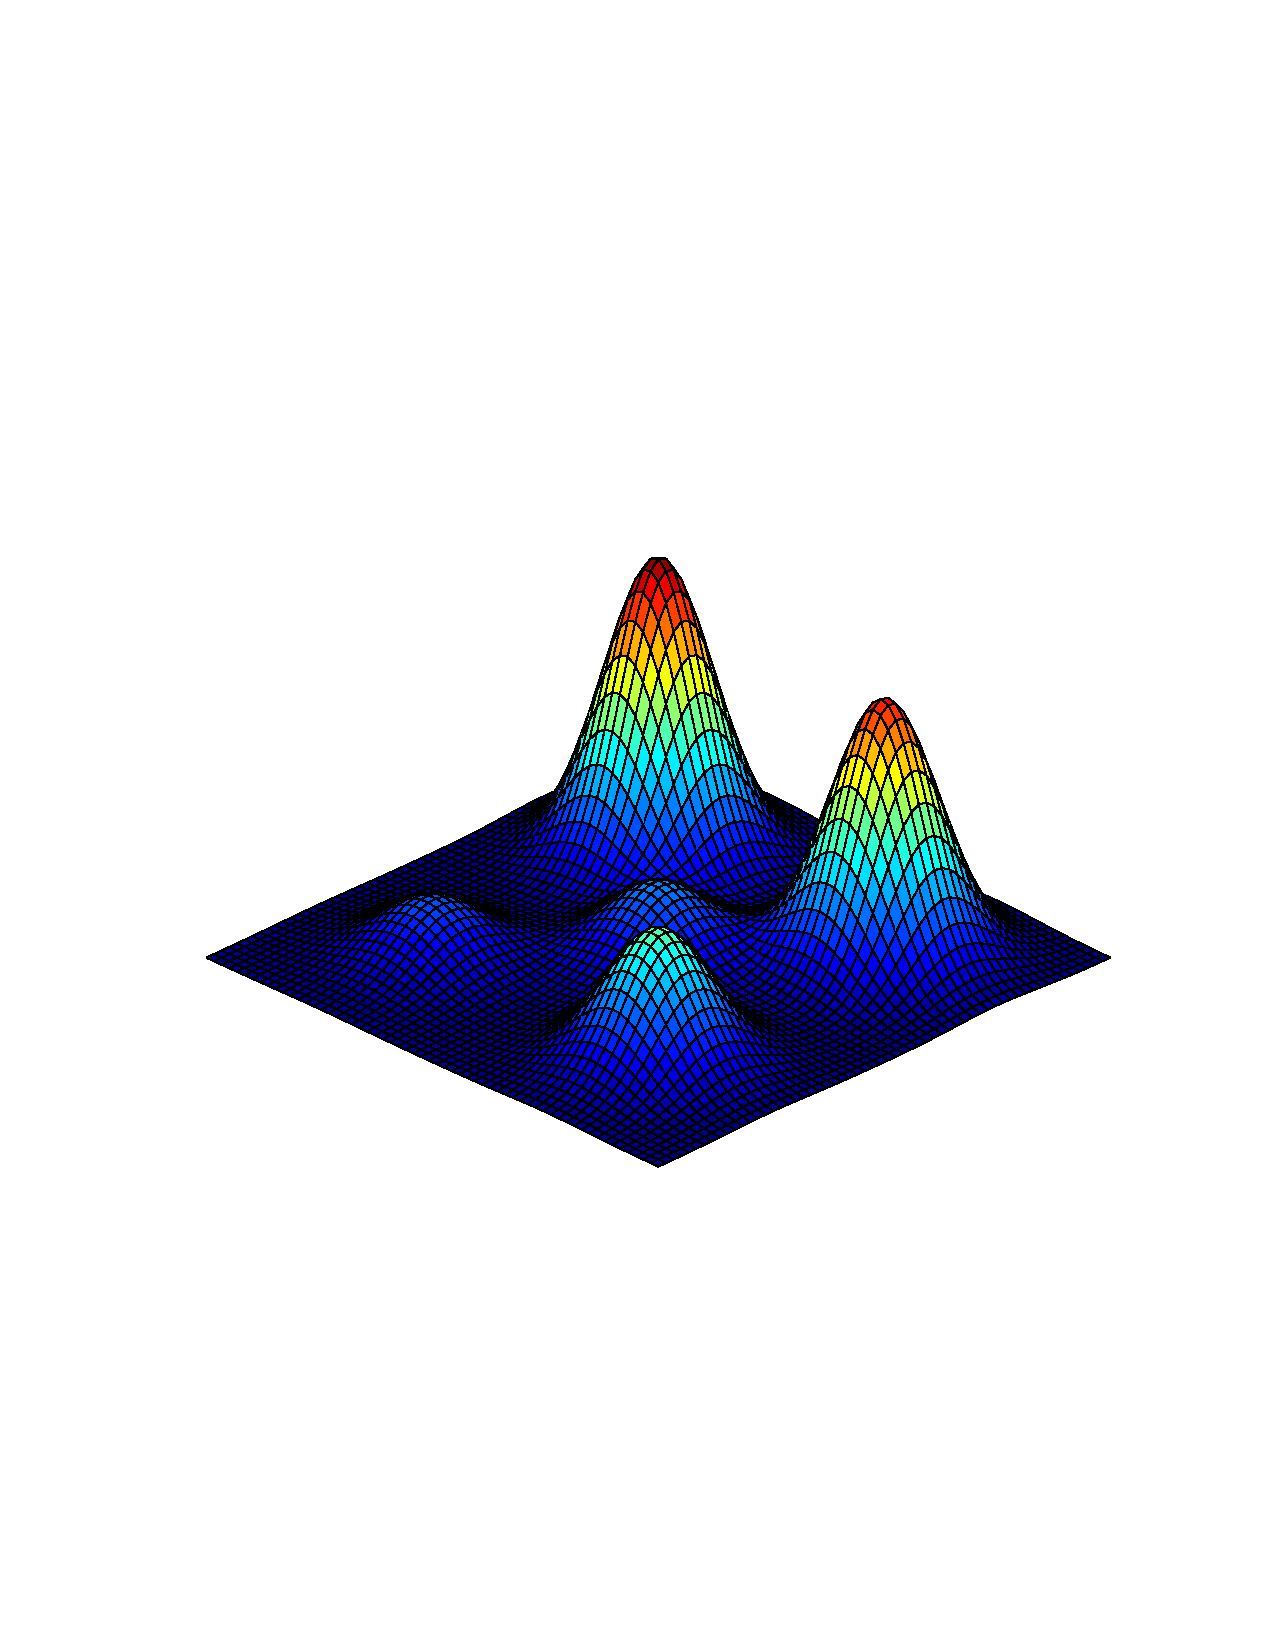
\includegraphics[width=0.5\textwidth]{gaussian}
\caption{Multiple three-dimensional gaussian distributions...}
\label{fig:mog}
\end{figure}


This is the text beneath an included picture. Figure \ref{fig:mog} shows an example of how to include eps-figures in this document.

\subsubsection{Displaying two eps-figures side-by-side}
\begin{figure}[H]
 \centering
 \begin{subfigure}{0.49\textwidth}
    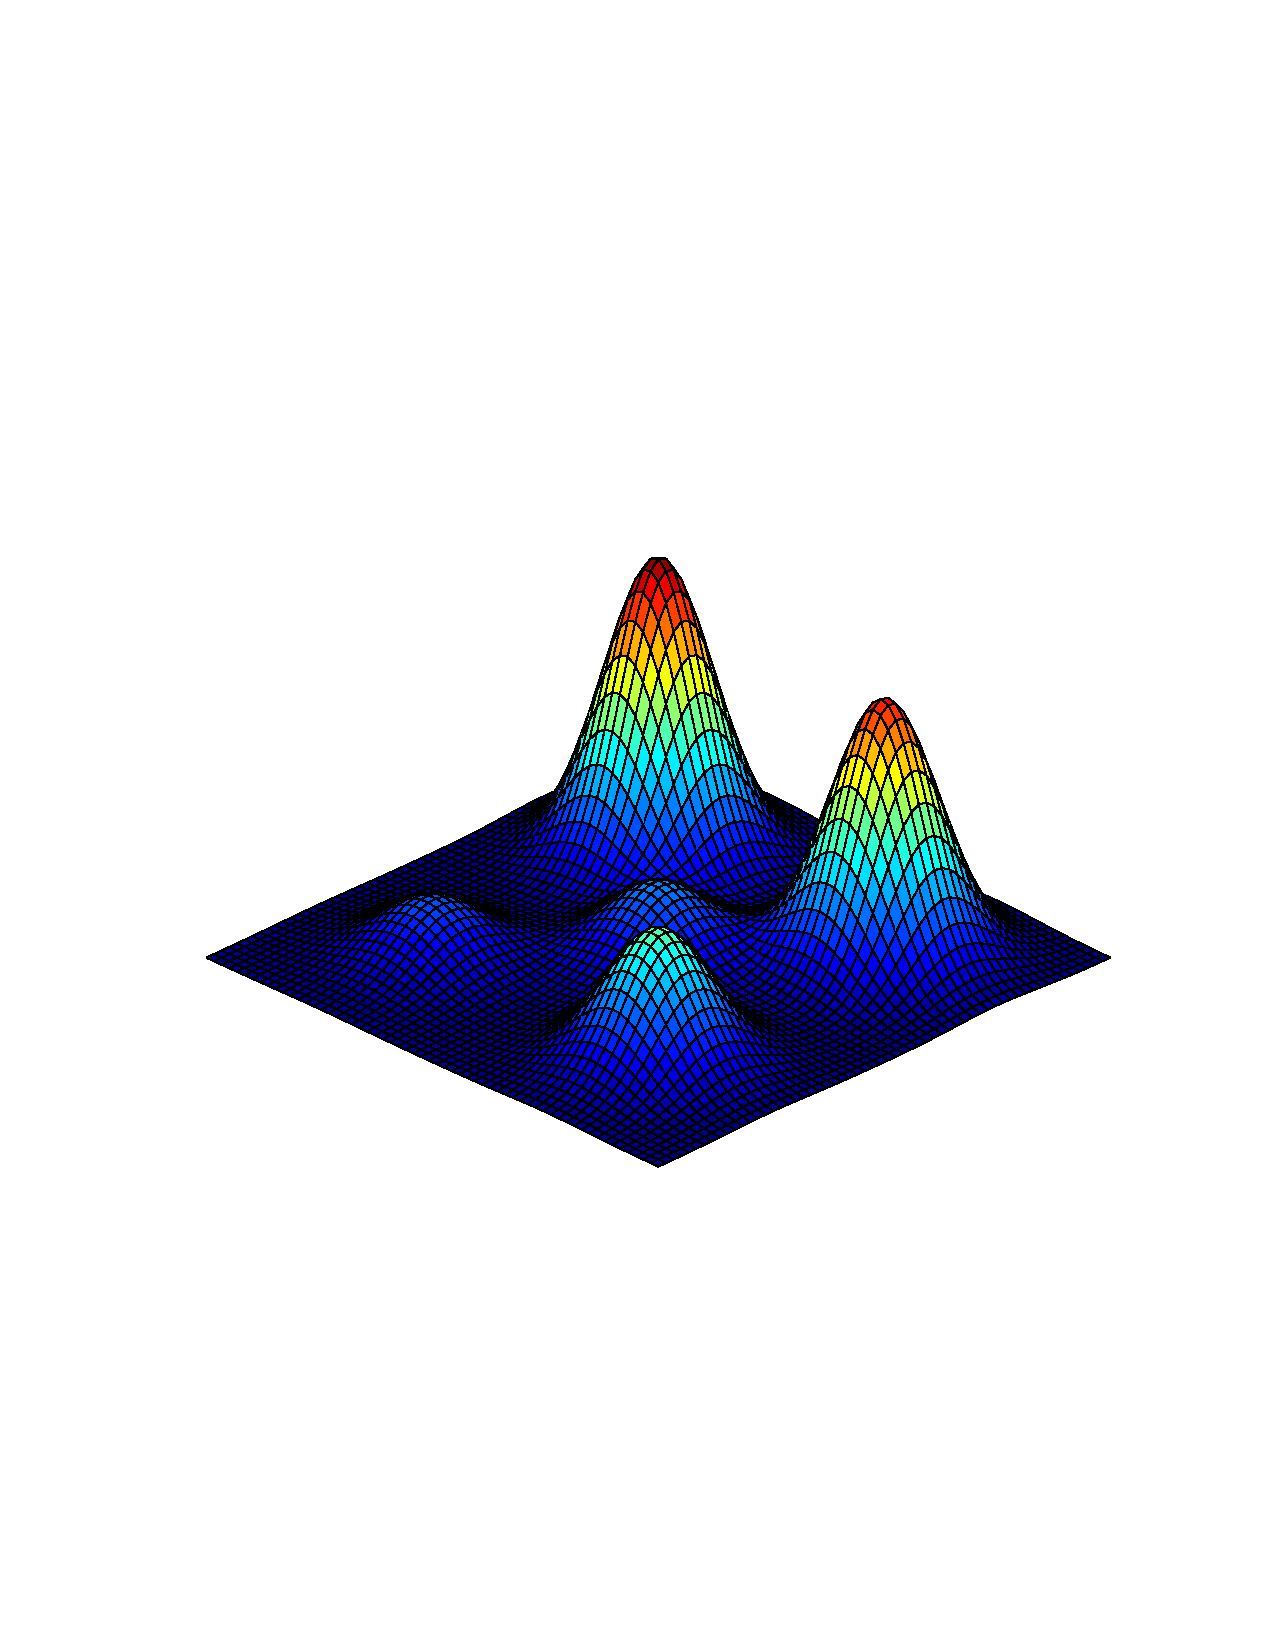
\includegraphics[width=\textwidth]{gaussian}
    \caption{Sub caption}
 \end{subfigure}
 \begin{subfigure}{0.49\textwidth}
    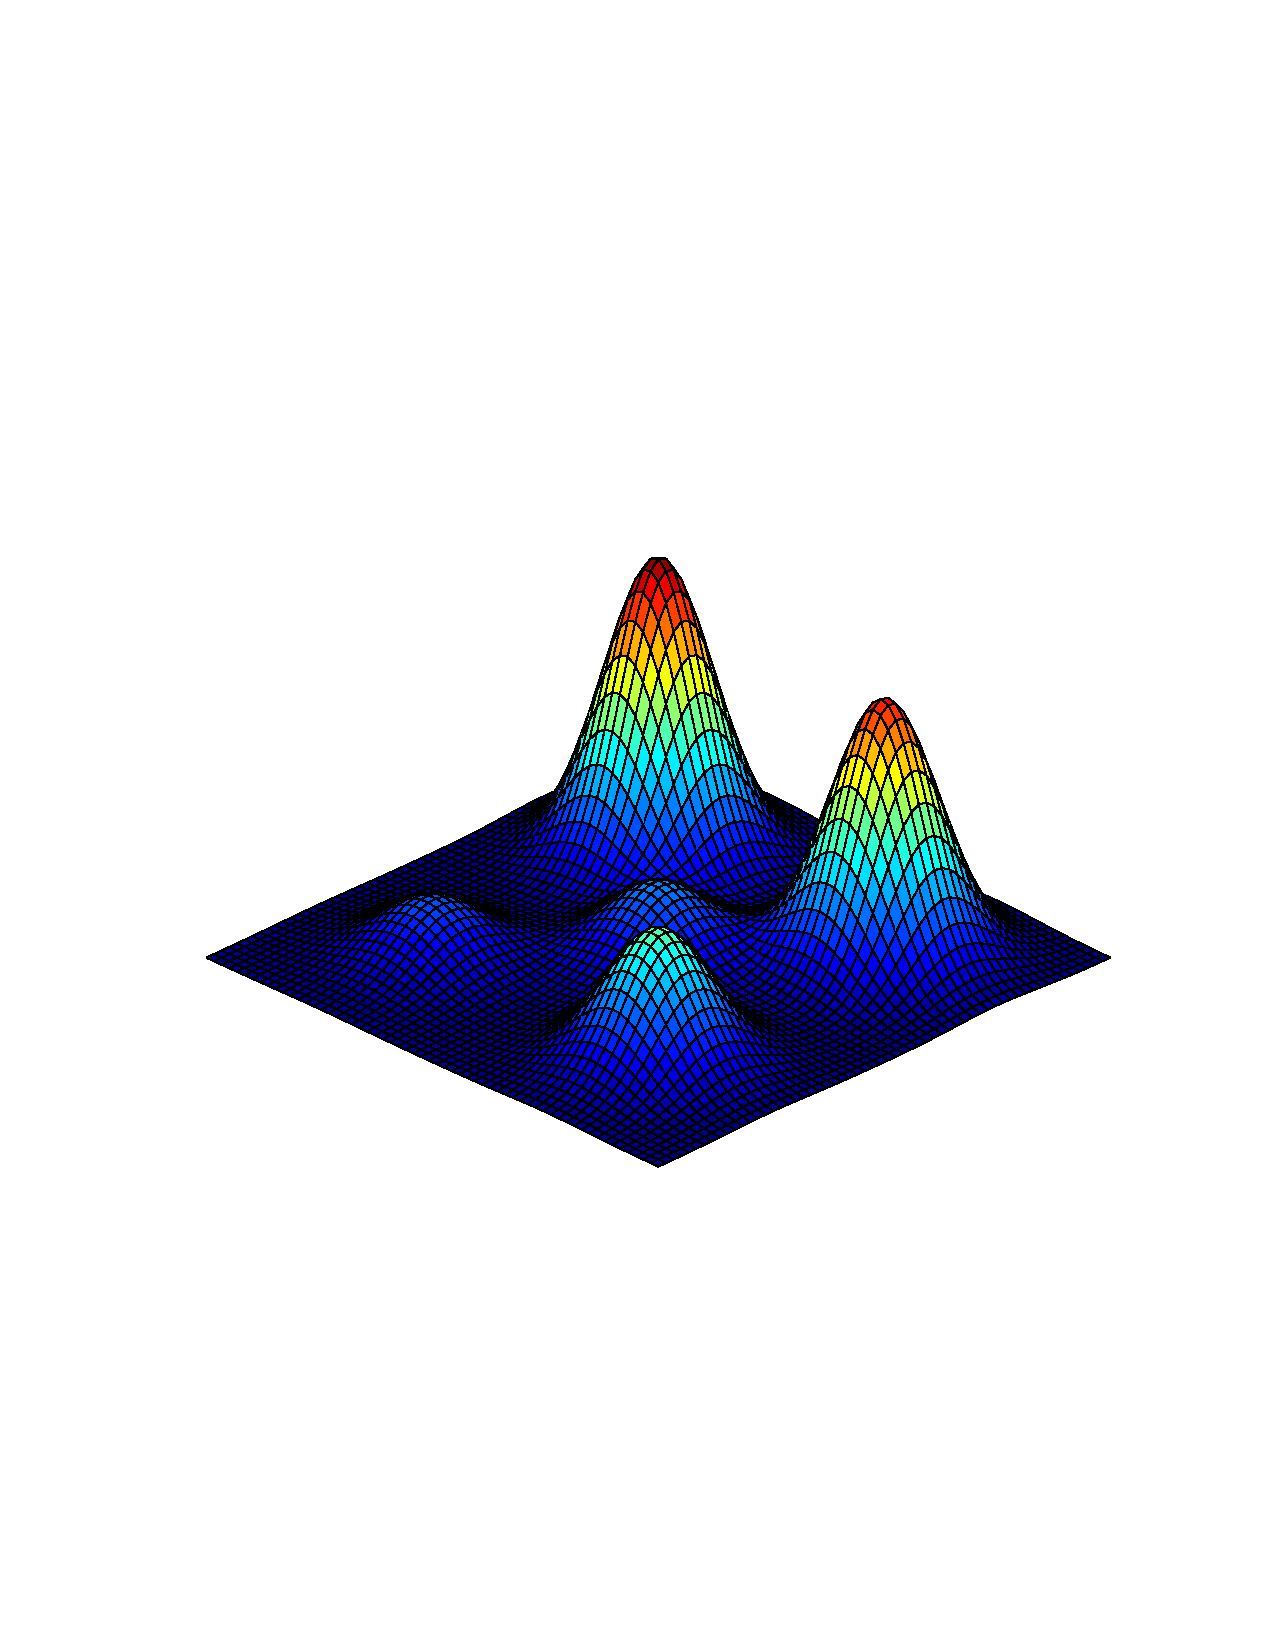
\includegraphics[width=\textwidth]{gaussian}
    \caption{Sub caption}
 \end{subfigure}
 \caption{Main caption}
\end{figure}

\subsection{Including tikz-figures}
\subsubsection{Two-dimensional figures}
Graphs can be included, like is shown in figure \ref{fig:sin}, using the input-method.
\tikzset{every picture/.style={scale=0.9}}
\begin{figure}[H]
	\centering
	% This file was created by matlab2tikz.
%
%The latest updates can be retrieved from
%  http://www.mathworks.com/matlabcentral/fileexchange/22022-matlab2tikz-matlab2tikz
%where you can also make suggestions and rate matlab2tikz.
%
\definecolor{mycolor1}{rgb}{0.00000,0.44700,0.74100}%
%
\begin{tikzpicture}

\begin{axis}[%
width=6.028in,
height=4.754in,
at={(1.011in,0.642in)},
scale only axis,
xmin=0,
xmax=6.28318530717959,
xtick={0,1.5707963267949,3.14159265358979,4.71238898038469,6.28318530717959},
xticklabels={{0},{$\text{1/2 }\pi$},{$\pi$},{$\text{3/2 }\pi$},{$\text{2}\pi$}},
ymin=-1.5,
ymax=1.5,
ytick={-1,  0,  1},
axis background/.style={fill=white}
]
\addplot [color=mycolor1, forget plot]
  table[row sep=crcr]{%
0	0\\
0.126933036508679	0.126592453573749\\
0.253866073017357	0.251147987181079\\
0.380799109526036	0.371662455660328\\
0.507732146034714	0.486196736100469\\
0.634665182543393	0.59290792905464\\
0.761598219052071	0.690079011482112\\
0.88853125556075	0.776146464291757\\
1.01546429206943	0.849725429949514\\
1.14239732857811	0.909631995354518\\
1.26933036508679	0.954902241444074\\
1.39626340159546	0.984807753012208\\
1.52319643810414	0.998867339183008\\
1.65012947461282	0.996854775951942\\
1.7770625111215	0.978802446214779\\
1.90399554763018	0.945000818714669\\
2.03092858413886	0.895993774291336\\
2.15786162064753	0.832569854634771\\
2.28479465715621	0.755749574354258\\
2.41172769366489	0.666769000516292\\
2.53866073017357	0.567059863862771\\
2.66559376668225	0.458226521727411\\
2.79252680319093	0.342020143325669\\
2.91945983969961	0.220310532786541\\
3.04639287620828	0.0950560433041829\\
3.17332591271696	-0.0317279334980679\\
3.30025894922564	-0.15800139597335\\
3.42719198573432	-0.281732556841429\\
3.554125022243	-0.400930535406613\\
3.68105805875168	-0.513677391573406\\
3.80799109526036	-0.618158986220605\\
3.93492413176903	-0.712694171378863\\
4.06185716827771	-0.795761840530832\\
4.18879020478639	-0.866025403784438\\
4.31572324129507	-0.922354294104581\\
4.44265627780375	-0.963842158559942\\
4.56958931431243	-0.989821441880933\\
4.69652235082111	-0.999874127673875\\
4.82345538732978	-0.993838464461254\\
4.95038842383846	-0.971811568323542\\
5.07732146034714	-0.934147860265107\\
5.20425449685582	-0.881453363447582\\
5.3311875333645	-0.814575952050336\\
5.45812056987318	-0.734591708657534\\
5.58505360638185	-0.64278760968654\\
5.71198664289053	-0.540640817455597\\
5.83891967939921	-0.429794912089172\\
5.96585271590789	-0.312033445698487\\
6.09278575241657	-0.189251244360411\\
6.21971878892525	-0.0634239196565654\\
6.34665182543393	0.0634239196565649\\
6.4735848619426	0.18925124436041\\
6.60051789845128	0.312033445698487\\
6.72745093495996	0.429794912089172\\
6.85438397146864	0.540640817455597\\
6.98131700797732	0.642787609686539\\
7.108250044486	0.734591708657533\\
7.23518308099467	0.814575952050335\\
7.36211611750335	0.881453363447582\\
7.48904915401203	0.934147860265107\\
7.61598219052071	0.971811568323542\\
7.74291522702939	0.993838464461254\\
7.86984826353807	0.999874127673875\\
7.99678130004675	0.989821441880933\\
8.12371433655542	0.963842158559942\\
8.2506473730641	0.922354294104582\\
8.37758040957278	0.866025403784439\\
8.50451344608146	0.795761840530832\\
8.63144648259014	0.712694171378863\\
8.75837951909882	0.618158986220606\\
8.88531255560749	0.513677391573407\\
9.01224559211617	0.400930535406613\\
9.13917862862485	0.28173255684143\\
9.26611166513353	0.158001395973351\\
9.39304470164221	0.031727933498067\\
9.51997773815089	-0.0950560433041828\\
9.64691077465957	-0.22031053278654\\
9.77384381116824	-0.342020143325668\\
9.90077684767692	-0.458226521727409\\
10.0277098841856	-0.567059863862771\\
10.1546429206943	-0.666769000516291\\
10.281575957203	-0.755749574354258\\
10.4085089937116	-0.832569854634771\\
10.5354420302203	-0.895993774291336\\
10.662375066729	-0.945000818714668\\
10.7893081032377	-0.978802446214779\\
10.9162411397464	-0.996854775951942\\
11.043174176255	-0.998867339183008\\
11.1701072127637	-0.984807753012208\\
11.2970402492724	-0.954902241444074\\
11.4239732857811	-0.909631995354518\\
11.5509063222897	-0.849725429949514\\
11.6778393587984	-0.776146464291757\\
11.8047723953071	-0.690079011482113\\
11.9317054318158	-0.59290792905464\\
12.0586384683245	-0.486196736100469\\
12.1855715048331	-0.371662455660328\\
12.3125045413418	-0.251147987181081\\
12.4394375778505	-0.126592453573751\\
12.5663706143592	-4.89858719658941e-16\\
};
\end{axis}
\end{tikzpicture}%
	\caption{A sine wave}
	\label{fig:sin}
\end{figure}

As figure \ref{fig:sin} was a little big, we now try to scale this output somehow:

\tikzset{every picture/.style={scale=0.6}}
\begin{figure}[H]
	\centering
	% This file was created by matlab2tikz.
%
%The latest updates can be retrieved from
%  http://www.mathworks.com/matlabcentral/fileexchange/22022-matlab2tikz-matlab2tikz
%where you can also make suggestions and rate matlab2tikz.
%
\definecolor{mycolor1}{rgb}{0.00000,0.44700,0.74100}%
%
\begin{tikzpicture}

\begin{axis}[%
width=6.028in,
height=4.754in,
at={(1.011in,0.642in)},
scale only axis,
xmin=0,
xmax=6.28318530717959,
xtick={0,1.5707963267949,3.14159265358979,4.71238898038469,6.28318530717959},
xticklabels={{0},{$\text{1/2 }\pi$},{$\pi$},{$\text{3/2 }\pi$},{$\text{2}\pi$}},
ymin=-1.5,
ymax=1.5,
ytick={-1,  0,  1},
axis background/.style={fill=white}
]
\addplot [color=mycolor1, forget plot]
  table[row sep=crcr]{%
0	0\\
0.126933036508679	0.126592453573749\\
0.253866073017357	0.251147987181079\\
0.380799109526036	0.371662455660328\\
0.507732146034714	0.486196736100469\\
0.634665182543393	0.59290792905464\\
0.761598219052071	0.690079011482112\\
0.88853125556075	0.776146464291757\\
1.01546429206943	0.849725429949514\\
1.14239732857811	0.909631995354518\\
1.26933036508679	0.954902241444074\\
1.39626340159546	0.984807753012208\\
1.52319643810414	0.998867339183008\\
1.65012947461282	0.996854775951942\\
1.7770625111215	0.978802446214779\\
1.90399554763018	0.945000818714669\\
2.03092858413886	0.895993774291336\\
2.15786162064753	0.832569854634771\\
2.28479465715621	0.755749574354258\\
2.41172769366489	0.666769000516292\\
2.53866073017357	0.567059863862771\\
2.66559376668225	0.458226521727411\\
2.79252680319093	0.342020143325669\\
2.91945983969961	0.220310532786541\\
3.04639287620828	0.0950560433041829\\
3.17332591271696	-0.0317279334980679\\
3.30025894922564	-0.15800139597335\\
3.42719198573432	-0.281732556841429\\
3.554125022243	-0.400930535406613\\
3.68105805875168	-0.513677391573406\\
3.80799109526036	-0.618158986220605\\
3.93492413176903	-0.712694171378863\\
4.06185716827771	-0.795761840530832\\
4.18879020478639	-0.866025403784438\\
4.31572324129507	-0.922354294104581\\
4.44265627780375	-0.963842158559942\\
4.56958931431243	-0.989821441880933\\
4.69652235082111	-0.999874127673875\\
4.82345538732978	-0.993838464461254\\
4.95038842383846	-0.971811568323542\\
5.07732146034714	-0.934147860265107\\
5.20425449685582	-0.881453363447582\\
5.3311875333645	-0.814575952050336\\
5.45812056987318	-0.734591708657534\\
5.58505360638185	-0.64278760968654\\
5.71198664289053	-0.540640817455597\\
5.83891967939921	-0.429794912089172\\
5.96585271590789	-0.312033445698487\\
6.09278575241657	-0.189251244360411\\
6.21971878892525	-0.0634239196565654\\
6.34665182543393	0.0634239196565649\\
6.4735848619426	0.18925124436041\\
6.60051789845128	0.312033445698487\\
6.72745093495996	0.429794912089172\\
6.85438397146864	0.540640817455597\\
6.98131700797732	0.642787609686539\\
7.108250044486	0.734591708657533\\
7.23518308099467	0.814575952050335\\
7.36211611750335	0.881453363447582\\
7.48904915401203	0.934147860265107\\
7.61598219052071	0.971811568323542\\
7.74291522702939	0.993838464461254\\
7.86984826353807	0.999874127673875\\
7.99678130004675	0.989821441880933\\
8.12371433655542	0.963842158559942\\
8.2506473730641	0.922354294104582\\
8.37758040957278	0.866025403784439\\
8.50451344608146	0.795761840530832\\
8.63144648259014	0.712694171378863\\
8.75837951909882	0.618158986220606\\
8.88531255560749	0.513677391573407\\
9.01224559211617	0.400930535406613\\
9.13917862862485	0.28173255684143\\
9.26611166513353	0.158001395973351\\
9.39304470164221	0.031727933498067\\
9.51997773815089	-0.0950560433041828\\
9.64691077465957	-0.22031053278654\\
9.77384381116824	-0.342020143325668\\
9.90077684767692	-0.458226521727409\\
10.0277098841856	-0.567059863862771\\
10.1546429206943	-0.666769000516291\\
10.281575957203	-0.755749574354258\\
10.4085089937116	-0.832569854634771\\
10.5354420302203	-0.895993774291336\\
10.662375066729	-0.945000818714668\\
10.7893081032377	-0.978802446214779\\
10.9162411397464	-0.996854775951942\\
11.043174176255	-0.998867339183008\\
11.1701072127637	-0.984807753012208\\
11.2970402492724	-0.954902241444074\\
11.4239732857811	-0.909631995354518\\
11.5509063222897	-0.849725429949514\\
11.6778393587984	-0.776146464291757\\
11.8047723953071	-0.690079011482113\\
11.9317054318158	-0.59290792905464\\
12.0586384683245	-0.486196736100469\\
12.1855715048331	-0.371662455660328\\
12.3125045413418	-0.251147987181081\\
12.4394375778505	-0.126592453573751\\
12.5663706143592	-4.89858719658941e-16\\
};
\end{axis}
\end{tikzpicture}%
	\caption{A second sine wave}
	\label{fig:sin2}
\end{figure}

We can also display more than one lineplot in one row:

\tikzset{every picture/.style={scale=0.5}}
\begin{figure}[H]
	\centering
	\begin{subfigure}{0.49\textwidth}
		\includestandalone[width=\textwidth]{plots/sin-tikz}
		\caption{A sine wave}
	\end{subfigure}
	\begin{subfigure}{0.49\textwidth}
		\includestandalone[width=\textwidth]{plots/cos-tikz}
		\caption{A cosine wave}
	\end{subfigure}
	\caption{Sine and cosine waves}
	\label{fig:sin}
\end{figure}

\subsubsection{Three-dimensional figures}
\tikzset{every picture/.style={scale=1}}
\begin{figure}[H]
	\centering
	\input{plots/gaussian-tikz}
	\caption{A three-dimensional representation of multiple, gaussian distributions}
	\label{fig:gaussian}
\end{figure}

With the previous method to include tikz-figures, scaling the tikz output might not be as easy as with the includegraphics-method. This is where the standalone package comes in handy.

Let's see, whether this also works for 3D-plots:

\tikzset{every picture/.style={scale=0.5}}
\begin{figure}[H]
	\centering
	\begin{subfigure}{0.49\textwidth}
		\includestandalone[width=\textwidth]{plots/gaussian-tikz}
		\caption{A 3D plot}
	\end{subfigure}
	\begin{subfigure}{0.49\textwidth}
		\includestandalone[width=\textwidth]{plots/gaussian-tikz}
		\caption{Another 3D plot}
	\end{subfigure}
	\caption{More than one 3D plot in a row}
	\label{fig:gaussian3}
\end{figure}

Now let's try some real output from our Matlab scripts:
\begin{figure}[H]
	\centering
	\input{plots/static/2017-09-25-21-19-50_sources_2_mindistance_0.5_trial_9_of_10_fig}
	\caption{2 Sources, 0.5m minimal distance, Trial 9/10}
	\label{fig:trial1}
\end{figure}

\newpage
\section{Citations}
\subsection{Simple Citations}
The EM-Algorithm is covered in depth by Bishop "EM algorithm, is a general technique for finding maximum likelihood solutions for probabilistic models having latent variables (Dempster et al., 1977; McLachlan and Krishnan, 1997). \cite[p. 472]{Bishop2006}. Reverberant environments, secondary reflections, may result in biased location estimates \cite[p.1]{Schwartz2014}
\end{document}
%\chapter{Chapter}
\section{Section}
\subsection{Subsection}
\subsubsection{Subsubsection}
\paragraph{Paragraph}
\subparagraph{Subparagraph}

%%%%%%%%%%%%%%%%%%%%%%%%%%%%%%%%  D O C U M E N T  %%%%%%%%%%%%%%%%%%%%%%%%%%%%%%%%%
%%%%%%%%%%%%%%%%%%%%%%%%%%%%%%%%%%%%%%%%%%%%%%%%%%%%%%%%%%%%%%%%%%%%%%%%%%%%%%%%%%%%
%%%%%%%%%%%%%%%%%%%%%%%%%%%%%%%%  A P P E N D I X  %%%%%%%%%%%%%%%%%%%%%%%%%%%%%%%%%
\pagenumbering{roman}% 
\setcounter{page}{\number\value{romanpagenumber}}
 \appendix
 	\renewcommand{\chaptermark}[1]{\markboth{\uppercase{Appendix \thechapter:\ #1}}{}}
 %	\todos
	\setcounter{\pagebreak}
 	\chapter{Formulae}
 	\section*{Arithmetic Rules}
% Don't include basic logarithm rules! Lowers level of detail for all other calculations...
%\begin{align}
%\label{eq:log-sum}
%\ln(x\cdot y)&=\ln(x)+\ln(y),\\
%\label{eq:log-power}
%\ln(x^r)&=r\cdot\ln(x).
%\end{align}

\section*{Definitions}
 	\chapter{Code}
 	\section{\texorpdfstring{\matlab} Code}
\label{sec:appCode}
\subsection*{simulate.m}
%\lstinputlisting[firstline=16, lastline=60]{/Users/jannismainczyk/thesis/src/matlab/mainczjs/simulate.m}
     \chapter{Results}
     \begin{figure}
\setlength\figureheight{\textheight}
\setlength\figurewidth{0.6\textwidth}
    % This file was created by matlab2tikz.
%
\definecolor{mycolor1}{rgb}{0.00000,0.44700,0.74100}%
%
\begin{tikzpicture}

\begin{axis}[%
width=1.785in,
height=0.751in,
at={(0.693in,13.124in)},
scale only axis,
xmin=0,
xmax=6,
tick align=outside,
ymin=0,
ymax=6,
zmin=0,
zmax=0.002,
view={-45}{45},
axis background/.style={fill=white},
axis x line*=bottom,
axis y line*=left,
axis z line*=left
]

\addplot3[%
surf,
shader=interp, colormap={mymap}{[1pt] rgb(0pt)=(0.2422,0.1504,0.6603); rgb(1pt)=(0.25039,0.164995,0.707614); rgb(2pt)=(0.257771,0.181781,0.751138); rgb(3pt)=(0.264729,0.197757,0.795214); rgb(4pt)=(0.270648,0.214676,0.836371); rgb(5pt)=(0.275114,0.234238,0.870986); rgb(6pt)=(0.2783,0.255871,0.899071); rgb(7pt)=(0.280333,0.278233,0.9221); rgb(8pt)=(0.281338,0.300595,0.941376); rgb(9pt)=(0.281014,0.322757,0.957886); rgb(10pt)=(0.279467,0.344671,0.971676); rgb(11pt)=(0.275971,0.366681,0.982905); rgb(12pt)=(0.269914,0.3892,0.9906); rgb(13pt)=(0.260243,0.412329,0.995157); rgb(14pt)=(0.244033,0.435833,0.998833); rgb(15pt)=(0.220643,0.460257,0.997286); rgb(16pt)=(0.196333,0.484719,0.989152); rgb(17pt)=(0.183405,0.507371,0.979795); rgb(18pt)=(0.178643,0.528857,0.968157); rgb(19pt)=(0.176438,0.549905,0.952019); rgb(20pt)=(0.168743,0.570262,0.935871); rgb(21pt)=(0.154,0.5902,0.9218); rgb(22pt)=(0.146029,0.609119,0.907857); rgb(23pt)=(0.138024,0.627629,0.89729); rgb(24pt)=(0.124814,0.645929,0.888343); rgb(25pt)=(0.111252,0.6635,0.876314); rgb(26pt)=(0.0952095,0.679829,0.859781); rgb(27pt)=(0.0688714,0.694771,0.839357); rgb(28pt)=(0.0296667,0.708167,0.816333); rgb(29pt)=(0.00357143,0.720267,0.7917); rgb(30pt)=(0.00665714,0.731214,0.766014); rgb(31pt)=(0.0433286,0.741095,0.73941); rgb(32pt)=(0.0963952,0.75,0.712038); rgb(33pt)=(0.140771,0.7584,0.684157); rgb(34pt)=(0.1717,0.766962,0.655443); rgb(35pt)=(0.193767,0.775767,0.6251); rgb(36pt)=(0.216086,0.7843,0.5923); rgb(37pt)=(0.246957,0.791795,0.556743); rgb(38pt)=(0.290614,0.79729,0.518829); rgb(39pt)=(0.340643,0.8008,0.478857); rgb(40pt)=(0.3909,0.802871,0.435448); rgb(41pt)=(0.445629,0.802419,0.390919); rgb(42pt)=(0.5044,0.7993,0.348); rgb(43pt)=(0.561562,0.794233,0.304481); rgb(44pt)=(0.617395,0.787619,0.261238); rgb(45pt)=(0.671986,0.779271,0.2227); rgb(46pt)=(0.7242,0.769843,0.191029); rgb(47pt)=(0.773833,0.759805,0.16461); rgb(48pt)=(0.820314,0.749814,0.153529); rgb(49pt)=(0.863433,0.7406,0.159633); rgb(50pt)=(0.903543,0.733029,0.177414); rgb(51pt)=(0.939257,0.728786,0.209957); rgb(52pt)=(0.972757,0.729771,0.239443); rgb(53pt)=(0.995648,0.743371,0.237148); rgb(54pt)=(0.996986,0.765857,0.219943); rgb(55pt)=(0.995205,0.789252,0.202762); rgb(56pt)=(0.9892,0.813567,0.188533); rgb(57pt)=(0.978629,0.838629,0.176557); rgb(58pt)=(0.967648,0.8639,0.16429); rgb(59pt)=(0.96101,0.889019,0.153676); rgb(60pt)=(0.959671,0.913457,0.142257); rgb(61pt)=(0.962795,0.937338,0.12651); rgb(62pt)=(0.969114,0.960629,0.106362); rgb(63pt)=(0.9769,0.9839,0.0805)}, mesh/rows=61]
table[row sep=crcr, point meta=\thisrow{c}] {%
%
x	y	z	c\\
0	0	0	0\\
0	0.1	0	0\\
0	0.2	0	0\\
0	0.3	0	0\\
0	0.4	0	0\\
0	0.5	0	0\\
0	0.6	0	0\\
0	0.7	0	0\\
0	0.8	0	0\\
0	0.9	0	0\\
0	1	0	0\\
0	1.1	0	0\\
0	1.2	0	0\\
0	1.3	0	0\\
0	1.4	0	0\\
0	1.5	0	0\\
0	1.6	0	0\\
0	1.7	0	0\\
0	1.8	0	0\\
0	1.9	0	0\\
0	2	0	0\\
0	2.1	0	0\\
0	2.2	0	0\\
0	2.3	0	0\\
0	2.4	0	0\\
0	2.5	0	0\\
0	2.6	0	0\\
0	2.7	0	0\\
0	2.8	0	0\\
0	2.9	0	0\\
0	3	0	0\\
0	3.1	0	0\\
0	3.2	0	0\\
0	3.3	0	0\\
0	3.4	0	0\\
0	3.5	0	0\\
0	3.6	0	0\\
0	3.7	0	0\\
0	3.8	0	0\\
0	3.9	0	0\\
0	4	0	0\\
0	4.1	0	0\\
0	4.2	0	0\\
0	4.3	0	0\\
0	4.4	0	0\\
0	4.5	0	0\\
0	4.6	0	0\\
0	4.7	0	0\\
0	4.8	0	0\\
0	4.9	0	0\\
0	5	0	0\\
0	5.1	0	0\\
0	5.2	0	0\\
0	5.3	0	0\\
0	5.4	0	0\\
0	5.5	0	0\\
0	5.6	0	0\\
0	5.7	0	0\\
0	5.8	0	0\\
0	5.9	0	0\\
0	6	0	0\\
0.1	0	0	0\\
0.1	0.1	0	0\\
0.1	0.2	0	0\\
0.1	0.3	0	0\\
0.1	0.4	0	0\\
0.1	0.5	0	0\\
0.1	0.6	0	0\\
0.1	0.7	0	0\\
0.1	0.8	0	0\\
0.1	0.9	0	0\\
0.1	1	0	0\\
0.1	1.1	0	0\\
0.1	1.2	0	0\\
0.1	1.3	0	0\\
0.1	1.4	0	0\\
0.1	1.5	0	0\\
0.1	1.6	0	0\\
0.1	1.7	0	0\\
0.1	1.8	0	0\\
0.1	1.9	0	0\\
0.1	2	0	0\\
0.1	2.1	0	0\\
0.1	2.2	0	0\\
0.1	2.3	0	0\\
0.1	2.4	0	0\\
0.1	2.5	0	0\\
0.1	2.6	0	0\\
0.1	2.7	0	0\\
0.1	2.8	0	0\\
0.1	2.9	0	0\\
0.1	3	0	0\\
0.1	3.1	0	0\\
0.1	3.2	0	0\\
0.1	3.3	0	0\\
0.1	3.4	0	0\\
0.1	3.5	0	0\\
0.1	3.6	0	0\\
0.1	3.7	0	0\\
0.1	3.8	0	0\\
0.1	3.9	0	0\\
0.1	4	0	0\\
0.1	4.1	0	0\\
0.1	4.2	0	0\\
0.1	4.3	0	0\\
0.1	4.4	0	0\\
0.1	4.5	0	0\\
0.1	4.6	0	0\\
0.1	4.7	0	0\\
0.1	4.8	0	0\\
0.1	4.9	0	0\\
0.1	5	0	0\\
0.1	5.1	0	0\\
0.1	5.2	0	0\\
0.1	5.3	0	0\\
0.1	5.4	0	0\\
0.1	5.5	0	0\\
0.1	5.6	0	0\\
0.1	5.7	0	0\\
0.1	5.8	0	0\\
0.1	5.9	0	0\\
0.1	6	0	0\\
0.2	0	0	0\\
0.2	0.1	0	0\\
0.2	0.2	0	0\\
0.2	0.3	0	0\\
0.2	0.4	0	0\\
0.2	0.5	0	0\\
0.2	0.6	0	0\\
0.2	0.7	0	0\\
0.2	0.8	0	0\\
0.2	0.9	0	0\\
0.2	1	0	0\\
0.2	1.1	0	0\\
0.2	1.2	0	0\\
0.2	1.3	0	0\\
0.2	1.4	0	0\\
0.2	1.5	0	0\\
0.2	1.6	0	0\\
0.2	1.7	0	0\\
0.2	1.8	0	0\\
0.2	1.9	0	0\\
0.2	2	0	0\\
0.2	2.1	0	0\\
0.2	2.2	0	0\\
0.2	2.3	0	0\\
0.2	2.4	0	0\\
0.2	2.5	0	0\\
0.2	2.6	0	0\\
0.2	2.7	0	0\\
0.2	2.8	0	0\\
0.2	2.9	0	0\\
0.2	3	0	0\\
0.2	3.1	0	0\\
0.2	3.2	0	0\\
0.2	3.3	0	0\\
0.2	3.4	0	0\\
0.2	3.5	0	0\\
0.2	3.6	0	0\\
0.2	3.7	0	0\\
0.2	3.8	0	0\\
0.2	3.9	0	0\\
0.2	4	0	0\\
0.2	4.1	0	0\\
0.2	4.2	0	0\\
0.2	4.3	0	0\\
0.2	4.4	0	0\\
0.2	4.5	0	0\\
0.2	4.6	0	0\\
0.2	4.7	0	0\\
0.2	4.8	0	0\\
0.2	4.9	0	0\\
0.2	5	0	0\\
0.2	5.1	0	0\\
0.2	5.2	0	0\\
0.2	5.3	0	0\\
0.2	5.4	0	0\\
0.2	5.5	0	0\\
0.2	5.6	0	0\\
0.2	5.7	0	0\\
0.2	5.8	0	0\\
0.2	5.9	0	0\\
0.2	6	0	0\\
0.3	0	0	0\\
0.3	0.1	0	0\\
0.3	0.2	0	0\\
0.3	0.3	0	0\\
0.3	0.4	0	0\\
0.3	0.5	0	0\\
0.3	0.6	0	0\\
0.3	0.7	0	0\\
0.3	0.8	0	0\\
0.3	0.9	0	0\\
0.3	1	0	0\\
0.3	1.1	0	0\\
0.3	1.2	0	0\\
0.3	1.3	0	0\\
0.3	1.4	0	0\\
0.3	1.5	0	0\\
0.3	1.6	0	0\\
0.3	1.7	0	0\\
0.3	1.8	0	0\\
0.3	1.9	0	0\\
0.3	2	0	0\\
0.3	2.1	0	0\\
0.3	2.2	0	0\\
0.3	2.3	0	0\\
0.3	2.4	0	0\\
0.3	2.5	0	0\\
0.3	2.6	0	0\\
0.3	2.7	0	0\\
0.3	2.8	0	0\\
0.3	2.9	0	0\\
0.3	3	0	0\\
0.3	3.1	0	0\\
0.3	3.2	0	0\\
0.3	3.3	0	0\\
0.3	3.4	0	0\\
0.3	3.5	0	0\\
0.3	3.6	0	0\\
0.3	3.7	0	0\\
0.3	3.8	0	0\\
0.3	3.9	0	0\\
0.3	4	0	0\\
0.3	4.1	0	0\\
0.3	4.2	0	0\\
0.3	4.3	0	0\\
0.3	4.4	0	0\\
0.3	4.5	0	0\\
0.3	4.6	0	0\\
0.3	4.7	0	0\\
0.3	4.8	0	0\\
0.3	4.9	0	0\\
0.3	5	0	0\\
0.3	5.1	0	0\\
0.3	5.2	0	0\\
0.3	5.3	0	0\\
0.3	5.4	0	0\\
0.3	5.5	0	0\\
0.3	5.6	0	0\\
0.3	5.7	0	0\\
0.3	5.8	0	0\\
0.3	5.9	0	0\\
0.3	6	0	0\\
0.4	0	0	0\\
0.4	0.1	0	0\\
0.4	0.2	0	0\\
0.4	0.3	0	0\\
0.4	0.4	0	0\\
0.4	0.5	0	0\\
0.4	0.6	0	0\\
0.4	0.7	0	0\\
0.4	0.8	0	0\\
0.4	0.9	0	0\\
0.4	1	0	0\\
0.4	1.1	0	0\\
0.4	1.2	0	0\\
0.4	1.3	0	0\\
0.4	1.4	0	0\\
0.4	1.5	0	0\\
0.4	1.6	0	0\\
0.4	1.7	0	0\\
0.4	1.8	0	0\\
0.4	1.9	0	0\\
0.4	2	0	0\\
0.4	2.1	0	0\\
0.4	2.2	0	0\\
0.4	2.3	0	0\\
0.4	2.4	0	0\\
0.4	2.5	0	0\\
0.4	2.6	0	0\\
0.4	2.7	0	0\\
0.4	2.8	0	0\\
0.4	2.9	0	0\\
0.4	3	0	0\\
0.4	3.1	0	0\\
0.4	3.2	0	0\\
0.4	3.3	0	0\\
0.4	3.4	0	0\\
0.4	3.5	0	0\\
0.4	3.6	0	0\\
0.4	3.7	0	0\\
0.4	3.8	0	0\\
0.4	3.9	0	0\\
0.4	4	0	0\\
0.4	4.1	0	0\\
0.4	4.2	0	0\\
0.4	4.3	0	0\\
0.4	4.4	0	0\\
0.4	4.5	0	0\\
0.4	4.6	0	0\\
0.4	4.7	0	0\\
0.4	4.8	0	0\\
0.4	4.9	0	0\\
0.4	5	0	0\\
0.4	5.1	0	0\\
0.4	5.2	0	0\\
0.4	5.3	0	0\\
0.4	5.4	0	0\\
0.4	5.5	0	0\\
0.4	5.6	0	0\\
0.4	5.7	0	0\\
0.4	5.8	0	0\\
0.4	5.9	0	0\\
0.4	6	0	0\\
0.5	0	0	0\\
0.5	0.1	0	0\\
0.5	0.2	0	0\\
0.5	0.3	0	0\\
0.5	0.4	0	0\\
0.5	0.5	0	0\\
0.5	0.6	0	0\\
0.5	0.7	0	0\\
0.5	0.8	0	0\\
0.5	0.9	0	0\\
0.5	1	0	0\\
0.5	1.1	0	0\\
0.5	1.2	0	0\\
0.5	1.3	0	0\\
0.5	1.4	0	0\\
0.5	1.5	0	0\\
0.5	1.6	0	0\\
0.5	1.7	0	0\\
0.5	1.8	0	0\\
0.5	1.9	0	0\\
0.5	2	0	0\\
0.5	2.1	0	0\\
0.5	2.2	0	0\\
0.5	2.3	0	0\\
0.5	2.4	0	0\\
0.5	2.5	0	0\\
0.5	2.6	0	0\\
0.5	2.7	0	0\\
0.5	2.8	0	0\\
0.5	2.9	0	0\\
0.5	3	0	0\\
0.5	3.1	0	0\\
0.5	3.2	0	0\\
0.5	3.3	0	0\\
0.5	3.4	0	0\\
0.5	3.5	0	0\\
0.5	3.6	0	0\\
0.5	3.7	0	0\\
0.5	3.8	0	0\\
0.5	3.9	0	0\\
0.5	4	0	0\\
0.5	4.1	0	0\\
0.5	4.2	0	0\\
0.5	4.3	0	0\\
0.5	4.4	0	0\\
0.5	4.5	0	0\\
0.5	4.6	0	0\\
0.5	4.7	0	0\\
0.5	4.8	0	0\\
0.5	4.9	0	0\\
0.5	5	0	0\\
0.5	5.1	0	0\\
0.5	5.2	0	0\\
0.5	5.3	0	0\\
0.5	5.4	0	0\\
0.5	5.5	0	0\\
0.5	5.6	0	0\\
0.5	5.7	0	0\\
0.5	5.8	0	0\\
0.5	5.9	0	0\\
0.5	6	0	0\\
0.6	0	0	0\\
0.6	0.1	0	0\\
0.6	0.2	0	0\\
0.6	0.3	0	0\\
0.6	0.4	0	0\\
0.6	0.5	0	0\\
0.6	0.6	0	0\\
0.6	0.7	0	0\\
0.6	0.8	0	0\\
0.6	0.9	0	0\\
0.6	1	0	0\\
0.6	1.1	0	0\\
0.6	1.2	0	0\\
0.6	1.3	0	0\\
0.6	1.4	0	0\\
0.6	1.5	0	0\\
0.6	1.6	0	0\\
0.6	1.7	0	0\\
0.6	1.8	0	0\\
0.6	1.9	0	0\\
0.6	2	0	0\\
0.6	2.1	0	0\\
0.6	2.2	0	0\\
0.6	2.3	0	0\\
0.6	2.4	0	0\\
0.6	2.5	0	0\\
0.6	2.6	0	0\\
0.6	2.7	0	0\\
0.6	2.8	0	0\\
0.6	2.9	0	0\\
0.6	3	0	0\\
0.6	3.1	0	0\\
0.6	3.2	0	0\\
0.6	3.3	0	0\\
0.6	3.4	0	0\\
0.6	3.5	0	0\\
0.6	3.6	0	0\\
0.6	3.7	0	0\\
0.6	3.8	0	0\\
0.6	3.9	0	0\\
0.6	4	0	0\\
0.6	4.1	0	0\\
0.6	4.2	0	0\\
0.6	4.3	0	0\\
0.6	4.4	0	0\\
0.6	4.5	0	0\\
0.6	4.6	0	0\\
0.6	4.7	0	0\\
0.6	4.8	0	0\\
0.6	4.9	0	0\\
0.6	5	0	0\\
0.6	5.1	0	0\\
0.6	5.2	0	0\\
0.6	5.3	0	0\\
0.6	5.4	0	0\\
0.6	5.5	0	0\\
0.6	5.6	0	0\\
0.6	5.7	0	0\\
0.6	5.8	0	0\\
0.6	5.9	0	0\\
0.6	6	0	0\\
0.7	0	0	0\\
0.7	0.1	0	0\\
0.7	0.2	0	0\\
0.7	0.3	0	0\\
0.7	0.4	0	0\\
0.7	0.5	0	0\\
0.7	0.6	0	0\\
0.7	0.7	0	0\\
0.7	0.8	0	0\\
0.7	0.9	0	0\\
0.7	1	0	0\\
0.7	1.1	0	0\\
0.7	1.2	0	0\\
0.7	1.3	0	0\\
0.7	1.4	0	0\\
0.7	1.5	0	0\\
0.7	1.6	0	0\\
0.7	1.7	0	0\\
0.7	1.8	0	0\\
0.7	1.9	0	0\\
0.7	2	0	0\\
0.7	2.1	0	0\\
0.7	2.2	0	0\\
0.7	2.3	0	0\\
0.7	2.4	0	0\\
0.7	2.5	0	0\\
0.7	2.6	0	0\\
0.7	2.7	0	0\\
0.7	2.8	0	0\\
0.7	2.9	0	0\\
0.7	3	0	0\\
0.7	3.1	0	0\\
0.7	3.2	0	0\\
0.7	3.3	0	0\\
0.7	3.4	0	0\\
0.7	3.5	0	0\\
0.7	3.6	0	0\\
0.7	3.7	0	0\\
0.7	3.8	0	0\\
0.7	3.9	0	0\\
0.7	4	0	0\\
0.7	4.1	0	0\\
0.7	4.2	0	0\\
0.7	4.3	0	0\\
0.7	4.4	0	0\\
0.7	4.5	0	0\\
0.7	4.6	0	0\\
0.7	4.7	0	0\\
0.7	4.8	0	0\\
0.7	4.9	0	0\\
0.7	5	0	0\\
0.7	5.1	0	0\\
0.7	5.2	0	0\\
0.7	5.3	0	0\\
0.7	5.4	0	0\\
0.7	5.5	0	0\\
0.7	5.6	0	0\\
0.7	5.7	0	0\\
0.7	5.8	0	0\\
0.7	5.9	0	0\\
0.7	6	0	0\\
0.8	0	0	0\\
0.8	0.1	0	0\\
0.8	0.2	0	0\\
0.8	0.3	0	0\\
0.8	0.4	0	0\\
0.8	0.5	0	0\\
0.8	0.6	0	0\\
0.8	0.7	0	0\\
0.8	0.8	0	0\\
0.8	0.9	0	0\\
0.8	1	0	0\\
0.8	1.1	0	0\\
0.8	1.2	0	0\\
0.8	1.3	0	0\\
0.8	1.4	0	0\\
0.8	1.5	0	0\\
0.8	1.6	0	0\\
0.8	1.7	0	0\\
0.8	1.8	0	0\\
0.8	1.9	0	0\\
0.8	2	0	0\\
0.8	2.1	0	0\\
0.8	2.2	0	0\\
0.8	2.3	0	0\\
0.8	2.4	0	0\\
0.8	2.5	0	0\\
0.8	2.6	0	0\\
0.8	2.7	0	0\\
0.8	2.8	0	0\\
0.8	2.9	0	0\\
0.8	3	0	0\\
0.8	3.1	0	0\\
0.8	3.2	0	0\\
0.8	3.3	0	0\\
0.8	3.4	0	0\\
0.8	3.5	0	0\\
0.8	3.6	0	0\\
0.8	3.7	0	0\\
0.8	3.8	0	0\\
0.8	3.9	0	0\\
0.8	4	0	0\\
0.8	4.1	0	0\\
0.8	4.2	0	0\\
0.8	4.3	0	0\\
0.8	4.4	0	0\\
0.8	4.5	0	0\\
0.8	4.6	0	0\\
0.8	4.7	0	0\\
0.8	4.8	0	0\\
0.8	4.9	0	0\\
0.8	5	0	0\\
0.8	5.1	0	0\\
0.8	5.2	0	0\\
0.8	5.3	0	0\\
0.8	5.4	0	0\\
0.8	5.5	0	0\\
0.8	5.6	0	0\\
0.8	5.7	0	0\\
0.8	5.8	0	0\\
0.8	5.9	0	0\\
0.8	6	0	0\\
0.9	0	0	0\\
0.9	0.1	0	0\\
0.9	0.2	0	0\\
0.9	0.3	0	0\\
0.9	0.4	0	0\\
0.9	0.5	0	0\\
0.9	0.6	0	0\\
0.9	0.7	0	0\\
0.9	0.8	0	0\\
0.9	0.9	0	0\\
0.9	1	0	0\\
0.9	1.1	0	0\\
0.9	1.2	0	0\\
0.9	1.3	0	0\\
0.9	1.4	0	0\\
0.9	1.5	0	0\\
0.9	1.6	0	0\\
0.9	1.7	0	0\\
0.9	1.8	0	0\\
0.9	1.9	0	0\\
0.9	2	0	0\\
0.9	2.1	0	0\\
0.9	2.2	0	0\\
0.9	2.3	0	0\\
0.9	2.4	0	0\\
0.9	2.5	0	0\\
0.9	2.6	0	0\\
0.9	2.7	0	0\\
0.9	2.8	0	0\\
0.9	2.9	0	0\\
0.9	3	0	0\\
0.9	3.1	0	0\\
0.9	3.2	0	0\\
0.9	3.3	0	0\\
0.9	3.4	0	0\\
0.9	3.5	0	0\\
0.9	3.6	0	0\\
0.9	3.7	0	0\\
0.9	3.8	0	0\\
0.9	3.9	0	0\\
0.9	4	0	0\\
0.9	4.1	0	0\\
0.9	4.2	0	0\\
0.9	4.3	0	0\\
0.9	4.4	0	0\\
0.9	4.5	0	0\\
0.9	4.6	0	0\\
0.9	4.7	0	0\\
0.9	4.8	0	0\\
0.9	4.9	0	0\\
0.9	5	0	0\\
0.9	5.1	0	0\\
0.9	5.2	0	0\\
0.9	5.3	0	0\\
0.9	5.4	0	0\\
0.9	5.5	0	0\\
0.9	5.6	0	0\\
0.9	5.7	0	0\\
0.9	5.8	0	0\\
0.9	5.9	0	0\\
0.9	6	0	0\\
1	0	0	0\\
1	0.1	0	0\\
1	0.2	0	0\\
1	0.3	0	0\\
1	0.4	0	0\\
1	0.5	0	0\\
1	0.6	0	0\\
1	0.7	0	0\\
1	0.8	0	0\\
1	0.9	0	0\\
1	1	0.00121951219512195	0.00121951219512195\\
1	1.1	0.00121951219512195	0.00121951219512195\\
1	1.2	0.00121951219512195	0.00121951219512195\\
1	1.3	0.00121951219512195	0.00121951219512195\\
1	1.4	0.00121951219512195	0.00121951219512195\\
1	1.5	0.00121951219512195	0.00121951219512195\\
1	1.6	0.00121951219512195	0.00121951219512195\\
1	1.7	0.00121951219512195	0.00121951219512195\\
1	1.8	0.00121951219512195	0.00121951219512195\\
1	1.9	0.00121951219512195	0.00121951219512195\\
1	2	0.00121951219512195	0.00121951219512195\\
1	2.1	0.00121951219512195	0.00121951219512195\\
1	2.2	0.00121951219512195	0.00121951219512195\\
1	2.3	0.00121951219512195	0.00121951219512195\\
1	2.4	0.00121951219512195	0.00121951219512195\\
1	2.5	0.00121951219512195	0.00121951219512195\\
1	2.6	0.00121951219512195	0.00121951219512195\\
1	2.7	0.00121951219512195	0.00121951219512195\\
1	2.8	0.00121951219512195	0.00121951219512195\\
1	2.9	0.00121951219512195	0.00121951219512195\\
1	3	0.00121951219512195	0.00121951219512195\\
1	3.1	0.00121951219512195	0.00121951219512195\\
1	3.2	0.00121951219512195	0.00121951219512195\\
1	3.3	0.00121951219512195	0.00121951219512195\\
1	3.4	0.00121951219512195	0.00121951219512195\\
1	3.5	0.00121951219512195	0.00121951219512195\\
1	3.6	0.00121951219512195	0.00121951219512195\\
1	3.7	0.00121951219512195	0.00121951219512195\\
1	3.8	0.00121951219512195	0.00121951219512195\\
1	3.9	0.00121951219512195	0.00121951219512195\\
1	4	0.00121951219512195	0.00121951219512195\\
1	4.1	0.00121951219512195	0.00121951219512195\\
1	4.2	0.00121951219512195	0.00121951219512195\\
1	4.3	0.00121951219512195	0.00121951219512195\\
1	4.4	0.00121951219512195	0.00121951219512195\\
1	4.5	0.00121951219512195	0.00121951219512195\\
1	4.6	0.00121951219512195	0.00121951219512195\\
1	4.7	0.00121951219512195	0.00121951219512195\\
1	4.8	0.00121951219512195	0.00121951219512195\\
1	4.9	0.00121951219512195	0.00121951219512195\\
1	5	0.00121951219512195	0.00121951219512195\\
1	5.1	0	0\\
1	5.2	0	0\\
1	5.3	0	0\\
1	5.4	0	0\\
1	5.5	0	0\\
1	5.6	0	0\\
1	5.7	0	0\\
1	5.8	0	0\\
1	5.9	0	0\\
1	6	0	0\\
1.1	0	0	0\\
1.1	0.1	0	0\\
1.1	0.2	0	0\\
1.1	0.3	0	0\\
1.1	0.4	0	0\\
1.1	0.5	0	0\\
1.1	0.6	0	0\\
1.1	0.7	0	0\\
1.1	0.8	0	0\\
1.1	0.9	0	0\\
1.1	1	0.00121951219512195	0.00121951219512195\\
1.1	1.1	0.00121951219512195	0.00121951219512195\\
1.1	1.2	0.00121951219512195	0.00121951219512195\\
1.1	1.3	0.00121951219512195	0.00121951219512195\\
1.1	1.4	0.00121951219512195	0.00121951219512195\\
1.1	1.5	0.00121951219512195	0.00121951219512195\\
1.1	1.6	0.00121951219512195	0.00121951219512195\\
1.1	1.7	0.00121951219512195	0.00121951219512195\\
1.1	1.8	0.00121951219512195	0.00121951219512195\\
1.1	1.9	0.00121951219512195	0.00121951219512195\\
1.1	2	0.00121951219512195	0.00121951219512195\\
1.1	2.1	0.00121951219512195	0.00121951219512195\\
1.1	2.2	0.00121951219512195	0.00121951219512195\\
1.1	2.3	0.00121951219512195	0.00121951219512195\\
1.1	2.4	0.00121951219512195	0.00121951219512195\\
1.1	2.5	0.00121951219512195	0.00121951219512195\\
1.1	2.6	0.00121951219512195	0.00121951219512195\\
1.1	2.7	0.00121951219512195	0.00121951219512195\\
1.1	2.8	0.00121951219512195	0.00121951219512195\\
1.1	2.9	0.00121951219512195	0.00121951219512195\\
1.1	3	0.00121951219512195	0.00121951219512195\\
1.1	3.1	0.00121951219512195	0.00121951219512195\\
1.1	3.2	0.00121951219512195	0.00121951219512195\\
1.1	3.3	0.00121951219512195	0.00121951219512195\\
1.1	3.4	0.00121951219512195	0.00121951219512195\\
1.1	3.5	0.00121951219512195	0.00121951219512195\\
1.1	3.6	0.00121951219512195	0.00121951219512195\\
1.1	3.7	0.00121951219512195	0.00121951219512195\\
1.1	3.8	0.00121951219512195	0.00121951219512195\\
1.1	3.9	0.00121951219512195	0.00121951219512195\\
1.1	4	0.00121951219512195	0.00121951219512195\\
1.1	4.1	0.00121951219512195	0.00121951219512195\\
1.1	4.2	0.00121951219512195	0.00121951219512195\\
1.1	4.3	0.00121951219512195	0.00121951219512195\\
1.1	4.4	0.00121951219512195	0.00121951219512195\\
1.1	4.5	0.00121951219512195	0.00121951219512195\\
1.1	4.6	0.00121951219512195	0.00121951219512195\\
1.1	4.7	0.00121951219512195	0.00121951219512195\\
1.1	4.8	0.00121951219512195	0.00121951219512195\\
1.1	4.9	0.00121951219512195	0.00121951219512195\\
1.1	5	0.00121951219512195	0.00121951219512195\\
1.1	5.1	0	0\\
1.1	5.2	0	0\\
1.1	5.3	0	0\\
1.1	5.4	0	0\\
1.1	5.5	0	0\\
1.1	5.6	0	0\\
1.1	5.7	0	0\\
1.1	5.8	0	0\\
1.1	5.9	0	0\\
1.1	6	0	0\\
1.2	0	0	0\\
1.2	0.1	0	0\\
1.2	0.2	0	0\\
1.2	0.3	0	0\\
1.2	0.4	0	0\\
1.2	0.5	0	0\\
1.2	0.6	0	0\\
1.2	0.7	0	0\\
1.2	0.8	0	0\\
1.2	0.9	0	0\\
1.2	1	0.00121951219512195	0.00121951219512195\\
1.2	1.1	0.00121951219512195	0.00121951219512195\\
1.2	1.2	0.00121951219512195	0.00121951219512195\\
1.2	1.3	0.00121951219512195	0.00121951219512195\\
1.2	1.4	0.00121951219512195	0.00121951219512195\\
1.2	1.5	0.00121951219512195	0.00121951219512195\\
1.2	1.6	0.00121951219512195	0.00121951219512195\\
1.2	1.7	0.00121951219512195	0.00121951219512195\\
1.2	1.8	0.00121951219512195	0.00121951219512195\\
1.2	1.9	0.00121951219512195	0.00121951219512195\\
1.2	2	0.00121951219512195	0.00121951219512195\\
1.2	2.1	0.00121951219512195	0.00121951219512195\\
1.2	2.2	0.00121951219512195	0.00121951219512195\\
1.2	2.3	0.00121951219512195	0.00121951219512195\\
1.2	2.4	0.00121951219512195	0.00121951219512195\\
1.2	2.5	0.00121951219512195	0.00121951219512195\\
1.2	2.6	0.00121951219512195	0.00121951219512195\\
1.2	2.7	0.00121951219512195	0.00121951219512195\\
1.2	2.8	0.00121951219512195	0.00121951219512195\\
1.2	2.9	0.00121951219512195	0.00121951219512195\\
1.2	3	0.00121951219512195	0.00121951219512195\\
1.2	3.1	0.00121951219512195	0.00121951219512195\\
1.2	3.2	0.00121951219512195	0.00121951219512195\\
1.2	3.3	0.00121951219512195	0.00121951219512195\\
1.2	3.4	0.00121951219512195	0.00121951219512195\\
1.2	3.5	0.00121951219512195	0.00121951219512195\\
1.2	3.6	0.00121951219512195	0.00121951219512195\\
1.2	3.7	0.00121951219512195	0.00121951219512195\\
1.2	3.8	0.00121951219512195	0.00121951219512195\\
1.2	3.9	0.00121951219512195	0.00121951219512195\\
1.2	4	0.00121951219512195	0.00121951219512195\\
1.2	4.1	0.00121951219512195	0.00121951219512195\\
1.2	4.2	0.00121951219512195	0.00121951219512195\\
1.2	4.3	0.00121951219512195	0.00121951219512195\\
1.2	4.4	0.00121951219512195	0.00121951219512195\\
1.2	4.5	0.00121951219512195	0.00121951219512195\\
1.2	4.6	0.00121951219512195	0.00121951219512195\\
1.2	4.7	0.00121951219512195	0.00121951219512195\\
1.2	4.8	0.00121951219512195	0.00121951219512195\\
1.2	4.9	0.00121951219512195	0.00121951219512195\\
1.2	5	0.00121951219512195	0.00121951219512195\\
1.2	5.1	0	0\\
1.2	5.2	0	0\\
1.2	5.3	0	0\\
1.2	5.4	0	0\\
1.2	5.5	0	0\\
1.2	5.6	0	0\\
1.2	5.7	0	0\\
1.2	5.8	0	0\\
1.2	5.9	0	0\\
1.2	6	0	0\\
1.3	0	0	0\\
1.3	0.1	0	0\\
1.3	0.2	0	0\\
1.3	0.3	0	0\\
1.3	0.4	0	0\\
1.3	0.5	0	0\\
1.3	0.6	0	0\\
1.3	0.7	0	0\\
1.3	0.8	0	0\\
1.3	0.9	0	0\\
1.3	1	0.00121951219512195	0.00121951219512195\\
1.3	1.1	0.00121951219512195	0.00121951219512195\\
1.3	1.2	0.00121951219512195	0.00121951219512195\\
1.3	1.3	0.00121951219512195	0.00121951219512195\\
1.3	1.4	0.00121951219512195	0.00121951219512195\\
1.3	1.5	0.00121951219512195	0.00121951219512195\\
1.3	1.6	0.00121951219512195	0.00121951219512195\\
1.3	1.7	0.00121951219512195	0.00121951219512195\\
1.3	1.8	0.00121951219512195	0.00121951219512195\\
1.3	1.9	0.00121951219512195	0.00121951219512195\\
1.3	2	0.00121951219512195	0.00121951219512195\\
1.3	2.1	0.00121951219512195	0.00121951219512195\\
1.3	2.2	0.00121951219512195	0.00121951219512195\\
1.3	2.3	0.00121951219512195	0.00121951219512195\\
1.3	2.4	0.00121951219512195	0.00121951219512195\\
1.3	2.5	0.00121951219512195	0.00121951219512195\\
1.3	2.6	0.00121951219512195	0.00121951219512195\\
1.3	2.7	0.00121951219512195	0.00121951219512195\\
1.3	2.8	0.00121951219512195	0.00121951219512195\\
1.3	2.9	0.00121951219512195	0.00121951219512195\\
1.3	3	0.00121951219512195	0.00121951219512195\\
1.3	3.1	0.00121951219512195	0.00121951219512195\\
1.3	3.2	0.00121951219512195	0.00121951219512195\\
1.3	3.3	0.00121951219512195	0.00121951219512195\\
1.3	3.4	0.00121951219512195	0.00121951219512195\\
1.3	3.5	0.00121951219512195	0.00121951219512195\\
1.3	3.6	0.00121951219512195	0.00121951219512195\\
1.3	3.7	0.00121951219512195	0.00121951219512195\\
1.3	3.8	0.00121951219512195	0.00121951219512195\\
1.3	3.9	0.00121951219512195	0.00121951219512195\\
1.3	4	0.00121951219512195	0.00121951219512195\\
1.3	4.1	0.00121951219512195	0.00121951219512195\\
1.3	4.2	0.00121951219512195	0.00121951219512195\\
1.3	4.3	0.00121951219512195	0.00121951219512195\\
1.3	4.4	0.00121951219512195	0.00121951219512195\\
1.3	4.5	0.00121951219512195	0.00121951219512195\\
1.3	4.6	0.00121951219512195	0.00121951219512195\\
1.3	4.7	0.00121951219512195	0.00121951219512195\\
1.3	4.8	0.00121951219512195	0.00121951219512195\\
1.3	4.9	0.00121951219512195	0.00121951219512195\\
1.3	5	0.00121951219512195	0.00121951219512195\\
1.3	5.1	0	0\\
1.3	5.2	0	0\\
1.3	5.3	0	0\\
1.3	5.4	0	0\\
1.3	5.5	0	0\\
1.3	5.6	0	0\\
1.3	5.7	0	0\\
1.3	5.8	0	0\\
1.3	5.9	0	0\\
1.3	6	0	0\\
1.4	0	0	0\\
1.4	0.1	0	0\\
1.4	0.2	0	0\\
1.4	0.3	0	0\\
1.4	0.4	0	0\\
1.4	0.5	0	0\\
1.4	0.6	0	0\\
1.4	0.7	0	0\\
1.4	0.8	0	0\\
1.4	0.9	0	0\\
1.4	1	0.00121951219512195	0.00121951219512195\\
1.4	1.1	0.00121951219512195	0.00121951219512195\\
1.4	1.2	0.00121951219512195	0.00121951219512195\\
1.4	1.3	0.00121951219512195	0.00121951219512195\\
1.4	1.4	0.00121951219512195	0.00121951219512195\\
1.4	1.5	0.00121951219512195	0.00121951219512195\\
1.4	1.6	0.00121951219512195	0.00121951219512195\\
1.4	1.7	0.00121951219512195	0.00121951219512195\\
1.4	1.8	0.00121951219512195	0.00121951219512195\\
1.4	1.9	0.00121951219512195	0.00121951219512195\\
1.4	2	0.00121951219512195	0.00121951219512195\\
1.4	2.1	0.00121951219512195	0.00121951219512195\\
1.4	2.2	0.00121951219512195	0.00121951219512195\\
1.4	2.3	0.00121951219512195	0.00121951219512195\\
1.4	2.4	0.00121951219512195	0.00121951219512195\\
1.4	2.5	0.00121951219512195	0.00121951219512195\\
1.4	2.6	0.00121951219512195	0.00121951219512195\\
1.4	2.7	0.00121951219512195	0.00121951219512195\\
1.4	2.8	0.00121951219512195	0.00121951219512195\\
1.4	2.9	0.00121951219512195	0.00121951219512195\\
1.4	3	0.00121951219512195	0.00121951219512195\\
1.4	3.1	0.00121951219512195	0.00121951219512195\\
1.4	3.2	0.00121951219512195	0.00121951219512195\\
1.4	3.3	0.00121951219512195	0.00121951219512195\\
1.4	3.4	0.00121951219512195	0.00121951219512195\\
1.4	3.5	0.00121951219512195	0.00121951219512195\\
1.4	3.6	0.00121951219512195	0.00121951219512195\\
1.4	3.7	0.00121951219512195	0.00121951219512195\\
1.4	3.8	0.00121951219512195	0.00121951219512195\\
1.4	3.9	0.00121951219512195	0.00121951219512195\\
1.4	4	0.00121951219512195	0.00121951219512195\\
1.4	4.1	0.00121951219512195	0.00121951219512195\\
1.4	4.2	0.00121951219512195	0.00121951219512195\\
1.4	4.3	0.00121951219512195	0.00121951219512195\\
1.4	4.4	0.00121951219512195	0.00121951219512195\\
1.4	4.5	0.00121951219512195	0.00121951219512195\\
1.4	4.6	0.00121951219512195	0.00121951219512195\\
1.4	4.7	0.00121951219512195	0.00121951219512195\\
1.4	4.8	0.00121951219512195	0.00121951219512195\\
1.4	4.9	0.00121951219512195	0.00121951219512195\\
1.4	5	0.00121951219512195	0.00121951219512195\\
1.4	5.1	0	0\\
1.4	5.2	0	0\\
1.4	5.3	0	0\\
1.4	5.4	0	0\\
1.4	5.5	0	0\\
1.4	5.6	0	0\\
1.4	5.7	0	0\\
1.4	5.8	0	0\\
1.4	5.9	0	0\\
1.4	6	0	0\\
1.5	0	0	0\\
1.5	0.1	0	0\\
1.5	0.2	0	0\\
1.5	0.3	0	0\\
1.5	0.4	0	0\\
1.5	0.5	0	0\\
1.5	0.6	0	0\\
1.5	0.7	0	0\\
1.5	0.8	0	0\\
1.5	0.9	0	0\\
1.5	1	0.00121951219512195	0.00121951219512195\\
1.5	1.1	0.00121951219512195	0.00121951219512195\\
1.5	1.2	0.00121951219512195	0.00121951219512195\\
1.5	1.3	0.00121951219512195	0.00121951219512195\\
1.5	1.4	0.00121951219512195	0.00121951219512195\\
1.5	1.5	0.00121951219512195	0.00121951219512195\\
1.5	1.6	0.00121951219512195	0.00121951219512195\\
1.5	1.7	0.00121951219512195	0.00121951219512195\\
1.5	1.8	0.00121951219512195	0.00121951219512195\\
1.5	1.9	0.00121951219512195	0.00121951219512195\\
1.5	2	0.00121951219512195	0.00121951219512195\\
1.5	2.1	0.00121951219512195	0.00121951219512195\\
1.5	2.2	0.00121951219512195	0.00121951219512195\\
1.5	2.3	0.00121951219512195	0.00121951219512195\\
1.5	2.4	0.00121951219512195	0.00121951219512195\\
1.5	2.5	0.00121951219512195	0.00121951219512195\\
1.5	2.6	0.00121951219512195	0.00121951219512195\\
1.5	2.7	0.00121951219512195	0.00121951219512195\\
1.5	2.8	0.00121951219512195	0.00121951219512195\\
1.5	2.9	0.00121951219512195	0.00121951219512195\\
1.5	3	0.00121951219512195	0.00121951219512195\\
1.5	3.1	0.00121951219512195	0.00121951219512195\\
1.5	3.2	0.00121951219512195	0.00121951219512195\\
1.5	3.3	0.00121951219512195	0.00121951219512195\\
1.5	3.4	0.00121951219512195	0.00121951219512195\\
1.5	3.5	0.00121951219512195	0.00121951219512195\\
1.5	3.6	0.00121951219512195	0.00121951219512195\\
1.5	3.7	0.00121951219512195	0.00121951219512195\\
1.5	3.8	0.00121951219512195	0.00121951219512195\\
1.5	3.9	0.00121951219512195	0.00121951219512195\\
1.5	4	0.00121951219512195	0.00121951219512195\\
1.5	4.1	0.00121951219512195	0.00121951219512195\\
1.5	4.2	0.00121951219512195	0.00121951219512195\\
1.5	4.3	0.00121951219512195	0.00121951219512195\\
1.5	4.4	0.00121951219512195	0.00121951219512195\\
1.5	4.5	0.00121951219512195	0.00121951219512195\\
1.5	4.6	0.00121951219512195	0.00121951219512195\\
1.5	4.7	0.00121951219512195	0.00121951219512195\\
1.5	4.8	0.00121951219512195	0.00121951219512195\\
1.5	4.9	0.00121951219512195	0.00121951219512195\\
1.5	5	0.00121951219512195	0.00121951219512195\\
1.5	5.1	0	0\\
1.5	5.2	0	0\\
1.5	5.3	0	0\\
1.5	5.4	0	0\\
1.5	5.5	0	0\\
1.5	5.6	0	0\\
1.5	5.7	0	0\\
1.5	5.8	0	0\\
1.5	5.9	0	0\\
1.5	6	0	0\\
1.6	0	0	0\\
1.6	0.1	0	0\\
1.6	0.2	0	0\\
1.6	0.3	0	0\\
1.6	0.4	0	0\\
1.6	0.5	0	0\\
1.6	0.6	0	0\\
1.6	0.7	0	0\\
1.6	0.8	0	0\\
1.6	0.9	0	0\\
1.6	1	0.00121951219512195	0.00121951219512195\\
1.6	1.1	0.00121951219512195	0.00121951219512195\\
1.6	1.2	0.00121951219512195	0.00121951219512195\\
1.6	1.3	0.00121951219512195	0.00121951219512195\\
1.6	1.4	0.00121951219512195	0.00121951219512195\\
1.6	1.5	0.00121951219512195	0.00121951219512195\\
1.6	1.6	0.00121951219512195	0.00121951219512195\\
1.6	1.7	0.00121951219512195	0.00121951219512195\\
1.6	1.8	0.00121951219512195	0.00121951219512195\\
1.6	1.9	0.00121951219512195	0.00121951219512195\\
1.6	2	0.00121951219512195	0.00121951219512195\\
1.6	2.1	0.00121951219512195	0.00121951219512195\\
1.6	2.2	0.00121951219512195	0.00121951219512195\\
1.6	2.3	0.00121951219512195	0.00121951219512195\\
1.6	2.4	0.00121951219512195	0.00121951219512195\\
1.6	2.5	0.00121951219512195	0.00121951219512195\\
1.6	2.6	0.00121951219512195	0.00121951219512195\\
1.6	2.7	0.00121951219512195	0.00121951219512195\\
1.6	2.8	0.00121951219512195	0.00121951219512195\\
1.6	2.9	0.00121951219512195	0.00121951219512195\\
1.6	3	0.00121951219512195	0.00121951219512195\\
1.6	3.1	0.00121951219512195	0.00121951219512195\\
1.6	3.2	0.00121951219512195	0.00121951219512195\\
1.6	3.3	0.00121951219512195	0.00121951219512195\\
1.6	3.4	0.00121951219512195	0.00121951219512195\\
1.6	3.5	0.00121951219512195	0.00121951219512195\\
1.6	3.6	0.00121951219512195	0.00121951219512195\\
1.6	3.7	0.00121951219512195	0.00121951219512195\\
1.6	3.8	0.00121951219512195	0.00121951219512195\\
1.6	3.9	0.00121951219512195	0.00121951219512195\\
1.6	4	0.00121951219512195	0.00121951219512195\\
1.6	4.1	0.00121951219512195	0.00121951219512195\\
1.6	4.2	0.00121951219512195	0.00121951219512195\\
1.6	4.3	0.00121951219512195	0.00121951219512195\\
1.6	4.4	0.00121951219512195	0.00121951219512195\\
1.6	4.5	0.00121951219512195	0.00121951219512195\\
1.6	4.6	0.00121951219512195	0.00121951219512195\\
1.6	4.7	0.00121951219512195	0.00121951219512195\\
1.6	4.8	0.00121951219512195	0.00121951219512195\\
1.6	4.9	0.00121951219512195	0.00121951219512195\\
1.6	5	0.00121951219512195	0.00121951219512195\\
1.6	5.1	0	0\\
1.6	5.2	0	0\\
1.6	5.3	0	0\\
1.6	5.4	0	0\\
1.6	5.5	0	0\\
1.6	5.6	0	0\\
1.6	5.7	0	0\\
1.6	5.8	0	0\\
1.6	5.9	0	0\\
1.6	6	0	0\\
1.7	0	0	0\\
1.7	0.1	0	0\\
1.7	0.2	0	0\\
1.7	0.3	0	0\\
1.7	0.4	0	0\\
1.7	0.5	0	0\\
1.7	0.6	0	0\\
1.7	0.7	0	0\\
1.7	0.8	0	0\\
1.7	0.9	0	0\\
1.7	1	0.00121951219512195	0.00121951219512195\\
1.7	1.1	0.00121951219512195	0.00121951219512195\\
1.7	1.2	0.00121951219512195	0.00121951219512195\\
1.7	1.3	0.00121951219512195	0.00121951219512195\\
1.7	1.4	0.00121951219512195	0.00121951219512195\\
1.7	1.5	0.00121951219512195	0.00121951219512195\\
1.7	1.6	0.00121951219512195	0.00121951219512195\\
1.7	1.7	0.00121951219512195	0.00121951219512195\\
1.7	1.8	0.00121951219512195	0.00121951219512195\\
1.7	1.9	0.00121951219512195	0.00121951219512195\\
1.7	2	0.00121951219512195	0.00121951219512195\\
1.7	2.1	0.00121951219512195	0.00121951219512195\\
1.7	2.2	0.00121951219512195	0.00121951219512195\\
1.7	2.3	0.00121951219512195	0.00121951219512195\\
1.7	2.4	0.00121951219512195	0.00121951219512195\\
1.7	2.5	0.00121951219512195	0.00121951219512195\\
1.7	2.6	0.00121951219512195	0.00121951219512195\\
1.7	2.7	0.00121951219512195	0.00121951219512195\\
1.7	2.8	0.00121951219512195	0.00121951219512195\\
1.7	2.9	0.00121951219512195	0.00121951219512195\\
1.7	3	0.00121951219512195	0.00121951219512195\\
1.7	3.1	0.00121951219512195	0.00121951219512195\\
1.7	3.2	0.00121951219512195	0.00121951219512195\\
1.7	3.3	0.00121951219512195	0.00121951219512195\\
1.7	3.4	0.00121951219512195	0.00121951219512195\\
1.7	3.5	0.00121951219512195	0.00121951219512195\\
1.7	3.6	0.00121951219512195	0.00121951219512195\\
1.7	3.7	0.00121951219512195	0.00121951219512195\\
1.7	3.8	0.00121951219512195	0.00121951219512195\\
1.7	3.9	0.00121951219512195	0.00121951219512195\\
1.7	4	0.00121951219512195	0.00121951219512195\\
1.7	4.1	0.00121951219512195	0.00121951219512195\\
1.7	4.2	0.00121951219512195	0.00121951219512195\\
1.7	4.3	0.00121951219512195	0.00121951219512195\\
1.7	4.4	0.00121951219512195	0.00121951219512195\\
1.7	4.5	0.00121951219512195	0.00121951219512195\\
1.7	4.6	0.00121951219512195	0.00121951219512195\\
1.7	4.7	0.00121951219512195	0.00121951219512195\\
1.7	4.8	0.00121951219512195	0.00121951219512195\\
1.7	4.9	0.00121951219512195	0.00121951219512195\\
1.7	5	0.00121951219512195	0.00121951219512195\\
1.7	5.1	0	0\\
1.7	5.2	0	0\\
1.7	5.3	0	0\\
1.7	5.4	0	0\\
1.7	5.5	0	0\\
1.7	5.6	0	0\\
1.7	5.7	0	0\\
1.7	5.8	0	0\\
1.7	5.9	0	0\\
1.7	6	0	0\\
1.8	0	0	0\\
1.8	0.1	0	0\\
1.8	0.2	0	0\\
1.8	0.3	0	0\\
1.8	0.4	0	0\\
1.8	0.5	0	0\\
1.8	0.6	0	0\\
1.8	0.7	0	0\\
1.8	0.8	0	0\\
1.8	0.9	0	0\\
1.8	1	0.00121951219512195	0.00121951219512195\\
1.8	1.1	0.00121951219512195	0.00121951219512195\\
1.8	1.2	0.00121951219512195	0.00121951219512195\\
1.8	1.3	0.00121951219512195	0.00121951219512195\\
1.8	1.4	0.00121951219512195	0.00121951219512195\\
1.8	1.5	0.00121951219512195	0.00121951219512195\\
1.8	1.6	0.00121951219512195	0.00121951219512195\\
1.8	1.7	0.00121951219512195	0.00121951219512195\\
1.8	1.8	0.00121951219512195	0.00121951219512195\\
1.8	1.9	0.00121951219512195	0.00121951219512195\\
1.8	2	0.00121951219512195	0.00121951219512195\\
1.8	2.1	0.00121951219512195	0.00121951219512195\\
1.8	2.2	0.00121951219512195	0.00121951219512195\\
1.8	2.3	0.00121951219512195	0.00121951219512195\\
1.8	2.4	0.00121951219512195	0.00121951219512195\\
1.8	2.5	0.00121951219512195	0.00121951219512195\\
1.8	2.6	0.00121951219512195	0.00121951219512195\\
1.8	2.7	0.00121951219512195	0.00121951219512195\\
1.8	2.8	0.00121951219512195	0.00121951219512195\\
1.8	2.9	0.00121951219512195	0.00121951219512195\\
1.8	3	0.00121951219512195	0.00121951219512195\\
1.8	3.1	0.00121951219512195	0.00121951219512195\\
1.8	3.2	0.00121951219512195	0.00121951219512195\\
1.8	3.3	0.00121951219512195	0.00121951219512195\\
1.8	3.4	0.00121951219512195	0.00121951219512195\\
1.8	3.5	0.00121951219512195	0.00121951219512195\\
1.8	3.6	0.00121951219512195	0.00121951219512195\\
1.8	3.7	0.00121951219512195	0.00121951219512195\\
1.8	3.8	0.00121951219512195	0.00121951219512195\\
1.8	3.9	0.00121951219512195	0.00121951219512195\\
1.8	4	0.00121951219512195	0.00121951219512195\\
1.8	4.1	0.00121951219512195	0.00121951219512195\\
1.8	4.2	0.00121951219512195	0.00121951219512195\\
1.8	4.3	0.00121951219512195	0.00121951219512195\\
1.8	4.4	0.00121951219512195	0.00121951219512195\\
1.8	4.5	0.00121951219512195	0.00121951219512195\\
1.8	4.6	0.00121951219512195	0.00121951219512195\\
1.8	4.7	0.00121951219512195	0.00121951219512195\\
1.8	4.8	0.00121951219512195	0.00121951219512195\\
1.8	4.9	0.00121951219512195	0.00121951219512195\\
1.8	5	0.00121951219512195	0.00121951219512195\\
1.8	5.1	0	0\\
1.8	5.2	0	0\\
1.8	5.3	0	0\\
1.8	5.4	0	0\\
1.8	5.5	0	0\\
1.8	5.6	0	0\\
1.8	5.7	0	0\\
1.8	5.8	0	0\\
1.8	5.9	0	0\\
1.8	6	0	0\\
1.9	0	0	0\\
1.9	0.1	0	0\\
1.9	0.2	0	0\\
1.9	0.3	0	0\\
1.9	0.4	0	0\\
1.9	0.5	0	0\\
1.9	0.6	0	0\\
1.9	0.7	0	0\\
1.9	0.8	0	0\\
1.9	0.9	0	0\\
1.9	1	0.00121951219512195	0.00121951219512195\\
1.9	1.1	0.00121951219512195	0.00121951219512195\\
1.9	1.2	0.00121951219512195	0.00121951219512195\\
1.9	1.3	0.00121951219512195	0.00121951219512195\\
1.9	1.4	0.00121951219512195	0.00121951219512195\\
1.9	1.5	0.00121951219512195	0.00121951219512195\\
1.9	1.6	0.00121951219512195	0.00121951219512195\\
1.9	1.7	0.00121951219512195	0.00121951219512195\\
1.9	1.8	0.00121951219512195	0.00121951219512195\\
1.9	1.9	0.00121951219512195	0.00121951219512195\\
1.9	2	0.00121951219512195	0.00121951219512195\\
1.9	2.1	0.00121951219512195	0.00121951219512195\\
1.9	2.2	0.00121951219512195	0.00121951219512195\\
1.9	2.3	0.00121951219512195	0.00121951219512195\\
1.9	2.4	0.00121951219512195	0.00121951219512195\\
1.9	2.5	0.00121951219512195	0.00121951219512195\\
1.9	2.6	0.00121951219512195	0.00121951219512195\\
1.9	2.7	0.00121951219512195	0.00121951219512195\\
1.9	2.8	0.00121951219512195	0.00121951219512195\\
1.9	2.9	0.00121951219512195	0.00121951219512195\\
1.9	3	0.00121951219512195	0.00121951219512195\\
1.9	3.1	0.00121951219512195	0.00121951219512195\\
1.9	3.2	0.00121951219512195	0.00121951219512195\\
1.9	3.3	0.00121951219512195	0.00121951219512195\\
1.9	3.4	0.00121951219512195	0.00121951219512195\\
1.9	3.5	0.00121951219512195	0.00121951219512195\\
1.9	3.6	0.00121951219512195	0.00121951219512195\\
1.9	3.7	0.00121951219512195	0.00121951219512195\\
1.9	3.8	0.00121951219512195	0.00121951219512195\\
1.9	3.9	0.00121951219512195	0.00121951219512195\\
1.9	4	0.00121951219512195	0.00121951219512195\\
1.9	4.1	0.00121951219512195	0.00121951219512195\\
1.9	4.2	0.00121951219512195	0.00121951219512195\\
1.9	4.3	0.00121951219512195	0.00121951219512195\\
1.9	4.4	0.00121951219512195	0.00121951219512195\\
1.9	4.5	0.00121951219512195	0.00121951219512195\\
1.9	4.6	0.00121951219512195	0.00121951219512195\\
1.9	4.7	0.00121951219512195	0.00121951219512195\\
1.9	4.8	0.00121951219512195	0.00121951219512195\\
1.9	4.9	0.00121951219512195	0.00121951219512195\\
1.9	5	0.00121951219512195	0.00121951219512195\\
1.9	5.1	0	0\\
1.9	5.2	0	0\\
1.9	5.3	0	0\\
1.9	5.4	0	0\\
1.9	5.5	0	0\\
1.9	5.6	0	0\\
1.9	5.7	0	0\\
1.9	5.8	0	0\\
1.9	5.9	0	0\\
1.9	6	0	0\\
2	0	0	0\\
2	0.1	0	0\\
2	0.2	0	0\\
2	0.3	0	0\\
2	0.4	0	0\\
2	0.5	0	0\\
2	0.6	0	0\\
2	0.7	0	0\\
2	0.8	0	0\\
2	0.9	0	0\\
2	1	0.00121951219512195	0.00121951219512195\\
2	1.1	0.00121951219512195	0.00121951219512195\\
2	1.2	0.00121951219512195	0.00121951219512195\\
2	1.3	0.00121951219512195	0.00121951219512195\\
2	1.4	0.00121951219512195	0.00121951219512195\\
2	1.5	0.00121951219512195	0.00121951219512195\\
2	1.6	0.00121951219512195	0.00121951219512195\\
2	1.7	0.00121951219512195	0.00121951219512195\\
2	1.8	0.00121951219512195	0.00121951219512195\\
2	1.9	0.00121951219512195	0.00121951219512195\\
2	2	0.00121951219512195	0.00121951219512195\\
2	2.1	0.00121951219512195	0.00121951219512195\\
2	2.2	0.00121951219512195	0.00121951219512195\\
2	2.3	0.00121951219512195	0.00121951219512195\\
2	2.4	0.00121951219512195	0.00121951219512195\\
2	2.5	0.00121951219512195	0.00121951219512195\\
2	2.6	0.00121951219512195	0.00121951219512195\\
2	2.7	0.00121951219512195	0.00121951219512195\\
2	2.8	0.00121951219512195	0.00121951219512195\\
2	2.9	0.00121951219512195	0.00121951219512195\\
2	3	0.00121951219512195	0.00121951219512195\\
2	3.1	0.00121951219512195	0.00121951219512195\\
2	3.2	0.00121951219512195	0.00121951219512195\\
2	3.3	0.00121951219512195	0.00121951219512195\\
2	3.4	0.00121951219512195	0.00121951219512195\\
2	3.5	0.00121951219512195	0.00121951219512195\\
2	3.6	0.00121951219512195	0.00121951219512195\\
2	3.7	0.00121951219512195	0.00121951219512195\\
2	3.8	0.00121951219512195	0.00121951219512195\\
2	3.9	0.00121951219512195	0.00121951219512195\\
2	4	0.00121951219512195	0.00121951219512195\\
2	4.1	0.00121951219512195	0.00121951219512195\\
2	4.2	0.00121951219512195	0.00121951219512195\\
2	4.3	0.00121951219512195	0.00121951219512195\\
2	4.4	0.00121951219512195	0.00121951219512195\\
2	4.5	0.00121951219512195	0.00121951219512195\\
2	4.6	0.00121951219512195	0.00121951219512195\\
2	4.7	0.00121951219512195	0.00121951219512195\\
2	4.8	0.00121951219512195	0.00121951219512195\\
2	4.9	0.00121951219512195	0.00121951219512195\\
2	5	0.00121951219512195	0.00121951219512195\\
2	5.1	0	0\\
2	5.2	0	0\\
2	5.3	0	0\\
2	5.4	0	0\\
2	5.5	0	0\\
2	5.6	0	0\\
2	5.7	0	0\\
2	5.8	0	0\\
2	5.9	0	0\\
2	6	0	0\\
2.1	0	0	0\\
2.1	0.1	0	0\\
2.1	0.2	0	0\\
2.1	0.3	0	0\\
2.1	0.4	0	0\\
2.1	0.5	0	0\\
2.1	0.6	0	0\\
2.1	0.7	0	0\\
2.1	0.8	0	0\\
2.1	0.9	0	0\\
2.1	1	0.00121951219512195	0.00121951219512195\\
2.1	1.1	0.00121951219512195	0.00121951219512195\\
2.1	1.2	0.00121951219512195	0.00121951219512195\\
2.1	1.3	0.00121951219512195	0.00121951219512195\\
2.1	1.4	0.00121951219512195	0.00121951219512195\\
2.1	1.5	0.00121951219512195	0.00121951219512195\\
2.1	1.6	0.00121951219512195	0.00121951219512195\\
2.1	1.7	0.00121951219512195	0.00121951219512195\\
2.1	1.8	0.00121951219512195	0.00121951219512195\\
2.1	1.9	0.00121951219512195	0.00121951219512195\\
2.1	2	0.00121951219512195	0.00121951219512195\\
2.1	2.1	0.00121951219512195	0.00121951219512195\\
2.1	2.2	0.00121951219512195	0.00121951219512195\\
2.1	2.3	0.00121951219512195	0.00121951219512195\\
2.1	2.4	0.00121951219512195	0.00121951219512195\\
2.1	2.5	0.00121951219512195	0.00121951219512195\\
2.1	2.6	0.00121951219512195	0.00121951219512195\\
2.1	2.7	0.00121951219512195	0.00121951219512195\\
2.1	2.8	0.00121951219512195	0.00121951219512195\\
2.1	2.9	0.00121951219512195	0.00121951219512195\\
2.1	3	0.00121951219512195	0.00121951219512195\\
2.1	3.1	0.00121951219512195	0.00121951219512195\\
2.1	3.2	0.00121951219512195	0.00121951219512195\\
2.1	3.3	0.00121951219512195	0.00121951219512195\\
2.1	3.4	0.00121951219512195	0.00121951219512195\\
2.1	3.5	0.00121951219512195	0.00121951219512195\\
2.1	3.6	0.00121951219512195	0.00121951219512195\\
2.1	3.7	0.00121951219512195	0.00121951219512195\\
2.1	3.8	0.00121951219512195	0.00121951219512195\\
2.1	3.9	0.00121951219512195	0.00121951219512195\\
2.1	4	0.00121951219512195	0.00121951219512195\\
2.1	4.1	0.00121951219512195	0.00121951219512195\\
2.1	4.2	0.00121951219512195	0.00121951219512195\\
2.1	4.3	0.00121951219512195	0.00121951219512195\\
2.1	4.4	0.00121951219512195	0.00121951219512195\\
2.1	4.5	0.00121951219512195	0.00121951219512195\\
2.1	4.6	0.00121951219512195	0.00121951219512195\\
2.1	4.7	0.00121951219512195	0.00121951219512195\\
2.1	4.8	0.00121951219512195	0.00121951219512195\\
2.1	4.9	0.00121951219512195	0.00121951219512195\\
2.1	5	0.00121951219512195	0.00121951219512195\\
2.1	5.1	0	0\\
2.1	5.2	0	0\\
2.1	5.3	0	0\\
2.1	5.4	0	0\\
2.1	5.5	0	0\\
2.1	5.6	0	0\\
2.1	5.7	0	0\\
2.1	5.8	0	0\\
2.1	5.9	0	0\\
2.1	6	0	0\\
2.2	0	0	0\\
2.2	0.1	0	0\\
2.2	0.2	0	0\\
2.2	0.3	0	0\\
2.2	0.4	0	0\\
2.2	0.5	0	0\\
2.2	0.6	0	0\\
2.2	0.7	0	0\\
2.2	0.8	0	0\\
2.2	0.9	0	0\\
2.2	1	0.00121951219512195	0.00121951219512195\\
2.2	1.1	0.00121951219512195	0.00121951219512195\\
2.2	1.2	0.00121951219512195	0.00121951219512195\\
2.2	1.3	0.00121951219512195	0.00121951219512195\\
2.2	1.4	0.00121951219512195	0.00121951219512195\\
2.2	1.5	0.00121951219512195	0.00121951219512195\\
2.2	1.6	0.00121951219512195	0.00121951219512195\\
2.2	1.7	0.00121951219512195	0.00121951219512195\\
2.2	1.8	0.00121951219512195	0.00121951219512195\\
2.2	1.9	0.00121951219512195	0.00121951219512195\\
2.2	2	0.00121951219512195	0.00121951219512195\\
2.2	2.1	0.00121951219512195	0.00121951219512195\\
2.2	2.2	0.00121951219512195	0.00121951219512195\\
2.2	2.3	0.00121951219512195	0.00121951219512195\\
2.2	2.4	0.00121951219512195	0.00121951219512195\\
2.2	2.5	0.00121951219512195	0.00121951219512195\\
2.2	2.6	0.00121951219512195	0.00121951219512195\\
2.2	2.7	0.00121951219512195	0.00121951219512195\\
2.2	2.8	0.00121951219512195	0.00121951219512195\\
2.2	2.9	0.00121951219512195	0.00121951219512195\\
2.2	3	0.00121951219512195	0.00121951219512195\\
2.2	3.1	0.00121951219512195	0.00121951219512195\\
2.2	3.2	0.00121951219512195	0.00121951219512195\\
2.2	3.3	0.00121951219512195	0.00121951219512195\\
2.2	3.4	0.00121951219512195	0.00121951219512195\\
2.2	3.5	0.00121951219512195	0.00121951219512195\\
2.2	3.6	0.00121951219512195	0.00121951219512195\\
2.2	3.7	0.00121951219512195	0.00121951219512195\\
2.2	3.8	0.00121951219512195	0.00121951219512195\\
2.2	3.9	0.00121951219512195	0.00121951219512195\\
2.2	4	0.00121951219512195	0.00121951219512195\\
2.2	4.1	0.00121951219512195	0.00121951219512195\\
2.2	4.2	0.00121951219512195	0.00121951219512195\\
2.2	4.3	0.00121951219512195	0.00121951219512195\\
2.2	4.4	0.00121951219512195	0.00121951219512195\\
2.2	4.5	0.00121951219512195	0.00121951219512195\\
2.2	4.6	0.00121951219512195	0.00121951219512195\\
2.2	4.7	0.00121951219512195	0.00121951219512195\\
2.2	4.8	0.00121951219512195	0.00121951219512195\\
2.2	4.9	0.00121951219512195	0.00121951219512195\\
2.2	5	0.00121951219512195	0.00121951219512195\\
2.2	5.1	0	0\\
2.2	5.2	0	0\\
2.2	5.3	0	0\\
2.2	5.4	0	0\\
2.2	5.5	0	0\\
2.2	5.6	0	0\\
2.2	5.7	0	0\\
2.2	5.8	0	0\\
2.2	5.9	0	0\\
2.2	6	0	0\\
2.3	0	0	0\\
2.3	0.1	0	0\\
2.3	0.2	0	0\\
2.3	0.3	0	0\\
2.3	0.4	0	0\\
2.3	0.5	0	0\\
2.3	0.6	0	0\\
2.3	0.7	0	0\\
2.3	0.8	0	0\\
2.3	0.9	0	0\\
2.3	1	0.00121951219512195	0.00121951219512195\\
2.3	1.1	0.00121951219512195	0.00121951219512195\\
2.3	1.2	0.00121951219512195	0.00121951219512195\\
2.3	1.3	0.00121951219512195	0.00121951219512195\\
2.3	1.4	0.00121951219512195	0.00121951219512195\\
2.3	1.5	0.00121951219512195	0.00121951219512195\\
2.3	1.6	0.00121951219512195	0.00121951219512195\\
2.3	1.7	0.00121951219512195	0.00121951219512195\\
2.3	1.8	0.00121951219512195	0.00121951219512195\\
2.3	1.9	0.00121951219512195	0.00121951219512195\\
2.3	2	0.00121951219512195	0.00121951219512195\\
2.3	2.1	0.00121951219512195	0.00121951219512195\\
2.3	2.2	0.00121951219512195	0.00121951219512195\\
2.3	2.3	0.00121951219512195	0.00121951219512195\\
2.3	2.4	0.00121951219512195	0.00121951219512195\\
2.3	2.5	0.00121951219512195	0.00121951219512195\\
2.3	2.6	0.00121951219512195	0.00121951219512195\\
2.3	2.7	0.00121951219512195	0.00121951219512195\\
2.3	2.8	0.00121951219512195	0.00121951219512195\\
2.3	2.9	0.00121951219512195	0.00121951219512195\\
2.3	3	0.00121951219512195	0.00121951219512195\\
2.3	3.1	0.00121951219512195	0.00121951219512195\\
2.3	3.2	0.00121951219512195	0.00121951219512195\\
2.3	3.3	0.00121951219512195	0.00121951219512195\\
2.3	3.4	0.00121951219512195	0.00121951219512195\\
2.3	3.5	0.00121951219512195	0.00121951219512195\\
2.3	3.6	0.00121951219512195	0.00121951219512195\\
2.3	3.7	0.00121951219512195	0.00121951219512195\\
2.3	3.8	0.00121951219512195	0.00121951219512195\\
2.3	3.9	0.00121951219512195	0.00121951219512195\\
2.3	4	0.00121951219512195	0.00121951219512195\\
2.3	4.1	0.00121951219512195	0.00121951219512195\\
2.3	4.2	0.00121951219512195	0.00121951219512195\\
2.3	4.3	0.00121951219512195	0.00121951219512195\\
2.3	4.4	0.00121951219512195	0.00121951219512195\\
2.3	4.5	0.00121951219512195	0.00121951219512195\\
2.3	4.6	0.00121951219512195	0.00121951219512195\\
2.3	4.7	0.00121951219512195	0.00121951219512195\\
2.3	4.8	0.00121951219512195	0.00121951219512195\\
2.3	4.9	0.00121951219512195	0.00121951219512195\\
2.3	5	0.00121951219512195	0.00121951219512195\\
2.3	5.1	0	0\\
2.3	5.2	0	0\\
2.3	5.3	0	0\\
2.3	5.4	0	0\\
2.3	5.5	0	0\\
2.3	5.6	0	0\\
2.3	5.7	0	0\\
2.3	5.8	0	0\\
2.3	5.9	0	0\\
2.3	6	0	0\\
2.4	0	0	0\\
2.4	0.1	0	0\\
2.4	0.2	0	0\\
2.4	0.3	0	0\\
2.4	0.4	0	0\\
2.4	0.5	0	0\\
2.4	0.6	0	0\\
2.4	0.7	0	0\\
2.4	0.8	0	0\\
2.4	0.9	0	0\\
2.4	1	0.00121951219512195	0.00121951219512195\\
2.4	1.1	0.00121951219512195	0.00121951219512195\\
2.4	1.2	0.00121951219512195	0.00121951219512195\\
2.4	1.3	0.00121951219512195	0.00121951219512195\\
2.4	1.4	0.00121951219512195	0.00121951219512195\\
2.4	1.5	0.00121951219512195	0.00121951219512195\\
2.4	1.6	0.00121951219512195	0.00121951219512195\\
2.4	1.7	0.00121951219512195	0.00121951219512195\\
2.4	1.8	0.00121951219512195	0.00121951219512195\\
2.4	1.9	0.00121951219512195	0.00121951219512195\\
2.4	2	0.00121951219512195	0.00121951219512195\\
2.4	2.1	0.00121951219512195	0.00121951219512195\\
2.4	2.2	0.00121951219512195	0.00121951219512195\\
2.4	2.3	0.00121951219512195	0.00121951219512195\\
2.4	2.4	0.00121951219512195	0.00121951219512195\\
2.4	2.5	0.00121951219512195	0.00121951219512195\\
2.4	2.6	0.00121951219512195	0.00121951219512195\\
2.4	2.7	0.00121951219512195	0.00121951219512195\\
2.4	2.8	0.00121951219512195	0.00121951219512195\\
2.4	2.9	0.00121951219512195	0.00121951219512195\\
2.4	3	0.00121951219512195	0.00121951219512195\\
2.4	3.1	0.00121951219512195	0.00121951219512195\\
2.4	3.2	0.00121951219512195	0.00121951219512195\\
2.4	3.3	0.00121951219512195	0.00121951219512195\\
2.4	3.4	0.00121951219512195	0.00121951219512195\\
2.4	3.5	0.00121951219512195	0.00121951219512195\\
2.4	3.6	0.00121951219512195	0.00121951219512195\\
2.4	3.7	0.00121951219512195	0.00121951219512195\\
2.4	3.8	0.00121951219512195	0.00121951219512195\\
2.4	3.9	0.00121951219512195	0.00121951219512195\\
2.4	4	0.00121951219512195	0.00121951219512195\\
2.4	4.1	0.00121951219512195	0.00121951219512195\\
2.4	4.2	0.00121951219512195	0.00121951219512195\\
2.4	4.3	0.00121951219512195	0.00121951219512195\\
2.4	4.4	0.00121951219512195	0.00121951219512195\\
2.4	4.5	0.00121951219512195	0.00121951219512195\\
2.4	4.6	0.00121951219512195	0.00121951219512195\\
2.4	4.7	0.00121951219512195	0.00121951219512195\\
2.4	4.8	0.00121951219512195	0.00121951219512195\\
2.4	4.9	0.00121951219512195	0.00121951219512195\\
2.4	5	0.00121951219512195	0.00121951219512195\\
2.4	5.1	0	0\\
2.4	5.2	0	0\\
2.4	5.3	0	0\\
2.4	5.4	0	0\\
2.4	5.5	0	0\\
2.4	5.6	0	0\\
2.4	5.7	0	0\\
2.4	5.8	0	0\\
2.4	5.9	0	0\\
2.4	6	0	0\\
2.5	0	0	0\\
2.5	0.1	0	0\\
2.5	0.2	0	0\\
2.5	0.3	0	0\\
2.5	0.4	0	0\\
2.5	0.5	0	0\\
2.5	0.6	0	0\\
2.5	0.7	0	0\\
2.5	0.8	0	0\\
2.5	0.9	0	0\\
2.5	1	0.00121951219512195	0.00121951219512195\\
2.5	1.1	0.00121951219512195	0.00121951219512195\\
2.5	1.2	0.00121951219512195	0.00121951219512195\\
2.5	1.3	0.00121951219512195	0.00121951219512195\\
2.5	1.4	0.00121951219512195	0.00121951219512195\\
2.5	1.5	0.00121951219512195	0.00121951219512195\\
2.5	1.6	0.00121951219512195	0.00121951219512195\\
2.5	1.7	0.00121951219512195	0.00121951219512195\\
2.5	1.8	0.00121951219512195	0.00121951219512195\\
2.5	1.9	0.00121951219512195	0.00121951219512195\\
2.5	2	0.00121951219512195	0.00121951219512195\\
2.5	2.1	0.00121951219512195	0.00121951219512195\\
2.5	2.2	0.00121951219512195	0.00121951219512195\\
2.5	2.3	0.00121951219512195	0.00121951219512195\\
2.5	2.4	0.00121951219512195	0.00121951219512195\\
2.5	2.5	0.00121951219512195	0.00121951219512195\\
2.5	2.6	0.00121951219512195	0.00121951219512195\\
2.5	2.7	0.00121951219512195	0.00121951219512195\\
2.5	2.8	0.00121951219512195	0.00121951219512195\\
2.5	2.9	0.00121951219512195	0.00121951219512195\\
2.5	3	0.00121951219512195	0.00121951219512195\\
2.5	3.1	0.00121951219512195	0.00121951219512195\\
2.5	3.2	0.00121951219512195	0.00121951219512195\\
2.5	3.3	0.00121951219512195	0.00121951219512195\\
2.5	3.4	0.00121951219512195	0.00121951219512195\\
2.5	3.5	0.00121951219512195	0.00121951219512195\\
2.5	3.6	0.00121951219512195	0.00121951219512195\\
2.5	3.7	0.00121951219512195	0.00121951219512195\\
2.5	3.8	0.00121951219512195	0.00121951219512195\\
2.5	3.9	0.00121951219512195	0.00121951219512195\\
2.5	4	0.00121951219512195	0.00121951219512195\\
2.5	4.1	0.00121951219512195	0.00121951219512195\\
2.5	4.2	0.00121951219512195	0.00121951219512195\\
2.5	4.3	0.00121951219512195	0.00121951219512195\\
2.5	4.4	0.00121951219512195	0.00121951219512195\\
2.5	4.5	0.00121951219512195	0.00121951219512195\\
2.5	4.6	0.00121951219512195	0.00121951219512195\\
2.5	4.7	0.00121951219512195	0.00121951219512195\\
2.5	4.8	0.00121951219512195	0.00121951219512195\\
2.5	4.9	0.00121951219512195	0.00121951219512195\\
2.5	5	0.00121951219512195	0.00121951219512195\\
2.5	5.1	0	0\\
2.5	5.2	0	0\\
2.5	5.3	0	0\\
2.5	5.4	0	0\\
2.5	5.5	0	0\\
2.5	5.6	0	0\\
2.5	5.7	0	0\\
2.5	5.8	0	0\\
2.5	5.9	0	0\\
2.5	6	0	0\\
2.6	0	0	0\\
2.6	0.1	0	0\\
2.6	0.2	0	0\\
2.6	0.3	0	0\\
2.6	0.4	0	0\\
2.6	0.5	0	0\\
2.6	0.6	0	0\\
2.6	0.7	0	0\\
2.6	0.8	0	0\\
2.6	0.9	0	0\\
2.6	1	0.00121951219512195	0.00121951219512195\\
2.6	1.1	0.00121951219512195	0.00121951219512195\\
2.6	1.2	0.00121951219512195	0.00121951219512195\\
2.6	1.3	0.00121951219512195	0.00121951219512195\\
2.6	1.4	0.00121951219512195	0.00121951219512195\\
2.6	1.5	0.00121951219512195	0.00121951219512195\\
2.6	1.6	0.00121951219512195	0.00121951219512195\\
2.6	1.7	0.00121951219512195	0.00121951219512195\\
2.6	1.8	0.00121951219512195	0.00121951219512195\\
2.6	1.9	0.00121951219512195	0.00121951219512195\\
2.6	2	0.00121951219512195	0.00121951219512195\\
2.6	2.1	0.00121951219512195	0.00121951219512195\\
2.6	2.2	0.00121951219512195	0.00121951219512195\\
2.6	2.3	0.00121951219512195	0.00121951219512195\\
2.6	2.4	0.00121951219512195	0.00121951219512195\\
2.6	2.5	0.00121951219512195	0.00121951219512195\\
2.6	2.6	0.00121951219512195	0.00121951219512195\\
2.6	2.7	0.00121951219512195	0.00121951219512195\\
2.6	2.8	0.00121951219512195	0.00121951219512195\\
2.6	2.9	0.00121951219512195	0.00121951219512195\\
2.6	3	0.00121951219512195	0.00121951219512195\\
2.6	3.1	0.00121951219512195	0.00121951219512195\\
2.6	3.2	0.00121951219512195	0.00121951219512195\\
2.6	3.3	0.00121951219512195	0.00121951219512195\\
2.6	3.4	0.00121951219512195	0.00121951219512195\\
2.6	3.5	0.00121951219512195	0.00121951219512195\\
2.6	3.6	0.00121951219512195	0.00121951219512195\\
2.6	3.7	0.00121951219512195	0.00121951219512195\\
2.6	3.8	0.00121951219512195	0.00121951219512195\\
2.6	3.9	0.00121951219512195	0.00121951219512195\\
2.6	4	0.00121951219512195	0.00121951219512195\\
2.6	4.1	0.00121951219512195	0.00121951219512195\\
2.6	4.2	0.00121951219512195	0.00121951219512195\\
2.6	4.3	0.00121951219512195	0.00121951219512195\\
2.6	4.4	0.00121951219512195	0.00121951219512195\\
2.6	4.5	0.00121951219512195	0.00121951219512195\\
2.6	4.6	0.00121951219512195	0.00121951219512195\\
2.6	4.7	0.00121951219512195	0.00121951219512195\\
2.6	4.8	0.00121951219512195	0.00121951219512195\\
2.6	4.9	0.00121951219512195	0.00121951219512195\\
2.6	5	0.00121951219512195	0.00121951219512195\\
2.6	5.1	0	0\\
2.6	5.2	0	0\\
2.6	5.3	0	0\\
2.6	5.4	0	0\\
2.6	5.5	0	0\\
2.6	5.6	0	0\\
2.6	5.7	0	0\\
2.6	5.8	0	0\\
2.6	5.9	0	0\\
2.6	6	0	0\\
2.7	0	0	0\\
2.7	0.1	0	0\\
2.7	0.2	0	0\\
2.7	0.3	0	0\\
2.7	0.4	0	0\\
2.7	0.5	0	0\\
2.7	0.6	0	0\\
2.7	0.7	0	0\\
2.7	0.8	0	0\\
2.7	0.9	0	0\\
2.7	1	0.00121951219512195	0.00121951219512195\\
2.7	1.1	0.00121951219512195	0.00121951219512195\\
2.7	1.2	0.00121951219512195	0.00121951219512195\\
2.7	1.3	0.00121951219512195	0.00121951219512195\\
2.7	1.4	0.00121951219512195	0.00121951219512195\\
2.7	1.5	0.00121951219512195	0.00121951219512195\\
2.7	1.6	0.00121951219512195	0.00121951219512195\\
2.7	1.7	0.00121951219512195	0.00121951219512195\\
2.7	1.8	0.00121951219512195	0.00121951219512195\\
2.7	1.9	0.00121951219512195	0.00121951219512195\\
2.7	2	0.00121951219512195	0.00121951219512195\\
2.7	2.1	0.00121951219512195	0.00121951219512195\\
2.7	2.2	0.00121951219512195	0.00121951219512195\\
2.7	2.3	0.00121951219512195	0.00121951219512195\\
2.7	2.4	0.00121951219512195	0.00121951219512195\\
2.7	2.5	0.00121951219512195	0.00121951219512195\\
2.7	2.6	0.00121951219512195	0.00121951219512195\\
2.7	2.7	0.00121951219512195	0.00121951219512195\\
2.7	2.8	0.00121951219512195	0.00121951219512195\\
2.7	2.9	0.00121951219512195	0.00121951219512195\\
2.7	3	0.00121951219512195	0.00121951219512195\\
2.7	3.1	0.00121951219512195	0.00121951219512195\\
2.7	3.2	0.00121951219512195	0.00121951219512195\\
2.7	3.3	0.00121951219512195	0.00121951219512195\\
2.7	3.4	0.00121951219512195	0.00121951219512195\\
2.7	3.5	0.00121951219512195	0.00121951219512195\\
2.7	3.6	0.00121951219512195	0.00121951219512195\\
2.7	3.7	0.00121951219512195	0.00121951219512195\\
2.7	3.8	0.00121951219512195	0.00121951219512195\\
2.7	3.9	0.00121951219512195	0.00121951219512195\\
2.7	4	0.00121951219512195	0.00121951219512195\\
2.7	4.1	0.00121951219512195	0.00121951219512195\\
2.7	4.2	0.00121951219512195	0.00121951219512195\\
2.7	4.3	0.00121951219512195	0.00121951219512195\\
2.7	4.4	0.00121951219512195	0.00121951219512195\\
2.7	4.5	0.00121951219512195	0.00121951219512195\\
2.7	4.6	0.00121951219512195	0.00121951219512195\\
2.7	4.7	0.00121951219512195	0.00121951219512195\\
2.7	4.8	0.00121951219512195	0.00121951219512195\\
2.7	4.9	0.00121951219512195	0.00121951219512195\\
2.7	5	0.00121951219512195	0.00121951219512195\\
2.7	5.1	0	0\\
2.7	5.2	0	0\\
2.7	5.3	0	0\\
2.7	5.4	0	0\\
2.7	5.5	0	0\\
2.7	5.6	0	0\\
2.7	5.7	0	0\\
2.7	5.8	0	0\\
2.7	5.9	0	0\\
2.7	6	0	0\\
2.8	0	0	0\\
2.8	0.1	0	0\\
2.8	0.2	0	0\\
2.8	0.3	0	0\\
2.8	0.4	0	0\\
2.8	0.5	0	0\\
2.8	0.6	0	0\\
2.8	0.7	0	0\\
2.8	0.8	0	0\\
2.8	0.9	0	0\\
2.8	1	0.00121951219512195	0.00121951219512195\\
2.8	1.1	0.00121951219512195	0.00121951219512195\\
2.8	1.2	0.00121951219512195	0.00121951219512195\\
2.8	1.3	0.00121951219512195	0.00121951219512195\\
2.8	1.4	0.00121951219512195	0.00121951219512195\\
2.8	1.5	0.00121951219512195	0.00121951219512195\\
2.8	1.6	0.00121951219512195	0.00121951219512195\\
2.8	1.7	0.00121951219512195	0.00121951219512195\\
2.8	1.8	0.00121951219512195	0.00121951219512195\\
2.8	1.9	0.00121951219512195	0.00121951219512195\\
2.8	2	0.00121951219512195	0.00121951219512195\\
2.8	2.1	0.00121951219512195	0.00121951219512195\\
2.8	2.2	0.00121951219512195	0.00121951219512195\\
2.8	2.3	0.00121951219512195	0.00121951219512195\\
2.8	2.4	0.00121951219512195	0.00121951219512195\\
2.8	2.5	0.00121951219512195	0.00121951219512195\\
2.8	2.6	0.00121951219512195	0.00121951219512195\\
2.8	2.7	0.00121951219512195	0.00121951219512195\\
2.8	2.8	0.00121951219512195	0.00121951219512195\\
2.8	2.9	0.00121951219512195	0.00121951219512195\\
2.8	3	0.00121951219512195	0.00121951219512195\\
2.8	3.1	0.00121951219512195	0.00121951219512195\\
2.8	3.2	0.00121951219512195	0.00121951219512195\\
2.8	3.3	0.00121951219512195	0.00121951219512195\\
2.8	3.4	0.00121951219512195	0.00121951219512195\\
2.8	3.5	0.00121951219512195	0.00121951219512195\\
2.8	3.6	0.00121951219512195	0.00121951219512195\\
2.8	3.7	0.00121951219512195	0.00121951219512195\\
2.8	3.8	0.00121951219512195	0.00121951219512195\\
2.8	3.9	0.00121951219512195	0.00121951219512195\\
2.8	4	0.00121951219512195	0.00121951219512195\\
2.8	4.1	0.00121951219512195	0.00121951219512195\\
2.8	4.2	0.00121951219512195	0.00121951219512195\\
2.8	4.3	0.00121951219512195	0.00121951219512195\\
2.8	4.4	0.00121951219512195	0.00121951219512195\\
2.8	4.5	0.00121951219512195	0.00121951219512195\\
2.8	4.6	0.00121951219512195	0.00121951219512195\\
2.8	4.7	0.00121951219512195	0.00121951219512195\\
2.8	4.8	0.00121951219512195	0.00121951219512195\\
2.8	4.9	0.00121951219512195	0.00121951219512195\\
2.8	5	0.00121951219512195	0.00121951219512195\\
2.8	5.1	0	0\\
2.8	5.2	0	0\\
2.8	5.3	0	0\\
2.8	5.4	0	0\\
2.8	5.5	0	0\\
2.8	5.6	0	0\\
2.8	5.7	0	0\\
2.8	5.8	0	0\\
2.8	5.9	0	0\\
2.8	6	0	0\\
2.9	0	0	0\\
2.9	0.1	0	0\\
2.9	0.2	0	0\\
2.9	0.3	0	0\\
2.9	0.4	0	0\\
2.9	0.5	0	0\\
2.9	0.6	0	0\\
2.9	0.7	0	0\\
2.9	0.8	0	0\\
2.9	0.9	0	0\\
2.9	1	0.00121951219512195	0.00121951219512195\\
2.9	1.1	0.00121951219512195	0.00121951219512195\\
2.9	1.2	0.00121951219512195	0.00121951219512195\\
2.9	1.3	0.00121951219512195	0.00121951219512195\\
2.9	1.4	0.00121951219512195	0.00121951219512195\\
2.9	1.5	0.00121951219512195	0.00121951219512195\\
2.9	1.6	0.00121951219512195	0.00121951219512195\\
2.9	1.7	0.00121951219512195	0.00121951219512195\\
2.9	1.8	0.00121951219512195	0.00121951219512195\\
2.9	1.9	0.00121951219512195	0.00121951219512195\\
2.9	2	0.00121951219512195	0.00121951219512195\\
2.9	2.1	0.00121951219512195	0.00121951219512195\\
2.9	2.2	0.00121951219512195	0.00121951219512195\\
2.9	2.3	0.00121951219512195	0.00121951219512195\\
2.9	2.4	0.00121951219512195	0.00121951219512195\\
2.9	2.5	0.00121951219512195	0.00121951219512195\\
2.9	2.6	0.00121951219512195	0.00121951219512195\\
2.9	2.7	0.00121951219512195	0.00121951219512195\\
2.9	2.8	0.00121951219512195	0.00121951219512195\\
2.9	2.9	0.00121951219512195	0.00121951219512195\\
2.9	3	0.00121951219512195	0.00121951219512195\\
2.9	3.1	0.00121951219512195	0.00121951219512195\\
2.9	3.2	0.00121951219512195	0.00121951219512195\\
2.9	3.3	0.00121951219512195	0.00121951219512195\\
2.9	3.4	0.00121951219512195	0.00121951219512195\\
2.9	3.5	0.00121951219512195	0.00121951219512195\\
2.9	3.6	0.00121951219512195	0.00121951219512195\\
2.9	3.7	0.00121951219512195	0.00121951219512195\\
2.9	3.8	0.00121951219512195	0.00121951219512195\\
2.9	3.9	0.00121951219512195	0.00121951219512195\\
2.9	4	0.00121951219512195	0.00121951219512195\\
2.9	4.1	0.00121951219512195	0.00121951219512195\\
2.9	4.2	0.00121951219512195	0.00121951219512195\\
2.9	4.3	0.00121951219512195	0.00121951219512195\\
2.9	4.4	0.00121951219512195	0.00121951219512195\\
2.9	4.5	0.00121951219512195	0.00121951219512195\\
2.9	4.6	0.00121951219512195	0.00121951219512195\\
2.9	4.7	0.00121951219512195	0.00121951219512195\\
2.9	4.8	0.00121951219512195	0.00121951219512195\\
2.9	4.9	0.00121951219512195	0.00121951219512195\\
2.9	5	0.00121951219512195	0.00121951219512195\\
2.9	5.1	0	0\\
2.9	5.2	0	0\\
2.9	5.3	0	0\\
2.9	5.4	0	0\\
2.9	5.5	0	0\\
2.9	5.6	0	0\\
2.9	5.7	0	0\\
2.9	5.8	0	0\\
2.9	5.9	0	0\\
2.9	6	0	0\\
3	0	0	0\\
3	0.1	0	0\\
3	0.2	0	0\\
3	0.3	0	0\\
3	0.4	0	0\\
3	0.5	0	0\\
3	0.6	0	0\\
3	0.7	0	0\\
3	0.8	0	0\\
3	0.9	0	0\\
3	1	0	0\\
3	1.1	0	0\\
3	1.2	0	0\\
3	1.3	0	0\\
3	1.4	0	0\\
3	1.5	0	0\\
3	1.6	0	0\\
3	1.7	0	0\\
3	1.8	0	0\\
3	1.9	0	0\\
3	2	0	0\\
3	2.1	0	0\\
3	2.2	0	0\\
3	2.3	0	0\\
3	2.4	0	0\\
3	2.5	0	0\\
3	2.6	0	0\\
3	2.7	0	0\\
3	2.8	0	0\\
3	2.9	0	0\\
3	3	0	0\\
3	3.1	0	0\\
3	3.2	0	0\\
3	3.3	0	0\\
3	3.4	0	0\\
3	3.5	0	0\\
3	3.6	0	0\\
3	3.7	0	0\\
3	3.8	0	0\\
3	3.9	0	0\\
3	4	0	0\\
3	4.1	0	0\\
3	4.2	0	0\\
3	4.3	0	0\\
3	4.4	0	0\\
3	4.5	0	0\\
3	4.6	0	0\\
3	4.7	0	0\\
3	4.8	0	0\\
3	4.9	0	0\\
3	5	0	0\\
3	5.1	0	0\\
3	5.2	0	0\\
3	5.3	0	0\\
3	5.4	0	0\\
3	5.5	0	0\\
3	5.6	0	0\\
3	5.7	0	0\\
3	5.8	0	0\\
3	5.9	0	0\\
3	6	0	0\\
3.1	0	0	0\\
3.1	0.1	0	0\\
3.1	0.2	0	0\\
3.1	0.3	0	0\\
3.1	0.4	0	0\\
3.1	0.5	0	0\\
3.1	0.6	0	0\\
3.1	0.7	0	0\\
3.1	0.8	0	0\\
3.1	0.9	0	0\\
3.1	1	0	0\\
3.1	1.1	0	0\\
3.1	1.2	0	0\\
3.1	1.3	0	0\\
3.1	1.4	0	0\\
3.1	1.5	0	0\\
3.1	1.6	0	0\\
3.1	1.7	0	0\\
3.1	1.8	0	0\\
3.1	1.9	0	0\\
3.1	2	0	0\\
3.1	2.1	0	0\\
3.1	2.2	0	0\\
3.1	2.3	0	0\\
3.1	2.4	0	0\\
3.1	2.5	0	0\\
3.1	2.6	0	0\\
3.1	2.7	0	0\\
3.1	2.8	0	0\\
3.1	2.9	0	0\\
3.1	3	0	0\\
3.1	3.1	0	0\\
3.1	3.2	0	0\\
3.1	3.3	0	0\\
3.1	3.4	0	0\\
3.1	3.5	0	0\\
3.1	3.6	0	0\\
3.1	3.7	0	0\\
3.1	3.8	0	0\\
3.1	3.9	0	0\\
3.1	4	0	0\\
3.1	4.1	0	0\\
3.1	4.2	0	0\\
3.1	4.3	0	0\\
3.1	4.4	0	0\\
3.1	4.5	0	0\\
3.1	4.6	0	0\\
3.1	4.7	0	0\\
3.1	4.8	0	0\\
3.1	4.9	0	0\\
3.1	5	0	0\\
3.1	5.1	0	0\\
3.1	5.2	0	0\\
3.1	5.3	0	0\\
3.1	5.4	0	0\\
3.1	5.5	0	0\\
3.1	5.6	0	0\\
3.1	5.7	0	0\\
3.1	5.8	0	0\\
3.1	5.9	0	0\\
3.1	6	0	0\\
3.2	0	0	0\\
3.2	0.1	0	0\\
3.2	0.2	0	0\\
3.2	0.3	0	0\\
3.2	0.4	0	0\\
3.2	0.5	0	0\\
3.2	0.6	0	0\\
3.2	0.7	0	0\\
3.2	0.8	0	0\\
3.2	0.9	0	0\\
3.2	1	0	0\\
3.2	1.1	0	0\\
3.2	1.2	0	0\\
3.2	1.3	0	0\\
3.2	1.4	0	0\\
3.2	1.5	0	0\\
3.2	1.6	0	0\\
3.2	1.7	0	0\\
3.2	1.8	0	0\\
3.2	1.9	0	0\\
3.2	2	0	0\\
3.2	2.1	0	0\\
3.2	2.2	0	0\\
3.2	2.3	0	0\\
3.2	2.4	0	0\\
3.2	2.5	0	0\\
3.2	2.6	0	0\\
3.2	2.7	0	0\\
3.2	2.8	0	0\\
3.2	2.9	0	0\\
3.2	3	0	0\\
3.2	3.1	0	0\\
3.2	3.2	0	0\\
3.2	3.3	0	0\\
3.2	3.4	0	0\\
3.2	3.5	0	0\\
3.2	3.6	0	0\\
3.2	3.7	0	0\\
3.2	3.8	0	0\\
3.2	3.9	0	0\\
3.2	4	0	0\\
3.2	4.1	0	0\\
3.2	4.2	0	0\\
3.2	4.3	0	0\\
3.2	4.4	0	0\\
3.2	4.5	0	0\\
3.2	4.6	0	0\\
3.2	4.7	0	0\\
3.2	4.8	0	0\\
3.2	4.9	0	0\\
3.2	5	0	0\\
3.2	5.1	0	0\\
3.2	5.2	0	0\\
3.2	5.3	0	0\\
3.2	5.4	0	0\\
3.2	5.5	0	0\\
3.2	5.6	0	0\\
3.2	5.7	0	0\\
3.2	5.8	0	0\\
3.2	5.9	0	0\\
3.2	6	0	0\\
3.3	0	0	0\\
3.3	0.1	0	0\\
3.3	0.2	0	0\\
3.3	0.3	0	0\\
3.3	0.4	0	0\\
3.3	0.5	0	0\\
3.3	0.6	0	0\\
3.3	0.7	0	0\\
3.3	0.8	0	0\\
3.3	0.9	0	0\\
3.3	1	0	0\\
3.3	1.1	0	0\\
3.3	1.2	0	0\\
3.3	1.3	0	0\\
3.3	1.4	0	0\\
3.3	1.5	0	0\\
3.3	1.6	0	0\\
3.3	1.7	0	0\\
3.3	1.8	0	0\\
3.3	1.9	0	0\\
3.3	2	0	0\\
3.3	2.1	0	0\\
3.3	2.2	0	0\\
3.3	2.3	0	0\\
3.3	2.4	0	0\\
3.3	2.5	0	0\\
3.3	2.6	0	0\\
3.3	2.7	0	0\\
3.3	2.8	0	0\\
3.3	2.9	0	0\\
3.3	3	0	0\\
3.3	3.1	0	0\\
3.3	3.2	0	0\\
3.3	3.3	0	0\\
3.3	3.4	0	0\\
3.3	3.5	0	0\\
3.3	3.6	0	0\\
3.3	3.7	0	0\\
3.3	3.8	0	0\\
3.3	3.9	0	0\\
3.3	4	0	0\\
3.3	4.1	0	0\\
3.3	4.2	0	0\\
3.3	4.3	0	0\\
3.3	4.4	0	0\\
3.3	4.5	0	0\\
3.3	4.6	0	0\\
3.3	4.7	0	0\\
3.3	4.8	0	0\\
3.3	4.9	0	0\\
3.3	5	0	0\\
3.3	5.1	0	0\\
3.3	5.2	0	0\\
3.3	5.3	0	0\\
3.3	5.4	0	0\\
3.3	5.5	0	0\\
3.3	5.6	0	0\\
3.3	5.7	0	0\\
3.3	5.8	0	0\\
3.3	5.9	0	0\\
3.3	6	0	0\\
3.4	0	0	0\\
3.4	0.1	0	0\\
3.4	0.2	0	0\\
3.4	0.3	0	0\\
3.4	0.4	0	0\\
3.4	0.5	0	0\\
3.4	0.6	0	0\\
3.4	0.7	0	0\\
3.4	0.8	0	0\\
3.4	0.9	0	0\\
3.4	1	0	0\\
3.4	1.1	0	0\\
3.4	1.2	0	0\\
3.4	1.3	0	0\\
3.4	1.4	0	0\\
3.4	1.5	0	0\\
3.4	1.6	0	0\\
3.4	1.7	0	0\\
3.4	1.8	0	0\\
3.4	1.9	0	0\\
3.4	2	0	0\\
3.4	2.1	0	0\\
3.4	2.2	0	0\\
3.4	2.3	0	0\\
3.4	2.4	0	0\\
3.4	2.5	0	0\\
3.4	2.6	0	0\\
3.4	2.7	0	0\\
3.4	2.8	0	0\\
3.4	2.9	0	0\\
3.4	3	0	0\\
3.4	3.1	0	0\\
3.4	3.2	0	0\\
3.4	3.3	0	0\\
3.4	3.4	0	0\\
3.4	3.5	0	0\\
3.4	3.6	0	0\\
3.4	3.7	0	0\\
3.4	3.8	0	0\\
3.4	3.9	0	0\\
3.4	4	0	0\\
3.4	4.1	0	0\\
3.4	4.2	0	0\\
3.4	4.3	0	0\\
3.4	4.4	0	0\\
3.4	4.5	0	0\\
3.4	4.6	0	0\\
3.4	4.7	0	0\\
3.4	4.8	0	0\\
3.4	4.9	0	0\\
3.4	5	0	0\\
3.4	5.1	0	0\\
3.4	5.2	0	0\\
3.4	5.3	0	0\\
3.4	5.4	0	0\\
3.4	5.5	0	0\\
3.4	5.6	0	0\\
3.4	5.7	0	0\\
3.4	5.8	0	0\\
3.4	5.9	0	0\\
3.4	6	0	0\\
3.5	0	0	0\\
3.5	0.1	0	0\\
3.5	0.2	0	0\\
3.5	0.3	0	0\\
3.5	0.4	0	0\\
3.5	0.5	0	0\\
3.5	0.6	0	0\\
3.5	0.7	0	0\\
3.5	0.8	0	0\\
3.5	0.9	0	0\\
3.5	1	0	0\\
3.5	1.1	0	0\\
3.5	1.2	0	0\\
3.5	1.3	0	0\\
3.5	1.4	0	0\\
3.5	1.5	0	0\\
3.5	1.6	0	0\\
3.5	1.7	0	0\\
3.5	1.8	0	0\\
3.5	1.9	0	0\\
3.5	2	0	0\\
3.5	2.1	0	0\\
3.5	2.2	0	0\\
3.5	2.3	0	0\\
3.5	2.4	0	0\\
3.5	2.5	0	0\\
3.5	2.6	0	0\\
3.5	2.7	0	0\\
3.5	2.8	0	0\\
3.5	2.9	0	0\\
3.5	3	0	0\\
3.5	3.1	0	0\\
3.5	3.2	0	0\\
3.5	3.3	0	0\\
3.5	3.4	0	0\\
3.5	3.5	0	0\\
3.5	3.6	0	0\\
3.5	3.7	0	0\\
3.5	3.8	0	0\\
3.5	3.9	0	0\\
3.5	4	0	0\\
3.5	4.1	0	0\\
3.5	4.2	0	0\\
3.5	4.3	0	0\\
3.5	4.4	0	0\\
3.5	4.5	0	0\\
3.5	4.6	0	0\\
3.5	4.7	0	0\\
3.5	4.8	0	0\\
3.5	4.9	0	0\\
3.5	5	0	0\\
3.5	5.1	0	0\\
3.5	5.2	0	0\\
3.5	5.3	0	0\\
3.5	5.4	0	0\\
3.5	5.5	0	0\\
3.5	5.6	0	0\\
3.5	5.7	0	0\\
3.5	5.8	0	0\\
3.5	5.9	0	0\\
3.5	6	0	0\\
3.6	0	0	0\\
3.6	0.1	0	0\\
3.6	0.2	0	0\\
3.6	0.3	0	0\\
3.6	0.4	0	0\\
3.6	0.5	0	0\\
3.6	0.6	0	0\\
3.6	0.7	0	0\\
3.6	0.8	0	0\\
3.6	0.9	0	0\\
3.6	1	0	0\\
3.6	1.1	0	0\\
3.6	1.2	0	0\\
3.6	1.3	0	0\\
3.6	1.4	0	0\\
3.6	1.5	0	0\\
3.6	1.6	0	0\\
3.6	1.7	0	0\\
3.6	1.8	0	0\\
3.6	1.9	0	0\\
3.6	2	0	0\\
3.6	2.1	0	0\\
3.6	2.2	0	0\\
3.6	2.3	0	0\\
3.6	2.4	0	0\\
3.6	2.5	0	0\\
3.6	2.6	0	0\\
3.6	2.7	0	0\\
3.6	2.8	0	0\\
3.6	2.9	0	0\\
3.6	3	0	0\\
3.6	3.1	0	0\\
3.6	3.2	0	0\\
3.6	3.3	0	0\\
3.6	3.4	0	0\\
3.6	3.5	0	0\\
3.6	3.6	0	0\\
3.6	3.7	0	0\\
3.6	3.8	0	0\\
3.6	3.9	0	0\\
3.6	4	0	0\\
3.6	4.1	0	0\\
3.6	4.2	0	0\\
3.6	4.3	0	0\\
3.6	4.4	0	0\\
3.6	4.5	0	0\\
3.6	4.6	0	0\\
3.6	4.7	0	0\\
3.6	4.8	0	0\\
3.6	4.9	0	0\\
3.6	5	0	0\\
3.6	5.1	0	0\\
3.6	5.2	0	0\\
3.6	5.3	0	0\\
3.6	5.4	0	0\\
3.6	5.5	0	0\\
3.6	5.6	0	0\\
3.6	5.7	0	0\\
3.6	5.8	0	0\\
3.6	5.9	0	0\\
3.6	6	0	0\\
3.7	0	0	0\\
3.7	0.1	0	0\\
3.7	0.2	0	0\\
3.7	0.3	0	0\\
3.7	0.4	0	0\\
3.7	0.5	0	0\\
3.7	0.6	0	0\\
3.7	0.7	0	0\\
3.7	0.8	0	0\\
3.7	0.9	0	0\\
3.7	1	0	0\\
3.7	1.1	0	0\\
3.7	1.2	0	0\\
3.7	1.3	0	0\\
3.7	1.4	0	0\\
3.7	1.5	0	0\\
3.7	1.6	0	0\\
3.7	1.7	0	0\\
3.7	1.8	0	0\\
3.7	1.9	0	0\\
3.7	2	0	0\\
3.7	2.1	0	0\\
3.7	2.2	0	0\\
3.7	2.3	0	0\\
3.7	2.4	0	0\\
3.7	2.5	0	0\\
3.7	2.6	0	0\\
3.7	2.7	0	0\\
3.7	2.8	0	0\\
3.7	2.9	0	0\\
3.7	3	0	0\\
3.7	3.1	0	0\\
3.7	3.2	0	0\\
3.7	3.3	0	0\\
3.7	3.4	0	0\\
3.7	3.5	0	0\\
3.7	3.6	0	0\\
3.7	3.7	0	0\\
3.7	3.8	0	0\\
3.7	3.9	0	0\\
3.7	4	0	0\\
3.7	4.1	0	0\\
3.7	4.2	0	0\\
3.7	4.3	0	0\\
3.7	4.4	0	0\\
3.7	4.5	0	0\\
3.7	4.6	0	0\\
3.7	4.7	0	0\\
3.7	4.8	0	0\\
3.7	4.9	0	0\\
3.7	5	0	0\\
3.7	5.1	0	0\\
3.7	5.2	0	0\\
3.7	5.3	0	0\\
3.7	5.4	0	0\\
3.7	5.5	0	0\\
3.7	5.6	0	0\\
3.7	5.7	0	0\\
3.7	5.8	0	0\\
3.7	5.9	0	0\\
3.7	6	0	0\\
3.8	0	0	0\\
3.8	0.1	0	0\\
3.8	0.2	0	0\\
3.8	0.3	0	0\\
3.8	0.4	0	0\\
3.8	0.5	0	0\\
3.8	0.6	0	0\\
3.8	0.7	0	0\\
3.8	0.8	0	0\\
3.8	0.9	0	0\\
3.8	1	0	0\\
3.8	1.1	0	0\\
3.8	1.2	0	0\\
3.8	1.3	0	0\\
3.8	1.4	0	0\\
3.8	1.5	0	0\\
3.8	1.6	0	0\\
3.8	1.7	0	0\\
3.8	1.8	0	0\\
3.8	1.9	0	0\\
3.8	2	0	0\\
3.8	2.1	0	0\\
3.8	2.2	0	0\\
3.8	2.3	0	0\\
3.8	2.4	0	0\\
3.8	2.5	0	0\\
3.8	2.6	0	0\\
3.8	2.7	0	0\\
3.8	2.8	0	0\\
3.8	2.9	0	0\\
3.8	3	0	0\\
3.8	3.1	0	0\\
3.8	3.2	0	0\\
3.8	3.3	0	0\\
3.8	3.4	0	0\\
3.8	3.5	0	0\\
3.8	3.6	0	0\\
3.8	3.7	0	0\\
3.8	3.8	0	0\\
3.8	3.9	0	0\\
3.8	4	0	0\\
3.8	4.1	0	0\\
3.8	4.2	0	0\\
3.8	4.3	0	0\\
3.8	4.4	0	0\\
3.8	4.5	0	0\\
3.8	4.6	0	0\\
3.8	4.7	0	0\\
3.8	4.8	0	0\\
3.8	4.9	0	0\\
3.8	5	0	0\\
3.8	5.1	0	0\\
3.8	5.2	0	0\\
3.8	5.3	0	0\\
3.8	5.4	0	0\\
3.8	5.5	0	0\\
3.8	5.6	0	0\\
3.8	5.7	0	0\\
3.8	5.8	0	0\\
3.8	5.9	0	0\\
3.8	6	0	0\\
3.9	0	0	0\\
3.9	0.1	0	0\\
3.9	0.2	0	0\\
3.9	0.3	0	0\\
3.9	0.4	0	0\\
3.9	0.5	0	0\\
3.9	0.6	0	0\\
3.9	0.7	0	0\\
3.9	0.8	0	0\\
3.9	0.9	0	0\\
3.9	1	0	0\\
3.9	1.1	0	0\\
3.9	1.2	0	0\\
3.9	1.3	0	0\\
3.9	1.4	0	0\\
3.9	1.5	0	0\\
3.9	1.6	0	0\\
3.9	1.7	0	0\\
3.9	1.8	0	0\\
3.9	1.9	0	0\\
3.9	2	0	0\\
3.9	2.1	0	0\\
3.9	2.2	0	0\\
3.9	2.3	0	0\\
3.9	2.4	0	0\\
3.9	2.5	0	0\\
3.9	2.6	0	0\\
3.9	2.7	0	0\\
3.9	2.8	0	0\\
3.9	2.9	0	0\\
3.9	3	0	0\\
3.9	3.1	0	0\\
3.9	3.2	0	0\\
3.9	3.3	0	0\\
3.9	3.4	0	0\\
3.9	3.5	0	0\\
3.9	3.6	0	0\\
3.9	3.7	0	0\\
3.9	3.8	0	0\\
3.9	3.9	0	0\\
3.9	4	0	0\\
3.9	4.1	0	0\\
3.9	4.2	0	0\\
3.9	4.3	0	0\\
3.9	4.4	0	0\\
3.9	4.5	0	0\\
3.9	4.6	0	0\\
3.9	4.7	0	0\\
3.9	4.8	0	0\\
3.9	4.9	0	0\\
3.9	5	0	0\\
3.9	5.1	0	0\\
3.9	5.2	0	0\\
3.9	5.3	0	0\\
3.9	5.4	0	0\\
3.9	5.5	0	0\\
3.9	5.6	0	0\\
3.9	5.7	0	0\\
3.9	5.8	0	0\\
3.9	5.9	0	0\\
3.9	6	0	0\\
4	0	0	0\\
4	0.1	0	0\\
4	0.2	0	0\\
4	0.3	0	0\\
4	0.4	0	0\\
4	0.5	0	0\\
4	0.6	0	0\\
4	0.7	0	0\\
4	0.8	0	0\\
4	0.9	0	0\\
4	1	0	0\\
4	1.1	0	0\\
4	1.2	0	0\\
4	1.3	0	0\\
4	1.4	0	0\\
4	1.5	0	0\\
4	1.6	0	0\\
4	1.7	0	0\\
4	1.8	0	0\\
4	1.9	0	0\\
4	2	0	0\\
4	2.1	0	0\\
4	2.2	0	0\\
4	2.3	0	0\\
4	2.4	0	0\\
4	2.5	0	0\\
4	2.6	0	0\\
4	2.7	0	0\\
4	2.8	0	0\\
4	2.9	0	0\\
4	3	0	0\\
4	3.1	0	0\\
4	3.2	0	0\\
4	3.3	0	0\\
4	3.4	0	0\\
4	3.5	0	0\\
4	3.6	0	0\\
4	3.7	0	0\\
4	3.8	0	0\\
4	3.9	0	0\\
4	4	0	0\\
4	4.1	0	0\\
4	4.2	0	0\\
4	4.3	0	0\\
4	4.4	0	0\\
4	4.5	0	0\\
4	4.6	0	0\\
4	4.7	0	0\\
4	4.8	0	0\\
4	4.9	0	0\\
4	5	0	0\\
4	5.1	0	0\\
4	5.2	0	0\\
4	5.3	0	0\\
4	5.4	0	0\\
4	5.5	0	0\\
4	5.6	0	0\\
4	5.7	0	0\\
4	5.8	0	0\\
4	5.9	0	0\\
4	6	0	0\\
4.1	0	0	0\\
4.1	0.1	0	0\\
4.1	0.2	0	0\\
4.1	0.3	0	0\\
4.1	0.4	0	0\\
4.1	0.5	0	0\\
4.1	0.6	0	0\\
4.1	0.7	0	0\\
4.1	0.8	0	0\\
4.1	0.9	0	0\\
4.1	1	0	0\\
4.1	1.1	0	0\\
4.1	1.2	0	0\\
4.1	1.3	0	0\\
4.1	1.4	0	0\\
4.1	1.5	0	0\\
4.1	1.6	0	0\\
4.1	1.7	0	0\\
4.1	1.8	0	0\\
4.1	1.9	0	0\\
4.1	2	0	0\\
4.1	2.1	0	0\\
4.1	2.2	0	0\\
4.1	2.3	0	0\\
4.1	2.4	0	0\\
4.1	2.5	0	0\\
4.1	2.6	0	0\\
4.1	2.7	0	0\\
4.1	2.8	0	0\\
4.1	2.9	0	0\\
4.1	3	0	0\\
4.1	3.1	0	0\\
4.1	3.2	0	0\\
4.1	3.3	0	0\\
4.1	3.4	0	0\\
4.1	3.5	0	0\\
4.1	3.6	0	0\\
4.1	3.7	0	0\\
4.1	3.8	0	0\\
4.1	3.9	0	0\\
4.1	4	0	0\\
4.1	4.1	0	0\\
4.1	4.2	0	0\\
4.1	4.3	0	0\\
4.1	4.4	0	0\\
4.1	4.5	0	0\\
4.1	4.6	0	0\\
4.1	4.7	0	0\\
4.1	4.8	0	0\\
4.1	4.9	0	0\\
4.1	5	0	0\\
4.1	5.1	0	0\\
4.1	5.2	0	0\\
4.1	5.3	0	0\\
4.1	5.4	0	0\\
4.1	5.5	0	0\\
4.1	5.6	0	0\\
4.1	5.7	0	0\\
4.1	5.8	0	0\\
4.1	5.9	0	0\\
4.1	6	0	0\\
4.2	0	0	0\\
4.2	0.1	0	0\\
4.2	0.2	0	0\\
4.2	0.3	0	0\\
4.2	0.4	0	0\\
4.2	0.5	0	0\\
4.2	0.6	0	0\\
4.2	0.7	0	0\\
4.2	0.8	0	0\\
4.2	0.9	0	0\\
4.2	1	0	0\\
4.2	1.1	0	0\\
4.2	1.2	0	0\\
4.2	1.3	0	0\\
4.2	1.4	0	0\\
4.2	1.5	0	0\\
4.2	1.6	0	0\\
4.2	1.7	0	0\\
4.2	1.8	0	0\\
4.2	1.9	0	0\\
4.2	2	0	0\\
4.2	2.1	0	0\\
4.2	2.2	0	0\\
4.2	2.3	0	0\\
4.2	2.4	0	0\\
4.2	2.5	0	0\\
4.2	2.6	0	0\\
4.2	2.7	0	0\\
4.2	2.8	0	0\\
4.2	2.9	0	0\\
4.2	3	0	0\\
4.2	3.1	0	0\\
4.2	3.2	0	0\\
4.2	3.3	0	0\\
4.2	3.4	0	0\\
4.2	3.5	0	0\\
4.2	3.6	0	0\\
4.2	3.7	0	0\\
4.2	3.8	0	0\\
4.2	3.9	0	0\\
4.2	4	0	0\\
4.2	4.1	0	0\\
4.2	4.2	0	0\\
4.2	4.3	0	0\\
4.2	4.4	0	0\\
4.2	4.5	0	0\\
4.2	4.6	0	0\\
4.2	4.7	0	0\\
4.2	4.8	0	0\\
4.2	4.9	0	0\\
4.2	5	0	0\\
4.2	5.1	0	0\\
4.2	5.2	0	0\\
4.2	5.3	0	0\\
4.2	5.4	0	0\\
4.2	5.5	0	0\\
4.2	5.6	0	0\\
4.2	5.7	0	0\\
4.2	5.8	0	0\\
4.2	5.9	0	0\\
4.2	6	0	0\\
4.3	0	0	0\\
4.3	0.1	0	0\\
4.3	0.2	0	0\\
4.3	0.3	0	0\\
4.3	0.4	0	0\\
4.3	0.5	0	0\\
4.3	0.6	0	0\\
4.3	0.7	0	0\\
4.3	0.8	0	0\\
4.3	0.9	0	0\\
4.3	1	0	0\\
4.3	1.1	0	0\\
4.3	1.2	0	0\\
4.3	1.3	0	0\\
4.3	1.4	0	0\\
4.3	1.5	0	0\\
4.3	1.6	0	0\\
4.3	1.7	0	0\\
4.3	1.8	0	0\\
4.3	1.9	0	0\\
4.3	2	0	0\\
4.3	2.1	0	0\\
4.3	2.2	0	0\\
4.3	2.3	0	0\\
4.3	2.4	0	0\\
4.3	2.5	0	0\\
4.3	2.6	0	0\\
4.3	2.7	0	0\\
4.3	2.8	0	0\\
4.3	2.9	0	0\\
4.3	3	0	0\\
4.3	3.1	0	0\\
4.3	3.2	0	0\\
4.3	3.3	0	0\\
4.3	3.4	0	0\\
4.3	3.5	0	0\\
4.3	3.6	0	0\\
4.3	3.7	0	0\\
4.3	3.8	0	0\\
4.3	3.9	0	0\\
4.3	4	0	0\\
4.3	4.1	0	0\\
4.3	4.2	0	0\\
4.3	4.3	0	0\\
4.3	4.4	0	0\\
4.3	4.5	0	0\\
4.3	4.6	0	0\\
4.3	4.7	0	0\\
4.3	4.8	0	0\\
4.3	4.9	0	0\\
4.3	5	0	0\\
4.3	5.1	0	0\\
4.3	5.2	0	0\\
4.3	5.3	0	0\\
4.3	5.4	0	0\\
4.3	5.5	0	0\\
4.3	5.6	0	0\\
4.3	5.7	0	0\\
4.3	5.8	0	0\\
4.3	5.9	0	0\\
4.3	6	0	0\\
4.4	0	0	0\\
4.4	0.1	0	0\\
4.4	0.2	0	0\\
4.4	0.3	0	0\\
4.4	0.4	0	0\\
4.4	0.5	0	0\\
4.4	0.6	0	0\\
4.4	0.7	0	0\\
4.4	0.8	0	0\\
4.4	0.9	0	0\\
4.4	1	0	0\\
4.4	1.1	0	0\\
4.4	1.2	0	0\\
4.4	1.3	0	0\\
4.4	1.4	0	0\\
4.4	1.5	0	0\\
4.4	1.6	0	0\\
4.4	1.7	0	0\\
4.4	1.8	0	0\\
4.4	1.9	0	0\\
4.4	2	0	0\\
4.4	2.1	0	0\\
4.4	2.2	0	0\\
4.4	2.3	0	0\\
4.4	2.4	0	0\\
4.4	2.5	0	0\\
4.4	2.6	0	0\\
4.4	2.7	0	0\\
4.4	2.8	0	0\\
4.4	2.9	0	0\\
4.4	3	0	0\\
4.4	3.1	0	0\\
4.4	3.2	0	0\\
4.4	3.3	0	0\\
4.4	3.4	0	0\\
4.4	3.5	0	0\\
4.4	3.6	0	0\\
4.4	3.7	0	0\\
4.4	3.8	0	0\\
4.4	3.9	0	0\\
4.4	4	0	0\\
4.4	4.1	0	0\\
4.4	4.2	0	0\\
4.4	4.3	0	0\\
4.4	4.4	0	0\\
4.4	4.5	0	0\\
4.4	4.6	0	0\\
4.4	4.7	0	0\\
4.4	4.8	0	0\\
4.4	4.9	0	0\\
4.4	5	0	0\\
4.4	5.1	0	0\\
4.4	5.2	0	0\\
4.4	5.3	0	0\\
4.4	5.4	0	0\\
4.4	5.5	0	0\\
4.4	5.6	0	0\\
4.4	5.7	0	0\\
4.4	5.8	0	0\\
4.4	5.9	0	0\\
4.4	6	0	0\\
4.5	0	0	0\\
4.5	0.1	0	0\\
4.5	0.2	0	0\\
4.5	0.3	0	0\\
4.5	0.4	0	0\\
4.5	0.5	0	0\\
4.5	0.6	0	0\\
4.5	0.7	0	0\\
4.5	0.8	0	0\\
4.5	0.9	0	0\\
4.5	1	0	0\\
4.5	1.1	0	0\\
4.5	1.2	0	0\\
4.5	1.3	0	0\\
4.5	1.4	0	0\\
4.5	1.5	0	0\\
4.5	1.6	0	0\\
4.5	1.7	0	0\\
4.5	1.8	0	0\\
4.5	1.9	0	0\\
4.5	2	0	0\\
4.5	2.1	0	0\\
4.5	2.2	0	0\\
4.5	2.3	0	0\\
4.5	2.4	0	0\\
4.5	2.5	0	0\\
4.5	2.6	0	0\\
4.5	2.7	0	0\\
4.5	2.8	0	0\\
4.5	2.9	0	0\\
4.5	3	0	0\\
4.5	3.1	0	0\\
4.5	3.2	0	0\\
4.5	3.3	0	0\\
4.5	3.4	0	0\\
4.5	3.5	0	0\\
4.5	3.6	0	0\\
4.5	3.7	0	0\\
4.5	3.8	0	0\\
4.5	3.9	0	0\\
4.5	4	0	0\\
4.5	4.1	0	0\\
4.5	4.2	0	0\\
4.5	4.3	0	0\\
4.5	4.4	0	0\\
4.5	4.5	0	0\\
4.5	4.6	0	0\\
4.5	4.7	0	0\\
4.5	4.8	0	0\\
4.5	4.9	0	0\\
4.5	5	0	0\\
4.5	5.1	0	0\\
4.5	5.2	0	0\\
4.5	5.3	0	0\\
4.5	5.4	0	0\\
4.5	5.5	0	0\\
4.5	5.6	0	0\\
4.5	5.7	0	0\\
4.5	5.8	0	0\\
4.5	5.9	0	0\\
4.5	6	0	0\\
4.6	0	0	0\\
4.6	0.1	0	0\\
4.6	0.2	0	0\\
4.6	0.3	0	0\\
4.6	0.4	0	0\\
4.6	0.5	0	0\\
4.6	0.6	0	0\\
4.6	0.7	0	0\\
4.6	0.8	0	0\\
4.6	0.9	0	0\\
4.6	1	0	0\\
4.6	1.1	0	0\\
4.6	1.2	0	0\\
4.6	1.3	0	0\\
4.6	1.4	0	0\\
4.6	1.5	0	0\\
4.6	1.6	0	0\\
4.6	1.7	0	0\\
4.6	1.8	0	0\\
4.6	1.9	0	0\\
4.6	2	0	0\\
4.6	2.1	0	0\\
4.6	2.2	0	0\\
4.6	2.3	0	0\\
4.6	2.4	0	0\\
4.6	2.5	0	0\\
4.6	2.6	0	0\\
4.6	2.7	0	0\\
4.6	2.8	0	0\\
4.6	2.9	0	0\\
4.6	3	0	0\\
4.6	3.1	0	0\\
4.6	3.2	0	0\\
4.6	3.3	0	0\\
4.6	3.4	0	0\\
4.6	3.5	0	0\\
4.6	3.6	0	0\\
4.6	3.7	0	0\\
4.6	3.8	0	0\\
4.6	3.9	0	0\\
4.6	4	0	0\\
4.6	4.1	0	0\\
4.6	4.2	0	0\\
4.6	4.3	0	0\\
4.6	4.4	0	0\\
4.6	4.5	0	0\\
4.6	4.6	0	0\\
4.6	4.7	0	0\\
4.6	4.8	0	0\\
4.6	4.9	0	0\\
4.6	5	0	0\\
4.6	5.1	0	0\\
4.6	5.2	0	0\\
4.6	5.3	0	0\\
4.6	5.4	0	0\\
4.6	5.5	0	0\\
4.6	5.6	0	0\\
4.6	5.7	0	0\\
4.6	5.8	0	0\\
4.6	5.9	0	0\\
4.6	6	0	0\\
4.7	0	0	0\\
4.7	0.1	0	0\\
4.7	0.2	0	0\\
4.7	0.3	0	0\\
4.7	0.4	0	0\\
4.7	0.5	0	0\\
4.7	0.6	0	0\\
4.7	0.7	0	0\\
4.7	0.8	0	0\\
4.7	0.9	0	0\\
4.7	1	0	0\\
4.7	1.1	0	0\\
4.7	1.2	0	0\\
4.7	1.3	0	0\\
4.7	1.4	0	0\\
4.7	1.5	0	0\\
4.7	1.6	0	0\\
4.7	1.7	0	0\\
4.7	1.8	0	0\\
4.7	1.9	0	0\\
4.7	2	0	0\\
4.7	2.1	0	0\\
4.7	2.2	0	0\\
4.7	2.3	0	0\\
4.7	2.4	0	0\\
4.7	2.5	0	0\\
4.7	2.6	0	0\\
4.7	2.7	0	0\\
4.7	2.8	0	0\\
4.7	2.9	0	0\\
4.7	3	0	0\\
4.7	3.1	0	0\\
4.7	3.2	0	0\\
4.7	3.3	0	0\\
4.7	3.4	0	0\\
4.7	3.5	0	0\\
4.7	3.6	0	0\\
4.7	3.7	0	0\\
4.7	3.8	0	0\\
4.7	3.9	0	0\\
4.7	4	0	0\\
4.7	4.1	0	0\\
4.7	4.2	0	0\\
4.7	4.3	0	0\\
4.7	4.4	0	0\\
4.7	4.5	0	0\\
4.7	4.6	0	0\\
4.7	4.7	0	0\\
4.7	4.8	0	0\\
4.7	4.9	0	0\\
4.7	5	0	0\\
4.7	5.1	0	0\\
4.7	5.2	0	0\\
4.7	5.3	0	0\\
4.7	5.4	0	0\\
4.7	5.5	0	0\\
4.7	5.6	0	0\\
4.7	5.7	0	0\\
4.7	5.8	0	0\\
4.7	5.9	0	0\\
4.7	6	0	0\\
4.8	0	0	0\\
4.8	0.1	0	0\\
4.8	0.2	0	0\\
4.8	0.3	0	0\\
4.8	0.4	0	0\\
4.8	0.5	0	0\\
4.8	0.6	0	0\\
4.8	0.7	0	0\\
4.8	0.8	0	0\\
4.8	0.9	0	0\\
4.8	1	0	0\\
4.8	1.1	0	0\\
4.8	1.2	0	0\\
4.8	1.3	0	0\\
4.8	1.4	0	0\\
4.8	1.5	0	0\\
4.8	1.6	0	0\\
4.8	1.7	0	0\\
4.8	1.8	0	0\\
4.8	1.9	0	0\\
4.8	2	0	0\\
4.8	2.1	0	0\\
4.8	2.2	0	0\\
4.8	2.3	0	0\\
4.8	2.4	0	0\\
4.8	2.5	0	0\\
4.8	2.6	0	0\\
4.8	2.7	0	0\\
4.8	2.8	0	0\\
4.8	2.9	0	0\\
4.8	3	0	0\\
4.8	3.1	0	0\\
4.8	3.2	0	0\\
4.8	3.3	0	0\\
4.8	3.4	0	0\\
4.8	3.5	0	0\\
4.8	3.6	0	0\\
4.8	3.7	0	0\\
4.8	3.8	0	0\\
4.8	3.9	0	0\\
4.8	4	0	0\\
4.8	4.1	0	0\\
4.8	4.2	0	0\\
4.8	4.3	0	0\\
4.8	4.4	0	0\\
4.8	4.5	0	0\\
4.8	4.6	0	0\\
4.8	4.7	0	0\\
4.8	4.8	0	0\\
4.8	4.9	0	0\\
4.8	5	0	0\\
4.8	5.1	0	0\\
4.8	5.2	0	0\\
4.8	5.3	0	0\\
4.8	5.4	0	0\\
4.8	5.5	0	0\\
4.8	5.6	0	0\\
4.8	5.7	0	0\\
4.8	5.8	0	0\\
4.8	5.9	0	0\\
4.8	6	0	0\\
4.9	0	0	0\\
4.9	0.1	0	0\\
4.9	0.2	0	0\\
4.9	0.3	0	0\\
4.9	0.4	0	0\\
4.9	0.5	0	0\\
4.9	0.6	0	0\\
4.9	0.7	0	0\\
4.9	0.8	0	0\\
4.9	0.9	0	0\\
4.9	1	0	0\\
4.9	1.1	0	0\\
4.9	1.2	0	0\\
4.9	1.3	0	0\\
4.9	1.4	0	0\\
4.9	1.5	0	0\\
4.9	1.6	0	0\\
4.9	1.7	0	0\\
4.9	1.8	0	0\\
4.9	1.9	0	0\\
4.9	2	0	0\\
4.9	2.1	0	0\\
4.9	2.2	0	0\\
4.9	2.3	0	0\\
4.9	2.4	0	0\\
4.9	2.5	0	0\\
4.9	2.6	0	0\\
4.9	2.7	0	0\\
4.9	2.8	0	0\\
4.9	2.9	0	0\\
4.9	3	0	0\\
4.9	3.1	0	0\\
4.9	3.2	0	0\\
4.9	3.3	0	0\\
4.9	3.4	0	0\\
4.9	3.5	0	0\\
4.9	3.6	0	0\\
4.9	3.7	0	0\\
4.9	3.8	0	0\\
4.9	3.9	0	0\\
4.9	4	0	0\\
4.9	4.1	0	0\\
4.9	4.2	0	0\\
4.9	4.3	0	0\\
4.9	4.4	0	0\\
4.9	4.5	0	0\\
4.9	4.6	0	0\\
4.9	4.7	0	0\\
4.9	4.8	0	0\\
4.9	4.9	0	0\\
4.9	5	0	0\\
4.9	5.1	0	0\\
4.9	5.2	0	0\\
4.9	5.3	0	0\\
4.9	5.4	0	0\\
4.9	5.5	0	0\\
4.9	5.6	0	0\\
4.9	5.7	0	0\\
4.9	5.8	0	0\\
4.9	5.9	0	0\\
4.9	6	0	0\\
5	0	0	0\\
5	0.1	0	0\\
5	0.2	0	0\\
5	0.3	0	0\\
5	0.4	0	0\\
5	0.5	0	0\\
5	0.6	0	0\\
5	0.7	0	0\\
5	0.8	0	0\\
5	0.9	0	0\\
5	1	0	0\\
5	1.1	0	0\\
5	1.2	0	0\\
5	1.3	0	0\\
5	1.4	0	0\\
5	1.5	0	0\\
5	1.6	0	0\\
5	1.7	0	0\\
5	1.8	0	0\\
5	1.9	0	0\\
5	2	0	0\\
5	2.1	0	0\\
5	2.2	0	0\\
5	2.3	0	0\\
5	2.4	0	0\\
5	2.5	0	0\\
5	2.6	0	0\\
5	2.7	0	0\\
5	2.8	0	0\\
5	2.9	0	0\\
5	3	0	0\\
5	3.1	0	0\\
5	3.2	0	0\\
5	3.3	0	0\\
5	3.4	0	0\\
5	3.5	0	0\\
5	3.6	0	0\\
5	3.7	0	0\\
5	3.8	0	0\\
5	3.9	0	0\\
5	4	0	0\\
5	4.1	0	0\\
5	4.2	0	0\\
5	4.3	0	0\\
5	4.4	0	0\\
5	4.5	0	0\\
5	4.6	0	0\\
5	4.7	0	0\\
5	4.8	0	0\\
5	4.9	0	0\\
5	5	0	0\\
5	5.1	0	0\\
5	5.2	0	0\\
5	5.3	0	0\\
5	5.4	0	0\\
5	5.5	0	0\\
5	5.6	0	0\\
5	5.7	0	0\\
5	5.8	0	0\\
5	5.9	0	0\\
5	6	0	0\\
5.1	0	0	0\\
5.1	0.1	0	0\\
5.1	0.2	0	0\\
5.1	0.3	0	0\\
5.1	0.4	0	0\\
5.1	0.5	0	0\\
5.1	0.6	0	0\\
5.1	0.7	0	0\\
5.1	0.8	0	0\\
5.1	0.9	0	0\\
5.1	1	0	0\\
5.1	1.1	0	0\\
5.1	1.2	0	0\\
5.1	1.3	0	0\\
5.1	1.4	0	0\\
5.1	1.5	0	0\\
5.1	1.6	0	0\\
5.1	1.7	0	0\\
5.1	1.8	0	0\\
5.1	1.9	0	0\\
5.1	2	0	0\\
5.1	2.1	0	0\\
5.1	2.2	0	0\\
5.1	2.3	0	0\\
5.1	2.4	0	0\\
5.1	2.5	0	0\\
5.1	2.6	0	0\\
5.1	2.7	0	0\\
5.1	2.8	0	0\\
5.1	2.9	0	0\\
5.1	3	0	0\\
5.1	3.1	0	0\\
5.1	3.2	0	0\\
5.1	3.3	0	0\\
5.1	3.4	0	0\\
5.1	3.5	0	0\\
5.1	3.6	0	0\\
5.1	3.7	0	0\\
5.1	3.8	0	0\\
5.1	3.9	0	0\\
5.1	4	0	0\\
5.1	4.1	0	0\\
5.1	4.2	0	0\\
5.1	4.3	0	0\\
5.1	4.4	0	0\\
5.1	4.5	0	0\\
5.1	4.6	0	0\\
5.1	4.7	0	0\\
5.1	4.8	0	0\\
5.1	4.9	0	0\\
5.1	5	0	0\\
5.1	5.1	0	0\\
5.1	5.2	0	0\\
5.1	5.3	0	0\\
5.1	5.4	0	0\\
5.1	5.5	0	0\\
5.1	5.6	0	0\\
5.1	5.7	0	0\\
5.1	5.8	0	0\\
5.1	5.9	0	0\\
5.1	6	0	0\\
5.2	0	0	0\\
5.2	0.1	0	0\\
5.2	0.2	0	0\\
5.2	0.3	0	0\\
5.2	0.4	0	0\\
5.2	0.5	0	0\\
5.2	0.6	0	0\\
5.2	0.7	0	0\\
5.2	0.8	0	0\\
5.2	0.9	0	0\\
5.2	1	0	0\\
5.2	1.1	0	0\\
5.2	1.2	0	0\\
5.2	1.3	0	0\\
5.2	1.4	0	0\\
5.2	1.5	0	0\\
5.2	1.6	0	0\\
5.2	1.7	0	0\\
5.2	1.8	0	0\\
5.2	1.9	0	0\\
5.2	2	0	0\\
5.2	2.1	0	0\\
5.2	2.2	0	0\\
5.2	2.3	0	0\\
5.2	2.4	0	0\\
5.2	2.5	0	0\\
5.2	2.6	0	0\\
5.2	2.7	0	0\\
5.2	2.8	0	0\\
5.2	2.9	0	0\\
5.2	3	0	0\\
5.2	3.1	0	0\\
5.2	3.2	0	0\\
5.2	3.3	0	0\\
5.2	3.4	0	0\\
5.2	3.5	0	0\\
5.2	3.6	0	0\\
5.2	3.7	0	0\\
5.2	3.8	0	0\\
5.2	3.9	0	0\\
5.2	4	0	0\\
5.2	4.1	0	0\\
5.2	4.2	0	0\\
5.2	4.3	0	0\\
5.2	4.4	0	0\\
5.2	4.5	0	0\\
5.2	4.6	0	0\\
5.2	4.7	0	0\\
5.2	4.8	0	0\\
5.2	4.9	0	0\\
5.2	5	0	0\\
5.2	5.1	0	0\\
5.2	5.2	0	0\\
5.2	5.3	0	0\\
5.2	5.4	0	0\\
5.2	5.5	0	0\\
5.2	5.6	0	0\\
5.2	5.7	0	0\\
5.2	5.8	0	0\\
5.2	5.9	0	0\\
5.2	6	0	0\\
5.3	0	0	0\\
5.3	0.1	0	0\\
5.3	0.2	0	0\\
5.3	0.3	0	0\\
5.3	0.4	0	0\\
5.3	0.5	0	0\\
5.3	0.6	0	0\\
5.3	0.7	0	0\\
5.3	0.8	0	0\\
5.3	0.9	0	0\\
5.3	1	0	0\\
5.3	1.1	0	0\\
5.3	1.2	0	0\\
5.3	1.3	0	0\\
5.3	1.4	0	0\\
5.3	1.5	0	0\\
5.3	1.6	0	0\\
5.3	1.7	0	0\\
5.3	1.8	0	0\\
5.3	1.9	0	0\\
5.3	2	0	0\\
5.3	2.1	0	0\\
5.3	2.2	0	0\\
5.3	2.3	0	0\\
5.3	2.4	0	0\\
5.3	2.5	0	0\\
5.3	2.6	0	0\\
5.3	2.7	0	0\\
5.3	2.8	0	0\\
5.3	2.9	0	0\\
5.3	3	0	0\\
5.3	3.1	0	0\\
5.3	3.2	0	0\\
5.3	3.3	0	0\\
5.3	3.4	0	0\\
5.3	3.5	0	0\\
5.3	3.6	0	0\\
5.3	3.7	0	0\\
5.3	3.8	0	0\\
5.3	3.9	0	0\\
5.3	4	0	0\\
5.3	4.1	0	0\\
5.3	4.2	0	0\\
5.3	4.3	0	0\\
5.3	4.4	0	0\\
5.3	4.5	0	0\\
5.3	4.6	0	0\\
5.3	4.7	0	0\\
5.3	4.8	0	0\\
5.3	4.9	0	0\\
5.3	5	0	0\\
5.3	5.1	0	0\\
5.3	5.2	0	0\\
5.3	5.3	0	0\\
5.3	5.4	0	0\\
5.3	5.5	0	0\\
5.3	5.6	0	0\\
5.3	5.7	0	0\\
5.3	5.8	0	0\\
5.3	5.9	0	0\\
5.3	6	0	0\\
5.4	0	0	0\\
5.4	0.1	0	0\\
5.4	0.2	0	0\\
5.4	0.3	0	0\\
5.4	0.4	0	0\\
5.4	0.5	0	0\\
5.4	0.6	0	0\\
5.4	0.7	0	0\\
5.4	0.8	0	0\\
5.4	0.9	0	0\\
5.4	1	0	0\\
5.4	1.1	0	0\\
5.4	1.2	0	0\\
5.4	1.3	0	0\\
5.4	1.4	0	0\\
5.4	1.5	0	0\\
5.4	1.6	0	0\\
5.4	1.7	0	0\\
5.4	1.8	0	0\\
5.4	1.9	0	0\\
5.4	2	0	0\\
5.4	2.1	0	0\\
5.4	2.2	0	0\\
5.4	2.3	0	0\\
5.4	2.4	0	0\\
5.4	2.5	0	0\\
5.4	2.6	0	0\\
5.4	2.7	0	0\\
5.4	2.8	0	0\\
5.4	2.9	0	0\\
5.4	3	0	0\\
5.4	3.1	0	0\\
5.4	3.2	0	0\\
5.4	3.3	0	0\\
5.4	3.4	0	0\\
5.4	3.5	0	0\\
5.4	3.6	0	0\\
5.4	3.7	0	0\\
5.4	3.8	0	0\\
5.4	3.9	0	0\\
5.4	4	0	0\\
5.4	4.1	0	0\\
5.4	4.2	0	0\\
5.4	4.3	0	0\\
5.4	4.4	0	0\\
5.4	4.5	0	0\\
5.4	4.6	0	0\\
5.4	4.7	0	0\\
5.4	4.8	0	0\\
5.4	4.9	0	0\\
5.4	5	0	0\\
5.4	5.1	0	0\\
5.4	5.2	0	0\\
5.4	5.3	0	0\\
5.4	5.4	0	0\\
5.4	5.5	0	0\\
5.4	5.6	0	0\\
5.4	5.7	0	0\\
5.4	5.8	0	0\\
5.4	5.9	0	0\\
5.4	6	0	0\\
5.5	0	0	0\\
5.5	0.1	0	0\\
5.5	0.2	0	0\\
5.5	0.3	0	0\\
5.5	0.4	0	0\\
5.5	0.5	0	0\\
5.5	0.6	0	0\\
5.5	0.7	0	0\\
5.5	0.8	0	0\\
5.5	0.9	0	0\\
5.5	1	0	0\\
5.5	1.1	0	0\\
5.5	1.2	0	0\\
5.5	1.3	0	0\\
5.5	1.4	0	0\\
5.5	1.5	0	0\\
5.5	1.6	0	0\\
5.5	1.7	0	0\\
5.5	1.8	0	0\\
5.5	1.9	0	0\\
5.5	2	0	0\\
5.5	2.1	0	0\\
5.5	2.2	0	0\\
5.5	2.3	0	0\\
5.5	2.4	0	0\\
5.5	2.5	0	0\\
5.5	2.6	0	0\\
5.5	2.7	0	0\\
5.5	2.8	0	0\\
5.5	2.9	0	0\\
5.5	3	0	0\\
5.5	3.1	0	0\\
5.5	3.2	0	0\\
5.5	3.3	0	0\\
5.5	3.4	0	0\\
5.5	3.5	0	0\\
5.5	3.6	0	0\\
5.5	3.7	0	0\\
5.5	3.8	0	0\\
5.5	3.9	0	0\\
5.5	4	0	0\\
5.5	4.1	0	0\\
5.5	4.2	0	0\\
5.5	4.3	0	0\\
5.5	4.4	0	0\\
5.5	4.5	0	0\\
5.5	4.6	0	0\\
5.5	4.7	0	0\\
5.5	4.8	0	0\\
5.5	4.9	0	0\\
5.5	5	0	0\\
5.5	5.1	0	0\\
5.5	5.2	0	0\\
5.5	5.3	0	0\\
5.5	5.4	0	0\\
5.5	5.5	0	0\\
5.5	5.6	0	0\\
5.5	5.7	0	0\\
5.5	5.8	0	0\\
5.5	5.9	0	0\\
5.5	6	0	0\\
5.6	0	0	0\\
5.6	0.1	0	0\\
5.6	0.2	0	0\\
5.6	0.3	0	0\\
5.6	0.4	0	0\\
5.6	0.5	0	0\\
5.6	0.6	0	0\\
5.6	0.7	0	0\\
5.6	0.8	0	0\\
5.6	0.9	0	0\\
5.6	1	0	0\\
5.6	1.1	0	0\\
5.6	1.2	0	0\\
5.6	1.3	0	0\\
5.6	1.4	0	0\\
5.6	1.5	0	0\\
5.6	1.6	0	0\\
5.6	1.7	0	0\\
5.6	1.8	0	0\\
5.6	1.9	0	0\\
5.6	2	0	0\\
5.6	2.1	0	0\\
5.6	2.2	0	0\\
5.6	2.3	0	0\\
5.6	2.4	0	0\\
5.6	2.5	0	0\\
5.6	2.6	0	0\\
5.6	2.7	0	0\\
5.6	2.8	0	0\\
5.6	2.9	0	0\\
5.6	3	0	0\\
5.6	3.1	0	0\\
5.6	3.2	0	0\\
5.6	3.3	0	0\\
5.6	3.4	0	0\\
5.6	3.5	0	0\\
5.6	3.6	0	0\\
5.6	3.7	0	0\\
5.6	3.8	0	0\\
5.6	3.9	0	0\\
5.6	4	0	0\\
5.6	4.1	0	0\\
5.6	4.2	0	0\\
5.6	4.3	0	0\\
5.6	4.4	0	0\\
5.6	4.5	0	0\\
5.6	4.6	0	0\\
5.6	4.7	0	0\\
5.6	4.8	0	0\\
5.6	4.9	0	0\\
5.6	5	0	0\\
5.6	5.1	0	0\\
5.6	5.2	0	0\\
5.6	5.3	0	0\\
5.6	5.4	0	0\\
5.6	5.5	0	0\\
5.6	5.6	0	0\\
5.6	5.7	0	0\\
5.6	5.8	0	0\\
5.6	5.9	0	0\\
5.6	6	0	0\\
5.7	0	0	0\\
5.7	0.1	0	0\\
5.7	0.2	0	0\\
5.7	0.3	0	0\\
5.7	0.4	0	0\\
5.7	0.5	0	0\\
5.7	0.6	0	0\\
5.7	0.7	0	0\\
5.7	0.8	0	0\\
5.7	0.9	0	0\\
5.7	1	0	0\\
5.7	1.1	0	0\\
5.7	1.2	0	0\\
5.7	1.3	0	0\\
5.7	1.4	0	0\\
5.7	1.5	0	0\\
5.7	1.6	0	0\\
5.7	1.7	0	0\\
5.7	1.8	0	0\\
5.7	1.9	0	0\\
5.7	2	0	0\\
5.7	2.1	0	0\\
5.7	2.2	0	0\\
5.7	2.3	0	0\\
5.7	2.4	0	0\\
5.7	2.5	0	0\\
5.7	2.6	0	0\\
5.7	2.7	0	0\\
5.7	2.8	0	0\\
5.7	2.9	0	0\\
5.7	3	0	0\\
5.7	3.1	0	0\\
5.7	3.2	0	0\\
5.7	3.3	0	0\\
5.7	3.4	0	0\\
5.7	3.5	0	0\\
5.7	3.6	0	0\\
5.7	3.7	0	0\\
5.7	3.8	0	0\\
5.7	3.9	0	0\\
5.7	4	0	0\\
5.7	4.1	0	0\\
5.7	4.2	0	0\\
5.7	4.3	0	0\\
5.7	4.4	0	0\\
5.7	4.5	0	0\\
5.7	4.6	0	0\\
5.7	4.7	0	0\\
5.7	4.8	0	0\\
5.7	4.9	0	0\\
5.7	5	0	0\\
5.7	5.1	0	0\\
5.7	5.2	0	0\\
5.7	5.3	0	0\\
5.7	5.4	0	0\\
5.7	5.5	0	0\\
5.7	5.6	0	0\\
5.7	5.7	0	0\\
5.7	5.8	0	0\\
5.7	5.9	0	0\\
5.7	6	0	0\\
5.8	0	0	0\\
5.8	0.1	0	0\\
5.8	0.2	0	0\\
5.8	0.3	0	0\\
5.8	0.4	0	0\\
5.8	0.5	0	0\\
5.8	0.6	0	0\\
5.8	0.7	0	0\\
5.8	0.8	0	0\\
5.8	0.9	0	0\\
5.8	1	0	0\\
5.8	1.1	0	0\\
5.8	1.2	0	0\\
5.8	1.3	0	0\\
5.8	1.4	0	0\\
5.8	1.5	0	0\\
5.8	1.6	0	0\\
5.8	1.7	0	0\\
5.8	1.8	0	0\\
5.8	1.9	0	0\\
5.8	2	0	0\\
5.8	2.1	0	0\\
5.8	2.2	0	0\\
5.8	2.3	0	0\\
5.8	2.4	0	0\\
5.8	2.5	0	0\\
5.8	2.6	0	0\\
5.8	2.7	0	0\\
5.8	2.8	0	0\\
5.8	2.9	0	0\\
5.8	3	0	0\\
5.8	3.1	0	0\\
5.8	3.2	0	0\\
5.8	3.3	0	0\\
5.8	3.4	0	0\\
5.8	3.5	0	0\\
5.8	3.6	0	0\\
5.8	3.7	0	0\\
5.8	3.8	0	0\\
5.8	3.9	0	0\\
5.8	4	0	0\\
5.8	4.1	0	0\\
5.8	4.2	0	0\\
5.8	4.3	0	0\\
5.8	4.4	0	0\\
5.8	4.5	0	0\\
5.8	4.6	0	0\\
5.8	4.7	0	0\\
5.8	4.8	0	0\\
5.8	4.9	0	0\\
5.8	5	0	0\\
5.8	5.1	0	0\\
5.8	5.2	0	0\\
5.8	5.3	0	0\\
5.8	5.4	0	0\\
5.8	5.5	0	0\\
5.8	5.6	0	0\\
5.8	5.7	0	0\\
5.8	5.8	0	0\\
5.8	5.9	0	0\\
5.8	6	0	0\\
5.9	0	0	0\\
5.9	0.1	0	0\\
5.9	0.2	0	0\\
5.9	0.3	0	0\\
5.9	0.4	0	0\\
5.9	0.5	0	0\\
5.9	0.6	0	0\\
5.9	0.7	0	0\\
5.9	0.8	0	0\\
5.9	0.9	0	0\\
5.9	1	0	0\\
5.9	1.1	0	0\\
5.9	1.2	0	0\\
5.9	1.3	0	0\\
5.9	1.4	0	0\\
5.9	1.5	0	0\\
5.9	1.6	0	0\\
5.9	1.7	0	0\\
5.9	1.8	0	0\\
5.9	1.9	0	0\\
5.9	2	0	0\\
5.9	2.1	0	0\\
5.9	2.2	0	0\\
5.9	2.3	0	0\\
5.9	2.4	0	0\\
5.9	2.5	0	0\\
5.9	2.6	0	0\\
5.9	2.7	0	0\\
5.9	2.8	0	0\\
5.9	2.9	0	0\\
5.9	3	0	0\\
5.9	3.1	0	0\\
5.9	3.2	0	0\\
5.9	3.3	0	0\\
5.9	3.4	0	0\\
5.9	3.5	0	0\\
5.9	3.6	0	0\\
5.9	3.7	0	0\\
5.9	3.8	0	0\\
5.9	3.9	0	0\\
5.9	4	0	0\\
5.9	4.1	0	0\\
5.9	4.2	0	0\\
5.9	4.3	0	0\\
5.9	4.4	0	0\\
5.9	4.5	0	0\\
5.9	4.6	0	0\\
5.9	4.7	0	0\\
5.9	4.8	0	0\\
5.9	4.9	0	0\\
5.9	5	0	0\\
5.9	5.1	0	0\\
5.9	5.2	0	0\\
5.9	5.3	0	0\\
5.9	5.4	0	0\\
5.9	5.5	0	0\\
5.9	5.6	0	0\\
5.9	5.7	0	0\\
5.9	5.8	0	0\\
5.9	5.9	0	0\\
5.9	6	0	0\\
6	0	0	0\\
6	0.1	0	0\\
6	0.2	0	0\\
6	0.3	0	0\\
6	0.4	0	0\\
6	0.5	0	0\\
6	0.6	0	0\\
6	0.7	0	0\\
6	0.8	0	0\\
6	0.9	0	0\\
6	1	0	0\\
6	1.1	0	0\\
6	1.2	0	0\\
6	1.3	0	0\\
6	1.4	0	0\\
6	1.5	0	0\\
6	1.6	0	0\\
6	1.7	0	0\\
6	1.8	0	0\\
6	1.9	0	0\\
6	2	0	0\\
6	2.1	0	0\\
6	2.2	0	0\\
6	2.3	0	0\\
6	2.4	0	0\\
6	2.5	0	0\\
6	2.6	0	0\\
6	2.7	0	0\\
6	2.8	0	0\\
6	2.9	0	0\\
6	3	0	0\\
6	3.1	0	0\\
6	3.2	0	0\\
6	3.3	0	0\\
6	3.4	0	0\\
6	3.5	0	0\\
6	3.6	0	0\\
6	3.7	0	0\\
6	3.8	0	0\\
6	3.9	0	0\\
6	4	0	0\\
6	4.1	0	0\\
6	4.2	0	0\\
6	4.3	0	0\\
6	4.4	0	0\\
6	4.5	0	0\\
6	4.6	0	0\\
6	4.7	0	0\\
6	4.8	0	0\\
6	4.9	0	0\\
6	5	0	0\\
6	5.1	0	0\\
6	5.2	0	0\\
6	5.3	0	0\\
6	5.4	0	0\\
6	5.5	0	0\\
6	5.6	0	0\\
6	5.7	0	0\\
6	5.8	0	0\\
6	5.9	0	0\\
6	6	0	0\\
};
\end{axis}

\begin{axis}[%
width=1.785in,
height=0.751in,
at={(3.042in,13.124in)},
scale only axis,
xmin=0,
xmax=6,
tick align=outside,
ymin=0,
ymax=6,
zmin=0,
zmax=0.002,
view={-45}{45},
axis background/.style={fill=white},
axis x line*=bottom,
axis y line*=left,
axis z line*=left
]

\addplot3[%
surf,
shader=interp, colormap={mymap}{[1pt] rgb(0pt)=(0.2422,0.1504,0.6603); rgb(1pt)=(0.25039,0.164995,0.707614); rgb(2pt)=(0.257771,0.181781,0.751138); rgb(3pt)=(0.264729,0.197757,0.795214); rgb(4pt)=(0.270648,0.214676,0.836371); rgb(5pt)=(0.275114,0.234238,0.870986); rgb(6pt)=(0.2783,0.255871,0.899071); rgb(7pt)=(0.280333,0.278233,0.9221); rgb(8pt)=(0.281338,0.300595,0.941376); rgb(9pt)=(0.281014,0.322757,0.957886); rgb(10pt)=(0.279467,0.344671,0.971676); rgb(11pt)=(0.275971,0.366681,0.982905); rgb(12pt)=(0.269914,0.3892,0.9906); rgb(13pt)=(0.260243,0.412329,0.995157); rgb(14pt)=(0.244033,0.435833,0.998833); rgb(15pt)=(0.220643,0.460257,0.997286); rgb(16pt)=(0.196333,0.484719,0.989152); rgb(17pt)=(0.183405,0.507371,0.979795); rgb(18pt)=(0.178643,0.528857,0.968157); rgb(19pt)=(0.176438,0.549905,0.952019); rgb(20pt)=(0.168743,0.570262,0.935871); rgb(21pt)=(0.154,0.5902,0.9218); rgb(22pt)=(0.146029,0.609119,0.907857); rgb(23pt)=(0.138024,0.627629,0.89729); rgb(24pt)=(0.124814,0.645929,0.888343); rgb(25pt)=(0.111252,0.6635,0.876314); rgb(26pt)=(0.0952095,0.679829,0.859781); rgb(27pt)=(0.0688714,0.694771,0.839357); rgb(28pt)=(0.0296667,0.708167,0.816333); rgb(29pt)=(0.00357143,0.720267,0.7917); rgb(30pt)=(0.00665714,0.731214,0.766014); rgb(31pt)=(0.0433286,0.741095,0.73941); rgb(32pt)=(0.0963952,0.75,0.712038); rgb(33pt)=(0.140771,0.7584,0.684157); rgb(34pt)=(0.1717,0.766962,0.655443); rgb(35pt)=(0.193767,0.775767,0.6251); rgb(36pt)=(0.216086,0.7843,0.5923); rgb(37pt)=(0.246957,0.791795,0.556743); rgb(38pt)=(0.290614,0.79729,0.518829); rgb(39pt)=(0.340643,0.8008,0.478857); rgb(40pt)=(0.3909,0.802871,0.435448); rgb(41pt)=(0.445629,0.802419,0.390919); rgb(42pt)=(0.5044,0.7993,0.348); rgb(43pt)=(0.561562,0.794233,0.304481); rgb(44pt)=(0.617395,0.787619,0.261238); rgb(45pt)=(0.671986,0.779271,0.2227); rgb(46pt)=(0.7242,0.769843,0.191029); rgb(47pt)=(0.773833,0.759805,0.16461); rgb(48pt)=(0.820314,0.749814,0.153529); rgb(49pt)=(0.863433,0.7406,0.159633); rgb(50pt)=(0.903543,0.733029,0.177414); rgb(51pt)=(0.939257,0.728786,0.209957); rgb(52pt)=(0.972757,0.729771,0.239443); rgb(53pt)=(0.995648,0.743371,0.237148); rgb(54pt)=(0.996986,0.765857,0.219943); rgb(55pt)=(0.995205,0.789252,0.202762); rgb(56pt)=(0.9892,0.813567,0.188533); rgb(57pt)=(0.978629,0.838629,0.176557); rgb(58pt)=(0.967648,0.8639,0.16429); rgb(59pt)=(0.96101,0.889019,0.153676); rgb(60pt)=(0.959671,0.913457,0.142257); rgb(61pt)=(0.962795,0.937338,0.12651); rgb(62pt)=(0.969114,0.960629,0.106362); rgb(63pt)=(0.9769,0.9839,0.0805)}, mesh/rows=61]
table[row sep=crcr, point meta=\thisrow{c}] {%
%
x	y	z	c\\
0	0	0	0\\
0	0.1	0	0\\
0	0.2	0	0\\
0	0.3	0	0\\
0	0.4	0	0\\
0	0.5	0	0\\
0	0.6	0	0\\
0	0.7	0	0\\
0	0.8	0	0\\
0	0.9	0	0\\
0	1	0	0\\
0	1.1	0	0\\
0	1.2	0	0\\
0	1.3	0	0\\
0	1.4	0	0\\
0	1.5	0	0\\
0	1.6	0	0\\
0	1.7	0	0\\
0	1.8	0	0\\
0	1.9	0	0\\
0	2	0	0\\
0	2.1	0	0\\
0	2.2	0	0\\
0	2.3	0	0\\
0	2.4	0	0\\
0	2.5	0	0\\
0	2.6	0	0\\
0	2.7	0	0\\
0	2.8	0	0\\
0	2.9	0	0\\
0	3	0	0\\
0	3.1	0	0\\
0	3.2	0	0\\
0	3.3	0	0\\
0	3.4	0	0\\
0	3.5	0	0\\
0	3.6	0	0\\
0	3.7	0	0\\
0	3.8	0	0\\
0	3.9	0	0\\
0	4	0	0\\
0	4.1	0	0\\
0	4.2	0	0\\
0	4.3	0	0\\
0	4.4	0	0\\
0	4.5	0	0\\
0	4.6	0	0\\
0	4.7	0	0\\
0	4.8	0	0\\
0	4.9	0	0\\
0	5	0	0\\
0	5.1	0	0\\
0	5.2	0	0\\
0	5.3	0	0\\
0	5.4	0	0\\
0	5.5	0	0\\
0	5.6	0	0\\
0	5.7	0	0\\
0	5.8	0	0\\
0	5.9	0	0\\
0	6	0	0\\
0.1	0	0	0\\
0.1	0.1	0	0\\
0.1	0.2	0	0\\
0.1	0.3	0	0\\
0.1	0.4	0	0\\
0.1	0.5	0	0\\
0.1	0.6	0	0\\
0.1	0.7	0	0\\
0.1	0.8	0	0\\
0.1	0.9	0	0\\
0.1	1	0	0\\
0.1	1.1	0	0\\
0.1	1.2	0	0\\
0.1	1.3	0	0\\
0.1	1.4	0	0\\
0.1	1.5	0	0\\
0.1	1.6	0	0\\
0.1	1.7	0	0\\
0.1	1.8	0	0\\
0.1	1.9	0	0\\
0.1	2	0	0\\
0.1	2.1	0	0\\
0.1	2.2	0	0\\
0.1	2.3	0	0\\
0.1	2.4	0	0\\
0.1	2.5	0	0\\
0.1	2.6	0	0\\
0.1	2.7	0	0\\
0.1	2.8	0	0\\
0.1	2.9	0	0\\
0.1	3	0	0\\
0.1	3.1	0	0\\
0.1	3.2	0	0\\
0.1	3.3	0	0\\
0.1	3.4	0	0\\
0.1	3.5	0	0\\
0.1	3.6	0	0\\
0.1	3.7	0	0\\
0.1	3.8	0	0\\
0.1	3.9	0	0\\
0.1	4	0	0\\
0.1	4.1	0	0\\
0.1	4.2	0	0\\
0.1	4.3	0	0\\
0.1	4.4	0	0\\
0.1	4.5	0	0\\
0.1	4.6	0	0\\
0.1	4.7	0	0\\
0.1	4.8	0	0\\
0.1	4.9	0	0\\
0.1	5	0	0\\
0.1	5.1	0	0\\
0.1	5.2	0	0\\
0.1	5.3	0	0\\
0.1	5.4	0	0\\
0.1	5.5	0	0\\
0.1	5.6	0	0\\
0.1	5.7	0	0\\
0.1	5.8	0	0\\
0.1	5.9	0	0\\
0.1	6	0	0\\
0.2	0	0	0\\
0.2	0.1	0	0\\
0.2	0.2	0	0\\
0.2	0.3	0	0\\
0.2	0.4	0	0\\
0.2	0.5	0	0\\
0.2	0.6	0	0\\
0.2	0.7	0	0\\
0.2	0.8	0	0\\
0.2	0.9	0	0\\
0.2	1	0	0\\
0.2	1.1	0	0\\
0.2	1.2	0	0\\
0.2	1.3	0	0\\
0.2	1.4	0	0\\
0.2	1.5	0	0\\
0.2	1.6	0	0\\
0.2	1.7	0	0\\
0.2	1.8	0	0\\
0.2	1.9	0	0\\
0.2	2	0	0\\
0.2	2.1	0	0\\
0.2	2.2	0	0\\
0.2	2.3	0	0\\
0.2	2.4	0	0\\
0.2	2.5	0	0\\
0.2	2.6	0	0\\
0.2	2.7	0	0\\
0.2	2.8	0	0\\
0.2	2.9	0	0\\
0.2	3	0	0\\
0.2	3.1	0	0\\
0.2	3.2	0	0\\
0.2	3.3	0	0\\
0.2	3.4	0	0\\
0.2	3.5	0	0\\
0.2	3.6	0	0\\
0.2	3.7	0	0\\
0.2	3.8	0	0\\
0.2	3.9	0	0\\
0.2	4	0	0\\
0.2	4.1	0	0\\
0.2	4.2	0	0\\
0.2	4.3	0	0\\
0.2	4.4	0	0\\
0.2	4.5	0	0\\
0.2	4.6	0	0\\
0.2	4.7	0	0\\
0.2	4.8	0	0\\
0.2	4.9	0	0\\
0.2	5	0	0\\
0.2	5.1	0	0\\
0.2	5.2	0	0\\
0.2	5.3	0	0\\
0.2	5.4	0	0\\
0.2	5.5	0	0\\
0.2	5.6	0	0\\
0.2	5.7	0	0\\
0.2	5.8	0	0\\
0.2	5.9	0	0\\
0.2	6	0	0\\
0.3	0	0	0\\
0.3	0.1	0	0\\
0.3	0.2	0	0\\
0.3	0.3	0	0\\
0.3	0.4	0	0\\
0.3	0.5	0	0\\
0.3	0.6	0	0\\
0.3	0.7	0	0\\
0.3	0.8	0	0\\
0.3	0.9	0	0\\
0.3	1	0	0\\
0.3	1.1	0	0\\
0.3	1.2	0	0\\
0.3	1.3	0	0\\
0.3	1.4	0	0\\
0.3	1.5	0	0\\
0.3	1.6	0	0\\
0.3	1.7	0	0\\
0.3	1.8	0	0\\
0.3	1.9	0	0\\
0.3	2	0	0\\
0.3	2.1	0	0\\
0.3	2.2	0	0\\
0.3	2.3	0	0\\
0.3	2.4	0	0\\
0.3	2.5	0	0\\
0.3	2.6	0	0\\
0.3	2.7	0	0\\
0.3	2.8	0	0\\
0.3	2.9	0	0\\
0.3	3	0	0\\
0.3	3.1	0	0\\
0.3	3.2	0	0\\
0.3	3.3	0	0\\
0.3	3.4	0	0\\
0.3	3.5	0	0\\
0.3	3.6	0	0\\
0.3	3.7	0	0\\
0.3	3.8	0	0\\
0.3	3.9	0	0\\
0.3	4	0	0\\
0.3	4.1	0	0\\
0.3	4.2	0	0\\
0.3	4.3	0	0\\
0.3	4.4	0	0\\
0.3	4.5	0	0\\
0.3	4.6	0	0\\
0.3	4.7	0	0\\
0.3	4.8	0	0\\
0.3	4.9	0	0\\
0.3	5	0	0\\
0.3	5.1	0	0\\
0.3	5.2	0	0\\
0.3	5.3	0	0\\
0.3	5.4	0	0\\
0.3	5.5	0	0\\
0.3	5.6	0	0\\
0.3	5.7	0	0\\
0.3	5.8	0	0\\
0.3	5.9	0	0\\
0.3	6	0	0\\
0.4	0	0	0\\
0.4	0.1	0	0\\
0.4	0.2	0	0\\
0.4	0.3	0	0\\
0.4	0.4	0	0\\
0.4	0.5	0	0\\
0.4	0.6	0	0\\
0.4	0.7	0	0\\
0.4	0.8	0	0\\
0.4	0.9	0	0\\
0.4	1	0	0\\
0.4	1.1	0	0\\
0.4	1.2	0	0\\
0.4	1.3	0	0\\
0.4	1.4	0	0\\
0.4	1.5	0	0\\
0.4	1.6	0	0\\
0.4	1.7	0	0\\
0.4	1.8	0	0\\
0.4	1.9	0	0\\
0.4	2	0	0\\
0.4	2.1	0	0\\
0.4	2.2	0	0\\
0.4	2.3	0	0\\
0.4	2.4	0	0\\
0.4	2.5	0	0\\
0.4	2.6	0	0\\
0.4	2.7	0	0\\
0.4	2.8	0	0\\
0.4	2.9	0	0\\
0.4	3	0	0\\
0.4	3.1	0	0\\
0.4	3.2	0	0\\
0.4	3.3	0	0\\
0.4	3.4	0	0\\
0.4	3.5	0	0\\
0.4	3.6	0	0\\
0.4	3.7	0	0\\
0.4	3.8	0	0\\
0.4	3.9	0	0\\
0.4	4	0	0\\
0.4	4.1	0	0\\
0.4	4.2	0	0\\
0.4	4.3	0	0\\
0.4	4.4	0	0\\
0.4	4.5	0	0\\
0.4	4.6	0	0\\
0.4	4.7	0	0\\
0.4	4.8	0	0\\
0.4	4.9	0	0\\
0.4	5	0	0\\
0.4	5.1	0	0\\
0.4	5.2	0	0\\
0.4	5.3	0	0\\
0.4	5.4	0	0\\
0.4	5.5	0	0\\
0.4	5.6	0	0\\
0.4	5.7	0	0\\
0.4	5.8	0	0\\
0.4	5.9	0	0\\
0.4	6	0	0\\
0.5	0	0	0\\
0.5	0.1	0	0\\
0.5	0.2	0	0\\
0.5	0.3	0	0\\
0.5	0.4	0	0\\
0.5	0.5	0	0\\
0.5	0.6	0	0\\
0.5	0.7	0	0\\
0.5	0.8	0	0\\
0.5	0.9	0	0\\
0.5	1	0	0\\
0.5	1.1	0	0\\
0.5	1.2	0	0\\
0.5	1.3	0	0\\
0.5	1.4	0	0\\
0.5	1.5	0	0\\
0.5	1.6	0	0\\
0.5	1.7	0	0\\
0.5	1.8	0	0\\
0.5	1.9	0	0\\
0.5	2	0	0\\
0.5	2.1	0	0\\
0.5	2.2	0	0\\
0.5	2.3	0	0\\
0.5	2.4	0	0\\
0.5	2.5	0	0\\
0.5	2.6	0	0\\
0.5	2.7	0	0\\
0.5	2.8	0	0\\
0.5	2.9	0	0\\
0.5	3	0	0\\
0.5	3.1	0	0\\
0.5	3.2	0	0\\
0.5	3.3	0	0\\
0.5	3.4	0	0\\
0.5	3.5	0	0\\
0.5	3.6	0	0\\
0.5	3.7	0	0\\
0.5	3.8	0	0\\
0.5	3.9	0	0\\
0.5	4	0	0\\
0.5	4.1	0	0\\
0.5	4.2	0	0\\
0.5	4.3	0	0\\
0.5	4.4	0	0\\
0.5	4.5	0	0\\
0.5	4.6	0	0\\
0.5	4.7	0	0\\
0.5	4.8	0	0\\
0.5	4.9	0	0\\
0.5	5	0	0\\
0.5	5.1	0	0\\
0.5	5.2	0	0\\
0.5	5.3	0	0\\
0.5	5.4	0	0\\
0.5	5.5	0	0\\
0.5	5.6	0	0\\
0.5	5.7	0	0\\
0.5	5.8	0	0\\
0.5	5.9	0	0\\
0.5	6	0	0\\
0.6	0	0	0\\
0.6	0.1	0	0\\
0.6	0.2	0	0\\
0.6	0.3	0	0\\
0.6	0.4	0	0\\
0.6	0.5	0	0\\
0.6	0.6	0	0\\
0.6	0.7	0	0\\
0.6	0.8	0	0\\
0.6	0.9	0	0\\
0.6	1	0	0\\
0.6	1.1	0	0\\
0.6	1.2	0	0\\
0.6	1.3	0	0\\
0.6	1.4	0	0\\
0.6	1.5	0	0\\
0.6	1.6	0	0\\
0.6	1.7	0	0\\
0.6	1.8	0	0\\
0.6	1.9	0	0\\
0.6	2	0	0\\
0.6	2.1	0	0\\
0.6	2.2	0	0\\
0.6	2.3	0	0\\
0.6	2.4	0	0\\
0.6	2.5	0	0\\
0.6	2.6	0	0\\
0.6	2.7	0	0\\
0.6	2.8	0	0\\
0.6	2.9	0	0\\
0.6	3	0	0\\
0.6	3.1	0	0\\
0.6	3.2	0	0\\
0.6	3.3	0	0\\
0.6	3.4	0	0\\
0.6	3.5	0	0\\
0.6	3.6	0	0\\
0.6	3.7	0	0\\
0.6	3.8	0	0\\
0.6	3.9	0	0\\
0.6	4	0	0\\
0.6	4.1	0	0\\
0.6	4.2	0	0\\
0.6	4.3	0	0\\
0.6	4.4	0	0\\
0.6	4.5	0	0\\
0.6	4.6	0	0\\
0.6	4.7	0	0\\
0.6	4.8	0	0\\
0.6	4.9	0	0\\
0.6	5	0	0\\
0.6	5.1	0	0\\
0.6	5.2	0	0\\
0.6	5.3	0	0\\
0.6	5.4	0	0\\
0.6	5.5	0	0\\
0.6	5.6	0	0\\
0.6	5.7	0	0\\
0.6	5.8	0	0\\
0.6	5.9	0	0\\
0.6	6	0	0\\
0.7	0	0	0\\
0.7	0.1	0	0\\
0.7	0.2	0	0\\
0.7	0.3	0	0\\
0.7	0.4	0	0\\
0.7	0.5	0	0\\
0.7	0.6	0	0\\
0.7	0.7	0	0\\
0.7	0.8	0	0\\
0.7	0.9	0	0\\
0.7	1	0	0\\
0.7	1.1	0	0\\
0.7	1.2	0	0\\
0.7	1.3	0	0\\
0.7	1.4	0	0\\
0.7	1.5	0	0\\
0.7	1.6	0	0\\
0.7	1.7	0	0\\
0.7	1.8	0	0\\
0.7	1.9	0	0\\
0.7	2	0	0\\
0.7	2.1	0	0\\
0.7	2.2	0	0\\
0.7	2.3	0	0\\
0.7	2.4	0	0\\
0.7	2.5	0	0\\
0.7	2.6	0	0\\
0.7	2.7	0	0\\
0.7	2.8	0	0\\
0.7	2.9	0	0\\
0.7	3	0	0\\
0.7	3.1	0	0\\
0.7	3.2	0	0\\
0.7	3.3	0	0\\
0.7	3.4	0	0\\
0.7	3.5	0	0\\
0.7	3.6	0	0\\
0.7	3.7	0	0\\
0.7	3.8	0	0\\
0.7	3.9	0	0\\
0.7	4	0	0\\
0.7	4.1	0	0\\
0.7	4.2	0	0\\
0.7	4.3	0	0\\
0.7	4.4	0	0\\
0.7	4.5	0	0\\
0.7	4.6	0	0\\
0.7	4.7	0	0\\
0.7	4.8	0	0\\
0.7	4.9	0	0\\
0.7	5	0	0\\
0.7	5.1	0	0\\
0.7	5.2	0	0\\
0.7	5.3	0	0\\
0.7	5.4	0	0\\
0.7	5.5	0	0\\
0.7	5.6	0	0\\
0.7	5.7	0	0\\
0.7	5.8	0	0\\
0.7	5.9	0	0\\
0.7	6	0	0\\
0.8	0	0	0\\
0.8	0.1	0	0\\
0.8	0.2	0	0\\
0.8	0.3	0	0\\
0.8	0.4	0	0\\
0.8	0.5	0	0\\
0.8	0.6	0	0\\
0.8	0.7	0	0\\
0.8	0.8	0	0\\
0.8	0.9	0	0\\
0.8	1	0	0\\
0.8	1.1	0	0\\
0.8	1.2	0	0\\
0.8	1.3	0	0\\
0.8	1.4	0	0\\
0.8	1.5	0	0\\
0.8	1.6	0	0\\
0.8	1.7	0	0\\
0.8	1.8	0	0\\
0.8	1.9	0	0\\
0.8	2	0	0\\
0.8	2.1	0	0\\
0.8	2.2	0	0\\
0.8	2.3	0	0\\
0.8	2.4	0	0\\
0.8	2.5	0	0\\
0.8	2.6	0	0\\
0.8	2.7	0	0\\
0.8	2.8	0	0\\
0.8	2.9	0	0\\
0.8	3	0	0\\
0.8	3.1	0	0\\
0.8	3.2	0	0\\
0.8	3.3	0	0\\
0.8	3.4	0	0\\
0.8	3.5	0	0\\
0.8	3.6	0	0\\
0.8	3.7	0	0\\
0.8	3.8	0	0\\
0.8	3.9	0	0\\
0.8	4	0	0\\
0.8	4.1	0	0\\
0.8	4.2	0	0\\
0.8	4.3	0	0\\
0.8	4.4	0	0\\
0.8	4.5	0	0\\
0.8	4.6	0	0\\
0.8	4.7	0	0\\
0.8	4.8	0	0\\
0.8	4.9	0	0\\
0.8	5	0	0\\
0.8	5.1	0	0\\
0.8	5.2	0	0\\
0.8	5.3	0	0\\
0.8	5.4	0	0\\
0.8	5.5	0	0\\
0.8	5.6	0	0\\
0.8	5.7	0	0\\
0.8	5.8	0	0\\
0.8	5.9	0	0\\
0.8	6	0	0\\
0.9	0	0	0\\
0.9	0.1	0	0\\
0.9	0.2	0	0\\
0.9	0.3	0	0\\
0.9	0.4	0	0\\
0.9	0.5	0	0\\
0.9	0.6	0	0\\
0.9	0.7	0	0\\
0.9	0.8	0	0\\
0.9	0.9	0	0\\
0.9	1	0	0\\
0.9	1.1	0	0\\
0.9	1.2	0	0\\
0.9	1.3	0	0\\
0.9	1.4	0	0\\
0.9	1.5	0	0\\
0.9	1.6	0	0\\
0.9	1.7	0	0\\
0.9	1.8	0	0\\
0.9	1.9	0	0\\
0.9	2	0	0\\
0.9	2.1	0	0\\
0.9	2.2	0	0\\
0.9	2.3	0	0\\
0.9	2.4	0	0\\
0.9	2.5	0	0\\
0.9	2.6	0	0\\
0.9	2.7	0	0\\
0.9	2.8	0	0\\
0.9	2.9	0	0\\
0.9	3	0	0\\
0.9	3.1	0	0\\
0.9	3.2	0	0\\
0.9	3.3	0	0\\
0.9	3.4	0	0\\
0.9	3.5	0	0\\
0.9	3.6	0	0\\
0.9	3.7	0	0\\
0.9	3.8	0	0\\
0.9	3.9	0	0\\
0.9	4	0	0\\
0.9	4.1	0	0\\
0.9	4.2	0	0\\
0.9	4.3	0	0\\
0.9	4.4	0	0\\
0.9	4.5	0	0\\
0.9	4.6	0	0\\
0.9	4.7	0	0\\
0.9	4.8	0	0\\
0.9	4.9	0	0\\
0.9	5	0	0\\
0.9	5.1	0	0\\
0.9	5.2	0	0\\
0.9	5.3	0	0\\
0.9	5.4	0	0\\
0.9	5.5	0	0\\
0.9	5.6	0	0\\
0.9	5.7	0	0\\
0.9	5.8	0	0\\
0.9	5.9	0	0\\
0.9	6	0	0\\
1	0	0	0\\
1	0.1	0	0\\
1	0.2	0	0\\
1	0.3	0	0\\
1	0.4	0	0\\
1	0.5	0	0\\
1	0.6	0	0\\
1	0.7	0	0\\
1	0.8	0	0\\
1	0.9	0	0\\
1	1	0	0\\
1	1.1	0	0\\
1	1.2	0	0\\
1	1.3	0	0\\
1	1.4	0	0\\
1	1.5	0	0\\
1	1.6	0	0\\
1	1.7	0	0\\
1	1.8	0	0\\
1	1.9	0	0\\
1	2	0	0\\
1	2.1	0	0\\
1	2.2	0	0\\
1	2.3	0	0\\
1	2.4	0	0\\
1	2.5	0	0\\
1	2.6	0	0\\
1	2.7	0	0\\
1	2.8	0	0\\
1	2.9	0	0\\
1	3	0	0\\
1	3.1	0	0\\
1	3.2	0	0\\
1	3.3	0	0\\
1	3.4	0	0\\
1	3.5	0	0\\
1	3.6	0	0\\
1	3.7	0	0\\
1	3.8	0	0\\
1	3.9	0	0\\
1	4	0	0\\
1	4.1	0	0\\
1	4.2	0	0\\
1	4.3	0	0\\
1	4.4	0	0\\
1	4.5	0	0\\
1	4.6	0	0\\
1	4.7	0	0\\
1	4.8	0	0\\
1	4.9	0	0\\
1	5	0	0\\
1	5.1	0	0\\
1	5.2	0	0\\
1	5.3	0	0\\
1	5.4	0	0\\
1	5.5	0	0\\
1	5.6	0	0\\
1	5.7	0	0\\
1	5.8	0	0\\
1	5.9	0	0\\
1	6	0	0\\
1.1	0	0	0\\
1.1	0.1	0	0\\
1.1	0.2	0	0\\
1.1	0.3	0	0\\
1.1	0.4	0	0\\
1.1	0.5	0	0\\
1.1	0.6	0	0\\
1.1	0.7	0	0\\
1.1	0.8	0	0\\
1.1	0.9	0	0\\
1.1	1	0	0\\
1.1	1.1	0	0\\
1.1	1.2	0	0\\
1.1	1.3	0	0\\
1.1	1.4	0	0\\
1.1	1.5	0	0\\
1.1	1.6	0	0\\
1.1	1.7	0	0\\
1.1	1.8	0	0\\
1.1	1.9	0	0\\
1.1	2	0	0\\
1.1	2.1	0	0\\
1.1	2.2	0	0\\
1.1	2.3	0	0\\
1.1	2.4	0	0\\
1.1	2.5	0	0\\
1.1	2.6	0	0\\
1.1	2.7	0	0\\
1.1	2.8	0	0\\
1.1	2.9	0	0\\
1.1	3	0	0\\
1.1	3.1	0	0\\
1.1	3.2	0	0\\
1.1	3.3	0	0\\
1.1	3.4	0	0\\
1.1	3.5	0	0\\
1.1	3.6	0	0\\
1.1	3.7	0	0\\
1.1	3.8	0	0\\
1.1	3.9	0	0\\
1.1	4	0	0\\
1.1	4.1	0	0\\
1.1	4.2	0	0\\
1.1	4.3	0	0\\
1.1	4.4	0	0\\
1.1	4.5	0	0\\
1.1	4.6	0	0\\
1.1	4.7	0	0\\
1.1	4.8	0	0\\
1.1	4.9	0	0\\
1.1	5	0	0\\
1.1	5.1	0	0\\
1.1	5.2	0	0\\
1.1	5.3	0	0\\
1.1	5.4	0	0\\
1.1	5.5	0	0\\
1.1	5.6	0	0\\
1.1	5.7	0	0\\
1.1	5.8	0	0\\
1.1	5.9	0	0\\
1.1	6	0	0\\
1.2	0	0	0\\
1.2	0.1	0	0\\
1.2	0.2	0	0\\
1.2	0.3	0	0\\
1.2	0.4	0	0\\
1.2	0.5	0	0\\
1.2	0.6	0	0\\
1.2	0.7	0	0\\
1.2	0.8	0	0\\
1.2	0.9	0	0\\
1.2	1	0	0\\
1.2	1.1	0	0\\
1.2	1.2	0	0\\
1.2	1.3	0	0\\
1.2	1.4	0	0\\
1.2	1.5	0	0\\
1.2	1.6	0	0\\
1.2	1.7	0	0\\
1.2	1.8	0	0\\
1.2	1.9	0	0\\
1.2	2	0	0\\
1.2	2.1	0	0\\
1.2	2.2	0	0\\
1.2	2.3	0	0\\
1.2	2.4	0	0\\
1.2	2.5	0	0\\
1.2	2.6	0	0\\
1.2	2.7	0	0\\
1.2	2.8	0	0\\
1.2	2.9	0	0\\
1.2	3	0	0\\
1.2	3.1	0	0\\
1.2	3.2	0	0\\
1.2	3.3	0	0\\
1.2	3.4	0	0\\
1.2	3.5	0	0\\
1.2	3.6	0	0\\
1.2	3.7	0	0\\
1.2	3.8	0	0\\
1.2	3.9	0	0\\
1.2	4	0	0\\
1.2	4.1	0	0\\
1.2	4.2	0	0\\
1.2	4.3	0	0\\
1.2	4.4	0	0\\
1.2	4.5	0	0\\
1.2	4.6	0	0\\
1.2	4.7	0	0\\
1.2	4.8	0	0\\
1.2	4.9	0	0\\
1.2	5	0	0\\
1.2	5.1	0	0\\
1.2	5.2	0	0\\
1.2	5.3	0	0\\
1.2	5.4	0	0\\
1.2	5.5	0	0\\
1.2	5.6	0	0\\
1.2	5.7	0	0\\
1.2	5.8	0	0\\
1.2	5.9	0	0\\
1.2	6	0	0\\
1.3	0	0	0\\
1.3	0.1	0	0\\
1.3	0.2	0	0\\
1.3	0.3	0	0\\
1.3	0.4	0	0\\
1.3	0.5	0	0\\
1.3	0.6	0	0\\
1.3	0.7	0	0\\
1.3	0.8	0	0\\
1.3	0.9	0	0\\
1.3	1	0	0\\
1.3	1.1	0	0\\
1.3	1.2	0	0\\
1.3	1.3	0	0\\
1.3	1.4	0	0\\
1.3	1.5	0	0\\
1.3	1.6	0	0\\
1.3	1.7	0	0\\
1.3	1.8	0	0\\
1.3	1.9	0	0\\
1.3	2	0	0\\
1.3	2.1	0	0\\
1.3	2.2	0	0\\
1.3	2.3	0	0\\
1.3	2.4	0	0\\
1.3	2.5	0	0\\
1.3	2.6	0	0\\
1.3	2.7	0	0\\
1.3	2.8	0	0\\
1.3	2.9	0	0\\
1.3	3	0	0\\
1.3	3.1	0	0\\
1.3	3.2	0	0\\
1.3	3.3	0	0\\
1.3	3.4	0	0\\
1.3	3.5	0	0\\
1.3	3.6	0	0\\
1.3	3.7	0	0\\
1.3	3.8	0	0\\
1.3	3.9	0	0\\
1.3	4	0	0\\
1.3	4.1	0	0\\
1.3	4.2	0	0\\
1.3	4.3	0	0\\
1.3	4.4	0	0\\
1.3	4.5	0	0\\
1.3	4.6	0	0\\
1.3	4.7	0	0\\
1.3	4.8	0	0\\
1.3	4.9	0	0\\
1.3	5	0	0\\
1.3	5.1	0	0\\
1.3	5.2	0	0\\
1.3	5.3	0	0\\
1.3	5.4	0	0\\
1.3	5.5	0	0\\
1.3	5.6	0	0\\
1.3	5.7	0	0\\
1.3	5.8	0	0\\
1.3	5.9	0	0\\
1.3	6	0	0\\
1.4	0	0	0\\
1.4	0.1	0	0\\
1.4	0.2	0	0\\
1.4	0.3	0	0\\
1.4	0.4	0	0\\
1.4	0.5	0	0\\
1.4	0.6	0	0\\
1.4	0.7	0	0\\
1.4	0.8	0	0\\
1.4	0.9	0	0\\
1.4	1	0	0\\
1.4	1.1	0	0\\
1.4	1.2	0	0\\
1.4	1.3	0	0\\
1.4	1.4	0	0\\
1.4	1.5	0	0\\
1.4	1.6	0	0\\
1.4	1.7	0	0\\
1.4	1.8	0	0\\
1.4	1.9	0	0\\
1.4	2	0	0\\
1.4	2.1	0	0\\
1.4	2.2	0	0\\
1.4	2.3	0	0\\
1.4	2.4	0	0\\
1.4	2.5	0	0\\
1.4	2.6	0	0\\
1.4	2.7	0	0\\
1.4	2.8	0	0\\
1.4	2.9	0	0\\
1.4	3	0	0\\
1.4	3.1	0	0\\
1.4	3.2	0	0\\
1.4	3.3	0	0\\
1.4	3.4	0	0\\
1.4	3.5	0	0\\
1.4	3.6	0	0\\
1.4	3.7	0	0\\
1.4	3.8	0	0\\
1.4	3.9	0	0\\
1.4	4	0	0\\
1.4	4.1	0	0\\
1.4	4.2	0	0\\
1.4	4.3	0	0\\
1.4	4.4	0	0\\
1.4	4.5	0	0\\
1.4	4.6	0	0\\
1.4	4.7	0	0\\
1.4	4.8	0	0\\
1.4	4.9	0	0\\
1.4	5	0	0\\
1.4	5.1	0	0\\
1.4	5.2	0	0\\
1.4	5.3	0	0\\
1.4	5.4	0	0\\
1.4	5.5	0	0\\
1.4	5.6	0	0\\
1.4	5.7	0	0\\
1.4	5.8	0	0\\
1.4	5.9	0	0\\
1.4	6	0	0\\
1.5	0	0	0\\
1.5	0.1	0	0\\
1.5	0.2	0	0\\
1.5	0.3	0	0\\
1.5	0.4	0	0\\
1.5	0.5	0	0\\
1.5	0.6	0	0\\
1.5	0.7	0	0\\
1.5	0.8	0	0\\
1.5	0.9	0	0\\
1.5	1	0	0\\
1.5	1.1	0	0\\
1.5	1.2	0	0\\
1.5	1.3	0	0\\
1.5	1.4	0	0\\
1.5	1.5	0	0\\
1.5	1.6	0	0\\
1.5	1.7	0	0\\
1.5	1.8	0	0\\
1.5	1.9	0	0\\
1.5	2	0	0\\
1.5	2.1	0	0\\
1.5	2.2	0	0\\
1.5	2.3	0	0\\
1.5	2.4	0	0\\
1.5	2.5	0	0\\
1.5	2.6	0	0\\
1.5	2.7	0	0\\
1.5	2.8	0	0\\
1.5	2.9	0	0\\
1.5	3	0	0\\
1.5	3.1	0	0\\
1.5	3.2	0	0\\
1.5	3.3	0	0\\
1.5	3.4	0	0\\
1.5	3.5	0	0\\
1.5	3.6	0	0\\
1.5	3.7	0	0\\
1.5	3.8	0	0\\
1.5	3.9	0	0\\
1.5	4	0	0\\
1.5	4.1	0	0\\
1.5	4.2	0	0\\
1.5	4.3	0	0\\
1.5	4.4	0	0\\
1.5	4.5	0	0\\
1.5	4.6	0	0\\
1.5	4.7	0	0\\
1.5	4.8	0	0\\
1.5	4.9	0	0\\
1.5	5	0	0\\
1.5	5.1	0	0\\
1.5	5.2	0	0\\
1.5	5.3	0	0\\
1.5	5.4	0	0\\
1.5	5.5	0	0\\
1.5	5.6	0	0\\
1.5	5.7	0	0\\
1.5	5.8	0	0\\
1.5	5.9	0	0\\
1.5	6	0	0\\
1.6	0	0	0\\
1.6	0.1	0	0\\
1.6	0.2	0	0\\
1.6	0.3	0	0\\
1.6	0.4	0	0\\
1.6	0.5	0	0\\
1.6	0.6	0	0\\
1.6	0.7	0	0\\
1.6	0.8	0	0\\
1.6	0.9	0	0\\
1.6	1	0	0\\
1.6	1.1	0	0\\
1.6	1.2	0	0\\
1.6	1.3	0	0\\
1.6	1.4	0	0\\
1.6	1.5	0	0\\
1.6	1.6	0	0\\
1.6	1.7	0	0\\
1.6	1.8	0	0\\
1.6	1.9	0	0\\
1.6	2	0	0\\
1.6	2.1	0	0\\
1.6	2.2	0	0\\
1.6	2.3	0	0\\
1.6	2.4	0	0\\
1.6	2.5	0	0\\
1.6	2.6	0	0\\
1.6	2.7	0	0\\
1.6	2.8	0	0\\
1.6	2.9	0	0\\
1.6	3	0	0\\
1.6	3.1	0	0\\
1.6	3.2	0	0\\
1.6	3.3	0	0\\
1.6	3.4	0	0\\
1.6	3.5	0	0\\
1.6	3.6	0	0\\
1.6	3.7	0	0\\
1.6	3.8	0	0\\
1.6	3.9	0	0\\
1.6	4	0	0\\
1.6	4.1	0	0\\
1.6	4.2	0	0\\
1.6	4.3	0	0\\
1.6	4.4	0	0\\
1.6	4.5	0	0\\
1.6	4.6	0	0\\
1.6	4.7	0	0\\
1.6	4.8	0	0\\
1.6	4.9	0	0\\
1.6	5	0	0\\
1.6	5.1	0	0\\
1.6	5.2	0	0\\
1.6	5.3	0	0\\
1.6	5.4	0	0\\
1.6	5.5	0	0\\
1.6	5.6	0	0\\
1.6	5.7	0	0\\
1.6	5.8	0	0\\
1.6	5.9	0	0\\
1.6	6	0	0\\
1.7	0	0	0\\
1.7	0.1	0	0\\
1.7	0.2	0	0\\
1.7	0.3	0	0\\
1.7	0.4	0	0\\
1.7	0.5	0	0\\
1.7	0.6	0	0\\
1.7	0.7	0	0\\
1.7	0.8	0	0\\
1.7	0.9	0	0\\
1.7	1	0	0\\
1.7	1.1	0	0\\
1.7	1.2	0	0\\
1.7	1.3	0	0\\
1.7	1.4	0	0\\
1.7	1.5	0	0\\
1.7	1.6	0	0\\
1.7	1.7	0	0\\
1.7	1.8	0	0\\
1.7	1.9	0	0\\
1.7	2	0	0\\
1.7	2.1	0	0\\
1.7	2.2	0	0\\
1.7	2.3	0	0\\
1.7	2.4	0	0\\
1.7	2.5	0	0\\
1.7	2.6	0	0\\
1.7	2.7	0	0\\
1.7	2.8	0	0\\
1.7	2.9	0	0\\
1.7	3	0	0\\
1.7	3.1	0	0\\
1.7	3.2	0	0\\
1.7	3.3	0	0\\
1.7	3.4	0	0\\
1.7	3.5	0	0\\
1.7	3.6	0	0\\
1.7	3.7	0	0\\
1.7	3.8	0	0\\
1.7	3.9	0	0\\
1.7	4	0	0\\
1.7	4.1	0	0\\
1.7	4.2	0	0\\
1.7	4.3	0	0\\
1.7	4.4	0	0\\
1.7	4.5	0	0\\
1.7	4.6	0	0\\
1.7	4.7	0	0\\
1.7	4.8	0	0\\
1.7	4.9	0	0\\
1.7	5	0	0\\
1.7	5.1	0	0\\
1.7	5.2	0	0\\
1.7	5.3	0	0\\
1.7	5.4	0	0\\
1.7	5.5	0	0\\
1.7	5.6	0	0\\
1.7	5.7	0	0\\
1.7	5.8	0	0\\
1.7	5.9	0	0\\
1.7	6	0	0\\
1.8	0	0	0\\
1.8	0.1	0	0\\
1.8	0.2	0	0\\
1.8	0.3	0	0\\
1.8	0.4	0	0\\
1.8	0.5	0	0\\
1.8	0.6	0	0\\
1.8	0.7	0	0\\
1.8	0.8	0	0\\
1.8	0.9	0	0\\
1.8	1	0	0\\
1.8	1.1	0	0\\
1.8	1.2	0	0\\
1.8	1.3	0	0\\
1.8	1.4	0	0\\
1.8	1.5	0	0\\
1.8	1.6	0	0\\
1.8	1.7	0	0\\
1.8	1.8	0	0\\
1.8	1.9	0	0\\
1.8	2	0	0\\
1.8	2.1	0	0\\
1.8	2.2	0	0\\
1.8	2.3	0	0\\
1.8	2.4	0	0\\
1.8	2.5	0	0\\
1.8	2.6	0	0\\
1.8	2.7	0	0\\
1.8	2.8	0	0\\
1.8	2.9	0	0\\
1.8	3	0	0\\
1.8	3.1	0	0\\
1.8	3.2	0	0\\
1.8	3.3	0	0\\
1.8	3.4	0	0\\
1.8	3.5	0	0\\
1.8	3.6	0	0\\
1.8	3.7	0	0\\
1.8	3.8	0	0\\
1.8	3.9	0	0\\
1.8	4	0	0\\
1.8	4.1	0	0\\
1.8	4.2	0	0\\
1.8	4.3	0	0\\
1.8	4.4	0	0\\
1.8	4.5	0	0\\
1.8	4.6	0	0\\
1.8	4.7	0	0\\
1.8	4.8	0	0\\
1.8	4.9	0	0\\
1.8	5	0	0\\
1.8	5.1	0	0\\
1.8	5.2	0	0\\
1.8	5.3	0	0\\
1.8	5.4	0	0\\
1.8	5.5	0	0\\
1.8	5.6	0	0\\
1.8	5.7	0	0\\
1.8	5.8	0	0\\
1.8	5.9	0	0\\
1.8	6	0	0\\
1.9	0	0	0\\
1.9	0.1	0	0\\
1.9	0.2	0	0\\
1.9	0.3	0	0\\
1.9	0.4	0	0\\
1.9	0.5	0	0\\
1.9	0.6	0	0\\
1.9	0.7	0	0\\
1.9	0.8	0	0\\
1.9	0.9	0	0\\
1.9	1	0	0\\
1.9	1.1	0	0\\
1.9	1.2	0	0\\
1.9	1.3	0	0\\
1.9	1.4	0	0\\
1.9	1.5	0	0\\
1.9	1.6	0	0\\
1.9	1.7	0	0\\
1.9	1.8	0	0\\
1.9	1.9	0	0\\
1.9	2	0	0\\
1.9	2.1	0	0\\
1.9	2.2	0	0\\
1.9	2.3	0	0\\
1.9	2.4	0	0\\
1.9	2.5	0	0\\
1.9	2.6	0	0\\
1.9	2.7	0	0\\
1.9	2.8	0	0\\
1.9	2.9	0	0\\
1.9	3	0	0\\
1.9	3.1	0	0\\
1.9	3.2	0	0\\
1.9	3.3	0	0\\
1.9	3.4	0	0\\
1.9	3.5	0	0\\
1.9	3.6	0	0\\
1.9	3.7	0	0\\
1.9	3.8	0	0\\
1.9	3.9	0	0\\
1.9	4	0	0\\
1.9	4.1	0	0\\
1.9	4.2	0	0\\
1.9	4.3	0	0\\
1.9	4.4	0	0\\
1.9	4.5	0	0\\
1.9	4.6	0	0\\
1.9	4.7	0	0\\
1.9	4.8	0	0\\
1.9	4.9	0	0\\
1.9	5	0	0\\
1.9	5.1	0	0\\
1.9	5.2	0	0\\
1.9	5.3	0	0\\
1.9	5.4	0	0\\
1.9	5.5	0	0\\
1.9	5.6	0	0\\
1.9	5.7	0	0\\
1.9	5.8	0	0\\
1.9	5.9	0	0\\
1.9	6	0	0\\
2	0	0	0\\
2	0.1	0	0\\
2	0.2	0	0\\
2	0.3	0	0\\
2	0.4	0	0\\
2	0.5	0	0\\
2	0.6	0	0\\
2	0.7	0	0\\
2	0.8	0	0\\
2	0.9	0	0\\
2	1	0	0\\
2	1.1	0	0\\
2	1.2	0	0\\
2	1.3	0	0\\
2	1.4	0	0\\
2	1.5	0	0\\
2	1.6	0	0\\
2	1.7	0	0\\
2	1.8	0	0\\
2	1.9	0	0\\
2	2	0	0\\
2	2.1	0	0\\
2	2.2	0	0\\
2	2.3	0	0\\
2	2.4	0	0\\
2	2.5	0	0\\
2	2.6	0	0\\
2	2.7	0	0\\
2	2.8	0	0\\
2	2.9	0	0\\
2	3	0	0\\
2	3.1	0	0\\
2	3.2	0	0\\
2	3.3	0	0\\
2	3.4	0	0\\
2	3.5	0	0\\
2	3.6	0	0\\
2	3.7	0	0\\
2	3.8	0	0\\
2	3.9	0	0\\
2	4	0	0\\
2	4.1	0	0\\
2	4.2	0	0\\
2	4.3	0	0\\
2	4.4	0	0\\
2	4.5	0	0\\
2	4.6	0	0\\
2	4.7	0	0\\
2	4.8	0	0\\
2	4.9	0	0\\
2	5	0	0\\
2	5.1	0	0\\
2	5.2	0	0\\
2	5.3	0	0\\
2	5.4	0	0\\
2	5.5	0	0\\
2	5.6	0	0\\
2	5.7	0	0\\
2	5.8	0	0\\
2	5.9	0	0\\
2	6	0	0\\
2.1	0	0	0\\
2.1	0.1	0	0\\
2.1	0.2	0	0\\
2.1	0.3	0	0\\
2.1	0.4	0	0\\
2.1	0.5	0	0\\
2.1	0.6	0	0\\
2.1	0.7	0	0\\
2.1	0.8	0	0\\
2.1	0.9	0	0\\
2.1	1	0	0\\
2.1	1.1	0	0\\
2.1	1.2	0	0\\
2.1	1.3	0	0\\
2.1	1.4	0	0\\
2.1	1.5	0	0\\
2.1	1.6	0	0\\
2.1	1.7	0	0\\
2.1	1.8	0	0\\
2.1	1.9	0	0\\
2.1	2	0	0\\
2.1	2.1	0	0\\
2.1	2.2	0	0\\
2.1	2.3	0	0\\
2.1	2.4	0	0\\
2.1	2.5	0	0\\
2.1	2.6	0	0\\
2.1	2.7	0	0\\
2.1	2.8	0	0\\
2.1	2.9	0	0\\
2.1	3	0	0\\
2.1	3.1	0	0\\
2.1	3.2	0	0\\
2.1	3.3	0	0\\
2.1	3.4	0	0\\
2.1	3.5	0	0\\
2.1	3.6	0	0\\
2.1	3.7	0	0\\
2.1	3.8	0	0\\
2.1	3.9	0	0\\
2.1	4	0	0\\
2.1	4.1	0	0\\
2.1	4.2	0	0\\
2.1	4.3	0	0\\
2.1	4.4	0	0\\
2.1	4.5	0	0\\
2.1	4.6	0	0\\
2.1	4.7	0	0\\
2.1	4.8	0	0\\
2.1	4.9	0	0\\
2.1	5	0	0\\
2.1	5.1	0	0\\
2.1	5.2	0	0\\
2.1	5.3	0	0\\
2.1	5.4	0	0\\
2.1	5.5	0	0\\
2.1	5.6	0	0\\
2.1	5.7	0	0\\
2.1	5.8	0	0\\
2.1	5.9	0	0\\
2.1	6	0	0\\
2.2	0	0	0\\
2.2	0.1	0	0\\
2.2	0.2	0	0\\
2.2	0.3	0	0\\
2.2	0.4	0	0\\
2.2	0.5	0	0\\
2.2	0.6	0	0\\
2.2	0.7	0	0\\
2.2	0.8	0	0\\
2.2	0.9	0	0\\
2.2	1	0	0\\
2.2	1.1	0	0\\
2.2	1.2	0	0\\
2.2	1.3	0	0\\
2.2	1.4	0	0\\
2.2	1.5	0	0\\
2.2	1.6	0	0\\
2.2	1.7	0	0\\
2.2	1.8	0	0\\
2.2	1.9	0	0\\
2.2	2	0	0\\
2.2	2.1	0	0\\
2.2	2.2	0	0\\
2.2	2.3	0	0\\
2.2	2.4	0	0\\
2.2	2.5	0	0\\
2.2	2.6	0	0\\
2.2	2.7	0	0\\
2.2	2.8	0	0\\
2.2	2.9	0	0\\
2.2	3	0	0\\
2.2	3.1	0	0\\
2.2	3.2	0	0\\
2.2	3.3	0	0\\
2.2	3.4	0	0\\
2.2	3.5	0	0\\
2.2	3.6	0	0\\
2.2	3.7	0	0\\
2.2	3.8	0	0\\
2.2	3.9	0	0\\
2.2	4	0	0\\
2.2	4.1	0	0\\
2.2	4.2	0	0\\
2.2	4.3	0	0\\
2.2	4.4	0	0\\
2.2	4.5	0	0\\
2.2	4.6	0	0\\
2.2	4.7	0	0\\
2.2	4.8	0	0\\
2.2	4.9	0	0\\
2.2	5	0	0\\
2.2	5.1	0	0\\
2.2	5.2	0	0\\
2.2	5.3	0	0\\
2.2	5.4	0	0\\
2.2	5.5	0	0\\
2.2	5.6	0	0\\
2.2	5.7	0	0\\
2.2	5.8	0	0\\
2.2	5.9	0	0\\
2.2	6	0	0\\
2.3	0	0	0\\
2.3	0.1	0	0\\
2.3	0.2	0	0\\
2.3	0.3	0	0\\
2.3	0.4	0	0\\
2.3	0.5	0	0\\
2.3	0.6	0	0\\
2.3	0.7	0	0\\
2.3	0.8	0	0\\
2.3	0.9	0	0\\
2.3	1	0	0\\
2.3	1.1	0	0\\
2.3	1.2	0	0\\
2.3	1.3	0	0\\
2.3	1.4	0	0\\
2.3	1.5	0	0\\
2.3	1.6	0	0\\
2.3	1.7	0	0\\
2.3	1.8	0	0\\
2.3	1.9	0	0\\
2.3	2	0	0\\
2.3	2.1	0	0\\
2.3	2.2	0	0\\
2.3	2.3	0	0\\
2.3	2.4	0	0\\
2.3	2.5	0	0\\
2.3	2.6	0	0\\
2.3	2.7	0	0\\
2.3	2.8	0	0\\
2.3	2.9	0	0\\
2.3	3	0	0\\
2.3	3.1	0	0\\
2.3	3.2	0	0\\
2.3	3.3	0	0\\
2.3	3.4	0	0\\
2.3	3.5	0	0\\
2.3	3.6	0	0\\
2.3	3.7	0	0\\
2.3	3.8	0	0\\
2.3	3.9	0	0\\
2.3	4	0	0\\
2.3	4.1	0	0\\
2.3	4.2	0	0\\
2.3	4.3	0	0\\
2.3	4.4	0	0\\
2.3	4.5	0	0\\
2.3	4.6	0	0\\
2.3	4.7	0	0\\
2.3	4.8	0	0\\
2.3	4.9	0	0\\
2.3	5	0	0\\
2.3	5.1	0	0\\
2.3	5.2	0	0\\
2.3	5.3	0	0\\
2.3	5.4	0	0\\
2.3	5.5	0	0\\
2.3	5.6	0	0\\
2.3	5.7	0	0\\
2.3	5.8	0	0\\
2.3	5.9	0	0\\
2.3	6	0	0\\
2.4	0	0	0\\
2.4	0.1	0	0\\
2.4	0.2	0	0\\
2.4	0.3	0	0\\
2.4	0.4	0	0\\
2.4	0.5	0	0\\
2.4	0.6	0	0\\
2.4	0.7	0	0\\
2.4	0.8	0	0\\
2.4	0.9	0	0\\
2.4	1	0	0\\
2.4	1.1	0	0\\
2.4	1.2	0	0\\
2.4	1.3	0	0\\
2.4	1.4	0	0\\
2.4	1.5	0	0\\
2.4	1.6	0	0\\
2.4	1.7	0	0\\
2.4	1.8	0	0\\
2.4	1.9	0	0\\
2.4	2	0	0\\
2.4	2.1	0	0\\
2.4	2.2	0	0\\
2.4	2.3	0	0\\
2.4	2.4	0	0\\
2.4	2.5	0	0\\
2.4	2.6	0	0\\
2.4	2.7	0	0\\
2.4	2.8	0	0\\
2.4	2.9	0	0\\
2.4	3	0	0\\
2.4	3.1	0	0\\
2.4	3.2	0	0\\
2.4	3.3	0	0\\
2.4	3.4	0	0\\
2.4	3.5	0	0\\
2.4	3.6	0	0\\
2.4	3.7	0	0\\
2.4	3.8	0	0\\
2.4	3.9	0	0\\
2.4	4	0	0\\
2.4	4.1	0	0\\
2.4	4.2	0	0\\
2.4	4.3	0	0\\
2.4	4.4	0	0\\
2.4	4.5	0	0\\
2.4	4.6	0	0\\
2.4	4.7	0	0\\
2.4	4.8	0	0\\
2.4	4.9	0	0\\
2.4	5	0	0\\
2.4	5.1	0	0\\
2.4	5.2	0	0\\
2.4	5.3	0	0\\
2.4	5.4	0	0\\
2.4	5.5	0	0\\
2.4	5.6	0	0\\
2.4	5.7	0	0\\
2.4	5.8	0	0\\
2.4	5.9	0	0\\
2.4	6	0	0\\
2.5	0	0	0\\
2.5	0.1	0	0\\
2.5	0.2	0	0\\
2.5	0.3	0	0\\
2.5	0.4	0	0\\
2.5	0.5	0	0\\
2.5	0.6	0	0\\
2.5	0.7	0	0\\
2.5	0.8	0	0\\
2.5	0.9	0	0\\
2.5	1	0	0\\
2.5	1.1	0	0\\
2.5	1.2	0	0\\
2.5	1.3	0	0\\
2.5	1.4	0	0\\
2.5	1.5	0	0\\
2.5	1.6	0	0\\
2.5	1.7	0	0\\
2.5	1.8	0	0\\
2.5	1.9	0	0\\
2.5	2	0	0\\
2.5	2.1	0	0\\
2.5	2.2	0	0\\
2.5	2.3	0	0\\
2.5	2.4	0	0\\
2.5	2.5	0	0\\
2.5	2.6	0	0\\
2.5	2.7	0	0\\
2.5	2.8	0	0\\
2.5	2.9	0	0\\
2.5	3	0	0\\
2.5	3.1	0	0\\
2.5	3.2	0	0\\
2.5	3.3	0	0\\
2.5	3.4	0	0\\
2.5	3.5	0	0\\
2.5	3.6	0	0\\
2.5	3.7	0	0\\
2.5	3.8	0	0\\
2.5	3.9	0	0\\
2.5	4	0	0\\
2.5	4.1	0	0\\
2.5	4.2	0	0\\
2.5	4.3	0	0\\
2.5	4.4	0	0\\
2.5	4.5	0	0\\
2.5	4.6	0	0\\
2.5	4.7	0	0\\
2.5	4.8	0	0\\
2.5	4.9	0	0\\
2.5	5	0	0\\
2.5	5.1	0	0\\
2.5	5.2	0	0\\
2.5	5.3	0	0\\
2.5	5.4	0	0\\
2.5	5.5	0	0\\
2.5	5.6	0	0\\
2.5	5.7	0	0\\
2.5	5.8	0	0\\
2.5	5.9	0	0\\
2.5	6	0	0\\
2.6	0	0	0\\
2.6	0.1	0	0\\
2.6	0.2	0	0\\
2.6	0.3	0	0\\
2.6	0.4	0	0\\
2.6	0.5	0	0\\
2.6	0.6	0	0\\
2.6	0.7	0	0\\
2.6	0.8	0	0\\
2.6	0.9	0	0\\
2.6	1	0	0\\
2.6	1.1	0	0\\
2.6	1.2	0	0\\
2.6	1.3	0	0\\
2.6	1.4	0	0\\
2.6	1.5	0	0\\
2.6	1.6	0	0\\
2.6	1.7	0	0\\
2.6	1.8	0	0\\
2.6	1.9	0	0\\
2.6	2	0	0\\
2.6	2.1	0	0\\
2.6	2.2	0	0\\
2.6	2.3	0	0\\
2.6	2.4	0	0\\
2.6	2.5	0	0\\
2.6	2.6	0	0\\
2.6	2.7	0	0\\
2.6	2.8	0	0\\
2.6	2.9	0	0\\
2.6	3	0	0\\
2.6	3.1	0	0\\
2.6	3.2	0	0\\
2.6	3.3	0	0\\
2.6	3.4	0	0\\
2.6	3.5	0	0\\
2.6	3.6	0	0\\
2.6	3.7	0	0\\
2.6	3.8	0	0\\
2.6	3.9	0	0\\
2.6	4	0	0\\
2.6	4.1	0	0\\
2.6	4.2	0	0\\
2.6	4.3	0	0\\
2.6	4.4	0	0\\
2.6	4.5	0	0\\
2.6	4.6	0	0\\
2.6	4.7	0	0\\
2.6	4.8	0	0\\
2.6	4.9	0	0\\
2.6	5	0	0\\
2.6	5.1	0	0\\
2.6	5.2	0	0\\
2.6	5.3	0	0\\
2.6	5.4	0	0\\
2.6	5.5	0	0\\
2.6	5.6	0	0\\
2.6	5.7	0	0\\
2.6	5.8	0	0\\
2.6	5.9	0	0\\
2.6	6	0	0\\
2.7	0	0	0\\
2.7	0.1	0	0\\
2.7	0.2	0	0\\
2.7	0.3	0	0\\
2.7	0.4	0	0\\
2.7	0.5	0	0\\
2.7	0.6	0	0\\
2.7	0.7	0	0\\
2.7	0.8	0	0\\
2.7	0.9	0	0\\
2.7	1	0	0\\
2.7	1.1	0	0\\
2.7	1.2	0	0\\
2.7	1.3	0	0\\
2.7	1.4	0	0\\
2.7	1.5	0	0\\
2.7	1.6	0	0\\
2.7	1.7	0	0\\
2.7	1.8	0	0\\
2.7	1.9	0	0\\
2.7	2	0	0\\
2.7	2.1	0	0\\
2.7	2.2	0	0\\
2.7	2.3	0	0\\
2.7	2.4	0	0\\
2.7	2.5	0	0\\
2.7	2.6	0	0\\
2.7	2.7	0	0\\
2.7	2.8	0	0\\
2.7	2.9	0	0\\
2.7	3	0	0\\
2.7	3.1	0	0\\
2.7	3.2	0	0\\
2.7	3.3	0	0\\
2.7	3.4	0	0\\
2.7	3.5	0	0\\
2.7	3.6	0	0\\
2.7	3.7	0	0\\
2.7	3.8	0	0\\
2.7	3.9	0	0\\
2.7	4	0	0\\
2.7	4.1	0	0\\
2.7	4.2	0	0\\
2.7	4.3	0	0\\
2.7	4.4	0	0\\
2.7	4.5	0	0\\
2.7	4.6	0	0\\
2.7	4.7	0	0\\
2.7	4.8	0	0\\
2.7	4.9	0	0\\
2.7	5	0	0\\
2.7	5.1	0	0\\
2.7	5.2	0	0\\
2.7	5.3	0	0\\
2.7	5.4	0	0\\
2.7	5.5	0	0\\
2.7	5.6	0	0\\
2.7	5.7	0	0\\
2.7	5.8	0	0\\
2.7	5.9	0	0\\
2.7	6	0	0\\
2.8	0	0	0\\
2.8	0.1	0	0\\
2.8	0.2	0	0\\
2.8	0.3	0	0\\
2.8	0.4	0	0\\
2.8	0.5	0	0\\
2.8	0.6	0	0\\
2.8	0.7	0	0\\
2.8	0.8	0	0\\
2.8	0.9	0	0\\
2.8	1	0	0\\
2.8	1.1	0	0\\
2.8	1.2	0	0\\
2.8	1.3	0	0\\
2.8	1.4	0	0\\
2.8	1.5	0	0\\
2.8	1.6	0	0\\
2.8	1.7	0	0\\
2.8	1.8	0	0\\
2.8	1.9	0	0\\
2.8	2	0	0\\
2.8	2.1	0	0\\
2.8	2.2	0	0\\
2.8	2.3	0	0\\
2.8	2.4	0	0\\
2.8	2.5	0	0\\
2.8	2.6	0	0\\
2.8	2.7	0	0\\
2.8	2.8	0	0\\
2.8	2.9	0	0\\
2.8	3	0	0\\
2.8	3.1	0	0\\
2.8	3.2	0	0\\
2.8	3.3	0	0\\
2.8	3.4	0	0\\
2.8	3.5	0	0\\
2.8	3.6	0	0\\
2.8	3.7	0	0\\
2.8	3.8	0	0\\
2.8	3.9	0	0\\
2.8	4	0	0\\
2.8	4.1	0	0\\
2.8	4.2	0	0\\
2.8	4.3	0	0\\
2.8	4.4	0	0\\
2.8	4.5	0	0\\
2.8	4.6	0	0\\
2.8	4.7	0	0\\
2.8	4.8	0	0\\
2.8	4.9	0	0\\
2.8	5	0	0\\
2.8	5.1	0	0\\
2.8	5.2	0	0\\
2.8	5.3	0	0\\
2.8	5.4	0	0\\
2.8	5.5	0	0\\
2.8	5.6	0	0\\
2.8	5.7	0	0\\
2.8	5.8	0	0\\
2.8	5.9	0	0\\
2.8	6	0	0\\
2.9	0	0	0\\
2.9	0.1	0	0\\
2.9	0.2	0	0\\
2.9	0.3	0	0\\
2.9	0.4	0	0\\
2.9	0.5	0	0\\
2.9	0.6	0	0\\
2.9	0.7	0	0\\
2.9	0.8	0	0\\
2.9	0.9	0	0\\
2.9	1	0	0\\
2.9	1.1	0	0\\
2.9	1.2	0	0\\
2.9	1.3	0	0\\
2.9	1.4	0	0\\
2.9	1.5	0	0\\
2.9	1.6	0	0\\
2.9	1.7	0	0\\
2.9	1.8	0	0\\
2.9	1.9	0	0\\
2.9	2	0	0\\
2.9	2.1	0	0\\
2.9	2.2	0	0\\
2.9	2.3	0	0\\
2.9	2.4	0	0\\
2.9	2.5	0	0\\
2.9	2.6	0	0\\
2.9	2.7	0	0\\
2.9	2.8	0	0\\
2.9	2.9	0	0\\
2.9	3	0	0\\
2.9	3.1	0	0\\
2.9	3.2	0	0\\
2.9	3.3	0	0\\
2.9	3.4	0	0\\
2.9	3.5	0	0\\
2.9	3.6	0	0\\
2.9	3.7	0	0\\
2.9	3.8	0	0\\
2.9	3.9	0	0\\
2.9	4	0	0\\
2.9	4.1	0	0\\
2.9	4.2	0	0\\
2.9	4.3	0	0\\
2.9	4.4	0	0\\
2.9	4.5	0	0\\
2.9	4.6	0	0\\
2.9	4.7	0	0\\
2.9	4.8	0	0\\
2.9	4.9	0	0\\
2.9	5	0	0\\
2.9	5.1	0	0\\
2.9	5.2	0	0\\
2.9	5.3	0	0\\
2.9	5.4	0	0\\
2.9	5.5	0	0\\
2.9	5.6	0	0\\
2.9	5.7	0	0\\
2.9	5.8	0	0\\
2.9	5.9	0	0\\
2.9	6	0	0\\
3	0	0	0\\
3	0.1	0	0\\
3	0.2	0	0\\
3	0.3	0	0\\
3	0.4	0	0\\
3	0.5	0	0\\
3	0.6	0	0\\
3	0.7	0	0\\
3	0.8	0	0\\
3	0.9	0	0\\
3	1	0.00116144018583043	0.00116144018583043\\
3	1.1	0.00116144018583043	0.00116144018583043\\
3	1.2	0.00116144018583043	0.00116144018583043\\
3	1.3	0.00116144018583043	0.00116144018583043\\
3	1.4	0.00116144018583043	0.00116144018583043\\
3	1.5	0.00116144018583043	0.00116144018583043\\
3	1.6	0.00116144018583043	0.00116144018583043\\
3	1.7	0.00116144018583043	0.00116144018583043\\
3	1.8	0.00116144018583043	0.00116144018583043\\
3	1.9	0.00116144018583043	0.00116144018583043\\
3	2	0.00116144018583043	0.00116144018583043\\
3	2.1	0.00116144018583043	0.00116144018583043\\
3	2.2	0.00116144018583043	0.00116144018583043\\
3	2.3	0.00116144018583043	0.00116144018583043\\
3	2.4	0.00116144018583043	0.00116144018583043\\
3	2.5	0.00116144018583043	0.00116144018583043\\
3	2.6	0.00116144018583043	0.00116144018583043\\
3	2.7	0.00116144018583043	0.00116144018583043\\
3	2.8	0.00116144018583043	0.00116144018583043\\
3	2.9	0.00116144018583043	0.00116144018583043\\
3	3	0.00116144018583043	0.00116144018583043\\
3	3.1	0.00116144018583043	0.00116144018583043\\
3	3.2	0.00116144018583043	0.00116144018583043\\
3	3.3	0.00116144018583043	0.00116144018583043\\
3	3.4	0.00116144018583043	0.00116144018583043\\
3	3.5	0.00116144018583043	0.00116144018583043\\
3	3.6	0.00116144018583043	0.00116144018583043\\
3	3.7	0.00116144018583043	0.00116144018583043\\
3	3.8	0.00116144018583043	0.00116144018583043\\
3	3.9	0.00116144018583043	0.00116144018583043\\
3	4	0.00116144018583043	0.00116144018583043\\
3	4.1	0.00116144018583043	0.00116144018583043\\
3	4.2	0.00116144018583043	0.00116144018583043\\
3	4.3	0.00116144018583043	0.00116144018583043\\
3	4.4	0.00116144018583043	0.00116144018583043\\
3	4.5	0.00116144018583043	0.00116144018583043\\
3	4.6	0.00116144018583043	0.00116144018583043\\
3	4.7	0.00116144018583043	0.00116144018583043\\
3	4.8	0.00116144018583043	0.00116144018583043\\
3	4.9	0.00116144018583043	0.00116144018583043\\
3	5	0.00116144018583043	0.00116144018583043\\
3	5.1	0	0\\
3	5.2	0	0\\
3	5.3	0	0\\
3	5.4	0	0\\
3	5.5	0	0\\
3	5.6	0	0\\
3	5.7	0	0\\
3	5.8	0	0\\
3	5.9	0	0\\
3	6	0	0\\
3.1	0	0	0\\
3.1	0.1	0	0\\
3.1	0.2	0	0\\
3.1	0.3	0	0\\
3.1	0.4	0	0\\
3.1	0.5	0	0\\
3.1	0.6	0	0\\
3.1	0.7	0	0\\
3.1	0.8	0	0\\
3.1	0.9	0	0\\
3.1	1	0.00116144018583043	0.00116144018583043\\
3.1	1.1	0.00116144018583043	0.00116144018583043\\
3.1	1.2	0.00116144018583043	0.00116144018583043\\
3.1	1.3	0.00116144018583043	0.00116144018583043\\
3.1	1.4	0.00116144018583043	0.00116144018583043\\
3.1	1.5	0.00116144018583043	0.00116144018583043\\
3.1	1.6	0.00116144018583043	0.00116144018583043\\
3.1	1.7	0.00116144018583043	0.00116144018583043\\
3.1	1.8	0.00116144018583043	0.00116144018583043\\
3.1	1.9	0.00116144018583043	0.00116144018583043\\
3.1	2	0.00116144018583043	0.00116144018583043\\
3.1	2.1	0.00116144018583043	0.00116144018583043\\
3.1	2.2	0.00116144018583043	0.00116144018583043\\
3.1	2.3	0.00116144018583043	0.00116144018583043\\
3.1	2.4	0.00116144018583043	0.00116144018583043\\
3.1	2.5	0.00116144018583043	0.00116144018583043\\
3.1	2.6	0.00116144018583043	0.00116144018583043\\
3.1	2.7	0.00116144018583043	0.00116144018583043\\
3.1	2.8	0.00116144018583043	0.00116144018583043\\
3.1	2.9	0.00116144018583043	0.00116144018583043\\
3.1	3	0.00116144018583043	0.00116144018583043\\
3.1	3.1	0.00116144018583043	0.00116144018583043\\
3.1	3.2	0.00116144018583043	0.00116144018583043\\
3.1	3.3	0.00116144018583043	0.00116144018583043\\
3.1	3.4	0.00116144018583043	0.00116144018583043\\
3.1	3.5	0.00116144018583043	0.00116144018583043\\
3.1	3.6	0.00116144018583043	0.00116144018583043\\
3.1	3.7	0.00116144018583043	0.00116144018583043\\
3.1	3.8	0.00116144018583043	0.00116144018583043\\
3.1	3.9	0.00116144018583043	0.00116144018583043\\
3.1	4	0.00116144018583043	0.00116144018583043\\
3.1	4.1	0.00116144018583043	0.00116144018583043\\
3.1	4.2	0.00116144018583043	0.00116144018583043\\
3.1	4.3	0.00116144018583043	0.00116144018583043\\
3.1	4.4	0.00116144018583043	0.00116144018583043\\
3.1	4.5	0.00116144018583043	0.00116144018583043\\
3.1	4.6	0.00116144018583043	0.00116144018583043\\
3.1	4.7	0.00116144018583043	0.00116144018583043\\
3.1	4.8	0.00116144018583043	0.00116144018583043\\
3.1	4.9	0.00116144018583043	0.00116144018583043\\
3.1	5	0.00116144018583043	0.00116144018583043\\
3.1	5.1	0	0\\
3.1	5.2	0	0\\
3.1	5.3	0	0\\
3.1	5.4	0	0\\
3.1	5.5	0	0\\
3.1	5.6	0	0\\
3.1	5.7	0	0\\
3.1	5.8	0	0\\
3.1	5.9	0	0\\
3.1	6	0	0\\
3.2	0	0	0\\
3.2	0.1	0	0\\
3.2	0.2	0	0\\
3.2	0.3	0	0\\
3.2	0.4	0	0\\
3.2	0.5	0	0\\
3.2	0.6	0	0\\
3.2	0.7	0	0\\
3.2	0.8	0	0\\
3.2	0.9	0	0\\
3.2	1	0.00116144018583043	0.00116144018583043\\
3.2	1.1	0.00116144018583043	0.00116144018583043\\
3.2	1.2	0.00116144018583043	0.00116144018583043\\
3.2	1.3	0.00116144018583043	0.00116144018583043\\
3.2	1.4	0.00116144018583043	0.00116144018583043\\
3.2	1.5	0.00116144018583043	0.00116144018583043\\
3.2	1.6	0.00116144018583043	0.00116144018583043\\
3.2	1.7	0.00116144018583043	0.00116144018583043\\
3.2	1.8	0.00116144018583043	0.00116144018583043\\
3.2	1.9	0.00116144018583043	0.00116144018583043\\
3.2	2	0.00116144018583043	0.00116144018583043\\
3.2	2.1	0.00116144018583043	0.00116144018583043\\
3.2	2.2	0.00116144018583043	0.00116144018583043\\
3.2	2.3	0.00116144018583043	0.00116144018583043\\
3.2	2.4	0.00116144018583043	0.00116144018583043\\
3.2	2.5	0.00116144018583043	0.00116144018583043\\
3.2	2.6	0.00116144018583043	0.00116144018583043\\
3.2	2.7	0.00116144018583043	0.00116144018583043\\
3.2	2.8	0.00116144018583043	0.00116144018583043\\
3.2	2.9	0.00116144018583043	0.00116144018583043\\
3.2	3	0.00116144018583043	0.00116144018583043\\
3.2	3.1	0.00116144018583043	0.00116144018583043\\
3.2	3.2	0.00116144018583043	0.00116144018583043\\
3.2	3.3	0.00116144018583043	0.00116144018583043\\
3.2	3.4	0.00116144018583043	0.00116144018583043\\
3.2	3.5	0.00116144018583043	0.00116144018583043\\
3.2	3.6	0.00116144018583043	0.00116144018583043\\
3.2	3.7	0.00116144018583043	0.00116144018583043\\
3.2	3.8	0.00116144018583043	0.00116144018583043\\
3.2	3.9	0.00116144018583043	0.00116144018583043\\
3.2	4	0.00116144018583043	0.00116144018583043\\
3.2	4.1	0.00116144018583043	0.00116144018583043\\
3.2	4.2	0.00116144018583043	0.00116144018583043\\
3.2	4.3	0.00116144018583043	0.00116144018583043\\
3.2	4.4	0.00116144018583043	0.00116144018583043\\
3.2	4.5	0.00116144018583043	0.00116144018583043\\
3.2	4.6	0.00116144018583043	0.00116144018583043\\
3.2	4.7	0.00116144018583043	0.00116144018583043\\
3.2	4.8	0.00116144018583043	0.00116144018583043\\
3.2	4.9	0.00116144018583043	0.00116144018583043\\
3.2	5	0.00116144018583043	0.00116144018583043\\
3.2	5.1	0	0\\
3.2	5.2	0	0\\
3.2	5.3	0	0\\
3.2	5.4	0	0\\
3.2	5.5	0	0\\
3.2	5.6	0	0\\
3.2	5.7	0	0\\
3.2	5.8	0	0\\
3.2	5.9	0	0\\
3.2	6	0	0\\
3.3	0	0	0\\
3.3	0.1	0	0\\
3.3	0.2	0	0\\
3.3	0.3	0	0\\
3.3	0.4	0	0\\
3.3	0.5	0	0\\
3.3	0.6	0	0\\
3.3	0.7	0	0\\
3.3	0.8	0	0\\
3.3	0.9	0	0\\
3.3	1	0.00116144018583043	0.00116144018583043\\
3.3	1.1	0.00116144018583043	0.00116144018583043\\
3.3	1.2	0.00116144018583043	0.00116144018583043\\
3.3	1.3	0.00116144018583043	0.00116144018583043\\
3.3	1.4	0.00116144018583043	0.00116144018583043\\
3.3	1.5	0.00116144018583043	0.00116144018583043\\
3.3	1.6	0.00116144018583043	0.00116144018583043\\
3.3	1.7	0.00116144018583043	0.00116144018583043\\
3.3	1.8	0.00116144018583043	0.00116144018583043\\
3.3	1.9	0.00116144018583043	0.00116144018583043\\
3.3	2	0.00116144018583043	0.00116144018583043\\
3.3	2.1	0.00116144018583043	0.00116144018583043\\
3.3	2.2	0.00116144018583043	0.00116144018583043\\
3.3	2.3	0.00116144018583043	0.00116144018583043\\
3.3	2.4	0.00116144018583043	0.00116144018583043\\
3.3	2.5	0.00116144018583043	0.00116144018583043\\
3.3	2.6	0.00116144018583043	0.00116144018583043\\
3.3	2.7	0.00116144018583043	0.00116144018583043\\
3.3	2.8	0.00116144018583043	0.00116144018583043\\
3.3	2.9	0.00116144018583043	0.00116144018583043\\
3.3	3	0.00116144018583043	0.00116144018583043\\
3.3	3.1	0.00116144018583043	0.00116144018583043\\
3.3	3.2	0.00116144018583043	0.00116144018583043\\
3.3	3.3	0.00116144018583043	0.00116144018583043\\
3.3	3.4	0.00116144018583043	0.00116144018583043\\
3.3	3.5	0.00116144018583043	0.00116144018583043\\
3.3	3.6	0.00116144018583043	0.00116144018583043\\
3.3	3.7	0.00116144018583043	0.00116144018583043\\
3.3	3.8	0.00116144018583043	0.00116144018583043\\
3.3	3.9	0.00116144018583043	0.00116144018583043\\
3.3	4	0.00116144018583043	0.00116144018583043\\
3.3	4.1	0.00116144018583043	0.00116144018583043\\
3.3	4.2	0.00116144018583043	0.00116144018583043\\
3.3	4.3	0.00116144018583043	0.00116144018583043\\
3.3	4.4	0.00116144018583043	0.00116144018583043\\
3.3	4.5	0.00116144018583043	0.00116144018583043\\
3.3	4.6	0.00116144018583043	0.00116144018583043\\
3.3	4.7	0.00116144018583043	0.00116144018583043\\
3.3	4.8	0.00116144018583043	0.00116144018583043\\
3.3	4.9	0.00116144018583043	0.00116144018583043\\
3.3	5	0.00116144018583043	0.00116144018583043\\
3.3	5.1	0	0\\
3.3	5.2	0	0\\
3.3	5.3	0	0\\
3.3	5.4	0	0\\
3.3	5.5	0	0\\
3.3	5.6	0	0\\
3.3	5.7	0	0\\
3.3	5.8	0	0\\
3.3	5.9	0	0\\
3.3	6	0	0\\
3.4	0	0	0\\
3.4	0.1	0	0\\
3.4	0.2	0	0\\
3.4	0.3	0	0\\
3.4	0.4	0	0\\
3.4	0.5	0	0\\
3.4	0.6	0	0\\
3.4	0.7	0	0\\
3.4	0.8	0	0\\
3.4	0.9	0	0\\
3.4	1	0.00116144018583043	0.00116144018583043\\
3.4	1.1	0.00116144018583043	0.00116144018583043\\
3.4	1.2	0.00116144018583043	0.00116144018583043\\
3.4	1.3	0.00116144018583043	0.00116144018583043\\
3.4	1.4	0.00116144018583043	0.00116144018583043\\
3.4	1.5	0.00116144018583043	0.00116144018583043\\
3.4	1.6	0.00116144018583043	0.00116144018583043\\
3.4	1.7	0.00116144018583043	0.00116144018583043\\
3.4	1.8	0.00116144018583043	0.00116144018583043\\
3.4	1.9	0.00116144018583043	0.00116144018583043\\
3.4	2	0.00116144018583043	0.00116144018583043\\
3.4	2.1	0.00116144018583043	0.00116144018583043\\
3.4	2.2	0.00116144018583043	0.00116144018583043\\
3.4	2.3	0.00116144018583043	0.00116144018583043\\
3.4	2.4	0.00116144018583043	0.00116144018583043\\
3.4	2.5	0.00116144018583043	0.00116144018583043\\
3.4	2.6	0.00116144018583043	0.00116144018583043\\
3.4	2.7	0.00116144018583043	0.00116144018583043\\
3.4	2.8	0.00116144018583043	0.00116144018583043\\
3.4	2.9	0.00116144018583043	0.00116144018583043\\
3.4	3	0.00116144018583043	0.00116144018583043\\
3.4	3.1	0.00116144018583043	0.00116144018583043\\
3.4	3.2	0.00116144018583043	0.00116144018583043\\
3.4	3.3	0.00116144018583043	0.00116144018583043\\
3.4	3.4	0.00116144018583043	0.00116144018583043\\
3.4	3.5	0.00116144018583043	0.00116144018583043\\
3.4	3.6	0.00116144018583043	0.00116144018583043\\
3.4	3.7	0.00116144018583043	0.00116144018583043\\
3.4	3.8	0.00116144018583043	0.00116144018583043\\
3.4	3.9	0.00116144018583043	0.00116144018583043\\
3.4	4	0.00116144018583043	0.00116144018583043\\
3.4	4.1	0.00116144018583043	0.00116144018583043\\
3.4	4.2	0.00116144018583043	0.00116144018583043\\
3.4	4.3	0.00116144018583043	0.00116144018583043\\
3.4	4.4	0.00116144018583043	0.00116144018583043\\
3.4	4.5	0.00116144018583043	0.00116144018583043\\
3.4	4.6	0.00116144018583043	0.00116144018583043\\
3.4	4.7	0.00116144018583043	0.00116144018583043\\
3.4	4.8	0.00116144018583043	0.00116144018583043\\
3.4	4.9	0.00116144018583043	0.00116144018583043\\
3.4	5	0.00116144018583043	0.00116144018583043\\
3.4	5.1	0	0\\
3.4	5.2	0	0\\
3.4	5.3	0	0\\
3.4	5.4	0	0\\
3.4	5.5	0	0\\
3.4	5.6	0	0\\
3.4	5.7	0	0\\
3.4	5.8	0	0\\
3.4	5.9	0	0\\
3.4	6	0	0\\
3.5	0	0	0\\
3.5	0.1	0	0\\
3.5	0.2	0	0\\
3.5	0.3	0	0\\
3.5	0.4	0	0\\
3.5	0.5	0	0\\
3.5	0.6	0	0\\
3.5	0.7	0	0\\
3.5	0.8	0	0\\
3.5	0.9	0	0\\
3.5	1	0.00116144018583043	0.00116144018583043\\
3.5	1.1	0.00116144018583043	0.00116144018583043\\
3.5	1.2	0.00116144018583043	0.00116144018583043\\
3.5	1.3	0.00116144018583043	0.00116144018583043\\
3.5	1.4	0.00116144018583043	0.00116144018583043\\
3.5	1.5	0.00116144018583043	0.00116144018583043\\
3.5	1.6	0.00116144018583043	0.00116144018583043\\
3.5	1.7	0.00116144018583043	0.00116144018583043\\
3.5	1.8	0.00116144018583043	0.00116144018583043\\
3.5	1.9	0.00116144018583043	0.00116144018583043\\
3.5	2	0.00116144018583043	0.00116144018583043\\
3.5	2.1	0.00116144018583043	0.00116144018583043\\
3.5	2.2	0.00116144018583043	0.00116144018583043\\
3.5	2.3	0.00116144018583043	0.00116144018583043\\
3.5	2.4	0.00116144018583043	0.00116144018583043\\
3.5	2.5	0.00116144018583043	0.00116144018583043\\
3.5	2.6	0.00116144018583043	0.00116144018583043\\
3.5	2.7	0.00116144018583043	0.00116144018583043\\
3.5	2.8	0.00116144018583043	0.00116144018583043\\
3.5	2.9	0.00116144018583043	0.00116144018583043\\
3.5	3	0.00116144018583043	0.00116144018583043\\
3.5	3.1	0.00116144018583043	0.00116144018583043\\
3.5	3.2	0.00116144018583043	0.00116144018583043\\
3.5	3.3	0.00116144018583043	0.00116144018583043\\
3.5	3.4	0.00116144018583043	0.00116144018583043\\
3.5	3.5	0.00116144018583043	0.00116144018583043\\
3.5	3.6	0.00116144018583043	0.00116144018583043\\
3.5	3.7	0.00116144018583043	0.00116144018583043\\
3.5	3.8	0.00116144018583043	0.00116144018583043\\
3.5	3.9	0.00116144018583043	0.00116144018583043\\
3.5	4	0.00116144018583043	0.00116144018583043\\
3.5	4.1	0.00116144018583043	0.00116144018583043\\
3.5	4.2	0.00116144018583043	0.00116144018583043\\
3.5	4.3	0.00116144018583043	0.00116144018583043\\
3.5	4.4	0.00116144018583043	0.00116144018583043\\
3.5	4.5	0.00116144018583043	0.00116144018583043\\
3.5	4.6	0.00116144018583043	0.00116144018583043\\
3.5	4.7	0.00116144018583043	0.00116144018583043\\
3.5	4.8	0.00116144018583043	0.00116144018583043\\
3.5	4.9	0.00116144018583043	0.00116144018583043\\
3.5	5	0.00116144018583043	0.00116144018583043\\
3.5	5.1	0	0\\
3.5	5.2	0	0\\
3.5	5.3	0	0\\
3.5	5.4	0	0\\
3.5	5.5	0	0\\
3.5	5.6	0	0\\
3.5	5.7	0	0\\
3.5	5.8	0	0\\
3.5	5.9	0	0\\
3.5	6	0	0\\
3.6	0	0	0\\
3.6	0.1	0	0\\
3.6	0.2	0	0\\
3.6	0.3	0	0\\
3.6	0.4	0	0\\
3.6	0.5	0	0\\
3.6	0.6	0	0\\
3.6	0.7	0	0\\
3.6	0.8	0	0\\
3.6	0.9	0	0\\
3.6	1	0.00116144018583043	0.00116144018583043\\
3.6	1.1	0.00116144018583043	0.00116144018583043\\
3.6	1.2	0.00116144018583043	0.00116144018583043\\
3.6	1.3	0.00116144018583043	0.00116144018583043\\
3.6	1.4	0.00116144018583043	0.00116144018583043\\
3.6	1.5	0.00116144018583043	0.00116144018583043\\
3.6	1.6	0.00116144018583043	0.00116144018583043\\
3.6	1.7	0.00116144018583043	0.00116144018583043\\
3.6	1.8	0.00116144018583043	0.00116144018583043\\
3.6	1.9	0.00116144018583043	0.00116144018583043\\
3.6	2	0.00116144018583043	0.00116144018583043\\
3.6	2.1	0.00116144018583043	0.00116144018583043\\
3.6	2.2	0.00116144018583043	0.00116144018583043\\
3.6	2.3	0.00116144018583043	0.00116144018583043\\
3.6	2.4	0.00116144018583043	0.00116144018583043\\
3.6	2.5	0.00116144018583043	0.00116144018583043\\
3.6	2.6	0.00116144018583043	0.00116144018583043\\
3.6	2.7	0.00116144018583043	0.00116144018583043\\
3.6	2.8	0.00116144018583043	0.00116144018583043\\
3.6	2.9	0.00116144018583043	0.00116144018583043\\
3.6	3	0.00116144018583043	0.00116144018583043\\
3.6	3.1	0.00116144018583043	0.00116144018583043\\
3.6	3.2	0.00116144018583043	0.00116144018583043\\
3.6	3.3	0.00116144018583043	0.00116144018583043\\
3.6	3.4	0.00116144018583043	0.00116144018583043\\
3.6	3.5	0.00116144018583043	0.00116144018583043\\
3.6	3.6	0.00116144018583043	0.00116144018583043\\
3.6	3.7	0.00116144018583043	0.00116144018583043\\
3.6	3.8	0.00116144018583043	0.00116144018583043\\
3.6	3.9	0.00116144018583043	0.00116144018583043\\
3.6	4	0.00116144018583043	0.00116144018583043\\
3.6	4.1	0.00116144018583043	0.00116144018583043\\
3.6	4.2	0.00116144018583043	0.00116144018583043\\
3.6	4.3	0.00116144018583043	0.00116144018583043\\
3.6	4.4	0.00116144018583043	0.00116144018583043\\
3.6	4.5	0.00116144018583043	0.00116144018583043\\
3.6	4.6	0.00116144018583043	0.00116144018583043\\
3.6	4.7	0.00116144018583043	0.00116144018583043\\
3.6	4.8	0.00116144018583043	0.00116144018583043\\
3.6	4.9	0.00116144018583043	0.00116144018583043\\
3.6	5	0.00116144018583043	0.00116144018583043\\
3.6	5.1	0	0\\
3.6	5.2	0	0\\
3.6	5.3	0	0\\
3.6	5.4	0	0\\
3.6	5.5	0	0\\
3.6	5.6	0	0\\
3.6	5.7	0	0\\
3.6	5.8	0	0\\
3.6	5.9	0	0\\
3.6	6	0	0\\
3.7	0	0	0\\
3.7	0.1	0	0\\
3.7	0.2	0	0\\
3.7	0.3	0	0\\
3.7	0.4	0	0\\
3.7	0.5	0	0\\
3.7	0.6	0	0\\
3.7	0.7	0	0\\
3.7	0.8	0	0\\
3.7	0.9	0	0\\
3.7	1	0.00116144018583043	0.00116144018583043\\
3.7	1.1	0.00116144018583043	0.00116144018583043\\
3.7	1.2	0.00116144018583043	0.00116144018583043\\
3.7	1.3	0.00116144018583043	0.00116144018583043\\
3.7	1.4	0.00116144018583043	0.00116144018583043\\
3.7	1.5	0.00116144018583043	0.00116144018583043\\
3.7	1.6	0.00116144018583043	0.00116144018583043\\
3.7	1.7	0.00116144018583043	0.00116144018583043\\
3.7	1.8	0.00116144018583043	0.00116144018583043\\
3.7	1.9	0.00116144018583043	0.00116144018583043\\
3.7	2	0.00116144018583043	0.00116144018583043\\
3.7	2.1	0.00116144018583043	0.00116144018583043\\
3.7	2.2	0.00116144018583043	0.00116144018583043\\
3.7	2.3	0.00116144018583043	0.00116144018583043\\
3.7	2.4	0.00116144018583043	0.00116144018583043\\
3.7	2.5	0.00116144018583043	0.00116144018583043\\
3.7	2.6	0.00116144018583043	0.00116144018583043\\
3.7	2.7	0.00116144018583043	0.00116144018583043\\
3.7	2.8	0.00116144018583043	0.00116144018583043\\
3.7	2.9	0.00116144018583043	0.00116144018583043\\
3.7	3	0.00116144018583043	0.00116144018583043\\
3.7	3.1	0.00116144018583043	0.00116144018583043\\
3.7	3.2	0.00116144018583043	0.00116144018583043\\
3.7	3.3	0.00116144018583043	0.00116144018583043\\
3.7	3.4	0.00116144018583043	0.00116144018583043\\
3.7	3.5	0.00116144018583043	0.00116144018583043\\
3.7	3.6	0.00116144018583043	0.00116144018583043\\
3.7	3.7	0.00116144018583043	0.00116144018583043\\
3.7	3.8	0.00116144018583043	0.00116144018583043\\
3.7	3.9	0.00116144018583043	0.00116144018583043\\
3.7	4	0.00116144018583043	0.00116144018583043\\
3.7	4.1	0.00116144018583043	0.00116144018583043\\
3.7	4.2	0.00116144018583043	0.00116144018583043\\
3.7	4.3	0.00116144018583043	0.00116144018583043\\
3.7	4.4	0.00116144018583043	0.00116144018583043\\
3.7	4.5	0.00116144018583043	0.00116144018583043\\
3.7	4.6	0.00116144018583043	0.00116144018583043\\
3.7	4.7	0.00116144018583043	0.00116144018583043\\
3.7	4.8	0.00116144018583043	0.00116144018583043\\
3.7	4.9	0.00116144018583043	0.00116144018583043\\
3.7	5	0.00116144018583043	0.00116144018583043\\
3.7	5.1	0	0\\
3.7	5.2	0	0\\
3.7	5.3	0	0\\
3.7	5.4	0	0\\
3.7	5.5	0	0\\
3.7	5.6	0	0\\
3.7	5.7	0	0\\
3.7	5.8	0	0\\
3.7	5.9	0	0\\
3.7	6	0	0\\
3.8	0	0	0\\
3.8	0.1	0	0\\
3.8	0.2	0	0\\
3.8	0.3	0	0\\
3.8	0.4	0	0\\
3.8	0.5	0	0\\
3.8	0.6	0	0\\
3.8	0.7	0	0\\
3.8	0.8	0	0\\
3.8	0.9	0	0\\
3.8	1	0.00116144018583043	0.00116144018583043\\
3.8	1.1	0.00116144018583043	0.00116144018583043\\
3.8	1.2	0.00116144018583043	0.00116144018583043\\
3.8	1.3	0.00116144018583043	0.00116144018583043\\
3.8	1.4	0.00116144018583043	0.00116144018583043\\
3.8	1.5	0.00116144018583043	0.00116144018583043\\
3.8	1.6	0.00116144018583043	0.00116144018583043\\
3.8	1.7	0.00116144018583043	0.00116144018583043\\
3.8	1.8	0.00116144018583043	0.00116144018583043\\
3.8	1.9	0.00116144018583043	0.00116144018583043\\
3.8	2	0.00116144018583043	0.00116144018583043\\
3.8	2.1	0.00116144018583043	0.00116144018583043\\
3.8	2.2	0.00116144018583043	0.00116144018583043\\
3.8	2.3	0.00116144018583043	0.00116144018583043\\
3.8	2.4	0.00116144018583043	0.00116144018583043\\
3.8	2.5	0.00116144018583043	0.00116144018583043\\
3.8	2.6	0.00116144018583043	0.00116144018583043\\
3.8	2.7	0.00116144018583043	0.00116144018583043\\
3.8	2.8	0.00116144018583043	0.00116144018583043\\
3.8	2.9	0.00116144018583043	0.00116144018583043\\
3.8	3	0.00116144018583043	0.00116144018583043\\
3.8	3.1	0.00116144018583043	0.00116144018583043\\
3.8	3.2	0.00116144018583043	0.00116144018583043\\
3.8	3.3	0.00116144018583043	0.00116144018583043\\
3.8	3.4	0.00116144018583043	0.00116144018583043\\
3.8	3.5	0.00116144018583043	0.00116144018583043\\
3.8	3.6	0.00116144018583043	0.00116144018583043\\
3.8	3.7	0.00116144018583043	0.00116144018583043\\
3.8	3.8	0.00116144018583043	0.00116144018583043\\
3.8	3.9	0.00116144018583043	0.00116144018583043\\
3.8	4	0.00116144018583043	0.00116144018583043\\
3.8	4.1	0.00116144018583043	0.00116144018583043\\
3.8	4.2	0.00116144018583043	0.00116144018583043\\
3.8	4.3	0.00116144018583043	0.00116144018583043\\
3.8	4.4	0.00116144018583043	0.00116144018583043\\
3.8	4.5	0.00116144018583043	0.00116144018583043\\
3.8	4.6	0.00116144018583043	0.00116144018583043\\
3.8	4.7	0.00116144018583043	0.00116144018583043\\
3.8	4.8	0.00116144018583043	0.00116144018583043\\
3.8	4.9	0.00116144018583043	0.00116144018583043\\
3.8	5	0.00116144018583043	0.00116144018583043\\
3.8	5.1	0	0\\
3.8	5.2	0	0\\
3.8	5.3	0	0\\
3.8	5.4	0	0\\
3.8	5.5	0	0\\
3.8	5.6	0	0\\
3.8	5.7	0	0\\
3.8	5.8	0	0\\
3.8	5.9	0	0\\
3.8	6	0	0\\
3.9	0	0	0\\
3.9	0.1	0	0\\
3.9	0.2	0	0\\
3.9	0.3	0	0\\
3.9	0.4	0	0\\
3.9	0.5	0	0\\
3.9	0.6	0	0\\
3.9	0.7	0	0\\
3.9	0.8	0	0\\
3.9	0.9	0	0\\
3.9	1	0.00116144018583043	0.00116144018583043\\
3.9	1.1	0.00116144018583043	0.00116144018583043\\
3.9	1.2	0.00116144018583043	0.00116144018583043\\
3.9	1.3	0.00116144018583043	0.00116144018583043\\
3.9	1.4	0.00116144018583043	0.00116144018583043\\
3.9	1.5	0.00116144018583043	0.00116144018583043\\
3.9	1.6	0.00116144018583043	0.00116144018583043\\
3.9	1.7	0.00116144018583043	0.00116144018583043\\
3.9	1.8	0.00116144018583043	0.00116144018583043\\
3.9	1.9	0.00116144018583043	0.00116144018583043\\
3.9	2	0.00116144018583043	0.00116144018583043\\
3.9	2.1	0.00116144018583043	0.00116144018583043\\
3.9	2.2	0.00116144018583043	0.00116144018583043\\
3.9	2.3	0.00116144018583043	0.00116144018583043\\
3.9	2.4	0.00116144018583043	0.00116144018583043\\
3.9	2.5	0.00116144018583043	0.00116144018583043\\
3.9	2.6	0.00116144018583043	0.00116144018583043\\
3.9	2.7	0.00116144018583043	0.00116144018583043\\
3.9	2.8	0.00116144018583043	0.00116144018583043\\
3.9	2.9	0.00116144018583043	0.00116144018583043\\
3.9	3	0.00116144018583043	0.00116144018583043\\
3.9	3.1	0.00116144018583043	0.00116144018583043\\
3.9	3.2	0.00116144018583043	0.00116144018583043\\
3.9	3.3	0.00116144018583043	0.00116144018583043\\
3.9	3.4	0.00116144018583043	0.00116144018583043\\
3.9	3.5	0.00116144018583043	0.00116144018583043\\
3.9	3.6	0.00116144018583043	0.00116144018583043\\
3.9	3.7	0.00116144018583043	0.00116144018583043\\
3.9	3.8	0.00116144018583043	0.00116144018583043\\
3.9	3.9	0.00116144018583043	0.00116144018583043\\
3.9	4	0.00116144018583043	0.00116144018583043\\
3.9	4.1	0.00116144018583043	0.00116144018583043\\
3.9	4.2	0.00116144018583043	0.00116144018583043\\
3.9	4.3	0.00116144018583043	0.00116144018583043\\
3.9	4.4	0.00116144018583043	0.00116144018583043\\
3.9	4.5	0.00116144018583043	0.00116144018583043\\
3.9	4.6	0.00116144018583043	0.00116144018583043\\
3.9	4.7	0.00116144018583043	0.00116144018583043\\
3.9	4.8	0.00116144018583043	0.00116144018583043\\
3.9	4.9	0.00116144018583043	0.00116144018583043\\
3.9	5	0.00116144018583043	0.00116144018583043\\
3.9	5.1	0	0\\
3.9	5.2	0	0\\
3.9	5.3	0	0\\
3.9	5.4	0	0\\
3.9	5.5	0	0\\
3.9	5.6	0	0\\
3.9	5.7	0	0\\
3.9	5.8	0	0\\
3.9	5.9	0	0\\
3.9	6	0	0\\
4	0	0	0\\
4	0.1	0	0\\
4	0.2	0	0\\
4	0.3	0	0\\
4	0.4	0	0\\
4	0.5	0	0\\
4	0.6	0	0\\
4	0.7	0	0\\
4	0.8	0	0\\
4	0.9	0	0\\
4	1	0.00116144018583043	0.00116144018583043\\
4	1.1	0.00116144018583043	0.00116144018583043\\
4	1.2	0.00116144018583043	0.00116144018583043\\
4	1.3	0.00116144018583043	0.00116144018583043\\
4	1.4	0.00116144018583043	0.00116144018583043\\
4	1.5	0.00116144018583043	0.00116144018583043\\
4	1.6	0.00116144018583043	0.00116144018583043\\
4	1.7	0.00116144018583043	0.00116144018583043\\
4	1.8	0.00116144018583043	0.00116144018583043\\
4	1.9	0.00116144018583043	0.00116144018583043\\
4	2	0.00116144018583043	0.00116144018583043\\
4	2.1	0.00116144018583043	0.00116144018583043\\
4	2.2	0.00116144018583043	0.00116144018583043\\
4	2.3	0.00116144018583043	0.00116144018583043\\
4	2.4	0.00116144018583043	0.00116144018583043\\
4	2.5	0.00116144018583043	0.00116144018583043\\
4	2.6	0.00116144018583043	0.00116144018583043\\
4	2.7	0.00116144018583043	0.00116144018583043\\
4	2.8	0.00116144018583043	0.00116144018583043\\
4	2.9	0.00116144018583043	0.00116144018583043\\
4	3	0.00116144018583043	0.00116144018583043\\
4	3.1	0.00116144018583043	0.00116144018583043\\
4	3.2	0.00116144018583043	0.00116144018583043\\
4	3.3	0.00116144018583043	0.00116144018583043\\
4	3.4	0.00116144018583043	0.00116144018583043\\
4	3.5	0.00116144018583043	0.00116144018583043\\
4	3.6	0.00116144018583043	0.00116144018583043\\
4	3.7	0.00116144018583043	0.00116144018583043\\
4	3.8	0.00116144018583043	0.00116144018583043\\
4	3.9	0.00116144018583043	0.00116144018583043\\
4	4	0.00116144018583043	0.00116144018583043\\
4	4.1	0.00116144018583043	0.00116144018583043\\
4	4.2	0.00116144018583043	0.00116144018583043\\
4	4.3	0.00116144018583043	0.00116144018583043\\
4	4.4	0.00116144018583043	0.00116144018583043\\
4	4.5	0.00116144018583043	0.00116144018583043\\
4	4.6	0.00116144018583043	0.00116144018583043\\
4	4.7	0.00116144018583043	0.00116144018583043\\
4	4.8	0.00116144018583043	0.00116144018583043\\
4	4.9	0.00116144018583043	0.00116144018583043\\
4	5	0.00116144018583043	0.00116144018583043\\
4	5.1	0	0\\
4	5.2	0	0\\
4	5.3	0	0\\
4	5.4	0	0\\
4	5.5	0	0\\
4	5.6	0	0\\
4	5.7	0	0\\
4	5.8	0	0\\
4	5.9	0	0\\
4	6	0	0\\
4.1	0	0	0\\
4.1	0.1	0	0\\
4.1	0.2	0	0\\
4.1	0.3	0	0\\
4.1	0.4	0	0\\
4.1	0.5	0	0\\
4.1	0.6	0	0\\
4.1	0.7	0	0\\
4.1	0.8	0	0\\
4.1	0.9	0	0\\
4.1	1	0.00116144018583043	0.00116144018583043\\
4.1	1.1	0.00116144018583043	0.00116144018583043\\
4.1	1.2	0.00116144018583043	0.00116144018583043\\
4.1	1.3	0.00116144018583043	0.00116144018583043\\
4.1	1.4	0.00116144018583043	0.00116144018583043\\
4.1	1.5	0.00116144018583043	0.00116144018583043\\
4.1	1.6	0.00116144018583043	0.00116144018583043\\
4.1	1.7	0.00116144018583043	0.00116144018583043\\
4.1	1.8	0.00116144018583043	0.00116144018583043\\
4.1	1.9	0.00116144018583043	0.00116144018583043\\
4.1	2	0.00116144018583043	0.00116144018583043\\
4.1	2.1	0.00116144018583043	0.00116144018583043\\
4.1	2.2	0.00116144018583043	0.00116144018583043\\
4.1	2.3	0.00116144018583043	0.00116144018583043\\
4.1	2.4	0.00116144018583043	0.00116144018583043\\
4.1	2.5	0.00116144018583043	0.00116144018583043\\
4.1	2.6	0.00116144018583043	0.00116144018583043\\
4.1	2.7	0.00116144018583043	0.00116144018583043\\
4.1	2.8	0.00116144018583043	0.00116144018583043\\
4.1	2.9	0.00116144018583043	0.00116144018583043\\
4.1	3	0.00116144018583043	0.00116144018583043\\
4.1	3.1	0.00116144018583043	0.00116144018583043\\
4.1	3.2	0.00116144018583043	0.00116144018583043\\
4.1	3.3	0.00116144018583043	0.00116144018583043\\
4.1	3.4	0.00116144018583043	0.00116144018583043\\
4.1	3.5	0.00116144018583043	0.00116144018583043\\
4.1	3.6	0.00116144018583043	0.00116144018583043\\
4.1	3.7	0.00116144018583043	0.00116144018583043\\
4.1	3.8	0.00116144018583043	0.00116144018583043\\
4.1	3.9	0.00116144018583043	0.00116144018583043\\
4.1	4	0.00116144018583043	0.00116144018583043\\
4.1	4.1	0.00116144018583043	0.00116144018583043\\
4.1	4.2	0.00116144018583043	0.00116144018583043\\
4.1	4.3	0.00116144018583043	0.00116144018583043\\
4.1	4.4	0.00116144018583043	0.00116144018583043\\
4.1	4.5	0.00116144018583043	0.00116144018583043\\
4.1	4.6	0.00116144018583043	0.00116144018583043\\
4.1	4.7	0.00116144018583043	0.00116144018583043\\
4.1	4.8	0.00116144018583043	0.00116144018583043\\
4.1	4.9	0.00116144018583043	0.00116144018583043\\
4.1	5	0.00116144018583043	0.00116144018583043\\
4.1	5.1	0	0\\
4.1	5.2	0	0\\
4.1	5.3	0	0\\
4.1	5.4	0	0\\
4.1	5.5	0	0\\
4.1	5.6	0	0\\
4.1	5.7	0	0\\
4.1	5.8	0	0\\
4.1	5.9	0	0\\
4.1	6	0	0\\
4.2	0	0	0\\
4.2	0.1	0	0\\
4.2	0.2	0	0\\
4.2	0.3	0	0\\
4.2	0.4	0	0\\
4.2	0.5	0	0\\
4.2	0.6	0	0\\
4.2	0.7	0	0\\
4.2	0.8	0	0\\
4.2	0.9	0	0\\
4.2	1	0.00116144018583043	0.00116144018583043\\
4.2	1.1	0.00116144018583043	0.00116144018583043\\
4.2	1.2	0.00116144018583043	0.00116144018583043\\
4.2	1.3	0.00116144018583043	0.00116144018583043\\
4.2	1.4	0.00116144018583043	0.00116144018583043\\
4.2	1.5	0.00116144018583043	0.00116144018583043\\
4.2	1.6	0.00116144018583043	0.00116144018583043\\
4.2	1.7	0.00116144018583043	0.00116144018583043\\
4.2	1.8	0.00116144018583043	0.00116144018583043\\
4.2	1.9	0.00116144018583043	0.00116144018583043\\
4.2	2	0.00116144018583043	0.00116144018583043\\
4.2	2.1	0.00116144018583043	0.00116144018583043\\
4.2	2.2	0.00116144018583043	0.00116144018583043\\
4.2	2.3	0.00116144018583043	0.00116144018583043\\
4.2	2.4	0.00116144018583043	0.00116144018583043\\
4.2	2.5	0.00116144018583043	0.00116144018583043\\
4.2	2.6	0.00116144018583043	0.00116144018583043\\
4.2	2.7	0.00116144018583043	0.00116144018583043\\
4.2	2.8	0.00116144018583043	0.00116144018583043\\
4.2	2.9	0.00116144018583043	0.00116144018583043\\
4.2	3	0.00116144018583043	0.00116144018583043\\
4.2	3.1	0.00116144018583043	0.00116144018583043\\
4.2	3.2	0.00116144018583043	0.00116144018583043\\
4.2	3.3	0.00116144018583043	0.00116144018583043\\
4.2	3.4	0.00116144018583043	0.00116144018583043\\
4.2	3.5	0.00116144018583043	0.00116144018583043\\
4.2	3.6	0.00116144018583043	0.00116144018583043\\
4.2	3.7	0.00116144018583043	0.00116144018583043\\
4.2	3.8	0.00116144018583043	0.00116144018583043\\
4.2	3.9	0.00116144018583043	0.00116144018583043\\
4.2	4	0.00116144018583043	0.00116144018583043\\
4.2	4.1	0.00116144018583043	0.00116144018583043\\
4.2	4.2	0.00116144018583043	0.00116144018583043\\
4.2	4.3	0.00116144018583043	0.00116144018583043\\
4.2	4.4	0.00116144018583043	0.00116144018583043\\
4.2	4.5	0.00116144018583043	0.00116144018583043\\
4.2	4.6	0.00116144018583043	0.00116144018583043\\
4.2	4.7	0.00116144018583043	0.00116144018583043\\
4.2	4.8	0.00116144018583043	0.00116144018583043\\
4.2	4.9	0.00116144018583043	0.00116144018583043\\
4.2	5	0.00116144018583043	0.00116144018583043\\
4.2	5.1	0	0\\
4.2	5.2	0	0\\
4.2	5.3	0	0\\
4.2	5.4	0	0\\
4.2	5.5	0	0\\
4.2	5.6	0	0\\
4.2	5.7	0	0\\
4.2	5.8	0	0\\
4.2	5.9	0	0\\
4.2	6	0	0\\
4.3	0	0	0\\
4.3	0.1	0	0\\
4.3	0.2	0	0\\
4.3	0.3	0	0\\
4.3	0.4	0	0\\
4.3	0.5	0	0\\
4.3	0.6	0	0\\
4.3	0.7	0	0\\
4.3	0.8	0	0\\
4.3	0.9	0	0\\
4.3	1	0.00116144018583043	0.00116144018583043\\
4.3	1.1	0.00116144018583043	0.00116144018583043\\
4.3	1.2	0.00116144018583043	0.00116144018583043\\
4.3	1.3	0.00116144018583043	0.00116144018583043\\
4.3	1.4	0.00116144018583043	0.00116144018583043\\
4.3	1.5	0.00116144018583043	0.00116144018583043\\
4.3	1.6	0.00116144018583043	0.00116144018583043\\
4.3	1.7	0.00116144018583043	0.00116144018583043\\
4.3	1.8	0.00116144018583043	0.00116144018583043\\
4.3	1.9	0.00116144018583043	0.00116144018583043\\
4.3	2	0.00116144018583043	0.00116144018583043\\
4.3	2.1	0.00116144018583043	0.00116144018583043\\
4.3	2.2	0.00116144018583043	0.00116144018583043\\
4.3	2.3	0.00116144018583043	0.00116144018583043\\
4.3	2.4	0.00116144018583043	0.00116144018583043\\
4.3	2.5	0.00116144018583043	0.00116144018583043\\
4.3	2.6	0.00116144018583043	0.00116144018583043\\
4.3	2.7	0.00116144018583043	0.00116144018583043\\
4.3	2.8	0.00116144018583043	0.00116144018583043\\
4.3	2.9	0.00116144018583043	0.00116144018583043\\
4.3	3	0.00116144018583043	0.00116144018583043\\
4.3	3.1	0.00116144018583043	0.00116144018583043\\
4.3	3.2	0.00116144018583043	0.00116144018583043\\
4.3	3.3	0.00116144018583043	0.00116144018583043\\
4.3	3.4	0.00116144018583043	0.00116144018583043\\
4.3	3.5	0.00116144018583043	0.00116144018583043\\
4.3	3.6	0.00116144018583043	0.00116144018583043\\
4.3	3.7	0.00116144018583043	0.00116144018583043\\
4.3	3.8	0.00116144018583043	0.00116144018583043\\
4.3	3.9	0.00116144018583043	0.00116144018583043\\
4.3	4	0.00116144018583043	0.00116144018583043\\
4.3	4.1	0.00116144018583043	0.00116144018583043\\
4.3	4.2	0.00116144018583043	0.00116144018583043\\
4.3	4.3	0.00116144018583043	0.00116144018583043\\
4.3	4.4	0.00116144018583043	0.00116144018583043\\
4.3	4.5	0.00116144018583043	0.00116144018583043\\
4.3	4.6	0.00116144018583043	0.00116144018583043\\
4.3	4.7	0.00116144018583043	0.00116144018583043\\
4.3	4.8	0.00116144018583043	0.00116144018583043\\
4.3	4.9	0.00116144018583043	0.00116144018583043\\
4.3	5	0.00116144018583043	0.00116144018583043\\
4.3	5.1	0	0\\
4.3	5.2	0	0\\
4.3	5.3	0	0\\
4.3	5.4	0	0\\
4.3	5.5	0	0\\
4.3	5.6	0	0\\
4.3	5.7	0	0\\
4.3	5.8	0	0\\
4.3	5.9	0	0\\
4.3	6	0	0\\
4.4	0	0	0\\
4.4	0.1	0	0\\
4.4	0.2	0	0\\
4.4	0.3	0	0\\
4.4	0.4	0	0\\
4.4	0.5	0	0\\
4.4	0.6	0	0\\
4.4	0.7	0	0\\
4.4	0.8	0	0\\
4.4	0.9	0	0\\
4.4	1	0.00116144018583043	0.00116144018583043\\
4.4	1.1	0.00116144018583043	0.00116144018583043\\
4.4	1.2	0.00116144018583043	0.00116144018583043\\
4.4	1.3	0.00116144018583043	0.00116144018583043\\
4.4	1.4	0.00116144018583043	0.00116144018583043\\
4.4	1.5	0.00116144018583043	0.00116144018583043\\
4.4	1.6	0.00116144018583043	0.00116144018583043\\
4.4	1.7	0.00116144018583043	0.00116144018583043\\
4.4	1.8	0.00116144018583043	0.00116144018583043\\
4.4	1.9	0.00116144018583043	0.00116144018583043\\
4.4	2	0.00116144018583043	0.00116144018583043\\
4.4	2.1	0.00116144018583043	0.00116144018583043\\
4.4	2.2	0.00116144018583043	0.00116144018583043\\
4.4	2.3	0.00116144018583043	0.00116144018583043\\
4.4	2.4	0.00116144018583043	0.00116144018583043\\
4.4	2.5	0.00116144018583043	0.00116144018583043\\
4.4	2.6	0.00116144018583043	0.00116144018583043\\
4.4	2.7	0.00116144018583043	0.00116144018583043\\
4.4	2.8	0.00116144018583043	0.00116144018583043\\
4.4	2.9	0.00116144018583043	0.00116144018583043\\
4.4	3	0.00116144018583043	0.00116144018583043\\
4.4	3.1	0.00116144018583043	0.00116144018583043\\
4.4	3.2	0.00116144018583043	0.00116144018583043\\
4.4	3.3	0.00116144018583043	0.00116144018583043\\
4.4	3.4	0.00116144018583043	0.00116144018583043\\
4.4	3.5	0.00116144018583043	0.00116144018583043\\
4.4	3.6	0.00116144018583043	0.00116144018583043\\
4.4	3.7	0.00116144018583043	0.00116144018583043\\
4.4	3.8	0.00116144018583043	0.00116144018583043\\
4.4	3.9	0.00116144018583043	0.00116144018583043\\
4.4	4	0.00116144018583043	0.00116144018583043\\
4.4	4.1	0.00116144018583043	0.00116144018583043\\
4.4	4.2	0.00116144018583043	0.00116144018583043\\
4.4	4.3	0.00116144018583043	0.00116144018583043\\
4.4	4.4	0.00116144018583043	0.00116144018583043\\
4.4	4.5	0.00116144018583043	0.00116144018583043\\
4.4	4.6	0.00116144018583043	0.00116144018583043\\
4.4	4.7	0.00116144018583043	0.00116144018583043\\
4.4	4.8	0.00116144018583043	0.00116144018583043\\
4.4	4.9	0.00116144018583043	0.00116144018583043\\
4.4	5	0.00116144018583043	0.00116144018583043\\
4.4	5.1	0	0\\
4.4	5.2	0	0\\
4.4	5.3	0	0\\
4.4	5.4	0	0\\
4.4	5.5	0	0\\
4.4	5.6	0	0\\
4.4	5.7	0	0\\
4.4	5.8	0	0\\
4.4	5.9	0	0\\
4.4	6	0	0\\
4.5	0	0	0\\
4.5	0.1	0	0\\
4.5	0.2	0	0\\
4.5	0.3	0	0\\
4.5	0.4	0	0\\
4.5	0.5	0	0\\
4.5	0.6	0	0\\
4.5	0.7	0	0\\
4.5	0.8	0	0\\
4.5	0.9	0	0\\
4.5	1	0.00116144018583043	0.00116144018583043\\
4.5	1.1	0.00116144018583043	0.00116144018583043\\
4.5	1.2	0.00116144018583043	0.00116144018583043\\
4.5	1.3	0.00116144018583043	0.00116144018583043\\
4.5	1.4	0.00116144018583043	0.00116144018583043\\
4.5	1.5	0.00116144018583043	0.00116144018583043\\
4.5	1.6	0.00116144018583043	0.00116144018583043\\
4.5	1.7	0.00116144018583043	0.00116144018583043\\
4.5	1.8	0.00116144018583043	0.00116144018583043\\
4.5	1.9	0.00116144018583043	0.00116144018583043\\
4.5	2	0.00116144018583043	0.00116144018583043\\
4.5	2.1	0.00116144018583043	0.00116144018583043\\
4.5	2.2	0.00116144018583043	0.00116144018583043\\
4.5	2.3	0.00116144018583043	0.00116144018583043\\
4.5	2.4	0.00116144018583043	0.00116144018583043\\
4.5	2.5	0.00116144018583043	0.00116144018583043\\
4.5	2.6	0.00116144018583043	0.00116144018583043\\
4.5	2.7	0.00116144018583043	0.00116144018583043\\
4.5	2.8	0.00116144018583043	0.00116144018583043\\
4.5	2.9	0.00116144018583043	0.00116144018583043\\
4.5	3	0.00116144018583043	0.00116144018583043\\
4.5	3.1	0.00116144018583043	0.00116144018583043\\
4.5	3.2	0.00116144018583043	0.00116144018583043\\
4.5	3.3	0.00116144018583043	0.00116144018583043\\
4.5	3.4	0.00116144018583043	0.00116144018583043\\
4.5	3.5	0.00116144018583043	0.00116144018583043\\
4.5	3.6	0.00116144018583043	0.00116144018583043\\
4.5	3.7	0.00116144018583043	0.00116144018583043\\
4.5	3.8	0.00116144018583043	0.00116144018583043\\
4.5	3.9	0.00116144018583043	0.00116144018583043\\
4.5	4	0.00116144018583043	0.00116144018583043\\
4.5	4.1	0.00116144018583043	0.00116144018583043\\
4.5	4.2	0.00116144018583043	0.00116144018583043\\
4.5	4.3	0.00116144018583043	0.00116144018583043\\
4.5	4.4	0.00116144018583043	0.00116144018583043\\
4.5	4.5	0.00116144018583043	0.00116144018583043\\
4.5	4.6	0.00116144018583043	0.00116144018583043\\
4.5	4.7	0.00116144018583043	0.00116144018583043\\
4.5	4.8	0.00116144018583043	0.00116144018583043\\
4.5	4.9	0.00116144018583043	0.00116144018583043\\
4.5	5	0.00116144018583043	0.00116144018583043\\
4.5	5.1	0	0\\
4.5	5.2	0	0\\
4.5	5.3	0	0\\
4.5	5.4	0	0\\
4.5	5.5	0	0\\
4.5	5.6	0	0\\
4.5	5.7	0	0\\
4.5	5.8	0	0\\
4.5	5.9	0	0\\
4.5	6	0	0\\
4.6	0	0	0\\
4.6	0.1	0	0\\
4.6	0.2	0	0\\
4.6	0.3	0	0\\
4.6	0.4	0	0\\
4.6	0.5	0	0\\
4.6	0.6	0	0\\
4.6	0.7	0	0\\
4.6	0.8	0	0\\
4.6	0.9	0	0\\
4.6	1	0.00116144018583043	0.00116144018583043\\
4.6	1.1	0.00116144018583043	0.00116144018583043\\
4.6	1.2	0.00116144018583043	0.00116144018583043\\
4.6	1.3	0.00116144018583043	0.00116144018583043\\
4.6	1.4	0.00116144018583043	0.00116144018583043\\
4.6	1.5	0.00116144018583043	0.00116144018583043\\
4.6	1.6	0.00116144018583043	0.00116144018583043\\
4.6	1.7	0.00116144018583043	0.00116144018583043\\
4.6	1.8	0.00116144018583043	0.00116144018583043\\
4.6	1.9	0.00116144018583043	0.00116144018583043\\
4.6	2	0.00116144018583043	0.00116144018583043\\
4.6	2.1	0.00116144018583043	0.00116144018583043\\
4.6	2.2	0.00116144018583043	0.00116144018583043\\
4.6	2.3	0.00116144018583043	0.00116144018583043\\
4.6	2.4	0.00116144018583043	0.00116144018583043\\
4.6	2.5	0.00116144018583043	0.00116144018583043\\
4.6	2.6	0.00116144018583043	0.00116144018583043\\
4.6	2.7	0.00116144018583043	0.00116144018583043\\
4.6	2.8	0.00116144018583043	0.00116144018583043\\
4.6	2.9	0.00116144018583043	0.00116144018583043\\
4.6	3	0.00116144018583043	0.00116144018583043\\
4.6	3.1	0.00116144018583043	0.00116144018583043\\
4.6	3.2	0.00116144018583043	0.00116144018583043\\
4.6	3.3	0.00116144018583043	0.00116144018583043\\
4.6	3.4	0.00116144018583043	0.00116144018583043\\
4.6	3.5	0.00116144018583043	0.00116144018583043\\
4.6	3.6	0.00116144018583043	0.00116144018583043\\
4.6	3.7	0.00116144018583043	0.00116144018583043\\
4.6	3.8	0.00116144018583043	0.00116144018583043\\
4.6	3.9	0.00116144018583043	0.00116144018583043\\
4.6	4	0.00116144018583043	0.00116144018583043\\
4.6	4.1	0.00116144018583043	0.00116144018583043\\
4.6	4.2	0.00116144018583043	0.00116144018583043\\
4.6	4.3	0.00116144018583043	0.00116144018583043\\
4.6	4.4	0.00116144018583043	0.00116144018583043\\
4.6	4.5	0.00116144018583043	0.00116144018583043\\
4.6	4.6	0.00116144018583043	0.00116144018583043\\
4.6	4.7	0.00116144018583043	0.00116144018583043\\
4.6	4.8	0.00116144018583043	0.00116144018583043\\
4.6	4.9	0.00116144018583043	0.00116144018583043\\
4.6	5	0.00116144018583043	0.00116144018583043\\
4.6	5.1	0	0\\
4.6	5.2	0	0\\
4.6	5.3	0	0\\
4.6	5.4	0	0\\
4.6	5.5	0	0\\
4.6	5.6	0	0\\
4.6	5.7	0	0\\
4.6	5.8	0	0\\
4.6	5.9	0	0\\
4.6	6	0	0\\
4.7	0	0	0\\
4.7	0.1	0	0\\
4.7	0.2	0	0\\
4.7	0.3	0	0\\
4.7	0.4	0	0\\
4.7	0.5	0	0\\
4.7	0.6	0	0\\
4.7	0.7	0	0\\
4.7	0.8	0	0\\
4.7	0.9	0	0\\
4.7	1	0.00116144018583043	0.00116144018583043\\
4.7	1.1	0.00116144018583043	0.00116144018583043\\
4.7	1.2	0.00116144018583043	0.00116144018583043\\
4.7	1.3	0.00116144018583043	0.00116144018583043\\
4.7	1.4	0.00116144018583043	0.00116144018583043\\
4.7	1.5	0.00116144018583043	0.00116144018583043\\
4.7	1.6	0.00116144018583043	0.00116144018583043\\
4.7	1.7	0.00116144018583043	0.00116144018583043\\
4.7	1.8	0.00116144018583043	0.00116144018583043\\
4.7	1.9	0.00116144018583043	0.00116144018583043\\
4.7	2	0.00116144018583043	0.00116144018583043\\
4.7	2.1	0.00116144018583043	0.00116144018583043\\
4.7	2.2	0.00116144018583043	0.00116144018583043\\
4.7	2.3	0.00116144018583043	0.00116144018583043\\
4.7	2.4	0.00116144018583043	0.00116144018583043\\
4.7	2.5	0.00116144018583043	0.00116144018583043\\
4.7	2.6	0.00116144018583043	0.00116144018583043\\
4.7	2.7	0.00116144018583043	0.00116144018583043\\
4.7	2.8	0.00116144018583043	0.00116144018583043\\
4.7	2.9	0.00116144018583043	0.00116144018583043\\
4.7	3	0.00116144018583043	0.00116144018583043\\
4.7	3.1	0.00116144018583043	0.00116144018583043\\
4.7	3.2	0.00116144018583043	0.00116144018583043\\
4.7	3.3	0.00116144018583043	0.00116144018583043\\
4.7	3.4	0.00116144018583043	0.00116144018583043\\
4.7	3.5	0.00116144018583043	0.00116144018583043\\
4.7	3.6	0.00116144018583043	0.00116144018583043\\
4.7	3.7	0.00116144018583043	0.00116144018583043\\
4.7	3.8	0.00116144018583043	0.00116144018583043\\
4.7	3.9	0.00116144018583043	0.00116144018583043\\
4.7	4	0.00116144018583043	0.00116144018583043\\
4.7	4.1	0.00116144018583043	0.00116144018583043\\
4.7	4.2	0.00116144018583043	0.00116144018583043\\
4.7	4.3	0.00116144018583043	0.00116144018583043\\
4.7	4.4	0.00116144018583043	0.00116144018583043\\
4.7	4.5	0.00116144018583043	0.00116144018583043\\
4.7	4.6	0.00116144018583043	0.00116144018583043\\
4.7	4.7	0.00116144018583043	0.00116144018583043\\
4.7	4.8	0.00116144018583043	0.00116144018583043\\
4.7	4.9	0.00116144018583043	0.00116144018583043\\
4.7	5	0.00116144018583043	0.00116144018583043\\
4.7	5.1	0	0\\
4.7	5.2	0	0\\
4.7	5.3	0	0\\
4.7	5.4	0	0\\
4.7	5.5	0	0\\
4.7	5.6	0	0\\
4.7	5.7	0	0\\
4.7	5.8	0	0\\
4.7	5.9	0	0\\
4.7	6	0	0\\
4.8	0	0	0\\
4.8	0.1	0	0\\
4.8	0.2	0	0\\
4.8	0.3	0	0\\
4.8	0.4	0	0\\
4.8	0.5	0	0\\
4.8	0.6	0	0\\
4.8	0.7	0	0\\
4.8	0.8	0	0\\
4.8	0.9	0	0\\
4.8	1	0.00116144018583043	0.00116144018583043\\
4.8	1.1	0.00116144018583043	0.00116144018583043\\
4.8	1.2	0.00116144018583043	0.00116144018583043\\
4.8	1.3	0.00116144018583043	0.00116144018583043\\
4.8	1.4	0.00116144018583043	0.00116144018583043\\
4.8	1.5	0.00116144018583043	0.00116144018583043\\
4.8	1.6	0.00116144018583043	0.00116144018583043\\
4.8	1.7	0.00116144018583043	0.00116144018583043\\
4.8	1.8	0.00116144018583043	0.00116144018583043\\
4.8	1.9	0.00116144018583043	0.00116144018583043\\
4.8	2	0.00116144018583043	0.00116144018583043\\
4.8	2.1	0.00116144018583043	0.00116144018583043\\
4.8	2.2	0.00116144018583043	0.00116144018583043\\
4.8	2.3	0.00116144018583043	0.00116144018583043\\
4.8	2.4	0.00116144018583043	0.00116144018583043\\
4.8	2.5	0.00116144018583043	0.00116144018583043\\
4.8	2.6	0.00116144018583043	0.00116144018583043\\
4.8	2.7	0.00116144018583043	0.00116144018583043\\
4.8	2.8	0.00116144018583043	0.00116144018583043\\
4.8	2.9	0.00116144018583043	0.00116144018583043\\
4.8	3	0.00116144018583043	0.00116144018583043\\
4.8	3.1	0.00116144018583043	0.00116144018583043\\
4.8	3.2	0.00116144018583043	0.00116144018583043\\
4.8	3.3	0.00116144018583043	0.00116144018583043\\
4.8	3.4	0.00116144018583043	0.00116144018583043\\
4.8	3.5	0.00116144018583043	0.00116144018583043\\
4.8	3.6	0.00116144018583043	0.00116144018583043\\
4.8	3.7	0.00116144018583043	0.00116144018583043\\
4.8	3.8	0.00116144018583043	0.00116144018583043\\
4.8	3.9	0.00116144018583043	0.00116144018583043\\
4.8	4	0.00116144018583043	0.00116144018583043\\
4.8	4.1	0.00116144018583043	0.00116144018583043\\
4.8	4.2	0.00116144018583043	0.00116144018583043\\
4.8	4.3	0.00116144018583043	0.00116144018583043\\
4.8	4.4	0.00116144018583043	0.00116144018583043\\
4.8	4.5	0.00116144018583043	0.00116144018583043\\
4.8	4.6	0.00116144018583043	0.00116144018583043\\
4.8	4.7	0.00116144018583043	0.00116144018583043\\
4.8	4.8	0.00116144018583043	0.00116144018583043\\
4.8	4.9	0.00116144018583043	0.00116144018583043\\
4.8	5	0.00116144018583043	0.00116144018583043\\
4.8	5.1	0	0\\
4.8	5.2	0	0\\
4.8	5.3	0	0\\
4.8	5.4	0	0\\
4.8	5.5	0	0\\
4.8	5.6	0	0\\
4.8	5.7	0	0\\
4.8	5.8	0	0\\
4.8	5.9	0	0\\
4.8	6	0	0\\
4.9	0	0	0\\
4.9	0.1	0	0\\
4.9	0.2	0	0\\
4.9	0.3	0	0\\
4.9	0.4	0	0\\
4.9	0.5	0	0\\
4.9	0.6	0	0\\
4.9	0.7	0	0\\
4.9	0.8	0	0\\
4.9	0.9	0	0\\
4.9	1	0.00116144018583043	0.00116144018583043\\
4.9	1.1	0.00116144018583043	0.00116144018583043\\
4.9	1.2	0.00116144018583043	0.00116144018583043\\
4.9	1.3	0.00116144018583043	0.00116144018583043\\
4.9	1.4	0.00116144018583043	0.00116144018583043\\
4.9	1.5	0.00116144018583043	0.00116144018583043\\
4.9	1.6	0.00116144018583043	0.00116144018583043\\
4.9	1.7	0.00116144018583043	0.00116144018583043\\
4.9	1.8	0.00116144018583043	0.00116144018583043\\
4.9	1.9	0.00116144018583043	0.00116144018583043\\
4.9	2	0.00116144018583043	0.00116144018583043\\
4.9	2.1	0.00116144018583043	0.00116144018583043\\
4.9	2.2	0.00116144018583043	0.00116144018583043\\
4.9	2.3	0.00116144018583043	0.00116144018583043\\
4.9	2.4	0.00116144018583043	0.00116144018583043\\
4.9	2.5	0.00116144018583043	0.00116144018583043\\
4.9	2.6	0.00116144018583043	0.00116144018583043\\
4.9	2.7	0.00116144018583043	0.00116144018583043\\
4.9	2.8	0.00116144018583043	0.00116144018583043\\
4.9	2.9	0.00116144018583043	0.00116144018583043\\
4.9	3	0.00116144018583043	0.00116144018583043\\
4.9	3.1	0.00116144018583043	0.00116144018583043\\
4.9	3.2	0.00116144018583043	0.00116144018583043\\
4.9	3.3	0.00116144018583043	0.00116144018583043\\
4.9	3.4	0.00116144018583043	0.00116144018583043\\
4.9	3.5	0.00116144018583043	0.00116144018583043\\
4.9	3.6	0.00116144018583043	0.00116144018583043\\
4.9	3.7	0.00116144018583043	0.00116144018583043\\
4.9	3.8	0.00116144018583043	0.00116144018583043\\
4.9	3.9	0.00116144018583043	0.00116144018583043\\
4.9	4	0.00116144018583043	0.00116144018583043\\
4.9	4.1	0.00116144018583043	0.00116144018583043\\
4.9	4.2	0.00116144018583043	0.00116144018583043\\
4.9	4.3	0.00116144018583043	0.00116144018583043\\
4.9	4.4	0.00116144018583043	0.00116144018583043\\
4.9	4.5	0.00116144018583043	0.00116144018583043\\
4.9	4.6	0.00116144018583043	0.00116144018583043\\
4.9	4.7	0.00116144018583043	0.00116144018583043\\
4.9	4.8	0.00116144018583043	0.00116144018583043\\
4.9	4.9	0.00116144018583043	0.00116144018583043\\
4.9	5	0.00116144018583043	0.00116144018583043\\
4.9	5.1	0	0\\
4.9	5.2	0	0\\
4.9	5.3	0	0\\
4.9	5.4	0	0\\
4.9	5.5	0	0\\
4.9	5.6	0	0\\
4.9	5.7	0	0\\
4.9	5.8	0	0\\
4.9	5.9	0	0\\
4.9	6	0	0\\
5	0	0	0\\
5	0.1	0	0\\
5	0.2	0	0\\
5	0.3	0	0\\
5	0.4	0	0\\
5	0.5	0	0\\
5	0.6	0	0\\
5	0.7	0	0\\
5	0.8	0	0\\
5	0.9	0	0\\
5	1	0.00116144018583043	0.00116144018583043\\
5	1.1	0.00116144018583043	0.00116144018583043\\
5	1.2	0.00116144018583043	0.00116144018583043\\
5	1.3	0.00116144018583043	0.00116144018583043\\
5	1.4	0.00116144018583043	0.00116144018583043\\
5	1.5	0.00116144018583043	0.00116144018583043\\
5	1.6	0.00116144018583043	0.00116144018583043\\
5	1.7	0.00116144018583043	0.00116144018583043\\
5	1.8	0.00116144018583043	0.00116144018583043\\
5	1.9	0.00116144018583043	0.00116144018583043\\
5	2	0.00116144018583043	0.00116144018583043\\
5	2.1	0.00116144018583043	0.00116144018583043\\
5	2.2	0.00116144018583043	0.00116144018583043\\
5	2.3	0.00116144018583043	0.00116144018583043\\
5	2.4	0.00116144018583043	0.00116144018583043\\
5	2.5	0.00116144018583043	0.00116144018583043\\
5	2.6	0.00116144018583043	0.00116144018583043\\
5	2.7	0.00116144018583043	0.00116144018583043\\
5	2.8	0.00116144018583043	0.00116144018583043\\
5	2.9	0.00116144018583043	0.00116144018583043\\
5	3	0.00116144018583043	0.00116144018583043\\
5	3.1	0.00116144018583043	0.00116144018583043\\
5	3.2	0.00116144018583043	0.00116144018583043\\
5	3.3	0.00116144018583043	0.00116144018583043\\
5	3.4	0.00116144018583043	0.00116144018583043\\
5	3.5	0.00116144018583043	0.00116144018583043\\
5	3.6	0.00116144018583043	0.00116144018583043\\
5	3.7	0.00116144018583043	0.00116144018583043\\
5	3.8	0.00116144018583043	0.00116144018583043\\
5	3.9	0.00116144018583043	0.00116144018583043\\
5	4	0.00116144018583043	0.00116144018583043\\
5	4.1	0.00116144018583043	0.00116144018583043\\
5	4.2	0.00116144018583043	0.00116144018583043\\
5	4.3	0.00116144018583043	0.00116144018583043\\
5	4.4	0.00116144018583043	0.00116144018583043\\
5	4.5	0.00116144018583043	0.00116144018583043\\
5	4.6	0.00116144018583043	0.00116144018583043\\
5	4.7	0.00116144018583043	0.00116144018583043\\
5	4.8	0.00116144018583043	0.00116144018583043\\
5	4.9	0.00116144018583043	0.00116144018583043\\
5	5	0.00116144018583043	0.00116144018583043\\
5	5.1	0	0\\
5	5.2	0	0\\
5	5.3	0	0\\
5	5.4	0	0\\
5	5.5	0	0\\
5	5.6	0	0\\
5	5.7	0	0\\
5	5.8	0	0\\
5	5.9	0	0\\
5	6	0	0\\
5.1	0	0	0\\
5.1	0.1	0	0\\
5.1	0.2	0	0\\
5.1	0.3	0	0\\
5.1	0.4	0	0\\
5.1	0.5	0	0\\
5.1	0.6	0	0\\
5.1	0.7	0	0\\
5.1	0.8	0	0\\
5.1	0.9	0	0\\
5.1	1	0	0\\
5.1	1.1	0	0\\
5.1	1.2	0	0\\
5.1	1.3	0	0\\
5.1	1.4	0	0\\
5.1	1.5	0	0\\
5.1	1.6	0	0\\
5.1	1.7	0	0\\
5.1	1.8	0	0\\
5.1	1.9	0	0\\
5.1	2	0	0\\
5.1	2.1	0	0\\
5.1	2.2	0	0\\
5.1	2.3	0	0\\
5.1	2.4	0	0\\
5.1	2.5	0	0\\
5.1	2.6	0	0\\
5.1	2.7	0	0\\
5.1	2.8	0	0\\
5.1	2.9	0	0\\
5.1	3	0	0\\
5.1	3.1	0	0\\
5.1	3.2	0	0\\
5.1	3.3	0	0\\
5.1	3.4	0	0\\
5.1	3.5	0	0\\
5.1	3.6	0	0\\
5.1	3.7	0	0\\
5.1	3.8	0	0\\
5.1	3.9	0	0\\
5.1	4	0	0\\
5.1	4.1	0	0\\
5.1	4.2	0	0\\
5.1	4.3	0	0\\
5.1	4.4	0	0\\
5.1	4.5	0	0\\
5.1	4.6	0	0\\
5.1	4.7	0	0\\
5.1	4.8	0	0\\
5.1	4.9	0	0\\
5.1	5	0	0\\
5.1	5.1	0	0\\
5.1	5.2	0	0\\
5.1	5.3	0	0\\
5.1	5.4	0	0\\
5.1	5.5	0	0\\
5.1	5.6	0	0\\
5.1	5.7	0	0\\
5.1	5.8	0	0\\
5.1	5.9	0	0\\
5.1	6	0	0\\
5.2	0	0	0\\
5.2	0.1	0	0\\
5.2	0.2	0	0\\
5.2	0.3	0	0\\
5.2	0.4	0	0\\
5.2	0.5	0	0\\
5.2	0.6	0	0\\
5.2	0.7	0	0\\
5.2	0.8	0	0\\
5.2	0.9	0	0\\
5.2	1	0	0\\
5.2	1.1	0	0\\
5.2	1.2	0	0\\
5.2	1.3	0	0\\
5.2	1.4	0	0\\
5.2	1.5	0	0\\
5.2	1.6	0	0\\
5.2	1.7	0	0\\
5.2	1.8	0	0\\
5.2	1.9	0	0\\
5.2	2	0	0\\
5.2	2.1	0	0\\
5.2	2.2	0	0\\
5.2	2.3	0	0\\
5.2	2.4	0	0\\
5.2	2.5	0	0\\
5.2	2.6	0	0\\
5.2	2.7	0	0\\
5.2	2.8	0	0\\
5.2	2.9	0	0\\
5.2	3	0	0\\
5.2	3.1	0	0\\
5.2	3.2	0	0\\
5.2	3.3	0	0\\
5.2	3.4	0	0\\
5.2	3.5	0	0\\
5.2	3.6	0	0\\
5.2	3.7	0	0\\
5.2	3.8	0	0\\
5.2	3.9	0	0\\
5.2	4	0	0\\
5.2	4.1	0	0\\
5.2	4.2	0	0\\
5.2	4.3	0	0\\
5.2	4.4	0	0\\
5.2	4.5	0	0\\
5.2	4.6	0	0\\
5.2	4.7	0	0\\
5.2	4.8	0	0\\
5.2	4.9	0	0\\
5.2	5	0	0\\
5.2	5.1	0	0\\
5.2	5.2	0	0\\
5.2	5.3	0	0\\
5.2	5.4	0	0\\
5.2	5.5	0	0\\
5.2	5.6	0	0\\
5.2	5.7	0	0\\
5.2	5.8	0	0\\
5.2	5.9	0	0\\
5.2	6	0	0\\
5.3	0	0	0\\
5.3	0.1	0	0\\
5.3	0.2	0	0\\
5.3	0.3	0	0\\
5.3	0.4	0	0\\
5.3	0.5	0	0\\
5.3	0.6	0	0\\
5.3	0.7	0	0\\
5.3	0.8	0	0\\
5.3	0.9	0	0\\
5.3	1	0	0\\
5.3	1.1	0	0\\
5.3	1.2	0	0\\
5.3	1.3	0	0\\
5.3	1.4	0	0\\
5.3	1.5	0	0\\
5.3	1.6	0	0\\
5.3	1.7	0	0\\
5.3	1.8	0	0\\
5.3	1.9	0	0\\
5.3	2	0	0\\
5.3	2.1	0	0\\
5.3	2.2	0	0\\
5.3	2.3	0	0\\
5.3	2.4	0	0\\
5.3	2.5	0	0\\
5.3	2.6	0	0\\
5.3	2.7	0	0\\
5.3	2.8	0	0\\
5.3	2.9	0	0\\
5.3	3	0	0\\
5.3	3.1	0	0\\
5.3	3.2	0	0\\
5.3	3.3	0	0\\
5.3	3.4	0	0\\
5.3	3.5	0	0\\
5.3	3.6	0	0\\
5.3	3.7	0	0\\
5.3	3.8	0	0\\
5.3	3.9	0	0\\
5.3	4	0	0\\
5.3	4.1	0	0\\
5.3	4.2	0	0\\
5.3	4.3	0	0\\
5.3	4.4	0	0\\
5.3	4.5	0	0\\
5.3	4.6	0	0\\
5.3	4.7	0	0\\
5.3	4.8	0	0\\
5.3	4.9	0	0\\
5.3	5	0	0\\
5.3	5.1	0	0\\
5.3	5.2	0	0\\
5.3	5.3	0	0\\
5.3	5.4	0	0\\
5.3	5.5	0	0\\
5.3	5.6	0	0\\
5.3	5.7	0	0\\
5.3	5.8	0	0\\
5.3	5.9	0	0\\
5.3	6	0	0\\
5.4	0	0	0\\
5.4	0.1	0	0\\
5.4	0.2	0	0\\
5.4	0.3	0	0\\
5.4	0.4	0	0\\
5.4	0.5	0	0\\
5.4	0.6	0	0\\
5.4	0.7	0	0\\
5.4	0.8	0	0\\
5.4	0.9	0	0\\
5.4	1	0	0\\
5.4	1.1	0	0\\
5.4	1.2	0	0\\
5.4	1.3	0	0\\
5.4	1.4	0	0\\
5.4	1.5	0	0\\
5.4	1.6	0	0\\
5.4	1.7	0	0\\
5.4	1.8	0	0\\
5.4	1.9	0	0\\
5.4	2	0	0\\
5.4	2.1	0	0\\
5.4	2.2	0	0\\
5.4	2.3	0	0\\
5.4	2.4	0	0\\
5.4	2.5	0	0\\
5.4	2.6	0	0\\
5.4	2.7	0	0\\
5.4	2.8	0	0\\
5.4	2.9	0	0\\
5.4	3	0	0\\
5.4	3.1	0	0\\
5.4	3.2	0	0\\
5.4	3.3	0	0\\
5.4	3.4	0	0\\
5.4	3.5	0	0\\
5.4	3.6	0	0\\
5.4	3.7	0	0\\
5.4	3.8	0	0\\
5.4	3.9	0	0\\
5.4	4	0	0\\
5.4	4.1	0	0\\
5.4	4.2	0	0\\
5.4	4.3	0	0\\
5.4	4.4	0	0\\
5.4	4.5	0	0\\
5.4	4.6	0	0\\
5.4	4.7	0	0\\
5.4	4.8	0	0\\
5.4	4.9	0	0\\
5.4	5	0	0\\
5.4	5.1	0	0\\
5.4	5.2	0	0\\
5.4	5.3	0	0\\
5.4	5.4	0	0\\
5.4	5.5	0	0\\
5.4	5.6	0	0\\
5.4	5.7	0	0\\
5.4	5.8	0	0\\
5.4	5.9	0	0\\
5.4	6	0	0\\
5.5	0	0	0\\
5.5	0.1	0	0\\
5.5	0.2	0	0\\
5.5	0.3	0	0\\
5.5	0.4	0	0\\
5.5	0.5	0	0\\
5.5	0.6	0	0\\
5.5	0.7	0	0\\
5.5	0.8	0	0\\
5.5	0.9	0	0\\
5.5	1	0	0\\
5.5	1.1	0	0\\
5.5	1.2	0	0\\
5.5	1.3	0	0\\
5.5	1.4	0	0\\
5.5	1.5	0	0\\
5.5	1.6	0	0\\
5.5	1.7	0	0\\
5.5	1.8	0	0\\
5.5	1.9	0	0\\
5.5	2	0	0\\
5.5	2.1	0	0\\
5.5	2.2	0	0\\
5.5	2.3	0	0\\
5.5	2.4	0	0\\
5.5	2.5	0	0\\
5.5	2.6	0	0\\
5.5	2.7	0	0\\
5.5	2.8	0	0\\
5.5	2.9	0	0\\
5.5	3	0	0\\
5.5	3.1	0	0\\
5.5	3.2	0	0\\
5.5	3.3	0	0\\
5.5	3.4	0	0\\
5.5	3.5	0	0\\
5.5	3.6	0	0\\
5.5	3.7	0	0\\
5.5	3.8	0	0\\
5.5	3.9	0	0\\
5.5	4	0	0\\
5.5	4.1	0	0\\
5.5	4.2	0	0\\
5.5	4.3	0	0\\
5.5	4.4	0	0\\
5.5	4.5	0	0\\
5.5	4.6	0	0\\
5.5	4.7	0	0\\
5.5	4.8	0	0\\
5.5	4.9	0	0\\
5.5	5	0	0\\
5.5	5.1	0	0\\
5.5	5.2	0	0\\
5.5	5.3	0	0\\
5.5	5.4	0	0\\
5.5	5.5	0	0\\
5.5	5.6	0	0\\
5.5	5.7	0	0\\
5.5	5.8	0	0\\
5.5	5.9	0	0\\
5.5	6	0	0\\
5.6	0	0	0\\
5.6	0.1	0	0\\
5.6	0.2	0	0\\
5.6	0.3	0	0\\
5.6	0.4	0	0\\
5.6	0.5	0	0\\
5.6	0.6	0	0\\
5.6	0.7	0	0\\
5.6	0.8	0	0\\
5.6	0.9	0	0\\
5.6	1	0	0\\
5.6	1.1	0	0\\
5.6	1.2	0	0\\
5.6	1.3	0	0\\
5.6	1.4	0	0\\
5.6	1.5	0	0\\
5.6	1.6	0	0\\
5.6	1.7	0	0\\
5.6	1.8	0	0\\
5.6	1.9	0	0\\
5.6	2	0	0\\
5.6	2.1	0	0\\
5.6	2.2	0	0\\
5.6	2.3	0	0\\
5.6	2.4	0	0\\
5.6	2.5	0	0\\
5.6	2.6	0	0\\
5.6	2.7	0	0\\
5.6	2.8	0	0\\
5.6	2.9	0	0\\
5.6	3	0	0\\
5.6	3.1	0	0\\
5.6	3.2	0	0\\
5.6	3.3	0	0\\
5.6	3.4	0	0\\
5.6	3.5	0	0\\
5.6	3.6	0	0\\
5.6	3.7	0	0\\
5.6	3.8	0	0\\
5.6	3.9	0	0\\
5.6	4	0	0\\
5.6	4.1	0	0\\
5.6	4.2	0	0\\
5.6	4.3	0	0\\
5.6	4.4	0	0\\
5.6	4.5	0	0\\
5.6	4.6	0	0\\
5.6	4.7	0	0\\
5.6	4.8	0	0\\
5.6	4.9	0	0\\
5.6	5	0	0\\
5.6	5.1	0	0\\
5.6	5.2	0	0\\
5.6	5.3	0	0\\
5.6	5.4	0	0\\
5.6	5.5	0	0\\
5.6	5.6	0	0\\
5.6	5.7	0	0\\
5.6	5.8	0	0\\
5.6	5.9	0	0\\
5.6	6	0	0\\
5.7	0	0	0\\
5.7	0.1	0	0\\
5.7	0.2	0	0\\
5.7	0.3	0	0\\
5.7	0.4	0	0\\
5.7	0.5	0	0\\
5.7	0.6	0	0\\
5.7	0.7	0	0\\
5.7	0.8	0	0\\
5.7	0.9	0	0\\
5.7	1	0	0\\
5.7	1.1	0	0\\
5.7	1.2	0	0\\
5.7	1.3	0	0\\
5.7	1.4	0	0\\
5.7	1.5	0	0\\
5.7	1.6	0	0\\
5.7	1.7	0	0\\
5.7	1.8	0	0\\
5.7	1.9	0	0\\
5.7	2	0	0\\
5.7	2.1	0	0\\
5.7	2.2	0	0\\
5.7	2.3	0	0\\
5.7	2.4	0	0\\
5.7	2.5	0	0\\
5.7	2.6	0	0\\
5.7	2.7	0	0\\
5.7	2.8	0	0\\
5.7	2.9	0	0\\
5.7	3	0	0\\
5.7	3.1	0	0\\
5.7	3.2	0	0\\
5.7	3.3	0	0\\
5.7	3.4	0	0\\
5.7	3.5	0	0\\
5.7	3.6	0	0\\
5.7	3.7	0	0\\
5.7	3.8	0	0\\
5.7	3.9	0	0\\
5.7	4	0	0\\
5.7	4.1	0	0\\
5.7	4.2	0	0\\
5.7	4.3	0	0\\
5.7	4.4	0	0\\
5.7	4.5	0	0\\
5.7	4.6	0	0\\
5.7	4.7	0	0\\
5.7	4.8	0	0\\
5.7	4.9	0	0\\
5.7	5	0	0\\
5.7	5.1	0	0\\
5.7	5.2	0	0\\
5.7	5.3	0	0\\
5.7	5.4	0	0\\
5.7	5.5	0	0\\
5.7	5.6	0	0\\
5.7	5.7	0	0\\
5.7	5.8	0	0\\
5.7	5.9	0	0\\
5.7	6	0	0\\
5.8	0	0	0\\
5.8	0.1	0	0\\
5.8	0.2	0	0\\
5.8	0.3	0	0\\
5.8	0.4	0	0\\
5.8	0.5	0	0\\
5.8	0.6	0	0\\
5.8	0.7	0	0\\
5.8	0.8	0	0\\
5.8	0.9	0	0\\
5.8	1	0	0\\
5.8	1.1	0	0\\
5.8	1.2	0	0\\
5.8	1.3	0	0\\
5.8	1.4	0	0\\
5.8	1.5	0	0\\
5.8	1.6	0	0\\
5.8	1.7	0	0\\
5.8	1.8	0	0\\
5.8	1.9	0	0\\
5.8	2	0	0\\
5.8	2.1	0	0\\
5.8	2.2	0	0\\
5.8	2.3	0	0\\
5.8	2.4	0	0\\
5.8	2.5	0	0\\
5.8	2.6	0	0\\
5.8	2.7	0	0\\
5.8	2.8	0	0\\
5.8	2.9	0	0\\
5.8	3	0	0\\
5.8	3.1	0	0\\
5.8	3.2	0	0\\
5.8	3.3	0	0\\
5.8	3.4	0	0\\
5.8	3.5	0	0\\
5.8	3.6	0	0\\
5.8	3.7	0	0\\
5.8	3.8	0	0\\
5.8	3.9	0	0\\
5.8	4	0	0\\
5.8	4.1	0	0\\
5.8	4.2	0	0\\
5.8	4.3	0	0\\
5.8	4.4	0	0\\
5.8	4.5	0	0\\
5.8	4.6	0	0\\
5.8	4.7	0	0\\
5.8	4.8	0	0\\
5.8	4.9	0	0\\
5.8	5	0	0\\
5.8	5.1	0	0\\
5.8	5.2	0	0\\
5.8	5.3	0	0\\
5.8	5.4	0	0\\
5.8	5.5	0	0\\
5.8	5.6	0	0\\
5.8	5.7	0	0\\
5.8	5.8	0	0\\
5.8	5.9	0	0\\
5.8	6	0	0\\
5.9	0	0	0\\
5.9	0.1	0	0\\
5.9	0.2	0	0\\
5.9	0.3	0	0\\
5.9	0.4	0	0\\
5.9	0.5	0	0\\
5.9	0.6	0	0\\
5.9	0.7	0	0\\
5.9	0.8	0	0\\
5.9	0.9	0	0\\
5.9	1	0	0\\
5.9	1.1	0	0\\
5.9	1.2	0	0\\
5.9	1.3	0	0\\
5.9	1.4	0	0\\
5.9	1.5	0	0\\
5.9	1.6	0	0\\
5.9	1.7	0	0\\
5.9	1.8	0	0\\
5.9	1.9	0	0\\
5.9	2	0	0\\
5.9	2.1	0	0\\
5.9	2.2	0	0\\
5.9	2.3	0	0\\
5.9	2.4	0	0\\
5.9	2.5	0	0\\
5.9	2.6	0	0\\
5.9	2.7	0	0\\
5.9	2.8	0	0\\
5.9	2.9	0	0\\
5.9	3	0	0\\
5.9	3.1	0	0\\
5.9	3.2	0	0\\
5.9	3.3	0	0\\
5.9	3.4	0	0\\
5.9	3.5	0	0\\
5.9	3.6	0	0\\
5.9	3.7	0	0\\
5.9	3.8	0	0\\
5.9	3.9	0	0\\
5.9	4	0	0\\
5.9	4.1	0	0\\
5.9	4.2	0	0\\
5.9	4.3	0	0\\
5.9	4.4	0	0\\
5.9	4.5	0	0\\
5.9	4.6	0	0\\
5.9	4.7	0	0\\
5.9	4.8	0	0\\
5.9	4.9	0	0\\
5.9	5	0	0\\
5.9	5.1	0	0\\
5.9	5.2	0	0\\
5.9	5.3	0	0\\
5.9	5.4	0	0\\
5.9	5.5	0	0\\
5.9	5.6	0	0\\
5.9	5.7	0	0\\
5.9	5.8	0	0\\
5.9	5.9	0	0\\
5.9	6	0	0\\
6	0	0	0\\
6	0.1	0	0\\
6	0.2	0	0\\
6	0.3	0	0\\
6	0.4	0	0\\
6	0.5	0	0\\
6	0.6	0	0\\
6	0.7	0	0\\
6	0.8	0	0\\
6	0.9	0	0\\
6	1	0	0\\
6	1.1	0	0\\
6	1.2	0	0\\
6	1.3	0	0\\
6	1.4	0	0\\
6	1.5	0	0\\
6	1.6	0	0\\
6	1.7	0	0\\
6	1.8	0	0\\
6	1.9	0	0\\
6	2	0	0\\
6	2.1	0	0\\
6	2.2	0	0\\
6	2.3	0	0\\
6	2.4	0	0\\
6	2.5	0	0\\
6	2.6	0	0\\
6	2.7	0	0\\
6	2.8	0	0\\
6	2.9	0	0\\
6	3	0	0\\
6	3.1	0	0\\
6	3.2	0	0\\
6	3.3	0	0\\
6	3.4	0	0\\
6	3.5	0	0\\
6	3.6	0	0\\
6	3.7	0	0\\
6	3.8	0	0\\
6	3.9	0	0\\
6	4	0	0\\
6	4.1	0	0\\
6	4.2	0	0\\
6	4.3	0	0\\
6	4.4	0	0\\
6	4.5	0	0\\
6	4.6	0	0\\
6	4.7	0	0\\
6	4.8	0	0\\
6	4.9	0	0\\
6	5	0	0\\
6	5.1	0	0\\
6	5.2	0	0\\
6	5.3	0	0\\
6	5.4	0	0\\
6	5.5	0	0\\
6	5.6	0	0\\
6	5.7	0	0\\
6	5.8	0	0\\
6	5.9	0	0\\
6	6	0	0\\
};
\end{axis}

\begin{axis}[%
width=1.785in,
height=0.751in,
at={(0.693in,12.081in)},
scale only axis,
xmin=0,
xmax=6,
tick align=outside,
ymin=0,
ymax=6,
zmin=0,
zmax=0.004,
view={-45}{45},
axis background/.style={fill=white},
axis x line*=bottom,
axis y line*=left,
axis z line*=left
]

\addplot3[%
surf,
shader=interp, colormap={mymap}{[1pt] rgb(0pt)=(0.2422,0.1504,0.6603); rgb(1pt)=(0.25039,0.164995,0.707614); rgb(2pt)=(0.257771,0.181781,0.751138); rgb(3pt)=(0.264729,0.197757,0.795214); rgb(4pt)=(0.270648,0.214676,0.836371); rgb(5pt)=(0.275114,0.234238,0.870986); rgb(6pt)=(0.2783,0.255871,0.899071); rgb(7pt)=(0.280333,0.278233,0.9221); rgb(8pt)=(0.281338,0.300595,0.941376); rgb(9pt)=(0.281014,0.322757,0.957886); rgb(10pt)=(0.279467,0.344671,0.971676); rgb(11pt)=(0.275971,0.366681,0.982905); rgb(12pt)=(0.269914,0.3892,0.9906); rgb(13pt)=(0.260243,0.412329,0.995157); rgb(14pt)=(0.244033,0.435833,0.998833); rgb(15pt)=(0.220643,0.460257,0.997286); rgb(16pt)=(0.196333,0.484719,0.989152); rgb(17pt)=(0.183405,0.507371,0.979795); rgb(18pt)=(0.178643,0.528857,0.968157); rgb(19pt)=(0.176438,0.549905,0.952019); rgb(20pt)=(0.168743,0.570262,0.935871); rgb(21pt)=(0.154,0.5902,0.9218); rgb(22pt)=(0.146029,0.609119,0.907857); rgb(23pt)=(0.138024,0.627629,0.89729); rgb(24pt)=(0.124814,0.645929,0.888343); rgb(25pt)=(0.111252,0.6635,0.876314); rgb(26pt)=(0.0952095,0.679829,0.859781); rgb(27pt)=(0.0688714,0.694771,0.839357); rgb(28pt)=(0.0296667,0.708167,0.816333); rgb(29pt)=(0.00357143,0.720267,0.7917); rgb(30pt)=(0.00665714,0.731214,0.766014); rgb(31pt)=(0.0433286,0.741095,0.73941); rgb(32pt)=(0.0963952,0.75,0.712038); rgb(33pt)=(0.140771,0.7584,0.684157); rgb(34pt)=(0.1717,0.766962,0.655443); rgb(35pt)=(0.193767,0.775767,0.6251); rgb(36pt)=(0.216086,0.7843,0.5923); rgb(37pt)=(0.246957,0.791795,0.556743); rgb(38pt)=(0.290614,0.79729,0.518829); rgb(39pt)=(0.340643,0.8008,0.478857); rgb(40pt)=(0.3909,0.802871,0.435448); rgb(41pt)=(0.445629,0.802419,0.390919); rgb(42pt)=(0.5044,0.7993,0.348); rgb(43pt)=(0.561562,0.794233,0.304481); rgb(44pt)=(0.617395,0.787619,0.261238); rgb(45pt)=(0.671986,0.779271,0.2227); rgb(46pt)=(0.7242,0.769843,0.191029); rgb(47pt)=(0.773833,0.759805,0.16461); rgb(48pt)=(0.820314,0.749814,0.153529); rgb(49pt)=(0.863433,0.7406,0.159633); rgb(50pt)=(0.903543,0.733029,0.177414); rgb(51pt)=(0.939257,0.728786,0.209957); rgb(52pt)=(0.972757,0.729771,0.239443); rgb(53pt)=(0.995648,0.743371,0.237148); rgb(54pt)=(0.996986,0.765857,0.219943); rgb(55pt)=(0.995205,0.789252,0.202762); rgb(56pt)=(0.9892,0.813567,0.188533); rgb(57pt)=(0.978629,0.838629,0.176557); rgb(58pt)=(0.967648,0.8639,0.16429); rgb(59pt)=(0.96101,0.889019,0.153676); rgb(60pt)=(0.959671,0.913457,0.142257); rgb(61pt)=(0.962795,0.937338,0.12651); rgb(62pt)=(0.969114,0.960629,0.106362); rgb(63pt)=(0.9769,0.9839,0.0805)}, mesh/rows=61]
table[row sep=crcr, point meta=\thisrow{c}] {%
%
x	y	z	c\\
0	0	0	0\\
0	0.1	0	0\\
0	0.2	0	0\\
0	0.3	0	0\\
0	0.4	0	0\\
0	0.5	0	0\\
0	0.6	0	0\\
0	0.7	0	0\\
0	0.8	0	0\\
0	0.9	0	0\\
0	1	0	0\\
0	1.1	0	0\\
0	1.2	0	0\\
0	1.3	0	0\\
0	1.4	0	0\\
0	1.5	0	0\\
0	1.6	0	0\\
0	1.7	0	0\\
0	1.8	0	0\\
0	1.9	0	0\\
0	2	0	0\\
0	2.1	0	0\\
0	2.2	0	0\\
0	2.3	0	0\\
0	2.4	0	0\\
0	2.5	0	0\\
0	2.6	0	0\\
0	2.7	0	0\\
0	2.8	0	0\\
0	2.9	0	0\\
0	3	0	0\\
0	3.1	0	0\\
0	3.2	0	0\\
0	3.3	0	0\\
0	3.4	0	0\\
0	3.5	0	0\\
0	3.6	0	0\\
0	3.7	0	0\\
0	3.8	0	0\\
0	3.9	0	0\\
0	4	0	0\\
0	4.1	0	0\\
0	4.2	0	0\\
0	4.3	0	0\\
0	4.4	0	0\\
0	4.5	0	0\\
0	4.6	0	0\\
0	4.7	0	0\\
0	4.8	0	0\\
0	4.9	0	0\\
0	5	0	0\\
0	5.1	0	0\\
0	5.2	0	0\\
0	5.3	0	0\\
0	5.4	0	0\\
0	5.5	0	0\\
0	5.6	0	0\\
0	5.7	0	0\\
0	5.8	0	0\\
0	5.9	0	0\\
0	6	0	0\\
0.1	0	0	0\\
0.1	0.1	0	0\\
0.1	0.2	0	0\\
0.1	0.3	0	0\\
0.1	0.4	0	0\\
0.1	0.5	0	0\\
0.1	0.6	0	0\\
0.1	0.7	0	0\\
0.1	0.8	0	0\\
0.1	0.9	0	0\\
0.1	1	0	0\\
0.1	1.1	0	0\\
0.1	1.2	0	0\\
0.1	1.3	0	0\\
0.1	1.4	0	0\\
0.1	1.5	0	0\\
0.1	1.6	0	0\\
0.1	1.7	0	0\\
0.1	1.8	0	0\\
0.1	1.9	0	0\\
0.1	2	0	0\\
0.1	2.1	0	0\\
0.1	2.2	0	0\\
0.1	2.3	0	0\\
0.1	2.4	0	0\\
0.1	2.5	0	0\\
0.1	2.6	0	0\\
0.1	2.7	0	0\\
0.1	2.8	0	0\\
0.1	2.9	0	0\\
0.1	3	0	0\\
0.1	3.1	0	0\\
0.1	3.2	0	0\\
0.1	3.3	0	0\\
0.1	3.4	0	0\\
0.1	3.5	0	0\\
0.1	3.6	0	0\\
0.1	3.7	0	0\\
0.1	3.8	0	0\\
0.1	3.9	0	0\\
0.1	4	0	0\\
0.1	4.1	0	0\\
0.1	4.2	0	0\\
0.1	4.3	0	0\\
0.1	4.4	0	0\\
0.1	4.5	0	0\\
0.1	4.6	0	0\\
0.1	4.7	0	0\\
0.1	4.8	0	0\\
0.1	4.9	0	0\\
0.1	5	0	0\\
0.1	5.1	0	0\\
0.1	5.2	0	0\\
0.1	5.3	0	0\\
0.1	5.4	0	0\\
0.1	5.5	0	0\\
0.1	5.6	0	0\\
0.1	5.7	0	0\\
0.1	5.8	0	0\\
0.1	5.9	0	0\\
0.1	6	0	0\\
0.2	0	0	0\\
0.2	0.1	0	0\\
0.2	0.2	0	0\\
0.2	0.3	0	0\\
0.2	0.4	0	0\\
0.2	0.5	0	0\\
0.2	0.6	0	0\\
0.2	0.7	0	0\\
0.2	0.8	0	0\\
0.2	0.9	0	0\\
0.2	1	0	0\\
0.2	1.1	0	0\\
0.2	1.2	0	0\\
0.2	1.3	0	0\\
0.2	1.4	0	0\\
0.2	1.5	0	0\\
0.2	1.6	0	0\\
0.2	1.7	0	0\\
0.2	1.8	0	0\\
0.2	1.9	0	0\\
0.2	2	0	0\\
0.2	2.1	0	0\\
0.2	2.2	0	0\\
0.2	2.3	0	0\\
0.2	2.4	0	0\\
0.2	2.5	0	0\\
0.2	2.6	0	0\\
0.2	2.7	0	0\\
0.2	2.8	0	0\\
0.2	2.9	0	0\\
0.2	3	0	0\\
0.2	3.1	0	0\\
0.2	3.2	0	0\\
0.2	3.3	0	0\\
0.2	3.4	0	0\\
0.2	3.5	0	0\\
0.2	3.6	0	0\\
0.2	3.7	0	0\\
0.2	3.8	0	0\\
0.2	3.9	0	0\\
0.2	4	0	0\\
0.2	4.1	0	0\\
0.2	4.2	0	0\\
0.2	4.3	0	0\\
0.2	4.4	0	0\\
0.2	4.5	0	0\\
0.2	4.6	0	0\\
0.2	4.7	0	0\\
0.2	4.8	0	0\\
0.2	4.9	0	0\\
0.2	5	0	0\\
0.2	5.1	0	0\\
0.2	5.2	0	0\\
0.2	5.3	0	0\\
0.2	5.4	0	0\\
0.2	5.5	0	0\\
0.2	5.6	0	0\\
0.2	5.7	0	0\\
0.2	5.8	0	0\\
0.2	5.9	0	0\\
0.2	6	0	0\\
0.3	0	0	0\\
0.3	0.1	0	0\\
0.3	0.2	0	0\\
0.3	0.3	0	0\\
0.3	0.4	0	0\\
0.3	0.5	0	0\\
0.3	0.6	0	0\\
0.3	0.7	0	0\\
0.3	0.8	0	0\\
0.3	0.9	0	0\\
0.3	1	0	0\\
0.3	1.1	0	0\\
0.3	1.2	0	0\\
0.3	1.3	0	0\\
0.3	1.4	0	0\\
0.3	1.5	0	0\\
0.3	1.6	0	0\\
0.3	1.7	0	0\\
0.3	1.8	0	0\\
0.3	1.9	0	0\\
0.3	2	0	0\\
0.3	2.1	0	0\\
0.3	2.2	0	0\\
0.3	2.3	0	0\\
0.3	2.4	0	0\\
0.3	2.5	0	0\\
0.3	2.6	0	0\\
0.3	2.7	0	0\\
0.3	2.8	0	0\\
0.3	2.9	0	0\\
0.3	3	0	0\\
0.3	3.1	0	0\\
0.3	3.2	0	0\\
0.3	3.3	0	0\\
0.3	3.4	0	0\\
0.3	3.5	0	0\\
0.3	3.6	0	0\\
0.3	3.7	0	0\\
0.3	3.8	0	0\\
0.3	3.9	0	0\\
0.3	4	0	0\\
0.3	4.1	0	0\\
0.3	4.2	0	0\\
0.3	4.3	0	0\\
0.3	4.4	0	0\\
0.3	4.5	0	0\\
0.3	4.6	0	0\\
0.3	4.7	0	0\\
0.3	4.8	0	0\\
0.3	4.9	0	0\\
0.3	5	0	0\\
0.3	5.1	0	0\\
0.3	5.2	0	0\\
0.3	5.3	0	0\\
0.3	5.4	0	0\\
0.3	5.5	0	0\\
0.3	5.6	0	0\\
0.3	5.7	0	0\\
0.3	5.8	0	0\\
0.3	5.9	0	0\\
0.3	6	0	0\\
0.4	0	0	0\\
0.4	0.1	0	0\\
0.4	0.2	0	0\\
0.4	0.3	0	0\\
0.4	0.4	0	0\\
0.4	0.5	0	0\\
0.4	0.6	0	0\\
0.4	0.7	0	0\\
0.4	0.8	0	0\\
0.4	0.9	0	0\\
0.4	1	0	0\\
0.4	1.1	0	0\\
0.4	1.2	0	0\\
0.4	1.3	0	0\\
0.4	1.4	0	0\\
0.4	1.5	0	0\\
0.4	1.6	0	0\\
0.4	1.7	0	0\\
0.4	1.8	0	0\\
0.4	1.9	0	0\\
0.4	2	0	0\\
0.4	2.1	0	0\\
0.4	2.2	0	0\\
0.4	2.3	0	0\\
0.4	2.4	0	0\\
0.4	2.5	0	0\\
0.4	2.6	0	0\\
0.4	2.7	0	0\\
0.4	2.8	0	0\\
0.4	2.9	0	0\\
0.4	3	0	0\\
0.4	3.1	0	0\\
0.4	3.2	0	0\\
0.4	3.3	0	0\\
0.4	3.4	0	0\\
0.4	3.5	0	0\\
0.4	3.6	0	0\\
0.4	3.7	0	0\\
0.4	3.8	0	0\\
0.4	3.9	0	0\\
0.4	4	0	0\\
0.4	4.1	0	0\\
0.4	4.2	0	0\\
0.4	4.3	0	0\\
0.4	4.4	0	0\\
0.4	4.5	0	0\\
0.4	4.6	0	0\\
0.4	4.7	0	0\\
0.4	4.8	0	0\\
0.4	4.9	0	0\\
0.4	5	0	0\\
0.4	5.1	0	0\\
0.4	5.2	0	0\\
0.4	5.3	0	0\\
0.4	5.4	0	0\\
0.4	5.5	0	0\\
0.4	5.6	0	0\\
0.4	5.7	0	0\\
0.4	5.8	0	0\\
0.4	5.9	0	0\\
0.4	6	0	0\\
0.5	0	0	0\\
0.5	0.1	0	0\\
0.5	0.2	0	0\\
0.5	0.3	0	0\\
0.5	0.4	0	0\\
0.5	0.5	0	0\\
0.5	0.6	0	0\\
0.5	0.7	0	0\\
0.5	0.8	0	0\\
0.5	0.9	0	0\\
0.5	1	0	0\\
0.5	1.1	0	0\\
0.5	1.2	0	0\\
0.5	1.3	0	0\\
0.5	1.4	0	0\\
0.5	1.5	0	0\\
0.5	1.6	0	0\\
0.5	1.7	0	0\\
0.5	1.8	0	0\\
0.5	1.9	0	0\\
0.5	2	0	0\\
0.5	2.1	0	0\\
0.5	2.2	0	0\\
0.5	2.3	0	0\\
0.5	2.4	0	0\\
0.5	2.5	0	0\\
0.5	2.6	0	0\\
0.5	2.7	0	0\\
0.5	2.8	0	0\\
0.5	2.9	0	0\\
0.5	3	0	0\\
0.5	3.1	0	0\\
0.5	3.2	0	0\\
0.5	3.3	0	0\\
0.5	3.4	0	0\\
0.5	3.5	0	0\\
0.5	3.6	0	0\\
0.5	3.7	0	0\\
0.5	3.8	0	0\\
0.5	3.9	0	0\\
0.5	4	0	0\\
0.5	4.1	0	0\\
0.5	4.2	0	0\\
0.5	4.3	0	0\\
0.5	4.4	0	0\\
0.5	4.5	0	0\\
0.5	4.6	0	0\\
0.5	4.7	0	0\\
0.5	4.8	0	0\\
0.5	4.9	0	0\\
0.5	5	0	0\\
0.5	5.1	0	0\\
0.5	5.2	0	0\\
0.5	5.3	0	0\\
0.5	5.4	0	0\\
0.5	5.5	0	0\\
0.5	5.6	0	0\\
0.5	5.7	0	0\\
0.5	5.8	0	0\\
0.5	5.9	0	0\\
0.5	6	0	0\\
0.6	0	0	0\\
0.6	0.1	0	0\\
0.6	0.2	0	0\\
0.6	0.3	0	0\\
0.6	0.4	0	0\\
0.6	0.5	0	0\\
0.6	0.6	0	0\\
0.6	0.7	0	0\\
0.6	0.8	0	0\\
0.6	0.9	0	0\\
0.6	1	0	0\\
0.6	1.1	0	0\\
0.6	1.2	0	0\\
0.6	1.3	0	0\\
0.6	1.4	0	0\\
0.6	1.5	0	0\\
0.6	1.6	0	0\\
0.6	1.7	0	0\\
0.6	1.8	0	0\\
0.6	1.9	0	0\\
0.6	2	0	0\\
0.6	2.1	0	0\\
0.6	2.2	0	0\\
0.6	2.3	0	0\\
0.6	2.4	0	0\\
0.6	2.5	0	0\\
0.6	2.6	0	0\\
0.6	2.7	0	0\\
0.6	2.8	0	0\\
0.6	2.9	0	0\\
0.6	3	0	0\\
0.6	3.1	0	0\\
0.6	3.2	0	0\\
0.6	3.3	0	0\\
0.6	3.4	0	0\\
0.6	3.5	0	0\\
0.6	3.6	0	0\\
0.6	3.7	0	0\\
0.6	3.8	0	0\\
0.6	3.9	0	0\\
0.6	4	0	0\\
0.6	4.1	0	0\\
0.6	4.2	0	0\\
0.6	4.3	0	0\\
0.6	4.4	0	0\\
0.6	4.5	0	0\\
0.6	4.6	0	0\\
0.6	4.7	0	0\\
0.6	4.8	0	0\\
0.6	4.9	0	0\\
0.6	5	0	0\\
0.6	5.1	0	0\\
0.6	5.2	0	0\\
0.6	5.3	0	0\\
0.6	5.4	0	0\\
0.6	5.5	0	0\\
0.6	5.6	0	0\\
0.6	5.7	0	0\\
0.6	5.8	0	0\\
0.6	5.9	0	0\\
0.6	6	0	0\\
0.7	0	0	0\\
0.7	0.1	0	0\\
0.7	0.2	0	0\\
0.7	0.3	0	0\\
0.7	0.4	0	0\\
0.7	0.5	0	0\\
0.7	0.6	0	0\\
0.7	0.7	0	0\\
0.7	0.8	0	0\\
0.7	0.9	0	0\\
0.7	1	0	0\\
0.7	1.1	0	0\\
0.7	1.2	0	0\\
0.7	1.3	0	0\\
0.7	1.4	0	0\\
0.7	1.5	0	0\\
0.7	1.6	0	0\\
0.7	1.7	0	0\\
0.7	1.8	0	0\\
0.7	1.9	0	0\\
0.7	2	0	0\\
0.7	2.1	0	0\\
0.7	2.2	0	0\\
0.7	2.3	0	0\\
0.7	2.4	0	0\\
0.7	2.5	0	0\\
0.7	2.6	0	0\\
0.7	2.7	0	0\\
0.7	2.8	0	0\\
0.7	2.9	0	0\\
0.7	3	0	0\\
0.7	3.1	0	0\\
0.7	3.2	0	0\\
0.7	3.3	0	0\\
0.7	3.4	0	0\\
0.7	3.5	0	0\\
0.7	3.6	0	0\\
0.7	3.7	0	0\\
0.7	3.8	0	0\\
0.7	3.9	0	0\\
0.7	4	0	0\\
0.7	4.1	0	0\\
0.7	4.2	0	0\\
0.7	4.3	0	0\\
0.7	4.4	0	0\\
0.7	4.5	0	0\\
0.7	4.6	0	0\\
0.7	4.7	0	0\\
0.7	4.8	0	0\\
0.7	4.9	0	0\\
0.7	5	0	0\\
0.7	5.1	0	0\\
0.7	5.2	0	0\\
0.7	5.3	0	0\\
0.7	5.4	0	0\\
0.7	5.5	0	0\\
0.7	5.6	0	0\\
0.7	5.7	0	0\\
0.7	5.8	0	0\\
0.7	5.9	0	0\\
0.7	6	0	0\\
0.8	0	0	0\\
0.8	0.1	0	0\\
0.8	0.2	0	0\\
0.8	0.3	0	0\\
0.8	0.4	0	0\\
0.8	0.5	0	0\\
0.8	0.6	0	0\\
0.8	0.7	0	0\\
0.8	0.8	0	0\\
0.8	0.9	0	0\\
0.8	1	0	0\\
0.8	1.1	0	0\\
0.8	1.2	0	0\\
0.8	1.3	0	0\\
0.8	1.4	0	0\\
0.8	1.5	0	0\\
0.8	1.6	0	0\\
0.8	1.7	0	0\\
0.8	1.8	0	0\\
0.8	1.9	0	0\\
0.8	2	0	0\\
0.8	2.1	0	0\\
0.8	2.2	0	0\\
0.8	2.3	0	0\\
0.8	2.4	0	0\\
0.8	2.5	0	0\\
0.8	2.6	0	0\\
0.8	2.7	0	0\\
0.8	2.8	0	0\\
0.8	2.9	0	0\\
0.8	3	0	0\\
0.8	3.1	0	0\\
0.8	3.2	0	0\\
0.8	3.3	0	0\\
0.8	3.4	0	0\\
0.8	3.5	0	0\\
0.8	3.6	0	0\\
0.8	3.7	0	0\\
0.8	3.8	0	0\\
0.8	3.9	0	0\\
0.8	4	0	0\\
0.8	4.1	0	0\\
0.8	4.2	0	0\\
0.8	4.3	0	0\\
0.8	4.4	0	0\\
0.8	4.5	0	0\\
0.8	4.6	0	0\\
0.8	4.7	0	0\\
0.8	4.8	0	0\\
0.8	4.9	0	0\\
0.8	5	0	0\\
0.8	5.1	0	0\\
0.8	5.2	0	0\\
0.8	5.3	0	0\\
0.8	5.4	0	0\\
0.8	5.5	0	0\\
0.8	5.6	0	0\\
0.8	5.7	0	0\\
0.8	5.8	0	0\\
0.8	5.9	0	0\\
0.8	6	0	0\\
0.9	0	0	0\\
0.9	0.1	0	0\\
0.9	0.2	0	0\\
0.9	0.3	0	0\\
0.9	0.4	0	0\\
0.9	0.5	0	0\\
0.9	0.6	0	0\\
0.9	0.7	0	0\\
0.9	0.8	0	0\\
0.9	0.9	0	0\\
0.9	1	0	0\\
0.9	1.1	0	0\\
0.9	1.2	0	0\\
0.9	1.3	0	0\\
0.9	1.4	0	0\\
0.9	1.5	0	0\\
0.9	1.6	0	0\\
0.9	1.7	0	0\\
0.9	1.8	0	0\\
0.9	1.9	0	0\\
0.9	2	0	0\\
0.9	2.1	0	0\\
0.9	2.2	0	0\\
0.9	2.3	0	0\\
0.9	2.4	0	0\\
0.9	2.5	0	0\\
0.9	2.6	0	0\\
0.9	2.7	0	0\\
0.9	2.8	0	0\\
0.9	2.9	0	0\\
0.9	3	0	0\\
0.9	3.1	0	0\\
0.9	3.2	0	0\\
0.9	3.3	0	0\\
0.9	3.4	0	0\\
0.9	3.5	0	0\\
0.9	3.6	0	0\\
0.9	3.7	0	0\\
0.9	3.8	0	0\\
0.9	3.9	0	0\\
0.9	4	0	0\\
0.9	4.1	0	0\\
0.9	4.2	0	0\\
0.9	4.3	0	0\\
0.9	4.4	0	0\\
0.9	4.5	0	0\\
0.9	4.6	0	0\\
0.9	4.7	0	0\\
0.9	4.8	0	0\\
0.9	4.9	0	0\\
0.9	5	0	0\\
0.9	5.1	0	0\\
0.9	5.2	0	0\\
0.9	5.3	0	0\\
0.9	5.4	0	0\\
0.9	5.5	0	0\\
0.9	5.6	0	0\\
0.9	5.7	0	0\\
0.9	5.8	0	0\\
0.9	5.9	0	0\\
0.9	6	0	0\\
1	0	0	0\\
1	0.1	0	0\\
1	0.2	0	0\\
1	0.3	0	0\\
1	0.4	0	0\\
1	0.5	0	0\\
1	0.6	0	0\\
1	0.7	0	0\\
1	0.8	0	0\\
1	0.9	0	0\\
1	1	0.000465201386935483	0.000465201386935483\\
1	1.1	0.000478755323831445	0.000478755323831445\\
1	1.2	0.000497424879042163	0.000497424879042163\\
1	1.3	0.000524402499562757	0.000524402499562757\\
1	1.4	0.000563361131327866	0.000563361131327866\\
1	1.5	0.000617277475259465	0.000617277475259465\\
1	1.6	0.000687781690686982	0.000687781690686982\\
1	1.7	0.000775100542794992	0.000775100542794992\\
1	1.8	0.000878143423204305	0.000878143423204305\\
1	1.9	0.00148962627160851	0.00148962627160851\\
1	2	0.000607023149689293	0.000607023149689293\\
1	2.1	0.000591635494636039	0.000591635494636039\\
1	2.2	0.000584526920064448	0.000584526920064448\\
1	2.3	0.000586725398773373	0.000586725398773373\\
1	2.4	0.000598717861963688	0.000598717861963688\\
1	2.5	0.00117262802730381	0.00117262802730381\\
1	2.6	0.00078831672894022	0.00078831672894022\\
1	2.7	0.000722897303906506	0.000722897303906506\\
1	2.8	0.000668725907166794	0.000668725907166794\\
1	2.9	0.000623848374456859	0.000623848374456859\\
1	3	0.000586999597090886	0.000586999597090886\\
1	3.1	0.000557202185245867	0.000557202185245867\\
1	3.2	0.000533507766517854	0.000533507766517854\\
1	3.3	0.000515006820862167	0.000515006820862167\\
1	3.4	0.000500952149255056	0.000500952149255056\\
1	3.5	0.000490688855498979	0.000490688855498979\\
1	3.6	0.000483309278768568	0.000483309278768568\\
1	3.7	0.00190312108183158	0.00190312108183158\\
1	3.8	0.000482125095999245	0.000482125095999245\\
1	3.9	0.000452801824568669	0.000452801824568669\\
1	4	0.000429188635619921	0.000429188635619921\\
1	4.1	0.000411502666767947	0.000411502666767947\\
1	4.2	0.000400029499380352	0.000400029499380352\\
1	4.3	0.000394355191952859	0.000394355191952859\\
1	4.4	0.00039329069243542	0.00039329069243542\\
1	4.5	0.000395300269772974	0.000395300269772974\\
1	4.6	0.000398741667406955	0.000398741667406955\\
1	4.7	0.000401594056704007	0.000401594056704007\\
1	4.8	0.000401215747085058	0.000401215747085058\\
1	4.9	0.000394925783624013	0.000394925783624013\\
1	5	0.000381395225756173	0.000381395225756173\\
1	5.1	0	0\\
1	5.2	0	0\\
1	5.3	0	0\\
1	5.4	0	0\\
1	5.5	0	0\\
1	5.6	0	0\\
1	5.7	0	0\\
1	5.8	0	0\\
1	5.9	0	0\\
1	6	0	0\\
1.1	0	0	0\\
1.1	0.1	0	0\\
1.1	0.2	0	0\\
1.1	0.3	0	0\\
1.1	0.4	0	0\\
1.1	0.5	0	0\\
1.1	0.6	0	0\\
1.1	0.7	0	0\\
1.1	0.8	0	0\\
1.1	0.9	0	0\\
1.1	1	0.000441422808148256	0.000441422808148256\\
1.1	1.1	0.000444413739375558	0.000444413739375558\\
1.1	1.2	0.000450038056563079	0.000450038056563079\\
1.1	1.3	0.000461134875816104	0.000461134875816104\\
1.1	1.4	0.000480014131425362	0.000480014131425362\\
1.1	1.5	0.000506039991882131	0.000506039991882131\\
1.1	1.6	0.000530970846000763	0.000530970846000763\\
1.1	1.7	0.000520743913731122	0.000520743913731122\\
1.1	1.8	0.000468813472166706	0.000468813472166706\\
1.1	1.9	0.00122258744529924	0.00122258744529924\\
1.1	2	0.000551665724887259	0.000551665724887259\\
1.1	2.1	0.000422886651802	0.000422886651802\\
1.1	2.2	0.000429670805302131	0.000429670805302131\\
1.1	2.3	0.000451705638777079	0.000451705638777079\\
1.1	2.4	0.000616088266522307	0.000616088266522307\\
1.1	2.5	0.00091563886930023	0.00091563886930023\\
1.1	2.6	0.000544114325936239	0.000544114325936239\\
1.1	2.7	0.000509769094696598	0.000509769094696598\\
1.1	2.8	0.000497146316463126	0.000497146316463126\\
1.1	2.9	0.000478227468607714	0.000478227468607714\\
1.1	3	0.000459407152038756	0.000459407152038756\\
1.1	3.1	0.000442052574117379	0.000442052574117379\\
1.1	3.2	0.000425593981267143	0.000425593981267143\\
1.1	3.3	0.000408525530159986	0.000408525530159986\\
1.1	3.4	0.000388459931261915	0.000388459931261915\\
1.1	3.5	0.000368031563001301	0.000368031563001301\\
1.1	3.6	0.000541206363394786	0.000541206363394786\\
1.1	3.7	0.00158702895037971	0.00158702895037971\\
1.1	3.8	0.00039820189076725	0.00039820189076725\\
1.1	3.9	0.000311642601083934	0.000311642601083934\\
1.1	4	0.000333229247972742	0.000333229247972742\\
1.1	4.1	0.000337503159347674	0.000337503159347674\\
1.1	4.2	0.000336317345507421	0.000336317345507421\\
1.1	4.3	0.000335836486354676	0.000335836486354676\\
1.1	4.4	0.0003381058217636	0.0003381058217636\\
1.1	4.5	0.000343316886907165	0.000343316886907165\\
1.1	4.6	0.000350860813125623	0.000350860813125623\\
1.1	4.7	0.000359204180106083	0.000359204180106083\\
1.1	4.8	0.000365374765107691	0.000365374765107691\\
1.1	4.9	0.000365545339554427	0.000365545339554427\\
1.1	5	0.000357126383453057	0.000357126383453057\\
1.1	5.1	0	0\\
1.1	5.2	0	0\\
1.1	5.3	0	0\\
1.1	5.4	0	0\\
1.1	5.5	0	0\\
1.1	5.6	0	0\\
1.1	5.7	0	0\\
1.1	5.8	0	0\\
1.1	5.9	0	0\\
1.1	6	0	0\\
1.2	0	0	0\\
1.2	0.1	0	0\\
1.2	0.2	0	0\\
1.2	0.3	0	0\\
1.2	0.4	0	0\\
1.2	0.5	0	0\\
1.2	0.6	0	0\\
1.2	0.7	0	0\\
1.2	0.8	0	0\\
1.2	0.9	0	0\\
1.2	1	0.000415271734360255	0.000415271734360255\\
1.2	1.1	0.000406778440294427	0.000406778440294427\\
1.2	1.2	0.000398034923226818	0.000398034923226818\\
1.2	1.3	0.000391748328989643	0.000391748328989643\\
1.2	1.4	0.000388775595584214	0.000388775595584214\\
1.2	1.5	0.000385350802571298	0.000385350802571298\\
1.2	1.6	0.000373426306854623	0.000373426306854623\\
1.2	1.7	0.000364431673553102	0.000364431673553102\\
1.2	1.8	0.000506409915580075	0.000506409915580075\\
1.2	1.9	0.000966989160027359	0.000966989160027359\\
1.2	2	0.000726667988601888	0.000726667988601888\\
1.2	2.1	0.000426622191843133	0.000426622191843133\\
1.2	2.2	0.000384271383426677	0.000384271383426677\\
1.2	2.3	0.000447561796960368	0.000447561796960368\\
1.2	2.4	0.000644933870899129	0.000644933870899129\\
1.2	2.5	0.000697370304627007	0.000697370304627007\\
1.2	2.6	0.000484341060699405	0.000484341060699405\\
1.2	2.7	0.000413514078592635	0.000413514078592635\\
1.2	2.8	0.000379880302292701	0.000379880302292701\\
1.2	2.9	0.000365194875597757	0.000365194875597757\\
1.2	3	0.000355472250649328	0.000355472250649328\\
1.2	3.1	0.000346529123467023	0.000346529123467023\\
1.2	3.2	0.000336949865482678	0.000336949865482678\\
1.2	3.3	0.000328040206024639	0.000328040206024639\\
1.2	3.4	0.000330781417026844	0.000330781417026844\\
1.2	3.5	0.000402082623327542	0.000402082623327542\\
1.2	3.6	0.000805859116888553	0.000805859116888553\\
1.2	3.7	0.00135089332988661	0.00135089332988661\\
1.2	3.8	0.000602705833077361	0.000602705833077361\\
1.2	3.9	0.00030218417188826	0.00030218417188826\\
1.2	4	0.000263967194444973	0.000263967194444973\\
1.2	4.1	0.0002685173931903	0.0002685173931903\\
1.2	4.2	0.000274756472260459	0.000274756472260459\\
1.2	4.3	0.000279805583057935	0.000279805583057935\\
1.2	4.4	0.000285554671203129	0.000285554671203129\\
1.2	4.5	0.000293312688803754	0.000293312688803754\\
1.2	4.6	0.000303690639618771	0.000303690639618771\\
1.2	4.7	0.000316394005524071	0.000316394005524071\\
1.2	4.8	0.000328861026255546	0.000328861026255546\\
1.2	4.9	0.000336063438690771	0.000336063438690771\\
1.2	5	0.000333395618849207	0.000333395618849207\\
1.2	5.1	0	0\\
1.2	5.2	0	0\\
1.2	5.3	0	0\\
1.2	5.4	0	0\\
1.2	5.5	0	0\\
1.2	5.6	0	0\\
1.2	5.7	0	0\\
1.2	5.8	0	0\\
1.2	5.9	0	0\\
1.2	6	0	0\\
1.3	0	0	0\\
1.3	0.1	0	0\\
1.3	0.2	0	0\\
1.3	0.3	0	0\\
1.3	0.4	0	0\\
1.3	0.5	0	0\\
1.3	0.6	0	0\\
1.3	0.7	0	0\\
1.3	0.8	0	0\\
1.3	0.9	0	0\\
1.3	1	0.000389430320344223	0.000389430320344223\\
1.3	1.1	0.000370644958206744	0.000370644958206744\\
1.3	1.2	0.00034959693315577	0.00034959693315577\\
1.3	1.3	0.000330665339023602	0.000330665339023602\\
1.3	1.4	0.000315999607168481	0.000315999607168481\\
1.3	1.5	0.000305570727420512	0.000305570727420512\\
1.3	1.6	0.000305913411919172	0.000305913411919172\\
1.3	1.7	0.000346569994982831	0.000346569994982831\\
1.3	1.8	0.000502056042010207	0.000502056042010207\\
1.3	1.9	0.000768184372096667	0.000768184372096667\\
1.3	2	0.000749147179201165	0.000749147179201165\\
1.3	2.1	0.000545476210372721	0.000545476210372721\\
1.3	2.2	0.000477921139071755	0.000477921139071755\\
1.3	2.3	0.0005156147738248	0.0005156147738248\\
1.3	2.4	0.000591109274153738	0.000591109274153738\\
1.3	2.5	0.000555397830897933	0.000555397830897933\\
1.3	2.6	0.000430858595056301	0.000430858595056301\\
1.3	2.7	0.000380782078353054	0.000380782078353054\\
1.3	2.8	0.000334495060644432	0.000334495060644432\\
1.3	2.9	0.000305963020569728	0.000305963020569728\\
1.3	3	0.000292508405528967	0.000292508405528967\\
1.3	3.1	0.000286996775550217	0.000286996775550217\\
1.3	3.2	0.000287513433238954	0.000287513433238954\\
1.3	3.3	0.000300060086524979	0.000300060086524979\\
1.3	3.4	0.00034724042145433	0.00034724042145433\\
1.3	3.5	0.000498613511594765	0.000498613511594765\\
1.3	3.6	0.000925155756934513	0.000925155756934513\\
1.3	3.7	0.00118061696257455	0.00118061696257455\\
1.3	3.8	0.000708224559455637	0.000708224559455637\\
1.3	3.9	0.000377262521854432	0.000377262521854432\\
1.3	4	0.000266778061851744	0.000266778061851744\\
1.3	4.1	0.00024058594683006	0.00024058594683006\\
1.3	4.2	0.000238054914156177	0.000238054914156177\\
1.3	4.3	0.000240946418723899	0.000240946418723899\\
1.3	4.4	0.000245823888831541	0.000245823888831541\\
1.3	4.5	0.000252927718370233	0.000252927718370233\\
1.3	4.6	0.000263076415410224	0.000263076415410224\\
1.3	4.7	0.000277202641951959	0.000277202641951959\\
1.3	4.8	0.000294212690088884	0.000294212690088884\\
1.3	4.9	0.000308284265646058	0.000308284265646058\\
1.3	5	0.00031162400690216	0.00031162400690216\\
1.3	5.1	0	0\\
1.3	5.2	0	0\\
1.3	5.3	0	0\\
1.3	5.4	0	0\\
1.3	5.5	0	0\\
1.3	5.6	0	0\\
1.3	5.7	0	0\\
1.3	5.8	0	0\\
1.3	5.9	0	0\\
1.3	6	0	0\\
1.4	0	0	0\\
1.4	0.1	0	0\\
1.4	0.2	0	0\\
1.4	0.3	0	0\\
1.4	0.4	0	0\\
1.4	0.5	0	0\\
1.4	0.6	0	0\\
1.4	0.7	0	0\\
1.4	0.8	0	0\\
1.4	0.9	0	0\\
1.4	1	0.000366984322220867	0.000366984322220867\\
1.4	1.1	0.000340061255340214	0.000340061255340214\\
1.4	1.2	0.000310178381528335	0.000310178381528335\\
1.4	1.3	0.000286277068153155	0.000286277068153155\\
1.4	1.4	0.000273129589728911	0.000273129589728911\\
1.4	1.5	0.000272589024497809	0.000272589024497809\\
1.4	1.6	0.000290155045122294	0.000290155045122294\\
1.4	1.7	0.000342870722598346	0.000342870722598346\\
1.4	1.8	0.000467610524049016	0.000467610524049016\\
1.4	1.9	0.000637999730290949	0.000637999730290949\\
1.4	2	0.000697971524995674	0.000697971524995674\\
1.4	2.1	0.000631721266154996	0.000631721266154996\\
1.4	2.2	0.00057077154363494	0.00057077154363494\\
1.4	2.3	0.00055385918818259	0.00055385918818259\\
1.4	2.4	0.00054117237547995	0.00054117237547995\\
1.4	2.5	0.000485683324920342	0.000485683324920342\\
1.4	2.6	0.000402002613589511	0.000402002613589511\\
1.4	2.7	0.000354466535081006	0.000354466535081006\\
1.4	2.8	0.000318925382214442	0.000318925382214442\\
1.4	2.9	0.00028336507370386	0.00028336507370386\\
1.4	3	0.000264744891007789	0.000264744891007789\\
1.4	3.1	0.000262171431044338	0.000262171431044338\\
1.4	3.2	0.000274344873050633	0.000274344873050633\\
1.4	3.3	0.000309046620939188	0.000309046620939188\\
1.4	3.4	0.000391043009093882	0.000391043009093882\\
1.4	3.5	0.000588551478175268	0.000588551478175268\\
1.4	3.6	0.00094671454587601	0.00094671454587601\\
1.4	3.7	0.00106172266895372	0.00106172266895372\\
1.4	3.8	0.000744988818773832	0.000744988818773832\\
1.4	3.9	0.000449135772506309	0.000449135772506309\\
1.4	4	0.00030405146436372	0.00030405146436372\\
1.4	4.1	0.000247002305109834	0.000247002305109834\\
1.4	4.2	0.000228429757101896	0.000228429757101896\\
1.4	4.3	0.000223811669625727	0.000223811669625727\\
1.4	4.4	0.000223962597179743	0.000223962597179743\\
1.4	4.5	0.000226936321891323	0.000226936321891323\\
1.4	4.6	0.000233347959060434	0.000233347959060434\\
1.4	4.7	0.000244998820979783	0.000244998820979783\\
1.4	4.8	0.000263401319460955	0.000263401319460955\\
1.4	4.9	0.000283578902229627	0.000283578902229627\\
1.4	5	0.000293034620935042	0.000293034620935042\\
1.4	5.1	0	0\\
1.4	5.2	0	0\\
1.4	5.3	0	0\\
1.4	5.4	0	0\\
1.4	5.5	0	0\\
1.4	5.6	0	0\\
1.4	5.7	0	0\\
1.4	5.8	0	0\\
1.4	5.9	0	0\\
1.4	6	0	0\\
1.5	0	0	0\\
1.5	0.1	0	0\\
1.5	0.2	0	0\\
1.5	0.3	0	0\\
1.5	0.4	0	0\\
1.5	0.5	0	0\\
1.5	0.6	0	0\\
1.5	0.7	0	0\\
1.5	0.8	0	0\\
1.5	0.9	0	0\\
1.5	1	0.000350519654508396	0.000350519654508396\\
1.5	1.1	0.000316687731202792	0.000316687731202792\\
1.5	1.2	0.000280912970477653	0.000280912970477653\\
1.5	1.3	0.000259896542199436	0.000259896542199436\\
1.5	1.4	0.000255399219922647	0.000255399219922647\\
1.5	1.5	0.000263089392205951	0.000263089392205951\\
1.5	1.6	0.000284526891356557	0.000284526891356557\\
1.5	1.7	0.000338613434896709	0.000338613434896709\\
1.5	1.8	0.000443197464287033	0.000443197464287033\\
1.5	1.9	0.000563258886679976	0.000563258886679976\\
1.5	2	0.000635726650431291	0.000635726650431291\\
1.5	2.1	0.000637617945885227	0.000637617945885227\\
1.5	2.2	0.000601260827517882	0.000601260827517882\\
1.5	2.3	0.000561743835098271	0.000561743835098271\\
1.5	2.4	0.000518217987986298	0.000518217987986298\\
1.5	2.5	0.000461833741752551	0.000461833741752551\\
1.5	2.6	0.000398561724345718	0.000398561724345718\\
1.5	2.7	0.000344550717433718	0.000344550717433718\\
1.5	2.8	0.000308351353757376	0.000308351353757376\\
1.5	2.9	0.000277491735520459	0.000277491735520459\\
1.5	3	0.000258741873547337	0.000258741873547337\\
1.5	3.1	0.000259677032473589	0.000259677032473589\\
1.5	3.2	0.000282250471439982	0.000282250471439982\\
1.5	3.3	0.00033457514025138	0.00033457514025138\\
1.5	3.4	0.000442741308319465	0.000442741308319465\\
1.5	3.5	0.00065895187234256	0.00065895187234256\\
1.5	3.6	0.000933094794041676	0.000933094794041676\\
1.5	3.7	0.000979749453877381	0.000979749453877381\\
1.5	3.8	0.000753217908158921	0.000753217908158921\\
1.5	3.9	0.000503250389473231	0.000503250389473231\\
1.5	4	0.000348001819086517	0.000348001819086517\\
1.5	4.1	0.000270724409432712	0.000270724409432712\\
1.5	4.2	0.000237366321324705	0.000237366321324705\\
1.5	4.3	0.000224431362130224	0.000224431362130224\\
1.5	4.4	0.000219320678481706	0.000219320678481706\\
1.5	4.5	0.000217126702811394	0.000217126702811394\\
1.5	4.6	0.000217364141475647	0.000217364141475647\\
1.5	4.7	0.000222425078845033	0.000222425078845033\\
1.5	4.8	0.000237374059326815	0.000237374059326815\\
1.5	4.9	0.000262141998706821	0.000262141998706821\\
1.5	5	0.000278271999687478	0.000278271999687478\\
1.5	5.1	0	0\\
1.5	5.2	0	0\\
1.5	5.3	0	0\\
1.5	5.4	0	0\\
1.5	5.5	0	0\\
1.5	5.6	0	0\\
1.5	5.7	0	0\\
1.5	5.8	0	0\\
1.5	5.9	0	0\\
1.5	6	0	0\\
1.6	0	0	0\\
1.6	0.1	0	0\\
1.6	0.2	0	0\\
1.6	0.3	0	0\\
1.6	0.4	0	0\\
1.6	0.5	0	0\\
1.6	0.6	0	0\\
1.6	0.7	0	0\\
1.6	0.8	0	0\\
1.6	0.9	0	0\\
1.6	1	0.000341331564973877	0.000341331564973877\\
1.6	1.1	0.000298950872816753	0.000298950872816753\\
1.6	1.2	0.000261280263902438	0.000261280263902438\\
1.6	1.3	0.000249974151078488	0.000249974151078488\\
1.6	1.4	0.000251471538621917	0.000251471538621917\\
1.6	1.5	0.000259791213692714	0.000259791213692714\\
1.6	1.6	0.000286374927612122	0.000286374927612122\\
1.6	1.7	0.000348199461810848	0.000348199461810848\\
1.6	1.8	0.000439050121030872	0.000439050121030872\\
1.6	1.9	0.000528250816909289	0.000528250816909289\\
1.6	2	0.000594112279289619	0.000594112279289619\\
1.6	2.1	0.000620367420830997	0.000620367420830997\\
1.6	2.2	0.000608833627689675	0.000608833627689675\\
1.6	2.3	0.000566875487446871	0.000566875487446871\\
1.6	2.4	0.00051473189096938	0.00051473189096938\\
1.6	2.5	0.000463954762335777	0.000463954762335777\\
1.6	2.6	0.000413370482815721	0.000413370482815721\\
1.6	2.7	0.000355909630472666	0.000355909630472666\\
1.6	2.8	0.000309831053805707	0.000309831053805707\\
1.6	2.9	0.000281479343372958	0.000281479343372958\\
1.6	3	0.000267028910973609	0.000267028910973609\\
1.6	3.1	0.000271700637061182	0.000271700637061182\\
1.6	3.2	0.000302378775665312	0.000302378775665312\\
1.6	3.3	0.000369324652676599	0.000369324652676599\\
1.6	3.4	0.000496502217830257	0.000496502217830257\\
1.6	3.5	0.000707150505970717	0.000707150505970717\\
1.6	3.6	0.000911073374616734	0.000911073374616734\\
1.6	3.7	0.000922936055341259	0.000922936055341259\\
1.6	3.8	0.000749507038376288	0.000749507038376288\\
1.6	3.9	0.000540959952216746	0.000540959952216746\\
1.6	4	0.000387782655718013	0.000387782655718013\\
1.6	4.1	0.000298561662750659	0.000298561662750659\\
1.6	4.2	0.000254547069150268	0.000254547069150268\\
1.6	4.3	0.000235665376620252	0.000235665376620252\\
1.6	4.4	0.00022767985128944	0.00022767985128944\\
1.6	4.5	0.000222799885574143	0.000222799885574143\\
1.6	4.6	0.00021797823345912	0.00021797823345912\\
1.6	4.7	0.000213904499188336	0.000213904499188336\\
1.6	4.8	0.000217789607912266	0.000217789607912266\\
1.6	4.9	0.000242409625679813	0.000242409625679813\\
1.6	5	0.000267387623686642	0.000267387623686642\\
1.6	5.1	0	0\\
1.6	5.2	0	0\\
1.6	5.3	0	0\\
1.6	5.4	0	0\\
1.6	5.5	0	0\\
1.6	5.6	0	0\\
1.6	5.7	0	0\\
1.6	5.8	0	0\\
1.6	5.9	0	0\\
1.6	6	0	0\\
1.7	0	0	0\\
1.7	0.1	0	0\\
1.7	0.2	0	0\\
1.7	0.3	0	0\\
1.7	0.4	0	0\\
1.7	0.5	0	0\\
1.7	0.6	0	0\\
1.7	0.7	0	0\\
1.7	0.8	0	0\\
1.7	0.9	0	0\\
1.7	1	0.000339051902388274	0.000339051902388274\\
1.7	1.1	0.0002825554320488	0.0002825554320488\\
1.7	1.2	0.000255739020312058	0.000255739020312058\\
1.7	1.3	0.000252628034548101	0.000252628034548101\\
1.7	1.4	0.000253173527175033	0.000253173527175033\\
1.7	1.5	0.000269616529809548	0.000269616529809548\\
1.7	1.6	0.000311283568551527	0.000311283568551527\\
1.7	1.7	0.000378583882062379	0.000378583882062379\\
1.7	1.8	0.000456637061412098	0.000456637061412098\\
1.7	1.9	0.000533026253382501	0.000533026253382501\\
1.7	2	0.00059518285166108	0.00059518285166108\\
1.7	2.1	0.000627987085550423	0.000627987085550423\\
1.7	2.2	0.000625271055616603	0.000625271055616603\\
1.7	2.3	0.000587319142454401	0.000587319142454401\\
1.7	2.4	0.000536715542837428	0.000536715542837428\\
1.7	2.5	0.000487549154616528	0.000487549154616528\\
1.7	2.6	0.00043928943509956	0.00043928943509956\\
1.7	2.7	0.000382349200527912	0.000382349200527912\\
1.7	2.8	0.000330506726340534	0.000330506726340534\\
1.7	2.9	0.000300492158467901	0.000300492158467901\\
1.7	3	0.000290576779071998	0.000290576779071998\\
1.7	3.1	0.000300553499270481	0.000300553499270481\\
1.7	3.2	0.000338092713062805	0.000338092713062805\\
1.7	3.3	0.00041513206267389	0.00041513206267389\\
1.7	3.4	0.000549310093314782	0.000549310093314782\\
1.7	3.5	0.000739540090373128	0.000739540090373128\\
1.7	3.6	0.000892593009379351	0.000892593009379351\\
1.7	3.7	0.000883930168095151	0.000883930168095151\\
1.7	3.8	0.000740864931453628	0.000740864931453628\\
1.7	3.9	0.000564676388572738	0.000564676388572738\\
1.7	4	0.000420135661838902	0.000420135661838902\\
1.7	4.1	0.000325202994580749	0.000325202994580749\\
1.7	4.2	0.000273038252290578	0.000273038252290578\\
1.7	4.3	0.000249917905875687	0.000249917905875687\\
1.7	4.4	0.0002426212794918	0.0002426212794918\\
1.7	4.5	0.000241178095890261	0.000241178095890261\\
1.7	4.6	0.000238634642168571	0.000238634642168571\\
1.7	4.7	0.00022989283307373	0.00022989283307373\\
1.7	4.8	0.000215958642638513	0.000215958642638513\\
1.7	4.9	0.000221134720879904	0.000221134720879904\\
1.7	5	0.000260127079741331	0.000260127079741331\\
1.7	5.1	0	0\\
1.7	5.2	0	0\\
1.7	5.3	0	0\\
1.7	5.4	0	0\\
1.7	5.5	0	0\\
1.7	5.6	0	0\\
1.7	5.7	0	0\\
1.7	5.8	0	0\\
1.7	5.9	0	0\\
1.7	6	0	0\\
1.8	0	0	0\\
1.8	0.1	0	0\\
1.8	0.2	0	0\\
1.8	0.3	0	0\\
1.8	0.4	0	0\\
1.8	0.5	0	0\\
1.8	0.6	0	0\\
1.8	0.7	0	0\\
1.8	0.8	0	0\\
1.8	0.9	0	0\\
1.8	1	0.000342262775295472	0.000342262775295472\\
1.8	1.1	0.000277519435860743	0.000277519435860743\\
1.8	1.2	0.000272601000256774	0.000272601000256774\\
1.8	1.3	0.000275472374833204	0.000275472374833204\\
1.8	1.4	0.00028900423998081	0.00028900423998081\\
1.8	1.5	0.000317349627669054	0.000317349627669054\\
1.8	1.6	0.000366778008061881	0.000366778008061881\\
1.8	1.7	0.00043094026513464	0.00043094026513464\\
1.8	1.8	0.000501535243210902	0.000501535243210902\\
1.8	1.9	0.000577919964105349	0.000577919964105349\\
1.8	2	0.000637426681799078	0.000637426681799078\\
1.8	2.1	0.000668707045941652	0.000668707045941652\\
1.8	2.2	0.000670705087717917	0.000670705087717917\\
1.8	2.3	0.000643009148437556	0.000643009148437556\\
1.8	2.4	0.000594155246800945	0.000594155246800945\\
1.8	2.5	0.000536000356777706	0.000536000356777706\\
1.8	2.6	0.000477797979503681	0.000477797979503681\\
1.8	2.7	0.000419809006360318	0.000419809006360318\\
1.8	2.8	0.000368197720216987	0.000368197720216987\\
1.8	2.9	0.000337423075866824	0.000337423075866824\\
1.8	3	0.000330540056659009	0.000330540056659009\\
1.8	3.1	0.000346217267387532	0.000346217267387532\\
1.8	3.2	0.000389680939028238	0.000389680939028238\\
1.8	3.3	0.000471503813895465	0.000471503813895465\\
1.8	3.4	0.000602017955303556	0.000602017955303556\\
1.8	3.5	0.000767164999563834	0.000767164999563834\\
1.8	3.6	0.000882682113217185	0.000882682113217185\\
1.8	3.7	0.000858282141697544	0.000858282141697544\\
1.8	3.8	0.000731495730197161	0.000731495730197161\\
1.8	3.9	0.000580947301677572	0.000580947301677572\\
1.8	4	0.000448465326461684	0.000448465326461684\\
1.8	4.1	0.000353174116243888	0.000353174116243888\\
1.8	4.2	0.00029554370769672	0.00029554370769672\\
1.8	4.3	0.00026748136618371	0.00026748136618371\\
1.8	4.4	0.000259042609934776	0.000259042609934776\\
1.8	4.5	0.000262687769122037	0.000262687769122037\\
1.8	4.6	0.000273949119311788	0.000273949119311788\\
1.8	4.7	0.000286254963457697	0.000286254963457697\\
1.8	4.8	0.000280788468822884	0.000280788468822884\\
1.8	4.9	0.000234488512505659	0.000234488512505659\\
1.8	5	0.000256282061263908	0.000256282061263908\\
1.8	5.1	0	0\\
1.8	5.2	0	0\\
1.8	5.3	0	0\\
1.8	5.4	0	0\\
1.8	5.5	0	0\\
1.8	5.6	0	0\\
1.8	5.7	0	0\\
1.8	5.8	0	0\\
1.8	5.9	0	0\\
1.8	6	0	0\\
1.9	0	0	0\\
1.9	0.1	0	0\\
1.9	0.2	0	0\\
1.9	0.3	0	0\\
1.9	0.4	0	0\\
1.9	0.5	0	0\\
1.9	0.6	0	0\\
1.9	0.7	0	0\\
1.9	0.8	0	0\\
1.9	0.9	0	0\\
1.9	1	0.000479147596453128	0.000479147596453128\\
1.9	1.1	0.000439649918515661	0.000439649918515661\\
1.9	1.2	0.000405860716409455	0.000405860716409455\\
1.9	1.3	0.000381515621919618	0.000381515621919618\\
1.9	1.4	0.000376999205243099	0.000376999205243099\\
1.9	1.5	0.000400020741159855	0.000400020741159855\\
1.9	1.6	0.000444113744769721	0.000444113744769721\\
1.9	1.7	0.000497301415975997	0.000497301415975997\\
1.9	1.8	0.000563608665250561	0.000563608665250561\\
1.9	1.9	0.00063783823325367	0.00063783823325367\\
1.9	2	0.000700087149365586	0.000700087149365586\\
1.9	2.1	0.000744614470130478	0.000744614470130478\\
1.9	2.2	0.000764846558144157	0.000764846558144157\\
1.9	2.3	0.000746990323195606	0.000746990323195606\\
1.9	2.4	0.000691065741173419	0.000691065741173419\\
1.9	2.5	0.000615548532689861	0.000615548532689861\\
1.9	2.6	0.000540089677338365	0.000540089677338365\\
1.9	2.7	0.00047459891424439	0.00047459891424439\\
1.9	2.8	0.000422545704810751	0.000422545704810751\\
1.9	2.9	0.000391417980579871	0.000391417980579871\\
1.9	3	0.0003849947884276	0.0003849947884276\\
1.9	3.1	0.000403668078571689	0.000403668078571689\\
1.9	3.2	0.000450936994569702	0.000450936994569702\\
1.9	3.3	0.000533908598316877	0.000533908598316877\\
1.9	3.4	0.00065594201484735	0.00065594201484735\\
1.9	3.5	0.000795922119059652	0.000795922119059652\\
1.9	3.6	0.000879696171258721	0.000879696171258721\\
1.9	3.7	0.000841845157365162	0.000841845157365162\\
1.9	3.8	0.000724063919315983	0.000724063919315983\\
1.9	3.9	0.000593866042472372	0.000593866042472372\\
1.9	4	0.000477432721111309	0.000477432721111309\\
1.9	4.1	0.000387297622614508	0.000387297622614508\\
1.9	4.2	0.000327193786558919	0.000327193786558919\\
1.9	4.3	0.000294333227708208	0.000294333227708208\\
1.9	4.4	0.000281559612219953	0.000281559612219953\\
1.9	4.5	0.000280882207771709	0.000280882207771709\\
1.9	4.6	0.000289730378069015	0.000289730378069015\\
1.9	4.7	0.000311498601326876	0.000311498601326876\\
1.9	4.8	0.000347899888651907	0.000347899888651907\\
1.9	4.9	0.00039170983544647	0.00039170983544647\\
1.9	5	0.000429015467229577	0.000429015467229577\\
1.9	5.1	0	0\\
1.9	5.2	0	0\\
1.9	5.3	0	0\\
1.9	5.4	0	0\\
1.9	5.5	0	0\\
1.9	5.6	0	0\\
1.9	5.7	0	0\\
1.9	5.8	0	0\\
1.9	5.9	0	0\\
1.9	6	0	0\\
2	0	0	0\\
2	0.1	0	0\\
2	0.2	0	0\\
2	0.3	0	0\\
2	0.4	0	0\\
2	0.5	0	0\\
2	0.6	0	0\\
2	0.7	0	0\\
2	0.8	0	0\\
2	0.9	0	0\\
2	1	0.000322734329234042	0.000322734329234042\\
2	1.1	0.000372076092598913	0.000372076092598913\\
2	1.2	0.000409089222797342	0.000409089222797342\\
2	1.3	0.000421539665912851	0.000421539665912851\\
2	1.4	0.000440007569901496	0.000440007569901496\\
2	1.5	0.000472197421952458	0.000472197421952458\\
2	1.6	0.000513095216717616	0.000513095216717616\\
2	1.7	0.000563126578132032	0.000563126578132032\\
2	1.8	0.000628184096412375	0.000628184096412375\\
2	1.9	0.000703289422708894	0.000703289422708894\\
2	2	0.000781661233032255	0.000781661233032255\\
2	2.1	0.000856927962593257	0.000856927962593257\\
2	2.2	0.000906110789179149	0.000906110789179149\\
2	2.3	0.00089611161706196	0.00089611161706196\\
2	2.4	0.000828939241284334	0.000828939241284334\\
2	2.5	0.000734324275442308	0.000734324275442308\\
2	2.6	0.000638277541185133	0.000638277541185133\\
2	2.7	0.000557516761885569	0.000557516761885569\\
2	2.8	0.000498050769382054	0.000498050769382054\\
2	2.9	0.000462500924076998	0.000462500924076998\\
2	3	0.000452217129708059	0.000452217129708059\\
2	3.1	0.000468959354305301	0.000468959354305301\\
2	3.2	0.000516044044139236	0.000516044044139236\\
2	3.3	0.000596544956696267	0.000596544956696267\\
2	3.4	0.000706860247411398	0.000706860247411398\\
2	3.5	0.000821428767713776	0.000821428767713776\\
2	3.6	0.000878200275156288	0.000878200275156288\\
2	3.7	0.000832720280751793	0.000832720280751793\\
2	3.8	0.000723732804135654	0.000723732804135654\\
2	3.9	0.0006090497844284	0.0006090497844284\\
2	4	0.00050882779520513	0.00050882779520513\\
2	4.1	0.000428465549254699	0.000428465549254699\\
2	4.2	0.000370212692217039	0.000370212692217039\\
2	4.3	0.000333765415873604	0.000333765415873604\\
2	4.4	0.000315129201838159	0.000315129201838159\\
2	4.5	0.000306358518332185	0.000306358518332185\\
2	4.6	0.000301102606719598	0.000301102606719598\\
2	4.7	0.000296206783419223	0.000296206783419223\\
2	4.8	0.000279640342424681	0.000279640342424681\\
2	4.9	0.000245329466115731	0.000245329466115731\\
2	5	0.000298848999841962	0.000298848999841962\\
2	5.1	0	0\\
2	5.2	0	0\\
2	5.3	0	0\\
2	5.4	0	0\\
2	5.5	0	0\\
2	5.6	0	0\\
2	5.7	0	0\\
2	5.8	0	0\\
2	5.9	0	0\\
2	6	0	0\\
2.1	0	0	0\\
2.1	0.1	0	0\\
2.1	0.2	0	0\\
2.1	0.3	0	0\\
2.1	0.4	0	0\\
2.1	0.5	0	0\\
2.1	0.6	0	0\\
2.1	0.7	0	0\\
2.1	0.8	0	0\\
2.1	0.9	0	0\\
2.1	1	0.00032288860469315	0.00032288860469315\\
2.1	1.1	0.000311496652700907	0.000311496652700907\\
2.1	1.2	0.000348631210986661	0.000348631210986661\\
2.1	1.3	0.000404391736179362	0.000404391736179362\\
2.1	1.4	0.000452287613804173	0.000452287613804173\\
2.1	1.5	0.00050572586236662	0.00050572586236662\\
2.1	1.6	0.000565533165970536	0.000565533165970536\\
2.1	1.7	0.000633305015805543	0.000633305015805543\\
2.1	1.8	0.000710665106880475	0.000710665106880475\\
2.1	1.9	0.000799717562821833	0.000799717562821833\\
2.1	2	0.000903336232633939	0.000903336232633939\\
2.1	2.1	0.00101345680029487	0.00101345680029487\\
2.1	2.2	0.00109184007835888	0.00109184007835888\\
2.1	2.3	0.0010913581908325	0.0010913581908325\\
2.1	2.4	0.00101577487462359	0.00101577487462359\\
2.1	2.5	0.000900901447251756	0.000900901447251756\\
2.1	2.6	0.000778849668407205	0.000778849668407205\\
2.1	2.7	0.000674128569626986	0.000674128569626986\\
2.1	2.8	0.000598044967471777	0.000598044967471777\\
2.1	2.9	0.000551389420197653	0.000551389420197653\\
2.1	3	0.000532280181656785	0.000532280181656785\\
2.1	3.1	0.00054204035129806	0.00054204035129806\\
2.1	3.2	0.000583331118649282	0.000583331118649282\\
2.1	3.3	0.000655048321598039	0.000655048321598039\\
2.1	3.4	0.000747832000964418	0.000747832000964418\\
2.1	3.5	0.000835668172297846	0.000835668172297846\\
2.1	3.6	0.000871931700866689	0.000871931700866689\\
2.1	3.7	0.000828377394889906	0.000828377394889906\\
2.1	3.8	0.000733820259673518	0.000733820259673518\\
2.1	3.9	0.000633211903697445	0.000633211903697445\\
2.1	4	0.00054548655461752	0.00054548655461752\\
2.1	4.1	0.000474203226350217	0.000474203226350217\\
2.1	4.2	0.000420640681432002	0.000420640681432002\\
2.1	4.3	0.00038501500564649	0.00038501500564649\\
2.1	4.4	0.000363797049210786	0.000363797049210786\\
2.1	4.5	0.000348144606766374	0.000348144606766374\\
2.1	4.6	0.000326481794214917	0.000326481794214917\\
2.1	4.7	0.000289981471757456	0.000289981471757456\\
2.1	4.8	0.000247599219770415	0.000247599219770415\\
2.1	4.9	0.000250676131631973	0.000250676131631973\\
2.1	5	0.000288541770960686	0.000288541770960686\\
2.1	5.1	0	0\\
2.1	5.2	0	0\\
2.1	5.3	0	0\\
2.1	5.4	0	0\\
2.1	5.5	0	0\\
2.1	5.6	0	0\\
2.1	5.7	0	0\\
2.1	5.8	0	0\\
2.1	5.9	0	0\\
2.1	6	0	0\\
2.2	0	0	0\\
2.2	0.1	0	0\\
2.2	0.2	0	0\\
2.2	0.3	0	0\\
2.2	0.4	0	0\\
2.2	0.5	0	0\\
2.2	0.6	0	0\\
2.2	0.7	0	0\\
2.2	0.8	0	0\\
2.2	0.9	0	0\\
2.2	1	0.00032676005588637	0.00032676005588637\\
2.2	1.1	0.000304699055628289	0.000304699055628289\\
2.2	1.2	0.000330246188868042	0.000330246188868042\\
2.2	1.3	0.000392493712370986	0.000392493712370986\\
2.2	1.4	0.000462085755325797	0.000462085755325797\\
2.2	1.5	0.000538621390402053	0.000538621390402053\\
2.2	1.6	0.00062471330567961	0.00062471330567961\\
2.2	1.7	0.000719658960851078	0.000719658960851078\\
2.2	1.8	0.000822194300726735	0.000822194300726735\\
2.2	1.9	0.000936922547332016	0.000936922547332016\\
2.2	2	0.00107277253159897	0.00107277253159897\\
2.2	2.1	0.00122367654258983	0.00122367654258983\\
2.2	2.2	0.00134034574450446	0.00134034574450446\\
2.2	2.3	0.0013608398135577	0.0013608398135577\\
2.2	2.4	0.00127616954564802	0.00127616954564802\\
2.2	2.5	0.00112670676754575	0.00112670676754575\\
2.2	2.6	0.000963212997509473	0.000963212997509473\\
2.2	2.7	0.000822682997594739	0.000822682997594739\\
2.2	2.8	0.000720623416455892	0.000720623416455892\\
2.2	2.9	0.000656284132891049	0.000656284132891049\\
2.2	3	0.000624104690212882	0.000624104690212882\\
2.2	3.1	0.000622475451815976	0.000622475451815976\\
2.2	3.2	0.000651420815501672	0.000651420815501672\\
2.2	3.3	0.000706351644595783	0.000706351644595783\\
2.2	3.4	0.000775291796439544	0.000775291796439544\\
2.2	3.5	0.000835721730886809	0.000835721730886809\\
2.2	3.6	0.000856260780702394	0.000856260780702394\\
2.2	3.7	0.000819826066603709	0.000819826066603709\\
2.2	3.8	0.000743011331761555	0.000743011331761555\\
2.2	3.9	0.000655214603198729	0.000655214603198729\\
2.2	4	0.000574333062120016	0.000574333062120016\\
2.2	4.1	0.000508260807959238	0.000508260807959238\\
2.2	4.2	0.000460790092171935	0.000460790092171935\\
2.2	4.3	0.000431117955956605	0.000431117955956605\\
2.2	4.4	0.000412407749219434	0.000412407749219434\\
2.2	4.5	0.000392879524115631	0.000392879524115631\\
2.2	4.6	0.000359297197035506	0.000359297197035506\\
2.2	4.7	0.00030784120607114	0.00030784120607114\\
2.2	4.8	0.000263015345335161	0.000263015345335161\\
2.2	4.9	0.000255462917187014	0.000255462917187014\\
2.2	5	0.000280685582025449	0.000280685582025449\\
2.2	5.1	0	0\\
2.2	5.2	0	0\\
2.2	5.3	0	0\\
2.2	5.4	0	0\\
2.2	5.5	0	0\\
2.2	5.6	0	0\\
2.2	5.7	0	0\\
2.2	5.8	0	0\\
2.2	5.9	0	0\\
2.2	6	0	0\\
2.3	0	0	0\\
2.3	0.1	0	0\\
2.3	0.2	0	0\\
2.3	0.3	0	0\\
2.3	0.4	0	0\\
2.3	0.5	0	0\\
2.3	0.6	0	0\\
2.3	0.7	0	0\\
2.3	0.8	0	0\\
2.3	0.9	0	0\\
2.3	1	0.000333655727287883	0.000333655727287883\\
2.3	1.1	0.000312053354581533	0.000312053354581533\\
2.3	1.2	0.000354882575196112	0.000354882575196112\\
2.3	1.3	0.000426518372498644	0.000426518372498644\\
2.3	1.4	0.000507569323694818	0.000507569323694818\\
2.3	1.5	0.000601880341147094	0.000601880341147094\\
2.3	1.6	0.00070620072451249	0.00070620072451249\\
2.3	1.7	0.000819129829831842	0.000819129829831842\\
2.3	1.8	0.000944454549467546	0.000944454549467546\\
2.3	1.9	0.00109223382891348	0.00109223382891348\\
2.3	2	0.00128013823267002	0.00128013823267002\\
2.3	2.1	0.00150545852686677	0.00150545852686677\\
2.3	2.2	0.00170261057315036	0.00170261057315036\\
2.3	2.3	0.00176953676007641	0.00176953676007641\\
2.3	2.4	0.001659605651753	0.001659605651753\\
2.3	2.5	0.0014342390791908	0.0014342390791908\\
2.3	2.6	0.00119431735658258	0.00119431735658258\\
2.3	2.7	0.000998309811453986	0.000998309811453986\\
2.3	2.8	0.000859899159503398	0.000859899159503398\\
2.3	2.9	0.000771649694262196	0.000771649694262196\\
2.3	3	0.000722073667897053	0.000722073667897053\\
2.3	3.1	0.000704402337646313	0.000704402337646313\\
2.3	3.2	0.000714693201402543	0.000714693201402543\\
2.3	3.3	0.000746339203982076	0.000746339203982076\\
2.3	3.4	0.00078773607511991	0.00078773607511991\\
2.3	3.5	0.00082179794631865	0.00082179794631865\\
2.3	3.6	0.000829271106325776	0.000829271106325776\\
2.3	3.7	0.000799589446668752	0.000799589446668752\\
2.3	3.8	0.000738938852087816	0.000738938852087816\\
2.3	3.9	0.000663266108097817	0.000663266108097817\\
2.3	4	0.000588200909299325	0.000588200909299325\\
2.3	4.1	0.00052582845363275	0.00052582845363275\\
2.3	4.2	0.000482901461404597	0.000482901461404597\\
2.3	4.3	0.000458710361342683	0.000458710361342683\\
2.3	4.4	0.00044579710737016	0.00044579710737016\\
2.3	4.5	0.000433436629694604	0.000433436629694604\\
2.3	4.6	0.000409379578386193	0.000409379578386193\\
2.3	4.7	0.000363096713728377	0.000363096713728377\\
2.3	4.8	0.000307542783514663	0.000307542783514663\\
2.3	4.9	0.000270096682277589	0.000270096682277589\\
2.3	5	0.000276836249117795	0.000276836249117795\\
2.3	5.1	0	0\\
2.3	5.2	0	0\\
2.3	5.3	0	0\\
2.3	5.4	0	0\\
2.3	5.5	0	0\\
2.3	5.6	0	0\\
2.3	5.7	0	0\\
2.3	5.8	0	0\\
2.3	5.9	0	0\\
2.3	6	0	0\\
2.4	0	0	0\\
2.4	0.1	0	0\\
2.4	0.2	0	0\\
2.4	0.3	0	0\\
2.4	0.4	0	0\\
2.4	0.5	0	0\\
2.4	0.6	0	0\\
2.4	0.7	0	0\\
2.4	0.8	0	0\\
2.4	0.9	0	0\\
2.4	1	0.000343223303917109	0.000343223303917109\\
2.4	1.1	0.000383738743904563	0.000383738743904563\\
2.4	1.2	0.000474850233858622	0.000474850233858622\\
2.4	1.3	0.000535398638515221	0.000535398638515221\\
2.4	1.4	0.000594229244804859	0.000594229244804859\\
2.4	1.5	0.000671944984453019	0.000671944984453019\\
2.4	1.6	0.00077179129808447	0.00077179129808447\\
2.4	1.7	0.00089368623121269	0.00089368623121269\\
2.4	1.8	0.00104147923701897	0.00104147923701897\\
2.4	1.9	0.0012323892461915	0.0012323892461915\\
2.4	2	0.00149793560575965	0.00149793560575965\\
2.4	2.1	0.00184583800896669	0.00184583800896669\\
2.4	2.2	0.0021900953805548	0.0021900953805548\\
2.4	2.3	0.00234635257551458	0.00234635257551458\\
2.4	2.4	0.00219262102527136	0.00219262102527136\\
2.4	2.5	0.00183583059579602	0.00183583059579602\\
2.4	2.6	0.00147159603688087	0.00147159603688087\\
2.4	2.7	0.00119380326445616	0.00119380326445616\\
2.4	2.8	0.00100716478971948	0.00100716478971948\\
2.4	2.9	0.000888949306879422	0.000888949306879422\\
2.4	3	0.000817538913265311	0.000817538913265311\\
2.4	3.1	0.000779974602642746	0.000779974602642746\\
2.4	3.2	0.000768607528936935	0.000768607528936935\\
2.4	3.3	0.00077577121318151	0.00077577121318151\\
2.4	3.4	0.000791284457088747	0.000791284457088747\\
2.4	3.5	0.000802992610130675	0.000802992610130675\\
2.4	3.6	0.000799291737544065	0.000799291737544065\\
2.4	3.7	0.000773042127940814	0.000773042127940814\\
2.4	3.8	0.000724435386881888	0.000724435386881888\\
2.4	3.9	0.000660168656347412	0.000660168656347412\\
2.4	4	0.00059177084862428	0.00059177084862428\\
2.4	4.1	0.000532167661787194	0.000532167661787194\\
2.4	4.2	0.000489774905112688	0.000489774905112688\\
2.4	4.3	0.000465334688013512	0.000465334688013512\\
2.4	4.4	0.000453996148825676	0.000453996148825676\\
2.4	4.5	0.00044986912310586	0.00044986912310586\\
2.4	4.6	0.000448459707991256	0.000448459707991256\\
2.4	4.7	0.000442327123828565	0.000442327123828565\\
2.4	4.8	0.000411767091825171	0.000411767091825171\\
2.4	4.9	0.000340959310645233	0.000340959310645233\\
2.4	5	0.000278477184444923	0.000278477184444923\\
2.4	5.1	0	0\\
2.4	5.2	0	0\\
2.4	5.3	0	0\\
2.4	5.4	0	0\\
2.4	5.5	0	0\\
2.4	5.6	0	0\\
2.4	5.7	0	0\\
2.4	5.8	0	0\\
2.4	5.9	0	0\\
2.4	6	0	0\\
2.5	0	0	0\\
2.5	0.1	0	0\\
2.5	0.2	0	0\\
2.5	0.3	0	0\\
2.5	0.4	0	0\\
2.5	0.5	0	0\\
2.5	0.6	0	0\\
2.5	0.7	0	0\\
2.5	0.8	0	0\\
2.5	0.9	0	0\\
2.5	1	0.000671959606705052	0.000671959606705052\\
2.5	1.1	0.000641981799375811	0.000641981799375811\\
2.5	1.2	0.000620833970114212	0.000620833970114212\\
2.5	1.3	0.000616777322736932	0.000616777322736932\\
2.5	1.4	0.000639393775453818	0.000639393775453818\\
2.5	1.5	0.000695611161892808	0.000695611161892808\\
2.5	1.6	0.000788399175036079	0.000788399175036079\\
2.5	1.7	0.000916942634368964	0.000916942634368964\\
2.5	1.8	0.00108539057001775	0.00108539057001775\\
2.5	1.9	0.00131744453635463	0.00131744453635463\\
2.5	2	0.00165843754652762	0.00165843754652762\\
2.5	2.1	0.00213314473235413	0.00213314473235413\\
2.5	2.2	0.00264417631783237	0.00264417631783237\\
2.5	2.3	0.00292065820313661	0.00292065820313661\\
2.5	2.4	0.00274487301145284	0.00274487301145284\\
2.5	2.5	0.00225602228426441	0.00225602228426441\\
2.5	2.6	0.00175576643504435	0.00175576643504435\\
2.5	2.7	0.00138677039492717	0.00138677039492717\\
2.5	2.8	0.00114713440163745	0.00114713440163745\\
2.5	2.9	0.000996634850787587	0.000996634850787587\\
2.5	3	0.00090201565406604	0.00090201565406604\\
2.5	3.1	0.000844504006144505	0.000844504006144505\\
2.5	3.2	0.000813523364851715	0.000813523364851715\\
2.5	3.3	0.000800382304787938	0.000800382304787938\\
2.5	3.4	0.000795948318878475	0.000795948318878475\\
2.5	3.5	0.000791108868172303	0.000791108868172303\\
2.5	3.6	0.000777691466905376	0.000777691466905376\\
2.5	3.7	0.00075018519097376	0.00075018519097376\\
2.5	3.8	0.000706938432383109	0.000706938432383109\\
2.5	3.9	0.000650136916258735	0.000650136916258735\\
2.5	4	0.000587666096988249	0.000587666096988249\\
2.5	4.1	0.000531019145572014	0.000531019145572014\\
2.5	4.2	0.00048741898542606	0.00048741898542606\\
2.5	4.3	0.000456677925618926	0.000456677925618926\\
2.5	4.4	0.000435282004765396	0.000435282004765396\\
2.5	4.5	0.000421590590198883	0.000421590590198883\\
2.5	4.6	0.000417262076881587	0.000417262076881587\\
2.5	4.7	0.000424468472770924	0.000424468472770924\\
2.5	4.8	0.000442402642141446	0.000442402642141446\\
2.5	4.9	0.000465949719996296	0.000465949719996296\\
2.5	5	0.000488624712768613	0.000488624712768613\\
2.5	5.1	0	0\\
2.5	5.2	0	0\\
2.5	5.3	0	0\\
2.5	5.4	0	0\\
2.5	5.5	0	0\\
2.5	5.6	0	0\\
2.5	5.7	0	0\\
2.5	5.8	0	0\\
2.5	5.9	0	0\\
2.5	6	0	0\\
2.6	0	0	0\\
2.6	0.1	0	0\\
2.6	0.2	0	0\\
2.6	0.3	0	0\\
2.6	0.4	0	0\\
2.6	0.5	0	0\\
2.6	0.6	0	0\\
2.6	0.7	0	0\\
2.6	0.8	0	0\\
2.6	0.9	0	0\\
2.6	1	0.000283242188866384	0.000283242188866384\\
2.6	1.1	0.000378304114523358	0.000378304114523358\\
2.6	1.2	0.000481336898419294	0.000481336898419294\\
2.6	1.3	0.000548669741411062	0.000548669741411062\\
2.6	1.4	0.000600945767181357	0.000600945767181357\\
2.6	1.5	0.000663139688480398	0.000663139688480398\\
2.6	1.6	0.000752279695078491	0.000752279695078491\\
2.6	1.7	0.000879518938652279	0.000879518938652279\\
2.6	1.8	0.00105728488979257	0.00105728488979257\\
2.6	1.9	0.00131213092178541	0.00131213092178541\\
2.6	2	0.00168931892741215	0.00168931892741215\\
2.6	2.1	0.00221768738730249	0.00221768738730249\\
2.6	2.2	0.00280577319497634	0.00280577319497634\\
2.6	2.3	0.00316588072138799	0.00316588072138799\\
2.6	2.4	0.00303242605103846	0.00303242605103846\\
2.6	2.5	0.00251874915246454	0.00251874915246454\\
2.6	2.6	0.00195905548385462	0.00195905548385462\\
2.6	2.7	0.00153598372970079	0.00153598372970079\\
2.6	2.8	0.00125893607137462	0.00125893607137462\\
2.6	2.9	0.0010832709799505	0.0010832709799505\\
2.6	3	0.000970069451038208	0.000970069451038208\\
2.6	3.1	0.000896909305270679	0.000896909305270679\\
2.6	3.2	0.000850949023571986	0.000850949023571986\\
2.6	3.3	0.000822529481497142	0.000822529481497142\\
2.6	3.4	0.000803369405935089	0.000803369405935089\\
2.6	3.5	0.000786419930991088	0.000786419930991088\\
2.6	3.6	0.000765054792831188	0.000765054792831188\\
2.6	3.7	0.000733942267359923	0.000733942267359923\\
2.6	3.8	0.000690731440787353	0.000690731440787353\\
2.6	3.9	0.000636628696930269	0.000636628696930269\\
2.6	4	0.000577662609880718	0.000577662609880718\\
2.6	4.1	0.000522065449786377	0.000522065449786377\\
2.6	4.2	0.000473696130848266	0.000473696130848266\\
2.6	4.3	0.000431266223638538	0.000431266223638538\\
2.6	4.4	0.000393224558353322	0.000393224558353322\\
2.6	4.5	0.000360553900721485	0.000360553900721485\\
2.6	4.6	0.000334966951611236	0.000334966951611236\\
2.6	4.7	0.000315902567079921	0.000315902567079921\\
2.6	4.8	0.000295383610803143	0.000295383610803143\\
2.6	4.9	0.000262547276434157	0.000262547276434157\\
2.6	5	0.000285938967442199	0.000285938967442199\\
2.6	5.1	0	0\\
2.6	5.2	0	0\\
2.6	5.3	0	0\\
2.6	5.4	0	0\\
2.6	5.5	0	0\\
2.6	5.6	0	0\\
2.6	5.7	0	0\\
2.6	5.8	0	0\\
2.6	5.9	0	0\\
2.6	6	0	0\\
2.7	0	0	0\\
2.7	0.1	0	0\\
2.7	0.2	0	0\\
2.7	0.3	0	0\\
2.7	0.4	0	0\\
2.7	0.5	0	0\\
2.7	0.6	0	0\\
2.7	0.7	0	0\\
2.7	0.8	0	0\\
2.7	0.9	0	0\\
2.7	1	0.000275289447706626	0.000275289447706626\\
2.7	1.1	0.000269979483431571	0.000269979483431571\\
2.7	1.2	0.0003280529435606	0.0003280529435606\\
2.7	1.3	0.000411487220112381	0.000411487220112381\\
2.7	1.4	0.000497898590473395	0.000497898590473395\\
2.7	1.5	0.000586077322290041	0.000586077322290041\\
2.7	1.6	0.000685442533044325	0.000685442533044325\\
2.7	1.7	0.000811069995673657	0.000811069995673657\\
2.7	1.8	0.000983283828893595	0.000983283828893595\\
2.7	1.9	0.00123058016169118	0.00123058016169118\\
2.7	2	0.0015886028047107	0.0015886028047107\\
2.7	2.1	0.00207385607738258	0.00207385607738258\\
2.7	2.2	0.00261092468950887	0.00261092468950887\\
2.7	2.3	0.00297299575013173	0.00297299575013173\\
2.7	2.4	0.00292763918331748	0.00292763918331748\\
2.7	2.5	0.00252264714296622	0.00252264714296622\\
2.7	2.6	0.00202263571965239	0.00202263571965239\\
2.7	2.7	0.0016127134734658	0.0016127134734658\\
2.7	2.8	0.0013295605275052	0.0013295605275052\\
2.7	2.9	0.00114389218896511	0.00114389218896511\\
2.7	3	0.00102094637072654	0.00102094637072654\\
2.7	3.1	0.000937845718829097	0.000937845718829097\\
2.7	3.2	0.000880844054911976	0.000880844054911976\\
2.7	3.3	0.000840529860477358	0.000840529860477358\\
2.7	3.4	0.000809781042654442	0.000809781042654442\\
2.7	3.5	0.000783161239092335	0.000783161239092335\\
2.7	3.6	0.000755317082074958	0.000755317082074958\\
2.7	3.7	0.000720697791942132	0.000720697791942132\\
2.7	3.8	0.000675976799677671	0.000675976799677671\\
2.7	3.9	0.000621968495836425	0.000621968495836425\\
2.7	4	0.000563252243203268	0.000563252243203268\\
2.7	4.1	0.000505015449956105	0.000505015449956105\\
2.7	4.2	0.000449943306053468	0.000449943306053468\\
2.7	4.3	0.000399226062905619	0.000399226062905619\\
2.7	4.4	0.000354922296883751	0.000354922296883751\\
2.7	4.5	0.000319241652106933	0.000319241652106933\\
2.7	4.6	0.000291794659151583	0.000291794659151583\\
2.7	4.7	0.000268247364641664	0.000268247364641664\\
2.7	4.8	0.000246810436603109	0.000246810436603109\\
2.7	4.9	0.000243709784890397	0.000243709784890397\\
2.7	5	0.000270069691945645	0.000270069691945645\\
2.7	5.1	0	0\\
2.7	5.2	0	0\\
2.7	5.3	0	0\\
2.7	5.4	0	0\\
2.7	5.5	0	0\\
2.7	5.6	0	0\\
2.7	5.7	0	0\\
2.7	5.8	0	0\\
2.7	5.9	0	0\\
2.7	6	0	0\\
2.8	0	0	0\\
2.8	0.1	0	0\\
2.8	0.2	0	0\\
2.8	0.3	0	0\\
2.8	0.4	0	0\\
2.8	0.5	0	0\\
2.8	0.6	0	0\\
2.8	0.7	0	0\\
2.8	0.8	0	0\\
2.8	0.9	0	0\\
2.8	1	0.000270579621631886	0.000270579621631886\\
2.8	1.1	0.000254720600391235	0.000254720600391235\\
2.8	1.2	0.000272120538150019	0.000272120538150019\\
2.8	1.3	0.000326065870444135	0.000326065870444135\\
2.8	1.4	0.000405482386426527	0.000405482386426527\\
2.8	1.5	0.00050022841438998	0.00050022841438998\\
2.8	1.6	0.000609743118027814	0.000609743118027814\\
2.8	1.7	0.000739790302316172	0.000739790302316172\\
2.8	1.8	0.00090423331638988	0.00090423331638988\\
2.8	1.9	0.00112876759217102	0.00112876759217102\\
2.8	2	0.00144120052633798	0.00144120052633798\\
2.8	2.1	0.00184486109891572	0.00184486109891572\\
2.8	2.2	0.00227857954076209	0.00227857954076209\\
2.8	2.3	0.00259038759091574	0.00259038759091574\\
2.8	2.4	0.00261721345415178	0.00261721345415178\\
2.8	2.5	0.00235840140300181	0.00235840140300181\\
2.8	2.6	0.00197731341159479	0.00197731341159479\\
2.8	2.7	0.0016262397538278	0.0016262397538278\\
2.8	2.8	0.00136263981166458	0.00136263981166458\\
2.8	2.9	0.00118020319871678	0.00118020319871678\\
2.8	3	0.0010547388061542	0.0010547388061542\\
2.8	3.1	0.000965882590147154	0.000965882590147154\\
2.8	3.2	0.000900756385670321	0.000900756385670321\\
2.8	3.3	0.00085145907078105	0.00085145907078105\\
2.8	3.4	0.000811853629360812	0.000811853629360812\\
2.8	3.5	0.000777280780761843	0.000777280780761843\\
2.8	3.6	0.000743684459544806	0.000743684459544806\\
2.8	3.7	0.000705780275792253	0.000705780275792253\\
2.8	3.8	0.000659057860137325	0.000659057860137325\\
2.8	3.9	0.000603435291327516	0.000603435291327516\\
2.8	4	0.000543066190220564	0.000543066190220564\\
2.8	4.1	0.000483058870415365	0.000483058870415365\\
2.8	4.2	0.000427701963118008	0.000427701963118008\\
2.8	4.3	0.00038006857806214	0.00038006857806214\\
2.8	4.4	0.000340437782662811	0.000340437782662811\\
2.8	4.5	0.000306310792266506	0.000306310792266506\\
2.8	4.6	0.000275563504533749	0.000275563504533749\\
2.8	4.7	0.000248675723406934	0.000248675723406934\\
2.8	4.8	0.00023262369764421	0.00023262369764421\\
2.8	4.9	0.000240643559671302	0.000240643559671302\\
2.8	5	0.000259626465659956	0.000259626465659956\\
2.8	5.1	0	0\\
2.8	5.2	0	0\\
2.8	5.3	0	0\\
2.8	5.4	0	0\\
2.8	5.5	0	0\\
2.8	5.6	0	0\\
2.8	5.7	0	0\\
2.8	5.8	0	0\\
2.8	5.9	0	0\\
2.8	6	0	0\\
2.9	0	0	0\\
2.9	0.1	0	0\\
2.9	0.2	0	0\\
2.9	0.3	0	0\\
2.9	0.4	0	0\\
2.9	0.5	0	0\\
2.9	0.6	0	0\\
2.9	0.7	0	0\\
2.9	0.8	0	0\\
2.9	0.9	0	0\\
2.9	1	0.000268534315176861	0.000268534315176861\\
2.9	1.1	0.000251329185731316	0.000251329185731316\\
2.9	1.2	0.000254547322390761	0.000254547322390761\\
2.9	1.3	0.000285442075960754	0.000285442075960754\\
2.9	1.4	0.000345327604070143	0.000345327604070143\\
2.9	1.5	0.000429958333576315	0.000429958333576315\\
2.9	1.6	0.000537982630964388	0.000537982630964388\\
2.9	1.7	0.000672681512119564	0.000672681512119564\\
2.9	1.8	0.000838340729346682	0.000838340729346682\\
2.9	1.9	0.00104998357550898	0.00104998357550898\\
2.9	2	0.00133059403499082	0.00133059403499082\\
2.9	2.1	0.0016801566900401	0.0016801566900401\\
2.9	2.2	0.00204396981513106	0.00204396981513106\\
2.9	2.3	0.0023064825504343	0.0023064825504343\\
2.9	2.4	0.00235530868289376	0.00235530868289376\\
2.9	2.5	0.00218498141363329	0.00218498141363329\\
2.9	2.6	0.00189827132071998	0.00189827132071998\\
2.9	2.7	0.00160764269925566	0.00160764269925566\\
2.9	2.8	0.00137078559156356	0.00137078559156356\\
2.9	2.9	0.00119569113578394	0.00119569113578394\\
2.9	3	0.00106942974870419	0.00106942974870419\\
2.9	3.1	0.000976601369081768	0.000976601369081768\\
2.9	3.2	0.000906261552710597	0.000906261552710597\\
2.9	3.3	0.000851833058025249	0.000851833058025249\\
2.9	3.4	0.000807320141278152	0.000807320141278152\\
2.9	3.5	0.000767792354854767	0.000767792354854767\\
2.9	3.6	0.000729900123312559	0.000729900123312559\\
2.9	3.7	0.000688797657220992	0.000688797657220992\\
2.9	3.8	0.00063931398346204	0.00063931398346204\\
2.9	3.9	0.00058127137324042	0.00058127137324042\\
2.9	4	0.000520100875520898	0.000520100875520898\\
2.9	4.1	0.000462580945835973	0.000462580945835973\\
2.9	4.2	0.000413381684940443	0.000413381684940443\\
2.9	4.3	0.000372108984014259	0.000372108984014259\\
2.9	4.4	0.000333619738082306	0.000333619738082306\\
2.9	4.5	0.000295287407498367	0.000295287407498367\\
2.9	4.6	0.000260284271305936	0.000260284271305936\\
2.9	4.7	0.000234460562520074	0.000234460562520074\\
2.9	4.8	0.000226223393209192	0.000226223393209192\\
2.9	4.9	0.000237257282210321	0.000237257282210321\\
2.9	5	0.00025292756350704	0.00025292756350704\\
2.9	5.1	0	0\\
2.9	5.2	0	0\\
2.9	5.3	0	0\\
2.9	5.4	0	0\\
2.9	5.5	0	0\\
2.9	5.6	0	0\\
2.9	5.7	0	0\\
2.9	5.8	0	0\\
2.9	5.9	0	0\\
2.9	6	0	0\\
3	0	0	0\\
3	0.1	0	0\\
3	0.2	0	0\\
3	0.3	0	0\\
3	0.4	0	0\\
3	0.5	0	0\\
3	0.6	0	0\\
3	0.7	0	0\\
3	0.8	0	0\\
3	0.9	0	0\\
3	1	2.22044604925031e-16	2.22044604925031e-16\\
3	1.1	2.22044604925031e-16	2.22044604925031e-16\\
3	1.2	2.22044604925031e-16	2.22044604925031e-16\\
3	1.3	2.22044604925031e-16	2.22044604925031e-16\\
3	1.4	2.22044604925031e-16	2.22044604925031e-16\\
3	1.5	2.22044604925031e-16	2.22044604925031e-16\\
3	1.6	2.22044604925031e-16	2.22044604925031e-16\\
3	1.7	2.22044604925031e-16	2.22044604925031e-16\\
3	1.8	2.22044604925031e-16	2.22044604925031e-16\\
3	1.9	2.22044604925031e-16	2.22044604925031e-16\\
3	2	2.22044604925031e-16	2.22044604925031e-16\\
3	2.1	2.22044604925031e-16	2.22044604925031e-16\\
3	2.2	2.22044604925031e-16	2.22044604925031e-16\\
3	2.3	2.22044604925031e-16	2.22044604925031e-16\\
3	2.4	2.22044604925031e-16	2.22044604925031e-16\\
3	2.5	2.22044604925031e-16	2.22044604925031e-16\\
3	2.6	2.22044604925031e-16	2.22044604925031e-16\\
3	2.7	2.22044604925031e-16	2.22044604925031e-16\\
3	2.8	2.22044604925031e-16	2.22044604925031e-16\\
3	2.9	2.22044604925031e-16	2.22044604925031e-16\\
3	3	2.22044604925031e-16	2.22044604925031e-16\\
3	3.1	2.22044604925031e-16	2.22044604925031e-16\\
3	3.2	2.22044604925031e-16	2.22044604925031e-16\\
3	3.3	2.22044604925031e-16	2.22044604925031e-16\\
3	3.4	2.22044604925031e-16	2.22044604925031e-16\\
3	3.5	2.22044604925031e-16	2.22044604925031e-16\\
3	3.6	2.22044604925031e-16	2.22044604925031e-16\\
3	3.7	2.22044604925031e-16	2.22044604925031e-16\\
3	3.8	2.22044604925031e-16	2.22044604925031e-16\\
3	3.9	2.22044604925031e-16	2.22044604925031e-16\\
3	4	2.22044604925031e-16	2.22044604925031e-16\\
3	4.1	2.22044604925031e-16	2.22044604925031e-16\\
3	4.2	2.22044604925031e-16	2.22044604925031e-16\\
3	4.3	2.22044604925031e-16	2.22044604925031e-16\\
3	4.4	2.22044604925031e-16	2.22044604925031e-16\\
3	4.5	2.22044604925031e-16	2.22044604925031e-16\\
3	4.6	2.22044604925031e-16	2.22044604925031e-16\\
3	4.7	2.22044604925031e-16	2.22044604925031e-16\\
3	4.8	2.22044604925031e-16	2.22044604925031e-16\\
3	4.9	2.22044604925031e-16	2.22044604925031e-16\\
3	5	2.22044604925031e-16	2.22044604925031e-16\\
3	5.1	0	0\\
3	5.2	0	0\\
3	5.3	0	0\\
3	5.4	0	0\\
3	5.5	0	0\\
3	5.6	0	0\\
3	5.7	0	0\\
3	5.8	0	0\\
3	5.9	0	0\\
3	6	0	0\\
3.1	0	0	0\\
3.1	0.1	0	0\\
3.1	0.2	0	0\\
3.1	0.3	0	0\\
3.1	0.4	0	0\\
3.1	0.5	0	0\\
3.1	0.6	0	0\\
3.1	0.7	0	0\\
3.1	0.8	0	0\\
3.1	0.9	0	0\\
3.1	1	2.22044604925031e-16	2.22044604925031e-16\\
3.1	1.1	2.22044604925031e-16	2.22044604925031e-16\\
3.1	1.2	2.22044604925031e-16	2.22044604925031e-16\\
3.1	1.3	2.22044604925031e-16	2.22044604925031e-16\\
3.1	1.4	2.22044604925031e-16	2.22044604925031e-16\\
3.1	1.5	2.22044604925031e-16	2.22044604925031e-16\\
3.1	1.6	2.22044604925031e-16	2.22044604925031e-16\\
3.1	1.7	2.22044604925031e-16	2.22044604925031e-16\\
3.1	1.8	2.22044604925031e-16	2.22044604925031e-16\\
3.1	1.9	2.22044604925031e-16	2.22044604925031e-16\\
3.1	2	2.22044604925031e-16	2.22044604925031e-16\\
3.1	2.1	2.22044604925031e-16	2.22044604925031e-16\\
3.1	2.2	2.22044604925031e-16	2.22044604925031e-16\\
3.1	2.3	2.22044604925031e-16	2.22044604925031e-16\\
3.1	2.4	2.22044604925031e-16	2.22044604925031e-16\\
3.1	2.5	2.22044604925031e-16	2.22044604925031e-16\\
3.1	2.6	2.22044604925031e-16	2.22044604925031e-16\\
3.1	2.7	2.22044604925031e-16	2.22044604925031e-16\\
3.1	2.8	2.22044604925031e-16	2.22044604925031e-16\\
3.1	2.9	2.22044604925031e-16	2.22044604925031e-16\\
3.1	3	2.22044604925031e-16	2.22044604925031e-16\\
3.1	3.1	2.22044604925031e-16	2.22044604925031e-16\\
3.1	3.2	2.22044604925031e-16	2.22044604925031e-16\\
3.1	3.3	2.22044604925031e-16	2.22044604925031e-16\\
3.1	3.4	2.22044604925031e-16	2.22044604925031e-16\\
3.1	3.5	2.22044604925031e-16	2.22044604925031e-16\\
3.1	3.6	2.22044604925031e-16	2.22044604925031e-16\\
3.1	3.7	2.22044604925031e-16	2.22044604925031e-16\\
3.1	3.8	2.22044604925031e-16	2.22044604925031e-16\\
3.1	3.9	2.22044604925031e-16	2.22044604925031e-16\\
3.1	4	2.22044604925031e-16	2.22044604925031e-16\\
3.1	4.1	2.22044604925031e-16	2.22044604925031e-16\\
3.1	4.2	2.22044604925031e-16	2.22044604925031e-16\\
3.1	4.3	2.22044604925031e-16	2.22044604925031e-16\\
3.1	4.4	2.22044604925031e-16	2.22044604925031e-16\\
3.1	4.5	2.22044604925031e-16	2.22044604925031e-16\\
3.1	4.6	2.22044604925031e-16	2.22044604925031e-16\\
3.1	4.7	2.22044604925031e-16	2.22044604925031e-16\\
3.1	4.8	2.22044604925031e-16	2.22044604925031e-16\\
3.1	4.9	2.22044604925031e-16	2.22044604925031e-16\\
3.1	5	2.22044604925031e-16	2.22044604925031e-16\\
3.1	5.1	0	0\\
3.1	5.2	0	0\\
3.1	5.3	0	0\\
3.1	5.4	0	0\\
3.1	5.5	0	0\\
3.1	5.6	0	0\\
3.1	5.7	0	0\\
3.1	5.8	0	0\\
3.1	5.9	0	0\\
3.1	6	0	0\\
3.2	0	0	0\\
3.2	0.1	0	0\\
3.2	0.2	0	0\\
3.2	0.3	0	0\\
3.2	0.4	0	0\\
3.2	0.5	0	0\\
3.2	0.6	0	0\\
3.2	0.7	0	0\\
3.2	0.8	0	0\\
3.2	0.9	0	0\\
3.2	1	2.22044604925031e-16	2.22044604925031e-16\\
3.2	1.1	2.22044604925031e-16	2.22044604925031e-16\\
3.2	1.2	2.22044604925031e-16	2.22044604925031e-16\\
3.2	1.3	2.22044604925031e-16	2.22044604925031e-16\\
3.2	1.4	2.22044604925031e-16	2.22044604925031e-16\\
3.2	1.5	2.22044604925031e-16	2.22044604925031e-16\\
3.2	1.6	2.22044604925031e-16	2.22044604925031e-16\\
3.2	1.7	2.22044604925031e-16	2.22044604925031e-16\\
3.2	1.8	2.22044604925031e-16	2.22044604925031e-16\\
3.2	1.9	2.22044604925031e-16	2.22044604925031e-16\\
3.2	2	2.22044604925031e-16	2.22044604925031e-16\\
3.2	2.1	2.22044604925031e-16	2.22044604925031e-16\\
3.2	2.2	2.22044604925031e-16	2.22044604925031e-16\\
3.2	2.3	2.22044604925031e-16	2.22044604925031e-16\\
3.2	2.4	2.22044604925031e-16	2.22044604925031e-16\\
3.2	2.5	2.22044604925031e-16	2.22044604925031e-16\\
3.2	2.6	2.22044604925031e-16	2.22044604925031e-16\\
3.2	2.7	2.22044604925031e-16	2.22044604925031e-16\\
3.2	2.8	2.22044604925031e-16	2.22044604925031e-16\\
3.2	2.9	2.22044604925031e-16	2.22044604925031e-16\\
3.2	3	2.22044604925031e-16	2.22044604925031e-16\\
3.2	3.1	2.22044604925031e-16	2.22044604925031e-16\\
3.2	3.2	2.22044604925031e-16	2.22044604925031e-16\\
3.2	3.3	2.22044604925031e-16	2.22044604925031e-16\\
3.2	3.4	2.22044604925031e-16	2.22044604925031e-16\\
3.2	3.5	2.22044604925031e-16	2.22044604925031e-16\\
3.2	3.6	2.22044604925031e-16	2.22044604925031e-16\\
3.2	3.7	2.22044604925031e-16	2.22044604925031e-16\\
3.2	3.8	2.22044604925031e-16	2.22044604925031e-16\\
3.2	3.9	2.22044604925031e-16	2.22044604925031e-16\\
3.2	4	2.22044604925031e-16	2.22044604925031e-16\\
3.2	4.1	2.22044604925031e-16	2.22044604925031e-16\\
3.2	4.2	2.22044604925031e-16	2.22044604925031e-16\\
3.2	4.3	2.22044604925031e-16	2.22044604925031e-16\\
3.2	4.4	2.22044604925031e-16	2.22044604925031e-16\\
3.2	4.5	2.22044604925031e-16	2.22044604925031e-16\\
3.2	4.6	2.22044604925031e-16	2.22044604925031e-16\\
3.2	4.7	2.22044604925031e-16	2.22044604925031e-16\\
3.2	4.8	2.22044604925031e-16	2.22044604925031e-16\\
3.2	4.9	2.22044604925031e-16	2.22044604925031e-16\\
3.2	5	2.22044604925031e-16	2.22044604925031e-16\\
3.2	5.1	0	0\\
3.2	5.2	0	0\\
3.2	5.3	0	0\\
3.2	5.4	0	0\\
3.2	5.5	0	0\\
3.2	5.6	0	0\\
3.2	5.7	0	0\\
3.2	5.8	0	0\\
3.2	5.9	0	0\\
3.2	6	0	0\\
3.3	0	0	0\\
3.3	0.1	0	0\\
3.3	0.2	0	0\\
3.3	0.3	0	0\\
3.3	0.4	0	0\\
3.3	0.5	0	0\\
3.3	0.6	0	0\\
3.3	0.7	0	0\\
3.3	0.8	0	0\\
3.3	0.9	0	0\\
3.3	1	2.22044604925031e-16	2.22044604925031e-16\\
3.3	1.1	2.22044604925031e-16	2.22044604925031e-16\\
3.3	1.2	2.22044604925031e-16	2.22044604925031e-16\\
3.3	1.3	2.22044604925031e-16	2.22044604925031e-16\\
3.3	1.4	2.22044604925031e-16	2.22044604925031e-16\\
3.3	1.5	2.22044604925031e-16	2.22044604925031e-16\\
3.3	1.6	2.22044604925031e-16	2.22044604925031e-16\\
3.3	1.7	2.22044604925031e-16	2.22044604925031e-16\\
3.3	1.8	2.22044604925031e-16	2.22044604925031e-16\\
3.3	1.9	2.22044604925031e-16	2.22044604925031e-16\\
3.3	2	2.22044604925031e-16	2.22044604925031e-16\\
3.3	2.1	2.22044604925031e-16	2.22044604925031e-16\\
3.3	2.2	2.22044604925031e-16	2.22044604925031e-16\\
3.3	2.3	2.22044604925031e-16	2.22044604925031e-16\\
3.3	2.4	2.22044604925031e-16	2.22044604925031e-16\\
3.3	2.5	2.22044604925031e-16	2.22044604925031e-16\\
3.3	2.6	2.22044604925031e-16	2.22044604925031e-16\\
3.3	2.7	2.22044604925031e-16	2.22044604925031e-16\\
3.3	2.8	2.22044604925031e-16	2.22044604925031e-16\\
3.3	2.9	2.22044604925031e-16	2.22044604925031e-16\\
3.3	3	2.22044604925031e-16	2.22044604925031e-16\\
3.3	3.1	2.22044604925031e-16	2.22044604925031e-16\\
3.3	3.2	2.22044604925031e-16	2.22044604925031e-16\\
3.3	3.3	2.22044604925031e-16	2.22044604925031e-16\\
3.3	3.4	2.22044604925031e-16	2.22044604925031e-16\\
3.3	3.5	2.22044604925031e-16	2.22044604925031e-16\\
3.3	3.6	2.22044604925031e-16	2.22044604925031e-16\\
3.3	3.7	2.22044604925031e-16	2.22044604925031e-16\\
3.3	3.8	2.22044604925031e-16	2.22044604925031e-16\\
3.3	3.9	2.22044604925031e-16	2.22044604925031e-16\\
3.3	4	2.22044604925031e-16	2.22044604925031e-16\\
3.3	4.1	2.22044604925031e-16	2.22044604925031e-16\\
3.3	4.2	2.22044604925031e-16	2.22044604925031e-16\\
3.3	4.3	2.22044604925031e-16	2.22044604925031e-16\\
3.3	4.4	2.22044604925031e-16	2.22044604925031e-16\\
3.3	4.5	2.22044604925031e-16	2.22044604925031e-16\\
3.3	4.6	2.22044604925031e-16	2.22044604925031e-16\\
3.3	4.7	2.22044604925031e-16	2.22044604925031e-16\\
3.3	4.8	2.22044604925031e-16	2.22044604925031e-16\\
3.3	4.9	2.22044604925031e-16	2.22044604925031e-16\\
3.3	5	2.22044604925031e-16	2.22044604925031e-16\\
3.3	5.1	0	0\\
3.3	5.2	0	0\\
3.3	5.3	0	0\\
3.3	5.4	0	0\\
3.3	5.5	0	0\\
3.3	5.6	0	0\\
3.3	5.7	0	0\\
3.3	5.8	0	0\\
3.3	5.9	0	0\\
3.3	6	0	0\\
3.4	0	0	0\\
3.4	0.1	0	0\\
3.4	0.2	0	0\\
3.4	0.3	0	0\\
3.4	0.4	0	0\\
3.4	0.5	0	0\\
3.4	0.6	0	0\\
3.4	0.7	0	0\\
3.4	0.8	0	0\\
3.4	0.9	0	0\\
3.4	1	2.22044604925031e-16	2.22044604925031e-16\\
3.4	1.1	2.22044604925031e-16	2.22044604925031e-16\\
3.4	1.2	2.22044604925031e-16	2.22044604925031e-16\\
3.4	1.3	2.22044604925031e-16	2.22044604925031e-16\\
3.4	1.4	2.22044604925031e-16	2.22044604925031e-16\\
3.4	1.5	2.22044604925031e-16	2.22044604925031e-16\\
3.4	1.6	2.22044604925031e-16	2.22044604925031e-16\\
3.4	1.7	2.22044604925031e-16	2.22044604925031e-16\\
3.4	1.8	2.22044604925031e-16	2.22044604925031e-16\\
3.4	1.9	2.22044604925031e-16	2.22044604925031e-16\\
3.4	2	2.22044604925031e-16	2.22044604925031e-16\\
3.4	2.1	2.22044604925031e-16	2.22044604925031e-16\\
3.4	2.2	2.22044604925031e-16	2.22044604925031e-16\\
3.4	2.3	2.22044604925031e-16	2.22044604925031e-16\\
3.4	2.4	2.22044604925031e-16	2.22044604925031e-16\\
3.4	2.5	2.22044604925031e-16	2.22044604925031e-16\\
3.4	2.6	2.22044604925031e-16	2.22044604925031e-16\\
3.4	2.7	2.22044604925031e-16	2.22044604925031e-16\\
3.4	2.8	2.22044604925031e-16	2.22044604925031e-16\\
3.4	2.9	2.22044604925031e-16	2.22044604925031e-16\\
3.4	3	2.22044604925031e-16	2.22044604925031e-16\\
3.4	3.1	2.22044604925031e-16	2.22044604925031e-16\\
3.4	3.2	2.22044604925031e-16	2.22044604925031e-16\\
3.4	3.3	2.22044604925031e-16	2.22044604925031e-16\\
3.4	3.4	2.22044604925031e-16	2.22044604925031e-16\\
3.4	3.5	2.22044604925031e-16	2.22044604925031e-16\\
3.4	3.6	2.22044604925031e-16	2.22044604925031e-16\\
3.4	3.7	2.22044604925031e-16	2.22044604925031e-16\\
3.4	3.8	2.22044604925031e-16	2.22044604925031e-16\\
3.4	3.9	2.22044604925031e-16	2.22044604925031e-16\\
3.4	4	2.22044604925031e-16	2.22044604925031e-16\\
3.4	4.1	2.22044604925031e-16	2.22044604925031e-16\\
3.4	4.2	2.22044604925031e-16	2.22044604925031e-16\\
3.4	4.3	2.22044604925031e-16	2.22044604925031e-16\\
3.4	4.4	2.22044604925031e-16	2.22044604925031e-16\\
3.4	4.5	2.22044604925031e-16	2.22044604925031e-16\\
3.4	4.6	2.22044604925031e-16	2.22044604925031e-16\\
3.4	4.7	2.22044604925031e-16	2.22044604925031e-16\\
3.4	4.8	2.22044604925031e-16	2.22044604925031e-16\\
3.4	4.9	2.22044604925031e-16	2.22044604925031e-16\\
3.4	5	2.22044604925031e-16	2.22044604925031e-16\\
3.4	5.1	0	0\\
3.4	5.2	0	0\\
3.4	5.3	0	0\\
3.4	5.4	0	0\\
3.4	5.5	0	0\\
3.4	5.6	0	0\\
3.4	5.7	0	0\\
3.4	5.8	0	0\\
3.4	5.9	0	0\\
3.4	6	0	0\\
3.5	0	0	0\\
3.5	0.1	0	0\\
3.5	0.2	0	0\\
3.5	0.3	0	0\\
3.5	0.4	0	0\\
3.5	0.5	0	0\\
3.5	0.6	0	0\\
3.5	0.7	0	0\\
3.5	0.8	0	0\\
3.5	0.9	0	0\\
3.5	1	2.22044604925031e-16	2.22044604925031e-16\\
3.5	1.1	2.22044604925031e-16	2.22044604925031e-16\\
3.5	1.2	2.22044604925031e-16	2.22044604925031e-16\\
3.5	1.3	2.22044604925031e-16	2.22044604925031e-16\\
3.5	1.4	2.22044604925031e-16	2.22044604925031e-16\\
3.5	1.5	2.22044604925031e-16	2.22044604925031e-16\\
3.5	1.6	2.22044604925031e-16	2.22044604925031e-16\\
3.5	1.7	2.22044604925031e-16	2.22044604925031e-16\\
3.5	1.8	2.22044604925031e-16	2.22044604925031e-16\\
3.5	1.9	2.22044604925031e-16	2.22044604925031e-16\\
3.5	2	2.22044604925031e-16	2.22044604925031e-16\\
3.5	2.1	2.22044604925031e-16	2.22044604925031e-16\\
3.5	2.2	2.22044604925031e-16	2.22044604925031e-16\\
3.5	2.3	2.22044604925031e-16	2.22044604925031e-16\\
3.5	2.4	2.22044604925031e-16	2.22044604925031e-16\\
3.5	2.5	2.22044604925031e-16	2.22044604925031e-16\\
3.5	2.6	2.22044604925031e-16	2.22044604925031e-16\\
3.5	2.7	2.22044604925031e-16	2.22044604925031e-16\\
3.5	2.8	2.22044604925031e-16	2.22044604925031e-16\\
3.5	2.9	2.22044604925031e-16	2.22044604925031e-16\\
3.5	3	2.22044604925031e-16	2.22044604925031e-16\\
3.5	3.1	2.22044604925031e-16	2.22044604925031e-16\\
3.5	3.2	2.22044604925031e-16	2.22044604925031e-16\\
3.5	3.3	2.22044604925031e-16	2.22044604925031e-16\\
3.5	3.4	2.22044604925031e-16	2.22044604925031e-16\\
3.5	3.5	2.22044604925031e-16	2.22044604925031e-16\\
3.5	3.6	2.22044604925031e-16	2.22044604925031e-16\\
3.5	3.7	2.22044604925031e-16	2.22044604925031e-16\\
3.5	3.8	2.22044604925031e-16	2.22044604925031e-16\\
3.5	3.9	2.22044604925031e-16	2.22044604925031e-16\\
3.5	4	2.22044604925031e-16	2.22044604925031e-16\\
3.5	4.1	2.22044604925031e-16	2.22044604925031e-16\\
3.5	4.2	2.22044604925031e-16	2.22044604925031e-16\\
3.5	4.3	2.22044604925031e-16	2.22044604925031e-16\\
3.5	4.4	2.22044604925031e-16	2.22044604925031e-16\\
3.5	4.5	2.22044604925031e-16	2.22044604925031e-16\\
3.5	4.6	2.22044604925031e-16	2.22044604925031e-16\\
3.5	4.7	2.22044604925031e-16	2.22044604925031e-16\\
3.5	4.8	2.22044604925031e-16	2.22044604925031e-16\\
3.5	4.9	2.22044604925031e-16	2.22044604925031e-16\\
3.5	5	2.22044604925031e-16	2.22044604925031e-16\\
3.5	5.1	0	0\\
3.5	5.2	0	0\\
3.5	5.3	0	0\\
3.5	5.4	0	0\\
3.5	5.5	0	0\\
3.5	5.6	0	0\\
3.5	5.7	0	0\\
3.5	5.8	0	0\\
3.5	5.9	0	0\\
3.5	6	0	0\\
3.6	0	0	0\\
3.6	0.1	0	0\\
3.6	0.2	0	0\\
3.6	0.3	0	0\\
3.6	0.4	0	0\\
3.6	0.5	0	0\\
3.6	0.6	0	0\\
3.6	0.7	0	0\\
3.6	0.8	0	0\\
3.6	0.9	0	0\\
3.6	1	2.22044604925031e-16	2.22044604925031e-16\\
3.6	1.1	2.22044604925031e-16	2.22044604925031e-16\\
3.6	1.2	2.22044604925031e-16	2.22044604925031e-16\\
3.6	1.3	2.22044604925031e-16	2.22044604925031e-16\\
3.6	1.4	2.22044604925031e-16	2.22044604925031e-16\\
3.6	1.5	2.22044604925031e-16	2.22044604925031e-16\\
3.6	1.6	2.22044604925031e-16	2.22044604925031e-16\\
3.6	1.7	2.22044604925031e-16	2.22044604925031e-16\\
3.6	1.8	2.22044604925031e-16	2.22044604925031e-16\\
3.6	1.9	2.22044604925031e-16	2.22044604925031e-16\\
3.6	2	2.22044604925031e-16	2.22044604925031e-16\\
3.6	2.1	2.22044604925031e-16	2.22044604925031e-16\\
3.6	2.2	2.22044604925031e-16	2.22044604925031e-16\\
3.6	2.3	2.22044604925031e-16	2.22044604925031e-16\\
3.6	2.4	2.22044604925031e-16	2.22044604925031e-16\\
3.6	2.5	2.22044604925031e-16	2.22044604925031e-16\\
3.6	2.6	2.22044604925031e-16	2.22044604925031e-16\\
3.6	2.7	2.22044604925031e-16	2.22044604925031e-16\\
3.6	2.8	2.22044604925031e-16	2.22044604925031e-16\\
3.6	2.9	2.22044604925031e-16	2.22044604925031e-16\\
3.6	3	2.22044604925031e-16	2.22044604925031e-16\\
3.6	3.1	2.22044604925031e-16	2.22044604925031e-16\\
3.6	3.2	2.22044604925031e-16	2.22044604925031e-16\\
3.6	3.3	2.22044604925031e-16	2.22044604925031e-16\\
3.6	3.4	2.22044604925031e-16	2.22044604925031e-16\\
3.6	3.5	2.22044604925031e-16	2.22044604925031e-16\\
3.6	3.6	2.22044604925031e-16	2.22044604925031e-16\\
3.6	3.7	2.22044604925031e-16	2.22044604925031e-16\\
3.6	3.8	2.22044604925031e-16	2.22044604925031e-16\\
3.6	3.9	2.22044604925031e-16	2.22044604925031e-16\\
3.6	4	2.22044604925031e-16	2.22044604925031e-16\\
3.6	4.1	2.22044604925031e-16	2.22044604925031e-16\\
3.6	4.2	2.22044604925031e-16	2.22044604925031e-16\\
3.6	4.3	2.22044604925031e-16	2.22044604925031e-16\\
3.6	4.4	2.22044604925031e-16	2.22044604925031e-16\\
3.6	4.5	2.22044604925031e-16	2.22044604925031e-16\\
3.6	4.6	2.22044604925031e-16	2.22044604925031e-16\\
3.6	4.7	2.22044604925031e-16	2.22044604925031e-16\\
3.6	4.8	2.22044604925031e-16	2.22044604925031e-16\\
3.6	4.9	2.22044604925031e-16	2.22044604925031e-16\\
3.6	5	2.22044604925031e-16	2.22044604925031e-16\\
3.6	5.1	0	0\\
3.6	5.2	0	0\\
3.6	5.3	0	0\\
3.6	5.4	0	0\\
3.6	5.5	0	0\\
3.6	5.6	0	0\\
3.6	5.7	0	0\\
3.6	5.8	0	0\\
3.6	5.9	0	0\\
3.6	6	0	0\\
3.7	0	0	0\\
3.7	0.1	0	0\\
3.7	0.2	0	0\\
3.7	0.3	0	0\\
3.7	0.4	0	0\\
3.7	0.5	0	0\\
3.7	0.6	0	0\\
3.7	0.7	0	0\\
3.7	0.8	0	0\\
3.7	0.9	0	0\\
3.7	1	2.22044604925031e-16	2.22044604925031e-16\\
3.7	1.1	2.22044604925031e-16	2.22044604925031e-16\\
3.7	1.2	2.22044604925031e-16	2.22044604925031e-16\\
3.7	1.3	2.22044604925031e-16	2.22044604925031e-16\\
3.7	1.4	2.22044604925031e-16	2.22044604925031e-16\\
3.7	1.5	2.22044604925031e-16	2.22044604925031e-16\\
3.7	1.6	2.22044604925031e-16	2.22044604925031e-16\\
3.7	1.7	2.22044604925031e-16	2.22044604925031e-16\\
3.7	1.8	2.22044604925031e-16	2.22044604925031e-16\\
3.7	1.9	2.22044604925031e-16	2.22044604925031e-16\\
3.7	2	2.22044604925031e-16	2.22044604925031e-16\\
3.7	2.1	2.22044604925031e-16	2.22044604925031e-16\\
3.7	2.2	2.22044604925031e-16	2.22044604925031e-16\\
3.7	2.3	2.22044604925031e-16	2.22044604925031e-16\\
3.7	2.4	2.22044604925031e-16	2.22044604925031e-16\\
3.7	2.5	2.22044604925031e-16	2.22044604925031e-16\\
3.7	2.6	2.22044604925031e-16	2.22044604925031e-16\\
3.7	2.7	2.22044604925031e-16	2.22044604925031e-16\\
3.7	2.8	2.22044604925031e-16	2.22044604925031e-16\\
3.7	2.9	2.22044604925031e-16	2.22044604925031e-16\\
3.7	3	2.22044604925031e-16	2.22044604925031e-16\\
3.7	3.1	2.22044604925031e-16	2.22044604925031e-16\\
3.7	3.2	2.22044604925031e-16	2.22044604925031e-16\\
3.7	3.3	2.22044604925031e-16	2.22044604925031e-16\\
3.7	3.4	2.22044604925031e-16	2.22044604925031e-16\\
3.7	3.5	2.22044604925031e-16	2.22044604925031e-16\\
3.7	3.6	2.22044604925031e-16	2.22044604925031e-16\\
3.7	3.7	2.22044604925031e-16	2.22044604925031e-16\\
3.7	3.8	2.22044604925031e-16	2.22044604925031e-16\\
3.7	3.9	2.22044604925031e-16	2.22044604925031e-16\\
3.7	4	2.22044604925031e-16	2.22044604925031e-16\\
3.7	4.1	2.22044604925031e-16	2.22044604925031e-16\\
3.7	4.2	2.22044604925031e-16	2.22044604925031e-16\\
3.7	4.3	2.22044604925031e-16	2.22044604925031e-16\\
3.7	4.4	2.22044604925031e-16	2.22044604925031e-16\\
3.7	4.5	2.22044604925031e-16	2.22044604925031e-16\\
3.7	4.6	2.22044604925031e-16	2.22044604925031e-16\\
3.7	4.7	2.22044604925031e-16	2.22044604925031e-16\\
3.7	4.8	2.22044604925031e-16	2.22044604925031e-16\\
3.7	4.9	2.22044604925031e-16	2.22044604925031e-16\\
3.7	5	2.22044604925031e-16	2.22044604925031e-16\\
3.7	5.1	0	0\\
3.7	5.2	0	0\\
3.7	5.3	0	0\\
3.7	5.4	0	0\\
3.7	5.5	0	0\\
3.7	5.6	0	0\\
3.7	5.7	0	0\\
3.7	5.8	0	0\\
3.7	5.9	0	0\\
3.7	6	0	0\\
3.8	0	0	0\\
3.8	0.1	0	0\\
3.8	0.2	0	0\\
3.8	0.3	0	0\\
3.8	0.4	0	0\\
3.8	0.5	0	0\\
3.8	0.6	0	0\\
3.8	0.7	0	0\\
3.8	0.8	0	0\\
3.8	0.9	0	0\\
3.8	1	2.22044604925031e-16	2.22044604925031e-16\\
3.8	1.1	2.22044604925031e-16	2.22044604925031e-16\\
3.8	1.2	2.22044604925031e-16	2.22044604925031e-16\\
3.8	1.3	2.22044604925031e-16	2.22044604925031e-16\\
3.8	1.4	2.22044604925031e-16	2.22044604925031e-16\\
3.8	1.5	2.22044604925031e-16	2.22044604925031e-16\\
3.8	1.6	2.22044604925031e-16	2.22044604925031e-16\\
3.8	1.7	2.22044604925031e-16	2.22044604925031e-16\\
3.8	1.8	2.22044604925031e-16	2.22044604925031e-16\\
3.8	1.9	2.22044604925031e-16	2.22044604925031e-16\\
3.8	2	2.22044604925031e-16	2.22044604925031e-16\\
3.8	2.1	2.22044604925031e-16	2.22044604925031e-16\\
3.8	2.2	2.22044604925031e-16	2.22044604925031e-16\\
3.8	2.3	2.22044604925031e-16	2.22044604925031e-16\\
3.8	2.4	2.22044604925031e-16	2.22044604925031e-16\\
3.8	2.5	2.22044604925031e-16	2.22044604925031e-16\\
3.8	2.6	2.22044604925031e-16	2.22044604925031e-16\\
3.8	2.7	2.22044604925031e-16	2.22044604925031e-16\\
3.8	2.8	2.22044604925031e-16	2.22044604925031e-16\\
3.8	2.9	2.22044604925031e-16	2.22044604925031e-16\\
3.8	3	2.22044604925031e-16	2.22044604925031e-16\\
3.8	3.1	2.22044604925031e-16	2.22044604925031e-16\\
3.8	3.2	2.22044604925031e-16	2.22044604925031e-16\\
3.8	3.3	2.22044604925031e-16	2.22044604925031e-16\\
3.8	3.4	2.22044604925031e-16	2.22044604925031e-16\\
3.8	3.5	2.22044604925031e-16	2.22044604925031e-16\\
3.8	3.6	2.22044604925031e-16	2.22044604925031e-16\\
3.8	3.7	2.22044604925031e-16	2.22044604925031e-16\\
3.8	3.8	2.22044604925031e-16	2.22044604925031e-16\\
3.8	3.9	2.22044604925031e-16	2.22044604925031e-16\\
3.8	4	2.22044604925031e-16	2.22044604925031e-16\\
3.8	4.1	2.22044604925031e-16	2.22044604925031e-16\\
3.8	4.2	2.22044604925031e-16	2.22044604925031e-16\\
3.8	4.3	2.22044604925031e-16	2.22044604925031e-16\\
3.8	4.4	2.22044604925031e-16	2.22044604925031e-16\\
3.8	4.5	2.22044604925031e-16	2.22044604925031e-16\\
3.8	4.6	2.22044604925031e-16	2.22044604925031e-16\\
3.8	4.7	2.22044604925031e-16	2.22044604925031e-16\\
3.8	4.8	2.22044604925031e-16	2.22044604925031e-16\\
3.8	4.9	2.22044604925031e-16	2.22044604925031e-16\\
3.8	5	2.22044604925031e-16	2.22044604925031e-16\\
3.8	5.1	0	0\\
3.8	5.2	0	0\\
3.8	5.3	0	0\\
3.8	5.4	0	0\\
3.8	5.5	0	0\\
3.8	5.6	0	0\\
3.8	5.7	0	0\\
3.8	5.8	0	0\\
3.8	5.9	0	0\\
3.8	6	0	0\\
3.9	0	0	0\\
3.9	0.1	0	0\\
3.9	0.2	0	0\\
3.9	0.3	0	0\\
3.9	0.4	0	0\\
3.9	0.5	0	0\\
3.9	0.6	0	0\\
3.9	0.7	0	0\\
3.9	0.8	0	0\\
3.9	0.9	0	0\\
3.9	1	2.22044604925031e-16	2.22044604925031e-16\\
3.9	1.1	2.22044604925031e-16	2.22044604925031e-16\\
3.9	1.2	2.22044604925031e-16	2.22044604925031e-16\\
3.9	1.3	2.22044604925031e-16	2.22044604925031e-16\\
3.9	1.4	2.22044604925031e-16	2.22044604925031e-16\\
3.9	1.5	2.22044604925031e-16	2.22044604925031e-16\\
3.9	1.6	2.22044604925031e-16	2.22044604925031e-16\\
3.9	1.7	2.22044604925031e-16	2.22044604925031e-16\\
3.9	1.8	2.22044604925031e-16	2.22044604925031e-16\\
3.9	1.9	2.22044604925031e-16	2.22044604925031e-16\\
3.9	2	2.22044604925031e-16	2.22044604925031e-16\\
3.9	2.1	2.22044604925031e-16	2.22044604925031e-16\\
3.9	2.2	2.22044604925031e-16	2.22044604925031e-16\\
3.9	2.3	2.22044604925031e-16	2.22044604925031e-16\\
3.9	2.4	2.22044604925031e-16	2.22044604925031e-16\\
3.9	2.5	2.22044604925031e-16	2.22044604925031e-16\\
3.9	2.6	2.22044604925031e-16	2.22044604925031e-16\\
3.9	2.7	2.22044604925031e-16	2.22044604925031e-16\\
3.9	2.8	2.22044604925031e-16	2.22044604925031e-16\\
3.9	2.9	2.22044604925031e-16	2.22044604925031e-16\\
3.9	3	2.22044604925031e-16	2.22044604925031e-16\\
3.9	3.1	2.22044604925031e-16	2.22044604925031e-16\\
3.9	3.2	2.22044604925031e-16	2.22044604925031e-16\\
3.9	3.3	2.22044604925031e-16	2.22044604925031e-16\\
3.9	3.4	2.22044604925031e-16	2.22044604925031e-16\\
3.9	3.5	2.22044604925031e-16	2.22044604925031e-16\\
3.9	3.6	2.22044604925031e-16	2.22044604925031e-16\\
3.9	3.7	2.22044604925031e-16	2.22044604925031e-16\\
3.9	3.8	2.22044604925031e-16	2.22044604925031e-16\\
3.9	3.9	2.22044604925031e-16	2.22044604925031e-16\\
3.9	4	2.22044604925031e-16	2.22044604925031e-16\\
3.9	4.1	2.22044604925031e-16	2.22044604925031e-16\\
3.9	4.2	2.22044604925031e-16	2.22044604925031e-16\\
3.9	4.3	2.22044604925031e-16	2.22044604925031e-16\\
3.9	4.4	2.22044604925031e-16	2.22044604925031e-16\\
3.9	4.5	2.22044604925031e-16	2.22044604925031e-16\\
3.9	4.6	2.22044604925031e-16	2.22044604925031e-16\\
3.9	4.7	2.22044604925031e-16	2.22044604925031e-16\\
3.9	4.8	2.22044604925031e-16	2.22044604925031e-16\\
3.9	4.9	2.22044604925031e-16	2.22044604925031e-16\\
3.9	5	2.22044604925031e-16	2.22044604925031e-16\\
3.9	5.1	0	0\\
3.9	5.2	0	0\\
3.9	5.3	0	0\\
3.9	5.4	0	0\\
3.9	5.5	0	0\\
3.9	5.6	0	0\\
3.9	5.7	0	0\\
3.9	5.8	0	0\\
3.9	5.9	0	0\\
3.9	6	0	0\\
4	0	0	0\\
4	0.1	0	0\\
4	0.2	0	0\\
4	0.3	0	0\\
4	0.4	0	0\\
4	0.5	0	0\\
4	0.6	0	0\\
4	0.7	0	0\\
4	0.8	0	0\\
4	0.9	0	0\\
4	1	2.22044604925031e-16	2.22044604925031e-16\\
4	1.1	2.22044604925031e-16	2.22044604925031e-16\\
4	1.2	2.22044604925031e-16	2.22044604925031e-16\\
4	1.3	2.22044604925031e-16	2.22044604925031e-16\\
4	1.4	2.22044604925031e-16	2.22044604925031e-16\\
4	1.5	2.22044604925031e-16	2.22044604925031e-16\\
4	1.6	2.22044604925031e-16	2.22044604925031e-16\\
4	1.7	2.22044604925031e-16	2.22044604925031e-16\\
4	1.8	2.22044604925031e-16	2.22044604925031e-16\\
4	1.9	2.22044604925031e-16	2.22044604925031e-16\\
4	2	2.22044604925031e-16	2.22044604925031e-16\\
4	2.1	2.22044604925031e-16	2.22044604925031e-16\\
4	2.2	2.22044604925031e-16	2.22044604925031e-16\\
4	2.3	2.22044604925031e-16	2.22044604925031e-16\\
4	2.4	2.22044604925031e-16	2.22044604925031e-16\\
4	2.5	2.22044604925031e-16	2.22044604925031e-16\\
4	2.6	2.22044604925031e-16	2.22044604925031e-16\\
4	2.7	2.22044604925031e-16	2.22044604925031e-16\\
4	2.8	2.22044604925031e-16	2.22044604925031e-16\\
4	2.9	2.22044604925031e-16	2.22044604925031e-16\\
4	3	2.22044604925031e-16	2.22044604925031e-16\\
4	3.1	2.22044604925031e-16	2.22044604925031e-16\\
4	3.2	2.22044604925031e-16	2.22044604925031e-16\\
4	3.3	2.22044604925031e-16	2.22044604925031e-16\\
4	3.4	2.22044604925031e-16	2.22044604925031e-16\\
4	3.5	2.22044604925031e-16	2.22044604925031e-16\\
4	3.6	2.22044604925031e-16	2.22044604925031e-16\\
4	3.7	2.22044604925031e-16	2.22044604925031e-16\\
4	3.8	2.22044604925031e-16	2.22044604925031e-16\\
4	3.9	2.22044604925031e-16	2.22044604925031e-16\\
4	4	2.22044604925031e-16	2.22044604925031e-16\\
4	4.1	2.22044604925031e-16	2.22044604925031e-16\\
4	4.2	2.22044604925031e-16	2.22044604925031e-16\\
4	4.3	2.22044604925031e-16	2.22044604925031e-16\\
4	4.4	2.22044604925031e-16	2.22044604925031e-16\\
4	4.5	2.22044604925031e-16	2.22044604925031e-16\\
4	4.6	2.22044604925031e-16	2.22044604925031e-16\\
4	4.7	2.22044604925031e-16	2.22044604925031e-16\\
4	4.8	2.22044604925031e-16	2.22044604925031e-16\\
4	4.9	2.22044604925031e-16	2.22044604925031e-16\\
4	5	2.22044604925031e-16	2.22044604925031e-16\\
4	5.1	0	0\\
4	5.2	0	0\\
4	5.3	0	0\\
4	5.4	0	0\\
4	5.5	0	0\\
4	5.6	0	0\\
4	5.7	0	0\\
4	5.8	0	0\\
4	5.9	0	0\\
4	6	0	0\\
4.1	0	0	0\\
4.1	0.1	0	0\\
4.1	0.2	0	0\\
4.1	0.3	0	0\\
4.1	0.4	0	0\\
4.1	0.5	0	0\\
4.1	0.6	0	0\\
4.1	0.7	0	0\\
4.1	0.8	0	0\\
4.1	0.9	0	0\\
4.1	1	2.22044604925031e-16	2.22044604925031e-16\\
4.1	1.1	2.22044604925031e-16	2.22044604925031e-16\\
4.1	1.2	2.22044604925031e-16	2.22044604925031e-16\\
4.1	1.3	2.22044604925031e-16	2.22044604925031e-16\\
4.1	1.4	2.22044604925031e-16	2.22044604925031e-16\\
4.1	1.5	2.22044604925031e-16	2.22044604925031e-16\\
4.1	1.6	2.22044604925031e-16	2.22044604925031e-16\\
4.1	1.7	2.22044604925031e-16	2.22044604925031e-16\\
4.1	1.8	2.22044604925031e-16	2.22044604925031e-16\\
4.1	1.9	2.22044604925031e-16	2.22044604925031e-16\\
4.1	2	2.22044604925031e-16	2.22044604925031e-16\\
4.1	2.1	2.22044604925031e-16	2.22044604925031e-16\\
4.1	2.2	2.22044604925031e-16	2.22044604925031e-16\\
4.1	2.3	2.22044604925031e-16	2.22044604925031e-16\\
4.1	2.4	2.22044604925031e-16	2.22044604925031e-16\\
4.1	2.5	2.22044604925031e-16	2.22044604925031e-16\\
4.1	2.6	2.22044604925031e-16	2.22044604925031e-16\\
4.1	2.7	2.22044604925031e-16	2.22044604925031e-16\\
4.1	2.8	2.22044604925031e-16	2.22044604925031e-16\\
4.1	2.9	2.22044604925031e-16	2.22044604925031e-16\\
4.1	3	2.22044604925031e-16	2.22044604925031e-16\\
4.1	3.1	2.22044604925031e-16	2.22044604925031e-16\\
4.1	3.2	2.22044604925031e-16	2.22044604925031e-16\\
4.1	3.3	2.22044604925031e-16	2.22044604925031e-16\\
4.1	3.4	2.22044604925031e-16	2.22044604925031e-16\\
4.1	3.5	2.22044604925031e-16	2.22044604925031e-16\\
4.1	3.6	2.22044604925031e-16	2.22044604925031e-16\\
4.1	3.7	2.22044604925031e-16	2.22044604925031e-16\\
4.1	3.8	2.22044604925031e-16	2.22044604925031e-16\\
4.1	3.9	2.22044604925031e-16	2.22044604925031e-16\\
4.1	4	2.22044604925031e-16	2.22044604925031e-16\\
4.1	4.1	2.22044604925031e-16	2.22044604925031e-16\\
4.1	4.2	2.22044604925031e-16	2.22044604925031e-16\\
4.1	4.3	2.22044604925031e-16	2.22044604925031e-16\\
4.1	4.4	2.22044604925031e-16	2.22044604925031e-16\\
4.1	4.5	2.22044604925031e-16	2.22044604925031e-16\\
4.1	4.6	2.22044604925031e-16	2.22044604925031e-16\\
4.1	4.7	2.22044604925031e-16	2.22044604925031e-16\\
4.1	4.8	2.22044604925031e-16	2.22044604925031e-16\\
4.1	4.9	2.22044604925031e-16	2.22044604925031e-16\\
4.1	5	2.22044604925031e-16	2.22044604925031e-16\\
4.1	5.1	0	0\\
4.1	5.2	0	0\\
4.1	5.3	0	0\\
4.1	5.4	0	0\\
4.1	5.5	0	0\\
4.1	5.6	0	0\\
4.1	5.7	0	0\\
4.1	5.8	0	0\\
4.1	5.9	0	0\\
4.1	6	0	0\\
4.2	0	0	0\\
4.2	0.1	0	0\\
4.2	0.2	0	0\\
4.2	0.3	0	0\\
4.2	0.4	0	0\\
4.2	0.5	0	0\\
4.2	0.6	0	0\\
4.2	0.7	0	0\\
4.2	0.8	0	0\\
4.2	0.9	0	0\\
4.2	1	2.22044604925031e-16	2.22044604925031e-16\\
4.2	1.1	2.22044604925031e-16	2.22044604925031e-16\\
4.2	1.2	2.22044604925031e-16	2.22044604925031e-16\\
4.2	1.3	2.22044604925031e-16	2.22044604925031e-16\\
4.2	1.4	2.22044604925031e-16	2.22044604925031e-16\\
4.2	1.5	2.22044604925031e-16	2.22044604925031e-16\\
4.2	1.6	2.22044604925031e-16	2.22044604925031e-16\\
4.2	1.7	2.22044604925031e-16	2.22044604925031e-16\\
4.2	1.8	2.22044604925031e-16	2.22044604925031e-16\\
4.2	1.9	2.22044604925031e-16	2.22044604925031e-16\\
4.2	2	2.22044604925031e-16	2.22044604925031e-16\\
4.2	2.1	2.22044604925031e-16	2.22044604925031e-16\\
4.2	2.2	2.22044604925031e-16	2.22044604925031e-16\\
4.2	2.3	2.22044604925031e-16	2.22044604925031e-16\\
4.2	2.4	2.22044604925031e-16	2.22044604925031e-16\\
4.2	2.5	2.22044604925031e-16	2.22044604925031e-16\\
4.2	2.6	2.22044604925031e-16	2.22044604925031e-16\\
4.2	2.7	2.22044604925031e-16	2.22044604925031e-16\\
4.2	2.8	2.22044604925031e-16	2.22044604925031e-16\\
4.2	2.9	2.22044604925031e-16	2.22044604925031e-16\\
4.2	3	2.22044604925031e-16	2.22044604925031e-16\\
4.2	3.1	2.22044604925031e-16	2.22044604925031e-16\\
4.2	3.2	2.22044604925031e-16	2.22044604925031e-16\\
4.2	3.3	2.22044604925031e-16	2.22044604925031e-16\\
4.2	3.4	2.22044604925031e-16	2.22044604925031e-16\\
4.2	3.5	2.22044604925031e-16	2.22044604925031e-16\\
4.2	3.6	2.22044604925031e-16	2.22044604925031e-16\\
4.2	3.7	2.22044604925031e-16	2.22044604925031e-16\\
4.2	3.8	2.22044604925031e-16	2.22044604925031e-16\\
4.2	3.9	2.22044604925031e-16	2.22044604925031e-16\\
4.2	4	2.22044604925031e-16	2.22044604925031e-16\\
4.2	4.1	2.22044604925031e-16	2.22044604925031e-16\\
4.2	4.2	2.22044604925031e-16	2.22044604925031e-16\\
4.2	4.3	2.22044604925031e-16	2.22044604925031e-16\\
4.2	4.4	2.22044604925031e-16	2.22044604925031e-16\\
4.2	4.5	2.22044604925031e-16	2.22044604925031e-16\\
4.2	4.6	2.22044604925031e-16	2.22044604925031e-16\\
4.2	4.7	2.22044604925031e-16	2.22044604925031e-16\\
4.2	4.8	2.22044604925031e-16	2.22044604925031e-16\\
4.2	4.9	2.22044604925031e-16	2.22044604925031e-16\\
4.2	5	2.22044604925031e-16	2.22044604925031e-16\\
4.2	5.1	0	0\\
4.2	5.2	0	0\\
4.2	5.3	0	0\\
4.2	5.4	0	0\\
4.2	5.5	0	0\\
4.2	5.6	0	0\\
4.2	5.7	0	0\\
4.2	5.8	0	0\\
4.2	5.9	0	0\\
4.2	6	0	0\\
4.3	0	0	0\\
4.3	0.1	0	0\\
4.3	0.2	0	0\\
4.3	0.3	0	0\\
4.3	0.4	0	0\\
4.3	0.5	0	0\\
4.3	0.6	0	0\\
4.3	0.7	0	0\\
4.3	0.8	0	0\\
4.3	0.9	0	0\\
4.3	1	2.22044604925031e-16	2.22044604925031e-16\\
4.3	1.1	2.22044604925031e-16	2.22044604925031e-16\\
4.3	1.2	2.22044604925031e-16	2.22044604925031e-16\\
4.3	1.3	2.22044604925031e-16	2.22044604925031e-16\\
4.3	1.4	2.22044604925031e-16	2.22044604925031e-16\\
4.3	1.5	2.22044604925031e-16	2.22044604925031e-16\\
4.3	1.6	2.22044604925031e-16	2.22044604925031e-16\\
4.3	1.7	2.22044604925031e-16	2.22044604925031e-16\\
4.3	1.8	2.22044604925031e-16	2.22044604925031e-16\\
4.3	1.9	2.22044604925031e-16	2.22044604925031e-16\\
4.3	2	2.22044604925031e-16	2.22044604925031e-16\\
4.3	2.1	2.22044604925031e-16	2.22044604925031e-16\\
4.3	2.2	2.22044604925031e-16	2.22044604925031e-16\\
4.3	2.3	2.22044604925031e-16	2.22044604925031e-16\\
4.3	2.4	2.22044604925031e-16	2.22044604925031e-16\\
4.3	2.5	2.22044604925031e-16	2.22044604925031e-16\\
4.3	2.6	2.22044604925031e-16	2.22044604925031e-16\\
4.3	2.7	2.22044604925031e-16	2.22044604925031e-16\\
4.3	2.8	2.22044604925031e-16	2.22044604925031e-16\\
4.3	2.9	2.22044604925031e-16	2.22044604925031e-16\\
4.3	3	2.22044604925031e-16	2.22044604925031e-16\\
4.3	3.1	2.22044604925031e-16	2.22044604925031e-16\\
4.3	3.2	2.22044604925031e-16	2.22044604925031e-16\\
4.3	3.3	2.22044604925031e-16	2.22044604925031e-16\\
4.3	3.4	2.22044604925031e-16	2.22044604925031e-16\\
4.3	3.5	2.22044604925031e-16	2.22044604925031e-16\\
4.3	3.6	2.22044604925031e-16	2.22044604925031e-16\\
4.3	3.7	2.22044604925031e-16	2.22044604925031e-16\\
4.3	3.8	2.22044604925031e-16	2.22044604925031e-16\\
4.3	3.9	2.22044604925031e-16	2.22044604925031e-16\\
4.3	4	2.22044604925031e-16	2.22044604925031e-16\\
4.3	4.1	2.22044604925031e-16	2.22044604925031e-16\\
4.3	4.2	2.22044604925031e-16	2.22044604925031e-16\\
4.3	4.3	2.22044604925031e-16	2.22044604925031e-16\\
4.3	4.4	2.22044604925031e-16	2.22044604925031e-16\\
4.3	4.5	2.22044604925031e-16	2.22044604925031e-16\\
4.3	4.6	2.22044604925031e-16	2.22044604925031e-16\\
4.3	4.7	2.22044604925031e-16	2.22044604925031e-16\\
4.3	4.8	2.22044604925031e-16	2.22044604925031e-16\\
4.3	4.9	2.22044604925031e-16	2.22044604925031e-16\\
4.3	5	2.22044604925031e-16	2.22044604925031e-16\\
4.3	5.1	0	0\\
4.3	5.2	0	0\\
4.3	5.3	0	0\\
4.3	5.4	0	0\\
4.3	5.5	0	0\\
4.3	5.6	0	0\\
4.3	5.7	0	0\\
4.3	5.8	0	0\\
4.3	5.9	0	0\\
4.3	6	0	0\\
4.4	0	0	0\\
4.4	0.1	0	0\\
4.4	0.2	0	0\\
4.4	0.3	0	0\\
4.4	0.4	0	0\\
4.4	0.5	0	0\\
4.4	0.6	0	0\\
4.4	0.7	0	0\\
4.4	0.8	0	0\\
4.4	0.9	0	0\\
4.4	1	2.22044604925031e-16	2.22044604925031e-16\\
4.4	1.1	2.22044604925031e-16	2.22044604925031e-16\\
4.4	1.2	2.22044604925031e-16	2.22044604925031e-16\\
4.4	1.3	2.22044604925031e-16	2.22044604925031e-16\\
4.4	1.4	2.22044604925031e-16	2.22044604925031e-16\\
4.4	1.5	2.22044604925031e-16	2.22044604925031e-16\\
4.4	1.6	2.22044604925031e-16	2.22044604925031e-16\\
4.4	1.7	2.22044604925031e-16	2.22044604925031e-16\\
4.4	1.8	2.22044604925031e-16	2.22044604925031e-16\\
4.4	1.9	2.22044604925031e-16	2.22044604925031e-16\\
4.4	2	2.22044604925031e-16	2.22044604925031e-16\\
4.4	2.1	2.22044604925031e-16	2.22044604925031e-16\\
4.4	2.2	2.22044604925031e-16	2.22044604925031e-16\\
4.4	2.3	2.22044604925031e-16	2.22044604925031e-16\\
4.4	2.4	2.22044604925031e-16	2.22044604925031e-16\\
4.4	2.5	2.22044604925031e-16	2.22044604925031e-16\\
4.4	2.6	2.22044604925031e-16	2.22044604925031e-16\\
4.4	2.7	2.22044604925031e-16	2.22044604925031e-16\\
4.4	2.8	2.22044604925031e-16	2.22044604925031e-16\\
4.4	2.9	2.22044604925031e-16	2.22044604925031e-16\\
4.4	3	2.22044604925031e-16	2.22044604925031e-16\\
4.4	3.1	2.22044604925031e-16	2.22044604925031e-16\\
4.4	3.2	2.22044604925031e-16	2.22044604925031e-16\\
4.4	3.3	2.22044604925031e-16	2.22044604925031e-16\\
4.4	3.4	2.22044604925031e-16	2.22044604925031e-16\\
4.4	3.5	2.22044604925031e-16	2.22044604925031e-16\\
4.4	3.6	2.22044604925031e-16	2.22044604925031e-16\\
4.4	3.7	2.22044604925031e-16	2.22044604925031e-16\\
4.4	3.8	2.22044604925031e-16	2.22044604925031e-16\\
4.4	3.9	2.22044604925031e-16	2.22044604925031e-16\\
4.4	4	2.22044604925031e-16	2.22044604925031e-16\\
4.4	4.1	2.22044604925031e-16	2.22044604925031e-16\\
4.4	4.2	2.22044604925031e-16	2.22044604925031e-16\\
4.4	4.3	2.22044604925031e-16	2.22044604925031e-16\\
4.4	4.4	2.22044604925031e-16	2.22044604925031e-16\\
4.4	4.5	2.22044604925031e-16	2.22044604925031e-16\\
4.4	4.6	2.22044604925031e-16	2.22044604925031e-16\\
4.4	4.7	2.22044604925031e-16	2.22044604925031e-16\\
4.4	4.8	2.22044604925031e-16	2.22044604925031e-16\\
4.4	4.9	2.22044604925031e-16	2.22044604925031e-16\\
4.4	5	2.22044604925031e-16	2.22044604925031e-16\\
4.4	5.1	0	0\\
4.4	5.2	0	0\\
4.4	5.3	0	0\\
4.4	5.4	0	0\\
4.4	5.5	0	0\\
4.4	5.6	0	0\\
4.4	5.7	0	0\\
4.4	5.8	0	0\\
4.4	5.9	0	0\\
4.4	6	0	0\\
4.5	0	0	0\\
4.5	0.1	0	0\\
4.5	0.2	0	0\\
4.5	0.3	0	0\\
4.5	0.4	0	0\\
4.5	0.5	0	0\\
4.5	0.6	0	0\\
4.5	0.7	0	0\\
4.5	0.8	0	0\\
4.5	0.9	0	0\\
4.5	1	2.22044604925031e-16	2.22044604925031e-16\\
4.5	1.1	2.22044604925031e-16	2.22044604925031e-16\\
4.5	1.2	2.22044604925031e-16	2.22044604925031e-16\\
4.5	1.3	2.22044604925031e-16	2.22044604925031e-16\\
4.5	1.4	2.22044604925031e-16	2.22044604925031e-16\\
4.5	1.5	2.22044604925031e-16	2.22044604925031e-16\\
4.5	1.6	2.22044604925031e-16	2.22044604925031e-16\\
4.5	1.7	2.22044604925031e-16	2.22044604925031e-16\\
4.5	1.8	2.22044604925031e-16	2.22044604925031e-16\\
4.5	1.9	2.22044604925031e-16	2.22044604925031e-16\\
4.5	2	2.22044604925031e-16	2.22044604925031e-16\\
4.5	2.1	2.22044604925031e-16	2.22044604925031e-16\\
4.5	2.2	2.22044604925031e-16	2.22044604925031e-16\\
4.5	2.3	2.22044604925031e-16	2.22044604925031e-16\\
4.5	2.4	2.22044604925031e-16	2.22044604925031e-16\\
4.5	2.5	2.22044604925031e-16	2.22044604925031e-16\\
4.5	2.6	2.22044604925031e-16	2.22044604925031e-16\\
4.5	2.7	2.22044604925031e-16	2.22044604925031e-16\\
4.5	2.8	2.22044604925031e-16	2.22044604925031e-16\\
4.5	2.9	2.22044604925031e-16	2.22044604925031e-16\\
4.5	3	2.22044604925031e-16	2.22044604925031e-16\\
4.5	3.1	2.22044604925031e-16	2.22044604925031e-16\\
4.5	3.2	2.22044604925031e-16	2.22044604925031e-16\\
4.5	3.3	2.22044604925031e-16	2.22044604925031e-16\\
4.5	3.4	2.22044604925031e-16	2.22044604925031e-16\\
4.5	3.5	2.22044604925031e-16	2.22044604925031e-16\\
4.5	3.6	2.22044604925031e-16	2.22044604925031e-16\\
4.5	3.7	2.22044604925031e-16	2.22044604925031e-16\\
4.5	3.8	2.22044604925031e-16	2.22044604925031e-16\\
4.5	3.9	2.22044604925031e-16	2.22044604925031e-16\\
4.5	4	2.22044604925031e-16	2.22044604925031e-16\\
4.5	4.1	2.22044604925031e-16	2.22044604925031e-16\\
4.5	4.2	2.22044604925031e-16	2.22044604925031e-16\\
4.5	4.3	2.22044604925031e-16	2.22044604925031e-16\\
4.5	4.4	2.22044604925031e-16	2.22044604925031e-16\\
4.5	4.5	2.22044604925031e-16	2.22044604925031e-16\\
4.5	4.6	2.22044604925031e-16	2.22044604925031e-16\\
4.5	4.7	2.22044604925031e-16	2.22044604925031e-16\\
4.5	4.8	2.22044604925031e-16	2.22044604925031e-16\\
4.5	4.9	2.22044604925031e-16	2.22044604925031e-16\\
4.5	5	2.22044604925031e-16	2.22044604925031e-16\\
4.5	5.1	0	0\\
4.5	5.2	0	0\\
4.5	5.3	0	0\\
4.5	5.4	0	0\\
4.5	5.5	0	0\\
4.5	5.6	0	0\\
4.5	5.7	0	0\\
4.5	5.8	0	0\\
4.5	5.9	0	0\\
4.5	6	0	0\\
4.6	0	0	0\\
4.6	0.1	0	0\\
4.6	0.2	0	0\\
4.6	0.3	0	0\\
4.6	0.4	0	0\\
4.6	0.5	0	0\\
4.6	0.6	0	0\\
4.6	0.7	0	0\\
4.6	0.8	0	0\\
4.6	0.9	0	0\\
4.6	1	2.22044604925031e-16	2.22044604925031e-16\\
4.6	1.1	2.22044604925031e-16	2.22044604925031e-16\\
4.6	1.2	2.22044604925031e-16	2.22044604925031e-16\\
4.6	1.3	2.22044604925031e-16	2.22044604925031e-16\\
4.6	1.4	2.22044604925031e-16	2.22044604925031e-16\\
4.6	1.5	2.22044604925031e-16	2.22044604925031e-16\\
4.6	1.6	2.22044604925031e-16	2.22044604925031e-16\\
4.6	1.7	2.22044604925031e-16	2.22044604925031e-16\\
4.6	1.8	2.22044604925031e-16	2.22044604925031e-16\\
4.6	1.9	2.22044604925031e-16	2.22044604925031e-16\\
4.6	2	2.22044604925031e-16	2.22044604925031e-16\\
4.6	2.1	2.22044604925031e-16	2.22044604925031e-16\\
4.6	2.2	2.22044604925031e-16	2.22044604925031e-16\\
4.6	2.3	2.22044604925031e-16	2.22044604925031e-16\\
4.6	2.4	2.22044604925031e-16	2.22044604925031e-16\\
4.6	2.5	2.22044604925031e-16	2.22044604925031e-16\\
4.6	2.6	2.22044604925031e-16	2.22044604925031e-16\\
4.6	2.7	2.22044604925031e-16	2.22044604925031e-16\\
4.6	2.8	2.22044604925031e-16	2.22044604925031e-16\\
4.6	2.9	2.22044604925031e-16	2.22044604925031e-16\\
4.6	3	2.22044604925031e-16	2.22044604925031e-16\\
4.6	3.1	2.22044604925031e-16	2.22044604925031e-16\\
4.6	3.2	2.22044604925031e-16	2.22044604925031e-16\\
4.6	3.3	2.22044604925031e-16	2.22044604925031e-16\\
4.6	3.4	2.22044604925031e-16	2.22044604925031e-16\\
4.6	3.5	2.22044604925031e-16	2.22044604925031e-16\\
4.6	3.6	2.22044604925031e-16	2.22044604925031e-16\\
4.6	3.7	2.22044604925031e-16	2.22044604925031e-16\\
4.6	3.8	2.22044604925031e-16	2.22044604925031e-16\\
4.6	3.9	2.22044604925031e-16	2.22044604925031e-16\\
4.6	4	2.22044604925031e-16	2.22044604925031e-16\\
4.6	4.1	2.22044604925031e-16	2.22044604925031e-16\\
4.6	4.2	2.22044604925031e-16	2.22044604925031e-16\\
4.6	4.3	2.22044604925031e-16	2.22044604925031e-16\\
4.6	4.4	2.22044604925031e-16	2.22044604925031e-16\\
4.6	4.5	2.22044604925031e-16	2.22044604925031e-16\\
4.6	4.6	2.22044604925031e-16	2.22044604925031e-16\\
4.6	4.7	2.22044604925031e-16	2.22044604925031e-16\\
4.6	4.8	2.22044604925031e-16	2.22044604925031e-16\\
4.6	4.9	2.22044604925031e-16	2.22044604925031e-16\\
4.6	5	2.22044604925031e-16	2.22044604925031e-16\\
4.6	5.1	0	0\\
4.6	5.2	0	0\\
4.6	5.3	0	0\\
4.6	5.4	0	0\\
4.6	5.5	0	0\\
4.6	5.6	0	0\\
4.6	5.7	0	0\\
4.6	5.8	0	0\\
4.6	5.9	0	0\\
4.6	6	0	0\\
4.7	0	0	0\\
4.7	0.1	0	0\\
4.7	0.2	0	0\\
4.7	0.3	0	0\\
4.7	0.4	0	0\\
4.7	0.5	0	0\\
4.7	0.6	0	0\\
4.7	0.7	0	0\\
4.7	0.8	0	0\\
4.7	0.9	0	0\\
4.7	1	2.22044604925031e-16	2.22044604925031e-16\\
4.7	1.1	2.22044604925031e-16	2.22044604925031e-16\\
4.7	1.2	2.22044604925031e-16	2.22044604925031e-16\\
4.7	1.3	2.22044604925031e-16	2.22044604925031e-16\\
4.7	1.4	2.22044604925031e-16	2.22044604925031e-16\\
4.7	1.5	2.22044604925031e-16	2.22044604925031e-16\\
4.7	1.6	2.22044604925031e-16	2.22044604925031e-16\\
4.7	1.7	2.22044604925031e-16	2.22044604925031e-16\\
4.7	1.8	2.22044604925031e-16	2.22044604925031e-16\\
4.7	1.9	2.22044604925031e-16	2.22044604925031e-16\\
4.7	2	2.22044604925031e-16	2.22044604925031e-16\\
4.7	2.1	2.22044604925031e-16	2.22044604925031e-16\\
4.7	2.2	2.22044604925031e-16	2.22044604925031e-16\\
4.7	2.3	2.22044604925031e-16	2.22044604925031e-16\\
4.7	2.4	2.22044604925031e-16	2.22044604925031e-16\\
4.7	2.5	2.22044604925031e-16	2.22044604925031e-16\\
4.7	2.6	2.22044604925031e-16	2.22044604925031e-16\\
4.7	2.7	2.22044604925031e-16	2.22044604925031e-16\\
4.7	2.8	2.22044604925031e-16	2.22044604925031e-16\\
4.7	2.9	2.22044604925031e-16	2.22044604925031e-16\\
4.7	3	2.22044604925031e-16	2.22044604925031e-16\\
4.7	3.1	2.22044604925031e-16	2.22044604925031e-16\\
4.7	3.2	2.22044604925031e-16	2.22044604925031e-16\\
4.7	3.3	2.22044604925031e-16	2.22044604925031e-16\\
4.7	3.4	2.22044604925031e-16	2.22044604925031e-16\\
4.7	3.5	2.22044604925031e-16	2.22044604925031e-16\\
4.7	3.6	2.22044604925031e-16	2.22044604925031e-16\\
4.7	3.7	2.22044604925031e-16	2.22044604925031e-16\\
4.7	3.8	2.22044604925031e-16	2.22044604925031e-16\\
4.7	3.9	2.22044604925031e-16	2.22044604925031e-16\\
4.7	4	2.22044604925031e-16	2.22044604925031e-16\\
4.7	4.1	2.22044604925031e-16	2.22044604925031e-16\\
4.7	4.2	2.22044604925031e-16	2.22044604925031e-16\\
4.7	4.3	2.22044604925031e-16	2.22044604925031e-16\\
4.7	4.4	2.22044604925031e-16	2.22044604925031e-16\\
4.7	4.5	2.22044604925031e-16	2.22044604925031e-16\\
4.7	4.6	2.22044604925031e-16	2.22044604925031e-16\\
4.7	4.7	2.22044604925031e-16	2.22044604925031e-16\\
4.7	4.8	2.22044604925031e-16	2.22044604925031e-16\\
4.7	4.9	2.22044604925031e-16	2.22044604925031e-16\\
4.7	5	2.22044604925031e-16	2.22044604925031e-16\\
4.7	5.1	0	0\\
4.7	5.2	0	0\\
4.7	5.3	0	0\\
4.7	5.4	0	0\\
4.7	5.5	0	0\\
4.7	5.6	0	0\\
4.7	5.7	0	0\\
4.7	5.8	0	0\\
4.7	5.9	0	0\\
4.7	6	0	0\\
4.8	0	0	0\\
4.8	0.1	0	0\\
4.8	0.2	0	0\\
4.8	0.3	0	0\\
4.8	0.4	0	0\\
4.8	0.5	0	0\\
4.8	0.6	0	0\\
4.8	0.7	0	0\\
4.8	0.8	0	0\\
4.8	0.9	0	0\\
4.8	1	2.22044604925031e-16	2.22044604925031e-16\\
4.8	1.1	2.22044604925031e-16	2.22044604925031e-16\\
4.8	1.2	2.22044604925031e-16	2.22044604925031e-16\\
4.8	1.3	2.22044604925031e-16	2.22044604925031e-16\\
4.8	1.4	2.22044604925031e-16	2.22044604925031e-16\\
4.8	1.5	2.22044604925031e-16	2.22044604925031e-16\\
4.8	1.6	2.22044604925031e-16	2.22044604925031e-16\\
4.8	1.7	2.22044604925031e-16	2.22044604925031e-16\\
4.8	1.8	2.22044604925031e-16	2.22044604925031e-16\\
4.8	1.9	2.22044604925031e-16	2.22044604925031e-16\\
4.8	2	2.22044604925031e-16	2.22044604925031e-16\\
4.8	2.1	2.22044604925031e-16	2.22044604925031e-16\\
4.8	2.2	2.22044604925031e-16	2.22044604925031e-16\\
4.8	2.3	2.22044604925031e-16	2.22044604925031e-16\\
4.8	2.4	2.22044604925031e-16	2.22044604925031e-16\\
4.8	2.5	2.22044604925031e-16	2.22044604925031e-16\\
4.8	2.6	2.22044604925031e-16	2.22044604925031e-16\\
4.8	2.7	2.22044604925031e-16	2.22044604925031e-16\\
4.8	2.8	2.22044604925031e-16	2.22044604925031e-16\\
4.8	2.9	2.22044604925031e-16	2.22044604925031e-16\\
4.8	3	2.22044604925031e-16	2.22044604925031e-16\\
4.8	3.1	2.22044604925031e-16	2.22044604925031e-16\\
4.8	3.2	2.22044604925031e-16	2.22044604925031e-16\\
4.8	3.3	2.22044604925031e-16	2.22044604925031e-16\\
4.8	3.4	2.22044604925031e-16	2.22044604925031e-16\\
4.8	3.5	2.22044604925031e-16	2.22044604925031e-16\\
4.8	3.6	2.22044604925031e-16	2.22044604925031e-16\\
4.8	3.7	2.22044604925031e-16	2.22044604925031e-16\\
4.8	3.8	2.22044604925031e-16	2.22044604925031e-16\\
4.8	3.9	2.22044604925031e-16	2.22044604925031e-16\\
4.8	4	2.22044604925031e-16	2.22044604925031e-16\\
4.8	4.1	2.22044604925031e-16	2.22044604925031e-16\\
4.8	4.2	2.22044604925031e-16	2.22044604925031e-16\\
4.8	4.3	2.22044604925031e-16	2.22044604925031e-16\\
4.8	4.4	2.22044604925031e-16	2.22044604925031e-16\\
4.8	4.5	2.22044604925031e-16	2.22044604925031e-16\\
4.8	4.6	2.22044604925031e-16	2.22044604925031e-16\\
4.8	4.7	2.22044604925031e-16	2.22044604925031e-16\\
4.8	4.8	2.22044604925031e-16	2.22044604925031e-16\\
4.8	4.9	2.22044604925031e-16	2.22044604925031e-16\\
4.8	5	2.22044604925031e-16	2.22044604925031e-16\\
4.8	5.1	0	0\\
4.8	5.2	0	0\\
4.8	5.3	0	0\\
4.8	5.4	0	0\\
4.8	5.5	0	0\\
4.8	5.6	0	0\\
4.8	5.7	0	0\\
4.8	5.8	0	0\\
4.8	5.9	0	0\\
4.8	6	0	0\\
4.9	0	0	0\\
4.9	0.1	0	0\\
4.9	0.2	0	0\\
4.9	0.3	0	0\\
4.9	0.4	0	0\\
4.9	0.5	0	0\\
4.9	0.6	0	0\\
4.9	0.7	0	0\\
4.9	0.8	0	0\\
4.9	0.9	0	0\\
4.9	1	2.22044604925031e-16	2.22044604925031e-16\\
4.9	1.1	2.22044604925031e-16	2.22044604925031e-16\\
4.9	1.2	2.22044604925031e-16	2.22044604925031e-16\\
4.9	1.3	2.22044604925031e-16	2.22044604925031e-16\\
4.9	1.4	2.22044604925031e-16	2.22044604925031e-16\\
4.9	1.5	2.22044604925031e-16	2.22044604925031e-16\\
4.9	1.6	2.22044604925031e-16	2.22044604925031e-16\\
4.9	1.7	2.22044604925031e-16	2.22044604925031e-16\\
4.9	1.8	2.22044604925031e-16	2.22044604925031e-16\\
4.9	1.9	2.22044604925031e-16	2.22044604925031e-16\\
4.9	2	2.22044604925031e-16	2.22044604925031e-16\\
4.9	2.1	2.22044604925031e-16	2.22044604925031e-16\\
4.9	2.2	2.22044604925031e-16	2.22044604925031e-16\\
4.9	2.3	2.22044604925031e-16	2.22044604925031e-16\\
4.9	2.4	2.22044604925031e-16	2.22044604925031e-16\\
4.9	2.5	2.22044604925031e-16	2.22044604925031e-16\\
4.9	2.6	2.22044604925031e-16	2.22044604925031e-16\\
4.9	2.7	2.22044604925031e-16	2.22044604925031e-16\\
4.9	2.8	2.22044604925031e-16	2.22044604925031e-16\\
4.9	2.9	2.22044604925031e-16	2.22044604925031e-16\\
4.9	3	2.22044604925031e-16	2.22044604925031e-16\\
4.9	3.1	2.22044604925031e-16	2.22044604925031e-16\\
4.9	3.2	2.22044604925031e-16	2.22044604925031e-16\\
4.9	3.3	2.22044604925031e-16	2.22044604925031e-16\\
4.9	3.4	2.22044604925031e-16	2.22044604925031e-16\\
4.9	3.5	2.22044604925031e-16	2.22044604925031e-16\\
4.9	3.6	2.22044604925031e-16	2.22044604925031e-16\\
4.9	3.7	2.22044604925031e-16	2.22044604925031e-16\\
4.9	3.8	2.22044604925031e-16	2.22044604925031e-16\\
4.9	3.9	2.22044604925031e-16	2.22044604925031e-16\\
4.9	4	2.22044604925031e-16	2.22044604925031e-16\\
4.9	4.1	2.22044604925031e-16	2.22044604925031e-16\\
4.9	4.2	2.22044604925031e-16	2.22044604925031e-16\\
4.9	4.3	2.22044604925031e-16	2.22044604925031e-16\\
4.9	4.4	2.22044604925031e-16	2.22044604925031e-16\\
4.9	4.5	2.22044604925031e-16	2.22044604925031e-16\\
4.9	4.6	2.22044604925031e-16	2.22044604925031e-16\\
4.9	4.7	2.22044604925031e-16	2.22044604925031e-16\\
4.9	4.8	2.22044604925031e-16	2.22044604925031e-16\\
4.9	4.9	2.22044604925031e-16	2.22044604925031e-16\\
4.9	5	2.22044604925031e-16	2.22044604925031e-16\\
4.9	5.1	0	0\\
4.9	5.2	0	0\\
4.9	5.3	0	0\\
4.9	5.4	0	0\\
4.9	5.5	0	0\\
4.9	5.6	0	0\\
4.9	5.7	0	0\\
4.9	5.8	0	0\\
4.9	5.9	0	0\\
4.9	6	0	0\\
5	0	0	0\\
5	0.1	0	0\\
5	0.2	0	0\\
5	0.3	0	0\\
5	0.4	0	0\\
5	0.5	0	0\\
5	0.6	0	0\\
5	0.7	0	0\\
5	0.8	0	0\\
5	0.9	0	0\\
5	1	2.22044604925031e-16	2.22044604925031e-16\\
5	1.1	2.22044604925031e-16	2.22044604925031e-16\\
5	1.2	2.22044604925031e-16	2.22044604925031e-16\\
5	1.3	2.22044604925031e-16	2.22044604925031e-16\\
5	1.4	2.22044604925031e-16	2.22044604925031e-16\\
5	1.5	2.22044604925031e-16	2.22044604925031e-16\\
5	1.6	2.22044604925031e-16	2.22044604925031e-16\\
5	1.7	2.22044604925031e-16	2.22044604925031e-16\\
5	1.8	2.22044604925031e-16	2.22044604925031e-16\\
5	1.9	2.22044604925031e-16	2.22044604925031e-16\\
5	2	2.22044604925031e-16	2.22044604925031e-16\\
5	2.1	2.22044604925031e-16	2.22044604925031e-16\\
5	2.2	2.22044604925031e-16	2.22044604925031e-16\\
5	2.3	2.22044604925031e-16	2.22044604925031e-16\\
5	2.4	2.22044604925031e-16	2.22044604925031e-16\\
5	2.5	2.22044604925031e-16	2.22044604925031e-16\\
5	2.6	2.22044604925031e-16	2.22044604925031e-16\\
5	2.7	2.22044604925031e-16	2.22044604925031e-16\\
5	2.8	2.22044604925031e-16	2.22044604925031e-16\\
5	2.9	2.22044604925031e-16	2.22044604925031e-16\\
5	3	2.22044604925031e-16	2.22044604925031e-16\\
5	3.1	2.22044604925031e-16	2.22044604925031e-16\\
5	3.2	2.22044604925031e-16	2.22044604925031e-16\\
5	3.3	2.22044604925031e-16	2.22044604925031e-16\\
5	3.4	2.22044604925031e-16	2.22044604925031e-16\\
5	3.5	2.22044604925031e-16	2.22044604925031e-16\\
5	3.6	2.22044604925031e-16	2.22044604925031e-16\\
5	3.7	2.22044604925031e-16	2.22044604925031e-16\\
5	3.8	2.22044604925031e-16	2.22044604925031e-16\\
5	3.9	2.22044604925031e-16	2.22044604925031e-16\\
5	4	2.22044604925031e-16	2.22044604925031e-16\\
5	4.1	2.22044604925031e-16	2.22044604925031e-16\\
5	4.2	2.22044604925031e-16	2.22044604925031e-16\\
5	4.3	2.22044604925031e-16	2.22044604925031e-16\\
5	4.4	2.22044604925031e-16	2.22044604925031e-16\\
5	4.5	2.22044604925031e-16	2.22044604925031e-16\\
5	4.6	2.22044604925031e-16	2.22044604925031e-16\\
5	4.7	2.22044604925031e-16	2.22044604925031e-16\\
5	4.8	2.22044604925031e-16	2.22044604925031e-16\\
5	4.9	2.22044604925031e-16	2.22044604925031e-16\\
5	5	2.22044604925031e-16	2.22044604925031e-16\\
5	5.1	0	0\\
5	5.2	0	0\\
5	5.3	0	0\\
5	5.4	0	0\\
5	5.5	0	0\\
5	5.6	0	0\\
5	5.7	0	0\\
5	5.8	0	0\\
5	5.9	0	0\\
5	6	0	0\\
5.1	0	0	0\\
5.1	0.1	0	0\\
5.1	0.2	0	0\\
5.1	0.3	0	0\\
5.1	0.4	0	0\\
5.1	0.5	0	0\\
5.1	0.6	0	0\\
5.1	0.7	0	0\\
5.1	0.8	0	0\\
5.1	0.9	0	0\\
5.1	1	0	0\\
5.1	1.1	0	0\\
5.1	1.2	0	0\\
5.1	1.3	0	0\\
5.1	1.4	0	0\\
5.1	1.5	0	0\\
5.1	1.6	0	0\\
5.1	1.7	0	0\\
5.1	1.8	0	0\\
5.1	1.9	0	0\\
5.1	2	0	0\\
5.1	2.1	0	0\\
5.1	2.2	0	0\\
5.1	2.3	0	0\\
5.1	2.4	0	0\\
5.1	2.5	0	0\\
5.1	2.6	0	0\\
5.1	2.7	0	0\\
5.1	2.8	0	0\\
5.1	2.9	0	0\\
5.1	3	0	0\\
5.1	3.1	0	0\\
5.1	3.2	0	0\\
5.1	3.3	0	0\\
5.1	3.4	0	0\\
5.1	3.5	0	0\\
5.1	3.6	0	0\\
5.1	3.7	0	0\\
5.1	3.8	0	0\\
5.1	3.9	0	0\\
5.1	4	0	0\\
5.1	4.1	0	0\\
5.1	4.2	0	0\\
5.1	4.3	0	0\\
5.1	4.4	0	0\\
5.1	4.5	0	0\\
5.1	4.6	0	0\\
5.1	4.7	0	0\\
5.1	4.8	0	0\\
5.1	4.9	0	0\\
5.1	5	0	0\\
5.1	5.1	0	0\\
5.1	5.2	0	0\\
5.1	5.3	0	0\\
5.1	5.4	0	0\\
5.1	5.5	0	0\\
5.1	5.6	0	0\\
5.1	5.7	0	0\\
5.1	5.8	0	0\\
5.1	5.9	0	0\\
5.1	6	0	0\\
5.2	0	0	0\\
5.2	0.1	0	0\\
5.2	0.2	0	0\\
5.2	0.3	0	0\\
5.2	0.4	0	0\\
5.2	0.5	0	0\\
5.2	0.6	0	0\\
5.2	0.7	0	0\\
5.2	0.8	0	0\\
5.2	0.9	0	0\\
5.2	1	0	0\\
5.2	1.1	0	0\\
5.2	1.2	0	0\\
5.2	1.3	0	0\\
5.2	1.4	0	0\\
5.2	1.5	0	0\\
5.2	1.6	0	0\\
5.2	1.7	0	0\\
5.2	1.8	0	0\\
5.2	1.9	0	0\\
5.2	2	0	0\\
5.2	2.1	0	0\\
5.2	2.2	0	0\\
5.2	2.3	0	0\\
5.2	2.4	0	0\\
5.2	2.5	0	0\\
5.2	2.6	0	0\\
5.2	2.7	0	0\\
5.2	2.8	0	0\\
5.2	2.9	0	0\\
5.2	3	0	0\\
5.2	3.1	0	0\\
5.2	3.2	0	0\\
5.2	3.3	0	0\\
5.2	3.4	0	0\\
5.2	3.5	0	0\\
5.2	3.6	0	0\\
5.2	3.7	0	0\\
5.2	3.8	0	0\\
5.2	3.9	0	0\\
5.2	4	0	0\\
5.2	4.1	0	0\\
5.2	4.2	0	0\\
5.2	4.3	0	0\\
5.2	4.4	0	0\\
5.2	4.5	0	0\\
5.2	4.6	0	0\\
5.2	4.7	0	0\\
5.2	4.8	0	0\\
5.2	4.9	0	0\\
5.2	5	0	0\\
5.2	5.1	0	0\\
5.2	5.2	0	0\\
5.2	5.3	0	0\\
5.2	5.4	0	0\\
5.2	5.5	0	0\\
5.2	5.6	0	0\\
5.2	5.7	0	0\\
5.2	5.8	0	0\\
5.2	5.9	0	0\\
5.2	6	0	0\\
5.3	0	0	0\\
5.3	0.1	0	0\\
5.3	0.2	0	0\\
5.3	0.3	0	0\\
5.3	0.4	0	0\\
5.3	0.5	0	0\\
5.3	0.6	0	0\\
5.3	0.7	0	0\\
5.3	0.8	0	0\\
5.3	0.9	0	0\\
5.3	1	0	0\\
5.3	1.1	0	0\\
5.3	1.2	0	0\\
5.3	1.3	0	0\\
5.3	1.4	0	0\\
5.3	1.5	0	0\\
5.3	1.6	0	0\\
5.3	1.7	0	0\\
5.3	1.8	0	0\\
5.3	1.9	0	0\\
5.3	2	0	0\\
5.3	2.1	0	0\\
5.3	2.2	0	0\\
5.3	2.3	0	0\\
5.3	2.4	0	0\\
5.3	2.5	0	0\\
5.3	2.6	0	0\\
5.3	2.7	0	0\\
5.3	2.8	0	0\\
5.3	2.9	0	0\\
5.3	3	0	0\\
5.3	3.1	0	0\\
5.3	3.2	0	0\\
5.3	3.3	0	0\\
5.3	3.4	0	0\\
5.3	3.5	0	0\\
5.3	3.6	0	0\\
5.3	3.7	0	0\\
5.3	3.8	0	0\\
5.3	3.9	0	0\\
5.3	4	0	0\\
5.3	4.1	0	0\\
5.3	4.2	0	0\\
5.3	4.3	0	0\\
5.3	4.4	0	0\\
5.3	4.5	0	0\\
5.3	4.6	0	0\\
5.3	4.7	0	0\\
5.3	4.8	0	0\\
5.3	4.9	0	0\\
5.3	5	0	0\\
5.3	5.1	0	0\\
5.3	5.2	0	0\\
5.3	5.3	0	0\\
5.3	5.4	0	0\\
5.3	5.5	0	0\\
5.3	5.6	0	0\\
5.3	5.7	0	0\\
5.3	5.8	0	0\\
5.3	5.9	0	0\\
5.3	6	0	0\\
5.4	0	0	0\\
5.4	0.1	0	0\\
5.4	0.2	0	0\\
5.4	0.3	0	0\\
5.4	0.4	0	0\\
5.4	0.5	0	0\\
5.4	0.6	0	0\\
5.4	0.7	0	0\\
5.4	0.8	0	0\\
5.4	0.9	0	0\\
5.4	1	0	0\\
5.4	1.1	0	0\\
5.4	1.2	0	0\\
5.4	1.3	0	0\\
5.4	1.4	0	0\\
5.4	1.5	0	0\\
5.4	1.6	0	0\\
5.4	1.7	0	0\\
5.4	1.8	0	0\\
5.4	1.9	0	0\\
5.4	2	0	0\\
5.4	2.1	0	0\\
5.4	2.2	0	0\\
5.4	2.3	0	0\\
5.4	2.4	0	0\\
5.4	2.5	0	0\\
5.4	2.6	0	0\\
5.4	2.7	0	0\\
5.4	2.8	0	0\\
5.4	2.9	0	0\\
5.4	3	0	0\\
5.4	3.1	0	0\\
5.4	3.2	0	0\\
5.4	3.3	0	0\\
5.4	3.4	0	0\\
5.4	3.5	0	0\\
5.4	3.6	0	0\\
5.4	3.7	0	0\\
5.4	3.8	0	0\\
5.4	3.9	0	0\\
5.4	4	0	0\\
5.4	4.1	0	0\\
5.4	4.2	0	0\\
5.4	4.3	0	0\\
5.4	4.4	0	0\\
5.4	4.5	0	0\\
5.4	4.6	0	0\\
5.4	4.7	0	0\\
5.4	4.8	0	0\\
5.4	4.9	0	0\\
5.4	5	0	0\\
5.4	5.1	0	0\\
5.4	5.2	0	0\\
5.4	5.3	0	0\\
5.4	5.4	0	0\\
5.4	5.5	0	0\\
5.4	5.6	0	0\\
5.4	5.7	0	0\\
5.4	5.8	0	0\\
5.4	5.9	0	0\\
5.4	6	0	0\\
5.5	0	0	0\\
5.5	0.1	0	0\\
5.5	0.2	0	0\\
5.5	0.3	0	0\\
5.5	0.4	0	0\\
5.5	0.5	0	0\\
5.5	0.6	0	0\\
5.5	0.7	0	0\\
5.5	0.8	0	0\\
5.5	0.9	0	0\\
5.5	1	0	0\\
5.5	1.1	0	0\\
5.5	1.2	0	0\\
5.5	1.3	0	0\\
5.5	1.4	0	0\\
5.5	1.5	0	0\\
5.5	1.6	0	0\\
5.5	1.7	0	0\\
5.5	1.8	0	0\\
5.5	1.9	0	0\\
5.5	2	0	0\\
5.5	2.1	0	0\\
5.5	2.2	0	0\\
5.5	2.3	0	0\\
5.5	2.4	0	0\\
5.5	2.5	0	0\\
5.5	2.6	0	0\\
5.5	2.7	0	0\\
5.5	2.8	0	0\\
5.5	2.9	0	0\\
5.5	3	0	0\\
5.5	3.1	0	0\\
5.5	3.2	0	0\\
5.5	3.3	0	0\\
5.5	3.4	0	0\\
5.5	3.5	0	0\\
5.5	3.6	0	0\\
5.5	3.7	0	0\\
5.5	3.8	0	0\\
5.5	3.9	0	0\\
5.5	4	0	0\\
5.5	4.1	0	0\\
5.5	4.2	0	0\\
5.5	4.3	0	0\\
5.5	4.4	0	0\\
5.5	4.5	0	0\\
5.5	4.6	0	0\\
5.5	4.7	0	0\\
5.5	4.8	0	0\\
5.5	4.9	0	0\\
5.5	5	0	0\\
5.5	5.1	0	0\\
5.5	5.2	0	0\\
5.5	5.3	0	0\\
5.5	5.4	0	0\\
5.5	5.5	0	0\\
5.5	5.6	0	0\\
5.5	5.7	0	0\\
5.5	5.8	0	0\\
5.5	5.9	0	0\\
5.5	6	0	0\\
5.6	0	0	0\\
5.6	0.1	0	0\\
5.6	0.2	0	0\\
5.6	0.3	0	0\\
5.6	0.4	0	0\\
5.6	0.5	0	0\\
5.6	0.6	0	0\\
5.6	0.7	0	0\\
5.6	0.8	0	0\\
5.6	0.9	0	0\\
5.6	1	0	0\\
5.6	1.1	0	0\\
5.6	1.2	0	0\\
5.6	1.3	0	0\\
5.6	1.4	0	0\\
5.6	1.5	0	0\\
5.6	1.6	0	0\\
5.6	1.7	0	0\\
5.6	1.8	0	0\\
5.6	1.9	0	0\\
5.6	2	0	0\\
5.6	2.1	0	0\\
5.6	2.2	0	0\\
5.6	2.3	0	0\\
5.6	2.4	0	0\\
5.6	2.5	0	0\\
5.6	2.6	0	0\\
5.6	2.7	0	0\\
5.6	2.8	0	0\\
5.6	2.9	0	0\\
5.6	3	0	0\\
5.6	3.1	0	0\\
5.6	3.2	0	0\\
5.6	3.3	0	0\\
5.6	3.4	0	0\\
5.6	3.5	0	0\\
5.6	3.6	0	0\\
5.6	3.7	0	0\\
5.6	3.8	0	0\\
5.6	3.9	0	0\\
5.6	4	0	0\\
5.6	4.1	0	0\\
5.6	4.2	0	0\\
5.6	4.3	0	0\\
5.6	4.4	0	0\\
5.6	4.5	0	0\\
5.6	4.6	0	0\\
5.6	4.7	0	0\\
5.6	4.8	0	0\\
5.6	4.9	0	0\\
5.6	5	0	0\\
5.6	5.1	0	0\\
5.6	5.2	0	0\\
5.6	5.3	0	0\\
5.6	5.4	0	0\\
5.6	5.5	0	0\\
5.6	5.6	0	0\\
5.6	5.7	0	0\\
5.6	5.8	0	0\\
5.6	5.9	0	0\\
5.6	6	0	0\\
5.7	0	0	0\\
5.7	0.1	0	0\\
5.7	0.2	0	0\\
5.7	0.3	0	0\\
5.7	0.4	0	0\\
5.7	0.5	0	0\\
5.7	0.6	0	0\\
5.7	0.7	0	0\\
5.7	0.8	0	0\\
5.7	0.9	0	0\\
5.7	1	0	0\\
5.7	1.1	0	0\\
5.7	1.2	0	0\\
5.7	1.3	0	0\\
5.7	1.4	0	0\\
5.7	1.5	0	0\\
5.7	1.6	0	0\\
5.7	1.7	0	0\\
5.7	1.8	0	0\\
5.7	1.9	0	0\\
5.7	2	0	0\\
5.7	2.1	0	0\\
5.7	2.2	0	0\\
5.7	2.3	0	0\\
5.7	2.4	0	0\\
5.7	2.5	0	0\\
5.7	2.6	0	0\\
5.7	2.7	0	0\\
5.7	2.8	0	0\\
5.7	2.9	0	0\\
5.7	3	0	0\\
5.7	3.1	0	0\\
5.7	3.2	0	0\\
5.7	3.3	0	0\\
5.7	3.4	0	0\\
5.7	3.5	0	0\\
5.7	3.6	0	0\\
5.7	3.7	0	0\\
5.7	3.8	0	0\\
5.7	3.9	0	0\\
5.7	4	0	0\\
5.7	4.1	0	0\\
5.7	4.2	0	0\\
5.7	4.3	0	0\\
5.7	4.4	0	0\\
5.7	4.5	0	0\\
5.7	4.6	0	0\\
5.7	4.7	0	0\\
5.7	4.8	0	0\\
5.7	4.9	0	0\\
5.7	5	0	0\\
5.7	5.1	0	0\\
5.7	5.2	0	0\\
5.7	5.3	0	0\\
5.7	5.4	0	0\\
5.7	5.5	0	0\\
5.7	5.6	0	0\\
5.7	5.7	0	0\\
5.7	5.8	0	0\\
5.7	5.9	0	0\\
5.7	6	0	0\\
5.8	0	0	0\\
5.8	0.1	0	0\\
5.8	0.2	0	0\\
5.8	0.3	0	0\\
5.8	0.4	0	0\\
5.8	0.5	0	0\\
5.8	0.6	0	0\\
5.8	0.7	0	0\\
5.8	0.8	0	0\\
5.8	0.9	0	0\\
5.8	1	0	0\\
5.8	1.1	0	0\\
5.8	1.2	0	0\\
5.8	1.3	0	0\\
5.8	1.4	0	0\\
5.8	1.5	0	0\\
5.8	1.6	0	0\\
5.8	1.7	0	0\\
5.8	1.8	0	0\\
5.8	1.9	0	0\\
5.8	2	0	0\\
5.8	2.1	0	0\\
5.8	2.2	0	0\\
5.8	2.3	0	0\\
5.8	2.4	0	0\\
5.8	2.5	0	0\\
5.8	2.6	0	0\\
5.8	2.7	0	0\\
5.8	2.8	0	0\\
5.8	2.9	0	0\\
5.8	3	0	0\\
5.8	3.1	0	0\\
5.8	3.2	0	0\\
5.8	3.3	0	0\\
5.8	3.4	0	0\\
5.8	3.5	0	0\\
5.8	3.6	0	0\\
5.8	3.7	0	0\\
5.8	3.8	0	0\\
5.8	3.9	0	0\\
5.8	4	0	0\\
5.8	4.1	0	0\\
5.8	4.2	0	0\\
5.8	4.3	0	0\\
5.8	4.4	0	0\\
5.8	4.5	0	0\\
5.8	4.6	0	0\\
5.8	4.7	0	0\\
5.8	4.8	0	0\\
5.8	4.9	0	0\\
5.8	5	0	0\\
5.8	5.1	0	0\\
5.8	5.2	0	0\\
5.8	5.3	0	0\\
5.8	5.4	0	0\\
5.8	5.5	0	0\\
5.8	5.6	0	0\\
5.8	5.7	0	0\\
5.8	5.8	0	0\\
5.8	5.9	0	0\\
5.8	6	0	0\\
5.9	0	0	0\\
5.9	0.1	0	0\\
5.9	0.2	0	0\\
5.9	0.3	0	0\\
5.9	0.4	0	0\\
5.9	0.5	0	0\\
5.9	0.6	0	0\\
5.9	0.7	0	0\\
5.9	0.8	0	0\\
5.9	0.9	0	0\\
5.9	1	0	0\\
5.9	1.1	0	0\\
5.9	1.2	0	0\\
5.9	1.3	0	0\\
5.9	1.4	0	0\\
5.9	1.5	0	0\\
5.9	1.6	0	0\\
5.9	1.7	0	0\\
5.9	1.8	0	0\\
5.9	1.9	0	0\\
5.9	2	0	0\\
5.9	2.1	0	0\\
5.9	2.2	0	0\\
5.9	2.3	0	0\\
5.9	2.4	0	0\\
5.9	2.5	0	0\\
5.9	2.6	0	0\\
5.9	2.7	0	0\\
5.9	2.8	0	0\\
5.9	2.9	0	0\\
5.9	3	0	0\\
5.9	3.1	0	0\\
5.9	3.2	0	0\\
5.9	3.3	0	0\\
5.9	3.4	0	0\\
5.9	3.5	0	0\\
5.9	3.6	0	0\\
5.9	3.7	0	0\\
5.9	3.8	0	0\\
5.9	3.9	0	0\\
5.9	4	0	0\\
5.9	4.1	0	0\\
5.9	4.2	0	0\\
5.9	4.3	0	0\\
5.9	4.4	0	0\\
5.9	4.5	0	0\\
5.9	4.6	0	0\\
5.9	4.7	0	0\\
5.9	4.8	0	0\\
5.9	4.9	0	0\\
5.9	5	0	0\\
5.9	5.1	0	0\\
5.9	5.2	0	0\\
5.9	5.3	0	0\\
5.9	5.4	0	0\\
5.9	5.5	0	0\\
5.9	5.6	0	0\\
5.9	5.7	0	0\\
5.9	5.8	0	0\\
5.9	5.9	0	0\\
5.9	6	0	0\\
6	0	0	0\\
6	0.1	0	0\\
6	0.2	0	0\\
6	0.3	0	0\\
6	0.4	0	0\\
6	0.5	0	0\\
6	0.6	0	0\\
6	0.7	0	0\\
6	0.8	0	0\\
6	0.9	0	0\\
6	1	0	0\\
6	1.1	0	0\\
6	1.2	0	0\\
6	1.3	0	0\\
6	1.4	0	0\\
6	1.5	0	0\\
6	1.6	0	0\\
6	1.7	0	0\\
6	1.8	0	0\\
6	1.9	0	0\\
6	2	0	0\\
6	2.1	0	0\\
6	2.2	0	0\\
6	2.3	0	0\\
6	2.4	0	0\\
6	2.5	0	0\\
6	2.6	0	0\\
6	2.7	0	0\\
6	2.8	0	0\\
6	2.9	0	0\\
6	3	0	0\\
6	3.1	0	0\\
6	3.2	0	0\\
6	3.3	0	0\\
6	3.4	0	0\\
6	3.5	0	0\\
6	3.6	0	0\\
6	3.7	0	0\\
6	3.8	0	0\\
6	3.9	0	0\\
6	4	0	0\\
6	4.1	0	0\\
6	4.2	0	0\\
6	4.3	0	0\\
6	4.4	0	0\\
6	4.5	0	0\\
6	4.6	0	0\\
6	4.7	0	0\\
6	4.8	0	0\\
6	4.9	0	0\\
6	5	0	0\\
6	5.1	0	0\\
6	5.2	0	0\\
6	5.3	0	0\\
6	5.4	0	0\\
6	5.5	0	0\\
6	5.6	0	0\\
6	5.7	0	0\\
6	5.8	0	0\\
6	5.9	0	0\\
6	6	0	0\\
};
\end{axis}

\begin{axis}[%
width=1.785in,
height=0.751in,
at={(3.042in,12.081in)},
scale only axis,
xmin=0,
xmax=6,
tick align=outside,
ymin=0,
ymax=6,
zmin=0,
zmax=0.004,
view={-45}{45},
axis background/.style={fill=white},
axis x line*=bottom,
axis y line*=left,
axis z line*=left
]

\addplot3[%
surf,
shader=interp, colormap={mymap}{[1pt] rgb(0pt)=(0.2422,0.1504,0.6603); rgb(1pt)=(0.25039,0.164995,0.707614); rgb(2pt)=(0.257771,0.181781,0.751138); rgb(3pt)=(0.264729,0.197757,0.795214); rgb(4pt)=(0.270648,0.214676,0.836371); rgb(5pt)=(0.275114,0.234238,0.870986); rgb(6pt)=(0.2783,0.255871,0.899071); rgb(7pt)=(0.280333,0.278233,0.9221); rgb(8pt)=(0.281338,0.300595,0.941376); rgb(9pt)=(0.281014,0.322757,0.957886); rgb(10pt)=(0.279467,0.344671,0.971676); rgb(11pt)=(0.275971,0.366681,0.982905); rgb(12pt)=(0.269914,0.3892,0.9906); rgb(13pt)=(0.260243,0.412329,0.995157); rgb(14pt)=(0.244033,0.435833,0.998833); rgb(15pt)=(0.220643,0.460257,0.997286); rgb(16pt)=(0.196333,0.484719,0.989152); rgb(17pt)=(0.183405,0.507371,0.979795); rgb(18pt)=(0.178643,0.528857,0.968157); rgb(19pt)=(0.176438,0.549905,0.952019); rgb(20pt)=(0.168743,0.570262,0.935871); rgb(21pt)=(0.154,0.5902,0.9218); rgb(22pt)=(0.146029,0.609119,0.907857); rgb(23pt)=(0.138024,0.627629,0.89729); rgb(24pt)=(0.124814,0.645929,0.888343); rgb(25pt)=(0.111252,0.6635,0.876314); rgb(26pt)=(0.0952095,0.679829,0.859781); rgb(27pt)=(0.0688714,0.694771,0.839357); rgb(28pt)=(0.0296667,0.708167,0.816333); rgb(29pt)=(0.00357143,0.720267,0.7917); rgb(30pt)=(0.00665714,0.731214,0.766014); rgb(31pt)=(0.0433286,0.741095,0.73941); rgb(32pt)=(0.0963952,0.75,0.712038); rgb(33pt)=(0.140771,0.7584,0.684157); rgb(34pt)=(0.1717,0.766962,0.655443); rgb(35pt)=(0.193767,0.775767,0.6251); rgb(36pt)=(0.216086,0.7843,0.5923); rgb(37pt)=(0.246957,0.791795,0.556743); rgb(38pt)=(0.290614,0.79729,0.518829); rgb(39pt)=(0.340643,0.8008,0.478857); rgb(40pt)=(0.3909,0.802871,0.435448); rgb(41pt)=(0.445629,0.802419,0.390919); rgb(42pt)=(0.5044,0.7993,0.348); rgb(43pt)=(0.561562,0.794233,0.304481); rgb(44pt)=(0.617395,0.787619,0.261238); rgb(45pt)=(0.671986,0.779271,0.2227); rgb(46pt)=(0.7242,0.769843,0.191029); rgb(47pt)=(0.773833,0.759805,0.16461); rgb(48pt)=(0.820314,0.749814,0.153529); rgb(49pt)=(0.863433,0.7406,0.159633); rgb(50pt)=(0.903543,0.733029,0.177414); rgb(51pt)=(0.939257,0.728786,0.209957); rgb(52pt)=(0.972757,0.729771,0.239443); rgb(53pt)=(0.995648,0.743371,0.237148); rgb(54pt)=(0.996986,0.765857,0.219943); rgb(55pt)=(0.995205,0.789252,0.202762); rgb(56pt)=(0.9892,0.813567,0.188533); rgb(57pt)=(0.978629,0.838629,0.176557); rgb(58pt)=(0.967648,0.8639,0.16429); rgb(59pt)=(0.96101,0.889019,0.153676); rgb(60pt)=(0.959671,0.913457,0.142257); rgb(61pt)=(0.962795,0.937338,0.12651); rgb(62pt)=(0.969114,0.960629,0.106362); rgb(63pt)=(0.9769,0.9839,0.0805)}, mesh/rows=61]
table[row sep=crcr, point meta=\thisrow{c}] {%
%
x	y	z	c\\
0	0	0	0\\
0	0.1	0	0\\
0	0.2	0	0\\
0	0.3	0	0\\
0	0.4	0	0\\
0	0.5	0	0\\
0	0.6	0	0\\
0	0.7	0	0\\
0	0.8	0	0\\
0	0.9	0	0\\
0	1	0	0\\
0	1.1	0	0\\
0	1.2	0	0\\
0	1.3	0	0\\
0	1.4	0	0\\
0	1.5	0	0\\
0	1.6	0	0\\
0	1.7	0	0\\
0	1.8	0	0\\
0	1.9	0	0\\
0	2	0	0\\
0	2.1	0	0\\
0	2.2	0	0\\
0	2.3	0	0\\
0	2.4	0	0\\
0	2.5	0	0\\
0	2.6	0	0\\
0	2.7	0	0\\
0	2.8	0	0\\
0	2.9	0	0\\
0	3	0	0\\
0	3.1	0	0\\
0	3.2	0	0\\
0	3.3	0	0\\
0	3.4	0	0\\
0	3.5	0	0\\
0	3.6	0	0\\
0	3.7	0	0\\
0	3.8	0	0\\
0	3.9	0	0\\
0	4	0	0\\
0	4.1	0	0\\
0	4.2	0	0\\
0	4.3	0	0\\
0	4.4	0	0\\
0	4.5	0	0\\
0	4.6	0	0\\
0	4.7	0	0\\
0	4.8	0	0\\
0	4.9	0	0\\
0	5	0	0\\
0	5.1	0	0\\
0	5.2	0	0\\
0	5.3	0	0\\
0	5.4	0	0\\
0	5.5	0	0\\
0	5.6	0	0\\
0	5.7	0	0\\
0	5.8	0	0\\
0	5.9	0	0\\
0	6	0	0\\
0.1	0	0	0\\
0.1	0.1	0	0\\
0.1	0.2	0	0\\
0.1	0.3	0	0\\
0.1	0.4	0	0\\
0.1	0.5	0	0\\
0.1	0.6	0	0\\
0.1	0.7	0	0\\
0.1	0.8	0	0\\
0.1	0.9	0	0\\
0.1	1	0	0\\
0.1	1.1	0	0\\
0.1	1.2	0	0\\
0.1	1.3	0	0\\
0.1	1.4	0	0\\
0.1	1.5	0	0\\
0.1	1.6	0	0\\
0.1	1.7	0	0\\
0.1	1.8	0	0\\
0.1	1.9	0	0\\
0.1	2	0	0\\
0.1	2.1	0	0\\
0.1	2.2	0	0\\
0.1	2.3	0	0\\
0.1	2.4	0	0\\
0.1	2.5	0	0\\
0.1	2.6	0	0\\
0.1	2.7	0	0\\
0.1	2.8	0	0\\
0.1	2.9	0	0\\
0.1	3	0	0\\
0.1	3.1	0	0\\
0.1	3.2	0	0\\
0.1	3.3	0	0\\
0.1	3.4	0	0\\
0.1	3.5	0	0\\
0.1	3.6	0	0\\
0.1	3.7	0	0\\
0.1	3.8	0	0\\
0.1	3.9	0	0\\
0.1	4	0	0\\
0.1	4.1	0	0\\
0.1	4.2	0	0\\
0.1	4.3	0	0\\
0.1	4.4	0	0\\
0.1	4.5	0	0\\
0.1	4.6	0	0\\
0.1	4.7	0	0\\
0.1	4.8	0	0\\
0.1	4.9	0	0\\
0.1	5	0	0\\
0.1	5.1	0	0\\
0.1	5.2	0	0\\
0.1	5.3	0	0\\
0.1	5.4	0	0\\
0.1	5.5	0	0\\
0.1	5.6	0	0\\
0.1	5.7	0	0\\
0.1	5.8	0	0\\
0.1	5.9	0	0\\
0.1	6	0	0\\
0.2	0	0	0\\
0.2	0.1	0	0\\
0.2	0.2	0	0\\
0.2	0.3	0	0\\
0.2	0.4	0	0\\
0.2	0.5	0	0\\
0.2	0.6	0	0\\
0.2	0.7	0	0\\
0.2	0.8	0	0\\
0.2	0.9	0	0\\
0.2	1	0	0\\
0.2	1.1	0	0\\
0.2	1.2	0	0\\
0.2	1.3	0	0\\
0.2	1.4	0	0\\
0.2	1.5	0	0\\
0.2	1.6	0	0\\
0.2	1.7	0	0\\
0.2	1.8	0	0\\
0.2	1.9	0	0\\
0.2	2	0	0\\
0.2	2.1	0	0\\
0.2	2.2	0	0\\
0.2	2.3	0	0\\
0.2	2.4	0	0\\
0.2	2.5	0	0\\
0.2	2.6	0	0\\
0.2	2.7	0	0\\
0.2	2.8	0	0\\
0.2	2.9	0	0\\
0.2	3	0	0\\
0.2	3.1	0	0\\
0.2	3.2	0	0\\
0.2	3.3	0	0\\
0.2	3.4	0	0\\
0.2	3.5	0	0\\
0.2	3.6	0	0\\
0.2	3.7	0	0\\
0.2	3.8	0	0\\
0.2	3.9	0	0\\
0.2	4	0	0\\
0.2	4.1	0	0\\
0.2	4.2	0	0\\
0.2	4.3	0	0\\
0.2	4.4	0	0\\
0.2	4.5	0	0\\
0.2	4.6	0	0\\
0.2	4.7	0	0\\
0.2	4.8	0	0\\
0.2	4.9	0	0\\
0.2	5	0	0\\
0.2	5.1	0	0\\
0.2	5.2	0	0\\
0.2	5.3	0	0\\
0.2	5.4	0	0\\
0.2	5.5	0	0\\
0.2	5.6	0	0\\
0.2	5.7	0	0\\
0.2	5.8	0	0\\
0.2	5.9	0	0\\
0.2	6	0	0\\
0.3	0	0	0\\
0.3	0.1	0	0\\
0.3	0.2	0	0\\
0.3	0.3	0	0\\
0.3	0.4	0	0\\
0.3	0.5	0	0\\
0.3	0.6	0	0\\
0.3	0.7	0	0\\
0.3	0.8	0	0\\
0.3	0.9	0	0\\
0.3	1	0	0\\
0.3	1.1	0	0\\
0.3	1.2	0	0\\
0.3	1.3	0	0\\
0.3	1.4	0	0\\
0.3	1.5	0	0\\
0.3	1.6	0	0\\
0.3	1.7	0	0\\
0.3	1.8	0	0\\
0.3	1.9	0	0\\
0.3	2	0	0\\
0.3	2.1	0	0\\
0.3	2.2	0	0\\
0.3	2.3	0	0\\
0.3	2.4	0	0\\
0.3	2.5	0	0\\
0.3	2.6	0	0\\
0.3	2.7	0	0\\
0.3	2.8	0	0\\
0.3	2.9	0	0\\
0.3	3	0	0\\
0.3	3.1	0	0\\
0.3	3.2	0	0\\
0.3	3.3	0	0\\
0.3	3.4	0	0\\
0.3	3.5	0	0\\
0.3	3.6	0	0\\
0.3	3.7	0	0\\
0.3	3.8	0	0\\
0.3	3.9	0	0\\
0.3	4	0	0\\
0.3	4.1	0	0\\
0.3	4.2	0	0\\
0.3	4.3	0	0\\
0.3	4.4	0	0\\
0.3	4.5	0	0\\
0.3	4.6	0	0\\
0.3	4.7	0	0\\
0.3	4.8	0	0\\
0.3	4.9	0	0\\
0.3	5	0	0\\
0.3	5.1	0	0\\
0.3	5.2	0	0\\
0.3	5.3	0	0\\
0.3	5.4	0	0\\
0.3	5.5	0	0\\
0.3	5.6	0	0\\
0.3	5.7	0	0\\
0.3	5.8	0	0\\
0.3	5.9	0	0\\
0.3	6	0	0\\
0.4	0	0	0\\
0.4	0.1	0	0\\
0.4	0.2	0	0\\
0.4	0.3	0	0\\
0.4	0.4	0	0\\
0.4	0.5	0	0\\
0.4	0.6	0	0\\
0.4	0.7	0	0\\
0.4	0.8	0	0\\
0.4	0.9	0	0\\
0.4	1	0	0\\
0.4	1.1	0	0\\
0.4	1.2	0	0\\
0.4	1.3	0	0\\
0.4	1.4	0	0\\
0.4	1.5	0	0\\
0.4	1.6	0	0\\
0.4	1.7	0	0\\
0.4	1.8	0	0\\
0.4	1.9	0	0\\
0.4	2	0	0\\
0.4	2.1	0	0\\
0.4	2.2	0	0\\
0.4	2.3	0	0\\
0.4	2.4	0	0\\
0.4	2.5	0	0\\
0.4	2.6	0	0\\
0.4	2.7	0	0\\
0.4	2.8	0	0\\
0.4	2.9	0	0\\
0.4	3	0	0\\
0.4	3.1	0	0\\
0.4	3.2	0	0\\
0.4	3.3	0	0\\
0.4	3.4	0	0\\
0.4	3.5	0	0\\
0.4	3.6	0	0\\
0.4	3.7	0	0\\
0.4	3.8	0	0\\
0.4	3.9	0	0\\
0.4	4	0	0\\
0.4	4.1	0	0\\
0.4	4.2	0	0\\
0.4	4.3	0	0\\
0.4	4.4	0	0\\
0.4	4.5	0	0\\
0.4	4.6	0	0\\
0.4	4.7	0	0\\
0.4	4.8	0	0\\
0.4	4.9	0	0\\
0.4	5	0	0\\
0.4	5.1	0	0\\
0.4	5.2	0	0\\
0.4	5.3	0	0\\
0.4	5.4	0	0\\
0.4	5.5	0	0\\
0.4	5.6	0	0\\
0.4	5.7	0	0\\
0.4	5.8	0	0\\
0.4	5.9	0	0\\
0.4	6	0	0\\
0.5	0	0	0\\
0.5	0.1	0	0\\
0.5	0.2	0	0\\
0.5	0.3	0	0\\
0.5	0.4	0	0\\
0.5	0.5	0	0\\
0.5	0.6	0	0\\
0.5	0.7	0	0\\
0.5	0.8	0	0\\
0.5	0.9	0	0\\
0.5	1	0	0\\
0.5	1.1	0	0\\
0.5	1.2	0	0\\
0.5	1.3	0	0\\
0.5	1.4	0	0\\
0.5	1.5	0	0\\
0.5	1.6	0	0\\
0.5	1.7	0	0\\
0.5	1.8	0	0\\
0.5	1.9	0	0\\
0.5	2	0	0\\
0.5	2.1	0	0\\
0.5	2.2	0	0\\
0.5	2.3	0	0\\
0.5	2.4	0	0\\
0.5	2.5	0	0\\
0.5	2.6	0	0\\
0.5	2.7	0	0\\
0.5	2.8	0	0\\
0.5	2.9	0	0\\
0.5	3	0	0\\
0.5	3.1	0	0\\
0.5	3.2	0	0\\
0.5	3.3	0	0\\
0.5	3.4	0	0\\
0.5	3.5	0	0\\
0.5	3.6	0	0\\
0.5	3.7	0	0\\
0.5	3.8	0	0\\
0.5	3.9	0	0\\
0.5	4	0	0\\
0.5	4.1	0	0\\
0.5	4.2	0	0\\
0.5	4.3	0	0\\
0.5	4.4	0	0\\
0.5	4.5	0	0\\
0.5	4.6	0	0\\
0.5	4.7	0	0\\
0.5	4.8	0	0\\
0.5	4.9	0	0\\
0.5	5	0	0\\
0.5	5.1	0	0\\
0.5	5.2	0	0\\
0.5	5.3	0	0\\
0.5	5.4	0	0\\
0.5	5.5	0	0\\
0.5	5.6	0	0\\
0.5	5.7	0	0\\
0.5	5.8	0	0\\
0.5	5.9	0	0\\
0.5	6	0	0\\
0.6	0	0	0\\
0.6	0.1	0	0\\
0.6	0.2	0	0\\
0.6	0.3	0	0\\
0.6	0.4	0	0\\
0.6	0.5	0	0\\
0.6	0.6	0	0\\
0.6	0.7	0	0\\
0.6	0.8	0	0\\
0.6	0.9	0	0\\
0.6	1	0	0\\
0.6	1.1	0	0\\
0.6	1.2	0	0\\
0.6	1.3	0	0\\
0.6	1.4	0	0\\
0.6	1.5	0	0\\
0.6	1.6	0	0\\
0.6	1.7	0	0\\
0.6	1.8	0	0\\
0.6	1.9	0	0\\
0.6	2	0	0\\
0.6	2.1	0	0\\
0.6	2.2	0	0\\
0.6	2.3	0	0\\
0.6	2.4	0	0\\
0.6	2.5	0	0\\
0.6	2.6	0	0\\
0.6	2.7	0	0\\
0.6	2.8	0	0\\
0.6	2.9	0	0\\
0.6	3	0	0\\
0.6	3.1	0	0\\
0.6	3.2	0	0\\
0.6	3.3	0	0\\
0.6	3.4	0	0\\
0.6	3.5	0	0\\
0.6	3.6	0	0\\
0.6	3.7	0	0\\
0.6	3.8	0	0\\
0.6	3.9	0	0\\
0.6	4	0	0\\
0.6	4.1	0	0\\
0.6	4.2	0	0\\
0.6	4.3	0	0\\
0.6	4.4	0	0\\
0.6	4.5	0	0\\
0.6	4.6	0	0\\
0.6	4.7	0	0\\
0.6	4.8	0	0\\
0.6	4.9	0	0\\
0.6	5	0	0\\
0.6	5.1	0	0\\
0.6	5.2	0	0\\
0.6	5.3	0	0\\
0.6	5.4	0	0\\
0.6	5.5	0	0\\
0.6	5.6	0	0\\
0.6	5.7	0	0\\
0.6	5.8	0	0\\
0.6	5.9	0	0\\
0.6	6	0	0\\
0.7	0	0	0\\
0.7	0.1	0	0\\
0.7	0.2	0	0\\
0.7	0.3	0	0\\
0.7	0.4	0	0\\
0.7	0.5	0	0\\
0.7	0.6	0	0\\
0.7	0.7	0	0\\
0.7	0.8	0	0\\
0.7	0.9	0	0\\
0.7	1	0	0\\
0.7	1.1	0	0\\
0.7	1.2	0	0\\
0.7	1.3	0	0\\
0.7	1.4	0	0\\
0.7	1.5	0	0\\
0.7	1.6	0	0\\
0.7	1.7	0	0\\
0.7	1.8	0	0\\
0.7	1.9	0	0\\
0.7	2	0	0\\
0.7	2.1	0	0\\
0.7	2.2	0	0\\
0.7	2.3	0	0\\
0.7	2.4	0	0\\
0.7	2.5	0	0\\
0.7	2.6	0	0\\
0.7	2.7	0	0\\
0.7	2.8	0	0\\
0.7	2.9	0	0\\
0.7	3	0	0\\
0.7	3.1	0	0\\
0.7	3.2	0	0\\
0.7	3.3	0	0\\
0.7	3.4	0	0\\
0.7	3.5	0	0\\
0.7	3.6	0	0\\
0.7	3.7	0	0\\
0.7	3.8	0	0\\
0.7	3.9	0	0\\
0.7	4	0	0\\
0.7	4.1	0	0\\
0.7	4.2	0	0\\
0.7	4.3	0	0\\
0.7	4.4	0	0\\
0.7	4.5	0	0\\
0.7	4.6	0	0\\
0.7	4.7	0	0\\
0.7	4.8	0	0\\
0.7	4.9	0	0\\
0.7	5	0	0\\
0.7	5.1	0	0\\
0.7	5.2	0	0\\
0.7	5.3	0	0\\
0.7	5.4	0	0\\
0.7	5.5	0	0\\
0.7	5.6	0	0\\
0.7	5.7	0	0\\
0.7	5.8	0	0\\
0.7	5.9	0	0\\
0.7	6	0	0\\
0.8	0	0	0\\
0.8	0.1	0	0\\
0.8	0.2	0	0\\
0.8	0.3	0	0\\
0.8	0.4	0	0\\
0.8	0.5	0	0\\
0.8	0.6	0	0\\
0.8	0.7	0	0\\
0.8	0.8	0	0\\
0.8	0.9	0	0\\
0.8	1	0	0\\
0.8	1.1	0	0\\
0.8	1.2	0	0\\
0.8	1.3	0	0\\
0.8	1.4	0	0\\
0.8	1.5	0	0\\
0.8	1.6	0	0\\
0.8	1.7	0	0\\
0.8	1.8	0	0\\
0.8	1.9	0	0\\
0.8	2	0	0\\
0.8	2.1	0	0\\
0.8	2.2	0	0\\
0.8	2.3	0	0\\
0.8	2.4	0	0\\
0.8	2.5	0	0\\
0.8	2.6	0	0\\
0.8	2.7	0	0\\
0.8	2.8	0	0\\
0.8	2.9	0	0\\
0.8	3	0	0\\
0.8	3.1	0	0\\
0.8	3.2	0	0\\
0.8	3.3	0	0\\
0.8	3.4	0	0\\
0.8	3.5	0	0\\
0.8	3.6	0	0\\
0.8	3.7	0	0\\
0.8	3.8	0	0\\
0.8	3.9	0	0\\
0.8	4	0	0\\
0.8	4.1	0	0\\
0.8	4.2	0	0\\
0.8	4.3	0	0\\
0.8	4.4	0	0\\
0.8	4.5	0	0\\
0.8	4.6	0	0\\
0.8	4.7	0	0\\
0.8	4.8	0	0\\
0.8	4.9	0	0\\
0.8	5	0	0\\
0.8	5.1	0	0\\
0.8	5.2	0	0\\
0.8	5.3	0	0\\
0.8	5.4	0	0\\
0.8	5.5	0	0\\
0.8	5.6	0	0\\
0.8	5.7	0	0\\
0.8	5.8	0	0\\
0.8	5.9	0	0\\
0.8	6	0	0\\
0.9	0	0	0\\
0.9	0.1	0	0\\
0.9	0.2	0	0\\
0.9	0.3	0	0\\
0.9	0.4	0	0\\
0.9	0.5	0	0\\
0.9	0.6	0	0\\
0.9	0.7	0	0\\
0.9	0.8	0	0\\
0.9	0.9	0	0\\
0.9	1	0	0\\
0.9	1.1	0	0\\
0.9	1.2	0	0\\
0.9	1.3	0	0\\
0.9	1.4	0	0\\
0.9	1.5	0	0\\
0.9	1.6	0	0\\
0.9	1.7	0	0\\
0.9	1.8	0	0\\
0.9	1.9	0	0\\
0.9	2	0	0\\
0.9	2.1	0	0\\
0.9	2.2	0	0\\
0.9	2.3	0	0\\
0.9	2.4	0	0\\
0.9	2.5	0	0\\
0.9	2.6	0	0\\
0.9	2.7	0	0\\
0.9	2.8	0	0\\
0.9	2.9	0	0\\
0.9	3	0	0\\
0.9	3.1	0	0\\
0.9	3.2	0	0\\
0.9	3.3	0	0\\
0.9	3.4	0	0\\
0.9	3.5	0	0\\
0.9	3.6	0	0\\
0.9	3.7	0	0\\
0.9	3.8	0	0\\
0.9	3.9	0	0\\
0.9	4	0	0\\
0.9	4.1	0	0\\
0.9	4.2	0	0\\
0.9	4.3	0	0\\
0.9	4.4	0	0\\
0.9	4.5	0	0\\
0.9	4.6	0	0\\
0.9	4.7	0	0\\
0.9	4.8	0	0\\
0.9	4.9	0	0\\
0.9	5	0	0\\
0.9	5.1	0	0\\
0.9	5.2	0	0\\
0.9	5.3	0	0\\
0.9	5.4	0	0\\
0.9	5.5	0	0\\
0.9	5.6	0	0\\
0.9	5.7	0	0\\
0.9	5.8	0	0\\
0.9	5.9	0	0\\
0.9	6	0	0\\
1	0	0	0\\
1	0.1	0	0\\
1	0.2	0	0\\
1	0.3	0	0\\
1	0.4	0	0\\
1	0.5	0	0\\
1	0.6	0	0\\
1	0.7	0	0\\
1	0.8	0	0\\
1	0.9	0	0\\
1	1	2.22044604925031e-16	2.22044604925031e-16\\
1	1.1	2.22044604925031e-16	2.22044604925031e-16\\
1	1.2	2.22044604925031e-16	2.22044604925031e-16\\
1	1.3	2.22044604925031e-16	2.22044604925031e-16\\
1	1.4	2.22044604925031e-16	2.22044604925031e-16\\
1	1.5	2.22044604925031e-16	2.22044604925031e-16\\
1	1.6	2.22044604925031e-16	2.22044604925031e-16\\
1	1.7	2.22044604925031e-16	2.22044604925031e-16\\
1	1.8	2.22044604925031e-16	2.22044604925031e-16\\
1	1.9	2.22044604925031e-16	2.22044604925031e-16\\
1	2	2.22044604925031e-16	2.22044604925031e-16\\
1	2.1	2.22044604925031e-16	2.22044604925031e-16\\
1	2.2	2.22044604925031e-16	2.22044604925031e-16\\
1	2.3	2.22044604925031e-16	2.22044604925031e-16\\
1	2.4	2.22044604925031e-16	2.22044604925031e-16\\
1	2.5	2.22044604925031e-16	2.22044604925031e-16\\
1	2.6	2.22044604925031e-16	2.22044604925031e-16\\
1	2.7	2.22044604925031e-16	2.22044604925031e-16\\
1	2.8	2.22044604925031e-16	2.22044604925031e-16\\
1	2.9	2.22044604925031e-16	2.22044604925031e-16\\
1	3	2.22044604925031e-16	2.22044604925031e-16\\
1	3.1	2.22044604925031e-16	2.22044604925031e-16\\
1	3.2	2.22044604925031e-16	2.22044604925031e-16\\
1	3.3	2.22044604925031e-16	2.22044604925031e-16\\
1	3.4	2.22044604925031e-16	2.22044604925031e-16\\
1	3.5	2.22044604925031e-16	2.22044604925031e-16\\
1	3.6	2.22044604925031e-16	2.22044604925031e-16\\
1	3.7	2.22044604925031e-16	2.22044604925031e-16\\
1	3.8	2.22044604925031e-16	2.22044604925031e-16\\
1	3.9	2.22044604925031e-16	2.22044604925031e-16\\
1	4	2.22044604925031e-16	2.22044604925031e-16\\
1	4.1	2.22044604925031e-16	2.22044604925031e-16\\
1	4.2	2.22044604925031e-16	2.22044604925031e-16\\
1	4.3	2.22044604925031e-16	2.22044604925031e-16\\
1	4.4	2.22044604925031e-16	2.22044604925031e-16\\
1	4.5	2.22044604925031e-16	2.22044604925031e-16\\
1	4.6	2.22044604925031e-16	2.22044604925031e-16\\
1	4.7	2.22044604925031e-16	2.22044604925031e-16\\
1	4.8	2.22044604925031e-16	2.22044604925031e-16\\
1	4.9	2.22044604925031e-16	2.22044604925031e-16\\
1	5	2.22044604925031e-16	2.22044604925031e-16\\
1	5.1	0	0\\
1	5.2	0	0\\
1	5.3	0	0\\
1	5.4	0	0\\
1	5.5	0	0\\
1	5.6	0	0\\
1	5.7	0	0\\
1	5.8	0	0\\
1	5.9	0	0\\
1	6	0	0\\
1.1	0	0	0\\
1.1	0.1	0	0\\
1.1	0.2	0	0\\
1.1	0.3	0	0\\
1.1	0.4	0	0\\
1.1	0.5	0	0\\
1.1	0.6	0	0\\
1.1	0.7	0	0\\
1.1	0.8	0	0\\
1.1	0.9	0	0\\
1.1	1	2.22044604925031e-16	2.22044604925031e-16\\
1.1	1.1	2.22044604925031e-16	2.22044604925031e-16\\
1.1	1.2	2.22044604925031e-16	2.22044604925031e-16\\
1.1	1.3	2.22044604925031e-16	2.22044604925031e-16\\
1.1	1.4	2.22044604925031e-16	2.22044604925031e-16\\
1.1	1.5	2.22044604925031e-16	2.22044604925031e-16\\
1.1	1.6	2.22044604925031e-16	2.22044604925031e-16\\
1.1	1.7	2.22044604925031e-16	2.22044604925031e-16\\
1.1	1.8	2.22044604925031e-16	2.22044604925031e-16\\
1.1	1.9	2.22044604925031e-16	2.22044604925031e-16\\
1.1	2	2.22044604925031e-16	2.22044604925031e-16\\
1.1	2.1	2.22044604925031e-16	2.22044604925031e-16\\
1.1	2.2	2.22044604925031e-16	2.22044604925031e-16\\
1.1	2.3	2.22044604925031e-16	2.22044604925031e-16\\
1.1	2.4	2.22044604925031e-16	2.22044604925031e-16\\
1.1	2.5	2.22044604925031e-16	2.22044604925031e-16\\
1.1	2.6	2.22044604925031e-16	2.22044604925031e-16\\
1.1	2.7	2.22044604925031e-16	2.22044604925031e-16\\
1.1	2.8	2.22044604925031e-16	2.22044604925031e-16\\
1.1	2.9	2.22044604925031e-16	2.22044604925031e-16\\
1.1	3	2.22044604925031e-16	2.22044604925031e-16\\
1.1	3.1	2.22044604925031e-16	2.22044604925031e-16\\
1.1	3.2	2.22044604925031e-16	2.22044604925031e-16\\
1.1	3.3	2.22044604925031e-16	2.22044604925031e-16\\
1.1	3.4	2.22044604925031e-16	2.22044604925031e-16\\
1.1	3.5	2.22044604925031e-16	2.22044604925031e-16\\
1.1	3.6	2.22044604925031e-16	2.22044604925031e-16\\
1.1	3.7	2.22044604925031e-16	2.22044604925031e-16\\
1.1	3.8	2.22044604925031e-16	2.22044604925031e-16\\
1.1	3.9	2.22044604925031e-16	2.22044604925031e-16\\
1.1	4	2.22044604925031e-16	2.22044604925031e-16\\
1.1	4.1	2.22044604925031e-16	2.22044604925031e-16\\
1.1	4.2	2.22044604925031e-16	2.22044604925031e-16\\
1.1	4.3	2.22044604925031e-16	2.22044604925031e-16\\
1.1	4.4	2.22044604925031e-16	2.22044604925031e-16\\
1.1	4.5	2.22044604925031e-16	2.22044604925031e-16\\
1.1	4.6	2.22044604925031e-16	2.22044604925031e-16\\
1.1	4.7	2.22044604925031e-16	2.22044604925031e-16\\
1.1	4.8	2.22044604925031e-16	2.22044604925031e-16\\
1.1	4.9	2.22044604925031e-16	2.22044604925031e-16\\
1.1	5	2.22044604925031e-16	2.22044604925031e-16\\
1.1	5.1	0	0\\
1.1	5.2	0	0\\
1.1	5.3	0	0\\
1.1	5.4	0	0\\
1.1	5.5	0	0\\
1.1	5.6	0	0\\
1.1	5.7	0	0\\
1.1	5.8	0	0\\
1.1	5.9	0	0\\
1.1	6	0	0\\
1.2	0	0	0\\
1.2	0.1	0	0\\
1.2	0.2	0	0\\
1.2	0.3	0	0\\
1.2	0.4	0	0\\
1.2	0.5	0	0\\
1.2	0.6	0	0\\
1.2	0.7	0	0\\
1.2	0.8	0	0\\
1.2	0.9	0	0\\
1.2	1	2.22044604925031e-16	2.22044604925031e-16\\
1.2	1.1	2.22044604925031e-16	2.22044604925031e-16\\
1.2	1.2	2.22044604925031e-16	2.22044604925031e-16\\
1.2	1.3	2.22044604925031e-16	2.22044604925031e-16\\
1.2	1.4	2.22044604925031e-16	2.22044604925031e-16\\
1.2	1.5	2.22044604925031e-16	2.22044604925031e-16\\
1.2	1.6	2.22044604925031e-16	2.22044604925031e-16\\
1.2	1.7	2.22044604925031e-16	2.22044604925031e-16\\
1.2	1.8	2.22044604925031e-16	2.22044604925031e-16\\
1.2	1.9	2.22044604925031e-16	2.22044604925031e-16\\
1.2	2	2.22044604925031e-16	2.22044604925031e-16\\
1.2	2.1	2.22044604925031e-16	2.22044604925031e-16\\
1.2	2.2	2.22044604925031e-16	2.22044604925031e-16\\
1.2	2.3	2.22044604925031e-16	2.22044604925031e-16\\
1.2	2.4	2.22044604925031e-16	2.22044604925031e-16\\
1.2	2.5	2.22044604925031e-16	2.22044604925031e-16\\
1.2	2.6	2.22044604925031e-16	2.22044604925031e-16\\
1.2	2.7	2.22044604925031e-16	2.22044604925031e-16\\
1.2	2.8	2.22044604925031e-16	2.22044604925031e-16\\
1.2	2.9	2.22044604925031e-16	2.22044604925031e-16\\
1.2	3	2.22044604925031e-16	2.22044604925031e-16\\
1.2	3.1	2.22044604925031e-16	2.22044604925031e-16\\
1.2	3.2	2.22044604925031e-16	2.22044604925031e-16\\
1.2	3.3	2.22044604925031e-16	2.22044604925031e-16\\
1.2	3.4	2.22044604925031e-16	2.22044604925031e-16\\
1.2	3.5	2.22044604925031e-16	2.22044604925031e-16\\
1.2	3.6	2.22044604925031e-16	2.22044604925031e-16\\
1.2	3.7	2.22044604925031e-16	2.22044604925031e-16\\
1.2	3.8	2.22044604925031e-16	2.22044604925031e-16\\
1.2	3.9	2.22044604925031e-16	2.22044604925031e-16\\
1.2	4	2.22044604925031e-16	2.22044604925031e-16\\
1.2	4.1	2.22044604925031e-16	2.22044604925031e-16\\
1.2	4.2	2.22044604925031e-16	2.22044604925031e-16\\
1.2	4.3	2.22044604925031e-16	2.22044604925031e-16\\
1.2	4.4	2.22044604925031e-16	2.22044604925031e-16\\
1.2	4.5	2.22044604925031e-16	2.22044604925031e-16\\
1.2	4.6	2.22044604925031e-16	2.22044604925031e-16\\
1.2	4.7	2.22044604925031e-16	2.22044604925031e-16\\
1.2	4.8	2.22044604925031e-16	2.22044604925031e-16\\
1.2	4.9	2.22044604925031e-16	2.22044604925031e-16\\
1.2	5	2.22044604925031e-16	2.22044604925031e-16\\
1.2	5.1	0	0\\
1.2	5.2	0	0\\
1.2	5.3	0	0\\
1.2	5.4	0	0\\
1.2	5.5	0	0\\
1.2	5.6	0	0\\
1.2	5.7	0	0\\
1.2	5.8	0	0\\
1.2	5.9	0	0\\
1.2	6	0	0\\
1.3	0	0	0\\
1.3	0.1	0	0\\
1.3	0.2	0	0\\
1.3	0.3	0	0\\
1.3	0.4	0	0\\
1.3	0.5	0	0\\
1.3	0.6	0	0\\
1.3	0.7	0	0\\
1.3	0.8	0	0\\
1.3	0.9	0	0\\
1.3	1	2.22044604925031e-16	2.22044604925031e-16\\
1.3	1.1	2.22044604925031e-16	2.22044604925031e-16\\
1.3	1.2	2.22044604925031e-16	2.22044604925031e-16\\
1.3	1.3	2.22044604925031e-16	2.22044604925031e-16\\
1.3	1.4	2.22044604925031e-16	2.22044604925031e-16\\
1.3	1.5	2.22044604925031e-16	2.22044604925031e-16\\
1.3	1.6	2.22044604925031e-16	2.22044604925031e-16\\
1.3	1.7	2.22044604925031e-16	2.22044604925031e-16\\
1.3	1.8	2.22044604925031e-16	2.22044604925031e-16\\
1.3	1.9	2.22044604925031e-16	2.22044604925031e-16\\
1.3	2	2.22044604925031e-16	2.22044604925031e-16\\
1.3	2.1	2.22044604925031e-16	2.22044604925031e-16\\
1.3	2.2	2.22044604925031e-16	2.22044604925031e-16\\
1.3	2.3	2.22044604925031e-16	2.22044604925031e-16\\
1.3	2.4	2.22044604925031e-16	2.22044604925031e-16\\
1.3	2.5	2.22044604925031e-16	2.22044604925031e-16\\
1.3	2.6	2.22044604925031e-16	2.22044604925031e-16\\
1.3	2.7	2.22044604925031e-16	2.22044604925031e-16\\
1.3	2.8	2.22044604925031e-16	2.22044604925031e-16\\
1.3	2.9	2.22044604925031e-16	2.22044604925031e-16\\
1.3	3	2.22044604925031e-16	2.22044604925031e-16\\
1.3	3.1	2.22044604925031e-16	2.22044604925031e-16\\
1.3	3.2	2.22044604925031e-16	2.22044604925031e-16\\
1.3	3.3	2.22044604925031e-16	2.22044604925031e-16\\
1.3	3.4	2.22044604925031e-16	2.22044604925031e-16\\
1.3	3.5	2.22044604925031e-16	2.22044604925031e-16\\
1.3	3.6	2.22044604925031e-16	2.22044604925031e-16\\
1.3	3.7	2.22044604925031e-16	2.22044604925031e-16\\
1.3	3.8	2.22044604925031e-16	2.22044604925031e-16\\
1.3	3.9	2.22044604925031e-16	2.22044604925031e-16\\
1.3	4	2.22044604925031e-16	2.22044604925031e-16\\
1.3	4.1	2.22044604925031e-16	2.22044604925031e-16\\
1.3	4.2	2.22044604925031e-16	2.22044604925031e-16\\
1.3	4.3	2.22044604925031e-16	2.22044604925031e-16\\
1.3	4.4	2.22044604925031e-16	2.22044604925031e-16\\
1.3	4.5	2.22044604925031e-16	2.22044604925031e-16\\
1.3	4.6	2.22044604925031e-16	2.22044604925031e-16\\
1.3	4.7	2.22044604925031e-16	2.22044604925031e-16\\
1.3	4.8	2.22044604925031e-16	2.22044604925031e-16\\
1.3	4.9	2.22044604925031e-16	2.22044604925031e-16\\
1.3	5	2.22044604925031e-16	2.22044604925031e-16\\
1.3	5.1	0	0\\
1.3	5.2	0	0\\
1.3	5.3	0	0\\
1.3	5.4	0	0\\
1.3	5.5	0	0\\
1.3	5.6	0	0\\
1.3	5.7	0	0\\
1.3	5.8	0	0\\
1.3	5.9	0	0\\
1.3	6	0	0\\
1.4	0	0	0\\
1.4	0.1	0	0\\
1.4	0.2	0	0\\
1.4	0.3	0	0\\
1.4	0.4	0	0\\
1.4	0.5	0	0\\
1.4	0.6	0	0\\
1.4	0.7	0	0\\
1.4	0.8	0	0\\
1.4	0.9	0	0\\
1.4	1	2.22044604925031e-16	2.22044604925031e-16\\
1.4	1.1	2.22044604925031e-16	2.22044604925031e-16\\
1.4	1.2	2.22044604925031e-16	2.22044604925031e-16\\
1.4	1.3	2.22044604925031e-16	2.22044604925031e-16\\
1.4	1.4	2.22044604925031e-16	2.22044604925031e-16\\
1.4	1.5	2.22044604925031e-16	2.22044604925031e-16\\
1.4	1.6	2.22044604925031e-16	2.22044604925031e-16\\
1.4	1.7	2.22044604925031e-16	2.22044604925031e-16\\
1.4	1.8	2.22044604925031e-16	2.22044604925031e-16\\
1.4	1.9	2.22044604925031e-16	2.22044604925031e-16\\
1.4	2	2.22044604925031e-16	2.22044604925031e-16\\
1.4	2.1	2.22044604925031e-16	2.22044604925031e-16\\
1.4	2.2	2.22044604925031e-16	2.22044604925031e-16\\
1.4	2.3	2.22044604925031e-16	2.22044604925031e-16\\
1.4	2.4	2.22044604925031e-16	2.22044604925031e-16\\
1.4	2.5	2.22044604925031e-16	2.22044604925031e-16\\
1.4	2.6	2.22044604925031e-16	2.22044604925031e-16\\
1.4	2.7	2.22044604925031e-16	2.22044604925031e-16\\
1.4	2.8	2.22044604925031e-16	2.22044604925031e-16\\
1.4	2.9	2.22044604925031e-16	2.22044604925031e-16\\
1.4	3	2.22044604925031e-16	2.22044604925031e-16\\
1.4	3.1	2.22044604925031e-16	2.22044604925031e-16\\
1.4	3.2	2.22044604925031e-16	2.22044604925031e-16\\
1.4	3.3	2.22044604925031e-16	2.22044604925031e-16\\
1.4	3.4	2.22044604925031e-16	2.22044604925031e-16\\
1.4	3.5	2.22044604925031e-16	2.22044604925031e-16\\
1.4	3.6	2.22044604925031e-16	2.22044604925031e-16\\
1.4	3.7	2.22044604925031e-16	2.22044604925031e-16\\
1.4	3.8	2.22044604925031e-16	2.22044604925031e-16\\
1.4	3.9	2.22044604925031e-16	2.22044604925031e-16\\
1.4	4	2.22044604925031e-16	2.22044604925031e-16\\
1.4	4.1	2.22044604925031e-16	2.22044604925031e-16\\
1.4	4.2	2.22044604925031e-16	2.22044604925031e-16\\
1.4	4.3	2.22044604925031e-16	2.22044604925031e-16\\
1.4	4.4	2.22044604925031e-16	2.22044604925031e-16\\
1.4	4.5	2.22044604925031e-16	2.22044604925031e-16\\
1.4	4.6	2.22044604925031e-16	2.22044604925031e-16\\
1.4	4.7	2.22044604925031e-16	2.22044604925031e-16\\
1.4	4.8	2.22044604925031e-16	2.22044604925031e-16\\
1.4	4.9	2.22044604925031e-16	2.22044604925031e-16\\
1.4	5	2.22044604925031e-16	2.22044604925031e-16\\
1.4	5.1	0	0\\
1.4	5.2	0	0\\
1.4	5.3	0	0\\
1.4	5.4	0	0\\
1.4	5.5	0	0\\
1.4	5.6	0	0\\
1.4	5.7	0	0\\
1.4	5.8	0	0\\
1.4	5.9	0	0\\
1.4	6	0	0\\
1.5	0	0	0\\
1.5	0.1	0	0\\
1.5	0.2	0	0\\
1.5	0.3	0	0\\
1.5	0.4	0	0\\
1.5	0.5	0	0\\
1.5	0.6	0	0\\
1.5	0.7	0	0\\
1.5	0.8	0	0\\
1.5	0.9	0	0\\
1.5	1	2.22044604925031e-16	2.22044604925031e-16\\
1.5	1.1	2.22044604925031e-16	2.22044604925031e-16\\
1.5	1.2	2.22044604925031e-16	2.22044604925031e-16\\
1.5	1.3	2.22044604925031e-16	2.22044604925031e-16\\
1.5	1.4	2.22044604925031e-16	2.22044604925031e-16\\
1.5	1.5	2.22044604925031e-16	2.22044604925031e-16\\
1.5	1.6	2.22044604925031e-16	2.22044604925031e-16\\
1.5	1.7	2.22044604925031e-16	2.22044604925031e-16\\
1.5	1.8	2.22044604925031e-16	2.22044604925031e-16\\
1.5	1.9	2.22044604925031e-16	2.22044604925031e-16\\
1.5	2	2.22044604925031e-16	2.22044604925031e-16\\
1.5	2.1	2.22044604925031e-16	2.22044604925031e-16\\
1.5	2.2	2.22044604925031e-16	2.22044604925031e-16\\
1.5	2.3	2.22044604925031e-16	2.22044604925031e-16\\
1.5	2.4	2.22044604925031e-16	2.22044604925031e-16\\
1.5	2.5	2.22044604925031e-16	2.22044604925031e-16\\
1.5	2.6	2.22044604925031e-16	2.22044604925031e-16\\
1.5	2.7	2.22044604925031e-16	2.22044604925031e-16\\
1.5	2.8	2.22044604925031e-16	2.22044604925031e-16\\
1.5	2.9	2.22044604925031e-16	2.22044604925031e-16\\
1.5	3	2.22044604925031e-16	2.22044604925031e-16\\
1.5	3.1	2.22044604925031e-16	2.22044604925031e-16\\
1.5	3.2	2.22044604925031e-16	2.22044604925031e-16\\
1.5	3.3	2.22044604925031e-16	2.22044604925031e-16\\
1.5	3.4	2.22044604925031e-16	2.22044604925031e-16\\
1.5	3.5	2.22044604925031e-16	2.22044604925031e-16\\
1.5	3.6	2.22044604925031e-16	2.22044604925031e-16\\
1.5	3.7	2.22044604925031e-16	2.22044604925031e-16\\
1.5	3.8	2.22044604925031e-16	2.22044604925031e-16\\
1.5	3.9	2.22044604925031e-16	2.22044604925031e-16\\
1.5	4	2.22044604925031e-16	2.22044604925031e-16\\
1.5	4.1	2.22044604925031e-16	2.22044604925031e-16\\
1.5	4.2	2.22044604925031e-16	2.22044604925031e-16\\
1.5	4.3	2.22044604925031e-16	2.22044604925031e-16\\
1.5	4.4	2.22044604925031e-16	2.22044604925031e-16\\
1.5	4.5	2.22044604925031e-16	2.22044604925031e-16\\
1.5	4.6	2.22044604925031e-16	2.22044604925031e-16\\
1.5	4.7	2.22044604925031e-16	2.22044604925031e-16\\
1.5	4.8	2.22044604925031e-16	2.22044604925031e-16\\
1.5	4.9	2.22044604925031e-16	2.22044604925031e-16\\
1.5	5	2.22044604925031e-16	2.22044604925031e-16\\
1.5	5.1	0	0\\
1.5	5.2	0	0\\
1.5	5.3	0	0\\
1.5	5.4	0	0\\
1.5	5.5	0	0\\
1.5	5.6	0	0\\
1.5	5.7	0	0\\
1.5	5.8	0	0\\
1.5	5.9	0	0\\
1.5	6	0	0\\
1.6	0	0	0\\
1.6	0.1	0	0\\
1.6	0.2	0	0\\
1.6	0.3	0	0\\
1.6	0.4	0	0\\
1.6	0.5	0	0\\
1.6	0.6	0	0\\
1.6	0.7	0	0\\
1.6	0.8	0	0\\
1.6	0.9	0	0\\
1.6	1	2.22044604925031e-16	2.22044604925031e-16\\
1.6	1.1	2.22044604925031e-16	2.22044604925031e-16\\
1.6	1.2	2.22044604925031e-16	2.22044604925031e-16\\
1.6	1.3	2.22044604925031e-16	2.22044604925031e-16\\
1.6	1.4	2.22044604925031e-16	2.22044604925031e-16\\
1.6	1.5	2.22044604925031e-16	2.22044604925031e-16\\
1.6	1.6	2.22044604925031e-16	2.22044604925031e-16\\
1.6	1.7	2.22044604925031e-16	2.22044604925031e-16\\
1.6	1.8	2.22044604925031e-16	2.22044604925031e-16\\
1.6	1.9	2.22044604925031e-16	2.22044604925031e-16\\
1.6	2	2.22044604925031e-16	2.22044604925031e-16\\
1.6	2.1	2.22044604925031e-16	2.22044604925031e-16\\
1.6	2.2	2.22044604925031e-16	2.22044604925031e-16\\
1.6	2.3	2.22044604925031e-16	2.22044604925031e-16\\
1.6	2.4	2.22044604925031e-16	2.22044604925031e-16\\
1.6	2.5	2.22044604925031e-16	2.22044604925031e-16\\
1.6	2.6	2.22044604925031e-16	2.22044604925031e-16\\
1.6	2.7	2.22044604925031e-16	2.22044604925031e-16\\
1.6	2.8	2.22044604925031e-16	2.22044604925031e-16\\
1.6	2.9	2.22044604925031e-16	2.22044604925031e-16\\
1.6	3	2.22044604925031e-16	2.22044604925031e-16\\
1.6	3.1	2.22044604925031e-16	2.22044604925031e-16\\
1.6	3.2	2.22044604925031e-16	2.22044604925031e-16\\
1.6	3.3	2.22044604925031e-16	2.22044604925031e-16\\
1.6	3.4	2.22044604925031e-16	2.22044604925031e-16\\
1.6	3.5	2.22044604925031e-16	2.22044604925031e-16\\
1.6	3.6	2.22044604925031e-16	2.22044604925031e-16\\
1.6	3.7	2.22044604925031e-16	2.22044604925031e-16\\
1.6	3.8	2.22044604925031e-16	2.22044604925031e-16\\
1.6	3.9	2.22044604925031e-16	2.22044604925031e-16\\
1.6	4	2.22044604925031e-16	2.22044604925031e-16\\
1.6	4.1	2.22044604925031e-16	2.22044604925031e-16\\
1.6	4.2	2.22044604925031e-16	2.22044604925031e-16\\
1.6	4.3	2.22044604925031e-16	2.22044604925031e-16\\
1.6	4.4	2.22044604925031e-16	2.22044604925031e-16\\
1.6	4.5	2.22044604925031e-16	2.22044604925031e-16\\
1.6	4.6	2.22044604925031e-16	2.22044604925031e-16\\
1.6	4.7	2.22044604925031e-16	2.22044604925031e-16\\
1.6	4.8	2.22044604925031e-16	2.22044604925031e-16\\
1.6	4.9	2.22044604925031e-16	2.22044604925031e-16\\
1.6	5	2.22044604925031e-16	2.22044604925031e-16\\
1.6	5.1	0	0\\
1.6	5.2	0	0\\
1.6	5.3	0	0\\
1.6	5.4	0	0\\
1.6	5.5	0	0\\
1.6	5.6	0	0\\
1.6	5.7	0	0\\
1.6	5.8	0	0\\
1.6	5.9	0	0\\
1.6	6	0	0\\
1.7	0	0	0\\
1.7	0.1	0	0\\
1.7	0.2	0	0\\
1.7	0.3	0	0\\
1.7	0.4	0	0\\
1.7	0.5	0	0\\
1.7	0.6	0	0\\
1.7	0.7	0	0\\
1.7	0.8	0	0\\
1.7	0.9	0	0\\
1.7	1	2.22044604925031e-16	2.22044604925031e-16\\
1.7	1.1	2.22044604925031e-16	2.22044604925031e-16\\
1.7	1.2	2.22044604925031e-16	2.22044604925031e-16\\
1.7	1.3	2.22044604925031e-16	2.22044604925031e-16\\
1.7	1.4	2.22044604925031e-16	2.22044604925031e-16\\
1.7	1.5	2.22044604925031e-16	2.22044604925031e-16\\
1.7	1.6	2.22044604925031e-16	2.22044604925031e-16\\
1.7	1.7	2.22044604925031e-16	2.22044604925031e-16\\
1.7	1.8	2.22044604925031e-16	2.22044604925031e-16\\
1.7	1.9	2.22044604925031e-16	2.22044604925031e-16\\
1.7	2	2.22044604925031e-16	2.22044604925031e-16\\
1.7	2.1	2.22044604925031e-16	2.22044604925031e-16\\
1.7	2.2	2.22044604925031e-16	2.22044604925031e-16\\
1.7	2.3	2.22044604925031e-16	2.22044604925031e-16\\
1.7	2.4	2.22044604925031e-16	2.22044604925031e-16\\
1.7	2.5	2.22044604925031e-16	2.22044604925031e-16\\
1.7	2.6	2.22044604925031e-16	2.22044604925031e-16\\
1.7	2.7	2.22044604925031e-16	2.22044604925031e-16\\
1.7	2.8	2.22044604925031e-16	2.22044604925031e-16\\
1.7	2.9	2.22044604925031e-16	2.22044604925031e-16\\
1.7	3	2.22044604925031e-16	2.22044604925031e-16\\
1.7	3.1	2.22044604925031e-16	2.22044604925031e-16\\
1.7	3.2	2.22044604925031e-16	2.22044604925031e-16\\
1.7	3.3	2.22044604925031e-16	2.22044604925031e-16\\
1.7	3.4	2.22044604925031e-16	2.22044604925031e-16\\
1.7	3.5	2.22044604925031e-16	2.22044604925031e-16\\
1.7	3.6	2.22044604925031e-16	2.22044604925031e-16\\
1.7	3.7	2.22044604925031e-16	2.22044604925031e-16\\
1.7	3.8	2.22044604925031e-16	2.22044604925031e-16\\
1.7	3.9	2.22044604925031e-16	2.22044604925031e-16\\
1.7	4	2.22044604925031e-16	2.22044604925031e-16\\
1.7	4.1	2.22044604925031e-16	2.22044604925031e-16\\
1.7	4.2	2.22044604925031e-16	2.22044604925031e-16\\
1.7	4.3	2.22044604925031e-16	2.22044604925031e-16\\
1.7	4.4	2.22044604925031e-16	2.22044604925031e-16\\
1.7	4.5	2.22044604925031e-16	2.22044604925031e-16\\
1.7	4.6	2.22044604925031e-16	2.22044604925031e-16\\
1.7	4.7	2.22044604925031e-16	2.22044604925031e-16\\
1.7	4.8	2.22044604925031e-16	2.22044604925031e-16\\
1.7	4.9	2.22044604925031e-16	2.22044604925031e-16\\
1.7	5	2.22044604925031e-16	2.22044604925031e-16\\
1.7	5.1	0	0\\
1.7	5.2	0	0\\
1.7	5.3	0	0\\
1.7	5.4	0	0\\
1.7	5.5	0	0\\
1.7	5.6	0	0\\
1.7	5.7	0	0\\
1.7	5.8	0	0\\
1.7	5.9	0	0\\
1.7	6	0	0\\
1.8	0	0	0\\
1.8	0.1	0	0\\
1.8	0.2	0	0\\
1.8	0.3	0	0\\
1.8	0.4	0	0\\
1.8	0.5	0	0\\
1.8	0.6	0	0\\
1.8	0.7	0	0\\
1.8	0.8	0	0\\
1.8	0.9	0	0\\
1.8	1	2.22044604925031e-16	2.22044604925031e-16\\
1.8	1.1	2.22044604925031e-16	2.22044604925031e-16\\
1.8	1.2	2.22044604925031e-16	2.22044604925031e-16\\
1.8	1.3	2.22044604925031e-16	2.22044604925031e-16\\
1.8	1.4	2.22044604925031e-16	2.22044604925031e-16\\
1.8	1.5	2.22044604925031e-16	2.22044604925031e-16\\
1.8	1.6	2.22044604925031e-16	2.22044604925031e-16\\
1.8	1.7	2.22044604925031e-16	2.22044604925031e-16\\
1.8	1.8	2.22044604925031e-16	2.22044604925031e-16\\
1.8	1.9	2.22044604925031e-16	2.22044604925031e-16\\
1.8	2	2.22044604925031e-16	2.22044604925031e-16\\
1.8	2.1	2.22044604925031e-16	2.22044604925031e-16\\
1.8	2.2	2.22044604925031e-16	2.22044604925031e-16\\
1.8	2.3	2.22044604925031e-16	2.22044604925031e-16\\
1.8	2.4	2.22044604925031e-16	2.22044604925031e-16\\
1.8	2.5	2.22044604925031e-16	2.22044604925031e-16\\
1.8	2.6	2.22044604925031e-16	2.22044604925031e-16\\
1.8	2.7	2.22044604925031e-16	2.22044604925031e-16\\
1.8	2.8	2.22044604925031e-16	2.22044604925031e-16\\
1.8	2.9	2.22044604925031e-16	2.22044604925031e-16\\
1.8	3	2.22044604925031e-16	2.22044604925031e-16\\
1.8	3.1	2.22044604925031e-16	2.22044604925031e-16\\
1.8	3.2	2.22044604925031e-16	2.22044604925031e-16\\
1.8	3.3	2.22044604925031e-16	2.22044604925031e-16\\
1.8	3.4	2.22044604925031e-16	2.22044604925031e-16\\
1.8	3.5	2.22044604925031e-16	2.22044604925031e-16\\
1.8	3.6	2.22044604925031e-16	2.22044604925031e-16\\
1.8	3.7	2.22044604925031e-16	2.22044604925031e-16\\
1.8	3.8	2.22044604925031e-16	2.22044604925031e-16\\
1.8	3.9	2.22044604925031e-16	2.22044604925031e-16\\
1.8	4	2.22044604925031e-16	2.22044604925031e-16\\
1.8	4.1	2.22044604925031e-16	2.22044604925031e-16\\
1.8	4.2	2.22044604925031e-16	2.22044604925031e-16\\
1.8	4.3	2.22044604925031e-16	2.22044604925031e-16\\
1.8	4.4	2.22044604925031e-16	2.22044604925031e-16\\
1.8	4.5	2.22044604925031e-16	2.22044604925031e-16\\
1.8	4.6	2.22044604925031e-16	2.22044604925031e-16\\
1.8	4.7	2.22044604925031e-16	2.22044604925031e-16\\
1.8	4.8	2.22044604925031e-16	2.22044604925031e-16\\
1.8	4.9	2.22044604925031e-16	2.22044604925031e-16\\
1.8	5	2.22044604925031e-16	2.22044604925031e-16\\
1.8	5.1	0	0\\
1.8	5.2	0	0\\
1.8	5.3	0	0\\
1.8	5.4	0	0\\
1.8	5.5	0	0\\
1.8	5.6	0	0\\
1.8	5.7	0	0\\
1.8	5.8	0	0\\
1.8	5.9	0	0\\
1.8	6	0	0\\
1.9	0	0	0\\
1.9	0.1	0	0\\
1.9	0.2	0	0\\
1.9	0.3	0	0\\
1.9	0.4	0	0\\
1.9	0.5	0	0\\
1.9	0.6	0	0\\
1.9	0.7	0	0\\
1.9	0.8	0	0\\
1.9	0.9	0	0\\
1.9	1	2.22044604925031e-16	2.22044604925031e-16\\
1.9	1.1	2.22044604925031e-16	2.22044604925031e-16\\
1.9	1.2	2.22044604925031e-16	2.22044604925031e-16\\
1.9	1.3	2.22044604925031e-16	2.22044604925031e-16\\
1.9	1.4	2.22044604925031e-16	2.22044604925031e-16\\
1.9	1.5	2.22044604925031e-16	2.22044604925031e-16\\
1.9	1.6	2.22044604925031e-16	2.22044604925031e-16\\
1.9	1.7	2.22044604925031e-16	2.22044604925031e-16\\
1.9	1.8	2.22044604925031e-16	2.22044604925031e-16\\
1.9	1.9	2.22044604925031e-16	2.22044604925031e-16\\
1.9	2	2.22044604925031e-16	2.22044604925031e-16\\
1.9	2.1	2.22044604925031e-16	2.22044604925031e-16\\
1.9	2.2	2.22044604925031e-16	2.22044604925031e-16\\
1.9	2.3	2.22044604925031e-16	2.22044604925031e-16\\
1.9	2.4	2.22044604925031e-16	2.22044604925031e-16\\
1.9	2.5	2.22044604925031e-16	2.22044604925031e-16\\
1.9	2.6	2.22044604925031e-16	2.22044604925031e-16\\
1.9	2.7	2.22044604925031e-16	2.22044604925031e-16\\
1.9	2.8	2.22044604925031e-16	2.22044604925031e-16\\
1.9	2.9	2.22044604925031e-16	2.22044604925031e-16\\
1.9	3	2.22044604925031e-16	2.22044604925031e-16\\
1.9	3.1	2.22044604925031e-16	2.22044604925031e-16\\
1.9	3.2	2.22044604925031e-16	2.22044604925031e-16\\
1.9	3.3	2.22044604925031e-16	2.22044604925031e-16\\
1.9	3.4	2.22044604925031e-16	2.22044604925031e-16\\
1.9	3.5	2.22044604925031e-16	2.22044604925031e-16\\
1.9	3.6	2.22044604925031e-16	2.22044604925031e-16\\
1.9	3.7	2.22044604925031e-16	2.22044604925031e-16\\
1.9	3.8	2.22044604925031e-16	2.22044604925031e-16\\
1.9	3.9	2.22044604925031e-16	2.22044604925031e-16\\
1.9	4	2.22044604925031e-16	2.22044604925031e-16\\
1.9	4.1	2.22044604925031e-16	2.22044604925031e-16\\
1.9	4.2	2.22044604925031e-16	2.22044604925031e-16\\
1.9	4.3	2.22044604925031e-16	2.22044604925031e-16\\
1.9	4.4	2.22044604925031e-16	2.22044604925031e-16\\
1.9	4.5	2.22044604925031e-16	2.22044604925031e-16\\
1.9	4.6	2.22044604925031e-16	2.22044604925031e-16\\
1.9	4.7	2.22044604925031e-16	2.22044604925031e-16\\
1.9	4.8	2.22044604925031e-16	2.22044604925031e-16\\
1.9	4.9	2.22044604925031e-16	2.22044604925031e-16\\
1.9	5	2.22044604925031e-16	2.22044604925031e-16\\
1.9	5.1	0	0\\
1.9	5.2	0	0\\
1.9	5.3	0	0\\
1.9	5.4	0	0\\
1.9	5.5	0	0\\
1.9	5.6	0	0\\
1.9	5.7	0	0\\
1.9	5.8	0	0\\
1.9	5.9	0	0\\
1.9	6	0	0\\
2	0	0	0\\
2	0.1	0	0\\
2	0.2	0	0\\
2	0.3	0	0\\
2	0.4	0	0\\
2	0.5	0	0\\
2	0.6	0	0\\
2	0.7	0	0\\
2	0.8	0	0\\
2	0.9	0	0\\
2	1	2.22044604925031e-16	2.22044604925031e-16\\
2	1.1	2.22044604925031e-16	2.22044604925031e-16\\
2	1.2	2.22044604925031e-16	2.22044604925031e-16\\
2	1.3	2.22044604925031e-16	2.22044604925031e-16\\
2	1.4	2.22044604925031e-16	2.22044604925031e-16\\
2	1.5	2.22044604925031e-16	2.22044604925031e-16\\
2	1.6	2.22044604925031e-16	2.22044604925031e-16\\
2	1.7	2.22044604925031e-16	2.22044604925031e-16\\
2	1.8	2.22044604925031e-16	2.22044604925031e-16\\
2	1.9	2.22044604925031e-16	2.22044604925031e-16\\
2	2	2.22044604925031e-16	2.22044604925031e-16\\
2	2.1	2.22044604925031e-16	2.22044604925031e-16\\
2	2.2	2.22044604925031e-16	2.22044604925031e-16\\
2	2.3	2.22044604925031e-16	2.22044604925031e-16\\
2	2.4	2.22044604925031e-16	2.22044604925031e-16\\
2	2.5	2.22044604925031e-16	2.22044604925031e-16\\
2	2.6	2.22044604925031e-16	2.22044604925031e-16\\
2	2.7	2.22044604925031e-16	2.22044604925031e-16\\
2	2.8	2.22044604925031e-16	2.22044604925031e-16\\
2	2.9	2.22044604925031e-16	2.22044604925031e-16\\
2	3	2.22044604925031e-16	2.22044604925031e-16\\
2	3.1	2.22044604925031e-16	2.22044604925031e-16\\
2	3.2	2.22044604925031e-16	2.22044604925031e-16\\
2	3.3	2.22044604925031e-16	2.22044604925031e-16\\
2	3.4	2.22044604925031e-16	2.22044604925031e-16\\
2	3.5	2.22044604925031e-16	2.22044604925031e-16\\
2	3.6	2.22044604925031e-16	2.22044604925031e-16\\
2	3.7	2.22044604925031e-16	2.22044604925031e-16\\
2	3.8	2.22044604925031e-16	2.22044604925031e-16\\
2	3.9	2.22044604925031e-16	2.22044604925031e-16\\
2	4	2.22044604925031e-16	2.22044604925031e-16\\
2	4.1	2.22044604925031e-16	2.22044604925031e-16\\
2	4.2	2.22044604925031e-16	2.22044604925031e-16\\
2	4.3	2.22044604925031e-16	2.22044604925031e-16\\
2	4.4	2.22044604925031e-16	2.22044604925031e-16\\
2	4.5	2.22044604925031e-16	2.22044604925031e-16\\
2	4.6	2.22044604925031e-16	2.22044604925031e-16\\
2	4.7	2.22044604925031e-16	2.22044604925031e-16\\
2	4.8	2.22044604925031e-16	2.22044604925031e-16\\
2	4.9	2.22044604925031e-16	2.22044604925031e-16\\
2	5	2.22044604925031e-16	2.22044604925031e-16\\
2	5.1	0	0\\
2	5.2	0	0\\
2	5.3	0	0\\
2	5.4	0	0\\
2	5.5	0	0\\
2	5.6	0	0\\
2	5.7	0	0\\
2	5.8	0	0\\
2	5.9	0	0\\
2	6	0	0\\
2.1	0	0	0\\
2.1	0.1	0	0\\
2.1	0.2	0	0\\
2.1	0.3	0	0\\
2.1	0.4	0	0\\
2.1	0.5	0	0\\
2.1	0.6	0	0\\
2.1	0.7	0	0\\
2.1	0.8	0	0\\
2.1	0.9	0	0\\
2.1	1	2.22044604925031e-16	2.22044604925031e-16\\
2.1	1.1	2.22044604925031e-16	2.22044604925031e-16\\
2.1	1.2	2.22044604925031e-16	2.22044604925031e-16\\
2.1	1.3	2.22044604925031e-16	2.22044604925031e-16\\
2.1	1.4	2.22044604925031e-16	2.22044604925031e-16\\
2.1	1.5	2.22044604925031e-16	2.22044604925031e-16\\
2.1	1.6	2.22044604925031e-16	2.22044604925031e-16\\
2.1	1.7	2.22044604925031e-16	2.22044604925031e-16\\
2.1	1.8	2.22044604925031e-16	2.22044604925031e-16\\
2.1	1.9	2.22044604925031e-16	2.22044604925031e-16\\
2.1	2	2.22044604925031e-16	2.22044604925031e-16\\
2.1	2.1	2.22044604925031e-16	2.22044604925031e-16\\
2.1	2.2	2.22044604925031e-16	2.22044604925031e-16\\
2.1	2.3	2.22044604925031e-16	2.22044604925031e-16\\
2.1	2.4	2.22044604925031e-16	2.22044604925031e-16\\
2.1	2.5	2.22044604925031e-16	2.22044604925031e-16\\
2.1	2.6	2.22044604925031e-16	2.22044604925031e-16\\
2.1	2.7	2.22044604925031e-16	2.22044604925031e-16\\
2.1	2.8	2.22044604925031e-16	2.22044604925031e-16\\
2.1	2.9	2.22044604925031e-16	2.22044604925031e-16\\
2.1	3	2.22044604925031e-16	2.22044604925031e-16\\
2.1	3.1	2.22044604925031e-16	2.22044604925031e-16\\
2.1	3.2	2.22044604925031e-16	2.22044604925031e-16\\
2.1	3.3	2.22044604925031e-16	2.22044604925031e-16\\
2.1	3.4	2.22044604925031e-16	2.22044604925031e-16\\
2.1	3.5	2.22044604925031e-16	2.22044604925031e-16\\
2.1	3.6	2.22044604925031e-16	2.22044604925031e-16\\
2.1	3.7	2.22044604925031e-16	2.22044604925031e-16\\
2.1	3.8	2.22044604925031e-16	2.22044604925031e-16\\
2.1	3.9	2.22044604925031e-16	2.22044604925031e-16\\
2.1	4	2.22044604925031e-16	2.22044604925031e-16\\
2.1	4.1	2.22044604925031e-16	2.22044604925031e-16\\
2.1	4.2	2.22044604925031e-16	2.22044604925031e-16\\
2.1	4.3	2.22044604925031e-16	2.22044604925031e-16\\
2.1	4.4	2.22044604925031e-16	2.22044604925031e-16\\
2.1	4.5	2.22044604925031e-16	2.22044604925031e-16\\
2.1	4.6	2.22044604925031e-16	2.22044604925031e-16\\
2.1	4.7	2.22044604925031e-16	2.22044604925031e-16\\
2.1	4.8	2.22044604925031e-16	2.22044604925031e-16\\
2.1	4.9	2.22044604925031e-16	2.22044604925031e-16\\
2.1	5	2.22044604925031e-16	2.22044604925031e-16\\
2.1	5.1	0	0\\
2.1	5.2	0	0\\
2.1	5.3	0	0\\
2.1	5.4	0	0\\
2.1	5.5	0	0\\
2.1	5.6	0	0\\
2.1	5.7	0	0\\
2.1	5.8	0	0\\
2.1	5.9	0	0\\
2.1	6	0	0\\
2.2	0	0	0\\
2.2	0.1	0	0\\
2.2	0.2	0	0\\
2.2	0.3	0	0\\
2.2	0.4	0	0\\
2.2	0.5	0	0\\
2.2	0.6	0	0\\
2.2	0.7	0	0\\
2.2	0.8	0	0\\
2.2	0.9	0	0\\
2.2	1	2.22044604925031e-16	2.22044604925031e-16\\
2.2	1.1	2.22044604925031e-16	2.22044604925031e-16\\
2.2	1.2	2.22044604925031e-16	2.22044604925031e-16\\
2.2	1.3	2.22044604925031e-16	2.22044604925031e-16\\
2.2	1.4	2.22044604925031e-16	2.22044604925031e-16\\
2.2	1.5	2.22044604925031e-16	2.22044604925031e-16\\
2.2	1.6	2.22044604925031e-16	2.22044604925031e-16\\
2.2	1.7	2.22044604925031e-16	2.22044604925031e-16\\
2.2	1.8	2.22044604925031e-16	2.22044604925031e-16\\
2.2	1.9	2.22044604925031e-16	2.22044604925031e-16\\
2.2	2	2.22044604925031e-16	2.22044604925031e-16\\
2.2	2.1	2.22044604925031e-16	2.22044604925031e-16\\
2.2	2.2	2.22044604925031e-16	2.22044604925031e-16\\
2.2	2.3	2.22044604925031e-16	2.22044604925031e-16\\
2.2	2.4	2.22044604925031e-16	2.22044604925031e-16\\
2.2	2.5	2.22044604925031e-16	2.22044604925031e-16\\
2.2	2.6	2.22044604925031e-16	2.22044604925031e-16\\
2.2	2.7	2.22044604925031e-16	2.22044604925031e-16\\
2.2	2.8	2.22044604925031e-16	2.22044604925031e-16\\
2.2	2.9	2.22044604925031e-16	2.22044604925031e-16\\
2.2	3	2.22044604925031e-16	2.22044604925031e-16\\
2.2	3.1	2.22044604925031e-16	2.22044604925031e-16\\
2.2	3.2	2.22044604925031e-16	2.22044604925031e-16\\
2.2	3.3	2.22044604925031e-16	2.22044604925031e-16\\
2.2	3.4	2.22044604925031e-16	2.22044604925031e-16\\
2.2	3.5	2.22044604925031e-16	2.22044604925031e-16\\
2.2	3.6	2.22044604925031e-16	2.22044604925031e-16\\
2.2	3.7	2.22044604925031e-16	2.22044604925031e-16\\
2.2	3.8	2.22044604925031e-16	2.22044604925031e-16\\
2.2	3.9	2.22044604925031e-16	2.22044604925031e-16\\
2.2	4	2.22044604925031e-16	2.22044604925031e-16\\
2.2	4.1	2.22044604925031e-16	2.22044604925031e-16\\
2.2	4.2	2.22044604925031e-16	2.22044604925031e-16\\
2.2	4.3	2.22044604925031e-16	2.22044604925031e-16\\
2.2	4.4	2.22044604925031e-16	2.22044604925031e-16\\
2.2	4.5	2.22044604925031e-16	2.22044604925031e-16\\
2.2	4.6	2.22044604925031e-16	2.22044604925031e-16\\
2.2	4.7	2.22044604925031e-16	2.22044604925031e-16\\
2.2	4.8	2.22044604925031e-16	2.22044604925031e-16\\
2.2	4.9	2.22044604925031e-16	2.22044604925031e-16\\
2.2	5	2.22044604925031e-16	2.22044604925031e-16\\
2.2	5.1	0	0\\
2.2	5.2	0	0\\
2.2	5.3	0	0\\
2.2	5.4	0	0\\
2.2	5.5	0	0\\
2.2	5.6	0	0\\
2.2	5.7	0	0\\
2.2	5.8	0	0\\
2.2	5.9	0	0\\
2.2	6	0	0\\
2.3	0	0	0\\
2.3	0.1	0	0\\
2.3	0.2	0	0\\
2.3	0.3	0	0\\
2.3	0.4	0	0\\
2.3	0.5	0	0\\
2.3	0.6	0	0\\
2.3	0.7	0	0\\
2.3	0.8	0	0\\
2.3	0.9	0	0\\
2.3	1	2.22044604925031e-16	2.22044604925031e-16\\
2.3	1.1	2.22044604925031e-16	2.22044604925031e-16\\
2.3	1.2	2.22044604925031e-16	2.22044604925031e-16\\
2.3	1.3	2.22044604925031e-16	2.22044604925031e-16\\
2.3	1.4	2.22044604925031e-16	2.22044604925031e-16\\
2.3	1.5	2.22044604925031e-16	2.22044604925031e-16\\
2.3	1.6	2.22044604925031e-16	2.22044604925031e-16\\
2.3	1.7	2.22044604925031e-16	2.22044604925031e-16\\
2.3	1.8	2.22044604925031e-16	2.22044604925031e-16\\
2.3	1.9	2.22044604925031e-16	2.22044604925031e-16\\
2.3	2	2.22044604925031e-16	2.22044604925031e-16\\
2.3	2.1	2.22044604925031e-16	2.22044604925031e-16\\
2.3	2.2	2.22044604925031e-16	2.22044604925031e-16\\
2.3	2.3	2.22044604925031e-16	2.22044604925031e-16\\
2.3	2.4	2.22044604925031e-16	2.22044604925031e-16\\
2.3	2.5	2.22044604925031e-16	2.22044604925031e-16\\
2.3	2.6	2.22044604925031e-16	2.22044604925031e-16\\
2.3	2.7	2.22044604925031e-16	2.22044604925031e-16\\
2.3	2.8	2.22044604925031e-16	2.22044604925031e-16\\
2.3	2.9	2.22044604925031e-16	2.22044604925031e-16\\
2.3	3	2.22044604925031e-16	2.22044604925031e-16\\
2.3	3.1	2.22044604925031e-16	2.22044604925031e-16\\
2.3	3.2	2.22044604925031e-16	2.22044604925031e-16\\
2.3	3.3	2.22044604925031e-16	2.22044604925031e-16\\
2.3	3.4	2.22044604925031e-16	2.22044604925031e-16\\
2.3	3.5	2.22044604925031e-16	2.22044604925031e-16\\
2.3	3.6	2.22044604925031e-16	2.22044604925031e-16\\
2.3	3.7	2.22044604925031e-16	2.22044604925031e-16\\
2.3	3.8	2.22044604925031e-16	2.22044604925031e-16\\
2.3	3.9	2.22044604925031e-16	2.22044604925031e-16\\
2.3	4	2.22044604925031e-16	2.22044604925031e-16\\
2.3	4.1	2.22044604925031e-16	2.22044604925031e-16\\
2.3	4.2	2.22044604925031e-16	2.22044604925031e-16\\
2.3	4.3	2.22044604925031e-16	2.22044604925031e-16\\
2.3	4.4	2.22044604925031e-16	2.22044604925031e-16\\
2.3	4.5	2.22044604925031e-16	2.22044604925031e-16\\
2.3	4.6	2.22044604925031e-16	2.22044604925031e-16\\
2.3	4.7	2.22044604925031e-16	2.22044604925031e-16\\
2.3	4.8	2.22044604925031e-16	2.22044604925031e-16\\
2.3	4.9	2.22044604925031e-16	2.22044604925031e-16\\
2.3	5	2.22044604925031e-16	2.22044604925031e-16\\
2.3	5.1	0	0\\
2.3	5.2	0	0\\
2.3	5.3	0	0\\
2.3	5.4	0	0\\
2.3	5.5	0	0\\
2.3	5.6	0	0\\
2.3	5.7	0	0\\
2.3	5.8	0	0\\
2.3	5.9	0	0\\
2.3	6	0	0\\
2.4	0	0	0\\
2.4	0.1	0	0\\
2.4	0.2	0	0\\
2.4	0.3	0	0\\
2.4	0.4	0	0\\
2.4	0.5	0	0\\
2.4	0.6	0	0\\
2.4	0.7	0	0\\
2.4	0.8	0	0\\
2.4	0.9	0	0\\
2.4	1	2.22044604925031e-16	2.22044604925031e-16\\
2.4	1.1	2.22044604925031e-16	2.22044604925031e-16\\
2.4	1.2	2.22044604925031e-16	2.22044604925031e-16\\
2.4	1.3	2.22044604925031e-16	2.22044604925031e-16\\
2.4	1.4	2.22044604925031e-16	2.22044604925031e-16\\
2.4	1.5	2.22044604925031e-16	2.22044604925031e-16\\
2.4	1.6	2.22044604925031e-16	2.22044604925031e-16\\
2.4	1.7	2.22044604925031e-16	2.22044604925031e-16\\
2.4	1.8	2.22044604925031e-16	2.22044604925031e-16\\
2.4	1.9	2.22044604925031e-16	2.22044604925031e-16\\
2.4	2	2.22044604925031e-16	2.22044604925031e-16\\
2.4	2.1	2.22044604925031e-16	2.22044604925031e-16\\
2.4	2.2	2.22044604925031e-16	2.22044604925031e-16\\
2.4	2.3	2.22044604925031e-16	2.22044604925031e-16\\
2.4	2.4	2.22044604925031e-16	2.22044604925031e-16\\
2.4	2.5	2.22044604925031e-16	2.22044604925031e-16\\
2.4	2.6	2.22044604925031e-16	2.22044604925031e-16\\
2.4	2.7	2.22044604925031e-16	2.22044604925031e-16\\
2.4	2.8	2.22044604925031e-16	2.22044604925031e-16\\
2.4	2.9	2.22044604925031e-16	2.22044604925031e-16\\
2.4	3	2.22044604925031e-16	2.22044604925031e-16\\
2.4	3.1	2.22044604925031e-16	2.22044604925031e-16\\
2.4	3.2	2.22044604925031e-16	2.22044604925031e-16\\
2.4	3.3	2.22044604925031e-16	2.22044604925031e-16\\
2.4	3.4	2.22044604925031e-16	2.22044604925031e-16\\
2.4	3.5	2.22044604925031e-16	2.22044604925031e-16\\
2.4	3.6	2.22044604925031e-16	2.22044604925031e-16\\
2.4	3.7	2.22044604925031e-16	2.22044604925031e-16\\
2.4	3.8	2.22044604925031e-16	2.22044604925031e-16\\
2.4	3.9	2.22044604925031e-16	2.22044604925031e-16\\
2.4	4	2.22044604925031e-16	2.22044604925031e-16\\
2.4	4.1	2.22044604925031e-16	2.22044604925031e-16\\
2.4	4.2	2.22044604925031e-16	2.22044604925031e-16\\
2.4	4.3	2.22044604925031e-16	2.22044604925031e-16\\
2.4	4.4	2.22044604925031e-16	2.22044604925031e-16\\
2.4	4.5	2.22044604925031e-16	2.22044604925031e-16\\
2.4	4.6	2.22044604925031e-16	2.22044604925031e-16\\
2.4	4.7	2.22044604925031e-16	2.22044604925031e-16\\
2.4	4.8	2.22044604925031e-16	2.22044604925031e-16\\
2.4	4.9	2.22044604925031e-16	2.22044604925031e-16\\
2.4	5	2.22044604925031e-16	2.22044604925031e-16\\
2.4	5.1	0	0\\
2.4	5.2	0	0\\
2.4	5.3	0	0\\
2.4	5.4	0	0\\
2.4	5.5	0	0\\
2.4	5.6	0	0\\
2.4	5.7	0	0\\
2.4	5.8	0	0\\
2.4	5.9	0	0\\
2.4	6	0	0\\
2.5	0	0	0\\
2.5	0.1	0	0\\
2.5	0.2	0	0\\
2.5	0.3	0	0\\
2.5	0.4	0	0\\
2.5	0.5	0	0\\
2.5	0.6	0	0\\
2.5	0.7	0	0\\
2.5	0.8	0	0\\
2.5	0.9	0	0\\
2.5	1	2.22044604925031e-16	2.22044604925031e-16\\
2.5	1.1	2.22044604925031e-16	2.22044604925031e-16\\
2.5	1.2	2.22044604925031e-16	2.22044604925031e-16\\
2.5	1.3	2.22044604925031e-16	2.22044604925031e-16\\
2.5	1.4	2.22044604925031e-16	2.22044604925031e-16\\
2.5	1.5	2.22044604925031e-16	2.22044604925031e-16\\
2.5	1.6	2.22044604925031e-16	2.22044604925031e-16\\
2.5	1.7	2.22044604925031e-16	2.22044604925031e-16\\
2.5	1.8	2.22044604925031e-16	2.22044604925031e-16\\
2.5	1.9	2.22044604925031e-16	2.22044604925031e-16\\
2.5	2	2.22044604925031e-16	2.22044604925031e-16\\
2.5	2.1	2.22044604925031e-16	2.22044604925031e-16\\
2.5	2.2	2.22044604925031e-16	2.22044604925031e-16\\
2.5	2.3	2.22044604925031e-16	2.22044604925031e-16\\
2.5	2.4	2.22044604925031e-16	2.22044604925031e-16\\
2.5	2.5	2.22044604925031e-16	2.22044604925031e-16\\
2.5	2.6	2.22044604925031e-16	2.22044604925031e-16\\
2.5	2.7	2.22044604925031e-16	2.22044604925031e-16\\
2.5	2.8	2.22044604925031e-16	2.22044604925031e-16\\
2.5	2.9	2.22044604925031e-16	2.22044604925031e-16\\
2.5	3	2.22044604925031e-16	2.22044604925031e-16\\
2.5	3.1	2.22044604925031e-16	2.22044604925031e-16\\
2.5	3.2	2.22044604925031e-16	2.22044604925031e-16\\
2.5	3.3	2.22044604925031e-16	2.22044604925031e-16\\
2.5	3.4	2.22044604925031e-16	2.22044604925031e-16\\
2.5	3.5	2.22044604925031e-16	2.22044604925031e-16\\
2.5	3.6	2.22044604925031e-16	2.22044604925031e-16\\
2.5	3.7	2.22044604925031e-16	2.22044604925031e-16\\
2.5	3.8	2.22044604925031e-16	2.22044604925031e-16\\
2.5	3.9	2.22044604925031e-16	2.22044604925031e-16\\
2.5	4	2.22044604925031e-16	2.22044604925031e-16\\
2.5	4.1	2.22044604925031e-16	2.22044604925031e-16\\
2.5	4.2	2.22044604925031e-16	2.22044604925031e-16\\
2.5	4.3	2.22044604925031e-16	2.22044604925031e-16\\
2.5	4.4	2.22044604925031e-16	2.22044604925031e-16\\
2.5	4.5	2.22044604925031e-16	2.22044604925031e-16\\
2.5	4.6	2.22044604925031e-16	2.22044604925031e-16\\
2.5	4.7	2.22044604925031e-16	2.22044604925031e-16\\
2.5	4.8	2.22044604925031e-16	2.22044604925031e-16\\
2.5	4.9	2.22044604925031e-16	2.22044604925031e-16\\
2.5	5	2.22044604925031e-16	2.22044604925031e-16\\
2.5	5.1	0	0\\
2.5	5.2	0	0\\
2.5	5.3	0	0\\
2.5	5.4	0	0\\
2.5	5.5	0	0\\
2.5	5.6	0	0\\
2.5	5.7	0	0\\
2.5	5.8	0	0\\
2.5	5.9	0	0\\
2.5	6	0	0\\
2.6	0	0	0\\
2.6	0.1	0	0\\
2.6	0.2	0	0\\
2.6	0.3	0	0\\
2.6	0.4	0	0\\
2.6	0.5	0	0\\
2.6	0.6	0	0\\
2.6	0.7	0	0\\
2.6	0.8	0	0\\
2.6	0.9	0	0\\
2.6	1	2.22044604925031e-16	2.22044604925031e-16\\
2.6	1.1	2.22044604925031e-16	2.22044604925031e-16\\
2.6	1.2	2.22044604925031e-16	2.22044604925031e-16\\
2.6	1.3	2.22044604925031e-16	2.22044604925031e-16\\
2.6	1.4	2.22044604925031e-16	2.22044604925031e-16\\
2.6	1.5	2.22044604925031e-16	2.22044604925031e-16\\
2.6	1.6	2.22044604925031e-16	2.22044604925031e-16\\
2.6	1.7	2.22044604925031e-16	2.22044604925031e-16\\
2.6	1.8	2.22044604925031e-16	2.22044604925031e-16\\
2.6	1.9	2.22044604925031e-16	2.22044604925031e-16\\
2.6	2	2.22044604925031e-16	2.22044604925031e-16\\
2.6	2.1	2.22044604925031e-16	2.22044604925031e-16\\
2.6	2.2	2.22044604925031e-16	2.22044604925031e-16\\
2.6	2.3	2.22044604925031e-16	2.22044604925031e-16\\
2.6	2.4	2.22044604925031e-16	2.22044604925031e-16\\
2.6	2.5	2.22044604925031e-16	2.22044604925031e-16\\
2.6	2.6	2.22044604925031e-16	2.22044604925031e-16\\
2.6	2.7	2.22044604925031e-16	2.22044604925031e-16\\
2.6	2.8	2.22044604925031e-16	2.22044604925031e-16\\
2.6	2.9	2.22044604925031e-16	2.22044604925031e-16\\
2.6	3	2.22044604925031e-16	2.22044604925031e-16\\
2.6	3.1	2.22044604925031e-16	2.22044604925031e-16\\
2.6	3.2	2.22044604925031e-16	2.22044604925031e-16\\
2.6	3.3	2.22044604925031e-16	2.22044604925031e-16\\
2.6	3.4	2.22044604925031e-16	2.22044604925031e-16\\
2.6	3.5	2.22044604925031e-16	2.22044604925031e-16\\
2.6	3.6	2.22044604925031e-16	2.22044604925031e-16\\
2.6	3.7	2.22044604925031e-16	2.22044604925031e-16\\
2.6	3.8	2.22044604925031e-16	2.22044604925031e-16\\
2.6	3.9	2.22044604925031e-16	2.22044604925031e-16\\
2.6	4	2.22044604925031e-16	2.22044604925031e-16\\
2.6	4.1	2.22044604925031e-16	2.22044604925031e-16\\
2.6	4.2	2.22044604925031e-16	2.22044604925031e-16\\
2.6	4.3	2.22044604925031e-16	2.22044604925031e-16\\
2.6	4.4	2.22044604925031e-16	2.22044604925031e-16\\
2.6	4.5	2.22044604925031e-16	2.22044604925031e-16\\
2.6	4.6	2.22044604925031e-16	2.22044604925031e-16\\
2.6	4.7	2.22044604925031e-16	2.22044604925031e-16\\
2.6	4.8	2.22044604925031e-16	2.22044604925031e-16\\
2.6	4.9	2.22044604925031e-16	2.22044604925031e-16\\
2.6	5	2.22044604925031e-16	2.22044604925031e-16\\
2.6	5.1	0	0\\
2.6	5.2	0	0\\
2.6	5.3	0	0\\
2.6	5.4	0	0\\
2.6	5.5	0	0\\
2.6	5.6	0	0\\
2.6	5.7	0	0\\
2.6	5.8	0	0\\
2.6	5.9	0	0\\
2.6	6	0	0\\
2.7	0	0	0\\
2.7	0.1	0	0\\
2.7	0.2	0	0\\
2.7	0.3	0	0\\
2.7	0.4	0	0\\
2.7	0.5	0	0\\
2.7	0.6	0	0\\
2.7	0.7	0	0\\
2.7	0.8	0	0\\
2.7	0.9	0	0\\
2.7	1	2.22044604925031e-16	2.22044604925031e-16\\
2.7	1.1	2.22044604925031e-16	2.22044604925031e-16\\
2.7	1.2	2.22044604925031e-16	2.22044604925031e-16\\
2.7	1.3	2.22044604925031e-16	2.22044604925031e-16\\
2.7	1.4	2.22044604925031e-16	2.22044604925031e-16\\
2.7	1.5	2.22044604925031e-16	2.22044604925031e-16\\
2.7	1.6	2.22044604925031e-16	2.22044604925031e-16\\
2.7	1.7	2.22044604925031e-16	2.22044604925031e-16\\
2.7	1.8	2.22044604925031e-16	2.22044604925031e-16\\
2.7	1.9	2.22044604925031e-16	2.22044604925031e-16\\
2.7	2	2.22044604925031e-16	2.22044604925031e-16\\
2.7	2.1	2.22044604925031e-16	2.22044604925031e-16\\
2.7	2.2	2.22044604925031e-16	2.22044604925031e-16\\
2.7	2.3	2.22044604925031e-16	2.22044604925031e-16\\
2.7	2.4	2.22044604925031e-16	2.22044604925031e-16\\
2.7	2.5	2.22044604925031e-16	2.22044604925031e-16\\
2.7	2.6	2.22044604925031e-16	2.22044604925031e-16\\
2.7	2.7	2.22044604925031e-16	2.22044604925031e-16\\
2.7	2.8	2.22044604925031e-16	2.22044604925031e-16\\
2.7	2.9	2.22044604925031e-16	2.22044604925031e-16\\
2.7	3	2.22044604925031e-16	2.22044604925031e-16\\
2.7	3.1	2.22044604925031e-16	2.22044604925031e-16\\
2.7	3.2	2.22044604925031e-16	2.22044604925031e-16\\
2.7	3.3	2.22044604925031e-16	2.22044604925031e-16\\
2.7	3.4	2.22044604925031e-16	2.22044604925031e-16\\
2.7	3.5	2.22044604925031e-16	2.22044604925031e-16\\
2.7	3.6	2.22044604925031e-16	2.22044604925031e-16\\
2.7	3.7	2.22044604925031e-16	2.22044604925031e-16\\
2.7	3.8	2.22044604925031e-16	2.22044604925031e-16\\
2.7	3.9	2.22044604925031e-16	2.22044604925031e-16\\
2.7	4	2.22044604925031e-16	2.22044604925031e-16\\
2.7	4.1	2.22044604925031e-16	2.22044604925031e-16\\
2.7	4.2	2.22044604925031e-16	2.22044604925031e-16\\
2.7	4.3	2.22044604925031e-16	2.22044604925031e-16\\
2.7	4.4	2.22044604925031e-16	2.22044604925031e-16\\
2.7	4.5	2.22044604925031e-16	2.22044604925031e-16\\
2.7	4.6	2.22044604925031e-16	2.22044604925031e-16\\
2.7	4.7	2.22044604925031e-16	2.22044604925031e-16\\
2.7	4.8	2.22044604925031e-16	2.22044604925031e-16\\
2.7	4.9	2.22044604925031e-16	2.22044604925031e-16\\
2.7	5	2.22044604925031e-16	2.22044604925031e-16\\
2.7	5.1	0	0\\
2.7	5.2	0	0\\
2.7	5.3	0	0\\
2.7	5.4	0	0\\
2.7	5.5	0	0\\
2.7	5.6	0	0\\
2.7	5.7	0	0\\
2.7	5.8	0	0\\
2.7	5.9	0	0\\
2.7	6	0	0\\
2.8	0	0	0\\
2.8	0.1	0	0\\
2.8	0.2	0	0\\
2.8	0.3	0	0\\
2.8	0.4	0	0\\
2.8	0.5	0	0\\
2.8	0.6	0	0\\
2.8	0.7	0	0\\
2.8	0.8	0	0\\
2.8	0.9	0	0\\
2.8	1	2.22044604925031e-16	2.22044604925031e-16\\
2.8	1.1	2.22044604925031e-16	2.22044604925031e-16\\
2.8	1.2	2.22044604925031e-16	2.22044604925031e-16\\
2.8	1.3	2.22044604925031e-16	2.22044604925031e-16\\
2.8	1.4	2.22044604925031e-16	2.22044604925031e-16\\
2.8	1.5	2.22044604925031e-16	2.22044604925031e-16\\
2.8	1.6	2.22044604925031e-16	2.22044604925031e-16\\
2.8	1.7	2.22044604925031e-16	2.22044604925031e-16\\
2.8	1.8	2.22044604925031e-16	2.22044604925031e-16\\
2.8	1.9	2.22044604925031e-16	2.22044604925031e-16\\
2.8	2	2.22044604925031e-16	2.22044604925031e-16\\
2.8	2.1	2.22044604925031e-16	2.22044604925031e-16\\
2.8	2.2	2.22044604925031e-16	2.22044604925031e-16\\
2.8	2.3	2.22044604925031e-16	2.22044604925031e-16\\
2.8	2.4	2.22044604925031e-16	2.22044604925031e-16\\
2.8	2.5	2.22044604925031e-16	2.22044604925031e-16\\
2.8	2.6	2.22044604925031e-16	2.22044604925031e-16\\
2.8	2.7	2.22044604925031e-16	2.22044604925031e-16\\
2.8	2.8	2.22044604925031e-16	2.22044604925031e-16\\
2.8	2.9	2.22044604925031e-16	2.22044604925031e-16\\
2.8	3	2.22044604925031e-16	2.22044604925031e-16\\
2.8	3.1	2.22044604925031e-16	2.22044604925031e-16\\
2.8	3.2	2.22044604925031e-16	2.22044604925031e-16\\
2.8	3.3	2.22044604925031e-16	2.22044604925031e-16\\
2.8	3.4	2.22044604925031e-16	2.22044604925031e-16\\
2.8	3.5	2.22044604925031e-16	2.22044604925031e-16\\
2.8	3.6	2.22044604925031e-16	2.22044604925031e-16\\
2.8	3.7	2.22044604925031e-16	2.22044604925031e-16\\
2.8	3.8	2.22044604925031e-16	2.22044604925031e-16\\
2.8	3.9	2.22044604925031e-16	2.22044604925031e-16\\
2.8	4	2.22044604925031e-16	2.22044604925031e-16\\
2.8	4.1	2.22044604925031e-16	2.22044604925031e-16\\
2.8	4.2	2.22044604925031e-16	2.22044604925031e-16\\
2.8	4.3	2.22044604925031e-16	2.22044604925031e-16\\
2.8	4.4	2.22044604925031e-16	2.22044604925031e-16\\
2.8	4.5	2.22044604925031e-16	2.22044604925031e-16\\
2.8	4.6	2.22044604925031e-16	2.22044604925031e-16\\
2.8	4.7	2.22044604925031e-16	2.22044604925031e-16\\
2.8	4.8	2.22044604925031e-16	2.22044604925031e-16\\
2.8	4.9	2.22044604925031e-16	2.22044604925031e-16\\
2.8	5	2.22044604925031e-16	2.22044604925031e-16\\
2.8	5.1	0	0\\
2.8	5.2	0	0\\
2.8	5.3	0	0\\
2.8	5.4	0	0\\
2.8	5.5	0	0\\
2.8	5.6	0	0\\
2.8	5.7	0	0\\
2.8	5.8	0	0\\
2.8	5.9	0	0\\
2.8	6	0	0\\
2.9	0	0	0\\
2.9	0.1	0	0\\
2.9	0.2	0	0\\
2.9	0.3	0	0\\
2.9	0.4	0	0\\
2.9	0.5	0	0\\
2.9	0.6	0	0\\
2.9	0.7	0	0\\
2.9	0.8	0	0\\
2.9	0.9	0	0\\
2.9	1	2.22044604925031e-16	2.22044604925031e-16\\
2.9	1.1	2.22044604925031e-16	2.22044604925031e-16\\
2.9	1.2	2.22044604925031e-16	2.22044604925031e-16\\
2.9	1.3	2.22044604925031e-16	2.22044604925031e-16\\
2.9	1.4	2.22044604925031e-16	2.22044604925031e-16\\
2.9	1.5	2.22044604925031e-16	2.22044604925031e-16\\
2.9	1.6	2.22044604925031e-16	2.22044604925031e-16\\
2.9	1.7	2.22044604925031e-16	2.22044604925031e-16\\
2.9	1.8	2.22044604925031e-16	2.22044604925031e-16\\
2.9	1.9	2.22044604925031e-16	2.22044604925031e-16\\
2.9	2	2.22044604925031e-16	2.22044604925031e-16\\
2.9	2.1	2.22044604925031e-16	2.22044604925031e-16\\
2.9	2.2	2.22044604925031e-16	2.22044604925031e-16\\
2.9	2.3	2.22044604925031e-16	2.22044604925031e-16\\
2.9	2.4	2.22044604925031e-16	2.22044604925031e-16\\
2.9	2.5	2.22044604925031e-16	2.22044604925031e-16\\
2.9	2.6	2.22044604925031e-16	2.22044604925031e-16\\
2.9	2.7	2.22044604925031e-16	2.22044604925031e-16\\
2.9	2.8	2.22044604925031e-16	2.22044604925031e-16\\
2.9	2.9	2.22044604925031e-16	2.22044604925031e-16\\
2.9	3	2.22044604925031e-16	2.22044604925031e-16\\
2.9	3.1	2.22044604925031e-16	2.22044604925031e-16\\
2.9	3.2	2.22044604925031e-16	2.22044604925031e-16\\
2.9	3.3	2.22044604925031e-16	2.22044604925031e-16\\
2.9	3.4	2.22044604925031e-16	2.22044604925031e-16\\
2.9	3.5	2.22044604925031e-16	2.22044604925031e-16\\
2.9	3.6	2.22044604925031e-16	2.22044604925031e-16\\
2.9	3.7	2.22044604925031e-16	2.22044604925031e-16\\
2.9	3.8	2.22044604925031e-16	2.22044604925031e-16\\
2.9	3.9	2.22044604925031e-16	2.22044604925031e-16\\
2.9	4	2.22044604925031e-16	2.22044604925031e-16\\
2.9	4.1	2.22044604925031e-16	2.22044604925031e-16\\
2.9	4.2	2.22044604925031e-16	2.22044604925031e-16\\
2.9	4.3	2.22044604925031e-16	2.22044604925031e-16\\
2.9	4.4	2.22044604925031e-16	2.22044604925031e-16\\
2.9	4.5	2.22044604925031e-16	2.22044604925031e-16\\
2.9	4.6	2.22044604925031e-16	2.22044604925031e-16\\
2.9	4.7	2.22044604925031e-16	2.22044604925031e-16\\
2.9	4.8	2.22044604925031e-16	2.22044604925031e-16\\
2.9	4.9	2.22044604925031e-16	2.22044604925031e-16\\
2.9	5	2.22044604925031e-16	2.22044604925031e-16\\
2.9	5.1	0	0\\
2.9	5.2	0	0\\
2.9	5.3	0	0\\
2.9	5.4	0	0\\
2.9	5.5	0	0\\
2.9	5.6	0	0\\
2.9	5.7	0	0\\
2.9	5.8	0	0\\
2.9	5.9	0	0\\
2.9	6	0	0\\
3	0	0	0\\
3	0.1	0	0\\
3	0.2	0	0\\
3	0.3	0	0\\
3	0.4	0	0\\
3	0.5	0	0\\
3	0.6	0	0\\
3	0.7	0	0\\
3	0.8	0	0\\
3	0.9	0	0\\
3	1	0.000256123301483121	0.000256123301483121\\
3	1.1	0.000239205904385208	0.000239205904385208\\
3	1.2	0.0002381337773908	0.0002381337773908\\
3	1.3	0.000256917793518536	0.000256917793518536\\
3	1.4	0.000300028315503821	0.000300028315503821\\
3	1.5	0.000368624909747796	0.000368624909747796\\
3	1.6	0.000464386367703906	0.000464386367703906\\
3	1.7	0.000592563951981341	0.000592563951981341\\
3	1.8	0.000755681881394563	0.000755681881394563\\
3	1.9	0.000959800876978862	0.000959800876978862\\
3	2	0.00122299309058762	0.00122299309058762\\
3	2.1	0.00154997568648848	0.00154997568648848\\
3	2.2	0.00188809041617736	0.00188809041617736\\
3	2.3	0.00211860185550638	0.00211860185550638\\
3	2.4	0.00214758812594325	0.00214758812594325\\
3	2.5	0.00199485496009986	0.00199485496009986\\
3	2.6	0.00175302810506366	0.00175302810506366\\
3	2.7	0.00150670856137088	0.00150670856137088\\
3	2.8	0.0012979518749169	0.0012979518749169\\
3	2.9	0.00113511482823309	0.00113511482823309\\
3	3	0.00101278421832815	0.00101278421832815\\
3	3.1	0.000921561665322708	0.000921561665322708\\
3	3.2	0.000852848960934049	0.000852848960934049\\
3	3.3	0.000800574367140501	0.000800574367140501\\
3	3.4	0.000758254670791622	0.000758254670791622\\
3	3.5	0.000719922648744159	0.000719922648744159\\
3	3.6	0.000681865462258472	0.000681865462258472\\
3	3.7	0.000639950100280645	0.000639950100280645\\
3	3.8	0.00059039203409919	0.00059039203409919\\
3	3.9	0.000534056050807662	0.000534056050807662\\
3	4	0.000476590682648516	0.000476590682648516\\
3	4.1	0.00042472770163127	0.00042472770163127\\
3	4.2	0.00038169363092522	0.00038169363092522\\
3	4.3	0.000343872227638769	0.000343872227638769\\
3	4.4	0.000305231417140356	0.000305231417140356\\
3	4.5	0.000266351556811015	0.000266351556811015\\
3	4.6	0.000233772763096019	0.000233772763096019\\
3	4.7	0.000214149739421127	0.000214149739421127\\
3	4.8	0.000211947783975626	0.000211947783975626\\
3	4.9	0.000223049425813367	0.000223049425813367\\
3	5	0.000236792812043738	0.000236792812043738\\
3	5.1	0	0\\
3	5.2	0	0\\
3	5.3	0	0\\
3	5.4	0	0\\
3	5.5	0	0\\
3	5.6	0	0\\
3	5.7	0	0\\
3	5.8	0	0\\
3	5.9	0	0\\
3	6	0	0\\
3.1	0	0	0\\
3.1	0.1	0	0\\
3.1	0.2	0	0\\
3.1	0.3	0	0\\
3.1	0.4	0	0\\
3.1	0.5	0	0\\
3.1	0.6	0	0\\
3.1	0.7	0	0\\
3.1	0.8	0	0\\
3.1	0.9	0	0\\
3.1	1	0.000258793259386497	0.000258793259386497\\
3.1	1.1	0.000241230990576575	0.000241230990576575\\
3.1	1.2	0.000239385970858641	0.000239385970858641\\
3.1	1.3	0.000254901233529545	0.000254901233529545\\
3.1	1.4	0.000291994576753608	0.000291994576753608\\
3.1	1.5	0.000354017678444168	0.000354017678444168\\
3.1	1.6	0.000445642585301617	0.000445642585301617\\
3.1	1.7	0.000574051792081884	0.000574051792081884\\
3.1	1.8	0.000742530107825045	0.000742530107825045\\
3.1	1.9	0.000956560874069417	0.000956560874069417\\
3.1	2	0.00123599302677258	0.00123599302677258\\
3.1	2.1	0.00159291406387328	0.00159291406387328\\
3.1	2.2	0.00196733045137294	0.00196733045137294\\
3.1	2.3	0.0022046595453702	0.0022046595453702\\
3.1	2.4	0.00219660177148464	0.00219660177148464\\
3.1	2.5	0.00199806918370551	0.00199806918370551\\
3.1	2.6	0.00173238021552129	0.00173238021552129\\
3.1	2.7	0.00148246920902623	0.00148246920902623\\
3.1	2.8	0.00127601825882487	0.00127601825882487\\
3.1	2.9	0.00111318233109767	0.00111318233109767\\
3.1	3	0.000989134397836903	0.000989134397836903\\
3.1	3.1	0.000897419437098778	0.000897419437098778\\
3.1	3.2	0.000830472475862384	0.000830472475862384\\
3.1	3.3	0.000781702596485844	0.000781702596485844\\
3.1	3.4	0.000743446516213659	0.000743446516213659\\
3.1	3.5	0.000707883660061476	0.000707883660061476\\
3.1	3.6	0.000669810052249711	0.000669810052249711\\
3.1	3.7	0.000625611017183531	0.000625611017183531\\
3.1	3.8	0.000573893656343834	0.000573893656343834\\
3.1	3.9	0.00051691283436362	0.00051691283436362\\
3.1	4	0.000459862748145404	0.000459862748145404\\
3.1	4.1	0.000408780952072964	0.000408780952072964\\
3.1	4.2	0.000365847635994332	0.000365847635994332\\
3.1	4.3	0.000327300756591846	0.000327300756591846\\
3.1	4.4	0.000288855448633108	0.000288855448633108\\
3.1	4.5	0.000252214307525111	0.000252214307525111\\
3.1	4.6	0.000223522204492608	0.000223522204492608\\
3.1	4.7	0.000208283151623618	0.000208283151623618\\
3.1	4.8	0.000208969787499577	0.000208969787499577\\
3.1	4.9	0.00022044182138715	0.00022044182138715\\
3.1	5	0.000234037573924074	0.000234037573924074\\
3.1	5.1	0	0\\
3.1	5.2	0	0\\
3.1	5.3	0	0\\
3.1	5.4	0	0\\
3.1	5.5	0	0\\
3.1	5.6	0	0\\
3.1	5.7	0	0\\
3.1	5.8	0	0\\
3.1	5.9	0	0\\
3.1	6	0	0\\
3.2	0	0	0\\
3.2	0.1	0	0\\
3.2	0.2	0	0\\
3.2	0.3	0	0\\
3.2	0.4	0	0\\
3.2	0.5	0	0\\
3.2	0.6	0	0\\
3.2	0.7	0	0\\
3.2	0.8	0	0\\
3.2	0.9	0	0\\
3.2	1	0.000263715725489234	0.000263715725489234\\
3.2	1.1	0.000245445604789017	0.000245445604789017\\
3.2	1.2	0.000244792030295205	0.000244792030295205\\
3.2	1.3	0.000262147232545989	0.000262147232545989\\
3.2	1.4	0.000300285520689276	0.000300285520689276\\
3.2	1.5	0.000362960612321985	0.000362960612321985\\
3.2	1.6	0.000456097549446092	0.000456097549446092\\
3.2	1.7	0.000586213925602811	0.000586213925602811\\
3.2	1.8	0.000757633753090803	0.000757633753090803\\
3.2	1.9	0.000982306807578769	0.000982306807578769\\
3.2	2	0.00128802541635971	0.00128802541635971\\
3.2	2.1	0.00169302603871239	0.00169302603871239\\
3.2	2.2	0.00212385339201914	0.00212385339201914\\
3.2	2.3	0.00238131642552197	0.00238131642552197\\
3.2	2.4	0.00232870819724717	0.00232870819724717\\
3.2	2.5	0.00205357357529769	0.00205357357529769\\
3.2	2.6	0.00172876881146102	0.00172876881146102\\
3.2	2.7	0.00145131529790013	0.00145131529790013\\
3.2	2.8	0.00123718891392204	0.00123718891392204\\
3.2	2.9	0.00107395398362074	0.00107395398362074\\
3.2	3	0.000951677074601582	0.000951677074601582\\
3.2	3.1	0.000863427501318642	0.000863427501318642\\
3.2	3.2	0.000801742558824796	0.000801742558824796\\
3.2	3.3	0.000759452469517499	0.000759452469517499\\
3.2	3.4	0.000727839433602348	0.000727839433602348\\
3.2	3.5	0.000697271946283215	0.000697271946283215\\
3.2	3.6	0.000660877098628496	0.000660877098628496\\
3.2	3.7	0.000615344234741883	0.000615344234741883\\
3.2	3.8	0.000561281583805454	0.000561281583805454\\
3.2	3.9	0.000502617580161434	0.000502617580161434\\
3.2	4	0.000445169944161603	0.000445169944161603\\
3.2	4.1	0.000394357796123701	0.000394357796123701\\
3.2	4.2	0.000351079184857681	0.000351079184857681\\
3.2	4.3	0.000312284145665967	0.000312284145665967\\
3.2	4.4	0.000275738626833365	0.000275738626833365\\
3.2	4.5	0.000242902060467084	0.000242902060467084\\
3.2	4.6	0.000217875301258134	0.000217875301258134\\
3.2	4.7	0.000204554767377752	0.000204554767377752\\
3.2	4.8	0.000205794442928688	0.000205794442928688\\
3.2	4.9	0.000217827458525283	0.000217827458525283\\
3.2	5	0.00023197394664744	0.00023197394664744\\
3.2	5.1	0	0\\
3.2	5.2	0	0\\
3.2	5.3	0	0\\
3.2	5.4	0	0\\
3.2	5.5	0	0\\
3.2	5.6	0	0\\
3.2	5.7	0	0\\
3.2	5.8	0	0\\
3.2	5.9	0	0\\
3.2	6	0	0\\
3.3	0	0	0\\
3.3	0.1	0	0\\
3.3	0.2	0	0\\
3.3	0.3	0	0\\
3.3	0.4	0	0\\
3.3	0.5	0	0\\
3.3	0.6	0	0\\
3.3	0.7	0	0\\
3.3	0.8	0	0\\
3.3	0.9	0	0\\
3.3	1	0.00027070864876533	0.00027070864876533\\
3.3	1.1	0.000252088801591249	0.000252088801591249\\
3.3	1.2	0.000255474476684391	0.000255474476684391\\
3.3	1.3	0.000279921204485347	0.000279921204485347\\
3.3	1.4	0.000325603519147928	0.000325603519147928\\
3.3	1.5	0.000395139673956107	0.000395139673956107\\
3.3	1.6	0.000491925204076738	0.000491925204076738\\
3.3	1.7	0.000619656740002443	0.000619656740002443\\
3.3	1.8	0.000787075931450312	0.000787075931450312\\
3.3	1.9	0.00101662293072026	0.00101662293072026\\
3.3	2	0.00134486878992869	0.00134486878992869\\
3.3	2.1	0.00179434737660106	0.00179434737660106\\
3.3	2.2	0.00227766699349541	0.00227766699349541\\
3.3	2.3	0.00255496430050285	0.00255496430050285\\
3.3	2.4	0.00245810650303422	0.00245810650303422\\
3.3	2.5	0.00210092186917507	0.00210092186917507\\
3.3	2.6	0.0017097082847361	0.0017097082847361\\
3.3	2.7	0.00140049182332728	0.00140049182332728\\
3.3	2.8	0.00117882022427035	0.00117882022427035\\
3.3	2.9	0.00101909348265723	0.00101909348265723\\
3.3	3	0.000903939960411755	0.000903939960411755\\
3.3	3.1	0.000823907368186157	0.000823907368186157\\
3.3	3.2	0.000771051558945532	0.000771051558945532\\
3.3	3.3	0.000737864904824543	0.000737864904824543\\
3.3	3.4	0.000715022741723356	0.000715022741723356\\
3.3	3.5	0.000691169865115674	0.000691169865115674\\
3.3	3.6	0.000657593066367659	0.000657593066367659\\
3.3	3.7	0.000611502558665946	0.000611502558665946\\
3.3	3.8	0.000555688932833189	0.000555688932833189\\
3.3	3.9	0.000495837226131132	0.000495837226131132\\
3.3	4	0.000438517802827438	0.000438517802827438\\
3.3	4.1	0.000388701659988259	0.000388701659988259\\
3.3	4.2	0.000346410631564363	0.000346410631564363\\
3.3	4.3	0.000308575417751571	0.000308575417751571\\
3.3	4.4	0.000273319913641988	0.000273319913641988\\
3.3	4.5	0.000241536892235833	0.000241536892235833\\
3.3	4.6	0.000217044698218005	0.000217044698218005\\
3.3	4.7	0.000203155972721839	0.000203155972721839\\
3.3	4.8	0.000202477568776283	0.000202477568776283\\
3.3	4.9	0.000214860363321158	0.000214860363321158\\
3.3	5	0.000230304681989436	0.000230304681989436\\
3.3	5.1	0	0\\
3.3	5.2	0	0\\
3.3	5.3	0	0\\
3.3	5.4	0	0\\
3.3	5.5	0	0\\
3.3	5.6	0	0\\
3.3	5.7	0	0\\
3.3	5.8	0	0\\
3.3	5.9	0	0\\
3.3	6	0	0\\
3.4	0	0	0\\
3.4	0.1	0	0\\
3.4	0.2	0	0\\
3.4	0.3	0	0\\
3.4	0.4	0	0\\
3.4	0.5	0	0\\
3.4	0.6	0	0\\
3.4	0.7	0	0\\
3.4	0.8	0	0\\
3.4	0.9	0	0\\
3.4	1	0.000279424956422999	0.000279424956422999\\
3.4	1.1	0.000262289902329991	0.000262289902329991\\
3.4	1.2	0.000276544358756855	0.000276544358756855\\
3.4	1.3	0.000315756312650862	0.000315756312650862\\
3.4	1.4	0.000375089116663027	0.000375089116663027\\
3.4	1.5	0.000449970429735938	0.000449970429735938\\
3.4	1.6	0.000540057883225369	0.000540057883225369\\
3.4	1.7	0.000653277399356147	0.000653277399356147\\
3.4	1.8	0.000806810077124555	0.000806810077124555\\
3.4	1.9	0.00102838664614667	0.00102838664614667\\
3.4	2	0.00135713256388052	0.00135713256388052\\
3.4	2.1	0.00181804298455355	0.00181804298455355\\
3.4	2.2	0.00232013967318051	0.00232013967318051\\
3.4	2.3	0.00260399899747069	0.00260399899747069\\
3.4	2.4	0.00247858191929311	0.00247858191929311\\
3.4	2.5	0.00207089783720346	0.00207089783720346\\
3.4	2.6	0.00164149652444407	0.00164149652444407\\
3.4	2.7	0.00131787151042082	0.00131787151042082\\
3.4	2.8	0.00109855883295015	0.00109855883295015\\
3.4	2.9	0.000949448110719083	0.000949448110719083\\
3.4	3	0.000847289471517585	0.000847289471517585\\
3.4	3.1	0.000779976145006382	0.000779976145006382\\
3.4	3.2	0.000738998240374679	0.000738998240374679\\
3.4	3.3	0.000716917172905515	0.000716917172905515\\
3.4	3.4	0.000704435362694439	0.000704435362694439\\
3.4	3.5	0.000688539992949174	0.000688539992949174\\
3.4	3.6	0.000658343313246799	0.000658343313246799\\
3.4	3.7	0.00061221643568748	0.00061221643568748\\
3.4	3.8	0.000556397373918098	0.000556397373918098\\
3.4	3.9	0.000498145001787384	0.000498145001787384\\
3.4	4	0.000443075340703367	0.000443075340703367\\
3.4	4.1	0.00039511149086177	0.00039511149086177\\
3.4	4.2	0.000354596154380835	0.000354596154380835\\
3.4	4.3	0.000318964238844394	0.000318964238844394\\
3.4	4.4	0.000285835641463851	0.000285835641463851\\
3.4	4.5	0.000254126733077899	0.000254126733077899\\
3.4	4.6	0.00022556799303513	0.00022556799303513\\
3.4	4.7	0.000206239518099501	0.000206239518099501\\
3.4	4.8	0.000200585530434351	0.000200585530434351\\
3.4	4.9	0.00021126259146915	0.00021126259146915\\
3.4	5	0.000229129508842236	0.000229129508842236\\
3.4	5.1	0	0\\
3.4	5.2	0	0\\
3.4	5.3	0	0\\
3.4	5.4	0	0\\
3.4	5.5	0	0\\
3.4	5.6	0	0\\
3.4	5.7	0	0\\
3.4	5.8	0	0\\
3.4	5.9	0	0\\
3.4	6	0	0\\
3.5	0	0	0\\
3.5	0.1	0	0\\
3.5	0.2	0	0\\
3.5	0.3	0	0\\
3.5	0.4	0	0\\
3.5	0.5	0	0\\
3.5	0.6	0	0\\
3.5	0.7	0	0\\
3.5	0.8	0	0\\
3.5	0.9	0	0\\
3.5	1	0.000289428789039989	0.000289428789039989\\
3.5	1.1	0.000283061782034004	0.000283061782034004\\
3.5	1.2	0.000326211555328525	0.000326211555328525\\
3.5	1.3	0.000390232665003258	0.000390232665003258\\
3.5	1.4	0.000451220947095358	0.000451220947095358\\
3.5	1.5	0.00050673065671362	0.00050673065671362\\
3.5	1.6	0.000570028865325554	0.000570028865325554\\
3.5	1.7	0.000657429051324209	0.000657429051324209\\
3.5	1.8	0.000787717385443311	0.000787717385443311\\
3.5	1.9	0.000983999430085383	0.000983999430085383\\
3.5	2	0.00127914572274033	0.00127914572274033\\
3.5	2.1	0.00169665094199786	0.00169665094199786\\
3.5	2.2	0.0021579122932967	0.0021579122932967\\
3.5	2.3	0.00242301157018435	0.00242301157018435\\
3.5	2.4	0.00230251296915656	0.00230251296915656\\
3.5	2.5	0.00191206010001655	0.00191206010001655\\
3.5	2.6	0.00150233270824549	0.00150233270824549\\
3.5	2.7	0.0011970556982512	0.0011970556982512\\
3.5	2.8	0.000996099678520533	0.000996099678520533\\
3.5	2.9	0.000865982940462149	0.000865982940462149\\
3.5	3	0.000782029794013112	0.000782029794013112\\
3.5	3.1	0.000730774733335414	0.000730774733335414\\
3.5	3.2	0.000703322753071985	0.000703322753071985\\
3.5	3.3	0.000692658402524678	0.000692658402524678\\
3.5	3.4	0.000690328637028646	0.000690328637028646\\
3.5	3.5	0.000682798154912534	0.000682798154912534\\
3.5	3.6	0.000657447442506962	0.000657447442506962\\
3.5	3.7	0.000613240160642245	0.000613240160642245\\
3.5	3.8	0.000559537809693511	0.000559537809693511\\
3.5	3.9	0.000505313710158102	0.000505313710158102\\
3.5	4	0.000454855521593209	0.000454855521593209\\
3.5	4.1	0.000410460088646643	0.000410460088646643\\
3.5	4.2	0.000372750555871053	0.000372750555871053\\
3.5	4.3	0.000340135556959238	0.000340135556959238\\
3.5	4.4	0.000310597032087228	0.000310597032087228\\
3.5	4.5	0.000282937988529425	0.000282937988529425\\
3.5	4.6	0.000255623296120297	0.000255623296120297\\
3.5	4.7	0.0002272397995129	0.0002272397995129\\
3.5	4.8	0.000206525863179427	0.000206525863179427\\
3.5	4.9	0.00020764039700078	0.00020764039700078\\
3.5	5	0.000228938278605632	0.000228938278605632\\
3.5	5.1	0	0\\
3.5	5.2	0	0\\
3.5	5.3	0	0\\
3.5	5.4	0	0\\
3.5	5.5	0	0\\
3.5	5.6	0	0\\
3.5	5.7	0	0\\
3.5	5.8	0	0\\
3.5	5.9	0	0\\
3.5	6	0	0\\
3.6	0	0	0\\
3.6	0.1	0	0\\
3.6	0.2	0	0\\
3.6	0.3	0	0\\
3.6	0.4	0	0\\
3.6	0.5	0	0\\
3.6	0.6	0	0\\
3.6	0.7	0	0\\
3.6	0.8	0	0\\
3.6	0.9	0	0\\
3.6	1	0.000300349076095131	0.000300349076095131\\
3.6	1.1	0.000375292175987211	0.000375292175987211\\
3.6	1.2	0.000458352698967658	0.000458352698967658\\
3.6	1.3	0.000486954075901786	0.000486954075901786\\
3.6	1.4	0.000499336757968594	0.000499336757968594\\
3.6	1.5	0.000518237237607889	0.000518237237607889\\
3.6	1.6	0.000553726314195448	0.000553726314195448\\
3.6	1.7	0.000616002515775027	0.000616002515775027\\
3.6	1.8	0.000719331392197391	0.000719331392197391\\
3.6	1.9	0.000879354877628214	0.000879354877628214\\
3.6	2	0.00111667359015092	0.00111667359015092\\
3.6	2.1	0.00144814717614502	0.00144814717614502\\
3.6	2.2	0.00181670709243946	0.00181670709243946\\
3.6	2.3	0.00203573437364814	0.00203573437364814\\
3.6	2.4	0.001948185823741	0.001948185823741\\
3.6	2.5	0.00163732595179863	0.00163732595179863\\
3.6	2.6	0.00130081643333807	0.00130081643333807\\
3.6	2.7	0.00104485607541457	0.00104485607541457\\
3.6	2.8	0.000877162894923284	0.000877162894923284\\
3.6	2.9	0.000772330609545858	0.000772330609545858\\
3.6	3	0.00070925006242671	0.00070925006242671\\
3.6	3.1	0.000675247012900659	0.000675247012900659\\
3.6	3.2	0.000661288718380854	0.000661288718380854\\
3.6	3.3	0.000661003858470449	0.000661003858470449\\
3.6	3.4	0.000667773209447135	0.000667773209447135\\
3.6	3.5	0.000669211382534442	0.000669211382534442\\
3.6	3.6	0.000651427950536407	0.000651427950536407\\
3.6	3.7	0.000612147742097554	0.000612147742097554\\
3.6	3.8	0.000562258412537385	0.000562258412537385\\
3.6	3.9	0.000512728971216799	0.000512728971216799\\
3.6	4	0.000467002851811318	0.000467002851811318\\
3.6	4.1	0.000425668900681803	0.000425668900681803\\
3.6	4.2	0.000389982902094088	0.000389982902094088\\
3.6	4.3	0.00036054533283359	0.00036054533283359\\
3.6	4.4	0.000336597157373686	0.000336597157373686\\
3.6	4.5	0.000317382537300514	0.000317382537300514\\
3.6	4.6	0.000302726876858734	0.000302726876858734\\
3.6	4.7	0.000289823878161585	0.000289823878161585\\
3.6	4.8	0.000265524301915444	0.000265524301915444\\
3.6	4.9	0.000223466547171839	0.000223466547171839\\
3.6	5	0.000230506769648965	0.000230506769648965\\
3.6	5.1	0	0\\
3.6	5.2	0	0\\
3.6	5.3	0	0\\
3.6	5.4	0	0\\
3.6	5.5	0	0\\
3.6	5.6	0	0\\
3.6	5.7	0	0\\
3.6	5.8	0	0\\
3.6	5.9	0	0\\
3.6	6	0	0\\
3.7	0	0	0\\
3.7	0.1	0	0\\
3.7	0.2	0	0\\
3.7	0.3	0	0\\
3.7	0.4	0	0\\
3.7	0.5	0	0\\
3.7	0.6	0	0\\
3.7	0.7	0	0\\
3.7	0.8	0	0\\
3.7	0.9	0	0\\
3.7	1	0.000538799119917992	0.000538799119917992\\
3.7	1.1	0.000502097123697247	0.000502097123697247\\
3.7	1.2	0.00047545920905698	0.00047545920905698\\
3.7	1.3	0.00046055307807859	0.00046055307807859\\
3.7	1.4	0.000458755549324159	0.000458755549324159\\
3.7	1.5	0.000470821462037308	0.000470821462037308\\
3.7	1.6	0.000497950743333665	0.000497950743333665\\
3.7	1.7	0.000546201546760065	0.000546201546760065\\
3.7	1.8	0.000627895028993967	0.000627895028993967\\
3.7	1.9	0.000754060330654474	0.000754060330654474\\
3.7	2	0.000932690247803502	0.000932690247803502\\
3.7	2.1	0.00117170896611511	0.00117170896611511\\
3.7	2.2	0.00143494552155851	0.00143494552155851\\
3.7	2.3	0.00159549562366836	0.00159549562366836\\
3.7	2.4	0.00154276333788672	0.00154276333788672\\
3.7	2.5	0.00132576261809478	0.00132576261809478\\
3.7	2.6	0.00107759867119342	0.00107759867119342\\
3.7	2.7	0.0008823389531975	0.0008823389531975\\
3.7	2.8	0.000753996395945807	0.000753996395945807\\
3.7	2.9	0.000675782966205317	0.000675782966205317\\
3.7	3	0.000632569696472072	0.000632569696472072\\
3.7	3.1	0.000614457331488063	0.000614457331488063\\
3.7	3.2	0.000613004550865582	0.000613004550865582\\
3.7	3.3	0.000622753150781786	0.000622753150781786\\
3.7	3.4	0.000639306112080921	0.000639306112080921\\
3.7	3.5	0.000651504979031113	0.000651504979031113\\
3.7	3.6	0.000643438451765989	0.000643438451765989\\
3.7	3.7	0.000610649605005899	0.000610649605005899\\
3.7	3.8	0.000564829051892445	0.000564829051892445\\
3.7	3.9	0.000517903222280723	0.000517903222280723\\
3.7	4	0.000472057970304816	0.000472057970304816\\
3.7	4.1	0.00042764890505462	0.00042764890505462\\
3.7	4.2	0.000388639365175034	0.000388639365175034\\
3.7	4.3	0.000358989729215523	0.000358989729215523\\
3.7	4.4	0.000339348432785963	0.000339348432785963\\
3.7	4.5	0.000328522048609186	0.000328522048609186\\
3.7	4.6	0.00032593223965074	0.00032593223965074\\
3.7	4.7	0.000331942039446001	0.000331942039446001\\
3.7	4.8	0.000347097576918764	0.000347097576918764\\
3.7	4.9	0.00037178120493945	0.00037178120493945\\
3.7	5	0.000406580916567221	0.000406580916567221\\
3.7	5.1	0	0\\
3.7	5.2	0	0\\
3.7	5.3	0	0\\
3.7	5.4	0	0\\
3.7	5.5	0	0\\
3.7	5.6	0	0\\
3.7	5.7	0	0\\
3.7	5.8	0	0\\
3.7	5.9	0	0\\
3.7	6	0	0\\
3.8	0	0	0\\
3.8	0.1	0	0\\
3.8	0.2	0	0\\
3.8	0.3	0	0\\
3.8	0.4	0	0\\
3.8	0.5	0	0\\
3.8	0.6	0	0\\
3.8	0.7	0	0\\
3.8	0.8	0	0\\
3.8	0.9	0	0\\
3.8	1	0.000292472693383857	0.000292472693383857\\
3.8	1.1	0.000316448505111398	0.000316448505111398\\
3.8	1.2	0.000347383730989172	0.000347383730989172\\
3.8	1.3	0.00037002724841474	0.00037002724841474\\
3.8	1.4	0.000387686566750466	0.000387686566750466\\
3.8	1.5	0.000408141355747289	0.000408141355747289\\
3.8	1.6	0.000436071306126936	0.000436071306126936\\
3.8	1.7	0.000477182294816443	0.000477182294816443\\
3.8	1.8	0.000543854058701191	0.000543854058701191\\
3.8	1.9	0.000645515297458648	0.000645515297458648\\
3.8	2	0.000779810217356762	0.000779810217356762\\
3.8	2.1	0.000945874829567917	0.000945874829567917\\
3.8	2.2	0.0011234748003367	0.0011234748003367\\
3.8	2.3	0.00123183471398217	0.00123183471398217\\
3.8	2.4	0.00119980154331383	0.00119980154331383\\
3.8	2.5	0.00105254255416232	0.00105254255416232\\
3.8	2.6	0.000874882388853026	0.000874882388853026\\
3.8	2.7	0.000732502889196269	0.000732502889196269\\
3.8	2.8	0.00063990198845074	0.00063990198845074\\
3.8	2.9	0.000585169098134551	0.000585169098134551\\
3.8	3	0.000558712008755475	0.000558712008755475\\
3.8	3.1	0.000554207286521362	0.000554207286521362\\
3.8	3.2	0.000564795396646339	0.000564795396646339\\
3.8	3.3	0.000585862054974775	0.000585862054974775\\
3.8	3.4	0.000614341493334662	0.000614341493334662\\
3.8	3.5	0.000639084126785056	0.000639084126785056\\
3.8	3.6	0.000640811193796062	0.000640811193796062\\
3.8	3.7	0.000612795267551882	0.000612795267551882\\
3.8	3.8	0.000567490851299999	0.000567490851299999\\
3.8	3.9	0.000516551775118281	0.000516551775118281\\
3.8	4	0.00046201690282518	0.00046201690282518\\
3.8	4.1	0.000407718388915166	0.000407718388915166\\
3.8	4.2	0.000361903373844307	0.000361903373844307\\
3.8	4.3	0.000329463951673698	0.000329463951673698\\
3.8	4.4	0.000308946529664219	0.000308946529664219\\
3.8	4.5	0.000296207858530897	0.000296207858530897\\
3.8	4.6	0.000287141479470946	0.000287141479470946\\
3.8	4.7	0.0002766658792581	0.0002766658792581\\
3.8	4.8	0.000254148035873722	0.000254148035873722\\
3.8	4.9	0.000206319940524426	0.000206319940524426\\
3.8	5	0.000246060349856785	0.000246060349856785\\
3.8	5.1	0	0\\
3.8	5.2	0	0\\
3.8	5.3	0	0\\
3.8	5.4	0	0\\
3.8	5.5	0	0\\
3.8	5.6	0	0\\
3.8	5.7	0	0\\
3.8	5.8	0	0\\
3.8	5.9	0	0\\
3.8	6	0	0\\
3.9	0	0	0\\
3.9	0.1	0	0\\
3.9	0.2	0	0\\
3.9	0.3	0	0\\
3.9	0.4	0	0\\
3.9	0.5	0	0\\
3.9	0.6	0	0\\
3.9	0.7	0	0\\
3.9	0.8	0	0\\
3.9	0.9	0	0\\
3.9	1	0.000286188882104866	0.000286188882104866\\
3.9	1.1	0.000274099607429099	0.000274099607429099\\
3.9	1.2	0.000280589868115052	0.000280589868115052\\
3.9	1.3	0.000293076084941778	0.000293076084941778\\
3.9	1.4	0.000315491528389492	0.000315491528389492\\
3.9	1.5	0.000344564566898159	0.000344564566898159\\
3.9	1.6	0.000378918023783118	0.000378918023783118\\
3.9	1.7	0.000419713033870302	0.000419713033870302\\
3.9	1.8	0.000476951567916026	0.000476951567916026\\
3.9	1.9	0.000562728178543689	0.000562728178543689\\
3.9	2	0.000670295391926429	0.000670295391926429\\
3.9	2.1	0.000790172256393321	0.000790172256393321\\
3.9	2.2	0.000909885511018712	0.000909885511018712\\
3.9	2.3	0.000978042399747075	0.000978042399747075\\
3.9	2.4	0.000951558554972663	0.000951558554972663\\
3.9	2.5	0.000844178606331577	0.000844178606331577\\
3.9	2.6	0.00071282029194923	0.00071282029194923\\
3.9	2.7	0.000609357049706834	0.000609357049706834\\
3.9	2.8	0.00054401872358427	0.00054401872358427\\
3.9	2.9	0.000506877592896864	0.000506877592896864\\
3.9	3	0.000493414695954762	0.000493414695954762\\
3.9	3.1	0.000500930719713738	0.000500930719713738\\
3.9	3.2	0.000524380543882456	0.000524380543882456\\
3.9	3.3	0.000558904562712301	0.000558904562712301\\
3.9	3.4	0.000601018251515911	0.000601018251515911\\
3.9	3.5	0.000639104535163238	0.000639104535163238\\
3.9	3.6	0.000649545567070414	0.000649545567070414\\
3.9	3.7	0.000622260767876723	0.000622260767876723\\
3.9	3.8	0.00057071666244301	0.00057071666244301\\
3.9	3.9	0.000507928045401975	0.000507928045401975\\
3.9	4	0.000439643624866293	0.000439643624866293\\
3.9	4.1	0.000375709412404988	0.000375709412404988\\
3.9	4.2	0.00032650752368046	0.00032650752368046\\
3.9	4.3	0.000293286923066997	0.000293286923066997\\
3.9	4.4	0.00027014222308297	0.00027014222308297\\
3.9	4.5	0.000250960274089904	0.000250960274089904\\
3.9	4.6	0.000231223364004506	0.000231223364004506\\
3.9	4.7	0.000207235296865989	0.000207235296865989\\
3.9	4.8	0.000185172747564786	0.000185172747564786\\
3.9	4.9	0.000193608474104747	0.000193608474104747\\
3.9	5	0.00023541916391495	0.00023541916391495\\
3.9	5.1	0	0\\
3.9	5.2	0	0\\
3.9	5.3	0	0\\
3.9	5.4	0	0\\
3.9	5.5	0	0\\
3.9	5.6	0	0\\
3.9	5.7	0	0\\
3.9	5.8	0	0\\
3.9	5.9	0	0\\
3.9	6	0	0\\
4	0	0	0\\
4	0.1	0	0\\
4	0.2	0	0\\
4	0.3	0	0\\
4	0.4	0	0\\
4	0.5	0	0\\
4	0.6	0	0\\
4	0.7	0	0\\
4	0.8	0	0\\
4	0.9	0	0\\
4	1	0.000282354582756746	0.000282354582756746\\
4	1.1	0.000268380090362485	0.000268380090362485\\
4	1.2	0.000265381334570984	0.000265381334570984\\
4	1.3	0.0002700437727363	0.0002700437727363\\
4	1.4	0.00027946602337194	0.00027946602337194\\
4	1.5	0.000300601659257349	0.000300601659257349\\
4	1.6	0.000334112781440542	0.000334112781440542\\
4	1.7	0.000376875520381379	0.000376875520381379\\
4	1.8	0.000429811196528136	0.000429811196528136\\
4	1.9	0.000504442966282397	0.000504442966282397\\
4	2	0.000598497494062621	0.000598497494062621\\
4	2.1	0.000695496146801791	0.000695496146801791\\
4	2.2	0.00077998211853822	0.00077998211853822\\
4	2.3	0.000816052495132472	0.000816052495132472\\
4	2.4	0.000783266280291468	0.000783266280291468\\
4	2.5	0.000695677059896577	0.000695677059896577\\
4	2.6	0.000593727896793553	0.000593727896793553\\
4	2.7	0.000517201528706724	0.000517201528706724\\
4	2.8	0.000469687475188978	0.000469687475188978\\
4	2.9	0.000442548058380981	0.000442548058380981\\
4	3	0.00043732949840304	0.00043732949840304\\
4	3.1	0.000455308826521716	0.000455308826521716\\
4	3.2	0.000492726295515079	0.000492726295515079\\
4	3.3	0.000542653028033635	0.000542653028033635\\
4	3.4	0.00059928871238279	0.00059928871238279\\
4	3.5	0.000651265716955181	0.000651265716955181\\
4	3.6	0.000670069881178417	0.000670069881178417\\
4	3.7	0.000639300896166894	0.000639300896166894\\
4	3.8	0.000574947355589261	0.000574947355589261\\
4	3.9	0.000496122937825411	0.000496122937825411\\
4	4	0.000414891805504054	0.000414891805504054\\
4	4.1	0.000345287956225105	0.000345287956225105\\
4	4.2	0.000295396082416936	0.000295396082416936\\
4	4.3	0.0002611856173785	0.0002611856173785\\
4	4.4	0.000235133681023131	0.000235133681023131\\
4	4.5	0.000212569500908553	0.000212569500908553\\
4	4.6	0.000192264897461391	0.000192264897461391\\
4	4.7	0.000178022724336745	0.000178022724336745\\
4	4.8	0.000178483067953649	0.000178483067953649\\
4	4.9	0.000201012400227913	0.000201012400227913\\
4	5	0.000228036311223435	0.000228036311223435\\
4	5.1	0	0\\
4	5.2	0	0\\
4	5.3	0	0\\
4	5.4	0	0\\
4	5.5	0	0\\
4	5.6	0	0\\
4	5.7	0	0\\
4	5.8	0	0\\
4	5.9	0	0\\
4	6	0	0\\
4.1	0	0	0\\
4.1	0.1	0	0\\
4.1	0.2	0	0\\
4.1	0.3	0	0\\
4.1	0.4	0	0\\
4.1	0.5	0	0\\
4.1	0.6	0	0\\
4.1	0.7	0	0\\
4.1	0.8	0	0\\
4.1	0.9	0	0\\
4.1	1	0.000281347050769067	0.000281347050769067\\
4.1	1.1	0.000268731290175755	0.000268731290175755\\
4.1	1.2	0.000262424507033199	0.000262424507033199\\
4.1	1.3	0.000265160159149355	0.000265160159149355\\
4.1	1.4	0.000272211757233558	0.000272211757233558\\
4.1	1.5	0.000285461282018413	0.000285461282018413\\
4.1	1.6	0.000311749869654919	0.000311749869654919\\
4.1	1.7	0.000352024312924069	0.000352024312924069\\
4.1	1.8	0.00040362255368144	0.00040362255368144\\
4.1	1.9	0.000472676602328941	0.000472676602328941\\
4.1	2	0.00056199751801939	0.00056199751801939\\
4.1	2.1	0.000649455486620427	0.000649455486620427\\
4.1	2.2	0.000711004510422179	0.000711004510422179\\
4.1	2.3	0.000720093583508786	0.000720093583508786\\
4.1	2.4	0.00067515819278705	0.00067515819278705\\
4.1	2.5	0.000597085448328905	0.000597085448328905\\
4.1	2.6	0.000513147217694878	0.000513147217694878\\
4.1	2.7	0.00045313873749662	0.00045313873749662\\
4.1	2.8	0.0004143121927239	0.0004143121927239\\
4.1	2.9	0.000390122934187924	0.000390122934187924\\
4.1	3	0.000388570572054106	0.000388570572054106\\
4.1	3.1	0.000414229874898933	0.000414229874898933\\
4.1	3.2	0.000464325745369561	0.000464325745369561\\
4.1	3.3	0.000529776008209692	0.000529776008209692\\
4.1	3.4	0.000601301152137644	0.000601301152137644\\
4.1	3.5	0.000668433227382643	0.000668433227382643\\
4.1	3.6	0.000697942161992421	0.000697942161992421\\
4.1	3.7	0.000662099114849895	0.000662099114849895\\
4.1	3.8	0.000581030397273475	0.000581030397273475\\
4.1	3.9	0.000484777301474337	0.000484777301474337\\
4.1	4	0.000392020444313493	0.000392020444313493\\
4.1	4.1	0.000318603322454238	0.000318603322454238\\
4.1	4.2	0.000268314419194889	0.000268314419194889\\
4.1	4.3	0.000233636523646134	0.000233636523646134\\
4.1	4.4	0.000207776727979246	0.000207776727979246\\
4.1	4.5	0.000188112763022969	0.000188112763022969\\
4.1	4.6	0.000175303957366631	0.000175303957366631\\
4.1	4.7	0.000172157109419086	0.000172157109419086\\
4.1	4.8	0.000182097740303691	0.000182097740303691\\
4.1	4.9	0.000203156314681373	0.000203156314681373\\
4.1	5	0.000223617549415115	0.000223617549415115\\
4.1	5.1	0	0\\
4.1	5.2	0	0\\
4.1	5.3	0	0\\
4.1	5.4	0	0\\
4.1	5.5	0	0\\
4.1	5.6	0	0\\
4.1	5.7	0	0\\
4.1	5.8	0	0\\
4.1	5.9	0	0\\
4.1	6	0	0\\
4.2	0	0	0\\
4.2	0.1	0	0\\
4.2	0.2	0	0\\
4.2	0.3	0	0\\
4.2	0.4	0	0\\
4.2	0.5	0	0\\
4.2	0.6	0	0\\
4.2	0.7	0	0\\
4.2	0.8	0	0\\
4.2	0.9	0	0\\
4.2	1	0.000283114955753944	0.000283114955753944\\
4.2	1.1	0.000271503754379803	0.000271503754379803\\
4.2	1.2	0.00026470370599134	0.00026470370599134\\
4.2	1.3	0.000265382124335044	0.000265382124335044\\
4.2	1.4	0.000273120482245281	0.000273120482245281\\
4.2	1.5	0.000286097146986984	0.000286097146986984\\
4.2	1.6	0.000308635889158831	0.000308635889158831\\
4.2	1.7	0.000346191962000474	0.000346191962000474\\
4.2	1.8	0.000397479268264083	0.000397479268264083\\
4.2	1.9	0.000465636258278204	0.000465636258278204\\
4.2	2	0.000556174379939321	0.000556174379939321\\
4.2	2.1	0.000639821306291118	0.000639821306291118\\
4.2	2.2	0.000681851890084513	0.000681851890084513\\
4.2	2.3	0.000668921269500911	0.000668921269500911\\
4.2	2.4	0.00061272743227779	0.00061272743227779\\
4.2	2.5	0.000539609664926662	0.000539609664926662\\
4.2	2.6	0.000464433485526984	0.000464433485526984\\
4.2	2.7	0.000411085067133194	0.000411085067133194\\
4.2	2.8	0.00037310540984262	0.00037310540984262\\
4.2	2.9	0.000347661438156843	0.000347661438156843\\
4.2	3	0.000346874826873685	0.000346874826873685\\
4.2	3.1	0.000375523824873654	0.000375523824873654\\
4.2	3.2	0.000432551187010143	0.000432551187010143\\
4.2	3.3	0.000510580814988074	0.000510580814988074\\
4.2	3.4	0.00059786844112485	0.00059786844112485\\
4.2	3.5	0.00068374857949673	0.00068374857949673\\
4.2	3.6	0.000731066460060013	0.000731066460060013\\
4.2	3.7	0.000692707407373604	0.000692707407373604\\
4.2	3.8	0.000591264092160022	0.000591264092160022\\
4.2	3.9	0.000474397224913567	0.000474397224913567\\
4.2	4	0.000370461441126041	0.000370461441126041\\
4.2	4.1	0.000294843035940113	0.000294843035940113\\
4.2	4.2	0.000245275138032746	0.000245275138032746\\
4.2	4.3	0.000212393550677648	0.000212393550677648\\
4.2	4.4	0.000190268074055233	0.000190268074055233\\
4.2	4.5	0.000176428841500799	0.000176428841500799\\
4.2	4.6	0.000170624171679635	0.000170624171679635\\
4.2	4.7	0.000173932222893809	0.000173932222893809\\
4.2	4.8	0.000186538380991902	0.000186538380991902\\
4.2	4.9	0.000204842656160002	0.000204842656160002\\
4.2	5	0.000221966305170134	0.000221966305170134\\
4.2	5.1	0	0\\
4.2	5.2	0	0\\
4.2	5.3	0	0\\
4.2	5.4	0	0\\
4.2	5.5	0	0\\
4.2	5.6	0	0\\
4.2	5.7	0	0\\
4.2	5.8	0	0\\
4.2	5.9	0	0\\
4.2	6	0	0\\
4.3	0	0	0\\
4.3	0.1	0	0\\
4.3	0.2	0	0\\
4.3	0.3	0	0\\
4.3	0.4	0	0\\
4.3	0.5	0	0\\
4.3	0.6	0	0\\
4.3	0.7	0	0\\
4.3	0.8	0	0\\
4.3	0.9	0	0\\
4.3	1	0.00028756619297641	0.00028756619297641\\
4.3	1.1	0.000276552578377336	0.000276552578377336\\
4.3	1.2	0.000269788092868919	0.000269788092868919\\
4.3	1.3	0.00026893747067359	0.00026893747067359\\
4.3	1.4	0.000275985118039331	0.000275985118039331\\
4.3	1.5	0.000290831037523394	0.000290831037523394\\
4.3	1.6	0.000314787681335016	0.000314787681335016\\
4.3	1.7	0.000353205897300225	0.000353205897300225\\
4.3	1.8	0.000407047169831653	0.000407047169831653\\
4.3	1.9	0.000477006654254664	0.000477006654254664\\
4.3	2	0.000569955205235911	0.000569955205235911\\
4.3	2.1	0.000650370041693357	0.000650370041693357\\
4.3	2.2	0.000673435988893889	0.000673435988893889\\
4.3	2.3	0.000644922081673428	0.000644922081673428\\
4.3	2.4	0.000582487338643834	0.000582487338643834\\
4.3	2.5	0.000512998053823659	0.000512998053823659\\
4.3	2.6	0.000440777922888278	0.000440777922888278\\
4.3	2.7	0.000386648510719473	0.000386648510719473\\
4.3	2.8	0.000343562389513231	0.000343562389513231\\
4.3	2.9	0.000314843487554869	0.000314843487554869\\
4.3	3	0.000312835644266635	0.000312835644266635\\
4.3	3.1	0.000338766880454719	0.000338766880454719\\
4.3	3.2	0.000394089379977499	0.000394089379977499\\
4.3	3.3	0.000478677756234721	0.000478677756234721\\
4.3	3.4	0.000583132493278159	0.000583132493278159\\
4.3	3.5	0.000694858851932004	0.000694858851932004\\
4.3	3.6	0.000772753928752179	0.000772753928752179\\
4.3	3.7	0.000737095230433913	0.000737095230433913\\
4.3	3.8	0.000607641588022927	0.000607641588022927\\
4.3	3.9	0.000465052352424595	0.000465052352424595\\
4.3	4	0.000350576477916832	0.000350576477916832\\
4.3	4.1	0.000273932532514437	0.000273932532514437\\
4.3	4.2	0.000226625905465987	0.000226625905465987\\
4.3	4.3	0.000198098742170491	0.000198098742170491\\
4.3	4.4	0.000181465942752879	0.000181465942752879\\
4.3	4.5	0.000173225471551644	0.000173225471551644\\
4.3	4.6	0.000172415806608919	0.000172415806608919\\
4.3	4.7	0.000179040678457893	0.000179040678457893\\
4.3	4.8	0.000191962853687274	0.000191962853687274\\
4.3	4.9	0.000208029916854031	0.000208029916854031\\
4.3	5	0.000222931349580497	0.000222931349580497\\
4.3	5.1	0	0\\
4.3	5.2	0	0\\
4.3	5.3	0	0\\
4.3	5.4	0	0\\
4.3	5.5	0	0\\
4.3	5.6	0	0\\
4.3	5.7	0	0\\
4.3	5.8	0	0\\
4.3	5.9	0	0\\
4.3	6	0	0\\
4.4	0	0	0\\
4.4	0.1	0	0\\
4.4	0.2	0	0\\
4.4	0.3	0	0\\
4.4	0.4	0	0\\
4.4	0.5	0	0\\
4.4	0.6	0	0\\
4.4	0.7	0	0\\
4.4	0.8	0	0\\
4.4	0.9	0	0\\
4.4	1	0.000294917214382326	0.000294917214382326\\
4.4	1.1	0.000284411993849729	0.000284411993849729\\
4.4	1.2	0.000277637898018455	0.000277637898018455\\
4.4	1.3	0.000275541927157997	0.000275541927157997\\
4.4	1.4	0.000280785763235734	0.000280785763235734\\
4.4	1.5	0.000295906683275599	0.000295906683275599\\
4.4	1.6	0.000323279602004224	0.000323279602004224\\
4.4	1.7	0.00036628755197047	0.00036628755197047\\
4.4	1.8	0.000426846091491977	0.000426846091491977\\
4.4	1.9	0.000501017270821548	0.000501017270821548\\
4.4	2	0.00059226691336465	0.00059226691336465\\
4.4	2.1	0.000662062314905097	0.000662062314905097\\
4.4	2.2	0.000666460047392398	0.000666460047392398\\
4.4	2.3	0.000632875990669873	0.000632875990669873\\
4.4	2.4	0.000572576945715204	0.000572576945715204\\
4.4	2.5	0.000508492933744057	0.000508492933744057\\
4.4	2.6	0.000437607032240193	0.000437607032240193\\
4.4	2.7	0.000377663798106045	0.000377663798106045\\
4.4	2.8	0.000324305804087624	0.000324305804087624\\
4.4	2.9	0.000291639000298957	0.000291639000298957\\
4.4	3	0.000287208542343084	0.000287208542343084\\
4.4	3.1	0.000306147949055278	0.000306147949055278\\
4.4	3.2	0.000351658632315367	0.000351658632315367\\
4.4	3.3	0.0004333600012671	0.0004333600012671\\
4.4	3.4	0.000552840967372824	0.000552840967372824\\
4.4	3.5	0.000698763382774877	0.000698763382774877\\
4.4	3.6	0.000826369856484135	0.000826369856484135\\
4.4	3.7	0.000801415925490853	0.000801415925490853\\
4.4	3.8	0.000630945372783319	0.000630945372783319\\
4.4	3.9	0.000456290613518594	0.000456290613518594\\
4.4	4	0.000330737231287881	0.000330737231287881\\
4.4	4.1	0.000254550854964971	0.000254550854964971\\
4.4	4.2	0.000212726707736883	0.000212726707736883\\
4.4	4.3	0.00019083818691948	0.00019083818691948\\
4.4	4.4	0.000179982355167296	0.000179982355167296\\
4.4	4.5	0.000176373172211294	0.000176373172211294\\
4.4	4.6	0.000178955256421577	0.000178955256421577\\
4.4	4.7	0.00018713437407722	0.00018713437407722\\
4.4	4.8	0.000199471537826311	0.000199471537826311\\
4.4	4.9	0.000213501541711667	0.000213501541711667\\
4.4	5	0.000226338049352915	0.000226338049352915\\
4.4	5.1	0	0\\
4.4	5.2	0	0\\
4.4	5.3	0	0\\
4.4	5.4	0	0\\
4.4	5.5	0	0\\
4.4	5.6	0	0\\
4.4	5.7	0	0\\
4.4	5.8	0	0\\
4.4	5.9	0	0\\
4.4	6	0	0\\
4.5	0	0	0\\
4.5	0.1	0	0\\
4.5	0.2	0	0\\
4.5	0.3	0	0\\
4.5	0.4	0	0\\
4.5	0.5	0	0\\
4.5	0.6	0	0\\
4.5	0.7	0	0\\
4.5	0.8	0	0\\
4.5	0.9	0	0\\
4.5	1	0.000305612290025819	0.000305612290025819\\
4.5	1.1	0.000295909316906395	0.000295909316906395\\
4.5	1.2	0.000289254729327329	0.000289254729327329\\
4.5	1.3	0.000286098708974311	0.000286098708974311\\
4.5	1.4	0.000288798386742083	0.000288798386742083\\
4.5	1.5	0.000301647891655943	0.000301647891655943\\
4.5	1.6	0.000330658387237029	0.000330658387237029\\
4.5	1.7	0.000381013982562988	0.000381013982562988\\
4.5	1.8	0.000452640203725137	0.000452640203725137\\
4.5	1.9	0.000535896423053694	0.000535896423053694\\
4.5	2	0.000617535946827695	0.000617535946827695\\
4.5	2.1	0.000656900543017001	0.000656900543017001\\
4.5	2.2	0.000640539382808663	0.000640539382808663\\
4.5	2.3	0.000618246114108448	0.000618246114108448\\
4.5	2.4	0.000579076302878671	0.000579076302878671\\
4.5	2.5	0.000526462402298917	0.000526462402298917\\
4.5	2.6	0.000454657668359998	0.000454657668359998\\
4.5	2.7	0.000381911335486614	0.000381911335486614\\
4.5	2.8	0.00031436729827259	0.00031436729827259\\
4.5	2.9	0.000280593319894625	0.000280593319894625\\
4.5	3	0.000273976585064713	0.000273976585064713\\
4.5	3.1	0.000283916500675882	0.000283916500675882\\
4.5	3.2	0.000314403516434068	0.000314403516434068\\
4.5	3.3	0.000381118718998189	0.000381118718998189\\
4.5	3.4	0.000503534823256893	0.000503534823256893\\
4.5	3.5	0.000685740170100794	0.000685740170100794\\
4.5	3.6	0.000888703895455246	0.000888703895455246\\
4.5	3.7	0.000890806150344393	0.000890806150344393\\
4.5	3.8	0.000658200090082619	0.000658200090082619\\
4.5	3.9	0.000442105317784627	0.000442105317784627\\
4.5	4	0.00030677330273956	0.00030677330273956\\
4.5	4.1	0.000237284826042767	0.000237284826042767\\
4.5	4.2	0.000205554249927504	0.000205554249927504\\
4.5	4.3	0.000191447607127752	0.000191447607127752\\
4.5	4.4	0.000185882961796675	0.000185882961796675\\
4.5	4.5	0.000185870891552772	0.000185870891552772\\
4.5	4.6	0.000190455422386146	0.000190455422386146\\
4.5	4.7	0.000198852936440347	0.000198852936440347\\
4.5	4.8	0.000209794225282887	0.000209794225282887\\
4.5	4.9	0.000221464464344065	0.000221464464344065\\
4.5	5	0.000231917254274732	0.000231917254274732\\
4.5	5.1	0	0\\
4.5	5.2	0	0\\
4.5	5.3	0	0\\
4.5	5.4	0	0\\
4.5	5.5	0	0\\
4.5	5.6	0	0\\
4.5	5.7	0	0\\
4.5	5.8	0	0\\
4.5	5.9	0	0\\
4.5	6	0	0\\
4.6	0	0	0\\
4.6	0.1	0	0\\
4.6	0.2	0	0\\
4.6	0.3	0	0\\
4.6	0.4	0	0\\
4.6	0.5	0	0\\
4.6	0.6	0	0\\
4.6	0.7	0	0\\
4.6	0.8	0	0\\
4.6	0.9	0	0\\
4.6	1	0.000319838637458005	0.000319838637458005\\
4.6	1.1	0.000311767182947863	0.000311767182947863\\
4.6	1.2	0.000305976265953905	0.000305976265953905\\
4.6	1.3	0.000302500196921689	0.000302500196921689\\
4.6	1.4	0.000302690700733942	0.000302690700733942\\
4.6	1.5	0.000310664714049048	0.000310664714049048\\
4.6	1.6	0.000336014084147854	0.000336014084147854\\
4.6	1.7	0.000393071809276969	0.000393071809276969\\
4.6	1.8	0.000481629317836786	0.000481629317836786\\
4.6	1.9	0.000584725820254461	0.000584725820254461\\
4.6	2	0.000643890587782523	0.000643890587782523\\
4.6	2.1	0.000613768605352837	0.000613768605352837\\
4.6	2.2	0.000573206425024121	0.000573206425024121\\
4.6	2.3	0.000583482718628452	0.000583482718628452\\
4.6	2.4	0.000604069862725935	0.000604069862725935\\
4.6	2.5	0.000577979519622439	0.000577979519622439\\
4.6	2.6	0.000494069311773213	0.000494069311773213\\
4.6	2.7	0.000393095062421686	0.000393095062421686\\
4.6	2.8	0.000316602491158631	0.000316602491158631\\
4.6	2.9	0.000289870255212222	0.000289870255212222\\
4.6	3	0.000281256038969082	0.000281256038969082\\
4.6	3.1	0.000280895909669715	0.000280895909669715\\
4.6	3.2	0.000294002564563847	0.000294002564563847\\
4.6	3.3	0.000335753189867336	0.000335753189867336\\
4.6	3.4	0.000437352128049663	0.000437352128049663\\
4.6	3.5	0.000639267455505182	0.000639267455505182\\
4.6	3.6	0.000942998467783749	0.000942998467783749\\
4.6	3.7	0.00100974040295766	0.00100974040295766\\
4.6	3.8	0.000678080495045971	0.000678080495045971\\
4.6	3.9	0.000411488558660912	0.000411488558660912\\
4.6	4	0.000278943349264441	0.000278943349264441\\
4.6	4.1	0.000227421317778427	0.000227421317778427\\
4.6	4.2	0.000208958007424123	0.000208958007424123\\
4.6	4.3	0.000202265628282328	0.000202265628282328\\
4.6	4.4	0.000200750331253521	0.000200750331253521\\
4.6	4.5	0.000202680545666584	0.000202680545666584\\
4.6	4.6	0.000207460862484691	0.000207460862484691\\
4.6	4.7	0.000214530343588458	0.000214530343588458\\
4.6	4.8	0.000223006662288635	0.000223006662288635\\
4.6	4.9	0.000231664349953679	0.000231664349953679\\
4.6	5	0.000239240207624585	0.000239240207624585\\
4.6	5.1	0	0\\
4.6	5.2	0	0\\
4.6	5.3	0	0\\
4.6	5.4	0	0\\
4.6	5.5	0	0\\
4.6	5.6	0	0\\
4.6	5.7	0	0\\
4.6	5.8	0	0\\
4.6	5.9	0	0\\
4.6	6	0	0\\
4.7	0	0	0\\
4.7	0.1	0	0\\
4.7	0.2	0	0\\
4.7	0.3	0	0\\
4.7	0.4	0	0\\
4.7	0.5	0	0\\
4.7	0.6	0	0\\
4.7	0.7	0	0\\
4.7	0.8	0	0\\
4.7	0.9	0	0\\
4.7	1	0.000336995108567541	0.000336995108567541\\
4.7	1.1	0.000331921644566335	0.000331921644566335\\
4.7	1.2	0.000328683052396601	0.000328683052396601\\
4.7	1.3	0.000326972717530043	0.000326972717530043\\
4.7	1.4	0.000326853685679939	0.000326853685679939\\
4.7	1.5	0.000329752274307651	0.000329752274307651\\
4.7	1.6	0.00034382561701982	0.00034382561701982\\
4.7	1.7	0.000395971252668008	0.000395971252668008\\
4.7	1.8	0.000509741512199663	0.000509741512199663\\
4.7	1.9	0.000656755713901776	0.000656755713901776\\
4.7	2	0.000659970048868992	0.000659970048868992\\
4.7	2.1	0.000520473270643026	0.000520473270643026\\
4.7	2.2	0.000480489991518782	0.000480489991518782\\
4.7	2.3	0.000531535915877044	0.000531535915877044\\
4.7	2.4	0.000643626685969478	0.000643626685969478\\
4.7	2.5	0.000677346315666354	0.000677346315666354\\
4.7	2.6	0.00054950580936817	0.00054950580936817\\
4.7	2.7	0.000401166750722459	0.000401166750722459\\
4.7	2.8	0.000342915492087446	0.000342915492087446\\
4.7	2.9	0.000328114666184864	0.000328114666184864\\
4.7	3	0.000317039656079588	0.000317039656079588\\
4.7	3.1	0.000307058750310915	0.000307058750310915\\
4.7	3.2	0.000302561626755106	0.000302561626755106\\
4.7	3.3	0.000314602002712252	0.000314602002712252\\
4.7	3.4	0.00037134911374437	0.00037134911374437\\
4.7	3.5	0.000544460322699365	0.000544460322699365\\
4.7	3.6	0.000946759370964719	0.000946759370964719\\
4.7	3.7	0.0011611580192951	0.0011611580192951\\
4.7	3.8	0.000664372377639693	0.000664372377639693\\
4.7	3.9	0.000358151906386324	0.000358151906386324\\
4.7	4	0.000259121360139472	0.000259121360139472\\
4.7	4.1	0.000234923196902015	0.000234923196902015\\
4.7	4.2	0.000228745564032705	0.000228745564032705\\
4.7	4.3	0.000226566758631789	0.000226566758631789\\
4.7	4.4	0.000226044725162612	0.000226044725162612\\
4.7	4.5	0.000227051414320428	0.000227051414320428\\
4.7	4.6	0.000229631321114645	0.000229631321114645\\
4.7	4.7	0.000233602119423706	0.000233602119423706\\
4.7	4.8	0.000238454392534311	0.000238454392534311\\
4.7	4.9	0.000243414324647312	0.000243414324647312\\
4.7	5	0.000247682902788692	0.000247682902788692\\
4.7	5.1	0	0\\
4.7	5.2	0	0\\
4.7	5.3	0	0\\
4.7	5.4	0	0\\
4.7	5.5	0	0\\
4.7	5.6	0	0\\
4.7	5.7	0	0\\
4.7	5.8	0	0\\
4.7	5.9	0	0\\
4.7	6	0	0\\
4.8	0	0	0\\
4.8	0.1	0	0\\
4.8	0.2	0	0\\
4.8	0.3	0	0\\
4.8	0.4	0	0\\
4.8	0.5	0	0\\
4.8	0.6	0	0\\
4.8	0.7	0	0\\
4.8	0.8	0	0\\
4.8	0.9	0	0\\
4.8	1	0.000355618453697138	0.000355618453697138\\
4.8	1.1	0.000354924248615468	0.000354924248615468\\
4.8	1.2	0.000356397668455269	0.000356397668455269\\
4.8	1.3	0.000359808442523824	0.000359808442523824\\
4.8	1.4	0.00036468691416085	0.00036468691416085\\
4.8	1.5	0.000369652814517052	0.000369652814517052\\
4.8	1.6	0.000373533595542996	0.000373533595542996\\
4.8	1.7	0.000393551170629109	0.000393551170629109\\
4.8	1.8	0.000521774874419597	0.000521774874419597\\
4.8	1.9	0.000762356657661877	0.000762356657661877\\
4.8	2	0.000615880074726714	0.000615880074726714\\
4.8	2.1	0.000426755702035222	0.000426755702035222\\
4.8	2.2	0.000419597784592114	0.000419597784592114\\
4.8	2.3	0.00049444206486565	0.00049444206486565\\
4.8	2.4	0.000681239605777852	0.000681239605777852\\
4.8	2.5	0.000833014904914555	0.000833014904914555\\
4.8	2.6	0.000582658551808136	0.000582658551808136\\
4.8	2.7	0.000422701469948925	0.000422701469948925\\
4.8	2.8	0.000406957373832658	0.000406957373832658\\
4.8	2.9	0.000399761400124848	0.000399761400124848\\
4.8	3	0.000387263395298246	0.000387263395298246\\
4.8	3.1	0.000371247294646928	0.000371247294646928\\
4.8	3.2	0.000353710728521343	0.000353710728521343\\
4.8	3.3	0.00033865882741065	0.00033865882741065\\
4.8	3.4	0.000341047013543385	0.000341047013543385\\
4.8	3.5	0.000421403413895681	0.000421403413895681\\
4.8	3.6	0.000822920362683431	0.000822920362683431\\
4.8	3.7	0.00134423623865895	0.00134423623865895\\
4.8	3.8	0.000573496600311971	0.000573496600311971\\
4.8	3.9	0.00030530084620461	0.00030530084620461\\
4.8	4	0.000273974540490777	0.000273974540490777\\
4.8	4.1	0.00027234285648362	0.00027234285648362\\
4.8	4.2	0.000269474229603348	0.000269474229603348\\
4.8	4.3	0.000264963811615926	0.000264963811615926\\
4.8	4.4	0.00026052351797615	0.00026052351797615\\
4.8	4.5	0.000257126810202057	0.000257126810202057\\
4.8	4.6	0.000255134240416442	0.000255134240416442\\
4.8	4.7	0.000254494565626138	0.000254494565626138\\
4.8	4.8	0.000254858944802762	0.000254858944802762\\
4.8	4.9	0.000255697136010862	0.000255697136010862\\
4.8	5	0.000256466502188456	0.000256466502188456\\
4.8	5.1	0	0\\
4.8	5.2	0	0\\
4.8	5.3	0	0\\
4.8	5.4	0	0\\
4.8	5.5	0	0\\
4.8	5.6	0	0\\
4.8	5.7	0	0\\
4.8	5.8	0	0\\
4.8	5.9	0	0\\
4.8	6	0	0\\
4.9	0	0	0\\
4.9	0.1	0	0\\
4.9	0.2	0	0\\
4.9	0.3	0	0\\
4.9	0.4	0	0\\
4.9	0.5	0	0\\
4.9	0.6	0	0\\
4.9	0.7	0	0\\
4.9	0.8	0	0\\
4.9	0.9	0	0\\
4.9	1	0.000373874454756142	0.000373874454756142\\
4.9	1.1	0.000378165013200808	0.000378165013200808\\
4.9	1.2	0.000385592622600263	0.000385592622600263\\
4.9	1.3	0.000396504512845729	0.000396504512845729\\
4.9	1.4	0.00041124001821159	0.00041124001821159\\
4.9	1.5	0.000429377097902437	0.000429377097902437\\
4.9	1.6	0.000447737857124651	0.000447737857124651\\
4.9	1.7	0.000452670634654901	0.000452670634654901\\
4.9	1.8	0.000481500709083382	0.000481500709083382\\
4.9	1.9	0.000896274493315905	0.000896274493315905\\
4.9	2	0.000475082155019928	0.000475082155019928\\
4.9	2.1	0.000403189808271986	0.000403189808271986\\
4.9	2.2	0.000429068534597533	0.000429068534597533\\
4.9	2.3	0.000473006135563859	0.000473006135563859\\
4.9	2.4	0.000657019478908383	0.000657019478908383\\
4.9	2.5	0.001029645464426	0.001029645464426\\
4.9	2.6	0.000551833872522629	0.000551833872522629\\
4.9	2.7	0.000514175014861882	0.000514175014861882\\
4.9	2.8	0.000515047255264022	0.000515047255264022\\
4.9	2.9	0.00050110210622628	0.00050110210622628\\
4.9	3	0.00048292139410511	0.00048292139410511\\
4.9	3.1	0.000463813831239109	0.000463813831239109\\
4.9	3.2	0.000443932519471464	0.000443932519471464\\
4.9	3.3	0.000421892771962037	0.000421892771962037\\
4.9	3.4	0.000395642054239791	0.000395642054239791\\
4.9	3.5	0.000371293132977954	0.000371293132977954\\
4.9	3.6	0.000537340293419582	0.000537340293419582\\
4.9	3.7	0.00155300791784936	0.00155300791784936\\
4.9	3.8	0.000399526844722814	0.000399526844722814\\
4.9	3.9	0.000341201136405429	0.000341201136405429\\
4.9	4	0.000349733898662412	0.000349733898662412\\
4.9	4.1	0.000339630800205428	0.000339630800205428\\
4.9	4.2	0.000325057542886743	0.000325057542886743\\
4.9	4.3	0.000310905463387304	0.000310905463387304\\
4.9	4.4	0.000298647277620841	0.000298647277620841\\
4.9	4.5	0.000288653347637643	0.000288653347637643\\
4.9	4.6	0.000280862400233056	0.000280862400233056\\
4.9	4.7	0.000274997417002151	0.000274997417002151\\
4.9	4.8	0.000270662282812532	0.000270662282812532\\
4.9	4.9	0.000267407008897396	0.000267407008897396\\
4.9	5	0.000264804007445907	0.000264804007445907\\
4.9	5.1	0	0\\
4.9	5.2	0	0\\
4.9	5.3	0	0\\
4.9	5.4	0	0\\
4.9	5.5	0	0\\
4.9	5.6	0	0\\
4.9	5.7	0	0\\
4.9	5.8	0	0\\
4.9	5.9	0	0\\
4.9	6	0	0\\
5	0	0	0\\
5	0.1	0	0\\
5	0.2	0	0\\
5	0.3	0	0\\
5	0.4	0	0\\
5	0.5	0	0\\
5	0.6	0	0\\
5	0.7	0	0\\
5	0.8	0	0\\
5	0.9	0	0\\
5	1	0.000390322630288689	0.000390322630288689\\
5	1.1	0.000399058073434244	0.000399058073434244\\
5	1.2	0.000411788199784003	0.000411788199784003\\
5	1.3	0.000429318252439808	0.000429318252439808\\
5	1.4	0.000452754052980908	0.000452754052980908\\
5	1.5	0.000483353919650986	0.000483353919650986\\
5	1.6	0.000522483325566059	0.000522483325566059\\
5	1.7	0.000571571743343098	0.000571571743343098\\
5	1.8	0.000631995919470007	0.000631995919470007\\
5	1.9	0.00103063127102509	0.00103063127102509\\
5	2	0.000486100336095723	0.000486100336095723\\
5	2.1	0.000500230523245099	0.000500230523245099\\
5	2.2	0.00051852914045878	0.00051852914045878\\
5	2.3	0.000541379704062391	0.000541379704062391\\
5	2.4	0.000568637535008299	0.000568637535008299\\
5	2.5	0.00121320518095012	0.00121320518095012\\
5	2.6	0.00068155613397364	0.00068155613397364\\
5	2.7	0.000649565743103351	0.000649565743103351\\
5	2.8	0.000619019676549568	0.000619019676549568\\
5	2.9	0.00059099454185656	0.00059099454185656\\
5	3	0.000566226244429752	0.000566226244429752\\
5	3.1	0.000544769899662679	0.000544769899662679\\
5	3.2	0.00052600902491843	0.00052600902491843\\
5	3.3	0.000509113320174611	0.000509113320174611\\
5	3.4	0.000493595230336063	0.000493595230336063\\
5	3.5	0.000479503175705634	0.000479503175705634\\
5	3.6	0.000467174621131016	0.000467174621131016\\
5	3.7	0.00177805842838199	0.00177805842838199\\
5	3.8	0.000522653437401081	0.000522653437401081\\
5	3.9	0.000474223750348257	0.000474223750348257\\
5	4	0.000434547948932793	0.000434547948932793\\
5	4.1	0.000401710547477298	0.000401710547477298\\
5	4.2	0.000374307816372229	0.000374307816372229\\
5	4.3	0.000351381578109737	0.000351381578109737\\
5	4.4	0.000332277501992106	0.000332277501992106\\
5	4.5	0.000316489657912484	0.000316489657912484\\
5	4.6	0.000303559537010181	0.000303559537010181\\
5	4.7	0.000293049737016542	0.000293049737016542\\
5	4.8	0.000284551975199185	0.000284551975199185\\
5	4.9	0.000277688741184441	0.000277688741184441\\
5	5	0.000272119378540609	0.000272119378540609\\
5	5.1	0	0\\
5	5.2	0	0\\
5	5.3	0	0\\
5	5.4	0	0\\
5	5.5	0	0\\
5	5.6	0	0\\
5	5.7	0	0\\
5	5.8	0	0\\
5	5.9	0	0\\
5	6	0	0\\
5.1	0	0	0\\
5.1	0.1	0	0\\
5.1	0.2	0	0\\
5.1	0.3	0	0\\
5.1	0.4	0	0\\
5.1	0.5	0	0\\
5.1	0.6	0	0\\
5.1	0.7	0	0\\
5.1	0.8	0	0\\
5.1	0.9	0	0\\
5.1	1	0	0\\
5.1	1.1	0	0\\
5.1	1.2	0	0\\
5.1	1.3	0	0\\
5.1	1.4	0	0\\
5.1	1.5	0	0\\
5.1	1.6	0	0\\
5.1	1.7	0	0\\
5.1	1.8	0	0\\
5.1	1.9	0	0\\
5.1	2	0	0\\
5.1	2.1	0	0\\
5.1	2.2	0	0\\
5.1	2.3	0	0\\
5.1	2.4	0	0\\
5.1	2.5	0	0\\
5.1	2.6	0	0\\
5.1	2.7	0	0\\
5.1	2.8	0	0\\
5.1	2.9	0	0\\
5.1	3	0	0\\
5.1	3.1	0	0\\
5.1	3.2	0	0\\
5.1	3.3	0	0\\
5.1	3.4	0	0\\
5.1	3.5	0	0\\
5.1	3.6	0	0\\
5.1	3.7	0	0\\
5.1	3.8	0	0\\
5.1	3.9	0	0\\
5.1	4	0	0\\
5.1	4.1	0	0\\
5.1	4.2	0	0\\
5.1	4.3	0	0\\
5.1	4.4	0	0\\
5.1	4.5	0	0\\
5.1	4.6	0	0\\
5.1	4.7	0	0\\
5.1	4.8	0	0\\
5.1	4.9	0	0\\
5.1	5	0	0\\
5.1	5.1	0	0\\
5.1	5.2	0	0\\
5.1	5.3	0	0\\
5.1	5.4	0	0\\
5.1	5.5	0	0\\
5.1	5.6	0	0\\
5.1	5.7	0	0\\
5.1	5.8	0	0\\
5.1	5.9	0	0\\
5.1	6	0	0\\
5.2	0	0	0\\
5.2	0.1	0	0\\
5.2	0.2	0	0\\
5.2	0.3	0	0\\
5.2	0.4	0	0\\
5.2	0.5	0	0\\
5.2	0.6	0	0\\
5.2	0.7	0	0\\
5.2	0.8	0	0\\
5.2	0.9	0	0\\
5.2	1	0	0\\
5.2	1.1	0	0\\
5.2	1.2	0	0\\
5.2	1.3	0	0\\
5.2	1.4	0	0\\
5.2	1.5	0	0\\
5.2	1.6	0	0\\
5.2	1.7	0	0\\
5.2	1.8	0	0\\
5.2	1.9	0	0\\
5.2	2	0	0\\
5.2	2.1	0	0\\
5.2	2.2	0	0\\
5.2	2.3	0	0\\
5.2	2.4	0	0\\
5.2	2.5	0	0\\
5.2	2.6	0	0\\
5.2	2.7	0	0\\
5.2	2.8	0	0\\
5.2	2.9	0	0\\
5.2	3	0	0\\
5.2	3.1	0	0\\
5.2	3.2	0	0\\
5.2	3.3	0	0\\
5.2	3.4	0	0\\
5.2	3.5	0	0\\
5.2	3.6	0	0\\
5.2	3.7	0	0\\
5.2	3.8	0	0\\
5.2	3.9	0	0\\
5.2	4	0	0\\
5.2	4.1	0	0\\
5.2	4.2	0	0\\
5.2	4.3	0	0\\
5.2	4.4	0	0\\
5.2	4.5	0	0\\
5.2	4.6	0	0\\
5.2	4.7	0	0\\
5.2	4.8	0	0\\
5.2	4.9	0	0\\
5.2	5	0	0\\
5.2	5.1	0	0\\
5.2	5.2	0	0\\
5.2	5.3	0	0\\
5.2	5.4	0	0\\
5.2	5.5	0	0\\
5.2	5.6	0	0\\
5.2	5.7	0	0\\
5.2	5.8	0	0\\
5.2	5.9	0	0\\
5.2	6	0	0\\
5.3	0	0	0\\
5.3	0.1	0	0\\
5.3	0.2	0	0\\
5.3	0.3	0	0\\
5.3	0.4	0	0\\
5.3	0.5	0	0\\
5.3	0.6	0	0\\
5.3	0.7	0	0\\
5.3	0.8	0	0\\
5.3	0.9	0	0\\
5.3	1	0	0\\
5.3	1.1	0	0\\
5.3	1.2	0	0\\
5.3	1.3	0	0\\
5.3	1.4	0	0\\
5.3	1.5	0	0\\
5.3	1.6	0	0\\
5.3	1.7	0	0\\
5.3	1.8	0	0\\
5.3	1.9	0	0\\
5.3	2	0	0\\
5.3	2.1	0	0\\
5.3	2.2	0	0\\
5.3	2.3	0	0\\
5.3	2.4	0	0\\
5.3	2.5	0	0\\
5.3	2.6	0	0\\
5.3	2.7	0	0\\
5.3	2.8	0	0\\
5.3	2.9	0	0\\
5.3	3	0	0\\
5.3	3.1	0	0\\
5.3	3.2	0	0\\
5.3	3.3	0	0\\
5.3	3.4	0	0\\
5.3	3.5	0	0\\
5.3	3.6	0	0\\
5.3	3.7	0	0\\
5.3	3.8	0	0\\
5.3	3.9	0	0\\
5.3	4	0	0\\
5.3	4.1	0	0\\
5.3	4.2	0	0\\
5.3	4.3	0	0\\
5.3	4.4	0	0\\
5.3	4.5	0	0\\
5.3	4.6	0	0\\
5.3	4.7	0	0\\
5.3	4.8	0	0\\
5.3	4.9	0	0\\
5.3	5	0	0\\
5.3	5.1	0	0\\
5.3	5.2	0	0\\
5.3	5.3	0	0\\
5.3	5.4	0	0\\
5.3	5.5	0	0\\
5.3	5.6	0	0\\
5.3	5.7	0	0\\
5.3	5.8	0	0\\
5.3	5.9	0	0\\
5.3	6	0	0\\
5.4	0	0	0\\
5.4	0.1	0	0\\
5.4	0.2	0	0\\
5.4	0.3	0	0\\
5.4	0.4	0	0\\
5.4	0.5	0	0\\
5.4	0.6	0	0\\
5.4	0.7	0	0\\
5.4	0.8	0	0\\
5.4	0.9	0	0\\
5.4	1	0	0\\
5.4	1.1	0	0\\
5.4	1.2	0	0\\
5.4	1.3	0	0\\
5.4	1.4	0	0\\
5.4	1.5	0	0\\
5.4	1.6	0	0\\
5.4	1.7	0	0\\
5.4	1.8	0	0\\
5.4	1.9	0	0\\
5.4	2	0	0\\
5.4	2.1	0	0\\
5.4	2.2	0	0\\
5.4	2.3	0	0\\
5.4	2.4	0	0\\
5.4	2.5	0	0\\
5.4	2.6	0	0\\
5.4	2.7	0	0\\
5.4	2.8	0	0\\
5.4	2.9	0	0\\
5.4	3	0	0\\
5.4	3.1	0	0\\
5.4	3.2	0	0\\
5.4	3.3	0	0\\
5.4	3.4	0	0\\
5.4	3.5	0	0\\
5.4	3.6	0	0\\
5.4	3.7	0	0\\
5.4	3.8	0	0\\
5.4	3.9	0	0\\
5.4	4	0	0\\
5.4	4.1	0	0\\
5.4	4.2	0	0\\
5.4	4.3	0	0\\
5.4	4.4	0	0\\
5.4	4.5	0	0\\
5.4	4.6	0	0\\
5.4	4.7	0	0\\
5.4	4.8	0	0\\
5.4	4.9	0	0\\
5.4	5	0	0\\
5.4	5.1	0	0\\
5.4	5.2	0	0\\
5.4	5.3	0	0\\
5.4	5.4	0	0\\
5.4	5.5	0	0\\
5.4	5.6	0	0\\
5.4	5.7	0	0\\
5.4	5.8	0	0\\
5.4	5.9	0	0\\
5.4	6	0	0\\
5.5	0	0	0\\
5.5	0.1	0	0\\
5.5	0.2	0	0\\
5.5	0.3	0	0\\
5.5	0.4	0	0\\
5.5	0.5	0	0\\
5.5	0.6	0	0\\
5.5	0.7	0	0\\
5.5	0.8	0	0\\
5.5	0.9	0	0\\
5.5	1	0	0\\
5.5	1.1	0	0\\
5.5	1.2	0	0\\
5.5	1.3	0	0\\
5.5	1.4	0	0\\
5.5	1.5	0	0\\
5.5	1.6	0	0\\
5.5	1.7	0	0\\
5.5	1.8	0	0\\
5.5	1.9	0	0\\
5.5	2	0	0\\
5.5	2.1	0	0\\
5.5	2.2	0	0\\
5.5	2.3	0	0\\
5.5	2.4	0	0\\
5.5	2.5	0	0\\
5.5	2.6	0	0\\
5.5	2.7	0	0\\
5.5	2.8	0	0\\
5.5	2.9	0	0\\
5.5	3	0	0\\
5.5	3.1	0	0\\
5.5	3.2	0	0\\
5.5	3.3	0	0\\
5.5	3.4	0	0\\
5.5	3.5	0	0\\
5.5	3.6	0	0\\
5.5	3.7	0	0\\
5.5	3.8	0	0\\
5.5	3.9	0	0\\
5.5	4	0	0\\
5.5	4.1	0	0\\
5.5	4.2	0	0\\
5.5	4.3	0	0\\
5.5	4.4	0	0\\
5.5	4.5	0	0\\
5.5	4.6	0	0\\
5.5	4.7	0	0\\
5.5	4.8	0	0\\
5.5	4.9	0	0\\
5.5	5	0	0\\
5.5	5.1	0	0\\
5.5	5.2	0	0\\
5.5	5.3	0	0\\
5.5	5.4	0	0\\
5.5	5.5	0	0\\
5.5	5.6	0	0\\
5.5	5.7	0	0\\
5.5	5.8	0	0\\
5.5	5.9	0	0\\
5.5	6	0	0\\
5.6	0	0	0\\
5.6	0.1	0	0\\
5.6	0.2	0	0\\
5.6	0.3	0	0\\
5.6	0.4	0	0\\
5.6	0.5	0	0\\
5.6	0.6	0	0\\
5.6	0.7	0	0\\
5.6	0.8	0	0\\
5.6	0.9	0	0\\
5.6	1	0	0\\
5.6	1.1	0	0\\
5.6	1.2	0	0\\
5.6	1.3	0	0\\
5.6	1.4	0	0\\
5.6	1.5	0	0\\
5.6	1.6	0	0\\
5.6	1.7	0	0\\
5.6	1.8	0	0\\
5.6	1.9	0	0\\
5.6	2	0	0\\
5.6	2.1	0	0\\
5.6	2.2	0	0\\
5.6	2.3	0	0\\
5.6	2.4	0	0\\
5.6	2.5	0	0\\
5.6	2.6	0	0\\
5.6	2.7	0	0\\
5.6	2.8	0	0\\
5.6	2.9	0	0\\
5.6	3	0	0\\
5.6	3.1	0	0\\
5.6	3.2	0	0\\
5.6	3.3	0	0\\
5.6	3.4	0	0\\
5.6	3.5	0	0\\
5.6	3.6	0	0\\
5.6	3.7	0	0\\
5.6	3.8	0	0\\
5.6	3.9	0	0\\
5.6	4	0	0\\
5.6	4.1	0	0\\
5.6	4.2	0	0\\
5.6	4.3	0	0\\
5.6	4.4	0	0\\
5.6	4.5	0	0\\
5.6	4.6	0	0\\
5.6	4.7	0	0\\
5.6	4.8	0	0\\
5.6	4.9	0	0\\
5.6	5	0	0\\
5.6	5.1	0	0\\
5.6	5.2	0	0\\
5.6	5.3	0	0\\
5.6	5.4	0	0\\
5.6	5.5	0	0\\
5.6	5.6	0	0\\
5.6	5.7	0	0\\
5.6	5.8	0	0\\
5.6	5.9	0	0\\
5.6	6	0	0\\
5.7	0	0	0\\
5.7	0.1	0	0\\
5.7	0.2	0	0\\
5.7	0.3	0	0\\
5.7	0.4	0	0\\
5.7	0.5	0	0\\
5.7	0.6	0	0\\
5.7	0.7	0	0\\
5.7	0.8	0	0\\
5.7	0.9	0	0\\
5.7	1	0	0\\
5.7	1.1	0	0\\
5.7	1.2	0	0\\
5.7	1.3	0	0\\
5.7	1.4	0	0\\
5.7	1.5	0	0\\
5.7	1.6	0	0\\
5.7	1.7	0	0\\
5.7	1.8	0	0\\
5.7	1.9	0	0\\
5.7	2	0	0\\
5.7	2.1	0	0\\
5.7	2.2	0	0\\
5.7	2.3	0	0\\
5.7	2.4	0	0\\
5.7	2.5	0	0\\
5.7	2.6	0	0\\
5.7	2.7	0	0\\
5.7	2.8	0	0\\
5.7	2.9	0	0\\
5.7	3	0	0\\
5.7	3.1	0	0\\
5.7	3.2	0	0\\
5.7	3.3	0	0\\
5.7	3.4	0	0\\
5.7	3.5	0	0\\
5.7	3.6	0	0\\
5.7	3.7	0	0\\
5.7	3.8	0	0\\
5.7	3.9	0	0\\
5.7	4	0	0\\
5.7	4.1	0	0\\
5.7	4.2	0	0\\
5.7	4.3	0	0\\
5.7	4.4	0	0\\
5.7	4.5	0	0\\
5.7	4.6	0	0\\
5.7	4.7	0	0\\
5.7	4.8	0	0\\
5.7	4.9	0	0\\
5.7	5	0	0\\
5.7	5.1	0	0\\
5.7	5.2	0	0\\
5.7	5.3	0	0\\
5.7	5.4	0	0\\
5.7	5.5	0	0\\
5.7	5.6	0	0\\
5.7	5.7	0	0\\
5.7	5.8	0	0\\
5.7	5.9	0	0\\
5.7	6	0	0\\
5.8	0	0	0\\
5.8	0.1	0	0\\
5.8	0.2	0	0\\
5.8	0.3	0	0\\
5.8	0.4	0	0\\
5.8	0.5	0	0\\
5.8	0.6	0	0\\
5.8	0.7	0	0\\
5.8	0.8	0	0\\
5.8	0.9	0	0\\
5.8	1	0	0\\
5.8	1.1	0	0\\
5.8	1.2	0	0\\
5.8	1.3	0	0\\
5.8	1.4	0	0\\
5.8	1.5	0	0\\
5.8	1.6	0	0\\
5.8	1.7	0	0\\
5.8	1.8	0	0\\
5.8	1.9	0	0\\
5.8	2	0	0\\
5.8	2.1	0	0\\
5.8	2.2	0	0\\
5.8	2.3	0	0\\
5.8	2.4	0	0\\
5.8	2.5	0	0\\
5.8	2.6	0	0\\
5.8	2.7	0	0\\
5.8	2.8	0	0\\
5.8	2.9	0	0\\
5.8	3	0	0\\
5.8	3.1	0	0\\
5.8	3.2	0	0\\
5.8	3.3	0	0\\
5.8	3.4	0	0\\
5.8	3.5	0	0\\
5.8	3.6	0	0\\
5.8	3.7	0	0\\
5.8	3.8	0	0\\
5.8	3.9	0	0\\
5.8	4	0	0\\
5.8	4.1	0	0\\
5.8	4.2	0	0\\
5.8	4.3	0	0\\
5.8	4.4	0	0\\
5.8	4.5	0	0\\
5.8	4.6	0	0\\
5.8	4.7	0	0\\
5.8	4.8	0	0\\
5.8	4.9	0	0\\
5.8	5	0	0\\
5.8	5.1	0	0\\
5.8	5.2	0	0\\
5.8	5.3	0	0\\
5.8	5.4	0	0\\
5.8	5.5	0	0\\
5.8	5.6	0	0\\
5.8	5.7	0	0\\
5.8	5.8	0	0\\
5.8	5.9	0	0\\
5.8	6	0	0\\
5.9	0	0	0\\
5.9	0.1	0	0\\
5.9	0.2	0	0\\
5.9	0.3	0	0\\
5.9	0.4	0	0\\
5.9	0.5	0	0\\
5.9	0.6	0	0\\
5.9	0.7	0	0\\
5.9	0.8	0	0\\
5.9	0.9	0	0\\
5.9	1	0	0\\
5.9	1.1	0	0\\
5.9	1.2	0	0\\
5.9	1.3	0	0\\
5.9	1.4	0	0\\
5.9	1.5	0	0\\
5.9	1.6	0	0\\
5.9	1.7	0	0\\
5.9	1.8	0	0\\
5.9	1.9	0	0\\
5.9	2	0	0\\
5.9	2.1	0	0\\
5.9	2.2	0	0\\
5.9	2.3	0	0\\
5.9	2.4	0	0\\
5.9	2.5	0	0\\
5.9	2.6	0	0\\
5.9	2.7	0	0\\
5.9	2.8	0	0\\
5.9	2.9	0	0\\
5.9	3	0	0\\
5.9	3.1	0	0\\
5.9	3.2	0	0\\
5.9	3.3	0	0\\
5.9	3.4	0	0\\
5.9	3.5	0	0\\
5.9	3.6	0	0\\
5.9	3.7	0	0\\
5.9	3.8	0	0\\
5.9	3.9	0	0\\
5.9	4	0	0\\
5.9	4.1	0	0\\
5.9	4.2	0	0\\
5.9	4.3	0	0\\
5.9	4.4	0	0\\
5.9	4.5	0	0\\
5.9	4.6	0	0\\
5.9	4.7	0	0\\
5.9	4.8	0	0\\
5.9	4.9	0	0\\
5.9	5	0	0\\
5.9	5.1	0	0\\
5.9	5.2	0	0\\
5.9	5.3	0	0\\
5.9	5.4	0	0\\
5.9	5.5	0	0\\
5.9	5.6	0	0\\
5.9	5.7	0	0\\
5.9	5.8	0	0\\
5.9	5.9	0	0\\
5.9	6	0	0\\
6	0	0	0\\
6	0.1	0	0\\
6	0.2	0	0\\
6	0.3	0	0\\
6	0.4	0	0\\
6	0.5	0	0\\
6	0.6	0	0\\
6	0.7	0	0\\
6	0.8	0	0\\
6	0.9	0	0\\
6	1	0	0\\
6	1.1	0	0\\
6	1.2	0	0\\
6	1.3	0	0\\
6	1.4	0	0\\
6	1.5	0	0\\
6	1.6	0	0\\
6	1.7	0	0\\
6	1.8	0	0\\
6	1.9	0	0\\
6	2	0	0\\
6	2.1	0	0\\
6	2.2	0	0\\
6	2.3	0	0\\
6	2.4	0	0\\
6	2.5	0	0\\
6	2.6	0	0\\
6	2.7	0	0\\
6	2.8	0	0\\
6	2.9	0	0\\
6	3	0	0\\
6	3.1	0	0\\
6	3.2	0	0\\
6	3.3	0	0\\
6	3.4	0	0\\
6	3.5	0	0\\
6	3.6	0	0\\
6	3.7	0	0\\
6	3.8	0	0\\
6	3.9	0	0\\
6	4	0	0\\
6	4.1	0	0\\
6	4.2	0	0\\
6	4.3	0	0\\
6	4.4	0	0\\
6	4.5	0	0\\
6	4.6	0	0\\
6	4.7	0	0\\
6	4.8	0	0\\
6	4.9	0	0\\
6	5	0	0\\
6	5.1	0	0\\
6	5.2	0	0\\
6	5.3	0	0\\
6	5.4	0	0\\
6	5.5	0	0\\
6	5.6	0	0\\
6	5.7	0	0\\
6	5.8	0	0\\
6	5.9	0	0\\
6	6	0	0\\
};
\end{axis}

\begin{axis}[%
width=1.785in,
height=0.751in,
at={(0.693in,11.038in)},
scale only axis,
xmin=0,
xmax=6,
tick align=outside,
ymin=0,
ymax=6,
zmin=0,
zmax=0.01,
view={-45}{45},
axis background/.style={fill=white},
axis x line*=bottom,
axis y line*=left,
axis z line*=left
]

\addplot3[%
surf,
shader=interp, colormap={mymap}{[1pt] rgb(0pt)=(0.2422,0.1504,0.6603); rgb(1pt)=(0.25039,0.164995,0.707614); rgb(2pt)=(0.257771,0.181781,0.751138); rgb(3pt)=(0.264729,0.197757,0.795214); rgb(4pt)=(0.270648,0.214676,0.836371); rgb(5pt)=(0.275114,0.234238,0.870986); rgb(6pt)=(0.2783,0.255871,0.899071); rgb(7pt)=(0.280333,0.278233,0.9221); rgb(8pt)=(0.281338,0.300595,0.941376); rgb(9pt)=(0.281014,0.322757,0.957886); rgb(10pt)=(0.279467,0.344671,0.971676); rgb(11pt)=(0.275971,0.366681,0.982905); rgb(12pt)=(0.269914,0.3892,0.9906); rgb(13pt)=(0.260243,0.412329,0.995157); rgb(14pt)=(0.244033,0.435833,0.998833); rgb(15pt)=(0.220643,0.460257,0.997286); rgb(16pt)=(0.196333,0.484719,0.989152); rgb(17pt)=(0.183405,0.507371,0.979795); rgb(18pt)=(0.178643,0.528857,0.968157); rgb(19pt)=(0.176438,0.549905,0.952019); rgb(20pt)=(0.168743,0.570262,0.935871); rgb(21pt)=(0.154,0.5902,0.9218); rgb(22pt)=(0.146029,0.609119,0.907857); rgb(23pt)=(0.138024,0.627629,0.89729); rgb(24pt)=(0.124814,0.645929,0.888343); rgb(25pt)=(0.111252,0.6635,0.876314); rgb(26pt)=(0.0952095,0.679829,0.859781); rgb(27pt)=(0.0688714,0.694771,0.839357); rgb(28pt)=(0.0296667,0.708167,0.816333); rgb(29pt)=(0.00357143,0.720267,0.7917); rgb(30pt)=(0.00665714,0.731214,0.766014); rgb(31pt)=(0.0433286,0.741095,0.73941); rgb(32pt)=(0.0963952,0.75,0.712038); rgb(33pt)=(0.140771,0.7584,0.684157); rgb(34pt)=(0.1717,0.766962,0.655443); rgb(35pt)=(0.193767,0.775767,0.6251); rgb(36pt)=(0.216086,0.7843,0.5923); rgb(37pt)=(0.246957,0.791795,0.556743); rgb(38pt)=(0.290614,0.79729,0.518829); rgb(39pt)=(0.340643,0.8008,0.478857); rgb(40pt)=(0.3909,0.802871,0.435448); rgb(41pt)=(0.445629,0.802419,0.390919); rgb(42pt)=(0.5044,0.7993,0.348); rgb(43pt)=(0.561562,0.794233,0.304481); rgb(44pt)=(0.617395,0.787619,0.261238); rgb(45pt)=(0.671986,0.779271,0.2227); rgb(46pt)=(0.7242,0.769843,0.191029); rgb(47pt)=(0.773833,0.759805,0.16461); rgb(48pt)=(0.820314,0.749814,0.153529); rgb(49pt)=(0.863433,0.7406,0.159633); rgb(50pt)=(0.903543,0.733029,0.177414); rgb(51pt)=(0.939257,0.728786,0.209957); rgb(52pt)=(0.972757,0.729771,0.239443); rgb(53pt)=(0.995648,0.743371,0.237148); rgb(54pt)=(0.996986,0.765857,0.219943); rgb(55pt)=(0.995205,0.789252,0.202762); rgb(56pt)=(0.9892,0.813567,0.188533); rgb(57pt)=(0.978629,0.838629,0.176557); rgb(58pt)=(0.967648,0.8639,0.16429); rgb(59pt)=(0.96101,0.889019,0.153676); rgb(60pt)=(0.959671,0.913457,0.142257); rgb(61pt)=(0.962795,0.937338,0.12651); rgb(62pt)=(0.969114,0.960629,0.106362); rgb(63pt)=(0.9769,0.9839,0.0805)}, mesh/rows=61]
table[row sep=crcr, point meta=\thisrow{c}] {%
%
x	y	z	c\\
0	0	0	0\\
0	0.1	0	0\\
0	0.2	0	0\\
0	0.3	0	0\\
0	0.4	0	0\\
0	0.5	0	0\\
0	0.6	0	0\\
0	0.7	0	0\\
0	0.8	0	0\\
0	0.9	0	0\\
0	1	0	0\\
0	1.1	0	0\\
0	1.2	0	0\\
0	1.3	0	0\\
0	1.4	0	0\\
0	1.5	0	0\\
0	1.6	0	0\\
0	1.7	0	0\\
0	1.8	0	0\\
0	1.9	0	0\\
0	2	0	0\\
0	2.1	0	0\\
0	2.2	0	0\\
0	2.3	0	0\\
0	2.4	0	0\\
0	2.5	0	0\\
0	2.6	0	0\\
0	2.7	0	0\\
0	2.8	0	0\\
0	2.9	0	0\\
0	3	0	0\\
0	3.1	0	0\\
0	3.2	0	0\\
0	3.3	0	0\\
0	3.4	0	0\\
0	3.5	0	0\\
0	3.6	0	0\\
0	3.7	0	0\\
0	3.8	0	0\\
0	3.9	0	0\\
0	4	0	0\\
0	4.1	0	0\\
0	4.2	0	0\\
0	4.3	0	0\\
0	4.4	0	0\\
0	4.5	0	0\\
0	4.6	0	0\\
0	4.7	0	0\\
0	4.8	0	0\\
0	4.9	0	0\\
0	5	0	0\\
0	5.1	0	0\\
0	5.2	0	0\\
0	5.3	0	0\\
0	5.4	0	0\\
0	5.5	0	0\\
0	5.6	0	0\\
0	5.7	0	0\\
0	5.8	0	0\\
0	5.9	0	0\\
0	6	0	0\\
0.1	0	0	0\\
0.1	0.1	0	0\\
0.1	0.2	0	0\\
0.1	0.3	0	0\\
0.1	0.4	0	0\\
0.1	0.5	0	0\\
0.1	0.6	0	0\\
0.1	0.7	0	0\\
0.1	0.8	0	0\\
0.1	0.9	0	0\\
0.1	1	0	0\\
0.1	1.1	0	0\\
0.1	1.2	0	0\\
0.1	1.3	0	0\\
0.1	1.4	0	0\\
0.1	1.5	0	0\\
0.1	1.6	0	0\\
0.1	1.7	0	0\\
0.1	1.8	0	0\\
0.1	1.9	0	0\\
0.1	2	0	0\\
0.1	2.1	0	0\\
0.1	2.2	0	0\\
0.1	2.3	0	0\\
0.1	2.4	0	0\\
0.1	2.5	0	0\\
0.1	2.6	0	0\\
0.1	2.7	0	0\\
0.1	2.8	0	0\\
0.1	2.9	0	0\\
0.1	3	0	0\\
0.1	3.1	0	0\\
0.1	3.2	0	0\\
0.1	3.3	0	0\\
0.1	3.4	0	0\\
0.1	3.5	0	0\\
0.1	3.6	0	0\\
0.1	3.7	0	0\\
0.1	3.8	0	0\\
0.1	3.9	0	0\\
0.1	4	0	0\\
0.1	4.1	0	0\\
0.1	4.2	0	0\\
0.1	4.3	0	0\\
0.1	4.4	0	0\\
0.1	4.5	0	0\\
0.1	4.6	0	0\\
0.1	4.7	0	0\\
0.1	4.8	0	0\\
0.1	4.9	0	0\\
0.1	5	0	0\\
0.1	5.1	0	0\\
0.1	5.2	0	0\\
0.1	5.3	0	0\\
0.1	5.4	0	0\\
0.1	5.5	0	0\\
0.1	5.6	0	0\\
0.1	5.7	0	0\\
0.1	5.8	0	0\\
0.1	5.9	0	0\\
0.1	6	0	0\\
0.2	0	0	0\\
0.2	0.1	0	0\\
0.2	0.2	0	0\\
0.2	0.3	0	0\\
0.2	0.4	0	0\\
0.2	0.5	0	0\\
0.2	0.6	0	0\\
0.2	0.7	0	0\\
0.2	0.8	0	0\\
0.2	0.9	0	0\\
0.2	1	0	0\\
0.2	1.1	0	0\\
0.2	1.2	0	0\\
0.2	1.3	0	0\\
0.2	1.4	0	0\\
0.2	1.5	0	0\\
0.2	1.6	0	0\\
0.2	1.7	0	0\\
0.2	1.8	0	0\\
0.2	1.9	0	0\\
0.2	2	0	0\\
0.2	2.1	0	0\\
0.2	2.2	0	0\\
0.2	2.3	0	0\\
0.2	2.4	0	0\\
0.2	2.5	0	0\\
0.2	2.6	0	0\\
0.2	2.7	0	0\\
0.2	2.8	0	0\\
0.2	2.9	0	0\\
0.2	3	0	0\\
0.2	3.1	0	0\\
0.2	3.2	0	0\\
0.2	3.3	0	0\\
0.2	3.4	0	0\\
0.2	3.5	0	0\\
0.2	3.6	0	0\\
0.2	3.7	0	0\\
0.2	3.8	0	0\\
0.2	3.9	0	0\\
0.2	4	0	0\\
0.2	4.1	0	0\\
0.2	4.2	0	0\\
0.2	4.3	0	0\\
0.2	4.4	0	0\\
0.2	4.5	0	0\\
0.2	4.6	0	0\\
0.2	4.7	0	0\\
0.2	4.8	0	0\\
0.2	4.9	0	0\\
0.2	5	0	0\\
0.2	5.1	0	0\\
0.2	5.2	0	0\\
0.2	5.3	0	0\\
0.2	5.4	0	0\\
0.2	5.5	0	0\\
0.2	5.6	0	0\\
0.2	5.7	0	0\\
0.2	5.8	0	0\\
0.2	5.9	0	0\\
0.2	6	0	0\\
0.3	0	0	0\\
0.3	0.1	0	0\\
0.3	0.2	0	0\\
0.3	0.3	0	0\\
0.3	0.4	0	0\\
0.3	0.5	0	0\\
0.3	0.6	0	0\\
0.3	0.7	0	0\\
0.3	0.8	0	0\\
0.3	0.9	0	0\\
0.3	1	0	0\\
0.3	1.1	0	0\\
0.3	1.2	0	0\\
0.3	1.3	0	0\\
0.3	1.4	0	0\\
0.3	1.5	0	0\\
0.3	1.6	0	0\\
0.3	1.7	0	0\\
0.3	1.8	0	0\\
0.3	1.9	0	0\\
0.3	2	0	0\\
0.3	2.1	0	0\\
0.3	2.2	0	0\\
0.3	2.3	0	0\\
0.3	2.4	0	0\\
0.3	2.5	0	0\\
0.3	2.6	0	0\\
0.3	2.7	0	0\\
0.3	2.8	0	0\\
0.3	2.9	0	0\\
0.3	3	0	0\\
0.3	3.1	0	0\\
0.3	3.2	0	0\\
0.3	3.3	0	0\\
0.3	3.4	0	0\\
0.3	3.5	0	0\\
0.3	3.6	0	0\\
0.3	3.7	0	0\\
0.3	3.8	0	0\\
0.3	3.9	0	0\\
0.3	4	0	0\\
0.3	4.1	0	0\\
0.3	4.2	0	0\\
0.3	4.3	0	0\\
0.3	4.4	0	0\\
0.3	4.5	0	0\\
0.3	4.6	0	0\\
0.3	4.7	0	0\\
0.3	4.8	0	0\\
0.3	4.9	0	0\\
0.3	5	0	0\\
0.3	5.1	0	0\\
0.3	5.2	0	0\\
0.3	5.3	0	0\\
0.3	5.4	0	0\\
0.3	5.5	0	0\\
0.3	5.6	0	0\\
0.3	5.7	0	0\\
0.3	5.8	0	0\\
0.3	5.9	0	0\\
0.3	6	0	0\\
0.4	0	0	0\\
0.4	0.1	0	0\\
0.4	0.2	0	0\\
0.4	0.3	0	0\\
0.4	0.4	0	0\\
0.4	0.5	0	0\\
0.4	0.6	0	0\\
0.4	0.7	0	0\\
0.4	0.8	0	0\\
0.4	0.9	0	0\\
0.4	1	0	0\\
0.4	1.1	0	0\\
0.4	1.2	0	0\\
0.4	1.3	0	0\\
0.4	1.4	0	0\\
0.4	1.5	0	0\\
0.4	1.6	0	0\\
0.4	1.7	0	0\\
0.4	1.8	0	0\\
0.4	1.9	0	0\\
0.4	2	0	0\\
0.4	2.1	0	0\\
0.4	2.2	0	0\\
0.4	2.3	0	0\\
0.4	2.4	0	0\\
0.4	2.5	0	0\\
0.4	2.6	0	0\\
0.4	2.7	0	0\\
0.4	2.8	0	0\\
0.4	2.9	0	0\\
0.4	3	0	0\\
0.4	3.1	0	0\\
0.4	3.2	0	0\\
0.4	3.3	0	0\\
0.4	3.4	0	0\\
0.4	3.5	0	0\\
0.4	3.6	0	0\\
0.4	3.7	0	0\\
0.4	3.8	0	0\\
0.4	3.9	0	0\\
0.4	4	0	0\\
0.4	4.1	0	0\\
0.4	4.2	0	0\\
0.4	4.3	0	0\\
0.4	4.4	0	0\\
0.4	4.5	0	0\\
0.4	4.6	0	0\\
0.4	4.7	0	0\\
0.4	4.8	0	0\\
0.4	4.9	0	0\\
0.4	5	0	0\\
0.4	5.1	0	0\\
0.4	5.2	0	0\\
0.4	5.3	0	0\\
0.4	5.4	0	0\\
0.4	5.5	0	0\\
0.4	5.6	0	0\\
0.4	5.7	0	0\\
0.4	5.8	0	0\\
0.4	5.9	0	0\\
0.4	6	0	0\\
0.5	0	0	0\\
0.5	0.1	0	0\\
0.5	0.2	0	0\\
0.5	0.3	0	0\\
0.5	0.4	0	0\\
0.5	0.5	0	0\\
0.5	0.6	0	0\\
0.5	0.7	0	0\\
0.5	0.8	0	0\\
0.5	0.9	0	0\\
0.5	1	0	0\\
0.5	1.1	0	0\\
0.5	1.2	0	0\\
0.5	1.3	0	0\\
0.5	1.4	0	0\\
0.5	1.5	0	0\\
0.5	1.6	0	0\\
0.5	1.7	0	0\\
0.5	1.8	0	0\\
0.5	1.9	0	0\\
0.5	2	0	0\\
0.5	2.1	0	0\\
0.5	2.2	0	0\\
0.5	2.3	0	0\\
0.5	2.4	0	0\\
0.5	2.5	0	0\\
0.5	2.6	0	0\\
0.5	2.7	0	0\\
0.5	2.8	0	0\\
0.5	2.9	0	0\\
0.5	3	0	0\\
0.5	3.1	0	0\\
0.5	3.2	0	0\\
0.5	3.3	0	0\\
0.5	3.4	0	0\\
0.5	3.5	0	0\\
0.5	3.6	0	0\\
0.5	3.7	0	0\\
0.5	3.8	0	0\\
0.5	3.9	0	0\\
0.5	4	0	0\\
0.5	4.1	0	0\\
0.5	4.2	0	0\\
0.5	4.3	0	0\\
0.5	4.4	0	0\\
0.5	4.5	0	0\\
0.5	4.6	0	0\\
0.5	4.7	0	0\\
0.5	4.8	0	0\\
0.5	4.9	0	0\\
0.5	5	0	0\\
0.5	5.1	0	0\\
0.5	5.2	0	0\\
0.5	5.3	0	0\\
0.5	5.4	0	0\\
0.5	5.5	0	0\\
0.5	5.6	0	0\\
0.5	5.7	0	0\\
0.5	5.8	0	0\\
0.5	5.9	0	0\\
0.5	6	0	0\\
0.6	0	0	0\\
0.6	0.1	0	0\\
0.6	0.2	0	0\\
0.6	0.3	0	0\\
0.6	0.4	0	0\\
0.6	0.5	0	0\\
0.6	0.6	0	0\\
0.6	0.7	0	0\\
0.6	0.8	0	0\\
0.6	0.9	0	0\\
0.6	1	0	0\\
0.6	1.1	0	0\\
0.6	1.2	0	0\\
0.6	1.3	0	0\\
0.6	1.4	0	0\\
0.6	1.5	0	0\\
0.6	1.6	0	0\\
0.6	1.7	0	0\\
0.6	1.8	0	0\\
0.6	1.9	0	0\\
0.6	2	0	0\\
0.6	2.1	0	0\\
0.6	2.2	0	0\\
0.6	2.3	0	0\\
0.6	2.4	0	0\\
0.6	2.5	0	0\\
0.6	2.6	0	0\\
0.6	2.7	0	0\\
0.6	2.8	0	0\\
0.6	2.9	0	0\\
0.6	3	0	0\\
0.6	3.1	0	0\\
0.6	3.2	0	0\\
0.6	3.3	0	0\\
0.6	3.4	0	0\\
0.6	3.5	0	0\\
0.6	3.6	0	0\\
0.6	3.7	0	0\\
0.6	3.8	0	0\\
0.6	3.9	0	0\\
0.6	4	0	0\\
0.6	4.1	0	0\\
0.6	4.2	0	0\\
0.6	4.3	0	0\\
0.6	4.4	0	0\\
0.6	4.5	0	0\\
0.6	4.6	0	0\\
0.6	4.7	0	0\\
0.6	4.8	0	0\\
0.6	4.9	0	0\\
0.6	5	0	0\\
0.6	5.1	0	0\\
0.6	5.2	0	0\\
0.6	5.3	0	0\\
0.6	5.4	0	0\\
0.6	5.5	0	0\\
0.6	5.6	0	0\\
0.6	5.7	0	0\\
0.6	5.8	0	0\\
0.6	5.9	0	0\\
0.6	6	0	0\\
0.7	0	0	0\\
0.7	0.1	0	0\\
0.7	0.2	0	0\\
0.7	0.3	0	0\\
0.7	0.4	0	0\\
0.7	0.5	0	0\\
0.7	0.6	0	0\\
0.7	0.7	0	0\\
0.7	0.8	0	0\\
0.7	0.9	0	0\\
0.7	1	0	0\\
0.7	1.1	0	0\\
0.7	1.2	0	0\\
0.7	1.3	0	0\\
0.7	1.4	0	0\\
0.7	1.5	0	0\\
0.7	1.6	0	0\\
0.7	1.7	0	0\\
0.7	1.8	0	0\\
0.7	1.9	0	0\\
0.7	2	0	0\\
0.7	2.1	0	0\\
0.7	2.2	0	0\\
0.7	2.3	0	0\\
0.7	2.4	0	0\\
0.7	2.5	0	0\\
0.7	2.6	0	0\\
0.7	2.7	0	0\\
0.7	2.8	0	0\\
0.7	2.9	0	0\\
0.7	3	0	0\\
0.7	3.1	0	0\\
0.7	3.2	0	0\\
0.7	3.3	0	0\\
0.7	3.4	0	0\\
0.7	3.5	0	0\\
0.7	3.6	0	0\\
0.7	3.7	0	0\\
0.7	3.8	0	0\\
0.7	3.9	0	0\\
0.7	4	0	0\\
0.7	4.1	0	0\\
0.7	4.2	0	0\\
0.7	4.3	0	0\\
0.7	4.4	0	0\\
0.7	4.5	0	0\\
0.7	4.6	0	0\\
0.7	4.7	0	0\\
0.7	4.8	0	0\\
0.7	4.9	0	0\\
0.7	5	0	0\\
0.7	5.1	0	0\\
0.7	5.2	0	0\\
0.7	5.3	0	0\\
0.7	5.4	0	0\\
0.7	5.5	0	0\\
0.7	5.6	0	0\\
0.7	5.7	0	0\\
0.7	5.8	0	0\\
0.7	5.9	0	0\\
0.7	6	0	0\\
0.8	0	0	0\\
0.8	0.1	0	0\\
0.8	0.2	0	0\\
0.8	0.3	0	0\\
0.8	0.4	0	0\\
0.8	0.5	0	0\\
0.8	0.6	0	0\\
0.8	0.7	0	0\\
0.8	0.8	0	0\\
0.8	0.9	0	0\\
0.8	1	0	0\\
0.8	1.1	0	0\\
0.8	1.2	0	0\\
0.8	1.3	0	0\\
0.8	1.4	0	0\\
0.8	1.5	0	0\\
0.8	1.6	0	0\\
0.8	1.7	0	0\\
0.8	1.8	0	0\\
0.8	1.9	0	0\\
0.8	2	0	0\\
0.8	2.1	0	0\\
0.8	2.2	0	0\\
0.8	2.3	0	0\\
0.8	2.4	0	0\\
0.8	2.5	0	0\\
0.8	2.6	0	0\\
0.8	2.7	0	0\\
0.8	2.8	0	0\\
0.8	2.9	0	0\\
0.8	3	0	0\\
0.8	3.1	0	0\\
0.8	3.2	0	0\\
0.8	3.3	0	0\\
0.8	3.4	0	0\\
0.8	3.5	0	0\\
0.8	3.6	0	0\\
0.8	3.7	0	0\\
0.8	3.8	0	0\\
0.8	3.9	0	0\\
0.8	4	0	0\\
0.8	4.1	0	0\\
0.8	4.2	0	0\\
0.8	4.3	0	0\\
0.8	4.4	0	0\\
0.8	4.5	0	0\\
0.8	4.6	0	0\\
0.8	4.7	0	0\\
0.8	4.8	0	0\\
0.8	4.9	0	0\\
0.8	5	0	0\\
0.8	5.1	0	0\\
0.8	5.2	0	0\\
0.8	5.3	0	0\\
0.8	5.4	0	0\\
0.8	5.5	0	0\\
0.8	5.6	0	0\\
0.8	5.7	0	0\\
0.8	5.8	0	0\\
0.8	5.9	0	0\\
0.8	6	0	0\\
0.9	0	0	0\\
0.9	0.1	0	0\\
0.9	0.2	0	0\\
0.9	0.3	0	0\\
0.9	0.4	0	0\\
0.9	0.5	0	0\\
0.9	0.6	0	0\\
0.9	0.7	0	0\\
0.9	0.8	0	0\\
0.9	0.9	0	0\\
0.9	1	0	0\\
0.9	1.1	0	0\\
0.9	1.2	0	0\\
0.9	1.3	0	0\\
0.9	1.4	0	0\\
0.9	1.5	0	0\\
0.9	1.6	0	0\\
0.9	1.7	0	0\\
0.9	1.8	0	0\\
0.9	1.9	0	0\\
0.9	2	0	0\\
0.9	2.1	0	0\\
0.9	2.2	0	0\\
0.9	2.3	0	0\\
0.9	2.4	0	0\\
0.9	2.5	0	0\\
0.9	2.6	0	0\\
0.9	2.7	0	0\\
0.9	2.8	0	0\\
0.9	2.9	0	0\\
0.9	3	0	0\\
0.9	3.1	0	0\\
0.9	3.2	0	0\\
0.9	3.3	0	0\\
0.9	3.4	0	0\\
0.9	3.5	0	0\\
0.9	3.6	0	0\\
0.9	3.7	0	0\\
0.9	3.8	0	0\\
0.9	3.9	0	0\\
0.9	4	0	0\\
0.9	4.1	0	0\\
0.9	4.2	0	0\\
0.9	4.3	0	0\\
0.9	4.4	0	0\\
0.9	4.5	0	0\\
0.9	4.6	0	0\\
0.9	4.7	0	0\\
0.9	4.8	0	0\\
0.9	4.9	0	0\\
0.9	5	0	0\\
0.9	5.1	0	0\\
0.9	5.2	0	0\\
0.9	5.3	0	0\\
0.9	5.4	0	0\\
0.9	5.5	0	0\\
0.9	5.6	0	0\\
0.9	5.7	0	0\\
0.9	5.8	0	0\\
0.9	5.9	0	0\\
0.9	6	0	0\\
1	0	0	0\\
1	0.1	0	0\\
1	0.2	0	0\\
1	0.3	0	0\\
1	0.4	0	0\\
1	0.5	0	0\\
1	0.6	0	0\\
1	0.7	0	0\\
1	0.8	0	0\\
1	0.9	0	0\\
1	1	0.000408203498528508	0.000408203498528508\\
1	1.1	0.000423553629450632	0.000423553629450632\\
1	1.2	0.000445051036666958	0.000445051036666958\\
1	1.3	0.000478017271851911	0.000478017271851911\\
1	1.4	0.000529667871883968	0.000529667871883968\\
1	1.5	0.000607996264334833	0.000607996264334833\\
1	1.6	0.000720906888655454	0.000720906888655454\\
1	1.7	0.00087547519853029	0.00087547519853029\\
1	1.8	0.00107700571143648	0.00107700571143648\\
1	1.9	0.00269003447341918	0.00269003447341918\\
1	2	0.00057937897175586	0.00057937897175586\\
1	2.1	0.000555666872667331	0.000555666872667331\\
1	2.2	0.000545890870084919	0.000545890870084919\\
1	2.3	0.00055157352971851	0.00055157352971851\\
1	2.4	0.000573788624920385	0.000573788624920385\\
1	2.5	0.00176255262685199	0.00176255262685199\\
1	2.6	0.000936971858084582	0.000936971858084582\\
1	2.7	0.000812498760934109	0.000812498760934109\\
1	2.8	0.000714343719542767	0.000714343719542767\\
1	2.9	0.000636415642956066	0.000636415642956066\\
1	3	0.000574703382744475	0.000574703382744475\\
1	3.1	0.000526223175612635	0.000526223175612635\\
1	3.2	0.000488456577764538	0.000488456577764538\\
1	3.3	0.00045930512283748	0.00045930512283748\\
1	3.4	0.000437218557587888	0.000437218557587888\\
1	3.5	0.000421042427605441	0.000421042427605441\\
1	3.6	0.00040950124874204	0.00040950124874204\\
1	3.7	0.00442349407067627	0.00442349407067627\\
1	3.8	0.000410394980314697	0.000410394980314697\\
1	3.9	0.000374401412951813	0.000374401412951813\\
1	4	0.000347571489644865	0.000347571489644865\\
1	4.1	0.000329378912802255	0.000329378912802255\\
1	4.2	0.000319606341388542	0.000319606341388542\\
1	4.3	0.0003173515927038	0.0003173515927038\\
1	4.4	0.0003209034910204	0.0003209034910204\\
1	4.5	0.000328193876445098	0.000328193876445098\\
1	4.6	0.000336975632933382	0.000336975632933382\\
1	4.7	0.000344311109095086	0.000344311109095086\\
1	4.8	0.000346197381228198	0.000346197381228198\\
1	4.9	0.000338627650409488	0.000338627650409488\\
1	5	0.000319991108535057	0.000319991108535057\\
1	5.1	0	0\\
1	5.2	0	0\\
1	5.3	0	0\\
1	5.4	0	0\\
1	5.5	0	0\\
1	5.6	0	0\\
1	5.7	0	0\\
1	5.8	0	0\\
1	5.9	0	0\\
1	6	0	0\\
1.1	0	0	0\\
1.1	0.1	0	0\\
1.1	0.2	0	0\\
1.1	0.3	0	0\\
1.1	0.4	0	0\\
1.1	0.5	0	0\\
1.1	0.6	0	0\\
1.1	0.7	0	0\\
1.1	0.8	0	0\\
1.1	0.9	0	0\\
1.1	1	0.000373243652039929	0.000373243652039929\\
1.1	1.1	0.000372757098917313	0.000372757098917313\\
1.1	1.2	0.00037439220684122	0.00037439220684122\\
1.1	1.3	0.000382480940731167	0.000382480940731167\\
1.1	1.4	0.000401203882052448	0.000401203882052448\\
1.1	1.5	0.000431380989531892	0.000431380989531892\\
1.1	1.6	0.0004631960850263	0.0004631960850263\\
1.1	1.7	0.000448803383389091	0.000448803383389091\\
1.1	1.8	0.000387891395125267	0.000387891395125267\\
1.1	1.9	0.00188924506864756	0.00188924506864756\\
1.1	2	0.000474179188025953	0.000474179188025953\\
1.1	2.1	0.000308813799188491	0.000308813799188491\\
1.1	2.2	0.000321596365861193	0.000321596365861193\\
1.1	2.3	0.00035797250063809	0.00035797250063809\\
1.1	2.4	0.000631353453934385	0.000631353453934385\\
1.1	2.5	0.00113570770025428	0.00113570770025428\\
1.1	2.6	0.000513637911895904	0.000513637911895904\\
1.1	2.7	0.000451577627771711	0.000451577627771711\\
1.1	2.8	0.000427904617138626	0.000427904617138626\\
1.1	2.9	0.000399798208574136	0.000399798208574136\\
1.1	3	0.000373633336878466	0.000373633336878466\\
1.1	3.1	0.000350417737352191	0.000350417737352191\\
1.1	3.2	0.000329071166195676	0.000329071166195676\\
1.1	3.3	0.000307645324699875	0.000307645324699875\\
1.1	3.4	0.000283548566396175	0.000283548566396175\\
1.1	3.5	0.000261054783126717	0.000261054783126717\\
1.1	3.6	0.000505807860955861	0.000505807860955861\\
1.1	3.7	0.00321004228533994	0.00321004228533994\\
1.1	3.8	0.00030581892432693	0.00030581892432693\\
1.1	3.9	0.000200759710913676	0.000200759710913676\\
1.1	4	0.000226119822331202	0.000226119822331202\\
1.1	4.1	0.000234382622098194	0.000234382622098194\\
1.1	4.2	0.000236973613924912	0.000236973613924912\\
1.1	4.3	0.000240528744989693	0.000240528744989693\\
1.1	4.4	0.000247294791755564	0.000247294791755564\\
1.1	4.5	0.000257493421959293	0.000257493421959293\\
1.1	4.6	0.000270444965543614	0.000270444965543614\\
1.1	4.7	0.000284220172690303	0.000284220172690303\\
1.1	4.8	0.000294718350861336	0.000294718350861336\\
1.1	4.9	0.000296421616136853	0.000296421616136853\\
1.1	5	0.000285717451802602	0.000285717451802602\\
1.1	5.1	0	0\\
1.1	5.2	0	0\\
1.1	5.3	0	0\\
1.1	5.4	0	0\\
1.1	5.5	0	0\\
1.1	5.6	0	0\\
1.1	5.7	0	0\\
1.1	5.8	0	0\\
1.1	5.9	0	0\\
1.1	6	0	0\\
1.2	0	0	0\\
1.2	0.1	0	0\\
1.2	0.2	0	0\\
1.2	0.3	0	0\\
1.2	0.4	0	0\\
1.2	0.5	0	0\\
1.2	0.6	0	0\\
1.2	0.7	0	0\\
1.2	0.8	0	0\\
1.2	0.9	0	0\\
1.2	1	0.00033714157545954	0.00033714157545954\\
1.2	1.1	0.000321169033355398	0.000321169033355398\\
1.2	1.2	0.000303953225518938	0.000303953225518938\\
1.2	1.3	0.000289757265583785	0.000289757265583785\\
1.2	1.4	0.00028063898681426	0.00028063898681426\\
1.2	1.5	0.000273153815605699	0.000273153815605699\\
1.2	1.6	0.000258737225922284	0.000258737225922284\\
1.2	1.7	0.000251330023427233	0.000251330023427233\\
1.2	1.8	0.000440080697310538	0.000440080697310538\\
1.2	1.9	0.00124919020454412	0.00124919020454412\\
1.2	2	0.000766560116943478	0.000766560116943478\\
1.2	2.1	0.000308500318197008	0.000308500318197008\\
1.2	2.2	0.000264138509465927	0.000264138509465927\\
1.2	2.3	0.000351703581331959	0.000351703581331959\\
1.2	2.4	0.000656248259028836	0.000656248259028836\\
1.2	2.5	0.000700918037474075	0.000700918037474075\\
1.2	2.6	0.000400185662230212	0.000400185662230212\\
1.2	2.7	0.000317896709479525	0.000317896709479525\\
1.2	2.8	0.000271629562502038	0.000271629562502038\\
1.2	2.9	0.000251645183128571	0.000251645183128571\\
1.2	3	0.000239565225506956	0.000239565225506956\\
1.2	3.1	0.000229567790113391	0.000229567790113391\\
1.2	3.2	0.000219736479466464	0.000219736479466464\\
1.2	3.3	0.000211432613360206	0.000211432613360206\\
1.2	3.4	0.000216428843941088	0.000216428843941088\\
1.2	3.5	0.000302874072378164	0.000302874072378164\\
1.2	3.6	0.000982636493631997	0.000982636493631997\\
1.2	3.7	0.00241676348831822	0.00241676348831822\\
1.2	3.8	0.000618466369711177	0.000618466369711177\\
1.2	3.9	0.000192399339753781	0.000192399339753781\\
1.2	4	0.000153900493990634	0.000153900493990634\\
1.2	4.1	0.000159608842921724	0.000159608842921724\\
1.2	4.2	0.000168009209570562	0.000168009209570562\\
1.2	4.3	0.000175886213628572	0.000175886213628572\\
1.2	4.4	0.000184873300781391	0.000184873300781391\\
1.2	4.5	0.000196255866807561	0.000196255866807561\\
1.2	4.6	0.000210763176016726	0.000210763176016726\\
1.2	4.7	0.000228214990250363	0.000228214990250363\\
1.2	4.8	0.000245563561585817	0.000245563561585817\\
1.2	4.9	0.00025613620187232	0.00025613620187232\\
1.2	5	0.000253507031974743	0.000253507031974743\\
1.2	5.1	0	0\\
1.2	5.2	0	0\\
1.2	5.3	0	0\\
1.2	5.4	0	0\\
1.2	5.5	0	0\\
1.2	5.6	0	0\\
1.2	5.7	0	0\\
1.2	5.8	0	0\\
1.2	5.9	0	0\\
1.2	6	0	0\\
1.3	0	0	0\\
1.3	0.1	0	0\\
1.3	0.2	0	0\\
1.3	0.3	0	0\\
1.3	0.4	0	0\\
1.3	0.5	0	0\\
1.3	0.6	0	0\\
1.3	0.7	0	0\\
1.3	0.8	0	0\\
1.3	0.9	0	0\\
1.3	1	0.000303661958992589	0.000303661958992589\\
1.3	1.1	0.000275309826096022	0.000275309826096022\\
1.3	1.2	0.000244527699889991	0.000244527699889991\\
1.3	1.3	0.000217936211000453	0.000217936211000453\\
1.3	1.4	0.000198712206453511	0.000198712206453511\\
1.3	1.5	0.00018666155442284	0.00018666155442284\\
1.3	1.6	0.000187436631984241	0.000187436631984241\\
1.3	1.7	0.000231401768811766	0.000231401768811766\\
1.3	1.8	0.000422564320378846	0.000422564320378846\\
1.3	1.9	0.000835570962561238	0.000835570962561238\\
1.3	2	0.000808057446709934	0.000808057446709934\\
1.3	2.1	0.000473886183694219	0.000473886183694219\\
1.3	2.2	0.000381502038662159	0.000381502038662159\\
1.3	2.3	0.000439211373417233	0.000439211373417233\\
1.3	2.4	0.000540336010089347	0.000540336010089347\\
1.3	2.5	0.000468049500620973	0.000468049500620973\\
1.3	2.6	0.000314795064229464	0.000314795064229464\\
1.3	2.7	0.000271126033479367	0.000271126033479367\\
1.3	2.8	0.000218506648811088	0.000218506648811088\\
1.3	2.9	0.000185721880657702	0.000185721880657702\\
1.3	3	0.000170979469172556	0.000170979469172556\\
1.3	3.1	0.000165514710538438	0.000165514710538438\\
1.3	3.2	0.000166826701828278	0.000166826701828278\\
1.3	3.3	0.000180722346398513	0.000180722346398513\\
1.3	3.4	0.000232748887206128	0.000232748887206128\\
1.3	3.5	0.000429118586857063	0.000429118586857063\\
1.3	3.6	0.00123753940024874	0.00123753940024874\\
1.3	3.7	0.00190795310581643	0.00190795310581643\\
1.3	3.8	0.000807857163805206	0.000807857163805206\\
1.3	3.9	0.00028012069617114	0.00028012069617114\\
1.3	4	0.00015738206659285	0.00015738206659285\\
1.3	4.1	0.000133535581197398	0.000133535581197398\\
1.3	4.2	0.000132504753766577	0.000132504753766577\\
1.3	4.3	0.000136807322938472	0.000136807322938472\\
1.3	4.4	0.000143307220216384	0.000143307220216384\\
1.3	4.5	0.000152264394160181	0.000152264394160181\\
1.3	4.6	0.000164604041214789	0.000164604041214789\\
1.3	4.7	0.00018157769746487	0.00018157769746487\\
1.3	4.8	0.000202396684231166	0.000202396684231166\\
1.3	4.9	0.00022033314447561	0.00022033314447561\\
1.3	5	0.000225235760380022	0.000225235760380022\\
1.3	5.1	0	0\\
1.3	5.2	0	0\\
1.3	5.3	0	0\\
1.3	5.4	0	0\\
1.3	5.5	0	0\\
1.3	5.6	0	0\\
1.3	5.7	0	0\\
1.3	5.8	0	0\\
1.3	5.9	0	0\\
1.3	6	0	0\\
1.4	0	0	0\\
1.4	0.1	0	0\\
1.4	0.2	0	0\\
1.4	0.3	0	0\\
1.4	0.4	0	0\\
1.4	0.5	0	0\\
1.4	0.6	0	0\\
1.4	0.7	0	0\\
1.4	0.8	0	0\\
1.4	0.9	0	0\\
1.4	1	0.000276411246925446	0.000276411246925446\\
1.4	1.1	0.000239232845522352	0.000239232845522352\\
1.4	1.2	0.000200442518151885	0.000200442518151885\\
1.4	1.3	0.000171481728154065	0.000171481728154065\\
1.4	1.4	0.000156490278681253	0.000156490278681253\\
1.4	1.5	0.000155264711343676	0.000155264711343676\\
1.4	1.6	0.000171508248293188	0.000171508248293188\\
1.4	1.7	0.000222833824413459	0.000222833824413459\\
1.4	1.8	0.000365396388967907	0.000365396388967907\\
1.4	1.9	0.000604546404683132	0.000604546404683132\\
1.4	2	0.000712139395747147	0.000712139395747147\\
1.4	2.1	0.000608737105872222	0.000608737105872222\\
1.4	2.2	0.00051177496855799	0.00051177496855799\\
1.4	2.3	0.000478936357421525	0.000478936357421525\\
1.4	2.4	0.000446756821169877	0.000446756821169877\\
1.4	2.5	0.00036695944684137	0.00036695944684137\\
1.4	2.6	0.000272459992635498	0.000272459992635498\\
1.4	2.7	0.000231337078086158	0.000231337078086158\\
1.4	2.8	0.000198359605054153	0.000198359605054153\\
1.4	2.9	0.000161514553966781	0.000161514553966781\\
1.4	3	0.0001429572745855	0.0001429572745855\\
1.4	3.1	0.000140519545688545	0.000140519545688545\\
1.4	3.2	0.000152334254991094	0.000152334254991094\\
1.4	3.3	0.000187191740073401	0.000187191740073401\\
1.4	3.4	0.000279346931487585	0.000279346931487585\\
1.4	3.5	0.000561007311828138	0.000561007311828138\\
1.4	3.6	0.00128586960366282	0.00128586960366282\\
1.4	3.7	0.00158524361304731	0.00158524361304731\\
1.4	3.8	0.000874757994215882	0.000874757994215882\\
1.4	3.9	0.000375427113800308	0.000375427113800308\\
1.4	4	0.000196240616953175	0.000196240616953175\\
1.4	4.1	0.000140150671435438	0.000140150671435438\\
1.4	4.2	0.000124501179473079	0.000124501179473079\\
1.4	4.3	0.000121660237510027	0.000121660237510027\\
1.4	4.4	0.00012303649415312	0.00012303649415312\\
1.4	4.5	0.000126994706042429	0.000126994706042429\\
1.4	4.6	0.000134277278134943	0.000134277278134943\\
1.4	4.7	0.00014692007453646	0.00014692007453646\\
1.4	4.8	0.000167140995467799	0.000167140995467799\\
1.4	4.9	0.000190420049246957	0.000190420049246957\\
1.4	5	0.000202134826510247	0.000202134826510247\\
1.4	5.1	0	0\\
1.4	5.2	0	0\\
1.4	5.3	0	0\\
1.4	5.4	0	0\\
1.4	5.5	0	0\\
1.4	5.6	0	0\\
1.4	5.7	0	0\\
1.4	5.8	0	0\\
1.4	5.9	0	0\\
1.4	6	0	0\\
1.5	0	0	0\\
1.5	0.1	0	0\\
1.5	0.2	0	0\\
1.5	0.3	0	0\\
1.5	0.4	0	0\\
1.5	0.5	0	0\\
1.5	0.6	0	0\\
1.5	0.7	0	0\\
1.5	0.8	0	0\\
1.5	0.9	0	0\\
1.5	1	0.000257784775328339	0.000257784775328339\\
1.5	1.1	0.000213297693286119	0.000213297693286119\\
1.5	1.2	0.000170024329886386	0.000170024329886386\\
1.5	1.3	0.000146119620396283	0.000146119620396283\\
1.5	1.4	0.000140357785377715	0.000140357785377715\\
1.5	1.5	0.00014596991703322	0.00014596991703322\\
1.5	1.6	0.000163158344546352	0.000163158344546352\\
1.5	1.7	0.000212510050422547	0.000212510050422547\\
1.5	1.8	0.000327657354123966	0.000327657354123966\\
1.5	1.9	0.00048488093510746	0.00048488093510746\\
1.5	2	0.00059886331076361	0.00059886331076361\\
1.5	2.1	0.000606136544823866	0.000606136544823866\\
1.5	2.2	0.00054152303723187	0.00054152303723187\\
1.5	2.3	0.000468456538102808	0.000468456538102808\\
1.5	2.4	0.000400104694369269	0.000400104694369269\\
1.5	2.5	0.000330661442308719	0.000330661442308719\\
1.5	2.6	0.000263016657279964	0.000263016657279964\\
1.5	2.7	0.000211497954947692	0.000211497954947692\\
1.5	2.8	0.000180408897027879	0.000180408897027879\\
1.5	2.9	0.000151846185122973	0.000151846185122973\\
1.5	3	0.000134420674923507	0.000134420674923507\\
1.5	3.1	0.000135233398537475	0.000135233398537475\\
1.5	3.2	0.000156219383340699	0.000156219383340699\\
1.5	3.3	0.000209143156135655	0.000209143156135655\\
1.5	3.4	0.000338281539033468	0.000338281539033468\\
1.5	3.5	0.000675543251212377	0.000675543251212377\\
1.5	3.6	0.00125306222001503	0.00125306222001503\\
1.5	3.7	0.00137804399648483	0.00137804399648483\\
1.5	3.8	0.000887101073835054	0.000887101073835054\\
1.5	3.9	0.000452917823329957	0.000452917823329957\\
1.5	4	0.00024554434004412	0.00024554434004412\\
1.5	4.1	0.000163276384752966	0.000163276384752966\\
1.5	4.2	0.000133227673417405	0.000133227673417405\\
1.5	4.3	0.000123155803074568	0.000123155803074568\\
1.5	4.4	0.000119841192137708	0.000119841192137708\\
1.5	4.5	0.000118751399051582	0.000118751399051582\\
1.5	4.6	0.000119631851079727	0.000119631851079727\\
1.5	4.7	0.000124912920453974	0.000124912920453974\\
1.5	4.8	0.000139907964159419	0.000139907964159419\\
1.5	4.9	0.000166087981389842	0.000166087981389842\\
1.5	5	0.00018449657148767	0.00018449657148767\\
1.5	5.1	0	0\\
1.5	5.2	0	0\\
1.5	5.3	0	0\\
1.5	5.4	0	0\\
1.5	5.5	0	0\\
1.5	5.6	0	0\\
1.5	5.7	0	0\\
1.5	5.8	0	0\\
1.5	5.9	0	0\\
1.5	6	0	0\\
1.6	0	0	0\\
1.6	0.1	0	0\\
1.6	0.2	0	0\\
1.6	0.3	0	0\\
1.6	0.4	0	0\\
1.6	0.5	0	0\\
1.6	0.6	0	0\\
1.6	0.7	0	0\\
1.6	0.8	0	0\\
1.6	0.9	0	0\\
1.6	1	0.000248422009136002	0.000248422009136002\\
1.6	1.1	0.000194273569326355	0.000194273569326355\\
1.6	1.2	0.00015032552559852	0.00015032552559852\\
1.6	1.3	0.000136861562634884	0.000136861562634884\\
1.6	1.4	0.000136117292440376	0.000136117292440376\\
1.6	1.5	0.000140472044688601	0.000140472044688601\\
1.6	1.6	0.000160777859167908	0.000160777859167908\\
1.6	1.7	0.000218376699362754	0.000218376699362754\\
1.6	1.8	0.000318375693641569	0.000318375693641569\\
1.6	1.9	0.000429348616960644	0.000429348616960644\\
1.6	2	0.000522366457940825	0.000522366457940825\\
1.6	2.1	0.000559569530221724	0.000559569530221724\\
1.6	2.2	0.000530849068769804	0.000530849068769804\\
1.6	2.3	0.000455387599758301	0.000455387599758301\\
1.6	2.4	0.000381041630241867	0.000381041630241867\\
1.6	2.5	0.000324354854260975	0.000324354854260975\\
1.6	2.6	0.000273023722241585	0.000273023722241585\\
1.6	2.7	0.00021520343049278	0.00021520343049278\\
1.6	2.8	0.000173211173427178	0.000173211173427178\\
1.6	2.9	0.000149072248029206	0.000149072248029206\\
1.6	3	0.000136713515674269	0.000136713515674269\\
1.6	3.1	0.000141070733173607	0.000141070733173607\\
1.6	3.2	0.0001700525044824	0.0001700525044824\\
1.6	3.3	0.000241104864097922	0.000241104864097922\\
1.6	3.4	0.000405294282697845	0.000405294282697845\\
1.6	3.5	0.000758989761458815	0.000758989761458815\\
1.6	3.6	0.00119949654053039	0.00119949654053039\\
1.6	3.7	0.00124025721718357	0.00124025721718357\\
1.6	3.8	0.000875813382832606	0.000875813382832606\\
1.6	3.9	0.000508632711218636	0.000508632711218636\\
1.6	4	0.000292512378868581	0.000292512378868581\\
1.6	4.1	0.000190870967463096	0.000190870967463096\\
1.6	4.2	0.000148925147917188	0.000148925147917188\\
1.6	4.3	0.000133678994996534	0.000133678994996534\\
1.6	4.4	0.0001284152802374	0.0001284152802374\\
1.6	4.5	0.000125254587606188	0.000125254587606188\\
1.6	4.6	0.000121349331601463	0.000121349331601463\\
1.6	4.7	0.000117682242433373	0.000117682242433373\\
1.6	4.8	0.000121244278005311	0.000121244278005311\\
1.6	4.9	0.00014521459958281	0.00014521459958281\\
1.6	5	0.000171887859213834	0.000171887859213834\\
1.6	5.1	0	0\\
1.6	5.2	0	0\\
1.6	5.3	0	0\\
1.6	5.4	0	0\\
1.6	5.5	0	0\\
1.6	5.6	0	0\\
1.6	5.7	0	0\\
1.6	5.8	0	0\\
1.6	5.9	0	0\\
1.6	6	0	0\\
1.7	0	0	0\\
1.7	0.1	0	0\\
1.7	0.2	0	0\\
1.7	0.3	0	0\\
1.7	0.4	0	0\\
1.7	0.5	0	0\\
1.7	0.6	0	0\\
1.7	0.7	0	0\\
1.7	0.8	0	0\\
1.7	0.9	0	0\\
1.7	1	0.000247159956791186	0.000247159956791186\\
1.7	1.1	0.000176280652751902	0.000176280652751902\\
1.7	1.2	0.000144098235650224	0.000144098235650224\\
1.7	1.3	0.000138105844598768	0.000138105844598768\\
1.7	1.4	0.000135051727600987	0.000135051727600987\\
1.7	1.5	0.000146202728306899	0.000146202728306899\\
1.7	1.6	0.000182076034804349	0.000182076034804349\\
1.7	1.7	0.000249384740685025	0.000249384740685025\\
1.7	1.8	0.000336244958493548	0.000336244958493548\\
1.7	1.9	0.000428763109584697	0.000428763109584697\\
1.7	2	0.000509995553742854	0.000509995553742854\\
1.7	2.1	0.000549203025541352	0.000549203025541352\\
1.7	2.2	0.000531614416477672	0.000531614416477672\\
1.7	2.3	0.000463828483690281	0.000463828483690281\\
1.7	2.4	0.000393256109437235	0.000393256109437235\\
1.7	2.5	0.000339708447551155	0.000339708447551155\\
1.7	2.6	0.000291892119345934	0.000291892119345934\\
1.7	2.7	0.000233692884359898	0.000233692884359898\\
1.7	2.8	0.000184209978664705	0.000184209978664705\\
1.7	2.9	0.00015870246783622	0.00015870246783622\\
1.7	3	0.000151315177896298	0.000151315177896298\\
1.7	3.1	0.000161436490635074	0.000161436490635074\\
1.7	3.2	0.000199482243752449	0.000199482243752449\\
1.7	3.3	0.00028826261091555	0.00028826261091555\\
1.7	3.4	0.000476764117440699	0.000476764117440699\\
1.7	3.5	0.000815469676793629	0.000815469676793629\\
1.7	3.6	0.00115203864476156	0.00115203864476156\\
1.7	3.7	0.00114627261840338	0.00114627261840338\\
1.7	3.8	0.000854008964094777	0.000854008964094777\\
1.7	3.9	0.000542920086478348	0.000542920086478348\\
1.7	4	0.000331776140395539	0.000331776140395539\\
1.7	4.1	0.000217647536550707	0.000217647536550707\\
1.7	4.2	0.00016512577365167	0.00016512577365167\\
1.7	4.3	0.000145753928066167	0.000145753928066167\\
1.7	4.4	0.00014207042199029	0.00014207042199029\\
1.7	4.5	0.00014349736402125	0.00014349736402125\\
1.7	4.6	0.000142744111406877	0.000142744111406877\\
1.7	4.7	0.000134467984268059	0.000134467984268059\\
1.7	4.8	0.000120529127477721	0.000120529127477721\\
1.7	4.9	0.000124605284299433	0.000124605284299433\\
1.7	5	0.000163617526129144	0.000163617526129144\\
1.7	5.1	0	0\\
1.7	5.2	0	0\\
1.7	5.3	0	0\\
1.7	5.4	0	0\\
1.7	5.5	0	0\\
1.7	5.6	0	0\\
1.7	5.7	0	0\\
1.7	5.8	0	0\\
1.7	5.9	0	0\\
1.7	6	0	0\\
1.8	0	0	0\\
1.8	0.1	0	0\\
1.8	0.2	0	0\\
1.8	0.3	0	0\\
1.8	0.4	0	0\\
1.8	0.5	0	0\\
1.8	0.6	0	0\\
1.8	0.7	0	0\\
1.8	0.8	0	0\\
1.8	0.9	0	0\\
1.8	1	0.000251871749940426	0.000251871749940426\\
1.8	1.1	0.000167598851514197	0.000167598851514197\\
1.8	1.2	0.000157848401112095	0.000157848401112095\\
1.8	1.3	0.000157563552190284	0.000157563552190284\\
1.8	1.4	0.000167654046721369	0.000167654046721369\\
1.8	1.5	0.000192119086645363	0.000192119086645363\\
1.8	1.6	0.000240399779093524	0.000240399779093524\\
1.8	1.7	0.000308569243245392	0.000308569243245392\\
1.8	1.8	0.000387522001140201	0.000387522001140201\\
1.8	1.9	0.00048001137256018	0.00048001137256018\\
1.8	2	0.000553136425105369	0.000553136425105369\\
1.8	2.1	0.000583818997720281	0.000583818997720281\\
1.8	2.2	0.000570205074699573	0.000570205074699573\\
1.8	2.3	0.000517361371269385	0.000517361371269385\\
1.8	2.4	0.000448028803244187	0.000448028803244187\\
1.8	2.5	0.000380711474758483	0.000380711474758483\\
1.8	2.6	0.000320368292968425	0.000320368292968425\\
1.8	2.7	0.000261293365579178	0.000261293365579178\\
1.8	2.8	0.000211226110195895	0.000211226110195895\\
1.8	2.9	0.000184638727459145	0.000184638727459145\\
1.8	3	0.000181167251656609	0.000181167251656609\\
1.8	3.1	0.000199192564748525	0.000199192564748525\\
1.8	3.2	0.00024847722012057	0.00024847722012057\\
1.8	3.3	0.000353071825974907	0.000353071825974907\\
1.8	3.4	0.000552837140588124	0.000552837140588124\\
1.8	3.5	0.000862512079695731	0.000862512079695731\\
1.8	3.6	0.00112169648593412	0.00112169648593412\\
1.8	3.7	0.00108227664945239	0.00108227664945239\\
1.8	3.8	0.000830004620926771	0.000830004620926771\\
1.8	3.9	0.000565073525272725	0.000565073525272725\\
1.8	4	0.000367161713008474	0.000367161713008474\\
1.8	4.1	0.000247387884616999	0.000247387884616999\\
1.8	4.2	0.000185889070560828	0.000185889070560828\\
1.8	4.3	0.000160567465263204	0.000160567465263204\\
1.8	4.4	0.000155947952782857	0.000155947952782857\\
1.8	4.5	0.000163582374339826	0.000163582374339826\\
1.8	4.6	0.000179481351425173	0.000179481351425173\\
1.8	4.7	0.000196651212638079	0.000196651212638079\\
1.8	4.8	0.000191337472392108	0.000191337472392108\\
1.8	4.9	0.000139571265611851	0.000139571265611851\\
1.8	5	0.000159163213135183	0.000159163213135183\\
1.8	5.1	0	0\\
1.8	5.2	0	0\\
1.8	5.3	0	0\\
1.8	5.4	0	0\\
1.8	5.5	0	0\\
1.8	5.6	0	0\\
1.8	5.7	0	0\\
1.8	5.8	0	0\\
1.8	5.9	0	0\\
1.8	6	0	0\\
1.9	0	0	0\\
1.9	0.1	0	0\\
1.9	0.2	0	0\\
1.9	0.3	0	0\\
1.9	0.4	0	0\\
1.9	0.5	0	0\\
1.9	0.6	0	0\\
1.9	0.7	0	0\\
1.9	0.8	0	0\\
1.9	0.9	0	0\\
1.9	1	0.000440295623722996	0.000440295623722996\\
1.9	1.1	0.000373287902513367	0.000373287902513367\\
1.9	1.2	0.000319852167617776	0.000319852167617776\\
1.9	1.3	0.000281370237148944	0.000281370237148944\\
1.9	1.4	0.000267588315051727	0.000267588315051727\\
1.9	1.5	0.00028638488121157	0.00028638488121157\\
1.9	1.6	0.000330643963900937	0.000330643963900937\\
1.9	1.7	0.000385218463499905	0.000385218463499905\\
1.9	1.8	0.000457822152606913	0.000457822152606913\\
1.9	1.9	0.000546067641431558	0.000546067641431558\\
1.9	2	0.000619179665166431	0.000619179665166431\\
1.9	2.1	0.000665520978798793	0.000665520978798793\\
1.9	2.2	0.000676567953191237	0.000676567953191237\\
1.9	2.3	0.000636669289636633	0.000636669289636633\\
1.9	2.4	0.000553511458511145	0.000553511458511145\\
1.9	2.5	0.000457706984185222	0.000457706984185222\\
1.9	2.6	0.00037306552431858	0.00037306552431858\\
1.9	2.7	0.000305323157327599	0.000305323157327599\\
1.9	2.8	0.000254893148415388	0.000254893148415388\\
1.9	2.9	0.000228190861089629	0.000228190861089629\\
1.9	3	0.000227097419028829	0.000227097419028829\\
1.9	3.1	0.000252391290454654	0.000252391290454654\\
1.9	3.2	0.000313278064433535	0.000313278064433535\\
1.9	3.3	0.000431268449437743	0.000431268449437743\\
1.9	3.4	0.000634005439588177	0.000634005439588177\\
1.9	3.5	0.000910022653094559	0.000910022653094559\\
1.9	3.6	0.00110433515688409	0.00110433515688409\\
1.9	3.7	0.00103764030396736	0.00103764030396736\\
1.9	3.8	0.000809156696915909	0.000809156696915909\\
1.9	3.9	0.00058214889857852	0.00058214889857852\\
1.9	4	0.00040540933165579	0.00040540933165579\\
1.9	4.1	0.000287118660008669	0.000287118660008669\\
1.9	4.2	0.000218730319758657	0.000218730319758657\\
1.9	4.3	0.000186368275394559	0.000186368275394559\\
1.9	4.4	0.000176536608010942	0.000176536608010942\\
1.9	4.5	0.000179085502233114	0.000179085502233114\\
1.9	4.6	0.000191559604523269	0.000191559604523269\\
1.9	4.7	0.000219321298035842	0.000219321298035842\\
1.9	4.8	0.000267622504144618	0.000267622504144618\\
1.9	4.9	0.000330694172969403	0.000330694172969403\\
1.9	5	0.000389170176855561	0.000389170176855561\\
1.9	5.1	0	0\\
1.9	5.2	0	0\\
1.9	5.3	0	0\\
1.9	5.4	0	0\\
1.9	5.5	0	0\\
1.9	5.6	0	0\\
1.9	5.7	0	0\\
1.9	5.8	0	0\\
1.9	5.9	0	0\\
1.9	6	0	0\\
2	0	0	0\\
2	0.1	0	0\\
2	0.2	0	0\\
2	0.3	0	0\\
2	0.4	0	0\\
2	0.5	0	0\\
2	0.6	0	0\\
2	0.7	0	0\\
2	0.8	0	0\\
2	0.9	0	0\\
2	1	0.000220076687769068	0.000220076687769068\\
2	1.1	0.000275598469782447	0.000275598469782447\\
2	1.2	0.000319070961509767	0.000319070961509767\\
2	1.3	0.000329174580994152	0.000329174580994152\\
2	1.4	0.000342715659726281	0.000342715659726281\\
2	1.5	0.000371186191712676	0.000371186191712676\\
2	1.6	0.000408652825045968	0.000408652825045968\\
2	1.7	0.000456185533395957	0.000456185533395957\\
2	1.8	0.000525266423870767	0.000525266423870767\\
2	1.9	0.000611910379812984	0.000611910379812984\\
2	2	0.00070670442931926	0.00070670442931926\\
2	2.1	0.000800243351644153	0.000800243351644153\\
2	2.2	0.00085723671995676	0.00085723671995676\\
2	2.3	0.00082733697943839	0.00082733697943839\\
2	2.4	0.000719862926640479	0.000719862926640479\\
2	2.5	0.000587948966555956	0.000587948966555956\\
2	2.6	0.00047013373063344	0.00047013373063344\\
2	2.7	0.000381808309944271	0.000381808309944271\\
2	2.8	0.000322900733304457	0.000322900733304457\\
2	2.9	0.000292337029184189	0.000292337029184189\\
2	3	0.000289906167341992	0.000289906167341992\\
2	3.1	0.000318479613509797	0.000318479613509797\\
2	3.2	0.0003876773983975	0.0003876773983975\\
2	3.3	0.000514255942607246	0.000514255942607246\\
2	3.4	0.000711762764739626	0.000711762764739626\\
2	3.5	0.000948993159785945	0.000948993159785945\\
2	3.6	0.00108809809994436	0.00108809809994436\\
2	3.7	0.00100765043788536	0.00100765043788536\\
2	3.8	0.000801330939904511	0.000801330939904511\\
2	3.9	0.000603690615270543	0.000603690615270543\\
2	4	0.000449988361585635	0.000449988361585635\\
2	4.1	0.000340202535466901	0.000340202535466901\\
2	4.2	0.00026916312992145	0.00026916312992145\\
2	4.3	0.000229707765876285	0.000229707765876285\\
2	4.4	0.000212367153433974	0.000212367153433974\\
2	4.5	0.000205719267772529	0.000205719267772529\\
2	4.6	0.000201856319402701	0.000201856319402701\\
2	4.7	0.000197048612054267	0.000197048612054267\\
2	4.8	0.000177853625953195	0.000177853625953195\\
2	4.9	0.000142547888733341	0.000142547888733341\\
2	5	0.000214354571195829	0.000214354571195829\\
2	5.1	0	0\\
2	5.2	0	0\\
2	5.3	0	0\\
2	5.4	0	0\\
2	5.5	0	0\\
2	5.6	0	0\\
2	5.7	0	0\\
2	5.8	0	0\\
2	5.9	0	0\\
2	6	0	0\\
2.1	0	0	0\\
2.1	0.1	0	0\\
2.1	0.2	0	0\\
2.1	0.3	0	0\\
2.1	0.4	0	0\\
2.1	0.5	0	0\\
2.1	0.6	0	0\\
2.1	0.7	0	0\\
2.1	0.8	0	0\\
2.1	0.9	0	0\\
2.1	1	0.000221393005454289	0.000221393005454289\\
2.1	1.1	0.000202702093293055	0.000202702093293055\\
2.1	1.2	0.000238642390404913	0.000238642390404913\\
2.1	1.3	0.000298421321123657	0.000298421321123657\\
2.1	1.4	0.000346737481030168	0.000346737481030168\\
2.1	1.5	0.000399317245763494	0.000399317245763494\\
2.1	1.6	0.000458333492870097	0.000458333492870097\\
2.1	1.7	0.000527788337735479	0.000527788337735479\\
2.1	1.8	0.000612484903307907	0.000612484903307907\\
2.1	1.9	0.000718331766567277	0.000718331766567277\\
2.1	2	0.000853431360464418	0.000853431360464418\\
2.1	2.1	0.00100824726757501	0.00100824726757501\\
2.1	2.2	0.00111953099041876	0.00111953099041876\\
2.1	2.3	0.00110353314783926	0.00110353314783926\\
2.1	2.4	0.000971561705159418	0.000971561705159418\\
2.1	2.5	0.000795453466047034	0.000795453466047034\\
2.1	2.6	0.000630396384522665	0.000630396384522665\\
2.1	2.7	0.000505289101787533	0.000505289101787533\\
2.1	2.8	0.000424455815257978	0.000424455815257978\\
2.1	2.9	0.000381642202695995	0.000381642202695995\\
2.1	3	0.000372027142696174	0.000372027142696174\\
2.1	3.1	0.000398127712395243	0.000398127712395243\\
2.1	3.2	0.000468709066221291	0.000468709066221291\\
2.1	3.3	0.000593606669646841	0.000593606669646841\\
2.1	3.4	0.000772283828667376	0.000772283828667376\\
2.1	3.5	0.000963769340003869	0.000963769340003869\\
2.1	3.6	0.0010608142818946	0.0010608142818946\\
2.1	3.7	0.000987208215406494	0.000987208215406494\\
2.1	3.8	0.000812733976518263	0.000812733976518263\\
2.1	3.9	0.000640593491750855	0.000640593491750855\\
2.1	4	0.000504754325301954	0.000504754325301954\\
2.1	4.1	0.00040464893183784	0.00040464893183784\\
2.1	4.2	0.000336236628982816	0.000336236628982816\\
2.1	4.3	0.000295176513478929	0.000295176513478929\\
2.1	4.4	0.000273732105612681	0.000273732105612681\\
2.1	4.5	0.000259087167801365	0.000259087167801365\\
2.1	4.6	0.000236030381209112	0.000236030381209112\\
2.1	4.7	0.000194355348982417	0.000194355348982417\\
2.1	4.8	0.00014914434776872	0.00014914434776872\\
2.1	4.9	0.000156345947571357	0.000156345947571357\\
2.1	5	0.00020179065374548	0.00020179065374548\\
2.1	5.1	0	0\\
2.1	5.2	0	0\\
2.1	5.3	0	0\\
2.1	5.4	0	0\\
2.1	5.5	0	0\\
2.1	5.6	0	0\\
2.1	5.7	0	0\\
2.1	5.8	0	0\\
2.1	5.9	0	0\\
2.1	6	0	0\\
2.2	0	0	0\\
2.2	0.1	0	0\\
2.2	0.2	0	0\\
2.2	0.3	0	0\\
2.2	0.4	0	0\\
2.2	0.5	0	0\\
2.2	0.6	0	0\\
2.2	0.7	0	0\\
2.2	0.8	0	0\\
2.2	0.9	0	0\\
2.2	1	0.000226699497905309	0.000226699497905309\\
2.2	1.1	0.000195419184140025	0.000195419184140025\\
2.2	1.2	0.000216459220794357	0.000216459220794357\\
2.2	1.3	0.000278318403583065	0.000278318403583065\\
2.2	1.4	0.000347290943273961	0.000347290943273961\\
2.2	1.5	0.000423709289554082	0.000423709289554082\\
2.2	1.6	0.000514241031508741	0.000514241031508741\\
2.2	1.7	0.000620700319801393	0.000620700319801393\\
2.2	1.8	0.000743016976889959	0.000743016976889959\\
2.2	1.9	0.000891051417761442	0.000891051417761442\\
2.2	2	0.00108448070015289	0.00108448070015289\\
2.2	2.1	0.00131997541140033	0.00131997541140033\\
2.2	2.2	0.00151057940466899	0.00151057940466899\\
2.2	2.3	0.00153133340110606	0.00153133340110606\\
2.2	2.4	0.00136856446603407	0.00136856446603407\\
2.2	2.5	0.00111547852253264	0.00111547852253264\\
2.2	2.6	0.000869953949213128	0.000869953949213128\\
2.2	2.7	0.000683641035879742	0.000683641035879742\\
2.2	2.8	0.000563914007519671	0.000563914007519671\\
2.2	2.9	0.000498216460749933	0.000498216460749933\\
2.2	3	0.000474785671114451	0.000474785671114451\\
2.2	3.1	0.000491887685719481	0.000491887685719481\\
2.2	3.2	0.000553884992028407	0.000553884992028407\\
2.2	3.3	0.00066251259648641	0.00066251259648641\\
2.2	3.4	0.000807239536910624	0.000807239536910624\\
2.2	3.5	0.000948537085341907	0.000948537085341907\\
2.2	3.6	0.00101384844019082	0.00101384844019082\\
2.2	3.7	0.000958344285477558	0.000958344285477558\\
2.2	3.8	0.000822099651670557	0.000822099651670557\\
2.2	3.9	0.000673503307155483	0.000673503307155483\\
2.2	4	0.000547701265898156	0.000547701265898156\\
2.2	4.1	0.000454171675634163	0.000454171675634163\\
2.2	4.2	0.000393434660613669	0.000393434660613669\\
2.2	4.3	0.000360005003990019	0.000360005003990019\\
2.2	4.4	0.000342073730289493	0.000342073730289493\\
2.2	4.5	0.000322504373695844	0.000322504373695844\\
2.2	4.6	0.000283202916166366	0.000283202916166366\\
2.2	4.7	0.0002219368599635	0.0002219368599635\\
2.2	4.8	0.000172684872754833	0.000172684872754833\\
2.2	4.9	0.00016442764719653	0.00016442764719653\\
2.2	5	0.00019208612273521	0.00019208612273521\\
2.2	5.1	0	0\\
2.2	5.2	0	0\\
2.2	5.3	0	0\\
2.2	5.4	0	0\\
2.2	5.5	0	0\\
2.2	5.6	0	0\\
2.2	5.7	0	0\\
2.2	5.8	0	0\\
2.2	5.9	0	0\\
2.2	6	0	0\\
2.3	0	0	0\\
2.3	0.1	0	0\\
2.3	0.2	0	0\\
2.3	0.3	0	0\\
2.3	0.4	0	0\\
2.3	0.5	0	0\\
2.3	0.6	0	0\\
2.3	0.7	0	0\\
2.3	0.8	0	0\\
2.3	0.9	0	0\\
2.3	1	0.000235355066968059	0.000235355066968059\\
2.3	1.1	0.000203668702836469	0.000203668702836469\\
2.3	1.2	0.000241003480312245	0.000241003480312245\\
2.3	1.3	0.000311121398591596	0.000311121398591596\\
2.3	1.4	0.000392136416915539	0.000392136416915539\\
2.3	1.5	0.000491531176962176	0.000491531176962176\\
2.3	1.6	0.000608312251072372	0.000608312251072372\\
2.3	1.7	0.000742063540679913	0.000742063540679913\\
2.3	1.8	0.000901120881180971	0.000901120881180971\\
2.3	1.9	0.0011065188467319	0.0011065188467319\\
2.3	2	0.00139824506518583	0.00139824506518583\\
2.3	2.1	0.00178918859115476	0.00178918859115476\\
2.3	2.2	0.00216043292976278	0.00216043292976278\\
2.3	2.3	0.00228071472615596	0.00228071472615596\\
2.3	2.4	0.00204494820798323	0.00204494820798323\\
2.3	2.5	0.00161475896606951	0.00161475896606951\\
2.3	2.6	0.00120959512011798	0.00120959512011798\\
2.3	2.7	0.000919397581918546	0.000919397581918546\\
2.3	2.8	0.00073907500786852	0.00073907500786852\\
2.3	2.9	0.000638388049676441	0.000638388049676441\\
2.3	3	0.000593190766833402	0.000593190766833402\\
2.3	3.1	0.00059301541240976	0.00059301541240976\\
2.3	3.2	0.000634771187623497	0.000634771187623497\\
2.3	3.3	0.000713269913917635	0.000713269913917635\\
2.3	3.4	0.000813900046085139	0.000813900046085139\\
2.3	3.5	0.000905720932002099	0.000905720932002099\\
2.3	3.6	0.00094553752367825	0.00094553752367825\\
2.3	3.7	0.000907337940564785	0.000907337940564785\\
2.3	3.8	0.000806718359613384	0.000806718359613384\\
2.3	3.9	0.000682019953857138	0.000682019953857138\\
2.3	4	0.00056598042208445	0.00056598042208445\\
2.3	4.1	0.000477805618232118	0.000477805618232118\\
2.3	4.2	0.000423630123268593	0.000423630123268593\\
2.3	4.3	0.00039840708190478	0.00039840708190478\\
2.3	4.4	0.000389823311033606	0.000389823311033606\\
2.3	4.5	0.000382147327797997	0.000382147327797997\\
2.3	4.6	0.000356522931653824	0.000356522931653824\\
2.3	4.7	0.000298141989471813	0.000298141989471813\\
2.3	4.8	0.000230126491347674	0.000230126491347674\\
2.3	4.9	0.000183743529151008	0.000183743529151008\\
2.3	5	0.00018699990705644	0.00018699990705644\\
2.3	5.1	0	0\\
2.3	5.2	0	0\\
2.3	5.3	0	0\\
2.3	5.4	0	0\\
2.3	5.5	0	0\\
2.3	5.6	0	0\\
2.3	5.7	0	0\\
2.3	5.8	0	0\\
2.3	5.9	0	0\\
2.3	6	0	0\\
2.4	0	0	0\\
2.4	0.1	0	0\\
2.4	0.2	0	0\\
2.4	0.3	0	0\\
2.4	0.4	0	0\\
2.4	0.5	0	0\\
2.4	0.6	0	0\\
2.4	0.7	0	0\\
2.4	0.8	0	0\\
2.4	0.9	0	0\\
2.4	1	0.000247206192264094	0.000247206192264094\\
2.4	1.1	0.000283415121930921	0.000283415121930921\\
2.4	1.2	0.000381019023952304	0.000381019023952304\\
2.4	1.3	0.000439843706664636	0.000439843706664636\\
2.4	1.4	0.000494799740549798	0.000494799740549798\\
2.4	1.5	0.000574802095147729	0.000574802095147729\\
2.4	1.6	0.000686532138525928	0.000686532138525928\\
2.4	1.7	0.000833825511266243	0.000833825511266243\\
2.4	1.8	0.00102888852854023	0.00102888852854023\\
2.4	1.9	0.00131030990254873	0.00131030990254873\\
2.4	2	0.0017563958031749	0.0017563958031749\\
2.4	2.1	0.002427314177697	0.002427314177697\\
2.4	2.2	0.00317611553031057	0.00317611553031057\\
2.4	2.3	0.00353294491532881	0.00353294491532881\\
2.4	2.4	0.003155707379304	0.003155707379304\\
2.4	2.5	0.00236945186351285	0.00236945186351285\\
2.4	2.6	0.00166968862863178	0.00166968862863178\\
2.4	2.7	0.00120978721176217	0.00120978721176217\\
2.4	2.8	0.000941058734122342	0.000941058734122342\\
2.4	2.9	0.000791981541273918	0.000791981541273918\\
2.4	3	0.000715926343215614	0.000715926343215614\\
2.4	3.1	0.000690219064632782	0.000690219064632782\\
2.4	3.2	0.000703889017286965	0.000703889017286965\\
2.4	3.3	0.000747062541481077	0.000747062541481077\\
2.4	3.4	0.000804921076654084	0.000804921076654084\\
2.4	3.5	0.000855781047179319	0.000855781047179319\\
2.4	3.6	0.000875153946913234	0.000875153946913234\\
2.4	3.7	0.000847064942258943	0.000847064942258943\\
2.4	3.8	0.00077354339393627	0.00077354339393627\\
2.4	3.9	0.000672223485622751	0.000672223485622751\\
2.4	4	0.00056835845365376	0.00056835845365376\\
2.4	4.1	0.000484326166083757	0.000484326166083757\\
2.4	4.2	0.000430322612731986	0.000430322612731986\\
2.4	4.3	0.000404098003700577	0.000404098003700577\\
2.4	4.4	0.000397315355562178	0.000397315355562178\\
2.4	4.5	0.000401781945248968	0.000401781945248968\\
2.4	4.6	0.000411251212589595	0.000411251212589595\\
2.4	4.7	0.000413538573709492	0.000413538573709492\\
2.4	4.8	0.00037557915479913	0.00037557915479913\\
2.4	4.9	0.000277397699699216	0.000277397699699216\\
2.4	5	0.00018819862922376	0.00018819862922376\\
2.4	5.1	0	0\\
2.4	5.2	0	0\\
2.4	5.3	0	0\\
2.4	5.4	0	0\\
2.4	5.5	0	0\\
2.4	5.6	0	0\\
2.4	5.7	0	0\\
2.4	5.8	0	0\\
2.4	5.9	0	0\\
2.4	6	0	0\\
2.5	0	0	0\\
2.5	0.1	0	0\\
2.5	0.2	0	0\\
2.5	0.3	0	0\\
2.5	0.4	0	0\\
2.5	0.5	0	0\\
2.5	0.6	0	0\\
2.5	0.7	0	0\\
2.5	0.8	0	0\\
2.5	0.9	0	0\\
2.5	1	0.000705142563240674	0.000705142563240674\\
2.5	1.1	0.00063400141747968	0.00063400141747968\\
2.5	1.2	0.000577232949513154	0.000577232949513154\\
2.5	1.3	0.000544642822344674	0.000544642822344674\\
2.5	1.4	0.000547925914968802	0.000547925914968802\\
2.5	1.5	0.00059589500253953	0.00059589500253953\\
2.5	1.6	0.000694923878454071	0.000694923878454071\\
2.5	1.7	0.000849528070553498	0.000849528070553498\\
2.5	1.8	0.00107502150971334	0.00107502150971334\\
2.5	1.9	0.00142721013501472	0.00142721013501472\\
2.5	2	0.00202782679295853	0.00202782679295853\\
2.5	2.1	0.00301259219437252	0.00301259219437252\\
2.5	2.2	0.00424872385910325	0.00424872385910325\\
2.5	2.3	0.00498396182354475	0.00498396182354475\\
2.5	2.4	0.00449840716264178	0.00449840716264178\\
2.5	2.5	0.00327486614720743	0.00327486614720743\\
2.5	2.6	0.00219718590269878	0.00219718590269878\\
2.5	2.7	0.00152338915527635	0.00152338915527635\\
2.5	2.8	0.0011475876825281	0.0011475876825281\\
2.5	2.9	0.000941719721889057	0.000941719721889057\\
2.5	3	0.000829799200973974	0.000829799200973974\\
2.5	3.1	0.000775770291580033	0.000775770291580033\\
2.5	3.2	0.000761765293778812	0.000761765293778812\\
2.5	3.3	0.000774528260364491	0.000774528260364491\\
2.5	3.4	0.000799933460476839	0.000799933460476839\\
2.5	3.5	0.000822138832234761	0.000822138832234761\\
2.5	3.6	0.000825087604593948	0.000825087604593948\\
2.5	3.7	0.000797502455894098	0.000797502455894098\\
2.5	3.8	0.000737294541933706	0.000737294541933706\\
2.5	3.9	0.000652075184720541	0.000652075184720541\\
2.5	4	0.000559739120625607	0.000559739120625607\\
2.5	4.1	0.000480540426293366	0.000480540426293366\\
2.5	4.2	0.000423808565664841	0.000423808565664841\\
2.5	4.3	0.000386779195215475	0.000386779195215475\\
2.5	4.4	0.000363132580470524	0.000363132580470524\\
2.5	4.5	0.000350272814158789	0.000350272814158789\\
2.5	4.6	0.000350543400578751	0.000350543400578751\\
2.5	4.7	0.000367294677367023	0.000367294677367023\\
2.5	4.8	0.000400149136212278	0.000400149136212278\\
2.5	4.9	0.000442275914049063	0.000442275914049063\\
2.5	5	0.000483598005274999	0.000483598005274999\\
2.5	5.1	0	0\\
2.5	5.2	0	0\\
2.5	5.3	0	0\\
2.5	5.4	0	0\\
2.5	5.5	0	0\\
2.5	5.6	0	0\\
2.5	5.7	0	0\\
2.5	5.8	0	0\\
2.5	5.9	0	0\\
2.5	6	0	0\\
2.6	0	0	0\\
2.6	0.1	0	0\\
2.6	0.2	0	0\\
2.6	0.3	0	0\\
2.6	0.4	0	0\\
2.6	0.5	0	0\\
2.6	0.6	0	0\\
2.6	0.7	0	0\\
2.6	0.8	0	0\\
2.6	0.9	0	0\\
2.6	1	0.000178644722799651	0.000178644722799651\\
2.6	1.1	0.000271317081596983	0.000271317081596983\\
2.6	1.2	0.000379835207610404	0.000379835207610404\\
2.6	1.3	0.000449604416183999	0.000449604416183999\\
2.6	1.4	0.000495691682445106	0.000495691682445106\\
2.6	1.5	0.000550641680731166	0.000550641680731166\\
2.6	1.6	0.000639916644156455	0.000639916644156455\\
2.6	1.7	0.000784605962072215	0.000784605962072215\\
2.6	1.8	0.00101402339987049	0.00101402339987049\\
2.6	1.9	0.00139332029286886	0.00139332029286886\\
2.6	2	0.00205461848623491	0.00205461848623491\\
2.6	2.1	0.00316260533329246	0.00316260533329246\\
2.6	2.2	0.00462574332691645	0.00462574332691645\\
2.6	2.3	0.00563472557215286	0.00563472557215286\\
2.6	2.4	0.0052540051405	0.0052540051405\\
2.6	2.5	0.00389041793018205	0.00389041793018205\\
2.6	2.6	0.00260485656300843	0.00260485656300843\\
2.6	2.7	0.00178252703560013	0.00178252703560013\\
2.6	2.8	0.00132192122254403	0.00132192122254403\\
2.6	2.9	0.00106782252685858	0.00106782252685858\\
2.6	3	0.000925071003371851	0.000925071003371851\\
2.6	3.1	0.000847435231568768	0.000847435231568768\\
2.6	3.2	0.000811423294798662	0.000811423294798662\\
2.6	3.3	0.000801128586405388	0.000801128586405388\\
2.6	3.4	0.000803240563284347	0.000803240563284347\\
2.6	3.5	0.00080558250144264	0.00080558250144264\\
2.6	3.6	0.000795752030589287	0.000795752030589287\\
2.6	3.7	0.000763671261093342	0.000763671261093342\\
2.6	3.8	0.000706001700897084	0.000706001700897084\\
2.6	3.9	0.000627843828763772	0.000627843828763772\\
2.6	4	0.000542988680259205	0.000542988680259205\\
2.6	4.1	0.000466205820554641	0.000466205820554641\\
2.6	4.2	0.000402511760750523	0.000402511760750523\\
2.6	4.3	0.000348728436212691	0.000348728436212691\\
2.6	4.4	0.000302176272503033	0.000302176272503033\\
2.6	4.5	0.000264035212314248	0.000264035212314248\\
2.6	4.6	0.000236209603589442	0.000236209603589442\\
2.6	4.7	0.000217819929502753	0.000217819929502753\\
2.6	4.8	0.000200152410397146	0.000200152410397146\\
2.6	4.9	0.000172632799937958	0.000172632799937958\\
2.6	5	0.000207330816245288	0.000207330816245288\\
2.6	5.1	0	0\\
2.6	5.2	0	0\\
2.6	5.3	0	0\\
2.6	5.4	0	0\\
2.6	5.5	0	0\\
2.6	5.6	0	0\\
2.6	5.7	0	0\\
2.6	5.8	0	0\\
2.6	5.9	0	0\\
2.6	6	0	0\\
2.7	0	0	0\\
2.7	0.1	0	0\\
2.7	0.2	0	0\\
2.7	0.3	0	0\\
2.7	0.4	0	0\\
2.7	0.5	0	0\\
2.7	0.6	0	0\\
2.7	0.7	0	0\\
2.7	0.8	0	0\\
2.7	0.9	0	0\\
2.7	1	0.000171557149684622	0.000171557149684622\\
2.7	1.1	0.000159055860688393	0.000159055860688393\\
2.7	1.2	0.000205877426402904	0.000205877426402904\\
2.7	1.3	0.000281539597175479	0.000281539597175479\\
2.7	1.4	0.00036555585930761	0.00036555585930761\\
2.7	1.5	0.000452620976235579	0.000452620976235579\\
2.7	1.6	0.000552550814527815	0.000552550814527815\\
2.7	1.7	0.000687709530403549	0.000687709530403549\\
2.7	1.8	0.00089586134511958	0.00089586134511958\\
2.7	1.9	0.00124284349101995	0.00124284349101995\\
2.7	2	0.00183849324973917	0.00183849324973917\\
2.7	2.1	0.00280597277002662	0.00280597277002662\\
2.7	2.2	0.00407587792268941	0.00407587792268941\\
2.7	2.3	0.00504645115296261	0.00504645115296261\\
2.7	2.4	0.00493125602052059	0.00493125602052059\\
2.7	2.5	0.00388114012684549	0.00388114012684549\\
2.7	2.6	0.00273089722211456	0.00273089722211456\\
2.7	2.7	0.001919562105	0.001919562105\\
2.7	2.8	0.00143617297294263	0.00143617297294263\\
2.7	2.9	0.00115946641094048	0.00115946641094048\\
2.7	3	0.000999029824317815	0.000999029824317815\\
2.7	3.1	0.000905661972743732	0.000905661972743732\\
2.7	3.2	0.000853041016362623	0.000853041016362623\\
2.7	3.3	0.000824653857477269	0.000824653857477269\\
2.7	3.4	0.000808528820545867	0.000808528820545867\\
2.7	3.5	0.000795314131152765	0.000795314131152765\\
2.7	3.6	0.000775359387279795	0.000775359387279795\\
2.7	3.7	0.00073869966542688	0.00073869966542688\\
2.7	3.8	0.00068032562976902	0.00068032562976902\\
2.7	3.9	0.000604231769333026	0.000604231769333026\\
2.7	4	0.000521381794847368	0.000521381794847368\\
2.7	4.1	0.000442049380096641	0.000442049380096641\\
2.7	4.2	0.000370535100128584	0.000370535100128584\\
2.7	4.3	0.000308110695996967	0.000308110695996967\\
2.7	4.4	0.000257047723430584	0.000257047723430584\\
2.7	4.5	0.000219358991430128	0.000219358991430128\\
2.7	4.6	0.000193608173804984	0.000193608173804984\\
2.7	4.7	0.000174077085875833	0.000174077085875833\\
2.7	4.8	0.000157327078960288	0.000157327078960288\\
2.7	4.9	0.000157935559210044	0.000157935559210044\\
2.7	5	0.000188452586029207	0.000188452586029207\\
2.7	5.1	0	0\\
2.7	5.2	0	0\\
2.7	5.3	0	0\\
2.7	5.4	0	0\\
2.7	5.5	0	0\\
2.7	5.6	0	0\\
2.7	5.7	0	0\\
2.7	5.8	0	0\\
2.7	5.9	0	0\\
2.7	6	0	0\\
2.8	0	0	0\\
2.8	0.1	0	0\\
2.8	0.2	0	0\\
2.8	0.3	0	0\\
2.8	0.4	0	0\\
2.8	0.5	0	0\\
2.8	0.6	0	0\\
2.8	0.7	0	0\\
2.8	0.8	0	0\\
2.8	0.9	0	0\\
2.8	1	0.00016779277828294	0.00016779277828294\\
2.8	1.1	0.000145431327907991	0.000145431327907991\\
2.8	1.2	0.000153711745928446	0.000153711745928446\\
2.8	1.3	0.000194646685905559	0.000194646685905559\\
2.8	1.4	0.000263075018239264	0.000263075018239264\\
2.8	1.5	0.000351388831848401	0.000351388831848401\\
2.8	1.6	0.000459076636316079	0.000459076636316079\\
2.8	1.7	0.000594854928280691	0.000594854928280691\\
2.8	1.8	0.000783188641534959	0.000783188641534959\\
2.8	1.9	0.00107807426697545	0.00107807426697545\\
2.8	2	0.00156271376623486	0.00156271376623486\\
2.8	2.1	0.00230861614836921	0.00230861614836921\\
2.8	2.2	0.00325050734641823	0.00325050734641823\\
2.8	2.3	0.00401519951956556	0.00401519951956556\\
2.8	2.4	0.00409498164074681	0.00409498164074681\\
2.8	2.5	0.00347080577924699	0.00347080577924699\\
2.8	2.6	0.00262802126100227	0.00262802126100227\\
2.8	2.7	0.0019427432418	0.0019427432418\\
2.8	2.8	0.00149174706695798	0.00149174706695798\\
2.8	2.9	0.00121691935202042	0.00121691935202042\\
2.8	3	0.0010504448689214	0.0010504448689214\\
2.8	3.1	0.000947379027917834	0.000947379027917834\\
2.8	3.2	0.000882146223862461	0.000882146223862461\\
2.8	3.3	0.000839807653719032	0.000839807653719032\\
2.8	3.4	0.000809553452299994	0.000809553452299994\\
2.8	3.5	0.000783575390804487	0.000783575390804487\\
2.8	3.6	0.000754823387153235	0.000754823387153235\\
2.8	3.7	0.000713920593689663	0.000713920593689663\\
2.8	3.8	0.000653740808407753	0.000653740808407753\\
2.8	3.9	0.000576708436834604	0.000576708436834604\\
2.8	4	0.0004932532326187	0.0004932532326187\\
2.8	4.1	0.000413880395891553	0.000413880395891553\\
2.8	4.2	0.00034523860144441	0.00034523860144441\\
2.8	4.3	0.000290224365547	0.000290224365547\\
2.8	4.4	0.000247525482735322	0.000247525482735322\\
2.8	4.5	0.000213028408341795	0.000213028408341795\\
2.8	4.6	0.000183593592105699	0.000183593592105699\\
2.8	4.7	0.000158773962855674	0.000158773962855674\\
2.8	4.8	0.000144798825984101	0.000144798825984101\\
2.8	4.9	0.000155233900108815	0.000155233900108815\\
2.8	5	0.000176355690352664	0.000176355690352664\\
2.8	5.1	0	0\\
2.8	5.2	0	0\\
2.8	5.3	0	0\\
2.8	5.4	0	0\\
2.8	5.5	0	0\\
2.8	5.6	0	0\\
2.8	5.7	0	0\\
2.8	5.8	0	0\\
2.8	5.9	0	0\\
2.8	6	0	0\\
2.9	0	0	0\\
2.9	0.1	0	0\\
2.9	0.2	0	0\\
2.9	0.3	0	0\\
2.9	0.4	0	0\\
2.9	0.5	0	0\\
2.9	0.6	0	0\\
2.9	0.7	0	0\\
2.9	0.8	0	0\\
2.9	0.9	0	0\\
2.9	1	0.000166713426526607	0.000166713426526607\\
2.9	1.1	0.000143087770177232	0.000143087770177232\\
2.9	1.2	0.000139072599929871	0.000139072599929871\\
2.9	1.3	0.000158322364139461	0.000158322364139461\\
2.9	1.4	0.000203728892127893	0.000203728892127893\\
2.9	1.5	0.00027528244230166	0.00027528244230166\\
2.9	1.6	0.000374867536781464	0.000374867536781464\\
2.9	1.7	0.000510565617567444	0.000510565617567444\\
2.9	1.8	0.000694850410061226	0.000694850410061226\\
2.9	1.9	0.000961480239836454	0.000961480239836454\\
2.9	2	0.00137495176552348	0.00137495176552348\\
2.9	2.1	0.00198501340767846	0.00198501340767846\\
2.9	2.2	0.00272684261612596	0.00272684261612596\\
2.9	2.3	0.00332897800343676	0.00332897800343676\\
2.9	2.4	0.00345584275516159	0.00345584275516159\\
2.9	2.5	0.00307194037663674	0.00307194037663674\\
2.9	2.6	0.00246473863188997	0.00246473863188997\\
2.9	2.7	0.00191019934764966	0.00191019934764966\\
2.9	2.8	0.00150796712917098	0.00150796712917098\\
2.9	2.9	0.00124355690745317	0.00124355690745317\\
2.9	3	0.00107431277821601	0.00107431277821601\\
2.9	3.1	0.000964289908801481	0.000964289908801481\\
2.9	3.2	0.000890726940188022	0.000890726940188022\\
2.9	3.3	0.000840314238146332	0.000840314238146332\\
2.9	3.4	0.000802215545883931	0.000802215545883931\\
2.9	3.5	0.000768358485283205	0.000768358485283205\\
2.9	3.6	0.000733061072541057	0.000733061072541057\\
2.9	3.7	0.000687706174986113	0.000687706174986113\\
2.9	3.8	0.000624197862440535	0.000624197862440535\\
2.9	3.9	0.00054510490163633	0.00054510490163633\\
2.9	4	0.000463008705885786	0.000463008705885786\\
2.9	4.1	0.000390411790420148	0.000390411790420148\\
2.9	4.2	0.000333119883273673	0.000333119883273673\\
2.9	4.3	0.000287949197167284	0.000287949197167284\\
2.9	4.4	0.000246502074530921	0.000246502074530921\\
2.9	4.5	0.000205692240577328	0.000205692240577328\\
2.9	4.6	0.000169811347767061	0.000169811347767061\\
2.9	4.7	0.000144889497104319	0.000144889497104319\\
2.9	4.8	0.000138589022298681	0.000138589022298681\\
2.9	4.9	0.000151681314664213	0.000151681314664213\\
2.9	5	0.00016872202988855	0.00016872202988855\\
2.9	5.1	0	0\\
2.9	5.2	0	0\\
2.9	5.3	0	0\\
2.9	5.4	0	0\\
2.9	5.5	0	0\\
2.9	5.6	0	0\\
2.9	5.7	0	0\\
2.9	5.8	0	0\\
2.9	5.9	0	0\\
2.9	6	0	0\\
3	0	0	0\\
3	0.1	0	0\\
3	0.2	0	0\\
3	0.3	0	0\\
3	0.4	0	0\\
3	0.5	0	0\\
3	0.6	0	0\\
3	0.7	0	0\\
3	0.8	0	0\\
3	0.9	0	0\\
3	1	1.38804790745917e-16	1.38804790745917e-16\\
3	1.1	1.27131012454282e-16	1.27131012454282e-16\\
3	1.2	1.20939263558984e-16	1.20939263558984e-16\\
3	1.3	1.20080400358075e-16	1.20080400358075e-16\\
3	1.4	1.2463176507143e-16	1.2463176507143e-16\\
3	1.5	1.33487399853935e-16	1.33487399853935e-16\\
3	1.6	1.45469236741969e-16	1.45469236741969e-16\\
3	1.7	1.605271435261e-16	1.605271435261e-16\\
3	1.8	1.7835075636513e-16	1.7835075636513e-16\\
3	1.9	1.99277993945132e-16	1.99277993945132e-16\\
3	2	2.25780332014735e-16	2.25780332014735e-16\\
3	2.1	2.58688292492967e-16	2.58688292492967e-16\\
3	2.2	2.92413116591817e-16	2.92413116591817e-16\\
3	2.3	3.15414235295669e-16	3.15414235295669e-16\\
3	2.4	3.19211996178395e-16	3.19211996178395e-16\\
3	2.5	3.05930623764238e-16	3.05930623764238e-16\\
3	2.6	2.84300779299323e-16	2.84300779299323e-16\\
3	2.7	2.62310072297996e-16	2.62310072297996e-16\\
3	2.8	2.44152374179676e-16	2.44152374179676e-16\\
3	2.9	2.31007561854167e-16	2.31007561854167e-16\\
3	3	2.2269224002635e-16	2.2269224002635e-16\\
3	3.1	2.1837250976679e-16	2.1837250976679e-16\\
3	3.2	2.17042456911618e-16	2.17042456911618e-16\\
3	3.3	2.17759985928624e-16	2.17759985928624e-16\\
3	3.4	2.19360628576965e-16	2.19360628576965e-16\\
3	3.5	2.20747081890607e-16	2.20747081890607e-16\\
3	3.6	2.2104483647071e-16	2.2104483647071e-16\\
3	3.7	2.19011675278127e-16	2.19011675278127e-16\\
3	3.8	2.13457200431397e-16	2.13457200431397e-16\\
3	3.9	2.04591711256793e-16	2.04591711256793e-16\\
3	4	1.94326024620805e-16	1.94326024620805e-16\\
3	4.1	1.85109790695428e-16	1.85109790695428e-16\\
3	4.2	1.7793004832904e-16	1.7793004832904e-16\\
3	4.3	1.70958673792456e-16	1.70958673792456e-16\\
3	4.4	1.61524711100416e-16	1.61524711100416e-16\\
3	4.5	1.49867381622348e-16	1.49867381622348e-16\\
3	4.6	1.39134810804727e-16	1.39134810804727e-16\\
3	4.7	1.33130437017284e-16	1.33130437017284e-16\\
3	4.8	1.3447263550027e-16	1.3447263550027e-16\\
3	4.9	1.4065594306773e-16	1.4065594306773e-16\\
3	5	1.4632784874525e-16	1.4632784874525e-16\\
3	5.1	0	0\\
3	5.2	0	0\\
3	5.3	0	0\\
3	5.4	0	0\\
3	5.5	0	0\\
3	5.6	0	0\\
3	5.7	0	0\\
3	5.8	0	0\\
3	5.9	0	0\\
3	6	0	0\\
3.1	0	0	0\\
3.1	0.1	0	0\\
3.1	0.2	0	0\\
3.1	0.3	0	0\\
3.1	0.4	0	0\\
3.1	0.5	0	0\\
3.1	0.6	0	0\\
3.1	0.7	0	0\\
3.1	0.8	0	0\\
3.1	0.9	0	0\\
3.1	1	1.4056314475572e-16	1.4056314475572e-16\\
3.1	1.1	1.28648937183727e-16	1.28648937183727e-16\\
3.1	1.2	1.2234696861763e-16	1.2234696861763e-16\\
3.1	1.3	1.20690398249013e-16	1.20690398249013e-16\\
3.1	1.4	1.2365762485483e-16	1.2365762485483e-16\\
3.1	1.5	1.30902584710824e-16	1.30902584710824e-16\\
3.1	1.6	1.42240527162368e-16	1.42240527162368e-16\\
3.1	1.7	1.57981619148305e-16	1.57981619148305e-16\\
3.1	1.8	1.77511853039021e-16	1.77511853039021e-16\\
3.1	1.9	2.00548878619693e-16	2.00548878619693e-16\\
3.1	2	2.29456672369171e-16	2.29456672369171e-16\\
3.1	2.1	2.65822059577749e-16	2.65822059577749e-16\\
3.1	2.2	3.03357818954547e-16	3.03357818954547e-16\\
3.1	2.3	3.27165481675435e-16	3.27165481675435e-16\\
3.1	2.4	3.27321908678322e-16	3.27321908678322e-16\\
3.1	2.5	3.09046736813401e-16	3.09046736813401e-16\\
3.1	2.6	2.84249668196565e-16	2.84249668196565e-16\\
3.1	2.7	2.61171577417152e-16	2.61171577417152e-16\\
3.1	2.8	2.42704172381412e-16	2.42704172381412e-16\\
3.1	2.9	2.29126182638229e-16	2.29126182638229e-16\\
3.1	3	2.20266676898452e-16	2.20266676898452e-16\\
3.1	3.1	2.15646954316157e-16	2.15646954316157e-16\\
3.1	3.2	2.144527619195e-16	2.144527619195e-16\\
3.1	3.3	2.15712182908805e-16	2.15712182908805e-16\\
3.1	3.4	2.18003169832383e-16	2.18003169832383e-16\\
3.1	3.5	2.19750116104448e-16	2.19750116104448e-16\\
3.1	3.6	2.19702589404948e-16	2.19702589404948e-16\\
3.1	3.7	2.16772467986025e-16	2.16772467986025e-16\\
3.1	3.8	2.10375576413971e-16	2.10375576413971e-16\\
3.1	3.9	2.01072220776536e-16	2.01072220776536e-16\\
3.1	4	1.90633758725358e-16	1.90633758725358e-16\\
3.1	4.1	1.8119334557644e-16	1.8119334557644e-16\\
3.1	4.2	1.73323836325163e-16	1.73323836325163e-16\\
3.1	4.3	1.65223621196752e-16	1.65223621196752e-16\\
3.1	4.4	1.5495418928249e-16	1.5495418928249e-16\\
3.1	4.5	1.43385785111154e-16	1.43385785111154e-16\\
3.1	4.6	1.33891868951205e-16	1.33891868951205e-16\\
3.1	4.7	1.29930280590923e-16	1.29930280590923e-16\\
3.1	4.8	1.32804527713956e-16	1.32804527713956e-16\\
3.1	4.9	1.39330166747659e-16	1.39330166747659e-16\\
3.1	5	1.45046381413007e-16	1.45046381413007e-16\\
3.1	5.1	0	0\\
3.1	5.2	0	0\\
3.1	5.3	0	0\\
3.1	5.4	0	0\\
3.1	5.5	0	0\\
3.1	5.6	0	0\\
3.1	5.7	0	0\\
3.1	5.8	0	0\\
3.1	5.9	0	0\\
3.1	6	0	0\\
3.2	0	0	0\\
3.2	0.1	0	0\\
3.2	0.2	0	0\\
3.2	0.3	0	0\\
3.2	0.4	0	0\\
3.2	0.5	0	0\\
3.2	0.6	0	0\\
3.2	0.7	0	0\\
3.2	0.8	0	0\\
3.2	0.9	0	0\\
3.2	1	1.43104607129118e-16	1.43104607129118e-16\\
3.2	1.1	1.30976783481493e-16	1.30976783481493e-16\\
3.2	1.2	1.25126201148587e-16	1.25126201148587e-16\\
3.2	1.3	1.23932866335162e-16	1.23932866335162e-16\\
3.2	1.4	1.26895653827132e-16	1.26895653827132e-16\\
3.2	1.5	1.34013308132987e-16	1.34013308132987e-16\\
3.2	1.6	1.45619413719601e-16	1.45619413719601e-16\\
3.2	1.7	1.61821460194044e-16	1.61821460194044e-16\\
3.2	1.8	1.81898977185012e-16	1.81898977185012e-16\\
3.2	1.9	2.06343731670516e-16	2.06343731670516e-16\\
3.2	2	2.38328552330268e-16	2.38328552330268e-16\\
3.2	2.1	2.79852716224136e-16	2.79852716224136e-16\\
3.2	2.2	3.2311924140703e-16	3.2311924140703e-16\\
3.2	2.3	3.48864634613209e-16	3.48864634613209e-16\\
3.2	2.4	3.44427207304034e-16	3.44427207304034e-16\\
3.2	2.5	3.18026073412721e-16	3.18026073412721e-16\\
3.2	2.6	2.86437681544654e-16	2.86437681544654e-16\\
3.2	2.7	2.59659059614845e-16	2.59659059614845e-16\\
3.2	2.8	2.39675990560355e-16	2.39675990560355e-16\\
3.2	2.9	2.25529792228246e-16	2.25529792228246e-16\\
3.2	3	2.16499993541506e-16	2.16499993541506e-16\\
3.2	3.1	2.12090237174985e-16	2.12090237174985e-16\\
3.2	3.2	2.11554187486199e-16	2.11554187486199e-16\\
3.2	3.3	2.1385424622463e-16	2.1385424622463e-16\\
3.2	3.4	2.17291497674057e-16	2.17291497674057e-16\\
3.2	3.5	2.19754246198961e-16	2.19754246198961e-16\\
3.2	3.6	2.19531589282379e-16	2.19531589282379e-16\\
3.2	3.7	2.15647001824732e-16	2.15647001824732e-16\\
3.2	3.8	2.0808698895106e-16	2.0808698895106e-16\\
3.2	3.9	1.97856972194234e-16	1.97856972194234e-16\\
3.2	4	1.86785181074918e-16	1.86785181074918e-16\\
3.2	4.1	1.76660600121272e-16	1.76660600121272e-16\\
3.2	4.2	1.67730130697885e-16	1.67730130697885e-16\\
3.2	4.3	1.58747820607703e-16	1.58747820607703e-16\\
3.2	4.4	1.48664116533803e-16	1.48664116533803e-16\\
3.2	4.5	1.38242892513234e-16	1.38242892513234e-16\\
3.2	4.6	1.30139922291067e-16	1.30139922291067e-16\\
3.2	4.7	1.27173446317626e-16	1.27173446317626e-16\\
3.2	4.8	1.30649422441131e-16	1.30649422441131e-16\\
3.2	4.9	1.37806085742948e-16	1.37806085742948e-16\\
3.2	5	1.43988724306982e-16	1.43988724306982e-16\\
3.2	5.1	0	0\\
3.2	5.2	0	0\\
3.2	5.3	0	0\\
3.2	5.4	0	0\\
3.2	5.5	0	0\\
3.2	5.6	0	0\\
3.2	5.7	0	0\\
3.2	5.8	0	0\\
3.2	5.9	0	0\\
3.2	6	0	0\\
3.3	0	0	0\\
3.3	0.1	0	0\\
3.3	0.2	0	0\\
3.3	0.3	0	0\\
3.3	0.4	0	0\\
3.3	0.5	0	0\\
3.3	0.6	0	0\\
3.3	0.7	0	0\\
3.3	0.8	0	0\\
3.3	0.9	0	0\\
3.3	1	1.46328757013868e-16	1.46328757013868e-16\\
3.3	1.1	1.34185012625104e-16	1.34185012625104e-16\\
3.3	1.2	1.29540498317008e-16	1.29540498317008e-16\\
3.3	1.3	1.29901683402108e-16	1.29901683402108e-16\\
3.3	1.4	1.34317632758166e-16	1.34317632758166e-16\\
3.3	1.5	1.42856529651687e-16	1.42856529651687e-16\\
3.3	1.6	1.55111293061085e-16	1.55111293061085e-16\\
3.3	1.7	1.70491640493643e-16	1.70491640493643e-16\\
3.3	1.8	1.89275769896471e-16	1.89275769896471e-16\\
3.3	1.9	2.13820293586544e-16	2.13820293586544e-16\\
3.3	2	2.48233301741508e-16	2.48233301741508e-16\\
3.3	2.1	2.94551575060439e-16	2.94551575060439e-16\\
3.3	2.2	3.43279792907789e-16	3.43279792907789e-16\\
3.3	2.3	3.70993661615915e-16	3.70993661615915e-16\\
3.3	2.4	3.61952420597099e-16	3.61952420597099e-16\\
3.3	2.5	3.2682473912299e-16	3.2682473912299e-16\\
3.3	2.6	2.87544818797652e-16	2.87544818797652e-16\\
3.3	2.7	2.56404374926404e-16	2.56404374926404e-16\\
3.3	2.8	2.34783955461064e-16	2.34783955461064e-16\\
3.3	2.9	2.20491502332118e-16	2.20491502332118e-16\\
3.3	3	2.1197824597304e-16	2.1197824597304e-16\\
3.3	3.1	2.08450208863261e-16	2.08450208863261e-16\\
3.3	3.2	2.09118384448806e-16	2.09118384448806e-16\\
3.3	3.3	2.12900025219315e-16	2.12900025219315e-16\\
3.3	3.4	2.17889063116063e-16	2.17889063116063e-16\\
3.3	3.5	2.21412240482394e-16	2.21412240482394e-16\\
3.3	3.6	2.21209811304206e-16	2.21209811304206e-16\\
3.3	3.7	2.16450941726897e-16	2.16450941726897e-16\\
3.3	3.8	2.07787963871743e-16	2.07787963871743e-16\\
3.3	3.9	1.96748293379342e-16	1.96748293379342e-16\\
3.3	4	1.85270402083498e-16	1.85270402083498e-16\\
3.3	4.1	1.74898012490322e-16	1.74898012490322e-16\\
3.3	4.2	1.65692720038771e-16	1.65692720038771e-16\\
3.3	4.3	1.56661911491269e-16	1.56661911491269e-16\\
3.3	4.4	1.4693269180644e-16	1.4693269180644e-16\\
3.3	4.5	1.36728573079179e-16	1.36728573079179e-16\\
3.3	4.6	1.28413492578637e-16	1.28413492578637e-16\\
3.3	4.7	1.24915172879098e-16	1.24915172879098e-16\\
3.3	4.8	1.27890895537635e-16	1.27890895537635e-16\\
3.3	4.9	1.35882161714851e-16	1.35882161714851e-16\\
3.3	5	1.43010171941345e-16	1.43010171941345e-16\\
3.3	5.1	0	0\\
3.3	5.2	0	0\\
3.3	5.3	0	0\\
3.3	5.4	0	0\\
3.3	5.5	0	0\\
3.3	5.6	0	0\\
3.3	5.7	0	0\\
3.3	5.8	0	0\\
3.3	5.9	0	0\\
3.3	6	0	0\\
3.4	0	0	0\\
3.4	0.1	0	0\\
3.4	0.2	0	0\\
3.4	0.3	0	0\\
3.4	0.4	0	0\\
3.4	0.5	0	0\\
3.4	0.6	0	0\\
3.4	0.7	0	0\\
3.4	0.8	0	0\\
3.4	0.9	0	0\\
3.4	1	1.50053189226509e-16	1.50053189226509e-16\\
3.4	1.1	1.38630059590237e-16	1.38630059590237e-16\\
3.4	1.2	1.36763245139673e-16	1.36763245139673e-16\\
3.4	1.3	1.40257798162121e-16	1.40257798162121e-16\\
3.4	1.4	1.48003956205098e-16	1.48003956205098e-16\\
3.4	1.5	1.57775606177441e-16	1.57775606177441e-16\\
3.4	1.6	1.68003208475688e-16	1.68003208475688e-16\\
3.4	1.7	1.79643611336051e-16	1.79643611336051e-16\\
3.4	1.8	1.95305919497583e-16	1.95305919497583e-16\\
3.4	1.9	2.18437174197112e-16	2.18437174197112e-16\\
3.4	2	2.53123316575627e-16	2.53123316575627e-16\\
3.4	2.1	3.0122466606255e-16	3.0122466606255e-16\\
3.4	2.2	3.52466353578101e-16	3.52466353578101e-16\\
3.4	2.3	3.81070886946133e-16	3.81070886946133e-16\\
3.4	2.4	3.68941543713417e-16	3.68941543713417e-16\\
3.4	2.5	3.27999501182804e-16	3.27999501182804e-16\\
3.4	2.6	2.83615885949857e-16	2.83615885949857e-16\\
3.4	2.7	2.49729223826595e-16	2.49729223826595e-16\\
3.4	2.8	2.27484333991488e-16	2.27484333991488e-16\\
3.4	2.9	2.13899030097076e-16	2.13899030097076e-16\\
3.4	3	2.06695582074412e-16	2.06695582074412e-16\\
3.4	3.1	2.04691748031795e-16	2.04691748031795e-16\\
3.4	3.2	2.06994445775937e-16	2.06994445775937e-16\\
3.4	3.3	2.12539750550288e-16	2.12539750550288e-16\\
3.4	3.4	2.19356007565316e-16	2.19356007565316e-16\\
3.4	3.5	2.24231485527875e-16	2.24231485527875e-16\\
3.4	3.6	2.24270472546355e-16	2.24270472546355e-16\\
3.4	3.7	2.1890826592359e-16	2.1890826592359e-16\\
3.4	3.8	2.09759945205407e-16	2.09759945205407e-16\\
3.4	3.9	1.9885140579279e-16	1.9885140579279e-16\\
3.4	4	1.87815110487008e-16	1.87815110487008e-16\\
3.4	4.1	1.77788556341115e-16	1.77788556341115e-16\\
3.4	4.2	1.68918738742323e-16	1.68918738742323e-16\\
3.4	4.3	1.60549127223188e-16	1.60549127223188e-16\\
3.4	4.4	1.51846694097561e-16	1.51846694097561e-16\\
3.4	4.5	1.42010931442707e-16	1.42010931442707e-16\\
3.4	4.6	1.31651536458482e-16	1.31651536458482e-16\\
3.4	4.7	1.24634309929211e-16	1.24634309929211e-16\\
3.4	4.8	1.25014932441954e-16	1.25014932441954e-16\\
3.4	4.9	1.3330822147632e-16	1.3330822147632e-16\\
3.4	5	1.42133796791785e-16	1.42133796791785e-16\\
3.4	5.1	0	0\\
3.4	5.2	0	0\\
3.4	5.3	0	0\\
3.4	5.4	0	0\\
3.4	5.5	0	0\\
3.4	5.6	0	0\\
3.4	5.7	0	0\\
3.4	5.8	0	0\\
3.4	5.9	0	0\\
3.4	6	0	0\\
3.5	0	0	0\\
3.5	0.1	0	0\\
3.5	0.2	0	0\\
3.5	0.3	0	0\\
3.5	0.4	0	0\\
3.5	0.5	0	0\\
3.5	0.6	0	0\\
3.5	0.7	0	0\\
3.5	0.8	0	0\\
3.5	0.9	0	0\\
3.5	1	1.54053780419819e-16	1.54053780419819e-16\\
3.5	1.1	1.46341516115395e-16	1.46341516115395e-16\\
3.5	1.2	1.51031033869737e-16	1.51031033869737e-16\\
3.5	1.3	1.6113004927032e-16	1.6113004927032e-16\\
3.5	1.4	1.69270832620305e-16	1.69270832620305e-16\\
3.5	1.5	1.73527533981615e-16	1.73527533981615e-16\\
3.5	1.6	1.76968518460399e-16	1.76968518460399e-16\\
3.5	1.7	1.83054224013083e-16	1.83054224013083e-16\\
3.5	1.8	1.94918328274031e-16	1.94918328274031e-16\\
3.5	1.9	2.15279793259456e-16	2.15279793259456e-16\\
3.5	2	2.47174666336237e-16	2.47174666336237e-16\\
3.5	2.1	2.92079698530802e-16	2.92079698530802e-16\\
3.5	2.2	3.40565506741023e-16	3.40565506741023e-16\\
3.5	2.3	3.67963760883631e-16	3.67963760883631e-16\\
3.5	2.4	3.55878691858481e-16	3.55878691858481e-16\\
3.5	2.5	3.15369982740019e-16	3.15369982740019e-16\\
3.5	2.6	2.71442198825355e-16	2.71442198825355e-16\\
3.5	2.7	2.38210143911264e-16	2.38210143911264e-16\\
3.5	2.8	2.17180859355583e-16	2.17180859355583e-16\\
3.5	2.9	2.05374396547688e-16	2.05374396547688e-16\\
3.5	3	2.00210798520444e-16	2.00210798520444e-16\\
3.5	3.1	2.00203609000583e-16	2.00203609000583e-16\\
3.5	3.2	2.04301611214226e-16	2.04301611214226e-16\\
3.5	3.3	2.11501744622117e-16	2.11501744622117e-16\\
3.5	3.4	2.19989800599789e-16	2.19989800599789e-16\\
3.5	3.5	2.26330540870773e-16	2.26330540870773e-16\\
3.5	3.6	2.27108489448343e-16	2.27108489448343e-16\\
3.5	3.7	2.21875234837809e-16	2.21875234837809e-16\\
3.5	3.8	2.13104943163768e-16	2.13104943163768e-16\\
3.5	3.9	2.03311114111145e-16	2.03311114111145e-16\\
3.5	4	1.9367986904388e-16	1.9367986904388e-16\\
3.5	4.1	1.84763439493212e-16	1.84763439493212e-16\\
3.5	4.2	1.76712303068943e-16	1.76712303068943e-16\\
3.5	4.3	1.69194521387977e-16	1.69194521387977e-16\\
3.5	4.4	1.61774628098095e-16	1.61774628098095e-16\\
3.5	4.5	1.54068786195784e-16	1.54068786195784e-16\\
3.5	4.6	1.45187426307139e-16	1.45187426307139e-16\\
3.5	4.7	1.34087948759839e-16	1.34087948759839e-16\\
3.5	4.8	1.25453795819339e-16	1.25453795819339e-16\\
3.5	4.9	1.29747854087938e-16	1.29747854087938e-16\\
3.5	5	1.41551229794463e-16	1.41551229794463e-16\\
3.5	5.1	0	0\\
3.5	5.2	0	0\\
3.5	5.3	0	0\\
3.5	5.4	0	0\\
3.5	5.5	0	0\\
3.5	5.6	0	0\\
3.5	5.7	0	0\\
3.5	5.8	0	0\\
3.5	5.9	0	0\\
3.5	6	0	0\\
3.6	0	0	0\\
3.6	0.1	0	0\\
3.6	0.2	0	0\\
3.6	0.3	0	0\\
3.6	0.4	0	0\\
3.6	0.5	0	0\\
3.6	0.6	0	0\\
3.6	0.7	0	0\\
3.6	0.8	0	0\\
3.6	0.9	0	0\\
3.6	1	1.58136438490515e-16	1.58136438490515e-16\\
3.6	1.1	1.72437596215013e-16	1.72437596215013e-16\\
3.6	1.2	1.88177749286539e-16	1.88177749286539e-16\\
3.6	1.3	1.87473443229816e-16	1.87473443229816e-16\\
3.6	1.4	1.81982395993408e-16	1.81982395993408e-16\\
3.6	1.5	1.77380822392895e-16	1.77380822392895e-16\\
3.6	1.6	1.75408880089473e-16	1.75408880089473e-16\\
3.6	1.7	1.77669852297902e-16	1.77669852297902e-16\\
3.6	1.8	1.86433459235389e-16	1.86433459235389e-16\\
3.6	1.9	2.03495812065868e-16	2.03495812065868e-16\\
3.6	2	2.30375922391832e-16	2.30375922391832e-16\\
3.6	2.1	2.67871471199092e-16	2.67871471199092e-16\\
3.6	2.2	3.08665849505427e-16	3.08665849505427e-16\\
3.6	2.3	3.32460344589689e-16	3.32460344589689e-16\\
3.6	2.4	3.23150551290459e-16	3.23150551290459e-16\\
3.6	2.5	2.89054620127307e-16	2.89054620127307e-16\\
3.6	2.6	2.51009483031656e-16	2.51009483031656e-16\\
3.6	2.7	2.21901501593171e-16	2.21901501593171e-16\\
3.6	2.8	2.03965078563927e-16	2.03965078563927e-16\\
3.6	2.9	1.94817112349365e-16	1.94817112349365e-16\\
3.6	3	1.92104656821619e-16	1.92104656821619e-16\\
3.6	3.1	1.9427203611913e-16	1.9427203611913e-16\\
3.6	3.2	2.00073216000178e-16	2.00073216000178e-16\\
3.6	3.3	2.08584080704988e-16	2.08584080704988e-16\\
3.6	3.4	2.18415338817127e-16	2.18415338817127e-16\\
3.6	3.5	2.26350461583254e-16	2.26350461583254e-16\\
3.6	3.6	2.28595837904662e-16	2.28595837904662e-16\\
3.6	3.7	2.24405686628106e-16	2.24405686628106e-16\\
3.6	3.8	2.16677536676827e-16	2.16677536676827e-16\\
3.6	3.9	2.08344315118642e-16	2.08344315118642e-16\\
3.6	4	2.0019112343372e-16	2.0019112343372e-16\\
3.6	4.1	1.92253271640333e-16	1.92253271640333e-16\\
3.6	4.2	1.84930660713149e-16	1.84930660713149e-16\\
3.6	4.3	1.78543524016905e-16	1.78543524016905e-16\\
3.6	4.4	1.7301715111201e-16	1.7301715111201e-16\\
3.6	4.5	1.68332534703e-16	1.68332534703e-16\\
3.6	4.6	1.64707545220899e-16	1.64707545220899e-16\\
3.6	4.7	1.61224236227026e-16	1.61224236227026e-16\\
3.6	4.8	1.52290282627994e-16	1.52290282627994e-16\\
3.6	4.9	1.33316613701191e-16	1.33316613701191e-16\\
3.6	5	1.41583378175109e-16	1.41583378175109e-16\\
3.6	5.1	0	0\\
3.6	5.2	0	0\\
3.6	5.3	0	0\\
3.6	5.4	0	0\\
3.6	5.5	0	0\\
3.6	5.6	0	0\\
3.6	5.7	0	0\\
3.6	5.8	0	0\\
3.6	5.9	0	0\\
3.6	6	0	0\\
3.7	0	0	0\\
3.7	0.1	0	0\\
3.7	0.2	0	0\\
3.7	0.3	0	0\\
3.7	0.4	0	0\\
3.7	0.5	0	0\\
3.7	0.6	0	0\\
3.7	0.7	0	0\\
3.7	0.8	0	0\\
3.7	0.9	0	0\\
3.7	1	2.18280410212718e-16	2.18280410212718e-16\\
3.7	1.1	2.02621696268235e-16	2.02621696268235e-16\\
3.7	1.2	1.89558598566743e-16	1.89558598566743e-16\\
3.7	1.3	1.79466493025532e-16	1.79466493025532e-16\\
3.7	1.4	1.72421951562688e-16	1.72421951562688e-16\\
3.7	1.5	1.68138482636374e-16	1.68138482636374e-16\\
3.7	1.6	1.66265180232116e-16	1.66265180232116e-16\\
3.7	1.7	1.67619155619812e-16	1.67619155619812e-16\\
3.7	1.8	1.74545291506423e-16	1.74545291506423e-16\\
3.7	1.9	1.88673412911491e-16	1.88673412911491e-16\\
3.7	2	2.10058597534433e-16	2.10058597534433e-16\\
3.7	2.1	2.38666626564749e-16	2.38666626564749e-16\\
3.7	2.2	2.69722409370969e-16	2.69722409370969e-16\\
3.7	2.3	2.88403680205677e-16	2.88403680205677e-16\\
3.7	2.4	2.82251962942855e-16	2.82251962942855e-16\\
3.7	2.5	2.56415147023063e-16	2.56415147023063e-16\\
3.7	2.6	2.26250695776336e-16	2.26250695776336e-16\\
3.7	2.7	2.02884673814174e-16	2.02884673814174e-16\\
3.7	2.8	1.89026578318013e-16	1.89026578318013e-16\\
3.7	2.9	1.82851402118452e-16	1.82851402118452e-16\\
3.7	3	1.82527812804583e-16	1.82527812804583e-16\\
3.7	3.1	1.86734368473457e-16	1.86734368473457e-16\\
3.7	3.2	1.94147573426791e-16	1.94147573426791e-16\\
3.7	3.3	2.0395415401794e-16	2.0395415401794e-16\\
3.7	3.4	2.15273348246908e-16	2.15273348246908e-16\\
3.7	3.5	2.25170827078974e-16	2.25170827078974e-16\\
3.7	3.6	2.29356189954486e-16	2.29356189954486e-16\\
3.7	3.7	2.26564463044103e-16	2.26564463044103e-16\\
3.7	3.8	2.19852468128418e-16	2.19852468128418e-16\\
3.7	3.9	2.1218505105482e-16	2.1218505105482e-16\\
3.7	4	2.03788403994918e-16	2.03788403994918e-16\\
3.7	4.1	1.94662918052341e-16	1.94662918052341e-16\\
3.7	4.2	1.86226920725345e-16	1.86226920725345e-16\\
3.7	4.3	1.79979859615151e-16	1.79979859615151e-16\\
3.7	4.4	1.76330540399724e-16	1.76330540399724e-16\\
3.7	4.5	1.75132115147728e-16	1.75132115147728e-16\\
3.7	4.6	1.76509957317492e-16	1.76509957317492e-16\\
3.7	4.7	1.80880559091115e-16	1.80880559091115e-16\\
3.7	4.8	1.88596693279431e-16	1.88596693279431e-16\\
3.7	4.9	1.99808941772378e-16	1.99808941772378e-16\\
3.7	5	2.14633124263837e-16	2.14633124263837e-16\\
3.7	5.1	0	0\\
3.7	5.2	0	0\\
3.7	5.3	0	0\\
3.7	5.4	0	0\\
3.7	5.5	0	0\\
3.7	5.6	0	0\\
3.7	5.7	0	0\\
3.7	5.8	0	0\\
3.7	5.9	0	0\\
3.7	6	0	0\\
3.8	0	0	0\\
3.8	0.1	0	0\\
3.8	0.2	0	0\\
3.8	0.3	0	0\\
3.8	0.4	0	0\\
3.8	0.5	0	0\\
3.8	0.6	0	0\\
3.8	0.7	0	0\\
3.8	0.8	0	0\\
3.8	0.9	0	0\\
3.8	1	1.52173219069344e-16	1.52173219069344e-16\\
3.8	1.1	1.60019663365185e-16	1.60019663365185e-16\\
3.8	1.2	1.61836488861107e-16	1.61836488861107e-16\\
3.8	1.3	1.60945712768633e-16	1.60945712768633e-16\\
3.8	1.4	1.58995644770215e-16	1.58995644770215e-16\\
3.8	1.5	1.57636407034321e-16	1.57636407034321e-16\\
3.8	1.6	1.57322493966423e-16	1.57322493966423e-16\\
3.8	1.7	1.58730090969328e-16	1.58730090969328e-16\\
3.8	1.8	1.6449979630288e-16	1.6449979630288e-16\\
3.8	1.9	1.76538684011348e-16	1.76538684011348e-16\\
3.8	2	1.93448141467699e-16	1.93448141467699e-16\\
3.8	2.1	2.14132732388838e-16	2.14132732388838e-16\\
3.8	2.2	2.36154268530372e-16	2.36154268530372e-16\\
3.8	2.3	2.49472475409329e-16	2.49472475409329e-16\\
3.8	2.4	2.45046205274777e-16	2.45046205274777e-16\\
3.8	2.5	2.25586960155595e-16	2.25586960155595e-16\\
3.8	2.6	2.020551120302e-16	2.020551120302e-16\\
3.8	2.7	1.84068570566788e-16	1.84068570566788e-16\\
3.8	2.8	1.74183187831896e-16	1.74183187831896e-16\\
3.8	2.9	1.70729813655292e-16	1.70729813655292e-16\\
3.8	3	1.72470962569315e-16	1.72470962569315e-16\\
3.8	3.1	1.78575024789057e-16	1.78575024789057e-16\\
3.8	3.2	1.87865129898954e-16	1.87865129898954e-16\\
3.8	3.3	1.99551848207085e-16	1.99551848207085e-16\\
3.8	3.4	2.12979898377818e-16	2.12979898377818e-16\\
3.8	3.5	2.25221464684517e-16	2.25221464684517e-16\\
3.8	3.6	2.31229083055857e-16	2.31229083055857e-16\\
3.8	3.7	2.29203201486976e-16	2.29203201486976e-16\\
3.8	3.8	2.22276124936987e-16	2.22276124936987e-16\\
3.8	3.9	2.13046098381686e-16	2.13046098381686e-16\\
3.8	4	2.01442936327802e-16	2.01442936327802e-16\\
3.8	4.1	1.8848533106967e-16	1.8848533106967e-16\\
3.8	4.2	1.77114421916956e-16	1.77114421916956e-16\\
3.8	4.3	1.69326217918937e-16	1.69326217918937e-16\\
3.8	4.4	1.64923449522069e-16	1.64923449522069e-16\\
3.8	4.5	1.62704364945328e-16	1.62704364945328e-16\\
3.8	4.6	1.61361719268581e-16	1.61361719268581e-16\\
3.8	4.7	1.58819145688305e-16	1.58819145688305e-16\\
3.8	4.8	1.49396845322696e-16	1.49396845322696e-16\\
3.8	4.9	1.25572423147092e-16	1.25572423147092e-16\\
3.8	5	1.48625644286284e-16	1.48625644286284e-16\\
3.8	5.1	0	0\\
3.8	5.2	0	0\\
3.8	5.3	0	0\\
3.8	5.4	0	0\\
3.8	5.5	0	0\\
3.8	5.6	0	0\\
3.8	5.7	0	0\\
3.8	5.8	0	0\\
3.8	5.9	0	0\\
3.8	6	0	0\\
3.9	0	0	0\\
3.9	0.1	0	0\\
3.9	0.2	0	0\\
3.9	0.3	0	0\\
3.9	0.4	0	0\\
3.9	0.5	0	0\\
3.9	0.6	0	0\\
3.9	0.7	0	0\\
3.9	0.8	0	0\\
3.9	0.9	0	0\\
3.9	1	1.50284439385205e-16	1.50284439385205e-16\\
3.9	1.1	1.44985874281904e-16	1.44985874281904e-16\\
3.9	1.2	1.43946769470866e-16	1.43946769470866e-16\\
3.9	1.3	1.4194169992567e-16	1.4194169992567e-16\\
3.9	1.4	1.42905611563633e-16	1.42905611563633e-16\\
3.9	1.5	1.45432504252205e-16	1.45432504252205e-16\\
3.9	1.6	1.48475882715609e-16	1.48475882715609e-16\\
3.9	1.7	1.5166645962476e-16	1.5166645962476e-16\\
3.9	1.8	1.57163899060003e-16	1.57163899060003e-16\\
3.9	1.9	1.68061035494542e-16	1.68061035494542e-16\\
3.9	2	1.82575930357325e-16	1.82575930357325e-16\\
3.9	2.1	1.98065605748893e-16	1.98065605748893e-16\\
3.9	2.2	2.13152259939991e-16	2.13152259939991e-16\\
3.9	2.3	2.21245611944898e-16	2.21245611944898e-16\\
3.9	2.4	2.16443567551707e-16	2.16443567551707e-16\\
3.9	2.5	2.0046448228405e-16	2.0046448228405e-16\\
3.9	2.6	1.81503723883075e-16	1.81503723883075e-16\\
3.9	2.7	1.67851547646951e-16	1.67851547646951e-16\\
3.9	2.8	1.61155777437638e-16	1.61155777437638e-16\\
3.9	2.9	1.59641848748269e-16	1.59641848748269e-16\\
3.9	3	1.62963611039035e-16	1.62963611039035e-16\\
3.9	3.1	1.71049680106732e-16	1.71049680106732e-16\\
3.9	3.2	1.82930180459868e-16	1.82930180459868e-16\\
3.9	3.3	1.97431069058179e-16	1.97431069058179e-16\\
3.9	3.4	2.13586312650517e-16	2.13586312650517e-16\\
3.9	3.5	2.28348980258331e-16	2.28348980258331e-16\\
3.9	3.6	2.35744894593222e-16	2.35744894593222e-16\\
3.9	3.7	2.3323436067567e-16	2.3323436067567e-16\\
3.9	3.8	2.24059072404463e-16	2.24059072404463e-16\\
3.9	3.9	2.10811642801892e-16	2.10811642801892e-16\\
3.9	4	1.94212743723408e-16	1.94212743723408e-16\\
3.9	4.1	1.77234634226938e-16	1.77234634226938e-16\\
3.9	4.2	1.63850952087097e-16	1.63850952087097e-16\\
3.9	4.3	1.55002549833145e-16	1.55002549833145e-16\\
3.9	4.4	1.48830989836999e-16	1.48830989836999e-16\\
3.9	4.5	1.43128962727204e-16	1.43128962727204e-16\\
3.9	4.6	1.35958430277025e-16	1.35958430277025e-16\\
3.9	4.7	1.2553301484224e-16	1.2553301484224e-16\\
3.9	4.8	1.15801881790788e-16	1.15801881790788e-16\\
3.9	4.9	1.22911676359052e-16	1.22911676359052e-16\\
3.9	5	1.43695308754465e-16	1.43695308754465e-16\\
3.9	5.1	0	0\\
3.9	5.2	0	0\\
3.9	5.3	0	0\\
3.9	5.4	0	0\\
3.9	5.5	0	0\\
3.9	5.6	0	0\\
3.9	5.7	0	0\\
3.9	5.8	0	0\\
3.9	5.9	0	0\\
3.9	6	0	0\\
4	0	0	0\\
4	0.1	0	0\\
4	0.2	0	0\\
4	0.3	0	0\\
4	0.4	0	0\\
4	0.5	0	0\\
4	0.6	0	0\\
4	0.7	0	0\\
4	0.8	0	0\\
4	0.9	0	0\\
4	1	1.4909686729232e-16	1.4909686729232e-16\\
4	1.1	1.42346590461416e-16	1.42346590461416e-16\\
4	1.2	1.39558248618321e-16	1.39558248618321e-16\\
4	1.3	1.37360881619187e-16	1.37360881619187e-16\\
4	1.4	1.35169181661718e-16	1.35169181661718e-16\\
4	1.5	1.3634745848374e-16	1.3634745848374e-16\\
4	1.6	1.40688573157707e-16	1.40688573157707e-16\\
4	1.7	1.46303322943604e-16	1.46303322943604e-16\\
4	1.8	1.52736290951444e-16	1.52736290951444e-16\\
4	1.9	1.63058488301456e-16	1.63058488301456e-16\\
4	2	1.77048042786016e-16	1.77048042786016e-16\\
4	2.1	1.90601408965996e-16	1.90601408965996e-16\\
4	2.2	2.01146060518453e-16	2.01146060518453e-16\\
4	2.3	2.03929287575887e-16	2.03929287575887e-16\\
4	2.4	1.96631454878925e-16	1.96631454878925e-16\\
4	2.5	1.81849063882929e-16	1.81849063882929e-16\\
4	2.6	1.65935934908672e-16	1.65935934908672e-16\\
4	2.7	1.55624602340082e-16	1.55624602340082e-16\\
4	2.8	1.50934724492656e-16	1.50934724492656e-16\\
4	2.9	1.50033749739262e-16	1.50033749739262e-16\\
4	3	1.5413640973212e-16	1.5413640973212e-16\\
4	3.1	1.64254538782956e-16	1.64254538782956e-16\\
4	3.2	1.79472731221696e-16	1.79472731221696e-16\\
4	3.3	1.97635004476767e-16	1.97635004476767e-16\\
4	3.4	2.16902257867635e-16	2.16902257867635e-16\\
4	3.5	2.34305970836929e-16	2.34305970836929e-16\\
4	3.6	2.42888381180103e-16	2.42888381180103e-16\\
4	3.7	2.38707774484339e-16	2.38707774484339e-16\\
4	3.8	2.25471400136053e-16	2.25471400136053e-16\\
4	3.9	2.06989466559659e-16	2.06989466559659e-16\\
4	4	1.85664064532736e-16	1.85664064532736e-16\\
4	4.1	1.66097379009357e-16	1.66097379009357e-16\\
4	4.2	1.5173166498254e-16	1.5173166498254e-16\\
4	4.3	1.41608106012171e-16	1.41608106012171e-16\\
4	4.4	1.33227522119343e-16	1.33227522119343e-16\\
4	4.5	1.25055572886631e-16	1.25055572886631e-16\\
4	4.6	1.17021587535843e-16	1.17021587535843e-16\\
4	4.7	1.11687859559156e-16	1.11687859559156e-16\\
4	4.8	1.14163685859274e-16	1.14163685859274e-16\\
4	4.9	1.26884462581031e-16	1.26884462581031e-16\\
4	5	1.39924888824045e-16	1.39924888824045e-16\\
4	5.1	0	0\\
4	5.2	0	0\\
4	5.3	0	0\\
4	5.4	0	0\\
4	5.5	0	0\\
4	5.6	0	0\\
4	5.7	0	0\\
4	5.8	0	0\\
4	5.9	0	0\\
4	6	0	0\\
4.1	0	0	0\\
4.1	0.1	0	0\\
4.1	0.2	0	0\\
4.1	0.3	0	0\\
4.1	0.4	0	0\\
4.1	0.5	0	0\\
4.1	0.6	0	0\\
4.1	0.7	0	0\\
4.1	0.8	0	0\\
4.1	0.9	0	0\\
4.1	1	1.48731117731182e-16	1.48731117731182e-16\\
4.1	1.1	1.42521887649901e-16	1.42521887649901e-16\\
4.1	1.2	1.38734801662511e-16	1.38734801662511e-16\\
4.1	1.3	1.37366713088546e-16	1.37366713088546e-16\\
4.1	1.4	1.3599698615428e-16	1.3599698615428e-16\\
4.1	1.5	1.35467470411948e-16	1.35467470411948e-16\\
4.1	1.6	1.38382270875872e-16	1.38382270875872e-16\\
4.1	1.7	1.44464172010663e-16	1.44464172010663e-16\\
4.1	1.8	1.5205578138181e-16	1.5205578138181e-16\\
4.1	1.9	1.62719114343584e-16	1.62719114343584e-16\\
4.1	2	1.77595294891943e-16	1.77595294891943e-16\\
4.1	2.1	1.91299206249607e-16	1.91299206249607e-16\\
4.1	2.2	1.98646115217136e-16	1.98646115217136e-16\\
4.1	2.3	1.95981873911596e-16	1.95981873911596e-16\\
4.1	2.4	1.84815739157756e-16	1.84815739157756e-16\\
4.1	2.5	1.69881808984232e-16	1.69881808984232e-16\\
4.1	2.6	1.55759900944576e-16	1.55759900944576e-16\\
4.1	2.7	1.47533775970236e-16	1.47533775970236e-16\\
4.1	2.8	1.43340650492295e-16	1.43340650492295e-16\\
4.1	2.9	1.41667686067465e-16	1.41667686067465e-16\\
4.1	3	1.45691399290996e-16	1.45691399290996e-16\\
4.1	3.1	1.57381368698129e-16	1.57381368698129e-16\\
4.1	3.2	1.75832988801217e-16	1.75832988801217e-16\\
4.1	3.3	1.97908908270874e-16	1.97908908270874e-16\\
4.1	3.4	2.2053828536088e-16	2.2053828536088e-16\\
4.1	3.5	2.40974775640462e-16	2.40974775640462e-16\\
4.1	3.6	2.51349775445782e-16	2.51349775445782e-16\\
4.1	3.7	2.45126350832648e-16	2.45126350832648e-16\\
4.1	3.8	2.2687369253563e-16	2.2687369253563e-16\\
4.1	3.9	2.02878421236287e-16	2.02878421236287e-16\\
4.1	4	1.77426145114025e-16	1.77426145114025e-16\\
4.1	4.1	1.55980623721369e-16	1.55980623721369e-16\\
4.1	4.2	1.40642146426832e-16	1.40642146426832e-16\\
4.1	4.3	1.2941843293572e-16	1.2941843293572e-16\\
4.1	4.4	1.20449950382604e-16	1.20449950382604e-16\\
4.1	4.5	1.13382436765309e-16	1.13382436765309e-16\\
4.1	4.6	1.09151646039206e-16	1.09151646039206e-16\\
4.1	4.7	1.09605372653214e-16	1.09605372653214e-16\\
4.1	4.8	1.16304052426075e-16	1.16304052426075e-16\\
4.1	4.9	1.27525303861652e-16	1.27525303861652e-16\\
4.1	5	1.37313970504511e-16	1.37313970504511e-16\\
4.1	5.1	0	0\\
4.1	5.2	0	0\\
4.1	5.3	0	0\\
4.1	5.4	0	0\\
4.1	5.5	0	0\\
4.1	5.6	0	0\\
4.1	5.7	0	0\\
4.1	5.8	0	0\\
4.1	5.9	0	0\\
4.1	6	0	0\\
4.2	0	0	0\\
4.2	0.1	0	0\\
4.2	0.2	0	0\\
4.2	0.3	0	0\\
4.2	0.4	0	0\\
4.2	0.5	0	0\\
4.2	0.6	0	0\\
4.2	0.7	0	0\\
4.2	0.8	0	0\\
4.2	0.9	0	0\\
4.2	1	1.49161441641653e-16	1.49161441641653e-16\\
4.2	1.1	1.43600734920488e-16	1.43600734920488e-16\\
4.2	1.2	1.3984281004666e-16	1.3984281004666e-16\\
4.2	1.3	1.38393630496756e-16	1.38393630496756e-16\\
4.2	1.4	1.38543838967244e-16	1.38543838967244e-16\\
4.2	1.5	1.39191481384716e-16	1.39191481384716e-16\\
4.2	1.6	1.41727892033378e-16	1.41727892033378e-16\\
4.2	1.7	1.47709630491497e-16	1.47709630491497e-16\\
4.2	1.8	1.55960457879568e-16	1.55960457879568e-16\\
4.2	1.9	1.67446202891623e-16	1.67446202891623e-16\\
4.2	2	1.84279073780797e-16	1.84279073780797e-16\\
4.2	2.1	1.99103074896319e-16	1.99103074896319e-16\\
4.2	2.2	2.0326121561502e-16	2.0326121561502e-16\\
4.2	2.3	1.95229424579439e-16	1.95229424579439e-16\\
4.2	2.4	1.79967130829267e-16	1.79967130829267e-16\\
4.2	2.5	1.64309347350167e-16	1.64309347350167e-16\\
4.2	2.6	1.50757221511529e-16	1.50757221511529e-16\\
4.2	2.7	1.43012616393837e-16	1.43012616393837e-16\\
4.2	2.8	1.37754545482759e-16	1.37754545482759e-16\\
4.2	2.9	1.34451039409558e-16	1.34451039409558e-16\\
4.2	3	1.37776457639314e-16	1.37776457639314e-16\\
4.2	3.1	1.4975302072527e-16	1.4975302072527e-16\\
4.2	3.2	1.69850145704686e-16	1.69850145704686e-16\\
4.2	3.3	1.9521428375187e-16	1.9521428375187e-16\\
4.2	3.4	2.21734583447052e-16	2.21734583447052e-16\\
4.2	3.5	2.46386823564105e-16	2.46386823564105e-16\\
4.2	3.6	2.60509808863235e-16	2.60509808863235e-16\\
4.2	3.7	2.53049047328023e-16	2.53049047328023e-16\\
4.2	3.8	2.29026357694208e-16	2.29026357694208e-16\\
4.2	3.9	1.98845617898117e-16	1.98845617898117e-16\\
4.2	4	1.69500787808643e-16	1.69500787808643e-16\\
4.2	4.1	1.46660168493683e-16	1.46660168493683e-16\\
4.2	4.2	1.30817278984072e-16	1.30817278984072e-16\\
4.2	4.3	1.19820017975573e-16	1.19820017975573e-16\\
4.2	4.4	1.12361293970337e-16	1.12361293970337e-16\\
4.2	4.5	1.08072236694115e-16	1.08072236694115e-16\\
4.2	4.6	1.07274750037946e-16	1.07274750037946e-16\\
4.2	4.7	1.10674392914016e-16	1.10674392914016e-16\\
4.2	4.8	1.18168239840575e-16	1.18168239840575e-16\\
4.2	4.9	1.27693718001206e-16	1.27693718001206e-16\\
4.2	5	1.3585471546144e-16	1.3585471546144e-16\\
4.2	5.1	0	0\\
4.2	5.2	0	0\\
4.2	5.3	0	0\\
4.2	5.4	0	0\\
4.2	5.5	0	0\\
4.2	5.6	0	0\\
4.2	5.7	0	0\\
4.2	5.8	0	0\\
4.2	5.9	0	0\\
4.2	6	0	0\\
4.3	0	0	0\\
4.3	0.1	0	0\\
4.3	0.2	0	0\\
4.3	0.3	0	0\\
4.3	0.4	0	0\\
4.3	0.5	0	0\\
4.3	0.6	0	0\\
4.3	0.7	0	0\\
4.3	0.8	0	0\\
4.3	0.9	0	0\\
4.3	1	1.50357029410221e-16	1.50357029410221e-16\\
4.3	1.1	1.45330413533519e-16	1.45330413533519e-16\\
4.3	1.2	1.41872894184252e-16	1.41872894184252e-16\\
4.3	1.3	1.40318057872991e-16	1.40318057872991e-16\\
4.3	1.4	1.41019767974726e-16	1.41019767974726e-16\\
4.3	1.5	1.43446084406823e-16	1.43446084406823e-16\\
4.3	1.6	1.47521919675583e-16	1.47521919675583e-16\\
4.3	1.7	1.54516618265805e-16	1.54516618265805e-16\\
4.3	1.8	1.63900650552459e-16	1.63900650552459e-16\\
4.3	1.9	1.76177168319413e-16	1.76177168319413e-16\\
4.3	2	1.9501121380248e-16	1.9501121380248e-16\\
4.3	2.1	2.11037128276167e-16	2.11037128276167e-16\\
4.3	2.2	2.1166114778115e-16	2.1166114778115e-16\\
4.3	2.3	1.99030437509709e-16	1.99030437509709e-16\\
4.3	2.4	1.80377004554615e-16	1.80377004554615e-16\\
4.3	2.5	1.64025747721279e-16	1.64025747721279e-16\\
4.3	2.6	1.50423705568589e-16	1.50423705568589e-16\\
4.3	2.7	1.41848343889682e-16	1.41848343889682e-16\\
4.3	2.8	1.3411436938338e-16	1.3411436938338e-16\\
4.3	2.9	1.28708188310103e-16	1.28708188310103e-16\\
4.3	3	1.30793821367074e-16	1.30793821367074e-16\\
4.3	3.1	1.41276528354646e-16	1.41276528354646e-16\\
4.3	3.2	1.60416060491151e-16	1.60416060491151e-16\\
4.3	3.3	1.87548575518702e-16	1.87548575518702e-16\\
4.3	3.4	2.18801956211726e-16	2.18801956211726e-16\\
4.3	3.5	2.49938988320456e-16	2.49938988320456e-16\\
4.3	3.6	2.7129961451739e-16	2.7129961451739e-16\\
4.3	3.7	2.64209754184757e-16	2.64209754184757e-16\\
4.3	3.8	2.32743286455097e-16	2.32743286455097e-16\\
4.3	3.9	1.95168443870943e-16	1.95168443870943e-16\\
4.3	4	1.62145710453246e-16	1.62145710453246e-16\\
4.3	4.1	1.38336607418399e-16	1.38336607418399e-16\\
4.3	4.2	1.22913176169475e-16	1.22913176169475e-16\\
4.3	4.3	1.13585214650644e-16	1.13585214650644e-16\\
4.3	4.4	1.08534155542821e-16	1.08534155542821e-16\\
4.3	4.5	1.06781187110771e-16	1.06781187110771e-16\\
4.3	4.6	1.08204338003744e-16	1.08204338003744e-16\\
4.3	4.7	1.12892445082819e-16	1.12892445082819e-16\\
4.3	4.8	1.20188146413978e-16	1.20188146413978e-16\\
4.3	4.9	1.28432239631144e-16	1.28432239631144e-16\\
4.3	5	1.35521079897806e-16	1.35521079897806e-16\\
4.3	5.1	0	0\\
4.3	5.2	0	0\\
4.3	5.3	0	0\\
4.3	5.4	0	0\\
4.3	5.5	0	0\\
4.3	5.6	0	0\\
4.3	5.7	0	0\\
4.3	5.8	0	0\\
4.3	5.9	0	0\\
4.3	6	0	0\\
4.4	0	0	0\\
4.4	0.1	0	0\\
4.4	0.2	0	0\\
4.4	0.3	0	0\\
4.4	0.4	0	0\\
4.4	0.5	0	0\\
4.4	0.6	0	0\\
4.4	0.7	0	0\\
4.4	0.8	0	0\\
4.4	0.9	0	0\\
4.4	1	1.5242302830456e-16	1.5242302830456e-16\\
4.4	1.1	1.47838298133293e-16	1.47838298133293e-16\\
4.4	1.2	1.44653628094205e-16	1.44653628094205e-16\\
4.4	1.3	1.43043950092804e-16	1.43043950092804e-16\\
4.4	1.4	1.43702361721744e-16	1.43702361721744e-16\\
4.4	1.5	1.47092236383827e-16	1.47092236383827e-16\\
4.4	1.6	1.53366668080222e-16	1.53366668080222e-16\\
4.4	1.7	1.62667024174809e-16	1.62667024174809e-16\\
4.4	1.8	1.74296835511346e-16	1.74296835511346e-16\\
4.4	1.9	1.87450910732827e-16	1.87450910732827e-16\\
4.4	2	2.06939722947603e-16	2.06939722947603e-16\\
4.4	2.1	2.22429255673659e-16	2.22429255673659e-16\\
4.4	2.2	2.19400441863634e-16	2.19400441863634e-16\\
4.4	2.3	2.04619994634433e-16	2.04619994634433e-16\\
4.4	2.4	1.84376381889889e-16	1.84376381889889e-16\\
4.4	2.5	1.67913309637041e-16	1.67913309637041e-16\\
4.4	2.6	1.54584373635095e-16	1.54584373635095e-16\\
4.4	2.7	1.44321390430937e-16	1.44321390430937e-16\\
4.4	2.8	1.32574070282455e-16	1.32574070282455e-16\\
4.4	2.9	1.24869899496487e-16	1.24869899496487e-16\\
4.4	3	1.25372671142351e-16	1.25372671142351e-16\\
4.4	3.1	1.32951501212231e-16	1.32951501212231e-16\\
4.4	3.2	1.48574137099314e-16	1.48574137099314e-16\\
4.4	3.3	1.74830383404315e-16	1.74830383404315e-16\\
4.4	3.4	2.10736283431081e-16	2.10736283431081e-16\\
4.4	3.5	2.51089432851755e-16	2.51089432851755e-16\\
4.4	3.6	2.84741422111449e-16	2.84741422111449e-16\\
4.4	3.7	2.80378553709658e-16	2.80378553709658e-16\\
4.4	3.8	2.38491897682569e-16	2.38491897682569e-16\\
4.4	3.9	1.91906981168296e-16	1.91906981168296e-16\\
4.4	4	1.54999426646391e-16	1.54999426646391e-16\\
4.4	4.1	1.30906768482712e-16	1.30906768482712e-16\\
4.4	4.2	1.17407820756898e-16	1.17407820756898e-16\\
4.4	4.3	1.10727411782446e-16	1.10727411782446e-16\\
4.4	4.4	1.08073876895329e-16	1.08073876895329e-16\\
4.4	4.5	1.08270505135427e-16	1.08270505135427e-16\\
4.4	4.6	1.1106391262205e-16	1.1106391262205e-16\\
4.4	4.7	1.16220185808181e-16	1.16220185808181e-16\\
4.4	4.8	1.22995090128458e-16	1.22995090128458e-16\\
4.4	4.9	1.30138382222462e-16	1.30138382222462e-16\\
4.4	5	1.36251048016553e-16	1.36251048016553e-16\\
4.4	5.1	0	0\\
4.4	5.2	0	0\\
4.4	5.3	0	0\\
4.4	5.4	0	0\\
4.4	5.5	0	0\\
4.4	5.6	0	0\\
4.4	5.7	0	0\\
4.4	5.8	0	0\\
4.4	5.9	0	0\\
4.4	6	0	0\\
4.5	0	0	0\\
4.5	0.1	0	0\\
4.5	0.2	0	0\\
4.5	0.3	0	0\\
4.5	0.4	0	0\\
4.5	0.5	0	0\\
4.5	0.6	0	0\\
4.5	0.7	0	0\\
4.5	0.8	0	0\\
4.5	0.9	0	0\\
4.5	1	1.55574783147913e-16	1.55574783147913e-16\\
4.5	1.1	1.51435166971509e-16	1.51435166971509e-16\\
4.5	1.2	1.48474486202235e-16	1.48474486202235e-16\\
4.5	1.3	1.46781612573812e-16	1.46781612573812e-16\\
4.5	1.4	1.47038161885695e-16	1.47038161885695e-16\\
4.5	1.5	1.50387065306161e-16	1.50387065306161e-16\\
4.5	1.6	1.58180926619165e-16	1.58180926619165e-16\\
4.5	1.7	1.70789305600851e-16	1.70789305600851e-16\\
4.5	1.8	1.85765350893519e-16	1.85765350893519e-16\\
4.5	1.9	2.00462094838448e-16	2.00462094838448e-16\\
4.5	2	2.18127916986779e-16	2.18127916986779e-16\\
4.5	2.1	2.27989729019641e-16	2.27989729019641e-16\\
4.5	2.2	2.20913197243841e-16	2.20913197243841e-16\\
4.5	2.3	2.08863793153481e-16	2.08863793153481e-16\\
4.5	2.4	1.91936201991273e-16	1.91936201991273e-16\\
4.5	2.5	1.76691640014189e-16	1.76691640014189e-16\\
4.5	2.6	1.64028206692542e-16	1.64028206692542e-16\\
4.5	2.7	1.50477662079636e-16	1.50477662079636e-16\\
4.5	2.8	1.33252919538703e-16	1.33252919538703e-16\\
4.5	2.9	1.24242492889704e-16	1.24242492889704e-16\\
4.5	3	1.23286935564074e-16	1.23286935564074e-16\\
4.5	3.1	1.27252632871188e-16	1.27252632871188e-16\\
4.5	3.2	1.37643026777801e-16	1.37643026777801e-16\\
4.5	3.3	1.59340446117657e-16	1.59340446117657e-16\\
4.5	3.4	1.96825869340138e-16	1.96825869340138e-16\\
4.5	3.5	2.47669605705996e-16	2.47669605705996e-16\\
4.5	3.6	3.00126118030236e-16	3.00126118030236e-16\\
4.5	3.7	3.02764539233095e-16	3.02764539233095e-16\\
4.5	3.8	2.45592921214391e-16	2.45592921214391e-16\\
4.5	3.9	1.87437425154991e-16	1.87437425154991e-16\\
4.5	4	1.46899856783731e-16	1.46899856783731e-16\\
4.5	4.1	1.24848441423171e-16	1.24848441423171e-16\\
4.5	4.2	1.15036079601893e-16	1.15036079601893e-16\\
4.5	4.3	1.11332203124227e-16	1.11332203124227e-16\\
4.5	4.4	1.10773421994079e-16	1.10773421994079e-16\\
4.5	4.5	1.12411812727839e-16	1.12411812727839e-16\\
4.5	4.6	1.15935103573922e-16	1.15935103573922e-16\\
4.5	4.7	1.20993680808534e-16	1.20993680808534e-16\\
4.5	4.8	1.26952206893823e-16	1.26952206893823e-16\\
4.5	4.9	1.32908414692177e-16	1.32908414692177e-16\\
4.5	5	1.37921460173185e-16	1.37921460173185e-16\\
4.5	5.1	0	0\\
4.5	5.2	0	0\\
4.5	5.3	0	0\\
4.5	5.4	0	0\\
4.5	5.5	0	0\\
4.5	5.6	0	0\\
4.5	5.7	0	0\\
4.5	5.8	0	0\\
4.5	5.9	0	0\\
4.5	6	0	0\\
4.6	0	0	0\\
4.6	0.1	0	0\\
4.6	0.2	0	0\\
4.6	0.3	0	0\\
4.6	0.4	0	0\\
4.6	0.5	0	0\\
4.6	0.6	0	0\\
4.6	0.7	0	0\\
4.6	0.8	0	0\\
4.6	0.9	0	0\\
4.6	1	1.5993949294121e-16	1.5993949294121e-16\\
4.6	1.1	1.56428541560333e-16	1.56428541560333e-16\\
4.6	1.2	1.5381812604516e-16	1.5381812604516e-16\\
4.6	1.3	1.52124101595669e-16	1.52124101595669e-16\\
4.6	1.4	1.51803757313708e-16	1.51803757313708e-16\\
4.6	1.5	1.54116697218425e-16	1.54116697218425e-16\\
4.6	1.6	1.61680317004324e-16	1.61680317004324e-16\\
4.6	1.7	1.77652347048649e-16	1.77652347048649e-16\\
4.6	1.8	1.97740564962198e-16	1.97740564962198e-16\\
4.6	1.9	2.15599168183579e-16	2.15599168183579e-16\\
4.6	2	2.27514774914568e-16	2.27514774914568e-16\\
4.6	2.1	2.21182907248681e-16	2.21182907248681e-16\\
4.6	2.2	2.09532610007161e-16	2.09532610007161e-16\\
4.6	2.3	2.07414296358341e-16	2.07414296358341e-16\\
4.6	2.4	2.04360360402747e-16	2.04360360402747e-16\\
4.6	2.5	1.93332849290726e-16	1.93332849290726e-16\\
4.6	2.6	1.80045315839852e-16	1.80045315839852e-16\\
4.6	2.7	1.58556878623833e-16	1.58556878623833e-16\\
4.6	2.8	1.37258306140926e-16	1.37258306140926e-16\\
4.6	2.9	1.29797224959392e-16	1.29797224959392e-16\\
4.6	3	1.27490616606524e-16	1.27490616606524e-16\\
4.6	3.1	1.27505902540825e-16	1.27505902540825e-16\\
4.6	3.2	1.31921212984444e-16	1.31921212984444e-16\\
4.6	3.3	1.45730936145343e-16	1.45730936145343e-16\\
4.6	3.4	1.77783478838913e-16	1.77783478838913e-16\\
4.6	3.5	2.35618510319278e-16	2.35618510319278e-16\\
4.6	3.6	3.13437174719029e-16	3.13437174719029e-16\\
4.6	3.7	3.32064199057843e-16	3.32064199057843e-16\\
4.6	3.8	2.51125495410558e-16	2.51125495410558e-16\\
4.6	3.9	1.78506702476023e-16	1.78506702476023e-16\\
4.6	4	1.38091862470539e-16	1.38091862470539e-16\\
4.6	4.1	1.22070718169726e-16	1.22070718169726e-16\\
4.6	4.2	1.17010088688648e-16	1.17010088688648e-16\\
4.6	4.3	1.1608267687186e-16	1.1608267687186e-16\\
4.6	4.4	1.17118837777213e-16	1.17118837777213e-16\\
4.6	4.5	1.1950863415719e-16	1.1950863415719e-16\\
4.6	4.6	1.23004007854386e-16	1.23004007854386e-16\\
4.6	4.7	1.27338072884519e-16	1.27338072884519e-16\\
4.6	4.8	1.32072837259936e-16	1.32072837259936e-16\\
4.6	4.9	1.36605433272733e-16	1.36605433272733e-16\\
4.6	5	1.40323769123005e-16	1.40323769123005e-16\\
4.6	5.1	0	0\\
4.6	5.2	0	0\\
4.6	5.3	0	0\\
4.6	5.4	0	0\\
4.6	5.5	0	0\\
4.6	5.6	0	0\\
4.6	5.7	0	0\\
4.6	5.8	0	0\\
4.6	5.9	0	0\\
4.6	6	0	0\\
4.7	0	0	0\\
4.7	0.1	0	0\\
4.7	0.2	0	0\\
4.7	0.3	0	0\\
4.7	0.4	0	0\\
4.7	0.5	0	0\\
4.7	0.6	0	0\\
4.7	0.7	0	0\\
4.7	0.8	0	0\\
4.7	0.9	0	0\\
4.7	1	1.65345924085963e-16	1.65345924085963e-16\\
4.7	1.1	1.6283437526272e-16	1.6283437526272e-16\\
4.7	1.2	1.61018551616207e-16	1.61018551616207e-16\\
4.7	1.3	1.59824830354657e-16	1.59824830354657e-16\\
4.7	1.4	1.59358356430661e-16	1.59358356430661e-16\\
4.7	1.5	1.60216620329382e-16	1.60216620329382e-16\\
4.7	1.6	1.64980479904113e-16	1.64980479904113e-16\\
4.7	1.7	1.81019722970901e-16	1.81019722970901e-16\\
4.7	1.8	2.0984590420106e-16	2.0984590420106e-16\\
4.7	1.9	2.3504438884702e-16	2.3504438884702e-16\\
4.7	2	2.32185858723163e-16	2.32185858723163e-16\\
4.7	2.1	1.97931837634483e-16	1.97931837634483e-16\\
4.7	2.2	1.89179628657242e-16	1.89179628657242e-16\\
4.7	2.3	2.01398859062519e-16	2.01398859062519e-16\\
4.7	2.4	2.22099704541571e-16	2.22099704541571e-16\\
4.7	2.5	2.2127335082056e-16	2.2127335082056e-16\\
4.7	2.6	2.01412717379354e-16	2.01412717379354e-16\\
4.7	2.7	1.65049372686165e-16	1.65049372686165e-16\\
4.7	2.8	1.48401810901993e-16	1.48401810901993e-16\\
4.7	2.9	1.44113905582758e-16	1.44113905582758e-16\\
4.7	3	1.40458373638113e-16	1.40458373638113e-16\\
4.7	3.1	1.37132180605608e-16	1.37132180605608e-16\\
4.7	3.2	1.35784286896644e-16	1.35784286896644e-16\\
4.7	3.3	1.4001737838644e-16	1.4001737838644e-16\\
4.7	3.4	1.58594055425298e-16	1.58594055425298e-16\\
4.7	3.5	2.10563620832469e-16	2.10563620832469e-16\\
4.7	3.6	3.14797887326181e-16	3.14797887326181e-16\\
4.7	3.7	3.68413963323706e-16	3.68413963323706e-16\\
4.7	3.8	2.48375444153978e-16	2.48375444153978e-16\\
4.7	3.9	1.62990471993431e-16	1.62990471993431e-16\\
4.7	4	1.32617277392964e-16	1.32617277392964e-16\\
4.7	4.1	1.2584868676435e-16	1.2584868676435e-16\\
4.7	4.2	1.25158495381318e-16	1.25158495381318e-16\\
4.7	4.3	1.25982354537766e-16	1.25982354537766e-16\\
4.7	4.4	1.27461454728934e-16	1.27461454728934e-16\\
4.7	4.5	1.29473483019204e-16	1.29473483019204e-16\\
4.7	4.6	1.31994281287596e-16	1.31994281287596e-16\\
4.7	4.7	1.3492392931412e-16	1.3492392931412e-16\\
4.7	4.8	1.3801334863861e-16	1.3801334863861e-16\\
4.7	4.9	1.40887757374812e-16	1.40887757374812e-16\\
4.7	5	1.43159521136457e-16	1.43159521136457e-16\\
4.7	5.1	0	0\\
4.7	5.2	0	0\\
4.7	5.3	0	0\\
4.7	5.4	0	0\\
4.7	5.5	0	0\\
4.7	5.6	0	0\\
4.7	5.7	0	0\\
4.7	5.8	0	0\\
4.7	5.9	0	0\\
4.7	6	0	0\\
4.8	0	0	0\\
4.8	0.1	0	0\\
4.8	0.2	0	0\\
4.8	0.3	0	0\\
4.8	0.4	0	0\\
4.8	0.5	0	0\\
4.8	0.6	0	0\\
4.8	0.7	0	0\\
4.8	0.8	0	0\\
4.8	0.9	0	0\\
4.8	1	1.71315736964776e-16	1.71315736964776e-16\\
4.8	1.1	1.70184805569618e-16	1.70184805569618e-16\\
4.8	1.2	1.69767876426329e-16	1.69767876426329e-16\\
4.8	1.3	1.6999170908745e-16	1.6999170908745e-16\\
4.8	1.4	1.70770893566991e-16	1.70770893566991e-16\\
4.8	1.5	1.7187208810827e-16	1.7187208810827e-16\\
4.8	1.6	1.73403733302802e-16	1.73403733302802e-16\\
4.8	1.7	1.81058348543833e-16	1.81058348543833e-16\\
4.8	1.8	2.1823780210107e-16	2.1823780210107e-16\\
4.8	1.9	2.61533564424932e-16	2.61533564424932e-16\\
4.8	2	2.20706203125241e-16	2.20706203125241e-16\\
4.8	2.1	1.72821115760646e-16	1.72821115760646e-16\\
4.8	2.2	1.74505123424081e-16	1.74505123424081e-16\\
4.8	2.3	1.98174242712861e-16	1.98174242712861e-16\\
4.8	2.4	2.42035082230707e-16	2.42035082230707e-16\\
4.8	2.5	2.61871720328831e-16	2.61871720328831e-16\\
4.8	2.6	2.17526197936091e-16	2.17526197936091e-16\\
4.8	2.7	1.74605199931036e-16	1.74605199931036e-16\\
4.8	2.8	1.70094419846955e-16	1.70094419846955e-16\\
4.8	2.9	1.67342990559985e-16	1.67342990559985e-16\\
4.8	3	1.63171341832086e-16	1.63171341832086e-16\\
4.8	3.1	1.58219697981844e-16	1.58219697981844e-16\\
4.8	3.2	1.53059259716609e-16	1.53059259716609e-16\\
4.8	3.3	1.4892140806844e-16	1.4892140806844e-16\\
4.8	3.4	1.50493805114258e-16	1.50493805114258e-16\\
4.8	3.5	1.76310190260176e-16	1.76310190260176e-16\\
4.8	3.6	2.85863990464518e-16	2.85863990464518e-16\\
4.8	3.7	4.11085233988106e-16	4.11085233988106e-16\\
4.8	3.8	2.25429925107785e-16	2.25429925107785e-16\\
4.8	3.9	1.47901435321962e-16	1.47901435321962e-16\\
4.8	4	1.39106184631515e-16	1.39106184631515e-16\\
4.8	4.1	1.39934181376484e-16	1.39934181376484e-16\\
4.8	4.2	1.40582307901774e-16	1.40582307901774e-16\\
4.8	4.3	1.40769091834378e-16	1.40769091834378e-16\\
4.8	4.4	1.40913123735314e-16	1.40913123735314e-16\\
4.8	4.5	1.41275105320098e-16	1.41275105320098e-16\\
4.8	4.6	1.41970069121924e-16	1.41970069121924e-16\\
4.8	4.7	1.42981790159803e-16	1.42981790159803e-16\\
4.8	4.8	1.44164967171507e-16	1.44164967171507e-16\\
4.8	4.9	1.45280989496385e-16	1.45280989496385e-16\\
4.8	5	1.46074727704883e-16	1.46074727704883e-16\\
4.8	5.1	0	0\\
4.8	5.2	0	0\\
4.8	5.3	0	0\\
4.8	5.4	0	0\\
4.8	5.5	0	0\\
4.8	5.6	0	0\\
4.8	5.7	0	0\\
4.8	5.8	0	0\\
4.8	5.9	0	0\\
4.8	6	0	0\\
4.9	0	0	0\\
4.9	0.1	0	0\\
4.9	0.2	0	0\\
4.9	0.3	0	0\\
4.9	0.4	0	0\\
4.9	0.5	0	0\\
4.9	0.6	0	0\\
4.9	0.7	0	0\\
4.9	0.8	0	0\\
4.9	0.9	0	0\\
4.9	1	1.77280087016459e-16	1.77280087016459e-16\\
4.9	1.1	1.77688971177416e-16	1.77688971177416e-16\\
4.9	1.2	1.79014276124827e-16	1.79014276124827e-16\\
4.9	1.3	1.81307062036277e-16	1.81307062036277e-16\\
4.9	1.4	1.84631743607578e-16	1.84631743607578e-16\\
4.9	1.5	1.88878015279187e-16	1.88878015279187e-16\\
4.9	1.6	1.93350016246684e-16	1.93350016246684e-16\\
4.9	1.7	1.95355150497255e-16	1.95355150497255e-16\\
4.9	1.8	2.09028811541482e-16	2.09028811541482e-16\\
4.9	1.9	2.9429555479222e-16	2.9429555479222e-16\\
4.9	2	1.84494842217134e-16	1.84494842217134e-16\\
4.9	2.1	1.67575611480273e-16	1.67575611480273e-16\\
4.9	2.2	1.75973900626709e-16	1.75973900626709e-16\\
4.9	2.3	1.91312525119634e-16	1.91312525119634e-16\\
4.9	2.4	2.46395196035192e-16	2.46395196035192e-16\\
4.9	2.5	3.10203866759406e-16	3.10203866759406e-16\\
4.9	2.6	2.13326545688281e-16	2.13326545688281e-16\\
4.9	2.7	2.02035856658827e-16	2.02035856658827e-16\\
4.9	2.8	2.01059652228603e-16	2.01059652228603e-16\\
4.9	2.9	1.96967930640787e-16	1.96967930640787e-16\\
4.9	3	1.91938746000194e-16	1.91938746000194e-16\\
4.9	3.1	1.86647105108746e-16	1.86647105108746e-16\\
4.9	3.2	1.81130541245393e-16	1.81130541245393e-16\\
4.9	3.3	1.75077044582556e-16	1.75077044582556e-16\\
4.9	3.4	1.68025414559754e-16	1.68025414559754e-16\\
4.9	3.5	1.6211390347776e-16	1.6211390347776e-16\\
4.9	3.6	2.13084078263194e-16	2.13084078263194e-16\\
4.9	3.7	4.58371858225066e-16	4.58371858225066e-16\\
4.9	3.8	1.77573059189986e-16	1.77573059189986e-16\\
4.9	3.9	1.60713984803638e-16	1.60713984803638e-16\\
4.9	4	1.64520006948431e-16	1.64520006948431e-16\\
4.9	4.1	1.63070468131576e-16	1.63070468131576e-16\\
4.9	4.2	1.6028656058782e-16	1.6028656058782e-16\\
4.9	4.3	1.57474852004326e-16	1.57474852004326e-16\\
4.9	4.4	1.55022930215988e-16	1.55022930215988e-16\\
4.9	4.5	1.53050337031718e-16	1.53050337031718e-16\\
4.9	4.6	1.51576946998624e-16	1.51576946998624e-16\\
4.9	4.7	1.5055070883994e-16	1.5055070883994e-16\\
4.9	4.8	1.49851255728247e-16	1.49851255728247e-16\\
4.9	4.9	1.49307028114861e-16	1.49307028114861e-16\\
4.9	5	1.48734699189286e-16	1.48734699189286e-16\\
4.9	5.1	0	0\\
4.9	5.2	0	0\\
4.9	5.3	0	0\\
4.9	5.4	0	0\\
4.9	5.5	0	0\\
4.9	5.6	0	0\\
4.9	5.7	0	0\\
4.9	5.8	0	0\\
4.9	5.9	0	0\\
4.9	6	0	0\\
5	0	0	0\\
5	0.1	0	0\\
5	0.2	0	0\\
5	0.3	0	0\\
5	0.4	0	0\\
5	0.5	0	0\\
5	0.6	0	0\\
5	0.7	0	0\\
5	0.8	0	0\\
5	0.9	0	0\\
5	1	1.82863602871454e-16	1.82863602871454e-16\\
5	1.1	1.8467655893065e-16	1.8467655893065e-16\\
5	1.2	1.87596367602756e-16	1.87596367602756e-16\\
5	1.3	1.91770670916442e-16	1.91770670916442e-16\\
5	1.4	1.97413318504616e-16	1.97413318504616e-16\\
5	1.5	2.04746397272442e-16	2.04746397272442e-16\\
5	1.6	2.13981508812317e-16	2.13981508812317e-16\\
5	1.7	2.25324955897095e-16	2.25324955897095e-16\\
5	1.8	2.38981591707032e-16	2.38981591707032e-16\\
5	1.9	3.27618911850029e-16	3.27618911850029e-16\\
5	2	1.93240590753517e-16	1.93240590753517e-16\\
5	2.1	1.96055661085158e-16	1.96055661085158e-16\\
5	2.2	2.00171673848197e-16	2.00171673848197e-16\\
5	2.3	2.05684647834989e-16	2.05684647834989e-16\\
5	2.4	2.1252505775319e-16	2.1252505775319e-16\\
5	2.5	3.53160909884308e-16	3.53160909884308e-16\\
5	2.6	2.43207525579092e-16	2.43207525579092e-16\\
5	2.7	2.36148312704022e-16	2.36148312704022e-16\\
5	2.8	2.29149498990474e-16	2.29149498990474e-16\\
5	2.9	2.22445256708982e-16	2.22445256708982e-16\\
5	3	2.16256901908799e-16	2.16256901908799e-16\\
5	3.1	2.1068318422391e-16	2.1068318422391e-16\\
5	3.2	2.0567436507371e-16	2.0567436507371e-16\\
5	3.3	2.0112060057253e-16	2.0112060057253e-16\\
5	3.4	1.96977140450686e-16	1.96977140450686e-16\\
5	3.5	1.93318915852711e-16	1.93318915852711e-16\\
5	3.6	1.9029607307066e-16	1.9029607307066e-16\\
5	3.7	5.08087301047953e-16	5.08087301047953e-16\\
5	3.8	2.1187225873174e-16	2.1187225873174e-16\\
5	3.9	2.00459074994917e-16	2.00459074994917e-16\\
5	4	1.9114332560273e-16	1.9114332560273e-16\\
5	4.1	1.83449862891937e-16	1.83449862891937e-16\\
5	4.2	1.77001066681558e-16	1.77001066681558e-16\\
5	4.3	1.71529446814761e-16	1.71529446814761e-16\\
5	4.4	1.66867226926445e-16	1.66867226926445e-16\\
5	4.5	1.62914861311596e-16	1.62914861311596e-16\\
5	4.6	1.59600961916882e-16	1.59600961916882e-16\\
5	4.7	1.56850392472063e-16	1.56850392472063e-16\\
5	4.8	1.5456744476066e-16	1.5456744476066e-16\\
5	4.9	1.52632738902519e-16	1.52632738902519e-16\\
5	5	1.50916027083157e-16	1.50916027083157e-16\\
5	5.1	0	0\\
5	5.2	0	0\\
5	5.3	0	0\\
5	5.4	0	0\\
5	5.5	0	0\\
5	5.6	0	0\\
5	5.7	0	0\\
5	5.8	0	0\\
5	5.9	0	0\\
5	6	0	0\\
5.1	0	0	0\\
5.1	0.1	0	0\\
5.1	0.2	0	0\\
5.1	0.3	0	0\\
5.1	0.4	0	0\\
5.1	0.5	0	0\\
5.1	0.6	0	0\\
5.1	0.7	0	0\\
5.1	0.8	0	0\\
5.1	0.9	0	0\\
5.1	1	0	0\\
5.1	1.1	0	0\\
5.1	1.2	0	0\\
5.1	1.3	0	0\\
5.1	1.4	0	0\\
5.1	1.5	0	0\\
5.1	1.6	0	0\\
5.1	1.7	0	0\\
5.1	1.8	0	0\\
5.1	1.9	0	0\\
5.1	2	0	0\\
5.1	2.1	0	0\\
5.1	2.2	0	0\\
5.1	2.3	0	0\\
5.1	2.4	0	0\\
5.1	2.5	0	0\\
5.1	2.6	0	0\\
5.1	2.7	0	0\\
5.1	2.8	0	0\\
5.1	2.9	0	0\\
5.1	3	0	0\\
5.1	3.1	0	0\\
5.1	3.2	0	0\\
5.1	3.3	0	0\\
5.1	3.4	0	0\\
5.1	3.5	0	0\\
5.1	3.6	0	0\\
5.1	3.7	0	0\\
5.1	3.8	0	0\\
5.1	3.9	0	0\\
5.1	4	0	0\\
5.1	4.1	0	0\\
5.1	4.2	0	0\\
5.1	4.3	0	0\\
5.1	4.4	0	0\\
5.1	4.5	0	0\\
5.1	4.6	0	0\\
5.1	4.7	0	0\\
5.1	4.8	0	0\\
5.1	4.9	0	0\\
5.1	5	0	0\\
5.1	5.1	0	0\\
5.1	5.2	0	0\\
5.1	5.3	0	0\\
5.1	5.4	0	0\\
5.1	5.5	0	0\\
5.1	5.6	0	0\\
5.1	5.7	0	0\\
5.1	5.8	0	0\\
5.1	5.9	0	0\\
5.1	6	0	0\\
5.2	0	0	0\\
5.2	0.1	0	0\\
5.2	0.2	0	0\\
5.2	0.3	0	0\\
5.2	0.4	0	0\\
5.2	0.5	0	0\\
5.2	0.6	0	0\\
5.2	0.7	0	0\\
5.2	0.8	0	0\\
5.2	0.9	0	0\\
5.2	1	0	0\\
5.2	1.1	0	0\\
5.2	1.2	0	0\\
5.2	1.3	0	0\\
5.2	1.4	0	0\\
5.2	1.5	0	0\\
5.2	1.6	0	0\\
5.2	1.7	0	0\\
5.2	1.8	0	0\\
5.2	1.9	0	0\\
5.2	2	0	0\\
5.2	2.1	0	0\\
5.2	2.2	0	0\\
5.2	2.3	0	0\\
5.2	2.4	0	0\\
5.2	2.5	0	0\\
5.2	2.6	0	0\\
5.2	2.7	0	0\\
5.2	2.8	0	0\\
5.2	2.9	0	0\\
5.2	3	0	0\\
5.2	3.1	0	0\\
5.2	3.2	0	0\\
5.2	3.3	0	0\\
5.2	3.4	0	0\\
5.2	3.5	0	0\\
5.2	3.6	0	0\\
5.2	3.7	0	0\\
5.2	3.8	0	0\\
5.2	3.9	0	0\\
5.2	4	0	0\\
5.2	4.1	0	0\\
5.2	4.2	0	0\\
5.2	4.3	0	0\\
5.2	4.4	0	0\\
5.2	4.5	0	0\\
5.2	4.6	0	0\\
5.2	4.7	0	0\\
5.2	4.8	0	0\\
5.2	4.9	0	0\\
5.2	5	0	0\\
5.2	5.1	0	0\\
5.2	5.2	0	0\\
5.2	5.3	0	0\\
5.2	5.4	0	0\\
5.2	5.5	0	0\\
5.2	5.6	0	0\\
5.2	5.7	0	0\\
5.2	5.8	0	0\\
5.2	5.9	0	0\\
5.2	6	0	0\\
5.3	0	0	0\\
5.3	0.1	0	0\\
5.3	0.2	0	0\\
5.3	0.3	0	0\\
5.3	0.4	0	0\\
5.3	0.5	0	0\\
5.3	0.6	0	0\\
5.3	0.7	0	0\\
5.3	0.8	0	0\\
5.3	0.9	0	0\\
5.3	1	0	0\\
5.3	1.1	0	0\\
5.3	1.2	0	0\\
5.3	1.3	0	0\\
5.3	1.4	0	0\\
5.3	1.5	0	0\\
5.3	1.6	0	0\\
5.3	1.7	0	0\\
5.3	1.8	0	0\\
5.3	1.9	0	0\\
5.3	2	0	0\\
5.3	2.1	0	0\\
5.3	2.2	0	0\\
5.3	2.3	0	0\\
5.3	2.4	0	0\\
5.3	2.5	0	0\\
5.3	2.6	0	0\\
5.3	2.7	0	0\\
5.3	2.8	0	0\\
5.3	2.9	0	0\\
5.3	3	0	0\\
5.3	3.1	0	0\\
5.3	3.2	0	0\\
5.3	3.3	0	0\\
5.3	3.4	0	0\\
5.3	3.5	0	0\\
5.3	3.6	0	0\\
5.3	3.7	0	0\\
5.3	3.8	0	0\\
5.3	3.9	0	0\\
5.3	4	0	0\\
5.3	4.1	0	0\\
5.3	4.2	0	0\\
5.3	4.3	0	0\\
5.3	4.4	0	0\\
5.3	4.5	0	0\\
5.3	4.6	0	0\\
5.3	4.7	0	0\\
5.3	4.8	0	0\\
5.3	4.9	0	0\\
5.3	5	0	0\\
5.3	5.1	0	0\\
5.3	5.2	0	0\\
5.3	5.3	0	0\\
5.3	5.4	0	0\\
5.3	5.5	0	0\\
5.3	5.6	0	0\\
5.3	5.7	0	0\\
5.3	5.8	0	0\\
5.3	5.9	0	0\\
5.3	6	0	0\\
5.4	0	0	0\\
5.4	0.1	0	0\\
5.4	0.2	0	0\\
5.4	0.3	0	0\\
5.4	0.4	0	0\\
5.4	0.5	0	0\\
5.4	0.6	0	0\\
5.4	0.7	0	0\\
5.4	0.8	0	0\\
5.4	0.9	0	0\\
5.4	1	0	0\\
5.4	1.1	0	0\\
5.4	1.2	0	0\\
5.4	1.3	0	0\\
5.4	1.4	0	0\\
5.4	1.5	0	0\\
5.4	1.6	0	0\\
5.4	1.7	0	0\\
5.4	1.8	0	0\\
5.4	1.9	0	0\\
5.4	2	0	0\\
5.4	2.1	0	0\\
5.4	2.2	0	0\\
5.4	2.3	0	0\\
5.4	2.4	0	0\\
5.4	2.5	0	0\\
5.4	2.6	0	0\\
5.4	2.7	0	0\\
5.4	2.8	0	0\\
5.4	2.9	0	0\\
5.4	3	0	0\\
5.4	3.1	0	0\\
5.4	3.2	0	0\\
5.4	3.3	0	0\\
5.4	3.4	0	0\\
5.4	3.5	0	0\\
5.4	3.6	0	0\\
5.4	3.7	0	0\\
5.4	3.8	0	0\\
5.4	3.9	0	0\\
5.4	4	0	0\\
5.4	4.1	0	0\\
5.4	4.2	0	0\\
5.4	4.3	0	0\\
5.4	4.4	0	0\\
5.4	4.5	0	0\\
5.4	4.6	0	0\\
5.4	4.7	0	0\\
5.4	4.8	0	0\\
5.4	4.9	0	0\\
5.4	5	0	0\\
5.4	5.1	0	0\\
5.4	5.2	0	0\\
5.4	5.3	0	0\\
5.4	5.4	0	0\\
5.4	5.5	0	0\\
5.4	5.6	0	0\\
5.4	5.7	0	0\\
5.4	5.8	0	0\\
5.4	5.9	0	0\\
5.4	6	0	0\\
5.5	0	0	0\\
5.5	0.1	0	0\\
5.5	0.2	0	0\\
5.5	0.3	0	0\\
5.5	0.4	0	0\\
5.5	0.5	0	0\\
5.5	0.6	0	0\\
5.5	0.7	0	0\\
5.5	0.8	0	0\\
5.5	0.9	0	0\\
5.5	1	0	0\\
5.5	1.1	0	0\\
5.5	1.2	0	0\\
5.5	1.3	0	0\\
5.5	1.4	0	0\\
5.5	1.5	0	0\\
5.5	1.6	0	0\\
5.5	1.7	0	0\\
5.5	1.8	0	0\\
5.5	1.9	0	0\\
5.5	2	0	0\\
5.5	2.1	0	0\\
5.5	2.2	0	0\\
5.5	2.3	0	0\\
5.5	2.4	0	0\\
5.5	2.5	0	0\\
5.5	2.6	0	0\\
5.5	2.7	0	0\\
5.5	2.8	0	0\\
5.5	2.9	0	0\\
5.5	3	0	0\\
5.5	3.1	0	0\\
5.5	3.2	0	0\\
5.5	3.3	0	0\\
5.5	3.4	0	0\\
5.5	3.5	0	0\\
5.5	3.6	0	0\\
5.5	3.7	0	0\\
5.5	3.8	0	0\\
5.5	3.9	0	0\\
5.5	4	0	0\\
5.5	4.1	0	0\\
5.5	4.2	0	0\\
5.5	4.3	0	0\\
5.5	4.4	0	0\\
5.5	4.5	0	0\\
5.5	4.6	0	0\\
5.5	4.7	0	0\\
5.5	4.8	0	0\\
5.5	4.9	0	0\\
5.5	5	0	0\\
5.5	5.1	0	0\\
5.5	5.2	0	0\\
5.5	5.3	0	0\\
5.5	5.4	0	0\\
5.5	5.5	0	0\\
5.5	5.6	0	0\\
5.5	5.7	0	0\\
5.5	5.8	0	0\\
5.5	5.9	0	0\\
5.5	6	0	0\\
5.6	0	0	0\\
5.6	0.1	0	0\\
5.6	0.2	0	0\\
5.6	0.3	0	0\\
5.6	0.4	0	0\\
5.6	0.5	0	0\\
5.6	0.6	0	0\\
5.6	0.7	0	0\\
5.6	0.8	0	0\\
5.6	0.9	0	0\\
5.6	1	0	0\\
5.6	1.1	0	0\\
5.6	1.2	0	0\\
5.6	1.3	0	0\\
5.6	1.4	0	0\\
5.6	1.5	0	0\\
5.6	1.6	0	0\\
5.6	1.7	0	0\\
5.6	1.8	0	0\\
5.6	1.9	0	0\\
5.6	2	0	0\\
5.6	2.1	0	0\\
5.6	2.2	0	0\\
5.6	2.3	0	0\\
5.6	2.4	0	0\\
5.6	2.5	0	0\\
5.6	2.6	0	0\\
5.6	2.7	0	0\\
5.6	2.8	0	0\\
5.6	2.9	0	0\\
5.6	3	0	0\\
5.6	3.1	0	0\\
5.6	3.2	0	0\\
5.6	3.3	0	0\\
5.6	3.4	0	0\\
5.6	3.5	0	0\\
5.6	3.6	0	0\\
5.6	3.7	0	0\\
5.6	3.8	0	0\\
5.6	3.9	0	0\\
5.6	4	0	0\\
5.6	4.1	0	0\\
5.6	4.2	0	0\\
5.6	4.3	0	0\\
5.6	4.4	0	0\\
5.6	4.5	0	0\\
5.6	4.6	0	0\\
5.6	4.7	0	0\\
5.6	4.8	0	0\\
5.6	4.9	0	0\\
5.6	5	0	0\\
5.6	5.1	0	0\\
5.6	5.2	0	0\\
5.6	5.3	0	0\\
5.6	5.4	0	0\\
5.6	5.5	0	0\\
5.6	5.6	0	0\\
5.6	5.7	0	0\\
5.6	5.8	0	0\\
5.6	5.9	0	0\\
5.6	6	0	0\\
5.7	0	0	0\\
5.7	0.1	0	0\\
5.7	0.2	0	0\\
5.7	0.3	0	0\\
5.7	0.4	0	0\\
5.7	0.5	0	0\\
5.7	0.6	0	0\\
5.7	0.7	0	0\\
5.7	0.8	0	0\\
5.7	0.9	0	0\\
5.7	1	0	0\\
5.7	1.1	0	0\\
5.7	1.2	0	0\\
5.7	1.3	0	0\\
5.7	1.4	0	0\\
5.7	1.5	0	0\\
5.7	1.6	0	0\\
5.7	1.7	0	0\\
5.7	1.8	0	0\\
5.7	1.9	0	0\\
5.7	2	0	0\\
5.7	2.1	0	0\\
5.7	2.2	0	0\\
5.7	2.3	0	0\\
5.7	2.4	0	0\\
5.7	2.5	0	0\\
5.7	2.6	0	0\\
5.7	2.7	0	0\\
5.7	2.8	0	0\\
5.7	2.9	0	0\\
5.7	3	0	0\\
5.7	3.1	0	0\\
5.7	3.2	0	0\\
5.7	3.3	0	0\\
5.7	3.4	0	0\\
5.7	3.5	0	0\\
5.7	3.6	0	0\\
5.7	3.7	0	0\\
5.7	3.8	0	0\\
5.7	3.9	0	0\\
5.7	4	0	0\\
5.7	4.1	0	0\\
5.7	4.2	0	0\\
5.7	4.3	0	0\\
5.7	4.4	0	0\\
5.7	4.5	0	0\\
5.7	4.6	0	0\\
5.7	4.7	0	0\\
5.7	4.8	0	0\\
5.7	4.9	0	0\\
5.7	5	0	0\\
5.7	5.1	0	0\\
5.7	5.2	0	0\\
5.7	5.3	0	0\\
5.7	5.4	0	0\\
5.7	5.5	0	0\\
5.7	5.6	0	0\\
5.7	5.7	0	0\\
5.7	5.8	0	0\\
5.7	5.9	0	0\\
5.7	6	0	0\\
5.8	0	0	0\\
5.8	0.1	0	0\\
5.8	0.2	0	0\\
5.8	0.3	0	0\\
5.8	0.4	0	0\\
5.8	0.5	0	0\\
5.8	0.6	0	0\\
5.8	0.7	0	0\\
5.8	0.8	0	0\\
5.8	0.9	0	0\\
5.8	1	0	0\\
5.8	1.1	0	0\\
5.8	1.2	0	0\\
5.8	1.3	0	0\\
5.8	1.4	0	0\\
5.8	1.5	0	0\\
5.8	1.6	0	0\\
5.8	1.7	0	0\\
5.8	1.8	0	0\\
5.8	1.9	0	0\\
5.8	2	0	0\\
5.8	2.1	0	0\\
5.8	2.2	0	0\\
5.8	2.3	0	0\\
5.8	2.4	0	0\\
5.8	2.5	0	0\\
5.8	2.6	0	0\\
5.8	2.7	0	0\\
5.8	2.8	0	0\\
5.8	2.9	0	0\\
5.8	3	0	0\\
5.8	3.1	0	0\\
5.8	3.2	0	0\\
5.8	3.3	0	0\\
5.8	3.4	0	0\\
5.8	3.5	0	0\\
5.8	3.6	0	0\\
5.8	3.7	0	0\\
5.8	3.8	0	0\\
5.8	3.9	0	0\\
5.8	4	0	0\\
5.8	4.1	0	0\\
5.8	4.2	0	0\\
5.8	4.3	0	0\\
5.8	4.4	0	0\\
5.8	4.5	0	0\\
5.8	4.6	0	0\\
5.8	4.7	0	0\\
5.8	4.8	0	0\\
5.8	4.9	0	0\\
5.8	5	0	0\\
5.8	5.1	0	0\\
5.8	5.2	0	0\\
5.8	5.3	0	0\\
5.8	5.4	0	0\\
5.8	5.5	0	0\\
5.8	5.6	0	0\\
5.8	5.7	0	0\\
5.8	5.8	0	0\\
5.8	5.9	0	0\\
5.8	6	0	0\\
5.9	0	0	0\\
5.9	0.1	0	0\\
5.9	0.2	0	0\\
5.9	0.3	0	0\\
5.9	0.4	0	0\\
5.9	0.5	0	0\\
5.9	0.6	0	0\\
5.9	0.7	0	0\\
5.9	0.8	0	0\\
5.9	0.9	0	0\\
5.9	1	0	0\\
5.9	1.1	0	0\\
5.9	1.2	0	0\\
5.9	1.3	0	0\\
5.9	1.4	0	0\\
5.9	1.5	0	0\\
5.9	1.6	0	0\\
5.9	1.7	0	0\\
5.9	1.8	0	0\\
5.9	1.9	0	0\\
5.9	2	0	0\\
5.9	2.1	0	0\\
5.9	2.2	0	0\\
5.9	2.3	0	0\\
5.9	2.4	0	0\\
5.9	2.5	0	0\\
5.9	2.6	0	0\\
5.9	2.7	0	0\\
5.9	2.8	0	0\\
5.9	2.9	0	0\\
5.9	3	0	0\\
5.9	3.1	0	0\\
5.9	3.2	0	0\\
5.9	3.3	0	0\\
5.9	3.4	0	0\\
5.9	3.5	0	0\\
5.9	3.6	0	0\\
5.9	3.7	0	0\\
5.9	3.8	0	0\\
5.9	3.9	0	0\\
5.9	4	0	0\\
5.9	4.1	0	0\\
5.9	4.2	0	0\\
5.9	4.3	0	0\\
5.9	4.4	0	0\\
5.9	4.5	0	0\\
5.9	4.6	0	0\\
5.9	4.7	0	0\\
5.9	4.8	0	0\\
5.9	4.9	0	0\\
5.9	5	0	0\\
5.9	5.1	0	0\\
5.9	5.2	0	0\\
5.9	5.3	0	0\\
5.9	5.4	0	0\\
5.9	5.5	0	0\\
5.9	5.6	0	0\\
5.9	5.7	0	0\\
5.9	5.8	0	0\\
5.9	5.9	0	0\\
5.9	6	0	0\\
6	0	0	0\\
6	0.1	0	0\\
6	0.2	0	0\\
6	0.3	0	0\\
6	0.4	0	0\\
6	0.5	0	0\\
6	0.6	0	0\\
6	0.7	0	0\\
6	0.8	0	0\\
6	0.9	0	0\\
6	1	0	0\\
6	1.1	0	0\\
6	1.2	0	0\\
6	1.3	0	0\\
6	1.4	0	0\\
6	1.5	0	0\\
6	1.6	0	0\\
6	1.7	0	0\\
6	1.8	0	0\\
6	1.9	0	0\\
6	2	0	0\\
6	2.1	0	0\\
6	2.2	0	0\\
6	2.3	0	0\\
6	2.4	0	0\\
6	2.5	0	0\\
6	2.6	0	0\\
6	2.7	0	0\\
6	2.8	0	0\\
6	2.9	0	0\\
6	3	0	0\\
6	3.1	0	0\\
6	3.2	0	0\\
6	3.3	0	0\\
6	3.4	0	0\\
6	3.5	0	0\\
6	3.6	0	0\\
6	3.7	0	0\\
6	3.8	0	0\\
6	3.9	0	0\\
6	4	0	0\\
6	4.1	0	0\\
6	4.2	0	0\\
6	4.3	0	0\\
6	4.4	0	0\\
6	4.5	0	0\\
6	4.6	0	0\\
6	4.7	0	0\\
6	4.8	0	0\\
6	4.9	0	0\\
6	5	0	0\\
6	5.1	0	0\\
6	5.2	0	0\\
6	5.3	0	0\\
6	5.4	0	0\\
6	5.5	0	0\\
6	5.6	0	0\\
6	5.7	0	0\\
6	5.8	0	0\\
6	5.9	0	0\\
6	6	0	0\\
};
\end{axis}

\begin{axis}[%
width=1.785in,
height=0.751in,
at={(3.042in,11.038in)},
scale only axis,
xmin=0,
xmax=6,
tick align=outside,
ymin=0,
ymax=6,
zmin=0,
zmax=0.005,
view={-45}{45},
axis background/.style={fill=white},
axis x line*=bottom,
axis y line*=left,
axis z line*=left
]

\addplot3[%
surf,
shader=interp, colormap={mymap}{[1pt] rgb(0pt)=(0.2422,0.1504,0.6603); rgb(1pt)=(0.25039,0.164995,0.707614); rgb(2pt)=(0.257771,0.181781,0.751138); rgb(3pt)=(0.264729,0.197757,0.795214); rgb(4pt)=(0.270648,0.214676,0.836371); rgb(5pt)=(0.275114,0.234238,0.870986); rgb(6pt)=(0.2783,0.255871,0.899071); rgb(7pt)=(0.280333,0.278233,0.9221); rgb(8pt)=(0.281338,0.300595,0.941376); rgb(9pt)=(0.281014,0.322757,0.957886); rgb(10pt)=(0.279467,0.344671,0.971676); rgb(11pt)=(0.275971,0.366681,0.982905); rgb(12pt)=(0.269914,0.3892,0.9906); rgb(13pt)=(0.260243,0.412329,0.995157); rgb(14pt)=(0.244033,0.435833,0.998833); rgb(15pt)=(0.220643,0.460257,0.997286); rgb(16pt)=(0.196333,0.484719,0.989152); rgb(17pt)=(0.183405,0.507371,0.979795); rgb(18pt)=(0.178643,0.528857,0.968157); rgb(19pt)=(0.176438,0.549905,0.952019); rgb(20pt)=(0.168743,0.570262,0.935871); rgb(21pt)=(0.154,0.5902,0.9218); rgb(22pt)=(0.146029,0.609119,0.907857); rgb(23pt)=(0.138024,0.627629,0.89729); rgb(24pt)=(0.124814,0.645929,0.888343); rgb(25pt)=(0.111252,0.6635,0.876314); rgb(26pt)=(0.0952095,0.679829,0.859781); rgb(27pt)=(0.0688714,0.694771,0.839357); rgb(28pt)=(0.0296667,0.708167,0.816333); rgb(29pt)=(0.00357143,0.720267,0.7917); rgb(30pt)=(0.00665714,0.731214,0.766014); rgb(31pt)=(0.0433286,0.741095,0.73941); rgb(32pt)=(0.0963952,0.75,0.712038); rgb(33pt)=(0.140771,0.7584,0.684157); rgb(34pt)=(0.1717,0.766962,0.655443); rgb(35pt)=(0.193767,0.775767,0.6251); rgb(36pt)=(0.216086,0.7843,0.5923); rgb(37pt)=(0.246957,0.791795,0.556743); rgb(38pt)=(0.290614,0.79729,0.518829); rgb(39pt)=(0.340643,0.8008,0.478857); rgb(40pt)=(0.3909,0.802871,0.435448); rgb(41pt)=(0.445629,0.802419,0.390919); rgb(42pt)=(0.5044,0.7993,0.348); rgb(43pt)=(0.561562,0.794233,0.304481); rgb(44pt)=(0.617395,0.787619,0.261238); rgb(45pt)=(0.671986,0.779271,0.2227); rgb(46pt)=(0.7242,0.769843,0.191029); rgb(47pt)=(0.773833,0.759805,0.16461); rgb(48pt)=(0.820314,0.749814,0.153529); rgb(49pt)=(0.863433,0.7406,0.159633); rgb(50pt)=(0.903543,0.733029,0.177414); rgb(51pt)=(0.939257,0.728786,0.209957); rgb(52pt)=(0.972757,0.729771,0.239443); rgb(53pt)=(0.995648,0.743371,0.237148); rgb(54pt)=(0.996986,0.765857,0.219943); rgb(55pt)=(0.995205,0.789252,0.202762); rgb(56pt)=(0.9892,0.813567,0.188533); rgb(57pt)=(0.978629,0.838629,0.176557); rgb(58pt)=(0.967648,0.8639,0.16429); rgb(59pt)=(0.96101,0.889019,0.153676); rgb(60pt)=(0.959671,0.913457,0.142257); rgb(61pt)=(0.962795,0.937338,0.12651); rgb(62pt)=(0.969114,0.960629,0.106362); rgb(63pt)=(0.9769,0.9839,0.0805)}, mesh/rows=61]
table[row sep=crcr, point meta=\thisrow{c}] {%
%
x	y	z	c\\
0	0	0	0\\
0	0.1	0	0\\
0	0.2	0	0\\
0	0.3	0	0\\
0	0.4	0	0\\
0	0.5	0	0\\
0	0.6	0	0\\
0	0.7	0	0\\
0	0.8	0	0\\
0	0.9	0	0\\
0	1	0	0\\
0	1.1	0	0\\
0	1.2	0	0\\
0	1.3	0	0\\
0	1.4	0	0\\
0	1.5	0	0\\
0	1.6	0	0\\
0	1.7	0	0\\
0	1.8	0	0\\
0	1.9	0	0\\
0	2	0	0\\
0	2.1	0	0\\
0	2.2	0	0\\
0	2.3	0	0\\
0	2.4	0	0\\
0	2.5	0	0\\
0	2.6	0	0\\
0	2.7	0	0\\
0	2.8	0	0\\
0	2.9	0	0\\
0	3	0	0\\
0	3.1	0	0\\
0	3.2	0	0\\
0	3.3	0	0\\
0	3.4	0	0\\
0	3.5	0	0\\
0	3.6	0	0\\
0	3.7	0	0\\
0	3.8	0	0\\
0	3.9	0	0\\
0	4	0	0\\
0	4.1	0	0\\
0	4.2	0	0\\
0	4.3	0	0\\
0	4.4	0	0\\
0	4.5	0	0\\
0	4.6	0	0\\
0	4.7	0	0\\
0	4.8	0	0\\
0	4.9	0	0\\
0	5	0	0\\
0	5.1	0	0\\
0	5.2	0	0\\
0	5.3	0	0\\
0	5.4	0	0\\
0	5.5	0	0\\
0	5.6	0	0\\
0	5.7	0	0\\
0	5.8	0	0\\
0	5.9	0	0\\
0	6	0	0\\
0.1	0	0	0\\
0.1	0.1	0	0\\
0.1	0.2	0	0\\
0.1	0.3	0	0\\
0.1	0.4	0	0\\
0.1	0.5	0	0\\
0.1	0.6	0	0\\
0.1	0.7	0	0\\
0.1	0.8	0	0\\
0.1	0.9	0	0\\
0.1	1	0	0\\
0.1	1.1	0	0\\
0.1	1.2	0	0\\
0.1	1.3	0	0\\
0.1	1.4	0	0\\
0.1	1.5	0	0\\
0.1	1.6	0	0\\
0.1	1.7	0	0\\
0.1	1.8	0	0\\
0.1	1.9	0	0\\
0.1	2	0	0\\
0.1	2.1	0	0\\
0.1	2.2	0	0\\
0.1	2.3	0	0\\
0.1	2.4	0	0\\
0.1	2.5	0	0\\
0.1	2.6	0	0\\
0.1	2.7	0	0\\
0.1	2.8	0	0\\
0.1	2.9	0	0\\
0.1	3	0	0\\
0.1	3.1	0	0\\
0.1	3.2	0	0\\
0.1	3.3	0	0\\
0.1	3.4	0	0\\
0.1	3.5	0	0\\
0.1	3.6	0	0\\
0.1	3.7	0	0\\
0.1	3.8	0	0\\
0.1	3.9	0	0\\
0.1	4	0	0\\
0.1	4.1	0	0\\
0.1	4.2	0	0\\
0.1	4.3	0	0\\
0.1	4.4	0	0\\
0.1	4.5	0	0\\
0.1	4.6	0	0\\
0.1	4.7	0	0\\
0.1	4.8	0	0\\
0.1	4.9	0	0\\
0.1	5	0	0\\
0.1	5.1	0	0\\
0.1	5.2	0	0\\
0.1	5.3	0	0\\
0.1	5.4	0	0\\
0.1	5.5	0	0\\
0.1	5.6	0	0\\
0.1	5.7	0	0\\
0.1	5.8	0	0\\
0.1	5.9	0	0\\
0.1	6	0	0\\
0.2	0	0	0\\
0.2	0.1	0	0\\
0.2	0.2	0	0\\
0.2	0.3	0	0\\
0.2	0.4	0	0\\
0.2	0.5	0	0\\
0.2	0.6	0	0\\
0.2	0.7	0	0\\
0.2	0.8	0	0\\
0.2	0.9	0	0\\
0.2	1	0	0\\
0.2	1.1	0	0\\
0.2	1.2	0	0\\
0.2	1.3	0	0\\
0.2	1.4	0	0\\
0.2	1.5	0	0\\
0.2	1.6	0	0\\
0.2	1.7	0	0\\
0.2	1.8	0	0\\
0.2	1.9	0	0\\
0.2	2	0	0\\
0.2	2.1	0	0\\
0.2	2.2	0	0\\
0.2	2.3	0	0\\
0.2	2.4	0	0\\
0.2	2.5	0	0\\
0.2	2.6	0	0\\
0.2	2.7	0	0\\
0.2	2.8	0	0\\
0.2	2.9	0	0\\
0.2	3	0	0\\
0.2	3.1	0	0\\
0.2	3.2	0	0\\
0.2	3.3	0	0\\
0.2	3.4	0	0\\
0.2	3.5	0	0\\
0.2	3.6	0	0\\
0.2	3.7	0	0\\
0.2	3.8	0	0\\
0.2	3.9	0	0\\
0.2	4	0	0\\
0.2	4.1	0	0\\
0.2	4.2	0	0\\
0.2	4.3	0	0\\
0.2	4.4	0	0\\
0.2	4.5	0	0\\
0.2	4.6	0	0\\
0.2	4.7	0	0\\
0.2	4.8	0	0\\
0.2	4.9	0	0\\
0.2	5	0	0\\
0.2	5.1	0	0\\
0.2	5.2	0	0\\
0.2	5.3	0	0\\
0.2	5.4	0	0\\
0.2	5.5	0	0\\
0.2	5.6	0	0\\
0.2	5.7	0	0\\
0.2	5.8	0	0\\
0.2	5.9	0	0\\
0.2	6	0	0\\
0.3	0	0	0\\
0.3	0.1	0	0\\
0.3	0.2	0	0\\
0.3	0.3	0	0\\
0.3	0.4	0	0\\
0.3	0.5	0	0\\
0.3	0.6	0	0\\
0.3	0.7	0	0\\
0.3	0.8	0	0\\
0.3	0.9	0	0\\
0.3	1	0	0\\
0.3	1.1	0	0\\
0.3	1.2	0	0\\
0.3	1.3	0	0\\
0.3	1.4	0	0\\
0.3	1.5	0	0\\
0.3	1.6	0	0\\
0.3	1.7	0	0\\
0.3	1.8	0	0\\
0.3	1.9	0	0\\
0.3	2	0	0\\
0.3	2.1	0	0\\
0.3	2.2	0	0\\
0.3	2.3	0	0\\
0.3	2.4	0	0\\
0.3	2.5	0	0\\
0.3	2.6	0	0\\
0.3	2.7	0	0\\
0.3	2.8	0	0\\
0.3	2.9	0	0\\
0.3	3	0	0\\
0.3	3.1	0	0\\
0.3	3.2	0	0\\
0.3	3.3	0	0\\
0.3	3.4	0	0\\
0.3	3.5	0	0\\
0.3	3.6	0	0\\
0.3	3.7	0	0\\
0.3	3.8	0	0\\
0.3	3.9	0	0\\
0.3	4	0	0\\
0.3	4.1	0	0\\
0.3	4.2	0	0\\
0.3	4.3	0	0\\
0.3	4.4	0	0\\
0.3	4.5	0	0\\
0.3	4.6	0	0\\
0.3	4.7	0	0\\
0.3	4.8	0	0\\
0.3	4.9	0	0\\
0.3	5	0	0\\
0.3	5.1	0	0\\
0.3	5.2	0	0\\
0.3	5.3	0	0\\
0.3	5.4	0	0\\
0.3	5.5	0	0\\
0.3	5.6	0	0\\
0.3	5.7	0	0\\
0.3	5.8	0	0\\
0.3	5.9	0	0\\
0.3	6	0	0\\
0.4	0	0	0\\
0.4	0.1	0	0\\
0.4	0.2	0	0\\
0.4	0.3	0	0\\
0.4	0.4	0	0\\
0.4	0.5	0	0\\
0.4	0.6	0	0\\
0.4	0.7	0	0\\
0.4	0.8	0	0\\
0.4	0.9	0	0\\
0.4	1	0	0\\
0.4	1.1	0	0\\
0.4	1.2	0	0\\
0.4	1.3	0	0\\
0.4	1.4	0	0\\
0.4	1.5	0	0\\
0.4	1.6	0	0\\
0.4	1.7	0	0\\
0.4	1.8	0	0\\
0.4	1.9	0	0\\
0.4	2	0	0\\
0.4	2.1	0	0\\
0.4	2.2	0	0\\
0.4	2.3	0	0\\
0.4	2.4	0	0\\
0.4	2.5	0	0\\
0.4	2.6	0	0\\
0.4	2.7	0	0\\
0.4	2.8	0	0\\
0.4	2.9	0	0\\
0.4	3	0	0\\
0.4	3.1	0	0\\
0.4	3.2	0	0\\
0.4	3.3	0	0\\
0.4	3.4	0	0\\
0.4	3.5	0	0\\
0.4	3.6	0	0\\
0.4	3.7	0	0\\
0.4	3.8	0	0\\
0.4	3.9	0	0\\
0.4	4	0	0\\
0.4	4.1	0	0\\
0.4	4.2	0	0\\
0.4	4.3	0	0\\
0.4	4.4	0	0\\
0.4	4.5	0	0\\
0.4	4.6	0	0\\
0.4	4.7	0	0\\
0.4	4.8	0	0\\
0.4	4.9	0	0\\
0.4	5	0	0\\
0.4	5.1	0	0\\
0.4	5.2	0	0\\
0.4	5.3	0	0\\
0.4	5.4	0	0\\
0.4	5.5	0	0\\
0.4	5.6	0	0\\
0.4	5.7	0	0\\
0.4	5.8	0	0\\
0.4	5.9	0	0\\
0.4	6	0	0\\
0.5	0	0	0\\
0.5	0.1	0	0\\
0.5	0.2	0	0\\
0.5	0.3	0	0\\
0.5	0.4	0	0\\
0.5	0.5	0	0\\
0.5	0.6	0	0\\
0.5	0.7	0	0\\
0.5	0.8	0	0\\
0.5	0.9	0	0\\
0.5	1	0	0\\
0.5	1.1	0	0\\
0.5	1.2	0	0\\
0.5	1.3	0	0\\
0.5	1.4	0	0\\
0.5	1.5	0	0\\
0.5	1.6	0	0\\
0.5	1.7	0	0\\
0.5	1.8	0	0\\
0.5	1.9	0	0\\
0.5	2	0	0\\
0.5	2.1	0	0\\
0.5	2.2	0	0\\
0.5	2.3	0	0\\
0.5	2.4	0	0\\
0.5	2.5	0	0\\
0.5	2.6	0	0\\
0.5	2.7	0	0\\
0.5	2.8	0	0\\
0.5	2.9	0	0\\
0.5	3	0	0\\
0.5	3.1	0	0\\
0.5	3.2	0	0\\
0.5	3.3	0	0\\
0.5	3.4	0	0\\
0.5	3.5	0	0\\
0.5	3.6	0	0\\
0.5	3.7	0	0\\
0.5	3.8	0	0\\
0.5	3.9	0	0\\
0.5	4	0	0\\
0.5	4.1	0	0\\
0.5	4.2	0	0\\
0.5	4.3	0	0\\
0.5	4.4	0	0\\
0.5	4.5	0	0\\
0.5	4.6	0	0\\
0.5	4.7	0	0\\
0.5	4.8	0	0\\
0.5	4.9	0	0\\
0.5	5	0	0\\
0.5	5.1	0	0\\
0.5	5.2	0	0\\
0.5	5.3	0	0\\
0.5	5.4	0	0\\
0.5	5.5	0	0\\
0.5	5.6	0	0\\
0.5	5.7	0	0\\
0.5	5.8	0	0\\
0.5	5.9	0	0\\
0.5	6	0	0\\
0.6	0	0	0\\
0.6	0.1	0	0\\
0.6	0.2	0	0\\
0.6	0.3	0	0\\
0.6	0.4	0	0\\
0.6	0.5	0	0\\
0.6	0.6	0	0\\
0.6	0.7	0	0\\
0.6	0.8	0	0\\
0.6	0.9	0	0\\
0.6	1	0	0\\
0.6	1.1	0	0\\
0.6	1.2	0	0\\
0.6	1.3	0	0\\
0.6	1.4	0	0\\
0.6	1.5	0	0\\
0.6	1.6	0	0\\
0.6	1.7	0	0\\
0.6	1.8	0	0\\
0.6	1.9	0	0\\
0.6	2	0	0\\
0.6	2.1	0	0\\
0.6	2.2	0	0\\
0.6	2.3	0	0\\
0.6	2.4	0	0\\
0.6	2.5	0	0\\
0.6	2.6	0	0\\
0.6	2.7	0	0\\
0.6	2.8	0	0\\
0.6	2.9	0	0\\
0.6	3	0	0\\
0.6	3.1	0	0\\
0.6	3.2	0	0\\
0.6	3.3	0	0\\
0.6	3.4	0	0\\
0.6	3.5	0	0\\
0.6	3.6	0	0\\
0.6	3.7	0	0\\
0.6	3.8	0	0\\
0.6	3.9	0	0\\
0.6	4	0	0\\
0.6	4.1	0	0\\
0.6	4.2	0	0\\
0.6	4.3	0	0\\
0.6	4.4	0	0\\
0.6	4.5	0	0\\
0.6	4.6	0	0\\
0.6	4.7	0	0\\
0.6	4.8	0	0\\
0.6	4.9	0	0\\
0.6	5	0	0\\
0.6	5.1	0	0\\
0.6	5.2	0	0\\
0.6	5.3	0	0\\
0.6	5.4	0	0\\
0.6	5.5	0	0\\
0.6	5.6	0	0\\
0.6	5.7	0	0\\
0.6	5.8	0	0\\
0.6	5.9	0	0\\
0.6	6	0	0\\
0.7	0	0	0\\
0.7	0.1	0	0\\
0.7	0.2	0	0\\
0.7	0.3	0	0\\
0.7	0.4	0	0\\
0.7	0.5	0	0\\
0.7	0.6	0	0\\
0.7	0.7	0	0\\
0.7	0.8	0	0\\
0.7	0.9	0	0\\
0.7	1	0	0\\
0.7	1.1	0	0\\
0.7	1.2	0	0\\
0.7	1.3	0	0\\
0.7	1.4	0	0\\
0.7	1.5	0	0\\
0.7	1.6	0	0\\
0.7	1.7	0	0\\
0.7	1.8	0	0\\
0.7	1.9	0	0\\
0.7	2	0	0\\
0.7	2.1	0	0\\
0.7	2.2	0	0\\
0.7	2.3	0	0\\
0.7	2.4	0	0\\
0.7	2.5	0	0\\
0.7	2.6	0	0\\
0.7	2.7	0	0\\
0.7	2.8	0	0\\
0.7	2.9	0	0\\
0.7	3	0	0\\
0.7	3.1	0	0\\
0.7	3.2	0	0\\
0.7	3.3	0	0\\
0.7	3.4	0	0\\
0.7	3.5	0	0\\
0.7	3.6	0	0\\
0.7	3.7	0	0\\
0.7	3.8	0	0\\
0.7	3.9	0	0\\
0.7	4	0	0\\
0.7	4.1	0	0\\
0.7	4.2	0	0\\
0.7	4.3	0	0\\
0.7	4.4	0	0\\
0.7	4.5	0	0\\
0.7	4.6	0	0\\
0.7	4.7	0	0\\
0.7	4.8	0	0\\
0.7	4.9	0	0\\
0.7	5	0	0\\
0.7	5.1	0	0\\
0.7	5.2	0	0\\
0.7	5.3	0	0\\
0.7	5.4	0	0\\
0.7	5.5	0	0\\
0.7	5.6	0	0\\
0.7	5.7	0	0\\
0.7	5.8	0	0\\
0.7	5.9	0	0\\
0.7	6	0	0\\
0.8	0	0	0\\
0.8	0.1	0	0\\
0.8	0.2	0	0\\
0.8	0.3	0	0\\
0.8	0.4	0	0\\
0.8	0.5	0	0\\
0.8	0.6	0	0\\
0.8	0.7	0	0\\
0.8	0.8	0	0\\
0.8	0.9	0	0\\
0.8	1	0	0\\
0.8	1.1	0	0\\
0.8	1.2	0	0\\
0.8	1.3	0	0\\
0.8	1.4	0	0\\
0.8	1.5	0	0\\
0.8	1.6	0	0\\
0.8	1.7	0	0\\
0.8	1.8	0	0\\
0.8	1.9	0	0\\
0.8	2	0	0\\
0.8	2.1	0	0\\
0.8	2.2	0	0\\
0.8	2.3	0	0\\
0.8	2.4	0	0\\
0.8	2.5	0	0\\
0.8	2.6	0	0\\
0.8	2.7	0	0\\
0.8	2.8	0	0\\
0.8	2.9	0	0\\
0.8	3	0	0\\
0.8	3.1	0	0\\
0.8	3.2	0	0\\
0.8	3.3	0	0\\
0.8	3.4	0	0\\
0.8	3.5	0	0\\
0.8	3.6	0	0\\
0.8	3.7	0	0\\
0.8	3.8	0	0\\
0.8	3.9	0	0\\
0.8	4	0	0\\
0.8	4.1	0	0\\
0.8	4.2	0	0\\
0.8	4.3	0	0\\
0.8	4.4	0	0\\
0.8	4.5	0	0\\
0.8	4.6	0	0\\
0.8	4.7	0	0\\
0.8	4.8	0	0\\
0.8	4.9	0	0\\
0.8	5	0	0\\
0.8	5.1	0	0\\
0.8	5.2	0	0\\
0.8	5.3	0	0\\
0.8	5.4	0	0\\
0.8	5.5	0	0\\
0.8	5.6	0	0\\
0.8	5.7	0	0\\
0.8	5.8	0	0\\
0.8	5.9	0	0\\
0.8	6	0	0\\
0.9	0	0	0\\
0.9	0.1	0	0\\
0.9	0.2	0	0\\
0.9	0.3	0	0\\
0.9	0.4	0	0\\
0.9	0.5	0	0\\
0.9	0.6	0	0\\
0.9	0.7	0	0\\
0.9	0.8	0	0\\
0.9	0.9	0	0\\
0.9	1	0	0\\
0.9	1.1	0	0\\
0.9	1.2	0	0\\
0.9	1.3	0	0\\
0.9	1.4	0	0\\
0.9	1.5	0	0\\
0.9	1.6	0	0\\
0.9	1.7	0	0\\
0.9	1.8	0	0\\
0.9	1.9	0	0\\
0.9	2	0	0\\
0.9	2.1	0	0\\
0.9	2.2	0	0\\
0.9	2.3	0	0\\
0.9	2.4	0	0\\
0.9	2.5	0	0\\
0.9	2.6	0	0\\
0.9	2.7	0	0\\
0.9	2.8	0	0\\
0.9	2.9	0	0\\
0.9	3	0	0\\
0.9	3.1	0	0\\
0.9	3.2	0	0\\
0.9	3.3	0	0\\
0.9	3.4	0	0\\
0.9	3.5	0	0\\
0.9	3.6	0	0\\
0.9	3.7	0	0\\
0.9	3.8	0	0\\
0.9	3.9	0	0\\
0.9	4	0	0\\
0.9	4.1	0	0\\
0.9	4.2	0	0\\
0.9	4.3	0	0\\
0.9	4.4	0	0\\
0.9	4.5	0	0\\
0.9	4.6	0	0\\
0.9	4.7	0	0\\
0.9	4.8	0	0\\
0.9	4.9	0	0\\
0.9	5	0	0\\
0.9	5.1	0	0\\
0.9	5.2	0	0\\
0.9	5.3	0	0\\
0.9	5.4	0	0\\
0.9	5.5	0	0\\
0.9	5.6	0	0\\
0.9	5.7	0	0\\
0.9	5.8	0	0\\
0.9	5.9	0	0\\
0.9	6	0	0\\
1	0	0	0\\
1	0.1	0	0\\
1	0.2	0	0\\
1	0.3	0	0\\
1	0.4	0	0\\
1	0.5	0	0\\
1	0.6	0	0\\
1	0.7	0	0\\
1	0.8	0	0\\
1	0.9	0	0\\
1	1	1.97720433909793e-16	1.97720433909793e-16\\
1	1.1	1.99399894731134e-16	1.99399894731134e-16\\
1	1.2	2.01714467271772e-16	2.01714467271772e-16\\
1	1.3	2.05533036708512e-16	2.05533036708512e-16\\
1	1.4	2.11920788772322e-16	2.11920788772322e-16\\
1	1.5	2.21788422050738e-16	2.21788422050738e-16\\
1	1.6	2.3560779187914e-16	2.3560779187914e-16\\
1	1.7	2.53300449840784e-16	2.53300449840784e-16\\
1	1.8	2.74322865851839e-16	2.74322865851839e-16\\
1	1.9	4.03520190002595e-16	4.03520190002595e-16\\
1	2	2.13749012975799e-16	2.13749012975799e-16\\
1	2.1	2.10411819400164e-16	2.10411819400164e-16\\
1	2.2	2.09245768756819e-16	2.09245768756819e-16\\
1	2.3	2.10581678487836e-16	2.10581678487836e-16\\
1	2.4	2.14547387638332e-16	2.14547387638332e-16\\
1	2.5	3.37416786633407e-16	3.37416786633407e-16\\
1	2.6	2.65210117367743e-16	2.65210117367743e-16\\
1	2.7	2.51010875107376e-16	2.51010875107376e-16\\
1	2.8	2.38791624452366e-16	2.38791624452366e-16\\
1	2.9	2.2827361490837e-16	2.2827361490837e-16\\
1	3	2.19295032009644e-16	2.19295032009644e-16\\
1	3.1	2.11730953191003e-16	2.11730953191003e-16\\
1	3.2	2.05443522740432e-16	2.05443522740432e-16\\
1	3.3	2.00293901924169e-16	2.00293901924169e-16\\
1	3.4	1.96182207631862e-16	1.96182207631862e-16\\
1	3.5	1.93044122004375e-16	1.93044122004375e-16\\
1	3.6	1.9078063756052e-16	1.9078063756052e-16\\
1	3.7	5.2181657543842e-16	5.2181657543842e-16\\
1	3.8	1.92084010576528e-16	1.92084010576528e-16\\
1	3.9	1.86747520955322e-16	1.86747520955322e-16\\
1	4	1.83034710508323e-16	1.83034710508323e-16\\
1	4.1	1.80990341919523e-16	1.80990341919523e-16\\
1	4.2	1.8067322084561e-16	1.8067322084561e-16\\
1	4.3	1.81935906767403e-16	1.81935906767403e-16\\
1	4.4	1.8439015907656e-16	1.8439015907656e-16\\
1	4.5	1.87529558872831e-16	1.87529558872831e-16\\
1	4.6	1.90795063538901e-16	1.90795063538901e-16\\
1	4.7	1.9347497870476e-16	1.9347497870476e-16\\
1	4.8	1.94636909434354e-16	1.94636909434354e-16\\
1	4.9	1.93353960861137e-16	1.93353960861137e-16\\
1	5	1.89172655765301e-16	1.89172655765301e-16\\
1	5.1	0	0\\
1	5.2	0	0\\
1	5.3	0	0\\
1	5.4	0	0\\
1	5.5	0	0\\
1	5.6	0	0\\
1	5.7	0	0\\
1	5.8	0	0\\
1	5.9	0	0\\
1	6	0	0\\
1.1	0	0	0\\
1.1	0.1	0	0\\
1.1	0.2	0	0\\
1.1	0.3	0	0\\
1.1	0.4	0	0\\
1.1	0.5	0	0\\
1.1	0.6	0	0\\
1.1	0.7	0	0\\
1.1	0.8	0	0\\
1.1	0.9	0	0\\
1.1	1	1.9063034929437e-16	1.9063034929437e-16\\
1.1	1.1	1.892073602232e-16	1.892073602232e-16\\
1.1	1.2	1.87782741531206e-16	1.87782741531206e-16\\
1.1	1.3	1.87312298597967e-16	1.87312298597967e-16\\
1.1	1.4	1.88753083506946e-16	1.88753083506946e-16\\
1.1	1.5	1.92377232941011e-16	1.92377232941011e-16\\
1.1	1.6	1.96607259406425e-16	1.96607259406425e-16\\
1.1	1.7	1.94044231489381e-16	1.94044231489381e-16\\
1.1	1.8	1.86543384520131e-16	1.86543384520131e-16\\
1.1	1.9	3.46054410266524e-16	3.46054410266524e-16\\
1.1	2	1.93007767771709e-16	1.93007767771709e-16\\
1.1	2.1	1.64137058293049e-16	1.64137058293049e-16\\
1.1	2.2	1.68135996963797e-16	1.68135996963797e-16\\
1.1	2.3	1.77763419105444e-16	1.77763419105444e-16\\
1.1	2.4	2.28913508248916e-16	2.28913508248916e-16\\
1.1	2.5	2.79235662168409e-16	2.79235662168409e-16\\
1.1	2.6	2.10975043805949e-16	2.10975043805949e-16\\
1.1	2.7	1.98131202046847e-16	1.98131202046847e-16\\
1.1	2.8	1.92858386877266e-16	1.92858386877266e-16\\
1.1	2.9	1.87545799471357e-16	1.87545799471357e-16\\
1.1	3	1.8262290373267e-16	1.8262290373267e-16\\
1.1	3.1	1.78137082386652e-16	1.78137082386652e-16\\
1.1	3.2	1.73874711315357e-16	1.73874711315357e-16\\
1.1	3.3	1.69464993545019e-16	1.69464993545019e-16\\
1.1	3.4	1.64392780534441e-16	1.64392780534441e-16\\
1.1	3.5	1.59909253400351e-16	1.59909253400351e-16\\
1.1	3.6	2.10613893742379e-16	2.10613893742379e-16\\
1.1	3.7	4.54934313158878e-16	4.54934313158878e-16\\
1.1	3.8	1.73684542955386e-16	1.73684542955386e-16\\
1.1	3.9	1.45797675622028e-16	1.45797675622028e-16\\
1.1	4	1.53608016943591e-16	1.53608016943591e-16\\
1.1	4.1	1.57255981586881e-16	1.57255981586881e-16\\
1.1	4.2	1.59579231029169e-16	1.59579231029169e-16\\
1.1	4.3	1.62180118524315e-16	1.62180118524315e-16\\
1.1	4.4	1.65556046302084e-16	1.65556046302084e-16\\
1.1	4.5	1.69679840935525e-16	1.69679840935525e-16\\
1.1	4.6	1.74287663033215e-16	1.74287663033215e-16\\
1.1	4.7	1.7880782191015e-16	1.7880782191015e-16\\
1.1	4.8	1.82175592595907e-16	1.82175592595907e-16\\
1.1	4.9	1.83056014548211e-16	1.83056014548211e-16\\
1.1	5	1.8056231464133e-16	1.8056231464133e-16\\
1.1	5.1	0	0\\
1.1	5.2	0	0\\
1.1	5.3	0	0\\
1.1	5.4	0	0\\
1.1	5.5	0	0\\
1.1	5.6	0	0\\
1.1	5.7	0	0\\
1.1	5.8	0	0\\
1.1	5.9	0	0\\
1.1	6	0	0\\
1.2	0	0	0\\
1.2	0.1	0	0\\
1.2	0.2	0	0\\
1.2	0.3	0	0\\
1.2	0.4	0	0\\
1.2	0.5	0	0\\
1.2	0.6	0	0\\
1.2	0.7	0	0\\
1.2	0.8	0	0\\
1.2	0.9	0	0\\
1.2	1	1.83105576179361e-16	1.83105576179361e-16\\
1.2	1.1	1.78233295130216e-16	1.78233295130216e-16\\
1.2	1.2	1.72567113821155e-16	1.72567113821155e-16\\
1.2	1.3	1.6729911875975e-16	1.6729911875975e-16\\
1.2	1.4	1.63339754556646e-16	1.63339754556646e-16\\
1.2	1.5	1.60361127605001e-16	1.60361127605001e-16\\
1.2	1.6	1.5667257491563e-16	1.5667257491563e-16\\
1.2	1.7	1.55870861999958e-16	1.55870861999958e-16\\
1.2	1.8	1.95802036432671e-16	1.95802036432671e-16\\
1.2	1.9	2.90028221491487e-16	2.90028221491487e-16\\
1.2	2	2.364100481378e-16	2.364100481378e-16\\
1.2	2.1	1.6256753914765e-16	1.6256753914765e-16\\
1.2	2.2	1.54481543729034e-16	1.54481543729034e-16\\
1.2	2.3	1.76142734793571e-16	1.76142734793571e-16\\
1.2	2.4	2.27789532466349e-16	2.27789532466349e-16\\
1.2	2.5	2.26847134450573e-16	2.26847134450573e-16\\
1.2	2.6	1.85853609667003e-16	1.85853609667003e-16\\
1.2	2.7	1.72282962300968e-16	1.72282962300968e-16\\
1.2	2.8	1.60406936024121e-16	1.60406936024121e-16\\
1.2	2.9	1.54817918242412e-16	1.54817918242412e-16\\
1.2	3	1.51582773592096e-16	1.51582773592096e-16\\
1.2	3.1	1.49117053280828e-16	1.49117053280828e-16\\
1.2	3.2	1.4687278336513e-16	1.4687278336513e-16\\
1.2	3.3	1.45235146752344e-16	1.45235146752344e-16\\
1.2	3.4	1.47505080590257e-16	1.47505080590257e-16\\
1.2	3.5	1.69841198085606e-16	1.69841198085606e-16\\
1.2	3.6	2.7483215695077e-16	2.7483215695077e-16\\
1.2	3.7	4.0290700775917e-16	4.0290700775917e-16\\
1.2	3.8	2.31760124448103e-16	2.31760124448103e-16\\
1.2	3.9	1.44148092895298e-16	1.44148092895298e-16\\
1.2	4	1.32079111479363e-16	1.32079111479363e-16\\
1.2	4.1	1.34719880045065e-16	1.34719880045065e-16\\
1.2	4.2	1.3863943160539e-16	1.3863943160539e-16\\
1.2	4.3	1.42529441766338e-16	1.42529441766338e-16\\
1.2	4.4	1.46757339989177e-16	1.46757339989177e-16\\
1.2	4.5	1.51602754789244e-16	1.51602754789244e-16\\
1.2	4.6	1.57161698944944e-16	1.57161698944944e-16\\
1.2	4.7	1.6324134704232e-16	1.6324134704232e-16\\
1.2	4.8	1.68870622639095e-16	1.68870622639095e-16\\
1.2	4.9	1.72250583827028e-16	1.72250583827028e-16\\
1.2	5	1.71778135579948e-16	1.71778135579948e-16\\
1.2	5.1	0	0\\
1.2	5.2	0	0\\
1.2	5.3	0	0\\
1.2	5.4	0	0\\
1.2	5.5	0	0\\
1.2	5.6	0	0\\
1.2	5.7	0	0\\
1.2	5.8	0	0\\
1.2	5.9	0	0\\
1.2	6	0	0\\
1.3	0	0	0\\
1.3	0.1	0	0\\
1.3	0.2	0	0\\
1.3	0.3	0	0\\
1.3	0.4	0	0\\
1.3	0.5	0	0\\
1.3	0.6	0	0\\
1.3	0.7	0	0\\
1.3	0.8	0	0\\
1.3	0.9	0	0\\
1.3	1	1.75877474322125e-16	1.75877474322125e-16\\
1.3	1.1	1.67739700937318e-16	1.67739700937318e-16\\
1.3	1.2	1.58181883649856e-16	1.58181883649856e-16\\
1.3	1.3	1.49235048869032e-16	1.49235048869032e-16\\
1.3	1.4	1.42468120128379e-16	1.42468120128379e-16\\
1.3	1.5	1.38367435096134e-16	1.38367435096134e-16\\
1.3	1.6	1.38659375354297e-16	1.38659375354297e-16\\
1.3	1.7	1.50855561289482e-16	1.50855561289482e-16\\
1.3	1.8	1.89776994372177e-16	1.89776994372177e-16\\
1.3	1.9	2.44712002767559e-16	2.44712002767559e-16\\
1.3	2	2.41867690627791e-16	2.41867690627791e-16\\
1.3	2.1	1.94684879510925e-16	1.94684879510925e-16\\
1.3	2.2	1.7883800981628e-16	1.7883800981628e-16\\
1.3	2.3	1.90612120338636e-16	1.90612120338636e-16\\
1.3	2.4	2.05256920905105e-16	2.05256920905105e-16\\
1.3	2.5	1.90400712182557e-16	1.90400712182557e-16\\
1.3	2.6	1.64959228040893e-16	1.64959228040893e-16\\
1.3	2.7	1.59957337411346e-16	1.59957337411346e-16\\
1.3	2.8	1.46705851323744e-16	1.46705851323744e-16\\
1.3	2.9	1.36488532652513e-16	1.36488532652513e-16\\
1.3	3	1.31572802957697e-16	1.31572802957697e-16\\
1.3	3.1	1.29904237865656e-16	1.29904237865656e-16\\
1.3	3.2	1.30755663761374e-16	1.30755663761374e-16\\
1.3	3.3	1.35758527581871e-16	1.35758527581871e-16\\
1.3	3.4	1.51112054346815e-16	1.51112054346815e-16\\
1.3	3.5	1.94108253352455e-16	1.94108253352455e-16\\
1.3	3.6	3.01525030490457e-16	3.01525030490457e-16\\
1.3	3.7	3.64226775316643e-16	3.64226775316643e-16\\
1.3	3.8	2.57535397412373e-16	2.57535397412373e-16\\
1.3	3.9	1.67933978862911e-16	1.67933978862911e-16\\
1.3	4	1.33599935852294e-16	1.33599935852294e-16\\
1.3	4.1	1.25757193009929e-16	1.25757193009929e-16\\
1.3	4.2	1.2617273958756e-16	1.2617273958756e-16\\
1.3	4.3	1.28763396443317e-16	1.28763396443317e-16\\
1.3	4.4	1.32226242086796e-16	1.32226242086796e-16\\
1.3	4.5	1.3652285293337e-16	1.3652285293337e-16\\
1.3	4.6	1.41845869527525e-16	1.41845869527525e-16\\
1.3	4.7	1.48428558520515e-16	1.48428558520515e-16\\
1.3	4.8	1.55768922829147e-16	1.55768922829147e-16\\
1.3	4.9	1.61696530954929e-16	1.61696530954929e-16\\
1.3	5	1.6342751910457e-16	1.6342751910457e-16\\
1.3	5.1	0	0\\
1.3	5.2	0	0\\
1.3	5.3	0	0\\
1.3	5.4	0	0\\
1.3	5.5	0	0\\
1.3	5.6	0	0\\
1.3	5.7	0	0\\
1.3	5.8	0	0\\
1.3	5.9	0	0\\
1.3	6	0	0\\
1.4	0	0	0\\
1.4	0.1	0	0\\
1.4	0.2	0	0\\
1.4	0.3	0	0\\
1.4	0.4	0	0\\
1.4	0.5	0	0\\
1.4	0.6	0	0\\
1.4	0.7	0	0\\
1.4	0.8	0	0\\
1.4	0.9	0	0\\
1.4	1	1.69819364900169e-16	1.69819364900169e-16\\
1.4	1.1	1.58846326298838e-16	1.58846326298838e-16\\
1.4	1.2	1.46166520894552e-16	1.46166520894552e-16\\
1.4	1.3	1.3566227684377e-16	1.3566227684377e-16\\
1.4	1.4	1.29791615584321e-16	1.29791615584321e-16\\
1.4	1.5	1.28935413568986e-16	1.28935413568986e-16\\
1.4	1.6	1.33654466355131e-16	1.33654466355131e-16\\
1.4	1.7	1.46828791696764e-16	1.46828791696764e-16\\
1.4	1.8	1.76315310225251e-16	1.76315310225251e-16\\
1.4	1.9	2.13398743347688e-16	2.13398743347688e-16\\
1.4	2	2.28960847937781e-16	2.28960847937781e-16\\
1.4	2.1	2.1551319458951e-16	2.1551319458951e-16\\
1.4	2.2	2.00507269519841e-16	2.00507269519841e-16\\
1.4	2.3	1.93668422597966e-16	1.93668422597966e-16\\
1.4	2.4	1.85662929739045e-16	1.85662929739045e-16\\
1.4	2.5	1.70585023520005e-16	1.70585023520005e-16\\
1.4	2.6	1.53114630673435e-16	1.53114630673435e-16\\
1.4	2.7	1.47017865169106e-16	1.47017865169106e-16\\
1.4	2.8	1.39822035746009e-16	1.39822035746009e-16\\
1.4	2.9	1.28279276095131e-16	1.28279276095131e-16\\
1.4	3	1.21623173657636e-16	1.21623173657636e-16\\
1.4	3.1	1.20741834295657e-16	1.20741834295657e-16\\
1.4	3.2	1.25095794171501e-16	1.25095794171501e-16\\
1.4	3.3	1.36501690271759e-16	1.36501690271759e-16\\
1.4	3.4	1.61093387722486e-16	1.61093387722486e-16\\
1.4	3.5	2.1501843903424e-16	2.1501843903424e-16\\
1.4	3.6	3.06122586277528e-16	3.06122586277528e-16\\
1.4	3.7	3.36597620549451e-16	3.36597620549451e-16\\
1.4	3.8	2.64993580714865e-16	2.64993580714865e-16\\
1.4	3.9	1.88831710758669e-16	1.88831710758669e-16\\
1.4	4	1.46011743036142e-16	1.46011743036142e-16\\
1.4	4.1	1.28447488074992e-16	1.28447488074992e-16\\
1.4	4.2	1.23406781104054e-16	1.23406781104054e-16\\
1.4	4.3	1.23131185291105e-16	1.23131185291105e-16\\
1.4	4.4	1.24512420950144e-16	1.24512420950144e-16\\
1.4	4.5	1.26884684674244e-16	1.26884684674244e-16\\
1.4	4.6	1.30488812570134e-16	1.30488812570134e-16\\
1.4	4.7	1.35972431212864e-16	1.35972431212864e-16\\
1.4	4.8	1.4381215412104e-16	1.4381215412104e-16\\
1.4	4.9	1.52045931665049e-16	1.52045931665049e-16\\
1.4	5	1.56071930968383e-16	1.56071930968383e-16\\
1.4	5.1	0	0\\
1.4	5.2	0	0\\
1.4	5.3	0	0\\
1.4	5.4	0	0\\
1.4	5.5	0	0\\
1.4	5.6	0	0\\
1.4	5.7	0	0\\
1.4	5.8	0	0\\
1.4	5.9	0	0\\
1.4	6	0	0\\
1.5	0	0	0\\
1.5	0.1	0	0\\
1.5	0.2	0	0\\
1.5	0.3	0	0\\
1.5	0.4	0	0\\
1.5	0.5	0	0\\
1.5	0.6	0	0\\
1.5	0.7	0	0\\
1.5	0.8	0	0\\
1.5	0.9	0	0\\
1.5	1	1.65659463843559e-16	1.65659463843559e-16\\
1.5	1.1	1.51979998935837e-16	1.51979998935837e-16\\
1.5	1.2	1.36851684374301e-16	1.36851684374301e-16\\
1.5	1.3	1.27253441656195e-16	1.27253441656195e-16\\
1.5	1.4	1.24356417125286e-16	1.24356417125286e-16\\
1.5	1.5	1.25473357007762e-16	1.25473357007762e-16\\
1.5	1.6	1.29648122763803e-16	1.29648122763803e-16\\
1.5	1.7	1.41813916313416e-16	1.41813916313416e-16\\
1.5	1.8	1.66759281941024e-16	1.66759281941024e-16\\
1.5	1.9	1.93888330806626e-16	1.93888330806626e-16\\
1.5	2	2.11570145974735e-16	2.11570145974735e-16\\
1.5	2.1	2.12749483003258e-16	2.12749483003258e-16\\
1.5	2.2	2.01569263872891e-16	2.01569263872891e-16\\
1.5	2.3	1.8709422927474e-16	1.8709422927474e-16\\
1.5	2.4	1.73725518075403e-16	1.73725518075403e-16\\
1.5	2.5	1.61422080047445e-16	1.61422080047445e-16\\
1.5	2.6	1.48873507677797e-16	1.48873507677797e-16\\
1.5	2.7	1.38488021071099e-16	1.38488021071099e-16\\
1.5	2.8	1.3182450351842e-16	1.3182450351842e-16\\
1.5	2.9	1.23322154304196e-16	1.23322154304196e-16\\
1.5	3	1.17148248418376e-16	1.17148248418376e-16\\
1.5	3.1	1.17400899589023e-16	1.17400899589023e-16\\
1.5	3.2	1.24742237993825e-16	1.24742237993825e-16\\
1.5	3.3	1.4094006491161e-16	1.4094006491161e-16\\
1.5	3.4	1.72374289208249e-16	1.72374289208249e-16\\
1.5	3.5	2.31158502343373e-16	2.31158502343373e-16\\
1.5	3.6	3.0259755113706e-16	3.0259755113706e-16\\
1.5	3.7	3.17083087190485e-16	3.17083087190485e-16\\
1.5	3.8	2.65655688954051e-16	2.65655688954051e-16\\
1.5	3.9	2.03119556588001e-16	2.03119556588001e-16\\
1.5	4	1.5943299803576e-16	1.5943299803576e-16\\
1.5	4.1	1.36397987295087e-16	1.36397987295087e-16\\
1.5	4.2	1.2693571693517e-16	1.2693571693517e-16\\
1.5	4.3	1.2409411143082e-16	1.2409411143082e-16\\
1.5	4.4	1.23624005479583e-16	1.23624005479583e-16\\
1.5	4.5	1.23837838679379e-16	1.23837838679379e-16\\
1.5	4.6	1.24712111475634e-16	1.24712111475634e-16\\
1.5	4.7	1.27314528221869e-16	1.27314528221869e-16\\
1.5	4.8	1.33628724847655e-16	1.33628724847655e-16\\
1.5	4.9	1.43538440261757e-16	1.43538440261757e-16\\
1.5	5	1.50064540626829e-16	1.50064540626829e-16\\
1.5	5.1	0	0\\
1.5	5.2	0	0\\
1.5	5.3	0	0\\
1.5	5.4	0	0\\
1.5	5.5	0	0\\
1.5	5.6	0	0\\
1.5	5.7	0	0\\
1.5	5.8	0	0\\
1.5	5.9	0	0\\
1.5	6	0	0\\
1.6	0	0	0\\
1.6	0.1	0	0\\
1.6	0.2	0	0\\
1.6	0.3	0	0\\
1.6	0.4	0	0\\
1.6	0.5	0	0\\
1.6	0.6	0	0\\
1.6	0.7	0	0\\
1.6	0.8	0	0\\
1.6	0.9	0	0\\
1.6	1	1.63700417691671e-16	1.63700417691671e-16\\
1.6	1.1	1.46491145455993e-16	1.46491145455993e-16\\
1.6	1.2	1.30003416250545e-16	1.30003416250545e-16\\
1.6	1.3	1.23796913986555e-16	1.23796913986555e-16\\
1.6	1.4	1.22401003245883e-16	1.22401003245883e-16\\
1.6	1.5	1.223161432982e-16	1.223161432982e-16\\
1.6	1.6	1.26991545677296e-16	1.26991545677296e-16\\
1.6	1.7	1.41641840624553e-16	1.41641840624553e-16\\
1.6	1.8	1.6343092139453e-16	1.6343092139453e-16\\
1.6	1.9	1.82994213769931e-16	1.82994213769931e-16\\
1.6	2	1.97554494036394e-16	1.97554494036394e-16\\
1.6	2.1	2.0213928104272e-16	2.0213928104272e-16\\
1.6	2.2	1.95382820549692e-16	1.95382820549692e-16\\
1.6	2.3	1.80402664469229e-16	1.80402664469229e-16\\
1.6	2.4	1.6658908908748e-16	1.6658908908748e-16\\
1.6	2.5	1.57421541195029e-16	1.57421541195029e-16\\
1.6	2.6	1.48708008918535e-16	1.48708008918535e-16\\
1.6	2.7	1.3633336952712e-16	1.3633336952712e-16\\
1.6	2.8	1.26164053827614e-16	1.26164053827614e-16\\
1.6	2.9	1.19529648697066e-16	1.19529648697066e-16\\
1.6	3	1.15579958143132e-16	1.15579958143132e-16\\
1.6	3.1	1.17201125579526e-16	1.17201125579526e-16\\
1.6	3.2	1.26911182557992e-16	1.26911182557992e-16\\
1.6	3.3	1.47322603297719e-16	1.47322603297719e-16\\
1.6	3.4	1.84172492697059e-16	1.84172492697059e-16\\
1.6	3.5	2.41903912694707e-16	2.41903912694707e-16\\
1.6	3.6	2.96621795300465e-16	2.96621795300465e-16\\
1.6	3.7	3.02945582936816e-16	3.02945582936816e-16\\
1.6	3.8	2.63506384999428e-16	2.63506384999428e-16\\
1.6	3.9	2.12097366236624e-16	2.12097366236624e-16\\
1.6	4	1.70331299754801e-16	1.70331299754801e-16\\
1.6	4.1	1.44510317815541e-16	1.44510317815541e-16\\
1.6	4.2	1.32251174805724e-16	1.32251174805724e-16\\
1.6	4.3	1.28148169633264e-16	1.28148169633264e-16\\
1.6	4.4	1.27389565583751e-16	1.27389565583751e-16\\
1.6	4.5	1.27034643565505e-16	1.27034643565505e-16\\
1.6	4.6	1.25921202896348e-16	1.25921202896348e-16\\
1.6	4.7	1.24581323365064e-16	1.24581323365064e-16\\
1.6	4.8	1.26170838622555e-16	1.26170838622555e-16\\
1.6	4.9	1.35745790097013e-16	1.35745790097013e-16\\
1.6	5	1.45510773926111e-16	1.45510773926111e-16\\
1.6	5.1	0	0\\
1.6	5.2	0	0\\
1.6	5.3	0	0\\
1.6	5.4	0	0\\
1.6	5.5	0	0\\
1.6	5.6	0	0\\
1.6	5.7	0	0\\
1.6	5.8	0	0\\
1.6	5.9	0	0\\
1.6	6	0	0\\
1.7	0	0	0\\
1.7	0.1	0	0\\
1.7	0.2	0	0\\
1.7	0.3	0	0\\
1.7	0.4	0	0\\
1.7	0.5	0	0\\
1.7	0.6	0	0\\
1.7	0.7	0	0\\
1.7	0.8	0	0\\
1.7	0.9	0	0\\
1.7	1	1.636737310184e-16	1.636737310184e-16\\
1.7	1.1	1.40503007299059e-16	1.40503007299059e-16\\
1.7	1.2	1.27249546265545e-16	1.27249546265545e-16\\
1.7	1.3	1.236114794313e-16	1.236114794313e-16\\
1.7	1.4	1.20772724980645e-16	1.20772724980645e-16\\
1.7	1.5	1.22777895193086e-16	1.22777895193086e-16\\
1.7	1.6	1.32253068043636e-16	1.32253068043636e-16\\
1.7	1.7	1.48587578875077e-16	1.48587578875077e-16\\
1.7	1.8	1.6579502260799e-16	1.6579502260799e-16\\
1.7	1.9	1.80877716913465e-16	1.80877716913465e-16\\
1.7	2	1.92375096279909e-16	1.92375096279909e-16\\
1.7	2.1	1.96064960706786e-16	1.96064960706786e-16\\
1.7	2.2	1.90644483783109e-16	1.90644483783109e-16\\
1.7	2.3	1.77354929088184e-16	1.77354929088184e-16\\
1.7	2.4	1.64770904981755e-16	1.64770904981755e-16\\
1.7	2.5	1.56710798013474e-16	1.56710798013474e-16\\
1.7	2.6	1.49391440647915e-16	1.49391440647915e-16\\
1.7	2.7	1.37609180205698e-16	1.37609180205698e-16\\
1.7	2.8	1.25731979290044e-16	1.25731979290044e-16\\
1.7	2.9	1.19227218920477e-16	1.19227218920477e-16\\
1.7	3	1.17571298903741e-16	1.17571298903741e-16\\
1.7	3.1	1.21279141416522e-16	1.21279141416522e-16\\
1.7	3.2	1.33205933291242e-16	1.33205933291242e-16\\
1.7	3.3	1.56722954072975e-16	1.56722954072975e-16\\
1.7	3.4	1.95758495804836e-16	1.95758495804836e-16\\
1.7	3.5	2.48452564696949e-16	2.48452564696949e-16\\
1.7	3.6	2.90772521512041e-16	2.90772521512041e-16\\
1.7	3.7	2.92397514031487e-16	2.92397514031487e-16\\
1.7	3.8	2.60026277599784e-16	2.60026277599784e-16\\
1.7	3.9	2.16947432365516e-16	2.16947432365516e-16\\
1.7	4	1.78352930606473e-16	1.78352930606473e-16\\
1.7	4.1	1.51320807299955e-16	1.51320807299955e-16\\
1.7	4.2	1.36753578695377e-16	1.36753578695377e-16\\
1.7	4.3	1.31764153976632e-16	1.31764153976632e-16\\
1.7	4.4	1.32182632745159e-16	1.32182632745159e-16\\
1.7	4.5	1.34272618707189e-16	1.34272618707189e-16\\
1.7	4.6	1.35034027003894e-16	1.35034027003894e-16\\
1.7	4.7	1.32162322133695e-16	1.32162322133695e-16\\
1.7	4.8	1.26302091040789e-16	1.26302091040789e-16\\
1.7	4.9	1.27668692521591e-16	1.27668692521591e-16\\
1.7	5	1.42353056702297e-16	1.42353056702297e-16\\
1.7	5.1	0	0\\
1.7	5.2	0	0\\
1.7	5.3	0	0\\
1.7	5.4	0	0\\
1.7	5.5	0	0\\
1.7	5.6	0	0\\
1.7	5.7	0	0\\
1.7	5.8	0	0\\
1.7	5.9	0	0\\
1.7	6	0	0\\
1.8	0	0	0\\
1.8	0.1	0	0\\
1.8	0.2	0	0\\
1.8	0.3	0	0\\
1.8	0.4	0	0\\
1.8	0.5	0	0\\
1.8	0.6	0	0\\
1.8	0.7	0	0\\
1.8	0.8	0	0\\
1.8	0.9	0	0\\
1.8	1	1.64946820882121e-16	1.64946820882121e-16\\
1.8	1.1	1.3615365186685e-16	1.3615365186685e-16\\
1.8	1.2	1.30982591209082e-16	1.30982591209082e-16\\
1.8	1.3	1.29529782222369e-16	1.29529782222369e-16\\
1.8	1.4	1.31334035137392e-16	1.31334035137392e-16\\
1.8	1.5	1.36892242727497e-16	1.36892242727497e-16\\
1.8	1.6	1.47872531921163e-16	1.47872531921163e-16\\
1.8	1.7	1.61200763649164e-16	1.61200763649164e-16\\
1.8	1.8	1.73666584491525e-16	1.73666584491525e-16\\
1.8	1.9	1.86343807383137e-16	1.86343807383137e-16\\
1.8	2	1.94513018332138e-16	1.94513018332138e-16\\
1.8	2.1	1.95661303421485e-16	1.95661303421485e-16\\
1.8	2.2	1.90598056862927e-16	1.90598056862927e-16\\
1.8	2.3	1.80476822991691e-16	1.80476822991691e-16\\
1.8	2.4	1.69249514350002e-16	1.69249514350002e-16\\
1.8	2.5	1.59499794828699e-16	1.59499794828699e-16\\
1.8	2.6	1.5060323800324e-16	1.5060323800324e-16\\
1.8	2.7	1.39951968012454e-16	1.39951968012454e-16\\
1.8	2.8	1.29221332738964e-16	1.29221332738964e-16\\
1.8	2.9	1.23383359529269e-16	1.23383359529269e-16\\
1.8	3	1.23612223585652e-16	1.23612223585652e-16\\
1.8	3.1	1.2976836585828e-16	1.2976836585828e-16\\
1.8	3.2	1.43825663097434e-16	1.43825663097434e-16\\
1.8	3.3	1.68870823676896e-16	1.68870823676896e-16\\
1.8	3.4	2.06985160553245e-16	2.06985160553245e-16\\
1.8	3.5	2.53248317200204e-16	2.53248317200204e-16\\
1.8	3.6	2.86285452624538e-16	2.86285452624538e-16\\
1.8	3.7	2.84418464149074e-16	2.84418464149074e-16\\
1.8	3.8	2.56161814476268e-16	2.56161814476268e-16\\
1.8	3.9	2.19679816699485e-16	2.19679816699485e-16\\
1.8	4	1.85057719630655e-16	1.85057719630655e-16\\
1.8	4.1	1.58482602168302e-16	1.58482602168302e-16\\
1.8	4.2	1.42304548467324e-16	1.42304548467324e-16\\
1.8	4.3	1.35652773480381e-16	1.35652773480381e-16\\
1.8	4.4	1.35853600205951e-16	1.35853600205951e-16\\
1.8	4.5	1.40422930439457e-16	1.40422930439457e-16\\
1.8	4.6	1.47708343245457e-16	1.47708343245457e-16\\
1.8	4.7	1.54873894124039e-16	1.54873894124039e-16\\
1.8	4.8	1.53670764930662e-16	1.53670764930662e-16\\
1.8	4.9	1.34531937476693e-16	1.34531937476693e-16\\
1.8	5	1.40507891654916e-16	1.40507891654916e-16\\
1.8	5.1	0	0\\
1.8	5.2	0	0\\
1.8	5.3	0	0\\
1.8	5.4	0	0\\
1.8	5.5	0	0\\
1.8	5.6	0	0\\
1.8	5.7	0	0\\
1.8	5.8	0	0\\
1.8	5.9	0	0\\
1.8	6	0	0\\
1.9	0	0	0\\
1.9	0.1	0	0\\
1.9	0.2	0	0\\
1.9	0.3	0	0\\
1.9	0.4	0	0\\
1.9	0.5	0	0\\
1.9	0.6	0	0\\
1.9	0.7	0	0\\
1.9	0.8	0	0\\
1.9	0.9	0	0\\
1.9	1	2.06199710454494e-16	2.06199710454494e-16\\
1.9	1.1	1.90786547029568e-16	1.90786547029568e-16\\
1.9	1.2	1.77310836948008e-16	1.77310836948008e-16\\
1.9	1.3	1.66146213817423e-16	1.66146213817423e-16\\
1.9	1.4	1.6001749938587e-16	1.6001749938587e-16\\
1.9	1.5	1.61301000009284e-16	1.61301000009284e-16\\
1.9	1.6	1.67522461131279e-16	1.67522461131279e-16\\
1.9	1.7	1.74116503755922e-16	1.74116503755922e-16\\
1.9	1.8	1.82275153766297e-16	1.82275153766297e-16\\
1.9	1.9	1.91770269532929e-16	1.91770269532929e-16\\
1.9	2	1.97994195274353e-16	1.97994195274353e-16\\
1.9	2.1	2.00066527361162e-16	2.00066527361162e-16\\
1.9	2.2	1.97977041805711e-16	1.97977041805711e-16\\
1.9	2.3	1.90708584320139e-16	1.90708584320139e-16\\
1.9	2.4	1.79271269425354e-16	1.79271269425354e-16\\
1.9	2.5	1.66578191899196e-16	1.66578191899196e-16\\
1.9	2.6	1.54897360717123e-16	1.54897360717123e-16\\
1.9	2.7	1.44427741654268e-16	1.44427741654268e-16\\
1.9	2.8	1.35611706271959e-16	1.35611706271959e-16\\
1.9	2.9	1.31191219848373e-16	1.31191219848373e-16\\
1.9	3	1.32801105778224e-16	1.32801105778224e-16\\
1.9	3.1	1.40800199812885e-16	1.40800199812885e-16\\
1.9	3.2	1.56476632422922e-16	1.56476632422922e-16\\
1.9	3.3	1.81937934002575e-16	1.81937934002575e-16\\
1.9	3.4	2.17663763229687e-16	2.17663763229687e-16\\
1.9	3.5	2.57419046826591e-16	2.57419046826591e-16\\
1.9	3.6	2.82768705382544e-16	2.82768705382544e-16\\
1.9	3.7	2.78076169869386e-16	2.78076169869386e-16\\
1.9	3.8	2.52494391350828e-16	2.52494391350828e-16\\
1.9	3.9	2.21622879236716e-16	2.21622879236716e-16\\
1.9	4	1.92077235738639e-16	1.92077235738639e-16\\
1.9	4.1	1.67790809004193e-16	1.67790809004193e-16\\
1.9	4.2	1.51290729383221e-16	1.51290729383221e-16\\
1.9	4.3	1.43109941759892e-16	1.43109941759892e-16\\
1.9	4.4	1.41463173346665e-16	1.41463173346665e-16\\
1.9	4.5	1.43717479694258e-16	1.43717479694258e-16\\
1.9	4.6	1.4903336923583e-16	1.4903336923583e-16\\
1.9	4.7	1.58700079570458e-16	1.58700079570458e-16\\
1.9	4.8	1.73246504852622e-16	1.73246504852622e-16\\
1.9	4.9	1.89880461162544e-16	1.89880461162544e-16\\
1.9	5	2.03773428181539e-16	2.03773428181539e-16\\
1.9	5.1	0	0\\
1.9	5.2	0	0\\
1.9	5.3	0	0\\
1.9	5.4	0	0\\
1.9	5.5	0	0\\
1.9	5.6	0	0\\
1.9	5.7	0	0\\
1.9	5.8	0	0\\
1.9	5.9	0	0\\
1.9	6	0	0\\
2	0	0	0\\
2	0.1	0	0\\
2	0.2	0	0\\
2	0.3	0	0\\
2	0.4	0	0\\
2	0.5	0	0\\
2	0.6	0	0\\
2	0.7	0	0\\
2	0.8	0	0\\
2	0.9	0	0\\
2	1	1.53214267827561e-16	1.53214267827561e-16\\
2	1.1	1.66091639624622e-16	1.66091639624622e-16\\
2	1.2	1.74930665205433e-16	1.74930665205433e-16\\
2	1.3	1.75332193245913e-16	1.75332193245913e-16\\
2	1.4	1.75044373457609e-16	1.75044373457609e-16\\
2	1.5	1.76690261286979e-16	1.76690261286979e-16\\
2	1.6	1.78972562512111e-16	1.78972562512111e-16\\
2	1.7	1.81904281652198e-16	1.81904281652198e-16\\
2	1.8	1.87456899412032e-16	1.87456899412032e-16\\
2	1.9	1.94739586781265e-16	1.94739586781265e-16\\
2	2	2.02129870272002e-16	2.02129870272002e-16\\
2	2.1	2.08585098211861e-16	2.08585098211861e-16\\
2	2.2	2.11114147228808e-16	2.11114147228808e-16\\
2	2.3	2.05905145750988e-16	2.05905145750988e-16\\
2	2.4	1.93715699506248e-16	1.93715699506248e-16\\
2	2.5	1.78779067576957e-16	1.78779067576957e-16\\
2	2.6	1.64697366834601e-16	1.64697366834601e-16\\
2	2.7	1.53353157734252e-16	1.53353157734252e-16\\
2	2.8	1.45379697996199e-16	1.45379697996199e-16\\
2	2.9	1.41899810815247e-16	1.41899810815247e-16\\
2	3	1.44044276177846e-16	1.44044276177846e-16\\
2	3.1	1.52687145553302e-16	1.52687145553302e-16\\
2	3.2	1.68971566057882e-16	1.68971566057882e-16\\
2	3.3	1.93931864651236e-16	1.93931864651236e-16\\
2	3.4	2.26541739776193e-16	2.26541739776193e-16\\
2	3.5	2.59953508019417e-16	2.59953508019417e-16\\
2	3.6	2.78993796215212e-16	2.78993796215212e-16\\
2	3.7	2.72943294070922e-16	2.72943294070922e-16\\
2	3.8	2.50190410848032e-16	2.50190410848032e-16\\
2	3.9	2.24163191659038e-16	2.24163191659038e-16\\
2	4	2.00040745758277e-16	2.00040745758277e-16\\
2	4.1	1.79615937512502e-16	1.79615937512502e-16\\
2	4.2	1.64444058080392e-16	1.64444058080392e-16\\
2	4.3	1.55533095397282e-16	1.55533095397282e-16\\
2	4.4	1.52098303611635e-16	1.52098303611635e-16\\
2	4.5	1.51427451037365e-16	1.51427451037365e-16\\
2	4.6	1.5116006690181e-16	1.5116006690181e-16\\
2	4.7	1.5000536951455e-16	1.5000536951455e-16\\
2	4.8	1.43548655520358e-16	1.43548655520358e-16\\
2	4.9	1.31563905947608e-16	1.31563905947608e-16\\
2	5	1.61933317247424e-16	1.61933317247424e-16\\
2	5.1	0	0\\
2	5.2	0	0\\
2	5.3	0	0\\
2	5.4	0	0\\
2	5.5	0	0\\
2	5.6	0	0\\
2	5.7	0	0\\
2	5.8	0	0\\
2	5.9	0	0\\
2	6	0	0\\
2.1	0	0	0\\
2.1	0.1	0	0\\
2.1	0.2	0	0\\
2.1	0.3	0	0\\
2.1	0.4	0	0\\
2.1	0.5	0	0\\
2.1	0.6	0	0\\
2.1	0.7	0	0\\
2.1	0.8	0	0\\
2.1	0.9	0	0\\
2.1	1	1.53956971312478e-16	1.53956971312478e-16\\
2.1	1.1	1.46290463014689e-16	1.46290463014689e-16\\
2.1	1.2	1.53685093262421e-16	1.53685093262421e-16\\
2.1	1.3	1.65458314305025e-16	1.65458314305025e-16\\
2.1	1.4	1.72027022157339e-16	1.72027022157339e-16\\
2.1	1.5	1.7723490358804e-16	1.7723490358804e-16\\
2.1	1.6	1.81851643643893e-16	1.81851643643893e-16\\
2.1	1.7	1.86811438362959e-16	1.86811438362959e-16\\
2.1	1.8	1.9288834595312e-16	1.9288834595312e-16\\
2.1	1.9	2.00669235085505e-16	2.00669235085505e-16\\
2.1	2	2.10681506201298e-16	2.10681506201298e-16\\
2.1	2.1	2.21463413417486e-16	2.21463413417486e-16\\
2.1	2.2	2.2791153934644e-16	2.2791153934644e-16\\
2.1	2.3	2.24597112661492e-16	2.24597112661492e-16\\
2.1	2.4	2.12493428337748e-16	2.12493428337748e-16\\
2.1	2.5	1.96355607021804e-16	1.96355607021804e-16\\
2.1	2.6	1.80291156328049e-16	1.80291156328049e-16\\
2.1	2.7	1.67268868313582e-16	1.67268868313582e-16\\
2.1	2.8	1.58664477564472e-16	1.58664477564472e-16\\
2.1	2.9	1.54974813527904e-16	1.54974813527904e-16\\
2.1	3	1.5671094569649e-16	1.5671094569649e-16\\
2.1	3.1	1.64865700108784e-16	1.64865700108784e-16\\
2.1	3.2	1.80483289746915e-16	1.80483289746915e-16\\
2.1	3.3	2.03644091309251e-16	2.03644091309251e-16\\
2.1	3.4	2.32161417405523e-16	2.32161417405523e-16\\
2.1	3.5	2.59391044508755e-16	2.59391044508755e-16\\
2.1	3.6	2.73861461162947e-16	2.73861461162947e-16\\
2.1	3.7	2.6864474912546e-16	2.6864474912546e-16\\
2.1	3.8	2.50045643355155e-16	2.50045643355155e-16\\
2.1	3.9	2.28579621552613e-16	2.28579621552613e-16\\
2.1	4	2.09078675157164e-16	2.09078675157164e-16\\
2.1	4.1	1.92756548330611e-16	1.92756548330611e-16\\
2.1	4.2	1.80491304884819e-16	1.80491304884819e-16\\
2.1	4.3	1.7298440123507e-16	1.7298440123507e-16\\
2.1	4.4	1.6959767749045e-16	1.6959767749045e-16\\
2.1	4.5	1.67604478583026e-16	1.67604478583026e-16\\
2.1	4.6	1.62800734944991e-16	1.62800734944991e-16\\
2.1	4.7	1.5110594670745e-16	1.5110594670745e-16\\
2.1	4.8	1.3621657304313e-16	1.3621657304313e-16\\
2.1	4.9	1.4111450363289e-16	1.4111450363289e-16\\
2.1	5	1.57950225697407e-16	1.57950225697407e-16\\
2.1	5.1	0	0\\
2.1	5.2	0	0\\
2.1	5.3	0	0\\
2.1	5.4	0	0\\
2.1	5.5	0	0\\
2.1	5.6	0	0\\
2.1	5.7	0	0\\
2.1	5.8	0	0\\
2.1	5.9	0	0\\
2.1	6	0	0\\
2.2	0	0	0\\
2.2	0.1	0	0\\
2.2	0.2	0	0\\
2.2	0.3	0	0\\
2.2	0.4	0	0\\
2.2	0.5	0	0\\
2.2	0.6	0	0\\
2.2	0.7	0	0\\
2.2	0.8	0	0\\
2.2	0.9	0	0\\
2.2	1	1.55689455914551e-16	1.55689455914551e-16\\
2.2	1.1	1.44253746543184e-16	1.44253746543184e-16\\
2.2	1.2	1.4733416402921e-16	1.4733416402921e-16\\
2.2	1.3	1.59106107262419e-16	1.59106107262419e-16\\
2.2	1.4	1.68533495985812e-16	1.68533495985812e-16\\
2.2	1.5	1.76297257122642e-16	1.76297257122642e-16\\
2.2	1.6	1.84273031155427e-16	1.84273031155427e-16\\
2.2	1.7	1.92757616895374e-16	1.92757616895374e-16\\
2.2	1.8	2.01568944350201e-16	2.01568944350201e-16\\
2.2	1.9	2.11676690484547e-16	2.11676690484547e-16\\
2.2	2	2.2450207457176e-16	2.2450207457176e-16\\
2.2	2.1	2.39008758150343e-16	2.39008758150343e-16\\
2.2	2.2	2.4923700937144e-16	2.4923700937144e-16\\
2.2	2.3	2.4863556969059e-16	2.4863556969059e-16\\
2.2	2.4	2.37030794503693e-16	2.37030794503693e-16\\
2.2	2.5	2.19131427451293e-16	2.19131427451293e-16\\
2.2	2.6	2.00326222064271e-16	2.00326222064271e-16\\
2.2	2.7	1.84745766272113e-16	1.84745766272113e-16\\
2.2	2.8	1.74364861356279e-16	1.74364861356279e-16\\
2.2	2.9	1.69502036758107e-16	1.69502036758107e-16\\
2.2	3	1.70178090664198e-16	1.70178090664198e-16\\
2.2	3.1	1.77045216421743e-16	1.77045216421743e-16\\
2.2	3.2	1.90719299126997e-16	1.90719299126997e-16\\
2.2	3.3	2.10566406700232e-16	2.10566406700232e-16\\
2.2	3.4	2.33936562843424e-16	2.33936562843424e-16\\
2.2	3.5	2.55205218967898e-16	2.55205218967898e-16\\
2.2	3.6	2.6645843960745e-16	2.6645843960745e-16\\
2.2	3.7	2.63337020593486e-16	2.63337020593486e-16\\
2.2	3.8	2.49518320550431e-16	2.49518320550431e-16\\
2.2	3.9	2.31973340449539e-16	2.31973340449539e-16\\
2.2	4	2.15264444132779e-16	2.15264444132779e-16\\
2.2	4.1	2.01692157264681e-16	2.01692157264681e-16\\
2.2	4.2	1.92638898342233e-16	1.92638898342233e-16\\
2.2	4.3	1.88254444877398e-16	1.88254444877398e-16\\
2.2	4.4	1.868162033228e-16	1.868162033228e-16\\
2.2	4.5	1.84760687639271e-16	1.84760687639271e-16\\
2.2	4.6	1.77421681641275e-16	1.77421681641275e-16\\
2.2	4.7	1.6249537083205e-16	1.6249537083205e-16\\
2.2	4.8	1.48271407565576e-16	1.48271407565576e-16\\
2.2	4.9	1.45551083928531e-16	1.45551083928531e-16\\
2.2	5	1.54619082025138e-16	1.54619082025138e-16\\
2.2	5.1	0	0\\
2.2	5.2	0	0\\
2.2	5.3	0	0\\
2.2	5.4	0	0\\
2.2	5.5	0	0\\
2.2	5.6	0	0\\
2.2	5.7	0	0\\
2.2	5.8	0	0\\
2.2	5.9	0	0\\
2.2	6	0	0\\
2.3	0	0	0\\
2.3	0.1	0	0\\
2.3	0.2	0	0\\
2.3	0.3	0	0\\
2.3	0.4	0	0\\
2.3	0.5	0	0\\
2.3	0.6	0	0\\
2.3	0.7	0	0\\
2.3	0.8	0	0\\
2.3	0.9	0	0\\
2.3	1	1.58221780420528e-16	1.58221780420528e-16\\
2.3	1.1	1.468353414825e-16	1.468353414825e-16\\
2.3	1.2	1.5264202490088e-16	1.5264202490088e-16\\
2.3	1.3	1.63614900100347e-16	1.63614900100347e-16\\
2.3	1.4	1.73056143080339e-16	1.73056143080339e-16\\
2.3	1.5	1.82614081123549e-16	1.82614081123549e-16\\
2.3	1.6	1.92215834268755e-16	1.92215834268755e-16\\
2.3	1.7	2.01697687561044e-16	2.01697687561044e-16\\
2.3	1.8	2.11925297101937e-16	2.11925297101937e-16\\
2.3	1.9	2.2446682373898e-16	2.2446682373898e-16\\
2.3	2	2.41357578191039e-16	2.41357578191039e-16\\
2.3	2.1	2.61829934264535e-16	2.61829934264535e-16\\
2.3	2.2	2.78786518365767e-16	2.78786518365767e-16\\
2.3	2.3	2.82785734804546e-16	2.82785734804546e-16\\
2.3	2.4	2.70543164784335e-16	2.70543164784335e-16\\
2.3	2.5	2.47802616427803e-16	2.47802616427803e-16\\
2.3	2.6	2.23609812955465e-16	2.23609812955465e-16\\
2.3	2.7	2.0395541577243e-16	2.0395541577243e-16\\
2.3	2.8	1.90872472292062e-16	1.90872472292062e-16\\
2.3	2.9	1.84188778223097e-16	1.84188778223097e-16\\
2.3	3	1.83324800701667e-16	1.83324800701667e-16\\
2.3	3.1	1.8825235606101e-16	1.8825235606101e-16\\
2.3	3.2	1.98939550399352e-16	1.98939550399352e-16\\
2.3	3.3	2.14360231227919e-16	2.14360231227919e-16\\
2.3	3.4	2.32029637416045e-16	2.32029637416045e-16\\
2.3	3.5	2.4775975821291e-16	2.4775975821291e-16\\
2.3	3.6	2.56530732375006e-16	2.56530732375006e-16\\
2.3	3.7	2.55486855451092e-16	2.55486855451092e-16\\
2.3	3.8	2.45980303386001e-16	2.45980303386001e-16\\
2.3	3.9	2.3185629069281e-16	2.3185629069281e-16\\
2.3	4	2.17101096583485e-16	2.17101096583485e-16\\
2.3	4.1	2.05095829522209e-16	2.05095829522209e-16\\
2.3	4.2	1.97997474699487e-16	1.97997474699487e-16\\
2.3	4.3	1.95936732613892e-16	1.95936732613892e-16\\
2.3	4.4	1.97115906526602e-16	1.97115906526602e-16\\
2.3	4.5	1.98565640558207e-16	1.98565640558207e-16\\
2.3	4.6	1.96051973249742e-16	1.96051973249742e-16\\
2.3	4.7	1.85016861476103e-16	1.85016861476103e-16\\
2.3	4.8	1.68807591647528e-16	1.68807591647528e-16\\
2.3	4.9	1.53671692340166e-16	1.53671692340166e-16\\
2.3	5	1.52639386525225e-16	1.52639386525225e-16\\
2.3	5.1	0	0\\
2.3	5.2	0	0\\
2.3	5.3	0	0\\
2.3	5.4	0	0\\
2.3	5.5	0	0\\
2.3	5.6	0	0\\
2.3	5.7	0	0\\
2.3	5.8	0	0\\
2.3	5.9	0	0\\
2.3	6	0	0\\
2.4	0	0	0\\
2.4	0.1	0	0\\
2.4	0.2	0	0\\
2.4	0.3	0	0\\
2.4	0.4	0	0\\
2.4	0.5	0	0\\
2.4	0.6	0	0\\
2.4	0.7	0	0\\
2.4	0.8	0	0\\
2.4	0.9	0	0\\
2.4	1	1.61501139726455e-16	1.61501139726455e-16\\
2.4	1.1	1.66001256832531e-16	1.66001256832531e-16\\
2.4	1.2	1.79998756426225e-16	1.79998756426225e-16\\
2.4	1.3	1.84097963791129e-16	1.84097963791129e-16\\
2.4	1.4	1.86300513009371e-16	1.86300513009371e-16\\
2.4	1.5	1.9095854589261e-16	1.9095854589261e-16\\
2.4	1.6	1.98038402980216e-16	1.98038402980216e-16\\
2.4	1.7	2.07118029894036e-16	2.07118029894036e-16\\
2.4	1.8	2.18658627278333e-16	2.18658627278333e-16\\
2.4	1.9	2.3461371247396e-16	2.3461371247396e-16\\
2.4	2	2.57832544853323e-16	2.57832544853323e-16\\
2.4	2.1	2.87963560751236e-16	2.87963560751236e-16\\
2.4	2.2	3.16278440770154e-16	3.16278440770154e-16\\
2.4	2.3	3.27666800228773e-16	3.27666800228773e-16\\
2.4	2.4	3.13564407858773e-16	3.13564407858773e-16\\
2.4	2.5	2.82282702864085e-16	2.82282702864085e-16\\
2.4	2.6	2.49290908090789e-16	2.49290908090789e-16\\
2.4	2.7	2.23560627499557e-16	2.23560627499557e-16\\
2.4	2.8	2.06822954391336e-16	2.06822954391336e-16\\
2.4	2.9	1.97793287253971e-16	1.97793287253971e-16\\
2.4	3	1.94957264832921e-16	1.94957264832921e-16\\
2.4	3.1	1.97513279585762e-16	1.97513279585762e-16\\
2.4	3.2	2.04861561483024e-16	2.04861561483024e-16\\
2.4	3.3	2.15825678087188e-16	2.15825678087188e-16\\
2.4	3.4	2.28335297732845e-16	2.28335297732845e-16\\
2.4	3.5	2.39501946471458e-16	2.39501946471458e-16\\
2.4	3.6	2.46238957294787e-16	2.46238957294787e-16\\
2.4	3.7	2.46544722690667e-16	2.46544722690667e-16\\
2.4	3.8	2.40378890506507e-16	2.40378890506507e-16\\
2.4	3.9	2.29409254342504e-16	2.29409254342504e-16\\
2.4	4	2.16590703683562e-16	2.16590703683562e-16\\
2.4	4.1	2.05415336852141e-16	2.05415336852141e-16\\
2.4	4.2	1.98399481409184e-16	1.98399481409184e-16\\
2.4	4.3	1.96090203356795e-16	1.96090203356795e-16\\
2.4	4.4	1.9754148759972e-16	1.9754148759972e-16\\
2.4	4.5	2.01492136007123e-16	2.01492136007123e-16\\
2.4	4.6	2.06794795506908e-16	2.06794795506908e-16\\
2.4	4.7	2.10754334223091e-16	2.10754334223091e-16\\
2.4	4.8	2.05613077842824e-16	2.05613077842824e-16\\
2.4	4.9	1.83579556714695e-16	1.83579556714695e-16\\
2.4	5	1.52671269618229e-16	1.52671269618229e-16\\
2.4	5.1	0	0\\
2.4	5.2	0	0\\
2.4	5.3	0	0\\
2.4	5.4	0	0\\
2.4	5.5	0	0\\
2.4	5.6	0	0\\
2.4	5.7	0	0\\
2.4	5.8	0	0\\
2.4	5.9	0	0\\
2.4	6	0	0\\
2.5	0	0	0\\
2.5	0.1	0	0\\
2.5	0.2	0	0\\
2.5	0.3	0	0\\
2.5	0.4	0	0\\
2.5	0.5	0	0\\
2.5	0.6	0	0\\
2.5	0.7	0	0\\
2.5	0.8	0	0\\
2.5	0.9	0	0\\
2.5	1	2.35434040124268e-16	2.35434040124268e-16\\
2.5	1.1	2.21704394052179e-16	2.21704394052179e-16\\
2.5	1.2	2.08717658616848e-16	2.08717658616848e-16\\
2.5	1.3	1.98040454363042e-16	1.98040454363042e-16\\
2.5	1.4	1.91827043662336e-16	1.91827043662336e-16\\
2.5	1.5	1.91245901912277e-16	1.91245901912277e-16\\
2.5	1.6	1.96126033909889e-16	1.96126033909889e-16\\
2.5	1.7	2.05399595064356e-16	2.05399595064356e-16\\
2.5	1.8	2.18775999735999e-16	2.18775999735999e-16\\
2.5	1.9	2.38382131062256e-16	2.38382131062256e-16\\
2.5	2	2.6788481210362e-16	2.6788481210362e-16\\
2.5	2.1	3.0778910223129e-16	3.0778910223129e-16\\
2.5	2.2	3.48353495203268e-16	3.48353495203268e-16\\
2.5	2.3	3.68873786251852e-16	3.68873786251852e-16\\
2.5	2.4	3.54723370414008e-16	3.54723370414008e-16\\
2.5	2.5	3.15725747839324e-16	3.15725747839324e-16\\
2.5	2.6	2.73776483591156e-16	2.73776483591156e-16\\
2.5	2.7	2.4153329181905e-16	2.4153329181905e-16\\
2.5	2.8	2.20827085181421e-16	2.20827085181421e-16\\
2.5	2.9	2.09278098638923e-16	2.09278098638923e-16\\
2.5	3	2.04393124527705e-16	2.04393124527705e-16\\
2.5	3.1	2.04707063258574e-16	2.04707063258574e-16\\
2.5	3.2	2.09225379742051e-16	2.09225379742051e-16\\
2.5	3.3	2.16710923133721e-16	2.16710923133721e-16\\
2.5	3.4	2.254597825541e-16	2.254597825541e-16\\
2.5	3.5	2.33412125827818e-16	2.33412125827818e-16\\
2.5	3.6	2.38450174351136e-16	2.38450174351136e-16\\
2.5	3.7	2.39024837920329e-16	2.39024837920329e-16\\
2.5	3.8	2.34615570526427e-16	2.34615570526427e-16\\
2.5	3.9	2.25816964237777e-16	2.25816964237777e-16\\
2.5	4	2.14677032310534e-16	2.14677032310534e-16\\
2.5	4.1	2.04153084539859e-16	2.04153084539859e-16\\
2.5	4.2	1.96263042917346e-16	1.96263042917346e-16\\
2.5	4.3	1.91213924215535e-16	1.91213924215535e-16\\
2.5	4.4	1.88371134344571e-16	1.88371134344571e-16\\
2.5	4.5	1.87629788252598e-16	1.87629788252598e-16\\
2.5	4.6	1.89749725907778e-16	1.89749725907778e-16\\
2.5	4.7	1.95446916903375e-16	1.95446916903375e-16\\
2.5	4.8	2.04254377016747e-16	2.04254377016747e-16\\
2.5	4.9	2.14229915605492e-16	2.14229915605492e-16\\
2.5	5	2.23162591644019e-16	2.23162591644019e-16\\
2.5	5.1	0	0\\
2.5	5.2	0	0\\
2.5	5.3	0	0\\
2.5	5.4	0	0\\
2.5	5.5	0	0\\
2.5	5.6	0	0\\
2.5	5.7	0	0\\
2.5	5.8	0	0\\
2.5	5.9	0	0\\
2.5	6	0	0\\
2.6	0	0	0\\
2.6	0.1	0	0\\
2.6	0.2	0	0\\
2.6	0.3	0	0\\
2.6	0.4	0	0\\
2.6	0.5	0	0\\
2.6	0.6	0	0\\
2.6	0.7	0	0\\
2.6	0.8	0	0\\
2.6	0.9	0	0\\
2.6	1	1.41734963766479e-16	1.41734963766479e-16\\
2.6	1.1	1.61292855907431e-16	1.61292855907431e-16\\
2.6	1.2	1.7738448192652e-16	1.7738448192652e-16\\
2.6	1.3	1.83922951298811e-16	1.83922951298811e-16\\
2.6	1.4	1.84785053545958e-16	1.84785053545958e-16\\
2.6	1.5	1.85550378560895e-16	1.85550378560895e-16\\
2.6	1.6	1.8945813474553e-16	1.8945813474553e-16\\
2.6	1.7	1.97903614177696e-16	1.97903614177696e-16\\
2.6	1.8	2.11846354858692e-16	2.11846354858692e-16\\
2.6	1.9	2.33483762171866e-16	2.33483762171866e-16\\
2.6	2	2.66081124377225e-16	2.66081124377225e-16\\
2.6	2.1	3.10196775448436e-16	3.10196775448436e-16\\
2.6	2.2	3.56589373471394e-16	3.56589373471394e-16\\
2.6	2.3	3.83714716061918e-16	3.83714716061918e-16\\
2.6	2.4	3.73944222220658e-16	3.73944222220658e-16\\
2.6	2.5	3.35000785046898e-16	3.35000785046898e-16\\
2.6	2.6	2.90173196517566e-16	2.90173196517566e-16\\
2.6	2.7	2.54638433099601e-16	2.54638433099601e-16\\
2.6	2.8	2.3137542107096e-16	2.3137542107096e-16\\
2.6	2.9	2.17981290730866e-16	2.17981290730866e-16\\
2.6	3	2.11577740821055e-16	2.11577740821055e-16\\
2.6	3.1	2.10296621177822e-16	2.10296621177822e-16\\
2.6	3.2	2.12852160362778e-16	2.12852160362778e-16\\
2.6	3.3	2.17949884736236e-16	2.17949884736236e-16\\
2.6	3.4	2.24157031745893e-16	2.24157031745893e-16\\
2.6	3.5	2.29935259481847e-16	2.29935259481847e-16\\
2.6	3.6	2.33632377063143e-16	2.33632377063143e-16\\
2.6	3.7	2.33830060543305e-16	2.33830060543305e-16\\
2.6	3.8	2.2983499727495e-16	2.2983499727495e-16\\
2.6	3.9	2.21954327403759e-16	2.21954327403759e-16\\
2.6	4	2.11747665251185e-16	2.11747665251185e-16\\
2.6	4.1	2.01297714719024e-16	2.01297714719024e-16\\
2.6	4.2	1.91610443280078e-16	1.91610443280078e-16\\
2.6	4.3	1.82408623079342e-16	1.82408623079342e-16\\
2.6	4.4	1.7346476867629e-16	1.7346476867629e-16\\
2.6	4.5	1.65451692154742e-16	1.65451692154742e-16\\
2.6	4.6	1.59445547776056e-16	1.59445547776056e-16\\
2.6	4.7	1.55933364210021e-16	1.55933364210021e-16\\
2.6	4.8	1.53182141200539e-16	1.53182141200539e-16\\
2.6	4.9	1.48603964794266e-16	1.48603964794266e-16\\
2.6	5	1.6365073619318e-16	1.6365073619318e-16\\
2.6	5.1	0	0\\
2.6	5.2	0	0\\
2.6	5.3	0	0\\
2.6	5.4	0	0\\
2.6	5.5	0	0\\
2.6	5.6	0	0\\
2.6	5.7	0	0\\
2.6	5.8	0	0\\
2.6	5.9	0	0\\
2.6	6	0	0\\
2.7	0	0	0\\
2.7	0.1	0	0\\
2.7	0.2	0	0\\
2.7	0.3	0	0\\
2.7	0.4	0	0\\
2.7	0.5	0	0\\
2.7	0.6	0	0\\
2.7	0.7	0	0\\
2.7	0.8	0	0\\
2.7	0.9	0	0\\
2.7	1	1.40052817550254e-16	1.40052817550254e-16\\
2.7	1.1	1.32577948946651e-16	1.32577948946651e-16\\
2.7	1.2	1.41201899198362e-16	1.41201899198362e-16\\
2.7	1.3	1.53669854793303e-16	1.53669854793303e-16\\
2.7	1.4	1.64527797011475e-16	1.64527797011475e-16\\
2.7	1.5	1.72644819116876e-16	1.72644819116876e-16\\
2.7	1.6	1.79684801955774e-16	1.79684801955774e-16\\
2.7	1.7	1.88306431854211e-16	1.88306431854211e-16\\
2.7	1.8	2.01460544517224e-16	2.01460544517224e-16\\
2.7	1.9	2.22259154719649e-16	2.22259154719649e-16\\
2.7	2	2.53384053445196e-16	2.53384053445196e-16\\
2.7	2.1	2.94619034757992e-16	2.94619034757992e-16\\
2.7	2.2	3.38164980907317e-16	3.38164980907317e-16\\
2.7	2.3	3.6655781572071e-16	3.6655781572071e-16\\
2.7	2.4	3.63969267061601e-16	3.63969267061601e-16\\
2.7	2.5	3.33811805464799e-16	3.33811805464799e-16\\
2.7	2.6	2.94568459313156e-16	2.94568459313156e-16\\
2.7	2.7	2.61016183951249e-16	2.61016183951249e-16\\
2.7	2.8	2.37859667669938e-16	2.37859667669938e-16\\
2.7	2.9	2.23979204876271e-16	2.23979204876271e-16\\
2.7	3	2.16927062628781e-16	2.16927062628781e-16\\
2.7	3.1	2.1474882252744e-16	2.1474882252744e-16\\
2.7	3.2	2.15996159761629e-16	2.15996159761629e-16\\
2.7	3.3	2.19387500041725e-16	2.19387500041725e-16\\
2.7	3.4	2.2371254320613e-16	2.2371254320613e-16\\
2.7	3.5	2.27837351950119e-16	2.27837351950119e-16\\
2.7	3.6	2.304872846225e-16	2.304872846225e-16\\
2.7	3.7	2.30265331417338e-16	2.30265331417338e-16\\
2.7	3.8	2.26244994806499e-16	2.26244994806499e-16\\
2.7	3.9	2.18563039283516e-16	2.18563039283516e-16\\
2.7	4	2.08412404703621e-16	2.08412404703621e-16\\
2.7	4.1	1.97183591180301e-16	1.97183591180301e-16\\
2.7	4.2	1.85597135066219e-16	1.85597135066219e-16\\
2.7	4.3	1.74046406848252e-16	1.74046406848252e-16\\
2.7	4.4	1.63463692768547e-16	1.63463692768547e-16\\
2.7	4.5	1.55191756559062e-16	1.55191756559062e-16\\
2.7	4.6	1.49882670331367e-16	1.49882670331367e-16\\
2.7	4.7	1.46553449907764e-16	1.46553449907764e-16\\
2.7	4.8	1.43935833468843e-16	1.43935833468843e-16\\
2.7	4.9	1.46444979594097e-16	1.46444979594097e-16\\
2.7	5	1.57613164106616e-16	1.57613164106616e-16\\
2.7	5.1	0	0\\
2.7	5.2	0	0\\
2.7	5.3	0	0\\
2.7	5.4	0	0\\
2.7	5.5	0	0\\
2.7	5.6	0	0\\
2.7	5.7	0	0\\
2.7	5.8	0	0\\
2.7	5.9	0	0\\
2.7	6	0	0\\
2.8	0	0	0\\
2.8	0.1	0	0\\
2.8	0.2	0	0\\
2.8	0.3	0	0\\
2.8	0.4	0	0\\
2.8	0.5	0	0\\
2.8	0.6	0	0\\
2.8	0.7	0	0\\
2.8	0.8	0	0\\
2.8	0.9	0	0\\
2.8	1	1.39377713442655e-16	1.39377713442655e-16\\
2.8	1.1	1.28495164323784e-16	1.28495164323784e-16\\
2.8	1.2	1.27139065696632e-16	1.27139065696632e-16\\
2.8	1.3	1.341689412221e-16	1.341689412221e-16\\
2.8	1.4	1.4541949250823e-16	1.4541949250823e-16\\
2.8	1.5	1.5701735117115e-16	1.5701735117115e-16\\
2.8	1.6	1.67828819419717e-16	1.67828819419717e-16\\
2.8	1.7	1.78650777744134e-16	1.78650777744134e-16\\
2.8	1.8	1.91686299757326e-16	1.91686299757326e-16\\
2.8	1.9	2.10444404638574e-16	2.10444404638574e-16\\
2.8	2	2.37802630853565e-16	2.37802630853565e-16\\
2.8	2.1	2.7315416460081e-16	2.7315416460081e-16\\
2.8	2.2	3.10077813273887e-16	3.10077813273887e-16\\
2.8	2.3	3.36040808458233e-16	3.36040808458233e-16\\
2.8	2.4	3.39270012054738e-16	3.39270012054738e-16\\
2.8	2.5	3.20055245585818e-16	3.20055245585818e-16\\
2.8	2.6	2.9031203339311e-16	2.9031203339311e-16\\
2.8	2.7	2.62089655792189e-16	2.62089655792189e-16\\
2.8	2.8	2.41087995804729e-16	2.41087995804729e-16\\
2.8	2.9	2.27812911219635e-16	2.27812911219635e-16\\
2.8	3	2.20704480489177e-16	2.20704480489177e-16\\
2.8	3.1	2.1800660951471e-16	2.1800660951471e-16\\
2.8	3.2	2.18300365634469e-16	2.18300365634469e-16\\
2.8	3.3	2.20425276574208e-16	2.20425276574208e-16\\
2.8	3.4	2.23316058939715e-16	2.23316058939715e-16\\
2.8	3.5	2.26095637073166e-16	2.26095637073166e-16\\
2.8	3.6	2.27841857389259e-16	2.27841857389259e-16\\
2.8	3.7	2.27203657316786e-16	2.27203657316786e-16\\
2.8	3.8	2.22939381381028e-16	2.22939381381028e-16\\
2.8	3.9	2.1495848117464e-16	2.1495848117464e-16\\
2.8	4	2.04439362025018e-16	2.04439362025018e-16\\
2.8	4.1	1.9296303826909e-16	1.9296303826909e-16\\
2.8	4.2	1.81865698784009e-16	1.81865698784009e-16\\
2.8	4.3	1.72082469356476e-16	1.72082469356476e-16\\
2.8	4.4	1.63861029984461e-16	1.63861029984461e-16\\
2.8	4.5	1.56746982526147e-16	1.56746982526147e-16\\
2.8	4.6	1.50192482735511e-16	1.50192482735511e-16\\
2.8	4.7	1.44033513412064e-16	1.44033513412064e-16\\
2.8	4.8	1.4063389524931e-16	1.4063389524931e-16\\
2.8	4.9	1.458212330401e-16	1.458212330401e-16\\
2.8	5	1.53494606064713e-16	1.53494606064713e-16\\
2.8	5.1	0	0\\
2.8	5.2	0	0\\
2.8	5.3	0	0\\
2.8	5.4	0	0\\
2.8	5.5	0	0\\
2.8	5.6	0	0\\
2.8	5.7	0	0\\
2.8	5.8	0	0\\
2.8	5.9	0	0\\
2.8	6	0	0\\
2.9	0	0	0\\
2.9	0.1	0	0\\
2.9	0.2	0	0\\
2.9	0.3	0	0\\
2.9	0.4	0	0\\
2.9	0.5	0	0\\
2.9	0.6	0	0\\
2.9	0.7	0	0\\
2.9	0.8	0	0\\
2.9	0.9	0	0\\
2.9	1	1.39555062580657e-16	1.39555062580657e-16\\
2.9	1.1	1.28134200367952e-16	1.28134200367952e-16\\
2.9	1.2	1.22975064685488e-16	1.22975064685488e-16\\
2.9	1.3	1.24722330094716e-16	1.24722330094716e-16\\
2.9	1.4	1.32344696394668e-16	1.32344696394668e-16\\
2.9	1.5	1.43200524386803e-16	1.43200524386803e-16\\
2.9	1.6	1.55390143656211e-16	1.55390143656211e-16\\
2.9	1.7	1.68701940897086e-16	1.68701940897086e-16\\
2.9	1.8	1.8352741157766e-16	1.8352741157766e-16\\
2.9	1.9	2.01923027960806e-16	2.01923027960806e-16\\
2.9	2	2.26872298283057e-16	2.26872298283057e-16\\
2.9	2.1	2.5830925307389e-16	2.5830925307389e-16\\
2.9	2.2	2.90673131593178e-16	2.90673131593178e-16\\
2.9	2.3	3.13849992728986e-16	3.13849992728986e-16\\
2.9	2.4	3.19121418241561e-16	3.19121418241561e-16\\
2.9	2.5	3.06479885695683e-16	3.06479885695683e-16\\
2.9	2.6	2.84025744584269e-16	2.84025744584269e-16\\
2.9	2.7	2.6088397858508e-16	2.6088397858508e-16\\
2.9	2.8	2.42365298533973e-16	2.42365298533973e-16\\
2.9	2.9	2.29844218851878e-16	2.29844218851878e-16\\
2.9	3	2.22646345578018e-16	2.22646345578018e-16\\
2.9	3.1	2.1946043958143e-16	2.1946043958143e-16\\
2.9	3.2	2.19058542216777e-16	2.19058542216777e-16\\
2.9	3.3	2.20417475922188e-16	2.20417475922188e-16\\
2.9	3.4	2.22486770371166e-16	2.22486770371166e-16\\
2.9	3.5	2.24410855828883e-16	2.24410855828883e-16\\
2.9	3.6	2.25434013868895e-16	2.25434013868895e-16\\
2.9	3.7	2.24244975419565e-16	2.24244975419565e-16\\
2.9	3.8	2.19427169147608e-16	2.19427169147608e-16\\
2.9	3.9	2.10916353725338e-16	2.10916353725338e-16\\
2.9	4	2.00360613834363e-16	2.00360613834363e-16\\
2.9	4.1	1.90018446937706e-16	1.90018446937706e-16\\
2.9	4.2	1.81398939293688e-16	1.81398939293688e-16\\
2.9	4.3	1.74117807382326e-16	1.74117807382326e-16\\
2.9	4.4	1.6624099599157e-16	1.6624099599157e-16\\
2.9	4.5	1.56819669707534e-16	1.56819669707534e-16\\
2.9	4.6	1.47047863920524e-16	1.47047863920524e-16\\
2.9	4.7	1.3953106957837e-16	1.3953106957837e-16\\
2.9	4.8	1.38509982747701e-16	1.38509982747701e-16\\
2.9	4.9	1.44529361890949e-16	1.44529361890949e-16\\
2.9	5	1.50766553376959e-16	1.50766553376959e-16\\
2.9	5.1	0	0\\
2.9	5.2	0	0\\
2.9	5.3	0	0\\
2.9	5.4	0	0\\
2.9	5.5	0	0\\
2.9	5.6	0	0\\
2.9	5.7	0	0\\
2.9	5.8	0	0\\
2.9	5.9	0	0\\
2.9	6	0	0\\
3	0	0	0\\
3	0.1	0	0\\
3	0.2	0	0\\
3	0.3	0	0\\
3	0.4	0	0\\
3	0.5	0	0\\
3	0.6	0	0\\
3	0.7	0	0\\
3	0.8	0	0\\
3	0.9	0	0\\
3	1	0.000162108911883575	0.000162108911883575\\
3	1.1	0.000138826565229824	0.000138826565229824\\
3	1.2	0.000131468679404385	0.000131468679404385\\
3	1.3	0.000140714858196432	0.000140714858196432\\
3	1.4	0.00017024958363525	0.00017024958363525\\
3	1.5	0.000223458258525517	0.000223458258525517\\
3	1.6	0.000305875369576171	0.000305875369576171\\
3	1.7	0.000429202490196489	0.000429202490196489\\
3	1.8	0.000605641981371748	0.000605641981371748\\
3	1.9	0.000855685824072659	0.000855685824072659\\
3	2	0.0012296204699066	0.0012296204699066\\
3	2.1	0.00177756777271074	0.00177756777271074\\
3	2.2	0.00243902824668698	0.00243902824668698\\
3	2.3	0.00294743177194257	0.00294743177194257\\
3	2.4	0.0030260264528971	0.0030260264528971\\
3	2.5	0.0027006232969628	0.0027006232969628\\
3	2.6	0.00221281907854336	0.00221281907854336\\
3	2.7	0.00176093103704132	0.00176093103704132\\
3	2.8	0.00141669613212682	0.00141669613212682\\
3	2.9	0.00117597003663032	0.00117597003663032\\
3	3	0.00101446873191799	0.00101446873191799\\
3	3.1	0.000907738111307183	0.000907738111307183\\
3	3.2	0.000837159962121056	0.000837159962121056\\
3	3.3	0.000790293102560235	0.000790293102560235\\
3	3.4	0.000755466765447116	0.000755466765447116\\
3	3.5	0.000722858729341965	0.000722858729341965\\
3	3.6	0.000686234286121447	0.000686234286121447\\
3	3.7	0.000638553626163685	0.000638553626163685\\
3	3.8	0.00057454259322098	0.00057454259322098\\
3	3.9	0.000498490859480862	0.000498490859480862\\
3	4	0.000422763327996947	0.000422763327996947\\
3	4.1	0.000358908515379816	0.000358908515379816\\
3	4.2	0.000309886173306743	0.000309886173306743\\
3	4.3	0.00026814310977975	0.00026814310977975\\
3	4.4	0.000224984990130251	0.000224984990130251\\
3	4.5	0.000182395880708401	0.000182395880708401\\
3	4.6	0.000148875505986648	0.000148875505986648\\
3	4.7	0.00013070509864349	0.00013070509864349\\
3	4.8	0.000130739736507959	0.000130739736507959\\
3	4.9	0.00014385577259321	0.00014385577259321\\
3	5	0.000158841197192137	0.000158841197192137\\
3	5.1	0	0\\
3	5.2	0	0\\
3	5.3	0	0\\
3	5.4	0	0\\
3	5.5	0	0\\
3	5.6	0	0\\
3	5.7	0	0\\
3	5.8	0	0\\
3	5.9	0	0\\
3	6	0	0\\
3.1	0	0	0\\
3.1	0.1	0	0\\
3.1	0.2	0	0\\
3.1	0.3	0	0\\
3.1	0.4	0	0\\
3.1	0.5	0	0\\
3.1	0.6	0	0\\
3.1	0.7	0	0\\
3.1	0.8	0	0\\
3.1	0.9	0	0\\
3.1	1	0.000165887134731539	0.000165887134731539\\
3.1	1.1	0.00014167869354586	0.00014167869354586\\
3.1	1.2	0.0001336873268953	0.0001336873268953\\
3.1	1.3	0.000140309298090333	0.000140309298090333\\
3.1	1.4	0.000164448128090346	0.000164448128090346\\
3.1	1.5	0.000210628622308952	0.000210628622308952\\
3.1	1.6	0.000287320125303516	0.000287320125303516\\
3.1	1.7	0.000409565093632373	0.000409565093632373\\
3.1	1.8	0.00059259569099783	0.00059259569099783\\
3.1	1.9	0.000858163848943808	0.000858163848943808\\
3.1	2	0.00126181958430341	0.00126181958430341\\
3.1	2.1	0.00187377171701734	0.00187377171701734\\
3.1	2.2	0.00262984960590146	0.00262984960590146\\
3.1	2.3	0.00317341577034764	0.00317341577034764\\
3.1	2.4	0.00316791001688224	0.00316791001688224\\
3.1	2.5	0.00272984658261829	0.00272984658261829\\
3.1	2.6	0.00218556558630719	0.00218556558630719\\
3.1	2.7	0.00172510049481317	0.00172510049481317\\
3.1	2.8	0.00138493816678751	0.00138493816678751\\
3.1	2.9	0.00114459860170564	0.00114459860170564\\
3.1	3	0.000980880954412007	0.000980880954412007\\
3.1	3.1	0.000873788357186784	0.000873788357186784\\
3.1	3.2	0.000806173900512334	0.000806173900512334\\
3.1	3.3	0.000764904131954058	0.000764904131954058\\
3.1	3.4	0.00073643190252027	0.00073643190252027\\
3.1	3.5	0.000707743435947686	0.000707743435947686\\
3.1	3.6	0.000670180118525334	0.000670180118525334\\
3.1	3.7	0.000618092871466147	0.000618092871466147\\
3.1	3.8	0.000550682078517348	0.000550682078517348\\
3.1	3.9	0.000474409392156464	0.000474409392156464\\
3.1	4	0.000400336195457024	0.000400336195457024\\
3.1	4.1	0.000338259410467725	0.000338259410467725\\
3.1	4.2	0.000289505646179384	0.000289505646179384\\
3.1	4.3	0.000246904000377834	0.000246904000377834\\
3.1	4.4	0.000204525662664374	0.000204525662664374\\
3.1	4.5	0.00016549008772785	0.00016549008772785\\
3.1	4.6	0.000137165478332857	0.000137165478332857\\
3.1	4.7	0.000124164590424671	0.000124164590424671\\
3.1	4.8	0.000127332375385085	0.000127332375385085\\
3.1	4.9	0.000140841355414318	0.000140841355414318\\
3.1	5	0.000155621500966571	0.000155621500966571\\
3.1	5.1	0	0\\
3.1	5.2	0	0\\
3.1	5.3	0	0\\
3.1	5.4	0	0\\
3.1	5.5	0	0\\
3.1	5.6	0	0\\
3.1	5.7	0	0\\
3.1	5.8	0	0\\
3.1	5.9	0	0\\
3.1	6	0	0\\
3.2	0	0	0\\
3.2	0.1	0	0\\
3.2	0.2	0	0\\
3.2	0.3	0	0\\
3.2	0.4	0	0\\
3.2	0.5	0	0\\
3.2	0.6	0	0\\
3.2	0.7	0	0\\
3.2	0.8	0	0\\
3.2	0.9	0	0\\
3.2	1	0.000172097589051725	0.000172097589051725\\
3.2	1.1	0.000146760262825748	0.000146760262825748\\
3.2	1.2	0.00013979954122448	0.00013979954122448\\
3.2	1.3	0.000148168519105406	0.000148168519105406\\
3.2	1.4	0.000173588277145927	0.000173588277145927\\
3.2	1.5	0.000221210475034915	0.000221210475034915\\
3.2	1.6	0.000301257363554631	0.000301257363554631\\
3.2	1.7	0.00042866289962102	0.00042866289962102\\
3.2	1.8	0.000619781720793367	0.000619781720793367\\
3.2	1.9	0.000906451846925305	0.000906451846925305\\
3.2	2	0.00136409627775673	0.00136409627775673\\
3.2	2.1	0.00209185090705759	0.00209185090705759\\
3.2	2.2	0.00301468951052572	0.00301468951052572\\
3.2	2.3	0.00364292063011924	0.00364292063011924\\
3.2	2.4	0.00352375996301777	0.00352375996301777\\
3.2	2.5	0.00288152802007208	0.00288152802007208\\
3.2	2.6	0.0021956236124628	0.0021956236124628\\
3.2	2.7	0.00167867414453096	0.00167867414453096\\
3.2	2.8	0.00132645502120099	0.00132645502120099\\
3.2	2.9	0.00108772778658016	0.00108772778658016\\
3.2	3	0.000928542815193408	0.000928542815193408\\
3.2	3.1	0.000827736532410018	0.000827736532410018\\
3.2	3.2	0.000768516712690014	0.000768516712690014\\
3.2	3.3	0.000737275771433087	0.000737275771433087\\
3.2	3.4	0.000718973126775492	0.000718973126775492\\
3.2	3.5	0.00069738984872326	0.00069738984872326\\
3.2	3.6	0.000660968509102716	0.000660968509102716\\
3.2	3.7	0.000605096889362165	0.000605096889362165\\
3.2	3.8	0.000533070067479262	0.000533070067479262\\
3.2	3.9	0.000454256479330142	0.000454256479330142\\
3.2	4	0.000380028433135296	0.000380028433135296\\
3.2	4.1	0.000318450963481288	0.000318450963481288\\
3.2	4.2	0.000269167549941942	0.000269167549941942\\
3.2	4.3	0.000226660445598147	0.000226660445598147\\
3.2	4.4	0.000187567907820587	0.000187567907820587\\
3.2	4.5	0.000153840714360726	0.000153840714360726\\
3.2	4.6	0.000130068286633566	0.000130068286633566\\
3.2	4.7	0.000119420725248155	0.000119420725248155\\
3.2	4.8	0.000123402978322509	0.000123402978322509\\
3.2	4.9	0.000137673228168967	0.000137673228168967\\
3.2	5	0.000153137452203758	0.000153137452203758\\
3.2	5.1	0	0\\
3.2	5.2	0	0\\
3.2	5.3	0	0\\
3.2	5.4	0	0\\
3.2	5.5	0	0\\
3.2	5.6	0	0\\
3.2	5.7	0	0\\
3.2	5.8	0	0\\
3.2	5.9	0	0\\
3.2	6	0	0\\
3.3	0	0	0\\
3.3	0.1	0	0\\
3.3	0.2	0	0\\
3.3	0.3	0	0\\
3.3	0.4	0	0\\
3.3	0.5	0	0\\
3.3	0.6	0	0\\
3.3	0.7	0	0\\
3.3	0.8	0	0\\
3.3	0.9	0	0\\
3.3	1	0.000180625276669441	0.000180625276669441\\
3.3	1.1	0.000154414385169011	0.000154414385169011\\
3.3	1.2	0.00015103824424138	0.00015103824424138\\
3.3	1.3	0.000165860278999108	0.000165860278999108\\
3.3	1.4	0.00019930661321005	0.00019930661321005\\
3.3	1.5	0.000256810021833937	0.000256810021833937\\
3.3	1.6	0.000346219552803262	0.000346219552803262\\
3.3	1.7	0.000477589448037296	0.000477589448037296\\
3.3	1.8	0.000670197465012491	0.000670197465012491\\
3.3	1.9	0.000971993931501804	0.000971993931501804\\
3.3	2	0.00148225499641882	0.00148225499641882\\
3.3	2.1	0.00232974220005078	0.00232974220005078\\
3.3	2.2	0.00342714391978756	0.00342714391978756\\
3.3	2.3	0.00414598728167619	0.00414598728167619\\
3.3	2.4	0.00389947910002912	0.00389947910002912\\
3.3	2.5	0.00302436320799644	0.00302436320799644\\
3.3	2.6	0.00217811895451777	0.00217811895451777\\
3.3	2.7	0.00159959867207326	0.00159959867207326\\
3.3	2.8	0.00123874074496174	0.00123874074496174\\
3.3	2.9	0.00100996441753973	0.00100996441753973\\
3.3	3	0.000864417116735923	0.000864417116735923\\
3.3	3.1	0.000777078669968824	0.000777078669968824\\
3.3	3.2	0.000731217179337648	0.000731217179337648\\
3.3	3.3	0.0007135690260631	0.0007135690260631\\
3.3	3.4	0.000708532823700951	0.000708532823700951\\
3.3	3.5	0.000696685393973148	0.000696685393973148\\
3.3	3.6	0.000662911406501504	0.000662911406501504\\
3.3	3.7	0.00060382434045875	0.00060382434045875\\
3.3	3.8	0.000527288515842623	0.000527288515842623\\
3.3	3.9	0.000445880423577087	0.000445880423577087\\
3.3	4	0.00037153245123511	0.00037153245123511\\
3.3	4.1	0.000310936927584898	0.000310936927584898\\
3.3	4.2	0.000262519955145027	0.000262519955145027\\
3.3	4.3	0.000221127398318687	0.000221127398318687\\
3.3	4.4	0.000183781511335509	0.000183781511335509\\
3.3	4.5	0.000151296035877704	0.000151296035877704\\
3.3	4.6	0.000127871386889935	0.000127871386889935\\
3.3	4.7	0.00011653612273692	0.00011653612273692\\
3.3	4.8	0.000118906050061911	0.000118906050061911\\
3.3	4.9	0.000133949084588505	0.000133949084588505\\
3.3	5	0.000151029752164165	0.000151029752164165\\
3.3	5.1	0	0\\
3.3	5.2	0	0\\
3.3	5.3	0	0\\
3.3	5.4	0	0\\
3.3	5.5	0	0\\
3.3	5.6	0	0\\
3.3	5.7	0	0\\
3.3	5.8	0	0\\
3.3	5.9	0	0\\
3.3	6	0	0\\
3.4	0	0	0\\
3.4	0.1	0	0\\
3.4	0.2	0	0\\
3.4	0.3	0	0\\
3.4	0.4	0	0\\
3.4	0.5	0	0\\
3.4	0.6	0	0\\
3.4	0.7	0	0\\
3.4	0.8	0	0\\
3.4	0.9	0	0\\
3.4	1	0.000191161666578812	0.000191161666578812\\
3.4	1.1	0.000165967705071217	0.000165967705071217\\
3.4	1.2	0.000172627013303016	0.000172627013303016\\
3.4	1.3	0.000202093985013653	0.000202093985013653\\
3.4	1.4	0.000253050374701961	0.000253050374701961\\
3.4	1.5	0.000323010125471361	0.000323010125471361\\
3.4	1.6	0.000411803712415077	0.000411803712415077\\
3.4	1.7	0.0005308671710345	0.0005308671710345\\
3.4	1.8	0.000709434860515058	0.000709434860515058\\
3.4	1.9	0.00100513886831711	0.00100513886831711\\
3.4	2	0.00152591706082146	0.00152591706082146\\
3.4	2.1	0.0024143452217636	0.0024143452217636\\
3.4	2.2	0.00358366399171445	0.00358366399171445\\
3.4	2.3	0.00433771067945688	0.00433771067945688\\
3.4	2.4	0.00400494053284737	0.00400494053284737\\
3.4	2.5	0.00299055745870237	0.00299055745870237\\
3.4	2.6	0.00206292044276248	0.00206292044276248\\
3.4	2.7	0.00146701294692331	0.00146701294692331\\
3.4	2.8	0.00111958677971737	0.00111958677971737\\
3.4	2.9	0.000913754561752025	0.000913754561752025\\
3.4	3	0.000790820456972308	0.000790820456972308\\
3.4	3.1	0.000722993770299957	0.000722993770299957\\
3.4	3.2	0.000694171346994275	0.000694171346994275\\
3.4	3.3	0.000692465040245459	0.000692465040245459\\
3.4	3.4	0.000702928493851076	0.000702928493851076\\
3.4	3.5	0.000702981237402479	0.000702981237402479\\
3.4	3.6	0.000673003619064241	0.000673003619064241\\
3.4	3.7	0.000611617312508005	0.000611617312508005\\
3.4	3.8	0.000533160829397886	0.000533160829397886\\
3.4	3.9	0.000452812481048106	0.000452812481048106\\
3.4	4	0.000380523605065527	0.000380523605065527\\
3.4	4.1	0.00032123013227565	0.00032123013227565\\
3.4	4.2	0.000273876423410668	0.000273876423410668\\
3.4	4.3	0.000234110508731001	0.000234110508731001\\
3.4	4.4	0.000198399216776202	0.000198399216776202\\
3.4	4.5	0.000165039357477737	0.000165039357477737\\
3.4	4.6	0.000136030623818674	0.000136030623818674\\
3.4	4.7	0.00011798259051099	0.00011798259051099\\
3.4	4.8	0.000115188833586188	0.000115188833586188\\
3.4	4.9	0.000129278007254356	0.000129278007254356\\
3.4	5	0.000149376140983234	0.000149376140983234\\
3.4	5.1	0	0\\
3.4	5.2	0	0\\
3.4	5.3	0	0\\
3.4	5.4	0	0\\
3.4	5.5	0	0\\
3.4	5.6	0	0\\
3.4	5.7	0	0\\
3.4	5.8	0	0\\
3.4	5.9	0	0\\
3.4	6	0	0\\
3.5	0	0	0\\
3.5	0.1	0	0\\
3.5	0.2	0	0\\
3.5	0.3	0	0\\
3.5	0.4	0	0\\
3.5	0.5	0	0\\
3.5	0.6	0	0\\
3.5	0.7	0	0\\
3.5	0.8	0	0\\
3.5	0.9	0	0\\
3.5	1	0.000203260834392959	0.000203260834392959\\
3.5	1.1	0.000189054403669775	0.000189054403669775\\
3.5	1.2	0.000224956925014932	0.000224956925014932\\
3.5	1.3	0.000286883789727909	0.000286883789727909\\
3.5	1.4	0.000348053677285269	0.000348053677285269\\
3.5	1.5	0.000400164063416637	0.000400164063416637\\
3.5	1.6	0.000458242285198655	0.000458242285198655\\
3.5	1.7	0.00054511209062768	0.00054511209062768\\
3.5	1.8	0.000692419121166573	0.000692419121166573\\
3.5	1.9	0.00094970870803285	0.00094970870803285\\
3.5	2	0.00140766755969669	0.00140766755969669\\
3.5	2.1	0.00219032116539466	0.00219032116539466\\
3.5	2.2	0.00322859372645581	0.00322859372645581\\
3.5	2.3	0.00390572809464496	0.00390572809464496\\
3.5	2.4	0.00359497989894848	0.00359497989894848\\
3.5	2.5	0.0026588825005372	0.0026588825005372\\
3.5	2.6	0.00180967148205305	0.00180967148205305\\
3.5	2.7	0.00127303066790325	0.00127303066790325\\
3.5	2.8	0.000970638333047887	0.000970638333047887\\
3.5	2.9	0.000801222395921182	0.000801222395921182\\
3.5	3	0.000707691512043848	0.000707691512043848\\
3.5	3.1	0.000663008534730432	0.000663008534730432\\
3.5	3.2	0.000652421532933709	0.000652421532933709\\
3.5	3.3	0.000666052220765354	0.000666052220765354\\
3.5	3.4	0.000691063684629608	0.000691063684629608\\
3.5	3.5	0.000703818195099398	0.000703818195099398\\
3.5	3.6	0.000680782146633095	0.000680782146633095\\
3.5	3.7	0.000621153695031664	0.000621153695031664\\
3.5	3.8	0.000544839836339062	0.000544839836339062\\
3.5	3.9	0.000469561969203367	0.000469561969203367\\
3.5	4	0.000402607079919121	0.000402607079919121\\
3.5	4.1	0.00034649235792959	0.00034649235792959\\
3.5	4.2	0.000300857743777178	0.000300857743777178\\
3.5	4.3	0.000262787725398606	0.000262787725398606\\
3.5	4.4	0.000229391127693459	0.000229391127693459\\
3.5	4.5	0.000198969640656955	0.000198969640656955\\
3.5	4.6	0.000169442718035422	0.000169442718035422\\
3.5	4.7	0.000139364999053257	0.000139364999053257\\
3.5	4.8	0.000118874477955969	0.000118874477955969\\
3.5	4.9	0.000123724854850271	0.000123724854850271\\
3.5	5	0.000148674946059212	0.000148674946059212\\
3.5	5.1	0	0\\
3.5	5.2	0	0\\
3.5	5.3	0	0\\
3.5	5.4	0	0\\
3.5	5.5	0	0\\
3.5	5.6	0	0\\
3.5	5.7	0	0\\
3.5	5.8	0	0\\
3.5	5.9	0	0\\
3.5	6	0	0\\
3.6	0	0	0\\
3.6	0.1	0	0\\
3.6	0.2	0	0\\
3.6	0.3	0	0\\
3.6	0.4	0	0\\
3.6	0.5	0	0\\
3.6	0.6	0	0\\
3.6	0.7	0	0\\
3.6	0.8	0	0\\
3.6	0.9	0	0\\
3.6	1	0.000216506799905942	0.000216506799905942\\
3.6	1.1	0.000295307833648447	0.000295307833648447\\
3.6	1.2	0.0003932817927421	0.0003932817927421\\
3.6	1.3	0.000416279908104409	0.000416279908104409\\
3.6	1.4	0.000414309190825445	0.000414309190825445\\
3.6	1.5	0.000418842634136763	0.000418842634136763\\
3.6	1.6	0.000441931566633137	0.000441931566633137\\
3.6	1.7	0.000496736217371013	0.000496736217371013\\
3.6	1.8	0.000606283258443433	0.000606283258443433\\
3.6	1.9	0.0008047570414628	0.0008047570414628\\
3.6	2	0.00114986181030782	0.00114986181030782\\
3.6	2.1	0.00172263612165227	0.00172263612165227\\
3.6	2.2	0.00247602314736031	0.00247602314736031\\
3.6	2.3	0.00297944592344291	0.00297944592344291\\
3.6	2.4	0.00277408498181781	0.00277408498181781\\
3.6	2.5	0.00209441766409191	0.00209441766409191\\
3.6	2.6	0.00145329281446838	0.00145329281446838\\
3.6	2.7	0.0010376899566936	0.0010376899566936\\
3.6	2.8	0.000804362777606623	0.000804362777606623\\
3.6	2.9	0.000678874817820158	0.000678874817820158\\
3.6	3	0.000616496153170841	0.000616496153170841\\
3.6	3.1	0.000594908035920405	0.000594908035920405\\
3.6	3.2	0.000601073121460195	0.000601073121460195\\
3.6	3.3	0.000627191328189427	0.000627191328189427\\
3.6	3.4	0.000664069076120081	0.000664069076120081\\
3.6	3.5	0.000690216896039371	0.000690216896039371\\
3.6	3.6	0.000679247740066839	0.000679247740066839\\
3.6	3.7	0.000627326867800235	0.000627326867800235\\
3.6	3.8	0.000556760184086937	0.000556760184086937\\
3.6	3.9	0.00048817527713029	0.00048817527713029\\
3.6	4	0.00042703519057614	0.00042703519057614\\
3.6	4.1	0.000373599670893253	0.000373599670893253\\
3.6	4.2	0.00032908878068622	0.00032908878068622\\
3.6	4.3	0.000293646002383458	0.000293646002383458\\
3.6	4.4	0.000265618917595593	0.000265618917595593\\
3.6	4.5	0.000243659454520128	0.000243659454520128\\
3.6	4.6	0.000227339073613148	0.000227339073613148\\
3.6	4.7	0.000212903400392019	0.000212903400392019\\
3.6	4.8	0.00018426031862696	0.00018426031862696\\
3.6	4.9	0.000136352347918779	0.000136352347918779\\
3.6	5	0.000149741293878398	0.000149741293878398\\
3.6	5.1	0	0\\
3.6	5.2	0	0\\
3.6	5.3	0	0\\
3.6	5.4	0	0\\
3.6	5.5	0	0\\
3.6	5.6	0	0\\
3.6	5.7	0	0\\
3.6	5.8	0	0\\
3.6	5.9	0	0\\
3.6	6	0	0\\
3.7	0	0	0\\
3.7	0.1	0	0\\
3.7	0.2	0	0\\
3.7	0.3	0	0\\
3.7	0.4	0	0\\
3.7	0.5	0	0\\
3.7	0.6	0	0\\
3.7	0.7	0	0\\
3.7	0.8	0	0\\
3.7	0.9	0	0\\
3.7	1	0.000535816996230049	0.000535816996230049\\
3.7	1.1	0.000463955804775975	0.000463955804775975\\
3.7	1.2	0.000411366232789507	0.000411366232789507\\
3.7	1.3	0.000377466227720804	0.000377466227720804\\
3.7	1.4	0.000361270246562279	0.000361270246562279\\
3.7	1.5	0.000361367365524825	0.000361367365524825\\
3.7	1.6	0.000377447962041541	0.000377447962041541\\
3.7	1.7	0.000416472556660113	0.000416472556660113\\
3.7	1.8	0.000496853120700952	0.000496853120700952\\
3.7	1.9	0.000642127240782743	0.000642127240782743\\
3.7	2	0.000879811799436446	0.000879811799436446\\
3.7	2.1	0.0012490539491035	0.0012490539491035\\
3.7	2.2	0.00172016940907018	0.00172016940907018\\
3.7	2.3	0.00203920817252754	0.00203920817252754\\
3.7	2.4	0.0019305131915064	0.0019305131915064\\
3.7	2.5	0.00151210787371004	0.00151210787371004\\
3.7	2.6	0.00108967037429188	0.00108967037429188\\
3.7	2.7	0.000803841379497343	0.000803841379497343\\
3.7	2.8	0.000642393275384757	0.000642393275384757\\
3.7	2.9	0.000558559019003256	0.000558559019003256\\
3.7	3	0.000523121391750753	0.000523121391750753\\
3.7	3.1	0.000520822588631374	0.000520822588631374\\
3.7	3.2	0.000541072489736555	0.000541072489736555\\
3.7	3.3	0.000578195773153687	0.000578195773153687\\
3.7	3.4	0.000627082212209583	0.000627082212209583\\
3.7	3.5	0.000668906409400831	0.000668906409400831\\
3.7	3.6	0.000673510077352419	0.000673510077352419\\
3.7	3.7	0.000632045361840024	0.000632045361840024\\
3.7	3.8	0.000567599534225796	0.000567599534225796\\
3.7	3.9	0.000502190332125788	0.000502190332125788\\
3.7	4	0.000439393559954329	0.000439393559954329\\
3.7	4.1	0.000380064299548126	0.000380064299548126\\
3.7	4.2	0.000330316016322246	0.000330316016322246\\
3.7	4.3	0.000294784949996285	0.000294784949996285\\
3.7	4.4	0.000272924299282209	0.000272924299282209\\
3.7	4.5	0.000262356703480337	0.000262356703480337\\
3.7	4.6	0.0002622586609442	0.0002622586609442\\
3.7	4.7	0.000273565404429246	0.000273565404429246\\
3.7	4.8	0.000298005484389361	0.000298005484389361\\
3.7	4.9	0.000337783948372335	0.000337783948372335\\
3.7	5	0.000396262582712168	0.000396262582712168\\
3.7	5.1	0	0\\
3.7	5.2	0	0\\
3.7	5.3	0	0\\
3.7	5.4	0	0\\
3.7	5.5	0	0\\
3.7	5.6	0	0\\
3.7	5.7	0	0\\
3.7	5.8	0	0\\
3.7	5.9	0	0\\
3.7	6	0	0\\
3.8	0	0	0\\
3.8	0.1	0	0\\
3.8	0.2	0	0\\
3.8	0.3	0	0\\
3.8	0.4	0	0\\
3.8	0.5	0	0\\
3.8	0.6	0	0\\
3.8	0.7	0	0\\
3.8	0.8	0	0\\
3.8	0.9	0	0\\
3.8	1	0.000203596007039285	0.000203596007039285\\
3.8	1.1	0.000231862764672306	0.000231862764672306\\
3.8	1.2	0.000257443424424075	0.000257443424424075\\
3.8	1.3	0.00027258929176874	0.00027258929176874\\
3.8	1.4	0.000282005001706786	0.000282005001706786\\
3.8	1.5	0.000294150346326234	0.000294150346326234\\
3.8	1.6	0.000313312982667082	0.000313312982667082\\
3.8	1.7	0.000345319524009947	0.000345319524009947\\
3.8	1.8	0.000406746872506654	0.000406746872506654\\
3.8	1.9	0.000516212692027679	0.000516212692027679\\
3.8	2	0.000680635234495852	0.000680635234495852\\
3.8	2.1	0.000910033235692474	0.000910033235692474\\
3.8	2.2	0.00118716773643745	0.00118716773643745\\
3.8	2.3	0.0013714452972181	0.0013714452972181\\
3.8	2.4	0.00131198766200654	0.00131198766200654\\
3.8	2.5	0.00106211550196309	0.00106211550196309\\
3.8	2.6	0.000793804755648186	0.000793804755648186\\
3.8	2.7	0.000607748904854962	0.000607748904854962\\
3.8	2.8	0.000503844763023897	0.000503844763023897\\
3.8	2.9	0.000452601314314414	0.000452601314314414\\
3.8	3	0.000437293608079263	0.000437293608079263\\
3.8	3.1	0.000449727236348884	0.000449727236348884\\
3.8	3.2	0.00048275936920109	0.00048275936920109\\
3.8	3.3	0.00053254450110838	0.00053254450110838\\
3.8	3.4	0.000596551891170782	0.000596551891170782\\
3.8	3.5	0.000656701065030627	0.000656701065030627\\
3.8	3.6	0.000676609425352187	0.000676609425352187\\
3.8	3.7	0.000641928671827868	0.000641928671827868\\
3.8	3.8	0.000576715285314532	0.000576715285314532\\
3.8	3.9	0.000503049520420485	0.000503049520420485\\
3.8	4	0.000425346509372743	0.000425346509372743\\
3.8	4.1	0.000351228825529582	0.000351228825529582\\
3.8	4.2	0.000292968723907493	0.000292968723907493\\
3.8	4.3	0.000254930304543889	0.000254930304543889\\
3.8	4.4	0.000232753337355111	0.000232753337355111\\
3.8	4.5	0.000220083748736229	0.000220083748736229\\
3.8	4.6	0.000211562437351167	0.000211562437351167\\
3.8	4.7	0.000200698929807815	0.000200698929807815\\
3.8	4.8	0.000173733582451394	0.000173733582451394\\
3.8	4.9	0.000119039028838777	0.000119039028838777\\
3.8	5	0.000167143483065441	0.000167143483065441\\
3.8	5.1	0	0\\
3.8	5.2	0	0\\
3.8	5.3	0	0\\
3.8	5.4	0	0\\
3.8	5.5	0	0\\
3.8	5.6	0	0\\
3.8	5.7	0	0\\
3.8	5.8	0	0\\
3.8	5.9	0	0\\
3.8	6	0	0\\
3.9	0	0	0\\
3.9	0.1	0	0\\
3.9	0.2	0	0\\
3.9	0.3	0	0\\
3.9	0.4	0	0\\
3.9	0.5	0	0\\
3.9	0.6	0	0\\
3.9	0.7	0	0\\
3.9	0.8	0	0\\
3.9	0.9	0	0\\
3.9	1	0.000196927991393609	0.000196927991393609\\
3.9	1.1	0.000182121926162148	0.000182121926162148\\
3.9	1.2	0.00018527947115697	0.00018527947115697\\
3.9	1.3	0.000190947623785603	0.000190947623785603\\
3.9	1.4	0.000206786965756396	0.000206786965756396\\
3.9	1.5	0.000229562449380106	0.000229562449380106\\
3.9	1.6	0.000257404204843829	0.000257404204843829\\
3.9	1.7	0.000290837611959889	0.000290837611959889\\
3.9	1.8	0.000341785339079066	0.000341785339079066\\
3.9	1.9	0.000429947279117044	0.000429947279117044\\
3.9	2	0.000554642843720336	0.000554642843720336\\
3.9	2.1	0.000707055090860818	0.000707055090860818\\
3.9	2.2	0.000873215227165905	0.000873215227165905\\
3.9	2.3	0.00097190199407381	0.00097190199407381\\
3.9	2.4	0.000924670999112863	0.000924670999112863\\
3.9	2.5	0.000761088943262201	0.000761088943262201\\
3.9	2.6	0.000583705031035834	0.000583705031035834\\
3.9	2.7	0.0004628104178924	0.0004628104178924\\
3.9	2.8	0.000397524995070061	0.000397524995070061\\
3.9	2.9	0.000367475000160111	0.000367475000160111\\
3.9	3	0.000365548894287292	0.000365548894287292\\
3.9	3.1	0.000389796754003958	0.000389796754003958\\
3.9	3.2	0.000436673513752137	0.000436673513752137\\
3.9	3.3	0.000502750380085358	0.000502750380085358\\
3.9	3.4	0.000585387839275958	0.000585387839275958\\
3.9	3.5	0.000666027566102274	0.000666027566102274\\
3.9	3.6	0.000699485598648033	0.000699485598648033\\
3.9	3.7	0.000663566757311786	0.000663566757311786\\
3.9	3.8	0.000584858701164079	0.000584858701164079\\
3.9	3.9	0.000489733000927736	0.000489733000927736\\
3.9	4	0.00039062995919401	0.00039062995919401\\
3.9	4.1	0.000304816153364155	0.000304816153364155\\
3.9	4.2	0.00024495567424443	0.00024495567424443\\
3.9	4.3	0.000208100389754359	0.000208100389754359\\
3.9	4.4	0.00018401401029958	0.00018401401029958\\
3.9	4.5	0.000164466677528636	0.000164466677528636\\
3.9	4.6	0.000144112915163916	0.000144112915163916\\
3.9	4.7	0.000119494776086191	0.000119494776086191\\
3.9	4.8	9.86056386061477e-05	9.86056386061477e-05\\
3.9	4.9	0.00010914621301836	0.00010914621301836\\
3.9	5	0.000154743981804129	0.000154743981804129\\
3.9	5.1	0	0\\
3.9	5.2	0	0\\
3.9	5.3	0	0\\
3.9	5.4	0	0\\
3.9	5.5	0	0\\
3.9	5.6	0	0\\
3.9	5.7	0	0\\
3.9	5.8	0	0\\
3.9	5.9	0	0\\
3.9	6	0	0\\
4	0	0	0\\
4	0.1	0	0\\
4	0.2	0	0\\
4	0.3	0	0\\
4	0.4	0	0\\
4	0.5	0	0\\
4	0.6	0	0\\
4	0.7	0	0\\
4	0.8	0	0\\
4	0.9	0	0\\
4	1	0.000192902364716757	0.000192902364716757\\
4	1.1	0.000175245023366667	0.000175245023366667\\
4	1.2	0.000169951416688137	0.000169951416688137\\
4	1.3	0.000170286315003125	0.000170286315003125\\
4	1.4	0.000173481387082228	0.000173481387082228\\
4	1.5	0.000188104703421952	0.000188104703421952\\
4	1.6	0.000215443594375485	0.000215443594375485\\
4	1.7	0.00025236497385194	0.00025236497385194\\
4	1.8	0.000300037640944625	0.000300037640944625\\
4	1.9	0.000375155877980935	0.000375155877980935\\
4	2	0.000482117939360904	0.000482117939360904\\
4	2.1	0.000601604947768364	0.000601604947768364\\
4	2.2	0.000709971600405598	0.000709971600405598\\
4	2.3	0.00075150419025152	0.00075150419025152\\
4	2.4	0.000695152949564409	0.000695152949564409\\
4	2.5	0.00057172894877829	0.00057172894877829\\
4	2.6	0.000446346447819086	0.000446346447819086\\
4	2.7	0.000365418106932614	0.000365418106932614\\
4	2.8	0.000322305548147915	0.000322305548147915\\
4	2.9	0.000302216378674757	0.000302216378674757\\
4	3	0.000306976800972405	0.000306976800972405\\
4	3.1	0.000340544421531296	0.000340544421531296\\
4	3.2	0.000402628889282111	0.000402628889282111\\
4	3.3	0.000488501322929018	0.000488501322929018\\
4	3.4	0.000592604383032004	0.000592604383032004\\
4	3.5	0.000696358831474645	0.000696358831474645\\
4	3.6	0.000743564970384249	0.000743564970384249\\
4	3.7	0.000697979145404271	0.000697979145404271\\
4	3.8	0.00059319924446872	0.00059319924446872\\
4	3.9	0.000470016319258399	0.000470016319258399\\
4	4	0.000352796880765561	0.000352796880765561\\
4	4.1	0.000262883958780306	0.000262883958780306\\
4	4.2	0.000205512603267001	0.000205512603267001\\
4	4.3	0.000169610992506987	0.000169610992506987\\
4	4.4	0.000143744801780548	0.000143744801780548\\
4	4.5	0.000122120943220828	0.000122120943220828\\
4	4.6	0.000103491669711621	0.000103491669711621\\
4	4.7	9.14940418698617e-05	9.14940418698617e-05\\
4	4.8	9.36335079500886e-05	9.36335079500886e-05\\
4	4.9	0.000116947091274668	0.000116947091274668\\
4	5	0.000146067249146402	0.000146067249146402\\
4	5.1	0	0\\
4	5.2	0	0\\
4	5.3	0	0\\
4	5.4	0	0\\
4	5.5	0	0\\
4	5.6	0	0\\
4	5.7	0	0\\
4	5.8	0	0\\
4	5.9	0	0\\
4	6	0	0\\
4.1	0	0	0\\
4.1	0.1	0	0\\
4.1	0.2	0	0\\
4.1	0.3	0	0\\
4.1	0.4	0	0\\
4.1	0.5	0	0\\
4.1	0.6	0	0\\
4.1	0.7	0	0\\
4.1	0.8	0	0\\
4.1	0.9	0	0\\
4.1	1	0.000191840892438151	0.000191840892438151\\
4.1	1.1	0.000175760968604865	0.000175760968604865\\
4.1	1.2	0.00016715299389212	0.00016715299389212\\
4.1	1.3	0.000167199291607257	0.000167199291607257\\
4.1	1.4	0.000169929361984505	0.000169929361984505\\
4.1	1.5	0.000177511400258107	0.000177511400258107\\
4.1	1.6	0.00019790315630275	0.00019790315630275\\
4.1	1.7	0.000233037772205047	0.000233037772205047\\
4.1	1.8	0.000280938559124923	0.000280938559124923\\
4.1	1.9	0.000351580931262965	0.000351580931262965\\
4.1	2	0.000455321459628957	0.000455321459628957\\
4.1	2.1	0.000565521711606124	0.000565521711606124\\
4.1	2.2	0.000641380039167965	0.000641380039167965\\
4.1	2.3	0.000639900942197919	0.000639900942197919\\
4.1	2.4	0.000565680215878288	0.000565680215878288\\
4.1	2.5	0.000460271701681597	0.000460271701681597\\
4.1	2.6	0.000363330307294416	0.000363330307294416\\
4.1	2.7	0.00030427021145823	0.00030427021145823\\
4.1	2.8	0.000270551130245081	0.000270551130245081\\
4.1	2.9	0.000252033284981701	0.000252033284981701\\
4.1	3	0.000258183698431426	0.000258183698431426\\
4.1	3.1	0.000297078601121111	0.000297078601121111\\
4.1	3.2	0.00037173647359072	0.00037173647359072\\
4.1	3.3	0.000477376491391443	0.000477376491391443\\
4.1	3.4	0.000604347132248093	0.000604347132248093\\
4.1	3.5	0.000734996807683432	0.000734996807683432\\
4.1	3.6	0.00080161390886418	0.00080161390886418\\
4.1	3.7	0.000742657340105617	0.000742657340105617\\
4.1	3.8	0.000603604820947747	0.000603604820947747\\
4.1	3.9	0.000450509568115297	0.000450509568115297\\
4.1	4	0.000318885002773311	0.000318885002773311\\
4.1	4.1	0.000228058985574656	0.000228058985574656\\
4.1	4.2	0.000173276421453595	0.000173276421453595\\
4.1	4.3	0.000138934310365471	0.000138934310365471\\
4.1	4.4	0.000115104769083293	0.000115104769083293\\
4.1	4.5	9.8184481416994e-05	9.8184481416994e-05\\
4.1	4.6	8.8112570207132e-05	8.8112570207132e-05\\
4.1	4.7	8.68308624059335e-05	8.68308624059335e-05\\
4.1	4.8	9.73029469666775e-05	9.73029469666775e-05\\
4.1	4.9	0.000118821201630159	0.000118821201630159\\
4.1	5	0.000140650631995648	0.000140650631995648\\
4.1	5.1	0	0\\
4.1	5.2	0	0\\
4.1	5.3	0	0\\
4.1	5.4	0	0\\
4.1	5.5	0	0\\
4.1	5.6	0	0\\
4.1	5.7	0	0\\
4.1	5.8	0	0\\
4.1	5.9	0	0\\
4.1	6	0	0\\
4.2	0	0	0\\
4.2	0.1	0	0\\
4.2	0.2	0	0\\
4.2	0.3	0	0\\
4.2	0.4	0	0\\
4.2	0.5	0	0\\
4.2	0.6	0	0\\
4.2	0.7	0	0\\
4.2	0.8	0	0\\
4.2	0.9	0	0\\
4.2	1	0.000193658195937327	0.000193658195937327\\
4.2	1.1	0.000178950383478535	0.000178950383478535\\
4.2	1.2	0.000169989141111722	0.000169989141111722\\
4.2	1.3	0.000168636674824562	0.000168636674824562\\
4.2	1.4	0.000173644285970314	0.000173644285970314\\
4.2	1.5	0.000182674640215275	0.000182674640215275\\
4.2	1.6	0.000200595577335978	0.000200595577335978\\
4.2	1.7	0.000234356578374325	0.000234356578374325\\
4.2	1.8	0.000283931980208981	0.000283931980208981\\
4.2	1.9	0.000356761932070438	0.000356761932070438\\
4.2	2	0.000468064473181193	0.000468064473181193\\
4.2	2.1	0.000580559182880723	0.000580559182880723\\
4.2	2.2	0.000630548153152404	0.000630548153152404\\
4.2	2.3	0.000593728892470532	0.000593728892470532\\
4.2	2.4	0.000501528904686947	0.000501528904686947\\
4.2	2.5	0.000403537388798354	0.000403537388798354\\
4.2	2.6	0.000319058107127287	0.000319058107127287\\
4.2	2.7	0.000268047889346557	0.000268047889346557\\
4.2	2.8	0.000234512010043111	0.000234512010043111\\
4.2	2.9	0.000213474012221174	0.000213474012221174\\
4.2	3	0.000218192472840096	0.000218192472840096\\
4.2	3.1	0.000256439040946739	0.000256439040946739\\
4.2	3.2	0.000334627930423486	0.000334627930423486\\
4.2	3.3	0.000453827758039148	0.000453827758039148\\
4.2	3.4	0.000604158875787177	0.000604158875787177\\
4.2	3.5	0.000768888807092473	0.000768888807092473\\
4.2	3.6	0.000870566687735051	0.000870566687735051\\
4.2	3.7	0.00080257619621441	0.00080257619621441\\
4.2	3.8	0.000620559205957511	0.000620559205957511\\
4.2	3.9	0.000432519663089962	0.000432519663089962\\
4.2	4	0.00028820704088984	0.00028820704088984\\
4.2	4.1	0.000198671935802654	0.000198671935802654\\
4.2	4.2	0.000147542837166908	0.000147542837166908\\
4.2	4.3	0.000117125271999455	0.000117125271999455\\
4.2	4.4	9.84643065944671e-05	9.84643065944671e-05\\
4.2	4.5	8.78463820121857e-05	8.78463820121857e-05\\
4.2	4.6	8.43082336842346e-05	8.43082336842346e-05\\
4.2	4.7	8.8580415751281e-05	8.8580415751281e-05\\
4.2	4.8	0.00010128265207364	0.00010128265207364\\
4.2	4.9	0.000120005875862175	0.000120005875862175\\
4.2	5	0.000138195410908711	0.000138195410908711\\
4.2	5.1	0	0\\
4.2	5.2	0	0\\
4.2	5.3	0	0\\
4.2	5.4	0	0\\
4.2	5.5	0	0\\
4.2	5.6	0	0\\
4.2	5.7	0	0\\
4.2	5.8	0	0\\
4.2	5.9	0	0\\
4.2	6	0	0\\
4.3	0	0	0\\
4.3	0.1	0	0\\
4.3	0.2	0	0\\
4.3	0.3	0	0\\
4.3	0.4	0	0\\
4.3	0.5	0	0\\
4.3	0.6	0	0\\
4.3	0.7	0	0\\
4.3	0.8	0	0\\
4.3	0.9	0	0\\
4.3	1	0.000198300214581581	0.000198300214581581\\
4.3	1.1	0.000184483712954123	0.000184483712954123\\
4.3	1.2	0.000175778998342929	0.000175778998342929\\
4.3	1.3	0.00017331152060131	0.00017331152060131\\
4.3	1.4	0.000178641981211415	0.000178641981211415\\
4.3	1.5	0.000191324264829999	0.000191324264829999\\
4.3	1.6	0.000212822039441193	0.000212822039441193\\
4.3	1.7	0.000249983543309348	0.000249983543309348\\
4.3	1.8	0.000305499464742573	0.000305499464742573\\
4.3	1.9	0.000384596061583154	0.000384596061583154\\
4.3	2	0.000507630189645602	0.000507630189645602\\
4.3	2.1	0.000625515844214981	0.000625515844214981\\
4.3	2.2	0.000648989429371421	0.000648989429371421\\
4.3	2.3	0.000584488242552511	0.000584488242552511\\
4.3	2.4	0.0004789104114076	0.0004789104114076\\
4.3	2.5	0.000383789677975516	0.000383789677975516\\
4.3	2.6	0.000302644225028692	0.000302644225028692\\
4.3	2.7	0.000250368449260701	0.000250368449260701\\
4.3	2.8	0.000210510949366797	0.000210510949366797\\
4.3	2.9	0.000185284788919993	0.000185284788919993\\
4.3	3	0.000186961492002374	0.000186961492002374\\
4.3	3.1	0.00021842732907195	0.00021842732907195\\
4.3	3.2	0.000288221640309029	0.000288221640309029\\
4.3	3.3	0.000409078799013599	0.000409078799013599\\
4.3	3.4	0.000581761577576176	0.000581761577576176\\
4.3	3.5	0.000793023404842918	0.000793023404842918\\
4.3	3.6	0.000958684872864373	0.000958684872864373\\
4.3	3.7	0.000892102792571498	0.000892102792571498\\
4.3	3.8	0.000648628774112685	0.000648628774112685\\
4.3	3.9	0.000416582112918241	0.000416582112918241\\
4.3	4	0.000261162283979444	0.000261162283979444\\
4.3	4.1	0.000174290411562241	0.000174290411562241\\
4.3	4.2	0.000128240887576705	0.000128240887576705\\
4.3	4.3	0.000103661903027842	0.000103661903027842\\
4.3	4.4	9.07647891696033e-05	9.07647891696033e-05\\
4.3	4.5	8.52426793644946e-05	8.52426793644946e-05\\
4.3	4.6	8.59352972857359e-05	8.59352972857359e-05\\
4.3	4.7	9.3009930476515e-05	9.3009930476515e-05\\
4.3	4.8	0.000106023804549622	0.000106023804549622\\
4.3	4.9	0.000122613568170145	0.000122613568170145\\
4.3	5	0.000138505816776884	0.000138505816776884\\
4.3	5.1	0	0\\
4.3	5.2	0	0\\
4.3	5.3	0	0\\
4.3	5.4	0	0\\
4.3	5.5	0	0\\
4.3	5.6	0	0\\
4.3	5.7	0	0\\
4.3	5.8	0	0\\
4.3	5.9	0	0\\
4.3	6	0	0\\
4.4	0	0	0\\
4.4	0.1	0	0\\
4.4	0.2	0	0\\
4.4	0.3	0	0\\
4.4	0.4	0	0\\
4.4	0.5	0	0\\
4.4	0.6	0	0\\
4.4	0.7	0	0\\
4.4	0.8	0	0\\
4.4	0.9	0	0\\
4.4	1	0.000206155443067257	0.000206155443067257\\
4.4	1.1	0.000192989000540958	0.000192989000540958\\
4.4	1.2	0.000184429090913897	0.000184429090913897\\
4.4	1.3	0.000181031913024163	0.000181031913024163\\
4.4	1.4	0.000185263718035767	0.000185263718035767\\
4.4	1.5	0.000199662402692098	0.000199662402692098\\
4.4	1.6	0.000227164250179125	0.000227164250179125\\
4.4	1.7	0.000272750525168991	0.000272750525168991\\
4.4	1.8	0.000340484508445637	0.000340484508445637\\
4.4	1.9	0.000429752282013674	0.000429752282013674\\
4.4	2	0.000559723372353152	0.000559723372353152\\
4.4	2.1	0.000671042498811808	0.000671042498811808\\
4.4	2.2	0.000666096520536697	0.000666096520536697\\
4.4	2.3	0.000590300906530608	0.000590300906530608\\
4.4	2.4	0.000481933723994202	0.000481933723994202\\
4.4	2.5	0.00039008458519391	0.00039008458519391\\
4.4	2.6	0.00030912137427256	0.00030912137427256\\
4.4	2.7	0.000249009776877615	0.000249009776877615\\
4.4	2.8	0.000196666843803469	0.000196666843803469\\
4.4	2.9	0.000166690778388348	0.000166690778388348\\
4.4	3	0.000164668023043476	0.000164668023043476\\
4.4	3.1	0.000185962844114069	0.000185962844114069\\
4.4	3.2	0.000238556875414299	0.000238556875414299\\
4.4	3.3	0.000345717570723498	0.000345717570723498\\
4.4	3.4	0.000531651646339656	0.000531651646339656\\
4.4	3.5	0.000801551316197591	0.000801551316197591\\
4.4	3.6	0.00107617785533326	0.00107617785533326\\
4.4	3.7	0.00102949373121864	0.00102949373121864\\
4.4	3.8	0.000690583085929511	0.000690583085929511\\
4.4	3.9	0.000402191972460643	0.000402191972460643\\
4.4	4	0.000235705248564641	0.000235705248564641\\
4.4	4.1	0.000153401338826096	0.000153401338826096\\
4.4	4.2	0.000115066544877347	0.000115066544877347\\
4.4	4.3	9.73817224853224e-05	9.73817224853224e-05\\
4.4	4.4	8.96486245132434e-05	8.96486245132434e-05\\
4.4	4.5	8.79984664764333e-05	8.79984664764333e-05\\
4.4	4.6	9.1541266060802e-05	9.1541266060802e-05\\
4.4	4.7	0.000100072372428273	0.000100072372428273\\
4.4	4.8	0.000112749570578368	0.000112749570578368\\
4.4	4.9	0.000127533144870434	0.000127533144870434\\
4.4	5	0.000141414638053138	0.000141414638053138\\
4.4	5.1	0	0\\
4.4	5.2	0	0\\
4.4	5.3	0	0\\
4.4	5.4	0	0\\
4.4	5.5	0	0\\
4.4	5.6	0	0\\
4.4	5.7	0	0\\
4.4	5.8	0	0\\
4.4	5.9	0	0\\
4.4	6	0	0\\
4.5	0	0	0\\
4.5	0.1	0	0\\
4.5	0.2	0	0\\
4.5	0.3	0	0\\
4.5	0.4	0	0\\
4.5	0.5	0	0\\
4.5	0.6	0	0\\
4.5	0.7	0	0\\
4.5	0.8	0	0\\
4.5	0.9	0	0\\
4.5	1	0.000218004692038977	0.000218004692038977\\
4.5	1.1	0.0002056317981759	0.0002056317981759\\
4.5	1.2	0.000197183770416361	0.000197183770416361\\
4.5	1.3	0.000192862187240435	0.000192862187240435\\
4.5	1.4	0.000195005477974073	0.000195005477974073\\
4.5	1.5	0.000208180863134335	0.000208180863134335\\
4.5	1.6	0.000239696545493292	0.000239696545493292\\
4.5	1.7	0.000297771015052272	0.000297771015052272\\
4.5	1.8	0.000384603993256227	0.000384603993256227\\
4.5	1.9	0.000491498110956182	0.000491498110956182\\
4.5	2	0.000615245923254794	0.000615245923254794\\
4.5	2.1	0.000682611542635175	0.000682611542635175\\
4.5	2.2	0.000645092158644564	0.000645092158644564\\
4.5	2.3	0.000589169886440896	0.000589169886440896\\
4.5	2.4	0.000507883435187491	0.000507883435187491\\
4.5	2.5	0.00042552267125854	0.00042552267125854\\
4.5	2.6	0.000340943741336208	0.000340943741336208\\
4.5	2.7	0.000262637750551777	0.000262637750551777\\
4.5	2.8	0.000191822194270427	0.000191822194270427\\
4.5	2.9	0.000159709316316906	0.000159709316316906\\
4.5	3	0.000154595497001641	0.000154595497001641\\
4.5	3.1	0.00016525181609411	0.00016525181609411\\
4.5	3.2	0.000197883214886158	0.000197883214886158\\
4.5	3.3	0.00027753863815646	0.00027753863815646\\
4.5	3.4	0.000452690135020977	0.000452690135020977\\
4.5	3.5	0.000776160735534557	0.000776160735534557\\
4.5	3.6	0.0012197344822046	0.0012197344822046\\
4.5	3.7	0.00123545198603581	0.00123545198603581\\
4.5	3.8	0.000742110174381615	0.000742110174381615\\
4.5	3.9	0.0003807626765257	0.0003807626765257\\
4.5	4	0.000207347466356611	0.000207347466356611\\
4.5	4.1	0.000136444956817854	0.000136444956817854\\
4.5	4.2	0.000108938248176487	0.000108938248176487\\
4.5	4.3	9.82037586403284e-05	9.82037586403284e-05\\
4.5	4.4	9.48741727459864e-05	9.48741727459864e-05\\
4.5	4.5	9.6251067939944e-05	9.6251067939944e-05\\
4.5	4.6	0.000101659166126525	0.000101659166126525\\
4.5	4.7	0.000110674953585857	0.000110674953585857\\
4.5	4.8	0.000122383601309146	0.000122383601309146\\
4.5	4.9	0.000135108940759198	0.000135108940759198\\
4.5	5	0.000146695283915519	0.000146695283915519\\
4.5	5.1	0	0\\
4.5	5.2	0	0\\
4.5	5.3	0	0\\
4.5	5.4	0	0\\
4.5	5.5	0	0\\
4.5	5.6	0	0\\
4.5	5.7	0	0\\
4.5	5.8	0	0\\
4.5	5.9	0	0\\
4.5	6	0	0\\
4.6	0	0	0\\
4.6	0.1	0	0\\
4.6	0.2	0	0\\
4.6	0.3	0	0\\
4.6	0.4	0	0\\
4.6	0.5	0	0\\
4.6	0.6	0	0\\
4.6	0.7	0	0\\
4.6	0.8	0	0\\
4.6	0.9	0	0\\
4.6	1	0.000234467384266708	0.000234467384266708\\
4.6	1.1	0.000223705037990793	0.000223705037990793\\
4.6	1.2	0.000216006491979073	0.000216006491979073\\
4.6	1.3	0.000211275462884256	0.000211275462884256\\
4.6	1.4	0.000210990260110481	0.000210990260110481\\
4.6	1.5	0.000219783873741375	0.000219783873741375\\
4.6	1.6	0.000249100788575175	0.000249100788575175\\
4.6	1.7	0.00031952725186497	0.00031952725186497\\
4.6	1.8	0.000435405796853053	0.000435405796853053\\
4.6	1.9	0.00057662711937822	0.00057662711937822\\
4.6	2	0.000669203813306392	0.000669203813306392\\
4.6	2.1	0.000619217098280859	0.000619217098280859\\
4.6	2.2	0.000548168818811146	0.000548168818811146\\
4.6	2.3	0.00055275071277615	0.00055275071277615\\
4.6	2.4	0.000564243100668672	0.000564243100668672\\
4.6	2.5	0.000511373271523647	0.000511373271523647\\
4.6	2.6	0.000406433547528792	0.000406433547528792\\
4.6	2.7	0.000284866790537342	0.000284866790537342\\
4.6	2.8	0.000199117211127333	0.000199117211127333\\
4.6	2.9	0.000172361970654011	0.000172361970654011\\
4.6	3	0.000164175040089751	0.000164175040089751\\
4.6	3.1	0.000163972466955855	0.000163972466955855\\
4.6	3.2	0.000177559144812245	0.000177559144812245\\
4.6	3.3	0.000223901780204432	0.000223901780204432\\
4.6	3.4	0.000355451963872348	0.000355451963872348\\
4.6	3.5	0.000688379515400209	0.000688379515400209\\
4.6	3.6	0.00135115872286282	0.00135115872286282\\
4.6	3.7	0.00153505192155885	0.00153505192155885\\
4.6	3.8	0.000781771930273212	0.000781771930273212\\
4.6	3.9	0.000337627990931397	0.000337627990931397\\
4.6	4	0.000177290014131237	0.000177290014131237\\
4.6	4.1	0.000127803028029297	0.000127803028029297\\
4.6	4.2	0.00011255967600127	0.00011255967600127\\
4.6	4.3	0.000108104579644597	0.000108104579644597\\
4.6	4.4	0.000108252540427508	0.000108252540427508\\
4.6	4.5	0.000111495363886829	0.000111495363886829\\
4.6	4.6	0.000117403648965364	0.000117403648965364\\
4.6	4.7	0.000125591439076645	0.000125591439076645\\
4.6	4.8	0.000135292064066918	0.000135292064066918\\
4.6	4.9	0.000145242846388746	0.000145242846388746\\
4.6	5	0.000153964026739529	0.000153964026739529\\
4.6	5.1	0	0\\
4.6	5.2	0	0\\
4.6	5.3	0	0\\
4.6	5.4	0	0\\
4.6	5.5	0	0\\
4.6	5.6	0	0\\
4.6	5.7	0	0\\
4.6	5.8	0	0\\
4.6	5.9	0	0\\
4.6	6	0	0\\
4.7	0	0	0\\
4.7	0.1	0	0\\
4.7	0.2	0	0\\
4.7	0.3	0	0\\
4.7	0.4	0	0\\
4.7	0.5	0	0\\
4.7	0.6	0	0\\
4.7	0.7	0	0\\
4.7	0.8	0	0\\
4.7	0.9	0	0\\
4.7	1	0.000255276438117211	0.000255276438117211\\
4.7	1.1	0.000247780187822071	0.000247780187822071\\
4.7	1.2	0.000242750063304839	0.000242750063304839\\
4.7	1.3	0.000239781326032888	0.000239781326032888\\
4.7	1.4	0.000239050820896031	0.000239050820896031\\
4.7	1.5	0.000242491032393158	0.000242491032393158\\
4.7	1.6	0.00026023317619856	0.00026023317619856\\
4.7	1.7	0.000328171278720271	0.000328171278720271\\
4.7	1.8	0.000488760463479782	0.000488760463479782\\
4.7	1.9	0.000705596410634565	0.000705596410634565\\
4.7	2	0.000699943519337848	0.000699943519337848\\
4.7	2.1	0.000470632858623941	0.000470632858623941\\
4.7	2.2	0.000415141003502608	0.000415141003502608\\
4.7	2.3	0.000489161587201397	0.000489161587201397\\
4.7	2.4	0.000653139124983257	0.000653139124983257\\
4.7	2.5	0.000685391085413117	0.000685391085413117\\
4.7	2.6	0.000504860959058731	0.000504860959058731\\
4.7	2.7	0.000302825156478682	0.000302825156478682\\
4.7	2.8	0.000233015371580862	0.000233015371580862\\
4.7	2.9	0.00021638359628137	0.00021638359628137\\
4.7	3	0.000203835766192666	0.000203835766192666\\
4.7	3.1	0.0001928586621535	0.0001928586621535\\
4.7	3.2	0.000188227610592196	0.000188227610592196\\
4.7	3.3	0.000201754718777597	0.000201754718777597\\
4.7	3.4	0.000269437351476963	0.000269437351476963\\
4.7	3.5	0.000523841207974596	0.000523841207974596\\
4.7	3.6	0.0013617375097818	0.0013617375097818\\
4.7	3.7	0.00195668844746916	0.00195668844746916\\
4.7	3.8	0.000757503400272186	0.000757503400272186\\
4.7	3.9	0.000268384797798628	0.000268384797798628\\
4.7	4	0.000158007725381862	0.000158007725381862\\
4.7	4.1	0.000135908466113065	0.000135908466113065\\
4.7	4.2	0.000131628151079356	0.000131628151079356\\
4.7	4.3	0.000131253949598257	0.000131253949598257\\
4.7	4.4	0.000132488660733242	0.000132488660733242\\
4.7	4.5	0.000135156380123787	0.000135156380123787\\
4.7	4.6	0.00013930794324622	0.00013930794324622\\
4.7	4.7	0.000144792822065919	0.000144792822065919\\
4.7	4.8	0.000151094743923106	0.000151094743923106\\
4.7	4.9	0.000157351693937895	0.000157351693937895\\
4.7	5	0.000162603380267955	0.000162603380267955\\
4.7	5.1	0	0\\
4.7	5.2	0	0\\
4.7	5.3	0	0\\
4.7	5.4	0	0\\
4.7	5.5	0	0\\
4.7	5.6	0	0\\
4.7	5.7	0	0\\
4.7	5.8	0	0\\
4.7	5.9	0	0\\
4.7	6	0	0\\
4.8	0	0	0\\
4.8	0.1	0	0\\
4.8	0.2	0	0\\
4.8	0.3	0	0\\
4.8	0.4	0	0\\
4.8	0.5	0	0\\
4.8	0.6	0	0\\
4.8	0.7	0	0\\
4.8	0.8	0	0\\
4.8	0.9	0	0\\
4.8	1	0.000278985410040935	0.000278985410040935\\
4.8	1.1	0.000276745053642886	0.000276745053642886\\
4.8	1.2	0.000277314113833867	0.000277314113833867\\
4.8	1.3	0.000280395718811346	0.000280395718811346\\
4.8	1.4	0.000285531382827718	0.000285531382827718\\
4.8	1.5	0.000291325762524344	0.000291325762524344\\
4.8	1.6	0.000297069070951443	0.000297069070951443\\
4.8	1.7	0.000326598955940519	0.000326598955940519\\
4.8	1.8	0.000520090008324868	0.000520090008324868\\
4.8	1.9	0.000910159288522333	0.000910159288522333\\
4.8	2	0.000621197985373113	0.000621197985373113\\
4.8	2.1	0.000337277348558725	0.000337277348558725\\
4.8	2.2	0.000334536567304378	0.000334536567304378\\
4.8	2.3	0.000447417784092851	0.000447417784092851\\
4.8	2.4	0.000752768789165325	0.000752768789165325\\
4.8	2.5	0.000995906554980176	0.000995906554980176\\
4.8	2.6	0.000577604660891109	0.000577604660891109\\
4.8	2.7	0.00033763253627279	0.00033763253627279\\
4.8	2.8	0.000316344178154448	0.000316344178154448\\
4.8	2.9	0.000305764153717815	0.000305764153717815\\
4.8	3	0.000289027399480382	0.000289027399480382\\
4.8	3.1	0.000268872937425374	0.000268872937425374\\
4.8	3.2	0.000247976672171583	0.000247976672171583\\
4.8	3.3	0.000231072766239118	0.000231072766239118\\
4.8	3.4	0.000235014162388042	0.000235014162388042\\
4.8	3.5	0.000339558877985426	0.000339558877985426\\
4.8	3.6	0.00107413442376741	0.00107413442376741\\
4.8	3.7	0.00252460622756013	0.00252460622756013\\
4.8	3.8	0.000593515647145742	0.000593515647145742\\
4.8	3.9	0.000207317571082108	0.000207317571082108\\
4.8	4	0.000174834333483593	0.000174834333483593\\
4.8	4.1	0.000174844700175326	0.000174844700175326\\
4.8	4.2	0.000173858109385105	0.000173858109385105\\
4.8	4.3	0.000171218282322074	0.000171218282322074\\
4.8	4.4	0.000168547030287027	0.000168547030287027\\
4.8	4.5	0.000166785188340289	0.000166785188340289\\
4.8	4.6	0.000166294854706369	0.000166294854706369\\
4.8	4.7	0.000167025042470211	0.000167025042470211\\
4.8	4.8	0.000168592842461099	0.000168592842461099\\
4.8	4.9	0.000170390073696073	0.000170390073696073\\
4.8	5	0.000171771735911821	0.000171771735911821\\
4.8	5.1	0	0\\
4.8	5.2	0	0\\
4.8	5.3	0	0\\
4.8	5.4	0	0\\
4.8	5.5	0	0\\
4.8	5.6	0	0\\
4.8	5.7	0	0\\
4.8	5.8	0	0\\
4.8	5.9	0	0\\
4.8	6	0	0\\
4.9	0	0	0\\
4.9	0.1	0	0\\
4.9	0.2	0	0\\
4.9	0.3	0	0\\
4.9	0.4	0	0\\
4.9	0.5	0	0\\
4.9	0.6	0	0\\
4.9	0.7	0	0\\
4.9	0.8	0	0\\
4.9	0.9	0	0\\
4.9	1	0.000303417960041098	0.000303417960041098\\
4.9	1.1	0.000307712660705116	0.000307712660705116\\
4.9	1.2	0.000316151767679546	0.000316151767679546\\
4.9	1.3	0.000329257179401431	0.000329257179401431\\
4.9	1.4	0.000347692976257893	0.000347692976257893\\
4.9	1.5	0.000371285337289437	0.000371285337289437\\
4.9	1.6	0.000396278268443241	0.000396278268443241\\
4.9	1.7	0.000404959681270809	0.000404959681270809\\
4.9	1.8	0.000460466129815719	0.000460466129815719\\
4.9	1.9	0.00120212032916876	0.00120212032916876\\
4.9	2	0.000401098048088884	0.000401098048088884\\
4.9	2.1	0.000309451035614389	0.000309451035614389\\
4.9	2.2	0.000345713926768654	0.000345713926768654\\
4.9	2.3	0.000413720511770496	0.000413720511770496\\
4.9	2.4	0.0007384382094146	0.0007384382094146\\
4.9	2.5	0.00145539796605161	0.00145539796605161\\
4.9	2.6	0.000537488980156801	0.000537488980156801\\
4.9	2.7	0.00047407311126574	0.00047407311126574\\
4.9	2.8	0.000472579029746929	0.000472579029746929\\
4.9	2.9	0.000450669620662419	0.000450669620662419\\
4.9	3	0.000423489043543721	0.000423489043543721\\
4.9	3.1	0.000395753042162381	0.000395753042162381\\
4.9	3.2	0.000367798757799269	0.000367798757799269\\
4.9	3.3	0.000338039950393572	0.000338039950393572\\
4.9	3.4	0.000304375356906447	0.000304375356906447\\
4.9	3.5	0.000275503725552466	0.000275503725552466\\
4.9	3.6	0.000522433743196142	0.000522433743196142\\
4.9	3.7	0.00324805234893734	0.00324805234893734\\
4.9	3.8	0.000325412515502165	0.000325412515502165\\
4.9	3.9	0.000250883678516752	0.000250883678516752\\
4.9	4	0.000263272146376688	0.000263272146376688\\
4.9	4.1	0.000253540773846018	0.000253540773846018\\
4.9	4.2	0.000238644398264631	0.000238644398264631\\
4.9	4.3	0.00022435750598309	0.00022435750598309\\
4.9	4.4	0.000212241327983934	0.000212241327983934\\
4.9	4.5	0.000202589759083755	0.000202589759083755\\
4.9	4.6	0.000195258242966417	0.000195258242966417\\
4.9	4.7	0.000189892625325289	0.000189892625325289\\
4.9	4.8	0.000186012222255061	0.000186012222255061\\
4.9	4.9	0.000183072341658113	0.000183072341658113\\
4.9	5	0.000180554179277166	0.000180554179277166\\
4.9	5.1	0	0\\
4.9	5.2	0	0\\
4.9	5.3	0	0\\
4.9	5.4	0	0\\
4.9	5.5	0	0\\
4.9	5.6	0	0\\
4.9	5.7	0	0\\
4.9	5.8	0	0\\
4.9	5.9	0	0\\
4.9	6	0	0\\
5	0	0	0\\
5	0.1	0	0\\
5	0.2	0	0\\
5	0.3	0	0\\
5	0.4	0	0\\
5	0.5	0	0\\
5	0.6	0	0\\
5	0.7	0	0\\
5	0.8	0	0\\
5	0.9	0	0\\
5	1	0.000326680667056507	0.000326680667056507\\
5	1.1	0.000337367626897246	0.000337367626897246\\
5	1.2	0.00035363964085385	0.00035363964085385\\
5	1.3	0.000376828711462602	0.000376828711462602\\
5	1.4	0.000408938753368831	0.000408938753368831\\
5	1.5	0.000452560736420391	0.000452560736420391\\
5	1.6	0.000510956036670865	0.000510956036670865\\
5	1.7	0.000588202309827253	0.000588202309827253\\
5	1.8	0.000689277821750102	0.000689277821750102\\
5	1.9	0.00153692844924344	0.00153692844924344\\
5	2	0.000430103908925513	0.000430103908925513\\
5	2.1	0.000448929379779269	0.000448929379779269\\
5	2.2	0.000474885378884307	0.000474885378884307\\
5	2.3	0.000509096635243478	0.000509096635243478\\
5	2.4	0.000552006521264361	0.000552006521264361\\
5	2.5	0.00194954137178855	0.00194954137178855\\
5	2.6	0.000755260214521272	0.000755260214521272\\
5	2.7	0.000699172603487953	0.000699172603487953\\
5	2.8	0.000646847467696555	0.000646847467696555\\
5	2.9	0.000599813250303923	0.000599813250303923\\
5	3	0.000558984625576482	0.000558984625576482\\
5	3.1	0.000524191230460122	0.000524191230460122\\
5	3.2	0.000494309861506304	0.000494309861506304\\
5	3.3	0.000468011636200042	0.000468011636200042\\
5	3.4	0.000444545789040085	0.000444545789040085\\
5	3.5	0.000423949653275762	0.000423949653275762\\
5	3.6	0.000406661995350279	0.000406661995350279\\
5	3.7	0.00411696129243467	0.00411696129243467\\
5	3.8	0.000504808739059612	0.000504808739059612\\
5	3.9	0.000433748078391412	0.000433748078391412\\
5	4	0.000379297427851673	0.000379297427851673\\
5	4.1	0.000336779296176176	0.000336779296176176\\
5	4.2	0.000302992471251912	0.000302992471251912\\
5	4.3	0.000275825261151086	0.000275825261151086\\
5	4.4	0.000253889986013738	0.000253889986013738\\
5	4.5	0.000236214452880307	0.000236214452880307\\
5	4.6	0.000222035225448984	0.000222035225448984\\
5	4.7	0.000210699148631643	0.000210699148631643\\
5	4.8	0.000201626591729225	0.000201626591729225\\
5	4.9	0.00019429273474767	0.00019429273474767\\
5	5	0.000188233206494508	0.000188233206494508\\
5	5.1	0	0\\
5	5.2	0	0\\
5	5.3	0	0\\
5	5.4	0	0\\
5	5.5	0	0\\
5	5.6	0	0\\
5	5.7	0	0\\
5	5.8	0	0\\
5	5.9	0	0\\
5	6	0	0\\
5.1	0	0	0\\
5.1	0.1	0	0\\
5.1	0.2	0	0\\
5.1	0.3	0	0\\
5.1	0.4	0	0\\
5.1	0.5	0	0\\
5.1	0.6	0	0\\
5.1	0.7	0	0\\
5.1	0.8	0	0\\
5.1	0.9	0	0\\
5.1	1	0	0\\
5.1	1.1	0	0\\
5.1	1.2	0	0\\
5.1	1.3	0	0\\
5.1	1.4	0	0\\
5.1	1.5	0	0\\
5.1	1.6	0	0\\
5.1	1.7	0	0\\
5.1	1.8	0	0\\
5.1	1.9	0	0\\
5.1	2	0	0\\
5.1	2.1	0	0\\
5.1	2.2	0	0\\
5.1	2.3	0	0\\
5.1	2.4	0	0\\
5.1	2.5	0	0\\
5.1	2.6	0	0\\
5.1	2.7	0	0\\
5.1	2.8	0	0\\
5.1	2.9	0	0\\
5.1	3	0	0\\
5.1	3.1	0	0\\
5.1	3.2	0	0\\
5.1	3.3	0	0\\
5.1	3.4	0	0\\
5.1	3.5	0	0\\
5.1	3.6	0	0\\
5.1	3.7	0	0\\
5.1	3.8	0	0\\
5.1	3.9	0	0\\
5.1	4	0	0\\
5.1	4.1	0	0\\
5.1	4.2	0	0\\
5.1	4.3	0	0\\
5.1	4.4	0	0\\
5.1	4.5	0	0\\
5.1	4.6	0	0\\
5.1	4.7	0	0\\
5.1	4.8	0	0\\
5.1	4.9	0	0\\
5.1	5	0	0\\
5.1	5.1	0	0\\
5.1	5.2	0	0\\
5.1	5.3	0	0\\
5.1	5.4	0	0\\
5.1	5.5	0	0\\
5.1	5.6	0	0\\
5.1	5.7	0	0\\
5.1	5.8	0	0\\
5.1	5.9	0	0\\
5.1	6	0	0\\
5.2	0	0	0\\
5.2	0.1	0	0\\
5.2	0.2	0	0\\
5.2	0.3	0	0\\
5.2	0.4	0	0\\
5.2	0.5	0	0\\
5.2	0.6	0	0\\
5.2	0.7	0	0\\
5.2	0.8	0	0\\
5.2	0.9	0	0\\
5.2	1	0	0\\
5.2	1.1	0	0\\
5.2	1.2	0	0\\
5.2	1.3	0	0\\
5.2	1.4	0	0\\
5.2	1.5	0	0\\
5.2	1.6	0	0\\
5.2	1.7	0	0\\
5.2	1.8	0	0\\
5.2	1.9	0	0\\
5.2	2	0	0\\
5.2	2.1	0	0\\
5.2	2.2	0	0\\
5.2	2.3	0	0\\
5.2	2.4	0	0\\
5.2	2.5	0	0\\
5.2	2.6	0	0\\
5.2	2.7	0	0\\
5.2	2.8	0	0\\
5.2	2.9	0	0\\
5.2	3	0	0\\
5.2	3.1	0	0\\
5.2	3.2	0	0\\
5.2	3.3	0	0\\
5.2	3.4	0	0\\
5.2	3.5	0	0\\
5.2	3.6	0	0\\
5.2	3.7	0	0\\
5.2	3.8	0	0\\
5.2	3.9	0	0\\
5.2	4	0	0\\
5.2	4.1	0	0\\
5.2	4.2	0	0\\
5.2	4.3	0	0\\
5.2	4.4	0	0\\
5.2	4.5	0	0\\
5.2	4.6	0	0\\
5.2	4.7	0	0\\
5.2	4.8	0	0\\
5.2	4.9	0	0\\
5.2	5	0	0\\
5.2	5.1	0	0\\
5.2	5.2	0	0\\
5.2	5.3	0	0\\
5.2	5.4	0	0\\
5.2	5.5	0	0\\
5.2	5.6	0	0\\
5.2	5.7	0	0\\
5.2	5.8	0	0\\
5.2	5.9	0	0\\
5.2	6	0	0\\
5.3	0	0	0\\
5.3	0.1	0	0\\
5.3	0.2	0	0\\
5.3	0.3	0	0\\
5.3	0.4	0	0\\
5.3	0.5	0	0\\
5.3	0.6	0	0\\
5.3	0.7	0	0\\
5.3	0.8	0	0\\
5.3	0.9	0	0\\
5.3	1	0	0\\
5.3	1.1	0	0\\
5.3	1.2	0	0\\
5.3	1.3	0	0\\
5.3	1.4	0	0\\
5.3	1.5	0	0\\
5.3	1.6	0	0\\
5.3	1.7	0	0\\
5.3	1.8	0	0\\
5.3	1.9	0	0\\
5.3	2	0	0\\
5.3	2.1	0	0\\
5.3	2.2	0	0\\
5.3	2.3	0	0\\
5.3	2.4	0	0\\
5.3	2.5	0	0\\
5.3	2.6	0	0\\
5.3	2.7	0	0\\
5.3	2.8	0	0\\
5.3	2.9	0	0\\
5.3	3	0	0\\
5.3	3.1	0	0\\
5.3	3.2	0	0\\
5.3	3.3	0	0\\
5.3	3.4	0	0\\
5.3	3.5	0	0\\
5.3	3.6	0	0\\
5.3	3.7	0	0\\
5.3	3.8	0	0\\
5.3	3.9	0	0\\
5.3	4	0	0\\
5.3	4.1	0	0\\
5.3	4.2	0	0\\
5.3	4.3	0	0\\
5.3	4.4	0	0\\
5.3	4.5	0	0\\
5.3	4.6	0	0\\
5.3	4.7	0	0\\
5.3	4.8	0	0\\
5.3	4.9	0	0\\
5.3	5	0	0\\
5.3	5.1	0	0\\
5.3	5.2	0	0\\
5.3	5.3	0	0\\
5.3	5.4	0	0\\
5.3	5.5	0	0\\
5.3	5.6	0	0\\
5.3	5.7	0	0\\
5.3	5.8	0	0\\
5.3	5.9	0	0\\
5.3	6	0	0\\
5.4	0	0	0\\
5.4	0.1	0	0\\
5.4	0.2	0	0\\
5.4	0.3	0	0\\
5.4	0.4	0	0\\
5.4	0.5	0	0\\
5.4	0.6	0	0\\
5.4	0.7	0	0\\
5.4	0.8	0	0\\
5.4	0.9	0	0\\
5.4	1	0	0\\
5.4	1.1	0	0\\
5.4	1.2	0	0\\
5.4	1.3	0	0\\
5.4	1.4	0	0\\
5.4	1.5	0	0\\
5.4	1.6	0	0\\
5.4	1.7	0	0\\
5.4	1.8	0	0\\
5.4	1.9	0	0\\
5.4	2	0	0\\
5.4	2.1	0	0\\
5.4	2.2	0	0\\
5.4	2.3	0	0\\
5.4	2.4	0	0\\
5.4	2.5	0	0\\
5.4	2.6	0	0\\
5.4	2.7	0	0\\
5.4	2.8	0	0\\
5.4	2.9	0	0\\
5.4	3	0	0\\
5.4	3.1	0	0\\
5.4	3.2	0	0\\
5.4	3.3	0	0\\
5.4	3.4	0	0\\
5.4	3.5	0	0\\
5.4	3.6	0	0\\
5.4	3.7	0	0\\
5.4	3.8	0	0\\
5.4	3.9	0	0\\
5.4	4	0	0\\
5.4	4.1	0	0\\
5.4	4.2	0	0\\
5.4	4.3	0	0\\
5.4	4.4	0	0\\
5.4	4.5	0	0\\
5.4	4.6	0	0\\
5.4	4.7	0	0\\
5.4	4.8	0	0\\
5.4	4.9	0	0\\
5.4	5	0	0\\
5.4	5.1	0	0\\
5.4	5.2	0	0\\
5.4	5.3	0	0\\
5.4	5.4	0	0\\
5.4	5.5	0	0\\
5.4	5.6	0	0\\
5.4	5.7	0	0\\
5.4	5.8	0	0\\
5.4	5.9	0	0\\
5.4	6	0	0\\
5.5	0	0	0\\
5.5	0.1	0	0\\
5.5	0.2	0	0\\
5.5	0.3	0	0\\
5.5	0.4	0	0\\
5.5	0.5	0	0\\
5.5	0.6	0	0\\
5.5	0.7	0	0\\
5.5	0.8	0	0\\
5.5	0.9	0	0\\
5.5	1	0	0\\
5.5	1.1	0	0\\
5.5	1.2	0	0\\
5.5	1.3	0	0\\
5.5	1.4	0	0\\
5.5	1.5	0	0\\
5.5	1.6	0	0\\
5.5	1.7	0	0\\
5.5	1.8	0	0\\
5.5	1.9	0	0\\
5.5	2	0	0\\
5.5	2.1	0	0\\
5.5	2.2	0	0\\
5.5	2.3	0	0\\
5.5	2.4	0	0\\
5.5	2.5	0	0\\
5.5	2.6	0	0\\
5.5	2.7	0	0\\
5.5	2.8	0	0\\
5.5	2.9	0	0\\
5.5	3	0	0\\
5.5	3.1	0	0\\
5.5	3.2	0	0\\
5.5	3.3	0	0\\
5.5	3.4	0	0\\
5.5	3.5	0	0\\
5.5	3.6	0	0\\
5.5	3.7	0	0\\
5.5	3.8	0	0\\
5.5	3.9	0	0\\
5.5	4	0	0\\
5.5	4.1	0	0\\
5.5	4.2	0	0\\
5.5	4.3	0	0\\
5.5	4.4	0	0\\
5.5	4.5	0	0\\
5.5	4.6	0	0\\
5.5	4.7	0	0\\
5.5	4.8	0	0\\
5.5	4.9	0	0\\
5.5	5	0	0\\
5.5	5.1	0	0\\
5.5	5.2	0	0\\
5.5	5.3	0	0\\
5.5	5.4	0	0\\
5.5	5.5	0	0\\
5.5	5.6	0	0\\
5.5	5.7	0	0\\
5.5	5.8	0	0\\
5.5	5.9	0	0\\
5.5	6	0	0\\
5.6	0	0	0\\
5.6	0.1	0	0\\
5.6	0.2	0	0\\
5.6	0.3	0	0\\
5.6	0.4	0	0\\
5.6	0.5	0	0\\
5.6	0.6	0	0\\
5.6	0.7	0	0\\
5.6	0.8	0	0\\
5.6	0.9	0	0\\
5.6	1	0	0\\
5.6	1.1	0	0\\
5.6	1.2	0	0\\
5.6	1.3	0	0\\
5.6	1.4	0	0\\
5.6	1.5	0	0\\
5.6	1.6	0	0\\
5.6	1.7	0	0\\
5.6	1.8	0	0\\
5.6	1.9	0	0\\
5.6	2	0	0\\
5.6	2.1	0	0\\
5.6	2.2	0	0\\
5.6	2.3	0	0\\
5.6	2.4	0	0\\
5.6	2.5	0	0\\
5.6	2.6	0	0\\
5.6	2.7	0	0\\
5.6	2.8	0	0\\
5.6	2.9	0	0\\
5.6	3	0	0\\
5.6	3.1	0	0\\
5.6	3.2	0	0\\
5.6	3.3	0	0\\
5.6	3.4	0	0\\
5.6	3.5	0	0\\
5.6	3.6	0	0\\
5.6	3.7	0	0\\
5.6	3.8	0	0\\
5.6	3.9	0	0\\
5.6	4	0	0\\
5.6	4.1	0	0\\
5.6	4.2	0	0\\
5.6	4.3	0	0\\
5.6	4.4	0	0\\
5.6	4.5	0	0\\
5.6	4.6	0	0\\
5.6	4.7	0	0\\
5.6	4.8	0	0\\
5.6	4.9	0	0\\
5.6	5	0	0\\
5.6	5.1	0	0\\
5.6	5.2	0	0\\
5.6	5.3	0	0\\
5.6	5.4	0	0\\
5.6	5.5	0	0\\
5.6	5.6	0	0\\
5.6	5.7	0	0\\
5.6	5.8	0	0\\
5.6	5.9	0	0\\
5.6	6	0	0\\
5.7	0	0	0\\
5.7	0.1	0	0\\
5.7	0.2	0	0\\
5.7	0.3	0	0\\
5.7	0.4	0	0\\
5.7	0.5	0	0\\
5.7	0.6	0	0\\
5.7	0.7	0	0\\
5.7	0.8	0	0\\
5.7	0.9	0	0\\
5.7	1	0	0\\
5.7	1.1	0	0\\
5.7	1.2	0	0\\
5.7	1.3	0	0\\
5.7	1.4	0	0\\
5.7	1.5	0	0\\
5.7	1.6	0	0\\
5.7	1.7	0	0\\
5.7	1.8	0	0\\
5.7	1.9	0	0\\
5.7	2	0	0\\
5.7	2.1	0	0\\
5.7	2.2	0	0\\
5.7	2.3	0	0\\
5.7	2.4	0	0\\
5.7	2.5	0	0\\
5.7	2.6	0	0\\
5.7	2.7	0	0\\
5.7	2.8	0	0\\
5.7	2.9	0	0\\
5.7	3	0	0\\
5.7	3.1	0	0\\
5.7	3.2	0	0\\
5.7	3.3	0	0\\
5.7	3.4	0	0\\
5.7	3.5	0	0\\
5.7	3.6	0	0\\
5.7	3.7	0	0\\
5.7	3.8	0	0\\
5.7	3.9	0	0\\
5.7	4	0	0\\
5.7	4.1	0	0\\
5.7	4.2	0	0\\
5.7	4.3	0	0\\
5.7	4.4	0	0\\
5.7	4.5	0	0\\
5.7	4.6	0	0\\
5.7	4.7	0	0\\
5.7	4.8	0	0\\
5.7	4.9	0	0\\
5.7	5	0	0\\
5.7	5.1	0	0\\
5.7	5.2	0	0\\
5.7	5.3	0	0\\
5.7	5.4	0	0\\
5.7	5.5	0	0\\
5.7	5.6	0	0\\
5.7	5.7	0	0\\
5.7	5.8	0	0\\
5.7	5.9	0	0\\
5.7	6	0	0\\
5.8	0	0	0\\
5.8	0.1	0	0\\
5.8	0.2	0	0\\
5.8	0.3	0	0\\
5.8	0.4	0	0\\
5.8	0.5	0	0\\
5.8	0.6	0	0\\
5.8	0.7	0	0\\
5.8	0.8	0	0\\
5.8	0.9	0	0\\
5.8	1	0	0\\
5.8	1.1	0	0\\
5.8	1.2	0	0\\
5.8	1.3	0	0\\
5.8	1.4	0	0\\
5.8	1.5	0	0\\
5.8	1.6	0	0\\
5.8	1.7	0	0\\
5.8	1.8	0	0\\
5.8	1.9	0	0\\
5.8	2	0	0\\
5.8	2.1	0	0\\
5.8	2.2	0	0\\
5.8	2.3	0	0\\
5.8	2.4	0	0\\
5.8	2.5	0	0\\
5.8	2.6	0	0\\
5.8	2.7	0	0\\
5.8	2.8	0	0\\
5.8	2.9	0	0\\
5.8	3	0	0\\
5.8	3.1	0	0\\
5.8	3.2	0	0\\
5.8	3.3	0	0\\
5.8	3.4	0	0\\
5.8	3.5	0	0\\
5.8	3.6	0	0\\
5.8	3.7	0	0\\
5.8	3.8	0	0\\
5.8	3.9	0	0\\
5.8	4	0	0\\
5.8	4.1	0	0\\
5.8	4.2	0	0\\
5.8	4.3	0	0\\
5.8	4.4	0	0\\
5.8	4.5	0	0\\
5.8	4.6	0	0\\
5.8	4.7	0	0\\
5.8	4.8	0	0\\
5.8	4.9	0	0\\
5.8	5	0	0\\
5.8	5.1	0	0\\
5.8	5.2	0	0\\
5.8	5.3	0	0\\
5.8	5.4	0	0\\
5.8	5.5	0	0\\
5.8	5.6	0	0\\
5.8	5.7	0	0\\
5.8	5.8	0	0\\
5.8	5.9	0	0\\
5.8	6	0	0\\
5.9	0	0	0\\
5.9	0.1	0	0\\
5.9	0.2	0	0\\
5.9	0.3	0	0\\
5.9	0.4	0	0\\
5.9	0.5	0	0\\
5.9	0.6	0	0\\
5.9	0.7	0	0\\
5.9	0.8	0	0\\
5.9	0.9	0	0\\
5.9	1	0	0\\
5.9	1.1	0	0\\
5.9	1.2	0	0\\
5.9	1.3	0	0\\
5.9	1.4	0	0\\
5.9	1.5	0	0\\
5.9	1.6	0	0\\
5.9	1.7	0	0\\
5.9	1.8	0	0\\
5.9	1.9	0	0\\
5.9	2	0	0\\
5.9	2.1	0	0\\
5.9	2.2	0	0\\
5.9	2.3	0	0\\
5.9	2.4	0	0\\
5.9	2.5	0	0\\
5.9	2.6	0	0\\
5.9	2.7	0	0\\
5.9	2.8	0	0\\
5.9	2.9	0	0\\
5.9	3	0	0\\
5.9	3.1	0	0\\
5.9	3.2	0	0\\
5.9	3.3	0	0\\
5.9	3.4	0	0\\
5.9	3.5	0	0\\
5.9	3.6	0	0\\
5.9	3.7	0	0\\
5.9	3.8	0	0\\
5.9	3.9	0	0\\
5.9	4	0	0\\
5.9	4.1	0	0\\
5.9	4.2	0	0\\
5.9	4.3	0	0\\
5.9	4.4	0	0\\
5.9	4.5	0	0\\
5.9	4.6	0	0\\
5.9	4.7	0	0\\
5.9	4.8	0	0\\
5.9	4.9	0	0\\
5.9	5	0	0\\
5.9	5.1	0	0\\
5.9	5.2	0	0\\
5.9	5.3	0	0\\
5.9	5.4	0	0\\
5.9	5.5	0	0\\
5.9	5.6	0	0\\
5.9	5.7	0	0\\
5.9	5.8	0	0\\
5.9	5.9	0	0\\
5.9	6	0	0\\
6	0	0	0\\
6	0.1	0	0\\
6	0.2	0	0\\
6	0.3	0	0\\
6	0.4	0	0\\
6	0.5	0	0\\
6	0.6	0	0\\
6	0.7	0	0\\
6	0.8	0	0\\
6	0.9	0	0\\
6	1	0	0\\
6	1.1	0	0\\
6	1.2	0	0\\
6	1.3	0	0\\
6	1.4	0	0\\
6	1.5	0	0\\
6	1.6	0	0\\
6	1.7	0	0\\
6	1.8	0	0\\
6	1.9	0	0\\
6	2	0	0\\
6	2.1	0	0\\
6	2.2	0	0\\
6	2.3	0	0\\
6	2.4	0	0\\
6	2.5	0	0\\
6	2.6	0	0\\
6	2.7	0	0\\
6	2.8	0	0\\
6	2.9	0	0\\
6	3	0	0\\
6	3.1	0	0\\
6	3.2	0	0\\
6	3.3	0	0\\
6	3.4	0	0\\
6	3.5	0	0\\
6	3.6	0	0\\
6	3.7	0	0\\
6	3.8	0	0\\
6	3.9	0	0\\
6	4	0	0\\
6	4.1	0	0\\
6	4.2	0	0\\
6	4.3	0	0\\
6	4.4	0	0\\
6	4.5	0	0\\
6	4.6	0	0\\
6	4.7	0	0\\
6	4.8	0	0\\
6	4.9	0	0\\
6	5	0	0\\
6	5.1	0	0\\
6	5.2	0	0\\
6	5.3	0	0\\
6	5.4	0	0\\
6	5.5	0	0\\
6	5.6	0	0\\
6	5.7	0	0\\
6	5.8	0	0\\
6	5.9	0	0\\
6	6	0	0\\
};
\end{axis}

\begin{axis}[%
width=1.785in,
height=0.751in,
at={(0.693in,9.995in)},
scale only axis,
xmin=0,
xmax=6,
tick align=outside,
ymin=0,
ymax=6,
zmin=0,
zmax=0.01,
view={-45}{45},
axis background/.style={fill=white},
axis x line*=bottom,
axis y line*=left,
axis z line*=left
]

\addplot3[%
surf,
shader=interp, colormap={mymap}{[1pt] rgb(0pt)=(0.2422,0.1504,0.6603); rgb(1pt)=(0.25039,0.164995,0.707614); rgb(2pt)=(0.257771,0.181781,0.751138); rgb(3pt)=(0.264729,0.197757,0.795214); rgb(4pt)=(0.270648,0.214676,0.836371); rgb(5pt)=(0.275114,0.234238,0.870986); rgb(6pt)=(0.2783,0.255871,0.899071); rgb(7pt)=(0.280333,0.278233,0.9221); rgb(8pt)=(0.281338,0.300595,0.941376); rgb(9pt)=(0.281014,0.322757,0.957886); rgb(10pt)=(0.279467,0.344671,0.971676); rgb(11pt)=(0.275971,0.366681,0.982905); rgb(12pt)=(0.269914,0.3892,0.9906); rgb(13pt)=(0.260243,0.412329,0.995157); rgb(14pt)=(0.244033,0.435833,0.998833); rgb(15pt)=(0.220643,0.460257,0.997286); rgb(16pt)=(0.196333,0.484719,0.989152); rgb(17pt)=(0.183405,0.507371,0.979795); rgb(18pt)=(0.178643,0.528857,0.968157); rgb(19pt)=(0.176438,0.549905,0.952019); rgb(20pt)=(0.168743,0.570262,0.935871); rgb(21pt)=(0.154,0.5902,0.9218); rgb(22pt)=(0.146029,0.609119,0.907857); rgb(23pt)=(0.138024,0.627629,0.89729); rgb(24pt)=(0.124814,0.645929,0.888343); rgb(25pt)=(0.111252,0.6635,0.876314); rgb(26pt)=(0.0952095,0.679829,0.859781); rgb(27pt)=(0.0688714,0.694771,0.839357); rgb(28pt)=(0.0296667,0.708167,0.816333); rgb(29pt)=(0.00357143,0.720267,0.7917); rgb(30pt)=(0.00665714,0.731214,0.766014); rgb(31pt)=(0.0433286,0.741095,0.73941); rgb(32pt)=(0.0963952,0.75,0.712038); rgb(33pt)=(0.140771,0.7584,0.684157); rgb(34pt)=(0.1717,0.766962,0.655443); rgb(35pt)=(0.193767,0.775767,0.6251); rgb(36pt)=(0.216086,0.7843,0.5923); rgb(37pt)=(0.246957,0.791795,0.556743); rgb(38pt)=(0.290614,0.79729,0.518829); rgb(39pt)=(0.340643,0.8008,0.478857); rgb(40pt)=(0.3909,0.802871,0.435448); rgb(41pt)=(0.445629,0.802419,0.390919); rgb(42pt)=(0.5044,0.7993,0.348); rgb(43pt)=(0.561562,0.794233,0.304481); rgb(44pt)=(0.617395,0.787619,0.261238); rgb(45pt)=(0.671986,0.779271,0.2227); rgb(46pt)=(0.7242,0.769843,0.191029); rgb(47pt)=(0.773833,0.759805,0.16461); rgb(48pt)=(0.820314,0.749814,0.153529); rgb(49pt)=(0.863433,0.7406,0.159633); rgb(50pt)=(0.903543,0.733029,0.177414); rgb(51pt)=(0.939257,0.728786,0.209957); rgb(52pt)=(0.972757,0.729771,0.239443); rgb(53pt)=(0.995648,0.743371,0.237148); rgb(54pt)=(0.996986,0.765857,0.219943); rgb(55pt)=(0.995205,0.789252,0.202762); rgb(56pt)=(0.9892,0.813567,0.188533); rgb(57pt)=(0.978629,0.838629,0.176557); rgb(58pt)=(0.967648,0.8639,0.16429); rgb(59pt)=(0.96101,0.889019,0.153676); rgb(60pt)=(0.959671,0.913457,0.142257); rgb(61pt)=(0.962795,0.937338,0.12651); rgb(62pt)=(0.969114,0.960629,0.106362); rgb(63pt)=(0.9769,0.9839,0.0805)}, mesh/rows=61]
table[row sep=crcr, point meta=\thisrow{c}] {%
%
x	y	z	c\\
0	0	0	0\\
0	0.1	0	0\\
0	0.2	0	0\\
0	0.3	0	0\\
0	0.4	0	0\\
0	0.5	0	0\\
0	0.6	0	0\\
0	0.7	0	0\\
0	0.8	0	0\\
0	0.9	0	0\\
0	1	0	0\\
0	1.1	0	0\\
0	1.2	0	0\\
0	1.3	0	0\\
0	1.4	0	0\\
0	1.5	0	0\\
0	1.6	0	0\\
0	1.7	0	0\\
0	1.8	0	0\\
0	1.9	0	0\\
0	2	0	0\\
0	2.1	0	0\\
0	2.2	0	0\\
0	2.3	0	0\\
0	2.4	0	0\\
0	2.5	0	0\\
0	2.6	0	0\\
0	2.7	0	0\\
0	2.8	0	0\\
0	2.9	0	0\\
0	3	0	0\\
0	3.1	0	0\\
0	3.2	0	0\\
0	3.3	0	0\\
0	3.4	0	0\\
0	3.5	0	0\\
0	3.6	0	0\\
0	3.7	0	0\\
0	3.8	0	0\\
0	3.9	0	0\\
0	4	0	0\\
0	4.1	0	0\\
0	4.2	0	0\\
0	4.3	0	0\\
0	4.4	0	0\\
0	4.5	0	0\\
0	4.6	0	0\\
0	4.7	0	0\\
0	4.8	0	0\\
0	4.9	0	0\\
0	5	0	0\\
0	5.1	0	0\\
0	5.2	0	0\\
0	5.3	0	0\\
0	5.4	0	0\\
0	5.5	0	0\\
0	5.6	0	0\\
0	5.7	0	0\\
0	5.8	0	0\\
0	5.9	0	0\\
0	6	0	0\\
0.1	0	0	0\\
0.1	0.1	0	0\\
0.1	0.2	0	0\\
0.1	0.3	0	0\\
0.1	0.4	0	0\\
0.1	0.5	0	0\\
0.1	0.6	0	0\\
0.1	0.7	0	0\\
0.1	0.8	0	0\\
0.1	0.9	0	0\\
0.1	1	0	0\\
0.1	1.1	0	0\\
0.1	1.2	0	0\\
0.1	1.3	0	0\\
0.1	1.4	0	0\\
0.1	1.5	0	0\\
0.1	1.6	0	0\\
0.1	1.7	0	0\\
0.1	1.8	0	0\\
0.1	1.9	0	0\\
0.1	2	0	0\\
0.1	2.1	0	0\\
0.1	2.2	0	0\\
0.1	2.3	0	0\\
0.1	2.4	0	0\\
0.1	2.5	0	0\\
0.1	2.6	0	0\\
0.1	2.7	0	0\\
0.1	2.8	0	0\\
0.1	2.9	0	0\\
0.1	3	0	0\\
0.1	3.1	0	0\\
0.1	3.2	0	0\\
0.1	3.3	0	0\\
0.1	3.4	0	0\\
0.1	3.5	0	0\\
0.1	3.6	0	0\\
0.1	3.7	0	0\\
0.1	3.8	0	0\\
0.1	3.9	0	0\\
0.1	4	0	0\\
0.1	4.1	0	0\\
0.1	4.2	0	0\\
0.1	4.3	0	0\\
0.1	4.4	0	0\\
0.1	4.5	0	0\\
0.1	4.6	0	0\\
0.1	4.7	0	0\\
0.1	4.8	0	0\\
0.1	4.9	0	0\\
0.1	5	0	0\\
0.1	5.1	0	0\\
0.1	5.2	0	0\\
0.1	5.3	0	0\\
0.1	5.4	0	0\\
0.1	5.5	0	0\\
0.1	5.6	0	0\\
0.1	5.7	0	0\\
0.1	5.8	0	0\\
0.1	5.9	0	0\\
0.1	6	0	0\\
0.2	0	0	0\\
0.2	0.1	0	0\\
0.2	0.2	0	0\\
0.2	0.3	0	0\\
0.2	0.4	0	0\\
0.2	0.5	0	0\\
0.2	0.6	0	0\\
0.2	0.7	0	0\\
0.2	0.8	0	0\\
0.2	0.9	0	0\\
0.2	1	0	0\\
0.2	1.1	0	0\\
0.2	1.2	0	0\\
0.2	1.3	0	0\\
0.2	1.4	0	0\\
0.2	1.5	0	0\\
0.2	1.6	0	0\\
0.2	1.7	0	0\\
0.2	1.8	0	0\\
0.2	1.9	0	0\\
0.2	2	0	0\\
0.2	2.1	0	0\\
0.2	2.2	0	0\\
0.2	2.3	0	0\\
0.2	2.4	0	0\\
0.2	2.5	0	0\\
0.2	2.6	0	0\\
0.2	2.7	0	0\\
0.2	2.8	0	0\\
0.2	2.9	0	0\\
0.2	3	0	0\\
0.2	3.1	0	0\\
0.2	3.2	0	0\\
0.2	3.3	0	0\\
0.2	3.4	0	0\\
0.2	3.5	0	0\\
0.2	3.6	0	0\\
0.2	3.7	0	0\\
0.2	3.8	0	0\\
0.2	3.9	0	0\\
0.2	4	0	0\\
0.2	4.1	0	0\\
0.2	4.2	0	0\\
0.2	4.3	0	0\\
0.2	4.4	0	0\\
0.2	4.5	0	0\\
0.2	4.6	0	0\\
0.2	4.7	0	0\\
0.2	4.8	0	0\\
0.2	4.9	0	0\\
0.2	5	0	0\\
0.2	5.1	0	0\\
0.2	5.2	0	0\\
0.2	5.3	0	0\\
0.2	5.4	0	0\\
0.2	5.5	0	0\\
0.2	5.6	0	0\\
0.2	5.7	0	0\\
0.2	5.8	0	0\\
0.2	5.9	0	0\\
0.2	6	0	0\\
0.3	0	0	0\\
0.3	0.1	0	0\\
0.3	0.2	0	0\\
0.3	0.3	0	0\\
0.3	0.4	0	0\\
0.3	0.5	0	0\\
0.3	0.6	0	0\\
0.3	0.7	0	0\\
0.3	0.8	0	0\\
0.3	0.9	0	0\\
0.3	1	0	0\\
0.3	1.1	0	0\\
0.3	1.2	0	0\\
0.3	1.3	0	0\\
0.3	1.4	0	0\\
0.3	1.5	0	0\\
0.3	1.6	0	0\\
0.3	1.7	0	0\\
0.3	1.8	0	0\\
0.3	1.9	0	0\\
0.3	2	0	0\\
0.3	2.1	0	0\\
0.3	2.2	0	0\\
0.3	2.3	0	0\\
0.3	2.4	0	0\\
0.3	2.5	0	0\\
0.3	2.6	0	0\\
0.3	2.7	0	0\\
0.3	2.8	0	0\\
0.3	2.9	0	0\\
0.3	3	0	0\\
0.3	3.1	0	0\\
0.3	3.2	0	0\\
0.3	3.3	0	0\\
0.3	3.4	0	0\\
0.3	3.5	0	0\\
0.3	3.6	0	0\\
0.3	3.7	0	0\\
0.3	3.8	0	0\\
0.3	3.9	0	0\\
0.3	4	0	0\\
0.3	4.1	0	0\\
0.3	4.2	0	0\\
0.3	4.3	0	0\\
0.3	4.4	0	0\\
0.3	4.5	0	0\\
0.3	4.6	0	0\\
0.3	4.7	0	0\\
0.3	4.8	0	0\\
0.3	4.9	0	0\\
0.3	5	0	0\\
0.3	5.1	0	0\\
0.3	5.2	0	0\\
0.3	5.3	0	0\\
0.3	5.4	0	0\\
0.3	5.5	0	0\\
0.3	5.6	0	0\\
0.3	5.7	0	0\\
0.3	5.8	0	0\\
0.3	5.9	0	0\\
0.3	6	0	0\\
0.4	0	0	0\\
0.4	0.1	0	0\\
0.4	0.2	0	0\\
0.4	0.3	0	0\\
0.4	0.4	0	0\\
0.4	0.5	0	0\\
0.4	0.6	0	0\\
0.4	0.7	0	0\\
0.4	0.8	0	0\\
0.4	0.9	0	0\\
0.4	1	0	0\\
0.4	1.1	0	0\\
0.4	1.2	0	0\\
0.4	1.3	0	0\\
0.4	1.4	0	0\\
0.4	1.5	0	0\\
0.4	1.6	0	0\\
0.4	1.7	0	0\\
0.4	1.8	0	0\\
0.4	1.9	0	0\\
0.4	2	0	0\\
0.4	2.1	0	0\\
0.4	2.2	0	0\\
0.4	2.3	0	0\\
0.4	2.4	0	0\\
0.4	2.5	0	0\\
0.4	2.6	0	0\\
0.4	2.7	0	0\\
0.4	2.8	0	0\\
0.4	2.9	0	0\\
0.4	3	0	0\\
0.4	3.1	0	0\\
0.4	3.2	0	0\\
0.4	3.3	0	0\\
0.4	3.4	0	0\\
0.4	3.5	0	0\\
0.4	3.6	0	0\\
0.4	3.7	0	0\\
0.4	3.8	0	0\\
0.4	3.9	0	0\\
0.4	4	0	0\\
0.4	4.1	0	0\\
0.4	4.2	0	0\\
0.4	4.3	0	0\\
0.4	4.4	0	0\\
0.4	4.5	0	0\\
0.4	4.6	0	0\\
0.4	4.7	0	0\\
0.4	4.8	0	0\\
0.4	4.9	0	0\\
0.4	5	0	0\\
0.4	5.1	0	0\\
0.4	5.2	0	0\\
0.4	5.3	0	0\\
0.4	5.4	0	0\\
0.4	5.5	0	0\\
0.4	5.6	0	0\\
0.4	5.7	0	0\\
0.4	5.8	0	0\\
0.4	5.9	0	0\\
0.4	6	0	0\\
0.5	0	0	0\\
0.5	0.1	0	0\\
0.5	0.2	0	0\\
0.5	0.3	0	0\\
0.5	0.4	0	0\\
0.5	0.5	0	0\\
0.5	0.6	0	0\\
0.5	0.7	0	0\\
0.5	0.8	0	0\\
0.5	0.9	0	0\\
0.5	1	0	0\\
0.5	1.1	0	0\\
0.5	1.2	0	0\\
0.5	1.3	0	0\\
0.5	1.4	0	0\\
0.5	1.5	0	0\\
0.5	1.6	0	0\\
0.5	1.7	0	0\\
0.5	1.8	0	0\\
0.5	1.9	0	0\\
0.5	2	0	0\\
0.5	2.1	0	0\\
0.5	2.2	0	0\\
0.5	2.3	0	0\\
0.5	2.4	0	0\\
0.5	2.5	0	0\\
0.5	2.6	0	0\\
0.5	2.7	0	0\\
0.5	2.8	0	0\\
0.5	2.9	0	0\\
0.5	3	0	0\\
0.5	3.1	0	0\\
0.5	3.2	0	0\\
0.5	3.3	0	0\\
0.5	3.4	0	0\\
0.5	3.5	0	0\\
0.5	3.6	0	0\\
0.5	3.7	0	0\\
0.5	3.8	0	0\\
0.5	3.9	0	0\\
0.5	4	0	0\\
0.5	4.1	0	0\\
0.5	4.2	0	0\\
0.5	4.3	0	0\\
0.5	4.4	0	0\\
0.5	4.5	0	0\\
0.5	4.6	0	0\\
0.5	4.7	0	0\\
0.5	4.8	0	0\\
0.5	4.9	0	0\\
0.5	5	0	0\\
0.5	5.1	0	0\\
0.5	5.2	0	0\\
0.5	5.3	0	0\\
0.5	5.4	0	0\\
0.5	5.5	0	0\\
0.5	5.6	0	0\\
0.5	5.7	0	0\\
0.5	5.8	0	0\\
0.5	5.9	0	0\\
0.5	6	0	0\\
0.6	0	0	0\\
0.6	0.1	0	0\\
0.6	0.2	0	0\\
0.6	0.3	0	0\\
0.6	0.4	0	0\\
0.6	0.5	0	0\\
0.6	0.6	0	0\\
0.6	0.7	0	0\\
0.6	0.8	0	0\\
0.6	0.9	0	0\\
0.6	1	0	0\\
0.6	1.1	0	0\\
0.6	1.2	0	0\\
0.6	1.3	0	0\\
0.6	1.4	0	0\\
0.6	1.5	0	0\\
0.6	1.6	0	0\\
0.6	1.7	0	0\\
0.6	1.8	0	0\\
0.6	1.9	0	0\\
0.6	2	0	0\\
0.6	2.1	0	0\\
0.6	2.2	0	0\\
0.6	2.3	0	0\\
0.6	2.4	0	0\\
0.6	2.5	0	0\\
0.6	2.6	0	0\\
0.6	2.7	0	0\\
0.6	2.8	0	0\\
0.6	2.9	0	0\\
0.6	3	0	0\\
0.6	3.1	0	0\\
0.6	3.2	0	0\\
0.6	3.3	0	0\\
0.6	3.4	0	0\\
0.6	3.5	0	0\\
0.6	3.6	0	0\\
0.6	3.7	0	0\\
0.6	3.8	0	0\\
0.6	3.9	0	0\\
0.6	4	0	0\\
0.6	4.1	0	0\\
0.6	4.2	0	0\\
0.6	4.3	0	0\\
0.6	4.4	0	0\\
0.6	4.5	0	0\\
0.6	4.6	0	0\\
0.6	4.7	0	0\\
0.6	4.8	0	0\\
0.6	4.9	0	0\\
0.6	5	0	0\\
0.6	5.1	0	0\\
0.6	5.2	0	0\\
0.6	5.3	0	0\\
0.6	5.4	0	0\\
0.6	5.5	0	0\\
0.6	5.6	0	0\\
0.6	5.7	0	0\\
0.6	5.8	0	0\\
0.6	5.9	0	0\\
0.6	6	0	0\\
0.7	0	0	0\\
0.7	0.1	0	0\\
0.7	0.2	0	0\\
0.7	0.3	0	0\\
0.7	0.4	0	0\\
0.7	0.5	0	0\\
0.7	0.6	0	0\\
0.7	0.7	0	0\\
0.7	0.8	0	0\\
0.7	0.9	0	0\\
0.7	1	0	0\\
0.7	1.1	0	0\\
0.7	1.2	0	0\\
0.7	1.3	0	0\\
0.7	1.4	0	0\\
0.7	1.5	0	0\\
0.7	1.6	0	0\\
0.7	1.7	0	0\\
0.7	1.8	0	0\\
0.7	1.9	0	0\\
0.7	2	0	0\\
0.7	2.1	0	0\\
0.7	2.2	0	0\\
0.7	2.3	0	0\\
0.7	2.4	0	0\\
0.7	2.5	0	0\\
0.7	2.6	0	0\\
0.7	2.7	0	0\\
0.7	2.8	0	0\\
0.7	2.9	0	0\\
0.7	3	0	0\\
0.7	3.1	0	0\\
0.7	3.2	0	0\\
0.7	3.3	0	0\\
0.7	3.4	0	0\\
0.7	3.5	0	0\\
0.7	3.6	0	0\\
0.7	3.7	0	0\\
0.7	3.8	0	0\\
0.7	3.9	0	0\\
0.7	4	0	0\\
0.7	4.1	0	0\\
0.7	4.2	0	0\\
0.7	4.3	0	0\\
0.7	4.4	0	0\\
0.7	4.5	0	0\\
0.7	4.6	0	0\\
0.7	4.7	0	0\\
0.7	4.8	0	0\\
0.7	4.9	0	0\\
0.7	5	0	0\\
0.7	5.1	0	0\\
0.7	5.2	0	0\\
0.7	5.3	0	0\\
0.7	5.4	0	0\\
0.7	5.5	0	0\\
0.7	5.6	0	0\\
0.7	5.7	0	0\\
0.7	5.8	0	0\\
0.7	5.9	0	0\\
0.7	6	0	0\\
0.8	0	0	0\\
0.8	0.1	0	0\\
0.8	0.2	0	0\\
0.8	0.3	0	0\\
0.8	0.4	0	0\\
0.8	0.5	0	0\\
0.8	0.6	0	0\\
0.8	0.7	0	0\\
0.8	0.8	0	0\\
0.8	0.9	0	0\\
0.8	1	0	0\\
0.8	1.1	0	0\\
0.8	1.2	0	0\\
0.8	1.3	0	0\\
0.8	1.4	0	0\\
0.8	1.5	0	0\\
0.8	1.6	0	0\\
0.8	1.7	0	0\\
0.8	1.8	0	0\\
0.8	1.9	0	0\\
0.8	2	0	0\\
0.8	2.1	0	0\\
0.8	2.2	0	0\\
0.8	2.3	0	0\\
0.8	2.4	0	0\\
0.8	2.5	0	0\\
0.8	2.6	0	0\\
0.8	2.7	0	0\\
0.8	2.8	0	0\\
0.8	2.9	0	0\\
0.8	3	0	0\\
0.8	3.1	0	0\\
0.8	3.2	0	0\\
0.8	3.3	0	0\\
0.8	3.4	0	0\\
0.8	3.5	0	0\\
0.8	3.6	0	0\\
0.8	3.7	0	0\\
0.8	3.8	0	0\\
0.8	3.9	0	0\\
0.8	4	0	0\\
0.8	4.1	0	0\\
0.8	4.2	0	0\\
0.8	4.3	0	0\\
0.8	4.4	0	0\\
0.8	4.5	0	0\\
0.8	4.6	0	0\\
0.8	4.7	0	0\\
0.8	4.8	0	0\\
0.8	4.9	0	0\\
0.8	5	0	0\\
0.8	5.1	0	0\\
0.8	5.2	0	0\\
0.8	5.3	0	0\\
0.8	5.4	0	0\\
0.8	5.5	0	0\\
0.8	5.6	0	0\\
0.8	5.7	0	0\\
0.8	5.8	0	0\\
0.8	5.9	0	0\\
0.8	6	0	0\\
0.9	0	0	0\\
0.9	0.1	0	0\\
0.9	0.2	0	0\\
0.9	0.3	0	0\\
0.9	0.4	0	0\\
0.9	0.5	0	0\\
0.9	0.6	0	0\\
0.9	0.7	0	0\\
0.9	0.8	0	0\\
0.9	0.9	0	0\\
0.9	1	0	0\\
0.9	1.1	0	0\\
0.9	1.2	0	0\\
0.9	1.3	0	0\\
0.9	1.4	0	0\\
0.9	1.5	0	0\\
0.9	1.6	0	0\\
0.9	1.7	0	0\\
0.9	1.8	0	0\\
0.9	1.9	0	0\\
0.9	2	0	0\\
0.9	2.1	0	0\\
0.9	2.2	0	0\\
0.9	2.3	0	0\\
0.9	2.4	0	0\\
0.9	2.5	0	0\\
0.9	2.6	0	0\\
0.9	2.7	0	0\\
0.9	2.8	0	0\\
0.9	2.9	0	0\\
0.9	3	0	0\\
0.9	3.1	0	0\\
0.9	3.2	0	0\\
0.9	3.3	0	0\\
0.9	3.4	0	0\\
0.9	3.5	0	0\\
0.9	3.6	0	0\\
0.9	3.7	0	0\\
0.9	3.8	0	0\\
0.9	3.9	0	0\\
0.9	4	0	0\\
0.9	4.1	0	0\\
0.9	4.2	0	0\\
0.9	4.3	0	0\\
0.9	4.4	0	0\\
0.9	4.5	0	0\\
0.9	4.6	0	0\\
0.9	4.7	0	0\\
0.9	4.8	0	0\\
0.9	4.9	0	0\\
0.9	5	0	0\\
0.9	5.1	0	0\\
0.9	5.2	0	0\\
0.9	5.3	0	0\\
0.9	5.4	0	0\\
0.9	5.5	0	0\\
0.9	5.6	0	0\\
0.9	5.7	0	0\\
0.9	5.8	0	0\\
0.9	5.9	0	0\\
0.9	6	0	0\\
1	0	0	0\\
1	0.1	0	0\\
1	0.2	0	0\\
1	0.3	0	0\\
1	0.4	0	0\\
1	0.5	0	0\\
1	0.6	0	0\\
1	0.7	0	0\\
1	0.8	0	0\\
1	0.9	0	0\\
1	1	0.000395920055027008	0.000395920055027008\\
1	1.1	0.000409661089751767	0.000409661089751767\\
1	1.2	0.000429311080576967	0.000429311080576967\\
1	1.3	0.000461942369125635	0.000461942369125635\\
1	1.4	0.000517897615230259	0.000517897615230259\\
1	1.5	0.000610227970429036	0.000610227970429036\\
1	1.6	0.000754660785944682	0.000754660785944682\\
1	1.7	0.000969440844847609	0.000969440844847609\\
1	1.8	0.00127423941117096	0.00127423941117096\\
1	1.9	0.00435754948414995	0.00435754948414995\\
1	2	0.000550741712432753	0.000550741712432753\\
1	2.1	0.000519003342825641	0.000519003342825641\\
1	2.2	0.000506745017714494	0.000506745017714494\\
1	2.3	0.000515487512244107	0.000515487512244107\\
1	2.4	0.000546943387302741	0.000546943387302741\\
1	2.5	0.00246162085522912	0.00246162085522912\\
1	2.6	0.00108424752831205	0.00108424752831205\\
1	2.7	0.000892530172274301	0.000892530172274301\\
1	2.8	0.00074833530103502	0.00074833530103502\\
1	2.9	0.000638543992786519	0.000638543992786519\\
1	3	0.000554705873094205	0.000554705873094205\\
1	3.1	0.000490825755224386	0.000490825755224386\\
1	3.2	0.0004422586745081	0.0004422586745081\\
1	3.3	0.000405451239281265	0.000405451239281265\\
1	3.4	0.000377951978186498	0.000377951978186498\\
1	3.5	0.000358123908445781	0.000358123908445781\\
1	3.6	0.000344478183326883	0.000344478183326883\\
1	3.7	0.00832587761327863	0.00832587761327863\\
1	3.8	0.000348016725624945	0.000348016725624945\\
1	3.9	0.000312895197141886	0.000312895197141886\\
1	4	0.000288914596230299	0.000288914596230299\\
1	4.1	0.000274888153561047	0.000274888153561047\\
1	4.2	0.000270296596374615	0.000270296596374615\\
1	4.3	0.000274095867315151	0.000274095867315151\\
1	4.4	0.000284447012988889	0.000284447012988889\\
1	4.5	0.000299079084045349	0.000299079084045349\\
1	4.6	0.000315351768401363	0.000315351768401363\\
1	4.7	0.000329443549983176	0.000329443549983176\\
1	4.8	0.000335759625914063	0.000335759625914063\\
1	4.9	0.000328580584143302	0.000328580584143302\\
1	5	0.000305864269271503	0.000305864269271503\\
1	5.1	0	0\\
1	5.2	0	0\\
1	5.3	0	0\\
1	5.4	0	0\\
1	5.5	0	0\\
1	5.6	0	0\\
1	5.7	0	0\\
1	5.8	0	0\\
1	5.9	0	0\\
1	6	0	0\\
1.1	0	0	0\\
1.1	0.1	0	0\\
1.1	0.2	0	0\\
1.1	0.3	0	0\\
1.1	0.4	0	0\\
1.1	0.5	0	0\\
1.1	0.6	0	0\\
1.1	0.7	0	0\\
1.1	0.8	0	0\\
1.1	0.9	0	0\\
1.1	1	0.000351664615778513	0.000351664615778513\\
1.1	1.1	0.000344966252323971	0.000344966252323971\\
1.1	1.2	0.000339269736867479	0.000339269736867479\\
1.1	1.3	0.000340208406808701	0.000340208406808701\\
1.1	1.4	0.000353411655442415	0.000353411655442415\\
1.1	1.5	0.000381055225910528	0.000381055225910528\\
1.1	1.6	0.000413510280534388	0.000413510280534388\\
1.1	1.7	0.000396832191366863	0.000396832191366863\\
1.1	1.8	0.000339906933107156	0.000339906933107156\\
1.1	1.9	0.00265716422277214	0.00265716422277214\\
1.1	2	0.000410767779465451	0.000410767779465451\\
1.1	2.1	0.000232784324718834	0.000232784324718834\\
1.1	2.2	0.000247883812965492	0.000247883812965492\\
1.1	2.3	0.000293648922710354	0.000293648922710354\\
1.1	2.4	0.00066701247089331	0.00066701247089331\\
1.1	2.5	0.00133561588686457	0.00133561588686457\\
1.1	2.6	0.000504606814273268	0.000504606814273268\\
1.1	2.7	0.000407731923208055	0.000407731923208055\\
1.1	2.8	0.000371272466878525	0.000371272466878525\\
1.1	2.9	0.000336149211482535	0.000336149211482535\\
1.1	3	0.000305728153344616	0.000305728153344616\\
1.1	3.1	0.000279925010036901	0.000279925010036901\\
1.1	3.2	0.0002571333623107	0.0002571333623107\\
1.1	3.3	0.000235268471737078	0.000235268471737078\\
1.1	3.4	0.000212102515285193	0.000212102515285193\\
1.1	3.5	0.000193030278665667	0.000193030278665667\\
1.1	3.6	0.000472020765301596	0.000472020765301596\\
1.1	3.7	0.0053218748266255	0.0053218748266255\\
1.1	3.8	0.000242695314092411	0.000242695314092411\\
1.1	3.9	0.000137673346648511	0.000137673346648511\\
1.1	4	0.000162108316186276	0.000162108316186276\\
1.1	4.1	0.000172962713513056	0.000172962713513056\\
1.1	4.2	0.000179349011090902	0.000179349011090902\\
1.1	4.3	0.000187243274373541	0.000187243274373541\\
1.1	4.4	0.000198800096083298	0.000198800096083298\\
1.1	4.5	0.000214312565681662	0.000214312565681662\\
1.1	4.6	0.000233182114939016	0.000233182114939016\\
1.1	4.7	0.000253257383875526	0.000253257383875526\\
1.1	4.8	0.000269337893686228	0.000269337893686228\\
1.1	4.9	0.000273944538712029	0.000273944538712029\\
1.1	5	0.000262114623104537	0.000262114623104537\\
1.1	5.1	0	0\\
1.1	5.2	0	0\\
1.1	5.3	0	0\\
1.1	5.4	0	0\\
1.1	5.5	0	0\\
1.1	5.6	0	0\\
1.1	5.7	0	0\\
1.1	5.8	0	0\\
1.1	5.9	0	0\\
1.1	6	0	0\\
1.2	0	0	0\\
1.2	0.1	0	0\\
1.2	0.2	0	0\\
1.2	0.3	0	0\\
1.2	0.4	0	0\\
1.2	0.5	0	0\\
1.2	0.6	0	0\\
1.2	0.7	0	0\\
1.2	0.8	0	0\\
1.2	0.9	0	0\\
1.2	1	0.000308259531382559	0.000308259531382559\\
1.2	1.1	0.000283307097202281	0.000283307097202281\\
1.2	1.2	0.000256583326915461	0.000256583326915461\\
1.2	1.3	0.000233972496322102	0.000233972496322102\\
1.2	1.4	0.000218482036369954	0.000218482036369954\\
1.2	1.5	0.000207196406998816	0.000207196406998816\\
1.2	1.6	0.000192248586146433	0.000192248586146433\\
1.2	1.7	0.000188146596597141	0.000188146596597141\\
1.2	1.8	0.000399766788946772	0.000399766788946772\\
1.2	1.9	0.0015037620496554	0.0015037620496554\\
1.2	2	0.000792917136748215	0.000792917136748215\\
1.2	2.1	0.000232281535942397	0.000232281535942397\\
1.2	2.2	0.000192089174591367	0.000192089174591367\\
1.2	2.3	0.000291851606701476	0.000291851606701476\\
1.2	2.4	0.000680338297755614	0.000680338297755614\\
1.2	2.5	0.000686909708600132	0.000686909708600132\\
1.2	2.6	0.000346049560656759	0.000346049560656759\\
1.2	2.7	0.000260502612594365	0.000260502612594365\\
1.2	2.8	0.000204423496292861	0.000204423496292861\\
1.2	2.9	0.000180835421865327	0.000180835421865327\\
1.2	3	0.000167790900656495	0.000167790900656495\\
1.2	3.1	0.000158196779014402	0.000158196779014402\\
1.2	3.2	0.000149774656173859	0.000149774656173859\\
1.2	3.3	0.000143634235083929	0.000143634235083929\\
1.2	3.4	0.000150393389454077	0.000150393389454077\\
1.2	3.5	0.000237185472333883	0.000237185472333883\\
1.2	3.6	0.00110001141353744	0.00110001141353744\\
1.2	3.7	0.00359792032175439	0.00359792032175439\\
1.2	3.8	0.000608854153033456	0.000608854153033456\\
1.2	3.9	0.000131507256216136	0.000131507256216136\\
1.2	4	9.82952003706341e-05	9.82952003706341e-05\\
1.2	4.1	0.000104022067089007	0.000104022067089007\\
1.2	4.2	0.000113062568299742	0.000113062568299742\\
1.2	4.3	0.000122530985799305	0.000122530985799305\\
1.2	4.4	0.000133729200845744	0.000133729200845744\\
1.2	4.5	0.000147839829844106	0.000147839829844106\\
1.2	4.6	0.000165719663579012	0.000165719663579012\\
1.2	4.7	0.00018743661241178	0.00018743661241178\\
1.2	4.8	0.000209702175138149	0.000209702175138149\\
1.2	4.9	0.000224265434582014	0.000224265434582014\\
1.2	5	0.000222603705060295	0.000222603705060295\\
1.2	5.1	0	0\\
1.2	5.2	0	0\\
1.2	5.3	0	0\\
1.2	5.4	0	0\\
1.2	5.5	0	0\\
1.2	5.6	0	0\\
1.2	5.7	0	0\\
1.2	5.8	0	0\\
1.2	5.9	0	0\\
1.2	6	0	0\\
1.3	0	0	0\\
1.3	0.1	0	0\\
1.3	0.2	0	0\\
1.3	0.3	0	0\\
1.3	0.4	0	0\\
1.3	0.5	0	0\\
1.3	0.6	0	0\\
1.3	0.7	0	0\\
1.3	0.8	0	0\\
1.3	0.9	0	0\\
1.3	1	0.000270052283440861	0.000270052283440861\\
1.3	1.1	0.000231878288648677	0.000231878288648677\\
1.3	1.2	0.000192425844537056	0.000192425844537056\\
1.3	1.3	0.000160265730518102	0.000160265730518102\\
1.3	1.4	0.000138654073456021	0.000138654073456021\\
1.3	1.5	0.000126559978466474	0.000126559978466474\\
1.3	1.6	0.000127956412696052	0.000127956412696052\\
1.3	1.7	0.00017003432256505	0.00017003432256505\\
1.3	1.8	0.000367953336348123	0.000367953336348123\\
1.3	1.9	0.000873017208944834	0.000873017208944834\\
1.3	2	0.000855359278074618	0.000855359278074618\\
1.3	2.1	0.00042527468497539	0.00042527468497539\\
1.3	2.2	0.000321534672651663	0.000321534672651663\\
1.3	2.3	0.000394121529632529	0.000394121529632529\\
1.3	2.4	0.00050356678079626	0.00050356678079626\\
1.3	2.5	0.000397011647480811	0.000397011647480811\\
1.3	2.6	0.000243119895728988	0.000243119895728988\\
1.3	2.7	0.000211505755787898	0.000211505755787898\\
1.3	2.8	0.000156332396577159	0.000156332396577159\\
1.3	2.9	0.000122330444100932	0.000122330444100932\\
1.3	3	0.000107826343983338	0.000107826343983338\\
1.3	3.1	0.00010287656229554	0.00010287656229554\\
1.3	3.2	0.000104531248591056	0.000104531248591056\\
1.3	3.3	0.000117505917023645	0.000117505917023645\\
1.3	3.4	0.000165511810158376	0.000165511810158376\\
1.3	3.5	0.000367148278278406	0.000367148278278406\\
1.3	3.6	0.00147389774405832	0.00147389774405832\\
1.3	3.7	0.00261230956918358	0.00261230956918358\\
1.3	3.8	0.000852309140316683	0.000852309140316683\\
1.3	3.9	0.000215430053241399	0.000215430053241399\\
1.3	4	0.000101936694627312	0.000101936694627312\\
1.3	4.1	8.2987331001335e-05	8.2987331001335e-05\\
1.3	4.2	8.31388923925762e-05	8.31388923925762e-05\\
1.3	4.3	8.7996656922183e-05	8.7996656922183e-05\\
1.3	4.4	9.51512781499877e-05	9.51512781499877e-05\\
1.3	4.5	0.000104956612717527	0.000104956612717527\\
1.3	4.6	0.000118440813425627	0.000118440813425627\\
1.3	4.7	0.000137189908683249	0.000137189908683249\\
1.3	4.8	0.000160941489437365	0.000160941489437365\\
1.3	4.9	0.000182487914833666	0.000182487914833666\\
1.3	5	0.000189416464872971	0.000189416464872971\\
1.3	5.1	0	0\\
1.3	5.2	0	0\\
1.3	5.3	0	0\\
1.3	5.4	0	0\\
1.3	5.5	0	0\\
1.3	5.6	0	0\\
1.3	5.7	0	0\\
1.3	5.8	0	0\\
1.3	5.9	0	0\\
1.3	6	0	0\\
1.4	0	0	0\\
1.4	0.1	0	0\\
1.4	0.2	0	0\\
1.4	0.3	0	0\\
1.4	0.4	0	0\\
1.4	0.5	0	0\\
1.4	0.6	0	0\\
1.4	0.7	0	0\\
1.4	0.8	0	0\\
1.4	0.9	0	0\\
1.4	1	0.000240706422263979	0.000240706422263979\\
1.4	1.1	0.000193846454551777	0.000193846454551777\\
1.4	1.2	0.000148432195101147	0.000148432195101147\\
1.4	1.3	0.000117215436397809	0.000117215436397809\\
1.4	1.4	0.00010223185996063	0.00010223185996063\\
1.4	1.5	0.000100892542674008	0.000100892542674008\\
1.4	1.6	0.000114803736922196	0.000114803736922196\\
1.4	1.7	0.000159055557459818	0.000159055557459818\\
1.4	1.8	0.000297054362111067	0.000297054362111067\\
1.4	1.9	0.000568262404085847	0.000568262404085847\\
1.4	2	0.000725134499248069	0.000725134499248069\\
1.4	2.1	0.000603987557498865	0.000603987557498865\\
1.4	2.2	0.000481131819111478	0.000481131819111478\\
1.4	2.3	0.000433160305463095	0.000433160305463095\\
1.4	2.4	0.000379511445638048	0.000379511445638048\\
1.4	2.5	0.000287180825832008	0.000287180825832008\\
1.4	2.6	0.000198226969238554	0.000198226969238554\\
1.4	2.7	0.000167540790238953	0.000167540790238953\\
1.4	2.8	0.000138760409098835	0.000138760409098835\\
1.4	2.9	0.000103096001367087	0.000103096001367087\\
1.4	3	8.59129928876233e-05	8.59129928876233e-05\\
1.4	3.1	8.3459225987485e-05	8.3459225987485e-05\\
1.4	3.2	9.31164457605555e-05	9.31164457605555e-05\\
1.4	3.3	0.000122648386908162	0.000122648386908162\\
1.4	3.4	0.000206899887310622	0.000206899887310622\\
1.4	3.5	0.000513626905056917	0.000513626905056917\\
1.4	3.6	0.00155173575032077	0.00155173575032077\\
1.4	3.7	0.00204573492410765	0.00204573492410765\\
1.4	3.8	0.000940119662734305	0.000940119662734305\\
1.4	3.9	0.000315268185100273	0.000315268185100273\\
1.4	4	0.000136544528540747	0.000136544528540747\\
1.4	4.1	8.91792197332407e-05	8.91792197332407e-05\\
1.4	4.2	7.75469627291244e-05	7.75469627291244e-05\\
1.4	4.3	7.62814132410531e-05	7.62814132410531e-05\\
1.4	4.4	7.8409790996891e-05	7.8409790996891e-05\\
1.4	4.5	8.27911656253368e-05	8.27911656253368e-05\\
1.4	4.6	9.02851124750287e-05	9.02851124750287e-05\\
1.4	4.7	0.000103077883187964	0.000103077883187964\\
1.4	4.8	0.000124047762986301	0.000124047762986301\\
1.4	4.9	0.000149545530555417	0.000149545530555417\\
1.4	5	0.000163473345224907	0.000163473345224907\\
1.4	5.1	0	0\\
1.4	5.2	0	0\\
1.4	5.3	0	0\\
1.4	5.4	0	0\\
1.4	5.5	0	0\\
1.4	5.6	0	0\\
1.4	5.7	0	0\\
1.4	5.8	0	0\\
1.4	5.9	0	0\\
1.4	6	0	0\\
1.5	0	0	0\\
1.5	0.1	0	0\\
1.5	0.2	0	0\\
1.5	0.3	0	0\\
1.5	0.4	0	0\\
1.5	0.5	0	0\\
1.5	0.6	0	0\\
1.5	0.7	0	0\\
1.5	0.8	0	0\\
1.5	0.9	0	0\\
1.5	1	0.00022220059858214	0.00022220059858214\\
1.5	1.1	0.000167983235090242	0.000167983235090242\\
1.5	1.2	0.000119985500594955	0.000119985500594955\\
1.5	1.3	9.56389267289633e-05	9.56389267289633e-05\\
1.5	1.4	8.97458242718088e-05	8.97458242718088e-05\\
1.5	1.5	9.36978485351863e-05	9.36978485351863e-05\\
1.5	1.6	0.000106310754889636	0.000106310754889636\\
1.5	1.7	0.00014645037796921	0.00014645037796921\\
1.5	1.8	0.000255403721723116	0.000255403721723116\\
1.5	1.9	0.00042582166582992	0.00042582166582992\\
1.5	2	0.000573662138856319	0.000573662138856319\\
1.5	2.1	0.00059433399496566	0.00059433399496566\\
1.5	2.2	0.000507525752036647	0.000507525752036647\\
1.5	2.3	0.000405487263013649	0.000405487263013649\\
1.5	2.4	0.000320264415901906	0.000320264415901906\\
1.5	2.5	0.000250054463500358	0.000250054463500358\\
1.5	2.6	0.00018892301212255	0.00018892301212255\\
1.5	2.7	0.000144599259045132	0.000144599259045132\\
1.5	2.8	0.000119570696254314	0.000119570696254314\\
1.5	2.9	9.43679502951994e-05	9.43679502951994e-05\\
1.5	3	7.8853688288678e-05	7.8853688288678e-05\\
1.5	3.1	7.87894984160251e-05	7.87894984160251e-05\\
1.5	3.2	9.51343421260249e-05	9.51343421260249e-05\\
1.5	3.3	0.000139361131186076	0.000139361131186076\\
1.5	3.4	0.000261310327666761	0.000261310327666761\\
1.5	3.5	0.000655004313652153	0.000655004313652153\\
1.5	3.6	0.00150912297892777	0.00150912297892777\\
1.5	3.7	0.00171033477175156	0.00171033477175156\\
1.5	3.8	0.000958927346854179	0.000958927346854179\\
1.5	3.9	0.000402152660978301	0.000402152660978301\\
1.5	4	0.000182890593631407	0.000182890593631407\\
1.5	4.1	0.000109212219015204	0.000109212219015204\\
1.5	4.2	8.55433359871789e-05	8.55433359871789e-05\\
1.5	4.3	7.86919651718045e-05	7.86919651718045e-05\\
1.5	4.4	7.69977653310542e-05	7.69977653310542e-05\\
1.5	4.5	7.67900673758015e-05	7.67900673758015e-05\\
1.5	4.6	7.80898202762984e-05	7.80898202762984e-05\\
1.5	4.7	8.32701945557585e-05	8.32701945557585e-05\\
1.5	4.8	9.76805806532262e-05	9.76805806532262e-05\\
1.5	4.9	0.000124242452628728	0.000124242452628728\\
1.5	5	0.000144463277184034	0.000144463277184034\\
1.5	5.1	0	0\\
1.5	5.2	0	0\\
1.5	5.3	0	0\\
1.5	5.4	0	0\\
1.5	5.5	0	0\\
1.5	5.6	0	0\\
1.5	5.7	0	0\\
1.5	5.8	0	0\\
1.5	5.9	0	0\\
1.5	6	0	0\\
1.6	0	0	0\\
1.6	0.1	0	0\\
1.6	0.2	0	0\\
1.6	0.3	0	0\\
1.6	0.4	0	0\\
1.6	0.5	0	0\\
1.6	0.6	0	0\\
1.6	0.7	0	0\\
1.6	0.8	0	0\\
1.6	0.9	0	0\\
1.6	1	0.000214571992668321	0.000214571992668321\\
1.6	1.1	0.000149630568064312	0.000149630568064312\\
1.6	1.2	0.00010233881130693	0.00010233881130693\\
1.6	1.3	8.85461189087305e-05	8.85461189087305e-05\\
1.6	1.4	8.6649135807395e-05	8.6649135807395e-05\\
1.6	1.5	8.82079694883357e-05	8.82079694883357e-05\\
1.6	1.6	0.000102461203846154	0.000102461203846154\\
1.6	1.7	0.000150879995049575	0.000150879995049575\\
1.6	1.8	0.000246596838955723	0.000246596838955723\\
1.6	1.9	0.00036312862740404	0.00036312862740404\\
1.6	2	0.000473539293523215	0.000473539293523215\\
1.6	2.1	0.000521323511464466	0.000521323511464466\\
1.6	2.2	0.000478350142360958	0.000478350142360958\\
1.6	2.3	0.000376920122626263	0.000376920122626263\\
1.6	2.4	0.000292555666333826	0.000292555666333826\\
1.6	2.5	0.000241102256238728	0.000241102256238728\\
1.6	2.6	0.000197284366309552	0.000197284366309552\\
1.6	2.7	0.000144725439208238	0.000144725439208238\\
1.6	2.8	0.000108991150388049	0.000108991150388049\\
1.6	2.9	8.93283349559326e-05	8.93283349559326e-05\\
1.6	3	7.87747732418971e-05	7.87747732418971e-05\\
1.6	3.1	8.12622866779651e-05	8.12622866779651e-05\\
1.6	3.2	0.000103602894272898	0.000103602894272898\\
1.6	3.3	0.000164358358153383	0.000164358358153383\\
1.6	3.4	0.000328668344181448	0.000328668344181448\\
1.6	3.5	0.000768258301495795	0.000768258301495795\\
1.6	3.6	0.00143522851979027	0.00143522851979027\\
1.6	3.7	0.0015004777905842	0.0015004777905842\\
1.6	3.8	0.00094785346183249	0.00094785346183249\\
1.6	3.9	0.000468052243043212	0.000468052243043212\\
1.6	4	0.000228981273653772	0.000228981273653772\\
1.6	4.1	0.000133155586702943	0.000133155586702943\\
1.6	4.2	9.87639746230106e-05	9.87639746230106e-05\\
1.6	4.3	8.82003584902174e-05	8.82003584902174e-05\\
1.6	4.4	8.56139501798744e-05	8.56139501798744e-05\\
1.6	4.5	8.40188102364969e-05	8.40188102364969e-05\\
1.6	4.6	8.101632519075e-05	8.101632519075e-05\\
1.6	4.7	7.7827125237317e-05	7.7827125237317e-05\\
1.6	4.8	8.10230807207886e-05	8.10230807207886e-05\\
1.6	4.9	0.000103738660011085	0.000103738660011085\\
1.6	5	0.000131348649564826	0.000131348649564826\\
1.6	5.1	0	0\\
1.6	5.2	0	0\\
1.6	5.3	0	0\\
1.6	5.4	0	0\\
1.6	5.5	0	0\\
1.6	5.6	0	0\\
1.6	5.7	0	0\\
1.6	5.8	0	0\\
1.6	5.9	0	0\\
1.6	6	0	0\\
1.7	0	0	0\\
1.7	0.1	0	0\\
1.7	0.2	0	0\\
1.7	0.3	0	0\\
1.7	0.4	0	0\\
1.7	0.5	0	0\\
1.7	0.6	0	0\\
1.7	0.7	0	0\\
1.7	0.8	0	0\\
1.7	0.9	0	0\\
1.7	1	0.000216046552724847	0.000216046552724847\\
1.7	1.1	0.000131859526480934	0.000131859526480934\\
1.7	1.2	9.71033368181839e-05	9.71033368181839e-05\\
1.7	1.3	8.98263605519787e-05	8.98263605519787e-05\\
1.7	1.4	8.48393527753354e-05	8.48393527753354e-05\\
1.7	1.5	9.18478131887872e-05	9.18478131887872e-05\\
1.7	1.6	0.000120656293690977	0.000120656293690977\\
1.7	1.7	0.00018162233369983	0.00018162233369983\\
1.7	1.8	0.000266620342372317	0.000266620342372317\\
1.7	1.9	0.000362932175420641	0.000362932175420641\\
1.7	2	0.000453255194102988	0.000453255194102988\\
1.7	2.1	0.000494137262814016	0.000494137262814016\\
1.7	2.2	0.000462425038793664	0.000462425038793664\\
1.7	2.3	0.000373463193059999	0.000373463193059999\\
1.7	2.4	0.000296368165875028	0.000296368165875028\\
1.7	2.5	0.000249635710350165	0.000249635710350165\\
1.7	2.6	0.000210262254751559	0.000210262254751559\\
1.7	2.7	0.000157269423103451	0.000157269423103451\\
1.7	2.8	0.000113955194304427	0.000113955194304427\\
1.7	2.9	9.33942984632571e-05	9.33942984632571e-05\\
1.7	3	8.73602362808408e-05	8.73602362808408e-05\\
1.7	3.1	9.46006612442358e-05	9.46006612442358e-05\\
1.7	3.2	0.00012512584895836	0.00012512584895836\\
1.7	3.3	0.000205483706771513	0.000205483706771513\\
1.7	3.4	0.000407442425194829	0.000407442425194829\\
1.7	3.5	0.000850753872744381	0.000850753872744381\\
1.7	3.6	0.00136992310414027	0.00136992310414027\\
1.7	3.7	0.00136272874905102	0.00136272874905102\\
1.7	3.8	0.000922395353913972	0.000922395353913972\\
1.7	3.9	0.000510381340709587	0.000510381340709587\\
1.7	4	0.000269018925799733	0.000269018925799733\\
1.7	4.1	0.000156612837424121	0.000156612837424121\\
1.7	4.2	0.000111666796806064	0.000111666796806064\\
1.7	4.3	9.7962454952568e-05	9.7962454952568e-05\\
1.7	4.4	9.7903710885279e-05	9.7903710885279e-05\\
1.7	4.5	0.000101861335489297	0.000101861335489297\\
1.7	4.6	0.000102741908034723	0.000102741908034723\\
1.7	4.7	9.51333678922163e-05	9.51333678922163e-05\\
1.7	4.8	8.16173782846361e-05	8.16173782846361e-05\\
1.7	4.9	8.47770835963128e-05	8.47770835963128e-05\\
1.7	5	0.000122993631079306	0.000122993631079306\\
1.7	5.1	0	0\\
1.7	5.2	0	0\\
1.7	5.3	0	0\\
1.7	5.4	0	0\\
1.7	5.5	0	0\\
1.7	5.6	0	0\\
1.7	5.7	0	0\\
1.7	5.8	0	0\\
1.7	5.9	0	0\\
1.7	6	0	0\\
1.8	0	0	0\\
1.8	0.1	0	0\\
1.8	0.2	0	0\\
1.8	0.3	0	0\\
1.8	0.4	0	0\\
1.8	0.5	0	0\\
1.8	0.6	0	0\\
1.8	0.7	0	0\\
1.8	0.8	0	0\\
1.8	0.9	0	0\\
1.8	1	0.000223912985467791	0.000223912985467791\\
1.8	1.1	0.000122127658347279	0.000122127658347279\\
1.8	1.2	0.000109311779418463	0.000109311779418463\\
1.8	1.3	0.000106912158166916	0.000106912158166916\\
1.8	1.4	0.000114095907473082	0.000114095907473082\\
1.8	1.5	0.000134261380856688	0.000134261380856688\\
1.8	1.6	0.000178397573255209	0.000178397573255209\\
1.8	1.7	0.000244411317107473	0.000244411317107473\\
1.8	1.8	0.000322567768817007	0.000322567768817007\\
1.8	1.9	0.000419521249494784	0.000419521249494784\\
1.8	2	0.000495127654696121	0.000495127654696121\\
1.8	2.1	0.000517500955296144	0.000517500955296144\\
1.8	2.2	0.000487080223510998	0.000487080223510998\\
1.8	2.3	0.000416886824636056	0.000416886824636056\\
1.8	2.4	0.000341341120130676	0.000341341120130676\\
1.8	2.5	0.000279101398874936	0.000279101398874936\\
1.8	2.6	0.000227344023586221	0.000227344023586221\\
1.8	2.7	0.000175159715301336	0.000175159715301336\\
1.8	2.8	0.000131676458823223	0.000131676458823223\\
1.8	2.9	0.000110187722783831	0.000110187722783831\\
1.8	3	0.00010789106318796	0.00010789106318796\\
1.8	3.1	0.000122784015562142	0.000122784015562142\\
1.8	3.2	0.000165806224698042	0.000165806224698042\\
1.8	3.3	0.000268381868312114	0.000268381868312114\\
1.8	3.4	0.000498087743416882	0.000498087743416882\\
1.8	3.5	0.00092229142643799	0.00092229142643799\\
1.8	3.6	0.0013295378307637	0.0013295378307637\\
1.8	3.7	0.00127047907178922	0.00127047907178922\\
1.8	3.8	0.000892795602205577	0.000892795602205577\\
1.8	3.9	0.000539057113301293	0.000539057113301293\\
1.8	4	0.000307166438506645	0.000307166438506645\\
1.8	4.1	0.000184484139766774	0.000184484139766774\\
1.8	4.2	0.000129218175359399	0.000129218175359399\\
1.8	4.3	0.000109903672035618	0.000109903672035618\\
1.8	4.4	0.000109534648922988	0.000109534648922988\\
1.8	4.5	0.000120653000314148	0.000120653000314148\\
1.8	4.6	0.000140573138150783	0.000140573138150783\\
1.8	4.7	0.00016246177074486	0.00016246177074486\\
1.8	4.8	0.000157569908084314	0.000157569908084314\\
1.8	4.9	0.000101195576137434	0.000101195576137434\\
1.8	5	0.000118615695087356	0.000118615695087356\\
1.8	5.1	0	0\\
1.8	5.2	0	0\\
1.8	5.3	0	0\\
1.8	5.4	0	0\\
1.8	5.5	0	0\\
1.8	5.6	0	0\\
1.8	5.7	0	0\\
1.8	5.8	0	0\\
1.8	5.9	0	0\\
1.8	6	0	0\\
1.9	0	0	0\\
1.9	0.1	0	0\\
1.9	0.2	0	0\\
1.9	0.3	0	0\\
1.9	0.4	0	0\\
1.9	0.5	0	0\\
1.9	0.6	0	0\\
1.9	0.7	0	0\\
1.9	0.8	0	0\\
1.9	0.9	0	0\\
1.9	1	0.000483391342122453	0.000483391342122453\\
1.9	1.1	0.00037763347958461	0.00037763347958461\\
1.9	1.2	0.000299542557687426	0.000299542557687426\\
1.9	1.3	0.000245242961338746	0.000245242961338746\\
1.9	1.4	0.000221989990740778	0.000221989990740778\\
1.9	1.5	0.000235705953468183	0.000235705953468183\\
1.9	1.6	0.000276942836918091	0.000276942836918091\\
1.9	1.7	0.000326688917277526	0.000326688917277526\\
1.9	1.8	0.000395722550153256	0.000395722550153256\\
1.9	1.9	0.000484881094999568	0.000484881094999568\\
1.9	2	0.000554488639551711	0.000554488639551711\\
1.9	2.1	0.000589943316002564	0.000589943316002564\\
1.9	2.2	0.000585512061653248	0.000585512061653248\\
1.9	2.3	0.000529155685164524	0.000529155685164524\\
1.9	2.4	0.000435864006325826	0.000435864006325826\\
1.9	2.5	0.000340479359152481	0.000340479359152481\\
1.9	2.6	0.000263568329600315	0.000263568329600315\\
1.9	2.7	0.000204894199709256	0.000204894199709256\\
1.9	2.8	0.00016248095043315	0.00016248095043315\\
1.9	2.9	0.00014148396452487	0.00014148396452487\\
1.9	3	0.0001423557347152	0.0001423557347152\\
1.9	3.1	0.000166018833814035	0.000166018833814035\\
1.9	3.2	0.000224666256321088	0.000224666256321088\\
1.9	3.3	0.000350685006514772	0.000350685006514772\\
1.9	3.4	0.000600147657893064	0.000600147657893064\\
1.9	3.5	0.000994526669920859	0.000994526669920859\\
1.9	3.6	0.00130622647393888	0.00130622647393888\\
1.9	3.7	0.00120528559117559	0.00120528559117559\\
1.9	3.8	0.000865806261273777	0.000865806261273777\\
1.9	3.9	0.000562055807519383	0.000562055807519383\\
1.9	4	0.000351056784523266	0.000351056784523266\\
1.9	4.1	0.000225011677597623	0.000225011677597623\\
1.9	4.2	0.000159952151903613	0.000159952151903613\\
1.9	4.3	0.000133071098150564	0.000133071098150564\\
1.9	4.4	0.000127815610099547	0.000127815610099547\\
1.9	4.5	0.000133905912177755	0.000133905912177755\\
1.9	4.6	0.000149713992452478	0.000149713992452478\\
1.9	4.7	0.000182949471060959	0.000182949471060959\\
1.9	4.8	0.000243611452599895	0.000243611452599895\\
1.9	4.9	0.000329629534439263	0.000329629534439263\\
1.9	5	0.000416326631351338	0.000416326631351338\\
1.9	5.1	0	0\\
1.9	5.2	0	0\\
1.9	5.3	0	0\\
1.9	5.4	0	0\\
1.9	5.5	0	0\\
1.9	5.6	0	0\\
1.9	5.7	0	0\\
1.9	5.8	0	0\\
1.9	5.9	0	0\\
1.9	6	0	0\\
2	0	0	0\\
2	0.1	0	0\\
2	0.2	0	0\\
2	0.3	0	0\\
2	0.4	0	0\\
2	0.5	0	0\\
2	0.6	0	0\\
2	0.7	0	0\\
2	0.8	0	0\\
2	0.9	0	0\\
2	1	0.000181669186078129	0.000181669186078129\\
2	1.1	0.000243676239718006	0.000243676239718006\\
2	1.2	0.000293519438731955	0.000293519438731955\\
2	1.3	0.000300582097380153	0.000300582097380153\\
2	1.4	0.000307761568253867	0.000307761568253867\\
2	1.5	0.000329768869858987	0.000329768869858987\\
2	1.6	0.000358596776028628	0.000358596776028628\\
2	1.7	0.000395292368976029	0.000395292368976029\\
2	1.8	0.000456103714699577	0.000456103714699577\\
2	1.9	0.000537606374100798	0.000537606374100798\\
2	2	0.00062819447839037	0.00062819447839037\\
2	2.1	0.000718005641466875	0.000718005641466875\\
2	2.2	0.000767386340671884	0.000767386340671884\\
2	2.3	0.00071998409376853	0.00071998409376853\\
2	2.4	0.000593541430235683	0.000593541430235683\\
2	2.5	0.000453948375625369	0.000453948375625369\\
2	2.6	0.000340936239624639	0.000340936239624639\\
2	2.7	0.000263035963664292	0.000263035963664292\\
2	2.8	0.00021429098895181	0.00021429098895181\\
2	2.9	0.000191204238636125	0.000191204238636125\\
2	3	0.000192919960628706	0.000192919960628706\\
2	3.1	0.000223274567339065	0.000223274567339065\\
2	3.2	0.000296569422451646	0.000296569422451646\\
2	3.3	0.000442791112790204	0.000442791112790204\\
2	3.4	0.000700700796430442	0.000700700796430442\\
2	3.5	0.00105218638661463	0.00105218638661463\\
2	3.6	0.0012805894996105	0.0012805894996105\\
2	3.7	0.00116003931558311	0.00116003931558311\\
2	3.8	0.000856108669560569	0.000856108669560569\\
2	3.9	0.0005914383628427	0.0005914383628427\\
2	4	0.000405185747784582	0.000405185747784582\\
2	4.1	0.000283705957456733	0.000283705957456733\\
2	4.2	0.000211746250624114	0.000211746250624114\\
2	4.3	0.000175793680168065	0.000175793680168065\\
2	4.4	0.00016287597757371	0.00016287597757371\\
2	4.5	0.000159994011801192	0.000159994011801192\\
2	4.6	0.000158643339263727	0.000158643339263727\\
2	4.7	0.000154939026461649	0.000154939026461649\\
2	4.8	0.000134370692796655	0.000134370692796655\\
2	4.9	9.87487104448126e-05	9.87487104448126e-05\\
2	5	0.00018558357211897	0.00018558357211897\\
2	5.1	0	0\\
2	5.2	0	0\\
2	5.3	0	0\\
2	5.4	0	0\\
2	5.5	0	0\\
2	5.6	0	0\\
2	5.7	0	0\\
2	5.8	0	0\\
2	5.9	0	0\\
2	6	0	0\\
2.1	0	0	0\\
2.1	0.1	0	0\\
2.1	0.2	0	0\\
2.1	0.3	0	0\\
2.1	0.4	0	0\\
2.1	0.5	0	0\\
2.1	0.6	0	0\\
2.1	0.7	0	0\\
2.1	0.8	0	0\\
2.1	0.9	0	0\\
2.1	1	0.000184688121164061	0.000184688121164061\\
2.1	1.1	0.000159319626726891	0.000159319626726891\\
2.1	1.2	0.000194033075853513	0.000194033075853513\\
2.1	1.3	0.000256220285840432	0.000256220285840432\\
2.1	1.4	0.000301896868903787	0.000301896868903787\\
2.1	1.5	0.000348437149171375	0.000348437149171375\\
2.1	1.6	0.000398246926648827	0.000398246926648827\\
2.1	1.7	0.000456774609185655	0.000456774609185655\\
2.1	1.8	0.000531089401341802	0.000531089401341802\\
2.1	1.9	0.00062965476365684	0.00062965476365684\\
2.1	2	0.000764825037693798	0.000764825037693798\\
2.1	2.1	0.000928818221666694	0.000928818221666694\\
2.1	2.2	0.00104593163719606	0.00104593163719606\\
2.1	2.3	0.0010117464458808	0.0010117464458808\\
2.1	2.4	0.000848151251956212	0.000848151251956212\\
2.1	2.5	0.000651186742252926	0.000651186742252926\\
2.1	2.6	0.000483422265422	0.000483422265422\\
2.1	2.7	0.000367412651569001	0.000367412651569001\\
2.1	2.8	0.000298471270896315	0.000298471270896315\\
2.1	2.9	0.000265672194460907	0.000265672194460907\\
2.1	3	0.000263432892855209	0.000263432892855209\\
2.1	3.1	0.00029603162559024	0.00029603162559024\\
2.1	3.2	0.000378210342181858	0.000378210342181858\\
2.1	3.3	0.000533131204065026	0.000533131204065026\\
2.1	3.4	0.000778401377278427	0.000778401377278427\\
2.1	3.5	0.00107049599556691	0.00107049599556691\\
2.1	3.6	0.0012344410397579	0.0012344410397579\\
2.1	3.7	0.00112805663063305	0.00112805663063305\\
2.1	3.8	0.000873861736781934	0.000873861736781934\\
2.1	3.9	0.000642205904942428	0.000642205904942428\\
2.1	4	0.000474782783255625	0.000474782783255625\\
2.1	4.1	0.000360664954043764	0.000360664954043764\\
2.1	4.2	0.000288252861852027	0.000288252861852027\\
2.1	4.3	0.000248698898527891	0.000248698898527891\\
2.1	4.4	0.000231305576835796	0.000231305576835796\\
2.1	4.5	0.000220670572748677	0.000220670572748677\\
2.1	4.6	0.000198632883892711	0.000198632883892711\\
2.1	4.7	0.000153899139786409	0.000153899139786409\\
2.1	4.8	0.000107473967170216	0.000107473967170216\\
2.1	4.9	0.00011783285646936	0.00011783285646936\\
2.1	5	0.000170707449222468	0.000170707449222468\\
2.1	5.1	0	0\\
2.1	5.2	0	0\\
2.1	5.3	0	0\\
2.1	5.4	0	0\\
2.1	5.5	0	0\\
2.1	5.6	0	0\\
2.1	5.7	0	0\\
2.1	5.8	0	0\\
2.1	5.9	0	0\\
2.1	6	0	0\\
2.2	0	0	0\\
2.2	0.1	0	0\\
2.2	0.2	0	0\\
2.2	0.3	0	0\\
2.2	0.4	0	0\\
2.2	0.5	0	0\\
2.2	0.6	0	0\\
2.2	0.7	0	0\\
2.2	0.8	0	0\\
2.2	0.9	0	0\\
2.2	1	0.000192044794156489	0.000192044794156489\\
2.2	1.1	0.000152107358593502	0.000152107358593502\\
2.2	1.2	0.000169358050969023	0.000169358050969023\\
2.2	1.3	0.000229151734298679	0.000229151734298679\\
2.2	1.4	0.000292748890572919	0.000292748890572919\\
2.2	1.5	0.000360320460277546	0.000360320460277546\\
2.2	1.6	0.000441259317595646	0.000441259317595646\\
2.2	1.7	0.00053883643706899	0.00053883643706899\\
2.2	1.8	0.000653357599075954	0.000653357599075954\\
2.2	1.9	0.000798295365095137	0.000798295365095137\\
2.2	2	0.00100209702433702	0.00100209702433702\\
2.2	2.1	0.00126818153859771	0.00126818153859771\\
2.2	2.2	0.00148929662652887	0.00148929662652887\\
2.2	2.3	0.00149775263548185	0.00149775263548185\\
2.2	2.4	0.00128395991967486	0.00128395991967486\\
2.2	2.5	0.000983208110396558	0.000983208110396558\\
2.2	2.6	0.000716733111463713	0.000716733111463713\\
2.2	2.7	0.000532137339563416	0.000532137339563416\\
2.2	2.8	0.000423518402117013	0.000423518402117013\\
2.2	2.9	0.000369824553680312	0.000369824553680312\\
2.2	3	0.000357215531653506	0.000357215531653506\\
2.2	3.1	0.00038599445698244	0.00038599445698244\\
2.2	3.2	0.000466600292361217	0.000466600292361217\\
2.2	3.3	0.000611266188617333	0.000611266188617333\\
2.2	3.4	0.000818979653006374	0.000818979653006374\\
2.2	3.5	0.00104018044815053	0.00104018044815053\\
2.2	3.6	0.00115535931497742	0.00115535931497742\\
2.2	3.7	0.00108161557961219	0.00108161557961219\\
2.2	3.8	0.000887832239200299	0.000887832239200299\\
2.2	3.9	0.000687646637597176	0.000687646637597176\\
2.2	4	0.0005303004101168	0.0005303004101168\\
2.2	4.1	0.000422080811980093	0.000422080811980093\\
2.2	4.2	0.000357819322380464	0.000357819322380464\\
2.2	4.3	0.000327294422210967	0.000327294422210967\\
2.2	4.4	0.000314853770391696	0.000314853770391696\\
2.2	4.5	0.000298915597149929	0.000298915597149929\\
2.2	4.6	0.000256792595018318	0.000256792595018318\\
2.2	4.7	0.000188314639051733	0.000188314639051733\\
2.2	4.8	0.000136660032075261	0.000136660032075261\\
2.2	4.9	0.000128550585665082	0.000128550585665082\\
2.2	5	0.00015918979692435	0.00015918979692435\\
2.2	5.1	0	0\\
2.2	5.2	0	0\\
2.2	5.3	0	0\\
2.2	5.4	0	0\\
2.2	5.5	0	0\\
2.2	5.6	0	0\\
2.2	5.7	0	0\\
2.2	5.8	0	0\\
2.2	5.9	0	0\\
2.2	6	0	0\\
2.3	0	0	0\\
2.3	0.1	0	0\\
2.3	0.2	0	0\\
2.3	0.3	0	0\\
2.3	0.4	0	0\\
2.3	0.5	0	0\\
2.3	0.6	0	0\\
2.3	0.7	0	0\\
2.3	0.8	0	0\\
2.3	0.9	0	0\\
2.3	1	0.000203197532740698	0.000203197532740698\\
2.3	1.1	0.000161731321025855	0.000161731321025855\\
2.3	1.2	0.000193747387176473	0.000193747387176473\\
2.3	1.3	0.000259473587020883	0.000259473587020883\\
2.3	1.4	0.000333260068040331	0.000333260068040331\\
2.3	1.5	0.000424576132960527	0.000424576132960527\\
2.3	1.6	0.00053340541098691	0.00053340541098691\\
2.3	1.7	0.000659182416465176	0.000659182416465176\\
2.3	1.8	0.000812940918672092	0.000812940918672092\\
2.3	1.9	0.0010231892069593	0.0010231892069593\\
2.3	2	0.00134773021213491	0.00134773021213491\\
2.3	2.1	0.00182113967291586	0.00182113967291586\\
2.3	2.2	0.00229777572646822	0.00229777572646822\\
2.3	2.3	0.00244316735748652	0.00244316735748652\\
2.3	2.4	0.00210924269919693	0.00210924269919693\\
2.3	2.5	0.00155332930516251	0.00155332930516251\\
2.3	2.6	0.00107666470188217	0.00107666470188217\\
2.3	2.7	0.000766970428125306	0.000766970428125306\\
2.3	2.8	0.000591542632333901	0.000591542632333901\\
2.3	2.9	0.000502827740980729	0.000502827740980729\\
2.3	3	0.00047115824344908	0.00047115824344908\\
2.3	3.1	0.000486977100406197	0.000486977100406197\\
2.3	3.2	0.000551593543662854	0.000551593543662854\\
2.3	3.3	0.000665846850815145	0.000665846850815145\\
2.3	3.4	0.000817971752542544	0.000817971752542544\\
2.3	3.5	0.000967078259055651	0.000967078259055651\\
2.3	3.6	0.00104343320431468	0.00104343320431468\\
2.3	3.7	0.00100054451203094	0.00100054451203094\\
2.3	3.8	0.000864349484430145	0.000864349484430145\\
2.3	3.9	0.000698789543119977	0.000698789543119977\\
2.3	4	0.000553113202309976	0.000553113202309976\\
2.3	4.1	0.000450410391388319	0.000450410391388319\\
2.3	4.2	0.000393771984108159	0.000393771984108159\\
2.3	4.3	0.000373716469274802	0.000373716469274802\\
2.3	4.4	0.000374287968145693	0.000374287968145693\\
2.3	4.5	0.000375668887436901	0.000375668887436901\\
2.3	4.6	0.000352077212494761	0.000352077212494761\\
2.3	4.7	0.000283790407078267	0.000283790407078267\\
2.3	4.8	0.000205637036774914	0.000205637036774914\\
2.3	4.9	0.000152126629830034	0.000152126629830034\\
2.3	5	0.000153013816933983	0.000153013816933983\\
2.3	5.1	0	0\\
2.3	5.2	0	0\\
2.3	5.3	0	0\\
2.3	5.4	0	0\\
2.3	5.5	0	0\\
2.3	5.6	0	0\\
2.3	5.7	0	0\\
2.3	5.8	0	0\\
2.3	5.9	0	0\\
2.3	6	0	0\\
2.4	0	0	0\\
2.4	0.1	0	0\\
2.4	0.2	0	0\\
2.4	0.3	0	0\\
2.4	0.4	0	0\\
2.4	0.5	0	0\\
2.4	0.6	0	0\\
2.4	0.7	0	0\\
2.4	0.8	0	0\\
2.4	0.9	0	0\\
2.4	1	0.000218246818783224	0.000218246818783224\\
2.4	1.1	0.000249627848538347	0.000249627848538347\\
2.4	1.2	0.000349464276163291	0.000349464276163291\\
2.4	1.3	0.000399381959785798	0.000399381959785798\\
2.4	1.4	0.000441209323708176	0.000441209323708176\\
2.4	1.5	0.000509095854019018	0.000509095854019018\\
2.4	1.6	0.000609737988159108	0.000609737988159108\\
2.4	1.7	0.000747828912004478	0.000747828912004478\\
2.4	1.8	0.000940122036265719	0.000940122036265719\\
2.4	1.9	0.0012395356288749	0.0012395356288749\\
2.4	2	0.00176339865023618	0.00176339865023618\\
2.4	2.1	0.00263914043335426	0.00263914043335426\\
2.4	2.2	0.00371083675979385	0.00371083675979385\\
2.4	2.3	0.00423990413085651	0.00423990413085651\\
2.4	2.4	0.00364765550778684	0.00364765550778684\\
2.4	2.5	0.0025141817794678	0.0025141817794678\\
2.4	2.6	0.00160838818123012	0.00160838818123012\\
2.4	2.7	0.00107692787732583	0.00107692787732583\\
2.4	2.8	0.00079680012354928	0.00079680012354928\\
2.4	2.9	0.000655931432011195	0.000655931432011195\\
2.4	3	0.000594102810602353	0.000594102810602353\\
2.4	3.1	0.000586422905927593	0.000586422905927593\\
2.4	3.2	0.000623629613791344	0.000623629613791344\\
2.4	3.3	0.000698185226166707	0.000698185226166707\\
2.4	3.4	0.000794968048646503	0.000794968048646503\\
2.4	3.5	0.000885490294659646	0.000885490294659646\\
2.4	3.6	0.000931985041921669	0.000931985041921669\\
2.4	3.7	0.000907541988906374	0.000907541988906374\\
2.4	3.8	0.000815381155484088	0.000815381155484088\\
2.4	3.9	0.000685070865122887	0.000685070865122887\\
2.4	4	0.000555761870715652	0.000555761870715652\\
2.4	4.1	0.000457366631976509	0.000457366631976509\\
2.4	4.2	0.00039974567372068	0.00039974567372068\\
2.4	4.3	0.000377311518341473	0.000377311518341473\\
2.4	4.4	0.000379251025775442	0.000379251025775442\\
2.4	4.5	0.000396334705869988	0.000396334705869988\\
2.4	4.6	0.000421669109694123	0.000421669109694123\\
2.4	4.7	0.000438467621495094	0.000438467621495094\\
2.4	4.8	0.00039615707784182	0.00039615707784182\\
2.4	4.9	0.000269053207540258	0.000269053207540258\\
2.4	5	0.000154028616864533	0.000154028616864533\\
2.4	5.1	0	0\\
2.4	5.2	0	0\\
2.4	5.3	0	0\\
2.4	5.4	0	0\\
2.4	5.5	0	0\\
2.4	5.6	0	0\\
2.4	5.7	0	0\\
2.4	5.8	0	0\\
2.4	5.9	0	0\\
2.4	6	0	0\\
2.5	0	0	0\\
2.5	0.1	0	0\\
2.5	0.2	0	0\\
2.5	0.3	0	0\\
2.5	0.4	0	0\\
2.5	0.5	0	0\\
2.5	0.6	0	0\\
2.5	0.7	0	0\\
2.5	0.8	0	0\\
2.5	0.9	0	0\\
2.5	1	0.000824748668969855	0.000824748668969855\\
2.5	1.1	0.000692687525986533	0.000692687525986533\\
2.5	1.2	0.000587673384600386	0.000587673384600386\\
2.5	1.3	0.000518416945579361	0.000518416945579361\\
2.5	1.4	0.000494655975206388	0.000494655975206388\\
2.5	1.5	0.000521878614884638	0.000521878614884638\\
2.5	1.6	0.000604555143869573	0.000604555143869573\\
2.5	1.7	0.000747617448082694	0.000747617448082694\\
2.5	1.8	0.000971390693552327	0.000971390693552327\\
2.5	1.9	0.00135270953399708	0.00135270953399708\\
2.5	2	0.00207961752432196	0.00207961752432196\\
2.5	2.1	0.00343194042287602	0.00343194042287602\\
2.5	2.2	0.00534773480531877	0.00534773480531877\\
2.5	2.3	0.0065768459658057	0.0065768459658057\\
2.5	2.4	0.00574060142296718	0.00574060142296718\\
2.5	2.5	0.00379275969446771	0.00379275969446771\\
2.5	2.6	0.00227036415963078	0.00227036415963078\\
2.5	2.7	0.00143338408542145	0.00143338408542145\\
2.5	2.8	0.00101708227285047	0.00101708227285047\\
2.5	2.9	0.000810962863732376	0.000810962863732376\\
2.5	3	0.000711396117739935	0.000711396117739935\\
2.5	3.1	0.000675211355140722	0.000675211355140722\\
2.5	3.2	0.000683564128993427	0.000683564128993427\\
2.5	3.3	0.000723353572969728	0.000723353572969728\\
2.5	3.4	0.000779209563577778	0.000779209563577778\\
2.5	3.5	0.000830905533604291	0.000830905533604291\\
2.5	3.6	0.000854987634998933	0.000854987634998933\\
2.5	3.7	0.000833589769666551	0.000833589769666551\\
2.5	3.8	0.000763501527695105	0.000763501527695105\\
2.5	3.9	0.0006579589823541	0.0006579589823541\\
2.5	4	0.000545027182382951	0.000545027182382951\\
2.5	4.1	0.000452499114080286	0.000452499114080286\\
2.5	4.2	0.000390201147240239	0.000390201147240239\\
2.5	4.3	0.00035234640493406	0.00035234640493406\\
2.5	4.4	0.00033025442641739	0.00033025442641739\\
2.5	4.5	0.000320960953963835	0.000320960953963835\\
2.5	4.6	0.000328104384963405	0.000328104384963405\\
2.5	4.7	0.000357172222554323	0.000357172222554323\\
2.5	4.8	0.000409584212951164	0.000409584212951164\\
2.5	4.9	0.000477565690654767	0.000477565690654767\\
2.5	5	0.00054644403539072	0.00054644403539072\\
2.5	5.1	0	0\\
2.5	5.2	0	0\\
2.5	5.3	0	0\\
2.5	5.4	0	0\\
2.5	5.5	0	0\\
2.5	5.6	0	0\\
2.5	5.7	0	0\\
2.5	5.8	0	0\\
2.5	5.9	0	0\\
2.5	6	0	0\\
2.6	0	0	0\\
2.6	0.1	0	0\\
2.6	0.2	0	0\\
2.6	0.3	0	0\\
2.6	0.4	0	0\\
2.6	0.5	0	0\\
2.6	0.6	0	0\\
2.6	0.7	0	0\\
2.6	0.8	0	0\\
2.6	0.9	0	0\\
2.6	1	0.000140954746785225	0.000140954746785225\\
2.6	1.1	0.000233572440754898	0.000233572440754898\\
2.6	1.2	0.000341260041346535	0.000341260041346535\\
2.6	1.3	0.000405537496505331	0.000405537496505331\\
2.6	1.4	0.000436422114199104	0.000436422114199104\\
2.6	1.5	0.00047159801753044	0.00047159801753044\\
2.6	1.6	0.000540086844565004	0.000540086844565004\\
2.6	1.7	0.000665860459138759	0.000665860459138759\\
2.6	1.8	0.000885279663565935	0.000885279663565935\\
2.6	1.9	0.0012872449809786	0.0012872449809786\\
2.6	2	0.00207886318738543	0.00207886318738543\\
2.6	2.1	0.00360187189031429	0.00360187189031429\\
2.6	2.2	0.00590564705883887	0.00590564705883887\\
2.6	2.3	0.00765464804052604	0.00765464804052604\\
2.6	2.4	0.00698343286018443	0.00698343286018443\\
2.6	2.5	0.00471526887946825	0.00471526887946825\\
2.6	2.6	0.00281045103482818	0.00281045103482818\\
2.6	2.7	0.00174143316727226	0.00174143316727226\\
2.6	2.8	0.00120965860121174	0.00120965860121174\\
2.6	2.9	0.00094512485373169	0.00094512485373169\\
2.6	3	0.000811699486522262	0.000811699486522262\\
2.6	3.1	0.000750984610651958	0.000750984610651958\\
2.6	3.2	0.000736116571396233	0.000736116571396233\\
2.6	3.3	0.00074991901541571	0.00074991901541571\\
2.6	3.4	0.000777532087060554	0.000777532087060554\\
2.6	3.5	0.000803786915008766	0.000803786915008766\\
2.6	3.6	0.000811330624372247	0.000811330624372247\\
2.6	3.7	0.000785096906736361	0.000785096906736361\\
2.6	3.8	0.000720340267506247	0.000720340267506247\\
2.6	3.9	0.000626186937213738	0.000626186937213738\\
2.6	4	0.000524313060027733	0.000524313060027733\\
2.6	4.1	0.000435179480812349	0.000435179480812349\\
2.6	4.2	0.000363872238959251	0.000363872238959251\\
2.6	4.3	0.000305030733197301	0.000305030733197301\\
2.6	4.4	0.000255103397712478	0.000255103397712478\\
2.6	4.5	0.00021565616450524	0.00021565616450524\\
2.6	4.6	0.000188795043864683	0.000188795043864683\\
2.6	4.7	0.000173454987042536	0.000173454987042536\\
2.6	4.8	0.000160469386947539	0.000160469386947539\\
2.6	4.9	0.000138523037402864	0.000138523037402864\\
2.6	5	0.000182825109217565	0.000182825109217565\\
2.6	5.1	0	0\\
2.6	5.2	0	0\\
2.6	5.3	0	0\\
2.6	5.4	0	0\\
2.6	5.5	0	0\\
2.6	5.6	0	0\\
2.6	5.7	0	0\\
2.6	5.8	0	0\\
2.6	5.9	0	0\\
2.6	6	0	0\\
2.7	0	0	0\\
2.7	0.1	0	0\\
2.7	0.2	0	0\\
2.7	0.3	0	0\\
2.7	0.4	0	0\\
2.7	0.5	0	0\\
2.7	0.6	0	0\\
2.7	0.7	0	0\\
2.7	0.8	0	0\\
2.7	0.9	0	0\\
2.7	1	0.000134408706118431	0.000134408706118431\\
2.7	1.1	0.000116652621720242	0.000116652621720242\\
2.7	1.2	0.000154930680677919	0.000154930680677919\\
2.7	1.3	0.000220721443122985	0.000220721443122985\\
2.7	1.4	0.000294971979629924	0.000294971979629924\\
2.7	1.5	0.000368647162597694	0.000368647162597694\\
2.7	1.6	0.000449695729457018	0.000449695729457018\\
2.7	1.7	0.000561906053605241	0.000561906053605241\\
2.7	1.8	0.000749318432875549	0.000749318432875549\\
2.7	1.9	0.00109779860713808	0.00109779860713808\\
2.7	2	0.00177682419548481	0.00177682419548481\\
2.7	2.1	0.0030439960037393	0.0030439960037393\\
2.7	2.2	0.00494785475965441	0.00494785475965441\\
2.7	2.3	0.00655897347250532	0.00655897347250532\\
2.7	2.4	0.00637573862632976	0.00637573862632976\\
2.7	2.5	0.00467114416190915	0.00467114416190915\\
2.7	2.6	0.00297230608891418	0.00297230608891418\\
2.7	2.7	0.00190635446517835	0.00190635446517835\\
2.7	2.8	0.00133870001699171	0.00133870001699171\\
2.7	2.9	0.00104515015195764	0.00104515015195764\\
2.7	3	0.000891857680636199	0.000891857680636199\\
2.7	3.1	0.000814689876655097	0.000814689876655097\\
2.7	3.2	0.000782211311322943	0.000782211311322943\\
2.7	3.3	0.000775661892583024	0.000775661892583024\\
2.7	3.4	0.000781389800962985	0.000781389800962985\\
2.7	3.5	0.00078809031092756	0.00078809031092756\\
2.7	3.6	0.000782850481679407	0.000782850481679407\\
2.7	3.7	0.000751449867184757	0.000751449867184757\\
2.7	3.8	0.000686995876398285	0.000686995876398285\\
2.7	3.9	0.000596843674371951	0.000596843674371951\\
2.7	4	0.000498551323992491	0.000498551323992491\\
2.7	4.1	0.000406972102262576	0.000406972102262576\\
2.7	4.2	0.000327200993301214	0.000327200993301214\\
2.7	4.3	0.000260083772453319	0.000260083772453319\\
2.7	4.4	0.000207796261265338	0.000207796261265338\\
2.7	4.5	0.000171895602395079	0.000171895602395079\\
2.7	4.6	0.000149936144135818	0.000149936144135818\\
2.7	4.7	0.000135140889942402	0.000135140889942402\\
2.7	4.8	0.000122586325123928	0.000122586325123928\\
2.7	4.9	0.000125685459595604	0.000125685459595604\\
2.7	5	0.000160538789490477	0.000160538789490477\\
2.7	5.1	0	0\\
2.7	5.2	0	0\\
2.7	5.3	0	0\\
2.7	5.4	0	0\\
2.7	5.5	0	0\\
2.7	5.6	0	0\\
2.7	5.7	0	0\\
2.7	5.8	0	0\\
2.7	5.9	0	0\\
2.7	6	0	0\\
2.8	0	0	0\\
2.8	0.1	0	0\\
2.8	0.2	0	0\\
2.8	0.3	0	0\\
2.8	0.4	0	0\\
2.8	0.5	0	0\\
2.8	0.6	0	0\\
2.8	0.7	0	0\\
2.8	0.8	0	0\\
2.8	0.9	0	0\\
2.8	1	0.000131300157430583	0.000131300157430583\\
2.8	1.1	0.000103854001408569	0.000103854001408569\\
2.8	1.2	0.000106353380127125	0.000106353380127125\\
2.8	1.3	0.000137194661416777	0.000137194661416777\\
2.8	1.4	0.000193155886901041	0.000193155886901041\\
2.8	1.5	0.000266943829023896	0.000266943829023896\\
2.8	1.6	0.000356226811031702	0.000356226811031702\\
2.8	1.7	0.000468851903044609	0.000468851903044609\\
2.8	1.8	0.000631541814281079	0.000631541814281079\\
2.8	1.9	0.000911020671697178	0.000911020671697178\\
2.8	2	0.00143051284551113	0.00143051284551113\\
2.8	2.1	0.00234408159731428	0.00234408159731428\\
2.8	2.2	0.00365379697866234	0.00365379697866234\\
2.8	2.3	0.00482768609925227	0.00482768609925227\\
2.8	2.4	0.00496968786446976	0.00496968786446976\\
2.8	2.5	0.00402042452648956	0.00402042452648956\\
2.8	2.6	0.00281996590230508	0.00281996590230508\\
2.8	2.7	0.00193242049085826	0.00193242049085826\\
2.8	2.8	0.00140341560307406	0.00140341560307406\\
2.8	2.9	0.00111046000575532	0.00111046000575532\\
2.8	3	0.000950049114788328	0.000950049114788328\\
2.8	3.1	0.000862407136156937	0.000862407136156937\\
2.8	3.2	0.000816074640945968	0.000816074640945968\\
2.8	3.3	0.00079344118225058	0.00079344118225058\\
2.8	3.4	0.000781923905243382	0.000781923905243382\\
2.8	3.5	0.000772444295338971	0.000772444295338971\\
2.8	3.6	0.000756109152621044	0.000756109152621044\\
2.8	3.7	0.000719880008736381	0.000719880008736381\\
2.8	3.8	0.000653993935582924	0.000653993935582924\\
2.8	3.9	0.000563660156778049	0.000563660156778049\\
2.8	4	0.000465892834204512	0.000465892834204512\\
2.8	4.1	0.000376099781688369	0.000376099781688369\\
2.8	4.2	0.000302214655713802	0.000302214655713802\\
2.8	4.3	0.000246118780386059	0.000246118780386059\\
2.8	4.4	0.00020473368509306	0.00020473368509306\\
2.8	4.5	0.000172564864754496	0.000172564864754496\\
2.8	4.6	0.000145727714383691	0.000145727714383691\\
2.8	4.7	0.000123082716468356	0.000123082716468356\\
2.8	4.8	0.000110524336000477	0.000110524336000477\\
2.8	4.9	0.00012290124962842	0.00012290124962842\\
2.8	5	0.000146667723615037	0.000146667723615037\\
2.8	5.1	0	0\\
2.8	5.2	0	0\\
2.8	5.3	0	0\\
2.8	5.4	0	0\\
2.8	5.5	0	0\\
2.8	5.6	0	0\\
2.8	5.7	0	0\\
2.8	5.8	0	0\\
2.8	5.9	0	0\\
2.8	6	0	0\\
2.9	0	0	0\\
2.9	0.1	0	0\\
2.9	0.2	0	0\\
2.9	0.3	0	0\\
2.9	0.4	0	0\\
2.9	0.5	0	0\\
2.9	0.6	0	0\\
2.9	0.7	0	0\\
2.9	0.8	0	0\\
2.9	0.9	0	0\\
2.9	1	0.000130935175485764	0.000130935175485764\\
2.9	1.1	0.00010210784340428	0.00010210784340428\\
2.9	1.2	9.37712367902541e-05	9.37712367902541e-05\\
2.9	1.3	0.000105337836076936	0.000105337836076936\\
2.9	1.4	0.000138704224820108	0.000138704224820108\\
2.9	1.5	0.000194387806581586	0.000194387806581586\\
2.9	1.6	0.00027389615131052	0.00027389615131052\\
2.9	1.7	0.000385399737019515	0.000385399737019515\\
2.9	1.8	0.000543095916903698	0.000543095916903698\\
2.9	1.9	0.000788169744016028	0.000788169744016028\\
2.9	2	0.00121300822558792	0.00121300822558792\\
2.9	2.1	0.00192557647703013	0.00192557647703013\\
2.9	2.2	0.00290418490339041	0.00290418490339041\\
2.9	2.3	0.00377772978926327	0.00377772978926327\\
2.9	2.4	0.00398122266203326	0.00398122266203326\\
2.9	2.5	0.0034306123929653	0.0034306123929653\\
2.9	2.6	0.00259764817728272	0.00259764817728272\\
2.9	2.7	0.00189375097998933	0.00189375097998933\\
2.9	2.8	0.00142534838054375	0.00142534838054375\\
2.9	2.9	0.00114316803512746	0.00114316803512746\\
2.9	3	0.000978675738115892	0.000978675738115892\\
2.9	3.1	0.00088276133411404	0.00088276133411404\\
2.9	3.2	0.000826726125323755	0.000826726125323755\\
2.9	3.3	0.000794515477849443	0.000794515477849443\\
2.9	3.4	0.000773305610685984	0.000773305610685984\\
2.9	3.5	0.000753787053054358	0.000753787053054358\\
2.9	3.6	0.000729102919939069	0.000729102919939069\\
2.9	3.7	0.000687402868936023	0.000687402868936023\\
2.9	3.8	0.000617810755980252	0.000617810755980252\\
2.9	3.9	0.000526025345607798	0.000526025345607798\\
2.9	4	0.000431964873446093	0.000431964873446093\\
2.9	4.1	0.000353010816838567	0.000353010816838567\\
2.9	4.2	0.000294882817252328	0.000294882817252328\\
2.9	4.3	0.000251116029222087	0.000251116029222087\\
2.9	4.4	0.000210211747612037	0.000210211747612037\\
2.9	4.5	0.000168951745644221	0.000168951745644221\\
2.9	4.6	0.000133067215579291	0.000133067215579291\\
2.9	4.7	0.000108995697671099	0.000108995697671099\\
2.9	4.8	0.000104099068313292	0.000104099068313292\\
2.9	4.9	0.000119136347359236	0.000119136347359236\\
2.9	5	0.000138102445740071	0.000138102445740071\\
2.9	5.1	0	0\\
2.9	5.2	0	0\\
2.9	5.3	0	0\\
2.9	5.4	0	0\\
2.9	5.5	0	0\\
2.9	5.6	0	0\\
2.9	5.7	0	0\\
2.9	5.8	0	0\\
2.9	5.9	0	0\\
2.9	6	0	0\\
3	0	0	0\\
3	0.1	0	0\\
3	0.2	0	0\\
3	0.3	0	0\\
3	0.4	0	0\\
3	0.5	0	0\\
3	0.6	0	0\\
3	0.7	0	0\\
3	0.8	0	0\\
3	0.9	0	0\\
3	1	1.09926424920141e-16	1.09926424920141e-16\\
3	1.1	9.13624954548885e-17	9.13624954548885e-17\\
3	1.2	8.15570151911136e-17	8.15570151911136e-17\\
3	1.3	7.85093819309658e-17	7.85093819309658e-17\\
3	1.4	8.16375571483917e-17	8.16375571483917e-17\\
3	1.5	8.95633345822402e-17	8.95633345822402e-17\\
3	1.6	1.01019503475317e-16	1.01019503475317e-16\\
3	1.7	1.16475992188307e-16	1.16475992188307e-16\\
3	1.8	1.36202091062465e-16	1.36202091062465e-16\\
3	1.9	1.61378427398545e-16	1.61378427398545e-16\\
3	2	1.97467210771959e-16	1.97467210771959e-16\\
3	2.1	2.49168680059857e-16	2.49168680059857e-16\\
3	2.2	3.09570822841308e-16	3.09570822841308e-16\\
3	2.3	3.54951159382375e-16	3.54951159382375e-16\\
3	2.4	3.63144125636979e-16	3.63144125636979e-16\\
3	2.5	3.37211319818752e-16	3.37211319818752e-16\\
3	2.6	2.97135182290023e-16	2.97135182290023e-16\\
3	2.7	2.59540360312802e-16	2.59540360312802e-16\\
3	2.8	2.31199228899307e-16	2.31199228899307e-16\\
3	2.9	2.12723378305411e-16	2.12723378305411e-16\\
3	3	2.02759722416005e-16	2.02759722416005e-16\\
3	3.1	1.99355593306427e-16	1.99355593306427e-16\\
3	3.2	2.00643382895393e-16	2.00643382895393e-16\\
3	3.3	2.05065641691379e-16	2.05065641691379e-16\\
3	3.4	2.10700646641075e-16	2.10700646641075e-16\\
3	3.5	2.15715935629872e-16	2.15715935629872e-16\\
3	3.6	2.1862088724013e-16	2.1862088724013e-16\\
3	3.7	2.17109068299124e-16	2.17109068299124e-16\\
3	3.8	2.09007204798098e-16	2.09007204798098e-16\\
3	3.9	1.9511262840452e-16	1.9511262840452e-16\\
3	4	1.79512724918627e-16	1.79512724918627e-16\\
3	4.1	1.66768052494623e-16	1.66768052494623e-16\\
3	4.2	1.58130649305617e-16	1.58130649305617e-16\\
3	4.3	1.49698820341565e-16	1.49698820341565e-16\\
3	4.4	1.36613691833064e-16	1.36613691833064e-16\\
3	4.5	1.19835259484642e-16	1.19835259484642e-16\\
3	4.6	1.04911011930608e-16	1.04911011930608e-16\\
3	4.7	9.71875722910857e-17	9.71875722910857e-17\\
3	4.8	9.98990008295582e-17	9.98990008295582e-17\\
3	4.9	1.09609950245378e-16	1.09609950245378e-16\\
3	5	1.18524937961269e-16	1.18524937961269e-16\\
3	5.1	0	0\\
3	5.2	0	0\\
3	5.3	0	0\\
3	5.4	0	0\\
3	5.5	0	0\\
3	5.6	0	0\\
3	5.7	0	0\\
3	5.8	0	0\\
3	5.9	0	0\\
3	6	0	0\\
3.1	0	0	0\\
3.1	0.1	0	0\\
3.1	0.2	0	0\\
3.1	0.3	0	0\\
3.1	0.4	0	0\\
3.1	0.5	0	0\\
3.1	0.6	0	0\\
3.1	0.7	0	0\\
3.1	0.8	0	0\\
3.1	0.9	0	0\\
3.1	1	1.12770819928098e-16	1.12770819928098e-16\\
3.1	1.1	9.3625291893353e-17	9.3625291893353e-17\\
3.1	1.2	8.35895813870162e-17	8.35895813870162e-17\\
3.1	1.3	7.9563697903604e-17	7.9563697903604e-17\\
3.1	1.4	8.07365489029738e-17	8.07365489029738e-17\\
3.1	1.5	8.65346095786805e-17	8.65346095786805e-17\\
3.1	1.6	9.7004400407961e-17	9.7004400407961e-17\\
3.1	1.7	1.13280602201258e-16	1.13280602201258e-16\\
3.1	1.8	1.35483744697514e-16	1.35483744697514e-16\\
3.1	1.9	1.64088951211272e-16	1.64088951211272e-16\\
3.1	2	2.04565790583386e-16	2.04565790583386e-16\\
3.1	2.1	2.6350828476354e-16	2.6350828476354e-16\\
3.1	2.2	3.33400911463799e-16	3.33400911463799e-16\\
3.1	2.3	3.82284201036721e-16	3.82284201036721e-16\\
3.1	2.4	3.82687037065035e-16	3.82687037065035e-16\\
3.1	2.5	3.45335795018719e-16	3.45335795018719e-16\\
3.1	2.6	2.98321856364758e-16	2.98321856364758e-16\\
3.1	2.7	2.58448256630416e-16	2.58448256630416e-16\\
3.1	2.8	2.29420348972087e-16	2.29420348972087e-16\\
3.1	2.9	2.10071287463939e-16	2.10071287463939e-16\\
3.1	3	1.99078827622208e-16	1.99078827622208e-16\\
3.1	3.1	1.9508259109883e-16	1.9508259109883e-16\\
3.1	3.2	1.96536139157651e-16	1.96536139157651e-16\\
3.1	3.3	2.01863359747982e-16	2.01863359747982e-16\\
3.1	3.4	2.0871906895629e-16	2.0871906895629e-16\\
3.1	3.5	2.14374011255179e-16	2.14374011255179e-16\\
3.1	3.6	2.16582137427734e-16	2.16582137427734e-16\\
3.1	3.7	2.13347202566978e-16	2.13347202566978e-16\\
3.1	3.8	2.0374919335881e-16	2.0374919335881e-16\\
3.1	3.9	1.89264275181017e-16	1.89264275181017e-16\\
3.1	4	1.73591932819835e-16	1.73591932819835e-16\\
3.1	4.1	1.60565337161724e-16	1.60565337161724e-16\\
3.1	4.2	1.50679613079587e-16	1.50679613079587e-16\\
3.1	4.3	1.4027163601699e-16	1.4027163601699e-16\\
3.1	4.4	1.25993168417098e-16	1.25993168417098e-16\\
3.1	4.5	1.09789022499784e-16	1.09789022499784e-16\\
3.1	4.6	9.71475850094394e-17	9.71475850094394e-17\\
3.1	4.7	9.25799939618275e-17	9.25799939618275e-17\\
3.1	4.8	9.75062315428378e-17	9.75062315428378e-17\\
3.1	4.9	1.07685248938013e-16	1.07685248938013e-16\\
3.1	5	1.16619314288618e-16	1.16619314288618e-16\\
3.1	5.1	0	0\\
3.1	5.2	0	0\\
3.1	5.3	0	0\\
3.1	5.4	0	0\\
3.1	5.5	0	0\\
3.1	5.6	0	0\\
3.1	5.7	0	0\\
3.1	5.8	0	0\\
3.1	5.9	0	0\\
3.1	6	0	0\\
3.2	0	0	0\\
3.2	0.1	0	0\\
3.2	0.2	0	0\\
3.2	0.3	0	0\\
3.2	0.4	0	0\\
3.2	0.5	0	0\\
3.2	0.6	0	0\\
3.2	0.7	0	0\\
3.2	0.8	0	0\\
3.2	0.9	0	0\\
3.2	1	1.16808404695349e-16	1.16808404695349e-16\\
3.2	1.1	9.70399815396195e-17	9.70399815396195e-17\\
3.2	1.2	8.74303325949499e-17	8.74303325949499e-17\\
3.2	1.3	8.382796120846e-17	8.382796120846e-17\\
3.2	1.4	8.48493283651435e-17	8.48493283651435e-17\\
3.2	1.5	9.04734592271437e-17	9.04734592271437e-17\\
3.2	1.6	1.0152420530621e-16	1.0152420530621e-16\\
3.2	1.7	1.18904022742409e-16	1.18904022742409e-16\\
3.2	1.8	1.4246989370664e-16	1.4246989370664e-16\\
3.2	1.9	1.73923134872668e-16	1.73923134872668e-16\\
3.2	2	2.2070716519998e-16	2.2070716519998e-16\\
3.2	2.1	2.91626811027707e-16	2.91626811027707e-16\\
3.2	2.2	3.77332187015609e-16	3.77332187015609e-16\\
3.2	2.3	4.33718995369551e-16	4.33718995369551e-16\\
3.2	2.4	4.23400338597014e-16	4.23400338597014e-16\\
3.2	2.5	3.66244198343498e-16	3.66244198343498e-16\\
3.2	2.6	3.04105714104566e-16	3.04105714104566e-16\\
3.2	2.7	2.56889718106796e-16	2.56889718106796e-16\\
3.2	2.8	2.25169563645157e-16	2.25169563645157e-16\\
3.2	2.9	2.04879829008467e-16	2.04879829008467e-16\\
3.2	3	1.93569350116773e-16	1.93569350116773e-16\\
3.2	3.1	1.89832300583957e-16	1.89832300583957e-16\\
3.2	3.2	1.92281783087216e-16	1.92281783087216e-16\\
3.2	3.3	1.99306344289814e-16	1.99306344289814e-16\\
3.2	3.4	2.08131830280213e-16	2.08131830280213e-16\\
3.2	3.5	2.15014304801961e-16	2.15014304801961e-16\\
3.2	3.6	2.16754748737317e-16	2.16754748737317e-16\\
3.2	3.7	2.11575155713997e-16	2.11575155713997e-16\\
3.2	3.8	1.99762847564563e-16	1.99762847564563e-16\\
3.2	3.9	1.83695942120612e-16	1.83695942120612e-16\\
3.2	4	1.67072196506323e-16	1.67072196506323e-16\\
3.2	4.1	1.52942370314807e-16	1.52942370314807e-16\\
3.2	4.2	1.41259685632897e-16	1.41259685632897e-16\\
3.2	4.3	1.2955154456813e-16	1.2955154456813e-16\\
3.2	4.4	1.16020074845143e-16	1.16020074845143e-16\\
3.2	4.5	1.02065917010588e-16	1.02065917010588e-16\\
3.2	4.6	9.17478466457445e-17	9.17478466457445e-17\\
3.2	4.7	8.868605194734e-17	8.868605194734e-17\\
3.2	4.8	9.44214550016033e-17	9.44214550016033e-17\\
3.2	4.9	1.05446935399915e-16	1.05446935399915e-16\\
3.2	5	1.15055919188703e-16	1.15055919188703e-16\\
3.2	5.1	0	0\\
3.2	5.2	0	0\\
3.2	5.3	0	0\\
3.2	5.4	0	0\\
3.2	5.5	0	0\\
3.2	5.6	0	0\\
3.2	5.7	0	0\\
3.2	5.8	0	0\\
3.2	5.9	0	0\\
3.2	6	0	0\\
3.3	0	0	0\\
3.3	0.1	0	0\\
3.3	0.2	0	0\\
3.3	0.3	0	0\\
3.3	0.4	0	0\\
3.3	0.5	0	0\\
3.3	0.6	0	0\\
3.3	0.7	0	0\\
3.3	0.8	0	0\\
3.3	0.9	0	0\\
3.3	1	1.21924106632811e-16	1.21924106632811e-16\\
3.3	1.1	1.01752621626491e-16	1.01752621626491e-16\\
3.3	1.2	9.34875469317784e-17	9.34875469317784e-17\\
3.3	1.3	9.14999777444805e-17	9.14999777444805e-17\\
3.3	1.4	9.41588207020462e-17	9.41588207020462e-17\\
3.3	1.5	1.01923062940339e-16	1.01923062940339e-16\\
3.3	1.6	1.14629000413624e-16	1.14629000413624e-16\\
3.3	1.7	1.31815650822166e-16	1.31815650822166e-16\\
3.3	1.8	1.54320365673795e-16	1.54320365673795e-16\\
3.3	1.9	1.86865081599484e-16	1.86865081599484e-16\\
3.3	2	2.39425220217574e-16	2.39425220217574e-16\\
3.3	2.1	3.22760294732636e-16	3.22760294732636e-16\\
3.3	2.2	4.25265630279372e-16	4.25265630279372e-16\\
3.3	2.3	4.89911426678264e-16	4.89911426678264e-16\\
3.3	2.4	4.67666811158462e-16	4.67666811158462e-16\\
3.3	2.5	3.87817672173246e-16	3.87817672173246e-16\\
3.3	2.6	3.0817879704634e-16	3.0817879704634e-16\\
3.3	2.7	2.52503040889046e-16	2.52503040889046e-16\\
3.3	2.8	2.18121400021888e-16	2.18121400021888e-16\\
3.3	2.9	1.9778184169656e-16	1.9778184169656e-16\\
3.3	3	1.87358812249335e-16	1.87358812249335e-16\\
3.3	3.1	1.84968719916372e-16	1.84968719916372e-16\\
3.3	3.2	1.89263167231393e-16	1.89263167231393e-16\\
3.3	3.3	1.98684242438529e-16	1.98684242438529e-16\\
3.3	3.4	2.10179508254123e-16	2.10179508254123e-16\\
3.3	3.5	2.18908317654719e-16	2.18908317654719e-16\\
3.3	3.6	2.20476167161743e-16	2.20476167161743e-16\\
3.3	3.7	2.13378684417904e-16	2.13378684417904e-16\\
3.3	3.8	1.9933466779818e-16	1.9933466779818e-16\\
3.3	3.9	1.81781537852145e-16	1.81781537852145e-16\\
3.3	4	1.64516124061037e-16	1.64516124061037e-16\\
3.3	4.1	1.50013629475897e-16	1.50013629475897e-16\\
3.3	4.2	1.37906893278376e-16	1.37906893278376e-16\\
3.3	4.3	1.26250734673003e-16	1.26250734673003e-16\\
3.3	4.4	1.13508031138473e-16	1.13508031138473e-16\\
3.3	4.5	1.00024960202061e-16	1.00024960202061e-16\\
3.3	4.6	8.93877852047569e-17	8.93877852047569e-17\\
3.3	4.7	8.55339785641534e-17	8.55339785641534e-17\\
3.3	4.8	9.04916375393033e-17	9.04916375393033e-17\\
3.3	4.9	1.02599368225821e-16	1.02599368225821e-16\\
3.3	5	1.13600619991425e-16	1.13600619991425e-16\\
3.3	5.1	0	0\\
3.3	5.2	0	0\\
3.3	5.3	0	0\\
3.3	5.4	0	0\\
3.3	5.5	0	0\\
3.3	5.6	0	0\\
3.3	5.7	0	0\\
3.3	5.8	0	0\\
3.3	5.9	0	0\\
3.3	6	0	0\\
3.4	0	0	0\\
3.4	0.1	0	0\\
3.4	0.2	0	0\\
3.4	0.3	0	0\\
3.4	0.4	0	0\\
3.4	0.5	0	0\\
3.4	0.6	0	0\\
3.4	0.7	0	0\\
3.4	0.8	0	0\\
3.4	0.9	0	0\\
3.4	1	1.27857878105071e-16	1.27857878105071e-16\\
3.4	1.1	1.0835032471814e-16	1.0835032471814e-16\\
3.4	1.2	1.03375722743711e-16	1.03375722743711e-16\\
3.4	1.3	1.05014753298411e-16	1.05014753298411e-16\\
3.4	1.4	1.12528921040008e-16	1.12528921040008e-16\\
3.4	1.5	1.23044094917768e-16	1.23044094917768e-16\\
3.4	1.6	1.33888991678754e-16	1.33888991678754e-16\\
3.4	1.7	1.46287523012293e-16	1.46287523012293e-16\\
3.4	1.8	1.64590910935066e-16	1.64590910935066e-16\\
3.4	1.9	1.9560623271413e-16	1.9560623271413e-16\\
3.4	2	2.49871989670186e-16	2.49871989670186e-16\\
3.4	2.1	3.38851907966749e-16	3.38851907966749e-16\\
3.4	2.2	4.50041167500448e-16	4.50041167500448e-16\\
3.4	2.3	5.1899824550387e-16	5.1899824550387e-16\\
3.4	2.4	4.88422347515467e-16	4.88422347515467e-16\\
3.4	2.5	3.93456661931268e-16	3.93456661931268e-16\\
3.4	2.6	3.02767459853746e-16	3.02767459853746e-16\\
3.4	2.7	2.42412049385019e-16	2.42412049385019e-16\\
3.4	2.8	2.0750915617865e-16	2.0750915617865e-16\\
3.4	2.9	1.88675225587912e-16	1.88675225587912e-16\\
3.4	3	1.80434326902488e-16	1.80434326902488e-16\\
3.4	3.1	1.80369541211838e-16	1.80369541211838e-16\\
3.4	3.2	1.87126009782109e-16	1.87126009782109e-16\\
3.4	3.3	1.9934446893374e-16	1.9934446893374e-16\\
3.4	3.4	2.1397032208648e-16	2.1397032208648e-16\\
3.4	3.5	2.25084059217686e-16	2.25084059217686e-16\\
3.4	3.6	2.26851260391457e-16	2.26851260391457e-16\\
3.4	3.7	2.182727280625e-16	2.182727280625e-16\\
3.4	3.8	2.03087771809327e-16	2.03087771809327e-16\\
3.4	3.9	1.85652556491105e-16	1.85652556491105e-16\\
3.4	4	1.69048581213126e-16	1.69048581213126e-16\\
3.4	4.1	1.54982608981789e-16	1.54982608981789e-16\\
3.4	4.2	1.43269301858253e-16	1.43269301858253e-16\\
3.4	4.3	1.32553348758425e-16	1.32553348758425e-16\\
3.4	4.4	1.21352442046665e-16	1.21352442046665e-16\\
3.4	4.5	1.08271214305853e-16	1.08271214305853e-16\\
3.4	4.6	9.4322806734973e-17	9.4322806734973e-17\\
3.4	4.7	8.52392649555197e-17	8.52392649555197e-17\\
3.4	4.8	8.64368961027125e-17	8.64368961027125e-17\\
3.4	4.9	9.88054799339808e-17	9.88054799339808e-17\\
3.4	5	1.1228231129961e-16	1.1228231129961e-16\\
3.4	5.1	0	0\\
3.4	5.2	0	0\\
3.4	5.3	0	0\\
3.4	5.4	0	0\\
3.4	5.5	0	0\\
3.4	5.6	0	0\\
3.4	5.7	0	0\\
3.4	5.8	0	0\\
3.4	5.9	0	0\\
3.4	6	0	0\\
3.5	0	0	0\\
3.5	0.1	0	0\\
3.5	0.2	0	0\\
3.5	0.3	0	0\\
3.5	0.4	0	0\\
3.5	0.5	0	0\\
3.5	0.6	0	0\\
3.5	0.7	0	0\\
3.5	0.8	0	0\\
3.5	0.9	0	0\\
3.5	1	1.34254122643111e-16	1.34254122643111e-16\\
3.5	1.1	1.19934432469468e-16	1.19934432469468e-16\\
3.5	1.2	1.23280119294468e-16	1.23280119294468e-16\\
3.5	1.3	1.353431878884e-16	1.353431878884e-16\\
3.5	1.4	1.44946096361677e-16	1.44946096361677e-16\\
3.5	1.5	1.47753921043914e-16	1.47753921043914e-16\\
3.5	1.6	1.4837277675657e-16	1.4837277675657e-16\\
3.5	1.7	1.52344331240071e-16	1.52344331240071e-16\\
3.5	1.8	1.6495016662859e-16	1.6495016662859e-16\\
3.5	1.9	1.917205891722e-16	1.917205891722e-16\\
3.5	2	2.40998487478839e-16	2.40998487478839e-16\\
3.5	2.1	3.22656732737219e-16	3.22656732737219e-16\\
3.5	2.2	4.256501814038e-16	4.256501814038e-16\\
3.5	2.3	4.90261960854254e-16	4.90261960854254e-16\\
3.5	2.4	4.60675690090048e-16	4.60675690090048e-16\\
3.5	2.5	3.69138072522747e-16	3.69138072522747e-16\\
3.5	2.6	2.81812996594032e-16	2.81812996594032e-16\\
3.5	2.7	2.2437844419765e-16	2.2437844419765e-16\\
3.5	2.8	1.92515738765346e-16	1.92515738765346e-16\\
3.5	2.9	1.76967589273656e-16	1.76967589273656e-16\\
3.5	3	1.71978601252051e-16	1.71978601252051e-16\\
3.5	3.1	1.74860708223123e-16	1.74860708223123e-16\\
3.5	3.2	1.84175693907051e-16	1.84175693907051e-16\\
3.5	3.3	1.98807509650329e-16	1.98807509650329e-16\\
3.5	3.4	2.16100642742576e-16	2.16100642742576e-16\\
3.5	3.5	2.29713881107366e-16	2.29713881107366e-16\\
3.5	3.6	2.3263860435608e-16	2.3263860435608e-16\\
3.5	3.7	2.24052795233633e-16	2.24052795233633e-16\\
3.5	3.8	2.09449599282795e-16	2.09449599282795e-16\\
3.5	3.9	1.94001395853871e-16	1.94001395853871e-16\\
3.5	4	1.79755016153469e-16	1.79755016153469e-16\\
3.5	4.1	1.67326209727683e-16	1.67326209727683e-16\\
3.5	4.2	1.56595214961948e-16	1.56595214961948e-16\\
3.5	4.3	1.46775988129535e-16	1.46775988129535e-16\\
3.5	4.4	1.37112492846959e-16	1.37112492846959e-16\\
3.5	4.5	1.26981294022968e-16	1.26981294022968e-16\\
3.5	4.6	1.14870531141539e-16	1.14870531141539e-16\\
3.5	4.7	9.91977089384179e-17	9.91977089384179e-17\\
3.5	4.8	8.71750951736215e-17	8.71750951736215e-17\\
3.5	4.9	9.36400685126852e-17	9.36400685126852e-17\\
3.5	5	1.11388260463847e-16	1.11388260463847e-16\\
3.5	5.1	0	0\\
3.5	5.2	0	0\\
3.5	5.3	0	0\\
3.5	5.4	0	0\\
3.5	5.5	0	0\\
3.5	5.6	0	0\\
3.5	5.7	0	0\\
3.5	5.8	0	0\\
3.5	5.9	0	0\\
3.5	6	0	0\\
3.6	0	0	0\\
3.6	0.1	0	0\\
3.6	0.2	0	0\\
3.6	0.3	0	0\\
3.6	0.4	0	0\\
3.6	0.5	0	0\\
3.6	0.6	0	0\\
3.6	0.7	0	0\\
3.6	0.8	0	0\\
3.6	0.9	0	0\\
3.6	1	1.40777505175591e-16	1.40777505175591e-16\\
3.6	1.1	1.60449651191825e-16	1.60449651191825e-16\\
3.6	1.2	1.84709815507252e-16	1.84709815507252e-16\\
3.6	1.3	1.79444807971663e-16	1.79444807971663e-16\\
3.6	1.4	1.65840609419729e-16	1.65840609419729e-16\\
3.6	1.5	1.54060044487597e-16	1.54060044487597e-16\\
3.6	1.6	1.46410964749779e-16	1.46410964749779e-16\\
3.6	1.7	1.44908294771457e-16	1.44908294771457e-16\\
3.6	1.8	1.53031782833083e-16	1.53031782833083e-16\\
3.6	1.9	1.74416522534942e-16	1.74416522534942e-16\\
3.6	2	2.13881068237152e-16	2.13881068237152e-16\\
3.6	2.1	2.77817264347151e-16	2.77817264347151e-16\\
3.6	2.2	3.58129954128443e-16	3.58129954128443e-16\\
3.6	2.3	4.09884001752456e-16	4.09884001752456e-16\\
3.6	2.4	3.8895764054406e-16	3.8895764054406e-16\\
3.6	2.5	3.17466104995504e-16	3.17466104995504e-16\\
3.6	2.6	2.46596539788379e-16	2.46596539788379e-16\\
3.6	2.7	1.99171196831367e-16	1.99171196831367e-16\\
3.6	2.8	1.73588319067827e-16	1.73588319067827e-16\\
3.6	2.9	1.62554892981031e-16	1.62554892981031e-16\\
3.6	3	1.61226585225388e-16	1.61226585225388e-16\\
3.6	3.1	1.67106480953862e-16	1.67106480953862e-16\\
3.6	3.2	1.78577516447391e-16	1.78577516447391e-16\\
3.6	3.3	1.94720641649517e-16	1.94720641649517e-16\\
3.6	3.4	2.13745597850559e-16	2.13745597850559e-16\\
3.6	3.5	2.2988213389706e-16	2.2988213389706e-16\\
3.6	3.6	2.35394006202664e-16	2.35394006202664e-16\\
3.6	3.7	2.28739438544354e-16	2.28739438544354e-16\\
3.6	3.8	2.16172352490147e-16	2.16172352490147e-16\\
3.6	3.9	2.03545438414462e-16	2.03545438414462e-16\\
3.6	4	1.91975024164469e-16	1.91975024164469e-16\\
3.6	4.1	1.81101198112882e-16	1.81101198112882e-16\\
3.6	4.2	1.7133348903732e-16	1.7133348903732e-16\\
3.6	4.3	1.63002701094381e-16	1.63002701094381e-16\\
3.6	4.4	1.55849272722856e-16	1.55849272722856e-16\\
3.6	4.5	1.49880730087275e-16	1.49880730087275e-16\\
3.6	4.6	1.45634490656118e-16	1.45634490656118e-16\\
3.6	4.7	1.41689746140998e-16	1.41689746140998e-16\\
3.6	4.8	1.28492138484728e-16	1.28492138484728e-16\\
3.6	4.9	9.91252666878374e-17	9.91252666878374e-17\\
3.6	5	1.1140249427266e-16	1.1140249427266e-16\\
3.6	5.1	0	0\\
3.6	5.2	0	0\\
3.6	5.3	0	0\\
3.6	5.4	0	0\\
3.6	5.5	0	0\\
3.6	5.6	0	0\\
3.6	5.7	0	0\\
3.6	5.8	0	0\\
3.6	5.9	0	0\\
3.6	6	0	0\\
3.7	0	0	0\\
3.7	0.1	0	0\\
3.7	0.2	0	0\\
3.7	0.3	0	0\\
3.7	0.4	0	0\\
3.7	0.5	0	0\\
3.7	0.6	0	0\\
3.7	0.7	0	0\\
3.7	0.8	0	0\\
3.7	0.9	0	0\\
3.7	1	2.47878617073397e-16	2.47878617073397e-16\\
3.7	1.1	2.12648921691119e-16	2.12648921691119e-16\\
3.7	1.2	1.84925809061453e-16	1.84925809061453e-16\\
3.7	1.3	1.64251091882696e-16	1.64251091882696e-16\\
3.7	1.4	1.49673647063892e-16	1.49673647063892e-16\\
3.7	1.5	1.39833439793908e-16	1.39833439793908e-16\\
3.7	1.6	1.33489090690402e-16	1.33489090690402e-16\\
3.7	1.7	1.31456372499877e-16	1.31456372499877e-16\\
3.7	1.8	1.37247349362029e-16	1.37247349362029e-16\\
3.7	1.9	1.53974263690413e-16	1.53974263690413e-16\\
3.7	2	1.83225964948047e-16	1.83225964948047e-16\\
3.7	2.1	2.27735339928442e-16	2.27735339928442e-16\\
3.7	2.2	2.8261875275529e-16	2.8261875275529e-16\\
3.7	2.3	3.18777493448653e-16	3.18777493448653e-16\\
3.7	2.4	3.06463476377178e-16	3.06463476377178e-16\\
3.7	2.5	2.57627339435369e-16	2.57627339435369e-16\\
3.7	2.6	2.06220694570471e-16	2.06220694570471e-16\\
3.7	2.7	1.71092784314624e-16	1.71092784314624e-16\\
3.7	2.8	1.52944365127788e-16	1.52944365127788e-16\\
3.7	2.9	1.46536137947795e-16	1.46536137947795e-16\\
3.7	3	1.48443620267684e-16	1.48443620267684e-16\\
3.7	3.1	1.56822892890802e-16	1.56822892890802e-16\\
3.7	3.2	1.70043729270781e-16	1.70043729270781e-16\\
3.7	3.3	1.87400482845112e-16	1.87400482845112e-16\\
3.7	3.4	2.08118266474832e-16	2.08118266474832e-16\\
3.7	3.5	2.27237041967733e-16	2.27237041967733e-16\\
3.7	3.6	2.36188395243432e-16	2.36188395243432e-16\\
3.7	3.7	2.32223154629959e-16	2.32223154629959e-16\\
3.7	3.8	2.21742828756753e-16	2.21742828756753e-16\\
3.7	3.9	2.10538865743179e-16	2.10538865743179e-16\\
3.7	4	1.98565945475714e-16	1.98565945475714e-16\\
3.7	4.1	1.85484637732465e-16	1.85484637732465e-16\\
3.7	4.2	1.73729506908747e-16	1.73729506908747e-16\\
3.7	4.3	1.65704617632482e-16	1.65704617632482e-16\\
3.7	4.4	1.61826812903683e-16	1.61826812903683e-16\\
3.7	4.5	1.61762698522693e-16	1.61762698522693e-16\\
3.7	4.6	1.65915718019301e-16	1.65915718019301e-16\\
3.7	4.7	1.75423802607777e-16	1.75423802607777e-16\\
3.7	4.8	1.91567324631803e-16	1.91567324631803e-16\\
3.7	4.9	2.15568924322899e-16	2.15568924322899e-16\\
3.7	5	2.4895391927192e-16	2.4895391927192e-16\\
3.7	5.1	0	0\\
3.7	5.2	0	0\\
3.7	5.3	0	0\\
3.7	5.4	0	0\\
3.7	5.5	0	0\\
3.7	5.6	0	0\\
3.7	5.7	0	0\\
3.7	5.8	0	0\\
3.7	5.9	0	0\\
3.7	6	0	0\\
3.8	0	0	0\\
3.8	0.1	0	0\\
3.8	0.2	0	0\\
3.8	0.3	0	0\\
3.8	0.4	0	0\\
3.8	0.5	0	0\\
3.8	0.6	0	0\\
3.8	0.7	0	0\\
3.8	0.8	0	0\\
3.8	0.9	0	0\\
3.8	1	1.26802280312742e-16	1.26802280312742e-16\\
3.8	1.1	1.40381373069774e-16	1.40381373069774e-16\\
3.8	1.2	1.40853867189386e-16	1.40853867189386e-16\\
3.8	1.3	1.36457565893702e-16	1.36457565893702e-16\\
3.8	1.4	1.30581891634216e-16	1.30581891634216e-16\\
3.8	1.5	1.25757679935366e-16	1.25757679935366e-16\\
3.8	1.6	1.22311712816223e-16	1.22311712816223e-16\\
3.8	1.7	1.20880412203721e-16	1.20880412203721e-16\\
3.8	1.8	1.2531995738671e-16	1.2531995738671e-16\\
3.8	1.9	1.3898891974249e-16	1.3898891974249e-16\\
3.8	2	1.6070053485077e-16	1.6070053485077e-16\\
3.8	2.1	1.8997541717114e-16	1.8997541717114e-16\\
3.8	2.2	2.24747582551368e-16	2.24747582551368e-16\\
3.8	2.3	2.47501933990351e-16	2.47501933990351e-16\\
3.8	2.4	2.39492276297935e-16	2.39492276297935e-16\\
3.8	2.5	2.06344635180013e-16	2.06344635180013e-16\\
3.8	2.6	1.69804651103179e-16	1.69804651103179e-16\\
3.8	2.7	1.45083800034014e-16	1.45083800034014e-16\\
3.8	2.8	1.33472663267318e-16	1.33472663267318e-16\\
3.8	2.9	1.30885850481488e-16	1.30885850481488e-16\\
3.8	3	1.35257319990608e-16	1.35257319990608e-16\\
3.8	3.1	1.45704286715882e-16	1.45704286715882e-16\\
3.8	3.2	1.60964703308208e-16	1.60964703308208e-16\\
3.8	3.3	1.8043932753522e-16	1.8043932753522e-16\\
3.8	3.4	2.0386613901822e-16	2.0386613901822e-16\\
3.8	3.5	2.26567178881275e-16	2.26567178881275e-16\\
3.8	3.6	2.38605650922169e-16	2.38605650922169e-16\\
3.8	3.7	2.35995995328149e-16	2.35995995328149e-16\\
3.8	3.8	2.25176812253224e-16	2.25176812253224e-16\\
3.8	3.9	2.11143935367072e-16	2.11143935367072e-16\\
3.8	4	1.9335151015099e-16	1.9335151015099e-16\\
3.8	4.1	1.73656249168604e-16	1.73656249168604e-16\\
3.8	4.2	1.57249449758976e-16	1.57249449758976e-16\\
3.8	4.3	1.47011310079996e-16	1.47011310079996e-16\\
3.8	4.4	1.42082436674625e-16	1.42082436674625e-16\\
3.8	4.5	1.40342139561797e-16	1.40342139561797e-16\\
3.8	4.6	1.39735472154414e-16	1.39735472154414e-16\\
3.8	4.7	1.36879570982503e-16	1.36879570982503e-16\\
3.8	4.8	1.2228427428424e-16	1.2228427428424e-16\\
3.8	4.9	8.6980727901938e-17	8.6980727901938e-17\\
3.8	5	1.24302843060556e-16	1.24302843060556e-16\\
3.8	5.1	0	0\\
3.8	5.2	0	0\\
3.8	5.3	0	0\\
3.8	5.4	0	0\\
3.8	5.5	0	0\\
3.8	5.6	0	0\\
3.8	5.7	0	0\\
3.8	5.8	0	0\\
3.8	5.9	0	0\\
3.8	6	0	0\\
3.9	0	0	0\\
3.9	0.1	0	0\\
3.9	0.2	0	0\\
3.9	0.3	0	0\\
3.9	0.4	0	0\\
3.9	0.5	0	0\\
3.9	0.6	0	0\\
3.9	0.7	0	0\\
3.9	0.8	0	0\\
3.9	0.9	0	0\\
3.9	1	1.23357629048551e-16	1.23357629048551e-16\\
3.9	1.1	1.1485446244622e-16	1.1485446244622e-16\\
3.9	1.2	1.12599987650468e-16	1.12599987650468e-16\\
3.9	1.3	1.07977608093002e-16	1.07977608093002e-16\\
3.9	1.4	1.07606469023563e-16	1.07606469023563e-16\\
3.9	1.5	1.09234704098569e-16	1.09234704098569e-16\\
3.9	1.6	1.11257626742113e-16	1.11257626742113e-16\\
3.9	1.7	1.12930610189011e-16	1.12930610189011e-16\\
3.9	1.8	1.17315814211381e-16	1.17315814211381e-16\\
3.9	1.9	1.29478866542671e-16	1.29478866542671e-16\\
3.9	2	1.47580103063378e-16	1.47580103063378e-16\\
3.9	2.1	1.6803532833692e-16	1.6803532833692e-16\\
3.9	2.2	1.89623011261586e-16	1.89623011261586e-16\\
3.9	2.3	2.0170254725387e-16	2.0170254725387e-16\\
3.9	2.4	1.93455473016998e-16	1.93455473016998e-16\\
3.9	2.5	1.6845684263349e-16	1.6845684263349e-16\\
3.9	2.6	1.41433241485689e-16	1.41433241485689e-16\\
3.9	2.7	1.24332252792978e-16	1.24332252792978e-16\\
3.9	2.8	1.17451350265303e-16	1.17451350265303e-16\\
3.9	2.9	1.17213333078213e-16	1.17213333078213e-16\\
3.9	3	1.23155410807404e-16	1.23155410807404e-16\\
3.9	3.1	1.35699977920091e-16	1.35699977920091e-16\\
3.9	3.2	1.54143992988949e-16	1.54143992988949e-16\\
3.9	3.3	1.77427712072069e-16	1.77427712072069e-16\\
3.9	3.4	2.04814237464923e-16	2.04814237464923e-16\\
3.9	3.5	2.31509170265867e-16	2.31509170265867e-16\\
3.9	3.6	2.45720412905811e-16	2.45720412905811e-16\\
3.9	3.7	2.41844332185654e-16	2.41844332185654e-16\\
3.9	3.8	2.26639542918176e-16	2.26639542918176e-16\\
3.9	3.9	2.05222041764028e-16	2.05222041764028e-16\\
3.9	4	1.78901340510256e-16	1.78901340510256e-16\\
3.9	4.1	1.53308951226974e-16	1.53308951226974e-16\\
3.9	4.2	1.34745617847954e-16	1.34745617847954e-16\\
3.9	4.3	1.23588605461074e-16	1.23588605461074e-16\\
3.9	4.4	1.16248925168911e-16	1.16248925168911e-16\\
3.9	4.5	1.09265531844198e-16	1.09265531844198e-16\\
3.9	4.6	9.99121154096416e-17	9.99121154096416e-17\\
3.9	4.7	8.61009411914771e-17	8.61009411914771e-17\\
3.9	4.8	7.42091745209492e-17	7.42091745209492e-17\\
3.9	4.9	8.50702379397064e-17	8.50702379397064e-17\\
3.9	5	1.16272248352465e-16	1.16272248352465e-16\\
3.9	5.1	0	0\\
3.9	5.2	0	0\\
3.9	5.3	0	0\\
3.9	5.4	0	0\\
3.9	5.5	0	0\\
3.9	5.6	0	0\\
3.9	5.7	0	0\\
3.9	5.8	0	0\\
3.9	5.9	0	0\\
3.9	6	0	0\\
4	0	0	0\\
4	0.1	0	0\\
4	0.2	0	0\\
4	0.3	0	0\\
4	0.4	0	0\\
4	0.5	0	0\\
4	0.6	0	0\\
4	0.7	0	0\\
4	0.8	0	0\\
4	0.9	0	0\\
4	1	1.21013170190765e-16	1.21013170190765e-16\\
4	1.1	1.10067115981392e-16	1.10067115981392e-16\\
4	1.2	1.05518766575143e-16	1.05518766575143e-16\\
4	1.3	1.01331801662105e-16	1.01331801662105e-16\\
4	1.4	9.67675206556606e-17	9.67675206556606e-17\\
4	1.5	9.68024205982026e-17	9.68024205982026e-17\\
4	1.6	1.01018193889615e-16	1.01018193889615e-16\\
4	1.7	1.06637053385193e-16	1.06637053385193e-16\\
4	1.8	1.12812370227508e-16	1.12812370227508e-16\\
4	1.9	1.24370138503574e-16	1.24370138503574e-16\\
4	2	1.41979353782565e-16	1.41979353782565e-16\\
4	2.1	1.59783150368374e-16	1.59783150368374e-16\\
4	2.2	1.73920988950443e-16	1.73920988950443e-16\\
4	2.3	1.76682958109431e-16	1.76682958109431e-16\\
4	2.4	1.64516651685274e-16	1.64516651685274e-16\\
4	2.5	1.42718253374773e-16	1.42718253374773e-16\\
4	2.6	1.21652695810377e-16	1.21652695810377e-16\\
4	2.7	1.0992812348546e-16	1.0992812348546e-16\\
4	2.8	1.05724458517731e-16	1.05724458517731e-16\\
4	2.9	1.05830350686016e-16	1.05830350686016e-16\\
4	3	1.12130103357353e-16	1.12130103357353e-16\\
4	3.1	1.26775759959543e-16	1.26775759959543e-16\\
4	3.2	1.49606001817523e-16	1.49606001817523e-16\\
4	3.3	1.78337545622957e-16	1.78337545622957e-16\\
4	3.4	2.10643312146215e-16	2.10643312146215e-16\\
4	3.5	2.41718014478601e-16	2.41718014478601e-16\\
4	3.6	2.57654955829177e-16	2.57654955829177e-16\\
4	3.7	2.49941670670961e-16	2.49941670670961e-16\\
4	3.8	2.26764295338002e-16	2.26764295338002e-16\\
4	3.9	1.96090212475368e-16	1.96090212475368e-16\\
4	4	1.62654493440855e-16	1.62654493440855e-16\\
4	4.1	1.34447204930704e-16	1.34447204930704e-16\\
4	4.2	1.15673422993506e-16	1.15673422993506e-16\\
4	4.3	1.03361932153659e-16	1.03361932153659e-16\\
4	4.4	9.33677390483239e-17	9.33677390483239e-17\\
4	4.5	8.36397030762486e-17	8.36397030762486e-17\\
4	4.6	7.43107872151585e-17	7.43107872151585e-17\\
4	4.7	6.87021607183658e-17	6.87021607183658e-17\\
4	4.8	7.28873432149223e-17	7.28873432149223e-17\\
4	4.9	9.06481546351468e-17	9.06481546351468e-17\\
4	5	1.10167412076079e-16	1.10167412076079e-16\\
4	5.1	0	0\\
4	5.2	0	0\\
4	5.3	0	0\\
4	5.4	0	0\\
4	5.5	0	0\\
4	5.6	0	0\\
4	5.7	0	0\\
4	5.8	0	0\\
4	5.9	0	0\\
4	6	0	0\\
4.1	0	0	0\\
4.1	0.1	0	0\\
4.1	0.2	0	0\\
4.1	0.3	0	0\\
4.1	0.4	0	0\\
4.1	0.5	0	0\\
4.1	0.6	0	0\\
4.1	0.7	0	0\\
4.1	0.8	0	0\\
4.1	0.9	0	0\\
4.1	1	1.19903607975145e-16	1.19903607975145e-16\\
4.1	1.1	1.097975258769e-16	1.097975258769e-16\\
4.1	1.2	1.03723623733913e-16	1.03723623733913e-16\\
4.1	1.3	1.01075613466589e-16	1.01075613466589e-16\\
4.1	1.4	9.79998742404227e-17	9.79998742404227e-17\\
4.1	1.5	9.57481923907906e-17	9.57481923907906e-17\\
4.1	1.6	9.8062490306296e-17	9.8062490306296e-17\\
4.1	1.7	1.04566562984271e-16	1.04566562984271e-16\\
4.1	1.8	1.12823014065749e-16	1.12823014065749e-16\\
4.1	1.9	1.25326839688218e-16	1.25326839688218e-16\\
4.1	2	1.44938542338483e-16	1.44938542338483e-16\\
4.1	2.1	1.63971458615721e-16	1.63971458615721e-16\\
4.1	2.2	1.73479158950733e-16	1.73479158950733e-16\\
4.1	2.3	1.67138115715783e-16	1.67138115715783e-16\\
4.1	2.4	1.48772079552355e-16	1.48772079552355e-16\\
4.1	2.5	1.2741490499253e-16	1.2741490499253e-16\\
4.1	2.6	1.09685114709777e-16	1.09685114709777e-16\\
4.1	2.7	1.01119225210056e-16	1.01119225210056e-16\\
4.1	2.8	9.74300094617197e-17	9.74300094617197e-17\\
4.1	2.9	9.61062674346617e-17	9.61062674346617e-17\\
4.1	3	1.01668507226228e-16	1.01668507226228e-16\\
4.1	3.1	1.17654290852107e-16	1.17654290852107e-16\\
4.1	3.2	1.44550334683816e-16	1.44550334683816e-16\\
4.1	3.3	1.79169064682824e-16	1.79169064682824e-16\\
4.1	3.4	2.16933083488396e-16	2.16933083488396e-16\\
4.1	3.5	2.53114658791105e-16	2.53114658791105e-16\\
4.1	3.6	2.71855198473927e-16	2.71855198473927e-16\\
4.1	3.7	2.59296912904789e-16	2.59296912904789e-16\\
4.1	3.8	2.26352316327804e-16	2.26352316327804e-16\\
4.1	3.9	1.86523579484694e-16	1.86523579484694e-16\\
4.1	4	1.47782299216029e-16	1.47782299216029e-16\\
4.1	4.1	1.18418804723827e-16	1.18418804723827e-16\\
4.1	4.2	9.94354324950833e-17	9.94354324950833e-17\\
4.1	4.3	8.64254585791674e-17	8.64254585791674e-17\\
4.1	4.4	7.64645793734093e-17	7.64645793734093e-17\\
4.1	4.5	6.90100547034461e-17	6.90100547034461e-17\\
4.1	4.6	6.50358852274908e-17	6.50358852274908e-17\\
4.1	4.7	6.65595845881203e-17	6.65595845881203e-17\\
4.1	4.8	7.57099912650763e-17	7.57099912650763e-17\\
4.1	4.9	9.13252296273962e-17	9.13252296273962e-17\\
4.1	5	1.0586410094065e-16	1.0586410094065e-16\\
4.1	5.1	0	0\\
4.1	5.2	0	0\\
4.1	5.3	0	0\\
4.1	5.4	0	0\\
4.1	5.5	0	0\\
4.1	5.6	0	0\\
4.1	5.7	0	0\\
4.1	5.8	0	0\\
4.1	5.9	0	0\\
4.1	6	0	0\\
4.2	0	0	0\\
4.2	0.1	0	0\\
4.2	0.2	0	0\\
4.2	0.3	0	0\\
4.2	0.4	0	0\\
4.2	0.5	0	0\\
4.2	0.6	0	0\\
4.2	0.7	0	0\\
4.2	0.8	0	0\\
4.2	0.9	0	0\\
4.2	1	1.19944787686703e-16	1.19944787686703e-16\\
4.2	1.1	1.10858888922017e-16	1.10858888922017e-16\\
4.2	1.2	1.04792106809801e-16	1.04792106809801e-16\\
4.2	1.3	1.02108778478759e-16	1.02108778478759e-16\\
4.2	1.4	1.01460509850275e-16	1.01460509850275e-16\\
4.2	1.5	1.01066595513153e-16	1.01066595513153e-16\\
4.2	1.6	1.02922892428627e-16	1.02922892428627e-16\\
4.2	1.7	1.09428505169636e-16	1.09428505169636e-16\\
4.2	1.8	1.18966554058876e-16	1.18966554058876e-16\\
4.2	1.9	1.33328116973434e-16	1.33328116973434e-16\\
4.2	2	1.57251287110318e-16	1.57251287110318e-16\\
4.2	2.1	1.79771482446045e-16	1.79771482446045e-16\\
4.2	2.2	1.84568009241689e-16	1.84568009241689e-16\\
4.2	2.3	1.68724130005034e-16	1.68724130005034e-16\\
4.2	2.4	1.43303016603641e-16	1.43303016603641e-16\\
4.2	2.5	1.20976215596805e-16	1.20976215596805e-16\\
4.2	2.6	1.04355416215391e-16	1.04355416215391e-16\\
4.2	2.7	9.65610723055921e-17	9.65610723055921e-17\\
4.2	2.8	9.13724038127134e-17	9.13724038127134e-17\\
4.2	2.9	8.77632306095292e-17	8.77632306095292e-17\\
4.2	3	9.2002352886522e-17	9.2002352886522e-17\\
4.2	3.1	1.07489184408462e-16	1.07489184408462e-16\\
4.2	3.2	1.35625729137927e-16	1.35625729137927e-16\\
4.2	3.3	1.74576332157663e-16	1.74576332157663e-16\\
4.2	3.4	2.18424627817768e-16	2.18424627817768e-16\\
4.2	3.5	2.6172559882031e-16	2.6172559882031e-16\\
4.2	3.6	2.87086014361147e-16	2.87086014361147e-16\\
4.2	3.7	2.71107992420615e-16	2.71107992420615e-16\\
4.2	3.8	2.27017201367749e-16	2.27017201367749e-16\\
4.2	3.9	1.77406902762934e-16	1.77406902762934e-16\\
4.2	4	1.34325600852546e-16	1.34325600852546e-16\\
4.2	4.1	1.04664925224621e-16	1.04664925224621e-16\\
4.2	4.2	8.61433703014305e-17	8.61433703014305e-17\\
4.2	4.3	7.42661981474279e-17	7.42661981474279e-17\\
4.2	4.4	6.6802268572516e-17	6.6802268572516e-17\\
4.2	4.5	6.29932909348017e-17	6.29932909348017e-17\\
4.2	4.6	6.30443395860414e-17	6.30443395860414e-17\\
4.2	4.7	6.78853610286737e-17	6.78853610286737e-17\\
4.2	4.8	7.79143113780871e-17	7.79143113780871e-17\\
4.2	4.9	9.11999546142753e-17	9.11999546142753e-17\\
4.2	5	1.03256196062937e-16	1.03256196062937e-16\\
4.2	5.1	0	0\\
4.2	5.2	0	0\\
4.2	5.3	0	0\\
4.2	5.4	0	0\\
4.2	5.5	0	0\\
4.2	5.6	0	0\\
4.2	5.7	0	0\\
4.2	5.8	0	0\\
4.2	5.9	0	0\\
4.2	6	0	0\\
4.3	0	0	0\\
4.3	0.1	0	0\\
4.3	0.2	0	0\\
4.3	0.3	0	0\\
4.3	0.4	0	0\\
4.3	0.5	0	0\\
4.3	0.6	0	0\\
4.3	0.7	0	0\\
4.3	0.8	0	0\\
4.3	0.9	0	0\\
4.3	1	1.21068609924989e-16	1.21068609924989e-16\\
4.3	1.1	1.12802975580049e-16	1.12802975580049e-16\\
4.3	1.2	1.07162863155433e-16	1.07162863155433e-16\\
4.3	1.3	1.04360843648158e-16	1.04360843648158e-16\\
4.3	1.4	1.04663180633866e-16	1.04663180633866e-16\\
4.3	1.5	1.07092685537122e-16	1.07092685537122e-16\\
4.3	1.6	1.11408406336174e-16	1.11408406336174e-16\\
4.3	1.7	1.19615479435885e-16	1.19615479435885e-16\\
4.3	1.8	1.31184679510837e-16	1.31184679510837e-16\\
4.3	1.9	1.47464326795419e-16	1.47464326795419e-16\\
4.3	2	1.76519282931014e-16	1.76519282931014e-16\\
4.3	2.1	2.03445744850324e-16	2.03445744850324e-16\\
4.3	2.2	2.02416622856518e-16	2.02416622856518e-16\\
4.3	2.3	1.7739834328831e-16	1.7739834328831e-16\\
4.3	2.4	1.451744111072e-16	1.451744111072e-16\\
4.3	2.5	1.21381077923776e-16	1.21381077923776e-16\\
4.3	2.6	1.04704249074707e-16	1.04704249074707e-16\\
4.3	2.7	9.58358550525921e-17	9.58358550525921e-17\\
4.3	2.8	8.7359832595654e-17	8.7359832595654e-17\\
4.3	2.9	8.11138911700786e-17	8.11138911700786e-17\\
4.3	3	8.36153292707499e-17	8.36153292707499e-17\\
4.3	3.1	9.63756453694821e-17	9.63756453694821e-17\\
4.3	3.2	1.2160705239472e-16	1.2160705239472e-16\\
4.3	3.3	1.61475037241721e-16	1.61475037241721e-16\\
4.3	3.4	2.12109598522764e-16	2.12109598522764e-16\\
4.3	3.5	2.66500423986334e-16	2.66500423986334e-16\\
4.3	3.6	3.05636696493212e-16	3.05636696493212e-16\\
4.3	3.7	2.89356129563132e-16	2.89356129563132e-16\\
4.3	3.8	2.30589212339185e-16	2.30589212339185e-16\\
4.3	3.9	1.69457408036008e-16	1.69457408036008e-16\\
4.3	4	1.22744397700679e-16	1.22744397700679e-16\\
4.3	4.1	9.33492705495978e-17	9.33492705495978e-17\\
4.3	4.2	7.63586866126223e-17	7.63586866126223e-17\\
4.3	4.3	6.70648404902725e-17	6.70648404902725e-17\\
4.3	4.4	6.26044713542277e-17	6.26044713542277e-17\\
4.3	4.5	6.16389958961908e-17	6.16389958961908e-17\\
4.3	4.6	6.40921454905754e-17	6.40921454905754e-17\\
4.3	4.7	7.03707016489783e-17	7.03707016489783e-17\\
4.3	4.8	8.01664592818743e-17	8.01664592818743e-17\\
4.3	4.9	9.17543525720101e-17	9.17543525720101e-17\\
4.3	5	1.02245611705244e-16	1.02245611705244e-16\\
4.3	5.1	0	0\\
4.3	5.2	0	0\\
4.3	5.3	0	0\\
4.3	5.4	0	0\\
4.3	5.5	0	0\\
4.3	5.6	0	0\\
4.3	5.7	0	0\\
4.3	5.8	0	0\\
4.3	5.9	0	0\\
4.3	6	0	0\\
4.4	0	0	0\\
4.4	0.1	0	0\\
4.4	0.2	0	0\\
4.4	0.3	0	0\\
4.4	0.4	0	0\\
4.4	0.5	0	0\\
4.4	0.6	0	0\\
4.4	0.7	0	0\\
4.4	0.8	0	0\\
4.4	0.9	0	0\\
4.4	1	1.23453457755331e-16	1.23453457755331e-16\\
4.4	1.1	1.15813687700498e-16	1.15813687700498e-16\\
4.4	1.2	1.1054181413359e-16	1.1054181413359e-16\\
4.4	1.3	1.07684777192377e-16	1.07684777192377e-16\\
4.4	1.4	1.08058294238999e-16	1.08058294238999e-16\\
4.4	1.5	1.12161190756112e-16	1.12161190756112e-16\\
4.4	1.6	1.20136335406693e-16	1.20136335406693e-16\\
4.4	1.7	1.32263008782693e-16	1.32263008782693e-16\\
4.4	1.8	1.47744140243642e-16	1.47744140243642e-16\\
4.4	1.9	1.66041018095751e-16	1.66041018095751e-16\\
4.4	2	1.98338997622667e-16	1.98338997622667e-16\\
4.4	2.1	2.2689515723521e-16	2.2689515723521e-16\\
4.4	2.2	2.19365978224588e-16	2.19365978224588e-16\\
4.4	2.3	1.89088933645476e-16	1.89088933645476e-16\\
4.4	2.4	1.5214345947668e-16	1.5214345947668e-16\\
4.4	2.5	1.2712341739488e-16	1.2712341739488e-16\\
4.4	2.6	1.10691167952853e-16	1.10691167952853e-16\\
4.4	2.7	9.94691446188186e-17	9.94691446188186e-17\\
4.4	2.8	8.55493377336634e-17	8.55493377336634e-17\\
4.4	2.9	7.65304082478058e-17	7.65304082478058e-17\\
4.4	3	7.71020561534161e-17	7.71020561534161e-17\\
4.4	3.1	8.57679066324255e-17	8.57679066324255e-17\\
4.4	3.2	1.04866995669452e-16	1.04866995669452e-16\\
4.4	3.3	1.40905468803491e-16	1.40905468803491e-16\\
4.4	3.4	1.9689645395576e-16	1.9689645395576e-16\\
4.4	3.5	2.66900734863065e-16	2.66900734863065e-16\\
4.4	3.6	3.30535730486172e-16	3.30535730486172e-16\\
4.4	3.7	3.18731053493679e-16	3.18731053493679e-16\\
4.4	3.8	2.38406078868182e-16	2.38406078868182e-16\\
4.4	3.9	1.63089151663794e-16	1.63089151663794e-16\\
4.4	4	1.12563971022441e-16	1.12563971022441e-16\\
4.4	4.1	8.41677548281557e-17	8.41677548281557e-17\\
4.4	4.2	7.01659962055256e-17	7.01659962055256e-17\\
4.4	4.3	6.4055988101891e-17	6.4055988101891e-17\\
4.4	4.4	6.21725116233279e-17	6.21725116233279e-17\\
4.4	4.5	6.32383793834019e-17	6.32383793834019e-17\\
4.4	4.6	6.71884288400527e-17	6.71884288400527e-17\\
4.4	4.7	7.40775945134759e-17	7.40775945134759e-17\\
4.4	4.8	8.33439152967296e-17	8.33439152967296e-17\\
4.4	4.9	9.35631330223723e-17	9.35631330223723e-17\\
4.4	5	1.02720419992723e-16	1.02720419992723e-16\\
4.4	5.1	0	0\\
4.4	5.2	0	0\\
4.4	5.3	0	0\\
4.4	5.4	0	0\\
4.4	5.5	0	0\\
4.4	5.6	0	0\\
4.4	5.7	0	0\\
4.4	5.8	0	0\\
4.4	5.9	0	0\\
4.4	6	0	0\\
4.5	0	0	0\\
4.5	0.1	0	0\\
4.5	0.2	0	0\\
4.5	0.3	0	0\\
4.5	0.4	0	0\\
4.5	0.5	0	0\\
4.5	0.6	0	0\\
4.5	0.7	0	0\\
4.5	0.8	0	0\\
4.5	0.9	0	0\\
4.5	1	1.2749630822817e-16	1.2749630822817e-16\\
4.5	1.1	1.20410893755738e-16	1.20410893755738e-16\\
4.5	1.2	1.15369229122482e-16	1.15369229122482e-16\\
4.5	1.3	1.12364427401932e-16	1.12364427401932e-16\\
4.5	1.4	1.12268741072409e-16	1.12268741072409e-16\\
4.5	1.5	1.16611021849758e-16	1.16611021849758e-16\\
4.5	1.6	1.27385458047209e-16	1.27385458047209e-16\\
4.5	1.7	1.45433746335123e-16	1.45433746335123e-16\\
4.5	1.8	1.66888915820104e-16	1.66888915820104e-16\\
4.5	1.9	1.88088863674588e-16	1.88088863674588e-16\\
4.5	2	2.19007342763063e-16	2.19007342763063e-16\\
4.5	2.1	2.38963350298991e-16	2.38963350298991e-16\\
4.5	2.2	2.24231904860699e-16	2.24231904860699e-16\\
4.5	2.3	1.98500363234921e-16	1.98500363234921e-16\\
4.5	2.4	1.64799889755803e-16	1.64799889755803e-16\\
4.5	2.5	1.39691541824253e-16	1.39691541824253e-16\\
4.5	2.6	1.24130214852028e-16	1.24130214852028e-16\\
4.5	2.7	1.07894505685732e-16	1.07894505685732e-16\\
4.5	2.8	8.60654223832588e-17	8.60654223832588e-17\\
4.5	2.9	7.53860213166337e-17	7.53860213166337e-17\\
4.5	3	7.42662306103532e-17	7.42662306103532e-17\\
4.5	3.1	7.85393558720144e-17	7.85393558720144e-17\\
4.5	3.2	9.03898609754451e-17	9.03898609754451e-17\\
4.5	3.3	1.17906661850699e-16	1.17906661850699e-16\\
4.5	3.4	1.72924182714794e-16	1.72924182714794e-16\\
4.5	3.5	2.59414918262492e-16	2.59414918262492e-16\\
4.5	3.6	3.61481255813899e-16	3.61481255813899e-16\\
4.5	3.7	3.63612091832804e-16	3.63612091832804e-16\\
4.5	3.8	2.49820562099634e-16	2.49820562099634e-16\\
4.5	3.9	1.56026210999139e-16	1.56026210999139e-16\\
4.5	4	1.02213742893394e-16	1.02213742893394e-16\\
4.5	4.1	7.74255817372948e-17	7.74255817372948e-17\\
4.5	4.2	6.78345838049467e-17	6.78345838049467e-17\\
4.5	4.3	6.48350202478901e-17	6.48350202478901e-17\\
4.5	4.4	6.50744721344219e-17	6.50744721344219e-17\\
4.5	4.5	6.76997267843966e-17	6.76997267843966e-17\\
4.5	4.6	7.25867832963405e-17	7.25867832963405e-17\\
4.5	4.7	7.95595590015753e-17	7.95595590015753e-17\\
4.5	4.8	8.80136796748645e-17	8.80136796748645e-17\\
4.5	4.9	9.68105731594004e-17	9.68105731594004e-17\\
4.5	5	1.04515026385926e-16	1.04515026385926e-16\\
4.5	5.1	0	0\\
4.5	5.2	0	0\\
4.5	5.3	0	0\\
4.5	5.4	0	0\\
4.5	5.5	0	0\\
4.5	5.6	0	0\\
4.5	5.7	0	0\\
4.5	5.8	0	0\\
4.5	5.9	0	0\\
4.5	6	0	0\\
4.6	0	0	0\\
4.6	0.1	0	0\\
4.6	0.2	0	0\\
4.6	0.3	0	0\\
4.6	0.4	0	0\\
4.6	0.5	0	0\\
4.6	0.6	0	0\\
4.6	0.7	0	0\\
4.6	0.8	0	0\\
4.6	0.9	0	0\\
4.6	1	1.33507983835771e-16	1.33507983835771e-16\\
4.6	1.1	1.27190074335683e-16	1.27190074335683e-16\\
4.6	1.2	1.22475022739473e-16	1.22475022739473e-16\\
4.6	1.3	1.19325975737175e-16	1.19325975737175e-16\\
4.6	1.4	1.18392768605588e-16	1.18392768605588e-16\\
4.6	1.5	1.21487774419216e-16	1.21487774419216e-16\\
4.6	1.6	1.32523953311077e-16	1.32523953311077e-16\\
4.6	1.7	1.57059661481375e-16	1.57059661481375e-16\\
4.6	1.8	1.88137312262587e-16	1.88137312262587e-16\\
4.6	1.9	2.1466946790962e-16	2.1466946790962e-16\\
4.6	2	2.36188595532202e-16	2.36188595532202e-16\\
4.6	2.1	2.25837672056756e-16	2.25837672056756e-16\\
4.6	2.2	2.03875061471362e-16	2.03875061471362e-16\\
4.6	2.3	1.97315530260781e-16	1.97315530260781e-16\\
4.6	2.4	1.8632678577417e-16	1.8632678577417e-16\\
4.6	2.5	1.64910123948675e-16	1.64910123948675e-16\\
4.6	2.6	1.48602014612943e-16	1.48602014612943e-16\\
4.6	2.7	1.1905495811278e-16	1.1905495811278e-16\\
4.6	2.8	9.03834854162549e-17	9.03834854162549e-17\\
4.6	2.9	8.11868487702986e-17	8.11868487702986e-17\\
4.6	3	7.8331135591695e-17	7.8331135591695e-17\\
4.6	3.1	7.81090876183181e-17	7.81090876183181e-17\\
4.6	3.2	8.2977320682545e-17	8.2977320682545e-17\\
4.6	3.3	9.95375911222082e-17	9.95375911222082e-17\\
4.6	3.4	1.43197289531685e-16	1.43197289531685e-16\\
4.6	3.5	2.37307950334329e-16	2.37307950334329e-16\\
4.6	3.6	3.90631131980839e-16	3.90631131980839e-16\\
4.6	3.7	4.2839650245734e-16	4.2839650245734e-16\\
4.6	3.8	2.59984943987851e-16	2.59984943987851e-16\\
4.6	3.9	1.43586495794201e-16	1.43586495794201e-16\\
4.6	4	9.20128299876561e-17	9.20128299876561e-17\\
4.6	4.1	7.48463328548195e-17	7.48463328548195e-17\\
4.6	4.2	7.02553587495739e-17	7.02553587495739e-17\\
4.6	4.3	7.00586594024247e-17	7.00586594024247e-17\\
4.6	4.4	7.20428616897824e-17	7.20428616897824e-17\\
4.6	4.5	7.56782417066086e-17	7.56782417066086e-17\\
4.6	4.6	8.07989467830742e-17	8.07989467830742e-17\\
4.6	4.7	8.71841792084183e-17	8.71841792084183e-17\\
4.6	4.8	9.4326800933917e-17	9.4326800933917e-17\\
4.6	4.9	1.01381561666016e-16	1.01381561666016e-16\\
4.6	5	1.07361885456406e-16	1.07361885456406e-16\\
4.6	5.1	0	0\\
4.6	5.2	0	0\\
4.6	5.3	0	0\\
4.6	5.4	0	0\\
4.6	5.5	0	0\\
4.6	5.6	0	0\\
4.6	5.7	0	0\\
4.6	5.8	0	0\\
4.6	5.9	0	0\\
4.6	6	0	0\\
4.7	0	0	0\\
4.7	0.1	0	0\\
4.7	0.2	0	0\\
4.7	0.3	0	0\\
4.7	0.4	0	0\\
4.7	0.5	0	0\\
4.7	0.6	0	0\\
4.7	0.7	0	0\\
4.7	0.8	0	0\\
4.7	0.9	0	0\\
4.7	1	1.41357158550765e-16	1.41357158550765e-16\\
4.7	1.1	1.36376215518302e-16	1.36376215518302e-16\\
4.7	1.2	1.32615600710948e-16	1.32615600710948e-16\\
4.7	1.3	1.29952028368638e-16	1.29952028368638e-16\\
4.7	1.4	1.28601317562625e-16	1.28601317562625e-16\\
4.7	1.5	1.29574423756181e-16	1.29574423756181e-16\\
4.7	1.6	1.3691644363258e-16	1.3691644363258e-16\\
4.7	1.7	1.62843561497558e-16	1.62843561497558e-16\\
4.7	1.8	2.11540703651328e-16	2.11540703651328e-16\\
4.7	1.9	2.50923606770478e-16	2.50923606770478e-16\\
4.7	2	2.44139222898263e-16	2.44139222898263e-16\\
4.7	2.1	1.82549957564353e-16	1.82549957564353e-16\\
4.7	2.2	1.68493986313946e-16	1.68493986313946e-16\\
4.7	2.3	1.87887535408689e-16	1.87887535408689e-16\\
4.7	2.4	2.19701916019256e-16	2.19701916019256e-16\\
4.7	2.5	2.12069681547995e-16	2.12069681547995e-16\\
4.7	2.6	1.84991022276928e-16	1.84991022276928e-16\\
4.7	2.7	1.27859139685978e-16	1.27859139685978e-16\\
4.7	2.8	1.0399982537365e-16	1.0399982537365e-16\\
4.7	2.9	9.79619666275233e-17	9.79619666275233e-17\\
4.7	3	9.28629954144294e-17	9.28629954144294e-17\\
4.7	3.1	8.85063604025456e-17	8.85063604025456e-17\\
4.7	3.2	8.68877856080212e-17	8.68877856080212e-17\\
4.7	3.3	9.22069336713002e-17	9.22069336713002e-17\\
4.7	3.4	1.16315062382713e-16	1.16315062382713e-16\\
4.7	3.5	1.94791874637972e-16	1.94791874637972e-16\\
4.7	3.6	3.95779959515644e-16	3.95779959515644e-16\\
4.7	3.7	5.17447867509217e-16	5.17447867509217e-16\\
4.7	3.8	2.56693113734742e-16	2.56693113734742e-16\\
4.7	3.9	1.23299847269838e-16	1.23299847269838e-16\\
4.7	4	8.65024512887923e-17	8.65024512887923e-17\\
4.7	4.1	7.96087797167323e-17	7.96087797167323e-17\\
4.7	4.2	7.95749161573337e-17	7.95749161573337e-17\\
4.7	4.3	8.13799693363157e-17	8.13799693363157e-17\\
4.7	4.4	8.41066114422947e-17	8.41066114422947e-17\\
4.7	4.5	8.76102761245328e-17	8.76102761245328e-17\\
4.7	4.6	9.18678833503229e-17	9.18678833503229e-17\\
4.7	4.7	9.67630929371802e-17	9.67630929371802e-17\\
4.7	4.8	1.01953147988569e-16	1.01953147988569e-16\\
4.7	4.9	1.06867845453395e-16	1.06867845453395e-16\\
4.7	5	1.10864498543163e-16	1.10864498543163e-16\\
4.7	5.1	0	0\\
4.7	5.2	0	0\\
4.7	5.3	0	0\\
4.7	5.4	0	0\\
4.7	5.5	0	0\\
4.7	5.6	0	0\\
4.7	5.7	0	0\\
4.7	5.8	0	0\\
4.7	5.9	0	0\\
4.7	6	0	0\\
4.8	0	0	0\\
4.8	0.1	0	0\\
4.8	0.2	0	0\\
4.8	0.3	0	0\\
4.8	0.4	0	0\\
4.8	0.5	0	0\\
4.8	0.6	0	0\\
4.8	0.7	0	0\\
4.8	0.8	0	0\\
4.8	0.9	0	0\\
4.8	1	1.50395924365755e-16	1.50395924365755e-16\\
4.8	1.1	1.47448289352863e-16	1.47448289352863e-16\\
4.8	1.2	1.45669860286241e-16	1.45669860286241e-16\\
4.8	1.3	1.44943474122689e-16	1.44943474122689e-16\\
4.8	1.4	1.45201701100019e-16	1.45201701100019e-16\\
4.8	1.5	1.4624173273879e-16	1.4624173273879e-16\\
4.8	1.6	1.48583609532337e-16	1.48583609532337e-16\\
4.8	1.7	1.61996253901853e-16	1.61996253901853e-16\\
4.8	1.8	2.29814616851878e-16	2.29814616851878e-16\\
4.8	1.9	3.05136395791073e-16	3.05136395791073e-16\\
4.8	2	2.21213574736031e-16	2.21213574736031e-16\\
4.8	2.1	1.40902104643992e-16	1.40902104643992e-16\\
4.8	2.2	1.44193457821811e-16	1.44193457821811e-16\\
4.8	2.3	1.83544872840701e-16	1.83544872840701e-16\\
4.8	2.4	2.62254410010445e-16	2.62254410010445e-16\\
4.8	2.5	2.9128635551556e-16	2.9128635551556e-16\\
4.8	2.6	2.15616880988353e-16	2.15616880988353e-16\\
4.8	2.7	1.41408939336769e-16	1.41408939336769e-16\\
4.8	2.8	1.33506854657455e-16	1.33506854657455e-16\\
4.8	2.9	1.2836838852635e-16	1.2836838852635e-16\\
4.8	3	1.21687929762706e-16	1.21687929762706e-16\\
4.8	3.1	1.14522416737381e-16	1.14522416737381e-16\\
4.8	3.2	1.07690617970331e-16	1.07690617970331e-16\\
4.8	3.3	1.02791710181667e-16	1.02791710181667e-16\\
4.8	3.4	1.05700854564372e-16	1.05700854564372e-16\\
4.8	3.5	1.42351434052239e-16	1.42351434052239e-16\\
4.8	3.6	3.3724738081665e-16	3.3724738081665e-16\\
4.8	3.7	6.3386561479101e-16	6.3386561479101e-16\\
4.8	3.8	2.19206154762115e-16	2.19206154762115e-16\\
4.8	3.9	1.05258340222995e-16	1.05258340222995e-16\\
4.8	4	9.50656055234472e-17	9.50656055234472e-17\\
4.8	4.1	9.66882029716893e-17	9.66882029716893e-17\\
4.8	4.2	9.83744936349998e-17	9.83744936349998e-17\\
4.8	4.3	9.97065489542633e-17	9.97065489542633e-17\\
4.8	4.4	1.0108825728487e-16	1.0108825728487e-16\\
4.8	4.5	1.02779833696974e-16	1.02779833696974e-16\\
4.8	4.6	1.04902931862711e-16	1.04902931862711e-16\\
4.8	4.7	1.07423815301576e-16	1.07423815301576e-16\\
4.8	4.8	1.10123567647719e-16	1.10123567647719e-16\\
4.8	4.9	1.12630185799742e-16	1.12630185799742e-16\\
4.8	5	1.14528568958424e-16	1.14528568958424e-16\\
4.8	5.1	0	0\\
4.8	5.2	0	0\\
4.8	5.3	0	0\\
4.8	5.4	0	0\\
4.8	5.5	0	0\\
4.8	5.6	0	0\\
4.8	5.7	0	0\\
4.8	5.8	0	0\\
4.8	5.9	0	0\\
4.8	6	0	0\\
4.9	0	0	0\\
4.9	0.1	0	0\\
4.9	0.2	0	0\\
4.9	0.3	0	0\\
4.9	0.4	0	0\\
4.9	0.5	0	0\\
4.9	0.6	0	0\\
4.9	0.7	0	0\\
4.9	0.8	0	0\\
4.9	0.9	0	0\\
4.9	1	1.59762325232153e-16	1.59762325232153e-16\\
4.9	1.1	1.59277762830049e-16	1.59277762830049e-16\\
4.9	1.2	1.60262716778204e-16	1.60262716778204e-16\\
4.9	1.3	1.62809323988058e-16	1.62809323988058e-16\\
4.9	1.4	1.67088166219145e-16	1.67088166219145e-16\\
4.9	1.5	1.7304911802689e-16	1.7304911802689e-16\\
4.9	1.6	1.79772614009999e-16	1.79772614009999e-16\\
4.9	1.7	1.83341759235267e-16	1.83341759235267e-16\\
4.9	1.8	2.12003596800952e-16	2.12003596800952e-16\\
4.9	1.9	3.80330798930193e-16	3.80330798930193e-16\\
4.9	2	1.58262189536979e-16	1.58262189536979e-16\\
4.9	2.1	1.31737456655407e-16	1.31737456655407e-16\\
4.9	2.2	1.43840254849839e-16	1.43840254849839e-16\\
4.9	2.3	1.69329506289253e-16	1.69329506289253e-16\\
4.9	2.4	2.76477992795211e-16	2.76477992795211e-16\\
4.9	2.5	4.01840752750348e-16	4.01840752750348e-16\\
4.9	2.6	2.07820128549176e-16	2.07820128549176e-16\\
4.9	2.7	1.84450951200217e-16	1.84450951200217e-16\\
4.9	2.8	1.808260094549e-16	1.808260094549e-16\\
4.9	2.9	1.72921141545183e-16	1.72921141545183e-16\\
4.9	3	1.64053796068217e-16	1.64053796068217e-16\\
4.9	3.1	1.5526077835319e-16	1.5526077835319e-16\\
4.9	3.2	1.46632141423987e-16	1.46632141423987e-16\\
4.9	3.3	1.37800675231558e-16	1.37800675231558e-16\\
4.9	3.4	1.28350207114085e-16	1.28350207114085e-16\\
4.9	3.5	1.21808149889162e-16	1.21808149889162e-16\\
4.9	3.6	2.02994439881498e-16	2.02994439881498e-16\\
4.9	3.7	7.77884878235515e-16	7.77884878235515e-16\\
4.9	3.8	1.46504567651562e-16	1.46504567651562e-16\\
4.9	3.9	1.23096790202798e-16	1.23096790202798e-16\\
4.9	4	1.28655478537354e-16	1.28655478537354e-16\\
4.9	4.1	1.27608395214904e-16	1.27608395214904e-16\\
4.9	4.2	1.25000529623047e-16	1.25000529623047e-16\\
4.9	4.3	1.22459057442314e-16	1.22459057442314e-16\\
4.9	4.4	1.2041252946892e-16	1.2041252946892e-16\\
4.9	4.5	1.18970315379955e-16	1.18970315379955e-16\\
4.9	4.6	1.18136696427177e-16	1.18136696427177e-16\\
4.9	4.7	1.1782769417087e-16	1.1782769417087e-16\\
4.9	4.8	1.17859970331673e-16	1.17859970331673e-16\\
4.9	4.9	1.17968557516222e-16	1.17968557516222e-16\\
4.9	5	1.17865905554051e-16	1.17865905554051e-16\\
4.9	5.1	0	0\\
4.9	5.2	0	0\\
4.9	5.3	0	0\\
4.9	5.4	0	0\\
4.9	5.5	0	0\\
4.9	5.6	0	0\\
4.9	5.7	0	0\\
4.9	5.8	0	0\\
4.9	5.9	0	0\\
4.9	6	0	0\\
5	0	0	0\\
5	0.1	0	0\\
5	0.2	0	0\\
5	0.3	0	0\\
5	0.4	0	0\\
5	0.5	0	0\\
5	0.6	0	0\\
5	0.7	0	0\\
5	0.8	0	0\\
5	0.9	0	0\\
5	1	1.68863021183723e-16	1.68863021183723e-16\\
5	1.1	1.70810209266313e-16	1.70810209266313e-16\\
5	1.2	1.74595089568868e-16	1.74595089568868e-16\\
5	1.3	1.80513490899426e-16	1.80513490899426e-16\\
5	1.4	1.89042631273827e-16	1.89042631273827e-16\\
5	1.5	2.00761527604477e-16	2.00761527604477e-16\\
5	1.6	2.16343939423745e-16	2.16343939423745e-16\\
5	1.7	2.36601286992455e-16	2.36601286992455e-16\\
5	1.8	2.62531466815434e-16	2.62531466815434e-16\\
5	1.9	4.66474899442707e-16	4.66474899442707e-16\\
5	2	1.72390290040258e-16	1.72390290040258e-16\\
5	2.1	1.75912468898067e-16	1.75912468898067e-16\\
5	2.2	1.81942193704985e-16	1.81942193704985e-16\\
5	2.3	1.90792920031475e-16	1.90792920031475e-16\\
5	2.4	2.02528627569475e-16	2.02528627569475e-16\\
5	2.5	5.14693786603253e-16	5.14693786603253e-16\\
5	2.6	2.59431694179803e-16	2.59431694179803e-16\\
5	2.7	2.44574341561934e-16	2.44574341561934e-16\\
5	2.8	2.30347600773383e-16	2.30347600773383e-16\\
5	2.9	2.17142349270922e-16	2.17142349270922e-16\\
5	3	2.05321449183143e-16	2.05321449183143e-16\\
5	3.1	1.95017184793048e-16	1.95017184793048e-16\\
5	3.2	1.86100792263391e-16	1.86100792263391e-16\\
5	3.3	1.78348853658033e-16	1.78348853658033e-16\\
5	3.4	1.71654504167511e-16	1.71654504167511e-16\\
5	3.5	1.66108661022567e-16	1.66108661022567e-16\\
5	3.6	1.61921556050219e-16	1.61921556050219e-16\\
5	3.7	9.46748818363369e-16	9.46748818363369e-16\\
5	3.8	2.00692455529239e-16	2.00692455529239e-16\\
5	3.9	1.82731559496113e-16	1.82731559496113e-16\\
5	4	1.69083371900266e-16	1.69083371900266e-16\\
5	4.1	1.58521877662382e-16	1.58521877662382e-16\\
5	4.2	1.50158733380106e-16	1.50158733380106e-16\\
5	4.3	1.43393453466397e-16	1.43393453466397e-16\\
5	4.4	1.37854411826035e-16	1.37854411826035e-16\\
5	4.5	1.33323833624669e-16	1.33323833624669e-16\\
5	4.6	1.29657275159944e-16	1.29657275159944e-16\\
5	4.7	1.26720291969591e-16	1.26720291969591e-16\\
5	4.8	1.2435334890196e-16	1.2435334890196e-16\\
5	4.9	1.22363094082281e-16	1.22363094082281e-16\\
5	5	1.20542024769776e-16	1.20542024769776e-16\\
5	5.1	0	0\\
5	5.2	0	0\\
5	5.3	0	0\\
5	5.4	0	0\\
5	5.5	0	0\\
5	5.6	0	0\\
5	5.7	0	0\\
5	5.8	0	0\\
5	5.9	0	0\\
5	6	0	0\\
5.1	0	0	0\\
5.1	0.1	0	0\\
5.1	0.2	0	0\\
5.1	0.3	0	0\\
5.1	0.4	0	0\\
5.1	0.5	0	0\\
5.1	0.6	0	0\\
5.1	0.7	0	0\\
5.1	0.8	0	0\\
5.1	0.9	0	0\\
5.1	1	0	0\\
5.1	1.1	0	0\\
5.1	1.2	0	0\\
5.1	1.3	0	0\\
5.1	1.4	0	0\\
5.1	1.5	0	0\\
5.1	1.6	0	0\\
5.1	1.7	0	0\\
5.1	1.8	0	0\\
5.1	1.9	0	0\\
5.1	2	0	0\\
5.1	2.1	0	0\\
5.1	2.2	0	0\\
5.1	2.3	0	0\\
5.1	2.4	0	0\\
5.1	2.5	0	0\\
5.1	2.6	0	0\\
5.1	2.7	0	0\\
5.1	2.8	0	0\\
5.1	2.9	0	0\\
5.1	3	0	0\\
5.1	3.1	0	0\\
5.1	3.2	0	0\\
5.1	3.3	0	0\\
5.1	3.4	0	0\\
5.1	3.5	0	0\\
5.1	3.6	0	0\\
5.1	3.7	0	0\\
5.1	3.8	0	0\\
5.1	3.9	0	0\\
5.1	4	0	0\\
5.1	4.1	0	0\\
5.1	4.2	0	0\\
5.1	4.3	0	0\\
5.1	4.4	0	0\\
5.1	4.5	0	0\\
5.1	4.6	0	0\\
5.1	4.7	0	0\\
5.1	4.8	0	0\\
5.1	4.9	0	0\\
5.1	5	0	0\\
5.1	5.1	0	0\\
5.1	5.2	0	0\\
5.1	5.3	0	0\\
5.1	5.4	0	0\\
5.1	5.5	0	0\\
5.1	5.6	0	0\\
5.1	5.7	0	0\\
5.1	5.8	0	0\\
5.1	5.9	0	0\\
5.1	6	0	0\\
5.2	0	0	0\\
5.2	0.1	0	0\\
5.2	0.2	0	0\\
5.2	0.3	0	0\\
5.2	0.4	0	0\\
5.2	0.5	0	0\\
5.2	0.6	0	0\\
5.2	0.7	0	0\\
5.2	0.8	0	0\\
5.2	0.9	0	0\\
5.2	1	0	0\\
5.2	1.1	0	0\\
5.2	1.2	0	0\\
5.2	1.3	0	0\\
5.2	1.4	0	0\\
5.2	1.5	0	0\\
5.2	1.6	0	0\\
5.2	1.7	0	0\\
5.2	1.8	0	0\\
5.2	1.9	0	0\\
5.2	2	0	0\\
5.2	2.1	0	0\\
5.2	2.2	0	0\\
5.2	2.3	0	0\\
5.2	2.4	0	0\\
5.2	2.5	0	0\\
5.2	2.6	0	0\\
5.2	2.7	0	0\\
5.2	2.8	0	0\\
5.2	2.9	0	0\\
5.2	3	0	0\\
5.2	3.1	0	0\\
5.2	3.2	0	0\\
5.2	3.3	0	0\\
5.2	3.4	0	0\\
5.2	3.5	0	0\\
5.2	3.6	0	0\\
5.2	3.7	0	0\\
5.2	3.8	0	0\\
5.2	3.9	0	0\\
5.2	4	0	0\\
5.2	4.1	0	0\\
5.2	4.2	0	0\\
5.2	4.3	0	0\\
5.2	4.4	0	0\\
5.2	4.5	0	0\\
5.2	4.6	0	0\\
5.2	4.7	0	0\\
5.2	4.8	0	0\\
5.2	4.9	0	0\\
5.2	5	0	0\\
5.2	5.1	0	0\\
5.2	5.2	0	0\\
5.2	5.3	0	0\\
5.2	5.4	0	0\\
5.2	5.5	0	0\\
5.2	5.6	0	0\\
5.2	5.7	0	0\\
5.2	5.8	0	0\\
5.2	5.9	0	0\\
5.2	6	0	0\\
5.3	0	0	0\\
5.3	0.1	0	0\\
5.3	0.2	0	0\\
5.3	0.3	0	0\\
5.3	0.4	0	0\\
5.3	0.5	0	0\\
5.3	0.6	0	0\\
5.3	0.7	0	0\\
5.3	0.8	0	0\\
5.3	0.9	0	0\\
5.3	1	0	0\\
5.3	1.1	0	0\\
5.3	1.2	0	0\\
5.3	1.3	0	0\\
5.3	1.4	0	0\\
5.3	1.5	0	0\\
5.3	1.6	0	0\\
5.3	1.7	0	0\\
5.3	1.8	0	0\\
5.3	1.9	0	0\\
5.3	2	0	0\\
5.3	2.1	0	0\\
5.3	2.2	0	0\\
5.3	2.3	0	0\\
5.3	2.4	0	0\\
5.3	2.5	0	0\\
5.3	2.6	0	0\\
5.3	2.7	0	0\\
5.3	2.8	0	0\\
5.3	2.9	0	0\\
5.3	3	0	0\\
5.3	3.1	0	0\\
5.3	3.2	0	0\\
5.3	3.3	0	0\\
5.3	3.4	0	0\\
5.3	3.5	0	0\\
5.3	3.6	0	0\\
5.3	3.7	0	0\\
5.3	3.8	0	0\\
5.3	3.9	0	0\\
5.3	4	0	0\\
5.3	4.1	0	0\\
5.3	4.2	0	0\\
5.3	4.3	0	0\\
5.3	4.4	0	0\\
5.3	4.5	0	0\\
5.3	4.6	0	0\\
5.3	4.7	0	0\\
5.3	4.8	0	0\\
5.3	4.9	0	0\\
5.3	5	0	0\\
5.3	5.1	0	0\\
5.3	5.2	0	0\\
5.3	5.3	0	0\\
5.3	5.4	0	0\\
5.3	5.5	0	0\\
5.3	5.6	0	0\\
5.3	5.7	0	0\\
5.3	5.8	0	0\\
5.3	5.9	0	0\\
5.3	6	0	0\\
5.4	0	0	0\\
5.4	0.1	0	0\\
5.4	0.2	0	0\\
5.4	0.3	0	0\\
5.4	0.4	0	0\\
5.4	0.5	0	0\\
5.4	0.6	0	0\\
5.4	0.7	0	0\\
5.4	0.8	0	0\\
5.4	0.9	0	0\\
5.4	1	0	0\\
5.4	1.1	0	0\\
5.4	1.2	0	0\\
5.4	1.3	0	0\\
5.4	1.4	0	0\\
5.4	1.5	0	0\\
5.4	1.6	0	0\\
5.4	1.7	0	0\\
5.4	1.8	0	0\\
5.4	1.9	0	0\\
5.4	2	0	0\\
5.4	2.1	0	0\\
5.4	2.2	0	0\\
5.4	2.3	0	0\\
5.4	2.4	0	0\\
5.4	2.5	0	0\\
5.4	2.6	0	0\\
5.4	2.7	0	0\\
5.4	2.8	0	0\\
5.4	2.9	0	0\\
5.4	3	0	0\\
5.4	3.1	0	0\\
5.4	3.2	0	0\\
5.4	3.3	0	0\\
5.4	3.4	0	0\\
5.4	3.5	0	0\\
5.4	3.6	0	0\\
5.4	3.7	0	0\\
5.4	3.8	0	0\\
5.4	3.9	0	0\\
5.4	4	0	0\\
5.4	4.1	0	0\\
5.4	4.2	0	0\\
5.4	4.3	0	0\\
5.4	4.4	0	0\\
5.4	4.5	0	0\\
5.4	4.6	0	0\\
5.4	4.7	0	0\\
5.4	4.8	0	0\\
5.4	4.9	0	0\\
5.4	5	0	0\\
5.4	5.1	0	0\\
5.4	5.2	0	0\\
5.4	5.3	0	0\\
5.4	5.4	0	0\\
5.4	5.5	0	0\\
5.4	5.6	0	0\\
5.4	5.7	0	0\\
5.4	5.8	0	0\\
5.4	5.9	0	0\\
5.4	6	0	0\\
5.5	0	0	0\\
5.5	0.1	0	0\\
5.5	0.2	0	0\\
5.5	0.3	0	0\\
5.5	0.4	0	0\\
5.5	0.5	0	0\\
5.5	0.6	0	0\\
5.5	0.7	0	0\\
5.5	0.8	0	0\\
5.5	0.9	0	0\\
5.5	1	0	0\\
5.5	1.1	0	0\\
5.5	1.2	0	0\\
5.5	1.3	0	0\\
5.5	1.4	0	0\\
5.5	1.5	0	0\\
5.5	1.6	0	0\\
5.5	1.7	0	0\\
5.5	1.8	0	0\\
5.5	1.9	0	0\\
5.5	2	0	0\\
5.5	2.1	0	0\\
5.5	2.2	0	0\\
5.5	2.3	0	0\\
5.5	2.4	0	0\\
5.5	2.5	0	0\\
5.5	2.6	0	0\\
5.5	2.7	0	0\\
5.5	2.8	0	0\\
5.5	2.9	0	0\\
5.5	3	0	0\\
5.5	3.1	0	0\\
5.5	3.2	0	0\\
5.5	3.3	0	0\\
5.5	3.4	0	0\\
5.5	3.5	0	0\\
5.5	3.6	0	0\\
5.5	3.7	0	0\\
5.5	3.8	0	0\\
5.5	3.9	0	0\\
5.5	4	0	0\\
5.5	4.1	0	0\\
5.5	4.2	0	0\\
5.5	4.3	0	0\\
5.5	4.4	0	0\\
5.5	4.5	0	0\\
5.5	4.6	0	0\\
5.5	4.7	0	0\\
5.5	4.8	0	0\\
5.5	4.9	0	0\\
5.5	5	0	0\\
5.5	5.1	0	0\\
5.5	5.2	0	0\\
5.5	5.3	0	0\\
5.5	5.4	0	0\\
5.5	5.5	0	0\\
5.5	5.6	0	0\\
5.5	5.7	0	0\\
5.5	5.8	0	0\\
5.5	5.9	0	0\\
5.5	6	0	0\\
5.6	0	0	0\\
5.6	0.1	0	0\\
5.6	0.2	0	0\\
5.6	0.3	0	0\\
5.6	0.4	0	0\\
5.6	0.5	0	0\\
5.6	0.6	0	0\\
5.6	0.7	0	0\\
5.6	0.8	0	0\\
5.6	0.9	0	0\\
5.6	1	0	0\\
5.6	1.1	0	0\\
5.6	1.2	0	0\\
5.6	1.3	0	0\\
5.6	1.4	0	0\\
5.6	1.5	0	0\\
5.6	1.6	0	0\\
5.6	1.7	0	0\\
5.6	1.8	0	0\\
5.6	1.9	0	0\\
5.6	2	0	0\\
5.6	2.1	0	0\\
5.6	2.2	0	0\\
5.6	2.3	0	0\\
5.6	2.4	0	0\\
5.6	2.5	0	0\\
5.6	2.6	0	0\\
5.6	2.7	0	0\\
5.6	2.8	0	0\\
5.6	2.9	0	0\\
5.6	3	0	0\\
5.6	3.1	0	0\\
5.6	3.2	0	0\\
5.6	3.3	0	0\\
5.6	3.4	0	0\\
5.6	3.5	0	0\\
5.6	3.6	0	0\\
5.6	3.7	0	0\\
5.6	3.8	0	0\\
5.6	3.9	0	0\\
5.6	4	0	0\\
5.6	4.1	0	0\\
5.6	4.2	0	0\\
5.6	4.3	0	0\\
5.6	4.4	0	0\\
5.6	4.5	0	0\\
5.6	4.6	0	0\\
5.6	4.7	0	0\\
5.6	4.8	0	0\\
5.6	4.9	0	0\\
5.6	5	0	0\\
5.6	5.1	0	0\\
5.6	5.2	0	0\\
5.6	5.3	0	0\\
5.6	5.4	0	0\\
5.6	5.5	0	0\\
5.6	5.6	0	0\\
5.6	5.7	0	0\\
5.6	5.8	0	0\\
5.6	5.9	0	0\\
5.6	6	0	0\\
5.7	0	0	0\\
5.7	0.1	0	0\\
5.7	0.2	0	0\\
5.7	0.3	0	0\\
5.7	0.4	0	0\\
5.7	0.5	0	0\\
5.7	0.6	0	0\\
5.7	0.7	0	0\\
5.7	0.8	0	0\\
5.7	0.9	0	0\\
5.7	1	0	0\\
5.7	1.1	0	0\\
5.7	1.2	0	0\\
5.7	1.3	0	0\\
5.7	1.4	0	0\\
5.7	1.5	0	0\\
5.7	1.6	0	0\\
5.7	1.7	0	0\\
5.7	1.8	0	0\\
5.7	1.9	0	0\\
5.7	2	0	0\\
5.7	2.1	0	0\\
5.7	2.2	0	0\\
5.7	2.3	0	0\\
5.7	2.4	0	0\\
5.7	2.5	0	0\\
5.7	2.6	0	0\\
5.7	2.7	0	0\\
5.7	2.8	0	0\\
5.7	2.9	0	0\\
5.7	3	0	0\\
5.7	3.1	0	0\\
5.7	3.2	0	0\\
5.7	3.3	0	0\\
5.7	3.4	0	0\\
5.7	3.5	0	0\\
5.7	3.6	0	0\\
5.7	3.7	0	0\\
5.7	3.8	0	0\\
5.7	3.9	0	0\\
5.7	4	0	0\\
5.7	4.1	0	0\\
5.7	4.2	0	0\\
5.7	4.3	0	0\\
5.7	4.4	0	0\\
5.7	4.5	0	0\\
5.7	4.6	0	0\\
5.7	4.7	0	0\\
5.7	4.8	0	0\\
5.7	4.9	0	0\\
5.7	5	0	0\\
5.7	5.1	0	0\\
5.7	5.2	0	0\\
5.7	5.3	0	0\\
5.7	5.4	0	0\\
5.7	5.5	0	0\\
5.7	5.6	0	0\\
5.7	5.7	0	0\\
5.7	5.8	0	0\\
5.7	5.9	0	0\\
5.7	6	0	0\\
5.8	0	0	0\\
5.8	0.1	0	0\\
5.8	0.2	0	0\\
5.8	0.3	0	0\\
5.8	0.4	0	0\\
5.8	0.5	0	0\\
5.8	0.6	0	0\\
5.8	0.7	0	0\\
5.8	0.8	0	0\\
5.8	0.9	0	0\\
5.8	1	0	0\\
5.8	1.1	0	0\\
5.8	1.2	0	0\\
5.8	1.3	0	0\\
5.8	1.4	0	0\\
5.8	1.5	0	0\\
5.8	1.6	0	0\\
5.8	1.7	0	0\\
5.8	1.8	0	0\\
5.8	1.9	0	0\\
5.8	2	0	0\\
5.8	2.1	0	0\\
5.8	2.2	0	0\\
5.8	2.3	0	0\\
5.8	2.4	0	0\\
5.8	2.5	0	0\\
5.8	2.6	0	0\\
5.8	2.7	0	0\\
5.8	2.8	0	0\\
5.8	2.9	0	0\\
5.8	3	0	0\\
5.8	3.1	0	0\\
5.8	3.2	0	0\\
5.8	3.3	0	0\\
5.8	3.4	0	0\\
5.8	3.5	0	0\\
5.8	3.6	0	0\\
5.8	3.7	0	0\\
5.8	3.8	0	0\\
5.8	3.9	0	0\\
5.8	4	0	0\\
5.8	4.1	0	0\\
5.8	4.2	0	0\\
5.8	4.3	0	0\\
5.8	4.4	0	0\\
5.8	4.5	0	0\\
5.8	4.6	0	0\\
5.8	4.7	0	0\\
5.8	4.8	0	0\\
5.8	4.9	0	0\\
5.8	5	0	0\\
5.8	5.1	0	0\\
5.8	5.2	0	0\\
5.8	5.3	0	0\\
5.8	5.4	0	0\\
5.8	5.5	0	0\\
5.8	5.6	0	0\\
5.8	5.7	0	0\\
5.8	5.8	0	0\\
5.8	5.9	0	0\\
5.8	6	0	0\\
5.9	0	0	0\\
5.9	0.1	0	0\\
5.9	0.2	0	0\\
5.9	0.3	0	0\\
5.9	0.4	0	0\\
5.9	0.5	0	0\\
5.9	0.6	0	0\\
5.9	0.7	0	0\\
5.9	0.8	0	0\\
5.9	0.9	0	0\\
5.9	1	0	0\\
5.9	1.1	0	0\\
5.9	1.2	0	0\\
5.9	1.3	0	0\\
5.9	1.4	0	0\\
5.9	1.5	0	0\\
5.9	1.6	0	0\\
5.9	1.7	0	0\\
5.9	1.8	0	0\\
5.9	1.9	0	0\\
5.9	2	0	0\\
5.9	2.1	0	0\\
5.9	2.2	0	0\\
5.9	2.3	0	0\\
5.9	2.4	0	0\\
5.9	2.5	0	0\\
5.9	2.6	0	0\\
5.9	2.7	0	0\\
5.9	2.8	0	0\\
5.9	2.9	0	0\\
5.9	3	0	0\\
5.9	3.1	0	0\\
5.9	3.2	0	0\\
5.9	3.3	0	0\\
5.9	3.4	0	0\\
5.9	3.5	0	0\\
5.9	3.6	0	0\\
5.9	3.7	0	0\\
5.9	3.8	0	0\\
5.9	3.9	0	0\\
5.9	4	0	0\\
5.9	4.1	0	0\\
5.9	4.2	0	0\\
5.9	4.3	0	0\\
5.9	4.4	0	0\\
5.9	4.5	0	0\\
5.9	4.6	0	0\\
5.9	4.7	0	0\\
5.9	4.8	0	0\\
5.9	4.9	0	0\\
5.9	5	0	0\\
5.9	5.1	0	0\\
5.9	5.2	0	0\\
5.9	5.3	0	0\\
5.9	5.4	0	0\\
5.9	5.5	0	0\\
5.9	5.6	0	0\\
5.9	5.7	0	0\\
5.9	5.8	0	0\\
5.9	5.9	0	0\\
5.9	6	0	0\\
6	0	0	0\\
6	0.1	0	0\\
6	0.2	0	0\\
6	0.3	0	0\\
6	0.4	0	0\\
6	0.5	0	0\\
6	0.6	0	0\\
6	0.7	0	0\\
6	0.8	0	0\\
6	0.9	0	0\\
6	1	0	0\\
6	1.1	0	0\\
6	1.2	0	0\\
6	1.3	0	0\\
6	1.4	0	0\\
6	1.5	0	0\\
6	1.6	0	0\\
6	1.7	0	0\\
6	1.8	0	0\\
6	1.9	0	0\\
6	2	0	0\\
6	2.1	0	0\\
6	2.2	0	0\\
6	2.3	0	0\\
6	2.4	0	0\\
6	2.5	0	0\\
6	2.6	0	0\\
6	2.7	0	0\\
6	2.8	0	0\\
6	2.9	0	0\\
6	3	0	0\\
6	3.1	0	0\\
6	3.2	0	0\\
6	3.3	0	0\\
6	3.4	0	0\\
6	3.5	0	0\\
6	3.6	0	0\\
6	3.7	0	0\\
6	3.8	0	0\\
6	3.9	0	0\\
6	4	0	0\\
6	4.1	0	0\\
6	4.2	0	0\\
6	4.3	0	0\\
6	4.4	0	0\\
6	4.5	0	0\\
6	4.6	0	0\\
6	4.7	0	0\\
6	4.8	0	0\\
6	4.9	0	0\\
6	5	0	0\\
6	5.1	0	0\\
6	5.2	0	0\\
6	5.3	0	0\\
6	5.4	0	0\\
6	5.5	0	0\\
6	5.6	0	0\\
6	5.7	0	0\\
6	5.8	0	0\\
6	5.9	0	0\\
6	6	0	0\\
};
\end{axis}

\begin{axis}[%
width=1.785in,
height=0.751in,
at={(3.042in,9.995in)},
scale only axis,
xmin=0,
xmax=6,
tick align=outside,
ymin=0,
ymax=6,
zmin=0,
zmax=0.01,
view={-45}{45},
axis background/.style={fill=white},
axis x line*=bottom,
axis y line*=left,
axis z line*=left
]

\addplot3[%
surf,
shader=interp, colormap={mymap}{[1pt] rgb(0pt)=(0.2422,0.1504,0.6603); rgb(1pt)=(0.25039,0.164995,0.707614); rgb(2pt)=(0.257771,0.181781,0.751138); rgb(3pt)=(0.264729,0.197757,0.795214); rgb(4pt)=(0.270648,0.214676,0.836371); rgb(5pt)=(0.275114,0.234238,0.870986); rgb(6pt)=(0.2783,0.255871,0.899071); rgb(7pt)=(0.280333,0.278233,0.9221); rgb(8pt)=(0.281338,0.300595,0.941376); rgb(9pt)=(0.281014,0.322757,0.957886); rgb(10pt)=(0.279467,0.344671,0.971676); rgb(11pt)=(0.275971,0.366681,0.982905); rgb(12pt)=(0.269914,0.3892,0.9906); rgb(13pt)=(0.260243,0.412329,0.995157); rgb(14pt)=(0.244033,0.435833,0.998833); rgb(15pt)=(0.220643,0.460257,0.997286); rgb(16pt)=(0.196333,0.484719,0.989152); rgb(17pt)=(0.183405,0.507371,0.979795); rgb(18pt)=(0.178643,0.528857,0.968157); rgb(19pt)=(0.176438,0.549905,0.952019); rgb(20pt)=(0.168743,0.570262,0.935871); rgb(21pt)=(0.154,0.5902,0.9218); rgb(22pt)=(0.146029,0.609119,0.907857); rgb(23pt)=(0.138024,0.627629,0.89729); rgb(24pt)=(0.124814,0.645929,0.888343); rgb(25pt)=(0.111252,0.6635,0.876314); rgb(26pt)=(0.0952095,0.679829,0.859781); rgb(27pt)=(0.0688714,0.694771,0.839357); rgb(28pt)=(0.0296667,0.708167,0.816333); rgb(29pt)=(0.00357143,0.720267,0.7917); rgb(30pt)=(0.00665714,0.731214,0.766014); rgb(31pt)=(0.0433286,0.741095,0.73941); rgb(32pt)=(0.0963952,0.75,0.712038); rgb(33pt)=(0.140771,0.7584,0.684157); rgb(34pt)=(0.1717,0.766962,0.655443); rgb(35pt)=(0.193767,0.775767,0.6251); rgb(36pt)=(0.216086,0.7843,0.5923); rgb(37pt)=(0.246957,0.791795,0.556743); rgb(38pt)=(0.290614,0.79729,0.518829); rgb(39pt)=(0.340643,0.8008,0.478857); rgb(40pt)=(0.3909,0.802871,0.435448); rgb(41pt)=(0.445629,0.802419,0.390919); rgb(42pt)=(0.5044,0.7993,0.348); rgb(43pt)=(0.561562,0.794233,0.304481); rgb(44pt)=(0.617395,0.787619,0.261238); rgb(45pt)=(0.671986,0.779271,0.2227); rgb(46pt)=(0.7242,0.769843,0.191029); rgb(47pt)=(0.773833,0.759805,0.16461); rgb(48pt)=(0.820314,0.749814,0.153529); rgb(49pt)=(0.863433,0.7406,0.159633); rgb(50pt)=(0.903543,0.733029,0.177414); rgb(51pt)=(0.939257,0.728786,0.209957); rgb(52pt)=(0.972757,0.729771,0.239443); rgb(53pt)=(0.995648,0.743371,0.237148); rgb(54pt)=(0.996986,0.765857,0.219943); rgb(55pt)=(0.995205,0.789252,0.202762); rgb(56pt)=(0.9892,0.813567,0.188533); rgb(57pt)=(0.978629,0.838629,0.176557); rgb(58pt)=(0.967648,0.8639,0.16429); rgb(59pt)=(0.96101,0.889019,0.153676); rgb(60pt)=(0.959671,0.913457,0.142257); rgb(61pt)=(0.962795,0.937338,0.12651); rgb(62pt)=(0.969114,0.960629,0.106362); rgb(63pt)=(0.9769,0.9839,0.0805)}, mesh/rows=61]
table[row sep=crcr, point meta=\thisrow{c}] {%
%
x	y	z	c\\
0	0	0	0\\
0	0.1	0	0\\
0	0.2	0	0\\
0	0.3	0	0\\
0	0.4	0	0\\
0	0.5	0	0\\
0	0.6	0	0\\
0	0.7	0	0\\
0	0.8	0	0\\
0	0.9	0	0\\
0	1	0	0\\
0	1.1	0	0\\
0	1.2	0	0\\
0	1.3	0	0\\
0	1.4	0	0\\
0	1.5	0	0\\
0	1.6	0	0\\
0	1.7	0	0\\
0	1.8	0	0\\
0	1.9	0	0\\
0	2	0	0\\
0	2.1	0	0\\
0	2.2	0	0\\
0	2.3	0	0\\
0	2.4	0	0\\
0	2.5	0	0\\
0	2.6	0	0\\
0	2.7	0	0\\
0	2.8	0	0\\
0	2.9	0	0\\
0	3	0	0\\
0	3.1	0	0\\
0	3.2	0	0\\
0	3.3	0	0\\
0	3.4	0	0\\
0	3.5	0	0\\
0	3.6	0	0\\
0	3.7	0	0\\
0	3.8	0	0\\
0	3.9	0	0\\
0	4	0	0\\
0	4.1	0	0\\
0	4.2	0	0\\
0	4.3	0	0\\
0	4.4	0	0\\
0	4.5	0	0\\
0	4.6	0	0\\
0	4.7	0	0\\
0	4.8	0	0\\
0	4.9	0	0\\
0	5	0	0\\
0	5.1	0	0\\
0	5.2	0	0\\
0	5.3	0	0\\
0	5.4	0	0\\
0	5.5	0	0\\
0	5.6	0	0\\
0	5.7	0	0\\
0	5.8	0	0\\
0	5.9	0	0\\
0	6	0	0\\
0.1	0	0	0\\
0.1	0.1	0	0\\
0.1	0.2	0	0\\
0.1	0.3	0	0\\
0.1	0.4	0	0\\
0.1	0.5	0	0\\
0.1	0.6	0	0\\
0.1	0.7	0	0\\
0.1	0.8	0	0\\
0.1	0.9	0	0\\
0.1	1	0	0\\
0.1	1.1	0	0\\
0.1	1.2	0	0\\
0.1	1.3	0	0\\
0.1	1.4	0	0\\
0.1	1.5	0	0\\
0.1	1.6	0	0\\
0.1	1.7	0	0\\
0.1	1.8	0	0\\
0.1	1.9	0	0\\
0.1	2	0	0\\
0.1	2.1	0	0\\
0.1	2.2	0	0\\
0.1	2.3	0	0\\
0.1	2.4	0	0\\
0.1	2.5	0	0\\
0.1	2.6	0	0\\
0.1	2.7	0	0\\
0.1	2.8	0	0\\
0.1	2.9	0	0\\
0.1	3	0	0\\
0.1	3.1	0	0\\
0.1	3.2	0	0\\
0.1	3.3	0	0\\
0.1	3.4	0	0\\
0.1	3.5	0	0\\
0.1	3.6	0	0\\
0.1	3.7	0	0\\
0.1	3.8	0	0\\
0.1	3.9	0	0\\
0.1	4	0	0\\
0.1	4.1	0	0\\
0.1	4.2	0	0\\
0.1	4.3	0	0\\
0.1	4.4	0	0\\
0.1	4.5	0	0\\
0.1	4.6	0	0\\
0.1	4.7	0	0\\
0.1	4.8	0	0\\
0.1	4.9	0	0\\
0.1	5	0	0\\
0.1	5.1	0	0\\
0.1	5.2	0	0\\
0.1	5.3	0	0\\
0.1	5.4	0	0\\
0.1	5.5	0	0\\
0.1	5.6	0	0\\
0.1	5.7	0	0\\
0.1	5.8	0	0\\
0.1	5.9	0	0\\
0.1	6	0	0\\
0.2	0	0	0\\
0.2	0.1	0	0\\
0.2	0.2	0	0\\
0.2	0.3	0	0\\
0.2	0.4	0	0\\
0.2	0.5	0	0\\
0.2	0.6	0	0\\
0.2	0.7	0	0\\
0.2	0.8	0	0\\
0.2	0.9	0	0\\
0.2	1	0	0\\
0.2	1.1	0	0\\
0.2	1.2	0	0\\
0.2	1.3	0	0\\
0.2	1.4	0	0\\
0.2	1.5	0	0\\
0.2	1.6	0	0\\
0.2	1.7	0	0\\
0.2	1.8	0	0\\
0.2	1.9	0	0\\
0.2	2	0	0\\
0.2	2.1	0	0\\
0.2	2.2	0	0\\
0.2	2.3	0	0\\
0.2	2.4	0	0\\
0.2	2.5	0	0\\
0.2	2.6	0	0\\
0.2	2.7	0	0\\
0.2	2.8	0	0\\
0.2	2.9	0	0\\
0.2	3	0	0\\
0.2	3.1	0	0\\
0.2	3.2	0	0\\
0.2	3.3	0	0\\
0.2	3.4	0	0\\
0.2	3.5	0	0\\
0.2	3.6	0	0\\
0.2	3.7	0	0\\
0.2	3.8	0	0\\
0.2	3.9	0	0\\
0.2	4	0	0\\
0.2	4.1	0	0\\
0.2	4.2	0	0\\
0.2	4.3	0	0\\
0.2	4.4	0	0\\
0.2	4.5	0	0\\
0.2	4.6	0	0\\
0.2	4.7	0	0\\
0.2	4.8	0	0\\
0.2	4.9	0	0\\
0.2	5	0	0\\
0.2	5.1	0	0\\
0.2	5.2	0	0\\
0.2	5.3	0	0\\
0.2	5.4	0	0\\
0.2	5.5	0	0\\
0.2	5.6	0	0\\
0.2	5.7	0	0\\
0.2	5.8	0	0\\
0.2	5.9	0	0\\
0.2	6	0	0\\
0.3	0	0	0\\
0.3	0.1	0	0\\
0.3	0.2	0	0\\
0.3	0.3	0	0\\
0.3	0.4	0	0\\
0.3	0.5	0	0\\
0.3	0.6	0	0\\
0.3	0.7	0	0\\
0.3	0.8	0	0\\
0.3	0.9	0	0\\
0.3	1	0	0\\
0.3	1.1	0	0\\
0.3	1.2	0	0\\
0.3	1.3	0	0\\
0.3	1.4	0	0\\
0.3	1.5	0	0\\
0.3	1.6	0	0\\
0.3	1.7	0	0\\
0.3	1.8	0	0\\
0.3	1.9	0	0\\
0.3	2	0	0\\
0.3	2.1	0	0\\
0.3	2.2	0	0\\
0.3	2.3	0	0\\
0.3	2.4	0	0\\
0.3	2.5	0	0\\
0.3	2.6	0	0\\
0.3	2.7	0	0\\
0.3	2.8	0	0\\
0.3	2.9	0	0\\
0.3	3	0	0\\
0.3	3.1	0	0\\
0.3	3.2	0	0\\
0.3	3.3	0	0\\
0.3	3.4	0	0\\
0.3	3.5	0	0\\
0.3	3.6	0	0\\
0.3	3.7	0	0\\
0.3	3.8	0	0\\
0.3	3.9	0	0\\
0.3	4	0	0\\
0.3	4.1	0	0\\
0.3	4.2	0	0\\
0.3	4.3	0	0\\
0.3	4.4	0	0\\
0.3	4.5	0	0\\
0.3	4.6	0	0\\
0.3	4.7	0	0\\
0.3	4.8	0	0\\
0.3	4.9	0	0\\
0.3	5	0	0\\
0.3	5.1	0	0\\
0.3	5.2	0	0\\
0.3	5.3	0	0\\
0.3	5.4	0	0\\
0.3	5.5	0	0\\
0.3	5.6	0	0\\
0.3	5.7	0	0\\
0.3	5.8	0	0\\
0.3	5.9	0	0\\
0.3	6	0	0\\
0.4	0	0	0\\
0.4	0.1	0	0\\
0.4	0.2	0	0\\
0.4	0.3	0	0\\
0.4	0.4	0	0\\
0.4	0.5	0	0\\
0.4	0.6	0	0\\
0.4	0.7	0	0\\
0.4	0.8	0	0\\
0.4	0.9	0	0\\
0.4	1	0	0\\
0.4	1.1	0	0\\
0.4	1.2	0	0\\
0.4	1.3	0	0\\
0.4	1.4	0	0\\
0.4	1.5	0	0\\
0.4	1.6	0	0\\
0.4	1.7	0	0\\
0.4	1.8	0	0\\
0.4	1.9	0	0\\
0.4	2	0	0\\
0.4	2.1	0	0\\
0.4	2.2	0	0\\
0.4	2.3	0	0\\
0.4	2.4	0	0\\
0.4	2.5	0	0\\
0.4	2.6	0	0\\
0.4	2.7	0	0\\
0.4	2.8	0	0\\
0.4	2.9	0	0\\
0.4	3	0	0\\
0.4	3.1	0	0\\
0.4	3.2	0	0\\
0.4	3.3	0	0\\
0.4	3.4	0	0\\
0.4	3.5	0	0\\
0.4	3.6	0	0\\
0.4	3.7	0	0\\
0.4	3.8	0	0\\
0.4	3.9	0	0\\
0.4	4	0	0\\
0.4	4.1	0	0\\
0.4	4.2	0	0\\
0.4	4.3	0	0\\
0.4	4.4	0	0\\
0.4	4.5	0	0\\
0.4	4.6	0	0\\
0.4	4.7	0	0\\
0.4	4.8	0	0\\
0.4	4.9	0	0\\
0.4	5	0	0\\
0.4	5.1	0	0\\
0.4	5.2	0	0\\
0.4	5.3	0	0\\
0.4	5.4	0	0\\
0.4	5.5	0	0\\
0.4	5.6	0	0\\
0.4	5.7	0	0\\
0.4	5.8	0	0\\
0.4	5.9	0	0\\
0.4	6	0	0\\
0.5	0	0	0\\
0.5	0.1	0	0\\
0.5	0.2	0	0\\
0.5	0.3	0	0\\
0.5	0.4	0	0\\
0.5	0.5	0	0\\
0.5	0.6	0	0\\
0.5	0.7	0	0\\
0.5	0.8	0	0\\
0.5	0.9	0	0\\
0.5	1	0	0\\
0.5	1.1	0	0\\
0.5	1.2	0	0\\
0.5	1.3	0	0\\
0.5	1.4	0	0\\
0.5	1.5	0	0\\
0.5	1.6	0	0\\
0.5	1.7	0	0\\
0.5	1.8	0	0\\
0.5	1.9	0	0\\
0.5	2	0	0\\
0.5	2.1	0	0\\
0.5	2.2	0	0\\
0.5	2.3	0	0\\
0.5	2.4	0	0\\
0.5	2.5	0	0\\
0.5	2.6	0	0\\
0.5	2.7	0	0\\
0.5	2.8	0	0\\
0.5	2.9	0	0\\
0.5	3	0	0\\
0.5	3.1	0	0\\
0.5	3.2	0	0\\
0.5	3.3	0	0\\
0.5	3.4	0	0\\
0.5	3.5	0	0\\
0.5	3.6	0	0\\
0.5	3.7	0	0\\
0.5	3.8	0	0\\
0.5	3.9	0	0\\
0.5	4	0	0\\
0.5	4.1	0	0\\
0.5	4.2	0	0\\
0.5	4.3	0	0\\
0.5	4.4	0	0\\
0.5	4.5	0	0\\
0.5	4.6	0	0\\
0.5	4.7	0	0\\
0.5	4.8	0	0\\
0.5	4.9	0	0\\
0.5	5	0	0\\
0.5	5.1	0	0\\
0.5	5.2	0	0\\
0.5	5.3	0	0\\
0.5	5.4	0	0\\
0.5	5.5	0	0\\
0.5	5.6	0	0\\
0.5	5.7	0	0\\
0.5	5.8	0	0\\
0.5	5.9	0	0\\
0.5	6	0	0\\
0.6	0	0	0\\
0.6	0.1	0	0\\
0.6	0.2	0	0\\
0.6	0.3	0	0\\
0.6	0.4	0	0\\
0.6	0.5	0	0\\
0.6	0.6	0	0\\
0.6	0.7	0	0\\
0.6	0.8	0	0\\
0.6	0.9	0	0\\
0.6	1	0	0\\
0.6	1.1	0	0\\
0.6	1.2	0	0\\
0.6	1.3	0	0\\
0.6	1.4	0	0\\
0.6	1.5	0	0\\
0.6	1.6	0	0\\
0.6	1.7	0	0\\
0.6	1.8	0	0\\
0.6	1.9	0	0\\
0.6	2	0	0\\
0.6	2.1	0	0\\
0.6	2.2	0	0\\
0.6	2.3	0	0\\
0.6	2.4	0	0\\
0.6	2.5	0	0\\
0.6	2.6	0	0\\
0.6	2.7	0	0\\
0.6	2.8	0	0\\
0.6	2.9	0	0\\
0.6	3	0	0\\
0.6	3.1	0	0\\
0.6	3.2	0	0\\
0.6	3.3	0	0\\
0.6	3.4	0	0\\
0.6	3.5	0	0\\
0.6	3.6	0	0\\
0.6	3.7	0	0\\
0.6	3.8	0	0\\
0.6	3.9	0	0\\
0.6	4	0	0\\
0.6	4.1	0	0\\
0.6	4.2	0	0\\
0.6	4.3	0	0\\
0.6	4.4	0	0\\
0.6	4.5	0	0\\
0.6	4.6	0	0\\
0.6	4.7	0	0\\
0.6	4.8	0	0\\
0.6	4.9	0	0\\
0.6	5	0	0\\
0.6	5.1	0	0\\
0.6	5.2	0	0\\
0.6	5.3	0	0\\
0.6	5.4	0	0\\
0.6	5.5	0	0\\
0.6	5.6	0	0\\
0.6	5.7	0	0\\
0.6	5.8	0	0\\
0.6	5.9	0	0\\
0.6	6	0	0\\
0.7	0	0	0\\
0.7	0.1	0	0\\
0.7	0.2	0	0\\
0.7	0.3	0	0\\
0.7	0.4	0	0\\
0.7	0.5	0	0\\
0.7	0.6	0	0\\
0.7	0.7	0	0\\
0.7	0.8	0	0\\
0.7	0.9	0	0\\
0.7	1	0	0\\
0.7	1.1	0	0\\
0.7	1.2	0	0\\
0.7	1.3	0	0\\
0.7	1.4	0	0\\
0.7	1.5	0	0\\
0.7	1.6	0	0\\
0.7	1.7	0	0\\
0.7	1.8	0	0\\
0.7	1.9	0	0\\
0.7	2	0	0\\
0.7	2.1	0	0\\
0.7	2.2	0	0\\
0.7	2.3	0	0\\
0.7	2.4	0	0\\
0.7	2.5	0	0\\
0.7	2.6	0	0\\
0.7	2.7	0	0\\
0.7	2.8	0	0\\
0.7	2.9	0	0\\
0.7	3	0	0\\
0.7	3.1	0	0\\
0.7	3.2	0	0\\
0.7	3.3	0	0\\
0.7	3.4	0	0\\
0.7	3.5	0	0\\
0.7	3.6	0	0\\
0.7	3.7	0	0\\
0.7	3.8	0	0\\
0.7	3.9	0	0\\
0.7	4	0	0\\
0.7	4.1	0	0\\
0.7	4.2	0	0\\
0.7	4.3	0	0\\
0.7	4.4	0	0\\
0.7	4.5	0	0\\
0.7	4.6	0	0\\
0.7	4.7	0	0\\
0.7	4.8	0	0\\
0.7	4.9	0	0\\
0.7	5	0	0\\
0.7	5.1	0	0\\
0.7	5.2	0	0\\
0.7	5.3	0	0\\
0.7	5.4	0	0\\
0.7	5.5	0	0\\
0.7	5.6	0	0\\
0.7	5.7	0	0\\
0.7	5.8	0	0\\
0.7	5.9	0	0\\
0.7	6	0	0\\
0.8	0	0	0\\
0.8	0.1	0	0\\
0.8	0.2	0	0\\
0.8	0.3	0	0\\
0.8	0.4	0	0\\
0.8	0.5	0	0\\
0.8	0.6	0	0\\
0.8	0.7	0	0\\
0.8	0.8	0	0\\
0.8	0.9	0	0\\
0.8	1	0	0\\
0.8	1.1	0	0\\
0.8	1.2	0	0\\
0.8	1.3	0	0\\
0.8	1.4	0	0\\
0.8	1.5	0	0\\
0.8	1.6	0	0\\
0.8	1.7	0	0\\
0.8	1.8	0	0\\
0.8	1.9	0	0\\
0.8	2	0	0\\
0.8	2.1	0	0\\
0.8	2.2	0	0\\
0.8	2.3	0	0\\
0.8	2.4	0	0\\
0.8	2.5	0	0\\
0.8	2.6	0	0\\
0.8	2.7	0	0\\
0.8	2.8	0	0\\
0.8	2.9	0	0\\
0.8	3	0	0\\
0.8	3.1	0	0\\
0.8	3.2	0	0\\
0.8	3.3	0	0\\
0.8	3.4	0	0\\
0.8	3.5	0	0\\
0.8	3.6	0	0\\
0.8	3.7	0	0\\
0.8	3.8	0	0\\
0.8	3.9	0	0\\
0.8	4	0	0\\
0.8	4.1	0	0\\
0.8	4.2	0	0\\
0.8	4.3	0	0\\
0.8	4.4	0	0\\
0.8	4.5	0	0\\
0.8	4.6	0	0\\
0.8	4.7	0	0\\
0.8	4.8	0	0\\
0.8	4.9	0	0\\
0.8	5	0	0\\
0.8	5.1	0	0\\
0.8	5.2	0	0\\
0.8	5.3	0	0\\
0.8	5.4	0	0\\
0.8	5.5	0	0\\
0.8	5.6	0	0\\
0.8	5.7	0	0\\
0.8	5.8	0	0\\
0.8	5.9	0	0\\
0.8	6	0	0\\
0.9	0	0	0\\
0.9	0.1	0	0\\
0.9	0.2	0	0\\
0.9	0.3	0	0\\
0.9	0.4	0	0\\
0.9	0.5	0	0\\
0.9	0.6	0	0\\
0.9	0.7	0	0\\
0.9	0.8	0	0\\
0.9	0.9	0	0\\
0.9	1	0	0\\
0.9	1.1	0	0\\
0.9	1.2	0	0\\
0.9	1.3	0	0\\
0.9	1.4	0	0\\
0.9	1.5	0	0\\
0.9	1.6	0	0\\
0.9	1.7	0	0\\
0.9	1.8	0	0\\
0.9	1.9	0	0\\
0.9	2	0	0\\
0.9	2.1	0	0\\
0.9	2.2	0	0\\
0.9	2.3	0	0\\
0.9	2.4	0	0\\
0.9	2.5	0	0\\
0.9	2.6	0	0\\
0.9	2.7	0	0\\
0.9	2.8	0	0\\
0.9	2.9	0	0\\
0.9	3	0	0\\
0.9	3.1	0	0\\
0.9	3.2	0	0\\
0.9	3.3	0	0\\
0.9	3.4	0	0\\
0.9	3.5	0	0\\
0.9	3.6	0	0\\
0.9	3.7	0	0\\
0.9	3.8	0	0\\
0.9	3.9	0	0\\
0.9	4	0	0\\
0.9	4.1	0	0\\
0.9	4.2	0	0\\
0.9	4.3	0	0\\
0.9	4.4	0	0\\
0.9	4.5	0	0\\
0.9	4.6	0	0\\
0.9	4.7	0	0\\
0.9	4.8	0	0\\
0.9	4.9	0	0\\
0.9	5	0	0\\
0.9	5.1	0	0\\
0.9	5.2	0	0\\
0.9	5.3	0	0\\
0.9	5.4	0	0\\
0.9	5.5	0	0\\
0.9	5.6	0	0\\
0.9	5.7	0	0\\
0.9	5.8	0	0\\
0.9	5.9	0	0\\
0.9	6	0	0\\
1	0	0	0\\
1	0.1	0	0\\
1	0.2	0	0\\
1	0.3	0	0\\
1	0.4	0	0\\
1	0.5	0	0\\
1	0.6	0	0\\
1	0.7	0	0\\
1	0.8	0	0\\
1	0.9	0	0\\
1	1	1.94885831118329e-16	1.94885831118329e-16\\
1	1.1	1.96082375230213e-16	1.96082375230213e-16\\
1	1.2	1.97943671076242e-16	1.97943671076242e-16\\
1	1.3	2.02141001617942e-16	2.02141001617942e-16\\
1	1.4	2.10871338294947e-16	2.10871338294947e-16\\
1	1.5	2.26337717430811e-16	2.26337717430811e-16\\
1	1.6	2.50324343405121e-16	2.50324343405121e-16\\
1	1.7	2.83937000698185e-16	2.83937000698185e-16\\
1	1.8	3.27546552139577e-16	3.27546552139577e-16\\
1	1.9	6.59600224760656e-16	6.59600224760656e-16\\
1	2	2.05161536404109e-16	2.05161536404109e-16\\
1	2.1	1.98517080257446e-16	1.98517080257446e-16\\
1	2.2	1.96210091167486e-16	1.96210091167486e-16\\
1	2.3	1.98716424540821e-16	1.98716424540821e-16\\
1	2.4	2.06317148508215e-16	2.06317148508215e-16\\
1	2.5	4.77594262015712e-16	4.77594262015712e-16\\
1	2.6	3.08368640324963e-16	3.08368640324963e-16\\
1	2.7	2.77343001466429e-16	2.77343001466429e-16\\
1	2.8	2.51901604733721e-16	2.51901604733721e-16\\
1	2.9	2.30921559111819e-16	2.30921559111819e-16\\
1	3	2.13673100693687e-16	2.13673100693687e-16\\
1	3.1	1.99605510100152e-16	1.99605510100152e-16\\
1	3.2	1.88231310412233e-16	1.88231310412233e-16\\
1	3.3	1.79137481033647e-16	1.79137481033647e-16\\
1	3.4	1.72046025136801e-16	1.72046025136801e-16\\
1	3.5	1.66801457066923e-16	1.66801457066923e-16\\
1	3.6	1.63250167356979e-16	1.63250167356979e-16\\
1	3.7	9.98449006425745e-16	9.98449006425745e-16\\
1	3.8	1.66131574096945e-16	1.66131574096945e-16\\
1	3.9	1.59303490266501e-16	1.59303490266501e-16\\
1	4	1.55386746756267e-16	1.55386746756267e-16\\
1	4.1	1.54298922052402e-16	1.54298922052402e-16\\
1	4.2	1.56051898224732e-16	1.56051898224732e-16\\
1	4.3	1.60388681455304e-16	1.60388681455304e-16\\
1	4.4	1.66695979022444e-16	1.66695979022444e-16\\
1	4.5	1.74161293477691e-16	1.74161293477691e-16\\
1	4.6	1.81836174153615e-16	1.81836174153615e-16\\
1	4.7	1.88399107769903e-16	1.88399107769903e-16\\
1	4.8	1.9199391398518e-16	1.9199391398518e-16\\
1	4.9	1.90733823678799e-16	1.90733823678799e-16\\
1	5	1.83785347760042e-16	1.83785347760042e-16\\
1	5.1	0	0\\
1	5.2	0	0\\
1	5.3	0	0\\
1	5.4	0	0\\
1	5.5	0	0\\
1	5.6	0	0\\
1	5.7	0	0\\
1	5.8	0	0\\
1	5.9	0	0\\
1	6	0	0\\
1.1	0	0	0\\
1.1	0.1	0	0\\
1.1	0.2	0	0\\
1.1	0.3	0	0\\
1.1	0.4	0	0\\
1.1	0.5	0	0\\
1.1	0.6	0	0\\
1.1	0.7	0	0\\
1.1	0.8	0	0\\
1.1	0.9	0	0\\
1.1	1	1.82634688157381e-16	1.82634688157381e-16\\
1.1	1.1	1.78199302843698e-16	1.78199302843698e-16\\
1.1	1.2	1.73352350310993e-16	1.73352350310993e-16\\
1.1	1.3	1.69880683465037e-16	1.69880683465037e-16\\
1.1	1.4	1.69593805230402e-16	1.69593805230402e-16\\
1.1	1.5	1.73247416396666e-16	1.73247416396666e-16\\
1.1	1.6	1.78702383529108e-16	1.78702383529108e-16\\
1.1	1.7	1.7447988577137e-16	1.7447988577137e-16\\
1.1	1.8	1.66369677048349e-16	1.66369677048349e-16\\
1.1	1.9	4.92406391271985e-16	4.92406391271985e-16\\
1.1	2	1.69324823015043e-16	1.69324823015043e-16\\
1.1	2.1	1.25424739484995e-16	1.25424739484995e-16\\
1.1	2.2	1.31273399199124e-16	1.31273399199124e-16\\
1.1	2.3	1.47406854166188e-16	1.47406854166188e-16\\
1.1	2.4	2.43142245209363e-16	2.43142245209363e-16\\
1.1	2.5	3.3394423202687e-16	3.3394423202687e-16\\
1.1	2.6	2.08474660586906e-16	2.08474660586906e-16\\
1.1	2.7	1.80164527327625e-16	1.80164527327625e-16\\
1.1	2.8	1.68941109664295e-16	1.68941109664295e-16\\
1.1	2.9	1.59456557266424e-16	1.59456557266424e-16\\
1.1	3	1.51293266872069e-16	1.51293266872069e-16\\
1.1	3.1	1.44219753708407e-16	1.44219753708407e-16\\
1.1	3.2	1.37821136865071e-16	1.37821136865071e-16\\
1.1	3.3	1.3158346550252e-16	1.3158346550252e-16\\
1.1	3.4	1.24977137151558e-16	1.24977137151558e-16\\
1.1	3.5	1.20279845287881e-16	1.20279845287881e-16\\
1.1	3.6	1.99879239374588e-16	1.99879239374588e-16\\
1.1	3.7	7.68430917463212e-16	7.68430917463212e-16\\
1.1	3.8	1.40763924673729e-16	1.40763924673729e-16\\
1.1	3.9	1.02197684444652e-16	1.02197684444652e-16\\
1.1	4	1.12629944651266e-16	1.12629944651266e-16\\
1.1	4.1	1.1872703132966e-16	1.1872703132966e-16\\
1.1	4.2	1.23559068073053e-16	1.23559068073053e-16\\
1.1	4.3	1.29104968745989e-16	1.29104968745989e-16\\
1.1	4.4	1.36000170633879e-16	1.36000170633879e-16\\
1.1	4.5	1.44197423776127e-16	1.44197423776127e-16\\
1.1	4.6	1.53316085654864e-16	1.53316085654864e-16\\
1.1	4.7	1.62424891455153e-16	1.62424891455153e-16\\
1.1	4.8	1.695872810899e-16	1.695872810899e-16\\
1.1	4.9	1.72210654703656e-16	1.72210654703656e-16\\
1.1	5	1.68556846149117e-16	1.68556846149117e-16\\
1.1	5.1	0	0\\
1.1	5.2	0	0\\
1.1	5.3	0	0\\
1.1	5.4	0	0\\
1.1	5.5	0	0\\
1.1	5.6	0	0\\
1.1	5.7	0	0\\
1.1	5.8	0	0\\
1.1	5.9	0	0\\
1.1	6	0	0\\
1.2	0	0	0\\
1.2	0.1	0	0\\
1.2	0.2	0	0\\
1.2	0.3	0	0\\
1.2	0.4	0	0\\
1.2	0.5	0	0\\
1.2	0.6	0	0\\
1.2	0.7	0	0\\
1.2	0.8	0	0\\
1.2	0.9	0	0\\
1.2	1	1.70296757454689e-16	1.70296757454689e-16\\
1.2	1.1	1.60123017881609e-16	1.60123017881609e-16\\
1.2	1.2	1.48586538263664e-16	1.48586538263664e-16\\
1.2	1.3	1.37985595841777e-16	1.37985595841777e-16\\
1.2	1.4	1.29993484278904e-16	1.29993484278904e-16\\
1.2	1.5	1.24343400590578e-16	1.24343400590578e-16\\
1.2	1.6	1.18930250515393e-16	1.18930250515393e-16\\
1.2	1.7	1.19090289241713e-16	1.19090289241713e-16\\
1.2	1.8	1.80890553616915e-16	1.80890553616915e-16\\
1.2	1.9	3.5419515832096e-16	3.5419515832096e-16\\
1.2	2	2.47098802454969e-16	2.47098802454969e-16\\
1.2	2.1	1.24099986394851e-16	1.24099986394851e-16\\
1.2	2.2	1.13829270997355e-16	1.13829270997355e-16\\
1.2	2.3	1.47585355640596e-16	1.47585355640596e-16\\
1.2	2.4	2.38095179062667e-16	2.38095179062667e-16\\
1.2	2.5	2.26702264645538e-16	2.26702264645538e-16\\
1.2	2.6	1.62952811630048e-16	1.62952811630048e-16\\
1.2	2.7	1.42420618449878e-16	1.42420618449878e-16\\
1.2	2.8	1.2197318491827e-16	1.2197318491827e-16\\
1.2	2.9	1.12650303820073e-16	1.12650303820073e-16\\
1.2	3	1.07663038433907e-16	1.07663038433907e-16\\
1.2	3.1	1.04309229424915e-16	1.04309229424915e-16\\
1.2	3.2	1.01693424475573e-16	1.01693424475573e-16\\
1.2	3.3	1.00277506934795e-16	1.00277506934795e-16\\
1.2	3.4	1.04217484526975e-16	1.04217484526975e-16\\
1.2	3.5	1.35275794273251e-16	1.35275794273251e-16\\
1.2	3.6	3.13504277621672e-16	3.13504277621672e-16\\
1.2	3.7	6.11996158674235e-16	6.11996158674235e-16\\
1.2	3.8	2.32937949110393e-16	2.32937949110393e-16\\
1.2	3.9	1.00714731992909e-16	1.00714731992909e-16\\
1.2	4	8.62846205237852e-17	8.62846205237852e-17\\
1.2	4.1	8.98678390702373e-17	8.98678390702373e-17\\
1.2	4.2	9.55341897255112e-17	9.55341897255112e-17\\
1.2	4.3	1.01668754873374e-16	1.01668754873374e-16\\
1.2	4.4	1.08646945523921e-16	1.08646945523921e-16\\
1.2	4.5	1.16800576604237e-16	1.16800576604237e-16\\
1.2	4.6	1.26292868546751e-16	1.26292868546751e-16\\
1.2	4.7	1.36912559554743e-16	1.36912559554743e-16\\
1.2	4.8	1.47126822664401e-16	1.47126822664401e-16\\
1.2	4.9	1.53732044579958e-16	1.53732044579958e-16\\
1.2	5	1.53666605607763e-16	1.53666605607763e-16\\
1.2	5.1	0	0\\
1.2	5.2	0	0\\
1.2	5.3	0	0\\
1.2	5.4	0	0\\
1.2	5.5	0	0\\
1.2	5.6	0	0\\
1.2	5.7	0	0\\
1.2	5.8	0	0\\
1.2	5.9	0	0\\
1.2	6	0	0\\
1.3	0	0	0\\
1.3	0.1	0	0\\
1.3	0.2	0	0\\
1.3	0.3	0	0\\
1.3	0.4	0	0\\
1.3	0.5	0	0\\
1.3	0.6	0	0\\
1.3	0.7	0	0\\
1.3	0.8	0	0\\
1.3	0.9	0	0\\
1.3	1	1.59080130530157e-16	1.59080130530157e-16\\
1.3	1.1	1.43919421548282e-16	1.43919421548282e-16\\
1.3	1.2	1.27053699830163e-16	1.27053699830163e-16\\
1.3	1.3	1.12209498773801e-16	1.12209498773801e-16\\
1.3	1.4	1.01729668117309e-16	1.01729668117309e-16\\
1.3	1.5	9.59802701125693e-17	9.59802701125693e-17\\
1.3	1.6	9.67145003426646e-17	9.67145003426646e-17\\
1.3	1.7	1.13034139557908e-16	1.13034139557908e-16\\
1.3	1.8	1.68247498463663e-16	1.68247498463663e-16\\
1.3	1.9	2.59901014236684e-16	2.59901014236684e-16\\
1.3	2	2.58915403027162e-16	2.58915403027162e-16\\
1.3	2.1	1.76403083907503e-16	1.76403083907503e-16\\
1.3	2.2	1.52108136748971e-16	1.52108136748971e-16\\
1.3	2.3	1.72314957532777e-16	1.72314957532777e-16\\
1.3	2.4	1.93625226195594e-16	1.93625226195594e-16\\
1.3	2.5	1.64807288524918e-16	1.64807288524918e-16\\
1.3	2.6	1.29769736771917e-16	1.29769736771917e-16\\
1.3	2.7	1.26170654153249e-16	1.26170654153249e-16\\
1.3	2.8	1.06110216650372e-16	1.06110216650372e-16\\
1.3	2.9	9.10556588812142e-17	9.10556588812142e-17\\
1.3	3	8.4166383483944e-17	8.4166383483944e-17\\
1.3	3.1	8.19800963769497e-17	8.19800963769497e-17\\
1.3	3.2	8.32312547496342e-17	8.32312547496342e-17\\
1.3	3.3	8.97005418668517e-17	8.97005418668517e-17\\
1.3	3.4	1.09245773585925e-16	1.09245773585925e-16\\
1.3	3.5	1.69124430359577e-16	1.69124430359577e-16\\
1.3	3.6	3.66286678268564e-16	3.66286678268564e-16\\
1.3	3.7	5.09130659555448e-16	5.09130659555448e-16\\
1.3	3.8	2.7749452812747e-16	2.7749452812747e-16\\
1.3	3.9	1.31927254214724e-16	1.31927254214724e-16\\
1.3	4	8.845865215515e-17	8.845865215515e-17\\
1.3	4.1	7.99166564762677e-17	7.99166564762677e-17\\
1.3	4.2	8.09925148741192e-17	8.09925148741192e-17\\
1.3	4.3	8.47762789238326e-17	8.47762789238326e-17\\
1.3	4.4	8.98790768804683e-17	8.98790768804683e-17\\
1.3	4.5	9.63191965270012e-17	9.63191965270012e-17\\
1.3	4.6	1.04422975160395e-16	1.04422975160395e-16\\
1.3	4.7	1.14671753502033e-16	1.14671753502033e-16\\
1.3	4.8	1.26546029784506e-16	1.26546029784506e-16\\
1.3	4.9	1.36677639201767e-16	1.36677639201767e-16\\
1.3	5	1.40156004489774e-16	1.40156004489774e-16\\
1.3	5.1	0	0\\
1.3	5.2	0	0\\
1.3	5.3	0	0\\
1.3	5.4	0	0\\
1.3	5.5	0	0\\
1.3	5.6	0	0\\
1.3	5.7	0	0\\
1.3	5.8	0	0\\
1.3	5.9	0	0\\
1.3	6	0	0\\
1.4	0	0	0\\
1.4	0.1	0	0\\
1.4	0.2	0	0\\
1.4	0.3	0	0\\
1.4	0.4	0	0\\
1.4	0.5	0	0\\
1.4	0.6	0	0\\
1.4	0.7	0	0\\
1.4	0.8	0	0\\
1.4	0.9	0	0\\
1.4	1	1.50293957137138e-16	1.50293957137138e-16\\
1.4	1.1	1.31058217887941e-16	1.31058217887941e-16\\
1.4	1.2	1.10465715028707e-16	1.10465715028707e-16\\
1.4	1.3	9.47985709446568e-17	9.47985709446568e-17\\
1.4	1.4	8.67043944888031e-17	8.67043944888031e-17\\
1.4	1.5	8.55916339827036e-17	8.55916339827036e-17\\
1.4	1.6	9.12800418133599e-17	9.12800418133599e-17\\
1.4	1.7	1.06876219071739e-16	1.06876219071739e-16\\
1.4	1.8	1.46047854526122e-16	1.46047854526122e-16\\
1.4	1.9	2.04024255052429e-16	2.04024255052429e-16\\
1.4	2	2.35948396986861e-16	2.35948396986861e-16\\
1.4	2.1	2.15335128542449e-16	2.15335128542449e-16\\
1.4	2.2	1.89760319284396e-16	1.89760319284396e-16\\
1.4	2.3	1.7667178966975e-16	1.7667178966975e-16\\
1.4	2.4	1.59955829389424e-16	1.59955829389424e-16\\
1.4	2.5	1.36026610333352e-16	1.36026610333352e-16\\
1.4	2.6	1.13524216135965e-16	1.13524216135965e-16\\
1.4	2.7	1.08029995177756e-16	1.08029995177756e-16\\
1.4	2.8	9.89523322029199e-17	9.89523322029199e-17\\
1.4	2.9	8.29847544024607e-17	8.29847544024607e-17\\
1.4	3	7.41650645328489e-17	7.41650645328489e-17\\
1.4	3.1	7.27803240304984e-17	7.27803240304984e-17\\
1.4	3.2	7.76189196327393e-17	7.76189196327393e-17\\
1.4	3.3	9.08482781090678e-17	9.08482781090678e-17\\
1.4	3.4	1.21396178309735e-16	1.21396178309735e-16\\
1.4	3.5	2.00694444764978e-16	2.00694444764978e-16\\
1.4	3.6	3.76783460328109e-16	3.76783460328109e-16\\
1.4	3.7	4.43456920764727e-16	4.43456920764727e-16\\
1.4	3.8	2.90793719781583e-16	2.90793719781583e-16\\
1.4	3.9	1.61830614233733e-16	1.61830614233733e-16\\
1.4	4	1.03748392971312e-16	1.03748392971312e-16\\
1.4	4.1	8.34746834531472e-17	8.34746834531472e-17\\
1.4	4.2	7.84934639453447e-17	7.84934639453447e-17\\
1.4	4.3	7.88676662240677e-17	7.88676662240677e-17\\
1.4	4.4	8.11168375229024e-17	8.11168375229024e-17\\
1.4	4.5	8.46067209461788e-17	8.46067209461788e-17\\
1.4	4.6	8.9759322195827e-17	8.9759322195827e-17\\
1.4	4.7	9.75952202658837e-17	9.75952202658837e-17\\
1.4	4.8	1.09143414746792e-16	1.09143414746792e-16\\
1.4	4.9	1.21974539924475e-16	1.21974539924475e-16\\
1.4	5	1.28807512512887e-16	1.28807512512887e-16\\
1.4	5.1	0	0\\
1.4	5.2	0	0\\
1.4	5.3	0	0\\
1.4	5.4	0	0\\
1.4	5.5	0	0\\
1.4	5.6	0	0\\
1.4	5.7	0	0\\
1.4	5.8	0	0\\
1.4	5.9	0	0\\
1.4	6	0	0\\
1.5	0	0	0\\
1.5	0.1	0	0\\
1.5	0.2	0	0\\
1.5	0.3	0	0\\
1.5	0.4	0	0\\
1.5	0.5	0	0\\
1.5	0.6	0	0\\
1.5	0.7	0	0\\
1.5	0.8	0	0\\
1.5	0.9	0	0\\
1.5	1	1.44904398805087e-16	1.44904398805087e-16\\
1.5	1.1	1.21736006227362e-16	1.21736006227362e-16\\
1.5	1.2	9.84786108668187e-17	9.84786108668187e-17\\
1.5	1.3	8.50449754880885e-17	8.50449754880885e-17\\
1.5	1.4	8.11663006088445e-17	8.11663006088445e-17\\
1.5	1.5	8.21675982076097e-17	8.21675982076097e-17\\
1.5	1.6	8.61903850056087e-17	8.61903850056087e-17\\
1.5	1.7	9.97018539238528e-17	9.97018539238528e-17\\
1.5	1.8	1.32357428085504e-16	1.32357428085504e-16\\
1.5	1.9	1.73124569015575e-16	1.73124569015575e-16\\
1.5	2	2.05290575857083e-16	2.05290575857083e-16\\
1.5	2.1	2.10256300917035e-16	2.10256300917035e-16\\
1.5	2.2	1.90391919820809e-16	1.90391919820809e-16\\
1.5	2.3	1.63744047931251e-16	1.63744047931251e-16\\
1.5	2.4	1.41117927380894e-16	1.41117927380894e-16\\
1.5	2.5	1.24109317115971e-16	1.24109317115971e-16\\
1.5	2.6	1.08746415442807e-16	1.08746415442807e-16\\
1.5	2.7	9.62853070893921e-17	9.62853070893921e-17\\
1.5	2.8	8.86672222991158e-17	8.86672222991158e-17\\
1.5	2.9	7.78121385507436e-17	7.78121385507436e-17\\
1.5	3	6.98352035326012e-17	6.98352035326012e-17\\
1.5	3.1	6.94862201011983e-17	6.94862201011983e-17\\
1.5	3.2	7.71601811160409e-17	7.71601811160409e-17\\
1.5	3.3	9.54943176082573e-17	9.54943176082573e-17\\
1.5	3.4	1.35647349794921e-16	1.35647349794921e-16\\
1.5	3.5	2.28486259597994e-16	2.28486259597994e-16\\
1.5	3.6	3.7155082511578e-16	3.7155082511578e-16\\
1.5	3.7	4.01624094260651e-16	4.01624094260651e-16\\
1.5	3.8	2.93031667095156e-16	2.93031667095156e-16\\
1.5	3.9	1.83914087987092e-16	1.83914087987092e-16\\
1.5	4	1.21140503109786e-16	1.21140503109786e-16\\
1.5	4.1	9.30864589179998e-17	9.30864589179998e-17\\
1.5	4.2	8.31004591048025e-17	8.31004591048025e-17\\
1.5	4.3	8.08055172700765e-17	8.08055172700765e-17\\
1.5	4.4	8.09780134889989e-17	8.09780134889989e-17\\
1.5	4.5	8.17265886511497e-17	8.17265886511497e-17\\
1.5	4.6	8.31681362352714e-17	8.31681362352714e-17\\
1.5	4.7	8.67740820216317e-17	8.67740820216317e-17\\
1.5	4.8	9.54186629370698e-17	9.54186629370698e-17\\
1.5	4.9	1.09734145546741e-16	1.09734145546741e-16\\
1.5	5	1.19949043467163e-16	1.19949043467163e-16\\
1.5	5.1	0	0\\
1.5	5.2	0	0\\
1.5	5.3	0	0\\
1.5	5.4	0	0\\
1.5	5.5	0	0\\
1.5	5.6	0	0\\
1.5	5.7	0	0\\
1.5	5.8	0	0\\
1.5	5.9	0	0\\
1.5	6	0	0\\
1.6	0	0	0\\
1.6	0.1	0	0\\
1.6	0.2	0	0\\
1.6	0.3	0	0\\
1.6	0.4	0	0\\
1.6	0.5	0	0\\
1.6	0.6	0	0\\
1.6	0.7	0	0\\
1.6	0.8	0	0\\
1.6	0.9	0	0\\
1.6	1	1.43176846083321e-16	1.43176846083321e-16\\
1.6	1.1	1.14570756475268e-16	1.14570756475268e-16\\
1.6	1.2	9.01464640140571e-17	9.01464640140571e-17\\
1.6	1.3	8.16637766628154e-17	8.16637766628154e-17\\
1.6	1.4	7.94752168087336e-17	7.94752168087336e-17\\
1.6	1.5	7.84112110968876e-17	7.84112110968876e-17\\
1.6	1.6	8.26522770229383e-17	8.26522770229383e-17\\
1.6	1.7	9.97841796562192e-17	9.97841796562192e-17\\
1.6	1.8	1.28759015891488e-16	1.28759015891488e-16\\
1.6	1.9	1.57277710457561e-16	1.57277710457561e-16\\
1.6	2	1.81506974401458e-16	1.81506974401458e-16\\
1.6	2.1	1.9017366616352e-16	1.9017366616352e-16\\
1.6	2.2	1.77762302057619e-16	1.77762302057619e-16\\
1.6	2.3	1.51207112433893e-16	1.51207112433893e-16\\
1.6	2.4	1.29840505625704e-16	1.29840505625704e-16\\
1.6	2.5	1.18774019417649e-16	1.18774019417649e-16\\
1.6	2.6	1.08990117640847e-16	1.08990117640847e-16\\
1.6	2.7	9.31861254515513e-17	9.31861254515513e-17\\
1.6	2.8	8.07865351152013e-17	8.07865351152013e-17\\
1.6	2.9	7.28959374857409e-17	7.28959374857409e-17\\
1.6	3	6.78077696823581e-17	6.78077696823581e-17\\
1.6	3.1	6.87402320432583e-17	6.87402320432583e-17\\
1.6	3.2	7.87186105643889e-17	7.87186105643889e-17\\
1.6	3.3	1.02307296894936e-16	1.02307296894936e-16\\
1.6	3.4	1.52250904790115e-16	1.52250904790115e-16\\
1.6	3.5	2.49513206362641e-16	2.49513206362641e-16\\
1.6	3.6	3.61717375094732e-16	3.61717375094732e-16\\
1.6	3.7	3.73914136107839e-16	3.73914136107839e-16\\
1.6	3.8	2.90902571911871e-16	2.90902571911871e-16\\
1.6	3.9	1.98964469188204e-16	1.98964469188204e-16\\
1.6	4	1.35969533688495e-16	1.35969533688495e-16\\
1.6	4.1	1.02845533797953e-16	1.02845533797953e-16\\
1.6	4.2	8.93996780514875e-17	8.93996780514875e-17\\
1.6	4.3	8.60656049309857e-17	8.60656049309857e-17\\
1.6	4.4	8.63929773287627e-17	8.63929773287627e-17\\
1.6	4.5	8.67191416301982e-17	8.67191416301982e-17\\
1.6	4.6	8.56662613327543e-17	8.56662613327543e-17\\
1.6	4.7	8.40877359298246e-17	8.40877359298246e-17\\
1.6	4.8	8.61645314872797e-17	8.61645314872797e-17\\
1.6	4.9	9.91112117109935e-17	9.91112117109935e-17\\
1.6	5	1.13503175431213e-16	1.13503175431213e-16\\
1.6	5.1	0	0\\
1.6	5.2	0	0\\
1.6	5.3	0	0\\
1.6	5.4	0	0\\
1.6	5.5	0	0\\
1.6	5.6	0	0\\
1.6	5.7	0	0\\
1.6	5.8	0	0\\
1.6	5.9	0	0\\
1.6	6	0	0\\
1.7	0	0	0\\
1.7	0.1	0	0\\
1.7	0.2	0	0\\
1.7	0.3	0	0\\
1.7	0.4	0	0\\
1.7	0.5	0	0\\
1.7	0.6	0	0\\
1.7	0.7	0	0\\
1.7	0.8	0	0\\
1.7	0.9	0	0\\
1.7	1	1.44511815845946e-16	1.44511815845946e-16\\
1.7	1.1	1.06562078685429e-16	1.06562078685429e-16\\
1.7	1.2	8.72864021974337e-17	8.72864021974337e-17\\
1.7	1.3	8.20028999428851e-17	8.20028999428851e-17\\
1.7	1.4	7.75467677375287e-17	7.75467677375287e-17\\
1.7	1.5	7.8879293609614e-17	7.8879293609614e-17\\
1.7	1.6	8.94982686094512e-17	8.94982686094512e-17\\
1.7	1.7	1.10190607902553e-16	1.10190607902553e-16\\
1.7	1.8	1.33591217937783e-16	1.33591217937783e-16\\
1.7	1.9	1.55351439537871e-16	1.55351439537871e-16\\
1.7	2	1.73129321301444e-16	1.73129321301444e-16\\
1.7	2.1	1.78292923333388e-16	1.78292923333388e-16\\
1.7	2.2	1.6764626719632e-16	1.6764626719632e-16\\
1.7	2.3	1.44670806793494e-16	1.44670806793494e-16\\
1.7	2.4	1.25992040111169e-16	1.25992040111169e-16\\
1.7	2.5	1.16767511023578e-16	1.16767511023578e-16\\
1.7	2.6	1.08995303271731e-16	1.08995303271731e-16\\
1.7	2.7	9.3982882861076e-17	9.3982882861076e-17\\
1.7	2.8	7.91597275518129e-17	7.91597275518129e-17\\
1.7	2.9	7.14795038781713e-17	7.14795038781713e-17\\
1.7	3	6.91660431899807e-17	6.91660431899807e-17\\
1.7	3.1	7.24342277688573e-17	7.24342277688573e-17\\
1.7	3.2	8.51701822674313e-17	8.51701822674313e-17\\
1.7	3.3	1.13891662781645e-16	1.13891662781645e-16\\
1.7	3.4	1.70518723632907e-16	1.70518723632907e-16\\
1.7	3.5	2.64033571349548e-16	2.64033571349548e-16\\
1.7	3.6	3.52308158809037e-16	3.52308158809037e-16\\
1.7	3.7	3.54623982360199e-16	3.54623982360199e-16\\
1.7	3.8	2.86575463700612e-16	2.86575463700612e-16\\
1.7	3.9	2.08024121801912e-16	2.08024121801912e-16\\
1.7	4	1.47568647825033e-16	1.47568647825033e-16\\
1.7	4.1	1.11171863718957e-16	1.11171863718957e-16\\
1.7	4.2	9.43525331875946e-17	9.43525331875946e-17\\
1.7	4.3	9.01903402082937e-17	9.01903402082937e-17\\
1.7	4.4	9.26235736244351e-17	9.26235736244351e-17\\
1.7	4.5	9.68590791051656e-17	9.68590791051656e-17\\
1.7	4.6	9.87943317453839e-17	9.87943317453839e-17\\
1.7	4.7	9.51515670020886e-17	9.51515670020886e-17\\
1.7	4.8	8.72158038069487e-17	8.72158038069487e-17\\
1.7	4.9	8.873137482541e-17	8.873137482541e-17\\
1.7	5	1.09197977530241e-16	1.09197977530241e-16\\
1.7	5.1	0	0\\
1.7	5.2	0	0\\
1.7	5.3	0	0\\
1.7	5.4	0	0\\
1.7	5.5	0	0\\
1.7	5.6	0	0\\
1.7	5.7	0	0\\
1.7	5.8	0	0\\
1.7	5.9	0	0\\
1.7	6	0	0\\
1.8	0	0	0\\
1.8	0.1	0	0\\
1.8	0.2	0	0\\
1.8	0.3	0	0\\
1.8	0.4	0	0\\
1.8	0.5	0	0\\
1.8	0.6	0	0\\
1.8	0.7	0	0\\
1.8	0.8	0	0\\
1.8	0.9	0	0\\
1.8	1	1.47773097240234e-16	1.47773097240234e-16\\
1.8	1.1	1.00770146771339e-16	1.00770146771339e-16\\
1.8	1.2	9.2588254827868e-17	9.2588254827868e-17\\
1.8	1.3	8.98835438733757e-17	8.98835438733757e-17\\
1.8	1.4	9.14035413088956e-17	9.14035413088956e-17\\
1.8	1.5	9.77105420175263e-17	9.77105420175263e-17\\
1.8	1.6	1.11766070940254e-16	1.11766070940254e-16\\
1.8	1.7	1.29718841223133e-16	1.29718841223133e-16\\
1.8	1.8	1.46602358266175e-16	1.46602358266175e-16\\
1.8	1.9	1.64799628495681e-16	1.64799628495681e-16\\
1.8	2	1.76010166092007e-16	1.76010166092007e-16\\
1.8	2.1	1.75307432773761e-16	1.75307432773761e-16\\
1.8	2.2	1.64663986684548e-16	1.64663986684548e-16\\
1.8	2.3	1.47186076869216e-16	1.47186076869216e-16\\
1.8	2.4	1.30586901981053e-16	1.30586901981053e-16\\
1.8	2.5	1.18425230095273e-16	1.18425230095273e-16\\
1.8	2.6	1.08212641404023e-16	1.08212641404023e-16\\
1.8	2.7	9.5123612491369e-17	9.5123612491369e-17\\
1.8	2.8	8.18808557755277e-17	8.18808557755277e-17\\
1.8	2.9	7.49471979026268e-17	7.49471979026268e-17\\
1.8	3	7.49483631279411e-17	7.49483631279411e-17\\
1.8	3.1	8.14521666065124e-17	8.14521666065124e-17\\
1.8	3.2	9.77515172639529e-17	9.77515172639529e-17\\
1.8	3.3	1.30759758562633e-16	1.30759758562633e-16\\
1.8	3.4	1.89936928293453e-16	1.89936928293453e-16\\
1.8	3.5	2.75721520744163e-16	2.75721520744163e-16\\
1.8	3.6	3.45675506652309e-16	3.45675506652309e-16\\
1.8	3.7	3.40676385965649e-16	3.40676385965649e-16\\
1.8	3.8	2.81411204385634e-16	2.81411204385634e-16\\
1.8	3.9	2.1402701129761e-16	2.1402701129761e-16\\
1.8	4	1.58180172836639e-16	1.58180172836639e-16\\
1.8	4.1	1.20808866457433e-16	1.20808866457433e-16\\
1.8	4.2	1.01027829901943e-16	1.01027829901943e-16\\
1.8	4.3	9.46070550640585e-17	9.46070550640585e-17\\
1.8	4.4	9.70073954284166e-17	9.70073954284166e-17\\
1.8	4.5	1.05175918892403e-16	1.05175918892403e-16\\
1.8	4.6	1.17448820313448e-16	1.17448820313448e-16\\
1.8	4.7	1.29886370491044e-16	1.29886370491044e-16\\
1.8	4.8	1.2850952054004e-16	1.2850952054004e-16\\
1.8	4.9	9.93221452099477e-17	9.93221452099477e-17\\
1.8	5	1.06799351540628e-16	1.06799351540628e-16\\
1.8	5.1	0	0\\
1.8	5.2	0	0\\
1.8	5.3	0	0\\
1.8	5.4	0	0\\
1.8	5.5	0	0\\
1.8	5.6	0	0\\
1.8	5.7	0	0\\
1.8	5.8	0	0\\
1.8	5.9	0	0\\
1.8	6	0	0\\
1.9	0	0	0\\
1.9	0.1	0	0\\
1.9	0.2	0	0\\
1.9	0.3	0	0\\
1.9	0.4	0	0\\
1.9	0.5	0	0\\
1.9	0.6	0	0\\
1.9	0.7	0	0\\
1.9	0.8	0	0\\
1.9	0.9	0	0\\
1.9	1	2.28753279181229e-16	2.28753279181229e-16\\
1.9	1.1	1.95386159096064e-16	1.95386159096064e-16\\
1.9	1.2	1.6838227428768e-16	1.6838227428768e-16\\
1.9	1.3	1.47110420754532e-16	1.47110420754532e-16\\
1.9	1.4	1.35019502153414e-16	1.35019502153414e-16\\
1.9	1.5	1.34957349609578e-16	1.34957349609578e-16\\
1.9	1.6	1.42442870863806e-16	1.42442870863806e-16\\
1.9	1.7	1.49767232273496e-16	1.49767232273496e-16\\
1.9	1.8	1.59505253257325e-16	1.59505253257325e-16\\
1.9	1.9	1.72036463555799e-16	1.72036463555799e-16\\
1.9	2	1.79046916117843e-16	1.79046916117843e-16\\
1.9	2.1	1.7911193978486e-16	1.7911193978486e-16\\
1.9	2.2	1.73028058631756e-16	1.73028058631756e-16\\
1.9	2.3	1.60015467070701e-16	1.60015467070701e-16\\
1.9	2.4	1.42547091609165e-16	1.42547091609165e-16\\
1.9	2.5	1.2523658994903e-16	1.2523658994903e-16\\
1.9	2.6	1.1070455414593e-16	1.1070455414593e-16\\
1.9	2.7	9.81698670883558e-17	9.81698670883558e-17\\
1.9	2.8	8.77096736250413e-17	8.77096736250413e-17\\
1.9	2.9	8.26313175637287e-17	8.26313175637287e-17\\
1.9	3	8.46020179469326e-17	8.46020179469326e-17\\
1.9	3.1	9.41472720475965e-17	9.41472720475965e-17\\
1.9	3.2	1.1411151147927e-16	1.1411151147927e-16\\
1.9	3.3	1.50486084102729e-16	1.50486084102729e-16\\
1.9	3.4	2.09613770558128e-16	2.09613770558128e-16\\
1.9	3.5	2.86231676151434e-16	2.86231676151434e-16\\
1.9	3.6	3.40594941395068e-16	3.40594941395068e-16\\
1.9	3.7	3.29611431020725e-16	3.29611431020725e-16\\
1.9	3.8	2.76170468965822e-16	2.76170468965822e-16\\
1.9	3.9	2.18810450443595e-16	2.18810450443595e-16\\
1.9	4	1.70111123525797e-16	1.70111123525797e-16\\
1.9	4.1	1.3450825978292e-16	1.3450825978292e-16\\
1.9	4.2	1.13068758230914e-16	1.13068758230914e-16\\
1.9	4.3	1.04169528422942e-16	1.04169528422942e-16\\
1.9	4.4	1.04116400293498e-16	1.04116400293498e-16\\
1.9	4.5	1.09081882819643e-16	1.09081882819643e-16\\
1.9	4.6	1.18240792994031e-16	1.18240792994031e-16\\
1.9	4.7	1.34403496666812e-16	1.34403496666812e-16\\
1.9	4.8	1.59978826195108e-16	1.59978826195108e-16\\
1.9	4.9	1.91705862045573e-16	1.91705862045573e-16\\
1.9	5	2.20463193632153e-16	2.20463193632153e-16\\
1.9	5.1	0	0\\
1.9	5.2	0	0\\
1.9	5.3	0	0\\
1.9	5.4	0	0\\
1.9	5.5	0	0\\
1.9	5.6	0	0\\
1.9	5.7	0	0\\
1.9	5.8	0	0\\
1.9	5.9	0	0\\
1.9	6	0	0\\
2	0	0	0\\
2	0.1	0	0\\
2	0.2	0	0\\
2	0.3	0	0\\
2	0.4	0	0\\
2	0.5	0	0\\
2	0.6	0	0\\
2	0.7	0	0\\
2	0.8	0	0\\
2	0.9	0	0\\
2	1	1.27926639485484e-16	1.27926639485484e-16\\
2	1.1	1.48214118234893e-16	1.48214118234893e-16\\
2	1.2	1.62494583526978e-16	1.62494583526978e-16\\
2	1.3	1.61927314295829e-16	1.61927314295829e-16\\
2	1.4	1.59241697774215e-16	1.59241697774215e-16\\
2	1.5	1.59132244236785e-16	1.59132244236785e-16\\
2	1.6	1.59233080755307e-16	1.59233080755307e-16\\
2	1.7	1.59747804023822e-16	1.59747804023822e-16\\
2	1.8	1.64696283839839e-16	1.64696283839839e-16\\
2	1.9	1.72805951095428e-16	1.72805951095428e-16\\
2	2	1.81269798391663e-16	1.81269798391663e-16\\
2	2.1	1.88631937384988e-16	1.88631937384988e-16\\
2	2.2	1.90274014026617e-16	1.90274014026617e-16\\
2	2.3	1.80264214024673e-16	1.80264214024673e-16\\
2	2.4	1.60707522030499e-16	1.60707522030499e-16\\
2	2.5	1.39041777929001e-16	1.39041777929001e-16\\
2	2.6	1.20500013182758e-16	1.20500013182758e-16\\
2	2.7	1.06757790295543e-16	1.06757790295543e-16\\
2	2.8	9.76415598742314e-17	9.76415598742314e-17\\
2	2.9	9.40419336988405e-17	9.40419336988405e-17\\
2	3	9.72100648611309e-17	9.72100648611309e-17\\
2	3.1	1.08625531215046e-16	1.08625531215046e-16\\
2	3.2	1.31240948978675e-16	1.31240948978675e-16\\
2	3.3	1.69610863020946e-16	1.69610863020946e-16\\
2	3.4	2.26621102596715e-16	2.26621102596715e-16\\
2	3.5	2.93010786529643e-16	2.93010786529643e-16\\
2	3.6	3.34187977530016e-16	3.34187977530016e-16\\
2	3.7	3.20521343180873e-16	3.20521343180873e-16\\
2	3.8	2.7323093986769e-16	2.7323093986769e-16\\
2	3.9	2.24657937971539e-16	2.24657937971539e-16\\
2	4	1.84229027316236e-16	1.84229027316236e-16\\
2	4.1	1.53145986507489e-16	1.53145986507489e-16\\
2	4.2	1.3216823124923e-16	1.3216823124923e-16\\
2	4.3	1.21401649882089e-16	1.21401649882089e-16\\
2	4.4	1.18716264226322e-16	1.18716264226322e-16\\
2	4.5	1.19685204704014e-16	1.19685204704014e-16\\
2	4.6	1.20698757081154e-16	1.20698757081154e-16\\
2	4.7	1.19832804161726e-16	1.19832804161726e-16\\
2	4.8	1.10321521309116e-16	1.10321521309116e-16\\
2	4.9	9.31214699758601e-17	9.31214699758601e-17\\
2	5	1.42657578752623e-16	1.42657578752623e-16\\
2	5.1	0	0\\
2	5.2	0	0\\
2	5.3	0	0\\
2	5.4	0	0\\
2	5.5	0	0\\
2	5.6	0	0\\
2	5.7	0	0\\
2	5.8	0	0\\
2	5.9	0	0\\
2	6	0	0\\
2.1	0	0	0\\
2.1	0.1	0	0\\
2.1	0.2	0	0\\
2.1	0.3	0	0\\
2.1	0.4	0	0\\
2.1	0.5	0	0\\
2.1	0.6	0	0\\
2.1	0.7	0	0\\
2.1	0.8	0	0\\
2.1	0.9	0	0\\
2.1	1	1.298002535526e-16	1.298002535526e-16\\
2.1	1.1	1.16426964582213e-16	1.16426964582213e-16\\
2.1	1.2	1.26379539422514e-16	1.26379539422514e-16\\
2.1	1.3	1.4346907788953e-16	1.4346907788953e-16\\
2.1	1.4	1.51493994491745e-16	1.51493994491745e-16\\
2.1	1.5	1.56571336821107e-16	1.56571336821107e-16\\
2.1	1.6	1.59995486882087e-16	1.59995486882087e-16\\
2.1	1.7	1.63593711460319e-16	1.63593711460319e-16\\
2.1	1.8	1.68989476255856e-16	1.68989476255856e-16\\
2.1	1.9	1.77386429181508e-16	1.77386429181508e-16\\
2.1	2	1.90020275626723e-16	1.90020275626723e-16\\
2.1	2.1	2.04896188385144e-16	2.04896188385144e-16\\
2.1	2.2	2.13449072675611e-16	2.13449072675611e-16\\
2.1	2.3	2.06230146804905e-16	2.06230146804905e-16\\
2.1	2.4	1.8581547317276e-16	1.8581547317276e-16\\
2.1	2.5	1.6119846458189e-16	1.6119846458189e-16\\
2.1	2.6	1.38908487478971e-16	1.38908487478971e-16\\
2.1	2.7	1.22451767236942e-16	1.22451767236942e-16\\
2.1	2.8	1.12538156439946e-16	1.12538156439946e-16\\
2.1	2.9	1.08996121153297e-16	1.08996121153297e-16\\
2.1	3	1.12275737159124e-16	1.12275737159124e-16\\
2.1	3.1	1.24179224874312e-16	1.24179224874312e-16\\
2.1	3.2	1.47649189594972e-16	1.47649189594972e-16\\
2.1	3.3	1.8554679514247e-16	1.8554679514247e-16\\
2.1	3.4	2.37553056939965e-16	2.37553056939965e-16\\
2.1	3.5	2.92724648316651e-16	2.92724648316651e-16\\
2.1	3.6	3.2417724351805e-16	3.2417724351805e-16\\
2.1	3.7	3.12849142651631e-16	3.12849142651631e-16\\
2.1	3.8	2.74498947939479e-16	2.74498947939479e-16\\
2.1	3.9	2.34140134379051e-16	2.34140134379051e-16\\
2.1	4	2.00875921954703e-16	2.00875921954703e-16\\
2.1	4.1	1.75355182110062e-16	1.75355182110062e-16\\
2.1	4.2	1.57786342113265e-16	1.57786342113265e-16\\
2.1	4.3	1.48417478298187e-16	1.48417478298187e-16\\
2.1	4.4	1.45684109314969e-16	1.45684109314969e-16\\
2.1	4.5	1.44915016124183e-16	1.44915016124183e-16\\
2.1	4.6	1.3901800053265e-16	1.3901800053265e-16\\
2.1	4.7	1.21564570691755e-16	1.21564570691755e-16\\
2.1	4.8	1.00112557443137e-16	1.00112557443137e-16\\
2.1	4.9	1.0853034995594e-16	1.0853034995594e-16\\
2.1	5	1.3603692737132e-16	1.3603692737132e-16\\
2.1	5.1	0	0\\
2.1	5.2	0	0\\
2.1	5.3	0	0\\
2.1	5.4	0	0\\
2.1	5.5	0	0\\
2.1	5.6	0	0\\
2.1	5.7	0	0\\
2.1	5.8	0	0\\
2.1	5.9	0	0\\
2.1	6	0	0\\
2.2	0	0	0\\
2.2	0.1	0	0\\
2.2	0.2	0	0\\
2.2	0.3	0	0\\
2.2	0.4	0	0\\
2.2	0.5	0	0\\
2.2	0.6	0	0\\
2.2	0.7	0	0\\
2.2	0.8	0	0\\
2.2	0.9	0	0\\
2.2	1	1.33204203370117e-16	1.33204203370117e-16\\
2.2	1.1	1.13780171825661e-16	1.13780171825661e-16\\
2.2	1.2	1.16784121307658e-16	1.16784121307658e-16\\
2.2	1.3	1.32467054793452e-16	1.32467054793452e-16\\
2.2	1.4	1.43631534520137e-16	1.43631534520137e-16\\
2.2	1.5	1.51569036707934e-16	1.51569036707934e-16\\
2.2	1.6	1.59740889355592e-16	1.59740889355592e-16\\
2.2	1.7	1.68796275399877e-16	1.68796275399877e-16\\
2.2	1.8	1.78437570427641e-16	1.78437570427641e-16\\
2.2	1.9	1.90472556136571e-16	1.90472556136571e-16\\
2.2	2	2.07812886426448e-16	2.07812886426448e-16\\
2.2	2.1	2.29394802948648e-16	2.29394802948648e-16\\
2.2	2.2	2.4489707424531e-16	2.4489707424531e-16\\
2.2	2.3	2.42097720884779e-16	2.42097720884779e-16\\
2.2	2.4	2.21459489601498e-16	2.21459489601498e-16\\
2.2	2.5	1.92649916146428e-16	1.92649916146428e-16\\
2.2	2.6	1.65011735348084e-16	1.65011735348084e-16\\
2.2	2.7	1.44154926952966e-16	1.44154926952966e-16\\
2.2	2.8	1.31596394593331e-16	1.31596394593331e-16\\
2.2	2.9	1.26718044936186e-16	1.26718044936186e-16\\
2.2	3	1.29212907420325e-16	1.29212907420325e-16\\
2.2	3.1	1.40447575475701e-16	1.40447575475701e-16\\
2.2	3.2	1.6262871088517e-16	1.6262871088517e-16\\
2.2	3.3	1.96866541698364e-16	1.96866541698364e-16\\
2.2	3.4	2.40763705286385e-16	2.40763705286385e-16\\
2.2	3.5	2.84219684306136e-16	2.84219684306136e-16\\
2.2	3.6	3.0874611813192e-16	3.0874611813192e-16\\
2.2	3.7	3.02608612362865e-16	3.02608612362865e-16\\
2.2	3.8	2.74713907494265e-16	2.74713907494265e-16\\
2.2	3.9	2.41625947039376e-16	2.41625947039376e-16\\
2.2	4	2.12642016021785e-16	2.12642016021785e-16\\
2.2	4.1	1.91148356004852e-16	1.91148356004852e-16\\
2.2	4.2	1.78505539824181e-16	1.78505539824181e-16\\
2.2	4.3	1.74142131805106e-16	1.74142131805106e-16\\
2.2	4.4	1.74695264285027e-16	1.74695264285027e-16\\
2.2	4.5	1.73788094490235e-16	1.73788094490235e-16\\
2.2	4.6	1.63223851676099e-16	1.63223851676099e-16\\
2.2	4.7	1.40066521437158e-16	1.40066521437158e-16\\
2.2	4.8	1.19439022268927e-16	1.19439022268927e-16\\
2.2	4.9	1.16018635538171e-16	1.16018635538171e-16\\
2.2	5	1.30523190282208e-16	1.30523190282208e-16\\
2.2	5.1	0	0\\
2.2	5.2	0	0\\
2.2	5.3	0	0\\
2.2	5.4	0	0\\
2.2	5.5	0	0\\
2.2	5.6	0	0\\
2.2	5.7	0	0\\
2.2	5.8	0	0\\
2.2	5.9	0	0\\
2.2	6	0	0\\
2.3	0	0	0\\
2.3	0.1	0	0\\
2.3	0.2	0	0\\
2.3	0.3	0	0\\
2.3	0.4	0	0\\
2.3	0.5	0	0\\
2.3	0.6	0	0\\
2.3	0.7	0	0\\
2.3	0.8	0	0\\
2.3	0.9	0	0\\
2.3	1	1.37895940244822e-16	1.37895940244822e-16\\
2.3	1.1	1.18213688186422e-16	1.18213688186422e-16\\
2.3	1.2	1.2434426206515e-16	1.2434426206515e-16\\
2.3	1.3	1.37968834648813e-16	1.37968834648813e-16\\
2.3	1.4	1.48560409553634e-16	1.48560409553634e-16\\
2.3	1.5	1.59105243963908e-16	1.59105243963908e-16\\
2.3	1.6	1.69673258664779e-16	1.69673258664779e-16\\
2.3	1.7	1.79960431544354e-16	1.79960431544354e-16\\
2.3	1.8	1.91544449751363e-16	1.91544449751363e-16\\
2.3	1.9	2.07370959073048e-16	2.07370959073048e-16\\
2.3	2	2.31678086287693e-16	2.31678086287693e-16\\
2.3	2.1	2.64443181282084e-16	2.64443181282084e-16\\
2.3	2.2	2.93248331317065e-16	2.93248331317065e-16\\
2.3	2.3	2.99101390352993e-16	2.99101390352993e-16\\
2.3	2.4	2.75744276174234e-16	2.75744276174234e-16\\
2.3	2.5	2.36208638576586e-16	2.36208638576586e-16\\
2.3	2.6	1.97929125535287e-16	1.97929125535287e-16\\
2.3	2.7	1.69783007570616e-16	1.69783007570616e-16\\
2.3	2.8	1.52921035018392e-16	1.52921035018392e-16\\
2.3	2.9	1.45623487536304e-16	1.45623487536304e-16\\
2.3	3	1.46536361899714e-16	1.46536361899714e-16\\
2.3	3.1	1.55929123682133e-16	1.55929123682133e-16\\
2.3	3.2	1.74702378219867e-16	1.74702378219867e-16\\
2.3	3.3	2.02564319816916e-16	2.02564319816916e-16\\
2.3	3.4	2.36417924873963e-16	2.36417924873963e-16\\
2.3	3.5	2.68574821269162e-16	2.68574821269162e-16\\
2.3	3.6	2.87722934548251e-16	2.87722934548251e-16\\
2.3	3.7	2.86608404881008e-16	2.86608404881008e-16\\
2.3	3.8	2.68352981546184e-16	2.68352981546184e-16\\
2.3	3.9	2.42080954731235e-16	2.42080954731235e-16\\
2.3	4	2.1633692010856e-16	2.1633692010856e-16\\
2.3	4.1	1.97180299918853e-16	1.97180299918853e-16\\
2.3	4.2	1.87636336420695e-16	1.87636336420695e-16\\
2.3	4.3	1.87220102006288e-16	1.87220102006288e-16\\
2.3	4.4	1.92554233304658e-16	1.92554233304658e-16\\
2.3	4.5	1.98324430788519e-16	1.98324430788519e-16\\
2.3	4.6	1.96544118335411e-16	1.96544118335411e-16\\
2.3	4.7	1.78915017209168e-16	1.78915017209168e-16\\
2.3	4.8	1.53366231723692e-16	1.53366231723692e-16\\
2.3	4.9	1.29524389556656e-16	1.29524389556656e-16\\
2.3	5	1.27249903700795e-16	1.27249903700795e-16\\
2.3	5.1	0	0\\
2.3	5.2	0	0\\
2.3	5.3	0	0\\
2.3	5.4	0	0\\
2.3	5.5	0	0\\
2.3	5.6	0	0\\
2.3	5.7	0	0\\
2.3	5.8	0	0\\
2.3	5.9	0	0\\
2.3	6	0	0\\
2.4	0	0	0\\
2.4	0.1	0	0\\
2.4	0.2	0	0\\
2.4	0.3	0	0\\
2.4	0.4	0	0\\
2.4	0.5	0	0\\
2.4	0.6	0	0\\
2.4	0.7	0	0\\
2.4	0.8	0	0\\
2.4	0.9	0	0\\
2.4	1	1.43879732612008e-16	1.43879732612008e-16\\
2.4	1.1	1.48119994819826e-16	1.48119994819826e-16\\
2.4	1.2	1.66929559015985e-16	1.66929559015985e-16\\
2.4	1.3	1.68918822527036e-16	1.68918822527036e-16\\
2.4	1.4	1.67647074345982e-16	1.67647074345982e-16\\
2.4	1.5	1.70304438428531e-16	1.70304438428531e-16\\
2.4	1.6	1.76618065189406e-16	1.76618065189406e-16\\
2.4	1.7	1.85949779891846e-16	1.85949779891846e-16\\
2.4	1.8	1.9934360713611e-16	1.9934360713611e-16\\
2.4	1.9	2.20655507646974e-16	2.20655507646974e-16\\
2.4	2	2.56277974687877e-16	2.56277974687877e-16\\
2.4	2.1	3.08410788880641e-16	3.08410788880641e-16\\
2.4	2.2	3.62214404879884e-16	3.62214404879884e-16\\
2.4	2.3	3.8444483665516e-16	3.8444483665516e-16\\
2.4	2.4	3.54829000482977e-16	3.54829000482977e-16\\
2.4	2.5	2.94559320154498e-16	2.94559320154498e-16\\
2.4	2.6	2.37417319983755e-16	2.37417319983755e-16\\
2.4	2.7	1.97669401722579e-16	1.97669401722579e-16\\
2.4	2.8	1.74602671474438e-16	1.74602671474438e-16\\
2.4	2.9	1.6387960186887e-16	1.6387960186887e-16\\
2.4	3	1.62355203218125e-16	1.62355203218125e-16\\
2.4	3.1	1.6889703853253e-16	1.6889703853253e-16\\
2.4	3.2	1.83152045672894e-16	1.83152045672894e-16\\
2.4	3.3	2.03996406215207e-16	2.03996406215207e-16\\
2.4	3.4	2.28509786756341e-16	2.28509786756341e-16\\
2.4	3.5	2.51481384962574e-16	2.51481384962574e-16\\
2.4	3.6	2.66358944788668e-16	2.66358944788668e-16\\
2.4	3.7	2.68465485479735e-16	2.68465485479735e-16\\
2.4	3.8	2.57683257173702e-16	2.57683257173702e-16\\
2.4	3.9	2.37978230167309e-16	2.37978230167309e-16\\
2.4	4	2.1581145312284e-16	2.1581145312284e-16\\
2.4	4.1	1.97837547239914e-16	1.97837547239914e-16\\
2.4	4.2	1.88031378202959e-16	1.88031378202959e-16\\
2.4	4.3	1.86751240893312e-16	1.86751240893312e-16\\
2.4	4.4	1.9220266804367e-16	1.9220266804367e-16\\
2.4	4.5	2.02433591985963e-16	2.02433591985963e-16\\
2.4	4.6	2.15785831372738e-16	2.15785831372738e-16\\
2.4	4.7	2.2725059919005e-16	2.2725059919005e-16\\
2.4	4.8	2.2046351573977e-16	2.2046351573977e-16\\
2.4	4.9	1.8109558717635e-16	1.8109558717635e-16\\
2.4	5	1.27264937472111e-16	1.27264937472111e-16\\
2.4	5.1	0	0\\
2.4	5.2	0	0\\
2.4	5.3	0	0\\
2.4	5.4	0	0\\
2.4	5.5	0	0\\
2.4	5.6	0	0\\
2.4	5.7	0	0\\
2.4	5.8	0	0\\
2.4	5.9	0	0\\
2.4	6	0	0\\
2.5	0	0	0\\
2.5	0.1	0	0\\
2.5	0.2	0	0\\
2.5	0.3	0	0\\
2.5	0.4	0	0\\
2.5	0.5	0	0\\
2.5	0.6	0	0\\
2.5	0.7	0	0\\
2.5	0.8	0	0\\
2.5	0.9	0	0\\
2.5	1	2.78588173648682e-16	2.78588173648682e-16\\
2.5	1.1	2.4530986548484e-16	2.4530986548484e-16\\
2.5	1.2	2.15240310903702e-16	2.15240310903702e-16\\
2.5	1.3	1.90783890911517e-16	1.90783890911517e-16\\
2.5	1.4	1.74945911963123e-16	1.74945911963123e-16\\
2.5	1.5	1.68729351159887e-16	1.68729351159887e-16\\
2.5	1.6	1.71265092270694e-16	1.71265092270694e-16\\
2.5	1.7	1.80701939779411e-16	1.80701939779411e-16\\
2.5	1.8	1.96782944467389e-16	1.96782944467389e-16\\
2.5	1.9	2.23882533058539e-16	2.23882533058539e-16\\
2.5	2	2.70767765472048e-16	2.70767765472048e-16\\
2.5	2.1	3.43355184229412e-16	3.43355184229412e-16\\
2.5	2.2	4.26609369953148e-16	4.26609369953148e-16\\
2.5	2.3	4.71921203082751e-16	4.71921203082751e-16\\
2.5	2.4	4.39567310277781e-16	4.39567310277781e-16\\
2.5	2.5	3.5713465103156e-16	3.5713465103156e-16\\
2.5	2.6	2.78212130480713e-16	2.78212130480713e-16\\
2.5	2.7	2.2480361792161e-16	2.2480361792161e-16\\
2.5	2.8	1.94471704228586e-16	1.94471704228586e-16\\
2.5	2.9	1.79764768739115e-16	1.79764768739115e-16\\
2.5	3	1.75422346887434e-16	1.75422346887434e-16\\
2.5	3.1	1.78988279346471e-16	1.78988279346471e-16\\
2.5	3.2	1.89200858689195e-16	1.89200858689195e-16\\
2.5	3.3	2.04508107480088e-16	2.04508107480088e-16\\
2.5	3.4	2.22384121030959e-16	2.22384121030959e-16\\
2.5	3.5	2.3921611168386e-16	2.3921611168386e-16\\
2.5	3.6	2.50765691119955e-16	2.50765691119955e-16\\
2.5	3.7	2.53674754591092e-16	2.53674754591092e-16\\
2.5	3.8	2.46825556519803e-16	2.46825556519803e-16\\
2.5	3.9	2.31709573604115e-16	2.31709573604115e-16\\
2.5	4	2.12827516707573e-16	2.12827516707573e-16\\
2.5	4.1	1.95918590956973e-16	1.95918590956973e-16\\
2.5	4.2	1.84242388407209e-16	1.84242388407209e-16\\
2.5	4.3	1.77621511916163e-16	1.77621511916163e-16\\
2.5	4.4	1.7469118760269e-16	1.7469118760269e-16\\
2.5	4.5	1.75329211672314e-16	1.75329211672314e-16\\
2.5	4.6	1.81130929965669e-16	1.81130929965669e-16\\
2.5	4.7	1.93824130954255e-16	1.93824130954255e-16\\
2.5	4.8	2.13135271552389e-16	2.13135271552389e-16\\
2.5	4.9	2.35637808089653e-16	2.35637808089653e-16\\
2.5	5	2.56542604649356e-16	2.56542604649356e-16\\
2.5	5.1	0	0\\
2.5	5.2	0	0\\
2.5	5.3	0	0\\
2.5	5.4	0	0\\
2.5	5.5	0	0\\
2.5	5.6	0	0\\
2.5	5.7	0	0\\
2.5	5.8	0	0\\
2.5	5.9	0	0\\
2.5	6	0	0\\
2.6	0	0	0\\
2.6	0.1	0	0\\
2.6	0.2	0	0\\
2.6	0.3	0	0\\
2.6	0.4	0	0\\
2.6	0.5	0	0\\
2.6	0.6	0	0\\
2.6	0.7	0	0\\
2.6	0.8	0	0\\
2.6	0.9	0	0\\
2.6	1	1.13060835792794e-16	1.13060835792794e-16\\
2.6	1.1	1.40683305047086e-16	1.40683305047086e-16\\
2.6	1.2	1.61550862779913e-16	1.61550862779913e-16\\
2.6	1.3	1.67966991320303e-16	1.67966991320303e-16\\
2.6	1.4	1.64437547948822e-16	1.64437547948822e-16\\
2.6	1.5	1.60234114141529e-16	1.60234114141529e-16\\
2.6	1.6	1.6068713260371e-16	1.6068713260371e-16\\
2.6	1.7	1.68045567849701e-16	1.68045567849701e-16\\
2.6	1.8	1.84123051421854e-16	1.84123051421854e-16\\
2.6	1.9	2.13554060230931e-16	2.13554060230931e-16\\
2.6	2	2.64862771089124e-16	2.64862771089124e-16\\
2.6	2.1	3.45076375276103e-16	3.45076375276103e-16\\
2.6	2.2	4.4157742825377e-16	4.4157742825377e-16\\
2.6	2.3	5.03574787688246e-16	5.03574787688246e-16\\
2.6	2.4	4.80797508203618e-16	4.80797508203618e-16\\
2.6	2.5	3.9509958903644e-16	3.9509958903644e-16\\
2.6	2.6	3.0690330521359e-16	3.0690330521359e-16\\
2.6	2.7	2.45420771160872e-16	2.45420771160872e-16\\
2.6	2.8	2.0990892169657e-16	2.0990892169657e-16\\
2.6	2.9	1.92068991498773e-16	1.92068991498773e-16\\
2.6	3	1.85533016421038e-16	1.85533016421038e-16\\
2.6	3.1	1.86941390645041e-16	1.86941390645041e-16\\
2.6	3.2	1.94363994359612e-16	1.94363994359612e-16\\
2.6	3.3	2.0596029547214e-16	2.0596029547214e-16\\
2.6	3.4	2.19540142461621e-16	2.19540142461621e-16\\
2.6	3.5	2.32460921135299e-16	2.32460921135299e-16\\
2.6	3.6	2.41550792788905e-16	2.41550792788905e-16\\
2.6	3.7	2.4389540120301e-16	2.4389540120301e-16\\
2.6	3.8	2.38084907960818e-16	2.38084907960818e-16\\
2.6	3.9	2.24970950901961e-16	2.24970950901961e-16\\
2.6	4	2.07998547816854e-16	2.07998547816854e-16\\
2.6	4.1	1.91260547890973e-16	1.91260547890973e-16\\
2.6	4.2	1.76348176811677e-16	1.76348176811677e-16\\
2.6	4.3	1.62479533639656e-16	1.62479533639656e-16\\
2.6	4.4	1.49231726614067e-16	1.49231726614067e-16\\
2.6	4.5	1.37845090013414e-16	1.37845090013414e-16\\
2.6	4.6	1.30093738293673e-16	1.30093738293673e-16\\
2.6	4.7	1.26742800589787e-16	1.26742800589787e-16\\
2.6	4.8	1.25231804387265e-16	1.25231804387265e-16\\
2.6	4.9	1.21473014202001e-16	1.21473014202001e-16\\
2.6	5	1.46811475648408e-16	1.46811475648408e-16\\
2.6	5.1	0	0\\
2.6	5.2	0	0\\
2.6	5.3	0	0\\
2.6	5.4	0	0\\
2.6	5.5	0	0\\
2.6	5.6	0	0\\
2.6	5.7	0	0\\
2.6	5.8	0	0\\
2.6	5.9	0	0\\
2.6	6	0	0\\
2.7	0	0	0\\
2.7	0.1	0	0\\
2.7	0.2	0	0\\
2.7	0.3	0	0\\
2.7	0.4	0	0\\
2.7	0.5	0	0\\
2.7	0.6	0	0\\
2.7	0.7	0	0\\
2.7	0.8	0	0\\
2.7	0.9	0	0\\
2.7	1	1.10932616989074e-16	1.10932616989074e-16\\
2.7	1.1	9.85121975896267e-17	9.85121975896267e-17\\
2.7	1.2	1.07733069096915e-16	1.07733069096915e-16\\
2.7	1.3	1.219673020262e-16	1.219673020262e-16\\
2.7	1.4	1.34124793165104e-16	1.34124793165104e-16\\
2.7	1.5	1.41751820271465e-16	1.41751820271465e-16\\
2.7	1.6	1.47022726713079e-16	1.47022726713079e-16\\
2.7	1.7	1.54109744251104e-16	1.54109744251104e-16\\
2.7	1.8	1.67958908571343e-16	1.67958908571343e-16\\
2.7	1.9	1.94557102780792e-16	1.94557102780792e-16\\
2.7	2	2.41128710149498e-16	2.41128710149498e-16\\
2.7	2.1	3.12537955306595e-16	3.12537955306595e-16\\
2.7	2.2	3.9881859788341e-16	3.9881859788341e-16\\
2.7	2.3	4.61047675354817e-16	4.61047675354817e-16\\
2.7	2.4	4.55728009231301e-16	4.55728009231301e-16\\
2.7	2.5	3.9100309952772e-16	3.9100309952772e-16\\
2.7	2.6	3.14099206632578e-16	3.14099206632578e-16\\
2.7	2.7	2.5550456511382e-16	2.5550456511382e-16\\
2.7	2.8	2.19605983780369e-16	2.19605983780369e-16\\
2.7	2.9	2.00793851944092e-16	2.00793851944092e-16\\
2.7	3	1.93331693872961e-16	1.93331693872961e-16\\
2.7	3.1	1.93566779556499e-16	1.93566779556499e-16\\
2.7	3.2	1.99154534640429e-16	1.99154534640429e-16\\
2.7	3.3	2.08129194567245e-16	2.08129194567245e-16\\
2.7	3.4	2.18582342258444e-16	2.18582342258444e-16\\
2.7	3.5	2.28605866392022e-16	2.28605866392022e-16\\
2.7	3.6	2.35844327923593e-16	2.35844327923593e-16\\
2.7	3.7	2.37532437751076e-16	2.37532437751076e-16\\
2.7	3.8	2.31837753568341e-16	2.31837753568341e-16\\
2.7	3.9	2.19269538219252e-16	2.19269538219252e-16\\
2.7	4	2.02558078168809e-16	2.02558078168809e-16\\
2.7	4.1	1.84593776065346e-16	1.84593776065346e-16\\
2.7	4.2	1.66697082870628e-16	1.66697082870628e-16\\
2.7	4.3	1.49509768473722e-16	1.49509768473722e-16\\
2.7	4.4	1.3457843010401e-16	1.3457843010401e-16\\
2.7	4.5	1.23914597236484e-16	1.23914597236484e-16\\
2.7	4.6	1.18243943062463e-16	1.18243943062463e-16\\
2.7	4.7	1.15805282942629e-16	1.15805282942629e-16\\
2.7	4.8	1.14094951925844e-16	1.14094951925844e-16\\
2.7	4.9	1.1870340314938e-16	1.1870340314938e-16\\
2.7	5	1.36717753052535e-16	1.36717753052535e-16\\
2.7	5.1	0	0\\
2.7	5.2	0	0\\
2.7	5.3	0	0\\
2.7	5.4	0	0\\
2.7	5.5	0	0\\
2.7	5.6	0	0\\
2.7	5.7	0	0\\
2.7	5.8	0	0\\
2.7	5.9	0	0\\
2.7	6	0	0\\
2.8	0	0	0\\
2.8	0.1	0	0\\
2.8	0.2	0	0\\
2.8	0.3	0	0\\
2.8	0.4	0	0\\
2.8	0.5	0	0\\
2.8	0.6	0	0\\
2.8	0.7	0	0\\
2.8	0.8	0	0\\
2.8	0.9	0	0\\
2.8	1	1.10273602727017e-16	1.10273602727017e-16\\
2.8	1.1	9.29650403623092e-17	9.29650403623092e-17\\
2.8	1.2	8.91850024852927e-17	8.91850024852927e-17\\
2.8	1.3	9.57719377706382e-17	9.57719377706382e-17\\
2.8	1.4	1.07822935087092e-16	1.07822935087092e-16\\
2.8	1.5	1.20142318473186e-16	1.20142318473186e-16\\
2.8	1.6	1.30847991782221e-16	1.30847991782221e-16\\
2.8	1.7	1.41039767436096e-16	1.41039767436096e-16\\
2.8	1.8	1.54184461521288e-16	1.54184461521288e-16\\
2.8	1.9	1.76476955564271e-16	1.76476955564271e-16\\
2.8	2	2.14756382577446e-16	2.14756382577446e-16\\
2.8	2.1	2.71967466748855e-16	2.71967466748855e-16\\
2.8	2.2	3.39937641166514e-16	3.39937641166514e-16\\
2.8	2.3	3.92744837153036e-16	3.92744837153036e-16\\
2.8	2.4	4.00298787821559e-16	4.00298787821559e-16\\
2.8	2.5	3.61724486232395e-16	3.61724486232395e-16\\
2.8	2.6	3.05551688871971e-16	3.05551688871971e-16\\
2.8	2.7	2.57054550819293e-16	2.57054550819293e-16\\
2.8	2.8	2.24650519148683e-16	2.24650519148683e-16\\
2.8	2.9	2.06693800643228e-16	2.06693800643228e-16\\
2.8	3	1.99174327762189e-16	1.99174327762189e-16\\
2.8	3.1	1.98713235501202e-16	1.98713235501202e-16\\
2.8	3.2	2.02906634427172e-16	2.02906634427172e-16\\
2.8	3.3	2.09887322888654e-16	2.09887322888654e-16\\
2.8	3.4	2.17924424426254e-16	2.17924424426254e-16\\
2.8	3.5	2.25575421652641e-16	2.25575421652641e-16\\
2.8	3.6	2.3121728454689e-16	2.3121728454689e-16\\
2.8	3.7	2.32243870465871e-16	2.32243870465871e-16\\
2.8	3.8	2.26233556067683e-16	2.26233556067683e-16\\
2.8	3.9	2.13284070161284e-16	2.13284070161284e-16\\
2.8	4	1.96169354490458e-16	1.96169354490458e-16\\
2.8	4.1	1.78212990448751e-16	1.78212990448751e-16\\
2.8	4.2	1.61819924995439e-16	1.61819924995439e-16\\
2.8	4.3	1.48303897532877e-16	1.48303897532877e-16\\
2.8	4.4	1.37685358915113e-16	1.37685358915113e-16\\
2.8	4.5	1.28945705603974e-16	1.28945705603974e-16\\
2.8	4.6	1.21049731737745e-16	1.21049731737745e-16\\
2.8	4.7	1.13445529769314e-16	1.13445529769314e-16\\
2.8	4.8	1.09285048039155e-16	1.09285048039155e-16\\
2.8	4.9	1.17641206485967e-16	1.17641206485967e-16\\
2.8	5	1.30045032649173e-16	1.30045032649173e-16\\
2.8	5.1	0	0\\
2.8	5.2	0	0\\
2.8	5.3	0	0\\
2.8	5.4	0	0\\
2.8	5.5	0	0\\
2.8	5.6	0	0\\
2.8	5.7	0	0\\
2.8	5.8	0	0\\
2.8	5.9	0	0\\
2.8	6	0	0\\
2.9	0	0	0\\
2.9	0.1	0	0\\
2.9	0.2	0	0\\
2.9	0.3	0	0\\
2.9	0.4	0	0\\
2.9	0.5	0	0\\
2.9	0.6	0	0\\
2.9	0.7	0	0\\
2.9	0.8	0	0\\
2.9	0.9	0	0\\
2.9	1	1.1083836785613e-16	1.1083836785613e-16\\
2.9	1.1	9.26372137675448e-17	9.26372137675448e-17\\
2.9	1.2	8.40482356339651e-17	8.40482356339651e-17\\
2.9	1.3	8.40613211218773e-17	8.40613211218773e-17\\
2.9	1.4	9.10606155654966e-17	9.10606155654966e-17\\
2.9	1.5	1.01885421992355e-16	1.01885421992355e-16\\
2.9	1.6	1.14086691257384e-16	1.14086691257384e-16\\
2.9	1.7	1.275679674192e-16	1.275679674192e-16\\
2.9	1.8	1.43133056948855e-16	1.43133056948855e-16\\
2.9	1.9	1.6438147624923e-16	1.6438147624923e-16\\
2.9	2	1.97691574343311e-16	1.97691574343311e-16\\
2.9	2.1	2.46149568780982e-16	2.46149568780982e-16\\
2.9	2.2	3.02721806743555e-16	3.02721806743555e-16\\
2.9	2.3	3.47361668941512e-16	3.47361668941512e-16\\
2.9	2.4	3.58623469370281e-16	3.58623469370281e-16\\
2.9	2.5	3.34803329414712e-16	3.34803329414712e-16\\
2.9	2.6	2.94062982508345e-16	2.94062982508345e-16\\
2.9	2.7	2.55224146013303e-16	2.55224146013303e-16\\
2.9	2.8	2.26997043762144e-16	2.26997043762144e-16\\
2.9	2.9	2.10131357238511e-16	2.10131357238511e-16\\
2.9	3	2.02400080460704e-16	2.02400080460704e-16\\
2.9	3.1	2.0115377198897e-16	2.0115377198897e-16\\
2.9	3.2	2.04239358948316e-16	2.04239358948316e-16\\
2.9	3.3	2.09972837302893e-16	2.09972837302893e-16\\
2.9	3.4	2.16614989574207e-16	2.16614989574207e-16\\
2.9	3.5	2.22756995121182e-16	2.22756995121182e-16\\
2.9	3.6	2.27111551099674e-16	2.27111551099674e-16\\
2.9	3.7	2.27184901470573e-16	2.27184901470573e-16\\
2.9	3.8	2.2026683487018e-16	2.2026683487018e-16\\
2.9	3.9	2.06584018891965e-16	2.06584018891965e-16\\
2.9	4	1.89844851301182e-16	1.89844851301182e-16\\
2.9	4.1	1.74503470331274e-16	1.74503470331274e-16\\
2.9	4.2	1.62968490894338e-16	1.62968490894338e-16\\
2.9	4.3	1.53940538640638e-16	1.53940538640638e-16\\
2.9	4.4	1.43648526688243e-16	1.43648526688243e-16\\
2.9	4.5	1.30571207000835e-16	1.30571207000835e-16\\
2.9	4.6	1.16950875732008e-16	1.16950875732008e-16\\
2.9	4.7	1.06765068112115e-16	1.06765068112115e-16\\
2.9	4.8	1.06019013746076e-16	1.06019013746076e-16\\
2.9	4.9	1.15680076935883e-16	1.15680076935883e-16\\
2.9	5	1.25735936538715e-16	1.25735936538715e-16\\
2.9	5.1	0	0\\
2.9	5.2	0	0\\
2.9	5.3	0	0\\
2.9	5.4	0	0\\
2.9	5.5	0	0\\
2.9	5.6	0	0\\
2.9	5.7	0	0\\
2.9	5.8	0	0\\
2.9	5.9	0	0\\
2.9	6	0	0\\
3	0	0	0\\
3	0.1	0	0\\
3	0.2	0	0\\
3	0.3	0	0\\
3	0.4	0	0\\
3	0.5	0	0\\
3	0.6	0	0\\
3	0.7	0	0\\
3	0.8	0	0\\
3	0.9	0	0\\
3	1	0.000129851026297143	0.000129851026297143\\
3	1.1	0.000101081694591583	0.000101081694591583\\
3	1.2	8.98480984203466e-05	8.98480984203466e-05\\
3	1.3	9.3183379202931e-05	9.3183379202931e-05\\
3	1.4	0.000112773524822979	0.000112773524822979\\
3	1.5	0.000151245359475052	0.000151245359475052\\
3	1.6	0.000213700574222321	0.000213700574222321\\
3	1.7	0.000312271350917671	0.000312271350917671\\
3	1.8	0.000461774100011156	0.000461774100011156\\
3	1.9	0.000688309917749829	0.000688309917749829\\
3	2	0.00106209872438544	0.00106209872438544\\
3	2.1	0.00168113950121454	0.00168113950121454\\
3	2.2	0.00252349787955813	0.00252349787955813\\
3	2.3	0.00323449101003921	0.00323449101003921\\
3	2.4	0.0033598179726132	0.0033598179726132\\
3	2.5	0.00291426703969383	0.00291426703969383\\
3	2.6	0.00227353670328034	0.00227353670328034\\
3	2.7	0.00172020026253699	0.00172020026253699\\
3	2.8	0.00132991730913005	0.00132991730913005\\
3	2.9	0.00107760129066805	0.00107760129066805\\
3	3	0.000922386594143197	0.000922386594143197\\
3	3.1	0.000830286915451912	0.000830286915451912\\
3	3.2	0.000777833491362958	0.000777833491362958\\
3	3.3	0.000750068261194364	0.000750068261194364\\
3	3.4	0.000732995402243621	0.000732995402243621\\
3	3.5	0.000714748538466948	0.000714748538466948\\
3	3.6	0.000687487376264637	0.000687487376264637\\
3	3.7	0.000641637979349189	0.000641637979349189\\
3	3.8	0.000570615802916849	0.000570615802916849\\
3	3.9	0.000482531980396864	0.000482531980396864\\
3	4	0.000396550208425235	0.000396550208425235\\
3	4.1	0.000328195034698611	0.000328195034698611\\
3	4.2	0.000279211060090926	0.000279211060090926\\
3	4.3	0.000237816206145598	0.000237816206145598\\
3	4.4	0.000192779236839147	0.000192779236839147\\
3	4.5	0.000147959759517662	0.000147959759517662\\
3	4.6	0.000114109890568681	0.000114109890568681\\
3	4.7	9.71908819633084e-05	9.71908819633084e-05\\
3	4.8	9.90099647439627e-05	9.90099647439627e-05\\
3	4.9	0.000114232447984076	0.000114232447984076\\
3	5	0.000131090815328939	0.000131090815328939\\
3	5.1	0	0\\
3	5.2	0	0\\
3	5.3	0	0\\
3	5.4	0	0\\
3	5.5	0	0\\
3	5.6	0	0\\
3	5.7	0	0\\
3	5.8	0	0\\
3	5.9	0	0\\
3	6	0	0\\
3.1	0	0	0\\
3.1	0.1	0	0\\
3.1	0.2	0	0\\
3.1	0.3	0	0\\
3.1	0.4	0	0\\
3.1	0.5	0	0\\
3.1	0.6	0	0\\
3.1	0.7	0	0\\
3.1	0.8	0	0\\
3.1	0.9	0	0\\
3.1	1	0.000134628941294875	0.000134628941294875\\
3.1	1.1	0.000104469505612581	0.000104469505612581\\
3.1	1.2	9.2547264886637e-05	9.2547264886637e-05\\
3.1	1.3	9.366480576262e-05	9.366480576262e-05\\
3.1	1.4	0.000108606739073932	0.000108606739073932\\
3.1	1.5	0.000140608701780721	0.000140608701780721\\
3.1	1.6	0.000197404128240639	0.000197404128240639\\
3.1	1.7	0.000294808576703247	0.000294808576703247\\
3.1	1.8	0.000451827667895661	0.000451827667895661\\
3.1	1.9	0.000697342215533961	0.000697342215533961\\
3.1	2	0.00110977565696986	0.00110977565696986\\
3.1	2.1	0.00181970313874557	0.00181970313874557\\
3.1	2.2	0.0028157312177129	0.0028157312177129\\
3.1	2.3	0.00360439686156285	0.00360439686156285\\
3.1	2.4	0.00360627918251729	0.00360627918251729\\
3.1	2.5	0.00298247841433641	0.00298247841433641\\
3.1	2.6	0.0022537396131568	0.0022537396131568\\
3.1	2.7	0.00168537170049979	0.00168537170049979\\
3.1	2.8	0.00129829360722504	0.00129829360722504\\
3.1	2.9	0.00104512764893298	0.00104512764893298\\
3.1	3	0.000886306571826322	0.000886306571826322\\
3.1	3.1	0.000792954996358336	0.000792954996358336\\
3.1	3.2	0.000743358334498064	0.000743358334498064\\
3.1	3.3	0.000721970042307047	0.000721970042307047\\
3.1	3.4	0.00071253918585404	0.00071253918585404\\
3.1	3.5	0.000698791126335024	0.000698791126335024\\
3.1	3.6	0.000669388960255902	0.000669388960255902\\
3.1	3.7	0.000616881554453789	0.000616881554453789\\
3.1	3.8	0.000541258717771609	0.000541258717771609\\
3.1	3.9	0.000453485098351748	0.000453485098351748\\
3.1	4	0.000370317667261707	0.000370317667261707\\
3.1	4.1	0.000304377571880355	0.000304377571880355\\
3.1	4.2	0.000255353658677083	0.000255353658677083\\
3.1	4.3	0.000212586448171155	0.000212586448171155\\
3.1	4.4	0.000168771488224435	0.000168771488224435\\
3.1	4.5	0.000128801300276998	0.000128801300276998\\
3.1	4.6	0.000101344224924534	0.000101344224924534\\
3.1	4.7	9.02067426895438e-05	9.02067426895438e-05\\
3.1	4.8	9.53259914878887e-05	9.53259914878887e-05\\
3.1	4.9	0.000110922662923405	0.000110922662923405\\
3.1	5	0.000127483758289198	0.000127483758289198\\
3.1	5.1	0	0\\
3.1	5.2	0	0\\
3.1	5.3	0	0\\
3.1	5.4	0	0\\
3.1	5.5	0	0\\
3.1	5.6	0	0\\
3.1	5.7	0	0\\
3.1	5.8	0	0\\
3.1	5.9	0	0\\
3.1	6	0	0\\
3.2	0	0	0\\
3.2	0.1	0	0\\
3.2	0.2	0	0\\
3.2	0.3	0	0\\
3.2	0.4	0	0\\
3.2	0.5	0	0\\
3.2	0.6	0	0\\
3.2	0.7	0	0\\
3.2	0.8	0	0\\
3.2	0.9	0	0\\
3.2	1	0.000142106521899491	0.000142106521899491\\
3.2	1.1	0.000110167760437143	0.000110167760437143\\
3.2	1.2	9.89622384674271e-05	9.89622384674271e-05\\
3.2	1.3	0.000101477774215234	0.000101477774215234\\
3.2	1.4	0.000117448054493854	0.000117448054493854\\
3.2	1.5	0.000150935852710781	0.000150935852710781\\
3.2	1.6	0.00021180397884449	0.00021180397884449\\
3.2	1.7	0.00031643403677915	0.00031643403677915\\
3.2	1.8	0.000485124032696745	0.000485124032696745\\
3.2	1.9	0.000758530719952578	0.000758530719952578\\
3.2	2	0.00124436330177044	0.00124436330177044\\
3.2	2.1	0.00212959400230395	0.00212959400230395\\
3.2	2.2	0.00341660657763707	0.00341660657763707\\
3.2	2.3	0.0043842963663089	0.0043842963663089\\
3.2	2.4	0.00420274065527797	0.00420274065527797\\
3.2	2.5	0.00323676714288474	0.00323676714288474\\
3.2	2.6	0.00228766846279375	0.00228766846279375\\
3.2	2.7	0.00163920231041616	0.00163920231041616\\
3.2	2.8	0.00123635985318866	0.00123635985318866\\
3.2	2.9	0.000985008678639747	0.000985008678639747\\
3.2	3	0.000831032628125855	0.000831032628125855\\
3.2	3.1	0.000744198908010484	0.000744198908010484\\
3.2	3.2	0.000703611239793455	0.000703611239793455\\
3.2	3.3	0.000693634891422402	0.000693634891422402\\
3.2	3.4	0.00069633886827894	0.00069633886827894\\
3.2	3.5	0.000690870805919565	0.000690870805919565\\
3.2	3.6	0.000661505770671559	0.000661505770671559\\
3.2	3.7	0.0006023904432151	0.0006023904432151\\
3.2	3.8	0.000519772236522318	0.000519772236522318\\
3.2	3.9	0.000428700992239878	0.000428700992239878\\
3.2	4	0.000345654413308424	0.000345654413308424\\
3.2	4.1	0.000280287874129329	0.000280287874129329\\
3.2	4.2	0.000230362589990643	0.000230362589990643\\
3.2	4.3	0.000187953472574089	0.000187953472574089\\
3.2	4.4	0.000148828571012181	0.000148828571012181\\
3.2	4.5	0.000115632648582296	0.000115632648582296\\
3.2	4.6	9.34888779376534e-05	9.34888779376534e-05\\
3.2	4.7	8.49762645499011e-05	8.49762645499011e-05\\
3.2	4.8	9.09745102542938e-05	9.09745102542938e-05\\
3.2	4.9	0.000107369839285842	0.000107369839285842\\
3.2	5	0.000124686207978447	0.000124686207978447\\
3.2	5.1	0	0\\
3.2	5.2	0	0\\
3.2	5.3	0	0\\
3.2	5.4	0	0\\
3.2	5.5	0	0\\
3.2	5.6	0	0\\
3.2	5.7	0	0\\
3.2	5.8	0	0\\
3.2	5.9	0	0\\
3.2	6	0	0\\
3.3	0	0	0\\
3.3	0.1	0	0\\
3.3	0.2	0	0\\
3.3	0.3	0	0\\
3.3	0.4	0	0\\
3.3	0.5	0	0\\
3.3	0.6	0	0\\
3.3	0.7	0	0\\
3.3	0.8	0	0\\
3.3	0.9	0	0\\
3.3	1	0.000152243166286714	0.000152243166286714\\
3.3	1.1	0.000118628657818432	0.000118628657818432\\
3.3	1.2	0.000110423956427231	0.000110423956427231\\
3.3	1.3	0.000118333545110887	0.000118333545110887\\
3.3	1.4	0.000141475041654203	0.000141475041654203\\
3.3	1.5	0.000185309520238214	0.000185309520238214\\
3.3	1.6	0.000258156990694712	0.000258156990694712\\
3.3	1.7	0.000371163393137084	0.000371163393137084\\
3.3	1.8	0.000546324247644993	0.000546324247644993\\
3.3	1.9	0.000843276845314213	0.000843276845314213\\
3.3	2	0.00140695013323202	0.00140695013323202\\
3.3	2.1	0.00248918495331578	0.00248918495331578\\
3.3	2.2	0.00410922024549077	0.00410922024549077\\
3.3	2.3	0.00528361002056714	0.00528361002056714\\
3.3	2.4	0.00487423631398851	0.00487423631398851\\
3.3	2.5	0.00349344642187686	0.00349344642187686\\
3.3	2.6	0.00228900198702485	0.00228900198702485\\
3.3	2.7	0.00155492977516683	0.00155492977516683\\
3.3	2.8	0.00114255307181738	0.00114255307181738\\
3.3	2.9	0.000904006810323065	0.000904006810323065\\
3.3	3	0.000765697219932901	0.000765697219932901\\
3.3	3.1	0.000693443626273647	0.000693443626273647\\
3.3	3.2	0.000667267346768775	0.000667267346768775\\
3.3	3.3	0.000672684416582772	0.000672684416582772\\
3.3	3.4	0.000691347366706103	0.000691347366706103\\
3.3	3.5	0.000697588412692503	0.000697588412692503\\
3.3	3.6	0.00066994979609262	0.00066994979609262\\
3.3	3.7	0.000604327391628634	0.000604327391628634\\
3.3	3.8	0.000514138520238425	0.000514138520238425\\
3.3	3.9	0.000419085446378821	0.000419085446378821\\
3.3	4	0.00033574360093857	0.00033574360093857\\
3.3	4.1	0.00027136175936166	0.00027136175936166\\
3.3	4.2	0.000222225854660069	0.000222225854660069\\
3.3	4.3	0.000181188176569609	0.000181188176569609\\
3.3	4.4	0.000144369708153326	0.000144369708153326\\
3.3	4.5	0.000112672954475634	0.000112672954475634\\
3.3	4.6	9.07703924488169e-05	9.07703924488169e-05\\
3.3	4.7	8.14637991147407e-05	8.14637991147407e-05\\
3.3	4.8	8.5878087912494e-05	8.5878087912494e-05\\
3.3	4.9	0.000103130018749123	0.000103130018749123\\
3.3	5	0.000122271560034705	0.000122271560034705\\
3.3	5.1	0	0\\
3.3	5.2	0	0\\
3.3	5.3	0	0\\
3.3	5.4	0	0\\
3.3	5.5	0	0\\
3.3	5.6	0	0\\
3.3	5.7	0	0\\
3.3	5.8	0	0\\
3.3	5.9	0	0\\
3.3	6	0	0\\
3.4	0	0	0\\
3.4	0.1	0	0\\
3.4	0.2	0	0\\
3.4	0.3	0	0\\
3.4	0.4	0	0\\
3.4	0.5	0	0\\
3.4	0.6	0	0\\
3.4	0.7	0	0\\
3.4	0.8	0	0\\
3.4	0.9	0	0\\
3.4	1	0.000164758593054066	0.000164758593054066\\
3.4	1.1	0.000131406477933255	0.000131406477933255\\
3.4	1.2	0.000132226001394144	0.000132226001394144\\
3.4	1.3	0.000153406032139568	0.000153406032139568\\
3.4	1.4	0.000194950183854751	0.000194950183854751\\
3.4	1.5	0.000254849460190925	0.000254849460190925\\
3.4	1.6	0.000331273019275954	0.000331273019275954\\
3.4	1.7	0.000434903361755281	0.000434903361755281\\
3.4	1.8	0.000598366943078639	0.000598366943078639\\
3.4	1.9	0.000894327386787859	0.000894327386787859\\
3.4	2	0.00148330826978606	0.00148330826978606\\
3.4	2.1	0.00264888383588078	0.00264888383588078\\
3.4	2.2	0.00442786253081545	0.00442786253081545\\
3.4	2.3	0.00569762597076588	0.00569762597076588\\
3.4	2.4	0.00512518437608791	0.00512518437608791\\
3.4	2.5	0.00349066807465604	0.00349066807465604\\
3.4	2.6	0.00215997589803499	0.00215997589803499\\
3.4	2.7	0.00140687924845462	0.00140687924845462\\
3.4	2.8	0.00101511924580624	0.00101511924580624\\
3.4	2.9	0.000805222187606792	0.000805222187606792\\
3.4	3	0.000692578992716418	0.000692578992716418\\
3.4	3.1	0.000641249258128722	0.000641249258128722\\
3.4	3.2	0.000633159499219188	0.000633159499219188\\
3.4	3.3	0.000656360304564385	0.000656360304564385\\
3.4	3.4	0.000693732564578228	0.000693732564578228\\
3.4	3.5	0.000714737740230619	0.000714737740230619\\
3.4	3.6	0.000690444782590477	0.000690444782590477\\
3.4	3.7	0.000619433414527383	0.000619433414527383\\
3.4	3.8	0.00052492703081359	0.00052492703081359\\
3.4	3.9	0.000430167111539829	0.000430167111539829\\
3.4	4	0.000348541732141847	0.000348541732141847\\
3.4	4.1	0.0002848739280575	0.0002848739280575\\
3.4	4.2	0.000236183149572256	0.000236183149572256\\
3.4	4.3	0.000196393788594208	0.000196393788594208\\
3.4	4.4	0.000160992728064097	0.000160992728064097\\
3.4	4.5	0.000127781949705034	0.000127781949705034\\
3.4	4.6	9.91732298563488e-05	9.91732298563488e-05\\
3.4	4.7	8.23297699661234e-05	8.23297699661234e-05\\
3.4	4.8	8.13422203631076e-05	8.13422203631076e-05\\
3.4	4.9	9.77717509904897e-05	9.77717509904897e-05\\
3.4	5	0.000120303473764314	0.000120303473764314\\
3.4	5.1	0	0\\
3.4	5.2	0	0\\
3.4	5.3	0	0\\
3.4	5.4	0	0\\
3.4	5.5	0	0\\
3.4	5.6	0	0\\
3.4	5.7	0	0\\
3.4	5.8	0	0\\
3.4	5.9	0	0\\
3.4	6	0	0\\
3.5	0	0	0\\
3.5	0.1	0	0\\
3.5	0.2	0	0\\
3.5	0.3	0	0\\
3.5	0.4	0	0\\
3.5	0.5	0	0\\
3.5	0.6	0	0\\
3.5	0.7	0	0\\
3.5	0.8	0	0\\
3.5	0.9	0	0\\
3.5	1	0.000179165567570338	0.000179165567570338\\
3.5	1.1	0.000156956905838061	0.000156956905838061\\
3.5	1.2	0.000186263022283372	0.000186263022283372\\
3.5	1.3	0.00024438960480347	0.00024438960480347\\
3.5	1.4	0.000301975731043543	0.000301975731043543\\
3.5	1.5	0.000344857356896108	0.000344857356896108\\
3.5	1.6	0.000388246423473157	0.000388246423473157\\
3.5	1.7	0.000457175212935782	0.000457175212935782\\
3.5	1.8	0.00058768148284485	0.00058768148284485\\
3.5	1.9	0.00084242458879367	0.00084242458879367\\
3.5	2	0.00135543067431986	0.00135543067431986\\
3.5	2.1	0.00236757107051323	0.00236757107051323\\
3.5	2.2	0.00391749491684833	0.00391749491684833\\
3.5	2.3	0.00503306582546475	0.00503306582546475\\
3.5	2.4	0.00450903589839382	0.00450903589839382\\
3.5	2.5	0.00303441629373131	0.00303441629373131\\
3.5	2.6	0.00184630570429165	0.00184630570429165\\
3.5	2.7	0.00118693591136863	0.00118693591136863\\
3.5	2.8	0.000856697243239024	0.000856697243239024\\
3.5	2.9	0.000690658740936581	0.000690658740936581\\
3.5	3	0.000610432531741311	0.000610432531741311\\
3.5	3.1	0.000583234200311721	0.000583234200311721\\
3.5	3.2	0.000593692940940206	0.000593692940940206\\
3.5	3.3	0.000632954163700997	0.000632954163700997\\
3.5	3.4	0.000687035011870937	0.000687035011870937\\
3.5	3.5	0.000723721527160428	0.000723721527160428\\
3.5	3.6	0.000707536312143916	0.000707536312143916\\
3.5	3.7	0.000637404274226799	0.000637404274226799\\
3.5	3.8	0.000544712835807092	0.000544712835807092\\
3.5	3.9	0.000455835991233653	0.000455835991233653\\
3.5	4	0.00037997386252435	0.00037997386252435\\
3.5	4.1	0.000318869958481468	0.000318869958481468\\
3.5	4.2	0.000270720974151748	0.000270720974151748\\
3.5	4.3	0.000231324187257361	0.000231324187257361\\
3.5	4.4	0.000197140180421994	0.000197140180421994\\
3.5	4.5	0.000166156142317082	0.000166156142317082\\
3.5	4.6	0.00013582456454111	0.00013582456454111\\
3.5	4.7	0.000104693991013306	0.000104693991013306\\
3.5	4.8	8.42394715663697e-05	8.42394715663697e-05\\
3.5	4.9	9.11766946655281e-05	9.11766946655281e-05\\
3.5	5	0.000119308230548001	0.000119308230548001\\
3.5	5.1	0	0\\
3.5	5.2	0	0\\
3.5	5.3	0	0\\
3.5	5.4	0	0\\
3.5	5.5	0	0\\
3.5	5.6	0	0\\
3.5	5.7	0	0\\
3.5	5.8	0	0\\
3.5	5.9	0	0\\
3.5	6	0	0\\
3.6	0	0	0\\
3.6	0.1	0	0\\
3.6	0.2	0	0\\
3.6	0.3	0	0\\
3.6	0.4	0	0\\
3.6	0.5	0	0\\
3.6	0.6	0	0\\
3.6	0.7	0	0\\
3.6	0.8	0	0\\
3.6	0.9	0	0\\
3.6	1	0.000194956322125641	0.000194956322125641\\
3.6	1.1	0.000278519798606108	0.000278519798606108\\
3.6	1.2	0.000391164092098851	0.000391164092098851\\
3.6	1.3	0.000403968316654678	0.000403968316654678\\
3.6	1.4	0.000382887715539009	0.000382887715539009\\
3.6	1.5	0.000368783908013032	0.000368783908013032\\
3.6	1.6	0.000373526619944743	0.000373526619944743\\
3.6	1.7	0.000409276432843497	0.000409276432843497\\
3.6	1.8	0.000500610101635089	0.000500610101635089\\
3.6	1.9	0.000689606312838513	0.000689606312838513\\
3.6	2	0.00105933155989164	0.00105933155989164\\
3.6	2.1	0.0017584257220006	0.0017584257220006\\
3.6	2.2	0.00280698842531542	0.00280698842531542\\
3.6	2.3	0.00357513804058567	0.00357513804058567\\
3.6	2.4	0.00325331140896002	0.00325331140896002\\
3.6	2.5	0.00225303690253138	0.00225303690253138\\
3.6	2.6	0.00140820187947816	0.00140820187947816\\
3.6	2.7	0.000924687544119253	0.000924687544119253\\
3.6	2.8	0.000683170486962958	0.000683170486962958\\
3.6	2.9	0.000567552628160118	0.000567552628160118\\
3.6	3	0.000520068543154161	0.000520068543154161\\
3.6	3.1	0.000515696706703066	0.000515696706703066\\
3.6	3.2	0.000541804243567995	0.000541804243567995\\
3.6	3.3	0.000592257124242523	0.000592257124242523\\
3.6	3.4	0.000658119991311851	0.000658119991311851\\
3.6	3.5	0.00071062399332547	0.00071062399332547\\
3.6	3.6	0.000710039548395907	0.000710039548395907\\
3.6	3.7	0.000650090967345342	0.000650090967345342\\
3.6	3.8	0.000565160646094694	0.000565160646094694\\
3.6	3.9	0.000485119013444055	0.000485119013444055\\
3.6	4	0.000416152367101037	0.000416152367101037\\
3.6	4.1	0.000357265215085465	0.000357265215085465\\
3.6	4.2	0.000309234589645134	0.000309234589645134\\
3.6	4.3	0.000271721182769789	0.000271721182769789\\
3.6	4.4	0.000242407124867469	0.000242407124867469\\
3.6	4.5	0.000219731302254885	0.000219731302254885\\
3.6	4.6	0.000203452535558985	0.000203452535558985\\
3.6	4.7	0.000189138580565392	0.000189138580565392\\
3.6	4.8	0.000157115247839066	0.000157115247839066\\
3.6	4.9	0.000103061695961753	0.000103061695961753\\
3.6	5	0.000120163209468578	0.000120163209468578\\
3.6	5.1	0	0\\
3.6	5.2	0	0\\
3.6	5.3	0	0\\
3.6	5.4	0	0\\
3.6	5.5	0	0\\
3.6	5.6	0	0\\
3.6	5.7	0	0\\
3.6	5.8	0	0\\
3.6	5.9	0	0\\
3.6	6	0	0\\
3.7	0	0	0\\
3.7	0.1	0	0\\
3.7	0.2	0	0\\
3.7	0.3	0	0\\
3.7	0.4	0	0\\
3.7	0.5	0	0\\
3.7	0.6	0	0\\
3.7	0.7	0	0\\
3.7	0.8	0	0\\
3.7	0.9	0	0\\
3.7	1	0.000615908642279179	0.000615908642279179\\
3.7	1.1	0.000493559992026067	0.000493559992026067\\
3.7	1.2	0.000407301034404007	0.000407301034404007\\
3.7	1.3	0.000350948139484931	0.000350948139484931\\
3.7	1.4	0.000318720669778842	0.000318720669778842\\
3.7	1.5	0.000305348414761412	0.000305348414761412\\
3.7	1.6	0.00030755932906368	0.00030755932906368\\
3.7	1.7	0.000330783422845513	0.000330783422845513\\
3.7	1.8	0.000394222976111906	0.000394222976111906\\
3.7	1.9	0.000526081648138057	0.000526081648138057\\
3.7	2	0.000765767403820572	0.000765767403820572\\
3.7	2.1	0.00118137820982265	0.00118137820982265\\
3.7	2.2	0.00177545853613967	0.00177545853613967\\
3.7	2.3	0.00221202622097363	0.00221202622097363\\
3.7	2.4	0.0020578460426352	0.0020578460426352\\
3.7	2.5	0.00149742171629465	0.00149742171629465\\
3.7	2.6	0.000984508831792959	0.000984508831792959\\
3.7	2.7	0.000675592451186853	0.000675592451186853\\
3.7	2.8	0.000520153807719284	0.000520153807719284\\
3.7	2.9	0.000449361234399887	0.000449361234399887\\
3.7	3	0.000428176669366622	0.000428176669366622\\
3.7	3.1	0.000441159905224416	0.000441159905224416\\
3.7	3.2	0.000478903818781541	0.000478903818781541\\
3.7	3.3	0.00053779872854912	0.00053779872854912\\
3.7	3.4	0.000614478126264562	0.000614478126264562\\
3.7	3.5	0.000684919864829611	0.000684919864829611\\
3.7	3.6	0.000704588023553851	0.000704588023553851\\
3.7	3.7	0.000658968368877719	0.000658968368877719\\
3.7	3.8	0.000582634410020739	0.000582634410020739\\
3.7	3.9	0.000506867019476979	0.000506867019476979\\
3.7	4	0.000435066862828583	0.000435066862828583\\
3.7	4.1	0.000367673503101457	0.000367673503101457\\
3.7	4.2	0.000312615185691906	0.000312615185691906\\
3.7	4.3	0.000275147160044882	0.000275147160044882\\
3.7	4.4	0.000253784786228204	0.000253784786228204\\
3.7	4.5	0.000245426595589364	0.000245426595589364\\
3.7	4.6	0.000249559266664961	0.000249559266664961\\
3.7	4.7	0.000268394639006689	0.000268394639006689\\
3.7	4.8	0.000305870587897698	0.000305870587897698\\
3.7	4.9	0.000367685511513452	0.000367685511513452\\
3.7	5	0.000462903433457035	0.000462903433457035\\
3.7	5.1	0	0\\
3.7	5.2	0	0\\
3.7	5.3	0	0\\
3.7	5.4	0	0\\
3.7	5.5	0	0\\
3.7	5.6	0	0\\
3.7	5.7	0	0\\
3.7	5.8	0	0\\
3.7	5.9	0	0\\
3.7	6	0	0\\
3.8	0	0	0\\
3.8	0.1	0	0\\
3.8	0.2	0	0\\
3.8	0.3	0	0\\
3.8	0.4	0	0\\
3.8	0.5	0	0\\
3.8	0.6	0	0\\
3.8	0.7	0	0\\
3.8	0.8	0	0\\
3.8	0.9	0	0\\
3.8	1	0.000172479113638627	0.000172479113638627\\
3.8	1.1	0.000207016918757568	0.000207016918757568\\
3.8	1.2	0.000228158227964876	0.000228158227964876\\
3.8	1.3	0.000235294241151652	0.000235294241151652\\
3.8	1.4	0.000235748379089333	0.000235748379089333\\
3.8	1.5	0.000238755750685075	0.000238755750685075\\
3.8	1.6	0.000247615576774167	0.000247615576774167\\
3.8	1.7	0.000266906061944087	0.000266906061944087\\
3.8	1.8	0.000313605485051331	0.000313605485051331\\
3.8	1.9	0.000409618045864057	0.000409618045864057\\
3.8	2	0.000567246132277013	0.000567246132277013\\
3.8	2.1	0.000805940796851048	0.000805940796851048\\
3.8	2.2	0.0011220921321345	0.0011220921321345\\
3.8	2.3	0.00134670642332293	0.00134670642332293\\
3.8	2.4	0.00126880759331443	0.00126880759331443\\
3.8	2.5	0.000964007600620963	0.000964007600620963\\
3.8	2.6	0.000664937285757508	0.000664937285757508\\
3.8	2.7	0.000479498986899172	0.000479498986899172\\
3.8	2.8	0.000387624558234786	0.000387624558234786\\
3.8	2.9	0.000349152099724872	0.000349152099724872\\
3.8	3	0.000345728917022938	0.000345728917022938\\
3.8	3.1	0.000370504621006561	0.000370504621006561\\
3.8	3.2	0.000418304598780307	0.000418304598780307\\
3.8	3.3	0.000487777806340289	0.000487777806340289\\
3.8	3.4	0.000579219106308052	0.000579219106308052\\
3.8	3.5	0.000670833382361624	0.000670833382361624\\
3.8	3.6	0.000709839705674428	0.000709839705674428\\
3.8	3.7	0.00067274781058937	0.00067274781058937\\
3.8	3.8	0.000594857369466862	0.000594857369466862\\
3.8	3.9	0.000507344244072541	0.000507344244072541\\
3.8	4	0.000415195793541565	0.000415195793541565\\
3.8	4.1	0.000328978225364781	0.000328978225364781\\
3.8	4.2	0.000264346106506063	0.000264346106506063\\
3.8	4.3	0.000224803652992356	0.000224803652992356\\
3.8	4.4	0.000203512894820273	0.000203512894820273\\
3.8	4.5	0.00019255315827047	0.00019255315827047\\
3.8	4.6	0.000185766863442268	0.000185766863442268\\
3.8	4.7	0.00017542382238439	0.00017542382238439\\
3.8	4.8	0.000144515530554218	0.000144515530554218\\
3.8	4.9	8.4233409295339e-05	8.4233409295339e-05\\
3.8	5	0.000141761279686479	0.000141761279686479\\
3.8	5.1	0	0\\
3.8	5.2	0	0\\
3.8	5.3	0	0\\
3.8	5.4	0	0\\
3.8	5.5	0	0\\
3.8	5.6	0	0\\
3.8	5.7	0	0\\
3.8	5.8	0	0\\
3.8	5.9	0	0\\
3.8	6	0	0\\
3.9	0	0	0\\
3.9	0.1	0	0\\
3.9	0.2	0	0\\
3.9	0.3	0	0\\
3.9	0.4	0	0\\
3.9	0.5	0	0\\
3.9	0.6	0	0\\
3.9	0.7	0	0\\
3.9	0.8	0	0\\
3.9	0.9	0	0\\
3.9	1	0.000164527323426523	0.000164527323426523\\
3.9	1.1	0.000147003501807564	0.000147003501807564\\
3.9	1.2	0.000147870717293841	0.000147870717293841\\
3.9	1.3	0.000148368487008073	0.000148368487008073\\
3.9	1.4	0.000158931831454317	0.000158931831454317\\
3.9	1.5	0.000175784940609309	0.000175784940609309\\
3.9	1.6	0.000196396884761945	0.000196396884761945\\
3.9	1.7	0.000220229705611151	0.000220229705611151\\
3.9	1.8	0.000258951793497909	0.000258951793497909\\
3.9	1.9	0.000335139951533249	0.000335139951533249\\
3.9	2	0.000452025584586926	0.000452025584586926\\
3.9	2.1	0.000602605151413438	0.000602605151413438\\
3.9	2.2	0.000777177471141268	0.000777177471141268\\
3.9	2.3	0.000883693564538755	0.000883693564538755\\
3.9	2.4	0.000823660514476637	0.000823660514476637\\
3.9	2.5	0.000638622700204546	0.000638622700204546\\
3.9	2.6	0.000455800717648572	0.000455800717648572\\
3.9	2.7	0.000344631496690141	0.000344631496690141\\
3.9	2.8	0.000291854508497816	0.000291854508497816\\
3.9	2.9	0.000272224890825534	0.000272224890825534\\
3.9	3	0.000279034345389939	0.000279034345389939\\
3.9	3.1	0.000312588983579175	0.000312588983579175\\
3.9	3.2	0.000372278219849482	0.000372278219849482\\
3.9	3.3	0.00045772311328875	0.00045772311328875\\
3.9	3.4	0.000569517696705493	0.000569517696705493\\
3.9	3.5	0.000685972230654518	0.000685972230654518\\
3.9	3.6	0.000741696679246776	0.000741696679246776\\
3.9	3.7	0.000700790224747731	0.000700790224747731\\
3.9	3.8	0.000602694520399369	0.000602694520399369\\
3.9	3.9	0.000485527390870991	0.000485527390870991\\
3.9	4	0.000366442011293552	0.000366442011293552\\
3.9	4.1	0.000268580417996073	0.000268580417996073\\
3.9	4.2	0.000205161386589497	0.000205161386589497\\
3.9	4.3	0.000168866040568034	0.000168866040568034\\
3.9	4.4	0.000146200441193971	0.000146200441193971\\
3.9	4.5	0.000127750687890181	0.000127750687890181\\
3.9	4.6	0.000107897018285259	0.000107897018285259\\
3.9	4.7	8.36949988078253e-05	8.36949988078253e-05\\
3.9	4.8	6.45933003684295e-05	6.45933003684295e-05\\
3.9	4.9	7.69227590211773e-05	7.69227590211773e-05\\
3.9	5	0.000127108676176055	0.000127108676176055\\
3.9	5.1	0	0\\
3.9	5.2	0	0\\
3.9	5.3	0	0\\
3.9	5.4	0	0\\
3.9	5.5	0	0\\
3.9	5.6	0	0\\
3.9	5.7	0	0\\
3.9	5.8	0	0\\
3.9	5.9	0	0\\
3.9	6	0	0\\
4	0	0	0\\
4	0.1	0	0\\
4	0.2	0	0\\
4	0.3	0	0\\
4	0.4	0	0\\
4	0.5	0	0\\
4	0.6	0	0\\
4	0.7	0	0\\
4	0.8	0	0\\
4	0.9	0	0\\
4	1	0.000159515458173815	0.000159515458173815\\
4	1.1	0.000138255338084398	0.000138255338084398\\
4	1.2	0.000131160200735817	0.000131160200735817\\
4	1.3	0.00012831080918674	0.00012831080918674\\
4	1.4	0.00012695366727022	0.00012695366727022\\
4	1.5	0.000136439473356261	0.000136439473356261\\
4	1.6	0.000157815363129493	0.000157815363129493\\
4	1.7	0.000187383255843393	0.000187383255843393\\
4	1.8	0.000225458911088213	0.000225458911088213\\
4	1.9	0.000290508556690964	0.000290508556690964\\
4	2	0.000391489261391635	0.000391489261391635\\
4	2.1	0.000509229569062912	0.000509229569062912\\
4	2.2	0.000617713733075913	0.000617713733075913\\
4	2.3	0.000653412664182873	0.000653412664182873\\
4	2.4	0.000583207814824378	0.000583207814824378\\
4	2.5	0.000450516205288979	0.000450516205288979\\
4	2.6	0.000329440823513223	0.000329440823513223\\
4	2.7	0.000260403799238308	0.000260403799238308\\
4	2.8	0.000228068342247475	0.000228068342247475\\
4	2.9	0.000215614566761881	0.000215614566761881\\
4	3	0.000225987867617106	0.000225987867617106\\
4	3.1	0.000265942437991871	0.000265942437991871\\
4	3.2	0.000339576958984315	0.000339576958984315\\
4	3.3	0.000446356868813946	0.000446356868813946\\
4	3.4	0.000583668248208296	0.000583668248208296\\
4	3.5	0.000729810721356621	0.000729810721356621\\
4	3.6	0.000802716086046627	0.000802716086046627\\
4	3.7	0.00074481986295239	0.00074481986295239\\
4	3.8	0.000608266467909642	0.000608266467909642\\
4	3.9	0.000453921818885308	0.000453921818885308\\
4	4	0.00031519586119711	0.00031519586119711\\
4	4.1	0.000217115098369599	0.000217115098369599\\
4	4.2	0.000159836978537143	0.000159836978537143\\
4	4.3	0.000126272996645688	0.000126272996645688\\
4	4.4	0.000102799686983397	0.000102799686983397\\
4	4.5	8.3447224812782e-05	8.3447224812782e-05\\
4	4.6	6.72293505351875e-05	6.72293505351875e-05\\
4	4.7	5.75765583440715e-05	5.75765583440715e-05\\
4	4.8	6.10179693052765e-05	6.10179693052765e-05\\
4	4.9	8.50442081241232e-05	8.50442081241232e-05\\
4	5	0.000116849821714145	0.000116849821714145\\
4	5.1	0	0\\
4	5.2	0	0\\
4	5.3	0	0\\
4	5.4	0	0\\
4	5.5	0	0\\
4	5.6	0	0\\
4	5.7	0	0\\
4	5.8	0	0\\
4	5.9	0	0\\
4	6	0	0\\
4.1	0	0	0\\
4.1	0.1	0	0\\
4.1	0.2	0	0\\
4.1	0.3	0	0\\
4.1	0.4	0	0\\
4.1	0.5	0	0\\
4.1	0.6	0	0\\
4.1	0.7	0	0\\
4.1	0.8	0	0\\
4.1	0.9	0	0\\
4.1	1	0.000157673752153713	0.000157673752153713\\
4.1	1.1	0.000138228709450646	0.000138228709450646\\
4.1	1.2	0.000127654306259747	0.000127654306259747\\
4.1	1.3	0.000125642121246231	0.000125642121246231\\
4.1	1.4	0.000125069834690286	0.000125069834690286\\
4.1	1.5	0.000128190285179529	0.000128190285179529\\
4.1	1.6	0.000143212146162709	0.000143212146162709\\
4.1	1.7	0.000172053618783911	0.000172053618783911\\
4.1	1.8	0.000212405871243382	0.000212405871243382\\
4.1	1.9	0.00027555877790271	0.00027555877790271\\
4.1	2	0.000377340542143048	0.000377340542143048\\
4.1	2.1	0.000491001172972098	0.000491001172972098\\
4.1	2.2	0.000565757573263964	0.000565757573263964\\
4.1	2.3	0.000550155037414577	0.000550155037414577\\
4.1	2.4	0.000458874129172579	0.000458874129172579\\
4.1	2.5	0.00034817395889678	0.00034817395889678\\
4.1	2.6	0.000258509623491818	0.000258509623491818\\
4.1	2.7	0.000210912875915535	0.000210912875915535\\
4.1	2.8	0.00018614358480513	0.00018614358480513\\
4.1	2.9	0.000173271377335365	0.000173271377335365\\
4.1	3	0.00018260472184274	0.00018260472184274\\
4.1	3.1	0.000224874165615514	0.000224874165615514\\
4.1	3.2	0.000309161535501896	0.000309161535501896\\
4.1	3.3	0.000437351098844578	0.000437351098844578\\
4.1	3.4	0.000602622415811214	0.000602622415811214\\
4.1	3.5	0.000784311833155181	0.000784311833155181\\
4.1	3.6	0.000882731550173777	0.000882731550173777\\
4.1	3.7	0.000801312720381523	0.000801312720381523\\
4.1	3.8	0.000614629088854624	0.000614629088854624\\
4.1	3.9	0.000422713375916352	0.000422713375916352\\
4.1	4	0.00027122050324788	0.00027122050324788\\
4.1	4.1	0.000176909253390215	0.000176909253390215\\
4.1	4.2	0.000125201985339337	0.000125201985339337\\
4.1	4.3	9.48638411018127e-05	9.48638411018127e-05\\
4.1	4.4	7.47758624146801e-05	7.47758624146801e-05\\
4.1	4.5	6.1197082816775e-05	6.1197082816775e-05\\
4.1	4.6	5.37587149955314e-05	5.37587149955314e-05\\
4.1	4.7	5.39229640437052e-05	5.39229640437052e-05\\
4.1	4.8	6.46321436828295e-05	6.46321436828295e-05\\
4.1	4.9	8.66459192359898e-05	8.66459192359898e-05\\
4.1	5	0.000110259563412683	0.000110259563412683\\
4.1	5.1	0	0\\
4.1	5.2	0	0\\
4.1	5.3	0	0\\
4.1	5.4	0	0\\
4.1	5.5	0	0\\
4.1	5.6	0	0\\
4.1	5.7	0	0\\
4.1	5.8	0	0\\
4.1	5.9	0	0\\
4.1	6	0	0\\
4.2	0	0	0\\
4.2	0.1	0	0\\
4.2	0.2	0	0\\
4.2	0.3	0	0\\
4.2	0.4	0	0\\
4.2	0.5	0	0\\
4.2	0.6	0	0\\
4.2	0.7	0	0\\
4.2	0.8	0	0\\
4.2	0.9	0	0\\
4.2	1	0.000158822648697047	0.000158822648697047\\
4.2	1.1	0.000141066422713918	0.000141066422713918\\
4.2	1.2	0.000130163626289782	0.000130163626289782\\
4.2	1.3	0.00012712012892032	0.00012712012892032\\
4.2	1.4	0.000129835027767563	0.000129835027767563\\
4.2	1.5	0.000135382033702848	0.000135382033702848\\
4.2	1.6	0.000148673512251988	0.000148673512251988\\
4.2	1.7	0.000177105357429651	0.000177105357429651\\
4.2	1.8	0.000220815964713572	0.000220815964713572\\
4.2	1.9	0.000289357280208822	0.000289357280208822\\
4.2	2	0.000405989012015944	0.000405989012015944\\
4.2	2.1	0.000531521512152379	0.000531521512152379\\
4.2	2.2	0.000579371709457754	0.000579371709457754\\
4.2	2.3	0.000518764335192907	0.000518764335192907\\
4.2	2.4	0.000403897787978667	0.000403897787978667\\
4.2	2.5	0.000300658946917915	0.000300658946917915\\
4.2	2.6	0.000223722162283247	0.000223722162283247\\
4.2	2.7	0.000183351982244259	0.000183351982244259\\
4.2	2.8	0.000157691921857299	0.000157691921857299\\
4.2	2.9	0.000141424992827878	0.000141424992827878\\
4.2	3	0.000147823162540998	0.000147823162540998\\
4.2	3.1	0.000186491247174967	0.000186491247174967\\
4.2	3.2	0.000270395720740548	0.000270395720740548\\
4.2	3.3	0.000410696361416364	0.000410696361416364\\
4.2	3.4	0.000603304018089884	0.000603304018089884\\
4.2	3.5	0.000830090135438155	0.000830090135438155\\
4.2	3.6	0.000977479616580374	0.000977479616580374\\
4.2	3.7	0.000878001256160155	0.000878001256160155\\
4.2	3.8	0.000628575107779502	0.000628575107779502\\
4.2	3.9	0.000394345466752278	0.000394345466752278\\
4.2	4	0.000233546812748345	0.000233546812748345\\
4.2	4.1	0.000145072209839846	0.000145072209839846\\
4.2	4.2	9.94634907982387e-05	9.94634907982387e-05\\
4.2	4.3	7.43670292161948e-05	7.43670292161948e-05\\
4.2	4.4	5.99937617345044e-05	5.99937617345044e-05\\
4.2	4.5	5.24711951804782e-05	5.24711951804782e-05\\
4.2	4.6	5.07363141614931e-05	5.07363141614931e-05\\
4.2	4.7	5.55555643457722e-05	5.55555643457722e-05\\
4.2	4.8	6.81531652868411e-05	6.81531652868411e-05\\
4.2	4.9	8.73147674353668e-05	8.73147674353668e-05\\
4.2	5	0.000106865779452196	0.000106865779452196\\
4.2	5.1	0	0\\
4.2	5.2	0	0\\
4.2	5.3	0	0\\
4.2	5.4	0	0\\
4.2	5.5	0	0\\
4.2	5.6	0	0\\
4.2	5.7	0	0\\
4.2	5.8	0	0\\
4.2	5.9	0	0\\
4.2	6	0	0\\
4.3	0	0	0\\
4.3	0.1	0	0\\
4.3	0.2	0	0\\
4.3	0.3	0	0\\
4.3	0.4	0	0\\
4.3	0.5	0	0\\
4.3	0.6	0	0\\
4.3	0.7	0	0\\
4.3	0.8	0	0\\
4.3	0.9	0	0\\
4.3	1	0.000162878249571134	0.000162878249571134\\
4.3	1.1	0.000146233974746117	0.000146233974746117\\
4.3	1.2	0.000135689090405786	0.000135689090405786\\
4.3	1.3	0.000131741569418202	0.000131741569418202\\
4.3	1.4	0.000135415672944597	0.000135415672944597\\
4.3	1.5	0.000145736833486418	0.000145736833486418\\
4.3	1.6	0.000163881617658431	0.000163881617658431\\
4.3	1.7	0.000197249315416958	0.000197249315416958\\
4.3	1.8	0.000249209749333528	0.000249209749333528\\
4.3	1.9	0.000327944170279649	0.000327944170279649\\
4.3	2	0.000466999187166537	0.000466999187166537\\
4.3	2.1	0.000611270789147623	0.000611270789147623\\
4.3	2.2	0.000628388034464308	0.000628388034464308\\
4.3	2.3	0.000527548345538924	0.000527548345538924\\
4.3	2.4	0.000390806755830179	0.000390806755830179\\
4.3	2.5	0.000288092001597088	0.000288092001597088\\
4.3	2.6	0.000213780217627369	0.000213780217627369\\
4.3	2.7	0.000171581044962464	0.000171581044962464\\
4.3	2.8	0.000139205838427269	0.000139205838427269\\
4.3	2.9	0.000118658147863252	0.000118658147863252\\
4.3	3	0.000121351307627118	0.000121351307627118\\
4.3	3.1	0.000151092005617698	0.000151092005617698\\
4.3	3.2	0.00022135194872695	0.00022135194872695\\
4.3	3.3	0.000356744836794066	0.000356744836794066\\
4.3	3.4	0.000572056250663762	0.000572056250663762\\
4.3	3.5	0.000859999185530717	0.000859999185530717\\
4.3	3.6	0.0011012682145658	0.0011012682145658\\
4.3	3.7	0.000998622548518392	0.000998622548518392\\
4.3	3.8	0.000657542922847414	0.000657542922847414\\
4.3	3.9	0.000370135756487084	0.000370135756487084\\
4.3	4	0.000202397965985516	0.000202397965985516\\
4.3	4.1	0.00012048428923529	0.00012048428923529\\
4.3	4.2	8.16678669762572e-05	8.16678669762572e-05\\
4.3	4.3	6.27605306519671e-05	6.27605306519671e-05\\
4.3	4.4	5.36777555129362e-05	5.36777555129362e-05\\
4.3	4.5	5.04273138888765e-05	5.04273138888765e-05\\
4.3	4.6	5.21209767046448e-05	5.21209767046448e-05\\
4.3	4.7	5.92843201335831e-05	5.92843201335831e-05\\
4.3	4.8	7.21913194661481e-05	7.21913194661481e-05\\
4.3	4.9	8.92768257010247e-05	8.92768257010247e-05\\
4.3	5	0.000106370531106986	0.000106370531106986\\
4.3	5.1	0	0\\
4.3	5.2	0	0\\
4.3	5.3	0	0\\
4.3	5.4	0	0\\
4.3	5.5	0	0\\
4.3	5.6	0	0\\
4.3	5.7	0	0\\
4.3	5.8	0	0\\
4.3	5.9	0	0\\
4.3	6	0	0\\
4.4	0	0	0\\
4.4	0.1	0	0\\
4.4	0.2	0	0\\
4.4	0.3	0	0\\
4.4	0.4	0	0\\
4.4	0.5	0	0\\
4.4	0.6	0	0\\
4.4	0.7	0	0\\
4.4	0.8	0	0\\
4.4	0.9	0	0\\
4.4	1	0.000170330027730585	0.000170330027730585\\
4.4	1.1	0.000154392766900649	0.000154392766900649\\
4.4	1.2	0.000144031198069394	0.000144031198069394\\
4.4	1.3	0.000139311166361591	0.000139311166361591\\
4.4	1.4	0.000142350858997673	0.000142350858997673\\
4.4	1.5	0.000155397686477985	0.000155397686477985\\
4.4	1.6	0.000181378418383236	0.000181378418383236\\
4.4	1.7	0.000225863483855027	0.000225863483855027\\
4.4	1.8	0.000293940035168479	0.000293940035168479\\
4.4	1.9	0.000387746679520882	0.000387746679520882\\
4.4	2	0.000545145867264611	0.000545145867264611\\
4.4	2.1	0.000693675452964472	0.000693675452964472\\
4.4	2.2	0.000674612041491588	0.000674612041491588\\
4.4	2.3	0.00055301731969398	0.00055301731969398\\
4.4	2.4	0.000403956299971396	0.000403956299971396\\
4.4	2.5	0.00030018889536406	0.00030018889536406\\
4.4	2.6	0.000224922627710929	0.000224922627710929\\
4.4	2.7	0.000174244525254097	0.000174244525254097\\
4.4	2.8	0.000129033288417466	0.000129033288417466\\
4.4	2.9	0.000103947863140405	0.000103947863140405\\
4.4	3	0.00010290571533287	0.00010290571533287\\
4.4	3.1	0.00012178577560121	0.00012178577560121\\
4.4	3.2	0.000170880462353046	0.000170880462353046\\
4.4	3.3	0.00028270518948948	0.00028270518948948\\
4.4	3.4	0.000504367465420661	0.000504367465420661\\
4.4	3.5	0.000867169652721245	0.000867169652721245\\
4.4	3.6	0.00127448797063346	0.00127448797063346\\
4.4	3.7	0.00119695075101299	0.00119695075101299\\
4.4	3.8	0.000707117732078048	0.000707117732078048\\
4.4	3.9	0.000350089546958208	0.000350089546958208\\
4.4	4	0.000175386789955646	0.000175386789955646\\
4.4	4.1	0.000101137199752576	0.000101137199752576\\
4.4	4.2	7.05369771543655e-05	7.05369771543655e-05\\
4.4	4.3	5.77736869398862e-05	5.77736869398862e-05\\
4.4	4.4	5.28718400062108e-05	5.28718400062108e-05\\
4.4	4.5	5.2668643124224e-05	5.2668643124224e-05\\
4.4	4.6	5.67009370530692e-05	5.67009370530692e-05\\
4.4	4.7	6.52262690605231e-05	6.52262690605231e-05\\
4.4	4.8	7.80081299483294e-05	7.80081299483294e-05\\
4.4	4.9	9.34787424804556e-05	9.34787424804556e-05\\
4.4	5	0.000108565300406055	0.000108565300406055\\
4.4	5.1	0	0\\
4.4	5.2	0	0\\
4.4	5.3	0	0\\
4.4	5.4	0	0\\
4.4	5.5	0	0\\
4.4	5.6	0	0\\
4.4	5.7	0	0\\
4.4	5.8	0	0\\
4.4	5.9	0	0\\
4.4	6	0	0\\
4.5	0	0	0\\
4.5	0.1	0	0\\
4.5	0.2	0	0\\
4.5	0.3	0	0\\
4.5	0.4	0	0\\
4.5	0.5	0	0\\
4.5	0.6	0	0\\
4.5	0.7	0	0\\
4.5	0.8	0	0\\
4.5	0.9	0	0\\
4.5	1	0.000182220383822762	0.000182220383822762\\
4.5	1.1	0.000166944075984664	0.000166944075984664\\
4.5	1.2	0.000156556490412036	0.000156556490412036\\
4.5	1.3	0.000150916716274646	0.000150916716274646\\
4.5	1.4	0.000152186603306254	0.000152186603306254\\
4.5	1.5	0.00016486406683466	0.00016486406683466\\
4.5	1.6	0.000196823484070601	0.000196823484070601\\
4.5	1.7	0.000258120849078746	0.000258120849078746\\
4.5	1.8	0.000351673510614064	0.000351673510614064\\
4.5	1.9	0.000469703515644414	0.000469703515644414\\
4.5	2	0.000627908962728754	0.000627908962728754\\
4.5	2.1	0.000725251694070557	0.000725251694070557\\
4.5	2.2	0.00066384403511914	0.00066384403511914\\
4.5	2.3	0.000568277311172655	0.000568277311172655\\
4.5	2.4	0.000443509839410124	0.000443509839410124\\
4.5	2.5	0.000342568166228075	0.000342568166228075\\
4.5	2.6	0.000262353139179166	0.000262353139179166\\
4.5	2.7	0.000191299972867214	0.000191299972867214\\
4.5	2.8	0.000126171285459121	0.000126171285459121\\
4.5	2.9	9.87232391699687e-05	9.87232391699687e-05\\
4.5	3	9.47390925142745e-05	9.47390925142745e-05\\
4.5	3.1	0.000103686429581366	0.000103686429581366\\
4.5	3.2	0.000132113883297155	0.000132113883297155\\
4.5	3.3	0.000208762481475972	0.000208762481475972\\
4.5	3.4	0.000404245842410091	0.000404245842410091\\
4.5	3.5	0.000827697680556835	0.000827697680556835\\
4.5	3.6	0.00149884101694343	0.00149884101694343\\
4.5	3.7	0.00151772073833146	0.00151772073833146\\
4.5	3.8	0.000773712104187229	0.000773712104187229\\
4.5	3.9	0.000324762981252042	0.000324762981252042\\
4.5	4	0.000147915142269261	0.000147915142269261\\
4.5	4.1	8.67944979992857e-05	8.67944979992857e-05\\
4.5	4.2	6.58732193058869e-05	6.58732193058869e-05\\
4.5	4.3	5.86256397497634e-05	5.86256397497634e-05\\
4.5	4.4	5.7120267530056e-05	5.7120267530056e-05\\
4.5	4.5	5.93825795250174e-05	5.93825795250174e-05\\
4.5	4.6	6.51509998392228e-05	6.51509998392228e-05\\
4.5	4.7	7.44065086114916e-05	7.44065086114916e-05\\
4.5	4.8	8.66313132710117e-05	8.66313132710117e-05\\
4.5	4.9	0.00010034983249603	0.00010034983249603\\
4.5	5	0.0001132283912525	0.0001132283912525\\
4.5	5.1	0	0\\
4.5	5.2	0	0\\
4.5	5.3	0	0\\
4.5	5.4	0	0\\
4.5	5.5	0	0\\
4.5	5.6	0	0\\
4.5	5.7	0	0\\
4.5	5.8	0	0\\
4.5	5.9	0	0\\
4.5	6	0	0\\
4.6	0	0	0\\
4.6	0.1	0	0\\
4.6	0.2	0	0\\
4.6	0.3	0	0\\
4.6	0.4	0	0\\
4.6	0.5	0	0\\
4.6	0.6	0	0\\
4.6	0.7	0	0\\
4.6	0.8	0	0\\
4.6	0.9	0	0\\
4.6	1	0.000199547429103049	0.000199547429103049\\
4.6	1.1	0.000185641924323585	0.000185641924323585\\
4.6	1.2	0.000175672697178563	0.000175672697178563\\
4.6	1.3	0.000169355919286122	0.000169355919286122\\
4.6	1.4	0.000168191136330644	0.000168191136330644\\
4.6	1.5	0.00017702310119907	0.00017702310119907\\
4.6	1.6	0.000208344022635594	0.000208344022635594\\
4.6	1.7	0.000287558218164862	0.000287558218164862\\
4.6	1.8	0.000421403548999464	0.000421403548999464\\
4.6	1.9	0.000584713560183139	0.000584713560183139\\
4.6	2	0.00070642181995471	0.00070642181995471\\
4.6	2.1	0.00064151173713424	0.00064151173713424\\
4.6	2.2	0.000541495583889479	0.000541495583889479\\
4.6	2.3	0.000534360482776934	0.000534360482776934\\
4.6	2.4	0.000523417817651047	0.000523417817651047\\
4.6	2.5	0.000444553385930585	0.000444553385930585\\
4.6	2.6	0.000340887313960036	0.000340887313960036\\
4.6	2.7	0.000217384322785992	0.000217384322785992\\
4.6	2.8	0.00013368247541536	0.00013368247541536\\
4.6	2.9	0.000109868508811708	0.000109868508811708\\
4.6	3	0.000102706255847794	0.000102706255847794\\
4.6	3.1	0.000102267652275577	0.000102267652275577\\
4.6	3.2	0.000113717975062717	0.000113717975062717\\
4.6	3.3	0.000155680559018729	0.000155680559018729\\
4.6	3.4	0.000291236561502677	0.000291236561502677\\
4.6	3.5	0.000705667251091602	0.000705667251091602\\
4.6	3.6	0.00171729068973374	0.00171729068973374\\
4.6	3.7	0.00202499700606581	0.00202499700606581\\
4.6	3.8	0.000829601177785671	0.000829601177785671\\
4.6	3.9	0.000278293693654521	0.000278293693654521\\
4.6	4	0.000121111668379552	0.000121111668379552\\
4.6	4.1	8.03064532761244e-05	8.03064532761244e-05\\
4.6	4.2	6.92351921838561e-05	6.92351921838561e-05\\
4.6	4.3	6.68322374071028e-05	6.68322374071028e-05\\
4.6	4.4	6.81969569592872e-05	6.81969569592872e-05\\
4.6	4.5	7.22752151484091e-05	7.22752151484091e-05\\
4.6	4.6	7.88878840251285e-05	7.88878840251285e-05\\
4.6	4.7	8.78739444834729e-05	8.78739444834729e-05\\
4.6	4.8	9.86342997182447e-05	9.86342997182447e-05\\
4.6	4.9	0.000109910119663362	0.000109910119663362\\
4.6	5	0.000120001669164532	0.000120001669164532\\
4.6	5.1	0	0\\
4.6	5.2	0	0\\
4.6	5.3	0	0\\
4.6	5.4	0	0\\
4.6	5.5	0	0\\
4.6	5.6	0	0\\
4.6	5.7	0	0\\
4.6	5.8	0	0\\
4.6	5.9	0	0\\
4.6	6	0	0\\
4.7	0	0	0\\
4.7	0.1	0	0\\
4.7	0.2	0	0\\
4.7	0.3	0	0\\
4.7	0.4	0	0\\
4.7	0.5	0	0\\
4.7	0.6	0	0\\
4.7	0.7	0	0\\
4.7	0.8	0	0\\
4.7	0.9	0	0\\
4.7	1	0.000222398135654018	0.000222398135654018\\
4.7	1.1	0.000211669495629606	0.000211669495629606\\
4.7	1.2	0.000204077504611528	0.000204077504611528\\
4.7	1.3	0.000199113614351229	0.000199113614351229\\
4.7	1.4	0.000197088296872005	0.000197088296872005\\
4.7	1.5	0.000200382871443467	0.000200382871443467\\
4.7	1.6	0.000220535603121815	0.000220535603121815\\
4.7	1.7	0.000300735040308823	0.000300735040308823\\
4.7	1.8	0.000500843389922905	0.000500843389922905\\
4.7	1.9	0.000766708176262981	0.000766708176262981\\
4.7	2	0.000748398203539936	0.000748398203539936\\
4.7	2.1	0.000441242476141369	0.000441242476141369\\
4.7	2.2	0.000375631131673256	0.000375631131673256\\
4.7	2.3	0.000464000925119189	0.000464000925119189\\
4.7	2.4	0.00065706933485099	0.00065706933485099\\
4.7	2.5	0.000669097051885216	0.000669097051885216\\
4.7	2.6	0.000470299774340852	0.000470299774340852\\
4.7	2.7	0.000238720468564865	0.000238720468564865\\
4.7	2.8	0.000166403455194178	0.000166403455194178\\
4.7	2.9	0.00014974862824425	0.00014974862824425\\
4.7	3	0.000137250186192016	0.000137250186192016\\
4.7	3.1	0.000126863448696581	0.000126863448696581\\
4.7	3.2	0.000122804126115078	0.000122804126115078\\
4.7	3.3	0.000135406159433981	0.000135406159433981\\
4.7	3.4	0.000201138192059633	0.000201138192059633\\
4.7	3.5	0.000492808669916127	0.000492808669916127\\
4.7	3.6	0.00174427821424377	0.00174427821424377\\
4.7	3.7	0.0028078390824109	0.0028078390824109\\
4.7	3.8	0.000802119090691276	0.000802119090691276\\
4.7	3.9	0.00020797120864613	0.00020797120864613\\
4.7	4	0.000105492476590287	0.000105492476590287\\
4.7	4.1	8.79495943336112e-05	8.79495943336112e-05\\
4.7	4.2	8.5616273801198e-05	8.5616273801198e-05\\
4.7	4.3	8.67394957671615e-05	8.67394957671615e-05\\
4.7	4.4	8.94199426124635e-05	8.94199426124635e-05\\
4.7	4.5	9.35072157354425e-05	9.35072157354425e-05\\
4.7	4.6	9.90793259540047e-05	9.90793259540047e-05\\
4.7	4.7	0.000106038156056691	0.000106038156056691\\
4.7	4.8	0.000113885013389029	0.000113885013389029\\
4.7	4.9	0.00012167973990371	0.00012167973990371\\
4.7	5	0.000128279462048604	0.000128279462048604\\
4.7	5.1	0	0\\
4.7	5.2	0	0\\
4.7	5.3	0	0\\
4.7	5.4	0	0\\
4.7	5.5	0	0\\
4.7	5.6	0	0\\
4.7	5.7	0	0\\
4.7	5.8	0	0\\
4.7	5.9	0	0\\
4.7	6	0	0\\
4.8	0	0	0\\
4.8	0.1	0	0\\
4.8	0.2	0	0\\
4.8	0.3	0	0\\
4.8	0.4	0	0\\
4.8	0.5	0	0\\
4.8	0.6	0	0\\
4.8	0.7	0	0\\
4.8	0.8	0	0\\
4.8	0.9	0	0\\
4.8	1	0.000249464621628909	0.000249464621628909\\
4.8	1.1	0.000244406659805163	0.000244406659805163\\
4.8	1.2	0.000242689887361552	0.000242689887361552\\
4.8	1.3	0.00024393675061122	0.00024393675061122\\
4.8	1.4	0.000247773826214542	0.000247773826214542\\
4.8	1.5	0.000253041566085807	0.000253041566085807\\
4.8	1.6	0.00025990617178384	0.00025990617178384\\
4.8	1.7	0.000298103735591576	0.000298103735591576\\
4.8	1.8	0.000556358338950531	0.000556358338950531\\
4.8	1.9	0.00107938722232079	0.00107938722232079\\
4.8	2	0.000633455584525148	0.000633455584525148\\
4.8	2.1	0.000279833443951447	0.000279833443951447\\
4.8	2.2	0.000280951095624528	0.000280951095624528\\
4.8	2.3	0.000420929466109816	0.000420929466109816\\
4.8	2.4	0.000828690575508259	0.000828690575508259\\
4.8	2.5	0.00112634962917661	0.00112634962917661\\
4.8	2.6	0.000580099009840668	0.000580099009840668\\
4.8	2.7	0.000278416378874126	0.000278416378874126\\
4.8	2.8	0.000252471342474547	0.000252471342474547\\
4.8	2.9	0.000238553571738592	0.000238553571738592\\
4.8	3	0.000219448019278976	0.000219448019278976\\
4.8	3.1	0.000198339080137377	0.000198339080137377\\
4.8	3.2	0.00017794371797526	0.00017794371797526\\
4.8	3.3	0.000162692868368899	0.000162692868368899\\
4.8	3.4	0.000168191313076028	0.000168191313076028\\
4.8	3.5	0.000278681816126092	0.000278681816126092\\
4.8	3.6	0.00128875263065928	0.00128875263065928\\
4.8	3.7	0.00397246635722468	0.00397246635722468\\
4.8	3.8	0.000590811275983344	0.000590811275983344\\
4.8	3.9	0.000150771094274393	0.000150771094274393\\
4.8	4	0.000121964928377338	0.000121964928377338\\
4.8	4.1	0.000123339830209615	0.000123339830209615\\
4.8	4.2	0.000124236148015403	0.000124236148015403\\
4.8	4.3	0.000123848645472653	0.000123848645472653\\
4.8	4.4	0.000123470039520514	0.000123470039520514\\
4.8	4.5	0.000123885212209189	0.000123885212209189\\
4.8	4.6	0.000125421959577107	0.000125421959577107\\
4.8	4.7	0.000128036157365578	0.000128036157365578\\
4.8	4.8	0.000131330701430513	0.000131330701430513\\
4.8	4.9	0.00013463215999213	0.00013463215999213\\
4.8	5	0.000137188402791414	0.000137188402791414\\
4.8	5.1	0	0\\
4.8	5.2	0	0\\
4.8	5.3	0	0\\
4.8	5.4	0	0\\
4.8	5.5	0	0\\
4.8	5.6	0	0\\
4.8	5.7	0	0\\
4.8	5.8	0	0\\
4.8	5.9	0	0\\
4.8	6	0	0\\
4.9	0	0	0\\
4.9	0.1	0	0\\
4.9	0.2	0	0\\
4.9	0.3	0	0\\
4.9	0.4	0	0\\
4.9	0.5	0	0\\
4.9	0.6	0	0\\
4.9	0.7	0	0\\
4.9	0.8	0	0\\
4.9	0.9	0	0\\
4.9	1	0.000278418550578896	0.000278418550578896\\
4.9	1.1	0.00028100959266143	0.00028100959266143\\
4.9	1.2	0.000288456533608111	0.000288456533608111\\
4.9	1.3	0.000301371622897395	0.000301371622897395\\
4.9	1.4	0.000320709431942774	0.000320709431942774\\
4.9	1.5	0.000346659674855901	0.000346659674855901\\
4.9	1.6	0.000375459094700792	0.000375459094700792\\
4.9	1.7	0.000387457552639987	0.000387457552639987\\
4.9	1.8	0.000475389085549004	0.000475389085549004\\
4.9	1.9	0.00157623855539943	0.00157623855539943\\
4.9	2	0.000350500721094089	0.000350500721094089\\
4.9	2.1	0.000248086249872545	0.000248086249872545\\
4.9	2.2	0.00028811875874054	0.00028811875874054\\
4.9	2.3	0.00037265572649051	0.00037265572649051\\
4.9	2.4	0.00084083212638123	0.00084083212638123\\
4.9	2.5	0.0019127009617715	0.0019127009617715\\
4.9	2.6	0.000531958902672129	0.000531958902672129\\
4.9	2.7	0.000439447023862439	0.000439447023862439\\
4.9	2.8	0.00043160059918755	0.00043160059918755\\
4.9	2.9	0.000402093383301118	0.000402093383301118\\
4.9	3	0.000368181901329204	0.000368181901329204\\
4.9	3.1	0.000335136801262913	0.000335136801262913\\
4.9	3.2	0.000303338520766205	0.000303338520766205\\
4.9	3.3	0.000271231972601653	0.000271231972601653\\
4.9	3.4	0.000237094317230089	0.000237094317230089\\
4.9	3.5	0.000210874451218395	0.000210874451218395\\
4.9	3.6	0.000504896170249612	0.000504896170249612\\
4.9	3.7	0.00561710580585094	0.00561710580585094\\
4.9	3.8	0.000274088490982516	0.000274088490982516\\
4.9	3.9	0.000195618627989574	0.000195618627989574\\
4.9	4	0.000209660411431279	0.000209660411431279\\
4.9	4.1	0.000202138828699996	0.000202138828699996\\
4.9	4.2	0.00018967484903837	0.00018967484903837\\
4.9	4.3	0.000177855936094089	0.000177855936094089\\
4.9	4.4	0.000168084816003481	0.000168084816003481\\
4.9	4.5	0.000160578858885616	0.000160578858885616\\
4.9	4.6	0.000155176807289685	0.000155176807289685\\
4.9	4.7	0.000151523737332234	0.000151523737332234\\
4.9	4.8	0.00014912210594519	0.00014912210594519\\
4.9	4.9	0.000147384783990038	0.000147384783990038\\
4.9	5	0.00014573657504749	0.00014573657504749\\
4.9	5.1	0	0\\
4.9	5.2	0	0\\
4.9	5.3	0	0\\
4.9	5.4	0	0\\
4.9	5.5	0	0\\
4.9	5.6	0	0\\
4.9	5.7	0	0\\
4.9	5.8	0	0\\
4.9	5.9	0	0\\
4.9	6	0	0\\
5	0	0	0\\
5	0.1	0	0\\
5	0.2	0	0\\
5	0.3	0	0\\
5	0.4	0	0\\
5	0.5	0	0\\
5	0.6	0	0\\
5	0.7	0	0\\
5	0.8	0	0\\
5	0.9	0	0\\
5	1	0.000307115291165376	0.000307115291165376\\
5	1.1	0.000317788625452605	0.000317788625452605\\
5	1.2	0.000335258411721153	0.000335258411721153\\
5	1.3	0.000361292957668384	0.000361292957668384\\
5	1.4	0.000398754697703533	0.000398754697703533\\
5	1.5	0.000451651852701211	0.000451651852701211\\
5	1.6	0.000525490845056123	0.000525490845056123\\
5	1.7	0.000627859373188512	0.000627859373188512\\
5	1.8	0.000769131068518927	0.000769131068518927\\
5	1.9	0.00221700545505161	0.00221700545505161\\
5	2	0.000391292789511536	0.000391292789511536\\
5	2.1	0.000410672938442137	0.000410672938442137\\
5	2.2	0.0004398243744118	0.0004398243744118\\
5	2.3	0.000480775154322977	0.000480775154322977\\
5	2.4	0.000534947011295847	0.000534947011295847\\
5	2.5	0.00287759084882403	0.00287759084882403\\
5	2.6	0.000816831112271953	0.000816831112271953\\
5	2.7	0.000734477499446461	0.000734477499446461\\
5	2.8	0.000659908773448079	0.000659908773448079\\
5	2.9	0.00059464676309197	0.00059464676309197\\
5	3	0.00053939371272204	0.00053939371272204\\
5	3.1	0.000493484304173801	0.000493484304173801\\
5	3.2	0.000455166668025258	0.000455166668025258\\
5	3.3	0.000422573303618881	0.000422573303618881\\
5	3.4	0.000394623711252711	0.000394623711252711\\
5	3.5	0.000371201927961526	0.000371201927961526\\
5	3.6	0.000352672168150498	0.000352672168150498\\
5	3.7	0.00780619487166649	0.00780619487166649\\
5	3.8	0.000485304101791684	0.000485304101791684\\
5	3.9	0.000401617394328734	0.000401617394328734\\
5	4	0.00034103672665903	0.00034103672665903\\
5	4.1	0.00029596854243466	0.00029596854243466\\
5	4.2	0.000261549205048353	0.000261549205048353\\
5	4.3	0.000234728769612923	0.000234728769612923\\
5	4.4	0.000213602690286021	0.000213602690286021\\
5	4.5	0.000196924771506963	0.000196924771506963\\
5	4.6	0.000183787872375756	0.000183787872375756\\
5	4.7	0.000173454230637533	0.000173454230637533\\
5	4.8	0.000165278940780626	0.000165278940780626\\
5	4.9	0.000158675756162287	0.000158675756162287\\
5	5	0.000153124680707955	0.000153124680707955\\
5	5.1	0	0\\
5	5.2	0	0\\
5	5.3	0	0\\
5	5.4	0	0\\
5	5.5	0	0\\
5	5.6	0	0\\
5	5.7	0	0\\
5	5.8	0	0\\
5	5.9	0	0\\
5	6	0	0\\
5.1	0	0	0\\
5.1	0.1	0	0\\
5.1	0.2	0	0\\
5.1	0.3	0	0\\
5.1	0.4	0	0\\
5.1	0.5	0	0\\
5.1	0.6	0	0\\
5.1	0.7	0	0\\
5.1	0.8	0	0\\
5.1	0.9	0	0\\
5.1	1	0	0\\
5.1	1.1	0	0\\
5.1	1.2	0	0\\
5.1	1.3	0	0\\
5.1	1.4	0	0\\
5.1	1.5	0	0\\
5.1	1.6	0	0\\
5.1	1.7	0	0\\
5.1	1.8	0	0\\
5.1	1.9	0	0\\
5.1	2	0	0\\
5.1	2.1	0	0\\
5.1	2.2	0	0\\
5.1	2.3	0	0\\
5.1	2.4	0	0\\
5.1	2.5	0	0\\
5.1	2.6	0	0\\
5.1	2.7	0	0\\
5.1	2.8	0	0\\
5.1	2.9	0	0\\
5.1	3	0	0\\
5.1	3.1	0	0\\
5.1	3.2	0	0\\
5.1	3.3	0	0\\
5.1	3.4	0	0\\
5.1	3.5	0	0\\
5.1	3.6	0	0\\
5.1	3.7	0	0\\
5.1	3.8	0	0\\
5.1	3.9	0	0\\
5.1	4	0	0\\
5.1	4.1	0	0\\
5.1	4.2	0	0\\
5.1	4.3	0	0\\
5.1	4.4	0	0\\
5.1	4.5	0	0\\
5.1	4.6	0	0\\
5.1	4.7	0	0\\
5.1	4.8	0	0\\
5.1	4.9	0	0\\
5.1	5	0	0\\
5.1	5.1	0	0\\
5.1	5.2	0	0\\
5.1	5.3	0	0\\
5.1	5.4	0	0\\
5.1	5.5	0	0\\
5.1	5.6	0	0\\
5.1	5.7	0	0\\
5.1	5.8	0	0\\
5.1	5.9	0	0\\
5.1	6	0	0\\
5.2	0	0	0\\
5.2	0.1	0	0\\
5.2	0.2	0	0\\
5.2	0.3	0	0\\
5.2	0.4	0	0\\
5.2	0.5	0	0\\
5.2	0.6	0	0\\
5.2	0.7	0	0\\
5.2	0.8	0	0\\
5.2	0.9	0	0\\
5.2	1	0	0\\
5.2	1.1	0	0\\
5.2	1.2	0	0\\
5.2	1.3	0	0\\
5.2	1.4	0	0\\
5.2	1.5	0	0\\
5.2	1.6	0	0\\
5.2	1.7	0	0\\
5.2	1.8	0	0\\
5.2	1.9	0	0\\
5.2	2	0	0\\
5.2	2.1	0	0\\
5.2	2.2	0	0\\
5.2	2.3	0	0\\
5.2	2.4	0	0\\
5.2	2.5	0	0\\
5.2	2.6	0	0\\
5.2	2.7	0	0\\
5.2	2.8	0	0\\
5.2	2.9	0	0\\
5.2	3	0	0\\
5.2	3.1	0	0\\
5.2	3.2	0	0\\
5.2	3.3	0	0\\
5.2	3.4	0	0\\
5.2	3.5	0	0\\
5.2	3.6	0	0\\
5.2	3.7	0	0\\
5.2	3.8	0	0\\
5.2	3.9	0	0\\
5.2	4	0	0\\
5.2	4.1	0	0\\
5.2	4.2	0	0\\
5.2	4.3	0	0\\
5.2	4.4	0	0\\
5.2	4.5	0	0\\
5.2	4.6	0	0\\
5.2	4.7	0	0\\
5.2	4.8	0	0\\
5.2	4.9	0	0\\
5.2	5	0	0\\
5.2	5.1	0	0\\
5.2	5.2	0	0\\
5.2	5.3	0	0\\
5.2	5.4	0	0\\
5.2	5.5	0	0\\
5.2	5.6	0	0\\
5.2	5.7	0	0\\
5.2	5.8	0	0\\
5.2	5.9	0	0\\
5.2	6	0	0\\
5.3	0	0	0\\
5.3	0.1	0	0\\
5.3	0.2	0	0\\
5.3	0.3	0	0\\
5.3	0.4	0	0\\
5.3	0.5	0	0\\
5.3	0.6	0	0\\
5.3	0.7	0	0\\
5.3	0.8	0	0\\
5.3	0.9	0	0\\
5.3	1	0	0\\
5.3	1.1	0	0\\
5.3	1.2	0	0\\
5.3	1.3	0	0\\
5.3	1.4	0	0\\
5.3	1.5	0	0\\
5.3	1.6	0	0\\
5.3	1.7	0	0\\
5.3	1.8	0	0\\
5.3	1.9	0	0\\
5.3	2	0	0\\
5.3	2.1	0	0\\
5.3	2.2	0	0\\
5.3	2.3	0	0\\
5.3	2.4	0	0\\
5.3	2.5	0	0\\
5.3	2.6	0	0\\
5.3	2.7	0	0\\
5.3	2.8	0	0\\
5.3	2.9	0	0\\
5.3	3	0	0\\
5.3	3.1	0	0\\
5.3	3.2	0	0\\
5.3	3.3	0	0\\
5.3	3.4	0	0\\
5.3	3.5	0	0\\
5.3	3.6	0	0\\
5.3	3.7	0	0\\
5.3	3.8	0	0\\
5.3	3.9	0	0\\
5.3	4	0	0\\
5.3	4.1	0	0\\
5.3	4.2	0	0\\
5.3	4.3	0	0\\
5.3	4.4	0	0\\
5.3	4.5	0	0\\
5.3	4.6	0	0\\
5.3	4.7	0	0\\
5.3	4.8	0	0\\
5.3	4.9	0	0\\
5.3	5	0	0\\
5.3	5.1	0	0\\
5.3	5.2	0	0\\
5.3	5.3	0	0\\
5.3	5.4	0	0\\
5.3	5.5	0	0\\
5.3	5.6	0	0\\
5.3	5.7	0	0\\
5.3	5.8	0	0\\
5.3	5.9	0	0\\
5.3	6	0	0\\
5.4	0	0	0\\
5.4	0.1	0	0\\
5.4	0.2	0	0\\
5.4	0.3	0	0\\
5.4	0.4	0	0\\
5.4	0.5	0	0\\
5.4	0.6	0	0\\
5.4	0.7	0	0\\
5.4	0.8	0	0\\
5.4	0.9	0	0\\
5.4	1	0	0\\
5.4	1.1	0	0\\
5.4	1.2	0	0\\
5.4	1.3	0	0\\
5.4	1.4	0	0\\
5.4	1.5	0	0\\
5.4	1.6	0	0\\
5.4	1.7	0	0\\
5.4	1.8	0	0\\
5.4	1.9	0	0\\
5.4	2	0	0\\
5.4	2.1	0	0\\
5.4	2.2	0	0\\
5.4	2.3	0	0\\
5.4	2.4	0	0\\
5.4	2.5	0	0\\
5.4	2.6	0	0\\
5.4	2.7	0	0\\
5.4	2.8	0	0\\
5.4	2.9	0	0\\
5.4	3	0	0\\
5.4	3.1	0	0\\
5.4	3.2	0	0\\
5.4	3.3	0	0\\
5.4	3.4	0	0\\
5.4	3.5	0	0\\
5.4	3.6	0	0\\
5.4	3.7	0	0\\
5.4	3.8	0	0\\
5.4	3.9	0	0\\
5.4	4	0	0\\
5.4	4.1	0	0\\
5.4	4.2	0	0\\
5.4	4.3	0	0\\
5.4	4.4	0	0\\
5.4	4.5	0	0\\
5.4	4.6	0	0\\
5.4	4.7	0	0\\
5.4	4.8	0	0\\
5.4	4.9	0	0\\
5.4	5	0	0\\
5.4	5.1	0	0\\
5.4	5.2	0	0\\
5.4	5.3	0	0\\
5.4	5.4	0	0\\
5.4	5.5	0	0\\
5.4	5.6	0	0\\
5.4	5.7	0	0\\
5.4	5.8	0	0\\
5.4	5.9	0	0\\
5.4	6	0	0\\
5.5	0	0	0\\
5.5	0.1	0	0\\
5.5	0.2	0	0\\
5.5	0.3	0	0\\
5.5	0.4	0	0\\
5.5	0.5	0	0\\
5.5	0.6	0	0\\
5.5	0.7	0	0\\
5.5	0.8	0	0\\
5.5	0.9	0	0\\
5.5	1	0	0\\
5.5	1.1	0	0\\
5.5	1.2	0	0\\
5.5	1.3	0	0\\
5.5	1.4	0	0\\
5.5	1.5	0	0\\
5.5	1.6	0	0\\
5.5	1.7	0	0\\
5.5	1.8	0	0\\
5.5	1.9	0	0\\
5.5	2	0	0\\
5.5	2.1	0	0\\
5.5	2.2	0	0\\
5.5	2.3	0	0\\
5.5	2.4	0	0\\
5.5	2.5	0	0\\
5.5	2.6	0	0\\
5.5	2.7	0	0\\
5.5	2.8	0	0\\
5.5	2.9	0	0\\
5.5	3	0	0\\
5.5	3.1	0	0\\
5.5	3.2	0	0\\
5.5	3.3	0	0\\
5.5	3.4	0	0\\
5.5	3.5	0	0\\
5.5	3.6	0	0\\
5.5	3.7	0	0\\
5.5	3.8	0	0\\
5.5	3.9	0	0\\
5.5	4	0	0\\
5.5	4.1	0	0\\
5.5	4.2	0	0\\
5.5	4.3	0	0\\
5.5	4.4	0	0\\
5.5	4.5	0	0\\
5.5	4.6	0	0\\
5.5	4.7	0	0\\
5.5	4.8	0	0\\
5.5	4.9	0	0\\
5.5	5	0	0\\
5.5	5.1	0	0\\
5.5	5.2	0	0\\
5.5	5.3	0	0\\
5.5	5.4	0	0\\
5.5	5.5	0	0\\
5.5	5.6	0	0\\
5.5	5.7	0	0\\
5.5	5.8	0	0\\
5.5	5.9	0	0\\
5.5	6	0	0\\
5.6	0	0	0\\
5.6	0.1	0	0\\
5.6	0.2	0	0\\
5.6	0.3	0	0\\
5.6	0.4	0	0\\
5.6	0.5	0	0\\
5.6	0.6	0	0\\
5.6	0.7	0	0\\
5.6	0.8	0	0\\
5.6	0.9	0	0\\
5.6	1	0	0\\
5.6	1.1	0	0\\
5.6	1.2	0	0\\
5.6	1.3	0	0\\
5.6	1.4	0	0\\
5.6	1.5	0	0\\
5.6	1.6	0	0\\
5.6	1.7	0	0\\
5.6	1.8	0	0\\
5.6	1.9	0	0\\
5.6	2	0	0\\
5.6	2.1	0	0\\
5.6	2.2	0	0\\
5.6	2.3	0	0\\
5.6	2.4	0	0\\
5.6	2.5	0	0\\
5.6	2.6	0	0\\
5.6	2.7	0	0\\
5.6	2.8	0	0\\
5.6	2.9	0	0\\
5.6	3	0	0\\
5.6	3.1	0	0\\
5.6	3.2	0	0\\
5.6	3.3	0	0\\
5.6	3.4	0	0\\
5.6	3.5	0	0\\
5.6	3.6	0	0\\
5.6	3.7	0	0\\
5.6	3.8	0	0\\
5.6	3.9	0	0\\
5.6	4	0	0\\
5.6	4.1	0	0\\
5.6	4.2	0	0\\
5.6	4.3	0	0\\
5.6	4.4	0	0\\
5.6	4.5	0	0\\
5.6	4.6	0	0\\
5.6	4.7	0	0\\
5.6	4.8	0	0\\
5.6	4.9	0	0\\
5.6	5	0	0\\
5.6	5.1	0	0\\
5.6	5.2	0	0\\
5.6	5.3	0	0\\
5.6	5.4	0	0\\
5.6	5.5	0	0\\
5.6	5.6	0	0\\
5.6	5.7	0	0\\
5.6	5.8	0	0\\
5.6	5.9	0	0\\
5.6	6	0	0\\
5.7	0	0	0\\
5.7	0.1	0	0\\
5.7	0.2	0	0\\
5.7	0.3	0	0\\
5.7	0.4	0	0\\
5.7	0.5	0	0\\
5.7	0.6	0	0\\
5.7	0.7	0	0\\
5.7	0.8	0	0\\
5.7	0.9	0	0\\
5.7	1	0	0\\
5.7	1.1	0	0\\
5.7	1.2	0	0\\
5.7	1.3	0	0\\
5.7	1.4	0	0\\
5.7	1.5	0	0\\
5.7	1.6	0	0\\
5.7	1.7	0	0\\
5.7	1.8	0	0\\
5.7	1.9	0	0\\
5.7	2	0	0\\
5.7	2.1	0	0\\
5.7	2.2	0	0\\
5.7	2.3	0	0\\
5.7	2.4	0	0\\
5.7	2.5	0	0\\
5.7	2.6	0	0\\
5.7	2.7	0	0\\
5.7	2.8	0	0\\
5.7	2.9	0	0\\
5.7	3	0	0\\
5.7	3.1	0	0\\
5.7	3.2	0	0\\
5.7	3.3	0	0\\
5.7	3.4	0	0\\
5.7	3.5	0	0\\
5.7	3.6	0	0\\
5.7	3.7	0	0\\
5.7	3.8	0	0\\
5.7	3.9	0	0\\
5.7	4	0	0\\
5.7	4.1	0	0\\
5.7	4.2	0	0\\
5.7	4.3	0	0\\
5.7	4.4	0	0\\
5.7	4.5	0	0\\
5.7	4.6	0	0\\
5.7	4.7	0	0\\
5.7	4.8	0	0\\
5.7	4.9	0	0\\
5.7	5	0	0\\
5.7	5.1	0	0\\
5.7	5.2	0	0\\
5.7	5.3	0	0\\
5.7	5.4	0	0\\
5.7	5.5	0	0\\
5.7	5.6	0	0\\
5.7	5.7	0	0\\
5.7	5.8	0	0\\
5.7	5.9	0	0\\
5.7	6	0	0\\
5.8	0	0	0\\
5.8	0.1	0	0\\
5.8	0.2	0	0\\
5.8	0.3	0	0\\
5.8	0.4	0	0\\
5.8	0.5	0	0\\
5.8	0.6	0	0\\
5.8	0.7	0	0\\
5.8	0.8	0	0\\
5.8	0.9	0	0\\
5.8	1	0	0\\
5.8	1.1	0	0\\
5.8	1.2	0	0\\
5.8	1.3	0	0\\
5.8	1.4	0	0\\
5.8	1.5	0	0\\
5.8	1.6	0	0\\
5.8	1.7	0	0\\
5.8	1.8	0	0\\
5.8	1.9	0	0\\
5.8	2	0	0\\
5.8	2.1	0	0\\
5.8	2.2	0	0\\
5.8	2.3	0	0\\
5.8	2.4	0	0\\
5.8	2.5	0	0\\
5.8	2.6	0	0\\
5.8	2.7	0	0\\
5.8	2.8	0	0\\
5.8	2.9	0	0\\
5.8	3	0	0\\
5.8	3.1	0	0\\
5.8	3.2	0	0\\
5.8	3.3	0	0\\
5.8	3.4	0	0\\
5.8	3.5	0	0\\
5.8	3.6	0	0\\
5.8	3.7	0	0\\
5.8	3.8	0	0\\
5.8	3.9	0	0\\
5.8	4	0	0\\
5.8	4.1	0	0\\
5.8	4.2	0	0\\
5.8	4.3	0	0\\
5.8	4.4	0	0\\
5.8	4.5	0	0\\
5.8	4.6	0	0\\
5.8	4.7	0	0\\
5.8	4.8	0	0\\
5.8	4.9	0	0\\
5.8	5	0	0\\
5.8	5.1	0	0\\
5.8	5.2	0	0\\
5.8	5.3	0	0\\
5.8	5.4	0	0\\
5.8	5.5	0	0\\
5.8	5.6	0	0\\
5.8	5.7	0	0\\
5.8	5.8	0	0\\
5.8	5.9	0	0\\
5.8	6	0	0\\
5.9	0	0	0\\
5.9	0.1	0	0\\
5.9	0.2	0	0\\
5.9	0.3	0	0\\
5.9	0.4	0	0\\
5.9	0.5	0	0\\
5.9	0.6	0	0\\
5.9	0.7	0	0\\
5.9	0.8	0	0\\
5.9	0.9	0	0\\
5.9	1	0	0\\
5.9	1.1	0	0\\
5.9	1.2	0	0\\
5.9	1.3	0	0\\
5.9	1.4	0	0\\
5.9	1.5	0	0\\
5.9	1.6	0	0\\
5.9	1.7	0	0\\
5.9	1.8	0	0\\
5.9	1.9	0	0\\
5.9	2	0	0\\
5.9	2.1	0	0\\
5.9	2.2	0	0\\
5.9	2.3	0	0\\
5.9	2.4	0	0\\
5.9	2.5	0	0\\
5.9	2.6	0	0\\
5.9	2.7	0	0\\
5.9	2.8	0	0\\
5.9	2.9	0	0\\
5.9	3	0	0\\
5.9	3.1	0	0\\
5.9	3.2	0	0\\
5.9	3.3	0	0\\
5.9	3.4	0	0\\
5.9	3.5	0	0\\
5.9	3.6	0	0\\
5.9	3.7	0	0\\
5.9	3.8	0	0\\
5.9	3.9	0	0\\
5.9	4	0	0\\
5.9	4.1	0	0\\
5.9	4.2	0	0\\
5.9	4.3	0	0\\
5.9	4.4	0	0\\
5.9	4.5	0	0\\
5.9	4.6	0	0\\
5.9	4.7	0	0\\
5.9	4.8	0	0\\
5.9	4.9	0	0\\
5.9	5	0	0\\
5.9	5.1	0	0\\
5.9	5.2	0	0\\
5.9	5.3	0	0\\
5.9	5.4	0	0\\
5.9	5.5	0	0\\
5.9	5.6	0	0\\
5.9	5.7	0	0\\
5.9	5.8	0	0\\
5.9	5.9	0	0\\
5.9	6	0	0\\
6	0	0	0\\
6	0.1	0	0\\
6	0.2	0	0\\
6	0.3	0	0\\
6	0.4	0	0\\
6	0.5	0	0\\
6	0.6	0	0\\
6	0.7	0	0\\
6	0.8	0	0\\
6	0.9	0	0\\
6	1	0	0\\
6	1.1	0	0\\
6	1.2	0	0\\
6	1.3	0	0\\
6	1.4	0	0\\
6	1.5	0	0\\
6	1.6	0	0\\
6	1.7	0	0\\
6	1.8	0	0\\
6	1.9	0	0\\
6	2	0	0\\
6	2.1	0	0\\
6	2.2	0	0\\
6	2.3	0	0\\
6	2.4	0	0\\
6	2.5	0	0\\
6	2.6	0	0\\
6	2.7	0	0\\
6	2.8	0	0\\
6	2.9	0	0\\
6	3	0	0\\
6	3.1	0	0\\
6	3.2	0	0\\
6	3.3	0	0\\
6	3.4	0	0\\
6	3.5	0	0\\
6	3.6	0	0\\
6	3.7	0	0\\
6	3.8	0	0\\
6	3.9	0	0\\
6	4	0	0\\
6	4.1	0	0\\
6	4.2	0	0\\
6	4.3	0	0\\
6	4.4	0	0\\
6	4.5	0	0\\
6	4.6	0	0\\
6	4.7	0	0\\
6	4.8	0	0\\
6	4.9	0	0\\
6	5	0	0\\
6	5.1	0	0\\
6	5.2	0	0\\
6	5.3	0	0\\
6	5.4	0	0\\
6	5.5	0	0\\
6	5.6	0	0\\
6	5.7	0	0\\
6	5.8	0	0\\
6	5.9	0	0\\
6	6	0	0\\
};
\end{axis}

\begin{axis}[%
width=1.785in,
height=0.751in,
at={(0.693in,8.952in)},
scale only axis,
xmin=0,
xmax=6,
tick align=outside,
ymin=0,
ymax=6,
zmin=0,
zmax=0.02,
view={-45}{45},
axis background/.style={fill=white},
axis x line*=bottom,
axis y line*=left,
axis z line*=left
]

\addplot3[%
surf,
shader=interp, colormap={mymap}{[1pt] rgb(0pt)=(0.2422,0.1504,0.6603); rgb(1pt)=(0.25039,0.164995,0.707614); rgb(2pt)=(0.257771,0.181781,0.751138); rgb(3pt)=(0.264729,0.197757,0.795214); rgb(4pt)=(0.270648,0.214676,0.836371); rgb(5pt)=(0.275114,0.234238,0.870986); rgb(6pt)=(0.2783,0.255871,0.899071); rgb(7pt)=(0.280333,0.278233,0.9221); rgb(8pt)=(0.281338,0.300595,0.941376); rgb(9pt)=(0.281014,0.322757,0.957886); rgb(10pt)=(0.279467,0.344671,0.971676); rgb(11pt)=(0.275971,0.366681,0.982905); rgb(12pt)=(0.269914,0.3892,0.9906); rgb(13pt)=(0.260243,0.412329,0.995157); rgb(14pt)=(0.244033,0.435833,0.998833); rgb(15pt)=(0.220643,0.460257,0.997286); rgb(16pt)=(0.196333,0.484719,0.989152); rgb(17pt)=(0.183405,0.507371,0.979795); rgb(18pt)=(0.178643,0.528857,0.968157); rgb(19pt)=(0.176438,0.549905,0.952019); rgb(20pt)=(0.168743,0.570262,0.935871); rgb(21pt)=(0.154,0.5902,0.9218); rgb(22pt)=(0.146029,0.609119,0.907857); rgb(23pt)=(0.138024,0.627629,0.89729); rgb(24pt)=(0.124814,0.645929,0.888343); rgb(25pt)=(0.111252,0.6635,0.876314); rgb(26pt)=(0.0952095,0.679829,0.859781); rgb(27pt)=(0.0688714,0.694771,0.839357); rgb(28pt)=(0.0296667,0.708167,0.816333); rgb(29pt)=(0.00357143,0.720267,0.7917); rgb(30pt)=(0.00665714,0.731214,0.766014); rgb(31pt)=(0.0433286,0.741095,0.73941); rgb(32pt)=(0.0963952,0.75,0.712038); rgb(33pt)=(0.140771,0.7584,0.684157); rgb(34pt)=(0.1717,0.766962,0.655443); rgb(35pt)=(0.193767,0.775767,0.6251); rgb(36pt)=(0.216086,0.7843,0.5923); rgb(37pt)=(0.246957,0.791795,0.556743); rgb(38pt)=(0.290614,0.79729,0.518829); rgb(39pt)=(0.340643,0.8008,0.478857); rgb(40pt)=(0.3909,0.802871,0.435448); rgb(41pt)=(0.445629,0.802419,0.390919); rgb(42pt)=(0.5044,0.7993,0.348); rgb(43pt)=(0.561562,0.794233,0.304481); rgb(44pt)=(0.617395,0.787619,0.261238); rgb(45pt)=(0.671986,0.779271,0.2227); rgb(46pt)=(0.7242,0.769843,0.191029); rgb(47pt)=(0.773833,0.759805,0.16461); rgb(48pt)=(0.820314,0.749814,0.153529); rgb(49pt)=(0.863433,0.7406,0.159633); rgb(50pt)=(0.903543,0.733029,0.177414); rgb(51pt)=(0.939257,0.728786,0.209957); rgb(52pt)=(0.972757,0.729771,0.239443); rgb(53pt)=(0.995648,0.743371,0.237148); rgb(54pt)=(0.996986,0.765857,0.219943); rgb(55pt)=(0.995205,0.789252,0.202762); rgb(56pt)=(0.9892,0.813567,0.188533); rgb(57pt)=(0.978629,0.838629,0.176557); rgb(58pt)=(0.967648,0.8639,0.16429); rgb(59pt)=(0.96101,0.889019,0.153676); rgb(60pt)=(0.959671,0.913457,0.142257); rgb(61pt)=(0.962795,0.937338,0.12651); rgb(62pt)=(0.969114,0.960629,0.106362); rgb(63pt)=(0.9769,0.9839,0.0805)}, mesh/rows=61]
table[row sep=crcr, point meta=\thisrow{c}] {%
%
x	y	z	c\\
0	0	0	0\\
0	0.1	0	0\\
0	0.2	0	0\\
0	0.3	0	0\\
0	0.4	0	0\\
0	0.5	0	0\\
0	0.6	0	0\\
0	0.7	0	0\\
0	0.8	0	0\\
0	0.9	0	0\\
0	1	0	0\\
0	1.1	0	0\\
0	1.2	0	0\\
0	1.3	0	0\\
0	1.4	0	0\\
0	1.5	0	0\\
0	1.6	0	0\\
0	1.7	0	0\\
0	1.8	0	0\\
0	1.9	0	0\\
0	2	0	0\\
0	2.1	0	0\\
0	2.2	0	0\\
0	2.3	0	0\\
0	2.4	0	0\\
0	2.5	0	0\\
0	2.6	0	0\\
0	2.7	0	0\\
0	2.8	0	0\\
0	2.9	0	0\\
0	3	0	0\\
0	3.1	0	0\\
0	3.2	0	0\\
0	3.3	0	0\\
0	3.4	0	0\\
0	3.5	0	0\\
0	3.6	0	0\\
0	3.7	0	0\\
0	3.8	0	0\\
0	3.9	0	0\\
0	4	0	0\\
0	4.1	0	0\\
0	4.2	0	0\\
0	4.3	0	0\\
0	4.4	0	0\\
0	4.5	0	0\\
0	4.6	0	0\\
0	4.7	0	0\\
0	4.8	0	0\\
0	4.9	0	0\\
0	5	0	0\\
0	5.1	0	0\\
0	5.2	0	0\\
0	5.3	0	0\\
0	5.4	0	0\\
0	5.5	0	0\\
0	5.6	0	0\\
0	5.7	0	0\\
0	5.8	0	0\\
0	5.9	0	0\\
0	6	0	0\\
0.1	0	0	0\\
0.1	0.1	0	0\\
0.1	0.2	0	0\\
0.1	0.3	0	0\\
0.1	0.4	0	0\\
0.1	0.5	0	0\\
0.1	0.6	0	0\\
0.1	0.7	0	0\\
0.1	0.8	0	0\\
0.1	0.9	0	0\\
0.1	1	0	0\\
0.1	1.1	0	0\\
0.1	1.2	0	0\\
0.1	1.3	0	0\\
0.1	1.4	0	0\\
0.1	1.5	0	0\\
0.1	1.6	0	0\\
0.1	1.7	0	0\\
0.1	1.8	0	0\\
0.1	1.9	0	0\\
0.1	2	0	0\\
0.1	2.1	0	0\\
0.1	2.2	0	0\\
0.1	2.3	0	0\\
0.1	2.4	0	0\\
0.1	2.5	0	0\\
0.1	2.6	0	0\\
0.1	2.7	0	0\\
0.1	2.8	0	0\\
0.1	2.9	0	0\\
0.1	3	0	0\\
0.1	3.1	0	0\\
0.1	3.2	0	0\\
0.1	3.3	0	0\\
0.1	3.4	0	0\\
0.1	3.5	0	0\\
0.1	3.6	0	0\\
0.1	3.7	0	0\\
0.1	3.8	0	0\\
0.1	3.9	0	0\\
0.1	4	0	0\\
0.1	4.1	0	0\\
0.1	4.2	0	0\\
0.1	4.3	0	0\\
0.1	4.4	0	0\\
0.1	4.5	0	0\\
0.1	4.6	0	0\\
0.1	4.7	0	0\\
0.1	4.8	0	0\\
0.1	4.9	0	0\\
0.1	5	0	0\\
0.1	5.1	0	0\\
0.1	5.2	0	0\\
0.1	5.3	0	0\\
0.1	5.4	0	0\\
0.1	5.5	0	0\\
0.1	5.6	0	0\\
0.1	5.7	0	0\\
0.1	5.8	0	0\\
0.1	5.9	0	0\\
0.1	6	0	0\\
0.2	0	0	0\\
0.2	0.1	0	0\\
0.2	0.2	0	0\\
0.2	0.3	0	0\\
0.2	0.4	0	0\\
0.2	0.5	0	0\\
0.2	0.6	0	0\\
0.2	0.7	0	0\\
0.2	0.8	0	0\\
0.2	0.9	0	0\\
0.2	1	0	0\\
0.2	1.1	0	0\\
0.2	1.2	0	0\\
0.2	1.3	0	0\\
0.2	1.4	0	0\\
0.2	1.5	0	0\\
0.2	1.6	0	0\\
0.2	1.7	0	0\\
0.2	1.8	0	0\\
0.2	1.9	0	0\\
0.2	2	0	0\\
0.2	2.1	0	0\\
0.2	2.2	0	0\\
0.2	2.3	0	0\\
0.2	2.4	0	0\\
0.2	2.5	0	0\\
0.2	2.6	0	0\\
0.2	2.7	0	0\\
0.2	2.8	0	0\\
0.2	2.9	0	0\\
0.2	3	0	0\\
0.2	3.1	0	0\\
0.2	3.2	0	0\\
0.2	3.3	0	0\\
0.2	3.4	0	0\\
0.2	3.5	0	0\\
0.2	3.6	0	0\\
0.2	3.7	0	0\\
0.2	3.8	0	0\\
0.2	3.9	0	0\\
0.2	4	0	0\\
0.2	4.1	0	0\\
0.2	4.2	0	0\\
0.2	4.3	0	0\\
0.2	4.4	0	0\\
0.2	4.5	0	0\\
0.2	4.6	0	0\\
0.2	4.7	0	0\\
0.2	4.8	0	0\\
0.2	4.9	0	0\\
0.2	5	0	0\\
0.2	5.1	0	0\\
0.2	5.2	0	0\\
0.2	5.3	0	0\\
0.2	5.4	0	0\\
0.2	5.5	0	0\\
0.2	5.6	0	0\\
0.2	5.7	0	0\\
0.2	5.8	0	0\\
0.2	5.9	0	0\\
0.2	6	0	0\\
0.3	0	0	0\\
0.3	0.1	0	0\\
0.3	0.2	0	0\\
0.3	0.3	0	0\\
0.3	0.4	0	0\\
0.3	0.5	0	0\\
0.3	0.6	0	0\\
0.3	0.7	0	0\\
0.3	0.8	0	0\\
0.3	0.9	0	0\\
0.3	1	0	0\\
0.3	1.1	0	0\\
0.3	1.2	0	0\\
0.3	1.3	0	0\\
0.3	1.4	0	0\\
0.3	1.5	0	0\\
0.3	1.6	0	0\\
0.3	1.7	0	0\\
0.3	1.8	0	0\\
0.3	1.9	0	0\\
0.3	2	0	0\\
0.3	2.1	0	0\\
0.3	2.2	0	0\\
0.3	2.3	0	0\\
0.3	2.4	0	0\\
0.3	2.5	0	0\\
0.3	2.6	0	0\\
0.3	2.7	0	0\\
0.3	2.8	0	0\\
0.3	2.9	0	0\\
0.3	3	0	0\\
0.3	3.1	0	0\\
0.3	3.2	0	0\\
0.3	3.3	0	0\\
0.3	3.4	0	0\\
0.3	3.5	0	0\\
0.3	3.6	0	0\\
0.3	3.7	0	0\\
0.3	3.8	0	0\\
0.3	3.9	0	0\\
0.3	4	0	0\\
0.3	4.1	0	0\\
0.3	4.2	0	0\\
0.3	4.3	0	0\\
0.3	4.4	0	0\\
0.3	4.5	0	0\\
0.3	4.6	0	0\\
0.3	4.7	0	0\\
0.3	4.8	0	0\\
0.3	4.9	0	0\\
0.3	5	0	0\\
0.3	5.1	0	0\\
0.3	5.2	0	0\\
0.3	5.3	0	0\\
0.3	5.4	0	0\\
0.3	5.5	0	0\\
0.3	5.6	0	0\\
0.3	5.7	0	0\\
0.3	5.8	0	0\\
0.3	5.9	0	0\\
0.3	6	0	0\\
0.4	0	0	0\\
0.4	0.1	0	0\\
0.4	0.2	0	0\\
0.4	0.3	0	0\\
0.4	0.4	0	0\\
0.4	0.5	0	0\\
0.4	0.6	0	0\\
0.4	0.7	0	0\\
0.4	0.8	0	0\\
0.4	0.9	0	0\\
0.4	1	0	0\\
0.4	1.1	0	0\\
0.4	1.2	0	0\\
0.4	1.3	0	0\\
0.4	1.4	0	0\\
0.4	1.5	0	0\\
0.4	1.6	0	0\\
0.4	1.7	0	0\\
0.4	1.8	0	0\\
0.4	1.9	0	0\\
0.4	2	0	0\\
0.4	2.1	0	0\\
0.4	2.2	0	0\\
0.4	2.3	0	0\\
0.4	2.4	0	0\\
0.4	2.5	0	0\\
0.4	2.6	0	0\\
0.4	2.7	0	0\\
0.4	2.8	0	0\\
0.4	2.9	0	0\\
0.4	3	0	0\\
0.4	3.1	0	0\\
0.4	3.2	0	0\\
0.4	3.3	0	0\\
0.4	3.4	0	0\\
0.4	3.5	0	0\\
0.4	3.6	0	0\\
0.4	3.7	0	0\\
0.4	3.8	0	0\\
0.4	3.9	0	0\\
0.4	4	0	0\\
0.4	4.1	0	0\\
0.4	4.2	0	0\\
0.4	4.3	0	0\\
0.4	4.4	0	0\\
0.4	4.5	0	0\\
0.4	4.6	0	0\\
0.4	4.7	0	0\\
0.4	4.8	0	0\\
0.4	4.9	0	0\\
0.4	5	0	0\\
0.4	5.1	0	0\\
0.4	5.2	0	0\\
0.4	5.3	0	0\\
0.4	5.4	0	0\\
0.4	5.5	0	0\\
0.4	5.6	0	0\\
0.4	5.7	0	0\\
0.4	5.8	0	0\\
0.4	5.9	0	0\\
0.4	6	0	0\\
0.5	0	0	0\\
0.5	0.1	0	0\\
0.5	0.2	0	0\\
0.5	0.3	0	0\\
0.5	0.4	0	0\\
0.5	0.5	0	0\\
0.5	0.6	0	0\\
0.5	0.7	0	0\\
0.5	0.8	0	0\\
0.5	0.9	0	0\\
0.5	1	0	0\\
0.5	1.1	0	0\\
0.5	1.2	0	0\\
0.5	1.3	0	0\\
0.5	1.4	0	0\\
0.5	1.5	0	0\\
0.5	1.6	0	0\\
0.5	1.7	0	0\\
0.5	1.8	0	0\\
0.5	1.9	0	0\\
0.5	2	0	0\\
0.5	2.1	0	0\\
0.5	2.2	0	0\\
0.5	2.3	0	0\\
0.5	2.4	0	0\\
0.5	2.5	0	0\\
0.5	2.6	0	0\\
0.5	2.7	0	0\\
0.5	2.8	0	0\\
0.5	2.9	0	0\\
0.5	3	0	0\\
0.5	3.1	0	0\\
0.5	3.2	0	0\\
0.5	3.3	0	0\\
0.5	3.4	0	0\\
0.5	3.5	0	0\\
0.5	3.6	0	0\\
0.5	3.7	0	0\\
0.5	3.8	0	0\\
0.5	3.9	0	0\\
0.5	4	0	0\\
0.5	4.1	0	0\\
0.5	4.2	0	0\\
0.5	4.3	0	0\\
0.5	4.4	0	0\\
0.5	4.5	0	0\\
0.5	4.6	0	0\\
0.5	4.7	0	0\\
0.5	4.8	0	0\\
0.5	4.9	0	0\\
0.5	5	0	0\\
0.5	5.1	0	0\\
0.5	5.2	0	0\\
0.5	5.3	0	0\\
0.5	5.4	0	0\\
0.5	5.5	0	0\\
0.5	5.6	0	0\\
0.5	5.7	0	0\\
0.5	5.8	0	0\\
0.5	5.9	0	0\\
0.5	6	0	0\\
0.6	0	0	0\\
0.6	0.1	0	0\\
0.6	0.2	0	0\\
0.6	0.3	0	0\\
0.6	0.4	0	0\\
0.6	0.5	0	0\\
0.6	0.6	0	0\\
0.6	0.7	0	0\\
0.6	0.8	0	0\\
0.6	0.9	0	0\\
0.6	1	0	0\\
0.6	1.1	0	0\\
0.6	1.2	0	0\\
0.6	1.3	0	0\\
0.6	1.4	0	0\\
0.6	1.5	0	0\\
0.6	1.6	0	0\\
0.6	1.7	0	0\\
0.6	1.8	0	0\\
0.6	1.9	0	0\\
0.6	2	0	0\\
0.6	2.1	0	0\\
0.6	2.2	0	0\\
0.6	2.3	0	0\\
0.6	2.4	0	0\\
0.6	2.5	0	0\\
0.6	2.6	0	0\\
0.6	2.7	0	0\\
0.6	2.8	0	0\\
0.6	2.9	0	0\\
0.6	3	0	0\\
0.6	3.1	0	0\\
0.6	3.2	0	0\\
0.6	3.3	0	0\\
0.6	3.4	0	0\\
0.6	3.5	0	0\\
0.6	3.6	0	0\\
0.6	3.7	0	0\\
0.6	3.8	0	0\\
0.6	3.9	0	0\\
0.6	4	0	0\\
0.6	4.1	0	0\\
0.6	4.2	0	0\\
0.6	4.3	0	0\\
0.6	4.4	0	0\\
0.6	4.5	0	0\\
0.6	4.6	0	0\\
0.6	4.7	0	0\\
0.6	4.8	0	0\\
0.6	4.9	0	0\\
0.6	5	0	0\\
0.6	5.1	0	0\\
0.6	5.2	0	0\\
0.6	5.3	0	0\\
0.6	5.4	0	0\\
0.6	5.5	0	0\\
0.6	5.6	0	0\\
0.6	5.7	0	0\\
0.6	5.8	0	0\\
0.6	5.9	0	0\\
0.6	6	0	0\\
0.7	0	0	0\\
0.7	0.1	0	0\\
0.7	0.2	0	0\\
0.7	0.3	0	0\\
0.7	0.4	0	0\\
0.7	0.5	0	0\\
0.7	0.6	0	0\\
0.7	0.7	0	0\\
0.7	0.8	0	0\\
0.7	0.9	0	0\\
0.7	1	0	0\\
0.7	1.1	0	0\\
0.7	1.2	0	0\\
0.7	1.3	0	0\\
0.7	1.4	0	0\\
0.7	1.5	0	0\\
0.7	1.6	0	0\\
0.7	1.7	0	0\\
0.7	1.8	0	0\\
0.7	1.9	0	0\\
0.7	2	0	0\\
0.7	2.1	0	0\\
0.7	2.2	0	0\\
0.7	2.3	0	0\\
0.7	2.4	0	0\\
0.7	2.5	0	0\\
0.7	2.6	0	0\\
0.7	2.7	0	0\\
0.7	2.8	0	0\\
0.7	2.9	0	0\\
0.7	3	0	0\\
0.7	3.1	0	0\\
0.7	3.2	0	0\\
0.7	3.3	0	0\\
0.7	3.4	0	0\\
0.7	3.5	0	0\\
0.7	3.6	0	0\\
0.7	3.7	0	0\\
0.7	3.8	0	0\\
0.7	3.9	0	0\\
0.7	4	0	0\\
0.7	4.1	0	0\\
0.7	4.2	0	0\\
0.7	4.3	0	0\\
0.7	4.4	0	0\\
0.7	4.5	0	0\\
0.7	4.6	0	0\\
0.7	4.7	0	0\\
0.7	4.8	0	0\\
0.7	4.9	0	0\\
0.7	5	0	0\\
0.7	5.1	0	0\\
0.7	5.2	0	0\\
0.7	5.3	0	0\\
0.7	5.4	0	0\\
0.7	5.5	0	0\\
0.7	5.6	0	0\\
0.7	5.7	0	0\\
0.7	5.8	0	0\\
0.7	5.9	0	0\\
0.7	6	0	0\\
0.8	0	0	0\\
0.8	0.1	0	0\\
0.8	0.2	0	0\\
0.8	0.3	0	0\\
0.8	0.4	0	0\\
0.8	0.5	0	0\\
0.8	0.6	0	0\\
0.8	0.7	0	0\\
0.8	0.8	0	0\\
0.8	0.9	0	0\\
0.8	1	0	0\\
0.8	1.1	0	0\\
0.8	1.2	0	0\\
0.8	1.3	0	0\\
0.8	1.4	0	0\\
0.8	1.5	0	0\\
0.8	1.6	0	0\\
0.8	1.7	0	0\\
0.8	1.8	0	0\\
0.8	1.9	0	0\\
0.8	2	0	0\\
0.8	2.1	0	0\\
0.8	2.2	0	0\\
0.8	2.3	0	0\\
0.8	2.4	0	0\\
0.8	2.5	0	0\\
0.8	2.6	0	0\\
0.8	2.7	0	0\\
0.8	2.8	0	0\\
0.8	2.9	0	0\\
0.8	3	0	0\\
0.8	3.1	0	0\\
0.8	3.2	0	0\\
0.8	3.3	0	0\\
0.8	3.4	0	0\\
0.8	3.5	0	0\\
0.8	3.6	0	0\\
0.8	3.7	0	0\\
0.8	3.8	0	0\\
0.8	3.9	0	0\\
0.8	4	0	0\\
0.8	4.1	0	0\\
0.8	4.2	0	0\\
0.8	4.3	0	0\\
0.8	4.4	0	0\\
0.8	4.5	0	0\\
0.8	4.6	0	0\\
0.8	4.7	0	0\\
0.8	4.8	0	0\\
0.8	4.9	0	0\\
0.8	5	0	0\\
0.8	5.1	0	0\\
0.8	5.2	0	0\\
0.8	5.3	0	0\\
0.8	5.4	0	0\\
0.8	5.5	0	0\\
0.8	5.6	0	0\\
0.8	5.7	0	0\\
0.8	5.8	0	0\\
0.8	5.9	0	0\\
0.8	6	0	0\\
0.9	0	0	0\\
0.9	0.1	0	0\\
0.9	0.2	0	0\\
0.9	0.3	0	0\\
0.9	0.4	0	0\\
0.9	0.5	0	0\\
0.9	0.6	0	0\\
0.9	0.7	0	0\\
0.9	0.8	0	0\\
0.9	0.9	0	0\\
0.9	1	0	0\\
0.9	1.1	0	0\\
0.9	1.2	0	0\\
0.9	1.3	0	0\\
0.9	1.4	0	0\\
0.9	1.5	0	0\\
0.9	1.6	0	0\\
0.9	1.7	0	0\\
0.9	1.8	0	0\\
0.9	1.9	0	0\\
0.9	2	0	0\\
0.9	2.1	0	0\\
0.9	2.2	0	0\\
0.9	2.3	0	0\\
0.9	2.4	0	0\\
0.9	2.5	0	0\\
0.9	2.6	0	0\\
0.9	2.7	0	0\\
0.9	2.8	0	0\\
0.9	2.9	0	0\\
0.9	3	0	0\\
0.9	3.1	0	0\\
0.9	3.2	0	0\\
0.9	3.3	0	0\\
0.9	3.4	0	0\\
0.9	3.5	0	0\\
0.9	3.6	0	0\\
0.9	3.7	0	0\\
0.9	3.8	0	0\\
0.9	3.9	0	0\\
0.9	4	0	0\\
0.9	4.1	0	0\\
0.9	4.2	0	0\\
0.9	4.3	0	0\\
0.9	4.4	0	0\\
0.9	4.5	0	0\\
0.9	4.6	0	0\\
0.9	4.7	0	0\\
0.9	4.8	0	0\\
0.9	4.9	0	0\\
0.9	5	0	0\\
0.9	5.1	0	0\\
0.9	5.2	0	0\\
0.9	5.3	0	0\\
0.9	5.4	0	0\\
0.9	5.5	0	0\\
0.9	5.6	0	0\\
0.9	5.7	0	0\\
0.9	5.8	0	0\\
0.9	5.9	0	0\\
0.9	6	0	0\\
1	0	0	0\\
1	0.1	0	0\\
1	0.2	0	0\\
1	0.3	0	0\\
1	0.4	0	0\\
1	0.5	0	0\\
1	0.6	0	0\\
1	0.7	0	0\\
1	0.8	0	0\\
1	0.9	0	0\\
1	1	0.000398880903602628	0.000398880903602628\\
1	1.1	0.000408913889432795	0.000408913889432795\\
1	1.2	0.000423906617972708	0.000423906617972708\\
1	1.3	0.00045242782518381	0.00045242782518381\\
1	1.4	0.000507370328081719	0.000507370328081719\\
1	1.5	0.000606107882565044	0.000606107882565044\\
1	1.6	0.000772113763111434	0.000772113763111434\\
1	1.7	0.00103698508857901	0.00103698508857901\\
1	1.8	0.00144143411720215	0.00144143411720215\\
1	1.9	0.00633374396107137	0.00633374396107137\\
1	2	0.000508396662616857	0.000508396662616857\\
1	2.1	0.000470512607952072	0.000470512607952072\\
1	2.2	0.000456674297615364	0.000456674297615364\\
1	2.3	0.000467996251151038	0.000467996251151038\\
1	2.4	0.000506892239744253	0.000506892239744253\\
1	2.5	0.00319988562978024	0.00319988562978024\\
1	2.6	0.00120719114722811	0.00120719114722811\\
1	2.7	0.000944912925735703	0.000944912925735703\\
1	2.8	0.0007566097832995	0.0007566097832995\\
1	2.9	0.000619029739365201	0.000619029739365201\\
1	3	0.00051769682003764	0.00051769682003764\\
1	3.1	0.000442820995864208	0.000442820995864208\\
1	3.2	0.000387305751763397	0.000387305751763397\\
1	3.3	0.000346056441703166	0.000346056441703166\\
1	3.4	0.000315721235096867	0.000315721235096867\\
1	3.5	0.000294206191400728	0.000294206191400728\\
1	3.6	0.000279881826433594	0.000279881826433594\\
1	3.7	0.0128622984509465	0.0128622984509465\\
1	3.8	0.000285682653924324	0.000285682653924324\\
1	3.9	0.000255404628249849	0.000255404628249849\\
1	4	0.00023680668954276	0.00023680668954276\\
1	4.1	0.000228399477181426	0.000228399477181426\\
1	4.2	0.000229703048091761	0.000229703048091761\\
1	4.3	0.000239914006905645	0.000239914006905645\\
1	4.4	0.000257442443168412	0.000257442443168412\\
1	4.5	0.0002801097764425	0.0002801097764425\\
1	4.6	0.000305051773361591	0.000305051773361591\\
1	4.7	0.000327529876169831	0.000327529876169831\\
1	4.8	0.000339988722841554	0.000339988722841554\\
1	4.9	0.000334391407606811	0.000334391407606811\\
1	5	0.000307949031773279	0.000307949031773279\\
1	5.1	0	0\\
1	5.2	0	0\\
1	5.3	0	0\\
1	5.4	0	0\\
1	5.5	0	0\\
1	5.6	0	0\\
1	5.7	0	0\\
1	5.8	0	0\\
1	5.9	0	0\\
1	6	0	0\\
1.1	0	0	0\\
1.1	0.1	0	0\\
1.1	0.2	0	0\\
1.1	0.3	0	0\\
1.1	0.4	0	0\\
1.1	0.5	0	0\\
1.1	0.6	0	0\\
1.1	0.7	0	0\\
1.1	0.8	0	0\\
1.1	0.9	0	0\\
1.1	1	0.000346094777006808	0.000346094777006808\\
1.1	1.1	0.000331529076642755	0.000331529076642755\\
1.1	1.2	0.000316861986174824	0.000316861986174824\\
1.1	1.3	0.000309010731845132	0.000309010731845132\\
1.1	1.4	0.000314624598629891	0.000314624598629891\\
1.1	1.5	0.000336732986299307	0.000336732986299307\\
1.1	1.6	0.000366545734143385	0.000366545734143385\\
1.1	1.7	0.000349107125276847	0.000349107125276847\\
1.1	1.8	0.000301536733574105	0.000301536733574105\\
1.1	1.9	0.00338953163026534	0.00338953163026534\\
1.1	2	0.000351086421481491	0.000351086421481491\\
1.1	2.1	0.000175252555298947	0.000175252555298947\\
1.1	2.2	0.000190366808671074	0.000190366808671074\\
1.1	2.3	0.000241027549859771	0.000241027549859771\\
1.1	2.4	0.000705878106537465	0.000705878106537465\\
1.1	2.5	0.00148464997104288	0.00148464997104288\\
1.1	2.6	0.000499222816659519	0.000499222816659519\\
1.1	2.7	0.000365368213283157	0.000365368213283157\\
1.1	2.8	0.000317116243957731	0.000317116243957731\\
1.1	2.9	0.000277659357487242	0.000277659357487242\\
1.1	3	0.000245709638271544	0.000245709638271544\\
1.1	3.1	0.000219775710795606	0.000219775710795606\\
1.1	3.2	0.000197778648335491	0.000197778648335491\\
1.1	3.3	0.000177650776600943	0.000177650776600943\\
1.1	3.4	0.00015766721184993	0.00015766721184993\\
1.1	3.5	0.000143689819988752	0.000143689819988752\\
1.1	3.6	0.000429431231116187	0.000429431231116187\\
1.1	3.7	0.00731729244994896	0.00731729244994896\\
1.1	3.8	0.000190861679985629	0.000190861679985629\\
1.1	3.9	9.57208210207423e-05	9.57208210207423e-05\\
1.1	4	0.000117074599061926	0.000117074599061926\\
1.1	4.1	0.000128906453926421	0.000128906453926421\\
1.1	4.2	0.000137912823699377	0.000137912823699377\\
1.1	4.3	0.000149122740538553	0.000149122740538553\\
1.1	4.4	0.00016457883247944	0.00016457883247944\\
1.1	4.5	0.000184753911971733	0.000184753911971733\\
1.1	4.6	0.000209278995659441	0.000209278995659441\\
1.1	4.7	0.000235928462335173	0.000235928462335173\\
1.1	4.8	0.000258380961153096	0.000258380961153096\\
1.1	4.9	0.000266804301094532	0.000266804301094532\\
1.1	5	0.000254403561718123	0.000254403561718123\\
1.1	5.1	0	0\\
1.1	5.2	0	0\\
1.1	5.3	0	0\\
1.1	5.4	0	0\\
1.1	5.5	0	0\\
1.1	5.6	0	0\\
1.1	5.7	0	0\\
1.1	5.8	0	0\\
1.1	5.9	0	0\\
1.1	6	0	0\\
1.2	0	0	0\\
1.2	0.1	0	0\\
1.2	0.2	0	0\\
1.2	0.3	0	0\\
1.2	0.4	0	0\\
1.2	0.5	0	0\\
1.2	0.6	0	0\\
1.2	0.7	0	0\\
1.2	0.8	0	0\\
1.2	0.9	0	0\\
1.2	1	0.000296533080237591	0.000296533080237591\\
1.2	1.1	0.000261685307213152	0.000261685307213152\\
1.2	1.2	0.000225391417497682	0.000225391417497682\\
1.2	1.3	0.000195165020086337	0.000195165020086337\\
1.2	1.4	0.000174468751110499	0.000174468751110499\\
1.2	1.5	0.000160503339186957	0.000160503339186957\\
1.2	1.6	0.00014612780017563	0.00014612780017563\\
1.2	1.7	0.000145072828094985	0.000145072828094985\\
1.2	1.8	0.000362575879811558	0.000362575879811558\\
1.2	1.9	0.00167163772762941	0.00167163772762941\\
1.2	2	0.000793446900979678	0.000793446900979678\\
1.2	2.1	0.000176649154062067	0.000176649154062067\\
1.2	2.2	0.000142497189314038	0.000142497189314038\\
1.2	2.3	0.000247143946508115	0.000247143946508115\\
1.2	2.4	0.000703993086682535	0.000703993086682535\\
1.2	2.5	0.000650966303928217	0.000650966303928217\\
1.2	2.6	0.000303866043295906	0.000303866043295906\\
1.2	2.7	0.000219281646161256	0.000219281646161256\\
1.2	2.8	0.000156522535744627	0.000156522535744627\\
1.2	2.9	0.000131324489569277	0.000131324489569277\\
1.2	3	0.0001184654433095	0.0001184654433095\\
1.2	3.1	0.000109965279682341	0.000109965279682341\\
1.2	3.2	0.000103344539057032	0.000103344539057032\\
1.2	3.3	9.9399487678946e-05	9.9399487678946e-05\\
1.2	3.4	0.000107086163798338	0.000107086163798338\\
1.2	3.5	0.000187326461229262	0.000187326461229262\\
1.2	3.6	0.00112524732346656	0.00112524732346656\\
1.2	3.7	0.00450395965553591	0.00450395965553591\\
1.2	3.8	0.000561046571387202	0.000561046571387202\\
1.2	3.9	9.16364451036255e-05	9.16364451036255e-05\\
1.2	4	6.4917527209602e-05	6.4917527209602e-05\\
1.2	4.1	7.00819451573076e-05	7.00819451573076e-05\\
1.2	4.2	7.87467232041367e-05	7.87467232041367e-05\\
1.2	4.3	8.86387102456079e-05	8.86387102456079e-05\\
1.2	4.4	0.000100866793301027	0.000100866793301027\\
1.2	4.5	0.000116596197127381	0.000116596197127381\\
1.2	4.6	0.00013689348432092	0.00013689348432092\\
1.2	4.7	0.000162209412679441	0.000162209412679441\\
1.2	4.8	0.000189218584157641	0.000189218584157641\\
1.2	4.9	0.000208093052238346	0.000208093052238346\\
1.2	5	0.00020783632117846	0.00020783632117846\\
1.2	5.1	0	0\\
1.2	5.2	0	0\\
1.2	5.3	0	0\\
1.2	5.4	0	0\\
1.2	5.5	0	0\\
1.2	5.6	0	0\\
1.2	5.7	0	0\\
1.2	5.8	0	0\\
1.2	5.9	0	0\\
1.2	6	0	0\\
1.3	0	0	0\\
1.3	0.1	0	0\\
1.3	0.2	0	0\\
1.3	0.3	0	0\\
1.3	0.4	0	0\\
1.3	0.5	0	0\\
1.3	0.6	0	0\\
1.3	0.7	0	0\\
1.3	0.8	0	0\\
1.3	0.9	0	0\\
1.3	1	0.000254757662707517	0.000254757662707517\\
1.3	1.1	0.000206453708463542	0.000206453708463542\\
1.3	1.2	0.000159345731882702	0.000159345731882702\\
1.3	1.3	0.000123444605781878	0.000123444605781878\\
1.3	1.4	0.000101062169959009	0.000101062169959009\\
1.3	1.5	8.97250485231021e-05	8.97250485231021e-05\\
1.3	1.6	9.15653099581689e-05	9.15653099581689e-05\\
1.3	1.7	0.000129617512199925	0.000129617512199925\\
1.3	1.8	0.000317784438835867	0.000317784438835867\\
1.3	1.9	0.000863192833810646	0.000863192833810646\\
1.3	2	0.000877359886953142	0.000877359886953142\\
1.3	2.1	0.000384886396395426	0.000384886396395426\\
1.3	2.2	0.000277873367005569	0.000277873367005569\\
1.3	2.3	0.000362646420753028	0.000362646420753028\\
1.3	2.4	0.00047085779109229	0.00047085779109229\\
1.3	2.5	0.000334958741559598	0.000334958741559598\\
1.3	2.6	0.000193198006330408	0.000193198006330408\\
1.3	2.7	0.00017386442283859	0.00017386442283859\\
1.3	2.8	0.000117647023834823	0.000117647023834823\\
1.3	2.9	8.41475898143586e-05	8.41475898143586e-05\\
1.3	3	7.07285474750871e-05	7.07285474750871e-05\\
1.3	3.1	6.64807964591071e-05	6.64807964591071e-05\\
1.3	3.2	6.82140064660604e-05	6.82140064660604e-05\\
1.3	3.3	7.95659406101178e-05	7.95659406101178e-05\\
1.3	3.4	0.000120974733751157	0.000120974733751157\\
1.3	3.5	0.000306886338811711	0.000306886338811711\\
1.3	3.6	0.0015690633211217	0.0015690633211217\\
1.3	3.7	0.00305896761609468	0.00305896761609468\\
1.3	3.8	0.00081994930618338	0.00081994930618338\\
1.3	3.9	0.000164631587079343	0.000164631587079343\\
1.3	4	6.84223677223901e-05	6.84223677223901e-05\\
1.3	4.1	5.41545930594502e-05	5.41545930594502e-05\\
1.3	4.2	5.49773264927617e-05	5.49773264927617e-05\\
1.3	4.3	5.97711633228644e-05	5.97711633228644e-05\\
1.3	4.4	6.68539396325873e-05	6.68539396325873e-05\\
1.3	4.5	7.67170184715108e-05	7.67170184715108e-05\\
1.3	4.6	9.05274667593391e-05	9.05274667593391e-05\\
1.3	4.7	0.00011023735567613	0.00011023735567613\\
1.3	4.8	0.000136254738572241	0.000136254738572241\\
1.3	4.9	0.000161173004790895	0.000161173004790895\\
1.3	5	0.000170291934290031	0.000170291934290031\\
1.3	5.1	0	0\\
1.3	5.2	0	0\\
1.3	5.3	0	0\\
1.3	5.4	0	0\\
1.3	5.5	0	0\\
1.3	5.6	0	0\\
1.3	5.7	0	0\\
1.3	5.8	0	0\\
1.3	5.9	0	0\\
1.3	6	0	0\\
1.4	0	0	0\\
1.4	0.1	0	0\\
1.4	0.2	0	0\\
1.4	0.3	0	0\\
1.4	0.4	0	0\\
1.4	0.5	0	0\\
1.4	0.6	0	0\\
1.4	0.7	0	0\\
1.4	0.8	0	0\\
1.4	0.9	0	0\\
1.4	1	0.000224268005405798	0.000224268005405798\\
1.4	1.1	0.000167667136269439	0.000167667136269439\\
1.4	1.2	0.000117003697406993	0.000117003697406993\\
1.4	1.3	8.5145550907573e-05	8.5145550907573e-05\\
1.4	1.4	7.10381575226199e-05	7.10381575226199e-05\\
1.4	1.5	6.98251362988319e-05	6.98251362988319e-05\\
1.4	1.6	8.14071035597111e-05	8.14071035597111e-05\\
1.4	1.7	0.000117656674243078	0.000117656674243078\\
1.4	1.8	0.000241478802492217	0.000241478802492217\\
1.4	1.9	0.000519624922310936	0.000519624922310936\\
1.4	2	0.000726422900253453	0.000726422900253453\\
1.4	2.1	0.000605544795925584	0.000605544795925584\\
1.4	2.2	0.000464268246302686	0.000464268246302686\\
1.4	2.3	0.000402388946483303	0.000402388946483303\\
1.4	2.4	0.000327909674839235	0.000327909674839235\\
1.4	2.5	0.000230038720798626	0.000230038720798626\\
1.4	2.6	0.000151249964732698	0.000151249964732698\\
1.4	2.7	0.000129858502746402	0.000129858502746402\\
1.4	2.8	0.000104685374751171	0.000104685374751171\\
1.4	2.9	7.06741355694887e-05	7.06741355694887e-05\\
1.4	3	5.52027423942674e-05	5.52027423942674e-05\\
1.4	3.1	5.28559641421927e-05	5.28559641421927e-05\\
1.4	3.2	6.04144849841849e-05	6.04144849841849e-05\\
1.4	3.3	8.41695713445287e-05	8.41695713445287e-05\\
1.4	3.4	0.000155303232168782	0.000155303232168782\\
1.4	3.5	0.000448364703882244	0.000448364703882244\\
1.4	3.6	0.00167566690757365	0.00167566690757365\\
1.4	3.7	0.00230171643005775	0.00230171643005775\\
1.4	3.8	0.000917200744290323	0.000917200744290323\\
1.4	3.9	0.000257639453655998	0.000257639453655998\\
1.4	4	9.73179693885895e-05	9.73179693885895e-05\\
1.4	4.1	5.97263957945741e-05	5.97263957945741e-05\\
1.4	4.2	5.14601547749321e-05	5.14601547749321e-05\\
1.4	4.3	5.12180808417679e-05	5.12180808417679e-05\\
1.4	4.4	5.36318075371202e-05	5.36318075371202e-05\\
1.4	4.5	5.79920232247044e-05	5.79920232247044e-05\\
1.4	4.6	6.52494230607252e-05	6.52494230607252e-05\\
1.4	4.7	7.77044519840818e-05	7.77044519840818e-05\\
1.4	4.8	9.88423464103361e-05	9.88423464103361e-05\\
1.4	4.9	0.000126063762632233	0.000126063762632233\\
1.4	5	0.000142118433493229	0.000142118433493229\\
1.4	5.1	0	0\\
1.4	5.2	0	0\\
1.4	5.3	0	0\\
1.4	5.4	0	0\\
1.4	5.5	0	0\\
1.4	5.6	0	0\\
1.4	5.7	0	0\\
1.4	5.8	0	0\\
1.4	5.9	0	0\\
1.4	6	0	0\\
1.5	0	0	0\\
1.5	0.1	0	0\\
1.5	0.2	0	0\\
1.5	0.3	0	0\\
1.5	0.4	0	0\\
1.5	0.5	0	0\\
1.5	0.6	0	0\\
1.5	0.7	0	0\\
1.5	0.8	0	0\\
1.5	0.9	0	0\\
1.5	1	0.000206621549530416	0.000206621549530416\\
1.5	1.1	0.000142523398748962	0.000142523398748962\\
1.5	1.2	9.113132327115e-05	9.113132327115e-05\\
1.5	1.3	6.74429142434696e-05	6.74429142434696e-05\\
1.5	1.4	6.19156709845754e-05	6.19156709845754e-05\\
1.5	1.5	6.46862027788947e-05	6.46862027788947e-05\\
1.5	1.6	7.3601944236664e-05	7.3601944236664e-05\\
1.5	1.7	0.00010493539521583	0.00010493539521583\\
1.5	1.8	0.000202176340720551	0.000202176340720551\\
1.5	1.9	0.000373244368138856	0.000373244368138856\\
1.5	2	0.000550584784602661	0.000550584784602661\\
1.5	2.1	0.000592733130374932	0.000592733130374932\\
1.5	2.2	0.000488887505941041	0.000488887505941041\\
1.5	2.3	0.000361442552283324	0.000361442552283324\\
1.5	2.4	0.0002644443512465	0.0002644443512465\\
1.5	2.5	0.000198141025925051	0.000198141025925051\\
1.5	2.6	0.000145109978253291	0.000145109978253291\\
1.5	2.7	0.000106905577639743	0.000106905577639743\\
1.5	2.8	8.64527808912249e-05	8.64527808912249e-05\\
1.5	2.9	6.40011189901214e-05	6.40011189901214e-05\\
1.5	3	5.02397261058596e-05	5.02397261058596e-05\\
1.5	3.1	4.9516127829771e-05	4.9516127829771e-05\\
1.5	3.2	6.17178648394406e-05	6.17178648394406e-05\\
1.5	3.3	9.65340107734383e-05	9.65340107734383e-05\\
1.5	3.4	0.000201203527389424	0.000201203527389424\\
1.5	3.5	0.000599926066913931	0.000599926066913931\\
1.5	3.6	0.00164349136780401	0.00164349136780401\\
1.5	3.7	0.00188829878453772	0.00188829878453772\\
1.5	3.8	0.000946977422736402	0.000946977422736402\\
1.5	3.9	0.000343821647831806	0.000343821647831806\\
1.5	4	0.000137712906677632	0.000137712906677632\\
1.5	4.1	7.64218187146081e-05	7.64218187146081e-05\\
1.5	4.2	5.86527192516018e-05	5.86527192516018e-05\\
1.5	4.3	5.42788188159522e-05	5.42788188159522e-05\\
1.5	4.4	5.36717947075119e-05	5.36717947075119e-05\\
1.5	4.5	5.39691665337669e-05	5.39691665337669e-05\\
1.5	4.6	5.54050191205754e-05	5.54050191205754e-05\\
1.5	4.7	6.02678775471562e-05	6.02678775471562e-05\\
1.5	4.8	7.38694621471054e-05	7.38694621471054e-05\\
1.5	4.9	0.0001004250216015	0.0001004250216015\\
1.5	5	0.000122239978002074	0.000122239978002074\\
1.5	5.1	0	0\\
1.5	5.2	0	0\\
1.5	5.3	0	0\\
1.5	5.4	0	0\\
1.5	5.5	0	0\\
1.5	5.6	0	0\\
1.5	5.7	0	0\\
1.5	5.8	0	0\\
1.5	5.9	0	0\\
1.5	6	0	0\\
1.6	0	0	0\\
1.6	0.1	0	0\\
1.6	0.2	0	0\\
1.6	0.3	0	0\\
1.6	0.4	0	0\\
1.6	0.5	0	0\\
1.6	0.6	0	0\\
1.6	0.7	0	0\\
1.6	0.8	0	0\\
1.6	0.9	0	0\\
1.6	1	0.000201418063479234	0.000201418063479234\\
1.6	1.1	0.000125182267909664	0.000125182267909664\\
1.6	1.2	7.57619813316046e-05	7.57619813316046e-05\\
1.6	1.3	6.24245013445046e-05	6.24245013445046e-05\\
1.6	1.4	5.99867941141483e-05	5.99867941141483e-05\\
1.6	1.5	5.97663468919477e-05	5.97663468919477e-05\\
1.6	1.6	6.95201447134937e-05	6.95201447134937e-05\\
1.6	1.7	0.000109233338283272	0.000109233338283272\\
1.6	1.8	0.00019701475818247	0.00019701475818247\\
1.6	1.9	0.000312937401521454	0.000312937401521454\\
1.6	2	0.000437156040813281	0.000437156040813281\\
1.6	2.1	0.000497904078202184	0.000497904078202184\\
1.6	2.2	0.000444320934772605	0.000444320934772605\\
1.6	2.3	0.000322267476455466	0.000322267476455466\\
1.6	2.4	0.000233875544252004	0.000233875544252004\\
1.6	2.5	0.000190453999081861	0.000190453999081861\\
1.6	2.6	0.000154459086640887	0.000154459086640887\\
1.6	2.7	0.000106108090409001	0.000106108090409001\\
1.6	2.8	7.50328399150316e-05	7.50328399150316e-05\\
1.6	2.9	5.86394648909453e-05	5.86394648909453e-05\\
1.6	3	4.94608202967746e-05	4.94608202967746e-05\\
1.6	3.1	5.04092133332134e-05	5.04092133332134e-05\\
1.6	3.2	6.66987815082599e-05	6.66987815082599e-05\\
1.6	3.3	0.000114988903937386	0.000114988903937386\\
1.6	3.4	0.000262775196135829	0.000262775196135829\\
1.6	3.5	0.000735075010690999	0.000735075010690999\\
1.6	3.6	0.00157395372397559	0.00157395372397559\\
1.6	3.7	0.00164628811046547	0.00164628811046547\\
1.6	3.8	0.000947607040078354	0.000947607040078354\\
1.6	3.9	0.000413659384199422	0.000413659384199422\\
1.6	4	0.00017940306890408	0.00017940306890408\\
1.6	4.1	9.62491175376024e-05	9.62491175376024e-05\\
1.6	4.2	6.96106310565594e-05	6.96106310565594e-05\\
1.6	4.3	6.28708375962227e-05	6.28708375962227e-05\\
1.6	4.4	6.22424295717079e-05	6.22424295717079e-05\\
1.6	4.5	6.17249103638862e-05	6.17249103638862e-05\\
1.6	4.6	5.93107746323532e-05	5.93107746323532e-05\\
1.6	4.7	5.64032234149664e-05	5.64032234149664e-05\\
1.6	4.8	5.91834978099973e-05	5.91834978099973e-05\\
1.6	4.9	8.06222403855535e-05	8.06222403855535e-05\\
1.6	5	0.000108970090451811	0.000108970090451811\\
1.6	5.1	0	0\\
1.6	5.2	0	0\\
1.6	5.3	0	0\\
1.6	5.4	0	0\\
1.6	5.5	0	0\\
1.6	5.6	0	0\\
1.6	5.7	0	0\\
1.6	5.8	0	0\\
1.6	5.9	0	0\\
1.6	6	0	0\\
1.7	0	0	0\\
1.7	0.1	0	0\\
1.7	0.2	0	0\\
1.7	0.3	0	0\\
1.7	0.4	0	0\\
1.7	0.5	0	0\\
1.7	0.6	0	0\\
1.7	0.7	0	0\\
1.7	0.8	0	0\\
1.7	0.9	0	0\\
1.7	1	0.000206467162012638	0.000206467162012638\\
1.7	1.1	0.000107965991099102	0.000107965991099102\\
1.7	1.2	7.18208718510525e-05	7.18208718510525e-05\\
1.7	1.3	6.39959130140779e-05	6.39959130140779e-05\\
1.7	1.4	5.80132057259132e-05	5.80132057259132e-05\\
1.7	1.5	6.2270138940569e-05	6.2270138940569e-05\\
1.7	1.6	8.53913815100641e-05	8.53913815100641e-05\\
1.7	1.7	0.000139777675485315	0.000139777675485315\\
1.7	1.8	0.000220845947878213	0.000220845947878213\\
1.7	1.9	0.000318084901646868	0.000318084901646868\\
1.7	2	0.000415400681262873	0.000415400681262873\\
1.7	2.1	0.000458331064517381	0.000458331064517381\\
1.7	2.2	0.000415211456830935	0.000415211456830935\\
1.7	2.3	0.000311036393446644	0.000311036393446644\\
1.7	2.4	0.00023328141759758	0.00023328141759758\\
1.7	2.5	0.000195463365882119	0.000195463365882119\\
1.7	2.6	0.000164397544874885	0.000164397544874885\\
1.7	2.7	0.000115593590598893	0.000115593590598893\\
1.7	2.8	7.70081171452579e-05	7.70081171452579e-05\\
1.7	2.9	5.99823808644043e-05	5.99823808644043e-05\\
1.7	3	5.4707725924405e-05	5.4707725924405e-05\\
1.7	3.1	5.92774210879253e-05	5.92774210879253e-05\\
1.7	3.2	8.21173056189821e-05	8.21173056189821e-05\\
1.7	3.3	0.000148875905483436	0.000148875905483436\\
1.7	3.4	0.000341946080405893	0.000341946080405893\\
1.7	3.5	0.000843522425324944	0.000843522425324944\\
1.7	3.6	0.00151334711664583	0.00151334711664583\\
1.7	3.7	0.00149473597198411	0.00149473597198411\\
1.7	3.8	0.000931757679325082	0.000931757679325082\\
1.7	3.9	0.00046198948962067	0.00046198948962067\\
1.7	4	0.000217187976528942	0.000217187976528942\\
1.7	4.1	0.000115755694458128	0.000115755694458128\\
1.7	4.2	7.96160712238386e-05	7.96160712238386e-05\\
1.7	4.3	7.07723007005696e-05	7.07723007005696e-05\\
1.7	4.4	7.34369516916212e-05	7.34369516916212e-05\\
1.7	4.5	7.92778724988895e-05	7.92778724988895e-05\\
1.7	4.6	8.13750879587288e-05	8.13750879587288e-05\\
1.7	4.7	7.41559080349916e-05	7.41559080349916e-05\\
1.7	4.8	6.08817791978257e-05	6.08817791978257e-05\\
1.7	4.9	6.32563112505968e-05	6.32563112505968e-05\\
1.7	5	0.000100754671545669	0.000100754671545669\\
1.7	5.1	0	0\\
1.7	5.2	0	0\\
1.7	5.3	0	0\\
1.7	5.4	0	0\\
1.7	5.5	0	0\\
1.7	5.6	0	0\\
1.7	5.7	0	0\\
1.7	5.8	0	0\\
1.7	5.9	0	0\\
1.7	6	0	0\\
1.8	0	0	0\\
1.8	0.1	0	0\\
1.8	0.2	0	0\\
1.8	0.3	0	0\\
1.8	0.4	0	0\\
1.8	0.5	0	0\\
1.8	0.6	0	0\\
1.8	0.7	0	0\\
1.8	0.8	0	0\\
1.8	0.9	0	0\\
1.8	1	0.000218564027665954	0.000218564027665954\\
1.8	1.1	9.82000494646734e-05	9.82000494646734e-05\\
1.8	1.2	8.299732014195e-05	8.299732014195e-05\\
1.8	1.3	7.91301998236816e-05	7.91301998236816e-05\\
1.8	1.4	8.43326807534346e-05	8.43326807534346e-05\\
1.8	1.5	0.000101367648300826	0.000101367648300826\\
1.8	1.6	0.0001421419734405	0.0001421419734405\\
1.8	1.7	0.00020610319150916	0.00020610319150916\\
1.8	1.8	0.000282947609875573	0.000282947609875573\\
1.8	1.9	0.000383174515236589	0.000383174515236589\\
1.8	2	0.000459598942810625	0.000459598942810625\\
1.8	2.1	0.000472942740323983	0.000472942740323983\\
1.8	2.2	0.000428101538356736	0.000428101538356736\\
1.8	2.3	0.000346430363109123	0.000346430363109123\\
1.8	2.4	0.000270669312181493	0.000270669312181493\\
1.8	2.5	0.000216373025155542	0.000216373025155542\\
1.8	2.6	0.000173374651171728	0.000173374651171728\\
1.8	2.7	0.000127251774253844	0.000127251774253844\\
1.8	2.8	8.90745069511318e-05	8.90745069511318e-05\\
1.8	2.9	7.12196765653828e-05	7.12196765653828e-05\\
1.8	3	6.91556479462742e-05	6.91556479462742e-05\\
1.8	3.1	8.03466085453961e-05	8.03466085453961e-05\\
1.8	3.2	0.000114989453111744	0.000114989453111744\\
1.8	3.3	0.000206431335957773	0.000206431335957773\\
1.8	3.4	0.000440989789968629	0.000440989789968629\\
1.8	3.5	0.000943809202220072	0.000943809202220072\\
1.8	3.6	0.00148182695028057	0.00148182695028057\\
1.8	3.7	0.00139596387221816	0.00139596387221816\\
1.8	3.8	0.000908534132699729	0.000908534132699729\\
1.8	3.9	0.000497628338690511	0.000497628338690511\\
1.8	4	0.000255590661176446	0.000255590661176446\\
1.8	4.1	0.000140605441190333	0.000140605441190333\\
1.8	4.2	9.40914942090846e-05	9.40914942090846e-05\\
1.8	4.3	8.03932286236731e-05	8.03932286236731e-05\\
1.8	4.4	8.33620347892108e-05	8.33620347892108e-05\\
1.8	4.5	9.71906852354238e-05	9.71906852354238e-05\\
1.8	4.6	0.000120709542500691	0.000120709542500691\\
1.8	4.7	0.00014742639356034	0.00014742639356034\\
1.8	4.8	0.000142761076199762	0.000142761076199762\\
1.8	4.9	8.09808055995872e-05	8.09808055995872e-05\\
1.8	5	9.66007587246572e-05	9.66007587246572e-05\\
1.8	5.1	0	0\\
1.8	5.2	0	0\\
1.8	5.3	0	0\\
1.8	5.4	0	0\\
1.8	5.5	0	0\\
1.8	5.6	0	0\\
1.8	5.7	0	0\\
1.8	5.8	0	0\\
1.8	5.9	0	0\\
1.8	6	0	0\\
1.9	0	0	0\\
1.9	0.1	0	0\\
1.9	0.2	0	0\\
1.9	0.3	0	0\\
1.9	0.4	0	0\\
1.9	0.5	0	0\\
1.9	0.6	0	0\\
1.9	0.7	0	0\\
1.9	0.8	0	0\\
1.9	0.9	0	0\\
1.9	1	0.000578103436530151	0.000578103436530151\\
1.9	1.1	0.000415939155494236	0.000415939155494236\\
1.9	1.2	0.00030557520533491	0.00030557520533491\\
1.9	1.3	0.00023290297022235	0.00023290297022235\\
1.9	1.4	0.000200383418002626	0.000200383418002626\\
1.9	1.5	0.000210331180837961	0.000210331180837961\\
1.9	1.6	0.000249800501964464	0.000249800501964464\\
1.9	1.7	0.000295245455767408	0.000295245455767408\\
1.9	1.8	0.000360569859228305	0.000360569859228305\\
1.9	1.9	0.00044947765146662	0.00044947765146662\\
1.9	2	0.00051304423780867	0.00051304423780867\\
1.9	2.1	0.000535578588187856	0.000535578588187856\\
1.9	2.2	0.000516806672646805	0.000516806672646805\\
1.9	2.3	0.000449482564822219	0.000449482564822219\\
1.9	2.4	0.000353549266011137	0.000353549266011137\\
1.9	2.5	0.000264014397173555	0.000264014397173555\\
1.9	2.6	0.000196692195863651	0.000196692195863651\\
1.9	2.7	0.000146744555372908	0.000146744555372908\\
1.9	2.8	0.000111061311963308	0.000111061311963308\\
1.9	2.9	9.40518007205841e-05	9.40518007205841e-05\\
1.9	3	9.5181700983244e-05	9.5181700983244e-05\\
1.9	3.1	0.000115095420545378	0.000115095420545378\\
1.9	3.2	0.000166626019974127	0.000166626019974127\\
1.9	3.3	0.000288016126772633	0.000288016126772633\\
1.9	3.4	0.000559584934217352	0.000559584934217352\\
1.9	3.5	0.00104730827002519	0.00104730827002519\\
1.9	3.6	0.00146783598014399	0.00146783598014399\\
1.9	3.7	0.00132561589515442	0.00132561589515442\\
1.9	3.8	0.000884761964890053	0.000884761964890053\\
1.9	3.9	0.000527732275674571	0.000527732275674571\\
1.9	4	0.000302453774078763	0.000302453774078763\\
1.9	4.1	0.000179617185079323	0.000179617185079323\\
1.9	4.2	0.000121821034402293	0.000121821034402293\\
1.9	4.3	0.000100909864639888	0.000100909864639888\\
1.9	4.4	9.97256918556739e-05	9.97256918556739e-05\\
1.9	4.5	0.000108805870190801	0.000108805870190801\\
1.9	4.6	0.000127516664540531	0.000127516664540531\\
1.9	4.7	0.000166157683113463	0.000166157683113463\\
1.9	4.8	0.000240806410066312	0.000240806410066312\\
1.9	4.9	0.000355894224378474	0.000355894224378474\\
1.9	5	0.0004818160861504	0.0004818160861504\\
1.9	5.1	0	0\\
1.9	5.2	0	0\\
1.9	5.3	0	0\\
1.9	5.4	0	0\\
1.9	5.5	0	0\\
1.9	5.6	0	0\\
1.9	5.7	0	0\\
1.9	5.8	0	0\\
1.9	5.9	0	0\\
1.9	6	0	0\\
2	0	0	0\\
2	0.1	0	0\\
2	0.2	0	0\\
2	0.3	0	0\\
2	0.4	0	0\\
2	0.5	0	0\\
2	0.6	0	0\\
2	0.7	0	0\\
2	0.8	0	0\\
2	0.9	0	0\\
2	1	0.000165084221688094	0.000165084221688094\\
2	1.1	0.000236931743510489	0.000236931743510489\\
2	1.2	0.000295236765978323	0.000295236765978323\\
2	1.3	0.000299260281874616	0.000299260281874616\\
2	1.4	0.000300258057252244	0.000300258057252244\\
2	1.5	0.000316474000291055	0.000316474000291055\\
2	1.6	0.000336846199168977	0.000336846199168977\\
2	1.7	0.000362410155710208	0.000362410155710208\\
2	1.8	0.000414157292211272	0.000414157292211272\\
2	1.9	0.000488240286237003	0.000488240286237003\\
2	2	0.000570389209185871	0.000570389209185871\\
2	2.1	0.000651397875679592	0.000651397875679592\\
2	2.2	0.000690864152451047	0.000690864152451047\\
2	2.3	0.00063076404478654	0.00063076404478654\\
2	2.4	0.000495890164575348	0.000495890164575348\\
2	2.5	0.00035871345272008	0.00035871345272008\\
2	2.6	0.000256084061365091	0.000256084061365091\\
2	2.7	0.000189872421236212	0.000189872421236212\\
2	2.8	0.000150216371294575	0.000150216371294575\\
2	2.9	0.000132463245302769	0.000132463245302769\\
2	3	0.000135546937048616	0.000135546937048616\\
2	3.1	0.000163654073896332	0.000163654073896332\\
2	3.2	0.000233440881659924	0.000233440881659924\\
2	3.3	0.000384533036755178	0.000384533036755178\\
2	3.4	0.000681250731641371	0.000681250731641371\\
2	3.5	0.00113126137991354	0.00113126137991354\\
2	3.6	0.00144452536249862	0.00144452536249862\\
2	3.7	0.0012764800381658	0.0012764800381658\\
2	3.8	0.000880165052409709	0.000880165052409709\\
2	3.9	0.000565757825648987	0.000565757825648987\\
2	4	0.000362987823429885	0.000362987823429885\\
2	4.1	0.000240071422436817	0.000240071422436817\\
2	4.2	0.000172224145393468	0.000172224145393468\\
2	4.3	0.00014149099120616	0.00014149099120616\\
2	4.4	0.000133266343592973	0.000133266343592973\\
2	4.5	0.000134107199906298	0.000134107199906298\\
2	4.6	0.000135229187366296	0.000135229187366296\\
2	4.7	0.000132632444307857	0.000132632444307857\\
2	4.8	0.000110659410996418	0.000110659410996418\\
2	4.9	7.43773733073118e-05	7.43773733073118e-05\\
2	5	0.00017533327810901	0.00017533327810901\\
2	5.1	0	0\\
2	5.2	0	0\\
2	5.3	0	0\\
2	5.4	0	0\\
2	5.5	0	0\\
2	5.6	0	0\\
2	5.7	0	0\\
2	5.8	0	0\\
2	5.9	0	0\\
2	6	0	0\\
2.1	0	0	0\\
2.1	0.1	0	0\\
2.1	0.2	0	0\\
2.1	0.3	0	0\\
2.1	0.4	0	0\\
2.1	0.5	0	0\\
2.1	0.6	0	0\\
2.1	0.7	0	0\\
2.1	0.8	0	0\\
2.1	0.9	0	0\\
2.1	1	0.000170069017858129	0.000170069017858129\\
2.1	1.1	0.00013836146229806	0.00013836146229806\\
2.1	1.2	0.000173421214906108	0.000173421214906108\\
2.1	1.3	0.000239943920024502	0.000239943920024502\\
2.1	1.4	0.000284212999510062	0.000284212999510062\\
2.1	1.5	0.000325694957083218	0.000325694957083218\\
2.1	1.6	0.000366623618043796	0.000366623618043796\\
2.1	1.7	0.000413605523196906	0.000413605523196906\\
2.1	1.8	0.000475481007527061	0.000475481007527061\\
2.1	1.9	0.000562205220226041	0.000562205220226041\\
2.1	2	0.000689058920521387	0.000689058920521387\\
2.1	2.1	0.00085072894198008	0.00085072894198008\\
2.1	2.2	0.000965158698821786	0.000965158698821786\\
2.1	2.3	0.000915716287862784	0.000915716287862784\\
2.1	2.4	0.000735007645657583	0.000735007645657583\\
2.1	2.5	0.000534523034032815	0.000534523034032815\\
2.1	2.6	0.000376400320852861	0.000376400320852861\\
2.1	2.7	0.000274780876372359	0.000274780876372359\\
2.1	2.8	0.000218146796909348	0.000218146796909348\\
2.1	2.9	0.000193276560406448	0.000193276560406448\\
2.1	3	0.000194767761890662	0.000194767761890662\\
2.1	3.1	0.00022816620125782	0.00022816620125782\\
2.1	3.2	0.000312391648016321	0.000312391648016321\\
2.1	3.3	0.000482327035203167	0.000482327035203167\\
2.1	3.4	0.000776924737755964	0.000776924737755964\\
2.1	3.5	0.00115996599045019	0.00115996599045019\\
2.1	3.6	0.0013878675052731	0.0013878675052731\\
2.1	3.7	0.00124230552909209	0.00124230552909209\\
2.1	3.8	0.000910205098495995	0.000910205098495995\\
2.1	3.9	0.000630848190511444	0.000630848190511444\\
2.1	4	0.000444274237232371	0.000444274237232371\\
2.1	4.1	0.000325047395358154	0.000325047395358154\\
2.1	4.2	0.000253819929819918	0.000253819929819918\\
2.1	4.3	0.000218325340070799	0.000218325340070799\\
2.1	4.4	0.00020623639145018	0.00020623639145018\\
2.1	4.5	0.000200458796262221	0.000200458796262221\\
2.1	4.6	0.000179884190989263	0.000179884190989263\\
2.1	4.7	0.000131995132368907	0.000131995132368907\\
2.1	4.8	8.42202195258718e-05	8.42202195258718e-05\\
2.1	4.9	9.69762520567521e-05	9.69762520567521e-05\\
2.1	5	0.000157757726863034	0.000157757726863034\\
2.1	5.1	0	0\\
2.1	5.2	0	0\\
2.1	5.3	0	0\\
2.1	5.4	0	0\\
2.1	5.5	0	0\\
2.1	5.6	0	0\\
2.1	5.7	0	0\\
2.1	5.8	0	0\\
2.1	5.9	0	0\\
2.1	6	0	0\\
2.2	0	0	0\\
2.2	0.1	0	0\\
2.2	0.2	0	0\\
2.2	0.3	0	0\\
2.2	0.4	0	0\\
2.2	0.5	0	0\\
2.2	0.6	0	0\\
2.2	0.7	0	0\\
2.2	0.8	0	0\\
2.2	0.9	0	0\\
2.2	1	0.000180012569914591	0.000180012569914591\\
2.2	1.1	0.00013114141681038	0.00013114141681038\\
2.2	1.2	0.000146053345608352	0.000146053345608352\\
2.2	1.3	0.000205659708489608	0.000205659708489608\\
2.2	1.4	0.000265540713190525	0.000265540713190525\\
2.2	1.5	0.000325367640992042	0.000325367640992042\\
2.2	1.6	0.000396627213074943	0.000396627213074943\\
2.2	1.7	0.000483162170776139	0.000483162170776139\\
2.2	1.8	0.000584752857426865	0.000584752857426865\\
2.2	1.9	0.000717014445088812	0.000717014445088812\\
2.2	2	0.000914828828781602	0.000914828828781602\\
2.2	2.1	0.00118867953162141	0.00118867953162141\\
2.2	2.2	0.00142052044172246	0.00142052044172246\\
2.2	2.3	0.00141418382067962	0.00141418382067962\\
2.2	2.4	0.00116880133114615	0.00116880133114615\\
2.2	2.5	0.000850223038123954	0.000850223038123954\\
2.2	2.6	0.000587654540047113	0.000587654540047113\\
2.2	2.7	0.000418339781207041	0.000418339781207041\\
2.2	2.8	0.000325285449431754	0.000325285449431754\\
2.2	2.9	0.000282918018135985	0.000282918018135985\\
2.2	3	0.000277436397522506	0.000277436397522506\\
2.2	3.1	0.000311356195428526	0.000311356195428526\\
2.2	3.2	0.00040044088981693	0.00040044088981693\\
2.2	3.3	0.000567600359517887	0.000567600359517887\\
2.2	3.4	0.000825058659291689	0.000825058659291689\\
2.2	3.5	0.00111914242741752	0.00111914242741752\\
2.2	3.6	0.00128151195554955	0.00128151195554955\\
2.2	3.7	0.00118548032935492	0.00118548032935492\\
2.2	3.8	0.000934585319514978	0.000934585319514978\\
2.2	3.9	0.000690336312922842	0.000690336312922842\\
2.2	4	0.000510923944193461	0.000510923944193461\\
2.2	4.1	0.000395546497016906	0.000395546497016906\\
2.2	4.2	0.000332474953736185	0.000332474953736185\\
2.2	4.3	0.000307580230657177	0.000307580230657177\\
2.2	4.4	0.000302521908917011	0.000302521908917011\\
2.2	4.5	0.000291663306246052	0.000291663306246052\\
2.2	4.6	0.00024727538980606	0.00024727538980606\\
2.2	4.7	0.000171636475411801	0.000171636475411801\\
2.2	4.8	0.000117807549469071	0.000117807549469071\\
2.2	4.9	0.000110047387168639	0.000110047387168639\\
2.2	5	0.000144208023114122	0.000144208023114122\\
2.2	5.1	0	0\\
2.2	5.2	0	0\\
2.2	5.3	0	0\\
2.2	5.4	0	0\\
2.2	5.5	0	0\\
2.2	5.6	0	0\\
2.2	5.7	0	0\\
2.2	5.8	0	0\\
2.2	5.9	0	0\\
2.2	6	0	0\\
2.3	0	0	0\\
2.3	0.1	0	0\\
2.3	0.2	0	0\\
2.3	0.3	0	0\\
2.3	0.4	0	0\\
2.3	0.5	0	0\\
2.3	0.6	0	0\\
2.3	0.7	0	0\\
2.3	0.8	0	0\\
2.3	0.9	0	0\\
2.3	1	0.000194533660087293	0.000194533660087293\\
2.3	1.1	0.00014260993935329	0.00014260993935329\\
2.3	1.2	0.000170863561526948	0.000170863561526948\\
2.3	1.3	0.000234072985793517	0.000234072985793517\\
2.3	1.4	0.000302256123329901	0.000302256123329901\\
2.3	1.5	0.000386120110983318	0.000386120110983318\\
2.3	1.6	0.000485420186269863	0.000485420186269863\\
2.3	1.7	0.000598341067888123	0.000598341067888123\\
2.3	1.8	0.000737109088312866	0.000737109088312866\\
2.3	1.9	0.000934726946515983	0.000934726946515983\\
2.3	2	0.00126163338543765	0.00126163338543765\\
2.3	2.1	0.00177300636258303	0.00177300636258303\\
2.3	2.2	0.00231231156994955	0.00231231156994955\\
2.3	2.3	0.00246722510713612	0.00246722510713612\\
2.3	2.4	0.00206130705879805	0.00206130705879805\\
2.3	2.5	0.0014335841515336	0.0014335841515336\\
2.3	2.6	0.000934745188198459	0.000934745188198459\\
2.3	2.7	0.000634759867157937	0.000634759867157937\\
2.3	2.8	0.000476617653564262	0.000476617653564262\\
2.3	2.9	0.000402691209896288	0.000402691209896288\\
2.3	3	0.000382162660831051	0.000382162660831051\\
2.3	3.1	0.000407947424396118	0.000407947424396118\\
2.3	3.2	0.000486268585897626	0.000486268585897626\\
2.3	3.3	0.000625108566959818	0.000625108566959818\\
2.3	3.4	0.000818343787899936	0.000818343787899936\\
2.3	3.5	0.00101832014792375	0.00101832014792375\\
2.3	3.6	0.00112832589826908	0.00112832589826908\\
2.3	3.7	0.00107900933995025	0.00107900933995025\\
2.3	3.8	0.000908138114089072	0.000908138114089072\\
2.3	3.9	0.000706801968967509	0.000706801968967509\\
2.3	4	0.000538665009272001	0.000538665009272001\\
2.3	4.1	0.000427660363022143	0.000427660363022143\\
2.3	4.2	0.000372561157850794	0.000372561157850794\\
2.3	4.3	0.000360089336936576	0.000360089336936576\\
2.3	4.4	0.00037184082414725	0.00037184082414725\\
2.3	4.5	0.000384452052664222	0.000384452052664222\\
2.3	4.6	0.000364425220181446	0.000364425220181446\\
2.3	4.7	0.000286263629220302	0.000286263629220302\\
2.3	4.8	0.00019845634735814	0.00019845634735814\\
2.3	4.9	0.00013804654664131	0.00013804654664131\\
2.3	5	0.000136907619095362	0.000136907619095362\\
2.3	5.1	0	0\\
2.3	5.2	0	0\\
2.3	5.3	0	0\\
2.3	5.4	0	0\\
2.3	5.5	0	0\\
2.3	5.6	0	0\\
2.3	5.7	0	0\\
2.3	5.8	0	0\\
2.3	5.9	0	0\\
2.3	6	0	0\\
2.4	0	0	0\\
2.4	0.1	0	0\\
2.4	0.2	0	0\\
2.4	0.3	0	0\\
2.4	0.4	0	0\\
2.4	0.5	0	0\\
2.4	0.6	0	0\\
2.4	0.7	0	0\\
2.4	0.8	0	0\\
2.4	0.9	0	0\\
2.4	1	0.000214088894039066	0.000214088894039066\\
2.4	1.1	0.000241402746072915	0.000241402746072915\\
2.4	1.2	0.000345129432480821	0.000345129432480821\\
2.4	1.3	0.000386014609705063	0.000386014609705063\\
2.4	1.4	0.000414880044388068	0.000414880044388068\\
2.4	1.5	0.000470443928929552	0.000470443928929552\\
2.4	1.6	0.000557556598302608	0.000557556598302608\\
2.4	1.7	0.000679677613687212	0.000679677613687212\\
2.4	1.8	0.000855044214972872	0.000855044214972872\\
2.4	1.9	0.00114473248428815	0.00114473248428815\\
2.4	2	0.00169430575166768	0.00169430575166768\\
2.4	2.1	0.00269619953990054	0.00269619953990054\\
2.4	2.2	0.00401924444127959	0.00401924444127959\\
2.4	2.3	0.0046927619771522	0.0046927619771522\\
2.4	2.4	0.00390806361945586	0.00390806361945586\\
2.4	2.5	0.00250696376397191	0.00250696376397191\\
2.4	2.6	0.00148318019559991	0.00148318019559991\\
2.4	2.7	0.000935500316857926	0.000935500316857926\\
2.4	2.8	0.000669444587252894	0.000669444587252894\\
2.4	2.9	0.000545679142672729	0.000545679142672729\\
2.4	3	0.000498660826519654	0.000498660826519654\\
2.4	3.1	0.000504883667383881	0.000504883667383881\\
2.4	3.2	0.000558489264691315	0.000558489264691315\\
2.4	3.3	0.000655766913782613	0.000655766913782613\\
2.4	3.4	0.000783262154245017	0.000783262154245017\\
2.4	3.5	0.000907647749657491	0.000907647749657491\\
2.4	3.6	0.000978454962277504	0.000978454962277504\\
2.4	3.7	0.000957133182757053	0.000957133182757053\\
2.4	3.8	0.000847869105770516	0.000847869105770516\\
2.4	3.9	0.000692445269630867	0.000692445269630867\\
2.4	4	0.000543165420331239	0.000543165420331239\\
2.4	4.1	0.000435516317325585	0.000435516317325585\\
2.4	4.2	0.000377671200645074	0.000377671200645074\\
2.4	4.3	0.000360903442009144	0.000360903442009144\\
2.4	4.4	0.000372890902243142	0.000372890902243142\\
2.4	4.5	0.000404392373910911	0.000404392373910911\\
2.4	4.6	0.000448909313962467	0.000448909313962467\\
2.4	4.7	0.000485349831967523	0.000485349831967523\\
2.4	4.8	0.000440806944362493	0.000440806944362493\\
2.4	4.9	0.000281214072551613	0.000281214072551613\\
2.4	5	0.000137887451517	0.000137887451517\\
2.4	5.1	0	0\\
2.4	5.2	0	0\\
2.4	5.3	0	0\\
2.4	5.4	0	0\\
2.4	5.5	0	0\\
2.4	5.6	0	0\\
2.4	5.7	0	0\\
2.4	5.8	0	0\\
2.4	5.9	0	0\\
2.4	6	0	0\\
2.5	0	0	0\\
2.5	0.1	0	0\\
2.5	0.2	0	0\\
2.5	0.3	0	0\\
2.5	0.4	0	0\\
2.5	0.5	0	0\\
2.5	0.6	0	0\\
2.5	0.7	0	0\\
2.5	0.8	0	0\\
2.5	0.9	0	0\\
2.5	1	0.00101873996110881	0.00101873996110881\\
2.5	1.1	0.00079866199206315	0.00079866199206315\\
2.5	1.2	0.000631226669089949	0.000631226669089949\\
2.5	1.3	0.000519764685731893	0.000519764685731893\\
2.5	1.4	0.00046810791029199	0.00046810791029199\\
2.5	1.5	0.000474836067659993	0.000474836067659993\\
2.5	1.6	0.00053940325100067	0.00053940325100067\\
2.5	1.7	0.000663912787091585	0.000663912787091585\\
2.5	1.8	0.000868983555887109	0.000868983555887109\\
2.5	1.9	0.00124253480134435	0.00124253480134435\\
2.5	2	0.0020214391650893	0.0020214391650893\\
2.5	2.1	0.00362957765589018	0.00362957765589018\\
2.5	2.2	0.00615262832220768	0.00615262832220768\\
2.5	2.3	0.00788167430446511	0.00788167430446511\\
2.5	2.4	0.00668244718525329	0.00668244718525329\\
2.5	2.5	0.00406324555920389	0.00406324555920389\\
2.5	2.6	0.00221281934622693	0.00221281934622693\\
2.5	2.7	0.00129853341858327	0.00129853341858327\\
2.5	2.8	0.00088388309017261	0.00088388309017261\\
2.5	2.9	0.000694444401981556	0.000694444401981556\\
2.5	3	0.000611989808380549	0.000611989808380549\\
2.5	3.1	0.000592212788523695	0.000592212788523695\\
2.5	3.2	0.000618101695131023	0.000618101695131023\\
2.5	3.3	0.00067854378908184	0.00067854378908184\\
2.5	3.4	0.000758588566997583	0.000758588566997583\\
2.5	3.5	0.000835105210612708	0.000835105210612708\\
2.5	3.6	0.000877999858401955	0.000877999858401955\\
2.5	3.7	0.000862653308871346	0.000862653308871346\\
2.5	3.8	0.000784298680163257	0.000784298680163257\\
2.5	3.9	0.000661621730518357	0.000661621730518357\\
2.5	4	0.000532466262357836	0.000532466262357836\\
2.5	4.1	0.000430907926782621	0.000430907926782621\\
2.5	4.2	0.000366162897790873	0.000366162897790873\\
2.5	4.3	0.000329324125119767	0.000329324125119767\\
2.5	4.4	0.000309744859259061	0.000309744859259061\\
2.5	4.5	0.000304488308530205	0.000304488308530205\\
2.5	4.6	0.000318967740607315	0.000318967740607315\\
2.5	4.7	0.000361792872696975	0.000361792872696975\\
2.5	4.8	0.00043790683990183	0.00043790683990183\\
2.5	4.9	0.000539988870894636	0.000539988870894636\\
2.5	5	0.000647864509012872	0.000647864509012872\\
2.5	5.1	0	0\\
2.5	5.2	0	0\\
2.5	5.3	0	0\\
2.5	5.4	0	0\\
2.5	5.5	0	0\\
2.5	5.6	0	0\\
2.5	5.7	0	0\\
2.5	5.8	0	0\\
2.5	5.9	0	0\\
2.5	6	0	0\\
2.6	0	0	0\\
2.6	0.1	0	0\\
2.6	0.2	0	0\\
2.6	0.3	0	0\\
2.6	0.4	0	0\\
2.6	0.5	0	0\\
2.6	0.6	0	0\\
2.6	0.7	0	0\\
2.6	0.8	0	0\\
2.6	0.9	0	0\\
2.6	1	0.000124769128903149	0.000124769128903149\\
2.6	1.1	0.000223966872558879	0.000223966872558879\\
2.6	1.2	0.000333490798599171	0.000333490798599171\\
2.6	1.3	0.000392424311287101	0.000392424311287101\\
2.6	1.4	0.000407722413122259	0.000407722413122259\\
2.6	1.5	0.00042319738756534	0.00042319738756534\\
2.6	1.6	0.000470125454330385	0.000470125454330385\\
2.6	1.7	0.000571930830817588	0.000571930830817588\\
2.6	1.8	0.000765673178715706	0.000765673178715706\\
2.6	1.9	0.0011510171402185	0.0011510171402185\\
2.6	2	0.0019878301051845	0.0019878301051845\\
2.6	2.1	0.00379264755851784	0.00379264755851784\\
2.6	2.2	0.00685674328642215	0.00685674328642215\\
2.6	2.3	0.0093860327863974	0.0093860327863974\\
2.6	2.4	0.00840567038804924	0.00840567038804924\\
2.6	2.5	0.00524269788873649	0.00524269788873649\\
2.6	2.6	0.00283469254141993	0.00283469254141993\\
2.6	2.7	0.00162333444670222	0.00162333444670222\\
2.6	2.8	0.00107618886367404	0.00107618886367404\\
2.6	2.9	0.000825607787220442	0.000825607787220442\\
2.6	3	0.000710366619354153	0.000710366619354153\\
2.6	3.1	0.000667777023252204	0.000667777023252204\\
2.6	3.2	0.000671366974032971	0.000671366974032971\\
2.6	3.3	0.000704861769924782	0.000704861769924782\\
2.6	3.4	0.00075341369840133	0.00075341369840133\\
2.6	3.5	0.000800084982021805	0.000800084982021805\\
2.6	3.6	0.000823273215264722	0.000823273215264722\\
2.6	3.7	0.000802906203424794	0.000802906203424794\\
2.6	3.8	0.000732502310616173	0.000732502310616173\\
2.6	3.9	0.000625073915152251	0.000625073915152251\\
2.6	4	0.000509922395246559	0.000509922395246559\\
2.6	4.1	0.000412313195418822	0.000412313195418822\\
2.6	4.2	0.000336588452730174	0.000336588452730174\\
2.6	4.3	0.000275071173656749	0.000275071173656749\\
2.6	4.4	0.000223548213116113	0.000223548213116113\\
2.6	4.5	0.000184092337289062	0.000184092337289062\\
2.6	4.6	0.000159009907632945	0.000159009907632945\\
2.6	4.7	0.000147160383777223	0.000147160383777223\\
2.6	4.8	0.00013911393777605	0.00013911393777605\\
2.6	4.9	0.000122210301268986	0.000122210301268986\\
2.6	5	0.000175255452275781	0.000175255452275781\\
2.6	5.1	0	0\\
2.6	5.2	0	0\\
2.6	5.3	0	0\\
2.6	5.4	0	0\\
2.6	5.5	0	0\\
2.6	5.6	0	0\\
2.6	5.7	0	0\\
2.6	5.8	0	0\\
2.6	5.9	0	0\\
2.6	6	0	0\\
2.7	0	0	0\\
2.7	0.1	0	0\\
2.7	0.2	0	0\\
2.7	0.3	0	0\\
2.7	0.4	0	0\\
2.7	0.5	0	0\\
2.7	0.6	0	0\\
2.7	0.7	0	0\\
2.7	0.8	0	0\\
2.7	0.9	0	0\\
2.7	1	0.00011853437308074	0.00011853437308074\\
2.7	1.1	9.65349523709905e-05	9.65349523709905e-05\\
2.7	1.2	0.000130315174805255	0.000130315174805255\\
2.7	1.3	0.000190343323703437	0.000190343323703437\\
2.7	1.4	0.000257634383879286	0.000257634383879286\\
2.7	1.5	0.000319561628077886	0.000319561628077886\\
2.7	1.6	0.000382182160446232	0.000382182160446232\\
2.7	1.7	0.000469079744100984	0.000469079744100984\\
2.7	1.8	0.000625018260211332	0.000625018260211332\\
2.7	1.9	0.000942714241446136	0.000942714241446136\\
2.7	2	0.00162846267911135	0.00162846267911135\\
2.7	2.1	0.00306313073625379	0.00306313073625379\\
2.7	2.2	0.00548013748412416	0.00548013748412416\\
2.7	2.3	0.00771484525227025	0.00771484525227025\\
2.7	2.4	0.00747341644329589	0.00747341644329589\\
2.7	2.5	0.00515248769739306	0.00515248769739306\\
2.7	2.6	0.00301539220612062	0.00301539220612062\\
2.7	2.7	0.00179872006644289	0.00179872006644289\\
2.7	2.8	0.00120727796540515	0.00120727796540515\\
2.7	2.9	0.000925456783283641	0.000925456783283641\\
2.7	3	0.000791019938865443	0.000791019938865443\\
2.7	3.1	0.00073335116731719	0.00073335116731719\\
2.7	3.2	0.000720124785347099	0.000720124785347099\\
2.7	3.3	0.000732648656326173	0.000732648656326173\\
2.7	3.4	0.000757048748911731	0.000757048748911731\\
2.7	3.5	0.000781103128074662	0.000781103128074662\\
2.7	3.6	0.000789305493343278	0.000789305493343278\\
2.7	3.7	0.000763287579967194	0.000763287579967194\\
2.7	3.8	0.000694046515457045	0.000694046515457045\\
2.7	3.9	0.000592248161123823	0.000592248161123823\\
2.7	4	0.000481916632456045	0.000481916632456045\\
2.7	4.1	0.000381833892221893	0.000381833892221893\\
2.7	4.2	0.000297169929267125	0.000297169929267125\\
2.7	4.3	0.000227989942679495	0.000227989942679495\\
2.7	4.4	0.000176222057039081	0.000176222057039081\\
2.7	4.5	0.0001429030728706	0.0001429030728706\\
2.7	4.6	0.000124741100995237	0.000124741100995237\\
2.7	4.7	0.000114196352455441	0.000114196352455441\\
2.7	4.8	0.000104986858454392	0.000104986858454392\\
2.7	4.9	0.000109603052854335	0.000109603052854335\\
2.7	5	0.000148985916014682	0.000148985916014682\\
2.7	5.1	0	0\\
2.7	5.2	0	0\\
2.7	5.3	0	0\\
2.7	5.4	0	0\\
2.7	5.5	0	0\\
2.7	5.6	0	0\\
2.7	5.7	0	0\\
2.7	5.8	0	0\\
2.7	5.9	0	0\\
2.7	6	0	0\\
2.8	0	0	0\\
2.8	0.1	0	0\\
2.8	0.2	0	0\\
2.8	0.3	0	0\\
2.8	0.4	0	0\\
2.8	0.5	0	0\\
2.8	0.6	0	0\\
2.8	0.7	0	0\\
2.8	0.8	0	0\\
2.8	0.9	0	0\\
2.8	1	0.000115958349107856	0.000115958349107856\\
2.8	1.1	8.37235140401101e-05	8.37235140401101e-05\\
2.8	1.2	8.2864900369743e-05	8.2864900369743e-05\\
2.8	1.3	0.000107811964854979	0.000107811964854979\\
2.8	1.4	0.000155951693783355	0.000155951693783355\\
2.8	1.5	0.000219148623334237	0.000219148623334237\\
2.8	1.6	0.000292553687526485	0.000292553687526485\\
2.8	1.7	0.000381974056326117	0.000381974056326117\\
2.8	1.8	0.000512808278480114	0.000512808278480114\\
2.8	1.9	0.00075437433586038	0.00075437433586038\\
2.8	2	0.0012506188689243	0.0012506188689243\\
2.8	2.1	0.00222414550691306	0.00222414550691306\\
2.8	2.2	0.00377722913683488	0.00377722913683488\\
2.8	2.3	0.00529399173471421	0.00529399173471421\\
2.8	2.4	0.00550274860059334	0.00550274860059334\\
2.8	2.5	0.0042852566336088	0.0042852566336088\\
2.8	2.6	0.00282453554421562	0.00282453554421562\\
2.8	2.7	0.00182513922306344	0.00182513922306344\\
2.8	2.8	0.00127515409704085	0.00127515409704085\\
2.8	2.9	0.000993299462636459	0.000993299462636459\\
2.8	3	0.000852084781668842	0.000852084781668842\\
2.8	3.1	0.000784611714145264	0.000784611714145264\\
2.8	3.2	0.000757644631135938	0.000757644631135938\\
2.8	3.3	0.000753157020958908	0.000753157020958908\\
2.8	3.4	0.000758165542601147	0.000758165542601147\\
2.8	3.5	0.000763240329735436	0.000763240329735436\\
2.8	3.6	0.000758319767948627	0.000758319767948627\\
2.8	3.7	0.000726953398337989	0.000726953398337989\\
2.8	3.8	0.000656606474957444	0.000656606474957444\\
2.8	3.9	0.000555288911207229	0.000555288911207229\\
2.8	4	0.000446531562612888	0.000446531562612888\\
2.8	4.1	0.000349961776107116	0.000349961776107116\\
2.8	4.2	0.000273907482873926	0.000273907482873926\\
2.8	4.3	0.000218763666303067	0.000218763666303067\\
2.8	4.4	0.000179734451871164	0.000179734451871164\\
2.8	4.5	0.000150181296824175	0.000150181296824175\\
2.8	4.6	0.000125664885819288	0.000125664885819288\\
2.8	4.7	0.000104507680803897	0.000104507680803897\\
2.8	4.8	9.25419043178533e-05	9.25419043178533e-05\\
2.8	4.9	0.000106387708236923	0.000106387708236923\\
2.8	5	0.0001331236168334	0.0001331236168334\\
2.8	5.1	0	0\\
2.8	5.2	0	0\\
2.8	5.3	0	0\\
2.8	5.4	0	0\\
2.8	5.5	0	0\\
2.8	5.6	0	0\\
2.8	5.7	0	0\\
2.8	5.8	0	0\\
2.8	5.9	0	0\\
2.8	6	0	0\\
2.9	0	0	0\\
2.9	0.1	0	0\\
2.9	0.2	0	0\\
2.9	0.3	0	0\\
2.9	0.4	0	0\\
2.9	0.5	0	0\\
2.9	0.6	0	0\\
2.9	0.7	0	0\\
2.9	0.8	0	0\\
2.9	0.9	0	0\\
2.9	1	0.000116279978819196	0.000116279978819196\\
2.9	1.1	8.23231276142259e-05	8.23231276142259e-05\\
2.9	1.2	7.13432979402464e-05	7.13432979402464e-05\\
2.9	1.3	7.85792128593704e-05	7.85792128593704e-05\\
2.9	1.4	0.00010469621679112	0.00010469621679112\\
2.9	1.5	0.000149784122046402	0.000149784122046402\\
2.9	1.6	0.000213851853281676	0.000213851853281676\\
2.9	1.7	0.000303377040652709	0.000303377040652709\\
2.9	1.8	0.000430976046771668	0.000430976046771668\\
2.9	1.9	0.000637876644877267	0.000637876644877267\\
2.9	2	0.00102914834966145	0.00102914834966145\\
2.9	2.1	0.00175796014779038	0.00175796014779038\\
2.9	2.2	0.00286650148224501	0.00286650148224501\\
2.9	2.3	0.00394068102403161	0.00394068102403161\\
2.9	2.4	0.00421423921586571	0.00421423921586571\\
2.9	2.5	0.00354427268669571	0.00354427268669571\\
2.9	2.6	0.00256405976413394	0.00256405976413394\\
2.9	2.7	0.00178543606502964	0.00178543606502964\\
2.9	2.8	0.0013015504168341	0.0013015504168341\\
2.9	2.9	0.00102977037366181	0.00102977037366181\\
2.9	3	0.000883708118222166	0.000883708118222166\\
2.9	3.1	0.000807459192138593	0.000807459192138593\\
2.9	3.2	0.0007701568989743	0.0007701568989743\\
2.9	3.3	0.000755201416105238	0.000755201416105238\\
2.9	3.4	0.000749164204980224	0.000749164204980224\\
2.9	3.5	0.000742380787001444	0.000742380787001444\\
2.9	3.6	0.000727477171071709	0.000727477171071709\\
2.9	3.7	0.000689692060275455	0.000689692060275455\\
2.9	3.8	0.000615329724292788	0.000615329724292788\\
2.9	3.9	0.000513280156776134	0.000513280156776134\\
2.9	4	0.000410602889841292	0.000410602889841292\\
2.9	4.1	0.000328658181570631	0.000328658181570631\\
2.9	4.2	0.000272262314014701	0.000272262314014701\\
2.9	4.3	0.000231506305590326	0.000231506305590326\\
2.9	4.4	0.000191824704123179	0.000191824704123179\\
2.9	4.5	0.000150024095276441	0.000150024095276441\\
2.9	4.6	0.000113629658486955	0.000113629658486955\\
2.9	4.7	8.97354889683839e-05	8.97354889683839e-05\\
2.9	4.8	8.56045049701118e-05	8.56045049701118e-05\\
2.9	4.9	0.000102344450773138	0.000102344450773138\\
2.9	5	0.000123569047075742	0.000123569047075742\\
2.9	5.1	0	0\\
2.9	5.2	0	0\\
2.9	5.3	0	0\\
2.9	5.4	0	0\\
2.9	5.5	0	0\\
2.9	5.6	0	0\\
2.9	5.7	0	0\\
2.9	5.8	0	0\\
2.9	5.9	0	0\\
2.9	6	0	0\\
3	0	0	0\\
3	0.1	0	0\\
3	0.2	0	0\\
3	0.3	0	0\\
3	0.4	0	0\\
3	0.5	0	0\\
3	0.6	0	0\\
3	0.7	0	0\\
3	0.8	0	0\\
3	0.9	0	0\\
3	1	9.85499942315569e-17	9.85499942315569e-17\\
3	1.1	7.42403446463138e-17	7.42403446463138e-17\\
3	1.2	6.21169984999177e-17	6.21169984999177e-17\\
3	1.3	5.76961502325739e-17	5.76961502325739e-17\\
3	1.4	5.95145996858047e-17	5.95145996858047e-17\\
3	1.5	6.58675297413505e-17	6.58675297413505e-17\\
3	1.6	7.53108853658283e-17	7.53108853658283e-17\\
3	1.7	8.85125660828559e-17	8.85125660828559e-17\\
3	1.8	1.0606305997523e-16	1.0606305997523e-16\\
3	1.9	1.29606773632371e-16	1.29606773632371e-16\\
3	2	1.66803147336334e-16	1.66803147336334e-16\\
3	2.1	2.26766497480088e-16	2.26766497480088e-16\\
3	2.2	3.04942112878266e-16	3.04942112878266e-16\\
3	2.3	3.68746261822779e-16	3.68746261822779e-16\\
3	2.4	3.8123539912658e-16	3.8123539912658e-16\\
3	2.5	3.45198095434919e-16	3.45198095434919e-16\\
3	2.6	2.9175234425802e-16	2.9175234425802e-16\\
3	2.7	2.44744124529806e-16	2.44744124529806e-16\\
3	2.8	2.11780905079726e-16	2.11780905079726e-16\\
3	2.9	1.92080513218541e-16	1.92080513218541e-16\\
3	3	1.83053043199763e-16	1.83053043199763e-16\\
3	3.1	1.81898027423789e-16	1.81898027423789e-16\\
3	3.2	1.86236976024634e-16	1.86236976024634e-16\\
3	3.3	1.94239383536448e-16	1.94239383536448e-16\\
3	3.4	2.03547055331394e-16	2.03547055331394e-16\\
3	3.5	2.11838688439619e-16	2.11838688439619e-16\\
3	3.6	2.17199940710983e-16	2.17199940710983e-16\\
3	3.7	2.16397677099507e-16	2.16397677099507e-16\\
3	3.8	2.06374112603791e-16	2.06374112603791e-16\\
3	3.9	1.88664820365066e-16	1.88664820365066e-16\\
3	4	1.69554690101056e-16	1.69554690101056e-16\\
3	4.1	1.55391268257712e-16	1.55391268257712e-16\\
3	4.2	1.47322502884782e-16	1.47322502884782e-16\\
3	4.3	1.39230714653895e-16	1.39230714653895e-16\\
3	4.4	1.24069483071252e-16	1.24069483071252e-16\\
3	4.5	1.03756634679315e-16	1.03756634679315e-16\\
3	4.6	8.61793650721622e-17	8.61793650721622e-17\\
3	4.7	7.75584983656053e-17	7.75584983656053e-17\\
3	4.8	8.12333532340265e-17	8.12333532340265e-17\\
3	4.9	9.35229954077385e-17	9.35229954077385e-17\\
3	5	1.05106550388987e-16	1.05106550388987e-16\\
3	5.1	0	0\\
3	5.2	0	0\\
3	5.3	0	0\\
3	5.4	0	0\\
3	5.5	0	0\\
3	5.6	0	0\\
3	5.7	0	0\\
3	5.8	0	0\\
3	5.9	0	0\\
3	6	0	0\\
3.1	0	0	0\\
3.1	0.1	0	0\\
3.1	0.2	0	0\\
3.1	0.3	0	0\\
3.1	0.4	0	0\\
3.1	0.5	0	0\\
3.1	0.6	0	0\\
3.1	0.7	0	0\\
3.1	0.8	0	0\\
3.1	0.9	0	0\\
3.1	1	1.02460009144163e-16	1.02460009144163e-16\\
3.1	1.1	7.70818810872849e-17	7.70818810872849e-17\\
3.1	1.2	6.45344776700536e-17	6.45344776700536e-17\\
3.1	1.3	5.90099614754047e-17	5.90099614754047e-17\\
3.1	1.4	5.87265937019117e-17	5.87265937019117e-17\\
3.1	1.5	6.27453813069967e-17	6.27453813069967e-17\\
3.1	1.6	7.10611835031242e-17	7.10611835031242e-17\\
3.1	1.7	8.51474222871659e-17	8.51474222871659e-17\\
3.1	1.8	1.05581329853501e-16	1.05581329853501e-16\\
3.1	1.9	1.33352272137415e-16	1.33352272137415e-16\\
3.1	2	1.76351226916106e-16	1.76351226916106e-16\\
3.1	2.1	2.4690918852576e-16	2.4690918852576e-16\\
3.1	2.2	3.4090314889767e-16	3.4090314889767e-16\\
3.1	2.3	4.12389222873175e-16	4.12389222873175e-16\\
3.1	2.4	4.13165517283071e-16	4.13165517283071e-16\\
3.1	2.5	3.58883723447891e-16	3.58883723447891e-16\\
3.1	2.6	2.94704699261969e-16	2.94704699261969e-16\\
3.1	2.7	2.44251205328356e-16	2.44251205328356e-16\\
3.1	2.8	2.10172938646528e-16	2.10172938646528e-16\\
3.1	2.9	1.8914692568873e-16	1.8914692568873e-16\\
3.1	3	1.78620569099672e-16	1.78620569099672e-16\\
3.1	3.1	1.76547071696819e-16	1.76547071696819e-16\\
3.1	3.2	1.80979141230212e-16	1.80979141230212e-16\\
3.1	3.3	1.90116570413403e-16	1.90116570413403e-16\\
3.1	3.4	2.01079364559692e-16	2.01079364559692e-16\\
3.1	3.5	2.10269537982975e-16	2.10269537982975e-16\\
3.1	3.6	2.14613228137992e-16	2.14613228137992e-16\\
3.1	3.7	2.11317170909617e-16	2.11317170909617e-16\\
3.1	3.8	1.99247689625718e-16	1.99247689625718e-16\\
3.1	3.9	1.80933973726796e-16	1.80933973726796e-16\\
3.1	4	1.61946713214885e-16	1.61946713214885e-16\\
3.1	4.1	1.47451658551096e-16	1.47451658551096e-16\\
3.1	4.2	1.37534047021378e-16	1.37534047021378e-16\\
3.1	4.3	1.26614908010848e-16	1.26614908010848e-16\\
3.1	4.4	1.10051308237995e-16	1.10051308237995e-16\\
3.1	4.5	9.10081280328626e-17	9.10081280328626e-17\\
3.1	4.6	7.67459036565152e-17	7.67459036565152e-17\\
3.1	4.7	7.2103849979607e-17	7.2103849979607e-17\\
3.1	4.8	7.84226480361187e-17	7.84226480361187e-17\\
3.1	4.9	9.12497601667041e-17	9.12497601667041e-17\\
3.1	5	1.02802731657342e-16	1.02802731657342e-16\\
3.1	5.1	0	0\\
3.1	5.2	0	0\\
3.1	5.3	0	0\\
3.1	5.4	0	0\\
3.1	5.5	0	0\\
3.1	5.6	0	0\\
3.1	5.7	0	0\\
3.1	5.8	0	0\\
3.1	5.9	0	0\\
3.1	6	0	0\\
3.2	0	0	0\\
3.2	0.1	0	0\\
3.2	0.2	0	0\\
3.2	0.3	0	0\\
3.2	0.4	0	0\\
3.2	0.5	0	0\\
3.2	0.6	0	0\\
3.2	0.7	0	0\\
3.2	0.8	0	0\\
3.2	0.9	0	0\\
3.2	1	1.07940191983706e-16	1.07940191983706e-16\\
3.2	1.1	8.13379752563422e-17	8.13379752563422e-17\\
3.2	1.2	6.90334735301565e-17	6.90334735301565e-17\\
3.2	1.3	6.37424125782945e-17	6.37424125782945e-17\\
3.2	1.4	6.30748932160351e-17	6.30748932160351e-17\\
3.2	1.5	6.67933734888799e-17	6.67933734888799e-17\\
3.2	1.6	7.58279481158205e-17	7.58279481158205e-17\\
3.2	1.7	9.14457414029073e-17	9.14457414029073e-17\\
3.2	1.8	1.13852683234358e-16	1.13852683234358e-16\\
3.2	1.9	1.4551978581131e-16	1.4551978581131e-16\\
3.2	2	1.97422481651039e-16	1.97422481651039e-16\\
3.2	2.1	2.86696794727784e-16	2.86696794727784e-16\\
3.2	2.2	4.08922432411755e-16	4.08922432411755e-16\\
3.2	2.3	4.96601278102865e-16	4.96601278102865e-16\\
3.2	2.4	4.79863989213936e-16	4.79863989213936e-16\\
3.2	2.5	3.92157202067626e-16	3.92157202067626e-16\\
3.2	2.6	3.04257866632149e-16	3.04257866632149e-16\\
3.2	2.7	2.43254755886855e-16	2.43254755886855e-16\\
3.2	2.8	2.05564811206671e-16	2.05564811206671e-16\\
3.2	2.9	1.83274448342245e-16	1.83274448342245e-16\\
3.2	3	1.72217800516631e-16	1.72217800516631e-16\\
3.2	3.1	1.70300701149851e-16	1.70300701149851e-16\\
3.2	3.2	1.75846819738788e-16	1.75846819738788e-16\\
3.2	3.3	1.87104052367023e-16	1.87104052367023e-16\\
3.2	3.4	2.00690557282379e-16	2.00690557282379e-16\\
3.2	3.5	2.11553362099474e-16	2.11553362099474e-16\\
3.2	3.6	2.15129659119601e-16	2.15129659119601e-16\\
3.2	3.7	2.08920942509756e-16	2.08920942509756e-16\\
3.2	3.8	1.93676209636454e-16	1.93676209636454e-16\\
3.2	3.9	1.73287435543494e-16	1.73287435543494e-16\\
3.2	4	1.53184213166683e-16	1.53184213166683e-16\\
3.2	4.1	1.37256858303612e-16	1.37256858303612e-16\\
3.2	4.2	1.2487814393295e-16	1.2487814393295e-16\\
3.2	4.3	1.12360854417155e-16	1.12360854417155e-16\\
3.2	4.4	9.72567571357119e-17	9.72567571357119e-17\\
3.2	4.5	8.1588726127801e-17	8.1588726127801e-17\\
3.2	4.6	7.04380590444579e-17	7.04380590444579e-17\\
3.2	4.7	6.76490363125013e-17	6.76490363125013e-17\\
3.2	4.8	7.48496981947086e-17	7.48496981947086e-17\\
3.2	4.9	8.85927580978593e-17	8.85927580978593e-17\\
3.2	5	1.00941479113681e-16	1.00941479113681e-16\\
3.2	5.1	0	0\\
3.2	5.2	0	0\\
3.2	5.3	0	0\\
3.2	5.4	0	0\\
3.2	5.5	0	0\\
3.2	5.6	0	0\\
3.2	5.7	0	0\\
3.2	5.8	0	0\\
3.2	5.9	0	0\\
3.2	6	0	0\\
3.3	0	0	0\\
3.3	0.1	0	0\\
3.3	0.2	0	0\\
3.3	0.3	0	0\\
3.3	0.4	0	0\\
3.3	0.5	0	0\\
3.3	0.6	0	0\\
3.3	0.7	0	0\\
3.3	0.8	0	0\\
3.3	0.9	0	0\\
3.3	1	1.14886741673695e-16	1.14886741673695e-16\\
3.3	1.1	8.72455530398711e-17	8.72455530398711e-17\\
3.3	1.2	7.61598036831937e-17	7.61598036831937e-17\\
3.3	1.3	7.21911506507829e-17	7.21911506507829e-17\\
3.3	1.4	7.29318135654546e-17	7.29318135654546e-17\\
3.3	1.5	7.90102715215676e-17	7.90102715215676e-17\\
3.3	1.6	9.0319876383373e-17	9.0319876383373e-17\\
3.3	1.7	1.06359162377587e-16	1.06359162377587e-16\\
3.3	1.8	1.28130155954074e-16	1.28130155954074e-16\\
3.3	1.9	1.61855107160767e-16	1.61855107160767e-16\\
3.3	2	2.22679398411689e-16	2.22679398411689e-16\\
3.3	2.1	3.32938454337816e-16	3.32938454337816e-16\\
3.3	2.2	4.87706760682897e-16	4.87706760682897e-16\\
3.3	2.3	5.94448919143426e-16	5.94448919143426e-16\\
3.3	2.4	5.5628013305068e-16	5.5628013305068e-16\\
3.3	2.5	4.27888942214679e-16	4.27888942214679e-16\\
3.3	2.6	3.11812024378797e-16	3.11812024378797e-16\\
3.3	2.7	2.38765902610028e-16	2.38765902610028e-16\\
3.3	2.8	1.97715326110272e-16	1.97715326110272e-16\\
3.3	2.9	1.75444989632802e-16	1.75444989632802e-16\\
3.3	3	1.6543365720292e-16	1.6543365720292e-16\\
3.3	3.1	1.65035450503778e-16	1.65035450503778e-16\\
3.3	3.2	1.72743899127022e-16	1.72743899127022e-16\\
3.3	3.3	1.87013198267097e-16	1.87013198267097e-16\\
3.3	3.4	2.04186756095021e-16	2.04186756095021e-16\\
3.3	3.5	2.17597847073357e-16	2.17597847073357e-16\\
3.3	3.6	2.20753013172493e-16	2.20753013172493e-16\\
3.3	3.7	2.1153192435443e-16	2.1153192435443e-16\\
3.3	3.8	1.92959640039028e-16	1.92959640039028e-16\\
3.3	3.9	1.70528918255222e-16	1.70528918255222e-16\\
3.3	4	1.49671085343981e-16	1.49671085343981e-16\\
3.3	4.1	1.33327100960245e-16	1.33327100960245e-16\\
3.3	4.2	1.20442151709192e-16	1.20442151709192e-16\\
3.3	4.3	1.08143891333868e-16	1.08143891333868e-16\\
3.3	4.4	9.43013714353152e-17	9.43013714353152e-17\\
3.3	4.5	7.93787252310194e-17	7.93787252310194e-17\\
3.3	4.6	6.78697890280385e-17	6.78697890280385e-17\\
3.3	4.7	6.41497427720601e-17	6.41497427720601e-17\\
3.3	4.8	7.0345100457014e-17	7.0345100457014e-17\\
3.3	4.9	8.5190943211889e-17	8.5190943211889e-17\\
3.3	5	9.92094383134511e-17	9.92094383134511e-17\\
3.3	5.1	0	0\\
3.3	5.2	0	0\\
3.3	5.3	0	0\\
3.3	5.4	0	0\\
3.3	5.5	0	0\\
3.3	5.6	0	0\\
3.3	5.7	0	0\\
3.3	5.8	0	0\\
3.3	5.9	0	0\\
3.3	6	0	0\\
3.4	0	0	0\\
3.4	0.1	0	0\\
3.4	0.2	0	0\\
3.4	0.3	0	0\\
3.4	0.4	0	0\\
3.4	0.5	0	0\\
3.4	0.6	0	0\\
3.4	0.7	0	0\\
3.4	0.8	0	0\\
3.4	0.9	0	0\\
3.4	1	1.2298023812912e-16	1.2298023812912e-16\\
3.4	1.1	9.56400148112819e-17	9.56400148112819e-17\\
3.4	1.2	8.78633153822798e-17	8.78633153822798e-17\\
3.4	1.3	8.72970069856405e-17	8.72970069856405e-17\\
3.4	1.4	9.35988863273818e-17	9.35988863273818e-17\\
3.4	1.5	1.03468143568502e-16	1.03468143568502e-16\\
3.4	1.6	1.13221189472674e-16	1.13221189472674e-16\\
3.4	1.7	1.23972792554704e-16	1.23972792554704e-16\\
3.4	1.8	1.41030979287304e-16	1.41030979287304e-16\\
3.4	1.9	1.73495647469562e-16	1.73495647469562e-16\\
3.4	2	2.37851567472918e-16	2.37851567472918e-16\\
3.4	2.1	3.58927049549187e-16	3.58927049549187e-16\\
3.4	2.2	5.32126126893436e-16	5.32126126893436e-16\\
3.4	2.3	6.49847969956814e-16	6.49847969956814e-16\\
3.4	2.4	5.96014197041072e-16	5.96014197041072e-16\\
3.4	2.5	4.39959647374124e-16	4.39959647374124e-16\\
3.4	2.6	3.06357288229554e-16	3.06357288229554e-16\\
3.4	2.7	2.27141011613518e-16	2.27141011613518e-16\\
3.4	2.8	1.85804722907866e-16	1.85804722907866e-16\\
3.4	2.9	1.65598294603342e-16	1.65598294603342e-16\\
3.4	3	1.58238075900946e-16	1.58238075900946e-16\\
3.4	3.1	1.6053730619363e-16	1.6053730619363e-16\\
3.4	3.2	1.71132875223278e-16	1.71132875223278e-16\\
3.4	3.3	1.88889640964572e-16	1.88889640964572e-16\\
3.4	3.4	2.10271439133827e-16	2.10271439133827e-16\\
3.4	3.5	2.26993569866461e-16	2.26993569866461e-16\\
3.4	3.6	2.30183649765082e-16	2.30183649765082e-16\\
3.4	3.7	2.18465858234185e-16	2.18465858234185e-16\\
3.4	3.8	1.98048507112885e-16	1.98048507112885e-16\\
3.4	3.9	1.75705555012279e-16	1.75705555012279e-16\\
3.4	4	1.55679600859024e-16	1.55679600859024e-16\\
3.4	4.1	1.39820769473212e-16	1.39820769473212e-16\\
3.4	4.2	1.27360755921609e-16	1.27360755921609e-16\\
3.4	4.3	1.16236291599385e-16	1.16236291599385e-16\\
3.4	4.4	1.04367431422494e-16	1.04367431422494e-16\\
3.4	4.5	8.98152015718312e-17	8.98152015718312e-17\\
3.4	4.6	7.40129545654866e-17	7.40129545654866e-17\\
3.4	4.7	6.40301630231853e-17	6.40301630231853e-17\\
3.4	4.8	6.57875106109961e-17	6.57875106109961e-17\\
3.4	4.9	8.06745534260681e-17	8.06745534260681e-17\\
3.4	5	9.76386779539788e-17	9.76386779539788e-17\\
3.4	5.1	0	0\\
3.4	5.2	0	0\\
3.4	5.3	0	0\\
3.4	5.4	0	0\\
3.4	5.5	0	0\\
3.4	5.6	0	0\\
3.4	5.7	0	0\\
3.4	5.8	0	0\\
3.4	5.9	0	0\\
3.4	6	0	0\\
3.5	0	0	0\\
3.5	0.1	0	0\\
3.5	0.2	0	0\\
3.5	0.3	0	0\\
3.5	0.4	0	0\\
3.5	0.5	0	0\\
3.5	0.6	0	0\\
3.5	0.7	0	0\\
3.5	0.8	0	0\\
3.5	0.9	0	0\\
3.5	1	1.3173286451636e-16	1.3173286451636e-16\\
3.5	1.1	1.10687463408474e-16	1.10687463408474e-16\\
3.5	1.2	1.1180607877084e-16	1.1180607877084e-16\\
3.5	1.3	1.24433753562722e-16	1.24433753562722e-16\\
3.5	1.4	1.34359992344786e-16	1.34359992344786e-16\\
3.5	1.5	1.34753155716967e-16	1.34753155716967e-16\\
3.5	1.6	1.31521289370306e-16	1.31521289370306e-16\\
3.5	1.7	1.31768348779425e-16	1.31768348779425e-16\\
3.5	1.8	1.42012524554243e-16	1.42012524554243e-16\\
3.5	1.9	1.69538315709488e-16	1.69538315709488e-16\\
3.5	2	2.27517204136321e-16	2.27517204136321e-16\\
3.5	2.1	3.37341632255323e-16	3.37341632255323e-16\\
3.5	2.2	4.95344844705225e-16	4.95344844705225e-16\\
3.5	2.3	6.03951635706261e-16	6.03951635706261e-16\\
3.5	2.4	5.53065302546615e-16	5.53065302546615e-16\\
3.5	2.5	4.05532303309126e-16	4.05532303309126e-16\\
3.5	2.6	2.79435774358688e-16	2.79435774358688e-16\\
3.5	2.7	2.05693104033189e-16	2.05693104033189e-16\\
3.5	2.8	1.68939174442989e-16	1.68939174442989e-16\\
3.5	2.9	1.52977354764814e-16	1.52977354764814e-16\\
3.5	3	1.49481761301624e-16	1.49481761301624e-16\\
3.5	3.1	1.55138243164847e-16	1.55138243164847e-16\\
3.5	3.2	1.68597798078854e-16	1.68597798078854e-16\\
3.5	3.3	1.89128094958447e-16	1.89128094958447e-16\\
3.5	3.4	2.13846008693773e-16	2.13846008693773e-16\\
3.5	3.5	2.33882374890735e-16	2.33882374890735e-16\\
3.5	3.6	2.38469253541716e-16	2.38469253541716e-16\\
3.5	3.7	2.26473683169011e-16	2.26473683169011e-16\\
3.5	3.8	2.06806687725181e-16	2.06806687725181e-16\\
3.5	3.9	1.87270424688343e-16	1.87270424688343e-16\\
3.5	4	1.70413908105646e-16	1.70413908105646e-16\\
3.5	4.1	1.56561603171107e-16	1.56561603171107e-16\\
3.5	4.2	1.45104089414197e-16	1.45104089414197e-16\\
3.5	4.3	1.34758254123782e-16	1.34758254123782e-16\\
3.5	4.4	1.24494988323738e-16	1.24494988323738e-16\\
3.5	4.5	1.13485332753509e-16	1.13485332753509e-16\\
3.5	4.6	9.96339679105989e-17	9.96339679105989e-17\\
3.5	4.7	8.10120024052844e-17	8.10120024052844e-17\\
3.5	4.8	6.69397460301375e-17	6.69397460301375e-17\\
3.5	4.9	7.46367250780406e-17	7.46367250780406e-17\\
3.5	5	9.65946169863512e-17	9.65946169863512e-17\\
3.5	5.1	0	0\\
3.5	5.2	0	0\\
3.5	5.3	0	0\\
3.5	5.4	0	0\\
3.5	5.5	0	0\\
3.5	5.6	0	0\\
3.5	5.7	0	0\\
3.5	5.8	0	0\\
3.5	5.9	0	0\\
3.5	6	0	0\\
3.6	0	0	0\\
3.6	0.1	0	0\\
3.6	0.2	0	0\\
3.6	0.3	0	0\\
3.6	0.4	0	0\\
3.6	0.5	0	0\\
3.6	0.6	0	0\\
3.6	0.7	0	0\\
3.6	0.8	0	0\\
3.6	0.9	0	0\\
3.6	1	1.40647378598655e-16	1.40647378598655e-16\\
3.6	1.1	1.64929056244147e-16	1.64929056244147e-16\\
3.6	1.2	1.97075965165846e-16	1.97075965165846e-16\\
3.6	1.3	1.85222419227217e-16	1.85222419227217e-16\\
3.6	1.4	1.62103992216981e-16	1.62103992216981e-16\\
3.6	1.5	1.42644260730142e-16	1.42644260730142e-16\\
3.6	1.6	1.29065957745304e-16	1.29065957745304e-16\\
3.6	1.7	1.23074357313034e-16	1.23074357313034e-16\\
3.6	1.8	1.28400652867399e-16	1.28400652867399e-16\\
3.6	1.9	1.49544614714801e-16	1.49544614714801e-16\\
3.6	2	1.9413714364388e-16	1.9413714364388e-16\\
3.6	2.1	2.75739266824023e-16	2.75739266824023e-16\\
3.6	2.2	3.91422510225399e-16	3.91422510225399e-16\\
3.6	2.3	4.72769560763941e-16	4.72769560763941e-16\\
3.6	2.4	4.39388106475818e-16	4.39388106475818e-16\\
3.6	2.5	3.31148999683434e-16	3.31148999683434e-16\\
3.6	2.6	2.34073684990631e-16	2.34073684990631e-16\\
3.6	2.7	1.75969187787943e-16	1.75969187787943e-16\\
3.6	2.8	1.47862085730619e-16	1.47862085730619e-16\\
3.6	2.9	1.37431061674041e-16	1.37431061674041e-16\\
3.6	3	1.3806727429854e-16	1.3806727429854e-16\\
3.6	3.1	1.46932392396812e-16	1.46932392396812e-16\\
3.6	3.2	1.62491964153496e-16	1.62491964153496e-16\\
3.6	3.3	1.84238704994167e-16	1.84238704994167e-16\\
3.6	3.4	2.10544027408114e-16	2.10544027408114e-16\\
3.6	3.5	2.3359534471974e-16	2.3359534471974e-16\\
3.6	3.6	2.41678284722786e-16	2.41678284722786e-16\\
3.6	3.7	2.32480802499105e-16	2.32480802499105e-16\\
3.6	3.8	2.15936051774391e-16	2.15936051774391e-16\\
3.6	3.9	2.00670175140317e-16	2.00670175140317e-16\\
3.6	4	1.87705918096729e-16	1.87705918096729e-16\\
3.6	4.1	1.75948462131262e-16	1.75948462131262e-16\\
3.6	4.2	1.65591802977004e-16	1.65591802977004e-16\\
3.6	4.3	1.56866969696156e-16	1.56866969696156e-16\\
3.6	4.4	1.49329134696125e-16	1.49329134696125e-16\\
3.6	4.5	1.4310352585129e-16	1.4310352585129e-16\\
3.6	4.6	1.39209033284723e-16	1.39209033284723e-16\\
3.6	4.7	1.35921572757171e-16	1.35921572757171e-16\\
3.6	4.8	1.19732534498791e-16	1.19732534498791e-16\\
3.6	4.9	8.18943269555941e-17	8.18943269555941e-17\\
3.6	5	9.66945813082223e-17	9.66945813082223e-17\\
3.6	5.1	0	0\\
3.6	5.2	0	0\\
3.6	5.3	0	0\\
3.6	5.4	0	0\\
3.6	5.5	0	0\\
3.6	5.6	0	0\\
3.6	5.7	0	0\\
3.6	5.8	0	0\\
3.6	5.9	0	0\\
3.6	6	0	0\\
3.7	0	0	0\\
3.7	0.1	0	0\\
3.7	0.2	0	0\\
3.7	0.3	0	0\\
3.7	0.4	0	0\\
3.7	0.5	0	0\\
3.7	0.6	0	0\\
3.7	0.7	0	0\\
3.7	0.8	0	0\\
3.7	0.9	0	0\\
3.7	1	3.01728757500242e-16	3.01728757500242e-16\\
3.7	1.1	2.39243325285807e-16	2.39243325285807e-16\\
3.7	1.2	1.93453113533735e-16	1.93453113533735e-16\\
3.7	1.3	1.61186620029055e-16	1.61186620029055e-16\\
3.7	1.4	1.39149837070588e-16	1.39149837070588e-16\\
3.7	1.5	1.24143254115512e-16	1.24143254115512e-16\\
3.7	1.6	1.13647840470293e-16	1.13647840470293e-16\\
3.7	1.7	1.08094041102772e-16	1.08094041102772e-16\\
3.7	1.8	1.11376933492356e-16	1.11376933492356e-16\\
3.7	1.9	1.27256408981173e-16	1.27256408981173e-16\\
3.7	2	1.58552825564639e-16	1.58552825564639e-16\\
3.7	2.1	2.11297855976696e-16	2.11297855976696e-16\\
3.7	2.2	2.83603133339135e-16	2.83603133339135e-16\\
3.7	2.3	3.35201625137465e-16	3.35201625137465e-16\\
3.7	2.4	3.17515169304028e-16	3.17515169304028e-16\\
3.7	2.5	2.49763746060979e-16	2.49763746060979e-16\\
3.7	2.6	1.84309846545929e-16	1.84309846545929e-16\\
3.7	2.7	1.43991937554142e-16	1.43991937554142e-16\\
3.7	2.8	1.25442482108766e-16	1.25442482108766e-16\\
3.7	2.9	1.20319685672156e-16	1.20319685672156e-16\\
3.7	3	1.24291079324755e-16	1.24291079324755e-16\\
3.7	3.1	1.35496352719795e-16	1.35496352719795e-16\\
3.7	3.2	1.52386780806744e-16	1.52386780806744e-16\\
3.7	3.3	1.74659218793593e-16	1.74659218793593e-16\\
3.7	3.4	2.02131686757117e-16	2.02131686757117e-16\\
3.7	3.5	2.28530335862025e-16	2.28530335862025e-16\\
3.7	3.6	2.41257202421886e-16	2.41257202421886e-16\\
3.7	3.7	2.36078645688919e-16	2.36078645688919e-16\\
3.7	3.8	2.22904439770956e-16	2.22904439770956e-16\\
3.7	3.9	2.10079296461062e-16	2.10079296461062e-16\\
3.7	4	1.96781469857155e-16	1.96781469857155e-16\\
3.7	4.1	1.81963509496732e-16	1.81963509496732e-16\\
3.7	4.2	1.68850276384193e-16	1.68850276384193e-16\\
3.7	4.3	1.60597231057775e-16	1.60597231057775e-16\\
3.7	4.4	1.57595385096083e-16	1.57595385096083e-16\\
3.7	4.5	1.59421204637583e-16	1.59421204637583e-16\\
3.7	4.6	1.66969175518916e-16	1.66969175518916e-16\\
3.7	4.7	1.82494883558407e-16	1.82494883558407e-16\\
3.7	4.8	2.08928554010702e-16	2.08928554010702e-16\\
3.7	4.9	2.49808206949568e-16	2.49808206949568e-16\\
3.7	5	3.10149333892652e-16	3.10149333892652e-16\\
3.7	5.1	0	0\\
3.7	5.2	0	0\\
3.7	5.3	0	0\\
3.7	5.4	0	0\\
3.7	5.5	0	0\\
3.7	5.6	0	0\\
3.7	5.7	0	0\\
3.7	5.8	0	0\\
3.7	5.9	0	0\\
3.7	6	0	0\\
3.8	0	0	0\\
3.8	0.1	0	0\\
3.8	0.2	0	0\\
3.8	0.3	0	0\\
3.8	0.4	0	0\\
3.8	0.5	0	0\\
3.8	0.6	0	0\\
3.8	0.7	0	0\\
3.8	0.8	0	0\\
3.8	0.9	0	0\\
3.8	1	1.16477250085985e-16	1.16477250085985e-16\\
3.8	1.1	1.3617110969248e-16	1.3617110969248e-16\\
3.8	1.2	1.34523057374323e-16	1.34523057374323e-16\\
3.8	1.3	1.259985960532e-16	1.259985960532e-16\\
3.8	1.4	1.16092590588857e-16	1.16092590588857e-16\\
3.8	1.5	1.08001371678696e-16	1.08001371678696e-16\\
3.8	1.6	1.01674676425529e-16	1.01674676425529e-16\\
3.8	1.7	9.74516483334857e-17	9.74516483334857e-17\\
3.8	1.8	9.96873397670301e-17	9.96873397670301e-17\\
3.8	1.9	1.12395230347096e-16	1.12395230347096e-16\\
3.8	2	1.34616936807457e-16	1.34616936807457e-16\\
3.8	2.1	1.66789703309161e-16	1.66789703309161e-16\\
3.8	2.2	2.08606117886692e-16	2.08606117886692e-16\\
3.8	2.3	2.3797420141584e-16	2.3797420141584e-16\\
3.8	2.4	2.27488314138674e-16	2.27488314138674e-16\\
3.8	2.5	1.8532107761649e-16	1.8532107761649e-16\\
3.8	2.6	1.42192758968536e-16	1.42192758968536e-16\\
3.8	2.7	1.15828965062707e-16	1.15828965062707e-16\\
3.8	2.8	1.0507822789161e-16	1.0507822789161e-16\\
3.8	2.9	1.03993787976609e-16	1.03993787976609e-16\\
3.8	3	1.10195338056109e-16	1.10195338056109e-16\\
3.8	3.1	1.23067521283084e-16	1.23067521283084e-16\\
3.8	3.2	1.41559595593508e-16	1.41559595593508e-16\\
3.8	3.3	1.65490724493669e-16	1.65490724493669e-16\\
3.8	3.4	1.95428885154304e-16	1.95428885154304e-16\\
3.8	3.5	2.25851054704953e-16	2.25851054704953e-16\\
3.8	3.6	2.42499612618027e-16	2.42499612618027e-16\\
3.8	3.7	2.39258948607037e-16	2.39258948607037e-16\\
3.8	3.8	2.25911870368924e-16	2.25911870368924e-16\\
3.8	3.9	2.09407383258852e-16	2.09407383258852e-16\\
3.8	4	1.8814435309497e-16	1.8814435309497e-16\\
3.8	4.1	1.64477812934078e-16	1.64477812934078e-16\\
3.8	4.2	1.4549131352253e-16	1.4549131352253e-16\\
3.8	4.3	1.34610173483392e-16	1.34610173483392e-16\\
3.8	4.4	1.30326653611978e-16	1.30326653611978e-16\\
3.8	4.5	1.29844716821807e-16	1.29844716821807e-16\\
3.8	4.6	1.30627165999442e-16	1.30627165999442e-16\\
3.8	4.7	1.28206357415336e-16	1.28206357415336e-16\\
3.8	4.8	1.09553178614146e-16	1.09553178614146e-16\\
3.8	4.9	6.63540087934457e-17	6.63540087934457e-17\\
3.8	5	1.15972072135393e-16	1.15972072135393e-16\\
3.8	5.1	0	0\\
3.8	5.2	0	0\\
3.8	5.3	0	0\\
3.8	5.4	0	0\\
3.8	5.5	0	0\\
3.8	5.6	0	0\\
3.8	5.7	0	0\\
3.8	5.8	0	0\\
3.8	5.9	0	0\\
3.8	6	0	0\\
3.9	0	0	0\\
3.9	0.1	0	0\\
3.9	0.2	0	0\\
3.9	0.3	0	0\\
3.9	0.4	0	0\\
3.9	0.5	0	0\\
3.9	0.6	0	0\\
3.9	0.7	0	0\\
3.9	0.8	0	0\\
3.9	0.9	0	0\\
3.9	1	1.11368412079846e-16	1.11368412079846e-16\\
3.9	1.1	1.00219486780197e-16	1.00219486780197e-16\\
3.9	1.2	9.69365315783418e-17	9.69365315783418e-17\\
3.9	1.3	8.99986627953389e-17	8.99986627953389e-17\\
3.9	1.4	8.83392766412716e-17	8.83392766412716e-17\\
3.9	1.5	8.89295416561402e-17	8.89295416561402e-17\\
3.9	1.6	8.97460794591702e-17	8.97460794591702e-17\\
3.9	1.7	8.97037345355635e-17	8.97037345355635e-17\\
3.9	1.8	9.22768369739464e-17	9.22768369739464e-17\\
3.9	1.9	1.03601544885989e-16	1.03601544885989e-16\\
3.9	2	1.21911857537882e-16	1.21911857537882e-16\\
3.9	2.1	1.43237909544687e-16	1.43237909544687e-16\\
3.9	2.2	1.67243803201414e-16	1.67243803201414e-16\\
3.9	2.3	1.81267725243961e-16	1.81267725243961e-16\\
3.9	2.4	1.70907860910809e-16	1.70907860910809e-16\\
3.9	2.5	1.41255773698145e-16	1.41255773698145e-16\\
3.9	2.6	1.11510132416244e-16	1.11510132416244e-16\\
3.9	2.7	9.46477749308067e-17	9.46477749308067e-17\\
3.9	2.8	8.91065671957427e-17	8.91065671957427e-17\\
3.9	2.9	9.01753507184173e-17	9.01753507184173e-17\\
3.9	3	9.74944920722003e-17	9.74944920722003e-17\\
3.9	3.1	1.12050149774022e-16	1.12050149774022e-16\\
3.9	3.2	1.33635263707987e-16	1.33635263707987e-16\\
3.9	3.3	1.61585463375263e-16	1.61585463375263e-16\\
3.9	3.4	1.95835842513149e-16	1.95835842513149e-16\\
3.9	3.5	2.30862037017319e-16	2.30862037017319e-16\\
3.9	3.6	2.49910712596609e-16	2.49910712596609e-16\\
3.9	3.7	2.44558673365818e-16	2.44558673365818e-16\\
3.9	3.8	2.25126592840335e-16	2.25126592840335e-16\\
3.9	3.9	1.98648725632553e-16	1.98648725632553e-16\\
3.9	4	1.66413394774338e-16	1.66413394774338e-16\\
3.9	4.1	1.36159809811681e-16	1.36159809811681e-16\\
3.9	4.2	1.15637400181097e-16	1.15637400181097e-16\\
3.9	4.3	1.0429668576689e-16	1.0429668576689e-16\\
3.9	4.4	9.71998352603181e-17	9.71998352603181e-17\\
3.9	4.5	9.01212632885372e-17	9.01212632885372e-17\\
3.9	4.6	7.99497454378427e-17	7.99497454378427e-17\\
3.9	4.7	6.47265322562656e-17	6.47265322562656e-17\\
3.9	4.8	5.25663178206645e-17	5.25663178206645e-17\\
3.9	4.9	6.58287061020367e-17	6.58287061020367e-17\\
3.9	5	1.05088274199361e-16	1.05088274199361e-16\\
3.9	5.1	0	0\\
3.9	5.2	0	0\\
3.9	5.3	0	0\\
3.9	5.4	0	0\\
3.9	5.5	0	0\\
3.9	5.6	0	0\\
3.9	5.7	0	0\\
3.9	5.8	0	0\\
3.9	5.9	0	0\\
3.9	6	0	0\\
4	0	0	0\\
4	0.1	0	0\\
4	0.2	0	0\\
4	0.3	0	0\\
4	0.4	0	0\\
4	0.5	0	0\\
4	0.6	0	0\\
4	0.7	0	0\\
4	0.8	0	0\\
4	0.9	0	0\\
4	1	1.07754330206186e-16	1.07754330206186e-16\\
4	1.1	9.33211534655756e-17	9.33211534655756e-17\\
4	1.2	8.74816300094895e-17	8.74816300094895e-17\\
4	1.3	8.17414425164565e-17	8.17414425164565e-17\\
4	1.4	7.5394975073544e-17	7.5394975073544e-17\\
4	1.5	7.44182527148589e-17	7.44182527148589e-17\\
4	1.6	7.81042893368635e-17	7.81042893368635e-17\\
4	1.7	8.3091135382624e-17	8.3091135382624e-17\\
4	1.8	8.81424135299544e-17	8.81424135299544e-17\\
4	1.9	9.90339036619676e-17	9.90339036619676e-17\\
4	2	1.17195626060818e-16	1.17195626060818e-16\\
4	2.1	1.35919405306491e-16	1.35919405306491e-16\\
4	2.2	1.50904011532555e-16	1.50904011532555e-16\\
4	2.3	1.52876966165542e-16	1.52876966165542e-16\\
4	2.4	1.37822214614095e-16	1.37822214614095e-16\\
4	2.5	1.13183056433697e-16	1.13183056433697e-16\\
4	2.6	9.13906471080528e-17	9.13906471080528e-17\\
4	2.7	8.08309793392913e-17	8.08309793392913e-17\\
4	2.8	7.79964744060985e-17	7.79964744060985e-17\\
4	2.9	7.8953785851089e-17	7.8953785851089e-17\\
4	3	8.60241001454226e-17	8.60241001454226e-17\\
4	3.1	1.02255758769958e-16	1.02255758769958e-16\\
4	3.2	1.28478407619483e-16	1.28478407619483e-16\\
4	3.3	1.62802614844074e-16	1.62802614844074e-16\\
4	3.4	2.02895397378036e-16	2.02895397378036e-16\\
4	3.5	2.43081078551825e-16	2.43081078551825e-16\\
4	3.6	2.63642815852187e-16	2.63642815852187e-16\\
4	3.7	2.5216473649263e-16	2.5216473649263e-16\\
4	3.8	2.21605775138718e-16	2.21605775138718e-16\\
4	3.9	1.83265472623269e-16	1.83265472623269e-16\\
4	4	1.432225865938e-16	1.432225865938e-16\\
4	4.1	1.11569820166261e-16	1.11569820166261e-16\\
4	4.2	9.21028781003991e-17	9.21028781003991e-17\\
4	4.3	8.00135453702971e-17	8.00135453702971e-17\\
4	4.4	7.02314907806668e-17	7.02314907806668e-17\\
4	4.5	6.0627543363678e-17	6.0627543363678e-17\\
4	4.6	5.15874252386509e-17	5.15874252386509e-17\\
4	4.7	4.66357676034881e-17	4.66357676034881e-17\\
4	4.8	5.18578977134854e-17	5.18578977134854e-17\\
4	4.9	7.24352856614287e-17	7.24352856614287e-17\\
4	5	9.69352631870282e-17	9.69352631870282e-17\\
4	5.1	0	0\\
4	5.2	0	0\\
4	5.3	0	0\\
4	5.4	0	0\\
4	5.5	0	0\\
4	5.6	0	0\\
4	5.7	0	0\\
4	5.8	0	0\\
4	5.9	0	0\\
4	6	0	0\\
4.1	0	0	0\\
4.1	0.1	0	0\\
4.1	0.2	0	0\\
4.1	0.3	0	0\\
4.1	0.4	0	0\\
4.1	0.5	0	0\\
4.1	0.6	0	0\\
4.1	0.7	0	0\\
4.1	0.8	0	0\\
4.1	0.9	0	0\\
4.1	1	1.05732982484646e-16	1.05732982484646e-16\\
4.1	1.1	9.23984241421583e-17	9.23984241421583e-17\\
4.1	1.2	8.46363987772523e-17	8.46363987772523e-17\\
4.1	1.3	8.10172661826653e-17	8.10172661826653e-17\\
4.1	1.4	7.66146496901139e-17	7.66146496901139e-17\\
4.1	1.5	7.29921251645511e-17	7.29921251645511e-17\\
4.1	1.6	7.44863035090857e-17	7.44863035090857e-17\\
4.1	1.7	8.05970882496058e-17	8.05970882496058e-17\\
4.1	1.8	8.83607619376372e-17	8.83607619376372e-17\\
4.1	1.9	1.00709547470024e-16	1.00709547470024e-16\\
4.1	2	1.21893864223203e-16	1.21893864223203e-16\\
4.1	2.1	1.43199354718018e-16	1.43199354718018e-16\\
4.1	2.2	1.53083926193333e-16	1.53083926193333e-16\\
4.1	2.3	1.43503669261902e-16	1.43503669261902e-16\\
4.1	2.4	1.20831070094186e-16	1.20831070094186e-16\\
4.1	2.5	9.7284100374127e-17	9.7284100374127e-17\\
4.1	2.6	7.9792385310542e-17	7.9792385310542e-17\\
4.1	2.7	7.27955543938434e-17	7.27955543938434e-17\\
4.1	2.8	7.03286836966068e-17	7.03286836966068e-17\\
4.1	2.9	6.94133167315541e-17	6.94133167315541e-17\\
4.1	3	7.51732688439303e-17	7.51732688439303e-17\\
4.1	3.1	9.21586681877286e-17	9.21586681877286e-17\\
4.1	3.2	1.22475436000174e-16	1.22475436000174e-16\\
4.1	3.3	1.63738556662101e-16	1.63738556662101e-16\\
4.1	3.4	2.10418024525583e-16	2.10418024525583e-16\\
4.1	3.5	2.56542693165035e-16	2.56542693165035e-16\\
4.1	3.6	2.79789125832086e-16	2.79789125832086e-16\\
4.1	3.7	2.60456466369125e-16	2.60456466369125e-16\\
4.1	3.8	2.16651177305815e-16	2.16651177305815e-16\\
4.1	3.9	1.67635146397864e-16	1.67635146397864e-16\\
4.1	4	1.23065746527808e-16	1.23065746527808e-16\\
4.1	4.1	9.19750773831342e-17	9.19750773831342e-17\\
4.1	4.2	7.34028646807202e-17	7.34028646807202e-17\\
4.1	4.3	6.12463294979198e-17	6.12463294979198e-17\\
4.1	4.4	5.21872950067253e-17	5.21872950067253e-17\\
4.1	4.5	4.56720195578502e-17	4.56720195578502e-17\\
4.1	4.6	4.2580897094268e-17	4.2580897094268e-17\\
4.1	4.7	4.48317042331524e-17	4.48317042331524e-17\\
4.1	4.8	5.49954676271074e-17	5.49954676271074e-17\\
4.1	4.9	7.30842922806245e-17	7.30842922806245e-17\\
4.1	5	9.11772949668514e-17	9.11772949668514e-17\\
4.1	5.1	0	0\\
4.1	5.2	0	0\\
4.1	5.3	0	0\\
4.1	5.4	0	0\\
4.1	5.5	0	0\\
4.1	5.6	0	0\\
4.1	5.7	0	0\\
4.1	5.8	0	0\\
4.1	5.9	0	0\\
4.1	6	0	0\\
4.2	0	0	0\\
4.2	0.1	0	0\\
4.2	0.2	0	0\\
4.2	0.3	0	0\\
4.2	0.4	0	0\\
4.2	0.5	0	0\\
4.2	0.6	0	0\\
4.2	0.7	0	0\\
4.2	0.8	0	0\\
4.2	0.9	0	0\\
4.2	1	1.05131755059128e-16	1.05131755059128e-16\\
4.2	1.1	9.3119125744724e-17	9.3119125744724e-17\\
4.2	1.2	8.53114658566588e-17	8.53114658566588e-17\\
4.2	1.3	8.16826101556911e-17	8.16826101556911e-17\\
4.2	1.4	8.02844498785125e-17	8.02844498785125e-17\\
4.2	1.5	7.88418884907925e-17	7.88418884907925e-17\\
4.2	1.6	7.97034547428326e-17	7.97034547428326e-17\\
4.2	1.7	8.57762654386128e-17	8.57762654386128e-17\\
4.2	1.8	9.51842875644069e-17	9.51842875644069e-17\\
4.2	1.9	1.10206571812826e-16	1.10206571812826e-16\\
4.2	2	1.37858910964541e-16	1.37858910964541e-16\\
4.2	2.1	1.65354986921782e-16	1.65354986921782e-16\\
4.2	2.2	1.69785686948172e-16	1.69785686948172e-16\\
4.2	2.3	1.47291031343518e-16	1.47291031343518e-16\\
4.2	2.4	1.15367826729962e-16	1.15367826729962e-16\\
4.2	2.5	9.08136520585361e-17	9.08136520585361e-17\\
4.2	2.6	7.47968284970418e-17	7.47968284970418e-17\\
4.2	2.7	6.87015759328119e-17	6.87015759328119e-17\\
4.2	2.8	6.45725779067228e-17	6.45725779067228e-17\\
4.2	2.9	6.11780262154789e-17	6.11780262154789e-17\\
4.2	3	6.52756320767405e-17	6.52756320767405e-17\\
4.2	3.1	8.09807848589754e-17	8.09807848589754e-17\\
4.2	3.2	1.11617733731001e-16	1.11617733731001e-16\\
4.2	3.3	1.57248239771687e-16	1.57248239771687e-16\\
4.2	3.4	2.10957245856804e-16	2.10957245856804e-16\\
4.2	3.5	2.65364997582212e-16	2.65364997582212e-16\\
4.2	3.6	2.96388859275162e-16	2.96388859275162e-16\\
4.2	3.7	2.71106115644745e-16	2.71106115644745e-16\\
4.2	3.8	2.12728266182468e-16	2.12728266182468e-16\\
4.2	3.9	1.53204917108538e-16	1.53204917108538e-16\\
4.2	4	1.05885495233684e-16	1.05885495233684e-16\\
4.2	4.1	7.62902642694604e-17	7.62902642694604e-17\\
4.2	4.2	5.92428355546302e-17	5.92428355546302e-17\\
4.2	4.3	4.89352979397308e-17	4.89352979397308e-17\\
4.2	4.4	4.28424571895995e-17	4.28424571895995e-17\\
4.2	4.5	4.0094246641672e-17	4.0094246641672e-17\\
4.2	4.6	4.08537388827288e-17	4.08537388827288e-17\\
4.2	4.7	4.6231530498182e-17	4.6231530498182e-17\\
4.2	4.8	5.72483085340458e-17	5.72483085340458e-17\\
4.2	4.9	7.26573027744558e-17	7.26573027744558e-17\\
4.2	5	8.75490889046305e-17	8.75490889046305e-17\\
4.2	5.1	0	0\\
4.2	5.2	0	0\\
4.2	5.3	0	0\\
4.2	5.4	0	0\\
4.2	5.5	0	0\\
4.2	5.6	0	0\\
4.2	5.7	0	0\\
4.2	5.8	0	0\\
4.2	5.9	0	0\\
4.2	6	0	0\\
4.3	0	0	0\\
4.3	0.1	0	0\\
4.3	0.2	0	0\\
4.3	0.3	0	0\\
4.3	0.4	0	0\\
4.3	0.5	0	0\\
4.3	0.6	0	0\\
4.3	0.7	0	0\\
4.3	0.8	0	0\\
4.3	0.9	0	0\\
4.3	1	1.05825807873449e-16	1.05825807873449e-16\\
4.3	1.1	9.48526032982385e-17	9.48526032982385e-17\\
4.3	1.2	8.75215078811721e-17	8.75215078811721e-17\\
4.3	1.3	8.3736195000732e-17	8.3736195000732e-17\\
4.3	1.4	8.35293425209677e-17	8.35293425209677e-17\\
4.3	1.5	8.55219901378381e-17	8.55219901378381e-17\\
4.3	1.6	8.92852501701869e-17	8.92852501701869e-17\\
4.3	1.7	9.73238235794132e-17	9.73238235794132e-17\\
4.3	1.8	1.09243447198895e-16	1.09243447198895e-16\\
4.3	1.9	1.27115305054519e-16	1.27115305054519e-16\\
4.3	2	1.63195418009721e-16	1.63195418009721e-16\\
4.3	2.1	1.99251404646367e-16	1.99251404646367e-16\\
4.3	2.2	1.96087222040037e-16	1.96087222040037e-16\\
4.3	2.3	1.59707859553094e-16	1.59707859553094e-16\\
4.3	2.4	1.17809817675042e-16	1.17809817675042e-16\\
4.3	2.5	9.12220819144347e-17	9.12220819144347e-17\\
4.3	2.6	7.52176963708796e-17	7.52176963708796e-17\\
4.3	2.7	6.80609334266736e-17	6.80609334266736e-17\\
4.3	2.8	6.0504620711573e-17	6.0504620711573e-17\\
4.3	2.9	5.45416331135659e-17	5.45416331135659e-17\\
4.3	3	5.68287599197915e-17	5.68287599197915e-17\\
4.3	3.1	6.90790504277584e-17	6.90790504277584e-17\\
4.3	3.2	9.50259464252563e-17	9.50259464252563e-17\\
4.3	3.3	1.39812276957084e-16	1.39812276957084e-16\\
4.3	3.4	2.0066597051991e-16	2.0066597051991e-16\\
4.3	3.5	2.68385625414718e-16	2.68385625414718e-16\\
4.3	3.6	3.17160900626709e-16	3.17160900626709e-16\\
4.3	3.7	2.90160172130455e-16	2.90160172130455e-16\\
4.3	3.8	2.12622947004403e-16	2.12622947004403e-16\\
4.3	3.9	1.41124114648093e-16	1.41124114648093e-16\\
4.3	4	9.2140764498359e-17	9.2140764498359e-17\\
4.3	4.1	6.43866058407663e-17	6.43866058407663e-17\\
4.3	4.2	4.96819718398208e-17	4.96819718398208e-17\\
4.3	4.3	4.22642126250643e-17	4.22642126250643e-17\\
4.3	4.4	3.9108290282363e-17	3.9108290282363e-17\\
4.3	4.5	3.8948432357975e-17	3.8948432357975e-17\\
4.3	4.6	4.18667352925478e-17	4.18667352925478e-17\\
4.3	4.7	4.86078123025659e-17	4.86078123025659e-17\\
4.3	4.8	5.94088134264161e-17	5.94088134264161e-17\\
4.3	4.9	7.29092527751506e-17	7.29092527751506e-17\\
4.3	5	8.58422026087804e-17	8.58422026087804e-17\\
4.3	5.1	0	0\\
4.3	5.2	0	0\\
4.3	5.3	0	0\\
4.3	5.4	0	0\\
4.3	5.5	0	0\\
4.3	5.6	0	0\\
4.3	5.7	0	0\\
4.3	5.8	0	0\\
4.3	5.9	0	0\\
4.3	6	0	0\\
4.4	0	0	0\\
4.4	0.1	0	0\\
4.4	0.2	0	0\\
4.4	0.3	0	0\\
4.4	0.4	0	0\\
4.4	0.5	0	0\\
4.4	0.6	0	0\\
4.4	0.7	0	0\\
4.4	0.8	0	0\\
4.4	0.9	0	0\\
4.4	1	1.08039448531874e-16	1.08039448531874e-16\\
4.4	1.1	9.78054848348755e-17	9.78054848348755e-17\\
4.4	1.2	9.08641998497451e-17	9.08641998497451e-17\\
4.4	1.3	8.69916617821638e-17	8.69916617821638e-17\\
4.4	1.4	8.69236035823788e-17	8.69236035823788e-17\\
4.4	1.5	9.10438037413027e-17	9.10438037413027e-17\\
4.4	1.6	9.93934895735952e-17	9.93934895735952e-17\\
4.4	1.7	1.12324362039592e-16	1.12324362039592e-16\\
4.4	1.8	1.29144623061166e-16	1.29144623061166e-16\\
4.4	1.9	1.49917013084705e-16	1.49917013084705e-16\\
4.4	2	1.92567172951966e-16	1.92567172951966e-16\\
4.4	2.1	2.34100679724989e-16	2.34100679724989e-16\\
4.4	2.2	2.21858380885654e-16	2.21858380885654e-16\\
4.4	2.3	1.76213634213485e-16	1.76213634213485e-16\\
4.4	2.4	1.25834271578685e-16	1.25834271578685e-16\\
4.4	2.5	9.68815493724323e-17	9.68815493724323e-17\\
4.4	2.6	8.11580605970521e-17	8.11580605970521e-17\\
4.4	2.7	7.15701162909975e-17	7.15701162909975e-17\\
4.4	2.8	5.83002576971749e-17	5.83002576971749e-17\\
4.4	2.9	4.97798770178842e-17	4.97798770178842e-17\\
4.4	3	5.02686576680621e-17	5.02686576680621e-17\\
4.4	3.1	5.81017735719825e-17	5.81017735719825e-17\\
4.4	3.2	7.63305059538928e-17	7.63305059538928e-17\\
4.4	3.3	1.1421594369835e-16	1.1421594369835e-16\\
4.4	3.4	1.79183712690261e-16	1.79183712690261e-16\\
4.4	3.5	2.65798714173936e-16	2.65798714173936e-16\\
4.4	3.6	3.47568494244273e-16	3.47568494244273e-16\\
4.4	3.7	3.25184560444276e-16	3.25184560444276e-16\\
4.4	3.8	2.18541363701881e-16	2.18541363701881e-16\\
4.4	3.9	1.32162691103971e-16	1.32162691103971e-16\\
4.4	4	8.11756424929082e-17	8.11756424929082e-17\\
4.4	4.1	5.55804800749627e-17	5.55804800749627e-17\\
4.4	4.2	4.41616238490206e-17	4.41616238490206e-17\\
4.4	4.3	3.9723845621652e-17	3.9723845621652e-17\\
4.4	4.4	3.88039041916948e-17	3.88039041916948e-17\\
4.4	4.5	4.03928048690495e-17	4.03928048690495e-17\\
4.4	4.6	4.46875137109277e-17	4.46875137109277e-17\\
4.4	4.7	5.21007808092634e-17	5.21007808092634e-17\\
4.4	4.8	6.24677621921409e-17	6.24677621921409e-17\\
4.4	4.9	7.45174413439275e-17	7.45174413439275e-17\\
4.4	5	8.58766719275647e-17	8.58766719275647e-17\\
4.4	5.1	0	0\\
4.4	5.2	0	0\\
4.4	5.3	0	0\\
4.4	5.4	0	0\\
4.4	5.5	0	0\\
4.4	5.6	0	0\\
4.4	5.7	0	0\\
4.4	5.8	0	0\\
4.4	5.9	0	0\\
4.4	6	0	0\\
4.5	0	0	0\\
4.5	0.1	0	0\\
4.5	0.2	0	0\\
4.5	0.3	0	0\\
4.5	0.4	0	0\\
4.5	0.5	0	0\\
4.5	0.6	0	0\\
4.5	0.7	0	0\\
4.5	0.8	0	0\\
4.5	0.9	0	0\\
4.5	1	1.12317110175258e-16	1.12317110175258e-16\\
4.5	1.1	1.02646846276601e-16	1.02646846276601e-16\\
4.5	1.2	9.58634907814232e-17	9.58634907814232e-17\\
4.5	1.3	9.17522380047871e-17	9.17522380047871e-17\\
4.5	1.4	9.11787955550146e-17	9.11787955550146e-17\\
4.5	1.5	9.57752468974464e-17	9.57752468974464e-17\\
4.5	1.6	1.07865898899529e-16	1.07865898899529e-16\\
4.5	1.7	1.28674762185305e-16	1.28674762185305e-16\\
4.5	1.8	1.53247783812467e-16	1.53247783812467e-16\\
4.5	1.9	1.7769656139934e-16	1.7769656139934e-16\\
4.5	2	2.20505882238062e-16	2.20505882238062e-16\\
4.5	2.1	2.52128557391181e-16	2.52128557391181e-16\\
4.5	2.2	2.29903032542686e-16	2.29903032542686e-16\\
4.5	2.3	1.89891716049894e-16	1.89891716049894e-16\\
4.5	2.4	1.40720745422229e-16	1.40720745422229e-16\\
4.5	2.5	1.09677293631461e-16	1.09677293631461e-16\\
4.5	2.6	9.51278816595097e-17	9.51278816595097e-17\\
4.5	2.7	7.9970034064482e-17	7.9970034064482e-17\\
4.5	2.8	5.80690468210661e-17	5.80690468210661e-17\\
4.5	2.9	4.80522126600794e-17	4.80522126600794e-17\\
4.5	3	4.7039770417771e-17	4.7039770417771e-17\\
4.5	3.1	5.06727078730446e-17	5.06727078730446e-17\\
4.5	3.2	6.12058512461839e-17	6.12058512461839e-17\\
4.5	3.3	8.79830054624207e-17	8.79830054624207e-17\\
4.5	3.4	1.48391571178949e-16	1.48391571178949e-16\\
4.5	3.5	2.53916658466011e-16	2.53916658466011e-16\\
4.5	3.6	3.88796437625135e-16	3.88796437625135e-16\\
4.5	3.7	3.84294927056977e-16	3.84294927056977e-16\\
4.5	3.8	2.30312228787782e-16	2.30312228787782e-16\\
4.5	3.9	1.23928444288515e-16	1.23928444288515e-16\\
4.5	4	7.1176255864681e-17	7.1176255864681e-17\\
4.5	4.1	4.97437862472301e-17	4.97437862472301e-17\\
4.5	4.2	4.23681807949874e-17	4.23681807949874e-17\\
4.5	4.3	4.05302878146376e-17	4.05302878146376e-17\\
4.5	4.4	4.13771296305876e-17	4.13771296305876e-17\\
4.5	4.5	4.43787535743221e-17	4.43787535743221e-17\\
4.5	4.6	4.96770981484804e-17	4.96770981484804e-17\\
4.5	4.7	5.73804915831902e-17	5.73804915831902e-17\\
4.5	4.8	6.71120630535223e-17	6.71120630535223e-17\\
4.5	4.9	7.77277118094335e-17	7.77277118094335e-17\\
4.5	5	8.74467980724482e-17	8.74467980724482e-17\\
4.5	5.1	0	0\\
4.5	5.2	0	0\\
4.5	5.3	0	0\\
4.5	5.4	0	0\\
4.5	5.5	0	0\\
4.5	5.6	0	0\\
4.5	5.7	0	0\\
4.5	5.8	0	0\\
4.5	5.9	0	0\\
4.5	6	0	0\\
4.6	0	0	0\\
4.6	0.1	0	0\\
4.6	0.2	0	0\\
4.6	0.3	0	0\\
4.6	0.4	0	0\\
4.6	0.5	0	0\\
4.6	0.6	0	0\\
4.6	0.7	0	0\\
4.6	0.8	0	0\\
4.6	0.9	0	0\\
4.6	1	1.19141192403275e-16	1.19141192403275e-16\\
4.6	1.1	1.10211295474192e-16	1.10211295474192e-16\\
4.6	1.2	1.0359918424615e-16	1.0359918424615e-16\\
4.6	1.3	9.91407752330283e-17	9.91407752330283e-17\\
4.6	1.4	9.75372203450528e-17	9.75372203450528e-17\\
4.6	1.5	1.00851546089824e-16	1.00851546089824e-16\\
4.6	1.6	1.13747478270705e-16	1.13747478270705e-16\\
4.6	1.7	1.43750161053455e-16	1.43750161053455e-16\\
4.6	1.8	1.81633970215937e-16	1.81633970215937e-16\\
4.6	1.9	2.12269744890257e-16	2.12269744890257e-16\\
4.6	2	2.43311377543164e-16	2.43311377543164e-16\\
4.6	2.1	2.31521732577738e-16	2.31521732577738e-16\\
4.6	2.2	2.00448782287225e-16	2.00448782287225e-16\\
4.6	2.3	1.88607044368328e-16	1.88607044368328e-16\\
4.6	2.4	1.67499585220068e-16	1.67499585220068e-16\\
4.6	2.5	1.37286888935039e-16	1.37286888935039e-16\\
4.6	2.6	1.22753770372592e-16	1.22753770372592e-16\\
4.6	2.7	9.13271712889768e-17	9.13271712889768e-17\\
4.6	2.8	6.13155212466754e-17	6.13155212466754e-17\\
4.6	2.9	5.25442463030853e-17	5.25442463030853e-17\\
4.6	3	4.98486755135922e-17	4.98486755135922e-17\\
4.6	3.1	4.94597125833432e-17	4.94597125833432e-17\\
4.6	3.2	5.36166467580284e-17	5.36166467580284e-17\\
4.6	3.3	6.88683797867218e-17	6.88683797867218e-17\\
4.6	3.4	1.13704152874209e-16	1.13704152874209e-16\\
4.6	3.5	2.24909082351173e-16	2.24909082351173e-16\\
4.6	3.6	4.31075564272439e-16	4.31075564272439e-16\\
4.6	3.7	4.77523115896801e-16	4.77523115896801e-16\\
4.6	3.8	2.42607634170983e-16	2.42607634170983e-16\\
4.6	3.9	1.11383198737683e-16	1.11383198737683e-16\\
4.6	4	6.22381007784642e-17	6.22381007784642e-17\\
4.6	4.1	4.79639040067625e-17	4.79639040067625e-17\\
4.6	4.2	4.47340925171862e-17	4.47340925171862e-17\\
4.6	4.3	4.51972706297543e-17	4.51972706297543e-17\\
4.6	4.4	4.76357960514513e-17	4.76357960514513e-17\\
4.6	4.5	5.17572051491783e-17	5.17572051491783e-17\\
4.6	4.6	5.75686033680117e-17	5.75686033680117e-17\\
4.6	4.7	6.50011035982169e-17	6.50011035982169e-17\\
4.6	4.8	7.36174637271968e-17	7.36174637271968e-17\\
4.6	4.9	8.24650304805209e-17	8.24650304805209e-17\\
4.6	5	9.02505357103339e-17	9.02505357103339e-17\\
4.6	5.1	0	0\\
4.6	5.2	0	0\\
4.6	5.3	0	0\\
4.6	5.4	0	0\\
4.6	5.5	0	0\\
4.6	5.6	0	0\\
4.6	5.7	0	0\\
4.6	5.8	0	0\\
4.6	5.9	0	0\\
4.6	6	0	0\\
4.7	0	0	0\\
4.7	0.1	0	0\\
4.7	0.2	0	0\\
4.7	0.3	0	0\\
4.7	0.4	0	0\\
4.7	0.5	0	0\\
4.7	0.6	0	0\\
4.7	0.7	0	0\\
4.7	0.8	0	0\\
4.7	0.9	0	0\\
4.7	1	1.28462559539713e-16	1.28462559539713e-16\\
4.7	1.1	1.2095497277826e-16	1.2095497277826e-16\\
4.7	1.2	1.15208425503441e-16	1.15208425503441e-16\\
4.7	1.3	1.11020668268664e-16	1.11020668268664e-16\\
4.7	1.4	1.08675731656674e-16	1.08675731656674e-16\\
4.7	1.5	1.09459734124385e-16	1.09459734124385e-16\\
4.7	1.6	1.18358044327049e-16	1.18358044327049e-16\\
4.7	1.7	1.51352786849418e-16	1.51352786849418e-16\\
4.7	1.8	2.1562734958038e-16	2.1562734958038e-16\\
4.7	1.9	2.62163357272898e-16	2.62163357272898e-16\\
4.7	2	2.5279813521803e-16	2.5279813521803e-16\\
4.7	2.1	1.6936737681956e-16	1.6936737681956e-16\\
4.7	2.2	1.52019178699465e-16	1.52019178699465e-16\\
4.7	2.3	1.75949630323778e-16	1.75949630323778e-16\\
4.7	2.4	2.1279171327483e-16	2.1279171327483e-16\\
4.7	2.5	1.94621115086908e-16	1.94621115086908e-16\\
4.7	2.6	1.68440224046664e-16	1.68440224046664e-16\\
4.7	2.7	9.99821903842245e-17	9.99821903842245e-17\\
4.7	2.8	7.39468338335895e-17	7.39468338335895e-17\\
4.7	2.9	6.75879122613093e-17	6.75879122613093e-17\\
4.7	3	6.22541752838123e-17	6.22541752838123e-17\\
4.7	3.1	5.79262339978224e-17	5.79262339978224e-17\\
4.7	3.2	5.64357825772637e-17	5.64357825772637e-17\\
4.7	3.3	6.15297378767318e-17	6.15297378767318e-17\\
4.7	3.4	8.52847366937397e-17	8.52847366937397e-17\\
4.7	3.5	1.73019838670862e-16	1.73019838670862e-16\\
4.7	3.6	4.42016976632305e-16	4.42016976632305e-16\\
4.7	3.7	6.17767939853822e-16	6.17767939853822e-16\\
4.7	3.8	2.40623922064592e-16	2.40623922064592e-16\\
4.7	3.9	9.20483660144915e-17	9.20483660144915e-17\\
4.7	4	5.81492149403107e-17	5.81492149403107e-17\\
4.7	4.1	5.26941851017585e-17	5.26941851017585e-17\\
4.7	4.2	5.32736927423128e-17	5.32736927423128e-17\\
4.7	4.3	5.56320072618904e-17	5.56320072618904e-17\\
4.7	4.4	5.90404301554299e-17	5.90404301554299e-17\\
4.7	4.5	6.3404207289136e-17	6.3404207289136e-17\\
4.7	4.6	6.87434486432911e-17	6.87434486432911e-17\\
4.7	4.7	7.49771151539308e-17	7.49771151539308e-17\\
4.7	4.8	8.17364500072092e-17	8.17364500072092e-17\\
4.7	4.9	8.83159269402159e-17	8.83159269402159e-17\\
4.7	5	9.38390597152531e-17	9.38390597152531e-17\\
4.7	5.1	0	0\\
4.7	5.2	0	0\\
4.7	5.3	0	0\\
4.7	5.4	0	0\\
4.7	5.5	0	0\\
4.7	5.6	0	0\\
4.7	5.7	0	0\\
4.7	5.8	0	0\\
4.7	5.9	0	0\\
4.7	6	0	0\\
4.8	0	0	0\\
4.8	0.1	0	0\\
4.8	0.2	0	0\\
4.8	0.3	0	0\\
4.8	0.4	0	0\\
4.8	0.5	0	0\\
4.8	0.6	0	0\\
4.8	0.7	0	0\\
4.8	0.8	0	0\\
4.8	0.9	0	0\\
4.8	1	1.39555554453314e-16	1.39555554453314e-16\\
4.8	1.1	1.34429142040207e-16	1.34429142040207e-16\\
4.8	1.2	1.30885821345765e-16	1.30885821345765e-16\\
4.8	1.3	1.2874916162137e-16	1.2874916162137e-16\\
4.8	1.4	1.27984684128758e-16	1.27984684128758e-16\\
4.8	1.5	1.28491688756165e-16	1.28491688756165e-16\\
4.8	1.6	1.3125036783614e-16	1.3125036783614e-16\\
4.8	1.7	1.49260064530439e-16	1.49260064530439e-16\\
4.8	1.8	2.45200939336901e-16	2.45200939336901e-16\\
4.8	1.9	3.43532588518737e-16	3.43532588518737e-16\\
4.8	2	2.18603960019001e-16	2.18603960019001e-16\\
4.8	2.1	1.16071505359394e-16	1.16071505359394e-16\\
4.8	2.2	1.20456955456967e-16	1.20456955456967e-16\\
4.8	2.3	1.70501911267956e-16	1.70501911267956e-16\\
4.8	2.4	2.77942104181327e-16	2.77942104181327e-16\\
4.8	2.5	3.04736125023584e-16	3.04736125023584e-16\\
4.8	2.6	2.10823539672171e-16	2.10823539672171e-16\\
4.8	2.7	1.1438035836254e-16	1.1438035836254e-16\\
4.8	2.8	1.0442368638549e-16	1.0442368638549e-16\\
4.8	2.9	9.76743686110441e-17	9.76743686110441e-17\\
4.8	3	8.97976438680288e-17	8.97976438680288e-17\\
4.8	3.1	8.20564292512103e-17	8.20564292512103e-17\\
4.8	3.2	7.52616759577012e-17	7.52616759577012e-17\\
4.8	3.3	7.09131740693389e-17	7.09131740693389e-17\\
4.8	3.4	7.45994666252236e-17	7.45994666252236e-17\\
4.8	3.5	1.13822389023142e-16	1.13822389023142e-16\\
4.8	3.6	3.62880942361405e-16	3.62880942361405e-16\\
4.8	3.7	8.19431536167171e-16	8.19431536167171e-16\\
4.8	3.8	1.98891407719567e-16	1.98891407719567e-16\\
4.8	3.9	7.60618460552678e-17	7.60618460552678e-17\\
4.8	4	6.69687810205966e-17	6.69687810205966e-17\\
4.8	4.1	6.90322884180519e-17	6.90322884180519e-17\\
4.8	4.2	7.14287203177808e-17	7.14287203177808e-17\\
4.8	4.3	7.37255525906277e-17	7.37255525906277e-17\\
4.8	4.4	7.62269982875472e-17	7.62269982875472e-17\\
4.8	4.5	7.9143037937727e-17	7.9143037937727e-17\\
4.8	4.6	8.25866735111411e-17	8.25866735111411e-17\\
4.8	4.7	8.65176333534141e-17	8.65176333534141e-17\\
4.8	4.8	9.0670317249304e-17	9.0670317249304e-17\\
4.8	4.9	9.45653994381262e-17	9.45653994381262e-17\\
4.8	5	9.76372808593403e-17	9.76372808593403e-17\\
4.8	5.1	0	0\\
4.8	5.2	0	0\\
4.8	5.3	0	0\\
4.8	5.4	0	0\\
4.8	5.5	0	0\\
4.8	5.6	0	0\\
4.8	5.7	0	0\\
4.8	5.8	0	0\\
4.8	5.9	0	0\\
4.8	6	0	0\\
4.9	0	0	0\\
4.9	0.1	0	0\\
4.9	0.2	0	0\\
4.9	0.3	0	0\\
4.9	0.4	0	0\\
4.9	0.5	0	0\\
4.9	0.6	0	0\\
4.9	0.7	0	0\\
4.9	0.8	0	0\\
4.9	0.9	0	0\\
4.9	1	1.51368769141258e-16	1.51368769141258e-16\\
4.9	1.1	1.49350188294516e-16	1.49350188294516e-16\\
4.9	1.2	1.49230733230301e-16	1.49230733230301e-16\\
4.9	1.3	1.51109546464328e-16	1.51109546464328e-16\\
4.9	1.4	1.55252568183013e-16	1.55252568183013e-16\\
4.9	1.5	1.61721187225001e-16	1.61721187225001e-16\\
4.9	1.6	1.69589703712232e-16	1.69589703712232e-16\\
4.9	1.7	1.74449849155184e-16	1.74449849155184e-16\\
4.9	1.8	2.18835907786644e-16	2.18835907786644e-16\\
4.9	1.9	4.68827132384935e-16	4.68827132384935e-16\\
4.9	2	1.35791279090719e-16	1.35791279090719e-16\\
4.9	2.1	1.03703599438253e-16	1.03703599438253e-16\\
4.9	2.2	1.16841149907828e-16	1.16841149907828e-16\\
4.9	2.3	1.48593171050792e-16	1.48593171050792e-16\\
4.9	2.4	3.05502336455373e-16	3.05502336455373e-16\\
4.9	2.5	4.82601327515017e-16	4.82601327515017e-16\\
4.9	2.6	1.99701551643326e-16	1.99701551643326e-16\\
4.9	2.7	1.65228916673061e-16	1.65228916673061e-16\\
4.9	2.8	1.58358973365473e-16	1.58358973365473e-16\\
4.9	2.9	1.47330305437858e-16	1.47330305437858e-16\\
4.9	3	1.35883332457664e-16	1.35883332457664e-16\\
4.9	3.1	1.25143278804185e-16	1.25143278804185e-16\\
4.9	3.2	1.15193259132978e-16	1.15193259132978e-16\\
4.9	3.3	1.05672724062961e-16	1.05672724062961e-16\\
4.9	3.4	9.63162004307775e-17	9.63162004307775e-17\\
4.9	3.5	9.127514916119e-17	9.127514916119e-17\\
4.9	3.6	1.87775730291734e-16	1.87775730291734e-16\\
4.9	3.7	1.09489106414963e-15	1.09489106414963e-15\\
4.9	3.8	1.19661762866469e-16	1.19661762866469e-16\\
4.9	3.9	9.52343011559882e-17	9.52343011559882e-17\\
4.9	4	1.01301576137056e-16	1.01301576137056e-16\\
4.9	4.1	1.01075493735335e-16	1.01075493735335e-16\\
4.9	4.2	9.94921215346023e-17	9.94921215346023e-17\\
4.9	4.3	9.80829342284529e-17	9.80829342284529e-17\\
4.9	4.4	9.72066516230369e-17	9.72066516230369e-17\\
4.9	4.5	9.69411586728712e-17	9.69411586728712e-17\\
4.9	4.6	9.72829184149058e-17	9.72829184149058e-17\\
4.9	4.7	9.81364005953153e-17	9.81364005953153e-17\\
4.9	4.8	9.92807864840804e-17	9.92807864840804e-17\\
4.9	4.9	1.00381641200867e-16	1.00381641200867e-16\\
4.9	5	1.01063764735436e-16	1.01063764735436e-16\\
4.9	5.1	0	0\\
4.9	5.2	0	0\\
4.9	5.3	0	0\\
4.9	5.4	0	0\\
4.9	5.5	0	0\\
4.9	5.6	0	0\\
4.9	5.7	0	0\\
4.9	5.8	0	0\\
4.9	5.9	0	0\\
4.9	6	0	0\\
5	0	0	0\\
5	0.1	0	0\\
5	0.2	0	0\\
5	0.3	0	0\\
5	0.4	0	0\\
5	0.5	0	0\\
5	0.6	0	0\\
5	0.7	0	0\\
5	0.8	0	0\\
5	0.9	0	0\\
5	1	1.63177429562763e-16	1.63177429562763e-16\\
5	1.1	1.64439083551744e-16	1.64439083551744e-16\\
5	1.2	1.6810561247336e-16	1.6810561247336e-16\\
5	1.3	1.74588887228444e-16	1.74588887228444e-16\\
5	1.4	1.84620951355066e-16	1.84620951355066e-16\\
5	1.5	1.9917637527017e-16	1.9917637527017e-16\\
5	1.6	2.19513562290307e-16	2.19513562290307e-16\\
5	1.7	2.473133912729e-16	2.473133912729e-16\\
5	1.8	2.84866711240877e-16	2.84866711240877e-16\\
5	1.9	6.28817385448083e-16	6.28817385448083e-16\\
5	2	1.5184729028022e-16	1.5184729028022e-16\\
5	2.1	1.55019910917089e-16	1.55019910917089e-16\\
5	2.2	1.61667634465137e-16	1.61667634465137e-16\\
5	2.3	1.72342931521991e-16	1.72342931521991e-16\\
5	2.4	1.87361658498639e-16	1.87361658498639e-16\\
5	2.5	6.88860101381759e-16	6.88860101381759e-16\\
5	2.6	2.65950937755537e-16	2.65950937755537e-16\\
5	2.7	2.43242883007349e-16	2.43242883007349e-16\\
5	2.8	2.2220476640441e-16	2.2220476640441e-16\\
5	2.9	2.03266108881124e-16	2.03266108881124e-16\\
5	3	1.868159355816e-16	1.868159355816e-16\\
5	3.1	1.72926364792012e-16	1.72926364792012e-16\\
5	3.2	1.61335332720507e-16	1.61335332720507e-16\\
5	3.3	1.51675351870204e-16	1.51675351870204e-16\\
5	3.4	1.437338134803e-16	1.437338134803e-16\\
5	3.5	1.37542684578633e-16	1.37542684578633e-16\\
5	3.6	1.3328444688776e-16	1.3328444688776e-16\\
5	3.7	1.45192948056335e-15	1.45192948056335e-15\\
5	3.8	1.83611945431664e-16	1.83611945431664e-16\\
5	3.9	1.6264520380223e-16	1.6264520380223e-16\\
5	4	1.47688977452275e-16	1.47688977452275e-16\\
5	4.1	1.36787356499537e-16	1.36787356499537e-16\\
5	4.2	1.28616875439198e-16	1.28616875439198e-16\\
5	4.3	1.22320336881263e-16	1.22320336881263e-16\\
5	4.4	1.17382839996908e-16	1.17382839996908e-16\\
5	4.5	1.13514341796608e-16	1.13514341796608e-16\\
5	4.6	1.10534216369033e-16	1.10534216369033e-16\\
5	4.7	1.08280403828768e-16	1.08280403828768e-16\\
5	4.8	1.06557900123104e-16	1.06557900123104e-16\\
5	4.9	1.0512516325743e-16	1.0512516325743e-16\\
5	5	1.03720089487771e-16	1.03720089487771e-16\\
5	5.1	0	0\\
5	5.2	0	0\\
5	5.3	0	0\\
5	5.4	0	0\\
5	5.5	0	0\\
5	5.6	0	0\\
5	5.7	0	0\\
5	5.8	0	0\\
5	5.9	0	0\\
5	6	0	0\\
5.1	0	0	0\\
5.1	0.1	0	0\\
5.1	0.2	0	0\\
5.1	0.3	0	0\\
5.1	0.4	0	0\\
5.1	0.5	0	0\\
5.1	0.6	0	0\\
5.1	0.7	0	0\\
5.1	0.8	0	0\\
5.1	0.9	0	0\\
5.1	1	0	0\\
5.1	1.1	0	0\\
5.1	1.2	0	0\\
5.1	1.3	0	0\\
5.1	1.4	0	0\\
5.1	1.5	0	0\\
5.1	1.6	0	0\\
5.1	1.7	0	0\\
5.1	1.8	0	0\\
5.1	1.9	0	0\\
5.1	2	0	0\\
5.1	2.1	0	0\\
5.1	2.2	0	0\\
5.1	2.3	0	0\\
5.1	2.4	0	0\\
5.1	2.5	0	0\\
5.1	2.6	0	0\\
5.1	2.7	0	0\\
5.1	2.8	0	0\\
5.1	2.9	0	0\\
5.1	3	0	0\\
5.1	3.1	0	0\\
5.1	3.2	0	0\\
5.1	3.3	0	0\\
5.1	3.4	0	0\\
5.1	3.5	0	0\\
5.1	3.6	0	0\\
5.1	3.7	0	0\\
5.1	3.8	0	0\\
5.1	3.9	0	0\\
5.1	4	0	0\\
5.1	4.1	0	0\\
5.1	4.2	0	0\\
5.1	4.3	0	0\\
5.1	4.4	0	0\\
5.1	4.5	0	0\\
5.1	4.6	0	0\\
5.1	4.7	0	0\\
5.1	4.8	0	0\\
5.1	4.9	0	0\\
5.1	5	0	0\\
5.1	5.1	0	0\\
5.1	5.2	0	0\\
5.1	5.3	0	0\\
5.1	5.4	0	0\\
5.1	5.5	0	0\\
5.1	5.6	0	0\\
5.1	5.7	0	0\\
5.1	5.8	0	0\\
5.1	5.9	0	0\\
5.1	6	0	0\\
5.2	0	0	0\\
5.2	0.1	0	0\\
5.2	0.2	0	0\\
5.2	0.3	0	0\\
5.2	0.4	0	0\\
5.2	0.5	0	0\\
5.2	0.6	0	0\\
5.2	0.7	0	0\\
5.2	0.8	0	0\\
5.2	0.9	0	0\\
5.2	1	0	0\\
5.2	1.1	0	0\\
5.2	1.2	0	0\\
5.2	1.3	0	0\\
5.2	1.4	0	0\\
5.2	1.5	0	0\\
5.2	1.6	0	0\\
5.2	1.7	0	0\\
5.2	1.8	0	0\\
5.2	1.9	0	0\\
5.2	2	0	0\\
5.2	2.1	0	0\\
5.2	2.2	0	0\\
5.2	2.3	0	0\\
5.2	2.4	0	0\\
5.2	2.5	0	0\\
5.2	2.6	0	0\\
5.2	2.7	0	0\\
5.2	2.8	0	0\\
5.2	2.9	0	0\\
5.2	3	0	0\\
5.2	3.1	0	0\\
5.2	3.2	0	0\\
5.2	3.3	0	0\\
5.2	3.4	0	0\\
5.2	3.5	0	0\\
5.2	3.6	0	0\\
5.2	3.7	0	0\\
5.2	3.8	0	0\\
5.2	3.9	0	0\\
5.2	4	0	0\\
5.2	4.1	0	0\\
5.2	4.2	0	0\\
5.2	4.3	0	0\\
5.2	4.4	0	0\\
5.2	4.5	0	0\\
5.2	4.6	0	0\\
5.2	4.7	0	0\\
5.2	4.8	0	0\\
5.2	4.9	0	0\\
5.2	5	0	0\\
5.2	5.1	0	0\\
5.2	5.2	0	0\\
5.2	5.3	0	0\\
5.2	5.4	0	0\\
5.2	5.5	0	0\\
5.2	5.6	0	0\\
5.2	5.7	0	0\\
5.2	5.8	0	0\\
5.2	5.9	0	0\\
5.2	6	0	0\\
5.3	0	0	0\\
5.3	0.1	0	0\\
5.3	0.2	0	0\\
5.3	0.3	0	0\\
5.3	0.4	0	0\\
5.3	0.5	0	0\\
5.3	0.6	0	0\\
5.3	0.7	0	0\\
5.3	0.8	0	0\\
5.3	0.9	0	0\\
5.3	1	0	0\\
5.3	1.1	0	0\\
5.3	1.2	0	0\\
5.3	1.3	0	0\\
5.3	1.4	0	0\\
5.3	1.5	0	0\\
5.3	1.6	0	0\\
5.3	1.7	0	0\\
5.3	1.8	0	0\\
5.3	1.9	0	0\\
5.3	2	0	0\\
5.3	2.1	0	0\\
5.3	2.2	0	0\\
5.3	2.3	0	0\\
5.3	2.4	0	0\\
5.3	2.5	0	0\\
5.3	2.6	0	0\\
5.3	2.7	0	0\\
5.3	2.8	0	0\\
5.3	2.9	0	0\\
5.3	3	0	0\\
5.3	3.1	0	0\\
5.3	3.2	0	0\\
5.3	3.3	0	0\\
5.3	3.4	0	0\\
5.3	3.5	0	0\\
5.3	3.6	0	0\\
5.3	3.7	0	0\\
5.3	3.8	0	0\\
5.3	3.9	0	0\\
5.3	4	0	0\\
5.3	4.1	0	0\\
5.3	4.2	0	0\\
5.3	4.3	0	0\\
5.3	4.4	0	0\\
5.3	4.5	0	0\\
5.3	4.6	0	0\\
5.3	4.7	0	0\\
5.3	4.8	0	0\\
5.3	4.9	0	0\\
5.3	5	0	0\\
5.3	5.1	0	0\\
5.3	5.2	0	0\\
5.3	5.3	0	0\\
5.3	5.4	0	0\\
5.3	5.5	0	0\\
5.3	5.6	0	0\\
5.3	5.7	0	0\\
5.3	5.8	0	0\\
5.3	5.9	0	0\\
5.3	6	0	0\\
5.4	0	0	0\\
5.4	0.1	0	0\\
5.4	0.2	0	0\\
5.4	0.3	0	0\\
5.4	0.4	0	0\\
5.4	0.5	0	0\\
5.4	0.6	0	0\\
5.4	0.7	0	0\\
5.4	0.8	0	0\\
5.4	0.9	0	0\\
5.4	1	0	0\\
5.4	1.1	0	0\\
5.4	1.2	0	0\\
5.4	1.3	0	0\\
5.4	1.4	0	0\\
5.4	1.5	0	0\\
5.4	1.6	0	0\\
5.4	1.7	0	0\\
5.4	1.8	0	0\\
5.4	1.9	0	0\\
5.4	2	0	0\\
5.4	2.1	0	0\\
5.4	2.2	0	0\\
5.4	2.3	0	0\\
5.4	2.4	0	0\\
5.4	2.5	0	0\\
5.4	2.6	0	0\\
5.4	2.7	0	0\\
5.4	2.8	0	0\\
5.4	2.9	0	0\\
5.4	3	0	0\\
5.4	3.1	0	0\\
5.4	3.2	0	0\\
5.4	3.3	0	0\\
5.4	3.4	0	0\\
5.4	3.5	0	0\\
5.4	3.6	0	0\\
5.4	3.7	0	0\\
5.4	3.8	0	0\\
5.4	3.9	0	0\\
5.4	4	0	0\\
5.4	4.1	0	0\\
5.4	4.2	0	0\\
5.4	4.3	0	0\\
5.4	4.4	0	0\\
5.4	4.5	0	0\\
5.4	4.6	0	0\\
5.4	4.7	0	0\\
5.4	4.8	0	0\\
5.4	4.9	0	0\\
5.4	5	0	0\\
5.4	5.1	0	0\\
5.4	5.2	0	0\\
5.4	5.3	0	0\\
5.4	5.4	0	0\\
5.4	5.5	0	0\\
5.4	5.6	0	0\\
5.4	5.7	0	0\\
5.4	5.8	0	0\\
5.4	5.9	0	0\\
5.4	6	0	0\\
5.5	0	0	0\\
5.5	0.1	0	0\\
5.5	0.2	0	0\\
5.5	0.3	0	0\\
5.5	0.4	0	0\\
5.5	0.5	0	0\\
5.5	0.6	0	0\\
5.5	0.7	0	0\\
5.5	0.8	0	0\\
5.5	0.9	0	0\\
5.5	1	0	0\\
5.5	1.1	0	0\\
5.5	1.2	0	0\\
5.5	1.3	0	0\\
5.5	1.4	0	0\\
5.5	1.5	0	0\\
5.5	1.6	0	0\\
5.5	1.7	0	0\\
5.5	1.8	0	0\\
5.5	1.9	0	0\\
5.5	2	0	0\\
5.5	2.1	0	0\\
5.5	2.2	0	0\\
5.5	2.3	0	0\\
5.5	2.4	0	0\\
5.5	2.5	0	0\\
5.5	2.6	0	0\\
5.5	2.7	0	0\\
5.5	2.8	0	0\\
5.5	2.9	0	0\\
5.5	3	0	0\\
5.5	3.1	0	0\\
5.5	3.2	0	0\\
5.5	3.3	0	0\\
5.5	3.4	0	0\\
5.5	3.5	0	0\\
5.5	3.6	0	0\\
5.5	3.7	0	0\\
5.5	3.8	0	0\\
5.5	3.9	0	0\\
5.5	4	0	0\\
5.5	4.1	0	0\\
5.5	4.2	0	0\\
5.5	4.3	0	0\\
5.5	4.4	0	0\\
5.5	4.5	0	0\\
5.5	4.6	0	0\\
5.5	4.7	0	0\\
5.5	4.8	0	0\\
5.5	4.9	0	0\\
5.5	5	0	0\\
5.5	5.1	0	0\\
5.5	5.2	0	0\\
5.5	5.3	0	0\\
5.5	5.4	0	0\\
5.5	5.5	0	0\\
5.5	5.6	0	0\\
5.5	5.7	0	0\\
5.5	5.8	0	0\\
5.5	5.9	0	0\\
5.5	6	0	0\\
5.6	0	0	0\\
5.6	0.1	0	0\\
5.6	0.2	0	0\\
5.6	0.3	0	0\\
5.6	0.4	0	0\\
5.6	0.5	0	0\\
5.6	0.6	0	0\\
5.6	0.7	0	0\\
5.6	0.8	0	0\\
5.6	0.9	0	0\\
5.6	1	0	0\\
5.6	1.1	0	0\\
5.6	1.2	0	0\\
5.6	1.3	0	0\\
5.6	1.4	0	0\\
5.6	1.5	0	0\\
5.6	1.6	0	0\\
5.6	1.7	0	0\\
5.6	1.8	0	0\\
5.6	1.9	0	0\\
5.6	2	0	0\\
5.6	2.1	0	0\\
5.6	2.2	0	0\\
5.6	2.3	0	0\\
5.6	2.4	0	0\\
5.6	2.5	0	0\\
5.6	2.6	0	0\\
5.6	2.7	0	0\\
5.6	2.8	0	0\\
5.6	2.9	0	0\\
5.6	3	0	0\\
5.6	3.1	0	0\\
5.6	3.2	0	0\\
5.6	3.3	0	0\\
5.6	3.4	0	0\\
5.6	3.5	0	0\\
5.6	3.6	0	0\\
5.6	3.7	0	0\\
5.6	3.8	0	0\\
5.6	3.9	0	0\\
5.6	4	0	0\\
5.6	4.1	0	0\\
5.6	4.2	0	0\\
5.6	4.3	0	0\\
5.6	4.4	0	0\\
5.6	4.5	0	0\\
5.6	4.6	0	0\\
5.6	4.7	0	0\\
5.6	4.8	0	0\\
5.6	4.9	0	0\\
5.6	5	0	0\\
5.6	5.1	0	0\\
5.6	5.2	0	0\\
5.6	5.3	0	0\\
5.6	5.4	0	0\\
5.6	5.5	0	0\\
5.6	5.6	0	0\\
5.6	5.7	0	0\\
5.6	5.8	0	0\\
5.6	5.9	0	0\\
5.6	6	0	0\\
5.7	0	0	0\\
5.7	0.1	0	0\\
5.7	0.2	0	0\\
5.7	0.3	0	0\\
5.7	0.4	0	0\\
5.7	0.5	0	0\\
5.7	0.6	0	0\\
5.7	0.7	0	0\\
5.7	0.8	0	0\\
5.7	0.9	0	0\\
5.7	1	0	0\\
5.7	1.1	0	0\\
5.7	1.2	0	0\\
5.7	1.3	0	0\\
5.7	1.4	0	0\\
5.7	1.5	0	0\\
5.7	1.6	0	0\\
5.7	1.7	0	0\\
5.7	1.8	0	0\\
5.7	1.9	0	0\\
5.7	2	0	0\\
5.7	2.1	0	0\\
5.7	2.2	0	0\\
5.7	2.3	0	0\\
5.7	2.4	0	0\\
5.7	2.5	0	0\\
5.7	2.6	0	0\\
5.7	2.7	0	0\\
5.7	2.8	0	0\\
5.7	2.9	0	0\\
5.7	3	0	0\\
5.7	3.1	0	0\\
5.7	3.2	0	0\\
5.7	3.3	0	0\\
5.7	3.4	0	0\\
5.7	3.5	0	0\\
5.7	3.6	0	0\\
5.7	3.7	0	0\\
5.7	3.8	0	0\\
5.7	3.9	0	0\\
5.7	4	0	0\\
5.7	4.1	0	0\\
5.7	4.2	0	0\\
5.7	4.3	0	0\\
5.7	4.4	0	0\\
5.7	4.5	0	0\\
5.7	4.6	0	0\\
5.7	4.7	0	0\\
5.7	4.8	0	0\\
5.7	4.9	0	0\\
5.7	5	0	0\\
5.7	5.1	0	0\\
5.7	5.2	0	0\\
5.7	5.3	0	0\\
5.7	5.4	0	0\\
5.7	5.5	0	0\\
5.7	5.6	0	0\\
5.7	5.7	0	0\\
5.7	5.8	0	0\\
5.7	5.9	0	0\\
5.7	6	0	0\\
5.8	0	0	0\\
5.8	0.1	0	0\\
5.8	0.2	0	0\\
5.8	0.3	0	0\\
5.8	0.4	0	0\\
5.8	0.5	0	0\\
5.8	0.6	0	0\\
5.8	0.7	0	0\\
5.8	0.8	0	0\\
5.8	0.9	0	0\\
5.8	1	0	0\\
5.8	1.1	0	0\\
5.8	1.2	0	0\\
5.8	1.3	0	0\\
5.8	1.4	0	0\\
5.8	1.5	0	0\\
5.8	1.6	0	0\\
5.8	1.7	0	0\\
5.8	1.8	0	0\\
5.8	1.9	0	0\\
5.8	2	0	0\\
5.8	2.1	0	0\\
5.8	2.2	0	0\\
5.8	2.3	0	0\\
5.8	2.4	0	0\\
5.8	2.5	0	0\\
5.8	2.6	0	0\\
5.8	2.7	0	0\\
5.8	2.8	0	0\\
5.8	2.9	0	0\\
5.8	3	0	0\\
5.8	3.1	0	0\\
5.8	3.2	0	0\\
5.8	3.3	0	0\\
5.8	3.4	0	0\\
5.8	3.5	0	0\\
5.8	3.6	0	0\\
5.8	3.7	0	0\\
5.8	3.8	0	0\\
5.8	3.9	0	0\\
5.8	4	0	0\\
5.8	4.1	0	0\\
5.8	4.2	0	0\\
5.8	4.3	0	0\\
5.8	4.4	0	0\\
5.8	4.5	0	0\\
5.8	4.6	0	0\\
5.8	4.7	0	0\\
5.8	4.8	0	0\\
5.8	4.9	0	0\\
5.8	5	0	0\\
5.8	5.1	0	0\\
5.8	5.2	0	0\\
5.8	5.3	0	0\\
5.8	5.4	0	0\\
5.8	5.5	0	0\\
5.8	5.6	0	0\\
5.8	5.7	0	0\\
5.8	5.8	0	0\\
5.8	5.9	0	0\\
5.8	6	0	0\\
5.9	0	0	0\\
5.9	0.1	0	0\\
5.9	0.2	0	0\\
5.9	0.3	0	0\\
5.9	0.4	0	0\\
5.9	0.5	0	0\\
5.9	0.6	0	0\\
5.9	0.7	0	0\\
5.9	0.8	0	0\\
5.9	0.9	0	0\\
5.9	1	0	0\\
5.9	1.1	0	0\\
5.9	1.2	0	0\\
5.9	1.3	0	0\\
5.9	1.4	0	0\\
5.9	1.5	0	0\\
5.9	1.6	0	0\\
5.9	1.7	0	0\\
5.9	1.8	0	0\\
5.9	1.9	0	0\\
5.9	2	0	0\\
5.9	2.1	0	0\\
5.9	2.2	0	0\\
5.9	2.3	0	0\\
5.9	2.4	0	0\\
5.9	2.5	0	0\\
5.9	2.6	0	0\\
5.9	2.7	0	0\\
5.9	2.8	0	0\\
5.9	2.9	0	0\\
5.9	3	0	0\\
5.9	3.1	0	0\\
5.9	3.2	0	0\\
5.9	3.3	0	0\\
5.9	3.4	0	0\\
5.9	3.5	0	0\\
5.9	3.6	0	0\\
5.9	3.7	0	0\\
5.9	3.8	0	0\\
5.9	3.9	0	0\\
5.9	4	0	0\\
5.9	4.1	0	0\\
5.9	4.2	0	0\\
5.9	4.3	0	0\\
5.9	4.4	0	0\\
5.9	4.5	0	0\\
5.9	4.6	0	0\\
5.9	4.7	0	0\\
5.9	4.8	0	0\\
5.9	4.9	0	0\\
5.9	5	0	0\\
5.9	5.1	0	0\\
5.9	5.2	0	0\\
5.9	5.3	0	0\\
5.9	5.4	0	0\\
5.9	5.5	0	0\\
5.9	5.6	0	0\\
5.9	5.7	0	0\\
5.9	5.8	0	0\\
5.9	5.9	0	0\\
5.9	6	0	0\\
6	0	0	0\\
6	0.1	0	0\\
6	0.2	0	0\\
6	0.3	0	0\\
6	0.4	0	0\\
6	0.5	0	0\\
6	0.6	0	0\\
6	0.7	0	0\\
6	0.8	0	0\\
6	0.9	0	0\\
6	1	0	0\\
6	1.1	0	0\\
6	1.2	0	0\\
6	1.3	0	0\\
6	1.4	0	0\\
6	1.5	0	0\\
6	1.6	0	0\\
6	1.7	0	0\\
6	1.8	0	0\\
6	1.9	0	0\\
6	2	0	0\\
6	2.1	0	0\\
6	2.2	0	0\\
6	2.3	0	0\\
6	2.4	0	0\\
6	2.5	0	0\\
6	2.6	0	0\\
6	2.7	0	0\\
6	2.8	0	0\\
6	2.9	0	0\\
6	3	0	0\\
6	3.1	0	0\\
6	3.2	0	0\\
6	3.3	0	0\\
6	3.4	0	0\\
6	3.5	0	0\\
6	3.6	0	0\\
6	3.7	0	0\\
6	3.8	0	0\\
6	3.9	0	0\\
6	4	0	0\\
6	4.1	0	0\\
6	4.2	0	0\\
6	4.3	0	0\\
6	4.4	0	0\\
6	4.5	0	0\\
6	4.6	0	0\\
6	4.7	0	0\\
6	4.8	0	0\\
6	4.9	0	0\\
6	5	0	0\\
6	5.1	0	0\\
6	5.2	0	0\\
6	5.3	0	0\\
6	5.4	0	0\\
6	5.5	0	0\\
6	5.6	0	0\\
6	5.7	0	0\\
6	5.8	0	0\\
6	5.9	0	0\\
6	6	0	0\\
};
\end{axis}

\begin{axis}[%
width=1.785in,
height=0.751in,
at={(3.042in,8.952in)},
scale only axis,
xmin=0,
xmax=6,
tick align=outside,
ymin=0,
ymax=6,
zmin=0,
zmax=0.02,
view={-45}{45},
axis background/.style={fill=white},
axis x line*=bottom,
axis y line*=left,
axis z line*=left
]

\addplot3[%
surf,
shader=interp, colormap={mymap}{[1pt] rgb(0pt)=(0.2422,0.1504,0.6603); rgb(1pt)=(0.25039,0.164995,0.707614); rgb(2pt)=(0.257771,0.181781,0.751138); rgb(3pt)=(0.264729,0.197757,0.795214); rgb(4pt)=(0.270648,0.214676,0.836371); rgb(5pt)=(0.275114,0.234238,0.870986); rgb(6pt)=(0.2783,0.255871,0.899071); rgb(7pt)=(0.280333,0.278233,0.9221); rgb(8pt)=(0.281338,0.300595,0.941376); rgb(9pt)=(0.281014,0.322757,0.957886); rgb(10pt)=(0.279467,0.344671,0.971676); rgb(11pt)=(0.275971,0.366681,0.982905); rgb(12pt)=(0.269914,0.3892,0.9906); rgb(13pt)=(0.260243,0.412329,0.995157); rgb(14pt)=(0.244033,0.435833,0.998833); rgb(15pt)=(0.220643,0.460257,0.997286); rgb(16pt)=(0.196333,0.484719,0.989152); rgb(17pt)=(0.183405,0.507371,0.979795); rgb(18pt)=(0.178643,0.528857,0.968157); rgb(19pt)=(0.176438,0.549905,0.952019); rgb(20pt)=(0.168743,0.570262,0.935871); rgb(21pt)=(0.154,0.5902,0.9218); rgb(22pt)=(0.146029,0.609119,0.907857); rgb(23pt)=(0.138024,0.627629,0.89729); rgb(24pt)=(0.124814,0.645929,0.888343); rgb(25pt)=(0.111252,0.6635,0.876314); rgb(26pt)=(0.0952095,0.679829,0.859781); rgb(27pt)=(0.0688714,0.694771,0.839357); rgb(28pt)=(0.0296667,0.708167,0.816333); rgb(29pt)=(0.00357143,0.720267,0.7917); rgb(30pt)=(0.00665714,0.731214,0.766014); rgb(31pt)=(0.0433286,0.741095,0.73941); rgb(32pt)=(0.0963952,0.75,0.712038); rgb(33pt)=(0.140771,0.7584,0.684157); rgb(34pt)=(0.1717,0.766962,0.655443); rgb(35pt)=(0.193767,0.775767,0.6251); rgb(36pt)=(0.216086,0.7843,0.5923); rgb(37pt)=(0.246957,0.791795,0.556743); rgb(38pt)=(0.290614,0.79729,0.518829); rgb(39pt)=(0.340643,0.8008,0.478857); rgb(40pt)=(0.3909,0.802871,0.435448); rgb(41pt)=(0.445629,0.802419,0.390919); rgb(42pt)=(0.5044,0.7993,0.348); rgb(43pt)=(0.561562,0.794233,0.304481); rgb(44pt)=(0.617395,0.787619,0.261238); rgb(45pt)=(0.671986,0.779271,0.2227); rgb(46pt)=(0.7242,0.769843,0.191029); rgb(47pt)=(0.773833,0.759805,0.16461); rgb(48pt)=(0.820314,0.749814,0.153529); rgb(49pt)=(0.863433,0.7406,0.159633); rgb(50pt)=(0.903543,0.733029,0.177414); rgb(51pt)=(0.939257,0.728786,0.209957); rgb(52pt)=(0.972757,0.729771,0.239443); rgb(53pt)=(0.995648,0.743371,0.237148); rgb(54pt)=(0.996986,0.765857,0.219943); rgb(55pt)=(0.995205,0.789252,0.202762); rgb(56pt)=(0.9892,0.813567,0.188533); rgb(57pt)=(0.978629,0.838629,0.176557); rgb(58pt)=(0.967648,0.8639,0.16429); rgb(59pt)=(0.96101,0.889019,0.153676); rgb(60pt)=(0.959671,0.913457,0.142257); rgb(61pt)=(0.962795,0.937338,0.12651); rgb(62pt)=(0.969114,0.960629,0.106362); rgb(63pt)=(0.9769,0.9839,0.0805)}, mesh/rows=61]
table[row sep=crcr, point meta=\thisrow{c}] {%
%
x	y	z	c\\
0	0	0	0\\
0	0.1	0	0\\
0	0.2	0	0\\
0	0.3	0	0\\
0	0.4	0	0\\
0	0.5	0	0\\
0	0.6	0	0\\
0	0.7	0	0\\
0	0.8	0	0\\
0	0.9	0	0\\
0	1	0	0\\
0	1.1	0	0\\
0	1.2	0	0\\
0	1.3	0	0\\
0	1.4	0	0\\
0	1.5	0	0\\
0	1.6	0	0\\
0	1.7	0	0\\
0	1.8	0	0\\
0	1.9	0	0\\
0	2	0	0\\
0	2.1	0	0\\
0	2.2	0	0\\
0	2.3	0	0\\
0	2.4	0	0\\
0	2.5	0	0\\
0	2.6	0	0\\
0	2.7	0	0\\
0	2.8	0	0\\
0	2.9	0	0\\
0	3	0	0\\
0	3.1	0	0\\
0	3.2	0	0\\
0	3.3	0	0\\
0	3.4	0	0\\
0	3.5	0	0\\
0	3.6	0	0\\
0	3.7	0	0\\
0	3.8	0	0\\
0	3.9	0	0\\
0	4	0	0\\
0	4.1	0	0\\
0	4.2	0	0\\
0	4.3	0	0\\
0	4.4	0	0\\
0	4.5	0	0\\
0	4.6	0	0\\
0	4.7	0	0\\
0	4.8	0	0\\
0	4.9	0	0\\
0	5	0	0\\
0	5.1	0	0\\
0	5.2	0	0\\
0	5.3	0	0\\
0	5.4	0	0\\
0	5.5	0	0\\
0	5.6	0	0\\
0	5.7	0	0\\
0	5.8	0	0\\
0	5.9	0	0\\
0	6	0	0\\
0.1	0	0	0\\
0.1	0.1	0	0\\
0.1	0.2	0	0\\
0.1	0.3	0	0\\
0.1	0.4	0	0\\
0.1	0.5	0	0\\
0.1	0.6	0	0\\
0.1	0.7	0	0\\
0.1	0.8	0	0\\
0.1	0.9	0	0\\
0.1	1	0	0\\
0.1	1.1	0	0\\
0.1	1.2	0	0\\
0.1	1.3	0	0\\
0.1	1.4	0	0\\
0.1	1.5	0	0\\
0.1	1.6	0	0\\
0.1	1.7	0	0\\
0.1	1.8	0	0\\
0.1	1.9	0	0\\
0.1	2	0	0\\
0.1	2.1	0	0\\
0.1	2.2	0	0\\
0.1	2.3	0	0\\
0.1	2.4	0	0\\
0.1	2.5	0	0\\
0.1	2.6	0	0\\
0.1	2.7	0	0\\
0.1	2.8	0	0\\
0.1	2.9	0	0\\
0.1	3	0	0\\
0.1	3.1	0	0\\
0.1	3.2	0	0\\
0.1	3.3	0	0\\
0.1	3.4	0	0\\
0.1	3.5	0	0\\
0.1	3.6	0	0\\
0.1	3.7	0	0\\
0.1	3.8	0	0\\
0.1	3.9	0	0\\
0.1	4	0	0\\
0.1	4.1	0	0\\
0.1	4.2	0	0\\
0.1	4.3	0	0\\
0.1	4.4	0	0\\
0.1	4.5	0	0\\
0.1	4.6	0	0\\
0.1	4.7	0	0\\
0.1	4.8	0	0\\
0.1	4.9	0	0\\
0.1	5	0	0\\
0.1	5.1	0	0\\
0.1	5.2	0	0\\
0.1	5.3	0	0\\
0.1	5.4	0	0\\
0.1	5.5	0	0\\
0.1	5.6	0	0\\
0.1	5.7	0	0\\
0.1	5.8	0	0\\
0.1	5.9	0	0\\
0.1	6	0	0\\
0.2	0	0	0\\
0.2	0.1	0	0\\
0.2	0.2	0	0\\
0.2	0.3	0	0\\
0.2	0.4	0	0\\
0.2	0.5	0	0\\
0.2	0.6	0	0\\
0.2	0.7	0	0\\
0.2	0.8	0	0\\
0.2	0.9	0	0\\
0.2	1	0	0\\
0.2	1.1	0	0\\
0.2	1.2	0	0\\
0.2	1.3	0	0\\
0.2	1.4	0	0\\
0.2	1.5	0	0\\
0.2	1.6	0	0\\
0.2	1.7	0	0\\
0.2	1.8	0	0\\
0.2	1.9	0	0\\
0.2	2	0	0\\
0.2	2.1	0	0\\
0.2	2.2	0	0\\
0.2	2.3	0	0\\
0.2	2.4	0	0\\
0.2	2.5	0	0\\
0.2	2.6	0	0\\
0.2	2.7	0	0\\
0.2	2.8	0	0\\
0.2	2.9	0	0\\
0.2	3	0	0\\
0.2	3.1	0	0\\
0.2	3.2	0	0\\
0.2	3.3	0	0\\
0.2	3.4	0	0\\
0.2	3.5	0	0\\
0.2	3.6	0	0\\
0.2	3.7	0	0\\
0.2	3.8	0	0\\
0.2	3.9	0	0\\
0.2	4	0	0\\
0.2	4.1	0	0\\
0.2	4.2	0	0\\
0.2	4.3	0	0\\
0.2	4.4	0	0\\
0.2	4.5	0	0\\
0.2	4.6	0	0\\
0.2	4.7	0	0\\
0.2	4.8	0	0\\
0.2	4.9	0	0\\
0.2	5	0	0\\
0.2	5.1	0	0\\
0.2	5.2	0	0\\
0.2	5.3	0	0\\
0.2	5.4	0	0\\
0.2	5.5	0	0\\
0.2	5.6	0	0\\
0.2	5.7	0	0\\
0.2	5.8	0	0\\
0.2	5.9	0	0\\
0.2	6	0	0\\
0.3	0	0	0\\
0.3	0.1	0	0\\
0.3	0.2	0	0\\
0.3	0.3	0	0\\
0.3	0.4	0	0\\
0.3	0.5	0	0\\
0.3	0.6	0	0\\
0.3	0.7	0	0\\
0.3	0.8	0	0\\
0.3	0.9	0	0\\
0.3	1	0	0\\
0.3	1.1	0	0\\
0.3	1.2	0	0\\
0.3	1.3	0	0\\
0.3	1.4	0	0\\
0.3	1.5	0	0\\
0.3	1.6	0	0\\
0.3	1.7	0	0\\
0.3	1.8	0	0\\
0.3	1.9	0	0\\
0.3	2	0	0\\
0.3	2.1	0	0\\
0.3	2.2	0	0\\
0.3	2.3	0	0\\
0.3	2.4	0	0\\
0.3	2.5	0	0\\
0.3	2.6	0	0\\
0.3	2.7	0	0\\
0.3	2.8	0	0\\
0.3	2.9	0	0\\
0.3	3	0	0\\
0.3	3.1	0	0\\
0.3	3.2	0	0\\
0.3	3.3	0	0\\
0.3	3.4	0	0\\
0.3	3.5	0	0\\
0.3	3.6	0	0\\
0.3	3.7	0	0\\
0.3	3.8	0	0\\
0.3	3.9	0	0\\
0.3	4	0	0\\
0.3	4.1	0	0\\
0.3	4.2	0	0\\
0.3	4.3	0	0\\
0.3	4.4	0	0\\
0.3	4.5	0	0\\
0.3	4.6	0	0\\
0.3	4.7	0	0\\
0.3	4.8	0	0\\
0.3	4.9	0	0\\
0.3	5	0	0\\
0.3	5.1	0	0\\
0.3	5.2	0	0\\
0.3	5.3	0	0\\
0.3	5.4	0	0\\
0.3	5.5	0	0\\
0.3	5.6	0	0\\
0.3	5.7	0	0\\
0.3	5.8	0	0\\
0.3	5.9	0	0\\
0.3	6	0	0\\
0.4	0	0	0\\
0.4	0.1	0	0\\
0.4	0.2	0	0\\
0.4	0.3	0	0\\
0.4	0.4	0	0\\
0.4	0.5	0	0\\
0.4	0.6	0	0\\
0.4	0.7	0	0\\
0.4	0.8	0	0\\
0.4	0.9	0	0\\
0.4	1	0	0\\
0.4	1.1	0	0\\
0.4	1.2	0	0\\
0.4	1.3	0	0\\
0.4	1.4	0	0\\
0.4	1.5	0	0\\
0.4	1.6	0	0\\
0.4	1.7	0	0\\
0.4	1.8	0	0\\
0.4	1.9	0	0\\
0.4	2	0	0\\
0.4	2.1	0	0\\
0.4	2.2	0	0\\
0.4	2.3	0	0\\
0.4	2.4	0	0\\
0.4	2.5	0	0\\
0.4	2.6	0	0\\
0.4	2.7	0	0\\
0.4	2.8	0	0\\
0.4	2.9	0	0\\
0.4	3	0	0\\
0.4	3.1	0	0\\
0.4	3.2	0	0\\
0.4	3.3	0	0\\
0.4	3.4	0	0\\
0.4	3.5	0	0\\
0.4	3.6	0	0\\
0.4	3.7	0	0\\
0.4	3.8	0	0\\
0.4	3.9	0	0\\
0.4	4	0	0\\
0.4	4.1	0	0\\
0.4	4.2	0	0\\
0.4	4.3	0	0\\
0.4	4.4	0	0\\
0.4	4.5	0	0\\
0.4	4.6	0	0\\
0.4	4.7	0	0\\
0.4	4.8	0	0\\
0.4	4.9	0	0\\
0.4	5	0	0\\
0.4	5.1	0	0\\
0.4	5.2	0	0\\
0.4	5.3	0	0\\
0.4	5.4	0	0\\
0.4	5.5	0	0\\
0.4	5.6	0	0\\
0.4	5.7	0	0\\
0.4	5.8	0	0\\
0.4	5.9	0	0\\
0.4	6	0	0\\
0.5	0	0	0\\
0.5	0.1	0	0\\
0.5	0.2	0	0\\
0.5	0.3	0	0\\
0.5	0.4	0	0\\
0.5	0.5	0	0\\
0.5	0.6	0	0\\
0.5	0.7	0	0\\
0.5	0.8	0	0\\
0.5	0.9	0	0\\
0.5	1	0	0\\
0.5	1.1	0	0\\
0.5	1.2	0	0\\
0.5	1.3	0	0\\
0.5	1.4	0	0\\
0.5	1.5	0	0\\
0.5	1.6	0	0\\
0.5	1.7	0	0\\
0.5	1.8	0	0\\
0.5	1.9	0	0\\
0.5	2	0	0\\
0.5	2.1	0	0\\
0.5	2.2	0	0\\
0.5	2.3	0	0\\
0.5	2.4	0	0\\
0.5	2.5	0	0\\
0.5	2.6	0	0\\
0.5	2.7	0	0\\
0.5	2.8	0	0\\
0.5	2.9	0	0\\
0.5	3	0	0\\
0.5	3.1	0	0\\
0.5	3.2	0	0\\
0.5	3.3	0	0\\
0.5	3.4	0	0\\
0.5	3.5	0	0\\
0.5	3.6	0	0\\
0.5	3.7	0	0\\
0.5	3.8	0	0\\
0.5	3.9	0	0\\
0.5	4	0	0\\
0.5	4.1	0	0\\
0.5	4.2	0	0\\
0.5	4.3	0	0\\
0.5	4.4	0	0\\
0.5	4.5	0	0\\
0.5	4.6	0	0\\
0.5	4.7	0	0\\
0.5	4.8	0	0\\
0.5	4.9	0	0\\
0.5	5	0	0\\
0.5	5.1	0	0\\
0.5	5.2	0	0\\
0.5	5.3	0	0\\
0.5	5.4	0	0\\
0.5	5.5	0	0\\
0.5	5.6	0	0\\
0.5	5.7	0	0\\
0.5	5.8	0	0\\
0.5	5.9	0	0\\
0.5	6	0	0\\
0.6	0	0	0\\
0.6	0.1	0	0\\
0.6	0.2	0	0\\
0.6	0.3	0	0\\
0.6	0.4	0	0\\
0.6	0.5	0	0\\
0.6	0.6	0	0\\
0.6	0.7	0	0\\
0.6	0.8	0	0\\
0.6	0.9	0	0\\
0.6	1	0	0\\
0.6	1.1	0	0\\
0.6	1.2	0	0\\
0.6	1.3	0	0\\
0.6	1.4	0	0\\
0.6	1.5	0	0\\
0.6	1.6	0	0\\
0.6	1.7	0	0\\
0.6	1.8	0	0\\
0.6	1.9	0	0\\
0.6	2	0	0\\
0.6	2.1	0	0\\
0.6	2.2	0	0\\
0.6	2.3	0	0\\
0.6	2.4	0	0\\
0.6	2.5	0	0\\
0.6	2.6	0	0\\
0.6	2.7	0	0\\
0.6	2.8	0	0\\
0.6	2.9	0	0\\
0.6	3	0	0\\
0.6	3.1	0	0\\
0.6	3.2	0	0\\
0.6	3.3	0	0\\
0.6	3.4	0	0\\
0.6	3.5	0	0\\
0.6	3.6	0	0\\
0.6	3.7	0	0\\
0.6	3.8	0	0\\
0.6	3.9	0	0\\
0.6	4	0	0\\
0.6	4.1	0	0\\
0.6	4.2	0	0\\
0.6	4.3	0	0\\
0.6	4.4	0	0\\
0.6	4.5	0	0\\
0.6	4.6	0	0\\
0.6	4.7	0	0\\
0.6	4.8	0	0\\
0.6	4.9	0	0\\
0.6	5	0	0\\
0.6	5.1	0	0\\
0.6	5.2	0	0\\
0.6	5.3	0	0\\
0.6	5.4	0	0\\
0.6	5.5	0	0\\
0.6	5.6	0	0\\
0.6	5.7	0	0\\
0.6	5.8	0	0\\
0.6	5.9	0	0\\
0.6	6	0	0\\
0.7	0	0	0\\
0.7	0.1	0	0\\
0.7	0.2	0	0\\
0.7	0.3	0	0\\
0.7	0.4	0	0\\
0.7	0.5	0	0\\
0.7	0.6	0	0\\
0.7	0.7	0	0\\
0.7	0.8	0	0\\
0.7	0.9	0	0\\
0.7	1	0	0\\
0.7	1.1	0	0\\
0.7	1.2	0	0\\
0.7	1.3	0	0\\
0.7	1.4	0	0\\
0.7	1.5	0	0\\
0.7	1.6	0	0\\
0.7	1.7	0	0\\
0.7	1.8	0	0\\
0.7	1.9	0	0\\
0.7	2	0	0\\
0.7	2.1	0	0\\
0.7	2.2	0	0\\
0.7	2.3	0	0\\
0.7	2.4	0	0\\
0.7	2.5	0	0\\
0.7	2.6	0	0\\
0.7	2.7	0	0\\
0.7	2.8	0	0\\
0.7	2.9	0	0\\
0.7	3	0	0\\
0.7	3.1	0	0\\
0.7	3.2	0	0\\
0.7	3.3	0	0\\
0.7	3.4	0	0\\
0.7	3.5	0	0\\
0.7	3.6	0	0\\
0.7	3.7	0	0\\
0.7	3.8	0	0\\
0.7	3.9	0	0\\
0.7	4	0	0\\
0.7	4.1	0	0\\
0.7	4.2	0	0\\
0.7	4.3	0	0\\
0.7	4.4	0	0\\
0.7	4.5	0	0\\
0.7	4.6	0	0\\
0.7	4.7	0	0\\
0.7	4.8	0	0\\
0.7	4.9	0	0\\
0.7	5	0	0\\
0.7	5.1	0	0\\
0.7	5.2	0	0\\
0.7	5.3	0	0\\
0.7	5.4	0	0\\
0.7	5.5	0	0\\
0.7	5.6	0	0\\
0.7	5.7	0	0\\
0.7	5.8	0	0\\
0.7	5.9	0	0\\
0.7	6	0	0\\
0.8	0	0	0\\
0.8	0.1	0	0\\
0.8	0.2	0	0\\
0.8	0.3	0	0\\
0.8	0.4	0	0\\
0.8	0.5	0	0\\
0.8	0.6	0	0\\
0.8	0.7	0	0\\
0.8	0.8	0	0\\
0.8	0.9	0	0\\
0.8	1	0	0\\
0.8	1.1	0	0\\
0.8	1.2	0	0\\
0.8	1.3	0	0\\
0.8	1.4	0	0\\
0.8	1.5	0	0\\
0.8	1.6	0	0\\
0.8	1.7	0	0\\
0.8	1.8	0	0\\
0.8	1.9	0	0\\
0.8	2	0	0\\
0.8	2.1	0	0\\
0.8	2.2	0	0\\
0.8	2.3	0	0\\
0.8	2.4	0	0\\
0.8	2.5	0	0\\
0.8	2.6	0	0\\
0.8	2.7	0	0\\
0.8	2.8	0	0\\
0.8	2.9	0	0\\
0.8	3	0	0\\
0.8	3.1	0	0\\
0.8	3.2	0	0\\
0.8	3.3	0	0\\
0.8	3.4	0	0\\
0.8	3.5	0	0\\
0.8	3.6	0	0\\
0.8	3.7	0	0\\
0.8	3.8	0	0\\
0.8	3.9	0	0\\
0.8	4	0	0\\
0.8	4.1	0	0\\
0.8	4.2	0	0\\
0.8	4.3	0	0\\
0.8	4.4	0	0\\
0.8	4.5	0	0\\
0.8	4.6	0	0\\
0.8	4.7	0	0\\
0.8	4.8	0	0\\
0.8	4.9	0	0\\
0.8	5	0	0\\
0.8	5.1	0	0\\
0.8	5.2	0	0\\
0.8	5.3	0	0\\
0.8	5.4	0	0\\
0.8	5.5	0	0\\
0.8	5.6	0	0\\
0.8	5.7	0	0\\
0.8	5.8	0	0\\
0.8	5.9	0	0\\
0.8	6	0	0\\
0.9	0	0	0\\
0.9	0.1	0	0\\
0.9	0.2	0	0\\
0.9	0.3	0	0\\
0.9	0.4	0	0\\
0.9	0.5	0	0\\
0.9	0.6	0	0\\
0.9	0.7	0	0\\
0.9	0.8	0	0\\
0.9	0.9	0	0\\
0.9	1	0	0\\
0.9	1.1	0	0\\
0.9	1.2	0	0\\
0.9	1.3	0	0\\
0.9	1.4	0	0\\
0.9	1.5	0	0\\
0.9	1.6	0	0\\
0.9	1.7	0	0\\
0.9	1.8	0	0\\
0.9	1.9	0	0\\
0.9	2	0	0\\
0.9	2.1	0	0\\
0.9	2.2	0	0\\
0.9	2.3	0	0\\
0.9	2.4	0	0\\
0.9	2.5	0	0\\
0.9	2.6	0	0\\
0.9	2.7	0	0\\
0.9	2.8	0	0\\
0.9	2.9	0	0\\
0.9	3	0	0\\
0.9	3.1	0	0\\
0.9	3.2	0	0\\
0.9	3.3	0	0\\
0.9	3.4	0	0\\
0.9	3.5	0	0\\
0.9	3.6	0	0\\
0.9	3.7	0	0\\
0.9	3.8	0	0\\
0.9	3.9	0	0\\
0.9	4	0	0\\
0.9	4.1	0	0\\
0.9	4.2	0	0\\
0.9	4.3	0	0\\
0.9	4.4	0	0\\
0.9	4.5	0	0\\
0.9	4.6	0	0\\
0.9	4.7	0	0\\
0.9	4.8	0	0\\
0.9	4.9	0	0\\
0.9	5	0	0\\
0.9	5.1	0	0\\
0.9	5.2	0	0\\
0.9	5.3	0	0\\
0.9	5.4	0	0\\
0.9	5.5	0	0\\
0.9	5.6	0	0\\
0.9	5.7	0	0\\
0.9	5.8	0	0\\
0.9	5.9	0	0\\
0.9	6	0	0\\
1	0	0	0\\
1	0.1	0	0\\
1	0.2	0	0\\
1	0.3	0	0\\
1	0.4	0	0\\
1	0.5	0	0\\
1	0.6	0	0\\
1	0.7	0	0\\
1	0.8	0	0\\
1	0.9	0	0\\
1	1	1.9969931361064e-16	1.9969931361064e-16\\
1	1.1	1.9918748614271e-16	1.9918748614271e-16\\
1	1.2	1.99059889590508e-16	1.99059889590508e-16\\
1	1.3	2.01767406937527e-16	2.01767406937527e-16\\
1	1.4	2.10582369010216e-16	2.10582369010216e-16\\
1	1.5	2.29013377631648e-16	2.29013377631648e-16\\
1	1.6	2.60469568126495e-16	2.60469568126495e-16\\
1	1.7	3.08093768129252e-16	3.08093768129252e-16\\
1	1.8	3.74687814746827e-16	3.74687814746827e-16\\
1	1.9	9.70647603354356e-16	9.70647603354356e-16\\
1	2	1.914521821968e-16	1.914521821968e-16\\
1	2.1	1.81984821053093e-16	1.81984821053093e-16\\
1	2.2	1.78782820557633e-16	1.78782820557633e-16\\
1	2.3	1.82301216949854e-16	1.82301216949854e-16\\
1	2.4	1.93009706871705e-16	1.93009706871705e-16\\
1	2.5	6.30563776929583e-16	6.30563776929583e-16\\
1	2.6	3.45091604182894e-16	3.45091604182894e-16\\
1	2.7	2.95428201843935e-16	2.95428201843935e-16\\
1	2.8	2.56561074250472e-16	2.56561074250472e-16\\
1	2.9	2.2580887789663e-16	2.2580887789663e-16\\
1	3	2.01424480199779e-16	2.01424480199779e-16\\
1	3.1	1.82144863306485e-16	1.82144863306485e-16\\
1	3.2	1.66960245574437e-16	1.66960245574437e-16\\
1	3.3	1.55086489033175e-16	1.55086489033175e-16\\
1	3.4	1.46010623046365e-16	1.46010623046365e-16\\
1	3.5	1.39453017846416e-16	1.39453017846416e-16\\
1	3.6	1.35208852414373e-16	1.35208852414373e-16\\
1	3.7	1.57618395122714e-15	1.57618395122714e-15\\
1	3.8	1.39398208656084e-16	1.39398208656084e-16\\
1	3.9	1.33000144307095e-16	1.33000144307095e-16\\
1	4	1.30315270233095e-16	1.30315270233095e-16\\
1	4.1	1.31175565635e-16	1.31175565635e-16\\
1	4.2	1.35626654318602e-16	1.35626654318602e-16\\
1	4.3	1.43456379887664e-16	1.43456379887664e-16\\
1	4.4	1.54020309263848e-16	1.54020309263848e-16\\
1	4.5	1.66366561412577e-16	1.66366561412577e-16\\
1	4.6	1.7925257470441e-16	1.7925257470441e-16\\
1	4.7	1.90726900993109e-16	1.90726900993109e-16\\
1	4.8	1.97820146068323e-16	1.97820146068323e-16\\
1	4.9	1.97397615904505e-16	1.97397615904505e-16\\
1	5	1.88120849771742e-16	1.88120849771742e-16\\
1	5.1	0	0\\
1	5.2	0	0\\
1	5.3	0	0\\
1	5.4	0	0\\
1	5.5	0	0\\
1	5.6	0	0\\
1	5.7	0	0\\
1	5.8	0	0\\
1	5.9	0	0\\
1	6	0	0\\
1.1	0	0	0\\
1.1	0.1	0	0\\
1.1	0.2	0	0\\
1.1	0.3	0	0\\
1.1	0.4	0	0\\
1.1	0.5	0	0\\
1.1	0.6	0	0\\
1.1	0.7	0	0\\
1.1	0.8	0	0\\
1.1	0.9	0	0\\
1.1	1	1.82917850856589e-16	1.82917850856589e-16\\
1.1	1.1	1.74456570045934e-16	1.74456570045934e-16\\
1.1	1.2	1.65130161475364e-16	1.65130161475364e-16\\
1.1	1.3	1.57561647960431e-16	1.57561647960431e-16\\
1.1	1.4	1.54270103896362e-16	1.54270103896362e-16\\
1.1	1.5	1.56391036717501e-16	1.56391036717501e-16\\
1.1	1.6	1.61617772507581e-16	1.61617772507581e-16\\
1.1	1.7	1.56402666686807e-16	1.56402666686807e-16\\
1.1	1.8	1.50394805287682e-16	1.50394805287682e-16\\
1.1	1.9	6.37558122093225e-16	6.37558122093225e-16\\
1.1	2	1.46708845510877e-16	1.46708845510877e-16\\
1.1	2.1	9.57989448589164e-17	9.57989448589164e-17\\
1.1	2.2	1.02184154705682e-16	1.02184154705682e-16\\
1.1	2.3	1.22342055383134e-16	1.22342055383134e-16\\
1.1	2.4	2.58590406039459e-16	2.58590406039459e-16\\
1.1	2.5	3.78334309766726e-16	3.78334309766726e-16\\
1.1	2.6	2.07336337676055e-16	2.07336337676055e-16\\
1.1	2.7	1.62556842383485e-16	1.62556842383485e-16\\
1.1	2.8	1.45714854202706e-16	1.45714854202706e-16\\
1.1	2.9	1.33244642319765e-16	1.33244642319765e-16\\
1.1	3	1.23177064376677e-16	1.23177064376677e-16\\
1.1	3.1	1.14837402583305e-16	1.14837402583305e-16\\
1.1	3.2	1.07622839169526e-16	1.07622839169526e-16\\
1.1	3.3	1.00974213623327e-16	1.00974213623327e-16\\
1.1	3.4	9.45067054797732e-17	9.45067054797732e-17\\
1.1	3.5	9.11433451121369e-17	9.11433451121369e-17\\
1.1	3.6	1.8508764667421e-16	1.8508764667421e-16\\
1.1	3.7	1.0820663797774e-15	1.0820663797774e-15\\
1.1	3.8	1.13169588260575e-16	1.13169588260575e-16\\
1.1	3.9	7.27099209757327e-17	7.27099209757327e-17\\
1.1	4	8.33135945554746e-17	8.33135945554746e-17\\
1.1	4.1	9.06607544810288e-17	9.06607544810288e-17\\
1.1	4.2	9.73312419897259e-17	9.73312419897259e-17\\
1.1	4.3	1.05263964717242e-16	1.05263964717242e-16\\
1.1	4.4	1.15161218147903e-16	1.15161218147903e-16\\
1.1	4.5	1.27029890170318e-16	1.27029890170318e-16\\
1.1	4.6	1.40486446929875e-16	1.40486446929875e-16\\
1.1	4.7	1.54347421562688e-16	1.54347421562688e-16\\
1.1	4.8	1.65803323897126e-16	1.65803323897126e-16\\
1.1	4.9	1.70801867112776e-16	1.70801867112776e-16\\
1.1	5	1.66528067083695e-16	1.66528067083695e-16\\
1.1	5.1	0	0\\
1.1	5.2	0	0\\
1.1	5.3	0	0\\
1.1	5.4	0	0\\
1.1	5.5	0	0\\
1.1	5.6	0	0\\
1.1	5.7	0	0\\
1.1	5.8	0	0\\
1.1	5.9	0	0\\
1.1	6	0	0\\
1.2	0	0	0\\
1.2	0.1	0	0\\
1.2	0.2	0	0\\
1.2	0.3	0	0\\
1.2	0.4	0	0\\
1.2	0.5	0	0\\
1.2	0.6	0	0\\
1.2	0.7	0	0\\
1.2	0.8	0	0\\
1.2	0.9	0	0\\
1.2	1	1.66752614893619e-16	1.66752614893619e-16\\
1.2	1.1	1.50765187087652e-16	1.50765187087652e-16\\
1.2	1.2	1.33283881892287e-16	1.33283881892287e-16\\
1.2	1.3	1.17731146230585e-16	1.17731146230585e-16\\
1.2	1.4	1.06292637213809e-16	1.06292637213809e-16\\
1.2	1.5	9.86374950604241e-17	9.86374950604241e-17\\
1.2	1.6	9.25064708280333e-17	9.25064708280333e-17\\
1.2	1.7	9.38282840408176e-17	9.38282840408176e-17\\
1.2	1.8	1.67083513114724e-16	1.67083513114724e-16\\
1.2	1.9	4.00669201210837e-16	4.00669201210837e-16\\
1.2	2	2.50123635228666e-16	2.50123635228666e-16\\
1.2	2.1	9.57495741123247e-17	9.57495741123247e-17\\
1.2	2.2	8.55897810092604e-17	8.55897810092604e-17\\
1.2	2.3	1.2617517860795e-16	1.2617517860795e-16\\
1.2	2.4	2.48398006275858e-16	2.48398006275858e-16\\
1.2	2.5	2.19521158256695e-16	2.19521158256695e-16\\
1.2	2.6	1.45098404687286e-16	1.45098404687286e-16\\
1.2	2.7	1.20838500416981e-16	1.20838500416981e-16\\
1.2	2.8	9.43165130435459e-17	9.43165130435459e-17\\
1.2	2.9	8.28257540647171e-17	8.28257540647171e-17\\
1.2	3	7.70956986497751e-17	7.70956986497751e-17\\
1.2	3.1	7.36250241021046e-17	7.36250241021046e-17\\
1.2	3.2	7.13048292136852e-17	7.13048292136852e-17\\
1.2	3.3	7.05529797260003e-17	7.05529797260003e-17\\
1.2	3.4	7.54649692051112e-17	7.54649692051112e-17\\
1.2	3.5	1.08696776947187e-16	1.08696776947187e-16\\
1.2	3.6	3.27661261949029e-16	3.27661261949029e-16\\
1.2	3.7	7.85624038174542e-16	7.85624038174542e-16\\
1.2	3.8	2.19642336761435e-16	2.19642336761435e-16\\
1.2	3.9	7.17919467676958e-17	7.17919467676958e-17\\
1.2	4	5.83278427836229e-17	5.83278427836229e-17\\
1.2	4.1	6.20236889737236e-17	6.20236889737236e-17\\
1.2	4.2	6.81942091022004e-17	6.81942091022004e-17\\
1.2	4.3	7.5370743001996e-17	7.5370743001996e-17\\
1.2	4.4	8.39339595453644e-17	8.39339595453644e-17\\
1.2	4.5	9.4277451983158e-17	9.4277451983158e-17\\
1.2	4.6	1.06689803183468e-16	1.06689803183468e-16\\
1.2	4.7	1.21069465818185e-16	1.21069465818185e-16\\
1.2	4.8	1.35515782145321e-16	1.35515782145321e-16\\
1.2	4.9	1.45469063510265e-16	1.45469063510265e-16\\
1.2	5	1.46217629230124e-16	1.46217629230124e-16\\
1.2	5.1	0	0\\
1.2	5.2	0	0\\
1.2	5.3	0	0\\
1.2	5.4	0	0\\
1.2	5.5	0	0\\
1.2	5.6	0	0\\
1.2	5.7	0	0\\
1.2	5.8	0	0\\
1.2	5.9	0	0\\
1.2	6	0	0\\
1.3	0	0	0\\
1.3	0.1	0	0\\
1.3	0.2	0	0\\
1.3	0.3	0	0\\
1.3	0.4	0	0\\
1.3	0.5	0	0\\
1.3	0.6	0	0\\
1.3	0.7	0	0\\
1.3	0.8	0	0\\
1.3	0.9	0	0\\
1.3	1	1.52712664208324e-16	1.52712664208324e-16\\
1.3	1.1	1.30628191331934e-16	1.30628191331934e-16\\
1.3	1.2	1.07491020444969e-16	1.07491020444969e-16\\
1.3	1.3	8.84743822919381e-17	8.84743822919381e-17\\
1.3	1.4	7.59752388101573e-17	7.59752388101573e-17\\
1.3	1.5	6.96936116667042e-17	6.96936116667042e-17\\
1.3	1.6	7.07693722372085e-17	7.07693722372085e-17\\
1.3	1.7	8.79319361490332e-17	8.79319361490332e-17\\
1.3	1.8	1.48183456333458e-16	1.48183456333458e-16\\
1.3	1.9	2.61885606126264e-16	2.61885606126264e-16\\
1.3	2	2.68886024163314e-16	2.68886024163314e-16\\
1.3	2.1	1.61226053222416e-16	1.61226053222416e-16\\
1.3	2.2	1.32648288379269e-16	1.32648288379269e-16\\
1.3	2.3	1.59667727600275e-16	1.59667727600275e-16\\
1.3	2.4	1.83331074313688e-16	1.83331074313688e-16\\
1.3	2.5	1.42086805652187e-16	1.42086805652187e-16\\
1.3	2.6	1.05075866683986e-16	1.05075866683986e-16\\
1.3	2.7	1.04728072101783e-16	1.04728072101783e-16\\
1.3	2.8	8.0628333420925e-17	8.0628333420925e-17\\
1.3	2.9	6.33880206496069e-17	6.33880206496069e-17\\
1.3	3	5.59713885813936e-17	5.59713885813936e-17\\
1.3	3.1	5.37680861382536e-17	5.37680861382536e-17\\
1.3	3.2	5.51599216367726e-17	5.51599216367726e-17\\
1.3	3.3	6.17063317671697e-17	6.17063317671697e-17\\
1.3	3.4	8.11747022811249e-17	8.11747022811249e-17\\
1.3	3.5	1.44122052062242e-16	1.44122052062242e-16\\
1.3	3.6	3.99118330385509e-16	3.99118330385509e-16\\
1.3	3.7	6.11557835741735e-16	6.11557835741735e-16\\
1.3	3.8	2.73468373948009e-16	2.73468373948009e-16\\
1.3	3.9	1.03104721403676e-16	1.03104721403676e-16\\
1.3	4	6.07270050495779e-17	6.07270050495779e-17\\
1.3	4.1	5.33425987060328e-17	5.33425987060328e-17\\
1.3	4.2	5.48074523979848e-17	5.48074523979848e-17\\
1.3	4.3	5.89585250404122e-17	5.89585250404122e-17\\
1.3	4.4	6.4670131770329e-17	6.4670131770329e-17\\
1.3	4.5	7.20852326910194e-17	7.20852326910194e-17\\
1.3	4.6	8.16909829010836e-17	8.16909829010836e-17\\
1.3	4.7	9.42654186471638e-17	9.42654186471638e-17\\
1.3	4.8	1.09510042521711e-16	1.09510042521711e-16\\
1.3	4.9	1.23252053469774e-16	1.23252053469774e-16\\
1.3	5	1.28544997888966e-16	1.28544997888966e-16\\
1.3	5.1	0	0\\
1.3	5.2	0	0\\
1.3	5.3	0	0\\
1.3	5.4	0	0\\
1.3	5.5	0	0\\
1.3	5.6	0	0\\
1.3	5.7	0	0\\
1.3	5.8	0	0\\
1.3	5.9	0	0\\
1.3	6	0	0\\
1.4	0	0	0\\
1.4	0.1	0	0\\
1.4	0.2	0	0\\
1.4	0.3	0	0\\
1.4	0.4	0	0\\
1.4	0.5	0	0\\
1.4	0.6	0	0\\
1.4	0.7	0	0\\
1.4	0.8	0	0\\
1.4	0.9	0	0\\
1.4	1	1.42350499487313e-16	1.42350499487313e-16\\
1.4	1.1	1.15477549877201e-16	1.15477549877201e-16\\
1.4	1.2	8.89240962704964e-17	8.89240962704964e-17\\
1.4	1.3	7.04486001824347e-17	7.04486001824347e-17\\
1.4	1.4	6.16461340872613e-17	6.16461340872613e-17\\
1.4	1.5	6.05378185852662e-17	6.05378185852662e-17\\
1.4	1.6	6.60643158724124e-17	6.60643158724124e-17\\
1.4	1.7	8.06909227730212e-17	8.06909227730212e-17\\
1.4	1.8	1.21143234413079e-16	1.21143234413079e-16\\
1.4	1.9	1.90104806246266e-16	1.90104806246266e-16\\
1.4	2	2.39445047792367e-16	2.39445047792367e-16\\
1.4	2.1	2.17370657465979e-16	2.17370657465979e-16\\
1.4	2.2	1.84253142792743e-16	1.84253142792743e-16\\
1.4	2.3	1.65496851942888e-16	1.65496851942888e-16\\
1.4	2.4	1.40223386717391e-16	1.40223386717391e-16\\
1.4	2.5	1.11075195070374e-16	1.11075195070374e-16\\
1.4	2.6	8.8269782786162e-17	8.8269782786162e-17\\
1.4	2.7	8.48638133612155e-17	8.48638133612155e-17\\
1.4	2.8	7.54009844350976e-17	7.54009844350976e-17\\
1.4	2.9	5.75865829973146e-17	5.75865829973146e-17\\
1.4	3	4.83074802722008e-17	4.83074802722008e-17\\
1.4	3.1	4.6733405255393e-17	4.6733405255393e-17\\
1.4	3.2	5.1073390797302e-17	5.1073390797302e-17\\
1.4	3.3	6.32987365535366e-17	6.32987365535366e-17\\
1.4	3.4	9.2746197828789e-17	9.2746197828789e-17\\
1.4	3.5	1.78972076425868e-16	1.78972076425868e-16\\
1.4	3.6	4.16478730824141e-16	4.16478730824141e-16\\
1.4	3.7	5.11575086707479e-16	5.11575086707479e-16\\
1.4	3.8	2.90604140078858e-16	2.90604140078858e-16\\
1.4	3.9	1.35171823656918e-16	1.35171823656918e-16\\
1.4	4	7.5556331066706e-17	7.5556331066706e-17\\
1.4	4.1	5.71004307546416e-17	5.71004307546416e-17\\
1.4	4.2	5.31767248194092e-17	5.31767248194092e-17\\
1.4	4.3	5.40754099368222e-17	5.40754099368222e-17\\
1.4	4.4	5.67009181848406e-17	5.67009181848406e-17\\
1.4	4.5	6.06059528177814e-17	6.06059528177814e-17\\
1.4	4.6	6.63646131702045e-17	6.63646131702045e-17\\
1.4	4.7	7.52815686631212e-17	7.52815686631212e-17\\
1.4	4.8	8.8961179160513e-17	8.8961179160513e-17\\
1.4	4.9	1.05071540218688e-16	1.05071540218688e-16\\
1.4	5	1.14312472323996e-16	1.14312472323996e-16\\
1.4	5.1	0	0\\
1.4	5.2	0	0\\
1.4	5.3	0	0\\
1.4	5.4	0	0\\
1.4	5.5	0	0\\
1.4	5.6	0	0\\
1.4	5.7	0	0\\
1.4	5.8	0	0\\
1.4	5.9	0	0\\
1.4	6	0	0\\
1.5	0	0	0\\
1.5	0.1	0	0\\
1.5	0.2	0	0\\
1.5	0.3	0	0\\
1.5	0.4	0	0\\
1.5	0.5	0	0\\
1.5	0.6	0	0\\
1.5	0.7	0	0\\
1.5	0.8	0	0\\
1.5	0.9	0	0\\
1.5	1	1.36726054670804e-16	1.36726054670804e-16\\
1.5	1.1	1.05058386831548e-16	1.05058386831548e-16\\
1.5	1.2	7.62875137631792e-17	7.62875137631792e-17\\
1.5	1.3	6.12472707662141e-17	6.12472707662141e-17\\
1.5	1.4	5.71636843241789e-17	5.71636843241789e-17\\
1.5	1.5	5.78789929113698e-17	5.78789929113698e-17\\
1.5	1.6	6.0912744379034e-17	6.0912744379034e-17\\
1.5	1.7	7.29481503634799e-17	7.29481503634799e-17\\
1.5	1.8	1.06793690658366e-16	1.06793690658366e-16\\
1.5	1.9	1.54483467662836e-16	1.54483467662836e-16\\
1.5	2	1.99737062830323e-16	1.99737062830323e-16\\
1.5	2.1	2.11314537466918e-16	2.11314537466918e-16\\
1.5	2.2	1.84770708390411e-16	1.84770708390411e-16\\
1.5	2.3	1.47582698579257e-16	1.47582698579257e-16\\
1.5	2.4	1.18274881858123e-16	1.18274881858123e-16\\
1.5	2.5	9.99506681457829e-17	9.99506681457829e-17\\
1.5	2.6	8.48776801121517e-17	8.48776801121517e-17\\
1.5	2.7	7.23410155745276e-17	7.23410155745276e-17\\
1.5	2.8	6.49877735059889e-17	6.49877735059889e-17\\
1.5	2.9	5.35266409985876e-17	5.35266409985876e-17\\
1.5	3	4.51798620551153e-17	4.51798620551153e-17\\
1.5	3.1	4.43259950234627e-17	4.43259950234627e-17\\
1.5	3.2	5.08083212708113e-17	5.08083212708113e-17\\
1.5	3.3	6.72542380894942e-17	6.72542380894942e-17\\
1.5	3.4	1.06519041047773e-16	1.06519041047773e-16\\
1.5	3.5	2.13865733600141e-16	2.13865733600141e-16\\
1.5	3.6	4.13934798059753e-16	4.13934798059753e-16\\
1.5	3.7	4.54263926892961e-16	4.54263926892961e-16\\
1.5	3.8	2.96203101983779e-16	2.96203101983779e-16\\
1.5	3.9	1.60626558994241e-16	1.60626558994241e-16\\
1.5	4	9.31304496090289e-17	9.31304496090289e-17\\
1.5	4.1	6.64688212431667e-17	6.64688212431667e-17\\
1.5	4.2	5.80658904301792e-17	5.80658904301792e-17\\
1.5	4.3	5.67521030511064e-17	5.67521030511064e-17\\
1.5	4.4	5.74940868116667e-17	5.74940868116667e-17\\
1.5	4.5	5.85749752191391e-17	5.85749752191391e-17\\
1.5	4.6	6.02548256001678e-17	6.02548256001678e-17\\
1.5	4.7	6.41980445906636e-17	6.41980445906636e-17\\
1.5	4.8	7.38060229415737e-17	7.38060229415737e-17\\
1.5	4.9	9.06695254466735e-17	9.06695254466735e-17\\
1.5	5	1.03633170037684e-16	1.03633170037684e-16\\
1.5	5.1	0	0\\
1.5	5.2	0	0\\
1.5	5.3	0	0\\
1.5	5.4	0	0\\
1.5	5.5	0	0\\
1.5	5.6	0	0\\
1.5	5.7	0	0\\
1.5	5.8	0	0\\
1.5	5.9	0	0\\
1.5	6	0	0\\
1.6	0	0	0\\
1.6	0.1	0	0\\
1.6	0.2	0	0\\
1.6	0.3	0	0\\
1.6	0.4	0	0\\
1.6	0.5	0	0\\
1.6	0.6	0	0\\
1.6	0.7	0	0\\
1.6	0.8	0	0\\
1.6	0.9	0	0\\
1.6	1	1.36026207863457e-16	1.36026207863457e-16\\
1.6	1.1	9.73002410768216e-17	9.73002410768216e-17\\
1.6	1.2	6.79621477978224e-17	6.79621477978224e-17\\
1.6	1.3	5.86926843632324e-17	5.86926843632324e-17\\
1.6	1.4	5.61229365671369e-17	5.61229365671369e-17\\
1.6	1.5	5.42627310858708e-17	5.42627310858708e-17\\
1.6	1.6	5.7321941667344e-17	5.7321941667344e-17\\
1.6	1.7	7.37250470321026e-17	7.37250470321026e-17\\
1.6	1.8	1.04720861998688e-16	1.04720861998688e-16\\
1.6	1.9	1.37871879528164e-16	1.37871879528164e-16\\
1.6	2	1.69941692977099e-16	1.69941692977099e-16\\
1.6	2.1	1.83422488538084e-16	1.83422488538084e-16\\
1.6	2.2	1.66694268565039e-16	1.66694268565039e-16\\
1.6	2.3	1.3095153656309e-16	1.3095153656309e-16\\
1.6	2.4	1.05390753683647e-16	1.05390753683647e-16\\
1.6	2.5	9.51606701786236e-17	9.51606701786236e-17\\
1.6	2.6	8.64351879911938e-17	8.64351879911938e-17\\
1.6	2.7	6.93883197685688e-17	6.93883197685688e-17\\
1.6	2.8	5.65730634207627e-17	5.65730634207627e-17\\
1.6	2.9	4.86830804216358e-17	4.86830804216358e-17\\
1.6	3	4.33386294098077e-17	4.33386294098077e-17\\
1.6	3.1	4.3412582236244e-17	4.3412582236244e-17\\
1.6	3.2	5.16017341881933e-17	5.16017341881933e-17\\
1.6	3.3	7.29678807171371e-17	7.29678807171371e-17\\
1.6	3.4	1.24297638438801e-16	1.24297638438801e-16\\
1.6	3.5	2.43893496946696e-16	2.43893496946696e-16\\
1.6	3.6	4.05553163357739e-16	4.05553163357739e-16\\
1.6	3.7	4.19990919473881e-16	4.19990919473881e-16\\
1.6	3.8	2.97537506314174e-16	2.97537506314174e-16\\
1.6	3.9	1.79609984428867e-16	1.79609984428867e-16\\
1.6	4	1.08764659047296e-16	1.08764659047296e-16\\
1.6	4.1	7.58774991276502e-17	7.58774991276502e-17\\
1.6	4.2	6.42119304349012e-17	6.42119304349012e-17\\
1.6	4.3	6.23941295051964e-17	6.23941295051964e-17\\
1.6	4.4	6.38133697822751e-17	6.38133697822751e-17\\
1.6	4.5	6.47538893159205e-17	6.47538893159205e-17\\
1.6	4.6	6.38405289455007e-17	6.38405289455007e-17\\
1.6	4.7	6.21535144592823e-17	6.21535144592823e-17\\
1.6	4.8	6.42993969613546e-17	6.42993969613546e-17\\
1.6	4.9	7.87259713249278e-17	7.87259713249278e-17\\
1.6	5	9.61313809209502e-17	9.61313809209502e-17\\
1.6	5.1	0	0\\
1.6	5.2	0	0\\
1.6	5.3	0	0\\
1.6	5.4	0	0\\
1.6	5.5	0	0\\
1.6	5.6	0	0\\
1.6	5.7	0	0\\
1.6	5.8	0	0\\
1.6	5.9	0	0\\
1.6	6	0	0\\
1.7	0	0	0\\
1.7	0.1	0	0\\
1.7	0.2	0	0\\
1.7	0.3	0	0\\
1.7	0.4	0	0\\
1.7	0.5	0	0\\
1.7	0.6	0	0\\
1.7	0.7	0	0\\
1.7	0.8	0	0\\
1.7	0.9	0	0\\
1.7	1	1.3937186851858e-16	1.3937186851858e-16\\
1.7	1.1	8.84066990053901e-17	8.84066990053901e-17\\
1.7	1.2	6.56973089036211e-17	6.56973089036211e-17\\
1.7	1.3	5.95977099739876e-17	5.95977099739876e-17\\
1.7	1.4	5.42397623116382e-17	5.42397623116382e-17\\
1.7	1.5	5.47502697337711e-17	5.47502697337711e-17\\
1.7	1.6	6.47564738943955e-17	6.47564738943955e-17\\
1.7	1.7	8.64284630314778e-17	8.64284630314778e-17\\
1.7	1.8	1.12537653011725e-16	1.12537653011725e-16\\
1.7	1.9	1.38256204511483e-16	1.38256204511483e-16\\
1.7	2	1.60758076962891e-16	1.60758076962891e-16\\
1.7	2.1	1.67182742205137e-16	1.67182742205137e-16\\
1.7	2.2	1.52208451836649e-16	1.52208451836649e-16\\
1.7	2.3	1.22119822153051e-16	1.22119822153051e-16\\
1.7	2.4	1.00650748907154e-16	1.00650748907154e-16\\
1.7	2.5	9.26448534194552e-17	9.26448534194552e-17\\
1.7	2.6	8.62024438597561e-17	8.62024438597561e-17\\
1.7	2.7	7.0048251245469e-17	7.0048251245469e-17\\
1.7	2.8	5.44398919338824e-17	5.44398919338824e-17\\
1.7	2.9	4.67775758505542e-17	4.67775758505542e-17\\
1.7	3	4.41483127718289e-17	4.41483127718289e-17\\
1.7	3.1	4.6282654659448e-17	4.6282654659448e-17\\
1.7	3.2	5.70216085119225e-17	5.70216085119225e-17\\
1.7	3.3	8.42288214409859e-17	8.42288214409859e-17\\
1.7	3.4	1.46144798025214e-16	1.46144798025214e-16\\
1.7	3.5	2.67330363187527e-16	2.67330363187527e-16\\
1.7	3.6	3.97715821180672e-16	3.97715821180672e-16\\
1.7	3.7	3.98086723790591e-16	3.98086723790591e-16\\
1.7	3.8	2.96238285655176e-16	2.96238285655176e-16\\
1.7	3.9	1.92488210808821e-16	1.92488210808821e-16\\
1.7	4	1.21765374953754e-16	1.21765374953754e-16\\
1.7	4.1	8.39809186200536e-17	8.39809186200536e-17\\
1.7	4.2	6.86527563834466e-17	6.86527563834466e-17\\
1.7	4.3	6.63278498722488e-17	6.63278498722488e-17\\
1.7	4.4	7.05813136845879e-17	7.05813136845879e-17\\
1.7	4.5	7.65192672364918e-17	7.65192672364918e-17\\
1.7	4.6	7.94421826877173e-17	7.94421826877173e-17\\
1.7	4.7	7.53973311688218e-17	7.53973311688218e-17\\
1.7	4.8	6.62937932864145e-17	6.62937932864145e-17\\
1.7	4.9	6.76119997016692e-17	6.76119997016692e-17\\
1.7	5	9.12804011996226e-17	9.12804011996226e-17\\
1.7	5.1	0	0\\
1.7	5.2	0	0\\
1.7	5.3	0	0\\
1.7	5.4	0	0\\
1.7	5.5	0	0\\
1.7	5.6	0	0\\
1.7	5.7	0	0\\
1.7	5.8	0	0\\
1.7	5.9	0	0\\
1.7	6	0	0\\
1.8	0	0	0\\
1.8	0.1	0	0\\
1.8	0.2	0	0\\
1.8	0.3	0	0\\
1.8	0.4	0	0\\
1.8	0.5	0	0\\
1.8	0.6	0	0\\
1.8	0.7	0	0\\
1.8	0.8	0	0\\
1.8	0.9	0	0\\
1.8	1	1.45187823629851e-16	1.45187823629851e-16\\
1.8	1.1	8.22626304080549e-17	8.22626304080549e-17\\
1.8	1.2	7.18060997291378e-17	7.18060997291378e-17\\
1.8	1.3	6.81201616063407e-17	6.81201616063407e-17\\
1.8	1.4	6.91885516797058e-17	6.91885516797058e-17\\
1.8	1.5	7.54482083524126e-17	7.54482083524126e-17\\
1.8	1.6	9.07873657549069e-17	9.07873657549069e-17\\
1.8	1.7	1.11209946865809e-16	1.11209946865809e-16\\
1.8	1.8	1.30502039132352e-16	1.30502039132352e-16\\
1.8	1.9	1.52380455831888e-16	1.52380455831888e-16\\
1.8	2	1.65230036215445e-16	1.65230036215445e-16\\
1.8	2.1	1.62026426563637e-16	1.62026426563637e-16\\
1.8	2.2	1.46458549831127e-16	1.46458549831127e-16\\
1.8	2.3	1.23861982104402e-16	1.23861982104402e-16\\
1.8	2.4	1.04904391728563e-16	1.04904391728563e-16\\
1.8	2.5	9.29658386555421e-17	9.29658386555421e-17\\
1.8	2.6	8.35038112849382e-17	8.35038112849382e-17\\
1.8	2.7	7.00385392337379e-17	7.00385392337379e-17\\
1.8	2.8	5.6310429042028e-17	5.6310429042028e-17\\
1.8	2.9	4.93317038040129e-17	4.93317038040129e-17\\
1.8	3	4.893760709134e-17	4.893760709134e-17\\
1.8	3.1	5.43110466920496e-17	5.43110466920496e-17\\
1.8	3.2	6.91142750386175e-17	6.91142750386175e-17\\
1.8	3.3	1.02594594897323e-16	1.02594594897323e-16\\
1.8	3.4	1.71599064467743e-16	1.71599064467743e-16\\
1.8	3.5	2.87958231493334e-16	2.87958231493334e-16\\
1.8	3.6	3.93543755292877e-16	3.93543755292877e-16\\
1.8	3.7	3.83091387789528e-16	3.83091387789528e-16\\
1.8	3.8	2.93310598552198e-16	2.93310598552198e-16\\
1.8	3.9	2.02268630254658e-16	2.02268630254658e-16\\
1.8	4	1.34739932438507e-16	1.34739932438507e-16\\
1.8	4.1	9.42547116856864e-17	9.42547116856864e-17\\
1.8	4.2	7.51822146322674e-17	7.51822146322674e-17\\
1.8	4.3	7.05019428230217e-17	7.05019428230217e-17\\
1.8	4.4	7.50016222406658e-17	7.50016222406658e-17\\
1.8	4.5	8.59586754280883e-17	8.59586754280883e-17\\
1.8	4.6	1.02300045656092e-16	1.02300045656092e-16\\
1.8	4.7	1.19553591415175e-16	1.19553591415175e-16\\
1.8	4.8	1.18132929329249e-16	1.18132929329249e-16\\
1.8	4.9	8.08737422508019e-17	8.08737422508019e-17\\
1.8	5	8.86958773488095e-17	8.86958773488095e-17\\
1.8	5.1	0	0\\
1.8	5.2	0	0\\
1.8	5.3	0	0\\
1.8	5.4	0	0\\
1.8	5.5	0	0\\
1.8	5.6	0	0\\
1.8	5.7	0	0\\
1.8	5.8	0	0\\
1.8	5.9	0	0\\
1.8	6	0	0\\
1.9	0	0	0\\
1.9	0.1	0	0\\
1.9	0.2	0	0\\
1.9	0.3	0	0\\
1.9	0.4	0	0\\
1.9	0.5	0	0\\
1.9	0.6	0	0\\
1.9	0.7	0	0\\
1.9	0.8	0	0\\
1.9	0.9	0	0\\
1.9	1	2.76532615237373e-16	2.76532615237373e-16\\
1.9	1.1	2.17969542302156e-16	2.17969542302156e-16\\
1.9	1.2	1.74293587115958e-16	1.74293587115958e-16\\
1.9	1.3	1.42031672141334e-16	1.42031672141334e-16\\
1.9	1.4	1.24067263252638e-16	1.24067263252638e-16\\
1.9	1.5	1.22516552609528e-16	1.22516552609528e-16\\
1.9	1.6	1.30511988841705e-16	1.30511988841705e-16\\
1.9	1.7	1.37380089189853e-16	1.37380089189853e-16\\
1.9	1.8	1.47234541536173e-16	1.47234541536173e-16\\
1.9	1.9	1.61195111114035e-16	1.61195111114035e-16\\
1.9	2	1.67390992109587e-16	1.67390992109587e-16\\
1.9	2.1	1.64358094089341e-16	1.64358094089341e-16\\
1.9	2.2	1.54366343519712e-16	1.54366343519712e-16\\
1.9	2.3	1.37309421605417e-16	1.37309421605417e-16\\
1.9	2.4	1.16810843297094e-16	1.16810843297094e-16\\
1.9	2.5	9.81769441061221e-17	9.81769441061221e-17\\
1.9	2.6	8.35856786330919e-17	8.35856786330919e-17\\
1.9	2.7	7.12272552250004e-17	7.12272552250004e-17\\
1.9	2.8	6.08563917811741e-17	6.08563917811741e-17\\
1.9	2.9	5.58350600911479e-17	5.58350600911479e-17\\
1.9	3	5.75247797446437e-17	5.75247797446437e-17\\
1.9	3.1	6.63944751001187e-17	6.63944751001187e-17\\
1.9	3.2	8.6140515200871e-17	8.6140515200871e-17\\
1.9	3.3	1.25883135968471e-16	1.25883135968471e-16\\
1.9	3.4	1.99188726279482e-16	1.99188726279482e-16\\
1.9	3.5	3.07355483873015e-16	3.07355483873015e-16\\
1.9	3.6	3.90744456021763e-16	3.90744456021763e-16\\
1.9	3.7	3.70986739519765e-16	3.70986739519765e-16\\
1.9	3.8	2.89306905779362e-16	2.89306905779362e-16\\
1.9	3.9	2.10627026643637e-16	2.10627026643637e-16\\
1.9	4	1.50217550227258e-16	1.50217550227258e-16\\
1.9	4.1	1.10019405713415e-16	1.10019405713415e-16\\
1.9	4.2	8.80993232801486e-17	8.80993232801486e-17\\
1.9	4.3	8.05406901915848e-17	8.05406901915848e-17\\
1.9	4.4	8.25323268686667e-17	8.25323268686667e-17\\
1.9	4.5	8.98989887946214e-17	8.98989887946214e-17\\
1.9	4.6	1.02167195839166e-16	1.02167195839166e-16\\
1.9	4.7	1.23886550653329e-16	1.23886550653329e-16\\
1.9	4.8	1.60391085253828e-16	1.60391085253828e-16\\
1.9	4.9	2.09617278992964e-16	2.09617278992964e-16\\
1.9	5	2.57982061138815e-16	2.57982061138815e-16\\
1.9	5.1	0	0\\
1.9	5.2	0	0\\
1.9	5.3	0	0\\
1.9	5.4	0	0\\
1.9	5.5	0	0\\
1.9	5.6	0	0\\
1.9	5.7	0	0\\
1.9	5.8	0	0\\
1.9	5.9	0	0\\
1.9	6	0	0\\
2	0	0	0\\
2	0.1	0	0\\
2	0.2	0	0\\
2	0.3	0	0\\
2	0.4	0	0\\
2	0.5	0	0\\
2	0.6	0	0\\
2	0.7	0	0\\
2	0.8	0	0\\
2	0.9	0	0\\
2	1	1.17530188758104e-16	1.17530188758104e-16\\
2	1.1	1.45363320706424e-16	1.45363320706424e-16\\
2	1.2	1.64984814135293e-16	1.64984814135293e-16\\
2	1.3	1.63041441323445e-16	1.63041441323445e-16\\
2	1.4	1.57428814447383e-16	1.57428814447383e-16\\
2	1.5	1.54892871148761e-16	1.54892871148761e-16\\
2	1.6	1.51760611531152e-16	1.51760611531152e-16\\
2	1.7	1.48568028416955e-16	1.48568028416955e-16\\
2	1.8	1.51454317786114e-16	1.51454317786114e-16\\
2	1.9	1.58651237804804e-16	1.58651237804804e-16\\
2	2	1.66214505210801e-16	1.66214505210801e-16\\
2	2.1	1.72670795314468e-16	1.72670795314468e-16\\
2	2.2	1.72635831998028e-16	1.72635831998028e-16\\
2	2.3	1.58998106843136e-16	1.58998106843136e-16\\
2	2.4	1.35181816875425e-16	1.35181816875425e-16\\
2	2.5	1.10743711605223e-16	1.10743711605223e-16\\
2	2.6	9.13728250937576e-17	9.13728250937576e-17\\
2	2.7	7.79207269872541e-17	7.79207269872541e-17\\
2	2.8	6.93148212991444e-17	6.93148212991444e-17\\
2	2.9	6.60597463680215e-17	6.60597463680215e-17\\
2	3	6.93124013274013e-17	6.93124013274013e-17\\
2	3.1	8.0855346768019e-17	8.0855346768019e-17\\
2	3.2	1.0498360049811e-16	1.0498360049811e-16\\
2	3.3	1.49800916162296e-16	1.49800916162296e-16\\
2	3.4	2.24256058678549e-16	2.24256058678549e-16\\
2	3.5	3.20919645299624e-16	3.20919645299624e-16\\
2	3.6	3.84585838869977e-16	3.84585838869977e-16\\
2	3.7	3.60729422805194e-16	3.60729422805194e-16\\
2	3.8	2.87946867532217e-16	2.87946867532217e-16\\
2	3.9	2.20406255856814e-16	2.20406255856814e-16\\
2	4	1.69179136798538e-16	1.69179136798538e-16\\
2	4.1	1.32740874260486e-16	1.32740874260486e-16\\
2	4.2	1.09979251435674e-16	1.09979251435674e-16\\
2	4.3	9.97362982094769e-17	9.97362982094769e-17\\
2	4.4	9.88678225933752e-17	9.88678225933752e-17\\
2	4.5	1.01933226617922e-16	1.01933226617922e-16\\
2	4.6	1.04502914552579e-16	1.04502914552579e-16\\
2	4.7	1.04189840669898e-16	1.04189840669898e-16\\
2	4.8	9.24067826274965e-17	9.24067826274965e-17\\
2	4.9	7.17078247012148e-17	7.17078247012148e-17\\
2	5	1.37151363130209e-16	1.37151363130209e-16\\
2	5.1	0	0\\
2	5.2	0	0\\
2	5.3	0	0\\
2	5.4	0	0\\
2	5.5	0	0\\
2	5.6	0	0\\
2	5.7	0	0\\
2	5.8	0	0\\
2	5.9	0	0\\
2	6	0	0\\
2.1	0	0	0\\
2.1	0.1	0	0\\
2.1	0.2	0	0\\
2.1	0.3	0	0\\
2.1	0.4	0	0\\
2.1	0.5	0	0\\
2.1	0.6	0	0\\
2.1	0.7	0	0\\
2.1	0.8	0	0\\
2.1	0.9	0	0\\
2.1	1	1.20742259780816e-16	1.20742259780816e-16\\
2.1	1.1	1.02353059174642e-16	1.02353059174642e-16\\
2.1	1.2	1.14218047659614e-16	1.14218047659614e-16\\
2.1	1.3	1.35657460221298e-16	1.35657460221298e-16\\
2.1	1.4	1.44277978268391e-16	1.44277978268391e-16\\
2.1	1.5	1.48246366870049e-16	1.48246366870049e-16\\
2.1	1.6	1.49261597807034e-16	1.49261597807034e-16\\
2.1	1.7	1.50047145673129e-16	1.50047145673129e-16\\
2.1	1.8	1.53047600968859e-16	1.53047600968859e-16\\
2.1	1.9	1.59927491826769e-16	1.59927491826769e-16\\
2.1	2	1.7251175524712e-16	1.7251175524712e-16\\
2.1	2.1	1.8869824354097e-16	1.8869824354097e-16\\
2.1	2.2	1.97645898239413e-16	1.97645898239413e-16\\
2.1	2.3	1.87101754982778e-16	1.87101754982778e-16\\
2.1	2.4	1.61423868033689e-16	1.61423868033689e-16\\
2.1	2.5	1.32792311597801e-16	1.32792311597801e-16\\
2.1	2.6	1.08749819290816e-16	1.08749819290816e-16\\
2.1	2.7	9.22711115374611e-17	9.22711115374611e-17\\
2.1	2.8	8.3024667245352e-17	8.3024667245352e-17\\
2.1	2.9	8.01671577464636e-17	8.01671577464636e-17\\
2.1	3	8.40470010497188e-17	8.40470010497188e-17\\
2.1	3.1	9.70287495581028e-17	9.70287495581028e-17\\
2.1	3.2	1.23756380159988e-16	1.23756380159988e-16\\
2.1	3.3	1.70499862525358e-16	1.70499862525358e-16\\
2.1	3.4	2.41070497464408e-16	2.41070497464408e-16\\
2.1	3.5	3.22873069233978e-16	3.22873069233978e-16\\
2.1	3.6	3.71569364042858e-16	3.71569364042858e-16\\
2.1	3.7	3.5199660882328e-16	3.5199660882328e-16\\
2.1	3.8	2.92672534027375e-16	2.92672534027375e-16\\
2.1	3.9	2.35576541997475e-16	2.35576541997475e-16\\
2.1	4	1.92403132224539e-16	1.92403132224539e-16\\
2.1	4.1	1.61590878138476e-16	1.61590878138476e-16\\
2.1	4.2	1.4187925710422e-16	1.4187925710422e-16\\
2.1	4.3	1.32809906770978e-16	1.32809906770978e-16\\
2.1	4.4	1.32116511886897e-16	1.32116511886897e-16\\
2.1	4.5	1.33658428010733e-16	1.33658428010733e-16\\
2.1	4.6	1.27734484359903e-16	1.27734484359903e-16\\
2.1	4.7	1.05917235657617e-16	1.05917235657617e-16\\
2.1	4.8	8.00368784618148e-17	8.00368784618148e-17\\
2.1	4.9	9.11775700220961e-17	9.11775700220961e-17\\
2.1	5	1.28009091753827e-16	1.28009091753827e-16\\
2.1	5.1	0	0\\
2.1	5.2	0	0\\
2.1	5.3	0	0\\
2.1	5.4	0	0\\
2.1	5.5	0	0\\
2.1	5.6	0	0\\
2.1	5.7	0	0\\
2.1	5.8	0	0\\
2.1	5.9	0	0\\
2.1	6	0	0\\
2.2	0	0	0\\
2.2	0.1	0	0\\
2.2	0.2	0	0\\
2.2	0.3	0	0\\
2.2	0.4	0	0\\
2.2	0.5	0	0\\
2.2	0.6	0	0\\
2.2	0.7	0	0\\
2.2	0.8	0	0\\
2.2	0.9	0	0\\
2.2	1	1.26042842437598e-16	1.26042842437598e-16\\
2.2	1.1	9.93934854906121e-17	9.93934854906121e-17\\
2.2	1.2	1.02033866121385e-16	1.02033866121385e-16\\
2.2	1.3	1.20223795965472e-16	1.20223795965472e-16\\
2.2	1.4	1.31760097637845e-16	1.31760097637845e-16\\
2.2	1.5	1.38459398386826e-16	1.38459398386826e-16\\
2.2	1.6	1.45189918771168e-16	1.45189918771168e-16\\
2.2	1.7	1.52849173201686e-16	1.52849173201686e-16\\
2.2	1.8	1.6097538044926e-16	1.6097538044926e-16\\
2.2	1.9	1.7204900793623e-16	1.7204900793623e-16\\
2.2	2	1.90279618540194e-16	1.90279618540194e-16\\
2.2	2.1	2.15019261080684e-16	2.15019261080684e-16\\
2.2	2.2	2.33007552899801e-16	2.33007552899801e-16\\
2.2	2.3	2.27751935388293e-16	2.27751935388293e-16\\
2.2	2.4	2.00914205029652e-16	2.00914205029652e-16\\
2.2	2.5	1.66282346760411e-16	1.66282346760411e-16\\
2.2	2.6	1.35365985818108e-16	1.35365985818108e-16\\
2.2	2.7	1.13686249262017e-16	1.13686249262017e-16\\
2.2	2.8	1.01637835906652e-16	1.01637835906652e-16\\
2.2	2.9	9.76931679739986e-17	9.76931679739986e-17\\
2.2	3	1.01343076064055e-16	1.01343076064055e-16\\
2.2	3.1	1.14612100445119e-16	1.14612100445119e-16\\
2.2	3.2	1.41401553180981e-16	1.41401553180981e-16\\
2.2	3.3	1.85443251293699e-16	1.85443251293699e-16\\
2.2	3.4	2.46397384822647e-16	2.46397384822647e-16\\
2.2	3.5	3.11097367621815e-16	3.11097367621815e-16\\
2.2	3.6	3.48913099542643e-16	3.48913099542643e-16\\
2.2	3.7	3.38449961105381e-16	3.38449961105381e-16\\
2.2	3.8	2.95496626778782e-16	2.95496626778782e-16\\
2.2	3.9	2.48028465019728e-16	2.48028465019728e-16\\
2.2	4	2.09449749720025e-16	2.09449749720025e-16\\
2.2	4.1	1.83003984681875e-16	1.83003984681875e-16\\
2.2	4.2	1.69242569827003e-16	1.69242569827003e-16\\
2.2	4.3	1.667061923548e-16	1.667061923548e-16\\
2.2	4.4	1.70675096044293e-16	1.70675096044293e-16\\
2.2	4.5	1.72187966082306e-16	1.72187966082306e-16\\
2.2	4.6	1.59523318824622e-16	1.59523318824622e-16\\
2.2	4.7	1.29707706147785e-16	1.29707706147785e-16\\
2.2	4.8	1.04798841349201e-16	1.04798841349201e-16\\
2.2	4.9	1.0127049836278e-16	1.0127049836278e-16\\
2.2	5	1.20464627760671e-16	1.20464627760671e-16\\
2.2	5.1	0	0\\
2.2	5.2	0	0\\
2.2	5.3	0	0\\
2.2	5.4	0	0\\
2.2	5.5	0	0\\
2.2	5.6	0	0\\
2.2	5.7	0	0\\
2.2	5.8	0	0\\
2.2	5.9	0	0\\
2.2	6	0	0\\
2.3	0	0	0\\
2.3	0.1	0	0\\
2.3	0.2	0	0\\
2.3	0.3	0	0\\
2.3	0.4	0	0\\
2.3	0.5	0	0\\
2.3	0.6	0	0\\
2.3	0.7	0	0\\
2.3	0.8	0	0\\
2.3	0.9	0	0\\
2.3	1	1.33202539758914e-16	1.33202539758914e-16\\
2.3	1.1	1.0567860989322e-16	1.0567860989322e-16\\
2.3	1.2	1.1113525371592e-16	1.1113525371592e-16\\
2.3	1.3	1.25864713528192e-16	1.25864713528192e-16\\
2.3	1.4	1.3615971692959e-16	1.3615971692959e-16\\
2.3	1.5	1.46043799417983e-16	1.46043799417983e-16\\
2.3	1.6	1.55570490114205e-16	1.55570490114205e-16\\
2.3	1.7	1.64229550562907e-16	1.64229550562907e-16\\
2.3	1.8	1.74183427458132e-16	1.74183427458132e-16\\
2.3	1.9	1.89464845727966e-16	1.89464845727966e-16\\
2.3	2	2.16186138371281e-16	2.16186138371281e-16\\
2.3	2.1	2.55654440084805e-16	2.55654440084805e-16\\
2.3	2.2	2.92028677185281e-16	2.92028677185281e-16\\
2.3	2.3	2.98381648805003e-16	2.98381648805003e-16\\
2.3	2.4	2.6641903012672e-16	2.6641903012672e-16\\
2.3	2.5	2.16132824419199e-16	2.16132824419199e-16\\
2.3	2.6	1.70981790090349e-16	1.70981790090349e-16\\
2.3	2.7	1.40301420486905e-16	1.40301420486905e-16\\
2.3	2.8	1.23400714521284e-16	1.23400714521284e-16\\
2.3	2.9	1.17124202350281e-16	1.17124202350281e-16\\
2.3	3	1.19679653709048e-16	1.19679653709048e-16\\
2.3	3.1	1.31840674791532e-16	1.31840674791532e-16\\
2.3	3.2	1.5576810276815e-16	1.5576810276815e-16\\
2.3	3.3	1.92700949687484e-16	1.92700949687484e-16\\
2.3	3.4	2.40111431822369e-16	2.40111431822369e-16\\
2.3	3.5	2.87575442611035e-16	2.87575442611035e-16\\
2.3	3.6	3.16810337237931e-16	3.16810337237931e-16\\
2.3	3.7	3.15070813312131e-16	3.15070813312131e-16\\
2.3	3.8	2.8768664650234e-16	2.8768664650234e-16\\
2.3	3.9	2.50044803627073e-16	2.50044803627073e-16\\
2.3	4	2.15266163877828e-16	2.15266163877828e-16\\
2.3	4.1	1.91306851411669e-16	1.91306851411669e-16\\
2.3	4.2	1.81306887444069e-16	1.81306887444069e-16\\
2.3	4.3	1.84033043772879e-16	1.84033043772879e-16\\
2.3	4.4	1.94877323919768e-16	1.94877323919768e-16\\
2.3	4.5	2.06433528206867e-16	2.06433528206867e-16\\
2.3	4.6	2.06700522988368e-16	2.06700522988368e-16\\
2.3	4.7	1.83461804954902e-16	1.83461804954902e-16\\
2.3	4.8	1.50497581809837e-16	1.50497581809837e-16\\
2.3	4.9	1.19639639920127e-16	1.19639639920127e-16\\
2.3	5	1.16028875865933e-16	1.16028875865933e-16\\
2.3	5.1	0	0\\
2.3	5.2	0	0\\
2.3	5.3	0	0\\
2.3	5.4	0	0\\
2.3	5.5	0	0\\
2.3	5.6	0	0\\
2.3	5.7	0	0\\
2.3	5.8	0	0\\
2.3	5.9	0	0\\
2.3	6	0	0\\
2.4	0	0	0\\
2.4	0.1	0	0\\
2.4	0.2	0	0\\
2.4	0.3	0	0\\
2.4	0.4	0	0\\
2.4	0.5	0	0\\
2.4	0.6	0	0\\
2.4	0.7	0	0\\
2.4	0.8	0	0\\
2.4	0.9	0	0\\
2.4	1	1.42355632782926e-16	1.42355632782926e-16\\
2.4	1.1	1.45125526460341e-16	1.45125526460341e-16\\
2.4	1.2	1.66723775670473e-16	1.66723775670473e-16\\
2.4	1.3	1.65055111041829e-16	1.65055111041829e-16\\
2.4	1.4	1.59191144519946e-16	1.59191144519946e-16\\
2.4	1.5	1.58583643988014e-16	1.58583643988014e-16\\
2.4	1.6	1.62304393678255e-16	1.62304393678255e-16\\
2.4	1.7	1.6932133613975e-16	1.6932133613975e-16\\
2.4	1.8	1.81047006751223e-16	1.81047006751223e-16\\
2.4	1.9	2.02754232753397e-16	2.02754232753397e-16\\
2.4	2	2.43923625896215e-16	2.43923625896215e-16\\
2.4	2.1	3.10465502473246e-16	3.10465502473246e-16\\
2.4	2.2	3.84575956590733e-16	3.84575956590733e-16\\
2.4	2.3	4.15961806511246e-16	4.15961806511246e-16\\
2.4	2.4	3.72163342766951e-16	3.72163342766951e-16\\
2.4	2.5	2.88888709384477e-16	2.88888709384477e-16\\
2.4	2.6	2.16518265504035e-16	2.16518265504035e-16\\
2.4	2.7	1.70613825236528e-16	1.70613825236528e-16\\
2.4	2.8	1.46312790511652e-16	1.46312790511652e-16\\
2.4	2.9	1.36433057230913e-16	1.36433057230913e-16\\
2.4	3	1.3680868141221e-16	1.3680868141221e-16\\
2.4	3.1	1.46429367844138e-16	1.46429367844138e-16\\
2.4	3.2	1.65627704261988e-16	1.65627704261988e-16\\
2.4	3.3	1.93961575611445e-16	1.93961575611445e-16\\
2.4	3.4	2.28415399418486e-16	2.28415399418486e-16\\
2.4	3.5	2.61972651251685e-16	2.61972651251685e-16\\
2.4	3.6	2.845187736386e-16	2.845187736386e-16\\
2.4	3.7	2.88279065060591e-16	2.88279065060591e-16\\
2.4	3.8	2.73007228464933e-16	2.73007228464933e-16\\
2.4	3.9	2.45312061061641e-16	2.45312061061641e-16\\
2.4	4	2.15339852241789e-16	2.15339852241789e-16\\
2.4	4.1	1.92498862837783e-16	1.92498862837783e-16\\
2.4	4.2	1.81577014228649e-16	1.81577014228649e-16\\
2.4	4.3	1.8251794822313e-16	1.8251794822313e-16\\
2.4	4.4	1.92944982740434e-16	1.92944982740434e-16\\
2.4	4.5	2.10686855928551e-16	2.10686855928551e-16\\
2.4	4.6	2.34120091935842e-16	2.34120091935842e-16\\
2.4	4.7	2.56127326149535e-16	2.56127326149535e-16\\
2.4	4.8	2.49583048730119e-16	2.49583048730119e-16\\
2.4	4.9	1.92559072274878e-16	1.92559072274878e-16\\
2.4	5	1.16064187921092e-16	1.16064187921092e-16\\
2.4	5.1	0	0\\
2.4	5.2	0	0\\
2.4	5.3	0	0\\
2.4	5.4	0	0\\
2.4	5.5	0	0\\
2.4	5.6	0	0\\
2.4	5.7	0	0\\
2.4	5.8	0	0\\
2.4	5.9	0	0\\
2.4	6	0	0\\
2.5	0	0	0\\
2.5	0.1	0	0\\
2.5	0.2	0	0\\
2.5	0.3	0	0\\
2.5	0.4	0	0\\
2.5	0.5	0	0\\
2.5	0.6	0	0\\
2.5	0.7	0	0\\
2.5	0.8	0	0\\
2.5	0.9	0	0\\
2.5	1	3.48483175787502e-16	3.48483175787502e-16\\
2.5	1.1	2.86755813059736e-16	2.86755813059736e-16\\
2.5	1.2	2.3443763111634e-16	2.3443763111634e-16\\
2.5	1.3	1.93793603655864e-16	1.93793603655864e-16\\
2.5	1.4	1.67412409321703e-16	1.67412409321703e-16\\
2.5	1.5	1.54803340522765e-16	1.54803340522765e-16\\
2.5	1.6	1.53526470638409e-16	1.53526470638409e-16\\
2.5	1.7	1.6055745706448e-16	1.6055745706448e-16\\
2.5	1.8	1.75366140579377e-16	1.75366140579377e-16\\
2.5	1.9	2.03893872881996e-16	2.03893872881996e-16\\
2.5	2	2.59471350574564e-16	2.59471350574564e-16\\
2.5	2.1	3.55544777602587e-16	3.55544777602587e-16\\
2.5	2.2	4.77292036328184e-16	4.77292036328184e-16\\
2.5	2.3	5.47878327192718e-16	5.47878327192718e-16\\
2.5	2.4	4.96536386978793e-16	4.96536386978793e-16\\
2.5	2.5	3.73556953839315e-16	3.73556953839315e-16\\
2.5	2.6	2.66650693128519e-16	2.66650693128519e-16\\
2.5	2.7	2.01460051240477e-16	2.01460051240477e-16\\
2.5	2.8	1.67943893043895e-16	1.67943893043895e-16\\
2.5	2.9	1.53565632616468e-16	1.53565632616468e-16\\
2.5	3	1.51109683333463e-16	1.51109683333463e-16\\
2.5	3.1	1.57766550633383e-16	1.57766550633383e-16\\
2.5	3.2	1.72511601919349e-16	1.72511601919349e-16\\
2.5	3.3	1.94012595041576e-16	1.94012595041576e-16\\
2.5	3.4	2.19471370045195e-16	2.19471370045195e-16\\
2.5	3.5	2.44130104981202e-16	2.44130104981202e-16\\
2.5	3.6	2.61731787136651e-16	2.61731787136651e-16\\
2.5	3.7	2.66965027131284e-16	2.66965027131284e-16\\
2.5	3.8	2.58007728044114e-16	2.58007728044114e-16\\
2.5	3.9	2.37343273135503e-16	2.37343273135503e-16\\
2.5	4	2.12064743181009e-16	2.12064743181009e-16\\
2.5	4.1	1.90470783802337e-16	1.90470783802337e-16\\
2.5	4.2	1.76578006312944e-16	1.76578006312944e-16\\
2.5	4.3	1.69559163945097e-16	1.69559163945097e-16\\
2.5	4.4	1.67337058080034e-16	1.67337058080034e-16\\
2.5	4.5	1.69894478029755e-16	1.69894478029755e-16\\
2.5	4.6	1.79880544379086e-16	1.79880544379086e-16\\
2.5	4.7	2.00555080339912e-16	2.00555080339912e-16\\
2.5	4.8	2.32690413070796e-16	2.32690413070796e-16\\
2.5	4.9	2.71841090572257e-16	2.71841090572257e-16\\
2.5	5	3.0990024649348e-16	3.0990024649348e-16\\
2.5	5.1	0	0\\
2.5	5.2	0	0\\
2.5	5.3	0	0\\
2.5	5.4	0	0\\
2.5	5.5	0	0\\
2.5	5.6	0	0\\
2.5	5.7	0	0\\
2.5	5.8	0	0\\
2.5	5.9	0	0\\
2.5	6	0	0\\
2.6	0	0	0\\
2.6	0.1	0	0\\
2.6	0.2	0	0\\
2.6	0.3	0	0\\
2.6	0.4	0	0\\
2.6	0.5	0	0\\
2.6	0.6	0	0\\
2.6	0.7	0	0\\
2.6	0.8	0	0\\
2.6	0.9	0	0\\
2.6	1	1.01067808370004e-16	1.01067808370004e-16\\
2.6	1.1	1.36632190911738e-16	1.36632190911738e-16\\
2.6	1.2	1.60085982175809e-16	1.60085982175809e-16\\
2.6	1.3	1.64655266045933e-16	1.64655266045933e-16\\
2.6	1.4	1.55378456004382e-16	1.55378456004382e-16\\
2.6	1.5	1.45101102357629e-16	1.45101102357629e-16\\
2.6	1.6	1.40691771168128e-16	1.40691771168128e-16\\
2.6	1.7	1.44560494351826e-16	1.44560494351826e-16\\
2.6	1.8	1.58668425054353e-16	1.58668425054353e-16\\
2.6	1.9	1.89150686533738e-16	1.89150686533738e-16\\
2.6	2	2.49193907541564e-16	2.49193907541564e-16\\
2.6	2.1	3.54771387295041e-16	3.54771387295041e-16\\
2.6	2.2	4.9683459638742e-16	4.9683459638742e-16\\
2.6	2.3	5.9579347926352e-16	5.9579347926352e-16\\
2.6	2.4	5.5918070671332e-16	5.5918070671332e-16\\
2.6	2.5	4.27141429283252e-16	4.27141429283252e-16\\
2.6	2.6	3.03320820487183e-16	3.03320820487183e-16\\
2.6	2.7	2.25650219815001e-16	2.25650219815001e-16\\
2.6	2.8	1.85122718774634e-16	1.85122718774634e-16\\
2.6	2.9	1.67021146702762e-16	1.67021146702762e-16\\
2.6	3	1.62284625361762e-16	1.62284625361762e-16\\
2.6	3.1	1.66791727190129e-16	1.66791727190129e-16\\
2.6	3.2	1.78521851666879e-16	1.78521851666879e-16\\
2.6	3.3	1.9558045185808e-16	1.9558045185808e-16\\
2.6	3.4	2.15457467246821e-16	2.15457467246821e-16\\
2.6	3.5	2.34736969306306e-16	2.34736969306306e-16\\
2.6	3.6	2.48875114672119e-16	2.48875114672119e-16\\
2.6	3.7	2.53415500447134e-16	2.53415500447134e-16\\
2.6	3.8	2.46158693372267e-16	2.46158693372267e-16\\
2.6	3.9	2.28569477038924e-16	2.28569477038924e-16\\
2.6	4	2.06098667925525e-16	2.06098667925525e-16\\
2.6	4.1	1.84717369997844e-16	1.84717369997844e-16\\
2.6	4.2	1.66294170077019e-16	1.66294170077019e-16\\
2.6	4.3	1.49395341969548e-16	1.49395341969548e-16\\
2.6	4.4	1.33430748811374e-16	1.33430748811374e-16\\
2.6	4.5	1.20186569930872e-16	1.20186569930872e-16\\
2.6	4.6	1.11995788574314e-16	1.11995788574314e-16\\
2.6	4.7	1.09870628415512e-16	1.09870628415512e-16\\
2.6	4.8	1.10773166730338e-16	1.10773166730338e-16\\
2.6	4.9	1.09179062530037e-16	1.09179062530037e-16\\
2.6	5	1.43237887603579e-16	1.43237887603579e-16\\
2.6	5.1	0	0\\
2.6	5.2	0	0\\
2.6	5.3	0	0\\
2.6	5.4	0	0\\
2.6	5.5	0	0\\
2.6	5.6	0	0\\
2.6	5.7	0	0\\
2.6	5.8	0	0\\
2.6	5.9	0	0\\
2.6	6	0	0\\
2.7	0	0	0\\
2.7	0.1	0	0\\
2.7	0.2	0	0\\
2.7	0.3	0	0\\
2.7	0.4	0	0\\
2.7	0.5	0	0\\
2.7	0.6	0	0\\
2.7	0.7	0	0\\
2.7	0.8	0	0\\
2.7	0.9	0	0\\
2.7	1	9.87941398960388e-17	9.87941398960388e-17\\
2.7	1.1	8.25288616887031e-17	8.25288616887031e-17\\
2.7	1.2	9.18390144902908e-17	9.18390144902908e-17\\
2.7	1.3	1.06457203547607e-16	1.06457203547607e-16\\
2.7	1.4	1.18338888888354e-16	1.18338888888354e-16\\
2.7	1.5	1.23894982875139e-16	1.23894982875139e-16\\
2.7	1.6	1.25690209017595e-16	1.25690209017595e-16\\
2.7	1.7	1.28965900241769e-16	1.28965900241769e-16\\
2.7	1.8	1.39760950647434e-16	1.39760950647434e-16\\
2.7	1.9	1.65670236366021e-16	1.65670236366021e-16\\
2.7	2	2.17631726133172e-16	2.17631726133172e-16\\
2.7	2.1	3.07405704702873e-16	3.07405704702873e-16\\
2.7	2.2	4.28724112562344e-16	4.28724112562344e-16\\
2.7	2.3	5.24116227047998e-16	5.24116227047998e-16\\
2.7	2.4	5.16667156123929e-16	5.16667156123929e-16\\
2.7	2.5	4.19342193639692e-16	4.19342193639692e-16\\
2.7	2.6	3.11989475291707e-16	3.11989475291707e-16\\
2.7	2.7	2.37532527336465e-16	2.37532527336465e-16\\
2.7	2.8	1.96114306883373e-16	1.96114306883373e-16\\
2.7	2.9	1.76803053893578e-16	1.76803053893578e-16\\
2.7	3	1.71183975339458e-16	1.71183975339458e-16\\
2.7	3.1	1.74622102104038e-16	1.74622102104038e-16\\
2.7	3.2	1.84434040394014e-16	1.84434040394014e-16\\
2.7	3.3	1.98411788048366e-16	1.98411788048366e-16\\
2.7	3.4	2.14298304947763e-16	2.14298304947763e-16\\
2.7	3.5	2.29676354090823e-16	2.29676354090823e-16\\
2.7	3.6	2.41273962180634e-16	2.41273962180634e-16\\
2.7	3.7	2.44971328700664e-16	2.44971328700664e-16\\
2.7	3.8	2.37985171876808e-16	2.37985171876808e-16\\
2.7	3.9	2.2128118502165e-16	2.2128118502165e-16\\
2.7	4	1.99274028241989e-16	1.99274028241989e-16\\
2.7	4.1	1.76317842544838e-16	1.76317842544838e-16\\
2.7	4.2	1.54148158220722e-16	1.54148158220722e-16\\
2.7	4.3	1.33495136873697e-16	1.33495136873697e-16\\
2.7	4.4	1.16327680483813e-16	1.16327680483813e-16\\
2.7	4.5	1.05033471831919e-16	1.05033471831919e-16\\
2.7	4.6	1.0024901215924e-16	1.0024901215924e-16\\
2.7	4.7	9.96002006425591e-17	9.96002006425591e-17\\
2.7	4.8	9.93767709117098e-17	9.93767709117098e-17\\
2.7	4.9	1.05449553193974e-16	1.05449553193974e-16\\
2.7	5	1.29252936646221e-16	1.29252936646221e-16\\
2.7	5.1	0	0\\
2.7	5.2	0	0\\
2.7	5.3	0	0\\
2.7	5.4	0	0\\
2.7	5.5	0	0\\
2.7	5.6	0	0\\
2.7	5.7	0	0\\
2.7	5.8	0	0\\
2.7	5.9	0	0\\
2.7	6	0	0\\
2.8	0	0	0\\
2.8	0.1	0	0\\
2.8	0.2	0	0\\
2.8	0.3	0	0\\
2.8	0.4	0	0\\
2.8	0.5	0	0\\
2.8	0.6	0	0\\
2.8	0.7	0	0\\
2.8	0.8	0	0\\
2.8	0.9	0	0\\
2.8	1	9.83545791817927e-17	9.83545791817927e-17\\
2.8	1.1	7.586321316623e-17	7.586321316623e-17\\
2.8	1.2	7.04058024651847e-17	7.04058024651847e-17\\
2.8	1.3	7.61782594021814e-17	7.61782594021814e-17\\
2.8	1.4	8.78538881062896e-17	8.78538881062896e-17\\
2.8	1.5	9.92890407092652e-17	9.92890407092652e-17\\
2.8	1.6	1.07960850573043e-16	1.07960850573043e-16\\
2.8	1.7	1.15135586590297e-16	1.15135586590297e-16\\
2.8	1.8	1.24961397330141e-16	1.24961397330141e-16\\
2.8	1.9	1.45095971984783e-16	1.45095971984783e-16\\
2.8	2	1.85251188635981e-16	1.85251188635981e-16\\
2.8	2.1	2.52942699356784e-16	2.52942699356784e-16\\
2.8	2.2	3.42430460824449e-16	3.42430460824449e-16\\
2.8	2.3	4.18134071877763e-16	4.18134071877763e-16\\
2.8	2.4	4.30388398846399e-16	4.30388398846399e-16\\
2.8	2.5	3.75797537633316e-16	3.75797537633316e-16\\
2.8	2.6	2.99973216571014e-16	2.99973216571014e-16\\
2.8	2.7	2.39279347093593e-16	2.39279347093593e-16\\
2.8	2.8	2.0211081432466e-16	2.0211081432466e-16\\
2.8	2.9	1.83791177028798e-16	1.83791177028798e-16\\
2.8	3	1.78229522567842e-16	1.78229522567842e-16\\
2.8	3.1	1.81037310107337e-16	1.81037310107337e-16\\
2.8	3.2	1.89327065907001e-16	1.89327065907001e-16\\
2.8	3.3	2.00903216460167e-16	2.00903216460167e-16\\
2.8	3.4	2.13657314084382e-16	2.13657314084382e-16\\
2.8	3.5	2.25800778021599e-16	2.25800778021599e-16\\
2.8	3.6	2.35185030821296e-16	2.35185030821296e-16\\
2.8	3.7	2.38016123140943e-16	2.38016123140943e-16\\
2.8	3.8	2.3067594945665e-16	2.3067594945665e-16\\
2.8	3.9	2.13560903468478e-16	2.13560903468478e-16\\
2.8	4	1.91226359708629e-16	1.91226359708629e-16\\
2.8	4.1	1.68706354251853e-16	1.68706354251853e-16\\
2.8	4.2	1.4918877985377e-16	1.4918877985377e-16\\
2.8	4.3	1.34023556629212e-16	1.34023556629212e-16\\
2.8	4.4	1.22805789738008e-16	1.22805789738008e-16\\
2.8	4.5	1.13939111280063e-16	1.13939111280063e-16\\
2.8	4.6	1.05939824581238e-16	1.05939824581238e-16\\
2.8	4.7	9.78145696018922e-17	9.78145696018922e-17\\
2.8	4.8	9.314094090453e-17	9.314094090453e-17\\
2.8	4.9	1.03793884593146e-16	1.03793884593146e-16\\
2.8	5	1.20297366490827e-16	1.20297366490827e-16\\
2.8	5.1	0	0\\
2.8	5.2	0	0\\
2.8	5.3	0	0\\
2.8	5.4	0	0\\
2.8	5.5	0	0\\
2.8	5.6	0	0\\
2.8	5.7	0	0\\
2.8	5.8	0	0\\
2.8	5.9	0	0\\
2.8	6	0	0\\
2.9	0	0	0\\
2.9	0.1	0	0\\
2.9	0.2	0	0\\
2.9	0.3	0	0\\
2.9	0.4	0	0\\
2.9	0.5	0	0\\
2.9	0.6	0	0\\
2.9	0.7	0	0\\
2.9	0.8	0	0\\
2.9	0.9	0	0\\
2.9	1	9.94271673239889e-17	9.94271673239889e-17\\
2.9	1.1	7.55999984073092e-17	7.55999984073092e-17\\
2.9	1.2	6.4768174771433e-17	6.4768174771433e-17\\
2.9	1.3	6.34802256482872e-17	6.34802256482872e-17\\
2.9	1.4	6.94109468954622e-17	6.94109468954622e-17\\
2.9	1.5	7.90395747907384e-17	7.90395747907384e-17\\
2.9	1.6	8.94689672397605e-17	8.94689672397605e-17\\
2.9	1.7	1.00597464271494e-16	1.00597464271494e-16\\
2.9	1.8	1.13377031911139e-16	1.13377031911139e-16\\
2.9	1.9	1.32170221429879e-16	1.32170221429879e-16\\
2.9	2	1.65681790197678e-16	1.65681790197678e-16\\
2.9	2.1	2.206601287994e-16	2.206601287994e-16\\
2.9	2.2	2.91908492737755e-16	2.91908492737755e-16\\
2.9	2.3	3.52968070441049e-16	3.52968070441049e-16\\
2.9	2.4	3.6984969109758e-16	3.6984969109758e-16\\
2.9	2.5	3.38003294715855e-16	3.38003294715855e-16\\
2.9	2.6	2.84922489418995e-16	2.84922489418995e-16\\
2.9	2.7	2.37325855991601e-16	2.37325855991601e-16\\
2.9	2.8	2.05318874002689e-16	2.05318874002689e-16\\
2.9	2.9	1.88206338260011e-16	1.88206338260011e-16\\
2.9	3	1.82353222034928e-16	1.82353222034928e-16\\
2.9	3.1	1.84226201530987e-16	1.84226201530987e-16\\
2.9	3.2	1.91170691699397e-16	1.91170691699397e-16\\
2.9	3.3	2.01181765905881e-16	2.01181765905881e-16\\
2.9	3.4	2.12104535199506e-16	2.12104535199506e-16\\
2.9	3.5	2.22180762923053e-16	2.22180762923053e-16\\
2.9	3.6	2.29765393779348e-16	2.29765393779348e-16\\
2.9	3.7	2.31278927725487e-16	2.31278927725487e-16\\
2.9	3.8	2.22741328050237e-16	2.22741328050237e-16\\
2.9	3.9	2.04822237017908e-16	2.04822237017908e-16\\
2.9	4	1.83457247735391e-16	1.83457247735391e-16\\
2.9	4.1	1.65131654677438e-16	1.65131654677438e-16\\
2.9	4.2	1.52757798657495e-16	1.52757798657495e-16\\
2.9	4.3	1.43857092009908e-16	1.43857092009908e-16\\
2.9	4.4	1.32759514400376e-16	1.32759514400376e-16\\
2.9	4.5	1.17450943274689e-16	1.17450943274689e-16\\
2.9	4.6	1.01288086657524e-16	1.01288086657524e-16\\
2.9	4.7	8.93660604219605e-17	8.93660604219605e-17\\
2.9	4.8	8.88399387851621e-17	8.88399387851621e-17\\
2.9	4.9	1.01289837753628e-16	1.01289837753628e-16\\
2.9	5	1.14672599182064e-16	1.14672599182064e-16\\
2.9	5.1	0	0\\
2.9	5.2	0	0\\
2.9	5.3	0	0\\
2.9	5.4	0	0\\
2.9	5.5	0	0\\
2.9	5.6	0	0\\
2.9	5.7	0	0\\
2.9	5.8	0	0\\
2.9	5.9	0	0\\
2.9	6	0	0\\
3	0	0	0\\
3	0.1	0	0\\
3	0.2	0	0\\
3	0.3	0	0\\
3	0.4	0	0\\
3	0.5	0	0\\
3	0.6	0	0\\
3	0.7	0	0\\
3	0.8	0	0\\
3	0.9	0	0\\
3	1	0.000117615628227595	0.000117615628227595\\
3	1.1	8.31449587768466e-05	8.31449587768466e-05\\
3	1.2	6.92912417871103e-05	6.92912417871103e-05\\
3	1.3	6.93049141957005e-05	6.93049141957005e-05\\
3	1.4	8.30740801699805e-05	8.30740801699805e-05\\
3	1.5	0.000112127846079075	0.000112127846079075\\
3	1.6	0.000160219524192538	0.000160219524192538\\
3	1.7	0.000237955873732445	0.000237955873732445\\
3	1.8	0.000359123672963255	0.000359123672963255\\
3	1.9	0.000549268694286828	0.000549268694286828\\
3	2	0.000886049609399093	0.000886049609399093\\
3	2.1	0.00150144366181286	0.00150144366181286\\
3	2.2	0.00242664663046016	0.00242664663046016\\
3	2.3	0.00327215140999182	0.00327215140999182\\
3	2.4	0.00343776623687903	0.00343776623687903\\
3	2.5	0.00291733953696593	0.00291733953696593\\
3	2.6	0.00219268274140431	0.00219268274140431\\
3	2.7	0.00160059723383384	0.00160059723383384\\
3	2.8	0.00120722708181291	0.00120722708181291\\
3	2.9	0.00096808002242628	0.00096808002242628\\
3	3	0.000831524241017085	0.000831524241017085\\
3	3.1	0.000759098057228353	0.000759098057228353\\
3	3.2	0.000725844799881138	0.000725844799881138\\
3	3.3	0.000716401362272025	0.000716401362272025\\
3	3.4	0.000715787915465419	0.000715787915465419\\
3	3.5	0.000710838152861053	0.000710838152861053\\
3	3.6	0.000692536621267066	0.000692536621267066\\
3	3.7	0.000648926174634482	0.000648926174634482\\
3	3.8	0.000572086812116933	0.000572086812116933\\
3	3.9	0.000474068967618791	0.000474068967618791\\
3	4	0.000380648783981847	0.000380648783981847\\
3	4.1	0.000310555357288579	0.000310555357288579\\
3	4.2	0.000263733666446654	0.000263733666446654\\
3	4.3	0.000223941377841272	0.000223941377841272\\
3	4.4	0.000177261506739207	0.000177261506739207\\
3	4.5	0.000129878661745882	0.000129878661745882\\
3	4.6	9.52304440502294e-05	9.52304440502294e-05\\
3	4.7	7.89809570109852e-05	7.89809570109852e-05\\
3	4.8	8.20727133590599e-05	8.20727133590599e-05\\
3	4.9	9.93345555622595e-05	9.93345555622595e-05\\
3	5	0.000118484801642621	0.000118484801642621\\
3	5.1	0	0\\
3	5.2	0	0\\
3	5.3	0	0\\
3	5.4	0	0\\
3	5.5	0	0\\
3	5.6	0	0\\
3	5.7	0	0\\
3	5.8	0	0\\
3	5.9	0	0\\
3	6	0	0\\
3.1	0	0	0\\
3.1	0.1	0	0\\
3.1	0.2	0	0\\
3.1	0.3	0	0\\
3.1	0.4	0	0\\
3.1	0.5	0	0\\
3.1	0.6	0	0\\
3.1	0.7	0	0\\
3.1	0.8	0	0\\
3.1	0.9	0	0\\
3.1	1	0.00012360671854052	0.00012360671854052\\
3.1	1.1	8.70676024416614e-05	8.70676024416614e-05\\
3.1	1.2	7.23303235346387e-05	7.23303235346387e-05\\
3.1	1.3	7.02821567706289e-05	7.02821567706289e-05\\
3.1	1.4	7.98478593391438e-05	7.98478593391438e-05\\
3.1	1.5	0.000102901936763384	0.000102901936763384\\
3.1	1.6	0.000145663126479204	0.000145663126479204\\
3.1	1.7	0.000222488953170676	0.000222488953170676\\
3.1	1.8	0.000351868514632576	0.000351868514632576\\
3.1	1.9	0.000562995659275703	0.000562995659275703\\
3.1	2	0.000943721749204549	0.000943721749204549\\
3.1	2.1	0.00166919179068827	0.00166919179068827\\
3.1	2.2	0.00280097616334596	0.00280097616334596\\
3.1	2.3	0.00377313832160659	0.00377313832160659\\
3.1	2.4	0.0037849038559787	0.0037849038559787\\
3.1	2.5	0.00302655239351981	0.00302655239351981\\
3.1	2.6	0.00218551811358057	0.00218551811358057\\
3.1	2.7	0.00157153096619822	0.00157153096619822\\
3.1	2.8	0.00117910403896193	0.00117910403896193\\
3.1	2.9	0.000937064499279902	0.000937064499279902\\
3.1	3	0.000795061340683746	0.000795061340683746\\
3.1	3.1	0.00072001895492374	0.00072001895492374\\
3.1	3.2	0.0006889769647937	0.0006889769647937\\
3.1	3.3	0.000686203401337577	0.000686203401337577\\
3.1	3.4	0.000694240887853162	0.000694240887853162\\
3.1	3.5	0.000694331202813262	0.000694331202813262\\
3.1	3.6	0.0006727370795787	0.0006727370795787\\
3.1	3.7	0.000620259776904684	0.000620259776904684\\
3.1	3.8	0.000537738332742147	0.000537738332742147\\
3.1	3.9	0.000440709100789899	0.000440709100789899\\
3.1	4	0.000351245502412166	0.000351245502412166\\
3.1	4.1	0.00028398682843198	0.00028398682843198\\
3.1	4.2	0.000236504958490629	0.000236504958490629\\
3.1	4.3	0.000194563958314853	0.000194563958314853\\
3.1	4.4	0.000149547866196245	0.000149547866196245\\
3.1	4.5	0.000108480698666966	0.000108480698666966\\
3.1	4.6	8.14990019082887e-05	8.14990019082887e-05\\
3.1	4.7	7.16216777338405e-05	7.16216777338405e-05\\
3.1	4.8	7.81757222919587e-05	7.81757222919587e-05\\
3.1	4.9	9.57911098731362e-05	9.57911098731362e-05\\
3.1	5	0.000114533940805068	0.000114533940805068\\
3.1	5.1	0	0\\
3.1	5.2	0	0\\
3.1	5.3	0	0\\
3.1	5.4	0	0\\
3.1	5.5	0	0\\
3.1	5.6	0	0\\
3.1	5.7	0	0\\
3.1	5.8	0	0\\
3.1	5.9	0	0\\
3.1	6	0	0\\
3.2	0	0	0\\
3.2	0.1	0	0\\
3.2	0.2	0	0\\
3.2	0.3	0	0\\
3.2	0.4	0	0\\
3.2	0.5	0	0\\
3.2	0.6	0	0\\
3.2	0.7	0	0\\
3.2	0.8	0	0\\
3.2	0.9	0	0\\
3.2	1	0.000132712180952795	0.000132712180952795\\
3.2	1.1	9.34762276607781e-05	9.34762276607781e-05\\
3.2	1.2	7.90872150120055e-05	7.90872150120055e-05\\
3.2	1.3	7.80599562727018e-05	7.80599562727018e-05\\
3.2	1.4	8.82839513151969e-05	8.82839513151969e-05\\
3.2	1.5	0.000112585356490252	0.000112585356490252\\
3.2	1.6	0.000159544281631257	0.000159544281631257\\
3.2	1.7	0.000244579048535287	0.000244579048535287\\
3.2	1.8	0.000387604660095552	0.000387604660095552\\
3.2	1.9	0.000630275612870458	0.000630275612870458\\
3.2	2	0.00109627475445026	0.00109627475445026\\
3.2	2.1	0.00204348220857189	0.00204348220857189\\
3.2	2.2	0.00358752308563131	0.00358752308563131\\
3.2	2.3	0.00484988576189229	0.00484988576189229\\
3.2	2.4	0.00461277604736565	0.00461277604736565\\
3.2	2.5	0.00337561447503578	0.00337561447503578\\
3.2	2.6	0.00224396521421436	0.00224396521421436\\
3.2	2.7	0.00153107860933102	0.00153107860933102\\
3.2	2.8	0.00111947576876895	0.00111947576876895\\
3.2	2.9	0.000878305863437847	0.000878305863437847\\
3.2	3	0.000740225648135879	0.000740225648135879\\
3.2	3.1	0.000670841052659721	0.000670841052659721\\
3.2	3.2	0.000648477687414254	0.000648477687414254\\
3.2	3.3	0.000657748996418216	0.000657748996418216\\
3.2	3.4	0.000679448890608192	0.000679448890608192\\
3.2	3.5	0.000688873138665298	0.000688873138665298\\
3.2	3.6	0.000666189511051813	0.000666189511051813\\
3.2	3.7	0.000604249828405695	0.000604249828405695\\
3.2	3.8	0.000512438593662125	0.000512438593662125\\
3.2	3.9	0.000411549145954057	0.000411549145954057\\
3.2	4	0.000322586539615619	0.000322586539615619\\
3.2	4.1	0.000255914799383826	0.000255914799383826\\
3.2	4.2	0.000207028329087885	0.000207028329087885\\
3.2	4.3	0.000165651669618345	0.000165651669618345\\
3.2	4.4	0.000126827349164475	0.000126827349164475\\
3.2	4.5	9.40837673927029e-05	9.40837673927029e-05\\
3.2	4.6	7.31663631001365e-05	7.31663631001365e-05\\
3.2	4.7	6.61353939869908e-05	6.61353939869908e-05\\
3.2	4.8	7.35652980993305e-05	7.35652980993305e-05\\
3.2	4.9	9.19507094476762e-05	9.19507094476762e-05\\
3.2	5	0.00011149272001463	0.00011149272001463\\
3.2	5.1	0	0\\
3.2	5.2	0	0\\
3.2	5.3	0	0\\
3.2	5.4	0	0\\
3.2	5.5	0	0\\
3.2	5.6	0	0\\
3.2	5.7	0	0\\
3.2	5.8	0	0\\
3.2	5.9	0	0\\
3.2	6	0	0\\
3.3	0	0	0\\
3.3	0.1	0	0\\
3.3	0.2	0	0\\
3.3	0.3	0	0\\
3.3	0.4	0	0\\
3.3	0.5	0	0\\
3.3	0.6	0	0\\
3.3	0.7	0	0\\
3.3	0.8	0	0\\
3.3	0.9	0	0\\
3.3	1	0.000144981475003321	0.000144981475003321\\
3.3	1.1	0.000102960247494486	0.000102960247494486\\
3.3	1.2	9.10458902516557e-05	9.10458902516557e-05\\
3.3	1.3	9.44922663811825e-05	9.44922663811825e-05\\
3.3	1.4	0.000110915074935101	0.000110915074935101\\
3.3	1.5	0.000145284254166195	0.000145284254166195\\
3.3	1.6	0.000205304227853432	0.000205304227853432\\
3.3	1.7	0.000301203164524427	0.000301203164524427\\
3.3	1.8	0.000453792280968952	0.000453792280968952\\
3.3	1.9	0.000725375160556645	0.000725375160556645\\
3.3	2	0.00128755538057264	0.00128755538057264\\
3.3	2.1	0.00250118968606215	0.00250118968606215\\
3.3	2.2	0.00455301076834353	0.00455301076834353\\
3.3	2.3	0.00617356205192189	0.00617356205192189\\
3.3	2.4	0.00559764987521001	0.00559764987521001\\
3.3	2.5	0.0037463379312241	0.0037463379312241\\
3.3	2.6	0.00226866918102153	0.00226866918102153\\
3.3	2.7	0.00145051724352048	0.00145051724352048\\
3.3	2.8	0.00102795288157976	0.00102795288157976\\
3.3	2.9	0.000800201008536161	0.000800201008536161\\
3.3	3	0.000677715438665376	0.000677715438665376\\
3.3	3.1	0.000622442036617183	0.000622442036617183\\
3.3	3.2	0.000614378743510156	0.000614378743510156\\
3.3	3.3	0.000640011456314449	0.000640011456314449\\
3.3	3.4	0.000679916609455846	0.000679916609455846\\
3.3	3.5	0.000702908617654719	0.000702908617654719\\
3.3	3.6	0.000680905332341583	0.000680905332341583\\
3.3	3.7	0.000608966384484892	0.000608966384484892\\
3.3	3.8	0.00050651646541722	0.00050651646541722\\
3.3	3.9	0.000400453184050655	0.000400453184050655\\
3.3	4	0.000311200853326499	0.000311200853326499\\
3.3	4.1	0.000245611636637043	0.000245611636637043\\
3.3	4.2	0.000197505605773913	0.000197505605773913\\
3.3	4.3	0.000157834424040843	0.000157834424040843\\
3.3	4.4	0.000121949176999987	0.000121949176999987\\
3.3	4.5	9.10045441814223e-05	9.10045441814223e-05\\
3.3	4.6	7.02765844919802e-05	7.02765844919802e-05\\
3.3	4.7	6.23757617788158e-05	6.23757617788158e-05\\
3.3	4.8	6.81469768941293e-05	6.81469768941293e-05\\
3.3	4.9	8.73265992436949e-05	8.73265992436949e-05\\
3.3	5	0.00010885654817574	0.00010885654817574\\
3.3	5.1	0	0\\
3.3	5.2	0	0\\
3.3	5.3	0	0\\
3.3	5.4	0	0\\
3.3	5.5	0	0\\
3.3	5.6	0	0\\
3.3	5.7	0	0\\
3.3	5.8	0	0\\
3.3	5.9	0	0\\
3.3	6	0	0\\
3.4	0	0	0\\
3.4	0.1	0	0\\
3.4	0.2	0	0\\
3.4	0.3	0	0\\
3.4	0.4	0	0\\
3.4	0.5	0	0\\
3.4	0.6	0	0\\
3.4	0.7	0	0\\
3.4	0.8	0	0\\
3.4	0.9	0	0\\
3.4	1	0.000160157374727129	0.000160157374727129\\
3.4	1.1	0.000117403398127827	0.000117403398127827\\
3.4	1.2	0.000113795858223558	0.000113795858223558\\
3.4	1.3	0.000129238717009226	0.000129238717009226\\
3.4	1.4	0.00016430787676245	0.00016430787676245\\
3.4	1.5	0.000216869109346029	0.000216869109346029\\
3.4	1.6	0.000282923490587019	0.000282923490587019\\
3.4	1.7	0.000371063782529119	0.000371063782529119\\
3.4	1.8	0.000513552300091587	0.000513552300091587\\
3.4	1.9	0.000788589728178778	0.000788589728178778\\
3.4	2	0.00139032694379737	0.00139032694379737\\
3.4	2.1	0.00273412709079135	0.00273412709079135\\
3.4	2.2	0.00505761325926143	0.00505761325926143\\
3.4	2.3	0.0068658067004023	0.0068658067004023\\
3.4	2.4	0.00603384698644568	0.00603384698644568\\
3.4	2.5	0.00379254363878199	0.00379254363878199\\
3.4	2.6	0.00214173377971447	0.00214173377971447\\
3.4	2.7	0.0013017429356617	0.0013017429356617\\
3.4	2.8	0.000903278939754748	0.000903278939754748\\
3.4	2.9	0.000706051806314998	0.000706051806314998\\
3.4	3	0.000609448523525566	0.000609448523525566\\
3.4	3.1	0.000574657041694757	0.000574657041694757\\
3.4	3.2	0.000584505890276388	0.000584505890276388\\
3.4	3.3	0.000628922356234027	0.000628922356234027\\
3.4	3.4	0.000690288396028114	0.000690288396028114\\
3.4	3.5	0.0007307641229755	0.0007307641229755\\
3.4	3.6	0.000711368256181706	0.000711368256181706\\
3.4	3.7	0.000630555524126227	0.000630555524126227\\
3.4	3.8	0.000521285313440217	0.000521285313440217\\
3.4	3.9	0.000414825881136031	0.000414825881136031\\
3.4	4	0.000327036966317295	0.000327036966317295\\
3.4	4.1	0.000261706945371881	0.000261706945371881\\
3.4	4.2	0.000213611740944736	0.000213611740944736\\
3.4	4.3	0.00017502531759954	0.00017502531759954\\
3.4	4.4	0.000140551909868507	0.000140551909868507\\
3.4	4.5	0.000107586086848694	0.000107586086848694\\
3.4	4.6	7.91550139883402e-05	7.91550139883402e-05\\
3.4	4.7	6.31015064220161e-05	6.31015064220161e-05\\
3.4	4.8	6.32417573051071e-05	6.32417573051071e-05\\
3.4	4.9	8.14722126248041e-05	8.14722126248041e-05\\
3.4	5	0.000106679735693694	0.000106679735693694\\
3.4	5.1	0	0\\
3.4	5.2	0	0\\
3.4	5.3	0	0\\
3.4	5.4	0	0\\
3.4	5.5	0	0\\
3.4	5.6	0	0\\
3.4	5.7	0	0\\
3.4	5.8	0	0\\
3.4	5.9	0	0\\
3.4	6	0	0\\
3.5	0	0	0\\
3.5	0.1	0	0\\
3.5	0.2	0	0\\
3.5	0.3	0	0\\
3.5	0.4	0	0\\
3.5	0.5	0	0\\
3.5	0.6	0	0\\
3.5	0.7	0	0\\
3.5	0.8	0	0\\
3.5	0.9	0	0\\
3.5	1	0.000177676909339511	0.000177676909339511\\
3.5	1.1	0.000146628430210836	0.000146628430210836\\
3.5	1.2	0.000171306307717825	0.000171306307717825\\
3.5	1.3	0.000227906120235886	0.000227906120235886\\
3.5	1.4	0.000283716321025895	0.000283716321025895\\
3.5	1.5	0.000318493571960148	0.000318493571960148\\
3.5	1.6	0.00034804405025577	0.00034804405025577\\
3.5	1.7	0.000398883455014755	0.000398883455014755\\
3.5	1.8	0.000507967923121225	0.000507967923121225\\
3.5	1.9	0.000742576435179552	0.000742576435179552\\
3.5	2	0.00126397544669229	0.00126397544669229\\
3.5	2.1	0.00242069942663577	0.00242069942663577\\
3.5	2.2	0.00441997520018222	0.00441997520018222\\
3.5	2.3	0.00598612352370418	0.00598612352370418\\
3.5	2.4	0.0052364529554851	0.0052364529554851\\
3.5	2.5	0.00324634699742719	0.00324634699742719\\
3.5	2.6	0.00179776189572182	0.00179776189572182\\
3.5	2.7	0.00107663993500688	0.00107663993500688\\
3.5	2.8	0.000748399402097705	0.000748399402097705\\
3.5	2.9	0.000597203639950765	0.000597203639950765\\
3.5	3	0.000532809037382016	0.000532809037382016\\
3.5	3.1	0.000521260758647899	0.000521260758647899\\
3.5	3.2	0.000548805474044632	0.000548805474044632\\
3.5	3.3	0.000609102484208513	0.000609102484208513\\
3.5	3.4	0.000688593512072441	0.000688593512072441\\
3.5	3.5	0.000747251457965464	0.000747251457965464\\
3.5	3.6	0.000736733303082495	0.000736733303082495\\
3.5	3.7	0.000655643623624611	0.000655643623624611\\
3.5	3.8	0.000547916486349519	0.000547916486349519\\
3.5	3.9	0.000448287982439067	0.000448287982439067\\
3.5	4	0.000366752134587546	0.000366752134587546\\
3.5	4.1	0.000303462305601733	0.000303462305601733\\
3.5	4.2	0.000254883274840475	0.000254883274840475\\
3.5	4.3	0.000215576028443446	0.000215576028443446\\
3.5	4.4	0.000181486945730063	0.000181486945730063\\
3.5	4.5	0.000150379914033113	0.000150379914033113\\
3.5	4.6	0.000119258240241083	0.000119258240241083\\
3.5	4.7	8.67645954560961e-05	8.67645954560961e-05\\
3.5	4.8	6.59679739876939e-05	6.59679739876939e-05\\
3.5	4.9	7.42260928424645e-05	7.42260928424645e-05\\
3.5	5	0.000105536112311591	0.000105536112311591\\
3.5	5.1	0	0\\
3.5	5.2	0	0\\
3.5	5.3	0	0\\
3.5	5.4	0	0\\
3.5	5.5	0	0\\
3.5	5.6	0	0\\
3.5	5.7	0	0\\
3.5	5.8	0	0\\
3.5	5.9	0	0\\
3.5	6	0	0\\
3.6	0	0	0\\
3.6	0.1	0	0\\
3.6	0.2	0	0\\
3.6	0.3	0	0\\
3.6	0.4	0	0\\
3.6	0.5	0	0\\
3.6	0.6	0	0\\
3.6	0.7	0	0\\
3.6	0.8	0	0\\
3.6	0.9	0	0\\
3.6	1	0.000196884216493868	0.000196884216493868\\
3.6	1.1	0.000290147720141414	0.000290147720141414\\
3.6	1.2	0.00042300597130771	0.00042300597130771\\
3.6	1.3	0.000422976085444496	0.000422976085444496\\
3.6	1.4	0.000379814024135436	0.000379814024135436\\
3.6	1.5	0.000346453874626626	0.000346453874626626\\
3.6	1.6	0.000333770244794282	0.000333770244794282\\
3.6	1.7	0.000351578148388611	0.000351578148388611\\
3.6	1.8	0.000423043187254567	0.000423043187254567\\
3.6	1.9	0.00059173096536826	0.00059173096536826\\
3.6	2	0.000954670891186353	0.000954670891186353\\
3.6	2.1	0.00171756483048305	0.00171756483048305\\
3.6	2.2	0.00299530174429315	0.00299530174429315\\
3.6	2.3	0.00400870393024973	0.00400870393024973\\
3.6	2.4	0.00357663548707792	0.00357663548707792\\
3.6	2.5	0.00229991546008755	0.00229991546008755\\
3.6	2.6	0.00131773996259128	0.00131773996259128\\
3.6	2.7	0.000810853221511756	0.000810853221511756\\
3.6	2.8	0.000580592922908223	0.000580592922908223\\
3.6	2.9	0.000480652410381859	0.000480652410381859\\
3.6	3	0.000447587124412802	0.000447587124412802\\
3.6	3.1	0.000456968280083347	0.000456968280083347\\
3.6	3.2	0.000498008675231297	0.000498008675231297\\
3.6	3.3	0.000567140665849049	0.000567140665849049\\
3.6	3.4	0.000657012686636818	0.000657012686636818\\
3.6	3.5	0.000732790516507097	0.000732790516507097\\
3.6	3.6	0.000740991440734539	0.000740991440734539\\
3.6	3.7	0.000672742783817312	0.000672742783817312\\
3.6	3.8	0.000575301599941025	0.000575301599941025\\
3.6	3.9	0.000487169602654197	0.000487169602654197\\
3.6	4	0.000413975962663078	0.000413975962663078\\
3.6	4.1	0.000352666992803693	0.000352666992803693\\
3.6	4.2	0.00030330992482826	0.00030330992482826\\
3.6	4.3	0.000265143466840738	0.000265143466840738\\
3.6	4.4	0.000235375117560451	0.000235375117560451\\
3.6	4.5	0.000212501663704204	0.000212501663704204\\
3.6	4.6	0.000196800518062671	0.000196800518062671\\
3.6	4.7	0.000183299124491485	0.000183299124491485\\
3.6	4.8	0.000147819612131942	0.000147819612131942\\
3.6	4.9	8.65311291196154e-05	8.65311291196154e-05\\
3.6	5	0.000106395376597935	0.000106395376597935\\
3.6	5.1	0	0\\
3.6	5.2	0	0\\
3.6	5.3	0	0\\
3.6	5.4	0	0\\
3.6	5.5	0	0\\
3.6	5.6	0	0\\
3.6	5.7	0	0\\
3.6	5.8	0	0\\
3.6	5.9	0	0\\
3.6	6	0	0\\
3.7	0	0	0\\
3.7	0.1	0	0\\
3.7	0.2	0	0\\
3.7	0.3	0	0\\
3.7	0.4	0	0\\
3.7	0.5	0	0\\
3.7	0.6	0	0\\
3.7	0.7	0	0\\
3.7	0.8	0	0\\
3.7	0.9	0	0\\
3.7	1	0.000759349586960331	0.000759349586960331\\
3.7	1.1	0.000563298588788139	0.000563298588788139\\
3.7	1.2	0.000432822564455843	0.000432822564455843\\
3.7	1.3	0.00035020418920513	0.00035020418920513\\
3.7	1.4	0.000301451053926039	0.000301451053926039\\
3.7	1.5	0.000275725536886243	0.000275725536886243\\
3.7	1.6	0.000266053732483865	0.000266053732483865\\
3.7	1.7	0.000275804581278079	0.000275804581278079\\
3.7	1.8	0.000323217540767666	0.000323217540767666\\
3.7	1.9	0.000436971123108109	0.000436971123108109\\
3.7	2	0.000661732512863616	0.000661732512863616\\
3.7	2.1	0.00108683815145357	0.00108683815145357\\
3.7	2.2	0.00175465107232765	0.00175465107232765\\
3.7	2.3	0.00228141663191144	0.00228141663191144\\
3.7	2.4	0.00209178377385895	0.00209178377385895\\
3.7	2.5	0.00143014477418202	0.00143014477418202\\
3.7	2.6	0.00087195314606129	0.00087195314606129\\
3.7	2.7	0.000566531685797477	0.000566531685797477\\
3.7	2.8	0.000426797123100315	0.000426797123100315\\
3.7	2.9	0.000370253528003556	0.000370253528003556\\
3.7	3	0.000360703012674667	0.000360703012674667\\
3.7	3.1	0.000384392797375945	0.000384392797375945\\
3.7	3.2	0.000433776782050105	0.000433776782050105\\
3.7	3.3	0.000507657445006885	0.000507657445006885\\
3.7	3.4	0.000605433419006704	0.000605433419006704\\
3.7	3.5	0.000699701962480517	0.000699701962480517\\
3.7	3.6	0.000732178404935889	0.000732178404935889\\
3.7	3.7	0.00068253181511084	0.00068253181511084\\
3.7	3.8	0.000597054572390538	0.000597054572390538\\
3.7	3.9	0.000515210016710688	0.000515210016710688\\
3.7	4	0.000438651407069867	0.000438651407069867\\
3.7	4.1	0.0003665241151222	0.0003665241151222\\
3.7	4.2	0.000308434442476127	0.000308434442476127\\
3.7	4.3	0.000270463575114688	0.000270463575114688\\
3.7	4.4	0.000250495969135631	0.000250495969135631\\
3.7	4.5	0.00024503720705508	0.00024503720705508\\
3.7	4.6	0.000254316065304102	0.000254316065304102\\
3.7	4.7	0.000282534220252576	0.000282534220252576\\
3.7	4.8	0.000337157131597327	0.000337157131597327\\
3.7	4.9	0.000429939401465563	0.000429939401465563\\
3.7	5	0.000580772913709468	0.000580772913709468\\
3.7	5.1	0	0\\
3.7	5.2	0	0\\
3.7	5.3	0	0\\
3.7	5.4	0	0\\
3.7	5.5	0	0\\
3.7	5.6	0	0\\
3.7	5.7	0	0\\
3.7	5.8	0	0\\
3.7	5.9	0	0\\
3.7	6	0	0\\
3.8	0	0	0\\
3.8	0.1	0	0\\
3.8	0.2	0	0\\
3.8	0.3	0	0\\
3.8	0.4	0	0\\
3.8	0.5	0	0\\
3.8	0.6	0	0\\
3.8	0.7	0	0\\
3.8	0.8	0	0\\
3.8	0.9	0	0\\
3.8	1	0.000161122345955548	0.000161122345955548\\
3.8	1.1	0.000204419426722817	0.000204419426722817\\
3.8	1.2	0.000221996674042801	0.000221996674042801\\
3.8	1.3	0.000221338640761086	0.000221338640761086\\
3.8	1.4	0.000213506119427683	0.000213506119427683\\
3.8	1.5	0.000208803279398871	0.000208803279398871\\
3.8	1.6	0.000209441587759498	0.000209441587759498\\
3.8	1.7	0.000218623719249153	0.000218623719249153\\
3.8	1.8	0.000252750531903808	0.000252750531903808\\
3.8	1.9	0.00033419358217134	0.00033419358217134\\
3.8	2	0.000477125909281683	0.000477125909281683\\
3.8	2.1	0.000706780139205664	0.000706780139205664\\
3.8	2.2	0.00103464811091856	0.00103464811091856\\
3.8	2.3	0.00128151358182415	0.00128151358182415\\
3.8	2.4	0.00119225880054809	0.00119225880054809\\
3.8	2.5	0.000858887423470521	0.000858887423470521\\
3.8	2.6	0.000554925234216896	0.000554925234216896\\
3.8	2.7	0.00038311341847115	0.00038311341847115\\
3.8	2.8	0.000306265768595495	0.000306265768595495\\
3.8	2.9	0.000279025920957208	0.000279025920957208\\
3.8	3	0.000283843438116764	0.000283843438116764\\
3.8	3.1	0.000315903721148824	0.000315903721148824\\
3.8	3.2	0.000372056045915624	0.000372056045915624\\
3.8	3.3	0.000453384307259286	0.000453384307259286\\
3.8	3.4	0.000563734580689741	0.000563734580689741\\
3.8	3.5	0.000679919203712627	0.000679919203712627\\
3.8	3.6	0.00073461508614288	0.00073461508614288\\
3.8	3.7	0.000695445498479363	0.000695445498479363\\
3.8	3.8	0.000608698790869829	0.000608698790869829\\
3.8	3.9	0.000512814449263529	0.000512814449263529\\
3.8	4	0.000411380467456822	0.000411380467456822\\
3.8	4.1	0.000317072908299235	0.000317072908299235\\
3.8	4.2	0.000248730871214022	0.000248730871214022\\
3.8	4.3	0.000209154187425587	0.000209154187425587\\
3.8	4.4	0.000189501222459333	0.000189501222459333\\
3.8	4.5	0.000180708954886769	0.000180708954886769\\
3.8	4.6	0.00017606560217516	0.00017606560217516\\
3.8	4.7	0.000166594512720531	0.000166594512720531\\
3.8	4.8	0.000131543879045923	0.000131543879045923\\
3.8	4.9	6.56527149201498e-05	6.56527149201498e-05\\
3.8	5	0.000134016230378788	0.000134016230378788\\
3.8	5.1	0	0\\
3.8	5.2	0	0\\
3.8	5.3	0	0\\
3.8	5.4	0	0\\
3.8	5.5	0	0\\
3.8	5.6	0	0\\
3.8	5.7	0	0\\
3.8	5.8	0	0\\
3.8	5.9	0	0\\
3.8	6	0	0\\
3.9	0	0	0\\
3.9	0.1	0	0\\
3.9	0.2	0	0\\
3.9	0.3	0	0\\
3.9	0.4	0	0\\
3.9	0.5	0	0\\
3.9	0.6	0	0\\
3.9	0.7	0	0\\
3.9	0.8	0	0\\
3.9	0.9	0	0\\
3.9	1	0.000151245613850596	0.000151245613850596\\
3.9	1.1	0.000130750447523537	0.000130750447523537\\
3.9	1.2	0.000129947413194016	0.000129947413194016\\
3.9	1.3	0.000126409132721305	0.000126409132721305\\
3.9	1.4	0.000133279776220499	0.000133279776220499\\
3.9	1.5	0.000146008415840473	0.000146008415840473\\
3.9	1.6	0.000161434137192659	0.000161434137192659\\
3.9	1.7	0.000178051470380997	0.000178051470380997\\
3.9	1.8	0.000206933240988715	0.000206933240988715\\
3.9	1.9	0.000271565260924952	0.000271565260924952\\
3.9	2	0.000376813418856891	0.000376813418856891\\
3.9	2.1	0.000516457440573471	0.000516457440573471\\
3.9	2.2	0.000686150955553754	0.000686150955553754\\
3.9	2.3	0.000792214354099959	0.000792214354099959\\
3.9	2.4	0.000725159415859493	0.000725159415859493\\
3.9	2.5	0.00053464849986494	0.00053464849986494\\
3.9	2.6	0.00036009169669696	0.00036009169669696\\
3.9	2.7	0.000263682691663431	0.000263682691663431\\
3.9	2.8	0.000222962620184551	0.000222962620184551\\
3.9	2.9	0.000211206905511044	0.000211206905511044\\
3.9	3	0.000223024959235038	0.000223024959235038\\
3.9	3.1	0.000260831953405386	0.000260831953405386\\
3.9	3.2	0.000326531854223574	0.000326531854223574\\
3.9	3.3	0.000422484056118423	0.000422484056118423\\
3.9	3.4	0.000552997412783498	0.000552997412783498\\
3.9	3.5	0.00069589593534534	0.00069589593534534\\
3.9	3.6	0.000768741677033986	0.000768741677033986\\
3.9	3.7	0.000723162859005381	0.000723162859005381\\
3.9	3.8	0.000611039268632528	0.000611039268632528\\
3.9	3.9	0.00047939795696516	0.00047939795696516\\
3.9	4	0.000347579992390702	0.000347579992390702\\
3.9	4.1	0.000243230792749951	0.000243230792749951\\
3.9	4.2	0.00017944007884224	0.00017944007884224\\
3.9	4.3	0.000145082672746337	0.000145082672746337\\
3.9	4.4	0.000124358784177376	0.000124358784177376\\
3.9	4.5	0.000107210021941627	0.000107210021941627\\
3.9	4.6	8.79613023135388e-05	8.79613023135388e-05\\
3.9	4.7	6.42531076489548e-05	6.42531076489548e-05\\
3.9	4.8	4.67629416694389e-05	4.67629416694389e-05\\
3.9	4.9	6.05551097733418e-05	6.05551097733418e-05\\
3.9	5	0.000116528514403475	0.000116528514403475\\
3.9	5.1	0	0\\
3.9	5.2	0	0\\
3.9	5.3	0	0\\
3.9	5.4	0	0\\
3.9	5.5	0	0\\
3.9	5.6	0	0\\
3.9	5.7	0	0\\
3.9	5.8	0	0\\
3.9	5.9	0	0\\
3.9	6	0	0\\
4	0	0	0\\
4	0.1	0	0\\
4	0.2	0	0\\
4	0.3	0	0\\
4	0.4	0	0\\
4	0.5	0	0\\
4	0.6	0	0\\
4	0.7	0	0\\
4	0.8	0	0\\
4	0.9	0	0\\
4	1	0.000144780371136063	0.000144780371136063\\
4	1.1	0.000119671929395898	0.000119671929395898\\
4	1.2	0.000111053273866088	0.000111053273866088\\
4	1.3	0.000105790093947785	0.000105790093947785\\
4	1.4	0.000101199640828981	0.000101199640828981\\
4	1.5	0.000107258668869877	0.000107258668869877\\
4	1.6	0.000124581528907419	0.000124581528907419\\
4	1.7	0.000148851123992121	0.000148851123992121\\
4	1.8	0.000179363533214824	0.000179363533214824\\
4	1.9	0.000235068402378704	0.000235068402378704\\
4	2	0.000327522377438594	0.000327522377438594\\
4	2.1	0.000437784131523234	0.000437784131523234\\
4	2.2	0.000539688391420631	0.000539688391420631\\
4	2.3	0.000567587513627429	0.000567587513627429\\
4	2.4	0.000489951732402046	0.000489951732402046\\
4	2.5	0.000358700465546225	0.000358700465546225\\
4	2.6	0.000249123205109942	0.000249123205109942\\
4	2.7	0.000193098664571914	0.000193098664571914\\
4	2.8	0.000169881277388613	0.000169881277388613\\
4	2.9	0.000162619697185045	0.000162619697185045\\
4	3	0.000175378244098438	0.000175378244098438\\
4	3.1	0.000216972395068027	0.000216972395068027\\
4	3.2	0.000295026872002606	0.000295026872002606\\
4	3.3	0.000412739234146486	0.000412739234146486\\
4	3.4	0.000570692479386125	0.000570692479386125\\
4	3.5	0.000746712507376755	0.000746712507376755\\
4	3.6	0.000837519353305752	0.000837519353305752\\
4	3.7	0.000767480115242347	0.000767480115242347\\
4	3.8	0.000607284828223022	0.000607284828223022\\
4	3.9	0.000433225425759027	0.000433225425759027\\
4	4	0.000283436345283464	0.000283436345283464\\
4	4.1	0.00018403105632833	0.00018403105632833\\
4	4.2	0.000129929075321593	0.000129929075321593\\
4	4.3	9.97435981829073e-05	9.97435981829073e-05\\
4	4.4	7.89318772191508e-05	7.89318772191508e-05\\
4	4.5	6.18128368611807e-05	6.18128368611807e-05\\
4	4.6	4.77489035003811e-05	4.77489035003811e-05\\
4	4.7	3.99740744286532e-05	3.99740744286532e-05\\
4	4.8	4.42769345813305e-05	4.42769345813305e-05\\
4	4.9	6.91100783332452e-05	6.91100783332452e-05\\
4	5	0.000104382065480881	0.000104382065480881\\
4	5.1	0	0\\
4	5.2	0	0\\
4	5.3	0	0\\
4	5.4	0	0\\
4	5.5	0	0\\
4	5.6	0	0\\
4	5.7	0	0\\
4	5.8	0	0\\
4	5.9	0	0\\
4	6	0	0\\
4.1	0	0	0\\
4.1	0.1	0	0\\
4.1	0.2	0	0\\
4.1	0.3	0	0\\
4.1	0.4	0	0\\
4.1	0.5	0	0\\
4.1	0.6	0	0\\
4.1	0.7	0	0\\
4.1	0.8	0	0\\
4.1	0.9	0	0\\
4.1	1	0.000141824677854031	0.000141824677854031\\
4.1	1.1	0.000118832130931712	0.000118832130931712\\
4.1	1.2	0.000106475990653237	0.000106475990653237\\
4.1	1.3	0.000102914851203225	0.000102914851203225\\
4.1	1.4	9.99382370242621e-05	9.99382370242621e-05\\
4.1	1.5	9.99363019844451e-05	9.99363019844451e-05\\
4.1	1.6	0.000111192337791395	0.000111192337791395\\
4.1	1.7	0.000135387055777641	0.000135387055777641\\
4.1	1.8	0.000169654145300723	0.000169654145300723\\
4.1	1.9	0.000225546092926861	0.000225546092926861\\
4.1	2	0.000322570066660093	0.000322570066660093\\
4.1	2.1	0.000434753139413771	0.000434753139413771\\
4.1	2.2	0.000504624988093772	0.000504624988093772\\
4.1	2.3	0.000476399929368949	0.000476399929368949\\
4.1	2.4	0.000375639496491142	0.000375639496491142\\
4.1	2.5	0.000268107311063081	0.000268107311063081\\
4.1	2.6	0.000189960461604442	0.000189960461604442\\
4.1	2.7	0.00015346616309662	0.00015346616309662\\
4.1	2.8	0.000135909772387338	0.000135909772387338\\
4.1	2.9	0.000126755285790648	0.000126755285790648\\
4.1	3	0.000136784237595501	0.000136784237595501\\
4.1	3.1	0.000178293427826168	0.000178293427826168\\
4.1	3.2	0.000264956097575157	0.000264956097575157\\
4.1	3.3	0.000404560543036316	0.000404560543036316\\
4.1	3.4	0.000593059422054602	0.000593059422054602\\
4.1	3.5	0.000808883752892272	0.000808883752892272\\
4.1	3.6	0.000926987130313942	0.000926987130313942\\
4.1	3.7	0.00082301543126191	0.00082301543126191\\
4.1	3.8	0.000601780388508315	0.000601780388508315\\
4.1	3.9	0.000388450299011107	0.000388450299011107\\
4.1	4	0.000230980237960835	0.000230980237960835\\
4.1	4.1	0.000140555862765474	0.000140555862765474\\
4.1	4.2	9.45314743443951e-05	9.45314743443951e-05\\
4.1	4.3	6.87757044182519e-05	6.87757044182519e-05\\
4.1	4.4	5.22460788993656e-05	5.22460788993656e-05\\
4.1	4.5	4.1481672036039e-05	4.1481672036039e-05\\
4.1	4.6	3.60337122825684e-05	3.60337122825684e-05\\
4.1	4.7	3.71190780284177e-05	3.71190780284177e-05\\
4.1	4.8	4.78630312263915e-05	4.78630312263915e-05\\
4.1	4.9	7.0544452710047e-05	7.0544452710047e-05\\
4.1	5	9.64823539058387e-05	9.64823539058387e-05\\
4.1	5.1	0	0\\
4.1	5.2	0	0\\
4.1	5.3	0	0\\
4.1	5.4	0	0\\
4.1	5.5	0	0\\
4.1	5.6	0	0\\
4.1	5.7	0	0\\
4.1	5.8	0	0\\
4.1	5.9	0	0\\
4.1	6	0	0\\
4.2	0	0	0\\
4.2	0.1	0	0\\
4.2	0.2	0	0\\
4.2	0.3	0	0\\
4.2	0.4	0	0\\
4.2	0.5	0	0\\
4.2	0.6	0	0\\
4.2	0.7	0	0\\
4.2	0.8	0	0\\
4.2	0.9	0	0\\
4.2	1	0.00014205609802851	0.00014205609802851\\
4.2	1.1	0.000121084255663099	0.000121084255663099\\
4.2	1.2	0.000108367488513892	0.000108367488513892\\
4.2	1.3	0.000103973659500506	0.000103973659500506\\
4.2	1.4	0.000104962753470962	0.000104962753470962\\
4.2	1.5	0.000107873141856888	0.000107873141856888\\
4.2	1.6	0.000117611707568676	0.000117611707568676\\
4.2	1.7	0.000141751440739265	0.000141751440739265\\
4.2	1.8	0.00018030469561214	0.00018030469561214\\
4.2	1.9	0.000243880254765915	0.000243880254765915\\
4.2	2	0.000362143529332608	0.000362143529332608\\
4.2	2.1	0.000496168734707171	0.000496168734707171\\
4.2	2.2	0.000539660999687431	0.000539660999687431\\
4.2	2.3	0.000458056718187211	0.000458056718187211\\
4.2	2.4	0.000328968817020953	0.000328968817020953\\
4.2	2.5	0.000228399679454169	0.000228399679454169\\
4.2	2.6	0.000162389318802372	0.000162389318802372\\
4.2	2.7	0.000132062017717695	0.000132062017717695\\
4.2	2.8	0.000112880381323318	0.000112880381323318\\
4.2	2.9	9.99902923588275e-05	9.99902923588275e-05\\
4.2	3	0.000106347449093928	0.000106347449093928\\
4.2	3.1	0.000142287127308594	0.000142287127308594\\
4.2	3.2	0.000225143176881947	0.000225143176881947\\
4.2	3.3	0.000374419171280091	0.000374419171280091\\
4.2	3.4	0.000591197238588495	0.000591197238588495\\
4.2	3.5	0.000856892959909606	0.000856892959909606\\
4.2	3.6	0.00103077683351398	0.00103077683351398\\
4.2	3.7	0.000899086593686621	0.000899086593686621\\
4.2	3.8	0.000603474819544547	0.000603474819544547\\
4.2	3.9	0.000348739154648028	0.000348739154648028\\
4.2	4	0.000188555762955322	0.000188555762955322\\
4.2	4.1	0.000108325859982156	0.000108325859982156\\
4.2	4.2	7.00870544763717e-05	7.00870544763717e-05\\
4.2	4.3	5.02257890434188e-05	5.02257890434188e-05\\
4.2	4.4	3.94407174039635e-05	3.94407174039635e-05\\
4.2	4.5	3.42187723994944e-05	3.42187723994944e-05\\
4.2	4.6	3.36506081597943e-05	3.36506081597943e-05\\
4.2	4.7	3.86570558903273e-05	3.86570558903273e-05\\
4.2	4.8	5.10623790017098e-05	5.10623790017098e-05\\
4.2	4.9	7.08071131311263e-05	7.08071131311263e-05\\
4.2	5	9.2116452804781e-05	9.2116452804781e-05\\
4.2	5.1	0	0\\
4.2	5.2	0	0\\
4.2	5.3	0	0\\
4.2	5.4	0	0\\
4.2	5.5	0	0\\
4.2	5.6	0	0\\
4.2	5.7	0	0\\
4.2	5.8	0	0\\
4.2	5.9	0	0\\
4.2	6	0	0\\
4.3	0	0	0\\
4.3	0.1	0	0\\
4.3	0.2	0	0\\
4.3	0.3	0	0\\
4.3	0.4	0	0\\
4.3	0.5	0	0\\
4.3	0.6	0	0\\
4.3	0.7	0	0\\
4.3	0.8	0	0\\
4.3	0.9	0	0\\
4.3	1	0.000145316704652547	0.000145316704652547\\
4.3	1.1	0.000125671590058422	0.000125671590058422\\
4.3	1.2	0.000113350964593266	0.000113350964593266\\
4.3	1.3	0.000108130445901032	0.000108130445901032\\
4.3	1.4	0.000110464710065079	0.000110464710065079\\
4.3	1.5	0.00011882869741273	0.00011882869741273\\
4.3	1.6	0.000134027786325246	0.000134027786325246\\
4.3	1.7	0.000163744493900204	0.000163744493900204\\
4.3	1.8	0.000211741064555267	0.000211741064555267\\
4.3	1.9	0.000288315772007261	0.000288315772007261\\
4.3	2	0.000439246424123328	0.000439246424123328\\
4.3	2.1	0.000607340265040912	0.000607340265040912\\
4.3	2.2	0.00061668712155585	0.00061668712155585\\
4.3	2.3	0.000481184391513204	0.000481184391513204\\
4.3	2.4	0.000321723879588851	0.000321723879588851\\
4.3	2.5	0.000219671124953678	0.000219671124953678\\
4.3	2.6	0.000155821990454008	0.000155821990454008\\
4.3	2.7	0.000123516069686186	0.000123516069686186\\
4.3	2.8	9.78020973602629e-05	9.78020973602629e-05\\
4.3	2.9	8.10204075166152e-05	8.10204075166152e-05\\
4.3	3	8.36729009959179e-05	8.36729009959179e-05\\
4.3	3.1	0.000109746982011478	0.000109746982011478\\
4.3	3.2	0.000175194756365382	0.000175194756365382\\
4.3	3.3	0.000312947213015035	0.000312947213015035\\
4.3	3.4	0.000549490488474646	0.000549490488474646\\
4.3	3.5	0.000882615173275192	0.000882615173275192\\
4.3	3.6	0.00116865947859426	0.00116865947859426\\
4.3	3.7	0.00102696522014597	0.00102696522014597\\
4.3	3.8	0.000622258648298471	0.000622258648298471\\
4.3	3.9	0.000316169379912341	0.000316169379912341\\
4.3	4	0.00015580963044886	0.00015580963044886\\
4.3	4.1	8.52345707580815e-05	8.52345707580815e-05\\
4.3	4.2	5.45128226906622e-05	5.45128226906622e-05\\
4.3	4.3	4.05716573557816e-05	4.05716573557816e-05\\
4.3	4.4	3.43779712376634e-05	3.43779712376634e-05\\
4.3	4.5	3.26430731467491e-05	3.26430731467491e-05\\
4.3	4.6	3.48424926410852e-05	3.48424926410852e-05\\
4.3	4.7	4.18444438140478e-05	4.18444438140478e-05\\
4.3	4.8	5.45724928055627e-05	5.45724928055627e-05\\
4.3	4.9	7.22470026372338e-05	7.22470026372338e-05\\
4.3	5	9.08385203485723e-05	9.08385203485723e-05\\
4.3	5.1	0	0\\
4.3	5.2	0	0\\
4.3	5.3	0	0\\
4.3	5.4	0	0\\
4.3	5.5	0	0\\
4.3	5.6	0	0\\
4.3	5.7	0	0\\
4.3	5.8	0	0\\
4.3	5.9	0	0\\
4.3	6	0	0\\
4.4	0	0	0\\
4.4	0.1	0	0\\
4.4	0.2	0	0\\
4.4	0.3	0	0\\
4.4	0.4	0	0\\
4.4	0.5	0	0\\
4.4	0.6	0	0\\
4.4	0.7	0	0\\
4.4	0.8	0	0\\
4.4	0.9	0	0\\
4.4	1	0.000152157460905133	0.000152157460905133\\
4.4	1.1	0.000133260469715447	0.000133260469715447\\
4.4	1.2	0.000121101380362886	0.000121101380362886\\
4.4	1.3	0.000115151748588323	0.000115151748588323\\
4.4	1.4	0.0001171154956339	0.0001171154956339\\
4.4	1.5	0.000128857338882273	0.000128857338882273\\
4.4	1.6	0.000153082130143798	0.000153082130143798\\
4.4	1.7	0.00019554506016957	0.00019554506016957\\
4.4	1.8	0.000261987659955867	0.000261987659955867\\
4.4	1.9	0.000357079789351209	0.000357079789351209\\
4.4	2	0.00053845860288077	0.00053845860288077\\
4.4	2.1	0.000725862088031166	0.000725862088031166\\
4.4	2.2	0.000691519994326575	0.000691519994326575\\
4.4	2.3	0.000522768971989587	0.000522768971989587\\
4.4	2.4	0.000339649048142638	0.000339649048142638\\
4.4	2.5	0.000232672776102889	0.000232672776102889\\
4.4	2.6	0.000167582322509403	0.000167582322509403\\
4.4	2.7	0.000127224871631897	0.000127224871631897\\
4.4	2.8	8.93632539987043e-05	8.93632539987043e-05\\
4.4	2.9	6.87550932554619e-05	6.87550932554619e-05\\
4.4	3	6.81178061528276e-05	6.81178061528276e-05\\
4.4	3.1	8.36934844918269e-05	8.36934844918269e-05\\
4.4	3.2	0.000126207523205056	0.000126207523205056\\
4.4	3.3	0.000232601110823129	0.000232601110823129\\
4.4	3.4	0.000466549782664085	0.000466549782664085\\
4.4	3.5	0.000880843167624318	0.000880843167624318\\
4.4	3.6	0.00137172140239448	0.00137172140239448\\
4.4	3.7	0.00125375023452772	0.00125375023452772\\
4.4	3.8	0.000666223569256898	0.000666223569256898\\
4.4	3.9	0.000291302486087587	0.000291302486087587\\
4.4	4	0.000129807637234898	0.000129807637234898\\
4.4	4.1	6.85577445817815e-05	6.85577445817815e-05\\
4.4	4.2	4.55647198106453e-05	4.55647198106453e-05\\
4.4	4.3	3.67473632132979e-05	3.67473632132979e-05\\
4.4	4.4	3.38234102456773e-05	3.38234102456773e-05\\
4.4	4.5	3.44598596345058e-05	3.44598596345058e-05\\
4.4	4.6	3.85942790204401e-05	3.85942790204401e-05\\
4.4	4.7	4.68862221892084e-05	4.68862221892084e-05\\
4.4	4.8	5.96625498117753e-05	5.96625498117753e-05\\
4.4	4.9	7.58541712476231e-05	7.58541712476231e-05\\
4.4	5	9.23628044399819e-05	9.23628044399819e-05\\
4.4	5.1	0	0\\
4.4	5.2	0	0\\
4.4	5.3	0	0\\
4.4	5.4	0	0\\
4.4	5.5	0	0\\
4.4	5.6	0	0\\
4.4	5.7	0	0\\
4.4	5.8	0	0\\
4.4	5.9	0	0\\
4.4	6	0	0\\
4.5	0	0	0\\
4.5	0.1	0	0\\
4.5	0.2	0	0\\
4.5	0.3	0	0\\
4.5	0.4	0	0\\
4.5	0.5	0	0\\
4.5	0.6	0	0\\
4.5	0.7	0	0\\
4.5	0.8	0	0\\
4.5	0.9	0	0\\
4.5	1	0.000163837581665462	0.000163837581665462\\
4.5	1.1	0.000145430992391605	0.000145430992391605\\
4.5	1.2	0.000133048683386044	0.000133048683386044\\
4.5	1.3	0.000126096158144515	0.000126096158144515\\
4.5	1.4	0.000126461971835017	0.000126461971835017\\
4.5	1.5	0.000138427951650711	0.000138427951650711\\
4.5	1.6	0.000170096073901386	0.000170096073901386\\
4.5	1.7	0.000232712389262234	0.000232712389262234\\
4.5	1.8	0.000329103222075703	0.000329103222075703\\
4.5	1.9	0.000452691021307341	0.000452691021307341\\
4.5	2	0.000643512923065242	0.000643512923065242\\
4.5	2.1	0.000776405953306154	0.000776405953306154\\
4.5	2.2	0.000690564488840638	0.000690564488840638\\
4.5	2.3	0.00055212833634792	0.00055212833634792\\
4.5	2.4	0.000385583836263181	0.000385583836263181\\
4.5	2.5	0.000274175840444262	0.000274175840444262\\
4.5	2.6	0.000204513386797079	0.000204513386797079\\
4.5	2.7	0.000144015855281991	0.000144015855281991\\
4.5	2.8	8.66940622434907e-05	8.66940622434907e-05\\
4.5	2.9	6.40899496250038e-05	6.40899496250038e-05\\
4.5	3	6.10067563880766e-05	6.10067563880766e-05\\
4.5	3.1	6.79697301676557e-05	6.79697301676557e-05\\
4.5	3.2	9.09406913585399e-05	9.09406913585399e-05\\
4.5	3.3	0.000158435979822778	0.000158435979822778\\
4.5	3.4	0.000352985145953382	0.000352985145953382\\
4.5	3.5	0.000826633590611774	0.000826633590611774\\
4.5	3.6	0.0016506019354856	0.0016506019354856\\
4.5	3.7	0.00164776681154798	0.00164776681154798\\
4.5	3.8	0.000733786837354524	0.000733786837354524\\
4.5	3.9	0.000264942317479115	0.000264942317479115\\
4.5	4	0.000105755659026464	0.000105755659026464\\
4.5	4.1	5.72463415575909e-05	5.72463415575909e-05\\
4.5	4.2	4.22045458603185e-05	4.22045458603185e-05\\
4.5	4.3	3.75695412905415e-05	3.75695412905415e-05\\
4.5	4.4	3.72167918450877e-05	3.72167918450877e-05\\
4.5	4.5	3.98674536700063e-05	3.98674536700063e-05\\
4.5	4.6	4.56265939434125e-05	4.56265939434125e-05\\
4.5	4.7	5.48471105102471e-05	5.48471105102471e-05\\
4.5	4.8	6.74177927181924e-05	6.74177927181924e-05\\
4.5	4.9	8.21121980379555e-05	8.21121980379555e-05\\
4.5	5	9.64409987641761e-05	9.64409987641761e-05\\
4.5	5.1	0	0\\
4.5	5.2	0	0\\
4.5	5.3	0	0\\
4.5	5.4	0	0\\
4.5	5.5	0	0\\
4.5	5.6	0	0\\
4.5	5.7	0	0\\
4.5	5.8	0	0\\
4.5	5.9	0	0\\
4.5	6	0	0\\
4.6	0	0	0\\
4.6	0.1	0	0\\
4.6	0.2	0	0\\
4.6	0.3	0	0\\
4.6	0.4	0	0\\
4.6	0.5	0	0\\
4.6	0.6	0	0\\
4.6	0.7	0	0\\
4.6	0.8	0	0\\
4.6	0.9	0	0\\
4.6	1	0.000181684585325206	0.000181684585325206\\
4.6	1.1	0.000164318459199512	0.000164318459199512\\
4.6	1.2	0.000151929272867333	0.000151929272867333\\
4.6	1.3	0.000143946944930275	0.000143946944930275\\
4.6	1.4	0.000141786547493237	0.000141786547493237\\
4.6	1.5	0.000150319404884317	0.000150319404884317\\
4.6	1.6	0.000182667267994927	0.000182667267994927\\
4.6	1.7	0.000268191248588134	0.000268191248588134\\
4.6	1.8	0.00041442241704731	0.00041442241704731\\
4.6	1.9	0.000589944535491231	0.000589944535491231\\
4.6	2	0.000741213739230442	0.000741213739230442\\
4.6	2.1	0.000668027789707999	0.000668027789707999\\
4.6	2.2	0.000541000508308933	0.000541000508308933\\
4.6	2.3	0.000519550654991055	0.000519550654991055\\
4.6	2.4	0.000479358764115318	0.000479358764115318\\
4.6	2.5	0.000377803139149405	0.000377803139149405\\
4.6	2.6	0.000286330751221832	0.000286330751221832\\
4.6	2.7	0.00016953169855987	0.00016953169855987\\
4.6	2.8	9.2513293480375e-05	9.2513293480375e-05\\
4.6	2.9	7.24753568320204e-05	7.24753568320204e-05\\
4.6	3	6.65416540246883e-05	6.65416540246883e-05\\
4.6	3.1	6.59225165011171e-05	6.59225165011171e-05\\
4.6	3.2	7.48269810113673e-05	7.48269810113673e-05\\
4.6	3.3	0.000109705574136779	0.000109705574136779\\
4.6	3.4	0.000235475963985871	0.000235475963985871\\
4.6	3.5	0.000682019698168278	0.000682019698168278\\
4.6	3.6	0.00193963125850128	0.00193963125850128\\
4.6	3.7	0.00231875195819545	0.00231875195819545\\
4.6	3.8	0.000796508838454026	0.000796508838454026\\
4.6	3.9	0.000221673586889413	0.000221673586889413\\
4.6	4	8.40810906193616e-05	8.40810906193616e-05\\
4.6	4.1	5.27696396932982e-05	5.27696396932982e-05\\
4.6	4.2	4.51739940067047e-05	4.51739940067047e-05\\
4.6	4.3	4.41711700202504e-05	4.41711700202504e-05\\
4.6	4.4	4.61832727703323e-05	4.61832727703323e-05\\
4.6	4.5	5.05975423044853e-05	5.05975423044853e-05\\
4.6	4.6	5.74881646276822e-05	5.74881646276822e-05\\
4.6	4.7	6.6938023911935e-05	6.6938023911935e-05\\
4.6	4.8	7.8555377215896e-05	7.8555377215896e-05\\
4.6	4.9	9.11230701823345e-05	9.11230701823345e-05\\
4.6	5	0.000102714082666823	0.000102714082666823\\
4.6	5.1	0	0\\
4.6	5.2	0	0\\
4.6	5.3	0	0\\
4.6	5.4	0	0\\
4.6	5.5	0	0\\
4.6	5.6	0	0\\
4.6	5.7	0	0\\
4.6	5.8	0	0\\
4.6	5.9	0	0\\
4.6	6	0	0\\
4.7	0	0	0\\
4.7	0.1	0	0\\
4.7	0.2	0	0\\
4.7	0.3	0	0\\
4.7	0.4	0	0\\
4.7	0.5	0	0\\
4.7	0.6	0	0\\
4.7	0.7	0	0\\
4.7	0.8	0	0\\
4.7	0.9	0	0\\
4.7	1	0.00020610837346507	0.00020610837346507\\
4.7	1.1	0.000191655694581896	0.000191655694581896\\
4.7	1.2	0.000181152835345241	0.000181152835345241\\
4.7	1.3	0.000173926074552576	0.000173926074552576\\
4.7	1.4	0.000170364469942648	0.000170364469942648\\
4.7	1.5	0.00017317668234756	0.00017317668234756\\
4.7	1.6	0.000194910442934884	0.000194910442934884\\
4.7	1.7	0.000285052445533725	0.000285052445533725\\
4.7	1.8	0.000519636330118906	0.000519636330118906\\
4.7	1.9	0.000817143381582983	0.000817143381582983\\
4.7	2	0.000789430913855794	0.000789430913855794\\
4.7	2.1	0.000416644943311764	0.000416644943311764\\
4.7	2.2	0.00034459953764366	0.00034459953764366\\
4.7	2.3	0.000442296775416862	0.000442296775416862\\
4.7	2.4	0.00064813230799928	0.00064813230799928\\
4.7	2.5	0.000626778453891544	0.000626778453891544\\
4.7	2.6	0.000434615989977479	0.000434615989977479\\
4.7	2.7	0.000190131545152814	0.000190131545152814\\
4.7	2.8	0.000120666913926	0.000120666913926\\
4.7	2.9	0.00010524036697347	0.00010524036697347\\
4.7	3	9.37538095210461e-05	9.37538095210461e-05\\
4.7	3.1	8.46718498889445e-05	8.46718498889445e-05\\
4.7	3.2	8.13722028297407e-05	8.13722028297407e-05\\
4.7	3.3	9.21390703306464e-05	9.21390703306464e-05\\
4.7	3.4	0.000150224628614044	0.000150224628614044\\
4.7	3.5	0.000445738105380381	0.000445738105380381\\
4.7	3.6	0.00199125943096141	0.00199125943096141\\
4.7	3.7	0.00344175179376231	0.00344175179376231\\
4.7	3.8	0.000773053646881075	0.000773053646881075\\
4.7	3.9	0.000159267303906572	0.000159267303906572\\
4.7	4	7.26342935242155e-05	7.26342935242155e-05\\
4.7	4.1	5.95825790306487e-05	5.95825790306487e-05\\
4.7	4.2	5.86645177201873e-05	5.86645177201873e-05\\
4.7	4.3	6.06844360622278e-05	6.06844360622278e-05\\
4.7	4.4	6.42190470526096e-05	6.42190470526096e-05\\
4.7	4.5	6.91986180183455e-05	6.91986180183455e-05\\
4.7	4.6	7.57631486810695e-05	7.57631486810695e-05\\
4.7	4.7	8.38955997063986e-05	8.38955997063986e-05\\
4.7	4.8	9.31402096613488e-05	9.31402096613488e-05\\
4.7	4.9	0.000102484340851996	0.000102484340851996\\
4.7	5	0.000110570871595769	0.000110570871595769\\
4.7	5.1	0	0\\
4.7	5.2	0	0\\
4.7	5.3	0	0\\
4.7	5.4	0	0\\
4.7	5.5	0	0\\
4.7	5.6	0	0\\
4.7	5.7	0	0\\
4.7	5.8	0	0\\
4.7	5.9	0	0\\
4.7	6	0	0\\
4.8	0	0	0\\
4.8	0.1	0	0\\
4.8	0.2	0	0\\
4.8	0.3	0	0\\
4.8	0.4	0	0\\
4.8	0.5	0	0\\
4.8	0.6	0	0\\
4.8	0.7	0	0\\
4.8	0.8	0	0\\
4.8	0.9	0	0\\
4.8	1	0.000235952799621734	0.000235952799621734\\
4.8	1.1	0.000227335051981303	0.000227335051981303\\
4.8	1.2	0.000222635522748005	0.000222635522748005\\
4.8	1.3	0.000221348092801	0.000221348092801\\
4.8	1.4	0.00022317978666388	0.00022317978666388\\
4.8	1.5	0.000227270974675277	0.000227270974675277\\
4.8	1.6	0.000234742700975998	0.000234742700975998\\
4.8	1.7	0.000280553848352677	0.000280553848352677\\
4.8	1.8	0.000603691444385625	0.000603691444385625\\
4.8	1.9	0.0012381929098855	0.0012381929098855\\
4.8	2	0.000637944915343991	0.000637944915343991\\
4.8	2.1	0.000234830725234226	0.000234830725234226\\
4.8	2.2	0.000238756931302646	0.000238756931302646\\
4.8	2.3	0.000397593195409244	0.000397593195409244\\
4.8	2.4	0.00089352734132823	0.00089352734132823\\
4.8	2.5	0.00120091884874033	0.00120091884874033\\
4.8	2.6	0.000575160212025521	0.000575160212025521\\
4.8	2.7	0.000229569081991128	0.000229569081991128\\
4.8	2.8	0.000200962742491214	0.000200962742491214\\
4.8	2.9	0.000184782023857494	0.000184782023857494\\
4.8	3	0.000165052696175121	0.000165052696175121\\
4.8	3.1	0.000145011783116942	0.000145011783116942\\
4.8	3.2	0.00012699181681283	0.00012699181681283\\
4.8	3.3	0.000114611418755151	0.000114611418755151\\
4.8	3.4	0.000121045146743002	0.000121045146743002\\
4.8	3.5	0.000226664364554927	0.000226664364554927\\
4.8	3.6	0.00141350440028279	0.00141350440028279\\
4.8	3.7	0.0052673252636841	0.0052673252636841\\
4.8	3.8	0.000550128323762156	0.000550128323762156\\
4.8	3.9	0.000111407943507918	0.000111407943507918\\
4.8	4	8.77611798752453e-05	8.77611798752453e-05\\
4.8	4.1	8.99756257683454e-05	8.99756257683454e-05\\
4.8	4.2	9.21855024560972e-05	9.21855024560972e-05\\
4.8	4.3	9.35769106281959e-05	9.35769106281959e-05\\
4.8	4.4	9.511388818417e-05	9.511388818417e-05\\
4.8	4.5	9.74225960896598e-05	9.74225960896598e-05\\
4.8	4.6	0.000100799491499862	0.000100799491499862\\
4.8	4.7	0.000105214299411431	0.000105214299411431\\
4.8	4.8	0.00011025947186755	0.00011025947186755\\
4.8	4.9	0.000115185585145299	0.000115185585145299\\
4.8	5	0.00011910260413122	0.00011910260413122\\
4.8	5.1	0	0\\
4.8	5.2	0	0\\
4.8	5.3	0	0\\
4.8	5.4	0	0\\
4.8	5.5	0	0\\
4.8	5.6	0	0\\
4.8	5.7	0	0\\
4.8	5.8	0	0\\
4.8	5.9	0	0\\
4.8	6	0	0\\
4.9	0	0	0\\
4.9	0.1	0	0\\
4.9	0.2	0	0\\
4.9	0.3	0	0\\
4.9	0.4	0	0\\
4.9	0.5	0	0\\
4.9	0.6	0	0\\
4.9	0.7	0	0\\
4.9	0.8	0	0\\
4.9	0.9	0	0\\
4.9	1	0.000268802407928243	0.000268802407928243\\
4.9	1.1	0.000268689962592115	0.000268689962592115\\
4.9	1.2	0.000274040693518549	0.000274040693518549\\
4.9	1.3	0.000285466098126125	0.000285466098126125\\
4.9	1.4	0.00030414348827071	0.00030414348827071\\
4.9	1.5	0.000330638807459597	0.000330638807459597\\
4.9	1.6	0.000361491523705274	0.000361491523705274\\
4.9	1.7	0.000376422405803313	0.000376422405803313\\
4.9	1.8	0.000500087251791216	0.000500087251791216\\
4.9	1.9	0.0019762438399846	0.0019762438399846\\
4.9	2	0.000306774997169522	0.000306774997169522\\
4.9	2.1	0.000199450335699902	0.000199450335699902\\
4.9	2.2	0.000239010059725143	0.000239010059725143\\
4.9	2.3	0.000333291141971463	0.000333291141971463\\
4.9	2.4	0.000943978005742766	0.000943978005742766\\
4.9	2.5	0.0023359972829293	0.0023359972829293\\
4.9	2.6	0.000519976655446259	0.000519976655446259\\
4.9	2.7	0.00040011634399212	0.00040011634399212\\
4.9	2.8	0.000384297753850297	0.000384297753850297\\
4.9	2.9	0.000348657035737499	0.000348657035737499\\
4.9	3	0.000310689579514573	0.000310689579514573\\
4.9	3.1	0.000275473234346484	0.000275473234346484\\
4.9	3.2	0.000243221521198415	0.000243221521198415\\
4.9	3.3	0.00021242157745376	0.00021242157745376\\
4.9	3.4	0.000181729278506784	0.000181729278506784\\
4.9	3.5	0.000161131796187746	0.000161131796187746\\
4.9	3.6	0.000474106245633462	0.000474106245633462\\
4.9	3.7	0.00809870545922678	0.00809870545922678\\
4.9	3.8	0.000228721725594471	0.000228721725594471\\
4.9	3.9	0.0001542133166098	0.0001542133166098\\
4.9	4	0.000168330359007699	0.000168330359007699\\
4.9	4.1	0.000163322670883537	0.000163322670883537\\
4.9	4.2	0.000154020373303045	0.000154020373303045\\
4.9	4.3	0.000145333587427073	0.000145333587427073\\
4.9	4.4	0.000138429167646847	0.000138429167646847\\
4.9	4.5	0.000133473758941052	0.000133473758941052\\
4.9	4.6	0.00013033121832122	0.00013033121832122\\
4.9	4.7	0.000128681828202918	0.000128681828202918\\
4.9	4.8	0.000128035055960723	0.000128035055960723\\
4.9	4.9	0.00012777063363695	0.00012777063363695\\
4.9	5	0.000127252815333251	0.000127252815333251\\
4.9	5.1	0	0\\
4.9	5.2	0	0\\
4.9	5.3	0	0\\
4.9	5.4	0	0\\
4.9	5.5	0	0\\
4.9	5.6	0	0\\
4.9	5.7	0	0\\
4.9	5.8	0	0\\
4.9	5.9	0	0\\
4.9	6	0	0\\
5	0	0	0\\
5	0.1	0	0\\
5	0.2	0	0\\
5	0.3	0	0\\
5	0.4	0	0\\
5	0.5	0	0\\
5	0.6	0	0\\
5	0.7	0	0\\
5	0.8	0	0\\
5	0.9	0	0\\
5	1	0.000302376333215808	0.000302376333215808\\
5	1.1	0.000311873158040275	0.000311873158040275\\
5	1.2	0.000329173414601169	0.000329173414601169\\
5	1.3	0.000356372849285958	0.000356372849285958\\
5	1.4	0.000397101469002661	0.000397101469002661\\
5	1.5	0.000456757087856542	0.000456757087856542\\
5	1.6	0.000543248899160666	0.000543248899160666\\
5	1.7	0.00066828106654252	0.00066828106654252\\
5	1.8	0.000849206823755553	0.000849206823755553\\
5	1.9	0.00303510084961975	0.00303510084961975\\
5	2	0.000352150164563037	0.000352150164563037\\
5	2.1	0.00036967793153952	0.00036967793153952\\
5	2.2	0.000398991236116875	0.000398991236116875\\
5	2.3	0.000442962981791387	0.000442962981791387\\
5	2.4	0.000504158345809497	0.000504158345809497\\
5	2.5	0.00390974763606057	0.00390974763606057\\
5	2.6	0.000850273579713251	0.000850273579713251\\
5	2.7	0.000742043300052932	0.000742043300052932\\
5	2.8	0.000647055879679423	0.000647055879679423\\
5	2.9	0.000566256110764173	0.000566256110764173\\
5	3	0.000499684932565185	0.000499684932565185\\
5	3.1	0.000445896250215378	0.000445896250215378\\
5	3.2	0.000402385925193113	0.000402385925193113\\
5	3.3	0.000366698685144796	0.000366698685144796\\
5	3.4	0.000337343539325465	0.000337343539325465\\
5	3.5	0.000313908882902163	0.000313908882902163\\
5	3.6	0.000296535394342734	0.000296535394342734\\
5	3.7	0.0122454096914057	0.0122454096914057\\
5	3.8	0.00045154765566951	0.00045154765566951\\
5	3.9	0.000363785195204024	0.000363785195204024\\
5	4	0.000303287291519445	0.000303287291519445\\
5	4.1	0.000260106929847173	0.000260106929847173\\
5	4.2	0.000228222050065318	0.000228222050065318\\
5	4.3	0.000204022879700769	0.000204022879700769\\
5	4.4	0.000185355532640564	0.000185355532640564\\
5	4.5	0.000170886796572088	0.000170886796572088\\
5	4.6	0.000159696647565364	0.000159696647565364\\
5	4.7	0.000151053877332601	0.000151053877332601\\
5	4.8	0.000144311445452779	0.000144311445452779\\
5	4.9	0.000138864884732328	0.000138864884732328\\
5	5	0.000134167242605854	0.000134167242605854\\
5	5.1	0	0\\
5	5.2	0	0\\
5	5.3	0	0\\
5	5.4	0	0\\
5	5.5	0	0\\
5	5.6	0	0\\
5	5.7	0	0\\
5	5.8	0	0\\
5	5.9	0	0\\
5	6	0	0\\
5.1	0	0	0\\
5.1	0.1	0	0\\
5.1	0.2	0	0\\
5.1	0.3	0	0\\
5.1	0.4	0	0\\
5.1	0.5	0	0\\
5.1	0.6	0	0\\
5.1	0.7	0	0\\
5.1	0.8	0	0\\
5.1	0.9	0	0\\
5.1	1	0	0\\
5.1	1.1	0	0\\
5.1	1.2	0	0\\
5.1	1.3	0	0\\
5.1	1.4	0	0\\
5.1	1.5	0	0\\
5.1	1.6	0	0\\
5.1	1.7	0	0\\
5.1	1.8	0	0\\
5.1	1.9	0	0\\
5.1	2	0	0\\
5.1	2.1	0	0\\
5.1	2.2	0	0\\
5.1	2.3	0	0\\
5.1	2.4	0	0\\
5.1	2.5	0	0\\
5.1	2.6	0	0\\
5.1	2.7	0	0\\
5.1	2.8	0	0\\
5.1	2.9	0	0\\
5.1	3	0	0\\
5.1	3.1	0	0\\
5.1	3.2	0	0\\
5.1	3.3	0	0\\
5.1	3.4	0	0\\
5.1	3.5	0	0\\
5.1	3.6	0	0\\
5.1	3.7	0	0\\
5.1	3.8	0	0\\
5.1	3.9	0	0\\
5.1	4	0	0\\
5.1	4.1	0	0\\
5.1	4.2	0	0\\
5.1	4.3	0	0\\
5.1	4.4	0	0\\
5.1	4.5	0	0\\
5.1	4.6	0	0\\
5.1	4.7	0	0\\
5.1	4.8	0	0\\
5.1	4.9	0	0\\
5.1	5	0	0\\
5.1	5.1	0	0\\
5.1	5.2	0	0\\
5.1	5.3	0	0\\
5.1	5.4	0	0\\
5.1	5.5	0	0\\
5.1	5.6	0	0\\
5.1	5.7	0	0\\
5.1	5.8	0	0\\
5.1	5.9	0	0\\
5.1	6	0	0\\
5.2	0	0	0\\
5.2	0.1	0	0\\
5.2	0.2	0	0\\
5.2	0.3	0	0\\
5.2	0.4	0	0\\
5.2	0.5	0	0\\
5.2	0.6	0	0\\
5.2	0.7	0	0\\
5.2	0.8	0	0\\
5.2	0.9	0	0\\
5.2	1	0	0\\
5.2	1.1	0	0\\
5.2	1.2	0	0\\
5.2	1.3	0	0\\
5.2	1.4	0	0\\
5.2	1.5	0	0\\
5.2	1.6	0	0\\
5.2	1.7	0	0\\
5.2	1.8	0	0\\
5.2	1.9	0	0\\
5.2	2	0	0\\
5.2	2.1	0	0\\
5.2	2.2	0	0\\
5.2	2.3	0	0\\
5.2	2.4	0	0\\
5.2	2.5	0	0\\
5.2	2.6	0	0\\
5.2	2.7	0	0\\
5.2	2.8	0	0\\
5.2	2.9	0	0\\
5.2	3	0	0\\
5.2	3.1	0	0\\
5.2	3.2	0	0\\
5.2	3.3	0	0\\
5.2	3.4	0	0\\
5.2	3.5	0	0\\
5.2	3.6	0	0\\
5.2	3.7	0	0\\
5.2	3.8	0	0\\
5.2	3.9	0	0\\
5.2	4	0	0\\
5.2	4.1	0	0\\
5.2	4.2	0	0\\
5.2	4.3	0	0\\
5.2	4.4	0	0\\
5.2	4.5	0	0\\
5.2	4.6	0	0\\
5.2	4.7	0	0\\
5.2	4.8	0	0\\
5.2	4.9	0	0\\
5.2	5	0	0\\
5.2	5.1	0	0\\
5.2	5.2	0	0\\
5.2	5.3	0	0\\
5.2	5.4	0	0\\
5.2	5.5	0	0\\
5.2	5.6	0	0\\
5.2	5.7	0	0\\
5.2	5.8	0	0\\
5.2	5.9	0	0\\
5.2	6	0	0\\
5.3	0	0	0\\
5.3	0.1	0	0\\
5.3	0.2	0	0\\
5.3	0.3	0	0\\
5.3	0.4	0	0\\
5.3	0.5	0	0\\
5.3	0.6	0	0\\
5.3	0.7	0	0\\
5.3	0.8	0	0\\
5.3	0.9	0	0\\
5.3	1	0	0\\
5.3	1.1	0	0\\
5.3	1.2	0	0\\
5.3	1.3	0	0\\
5.3	1.4	0	0\\
5.3	1.5	0	0\\
5.3	1.6	0	0\\
5.3	1.7	0	0\\
5.3	1.8	0	0\\
5.3	1.9	0	0\\
5.3	2	0	0\\
5.3	2.1	0	0\\
5.3	2.2	0	0\\
5.3	2.3	0	0\\
5.3	2.4	0	0\\
5.3	2.5	0	0\\
5.3	2.6	0	0\\
5.3	2.7	0	0\\
5.3	2.8	0	0\\
5.3	2.9	0	0\\
5.3	3	0	0\\
5.3	3.1	0	0\\
5.3	3.2	0	0\\
5.3	3.3	0	0\\
5.3	3.4	0	0\\
5.3	3.5	0	0\\
5.3	3.6	0	0\\
5.3	3.7	0	0\\
5.3	3.8	0	0\\
5.3	3.9	0	0\\
5.3	4	0	0\\
5.3	4.1	0	0\\
5.3	4.2	0	0\\
5.3	4.3	0	0\\
5.3	4.4	0	0\\
5.3	4.5	0	0\\
5.3	4.6	0	0\\
5.3	4.7	0	0\\
5.3	4.8	0	0\\
5.3	4.9	0	0\\
5.3	5	0	0\\
5.3	5.1	0	0\\
5.3	5.2	0	0\\
5.3	5.3	0	0\\
5.3	5.4	0	0\\
5.3	5.5	0	0\\
5.3	5.6	0	0\\
5.3	5.7	0	0\\
5.3	5.8	0	0\\
5.3	5.9	0	0\\
5.3	6	0	0\\
5.4	0	0	0\\
5.4	0.1	0	0\\
5.4	0.2	0	0\\
5.4	0.3	0	0\\
5.4	0.4	0	0\\
5.4	0.5	0	0\\
5.4	0.6	0	0\\
5.4	0.7	0	0\\
5.4	0.8	0	0\\
5.4	0.9	0	0\\
5.4	1	0	0\\
5.4	1.1	0	0\\
5.4	1.2	0	0\\
5.4	1.3	0	0\\
5.4	1.4	0	0\\
5.4	1.5	0	0\\
5.4	1.6	0	0\\
5.4	1.7	0	0\\
5.4	1.8	0	0\\
5.4	1.9	0	0\\
5.4	2	0	0\\
5.4	2.1	0	0\\
5.4	2.2	0	0\\
5.4	2.3	0	0\\
5.4	2.4	0	0\\
5.4	2.5	0	0\\
5.4	2.6	0	0\\
5.4	2.7	0	0\\
5.4	2.8	0	0\\
5.4	2.9	0	0\\
5.4	3	0	0\\
5.4	3.1	0	0\\
5.4	3.2	0	0\\
5.4	3.3	0	0\\
5.4	3.4	0	0\\
5.4	3.5	0	0\\
5.4	3.6	0	0\\
5.4	3.7	0	0\\
5.4	3.8	0	0\\
5.4	3.9	0	0\\
5.4	4	0	0\\
5.4	4.1	0	0\\
5.4	4.2	0	0\\
5.4	4.3	0	0\\
5.4	4.4	0	0\\
5.4	4.5	0	0\\
5.4	4.6	0	0\\
5.4	4.7	0	0\\
5.4	4.8	0	0\\
5.4	4.9	0	0\\
5.4	5	0	0\\
5.4	5.1	0	0\\
5.4	5.2	0	0\\
5.4	5.3	0	0\\
5.4	5.4	0	0\\
5.4	5.5	0	0\\
5.4	5.6	0	0\\
5.4	5.7	0	0\\
5.4	5.8	0	0\\
5.4	5.9	0	0\\
5.4	6	0	0\\
5.5	0	0	0\\
5.5	0.1	0	0\\
5.5	0.2	0	0\\
5.5	0.3	0	0\\
5.5	0.4	0	0\\
5.5	0.5	0	0\\
5.5	0.6	0	0\\
5.5	0.7	0	0\\
5.5	0.8	0	0\\
5.5	0.9	0	0\\
5.5	1	0	0\\
5.5	1.1	0	0\\
5.5	1.2	0	0\\
5.5	1.3	0	0\\
5.5	1.4	0	0\\
5.5	1.5	0	0\\
5.5	1.6	0	0\\
5.5	1.7	0	0\\
5.5	1.8	0	0\\
5.5	1.9	0	0\\
5.5	2	0	0\\
5.5	2.1	0	0\\
5.5	2.2	0	0\\
5.5	2.3	0	0\\
5.5	2.4	0	0\\
5.5	2.5	0	0\\
5.5	2.6	0	0\\
5.5	2.7	0	0\\
5.5	2.8	0	0\\
5.5	2.9	0	0\\
5.5	3	0	0\\
5.5	3.1	0	0\\
5.5	3.2	0	0\\
5.5	3.3	0	0\\
5.5	3.4	0	0\\
5.5	3.5	0	0\\
5.5	3.6	0	0\\
5.5	3.7	0	0\\
5.5	3.8	0	0\\
5.5	3.9	0	0\\
5.5	4	0	0\\
5.5	4.1	0	0\\
5.5	4.2	0	0\\
5.5	4.3	0	0\\
5.5	4.4	0	0\\
5.5	4.5	0	0\\
5.5	4.6	0	0\\
5.5	4.7	0	0\\
5.5	4.8	0	0\\
5.5	4.9	0	0\\
5.5	5	0	0\\
5.5	5.1	0	0\\
5.5	5.2	0	0\\
5.5	5.3	0	0\\
5.5	5.4	0	0\\
5.5	5.5	0	0\\
5.5	5.6	0	0\\
5.5	5.7	0	0\\
5.5	5.8	0	0\\
5.5	5.9	0	0\\
5.5	6	0	0\\
5.6	0	0	0\\
5.6	0.1	0	0\\
5.6	0.2	0	0\\
5.6	0.3	0	0\\
5.6	0.4	0	0\\
5.6	0.5	0	0\\
5.6	0.6	0	0\\
5.6	0.7	0	0\\
5.6	0.8	0	0\\
5.6	0.9	0	0\\
5.6	1	0	0\\
5.6	1.1	0	0\\
5.6	1.2	0	0\\
5.6	1.3	0	0\\
5.6	1.4	0	0\\
5.6	1.5	0	0\\
5.6	1.6	0	0\\
5.6	1.7	0	0\\
5.6	1.8	0	0\\
5.6	1.9	0	0\\
5.6	2	0	0\\
5.6	2.1	0	0\\
5.6	2.2	0	0\\
5.6	2.3	0	0\\
5.6	2.4	0	0\\
5.6	2.5	0	0\\
5.6	2.6	0	0\\
5.6	2.7	0	0\\
5.6	2.8	0	0\\
5.6	2.9	0	0\\
5.6	3	0	0\\
5.6	3.1	0	0\\
5.6	3.2	0	0\\
5.6	3.3	0	0\\
5.6	3.4	0	0\\
5.6	3.5	0	0\\
5.6	3.6	0	0\\
5.6	3.7	0	0\\
5.6	3.8	0	0\\
5.6	3.9	0	0\\
5.6	4	0	0\\
5.6	4.1	0	0\\
5.6	4.2	0	0\\
5.6	4.3	0	0\\
5.6	4.4	0	0\\
5.6	4.5	0	0\\
5.6	4.6	0	0\\
5.6	4.7	0	0\\
5.6	4.8	0	0\\
5.6	4.9	0	0\\
5.6	5	0	0\\
5.6	5.1	0	0\\
5.6	5.2	0	0\\
5.6	5.3	0	0\\
5.6	5.4	0	0\\
5.6	5.5	0	0\\
5.6	5.6	0	0\\
5.6	5.7	0	0\\
5.6	5.8	0	0\\
5.6	5.9	0	0\\
5.6	6	0	0\\
5.7	0	0	0\\
5.7	0.1	0	0\\
5.7	0.2	0	0\\
5.7	0.3	0	0\\
5.7	0.4	0	0\\
5.7	0.5	0	0\\
5.7	0.6	0	0\\
5.7	0.7	0	0\\
5.7	0.8	0	0\\
5.7	0.9	0	0\\
5.7	1	0	0\\
5.7	1.1	0	0\\
5.7	1.2	0	0\\
5.7	1.3	0	0\\
5.7	1.4	0	0\\
5.7	1.5	0	0\\
5.7	1.6	0	0\\
5.7	1.7	0	0\\
5.7	1.8	0	0\\
5.7	1.9	0	0\\
5.7	2	0	0\\
5.7	2.1	0	0\\
5.7	2.2	0	0\\
5.7	2.3	0	0\\
5.7	2.4	0	0\\
5.7	2.5	0	0\\
5.7	2.6	0	0\\
5.7	2.7	0	0\\
5.7	2.8	0	0\\
5.7	2.9	0	0\\
5.7	3	0	0\\
5.7	3.1	0	0\\
5.7	3.2	0	0\\
5.7	3.3	0	0\\
5.7	3.4	0	0\\
5.7	3.5	0	0\\
5.7	3.6	0	0\\
5.7	3.7	0	0\\
5.7	3.8	0	0\\
5.7	3.9	0	0\\
5.7	4	0	0\\
5.7	4.1	0	0\\
5.7	4.2	0	0\\
5.7	4.3	0	0\\
5.7	4.4	0	0\\
5.7	4.5	0	0\\
5.7	4.6	0	0\\
5.7	4.7	0	0\\
5.7	4.8	0	0\\
5.7	4.9	0	0\\
5.7	5	0	0\\
5.7	5.1	0	0\\
5.7	5.2	0	0\\
5.7	5.3	0	0\\
5.7	5.4	0	0\\
5.7	5.5	0	0\\
5.7	5.6	0	0\\
5.7	5.7	0	0\\
5.7	5.8	0	0\\
5.7	5.9	0	0\\
5.7	6	0	0\\
5.8	0	0	0\\
5.8	0.1	0	0\\
5.8	0.2	0	0\\
5.8	0.3	0	0\\
5.8	0.4	0	0\\
5.8	0.5	0	0\\
5.8	0.6	0	0\\
5.8	0.7	0	0\\
5.8	0.8	0	0\\
5.8	0.9	0	0\\
5.8	1	0	0\\
5.8	1.1	0	0\\
5.8	1.2	0	0\\
5.8	1.3	0	0\\
5.8	1.4	0	0\\
5.8	1.5	0	0\\
5.8	1.6	0	0\\
5.8	1.7	0	0\\
5.8	1.8	0	0\\
5.8	1.9	0	0\\
5.8	2	0	0\\
5.8	2.1	0	0\\
5.8	2.2	0	0\\
5.8	2.3	0	0\\
5.8	2.4	0	0\\
5.8	2.5	0	0\\
5.8	2.6	0	0\\
5.8	2.7	0	0\\
5.8	2.8	0	0\\
5.8	2.9	0	0\\
5.8	3	0	0\\
5.8	3.1	0	0\\
5.8	3.2	0	0\\
5.8	3.3	0	0\\
5.8	3.4	0	0\\
5.8	3.5	0	0\\
5.8	3.6	0	0\\
5.8	3.7	0	0\\
5.8	3.8	0	0\\
5.8	3.9	0	0\\
5.8	4	0	0\\
5.8	4.1	0	0\\
5.8	4.2	0	0\\
5.8	4.3	0	0\\
5.8	4.4	0	0\\
5.8	4.5	0	0\\
5.8	4.6	0	0\\
5.8	4.7	0	0\\
5.8	4.8	0	0\\
5.8	4.9	0	0\\
5.8	5	0	0\\
5.8	5.1	0	0\\
5.8	5.2	0	0\\
5.8	5.3	0	0\\
5.8	5.4	0	0\\
5.8	5.5	0	0\\
5.8	5.6	0	0\\
5.8	5.7	0	0\\
5.8	5.8	0	0\\
5.8	5.9	0	0\\
5.8	6	0	0\\
5.9	0	0	0\\
5.9	0.1	0	0\\
5.9	0.2	0	0\\
5.9	0.3	0	0\\
5.9	0.4	0	0\\
5.9	0.5	0	0\\
5.9	0.6	0	0\\
5.9	0.7	0	0\\
5.9	0.8	0	0\\
5.9	0.9	0	0\\
5.9	1	0	0\\
5.9	1.1	0	0\\
5.9	1.2	0	0\\
5.9	1.3	0	0\\
5.9	1.4	0	0\\
5.9	1.5	0	0\\
5.9	1.6	0	0\\
5.9	1.7	0	0\\
5.9	1.8	0	0\\
5.9	1.9	0	0\\
5.9	2	0	0\\
5.9	2.1	0	0\\
5.9	2.2	0	0\\
5.9	2.3	0	0\\
5.9	2.4	0	0\\
5.9	2.5	0	0\\
5.9	2.6	0	0\\
5.9	2.7	0	0\\
5.9	2.8	0	0\\
5.9	2.9	0	0\\
5.9	3	0	0\\
5.9	3.1	0	0\\
5.9	3.2	0	0\\
5.9	3.3	0	0\\
5.9	3.4	0	0\\
5.9	3.5	0	0\\
5.9	3.6	0	0\\
5.9	3.7	0	0\\
5.9	3.8	0	0\\
5.9	3.9	0	0\\
5.9	4	0	0\\
5.9	4.1	0	0\\
5.9	4.2	0	0\\
5.9	4.3	0	0\\
5.9	4.4	0	0\\
5.9	4.5	0	0\\
5.9	4.6	0	0\\
5.9	4.7	0	0\\
5.9	4.8	0	0\\
5.9	4.9	0	0\\
5.9	5	0	0\\
5.9	5.1	0	0\\
5.9	5.2	0	0\\
5.9	5.3	0	0\\
5.9	5.4	0	0\\
5.9	5.5	0	0\\
5.9	5.6	0	0\\
5.9	5.7	0	0\\
5.9	5.8	0	0\\
5.9	5.9	0	0\\
5.9	6	0	0\\
6	0	0	0\\
6	0.1	0	0\\
6	0.2	0	0\\
6	0.3	0	0\\
6	0.4	0	0\\
6	0.5	0	0\\
6	0.6	0	0\\
6	0.7	0	0\\
6	0.8	0	0\\
6	0.9	0	0\\
6	1	0	0\\
6	1.1	0	0\\
6	1.2	0	0\\
6	1.3	0	0\\
6	1.4	0	0\\
6	1.5	0	0\\
6	1.6	0	0\\
6	1.7	0	0\\
6	1.8	0	0\\
6	1.9	0	0\\
6	2	0	0\\
6	2.1	0	0\\
6	2.2	0	0\\
6	2.3	0	0\\
6	2.4	0	0\\
6	2.5	0	0\\
6	2.6	0	0\\
6	2.7	0	0\\
6	2.8	0	0\\
6	2.9	0	0\\
6	3	0	0\\
6	3.1	0	0\\
6	3.2	0	0\\
6	3.3	0	0\\
6	3.4	0	0\\
6	3.5	0	0\\
6	3.6	0	0\\
6	3.7	0	0\\
6	3.8	0	0\\
6	3.9	0	0\\
6	4	0	0\\
6	4.1	0	0\\
6	4.2	0	0\\
6	4.3	0	0\\
6	4.4	0	0\\
6	4.5	0	0\\
6	4.6	0	0\\
6	4.7	0	0\\
6	4.8	0	0\\
6	4.9	0	0\\
6	5	0	0\\
6	5.1	0	0\\
6	5.2	0	0\\
6	5.3	0	0\\
6	5.4	0	0\\
6	5.5	0	0\\
6	5.6	0	0\\
6	5.7	0	0\\
6	5.8	0	0\\
6	5.9	0	0\\
6	6	0	0\\
};
\end{axis}

\begin{axis}[%
width=1.785in,
height=0.751in,
at={(0.693in,7.909in)},
scale only axis,
xmin=0,
xmax=6,
tick align=outside,
ymin=0,
ymax=6,
zmin=0,
zmax=0.02,
view={-45}{45},
axis background/.style={fill=white},
axis x line*=bottom,
axis y line*=left,
axis z line*=left
]

\addplot3[%
surf,
shader=interp, colormap={mymap}{[1pt] rgb(0pt)=(0.2422,0.1504,0.6603); rgb(1pt)=(0.25039,0.164995,0.707614); rgb(2pt)=(0.257771,0.181781,0.751138); rgb(3pt)=(0.264729,0.197757,0.795214); rgb(4pt)=(0.270648,0.214676,0.836371); rgb(5pt)=(0.275114,0.234238,0.870986); rgb(6pt)=(0.2783,0.255871,0.899071); rgb(7pt)=(0.280333,0.278233,0.9221); rgb(8pt)=(0.281338,0.300595,0.941376); rgb(9pt)=(0.281014,0.322757,0.957886); rgb(10pt)=(0.279467,0.344671,0.971676); rgb(11pt)=(0.275971,0.366681,0.982905); rgb(12pt)=(0.269914,0.3892,0.9906); rgb(13pt)=(0.260243,0.412329,0.995157); rgb(14pt)=(0.244033,0.435833,0.998833); rgb(15pt)=(0.220643,0.460257,0.997286); rgb(16pt)=(0.196333,0.484719,0.989152); rgb(17pt)=(0.183405,0.507371,0.979795); rgb(18pt)=(0.178643,0.528857,0.968157); rgb(19pt)=(0.176438,0.549905,0.952019); rgb(20pt)=(0.168743,0.570262,0.935871); rgb(21pt)=(0.154,0.5902,0.9218); rgb(22pt)=(0.146029,0.609119,0.907857); rgb(23pt)=(0.138024,0.627629,0.89729); rgb(24pt)=(0.124814,0.645929,0.888343); rgb(25pt)=(0.111252,0.6635,0.876314); rgb(26pt)=(0.0952095,0.679829,0.859781); rgb(27pt)=(0.0688714,0.694771,0.839357); rgb(28pt)=(0.0296667,0.708167,0.816333); rgb(29pt)=(0.00357143,0.720267,0.7917); rgb(30pt)=(0.00665714,0.731214,0.766014); rgb(31pt)=(0.0433286,0.741095,0.73941); rgb(32pt)=(0.0963952,0.75,0.712038); rgb(33pt)=(0.140771,0.7584,0.684157); rgb(34pt)=(0.1717,0.766962,0.655443); rgb(35pt)=(0.193767,0.775767,0.6251); rgb(36pt)=(0.216086,0.7843,0.5923); rgb(37pt)=(0.246957,0.791795,0.556743); rgb(38pt)=(0.290614,0.79729,0.518829); rgb(39pt)=(0.340643,0.8008,0.478857); rgb(40pt)=(0.3909,0.802871,0.435448); rgb(41pt)=(0.445629,0.802419,0.390919); rgb(42pt)=(0.5044,0.7993,0.348); rgb(43pt)=(0.561562,0.794233,0.304481); rgb(44pt)=(0.617395,0.787619,0.261238); rgb(45pt)=(0.671986,0.779271,0.2227); rgb(46pt)=(0.7242,0.769843,0.191029); rgb(47pt)=(0.773833,0.759805,0.16461); rgb(48pt)=(0.820314,0.749814,0.153529); rgb(49pt)=(0.863433,0.7406,0.159633); rgb(50pt)=(0.903543,0.733029,0.177414); rgb(51pt)=(0.939257,0.728786,0.209957); rgb(52pt)=(0.972757,0.729771,0.239443); rgb(53pt)=(0.995648,0.743371,0.237148); rgb(54pt)=(0.996986,0.765857,0.219943); rgb(55pt)=(0.995205,0.789252,0.202762); rgb(56pt)=(0.9892,0.813567,0.188533); rgb(57pt)=(0.978629,0.838629,0.176557); rgb(58pt)=(0.967648,0.8639,0.16429); rgb(59pt)=(0.96101,0.889019,0.153676); rgb(60pt)=(0.959671,0.913457,0.142257); rgb(61pt)=(0.962795,0.937338,0.12651); rgb(62pt)=(0.969114,0.960629,0.106362); rgb(63pt)=(0.9769,0.9839,0.0805)}, mesh/rows=61]
table[row sep=crcr, point meta=\thisrow{c}] {%
%
x	y	z	c\\
0	0	0	0\\
0	0.1	0	0\\
0	0.2	0	0\\
0	0.3	0	0\\
0	0.4	0	0\\
0	0.5	0	0\\
0	0.6	0	0\\
0	0.7	0	0\\
0	0.8	0	0\\
0	0.9	0	0\\
0	1	0	0\\
0	1.1	0	0\\
0	1.2	0	0\\
0	1.3	0	0\\
0	1.4	0	0\\
0	1.5	0	0\\
0	1.6	0	0\\
0	1.7	0	0\\
0	1.8	0	0\\
0	1.9	0	0\\
0	2	0	0\\
0	2.1	0	0\\
0	2.2	0	0\\
0	2.3	0	0\\
0	2.4	0	0\\
0	2.5	0	0\\
0	2.6	0	0\\
0	2.7	0	0\\
0	2.8	0	0\\
0	2.9	0	0\\
0	3	0	0\\
0	3.1	0	0\\
0	3.2	0	0\\
0	3.3	0	0\\
0	3.4	0	0\\
0	3.5	0	0\\
0	3.6	0	0\\
0	3.7	0	0\\
0	3.8	0	0\\
0	3.9	0	0\\
0	4	0	0\\
0	4.1	0	0\\
0	4.2	0	0\\
0	4.3	0	0\\
0	4.4	0	0\\
0	4.5	0	0\\
0	4.6	0	0\\
0	4.7	0	0\\
0	4.8	0	0\\
0	4.9	0	0\\
0	5	0	0\\
0	5.1	0	0\\
0	5.2	0	0\\
0	5.3	0	0\\
0	5.4	0	0\\
0	5.5	0	0\\
0	5.6	0	0\\
0	5.7	0	0\\
0	5.8	0	0\\
0	5.9	0	0\\
0	6	0	0\\
0.1	0	0	0\\
0.1	0.1	0	0\\
0.1	0.2	0	0\\
0.1	0.3	0	0\\
0.1	0.4	0	0\\
0.1	0.5	0	0\\
0.1	0.6	0	0\\
0.1	0.7	0	0\\
0.1	0.8	0	0\\
0.1	0.9	0	0\\
0.1	1	0	0\\
0.1	1.1	0	0\\
0.1	1.2	0	0\\
0.1	1.3	0	0\\
0.1	1.4	0	0\\
0.1	1.5	0	0\\
0.1	1.6	0	0\\
0.1	1.7	0	0\\
0.1	1.8	0	0\\
0.1	1.9	0	0\\
0.1	2	0	0\\
0.1	2.1	0	0\\
0.1	2.2	0	0\\
0.1	2.3	0	0\\
0.1	2.4	0	0\\
0.1	2.5	0	0\\
0.1	2.6	0	0\\
0.1	2.7	0	0\\
0.1	2.8	0	0\\
0.1	2.9	0	0\\
0.1	3	0	0\\
0.1	3.1	0	0\\
0.1	3.2	0	0\\
0.1	3.3	0	0\\
0.1	3.4	0	0\\
0.1	3.5	0	0\\
0.1	3.6	0	0\\
0.1	3.7	0	0\\
0.1	3.8	0	0\\
0.1	3.9	0	0\\
0.1	4	0	0\\
0.1	4.1	0	0\\
0.1	4.2	0	0\\
0.1	4.3	0	0\\
0.1	4.4	0	0\\
0.1	4.5	0	0\\
0.1	4.6	0	0\\
0.1	4.7	0	0\\
0.1	4.8	0	0\\
0.1	4.9	0	0\\
0.1	5	0	0\\
0.1	5.1	0	0\\
0.1	5.2	0	0\\
0.1	5.3	0	0\\
0.1	5.4	0	0\\
0.1	5.5	0	0\\
0.1	5.6	0	0\\
0.1	5.7	0	0\\
0.1	5.8	0	0\\
0.1	5.9	0	0\\
0.1	6	0	0\\
0.2	0	0	0\\
0.2	0.1	0	0\\
0.2	0.2	0	0\\
0.2	0.3	0	0\\
0.2	0.4	0	0\\
0.2	0.5	0	0\\
0.2	0.6	0	0\\
0.2	0.7	0	0\\
0.2	0.8	0	0\\
0.2	0.9	0	0\\
0.2	1	0	0\\
0.2	1.1	0	0\\
0.2	1.2	0	0\\
0.2	1.3	0	0\\
0.2	1.4	0	0\\
0.2	1.5	0	0\\
0.2	1.6	0	0\\
0.2	1.7	0	0\\
0.2	1.8	0	0\\
0.2	1.9	0	0\\
0.2	2	0	0\\
0.2	2.1	0	0\\
0.2	2.2	0	0\\
0.2	2.3	0	0\\
0.2	2.4	0	0\\
0.2	2.5	0	0\\
0.2	2.6	0	0\\
0.2	2.7	0	0\\
0.2	2.8	0	0\\
0.2	2.9	0	0\\
0.2	3	0	0\\
0.2	3.1	0	0\\
0.2	3.2	0	0\\
0.2	3.3	0	0\\
0.2	3.4	0	0\\
0.2	3.5	0	0\\
0.2	3.6	0	0\\
0.2	3.7	0	0\\
0.2	3.8	0	0\\
0.2	3.9	0	0\\
0.2	4	0	0\\
0.2	4.1	0	0\\
0.2	4.2	0	0\\
0.2	4.3	0	0\\
0.2	4.4	0	0\\
0.2	4.5	0	0\\
0.2	4.6	0	0\\
0.2	4.7	0	0\\
0.2	4.8	0	0\\
0.2	4.9	0	0\\
0.2	5	0	0\\
0.2	5.1	0	0\\
0.2	5.2	0	0\\
0.2	5.3	0	0\\
0.2	5.4	0	0\\
0.2	5.5	0	0\\
0.2	5.6	0	0\\
0.2	5.7	0	0\\
0.2	5.8	0	0\\
0.2	5.9	0	0\\
0.2	6	0	0\\
0.3	0	0	0\\
0.3	0.1	0	0\\
0.3	0.2	0	0\\
0.3	0.3	0	0\\
0.3	0.4	0	0\\
0.3	0.5	0	0\\
0.3	0.6	0	0\\
0.3	0.7	0	0\\
0.3	0.8	0	0\\
0.3	0.9	0	0\\
0.3	1	0	0\\
0.3	1.1	0	0\\
0.3	1.2	0	0\\
0.3	1.3	0	0\\
0.3	1.4	0	0\\
0.3	1.5	0	0\\
0.3	1.6	0	0\\
0.3	1.7	0	0\\
0.3	1.8	0	0\\
0.3	1.9	0	0\\
0.3	2	0	0\\
0.3	2.1	0	0\\
0.3	2.2	0	0\\
0.3	2.3	0	0\\
0.3	2.4	0	0\\
0.3	2.5	0	0\\
0.3	2.6	0	0\\
0.3	2.7	0	0\\
0.3	2.8	0	0\\
0.3	2.9	0	0\\
0.3	3	0	0\\
0.3	3.1	0	0\\
0.3	3.2	0	0\\
0.3	3.3	0	0\\
0.3	3.4	0	0\\
0.3	3.5	0	0\\
0.3	3.6	0	0\\
0.3	3.7	0	0\\
0.3	3.8	0	0\\
0.3	3.9	0	0\\
0.3	4	0	0\\
0.3	4.1	0	0\\
0.3	4.2	0	0\\
0.3	4.3	0	0\\
0.3	4.4	0	0\\
0.3	4.5	0	0\\
0.3	4.6	0	0\\
0.3	4.7	0	0\\
0.3	4.8	0	0\\
0.3	4.9	0	0\\
0.3	5	0	0\\
0.3	5.1	0	0\\
0.3	5.2	0	0\\
0.3	5.3	0	0\\
0.3	5.4	0	0\\
0.3	5.5	0	0\\
0.3	5.6	0	0\\
0.3	5.7	0	0\\
0.3	5.8	0	0\\
0.3	5.9	0	0\\
0.3	6	0	0\\
0.4	0	0	0\\
0.4	0.1	0	0\\
0.4	0.2	0	0\\
0.4	0.3	0	0\\
0.4	0.4	0	0\\
0.4	0.5	0	0\\
0.4	0.6	0	0\\
0.4	0.7	0	0\\
0.4	0.8	0	0\\
0.4	0.9	0	0\\
0.4	1	0	0\\
0.4	1.1	0	0\\
0.4	1.2	0	0\\
0.4	1.3	0	0\\
0.4	1.4	0	0\\
0.4	1.5	0	0\\
0.4	1.6	0	0\\
0.4	1.7	0	0\\
0.4	1.8	0	0\\
0.4	1.9	0	0\\
0.4	2	0	0\\
0.4	2.1	0	0\\
0.4	2.2	0	0\\
0.4	2.3	0	0\\
0.4	2.4	0	0\\
0.4	2.5	0	0\\
0.4	2.6	0	0\\
0.4	2.7	0	0\\
0.4	2.8	0	0\\
0.4	2.9	0	0\\
0.4	3	0	0\\
0.4	3.1	0	0\\
0.4	3.2	0	0\\
0.4	3.3	0	0\\
0.4	3.4	0	0\\
0.4	3.5	0	0\\
0.4	3.6	0	0\\
0.4	3.7	0	0\\
0.4	3.8	0	0\\
0.4	3.9	0	0\\
0.4	4	0	0\\
0.4	4.1	0	0\\
0.4	4.2	0	0\\
0.4	4.3	0	0\\
0.4	4.4	0	0\\
0.4	4.5	0	0\\
0.4	4.6	0	0\\
0.4	4.7	0	0\\
0.4	4.8	0	0\\
0.4	4.9	0	0\\
0.4	5	0	0\\
0.4	5.1	0	0\\
0.4	5.2	0	0\\
0.4	5.3	0	0\\
0.4	5.4	0	0\\
0.4	5.5	0	0\\
0.4	5.6	0	0\\
0.4	5.7	0	0\\
0.4	5.8	0	0\\
0.4	5.9	0	0\\
0.4	6	0	0\\
0.5	0	0	0\\
0.5	0.1	0	0\\
0.5	0.2	0	0\\
0.5	0.3	0	0\\
0.5	0.4	0	0\\
0.5	0.5	0	0\\
0.5	0.6	0	0\\
0.5	0.7	0	0\\
0.5	0.8	0	0\\
0.5	0.9	0	0\\
0.5	1	0	0\\
0.5	1.1	0	0\\
0.5	1.2	0	0\\
0.5	1.3	0	0\\
0.5	1.4	0	0\\
0.5	1.5	0	0\\
0.5	1.6	0	0\\
0.5	1.7	0	0\\
0.5	1.8	0	0\\
0.5	1.9	0	0\\
0.5	2	0	0\\
0.5	2.1	0	0\\
0.5	2.2	0	0\\
0.5	2.3	0	0\\
0.5	2.4	0	0\\
0.5	2.5	0	0\\
0.5	2.6	0	0\\
0.5	2.7	0	0\\
0.5	2.8	0	0\\
0.5	2.9	0	0\\
0.5	3	0	0\\
0.5	3.1	0	0\\
0.5	3.2	0	0\\
0.5	3.3	0	0\\
0.5	3.4	0	0\\
0.5	3.5	0	0\\
0.5	3.6	0	0\\
0.5	3.7	0	0\\
0.5	3.8	0	0\\
0.5	3.9	0	0\\
0.5	4	0	0\\
0.5	4.1	0	0\\
0.5	4.2	0	0\\
0.5	4.3	0	0\\
0.5	4.4	0	0\\
0.5	4.5	0	0\\
0.5	4.6	0	0\\
0.5	4.7	0	0\\
0.5	4.8	0	0\\
0.5	4.9	0	0\\
0.5	5	0	0\\
0.5	5.1	0	0\\
0.5	5.2	0	0\\
0.5	5.3	0	0\\
0.5	5.4	0	0\\
0.5	5.5	0	0\\
0.5	5.6	0	0\\
0.5	5.7	0	0\\
0.5	5.8	0	0\\
0.5	5.9	0	0\\
0.5	6	0	0\\
0.6	0	0	0\\
0.6	0.1	0	0\\
0.6	0.2	0	0\\
0.6	0.3	0	0\\
0.6	0.4	0	0\\
0.6	0.5	0	0\\
0.6	0.6	0	0\\
0.6	0.7	0	0\\
0.6	0.8	0	0\\
0.6	0.9	0	0\\
0.6	1	0	0\\
0.6	1.1	0	0\\
0.6	1.2	0	0\\
0.6	1.3	0	0\\
0.6	1.4	0	0\\
0.6	1.5	0	0\\
0.6	1.6	0	0\\
0.6	1.7	0	0\\
0.6	1.8	0	0\\
0.6	1.9	0	0\\
0.6	2	0	0\\
0.6	2.1	0	0\\
0.6	2.2	0	0\\
0.6	2.3	0	0\\
0.6	2.4	0	0\\
0.6	2.5	0	0\\
0.6	2.6	0	0\\
0.6	2.7	0	0\\
0.6	2.8	0	0\\
0.6	2.9	0	0\\
0.6	3	0	0\\
0.6	3.1	0	0\\
0.6	3.2	0	0\\
0.6	3.3	0	0\\
0.6	3.4	0	0\\
0.6	3.5	0	0\\
0.6	3.6	0	0\\
0.6	3.7	0	0\\
0.6	3.8	0	0\\
0.6	3.9	0	0\\
0.6	4	0	0\\
0.6	4.1	0	0\\
0.6	4.2	0	0\\
0.6	4.3	0	0\\
0.6	4.4	0	0\\
0.6	4.5	0	0\\
0.6	4.6	0	0\\
0.6	4.7	0	0\\
0.6	4.8	0	0\\
0.6	4.9	0	0\\
0.6	5	0	0\\
0.6	5.1	0	0\\
0.6	5.2	0	0\\
0.6	5.3	0	0\\
0.6	5.4	0	0\\
0.6	5.5	0	0\\
0.6	5.6	0	0\\
0.6	5.7	0	0\\
0.6	5.8	0	0\\
0.6	5.9	0	0\\
0.6	6	0	0\\
0.7	0	0	0\\
0.7	0.1	0	0\\
0.7	0.2	0	0\\
0.7	0.3	0	0\\
0.7	0.4	0	0\\
0.7	0.5	0	0\\
0.7	0.6	0	0\\
0.7	0.7	0	0\\
0.7	0.8	0	0\\
0.7	0.9	0	0\\
0.7	1	0	0\\
0.7	1.1	0	0\\
0.7	1.2	0	0\\
0.7	1.3	0	0\\
0.7	1.4	0	0\\
0.7	1.5	0	0\\
0.7	1.6	0	0\\
0.7	1.7	0	0\\
0.7	1.8	0	0\\
0.7	1.9	0	0\\
0.7	2	0	0\\
0.7	2.1	0	0\\
0.7	2.2	0	0\\
0.7	2.3	0	0\\
0.7	2.4	0	0\\
0.7	2.5	0	0\\
0.7	2.6	0	0\\
0.7	2.7	0	0\\
0.7	2.8	0	0\\
0.7	2.9	0	0\\
0.7	3	0	0\\
0.7	3.1	0	0\\
0.7	3.2	0	0\\
0.7	3.3	0	0\\
0.7	3.4	0	0\\
0.7	3.5	0	0\\
0.7	3.6	0	0\\
0.7	3.7	0	0\\
0.7	3.8	0	0\\
0.7	3.9	0	0\\
0.7	4	0	0\\
0.7	4.1	0	0\\
0.7	4.2	0	0\\
0.7	4.3	0	0\\
0.7	4.4	0	0\\
0.7	4.5	0	0\\
0.7	4.6	0	0\\
0.7	4.7	0	0\\
0.7	4.8	0	0\\
0.7	4.9	0	0\\
0.7	5	0	0\\
0.7	5.1	0	0\\
0.7	5.2	0	0\\
0.7	5.3	0	0\\
0.7	5.4	0	0\\
0.7	5.5	0	0\\
0.7	5.6	0	0\\
0.7	5.7	0	0\\
0.7	5.8	0	0\\
0.7	5.9	0	0\\
0.7	6	0	0\\
0.8	0	0	0\\
0.8	0.1	0	0\\
0.8	0.2	0	0\\
0.8	0.3	0	0\\
0.8	0.4	0	0\\
0.8	0.5	0	0\\
0.8	0.6	0	0\\
0.8	0.7	0	0\\
0.8	0.8	0	0\\
0.8	0.9	0	0\\
0.8	1	0	0\\
0.8	1.1	0	0\\
0.8	1.2	0	0\\
0.8	1.3	0	0\\
0.8	1.4	0	0\\
0.8	1.5	0	0\\
0.8	1.6	0	0\\
0.8	1.7	0	0\\
0.8	1.8	0	0\\
0.8	1.9	0	0\\
0.8	2	0	0\\
0.8	2.1	0	0\\
0.8	2.2	0	0\\
0.8	2.3	0	0\\
0.8	2.4	0	0\\
0.8	2.5	0	0\\
0.8	2.6	0	0\\
0.8	2.7	0	0\\
0.8	2.8	0	0\\
0.8	2.9	0	0\\
0.8	3	0	0\\
0.8	3.1	0	0\\
0.8	3.2	0	0\\
0.8	3.3	0	0\\
0.8	3.4	0	0\\
0.8	3.5	0	0\\
0.8	3.6	0	0\\
0.8	3.7	0	0\\
0.8	3.8	0	0\\
0.8	3.9	0	0\\
0.8	4	0	0\\
0.8	4.1	0	0\\
0.8	4.2	0	0\\
0.8	4.3	0	0\\
0.8	4.4	0	0\\
0.8	4.5	0	0\\
0.8	4.6	0	0\\
0.8	4.7	0	0\\
0.8	4.8	0	0\\
0.8	4.9	0	0\\
0.8	5	0	0\\
0.8	5.1	0	0\\
0.8	5.2	0	0\\
0.8	5.3	0	0\\
0.8	5.4	0	0\\
0.8	5.5	0	0\\
0.8	5.6	0	0\\
0.8	5.7	0	0\\
0.8	5.8	0	0\\
0.8	5.9	0	0\\
0.8	6	0	0\\
0.9	0	0	0\\
0.9	0.1	0	0\\
0.9	0.2	0	0\\
0.9	0.3	0	0\\
0.9	0.4	0	0\\
0.9	0.5	0	0\\
0.9	0.6	0	0\\
0.9	0.7	0	0\\
0.9	0.8	0	0\\
0.9	0.9	0	0\\
0.9	1	0	0\\
0.9	1.1	0	0\\
0.9	1.2	0	0\\
0.9	1.3	0	0\\
0.9	1.4	0	0\\
0.9	1.5	0	0\\
0.9	1.6	0	0\\
0.9	1.7	0	0\\
0.9	1.8	0	0\\
0.9	1.9	0	0\\
0.9	2	0	0\\
0.9	2.1	0	0\\
0.9	2.2	0	0\\
0.9	2.3	0	0\\
0.9	2.4	0	0\\
0.9	2.5	0	0\\
0.9	2.6	0	0\\
0.9	2.7	0	0\\
0.9	2.8	0	0\\
0.9	2.9	0	0\\
0.9	3	0	0\\
0.9	3.1	0	0\\
0.9	3.2	0	0\\
0.9	3.3	0	0\\
0.9	3.4	0	0\\
0.9	3.5	0	0\\
0.9	3.6	0	0\\
0.9	3.7	0	0\\
0.9	3.8	0	0\\
0.9	3.9	0	0\\
0.9	4	0	0\\
0.9	4.1	0	0\\
0.9	4.2	0	0\\
0.9	4.3	0	0\\
0.9	4.4	0	0\\
0.9	4.5	0	0\\
0.9	4.6	0	0\\
0.9	4.7	0	0\\
0.9	4.8	0	0\\
0.9	4.9	0	0\\
0.9	5	0	0\\
0.9	5.1	0	0\\
0.9	5.2	0	0\\
0.9	5.3	0	0\\
0.9	5.4	0	0\\
0.9	5.5	0	0\\
0.9	5.6	0	0\\
0.9	5.7	0	0\\
0.9	5.8	0	0\\
0.9	5.9	0	0\\
0.9	6	0	0\\
1	0	0	0\\
1	0.1	0	0\\
1	0.2	0	0\\
1	0.3	0	0\\
1	0.4	0	0\\
1	0.5	0	0\\
1	0.6	0	0\\
1	0.7	0	0\\
1	0.8	0	0\\
1	0.9	0	0\\
1	1	0.000407762424056509	0.000407762424056509\\
1	1.1	0.000412595410519489	0.000412595410519489\\
1	1.2	0.00042107052240628	0.00042107052240628\\
1	1.3	0.000443099936289349	0.000443099936289349\\
1	1.4	0.000493555708890261	0.000493555708890261\\
1	1.5	0.000593127441188827	0.000593127441188827\\
1	1.6	0.000772073865047799	0.000772073865047799\\
1	1.7	0.00107580050501041	0.00107580050501041\\
1	1.8	0.0015706800558058	0.0015706800558058\\
1	1.9	0.00839801481672355	0.00839801481672355\\
1	2	0.000456979638554181	0.000456979638554181\\
1	2.1	0.000415653592119673	0.000415653592119673\\
1	2.2	0.000401482595900384	0.000401482595900384\\
1	2.3	0.000415011943860841	0.000415011943860841\\
1	2.4	0.000459453765442575	0.000459453765442575\\
1	2.5	0.00392662033946664	0.00392662033946664\\
1	2.6	0.00130728737883454	0.00130728737883454\\
1	2.7	0.000975016760344718	0.000975016760344718\\
1	2.8	0.000747012382790813	0.000747012382790813\\
1	2.9	0.000586983247323493	0.000586983247323493\\
1	3	0.000473194527060138	0.000473194527060138\\
1	3.1	0.000391612284741206	0.000391612284741206\\
1	3.2	0.000332616379179861	0.000332616379179861\\
1	3.3	0.000289646510728414	0.000289646510728414\\
1	3.4	0.000258539352170593	0.000258539352170593\\
1	3.5	0.000236794933470797	0.000236794933470797\\
1	3.6	0.000222669533051249	0.000222669533051249\\
1	3.7	0.017229817762597	0.017229817762597\\
1	3.8	0.000229786786422234	0.000229786786422234\\
1	3.9	0.000205348445444281	0.000205348445444281\\
1	4	0.000192221585336976	0.000192221585336976\\
1	4.1	0.000188943338804839	0.000188943338804839\\
1	4.2	0.000195326125624358	0.000195326125624358\\
1	4.3	0.0002110695046869	0.0002110695046869\\
1	4.4	0.000235112320567794	0.000235112320567794\\
1	4.5	0.000265620947485805	0.000265620947485805\\
1	4.6	0.000299680264299417	0.000299680264299417\\
1	4.7	0.000331622218437175	0.000331622218437175\\
1	4.8	0.000351541214488802	0.000351541214488802\\
1	4.9	0.000348377433559716	0.000348377433559716\\
1	5	0.000318194871296326	0.000318194871296326\\
1	5.1	0	0\\
1	5.2	0	0\\
1	5.3	0	0\\
1	5.4	0	0\\
1	5.5	0	0\\
1	5.6	0	0\\
1	5.7	0	0\\
1	5.8	0	0\\
1	5.9	0	0\\
1	6	0	0\\
1.1	0	0	0\\
1.1	0.1	0	0\\
1.1	0.2	0	0\\
1.1	0.3	0	0\\
1.1	0.4	0	0\\
1.1	0.5	0	0\\
1.1	0.6	0	0\\
1.1	0.7	0	0\\
1.1	0.8	0	0\\
1.1	0.9	0	0\\
1.1	1	0.0003468168713357	0.0003468168713357\\
1.1	1.1	0.000323352229860113	0.000323352229860113\\
1.1	1.2	0.000299038462293165	0.000299038462293165\\
1.1	1.3	0.000282097877430868	0.000282097877430868\\
1.1	1.4	0.000279793169246044	0.000279793169246044\\
1.1	1.5	0.00029543882709094	0.00029543882709094\\
1.1	1.6	0.00032120129080587	0.00032120129080587\\
1.1	1.7	0.00030427251550184	0.00030427251550184\\
1.1	1.8	0.000267719760080928	0.000267719760080928\\
1.1	1.9	0.00397741179371726	0.00397741179371726\\
1.1	2	0.000296512585588437	0.000296512585588437\\
1.1	2.1	0.00013149593357345	0.00013149593357345\\
1.1	2.2	0.000145507031420283	0.000145507031420283\\
1.1	2.3	0.000197655491740733	0.000197655491740733\\
1.1	2.4	0.000747161625917493	0.000747161625917493\\
1.1	2.5	0.00157716610708658	0.00157716610708658\\
1.1	2.6	0.000497000236227434	0.000497000236227434\\
1.1	2.7	0.000326462587956952	0.000326462587956952\\
1.1	2.8	0.000268699602497711	0.000268699602497711\\
1.1	2.9	0.000227377056790048	0.000227377056790048\\
1.1	3	0.000195909849028635	0.000195909849028635\\
1.1	3.1	0.000171388601610118	0.000171388601610118\\
1.1	3.2	0.000151354632781598	0.000151354632781598\\
1.1	3.3	0.00013381671344258	0.00013381671344258\\
1.1	3.4	0.000117490774747389	0.000117490774747389\\
1.1	3.5	0.000108252543204584	0.000108252543204584\\
1.1	3.6	0.000386289820916889	0.000386289820916889\\
1.1	3.7	0.0088037587437289	0.0088037587437289\\
1.1	3.8	0.000149615172363216	0.000149615172363216\\
1.1	3.9	6.73869517162096e-05	6.73869517162096e-05\\
1.1	4	8.51307620786437e-05	8.51307620786437e-05\\
1.1	4.1	9.67617976392247e-05	9.67617976392247e-05\\
1.1	4.2	0.0001070896476376	0.0001070896476376\\
1.1	4.3	0.000120307984935997	0.000120307984935997\\
1.1	4.4	0.00013843716608689	0.00013843716608689\\
1.1	4.5	0.000162252182186743	0.000162252182186743\\
1.1	4.6	0.000191764958197679	0.000191764958197679\\
1.1	4.7	0.00022484446435424	0.00022484446435424\\
1.1	4.8	0.000254072788681755	0.000254072788681755\\
1.1	4.9	0.000266890866394792	0.000266890866394792\\
1.1	5	0.000254158667191445	0.000254158667191445\\
1.1	5.1	0	0\\
1.1	5.2	0	0\\
1.1	5.3	0	0\\
1.1	5.4	0	0\\
1.1	5.5	0	0\\
1.1	5.6	0	0\\
1.1	5.7	0	0\\
1.1	5.8	0	0\\
1.1	5.9	0	0\\
1.1	6	0	0\\
1.2	0	0	0\\
1.2	0.1	0	0\\
1.2	0.2	0	0\\
1.2	0.3	0	0\\
1.2	0.4	0	0\\
1.2	0.5	0	0\\
1.2	0.6	0	0\\
1.2	0.7	0	0\\
1.2	0.8	0	0\\
1.2	0.9	0	0\\
1.2	1	0.000291742711326604	0.000291742711326604\\
1.2	1.1	0.000246601803892902	0.000246601803892902\\
1.2	1.2	0.000201328576753947	0.000201328576753947\\
1.2	1.3	0.000164891893874844	0.000164891893874844\\
1.2	1.4	0.000140594917836052	0.000140594917836052\\
1.2	1.5	0.000125224618315437	0.000125224618315437\\
1.2	1.6	0.000112086332365645	0.000112086332365645\\
1.2	1.7	0.000113367618281034	0.000113367618281034\\
1.2	1.8	0.000324580237481065	0.000324580237481065\\
1.2	1.9	0.00173368046044325	0.00173368046044325\\
1.2	2	0.000772064393611565	0.000772064393611565\\
1.2	2.1	0.00013517910986105	0.00013517910986105\\
1.2	2.2	0.00010716174042883	0.00010716174042883\\
1.2	2.3	0.000212306760176038	0.000212306760176038\\
1.2	2.4	0.000726821101907256	0.000726821101907256\\
1.2	2.5	0.000600534689815024	0.000600534689815024\\
1.2	2.6	0.000270180215348625	0.000270180215348625\\
1.2	2.7	0.000188936150029035	0.000188936150029035\\
1.2	2.8	0.000121984548545799	0.000121984548545799\\
1.2	2.9	9.6697640380138e-05	9.6697640380138e-05\\
1.2	3	8.47260019005632e-05	8.47260019005632e-05\\
1.2	3.1	7.75260881768064e-05	7.75260881768064e-05\\
1.2	3.2	7.25505737326251e-05	7.25505737326251e-05\\
1.2	3.3	7.03357577680611e-05	7.03357577680611e-05\\
1.2	3.4	7.83209154469461e-05	7.83209154469461e-05\\
1.2	3.5	0.000150245716293632	0.000150245716293632\\
1.2	3.6	0.00108601847975773	0.00108601847975773\\
1.2	3.7	0.00499244614528353	0.00499244614528353\\
1.2	3.8	0.000494887413928282	0.000494887413928282\\
1.2	3.9	6.49654885752522e-05	6.49654885752522e-05\\
1.2	4	4.40138293026665e-05	4.40138293026665e-05\\
1.2	4.1	4.84074773665455e-05	4.84074773665455e-05\\
1.2	4.2	5.61941072758334e-05	5.61941072758334e-05\\
1.2	4.3	6.5735836596092e-05	6.5735836596092e-05\\
1.2	4.4	7.80819521236561e-05	7.80819521236561e-05\\
1.2	4.5	9.44776456423446e-05	9.44776456423446e-05\\
1.2	4.6	0.000116282902032934	0.000116282902032934\\
1.2	4.7	0.000144455891040791	0.000144455891040791\\
1.2	4.8	0.000175842978408994	0.000175842978408994\\
1.2	4.9	0.000199095231119219	0.000199095231119219\\
1.2	5	0.000200418341137475	0.000200418341137475\\
1.2	5.1	0	0\\
1.2	5.2	0	0\\
1.2	5.3	0	0\\
1.2	5.4	0	0\\
1.2	5.5	0	0\\
1.2	5.6	0	0\\
1.2	5.7	0	0\\
1.2	5.8	0	0\\
1.2	5.9	0	0\\
1.2	6	0	0\\
1.3	0	0	0\\
1.3	0.1	0	0\\
1.3	0.2	0	0\\
1.3	0.3	0	0\\
1.3	0.4	0	0\\
1.3	0.5	0	0\\
1.3	0.6	0	0\\
1.3	0.7	0	0\\
1.3	0.8	0	0\\
1.3	0.9	0	0\\
1.3	1	0.000247001689464723	0.000247001689464723\\
1.3	1.1	0.000188623699295073	0.000188623699295073\\
1.3	1.2	0.000135123620466537	0.000135123620466537\\
1.3	1.3	9.71805596376278e-05	9.71805596376278e-05\\
1.3	1.4	7.52472911167385e-05	7.52472911167385e-05\\
1.3	1.5	6.50954954984606e-05	6.50954954984606e-05\\
1.3	1.6	6.71885744192768e-05	6.71885744192768e-05\\
1.3	1.7	0.000100427809077738	0.000100427809077738\\
1.3	1.8	0.000269441934138652	0.000269441934138652\\
1.3	1.9	0.000811819425105612	0.000811819425105612\\
1.3	2	0.000875667571128576	0.000875667571128576\\
1.3	2.1	0.000350060496048818	0.000350060496048818\\
1.3	2.2	0.000244502126286949	0.000244502126286949\\
1.3	2.3	0.00033985833219903	0.00033985833219903\\
1.3	2.4	0.000441337455728495	0.000441337455728495\\
1.3	2.5	0.00028157019354373	0.00028157019354373\\
1.3	2.6	0.000157080890774464	0.000157080890774464\\
1.3	2.7	0.000149132288881656	0.000149132288881656\\
1.3	2.8	9.24034200846675e-05	9.24034200846675e-05\\
1.3	2.9	6.0191579208295e-05	6.0191579208295e-05\\
1.3	3	4.81645310206845e-05	4.81645310206845e-05\\
1.3	3.1	4.46259142795028e-05	4.46259142795028e-05\\
1.3	3.2	4.63234691784495e-05	4.63234691784495e-05\\
1.3	3.3	5.60819655220255e-05	5.60819655220255e-05\\
1.3	3.4	9.1187527052206e-05	9.1187527052206e-05\\
1.3	3.5	0.000254844808335204	0.000254844808335204\\
1.3	3.6	0.00155203251000198	0.00155203251000198\\
1.3	3.7	0.00321717927619184	0.00321717927619184\\
1.3	3.8	0.000741986698802104	0.000741986698802104\\
1.3	3.9	0.000125877192251034	0.000125877192251034\\
1.3	4	4.72684830239652e-05	4.72684830239652e-05\\
1.3	4.1	3.66635047383299e-05	3.66635047383299e-05\\
1.3	4.2	3.7767486331258e-05	3.7767486331258e-05\\
1.3	4.3	4.21706505552059e-05	4.21706505552059e-05\\
1.3	4.4	4.87725012065177e-05	4.87725012065177e-05\\
1.3	4.5	5.81975544139714e-05	5.81975544139714e-05\\
1.3	4.6	7.1763622922334e-05	7.1763622922334e-05\\
1.3	4.7	9.17965712211237e-05	9.17965712211237e-05\\
1.3	4.8	0.000119466349232525	0.000119466349232525\\
1.3	4.9	0.000147419502219152	0.000147419502219152\\
1.3	5	0.000158707404480954	0.000158707404480954\\
1.3	5.1	0	0\\
1.3	5.2	0	0\\
1.3	5.3	0	0\\
1.3	5.4	0	0\\
1.3	5.5	0	0\\
1.3	5.6	0	0\\
1.3	5.7	0	0\\
1.3	5.8	0	0\\
1.3	5.9	0	0\\
1.3	6	0	0\\
1.4	0	0	0\\
1.4	0.1	0	0\\
1.4	0.2	0	0\\
1.4	0.3	0	0\\
1.4	0.4	0	0\\
1.4	0.5	0	0\\
1.4	0.6	0	0\\
1.4	0.7	0	0\\
1.4	0.8	0	0\\
1.4	0.9	0	0\\
1.4	1	0.000215780026099772	0.000215780026099772\\
1.4	1.1	0.000149648073312255	0.000149648073312255\\
1.4	1.2	9.51035062377075e-05	9.51035062377075e-05\\
1.4	1.3	6.3805206869882e-05	6.3805206869882e-05\\
1.4	1.4	5.10374892675841e-05	5.10374892675841e-05\\
1.4	1.5	5.0057325257775e-05	5.0057325257775e-05\\
1.4	1.6	5.95563892608042e-05	5.95563892608042e-05\\
1.4	1.7	8.82955722506005e-05	8.82955722506005e-05\\
1.4	1.8	0.000194122323991656	0.000194122323991656\\
1.4	1.9	0.000461990048804875	0.000461990048804875\\
1.4	2	0.000716212813766129	0.000716212813766129\\
1.4	2.1	0.00061087452218047	0.00061087452218047\\
1.4	2.2	0.000456566759400094	0.000456566759400094\\
1.4	2.3	0.0003815496424904	0.0003815496424904\\
1.4	2.4	0.000287423913588188	0.000287423913588188\\
1.4	2.5	0.000188071538567512	0.000188071538567512\\
1.4	2.6	0.000119978540272237	0.000119978540272237\\
1.4	2.7	0.000106269773062333	0.000106269773062333\\
1.4	2.8	8.39645263069949e-05	8.39645263069949e-05\\
1.4	2.9	5.14360771383036e-05	5.14360771383036e-05\\
1.4	3	3.75992482107578e-05	3.75992482107578e-05\\
1.4	3.1	3.54607080321105e-05	3.54607080321105e-05\\
1.4	3.2	4.14156316316413e-05	4.14156316316413e-05\\
1.4	3.3	6.04639649623176e-05	6.04639649623176e-05\\
1.4	3.4	0.000119119533947387	0.000119119533947387\\
1.4	3.5	0.000382132365413604	0.000382132365413604\\
1.4	3.6	0.00168419516948054	0.00168419516948054\\
1.4	3.7	0.00236271938791503	0.00236271938791503\\
1.4	3.8	0.000840437446253894	0.000840437446253894\\
1.4	3.9	0.000207870259173874	0.000207870259173874\\
1.4	4	7.09099548708151e-05	7.09099548708151e-05\\
1.4	4.1	4.16072174774339e-05	4.16072174774339e-05\\
1.4	4.2	3.57709701191745e-05	3.57709701191745e-05\\
1.4	4.3	3.61001685727359e-05	3.61001685727359e-05\\
1.4	4.4	3.85060375290912e-05	3.85060375290912e-05\\
1.4	4.5	4.25907023936941e-05	4.25907023936941e-05\\
1.4	4.6	4.93558029236617e-05	4.93558029236617e-05\\
1.4	4.7	6.11758009988407e-05	6.11758009988407e-05\\
1.4	4.8	8.20655862736946e-05	8.20655862736946e-05\\
1.4	4.9	0.000110561338141882	0.000110561338141882\\
1.4	5	0.000128556898439613	0.000128556898439613\\
1.4	5.1	0	0\\
1.4	5.2	0	0\\
1.4	5.3	0	0\\
1.4	5.4	0	0\\
1.4	5.5	0	0\\
1.4	5.6	0	0\\
1.4	5.7	0	0\\
1.4	5.8	0	0\\
1.4	5.9	0	0\\
1.4	6	0	0\\
1.5	0	0	0\\
1.5	0.1	0	0\\
1.5	0.2	0	0\\
1.5	0.3	0	0\\
1.5	0.4	0	0\\
1.5	0.5	0	0\\
1.5	0.6	0	0\\
1.5	0.7	0	0\\
1.5	0.8	0	0\\
1.5	0.9	0	0\\
1.5	1	0.000199241351801162	0.000199241351801162\\
1.5	1.1	0.000125388214111194	0.000125388214111194\\
1.5	1.2	7.18432483785225e-05	7.18432483785225e-05\\
1.5	1.3	4.95100808235667e-05	4.95100808235667e-05\\
1.5	1.4	4.45882972408402e-05	4.45882972408402e-05\\
1.5	1.5	4.65339525433774e-05	4.65339525433774e-05\\
1.5	1.6	5.26275254692444e-05	5.26275254692444e-05\\
1.5	1.7	7.64798450587074e-05	7.64798450587074e-05\\
1.5	1.8	0.000160381311859516	0.000160381311859516\\
1.5	1.9	0.000324681982980632	0.000324681982980632\\
1.5	2	0.000527442414261451	0.000527442414261451\\
1.5	2.1	0.000597901100840739	0.000597901100840739\\
1.5	2.2	0.000480864477467929	0.000480864477467929\\
1.5	2.3	0.000330061773678556	0.000330061773678556\\
1.5	2.4	0.000224366636481907	0.000224366636481907\\
1.5	2.5	0.000163544708605295	0.000163544708605295\\
1.5	2.6	0.000117864432890437	0.000117864432890437\\
1.5	2.7	8.41871027058707e-05	8.41871027058707e-05\\
1.5	2.8	6.70434331725926e-05	6.70434331725926e-05\\
1.5	2.9	4.66351921323386e-05	4.66351921323386e-05\\
1.5	3	3.43259700198659e-05	3.43259700198659e-05\\
1.5	3.1	3.32514758937944e-05	3.32514758937944e-05\\
1.5	3.2	4.24340881953547e-05	4.24340881953547e-05\\
1.5	3.3	6.963547274682e-05	6.963547274682e-05\\
1.5	3.4	0.000156391815803569	0.000156391815803569\\
1.5	3.5	0.000532763075350828	0.000532763075350828\\
1.5	3.6	0.00167954317609777	0.00167954317609777\\
1.5	3.7	0.00193225240215996	0.00193225240215996\\
1.5	3.8	0.000883633055558842	0.000883633055558842\\
1.5	3.9	0.000288411927281757	0.000288411927281757\\
1.5	4	0.000105191218244126	0.000105191218244126\\
1.5	4.1	5.54549824380882e-05	5.54549824380882e-05\\
1.5	4.2	4.22226285271396e-05	4.22226285271396e-05\\
1.5	4.3	3.9540352450654e-05	3.9540352450654e-05\\
1.5	4.4	3.95849008296977e-05	3.95849008296977e-05\\
1.5	4.5	4.01130754965179e-05	4.01130754965179e-05\\
1.5	4.6	4.14940854128449e-05	4.14940854128449e-05\\
1.5	4.7	4.59125372705399e-05	4.59125372705399e-05\\
1.5	4.8	5.85862274181931e-05	5.85862274181931e-05\\
1.5	4.9	8.48416583986913e-05	8.48416583986913e-05\\
1.5	5	0.000107997433176767	0.000107997433176767\\
1.5	5.1	0	0\\
1.5	5.2	0	0\\
1.5	5.3	0	0\\
1.5	5.4	0	0\\
1.5	5.5	0	0\\
1.5	5.6	0	0\\
1.5	5.7	0	0\\
1.5	5.8	0	0\\
1.5	5.9	0	0\\
1.5	6	0	0\\
1.6	0	0	0\\
1.6	0.1	0	0\\
1.6	0.2	0	0\\
1.6	0.3	0	0\\
1.6	0.4	0	0\\
1.6	0.5	0	0\\
1.6	0.6	0	0\\
1.6	0.7	0	0\\
1.6	0.8	0	0\\
1.6	0.9	0	0\\
1.6	1	0.00019669647548542	0.00019669647548542\\
1.6	1.1	0.000109046826524782	0.000109046826524782\\
1.6	1.2	5.86021081019153e-05	5.86021081019153e-05\\
1.6	1.3	4.61684242582577e-05	4.61684242582577e-05\\
1.6	1.4	4.3547831507397e-05	4.3547831507397e-05\\
1.6	1.5	4.2233237530109e-05	4.2233237530109e-05\\
1.6	1.6	4.87578145238081e-05	4.87578145238081e-05\\
1.6	1.7	8.09826139454915e-05	8.09826139454915e-05\\
1.6	1.8	0.00015980506974357	0.00015980506974357\\
1.6	1.9	0.000272129824901985	0.000272129824901985\\
1.6	2	0.000408092348192562	0.000408092348192562\\
1.6	2.1	0.000484299123125658	0.000484299123125658\\
1.6	2.2	0.000422994655247929	0.000422994655247929\\
1.6	2.3	0.000283501064079981	0.000283501064079981\\
1.6	2.4	0.000193915917717641	0.000193915917717641\\
1.6	2.5	0.000158771380298856	0.000158771380298856\\
1.6	2.6	0.000129484764954392	0.000129484764954392\\
1.6	2.7	8.35379715849787e-05	8.35379715849787e-05\\
1.6	2.8	5.55795525639797e-05	5.55795525639797e-05\\
1.6	2.9	4.14939372420813e-05	4.14939372420813e-05\\
1.6	3	3.3385578960588e-05	3.3385578960588e-05\\
1.6	3.1	3.33601530547905e-05	3.33601530547905e-05\\
1.6	3.2	4.52126300134785e-05	4.52126300134785e-05\\
1.6	3.3	8.29302725758994e-05	8.29302725758994e-05\\
1.6	3.4	0.000210192732568686	0.000210192732568686\\
1.6	3.5	0.000681867963856391	0.000681867963856391\\
1.6	3.6	0.00163554288183854	0.00163554288183854\\
1.6	3.7	0.00169835366671542	0.00169835366671542\\
1.6	3.8	0.000902985224374926	0.000902985224374926\\
1.6	3.9	0.000358302357609882	0.000358302357609882\\
1.6	4	0.000141702389907309	0.000141702389907309\\
1.6	4.1	7.17257571586849e-05	7.17257571586849e-05\\
1.6	4.2	5.13720335238849e-05	5.13720335238849e-05\\
1.6	4.3	4.73661007850182e-05	4.73661007850182e-05\\
1.6	4.4	4.80474754444804e-05	4.80474754444804e-05\\
1.6	4.5	4.82104470733236e-05	4.82104470733236e-05\\
1.6	4.6	4.61220722558506e-05	4.61220722558506e-05\\
1.6	4.7	4.33214568880168e-05	4.33214568880168e-05\\
1.6	4.8	4.56425982242575e-05	4.56425982242575e-05\\
1.6	4.9	6.57990055533552e-05	6.57990055533552e-05\\
1.6	5	9.4669728579153e-05	9.4669728579153e-05\\
1.6	5.1	0	0\\
1.6	5.2	0	0\\
1.6	5.3	0	0\\
1.6	5.4	0	0\\
1.6	5.5	0	0\\
1.6	5.6	0	0\\
1.6	5.7	0	0\\
1.6	5.8	0	0\\
1.6	5.9	0	0\\
1.6	6	0	0\\
1.7	0	0	0\\
1.7	0.1	0	0\\
1.7	0.2	0	0\\
1.7	0.3	0	0\\
1.7	0.4	0	0\\
1.7	0.5	0	0\\
1.7	0.6	0	0\\
1.7	0.7	0	0\\
1.7	0.8	0	0\\
1.7	0.9	0	0\\
1.7	1	0.000205708857571267	0.000205708857571267\\
1.7	1.1	9.24478534647e-05	9.24478534647e-05\\
1.7	1.2	5.5876128461445e-05	5.5876128461445e-05\\
1.7	1.3	4.79353473620042e-05	4.79353473620042e-05\\
1.7	1.4	4.15194792967095e-05	4.15194792967095e-05\\
1.7	1.5	4.39558355690421e-05	4.39558355690421e-05\\
1.7	1.6	6.26034371506191e-05	6.26034371506191e-05\\
1.7	1.7	0.0001109374764618	0.0001109374764618\\
1.7	1.8	0.000187688232643299	0.000187688232643299\\
1.7	1.9	0.000285120273225678	0.000285120273225678\\
1.7	2	0.000389218922992914	0.000389218922992914\\
1.7	2.1	0.000435550736422711	0.000435550736422711\\
1.7	2.2	0.000383328824452494	0.000383328824452494\\
1.7	2.3	0.00026742568945107	0.00026742568945107\\
1.7	2.4	0.000191344501668394	0.000191344501668394\\
1.7	2.5	0.000162164574522052	0.000162164574522052\\
1.7	2.6	0.000138109818760911	0.000138109818760911\\
1.7	2.7	9.15670063990282e-05	9.15670063990282e-05\\
1.7	2.8	5.60225015227823e-05	5.60225015227823e-05\\
1.7	2.9	4.14423976495622e-05	4.14423976495622e-05\\
1.7	3	3.67129015668281e-05	3.67129015668281e-05\\
1.7	3.1	3.9408075265426e-05	3.9408075265426e-05\\
1.7	3.2	5.62835189287396e-05	5.62835189287396e-05\\
1.7	3.3	0.000110262772721913	0.000110262772721913\\
1.7	3.4	0.000285924260003813	0.000285924260003813\\
1.7	3.5	0.000813185649821977	0.000813185649821977\\
1.7	3.6	0.00159838302865152	0.00159838302865152\\
1.7	3.7	0.00156001886250948	0.00156001886250948\\
1.7	3.8	0.000904868607648547	0.000904868607648547\\
1.7	3.9	0.000410539401814203	0.000410539401814203\\
1.7	4	0.000176105753276148	0.000176105753276148\\
1.7	4.1	8.76745771996821e-05	8.76745771996821e-05\\
1.7	4.2	5.91063052817771e-05	5.91063052817771e-05\\
1.7	4.3	5.38328636309364e-05	5.38328636309364e-05\\
1.7	4.4	5.83728065427277e-05	5.83728065427277e-05\\
1.7	4.5	6.5578436485463e-05	6.5578436485463e-05\\
1.7	4.6	6.85560279669096e-05	6.85560279669096e-05\\
1.7	4.7	6.14563580939947e-05	6.14563580939947e-05\\
1.7	4.8	4.82138926021696e-05	4.82138926021696e-05\\
1.7	4.9	4.9856783997281e-05	4.9856783997281e-05\\
1.7	5	8.66271939074841e-05	8.66271939074841e-05\\
1.7	5.1	0	0\\
1.7	5.2	0	0\\
1.7	5.3	0	0\\
1.7	5.4	0	0\\
1.7	5.5	0	0\\
1.7	5.6	0	0\\
1.7	5.7	0	0\\
1.7	5.8	0	0\\
1.7	5.9	0	0\\
1.7	6	0	0\\
1.8	0	0	0\\
1.8	0.1	0	0\\
1.8	0.2	0	0\\
1.8	0.3	0	0\\
1.8	0.4	0	0\\
1.8	0.5	0	0\\
1.8	0.6	0	0\\
1.8	0.7	0	0\\
1.8	0.8	0	0\\
1.8	0.9	0	0\\
1.8	1	0.000222668862183851	0.000222668862183851\\
1.8	1.1	8.31307992991053e-05	8.31307992991053e-05\\
1.8	1.2	6.59747865618332e-05	6.59747865618332e-05\\
1.8	1.3	6.10477034552171e-05	6.10477034552171e-05\\
1.8	1.4	6.48811420420119e-05	6.48811420420119e-05\\
1.8	1.5	7.96291816644177e-05	7.96291816644177e-05\\
1.8	1.6	0.000117785519024802	0.000117785519024802\\
1.8	1.7	0.00018035837613755	0.00018035837613755\\
1.8	1.8	0.000256692420064874	0.000256692420064874\\
1.8	1.9	0.000361126481931214	0.000361126481931214\\
1.8	2	0.000438975349343056	0.000438975349343056\\
1.8	2.1	0.000444005055470285	0.000444005055470285\\
1.8	2.2	0.000387015517154569	0.000387015517154569\\
1.8	2.3	0.000297368244902611	0.000297368244902611\\
1.8	2.4	0.0002236166003901	0.0002236166003901\\
1.8	2.5	0.00017704764955849	0.00017704764955849\\
1.8	2.6	0.000141247881856314	0.000141247881856314\\
1.8	2.7	9.92662824318049e-05	9.92662824318049e-05\\
1.8	2.8	6.46725836601409e-05	6.46725836601409e-05\\
1.8	2.9	4.93047816225651e-05	4.93047816225651e-05\\
1.8	3	4.72591256877882e-05	4.72591256877882e-05\\
1.8	3.1	5.54900529715911e-05	5.54900529715911e-05\\
1.8	3.2	8.28369967692549e-05	8.28369967692549e-05\\
1.8	3.3	0.000161622526738219	0.000161622526738219\\
1.8	3.4	0.000388698660943916	0.000388698660943916\\
1.8	3.5	0.000942550523740278	0.000942550523740278\\
1.8	3.6	0.0015907773318235	0.0015907773318235\\
1.8	3.7	0.00147270540688094	0.00147270540688094\\
1.8	3.8	0.000895024832556561	0.000895024832556561\\
1.8	3.9	0.000452061134033042	0.000452061134033042\\
1.8	4	0.000213242771747149	0.000213242771747149\\
1.8	4.1	0.000109350932021052	0.000109350932021052\\
1.8	4.2	7.09775467639893e-05	7.09775467639893e-05\\
1.8	4.3	6.16285894887474e-05	6.16285894887474e-05\\
1.8	4.4	6.69522849650378e-05	6.69522849650378e-05\\
1.8	4.5	8.28474100477013e-05	8.28474100477013e-05\\
1.8	4.6	0.000109683641865143	0.000109683641865143\\
1.8	4.7	0.000141450284080855	0.000141450284080855\\
1.8	4.8	0.000136799822844697	0.000136799822844697\\
1.8	4.9	6.87349220784717e-05	6.87349220784717e-05\\
1.8	5	8.27003824100445e-05	8.27003824100445e-05\\
1.8	5.1	0	0\\
1.8	5.2	0	0\\
1.8	5.3	0	0\\
1.8	5.4	0	0\\
1.8	5.5	0	0\\
1.8	5.6	0	0\\
1.8	5.7	0	0\\
1.8	5.8	0	0\\
1.8	5.9	0	0\\
1.8	6	0	0\\
1.9	0	0	0\\
1.9	0.1	0	0\\
1.9	0.2	0	0\\
1.9	0.3	0	0\\
1.9	0.4	0	0\\
1.9	0.5	0	0\\
1.9	0.6	0	0\\
1.9	0.7	0	0\\
1.9	0.8	0	0\\
1.9	0.9	0	0\\
1.9	1	0.000712070989714303	0.000712070989714303\\
1.9	1.1	0.000472356566786572	0.000472356566786572\\
1.9	1.2	0.000322212857814604	0.000322212857814604\\
1.9	1.3	0.00022940821146628	0.00022940821146628\\
1.9	1.4	0.000188260553052688	0.000188260553052688\\
1.9	1.5	0.000195826754288397	0.000195826754288397\\
1.9	1.6	0.000235061148090875	0.000235061148090875\\
1.9	1.7	0.00027753450706751	0.00027753450706751\\
1.9	1.8	0.000340607915410554	0.000340607915410554\\
1.9	1.9	0.000430646517514169	0.000430646517514169\\
1.9	2	0.000488479889963322	0.000488479889963322\\
1.9	2.1	0.000498531695957991	0.000498531695957991\\
1.9	2.2	0.000467600038575965	0.000467600038575965\\
1.9	2.3	0.000392905224334282	0.000392905224334282\\
1.9	2.4	0.000297243677748155	0.000297243677748155\\
1.9	2.5	0.000214174832877903	0.000214174832877903\\
1.9	2.6	0.000155056261525338	0.000155056261525338\\
1.9	2.7	0.000111780945767691	0.000111780945767691\\
1.9	2.8	8.09298269846403e-05	8.09298269846403e-05\\
1.9	2.9	6.65795439925828e-05	6.65795439925828e-05\\
1.9	3	6.74720725088051e-05	6.74720725088051e-05\\
1.9	3.1	8.38009791420471e-05	8.38009791420471e-05\\
1.9	3.2	0.000127874296508115	0.000127874296508115\\
1.9	3.3	0.0002402729560345	0.0002402729560345\\
1.9	3.4	0.000519753220866596	0.000519753220866596\\
1.9	3.5	0.00108018726977469	0.00108018726977469\\
1.9	3.6	0.00159812146906451	0.00159812146906451\\
1.9	3.7	0.00140910305671845	0.00140910305671845\\
1.9	3.8	0.00087951789175937	0.00087951789175937\\
1.9	3.9	0.000488386837356957	0.000488386837356957\\
1.9	4	0.00026090458521939	0.00026090458521939\\
1.9	4.1	0.000145772167202684	0.000145772167202684\\
1.9	4.2	9.56332224571362e-05	9.56332224571362e-05\\
1.9	4.3	7.97820334588901e-05	7.97820334588901e-05\\
1.9	4.4	8.17475508916729e-05	8.17475508916729e-05\\
1.9	4.5	9.31662711594526e-05	9.31662711594526e-05\\
1.9	4.6	0.00011431798974599	0.00011431798974599\\
1.9	4.7	0.000158204029110633	0.000158204029110633\\
1.9	4.8	0.000248319278529538	0.000248319278529538\\
1.9	4.9	0.000399206037774993	0.000399206037774993\\
1.9	5	0.000577949275588648	0.000577949275588648\\
1.9	5.1	0	0\\
1.9	5.2	0	0\\
1.9	5.3	0	0\\
1.9	5.4	0	0\\
1.9	5.5	0	0\\
1.9	5.6	0	0\\
1.9	5.7	0	0\\
1.9	5.8	0	0\\
1.9	5.9	0	0\\
1.9	6	0	0\\
2	0	0	0\\
2	0.1	0	0\\
2	0.2	0	0\\
2	0.3	0	0\\
2	0.4	0	0\\
2	0.5	0	0\\
2	0.6	0	0\\
2	0.7	0	0\\
2	0.8	0	0\\
2	0.9	0	0\\
2	1	0.000156596667348412	0.000156596667348412\\
2	1.1	0.000241316586757286	0.000241316586757286\\
2	1.2	0.000309831114345461	0.000309831114345461\\
2	1.3	0.000310554121607462	0.000310554121607462\\
2	1.4	0.000305567765336051	0.000305567765336051\\
2	1.5	0.000316921632328387	0.000316921632328387\\
2	1.6	0.000329573869957415	0.000329573869957415\\
2	1.7	0.000344829145046824	0.000344829145046824\\
2	1.8	0.000388781157736732	0.000388781157736732\\
2	1.9	0.00045636016218965	0.00045636016218965\\
2	2	0.000530129259158966	0.000530129259158966\\
2	2.1	0.000602125468110719	0.000602125468110719\\
2	2.2	0.000632830636270269	0.000632830636270269\\
2	2.3	0.000563798530643689	0.000563798530643689\\
2	2.4	0.000425180358357104	0.000425180358357104\\
2	2.5	0.000293106871655444	0.000293106871655444\\
2	2.6	0.000200595359534886	0.000200595359534886\\
2	2.7	0.000144066655667423	0.000144066655667423\\
2	2.8	0.00011123858894561	0.00011123858894561\\
2	2.9	9.70323460731228e-05	9.70323460731228e-05\\
2	3	0.000100340881367773	0.000100340881367773\\
2	3.1	0.000125303769223309	0.000125303769223309\\
2	3.2	0.000189407760083988	0.000189407760083988\\
2	3.3	0.000338660410217764	0.000338660410217764\\
2	3.4	0.000660464862128128	0.000660464862128128\\
2	3.5	0.00119536360466597	0.00119536360466597\\
2	3.6	0.00158668559537844	0.00158668559537844\\
2	3.7	0.00136456135070777	0.00136456135070777\\
2	3.8	0.00088335203034154	0.00088335203034154\\
2	3.9	0.000533795490724898	0.000533795490724898\\
2	4	0.000324905385891309	0.000324905385891309\\
2	4.1	0.000205600743185264	0.000205600743185264\\
2	4.2	0.000143420273766296	0.000143420273766296\\
2	4.3	0.000117774881591489	0.000117774881591489\\
2	4.4	0.000113660037130191	0.000113660037130191\\
2	4.5	0.000117756026552042	0.000117756026552042\\
2	4.6	0.000121033243560437	0.000121033243560437\\
2	4.7	0.000119313345073462	0.000119313345073462\\
2	4.8	9.57481941289165e-05	9.57481941289165e-05\\
2	4.9	5.86637371333032e-05	5.86637371333032e-05\\
2	5	0.000172962311054393	0.000172962311054393\\
2	5.1	0	0\\
2	5.2	0	0\\
2	5.3	0	0\\
2	5.4	0	0\\
2	5.5	0	0\\
2	5.6	0	0\\
2	5.7	0	0\\
2	5.8	0	0\\
2	5.9	0	0\\
2	6	0	0\\
2.1	0	0	0\\
2.1	0.1	0	0\\
2.1	0.2	0	0\\
2.1	0.3	0	0\\
2.1	0.4	0	0\\
2.1	0.5	0	0\\
2.1	0.6	0	0\\
2.1	0.7	0	0\\
2.1	0.8	0	0\\
2.1	0.9	0	0\\
2.1	1	0.000163558843637994	0.000163558843637994\\
2.1	1.1	0.000126136526647996	0.000126136526647996\\
2.1	1.2	0.000162565649126778	0.000162565649126778\\
2.1	1.3	0.000234933679304131	0.000234933679304131\\
2.1	1.4	0.000279015011529408	0.000279015011529408\\
2.1	1.5	0.000316814455689344	0.000316814455689344\\
2.1	1.6	0.000350204869162037	0.000350204869162037\\
2.1	1.7	0.000386967809575043	0.000386967809575043\\
2.1	1.8	0.000437569726932418	0.000437569726932418\\
2.1	1.9	0.000512843470954898	0.000512843470954898\\
2.1	2	0.000630084375892023	0.000630084375892023\\
2.1	2.1	0.000786478872497937	0.000786478872497937\\
2.1	2.2	0.000896496423211206	0.000896496423211206\\
2.1	2.3	0.000835222896366737	0.000835222896366737\\
2.1	2.4	0.000645035904981289	0.000645035904981289\\
2.1	2.5	0.00044767174312642	0.00044767174312642\\
2.1	2.6	0.000301696296026317	0.000301696296026317\\
2.1	2.7	0.000213443798315356	0.000213443798315356\\
2.1	2.8	0.000166735273332637	0.000166735273332637\\
2.1	2.9	0.000147447623112542	0.000147447623112542\\
2.1	3	0.000150656854758753	0.000150656854758753\\
2.1	3.1	0.000182653328929661	0.000182653328929661\\
2.1	3.2	0.000264983507439204	0.000264983507439204\\
2.1	3.3	0.000442015439555208	0.000442015439555208\\
2.1	3.4	0.000774377584657598	0.000774377584657598\\
2.1	3.5	0.00123977548094627	0.00123977548094627\\
2.1	3.6	0.00152674580930593	0.00152674580930593\\
2.1	3.7	0.00133542220361672	0.00133542220361672\\
2.1	3.8	0.00092847389343261	0.00092847389343261\\
2.1	3.9	0.000611655521941295	0.000611655521941295\\
2.1	4	0.000414533065116276	0.000414533065116276\\
2.1	4.1	0.000295170548560162	0.000295170548560162\\
2.1	4.2	0.000227334076691325	0.000227334076691325\\
2.1	4.3	0.000196553656938032	0.000196553656938032\\
2.1	4.4	0.000189905071962388	0.000189905071962388\\
2.1	4.5	0.000189156351222275	0.000189156351222275\\
2.1	4.6	0.000170000035716454	0.000170000035716454\\
2.1	4.7	0.000118475686297085	0.000118475686297085\\
2.1	4.8	6.91174725833972e-05	6.91174725833972e-05\\
2.1	4.9	8.35723439511752e-05	8.35723439511752e-05\\
2.1	5	0.00015230840266505	0.00015230840266505\\
2.1	5.1	0	0\\
2.1	5.2	0	0\\
2.1	5.3	0	0\\
2.1	5.4	0	0\\
2.1	5.5	0	0\\
2.1	5.6	0	0\\
2.1	5.7	0	0\\
2.1	5.8	0	0\\
2.1	5.9	0	0\\
2.1	6	0	0\\
2.2	0	0	0\\
2.2	0.1	0	0\\
2.2	0.2	0	0\\
2.2	0.3	0	0\\
2.2	0.4	0	0\\
2.2	0.5	0	0\\
2.2	0.6	0	0\\
2.2	0.7	0	0\\
2.2	0.8	0	0\\
2.2	0.9	0	0\\
2.2	1	0.00017634838883886	0.00017634838883886\\
2.2	1.1	0.000118756614396641	0.000118756614396641\\
2.2	1.2	0.000132298453149232	0.000132298453149232\\
2.2	1.3	0.000192907238598326	0.000192907238598326\\
2.2	1.4	0.000250636969896371	0.000250636969896371\\
2.2	1.5	0.000304579598666587	0.000304579598666587\\
2.2	1.6	0.000368043213786633	0.000368043213786633\\
2.2	1.7	0.000444975412340073	0.000444975412340073\\
2.2	1.8	0.000534107503883284	0.000534107503883284\\
2.2	1.9	0.000652332264564493	0.000652332264564493\\
2.2	2	0.00083930488608935	0.00083930488608935\\
2.2	2.1	0.00111192803064368	0.00111192803064368\\
2.2	2.2	0.00134625510208562	0.00134625510208562\\
2.2	2.3	0.00132615154181874	0.00132615154181874\\
2.2	2.4	0.00106126435531487	0.00106126435531487\\
2.2	2.5	0.000739392713417086	0.000739392713417086\\
2.2	2.6	0.000489510077941306	0.000489510077941306\\
2.2	2.7	0.00033755970105441	0.00033755970105441\\
2.2	2.8	0.00025855109460188	0.00025855109460188\\
2.2	2.9	0.000224943566367562	0.000224943566367562\\
2.2	3	0.000223793132733892	0.000223793132733892\\
2.2	3.1	0.000259446395799182	0.000259446395799182\\
2.2	3.2	0.000351845574548957	0.000351845574548957\\
2.2	3.3	0.000533600226736819	0.000533600226736819\\
2.2	3.4	0.00083160878085459	0.00083160878085459\\
2.2	3.5	0.00119221846735455	0.00119221846735455\\
2.2	3.6	0.00139753505487313	0.00139753505487313\\
2.2	3.7	0.00127423900227388	0.00127423900227388\\
2.2	3.8	0.000966759259726419	0.000966759259726419\\
2.2	3.9	0.000684856115039634	0.000684856115039634\\
2.2	4	0.000490165692403474	0.000490165692403474\\
2.2	4.1	0.00037210743346655	0.00037210743346655\\
2.2	4.2	0.000312438818491008	0.000312438818491008\\
2.2	4.3	0.000294170266290958	0.000294170266290958\\
2.2	4.4	0.000297268706501554	0.000297268706501554\\
2.2	4.5	0.000292192898961735	0.000292192898961735\\
2.2	4.6	0.000245479287256554	0.000245479287256554\\
2.2	4.7	0.000162271076141818	0.000162271076141818\\
2.2	4.8	0.000106257883411137	0.000106257883411137\\
2.2	4.9	9.87763231643063e-05	9.87763231643063e-05\\
2.2	5	0.000136524277076023	0.000136524277076023\\
2.2	5.1	0	0\\
2.2	5.2	0	0\\
2.2	5.3	0	0\\
2.2	5.4	0	0\\
2.2	5.5	0	0\\
2.2	5.6	0	0\\
2.2	5.7	0	0\\
2.2	5.8	0	0\\
2.2	5.9	0	0\\
2.2	6	0	0\\
2.3	0	0	0\\
2.3	0.1	0	0\\
2.3	0.2	0	0\\
2.3	0.3	0	0\\
2.3	0.4	0	0\\
2.3	0.5	0	0\\
2.3	0.6	0	0\\
2.3	0.7	0	0\\
2.3	0.8	0	0\\
2.3	0.9	0	0\\
2.3	1	0.000194840595300042	0.000194840595300042\\
2.3	1.1	0.000132283053722796	0.000132283053722796\\
2.3	1.2	0.000157616793553005	0.000157616793553005\\
2.3	1.3	0.000219455884753713	0.000219455884753713\\
2.3	1.4	0.000283841995899877	0.000283841995899877\\
2.3	1.5	0.000362417220043546	0.000362417220043546\\
2.3	1.6	0.000453985319254454	0.000453985319254454\\
2.3	1.7	0.000554840496332434	0.000554840496332434\\
2.3	1.8	0.00067756040664059	0.00067756040664059\\
2.3	1.9	0.000857828114905898	0.000857828114905898\\
2.3	2	0.00117490592406345	0.00117490592406345\\
2.3	2.1	0.00170174698544047	0.00170174698544047\\
2.3	2.2	0.00227942352905873	0.00227942352905873\\
2.3	2.3	0.00243630033535437	0.00243630033535437\\
2.3	2.4	0.00197786463257205	0.00197786463257205\\
2.3	2.5	0.0013109063875728	0.0013109063875728\\
2.3	2.6	0.00081353929660155	0.00081353929660155\\
2.3	2.7	0.000532886873104425	0.000532886873104425\\
2.3	2.8	0.000393322750657555	0.000393322750657555\\
2.3	2.9	0.000332241530153319	0.000332241530153319\\
2.3	3	0.000319727774829039	0.000319727774829039\\
2.3	3.1	0.000351377639714574	0.000351377639714574\\
2.3	3.2	0.000437860325634174	0.000437860325634174\\
2.3	3.3	0.000594128320731577	0.000594128320731577\\
2.3	3.4	0.000820848388475315	0.000820848388475315\\
2.3	3.5	0.00106572541841653	0.00106572541841653\\
2.3	3.6	0.00120528340669505	0.00120528340669505\\
2.3	3.7	0.0011465493320545	0.0011465493320545\\
2.3	3.8	0.000941120437970255	0.000941120437970255\\
2.3	3.9	0.000707887424673269	0.000707887424673269\\
2.3	4	0.000522340016939609	0.000522340016939609\\
2.3	4.1	0.000406759133712149	0.000406759133712149\\
2.3	4.2	0.000355031335477162	0.000355031335477162\\
2.3	4.3	0.00035091992039201	0.00035091992039201\\
2.3	4.4	0.00037464377628031	0.00037464377628031\\
2.3	4.5	0.000399717006113061	0.000399717006113061\\
2.3	4.6	0.000384104776657603	0.000384104776657603\\
2.3	4.7	0.000295807717082792	0.000295807717082792\\
2.3	4.8	0.000198809073351623	0.000198809073351623\\
2.3	4.9	0.000131414548968096	0.000131414548968096\\
2.3	5	0.000128049379425678	0.000128049379425678\\
2.3	5.1	0	0\\
2.3	5.2	0	0\\
2.3	5.3	0	0\\
2.3	5.4	0	0\\
2.3	5.5	0	0\\
2.3	5.6	0	0\\
2.3	5.7	0	0\\
2.3	5.8	0	0\\
2.3	5.9	0	0\\
2.3	6	0	0\\
2.4	0	0	0\\
2.4	0.1	0	0\\
2.4	0.2	0	0\\
2.4	0.3	0	0\\
2.4	0.4	0	0\\
2.4	0.5	0	0\\
2.4	0.6	0	0\\
2.4	0.7	0	0\\
2.4	0.8	0	0\\
2.4	0.9	0	0\\
2.4	1	0.000220006629429469	0.000220006629429469\\
2.4	1.1	0.000243515244430607	0.000243515244430607\\
2.4	1.2	0.000351781676571748	0.000351781676571748\\
2.4	1.3	0.000383807937178939	0.000383807937178939\\
2.4	1.4	0.000401049701935121	0.000401049701935121\\
2.4	1.5	0.000446392560326265	0.000446392560326265\\
2.4	1.6	0.000521810204492265	0.000521810204492265\\
2.4	1.7	0.000628454252300205	0.000628454252300205\\
2.4	1.8	0.000784366418341342	0.000784366418341342\\
2.4	1.9	0.00105491957304874	0.00105491957304874\\
2.4	2	0.00160532133327353	0.00160532133327353\\
2.4	2.1	0.00268578071393265	0.00268578071393265\\
2.4	2.2	0.00420928782473681	0.00420928782473681\\
2.4	2.3	0.00500731311360788	0.00500731311360788\\
2.4	2.4	0.00405223844473354	0.00405223844473354\\
2.4	2.5	0.00244308281333022	0.00244308281333022\\
2.4	2.6	0.0013541792582517	0.0013541792582517\\
2.4	2.7	0.00081534008748969	0.00081534008748969\\
2.4	2.8	0.000570634275311724	0.000570634275311724\\
2.4	2.9	0.000464000693541525	0.000464000693541525\\
2.4	3	0.000429124921401315	0.000429124921401315\\
2.4	3.1	0.00044518083916797	0.00044518083916797\\
2.4	3.2	0.000509929878972683	0.000509929878972683\\
2.4	3.3	0.00062366841458223	0.00062366841458223\\
2.4	3.4	0.000775335033752723	0.000775335033752723\\
2.4	3.5	0.000927999160575965	0.000927999160575965\\
2.4	3.6	0.00101932174322781	0.00101932174322781\\
2.4	3.7	0.000999235036350119	0.000999235036350119\\
2.4	3.8	0.000873112897902572	0.000873112897902572\\
2.4	3.9	0.000695017154572777	0.000695017154572777\\
2.4	4	0.000529366297092962	0.000529366297092962\\
2.4	4.1	0.000415467743787452	0.000415467743787452\\
2.4	4.2	0.000358920733858338	0.000358920733858338\\
2.4	4.3	0.000348208636016039	0.000348208636016039\\
2.4	4.4	0.000370307529944694	0.000370307529944694\\
2.4	4.5	0.000416808672586196	0.000416808672586196\\
2.4	4.6	0.000482655389657075	0.000482655389657075\\
2.4	4.7	0.000543235204589742	0.000543235204589742\\
2.4	4.8	0.000499017379971568	0.000499017379971568\\
2.4	4.9	0.000304071382755275	0.000304071382755275\\
2.4	5	0.000129063784326401	0.000129063784326401\\
2.4	5.1	0	0\\
2.4	5.2	0	0\\
2.4	5.3	0	0\\
2.4	5.4	0	0\\
2.4	5.5	0	0\\
2.4	5.6	0	0\\
2.4	5.7	0	0\\
2.4	5.8	0	0\\
2.4	5.9	0	0\\
2.4	6	0	0\\
2.5	0	0	0\\
2.5	0.1	0	0\\
2.5	0.2	0	0\\
2.5	0.3	0	0\\
2.5	0.4	0	0\\
2.5	0.5	0	0\\
2.5	0.6	0	0\\
2.5	0.7	0	0\\
2.5	0.8	0	0\\
2.5	0.9	0	0\\
2.5	1	0.00127387437670099	0.00127387437670099\\
2.5	1.1	0.000934252604019561	0.000934252604019561\\
2.5	1.2	0.000690503658241724	0.000690503658241724\\
2.5	1.3	0.000532882366959658	0.000532882366959658\\
2.5	1.4	0.00045420066628129	0.00045420066628129\\
2.5	1.5	0.000443019461319578	0.000443019461319578\\
2.5	1.6	0.000492013905434494	0.000492013905434494\\
2.5	1.7	0.000598928763116803	0.000598928763116803\\
2.5	1.8	0.000782232896693469	0.000782232896693469\\
2.5	1.9	0.00113466769952011	0.00113466769952011\\
2.5	2	0.00192717180881862	0.00192717180881862\\
2.5	2.1	0.00371611726257632	0.00371611726257632\\
2.5	2.2	0.00678537075053288	0.00678537075053288\\
2.5	2.3	0.00901791667625395	0.00901791667625395\\
2.5	2.4	0.00745173464123445	0.00745173464123445\\
2.5	2.5	0.0042112086205442	0.0042112086205442\\
2.5	2.6	0.00211489332347367	0.00211489332347367\\
2.5	2.7	0.00116992949143702	0.00116992949143702\\
2.5	2.8	0.000773301837923663	0.000773301837923663\\
2.5	2.9	0.000603910349922179	0.000603910349922179\\
2.5	3	0.00053712329075882	0.00053712329075882\\
2.5	3.1	0.000530255499203571	0.000530255499203571\\
2.5	3.2	0.000569005143016639	0.000569005143016639\\
2.5	3.3	0.000644686058468392	0.000644686058468392\\
2.5	3.4	0.000743359299216308	0.000743359299216308\\
2.5	3.5	0.000839871103680208	0.000839871103680208\\
2.5	3.6	0.000898267505392005	0.000898267505392005\\
2.5	3.7	0.000887433035638968	0.000887433035638968\\
2.5	3.8	0.000800943587806849	0.000800943587806849\\
2.5	3.9	0.000662769756038532	0.000662769756038532\\
2.5	4	0.000520010779638398	0.000520010779638398\\
2.5	4.1	0.000411871862361577	0.000411871862361577\\
2.5	4.2	0.000346162470959763	0.000346162470959763\\
2.5	4.3	0.000310902243903348	0.000310902243903348\\
2.5	4.4	0.000293795786362065	0.000293795786362065\\
2.5	4.5	0.000292160976107562	0.000292160976107562\\
2.5	4.6	0.000313447418774297	0.000313447418774297\\
2.5	4.7	0.000370178349257585	0.000370178349257585\\
2.5	4.8	0.000472718950715984	0.000472718950715984\\
2.5	4.9	0.000616458156985061	0.000616458156985061\\
2.5	5	0.000775603136788698	0.000775603136788698\\
2.5	5.1	0	0\\
2.5	5.2	0	0\\
2.5	5.3	0	0\\
2.5	5.4	0	0\\
2.5	5.5	0	0\\
2.5	5.6	0	0\\
2.5	5.7	0	0\\
2.5	5.8	0	0\\
2.5	5.9	0	0\\
2.5	6	0	0\\
2.6	0	0	0\\
2.6	0.1	0	0\\
2.6	0.2	0	0\\
2.6	0.3	0	0\\
2.6	0.4	0	0\\
2.6	0.5	0	0\\
2.6	0.6	0	0\\
2.6	0.7	0	0\\
2.6	0.8	0	0\\
2.6	0.9	0	0\\
2.6	1	0.000116295339195989	0.000116295339195989\\
2.6	1.1	0.000227081125437448	0.000227081125437448\\
2.6	1.2	0.000340584628738154	0.000340584628738154\\
2.6	1.3	0.000394637679861329	0.000394637679861329\\
2.6	1.4	0.000394835907018706	0.000394835907018706\\
2.6	1.5	0.000392396247633182	0.000392396247633182\\
2.6	1.6	0.000420528361953823	0.000420528361953823\\
2.6	1.7	0.00050064078945668	0.00050064078945668\\
2.6	1.8	0.000667415841629611	0.000667415841629611\\
2.6	1.9	0.00102339892933142	0.00102339892933142\\
2.6	2	0.00186255711266681	0.00186255711266681\\
2.6	2.1	0.0038590018734556	0.0038590018734556\\
2.6	2.2	0.00761128394570467	0.00761128394570467\\
2.6	2.3	0.0109511168410305	0.0109511168410305\\
2.6	2.4	0.00965113600091518	0.00965113600091518\\
2.6	2.5	0.00561085974801769	0.00561085974801769\\
2.6	2.6	0.0027881550110387	0.0027881550110387\\
2.6	2.7	0.00149642974576436	0.00149642974576436\\
2.6	2.8	0.00095869047009224	0.00095869047009224\\
2.6	2.9	0.000728961517079965	0.000728961517079965\\
2.6	3	0.000631927172928754	0.000631927172928754\\
2.6	3.1	0.00060471639554371	0.00060471639554371\\
2.6	3.2	0.000622721932406244	0.000622721932406244\\
2.6	3.3	0.000671243086864053	0.000671243086864053\\
2.6	3.4	0.000736011115913039	0.000736011115913039\\
2.6	3.5	0.000799005074851613	0.000799005074851613\\
2.6	3.6	0.000834976566197967	0.000834976566197967\\
2.6	3.7	0.000819047291407752	0.000819047291407752\\
2.6	3.8	0.000742912658208418	0.000742912658208418\\
2.6	3.9	0.000623379788963729	0.000623379788963729\\
2.6	4	0.000497037005813725	0.000497037005813725\\
2.6	4.1	0.000393126807612315	0.000393126807612315\\
2.6	4.2	0.000314642201659305	0.000314642201659305\\
2.6	4.3	0.000251573304381392	0.000251573304381392\\
2.6	4.4	0.000199233433777024	0.000199233433777024\\
2.6	4.5	0.00016025309414648	0.00016025309414648\\
2.6	4.6	0.000137080460532422	0.000137080460532422\\
2.6	4.7	0.000128579711834289	0.000128579711834289\\
2.6	4.8	0.000125381910263542	0.000125381910263542\\
2.6	4.9	0.00011332717875221	0.00011332717875221\\
2.6	5	0.000174207366520336	0.000174207366520336\\
2.6	5.1	0	0\\
2.6	5.2	0	0\\
2.6	5.3	0	0\\
2.6	5.4	0	0\\
2.6	5.5	0	0\\
2.6	5.6	0	0\\
2.6	5.7	0	0\\
2.6	5.8	0	0\\
2.6	5.9	0	0\\
2.6	6	0	0\\
2.7	0	0	0\\
2.7	0.1	0	0\\
2.7	0.2	0	0\\
2.7	0.3	0	0\\
2.7	0.4	0	0\\
2.7	0.5	0	0\\
2.7	0.6	0	0\\
2.7	0.7	0	0\\
2.7	0.8	0	0\\
2.7	0.9	0	0\\
2.7	1	0.000110332546243142	0.000110332546243142\\
2.7	1.1	8.4876689747132e-05	8.4876689747132e-05\\
2.7	1.2	0.000116557708216462	0.000116557708216462\\
2.7	1.3	0.000173815221007525	0.000173815221007525\\
2.7	1.4	0.000236961461816149	0.000236961461816149\\
2.7	1.5	0.000289842186929683	0.000289842186929683\\
2.7	1.6	0.000337108427491218	0.000337108427491218\\
2.7	1.7	0.000402134142775242	0.000402134142775242\\
2.7	1.8	0.000528362403541589	0.000528362403541589\\
2.7	1.9	0.000808207712218136	0.000808207712218136\\
2.7	2	0.00146718094532426	0.00146718094532426\\
2.7	2.1	0.0029876219064826	0.0029876219064826\\
2.7	2.2	0.00582030561944267	0.00582030561944267\\
2.7	2.3	0.00865619012932199	0.00865619012932199\\
2.7	2.4	0.00836840766902017	0.00836840766902017\\
2.7	2.5	0.00547059690781477	0.00547059690781477\\
2.7	2.6	0.00297888540771229	0.00297888540771229\\
2.7	2.7	0.00167419651908157	0.00167419651908157\\
2.7	2.8	0.00108699747358204	0.00108699747358204\\
2.7	2.9	0.000825952678229953	0.000825952678229953\\
2.7	3	0.000711526286907595	0.000711526286907595\\
2.7	3.1	0.000671307040631028	0.000671307040631028\\
2.7	3.2	0.00067389044087017	0.00067389044087017\\
2.7	3.3	0.000701460505463204	0.000701460505463204\\
2.7	3.4	0.000740463010633453	0.000740463010633453\\
2.7	3.5	0.000778305219322225	0.000778305219322225\\
2.7	3.6	0.0007973836131222	0.0007973836131222\\
2.7	3.7	0.000775372628263824	0.000775372628263824\\
2.7	3.8	0.000701107213466215	0.000701107213466215\\
2.7	3.9	0.000588561567446221	0.000588561567446221\\
2.7	4	0.000468017473930551	0.000468017473930551\\
2.7	4.1	0.000361537546229824	0.000361537546229824\\
2.7	4.2	0.000273784908932098	0.000273784908932098\\
2.7	4.3	0.000203819382656474	0.000203819382656474\\
2.7	4.4	0.000153246916036906	0.000153246916036906\\
2.7	4.5	0.000122575115937979	0.000122575115937979\\
2.7	4.6	0.000107843953394713	0.000107843953394713\\
2.7	4.7	0.000101034503300921	0.000101034503300921\\
2.7	4.8	9.45826539365255e-05	9.45826539365255e-05\\
2.7	4.9	9.99378252919005e-05	9.99378252919005e-05\\
2.7	5	0.000143582328892506	0.000143582328892506\\
2.7	5.1	0	0\\
2.7	5.2	0	0\\
2.7	5.3	0	0\\
2.7	5.4	0	0\\
2.7	5.5	0	0\\
2.7	5.6	0	0\\
2.7	5.7	0	0\\
2.7	5.8	0	0\\
2.7	5.9	0	0\\
2.7	6	0	0\\
2.8	0	0	0\\
2.8	0.1	0	0\\
2.8	0.2	0	0\\
2.8	0.3	0	0\\
2.8	0.4	0	0\\
2.8	0.5	0	0\\
2.8	0.6	0	0\\
2.8	0.7	0	0\\
2.8	0.8	0	0\\
2.8	0.9	0	0\\
2.8	1	0.000108299891413892	0.000108299891413892\\
2.8	1.1	7.16569183646951e-05	7.16569183646951e-05\\
2.8	1.2	6.88296430280831e-05	6.88296430280831e-05\\
2.8	1.3	9.03409919699095e-05	9.03409919699095e-05\\
2.8	1.4	0.000133942475334491	0.000133942475334491\\
2.8	1.5	0.000190298503053183	0.000190298503053183\\
2.8	1.6	0.000251904516568102	0.000251904516568102\\
2.8	1.7	0.000322490640507711	0.000322490640507711\\
2.8	1.8	0.000425265430772075	0.000425265430772075\\
2.8	1.9	0.000627530795327536	0.000627530795327536\\
2.8	2	0.00108070802334939	0.00108070802334939\\
2.8	2.1	0.00205696515591165	0.00205696515591165\\
2.8	2.2	0.00376685791536788	0.00376685791536788\\
2.8	2.3	0.00557028223256114	0.00557028223256114\\
2.8	2.4	0.00584905476650233	0.00584905476650233\\
2.8	2.5	0.00441080732387505	0.00441080732387505\\
2.8	2.6	0.00275900867079601	0.00275900867079601\\
2.8	2.7	0.00170058104259106	0.00170058104259106\\
2.8	2.8	0.00115580733878562	0.00115580733878562\\
2.8	2.9	0.000894543930461798	0.000894543930461798\\
2.8	3	0.000774320058116303	0.000774320058116303\\
2.8	3.1	0.000725524428164938	0.000725524428164938\\
2.8	3.2	0.000714974464362071	0.000714974464362071\\
2.8	3.3	0.000725074545313817	0.000725074545313817\\
2.8	3.4	0.000742967343926086	0.000742967343926086\\
2.8	3.5	0.000759331178432664	0.000759331178432664\\
2.8	3.6	0.000763400406043098	0.000763400406043098\\
2.8	3.7	0.000735557392502392	0.000735557392502392\\
2.8	3.8	0.000660477713106804	0.000660477713106804\\
2.8	3.9	0.000549012534294046	0.000549012534294046\\
2.8	4	0.000431034712264198	0.000431034712264198\\
2.8	4.1	0.000329693598506966	0.000329693598506966\\
2.8	4.2	0.000253004968963088	0.000253004968963088\\
2.8	4.3	0.000199626450775673	0.000199626450775673\\
2.8	4.4	0.000163183105473078	0.000163183105473078\\
2.8	4.5	0.000136101572362035	0.000136101572362035\\
2.8	4.6	0.000113513875211361	0.000113513875211361\\
2.8	4.7	9.32747826547063e-05	9.32747826547063e-05\\
2.8	4.8	8.12758927574949e-05	8.12758927574949e-05\\
2.8	4.9	9.6035565141792e-05	9.6035565141792e-05\\
2.8	5	0.00012564255185126	0.00012564255185126\\
2.8	5.1	0	0\\
2.8	5.2	0	0\\
2.8	5.3	0	0\\
2.8	5.4	0	0\\
2.8	5.5	0	0\\
2.8	5.6	0	0\\
2.8	5.7	0	0\\
2.8	5.8	0	0\\
2.8	5.9	0	0\\
2.8	6	0	0\\
2.9	0	0	0\\
2.9	0.1	0	0\\
2.9	0.2	0	0\\
2.9	0.3	0	0\\
2.9	0.4	0	0\\
2.9	0.5	0	0\\
2.9	0.6	0	0\\
2.9	0.7	0	0\\
2.9	0.8	0	0\\
2.9	0.9	0	0\\
2.9	1	0.000109369741916512	0.000109369741916512\\
2.9	1.1	7.04899084492243e-05	7.04899084492243e-05\\
2.9	1.2	5.78787820155191e-05	5.78787820155191e-05\\
2.9	1.3	6.26245906416868e-05	6.26245906416868e-05\\
2.9	1.4	8.43830389024839e-05	8.43830389024839e-05\\
2.9	1.5	0.00012276506052578	0.00012276506052578\\
2.9	1.6	0.000176170531737321	0.000176170531737321\\
2.9	1.7	0.000249049628814784	0.000249049628814784\\
2.9	1.8	0.000351444288799837	0.000351444288799837\\
2.9	1.9	0.000521531510432085	0.000521531510432085\\
2.9	2	0.00086747006102285	0.00086747006102285\\
2.9	2.1	0.0015723699858152	0.0015723699858152\\
2.9	2.2	0.00274439430369108	0.00274439430369108\\
2.9	2.3	0.00396652245370629	0.00396652245370629\\
2.9	2.4	0.00430421227870729	0.00430421227870729\\
2.9	2.5	0.00355005655190351	0.00355005655190351\\
2.9	2.6	0.00247454570612496	0.00247454570612496\\
2.9	2.7	0.00166285568098637	0.00166285568098637\\
2.9	2.8	0.00118616460792476	0.00118616460792476\\
2.9	2.9	0.000933906507216111	0.000933906507216111\\
2.9	3	0.000808372602716979	0.000808372602716979\\
2.9	3.1	0.000750626194910859	0.000750626194910859\\
2.9	3.2	0.000729367538170585	0.000729367538170585\\
2.9	3.3	0.000728334472231131	0.000728334472231131\\
2.9	3.4	0.000734043471811674	0.000734043471811674\\
2.9	3.5	0.000736895202771557	0.000736895202771557\\
2.9	3.6	0.000729442545000761	0.000729442545000761\\
2.9	3.7	0.000694295130509599	0.000694295130509599\\
2.9	3.8	0.000614972123719007	0.000614972123719007\\
2.9	3.9	0.000503606402867733	0.000503606402867733\\
2.9	4	0.000394087448271451	0.000394087448271451\\
2.9	4.1	0.000310910720734904	0.000310910720734904\\
2.9	4.2	0.000257453896509603	0.000257453896509603\\
2.9	4.3	0.000220385181629405	0.000220385181629405\\
2.9	4.4	0.000182039021270233	0.000182039021270233\\
2.9	4.5	0.000139301593383134	0.000139301593383134\\
2.9	4.6	0.00010182743872989	0.00010182743872989\\
2.9	4.7	7.75603536344956e-05	7.75603536344956e-05\\
2.9	4.8	7.36720488283633e-05	7.36720488283633e-05\\
2.9	4.9	9.16815264491488e-05	9.16815264491488e-05\\
2.9	5	0.000115113549278716	0.000115113549278716\\
2.9	5.1	0	0\\
2.9	5.2	0	0\\
2.9	5.3	0	0\\
2.9	5.4	0	0\\
2.9	5.5	0	0\\
2.9	5.6	0	0\\
2.9	5.7	0	0\\
2.9	5.8	0	0\\
2.9	5.9	0	0\\
2.9	6	0	0\\
3	0	0	0\\
3	0.1	0	0\\
3	0.2	0	0\\
3	0.3	0	0\\
3	0.4	0	0\\
3	0.5	0	0\\
3	0.6	0	0\\
3	0.7	0	0\\
3	0.8	0	0\\
3	0.9	0	0\\
3	1	9.36714401004617e-17	9.36714401004617e-17\\
3	1.1	6.4110437755e-17	6.4110437755e-17\\
3	1.2	5.04577836459504e-17	5.04577836459504e-17\\
3	1.3	4.53293498279128e-17	4.53293498279128e-17\\
3	1.4	4.63825316380593e-17	4.63825316380593e-17\\
3	1.5	5.16143983526924e-17	5.16143983526924e-17\\
3	1.6	5.93669119900748e-17	5.93669119900748e-17\\
3	1.7	7.03114858071903e-17	7.03114858071903e-17\\
3	1.8	8.51014686876077e-17	8.51014686876077e-17\\
3	1.9	1.05469248133934e-16	1.05469248133934e-16\\
3	2	1.40380394078962e-16	1.40380394078962e-16\\
3	2.1	2.02713903231319e-16	2.02713903231319e-16\\
3	2.2	2.92126193377574e-16	2.92126193377574e-16\\
3	2.3	3.70679683419037e-16	3.70679683419037e-16\\
3	2.4	3.87267607075206e-16	3.87267607075206e-16\\
3	2.5	3.43483267467009e-16	3.43483267467009e-16\\
3	2.6	2.80671406341138e-16	2.80671406341138e-16\\
3	2.7	2.28324354511829e-16	2.28324354511829e-16\\
3	2.8	1.93783256080391e-16	1.93783256080391e-16\\
3	2.9	1.74687452476052e-16	1.74687452476052e-16\\
3	3	1.67439874813963e-16	1.67439874813963e-16\\
3	3.1	1.68678856995795e-16	1.68678856995795e-16\\
3	3.2	1.7573793653467e-16	1.7573793653467e-16\\
3	3.3	1.8669353823627e-16	1.8669353823627e-16\\
3	3.4	1.98919499695264e-16	1.98919499695264e-16\\
3	3.5	2.09747372659576e-16	2.09747372659576e-16\\
3	3.6	2.16980405875464e-16	2.16980405875464e-16\\
3	3.7	2.16581011373604e-16	2.16581011373604e-16\\
3	3.8	2.04698919524218e-16	2.04698919524218e-16\\
3	3.9	1.83707787592664e-16	1.83707787592664e-16\\
3	4	1.62031398213803e-16	1.62031398213803e-16\\
3	4.1	1.47514038920353e-16	1.47514038920353e-16\\
3	4.2	1.41008201913859e-16	1.41008201913859e-16\\
3	4.3	1.34108308185942e-16	1.34108308185942e-16\\
3	4.4	1.17424240252274e-16	1.17424240252274e-16\\
3	4.5	9.40180490122703e-17	9.40180490122703e-17\\
3	4.6	7.42535339764792e-17	7.42535339764792e-17\\
3	4.7	6.48979411626996e-17	6.48979411626996e-17\\
3	4.8	6.91004098335979e-17	6.91004098335979e-17\\
3	4.9	8.32822429473861e-17	8.32822429473861e-17\\
3	5	9.71654876716392e-17	9.71654876716392e-17\\
3	5.1	0	0\\
3	5.2	0	0\\
3	5.3	0	0\\
3	5.4	0	0\\
3	5.5	0	0\\
3	5.6	0	0\\
3	5.7	0	0\\
3	5.8	0	0\\
3	5.9	0	0\\
3	6	0	0\\
3.1	0	0	0\\
3.1	0.1	0	0\\
3.1	0.2	0	0\\
3.1	0.3	0	0\\
3.1	0.4	0	0\\
3.1	0.5	0	0\\
3.1	0.6	0	0\\
3.1	0.7	0	0\\
3.1	0.8	0	0\\
3.1	0.9	0	0\\
3.1	1	9.87533142547595e-17	9.87533142547595e-17\\
3.1	1.1	6.74768975882406e-17	6.74768975882406e-17\\
3.1	1.2	5.31523663155912e-17	5.31523663155912e-17\\
3.1	1.3	4.67973550844351e-17	4.67973550844351e-17\\
3.1	1.4	4.56608273586221e-17	4.56608273586221e-17\\
3.1	1.5	4.84485929570253e-17	4.84485929570253e-17\\
3.1	1.6	5.50076391961074e-17	5.50076391961074e-17\\
3.1	1.7	6.68810383437286e-17	6.68810383437286e-17\\
3.1	1.8	8.47883617652696e-17	8.47883617652696e-17\\
3.1	1.9	1.09854294436608e-16	1.09854294436608e-16\\
3.1	2	1.51500661867892e-16	1.51500661867892e-16\\
3.1	2.1	2.27171987000224e-16	2.27171987000224e-16\\
3.1	2.2	3.38756963179838e-16	3.38756963179838e-16\\
3.1	2.3	4.3021399166318e-16	4.3021399166318e-16\\
3.1	2.4	4.31567158118346e-16	4.31567158118346e-16\\
3.1	2.5	3.62678669103929e-16	3.62678669103929e-16\\
3.1	2.6	2.85492090221152e-16	2.85492090221152e-16\\
3.1	2.7	2.28608997342112e-16	2.28608997342112e-16\\
3.1	2.8	1.92516186953602e-16	1.92516186953602e-16\\
3.1	2.9	1.71648663380706e-16	1.71648663380706e-16\\
3.1	3	1.62440205121915e-16	1.62440205121915e-16\\
3.1	3.1	1.62406900319562e-16	1.62406900319562e-16\\
3.1	3.2	1.6942297064586e-16	1.6942297064586e-16\\
3.1	3.3	1.81667717056593e-16	1.81667717056593e-16\\
3.1	3.4	1.95933724465021e-16	1.95933724465021e-16\\
3.1	3.5	2.07917205557348e-16	2.07917205557348e-16\\
3.1	3.6	2.13839284824904e-16	2.13839284824904e-16\\
3.1	3.7	2.10217540697432e-16	2.10217540697432e-16\\
3.1	3.8	1.95817788497631e-16	1.95817788497631e-16\\
3.1	3.9	1.74302741555378e-16	1.74302741555378e-16\\
3.1	4	1.52992679845242e-16	1.52992679845242e-16\\
3.1	4.1	1.38073827053452e-16	1.38073827053452e-16\\
3.1	4.2	1.29044342764223e-16	1.29044342764223e-16\\
3.1	4.3	1.18388176677971e-16	1.18388176677971e-16\\
3.1	4.4	1.00170205140729e-16	1.00170205140729e-16\\
3.1	4.5	7.89199723082878e-17	7.89199723082878e-17\\
3.1	4.6	6.35552642606307e-17	6.35552642606307e-17\\
3.1	4.7	5.88731205736954e-17	5.88731205736954e-17\\
3.1	4.8	6.6029066517977e-17	6.6029066517977e-17\\
3.1	4.9	8.08014492160534e-17	8.08014492160534e-17\\
3.1	5	9.45960866439618e-17	9.45960866439618e-17\\
3.1	5.1	0	0\\
3.1	5.2	0	0\\
3.1	5.3	0	0\\
3.1	5.4	0	0\\
3.1	5.5	0	0\\
3.1	5.6	0	0\\
3.1	5.7	0	0\\
3.1	5.8	0	0\\
3.1	5.9	0	0\\
3.1	6	0	0\\
3.2	0	0	0\\
3.2	0.1	0	0\\
3.2	0.2	0	0\\
3.2	0.3	0	0\\
3.2	0.4	0	0\\
3.2	0.5	0	0\\
3.2	0.6	0	0\\
3.2	0.7	0	0\\
3.2	0.8	0	0\\
3.2	0.9	0	0\\
3.2	1	1.05817732179615e-16	1.05817732179615e-16\\
3.2	1.1	7.25083412897029e-17	7.25083412897029e-17\\
3.2	1.2	5.81585227654312e-17	5.81585227654312e-17\\
3.2	1.3	5.17987272668833e-17	5.17987272668833e-17\\
3.2	1.4	5.00317308877349e-17	5.00317308877349e-17\\
3.2	1.5	5.23648063191547e-17	5.23648063191547e-17\\
3.2	1.6	5.96754269726591e-17	5.96754269726591e-17\\
3.2	1.7	7.33315288164824e-17	7.33315288164824e-17\\
3.2	1.8	9.36041779424223e-17	9.36041779424223e-17\\
3.2	1.9	1.23235446155195e-16	1.23235446155195e-16\\
3.2	2	1.75672398258246e-16	1.75672398258246e-16\\
3.2	2.1	2.76097701704643e-16	2.76097701704643e-16\\
3.2	2.2	4.29454124581821e-16	4.29454124581821e-16\\
3.2	2.3	5.48338524775971e-16	5.48338524775971e-16\\
3.2	2.4	5.25030613305507e-16	5.25030613305507e-16\\
3.2	2.5	4.07865090227666e-16	4.07865090227666e-16\\
3.2	2.6	2.98511104015892e-16	2.98511104015892e-16\\
3.2	2.7	2.28309723118405e-16	2.28309723118405e-16\\
3.2	2.8	1.87871434087105e-16	1.87871434087105e-16\\
3.2	2.9	1.65443077927392e-16	1.65443077927392e-16\\
3.2	3	1.55455739468794e-16	1.55455739468794e-16\\
3.2	3.1	1.55397298526903e-16	1.55397298526903e-16\\
3.2	3.2	1.63533234006223e-16	1.63533234006223e-16\\
3.2	3.3	1.78198139092469e-16	1.78198139092469e-16\\
3.2	3.4	1.9565512555368e-16	1.9565512555368e-16\\
3.2	3.5	2.0973040524942e-16	2.0973040524942e-16\\
3.2	3.6	2.14591747882615e-16	2.14591747882615e-16\\
3.2	3.7	2.07115939536972e-16	2.07115939536972e-16\\
3.2	3.8	1.886613344424e-16	1.886613344424e-16\\
3.2	3.9	1.6470378845703e-16	1.6470378845703e-16\\
3.2	4	1.42210096168788e-16	1.42210096168788e-16\\
3.2	4.1	1.25561857719679e-16	1.25561857719679e-16\\
3.2	4.2	1.13398123666845e-16	1.13398123666845e-16\\
3.2	4.3	1.00860749592828e-16	1.00860749592828e-16\\
3.2	4.4	8.49096962418521e-17	8.49096962418521e-17\\
3.2	4.5	6.82103802183016e-17	6.82103802183016e-17\\
3.2	4.6	5.66909827523525e-17	5.66909827523525e-17\\
3.2	4.7	5.41403542618821e-17	5.41403542618821e-17\\
3.2	4.8	6.22033675738596e-17	6.22033675738596e-17\\
3.2	4.9	7.78990607745905e-17	7.78990607745905e-17\\
3.2	5	9.25663763360526e-17	9.25663763360526e-17\\
3.2	5.1	0	0\\
3.2	5.2	0	0\\
3.2	5.3	0	0\\
3.2	5.4	0	0\\
3.2	5.5	0	0\\
3.2	5.6	0	0\\
3.2	5.7	0	0\\
3.2	5.8	0	0\\
3.2	5.9	0	0\\
3.2	6	0	0\\
3.3	0	0	0\\
3.3	0.1	0	0\\
3.3	0.2	0	0\\
3.3	0.3	0	0\\
3.3	0.4	0	0\\
3.3	0.5	0	0\\
3.3	0.6	0	0\\
3.3	0.7	0	0\\
3.3	0.8	0	0\\
3.3	0.9	0	0\\
3.3	1	1.14794300087066e-16	1.14794300087066e-16\\
3.3	1.1	7.95526869448598e-17	7.95526869448598e-17\\
3.3	1.2	6.6175511380345e-17	6.6175511380345e-17\\
3.3	1.3	6.07382325752299e-17	6.07382325752299e-17\\
3.3	1.4	6.00199299782506e-17	6.00199299782506e-17\\
3.3	1.5	6.47092481843285e-17	6.47092481843285e-17\\
3.3	1.6	7.46488015459004e-17	7.46488015459004e-17\\
3.3	1.7	8.91678358110224e-17	8.91678358110224e-17\\
3.3	1.8	1.09133190886703e-16	1.09133190886703e-16\\
3.3	1.9	1.4154148927432e-16	1.4154148927432e-16\\
3.3	2	2.05512239461364e-16	2.05512239461364e-16\\
3.3	2.1	3.35490866873533e-16	3.35490866873533e-16\\
3.3	2.2	5.40361613976504e-16	5.40361613976504e-16\\
3.3	2.3	6.9351985071699e-16	6.9351985071699e-16\\
3.3	2.4	6.3728360595987e-16	6.3728360595987e-16\\
3.3	2.5	4.5802427235323e-16	4.5802427235323e-16\\
3.3	2.6	3.09426187009293e-16	3.09426187009293e-16\\
3.3	2.7	2.24069291827324e-16	2.24069291827324e-16\\
3.3	2.8	1.79765044763187e-16	1.79765044763187e-16\\
3.3	2.9	1.57390826965382e-16	1.57390826965382e-16\\
3.3	3	1.48492364237858e-16	1.48492364237858e-16\\
3.3	3.1	1.49988365617616e-16	1.49988365617616e-16\\
3.3	3.2	1.6045642263057e-16	1.6045642263057e-16\\
3.3	3.3	1.78606777699547e-16	1.78606777699547e-16\\
3.3	3.4	2.00474630381137e-16	2.00474630381137e-16\\
3.3	3.5	2.1776906174093e-16	2.1776906174093e-16\\
3.3	3.6	2.21929859957126e-16	2.21929859957126e-16\\
3.3	3.7	2.10318465209304e-16	2.10318465209304e-16\\
3.3	3.8	1.87485944554117e-16	1.87485944554117e-16\\
3.3	3.9	1.61033226480941e-16	1.61033226480941e-16\\
3.3	4	1.37750672654429e-16	1.37750672654429e-16\\
3.3	4.1	1.20674622176348e-16	1.20674622176348e-16\\
3.3	4.2	1.07937630479256e-16	1.07937630479256e-16\\
3.3	4.3	9.58008264619623e-17	9.58008264619623e-17\\
3.3	4.4	8.1596176610699e-17	8.1596176610699e-17\\
3.3	4.5	6.59310978126075e-17	6.59310978126075e-17\\
3.3	4.6	5.40726986863035e-17	5.40726986863035e-17\\
3.3	4.7	5.05463063576573e-17	5.05463063576573e-17\\
3.3	4.8	5.74376272567925e-17	5.74376272567925e-17\\
3.3	4.9	7.41604361908971e-17	7.41604361908971e-17\\
3.3	5	9.06876463463842e-17	9.06876463463842e-17\\
3.3	5.1	0	0\\
3.3	5.2	0	0\\
3.3	5.3	0	0\\
3.3	5.4	0	0\\
3.3	5.5	0	0\\
3.3	5.6	0	0\\
3.3	5.7	0	0\\
3.3	5.8	0	0\\
3.3	5.9	0	0\\
3.3	6	0	0\\
3.4	0	0	0\\
3.4	0.1	0	0\\
3.4	0.2	0	0\\
3.4	0.3	0	0\\
3.4	0.4	0	0\\
3.4	0.5	0	0\\
3.4	0.6	0	0\\
3.4	0.7	0	0\\
3.4	0.8	0	0\\
3.4	0.9	0	0\\
3.4	1	1.25313516712779e-16	1.25313516712779e-16\\
3.4	1.1	8.97396406375705e-17	8.97396406375705e-17\\
3.4	1.2	7.94995455141162e-17	7.94995455141162e-17\\
3.4	1.3	7.69618212441741e-17	7.69618212441741e-17\\
3.4	1.4	8.2128954048684e-17	8.2128954048684e-17\\
3.4	1.5	9.13340252209365e-17	9.13340252209365e-17\\
3.4	1.6	9.99294907261349e-17	9.99294907261349e-17\\
3.4	1.7	1.08746960312151e-16	1.08746960312151e-16\\
3.4	1.8	1.23610547720461e-16	1.23610547720461e-16\\
3.4	1.9	1.55051639481465e-16	1.55051639481465e-16\\
3.4	2	2.24343942329661e-16	2.24343942329661e-16\\
3.4	2.1	3.70944580675506e-16	3.70944580675506e-16\\
3.4	2.2	6.07159701925281e-16	6.07159701925281e-16\\
3.4	2.3	7.81587762583479e-16	7.81587762583479e-16\\
3.4	2.4	7.00184748838194e-16	7.00184748838194e-16\\
3.4	2.5	4.77547511063103e-16	4.77547511063103e-16\\
3.4	2.6	3.04541169443551e-16	3.04541169443551e-16\\
3.4	2.7	2.1178104135937e-16	2.1178104135937e-16\\
3.4	2.8	1.67423774467065e-16	1.67423774467065e-16\\
3.4	2.9	1.47492730874039e-16	1.47492730874039e-16\\
3.4	3	1.41507035215187e-16	1.41507035215187e-16\\
3.4	3.1	1.45888269529305e-16	1.45888269529305e-16\\
3.4	3.2	1.59504673782859e-16	1.59504673782859e-16\\
3.4	3.3	1.81686401302313e-16	1.81686401302313e-16\\
3.4	3.4	2.08745630490308e-16	2.08745630490308e-16\\
3.4	3.5	2.30235583780094e-16	2.30235583780094e-16\\
3.4	3.6	2.34176454498401e-16	2.34176454498401e-16\\
3.4	3.7	2.18947316950543e-16	2.18947316950543e-16\\
3.4	3.8	1.9354197505726e-16	1.9354197505726e-16\\
3.4	3.9	1.67135934317826e-16	1.67135934317826e-16\\
3.4	4	1.44812545052602e-16	1.44812545052602e-16\\
3.4	4.1	1.28239959005605e-16	1.28239959005605e-16\\
3.4	4.2	1.15949924902531e-16	1.15949924902531e-16\\
3.4	4.3	1.05211886158167e-16	1.05211886158167e-16\\
3.4	4.4	9.33915664567907e-17	9.33915664567907e-17\\
3.4	4.5	7.8036802922419e-17	7.8036802922419e-17\\
3.4	4.6	6.10580144104634e-17	6.10580144104634e-17\\
3.4	4.7	5.06291348114347e-17	5.06291348114347e-17\\
3.4	4.8	5.27107378217239e-17	5.27107378217239e-17\\
3.4	4.9	6.9206850682076e-17	6.9206850682076e-17\\
3.4	5	8.89954969751705e-17	8.89954969751705e-17\\
3.4	5.1	0	0\\
3.4	5.2	0	0\\
3.4	5.3	0	0\\
3.4	5.4	0	0\\
3.4	5.5	0	0\\
3.4	5.6	0	0\\
3.4	5.7	0	0\\
3.4	5.8	0	0\\
3.4	5.9	0	0\\
3.4	6	0	0\\
3.5	0	0	0\\
3.5	0.1	0	0\\
3.5	0.2	0	0\\
3.5	0.3	0	0\\
3.5	0.4	0	0\\
3.5	0.5	0	0\\
3.5	0.6	0	0\\
3.5	0.7	0	0\\
3.5	0.8	0	0\\
3.5	0.9	0	0\\
3.5	1	1.36740728545856e-16	1.36740728545856e-16\\
3.5	1.1	1.0847510371406e-16	1.0847510371406e-16\\
3.5	1.2	1.07181962453564e-16	1.07181962453564e-16\\
3.5	1.3	1.20095351882753e-16	1.20095351882753e-16\\
3.5	1.4	1.3023119044726e-16	1.3023119044726e-16\\
3.5	1.5	1.28159902700597e-16	1.28159902700597e-16\\
3.5	1.6	1.21122578926731e-16	1.21122578926731e-16\\
3.5	1.7	1.17621077426492e-16	1.17621077426492e-16\\
3.5	1.8	1.24885223445604e-16	1.24885223445604e-16\\
3.5	1.9	1.51073568585214e-16	1.51073568585214e-16\\
3.5	2	2.1312460790779e-16	2.1312460790779e-16\\
3.5	2.1	3.44871430799624e-16	3.44871430799624e-16\\
3.5	2.2	5.57690667078064e-16	5.57690667078064e-16\\
3.5	2.3	7.16627007035687e-16	7.16627007035687e-16\\
3.5	2.4	6.41229981738802e-16	6.41229981738802e-16\\
3.5	2.5	4.34061113743852e-16	4.34061113743852e-16\\
3.5	2.6	2.73368687173231e-16	2.73368687173231e-16\\
3.5	2.7	1.8852563441367e-16	1.8852563441367e-16\\
3.5	2.8	1.49941402840608e-16	1.49941402840608e-16\\
3.5	2.9	1.34852154550783e-16	1.34852154550783e-16\\
3.5	3	1.33053579611723e-16	1.33053579611723e-16\\
3.5	3.1	1.40989949069571e-16	1.40989949069571e-16\\
3.5	3.2	1.57609811283772e-16	1.57609811283772e-16\\
3.5	3.3	1.82762971296726e-16	1.82762971296726e-16\\
3.5	3.4	2.13666094190958e-16	2.13666094190958e-16\\
3.5	3.5	2.39156556959985e-16	2.39156556959985e-16\\
3.5	3.6	2.44601738281276e-16	2.44601738281276e-16\\
3.5	3.7	2.28725632935718e-16	2.28725632935718e-16\\
3.5	3.8	2.04214527162919e-16	2.04214527162919e-16\\
3.5	3.9	1.81373037940257e-16	1.81373037940257e-16\\
3.5	4	1.62909490718528e-16	1.62909490718528e-16\\
3.5	4.1	1.48613225829526e-16	1.48613225829526e-16\\
3.5	4.2	1.37285324379551e-16	1.37285324379551e-16\\
3.5	4.3	1.27155917542362e-16	1.27155917542362e-16\\
3.5	4.4	1.16964925037478e-16	1.16964925037478e-16\\
3.5	4.5	1.05695415878245e-16	1.05695415878245e-16\\
3.5	4.6	9.06711810067317e-17	9.06711810067317e-17\\
3.5	4.7	6.97496459205402e-17	6.97496459205402e-17\\
3.5	4.8	5.4257595648538e-17	5.4257595648538e-17\\
3.5	4.9	6.26891636633663e-17	6.26891636633663e-17\\
3.5	5	8.79301403482843e-17	8.79301403482843e-17\\
3.5	5.1	0	0\\
3.5	5.2	0	0\\
3.5	5.3	0	0\\
3.5	5.4	0	0\\
3.5	5.5	0	0\\
3.5	5.6	0	0\\
3.5	5.7	0	0\\
3.5	5.8	0	0\\
3.5	5.9	0	0\\
3.5	6	0	0\\
3.6	0	0	0\\
3.6	0.1	0	0\\
3.6	0.2	0	0\\
3.6	0.3	0	0\\
3.6	0.4	0	0\\
3.6	0.5	0	0\\
3.6	0.6	0	0\\
3.6	0.7	0	0\\
3.6	0.8	0	0\\
3.6	0.9	0	0\\
3.6	1	1.48381330963214e-16	1.48381330963214e-16\\
3.6	1.1	1.77977733897976e-16	1.77977733897976e-16\\
3.6	1.2	2.18471243679303e-16	2.18471243679303e-16\\
3.6	1.3	1.98047809097453e-16	1.98047809097453e-16\\
3.6	1.4	1.64191398911796e-16	1.64191398911796e-16\\
3.6	1.5	1.36964633632567e-16	1.36964633632567e-16\\
3.6	1.6	1.17864027649119e-16	1.17864027649119e-16\\
3.6	1.7	1.07806061278262e-16	1.07806061278262e-16\\
3.6	1.8	1.10202101421531e-16	1.10202101421531e-16\\
3.6	1.9	1.29662666620439e-16	1.29662666620439e-16\\
3.6	2	1.75785726265306e-16	1.75785726265306e-16\\
3.6	2.1	2.69340804507593e-16	2.69340804507593e-16\\
3.6	2.2	4.16781225004941e-16	4.16781225004941e-16\\
3.6	2.3	5.29026337387106e-16	5.29026337387106e-16\\
3.6	2.4	4.82879183778106e-16	4.82879183778106e-16\\
3.6	2.5	3.39023660538969e-16	3.39023660538969e-16\\
3.6	2.6	2.20796312614426e-16	2.20796312614426e-16\\
3.6	2.7	1.56544646917024e-16	1.56544646917024e-16\\
3.6	2.8	1.28265173164199e-16	1.28265173164199e-16\\
3.6	2.9	1.19227184320911e-16	1.19227184320911e-16\\
3.6	3	1.21704834996439e-16	1.21704834996439e-16\\
3.6	3.1	1.32842381301253e-16	1.32842381301253e-16\\
3.6	3.2	1.51335561215289e-16	1.51335561215289e-16\\
3.6	3.3	1.77199776908189e-16	1.77199776908189e-16\\
3.6	3.4	2.09240528776198e-16	2.09240528776198e-16\\
3.6	3.5	2.37945130021749e-16	2.37945130021749e-16\\
3.6	3.6	2.47662739656336e-16	2.47662739656336e-16\\
3.6	3.7	2.35467373679068e-16	2.35467373679068e-16\\
3.6	3.8	2.15241508531519e-16	2.15241508531519e-16\\
3.6	3.9	1.98163743879604e-16	1.98163743879604e-16\\
3.6	4	1.84812168910958e-16	1.84812168910958e-16\\
3.6	4.1	1.73134059424765e-16	1.73134059424765e-16\\
3.6	4.2	1.6298360518112e-16	1.6298360518112e-16\\
3.6	4.3	1.54453873680691e-16	1.54453873680691e-16\\
3.6	4.4	1.46938726066097e-16	1.46938726066097e-16\\
3.6	4.5	1.40765422147162e-16	1.40765422147162e-16\\
3.6	4.6	1.37590665743069e-16	1.37590665743069e-16\\
3.6	4.7	1.35576041702077e-16	1.35576041702077e-16\\
3.6	4.8	1.17055640025858e-16	1.17055640025858e-16\\
3.6	4.9	7.15632716698412e-17	7.15632716698412e-17\\
3.6	5	8.82370105040413e-17	8.82370105040413e-17\\
3.6	5.1	0	0\\
3.6	5.2	0	0\\
3.6	5.3	0	0\\
3.6	5.4	0	0\\
3.6	5.5	0	0\\
3.6	5.6	0	0\\
3.6	5.7	0	0\\
3.6	5.8	0	0\\
3.6	5.9	0	0\\
3.6	6	0	0\\
3.7	0	0	0\\
3.7	0.1	0	0\\
3.7	0.2	0	0\\
3.7	0.3	0	0\\
3.7	0.4	0	0\\
3.7	0.5	0	0\\
3.7	0.6	0	0\\
3.7	0.7	0	0\\
3.7	0.8	0	0\\
3.7	0.9	0	0\\
3.7	1	3.74419387211811e-16	3.74419387211811e-16\\
3.7	1.1	2.74968388611783e-16	2.74968388611783e-16\\
3.7	1.2	2.07399483011162e-16	2.07399483011162e-16\\
3.7	1.3	1.62735225167052e-16	1.62735225167052e-16\\
3.7	1.4	1.33606805614152e-16	1.33606805614152e-16\\
3.7	1.5	1.14162412692534e-16	1.14162412692534e-16\\
3.7	1.6	1.0030440003456e-16	1.0030440003456e-16\\
3.7	1.7	9.19185207589462e-17	9.19185207589462e-17\\
3.7	1.8	9.29042676537363e-17	9.29042676537363e-17\\
3.7	1.9	1.07111649240177e-16	1.07111649240177e-16\\
3.7	2	1.38087862152059e-16	1.38087862152059e-16\\
3.7	2.1	1.94863802243157e-16	1.94863802243157e-16\\
3.7	2.2	2.80162426890665e-16	2.80162426890665e-16\\
3.7	2.3	3.45637823914101e-16	3.45637823914101e-16\\
3.7	2.4	3.23486056409732e-16	3.23486056409732e-16\\
3.7	2.5	2.40111112868756e-16	2.40111112868756e-16\\
3.7	2.6	1.65264366637023e-16	1.65264366637023e-16\\
3.7	2.7	1.23112105191246e-16	1.23112105191246e-16\\
3.7	2.8	1.05644303160081e-16	1.05644303160081e-16\\
3.7	2.9	1.02101624027487e-16	1.02101624027487e-16\\
3.7	3	1.07730357281861e-16	1.07730357281861e-16\\
3.7	3.1	1.2085980911951e-16	1.2085980911951e-16\\
3.7	3.2	1.40095699091368e-16	1.40095699091368e-16\\
3.7	3.3	1.65553280898432e-16	1.65553280898432e-16\\
3.7	3.4	1.97831271289816e-16	1.97831271289816e-16\\
3.7	3.5	2.29814012278569e-16	2.29814012278569e-16\\
3.7	3.6	2.45192592487224e-16	2.45192592487224e-16\\
3.7	3.7	2.38423187469921e-16	2.38423187469921e-16\\
3.7	3.8	2.23038360828629e-16	2.23038360828629e-16\\
3.7	3.9	2.09621561200172e-16	2.09621561200172e-16\\
3.7	4	1.96180694567011e-16	1.96180694567011e-16\\
3.7	4.1	1.80685290851424e-16	1.80685290851424e-16\\
3.7	4.2	1.67022246213761e-16	1.67022246213761e-16\\
3.7	4.3	1.5907141367781e-16	1.5907141367781e-16\\
3.7	4.4	1.57230256404841e-16	1.57230256404841e-16\\
3.7	4.5	1.61065689382919e-16	1.61065689382919e-16\\
3.7	4.6	1.72133038841624e-16	1.72133038841624e-16\\
3.7	4.7	1.94183652019304e-16	1.94183652019304e-16\\
3.7	4.8	2.32615118548003e-16	2.32615118548003e-16\\
3.7	4.9	2.94948390520056e-16	2.94948390520056e-16\\
3.7	5	3.92977245011452e-16	3.92977245011452e-16\\
3.7	5.1	0	0\\
3.7	5.2	0	0\\
3.7	5.3	0	0\\
3.7	5.4	0	0\\
3.7	5.5	0	0\\
3.7	5.6	0	0\\
3.7	5.7	0	0\\
3.7	5.8	0	0\\
3.7	5.9	0	0\\
3.7	6	0	0\\
3.8	0	0	0\\
3.8	0.1	0	0\\
3.8	0.2	0	0\\
3.8	0.3	0	0\\
3.8	0.4	0	0\\
3.8	0.5	0	0\\
3.8	0.6	0	0\\
3.8	0.7	0	0\\
3.8	0.8	0	0\\
3.8	0.9	0	0\\
3.8	1	1.12028689678697e-16	1.12028689678697e-16\\
3.8	1.1	1.38595843922399e-16	1.38595843922399e-16\\
3.8	1.2	1.34087438216777e-16	1.34087438216777e-16\\
3.8	1.3	1.21030451280132e-16	1.21030451280132e-16\\
3.8	1.4	1.07293142020024e-16	1.07293142020024e-16\\
3.8	1.5	9.64817222382621e-17	9.64817222382621e-17\\
3.8	1.6	8.79488489443787e-17	8.79488489443787e-17\\
3.8	1.7	8.16185276947216e-17	8.16185276947216e-17\\
3.8	1.8	8.20159919235838e-17	8.20159919235838e-17\\
3.8	1.9	9.33305384696405e-17	9.33305384696405e-17\\
3.8	2	1.14640539630872e-16	1.14640539630872e-16\\
3.8	2.1	1.47161377262852e-16	1.47161377262852e-16\\
3.8	2.2	1.92825520812432e-16	1.92825520812432e-16\\
3.8	2.3	2.27081418410742e-16	2.27081418410742e-16\\
3.8	2.4	2.15055686962568e-16	2.15055686962568e-16\\
3.8	2.5	1.66941133828173e-16	1.66941133828173e-16\\
3.8	2.6	1.20719120350712e-16	1.20719120350712e-16\\
3.8	2.7	9.48567046833768e-17	9.48567046833768e-17\\
3.8	2.8	8.56879438229958e-17	8.56879438229958e-17\\
3.8	2.9	8.60290401964657e-17	8.60290401964657e-17\\
3.8	3	9.34741682947114e-17	9.34741682947114e-17\\
3.8	3.1	1.07740223054318e-16	1.07740223054318e-16\\
3.8	3.2	1.2798400407037e-16	1.2798400407037e-16\\
3.8	3.3	1.54389897998607e-16	1.54389897998607e-16\\
3.8	3.4	1.88456939517761e-16	1.88456939517761e-16\\
3.8	3.5	2.24379219825882e-16	2.24379219825882e-16\\
3.8	3.6	2.44207465728176e-16	2.44207465728176e-16\\
3.8	3.7	2.40003216145326e-16	2.40003216145326e-16\\
3.8	3.8	2.24884385062319e-16	2.24884385062319e-16\\
3.8	3.9	2.07281845392323e-16	2.07281845392323e-16\\
3.8	4	1.84064540341402e-16	1.84064540341402e-16\\
3.8	4.1	1.57815596664083e-16	1.57815596664083e-16\\
3.8	4.2	1.37324793643463e-16	1.37324793643463e-16\\
3.8	4.3	1.26457096691763e-16	1.26457096691763e-16\\
3.8	4.4	1.23153920030132e-16	1.23153920030132e-16\\
3.8	4.5	1.24129069569078e-16	1.24129069569078e-16\\
3.8	4.6	1.26545135031077e-16	1.26545135031077e-16\\
3.8	4.7	1.24979004350759e-16	1.24979004350759e-16\\
3.8	4.8	1.0279844280014e-16	1.0279844280014e-16\\
3.8	4.9	5.34009077922923e-17	5.34009077922923e-17\\
3.8	5	1.14553598934236e-16	1.14553598934236e-16\\
3.8	5.1	0	0\\
3.8	5.2	0	0\\
3.8	5.3	0	0\\
3.8	5.4	0	0\\
3.8	5.5	0	0\\
3.8	5.6	0	0\\
3.8	5.7	0	0\\
3.8	5.8	0	0\\
3.8	5.9	0	0\\
3.8	6	0	0\\
3.9	0	0	0\\
3.9	0.1	0	0\\
3.9	0.2	0	0\\
3.9	0.3	0	0\\
3.9	0.4	0	0\\
3.9	0.5	0	0\\
3.9	0.6	0	0\\
3.9	0.7	0	0\\
3.9	0.8	0	0\\
3.9	0.9	0	0\\
3.9	1	1.05213093657771e-16	1.05213093657771e-16\\
3.9	1.1	9.17210558309625e-17	9.17210558309625e-17\\
3.9	1.2	8.75394605176525e-17	8.75394605176525e-17\\
3.9	1.3	7.85172795794445e-17	7.85172795794445e-17\\
3.9	1.4	7.58075427532756e-17	7.58075427532756e-17\\
3.9	1.5	7.56229816195277e-17	7.56229816195277e-17\\
3.9	1.6	7.55767736311211e-17	7.55767736311211e-17\\
3.9	1.7	7.4271695452996e-17	7.4271695452996e-17\\
3.9	1.8	7.53826155390126e-17	7.53826155390126e-17\\
3.9	1.9	8.56078231734549e-17	8.56078231734549e-17\\
3.9	2	1.03158916630661e-16	1.03158916630661e-16\\
3.9	2.1	1.23821688391815e-16	1.23821688391815e-16\\
3.9	2.2	1.48383315203802e-16	1.48383315203802e-16\\
3.9	2.3	1.6341164776147e-16	1.6341164776147e-16\\
3.9	2.4	1.5190663836848e-16	1.5190663836848e-16\\
3.9	2.5	1.20053351287914e-16	1.20053351287914e-16\\
3.9	2.6	9.00251631423339e-17	9.00251631423339e-17\\
3.9	2.7	7.46110339620221e-17	7.46110339620221e-17\\
3.9	2.8	7.06239048502012e-17	7.06239048502012e-17\\
3.9	2.9	7.27402426905424e-17	7.27402426905424e-17\\
3.9	3	8.07889424768987e-17	8.07889424768987e-17\\
3.9	3.1	9.6241306644784e-17	9.6241306644784e-17\\
3.9	3.2	1.19313097427322e-16	1.19313097427322e-16\\
3.9	3.3	1.49659621566369e-16	1.49659621566369e-16\\
3.9	3.4	1.87928337583429e-16	1.87928337583429e-16\\
3.9	3.5	2.2846018524419e-16	2.2846018524419e-16\\
3.9	3.6	2.50482416715944e-16	2.50482416715944e-16\\
3.9	3.7	2.43356440643522e-16	2.43356440643522e-16\\
3.9	3.8	2.20914206640117e-16	2.20914206640117e-16\\
3.9	3.9	1.91413599447813e-16	1.91413599447813e-16\\
3.9	4	1.55554412210328e-16	1.55554412210328e-16\\
3.9	4.1	1.22732733154375e-16	1.22732733154375e-16\\
3.9	4.2	1.01672659287768e-16	1.01672659287768e-16\\
3.9	4.3	9.08912225055288e-17	9.08912225055288e-17\\
3.9	4.4	8.44510886331926e-17	8.44510886331926e-17\\
3.9	4.5	7.76439240682289e-17	7.76439240682289e-17\\
3.9	4.6	6.71499240244888e-17	6.71499240244888e-17\\
3.9	4.7	5.1299198531522e-17	5.1299198531522e-17\\
3.9	4.8	3.94879896686176e-17	3.94879896686176e-17\\
3.9	4.9	5.43003562851302e-17	5.43003562851302e-17\\
3.9	5	1.00775685316878e-16	1.00775685316878e-16\\
3.9	5.1	0	0\\
3.9	5.2	0	0\\
3.9	5.3	0	0\\
3.9	5.4	0	0\\
3.9	5.5	0	0\\
3.9	5.6	0	0\\
3.9	5.7	0	0\\
3.9	5.8	0	0\\
3.9	5.9	0	0\\
3.9	6	0	0\\
4	0	0	0\\
4	0.1	0	0\\
4	0.2	0	0\\
4	0.3	0	0\\
4	0.4	0	0\\
4	0.5	0	0\\
4	0.6	0	0\\
4	0.7	0	0\\
4	0.8	0	0\\
4	0.9	0	0\\
4	1	1.00331420653153e-16	1.00331420653153e-16\\
4	1.1	8.27827112086924e-17	8.27827112086924e-17\\
4	1.2	7.59708417968693e-17	7.59708417968693e-17\\
4	1.3	6.90085646112827e-17	6.90085646112827e-17\\
4	1.4	6.13625773172848e-17	6.13625773172848e-17\\
4	1.5	5.9690712998195e-17	5.9690712998195e-17\\
4	1.6	6.29764142069441e-17	6.29764142069441e-17\\
4	1.7	6.74571904985556e-17	6.74571904985556e-17\\
4	1.8	7.15447941954935e-17	7.15447941954935e-17\\
4	1.9	8.15239806102066e-17	8.15239806102066e-17\\
4	2	9.93504644998242e-17	9.93504644998242e-17\\
4	2.1	1.1781094545599e-16	1.1781094545599e-16\\
4	2.2	1.32592812677867e-16	1.32592812677867e-16\\
4	2.3	1.33708224624597e-16	1.33708224624597e-16\\
4	2.4	1.17069847946108e-16	1.17069847946108e-16\\
4	2.5	9.1681321752516e-17	9.1681321752516e-17\\
4	2.6	7.08618658291943e-17	7.08618658291943e-17\\
4	2.7	6.20556864017203e-17	6.20556864017203e-17\\
4	2.8	6.05626788510148e-17	6.05626788510148e-17\\
4	2.9	6.21264456688654e-17	6.21264456688654e-17\\
4	3	6.93786228765929e-17	6.93786228765929e-17\\
4	3.1	8.60278927878773e-17	8.60278927878773e-17\\
4	3.2	1.13760828408275e-16	1.13760828408275e-16\\
4	3.3	1.5105695432519e-16	1.5105695432519e-16\\
4	3.4	1.95572360468523e-16	1.95572360468523e-16\\
4	3.5	2.41288177072411e-16	2.41288177072411e-16\\
4	3.6	2.63977065339796e-16	2.63977065339796e-16\\
4	3.7	2.48519843692938e-16	2.48519843692938e-16\\
4	3.8	2.12655847046352e-16	2.12655847046352e-16\\
4	3.9	1.6986851746938e-16	1.6986851746938e-16\\
4	4	1.26591266293394e-16	1.26591266293394e-16\\
4	4.1	9.41062486418614e-17	9.41062486418614e-17\\
4	4.2	7.53939998053717e-17	7.53939998053717e-17\\
4	4.3	6.42586520877729e-17	6.42586520877729e-17\\
4	4.4	5.51887454860936e-17	5.51887454860936e-17\\
4	4.5	4.61681814687079e-17	4.61681814687079e-17\\
4	4.6	3.78147517869764e-17	3.78147517869764e-17\\
4	4.7	3.36142971644845e-17	3.36142971644845e-17\\
4	4.8	3.93642185264291e-17	3.93642185264291e-17\\
4	4.9	6.17045566076861e-17	6.17045566076861e-17\\
4	5	9.06530126446532e-17	9.06530126446532e-17\\
4	5.1	0	0\\
4	5.2	0	0\\
4	5.3	0	0\\
4	5.4	0	0\\
4	5.5	0	0\\
4	5.6	0	0\\
4	5.7	0	0\\
4	5.8	0	0\\
4	5.9	0	0\\
4	6	0	0\\
4.1	0	0	0\\
4.1	0.1	0	0\\
4.1	0.2	0	0\\
4.1	0.3	0	0\\
4.1	0.4	0	0\\
4.1	0.5	0	0\\
4.1	0.6	0	0\\
4.1	0.7	0	0\\
4.1	0.8	0	0\\
4.1	0.9	0	0\\
4.1	1	9.73999906435252e-17	9.73999906435252e-17\\
4.1	1.1	8.1196048658896e-17	8.1196048658896e-17\\
4.1	1.2	7.21426458164648e-17	7.21426458164648e-17\\
4.1	1.3	6.78195022858432e-17	6.78195022858432e-17\\
4.1	1.4	6.24468744750547e-17	6.24468744750547e-17\\
4.1	1.5	5.78708861628451e-17	5.78708861628451e-17\\
4.1	1.6	5.87346177226884e-17	5.87346177226884e-17\\
4.1	1.7	6.44150104116129e-17	6.44150104116129e-17\\
4.1	1.8	7.15990213176141e-17	7.15990213176141e-17\\
4.1	1.9	8.33842391018689e-17	8.33842391018689e-17\\
4.1	2	1.050618400453e-16	1.050618400453e-16\\
4.1	2.1	1.27461778386562e-16	1.27461778386562e-16\\
4.1	2.2	1.37162687944632e-16	1.37162687944632e-16\\
4.1	2.3	1.25014327014456e-16	1.25014327014456e-16\\
4.1	2.4	9.98739320382651e-17	9.98739320382651e-17\\
4.1	2.5	7.6144101332083e-17	7.6144101332083e-17\\
4.1	2.6	6.01700697482882e-17	6.01700697482882e-17\\
4.1	2.7	5.49961150783224e-17	5.49961150783224e-17\\
4.1	2.8	5.36886509663546e-17	5.36886509663546e-17\\
4.1	2.9	5.30843530523239e-17	5.30843530523239e-17\\
4.1	3	5.86060181288475e-17	5.86060181288475e-17\\
4.1	3.1	7.54360797260895e-17	7.54360797260895e-17\\
4.1	3.2	1.07060076764779e-16	1.07060076764779e-16\\
4.1	3.3	1.51945941458983e-16	1.51945941458983e-16\\
4.1	3.4	2.03563393242624e-16	2.03563393242624e-16\\
4.1	3.5	2.5500663306781e-16	2.5500663306781e-16\\
4.1	3.6	2.79264815913314e-16	2.79264815913314e-16\\
4.1	3.7	2.53119766775479e-16	2.53119766775479e-16\\
4.1	3.8	2.01981212120422e-16	2.01981212120422e-16\\
4.1	3.9	1.48639982986544e-16	1.48639982986544e-16\\
4.1	4	1.0263975465191e-16	1.0263975465191e-16\\
4.1	4.1	7.26182045482803e-17	7.26182045482803e-17\\
4.1	4.2	5.57905208077167e-17	5.57905208077167e-17\\
4.1	4.3	4.51324365276027e-17	4.51324365276027e-17\\
4.1	4.4	3.73263377925735e-17	3.73263377925735e-17\\
4.1	4.5	3.18889868503965e-17	3.18889868503965e-17\\
4.1	4.6	2.95912149740905e-17	2.95912149740905e-17\\
4.1	4.7	3.22014409675912e-17	3.22014409675912e-17\\
4.1	4.8	4.26656880746533e-17	4.26656880746533e-17\\
4.1	4.9	6.2352962645459e-17	6.2352962645459e-17\\
4.1	5	8.35553705335924e-17	8.35553705335924e-17\\
4.1	5.1	0	0\\
4.1	5.2	0	0\\
4.1	5.3	0	0\\
4.1	5.4	0	0\\
4.1	5.5	0	0\\
4.1	5.6	0	0\\
4.1	5.7	0	0\\
4.1	5.8	0	0\\
4.1	5.9	0	0\\
4.1	6	0	0\\
4.2	0	0	0\\
4.2	0.1	0	0\\
4.2	0.2	0	0\\
4.2	0.3	0	0\\
4.2	0.4	0	0\\
4.2	0.5	0	0\\
4.2	0.6	0	0\\
4.2	0.7	0	0\\
4.2	0.8	0	0\\
4.2	0.9	0	0\\
4.2	1	9.61301240712827e-17	9.61301240712827e-17\\
4.2	1.1	8.15213065987671e-17	8.15213065987671e-17\\
4.2	1.2	7.23544139186922e-17	7.23544139186922e-17\\
4.2	1.3	6.80350099532543e-17	6.80350099532543e-17\\
4.2	1.4	6.60498967605055e-17	6.60498967605055e-17\\
4.2	1.5	6.37645619927829e-17	6.37645619927829e-17\\
4.2	1.6	6.37629270560249e-17	6.37629270560249e-17\\
4.2	1.7	6.92599546123684e-17	6.92599546123684e-17\\
4.2	1.8	7.82384596640442e-17	7.82384596640442e-17\\
4.2	1.9	9.32577987831608e-17	9.32577987831608e-17\\
4.2	2	1.23234027320607e-16	1.23234027320607e-16\\
4.2	2.1	1.54571830277685e-16	1.54571830277685e-16\\
4.2	2.2	1.58497514440623e-16	1.58497514440623e-16\\
4.2	2.3	1.30494514035531e-16	1.30494514035531e-16\\
4.2	2.4	9.44664315857408e-17	9.44664315857408e-17\\
4.2	2.5	6.98173712614281e-17	6.98173712614281e-17\\
4.2	2.6	5.55519609886792e-17	5.55519609886792e-17\\
4.2	2.7	5.13157522219253e-17	5.13157522219253e-17\\
4.2	2.8	4.82934976253092e-17	4.82934976253092e-17\\
4.2	2.9	4.52106238822991e-17	4.52106238822991e-17\\
4.2	3	4.89166675837209e-17	4.89166675837209e-17\\
4.2	3.1	6.38450504202581e-17	6.38450504202581e-17\\
4.2	3.2	9.48044343586354e-17	9.48044343586354e-17\\
4.2	3.3	1.43668231854993e-16	1.43668231854993e-16\\
4.2	3.4	2.02498041548578e-16	2.02498041548578e-16\\
4.2	3.5	2.61955128276278e-16	2.61955128276278e-16\\
4.2	3.6	2.93554991457297e-16	2.93554991457297e-16\\
4.2	3.7	2.59133327321126e-16	2.59133327321126e-16\\
4.2	3.8	1.92188168272221e-16	1.92188168272221e-16\\
4.2	3.9	1.29672063738392e-16	1.29672063738392e-16\\
4.2	4	8.33346446070364e-17	8.33346446070364e-17\\
4.2	4.1	5.65002112987362e-17	5.65002112987362e-17\\
4.2	4.2	4.19973227437654e-17	4.19973227437654e-17\\
4.2	4.3	3.36128384902994e-17	3.36128384902994e-17\\
4.2	4.4	2.89017900191116e-17	2.89017900191116e-17\\
4.2	4.5	2.70369504808671e-17	2.70369504808671e-17\\
4.2	4.6	2.81903999154692e-17	2.81903999154692e-17\\
4.2	4.7	3.36101783473897e-17	3.36101783473897e-17\\
4.2	4.8	4.49021921985673e-17	4.49021921985673e-17\\
4.2	4.9	6.16935917041915e-17	6.16935917041915e-17\\
4.2	5	7.90085518311026e-17	7.90085518311026e-17\\
4.2	5.1	0	0\\
4.2	5.2	0	0\\
4.2	5.3	0	0\\
4.2	5.4	0	0\\
4.2	5.5	0	0\\
4.2	5.6	0	0\\
4.2	5.7	0	0\\
4.2	5.8	0	0\\
4.2	5.9	0	0\\
4.2	6	0	0\\
4.3	0	0	0\\
4.3	0.1	0	0\\
4.3	0.2	0	0\\
4.3	0.3	0	0\\
4.3	0.4	0	0\\
4.3	0.5	0	0\\
4.3	0.6	0	0\\
4.3	0.7	0	0\\
4.3	0.8	0	0\\
4.3	0.9	0	0\\
4.3	1	9.63243308903036e-17	9.63243308903036e-17\\
4.3	1.1	8.29497926977793e-17	8.29497926977793e-17\\
4.3	1.2	7.42681198947477e-17	7.42681198947477e-17\\
4.3	1.3	6.97370431344773e-17	6.97370431344773e-17\\
4.3	1.4	6.90802028904313e-17	6.90802028904313e-17\\
4.3	1.5	7.05659735670907e-17	7.05659735670907e-17\\
4.3	1.6	7.35967282383629e-17	7.35967282383629e-17\\
4.3	1.7	8.10351020980122e-17	8.10351020980122e-17\\
4.3	1.8	9.26896817707337e-17	9.26896817707337e-17\\
4.3	1.9	1.11237913446853e-16	1.11237913446853e-16\\
4.3	2	1.5279155758494e-16	1.5279155758494e-16\\
4.3	2.1	1.97421659870359e-16	1.97421659870359e-16\\
4.3	2.2	1.9230945323887e-16	1.9230945323887e-16\\
4.3	2.3	1.45618799651185e-16	1.45618799651185e-16\\
4.3	2.4	9.68392763289017e-17	9.68392763289017e-17\\
4.3	2.5	6.98530341452299e-17	6.98530341452299e-17\\
4.3	2.6	5.57192055653529e-17	5.57192055653529e-17\\
4.3	2.7	5.0526474262505e-17	5.0526474262505e-17\\
4.3	2.8	4.41933087838367e-17	4.41933087838367e-17\\
4.3	2.9	3.88117954958792e-17	3.88117954958792e-17\\
4.3	3	4.08023919535555e-17	4.08023919535555e-17\\
4.3	3.1	5.18653183958309e-17	5.18653183958309e-17\\
4.3	3.2	7.66652287560549e-17	7.66652287560549e-17\\
4.3	3.3	1.22684593749947e-16	1.22684593749947e-16\\
4.3	3.4	1.88104533154429e-16	1.88104533154429e-16\\
4.3	3.5	2.61213112291903e-16	2.61213112291903e-16\\
4.3	3.6	3.11877106067361e-16	3.11877106067361e-16\\
4.3	3.7	2.74191147618486e-16	2.74191147618486e-16\\
4.3	3.8	1.86835577651641e-16	1.86835577651641e-16\\
4.3	3.9	1.14405263956914e-16	1.14405263956914e-16\\
4.3	4	6.89027131930993e-17	6.89027131930993e-17\\
4.3	4.1	4.51625134419085e-17	4.51625134419085e-17\\
4.3	4.2	3.34115917262717e-17	3.34115917262717e-17\\
4.3	4.3	2.78709077244687e-17	2.78709077244687e-17\\
4.3	4.4	2.57941178580055e-17	2.57941178580055e-17\\
4.3	4.5	2.61368144491643e-17	2.61368144491643e-17\\
4.3	4.6	2.91348050417428e-17	2.91348050417428e-17\\
4.3	4.7	3.58033260538698e-17	3.58033260538698e-17\\
4.3	4.8	4.69258172221001e-17	4.69258172221001e-17\\
4.3	4.9	6.1682475343924e-17	6.1682475343924e-17\\
4.3	5	7.66656293623067e-17	7.66656293623067e-17\\
4.3	5.1	0	0\\
4.3	5.2	0	0\\
4.3	5.3	0	0\\
4.3	5.4	0	0\\
4.3	5.5	0	0\\
4.3	5.6	0	0\\
4.3	5.7	0	0\\
4.3	5.8	0	0\\
4.3	5.9	0	0\\
4.3	6	0	0\\
4.4	0	0	0\\
4.4	0.1	0	0\\
4.4	0.2	0	0\\
4.4	0.3	0	0\\
4.4	0.4	0	0\\
4.4	0.5	0	0\\
4.4	0.6	0	0\\
4.4	0.7	0	0\\
4.4	0.8	0	0\\
4.4	0.9	0	0\\
4.4	1	9.82344712073738e-17	9.82344712073738e-17\\
4.4	1.1	8.56895956720371e-17	8.56895956720371e-17\\
4.4	1.2	7.73837992024101e-17	7.73837992024101e-17\\
4.4	1.3	7.27121745110426e-17	7.27121745110426e-17\\
4.4	1.4	7.22165534017476e-17	7.22165534017476e-17\\
4.4	1.5	7.60946717344145e-17	7.60946717344145e-17\\
4.4	1.6	8.42425208745e-17	8.42425208745e-17\\
4.4	1.7	9.70405444930101e-17	9.70405444930101e-17\\
4.4	1.8	1.14027762204188e-16	1.14027762204188e-16\\
4.4	1.9	1.36062493936244e-16	1.36062493936244e-16\\
4.4	2	1.87780907452881e-16	1.87780907452881e-16\\
4.4	2.1	2.4303686956023e-16	2.4303686956023e-16\\
4.4	2.2	2.26458963329216e-16	2.26458963329216e-16\\
4.4	2.3	1.65805736432389e-16	1.65805736432389e-16\\
4.4	2.4	1.04736405349093e-16	1.04736405349093e-16\\
4.4	2.5	7.45592499946753e-17	7.45592499946753e-17\\
4.4	2.6	6.08353131340698e-17	6.08353131340698e-17\\
4.4	2.7	5.34190357919777e-17	5.34190357919777e-17\\
4.4	2.8	4.16093566660468e-17	4.16093566660468e-17\\
4.4	2.9	3.40973971157735e-17	3.40973971157735e-17\\
4.4	3	3.45405901833598e-17	3.45405901833598e-17\\
4.4	3.1	4.12149422074597e-17	4.12149422074597e-17\\
4.4	3.2	5.73884424684247e-17	5.73884424684247e-17\\
4.4	3.3	9.38343936474963e-17	9.38343936474963e-17\\
4.4	3.4	1.61346033465957e-16	1.61346033465957e-16\\
4.4	3.5	2.54300830764147e-16	2.54300830764147e-16\\
4.4	3.6	3.41999122765623e-16	3.41999122765623e-16\\
4.4	3.7	3.07883232537237e-16	3.07883232537237e-16\\
4.4	3.8	1.88711305400038e-16	1.88711305400038e-16\\
4.4	3.9	1.0375454226648e-16	1.0375454226648e-16\\
4.4	4	5.83664407812856e-17	5.83664407812856e-17\\
4.4	4.1	3.74647585036043e-17	3.74647585036043e-17\\
4.4	4.2	2.88598134282234e-17	2.88598134282234e-17\\
4.4	4.3	2.58727273787242e-17	2.58727273787242e-17\\
4.4	4.4	2.56132208332664e-17	2.56132208332664e-17\\
4.4	4.5	2.73859120298824e-17	2.73859120298824e-17\\
4.4	4.6	3.1597504025352e-17	3.1597504025352e-17\\
4.4	4.7	3.89699190400762e-17	3.89699190400762e-17\\
4.4	4.8	4.977858171944e-17	4.977858171944e-17\\
4.4	4.9	6.30657571293229e-17	6.30657571293229e-17\\
4.4	5	7.62637672790941e-17	7.62637672790941e-17\\
4.4	5.1	0	0\\
4.4	5.2	0	0\\
4.4	5.3	0	0\\
4.4	5.4	0	0\\
4.4	5.5	0	0\\
4.4	5.6	0	0\\
4.4	5.7	0	0\\
4.4	5.8	0	0\\
4.4	5.9	0	0\\
4.4	6	0	0\\
4.5	0	0	0\\
4.5	0.1	0	0\\
4.5	0.2	0	0\\
4.5	0.3	0	0\\
4.5	0.4	0	0\\
4.5	0.5	0	0\\
4.5	0.6	0	0\\
4.5	0.7	0	0\\
4.5	0.8	0	0\\
4.5	0.9	0	0\\
4.5	1	1.02526632329735e-16	1.02526632329735e-16\\
4.5	1.1	9.05168268646137e-17	9.05168268646137e-17\\
4.5	1.2	8.22665008036775e-17	8.22665008036775e-17\\
4.5	1.3	7.72557034304731e-17	7.72557034304731e-17\\
4.5	1.4	7.62202499270602e-17	7.62202499270602e-17\\
4.5	1.5	8.07370237206711e-17	8.07370237206711e-17\\
4.5	1.6	9.3261022938657e-17	9.3261022938657e-17\\
4.5	1.7	1.15274028395643e-16	1.15274028395643e-16\\
4.5	1.8	1.409687891457e-16	1.409687891457e-16\\
4.5	1.9	1.66883301447445e-16	1.66883301447445e-16\\
4.5	2	2.20946447142833e-16	2.20946447142833e-16\\
4.5	2.1	2.66300701398425e-16	2.66300701398425e-16\\
4.5	2.2	2.37236895716845e-16	2.37236895716845e-16\\
4.5	2.3	1.82833155187848e-16	1.82833155187848e-16\\
4.5	2.4	1.19969823008811e-16	1.19969823008811e-16\\
4.5	2.5	8.585599095635e-17	8.585599095635e-17\\
4.5	2.6	7.37180293888576e-17	7.37180293888576e-17\\
4.5	2.7	6.08971782700024e-17	6.08971782700024e-17\\
4.5	2.8	4.06390792115593e-17	4.06390792115593e-17\\
4.5	2.9	3.19834544347484e-17	3.19834544347484e-17\\
4.5	3	3.1195000524575e-17	3.1195000524575e-17\\
4.5	3.1	3.41109084781129e-17	3.41109084781129e-17\\
4.5	3.2	4.27995222918967e-17	4.27995222918967e-17\\
4.5	3.3	6.66584844510522e-17	6.66584844510522e-17\\
4.5	3.4	1.26218369783785e-16	1.26218369783785e-16\\
4.5	3.5	2.38265277899314e-16	2.38265277899314e-16\\
4.5	3.6	3.87019820509445e-16	3.87019820509445e-16\\
4.5	3.7	3.71165040912874e-16	3.71165040912874e-16\\
4.5	3.8	1.98112106498903e-16	1.98112106498903e-16\\
4.5	3.9	9.53550253571332e-17	9.53550253571332e-17\\
4.5	4	4.96940889807718e-17	4.96940889807718e-17\\
4.5	4.1	3.28343951353777e-17	3.28343951353777e-17\\
4.5	4.2	2.75963982593155e-17	2.75963982593155e-17\\
4.5	4.3	2.66387259859459e-17	2.66387259859459e-17\\
4.5	4.4	2.77744355777939e-17	2.77744355777939e-17\\
4.5	4.5	3.07708004435347e-17	3.07708004435347e-17\\
4.5	4.6	3.59940782487977e-17	3.59940782487977e-17\\
4.5	4.7	4.3835105930127e-17	4.3835105930127e-17\\
4.5	4.8	5.42196516926176e-17	5.42196516926176e-17\\
4.5	4.9	6.6132682513771e-17	6.6132682513771e-17\\
4.5	5	7.7551317251949e-17	7.7551317251949e-17\\
4.5	5.1	0	0\\
4.5	5.2	0	0\\
4.5	5.3	0	0\\
4.5	5.4	0	0\\
4.5	5.5	0	0\\
4.5	5.6	0	0\\
4.5	5.7	0	0\\
4.5	5.8	0	0\\
4.5	5.9	0	0\\
4.5	6	0	0\\
4.6	0	0	0\\
4.6	0.1	0	0\\
4.6	0.2	0	0\\
4.6	0.3	0	0\\
4.6	0.4	0	0\\
4.6	0.5	0	0\\
4.6	0.6	0	0\\
4.6	0.7	0	0\\
4.6	0.8	0	0\\
4.6	0.9	0	0\\
4.6	1	1.0983507414348e-16	1.0983507414348e-16\\
4.6	1.1	9.84591905095923e-17	9.84591905095923e-17\\
4.6	1.2	9.01702260302501e-17	9.01702260302501e-17\\
4.6	1.3	8.45966861540595e-17	8.45966861540595e-17\\
4.6	1.4	8.23810760496904e-17	8.23810760496904e-17\\
4.6	1.5	8.56430015036692e-17	8.56430015036692e-17\\
4.6	1.6	9.94447301388697e-17	9.94447301388697e-17\\
4.6	1.7	1.3284449831097e-16	1.3284449831097e-16\\
4.6	1.8	1.74496855994903e-16	1.74496855994903e-16\\
4.6	1.9	2.06164801248767e-16	2.06164801248767e-16\\
4.6	2	2.47253273486094e-16	2.47253273486094e-16\\
4.6	2.1	2.36944106799867e-16	2.36944106799867e-16\\
4.6	2.2	1.98128612808171e-16	1.98128612808171e-16\\
4.6	2.3	1.80899930401011e-16	1.80899930401011e-16\\
4.6	2.4	1.49091434204066e-16	1.49091434204066e-16\\
4.6	2.5	1.12176139369124e-16	1.12176139369124e-16\\
4.6	2.6	1.01392259028031e-16	1.01392259028031e-16\\
4.6	2.7	7.1231635703e-17	7.1231635703e-17\\
4.6	2.8	4.26685721933375e-17	4.26685721933375e-17\\
4.6	2.9	3.50935803703319e-17	3.50935803703319e-17\\
4.6	3	3.28215329284059e-17	3.28215329284059e-17\\
4.6	3.1	3.23826778342257e-17	3.23826778342257e-17\\
4.6	3.2	3.56634500161252e-17	3.56634500161252e-17\\
4.6	3.3	4.85231509603943e-17	4.85231509603943e-17\\
4.6	3.4	9.00612898071758e-17	9.00612898071758e-17\\
4.6	3.5	2.05320753040752e-16	2.05320753040752e-16\\
4.6	3.6	4.372920429742e-16	4.372920429742e-16\\
4.6	3.7	4.79406333474337e-16	4.79406333474337e-16\\
4.6	3.8	2.10201801900523e-16	2.10201801900523e-16\\
4.6	3.9	8.43298381768399e-17	8.43298381768399e-17\\
4.6	4	4.26488430320528e-17	4.26488430320528e-17\\
4.6	4.1	3.17805585329316e-17	3.17805585329316e-17\\
4.6	4.2	2.9725495479276e-17	2.9725495479276e-17\\
4.6	4.3	3.0553514138913e-17	3.0553514138913e-17\\
4.6	4.4	3.3073846957501e-17	3.3073846957501e-17\\
4.6	4.5	3.72216993068734e-17	3.72216993068734e-17\\
4.6	4.6	4.31834859259997e-17	4.31834859259997e-17\\
4.6	4.7	5.10801913934432e-17	5.10801913934432e-17\\
4.6	4.8	6.06231826063704e-17	6.06231826063704e-17\\
4.6	4.9	7.08448656018374e-17	7.08448656018374e-17\\
4.6	5	8.01943118451863e-17	8.01943118451863e-17\\
4.6	5.1	0	0\\
4.6	5.2	0	0\\
4.6	5.3	0	0\\
4.6	5.4	0	0\\
4.6	5.5	0	0\\
4.6	5.6	0	0\\
4.6	5.7	0	0\\
4.6	5.8	0	0\\
4.6	5.9	0	0\\
4.6	6	0	0\\
4.7	0	0	0\\
4.7	0.1	0	0\\
4.7	0.2	0	0\\
4.7	0.3	0	0\\
4.7	0.4	0	0\\
4.7	0.5	0	0\\
4.7	0.6	0	0\\
4.7	0.7	0	0\\
4.7	0.8	0	0\\
4.7	0.9	0	0\\
4.7	1	1.20200303991731e-16	1.20200303991731e-16\\
4.7	1.1	1.10190836818482e-16	1.10190836818482e-16\\
4.7	1.2	1.02548766822066e-16	1.02548766822066e-16\\
4.7	1.3	9.69441119701747e-17	9.69441119701747e-17\\
4.7	1.4	9.36672936703378e-17	9.36672936703378e-17\\
4.7	1.5	9.41491526070089e-17	9.41491526070089e-17\\
4.7	1.6	1.03940357176961e-16	1.03940357176961e-16\\
4.7	1.7	1.41940536421852e-16	1.41940536421852e-16\\
4.7	1.8	2.18036634151882e-16	2.18036634151882e-16\\
4.7	1.9	2.65766435687433e-16	2.65766435687433e-16\\
4.7	2	2.56734087175346e-16	2.56734087175346e-16\\
4.7	2.1	1.57086108602679e-16	1.57086108602679e-16\\
4.7	2.2	1.38027445835179e-16	1.38027445835179e-16\\
4.7	2.3	1.64942403594732e-16	1.64942403594732e-16\\
4.7	2.4	2.02715217296679e-16	2.02715217296679e-16\\
4.7	2.5	1.72407784158065e-16	1.72407784158065e-16\\
4.7	2.6	1.52000975124147e-16	1.52000975124147e-16\\
4.7	2.7	7.87409495212387e-17	7.87409495212387e-17\\
4.7	2.8	5.33312079011044e-17	5.33312079011044e-17\\
4.7	2.9	4.74216469500405e-17	4.74216469500405e-17\\
4.7	3	4.24654827449705e-17	4.24654827449705e-17\\
4.7	3.1	3.86066524378458e-17	3.86066524378458e-17\\
4.7	3.2	3.73675785953178e-17	3.73675785953178e-17\\
4.7	3.3	4.17999381485736e-17	4.17999381485736e-17\\
4.7	3.4	6.30015452255113e-17	6.30015452255113e-17\\
4.7	3.5	1.50181974258019e-16	1.50181974258019e-16\\
4.7	3.6	4.54733847094252e-16	4.54733847094252e-16\\
4.7	3.7	6.55637755530226e-16	6.55637755530226e-16\\
4.7	3.8	2.10271363736294e-16	2.10271363736294e-16\\
4.7	3.9	6.82081482777895e-17	6.82081482777895e-17\\
4.7	4	4.00325484431303e-17	4.00325484431303e-17\\
4.7	4.1	3.60820813805334e-17	3.60820813805334e-17\\
4.7	4.2	3.70113814851342e-17	3.70113814851342e-17\\
4.7	4.3	3.95408747120203e-17	3.95408747120203e-17\\
4.7	4.4	4.31749326702159e-17	4.31749326702159e-17\\
4.7	4.5	4.7901598770276e-17	4.7901598770276e-17\\
4.7	4.6	5.38141474751952e-17	5.38141474751952e-17\\
4.7	4.7	6.09056306635482e-17	6.09056306635482e-17\\
4.7	4.8	6.88324751486533e-17	6.88324751486533e-17\\
4.7	4.9	7.67984011211637e-17	7.67984011211637e-17\\
4.7	5	8.37033814451269e-17	8.37033814451269e-17\\
4.7	5.1	0	0\\
4.7	5.2	0	0\\
4.7	5.3	0	0\\
4.7	5.4	0	0\\
4.7	5.5	0	0\\
4.7	5.6	0	0\\
4.7	5.7	0	0\\
4.7	5.8	0	0\\
4.7	5.9	0	0\\
4.7	6	0	0\\
4.8	0	0	0\\
4.8	0.1	0	0\\
4.8	0.2	0	0\\
4.8	0.3	0	0\\
4.8	0.4	0	0\\
4.8	0.5	0	0\\
4.8	0.6	0	0\\
4.8	0.7	0	0\\
4.8	0.8	0	0\\
4.8	0.9	0	0\\
4.8	1	1.32857443503086e-16	1.32857443503086e-16\\
4.8	1.1	1.25385900748699e-16	1.25385900748699e-16\\
4.8	1.2	1.19942370216511e-16	1.19942370216511e-16\\
4.8	1.3	1.16261994616831e-16	1.16261994616831e-16\\
4.8	1.4	1.14326598139819e-16	1.14326598139819e-16\\
4.8	1.5	1.14139358278809e-16	1.14139358278809e-16\\
4.8	1.6	1.17088212118089e-16	1.17088212118089e-16\\
4.8	1.7	1.3868008205275e-16	1.3868008205275e-16\\
4.8	1.8	2.60105117120186e-16	2.60105117120186e-16\\
4.8	1.9	3.71014525692808e-16	3.71014525692808e-16\\
4.8	2	2.12277722198457e-16	2.12277722198457e-16\\
4.8	2.1	9.59345238596886e-17	9.59345238596886e-17\\
4.8	2.2	1.01051561093234e-16	1.01051561093234e-16\\
4.8	2.3	1.58208422749562e-16	1.58208422749562e-16\\
4.8	2.4	2.89205372785729e-16	2.89205372785729e-16\\
4.8	2.5	3.03071984556492e-16	3.03071984556492e-16\\
4.8	2.6	2.03405428989937e-16	2.03405428989937e-16\\
4.8	2.7	9.2538047637882e-17	9.2538047637882e-17\\
4.8	2.8	8.17857434475543e-17	8.17857434475543e-17\\
4.8	2.9	7.42549695066589e-17	7.42549695066589e-17\\
4.8	3	6.61357933111462e-17	6.61357933111462e-17\\
4.8	3.1	5.87307814050921e-17	5.87307814050921e-17\\
4.8	3.2	5.26974571402073e-17	5.26974571402073e-17\\
4.8	3.3	4.92510673322896e-17	4.92510673322896e-17\\
4.8	3.4	5.32137293271451e-17	5.32137293271451e-17\\
4.8	3.5	9.09645151583682e-17	9.09645151583682e-17\\
4.8	3.6	3.66802577821768e-16	3.66802577821768e-16\\
4.8	3.7	9.31245272330049e-16	9.31245272330049e-16\\
4.8	3.8	1.71776111288351e-16	1.71776111288351e-16\\
4.8	3.9	5.57004262297937e-17	5.57004262297937e-17\\
4.8	4	4.83059452098484e-17	4.83059452098484e-17\\
4.8	4.1	5.04992706882708e-17	5.04992706882708e-17\\
4.8	4.2	5.32214733438172e-17	5.32214733438172e-17\\
4.8	4.3	5.60965932294671e-17	5.60965932294671e-17\\
4.8	4.4	5.93443653374239e-17	5.93443653374239e-17\\
4.8	4.5	6.31347325436049e-17	6.31347325436049e-17\\
4.8	4.6	6.75822285062592e-17	6.75822285062592e-17\\
4.8	4.7	7.26560952420175e-17	7.26560952420175e-17\\
4.8	4.8	7.8064369767488e-17	7.8064369767488e-17\\
4.8	4.9	8.3233680330324e-17	8.3233680330324e-17\\
4.8	5	8.7442758271953e-17	8.7442758271953e-17\\
4.8	5.1	0	0\\
4.8	5.2	0	0\\
4.8	5.3	0	0\\
4.8	5.4	0	0\\
4.8	5.5	0	0\\
4.8	5.6	0	0\\
4.8	5.7	0	0\\
4.8	5.8	0	0\\
4.8	5.9	0	0\\
4.8	6	0	0\\
4.9	0	0	0\\
4.9	0.1	0	0\\
4.9	0.2	0	0\\
4.9	0.3	0	0\\
4.9	0.4	0	0\\
4.9	0.5	0	0\\
4.9	0.6	0	0\\
4.9	0.7	0	0\\
4.9	0.8	0	0\\
4.9	0.9	0	0\\
4.9	1	1.46620690940665e-16	1.46620690940665e-16\\
4.9	1.1	1.42708472113701e-16	1.42708472113701e-16\\
4.9	1.2	1.41087440895557e-16	1.41087440895557e-16\\
4.9	1.3	1.41825046246694e-16	1.41825046246694e-16\\
4.9	1.4	1.45253717520128e-16	1.45253717520128e-16\\
4.9	1.5	1.51551645978121e-16	1.51551645978121e-16\\
4.9	1.6	1.59904503607033e-16	1.59904503607033e-16\\
4.9	1.7	1.65875121170303e-16	1.65875121170303e-16\\
4.9	1.8	2.25916076413746e-16	2.25916076413746e-16\\
4.9	1.9	5.49345045925521e-16	5.49345045925521e-16\\
4.9	2	1.15918743258599e-16	1.15918743258599e-16\\
4.9	2.1	8.12733172735704e-17	8.12733172735704e-17\\
4.9	2.2	9.39655036774109e-17	9.39655036774109e-17\\
4.9	2.3	1.28954037190691e-16	1.28954037190691e-16\\
4.9	2.4	3.32595283082372e-16	3.32595283082372e-16\\
4.9	2.5	5.44411044619414e-16	5.44411044619414e-16\\
4.9	2.6	1.89659154284179e-16	1.89659154284179e-16\\
4.9	2.7	1.46316324447847e-16	1.46316324447847e-16\\
4.9	2.8	1.36439449745961e-16	1.36439449745961e-16\\
4.9	2.9	1.23262043076179e-16	1.23262043076179e-16\\
4.9	3	1.10460494978344e-16	1.10460494978344e-16\\
4.9	3.1	9.90355487414756e-17	9.90355487414756e-17\\
4.9	3.2	8.89878414632317e-17	8.89878414632317e-17\\
4.9	3.3	7.99473049130626e-17	7.99473049130626e-17\\
4.9	3.4	7.17604146511588e-17	7.17604146511588e-17\\
4.9	3.5	6.86703980435591e-17	6.86703980435591e-17\\
4.9	3.6	1.70926448144414e-16	1.70926448144414e-16\\
4.9	3.7	1.34272606927936e-15	1.34272606927936e-15\\
4.9	3.8	9.72252865426879e-17	9.72252865426879e-17\\
4.9	3.9	7.43767139429475e-17	7.43767139429475e-17\\
4.9	4	8.02697530938598e-17	8.02697530938598e-17\\
4.9	4.1	8.07747651205277e-17	8.07747651205277e-17\\
4.9	4.2	8.02620666539731e-17	8.02620666539731e-17\\
4.9	4.3	8.00295730794709e-17	8.00295730794709e-17\\
4.9	4.4	8.03460413726489e-17	8.03460413726489e-17\\
4.9	4.5	8.12635287387901e-17	8.12635287387901e-17\\
4.9	4.6	8.2780988739475e-17	8.2780988739475e-17\\
4.9	4.7	8.48034503700075e-17	8.48034503700075e-17\\
4.9	4.8	8.70841003246497e-17	8.70841003246497e-17\\
4.9	4.9	8.92254423028005e-17	8.92254423028005e-17\\
4.9	5	9.07624985172636e-17	9.07624985172636e-17\\
4.9	5.1	0	0\\
4.9	5.2	0	0\\
4.9	5.3	0	0\\
4.9	5.4	0	0\\
4.9	5.5	0	0\\
4.9	5.6	0	0\\
4.9	5.7	0	0\\
4.9	5.8	0	0\\
4.9	5.9	0	0\\
4.9	6	0	0\\
5	0	0	0\\
5	0.1	0	0\\
5	0.2	0	0\\
5	0.3	0	0\\
5	0.4	0	0\\
5	0.5	0	0\\
5	0.6	0	0\\
5	0.7	0	0\\
5	0.8	0	0\\
5	0.9	0	0\\
5	1	1.60694303462914e-16	1.60694303462914e-16\\
5	1.1	1.60770106539269e-16	1.60770106539269e-16\\
5	1.2	1.63728416750703e-16	1.63728416750703e-16\\
5	1.3	1.7005420486393e-16	1.7005420486393e-16\\
5	1.4	1.80699062958096e-16	1.80699062958096e-16\\
5	1.5	1.97020219153088e-16	1.97020219153088e-16\\
5	1.6	2.20903321280301e-16	2.20903321280301e-16\\
5	1.7	2.55061510057652e-16	2.55061510057652e-16\\
5	1.8	3.03486692701443e-16	3.03486692701443e-16\\
5	1.9	8.01085298462507e-16	8.01085298462507e-16\\
5	2	1.31403628645376e-16	1.31403628645376e-16\\
5	2.1	1.33812404313337e-16	1.33812404313337e-16\\
5	2.2	1.40360629443367e-16	1.40360629443367e-16\\
5	2.3	1.51806399115233e-16	1.51806399115233e-16\\
5	2.4	1.68768075292424e-16	1.68768075292424e-16\\
5	2.5	8.59301558672841e-16	8.59301558672841e-16\\
5	2.6	2.64934982718015e-16	2.64934982718015e-16\\
5	2.7	2.35158005844644e-16	2.35158005844644e-16\\
5	2.8	2.08410742311716e-16	2.08410742311716e-16\\
5	2.9	1.85027111632125e-16	1.85027111632125e-16\\
5	3	1.65297702454813e-16	1.65297702454813e-16\\
5	3.1	1.49137724222853e-16	1.49137724222853e-16\\
5	3.2	1.36096805022794e-16	1.36096805022794e-16\\
5	3.3	1.25635217572778e-16	1.25635217572778e-16\\
5	3.4	1.17404560678133e-16	1.17404560678133e-16\\
5	3.5	1.11333730512179e-16	1.11333730512179e-16\\
5	3.6	1.07531831274139e-16	1.07531831274139e-16\\
5	3.7	1.92735793210394e-15	1.92735793210394e-15\\
5	3.8	1.64264574096676e-16	1.64264574096676e-16\\
5	3.9	1.42559397647571e-16	1.42559397647571e-16\\
5	4	1.27935006194116e-16	1.27935006194116e-16\\
5	4.1	1.17870496618006e-16	1.17870496618006e-16\\
5	4.2	1.10749670845301e-16	1.10749670845301e-16\\
5	4.3	1.05561827351658e-16	1.05561827351658e-16\\
5	4.4	1.01717040933348e-16	1.01717040933348e-16\\
5	4.5	9.88968782197875e-17	9.88968782197875e-17\\
5	4.6	9.69138383019513e-17	9.69138383019513e-17\\
5	4.7	9.55990591346147e-17	9.55990591346147e-17\\
5	4.8	9.47371845079975e-17	9.47371845079975e-17\\
5	4.9	9.40489574852684e-17	9.40489574852684e-17\\
5	5	9.32238400474863e-17	9.32238400474863e-17\\
5	5.1	0	0\\
5	5.2	0	0\\
5	5.3	0	0\\
5	5.4	0	0\\
5	5.5	0	0\\
5	5.6	0	0\\
5	5.7	0	0\\
5	5.8	0	0\\
5	5.9	0	0\\
5	6	0	0\\
5.1	0	0	0\\
5.1	0.1	0	0\\
5.1	0.2	0	0\\
5.1	0.3	0	0\\
5.1	0.4	0	0\\
5.1	0.5	0	0\\
5.1	0.6	0	0\\
5.1	0.7	0	0\\
5.1	0.8	0	0\\
5.1	0.9	0	0\\
5.1	1	0	0\\
5.1	1.1	0	0\\
5.1	1.2	0	0\\
5.1	1.3	0	0\\
5.1	1.4	0	0\\
5.1	1.5	0	0\\
5.1	1.6	0	0\\
5.1	1.7	0	0\\
5.1	1.8	0	0\\
5.1	1.9	0	0\\
5.1	2	0	0\\
5.1	2.1	0	0\\
5.1	2.2	0	0\\
5.1	2.3	0	0\\
5.1	2.4	0	0\\
5.1	2.5	0	0\\
5.1	2.6	0	0\\
5.1	2.7	0	0\\
5.1	2.8	0	0\\
5.1	2.9	0	0\\
5.1	3	0	0\\
5.1	3.1	0	0\\
5.1	3.2	0	0\\
5.1	3.3	0	0\\
5.1	3.4	0	0\\
5.1	3.5	0	0\\
5.1	3.6	0	0\\
5.1	3.7	0	0\\
5.1	3.8	0	0\\
5.1	3.9	0	0\\
5.1	4	0	0\\
5.1	4.1	0	0\\
5.1	4.2	0	0\\
5.1	4.3	0	0\\
5.1	4.4	0	0\\
5.1	4.5	0	0\\
5.1	4.6	0	0\\
5.1	4.7	0	0\\
5.1	4.8	0	0\\
5.1	4.9	0	0\\
5.1	5	0	0\\
5.1	5.1	0	0\\
5.1	5.2	0	0\\
5.1	5.3	0	0\\
5.1	5.4	0	0\\
5.1	5.5	0	0\\
5.1	5.6	0	0\\
5.1	5.7	0	0\\
5.1	5.8	0	0\\
5.1	5.9	0	0\\
5.1	6	0	0\\
5.2	0	0	0\\
5.2	0.1	0	0\\
5.2	0.2	0	0\\
5.2	0.3	0	0\\
5.2	0.4	0	0\\
5.2	0.5	0	0\\
5.2	0.6	0	0\\
5.2	0.7	0	0\\
5.2	0.8	0	0\\
5.2	0.9	0	0\\
5.2	1	0	0\\
5.2	1.1	0	0\\
5.2	1.2	0	0\\
5.2	1.3	0	0\\
5.2	1.4	0	0\\
5.2	1.5	0	0\\
5.2	1.6	0	0\\
5.2	1.7	0	0\\
5.2	1.8	0	0\\
5.2	1.9	0	0\\
5.2	2	0	0\\
5.2	2.1	0	0\\
5.2	2.2	0	0\\
5.2	2.3	0	0\\
5.2	2.4	0	0\\
5.2	2.5	0	0\\
5.2	2.6	0	0\\
5.2	2.7	0	0\\
5.2	2.8	0	0\\
5.2	2.9	0	0\\
5.2	3	0	0\\
5.2	3.1	0	0\\
5.2	3.2	0	0\\
5.2	3.3	0	0\\
5.2	3.4	0	0\\
5.2	3.5	0	0\\
5.2	3.6	0	0\\
5.2	3.7	0	0\\
5.2	3.8	0	0\\
5.2	3.9	0	0\\
5.2	4	0	0\\
5.2	4.1	0	0\\
5.2	4.2	0	0\\
5.2	4.3	0	0\\
5.2	4.4	0	0\\
5.2	4.5	0	0\\
5.2	4.6	0	0\\
5.2	4.7	0	0\\
5.2	4.8	0	0\\
5.2	4.9	0	0\\
5.2	5	0	0\\
5.2	5.1	0	0\\
5.2	5.2	0	0\\
5.2	5.3	0	0\\
5.2	5.4	0	0\\
5.2	5.5	0	0\\
5.2	5.6	0	0\\
5.2	5.7	0	0\\
5.2	5.8	0	0\\
5.2	5.9	0	0\\
5.2	6	0	0\\
5.3	0	0	0\\
5.3	0.1	0	0\\
5.3	0.2	0	0\\
5.3	0.3	0	0\\
5.3	0.4	0	0\\
5.3	0.5	0	0\\
5.3	0.6	0	0\\
5.3	0.7	0	0\\
5.3	0.8	0	0\\
5.3	0.9	0	0\\
5.3	1	0	0\\
5.3	1.1	0	0\\
5.3	1.2	0	0\\
5.3	1.3	0	0\\
5.3	1.4	0	0\\
5.3	1.5	0	0\\
5.3	1.6	0	0\\
5.3	1.7	0	0\\
5.3	1.8	0	0\\
5.3	1.9	0	0\\
5.3	2	0	0\\
5.3	2.1	0	0\\
5.3	2.2	0	0\\
5.3	2.3	0	0\\
5.3	2.4	0	0\\
5.3	2.5	0	0\\
5.3	2.6	0	0\\
5.3	2.7	0	0\\
5.3	2.8	0	0\\
5.3	2.9	0	0\\
5.3	3	0	0\\
5.3	3.1	0	0\\
5.3	3.2	0	0\\
5.3	3.3	0	0\\
5.3	3.4	0	0\\
5.3	3.5	0	0\\
5.3	3.6	0	0\\
5.3	3.7	0	0\\
5.3	3.8	0	0\\
5.3	3.9	0	0\\
5.3	4	0	0\\
5.3	4.1	0	0\\
5.3	4.2	0	0\\
5.3	4.3	0	0\\
5.3	4.4	0	0\\
5.3	4.5	0	0\\
5.3	4.6	0	0\\
5.3	4.7	0	0\\
5.3	4.8	0	0\\
5.3	4.9	0	0\\
5.3	5	0	0\\
5.3	5.1	0	0\\
5.3	5.2	0	0\\
5.3	5.3	0	0\\
5.3	5.4	0	0\\
5.3	5.5	0	0\\
5.3	5.6	0	0\\
5.3	5.7	0	0\\
5.3	5.8	0	0\\
5.3	5.9	0	0\\
5.3	6	0	0\\
5.4	0	0	0\\
5.4	0.1	0	0\\
5.4	0.2	0	0\\
5.4	0.3	0	0\\
5.4	0.4	0	0\\
5.4	0.5	0	0\\
5.4	0.6	0	0\\
5.4	0.7	0	0\\
5.4	0.8	0	0\\
5.4	0.9	0	0\\
5.4	1	0	0\\
5.4	1.1	0	0\\
5.4	1.2	0	0\\
5.4	1.3	0	0\\
5.4	1.4	0	0\\
5.4	1.5	0	0\\
5.4	1.6	0	0\\
5.4	1.7	0	0\\
5.4	1.8	0	0\\
5.4	1.9	0	0\\
5.4	2	0	0\\
5.4	2.1	0	0\\
5.4	2.2	0	0\\
5.4	2.3	0	0\\
5.4	2.4	0	0\\
5.4	2.5	0	0\\
5.4	2.6	0	0\\
5.4	2.7	0	0\\
5.4	2.8	0	0\\
5.4	2.9	0	0\\
5.4	3	0	0\\
5.4	3.1	0	0\\
5.4	3.2	0	0\\
5.4	3.3	0	0\\
5.4	3.4	0	0\\
5.4	3.5	0	0\\
5.4	3.6	0	0\\
5.4	3.7	0	0\\
5.4	3.8	0	0\\
5.4	3.9	0	0\\
5.4	4	0	0\\
5.4	4.1	0	0\\
5.4	4.2	0	0\\
5.4	4.3	0	0\\
5.4	4.4	0	0\\
5.4	4.5	0	0\\
5.4	4.6	0	0\\
5.4	4.7	0	0\\
5.4	4.8	0	0\\
5.4	4.9	0	0\\
5.4	5	0	0\\
5.4	5.1	0	0\\
5.4	5.2	0	0\\
5.4	5.3	0	0\\
5.4	5.4	0	0\\
5.4	5.5	0	0\\
5.4	5.6	0	0\\
5.4	5.7	0	0\\
5.4	5.8	0	0\\
5.4	5.9	0	0\\
5.4	6	0	0\\
5.5	0	0	0\\
5.5	0.1	0	0\\
5.5	0.2	0	0\\
5.5	0.3	0	0\\
5.5	0.4	0	0\\
5.5	0.5	0	0\\
5.5	0.6	0	0\\
5.5	0.7	0	0\\
5.5	0.8	0	0\\
5.5	0.9	0	0\\
5.5	1	0	0\\
5.5	1.1	0	0\\
5.5	1.2	0	0\\
5.5	1.3	0	0\\
5.5	1.4	0	0\\
5.5	1.5	0	0\\
5.5	1.6	0	0\\
5.5	1.7	0	0\\
5.5	1.8	0	0\\
5.5	1.9	0	0\\
5.5	2	0	0\\
5.5	2.1	0	0\\
5.5	2.2	0	0\\
5.5	2.3	0	0\\
5.5	2.4	0	0\\
5.5	2.5	0	0\\
5.5	2.6	0	0\\
5.5	2.7	0	0\\
5.5	2.8	0	0\\
5.5	2.9	0	0\\
5.5	3	0	0\\
5.5	3.1	0	0\\
5.5	3.2	0	0\\
5.5	3.3	0	0\\
5.5	3.4	0	0\\
5.5	3.5	0	0\\
5.5	3.6	0	0\\
5.5	3.7	0	0\\
5.5	3.8	0	0\\
5.5	3.9	0	0\\
5.5	4	0	0\\
5.5	4.1	0	0\\
5.5	4.2	0	0\\
5.5	4.3	0	0\\
5.5	4.4	0	0\\
5.5	4.5	0	0\\
5.5	4.6	0	0\\
5.5	4.7	0	0\\
5.5	4.8	0	0\\
5.5	4.9	0	0\\
5.5	5	0	0\\
5.5	5.1	0	0\\
5.5	5.2	0	0\\
5.5	5.3	0	0\\
5.5	5.4	0	0\\
5.5	5.5	0	0\\
5.5	5.6	0	0\\
5.5	5.7	0	0\\
5.5	5.8	0	0\\
5.5	5.9	0	0\\
5.5	6	0	0\\
5.6	0	0	0\\
5.6	0.1	0	0\\
5.6	0.2	0	0\\
5.6	0.3	0	0\\
5.6	0.4	0	0\\
5.6	0.5	0	0\\
5.6	0.6	0	0\\
5.6	0.7	0	0\\
5.6	0.8	0	0\\
5.6	0.9	0	0\\
5.6	1	0	0\\
5.6	1.1	0	0\\
5.6	1.2	0	0\\
5.6	1.3	0	0\\
5.6	1.4	0	0\\
5.6	1.5	0	0\\
5.6	1.6	0	0\\
5.6	1.7	0	0\\
5.6	1.8	0	0\\
5.6	1.9	0	0\\
5.6	2	0	0\\
5.6	2.1	0	0\\
5.6	2.2	0	0\\
5.6	2.3	0	0\\
5.6	2.4	0	0\\
5.6	2.5	0	0\\
5.6	2.6	0	0\\
5.6	2.7	0	0\\
5.6	2.8	0	0\\
5.6	2.9	0	0\\
5.6	3	0	0\\
5.6	3.1	0	0\\
5.6	3.2	0	0\\
5.6	3.3	0	0\\
5.6	3.4	0	0\\
5.6	3.5	0	0\\
5.6	3.6	0	0\\
5.6	3.7	0	0\\
5.6	3.8	0	0\\
5.6	3.9	0	0\\
5.6	4	0	0\\
5.6	4.1	0	0\\
5.6	4.2	0	0\\
5.6	4.3	0	0\\
5.6	4.4	0	0\\
5.6	4.5	0	0\\
5.6	4.6	0	0\\
5.6	4.7	0	0\\
5.6	4.8	0	0\\
5.6	4.9	0	0\\
5.6	5	0	0\\
5.6	5.1	0	0\\
5.6	5.2	0	0\\
5.6	5.3	0	0\\
5.6	5.4	0	0\\
5.6	5.5	0	0\\
5.6	5.6	0	0\\
5.6	5.7	0	0\\
5.6	5.8	0	0\\
5.6	5.9	0	0\\
5.6	6	0	0\\
5.7	0	0	0\\
5.7	0.1	0	0\\
5.7	0.2	0	0\\
5.7	0.3	0	0\\
5.7	0.4	0	0\\
5.7	0.5	0	0\\
5.7	0.6	0	0\\
5.7	0.7	0	0\\
5.7	0.8	0	0\\
5.7	0.9	0	0\\
5.7	1	0	0\\
5.7	1.1	0	0\\
5.7	1.2	0	0\\
5.7	1.3	0	0\\
5.7	1.4	0	0\\
5.7	1.5	0	0\\
5.7	1.6	0	0\\
5.7	1.7	0	0\\
5.7	1.8	0	0\\
5.7	1.9	0	0\\
5.7	2	0	0\\
5.7	2.1	0	0\\
5.7	2.2	0	0\\
5.7	2.3	0	0\\
5.7	2.4	0	0\\
5.7	2.5	0	0\\
5.7	2.6	0	0\\
5.7	2.7	0	0\\
5.7	2.8	0	0\\
5.7	2.9	0	0\\
5.7	3	0	0\\
5.7	3.1	0	0\\
5.7	3.2	0	0\\
5.7	3.3	0	0\\
5.7	3.4	0	0\\
5.7	3.5	0	0\\
5.7	3.6	0	0\\
5.7	3.7	0	0\\
5.7	3.8	0	0\\
5.7	3.9	0	0\\
5.7	4	0	0\\
5.7	4.1	0	0\\
5.7	4.2	0	0\\
5.7	4.3	0	0\\
5.7	4.4	0	0\\
5.7	4.5	0	0\\
5.7	4.6	0	0\\
5.7	4.7	0	0\\
5.7	4.8	0	0\\
5.7	4.9	0	0\\
5.7	5	0	0\\
5.7	5.1	0	0\\
5.7	5.2	0	0\\
5.7	5.3	0	0\\
5.7	5.4	0	0\\
5.7	5.5	0	0\\
5.7	5.6	0	0\\
5.7	5.7	0	0\\
5.7	5.8	0	0\\
5.7	5.9	0	0\\
5.7	6	0	0\\
5.8	0	0	0\\
5.8	0.1	0	0\\
5.8	0.2	0	0\\
5.8	0.3	0	0\\
5.8	0.4	0	0\\
5.8	0.5	0	0\\
5.8	0.6	0	0\\
5.8	0.7	0	0\\
5.8	0.8	0	0\\
5.8	0.9	0	0\\
5.8	1	0	0\\
5.8	1.1	0	0\\
5.8	1.2	0	0\\
5.8	1.3	0	0\\
5.8	1.4	0	0\\
5.8	1.5	0	0\\
5.8	1.6	0	0\\
5.8	1.7	0	0\\
5.8	1.8	0	0\\
5.8	1.9	0	0\\
5.8	2	0	0\\
5.8	2.1	0	0\\
5.8	2.2	0	0\\
5.8	2.3	0	0\\
5.8	2.4	0	0\\
5.8	2.5	0	0\\
5.8	2.6	0	0\\
5.8	2.7	0	0\\
5.8	2.8	0	0\\
5.8	2.9	0	0\\
5.8	3	0	0\\
5.8	3.1	0	0\\
5.8	3.2	0	0\\
5.8	3.3	0	0\\
5.8	3.4	0	0\\
5.8	3.5	0	0\\
5.8	3.6	0	0\\
5.8	3.7	0	0\\
5.8	3.8	0	0\\
5.8	3.9	0	0\\
5.8	4	0	0\\
5.8	4.1	0	0\\
5.8	4.2	0	0\\
5.8	4.3	0	0\\
5.8	4.4	0	0\\
5.8	4.5	0	0\\
5.8	4.6	0	0\\
5.8	4.7	0	0\\
5.8	4.8	0	0\\
5.8	4.9	0	0\\
5.8	5	0	0\\
5.8	5.1	0	0\\
5.8	5.2	0	0\\
5.8	5.3	0	0\\
5.8	5.4	0	0\\
5.8	5.5	0	0\\
5.8	5.6	0	0\\
5.8	5.7	0	0\\
5.8	5.8	0	0\\
5.8	5.9	0	0\\
5.8	6	0	0\\
5.9	0	0	0\\
5.9	0.1	0	0\\
5.9	0.2	0	0\\
5.9	0.3	0	0\\
5.9	0.4	0	0\\
5.9	0.5	0	0\\
5.9	0.6	0	0\\
5.9	0.7	0	0\\
5.9	0.8	0	0\\
5.9	0.9	0	0\\
5.9	1	0	0\\
5.9	1.1	0	0\\
5.9	1.2	0	0\\
5.9	1.3	0	0\\
5.9	1.4	0	0\\
5.9	1.5	0	0\\
5.9	1.6	0	0\\
5.9	1.7	0	0\\
5.9	1.8	0	0\\
5.9	1.9	0	0\\
5.9	2	0	0\\
5.9	2.1	0	0\\
5.9	2.2	0	0\\
5.9	2.3	0	0\\
5.9	2.4	0	0\\
5.9	2.5	0	0\\
5.9	2.6	0	0\\
5.9	2.7	0	0\\
5.9	2.8	0	0\\
5.9	2.9	0	0\\
5.9	3	0	0\\
5.9	3.1	0	0\\
5.9	3.2	0	0\\
5.9	3.3	0	0\\
5.9	3.4	0	0\\
5.9	3.5	0	0\\
5.9	3.6	0	0\\
5.9	3.7	0	0\\
5.9	3.8	0	0\\
5.9	3.9	0	0\\
5.9	4	0	0\\
5.9	4.1	0	0\\
5.9	4.2	0	0\\
5.9	4.3	0	0\\
5.9	4.4	0	0\\
5.9	4.5	0	0\\
5.9	4.6	0	0\\
5.9	4.7	0	0\\
5.9	4.8	0	0\\
5.9	4.9	0	0\\
5.9	5	0	0\\
5.9	5.1	0	0\\
5.9	5.2	0	0\\
5.9	5.3	0	0\\
5.9	5.4	0	0\\
5.9	5.5	0	0\\
5.9	5.6	0	0\\
5.9	5.7	0	0\\
5.9	5.8	0	0\\
5.9	5.9	0	0\\
5.9	6	0	0\\
6	0	0	0\\
6	0.1	0	0\\
6	0.2	0	0\\
6	0.3	0	0\\
6	0.4	0	0\\
6	0.5	0	0\\
6	0.6	0	0\\
6	0.7	0	0\\
6	0.8	0	0\\
6	0.9	0	0\\
6	1	0	0\\
6	1.1	0	0\\
6	1.2	0	0\\
6	1.3	0	0\\
6	1.4	0	0\\
6	1.5	0	0\\
6	1.6	0	0\\
6	1.7	0	0\\
6	1.8	0	0\\
6	1.9	0	0\\
6	2	0	0\\
6	2.1	0	0\\
6	2.2	0	0\\
6	2.3	0	0\\
6	2.4	0	0\\
6	2.5	0	0\\
6	2.6	0	0\\
6	2.7	0	0\\
6	2.8	0	0\\
6	2.9	0	0\\
6	3	0	0\\
6	3.1	0	0\\
6	3.2	0	0\\
6	3.3	0	0\\
6	3.4	0	0\\
6	3.5	0	0\\
6	3.6	0	0\\
6	3.7	0	0\\
6	3.8	0	0\\
6	3.9	0	0\\
6	4	0	0\\
6	4.1	0	0\\
6	4.2	0	0\\
6	4.3	0	0\\
6	4.4	0	0\\
6	4.5	0	0\\
6	4.6	0	0\\
6	4.7	0	0\\
6	4.8	0	0\\
6	4.9	0	0\\
6	5	0	0\\
6	5.1	0	0\\
6	5.2	0	0\\
6	5.3	0	0\\
6	5.4	0	0\\
6	5.5	0	0\\
6	5.6	0	0\\
6	5.7	0	0\\
6	5.8	0	0\\
6	5.9	0	0\\
6	6	0	0\\
};
\end{axis}

\begin{axis}[%
width=1.785in,
height=0.751in,
at={(3.042in,7.909in)},
scale only axis,
xmin=0,
xmax=6,
tick align=outside,
ymin=0,
ymax=6,
zmin=0,
zmax=0.02,
view={-45}{45},
axis background/.style={fill=white},
axis x line*=bottom,
axis y line*=left,
axis z line*=left
]

\addplot3[%
surf,
shader=interp, colormap={mymap}{[1pt] rgb(0pt)=(0.2422,0.1504,0.6603); rgb(1pt)=(0.25039,0.164995,0.707614); rgb(2pt)=(0.257771,0.181781,0.751138); rgb(3pt)=(0.264729,0.197757,0.795214); rgb(4pt)=(0.270648,0.214676,0.836371); rgb(5pt)=(0.275114,0.234238,0.870986); rgb(6pt)=(0.2783,0.255871,0.899071); rgb(7pt)=(0.280333,0.278233,0.9221); rgb(8pt)=(0.281338,0.300595,0.941376); rgb(9pt)=(0.281014,0.322757,0.957886); rgb(10pt)=(0.279467,0.344671,0.971676); rgb(11pt)=(0.275971,0.366681,0.982905); rgb(12pt)=(0.269914,0.3892,0.9906); rgb(13pt)=(0.260243,0.412329,0.995157); rgb(14pt)=(0.244033,0.435833,0.998833); rgb(15pt)=(0.220643,0.460257,0.997286); rgb(16pt)=(0.196333,0.484719,0.989152); rgb(17pt)=(0.183405,0.507371,0.979795); rgb(18pt)=(0.178643,0.528857,0.968157); rgb(19pt)=(0.176438,0.549905,0.952019); rgb(20pt)=(0.168743,0.570262,0.935871); rgb(21pt)=(0.154,0.5902,0.9218); rgb(22pt)=(0.146029,0.609119,0.907857); rgb(23pt)=(0.138024,0.627629,0.89729); rgb(24pt)=(0.124814,0.645929,0.888343); rgb(25pt)=(0.111252,0.6635,0.876314); rgb(26pt)=(0.0952095,0.679829,0.859781); rgb(27pt)=(0.0688714,0.694771,0.839357); rgb(28pt)=(0.0296667,0.708167,0.816333); rgb(29pt)=(0.00357143,0.720267,0.7917); rgb(30pt)=(0.00665714,0.731214,0.766014); rgb(31pt)=(0.0433286,0.741095,0.73941); rgb(32pt)=(0.0963952,0.75,0.712038); rgb(33pt)=(0.140771,0.7584,0.684157); rgb(34pt)=(0.1717,0.766962,0.655443); rgb(35pt)=(0.193767,0.775767,0.6251); rgb(36pt)=(0.216086,0.7843,0.5923); rgb(37pt)=(0.246957,0.791795,0.556743); rgb(38pt)=(0.290614,0.79729,0.518829); rgb(39pt)=(0.340643,0.8008,0.478857); rgb(40pt)=(0.3909,0.802871,0.435448); rgb(41pt)=(0.445629,0.802419,0.390919); rgb(42pt)=(0.5044,0.7993,0.348); rgb(43pt)=(0.561562,0.794233,0.304481); rgb(44pt)=(0.617395,0.787619,0.261238); rgb(45pt)=(0.671986,0.779271,0.2227); rgb(46pt)=(0.7242,0.769843,0.191029); rgb(47pt)=(0.773833,0.759805,0.16461); rgb(48pt)=(0.820314,0.749814,0.153529); rgb(49pt)=(0.863433,0.7406,0.159633); rgb(50pt)=(0.903543,0.733029,0.177414); rgb(51pt)=(0.939257,0.728786,0.209957); rgb(52pt)=(0.972757,0.729771,0.239443); rgb(53pt)=(0.995648,0.743371,0.237148); rgb(54pt)=(0.996986,0.765857,0.219943); rgb(55pt)=(0.995205,0.789252,0.202762); rgb(56pt)=(0.9892,0.813567,0.188533); rgb(57pt)=(0.978629,0.838629,0.176557); rgb(58pt)=(0.967648,0.8639,0.16429); rgb(59pt)=(0.96101,0.889019,0.153676); rgb(60pt)=(0.959671,0.913457,0.142257); rgb(61pt)=(0.962795,0.937338,0.12651); rgb(62pt)=(0.969114,0.960629,0.106362); rgb(63pt)=(0.9769,0.9839,0.0805)}, mesh/rows=61]
table[row sep=crcr, point meta=\thisrow{c}] {%
%
x	y	z	c\\
0	0	0	0\\
0	0.1	0	0\\
0	0.2	0	0\\
0	0.3	0	0\\
0	0.4	0	0\\
0	0.5	0	0\\
0	0.6	0	0\\
0	0.7	0	0\\
0	0.8	0	0\\
0	0.9	0	0\\
0	1	0	0\\
0	1.1	0	0\\
0	1.2	0	0\\
0	1.3	0	0\\
0	1.4	0	0\\
0	1.5	0	0\\
0	1.6	0	0\\
0	1.7	0	0\\
0	1.8	0	0\\
0	1.9	0	0\\
0	2	0	0\\
0	2.1	0	0\\
0	2.2	0	0\\
0	2.3	0	0\\
0	2.4	0	0\\
0	2.5	0	0\\
0	2.6	0	0\\
0	2.7	0	0\\
0	2.8	0	0\\
0	2.9	0	0\\
0	3	0	0\\
0	3.1	0	0\\
0	3.2	0	0\\
0	3.3	0	0\\
0	3.4	0	0\\
0	3.5	0	0\\
0	3.6	0	0\\
0	3.7	0	0\\
0	3.8	0	0\\
0	3.9	0	0\\
0	4	0	0\\
0	4.1	0	0\\
0	4.2	0	0\\
0	4.3	0	0\\
0	4.4	0	0\\
0	4.5	0	0\\
0	4.6	0	0\\
0	4.7	0	0\\
0	4.8	0	0\\
0	4.9	0	0\\
0	5	0	0\\
0	5.1	0	0\\
0	5.2	0	0\\
0	5.3	0	0\\
0	5.4	0	0\\
0	5.5	0	0\\
0	5.6	0	0\\
0	5.7	0	0\\
0	5.8	0	0\\
0	5.9	0	0\\
0	6	0	0\\
0.1	0	0	0\\
0.1	0.1	0	0\\
0.1	0.2	0	0\\
0.1	0.3	0	0\\
0.1	0.4	0	0\\
0.1	0.5	0	0\\
0.1	0.6	0	0\\
0.1	0.7	0	0\\
0.1	0.8	0	0\\
0.1	0.9	0	0\\
0.1	1	0	0\\
0.1	1.1	0	0\\
0.1	1.2	0	0\\
0.1	1.3	0	0\\
0.1	1.4	0	0\\
0.1	1.5	0	0\\
0.1	1.6	0	0\\
0.1	1.7	0	0\\
0.1	1.8	0	0\\
0.1	1.9	0	0\\
0.1	2	0	0\\
0.1	2.1	0	0\\
0.1	2.2	0	0\\
0.1	2.3	0	0\\
0.1	2.4	0	0\\
0.1	2.5	0	0\\
0.1	2.6	0	0\\
0.1	2.7	0	0\\
0.1	2.8	0	0\\
0.1	2.9	0	0\\
0.1	3	0	0\\
0.1	3.1	0	0\\
0.1	3.2	0	0\\
0.1	3.3	0	0\\
0.1	3.4	0	0\\
0.1	3.5	0	0\\
0.1	3.6	0	0\\
0.1	3.7	0	0\\
0.1	3.8	0	0\\
0.1	3.9	0	0\\
0.1	4	0	0\\
0.1	4.1	0	0\\
0.1	4.2	0	0\\
0.1	4.3	0	0\\
0.1	4.4	0	0\\
0.1	4.5	0	0\\
0.1	4.6	0	0\\
0.1	4.7	0	0\\
0.1	4.8	0	0\\
0.1	4.9	0	0\\
0.1	5	0	0\\
0.1	5.1	0	0\\
0.1	5.2	0	0\\
0.1	5.3	0	0\\
0.1	5.4	0	0\\
0.1	5.5	0	0\\
0.1	5.6	0	0\\
0.1	5.7	0	0\\
0.1	5.8	0	0\\
0.1	5.9	0	0\\
0.1	6	0	0\\
0.2	0	0	0\\
0.2	0.1	0	0\\
0.2	0.2	0	0\\
0.2	0.3	0	0\\
0.2	0.4	0	0\\
0.2	0.5	0	0\\
0.2	0.6	0	0\\
0.2	0.7	0	0\\
0.2	0.8	0	0\\
0.2	0.9	0	0\\
0.2	1	0	0\\
0.2	1.1	0	0\\
0.2	1.2	0	0\\
0.2	1.3	0	0\\
0.2	1.4	0	0\\
0.2	1.5	0	0\\
0.2	1.6	0	0\\
0.2	1.7	0	0\\
0.2	1.8	0	0\\
0.2	1.9	0	0\\
0.2	2	0	0\\
0.2	2.1	0	0\\
0.2	2.2	0	0\\
0.2	2.3	0	0\\
0.2	2.4	0	0\\
0.2	2.5	0	0\\
0.2	2.6	0	0\\
0.2	2.7	0	0\\
0.2	2.8	0	0\\
0.2	2.9	0	0\\
0.2	3	0	0\\
0.2	3.1	0	0\\
0.2	3.2	0	0\\
0.2	3.3	0	0\\
0.2	3.4	0	0\\
0.2	3.5	0	0\\
0.2	3.6	0	0\\
0.2	3.7	0	0\\
0.2	3.8	0	0\\
0.2	3.9	0	0\\
0.2	4	0	0\\
0.2	4.1	0	0\\
0.2	4.2	0	0\\
0.2	4.3	0	0\\
0.2	4.4	0	0\\
0.2	4.5	0	0\\
0.2	4.6	0	0\\
0.2	4.7	0	0\\
0.2	4.8	0	0\\
0.2	4.9	0	0\\
0.2	5	0	0\\
0.2	5.1	0	0\\
0.2	5.2	0	0\\
0.2	5.3	0	0\\
0.2	5.4	0	0\\
0.2	5.5	0	0\\
0.2	5.6	0	0\\
0.2	5.7	0	0\\
0.2	5.8	0	0\\
0.2	5.9	0	0\\
0.2	6	0	0\\
0.3	0	0	0\\
0.3	0.1	0	0\\
0.3	0.2	0	0\\
0.3	0.3	0	0\\
0.3	0.4	0	0\\
0.3	0.5	0	0\\
0.3	0.6	0	0\\
0.3	0.7	0	0\\
0.3	0.8	0	0\\
0.3	0.9	0	0\\
0.3	1	0	0\\
0.3	1.1	0	0\\
0.3	1.2	0	0\\
0.3	1.3	0	0\\
0.3	1.4	0	0\\
0.3	1.5	0	0\\
0.3	1.6	0	0\\
0.3	1.7	0	0\\
0.3	1.8	0	0\\
0.3	1.9	0	0\\
0.3	2	0	0\\
0.3	2.1	0	0\\
0.3	2.2	0	0\\
0.3	2.3	0	0\\
0.3	2.4	0	0\\
0.3	2.5	0	0\\
0.3	2.6	0	0\\
0.3	2.7	0	0\\
0.3	2.8	0	0\\
0.3	2.9	0	0\\
0.3	3	0	0\\
0.3	3.1	0	0\\
0.3	3.2	0	0\\
0.3	3.3	0	0\\
0.3	3.4	0	0\\
0.3	3.5	0	0\\
0.3	3.6	0	0\\
0.3	3.7	0	0\\
0.3	3.8	0	0\\
0.3	3.9	0	0\\
0.3	4	0	0\\
0.3	4.1	0	0\\
0.3	4.2	0	0\\
0.3	4.3	0	0\\
0.3	4.4	0	0\\
0.3	4.5	0	0\\
0.3	4.6	0	0\\
0.3	4.7	0	0\\
0.3	4.8	0	0\\
0.3	4.9	0	0\\
0.3	5	0	0\\
0.3	5.1	0	0\\
0.3	5.2	0	0\\
0.3	5.3	0	0\\
0.3	5.4	0	0\\
0.3	5.5	0	0\\
0.3	5.6	0	0\\
0.3	5.7	0	0\\
0.3	5.8	0	0\\
0.3	5.9	0	0\\
0.3	6	0	0\\
0.4	0	0	0\\
0.4	0.1	0	0\\
0.4	0.2	0	0\\
0.4	0.3	0	0\\
0.4	0.4	0	0\\
0.4	0.5	0	0\\
0.4	0.6	0	0\\
0.4	0.7	0	0\\
0.4	0.8	0	0\\
0.4	0.9	0	0\\
0.4	1	0	0\\
0.4	1.1	0	0\\
0.4	1.2	0	0\\
0.4	1.3	0	0\\
0.4	1.4	0	0\\
0.4	1.5	0	0\\
0.4	1.6	0	0\\
0.4	1.7	0	0\\
0.4	1.8	0	0\\
0.4	1.9	0	0\\
0.4	2	0	0\\
0.4	2.1	0	0\\
0.4	2.2	0	0\\
0.4	2.3	0	0\\
0.4	2.4	0	0\\
0.4	2.5	0	0\\
0.4	2.6	0	0\\
0.4	2.7	0	0\\
0.4	2.8	0	0\\
0.4	2.9	0	0\\
0.4	3	0	0\\
0.4	3.1	0	0\\
0.4	3.2	0	0\\
0.4	3.3	0	0\\
0.4	3.4	0	0\\
0.4	3.5	0	0\\
0.4	3.6	0	0\\
0.4	3.7	0	0\\
0.4	3.8	0	0\\
0.4	3.9	0	0\\
0.4	4	0	0\\
0.4	4.1	0	0\\
0.4	4.2	0	0\\
0.4	4.3	0	0\\
0.4	4.4	0	0\\
0.4	4.5	0	0\\
0.4	4.6	0	0\\
0.4	4.7	0	0\\
0.4	4.8	0	0\\
0.4	4.9	0	0\\
0.4	5	0	0\\
0.4	5.1	0	0\\
0.4	5.2	0	0\\
0.4	5.3	0	0\\
0.4	5.4	0	0\\
0.4	5.5	0	0\\
0.4	5.6	0	0\\
0.4	5.7	0	0\\
0.4	5.8	0	0\\
0.4	5.9	0	0\\
0.4	6	0	0\\
0.5	0	0	0\\
0.5	0.1	0	0\\
0.5	0.2	0	0\\
0.5	0.3	0	0\\
0.5	0.4	0	0\\
0.5	0.5	0	0\\
0.5	0.6	0	0\\
0.5	0.7	0	0\\
0.5	0.8	0	0\\
0.5	0.9	0	0\\
0.5	1	0	0\\
0.5	1.1	0	0\\
0.5	1.2	0	0\\
0.5	1.3	0	0\\
0.5	1.4	0	0\\
0.5	1.5	0	0\\
0.5	1.6	0	0\\
0.5	1.7	0	0\\
0.5	1.8	0	0\\
0.5	1.9	0	0\\
0.5	2	0	0\\
0.5	2.1	0	0\\
0.5	2.2	0	0\\
0.5	2.3	0	0\\
0.5	2.4	0	0\\
0.5	2.5	0	0\\
0.5	2.6	0	0\\
0.5	2.7	0	0\\
0.5	2.8	0	0\\
0.5	2.9	0	0\\
0.5	3	0	0\\
0.5	3.1	0	0\\
0.5	3.2	0	0\\
0.5	3.3	0	0\\
0.5	3.4	0	0\\
0.5	3.5	0	0\\
0.5	3.6	0	0\\
0.5	3.7	0	0\\
0.5	3.8	0	0\\
0.5	3.9	0	0\\
0.5	4	0	0\\
0.5	4.1	0	0\\
0.5	4.2	0	0\\
0.5	4.3	0	0\\
0.5	4.4	0	0\\
0.5	4.5	0	0\\
0.5	4.6	0	0\\
0.5	4.7	0	0\\
0.5	4.8	0	0\\
0.5	4.9	0	0\\
0.5	5	0	0\\
0.5	5.1	0	0\\
0.5	5.2	0	0\\
0.5	5.3	0	0\\
0.5	5.4	0	0\\
0.5	5.5	0	0\\
0.5	5.6	0	0\\
0.5	5.7	0	0\\
0.5	5.8	0	0\\
0.5	5.9	0	0\\
0.5	6	0	0\\
0.6	0	0	0\\
0.6	0.1	0	0\\
0.6	0.2	0	0\\
0.6	0.3	0	0\\
0.6	0.4	0	0\\
0.6	0.5	0	0\\
0.6	0.6	0	0\\
0.6	0.7	0	0\\
0.6	0.8	0	0\\
0.6	0.9	0	0\\
0.6	1	0	0\\
0.6	1.1	0	0\\
0.6	1.2	0	0\\
0.6	1.3	0	0\\
0.6	1.4	0	0\\
0.6	1.5	0	0\\
0.6	1.6	0	0\\
0.6	1.7	0	0\\
0.6	1.8	0	0\\
0.6	1.9	0	0\\
0.6	2	0	0\\
0.6	2.1	0	0\\
0.6	2.2	0	0\\
0.6	2.3	0	0\\
0.6	2.4	0	0\\
0.6	2.5	0	0\\
0.6	2.6	0	0\\
0.6	2.7	0	0\\
0.6	2.8	0	0\\
0.6	2.9	0	0\\
0.6	3	0	0\\
0.6	3.1	0	0\\
0.6	3.2	0	0\\
0.6	3.3	0	0\\
0.6	3.4	0	0\\
0.6	3.5	0	0\\
0.6	3.6	0	0\\
0.6	3.7	0	0\\
0.6	3.8	0	0\\
0.6	3.9	0	0\\
0.6	4	0	0\\
0.6	4.1	0	0\\
0.6	4.2	0	0\\
0.6	4.3	0	0\\
0.6	4.4	0	0\\
0.6	4.5	0	0\\
0.6	4.6	0	0\\
0.6	4.7	0	0\\
0.6	4.8	0	0\\
0.6	4.9	0	0\\
0.6	5	0	0\\
0.6	5.1	0	0\\
0.6	5.2	0	0\\
0.6	5.3	0	0\\
0.6	5.4	0	0\\
0.6	5.5	0	0\\
0.6	5.6	0	0\\
0.6	5.7	0	0\\
0.6	5.8	0	0\\
0.6	5.9	0	0\\
0.6	6	0	0\\
0.7	0	0	0\\
0.7	0.1	0	0\\
0.7	0.2	0	0\\
0.7	0.3	0	0\\
0.7	0.4	0	0\\
0.7	0.5	0	0\\
0.7	0.6	0	0\\
0.7	0.7	0	0\\
0.7	0.8	0	0\\
0.7	0.9	0	0\\
0.7	1	0	0\\
0.7	1.1	0	0\\
0.7	1.2	0	0\\
0.7	1.3	0	0\\
0.7	1.4	0	0\\
0.7	1.5	0	0\\
0.7	1.6	0	0\\
0.7	1.7	0	0\\
0.7	1.8	0	0\\
0.7	1.9	0	0\\
0.7	2	0	0\\
0.7	2.1	0	0\\
0.7	2.2	0	0\\
0.7	2.3	0	0\\
0.7	2.4	0	0\\
0.7	2.5	0	0\\
0.7	2.6	0	0\\
0.7	2.7	0	0\\
0.7	2.8	0	0\\
0.7	2.9	0	0\\
0.7	3	0	0\\
0.7	3.1	0	0\\
0.7	3.2	0	0\\
0.7	3.3	0	0\\
0.7	3.4	0	0\\
0.7	3.5	0	0\\
0.7	3.6	0	0\\
0.7	3.7	0	0\\
0.7	3.8	0	0\\
0.7	3.9	0	0\\
0.7	4	0	0\\
0.7	4.1	0	0\\
0.7	4.2	0	0\\
0.7	4.3	0	0\\
0.7	4.4	0	0\\
0.7	4.5	0	0\\
0.7	4.6	0	0\\
0.7	4.7	0	0\\
0.7	4.8	0	0\\
0.7	4.9	0	0\\
0.7	5	0	0\\
0.7	5.1	0	0\\
0.7	5.2	0	0\\
0.7	5.3	0	0\\
0.7	5.4	0	0\\
0.7	5.5	0	0\\
0.7	5.6	0	0\\
0.7	5.7	0	0\\
0.7	5.8	0	0\\
0.7	5.9	0	0\\
0.7	6	0	0\\
0.8	0	0	0\\
0.8	0.1	0	0\\
0.8	0.2	0	0\\
0.8	0.3	0	0\\
0.8	0.4	0	0\\
0.8	0.5	0	0\\
0.8	0.6	0	0\\
0.8	0.7	0	0\\
0.8	0.8	0	0\\
0.8	0.9	0	0\\
0.8	1	0	0\\
0.8	1.1	0	0\\
0.8	1.2	0	0\\
0.8	1.3	0	0\\
0.8	1.4	0	0\\
0.8	1.5	0	0\\
0.8	1.6	0	0\\
0.8	1.7	0	0\\
0.8	1.8	0	0\\
0.8	1.9	0	0\\
0.8	2	0	0\\
0.8	2.1	0	0\\
0.8	2.2	0	0\\
0.8	2.3	0	0\\
0.8	2.4	0	0\\
0.8	2.5	0	0\\
0.8	2.6	0	0\\
0.8	2.7	0	0\\
0.8	2.8	0	0\\
0.8	2.9	0	0\\
0.8	3	0	0\\
0.8	3.1	0	0\\
0.8	3.2	0	0\\
0.8	3.3	0	0\\
0.8	3.4	0	0\\
0.8	3.5	0	0\\
0.8	3.6	0	0\\
0.8	3.7	0	0\\
0.8	3.8	0	0\\
0.8	3.9	0	0\\
0.8	4	0	0\\
0.8	4.1	0	0\\
0.8	4.2	0	0\\
0.8	4.3	0	0\\
0.8	4.4	0	0\\
0.8	4.5	0	0\\
0.8	4.6	0	0\\
0.8	4.7	0	0\\
0.8	4.8	0	0\\
0.8	4.9	0	0\\
0.8	5	0	0\\
0.8	5.1	0	0\\
0.8	5.2	0	0\\
0.8	5.3	0	0\\
0.8	5.4	0	0\\
0.8	5.5	0	0\\
0.8	5.6	0	0\\
0.8	5.7	0	0\\
0.8	5.8	0	0\\
0.8	5.9	0	0\\
0.8	6	0	0\\
0.9	0	0	0\\
0.9	0.1	0	0\\
0.9	0.2	0	0\\
0.9	0.3	0	0\\
0.9	0.4	0	0\\
0.9	0.5	0	0\\
0.9	0.6	0	0\\
0.9	0.7	0	0\\
0.9	0.8	0	0\\
0.9	0.9	0	0\\
0.9	1	0	0\\
0.9	1.1	0	0\\
0.9	1.2	0	0\\
0.9	1.3	0	0\\
0.9	1.4	0	0\\
0.9	1.5	0	0\\
0.9	1.6	0	0\\
0.9	1.7	0	0\\
0.9	1.8	0	0\\
0.9	1.9	0	0\\
0.9	2	0	0\\
0.9	2.1	0	0\\
0.9	2.2	0	0\\
0.9	2.3	0	0\\
0.9	2.4	0	0\\
0.9	2.5	0	0\\
0.9	2.6	0	0\\
0.9	2.7	0	0\\
0.9	2.8	0	0\\
0.9	2.9	0	0\\
0.9	3	0	0\\
0.9	3.1	0	0\\
0.9	3.2	0	0\\
0.9	3.3	0	0\\
0.9	3.4	0	0\\
0.9	3.5	0	0\\
0.9	3.6	0	0\\
0.9	3.7	0	0\\
0.9	3.8	0	0\\
0.9	3.9	0	0\\
0.9	4	0	0\\
0.9	4.1	0	0\\
0.9	4.2	0	0\\
0.9	4.3	0	0\\
0.9	4.4	0	0\\
0.9	4.5	0	0\\
0.9	4.6	0	0\\
0.9	4.7	0	0\\
0.9	4.8	0	0\\
0.9	4.9	0	0\\
0.9	5	0	0\\
0.9	5.1	0	0\\
0.9	5.2	0	0\\
0.9	5.3	0	0\\
0.9	5.4	0	0\\
0.9	5.5	0	0\\
0.9	5.6	0	0\\
0.9	5.7	0	0\\
0.9	5.8	0	0\\
0.9	5.9	0	0\\
0.9	6	0	0\\
1	0	0	0\\
1	0.1	0	0\\
1	0.2	0	0\\
1	0.3	0	0\\
1	0.4	0	0\\
1	0.5	0	0\\
1	0.6	0	0\\
1	0.7	0	0\\
1	0.8	0	0\\
1	0.9	0	0\\
1	1	2.07742374233349e-16	2.07742374233349e-16\\
1	1.1	2.04659208430671e-16	2.04659208430671e-16\\
1	1.2	2.01524361250358e-16	2.01524361250358e-16\\
1	1.3	2.01570261844486e-16	2.01570261844486e-16\\
1	1.4	2.09040193297889e-16	2.09040193297889e-16\\
1	1.5	2.28593762835617e-16	2.28593762835617e-16\\
1	1.6	2.65270802366976e-16	2.65270802366976e-16\\
1	1.7	3.24733529250996e-16	3.24733529250996e-16\\
1	1.8	4.13528528304778e-16	4.13528528304778e-16\\
1	1.9	1.30671875667288e-15	1.30671875667288e-15\\
1	2	1.74109156998809e-16	1.74109156998809e-16\\
1	2.1	1.62682029196394e-16	1.62682029196394e-16\\
1	2.2	1.59009766260523e-16	1.59009766260523e-16\\
1	2.3	1.63428971027829e-16	1.63428971027829e-16\\
1	2.4	1.76646568803552e-16	1.76646568803552e-16\\
1	2.5	7.87258054603901e-16	7.87258054603901e-16\\
1	2.6	3.75675020751364e-16	3.75675020751364e-16\\
1	2.7	3.06750169191174e-16	3.06750169191174e-16\\
1	2.8	2.55194174518469e-16	2.55194174518469e-16\\
1	2.9	2.16001845484421e-16	2.16001845484421e-16\\
1	3	1.85991158781197e-16	1.85991158781197e-16\\
1	3.1	1.62962708081394e-16	1.62962708081394e-16\\
1	3.2	1.45276198243883e-16	1.45276198243883e-16\\
1	3.3	1.31731165265483e-16	1.31731165265483e-16\\
1	3.4	1.21556938935525e-16	1.21556938935525e-16\\
1	3.5	1.14330329208184e-16	1.14330329208184e-16\\
1	3.6	1.09785203842115e-16	1.09785203842115e-16\\
1	3.7	2.16607070911066e-15	2.16607070911066e-15\\
1	3.8	1.14746193629934e-16	1.14746193629934e-16\\
1	3.9	1.09490619344505e-16	1.09490619344505e-16\\
1	4	1.08334595925425e-16	1.08334595925425e-16\\
1	4.1	1.11118746460753e-16	1.11118746460753e-16\\
1	4.2	1.18025798375419e-16	1.18025798375419e-16\\
1	4.3	1.29038253804358e-16	1.29038253804358e-16\\
1	4.4	1.43661371189812e-16	1.43661371189812e-16\\
1	4.5	1.60965326714775e-16	1.60965326714775e-16\\
1	4.6	1.79510625633123e-16	1.79510625633123e-16\\
1	4.7	1.96686642748704e-16	1.96686642748704e-16\\
1	4.8	2.08165743456369e-16	2.08165743456369e-16\\
1	4.9	2.09167035044557e-16	2.09167035044557e-16\\
1	5	1.97635157782546e-16	1.97635157782546e-16\\
1	5.1	0	0\\
1	5.2	0	0\\
1	5.3	0	0\\
1	5.4	0	0\\
1	5.5	0	0\\
1	5.6	0	0\\
1	5.7	0	0\\
1	5.8	0	0\\
1	5.9	0	0\\
1	6	0	0\\
1.1	0	0	0\\
1.1	0.1	0	0\\
1.1	0.2	0	0\\
1.1	0.3	0	0\\
1.1	0.4	0	0\\
1.1	0.5	0	0\\
1.1	0.6	0	0\\
1.1	0.7	0	0\\
1.1	0.8	0	0\\
1.1	0.9	0	0\\
1.1	1	1.86629652274288e-16	1.86629652274288e-16\\
1.1	1.1	1.73432806709057e-16	1.73432806709057e-16\\
1.1	1.2	1.59062686842178e-16	1.59062686842178e-16\\
1.1	1.3	1.47009659343479e-16	1.47009659343479e-16\\
1.1	1.4	1.40334360817446e-16	1.40334360817446e-16\\
1.1	1.5	1.40345064018709e-16	1.40345064018709e-16\\
1.1	1.6	1.4469503539342e-16	1.4469503539342e-16\\
1.1	1.7	1.3907379694928e-16	1.3907379694928e-16\\
1.1	1.8	1.36150347451453e-16	1.36150347451453e-16\\
1.1	1.9	7.61459767269925e-16	7.61459767269925e-16\\
1.1	2	1.25678440872759e-16	1.25678440872759e-16\\
1.1	2.1	7.29512526194482e-17	7.29512526194482e-17\\
1.1	2.2	7.91852341845695e-17	7.91852341845695e-17\\
1.1	2.3	1.01443032090818e-16	1.01443032090818e-16\\
1.1	2.4	2.74949346192436e-16	2.74949346192436e-16\\
1.1	2.5	4.10306383686115e-16	4.10306383686115e-16\\
1.1	2.6	2.07360667355732e-16	2.07360667355732e-16\\
1.1	2.7	1.46180113969209e-16	1.46180113969209e-16\\
1.1	2.8	1.246587649372e-16	1.246587649372e-16\\
1.1	2.9	1.10380371660097e-16	1.10380371660097e-16\\
1.1	3	9.94952157286239e-17	9.94952157286239e-17\\
1.1	3.1	9.08344554859933e-17	9.08344554859933e-17\\
1.1	3.2	8.36293521690858e-17	8.36293521690858e-17\\
1.1	3.3	7.73119805092456e-17	7.73119805092456e-17\\
1.1	3.4	7.16535904200294e-17	7.16535904200294e-17\\
1.1	3.5	6.98950851380325e-17	6.98950851380325e-17\\
1.1	3.6	1.69479509954558e-16	1.69479509954558e-16\\
1.1	3.7	1.33848628735246e-15	1.33848628735246e-15\\
1.1	3.8	9.0709333447466e-17	9.0709333447466e-17\\
1.1	3.9	5.23930502418863e-17	5.23930502418863e-17\\
1.1	4	6.20839507521402e-17	6.20839507521402e-17\\
1.1	4.1	6.97660508816228e-17	6.97660508816228e-17\\
1.1	4.2	7.74621259388932e-17	7.74621259388932e-17\\
1.1	4.3	8.69793816886897e-17	8.69793816886897e-17\\
1.1	4.4	9.91174569005547e-17	9.91174569005547e-17\\
1.1	4.5	1.14035618057285e-16	1.14035618057285e-16\\
1.1	4.6	1.31467119391811e-16	1.31467119391811e-16\\
1.1	4.7	1.50085796665587e-16	1.50085796665587e-16\\
1.1	4.8	1.66195384523206e-16	1.66195384523206e-16\\
1.1	4.9	1.74022621726157e-16	1.74022621726157e-16\\
1.1	5	1.69367271450315e-16	1.69367271450315e-16\\
1.1	5.1	0	0\\
1.1	5.2	0	0\\
1.1	5.3	0	0\\
1.1	5.4	0	0\\
1.1	5.5	0	0\\
1.1	5.6	0	0\\
1.1	5.7	0	0\\
1.1	5.8	0	0\\
1.1	5.9	0	0\\
1.1	6	0	0\\
1.2	0	0	0\\
1.2	0.1	0	0\\
1.2	0.2	0	0\\
1.2	0.3	0	0\\
1.2	0.4	0	0\\
1.2	0.5	0	0\\
1.2	0.6	0	0\\
1.2	0.7	0	0\\
1.2	0.8	0	0\\
1.2	0.9	0	0\\
1.2	1	1.67065834453425e-16	1.67065834453425e-16\\
1.2	1.1	1.44897991905309e-16	1.44897991905309e-16\\
1.2	1.2	1.21650062506901e-16	1.21650062506901e-16\\
1.2	1.3	1.01825347290734e-16	1.01825347290734e-16\\
1.2	1.4	8.77895522695804e-17	8.77895522695804e-17\\
1.2	1.5	7.88852645615024e-17	7.88852645615024e-17\\
1.2	1.6	7.26731597709139e-17	7.26731597709139e-17\\
1.2	1.7	7.49558398885112e-17	7.49558398885112e-17\\
1.2	1.8	1.5245966106546e-16	1.5245966106546e-16\\
1.2	1.9	4.23886493551441e-16	4.23886493551441e-16\\
1.2	2	2.4638932867669e-16	2.4638932867669e-16\\
1.2	2.1	7.43548878644129e-17	7.43548878644129e-17\\
1.2	2.2	6.5239703231907e-17	6.5239703231907e-17\\
1.2	2.3	1.09391265420405e-16	1.09391265420405e-16\\
1.2	2.4	2.58517735905893e-16	2.58517735905893e-16\\
1.2	2.5	2.0720418187797e-16	2.0720418187797e-16\\
1.2	2.6	1.30789370649116e-16	1.30789370649116e-16\\
1.2	2.7	1.04835649042684e-16	1.04835649042684e-16\\
1.2	2.8	7.41700480146521e-17	7.41700480146521e-17\\
1.2	2.9	6.17085667011436e-17	6.17085667011436e-17\\
1.2	3	5.58994103308249e-17	5.58994103308249e-17\\
1.2	3.1	5.26886374963667e-17	5.26886374963667e-17\\
1.2	3.2	5.08528381735984e-17	5.08528381735984e-17\\
1.2	3.3	5.07379876788381e-17	5.07379876788381e-17\\
1.2	3.4	5.61014820310556e-17	5.61014820310556e-17\\
1.2	3.5	8.86602247544307e-17	8.86602247544307e-17\\
1.2	3.6	3.2361225519582e-16	3.2361225519582e-16\\
1.2	3.7	8.96278245159974e-16	8.96278245159974e-16\\
1.2	3.8	1.98488765926787e-16	1.98488765926787e-16\\
1.2	3.9	5.2063547586011e-17	5.2063547586011e-17\\
1.2	4	4.04744950670189e-17	4.04744950670189e-17\\
1.2	4.1	4.38880044134423e-17	4.38880044134423e-17\\
1.2	4.2	4.98785536305102e-17	4.98785536305102e-17\\
1.2	4.3	5.72873509441632e-17	5.72873509441632e-17\\
1.2	4.4	6.65548496737883e-17	6.65548496737883e-17\\
1.2	4.5	7.81936094250378e-17	7.81936094250378e-17\\
1.2	4.6	9.26949175148046e-17	9.26949175148046e-17\\
1.2	4.7	1.10190181147144e-16	1.10190181147144e-16\\
1.2	4.8	1.2857885527438e-16	1.2857885527438e-16\\
1.2	4.9	1.41956358156925e-16	1.41956358156925e-16\\
1.2	5	1.43714491745814e-16	1.43714491745814e-16\\
1.2	5.1	0	0\\
1.2	5.2	0	0\\
1.2	5.3	0	0\\
1.2	5.4	0	0\\
1.2	5.5	0	0\\
1.2	5.6	0	0\\
1.2	5.7	0	0\\
1.2	5.8	0	0\\
1.2	5.9	0	0\\
1.2	6	0	0\\
1.3	0	0	0\\
1.3	0.1	0	0\\
1.3	0.2	0	0\\
1.3	0.3	0	0\\
1.3	0.4	0	0\\
1.3	0.5	0	0\\
1.3	0.6	0	0\\
1.3	0.7	0	0\\
1.3	0.8	0	0\\
1.3	0.9	0	0\\
1.3	1	1.50712807676946e-16	1.50712807676946e-16\\
1.3	1.1	1.21709711694293e-16	1.21709711694293e-16\\
1.3	1.2	9.31705918188455e-17	9.31705918188455e-17\\
1.3	1.3	7.13391655276077e-17	7.13391655276077e-17\\
1.3	1.4	5.79941033535075e-17	5.79941033535075e-17\\
1.3	1.5	5.18072300779149e-17	5.18072300779149e-17\\
1.3	1.6	5.31061133693143e-17	5.31061133693143e-17\\
1.3	1.7	6.95376810940333e-17	6.95376810940333e-17\\
1.3	1.8	1.28263280617208e-16	1.28263280617208e-16\\
1.3	1.9	2.51478633518898e-16	2.51478633518898e-16\\
1.3	2	2.71932146494257e-16	2.71932146494257e-16\\
1.3	2.1	1.4808322809669e-16	1.4808322809669e-16\\
1.3	2.2	1.17748933495359e-16	1.17748933495359e-16\\
1.3	2.3	1.50614328519863e-16	1.50614328519863e-16\\
1.3	2.4	1.74020258127212e-16	1.74020258127212e-16\\
1.3	2.5	1.22134340429801e-16	1.22134340429801e-16\\
1.3	2.6	8.70350418195189e-17	8.70350418195189e-17\\
1.3	2.7	9.05707742243257e-17	9.05707742243257e-17\\
1.3	2.8	6.38515284521775e-17	6.38515284521775e-17\\
1.3	2.9	4.58321949411465e-17	4.58321949411465e-17\\
1.3	3	3.86000711535837e-17	3.86000711535837e-17\\
1.3	3.1	3.65948552757186e-17	3.65948552757186e-17\\
1.3	3.2	3.80060205406483e-17	3.80060205406483e-17\\
1.3	3.3	4.41473730040103e-17	4.41473730040103e-17\\
1.3	3.4	6.21588331655825e-17	6.21588331655825e-17\\
1.3	3.5	1.2204077780481e-16	1.2204077780481e-16\\
1.3	3.6	4.04984703751199e-16	4.04984703751199e-16\\
1.3	3.7	6.61962766962099e-16	6.61962766962099e-16\\
1.3	3.8	2.53953244923048e-16	2.53953244923048e-16\\
1.3	3.9	8.06403272597857e-17	8.06403272597857e-17\\
1.3	4	4.28960087871049e-17	4.28960087871049e-17\\
1.3	4.1	3.69234383398949e-17	3.69234383398949e-17\\
1.3	4.2	3.85113559354193e-17	3.85113559354193e-17\\
1.3	4.3	4.25723308859175e-17	4.25723308859175e-17\\
1.3	4.4	4.82985915624187e-17	4.82985915624187e-17\\
1.3	4.5	5.59765190136439e-17	5.59765190136439e-17\\
1.3	4.6	6.62744276919624e-17	6.62744276919624e-17\\
1.3	4.7	8.03052746507886e-17	8.03052746507886e-17\\
1.3	4.8	9.81550022021472e-17	9.81550022021472e-17\\
1.3	4.9	1.15119035119459e-16	1.15119035119459e-16\\
1.3	5	1.22226962513527e-16	1.22226962513527e-16\\
1.3	5.1	0	0\\
1.3	5.2	0	0\\
1.3	5.3	0	0\\
1.3	5.4	0	0\\
1.3	5.5	0	0\\
1.3	5.6	0	0\\
1.3	5.7	0	0\\
1.3	5.8	0	0\\
1.3	5.9	0	0\\
1.3	6	0	0\\
1.4	0	0	0\\
1.4	0.1	0	0\\
1.4	0.2	0	0\\
1.4	0.3	0	0\\
1.4	0.4	0	0\\
1.4	0.5	0	0\\
1.4	0.6	0	0\\
1.4	0.7	0	0\\
1.4	0.8	0	0\\
1.4	0.9	0	0\\
1.4	1	1.39247886119983e-16	1.39247886119983e-16\\
1.4	1.1	1.0501296581732e-16	1.0501296581732e-16\\
1.4	1.2	7.3831332962726e-17	7.3831332962726e-17\\
1.4	1.3	5.40186195146827e-17	5.40186195146827e-17\\
1.4	1.4	4.5316806149349e-17	4.5316806149349e-17\\
1.4	1.5	4.434320576821e-17	4.434320576821e-17\\
1.4	1.6	4.93206731750717e-17	4.93206731750717e-17\\
1.4	1.7	6.18224764220787e-17	6.18224764220787e-17\\
1.4	1.8	9.94544024390289e-17	9.94544024390289e-17\\
1.4	1.9	1.72437931558758e-16	1.72437931558758e-16\\
1.4	2	2.39293226738657e-16	2.39293226738657e-16\\
1.4	2.1	2.20731843369978e-16	2.20731843369978e-16\\
1.4	2.2	1.82243968561164e-16	1.82243968561164e-16\\
1.4	2.3	1.58182365140295e-16	1.58182365140295e-16\\
1.4	2.4	1.24704544424853e-16	1.24704544424853e-16\\
1.4	2.5	9.25604866264511e-17	9.25604866264511e-17\\
1.4	2.6	7.13129249486138e-17	7.13129249486138e-17\\
1.4	2.7	7.02934005008484e-17	7.02934005008484e-17\\
1.4	2.8	6.09768278567585e-17	6.09768278567585e-17\\
1.4	2.9	4.23642260743938e-17	4.23642260743938e-17\\
1.4	3	3.33070303622745e-17	3.33070303622745e-17\\
1.4	3.1	3.17417712571428e-17	3.17417712571428e-17\\
1.4	3.2	3.54579700710316e-17	3.54579700710316e-17\\
1.4	3.3	4.61146662181214e-17	4.61146662181214e-17\\
1.4	3.4	7.23742940167269e-17	7.23742940167269e-17\\
1.4	3.5	1.55971258188522e-16	1.55971258188522e-16\\
1.4	3.6	4.2946259908072e-16	4.2946259908072e-16\\
1.4	3.7	5.39985722088937e-16	5.39985722088937e-16\\
1.4	3.8	2.73275831754808e-16	2.73275831754808e-16\\
1.4	3.9	1.11526732842624e-16	1.11526732842624e-16\\
1.4	4	5.62428830419088e-17	5.62428830419088e-17\\
1.4	4.1	4.06032823379693e-17	4.06032823379693e-17\\
1.4	4.2	3.77044164225311e-17	3.77044164225311e-17\\
1.4	4.3	3.88845060214311e-17	3.88845060214311e-17\\
1.4	4.4	4.1566917503637e-17	4.1566917503637e-17\\
1.4	4.5	4.548651835178e-17	4.548651835178e-17\\
1.4	4.6	5.13308576266301e-17	5.13308576266301e-17\\
1.4	4.7	6.06295686288991e-17	6.06295686288991e-17\\
1.4	4.8	7.55504645608402e-17	7.55504645608402e-17\\
1.4	4.9	9.41696215445628e-17	9.41696215445628e-17\\
1.4	5	1.05560769239884e-16	1.05560769239884e-16\\
1.4	5.1	0	0\\
1.4	5.2	0	0\\
1.4	5.3	0	0\\
1.4	5.4	0	0\\
1.4	5.5	0	0\\
1.4	5.6	0	0\\
1.4	5.7	0	0\\
1.4	5.8	0	0\\
1.4	5.9	0	0\\
1.4	6	0	0\\
1.5	0	0	0\\
1.5	0.1	0	0\\
1.5	0.2	0	0\\
1.5	0.3	0	0\\
1.5	0.4	0	0\\
1.5	0.5	0	0\\
1.5	0.6	0	0\\
1.5	0.7	0	0\\
1.5	0.8	0	0\\
1.5	0.9	0	0\\
1.5	1	1.33767939767794e-16	1.33767939767794e-16\\
1.5	1.1	9.40098020506998e-17	9.40098020506998e-17\\
1.5	1.2	6.13355800555371e-17	6.13355800555371e-17\\
1.5	1.3	4.59059321887761e-17	4.59059321887761e-17\\
1.5	1.4	4.2005208548728e-17	4.2005208548728e-17\\
1.5	1.5	4.24659994984549e-17	4.24659994984549e-17\\
1.5	1.6	4.44569968539745e-17	4.44569968539745e-17\\
1.5	1.7	5.43089220859087e-17	5.43089220859087e-17\\
1.5	1.8	8.63887564691913e-17	8.63887564691913e-17\\
1.5	1.9	1.36898941979999e-16	1.36898941979999e-16\\
1.5	2	1.94044303177032e-16	1.94044303177032e-16\\
1.5	2.1	2.14751351174304e-16	2.14751351174304e-16\\
1.5	2.2	1.83017208018536e-16	1.83017208018536e-16\\
1.5	2.3	1.36237537392422e-16	1.36237537392422e-16\\
1.5	2.4	1.01837901533148e-16	1.01837901533148e-16\\
1.5	2.5	8.3774162571931e-17	8.3774162571931e-17\\
1.5	2.6	6.9971692036419e-17	6.9971692036419e-17\\
1.5	2.7	5.7830786588302e-17	5.7830786588302e-17\\
1.5	2.8	5.10187812030499e-17	5.10187812030499e-17\\
1.5	2.9	3.95084444767106e-17	3.95084444767106e-17\\
1.5	3	3.13064071970355e-17	3.13064071970355e-17\\
1.5	3.1	3.01735500061303e-17	3.01735500061303e-17\\
1.5	3.2	3.54126735960428e-17	3.54126735960428e-17\\
1.5	3.3	4.92869411802631e-17	4.92869411802631e-17\\
1.5	3.4	8.44532362721377e-17	8.44532362721377e-17\\
1.5	3.5	1.94350041157925e-16	1.94350041157925e-16\\
1.5	3.6	4.33665431649329e-16	4.33665431649329e-16\\
1.5	3.7	4.77398372172605e-16	4.77398372172605e-16\\
1.5	3.8	2.83415181524635e-16	2.83415181524635e-16\\
1.5	3.9	1.37739426456724e-16	1.37739426456724e-16\\
1.5	4	7.26276484009852e-17	7.26276484009852e-17\\
1.5	4.1	4.9190914824186e-17	4.9190914824186e-17\\
1.5	4.2	4.25560460842173e-17	4.25560460842173e-17\\
1.5	4.3	4.2041962570816e-17	4.2041962570816e-17\\
1.5	4.4	4.3134446007946e-17	4.3134446007946e-17\\
1.5	4.5	4.43456768787396e-17	4.43456768787396e-17\\
1.5	4.6	4.60371445162048e-17	4.60371445162048e-17\\
1.5	4.7	4.99606878839495e-17	4.99606878839495e-17\\
1.5	4.8	5.98527519863832e-17	5.98527519863832e-17\\
1.5	4.9	7.8294602896071e-17	7.8294602896071e-17\\
1.5	5	9.34807760431712e-17	9.34807760431712e-17\\
1.5	5.1	0	0\\
1.5	5.2	0	0\\
1.5	5.3	0	0\\
1.5	5.4	0	0\\
1.5	5.5	0	0\\
1.5	5.6	0	0\\
1.5	5.7	0	0\\
1.5	5.8	0	0\\
1.5	5.9	0	0\\
1.5	6	0	0\\
1.6	0	0	0\\
1.6	0.1	0	0\\
1.6	0.2	0	0\\
1.6	0.3	0	0\\
1.6	0.4	0	0\\
1.6	0.5	0	0\\
1.6	0.6	0	0\\
1.6	0.7	0	0\\
1.6	0.8	0	0\\
1.6	0.9	0	0\\
1.6	1	1.34402234805964e-16	1.34402234805964e-16\\
1.6	1.1	8.60148656442818e-17	8.60148656442818e-17\\
1.6	1.2	5.35134349347548e-17	5.35134349347548e-17\\
1.6	1.3	4.42293073155814e-17	4.42293073155814e-17\\
1.6	1.4	4.15417388913107e-17	4.15417388913107e-17\\
1.6	1.5	3.91596927699219e-17	3.91596927699219e-17\\
1.6	1.6	4.11038649888556e-17	4.11038649888556e-17\\
1.6	1.7	5.57974658072191e-17	5.57974658072191e-17\\
1.6	1.8	8.64931923733602e-17	8.64931923733602e-17\\
1.6	1.9	1.22012338668107e-16	1.22012338668107e-16\\
1.6	2	1.60942977944522e-16	1.60942977944522e-16\\
1.6	2.1	1.80140184622754e-16	1.80140184622754e-16\\
1.6	2.2	1.60158474101299e-16	1.60158474101299e-16\\
1.6	2.3	1.16670879972068e-16	1.16670879972068e-16\\
1.6	2.4	8.86972554916486e-17	8.86972554916486e-17\\
1.6	2.5	8.03596736979381e-17	8.03596736979381e-17\\
1.6	2.6	7.32708552029085e-17	7.32708552029085e-17\\
1.6	2.7	5.54173472593308e-17	5.54173472593308e-17\\
1.6	2.8	4.25899702122482e-17	4.25899702122482e-17\\
1.6	2.9	3.50167141344088e-17	3.50167141344088e-17\\
1.6	3	2.97545635518954e-17	2.97545635518954e-17\\
1.6	3.1	2.92285796680269e-17	2.92285796680269e-17\\
1.6	3.2	3.55961728606631e-17	3.55961728606631e-17\\
1.6	3.3	5.36422336064141e-17	5.36422336064141e-17\\
1.6	3.4	1.01596354282586e-16	1.01596354282586e-16\\
1.6	3.5	2.31463959628422e-16	2.31463959628422e-16\\
1.6	3.6	4.31692841976452e-16	4.31692841976452e-16\\
1.6	3.7	4.44524794367404e-16	4.44524794367404e-16\\
1.6	3.8	2.905575856738e-16	2.905575856738e-16\\
1.6	3.9	1.59044116653965e-16	1.59044116653965e-16\\
1.6	4	8.77329404124005e-17	8.77329404124005e-17\\
1.6	4.1	5.76992367510025e-17	5.76992367510025e-17\\
1.6	4.2	4.82532081591538e-17	4.82532081591538e-17\\
1.6	4.3	4.77487445687063e-17	4.77487445687063e-17\\
1.6	4.4	4.9974289117081e-17	4.9974289117081e-17\\
1.6	4.5	5.13294704930734e-17	5.13294704930734e-17\\
1.6	4.6	5.04696999734823e-17	5.04696999734823e-17\\
1.6	4.7	4.86396692216083e-17	4.86396692216083e-17\\
1.6	4.8	5.06268517882067e-17	5.06268517882067e-17\\
1.6	4.9	6.56505396273171e-17	6.56505396273171e-17\\
1.6	5	8.52468522390466e-17	8.52468522390466e-17\\
1.6	5.1	0	0\\
1.6	5.2	0	0\\
1.6	5.3	0	0\\
1.6	5.4	0	0\\
1.6	5.5	0	0\\
1.6	5.6	0	0\\
1.6	5.7	0	0\\
1.6	5.8	0	0\\
1.6	5.9	0	0\\
1.6	6	0	0\\
1.7	0	0	0\\
1.7	0.1	0	0\\
1.7	0.2	0	0\\
1.7	0.3	0	0\\
1.7	0.4	0	0\\
1.7	0.5	0	0\\
1.7	0.6	0	0\\
1.7	0.7	0	0\\
1.7	0.8	0	0\\
1.7	0.9	0	0\\
1.7	1	1.40062265173975e-16	1.40062265173975e-16\\
1.7	1.1	7.66592328960383e-17	7.66592328960383e-17\\
1.7	1.2	5.19848924908343e-17	5.19848924908343e-17\\
1.7	1.3	4.55285718986021e-17	4.55285718986021e-17\\
1.7	1.4	3.97162133667908e-17	3.97162133667908e-17\\
1.7	1.5	3.95878580354106e-17	3.95878580354106e-17\\
1.7	1.6	4.8562551142399e-17	4.8562551142399e-17\\
1.7	1.7	6.99328505202636e-17	6.99328505202636e-17\\
1.7	1.8	9.72960040541831e-17	9.72960040541831e-17\\
1.7	1.9	1.25873445188194e-16	1.25873445188194e-16\\
1.7	2	1.52627720002313e-16	1.52627720002313e-16\\
1.7	2.1	1.60601128564992e-16	1.60601128564992e-16\\
1.7	2.2	1.42069703288984e-16	1.42069703288984e-16\\
1.7	2.3	1.06414601675193e-16	1.06414601675193e-16\\
1.7	2.4	8.37612270470813e-17	8.37612270470813e-17\\
1.7	2.5	7.77920464584566e-17	7.77920464584566e-17\\
1.7	2.6	7.31267454363902e-17	7.31267454363902e-17\\
1.7	2.7	5.61974430783771e-17	5.61974430783771e-17\\
1.7	2.8	4.02790786771975e-17	4.02790786771975e-17\\
1.7	2.9	3.29176770474701e-17	3.29176770474701e-17\\
1.7	3	3.01867872624808e-17	3.01867872624808e-17\\
1.7	3.1	3.1369364333466e-17	3.1369364333466e-17\\
1.7	3.2	3.98715298489003e-17	3.98715298489003e-17\\
1.7	3.3	6.37044839125978e-17	6.37044839125978e-17\\
1.7	3.4	1.24916370098474e-16	1.24916370098474e-16\\
1.7	3.5	2.63557108414041e-16	2.63557108414041e-16\\
1.7	3.6	4.30043463441199e-16	4.30043463441199e-16\\
1.7	3.7	4.26043089237587e-16	4.26043089237587e-16\\
1.7	3.8	2.94886657434089e-16	2.94886657434089e-16\\
1.7	3.9	1.75041186146983e-16	1.75041186146983e-16\\
1.7	4	1.0097185422603e-16	1.0097185422603e-16\\
1.7	4.1	6.50217621498541e-17	6.50217621498541e-17\\
1.7	4.2	5.19951346442423e-17	5.19951346442423e-17\\
1.7	4.3	5.13143652873944e-17	5.13143652873944e-17\\
1.7	4.4	5.69280004746767e-17	5.69280004746767e-17\\
1.7	4.5	6.41641982703097e-17	6.41641982703097e-17\\
1.7	4.6	6.78571200613185e-17	6.78571200613185e-17\\
1.7	4.7	6.34405074001081e-17	6.34405074001081e-17\\
1.7	4.8	5.34454679929339e-17	5.34454679929339e-17\\
1.7	4.9	5.43896151666243e-17	5.43896151666243e-17\\
1.7	5	8.00640474562005e-17	8.00640474562005e-17\\
1.7	5.1	0	0\\
1.7	5.2	0	0\\
1.7	5.3	0	0\\
1.7	5.4	0	0\\
1.7	5.5	0	0\\
1.7	5.6	0	0\\
1.7	5.7	0	0\\
1.7	5.8	0	0\\
1.7	5.9	0	0\\
1.7	6	0	0\\
1.8	0	0	0\\
1.8	0.1	0	0\\
1.8	0.2	0	0\\
1.8	0.3	0	0\\
1.8	0.4	0	0\\
1.8	0.5	0	0\\
1.8	0.6	0	0\\
1.8	0.7	0	0\\
1.8	0.8	0	0\\
1.8	0.9	0	0\\
1.8	1	1.48787189880334e-16	1.48787189880334e-16\\
1.8	1.1	7.06683750745721e-17	7.06683750745721e-17\\
1.8	1.2	5.83238523944939e-17	5.83238523944939e-17\\
1.8	1.3	5.38586914023892e-17	5.38586914023892e-17\\
1.8	1.4	5.45654999132866e-17	5.45654999132866e-17\\
1.8	1.5	6.06639674901638e-17	6.06639674901638e-17\\
1.8	1.6	7.67310406290632e-17	7.67310406290632e-17\\
1.8	1.7	9.89631733501969e-17	9.89631733501969e-17\\
1.8	1.8	1.20170020448766e-16	1.20170020448766e-16\\
1.8	1.9	1.45387553307557e-16	1.45387553307557e-16\\
1.8	2	1.59605799368839e-16	1.59605799368839e-16\\
1.8	2.1	1.53849251608612e-16	1.53849251608612e-16\\
1.8	2.2	1.34002583211434e-16	1.34002583211434e-16\\
1.8	2.3	1.07670010666608e-16	1.07670010666608e-16\\
1.8	2.4	8.7778792204588e-17	8.7778792204588e-17\\
1.8	2.5	7.69672997189491e-17	7.69672997189491e-17\\
1.8	2.6	6.87557439155326e-17	6.87557439155326e-17\\
1.8	2.7	5.53184209555158e-17	5.53184209555158e-17\\
1.8	2.8	4.15449107264582e-17	4.15449107264582e-17\\
1.8	2.9	3.47732919967338e-17	3.47732919967338e-17\\
1.8	3	3.40637060150798e-17	3.40637060150798e-17\\
1.8	3.1	3.82199155504739e-17	3.82199155504739e-17\\
1.8	3.2	5.07708480506729e-17	5.07708480506729e-17\\
1.8	3.3	8.19842062634614e-17	8.19842062634614e-17\\
1.8	3.4	1.54500103610591e-16	1.54500103610591e-16\\
1.8	3.5	2.93909323419663e-16	2.93909323419663e-16\\
1.8	3.6	4.32294487249764e-16	4.32294487249764e-16\\
1.8	3.7	4.14390861480582e-16	4.14390861480582e-16\\
1.8	3.8	2.96448774075269e-16	2.96448774075269e-16\\
1.8	3.9	1.88347565903044e-16	1.88347565903044e-16\\
1.8	4	1.1518391723257e-16	1.1518391723257e-16\\
1.8	4.1	7.50789043536602e-17	7.50789043536602e-17\\
1.8	4.2	5.79607585907435e-17	5.79607585907435e-17\\
1.8	4.3	5.50282178150703e-17	5.50282178150703e-17\\
1.8	4.4	6.11381808251842e-17	6.11381808251842e-17\\
1.8	4.5	7.42668498753051e-17	7.42668498753051e-17\\
1.8	4.6	9.42033800742721e-17	9.42033800742721e-17\\
1.8	4.7	1.16251651781511e-16	1.16251651781511e-16\\
1.8	4.8	1.14752622044668e-16	1.14752622044668e-16\\
1.8	4.9	6.97866036153022e-17	6.97866036153022e-17\\
1.8	5	7.74063697636534e-17	7.74063697636534e-17\\
1.8	5.1	0	0\\
1.8	5.2	0	0\\
1.8	5.3	0	0\\
1.8	5.4	0	0\\
1.8	5.5	0	0\\
1.8	5.6	0	0\\
1.8	5.7	0	0\\
1.8	5.8	0	0\\
1.8	5.9	0	0\\
1.8	6	0	0\\
1.9	0	0	0\\
1.9	0.1	0	0\\
1.9	0.2	0	0\\
1.9	0.3	0	0\\
1.9	0.4	0	0\\
1.9	0.5	0	0\\
1.9	0.6	0	0\\
1.9	0.7	0	0\\
1.9	0.8	0	0\\
1.9	0.9	0	0\\
1.9	1	3.44568914952969e-16	3.44568914952969e-16\\
1.9	1.1	2.50926007759976e-16	2.50926007759976e-16\\
1.9	1.2	1.86636182700808e-16	1.86636182700808e-16\\
1.9	1.3	1.42339615751116e-16	1.42339615751116e-16\\
1.9	1.4	1.1873526245498e-16	1.1873526245498e-16\\
1.9	1.5	1.16095417204467e-16	1.16095417204467e-16\\
1.9	1.6	1.24779996732354e-16	1.24779996732354e-16\\
1.9	1.7	1.31105865051517e-16	1.31105865051517e-16\\
1.9	1.8	1.40923308466431e-16	1.40923308466431e-16\\
1.9	1.9	1.56112157804643e-16	1.56112157804643e-16\\
1.9	2	1.61059259701942e-16	1.61059259701942e-16\\
1.9	2.1	1.54681118136192e-16	1.54681118136192e-16\\
1.9	2.2	1.41208359333183e-16	1.41208359333183e-16\\
1.9	2.3	1.21258659132409e-16	1.21258659132409e-16\\
1.9	2.4	9.91991950922269e-17	9.91991950922269e-17\\
1.9	2.5	8.04907041219291e-17	8.04907041219291e-17\\
1.9	2.6	6.66324299744871e-17	6.66324299744871e-17\\
1.9	2.7	5.49394603880683e-17	5.49394603880683e-17\\
1.9	2.8	4.50040271854194e-17	4.50040271854194e-17\\
1.9	2.9	4.01754307762814e-17	4.01754307762814e-17\\
1.9	3	4.14680424044773e-17	4.14680424044773e-17\\
1.9	3.1	4.91770869101781e-17	4.91770869101781e-17\\
1.9	3.2	6.73017433108594e-17	6.73017433108594e-17\\
1.9	3.3	1.07024259980267e-16	1.07024259980267e-16\\
1.9	3.4	1.88741069211531e-16	1.88741069211531e-16\\
1.9	3.5	3.23686344351544e-16	3.23686344351544e-16\\
1.9	3.6	4.35044971858373e-16	4.35044971858373e-16\\
1.9	3.7	4.04297122083114e-16	4.04297122083114e-16\\
1.9	3.8	2.9533250744534e-16	2.9533250744534e-16\\
1.9	3.9	2.00126444624145e-16	2.00126444624145e-16\\
1.9	4	1.32964984877103e-16	1.32964984877103e-16\\
1.9	4.1	9.15627746183804e-17	9.15627746183804e-17\\
1.9	4.2	7.07779452250569e-17	7.07779452250569e-17\\
1.9	4.3	6.4907153313421e-17	6.4907153313421e-17\\
1.9	4.4	6.86839225802366e-17	6.86839225802366e-17\\
1.9	4.5	7.80085105538877e-17	7.80085105538877e-17\\
1.9	4.6	9.2857207187837e-17	9.2857207187837e-17\\
1.9	4.7	1.19675119980269e-16	1.19675119980269e-16\\
1.9	4.8	1.67742250973671e-16	1.67742250973671e-16\\
1.9	4.9	2.38138141144104e-16	2.38138141144104e-16\\
1.9	5	3.12926594829493e-16	3.12926594829493e-16\\
1.9	5.1	0	0\\
1.9	5.2	0	0\\
1.9	5.3	0	0\\
1.9	5.4	0	0\\
1.9	5.5	0	0\\
1.9	5.6	0	0\\
1.9	5.7	0	0\\
1.9	5.8	0	0\\
1.9	5.9	0	0\\
1.9	6	0	0\\
2	0	0	0\\
2	0.1	0	0\\
2	0.2	0	0\\
2	0.3	0	0\\
2	0.4	0	0\\
2	0.5	0	0\\
2	0.6	0	0\\
2	0.7	0	0\\
2	0.8	0	0\\
2	0.9	0	0\\
2	1	1.12701001067187e-16	1.12701001067187e-16\\
2	1.1	1.49282506182741e-16	1.49282506182741e-16\\
2	1.2	1.74737744237651e-16	1.74737744237651e-16\\
2	1.3	1.71111748474323e-16	1.71111748474323e-16\\
2	1.4	1.6237289184591e-16	1.6237289184591e-16\\
2	1.5	1.57354997409868e-16	1.57354997409868e-16\\
2	1.6	1.50694733673085e-16	1.50694733673085e-16\\
2	1.7	1.43447446723852e-16	1.43447446723852e-16\\
2	1.8	1.44033291009775e-16	1.44033291009775e-16\\
2	1.9	1.49958429604079e-16	1.49958429604079e-16\\
2	2	1.56070225781858e-16	1.56070225781858e-16\\
2	2.1	1.61119850087106e-16	1.61119850087106e-16\\
2	2.2	1.59430867490618e-16	1.59430867490618e-16\\
2	2.3	1.43112919382533e-16	1.43112919382533e-16\\
2	2.4	1.16702777868325e-16	1.16702777868325e-16\\
2	2.5	9.12083798985841e-17	9.12083798985841e-17\\
2	2.6	7.22545695342346e-17	7.22545695342346e-17\\
2	2.7	5.97777674199111e-17	5.97777674199111e-17\\
2	2.8	5.19793982826689e-17	5.19793982826689e-17\\
2	2.9	4.90657941652796e-17	4.90657941652796e-17\\
2	3	5.20713720456174e-17	5.20713720456174e-17\\
2	3.1	6.2875321460042e-17	6.2875321460042e-17\\
2	3.2	8.65908690747048e-17	8.65908690747048e-17\\
2	3.3	1.34254739468399e-16	1.34254739468399e-16\\
2	3.4	2.21498600462734e-16	2.21498600462734e-16\\
2	3.5	3.45889697530523e-16	3.45889697530523e-16\\
2	3.6	4.31642704130565e-16	4.31642704130565e-16\\
2	3.7	3.95096550238391e-16	3.95096550238391e-16\\
2	3.8	2.96751819940219e-16	2.96751819940219e-16\\
2	3.9	2.13610954192305e-16	2.13610954192305e-16\\
2	4	1.55420215649818e-16	1.55420215649818e-16\\
2	4.1	1.16556378653921e-16	1.16556378653921e-16\\
2	4.2	9.37593116590738e-17	9.37593116590738e-17\\
2	4.3	8.47584412426644e-17	8.47584412426644e-17\\
2	4.4	8.58134500420278e-17	8.58134500420278e-17\\
2	4.5	9.0911876895094e-17	9.0911876895094e-17\\
2	4.6	9.49688999382448e-17	9.49688999382448e-17\\
2	4.7	9.51619426862969e-17	9.51619426862969e-17\\
2	4.8	8.12961400516834e-17	8.12961400516834e-17\\
2	4.9	5.78340370230468e-17	5.78340370230468e-17\\
2	5	1.37680748801478e-16	1.37680748801478e-16\\
2	5.1	0	0\\
2	5.2	0	0\\
2	5.3	0	0\\
2	5.4	0	0\\
2	5.5	0	0\\
2	5.6	0	0\\
2	5.7	0	0\\
2	5.8	0	0\\
2	5.9	0	0\\
2	6	0	0\\
2.1	0	0	0\\
2.1	0.1	0	0\\
2.1	0.2	0	0\\
2.1	0.3	0	0\\
2.1	0.4	0	0\\
2.1	0.5	0	0\\
2.1	0.6	0	0\\
2.1	0.7	0	0\\
2.1	0.8	0	0\\
2.1	0.9	0	0\\
2.1	1	1.17289137887174e-16	1.17289137887174e-16\\
2.1	1.1	9.44339688548204e-17	9.44339688548204e-17\\
2.1	1.2	1.08241915938812e-16	1.08241915938812e-16\\
2.1	1.3	1.3407806054453e-16	1.3407806054453e-16\\
2.1	1.4	1.43282872310556e-16	1.43282872310556e-16\\
2.1	1.5	1.46092778754692e-16	1.46092778754692e-16\\
2.1	1.6	1.44526577807933e-16	1.44526577807933e-16\\
2.1	1.7	1.42257895636936e-16	1.42257895636936e-16\\
2.1	1.8	1.42550427594264e-16	1.42550427594264e-16\\
2.1	1.9	1.47393607322814e-16	1.47393607322814e-16\\
2.1	2	1.5905762347435e-16	1.5905762347435e-16\\
2.1	2.1	1.75507045058524e-16	1.75507045058524e-16\\
2.1	2.2	1.84311465956526e-16	1.84311465956526e-16\\
2.1	2.3	1.7112875330659e-16	1.7112875330659e-16\\
2.1	2.4	1.42053085354028e-16	1.42053085354028e-16\\
2.1	2.5	1.11639294676795e-16	1.11639294676795e-16\\
2.1	2.6	8.76625691989538e-17	8.76625691989538e-17\\
2.1	2.7	7.22271156452416e-17	7.22271156452416e-17\\
2.1	2.8	6.40600134226365e-17	6.40600134226365e-17\\
2.1	2.9	6.18343425852645e-17	6.18343425852645e-17\\
2.1	3	6.58287886686597e-17	6.58287886686597e-17\\
2.1	3.1	7.87572255366739e-17	7.87572255366739e-17\\
2.1	3.2	1.06563305466305e-16	1.06563305466305e-16\\
2.1	3.3	1.58795828435135e-16	1.58795828435135e-16\\
2.1	3.4	2.44520194176932e-16	2.44520194176932e-16\\
2.1	3.5	3.51693831854965e-16	3.51693831854965e-16\\
2.1	3.6	4.17322047986834e-16	4.17322047986834e-16\\
2.1	3.7	3.87206405238188e-16	3.87206405238188e-16\\
2.1	3.8	3.06111786425978e-16	3.06111786425978e-16\\
2.1	3.9	2.34303855115225e-16	2.34303855115225e-16\\
2.1	4	1.83990839320464e-16	1.83990839320464e-16\\
2.1	4.1	1.50187056188752e-16	1.50187056188752e-16\\
2.1	4.2	1.29862342343469e-16	1.29862342343469e-16\\
2.1	4.3	1.21936472894482e-16	1.21936472894482e-16\\
2.1	4.4	1.23759764770221e-16	1.23759764770221e-16\\
2.1	4.5	1.28048492796945e-16	1.28048492796945e-16\\
2.1	4.6	1.22451332413194e-16	1.22451332413194e-16\\
2.1	4.7	9.65518729258879e-17	9.65518729258879e-17\\
2.1	4.8	6.70100550069655e-17	6.70100550069655e-17\\
2.1	4.9	8.0212296415859e-17	8.0212296415859e-17\\
2.1	5	1.25847114832715e-16	1.25847114832715e-16\\
2.1	5.1	0	0\\
2.1	5.2	0	0\\
2.1	5.3	0	0\\
2.1	5.4	0	0\\
2.1	5.5	0	0\\
2.1	5.6	0	0\\
2.1	5.7	0	0\\
2.1	5.8	0	0\\
2.1	5.9	0	0\\
2.1	6	0	0\\
2.2	0	0	0\\
2.2	0.1	0	0\\
2.2	0.2	0	0\\
2.2	0.3	0	0\\
2.2	0.4	0	0\\
2.2	0.5	0	0\\
2.2	0.6	0	0\\
2.2	0.7	0	0\\
2.2	0.8	0	0\\
2.2	0.9	0	0\\
2.2	1	1.24638235335806e-16	1.24638235335806e-16\\
2.2	1.1	9.11872995205219e-17	9.11872995205219e-17\\
2.2	1.2	9.36222789441212e-17	9.36222789441212e-17\\
2.2	1.3	1.14020878632683e-16	1.14020878632683e-16\\
2.2	1.4	1.25775738225287e-16	1.25775738225287e-16\\
2.2	1.5	1.3114480954223e-16	1.3114480954223e-16\\
2.2	1.6	1.36278823050042e-16	1.36278823050042e-16\\
2.2	1.7	1.42222842581761e-16	1.42222842581761e-16\\
2.2	1.8	1.48290432323974e-16	1.48290432323974e-16\\
2.2	1.9	1.57515966079483e-16	1.57515966079483e-16\\
2.2	2	1.75202745568885e-16	1.75202745568885e-16\\
2.2	2.1	2.0125859786647e-16	2.0125859786647e-16\\
2.2	2.2	2.20391377443178e-16	2.20391377443178e-16\\
2.2	2.3	2.12892313021609e-16	2.12892313021609e-16\\
2.2	2.4	1.81886033435228e-16	1.81886033435228e-16\\
2.2	2.5	1.44386670170853e-16	1.44386670170853e-16\\
2.2	2.6	1.12851132121399e-16	1.12851132121399e-16\\
2.2	2.7	9.20453616919477e-17	9.20453616919477e-17\\
2.2	2.8	8.12489572544479e-17	8.12489572544479e-17\\
2.2	2.9	7.82838986578366e-17	7.82838986578366e-17\\
2.2	3	8.25607955363877e-17	8.25607955363877e-17\\
2.2	3.1	9.66366605127752e-17	9.66366605127752e-17\\
2.2	3.2	1.25914801217013e-16	1.25914801217013e-16\\
2.2	3.3	1.76948213195594e-16	1.76948213195594e-16\\
2.2	3.4	2.5249620979986e-16	2.5249620979986e-16\\
2.2	3.5	3.37525193370562e-16	3.37525193370562e-16\\
2.2	3.6	3.88189225978077e-16	3.88189225978077e-16\\
2.2	3.7	3.71778025852728e-16	3.71778025852728e-16\\
2.2	3.8	3.12819254531196e-16	3.12819254531196e-16\\
2.2	3.9	2.51956149356397e-16	2.51956149356397e-16\\
2.2	4	2.05689988001535e-16	2.05689988001535e-16\\
2.2	4.1	1.76069515340104e-16	1.76069515340104e-16\\
2.2	4.2	1.62425832944003e-16	1.62425832944003e-16\\
2.2	4.3	1.62520838742112e-16	1.62520838742112e-16\\
2.2	4.4	1.7061378753467e-16	1.7061378753467e-16\\
2.2	4.5	1.75221205711341e-16	1.75221205711341e-16\\
2.2	4.6	1.60761618237535e-16	1.60761618237535e-16\\
2.2	4.7	1.24599053079031e-16	1.24599053079031e-16\\
2.2	4.8	9.61909427855025e-17	9.61909427855025e-17\\
2.2	4.9	9.26739122829902e-17	9.26739122829902e-17\\
2.2	5	1.16203309525366e-16	1.16203309525366e-16\\
2.2	5.1	0	0\\
2.2	5.2	0	0\\
2.2	5.3	0	0\\
2.2	5.4	0	0\\
2.2	5.5	0	0\\
2.2	5.6	0	0\\
2.2	5.7	0	0\\
2.2	5.8	0	0\\
2.2	5.9	0	0\\
2.2	6	0	0\\
2.3	0	0	0\\
2.3	0.1	0	0\\
2.3	0.2	0	0\\
2.3	0.3	0	0\\
2.3	0.4	0	0\\
2.3	0.5	0	0\\
2.3	0.6	0	0\\
2.3	0.7	0	0\\
2.3	0.8	0	0\\
2.3	0.9	0	0\\
2.3	1	1.34602057004872e-16	1.34602057004872e-16\\
2.3	1.1	9.93765846436452e-17	9.93765846436452e-17\\
2.3	1.2	1.03896805436699e-16	1.03896805436699e-16\\
2.3	1.3	1.19327201582548e-16	1.19327201582548e-16\\
2.3	1.4	1.29219709436773e-16	1.29219709436773e-16\\
2.3	1.5	1.38379037203151e-16	1.38379037203151e-16\\
2.3	1.6	1.46626669832541e-16	1.46626669832541e-16\\
2.3	1.7	1.53163116446906e-16	1.53163116446906e-16\\
2.3	1.8	1.60650240815133e-16	1.60650240815133e-16\\
2.3	1.9	1.73987707735863e-16	1.73987707735863e-16\\
2.3	2	2.00787216110478e-16	2.00787216110478e-16\\
2.3	2.1	2.43779055403609e-16	2.43779055403609e-16\\
2.3	2.2	2.84996044200188e-16	2.84996044200188e-16\\
2.3	2.3	2.91184538821344e-16	2.91184538821344e-16\\
2.3	2.4	2.52830972678467e-16	2.52830972678467e-16\\
2.3	2.5	1.96014320955599e-16	1.96014320955599e-16\\
2.3	2.6	1.48113183966626e-16	1.48113183966626e-16\\
2.3	2.7	1.17631114638895e-16	1.17631114638895e-16\\
2.3	2.8	1.02004322064634e-16	1.02004322064634e-16\\
2.3	2.9	9.70544535839232e-17	9.70544535839232e-17\\
2.3	3	1.00825601260101e-16	1.00825601260101e-16\\
2.3	3.1	1.14631499275867e-16	1.14631499275867e-16\\
2.3	3.2	1.41898794225596e-16	1.41898794225596e-16\\
2.3	3.3	1.85674584883278e-16	1.85674584883278e-16\\
2.3	3.4	2.44673335041813e-16	2.44673335041813e-16\\
2.3	3.5	3.06336975731924e-16	3.06336975731924e-16\\
2.3	3.6	3.45002269423883e-16	3.45002269423883e-16\\
2.3	3.7	3.41722957181605e-16	3.41722957181605e-16\\
2.3	3.8	3.04615520818617e-16	3.04615520818617e-16\\
2.3	3.9	2.56076935052949e-16	2.56076935052949e-16\\
2.3	4	2.13551414307724e-16	2.13551414307724e-16\\
2.3	4.1	1.86146642058628e-16	1.86146642058628e-16\\
2.3	4.2	1.76640373066327e-16	1.76640373066327e-16\\
2.3	4.3	1.83141182999571e-16	1.83141182999571e-16\\
2.3	4.4	2.00198254535121e-16	2.00198254535121e-16\\
2.3	4.5	2.18475415927891e-16	2.18475415927891e-16\\
2.3	4.6	2.2150962726517e-16	2.2150962726517e-16\\
2.3	4.7	1.9281267391597e-16	1.9281267391597e-16\\
2.3	4.8	1.53298488047503e-16	1.53298488047503e-16\\
2.3	4.9	1.15902140832536e-16	1.15902140832536e-16\\
2.3	5	1.10605754118271e-16	1.10605754118271e-16\\
2.3	5.1	0	0\\
2.3	5.2	0	0\\
2.3	5.3	0	0\\
2.3	5.4	0	0\\
2.3	5.5	0	0\\
2.3	5.6	0	0\\
2.3	5.7	0	0\\
2.3	5.8	0	0\\
2.3	5.9	0	0\\
2.3	6	0	0\\
2.4	0	0	0\\
2.4	0.1	0	0\\
2.4	0.2	0	0\\
2.4	0.3	0	0\\
2.4	0.4	0	0\\
2.4	0.5	0	0\\
2.4	0.6	0	0\\
2.4	0.7	0	0\\
2.4	0.8	0	0\\
2.4	0.9	0	0\\
2.4	1	1.47540047136248e-16	1.47540047136248e-16\\
2.4	1.1	1.48327449323438e-16	1.48327449323438e-16\\
2.4	1.2	1.71868906031688e-16	1.71868906031688e-16\\
2.4	1.3	1.65939742548197e-16	1.65939742548197e-16\\
2.4	1.4	1.55430366475672e-16	1.55430366475672e-16\\
2.4	1.5	1.51665060985536e-16	1.51665060985536e-16\\
2.4	1.6	1.52686573826762e-16	1.52686573826762e-16\\
2.4	1.7	1.56896352489765e-16	1.56896352489765e-16\\
2.4	1.8	1.6590006360687e-16	1.6590006360687e-16\\
2.4	1.9	1.8597389193075e-16	1.8597389193075e-16\\
2.4	2	2.29019526980735e-16	2.29019526980735e-16\\
2.4	2.1	3.04816963456431e-16	3.04816963456431e-16\\
2.4	2.2	3.94881070750255e-16	3.94881070750255e-16\\
2.4	2.3	4.33947761889938e-16	4.33947761889938e-16\\
2.4	2.4	3.77840038590261e-16	3.77840038590261e-16\\
2.4	2.5	2.769626933393e-16	2.769626933393e-16\\
2.4	2.6	1.95545395475514e-16	1.95545395475514e-16\\
2.4	2.7	1.47770063351731e-16	1.47770063351731e-16\\
2.4	2.8	1.24396028404749e-16	1.24396028404749e-16\\
2.4	2.9	1.16091329254196e-16	1.16091329254196e-16\\
2.4	3	1.18189551437641e-16	1.18189551437641e-16\\
2.4	3.1	1.30022117185825e-16	1.30022117185825e-16\\
2.4	3.2	1.52737394697961e-16	1.52737394697961e-16\\
2.4	3.3	1.8681309380965e-16	1.8681309380965e-16\\
2.4	3.4	2.29533421637293e-16	2.29533421637293e-16\\
2.4	3.5	2.72442620671738e-16	2.72442620671738e-16\\
2.4	3.6	3.0188314966043e-16	3.0188314966043e-16\\
2.4	3.7	3.06772508757876e-16	3.06772508757876e-16\\
2.4	3.8	2.86778272134068e-16	2.86778272134068e-16\\
2.4	3.9	2.51409670589592e-16	2.51409670589592e-16\\
2.4	4	2.14525386175875e-16	2.14525386175875e-16\\
2.4	4.1	1.87870119041459e-16	1.87870119041459e-16\\
2.4	4.2	1.76583967389796e-16	1.76583967389796e-16\\
2.4	4.3	1.80135694891401e-16	1.80135694891401e-16\\
2.4	4.4	1.95849475603207e-16	1.95849475603207e-16\\
2.4	4.5	2.21755010031936e-16	2.21755010031936e-16\\
2.4	4.6	2.56822308122269e-16	2.56822308122269e-16\\
2.4	4.7	2.92198603119445e-16	2.92198603119445e-16\\
2.4	4.8	2.87691994805828e-16	2.87691994805828e-16\\
2.4	4.9	2.11857799023576e-16	2.11857799023576e-16\\
2.4	5	1.10684509610517e-16	1.10684509610517e-16\\
2.4	5.1	0	0\\
2.4	5.2	0	0\\
2.4	5.3	0	0\\
2.4	5.4	0	0\\
2.4	5.5	0	0\\
2.4	5.6	0	0\\
2.4	5.7	0	0\\
2.4	5.8	0	0\\
2.4	5.9	0	0\\
2.4	6	0	0\\
2.5	0	0	0\\
2.5	0.1	0	0\\
2.5	0.2	0	0\\
2.5	0.3	0	0\\
2.5	0.4	0	0\\
2.5	0.5	0	0\\
2.5	0.6	0	0\\
2.5	0.7	0	0\\
2.5	0.8	0	0\\
2.5	0.9	0	0\\
2.5	1	4.41719662697558e-16	4.41719662697558e-16\\
2.5	1.1	3.40403065985922e-16	3.40403065985922e-16\\
2.5	1.2	2.60258746065393e-16	2.60258746065393e-16\\
2.5	1.3	2.01416891163181e-16	2.01416891163181e-16\\
2.5	1.4	1.6433270728682e-16	1.6433270728682e-16\\
2.5	1.5	1.45687848029709e-16	1.45687848029709e-16\\
2.5	1.6	1.40736988732816e-16	1.40736988732816e-16\\
2.5	1.7	1.44959974027747e-16	1.44959974027747e-16\\
2.5	1.8	1.57300508379014e-16	1.57300508379014e-16\\
2.5	1.9	1.84652079541403e-16	1.84652079541403e-16\\
2.5	2	2.43913911072347e-16	2.43913911072347e-16\\
2.5	2.1	3.564259969707e-16	3.564259969707e-16\\
2.5	2.2	5.11795408754643e-16	5.11795408754643e-16\\
2.5	2.3	6.07134737876668e-16	6.07134737876668e-16\\
2.5	2.4	5.37213143933617e-16	5.37213143933617e-16\\
2.5	2.5	3.77989816299052e-16	3.77989816299052e-16\\
2.5	2.6	2.50617740903314e-16	2.50617740903314e-16\\
2.5	2.7	1.79549350907921e-16	1.79549350907921e-16\\
2.5	2.8	1.45996235610595e-16	1.45996235610595e-16\\
2.5	2.9	1.3320179187047e-16	1.3320179187047e-16\\
2.5	3	1.32779845038341e-16	1.32779845038341e-16\\
2.5	3.1	1.41955684769326e-16	1.41955684769326e-16\\
2.5	3.2	1.60154750186926e-16	1.60154750186926e-16\\
2.5	3.3	1.8648123535843e-16	1.8648123535843e-16\\
2.5	3.4	2.18137900385999e-16	2.18137900385999e-16\\
2.5	3.5	2.49491366310407e-16	2.49491366310407e-16\\
2.5	3.6	2.72396069587559e-16	2.72396069587559e-16\\
2.5	3.7	2.79550965950366e-16	2.79550965950366e-16\\
2.5	3.8	2.68386511208947e-16	2.68386511208947e-16\\
2.5	3.9	2.42441442960778e-16	2.42441442960778e-16\\
2.5	4	2.11456662758236e-16	2.11456662758236e-16\\
2.5	4.1	1.86060574888549e-16	1.86060574888549e-16\\
2.5	4.2	1.70668621936532e-16	1.70668621936532e-16\\
2.5	4.3	1.63658620209736e-16	1.63658620209736e-16\\
2.5	4.4	1.62277732735468e-16	1.62277732735468e-16\\
2.5	4.5	1.66698150678078e-16	1.66698150678078e-16\\
2.5	4.6	1.80799375741171e-16	1.80799375741171e-16\\
2.5	4.7	2.09898092445527e-16	2.09898092445527e-16\\
2.5	4.8	2.56856666668483e-16	2.56856666668483e-16\\
2.5	4.9	3.17076759687115e-16	3.17076759687115e-16\\
2.5	5	3.7853513702393e-16	3.7853513702393e-16\\
2.5	5.1	0	0\\
2.5	5.2	0	0\\
2.5	5.3	0	0\\
2.5	5.4	0	0\\
2.5	5.5	0	0\\
2.5	5.6	0	0\\
2.5	5.7	0	0\\
2.5	5.8	0	0\\
2.5	5.9	0	0\\
2.5	6	0	0\\
2.6	0	0	0\\
2.6	0.1	0	0\\
2.6	0.2	0	0\\
2.6	0.3	0	0\\
2.6	0.4	0	0\\
2.6	0.5	0	0\\
2.6	0.6	0	0\\
2.6	0.7	0	0\\
2.6	0.8	0	0\\
2.6	0.9	0	0\\
2.6	1	9.50713811401554e-17	9.50713811401554e-17\\
2.6	1.1	1.40271586844758e-16	1.40271586844758e-16\\
2.6	1.2	1.65794306473792e-16	1.65794306473792e-16\\
2.6	1.3	1.67770344808459e-16	1.67770344808459e-16\\
2.6	1.4	1.52210906015289e-16	1.52210906015289e-16\\
2.6	1.5	1.35794885821926e-16	1.35794885821926e-16\\
2.6	1.6	1.26620787147679e-16	1.26620787147679e-16\\
2.6	1.7	1.26775913874094e-16	1.26775913874094e-16\\
2.6	1.8	1.37849245869796e-16	1.37849245869796e-16\\
2.6	1.9	1.66630806538708e-16	1.66630806538708e-16\\
2.6	2	2.29753715755636e-16	2.29753715755636e-16\\
2.6	2.1	3.52399050211948e-16	3.52399050211948e-16\\
2.6	2.2	5.34247032796444e-16	5.34247032796444e-16\\
2.6	2.3	6.7038758375737e-16	6.7038758375737e-16\\
2.6	2.4	6.2007871236655e-16	6.2007871236655e-16\\
2.6	2.5	4.4436105855559e-16	4.4436105855559e-16\\
2.6	2.6	2.92285689934733e-16	2.92285689934733e-16\\
2.6	2.7	2.0513274543692e-16	2.0513274543692e-16\\
2.6	2.8	1.63439633476824e-16	1.63439633476824e-16\\
2.6	2.9	1.46764438425376e-16	1.46764438425376e-16\\
2.6	3	1.44255547222873e-16	1.44255547222873e-16\\
2.6	3.1	1.51534130941241e-16	1.51534130941241e-16\\
2.6	3.2	1.66766405142722e-16	1.66766405142722e-16\\
2.6	3.3	1.88219955681719e-16	1.88219955681719e-16\\
2.6	3.4	2.1327887759615e-16	2.1327887759615e-16\\
2.6	3.5	2.37961860953609e-16	2.37961860953609e-16\\
2.6	3.6	2.564857503256e-16	2.564857503256e-16\\
2.6	3.7	2.62857419723575e-16	2.62857419723575e-16\\
2.6	3.8	2.54058176901899e-16	2.54058176901899e-16\\
2.6	3.9	2.32219223265545e-16	2.32219223265545e-16\\
2.6	4	2.04859335649283e-16	2.04859335649283e-16\\
2.6	4.1	1.79682105257653e-16	1.79682105257653e-16\\
2.6	4.2	1.58591425888558e-16	1.58591425888558e-16\\
2.6	4.3	1.39412558262041e-16	1.39412558262041e-16\\
2.6	4.4	1.21425474455498e-16	1.21425474455498e-16\\
2.6	4.5	1.06948319773801e-16	1.06948319773801e-16\\
2.6	4.6	9.87711889471687e-17	9.87711889471687e-17\\
2.6	4.7	9.81572032496492e-17	9.81572032496492e-17\\
2.6	4.8	1.01908052233639e-16	1.01908052233639e-16\\
2.6	4.9	1.03136740514446e-16	1.03136740514446e-16\\
2.6	5	1.44981147450631e-16	1.44981147450631e-16\\
2.6	5.1	0	0\\
2.6	5.2	0	0\\
2.6	5.3	0	0\\
2.6	5.4	0	0\\
2.6	5.5	0	0\\
2.6	5.6	0	0\\
2.6	5.7	0	0\\
2.6	5.8	0	0\\
2.6	5.9	0	0\\
2.6	6	0	0\\
2.7	0	0	0\\
2.7	0.1	0	0\\
2.7	0.2	0	0\\
2.7	0.3	0	0\\
2.7	0.4	0	0\\
2.7	0.5	0	0\\
2.7	0.6	0	0\\
2.7	0.7	0	0\\
2.7	0.8	0	0\\
2.7	0.9	0	0\\
2.7	1	9.27976171599297e-17	9.27976171599297e-17\\
2.7	1.1	7.34117764448733e-17	7.34117764448733e-17\\
2.7	1.2	8.32108933440055e-17	8.32108933440055e-17\\
2.7	1.3	9.83364752141081e-17	9.83364752141081e-17\\
2.7	1.4	1.09891261905103e-16	1.09891261905103e-16\\
2.7	1.5	1.13263686516777e-16	1.13263686516777e-16\\
2.7	1.6	1.11514215991161e-16	1.11514215991161e-16\\
2.7	1.7	1.10849304210134e-16	1.10849304210134e-16\\
2.7	1.8	1.17898659981712e-16	1.17898659981712e-16\\
2.7	1.9	1.4087542880825e-16	1.4087542880825e-16\\
2.7	2	1.9310409822876e-16	1.9310409822876e-16\\
2.7	2.1	2.93000823045664e-16	2.93000823045664e-16\\
2.7	2.2	4.41733501708333e-16	4.41733501708333e-16\\
2.7	2.3	5.68003996488827e-16	5.68003996488827e-16\\
2.7	2.4	5.59232467524497e-16	5.59232467524497e-16\\
2.7	2.5	4.32696442975392e-16	4.32696442975392e-16\\
2.7	2.6	3.01669895549636e-16	3.01669895549636e-16\\
2.7	2.7	2.17776453466061e-16	2.17776453466061e-16\\
2.7	2.8	1.74801810170906e-16	1.74801810170906e-16\\
2.7	2.9	1.56861774598518e-16	1.56861774598518e-16\\
2.7	3	1.53678185317094e-16	1.53678185317094e-16\\
2.7	3.1	1.60167686451528e-16	1.60167686451528e-16\\
2.7	3.2	1.73611362076402e-16	1.73611362076402e-16\\
2.7	3.3	1.91762541817481e-16	1.91762541817481e-16\\
2.7	3.4	2.12183891375439e-16	2.12183891375439e-16\\
2.7	3.5	2.32108755309206e-16	2.32108755309206e-16\\
2.7	3.6	2.4747664833286e-16	2.4747664833286e-16\\
2.7	3.7	2.52843761189475e-16	2.52843761189475e-16\\
2.7	3.8	2.44459469016742e-16	2.44459469016742e-16\\
2.7	3.9	2.23818353877662e-16	2.23818353877662e-16\\
2.7	4	1.97109664405957e-16	1.97109664405957e-16\\
2.7	4.1	1.70071140592773e-16	1.70071140592773e-16\\
2.7	4.2	1.44675080665642e-16	1.44675080665642e-16\\
2.7	4.3	1.21612362043913e-16	1.21612362043913e-16\\
2.7	4.4	1.03148104835393e-16	1.03148104835393e-16\\
2.7	4.5	9.18825757666385e-17	9.18825757666385e-17\\
2.7	4.6	8.83270625974327e-17	8.83270625974327e-17\\
2.7	4.7	8.96716565453588e-17	8.96716565453588e-17\\
2.7	4.8	9.10184873108298e-17	9.10184873108298e-17\\
2.7	4.9	9.79571702990625e-17	9.79571702990625e-17\\
2.7	5	1.26951730426189e-16	1.26951730426189e-16\\
2.7	5.1	0	0\\
2.7	5.2	0	0\\
2.7	5.3	0	0\\
2.7	5.4	0	0\\
2.7	5.5	0	0\\
2.7	5.6	0	0\\
2.7	5.7	0	0\\
2.7	5.8	0	0\\
2.7	5.9	0	0\\
2.7	6	0	0\\
2.8	0	0	0\\
2.8	0.1	0	0\\
2.8	0.2	0	0\\
2.8	0.3	0	0\\
2.8	0.4	0	0\\
2.8	0.5	0	0\\
2.8	0.6	0	0\\
2.8	0.7	0	0\\
2.8	0.8	0	0\\
2.8	0.9	0	0\\
2.8	1	9.27024548544334e-17	9.27024548544334e-17\\
2.8	1.1	6.56810201506689e-17	6.56810201506689e-17\\
2.8	1.2	5.92154946966831e-17	5.92154946966831e-17\\
2.8	1.3	6.45631530986519e-17	6.45631530986519e-17\\
2.8	1.4	7.60715853365393e-17	7.60715853365393e-17\\
2.8	1.5	8.67098914452625e-17	8.67098914452625e-17\\
2.8	1.6	9.33343058105628e-17	9.33343058105628e-17\\
2.8	1.7	9.73767519427663e-17	9.73767519427663e-17\\
2.8	1.8	1.03439725731614e-16	1.03439725731614e-16\\
2.8	1.9	1.19862088476057e-16	1.19862088476057e-16\\
2.8	2	1.57956628204529e-16	1.57956628204529e-16\\
2.8	2.1	2.2924432176974e-16	2.2924432176974e-16\\
2.8	2.2	3.32591211098813e-16	3.32591211098813e-16\\
2.8	2.3	4.26865247943835e-16	4.26865247943835e-16\\
2.8	2.4	4.43923539973967e-16	4.43923539973967e-16\\
2.8	2.5	3.76814734677556e-16	3.76814734677556e-16\\
2.8	2.6	2.87077438871898e-16	2.87077438871898e-16\\
2.8	2.7	2.19654315506757e-16	2.19654315506757e-16\\
2.8	2.8	1.81330692692877e-16	1.81330692692877e-16\\
2.8	2.9	1.64480517938316e-16	1.64480517938316e-16\\
2.8	3	1.61540030729999e-16	1.61540030729999e-16\\
2.8	3.1	1.67590959038417e-16	1.67590959038417e-16\\
2.8	3.2	1.79544366319014e-16	1.79544366319014e-16\\
2.8	3.3	1.95053946087902e-16	1.95053946087902e-16\\
2.8	3.4	2.11770506142545e-16	2.11770506142545e-16\\
2.8	3.5	2.27686923958282e-16	2.27686923958282e-16\\
2.8	3.6	2.40260723930911e-16	2.40260723930911e-16\\
2.8	3.7	2.4457400308827e-16	2.4457400308827e-16\\
2.8	3.8	2.35810186406113e-16	2.35810186406113e-16\\
2.8	3.9	2.14755628971724e-16	2.14755628971724e-16\\
2.8	4	1.87861657642703e-16	1.87861657642703e-16\\
2.8	4.1	1.61779602346992e-16	1.61779602346992e-16\\
2.8	4.2	1.40223398403541e-16	1.40223398403541e-16\\
2.8	4.3	1.24354547569923e-16	1.24354547569923e-16\\
2.8	4.4	1.13262319654599e-16	1.13262319654599e-16\\
2.8	4.5	1.04800056098013e-16	1.04800056098013e-16\\
2.8	4.6	9.7068472592142e-17	9.7068472592142e-17\\
2.8	4.7	8.85993188690475e-17	8.85993188690475e-17\\
2.8	4.8	8.32452814791505e-17	8.32452814791505e-17\\
2.8	4.9	9.55175285725444e-17	9.55175285725444e-17\\
2.8	5	1.15760356675382e-16	1.15760356675382e-16\\
2.8	5.1	0	0\\
2.8	5.2	0	0\\
2.8	5.3	0	0\\
2.8	5.4	0	0\\
2.8	5.5	0	0\\
2.8	5.6	0	0\\
2.8	5.7	0	0\\
2.8	5.8	0	0\\
2.8	5.9	0	0\\
2.8	6	0	0\\
2.9	0	0	0\\
2.9	0.1	0	0\\
2.9	0.2	0	0\\
2.9	0.3	0	0\\
2.9	0.4	0	0\\
2.9	0.5	0	0\\
2.9	0.6	0	0\\
2.9	0.7	0	0\\
2.9	0.8	0	0\\
2.9	0.9	0	0\\
2.9	1	9.43954335240161e-17	9.43954335240161e-17\\
2.9	1.1	6.54793544459464e-17	6.54793544459464e-17\\
2.9	1.2	5.31821112129069e-17	5.31821112129069e-17\\
2.9	1.3	5.11737286903903e-17	5.11737286903903e-17\\
2.9	1.4	5.64362338062131e-17	5.64362338062131e-17\\
2.9	1.5	6.51454057996237e-17	6.51454057996237e-17\\
2.9	1.6	7.39596448653394e-17	7.39596448653394e-17\\
2.9	1.7	8.26849352244472e-17	8.26849352244472e-17\\
2.9	1.8	9.22683424146778e-17	9.22683424146778e-17\\
2.9	1.9	1.07360506996677e-16	1.07360506996677e-16\\
2.9	2	1.37943262111338e-16	1.37943262111338e-16\\
2.9	2.1	1.93737964170015e-16	1.93737964170015e-16\\
2.9	2.2	2.72879552879888e-16	2.72879552879888e-16\\
2.9	2.3	3.45839063050134e-16	3.45839063050134e-16\\
2.9	2.4	3.67762010955219e-16	3.67762010955219e-16\\
2.9	2.5	3.30621962305952e-16	3.30621962305952e-16\\
2.9	2.6	2.69782896589534e-16	2.69782896589534e-16\\
2.9	2.7	2.1791028493858e-16	2.1791028493858e-16\\
2.9	2.8	1.85275453116027e-16	1.85275453116027e-16\\
2.9	2.9	1.69647695643487e-16	1.69647695643487e-16\\
2.9	3	1.66375916210055e-16	1.66375916210055e-16\\
2.9	3.1	1.7142380019863e-16	1.7142380019863e-16\\
2.9	3.2	1.8188090285804e-16	1.8188090285804e-16\\
2.9	3.3	1.95587138335492e-16	1.95587138335492e-16\\
2.9	3.4	2.10104721934086e-16	2.10104721934086e-16\\
2.9	3.5	2.23440988194856e-16	2.23440988194856e-16\\
2.9	3.6	2.33723113641038e-16	2.33723113641038e-16\\
2.9	3.7	2.36370625160539e-16	2.36370625160539e-16\\
2.9	3.8	2.26159308468762e-16	2.26159308468762e-16\\
2.9	3.9	2.04320180138176e-16	2.04320180138176e-16\\
2.9	4	1.79102210967611e-16	1.79102210967611e-16\\
2.9	4.1	1.58832618484492e-16	1.58832618484492e-16\\
2.9	4.2	1.46651620841103e-16	1.46651620841103e-16\\
2.9	4.3	1.3877217361622e-16	1.3877217361622e-16\\
2.9	4.4	1.27525557839982e-16	1.27525557839982e-16\\
2.9	4.5	1.10397038025317e-16	1.10397038025317e-16\\
2.9	4.6	9.19919300861406e-17	9.19919300861406e-17\\
2.9	4.7	7.84896201205296e-17	7.84896201205296e-17\\
2.9	4.8	7.79015774346992e-17	7.79015774346992e-17\\
2.9	4.9	9.25038611513272e-17	9.25038611513272e-17\\
2.9	5	1.0892574495032e-16	1.0892574495032e-16\\
2.9	5.1	0	0\\
2.9	5.2	0	0\\
2.9	5.3	0	0\\
2.9	5.4	0	0\\
2.9	5.5	0	0\\
2.9	5.6	0	0\\
2.9	5.7	0	0\\
2.9	5.8	0	0\\
2.9	5.9	0	0\\
2.9	6	0	0\\
3	0	0	0\\
3	0.1	0	0\\
3	0.2	0	0\\
3	0.3	0	0\\
3	0.4	0	0\\
3	0.5	0	0\\
3	0.6	0	0\\
3	0.7	0	0\\
3	0.8	0	0\\
3	0.9	0	0\\
3	1	0.000112869924934108	0.000112869924934108\\
3	1.1	7.26305101688237e-05	7.26305101688237e-05\\
3	1.2	5.6948468765064e-05	5.6948468765064e-05\\
3	1.3	5.50581738457755e-05	5.50581738457755e-05\\
3	1.4	6.53565536785388e-05	6.53565536785388e-05\\
3	1.5	8.84783744239222e-05	8.84783744239222e-05\\
3	1.6	0.000126902753006911	0.000126902753006911\\
3	1.7	0.000189440955057328	0.000189440955057328\\
3	1.8	0.00028770132831103	0.00028770132831103\\
3	1.9	0.000444086119487742	0.000444086119487742\\
3	2	0.000736350006651241	0.000736350006651241\\
3	2.1	0.00131661613961607	0.00131661613961607\\
3	2.2	0.00226778547345281	0.00226778547345281\\
3	2.3	0.00320033887242435	0.00320033887242435\\
3	2.4	0.00340072036479089	0.00340072036479089\\
3	2.5	0.00283662654338701	0.00283662654338701\\
3	2.6	0.00207072621537819	0.00207072621537819\\
3	2.7	0.00147270069951685	0.00147270069951685\\
3	2.8	0.00109423001291365	0.00109423001291365\\
3	2.9	0.000875624360294175	0.000875624360294175\\
3	3	0.000759241885749785	0.000759241885749785\\
3	3.1	0.00070515995654363	0.00070515995654363\\
3	3.2	0.000688503029206707	0.000688503029206707\\
3	3.3	0.000694358292209823	0.000694358292209823\\
3	3.4	0.000707269718808115	0.000707269718808115\\
3	3.5	0.000713067263219388	0.000713067263219388\\
3	3.6	0.000701835920040176	0.000701835920040176\\
3	3.7	0.00065938593145596	0.00065938593145596\\
3	3.8	0.000576500122765899	0.000576500122765899\\
3	3.9	0.00046927673990692	0.00046927673990692\\
3	4	0.00036984241606314	0.00036984241606314\\
3	4.1	0.000299446889604584	0.000299446889604584\\
3	4.2	0.000255885418331402	0.000255885418331402\\
3	4.3	0.000218282614590055	0.000218282614590055\\
3	4.4	0.000169748234964672	0.000169748234964672\\
3	4.5	0.000119231009946659	0.000119231009946659\\
3	4.6	8.33069564914637e-05	8.33069564914637e-05\\
3	4.7	6.7271622355226e-05	6.7271622355226e-05\\
3	4.8	7.11642733201879e-05	7.11642733201879e-05\\
3	4.9	9.01666816170002e-05	9.01666816170002e-05\\
3	5	0.000111675073072931	0.000111675073072931\\
3	5.1	0	0\\
3	5.2	0	0\\
3	5.3	0	0\\
3	5.4	0	0\\
3	5.5	0	0\\
3	5.6	0	0\\
3	5.7	0	0\\
3	5.8	0	0\\
3	5.9	0	0\\
3	6	0	0\\
3.1	0	0	0\\
3.1	0.1	0	0\\
3.1	0.2	0	0\\
3.1	0.3	0	0\\
3.1	0.4	0	0\\
3.1	0.5	0	0\\
3.1	0.6	0	0\\
3.1	0.7	0	0\\
3.1	0.8	0	0\\
3.1	0.9	0	0\\
3.1	1	0.000120308853326885	0.000120308853326885\\
3.1	1.1	7.71033274871034e-05	7.71033274871034e-05\\
3.1	1.2	6.02587671381344e-05	6.02587671381344e-05\\
3.1	1.3	5.63383316550625e-05	5.63383316550625e-05\\
3.1	1.4	6.26899420318728e-05	6.26899420318728e-05\\
3.1	1.5	8.01215489818914e-05	8.01215489818914e-05\\
3.1	1.6	0.000113499713532714	0.000113499713532714\\
3.1	1.7	0.000175394120254519	0.000175394120254519\\
3.1	1.8	0.000282326612855298	0.000282326612855298\\
3.1	1.9	0.00046070269839439	0.00046070269839439\\
3.1	2	0.000799582473882764	0.000799582473882764\\
3.1	2.1	0.00150270696858481	0.00150270696858481\\
3.1	2.2	0.00270554547893152	0.00270554547893152\\
3.1	2.3	0.00381575452569452	0.00381575452569452\\
3.1	2.4	0.00383941982283795	0.00383941982283795\\
3.1	2.5	0.00298415927024953	0.00298415927024953\\
3.1	2.6	0.00207698527067996	0.00207698527067996\\
3.1	2.7	0.00145052549192228	0.00145052549192228\\
3.1	2.8	0.00107029544179274	0.00107029544179274\\
3.1	2.9	0.000846527461408319	0.000846527461408319\\
3.1	3	0.000722710579046936	0.000722710579046936\\
3.1	3.1	0.000664457297695053	0.000664457297695053\\
3.1	3.2	0.000649155208830729	0.000649155208830729\\
3.1	3.3	0.000661804629387538	0.000661804629387538\\
3.1	3.4	0.000684331742345815	0.000684331742345815\\
3.1	3.5	0.000695790189205035	0.000695790189205035\\
3.1	3.6	0.000680202560435312	0.000680202560435312\\
3.1	3.7	0.000626739461187723	0.000626739461187723\\
3.1	3.8	0.000537231493538377	0.000537231493538377\\
3.1	3.9	0.000431837445551666	0.000431837445551666\\
3.1	4	0.000337516744139541	0.000337516744139541\\
3.1	4.1	0.000270231082280962	0.000270231082280962\\
3.1	4.2	0.000225146537918463	0.000225146537918463\\
3.1	4.3	0.000184390398833369	0.000184390398833369\\
3.1	4.4	0.000138017747091585	0.000138017747091585\\
3.1	4.5	9.55284435797107e-05	9.55284435797107e-05\\
3.1	4.6	6.86699572381268e-05	6.86699572381268e-05\\
3.1	4.7	5.95981558501944e-05	5.95981558501944e-05\\
3.1	4.8	6.71090959128877e-05	6.71090959128877e-05\\
3.1	4.9	8.6454960820973e-05	8.6454960820973e-05\\
3.1	5	0.000107440713030053	0.000107440713030053\\
3.1	5.1	0	0\\
3.1	5.2	0	0\\
3.1	5.3	0	0\\
3.1	5.4	0	0\\
3.1	5.5	0	0\\
3.1	5.6	0	0\\
3.1	5.7	0	0\\
3.1	5.8	0	0\\
3.1	5.9	0	0\\
3.1	6	0	0\\
3.2	0	0	0\\
3.2	0.1	0	0\\
3.2	0.2	0	0\\
3.2	0.3	0	0\\
3.2	0.4	0	0\\
3.2	0.5	0	0\\
3.2	0.6	0	0\\
3.2	0.7	0	0\\
3.2	0.8	0	0\\
3.2	0.9	0	0\\
3.2	1	0.000131402684077721	0.000131402684077721\\
3.2	1.1	8.4296868315112e-05	8.4296868315112e-05\\
3.2	1.2	6.73821523306508e-05	6.73821523306508e-05\\
3.2	1.3	6.4112606391011e-05	6.4112606391011e-05\\
3.2	1.4	7.07496258639045e-05	7.07496258639045e-05\\
3.2	1.5	8.9117772859588e-05	8.9117772859588e-05\\
3.2	1.6	0.00012657331915177	0.00012657331915177\\
3.2	1.7	0.000197067814532345	0.000197067814532345\\
3.2	1.8	0.000318579459495327	0.000318579459495327\\
3.2	1.9	0.000530052431244538	0.000530052431244538\\
3.2	2	0.00096058941963457	0.00096058941963457\\
3.2	2.1	0.00191979342279762	0.00191979342279762\\
3.2	2.2	0.00364705627160782	0.00364705627160782\\
3.2	2.3	0.0051677641312463	0.0051677641312463\\
3.2	2.4	0.00488225364329879	0.00488225364329879\\
3.2	2.5	0.00341652272478987	0.00341652272478987\\
3.2	2.6	0.00215702402505565	0.00215702402505565\\
3.2	2.7	0.00141675100978071	0.00141675100978071\\
3.2	2.8	0.00101436651312299	0.00101436651312299\\
3.2	2.9	0.000790097397239628	0.000790097397239628\\
3.2	3	0.000668839274734528	0.000668839274734528\\
3.2	3.1	0.000615025943805441	0.000615025943805441\\
3.2	3.2	0.000607777259435202	0.000607777259435202\\
3.2	3.3	0.000632877886325741	0.000632877886325741\\
3.2	3.4	0.000670510623918653	0.000670510623918653\\
3.2	3.5	0.000692417862158239	0.000692417862158239\\
3.2	3.6	0.000674667457670989	0.000674667457670989\\
3.2	3.7	0.000608905051776832	0.000608905051776832\\
3.2	3.8	0.00050793891912295	0.00050793891912295\\
3.2	3.9	0.000398329342428991	0.000398329342428991\\
3.2	4	0.000304993831706738	0.000304993831706738\\
3.2	4.1	0.000238258432397919	0.000238258432397919\\
3.2	4.2	0.000191132936057128	0.000191132936057128\\
3.2	4.3	0.00015108114227035	0.00015108114227035\\
3.2	4.4	0.000112525014371248	0.000112525014371248\\
3.2	4.5	8.00299088758801e-05	8.00299088758801e-05\\
3.2	4.6	6.00076202108914e-05	6.00076202108914e-05\\
3.2	4.7	5.39902330296549e-05	5.39902330296549e-05\\
3.2	4.8	6.23575952603361e-05	6.23575952603361e-05\\
3.2	4.9	8.24195328115189e-05	8.24195328115189e-05\\
3.2	5	0.000104232590795645	0.000104232590795645\\
3.2	5.1	0	0\\
3.2	5.2	0	0\\
3.2	5.3	0	0\\
3.2	5.4	0	0\\
3.2	5.5	0	0\\
3.2	5.6	0	0\\
3.2	5.7	0	0\\
3.2	5.8	0	0\\
3.2	5.9	0	0\\
3.2	6	0	0\\
3.3	0	0	0\\
3.3	0.1	0	0\\
3.3	0.2	0	0\\
3.3	0.3	0	0\\
3.3	0.4	0	0\\
3.3	0.5	0	0\\
3.3	0.6	0	0\\
3.3	0.7	0	0\\
3.3	0.8	0	0\\
3.3	0.9	0	0\\
3.3	1	0.000146322126325377	0.000146322126325377\\
3.3	1.1	9.49694733104273e-05	9.49694733104273e-05\\
3.3	1.2	8.00037061292175e-05	8.00037061292175e-05\\
3.3	1.3	8.03994658765638e-05	8.03994658765638e-05\\
3.3	1.4	9.23309375390303e-05	9.23309375390303e-05\\
3.3	1.5	0.00012028985899824	0.00012028985899824\\
3.3	1.6	0.000171227089723862	0.000171227089723862\\
3.3	1.7	0.00025395827106768	0.00025395827106768\\
3.3	1.8	0.000386696514167198	0.000386696514167198\\
3.3	1.9	0.000629999354459366	0.000629999354459366\\
3.3	2	0.001169066229493	0.001169066229493\\
3.3	2.1	0.00245376938978703	0.00245376938978703\\
3.3	2.2	0.00486900460171885	0.00486900460171885\\
3.3	2.3	0.00692736327888999	0.00692736327888999\\
3.3	2.4	0.00618451001040281	0.00618451001040281\\
3.3	2.5	0.00389440945347119	0.00389440945347119\\
3.3	2.6	0.00220394335398567	0.00220394335398567\\
3.3	2.7	0.00134227268048659	0.00134227268048659\\
3.3	2.8	0.000927354825746509	0.000927354825746509\\
3.3	2.9	0.000716154691127111	0.000716154691127111\\
3.3	3	0.000609683104444656	0.000609683104444656\\
3.3	3.1	0.000569069262703106	0.000569069262703106\\
3.3	3.2	0.00057572795800963	0.00057572795800963\\
3.3	3.3	0.000617969198937927	0.000617969198937927\\
3.3	3.4	0.00067601760772455	0.00067601760772455\\
3.3	3.5	0.000713440985193657	0.000713440985193657\\
3.3	3.6	0.000695283213123504	0.000695283213123504\\
3.3	3.7	0.000615888566682492	0.000615888566682492\\
3.3	3.8	0.000501259610072054	0.000501259610072054\\
3.3	3.9	0.000385480629567666	0.000385480629567666\\
3.3	4	0.00029200216591888	0.00029200216591888\\
3.3	4.1	0.000226495939490913	0.000226495939490913\\
3.3	4.2	0.000180162288889509	0.000180162288889509\\
3.3	4.3	0.000142184825027446	0.000142184825027446\\
3.3	4.4	0.000107253813684677	0.000107253813684677\\
3.3	4.5	7.69007669929118e-05	7.69007669929118e-05\\
3.3	4.6	5.70761247227452e-05	5.70761247227452e-05\\
3.3	4.7	5.01678112997558e-05	5.01678112997558e-05\\
3.3	4.8	5.67952794101208e-05	5.67952794101208e-05\\
3.3	4.9	7.75291400363019e-05	7.75291400363019e-05\\
3.3	5	0.000101462138893732	0.000101462138893732\\
3.3	5.1	0	0\\
3.3	5.2	0	0\\
3.3	5.3	0	0\\
3.3	5.4	0	0\\
3.3	5.5	0	0\\
3.3	5.6	0	0\\
3.3	5.7	0	0\\
3.3	5.8	0	0\\
3.3	5.9	0	0\\
3.3	6	0	0\\
3.4	0	0	0\\
3.4	0.1	0	0\\
3.4	0.2	0	0\\
3.4	0.3	0	0\\
3.4	0.4	0	0\\
3.4	0.5	0	0\\
3.4	0.6	0	0\\
3.4	0.7	0	0\\
3.4	0.8	0	0\\
3.4	0.9	0	0\\
3.4	1	0.000164846767553359	0.000164846767553359\\
3.4	1.1	0.000111432463339528	0.000111432463339528\\
3.4	1.2	0.000104184134844684	0.000104184134844684\\
3.4	1.3	0.000115411045486089	0.000115411045486089\\
3.4	1.4	0.000146043875274692	0.000146043875274692\\
3.4	1.5	0.000193699806421413	0.000193699806421413\\
3.4	1.6	0.000252194867852226	0.000252194867852226\\
3.4	1.7	0.000327750414281642	0.000327750414281642\\
3.4	1.8	0.000450961948539207	0.000450961948539207\\
3.4	1.9	0.000700763199572736	0.000700763199572736\\
3.4	2	0.00129123184801211	0.00129123184801211\\
3.4	2.1	0.0027522221540711	0.0027522221540711\\
3.4	2.2	0.0055697275076682	0.0055697275076682\\
3.4	2.3	0.00793821858691363	0.00793821858691363\\
3.4	2.4	0.00683166010281191	0.00683166010281191\\
3.4	2.5	0.00399673259025007	0.00399673259025007\\
3.4	2.6	0.00208519974612403	0.00208519974612403\\
3.4	2.7	0.0011980444280907	0.0011980444280907\\
3.4	2.8	0.000808591064410894	0.000808591064410894\\
3.4	2.9	0.000628079993611868	0.000628079993611868\\
3.4	3	0.000546756583152635	0.000546756583152635\\
3.4	3.1	0.000525752098611759	0.000525752098611759\\
3.4	3.2	0.0005499490035672	0.0005499490035672\\
3.4	3.3	0.000611850956045563	0.000611850956045563\\
3.4	3.4	0.000694113570421094	0.000694113570421094\\
3.4	3.5	0.000751824300538558	0.000751824300538558\\
3.4	3.6	0.00073532889318566	0.00073532889318566\\
3.4	3.7	0.000643233372449846	0.000643233372449846\\
3.4	3.8	0.000519211678251105	0.000519211678251105\\
3.4	3.9	0.000402405743911012	0.000402405743911012\\
3.4	4	0.000310181414794037	0.000310181414794037\\
3.4	4.1	0.000244558971492977	0.000244558971492977\\
3.4	4.2	0.000197922640717328	0.000197922640717328\\
3.4	4.3	0.000161011874763875	0.000161011874763875\\
3.4	4.4	0.000127628949305248	0.000127628949305248\\
3.4	4.5	9.48217586029201e-05	9.48217586029201e-05\\
3.4	4.6	6.63895924155856e-05	6.63895924155856e-05\\
3.4	4.7	5.08991442363463e-05	5.08991442363463e-05\\
3.4	4.8	5.17593110135289e-05	5.17593110135289e-05\\
3.4	4.9	7.13334791892018e-05	7.13334791892018e-05\\
3.4	5	9.91777376725787e-05	9.91777376725787e-05\\
3.4	5.1	0	0\\
3.4	5.2	0	0\\
3.4	5.3	0	0\\
3.4	5.4	0	0\\
3.4	5.5	0	0\\
3.4	5.6	0	0\\
3.4	5.7	0	0\\
3.4	5.8	0	0\\
3.4	5.9	0	0\\
3.4	6	0	0\\
3.5	0	0	0\\
3.5	0.1	0	0\\
3.5	0.2	0	0\\
3.5	0.3	0	0\\
3.5	0.4	0	0\\
3.5	0.5	0	0\\
3.5	0.6	0	0\\
3.5	0.7	0	0\\
3.5	0.8	0	0\\
3.5	0.9	0	0\\
3.5	1	0.000186319040113585	0.000186319040113585\\
3.5	1.1	0.000145372874768604	0.000145372874768604\\
3.5	1.2	0.000166475954122383	0.000166475954122383\\
3.5	1.3	0.00022308961895697	0.00022308961895697\\
3.5	1.4	0.000278735129131083	0.000278735129131083\\
3.5	1.5	0.000306775908860177	0.000306775908860177\\
3.5	1.6	0.000324220736443156	0.000324220736443156\\
3.5	1.7	0.000359295062278749	0.000359295062278749\\
3.5	1.8	0.000448667915125596	0.000448667915125596\\
3.5	1.9	0.000659820239486378	0.000659820239486378\\
3.5	2	0.00116969259461326	0.00116969259461326\\
3.5	2.1	0.0024194872103994	0.0024194872103994\\
3.5	2.2	0.00482137957915173	0.00482137957915173\\
3.5	2.3	0.00685154421989924	0.00685154421989924\\
3.5	2.4	0.00586791877699933	0.00586791877699933\\
3.5	2.5	0.00338168491849592	0.00338168491849592\\
3.5	2.6	0.001726308725121	0.001726308725121\\
3.5	2.7	0.000976055373003148	0.000976055373003148\\
3.5	2.8	0.000661016226967451	0.000661016226967451\\
3.5	2.9	0.00052640007594371	0.00052640007594371\\
3.5	3	0.000476086461552801	0.000476086461552801\\
3.5	3.1	0.000477108795685601	0.000477108795685601\\
3.5	3.2	0.000518048225036596	0.000518048225036596\\
3.5	3.3	0.000595506548847485	0.000595506548847485\\
3.5	3.4	0.000697088791675222	0.000697088791675222\\
3.5	3.5	0.000775294474876586	0.000775294474876586\\
3.5	3.6	0.000768171226616294	0.000768171226616294\\
3.5	3.7	0.000674417241866235	0.000674417241866235\\
3.5	3.8	0.000551704375411614	0.000551704375411614\\
3.5	3.9	0.000442723316920876	0.000442723316920876\\
3.5	4	0.000357221785646968	0.000357221785646968\\
3.5	4.1	0.000293156043313355	0.000293156043313355\\
3.5	4.2	0.000245117116533741	0.000245117116533741\\
3.5	4.3	0.000206508272188098	0.000206508272188098\\
3.5	4.4	0.00017286216322894	0.00017286216322894\\
3.5	4.5	0.000141771949267271	0.000141771949267271\\
3.5	4.6	0.000109791923390956	0.000109791923390956\\
3.5	4.7	7.5764363028145e-05	7.5764363028145e-05\\
3.5	4.8	5.45231466924879e-05	5.45231466924879e-05\\
3.5	4.9	6.36824815478364e-05	6.36824815478364e-05\\
3.5	5	9.80142120802731e-05	9.80142120802731e-05\\
3.5	5.1	0	0\\
3.5	5.2	0	0\\
3.5	5.3	0	0\\
3.5	5.4	0	0\\
3.5	5.5	0	0\\
3.5	5.6	0	0\\
3.5	5.7	0	0\\
3.5	5.8	0	0\\
3.5	5.9	0	0\\
3.5	6	0	0\\
3.6	0	0	0\\
3.6	0.1	0	0\\
3.6	0.2	0	0\\
3.6	0.3	0	0\\
3.6	0.4	0	0\\
3.6	0.5	0	0\\
3.6	0.6	0	0\\
3.6	0.7	0	0\\
3.6	0.8	0	0\\
3.6	0.9	0	0\\
3.6	1	0.000209886043604473	0.000209886043604473\\
3.6	1.1	0.000317274121892379	0.000317274121892379\\
3.6	1.2	0.000475381282022587	0.000475381282022587\\
3.6	1.3	0.000458941471510594	0.000458941471510594\\
3.6	1.4	0.000390569553614154	0.000390569553614154\\
3.6	1.5	0.000337659986362388	0.000337659986362388\\
3.6	1.6	0.00030909306731244	0.00030909306731244\\
3.6	1.7	0.000311635858236262	0.000311635858236262\\
3.6	1.8	0.000365884680243792	0.000365884680243792\\
3.6	1.9	0.000513706687512238	0.000513706687512238\\
3.6	2	0.00085849810369459	0.00085849810369459\\
3.6	2.1	0.00165104678582897	0.00165104678582897\\
3.6	2.2	0.00311273939109875	0.00311273939109875\\
3.6	2.3	0.00435820876421948	0.00435820876421948\\
3.6	2.4	0.00382314442348564	0.00382314442348564\\
3.6	2.5	0.00230324924650268	0.00230324924650268\\
3.6	2.6	0.00122494809816483	0.00122494809816483\\
3.6	2.7	0.000715691306001983	0.000715691306001983\\
3.6	2.8	0.000502258262644021	0.000502258262644021\\
3.6	2.9	0.00041746860731323	0.00041746860731323\\
3.6	3	0.000396309328203727	0.000396309328203727\\
3.6	3.1	0.000416210087935251	0.000416210087935251\\
3.6	3.2	0.000468461156262568	0.000468461156262568\\
3.6	3.3	0.000552123427425999	0.000552123427425999\\
3.6	3.4	0.000661999322920187	0.000661999322920187\\
3.6	3.5	0.000757921790994282	0.000757921790994282\\
3.6	3.6	0.000772436146019507	0.000772436146019507\\
3.6	3.7	0.000694432308189893	0.000694432308189893\\
3.6	3.8	0.000584958840258877	0.000584958840258877\\
3.6	3.9	0.000490484182980827	0.000490484182980827\\
3.6	4	0.000414991905864053	0.000414991905864053\\
3.6	4.1	0.000352792803411838	0.000352792803411838\\
3.6	4.2	0.000303095646311988	0.000303095646311988\\
3.6	4.3	0.00026479528841836	0.00026479528841836\\
3.6	4.4	0.00023476702398507	0.00023476702398507\\
3.6	4.5	0.000211762036866649	0.000211762036866649\\
3.6	4.6	0.00019684080493606	0.00019684080493606\\
3.6	4.7	0.000184660279208273	0.000184660279208273\\
3.6	4.8	0.000145834637900643	0.000145834637900643\\
3.6	4.9	7.6825000225592e-05	7.6825000225592e-05\\
3.6	5	9.90566489576501e-05	9.90566489576501e-05\\
3.6	5.1	0	0\\
3.6	5.2	0	0\\
3.6	5.3	0	0\\
3.6	5.4	0	0\\
3.6	5.5	0	0\\
3.6	5.6	0	0\\
3.6	5.7	0	0\\
3.6	5.8	0	0\\
3.6	5.9	0	0\\
3.6	6	0	0\\
3.7	0	0	0\\
3.7	0.1	0	0\\
3.7	0.2	0	0\\
3.7	0.3	0	0\\
3.7	0.4	0	0\\
3.7	0.5	0	0\\
3.7	0.6	0	0\\
3.7	0.7	0	0\\
3.7	0.8	0	0\\
3.7	0.9	0	0\\
3.7	1	0.000955254426688619	0.000955254426688619\\
3.7	1.1	0.000657359485493844	0.000657359485493844\\
3.7	1.2	0.000471782321674263	0.000471782321674263\\
3.7	1.3	0.000359815747816821	0.000359815747816821\\
3.7	1.4	0.000294669709039558	0.000294669709039558\\
3.7	1.5	0.000258050921992542	0.000258050921992542\\
3.7	1.6	0.00023871824857386	0.00023871824857386\\
3.7	1.7	0.000237941851768427	0.000237941851768427\\
3.7	1.8	0.000272537813491664	0.000272537813491664\\
3.7	1.9	0.000369814560643607	0.000369814560643607\\
3.7	2	0.000575734544473029	0.000575734544473029\\
3.7	2.1	0.000994010212183242	0.000994010212183242\\
3.7	2.2	0.00170697495210952	0.00170697495210952\\
3.7	2.3	0.00230673004940761	0.00230673004940761\\
3.7	2.4	0.00209014831404676	0.00209014831404676\\
3.7	2.5	0.00135400643246975	0.00135400643246975\\
3.7	2.6	0.000774544060350881	0.000774544060350881\\
3.7	2.7	0.000482433709542873	0.000482433709542873\\
3.7	2.8	0.000359363390120337	0.000359363390120337\\
3.7	2.9	0.000315059315599816	0.000315059315599816\\
3.7	3	0.000314341500412341	0.000314341500412341\\
3.7	3.1	0.000345596463761284	0.000345596463761284\\
3.7	3.2	0.000402967022319573	0.000402967022319573\\
3.7	3.3	0.000487395616707687	0.000487395616707687\\
3.7	3.4	0.00060135522714026	0.00060135522714026\\
3.7	3.5	0.000715208209121699	0.000715208209121699\\
3.7	3.6	0.000757658289525603	0.000757658289525603\\
3.7	3.7	0.000703001967888285	0.000703001967888285\\
3.7	3.8	0.000609631197446268	0.000609631197446268\\
3.7	3.9	0.000524166605488769	0.000524166605488769\\
3.7	4	0.000445239522220816	0.000445239522220816\\
3.7	4.1	0.00037004361809904	0.00037004361809904\\
3.7	4.2	0.000309851637131199	0.000309851637131199\\
3.7	4.3	0.000271808603854396	0.000271808603854396\\
3.7	4.4	0.000253389269981779	0.000253389269981779\\
3.7	4.5	0.000250901683258445	0.000250901683258445\\
3.7	4.6	0.000265619253965148	0.000265619253965148\\
3.7	4.7	0.000304374768506989	0.000304374768506989\\
3.7	4.8	0.000379623527886109	0.000379623527886109\\
3.7	4.9	0.000512536589811861	0.000512536589811861\\
3.7	5	0.000741526039548889	0.000741526039548889\\
3.7	5.1	0	0\\
3.7	5.2	0	0\\
3.7	5.3	0	0\\
3.7	5.4	0	0\\
3.7	5.5	0	0\\
3.7	5.6	0	0\\
3.7	5.7	0	0\\
3.7	5.8	0	0\\
3.7	5.9	0	0\\
3.7	6	0	0\\
3.8	0	0	0\\
3.8	0.1	0	0\\
3.8	0.2	0	0\\
3.8	0.3	0	0\\
3.8	0.4	0	0\\
3.8	0.5	0	0\\
3.8	0.6	0	0\\
3.8	0.7	0	0\\
3.8	0.8	0	0\\
3.8	0.9	0	0\\
3.8	1	0.000157636488091142	0.000157636488091142\\
3.8	1.1	0.000211831792029483	0.000211831792029483\\
3.8	1.2	0.000225518349715085	0.000225518349715085\\
3.8	1.3	0.00021670577145085	0.00021670577145085\\
3.8	1.4	0.000201109388273787	0.000201109388273787\\
3.8	1.5	0.00019003789727655	0.00019003789727655\\
3.8	1.6	0.000184416996003919	0.000184416996003919\\
3.8	1.7	0.000186114605958414	0.000186114605958414\\
3.8	1.8	0.000210772066084464	0.000210772066084464\\
3.8	1.9	0.000280078030012052	0.000280078030012052\\
3.8	2	0.000408124731999439	0.000408124731999439\\
3.8	2.1	0.000623073656736169	0.000623073656736169\\
3.8	2.2	0.000950184920809655	0.000950184920809655\\
3.8	2.3	0.00121012566024471	0.00121012566024471\\
3.8	2.4	0.00111471809094112	0.00111471809094112\\
3.8	2.5	0.000767306388381175	0.000767306388381175\\
3.8	2.6	0.000469365360804328	0.000469365360804328\\
3.8	2.7	0.00031383433209046	0.00031383433209046\\
3.8	2.8	0.000250468485030208	0.000250468485030208\\
3.8	2.9	0.000231971965827214	0.000231971965827214\\
3.8	3	0.000242443677309677	0.000242443677309677\\
3.8	3.1	0.000279006778028537	0.000279006778028537\\
3.8	3.2	0.000340084169209478	0.000340084169209478\\
3.8	3.3	0.000428671561384873	0.000428671561384873\\
3.8	3.4	0.000552151261317717	0.000552151261317717\\
3.8	3.5	0.000687288925979178	0.000687288925979178\\
3.8	3.6	0.000754016446380786	0.000754016446380786\\
3.8	3.7	0.000712068135830093	0.000712068135830093\\
3.8	3.8	0.000618657524983072	0.000618657524983072\\
3.8	3.9	0.000517799841605339	0.000517799841605339\\
3.8	4	0.000410088399065727	0.000410088399065727\\
3.8	4.1	0.000309749143043558	0.000309749143043558\\
3.8	4.2	0.00023884453527579	0.00023884453527579\\
3.8	4.3	0.000199697413037943	0.000199697413037943\\
3.8	4.4	0.000181808431423403	0.000181808431423403\\
3.8	4.5	0.000175247130974846	0.000175247130974846\\
3.8	4.6	0.000172927621055685	0.000172927621055685\\
3.8	4.7	0.000164643440333145	0.000164643440333145\\
3.8	4.8	0.000125391644955821	0.000125391644955821\\
3.8	4.9	5.39809454920121e-05	5.39809454920121e-05\\
3.8	5	0.00013407261622132	0.00013407261622132\\
3.8	5.1	0	0\\
3.8	5.2	0	0\\
3.8	5.3	0	0\\
3.8	5.4	0	0\\
3.8	5.5	0	0\\
3.8	5.6	0	0\\
3.8	5.7	0	0\\
3.8	5.8	0	0\\
3.8	5.9	0	0\\
3.8	6	0	0\\
3.9	0	0	0\\
3.9	0.1	0	0\\
3.9	0.2	0	0\\
3.9	0.3	0	0\\
3.9	0.4	0	0\\
3.9	0.5	0	0\\
3.9	0.6	0	0\\
3.9	0.7	0	0\\
3.9	0.8	0	0\\
3.9	0.9	0	0\\
3.9	1	0.000145530195494742	0.000145530195494742\\
3.9	1.1	0.000121998145662715	0.000121998145662715\\
3.9	1.2	0.000119815124442683	0.000119815124442683\\
3.9	1.3	0.000112773127620819	0.000112773127620819\\
3.9	1.4	0.000116874637777336	0.000116874637777336\\
3.9	1.5	0.00012671490659453	0.00012671490659453\\
3.9	1.6	0.000138563530307857	0.000138563530307857\\
3.9	1.7	0.000150083980910206	0.000150083980910206\\
3.9	1.8	0.000171790720385836	0.000171790720385836\\
3.9	1.9	0.000227303644442552	0.000227303644442552\\
3.9	2	0.00032184232527502	0.00032184232527502\\
3.9	2.1	0.000449001568166647	0.000449001568166647\\
3.9	2.2	0.000609501051444126	0.000609501051444126\\
3.9	2.3	0.000712391040080184	0.000712391040080184\\
3.9	2.4	0.000642161752818691	0.000642161752818691\\
3.9	2.5	0.000453506262758902	0.000453506262758902\\
3.9	2.6	0.000291168684465584	0.000291168684465584\\
3.9	2.7	0.000208784737809885	0.000208784737809885\\
3.9	2.8	0.000177797983389901	0.000177797983389901\\
3.9	2.9	0.000171666467790969	0.000171666467790969\\
3.9	3	0.000186442616152226	0.000186442616152226\\
3.9	3.1	0.000226243618053449	0.000226243618053449\\
3.9	3.2	0.000294831674894913	0.000294831674894913\\
3.9	3.3	0.000396565205386231	0.000396565205386231\\
3.9	3.4	0.000539096614098484	0.000539096614098484\\
3.9	3.5	0.000701097330661585	0.000701097330661585\\
3.9	3.6	0.000786002355148581	0.000786002355148581\\
3.9	3.7	0.000735176907952886	0.000735176907952886\\
3.9	3.8	0.000612648667960306	0.000612648667960306\\
3.9	3.9	0.000471610959817854	0.000471610959817854\\
3.9	4	0.000331522895285144	0.000331522895285144\\
3.9	4.1	0.000223663923233544	0.000223663923233544\\
3.9	4.2	0.000160831895627235	0.000160831895627235\\
3.9	4.3	0.000128725750941889	0.000128725750941889\\
3.9	4.4	0.00010990728336089	0.00010990728336089\\
3.9	4.5	9.39667184566e-05	9.39667184566e-05\\
3.9	4.6	7.52532096282239e-05	7.52532096282239e-05\\
3.9	4.7	5.19963815818164e-05	5.19963815818164e-05\\
3.9	4.8	3.58893063321103e-05	3.58893063321103e-05\\
3.9	4.9	5.07754890993685e-05	5.07754890993685e-05\\
3.9	5	0.000113289245512355	0.000113289245512355\\
3.9	5.1	0	0\\
3.9	5.2	0	0\\
3.9	5.3	0	0\\
3.9	5.4	0	0\\
3.9	5.5	0	0\\
3.9	5.6	0	0\\
3.9	5.7	0	0\\
3.9	5.8	0	0\\
3.9	5.9	0	0\\
3.9	6	0	0\\
4	0	0	0\\
4	0.1	0	0\\
4	0.2	0	0\\
4	0.3	0	0\\
4	0.4	0	0\\
4	0.5	0	0\\
4	0.6	0	0\\
4	0.7	0	0\\
4	0.8	0	0\\
4	0.9	0	0\\
4	1	0.000137445097842483	0.000137445097842483\\
4	1.1	0.000108410826043557	0.000108410826043557\\
4	1.2	9.85129122999758e-05	9.85129122999758e-05\\
4	1.3	9.13050798042089e-05	9.13050798042089e-05\\
4	1.4	8.4299719256949e-05	8.4299719256949e-05\\
4	1.5	8.80087547396946e-05	8.80087547396946e-05\\
4	1.6	0.000102589496092103	0.000102589496092103\\
4	1.7	0.000123218669623221	0.000123218669623221\\
4	1.8	0.000148267625724378	0.000148267625724378\\
4	1.9	0.000196678948592573	0.000196678948592573\\
4	2	0.000281479846629815	0.000281479846629815\\
4	2.1	0.000383613885855366	0.000383613885855366\\
4	2.2	0.000477585591313385	0.000477585591313385\\
4	2.3	0.000498339993817595	0.000498339993817595\\
4	2.4	0.000417227692522415	0.000417227692522415\\
4	2.5	0.000291572257078573	0.000291572257078573\\
4	2.6	0.00019431807769235	0.00019431807769235\\
4	2.7	0.000149373128803227	0.000149373128803227\\
4	2.8	0.000133053427645379	0.000133053427645379\\
4	2.9	0.000129243446230337	0.000129243446230337\\
4	3	0.000142962102785132	0.000142962102785132\\
4	3.1	0.000184510254490184	0.000184510254490184\\
4	3.2	0.000264150409005434	0.000264150409005434\\
4	3.3	0.000387847450222159	0.000387847450222159\\
4	3.4	0.000558576979789261	0.000558576979789261\\
4	3.5	0.000754700788962488	0.000754700788962488\\
4	3.6	0.000856018703264387	0.000856018703264387\\
4	3.7	0.000773490085622629	0.000773490085622629\\
4	3.8	0.000596031376070496	0.000596031376070496\\
4	3.9	0.000410421751707536	0.000410421751707536\\
4	4	0.000256004023603206	0.000256004023603206\\
4	4.1	0.000158612139952388	0.000158612139952388\\
4	4.2	0.000108598205254612	0.000108598205254612\\
4	4.3	8.17366023640838e-05	8.17366023640838e-05\\
4	4.4	6.3307436867036e-05	6.3307436867036e-05\\
4	4.5	4.80947127050956e-05	4.80947127050956e-05\\
4	4.6	3.58004114044623e-05	3.58004114044623e-05\\
4	4.7	2.94545062052399e-05	2.94545062052399e-05\\
4	4.8	3.42501190567958e-05	3.42501190567958e-05\\
4	4.9	5.98240986487941e-05	5.98240986487941e-05\\
4	5	9.90478041969392e-05	9.90478041969392e-05\\
4	5.1	0	0\\
4	5.2	0	0\\
4	5.3	0	0\\
4	5.4	0	0\\
4	5.5	0	0\\
4	5.6	0	0\\
4	5.7	0	0\\
4	5.8	0	0\\
4	5.9	0	0\\
4	6	0	0\\
4.1	0	0	0\\
4.1	0.1	0	0\\
4.1	0.2	0	0\\
4.1	0.3	0	0\\
4.1	0.4	0	0\\
4.1	0.5	0	0\\
4.1	0.6	0	0\\
4.1	0.7	0	0\\
4.1	0.8	0	0\\
4.1	0.9	0	0\\
4.1	1	0.000133297409921404	0.000133297409921404\\
4.1	1.1	0.000106712145717451	0.000106712145717451\\
4.1	1.2	9.28015047598232e-05	9.28015047598232e-05\\
4.1	1.3	8.80556483617856e-05	8.80556483617856e-05\\
4.1	1.4	8.32771279472645e-05	8.32771279472645e-05\\
4.1	1.5	8.10572649325097e-05	8.10572649325097e-05\\
4.1	1.6	8.965807594864e-05	8.965807594864e-05\\
4.1	1.7	0.000110500844162481	0.000110500844162481\\
4.1	1.8	0.000140235418272512	0.000140235418272512\\
4.1	1.9	0.000190268585059709	0.000190268585059709\\
4.1	2	0.000282699321396533	0.000282699321396533\\
4.1	2.1	0.00039247590519536	0.00039247590519536\\
4.1	2.2	0.000457094606221213	0.000457094606221213\\
4.1	2.3	0.000418545477943664	0.000418545477943664\\
4.1	2.4	0.000312850421190659	0.000312850421190659\\
4.1	2.5	0.00021152444022491	0.00021152444022491\\
4.1	2.6	0.000144582903489248	0.000144582903489248\\
4.1	2.7	0.00011705765967136	0.00011705765967136\\
4.1	2.8	0.000104821005911329	0.000104821005911329\\
4.1	2.9	9.80821994973812e-05	9.80821994973812e-05\\
4.1	3	0.000107938538242177	0.000107938538242177\\
4.1	3.1	0.000147610156442424	0.000147610156442424\\
4.1	3.2	0.000234132525615515	0.000234132525615515\\
4.1	3.3	0.000379905884049679	0.000379905884049679\\
4.1	3.4	0.000582264420123498	0.000582264420123498\\
4.1	3.5	0.0008188218163756	0.0008188218163756\\
4.1	3.6	0.000945271574818371	0.000945271574818371\\
4.1	3.7	0.000819003456705637	0.000819003456705637\\
4.1	3.8	0.000574615313249207	0.000574615313249207\\
4.1	3.9	0.000352494831387578	0.000352494831387578\\
4.1	4	0.000197130086442073	0.000197130086442073\\
4.1	4.1	0.000113559876930578	0.000113559876930578\\
4.1	4.2	7.3497654696676e-05	7.3497654696676e-05\\
4.1	4.3	5.18482959199062e-05	5.18482959199062e-05\\
4.1	4.4	3.82501269756319e-05	3.82501269756319e-05\\
4.1	4.5	2.96548612760126e-05	2.96548612760126e-05\\
4.1	4.6	2.56215563927363e-05	2.56215563927363e-05\\
4.1	4.7	2.72254921892928e-05	2.72254921892928e-05\\
4.1	4.8	3.78210970333714e-05	3.78210970333714e-05\\
4.1	4.9	6.11844669703144e-05	6.11844669703144e-05\\
4.1	5	8.97745223079522e-05	8.97745223079522e-05\\
4.1	5.1	0	0\\
4.1	5.2	0	0\\
4.1	5.3	0	0\\
4.1	5.4	0	0\\
4.1	5.5	0	0\\
4.1	5.6	0	0\\
4.1	5.7	0	0\\
4.1	5.8	0	0\\
4.1	5.9	0	0\\
4.1	6	0	0\\
4.2	0	0	0\\
4.2	0.1	0	0\\
4.2	0.2	0	0\\
4.2	0.3	0	0\\
4.2	0.4	0	0\\
4.2	0.5	0	0\\
4.2	0.6	0	0\\
4.2	0.7	0	0\\
4.2	0.8	0	0\\
4.2	0.9	0	0\\
4.2	1	0.000132581787850819	0.000132581787850819\\
4.2	1.1	0.000108359001501446	0.000108359001501446\\
4.2	1.2	9.40256019423018e-05	9.40256019423018e-05\\
4.2	1.3	8.85720191185999e-05	8.85720191185999e-05\\
4.2	1.4	8.82419174714497e-05	8.82419174714497e-05\\
4.2	1.5	8.91352832354466e-05	8.91352832354466e-05\\
4.2	1.6	9.61546169930197e-05	9.61546169930197e-05\\
4.2	1.7	0.000116922387278621	0.000116922387278621\\
4.2	1.8	0.000151314813443412	0.000151314813443412\\
4.2	1.9	0.000210519664261922	0.000210519664261922\\
4.2	2	0.000329520429353831	0.000329520429353831\\
4.2	2.1	0.000470871905150844	0.000470871905150844\\
4.2	2.2	0.000510184932836976	0.000510184932836976\\
4.2	2.3	0.000410456925895232	0.000410456925895232\\
4.2	2.4	0.000272461937646018	0.000272461937646018\\
4.2	2.5	0.00017760529421854	0.00017760529421854\\
4.2	2.6	0.000122038108733002	0.000122038108733002\\
4.2	2.7	9.97389193764848e-05	9.97389193764848e-05\\
4.2	2.8	8.54032635418238e-05	8.54032635418238e-05\\
4.2	2.9	7.48590341717328e-05	7.48590341717328e-05\\
4.2	3	8.07228525565591e-05	8.07228525565591e-05\\
4.2	3.1	0.000113502160917593	0.000113502160917593\\
4.2	3.2	0.000193347710133442	0.000193347710133442\\
4.2	3.3	0.000346129104305212	0.000346129104305212\\
4.2	3.4	0.000575925713320888	0.000575925713320888\\
4.2	3.5	0.000862014968065733	0.000862014968065733\\
4.2	3.6	0.00104434676542378	0.00104434676542378\\
4.2	3.7	0.00088153368406232	0.00088153368406232\\
4.2	3.8	0.000559410984537268	0.000559410984537268\\
4.2	3.9	0.00030257513206356	0.00030257513206356\\
4.2	4	0.000152089442439092	0.000152089442439092\\
4.2	4.1	8.22131976909528e-05	8.22131976909528e-05\\
4.2	4.2	5.09126815961273e-05	5.09126815961273e-05\\
4.2	4.3	3.53570579870749e-05	3.53570579870749e-05\\
4.2	4.4	2.72642718446835e-05	2.72642718446835e-05\\
4.2	4.5	2.36277391012609e-05	2.36277391012609e-05\\
4.2	4.6	2.37456781682393e-05	2.37456781682393e-05\\
4.2	4.7	2.86874898200666e-05	2.86874898200666e-05\\
4.2	4.8	4.08024790805198e-05	4.08024790805198e-05\\
4.2	4.9	6.11514333472411e-05	6.11514333472411e-05\\
4.2	5	8.4455712182089e-05	8.4455712182089e-05\\
4.2	5.1	0	0\\
4.2	5.2	0	0\\
4.2	5.3	0	0\\
4.2	5.4	0	0\\
4.2	5.5	0	0\\
4.2	5.6	0	0\\
4.2	5.7	0	0\\
4.2	5.8	0	0\\
4.2	5.9	0	0\\
4.2	6	0	0\\
4.3	0	0	0\\
4.3	0.1	0	0\\
4.3	0.2	0	0\\
4.3	0.3	0	0\\
4.3	0.4	0	0\\
4.3	0.5	0	0\\
4.3	0.6	0	0\\
4.3	0.7	0	0\\
4.3	0.8	0	0\\
4.3	0.9	0	0\\
4.3	1	0.000135038413994947	0.000135038413994947\\
4.3	1.1	0.00011236088888466	0.00011236088888466\\
4.3	1.2	9.84231304202805e-05	9.84231304202805e-05\\
4.3	1.3	9.21539984545748e-05	9.21539984545748e-05\\
4.3	1.4	9.34068259773858e-05	9.34068259773858e-05\\
4.3	1.5	0.000100134192918523	0.000100134192918523\\
4.3	1.6	0.000112779917407328	0.000112779917407328\\
4.3	1.7	0.000139176223842575	0.000139176223842575\\
4.3	1.8	0.000183410710317668	0.000183410710317668\\
4.3	1.9	0.000257478170475256	0.000257478170475256\\
4.3	2	0.000418597090265328	0.000418597090265328\\
4.3	2.1	0.000610692709410511	0.000610692709410511\\
4.3	2.2	0.000612786540894229	0.000612786540894229\\
4.3	2.3	0.000444503450926948	0.000444503450926948\\
4.3	2.4	0.00026826155789869	0.00026826155789869\\
4.3	2.5	0.000170603198583342	0.000170603198583342\\
4.3	2.6	0.000117031059210609	0.000117031059210609\\
4.3	2.7	9.28390984310601e-05	9.28390984310601e-05\\
4.3	2.8	7.2375213483634e-05	7.2375213483634e-05\\
4.3	2.9	5.84714100302306e-05	5.84714100302306e-05\\
4.3	3	6.08666866332966e-05	6.08666866332966e-05\\
4.3	3.1	8.34069505704114e-05	8.34069505704114e-05\\
4.3	3.2	0.000143061068428263	0.000143061068428263\\
4.3	3.3	0.000278143559822304	0.000278143559822304\\
4.3	3.4	0.000523139882750351	0.000523139882750351\\
4.3	3.5	0.000876365800521111	0.000876365800521111\\
4.3	3.6	0.00117730807315439	0.00117730807315439\\
4.3	3.7	0.000997308668922284	0.000997308668922284\\
4.3	3.8	0.000562165359834085	0.000562165359834085\\
4.3	3.9	0.000263205149212961	0.000263205149212961\\
4.3	4	0.000119567528670894	0.000119567528670894\\
4.3	4.1	6.13371102392642e-05	6.13371102392642e-05\\
4.3	4.2	3.76090919846794e-05	3.76090919846794e-05\\
4.3	4.3	2.74354681160969e-05	2.74354681160969e-05\\
4.3	4.4	2.32315379700762e-05	2.32315379700762e-05\\
4.3	4.5	2.24222472122565e-05	2.24222472122565e-05\\
4.3	4.6	2.47904100424828e-05	2.47904100424828e-05\\
4.3	4.7	3.1466229524807e-05	3.1466229524807e-05\\
4.3	4.8	4.39342580775691e-05	4.39342580775691e-05\\
4.3	4.9	6.22013362924727e-05	6.22013362924727e-05\\
4.3	5	8.24639942939477e-05	8.24639942939477e-05\\
4.3	5.1	0	0\\
4.3	5.2	0	0\\
4.3	5.3	0	0\\
4.3	5.4	0	0\\
4.3	5.5	0	0\\
4.3	5.6	0	0\\
4.3	5.7	0	0\\
4.3	5.8	0	0\\
4.3	5.9	0	0\\
4.3	6	0	0\\
4.4	0	0	0\\
4.4	0.1	0	0\\
4.4	0.2	0	0\\
4.4	0.3	0	0\\
4.4	0.4	0	0\\
4.4	0.5	0	0\\
4.4	0.6	0	0\\
4.4	0.7	0	0\\
4.4	0.8	0	0\\
4.4	0.9	0	0\\
4.4	1	0.000141256750899267	0.000141256750899267\\
4.4	1.1	0.000119369646140384	0.000119369646140384\\
4.4	1.2	0.000105540106720103	0.000105540106720103\\
4.4	1.3	9.85268911422219e-05	9.85268911422219e-05\\
4.4	1.4	9.95558867369398e-05	9.95558867369398e-05\\
4.4	1.5	0.000110058989721243	0.000110058989721243\\
4.4	1.6	0.000132409544071267	0.000132409544071267\\
4.4	1.7	0.000172319534186637	0.000172319534186637\\
4.4	1.8	0.000236044344681624	0.000236044344681624\\
4.4	1.9	0.000330820461671857	0.000330820461671857\\
4.4	2	0.000534537261530434	0.000534537261530434\\
4.4	2.1	0.000764592927255667	0.000764592927255667\\
4.4	2.2	0.000715558418214367	0.000715558418214367\\
4.4	2.3	0.00049899886033654	0.00049899886033654\\
4.4	2.4	0.000287446915301827	0.000287446915301827\\
4.4	2.5	0.000182097280141814	0.000182097280141814\\
4.4	2.6	0.000127588899121018	0.000127588899121018\\
4.4	2.7	9.62714066016591e-05	9.62714066016591e-05\\
4.4	2.8	6.47501332116191e-05	6.47501332116191e-05\\
4.4	2.9	4.7830450483624e-05	4.7830450483624e-05\\
4.4	3	4.74494285566745e-05	4.74494285566745e-05\\
4.4	3.1	6.01475847796395e-05	6.01475847796395e-05\\
4.4	3.2	9.62090093649804e-05	9.62090093649804e-05\\
4.4	3.3	0.000193926506442629	0.000193926506442629\\
4.4	3.4	0.000427171363210153	0.000427171363210153\\
4.4	3.5	0.000860618062658	0.000860618062658\\
4.4	3.6	0.00138444189292795	0.00138444189292795\\
4.4	3.7	0.00122175562138298	0.00122175562138298\\
4.4	3.8	0.000592522915104881	0.000592522915104881\\
4.4	3.9	0.000235116614942743	0.000235116614942743\\
4.4	4	9.58482665579968e-05	9.58482665579968e-05\\
4.4	4.1	4.74453985806077e-05	4.74453985806077e-05\\
4.4	4.2	3.05542093577203e-05	3.05542093577203e-05\\
4.4	4.3	2.4534451364105e-05	2.4534451364105e-05\\
4.4	4.4	2.28656770122429e-05	2.28656770122429e-05\\
4.4	4.5	2.3911309791141e-05	2.3911309791141e-05\\
4.4	4.6	2.79039169022978e-05	2.79039169022978e-05\\
4.4	4.7	3.58139961413643e-05	3.58139961413643e-05\\
4.4	4.8	4.84785198684279e-05	4.84785198684279e-05\\
4.4	4.9	6.53625640315766e-05	6.53625640315766e-05\\
4.4	5	8.34142115191781e-05	8.34142115191781e-05\\
4.4	5.1	0	0\\
4.4	5.2	0	0\\
4.4	5.3	0	0\\
4.4	5.4	0	0\\
4.4	5.5	0	0\\
4.4	5.6	0	0\\
4.4	5.7	0	0\\
4.4	5.8	0	0\\
4.4	5.9	0	0\\
4.4	6	0	0\\
4.5	0	0	0\\
4.5	0.1	0	0\\
4.5	0.2	0	0\\
4.5	0.3	0	0\\
4.5	0.4	0	0\\
4.5	0.5	0	0\\
4.5	0.6	0	0\\
4.5	0.7	0	0\\
4.5	0.8	0	0\\
4.5	0.9	0	0\\
4.5	1	0.000152683318972574	0.000152683318972574\\
4.5	1.1	0.000131102197287209	0.000131102197287209\\
4.5	1.2	0.000116829247973831	0.000116829247973831\\
4.5	1.3	0.000108693944635929	0.000108693944635929\\
4.5	1.4	0.000108218172954567	0.000108218172954567\\
4.5	1.5	0.000119353168492855	0.000119353168492855\\
4.5	1.6	0.000150165993266609	0.000150165993266609\\
4.5	1.7	0.000212563537811638	0.000212563537811638\\
4.5	1.8	0.000308799203983167	0.000308799203983167\\
4.5	1.9	0.00043418836765081	0.00043418836765081\\
4.5	2	0.000656933801400589	0.000656933801400589\\
4.5	2.1	0.000832529841356121	0.000832529841356121\\
4.5	2.2	0.000723227508194604	0.000723227508194604\\
4.5	2.3	0.000540022353309864	0.000540022353309864\\
4.5	2.4	0.000334842488624198	0.000334842488624198\\
4.5	2.5	0.000218871143747501	0.000218871143747501\\
4.5	2.6	0.000161184787023412	0.000161184787023412\\
4.5	2.7	0.000111322952754188	0.000111322952754188\\
4.5	2.8	6.17490126360133e-05	6.17490126360133e-05\\
4.5	2.9	4.34020790193365e-05	4.34020790193365e-05\\
4.5	3	4.10752533234684e-05	4.10752533234684e-05\\
4.5	3.1	4.64297919419198e-05	4.64297919419198e-05\\
4.5	3.2	6.45963668921554e-05	6.45963668921554e-05\\
4.5	3.3	0.000122061181974921	0.000122061181974921\\
4.5	3.4	0.000305627658892811	0.000305627658892811\\
4.5	3.5	0.000792437804076415	0.000792437804076415\\
4.5	3.6	0.00168627864764963	0.00168627864764963\\
4.5	3.7	0.00163958795892313	0.00163958795892313\\
4.5	3.8	0.000650851806631493	0.000650851806631493\\
4.5	3.9	0.000209637649874378	0.000209637649874378\\
4.5	4	7.58463000067554e-05	7.58463000067554e-05\\
4.5	4.1	3.87898981658384e-05	3.87898981658384e-05\\
4.5	4.2	2.81872374292173e-05	2.81872374292173e-05\\
4.5	4.3	2.52972593937971e-05	2.52972593937971e-05\\
4.5	4.4	2.55808748480328e-05	2.55808748480328e-05\\
4.5	4.5	2.82910160704333e-05	2.82910160704333e-05\\
4.5	4.6	3.38066315214848e-05	3.38066315214848e-05\\
4.5	4.7	4.27964334157027e-05	4.27964334157027e-05\\
4.5	4.8	5.55536872968928e-05	5.55536872968928e-05\\
4.5	4.9	7.11575835429153e-05	7.11575835429153e-05\\
4.5	5	8.70126734799442e-05	8.70126734799442e-05\\
4.5	5.1	0	0\\
4.5	5.2	0	0\\
4.5	5.3	0	0\\
4.5	5.4	0	0\\
4.5	5.5	0	0\\
4.5	5.6	0	0\\
4.5	5.7	0	0\\
4.5	5.8	0	0\\
4.5	5.9	0	0\\
4.5	6	0	0\\
4.6	0	0	0\\
4.6	0.1	0	0\\
4.6	0.2	0	0\\
4.6	0.3	0	0\\
4.6	0.4	0	0\\
4.6	0.5	0	0\\
4.6	0.6	0	0\\
4.6	0.7	0	0\\
4.6	0.8	0	0\\
4.6	0.9	0	0\\
4.6	1	0.000170937964682149	0.000170937964682149\\
4.6	1.1	0.000150010955125307	0.000150010955125307\\
4.6	1.2	0.000135264264921302	0.000135264264921302\\
4.6	1.3	0.000125724822358362	0.000125724822358362\\
4.6	1.4	0.000122609584259247	0.000122609584259247\\
4.6	1.5	0.000130648916713192	0.000130648916713192\\
4.6	1.6	0.000163223373635421	0.000163223373635421\\
4.6	1.7	0.000252717784631166	0.000252717784631166\\
4.6	1.8	0.000405971893452134	0.000405971893452134\\
4.6	1.9	0.000585476469454684	0.000585476469454684\\
4.6	2	0.000768079804898725	0.000768079804898725\\
4.6	2.1	0.00069492904534443	0.00069492904534443\\
4.6	2.2	0.000543625938786758	0.000543625938786758\\
4.6	2.3	0.000507080822066093	0.000507080822066093\\
4.6	2.4	0.000434974978905427	0.000434974978905427\\
4.6	2.5	0.00031543839373758	0.00031543839373758\\
4.6	2.6	0.000240517710569765	0.000240517710569765\\
4.6	2.7	0.000134406645034883	0.000134406645034883\\
4.6	2.8	6.56606417046885e-05	6.56606417046885e-05\\
4.6	2.9	4.93054090199148e-05	4.93054090199148e-05\\
4.6	3	4.45639351417544e-05	4.45639351417544e-05\\
4.6	3.1	4.38991305406935e-05	4.38991305406935e-05\\
4.6	3.2	5.06510705483191e-05	5.06510705483191e-05\\
4.6	3.3	7.87078913901398e-05	7.87078913901398e-05\\
4.6	3.4	0.000189971755904585	0.000189971755904585\\
4.6	3.5	0.000635599835302848	0.000635599835302848\\
4.6	3.6	0.00201879123926429	0.00201879123926429\\
4.6	3.7	0.00239914343213429	0.00239914343213429\\
4.6	3.8	0.000711762267807875	0.000711762267807875\\
4.6	3.9	0.000172502278012341	0.000172502278012341\\
4.6	4	5.9146318941995e-05	5.9146318941995e-05\\
4.6	4.1	3.58439329805377e-05	3.58439329805377e-05\\
4.6	4.2	3.07465741382739e-05	3.07465741382739e-05\\
4.6	4.3	3.05761278234635e-05	3.05761278234635e-05\\
4.6	4.4	3.28248003676958e-05	3.28248003676958e-05\\
4.6	4.5	3.72294382438947e-05	3.72294382438947e-05\\
4.6	4.6	4.40851728065338e-05	4.40851728065338e-05\\
4.6	4.7	5.37187873169242e-05	5.37187873169242e-05\\
4.6	4.8	6.59811742026085e-05	6.59811742026085e-05\\
4.6	4.9	7.9748037513279e-05	7.9748037513279e-05\\
4.6	5	9.28815771279873e-05	9.28815771279873e-05\\
4.6	5.1	0	0\\
4.6	5.2	0	0\\
4.6	5.3	0	0\\
4.6	5.4	0	0\\
4.6	5.5	0	0\\
4.6	5.6	0	0\\
4.6	5.7	0	0\\
4.6	5.8	0	0\\
4.6	5.9	0	0\\
4.6	6	0	0\\
4.7	0	0	0\\
4.7	0.1	0	0\\
4.7	0.2	0	0\\
4.7	0.3	0	0\\
4.7	0.4	0	0\\
4.7	0.5	0	0\\
4.7	0.6	0	0\\
4.7	0.7	0	0\\
4.7	0.8	0	0\\
4.7	0.9	0	0\\
4.7	1	0.000196724370793851	0.000196724370793851\\
4.7	1.1	0.000178318428853673	0.000178318428853673\\
4.7	1.2	0.000164842983064254	0.000164842983064254\\
4.7	1.3	0.000155375142920118	0.000155375142920118\\
4.7	1.4	0.000150295747641601	0.000150295747641601\\
4.7	1.5	0.000152487428964062	0.000152487428964062\\
4.7	1.6	0.000175113388689087	0.000175113388689087\\
4.7	1.7	0.000272805607840039	0.000272805607840039\\
4.7	1.8	0.000535356880788379	0.000535356880788379\\
4.7	1.9	0.000846500015325304	0.000846500015325304\\
4.7	2	0.000817755155410886	0.000817755155410886\\
4.7	2.1	0.000393553686116011	0.000393553686116011\\
4.7	2.2	0.000318262780346749	0.000318262780346749\\
4.7	2.3	0.000422270329317614	0.000422270329317614\\
4.7	2.4	0.000629317281224291	0.000629317281224291\\
4.7	2.5	0.000567580721133587	0.000567580721133587\\
4.7	2.6	0.000398170942163242	0.000398170942163242\\
4.7	2.7	0.000152557478287959	0.000152557478287959\\
4.7	2.8	8.87585458968715e-05	8.87585458968715e-05\\
4.7	2.9	7.51934141110061e-05	7.51934141110061e-05\\
4.7	3	6.51422086830597e-05	6.51422086830597e-05\\
4.7	3.1	5.75300171375607e-05	5.75300171375607e-05\\
4.7	3.2	5.49490090050216e-05	5.49490090050216e-05\\
4.7	3.3	6.38148509200915e-05	6.38148509200915e-05\\
4.7	3.4	0.000113042984220086	0.000113042984220086\\
4.7	3.5	0.000394229976677862	0.000394229976677862\\
4.7	3.6	0.00209866072600476	0.00209866072600476\\
4.7	3.7	0.00376361108963385	0.00376361108963385\\
4.7	3.8	0.00069604020643341	0.00069604020643341\\
4.7	3.9	0.000121119403040203	0.000121119403040203\\
4.7	4	5.12114097780432e-05	5.12114097780432e-05\\
4.7	4.1	4.17485161051946e-05	4.17485161051946e-05\\
4.7	4.2	4.17058081128409e-05	4.17058081128409e-05\\
4.7	4.3	4.41331205769087e-05	4.41331205769087e-05\\
4.7	4.4	4.803450872244e-05	4.803450872244e-05\\
4.7	4.5	5.34439812659308e-05	5.34439812659308e-05\\
4.7	4.6	6.05891327218029e-05	6.05891327218029e-05\\
4.7	4.7	6.95621545104225e-05	6.95621545104225e-05\\
4.7	4.8	7.99831170970708e-05	7.99831170970708e-05\\
4.7	4.9	9.07876292234119e-05	9.07876292234119e-05\\
4.7	5	0.000100388605827672	0.000100388605827672\\
4.7	5.1	0	0\\
4.7	5.2	0	0\\
4.7	5.3	0	0\\
4.7	5.4	0	0\\
4.7	5.5	0	0\\
4.7	5.6	0	0\\
4.7	5.7	0	0\\
4.7	5.8	0	0\\
4.7	5.9	0	0\\
4.7	6	0	0\\
4.8	0	0	0\\
4.8	0.1	0	0\\
4.8	0.2	0	0\\
4.8	0.3	0	0\\
4.8	0.4	0	0\\
4.8	0.5	0	0\\
4.8	0.6	0	0\\
4.8	0.7	0	0\\
4.8	0.8	0	0\\
4.8	0.9	0	0\\
4.8	1	0.00022903602477331	0.00022903602477331\\
4.8	1.1	0.000216423628748196	0.000216423628748196\\
4.8	1.2	0.000208414697276626	0.000208414697276626\\
4.8	1.3	0.000204316955845059	0.000204316955845059\\
4.8	1.4	0.000203882410165166	0.000203882410165166\\
4.8	1.5	0.000206537557485957	0.000206537557485957\\
4.8	1.6	0.000214285839548483	0.000214285839548483\\
4.8	1.7	0.000266446913208135	0.000266446913208135\\
4.8	1.8	0.000651786516004251	0.000651786516004251\\
4.8	1.9	0.00136527854307112	0.00136527854307112\\
4.8	2	0.000632039663838101	0.000632039663838101\\
4.8	2.1	0.000197812693114182	0.000197812693114182\\
4.8	2.2	0.00020382401080725	0.00020382401080725\\
4.8	2.3	0.00037530963367471	0.00037530963367471\\
4.8	2.4	0.000946653489856254	0.000946653489856254\\
4.8	2.5	0.00121939335095139	0.00121939335095139\\
4.8	2.6	0.000562948863325347	0.000562948863325347\\
4.8	2.7	0.000189422342209324	0.000189422342209324\\
4.8	2.8	0.000160197035937534	0.000160197035937534\\
4.8	2.9	0.000143026912534141	0.000143026912534141\\
4.8	3	0.000123931174810651	0.000123931174810651\\
4.8	3.1	0.000105943584213728	0.000105943584213728\\
4.8	3.2	9.08292868661894e-05	9.08292868661894e-05\\
4.8	3.3	8.12993982314017e-05	8.12993982314017e-05\\
4.8	3.4	8.80476699233497e-05	8.80476699233497e-05\\
4.8	3.5	0.000184274387296322	0.000184274387296322\\
4.8	3.6	0.00145850734177819	0.00145850734177819\\
4.8	3.7	0.006162966181549	0.006162966181549\\
4.8	3.8	0.000488254847024416	0.000488254847024416\\
4.8	3.9	8.34189304120563e-05	8.34189304120563e-05\\
4.8	4	6.46618875742279e-05	6.46618875742279e-05\\
4.8	4.1	6.72606004052027e-05	6.72606004052027e-05\\
4.8	4.2	7.02043418108976e-05	7.02043418108976e-05\\
4.8	4.3	7.27613109479057e-05	7.27613109479057e-05\\
4.8	4.4	7.56445020058903e-05	7.56445020058903e-05\\
4.8	4.5	7.9360021259021e-05	7.9360021259021e-05\\
4.8	4.6	8.41904254572182e-05	8.41904254572182e-05\\
4.8	4.7	9.01303771926718e-05	9.01303771926718e-05\\
4.8	4.8	9.67681243684709e-05	9.67681243684709e-05\\
4.8	4.9	0.000103270396359995	0.000103270396359995\\
4.8	5	0.000108579847401942	0.000108579847401942\\
4.8	5.1	0	0\\
4.8	5.2	0	0\\
4.8	5.3	0	0\\
4.8	5.4	0	0\\
4.8	5.5	0	0\\
4.8	5.6	0	0\\
4.8	5.7	0	0\\
4.8	5.8	0	0\\
4.8	5.9	0	0\\
4.8	6	0	0\\
4.9	0	0	0\\
4.9	0.1	0	0\\
4.9	0.2	0	0\\
4.9	0.3	0	0\\
4.9	0.4	0	0\\
4.9	0.5	0	0\\
4.9	0.6	0	0\\
4.9	0.7	0	0\\
4.9	0.8	0	0\\
4.9	0.9	0	0\\
4.9	1	0.000265407212279944	0.000265407212279944\\
4.9	1.1	0.000261922695135603	0.000261922695135603\\
4.9	1.2	0.000264488824645639	0.000264488824645639\\
4.9	1.3	0.000273630584254732	0.000273630584254732\\
4.9	1.4	0.000290671446535928	0.000290671446535928\\
4.9	1.5	0.000316522856922287	0.000316522856922287\\
4.9	1.6	0.000348216349327334	0.000348216349327334\\
4.9	1.7	0.000365798687804579	0.000365798687804579\\
4.9	1.8	0.000526508575933047	0.000526508575933047\\
4.9	1.9	0.0023603194660141	0.0023603194660141\\
4.9	2	0.000267338253483992	0.000267338253483992\\
4.9	2.1	0.00015975966996881	0.00015975966996881\\
4.9	2.2	0.000196479338806957	0.000196479338806957\\
4.9	2.3	0.000295033631769957	0.000295033631769957\\
4.9	2.4	0.0010448948662914	0.0010448948662914\\
4.9	2.5	0.0026849418975287	0.0026849418975287\\
4.9	2.6	0.000502674818950612	0.000502674818950612\\
4.9	2.7	0.000360278698846349	0.000360278698846349\\
4.9	2.8	0.000336811415232267	0.000336811415232267\\
4.9	2.9	0.00029705301987082	0.00029705301987082\\
4.9	3	0.000257496784795261	0.000257496784795261\\
4.9	3.1	0.000222503000207149	0.000222503000207149\\
4.9	3.2	0.000191940370927339	0.000191940370927339\\
4.9	3.3	0.000164270073197371	0.000164270073197371\\
4.9	3.4	0.000138391461171742	0.000138391461171742\\
4.9	3.5	0.00012364416900816	0.00012364416900816\\
4.9	3.6	0.000438152996250671	0.000438152996250671\\
4.9	3.7	0.0102134923471599	0.0102134923471599\\
4.9	3.8	0.000189865839151451	0.000189865839151451\\
4.9	3.9	0.000122762727200722	0.000122762727200722\\
4.9	4	0.000136085601084946	0.000136085601084946\\
4.9	4.1	0.000133215043887764	0.000133215043887764\\
4.9	4.2	0.000126818688909632	0.000126818688909632\\
4.9	4.3	0.000121016011151449	0.000121016011151449\\
4.9	4.4	0.000116743473454804	0.000116743473454804\\
4.9	4.5	0.000114137920607939	0.000114137920607939\\
4.9	4.6	0.000113103781981455	0.000113103781981455\\
4.9	4.7	0.000113365630372015	0.000113365630372015\\
4.9	4.8	0.000114441580200064	0.000114441580200064\\
4.9	4.9	0.000115669637492456	0.000115669637492456\\
4.9	5	0.000116334454098126	0.000116334454098126\\
4.9	5.1	0	0\\
4.9	5.2	0	0\\
4.9	5.3	0	0\\
4.9	5.4	0	0\\
4.9	5.5	0	0\\
4.9	5.6	0	0\\
4.9	5.7	0	0\\
4.9	5.8	0	0\\
4.9	5.9	0	0\\
4.9	6	0	0\\
5	0	0	0\\
5	0.1	0	0\\
5	0.2	0	0\\
5	0.3	0	0\\
5	0.4	0	0\\
5	0.5	0	0\\
5	0.6	0	0\\
5	0.7	0	0\\
5	0.8	0	0\\
5	0.9	0	0\\
5	1	0.000303509250329766	0.000303509250329766\\
5	1.1	0.00031098578276784	0.00031098578276784\\
5	1.2	0.000327138434465007	0.000327138434465007\\
5	1.3	0.000354276029566545	0.000354276029566545\\
5	1.4	0.000396675235915521	0.000396675235915521\\
5	1.5	0.000461017743106059	0.000461017743106059\\
5	1.6	0.000557617890872617	0.000557617890872617\\
5	1.7	0.000702652597140273	0.000702652597140273\\
5	1.8	0.000921748685841048	0.000921748685841048\\
5	1.9	0.00393531369940672	0.00393531369940672\\
5	2	0.000311729607471532	0.000311729607471532\\
5	2.1	0.000326362409976495	0.000326362409976495\\
5	2.2	0.000354088776708941	0.000354088776708941\\
5	2.3	0.000398454180638513	0.000398454180638513\\
5	2.4	0.000463163593953758	0.000463163593953758\\
5	2.5	0.00496078506040809	0.00496078506040809\\
5	2.6	0.000860851620504266	0.000860851620504266\\
5	2.7	0.000729345895333556	0.000729345895333556\\
5	2.8	0.000617387960243088	0.000617387960243088\\
5	2.9	0.00052480319873546	0.00052480319873546\\
5	3	0.000450581161856709	0.000450581161856709\\
5	3.1	0.000392269591820653	0.000392269591820653\\
5	3.2	0.00034652975226207	0.00034652975226207\\
5	3.3	0.00031030069674731	0.00031030069674731\\
5	3.4	0.000281652033316266	0.000281652033316266\\
5	3.5	0.000259821156184703	0.000259821156184703\\
5	3.6	0.000244677893308026	0.000244677893308026\\
5	3.7	0.0166930011607729	0.0166930011607729\\
5	3.8	0.000411346807112335	0.000411346807112335\\
5	3.9	0.000324854689640083	0.000324854689640083\\
5	4	0.000267742406930101	0.000267742406930101\\
5	4.1	0.000228454176247338	0.000228454176247338\\
5	4.2	0.000200316546012279	0.000200316546012279\\
5	4.3	0.000179477832695169	0.000179477832695169\\
5	4.4	0.000163727153419368	0.000163727153419368\\
5	4.5	0.000151759935087552	0.000151759935087552\\
5	4.6	0.000142713316296947	0.000142713316296947\\
5	4.7	0.000135904834236816	0.000135904834236816\\
5	4.8	0.000130709529798949	0.000130709529798949\\
5	4.9	0.000126516562902672	0.000126516562902672\\
5	5	0.000122755311194779	0.000122755311194779\\
5	5.1	0	0\\
5	5.2	0	0\\
5	5.3	0	0\\
5	5.4	0	0\\
5	5.5	0	0\\
5	5.6	0	0\\
5	5.7	0	0\\
5	5.8	0	0\\
5	5.9	0	0\\
5	6	0	0\\
5.1	0	0	0\\
5.1	0.1	0	0\\
5.1	0.2	0	0\\
5.1	0.3	0	0\\
5.1	0.4	0	0\\
5.1	0.5	0	0\\
5.1	0.6	0	0\\
5.1	0.7	0	0\\
5.1	0.8	0	0\\
5.1	0.9	0	0\\
5.1	1	0	0\\
5.1	1.1	0	0\\
5.1	1.2	0	0\\
5.1	1.3	0	0\\
5.1	1.4	0	0\\
5.1	1.5	0	0\\
5.1	1.6	0	0\\
5.1	1.7	0	0\\
5.1	1.8	0	0\\
5.1	1.9	0	0\\
5.1	2	0	0\\
5.1	2.1	0	0\\
5.1	2.2	0	0\\
5.1	2.3	0	0\\
5.1	2.4	0	0\\
5.1	2.5	0	0\\
5.1	2.6	0	0\\
5.1	2.7	0	0\\
5.1	2.8	0	0\\
5.1	2.9	0	0\\
5.1	3	0	0\\
5.1	3.1	0	0\\
5.1	3.2	0	0\\
5.1	3.3	0	0\\
5.1	3.4	0	0\\
5.1	3.5	0	0\\
5.1	3.6	0	0\\
5.1	3.7	0	0\\
5.1	3.8	0	0\\
5.1	3.9	0	0\\
5.1	4	0	0\\
5.1	4.1	0	0\\
5.1	4.2	0	0\\
5.1	4.3	0	0\\
5.1	4.4	0	0\\
5.1	4.5	0	0\\
5.1	4.6	0	0\\
5.1	4.7	0	0\\
5.1	4.8	0	0\\
5.1	4.9	0	0\\
5.1	5	0	0\\
5.1	5.1	0	0\\
5.1	5.2	0	0\\
5.1	5.3	0	0\\
5.1	5.4	0	0\\
5.1	5.5	0	0\\
5.1	5.6	0	0\\
5.1	5.7	0	0\\
5.1	5.8	0	0\\
5.1	5.9	0	0\\
5.1	6	0	0\\
5.2	0	0	0\\
5.2	0.1	0	0\\
5.2	0.2	0	0\\
5.2	0.3	0	0\\
5.2	0.4	0	0\\
5.2	0.5	0	0\\
5.2	0.6	0	0\\
5.2	0.7	0	0\\
5.2	0.8	0	0\\
5.2	0.9	0	0\\
5.2	1	0	0\\
5.2	1.1	0	0\\
5.2	1.2	0	0\\
5.2	1.3	0	0\\
5.2	1.4	0	0\\
5.2	1.5	0	0\\
5.2	1.6	0	0\\
5.2	1.7	0	0\\
5.2	1.8	0	0\\
5.2	1.9	0	0\\
5.2	2	0	0\\
5.2	2.1	0	0\\
5.2	2.2	0	0\\
5.2	2.3	0	0\\
5.2	2.4	0	0\\
5.2	2.5	0	0\\
5.2	2.6	0	0\\
5.2	2.7	0	0\\
5.2	2.8	0	0\\
5.2	2.9	0	0\\
5.2	3	0	0\\
5.2	3.1	0	0\\
5.2	3.2	0	0\\
5.2	3.3	0	0\\
5.2	3.4	0	0\\
5.2	3.5	0	0\\
5.2	3.6	0	0\\
5.2	3.7	0	0\\
5.2	3.8	0	0\\
5.2	3.9	0	0\\
5.2	4	0	0\\
5.2	4.1	0	0\\
5.2	4.2	0	0\\
5.2	4.3	0	0\\
5.2	4.4	0	0\\
5.2	4.5	0	0\\
5.2	4.6	0	0\\
5.2	4.7	0	0\\
5.2	4.8	0	0\\
5.2	4.9	0	0\\
5.2	5	0	0\\
5.2	5.1	0	0\\
5.2	5.2	0	0\\
5.2	5.3	0	0\\
5.2	5.4	0	0\\
5.2	5.5	0	0\\
5.2	5.6	0	0\\
5.2	5.7	0	0\\
5.2	5.8	0	0\\
5.2	5.9	0	0\\
5.2	6	0	0\\
5.3	0	0	0\\
5.3	0.1	0	0\\
5.3	0.2	0	0\\
5.3	0.3	0	0\\
5.3	0.4	0	0\\
5.3	0.5	0	0\\
5.3	0.6	0	0\\
5.3	0.7	0	0\\
5.3	0.8	0	0\\
5.3	0.9	0	0\\
5.3	1	0	0\\
5.3	1.1	0	0\\
5.3	1.2	0	0\\
5.3	1.3	0	0\\
5.3	1.4	0	0\\
5.3	1.5	0	0\\
5.3	1.6	0	0\\
5.3	1.7	0	0\\
5.3	1.8	0	0\\
5.3	1.9	0	0\\
5.3	2	0	0\\
5.3	2.1	0	0\\
5.3	2.2	0	0\\
5.3	2.3	0	0\\
5.3	2.4	0	0\\
5.3	2.5	0	0\\
5.3	2.6	0	0\\
5.3	2.7	0	0\\
5.3	2.8	0	0\\
5.3	2.9	0	0\\
5.3	3	0	0\\
5.3	3.1	0	0\\
5.3	3.2	0	0\\
5.3	3.3	0	0\\
5.3	3.4	0	0\\
5.3	3.5	0	0\\
5.3	3.6	0	0\\
5.3	3.7	0	0\\
5.3	3.8	0	0\\
5.3	3.9	0	0\\
5.3	4	0	0\\
5.3	4.1	0	0\\
5.3	4.2	0	0\\
5.3	4.3	0	0\\
5.3	4.4	0	0\\
5.3	4.5	0	0\\
5.3	4.6	0	0\\
5.3	4.7	0	0\\
5.3	4.8	0	0\\
5.3	4.9	0	0\\
5.3	5	0	0\\
5.3	5.1	0	0\\
5.3	5.2	0	0\\
5.3	5.3	0	0\\
5.3	5.4	0	0\\
5.3	5.5	0	0\\
5.3	5.6	0	0\\
5.3	5.7	0	0\\
5.3	5.8	0	0\\
5.3	5.9	0	0\\
5.3	6	0	0\\
5.4	0	0	0\\
5.4	0.1	0	0\\
5.4	0.2	0	0\\
5.4	0.3	0	0\\
5.4	0.4	0	0\\
5.4	0.5	0	0\\
5.4	0.6	0	0\\
5.4	0.7	0	0\\
5.4	0.8	0	0\\
5.4	0.9	0	0\\
5.4	1	0	0\\
5.4	1.1	0	0\\
5.4	1.2	0	0\\
5.4	1.3	0	0\\
5.4	1.4	0	0\\
5.4	1.5	0	0\\
5.4	1.6	0	0\\
5.4	1.7	0	0\\
5.4	1.8	0	0\\
5.4	1.9	0	0\\
5.4	2	0	0\\
5.4	2.1	0	0\\
5.4	2.2	0	0\\
5.4	2.3	0	0\\
5.4	2.4	0	0\\
5.4	2.5	0	0\\
5.4	2.6	0	0\\
5.4	2.7	0	0\\
5.4	2.8	0	0\\
5.4	2.9	0	0\\
5.4	3	0	0\\
5.4	3.1	0	0\\
5.4	3.2	0	0\\
5.4	3.3	0	0\\
5.4	3.4	0	0\\
5.4	3.5	0	0\\
5.4	3.6	0	0\\
5.4	3.7	0	0\\
5.4	3.8	0	0\\
5.4	3.9	0	0\\
5.4	4	0	0\\
5.4	4.1	0	0\\
5.4	4.2	0	0\\
5.4	4.3	0	0\\
5.4	4.4	0	0\\
5.4	4.5	0	0\\
5.4	4.6	0	0\\
5.4	4.7	0	0\\
5.4	4.8	0	0\\
5.4	4.9	0	0\\
5.4	5	0	0\\
5.4	5.1	0	0\\
5.4	5.2	0	0\\
5.4	5.3	0	0\\
5.4	5.4	0	0\\
5.4	5.5	0	0\\
5.4	5.6	0	0\\
5.4	5.7	0	0\\
5.4	5.8	0	0\\
5.4	5.9	0	0\\
5.4	6	0	0\\
5.5	0	0	0\\
5.5	0.1	0	0\\
5.5	0.2	0	0\\
5.5	0.3	0	0\\
5.5	0.4	0	0\\
5.5	0.5	0	0\\
5.5	0.6	0	0\\
5.5	0.7	0	0\\
5.5	0.8	0	0\\
5.5	0.9	0	0\\
5.5	1	0	0\\
5.5	1.1	0	0\\
5.5	1.2	0	0\\
5.5	1.3	0	0\\
5.5	1.4	0	0\\
5.5	1.5	0	0\\
5.5	1.6	0	0\\
5.5	1.7	0	0\\
5.5	1.8	0	0\\
5.5	1.9	0	0\\
5.5	2	0	0\\
5.5	2.1	0	0\\
5.5	2.2	0	0\\
5.5	2.3	0	0\\
5.5	2.4	0	0\\
5.5	2.5	0	0\\
5.5	2.6	0	0\\
5.5	2.7	0	0\\
5.5	2.8	0	0\\
5.5	2.9	0	0\\
5.5	3	0	0\\
5.5	3.1	0	0\\
5.5	3.2	0	0\\
5.5	3.3	0	0\\
5.5	3.4	0	0\\
5.5	3.5	0	0\\
5.5	3.6	0	0\\
5.5	3.7	0	0\\
5.5	3.8	0	0\\
5.5	3.9	0	0\\
5.5	4	0	0\\
5.5	4.1	0	0\\
5.5	4.2	0	0\\
5.5	4.3	0	0\\
5.5	4.4	0	0\\
5.5	4.5	0	0\\
5.5	4.6	0	0\\
5.5	4.7	0	0\\
5.5	4.8	0	0\\
5.5	4.9	0	0\\
5.5	5	0	0\\
5.5	5.1	0	0\\
5.5	5.2	0	0\\
5.5	5.3	0	0\\
5.5	5.4	0	0\\
5.5	5.5	0	0\\
5.5	5.6	0	0\\
5.5	5.7	0	0\\
5.5	5.8	0	0\\
5.5	5.9	0	0\\
5.5	6	0	0\\
5.6	0	0	0\\
5.6	0.1	0	0\\
5.6	0.2	0	0\\
5.6	0.3	0	0\\
5.6	0.4	0	0\\
5.6	0.5	0	0\\
5.6	0.6	0	0\\
5.6	0.7	0	0\\
5.6	0.8	0	0\\
5.6	0.9	0	0\\
5.6	1	0	0\\
5.6	1.1	0	0\\
5.6	1.2	0	0\\
5.6	1.3	0	0\\
5.6	1.4	0	0\\
5.6	1.5	0	0\\
5.6	1.6	0	0\\
5.6	1.7	0	0\\
5.6	1.8	0	0\\
5.6	1.9	0	0\\
5.6	2	0	0\\
5.6	2.1	0	0\\
5.6	2.2	0	0\\
5.6	2.3	0	0\\
5.6	2.4	0	0\\
5.6	2.5	0	0\\
5.6	2.6	0	0\\
5.6	2.7	0	0\\
5.6	2.8	0	0\\
5.6	2.9	0	0\\
5.6	3	0	0\\
5.6	3.1	0	0\\
5.6	3.2	0	0\\
5.6	3.3	0	0\\
5.6	3.4	0	0\\
5.6	3.5	0	0\\
5.6	3.6	0	0\\
5.6	3.7	0	0\\
5.6	3.8	0	0\\
5.6	3.9	0	0\\
5.6	4	0	0\\
5.6	4.1	0	0\\
5.6	4.2	0	0\\
5.6	4.3	0	0\\
5.6	4.4	0	0\\
5.6	4.5	0	0\\
5.6	4.6	0	0\\
5.6	4.7	0	0\\
5.6	4.8	0	0\\
5.6	4.9	0	0\\
5.6	5	0	0\\
5.6	5.1	0	0\\
5.6	5.2	0	0\\
5.6	5.3	0	0\\
5.6	5.4	0	0\\
5.6	5.5	0	0\\
5.6	5.6	0	0\\
5.6	5.7	0	0\\
5.6	5.8	0	0\\
5.6	5.9	0	0\\
5.6	6	0	0\\
5.7	0	0	0\\
5.7	0.1	0	0\\
5.7	0.2	0	0\\
5.7	0.3	0	0\\
5.7	0.4	0	0\\
5.7	0.5	0	0\\
5.7	0.6	0	0\\
5.7	0.7	0	0\\
5.7	0.8	0	0\\
5.7	0.9	0	0\\
5.7	1	0	0\\
5.7	1.1	0	0\\
5.7	1.2	0	0\\
5.7	1.3	0	0\\
5.7	1.4	0	0\\
5.7	1.5	0	0\\
5.7	1.6	0	0\\
5.7	1.7	0	0\\
5.7	1.8	0	0\\
5.7	1.9	0	0\\
5.7	2	0	0\\
5.7	2.1	0	0\\
5.7	2.2	0	0\\
5.7	2.3	0	0\\
5.7	2.4	0	0\\
5.7	2.5	0	0\\
5.7	2.6	0	0\\
5.7	2.7	0	0\\
5.7	2.8	0	0\\
5.7	2.9	0	0\\
5.7	3	0	0\\
5.7	3.1	0	0\\
5.7	3.2	0	0\\
5.7	3.3	0	0\\
5.7	3.4	0	0\\
5.7	3.5	0	0\\
5.7	3.6	0	0\\
5.7	3.7	0	0\\
5.7	3.8	0	0\\
5.7	3.9	0	0\\
5.7	4	0	0\\
5.7	4.1	0	0\\
5.7	4.2	0	0\\
5.7	4.3	0	0\\
5.7	4.4	0	0\\
5.7	4.5	0	0\\
5.7	4.6	0	0\\
5.7	4.7	0	0\\
5.7	4.8	0	0\\
5.7	4.9	0	0\\
5.7	5	0	0\\
5.7	5.1	0	0\\
5.7	5.2	0	0\\
5.7	5.3	0	0\\
5.7	5.4	0	0\\
5.7	5.5	0	0\\
5.7	5.6	0	0\\
5.7	5.7	0	0\\
5.7	5.8	0	0\\
5.7	5.9	0	0\\
5.7	6	0	0\\
5.8	0	0	0\\
5.8	0.1	0	0\\
5.8	0.2	0	0\\
5.8	0.3	0	0\\
5.8	0.4	0	0\\
5.8	0.5	0	0\\
5.8	0.6	0	0\\
5.8	0.7	0	0\\
5.8	0.8	0	0\\
5.8	0.9	0	0\\
5.8	1	0	0\\
5.8	1.1	0	0\\
5.8	1.2	0	0\\
5.8	1.3	0	0\\
5.8	1.4	0	0\\
5.8	1.5	0	0\\
5.8	1.6	0	0\\
5.8	1.7	0	0\\
5.8	1.8	0	0\\
5.8	1.9	0	0\\
5.8	2	0	0\\
5.8	2.1	0	0\\
5.8	2.2	0	0\\
5.8	2.3	0	0\\
5.8	2.4	0	0\\
5.8	2.5	0	0\\
5.8	2.6	0	0\\
5.8	2.7	0	0\\
5.8	2.8	0	0\\
5.8	2.9	0	0\\
5.8	3	0	0\\
5.8	3.1	0	0\\
5.8	3.2	0	0\\
5.8	3.3	0	0\\
5.8	3.4	0	0\\
5.8	3.5	0	0\\
5.8	3.6	0	0\\
5.8	3.7	0	0\\
5.8	3.8	0	0\\
5.8	3.9	0	0\\
5.8	4	0	0\\
5.8	4.1	0	0\\
5.8	4.2	0	0\\
5.8	4.3	0	0\\
5.8	4.4	0	0\\
5.8	4.5	0	0\\
5.8	4.6	0	0\\
5.8	4.7	0	0\\
5.8	4.8	0	0\\
5.8	4.9	0	0\\
5.8	5	0	0\\
5.8	5.1	0	0\\
5.8	5.2	0	0\\
5.8	5.3	0	0\\
5.8	5.4	0	0\\
5.8	5.5	0	0\\
5.8	5.6	0	0\\
5.8	5.7	0	0\\
5.8	5.8	0	0\\
5.8	5.9	0	0\\
5.8	6	0	0\\
5.9	0	0	0\\
5.9	0.1	0	0\\
5.9	0.2	0	0\\
5.9	0.3	0	0\\
5.9	0.4	0	0\\
5.9	0.5	0	0\\
5.9	0.6	0	0\\
5.9	0.7	0	0\\
5.9	0.8	0	0\\
5.9	0.9	0	0\\
5.9	1	0	0\\
5.9	1.1	0	0\\
5.9	1.2	0	0\\
5.9	1.3	0	0\\
5.9	1.4	0	0\\
5.9	1.5	0	0\\
5.9	1.6	0	0\\
5.9	1.7	0	0\\
5.9	1.8	0	0\\
5.9	1.9	0	0\\
5.9	2	0	0\\
5.9	2.1	0	0\\
5.9	2.2	0	0\\
5.9	2.3	0	0\\
5.9	2.4	0	0\\
5.9	2.5	0	0\\
5.9	2.6	0	0\\
5.9	2.7	0	0\\
5.9	2.8	0	0\\
5.9	2.9	0	0\\
5.9	3	0	0\\
5.9	3.1	0	0\\
5.9	3.2	0	0\\
5.9	3.3	0	0\\
5.9	3.4	0	0\\
5.9	3.5	0	0\\
5.9	3.6	0	0\\
5.9	3.7	0	0\\
5.9	3.8	0	0\\
5.9	3.9	0	0\\
5.9	4	0	0\\
5.9	4.1	0	0\\
5.9	4.2	0	0\\
5.9	4.3	0	0\\
5.9	4.4	0	0\\
5.9	4.5	0	0\\
5.9	4.6	0	0\\
5.9	4.7	0	0\\
5.9	4.8	0	0\\
5.9	4.9	0	0\\
5.9	5	0	0\\
5.9	5.1	0	0\\
5.9	5.2	0	0\\
5.9	5.3	0	0\\
5.9	5.4	0	0\\
5.9	5.5	0	0\\
5.9	5.6	0	0\\
5.9	5.7	0	0\\
5.9	5.8	0	0\\
5.9	5.9	0	0\\
5.9	6	0	0\\
6	0	0	0\\
6	0.1	0	0\\
6	0.2	0	0\\
6	0.3	0	0\\
6	0.4	0	0\\
6	0.5	0	0\\
6	0.6	0	0\\
6	0.7	0	0\\
6	0.8	0	0\\
6	0.9	0	0\\
6	1	0	0\\
6	1.1	0	0\\
6	1.2	0	0\\
6	1.3	0	0\\
6	1.4	0	0\\
6	1.5	0	0\\
6	1.6	0	0\\
6	1.7	0	0\\
6	1.8	0	0\\
6	1.9	0	0\\
6	2	0	0\\
6	2.1	0	0\\
6	2.2	0	0\\
6	2.3	0	0\\
6	2.4	0	0\\
6	2.5	0	0\\
6	2.6	0	0\\
6	2.7	0	0\\
6	2.8	0	0\\
6	2.9	0	0\\
6	3	0	0\\
6	3.1	0	0\\
6	3.2	0	0\\
6	3.3	0	0\\
6	3.4	0	0\\
6	3.5	0	0\\
6	3.6	0	0\\
6	3.7	0	0\\
6	3.8	0	0\\
6	3.9	0	0\\
6	4	0	0\\
6	4.1	0	0\\
6	4.2	0	0\\
6	4.3	0	0\\
6	4.4	0	0\\
6	4.5	0	0\\
6	4.6	0	0\\
6	4.7	0	0\\
6	4.8	0	0\\
6	4.9	0	0\\
6	5	0	0\\
6	5.1	0	0\\
6	5.2	0	0\\
6	5.3	0	0\\
6	5.4	0	0\\
6	5.5	0	0\\
6	5.6	0	0\\
6	5.7	0	0\\
6	5.8	0	0\\
6	5.9	0	0\\
6	6	0	0\\
};
\end{axis}

\begin{axis}[%
width=1.785in,
height=0.751in,
at={(0.693in,6.865in)},
scale only axis,
xmin=0,
xmax=6,
tick align=outside,
ymin=0,
ymax=6,
zmin=0,
zmax=0.04,
view={-45}{45},
axis background/.style={fill=white},
axis x line*=bottom,
axis y line*=left,
axis z line*=left
]

\addplot3[%
surf,
shader=interp, colormap={mymap}{[1pt] rgb(0pt)=(0.2422,0.1504,0.6603); rgb(1pt)=(0.25039,0.164995,0.707614); rgb(2pt)=(0.257771,0.181781,0.751138); rgb(3pt)=(0.264729,0.197757,0.795214); rgb(4pt)=(0.270648,0.214676,0.836371); rgb(5pt)=(0.275114,0.234238,0.870986); rgb(6pt)=(0.2783,0.255871,0.899071); rgb(7pt)=(0.280333,0.278233,0.9221); rgb(8pt)=(0.281338,0.300595,0.941376); rgb(9pt)=(0.281014,0.322757,0.957886); rgb(10pt)=(0.279467,0.344671,0.971676); rgb(11pt)=(0.275971,0.366681,0.982905); rgb(12pt)=(0.269914,0.3892,0.9906); rgb(13pt)=(0.260243,0.412329,0.995157); rgb(14pt)=(0.244033,0.435833,0.998833); rgb(15pt)=(0.220643,0.460257,0.997286); rgb(16pt)=(0.196333,0.484719,0.989152); rgb(17pt)=(0.183405,0.507371,0.979795); rgb(18pt)=(0.178643,0.528857,0.968157); rgb(19pt)=(0.176438,0.549905,0.952019); rgb(20pt)=(0.168743,0.570262,0.935871); rgb(21pt)=(0.154,0.5902,0.9218); rgb(22pt)=(0.146029,0.609119,0.907857); rgb(23pt)=(0.138024,0.627629,0.89729); rgb(24pt)=(0.124814,0.645929,0.888343); rgb(25pt)=(0.111252,0.6635,0.876314); rgb(26pt)=(0.0952095,0.679829,0.859781); rgb(27pt)=(0.0688714,0.694771,0.839357); rgb(28pt)=(0.0296667,0.708167,0.816333); rgb(29pt)=(0.00357143,0.720267,0.7917); rgb(30pt)=(0.00665714,0.731214,0.766014); rgb(31pt)=(0.0433286,0.741095,0.73941); rgb(32pt)=(0.0963952,0.75,0.712038); rgb(33pt)=(0.140771,0.7584,0.684157); rgb(34pt)=(0.1717,0.766962,0.655443); rgb(35pt)=(0.193767,0.775767,0.6251); rgb(36pt)=(0.216086,0.7843,0.5923); rgb(37pt)=(0.246957,0.791795,0.556743); rgb(38pt)=(0.290614,0.79729,0.518829); rgb(39pt)=(0.340643,0.8008,0.478857); rgb(40pt)=(0.3909,0.802871,0.435448); rgb(41pt)=(0.445629,0.802419,0.390919); rgb(42pt)=(0.5044,0.7993,0.348); rgb(43pt)=(0.561562,0.794233,0.304481); rgb(44pt)=(0.617395,0.787619,0.261238); rgb(45pt)=(0.671986,0.779271,0.2227); rgb(46pt)=(0.7242,0.769843,0.191029); rgb(47pt)=(0.773833,0.759805,0.16461); rgb(48pt)=(0.820314,0.749814,0.153529); rgb(49pt)=(0.863433,0.7406,0.159633); rgb(50pt)=(0.903543,0.733029,0.177414); rgb(51pt)=(0.939257,0.728786,0.209957); rgb(52pt)=(0.972757,0.729771,0.239443); rgb(53pt)=(0.995648,0.743371,0.237148); rgb(54pt)=(0.996986,0.765857,0.219943); rgb(55pt)=(0.995205,0.789252,0.202762); rgb(56pt)=(0.9892,0.813567,0.188533); rgb(57pt)=(0.978629,0.838629,0.176557); rgb(58pt)=(0.967648,0.8639,0.16429); rgb(59pt)=(0.96101,0.889019,0.153676); rgb(60pt)=(0.959671,0.913457,0.142257); rgb(61pt)=(0.962795,0.937338,0.12651); rgb(62pt)=(0.969114,0.960629,0.106362); rgb(63pt)=(0.9769,0.9839,0.0805)}, mesh/rows=61]
table[row sep=crcr, point meta=\thisrow{c}] {%
%
x	y	z	c\\
0	0	0	0\\
0	0.1	0	0\\
0	0.2	0	0\\
0	0.3	0	0\\
0	0.4	0	0\\
0	0.5	0	0\\
0	0.6	0	0\\
0	0.7	0	0\\
0	0.8	0	0\\
0	0.9	0	0\\
0	1	0	0\\
0	1.1	0	0\\
0	1.2	0	0\\
0	1.3	0	0\\
0	1.4	0	0\\
0	1.5	0	0\\
0	1.6	0	0\\
0	1.7	0	0\\
0	1.8	0	0\\
0	1.9	0	0\\
0	2	0	0\\
0	2.1	0	0\\
0	2.2	0	0\\
0	2.3	0	0\\
0	2.4	0	0\\
0	2.5	0	0\\
0	2.6	0	0\\
0	2.7	0	0\\
0	2.8	0	0\\
0	2.9	0	0\\
0	3	0	0\\
0	3.1	0	0\\
0	3.2	0	0\\
0	3.3	0	0\\
0	3.4	0	0\\
0	3.5	0	0\\
0	3.6	0	0\\
0	3.7	0	0\\
0	3.8	0	0\\
0	3.9	0	0\\
0	4	0	0\\
0	4.1	0	0\\
0	4.2	0	0\\
0	4.3	0	0\\
0	4.4	0	0\\
0	4.5	0	0\\
0	4.6	0	0\\
0	4.7	0	0\\
0	4.8	0	0\\
0	4.9	0	0\\
0	5	0	0\\
0	5.1	0	0\\
0	5.2	0	0\\
0	5.3	0	0\\
0	5.4	0	0\\
0	5.5	0	0\\
0	5.6	0	0\\
0	5.7	0	0\\
0	5.8	0	0\\
0	5.9	0	0\\
0	6	0	0\\
0.1	0	0	0\\
0.1	0.1	0	0\\
0.1	0.2	0	0\\
0.1	0.3	0	0\\
0.1	0.4	0	0\\
0.1	0.5	0	0\\
0.1	0.6	0	0\\
0.1	0.7	0	0\\
0.1	0.8	0	0\\
0.1	0.9	0	0\\
0.1	1	0	0\\
0.1	1.1	0	0\\
0.1	1.2	0	0\\
0.1	1.3	0	0\\
0.1	1.4	0	0\\
0.1	1.5	0	0\\
0.1	1.6	0	0\\
0.1	1.7	0	0\\
0.1	1.8	0	0\\
0.1	1.9	0	0\\
0.1	2	0	0\\
0.1	2.1	0	0\\
0.1	2.2	0	0\\
0.1	2.3	0	0\\
0.1	2.4	0	0\\
0.1	2.5	0	0\\
0.1	2.6	0	0\\
0.1	2.7	0	0\\
0.1	2.8	0	0\\
0.1	2.9	0	0\\
0.1	3	0	0\\
0.1	3.1	0	0\\
0.1	3.2	0	0\\
0.1	3.3	0	0\\
0.1	3.4	0	0\\
0.1	3.5	0	0\\
0.1	3.6	0	0\\
0.1	3.7	0	0\\
0.1	3.8	0	0\\
0.1	3.9	0	0\\
0.1	4	0	0\\
0.1	4.1	0	0\\
0.1	4.2	0	0\\
0.1	4.3	0	0\\
0.1	4.4	0	0\\
0.1	4.5	0	0\\
0.1	4.6	0	0\\
0.1	4.7	0	0\\
0.1	4.8	0	0\\
0.1	4.9	0	0\\
0.1	5	0	0\\
0.1	5.1	0	0\\
0.1	5.2	0	0\\
0.1	5.3	0	0\\
0.1	5.4	0	0\\
0.1	5.5	0	0\\
0.1	5.6	0	0\\
0.1	5.7	0	0\\
0.1	5.8	0	0\\
0.1	5.9	0	0\\
0.1	6	0	0\\
0.2	0	0	0\\
0.2	0.1	0	0\\
0.2	0.2	0	0\\
0.2	0.3	0	0\\
0.2	0.4	0	0\\
0.2	0.5	0	0\\
0.2	0.6	0	0\\
0.2	0.7	0	0\\
0.2	0.8	0	0\\
0.2	0.9	0	0\\
0.2	1	0	0\\
0.2	1.1	0	0\\
0.2	1.2	0	0\\
0.2	1.3	0	0\\
0.2	1.4	0	0\\
0.2	1.5	0	0\\
0.2	1.6	0	0\\
0.2	1.7	0	0\\
0.2	1.8	0	0\\
0.2	1.9	0	0\\
0.2	2	0	0\\
0.2	2.1	0	0\\
0.2	2.2	0	0\\
0.2	2.3	0	0\\
0.2	2.4	0	0\\
0.2	2.5	0	0\\
0.2	2.6	0	0\\
0.2	2.7	0	0\\
0.2	2.8	0	0\\
0.2	2.9	0	0\\
0.2	3	0	0\\
0.2	3.1	0	0\\
0.2	3.2	0	0\\
0.2	3.3	0	0\\
0.2	3.4	0	0\\
0.2	3.5	0	0\\
0.2	3.6	0	0\\
0.2	3.7	0	0\\
0.2	3.8	0	0\\
0.2	3.9	0	0\\
0.2	4	0	0\\
0.2	4.1	0	0\\
0.2	4.2	0	0\\
0.2	4.3	0	0\\
0.2	4.4	0	0\\
0.2	4.5	0	0\\
0.2	4.6	0	0\\
0.2	4.7	0	0\\
0.2	4.8	0	0\\
0.2	4.9	0	0\\
0.2	5	0	0\\
0.2	5.1	0	0\\
0.2	5.2	0	0\\
0.2	5.3	0	0\\
0.2	5.4	0	0\\
0.2	5.5	0	0\\
0.2	5.6	0	0\\
0.2	5.7	0	0\\
0.2	5.8	0	0\\
0.2	5.9	0	0\\
0.2	6	0	0\\
0.3	0	0	0\\
0.3	0.1	0	0\\
0.3	0.2	0	0\\
0.3	0.3	0	0\\
0.3	0.4	0	0\\
0.3	0.5	0	0\\
0.3	0.6	0	0\\
0.3	0.7	0	0\\
0.3	0.8	0	0\\
0.3	0.9	0	0\\
0.3	1	0	0\\
0.3	1.1	0	0\\
0.3	1.2	0	0\\
0.3	1.3	0	0\\
0.3	1.4	0	0\\
0.3	1.5	0	0\\
0.3	1.6	0	0\\
0.3	1.7	0	0\\
0.3	1.8	0	0\\
0.3	1.9	0	0\\
0.3	2	0	0\\
0.3	2.1	0	0\\
0.3	2.2	0	0\\
0.3	2.3	0	0\\
0.3	2.4	0	0\\
0.3	2.5	0	0\\
0.3	2.6	0	0\\
0.3	2.7	0	0\\
0.3	2.8	0	0\\
0.3	2.9	0	0\\
0.3	3	0	0\\
0.3	3.1	0	0\\
0.3	3.2	0	0\\
0.3	3.3	0	0\\
0.3	3.4	0	0\\
0.3	3.5	0	0\\
0.3	3.6	0	0\\
0.3	3.7	0	0\\
0.3	3.8	0	0\\
0.3	3.9	0	0\\
0.3	4	0	0\\
0.3	4.1	0	0\\
0.3	4.2	0	0\\
0.3	4.3	0	0\\
0.3	4.4	0	0\\
0.3	4.5	0	0\\
0.3	4.6	0	0\\
0.3	4.7	0	0\\
0.3	4.8	0	0\\
0.3	4.9	0	0\\
0.3	5	0	0\\
0.3	5.1	0	0\\
0.3	5.2	0	0\\
0.3	5.3	0	0\\
0.3	5.4	0	0\\
0.3	5.5	0	0\\
0.3	5.6	0	0\\
0.3	5.7	0	0\\
0.3	5.8	0	0\\
0.3	5.9	0	0\\
0.3	6	0	0\\
0.4	0	0	0\\
0.4	0.1	0	0\\
0.4	0.2	0	0\\
0.4	0.3	0	0\\
0.4	0.4	0	0\\
0.4	0.5	0	0\\
0.4	0.6	0	0\\
0.4	0.7	0	0\\
0.4	0.8	0	0\\
0.4	0.9	0	0\\
0.4	1	0	0\\
0.4	1.1	0	0\\
0.4	1.2	0	0\\
0.4	1.3	0	0\\
0.4	1.4	0	0\\
0.4	1.5	0	0\\
0.4	1.6	0	0\\
0.4	1.7	0	0\\
0.4	1.8	0	0\\
0.4	1.9	0	0\\
0.4	2	0	0\\
0.4	2.1	0	0\\
0.4	2.2	0	0\\
0.4	2.3	0	0\\
0.4	2.4	0	0\\
0.4	2.5	0	0\\
0.4	2.6	0	0\\
0.4	2.7	0	0\\
0.4	2.8	0	0\\
0.4	2.9	0	0\\
0.4	3	0	0\\
0.4	3.1	0	0\\
0.4	3.2	0	0\\
0.4	3.3	0	0\\
0.4	3.4	0	0\\
0.4	3.5	0	0\\
0.4	3.6	0	0\\
0.4	3.7	0	0\\
0.4	3.8	0	0\\
0.4	3.9	0	0\\
0.4	4	0	0\\
0.4	4.1	0	0\\
0.4	4.2	0	0\\
0.4	4.3	0	0\\
0.4	4.4	0	0\\
0.4	4.5	0	0\\
0.4	4.6	0	0\\
0.4	4.7	0	0\\
0.4	4.8	0	0\\
0.4	4.9	0	0\\
0.4	5	0	0\\
0.4	5.1	0	0\\
0.4	5.2	0	0\\
0.4	5.3	0	0\\
0.4	5.4	0	0\\
0.4	5.5	0	0\\
0.4	5.6	0	0\\
0.4	5.7	0	0\\
0.4	5.8	0	0\\
0.4	5.9	0	0\\
0.4	6	0	0\\
0.5	0	0	0\\
0.5	0.1	0	0\\
0.5	0.2	0	0\\
0.5	0.3	0	0\\
0.5	0.4	0	0\\
0.5	0.5	0	0\\
0.5	0.6	0	0\\
0.5	0.7	0	0\\
0.5	0.8	0	0\\
0.5	0.9	0	0\\
0.5	1	0	0\\
0.5	1.1	0	0\\
0.5	1.2	0	0\\
0.5	1.3	0	0\\
0.5	1.4	0	0\\
0.5	1.5	0	0\\
0.5	1.6	0	0\\
0.5	1.7	0	0\\
0.5	1.8	0	0\\
0.5	1.9	0	0\\
0.5	2	0	0\\
0.5	2.1	0	0\\
0.5	2.2	0	0\\
0.5	2.3	0	0\\
0.5	2.4	0	0\\
0.5	2.5	0	0\\
0.5	2.6	0	0\\
0.5	2.7	0	0\\
0.5	2.8	0	0\\
0.5	2.9	0	0\\
0.5	3	0	0\\
0.5	3.1	0	0\\
0.5	3.2	0	0\\
0.5	3.3	0	0\\
0.5	3.4	0	0\\
0.5	3.5	0	0\\
0.5	3.6	0	0\\
0.5	3.7	0	0\\
0.5	3.8	0	0\\
0.5	3.9	0	0\\
0.5	4	0	0\\
0.5	4.1	0	0\\
0.5	4.2	0	0\\
0.5	4.3	0	0\\
0.5	4.4	0	0\\
0.5	4.5	0	0\\
0.5	4.6	0	0\\
0.5	4.7	0	0\\
0.5	4.8	0	0\\
0.5	4.9	0	0\\
0.5	5	0	0\\
0.5	5.1	0	0\\
0.5	5.2	0	0\\
0.5	5.3	0	0\\
0.5	5.4	0	0\\
0.5	5.5	0	0\\
0.5	5.6	0	0\\
0.5	5.7	0	0\\
0.5	5.8	0	0\\
0.5	5.9	0	0\\
0.5	6	0	0\\
0.6	0	0	0\\
0.6	0.1	0	0\\
0.6	0.2	0	0\\
0.6	0.3	0	0\\
0.6	0.4	0	0\\
0.6	0.5	0	0\\
0.6	0.6	0	0\\
0.6	0.7	0	0\\
0.6	0.8	0	0\\
0.6	0.9	0	0\\
0.6	1	0	0\\
0.6	1.1	0	0\\
0.6	1.2	0	0\\
0.6	1.3	0	0\\
0.6	1.4	0	0\\
0.6	1.5	0	0\\
0.6	1.6	0	0\\
0.6	1.7	0	0\\
0.6	1.8	0	0\\
0.6	1.9	0	0\\
0.6	2	0	0\\
0.6	2.1	0	0\\
0.6	2.2	0	0\\
0.6	2.3	0	0\\
0.6	2.4	0	0\\
0.6	2.5	0	0\\
0.6	2.6	0	0\\
0.6	2.7	0	0\\
0.6	2.8	0	0\\
0.6	2.9	0	0\\
0.6	3	0	0\\
0.6	3.1	0	0\\
0.6	3.2	0	0\\
0.6	3.3	0	0\\
0.6	3.4	0	0\\
0.6	3.5	0	0\\
0.6	3.6	0	0\\
0.6	3.7	0	0\\
0.6	3.8	0	0\\
0.6	3.9	0	0\\
0.6	4	0	0\\
0.6	4.1	0	0\\
0.6	4.2	0	0\\
0.6	4.3	0	0\\
0.6	4.4	0	0\\
0.6	4.5	0	0\\
0.6	4.6	0	0\\
0.6	4.7	0	0\\
0.6	4.8	0	0\\
0.6	4.9	0	0\\
0.6	5	0	0\\
0.6	5.1	0	0\\
0.6	5.2	0	0\\
0.6	5.3	0	0\\
0.6	5.4	0	0\\
0.6	5.5	0	0\\
0.6	5.6	0	0\\
0.6	5.7	0	0\\
0.6	5.8	0	0\\
0.6	5.9	0	0\\
0.6	6	0	0\\
0.7	0	0	0\\
0.7	0.1	0	0\\
0.7	0.2	0	0\\
0.7	0.3	0	0\\
0.7	0.4	0	0\\
0.7	0.5	0	0\\
0.7	0.6	0	0\\
0.7	0.7	0	0\\
0.7	0.8	0	0\\
0.7	0.9	0	0\\
0.7	1	0	0\\
0.7	1.1	0	0\\
0.7	1.2	0	0\\
0.7	1.3	0	0\\
0.7	1.4	0	0\\
0.7	1.5	0	0\\
0.7	1.6	0	0\\
0.7	1.7	0	0\\
0.7	1.8	0	0\\
0.7	1.9	0	0\\
0.7	2	0	0\\
0.7	2.1	0	0\\
0.7	2.2	0	0\\
0.7	2.3	0	0\\
0.7	2.4	0	0\\
0.7	2.5	0	0\\
0.7	2.6	0	0\\
0.7	2.7	0	0\\
0.7	2.8	0	0\\
0.7	2.9	0	0\\
0.7	3	0	0\\
0.7	3.1	0	0\\
0.7	3.2	0	0\\
0.7	3.3	0	0\\
0.7	3.4	0	0\\
0.7	3.5	0	0\\
0.7	3.6	0	0\\
0.7	3.7	0	0\\
0.7	3.8	0	0\\
0.7	3.9	0	0\\
0.7	4	0	0\\
0.7	4.1	0	0\\
0.7	4.2	0	0\\
0.7	4.3	0	0\\
0.7	4.4	0	0\\
0.7	4.5	0	0\\
0.7	4.6	0	0\\
0.7	4.7	0	0\\
0.7	4.8	0	0\\
0.7	4.9	0	0\\
0.7	5	0	0\\
0.7	5.1	0	0\\
0.7	5.2	0	0\\
0.7	5.3	0	0\\
0.7	5.4	0	0\\
0.7	5.5	0	0\\
0.7	5.6	0	0\\
0.7	5.7	0	0\\
0.7	5.8	0	0\\
0.7	5.9	0	0\\
0.7	6	0	0\\
0.8	0	0	0\\
0.8	0.1	0	0\\
0.8	0.2	0	0\\
0.8	0.3	0	0\\
0.8	0.4	0	0\\
0.8	0.5	0	0\\
0.8	0.6	0	0\\
0.8	0.7	0	0\\
0.8	0.8	0	0\\
0.8	0.9	0	0\\
0.8	1	0	0\\
0.8	1.1	0	0\\
0.8	1.2	0	0\\
0.8	1.3	0	0\\
0.8	1.4	0	0\\
0.8	1.5	0	0\\
0.8	1.6	0	0\\
0.8	1.7	0	0\\
0.8	1.8	0	0\\
0.8	1.9	0	0\\
0.8	2	0	0\\
0.8	2.1	0	0\\
0.8	2.2	0	0\\
0.8	2.3	0	0\\
0.8	2.4	0	0\\
0.8	2.5	0	0\\
0.8	2.6	0	0\\
0.8	2.7	0	0\\
0.8	2.8	0	0\\
0.8	2.9	0	0\\
0.8	3	0	0\\
0.8	3.1	0	0\\
0.8	3.2	0	0\\
0.8	3.3	0	0\\
0.8	3.4	0	0\\
0.8	3.5	0	0\\
0.8	3.6	0	0\\
0.8	3.7	0	0\\
0.8	3.8	0	0\\
0.8	3.9	0	0\\
0.8	4	0	0\\
0.8	4.1	0	0\\
0.8	4.2	0	0\\
0.8	4.3	0	0\\
0.8	4.4	0	0\\
0.8	4.5	0	0\\
0.8	4.6	0	0\\
0.8	4.7	0	0\\
0.8	4.8	0	0\\
0.8	4.9	0	0\\
0.8	5	0	0\\
0.8	5.1	0	0\\
0.8	5.2	0	0\\
0.8	5.3	0	0\\
0.8	5.4	0	0\\
0.8	5.5	0	0\\
0.8	5.6	0	0\\
0.8	5.7	0	0\\
0.8	5.8	0	0\\
0.8	5.9	0	0\\
0.8	6	0	0\\
0.9	0	0	0\\
0.9	0.1	0	0\\
0.9	0.2	0	0\\
0.9	0.3	0	0\\
0.9	0.4	0	0\\
0.9	0.5	0	0\\
0.9	0.6	0	0\\
0.9	0.7	0	0\\
0.9	0.8	0	0\\
0.9	0.9	0	0\\
0.9	1	0	0\\
0.9	1.1	0	0\\
0.9	1.2	0	0\\
0.9	1.3	0	0\\
0.9	1.4	0	0\\
0.9	1.5	0	0\\
0.9	1.6	0	0\\
0.9	1.7	0	0\\
0.9	1.8	0	0\\
0.9	1.9	0	0\\
0.9	2	0	0\\
0.9	2.1	0	0\\
0.9	2.2	0	0\\
0.9	2.3	0	0\\
0.9	2.4	0	0\\
0.9	2.5	0	0\\
0.9	2.6	0	0\\
0.9	2.7	0	0\\
0.9	2.8	0	0\\
0.9	2.9	0	0\\
0.9	3	0	0\\
0.9	3.1	0	0\\
0.9	3.2	0	0\\
0.9	3.3	0	0\\
0.9	3.4	0	0\\
0.9	3.5	0	0\\
0.9	3.6	0	0\\
0.9	3.7	0	0\\
0.9	3.8	0	0\\
0.9	3.9	0	0\\
0.9	4	0	0\\
0.9	4.1	0	0\\
0.9	4.2	0	0\\
0.9	4.3	0	0\\
0.9	4.4	0	0\\
0.9	4.5	0	0\\
0.9	4.6	0	0\\
0.9	4.7	0	0\\
0.9	4.8	0	0\\
0.9	4.9	0	0\\
0.9	5	0	0\\
0.9	5.1	0	0\\
0.9	5.2	0	0\\
0.9	5.3	0	0\\
0.9	5.4	0	0\\
0.9	5.5	0	0\\
0.9	5.6	0	0\\
0.9	5.7	0	0\\
0.9	5.8	0	0\\
0.9	5.9	0	0\\
0.9	6	0	0\\
1	0	0	0\\
1	0.1	0	0\\
1	0.2	0	0\\
1	0.3	0	0\\
1	0.4	0	0\\
1	0.5	0	0\\
1	0.6	0	0\\
1	0.7	0	0\\
1	0.8	0	0\\
1	0.9	0	0\\
1	1	0.000419638016636296	0.000419638016636296\\
1	1.1	0.000418214707870491	0.000418214707870491\\
1	1.2	0.000418999779700166	0.000418999779700166\\
1	1.3	0.000433195431762087	0.000433195431762087\\
1	1.4	0.000477189377262179	0.000477189377262179\\
1	1.5	0.000574028786132525	0.000574028786132525\\
1	1.6	0.000759535398959538	0.000759535398959538\\
1	1.7	0.00109242458758452	0.00109242458758452\\
1	1.8	0.00166767128225424	0.00166767128225424\\
1	1.9	0.0103773335700307	0.0103773335700307\\
1	2	0.000403678432022055	0.000403678432022055\\
1	2.1	0.000361327747424191	0.000361327747424191\\
1	2.2	0.000347827181931823	0.000347827181931823\\
1	2.3	0.000363191861688536	0.000363191861688536\\
1	2.4	0.000411534263935864	0.000411534263935864\\
1	2.5	0.00461793078976749	0.00461793078976749\\
1	2.6	0.00139358816809557	0.00139358816809557\\
1	2.7	0.000992817723100981	0.000992817723100981\\
1	2.8	0.000729533142012399	0.000729533142012399\\
1	2.9	0.000551740031676529	0.000551740031676529\\
1	3	0.000429528577897415	0.000429528577897415\\
1	3.1	0.000344419581665139	0.000344419581665139\\
1	3.2	0.000284348074457828	0.000284348074457828\\
1	3.3	0.000241439309035688	0.000241439309035688\\
1	3.4	0.000210843622650623	0.000210843622650623\\
1	3.5	0.000189722225196627	0.000189722225196627\\
1	3.6	0.000176231490234418	0.000176231490234418\\
1	3.7	0.0210401771797854	0.0210401771797854\\
1	3.8	0.000183737418412216	0.000183737418412216\\
1	3.9	0.000164587572575672	0.000164587572575672\\
1	4	0.000155970716993016	0.000155970716993016\\
1	4.1	0.000156642429114002	0.000156642429114002\\
1	4.2	0.000166830153340703	0.000166830153340703\\
1	4.3	0.000186871558589225	0.000186871558589225\\
1	4.4	0.000216421385265726	0.000216421385265726\\
1	4.5	0.000254210989139419	0.000254210989139419\\
1	4.6	0.000297469566482132	0.000297469566482132\\
1	4.7	0.000339635793248107	0.000339635793248107\\
1	4.8	0.000368080147684051	0.000368080147684051\\
1	4.9	0.000367954066366859	0.000367954066366859\\
1	5	0.000333729110299825	0.000333729110299825\\
1	5.1	0	0\\
1	5.2	0	0\\
1	5.3	0	0\\
1	5.4	0	0\\
1	5.5	0	0\\
1	5.6	0	0\\
1	5.7	0	0\\
1	5.8	0	0\\
1	5.9	0	0\\
1	6	0	0\\
1.1	0	0	0\\
1.1	0.1	0	0\\
1.1	0.2	0	0\\
1.1	0.3	0	0\\
1.1	0.4	0	0\\
1.1	0.5	0	0\\
1.1	0.6	0	0\\
1.1	0.7	0	0\\
1.1	0.8	0	0\\
1.1	0.9	0	0\\
1.1	1	0.000350556475937805	0.000350556475937805\\
1.1	1.1	0.000317567126375024	0.000317567126375024\\
1.1	1.2	0.000283514919789956	0.000283514919789956\\
1.1	1.3	0.000257934258052786	0.000257934258052786\\
1.1	1.4	0.000248325361709125	0.000248325361709125\\
1.1	1.5	0.000257772858127271	0.000257772858127271\\
1.1	1.6	0.000279246217594396	0.000279246217594396\\
1.1	1.7	0.000263688173813363	0.000263688173813363\\
1.1	1.8	0.000237869337953664	0.000237869337953664\\
1.1	1.9	0.00437832414976661	0.00437832414976661\\
1.1	2	0.000249121372844315	0.000249121372844315\\
1.1	2.1	9.87988461716486e-05	9.87988461716486e-05\\
1.1	2.2	0.000111298421582197	0.000111298421582197\\
1.1	2.3	0.000162705349404368	0.000162705349404368\\
1.1	2.4	0.00079372146827616	0.00079372146827616\\
1.1	2.5	0.00162132529061345	0.00162132529061345\\
1.1	2.6	0.000499912599814448	0.000499912599814448\\
1.1	2.7	0.000293058102118479	0.000293058102118479\\
1.1	2.8	0.000228054111172378	0.000228054111172378\\
1.1	2.9	0.000186591146883755	0.000186591146883755\\
1.1	3	0.000156744824293574	0.000156744824293574\\
1.1	3.1	0.000134339160400622	0.000134339160400622\\
1.1	3.2	0.000116637971494831	0.000116637971494831\\
1.1	3.3	0.000101744832054457	0.000101744832054457\\
1.1	3.4	8.87097540448649e-05	8.87097540448649e-05\\
1.1	3.5	8.32063248822043e-05	8.32063248822043e-05\\
1.1	3.6	0.000348761023025302	0.000348761023025302\\
1.1	3.7	0.0097292011799089	0.0097292011799089\\
1.1	3.8	0.000118132133723366	0.000118132133723366\\
1.1	3.9	4.82575781474129e-05	4.82575781474129e-05\\
1.1	4	6.26611015430254e-05	6.26611015430254e-05\\
1.1	4.1	7.34521572891469e-05	7.34521572891469e-05\\
1.1	4.2	8.41360751298306e-05	8.41360751298306e-05\\
1.1	4.3	9.82893551315778e-05	9.82893551315778e-05\\
1.1	4.4	0.000118012028708578	0.000118012028708578\\
1.1	4.5	0.000144486693794347	0.000144486693794347\\
1.1	4.6	0.000178250587230759	0.000178250587230759\\
1.1	4.7	0.00021745420109805	0.00021745420109805\\
1.1	4.8	0.000253657386939048	0.000253657386939048\\
1.1	4.9	0.000271242085922524	0.000271242085922524\\
1.1	5	0.000258216535324354	0.000258216535324354\\
1.1	5.1	0	0\\
1.1	5.2	0	0\\
1.1	5.3	0	0\\
1.1	5.4	0	0\\
1.1	5.5	0	0\\
1.1	5.6	0	0\\
1.1	5.7	0	0\\
1.1	5.8	0	0\\
1.1	5.9	0	0\\
1.1	6	0	0\\
1.2	0	0	0\\
1.2	0.1	0	0\\
1.2	0.2	0	0\\
1.2	0.3	0	0\\
1.2	0.4	0	0\\
1.2	0.5	0	0\\
1.2	0.6	0	0\\
1.2	0.7	0	0\\
1.2	0.8	0	0\\
1.2	0.9	0	0\\
1.2	1	0.000290246359413056	0.000290246359413056\\
1.2	1.1	0.000234736916574169	0.000234736916574169\\
1.2	1.2	0.000181378555807747	0.000181378555807747\\
1.2	1.3	0.00014025291983704	0.00014025291983704\\
1.2	1.4	0.000113871325299304	0.000113871325299304\\
1.2	1.5	9.81487551606307e-05	9.81487551606307e-05\\
1.2	1.6	8.65529575680194e-05	8.65529575680194e-05\\
1.2	1.7	8.94628387264216e-05	8.94628387264216e-05\\
1.2	1.8	0.000287156252668315	0.000287156252668315\\
1.2	1.9	0.00170529471528656	0.00170529471528656\\
1.2	2	0.000737761251914356	0.000737761251914356\\
1.2	2.1	0.000104342189436517	0.000104342189436517\\
1.2	2.2	8.17378414709845e-05	8.17378414709845e-05\\
1.2	2.3	0.000185003435030241	0.000185003435030241\\
1.2	2.4	0.000750988766305278	0.000750988766305278\\
1.2	2.5	0.000543958178504478	0.000543958178504478\\
1.2	2.6	0.000243669335124558	0.000243669335124558\\
1.2	2.7	0.000166790087918893	0.000166790087918893\\
1.2	2.8	9.71281850796468e-05	9.71281850796468e-05\\
1.2	2.9	7.26119095203795e-05	7.26119095203795e-05\\
1.2	3	6.18063478857931e-05	6.18063478857931e-05\\
1.2	3.1	5.58372450066194e-05	5.58372450066194e-05\\
1.2	3.2	5.21807988462047e-05	5.21807988462047e-05\\
1.2	3.3	5.1194239407388e-05	5.1194239407388e-05\\
1.2	3.4	5.91320645663298e-05	5.91320645663298e-05\\
1.2	3.5	0.000123423974175093	0.000123423974175093\\
1.2	3.6	0.00101802279267824	0.00101802279267824\\
1.2	3.7	0.00513177965093009	0.00513177965093009\\
1.2	3.8	0.00042783972896927	0.00042783972896927\\
1.2	3.9	4.70550320504584e-05	4.70550320504584e-05\\
1.2	4	3.06415898921071e-05	3.06415898921071e-05\\
1.2	4.1	3.4265783925422e-05	3.4265783925422e-05\\
1.2	4.2	4.10263222823021e-05	4.10263222823021e-05\\
1.2	4.3	4.98276884442e-05	4.98276884442e-05\\
1.2	4.4	6.17364866516072e-05	6.17364866516072e-05\\
1.2	4.5	7.81386073356776e-05	7.81386073356776e-05\\
1.2	4.6	0.000100743064030578	0.000100743064030578\\
1.2	4.7	0.000131113742480689	0.000131113742480689\\
1.2	4.8	0.000166466960436696	0.000166466960436696\\
1.2	4.9	0.000194034284693849	0.000194034284693849\\
1.2	5	0.000196968324636282	0.000196968324636282\\
1.2	5.1	0	0\\
1.2	5.2	0	0\\
1.2	5.3	0	0\\
1.2	5.4	0	0\\
1.2	5.5	0	0\\
1.2	5.6	0	0\\
1.2	5.7	0	0\\
1.2	5.8	0	0\\
1.2	5.9	0	0\\
1.2	6	0	0\\
1.3	0	0	0\\
1.3	0.1	0	0\\
1.3	0.2	0	0\\
1.3	0.3	0	0\\
1.3	0.4	0	0\\
1.3	0.5	0	0\\
1.3	0.6	0	0\\
1.3	0.7	0	0\\
1.3	0.8	0	0\\
1.3	0.9	0	0\\
1.3	1	0.00024279564943275	0.00024279564943275\\
1.3	1.1	0.000174647789850203	0.000174647789850203\\
1.3	1.2	0.000116061306372101	0.000116061306372101\\
1.3	1.3	7.7470124721379e-05	7.7470124721379e-05\\
1.3	1.4	5.67770793189776e-05	5.67770793189776e-05\\
1.3	1.5	4.7967782432654e-05	4.7967782432654e-05\\
1.3	1.6	5.01719788126088e-05	5.01719788126088e-05\\
1.3	1.7	7.8630639509426e-05	7.8630639509426e-05\\
1.3	1.8	0.000224757855909833	0.000224757855909833\\
1.3	1.9	0.000735047498828794	0.000735047498828794\\
1.3	2	0.000858122397104635	0.000858122397104635\\
1.3	2.1	0.000320583000331938	0.000320583000331938\\
1.3	2.2	0.000218713638921568	0.000218713638921568\\
1.3	2.3	0.000323748250161681	0.000323748250161681\\
1.3	2.4	0.000415431480705342	0.000415431480705342\\
1.3	2.5	0.000236696704013133	0.000236696704013133\\
1.3	2.6	0.000130469927863828	0.000130469927863828\\
1.3	2.7	0.000132851314577258	0.000132851314577258\\
1.3	2.8	7.55045136364211e-05	7.55045136364211e-05\\
1.3	2.9	4.47409115195101e-05	4.47409115195101e-05\\
1.3	3	3.40816433081916e-05	3.40816433081916e-05\\
1.3	3.1	3.11656353082885e-05	3.11656353082885e-05\\
1.3	3.2	3.27897214493669e-05	3.27897214493669e-05\\
1.3	3.3	4.12285199605832e-05	4.12285199605832e-05\\
1.3	3.4	7.12360053162424e-05	7.12360053162424e-05\\
1.3	3.5	0.000213558505566866	0.000213558505566866\\
1.3	3.6	0.0014754017416617	0.0014754017416617\\
1.3	3.7	0.0031727750293489	0.0031727750293489\\
1.3	3.8	0.000650712170604892	0.000650712170604892\\
1.3	3.9	9.73367585292374e-05	9.73367585292374e-05\\
1.3	4	3.36187299906695e-05	3.36187299906695e-05\\
1.3	4.1	2.56623767890717e-05	2.56623767890717e-05\\
1.3	4.2	2.68181576768073e-05	2.68181576768073e-05\\
1.3	4.3	3.07127914070315e-05	3.07127914070315e-05\\
1.3	4.4	3.66677501358988e-05	3.66677501358988e-05\\
1.3	4.5	4.54119368257621e-05	4.54119368257621e-05\\
1.3	4.6	5.84004146355408e-05	5.84004146355408e-05\\
1.3	4.7	7.83136837406592e-05	7.83136837406592e-05\\
1.3	4.8	0.000107125812460437	0.000107125812460437\\
1.3	4.9	0.000137753843493118	0.000137753843493118\\
1.3	5	0.000151099959328355	0.000151099959328355\\
1.3	5.1	0	0\\
1.3	5.2	0	0\\
1.3	5.3	0	0\\
1.3	5.4	0	0\\
1.3	5.5	0	0\\
1.3	5.6	0	0\\
1.3	5.7	0	0\\
1.3	5.8	0	0\\
1.3	5.9	0	0\\
1.3	6	0	0\\
1.4	0	0	0\\
1.4	0.1	0	0\\
1.4	0.2	0	0\\
1.4	0.3	0	0\\
1.4	0.4	0	0\\
1.4	0.5	0	0\\
1.4	0.6	0	0\\
1.4	0.7	0	0\\
1.4	0.8	0	0\\
1.4	0.9	0	0\\
1.4	1	0.000210956484276774	0.000210956484276774\\
1.4	1.1	0.000135745262047628	0.000135745262047628\\
1.4	1.2	7.86113826704205e-05	7.86113826704205e-05\\
1.4	1.3	4.87054129337305e-05	4.87054129337305e-05\\
1.4	1.4	3.74637417192666e-05	3.74637417192666e-05\\
1.4	1.5	3.67486731221413e-05	3.67486731221413e-05\\
1.4	1.6	4.44943723521029e-05	4.44943723521029e-05\\
1.4	1.7	6.67996547063456e-05	6.67996547063456e-05\\
1.4	1.8	0.000154426284302478	0.000154426284302478\\
1.4	1.9	0.000402163680148062	0.000402163680148062\\
1.4	2	0.000698895588370135	0.000698895588370135\\
1.4	2.1	0.000620488192501659	0.000620488192501659\\
1.4	2.2	0.000456388035663805	0.000456388035663805\\
1.4	2.3	0.000368233076705261	0.000368233076705261\\
1.4	2.4	0.000255396810461272	0.000255396810461272\\
1.4	2.5	0.000156728638654124	0.000156728638654124\\
1.4	2.6	9.84037204588001e-05	9.84037204588001e-05\\
1.4	2.7	9.10425631719553e-05	9.10425631719553e-05\\
1.4	2.8	7.09551219237839e-05	7.09551219237839e-05\\
1.4	2.9	3.94667506168836e-05	3.94667506168836e-05\\
1.4	3	2.70131100748519e-05	2.70131100748519e-05\\
1.4	3.1	2.51138871887505e-05	2.51138871887505e-05\\
1.4	3.2	2.99385535935581e-05	2.99385535935581e-05\\
1.4	3.3	4.55150466530779e-05	4.55150466530779e-05\\
1.4	3.4	9.41127617318896e-05	9.41127617318896e-05\\
1.4	3.5	0.000324548864308801	0.000324548864308801\\
1.4	3.6	0.00162913416551459	0.00162913416551459\\
1.4	3.7	0.00230128545552217	0.00230128545552217\\
1.4	3.8	0.00074622416265555	0.00074622416265555\\
1.4	3.9	0.000168279727699897	0.000168279727699897\\
1.4	4	5.30160516536454e-05	5.30160516536454e-05\\
1.4	4.1	3.00395930971912e-05	3.00395930971912e-05\\
1.4	4.2	2.58585753861495e-05	2.58585753861495e-05\\
1.4	4.3	2.64683003695785e-05	2.64683003695785e-05\\
1.4	4.4	2.8720715691479e-05	2.8720715691479e-05\\
1.4	4.5	3.24231371439638e-05	3.24231371439638e-05\\
1.4	4.6	3.85903703559376e-05	3.85903703559376e-05\\
1.4	4.7	4.96286425578092e-05	4.96286425578092e-05\\
1.4	4.8	6.99905641287655e-05	6.99905641287655e-05\\
1.4	4.9	9.93660311803738e-05	9.93660311803738e-05\\
1.4	5	0.000119074338273152	0.000119074338273152\\
1.4	5.1	0	0\\
1.4	5.2	0	0\\
1.4	5.3	0	0\\
1.4	5.4	0	0\\
1.4	5.5	0	0\\
1.4	5.6	0	0\\
1.4	5.7	0	0\\
1.4	5.8	0	0\\
1.4	5.9	0	0\\
1.4	6	0	0\\
1.5	0	0	0\\
1.5	0.1	0	0\\
1.5	0.2	0	0\\
1.5	0.3	0	0\\
1.5	0.4	0	0\\
1.5	0.5	0	0\\
1.5	0.6	0	0\\
1.5	0.7	0	0\\
1.5	0.8	0	0\\
1.5	0.9	0	0\\
1.5	1	0.000195512583882195	0.000195512583882195\\
1.5	1.1	0.000112350941934143	0.000112350941934143\\
1.5	1.2	5.78098917158318e-05	5.78098917158318e-05\\
1.5	1.3	3.72451869393092e-05	3.72451869393092e-05\\
1.5	1.4	3.30168665675266e-05	3.30168665675266e-05\\
1.5	1.5	3.43968651618008e-05	3.43968651618008e-05\\
1.5	1.6	3.8411670335631e-05	3.8411670335631e-05\\
1.5	1.7	5.62765378246799e-05	5.62765378246799e-05\\
1.5	1.8	0.000127222876213912	0.000127222876213912\\
1.5	1.9	0.000280839622562991	0.000280839622562991\\
1.5	2	0.000505071287022654	0.000505071287022654\\
1.5	2.1	0.000609151828995621	0.000609151828995621\\
1.5	2.2	0.00048124820959077	0.00048124820959077\\
1.5	2.3	0.000307654730846425	0.000307654730846425\\
1.5	2.4	0.00019494964186831	0.00019494964186831\\
1.5	2.5	0.000139842480033112	0.000139842480033112\\
1.5	2.6	0.000100319793802447	0.000100319793802447\\
1.5	2.7	6.98409382966397e-05	6.98409382966397e-05\\
1.5	2.8	5.51005755460869e-05	5.51005755460869e-05\\
1.5	2.9	3.6110949971418e-05	3.6110949971418e-05\\
1.5	3	2.49290663067302e-05	2.49290663067302e-05\\
1.5	3.1	2.37072386596817e-05	2.37072386596817e-05\\
1.5	3.2	3.08249085004779e-05	3.08249085004779e-05\\
1.5	3.3	5.24293853695583e-05	5.24293853695583e-05\\
1.5	3.4	0.000124050242340642	0.000124050242340642\\
1.5	3.5	0.000468777669375553	0.000468777669375553\\
1.5	3.6	0.0016609973251577	0.0016609973251577\\
1.5	3.7	0.00189742119375478	0.00189742119375478\\
1.5	3.8	0.00080273479581323	0.00080273479581323\\
1.5	3.9	0.000241881190951842	0.000241881190951842\\
1.5	4	8.21030277234136e-05	8.21030277234136e-05\\
1.5	4.1	4.16541645522463e-05	4.16541645522463e-05\\
1.5	4.2	3.16702469314041e-05	3.16702469314041e-05\\
1.5	4.3	3.00893626871944e-05	3.00893626871944e-05\\
1.5	4.4	3.04985631043289e-05	3.04985631043289e-05\\
1.5	4.5	3.10953870449333e-05	3.10953870449333e-05\\
1.5	4.6	3.23236878942509e-05	3.23236878942509e-05\\
1.5	4.7	3.6251784642657e-05	3.6251784642657e-05\\
1.5	4.8	4.79554078461186e-05	4.79554078461186e-05\\
1.5	4.9	7.36795231909317e-05	7.36795231909317e-05\\
1.5	5	9.79056257158746e-05	9.79056257158746e-05\\
1.5	5.1	0	0\\
1.5	5.2	0	0\\
1.5	5.3	0	0\\
1.5	5.4	0	0\\
1.5	5.5	0	0\\
1.5	5.6	0	0\\
1.5	5.7	0	0\\
1.5	5.8	0	0\\
1.5	5.9	0	0\\
1.5	6	0	0\\
1.6	0	0	0\\
1.6	0.1	0	0\\
1.6	0.2	0	0\\
1.6	0.3	0	0\\
1.6	0.4	0	0\\
1.6	0.5	0	0\\
1.6	0.6	0	0\\
1.6	0.7	0	0\\
1.6	0.8	0	0\\
1.6	0.9	0	0\\
1.6	1	0.000195588811835241	0.000195588811835241\\
1.6	1.1	9.68951981910923e-05	9.68951981910923e-05\\
1.6	1.2	4.64580642347879e-05	4.64580642347879e-05\\
1.6	1.3	3.5171191042385e-05	3.5171191042385e-05\\
1.6	1.4	3.25791019168419e-05	3.25791019168419e-05\\
1.6	1.5	3.0634180676325e-05	3.0634180676325e-05\\
1.6	1.6	3.4885464378302e-05	3.4885464378302e-05\\
1.6	1.7	6.09092807463204e-05	6.09092807463204e-05\\
1.6	1.8	0.000130896942709775	0.000130896942709775\\
1.6	1.9	0.000238178604642761	0.000238178604642761\\
1.6	2	0.000384329409283762	0.000384329409283762\\
1.6	2.1	0.000478020997286138	0.000478020997286138\\
1.6	2.2	0.000410882104514571	0.000410882104514571\\
1.6	2.3	0.000255485545057529	0.000255485545057529\\
1.6	2.4	0.000165906124019122	0.000165906124019122\\
1.6	2.5	0.000138562429446536	0.000138562429446536\\
1.6	2.6	0.000114904806326501	0.000114904806326501\\
1.6	2.7	6.97278059533636e-05	6.97278059533636e-05\\
1.6	2.8	4.37211502222428e-05	4.37211502222428e-05\\
1.6	2.9	3.12564970821221e-05	3.12564970821221e-05\\
1.6	3	2.39731800392234e-05	2.39731800392234e-05\\
1.6	3.1	2.33843219402466e-05	2.33843219402466e-05\\
1.6	3.2	3.21859554622356e-05	3.21859554622356e-05\\
1.6	3.3	6.18815127510059e-05	6.18815127510059e-05\\
1.6	3.4	0.0001702134227715	0.0001702134227715\\
1.6	3.5	0.000625854235817145	0.000625854235817145\\
1.6	3.6	0.00165450043663785	0.00165450043663785\\
1.6	3.7	0.00169745334942416	0.00169745334942416\\
1.6	3.8	0.000842616098623481	0.000842616098623481\\
1.6	3.9	0.00031003608376033	0.00031003608376033\\
1.6	4	0.000113918380163776	0.000113918380163776\\
1.6	4.1	5.51365906955723e-05	5.51365906955723e-05\\
1.6	4.2	3.94371436443704e-05	3.94371436443704e-05\\
1.6	4.3	3.72885854104635e-05	3.72885854104635e-05\\
1.6	4.4	3.88202077350051e-05	3.88202077350051e-05\\
1.6	4.5	3.93965914063455e-05	3.93965914063455e-05\\
1.6	4.6	3.74603175858266e-05	3.74603175858266e-05\\
1.6	4.7	3.46568842159892e-05	3.46568842159892e-05\\
1.6	4.8	3.65098952981818e-05	3.65098952981818e-05\\
1.6	4.9	5.53850043822976e-05	5.53850043822976e-05\\
1.6	5	8.45384397663034e-05	8.45384397663034e-05\\
1.6	5.1	0	0\\
1.6	5.2	0	0\\
1.6	5.3	0	0\\
1.6	5.4	0	0\\
1.6	5.5	0	0\\
1.6	5.6	0	0\\
1.6	5.7	0	0\\
1.6	5.8	0	0\\
1.6	5.9	0	0\\
1.6	6	0	0\\
1.7	0	0	0\\
1.7	0.1	0	0\\
1.7	0.2	0	0\\
1.7	0.3	0	0\\
1.7	0.4	0	0\\
1.7	0.5	0	0\\
1.7	0.6	0	0\\
1.7	0.7	0	0\\
1.7	0.8	0	0\\
1.7	0.9	0	0\\
1.7	1	0.000208633593255037	0.000208633593255037\\
1.7	1.1	8.09194462033918e-05	8.09194462033918e-05\\
1.7	1.2	4.47601716116292e-05	4.47601716116292e-05\\
1.7	1.3	3.69809738076267e-05	3.69809738076267e-05\\
1.7	1.4	3.04980204240934e-05	3.04980204240934e-05\\
1.7	1.5	3.17379841041004e-05	3.17379841041004e-05\\
1.7	1.6	4.68450102888793e-05	4.68450102888793e-05\\
1.7	1.7	8.97497132852318e-05	8.97497132852318e-05\\
1.7	1.8	0.000162263665465413	0.000162263665465413\\
1.7	1.9	0.000259722916089954	0.000259722916089954\\
1.7	2	0.00037084469824906	0.00037084469824906\\
1.7	2.1	0.000421908330182014	0.000421908330182014\\
1.7	2.2	0.000362104708078012	0.000362104708078012\\
1.7	2.3	0.000236278635259603	0.000236278635259603\\
1.7	2.4	0.000162606518914627	0.000162606518914627\\
1.7	2.5	0.000141324657923632	0.000141324657923632\\
1.7	2.6	0.00012321170480212	0.00012321170480212\\
1.7	2.7	7.71547629094618e-05	7.71547629094618e-05\\
1.7	2.8	4.32990204073903e-05	4.32990204073903e-05\\
1.7	2.9	3.04185200035515e-05	3.04185200035515e-05\\
1.7	3	2.61224126408293e-05	2.61224126408293e-05\\
1.7	3.1	2.76000549852988e-05	2.76000549852988e-05\\
1.7	3.2	4.02030235123649e-05	4.02030235123649e-05\\
1.7	3.3	8.3816006687659e-05	8.3816006687659e-05\\
1.7	3.4	0.000240841584046414	0.000240841584046414\\
1.7	3.5	0.000775903003568764	0.000775903003568764\\
1.7	3.6	0.00165128663607191	0.00165128663607191\\
1.7	3.7	0.00158841382458507	0.00158841382458507\\
1.7	3.8	0.000864658208991037	0.000864658208991037\\
1.7	3.9	0.000364510024902749	0.000364510024902749\\
1.7	4	0.000144862384556845	0.000144862384556845\\
1.7	4.1	6.81901406490941e-05	6.81901406490941e-05\\
1.7	4.2	4.54532888922562e-05	4.54532888922562e-05\\
1.7	4.3	4.26445657972261e-05	4.26445657972261e-05\\
1.7	4.4	4.84394998838637e-05	4.84394998838637e-05\\
1.7	4.5	5.66545813326488e-05	5.66545813326488e-05\\
1.7	4.6	6.02821722124986e-05	6.02821722124986e-05\\
1.7	4.7	5.31076318500283e-05	5.31076318500283e-05\\
1.7	4.8	3.97532400355638e-05	3.97532400355638e-05\\
1.7	4.9	4.07082478406849e-05	4.07082478406849e-05\\
1.7	5	7.66512935028337e-05	7.66512935028337e-05\\
1.7	5.1	0	0\\
1.7	5.2	0	0\\
1.7	5.3	0	0\\
1.7	5.4	0	0\\
1.7	5.5	0	0\\
1.7	5.6	0	0\\
1.7	5.7	0	0\\
1.7	5.8	0	0\\
1.7	5.9	0	0\\
1.7	6	0	0\\
1.8	0	0	0\\
1.8	0.1	0	0\\
1.8	0.2	0	0\\
1.8	0.3	0	0\\
1.8	0.4	0	0\\
1.8	0.5	0	0\\
1.8	0.6	0	0\\
1.8	0.7	0	0\\
1.8	0.8	0	0\\
1.8	0.9	0	0\\
1.8	1	0.000230717005564918	0.000230717005564918\\
1.8	1.1	7.23088333662036e-05	7.23088333662036e-05\\
1.8	1.2	5.3604414103232e-05	5.3604414103232e-05\\
1.8	1.3	4.7943952565759e-05	4.7943952565759e-05\\
1.8	1.4	5.08128485175778e-05	5.08128485175778e-05\\
1.8	1.5	6.38052826293362e-05	6.38052826293362e-05\\
1.8	1.6	9.97901727915805e-05	9.97901727915805e-05\\
1.8	1.7	0.000161492626184272	0.000161492626184272\\
1.8	1.8	0.000238184265063078	0.000238184265063078\\
1.8	1.9	0.000348113479511047	0.000348113479511047\\
1.8	2	0.000428494144110621	0.000428494144110621\\
1.8	2.1	0.000425978847324138	0.000425978847324138\\
1.8	2.2	0.000358372502574951	0.000358372502574951\\
1.8	2.3	0.000262635690547685	0.000262635690547685\\
1.8	2.4	0.000191500343045371	0.000191500343045371\\
1.8	2.5	0.000151772214694956	0.000151772214694956\\
1.8	2.6	0.000121709971274081	0.000121709971274081\\
1.8	2.7	8.21814900691749e-05	8.21814900691749e-05\\
1.8	2.8	4.97900032857048e-05	4.97900032857048e-05\\
1.8	2.9	3.61376407380197e-05	3.61376407380197e-05\\
1.8	3	3.40914089081782e-05	3.40914089081782e-05\\
1.8	3.1	4.01749641383348e-05	4.01749641383348e-05\\
1.8	3.2	6.18508067478292e-05	6.18508067478292e-05\\
1.8	3.3	0.000129228247246914	0.000129228247246914\\
1.8	3.4	0.000344236012717358	0.000344236012717358\\
1.8	3.5	0.000932166583469126	0.000932166583469126\\
1.8	3.6	0.00167573184611826	0.00167573184611826\\
1.8	3.7	0.00152231741345086	0.00152231741345086\\
1.8	3.8	0.000870016953171124	0.000870016953171124\\
1.8	3.9	0.000410233756313271	0.000410233756313271\\
1.8	4	0.000180005207183815	0.000180005207183815\\
1.8	4.1	8.69738040766711e-05	8.69738040766711e-05\\
1.8	4.2	5.52137230378038e-05	5.52137230378038e-05\\
1.8	4.3	4.89906225457986e-05	4.89906225457986e-05\\
1.8	4.4	5.58939053021186e-05	5.58939053021186e-05\\
1.8	4.5	7.33717441011876e-05	7.33717441011876e-05\\
1.8	4.6	0.000103322438393109	0.000103322438393109\\
1.8	4.7	0.000140398670946921	0.000140398670946921\\
1.8	4.8	0.000135614456026303	0.000135614456026303\\
1.8	4.9	6.05718545679999e-05	6.05718545679999e-05\\
1.8	5	7.29194300061681e-05	7.29194300061681e-05\\
1.8	5.1	0	0\\
1.8	5.2	0	0\\
1.8	5.3	0	0\\
1.8	5.4	0	0\\
1.8	5.5	0	0\\
1.8	5.6	0	0\\
1.8	5.7	0	0\\
1.8	5.8	0	0\\
1.8	5.9	0	0\\
1.8	6	0	0\\
1.9	0	0	0\\
1.9	0.1	0	0\\
1.9	0.2	0	0\\
1.9	0.3	0	0\\
1.9	0.4	0	0\\
1.9	0.5	0	0\\
1.9	0.6	0	0\\
1.9	0.7	0	0\\
1.9	0.8	0	0\\
1.9	0.9	0	0\\
1.9	1	0.000876462920017131	0.000876462920017131\\
1.9	1.1	0.000537092207022214	0.000537092207022214\\
1.9	1.2	0.000341364716695181	0.000341364716695181\\
1.9	1.3	0.000228158932359422	0.000228158932359422\\
1.9	1.4	0.00017962216721922	0.00017962216721922\\
1.9	1.5	0.000186137990905166	0.000186137990905166\\
1.9	1.6	0.000226505185922506	0.000226505185922506\\
1.9	1.7	0.000267300750705508	0.000267300750705508\\
1.9	1.8	0.000329692860658727	0.000329692860658727\\
1.9	1.9	0.000422693614992938	0.000422693614992938\\
1.9	2	0.000475666101818569	0.000475666101818569\\
1.9	2.1	0.000473982889346286	0.000473982889346286\\
1.9	2.2	0.000432669159286827	0.000432669159286827\\
1.9	2.3	0.000352694831322849	0.000352694831322849\\
1.9	2.4	0.000258212562888693	0.000258212562888693\\
1.9	2.5	0.000180868754467135	0.000180868754467135\\
1.9	2.6	0.000128215854578595	0.000128215854578595\\
1.9	2.7	8.97599641774292e-05	8.97599641774292e-05\\
1.9	2.8	6.2249117023248e-05	6.2249117023248e-05\\
1.9	2.9	4.96976044191361e-05	4.96976044191361e-05\\
1.9	3	5.0270217106698e-05	5.0270217106698e-05\\
1.9	3.1	6.36881853780177e-05	6.36881853780177e-05\\
1.9	3.2	0.000101304965396839	0.000101304965396839\\
1.9	3.3	0.000204057542640501	0.000204057542640501\\
1.9	3.4	0.000484341623957035	0.000484341623957035\\
1.9	3.5	0.00110385398655765	0.00110385398655765\\
1.9	3.6	0.00171081679272551	0.00171081679272551\\
1.9	3.7	0.00147111282468407	0.00147111282468407\\
1.9	3.8	0.000863540778888252	0.000863540778888252\\
1.9	3.9	0.000450916429728697	0.000450916429728697\\
1.9	4	0.000227018218938183	0.000227018218938183\\
1.9	4.1	0.00012049281387289	0.00012049281387289\\
1.9	4.2	7.70617531509364e-05	7.70617531509364e-05\\
1.9	4.3	6.51182186282848e-05	6.51182186282848e-05\\
1.9	4.4	6.93782948905783e-05	6.93782948905783e-05\\
1.9	4.5	8.25566966929551e-05	8.25566966929551e-05\\
1.9	4.6	0.000105683660112015	0.000105683660112015\\
1.9	4.7	0.000154451866836216	0.000154451866836216\\
1.9	4.8	0.000260944950543417	0.000260944950543417\\
1.9	4.9	0.000454021577858298	0.000454021577858298\\
1.9	5	0.000700784142972766	0.000700784142972766\\
1.9	5.1	0	0\\
1.9	5.2	0	0\\
1.9	5.3	0	0\\
1.9	5.4	0	0\\
1.9	5.5	0	0\\
1.9	5.6	0	0\\
1.9	5.7	0	0\\
1.9	5.8	0	0\\
1.9	5.9	0	0\\
1.9	6	0	0\\
2	0	0	0\\
2	0.1	0	0\\
2	0.2	0	0\\
2	0.3	0	0\\
2	0.4	0	0\\
2	0.5	0	0\\
2	0.6	0	0\\
2	0.7	0	0\\
2	0.8	0	0\\
2	0.9	0	0\\
2	1	0.000150929948976768	0.000150929948976768\\
2	1.1	0.000250830425760908	0.000250830425760908\\
2	1.2	0.000330595216888665	0.000330595216888665\\
2	1.3	0.000327543971210209	0.000327543971210209\\
2	1.4	0.000316876867638785	0.000316876867638785\\
2	1.5	0.000324394721481668	0.000324394721481668\\
2	1.6	0.00033010942021457	0.00033010942021457\\
2	1.7	0.000335935579435115	0.000335935579435115\\
2	1.8	0.000373554269424313	0.000373554269424313\\
2	1.9	0.000436070206522774	0.000436070206522774\\
2	2	0.000502469082599163	0.000502469082599163\\
2	2.1	0.000566412631726459	0.000566412631726459\\
2	2.2	0.000590031795081741	0.000590031795081741\\
2	2.3	0.000514535572128586	0.000514535572128586\\
2	2.4	0.000374075693928671	0.000374075693928671\\
2	2.5	0.000247226925023669	0.000247226925023669\\
2	2.6	0.00016327080596664	0.00016327080596664\\
2	2.7	0.000114258831196292	0.000114258831196292\\
2	2.8	8.64052524772756e-05	8.64052524772756e-05\\
2	2.9	7.45828744729667e-05	7.45828744729667e-05\\
2	3	7.77095989325276e-05	7.77095989325276e-05\\
2	3.1	9.96940262077089e-05	9.96940262077089e-05\\
2	3.2	0.000158039617535479	0.000158039617535479\\
2	3.3	0.000302868319691392	0.000302868319691392\\
2	3.4	0.000641853289843884	0.000641853289843884\\
2	3.5	0.00125236130373829	0.00125236130373829\\
2	3.6	0.00171647869697478	0.00171647869697478\\
2	3.7	0.00143489707345361	0.00143489707345361\\
2	3.8	0.000875735992994663	0.000875735992994663\\
2	3.9	0.000501473411232645	0.000501473411232645\\
2	4	0.000292244911834315	0.000292244911834315\\
2	4.1	0.000178433683655372	0.000178433683655372\\
2	4.2	0.000121852888301066	0.000121852888301066\\
2	4.3	0.000100545983490208	0.000100545983490208\\
2	4.4	9.97805208937134e-05	9.97805208937134e-05\\
2	4.5	0.000106603614555986	0.000106603614555986\\
2	4.6	0.000111680682370993	0.000111680682370993\\
2	4.7	0.000110583478331785	0.000110583478331785\\
2	4.8	8.53161334869071e-05	8.53161334869071e-05\\
2	4.9	4.7534848399731e-05	4.7534848399731e-05\\
2	5	0.00017414740817683	0.00017414740817683\\
2	5.1	0	0\\
2	5.2	0	0\\
2	5.3	0	0\\
2	5.4	0	0\\
2	5.5	0	0\\
2	5.6	0	0\\
2	5.7	0	0\\
2	5.8	0	0\\
2	5.9	0	0\\
2	6	0	0\\
2.1	0	0	0\\
2.1	0.1	0	0\\
2.1	0.2	0	0\\
2.1	0.3	0	0\\
2.1	0.4	0	0\\
2.1	0.5	0	0\\
2.1	0.6	0	0\\
2.1	0.7	0	0\\
2.1	0.8	0	0\\
2.1	0.9	0	0\\
2.1	1	0.000159672219162929	0.000159672219162929\\
2.1	1.1	0.000117518764827775	0.000117518764827775\\
2.1	1.2	0.000155862281232423	0.000155862281232423\\
2.1	1.3	0.000234951633894935	0.000234951633894935\\
2.1	1.4	0.000279718513760706	0.000279718513760706\\
2.1	1.5	0.00031500500942691	0.00031500500942691\\
2.1	1.6	0.000342131107924526	0.000342131107924526\\
2.1	1.7	0.000370113699033656	0.000370113699033656\\
2.1	1.8	0.000411034074741488	0.000411034074741488\\
2.1	1.9	0.000476261621735314	0.000476261621735314\\
2.1	2	0.000584543144986291	0.000584543144986291\\
2.1	2.1	0.000735441443258736	0.000735441443258736\\
2.1	2.2	0.000841378054690107	0.000841378054690107\\
2.1	2.3	0.00077095879168218	0.00077095879168218\\
2.1	2.4	0.000575255102336345	0.000575255102336345\\
2.1	2.5	0.000383262692593847	0.000383262692593847\\
2.1	2.6	0.000248892555228259	0.000248892555228259\\
2.1	2.7	0.000171806687824161	0.000171806687824161\\
2.1	2.8	0.000132718563106275	0.000132718563106275\\
2.1	2.9	0.000117340719303071	0.000117340719303071\\
2.1	3	0.0001212844524373	0.0001212844524373\\
2.1	3.1	0.000151234610403767	0.000151234610403767\\
2.1	3.2	0.000230330622856596	0.000230330622856596\\
2.1	3.3	0.000410548556193884	0.000410548556193884\\
2.1	3.4	0.000773568168411311	0.000773568168411311\\
2.1	3.5	0.00131548588312641	0.00131548588312641\\
2.1	3.6	0.00165741291545633	0.00165741291545633\\
2.1	3.7	0.0014144989132621	0.0014144989132621\\
2.1	3.8	0.000935918162048055	0.000935918162048055\\
2.1	3.9	0.000589574951081257	0.000589574951081257\\
2.1	4	0.000387334447251375	0.000387334447251375\\
2.1	4.1	0.000270272427270777	0.000270272427270777\\
2.1	4.2	0.000206456195034066	0.000206456195034066\\
2.1	4.3	0.000180208156164889	0.000180208156164889\\
2.1	4.4	0.000178709621575315	0.000178709621575315\\
2.1	4.5	0.000182934490147985	0.000182934490147985\\
2.1	4.6	0.000165027950644771	0.000165027950644771\\
2.1	4.7	0.000109363188656648	0.000109363188656648\\
2.1	4.8	5.83045206018569e-05	5.83045206018569e-05\\
2.1	4.9	7.38394577328325e-05	7.38394577328325e-05\\
2.1	5	0.000150125934565315	0.000150125934565315\\
2.1	5.1	0	0\\
2.1	5.2	0	0\\
2.1	5.3	0	0\\
2.1	5.4	0	0\\
2.1	5.5	0	0\\
2.1	5.6	0	0\\
2.1	5.7	0	0\\
2.1	5.8	0	0\\
2.1	5.9	0	0\\
2.1	6	0	0\\
2.2	0	0	0\\
2.2	0.1	0	0\\
2.2	0.2	0	0\\
2.2	0.3	0	0\\
2.2	0.4	0	0\\
2.2	0.5	0	0\\
2.2	0.6	0	0\\
2.2	0.7	0	0\\
2.2	0.8	0	0\\
2.2	0.9	0	0\\
2.2	1	0.000175287947014006	0.000175287947014006\\
2.2	1.1	0.00010984544463616	0.00010984544463616\\
2.2	1.2	0.000122696142766186	0.000122696142766186\\
2.2	1.3	0.000184837482216944	0.000184837482216944\\
2.2	1.4	0.000241438240640828	0.000241438240640828\\
2.2	1.5	0.00029101529877222	0.00029101529877222\\
2.2	1.6	0.00034851356666962	0.00034851356666962\\
2.2	1.7	0.000417713712396599	0.000417713712396599\\
2.2	1.8	0.000495996721509997	0.000495996721509997\\
2.2	1.9	0.000601054844440034	0.000601054844440034\\
2.2	2	0.000776219290056998	0.000776219290056998\\
2.2	2.1	0.00104402181600142	0.00104402181600142\\
2.2	2.2	0.00127728111470972	0.00127728111470972\\
2.2	2.3	0.00124516567223555	0.00124516567223555\\
2.2	2.4	0.000968310355329478	0.000968310355329478\\
2.2	2.5	0.000650302646374855	0.000650302646374855\\
2.2	2.6	0.000415630110125127	0.000415630110125127\\
2.2	2.7	0.000279804679714136	0.000279804679714136\\
2.2	2.8	0.000212391339387741	0.000212391339387741\\
2.2	2.9	0.000185352247869247	0.000185352247869247\\
2.2	3	0.000186849179239132	0.000186849179239132\\
2.2	3.1	0.000222649853602457	0.000222649853602457\\
2.2	3.2	0.000315924345040029	0.000315924345040029\\
2.2	3.3	0.000507892181426773	0.000507892181426773\\
2.2	3.4	0.000840604571485586	0.000840604571485586\\
2.2	3.5	0.00126327521790997	0.00126327521790997\\
2.2	3.6	0.00150778071444218	0.00150778071444218\\
2.2	3.7	0.00135263070662519	0.00135263070662519\\
2.2	3.8	0.000989313112146967	0.000989313112146967\\
2.2	3.9	0.000674979405024162	0.000674979405024162\\
2.2	4	0.000469689634507241	0.000469689634507241\\
2.2	4.1	0.000351465533956548	0.000351465533956548\\
2.2	4.2	0.000296050483857321	0.000296050483857321\\
2.2	4.3	0.000284565161071751	0.000284565161071751\\
2.2	4.4	0.00029607750155374	0.00029607750155374\\
2.2	4.5	0.000297162486890929	0.000297162486890929\\
2.2	4.6	0.000247824424923434	0.000247824424923434\\
2.2	4.7	0.00015653956067193	0.00015653956067193\\
2.2	4.8	9.83154578294546e-05	9.83154578294546e-05\\
2.2	4.9	9.0940306619584e-05	9.0940306619584e-05\\
2.2	5	0.00013199022422345	0.00013199022422345\\
2.2	5.1	0	0\\
2.2	5.2	0	0\\
2.2	5.3	0	0\\
2.2	5.4	0	0\\
2.2	5.5	0	0\\
2.2	5.6	0	0\\
2.2	5.7	0	0\\
2.2	5.8	0	0\\
2.2	5.9	0	0\\
2.2	6	0	0\\
2.3	0	0	0\\
2.3	0.1	0	0\\
2.3	0.2	0	0\\
2.3	0.3	0	0\\
2.3	0.4	0	0\\
2.3	0.5	0	0\\
2.3	0.6	0	0\\
2.3	0.7	0	0\\
2.3	0.8	0	0\\
2.3	0.9	0	0\\
2.3	1	0.0001980277730265	0.0001980277730265\\
2.3	1.1	0.000125432582950222	0.000125432582950222\\
2.3	1.2	0.000148303923333655	0.000148303923333655\\
2.3	1.3	0.00020919538191413	0.00020919538191413\\
2.3	1.4	0.000271018023776538	0.000271018023776538\\
2.3	1.5	0.000346197160292536	0.000346197160292536\\
2.3	1.6	0.000432127439442707	0.000432127439442707\\
2.3	1.7	0.000522805029625053	0.000522805029625053\\
2.3	1.8	0.000630675550925336	0.000630675550925336\\
2.3	1.9	0.000793057117777458	0.000793057117777458\\
2.3	2	0.00109539722821601	0.00109539722821601\\
2.3	2.1	0.00162545470350028	0.00162545470350028\\
2.3	2.2	0.00222656035138989	0.00222656035138989\\
2.3	2.3	0.00238146282480717	0.00238146282480717\\
2.3	2.4	0.0018848667083822	0.0018848667083822\\
2.3	2.5	0.00119899417909273	0.00119899417909273\\
2.3	2.6	0.00071460419220248	0.00071460419220248\\
2.3	2.7	0.000455564870576173	0.000455564870576173\\
2.3	2.8	0.000332895946033509	0.000332895946033509\\
2.3	2.9	0.000282235820397501	0.000282235820397501\\
2.3	3	0.000275442061947205	0.000275442061947205\\
2.3	3.1	0.000310580021916028	0.000310580021916028\\
2.3	3.2	0.000402145244612347	0.000402145244612347\\
2.3	3.3	0.000571555067174124	0.000571555067174124\\
2.3	3.4	0.000826681693164058	0.000826681693164058\\
2.3	3.5	0.00111195725845556	0.00111195725845556\\
2.3	3.6	0.00127743074486425	0.00127743074486425\\
2.3	3.7	0.00120647639194909	0.00120647639194909\\
2.3	3.8	0.000966613065758303	0.000966613065758303\\
2.3	3.9	0.000704629364279656	0.000704629364279656\\
2.3	4	0.000505289768776247	0.000505289768776247\\
2.3	4.1	0.000387359304630273	0.000387359304630273\\
2.3	4.2	0.000339697005214969	0.000339697005214969\\
2.3	4.3	0.000343912796302366	0.000343912796302366\\
2.3	4.4	0.000379745025277763	0.000379745025277763\\
2.3	4.5	0.000417946337910879	0.000417946337910879\\
2.3	4.6	0.000407190394320007	0.000407190394320007\\
2.3	4.7	0.000308453055519393	0.000308453055519393\\
2.3	4.8	0.000202861698274137	0.000202861698274137\\
2.3	4.9	0.00012836012597791	0.00012836012597791\\
2.3	5	0.000122333159483418	0.000122333159483418\\
2.3	5.1	0	0\\
2.3	5.2	0	0\\
2.3	5.3	0	0\\
2.3	5.4	0	0\\
2.3	5.5	0	0\\
2.3	5.6	0	0\\
2.3	5.7	0	0\\
2.3	5.8	0	0\\
2.3	5.9	0	0\\
2.3	6	0	0\\
2.4	0	0	0\\
2.4	0.1	0	0\\
2.4	0.2	0	0\\
2.4	0.3	0	0\\
2.4	0.4	0	0\\
2.4	0.5	0	0\\
2.4	0.6	0	0\\
2.4	0.7	0	0\\
2.4	0.8	0	0\\
2.4	0.9	0	0\\
2.4	1	0.00022957839051102	0.00022957839051102\\
2.4	1.1	0.000249432812494525	0.000249432812494525\\
2.4	1.2	0.000361683736283901	0.000361683736283901\\
2.4	1.3	0.000384839466477377	0.000384839466477377\\
2.4	1.4	0.0003919698807052	0.0003919698807052\\
2.4	1.5	0.000429449724031969	0.000429449724031969\\
2.4	1.6	0.000495704898532187	0.000495704898532187\\
2.4	1.7	0.000589009593035304	0.000589009593035304\\
2.4	1.8	0.000726336741996707	0.000726336741996707\\
2.4	1.9	0.000975066969387396	0.000975066969387396\\
2.4	2	0.00151370655961519	0.00151370655961519\\
2.4	2.1	0.00264193538526462	0.00264193538526462\\
2.4	2.2	0.00432765596344716	0.00432765596344716\\
2.4	2.3	0.00523472115807787	0.00523472115807787\\
2.4	2.4	0.00412929407696262	0.00412929407696262\\
2.4	2.5	0.00235742457035808	0.00235742457035808\\
2.4	2.6	0.00123642326903981	0.00123642326903981\\
2.4	2.7	0.000717787412180701	0.000717787412180701\\
2.4	2.8	0.000495373151090335	0.000495373151090335\\
2.4	2.9	0.000403874320814267	0.000403874320814267\\
2.4	3	0.000378581063976951	0.000378581063976951\\
2.4	3.1	0.000401668231147071	0.000401668231147071\\
2.4	3.2	0.000474267491408421	0.000474267491408421\\
2.4	3.3	0.000600439522945627	0.000600439522945627\\
2.4	3.4	0.000771703047566209	0.000771703047566209\\
2.4	3.5	0.000948296279150036	0.000948296279150036\\
2.4	3.6	0.00105682673791892	0.00105682673791892\\
2.4	3.7	0.00103616921029883	0.00103616921029883\\
2.4	3.8	0.000893249453666942	0.000893249453666942\\
2.4	3.9	0.000694326092287877	0.000694326092287877\\
2.4	4	0.000514870717072785	0.000514870717072785\\
2.4	4.1	0.000396584069478846	0.000396584069478846\\
2.4	4.2	0.000341937946309425	0.000341937946309425\\
2.4	4.3	0.000336980930113278	0.000336980930113278\\
2.4	4.4	0.000368596132350101	0.000368596132350101\\
2.4	4.5	0.000429855919829003	0.000429855919829003\\
2.4	4.6	0.000518120321857305	0.000518120321857305\\
2.4	4.7	0.000606479172763523	0.000606479172763523\\
2.4	4.8	0.000565557257158653	0.000565557257158653\\
2.4	4.9	0.000333557093731977	0.000333557093731977\\
2.4	5	0.000123424421348337	0.000123424421348337\\
2.4	5.1	0	0\\
2.4	5.2	0	0\\
2.4	5.3	0	0\\
2.4	5.4	0	0\\
2.4	5.5	0	0\\
2.4	5.6	0	0\\
2.4	5.7	0	0\\
2.4	5.8	0	0\\
2.4	5.9	0	0\\
2.4	6	0	0\\
2.5	0	0	0\\
2.5	0.1	0	0\\
2.5	0.2	0	0\\
2.5	0.3	0	0\\
2.5	0.4	0	0\\
2.5	0.5	0	0\\
2.5	0.6	0	0\\
2.5	0.7	0	0\\
2.5	0.8	0	0\\
2.5	0.9	0	0\\
2.5	1	0.00157500367297355	0.00157500367297355\\
2.5	1.1	0.00108424520263161	0.00108424520263161\\
2.5	1.2	0.000753362537521275	0.000753362537521275\\
2.5	1.3	0.000548268597590092	0.000548268597590092\\
2.5	1.4	0.000444793894468755	0.000444793894468755\\
2.5	1.5	0.000418852786362794	0.000418852786362794\\
2.5	1.6	0.000455449278838432	0.000455449278838432\\
2.5	1.7	0.000547432153762962	0.000547432153762962\\
2.5	1.8	0.000710019326702431	0.000710019326702431\\
2.5	1.9	0.00103703995130719	0.00103703995130719\\
2.5	2	0.00182218168414215	0.00182218168414215\\
2.5	2.1	0.00373901433854687	0.00373901433854687\\
2.5	2.2	0.00730202058015573	0.00730202058015573\\
2.5	2.3	0.0100396451126526	0.0100396451126526\\
2.5	2.4	0.00810669102812917	0.00810669102812917\\
2.5	2.5	0.00428996547472361	0.00428996547472361\\
2.5	2.6	0.00200719619449283	0.00200719619449283\\
2.5	2.7	0.00105786195898005	0.00105786195898005\\
2.5	2.8	0.000685127430328637	0.000685127430328637\\
2.5	2.9	0.000535071080921085	0.000535071080921085\\
2.5	3	0.00048157290275822	0.00048157290275822\\
2.5	3.1	0.0004847288645281	0.0004847288645281\\
2.5	3.2	0.000533060991386997	0.000533060991386997\\
2.5	3.3	0.00062024279438862	0.00062024279438862\\
2.5	3.4	0.00073349417373251	0.00073349417373251\\
2.5	3.5	0.000846188130380027	0.000846188130380027\\
2.5	3.6	0.000917221429972097	0.000917221429972097\\
2.5	3.7	0.000909395869584703	0.000909395869584703\\
2.5	3.8	0.000814661292937374	0.000814661292937374\\
2.5	3.9	0.000662102427587352	0.000662102427587352\\
2.5	4	0.000507547384629022	0.000507547384629022\\
2.5	4.1	0.00039436472307152	0.00039436472307152\\
2.5	4.2	0.000328408391804575	0.000328408391804575\\
2.5	4.3	0.00029473958219242	0.00029473958219242\\
2.5	4.4	0.000279657170079529	0.000279657170079529\\
2.5	4.5	0.000280831644750772	0.000280831644750772\\
2.5	4.6	0.000307796013592236	0.000307796013592236\\
2.5	4.7	0.000377460109397052	0.000377460109397052\\
2.5	4.8	0.000507380056340431	0.000507380056340431\\
2.5	4.9	0.000698579591310351	0.000698579591310351\\
2.5	5	0.000920665861440207	0.000920665861440207\\
2.5	5.1	0	0\\
2.5	5.2	0	0\\
2.5	5.3	0	0\\
2.5	5.4	0	0\\
2.5	5.5	0	0\\
2.5	5.6	0	0\\
2.5	5.7	0	0\\
2.5	5.8	0	0\\
2.5	5.9	0	0\\
2.5	6	0	0\\
2.6	0	0	0\\
2.6	0.1	0	0\\
2.6	0.2	0	0\\
2.6	0.3	0	0\\
2.6	0.4	0	0\\
2.6	0.5	0	0\\
2.6	0.6	0	0\\
2.6	0.7	0	0\\
2.6	0.8	0	0\\
2.6	0.9	0	0\\
2.6	1	0.000110437636640312	0.000110437636640312\\
2.6	1.1	0.000236295792382386	0.000236295792382386\\
2.6	1.2	0.000354704631127475	0.000354704631127475\\
2.6	1.3	0.000403899115470116	0.000403899115470116\\
2.6	1.4	0.000389555947556488	0.000389555947556488\\
2.6	1.5	0.000371104887067571	0.000371104887067571\\
2.6	1.6	0.000383452669548025	0.000383452669548025\\
2.6	1.7	0.000445319349472783	0.000445319349472783\\
2.6	1.8	0.000587643497463385	0.000587643497463385\\
2.6	1.9	0.000911373109343765	0.000911373109343765\\
2.6	2	0.00173062103910217	0.00173062103910217\\
2.6	2.1	0.00385550657012476	0.00385550657012476\\
2.6	2.2	0.00823233149292712	0.00823233149292712\\
2.6	2.3	0.0124067127451673	0.0124067127451673\\
2.6	2.4	0.0107807310359664	0.0107807310359664\\
2.6	2.5	0.00588213803062899	0.00588213803062899\\
2.6	2.6	0.00271276343031334	0.00271276343031334\\
2.6	2.7	0.00137885675098464	0.00137885675098464\\
2.6	2.8	0.00086149873816889	0.00086149873816889\\
2.6	2.9	0.000653540046680814	0.000653540046680814\\
2.6	3	0.000572767890746811	0.000572767890746811\\
2.6	3.1	0.000558157606107706	0.000558157606107706\\
2.6	3.2	0.000587420422031969	0.000587420422031969\\
2.6	3.3	0.000647510646541624	0.000647510646541624\\
2.6	3.4	0.000724899896269169	0.000724899896269169\\
2.6	3.5	0.000800907291383184	0.000800907291383184\\
2.6	3.6	0.000847159624981271	0.000847159624981271\\
2.6	3.7	0.00083425509864646	0.00083425509864646\\
2.6	3.8	0.000752082077257128	0.000752082077257128\\
2.6	3.9	0.000621165967803081	0.000621165967803081\\
2.6	4	0.00048503807175735	0.00048503807175735\\
2.6	4.1	0.000376210655635137	0.000376210655635137\\
2.6	4.2	0.000295907571753234	0.000295907571753234\\
2.6	4.3	0.000231854810290354	0.000231854810290354\\
2.6	4.4	0.000179067939411865	0.000179067939411865\\
2.6	4.5	0.000140740390953975	0.000140740390953975\\
2.6	4.6	0.000119356236176154	0.000119356236176154\\
2.6	4.7	0.000113813973739499	0.000113813973739499\\
2.6	4.8	0.000115182765649259	0.000115182765649259\\
2.6	4.9	0.000107959465929428	0.000107959465929428\\
2.6	5	0.000175523070130345	0.000175523070130345\\
2.6	5.1	0	0\\
2.6	5.2	0	0\\
2.6	5.3	0	0\\
2.6	5.4	0	0\\
2.6	5.5	0	0\\
2.6	5.6	0	0\\
2.6	5.7	0	0\\
2.6	5.8	0	0\\
2.6	5.9	0	0\\
2.6	6	0	0\\
2.7	0	0	0\\
2.7	0.1	0	0\\
2.7	0.2	0	0\\
2.7	0.3	0	0\\
2.7	0.4	0	0\\
2.7	0.5	0	0\\
2.7	0.6	0	0\\
2.7	0.7	0	0\\
2.7	0.8	0	0\\
2.7	0.9	0	0\\
2.7	1	0.000104797627736202	0.000104797627736202\\
2.7	1.1	7.67353352298527e-05	7.67353352298527e-05\\
2.7	1.2	0.000107687152364401	0.000107687152364401\\
2.7	1.3	0.000164046572884622	0.000164046572884622\\
2.7	1.4	0.000225039093315124	0.000225039093315124\\
2.7	1.5	0.000270996101225088	0.000270996101225088\\
2.7	1.6	0.000305645492695776	0.000305645492695776\\
2.7	1.7	0.000352573624760335	0.000352573624760335\\
2.7	1.8	0.000453339888587721	0.000453339888587721\\
2.7	1.9	0.000696485162570852	0.000696485162570852\\
2.7	2	0.00131471230397018	0.00131471230397018\\
2.7	2.1	0.00286925530586251	0.00286925530586251\\
2.7	2.2	0.00603955114661022	0.00603955114661022\\
2.7	2.3	0.00945303104357631	0.00945303104357631\\
2.7	2.4	0.00913061530166075	0.00913061530166075\\
2.7	2.5	0.00569196170240172	0.00569196170240172\\
2.7	2.6	0.00290897727565993	0.00290897727565993\\
2.7	2.7	0.0015552328083691	0.0015552328083691\\
2.7	2.8	0.000985341967570446	0.000985341967570446\\
2.7	2.9	0.000747056831431604	0.000747056831431604\\
2.7	3	0.000651105683320703	0.000651105683320703\\
2.7	3.1	0.000625748781623208	0.000625748781623208\\
2.7	3.2	0.000641158645111624	0.000641158645111624\\
2.7	3.3	0.000680567188318691	0.000680567188318691\\
2.7	3.4	0.000730911579344896	0.000730911579344896\\
2.7	3.5	0.00077956627198008	0.00077956627198008\\
2.7	3.6	0.0008072382279367	0.0008072382279367\\
2.7	3.7	0.000787864714843341	0.000787864714843341\\
2.7	3.8	0.000708141076749974	0.000708141076749974\\
2.7	3.9	0.000585357641445069	0.000585357641445069\\
2.7	4	0.000455822202545325	0.000455822202545325\\
2.7	4.1	0.000344303712665232	0.000344303712665232\\
2.7	4.2	0.000254528884906812	0.000254528884906812\\
2.7	4.3	0.000184440294579944	0.000184440294579944\\
2.7	4.4	0.000135300892361895	0.000135300892361895\\
2.7	4.5	0.000107097512249252	0.000107097512249252\\
2.7	4.6	9.53534910170918e-05	9.53534910170918e-05\\
2.7	4.7	9.18196176494063e-05	9.18196176494063e-05\\
2.7	4.8	8.77060785434929e-05	8.77060785434929e-05\\
2.7	4.9	9.31388149640616e-05	9.31388149640616e-05\\
2.7	5	0.000140418723033418	0.000140418723033418\\
2.7	5.1	0	0\\
2.7	5.2	0	0\\
2.7	5.3	0	0\\
2.7	5.4	0	0\\
2.7	5.5	0	0\\
2.7	5.6	0	0\\
2.7	5.7	0	0\\
2.7	5.8	0	0\\
2.7	5.9	0	0\\
2.7	6	0	0\\
2.8	0	0	0\\
2.8	0.1	0	0\\
2.8	0.2	0	0\\
2.8	0.3	0	0\\
2.8	0.4	0	0\\
2.8	0.5	0	0\\
2.8	0.6	0	0\\
2.8	0.7	0	0\\
2.8	0.8	0	0\\
2.8	0.9	0	0\\
2.8	1	0.000103359888956324	0.000103359888956324\\
2.8	1.1	6.29932369983123e-05	6.29932369983123e-05\\
2.8	1.2	5.90956889858128e-05	5.90956889858128e-05\\
2.8	1.3	7.85740692832143e-05	7.85740692832143e-05\\
2.8	1.4	0.000119668912676774	0.000119668912676774\\
2.8	1.5	0.000171805038085958	0.000171805038085958\\
2.8	1.6	0.000224807592625294	0.000224807592625294\\
2.8	1.7	0.00028057331960248	0.00028057331960248\\
2.8	1.8	0.000360270323021368	0.000360270323021368\\
2.8	1.9	0.000527469537998633	0.000527469537998633\\
2.8	2	0.0009330507705652	0.0009330507705652\\
2.8	2.1	0.00188178877043921	0.00188178877043921\\
2.8	2.2	0.00368816010642461	0.00368816010642461\\
2.8	2.3	0.00573190253411236	0.00573190253411236\\
2.8	2.4	0.00608260414240998	0.00608260414240998\\
2.8	2.5	0.00446161629230443	0.00446161629230443\\
2.8	2.6	0.00266789362424057	0.00266789362424057\\
2.8	2.7	0.00158195308196915	0.00158195308196915\\
2.8	2.8	0.001054359719562	0.001054359719562\\
2.8	2.9	0.000815922474704965	0.000815922474704965\\
2.8	3	0.000715439749281562	0.000715439749281562\\
2.8	3.1	0.00068295045543448	0.00068295045543448\\
2.8	3.2	0.000686003874280916	0.000686003874280916\\
2.8	3.3	0.000707653823599634	0.000707653823599634\\
2.8	3.4	0.000735358187426204	0.000735358187426204\\
2.8	3.5	0.000760194544696015	0.000760194544696015\\
2.8	3.6	0.000771065606607802	0.000771065606607802\\
2.8	3.7	0.000745414911569886	0.000745414911569886\\
2.8	3.8	0.00066515422014198	0.00066515422014198\\
2.8	3.9	0.000544013638616111	0.000544013638616111\\
2.8	4	0.00041799467708225	0.00041799467708225\\
2.8	4.1	0.000313144003952895	0.000313144003952895\\
2.8	4.2	0.000236649509657779	0.000236649509657779\\
2.8	4.3	0.000185336058985649	0.000185336058985649\\
2.8	4.4	0.000151420918056649	0.000151420918056649\\
2.8	4.5	0.000126564832803443	0.000126564832803443\\
2.8	4.6	0.000105548878589232	0.000105548878589232\\
2.8	4.7	8.57838318056501e-05	8.57838318056501e-05\\
2.8	4.8	7.32801234039302e-05	7.32801234039302e-05\\
2.8	4.9	8.83801020257484e-05	8.83801020257484e-05\\
2.8	5	0.000120461063823161	0.000120461063823161\\
2.8	5.1	0	0\\
2.8	5.2	0	0\\
2.8	5.3	0	0\\
2.8	5.4	0	0\\
2.8	5.5	0	0\\
2.8	5.6	0	0\\
2.8	5.7	0	0\\
2.8	5.8	0	0\\
2.8	5.9	0	0\\
2.8	6	0	0\\
2.9	0	0	0\\
2.9	0.1	0	0\\
2.9	0.2	0	0\\
2.9	0.3	0	0\\
2.9	0.4	0	0\\
2.9	0.5	0	0\\
2.9	0.6	0	0\\
2.9	0.7	0	0\\
2.9	0.8	0	0\\
2.9	0.9	0	0\\
2.9	1	0.000105242360291724	0.000105242360291724\\
2.9	1.1	6.20028843351428e-05	6.20028843351428e-05\\
2.9	1.2	4.85157214793822e-05	4.85157214793822e-05\\
2.9	1.3	5.18276239252566e-05	5.18276239252566e-05\\
2.9	1.4	7.08872925986851e-05	7.08872925986851e-05\\
2.9	1.5	0.000105004296973932	0.000105004296973932\\
2.9	1.6	0.000151116466994364	0.000151116466994364\\
2.9	1.7	0.000211734776842778	0.000211734776842778\\
2.9	1.8	0.000294234383946757	0.000294234383946757\\
2.9	1.9	0.000432825102738573	0.000432825102738573\\
2.9	2	0.000733513464703211	0.000733513464703211\\
2.9	2.1	0.00139680640784045	0.00139680640784045\\
2.9	2.2	0.00259088944549586	0.00259088944549586\\
2.9	2.3	0.00392204060765399	0.00392204060765399\\
2.9	2.4	0.00431847638429167	0.00431847638429167\\
2.9	2.5	0.00350562033353906	0.00350562033353906\\
2.9	2.6	0.00236924025292102	0.00236924025292102\\
2.9	2.7	0.00154806537142836	0.00154806537142836\\
2.9	2.8	0.00108852186351946	0.00108852186351946\\
2.9	2.9	0.00085791392592801	0.00085791392592801\\
2.9	3	0.000751825566514426	0.000751825566514426\\
2.9	3.1	0.000710332771502343	0.000710332771502343\\
2.9	3.2	0.000702365434193934	0.000702365434193934\\
2.9	3.3	0.000712274577878479	0.000712274577878479\\
2.9	3.4	0.000726741158277394	0.000726741158277394\\
2.9	3.5	0.000736494803720708	0.000736494803720708\\
2.9	3.6	0.000734369749025359	0.000734369749025359\\
2.9	3.7	0.000700589046077718	0.000700589046077718\\
2.9	3.8	0.000615940628089384	0.000615940628089384\\
2.9	3.9	0.000495832876836077	0.000495832876836077\\
2.9	4	0.000380642846622393	0.000380642846622393\\
2.9	4.1	0.000297287114333969	0.000297287114333969\\
2.9	4.2	0.000247403876113747	0.000247403876113747\\
2.9	4.3	0.000214366035300479	0.000214366035300479\\
2.9	4.4	0.000177301454013491	0.000177301454013491\\
2.9	4.5	0.000133159873119625	0.000133159873119625\\
2.9	4.6	9.40728898161381e-05	9.40728898161381e-05\\
2.9	4.7	6.90082350073321e-05	6.90082350073321e-05\\
2.9	4.8	6.49559084668482e-05	6.49559084668482e-05\\
2.9	4.9	8.37205062877517e-05	8.37205062877517e-05\\
2.9	5	0.000109050127818264	0.000109050127818264\\
2.9	5.1	0	0\\
2.9	5.2	0	0\\
2.9	5.3	0	0\\
2.9	5.4	0	0\\
2.9	5.5	0	0\\
2.9	5.6	0	0\\
2.9	5.7	0	0\\
2.9	5.8	0	0\\
2.9	5.9	0	0\\
2.9	6	0	0\\
3	0	0	0\\
3	0.1	0	0\\
3	0.2	0	0\\
3	0.3	0	0\\
3	0.4	0	0\\
3	0.5	0	0\\
3	0.6	0	0\\
3	0.7	0	0\\
3	0.8	0	0\\
3	0.9	0	0\\
3	1	9.11674963336504e-17	9.11674963336504e-17\\
3	1.1	5.68992534690055e-17	5.68992534690055e-17\\
3	1.2	4.23453495268576e-17	4.23453495268576e-17\\
3	1.3	3.69805798054303e-17	3.69805798054303e-17\\
3	1.4	3.7682642153547e-17	3.7682642153547e-17\\
3	1.5	4.22339565499102e-17	4.22339565499102e-17\\
3	1.6	4.87834352210628e-17	4.87834352210628e-17\\
3	1.7	5.79261473692723e-17	5.79261473692723e-17\\
3	1.8	7.02347881542505e-17	7.02347881542505e-17\\
3	1.9	8.73072279319386e-17	8.73072279319386e-17\\
3	2	1.18762549284299e-16	1.18762549284299e-16\\
3	2.1	1.80313585736955e-16	1.80313585736955e-16\\
3	2.2	2.7646767440317e-16	2.7646767440317e-16\\
3	2.3	3.66790153644481e-16	3.66790153644481e-16\\
3	2.4	3.87255626395959e-16	3.87255626395959e-16\\
3	2.5	3.37595105498416e-16	3.37595105498416e-16\\
3	2.6	2.68294988724894e-16	2.68294988724894e-16\\
3	2.7	2.13164558373865e-16	2.13164558373865e-16\\
3	2.8	1.78672195872606e-16	1.78672195872606e-16\\
3	2.9	1.60972807194485e-16	1.60972807194485e-16\\
3	3	1.55728440257079e-16	1.55728440257079e-16\\
3	3.1	1.59220884223284e-16	1.59220884223284e-16\\
3	3.2	1.68605535842731e-16	1.68605535842731e-16\\
3	3.3	1.81943346387067e-16	1.81943346387067e-16\\
3	3.4	1.96426089003187e-16	1.96426089003187e-16\\
3	3.5	2.09129434376142e-16	2.09129434376142e-16\\
3	3.6	2.17687273273005e-16	2.17687273273005e-16\\
3	3.7	2.17362631514624e-16	2.17362631514624e-16\\
3	3.8	2.03593262317601e-16	2.03593262317601e-16\\
3	3.9	1.79656986237859e-16	1.79656986237859e-16\\
3	4	1.56022709757809e-16	1.56022709757809e-16\\
3	4.1	1.41789736766639e-16	1.41789736766639e-16\\
3	4.2	1.37443419499143e-16	1.37443419499143e-16\\
3	4.3	1.32254973523008e-16	1.32254973523008e-16\\
3	4.4	1.1423370094951e-16	1.1423370094951e-16\\
3	4.5	8.77657466585219e-17	8.77657466585219e-17\\
3	4.6	6.59355659178581e-17	6.59355659178581e-17\\
3	4.7	5.58451891625648e-17	5.58451891625648e-17\\
3	4.8	6.01946458609808e-17	6.01946458609808e-17\\
3	4.9	7.56533992052174e-17	7.56533992052174e-17\\
3	5	9.14431215543674e-17	9.14431215543674e-17\\
3	5.1	0	0\\
3	5.2	0	0\\
3	5.3	0	0\\
3	5.4	0	0\\
3	5.5	0	0\\
3	5.6	0	0\\
3	5.7	0	0\\
3	5.8	0	0\\
3	5.9	0	0\\
3	6	0	0\\
3.1	0	0	0\\
3.1	0.1	0	0\\
3.1	0.2	0	0\\
3.1	0.3	0	0\\
3.1	0.4	0	0\\
3.1	0.5	0	0\\
3.1	0.6	0	0\\
3.1	0.7	0	0\\
3.1	0.8	0	0\\
3.1	0.9	0	0\\
3.1	1	9.7516384367806e-17	9.7516384367806e-17\\
3.1	1.1	6.07371743886428e-17	6.07371743886428e-17\\
3.1	1.2	4.5236042475109e-17	4.5236042475109e-17\\
3.1	1.3	3.85329652871068e-17	3.85329652871068e-17\\
3.1	1.4	3.69895238872572e-17	3.69895238872572e-17\\
3.1	1.5	3.90253624768966e-17	3.90253624768966e-17\\
3.1	1.6	4.43401027153839e-17	4.43401027153839e-17\\
3.1	1.7	5.44412957986931e-17	5.44412957986931e-17\\
3.1	1.8	7.00107514900476e-17	7.00107514900476e-17\\
3.1	1.9	9.20477260511295e-17	9.20477260511295e-17\\
3.1	2	1.30803796215501e-16	1.30803796215501e-16\\
3.1	2.1	2.07835991310844e-16	2.07835991310844e-16\\
3.1	2.2	3.32237329898953e-16	3.32237329898953e-16\\
3.1	2.3	4.41398547222071e-16	4.41398547222071e-16\\
3.1	2.4	4.43533679808085e-16	4.43533679808085e-16\\
3.1	2.5	3.62026215714045e-16	3.62026215714045e-16\\
3.1	2.6	2.74919923788297e-16	2.74919923788297e-16\\
3.1	2.7	2.1425546898812e-16	2.1425546898812e-16\\
3.1	2.8	1.77790256399153e-16	1.77790256399153e-16\\
3.1	2.9	1.57886175256401e-16	1.57886175256401e-16\\
3.1	3	1.50220137513459e-16	1.50220137513459e-16\\
3.1	3.1	1.52061105283289e-16	1.52061105283289e-16\\
3.1	3.2	1.61223692224182e-16	1.61223692224182e-16\\
3.1	3.3	1.75959774817766e-16	1.75959774817766e-16\\
3.1	3.4	1.92841152860937e-16	1.92841152860937e-16\\
3.1	3.5	2.06958693154763e-16	2.06958693154763e-16\\
3.1	3.6	2.13929191246433e-16	2.13929191246433e-16\\
3.1	3.7	2.09684380563272e-16	2.09684380563272e-16\\
3.1	3.8	1.92990291097436e-16	1.92990291097436e-16\\
3.1	3.9	1.68684441499148e-16	1.68684441499148e-16\\
3.1	4	1.45689150109909e-16	1.45689150109909e-16\\
3.1	4.1	1.30957388402528e-16	1.30957388402528e-16\\
3.1	4.2	1.23323685159817e-16	1.23323685159817e-16\\
3.1	4.3	1.13331962032405e-16	1.13331962032405e-16\\
3.1	4.4	9.36998877520439e-17	9.36998877520439e-17\\
3.1	4.5	7.04769138863102e-17	7.04769138863102e-17\\
3.1	4.6	5.42174539263963e-17	5.42174539263963e-17\\
3.1	4.7	4.94302383288715e-17	4.94302383288715e-17\\
3.1	4.8	5.69701003717033e-17	5.69701003717033e-17\\
3.1	4.9	7.30704439599412e-17	7.30704439599412e-17\\
3.1	5	8.87158105888438e-17	8.87158105888438e-17\\
3.1	5.1	0	0\\
3.1	5.2	0	0\\
3.1	5.3	0	0\\
3.1	5.4	0	0\\
3.1	5.5	0	0\\
3.1	5.6	0	0\\
3.1	5.7	0	0\\
3.1	5.8	0	0\\
3.1	5.9	0	0\\
3.1	6	0	0\\
3.2	0	0	0\\
3.2	0.1	0	0\\
3.2	0.2	0	0\\
3.2	0.3	0	0\\
3.2	0.4	0	0\\
3.2	0.5	0	0\\
3.2	0.6	0	0\\
3.2	0.7	0	0\\
3.2	0.8	0	0\\
3.2	0.9	0	0\\
3.2	1	1.0630732913677e-16	1.0630732913677e-16\\
3.2	1.1	6.64846053710571e-17	6.64846053710571e-17\\
3.2	1.2	5.06384815504694e-17	5.06384815504694e-17\\
3.2	1.3	4.36858681930142e-17	4.36858681930142e-17\\
3.2	1.4	4.12867271776651e-17	4.12867271776651e-17\\
3.2	1.5	4.27197288318977e-17	4.27197288318977e-17\\
3.2	1.6	4.87703203983541e-17	4.87703203983541e-17\\
3.2	1.7	6.0797317014021e-17	6.0797317014021e-17\\
3.2	1.8	7.89694994298056e-17	7.89694994298056e-17\\
3.2	1.9	1.05957245591526e-16	1.05957245591526e-16\\
3.2	2	1.56786569653011e-16	1.56786569653011e-16\\
3.2	2.1	2.63736154001058e-16	2.63736154001058e-16\\
3.2	2.2	4.4385547756105e-16	4.4385547756105e-16\\
3.2	2.3	5.93767631206603e-16	5.93767631206603e-16\\
3.2	2.4	5.63881963413158e-16	5.63881963413158e-16\\
3.2	2.5	4.18397220470195e-16	4.18397220470195e-16\\
3.2	2.6	2.90977774066437e-16	2.90977774066437e-16\\
3.2	2.7	2.14611075338398e-16	2.14611075338398e-16\\
3.2	2.8	1.73205752057994e-16	1.73205752057994e-16\\
3.2	2.9	1.51467237023571e-16	1.51467237023571e-16\\
3.2	3	1.42756930952967e-16	1.42756930952967e-16\\
3.2	3.1	1.44350457972797e-16	1.44350457972797e-16\\
3.2	3.2	1.54579512832654e-16	1.54579512832654e-16\\
3.2	3.3	1.71969008399322e-16	1.71969008399322e-16\\
3.2	3.4	1.92559068540722e-16	1.92559068540722e-16\\
3.2	3.5	2.09171212682061e-16	2.09171212682061e-16\\
3.2	3.6	2.14788180778795e-16	2.14788180778795e-16\\
3.2	3.7	2.05770084425492e-16	2.05770084425492e-16\\
3.2	3.8	1.84216981265717e-16	1.84216981265717e-16\\
3.2	3.9	1.57206473668793e-16	1.57206473668793e-16\\
3.2	4	1.33026550564395e-16	1.33026550564395e-16\\
3.2	4.1	1.16271832101372e-16	1.16271832101372e-16\\
3.2	4.2	1.04782142850068e-16	1.04782142850068e-16\\
3.2	4.3	9.2593385898283e-17	9.2593385898283e-17\\
3.2	4.4	7.6117108937675e-17	7.6117108937675e-17\\
3.2	4.5	5.86936797561092e-17	5.86936797561092e-17\\
3.2	4.6	4.69967470176758e-17	4.69967470176758e-17\\
3.2	4.7	4.45865871348726e-17	4.45865871348726e-17\\
3.2	4.8	5.30462150872234e-17	5.30462150872234e-17\\
3.2	4.9	7.00522462226679e-17	7.00522462226679e-17\\
3.2	5	8.6621683809838e-17	8.6621683809838e-17\\
3.2	5.1	0	0\\
3.2	5.2	0	0\\
3.2	5.3	0	0\\
3.2	5.4	0	0\\
3.2	5.5	0	0\\
3.2	5.6	0	0\\
3.2	5.7	0	0\\
3.2	5.8	0	0\\
3.2	5.9	0	0\\
3.2	6	0	0\\
3.3	0	0	0\\
3.3	0.1	0	0\\
3.3	0.2	0	0\\
3.3	0.3	0	0\\
3.3	0.4	0	0\\
3.3	0.5	0	0\\
3.3	0.6	0	0\\
3.3	0.7	0	0\\
3.3	0.8	0	0\\
3.3	0.9	0	0\\
3.3	1	1.17530614167137e-16	1.17530614167137e-16\\
3.3	1.1	7.46210166644729e-17	7.46210166644729e-17\\
3.3	1.2	5.94230936475779e-17	5.94230936475779e-17\\
3.3	1.3	5.29601804394747e-17	5.29601804394747e-17\\
3.3	1.4	5.12192626012544e-17	5.12192626012544e-17\\
3.3	1.5	5.4911773768607e-17	5.4911773768607e-17\\
3.3	1.6	6.38025664368382e-17	6.38025664368382e-17\\
3.3	1.7	7.70035625719293e-17	7.70035625719293e-17\\
3.3	1.8	9.5076322920069e-17	9.5076322920069e-17\\
3.3	1.9	1.25311458022684e-16	1.25311458022684e-16\\
3.3	2	1.89718189355138e-16	1.89718189355138e-16\\
3.3	2.1	3.34333638201895e-16	3.34333638201895e-16\\
3.3	2.2	5.87309035973444e-16	5.87309035973444e-16\\
3.3	2.3	7.90969665401459e-16	7.90969665401459e-16\\
3.3	2.4	7.14772520986069e-16	7.14772520986069e-16\\
3.3	2.5	4.82770873204293e-16	4.82770873204293e-16\\
3.3	2.6	3.04907132661905e-16	3.04907132661905e-16\\
3.3	2.7	2.1068262206047e-16	2.1068262206047e-16\\
3.3	2.8	1.65040159826125e-16	1.65040159826125e-16\\
3.3	2.9	1.43372932458182e-16	1.43372932458182e-16\\
3.3	3	1.35743076366076e-16	1.35743076366076e-16\\
3.3	3.1	1.38868253652216e-16	1.38868253652216e-16\\
3.3	3.2	1.51533035421396e-16	1.51533035421396e-16\\
3.3	3.3	1.72810935572442e-16	1.72810935572442e-16\\
3.3	3.4	1.9858699112451e-16	1.9858699112451e-16\\
3.3	3.5	2.19069966913466e-16	2.19069966913466e-16\\
3.3	3.6	2.23674033431632e-16	2.23674033431632e-16\\
3.3	3.7	2.09373057646494e-16	2.09373057646494e-16\\
3.3	3.8	1.82441040355865e-16	1.82441040355865e-16\\
3.3	3.9	1.52569708289967e-16	1.52569708289967e-16\\
3.3	4	1.27616415816462e-16	1.27616415816462e-16\\
3.3	4.1	1.10427240845495e-16	1.10427240845495e-16\\
3.3	4.2	9.82850610568295e-17	9.82850610568295e-17\\
3.3	4.3	8.66690102253648e-17	8.66690102253648e-17\\
3.3	4.4	7.24290327627612e-17	7.24290327627612e-17\\
3.3	4.5	5.63471651174736e-17	5.63471651174736e-17\\
3.3	4.6	4.43829723469709e-17	4.43829723469709e-17\\
3.3	4.7	4.10269522303943e-17	4.10269522303943e-17\\
3.3	4.8	4.82161078877791e-17	4.82161078877791e-17\\
3.3	4.9	6.61381981100575e-17	6.61381981100575e-17\\
3.3	5	8.47013272512321e-17	8.47013272512321e-17\\
3.3	5.1	0	0\\
3.3	5.2	0	0\\
3.3	5.3	0	0\\
3.3	5.4	0	0\\
3.3	5.5	0	0\\
3.3	5.6	0	0\\
3.3	5.7	0	0\\
3.3	5.8	0	0\\
3.3	5.9	0	0\\
3.3	6	0	0\\
3.4	0	0	0\\
3.4	0.1	0	0\\
3.4	0.2	0	0\\
3.4	0.3	0	0\\
3.4	0.4	0	0\\
3.4	0.5	0	0\\
3.4	0.6	0	0\\
3.4	0.7	0	0\\
3.4	0.8	0	0\\
3.4	0.9	0	0\\
3.4	1	1.30782282855487e-16	1.30782282855487e-16\\
3.4	1.1	8.66196825030001e-17	8.66196825030001e-17\\
3.4	1.2	7.42626798512474e-17	7.42626798512474e-17\\
3.4	1.3	7.00471426004181e-17	7.00471426004181e-17\\
3.4	1.4	7.43024830341281e-17	7.43024830341281e-17\\
3.4	1.5	8.30591317321255e-17	8.30591317321255e-17\\
3.4	1.6	9.07593669194174e-17	9.07593669194174e-17\\
3.4	1.7	9.78557719355442e-17	9.78557719355442e-17\\
3.4	1.8	1.10450081268046e-16	1.10450081268046e-16\\
3.4	1.9	1.39933167065146e-16	1.39933167065146e-16\\
3.4	2	2.11241004115205e-16	2.11241004115205e-16\\
3.4	2.1	3.78466145294357e-16	3.78466145294357e-16\\
3.4	2.2	6.78417074221302e-16	6.78417074221302e-16\\
3.4	2.3	9.17497282582665e-16	9.17497282582665e-16\\
3.4	2.4	8.04387046530889e-16	8.04387046530889e-16\\
3.4	2.5	5.10225667359282e-16	5.10225667359282e-16\\
3.4	2.6	3.00788944462228e-16	3.00788944462228e-16\\
3.4	2.7	1.98117286029674e-16	1.98117286029674e-16\\
3.4	2.8	1.52633104329249e-16	1.52633104329249e-16\\
3.4	2.9	1.33682437340166e-16	1.33682437340166e-16\\
3.4	3	1.2913220838432e-16	1.2913220838432e-16\\
3.4	3.1	1.35260765602751e-16	1.35260765602751e-16\\
3.4	3.2	1.51275733499903e-16	1.51275733499903e-16\\
3.4	3.3	1.77070627759357e-16	1.77070627759357e-16\\
3.4	3.4	2.08984995206938e-16	2.08984995206938e-16\\
3.4	3.5	2.34528040363967e-16	2.34528040363967e-16\\
3.4	3.6	2.38571395951822e-16	2.38571395951822e-16\\
3.4	3.7	2.19436919360591e-16	2.19436919360591e-16\\
3.4	3.8	1.89186190669228e-16	1.89186190669228e-16\\
3.4	3.9	1.59301135410891e-16	1.59301135410891e-16\\
3.4	4	1.35383899524977e-16	1.35383899524977e-16\\
3.4	4.1	1.18680998559726e-16	1.18680998559726e-16\\
3.4	4.2	1.06992487624061e-16	1.06992487624061e-16\\
3.4	4.3	9.69917119076641e-17	9.69917119076641e-17\\
3.4	4.4	8.55379686335814e-17	8.55379686335814e-17\\
3.4	4.5	6.96930991000283e-17	6.96930991000283e-17\\
3.4	4.6	5.18982057816072e-17	5.18982057816072e-17\\
3.4	4.7	4.12744010846143e-17	4.12744010846143e-17\\
3.4	4.8	4.35094297993084e-17	4.35094297993084e-17\\
3.4	4.9	6.0953272083616e-17	6.0953272083616e-17\\
3.4	5	8.29952053660698e-17	8.29952053660698e-17\\
3.4	5.1	0	0\\
3.4	5.2	0	0\\
3.4	5.3	0	0\\
3.4	5.4	0	0\\
3.4	5.5	0	0\\
3.4	5.6	0	0\\
3.4	5.7	0	0\\
3.4	5.8	0	0\\
3.4	5.9	0	0\\
3.4	6	0	0\\
3.5	0	0	0\\
3.5	0.1	0	0\\
3.5	0.2	0	0\\
3.5	0.3	0	0\\
3.5	0.4	0	0\\
3.5	0.5	0	0\\
3.5	0.6	0	0\\
3.5	0.7	0	0\\
3.5	0.8	0	0\\
3.5	0.9	0	0\\
3.5	1	1.45270867640124e-16	1.45270867640124e-16\\
3.5	1.1	1.09334374052867e-16	1.09334374052867e-16\\
3.5	1.2	1.05578344148909e-16	1.05578344148909e-16\\
3.5	1.3	1.18679841099144e-16	1.18679841099144e-16\\
3.5	1.4	1.29118319431264e-16	1.29118319431264e-16\\
3.5	1.5	1.24767943838089e-16	1.24767943838089e-16\\
3.5	1.6	1.14227881271996e-16	1.14227881271996e-16\\
3.5	1.7	1.07329728872486e-16	1.07329728872486e-16\\
3.5	1.8	1.11718313826981e-16	1.11718313826981e-16\\
3.5	1.9	1.35829948731225e-16	1.35829948731225e-16\\
3.5	2	1.9934721878349e-16	1.9934721878349e-16\\
3.5	2.1	3.4838288879827e-16	3.4838288879827e-16\\
3.5	2.2	6.15622730402899e-16	6.15622730402899e-16\\
3.5	2.3	8.31104993304444e-16	8.31104993304444e-16\\
3.5	2.4	7.28273924881334e-16	7.28273924881334e-16\\
3.5	2.5	4.58313152101662e-16	4.58313152101662e-16\\
3.5	2.6	2.66418703869893e-16	2.66418703869893e-16\\
3.5	2.7	1.73903684330093e-16	1.73903684330093e-16\\
3.5	2.8	1.35100294068559e-16	1.35100294068559e-16\\
3.5	2.9	1.21375752745729e-16	1.21375752745729e-16\\
3.5	3	1.21207064470053e-16	1.21207064470053e-16\\
3.5	3.1	1.31020493778248e-16	1.31020493778248e-16\\
3.5	3.2	1.50134319876357e-16	1.50134319876357e-16\\
3.5	3.3	1.79042220474443e-16	1.79042220474443e-16\\
3.5	3.4	2.15233285231027e-16	2.15233285231027e-16\\
3.5	3.5	2.45387012421715e-16	2.45387012421715e-16\\
3.5	3.6	2.50934682448372e-16	2.50934682448372e-16\\
3.5	3.7	2.30695263611485e-16	2.30695263611485e-16\\
3.5	3.8	2.01441546704302e-16	2.01441546704302e-16\\
3.5	3.9	1.75783988090878e-16	1.75783988090878e-16\\
3.5	4	1.56279407077925e-16	1.56279407077925e-16\\
3.5	4.1	1.42025527154658e-16	1.42025527154658e-16\\
3.5	4.2	1.31208332302534e-16	1.31208332302534e-16\\
3.5	4.3	1.21612145592284e-16	1.21612145592284e-16\\
3.5	4.4	1.11790581438729e-16	1.11790581438729e-16\\
3.5	4.5	1.00556925742693e-16	1.00556925742693e-16\\
3.5	4.6	8.46557627380903e-17	8.46557627380903e-17\\
3.5	4.7	6.18374541110932e-17	6.18374541110932e-17\\
3.5	4.8	4.53668878085013e-17	4.53668878085013e-17\\
3.5	4.9	5.42183504975632e-17	5.42183504975632e-17\\
3.5	5	8.20174952707942e-17	8.20174952707942e-17\\
3.5	5.1	0	0\\
3.5	5.2	0	0\\
3.5	5.3	0	0\\
3.5	5.4	0	0\\
3.5	5.5	0	0\\
3.5	5.6	0	0\\
3.5	5.7	0	0\\
3.5	5.8	0	0\\
3.5	5.9	0	0\\
3.5	6	0	0\\
3.6	0	0	0\\
3.6	0.1	0	0\\
3.6	0.2	0	0\\
3.6	0.3	0	0\\
3.6	0.4	0	0\\
3.6	0.5	0	0\\
3.6	0.6	0	0\\
3.6	0.7	0	0\\
3.6	0.8	0	0\\
3.6	0.9	0	0\\
3.6	1	1.60070302856186e-16	1.60070302856186e-16\\
3.6	1.1	1.96002464334729e-16	1.96002464334729e-16\\
3.6	1.2	2.45172643831922e-16	2.45172643831922e-16\\
3.6	1.3	2.14150617523762e-16	2.14150617523762e-16\\
3.6	1.4	1.6863909124703e-16	1.6863909124703e-16\\
3.6	1.5	1.33858331360189e-16	1.33858331360189e-16\\
3.6	1.6	1.09848310401097e-16	1.09848310401097e-16\\
3.6	1.7	9.63818047694796e-17	9.63818047694796e-17\\
3.6	1.8	9.62303925026778e-17	9.62303925026778e-17\\
3.6	1.9	1.13651265151416e-16	1.13651265151416e-16\\
3.6	2	1.59472833961933e-16	1.59472833961933e-16\\
3.6	2.1	2.61090520626621e-16	2.61090520626621e-16\\
3.6	2.2	4.37191590476155e-16	4.37191590476155e-16\\
3.6	2.3	5.81483489637095e-16	5.81483489637095e-16\\
3.6	2.4	5.22514695381588e-16	5.22514695381588e-16\\
3.6	2.5	3.44161132482173e-16	3.44161132482173e-16\\
3.6	2.6	2.08537413366889e-16	2.08537413366889e-16\\
3.6	2.7	1.40870073505386e-16	1.40870073505386e-16\\
3.6	2.8	1.13514992068649e-16	1.13514992068649e-16\\
3.6	2.9	1.0608750843822e-16	1.0608750843822e-16\\
3.6	3	1.10207220681536e-16	1.10207220681536e-16\\
3.6	3.1	1.23157144005526e-16	1.23157144005526e-16\\
3.6	3.2	1.43881443363073e-16	1.43881443363073e-16\\
3.6	3.3	1.72913596983166e-16	1.72913596983166e-16\\
3.6	3.4	2.09619848736195e-16	2.09619848736195e-16\\
3.6	3.5	2.4300285294702e-16	2.4300285294702e-16\\
3.6	3.6	2.53528877159e-16	2.53528877159e-16\\
3.6	3.7	2.37877358550167e-16	2.37877358550167e-16\\
3.6	3.8	2.14100464253787e-16	2.14100464253787e-16\\
3.6	3.9	1.95670005368893e-16	1.95670005368893e-16\\
3.6	4	1.82442175739742e-16	1.82442175739742e-16\\
3.6	4.1	1.71275978806145e-16	1.71275978806145e-16\\
3.6	4.2	1.61624548427845e-16	1.61624548427845e-16\\
3.6	4.3	1.53437503422395e-16	1.53437503422395e-16\\
3.6	4.4	1.45979665540899e-16	1.45979665540899e-16\\
3.6	4.5	1.3985345973481e-16	1.3985345973481e-16\\
3.6	4.6	1.37486143529365e-16	1.37486143529365e-16\\
3.6	4.7	1.37134681307934e-16	1.37134681307934e-16\\
3.6	4.8	1.16880670175834e-16	1.16880670175834e-16\\
3.6	4.9	6.44745282695974e-17	6.44745282695974e-17\\
3.6	5	8.2642195264825e-17	8.2642195264825e-17\\
3.6	5.1	0	0\\
3.6	5.2	0	0\\
3.6	5.3	0	0\\
3.6	5.4	0	0\\
3.6	5.5	0	0\\
3.6	5.6	0	0\\
3.6	5.7	0	0\\
3.6	5.8	0	0\\
3.6	5.9	0	0\\
3.6	6	0	0\\
3.7	0	0	0\\
3.7	0.1	0	0\\
3.7	0.2	0	0\\
3.7	0.3	0	0\\
3.7	0.4	0	0\\
3.7	0.5	0	0\\
3.7	0.6	0	0\\
3.7	0.7	0	0\\
3.7	0.8	0	0\\
3.7	0.9	0	0\\
3.7	1	4.60835016945733e-16	4.60835016945733e-16\\
3.7	1.1	3.14359586474231e-16	3.14359586474231e-16\\
3.7	1.2	2.22142625251659e-16	2.22142625251659e-16\\
3.7	1.3	1.65039489009833e-16	1.65039489009833e-16\\
3.7	1.4	1.29629066501518e-16	1.29629066501518e-16\\
3.7	1.5	1.06676677843525e-16	1.06676677843525e-16\\
3.7	1.6	9.03240024525141e-17	9.03240024525141e-17\\
3.7	1.7	7.98762832417828e-17	7.98762832417828e-17\\
3.7	1.8	7.90783112833301e-17	7.90783112833301e-17\\
3.7	1.9	9.15756030283866e-17	9.15756030283866e-17\\
3.7	2	1.21251345017357e-16	1.21251345017357e-16\\
3.7	2.1	1.79612668745941e-16	1.79612668745941e-16\\
3.7	2.2	2.74716559172694e-16	2.74716559172694e-16\\
3.7	2.3	3.52833826160952e-16	3.52833826160952e-16\\
3.7	2.4	3.2707504103267e-16	3.2707504103267e-16\\
3.7	2.5	2.30629832541959e-16	2.30629832541959e-16\\
3.7	2.6	1.49424162789587e-16	1.49424162789587e-16\\
3.7	2.7	1.07178632744683e-16	1.07178632744683e-16\\
3.7	2.8	9.13280206530727e-17	9.13280206530727e-17\\
3.7	2.9	8.93390293567772e-17	8.93390293567772e-17\\
3.7	3	9.63329251439533e-17	9.63329251439533e-17\\
3.7	3.1	1.10895298112451e-16	1.10895298112451e-16\\
3.7	3.2	1.31751334524635e-16	1.31751334524635e-16\\
3.7	3.3	1.59365207919194e-16	1.59365207919194e-16\\
3.7	3.4	1.95173208283816e-16	1.95173208283816e-16\\
3.7	3.5	2.3151083880294e-16	2.3151083880294e-16\\
3.7	3.6	2.48631413891736e-16	2.48631413891736e-16\\
3.7	3.7	2.39904077010473e-16	2.39904077010473e-16\\
3.7	3.8	2.22561427999566e-16	2.22561427999566e-16\\
3.7	3.9	2.09123319712168e-16	2.09123319712168e-16\\
3.7	4	1.96145404018711e-16	1.96145404018711e-16\\
3.7	4.1	1.80429809553338e-16	1.80429809553338e-16\\
3.7	4.2	1.66459719553816e-16	1.66459719553816e-16\\
3.7	4.3	1.58850840741339e-16	1.58850840741339e-16\\
3.7	4.4	1.5803513642466e-16	1.5803513642466e-16\\
3.7	4.5	1.63609231953341e-16	1.63609231953341e-16\\
3.7	4.6	1.77886832832732e-16	1.77886832832732e-16\\
3.7	4.7	2.06399194194616e-16	2.06399194194616e-16\\
3.7	4.8	2.57789616585259e-16	2.57789616585259e-16\\
3.7	4.9	3.45495286220411e-16	3.45495286220411e-16\\
3.7	5	4.92587269222725e-16	4.92587269222725e-16\\
3.7	5.1	0	0\\
3.7	5.2	0	0\\
3.7	5.3	0	0\\
3.7	5.4	0	0\\
3.7	5.5	0	0\\
3.7	5.6	0	0\\
3.7	5.7	0	0\\
3.7	5.8	0	0\\
3.7	5.9	0	0\\
3.7	6	0	0\\
3.8	0	0	0\\
3.8	0.1	0	0\\
3.8	0.2	0	0\\
3.8	0.3	0	0\\
3.8	0.4	0	0\\
3.8	0.5	0	0\\
3.8	0.6	0	0\\
3.8	0.7	0	0\\
3.8	0.8	0	0\\
3.8	0.9	0	0\\
3.8	1	1.09890913007318e-16	1.09890913007318e-16\\
3.8	1.1	1.44084764964894e-16	1.44084764964894e-16\\
3.8	1.2	1.35814450875957e-16	1.35814450875957e-16\\
3.8	1.3	1.17938357895731e-16	1.17938357895731e-16\\
3.8	1.4	1.00741025083738e-16	1.00741025083738e-16\\
3.8	1.5	8.78499755055786e-17	8.78499755055786e-17\\
3.8	1.6	7.78055097769753e-17	7.78055097769753e-17\\
3.8	1.7	7.00543575106204e-17	7.00543575106204e-17\\
3.8	1.8	6.91369919472396e-17	6.91369919472396e-17\\
3.8	1.9	7.91766375819358e-17	7.91766375819358e-17\\
3.8	2	9.91470136400756e-17	9.91470136400756e-17\\
3.8	2.1	1.30819929261709e-16	1.30819929261709e-16\\
3.8	2.2	1.78427341015816e-16	1.78427341015816e-16\\
3.8	2.3	2.16439520971193e-16	2.16439520971193e-16\\
3.8	2.4	2.03594880542512e-16	2.03594880542512e-16\\
3.8	2.5	1.5155541686007e-16	1.5155541686007e-16\\
3.8	2.6	1.04168452610638e-16	1.04168452610638e-16\\
3.8	2.7	7.96805655464093e-17	7.96805655464093e-17\\
3.8	2.8	7.22060450811325e-17	7.22060450811325e-17\\
3.8	2.9	7.37999212812107e-17	7.37999212812107e-17\\
3.8	3	8.21711966324409e-17	8.21711966324409e-17\\
3.8	3.1	9.7352625538478e-17	9.7352625538478e-17\\
3.8	3.2	1.18630619311984e-16	1.18630619311984e-16\\
3.8	3.3	1.46438617332049e-16	1.46438617332049e-16\\
3.8	3.4	1.83183851961225e-16	1.83183851961225e-16\\
3.8	3.5	2.23093550027223e-16	2.23093550027223e-16\\
3.8	3.6	2.45028055150673e-16	2.45028055150673e-16\\
3.8	3.7	2.39565302705175e-16	2.39565302705175e-16\\
3.8	3.8	2.23128114624295e-16	2.23128114624295e-16\\
3.8	3.9	2.05224176586842e-16	2.05224176586842e-16\\
3.8	4	1.80857178923039e-16	1.80857178923039e-16\\
3.8	4.1	1.52674601078308e-16	1.52674601078308e-16\\
3.8	4.2	1.31099798680022e-16	1.31099798680022e-16\\
3.8	4.3	1.20406346785714e-16	1.20406346785714e-16\\
3.8	4.4	1.18068390946053e-16	1.18068390946053e-16\\
3.8	4.5	1.20443008442016e-16	1.20443008442016e-16\\
3.8	4.6	1.24543307181539e-16	1.24543307181539e-16\\
3.8	4.7	1.24130012721485e-16	1.24130012721485e-16\\
3.8	4.8	9.88576914866153e-17	9.88576914866153e-17\\
3.8	4.9	4.44000727134118e-17	4.44000727134118e-17\\
3.8	5	1.16587265867967e-16	1.16587265867967e-16\\
3.8	5.1	0	0\\
3.8	5.2	0	0\\
3.8	5.3	0	0\\
3.8	5.4	0	0\\
3.8	5.5	0	0\\
3.8	5.6	0	0\\
3.8	5.7	0	0\\
3.8	5.8	0	0\\
3.8	5.9	0	0\\
3.8	6	0	0\\
3.9	0	0	0\\
3.9	0.1	0	0\\
3.9	0.2	0	0\\
3.9	0.3	0	0\\
3.9	0.4	0	0\\
3.9	0.5	0	0\\
3.9	0.6	0	0\\
3.9	0.7	0	0\\
3.9	0.8	0	0\\
3.9	0.9	0	0\\
3.9	1	1.01440983626541e-16	1.01440983626541e-16\\
3.9	1.1	8.59102868613986e-17	8.59102868613986e-17\\
3.9	1.2	8.09404660710094e-17	8.09404660710094e-17\\
3.9	1.3	7.00207294196004e-17	7.00207294196004e-17\\
3.9	1.4	6.64835004815911e-17	6.64835004815911e-17\\
3.9	1.5	6.58045042896314e-17	6.58045042896314e-17\\
3.9	1.6	6.52609138889939e-17	6.52609138889939e-17\\
3.9	1.7	6.31580158070358e-17	6.31580158070358e-17\\
3.9	1.8	6.32570149043949e-17	6.32570149043949e-17\\
3.9	1.9	7.25394688272022e-17	7.25394688272022e-17\\
3.9	2	8.91153562618371e-17	8.91153562618371e-17\\
3.9	2.1	1.0854209664035e-16	1.0854209664035e-16\\
3.9	2.2	1.32760880757693e-16	1.32760880757693e-16\\
3.9	2.3	1.48327900792271e-16	1.48327900792271e-16\\
3.9	2.4	1.36330989254358e-16	1.36330989254358e-16\\
3.9	2.5	1.03657484042455e-16	1.03657484042455e-16\\
3.9	2.6	7.44412810968364e-17	7.44412810968364e-17\\
3.9	2.7	6.07753897742863e-17	6.07753897742863e-17\\
3.9	2.8	5.82258303302028e-17	5.82258303302028e-17\\
3.9	2.9	6.11811417258009e-17	6.11811417258009e-17\\
3.9	3	6.96801496265153e-17	6.96801496265153e-17\\
3.9	3.1	8.55983587203643e-17	8.55983587203643e-17\\
3.9	3.2	1.09459483301755e-16	1.09459483301755e-16\\
3.9	3.3	1.41089940124601e-16	1.41089940124601e-16\\
3.9	3.4	1.81755003110778e-16	1.81755003110778e-16\\
3.9	3.5	2.25956826197522e-16	2.25956826197522e-16\\
3.9	3.6	2.49625703473666e-16	2.49625703473666e-16\\
3.9	3.7	2.40506781529939e-16	2.40506781529939e-16\\
3.9	3.8	2.15858840808928e-16	2.15858840808928e-16\\
3.9	3.9	1.8457326307943e-16	1.8457326307943e-16\\
3.9	4	1.46364691017154e-16	1.46364691017154e-16\\
3.9	4.1	1.12017938138422e-16	1.12017938138422e-16\\
3.9	4.2	9.09971132739466e-17	9.09971132739466e-17\\
3.9	4.3	8.09671756655612e-17	8.09671756655612e-17\\
3.9	4.4	7.52414995472678e-17	7.52414995472678e-17\\
3.9	4.5	6.87919508425928e-17	6.87919508425928e-17\\
3.9	4.6	5.81765021859806e-17	5.81765021859806e-17\\
3.9	4.7	4.20773418850062e-17	4.20773418850062e-17\\
3.9	4.8	3.08323826251572e-17	3.08323826251572e-17\\
3.9	4.9	4.65986179772421e-17	4.65986179772421e-17\\
3.9	5	9.98304613934405e-17	9.98304613934405e-17\\
3.9	5.1	0	0\\
3.9	5.2	0	0\\
3.9	5.3	0	0\\
3.9	5.4	0	0\\
3.9	5.5	0	0\\
3.9	5.6	0	0\\
3.9	5.7	0	0\\
3.9	5.8	0	0\\
3.9	5.9	0	0\\
3.9	6	0	0\\
4	0	0	0\\
4	0.1	0	0\\
4	0.2	0	0\\
4	0.3	0	0\\
4	0.4	0	0\\
4	0.5	0	0\\
4	0.6	0	0\\
4	0.7	0	0\\
4	0.8	0	0\\
4	0.9	0	0\\
4	1	9.54008285719131e-17	9.54008285719131e-17\\
4	1.1	7.50777301817894e-17	7.50777301817894e-17\\
4	1.2	6.75710859424209e-17	6.75710859424209e-17\\
4	1.3	5.96613788904149e-17	5.96613788904149e-17\\
4	1.4	5.10990319769392e-17	5.10990319769392e-17\\
4	1.5	4.89986406824095e-17	4.89986406824095e-17\\
4	1.6	5.20453560212492e-17	5.20453560212492e-17\\
4	1.7	5.62197530853553e-17	5.62197530853553e-17\\
4	1.8	5.96299615839632e-17	5.96299615839632e-17\\
4	1.9	6.8816082195702e-17	6.8816082195702e-17\\
4	2	8.60854092988659e-17	8.60854092988659e-17\\
4	2.1	1.0386115832213e-16	1.0386115832213e-16\\
4	2.2	1.18034858621534e-16	1.18034858621534e-16\\
4	2.3	1.18411641400358e-16	1.18411641400358e-16\\
4	2.4	1.01007049994802e-16	1.01007049994802e-16\\
4	2.5	7.5899815824782e-17	7.5899815824782e-17\\
4	2.6	5.66290702829718e-17	5.66290702829718e-17\\
4	2.7	4.95503764694076e-17	4.95503764694076e-17\\
4	2.8	4.92058451218475e-17	4.92058451218475e-17\\
4	2.9	5.12147482511504e-17	5.12147482511504e-17\\
4	3	5.8456026936931e-17	5.8456026936931e-17\\
4	3.1	7.51579027962902e-17	7.51579027962902e-17\\
4	3.2	1.03710280295523e-16	1.03710280295523e-16\\
4	3.3	1.42807318217096e-16	1.42807318217096e-16\\
4	3.4	1.89916878209355e-16	1.89916878209355e-16\\
4	3.5	2.38888671273444e-16	2.38888671273444e-16\\
4	3.6	2.61974893920481e-16	2.61974893920481e-16\\
4	3.7	2.42470425479514e-16	2.42470425479514e-16\\
4	3.8	2.02772711012217e-16	2.02772711012217e-16\\
4	3.9	1.57533132889936e-16	1.57533132889936e-16\\
4	4	1.12850103097619e-16	1.12850103097619e-16\\
4	4.1	8.0692723943752e-17	8.0692723943752e-17\\
4	4.2	6.31724014668311e-17	6.31724014668311e-17\\
4	4.3	5.30988743618665e-17	5.30988743618665e-17\\
4	4.4	4.47947083161066e-17	4.47947083161066e-17\\
4	4.5	3.64269043982701e-17	3.64269043982701e-17\\
4	4.6	2.88054382055821e-17	2.88054382055821e-17\\
4	4.7	2.52589975404118e-17	2.52589975404118e-17\\
4	4.8	3.11938214035443e-17	3.11938214035443e-17\\
4	4.9	5.46657489924656e-17	5.46657489924656e-17\\
4	5	8.77816131672329e-17	8.77816131672329e-17\\
4	5.1	0	0\\
4	5.2	0	0\\
4	5.3	0	0\\
4	5.4	0	0\\
4	5.5	0	0\\
4	5.6	0	0\\
4	5.7	0	0\\
4	5.8	0	0\\
4	5.9	0	0\\
4	6	0	0\\
4.1	0	0	0\\
4.1	0.1	0	0\\
4.1	0.2	0	0\\
4.1	0.3	0	0\\
4.1	0.4	0	0\\
4.1	0.5	0	0\\
4.1	0.6	0	0\\
4.1	0.7	0	0\\
4.1	0.8	0	0\\
4.1	0.9	0	0\\
4.1	1	9.16644245484661e-17	9.16644245484661e-17\\
4.1	1.1	7.29083795847405e-17	7.29083795847405e-17\\
4.1	1.2	6.290076151531e-17	6.290076151531e-17\\
4.1	1.3	5.81026879055832e-17	5.81026879055832e-17\\
4.1	1.4	5.20587728754694e-17	5.20587728754694e-17\\
4.1	1.5	4.68775822215609e-17	4.68775822215609e-17\\
4.1	1.6	4.73158420610796e-17	4.73158420610796e-17\\
4.1	1.7	5.26457949434003e-17	5.26457949434003e-17\\
4.1	1.8	5.93517883003582e-17	5.93517883003582e-17\\
4.1	1.9	7.05509985676248e-17	7.05509985676248e-17\\
4.1	2	9.23171588636186e-17	9.23171588636186e-17\\
4.1	2.1	1.15316442531847e-16	1.15316442531847e-16\\
4.1	2.2	1.2469243877153e-16	1.2469243877153e-16\\
4.1	2.3	1.10561813893167e-16	1.10561813893167e-16\\
4.1	2.4	8.40823551284645e-17	8.40823551284645e-17\\
4.1	2.5	6.10834396922667e-17	6.10834396922667e-17\\
4.1	2.6	4.69241919240464e-17	4.69241919240464e-17\\
4.1	2.7	4.33877206289914e-17	4.33877206289914e-17\\
4.1	2.8	4.30481944036972e-17	4.30481944036972e-17\\
4.1	2.9	4.26712347877501e-17	4.26712347877501e-17\\
4.1	3	4.78732170607574e-17	4.78732170607574e-17\\
4.1	3.1	6.4275888584147e-17	6.4275888584147e-17\\
4.1	3.2	9.65186739885047e-17	9.65186739885047e-17\\
4.1	3.3	1.43778980916722e-16	1.43778980916722e-16\\
4.1	3.4	1.98242466485641e-16	1.98242466485641e-16\\
4.1	3.5	2.52082135258911e-16	2.52082135258911e-16\\
4.1	3.6	2.74974539638553e-16	2.74974539638553e-16\\
4.1	3.7	2.42267363769754e-16	2.42267363769754e-16\\
4.1	3.8	1.86382757128254e-16	1.86382757128254e-16\\
4.1	3.9	1.31650508919649e-16	1.31650508919649e-16\\
4.1	4	8.63836395140411e-17	8.63836395140411e-17\\
4.1	4.1	5.84126943048164e-17	5.84126943048164e-17\\
4.1	4.2	4.35400972544733e-17	4.35400972544733e-17\\
4.1	4.3	3.43473084339938e-17	3.43473084339938e-17\\
4.1	4.4	2.76935723160017e-17	2.76935723160017e-17\\
4.1	4.5	2.31834558882221e-17	2.31834558882221e-17\\
4.1	4.6	2.14806769604728e-17	2.14806769604728e-17\\
4.1	4.7	2.41981985341494e-17	2.41981985341494e-17\\
4.1	4.8	3.45779644207126e-17	3.45779644207126e-17\\
4.1	4.9	5.53554779942571e-17	5.53554779942571e-17\\
4.1	5	7.9435477966156e-17	7.9435477966156e-17\\
4.1	5.1	0	0\\
4.1	5.2	0	0\\
4.1	5.3	0	0\\
4.1	5.4	0	0\\
4.1	5.5	0	0\\
4.1	5.6	0	0\\
4.1	5.7	0	0\\
4.1	5.8	0	0\\
4.1	5.9	0	0\\
4.1	6	0	0\\
4.2	0	0	0\\
4.2	0.1	0	0\\
4.2	0.2	0	0\\
4.2	0.3	0	0\\
4.2	0.4	0	0\\
4.2	0.5	0	0\\
4.2	0.6	0	0\\
4.2	0.7	0	0\\
4.2	0.8	0	0\\
4.2	0.9	0	0\\
4.2	1	8.98063564974701e-17	8.98063564974701e-17\\
4.2	1.1	7.28891484272977e-17	7.28891484272977e-17\\
4.2	1.2	6.26886723547349e-17	6.26886723547349e-17\\
4.2	1.3	5.79026090384371e-17	5.79026090384371e-17\\
4.2	1.4	5.54970265594263e-17	5.54970265594263e-17\\
4.2	1.5	5.25907230743565e-17	5.25907230743565e-17\\
4.2	1.6	5.1927028446097e-17	5.1927028446097e-17\\
4.2	1.7	5.68836987581396e-17	5.68836987581396e-17\\
4.2	1.8	6.53936597394604e-17	6.53936597394604e-17\\
4.2	1.9	8.01779572689666e-17	8.01779572689666e-17\\
4.2	2	1.11755925654169e-16	1.11755925654169e-16\\
4.2	2.1	1.46400037986076e-16	1.46400037986076e-16\\
4.2	2.2	1.4995219512308e-16	1.4995219512308e-16\\
4.2	2.3	1.17350671778821e-16	1.17350671778821e-16\\
4.2	2.4	7.87422248637882e-17	7.87422248637882e-17\\
4.2	2.5	5.49712286636856e-17	5.49712286636856e-17\\
4.2	2.6	4.26509806679532e-17	4.26509806679532e-17\\
4.2	2.7	4.00282848395928e-17	4.00282848395928e-17\\
4.2	2.8	3.79525297297577e-17	3.79525297297577e-17\\
4.2	2.9	3.51633980393307e-17	3.51633980393307e-17\\
4.2	3	3.84923101668344e-17	3.84923101668344e-17\\
4.2	3.1	5.2511559392956e-17	5.2511559392956e-17\\
4.2	3.2	8.31746622036095e-17	8.31746622036095e-17\\
4.2	3.3	1.33917539607383e-16	1.33917539607383e-16\\
4.2	3.4	1.95450562398006e-16	1.95450562398006e-16\\
4.2	3.5	2.56176046960749e-16	2.56176046960749e-16\\
4.2	3.6	2.84962467239835e-16	2.84962467239835e-16\\
4.2	3.7	2.42130089706749e-16	2.42130089706749e-16\\
4.2	3.8	1.70827685827238e-16	1.70827685827238e-16\\
4.2	3.9	1.09258839765985e-16	1.09258839765985e-16\\
4.2	4	6.61170662484266e-17	6.61170662484266e-17\\
4.2	4.1	4.26645723405163e-17	4.26645723405163e-17\\
4.2	4.2	3.06314388138693e-17	3.06314388138693e-17\\
4.2	4.3	2.39176494688259e-17	2.39176494688259e-17\\
4.2	4.4	2.03055364858934e-17	2.03055364858934e-17\\
4.2	4.5	1.90618645834784e-17	1.90618645834784e-17\\
4.2	4.6	2.03779275694747e-17	2.03779275694747e-17\\
4.2	4.7	2.55866653660766e-17	2.55866653660766e-17\\
4.2	4.8	3.67883264245086e-17	3.67883264245086e-17\\
4.2	4.9	5.45417596051113e-17	5.45417596051113e-17\\
4.2	5	7.40672279279099e-17	7.40672279279099e-17\\
4.2	5.1	0	0\\
4.2	5.2	0	0\\
4.2	5.3	0	0\\
4.2	5.4	0	0\\
4.2	5.5	0	0\\
4.2	5.6	0	0\\
4.2	5.7	0	0\\
4.2	5.8	0	0\\
4.2	5.9	0	0\\
4.2	6	0	0\\
4.3	0	0	0\\
4.3	0.1	0	0\\
4.3	0.2	0	0\\
4.3	0.3	0	0\\
4.3	0.4	0	0\\
4.3	0.5	0	0\\
4.3	0.6	0	0\\
4.3	0.7	0	0\\
4.3	0.8	0	0\\
4.3	0.9	0	0\\
4.3	1	8.95477005090485e-17	8.95477005090485e-17\\
4.3	1.1	7.40396501206339e-17	7.40396501206339e-17\\
4.3	1.2	6.43037965289968e-17	6.43037965289968e-17\\
4.3	1.3	5.92427928305027e-17	5.92427928305027e-17\\
4.3	1.4	5.82332489074162e-17	5.82332489074162e-17\\
4.3	1.5	5.92477029971912e-17	5.92477029971912e-17\\
4.3	1.6	6.15540677190563e-17	6.15540677190563e-17\\
4.3	1.7	6.82643902041258e-17	6.82643902041258e-17\\
4.3	1.8	7.94150154781335e-17	7.94150154781335e-17\\
4.3	1.9	9.81900222619517e-17	9.81900222619517e-17\\
4.3	2	1.44237097523682e-16	1.44237097523682e-16\\
4.3	2.1	1.97330844074665e-16	1.97330844074665e-16\\
4.3	2.2	1.90672358839013e-16	1.90672358839013e-16\\
4.3	2.3	1.34506018243677e-16	1.34506018243677e-16\\
4.3	2.4	8.07634471410389e-17	8.07634471410389e-17\\
4.3	2.5	5.455522522426e-17	5.455522522426e-17\\
4.3	2.6	4.24896815851107e-17	4.24896815851107e-17\\
4.3	2.7	3.9021893652885e-17	3.9021893652885e-17\\
4.3	2.8	3.38208060000588e-17	3.38208060000588e-17\\
4.3	2.9	2.90397809018102e-17	2.90397809018102e-17\\
4.3	3	3.07938787656776e-17	3.07938787656776e-17\\
4.3	3.1	4.07005154463444e-17	4.07005154463444e-17\\
4.3	3.2	6.39797367240973e-17	6.39797367240973e-17\\
4.3	3.3	1.09885508377915e-16	1.09885508377915e-16\\
4.3	3.4	1.77104729957339e-16	1.77104729957339e-16\\
4.3	3.5	2.50779819678211e-16	2.50779819678211e-16\\
4.3	3.6	2.98185258311132e-16	2.98185258311132e-16\\
4.3	3.7	2.50885388396814e-16	2.50885388396814e-16\\
4.3	3.8	1.6027862993248e-16	1.6027862993248e-16\\
4.3	3.9	9.19244812721397e-17	9.19244812721397e-17\\
4.3	4	5.1884802465824e-17	5.1884802465824e-17\\
4.3	4.1	3.23398209259453e-17	3.23398209259453e-17\\
4.3	4.2	2.31814327558728e-17	2.31814327558728e-17\\
4.3	4.3	1.9108101740338e-17	1.9108101740338e-17\\
4.3	4.4	1.7779162357981e-17	1.7779162357981e-17\\
4.3	4.5	1.83783817372465e-17	1.83783817372465e-17\\
4.3	4.6	2.12506681082874e-17	2.12506681082874e-17\\
4.3	4.7	2.75994027336687e-17	2.75994027336687e-17\\
4.3	4.8	3.86950592477346e-17	3.86950592477346e-17\\
4.3	4.9	5.43401405219479e-17	5.43401405219479e-17\\
4.3	5	7.11719584816011e-17	7.11719584816011e-17\\
4.3	5.1	0	0\\
4.3	5.2	0	0\\
4.3	5.3	0	0\\
4.3	5.4	0	0\\
4.3	5.5	0	0\\
4.3	5.6	0	0\\
4.3	5.7	0	0\\
4.3	5.8	0	0\\
4.3	5.9	0	0\\
4.3	6	0	0\\
4.4	0	0	0\\
4.4	0.1	0	0\\
4.4	0.2	0	0\\
4.4	0.3	0	0\\
4.4	0.4	0	0\\
4.4	0.5	0	0\\
4.4	0.6	0	0\\
4.4	0.7	0	0\\
4.4	0.8	0	0\\
4.4	0.9	0	0\\
4.4	1	9.11573409920529e-17	9.11573409920529e-17\\
4.4	1.1	7.65559143819873e-17	7.65559143819873e-17\\
4.4	1.2	6.71603389218344e-17	6.71603389218344e-17\\
4.4	1.3	6.18952793695302e-17	6.18952793695302e-17\\
4.4	1.4	6.1039558255768e-17	6.1039558255768e-17\\
4.4	1.5	6.45755928473236e-17	6.45755928473236e-17\\
4.4	1.6	7.22406362550021e-17	7.22406362550021e-17\\
4.4	1.7	8.44144254567769e-17	8.44144254567769e-17\\
4.4	1.8	1.00932600193777e-16	1.00932600193777e-16\\
4.4	1.9	1.23535089251869e-16	1.23535089251869e-16\\
4.4	2	1.83353412937495e-16	1.83353412937495e-16\\
4.4	2.1	2.53328426640329e-16	2.53328426640329e-16\\
4.4	2.2	2.33018231895757e-16	2.33018231895757e-16\\
4.4	2.3	1.57626495090105e-16	1.57626495090105e-16\\
4.4	2.4	8.79800694376603e-17	8.79800694376603e-17\\
4.4	2.5	5.80948089847548e-17	5.80948089847548e-17\\
4.4	2.6	4.66023213752482e-17	4.66023213752482e-17\\
4.4	2.7	4.12109075006526e-17	4.12109075006526e-17\\
4.4	2.8	3.09458299107523e-17	3.09458299107523e-17\\
4.4	2.9	2.44756904596302e-17	2.44756904596302e-17\\
4.4	3	2.49227345908463e-17	2.49227345908463e-17\\
4.4	3.1	3.05783339354825e-17	3.05783339354825e-17\\
4.4	3.2	4.46865394352875e-17	4.46865394352875e-17\\
4.4	3.3	7.87514183521317e-17	7.87514183521317e-17\\
4.4	3.4	1.45875038670889e-16	1.45875038670889e-16\\
4.4	3.5	2.3912204135485e-16	2.3912204135485e-16\\
4.4	3.6	3.24385853790413e-16	3.24385853790413e-16\\
4.4	3.7	2.79218853274326e-16	2.79218853274326e-16\\
4.4	3.8	1.57775466366996e-16	1.57775466366996e-16\\
4.4	3.9	8.04575342357755e-17	8.04575342357755e-17\\
4.4	4	4.22919409267412e-17	4.22919409267412e-17\\
4.4	4.1	2.58586917213887e-17	2.58586917213887e-17\\
4.4	4.2	1.95298744113426e-17	1.95298744113426e-17\\
4.4	4.3	1.75735864602881e-17	1.75735864602881e-17\\
4.4	4.4	1.76942140393809e-17	1.76942140393809e-17\\
4.4	4.5	1.94499515383179e-17	1.94499515383179e-17\\
4.4	4.6	2.33838038295866e-17	2.33838038295866e-17\\
4.4	4.7	3.04539337235464e-17	3.04539337235464e-17\\
4.4	4.8	4.13593467114668e-17	4.13593467114668e-17\\
4.4	4.9	5.55486682276819e-17	5.55486682276819e-17\\
4.4	5	7.0395537333346e-17	7.0395537333346e-17\\
4.4	5.1	0	0\\
4.4	5.2	0	0\\
4.4	5.3	0	0\\
4.4	5.4	0	0\\
4.4	5.5	0	0\\
4.4	5.6	0	0\\
4.4	5.7	0	0\\
4.4	5.8	0	0\\
4.4	5.9	0	0\\
4.4	6	0	0\\
4.5	0	0	0\\
4.5	0.1	0	0\\
4.5	0.2	0	0\\
4.5	0.3	0	0\\
4.5	0.4	0	0\\
4.5	0.5	0	0\\
4.5	0.6	0	0\\
4.5	0.7	0	0\\
4.5	0.8	0	0\\
4.5	0.9	0	0\\
4.5	1	9.54050941230546e-17	9.54050941230546e-17\\
4.5	1.1	8.12903926935412e-17	8.12903926935412e-17\\
4.5	1.2	7.18361286911891e-17	7.18361286911891e-17\\
4.5	1.3	6.61333506550338e-17	6.61333506550338e-17\\
4.5	1.4	6.47054669600349e-17	6.47054669600349e-17\\
4.5	1.5	6.89798789568271e-17	6.89798789568271e-17\\
4.5	1.6	8.1407348095017e-17	8.1407348095017e-17\\
4.5	1.7	1.03602937977421e-16	1.03602937977421e-16\\
4.5	1.8	1.29099793493284e-16	1.29099793493284e-16\\
4.5	1.9	1.55351533774655e-16	1.55351533774655e-16\\
4.5	2	2.20045087971758e-16	2.20045087971758e-16\\
4.5	2.1	2.81231425323448e-16	2.81231425323448e-16\\
4.5	2.2	2.46183847617552e-16	2.46183847617552e-16\\
4.5	2.3	1.77372231947172e-16	1.77372231947172e-16\\
4.5	2.4	1.02549101820422e-16	1.02549101820422e-16\\
4.5	2.5	6.73296530128464e-17	6.73296530128464e-17\\
4.5	2.6	5.78413532267526e-17	5.78413532267526e-17\\
4.5	2.7	4.75592087524356e-17	4.75592087524356e-17\\
4.5	2.8	2.94240550904185e-17	2.94240550904185e-17\\
4.5	2.9	2.21793765588736e-17	2.21793765588736e-17\\
4.5	3	2.1630668278516e-17	2.1630668278516e-17\\
4.5	3.1	2.39669642255423e-17	2.39669642255423e-17\\
4.5	3.2	3.10099282906824e-17	3.10099282906824e-17\\
4.5	3.3	5.1679856125161e-17	5.1679856125161e-17\\
4.5	3.4	1.07964484896525e-16	1.07964484896525e-16\\
4.5	3.5	2.19464779480255e-16	2.19464779480255e-16\\
4.5	3.6	3.68457824043369e-16	3.68457824043369e-16\\
4.5	3.7	3.39543256803354e-16	3.39543256803354e-16\\
4.5	3.8	1.63827265650894e-16	1.63827265650894e-16\\
4.5	3.9	7.24596764023831e-17	7.24596764023831e-17\\
4.5	4	3.51042434252101e-17	3.51042434252101e-17\\
4.5	4.1	2.22973176964942e-17	2.22973176964942e-17\\
4.5	4.2	1.86735380609981e-17	1.86735380609981e-17\\
4.5	4.3	1.82730819753947e-17	1.82730819753947e-17\\
4.5	4.4	1.94851424353849e-17	1.94851424353849e-17\\
4.5	4.5	2.22906603930531e-17	2.22906603930531e-17\\
4.5	4.6	2.72159321781283e-17	2.72159321781283e-17\\
4.5	4.7	3.48969839453701e-17	3.48969839453701e-17\\
4.5	4.8	4.55861821247061e-17	4.55861821247061e-17\\
4.5	4.9	5.84904024758688e-17	5.84904024758688e-17\\
4.5	5	7.14368574903337e-17	7.14368574903337e-17\\
4.5	5.1	0	0\\
4.5	5.2	0	0\\
4.5	5.3	0	0\\
4.5	5.4	0	0\\
4.5	5.5	0	0\\
4.5	5.6	0	0\\
4.5	5.7	0	0\\
4.5	5.8	0	0\\
4.5	5.9	0	0\\
4.5	6	0	0\\
4.6	0	0	0\\
4.6	0.1	0	0\\
4.6	0.2	0	0\\
4.6	0.3	0	0\\
4.6	0.4	0	0\\
4.6	0.5	0	0\\
4.6	0.6	0	0\\
4.6	0.7	0	0\\
4.6	0.8	0	0\\
4.6	0.9	0	0\\
4.6	1	1.03060639431364e-16	1.03060639431364e-16\\
4.6	1.1	8.9426141337463e-17	8.9426141337463e-17\\
4.6	1.2	7.97015677100753e-17	7.97015677100753e-17\\
4.6	1.3	7.32304403778278e-17	7.32304403778278e-17\\
4.6	1.4	7.05107738266184e-17	7.05107738266184e-17\\
4.6	1.5	7.35874835484921e-17	7.35874835484921e-17\\
4.6	1.6	8.7673992750007e-17	8.7673992750007e-17\\
4.6	1.7	1.22937437792311e-16	1.22937437792311e-16\\
4.6	1.8	1.65982022870805e-16	1.65982022870805e-16\\
4.6	1.9	1.96534110030817e-16	1.96534110030817e-16\\
4.6	2	2.48049036612952e-16	2.48049036612952e-16\\
4.6	2.1	2.42034602573832e-16	2.42034602573832e-16\\
4.6	2.2	1.96805361099658e-16	1.96805361099658e-16\\
4.6	2.3	1.74392985135464e-16	1.74392985135464e-16\\
4.6	2.4	1.32153966283369e-16	1.32153966283369e-16\\
4.6	2.5	9.06357757650304e-17	9.06357757650304e-17\\
4.6	2.6	8.4005253862028e-17	8.4005253862028e-17\\
4.6	2.7	5.6525192539116e-17	5.6525192539116e-17\\
4.6	2.8	3.0477066196832e-17	3.0477066196832e-17\\
4.6	2.9	2.42180833505943e-17	2.42180833505943e-17\\
4.6	3	2.240401331489e-17	2.240401331489e-17\\
4.6	3.1	2.19866662679804e-17	2.19866662679804e-17\\
4.6	3.2	2.45263753722163e-17	2.45263753722163e-17\\
4.6	3.3	3.50685304226259e-17	3.50685304226259e-17\\
4.6	3.4	7.20702042441443e-17	7.20702042441443e-17\\
4.6	3.5	1.84618287871439e-16	1.84618287871439e-16\\
4.6	3.6	4.22144863281943e-16	4.22144863281943e-16\\
4.6	3.7	4.50938258434185e-16	4.50938258434185e-16\\
4.6	3.8	1.74397704222239e-16	1.74397704222239e-16\\
4.6	3.9	6.33803746290711e-17	6.33803746290711e-17\\
4.6	4	2.97837762167069e-17	2.97837762167069e-17\\
4.6	4.1	2.17593527839976e-17	2.17593527839976e-17\\
4.6	4.2	2.05256845756718e-17	2.05256845756718e-17\\
4.6	4.3	2.14973160178833e-17	2.14973160178833e-17\\
4.6	4.4	2.39002075545224e-17	2.39002075545224e-17\\
4.6	4.5	2.78439744350813e-17	2.78439744350813e-17\\
4.6	4.6	3.36703423400034e-17	3.36703423400034e-17\\
4.6	4.7	4.16959362573252e-17	4.16959362573252e-17\\
4.6	4.8	5.18282200079118e-17	5.18282200079118e-17\\
4.6	4.9	6.31590859709111e-17	6.31590859709111e-17\\
4.6	5	7.39293251843455e-17	7.39293251843455e-17\\
4.6	5.1	0	0\\
4.6	5.2	0	0\\
4.6	5.3	0	0\\
4.6	5.4	0	0\\
4.6	5.5	0	0\\
4.6	5.6	0	0\\
4.6	5.7	0	0\\
4.6	5.8	0	0\\
4.6	5.9	0	0\\
4.6	6	0	0\\
4.7	0	0	0\\
4.7	0.1	0	0\\
4.7	0.2	0	0\\
4.7	0.3	0	0\\
4.7	0.4	0	0\\
4.7	0.5	0	0\\
4.7	0.6	0	0\\
4.7	0.7	0	0\\
4.7	0.8	0	0\\
4.7	0.9	0	0\\
4.7	1	1.14254596013643e-16	1.14254596013643e-16\\
4.7	1.1	1.01835973789931e-16	1.01835973789931e-16\\
4.7	1.2	9.24658799522963e-17	9.24658799522963e-17\\
4.7	1.3	8.56304816502932e-17	8.56304816502932e-17\\
4.7	1.4	8.15626393570921e-17	8.15626393570921e-17\\
4.7	1.5	8.1726546077978e-17	8.1726546077978e-17\\
4.7	1.6	9.1958187833872e-17	9.1958187833872e-17\\
4.7	1.7	1.33343717824979e-16	1.33343717824979e-16\\
4.7	1.8	2.17774843457092e-16	2.17774843457092e-16\\
4.7	1.9	2.6182453878696e-16	2.6182453878696e-16\\
4.7	2	2.56378887071395e-16	2.56378887071395e-16\\
4.7	2.1	1.45719370571102e-16	1.45719370571102e-16\\
4.7	2.2	1.26149796340579e-16	1.26149796340579e-16\\
4.7	2.3	1.55144581772411e-16	1.55144581772411e-16\\
4.7	2.4	1.91288499828823e-16	1.91288499828823e-16\\
4.7	2.5	1.48968493380323e-16	1.48968493380323e-16\\
4.7	2.6	1.36602982628118e-16	1.36602982628118e-16\\
4.7	2.7	6.26687596652229e-17	6.26687596652229e-17\\
4.7	2.8	3.91800089743855e-17	3.91800089743855e-17\\
4.7	2.9	3.40187600848055e-17	3.40187600848055e-17\\
4.7	3	2.96604350392175e-17	2.96604350392175e-17\\
4.7	3.1	2.63783910260766e-17	2.63783910260766e-17\\
4.7	3.2	2.5393087475515e-17	2.5393087475515e-17\\
4.7	3.3	2.91179414018081e-17	2.91179414018081e-17\\
4.7	3.4	4.73561096791169e-17	4.73561096791169e-17\\
4.7	3.5	1.29717836927402e-16	1.29717836927402e-16\\
4.7	3.6	4.45782790337603e-16	4.45782790337603e-16\\
4.7	3.7	6.45478893177115e-16	6.45478893177115e-16\\
4.7	3.8	1.76391070681012e-16	1.76391070681012e-16\\
4.7	3.9	5.07665926951576e-17	5.07665926951576e-17\\
4.7	4	2.82954099124414e-17	2.82954099124414e-17\\
4.7	4.1	2.55293708535797e-17	2.55293708535797e-17\\
4.7	4.2	2.65997689690521e-17	2.65997689690521e-17\\
4.7	4.3	2.90747042216643e-17	2.90747042216643e-17\\
4.7	4.4	3.26633279587335e-17	3.26633279587335e-17\\
4.7	4.5	3.74425861363732e-17	3.74425861363732e-17\\
4.7	4.6	4.35934894371858e-17	4.35934894371858e-17\\
4.7	4.7	5.12096478684254e-17	5.12096478684254e-17\\
4.7	4.8	6.00145547597845e-17	6.00145547597845e-17\\
4.7	4.9	6.91629859081517e-17	6.91629859081517e-17\\
4.7	5	7.73452429639688e-17	7.73452429639688e-17\\
4.7	5.1	0	0\\
4.7	5.2	0	0\\
4.7	5.3	0	0\\
4.7	5.4	0	0\\
4.7	5.5	0	0\\
4.7	5.6	0	0\\
4.7	5.7	0	0\\
4.7	5.8	0	0\\
4.7	5.9	0	0\\
4.7	6	0	0\\
4.8	0	0	0\\
4.8	0.1	0	0\\
4.8	0.2	0	0\\
4.8	0.3	0	0\\
4.8	0.4	0	0\\
4.8	0.5	0	0\\
4.8	0.6	0	0\\
4.8	0.7	0	0\\
4.8	0.8	0	0\\
4.8	0.9	0	0\\
4.8	1	1.2820427238007e-16	1.2820427238007e-16\\
4.8	1.1	1.18341076886912e-16	1.18341076886912e-16\\
4.8	1.2	1.11010183962124e-16	1.11010183962124e-16\\
4.8	1.3	1.05823048757949e-16	1.05823048757949e-16\\
4.8	1.4	1.02747878698282e-16	1.02747878698282e-16\\
4.8	1.5	1.01864105491174e-16	1.01864105491174e-16\\
4.8	1.6	1.048798065768e-16	1.048798065768e-16\\
4.8	1.7	1.29189767506216e-16	1.29189767506216e-16\\
4.8	1.8	2.73228523946277e-16	2.73228523946277e-16\\
4.8	1.9	3.85852681178498e-16	3.85852681178498e-16\\
4.8	2	2.03210966143419e-16	2.03210966143419e-16\\
4.8	2.1	7.96306853384015e-17	7.96306853384015e-17\\
4.8	2.2	8.52545508446526e-17	8.52545508446526e-17\\
4.8	2.3	1.47066974776316e-16	1.47066974776316e-16\\
4.8	2.4	2.97631423969811e-16	2.97631423969811e-16\\
4.8	2.5	2.90345040348085e-16	2.90345040348085e-16\\
4.8	2.6	1.94844174172191e-16	1.94844174172191e-16\\
4.8	2.7	7.53574029843409e-17	7.53574029843409e-17\\
4.8	2.8	6.46710896344004e-17	6.46710896344004e-17\\
4.8	2.9	5.69609150524546e-17	5.69609150524546e-17\\
4.8	3	4.91446688293784e-17	4.91446688293784e-17\\
4.8	3.1	4.24625201222401e-17	4.24625201222401e-17\\
4.8	3.2	3.73695810469596e-17	3.73695810469596e-17\\
4.8	3.3	3.47742906350927e-17	3.47742906350927e-17\\
4.8	3.4	3.87014746043719e-17	3.87014746043719e-17\\
4.8	3.5	7.35088140041458e-17	7.35088140041458e-17\\
4.8	3.6	3.5831029074768e-16	3.5831029074768e-16\\
4.8	3.7	9.7328873521855e-16	9.7328873521855e-16\\
4.8	3.8	1.44541054588792e-16	1.44541054588792e-16\\
4.8	3.9	4.1566291469237e-17	4.1566291469237e-17\\
4.8	4	3.57526873092692e-17	3.57526873092692e-17\\
4.8	4.1	3.78903760876732e-17	3.78903760876732e-17\\
4.8	4.2	4.06746700029495e-17	4.06746700029495e-17\\
4.8	4.3	4.3814315876147e-17	4.3814315876147e-17\\
4.8	4.4	4.74789799613384e-17	4.74789799613384e-17\\
4.8	4.5	5.18212106844602e-17	5.18212106844602e-17\\
4.8	4.6	5.69726524799576e-17	5.69726524799576e-17\\
4.8	4.7	6.29292382153832e-17	6.29292382153832e-17\\
4.8	4.8	6.93924588275085e-17	6.93924588275085e-17\\
4.8	4.9	7.57079302120923e-17	7.57079302120923e-17\\
4.8	5	8.09937554631055e-17	8.09937554631055e-17\\
4.8	5.1	0	0\\
4.8	5.2	0	0\\
4.8	5.3	0	0\\
4.8	5.4	0	0\\
4.8	5.5	0	0\\
4.8	5.6	0	0\\
4.8	5.7	0	0\\
4.8	5.8	0	0\\
4.8	5.9	0	0\\
4.8	6	0	0\\
4.9	0	0	0\\
4.9	0.1	0	0\\
4.9	0.2	0	0\\
4.9	0.3	0	0\\
4.9	0.4	0	0\\
4.9	0.5	0	0\\
4.9	0.6	0	0\\
4.9	0.7	0	0\\
4.9	0.8	0	0\\
4.9	0.9	0	0\\
4.9	1	1.43624341501037e-16	1.43624341501037e-16\\
4.9	1.1	1.37619943809764e-16	1.37619943809764e-16\\
4.9	1.2	1.34305343621293e-16	1.34305343621293e-16\\
4.9	1.3	1.33678636793094e-16	1.33678636793094e-16\\
4.9	1.4	1.36104671570687e-16	1.36104671570687e-16\\
4.9	1.5	1.41862378056237e-16	1.41862378056237e-16\\
4.9	1.6	1.50307729359685e-16	1.50307729359685e-16\\
4.9	1.7	1.5727053476969e-16	1.5727053476969e-16\\
4.9	1.8	2.32474136094384e-16	2.32474136094384e-16\\
4.9	1.9	6.15361317020188e-16	6.15361317020188e-16\\
4.9	2	9.86687599641319e-17	9.86687599641319e-17\\
4.9	2.1	6.35917066867886e-17	6.35917066867886e-17\\
4.9	2.2	7.51462032863236e-17	7.51462032863236e-17\\
4.9	2.3	1.11239565223945e-16	1.11239565223945e-16\\
4.9	2.4	3.58968007126243e-16	3.58968007126243e-16\\
4.9	2.5	5.85840547745303e-16	5.85840547745303e-16\\
4.9	2.6	1.79306646551643e-16	1.79306646551643e-16\\
4.9	2.7	1.29423777691363e-16	1.29423777691363e-16\\
4.9	2.8	1.17104027706193e-16	1.17104027706193e-16\\
4.9	2.9	1.02658566577316e-16	1.02658566577316e-16\\
4.9	3	8.94112740597993e-17	8.94112740597993e-17\\
4.9	3.1	7.81100224629652e-17	7.81100224629652e-17\\
4.9	3.2	6.8622995227542e-17	6.8622995227542e-17\\
4.9	3.3	6.05453092664423e-17	6.05453092664423e-17\\
4.9	3.4	5.37785104738568e-17	5.37785104738568e-17\\
4.9	3.5	5.23914868223263e-17	5.23914868223263e-17\\
4.9	3.6	1.55468077817641e-16	1.55468077817641e-16\\
4.9	3.7	1.50369446856932e-15	1.50369446856932e-15\\
4.9	3.8	7.9422572500006e-17	7.9422572500006e-17\\
4.9	3.9	5.90092960394839e-17	5.90092960394839e-17\\
4.9	4	6.44337423891183e-17	6.44337423891183e-17\\
4.9	4.1	6.54563811337752e-17	6.54563811337752e-17\\
4.9	4.2	6.58042505984418e-17	6.58042505984418e-17\\
4.9	4.3	6.65328166833596e-17	6.65328166833596e-17\\
4.9	4.4	6.78335700647627e-17	6.78335700647627e-17\\
4.9	4.5	6.97436382998548e-17	6.97436382998548e-17\\
4.9	4.6	7.22722504057559e-17	7.22722504057559e-17\\
4.9	4.7	7.53324872259517e-17	7.53324872259517e-17\\
4.9	4.8	7.86580139070654e-17	7.86580139070654e-17\\
4.9	4.9	8.17895865706927e-17	8.17895865706927e-17\\
4.9	5	8.41652337284395e-17	8.41652337284395e-17\\
4.9	5.1	0	0\\
4.9	5.2	0	0\\
4.9	5.3	0	0\\
4.9	5.4	0	0\\
4.9	5.5	0	0\\
4.9	5.6	0	0\\
4.9	5.7	0	0\\
4.9	5.8	0	0\\
4.9	5.9	0	0\\
4.9	6	0	0\\
5	0	0	0\\
5	0.1	0	0\\
5	0.2	0	0\\
5	0.3	0	0\\
5	0.4	0	0\\
5	0.5	0	0\\
5	0.6	0	0\\
5	0.7	0	0\\
5	0.8	0	0\\
5	0.9	0	0\\
5	1	1.59693335163906e-16	1.59693335163906e-16\\
5	1.1	1.58262844795425e-16	1.58262844795425e-16\\
5	1.2	1.60146669099666e-16	1.60146669099666e-16\\
5	1.3	1.65859268461708e-16	1.65859268461708e-16\\
5	1.4	1.76527474605941e-16	1.76527474605941e-16\\
5	1.5	1.93853511294924e-16	1.93853511294924e-16\\
5	1.6	2.20344956243197e-16	2.20344956243197e-16\\
5	1.7	2.59835281985339e-16	2.59835281985339e-16\\
5	1.8	3.18338068821186e-16	3.18338068821186e-16\\
5	1.9	9.71166579398907e-16	9.71166579398907e-16\\
5	2	1.12179109061873e-16	1.12179109061873e-16\\
5	2.1	1.13776016133979e-16	1.13776016133979e-16\\
5	2.2	1.19892941977069e-16	1.19892941977069e-16\\
5	2.3	1.31443636965303e-16	1.31443636965303e-16\\
5	2.4	1.4935600872402e-16	1.4935600872402e-16\\
5	2.5	1.01616167571568e-15	1.01616167571568e-15\\
5	2.6	2.59864457344163e-16	2.59864457344163e-16\\
5	2.7	2.24103838144776e-16	2.24103838144776e-16\\
5	2.8	1.92890866348666e-16	1.92890866348666e-16\\
5	2.9	1.66346072171424e-16	1.66346072171424e-16\\
5	3	1.44560025037502e-16	1.44560025037502e-16\\
5	3.1	1.27218589985107e-16	1.27218589985107e-16\\
5	3.2	1.13647777572334e-16	1.13647777572334e-16\\
5	3.3	1.03124993117299e-16	1.03124993117299e-16\\
5	3.4	9.51606593402289e-17	9.51606593402289e-17\\
5	3.5	8.95720013658269e-17	8.95720013658269e-17\\
5	3.6	8.6387013272815e-17	8.6387013272815e-17\\
5	3.7	2.32378148327923e-15	2.32378148327923e-15\\
5	3.8	1.45979984299837e-16	1.45979984299837e-16\\
5	3.9	1.24677081110195e-16	1.24677081110195e-16\\
5	4	1.11056475432646e-16	1.11056475432646e-16\\
5	4.1	1.02202453362576e-16	1.02202453362576e-16\\
5	4.2	9.63271886926259e-17	9.63271886926259e-17\\
5	4.3	9.23443375066388e-17	9.23443375066388e-17\\
5	4.4	8.96354249680349e-17	8.96354249680349e-17\\
5	4.5	8.78802586027807e-17	8.78802586027807e-17\\
5	4.6	8.69002063279611e-17	8.69002063279611e-17\\
5	4.7	8.65295954233649e-17	8.65295954233649e-17\\
5	4.8	8.65387657751094e-17	8.65387657751094e-17\\
5	4.9	8.66129341744256e-17	8.66129341744256e-17\\
5	5	8.63914161973643e-17	8.63914161973643e-17\\
5	5.1	0	0\\
5	5.2	0	0\\
5	5.3	0	0\\
5	5.4	0	0\\
5	5.5	0	0\\
5	5.6	0	0\\
5	5.7	0	0\\
5	5.8	0	0\\
5	5.9	0	0\\
5	6	0	0\\
5.1	0	0	0\\
5.1	0.1	0	0\\
5.1	0.2	0	0\\
5.1	0.3	0	0\\
5.1	0.4	0	0\\
5.1	0.5	0	0\\
5.1	0.6	0	0\\
5.1	0.7	0	0\\
5.1	0.8	0	0\\
5.1	0.9	0	0\\
5.1	1	0	0\\
5.1	1.1	0	0\\
5.1	1.2	0	0\\
5.1	1.3	0	0\\
5.1	1.4	0	0\\
5.1	1.5	0	0\\
5.1	1.6	0	0\\
5.1	1.7	0	0\\
5.1	1.8	0	0\\
5.1	1.9	0	0\\
5.1	2	0	0\\
5.1	2.1	0	0\\
5.1	2.2	0	0\\
5.1	2.3	0	0\\
5.1	2.4	0	0\\
5.1	2.5	0	0\\
5.1	2.6	0	0\\
5.1	2.7	0	0\\
5.1	2.8	0	0\\
5.1	2.9	0	0\\
5.1	3	0	0\\
5.1	3.1	0	0\\
5.1	3.2	0	0\\
5.1	3.3	0	0\\
5.1	3.4	0	0\\
5.1	3.5	0	0\\
5.1	3.6	0	0\\
5.1	3.7	0	0\\
5.1	3.8	0	0\\
5.1	3.9	0	0\\
5.1	4	0	0\\
5.1	4.1	0	0\\
5.1	4.2	0	0\\
5.1	4.3	0	0\\
5.1	4.4	0	0\\
5.1	4.5	0	0\\
5.1	4.6	0	0\\
5.1	4.7	0	0\\
5.1	4.8	0	0\\
5.1	4.9	0	0\\
5.1	5	0	0\\
5.1	5.1	0	0\\
5.1	5.2	0	0\\
5.1	5.3	0	0\\
5.1	5.4	0	0\\
5.1	5.5	0	0\\
5.1	5.6	0	0\\
5.1	5.7	0	0\\
5.1	5.8	0	0\\
5.1	5.9	0	0\\
5.1	6	0	0\\
5.2	0	0	0\\
5.2	0.1	0	0\\
5.2	0.2	0	0\\
5.2	0.3	0	0\\
5.2	0.4	0	0\\
5.2	0.5	0	0\\
5.2	0.6	0	0\\
5.2	0.7	0	0\\
5.2	0.8	0	0\\
5.2	0.9	0	0\\
5.2	1	0	0\\
5.2	1.1	0	0\\
5.2	1.2	0	0\\
5.2	1.3	0	0\\
5.2	1.4	0	0\\
5.2	1.5	0	0\\
5.2	1.6	0	0\\
5.2	1.7	0	0\\
5.2	1.8	0	0\\
5.2	1.9	0	0\\
5.2	2	0	0\\
5.2	2.1	0	0\\
5.2	2.2	0	0\\
5.2	2.3	0	0\\
5.2	2.4	0	0\\
5.2	2.5	0	0\\
5.2	2.6	0	0\\
5.2	2.7	0	0\\
5.2	2.8	0	0\\
5.2	2.9	0	0\\
5.2	3	0	0\\
5.2	3.1	0	0\\
5.2	3.2	0	0\\
5.2	3.3	0	0\\
5.2	3.4	0	0\\
5.2	3.5	0	0\\
5.2	3.6	0	0\\
5.2	3.7	0	0\\
5.2	3.8	0	0\\
5.2	3.9	0	0\\
5.2	4	0	0\\
5.2	4.1	0	0\\
5.2	4.2	0	0\\
5.2	4.3	0	0\\
5.2	4.4	0	0\\
5.2	4.5	0	0\\
5.2	4.6	0	0\\
5.2	4.7	0	0\\
5.2	4.8	0	0\\
5.2	4.9	0	0\\
5.2	5	0	0\\
5.2	5.1	0	0\\
5.2	5.2	0	0\\
5.2	5.3	0	0\\
5.2	5.4	0	0\\
5.2	5.5	0	0\\
5.2	5.6	0	0\\
5.2	5.7	0	0\\
5.2	5.8	0	0\\
5.2	5.9	0	0\\
5.2	6	0	0\\
5.3	0	0	0\\
5.3	0.1	0	0\\
5.3	0.2	0	0\\
5.3	0.3	0	0\\
5.3	0.4	0	0\\
5.3	0.5	0	0\\
5.3	0.6	0	0\\
5.3	0.7	0	0\\
5.3	0.8	0	0\\
5.3	0.9	0	0\\
5.3	1	0	0\\
5.3	1.1	0	0\\
5.3	1.2	0	0\\
5.3	1.3	0	0\\
5.3	1.4	0	0\\
5.3	1.5	0	0\\
5.3	1.6	0	0\\
5.3	1.7	0	0\\
5.3	1.8	0	0\\
5.3	1.9	0	0\\
5.3	2	0	0\\
5.3	2.1	0	0\\
5.3	2.2	0	0\\
5.3	2.3	0	0\\
5.3	2.4	0	0\\
5.3	2.5	0	0\\
5.3	2.6	0	0\\
5.3	2.7	0	0\\
5.3	2.8	0	0\\
5.3	2.9	0	0\\
5.3	3	0	0\\
5.3	3.1	0	0\\
5.3	3.2	0	0\\
5.3	3.3	0	0\\
5.3	3.4	0	0\\
5.3	3.5	0	0\\
5.3	3.6	0	0\\
5.3	3.7	0	0\\
5.3	3.8	0	0\\
5.3	3.9	0	0\\
5.3	4	0	0\\
5.3	4.1	0	0\\
5.3	4.2	0	0\\
5.3	4.3	0	0\\
5.3	4.4	0	0\\
5.3	4.5	0	0\\
5.3	4.6	0	0\\
5.3	4.7	0	0\\
5.3	4.8	0	0\\
5.3	4.9	0	0\\
5.3	5	0	0\\
5.3	5.1	0	0\\
5.3	5.2	0	0\\
5.3	5.3	0	0\\
5.3	5.4	0	0\\
5.3	5.5	0	0\\
5.3	5.6	0	0\\
5.3	5.7	0	0\\
5.3	5.8	0	0\\
5.3	5.9	0	0\\
5.3	6	0	0\\
5.4	0	0	0\\
5.4	0.1	0	0\\
5.4	0.2	0	0\\
5.4	0.3	0	0\\
5.4	0.4	0	0\\
5.4	0.5	0	0\\
5.4	0.6	0	0\\
5.4	0.7	0	0\\
5.4	0.8	0	0\\
5.4	0.9	0	0\\
5.4	1	0	0\\
5.4	1.1	0	0\\
5.4	1.2	0	0\\
5.4	1.3	0	0\\
5.4	1.4	0	0\\
5.4	1.5	0	0\\
5.4	1.6	0	0\\
5.4	1.7	0	0\\
5.4	1.8	0	0\\
5.4	1.9	0	0\\
5.4	2	0	0\\
5.4	2.1	0	0\\
5.4	2.2	0	0\\
5.4	2.3	0	0\\
5.4	2.4	0	0\\
5.4	2.5	0	0\\
5.4	2.6	0	0\\
5.4	2.7	0	0\\
5.4	2.8	0	0\\
5.4	2.9	0	0\\
5.4	3	0	0\\
5.4	3.1	0	0\\
5.4	3.2	0	0\\
5.4	3.3	0	0\\
5.4	3.4	0	0\\
5.4	3.5	0	0\\
5.4	3.6	0	0\\
5.4	3.7	0	0\\
5.4	3.8	0	0\\
5.4	3.9	0	0\\
5.4	4	0	0\\
5.4	4.1	0	0\\
5.4	4.2	0	0\\
5.4	4.3	0	0\\
5.4	4.4	0	0\\
5.4	4.5	0	0\\
5.4	4.6	0	0\\
5.4	4.7	0	0\\
5.4	4.8	0	0\\
5.4	4.9	0	0\\
5.4	5	0	0\\
5.4	5.1	0	0\\
5.4	5.2	0	0\\
5.4	5.3	0	0\\
5.4	5.4	0	0\\
5.4	5.5	0	0\\
5.4	5.6	0	0\\
5.4	5.7	0	0\\
5.4	5.8	0	0\\
5.4	5.9	0	0\\
5.4	6	0	0\\
5.5	0	0	0\\
5.5	0.1	0	0\\
5.5	0.2	0	0\\
5.5	0.3	0	0\\
5.5	0.4	0	0\\
5.5	0.5	0	0\\
5.5	0.6	0	0\\
5.5	0.7	0	0\\
5.5	0.8	0	0\\
5.5	0.9	0	0\\
5.5	1	0	0\\
5.5	1.1	0	0\\
5.5	1.2	0	0\\
5.5	1.3	0	0\\
5.5	1.4	0	0\\
5.5	1.5	0	0\\
5.5	1.6	0	0\\
5.5	1.7	0	0\\
5.5	1.8	0	0\\
5.5	1.9	0	0\\
5.5	2	0	0\\
5.5	2.1	0	0\\
5.5	2.2	0	0\\
5.5	2.3	0	0\\
5.5	2.4	0	0\\
5.5	2.5	0	0\\
5.5	2.6	0	0\\
5.5	2.7	0	0\\
5.5	2.8	0	0\\
5.5	2.9	0	0\\
5.5	3	0	0\\
5.5	3.1	0	0\\
5.5	3.2	0	0\\
5.5	3.3	0	0\\
5.5	3.4	0	0\\
5.5	3.5	0	0\\
5.5	3.6	0	0\\
5.5	3.7	0	0\\
5.5	3.8	0	0\\
5.5	3.9	0	0\\
5.5	4	0	0\\
5.5	4.1	0	0\\
5.5	4.2	0	0\\
5.5	4.3	0	0\\
5.5	4.4	0	0\\
5.5	4.5	0	0\\
5.5	4.6	0	0\\
5.5	4.7	0	0\\
5.5	4.8	0	0\\
5.5	4.9	0	0\\
5.5	5	0	0\\
5.5	5.1	0	0\\
5.5	5.2	0	0\\
5.5	5.3	0	0\\
5.5	5.4	0	0\\
5.5	5.5	0	0\\
5.5	5.6	0	0\\
5.5	5.7	0	0\\
5.5	5.8	0	0\\
5.5	5.9	0	0\\
5.5	6	0	0\\
5.6	0	0	0\\
5.6	0.1	0	0\\
5.6	0.2	0	0\\
5.6	0.3	0	0\\
5.6	0.4	0	0\\
5.6	0.5	0	0\\
5.6	0.6	0	0\\
5.6	0.7	0	0\\
5.6	0.8	0	0\\
5.6	0.9	0	0\\
5.6	1	0	0\\
5.6	1.1	0	0\\
5.6	1.2	0	0\\
5.6	1.3	0	0\\
5.6	1.4	0	0\\
5.6	1.5	0	0\\
5.6	1.6	0	0\\
5.6	1.7	0	0\\
5.6	1.8	0	0\\
5.6	1.9	0	0\\
5.6	2	0	0\\
5.6	2.1	0	0\\
5.6	2.2	0	0\\
5.6	2.3	0	0\\
5.6	2.4	0	0\\
5.6	2.5	0	0\\
5.6	2.6	0	0\\
5.6	2.7	0	0\\
5.6	2.8	0	0\\
5.6	2.9	0	0\\
5.6	3	0	0\\
5.6	3.1	0	0\\
5.6	3.2	0	0\\
5.6	3.3	0	0\\
5.6	3.4	0	0\\
5.6	3.5	0	0\\
5.6	3.6	0	0\\
5.6	3.7	0	0\\
5.6	3.8	0	0\\
5.6	3.9	0	0\\
5.6	4	0	0\\
5.6	4.1	0	0\\
5.6	4.2	0	0\\
5.6	4.3	0	0\\
5.6	4.4	0	0\\
5.6	4.5	0	0\\
5.6	4.6	0	0\\
5.6	4.7	0	0\\
5.6	4.8	0	0\\
5.6	4.9	0	0\\
5.6	5	0	0\\
5.6	5.1	0	0\\
5.6	5.2	0	0\\
5.6	5.3	0	0\\
5.6	5.4	0	0\\
5.6	5.5	0	0\\
5.6	5.6	0	0\\
5.6	5.7	0	0\\
5.6	5.8	0	0\\
5.6	5.9	0	0\\
5.6	6	0	0\\
5.7	0	0	0\\
5.7	0.1	0	0\\
5.7	0.2	0	0\\
5.7	0.3	0	0\\
5.7	0.4	0	0\\
5.7	0.5	0	0\\
5.7	0.6	0	0\\
5.7	0.7	0	0\\
5.7	0.8	0	0\\
5.7	0.9	0	0\\
5.7	1	0	0\\
5.7	1.1	0	0\\
5.7	1.2	0	0\\
5.7	1.3	0	0\\
5.7	1.4	0	0\\
5.7	1.5	0	0\\
5.7	1.6	0	0\\
5.7	1.7	0	0\\
5.7	1.8	0	0\\
5.7	1.9	0	0\\
5.7	2	0	0\\
5.7	2.1	0	0\\
5.7	2.2	0	0\\
5.7	2.3	0	0\\
5.7	2.4	0	0\\
5.7	2.5	0	0\\
5.7	2.6	0	0\\
5.7	2.7	0	0\\
5.7	2.8	0	0\\
5.7	2.9	0	0\\
5.7	3	0	0\\
5.7	3.1	0	0\\
5.7	3.2	0	0\\
5.7	3.3	0	0\\
5.7	3.4	0	0\\
5.7	3.5	0	0\\
5.7	3.6	0	0\\
5.7	3.7	0	0\\
5.7	3.8	0	0\\
5.7	3.9	0	0\\
5.7	4	0	0\\
5.7	4.1	0	0\\
5.7	4.2	0	0\\
5.7	4.3	0	0\\
5.7	4.4	0	0\\
5.7	4.5	0	0\\
5.7	4.6	0	0\\
5.7	4.7	0	0\\
5.7	4.8	0	0\\
5.7	4.9	0	0\\
5.7	5	0	0\\
5.7	5.1	0	0\\
5.7	5.2	0	0\\
5.7	5.3	0	0\\
5.7	5.4	0	0\\
5.7	5.5	0	0\\
5.7	5.6	0	0\\
5.7	5.7	0	0\\
5.7	5.8	0	0\\
5.7	5.9	0	0\\
5.7	6	0	0\\
5.8	0	0	0\\
5.8	0.1	0	0\\
5.8	0.2	0	0\\
5.8	0.3	0	0\\
5.8	0.4	0	0\\
5.8	0.5	0	0\\
5.8	0.6	0	0\\
5.8	0.7	0	0\\
5.8	0.8	0	0\\
5.8	0.9	0	0\\
5.8	1	0	0\\
5.8	1.1	0	0\\
5.8	1.2	0	0\\
5.8	1.3	0	0\\
5.8	1.4	0	0\\
5.8	1.5	0	0\\
5.8	1.6	0	0\\
5.8	1.7	0	0\\
5.8	1.8	0	0\\
5.8	1.9	0	0\\
5.8	2	0	0\\
5.8	2.1	0	0\\
5.8	2.2	0	0\\
5.8	2.3	0	0\\
5.8	2.4	0	0\\
5.8	2.5	0	0\\
5.8	2.6	0	0\\
5.8	2.7	0	0\\
5.8	2.8	0	0\\
5.8	2.9	0	0\\
5.8	3	0	0\\
5.8	3.1	0	0\\
5.8	3.2	0	0\\
5.8	3.3	0	0\\
5.8	3.4	0	0\\
5.8	3.5	0	0\\
5.8	3.6	0	0\\
5.8	3.7	0	0\\
5.8	3.8	0	0\\
5.8	3.9	0	0\\
5.8	4	0	0\\
5.8	4.1	0	0\\
5.8	4.2	0	0\\
5.8	4.3	0	0\\
5.8	4.4	0	0\\
5.8	4.5	0	0\\
5.8	4.6	0	0\\
5.8	4.7	0	0\\
5.8	4.8	0	0\\
5.8	4.9	0	0\\
5.8	5	0	0\\
5.8	5.1	0	0\\
5.8	5.2	0	0\\
5.8	5.3	0	0\\
5.8	5.4	0	0\\
5.8	5.5	0	0\\
5.8	5.6	0	0\\
5.8	5.7	0	0\\
5.8	5.8	0	0\\
5.8	5.9	0	0\\
5.8	6	0	0\\
5.9	0	0	0\\
5.9	0.1	0	0\\
5.9	0.2	0	0\\
5.9	0.3	0	0\\
5.9	0.4	0	0\\
5.9	0.5	0	0\\
5.9	0.6	0	0\\
5.9	0.7	0	0\\
5.9	0.8	0	0\\
5.9	0.9	0	0\\
5.9	1	0	0\\
5.9	1.1	0	0\\
5.9	1.2	0	0\\
5.9	1.3	0	0\\
5.9	1.4	0	0\\
5.9	1.5	0	0\\
5.9	1.6	0	0\\
5.9	1.7	0	0\\
5.9	1.8	0	0\\
5.9	1.9	0	0\\
5.9	2	0	0\\
5.9	2.1	0	0\\
5.9	2.2	0	0\\
5.9	2.3	0	0\\
5.9	2.4	0	0\\
5.9	2.5	0	0\\
5.9	2.6	0	0\\
5.9	2.7	0	0\\
5.9	2.8	0	0\\
5.9	2.9	0	0\\
5.9	3	0	0\\
5.9	3.1	0	0\\
5.9	3.2	0	0\\
5.9	3.3	0	0\\
5.9	3.4	0	0\\
5.9	3.5	0	0\\
5.9	3.6	0	0\\
5.9	3.7	0	0\\
5.9	3.8	0	0\\
5.9	3.9	0	0\\
5.9	4	0	0\\
5.9	4.1	0	0\\
5.9	4.2	0	0\\
5.9	4.3	0	0\\
5.9	4.4	0	0\\
5.9	4.5	0	0\\
5.9	4.6	0	0\\
5.9	4.7	0	0\\
5.9	4.8	0	0\\
5.9	4.9	0	0\\
5.9	5	0	0\\
5.9	5.1	0	0\\
5.9	5.2	0	0\\
5.9	5.3	0	0\\
5.9	5.4	0	0\\
5.9	5.5	0	0\\
5.9	5.6	0	0\\
5.9	5.7	0	0\\
5.9	5.8	0	0\\
5.9	5.9	0	0\\
5.9	6	0	0\\
6	0	0	0\\
6	0.1	0	0\\
6	0.2	0	0\\
6	0.3	0	0\\
6	0.4	0	0\\
6	0.5	0	0\\
6	0.6	0	0\\
6	0.7	0	0\\
6	0.8	0	0\\
6	0.9	0	0\\
6	1	0	0\\
6	1.1	0	0\\
6	1.2	0	0\\
6	1.3	0	0\\
6	1.4	0	0\\
6	1.5	0	0\\
6	1.6	0	0\\
6	1.7	0	0\\
6	1.8	0	0\\
6	1.9	0	0\\
6	2	0	0\\
6	2.1	0	0\\
6	2.2	0	0\\
6	2.3	0	0\\
6	2.4	0	0\\
6	2.5	0	0\\
6	2.6	0	0\\
6	2.7	0	0\\
6	2.8	0	0\\
6	2.9	0	0\\
6	3	0	0\\
6	3.1	0	0\\
6	3.2	0	0\\
6	3.3	0	0\\
6	3.4	0	0\\
6	3.5	0	0\\
6	3.6	0	0\\
6	3.7	0	0\\
6	3.8	0	0\\
6	3.9	0	0\\
6	4	0	0\\
6	4.1	0	0\\
6	4.2	0	0\\
6	4.3	0	0\\
6	4.4	0	0\\
6	4.5	0	0\\
6	4.6	0	0\\
6	4.7	0	0\\
6	4.8	0	0\\
6	4.9	0	0\\
6	5	0	0\\
6	5.1	0	0\\
6	5.2	0	0\\
6	5.3	0	0\\
6	5.4	0	0\\
6	5.5	0	0\\
6	5.6	0	0\\
6	5.7	0	0\\
6	5.8	0	0\\
6	5.9	0	0\\
6	6	0	0\\
};
\end{axis}

\begin{axis}[%
width=1.785in,
height=0.751in,
at={(3.042in,6.865in)},
scale only axis,
xmin=0,
xmax=6,
tick align=outside,
ymin=0,
ymax=6,
zmin=0,
zmax=0.04,
view={-45}{45},
axis background/.style={fill=white},
axis x line*=bottom,
axis y line*=left,
axis z line*=left
]

\addplot3[%
surf,
shader=interp, colormap={mymap}{[1pt] rgb(0pt)=(0.2422,0.1504,0.6603); rgb(1pt)=(0.25039,0.164995,0.707614); rgb(2pt)=(0.257771,0.181781,0.751138); rgb(3pt)=(0.264729,0.197757,0.795214); rgb(4pt)=(0.270648,0.214676,0.836371); rgb(5pt)=(0.275114,0.234238,0.870986); rgb(6pt)=(0.2783,0.255871,0.899071); rgb(7pt)=(0.280333,0.278233,0.9221); rgb(8pt)=(0.281338,0.300595,0.941376); rgb(9pt)=(0.281014,0.322757,0.957886); rgb(10pt)=(0.279467,0.344671,0.971676); rgb(11pt)=(0.275971,0.366681,0.982905); rgb(12pt)=(0.269914,0.3892,0.9906); rgb(13pt)=(0.260243,0.412329,0.995157); rgb(14pt)=(0.244033,0.435833,0.998833); rgb(15pt)=(0.220643,0.460257,0.997286); rgb(16pt)=(0.196333,0.484719,0.989152); rgb(17pt)=(0.183405,0.507371,0.979795); rgb(18pt)=(0.178643,0.528857,0.968157); rgb(19pt)=(0.176438,0.549905,0.952019); rgb(20pt)=(0.168743,0.570262,0.935871); rgb(21pt)=(0.154,0.5902,0.9218); rgb(22pt)=(0.146029,0.609119,0.907857); rgb(23pt)=(0.138024,0.627629,0.89729); rgb(24pt)=(0.124814,0.645929,0.888343); rgb(25pt)=(0.111252,0.6635,0.876314); rgb(26pt)=(0.0952095,0.679829,0.859781); rgb(27pt)=(0.0688714,0.694771,0.839357); rgb(28pt)=(0.0296667,0.708167,0.816333); rgb(29pt)=(0.00357143,0.720267,0.7917); rgb(30pt)=(0.00665714,0.731214,0.766014); rgb(31pt)=(0.0433286,0.741095,0.73941); rgb(32pt)=(0.0963952,0.75,0.712038); rgb(33pt)=(0.140771,0.7584,0.684157); rgb(34pt)=(0.1717,0.766962,0.655443); rgb(35pt)=(0.193767,0.775767,0.6251); rgb(36pt)=(0.216086,0.7843,0.5923); rgb(37pt)=(0.246957,0.791795,0.556743); rgb(38pt)=(0.290614,0.79729,0.518829); rgb(39pt)=(0.340643,0.8008,0.478857); rgb(40pt)=(0.3909,0.802871,0.435448); rgb(41pt)=(0.445629,0.802419,0.390919); rgb(42pt)=(0.5044,0.7993,0.348); rgb(43pt)=(0.561562,0.794233,0.304481); rgb(44pt)=(0.617395,0.787619,0.261238); rgb(45pt)=(0.671986,0.779271,0.2227); rgb(46pt)=(0.7242,0.769843,0.191029); rgb(47pt)=(0.773833,0.759805,0.16461); rgb(48pt)=(0.820314,0.749814,0.153529); rgb(49pt)=(0.863433,0.7406,0.159633); rgb(50pt)=(0.903543,0.733029,0.177414); rgb(51pt)=(0.939257,0.728786,0.209957); rgb(52pt)=(0.972757,0.729771,0.239443); rgb(53pt)=(0.995648,0.743371,0.237148); rgb(54pt)=(0.996986,0.765857,0.219943); rgb(55pt)=(0.995205,0.789252,0.202762); rgb(56pt)=(0.9892,0.813567,0.188533); rgb(57pt)=(0.978629,0.838629,0.176557); rgb(58pt)=(0.967648,0.8639,0.16429); rgb(59pt)=(0.96101,0.889019,0.153676); rgb(60pt)=(0.959671,0.913457,0.142257); rgb(61pt)=(0.962795,0.937338,0.12651); rgb(62pt)=(0.969114,0.960629,0.106362); rgb(63pt)=(0.9769,0.9839,0.0805)}, mesh/rows=61]
table[row sep=crcr, point meta=\thisrow{c}] {%
%
x	y	z	c\\
0	0	0	0\\
0	0.1	0	0\\
0	0.2	0	0\\
0	0.3	0	0\\
0	0.4	0	0\\
0	0.5	0	0\\
0	0.6	0	0\\
0	0.7	0	0\\
0	0.8	0	0\\
0	0.9	0	0\\
0	1	0	0\\
0	1.1	0	0\\
0	1.2	0	0\\
0	1.3	0	0\\
0	1.4	0	0\\
0	1.5	0	0\\
0	1.6	0	0\\
0	1.7	0	0\\
0	1.8	0	0\\
0	1.9	0	0\\
0	2	0	0\\
0	2.1	0	0\\
0	2.2	0	0\\
0	2.3	0	0\\
0	2.4	0	0\\
0	2.5	0	0\\
0	2.6	0	0\\
0	2.7	0	0\\
0	2.8	0	0\\
0	2.9	0	0\\
0	3	0	0\\
0	3.1	0	0\\
0	3.2	0	0\\
0	3.3	0	0\\
0	3.4	0	0\\
0	3.5	0	0\\
0	3.6	0	0\\
0	3.7	0	0\\
0	3.8	0	0\\
0	3.9	0	0\\
0	4	0	0\\
0	4.1	0	0\\
0	4.2	0	0\\
0	4.3	0	0\\
0	4.4	0	0\\
0	4.5	0	0\\
0	4.6	0	0\\
0	4.7	0	0\\
0	4.8	0	0\\
0	4.9	0	0\\
0	5	0	0\\
0	5.1	0	0\\
0	5.2	0	0\\
0	5.3	0	0\\
0	5.4	0	0\\
0	5.5	0	0\\
0	5.6	0	0\\
0	5.7	0	0\\
0	5.8	0	0\\
0	5.9	0	0\\
0	6	0	0\\
0.1	0	0	0\\
0.1	0.1	0	0\\
0.1	0.2	0	0\\
0.1	0.3	0	0\\
0.1	0.4	0	0\\
0.1	0.5	0	0\\
0.1	0.6	0	0\\
0.1	0.7	0	0\\
0.1	0.8	0	0\\
0.1	0.9	0	0\\
0.1	1	0	0\\
0.1	1.1	0	0\\
0.1	1.2	0	0\\
0.1	1.3	0	0\\
0.1	1.4	0	0\\
0.1	1.5	0	0\\
0.1	1.6	0	0\\
0.1	1.7	0	0\\
0.1	1.8	0	0\\
0.1	1.9	0	0\\
0.1	2	0	0\\
0.1	2.1	0	0\\
0.1	2.2	0	0\\
0.1	2.3	0	0\\
0.1	2.4	0	0\\
0.1	2.5	0	0\\
0.1	2.6	0	0\\
0.1	2.7	0	0\\
0.1	2.8	0	0\\
0.1	2.9	0	0\\
0.1	3	0	0\\
0.1	3.1	0	0\\
0.1	3.2	0	0\\
0.1	3.3	0	0\\
0.1	3.4	0	0\\
0.1	3.5	0	0\\
0.1	3.6	0	0\\
0.1	3.7	0	0\\
0.1	3.8	0	0\\
0.1	3.9	0	0\\
0.1	4	0	0\\
0.1	4.1	0	0\\
0.1	4.2	0	0\\
0.1	4.3	0	0\\
0.1	4.4	0	0\\
0.1	4.5	0	0\\
0.1	4.6	0	0\\
0.1	4.7	0	0\\
0.1	4.8	0	0\\
0.1	4.9	0	0\\
0.1	5	0	0\\
0.1	5.1	0	0\\
0.1	5.2	0	0\\
0.1	5.3	0	0\\
0.1	5.4	0	0\\
0.1	5.5	0	0\\
0.1	5.6	0	0\\
0.1	5.7	0	0\\
0.1	5.8	0	0\\
0.1	5.9	0	0\\
0.1	6	0	0\\
0.2	0	0	0\\
0.2	0.1	0	0\\
0.2	0.2	0	0\\
0.2	0.3	0	0\\
0.2	0.4	0	0\\
0.2	0.5	0	0\\
0.2	0.6	0	0\\
0.2	0.7	0	0\\
0.2	0.8	0	0\\
0.2	0.9	0	0\\
0.2	1	0	0\\
0.2	1.1	0	0\\
0.2	1.2	0	0\\
0.2	1.3	0	0\\
0.2	1.4	0	0\\
0.2	1.5	0	0\\
0.2	1.6	0	0\\
0.2	1.7	0	0\\
0.2	1.8	0	0\\
0.2	1.9	0	0\\
0.2	2	0	0\\
0.2	2.1	0	0\\
0.2	2.2	0	0\\
0.2	2.3	0	0\\
0.2	2.4	0	0\\
0.2	2.5	0	0\\
0.2	2.6	0	0\\
0.2	2.7	0	0\\
0.2	2.8	0	0\\
0.2	2.9	0	0\\
0.2	3	0	0\\
0.2	3.1	0	0\\
0.2	3.2	0	0\\
0.2	3.3	0	0\\
0.2	3.4	0	0\\
0.2	3.5	0	0\\
0.2	3.6	0	0\\
0.2	3.7	0	0\\
0.2	3.8	0	0\\
0.2	3.9	0	0\\
0.2	4	0	0\\
0.2	4.1	0	0\\
0.2	4.2	0	0\\
0.2	4.3	0	0\\
0.2	4.4	0	0\\
0.2	4.5	0	0\\
0.2	4.6	0	0\\
0.2	4.7	0	0\\
0.2	4.8	0	0\\
0.2	4.9	0	0\\
0.2	5	0	0\\
0.2	5.1	0	0\\
0.2	5.2	0	0\\
0.2	5.3	0	0\\
0.2	5.4	0	0\\
0.2	5.5	0	0\\
0.2	5.6	0	0\\
0.2	5.7	0	0\\
0.2	5.8	0	0\\
0.2	5.9	0	0\\
0.2	6	0	0\\
0.3	0	0	0\\
0.3	0.1	0	0\\
0.3	0.2	0	0\\
0.3	0.3	0	0\\
0.3	0.4	0	0\\
0.3	0.5	0	0\\
0.3	0.6	0	0\\
0.3	0.7	0	0\\
0.3	0.8	0	0\\
0.3	0.9	0	0\\
0.3	1	0	0\\
0.3	1.1	0	0\\
0.3	1.2	0	0\\
0.3	1.3	0	0\\
0.3	1.4	0	0\\
0.3	1.5	0	0\\
0.3	1.6	0	0\\
0.3	1.7	0	0\\
0.3	1.8	0	0\\
0.3	1.9	0	0\\
0.3	2	0	0\\
0.3	2.1	0	0\\
0.3	2.2	0	0\\
0.3	2.3	0	0\\
0.3	2.4	0	0\\
0.3	2.5	0	0\\
0.3	2.6	0	0\\
0.3	2.7	0	0\\
0.3	2.8	0	0\\
0.3	2.9	0	0\\
0.3	3	0	0\\
0.3	3.1	0	0\\
0.3	3.2	0	0\\
0.3	3.3	0	0\\
0.3	3.4	0	0\\
0.3	3.5	0	0\\
0.3	3.6	0	0\\
0.3	3.7	0	0\\
0.3	3.8	0	0\\
0.3	3.9	0	0\\
0.3	4	0	0\\
0.3	4.1	0	0\\
0.3	4.2	0	0\\
0.3	4.3	0	0\\
0.3	4.4	0	0\\
0.3	4.5	0	0\\
0.3	4.6	0	0\\
0.3	4.7	0	0\\
0.3	4.8	0	0\\
0.3	4.9	0	0\\
0.3	5	0	0\\
0.3	5.1	0	0\\
0.3	5.2	0	0\\
0.3	5.3	0	0\\
0.3	5.4	0	0\\
0.3	5.5	0	0\\
0.3	5.6	0	0\\
0.3	5.7	0	0\\
0.3	5.8	0	0\\
0.3	5.9	0	0\\
0.3	6	0	0\\
0.4	0	0	0\\
0.4	0.1	0	0\\
0.4	0.2	0	0\\
0.4	0.3	0	0\\
0.4	0.4	0	0\\
0.4	0.5	0	0\\
0.4	0.6	0	0\\
0.4	0.7	0	0\\
0.4	0.8	0	0\\
0.4	0.9	0	0\\
0.4	1	0	0\\
0.4	1.1	0	0\\
0.4	1.2	0	0\\
0.4	1.3	0	0\\
0.4	1.4	0	0\\
0.4	1.5	0	0\\
0.4	1.6	0	0\\
0.4	1.7	0	0\\
0.4	1.8	0	0\\
0.4	1.9	0	0\\
0.4	2	0	0\\
0.4	2.1	0	0\\
0.4	2.2	0	0\\
0.4	2.3	0	0\\
0.4	2.4	0	0\\
0.4	2.5	0	0\\
0.4	2.6	0	0\\
0.4	2.7	0	0\\
0.4	2.8	0	0\\
0.4	2.9	0	0\\
0.4	3	0	0\\
0.4	3.1	0	0\\
0.4	3.2	0	0\\
0.4	3.3	0	0\\
0.4	3.4	0	0\\
0.4	3.5	0	0\\
0.4	3.6	0	0\\
0.4	3.7	0	0\\
0.4	3.8	0	0\\
0.4	3.9	0	0\\
0.4	4	0	0\\
0.4	4.1	0	0\\
0.4	4.2	0	0\\
0.4	4.3	0	0\\
0.4	4.4	0	0\\
0.4	4.5	0	0\\
0.4	4.6	0	0\\
0.4	4.7	0	0\\
0.4	4.8	0	0\\
0.4	4.9	0	0\\
0.4	5	0	0\\
0.4	5.1	0	0\\
0.4	5.2	0	0\\
0.4	5.3	0	0\\
0.4	5.4	0	0\\
0.4	5.5	0	0\\
0.4	5.6	0	0\\
0.4	5.7	0	0\\
0.4	5.8	0	0\\
0.4	5.9	0	0\\
0.4	6	0	0\\
0.5	0	0	0\\
0.5	0.1	0	0\\
0.5	0.2	0	0\\
0.5	0.3	0	0\\
0.5	0.4	0	0\\
0.5	0.5	0	0\\
0.5	0.6	0	0\\
0.5	0.7	0	0\\
0.5	0.8	0	0\\
0.5	0.9	0	0\\
0.5	1	0	0\\
0.5	1.1	0	0\\
0.5	1.2	0	0\\
0.5	1.3	0	0\\
0.5	1.4	0	0\\
0.5	1.5	0	0\\
0.5	1.6	0	0\\
0.5	1.7	0	0\\
0.5	1.8	0	0\\
0.5	1.9	0	0\\
0.5	2	0	0\\
0.5	2.1	0	0\\
0.5	2.2	0	0\\
0.5	2.3	0	0\\
0.5	2.4	0	0\\
0.5	2.5	0	0\\
0.5	2.6	0	0\\
0.5	2.7	0	0\\
0.5	2.8	0	0\\
0.5	2.9	0	0\\
0.5	3	0	0\\
0.5	3.1	0	0\\
0.5	3.2	0	0\\
0.5	3.3	0	0\\
0.5	3.4	0	0\\
0.5	3.5	0	0\\
0.5	3.6	0	0\\
0.5	3.7	0	0\\
0.5	3.8	0	0\\
0.5	3.9	0	0\\
0.5	4	0	0\\
0.5	4.1	0	0\\
0.5	4.2	0	0\\
0.5	4.3	0	0\\
0.5	4.4	0	0\\
0.5	4.5	0	0\\
0.5	4.6	0	0\\
0.5	4.7	0	0\\
0.5	4.8	0	0\\
0.5	4.9	0	0\\
0.5	5	0	0\\
0.5	5.1	0	0\\
0.5	5.2	0	0\\
0.5	5.3	0	0\\
0.5	5.4	0	0\\
0.5	5.5	0	0\\
0.5	5.6	0	0\\
0.5	5.7	0	0\\
0.5	5.8	0	0\\
0.5	5.9	0	0\\
0.5	6	0	0\\
0.6	0	0	0\\
0.6	0.1	0	0\\
0.6	0.2	0	0\\
0.6	0.3	0	0\\
0.6	0.4	0	0\\
0.6	0.5	0	0\\
0.6	0.6	0	0\\
0.6	0.7	0	0\\
0.6	0.8	0	0\\
0.6	0.9	0	0\\
0.6	1	0	0\\
0.6	1.1	0	0\\
0.6	1.2	0	0\\
0.6	1.3	0	0\\
0.6	1.4	0	0\\
0.6	1.5	0	0\\
0.6	1.6	0	0\\
0.6	1.7	0	0\\
0.6	1.8	0	0\\
0.6	1.9	0	0\\
0.6	2	0	0\\
0.6	2.1	0	0\\
0.6	2.2	0	0\\
0.6	2.3	0	0\\
0.6	2.4	0	0\\
0.6	2.5	0	0\\
0.6	2.6	0	0\\
0.6	2.7	0	0\\
0.6	2.8	0	0\\
0.6	2.9	0	0\\
0.6	3	0	0\\
0.6	3.1	0	0\\
0.6	3.2	0	0\\
0.6	3.3	0	0\\
0.6	3.4	0	0\\
0.6	3.5	0	0\\
0.6	3.6	0	0\\
0.6	3.7	0	0\\
0.6	3.8	0	0\\
0.6	3.9	0	0\\
0.6	4	0	0\\
0.6	4.1	0	0\\
0.6	4.2	0	0\\
0.6	4.3	0	0\\
0.6	4.4	0	0\\
0.6	4.5	0	0\\
0.6	4.6	0	0\\
0.6	4.7	0	0\\
0.6	4.8	0	0\\
0.6	4.9	0	0\\
0.6	5	0	0\\
0.6	5.1	0	0\\
0.6	5.2	0	0\\
0.6	5.3	0	0\\
0.6	5.4	0	0\\
0.6	5.5	0	0\\
0.6	5.6	0	0\\
0.6	5.7	0	0\\
0.6	5.8	0	0\\
0.6	5.9	0	0\\
0.6	6	0	0\\
0.7	0	0	0\\
0.7	0.1	0	0\\
0.7	0.2	0	0\\
0.7	0.3	0	0\\
0.7	0.4	0	0\\
0.7	0.5	0	0\\
0.7	0.6	0	0\\
0.7	0.7	0	0\\
0.7	0.8	0	0\\
0.7	0.9	0	0\\
0.7	1	0	0\\
0.7	1.1	0	0\\
0.7	1.2	0	0\\
0.7	1.3	0	0\\
0.7	1.4	0	0\\
0.7	1.5	0	0\\
0.7	1.6	0	0\\
0.7	1.7	0	0\\
0.7	1.8	0	0\\
0.7	1.9	0	0\\
0.7	2	0	0\\
0.7	2.1	0	0\\
0.7	2.2	0	0\\
0.7	2.3	0	0\\
0.7	2.4	0	0\\
0.7	2.5	0	0\\
0.7	2.6	0	0\\
0.7	2.7	0	0\\
0.7	2.8	0	0\\
0.7	2.9	0	0\\
0.7	3	0	0\\
0.7	3.1	0	0\\
0.7	3.2	0	0\\
0.7	3.3	0	0\\
0.7	3.4	0	0\\
0.7	3.5	0	0\\
0.7	3.6	0	0\\
0.7	3.7	0	0\\
0.7	3.8	0	0\\
0.7	3.9	0	0\\
0.7	4	0	0\\
0.7	4.1	0	0\\
0.7	4.2	0	0\\
0.7	4.3	0	0\\
0.7	4.4	0	0\\
0.7	4.5	0	0\\
0.7	4.6	0	0\\
0.7	4.7	0	0\\
0.7	4.8	0	0\\
0.7	4.9	0	0\\
0.7	5	0	0\\
0.7	5.1	0	0\\
0.7	5.2	0	0\\
0.7	5.3	0	0\\
0.7	5.4	0	0\\
0.7	5.5	0	0\\
0.7	5.6	0	0\\
0.7	5.7	0	0\\
0.7	5.8	0	0\\
0.7	5.9	0	0\\
0.7	6	0	0\\
0.8	0	0	0\\
0.8	0.1	0	0\\
0.8	0.2	0	0\\
0.8	0.3	0	0\\
0.8	0.4	0	0\\
0.8	0.5	0	0\\
0.8	0.6	0	0\\
0.8	0.7	0	0\\
0.8	0.8	0	0\\
0.8	0.9	0	0\\
0.8	1	0	0\\
0.8	1.1	0	0\\
0.8	1.2	0	0\\
0.8	1.3	0	0\\
0.8	1.4	0	0\\
0.8	1.5	0	0\\
0.8	1.6	0	0\\
0.8	1.7	0	0\\
0.8	1.8	0	0\\
0.8	1.9	0	0\\
0.8	2	0	0\\
0.8	2.1	0	0\\
0.8	2.2	0	0\\
0.8	2.3	0	0\\
0.8	2.4	0	0\\
0.8	2.5	0	0\\
0.8	2.6	0	0\\
0.8	2.7	0	0\\
0.8	2.8	0	0\\
0.8	2.9	0	0\\
0.8	3	0	0\\
0.8	3.1	0	0\\
0.8	3.2	0	0\\
0.8	3.3	0	0\\
0.8	3.4	0	0\\
0.8	3.5	0	0\\
0.8	3.6	0	0\\
0.8	3.7	0	0\\
0.8	3.8	0	0\\
0.8	3.9	0	0\\
0.8	4	0	0\\
0.8	4.1	0	0\\
0.8	4.2	0	0\\
0.8	4.3	0	0\\
0.8	4.4	0	0\\
0.8	4.5	0	0\\
0.8	4.6	0	0\\
0.8	4.7	0	0\\
0.8	4.8	0	0\\
0.8	4.9	0	0\\
0.8	5	0	0\\
0.8	5.1	0	0\\
0.8	5.2	0	0\\
0.8	5.3	0	0\\
0.8	5.4	0	0\\
0.8	5.5	0	0\\
0.8	5.6	0	0\\
0.8	5.7	0	0\\
0.8	5.8	0	0\\
0.8	5.9	0	0\\
0.8	6	0	0\\
0.9	0	0	0\\
0.9	0.1	0	0\\
0.9	0.2	0	0\\
0.9	0.3	0	0\\
0.9	0.4	0	0\\
0.9	0.5	0	0\\
0.9	0.6	0	0\\
0.9	0.7	0	0\\
0.9	0.8	0	0\\
0.9	0.9	0	0\\
0.9	1	0	0\\
0.9	1.1	0	0\\
0.9	1.2	0	0\\
0.9	1.3	0	0\\
0.9	1.4	0	0\\
0.9	1.5	0	0\\
0.9	1.6	0	0\\
0.9	1.7	0	0\\
0.9	1.8	0	0\\
0.9	1.9	0	0\\
0.9	2	0	0\\
0.9	2.1	0	0\\
0.9	2.2	0	0\\
0.9	2.3	0	0\\
0.9	2.4	0	0\\
0.9	2.5	0	0\\
0.9	2.6	0	0\\
0.9	2.7	0	0\\
0.9	2.8	0	0\\
0.9	2.9	0	0\\
0.9	3	0	0\\
0.9	3.1	0	0\\
0.9	3.2	0	0\\
0.9	3.3	0	0\\
0.9	3.4	0	0\\
0.9	3.5	0	0\\
0.9	3.6	0	0\\
0.9	3.7	0	0\\
0.9	3.8	0	0\\
0.9	3.9	0	0\\
0.9	4	0	0\\
0.9	4.1	0	0\\
0.9	4.2	0	0\\
0.9	4.3	0	0\\
0.9	4.4	0	0\\
0.9	4.5	0	0\\
0.9	4.6	0	0\\
0.9	4.7	0	0\\
0.9	4.8	0	0\\
0.9	4.9	0	0\\
0.9	5	0	0\\
0.9	5.1	0	0\\
0.9	5.2	0	0\\
0.9	5.3	0	0\\
0.9	5.4	0	0\\
0.9	5.5	0	0\\
0.9	5.6	0	0\\
0.9	5.7	0	0\\
0.9	5.8	0	0\\
0.9	5.9	0	0\\
0.9	6	0	0\\
1	0	0	0\\
1	0.1	0	0\\
1	0.2	0	0\\
1	0.3	0	0\\
1	0.4	0	0\\
1	0.5	0	0\\
1	0.6	0	0\\
1	0.7	0	0\\
1	0.8	0	0\\
1	0.9	0	0\\
1	1	2.17634542885694e-16	2.17634542885694e-16\\
1	1.1	2.11328212566249e-16	2.11328212566249e-16\\
1	1.2	2.04483150885392e-16	2.04483150885392e-16\\
1	1.3	2.01138375266919e-16	2.01138375266919e-16\\
1	1.4	2.06398815406828e-16	2.06398815406828e-16\\
1	1.5	2.25864796827036e-16	2.25864796827036e-16\\
1	1.6	2.66064109244794e-16	2.66064109244794e-16\\
1	1.7	3.3540316585883e-16	3.3540316585883e-16\\
1	1.8	4.45233054084307e-16	4.45233054084307e-16\\
1	1.9	1.64326406258159e-15	1.64326406258159e-15\\
1	2	1.55689965733255e-16	1.55689965733255e-16\\
1	2.1	1.43166402511227e-16	1.43166402511227e-16\\
1	2.2	1.39411296878892e-16	1.39411296878892e-16\\
1	2.3	1.44616824343552e-16	1.44616824343552e-16\\
1	2.4	1.59779196320699e-16	1.59779196320699e-16\\
1	2.5	9.43320385726067e-16	9.43320385726067e-16\\
1	2.6	4.02595276123532e-16	4.02595276123532e-16\\
1	2.7	3.14294661607603e-16	3.14294661607603e-16\\
1	2.8	2.51058703844426e-16	2.51058703844426e-16\\
1	2.9	2.04796402171673e-16	2.04796402171673e-16\\
1	3	1.70535847203038e-16	1.70535847203038e-16\\
1	3.1	1.44987687055073e-16	1.44987687055073e-16\\
1	3.2	1.25830708061024e-16	1.25830708061024e-16\\
1	3.3	1.11443720678503e-16	1.11443720678503e-16\\
1	3.4	1.00803936501897e-16	1.00803936501897e-16\\
1	3.5	9.33437714489111e-17	9.33437714489111e-17\\
1	3.6	8.87294221215343e-17	8.87294221215343e-17\\
1	3.7	2.72141709428676e-15	2.72141709428676e-15\\
1	3.8	9.39536961296249e-17	9.39536961296249e-17\\
1	3.9	8.99035376440457e-17	8.99035376440457e-17\\
1	4	9.00684982254662e-17	9.00684982254662e-17\\
1	4.1	9.4370323400927e-17	9.4370323400927e-17\\
1	4.2	1.03199124291878e-16	1.03199124291878e-16\\
1	4.3	1.16839443386937e-16	1.16839443386937e-16\\
1	4.4	1.35095028520855e-16	1.35095028520855e-16\\
1	4.5	1.57214545431419e-16	1.57214545431419e-16\\
1	4.6	1.81677660824077e-16	1.81677660824077e-16\\
1	4.7	2.05206616640314e-16	2.05206616640314e-16\\
1	4.8	2.21853868859629e-16	2.21853868859629e-16\\
1	4.9	2.24722580278675e-16	2.24722580278675e-16\\
1	5	2.10776941473427e-16	2.10776941473427e-16\\
1	5.1	0	0\\
1	5.2	0	0\\
1	5.3	0	0\\
1	5.4	0	0\\
1	5.5	0	0\\
1	5.6	0	0\\
1	5.7	0	0\\
1	5.8	0	0\\
1	5.9	0	0\\
1	6	0	0\\
1.1	0	0	0\\
1.1	0.1	0	0\\
1.1	0.2	0	0\\
1.1	0.3	0	0\\
1.1	0.4	0	0\\
1.1	0.5	0	0\\
1.1	0.6	0	0\\
1.1	0.7	0	0\\
1.1	0.8	0	0\\
1.1	0.9	0	0\\
1.1	1	1.92133643576543e-16	1.92133643576543e-16\\
1.1	1.1	1.73680835189492e-16	1.73680835189492e-16\\
1.1	1.2	1.5399719640574e-16	1.5399719640574e-16\\
1.1	1.3	1.37463510994005e-16	1.37463510994005e-16\\
1.1	1.4	1.27499867140355e-16	1.27499867140355e-16\\
1.1	1.5	1.25357540120824e-16	1.25357540120824e-16\\
1.1	1.6	1.28644032201175e-16	1.28644032201175e-16\\
1.1	1.7	1.23065305165628e-16	1.23065305165628e-16\\
1.1	1.8	1.23381328460917e-16	1.23381328460917e-16\\
1.1	1.9	8.55022074624587e-16	8.55022074624587e-16\\
1.1	2	1.07142091647503e-16	1.07142091647503e-16\\
1.1	2.1	5.56355187111205e-17	5.56355187111205e-17\\
1.1	2.2	6.14084094327545e-17	6.14084094327545e-17\\
1.1	2.3	8.44190038079424e-17	8.44190038079424e-17\\
1.1	2.4	2.93267037917683e-16	2.93267037917683e-16\\
1.1	2.5	4.31174291068081e-16	4.31174291068081e-16\\
1.1	2.6	2.09391349406547e-16	2.09391349406547e-16\\
1.1	2.7	1.31992684195454e-16	1.31992684195454e-16\\
1.1	2.8	1.06786247835585e-16	1.06786247835585e-16\\
1.1	2.9	9.16060560597806e-17	9.16060560597806e-17\\
1.1	3	8.06253106821144e-17	8.06253106821144e-17\\
1.1	3.1	7.22006860747254e-17	7.22006860747254e-17\\
1.1	3.2	6.5426689640201e-17	6.5426689640201e-17\\
1.1	3.3	5.9739078746595e-17	5.9739078746595e-17\\
1.1	3.4	5.50322438803859e-17	5.50322438803859e-17\\
1.1	3.5	5.46627268468801e-17	5.46627268468801e-17\\
1.1	3.6	1.55713828124352e-16	1.55713828124352e-16\\
1.1	3.7	1.52501138927728e-15	1.52501138927728e-15\\
1.1	3.8	7.32206800444503e-17	7.32206800444503e-17\\
1.1	3.9	3.83995662718262e-17	3.83995662718262e-17\\
1.1	4	4.68360980909479e-17	4.68360980909479e-17\\
1.1	4.1	5.43018004080997e-17	5.43018004080997e-17\\
1.1	4.2	6.23865827371361e-17	6.23865827371361e-17\\
1.1	4.3	7.2791476615126e-17	7.2791476615126e-17\\
1.1	4.4	8.64671494860069e-17	8.64671494860069e-17\\
1.1	4.5	1.03819641973188e-16	1.03819641973188e-16\\
1.1	4.6	1.24820908551458e-16	1.24820908551458e-16\\
1.1	4.7	1.48127612393319e-16	1.48127612393319e-16\\
1.1	4.8	1.69163326242561e-16	1.69163326242561e-16\\
1.1	4.9	1.80162491533111e-16	1.80162491533111e-16\\
1.1	5	1.75196125219055e-16	1.75196125219055e-16\\
1.1	5.1	0	0\\
1.1	5.2	0	0\\
1.1	5.3	0	0\\
1.1	5.4	0	0\\
1.1	5.5	0	0\\
1.1	5.6	0	0\\
1.1	5.7	0	0\\
1.1	5.8	0	0\\
1.1	5.9	0	0\\
1.1	6	0	0\\
1.2	0	0	0\\
1.2	0.1	0	0\\
1.2	0.2	0	0\\
1.2	0.3	0	0\\
1.2	0.4	0	0\\
1.2	0.5	0	0\\
1.2	0.6	0	0\\
1.2	0.7	0	0\\
1.2	0.8	0	0\\
1.2	0.9	0	0\\
1.2	1	1.69303501678545e-16	1.69303501678545e-16\\
1.2	1.1	1.4071451883399e-16	1.4071451883399e-16\\
1.2	1.2	1.12031883825246e-16	1.12031883825246e-16\\
1.2	1.3	8.87073453102918e-17	8.87073453102918e-17\\
1.2	1.4	7.29178710597212e-17	7.29178710597212e-17\\
1.2	1.5	6.34165642351706e-17	6.34165642351706e-17\\
1.2	1.6	5.75027983167668e-17	5.75027983167668e-17\\
1.2	1.7	6.04763654307016e-17	6.04763654307016e-17\\
1.2	1.8	1.37558440969354e-16	1.37558440969354e-16\\
1.2	1.9	4.26134213436219e-16	4.26134213436219e-16\\
1.2	2	2.38479924990924e-16	2.38479924990924e-16\\
1.2	2.1	5.82446554866955e-17	5.82446554866955e-17\\
1.2	2.2	5.042918309069e-17	5.042918309069e-17\\
1.2	2.3	9.61672429927939e-17	9.61672429927939e-17\\
1.2	2.4	2.69214715082104e-16	2.69214715082104e-16\\
1.2	2.5	1.92224275720208e-16	1.92224275720208e-16\\
1.2	2.6	1.19537005852159e-16	1.19537005852159e-16\\
1.2	2.7	9.3092273741139e-17	9.3092273741139e-17\\
1.2	2.8	5.9536369968746e-17	5.9536369968746e-17\\
1.2	2.9	4.68500982030764e-17	4.68500982030764e-17\\
1.2	3	4.1312659356662e-17	4.1312659356662e-17\\
1.2	3.1	3.84967381574187e-17	3.84967381574187e-17\\
1.2	3.2	3.71331066492478e-17	3.71331066492478e-17\\
1.2	3.3	3.75068331385522e-17	3.75068331385522e-17\\
1.2	3.4	4.30190787608e-17	4.30190787608e-17\\
1.2	3.5	7.4014901721906e-17	7.4014901721906e-17\\
1.2	3.6	3.10690553920324e-16	3.10690553920324e-16\\
1.2	3.7	9.50655471235943e-16	9.50655471235943e-16\\
1.2	3.8	1.75903321054672e-16	1.75903321054672e-16\\
1.2	3.9	3.8560462035084e-17	3.8560462035084e-17\\
1.2	4	2.88283683996694e-17	2.88283683996694e-17\\
1.2	4.1	3.18163650427439e-17	3.18163650427439e-17\\
1.2	4.2	3.73162074653852e-17	3.73162074653852e-17\\
1.2	4.3	4.44970900884541e-17	4.44970900884541e-17\\
1.2	4.4	5.38966046406479e-17	5.38966046406479e-17\\
1.2	4.5	6.61919720562572e-17	6.61919720562572e-17\\
1.2	4.6	8.21420775805156e-17	8.21420775805156e-17\\
1.2	4.7	1.02221984736915e-16	1.02221984736915e-16\\
1.2	4.8	1.24293195633226e-16	1.24293195633226e-16\\
1.2	4.9	1.41128178018538e-16	1.41128178018538e-16\\
1.2	5	1.43979421740142e-16	1.43979421740142e-16\\
1.2	5.1	0	0\\
1.2	5.2	0	0\\
1.2	5.3	0	0\\
1.2	5.4	0	0\\
1.2	5.5	0	0\\
1.2	5.6	0	0\\
1.2	5.7	0	0\\
1.2	5.8	0	0\\
1.2	5.9	0	0\\
1.2	6	0	0\\
1.3	0	0	0\\
1.3	0.1	0	0\\
1.3	0.2	0	0\\
1.3	0.3	0	0\\
1.3	0.4	0	0\\
1.3	0.5	0	0\\
1.3	0.6	0	0\\
1.3	0.7	0	0\\
1.3	0.8	0	0\\
1.3	0.9	0	0\\
1.3	1	1.50827878035045e-16	1.50827878035045e-16\\
1.3	1.1	1.14951241065225e-16	1.14951241065225e-16\\
1.3	1.2	8.18240622626474e-17	8.18240622626474e-17\\
1.3	1.3	5.82677035620922e-17	5.82677035620922e-17\\
1.3	1.4	4.48736023970917e-17	4.48736023970917e-17\\
1.3	1.5	3.91186439954217e-17	3.91186439954217e-17\\
1.3	1.6	4.05482959336421e-17	4.05482959336421e-17\\
1.3	1.7	5.55648259970165e-17	5.55648259970165e-17\\
1.3	1.8	1.0930484405881e-16	1.0930484405881e-16\\
1.3	1.9	2.32816706331146e-16	2.32816706331146e-16\\
1.3	2	2.70174697117272e-16	2.70174697117272e-16\\
1.3	2.1	1.36936439173385e-16	1.36936439173385e-16\\
1.3	2.2	1.06229709713092e-16	1.06229709713092e-16\\
1.3	2.3	1.44351844104926e-16	1.44351844104926e-16\\
1.3	2.4	1.65888627736116e-16	1.65888627736116e-16\\
1.3	2.5	1.05031792150006e-16	1.05031792150006e-16\\
1.3	2.6	7.36258730106934e-17	7.36258730106934e-17\\
1.3	2.7	8.12378030128521e-17	8.12378030128521e-17\\
1.3	2.8	5.25349560903829e-17	5.25349560903829e-17\\
1.3	2.9	3.4392605587544e-17	3.4392605587544e-17\\
1.3	3	2.76275884620127e-17	2.76275884620127e-17\\
1.3	3.1	2.58821309812677e-17	2.58821309812677e-17\\
1.3	3.2	2.72639908063939e-17	2.72639908063939e-17\\
1.3	3.3	3.29056988175007e-17	3.29056988175007e-17\\
1.3	3.4	4.92809690719351e-17	4.92809690719351e-17\\
1.3	3.5	1.04256031403897e-16	1.04256031403897e-16\\
1.3	3.6	3.95480443810312e-16	3.95480443810312e-16\\
1.3	3.7	6.73404671014354e-16	6.73404671014354e-16\\
1.3	3.8	2.28780688354616e-16	2.28780688354616e-16\\
1.3	3.9	6.3772742543829e-17	6.3772742543829e-17\\
1.3	4	3.11788799584688e-17	3.11788799584688e-17\\
1.3	4.1	2.64070393740162e-17	2.64070393740162e-17\\
1.3	4.2	2.79530850870523e-17	2.79530850870523e-17\\
1.3	4.3	3.17128821573916e-17	3.17128821573916e-17\\
1.3	4.4	3.71542015754582e-17	3.71542015754582e-17\\
1.3	4.5	4.46948185989403e-17	4.46948185989403e-17\\
1.3	4.6	5.51835936268023e-17	5.51835936268023e-17\\
1.3	4.7	7.00839898151925e-17	7.00839898151925e-17\\
1.3	4.8	8.99796584566511e-17	8.99796584566511e-17\\
1.3	4.9	1.09857296405656e-16	1.09857296405656e-16\\
1.3	5	1.18737572828489e-16	1.18737572828489e-16\\
1.3	5.1	0	0\\
1.3	5.2	0	0\\
1.3	5.3	0	0\\
1.3	5.4	0	0\\
1.3	5.5	0	0\\
1.3	5.6	0	0\\
1.3	5.7	0	0\\
1.3	5.8	0	0\\
1.3	5.9	0	0\\
1.3	6	0	0\\
1.4	0	0	0\\
1.4	0.1	0	0\\
1.4	0.2	0	0\\
1.4	0.3	0	0\\
1.4	0.4	0	0\\
1.4	0.5	0	0\\
1.4	0.6	0	0\\
1.4	0.7	0	0\\
1.4	0.8	0	0\\
1.4	0.9	0	0\\
1.4	1	1.38420244708814e-16	1.38420244708814e-16\\
1.4	1.1	9.70675319455142e-17	9.70675319455142e-17\\
1.4	1.2	6.2346015684721e-17	6.2346015684721e-17\\
1.4	1.3	4.21940105679199e-17	4.21940105679199e-17\\
1.4	1.4	3.40286178591812e-17	3.40286178591812e-17\\
1.4	1.5	3.32471303748148e-17	3.32471303748148e-17\\
1.4	1.6	3.75852859479365e-17	3.75852859479365e-17\\
1.4	1.7	4.77524756796668e-17	4.77524756796668e-17\\
1.4	1.8	8.08414781782051e-17	8.08414781782051e-17\\
1.4	1.9	1.53273607465594e-16	1.53273607465594e-16\\
1.4	2	2.36776059122628e-16	2.36776059122628e-16\\
1.4	2.1	2.25628548823302e-16	2.25628548823302e-16\\
1.4	2.2	1.83150527671964e-16	1.83150527671964e-16\\
1.4	2.3	1.53831330663991e-16	1.53831330663991e-16\\
1.4	2.4	1.12416324002263e-16	1.12416324002263e-16\\
1.4	2.5	7.85980595152192e-17	7.85980595152192e-17\\
1.4	2.6	5.95333407404897e-17	5.95333407404897e-17\\
1.4	2.7	6.08807969490761e-17	6.08807969490761e-17\\
1.4	2.8	5.1876077622908e-17	5.1876077622908e-17\\
1.4	2.9	3.28118289800074e-17	3.28118289800074e-17\\
1.4	3	2.41884217824546e-17	2.41884217824546e-17\\
1.4	3.1	2.27230618601533e-17	2.27230618601533e-17\\
1.4	3.2	2.59182223689883e-17	2.59182223689883e-17\\
1.4	3.3	3.51585715438456e-17	3.51585715438456e-17\\
1.4	3.4	5.81296448533265e-17	5.81296448533265e-17\\
1.4	3.5	1.35496068004046e-16	1.35496068004046e-16\\
1.4	3.6	4.26816780598096e-16	4.26816780598096e-16\\
1.4	3.7	5.41853923488871e-16	5.41853923488871e-16\\
1.4	3.8	2.49279481215139e-16	2.49279481215139e-16\\
1.4	3.9	9.23235717776363e-17	9.23235717776363e-17\\
1.4	4	4.29359195476187e-17	4.29359195476187e-17\\
1.4	4.1	2.98997740188562e-17	2.98997740188562e-17\\
1.4	4.2	2.777567600698e-17	2.777567600698e-17\\
1.4	4.3	2.90568958815418e-17	2.90568958815418e-17\\
1.4	4.4	3.16273408221572e-17	3.16273408221572e-17\\
1.4	4.5	3.53600318872335e-17	3.53600318872335e-17\\
1.4	4.6	4.10167041085001e-17	4.10167041085001e-17\\
1.4	4.7	5.02992033178061e-17	5.02992033178061e-17\\
1.4	4.8	6.59003340840861e-17	6.59003340840861e-17\\
1.4	4.9	8.64902589770035e-17	8.64902589770035e-17\\
1.4	5	9.98188853039473e-17	9.98188853039473e-17\\
1.4	5.1	0	0\\
1.4	5.2	0	0\\
1.4	5.3	0	0\\
1.4	5.4	0	0\\
1.4	5.5	0	0\\
1.4	5.6	0	0\\
1.4	5.7	0	0\\
1.4	5.8	0	0\\
1.4	5.9	0	0\\
1.4	6	0	0\\
1.5	0	0	0\\
1.5	0.1	0	0\\
1.5	0.2	0	0\\
1.5	0.3	0	0\\
1.5	0.4	0	0\\
1.5	0.5	0	0\\
1.5	0.6	0	0\\
1.5	0.7	0	0\\
1.5	0.8	0	0\\
1.5	0.9	0	0\\
1.5	1	1.33179934451951e-16	1.33179934451951e-16\\
1.5	1.1	8.56763805546646e-17	8.56763805546646e-17\\
1.5	1.2	5.03296743336312e-17	5.03296743336312e-17\\
1.5	1.3	3.52464211408252e-17	3.52464211408252e-17\\
1.5	1.4	3.17192498437154e-17	3.17192498437154e-17\\
1.5	1.5	3.19963987367484e-17	3.19963987367484e-17\\
1.5	1.6	3.31117537376605e-17	3.31117537376605e-17\\
1.5	1.7	4.08258438802037e-17	4.08258438802037e-17\\
1.5	1.8	6.98942574784334e-17	6.98942574784334e-17\\
1.5	1.9	1.20677953201369e-16	1.20677953201369e-16\\
1.5	2	1.88481663130716e-16	1.88481663130716e-16\\
1.5	2.1	2.20373024962982e-16	2.20373024962982e-16\\
1.5	2.2	1.84382016683736e-16	1.84382016683736e-16\\
1.5	2.3	1.28339979479424e-16	1.28339979479424e-16\\
1.5	2.4	8.97713899462744e-17	8.97713899462744e-17\\
1.5	2.5	7.2673092756817e-17	7.2673092756817e-17\\
1.5	2.6	6.03757255413654e-17	6.03757255413654e-17\\
1.5	2.7	4.86536771464951e-17	4.86536771464951e-17\\
1.5	2.8	4.23947591258555e-17	4.23947591258555e-17\\
1.5	2.9	3.09508284243628e-17	3.09508284243628e-17\\
1.5	3	2.30295019369663e-17	2.30295019369663e-17\\
1.5	3.1	2.17764760204399e-17	2.17764760204399e-17\\
1.5	3.2	2.6041019675869e-17	2.6041019675869e-17\\
1.5	3.3	3.76605426685359e-17	3.76605426685359e-17\\
1.5	3.4	6.83105843727105e-17	6.83105843727105e-17\\
1.5	3.5	1.75112056805509e-16	1.75112056805509e-16\\
1.5	3.6	4.40259549973477e-16	4.40259549973477e-16\\
1.5	3.7	4.82222393672868e-16	4.82222393672868e-16\\
1.5	3.8	2.64270450465264e-16	2.64270450465264e-16\\
1.5	3.9	1.18097968126921e-16	1.18097968126921e-16\\
1.5	4	5.78487201978673e-17	5.78487201978673e-17\\
1.5	4.1	3.7654010863412e-17	3.7654010863412e-17\\
1.5	4.2	3.24631509480888e-17	3.24631509480888e-17\\
1.5	4.3	3.2494171661167e-17	3.2494171661167e-17\\
1.5	4.4	3.37630233251859e-17	3.37630233251859e-17\\
1.5	4.5	3.49757608261465e-17	3.49757608261465e-17\\
1.5	4.6	3.65536118983355e-17	3.65536118983355e-17\\
1.5	4.7	4.02732147491333e-17	4.02732147491333e-17\\
1.5	4.8	5.00779473564929e-17	5.00779473564929e-17\\
1.5	4.9	6.94916021248655e-17	6.94916021248655e-17\\
1.5	5	8.6523366199025e-17	8.6523366199025e-17\\
1.5	5.1	0	0\\
1.5	5.2	0	0\\
1.5	5.3	0	0\\
1.5	5.4	0	0\\
1.5	5.5	0	0\\
1.5	5.6	0	0\\
1.5	5.7	0	0\\
1.5	5.8	0	0\\
1.5	5.9	0	0\\
1.5	6	0	0\\
1.6	0	0	0\\
1.6	0.1	0	0\\
1.6	0.2	0	0\\
1.6	0.3	0	0\\
1.6	0.4	0	0\\
1.6	0.5	0	0\\
1.6	0.6	0	0\\
1.6	0.7	0	0\\
1.6	0.8	0	0\\
1.6	0.9	0	0\\
1.6	1	1.35203215219254e-16	1.35203215219254e-16\\
1.6	1.1	7.75504170360505e-17	7.75504170360505e-17\\
1.6	1.2	4.31701747151931e-17	4.31701747151931e-17\\
1.6	1.3	3.43103897344417e-17	3.43103897344417e-17\\
1.6	1.4	3.16702146956041e-17	3.16702146956041e-17\\
1.6	1.5	2.90016107584358e-17	2.90016107584358e-17\\
1.6	1.6	3.00702099687288e-17	3.00702099687288e-17\\
1.6	1.7	4.28459251780879e-17	4.28459251780879e-17\\
1.6	1.8	7.21433467100632e-17	7.21433467100632e-17\\
1.6	1.9	1.08703148440814e-16	1.08703148440814e-16\\
1.6	2	1.53791595061458e-16	1.53791595061458e-16\\
1.6	2.1	1.79496583975395e-16	1.79496583975395e-16\\
1.6	2.2	1.56961232946195e-16	1.56961232946195e-16\\
1.6	2.3	1.06464467294213e-16	1.06464467294213e-16\\
1.6	2.4	7.69946194297514e-17	7.69946194297514e-17\\
1.6	2.5	7.09510789541944e-17	7.09510789541944e-17\\
1.6	2.6	6.5641473115798e-17	6.5641473115798e-17\\
1.6	2.7	4.68705318005993e-17	4.68705318005993e-17\\
1.6	2.8	3.40203835866273e-17	3.40203835866273e-17\\
1.6	2.9	2.67885452560584e-17	2.67885452560584e-17\\
1.6	3	2.17130897900658e-17	2.17130897900658e-17\\
1.6	3.1	2.08258265469663e-17	2.08258265469663e-17\\
1.6	3.2	2.5767096423371e-17	2.5767096423371e-17\\
1.6	3.3	4.07832823853578e-17	4.07832823853578e-17\\
1.6	3.4	8.40865470507758e-17	8.40865470507758e-17\\
1.6	3.5	2.17535172442137e-16	2.17535172442137e-16\\
1.6	3.6	4.47886299730933e-16	4.47886299730933e-16\\
1.6	3.7	4.56442559925099e-16	4.56442559925099e-16\\
1.6	3.8	2.78105643355445e-16	2.78105643355445e-16\\
1.6	3.9	1.40719787921082e-16	1.40719787921082e-16\\
1.6	4	7.20122330849883e-17	7.20122330849883e-17\\
1.6	4.1	4.52345485351975e-17	4.52345485351975e-17\\
1.6	4.2	3.76852949376078e-17	3.76852949376078e-17\\
1.6	4.3	3.81370557980921e-17	3.81370557980921e-17\\
1.6	4.4	4.09063189997135e-17	4.09063189997135e-17\\
1.6	4.5	4.25121743600586e-17	4.25121743600586e-17\\
1.6	4.6	4.162299723164e-17	4.162299723164e-17\\
1.6	4.7	3.96096571645058e-17	3.96096571645058e-17\\
1.6	4.8	4.13203037496326e-17	4.13203037496326e-17\\
1.6	4.9	5.64491577161158e-17	5.64491577161158e-17\\
1.6	5	7.76945958249263e-17	7.76945958249263e-17\\
1.6	5.1	0	0\\
1.6	5.2	0	0\\
1.6	5.3	0	0\\
1.6	5.4	0	0\\
1.6	5.5	0	0\\
1.6	5.6	0	0\\
1.6	5.7	0	0\\
1.6	5.8	0	0\\
1.6	5.9	0	0\\
1.6	6	0	0\\
1.7	0	0	0\\
1.7	0.1	0	0\\
1.7	0.2	0	0\\
1.7	0.3	0	0\\
1.7	0.4	0	0\\
1.7	0.5	0	0\\
1.7	0.6	0	0\\
1.7	0.7	0	0\\
1.7	0.8	0	0\\
1.7	0.9	0	0\\
1.7	1	1.43254146540463e-16	1.43254146540463e-16\\
1.7	1.1	6.7927954270887e-17	6.7927954270887e-17\\
1.7	1.2	4.23325771375382e-17	4.23325771375382e-17\\
1.7	1.3	3.58113070003384e-17	3.58113070003384e-17\\
1.7	1.4	2.98502246321345e-17	2.98502246321345e-17\\
1.7	1.5	2.92892326353105e-17	2.92892326353105e-17\\
1.7	1.6	3.71825383830453e-17	3.71825383830453e-17\\
1.7	1.7	5.76865923329069e-17	5.76865923329069e-17\\
1.7	1.8	8.55799372772183e-17	8.55799372772183e-17\\
1.7	1.9	1.1647259406136e-16	1.1647259406136e-16\\
1.7	2	1.4735899204154e-16	1.4735899204154e-16\\
1.7	2.1	1.57245695228802e-16	1.57245695228802e-16\\
1.7	2.2	1.35658989629137e-16	1.35658989629137e-16\\
1.7	2.3	9.52751671659445e-17	9.52751671659445e-17\\
1.7	2.4	7.21886288338992e-17	7.21886288338992e-17\\
1.7	2.5	6.85315420646648e-17	6.85315420646648e-17\\
1.7	2.6	6.57669101749978e-17	6.57669101749978e-17\\
1.7	2.7	4.78977153943651e-17	4.78977153943651e-17\\
1.7	2.8	3.16391091583126e-17	3.16391091583126e-17\\
1.7	2.9	2.45956904292658e-17	2.45956904292658e-17\\
1.7	3	2.18738609327451e-17	2.18738609327451e-17\\
1.7	3.1	2.2389571097024e-17	2.2389571097024e-17\\
1.7	3.2	2.90476662290641e-17	2.90476662290641e-17\\
1.7	3.3	4.94536113099768e-17	4.94536113099768e-17\\
1.7	3.4	1.07612093636134e-16	1.07612093636134e-16\\
1.7	3.5	2.57405290128347e-16	2.57405290128347e-16\\
1.7	3.6	4.55364461324207e-16	4.55364461324207e-16\\
1.7	3.7	4.45387781389741e-16	4.45387781389741e-16\\
1.7	3.8	2.89096583137263e-16	2.89096583137263e-16\\
1.7	3.9	1.59106485573274e-16	1.59106485573274e-16\\
1.7	4	8.49481344993332e-17	8.49481344993332e-17\\
1.7	4.1	5.16854283454203e-17	5.16854283454203e-17\\
1.7	4.2	4.07692166705358e-17	4.07692166705358e-17\\
1.7	4.3	4.1308109041344e-17	4.1308109041344e-17\\
1.7	4.4	4.78830955412562e-17	4.78830955412562e-17\\
1.7	4.5	5.6126473416948e-17	5.6126473416948e-17\\
1.7	4.6	6.0425013960054e-17	6.0425013960054e-17\\
1.7	4.7	5.5600281391085e-17	5.5600281391085e-17\\
1.7	4.8	4.48221362539983e-17	4.48221362539983e-17\\
1.7	4.9	4.53031300799813e-17	4.53031300799813e-17\\
1.7	5	7.22604431254554e-17	7.22604431254554e-17\\
1.7	5.1	0	0\\
1.7	5.2	0	0\\
1.7	5.3	0	0\\
1.7	5.4	0	0\\
1.7	5.5	0	0\\
1.7	5.6	0	0\\
1.7	5.7	0	0\\
1.7	5.8	0	0\\
1.7	5.9	0	0\\
1.7	6	0	0\\
1.8	0	0	0\\
1.8	0.1	0	0\\
1.8	0.2	0	0\\
1.8	0.3	0	0\\
1.8	0.4	0	0\\
1.8	0.5	0	0\\
1.8	0.6	0	0\\
1.8	0.7	0	0\\
1.8	0.8	0	0\\
1.8	0.9	0	0\\
1.8	1	1.55036238230309e-16	1.55036238230309e-16\\
1.8	1.1	6.23562209307557e-17	6.23562209307557e-17\\
1.8	1.2	4.84384107815941e-17	4.84384107815941e-17\\
1.8	1.3	4.33822498440835e-17	4.33822498440835e-17\\
1.8	1.4	4.38427033434266e-17	4.38427033434266e-17\\
1.8	1.5	4.97855430874558e-17	4.97855430874558e-17\\
1.8	1.6	6.63236959135848e-17	6.63236959135848e-17\\
1.8	1.7	9.01169534116899e-17	9.01169534116899e-17\\
1.8	1.8	1.13184514119169e-16	1.13184514119169e-16\\
1.8	1.9	1.41868346035807e-16	1.41868346035807e-16\\
1.8	2	1.57551254747191e-16	1.57551254747191e-16\\
1.8	2.1	1.4928735799587e-16	1.4928735799587e-16\\
1.8	2.2	1.2558175761086e-16	1.2558175761086e-16\\
1.8	2.3	9.62872257006798e-17	9.62872257006798e-17\\
1.8	2.4	7.6104462426587e-17	7.6104462426587e-17\\
1.8	2.5	6.66989852693611e-17	6.66989852693611e-17\\
1.8	2.6	5.9802569273193e-17	5.9802569273193e-17\\
1.8	2.7	4.63217878812674e-17	4.63217878812674e-17\\
1.8	2.8	3.24824417955929e-17	3.24824417955929e-17\\
1.8	2.9	2.59419850070498e-17	2.59419850070498e-17\\
1.8	3	2.50217762921824e-17	2.50217762921824e-17\\
1.8	3.1	2.81896176426536e-17	2.81896176426536e-17\\
1.8	3.2	3.86542910415427e-17	3.86542910415427e-17\\
1.8	3.3	6.69228927176458e-17	6.69228927176458e-17\\
1.8	3.4	1.39852397192759e-16	1.39852397192759e-16\\
1.8	3.5	2.97354601750089e-16	2.97354601750089e-16\\
1.8	3.6	4.66502631610045e-16	4.66502631610045e-16\\
1.8	3.7	4.39746986412664e-16	4.39746986412664e-16\\
1.8	3.8	2.95946881196423e-16	2.95946881196423e-16\\
1.8	3.9	1.75313490159043e-16	1.75313490159043e-16\\
1.8	4	9.96625042897329e-17	9.96625042897329e-17\\
1.8	4.1	6.1170371944007e-17	6.1170371944007e-17\\
1.8	4.2	4.60706978898014e-17	4.60706978898014e-17\\
1.8	4.3	4.45134217276598e-17	4.45134217276598e-17\\
1.8	4.4	5.17617561935498e-17	5.17617561935498e-17\\
1.8	4.5	6.66098768929785e-17	6.66098768929785e-17\\
1.8	4.6	8.98661915228632e-17	8.98661915228632e-17\\
1.8	4.7	1.16865584709794e-16	1.16865584709794e-16\\
1.8	4.8	1.15240092957957e-16	1.15240092957957e-16\\
1.8	4.9	6.24779732397511e-17	6.24779732397511e-17\\
1.8	5	6.95592516108329e-17	6.95592516108329e-17\\
1.8	5.1	0	0\\
1.8	5.2	0	0\\
1.8	5.3	0	0\\
1.8	5.4	0	0\\
1.8	5.5	0	0\\
1.8	5.6	0	0\\
1.8	5.7	0	0\\
1.8	5.8	0	0\\
1.8	5.9	0	0\\
1.8	6	0	0\\
1.9	0	0	0\\
1.9	0.1	0	0\\
1.9	0.2	0	0\\
1.9	0.3	0	0\\
1.9	0.4	0	0\\
1.9	0.5	0	0\\
1.9	0.6	0	0\\
1.9	0.7	0	0\\
1.9	0.8	0	0\\
1.9	0.9	0	0\\
1.9	1	4.29499561353768e-16	4.29499561353768e-16\\
1.9	1.1	2.89537823407559e-16	2.89537823407559e-16\\
1.9	1.2	2.01005511217055e-16	2.01005511217055e-16\\
1.9	1.3	1.4416315920532e-16	1.4416315920532e-16\\
1.9	1.4	1.15479514475878e-16	1.15479514475878e-16\\
1.9	1.5	1.12355306277751e-16	1.12355306277751e-16\\
1.9	1.6	1.22183631078077e-16	1.22183631078077e-16\\
1.9	1.7	1.28210038505038e-16	1.28210038505038e-16\\
1.9	1.8	1.38216686565187e-16	1.38216686565187e-16\\
1.9	1.9	1.54874402680678e-16	1.54874402680678e-16\\
1.9	2	1.58490648204454e-16	1.58490648204454e-16\\
1.9	2.1	1.48707341765833e-16	1.48707341765833e-16\\
1.9	2.2	1.32110132340449e-16	1.32110132340449e-16\\
1.9	2.3	1.0995296991983e-16	1.0995296991983e-16\\
1.9	2.4	8.70151312086332e-17	8.70151312086332e-17\\
1.9	2.5	6.8662106596777e-17	6.8662106596777e-17\\
1.9	2.6	5.56801485378765e-17	5.56801485378765e-17\\
1.9	2.7	4.46436458939678e-17	4.46436458939678e-17\\
1.9	2.8	3.51155389667456e-17	3.51155389667456e-17\\
1.9	2.9	3.04740771138589e-17	3.04740771138589e-17\\
1.9	3	3.14122857397863e-17	3.14122857397863e-17\\
1.9	3.1	3.80140937695631e-17	3.80140937695631e-17\\
1.9	3.2	5.42824967796802e-17	5.42824967796802e-17\\
1.9	3.3	9.26596623346507e-17	9.26596623346507e-17\\
1.9	3.4	1.79545688633123e-16	1.79545688633123e-16\\
1.9	3.5	3.38073471137034e-16	3.38073471137034e-16\\
1.9	3.6	4.76808918618208e-16	4.76808918618208e-16\\
1.9	3.7	4.33284490214943e-16	4.33284490214943e-16\\
1.9	3.8	2.98117412781925e-16	2.98117412781925e-16\\
1.9	3.9	1.89871062056891e-16	1.89871062056891e-16\\
1.9	4	1.18789813599323e-16	1.18789813599323e-16\\
1.9	4.1	7.76429008763061e-17	7.76429008763061e-17\\
1.9	4.2	5.83728331124257e-17	5.83728331124257e-17\\
1.9	4.3	5.3984898651569e-17	5.3984898651569e-17\\
1.9	4.4	5.91449979000637e-17	5.91449979000637e-17\\
1.9	4.5	7.0008245904176e-17	7.0008245904176e-17\\
1.9	4.6	8.69934499165366e-17	8.69934499165366e-17\\
1.9	4.7	1.18528424968315e-16	1.18528424968315e-16\\
1.9	4.8	1.78806171451304e-16	1.78806171451304e-16\\
1.9	4.9	2.74401113265977e-16	2.74401113265977e-16\\
1.9	5	3.83847587378811e-16	3.83847587378811e-16\\
1.9	5.1	0	0\\
1.9	5.2	0	0\\
1.9	5.3	0	0\\
1.9	5.4	0	0\\
1.9	5.5	0	0\\
1.9	5.6	0	0\\
1.9	5.7	0	0\\
1.9	5.8	0	0\\
1.9	5.9	0	0\\
1.9	6	0	0\\
2	0	0	0\\
2	0.1	0	0\\
2	0.2	0	0\\
2	0.3	0	0\\
2	0.4	0	0\\
2	0.5	0	0\\
2	0.6	0	0\\
2	0.7	0	0\\
2	0.8	0	0\\
2	0.9	0	0\\
2	1	1.09814185753838e-16	1.09814185753838e-16\\
2	1.1	1.56425803401422e-16	1.56425803401422e-16\\
2	1.2	1.88164944379641e-16	1.88164944379641e-16\\
2	1.3	1.82544845761224e-16	1.82544845761224e-16\\
2	1.4	1.70688912837633e-16	1.70688912837633e-16\\
2	1.5	1.63423056734239e-16	1.63423056734239e-16\\
2	1.6	1.53212254954259e-16	1.53212254954259e-16\\
2	1.7	1.41837811998957e-16	1.41837811998957e-16\\
2	1.8	1.40221978420211e-16	1.40221978420211e-16\\
2	1.9	1.44919296820302e-16	1.44919296820302e-16\\
2	2	1.49475510787469e-16	1.49475510787469e-16\\
2	2.1	1.53034426732695e-16	1.53034426732695e-16\\
2	2.2	1.49892837301346e-16	1.49892837301346e-16\\
2	2.3	1.31521764433937e-16	1.31521764433937e-16\\
2	2.4	1.03366630460867e-16	1.03366630460867e-16\\
2	2.5	7.75273685898993e-17	7.75273685898993e-17\\
2	2.6	5.93550242033176e-17	5.93550242033176e-17\\
2	2.7	4.7921939779566e-17	4.7921939779566e-17\\
2	2.8	4.08769666485345e-17	4.08769666485345e-17\\
2	2.9	3.82328551385315e-17	3.82328551385315e-17\\
2	3	4.09189667523157e-17	4.09189667523157e-17\\
2	3.1	5.08021122645463e-17	5.08021122645463e-17\\
2	3.2	7.34529247514566e-17	7.34529247514566e-17\\
2	3.3	1.22224217275601e-16	1.22224217275601e-16\\
2	3.4	2.19446482171605e-16	2.19446482171605e-16\\
2	3.5	3.69983058108542e-16	3.69983058108542e-16\\
2	3.6	4.77682604036324e-16	4.77682604036324e-16\\
2	3.7	4.26216070030034e-16	4.26216070030034e-16\\
2	3.8	3.02472841804061e-16	3.02472841804061e-16\\
2	3.9	2.06350933173667e-16	2.06350933173667e-16\\
2	4	1.43594880270336e-16	1.43594880270336e-16\\
2	4.1	1.0377401415307e-16	1.0377401415307e-16\\
2	4.2	8.15812115308093e-17	8.15812115308093e-17\\
2	4.3	7.38840063088539e-17	7.38840063088539e-17\\
2	4.4	7.66562647610043e-17	7.66562647610043e-17\\
2	4.5	8.3574766517969e-17	8.3574766517969e-17\\
2	4.6	8.89548833014234e-17	8.89548833014234e-17\\
2	4.7	8.95271482901531e-17	8.95271482901531e-17\\
2	4.8	7.36357437165647e-17	7.36357437165647e-17\\
2	4.9	4.79247292974311e-17	4.79247292974311e-17\\
2	5	1.41085195443321e-16	1.41085195443321e-16\\
2	5.1	0	0\\
2	5.2	0	0\\
2	5.3	0	0\\
2	5.4	0	0\\
2	5.5	0	0\\
2	5.6	0	0\\
2	5.7	0	0\\
2	5.8	0	0\\
2	5.9	0	0\\
2	6	0	0\\
2.1	0	0	0\\
2.1	0.1	0	0\\
2.1	0.2	0	0\\
2.1	0.3	0	0\\
2.1	0.4	0	0\\
2.1	0.5	0	0\\
2.1	0.6	0	0\\
2.1	0.7	0	0\\
2.1	0.8	0	0\\
2.1	0.9	0	0\\
2.1	1	1.15671651505475e-16	1.15671651505475e-16\\
2.1	1.1	8.90328158303158e-17	8.90328158303158e-17\\
2.1	1.2	1.04900701237031e-16	1.04900701237031e-16\\
2.1	1.3	1.35329588304547e-16	1.35329588304547e-16\\
2.1	1.4	1.45307851724269e-16	1.45307851724269e-16\\
2.1	1.5	1.47170558059914e-16	1.47170558059914e-16\\
2.1	1.6	1.4314385779862e-16	1.4314385779862e-16\\
2.1	1.7	1.37906345668073e-16	1.37906345668073e-16\\
2.1	1.8	1.35562662884613e-16	1.35562662884613e-16\\
2.1	1.9	1.38337241089687e-16	1.38337241089687e-16\\
2.1	2	1.48838252635288e-16	1.48838252635288e-16\\
2.1	2.1	1.65169714214129e-16	1.65169714214129e-16\\
2.1	2.2	1.73709001581107e-16	1.73709001581107e-16\\
2.1	2.3	1.5842556646318e-16	1.5842556646318e-16\\
2.1	2.4	1.27041952474593e-16	1.27041952474593e-16\\
2.1	2.5	9.59421296583292e-17	9.59421296583292e-17\\
2.1	2.6	7.27297559795686e-17	7.27297559795686e-17\\
2.1	2.7	5.85818213241668e-17	5.85818213241668e-17\\
2.1	2.8	5.14678040365601e-17	5.14678040365601e-17\\
2.1	2.9	4.97447553892058e-17	4.97447553892058e-17\\
2.1	3	5.36539481064834e-17	5.36539481064834e-17\\
2.1	3.1	6.6118210870833e-17	6.6118210870833e-17\\
2.1	3.2	9.40432570856006e-17	9.40432570856006e-17\\
2.1	3.3	1.49950785412235e-16	1.49950785412235e-16\\
2.1	3.4	2.4873427625051e-16	2.4873427625051e-16\\
2.1	3.5	3.80656901474072e-16	3.80656901474072e-16\\
2.1	3.6	4.63048982223667e-16	4.63048982223667e-16\\
2.1	3.7	4.20216015439043e-16	4.20216015439043e-16\\
2.1	3.8	3.16772762311209e-16	3.16772762311209e-16\\
2.1	3.9	2.31923966859272e-16	2.31923966859272e-16\\
2.1	4	1.76348149573611e-16	1.76348149573611e-16\\
2.1	4.1	1.4084232928246e-16	1.4084232928246e-16\\
2.1	4.2	1.20582174146174e-16	1.20582174146174e-16\\
2.1	4.3	1.14048500090018e-16	1.14048500090018e-16\\
2.1	4.4	1.18493817958978e-16	1.18493817958978e-16\\
2.1	4.5	1.2572244195221e-16	1.2572244195221e-16\\
2.1	4.6	1.20558410904083e-16	1.20558410904083e-16\\
2.1	4.7	9.04968149399236e-17	9.04968149399236e-17\\
2.1	4.8	5.76652507840912e-17	5.76652507840912e-17\\
2.1	4.9	7.23507485405001e-17	7.23507485405001e-17\\
2.1	5	1.26331320576279e-16	1.26331320576279e-16\\
2.1	5.1	0	0\\
2.1	5.2	0	0\\
2.1	5.3	0	0\\
2.1	5.4	0	0\\
2.1	5.5	0	0\\
2.1	5.6	0	0\\
2.1	5.7	0	0\\
2.1	5.8	0	0\\
2.1	5.9	0	0\\
2.1	6	0	0\\
2.2	0	0	0\\
2.2	0.1	0	0\\
2.2	0.2	0	0\\
2.2	0.3	0	0\\
2.2	0.4	0	0\\
2.2	0.5	0	0\\
2.2	0.6	0	0\\
2.2	0.7	0	0\\
2.2	0.8	0	0\\
2.2	0.9	0	0\\
2.2	1	1.25077467324904e-16	1.25077467324904e-16\\
2.2	1.1	8.545166477291e-17	8.545166477291e-17\\
2.2	1.2	8.79409604829457e-17	8.79409604829457e-17\\
2.2	1.3	1.10448038563927e-16	1.10448038563927e-16\\
2.2	1.4	1.22525960127922e-16	1.22525960127922e-16\\
2.2	1.5	1.26788063471886e-16	1.26788063471886e-16\\
2.2	1.6	1.30548579924149e-16	1.30548579924149e-16\\
2.2	1.7	1.34913747705543e-16	1.34913747705543e-16\\
2.2	1.8	1.38923489653897e-16	1.38923489653897e-16\\
2.2	1.9	1.46098083010887e-16	1.46098083010887e-16\\
2.2	2	1.62677940474699e-16	1.62677940474699e-16\\
2.2	2.1	1.89145928977828e-16	1.89145928977828e-16\\
2.2	2.2	2.08749967678934e-16	2.08749967678934e-16\\
2.2	2.3	1.99305866479245e-16	1.99305866479245e-16\\
2.2	2.4	1.65496122597515e-16	1.65496122597515e-16\\
2.2	2.5	1.26814069173774e-16	1.26814069173774e-16\\
2.2	2.6	9.59056015516843e-17	9.59056015516843e-17\\
2.2	2.7	7.65569400307262e-17	7.65569400307262e-17\\
2.2	2.8	6.71209946835128e-17	6.71209946835128e-17\\
2.2	2.9	6.5003905475969e-17	6.5003905475969e-17\\
2.2	3	6.96103569794888e-17	6.96103569794888e-17\\
2.2	3.1	8.39151961842408e-17	8.39151961842408e-17\\
2.2	3.2	1.1459982981661e-16	1.1459982981661e-16\\
2.2	3.3	1.7100719183356e-16	1.7100719183356e-16\\
2.2	3.4	2.59635759098895e-16	2.59635759098895e-16\\
2.2	3.5	3.64538449696729e-16	3.64538449696729e-16\\
2.2	3.6	4.27703964778968e-16	4.27703964778968e-16\\
2.2	3.7	4.03766880701735e-16	4.03766880701735e-16\\
2.2	3.8	3.27975476477586e-16	3.27975476477586e-16\\
2.2	3.9	2.54538782620407e-16	2.54538782620407e-16\\
2.2	4	2.01937377183851e-16	2.01937377183851e-16\\
2.2	4.1	1.70205155299046e-16	1.70205155299046e-16\\
2.2	4.2	1.57273660865165e-16	1.57273660865165e-16\\
2.2	4.3	1.60329959252164e-16	1.60329959252164e-16\\
2.2	4.4	1.72933888151863e-16	1.72933888151863e-16\\
2.2	4.5	1.81061927945552e-16	1.81061927945552e-16\\
2.2	4.6	1.6478475410181e-16	1.6478475410181e-16\\
2.2	4.7	1.22136448952267e-16	1.22136448952267e-16\\
2.2	4.8	9.05578197702059e-17	9.05578197702059e-17\\
2.2	4.9	8.69838810446321e-17	8.69838810446321e-17\\
2.2	5	1.14489325156222e-16	1.14489325156222e-16\\
2.2	5.1	0	0\\
2.2	5.2	0	0\\
2.2	5.3	0	0\\
2.2	5.4	0	0\\
2.2	5.5	0	0\\
2.2	5.6	0	0\\
2.2	5.7	0	0\\
2.2	5.8	0	0\\
2.2	5.9	0	0\\
2.2	6	0	0\\
2.3	0	0	0\\
2.3	0.1	0	0\\
2.3	0.2	0	0\\
2.3	0.3	0	0\\
2.3	0.4	0	0\\
2.3	0.5	0	0\\
2.3	0.6	0	0\\
2.3	0.7	0	0\\
2.3	0.8	0	0\\
2.3	0.9	0	0\\
2.3	1	1.38051804942659e-16	1.38051804942659e-16\\
2.3	1.1	9.55313863367823e-17	9.55313863367823e-17\\
2.3	1.2	9.9068226578464e-17	9.9068226578464e-17\\
2.3	1.3	1.15015106742928e-16	1.15015106742928e-16\\
2.3	1.4	1.24685119794354e-16	1.24685119794354e-16\\
2.3	1.5	1.33438209969973e-16	1.33438209969973e-16\\
2.3	1.6	1.40654017033278e-16	1.40654017033278e-16\\
2.3	1.7	1.45158311529664e-16	1.45158311529664e-16\\
2.3	1.8	1.50059516662776e-16	1.50059516662776e-16\\
2.3	1.9	1.60988582413816e-16	1.60988582413816e-16\\
2.3	2	1.8674838270841e-16	1.8674838270841e-16\\
2.3	2.1	2.31390801137039e-16	2.31390801137039e-16\\
2.3	2.2	2.75670650725469e-16	2.75670650725469e-16\\
2.3	2.3	2.81361774221952e-16	2.81361774221952e-16\\
2.3	2.4	2.38357411479629e-16	2.38357411479629e-16\\
2.3	2.5	1.7784232978768e-16	1.7784232978768e-16\\
2.3	2.6	1.29507225335694e-16	1.29507225335694e-16\\
2.3	2.7	1.00435706311379e-16	1.00435706311379e-16\\
2.3	2.8	8.64715907055733e-17	8.64715907055733e-17\\
2.3	2.9	8.27953648004184e-17	8.27953648004184e-17\\
2.3	3	8.74556079823215e-17	8.74556079823215e-17\\
2.3	3.1	1.02275628178396e-16	1.02275628178396e-16\\
2.3	3.2	1.31859401894852e-16	1.31859401894852e-16\\
2.3	3.3	1.81133419487628e-16	1.81133419487628e-16\\
2.3	3.4	2.50454042829091e-16	2.50454042829091e-16\\
2.3	3.5	3.25568535345533e-16	3.25568535345533e-16\\
2.3	3.6	3.73100281479358e-16	3.73100281479358e-16\\
2.3	3.7	3.67390554815591e-16	3.67390554815591e-16\\
2.3	3.8	3.19991573713341e-16	3.19991573713341e-16\\
2.3	3.9	2.60903563161862e-16	2.60903563161862e-16\\
2.3	4	2.11534355410199e-16	2.11534355410199e-16\\
2.3	4.1	1.81503378527927e-16	1.81503378527927e-16\\
2.3	4.2	1.72925109518667e-16	1.72925109518667e-16\\
2.3	4.3	1.83414756468585e-16	1.83414756468585e-16\\
2.3	4.4	2.07050678344725e-16	2.07050678344725e-16\\
2.3	4.5	2.32691883253441e-16	2.32691883253441e-16\\
2.3	4.6	2.38908666532071e-16	2.38908666532071e-16\\
2.3	4.7	2.04589757359211e-16	2.04589757359211e-16\\
2.3	4.8	1.59066997996631e-16	1.59066997996631e-16\\
2.3	4.9	1.15190910700516e-16	1.15190910700516e-16\\
2.3	5	1.077175270035e-16	1.077175270035e-16\\
2.3	5.1	0	0\\
2.3	5.2	0	0\\
2.3	5.3	0	0\\
2.3	5.4	0	0\\
2.3	5.5	0	0\\
2.3	5.6	0	0\\
2.3	5.7	0	0\\
2.3	5.8	0	0\\
2.3	5.9	0	0\\
2.3	6	0	0\\
2.4	0	0	0\\
2.4	0.1	0	0\\
2.4	0.2	0	0\\
2.4	0.3	0	0\\
2.4	0.4	0	0\\
2.4	0.5	0	0\\
2.4	0.6	0	0\\
2.4	0.7	0	0\\
2.4	0.8	0	0\\
2.4	0.9	0	0\\
2.4	1	1.55303348108085e-16	1.55303348108085e-16\\
2.4	1.1	1.53951498284257e-16	1.53951498284257e-16\\
2.4	1.2	1.78733796135981e-16	1.78733796135981e-16\\
2.4	1.3	1.68262694564606e-16	1.68262694564606e-16\\
2.4	1.4	1.5345314836756e-16	1.5345314836756e-16\\
2.4	1.5	1.4706523499683e-16	1.4706523499683e-16\\
2.4	1.6	1.45796968592152e-16	1.45796968592152e-16\\
2.4	1.7	1.47361905992669e-16	1.47361905992669e-16\\
2.4	1.8	1.53464217415112e-16	1.53464217415112e-16\\
2.4	1.9	1.7111089841415e-16	1.7111089841415e-16\\
2.4	2	2.14020764585548e-16	2.14020764585548e-16\\
2.4	2.1	2.95560336472939e-16	2.95560336472939e-16\\
2.4	2.2	3.98077574205146e-16	3.98077574205146e-16\\
2.4	2.3	4.43578955915682e-16	4.43578955915682e-16\\
2.4	2.4	3.77031398664619e-16	3.77031398664619e-16\\
2.4	2.5	2.62951087228406e-16	2.62951087228406e-16\\
2.4	2.6	1.76622603363682e-16	1.76622603363682e-16\\
2.4	2.7	1.29275660022535e-16	1.29275660022535e-16\\
2.4	2.8	1.07698368274822e-16	1.07698368274822e-16\\
2.4	2.9	1.01097619302487e-16	1.01097619302487e-16\\
2.4	3	1.0465401573068e-16	1.0465401573068e-16\\
2.4	3.1	1.18124858307509e-16	1.18124858307509e-16\\
2.4	3.2	1.43478560646378e-16	1.43478560646378e-16\\
2.4	3.3	1.82181706637117e-16	1.82181706637117e-16\\
2.4	3.4	2.32022690100661e-16	2.32022690100661e-16\\
2.4	3.5	2.83354168140186e-16	2.83354168140186e-16\\
2.4	3.6	3.19021631136169e-16	3.19021631136169e-16\\
2.4	3.7	3.24529075143651e-16	3.24529075143651e-16\\
2.4	3.8	2.99543275150833e-16	2.99543275150833e-16\\
2.4	3.9	2.56676998196278e-16	2.56676998196278e-16\\
2.4	4	2.13467815089866e-16	2.13467815089866e-16\\
2.4	4.1	1.83623883276927e-16	1.83623883276927e-16\\
2.4	4.2	1.72297945629134e-16	1.72297945629134e-16\\
2.4	4.3	1.7848052070099e-16	1.7848052070099e-16\\
2.4	4.4	1.99440345157177e-16	1.99440345157177e-16\\
2.4	4.5	2.3376415802762e-16	2.3376415802762e-16\\
2.4	4.6	2.81566764601618e-16	2.81566764601618e-16\\
2.4	4.7	3.32839436272464e-16	3.32839436272464e-16\\
2.4	4.8	3.32274821635973e-16	3.32274821635973e-16\\
2.4	4.9	2.3654129154785e-16	2.3654129154785e-16\\
2.4	5	1.07861328804096e-16	1.07861328804096e-16\\
2.4	5.1	0	0\\
2.4	5.2	0	0\\
2.4	5.3	0	0\\
2.4	5.4	0	0\\
2.4	5.5	0	0\\
2.4	5.6	0	0\\
2.4	5.7	0	0\\
2.4	5.8	0	0\\
2.4	5.9	0	0\\
2.4	6	0	0\\
2.5	0	0	0\\
2.5	0.1	0	0\\
2.5	0.2	0	0\\
2.5	0.3	0	0\\
2.5	0.4	0	0\\
2.5	0.5	0	0\\
2.5	0.6	0	0\\
2.5	0.7	0	0\\
2.5	0.8	0	0\\
2.5	0.9	0	0\\
2.5	1	5.54185081973142e-16	5.54185081973142e-16\\
2.5	1.1	4.01274382352875e-16	4.01274382352875e-16\\
2.5	1.2	2.88371938285047e-16	2.88371938285047e-16\\
2.5	1.3	2.10181733509338e-16	2.10181733509338e-16\\
2.5	1.4	1.6284710458498e-16	1.6284710458498e-16\\
2.5	1.5	1.38952195465903e-16	1.38952195465903e-16\\
2.5	1.6	1.30927012418935e-16	1.30927012418935e-16\\
2.5	1.7	1.32599346564026e-16	1.32599346564026e-16\\
2.5	1.8	1.42271638378783e-16	1.42271638378783e-16\\
2.5	1.9	1.67369416983247e-16	1.67369416983247e-16\\
2.5	2	2.27401669720536e-16	2.27401669720536e-16\\
2.5	2.1	3.51116136132422e-16	3.51116136132422e-16\\
2.5	2.2	5.35431485494557e-16	5.35431485494557e-16\\
2.5	2.3	6.54537628539498e-16	6.54537628539498e-16\\
2.5	2.4	5.66959479531692e-16	5.66959479531692e-16\\
2.5	2.5	3.75919100148457e-16	3.75919100148457e-16\\
2.5	2.6	2.33895346103883e-16	2.33895346103883e-16\\
2.5	2.7	1.60579833862852e-16	1.60579833862852e-16\\
2.5	2.8	1.28496013273999e-16	1.28496013273999e-16\\
2.5	2.9	1.17679801110704e-16	1.17679801110704e-16\\
2.5	3	1.1915314563671e-16	1.1915314563671e-16\\
2.5	3.1	1.30379935924307e-16	1.30379935924307e-16\\
2.5	3.2	1.51302681675131e-16	1.51302681675131e-16\\
2.5	3.3	1.81530012452311e-16	1.81530012452311e-16\\
2.5	3.4	2.18394359096899e-16	2.18394359096899e-16\\
2.5	3.5	2.55562938445271e-16	2.55562938445271e-16\\
2.5	3.6	2.83125547547285e-16	2.83125547547285e-16\\
2.5	3.7	2.91804472216411e-16	2.91804472216411e-16\\
2.5	3.8	2.78269813849992e-16	2.78269813849992e-16\\
2.5	3.9	2.47161020893848e-16	2.47161020893848e-16\\
2.5	4	2.1089027839965e-16	2.1089027839965e-16\\
2.5	4.1	1.82210319728717e-16	1.82210319728717e-16\\
2.5	4.2	1.65663791983062e-16	1.65663791983062e-16\\
2.5	4.3	1.58746501142258e-16	1.58746501142258e-16\\
2.5	4.4	1.58060682238992e-16	1.58060682238992e-16\\
2.5	4.5	1.64006082983663e-16	1.64006082983663e-16\\
2.5	4.6	1.81783269223438e-16	1.81783269223438e-16\\
2.5	4.7	2.19186368175749e-16	2.19186368175749e-16\\
2.5	4.8	2.8227698898105e-16	2.8227698898105e-16\\
2.5	4.9	3.67614924705415e-16	3.67614924705415e-16\\
2.5	5	4.59086152253735e-16	4.59086152253735e-16\\
2.5	5.1	0	0\\
2.5	5.2	0	0\\
2.5	5.3	0	0\\
2.5	5.4	0	0\\
2.5	5.5	0	0\\
2.5	5.6	0	0\\
2.5	5.7	0	0\\
2.5	5.8	0	0\\
2.5	5.9	0	0\\
2.5	6	0	0\\
2.6	0	0	0\\
2.6	0.1	0	0\\
2.6	0.2	0	0\\
2.6	0.3	0	0\\
2.6	0.4	0	0\\
2.6	0.5	0	0\\
2.6	0.6	0	0\\
2.6	0.7	0	0\\
2.6	0.8	0	0\\
2.6	0.9	0	0\\
2.6	1	9.10848210430441e-17	9.10848210430441e-17\\
2.6	1.1	1.47774193250257e-16	1.47774193250257e-16\\
2.6	1.2	1.75112026522528e-16	1.75112026522528e-16\\
2.6	1.3	1.73989599339052e-16	1.73989599339052e-16\\
2.6	1.4	1.51917153776471e-16	1.51917153776471e-16\\
2.6	1.5	1.29619871455372e-16	1.29619871455372e-16\\
2.6	1.6	1.16161988339498e-16	1.16161988339498e-16\\
2.6	1.7	1.12976071929919e-16	1.12976071929919e-16\\
2.6	1.8	1.20973582335303e-16	1.20973582335303e-16\\
2.6	1.9	1.47024406420227e-16	1.47024406420227e-16\\
2.6	2	2.10046664995713e-16	2.10046664995713e-16\\
2.6	2.1	3.43645565961086e-16	3.43645565961086e-16\\
2.6	2.2	5.59576711611434e-16	5.59576711611434e-16\\
2.6	2.3	7.32168711984639e-16	7.32168711984639e-16\\
2.6	2.4	6.68739543812472e-16	6.68739543812472e-16\\
2.6	2.5	4.52717142963359e-16	4.52717142963359e-16\\
2.6	2.6	2.78556959404486e-16	2.78556959404486e-16\\
2.6	2.7	1.86358762503274e-16	1.86358762503274e-16\\
2.6	2.8	1.45514909497374e-16	1.45514909497374e-16\\
2.6	2.9	1.30902971244833e-16	1.30902971244833e-16\\
2.6	3	1.30606111086133e-16	1.30606111086133e-16\\
2.6	3.1	1.40287467828311e-16	1.40287467828311e-16\\
2.6	3.2	1.58416621305442e-16	1.58416621305442e-16\\
2.6	3.3	1.83499371295854e-16	1.83499371295854e-16\\
2.6	3.4	2.12910751453692e-16	2.12910751453692e-16\\
2.6	3.5	2.42236924680815e-16	2.42236924680815e-16\\
2.6	3.6	2.64568581995642e-16	2.64568581995642e-16\\
2.6	3.7	2.7240338847943e-16	2.7240338847943e-16\\
2.6	3.8	2.61894514597252e-16	2.61894514597252e-16\\
2.6	3.9	2.35883828532174e-16	2.35883828532174e-16\\
2.6	4	2.03995704156946e-16	2.03995704156946e-16\\
2.6	4.1	1.75530509549196e-16	1.75530509549196e-16\\
2.6	4.2	1.52240105729781e-16	1.52240105729781e-16\\
2.6	4.3	1.31162672491762e-16	1.31162672491762e-16\\
2.6	4.4	1.11496064757684e-16	1.11496064757684e-16\\
2.6	4.5	9.60738880787583e-17	9.60738880787583e-17\\
2.6	4.6	8.80386512495377e-17	8.80386512495377e-17\\
2.6	4.7	8.88934805361738e-17	8.88934805361738e-17\\
2.6	4.8	9.55954420865224e-17	9.55954420865224e-17\\
2.6	4.9	1.00090474778194e-16	1.00090474778194e-16\\
2.6	5	1.48824643082549e-16	1.48824643082549e-16\\
2.6	5.1	0	0\\
2.6	5.2	0	0\\
2.6	5.3	0	0\\
2.6	5.4	0	0\\
2.6	5.5	0	0\\
2.6	5.6	0	0\\
2.6	5.7	0	0\\
2.6	5.8	0	0\\
2.6	5.9	0	0\\
2.6	6	0	0\\
2.7	0	0	0\\
2.7	0.1	0	0\\
2.7	0.2	0	0\\
2.7	0.3	0	0\\
2.7	0.4	0	0\\
2.7	0.5	0	0\\
2.7	0.6	0	0\\
2.7	0.7	0	0\\
2.7	0.8	0	0\\
2.7	0.9	0	0\\
2.7	1	8.89151792442852e-17	8.89151792442852e-17\\
2.7	1.1	6.71217887363911e-17	6.71217887363911e-17\\
2.7	1.2	7.78458636688054e-17	7.78458636688054e-17\\
2.7	1.3	9.38282828272981e-17	9.38282828272981e-17\\
2.7	1.4	1.05303236217201e-16	1.05303236217201e-16\\
2.7	1.5	1.06685028572326e-16	1.06685028572326e-16\\
2.7	1.6	1.01663366843632e-16	1.01663366843632e-16\\
2.7	1.7	9.74274181488703e-17	9.74274181488703e-17\\
2.7	1.8	1.00942360042259e-16	1.00942360042259e-16\\
2.7	1.9	1.20411228574734e-16	1.20411228574734e-16\\
2.7	2	1.70394881977939e-16	1.70394881977939e-16\\
2.7	2.1	2.74915523110247e-16	2.74915523110247e-16\\
2.7	2.2	4.44502169328267e-16	4.44502169328267e-16\\
2.7	2.3	5.98836950814375e-16	5.98836950814375e-16\\
2.7	2.4	5.89527269546966e-16	5.89527269546966e-16\\
2.7	2.5	4.37363316952212e-16	4.37363316952212e-16\\
2.7	2.6	2.88246887197712e-16	2.88246887197712e-16\\
2.7	2.7	1.9920899211238e-16	1.9920899211238e-16\\
2.7	2.8	1.56806357380516e-16	1.56806357380516e-16\\
2.7	2.9	1.40984239157339e-16	1.40984239157339e-16\\
2.7	3	1.40297132796256e-16	1.40297132796256e-16\\
2.7	3.1	1.49549325397175e-16	1.49549325397175e-16\\
2.7	3.2	1.66125995925557e-16	1.66125995925557e-16\\
2.7	3.3	1.87814749117876e-16	1.87814749117876e-16\\
2.7	3.4	2.12069910229308e-16	2.12069910229308e-16\\
2.7	3.5	2.3587662595197e-16	2.3587662595197e-16\\
2.7	3.6	2.54489551999156e-16	2.54489551999156e-16\\
2.7	3.7	2.61175953358083e-16	2.61175953358083e-16\\
2.7	3.8	2.51213720458932e-16	2.51213720458932e-16\\
2.7	3.9	2.26690347778117e-16	2.26690347778117e-16\\
2.7	4	1.95631606668976e-16	1.95631606668976e-16\\
2.7	4.1	1.65069366590045e-16	1.65069366590045e-16\\
2.7	4.2	1.37061683296959e-16	1.37061683296959e-16\\
2.7	4.3	1.12171156743692e-16	1.12171156743692e-16\\
2.7	4.4	9.28776633642219e-17	9.28776633642219e-17\\
2.7	4.5	8.18886377986743e-17	8.18886377986743e-17\\
2.7	4.6	7.95928644248373e-17	7.95928644248373e-17\\
2.7	4.7	8.29139120270475e-17	8.29139120270475e-17\\
2.7	4.8	8.57835474096203e-17	8.57835474096203e-17\\
2.7	4.9	9.30257076207866e-17	9.30257076207866e-17\\
2.7	5	1.26600966443516e-16	1.26600966443516e-16\\
2.7	5.1	0	0\\
2.7	5.2	0	0\\
2.7	5.3	0	0\\
2.7	5.4	0	0\\
2.7	5.5	0	0\\
2.7	5.6	0	0\\
2.7	5.7	0	0\\
2.7	5.8	0	0\\
2.7	5.9	0	0\\
2.7	6	0	0\\
2.8	0	0	0\\
2.8	0.1	0	0\\
2.8	0.2	0	0\\
2.8	0.3	0	0\\
2.8	0.4	0	0\\
2.8	0.5	0	0\\
2.8	0.6	0	0\\
2.8	0.7	0	0\\
2.8	0.8	0	0\\
2.8	0.9	0	0\\
2.8	1	8.92531836242249e-17	8.92531836242249e-17\\
2.8	1.1	5.83843122601778e-17	5.83843122601778e-17\\
2.8	1.2	5.14551778376858e-17	5.14551778376858e-17\\
2.8	1.3	5.67559359014769e-17	5.67559359014769e-17\\
2.8	1.4	6.84519692282679e-17	6.84519692282679e-17\\
2.8	1.5	7.86494579152852e-17	7.86494579152852e-17\\
2.8	1.6	8.35623628086159e-17	8.35623628086159e-17\\
2.8	1.7	8.48249390758247e-17	8.48249390758247e-17\\
2.8	1.8	8.74487937447613e-17	8.74487937447613e-17\\
2.8	1.9	1.00040549254155e-16	1.00040549254155e-16\\
2.8	2	1.34544043906593e-16	1.34544043906593e-16\\
2.8	2.1	2.05459416050425e-16	2.05459416050425e-16\\
2.8	2.2	3.17013249532795e-16	3.17013249532795e-16\\
2.8	2.3	4.25947709211821e-16	4.25947709211821e-16\\
2.8	2.4	4.47729426710428e-16	4.47729426710428e-16\\
2.8	2.5	3.71130758027589e-16	3.71130758027589e-16\\
2.8	2.6	2.71862235581139e-16	2.71862235581139e-16\\
2.8	2.7	2.01235463406758e-16	2.01235463406758e-16\\
2.8	2.8	1.63666685919376e-16	1.63666685919376e-16\\
2.8	2.9	1.4901932640191e-16	1.4901932640191e-16\\
2.8	3	1.4880137987265e-16	1.4880137987265e-16\\
2.8	3.1	1.5787458296915e-16	1.5787458296915e-16\\
2.8	3.2	1.73077986946803e-16	1.73077986946803e-16\\
2.8	3.3	1.91974711046486e-16	1.91974711046486e-16\\
2.8	3.4	2.12030736522375e-16	2.12030736522375e-16\\
2.8	3.5	2.31102350675212e-16	2.31102350675212e-16\\
2.8	3.6	2.46360072221901e-16	2.46360072221901e-16\\
2.8	3.7	2.51817635027126e-16	2.51817635027126e-16\\
2.8	3.8	2.41460685915419e-16	2.41460685915419e-16\\
2.8	3.9	2.16543274321724e-16	2.16543274321724e-16\\
2.8	4	1.8549030197942e-16	1.8549030197942e-16\\
2.8	4.1	1.56461718268701e-16	1.56461718268701e-16\\
2.8	4.2	1.33485632360201e-16	1.33485632360201e-16\\
2.8	4.3	1.1739178552173e-16	1.1739178552173e-16\\
2.8	4.4	1.06742194545397e-16	1.06742194545397e-16\\
2.8	4.5	9.88786533016403e-17	9.88786533016403e-17\\
2.8	4.6	9.15089230472738e-17	9.15089230472738e-17\\
2.8	4.7	8.26568472244272e-17	8.26568472244272e-17\\
2.8	4.8	7.63693771370926e-17	7.63693771370926e-17\\
2.8	4.9	8.96418994100449e-17	8.96418994100449e-17\\
2.8	5	1.13217397123841e-16	1.13217397123841e-16\\
2.8	5.1	0	0\\
2.8	5.2	0	0\\
2.8	5.3	0	0\\
2.8	5.4	0	0\\
2.8	5.5	0	0\\
2.8	5.6	0	0\\
2.8	5.7	0	0\\
2.8	5.8	0	0\\
2.8	5.9	0	0\\
2.8	6	0	0\\
2.9	0	0	0\\
2.9	0.1	0	0\\
2.9	0.2	0	0\\
2.9	0.3	0	0\\
2.9	0.4	0	0\\
2.9	0.5	0	0\\
2.9	0.6	0	0\\
2.9	0.7	0	0\\
2.9	0.8	0	0\\
2.9	0.9	0	0\\
2.9	1	9.16508087743963e-17	9.16508087743963e-17\\
2.9	1.1	5.82351007540646e-17	5.82351007540646e-17\\
2.9	1.2	4.50958224232639e-17	4.50958224232639e-17\\
2.9	1.3	4.28086224840358e-17	4.28086224840358e-17\\
2.9	1.4	4.77794685258916e-17	4.77794685258916e-17\\
2.9	1.5	5.5966658829531e-17	5.5966658829531e-17\\
2.9	1.6	6.35936799415123e-17	6.35936799415123e-17\\
2.9	1.7	7.03286044360228e-17	7.03286044360228e-17\\
2.9	1.8	7.70561339056478e-17	7.70561339056478e-17\\
2.9	1.9	8.84980020450328e-17	8.84980020450328e-17\\
2.9	2	1.15186878904362e-16	1.15186878904362e-16\\
2.9	2.1	1.6888055891634e-16	1.6888055891634e-16\\
2.9	2.2	2.51402153673228e-16	2.51402153673228e-16\\
2.9	2.3	3.32658756579846e-16	3.32658756579846e-16\\
2.9	2.4	3.59000016895262e-16	3.59000016895262e-16\\
2.9	2.5	3.18653708233008e-16	3.18653708233008e-16\\
2.9	2.6	2.53301941731713e-16	2.53301941731713e-16\\
2.9	2.7	1.99914635639112e-16	1.99914635639112e-16\\
2.9	2.8	1.68277467808784e-16	1.68277467808784e-16\\
2.9	2.9	1.54825266051545e-16	1.54825266051545e-16\\
2.9	3	1.54266554838989e-16	1.54266554838989e-16\\
2.9	3.1	1.62312686869039e-16	1.62312686869039e-16\\
2.9	3.2	1.75908855912598e-16	1.75908855912598e-16\\
2.9	3.3	1.92798791421485e-16	1.92798791421485e-16\\
2.9	3.4	2.10319296498994e-16	2.10319296498994e-16\\
2.9	3.5	2.26317070479244e-16	2.26317070479244e-16\\
2.9	3.6	2.38798011658167e-16	2.38798011658167e-16\\
2.9	3.7	2.42250859638422e-16	2.42250859638422e-16\\
2.9	3.8	2.30227380526413e-16	2.30227380526413e-16\\
2.9	3.9	2.04616818816258e-16	2.04616818816258e-16\\
2.9	4	1.76027728660005e-16	1.76027728660005e-16\\
2.9	4.1	1.54449953181134e-16	1.54449953181134e-16\\
2.9	4.2	1.43068822567341e-16	1.43068822567341e-16\\
2.9	4.3	1.36738876220994e-16	1.36738876220994e-16\\
2.9	4.4	1.25660853862574e-16	1.25660853862574e-16\\
2.9	4.5	1.06762991101475e-16	1.06762991101475e-16\\
2.9	4.6	8.60803028897921e-17	8.60803028897921e-17\\
2.9	4.7	7.09345207198012e-17	7.09345207198012e-17\\
2.9	4.8	6.99823454280528e-17	6.99823454280528e-17\\
2.9	4.9	8.61431125199185e-17	8.61431125199185e-17\\
2.9	5	1.0526644557744e-16	1.0526644557744e-16\\
2.9	5.1	0	0\\
2.9	5.2	0	0\\
2.9	5.3	0	0\\
2.9	5.4	0	0\\
2.9	5.5	0	0\\
2.9	5.6	0	0\\
2.9	5.7	0	0\\
2.9	5.8	0	0\\
2.9	5.9	0	0\\
2.9	6	0	0\\
3	0	0	0\\
3	0.1	0	0\\
3	0.2	0	0\\
3	0.3	0	0\\
3	0.4	0	0\\
3	0.5	0	0\\
3	0.6	0	0\\
3	0.7	0	0\\
3	0.8	0	0\\
3	0.9	0	0\\
3	1	0.00011087111919933	0.00011087111919933\\
3	1.1	6.51792195816801e-05	6.51792195816801e-05\\
3	1.2	4.83283756623321e-05	4.83283756623321e-05\\
3	1.3	4.53865546868858e-05	4.53865546868858e-05\\
3	1.4	5.35504251276645e-05	5.35504251276645e-05\\
3	1.5	7.28244814313177e-05	7.28244814313177e-05\\
3	1.6	0.000104671319286946	0.000104671319286946\\
3	1.7	0.000156294124809921	0.000156294124809921\\
3	1.8	0.000236948941567195	0.000236948941567195\\
3	1.9	0.000365117495389304	0.000365117495389304\\
3	2	0.000614962875587853	0.000614962875587853\\
3	2.1	0.00114828970418528	0.00114828970418528\\
3	2.2	0.00209235180757775	0.00209235180757775\\
3	2.3	0.00307875227038967	0.00307875227038967\\
3	2.4	0.00330911179127027	0.00330911179127027\\
3	2.5	0.00272263625325462	0.00272263625325462\\
3	2.6	0.00194205226796786	0.00194205226796786\\
3	2.7	0.00135536842409018	0.00135536842409018\\
3	2.8	0.000998941633269774	0.000998941633269774\\
3	2.9	0.000802126508648455	0.000802126508648455\\
3	3	0.000704573126623543	0.000704573126623543\\
3	3.1	0.000666537518756925	0.000666537518756925\\
3	3.2	0.000663851833068774	0.000663851833068774\\
3	3.3	0.000682332443715658	0.000682332443715658\\
3	3.4	0.000706220852036981	0.000706220852036981\\
3	3.5	0.000720490514384272	0.000720490514384272\\
3	3.6	0.000714555068446116	0.000714555068446116\\
3	3.7	0.000672138826430959	0.000672138826430959\\
3	3.8	0.000582784878606266	0.000582784878606266\\
3	3.9	0.000466733042588446	0.000466733042588446\\
3	4	0.000362191323714459	0.000362191323714459\\
3	4.1	0.000292378941724825	0.000292378941724825\\
3	4.2	0.000252783160957333	0.000252783160957333\\
3	4.3	0.000217747051004531	0.000217747051004531\\
3	4.4	0.000166992221012187	0.000166992221012187\\
3	4.5	0.000112693540140661	0.000112693540140661\\
3	4.6	7.50654049741494e-05	7.50654049741494e-05\\
3	4.7	5.89059132945112e-05	5.89059132945112e-05\\
3	4.8	6.31923454134333e-05	6.31923454134333e-05\\
3	4.9	8.3512584175866e-05	8.3512584175866e-05\\
3	5	0.000107199679734128	0.000107199679734128\\
3	5.1	0	0\\
3	5.2	0	0\\
3	5.3	0	0\\
3	5.4	0	0\\
3	5.5	0	0\\
3	5.6	0	0\\
3	5.7	0	0\\
3	5.8	0	0\\
3	5.9	0	0\\
3	6	0	0\\
3.1	0	0	0\\
3.1	0.1	0	0\\
3.1	0.2	0	0\\
3.1	0.3	0	0\\
3.1	0.4	0	0\\
3.1	0.5	0	0\\
3.1	0.6	0	0\\
3.1	0.7	0	0\\
3.1	0.8	0	0\\
3.1	0.9	0	0\\
3.1	1	0.000119932680685831	0.000119932680685831\\
3.1	1.1	7.01790665278936e-05	7.01790665278936e-05\\
3.1	1.2	5.18442573122413e-05	5.18442573122413e-05\\
3.1	1.3	4.68549790128682e-05	4.68549790128682e-05\\
3.1	1.4	5.1236357573933e-05	5.1236357573933e-05\\
3.1	1.5	6.50188763143664e-05	6.50188763143664e-05\\
3.1	1.6	9.2016730935192e-05	9.2016730935192e-05\\
3.1	1.7	0.000143198206237204	0.000143198206237204\\
3.1	1.8	0.000232808851881631	0.000232808851881631\\
3.1	1.9	0.000383329906142813	0.000383329906142813\\
3.1	2	0.000680625225653612	0.000680625225653612\\
3.1	2.1	0.00134452698933776	0.00134452698933776\\
3.1	2.2	0.0025773857335983	0.0025773857335983\\
3.1	2.3	0.00379181838029571	0.00379181838029571\\
3.1	2.4	0.00382884315291274	0.00382884315291274\\
3.1	2.5	0.00290426917704573	0.00290426917704573\\
3.1	2.6	0.00196091497531662	0.00196091497531662\\
3.1	2.7	0.00133993911457125	0.00133993911457125\\
3.1	2.8	0.000979051840162135	0.000979051840162135\\
3.1	2.9	0.000774812976193102	0.000774812976193102\\
3.1	3	0.000667794923666786	0.000667794923666786\\
3.1	3.1	0.000623926394228383	0.000623926394228383\\
3.1	3.2	0.000621628355742686	0.000621628355742686\\
3.1	3.3	0.000646959340603107	0.000646959340603107\\
3.1	3.4	0.000681447932588492	0.000681447932588492\\
3.1	3.5	0.000702085069722366	0.000702085069722366\\
3.1	3.6	0.000690790757281942	0.000690790757281942\\
3.1	3.7	0.000635259351708176	0.000635259351708176\\
3.1	3.8	0.000538480495522708	0.000538480495522708\\
3.1	3.9	0.000425259324295492	0.000425259324295492\\
3.1	4	0.000327017303479168	0.000327017303479168\\
3.1	4.1	0.00026048205050925	0.00026048205050925\\
3.1	4.2	0.000218279157493512	0.000218279157493512\\
3.1	4.3	0.000178850651574027	0.000178850651574027\\
3.1	4.4	0.000130844282709854	0.000130844282709854\\
3.1	4.5	8.65887102375343e-05	8.65887102375343e-05\\
3.1	4.6	5.95785508387273e-05	5.95785508387273e-05\\
3.1	4.7	5.09837645308959e-05	5.09837645308959e-05\\
3.1	4.8	5.90353483465606e-05	5.90353483465606e-05\\
3.1	4.9	7.97055132838141e-05	7.97055132838141e-05\\
3.1	5	0.000102761781061192	0.000102761781061192\\
3.1	5.1	0	0\\
3.1	5.2	0	0\\
3.1	5.3	0	0\\
3.1	5.4	0	0\\
3.1	5.5	0	0\\
3.1	5.6	0	0\\
3.1	5.7	0	0\\
3.1	5.8	0	0\\
3.1	5.9	0	0\\
3.1	6	0	0\\
3.2	0	0	0\\
3.2	0.1	0	0\\
3.2	0.2	0	0\\
3.2	0.3	0	0\\
3.2	0.4	0	0\\
3.2	0.5	0	0\\
3.2	0.6	0	0\\
3.2	0.7	0	0\\
3.2	0.8	0	0\\
3.2	0.9	0	0\\
3.2	1	0.000133290144286931	0.000133290144286931\\
3.2	1.1	7.81606379718521e-05	7.81606379718521e-05\\
3.2	1.2	5.92986777846325e-05	5.92986777846325e-05\\
3.2	1.3	5.46102483159969e-05	5.46102483159969e-05\\
3.2	1.4	5.89391717729299e-05	5.89391717729299e-05\\
3.2	1.5	7.33523362726534e-05	7.33523362726534e-05\\
3.2	1.6	0.000104217027395475	0.000104217027395475\\
3.2	1.7	0.000164087132412568	0.000164087132412568\\
3.2	1.8	0.000268597696307917	0.000268597696307917\\
3.2	1.9	0.000452449807508621	0.000452449807508621\\
3.2	2	0.000843954498763989	0.000843954498763989\\
3.2	2.1	0.00178804528187348	0.00178804528187348\\
3.2	2.2	0.00364582726652548	0.00364582726652548\\
3.2	2.3	0.00539505808911282	0.00539505808911282\\
3.2	2.4	0.00506797314745932	0.00506797314745932\\
3.2	2.5	0.00340812147791576	0.00340812147791576\\
3.2	2.6	0.00205880270573238	0.00205880270573238\\
3.2	2.7	0.00131229999172103	0.00131229999172103\\
3.2	2.8	0.000926775800573766	0.000926775800573766\\
3.2	2.9	0.000720575217009723	0.000720575217009723\\
3.2	3	0.000614626648793634	0.000614626648793634\\
3.2	3.1	0.00057387912665521	0.00057387912665521\\
3.2	3.2	0.000578926363984529	0.000578926363984529\\
3.2	3.3	0.000617053741353307	0.000617053741353307\\
3.2	3.4	0.000668101823516482	0.000668101823516482\\
3.2	3.5	0.000700379503104867	0.000700379503104867\\
3.2	3.6	0.000685879406365833	0.000685879406365833\\
3.2	3.7	0.000615218816815357	0.000615218816815357\\
3.2	3.8	0.000504943041349641	0.000504943041349641\\
3.2	3.9	0.000387349147565759	0.000387349147565759\\
3.2	4	0.00029066582348107	0.00029066582348107\\
3.2	4.1	0.000224588848566681	0.000224588848566681\\
3.2	4.2	0.000179561248955078	0.000179561248955078\\
3.2	4.3	0.000140898397046194	0.000140898397046194\\
3.2	4.4	0.000102481645510138	0.000102481645510138\\
3.2	4.5	7.00428584983368e-05	7.00428584983368e-05\\
3.2	4.6	5.0677645587389e-05	5.0677645587389e-05\\
3.2	4.7	4.53455523531067e-05	4.53455523531067e-05\\
3.2	4.8	5.42396650612916e-05	5.42396650612916e-05\\
3.2	4.9	7.55689154343291e-05	7.55689154343291e-05\\
3.2	5	9.94728919439518e-05	9.94728919439518e-05\\
3.2	5.1	0	0\\
3.2	5.2	0	0\\
3.2	5.3	0	0\\
3.2	5.4	0	0\\
3.2	5.5	0	0\\
3.2	5.6	0	0\\
3.2	5.7	0	0\\
3.2	5.8	0	0\\
3.2	5.9	0	0\\
3.2	6	0	0\\
3.3	0	0	0\\
3.3	0.1	0	0\\
3.3	0.2	0	0\\
3.3	0.3	0	0\\
3.3	0.4	0	0\\
3.3	0.5	0	0\\
3.3	0.6	0	0\\
3.3	0.7	0	0\\
3.3	0.8	0	0\\
3.3	0.9	0	0\\
3.3	1	0.000151278741413846	0.000151278741413846\\
3.3	1.1	9.00804737475338e-05	9.00804737475338e-05\\
3.3	1.2	7.26109672521712e-05	7.26109672521712e-05\\
3.3	1.3	7.08503747478524e-05	7.08503747478524e-05\\
3.3	1.4	7.96541410312764e-05	7.96541410312764e-05\\
3.3	1.5	0.000103144712006291	0.000103144712006291\\
3.3	1.6	0.000147625537530657	0.000147625537530657\\
3.3	1.7	0.000220501921825724	0.000220501921825724\\
3.3	1.8	0.000336981054299786	0.000336981054299786\\
3.3	1.9	0.000553852808409662	0.000553852808409662\\
3.3	2	0.00106148833695905	0.00106148833695905\\
3.3	2.1	0.00237951887085234	0.00237951887085234\\
3.3	2.2	0.00510387214017174	0.00510387214017174\\
3.3	2.3	0.00759198937660797	0.00759198937660797\\
3.3	2.4	0.00668387471334087	0.00668387471334087\\
3.3	2.5	0.00398356102994465	0.00398356102994465\\
3.3	2.6	0.00212489289206264	0.00212489289206264\\
3.3	2.7	0.00124392230358326	0.00124392230358326\\
3.3	2.8	0.000844427716533624	0.000844427716533624\\
3.3	2.9	0.00065060016167357	0.00065060016167357\\
3.3	3	0.0005584382163065	0.0005584382163065\\
3.3	3.1	0.000529927381699103	0.000529927381699103\\
3.3	3.2	0.000548486048619302	0.000548486048619302\\
3.3	3.3	0.000604540692383561	0.000604540692383561\\
3.3	3.4	0.000678288161378118	0.000678288161378118\\
3.3	3.5	0.000728139346745352	0.000728139346745352\\
3.3	3.6	0.000712079029716402	0.000712079029716402\\
3.3	3.7	0.000624006777844997	0.000624006777844997\\
3.3	3.8	0.000497093847660916	0.000497093847660916\\
3.3	3.9	0.000372509276924919	0.000372509276924919\\
3.3	4	0.000275929164295752	0.000275929164295752\\
3.3	4.1	0.000211240320404643	0.000211240320404643\\
3.3	4.2	0.000167005570566406	0.000167005570566406\\
3.3	4.3	0.00013079933291974	0.00013079933291974\\
3.3	4.4	9.67449391220249e-05	9.67449391220249e-05\\
3.3	4.5	6.68431185689729e-05	6.68431185689729e-05\\
3.3	4.6	4.77452400420615e-05	4.77452400420615e-05\\
3.3	4.7	4.15582148048788e-05	4.15582148048788e-05\\
3.3	4.8	4.86635191212841e-05	4.86635191212841e-05\\
3.3	4.9	7.05271676434553e-05	7.05271676434553e-05\\
3.3	5	9.6659788479611e-05	9.6659788479611e-05\\
3.3	5.1	0	0\\
3.3	5.2	0	0\\
3.3	5.3	0	0\\
3.3	5.4	0	0\\
3.3	5.5	0	0\\
3.3	5.6	0	0\\
3.3	5.7	0	0\\
3.3	5.8	0	0\\
3.3	5.9	0	0\\
3.3	6	0	0\\
3.4	0	0	0\\
3.4	0.1	0	0\\
3.4	0.2	0	0\\
3.4	0.3	0	0\\
3.4	0.4	0	0\\
3.4	0.5	0	0\\
3.4	0.6	0	0\\
3.4	0.7	0	0\\
3.4	0.8	0	0\\
3.4	0.9	0	0\\
3.4	1	0.000173746635871969	0.000173746635871969\\
3.4	1.1	0.000108762341131188	0.000108762341131188\\
3.4	1.2	9.84271207004091e-05	9.84271207004091e-05\\
3.4	1.3	0.000106355934928406	0.000106355934928406\\
3.4	1.4	0.000133801313612108	0.000133801313612108\\
3.4	1.5	0.000178192574354743	0.000178192574354743\\
3.4	1.6	0.000231292314674626	0.000231292314674626\\
3.4	1.7	0.0002969445191835	0.0002969445191835\\
3.4	1.8	0.000403690649843589	0.000403690649843589\\
3.4	1.9	0.000628823346061426	0.000628823346061426\\
3.4	2	0.00119695208987163	0.00119695208987163\\
3.4	2.1	0.00273391885702242	0.00273391885702242\\
3.4	2.2	0.00600242197315895	0.00600242197315895\\
3.4	2.3	0.00895060489427964	0.00895060489427964\\
3.4	2.4	0.00755823398659931	0.00755823398659931\\
3.4	2.5	0.00414343279914493	0.00414343279914493\\
3.4	2.6	0.00201615768727374	0.00201615768727374\\
3.4	2.7	0.00110582887838701	0.00110582887838701\\
3.4	2.8	0.00073204628743995	0.00073204628743995\\
3.4	2.9	0.000568357398893864	0.000568357398893864\\
3.4	3	0.00050038413089211	0.00050038413089211\\
3.4	3.1	0.000490644781314182	0.000490644781314182\\
3.4	3.2	0.000526475849700175	0.000526475849700175\\
3.4	3.3	0.000603168495804926	0.000603168495804926\\
3.4	3.4	0.00070403211223453	0.00070403211223453\\
3.4	3.5	0.000777108966198506	0.000777108966198506\\
3.4	3.6	0.000761542470048492	0.000761542470048492\\
3.4	3.7	0.000656585950375836	0.000656585950375836\\
3.4	3.8	0.000517619459185968	0.000517619459185968\\
3.4	3.9	0.000391387327482325	0.000391387327482325\\
3.4	4	0.000295844791560366	0.000295844791560366\\
3.4	4.1	0.000230696799641642	0.000230696799641642\\
3.4	4.2	0.000185918580440573	0.000185918580440573\\
3.4	4.3	0.000150859785043782	0.000150859785043782\\
3.4	4.4	0.000118594143700397	0.000118594143700397\\
3.4	4.5	8.58647541132688e-05	8.58647541132688e-05\\
3.4	4.6	5.73512793507006e-05	5.73512793507006e-05\\
3.4	4.7	4.23240798692725e-05	4.23240798692725e-05\\
3.4	4.8	4.36420232107859e-05	4.36420232107859e-05\\
3.4	4.9	6.41327321450032e-05	6.41327321450032e-05\\
3.4	5	9.43680915387781e-05	9.43680915387781e-05\\
3.4	5.1	0	0\\
3.4	5.2	0	0\\
3.4	5.3	0	0\\
3.4	5.4	0	0\\
3.4	5.5	0	0\\
3.4	5.6	0	0\\
3.4	5.7	0	0\\
3.4	5.8	0	0\\
3.4	5.9	0	0\\
3.4	6	0	0\\
3.5	0	0	0\\
3.5	0.1	0	0\\
3.5	0.2	0	0\\
3.5	0.3	0	0\\
3.5	0.4	0	0\\
3.5	0.5	0	0\\
3.5	0.6	0	0\\
3.5	0.7	0	0\\
3.5	0.8	0	0\\
3.5	0.9	0	0\\
3.5	1	0.000199941362710789	0.000199941362710789\\
3.5	1.1	0.000148184726521074	0.000148184726521074\\
3.5	1.2	0.000166198665167512	0.000166198665167512\\
3.5	1.3	0.00022358588186707	0.00022358588186707\\
3.5	1.4	0.000280109315651397	0.000280109315651397\\
3.5	1.5	0.000302468487787677	0.000302468487787677\\
3.5	1.6	0.000309296867596905	0.000309296867596905\\
3.5	1.7	0.000330866791335586	0.000330866791335586\\
3.5	1.8	0.000403176193764461	0.000403176193764461\\
3.5	1.9	0.000591609653629909	0.000591609653629909\\
3.5	2	0.00108080748531565	0.00108080748531565\\
3.5	2.1	0.00238894327685541	0.00238894327685541\\
3.5	2.2	0.0051538733361844	0.0051538733361844\\
3.5	2.3	0.00765981076763135	0.00765981076763135\\
3.5	2.4	0.00643736968747372	0.00643736968747372\\
3.5	2.5	0.00347335156466764	0.00347335156466764\\
3.5	2.6	0.00165077077929137	0.00165077077929137\\
3.5	2.7	0.00089023262745518	0.00089023262745518\\
3.5	2.8	0.000592446520762733	0.000592446520762733\\
3.5	2.9	0.000473533234000285	0.000473533234000285\\
3.5	3	0.000435187834233637	0.000435187834233637\\
3.5	3.1	0.0004464029385224	0.0004464029385224\\
3.5	3.2	0.000498228136856055	0.000498228136856055\\
3.5	3.3	0.000590259285746346	0.000590259285746346\\
3.5	3.4	0.000711633659617417	0.000711633659617417\\
3.5	3.5	0.000807466516455887	0.000807466516455887\\
3.5	3.6	0.000801525410104827	0.000801525410104827\\
3.5	3.7	0.000693274870348276	0.000693274870348276\\
3.5	3.8	0.000555327991811416	0.000555327991811416\\
3.5	3.9	0.000437830576112511	0.000437830576112511\\
3.5	4	0.000349358752091595	0.000349358752091595\\
3.5	4.1	0.000285254407149005	0.000285254407149005\\
3.5	4.2	0.00023820271110697	0.00023820271110697\\
3.5	4.3	0.000200547497513761	0.000200547497513761\\
3.5	4.4	0.000167492228504262	0.000167492228504262\\
3.5	4.5	0.000136494444520552	0.000136494444520552\\
3.5	4.6	0.000103653976390567	0.000103653976390567\\
3.5	4.7	6.81003334780699e-05	6.81003334780699e-05\\
3.5	4.8	4.64847753795011e-05	4.64847753795011e-05\\
3.5	4.9	5.62679677661693e-05	5.62679677661693e-05\\
3.5	5	9.33025500875618e-05	9.33025500875618e-05\\
3.5	5.1	0	0\\
3.5	5.2	0	0\\
3.5	5.3	0	0\\
3.5	5.4	0	0\\
3.5	5.5	0	0\\
3.5	5.6	0	0\\
3.5	5.7	0	0\\
3.5	5.8	0	0\\
3.5	5.9	0	0\\
3.5	6	0	0\\
3.6	0	0	0\\
3.6	0.1	0	0\\
3.6	0.2	0	0\\
3.6	0.3	0	0\\
3.6	0.4	0	0\\
3.6	0.5	0	0\\
3.6	0.6	0	0\\
3.6	0.7	0	0\\
3.6	0.8	0	0\\
3.6	0.9	0	0\\
3.6	1	0.000228777402362446	0.000228777402362446\\
3.6	1.1	0.00035406207711434	0.00035406207711434\\
3.6	1.2	0.000540984418960453	0.000540984418960453\\
3.6	1.3	0.000503779677502273	0.000503779677502273\\
3.6	1.4	0.000407407466400462	0.000407407466400462\\
3.6	1.5	0.000335051123820821	0.000335051123820821\\
3.6	1.6	0.000292190002450989	0.000292190002450989\\
3.6	1.7	0.000281996242075965	0.000281996242075965\\
3.6	1.8	0.00032203296542974	0.00032203296542974\\
3.6	1.9	0.00045092240138955	0.00045092240138955\\
3.6	2	0.000773557450231675	0.000773557450231675\\
3.6	2.1	0.00157490688289275	0.00157490688289275\\
3.6	2.2	0.00318580011603615	0.00318580011603615\\
3.6	2.3	0.004652215516546	0.004652215516546\\
3.6	2.4	0.00402208915272151	0.00402208915272151\\
3.6	2.5	0.00228632282811409	0.00228632282811409\\
3.6	2.6	0.0011397601106625	0.0011397601106625\\
3.6	2.7	0.000638724902349212	0.000638724902349212\\
3.6	2.8	0.000443039046412731	0.000443039046412731\\
3.6	2.9	0.000371659741903318	0.000371659741903318\\
3.6	3	0.000360265239001486	0.000360265239001486\\
3.6	3.1	0.000388554896677605	0.000388554896677605\\
3.6	3.2	0.000449747362966138	0.000449747362966138\\
3.6	3.3	0.000545349221128476	0.000545349221128476\\
3.6	3.4	0.000672560721538091	0.000672560721538091\\
3.6	3.5	0.000786280601076344	0.000786280601076344\\
3.6	3.6	0.000804843806101328	0.000804843806101328\\
3.6	3.7	0.00071548098529437	0.00071548098529437\\
3.6	3.8	0.000593977433842837	0.000593977433842837\\
3.6	3.9	0.000494113468081472	0.000494113468081472\\
3.6	4	0.000417347301212172	0.000417347301212172\\
3.6	4.1	0.00035497475961787	0.00035497475961787\\
3.6	4.2	0.000305283600926956	0.000305283600926956\\
3.6	4.3	0.00026690526242107	0.00026690526242107\\
3.6	4.4	0.000236493317348331	0.000236493317348331\\
3.6	4.5	0.000213202530211196	0.000213202530211196\\
3.6	4.6	0.000199086451975641	0.000199086451975641\\
3.6	4.7	0.000188653785572628	0.000188653785572628\\
3.6	4.8	0.000146917499956065	0.000146917499956065\\
3.6	4.9	7.03159999051616e-05	7.03159999051616e-05\\
3.6	5	9.46811420556519e-05	9.46811420556519e-05\\
3.6	5.1	0	0\\
3.6	5.2	0	0\\
3.6	5.3	0	0\\
3.6	5.4	0	0\\
3.6	5.5	0	0\\
3.6	5.6	0	0\\
3.6	5.7	0	0\\
3.6	5.8	0	0\\
3.6	5.9	0	0\\
3.6	6	0	0\\
3.7	0	0	0\\
3.7	0.1	0	0\\
3.7	0.2	0	0\\
3.7	0.3	0	0\\
3.7	0.4	0	0\\
3.7	0.5	0	0\\
3.7	0.6	0	0\\
3.7	0.7	0	0\\
3.7	0.8	0	0\\
3.7	0.9	0	0\\
3.7	1	0.00119323216990665	0.00119323216990665\\
3.7	1.1	0.000763904461825825	0.000763904461825825\\
3.7	1.2	0.00051427145364056	0.00051427145364056\\
3.7	1.3	0.000371665413914179	0.000371665413914179\\
3.7	1.4	0.000291247104809265	0.000291247104809265\\
3.7	1.5	0.000245516100086114	0.000245516100086114\\
3.7	1.6	0.000218607801130635	0.000218607801130635\\
3.7	1.7	0.000209826948942823	0.000209826948942823\\
3.7	1.8	0.00023454740693581	0.00023454740693581\\
3.7	1.9	0.000317962920574061	0.000317962920574061\\
3.7	2	0.000505090558798273	0.000505090558798273\\
3.7	2.1	0.000908668138967375	0.000908668138967375\\
3.7	2.2	0.00164813251620562	0.00164813251620562\\
3.7	2.3	0.00230844783133828	0.00230844783133828\\
3.7	2.4	0.00207210574866313	0.00207210574866313\\
3.7	2.5	0.00128041290955501	0.00128041290955501\\
3.7	2.6	0.000693525376133479	0.000693525376133479\\
3.7	2.7	0.000418106241691003	0.000418106241691003\\
3.7	2.8	0.000310388961581769	0.000310388961581769\\
3.7	2.9	0.000276222763714978	0.000276222763714978\\
3.7	3	0.000282408366763522	0.000282408366763522\\
3.7	3.1	0.0003194465034355	0.0003194465034355\\
3.7	3.2	0.000382816434908694	0.000382816434908694\\
3.7	3.3	0.000475217114414987	0.000475217114414987\\
3.7	3.4	0.00060223712688017	0.00060223712688017\\
3.7	3.5	0.000732678592618641	0.000732678592618641\\
3.7	3.6	0.000782749678897543	0.000782749678897543\\
3.7	3.7	0.000721949915226332	0.000721949915226332\\
3.7	3.8	0.00062123297683139	0.00062123297683139\\
3.7	3.9	0.00053352786213867	0.00053352786213867\\
3.7	4	0.000453479735066742	0.000453479735066742\\
3.7	4.1	0.000375881418927674	0.000375881418927674\\
3.7	4.2	0.000313750211260516	0.000313750211260516\\
3.7	4.3	0.00027550661648572	0.00027550661648572\\
3.7	4.4	0.00025833711070533	0.00025833711070533\\
3.7	4.5	0.000258431886333558	0.000258431886333558\\
3.7	4.6	0.000278273688344306	0.000278273688344306\\
3.7	4.7	0.000327800477805437	0.000327800477805437\\
3.7	4.8	0.000425831393556254	0.000425831393556254\\
3.7	4.9	0.000606748231009234	0.000606748231009234\\
3.7	5	0.000937548860581483	0.000937548860581483\\
3.7	5.1	0	0\\
3.7	5.2	0	0\\
3.7	5.3	0	0\\
3.7	5.4	0	0\\
3.7	5.5	0	0\\
3.7	5.6	0	0\\
3.7	5.7	0	0\\
3.7	5.8	0	0\\
3.7	5.9	0	0\\
3.7	6	0	0\\
3.8	0	0	0\\
3.8	0.1	0	0\\
3.8	0.2	0	0\\
3.8	0.3	0	0\\
3.8	0.4	0	0\\
3.8	0.5	0	0\\
3.8	0.6	0	0\\
3.8	0.7	0	0\\
3.8	0.8	0	0\\
3.8	0.9	0	0\\
3.8	1	0.000157341541212688	0.000157341541212688\\
3.8	1.1	0.000224258816085566	0.000224258816085566\\
3.8	1.2	0.000232898036880023	0.000232898036880023\\
3.8	1.3	0.000215342169512713	0.000215342169512713\\
3.8	1.4	0.000192539509478132	0.000192539509478132\\
3.8	1.5	0.000176350855812759	0.000176350855812759\\
3.8	1.6	0.000166114284564183	0.000166114284564183\\
3.8	1.7	0.000162398914628228	0.000162398914628228\\
3.8	1.8	0.000180109012903377	0.000180109012903377\\
3.8	1.9	0.000239820070515229	0.000239820070515229\\
3.8	2	0.000354558823663786	0.000354558823663786\\
3.8	2.1	0.000553461520615029	0.000553461520615029\\
3.8	2.2	0.00087353267486202	0.00087353267486202\\
3.8	2.3	0.00114123656553268	0.00114123656553268\\
3.8	2.4	0.00104344340061675	0.00104344340061675\\
3.8	2.5	0.000690598201510121	0.000690598201510121\\
3.8	2.6	0.00040334102212239	0.00040334102212239\\
3.8	2.7	0.000263543842023646	0.000263543842023646\\
3.8	2.8	0.000211498194049822	0.000211498194049822\\
3.8	2.9	0.00019981041552771	0.00019981041552771\\
3.8	3	0.000214433077289564	0.000214433077289564\\
3.8	3.1	0.000254173852509172	0.000254173852509172\\
3.8	3.2	0.000318578577870081	0.000318578577870081\\
3.8	3.3	0.000412036395158067	0.000412036395158067\\
3.8	3.4	0.000545241921409587	0.000545241921409587\\
3.8	3.5	0.000695616440604188	0.000695616440604188\\
3.8	3.6	0.000771601869375211	0.000771601869375211\\
3.8	3.7	0.000726042535585363	0.000726042535585363\\
3.8	3.8	0.000627171920988675	0.000627171920988675\\
3.8	3.9	0.000523270985193091	0.000523270985193091\\
3.8	4	0.000410779875348029	0.000410779875348029\\
3.8	4.1	0.000305212563194344	0.000305212563194344\\
3.8	4.2	0.000232045255623456	0.000232045255623456\\
3.8	4.3	0.000193294864917341	0.000193294864917341\\
3.8	4.4	0.000176998710094675	0.000176998710094675\\
3.8	4.5	0.00017252730390946	0.00017252730390946\\
3.8	4.6	0.000172577916207951	0.000172577916207951\\
3.8	4.7	0.000165799486676267	0.000165799486676267\\
3.8	4.8	0.000122503483332189	0.000122503483332189\\
3.8	4.9	4.58563626885365e-05	4.58563626885365e-05\\
3.8	5	0.000138183590189858	0.000138183590189858\\
3.8	5.1	0	0\\
3.8	5.2	0	0\\
3.8	5.3	0	0\\
3.8	5.4	0	0\\
3.8	5.5	0	0\\
3.8	5.6	0	0\\
3.8	5.7	0	0\\
3.8	5.8	0	0\\
3.8	5.9	0	0\\
3.8	6	0	0\\
3.9	0	0	0\\
3.9	0.1	0	0\\
3.9	0.2	0	0\\
3.9	0.3	0	0\\
3.9	0.4	0	0\\
3.9	0.5	0	0\\
3.9	0.6	0	0\\
3.9	0.7	0	0\\
3.9	0.8	0	0\\
3.9	0.9	0	0\\
3.9	1	0.000142950347236272	0.000142950347236272\\
3.9	1.1	0.000116520758707583	0.000116520758707583\\
3.9	1.2	0.000113128284967944	0.000113128284967944\\
3.9	1.3	0.000102870613079003	0.000102870613079003\\
3.9	1.4	0.000104770107700792	0.000104770107700792\\
3.9	1.5	0.000112551429283174	0.000112551429283174\\
3.9	1.6	0.000121964438223058	0.000121964438223058\\
3.9	1.7	0.000129937085572852	0.000129937085572852\\
3.9	1.8	0.000146498992219823	0.000146498992219823\\
3.9	1.9	0.000195092295379921	0.000195092295379921\\
3.9	2	0.0002806368767778	0.0002806368767778\\
3.9	2.1	0.000395873437305778	0.000395873437305778\\
3.9	2.2	0.000545990550243907	0.000545990550243907\\
3.9	2.3	0.00064491799669567	0.00064491799669567\\
3.9	2.4	0.000574006750140678	0.000574006750140678\\
3.9	2.5	0.000390628485793826	0.000390628485793826\\
3.9	2.6	0.000241013935778206	0.000241013935778206\\
3.9	2.7	0.000170699235614095	0.000170699235614095\\
3.9	2.8	0.000147350882362991	0.000147350882362991\\
3.9	2.9	0.000145351988836888	0.000145351988836888\\
3.9	3	0.000162091637193004	0.000162091637193004\\
3.9	3.1	0.000203069658930657	0.000203069658930657\\
3.9	3.2	0.000273407794250455	0.000273407794250455\\
3.9	3.3	0.000378814633912115	0.000378814633912115\\
3.9	3.4	0.000529750929237638	0.000529750929237638\\
3.9	3.5	0.000706264391645778	0.000706264391645778\\
3.9	3.6	0.000799605883175087	0.000799605883175087\\
3.9	3.7	0.000742844686884327	0.000742844686884327\\
3.9	3.8	0.000612066693950884	0.000612066693950884\\
3.9	3.9	0.000464524151850064	0.000464524151850064\\
3.9	4	0.000318415732255765	0.000318415732255765\\
3.9	4.1	0.000208302387418615	0.000208302387418615\\
3.9	4.2	0.000146753065553216	0.000146753065553216\\
3.9	4.3	0.0001167461637151	0.0001167461637151\\
3.9	4.4	9.95980449298331e-05	9.95980449298331e-05\\
3.9	4.5	8.46865473615626e-05	8.46865473615626e-05\\
3.9	4.6	6.64026029410812e-05	6.64026029410812e-05\\
3.9	4.7	4.35432518134293e-05	4.35432518134293e-05\\
3.9	4.8	2.86219370820791e-05	2.86219370820791e-05\\
3.9	4.9	4.42714337264549e-05	4.42714337264549e-05\\
3.9	5	0.000113753170293348	0.000113753170293348\\
3.9	5.1	0	0\\
3.9	5.2	0	0\\
3.9	5.3	0	0\\
3.9	5.4	0	0\\
3.9	5.5	0	0\\
3.9	5.6	0	0\\
3.9	5.7	0	0\\
3.9	5.8	0	0\\
3.9	5.9	0	0\\
3.9	6	0	0\\
4	0	0	0\\
4	0.1	0	0\\
4	0.2	0	0\\
4	0.3	0	0\\
4	0.4	0	0\\
4	0.5	0	0\\
4	0.6	0	0\\
4	0.7	0	0\\
4	0.8	0	0\\
4	0.9	0	0\\
4	1	0.000133280247753741	0.000133280247753741\\
4	1.1	0.000100431930873686	0.000100431930873686\\
4	1.2	8.95142287855561e-05	8.95142287855561e-05\\
4	1.3	8.07098655450145e-05	8.07098655450145e-05\\
4	1.4	7.1865183099046e-05	7.1865183099046e-05\\
4	1.5	7.39200494976543e-05	7.39200494976543e-05\\
4	1.6	8.65951900473598e-05	8.65951900473598e-05\\
4	1.7	0.000104708693964917	0.000104708693964917\\
4	1.8	0.000125845337412782	0.000125845337412782\\
4	1.9	0.000168737488882623	0.000168737488882623\\
4	2	0.000247262667428285	0.000247262667428285\\
4	2.1	0.000341919421509323	0.000341919421509323\\
4	2.2	0.000428181831449454	0.000428181831449454\\
4	2.3	0.000442949363724344	0.000442949363724344\\
4	2.4	0.000360742336280421	0.000360742336280421\\
4	2.5	0.000242086146083532	0.000242086146083532\\
4	2.6	0.000156103017423346	0.000156103017423346\\
4	2.7	0.000120064154821423	0.000120064154821423\\
4	2.8	0.000108925713820477	0.000108925713820477\\
4	2.9	0.000107507353216689	0.000107507353216689\\
4	3	0.000121645002104252	0.000121645002104252\\
4	3.1	0.00016281742646145	0.00016281742646145\\
4	3.2	0.000243365943329046	0.000243365943329046\\
4	3.3	0.000371230821432956	0.000371230821432956\\
4	3.4	0.000550821871526557	0.000550821871526557\\
4	3.5	0.000761123930687718	0.000761123930687718\\
4	3.6	0.000867785449316733	0.000867785449316733\\
4	3.7	0.000772321632267048	0.000772321632267048\\
4	3.8	0.000581652657767427	0.000581652657767427\\
4	3.9	0.000389188012512274	0.000389188012512274\\
4	4	0.000233264018663416	0.000233264018663416\\
4	4.1	0.000138983047804144	0.000138983047804144\\
4	4.2	9.29050693367076e-05	9.29050693367076e-05\\
4	4.3	6.89080502851787e-05	6.89080502851787e-05\\
4	4.4	5.24371015133165e-05	5.24371015133165e-05\\
4	4.5	3.87650985606798e-05	3.87650985606798e-05\\
4	4.6	2.78869332661162e-05	2.78869332661162e-05\\
4	4.7	2.26165856947947e-05	2.26165856947947e-05\\
4	4.8	2.76413763945847e-05	2.76413763945847e-05\\
4	4.9	5.38301831045277e-05	5.38301831045277e-05\\
4	5	9.72880247159783e-05	9.72880247159783e-05\\
4	5.1	0	0\\
4	5.2	0	0\\
4	5.3	0	0\\
4	5.4	0	0\\
4	5.5	0	0\\
4	5.6	0	0\\
4	5.7	0	0\\
4	5.8	0	0\\
4	5.9	0	0\\
4	6	0	0\\
4.1	0	0	0\\
4.1	0.1	0	0\\
4.1	0.2	0	0\\
4.1	0.3	0	0\\
4.1	0.4	0	0\\
4.1	0.5	0	0\\
4.1	0.6	0	0\\
4.1	0.7	0	0\\
4.1	0.8	0	0\\
4.1	0.9	0	0\\
4.1	1	0.000128016849245129	0.000128016849245129\\
4.1	1.1	9.79423509934971e-05	9.79423509934971e-05\\
4.1	1.2	8.2749629172325e-05	8.2749629172325e-05\\
4.1	1.3	7.71139704333188e-05	7.71139704333188e-05\\
4.1	1.4	7.09803669383946e-05	7.09803669383946e-05\\
4.1	1.5	6.71833962116635e-05	6.71833962116635e-05\\
4.1	1.6	7.38730990096817e-05	7.38730990096817e-05\\
4.1	1.7	9.2237946748514e-05	9.2237946748514e-05\\
4.1	1.8	0.000118590077385731	0.000118590077385731\\
4.1	1.9	0.000164031963627513	0.000164031963627513\\
4.1	2	0.000252605185819992	0.000252605185819992\\
4.1	2.1	0.000360166703356683	0.000360166703356683\\
4.1	2.2	0.000420081959760473	0.000420081959760473\\
4.1	2.3	0.000373222558474525	0.000373222558474525\\
4.1	2.4	0.000265271206666817	0.000265271206666817\\
4.1	2.5	0.000170928647488459	0.000170928647488459\\
4.1	2.6	0.000113704686475097	0.000113704686475097\\
4.1	2.7	9.31284689020941e-05	9.31284689020941e-05\\
4.1	2.8	8.48070479149542e-05	8.48070479149542e-05\\
4.1	2.9	7.96871345559577e-05	7.96871345559577e-05\\
4.1	3	8.91614181185918e-05	8.91614181185918e-05\\
4.1	3.1	0.000127105647760859	0.000127105647760859\\
4.1	3.2	0.000213238123936751	0.000213238123936751\\
4.1	3.3	0.000363625657858448	0.000363625657858448\\
4.1	3.4	0.0005754531045812	0.0005754531045812\\
4.1	3.5	0.000824652233986031	0.000824652233986031\\
4.1	3.6	0.000951601834339622	0.000951601834339622\\
4.1	3.7	0.000803365859933095	0.000803365859933095\\
4.1	3.8	0.000543441940483495	0.000543441940483495\\
4.1	3.9	0.000319628624939994	0.000319628624939994\\
4.1	4	0.000169797773517115	0.000169797773517115\\
4.1	4.1	9.34721505463374e-05	9.34721505463374e-05\\
4.1	4.2	5.86670188896879e-05	5.86670188896879e-05\\
4.1	4.3	4.03589585498253e-05	4.03589585498253e-05\\
4.1	4.4	2.90406267697092e-05	2.90406267697092e-05\\
4.1	4.5	2.20653688031699e-05	2.20653688031699e-05\\
4.1	4.6	1.90192312450024e-05	1.90192312450024e-05\\
4.1	4.7	2.08768021078864e-05	2.08768021078864e-05\\
4.1	4.8	3.11986108337171e-05	3.11986108337171e-05\\
4.1	4.9	5.51904351529991e-05	5.51904351529991e-05\\
4.1	5	8.6626153457988e-05	8.6626153457988e-05\\
4.1	5.1	0	0\\
4.1	5.2	0	0\\
4.1	5.3	0	0\\
4.1	5.4	0	0\\
4.1	5.5	0	0\\
4.1	5.6	0	0\\
4.1	5.7	0	0\\
4.1	5.8	0	0\\
4.1	5.9	0	0\\
4.1	6	0	0\\
4.2	0	0	0\\
4.2	0.1	0	0\\
4.2	0.2	0	0\\
4.2	0.3	0	0\\
4.2	0.4	0	0\\
4.2	0.5	0	0\\
4.2	0.6	0	0\\
4.2	0.7	0	0\\
4.2	0.8	0	0\\
4.2	0.9	0	0\\
4.2	1	0.000126443204621202	0.000126443204621202\\
4.2	1.1	9.90600298335136e-05	9.90600298335136e-05\\
4.2	1.2	8.33593704655425e-05	8.33593704655425e-05\\
4.2	1.3	7.71066269869949e-05	7.71066269869949e-05\\
4.2	1.4	7.57690800297921e-05	7.57690800297921e-05\\
4.2	1.5	7.51153507294039e-05	7.51153507294039e-05\\
4.2	1.6	8.00413811104947e-05	8.00413811104947e-05\\
4.2	1.7	9.81215756304621e-05	9.81215756304621e-05\\
4.2	1.8	0.000129153885990437	0.000129153885990437\\
4.2	1.9	0.00018466623100922	0.00018466623100922\\
4.2	2	0.000304241252400844	0.000304241252400844\\
4.2	2.1	0.000452838319101611	0.000452838319101611\\
4.2	2.2	0.000488808962592868	0.000488808962592868\\
4.2	2.3	0.00037325589648636	0.00037325589648636\\
4.2	2.4	0.000229627412145244	0.000229627412145244\\
4.2	2.5	0.0001413465031534	0.0001413465031534\\
4.2	2.6	9.47185824989098e-05	9.47185824989098e-05\\
4.2	2.7	7.85655195437565e-05	7.85655195437565e-05\\
4.2	2.8	6.78052716517804e-05	6.78052716517804e-05\\
4.2	2.9	5.89113818276171e-05	5.89113818276171e-05\\
4.2	3	6.42646635432461e-05	6.42646635432461e-05\\
4.2	3.1	9.43599182085835e-05	9.43599182085835e-05\\
4.2	3.2	0.000171375980819424	0.000171375980819424\\
4.2	3.3	0.000326291344082997	0.000326291344082997\\
4.2	3.4	0.000564101315357911	0.000564101315357911\\
4.2	3.5	0.000859465323577587	0.000859465323577587\\
4.2	3.6	0.00103796349099378	0.00103796349099378\\
4.2	3.7	0.000845806699442634	0.000845806699442634\\
4.2	3.8	0.000510596418594441	0.000510596418594441\\
4.2	3.9	0.000261443892407435	0.000261443892407435\\
4.2	4	0.000123685842309557	0.000123685842309557\\
4.2	4.1	6.36156869842933e-05	6.36156869842933e-05\\
4.2	4.2	3.80439314173561e-05	3.80439314173561e-05\\
4.2	4.3	2.57755861536878e-05	2.57755861536878e-05\\
4.2	4.4	1.96182862998724e-05	1.96182862998724e-05\\
4.2	4.5	1.704558631444e-05	1.704558631444e-05\\
4.2	4.6	1.75393815393273e-05	1.75393815393273e-05\\
4.2	4.7	2.22748141547834e-05	2.22748141547834e-05\\
4.2	4.8	3.40333476551567e-05	3.40333476551567e-05\\
4.2	4.9	5.49574562827488e-05	5.49574562827488e-05\\
4.2	5	8.04006909570266e-05	8.04006909570266e-05\\
4.2	5.1	0	0\\
4.2	5.2	0	0\\
4.2	5.3	0	0\\
4.2	5.4	0	0\\
4.2	5.5	0	0\\
4.2	5.6	0	0\\
4.2	5.7	0	0\\
4.2	5.8	0	0\\
4.2	5.9	0	0\\
4.2	6	0	0\\
4.3	0	0	0\\
4.3	0.1	0	0\\
4.3	0.2	0	0\\
4.3	0.3	0	0\\
4.3	0.4	0	0\\
4.3	0.5	0	0\\
4.3	0.6	0	0\\
4.3	0.7	0	0\\
4.3	0.8	0	0\\
4.3	0.9	0	0\\
4.3	1	0.000128183008630365	0.000128183008630365\\
4.3	1.1	0.000102557253253985	0.000102557253253985\\
4.3	1.2	8.7220317076002e-05	8.7220317076002e-05\\
4.3	1.3	8.01291330433931e-05	8.01291330433931e-05\\
4.3	1.4	8.05175112161443e-05	8.05175112161443e-05\\
4.3	1.5	8.58689551832042e-05	8.58689551832042e-05\\
4.3	1.6	9.63081923156645e-05	9.63081923156645e-05\\
4.3	1.7	0.000119720408862923	0.000119720408862923\\
4.3	1.8	0.000160488446651915	0.000160488446651915\\
4.3	1.9	0.000232026392808558	0.000232026392808558\\
4.3	2	0.000402356961414563	0.000402356961414563\\
4.3	2.1	0.00061959946985974	0.00061959946985974\\
4.3	2.2	0.000615589822450878	0.000615589822450878\\
4.3	2.3	0.000415913894532468	0.000415913894532468\\
4.3	2.4	0.000226888425006806	0.000226888425006806\\
4.3	2.5	0.00013505804448549	0.00013505804448549\\
4.3	2.6	9.04050243733319e-05	9.04050243733319e-05\\
4.3	2.7	7.2507696603292e-05	7.2507696603292e-05\\
4.3	2.8	5.6043606141868e-05	5.6043606141868e-05\\
4.3	2.9	4.43093091684261e-05	4.43093091684261e-05\\
4.3	3	4.64739381433469e-05	4.64739381433469e-05\\
4.3	3.1	6.61696017294268e-05	6.61696017294268e-05\\
4.3	3.2	0.000120733820406182	0.000120733820406182\\
4.3	3.3	0.000252204177337945	0.000252204177337945\\
4.3	3.4	0.00050020840147074	0.00050020840147074\\
4.3	3.5	0.000858811037443442	0.000858811037443442\\
4.3	3.6	0.00115444127759787	0.00115444127759787\\
4.3	3.7	0.000939042053181022	0.000939042053181022\\
4.3	3.8	0.000496324392886982	0.000496324392886982\\
4.3	3.9	0.000217289680293984	0.000217289680293984\\
4.3	4	9.24101786961906e-05	9.24101786961906e-05\\
4.3	4.1	4.50561618288466e-05	4.50561618288466e-05\\
4.3	4.2	2.67598971817098e-05	2.67598971817098e-05\\
4.3	4.3	1.92773387352198e-05	1.92773387352198e-05\\
4.3	4.4	1.63939013332335e-05	1.63939013332335e-05\\
4.3	4.5	1.61241210792826e-05	1.61241210792826e-05\\
4.3	4.6	1.84710565980823e-05	1.84710565980823e-05\\
4.3	4.7	2.47436749841292e-05	2.47436749841292e-05\\
4.3	4.8	3.68997588688134e-05	3.68997588688134e-05\\
4.3	4.9	5.57338005420507e-05	5.57338005420507e-05\\
4.3	5	7.77785745335719e-05	7.77785745335719e-05\\
4.3	5.1	0	0\\
4.3	5.2	0	0\\
4.3	5.3	0	0\\
4.3	5.4	0	0\\
4.3	5.5	0	0\\
4.3	5.6	0	0\\
4.3	5.7	0	0\\
4.3	5.8	0	0\\
4.3	5.9	0	0\\
4.3	6	0	0\\
4.4	0	0	0\\
4.4	0.1	0	0\\
4.4	0.2	0	0\\
4.4	0.3	0	0\\
4.4	0.4	0	0\\
4.4	0.5	0	0\\
4.4	0.6	0	0\\
4.4	0.7	0	0\\
4.4	0.8	0	0\\
4.4	0.9	0	0\\
4.4	1	0.000133852661263856	0.000133852661263856\\
4.4	1.1	0.000109058478375993	0.000109058478375993\\
4.4	1.2	9.37554837356687e-05	9.37554837356687e-05\\
4.4	1.3	8.58751559920354e-05	8.58751559920354e-05\\
4.4	1.4	8.61167548506014e-05	8.61167548506014e-05\\
4.4	1.5	9.54608316462357e-05	9.54608316462357e-05\\
4.4	1.6	0.000115898234709898	0.000115898234709898\\
4.4	1.7	0.000152955540642506	0.000152955540642506\\
4.4	1.8	0.000213316381627856	0.000213316381627856\\
4.4	1.9	0.000306791715467056	0.000306791715467056\\
4.4	2	0.000531598610465875	0.000531598610465875\\
4.4	2.1	0.000808873970258084	0.000808873970258084\\
4.4	2.2	0.000746450506406098	0.000746450506406098\\
4.4	2.3	0.000481192868412264	0.000481192868412264\\
4.4	2.4	0.000245496452801902	0.000245496452801902\\
4.4	2.5	0.000144243886440566	0.000144243886440566\\
4.4	2.6	9.92076972781053e-05	9.92076972781053e-05\\
4.4	2.7	7.52200290851181e-05	7.52200290851181e-05\\
4.4	2.8	4.88341561060452e-05	4.88341561060452e-05\\
4.4	2.9	3.48216412503152e-05	3.48216412503152e-05\\
4.4	3	3.46515729683409e-05	3.46515729683409e-05\\
4.4	3.1	4.51443400756787e-05	4.51443400756787e-05\\
4.4	3.2	7.58845088423789e-05	7.58845088423789e-05\\
4.4	3.3	0.00016508749283028	0.00016508749283028\\
4.4	3.4	0.000392695035866267	0.000392695035866267\\
4.4	3.5	0.000826944555607645	0.000826944555607645\\
4.4	3.6	0.00134872334869451	0.00134872334869451\\
4.4	3.7	0.0011422918432666	0.0011422918432666\\
4.4	3.8	0.000510883888095095	0.000510883888095095\\
4.4	3.9	0.000187565240822898	0.000187565240822898\\
4.4	4	7.13293874373759e-05	7.13293874373759e-05\\
4.4	4.1	3.36131522069258e-05	3.36131522069258e-05\\
4.4	4.2	2.12053239602223e-05	2.12053239602223e-05\\
4.4	4.3	1.70696929958889e-05	1.70696929958889e-05\\
4.4	4.4	1.61638527693617e-05	1.61638527693617e-05\\
4.4	4.5	1.7364972208144e-05	1.7364972208144e-05\\
4.4	4.6	2.10983686900027e-05	2.10983686900027e-05\\
4.4	4.7	2.85614864530411e-05	2.85614864530411e-05\\
4.4	4.8	4.10465707897611e-05	4.10465707897611e-05\\
4.4	4.9	5.85857540900042e-05	5.85857540900042e-05\\
4.4	5	7.82630409899001e-05	7.82630409899001e-05\\
4.4	5.1	0	0\\
4.4	5.2	0	0\\
4.4	5.3	0	0\\
4.4	5.4	0	0\\
4.4	5.5	0	0\\
4.4	5.6	0	0\\
4.4	5.7	0	0\\
4.4	5.8	0	0\\
4.4	5.9	0	0\\
4.4	6	0	0\\
4.5	0	0	0\\
4.5	0.1	0	0\\
4.5	0.2	0	0\\
4.5	0.3	0	0\\
4.5	0.4	0	0\\
4.5	0.5	0	0\\
4.5	0.6	0	0\\
4.5	0.7	0	0\\
4.5	0.8	0	0\\
4.5	0.9	0	0\\
4.5	1	0.0001450676157068	0.0001450676157068\\
4.5	1.1	0.000120386130509505	0.000120386130509505\\
4.5	1.2	0.000104412193655056	0.000104412193655056\\
4.5	1.3	9.52806620493991e-05	9.52806620493991e-05\\
4.5	1.4	9.40707642060089e-05	9.40707642060089e-05\\
4.5	1.5	0.000104325050480591	0.000104325050480591\\
4.5	1.6	0.000133880689091291	0.000133880689091291\\
4.5	1.7	0.000194867597111054	0.000194867597111054\\
4.5	1.8	0.000288663146551347	0.000288663146551347\\
4.5	1.9	0.000413139274217698	0.000413139274217698\\
4.5	2	0.000667036811563199	0.000667036811563199\\
4.5	2.1	0.00089297770666321	0.00089297770666321\\
4.5	2.2	0.000761841837063206	0.000761841837063206\\
4.5	2.3	0.00053219624473197	0.00053219624473197\\
4.5	2.4	0.000291597143161373	0.000291597143161373\\
4.5	2.5	0.000175055722014316	0.000175055722014316\\
4.5	2.6	0.000128582524230048	0.000128582524230048\\
4.5	2.7	8.81884096353809e-05	8.81884096353809e-05\\
4.5	2.8	4.54647160681551e-05	4.54647160681551e-05\\
4.5	2.9	3.05849392344848e-05	3.05849392344848e-05\\
4.5	3	2.88715529394676e-05	2.88715529394676e-05\\
4.5	3.1	3.30557553581868e-05	3.30557553581868e-05\\
4.5	3.2	4.74934503475874e-05	4.74934503475874e-05\\
4.5	3.3	9.6183425991138e-05	9.6183425991138e-05\\
4.5	3.4	0.000266112657194726	0.000266112657194726\\
4.5	3.5	0.000746171496071498	0.000746171496071498\\
4.5	3.6	0.00165019969897766	0.00165019969897766\\
4.5	3.7	0.00154830585861068	0.00154830585861068\\
4.5	3.8	0.000555801778938568	0.000555801778938568\\
4.5	3.9	0.000163914350946951	0.000163914350946951\\
4.5	4	5.50346415108475e-05	5.50346415108475e-05\\
4.5	4.1	2.70302081356863e-05	2.70302081356863e-05\\
4.5	4.2	1.95442902750564e-05	1.95442902750564e-05\\
4.5	4.3	1.77635493592919e-05	1.77635493592919e-05\\
4.5	4.4	1.83617295160342e-05	1.83617295160342e-05\\
4.5	4.5	2.09591285415081e-05	2.09591285415081e-05\\
4.5	4.6	2.61224770273306e-05	2.61224770273306e-05\\
4.5	4.7	3.47788374153704e-05	3.47788374153704e-05\\
4.5	4.8	4.76149046365516e-05	4.76149046365516e-05\\
4.5	4.9	6.406946193468e-05	6.406946193468e-05\\
4.5	5	8.15058807533811e-05	8.15058807533811e-05\\
4.5	5.1	0	0\\
4.5	5.2	0	0\\
4.5	5.3	0	0\\
4.5	5.4	0	0\\
4.5	5.5	0	0\\
4.5	5.6	0	0\\
4.5	5.7	0	0\\
4.5	5.8	0	0\\
4.5	5.9	0	0\\
4.5	6	0	0\\
4.6	0	0	0\\
4.6	0.1	0	0\\
4.6	0.2	0	0\\
4.6	0.3	0	0\\
4.6	0.4	0	0\\
4.6	0.5	0	0\\
4.6	0.6	0	0\\
4.6	0.7	0	0\\
4.6	0.8	0	0\\
4.6	0.9	0	0\\
4.6	1	0.00016371521292753	0.00016371521292753\\
4.6	1.1	0.000139259988375576	0.000139259988375576\\
4.6	1.2	0.000122330885057547	0.000122330885057547\\
4.6	1.3	0.000111431926728505	0.000111431926728505\\
4.6	1.4	0.000107479742762651	0.000107479742762651\\
4.6	1.5	0.000114932606847712	0.000114932606847712\\
4.6	1.6	0.000147131582181271	0.000147131582181271\\
4.6	1.7	0.000238575859801396	0.000238575859801396\\
4.6	1.8	0.000394074475300363	0.000394074475300363\\
4.6	1.9	0.000570963599357547	0.000570963599357547\\
4.6	2	0.000786468855182656	0.000786468855182656\\
4.6	2.1	0.000721904519670298	0.000721904519670298\\
4.6	2.2	0.000549113940972234	0.000549113940972234\\
4.6	2.3	0.000497518285118763	0.000497518285118763\\
4.6	2.4	0.000393205600359346	0.000393205600359346\\
4.6	2.5	0.000260594653208478	0.000260594653208478\\
4.6	2.6	0.000202646465149346	0.000202646465149346\\
4.6	2.7	0.000108375098460854	0.000108375098460854\\
4.6	2.8	4.78104055397985e-05	4.78104055397985e-05\\
4.6	2.9	3.46262229936562e-05	3.46262229936562e-05\\
4.6	3	3.09046775812332e-05	3.09046775812332e-05\\
4.6	3.1	3.02803411391772e-05	3.02803411391772e-05\\
4.6	3.2	3.54157396193776e-05	3.54157396193776e-05\\
4.6	3.3	5.78898622936785e-05	5.78898622936785e-05\\
4.6	3.4	0.000154824706727962	0.000154824706727962\\
4.6	3.5	0.000583735304737269	0.000583735304737269\\
4.6	3.6	0.0020028568475412	0.0020028568475412\\
4.6	3.7	0.00233103024458535	0.00233103024458535\\
4.6	3.8	0.000609993088740187	0.000609993088740187\\
4.6	3.9	0.000133304871620718	0.000133304871620718\\
4.6	4	4.23914082429672e-05	4.23914082429672e-05\\
4.6	4.1	2.51452573437698e-05	2.51452573437698e-05\\
4.6	4.2	2.17322866054683e-05	2.17322866054683e-05\\
4.6	4.3	2.20151565635506e-05	2.20151565635506e-05\\
4.6	4.4	2.42674982815293e-05	2.42674982815293e-05\\
4.6	4.5	2.84784279413952e-05	2.84784279413952e-05\\
4.6	4.6	3.51227468524732e-05	3.51227468524732e-05\\
4.6	4.7	4.47598118241983e-05	4.47598118241983e-05\\
4.6	4.8	5.75097779712596e-05	5.75097779712596e-05\\
4.6	4.9	7.23955482615411e-05	7.23955482615411e-05\\
4.6	5	8.71004445000951e-05	8.71004445000951e-05\\
4.6	5.1	0	0\\
4.6	5.2	0	0\\
4.6	5.3	0	0\\
4.6	5.4	0	0\\
4.6	5.5	0	0\\
4.6	5.6	0	0\\
4.6	5.7	0	0\\
4.6	5.8	0	0\\
4.6	5.9	0	0\\
4.6	6	0	0\\
4.7	0	0	0\\
4.7	0.1	0	0\\
4.7	0.2	0	0\\
4.7	0.3	0	0\\
4.7	0.4	0	0\\
4.7	0.5	0	0\\
4.7	0.6	0	0\\
4.7	0.7	0	0\\
4.7	0.8	0	0\\
4.7	0.9	0	0\\
4.7	1	0.000190773545352797	0.000190773545352797\\
4.7	1.1	0.000168343438224731	0.000168343438224731\\
4.7	1.2	0.000151993187139539	0.000151993187139539\\
4.7	1.3	0.000140455440574075	0.000140455440574075\\
4.7	1.4	0.000134008235401482	0.000134008235401482\\
4.7	1.5	0.000135562290317637	0.000135562290317637\\
4.7	1.6	0.000158561873809644	0.000158561873809644\\
4.7	1.7	0.000261654637383254	0.000261654637383254\\
4.7	1.8	0.000545232272961804	0.000545232272961804\\
4.7	1.9	0.000853441784459641	0.000853441784459641\\
4.7	2	0.000833781527255172	0.000833781527255172\\
4.7	2.1	0.000371961463858856	0.000371961463858856\\
4.7	2.2	0.000295920495775236	0.000295920495775236\\
4.7	2.3	0.000404612128176151	0.000404612128176151\\
4.7	2.4	0.000605558501124906	0.000605558501124906\\
4.7	2.5	0.000501867921919917	0.000501867921919917\\
4.7	2.6	0.000363323069712071	0.000363323069712071\\
4.7	2.7	0.000123704757777191	0.000123704757777191\\
4.7	2.8	6.64850776462111e-05	6.64850776462111e-05\\
4.7	2.9	5.4896720194875e-05	5.4896720194875e-05\\
4.7	3	4.63139806198045e-05	4.63139806198045e-05\\
4.7	3.1	4.00456878876024e-05	4.00456878876024e-05\\
4.7	3.2	3.80575127647299e-05	3.80575127647299e-05\\
4.7	3.3	4.52943443234139e-05	4.52943443234139e-05\\
4.7	3.4	8.65262373189222e-05	8.65262373189222e-05\\
4.7	3.5	0.000347028417859923	0.000347028417859923\\
4.7	3.6	0.00211082013945926	0.00211082013945926\\
4.7	3.7	0.00382740954157813	0.00382740954157813\\
4.7	3.8	0.000602423477652068	0.000602423477652068\\
4.7	3.9	9.25167718087352e-05	9.25167718087352e-05\\
4.7	4	3.70549539568369e-05	3.70549539568369e-05\\
4.7	4.1	3.02122283481432e-05	3.02122283481432e-05\\
4.7	4.2	3.06590072307343e-05	3.06590072307343e-05\\
4.7	4.3	3.31921336282949e-05	3.31921336282949e-05\\
4.7	4.4	3.71561908608112e-05	3.71561908608112e-05\\
4.7	4.5	4.26902146700765e-05	4.26902146700765e-05\\
4.7	4.6	5.0122976120578e-05	5.0122976120578e-05\\
4.7	4.7	5.96783020698583e-05	5.96783020698583e-05\\
4.7	4.8	7.10861004194663e-05	7.10861004194663e-05\\
4.7	4.9	8.32602931791588e-05	8.32602931791588e-05\\
4.7	5	9.43815245859401e-05	9.43815245859401e-05\\
4.7	5.1	0	0\\
4.7	5.2	0	0\\
4.7	5.3	0	0\\
4.7	5.4	0	0\\
4.7	5.5	0	0\\
4.7	5.6	0	0\\
4.7	5.7	0	0\\
4.7	5.8	0	0\\
4.7	5.9	0	0\\
4.7	6	0	0\\
4.8	0	0	0\\
4.8	0.1	0	0\\
4.8	0.2	0	0\\
4.8	0.3	0	0\\
4.8	0.4	0	0\\
4.8	0.5	0	0\\
4.8	0.6	0	0\\
4.8	0.7	0	0\\
4.8	0.8	0	0\\
4.8	0.9	0	0\\
4.8	1	0.000225384050655057	0.000225384050655057\\
4.8	1.1	0.000208532178310589	0.000208532178310589\\
4.8	1.2	0.000197110231033418	0.000197110231033418\\
4.8	1.3	0.000190176189146786	0.000190176189146786\\
4.8	1.4	0.000187476108629675	0.000187476108629675\\
4.8	1.5	0.000188669916724085	0.000188669916724085\\
4.8	1.6	0.000196508456060726	0.000196508456060726\\
4.8	1.7	0.000253835110060746	0.000253835110060746\\
4.8	1.8	0.000697283385709623	0.000697283385709623\\
4.8	1.9	0.00145212933314465	0.00145212933314465\\
4.8	2	0.000617831286093316	0.000617831286093316\\
4.8	2.1	0.000167376238741917	0.000167376238741917\\
4.8	2.2	0.000175004253080929	0.000175004253080929\\
4.8	2.3	0.000354987483375698	0.000354987483375698\\
4.8	2.4	0.000992454035467743	0.000992454035467743\\
4.8	2.5	0.00119436270885771	0.00119436270885771\\
4.8	2.6	0.000547170517871563	0.000547170517871563\\
4.8	2.7	0.000157338578064124	0.000157338578064124\\
4.8	2.8	0.000128897272929348	0.000128897272929348\\
4.8	2.9	0.00011167940103242	0.00011167940103242\\
4.8	3	9.38705502566085e-05	9.38705502566085e-05\\
4.8	3.1	7.81762601368506e-05	7.81762601368506e-05\\
4.8	3.2	6.57841540633798e-05	6.57841540633798e-05\\
4.8	3.3	5.86124606779807e-05	5.86124606779807e-05\\
4.8	3.4	6.52737302984175e-05	6.52737302984175e-05\\
4.8	3.5	0.000151445590401786	0.000151445590401786\\
4.8	3.6	0.00145568052287304	0.00145568052287304\\
4.8	3.7	0.00664961795651769	0.00664961795651769\\
4.8	3.8	0.000422492867943091	0.000422492867943091\\
4.8	3.9	6.36278482421302e-05	6.36278482421302e-05\\
4.8	4	4.88710791727974e-05	4.88710791727974e-05\\
4.8	4.1	5.15637733485902e-05	5.15637733485902e-05\\
4.8	4.2	5.48330249061234e-05	5.48330249061234e-05\\
4.8	4.3	5.80679842391617e-05	5.80679842391617e-05\\
4.8	4.4	6.1813958475225e-05	6.1813958475225e-05\\
4.8	4.5	6.65019509305329e-05	6.65019509305329e-05\\
4.8	4.6	7.24220162714848e-05	7.24220162714848e-05\\
4.8	4.7	7.96084562339401e-05	7.96084562339401e-05\\
4.8	4.8	8.76568368040609e-05	8.76568368040609e-05\\
4.8	4.9	9.56493094447194e-05	9.56493094447194e-05\\
4.8	5	0.000102338415617826	0.000102338415617826\\
4.8	5.1	0	0\\
4.8	5.2	0	0\\
4.8	5.3	0	0\\
4.8	5.4	0	0\\
4.8	5.5	0	0\\
4.8	5.6	0	0\\
4.8	5.7	0	0\\
4.8	5.8	0	0\\
4.8	5.9	0	0\\
4.8	6	0	0\\
4.9	0	0	0\\
4.9	0.1	0	0\\
4.9	0.2	0	0\\
4.9	0.3	0	0\\
4.9	0.4	0	0\\
4.9	0.5	0	0\\
4.9	0.6	0	0\\
4.9	0.7	0	0\\
4.9	0.8	0	0\\
4.9	0.9	0	0\\
4.9	1	0.000265056423038446	0.000265056423038446\\
4.9	1.1	0.000257746793280623	0.000257746793280623\\
4.9	1.2	0.000257115728628687	0.000257115728628687\\
4.9	1.3	0.000263525251419218	0.000263525251419218\\
4.9	1.4	0.000278372214530082	0.000278372214530082\\
4.9	1.5	0.000302863664028504	0.000302863664028504\\
4.9	1.6	0.000334625090306113	0.000334625090306113\\
4.9	1.7	0.00035468857291595	0.00035468857291595\\
4.9	1.8	0.000552803969090821	0.000552803969090821\\
4.9	1.9	0.0026999711302928	0.0026999711302928\\
4.9	2	0.000232403060259262	0.000232403060259262\\
4.9	2.1	0.000127812999453992	0.000127812999453992\\
4.9	2.2	0.000160700788167138	0.000160700788167138\\
4.9	2.3	0.000259726877314833	0.000259726877314833\\
4.9	2.4	0.00114712338651201	0.00114712338651201\\
4.9	2.5	0.00294847008359782	0.00294847008359782\\
4.9	2.6	0.000483932539032389	0.000483932539032389\\
4.9	2.7	0.000324053794366649	0.000324053794366649\\
4.9	2.8	0.000294090535096301	0.000294090535096301\\
4.9	2.9	0.000251984245509382	0.000251984245509382\\
4.9	3	0.00021255321207378	0.00021255321207378\\
4.9	3.1	0.000179166068537895	0.000179166068537895\\
4.9	3.2	0.000151254775844921	0.000151254775844921\\
4.9	3.3	0.000127198966717122	0.000127198966717122\\
4.9	3.4	0.000106023290062428	0.000106023290062428\\
4.9	3.5	9.61963130146486e-05	9.61963130146486e-05\\
4.9	3.6	0.00040455241016928	0.00040455241016928\\
4.9	3.7	0.0117958096109106	0.0117958096109106\\
4.9	3.8	0.000158415932847372	0.000158415932847372\\
4.9	3.9	9.9274981516698e-05	9.9274981516698e-05\\
4.9	4	0.000111475003686294	0.000111475003686294\\
4.9	4.1	0.0001102047688456	0.0001102047688456\\
4.9	4.2	0.000106138723850243	0.000106138723850243\\
4.9	4.3	0.000102676669431786	0.000102676669431786\\
4.9	4.4	0.000100562313071411	0.000100562313071411\\
4.9	4.5	9.9917078754391e-05	9.9917078754391e-05\\
4.9	4.6	0.000100688737179094	0.000100688737179094\\
4.9	4.7	0.000102644731392194	0.000102644731392194\\
4.9	4.8	0.000105306432535613	0.000105306432535613\\
4.9	4.9	0.000107956934715844	0.000107956934715844\\
4.9	5	0.000109778592985934	0.000109778592985934\\
4.9	5.1	0	0\\
4.9	5.2	0	0\\
4.9	5.3	0	0\\
4.9	5.4	0	0\\
4.9	5.5	0	0\\
4.9	5.6	0	0\\
4.9	5.7	0	0\\
4.9	5.8	0	0\\
4.9	5.9	0	0\\
4.9	6	0	0\\
5	0	0	0\\
5	0.1	0	0\\
5	0.2	0	0\\
5	0.3	0	0\\
5	0.4	0	0\\
5	0.5	0	0\\
5	0.6	0	0\\
5	0.7	0	0\\
5	0.8	0	0\\
5	0.9	0	0\\
5	1	0.000307485891092723	0.000307485891092723\\
5	1.1	0.000312319880936865	0.000312319880936865\\
5	1.2	0.000326632161251261	0.000326632161251261\\
5	1.3	0.000352839601785677	0.000352839601785677\\
5	1.4	0.000395744407121908	0.000395744407121908\\
5	1.5	0.000463179346586774	0.000463179346586774\\
5	1.6	0.000567785073419033	0.000567785073419033\\
5	1.7	0.000730402886090791	0.000730402886090791\\
5	1.8	0.000985996879291406	0.000985996879291406\\
5	1.9	0.00486487065625083	0.00486487065625083\\
5	2	0.000272447603225601	0.000272447603225601\\
5	2.1	0.00028404040099451	0.00028404040099451\\
5	2.2	0.000309416953913812	0.000309416953913812\\
5	2.3	0.000352605926435499	0.000352605926435499\\
5	2.4	0.000418363934956785	0.000418363934956785\\
5	2.5	0.00597674529570437	0.00597674529570437\\
5	2.6	0.000858583696744698	0.000858583696744698\\
5	2.7	0.00070695741888513	0.00070695741888513\\
5	2.8	0.000581529367611029	0.000581529367611029\\
5	2.9	0.000480576968652998	0.000480576968652998\\
5	3	0.000401764257101741	0.000401764257101741\\
5	3.1	0.000341497940395282	0.000341497940395282\\
5	3.2	0.000295576768808857	0.000295576768808857\\
5	3.3	0.00026035453853633	0.00026035453853633\\
5	3.4	0.000233485820234777	0.000233485820234777\\
5	3.5	0.000213876922574041	0.000213876922574041\\
5	3.6	0.000201152999067441	0.000201152999067441\\
5	3.7	0.0207291390993997	0.0207291390993997\\
5	3.8	0.000372493278693083	0.000372493278693083\\
5	3.9	0.000289622551650052	0.000289622551650052\\
5	4	0.000236980248199248	0.000236980248199248\\
5	4.1	0.000201982004101081	0.000201982004101081\\
5	4.2	0.000177646186857792	0.000177646186857792\\
5	4.3	0.000160068736235509	0.000160068736235509\\
5	4.4	0.000147081265281559	0.000147081265281559\\
5	4.5	0.00013745783986089	0.00013745783986089\\
5	4.6	0.000130416812151269	0.000130416812151269\\
5	4.7	0.000125334661875361	0.000125334661875361\\
5	4.8	0.000121610140568764	0.000121610140568764\\
5	4.9	0.000118621187306561	0.000118621187306561\\
5	5	0.000115763937516278	0.000115763937516278\\
5	5.1	0	0\\
5	5.2	0	0\\
5	5.3	0	0\\
5	5.4	0	0\\
5	5.5	0	0\\
5	5.6	0	0\\
5	5.7	0	0\\
5	5.8	0	0\\
5	5.9	0	0\\
5	6	0	0\\
5.1	0	0	0\\
5.1	0.1	0	0\\
5.1	0.2	0	0\\
5.1	0.3	0	0\\
5.1	0.4	0	0\\
5.1	0.5	0	0\\
5.1	0.6	0	0\\
5.1	0.7	0	0\\
5.1	0.8	0	0\\
5.1	0.9	0	0\\
5.1	1	0	0\\
5.1	1.1	0	0\\
5.1	1.2	0	0\\
5.1	1.3	0	0\\
5.1	1.4	0	0\\
5.1	1.5	0	0\\
5.1	1.6	0	0\\
5.1	1.7	0	0\\
5.1	1.8	0	0\\
5.1	1.9	0	0\\
5.1	2	0	0\\
5.1	2.1	0	0\\
5.1	2.2	0	0\\
5.1	2.3	0	0\\
5.1	2.4	0	0\\
5.1	2.5	0	0\\
5.1	2.6	0	0\\
5.1	2.7	0	0\\
5.1	2.8	0	0\\
5.1	2.9	0	0\\
5.1	3	0	0\\
5.1	3.1	0	0\\
5.1	3.2	0	0\\
5.1	3.3	0	0\\
5.1	3.4	0	0\\
5.1	3.5	0	0\\
5.1	3.6	0	0\\
5.1	3.7	0	0\\
5.1	3.8	0	0\\
5.1	3.9	0	0\\
5.1	4	0	0\\
5.1	4.1	0	0\\
5.1	4.2	0	0\\
5.1	4.3	0	0\\
5.1	4.4	0	0\\
5.1	4.5	0	0\\
5.1	4.6	0	0\\
5.1	4.7	0	0\\
5.1	4.8	0	0\\
5.1	4.9	0	0\\
5.1	5	0	0\\
5.1	5.1	0	0\\
5.1	5.2	0	0\\
5.1	5.3	0	0\\
5.1	5.4	0	0\\
5.1	5.5	0	0\\
5.1	5.6	0	0\\
5.1	5.7	0	0\\
5.1	5.8	0	0\\
5.1	5.9	0	0\\
5.1	6	0	0\\
5.2	0	0	0\\
5.2	0.1	0	0\\
5.2	0.2	0	0\\
5.2	0.3	0	0\\
5.2	0.4	0	0\\
5.2	0.5	0	0\\
5.2	0.6	0	0\\
5.2	0.7	0	0\\
5.2	0.8	0	0\\
5.2	0.9	0	0\\
5.2	1	0	0\\
5.2	1.1	0	0\\
5.2	1.2	0	0\\
5.2	1.3	0	0\\
5.2	1.4	0	0\\
5.2	1.5	0	0\\
5.2	1.6	0	0\\
5.2	1.7	0	0\\
5.2	1.8	0	0\\
5.2	1.9	0	0\\
5.2	2	0	0\\
5.2	2.1	0	0\\
5.2	2.2	0	0\\
5.2	2.3	0	0\\
5.2	2.4	0	0\\
5.2	2.5	0	0\\
5.2	2.6	0	0\\
5.2	2.7	0	0\\
5.2	2.8	0	0\\
5.2	2.9	0	0\\
5.2	3	0	0\\
5.2	3.1	0	0\\
5.2	3.2	0	0\\
5.2	3.3	0	0\\
5.2	3.4	0	0\\
5.2	3.5	0	0\\
5.2	3.6	0	0\\
5.2	3.7	0	0\\
5.2	3.8	0	0\\
5.2	3.9	0	0\\
5.2	4	0	0\\
5.2	4.1	0	0\\
5.2	4.2	0	0\\
5.2	4.3	0	0\\
5.2	4.4	0	0\\
5.2	4.5	0	0\\
5.2	4.6	0	0\\
5.2	4.7	0	0\\
5.2	4.8	0	0\\
5.2	4.9	0	0\\
5.2	5	0	0\\
5.2	5.1	0	0\\
5.2	5.2	0	0\\
5.2	5.3	0	0\\
5.2	5.4	0	0\\
5.2	5.5	0	0\\
5.2	5.6	0	0\\
5.2	5.7	0	0\\
5.2	5.8	0	0\\
5.2	5.9	0	0\\
5.2	6	0	0\\
5.3	0	0	0\\
5.3	0.1	0	0\\
5.3	0.2	0	0\\
5.3	0.3	0	0\\
5.3	0.4	0	0\\
5.3	0.5	0	0\\
5.3	0.6	0	0\\
5.3	0.7	0	0\\
5.3	0.8	0	0\\
5.3	0.9	0	0\\
5.3	1	0	0\\
5.3	1.1	0	0\\
5.3	1.2	0	0\\
5.3	1.3	0	0\\
5.3	1.4	0	0\\
5.3	1.5	0	0\\
5.3	1.6	0	0\\
5.3	1.7	0	0\\
5.3	1.8	0	0\\
5.3	1.9	0	0\\
5.3	2	0	0\\
5.3	2.1	0	0\\
5.3	2.2	0	0\\
5.3	2.3	0	0\\
5.3	2.4	0	0\\
5.3	2.5	0	0\\
5.3	2.6	0	0\\
5.3	2.7	0	0\\
5.3	2.8	0	0\\
5.3	2.9	0	0\\
5.3	3	0	0\\
5.3	3.1	0	0\\
5.3	3.2	0	0\\
5.3	3.3	0	0\\
5.3	3.4	0	0\\
5.3	3.5	0	0\\
5.3	3.6	0	0\\
5.3	3.7	0	0\\
5.3	3.8	0	0\\
5.3	3.9	0	0\\
5.3	4	0	0\\
5.3	4.1	0	0\\
5.3	4.2	0	0\\
5.3	4.3	0	0\\
5.3	4.4	0	0\\
5.3	4.5	0	0\\
5.3	4.6	0	0\\
5.3	4.7	0	0\\
5.3	4.8	0	0\\
5.3	4.9	0	0\\
5.3	5	0	0\\
5.3	5.1	0	0\\
5.3	5.2	0	0\\
5.3	5.3	0	0\\
5.3	5.4	0	0\\
5.3	5.5	0	0\\
5.3	5.6	0	0\\
5.3	5.7	0	0\\
5.3	5.8	0	0\\
5.3	5.9	0	0\\
5.3	6	0	0\\
5.4	0	0	0\\
5.4	0.1	0	0\\
5.4	0.2	0	0\\
5.4	0.3	0	0\\
5.4	0.4	0	0\\
5.4	0.5	0	0\\
5.4	0.6	0	0\\
5.4	0.7	0	0\\
5.4	0.8	0	0\\
5.4	0.9	0	0\\
5.4	1	0	0\\
5.4	1.1	0	0\\
5.4	1.2	0	0\\
5.4	1.3	0	0\\
5.4	1.4	0	0\\
5.4	1.5	0	0\\
5.4	1.6	0	0\\
5.4	1.7	0	0\\
5.4	1.8	0	0\\
5.4	1.9	0	0\\
5.4	2	0	0\\
5.4	2.1	0	0\\
5.4	2.2	0	0\\
5.4	2.3	0	0\\
5.4	2.4	0	0\\
5.4	2.5	0	0\\
5.4	2.6	0	0\\
5.4	2.7	0	0\\
5.4	2.8	0	0\\
5.4	2.9	0	0\\
5.4	3	0	0\\
5.4	3.1	0	0\\
5.4	3.2	0	0\\
5.4	3.3	0	0\\
5.4	3.4	0	0\\
5.4	3.5	0	0\\
5.4	3.6	0	0\\
5.4	3.7	0	0\\
5.4	3.8	0	0\\
5.4	3.9	0	0\\
5.4	4	0	0\\
5.4	4.1	0	0\\
5.4	4.2	0	0\\
5.4	4.3	0	0\\
5.4	4.4	0	0\\
5.4	4.5	0	0\\
5.4	4.6	0	0\\
5.4	4.7	0	0\\
5.4	4.8	0	0\\
5.4	4.9	0	0\\
5.4	5	0	0\\
5.4	5.1	0	0\\
5.4	5.2	0	0\\
5.4	5.3	0	0\\
5.4	5.4	0	0\\
5.4	5.5	0	0\\
5.4	5.6	0	0\\
5.4	5.7	0	0\\
5.4	5.8	0	0\\
5.4	5.9	0	0\\
5.4	6	0	0\\
5.5	0	0	0\\
5.5	0.1	0	0\\
5.5	0.2	0	0\\
5.5	0.3	0	0\\
5.5	0.4	0	0\\
5.5	0.5	0	0\\
5.5	0.6	0	0\\
5.5	0.7	0	0\\
5.5	0.8	0	0\\
5.5	0.9	0	0\\
5.5	1	0	0\\
5.5	1.1	0	0\\
5.5	1.2	0	0\\
5.5	1.3	0	0\\
5.5	1.4	0	0\\
5.5	1.5	0	0\\
5.5	1.6	0	0\\
5.5	1.7	0	0\\
5.5	1.8	0	0\\
5.5	1.9	0	0\\
5.5	2	0	0\\
5.5	2.1	0	0\\
5.5	2.2	0	0\\
5.5	2.3	0	0\\
5.5	2.4	0	0\\
5.5	2.5	0	0\\
5.5	2.6	0	0\\
5.5	2.7	0	0\\
5.5	2.8	0	0\\
5.5	2.9	0	0\\
5.5	3	0	0\\
5.5	3.1	0	0\\
5.5	3.2	0	0\\
5.5	3.3	0	0\\
5.5	3.4	0	0\\
5.5	3.5	0	0\\
5.5	3.6	0	0\\
5.5	3.7	0	0\\
5.5	3.8	0	0\\
5.5	3.9	0	0\\
5.5	4	0	0\\
5.5	4.1	0	0\\
5.5	4.2	0	0\\
5.5	4.3	0	0\\
5.5	4.4	0	0\\
5.5	4.5	0	0\\
5.5	4.6	0	0\\
5.5	4.7	0	0\\
5.5	4.8	0	0\\
5.5	4.9	0	0\\
5.5	5	0	0\\
5.5	5.1	0	0\\
5.5	5.2	0	0\\
5.5	5.3	0	0\\
5.5	5.4	0	0\\
5.5	5.5	0	0\\
5.5	5.6	0	0\\
5.5	5.7	0	0\\
5.5	5.8	0	0\\
5.5	5.9	0	0\\
5.5	6	0	0\\
5.6	0	0	0\\
5.6	0.1	0	0\\
5.6	0.2	0	0\\
5.6	0.3	0	0\\
5.6	0.4	0	0\\
5.6	0.5	0	0\\
5.6	0.6	0	0\\
5.6	0.7	0	0\\
5.6	0.8	0	0\\
5.6	0.9	0	0\\
5.6	1	0	0\\
5.6	1.1	0	0\\
5.6	1.2	0	0\\
5.6	1.3	0	0\\
5.6	1.4	0	0\\
5.6	1.5	0	0\\
5.6	1.6	0	0\\
5.6	1.7	0	0\\
5.6	1.8	0	0\\
5.6	1.9	0	0\\
5.6	2	0	0\\
5.6	2.1	0	0\\
5.6	2.2	0	0\\
5.6	2.3	0	0\\
5.6	2.4	0	0\\
5.6	2.5	0	0\\
5.6	2.6	0	0\\
5.6	2.7	0	0\\
5.6	2.8	0	0\\
5.6	2.9	0	0\\
5.6	3	0	0\\
5.6	3.1	0	0\\
5.6	3.2	0	0\\
5.6	3.3	0	0\\
5.6	3.4	0	0\\
5.6	3.5	0	0\\
5.6	3.6	0	0\\
5.6	3.7	0	0\\
5.6	3.8	0	0\\
5.6	3.9	0	0\\
5.6	4	0	0\\
5.6	4.1	0	0\\
5.6	4.2	0	0\\
5.6	4.3	0	0\\
5.6	4.4	0	0\\
5.6	4.5	0	0\\
5.6	4.6	0	0\\
5.6	4.7	0	0\\
5.6	4.8	0	0\\
5.6	4.9	0	0\\
5.6	5	0	0\\
5.6	5.1	0	0\\
5.6	5.2	0	0\\
5.6	5.3	0	0\\
5.6	5.4	0	0\\
5.6	5.5	0	0\\
5.6	5.6	0	0\\
5.6	5.7	0	0\\
5.6	5.8	0	0\\
5.6	5.9	0	0\\
5.6	6	0	0\\
5.7	0	0	0\\
5.7	0.1	0	0\\
5.7	0.2	0	0\\
5.7	0.3	0	0\\
5.7	0.4	0	0\\
5.7	0.5	0	0\\
5.7	0.6	0	0\\
5.7	0.7	0	0\\
5.7	0.8	0	0\\
5.7	0.9	0	0\\
5.7	1	0	0\\
5.7	1.1	0	0\\
5.7	1.2	0	0\\
5.7	1.3	0	0\\
5.7	1.4	0	0\\
5.7	1.5	0	0\\
5.7	1.6	0	0\\
5.7	1.7	0	0\\
5.7	1.8	0	0\\
5.7	1.9	0	0\\
5.7	2	0	0\\
5.7	2.1	0	0\\
5.7	2.2	0	0\\
5.7	2.3	0	0\\
5.7	2.4	0	0\\
5.7	2.5	0	0\\
5.7	2.6	0	0\\
5.7	2.7	0	0\\
5.7	2.8	0	0\\
5.7	2.9	0	0\\
5.7	3	0	0\\
5.7	3.1	0	0\\
5.7	3.2	0	0\\
5.7	3.3	0	0\\
5.7	3.4	0	0\\
5.7	3.5	0	0\\
5.7	3.6	0	0\\
5.7	3.7	0	0\\
5.7	3.8	0	0\\
5.7	3.9	0	0\\
5.7	4	0	0\\
5.7	4.1	0	0\\
5.7	4.2	0	0\\
5.7	4.3	0	0\\
5.7	4.4	0	0\\
5.7	4.5	0	0\\
5.7	4.6	0	0\\
5.7	4.7	0	0\\
5.7	4.8	0	0\\
5.7	4.9	0	0\\
5.7	5	0	0\\
5.7	5.1	0	0\\
5.7	5.2	0	0\\
5.7	5.3	0	0\\
5.7	5.4	0	0\\
5.7	5.5	0	0\\
5.7	5.6	0	0\\
5.7	5.7	0	0\\
5.7	5.8	0	0\\
5.7	5.9	0	0\\
5.7	6	0	0\\
5.8	0	0	0\\
5.8	0.1	0	0\\
5.8	0.2	0	0\\
5.8	0.3	0	0\\
5.8	0.4	0	0\\
5.8	0.5	0	0\\
5.8	0.6	0	0\\
5.8	0.7	0	0\\
5.8	0.8	0	0\\
5.8	0.9	0	0\\
5.8	1	0	0\\
5.8	1.1	0	0\\
5.8	1.2	0	0\\
5.8	1.3	0	0\\
5.8	1.4	0	0\\
5.8	1.5	0	0\\
5.8	1.6	0	0\\
5.8	1.7	0	0\\
5.8	1.8	0	0\\
5.8	1.9	0	0\\
5.8	2	0	0\\
5.8	2.1	0	0\\
5.8	2.2	0	0\\
5.8	2.3	0	0\\
5.8	2.4	0	0\\
5.8	2.5	0	0\\
5.8	2.6	0	0\\
5.8	2.7	0	0\\
5.8	2.8	0	0\\
5.8	2.9	0	0\\
5.8	3	0	0\\
5.8	3.1	0	0\\
5.8	3.2	0	0\\
5.8	3.3	0	0\\
5.8	3.4	0	0\\
5.8	3.5	0	0\\
5.8	3.6	0	0\\
5.8	3.7	0	0\\
5.8	3.8	0	0\\
5.8	3.9	0	0\\
5.8	4	0	0\\
5.8	4.1	0	0\\
5.8	4.2	0	0\\
5.8	4.3	0	0\\
5.8	4.4	0	0\\
5.8	4.5	0	0\\
5.8	4.6	0	0\\
5.8	4.7	0	0\\
5.8	4.8	0	0\\
5.8	4.9	0	0\\
5.8	5	0	0\\
5.8	5.1	0	0\\
5.8	5.2	0	0\\
5.8	5.3	0	0\\
5.8	5.4	0	0\\
5.8	5.5	0	0\\
5.8	5.6	0	0\\
5.8	5.7	0	0\\
5.8	5.8	0	0\\
5.8	5.9	0	0\\
5.8	6	0	0\\
5.9	0	0	0\\
5.9	0.1	0	0\\
5.9	0.2	0	0\\
5.9	0.3	0	0\\
5.9	0.4	0	0\\
5.9	0.5	0	0\\
5.9	0.6	0	0\\
5.9	0.7	0	0\\
5.9	0.8	0	0\\
5.9	0.9	0	0\\
5.9	1	0	0\\
5.9	1.1	0	0\\
5.9	1.2	0	0\\
5.9	1.3	0	0\\
5.9	1.4	0	0\\
5.9	1.5	0	0\\
5.9	1.6	0	0\\
5.9	1.7	0	0\\
5.9	1.8	0	0\\
5.9	1.9	0	0\\
5.9	2	0	0\\
5.9	2.1	0	0\\
5.9	2.2	0	0\\
5.9	2.3	0	0\\
5.9	2.4	0	0\\
5.9	2.5	0	0\\
5.9	2.6	0	0\\
5.9	2.7	0	0\\
5.9	2.8	0	0\\
5.9	2.9	0	0\\
5.9	3	0	0\\
5.9	3.1	0	0\\
5.9	3.2	0	0\\
5.9	3.3	0	0\\
5.9	3.4	0	0\\
5.9	3.5	0	0\\
5.9	3.6	0	0\\
5.9	3.7	0	0\\
5.9	3.8	0	0\\
5.9	3.9	0	0\\
5.9	4	0	0\\
5.9	4.1	0	0\\
5.9	4.2	0	0\\
5.9	4.3	0	0\\
5.9	4.4	0	0\\
5.9	4.5	0	0\\
5.9	4.6	0	0\\
5.9	4.7	0	0\\
5.9	4.8	0	0\\
5.9	4.9	0	0\\
5.9	5	0	0\\
5.9	5.1	0	0\\
5.9	5.2	0	0\\
5.9	5.3	0	0\\
5.9	5.4	0	0\\
5.9	5.5	0	0\\
5.9	5.6	0	0\\
5.9	5.7	0	0\\
5.9	5.8	0	0\\
5.9	5.9	0	0\\
5.9	6	0	0\\
6	0	0	0\\
6	0.1	0	0\\
6	0.2	0	0\\
6	0.3	0	0\\
6	0.4	0	0\\
6	0.5	0	0\\
6	0.6	0	0\\
6	0.7	0	0\\
6	0.8	0	0\\
6	0.9	0	0\\
6	1	0	0\\
6	1.1	0	0\\
6	1.2	0	0\\
6	1.3	0	0\\
6	1.4	0	0\\
6	1.5	0	0\\
6	1.6	0	0\\
6	1.7	0	0\\
6	1.8	0	0\\
6	1.9	0	0\\
6	2	0	0\\
6	2.1	0	0\\
6	2.2	0	0\\
6	2.3	0	0\\
6	2.4	0	0\\
6	2.5	0	0\\
6	2.6	0	0\\
6	2.7	0	0\\
6	2.8	0	0\\
6	2.9	0	0\\
6	3	0	0\\
6	3.1	0	0\\
6	3.2	0	0\\
6	3.3	0	0\\
6	3.4	0	0\\
6	3.5	0	0\\
6	3.6	0	0\\
6	3.7	0	0\\
6	3.8	0	0\\
6	3.9	0	0\\
6	4	0	0\\
6	4.1	0	0\\
6	4.2	0	0\\
6	4.3	0	0\\
6	4.4	0	0\\
6	4.5	0	0\\
6	4.6	0	0\\
6	4.7	0	0\\
6	4.8	0	0\\
6	4.9	0	0\\
6	5	0	0\\
6	5.1	0	0\\
6	5.2	0	0\\
6	5.3	0	0\\
6	5.4	0	0\\
6	5.5	0	0\\
6	5.6	0	0\\
6	5.7	0	0\\
6	5.8	0	0\\
6	5.9	0	0\\
6	6	0	0\\
};
\end{axis}

\begin{axis}[%
width=1.785in,
height=0.751in,
at={(0.693in,5.822in)},
scale only axis,
xmin=0,
xmax=6,
tick align=outside,
ymin=0,
ymax=6,
zmin=0,
zmax=0.04,
view={-45}{45},
axis background/.style={fill=white},
axis x line*=bottom,
axis y line*=left,
axis z line*=left
]

\addplot3[%
surf,
shader=interp, colormap={mymap}{[1pt] rgb(0pt)=(0.2422,0.1504,0.6603); rgb(1pt)=(0.25039,0.164995,0.707614); rgb(2pt)=(0.257771,0.181781,0.751138); rgb(3pt)=(0.264729,0.197757,0.795214); rgb(4pt)=(0.270648,0.214676,0.836371); rgb(5pt)=(0.275114,0.234238,0.870986); rgb(6pt)=(0.2783,0.255871,0.899071); rgb(7pt)=(0.280333,0.278233,0.9221); rgb(8pt)=(0.281338,0.300595,0.941376); rgb(9pt)=(0.281014,0.322757,0.957886); rgb(10pt)=(0.279467,0.344671,0.971676); rgb(11pt)=(0.275971,0.366681,0.982905); rgb(12pt)=(0.269914,0.3892,0.9906); rgb(13pt)=(0.260243,0.412329,0.995157); rgb(14pt)=(0.244033,0.435833,0.998833); rgb(15pt)=(0.220643,0.460257,0.997286); rgb(16pt)=(0.196333,0.484719,0.989152); rgb(17pt)=(0.183405,0.507371,0.979795); rgb(18pt)=(0.178643,0.528857,0.968157); rgb(19pt)=(0.176438,0.549905,0.952019); rgb(20pt)=(0.168743,0.570262,0.935871); rgb(21pt)=(0.154,0.5902,0.9218); rgb(22pt)=(0.146029,0.609119,0.907857); rgb(23pt)=(0.138024,0.627629,0.89729); rgb(24pt)=(0.124814,0.645929,0.888343); rgb(25pt)=(0.111252,0.6635,0.876314); rgb(26pt)=(0.0952095,0.679829,0.859781); rgb(27pt)=(0.0688714,0.694771,0.839357); rgb(28pt)=(0.0296667,0.708167,0.816333); rgb(29pt)=(0.00357143,0.720267,0.7917); rgb(30pt)=(0.00665714,0.731214,0.766014); rgb(31pt)=(0.0433286,0.741095,0.73941); rgb(32pt)=(0.0963952,0.75,0.712038); rgb(33pt)=(0.140771,0.7584,0.684157); rgb(34pt)=(0.1717,0.766962,0.655443); rgb(35pt)=(0.193767,0.775767,0.6251); rgb(36pt)=(0.216086,0.7843,0.5923); rgb(37pt)=(0.246957,0.791795,0.556743); rgb(38pt)=(0.290614,0.79729,0.518829); rgb(39pt)=(0.340643,0.8008,0.478857); rgb(40pt)=(0.3909,0.802871,0.435448); rgb(41pt)=(0.445629,0.802419,0.390919); rgb(42pt)=(0.5044,0.7993,0.348); rgb(43pt)=(0.561562,0.794233,0.304481); rgb(44pt)=(0.617395,0.787619,0.261238); rgb(45pt)=(0.671986,0.779271,0.2227); rgb(46pt)=(0.7242,0.769843,0.191029); rgb(47pt)=(0.773833,0.759805,0.16461); rgb(48pt)=(0.820314,0.749814,0.153529); rgb(49pt)=(0.863433,0.7406,0.159633); rgb(50pt)=(0.903543,0.733029,0.177414); rgb(51pt)=(0.939257,0.728786,0.209957); rgb(52pt)=(0.972757,0.729771,0.239443); rgb(53pt)=(0.995648,0.743371,0.237148); rgb(54pt)=(0.996986,0.765857,0.219943); rgb(55pt)=(0.995205,0.789252,0.202762); rgb(56pt)=(0.9892,0.813567,0.188533); rgb(57pt)=(0.978629,0.838629,0.176557); rgb(58pt)=(0.967648,0.8639,0.16429); rgb(59pt)=(0.96101,0.889019,0.153676); rgb(60pt)=(0.959671,0.913457,0.142257); rgb(61pt)=(0.962795,0.937338,0.12651); rgb(62pt)=(0.969114,0.960629,0.106362); rgb(63pt)=(0.9769,0.9839,0.0805)}, mesh/rows=61]
table[row sep=crcr, point meta=\thisrow{c}] {%
%
x	y	z	c\\
0	0	0	0\\
0	0.1	0	0\\
0	0.2	0	0\\
0	0.3	0	0\\
0	0.4	0	0\\
0	0.5	0	0\\
0	0.6	0	0\\
0	0.7	0	0\\
0	0.8	0	0\\
0	0.9	0	0\\
0	1	0	0\\
0	1.1	0	0\\
0	1.2	0	0\\
0	1.3	0	0\\
0	1.4	0	0\\
0	1.5	0	0\\
0	1.6	0	0\\
0	1.7	0	0\\
0	1.8	0	0\\
0	1.9	0	0\\
0	2	0	0\\
0	2.1	0	0\\
0	2.2	0	0\\
0	2.3	0	0\\
0	2.4	0	0\\
0	2.5	0	0\\
0	2.6	0	0\\
0	2.7	0	0\\
0	2.8	0	0\\
0	2.9	0	0\\
0	3	0	0\\
0	3.1	0	0\\
0	3.2	0	0\\
0	3.3	0	0\\
0	3.4	0	0\\
0	3.5	0	0\\
0	3.6	0	0\\
0	3.7	0	0\\
0	3.8	0	0\\
0	3.9	0	0\\
0	4	0	0\\
0	4.1	0	0\\
0	4.2	0	0\\
0	4.3	0	0\\
0	4.4	0	0\\
0	4.5	0	0\\
0	4.6	0	0\\
0	4.7	0	0\\
0	4.8	0	0\\
0	4.9	0	0\\
0	5	0	0\\
0	5.1	0	0\\
0	5.2	0	0\\
0	5.3	0	0\\
0	5.4	0	0\\
0	5.5	0	0\\
0	5.6	0	0\\
0	5.7	0	0\\
0	5.8	0	0\\
0	5.9	0	0\\
0	6	0	0\\
0.1	0	0	0\\
0.1	0.1	0	0\\
0.1	0.2	0	0\\
0.1	0.3	0	0\\
0.1	0.4	0	0\\
0.1	0.5	0	0\\
0.1	0.6	0	0\\
0.1	0.7	0	0\\
0.1	0.8	0	0\\
0.1	0.9	0	0\\
0.1	1	0	0\\
0.1	1.1	0	0\\
0.1	1.2	0	0\\
0.1	1.3	0	0\\
0.1	1.4	0	0\\
0.1	1.5	0	0\\
0.1	1.6	0	0\\
0.1	1.7	0	0\\
0.1	1.8	0	0\\
0.1	1.9	0	0\\
0.1	2	0	0\\
0.1	2.1	0	0\\
0.1	2.2	0	0\\
0.1	2.3	0	0\\
0.1	2.4	0	0\\
0.1	2.5	0	0\\
0.1	2.6	0	0\\
0.1	2.7	0	0\\
0.1	2.8	0	0\\
0.1	2.9	0	0\\
0.1	3	0	0\\
0.1	3.1	0	0\\
0.1	3.2	0	0\\
0.1	3.3	0	0\\
0.1	3.4	0	0\\
0.1	3.5	0	0\\
0.1	3.6	0	0\\
0.1	3.7	0	0\\
0.1	3.8	0	0\\
0.1	3.9	0	0\\
0.1	4	0	0\\
0.1	4.1	0	0\\
0.1	4.2	0	0\\
0.1	4.3	0	0\\
0.1	4.4	0	0\\
0.1	4.5	0	0\\
0.1	4.6	0	0\\
0.1	4.7	0	0\\
0.1	4.8	0	0\\
0.1	4.9	0	0\\
0.1	5	0	0\\
0.1	5.1	0	0\\
0.1	5.2	0	0\\
0.1	5.3	0	0\\
0.1	5.4	0	0\\
0.1	5.5	0	0\\
0.1	5.6	0	0\\
0.1	5.7	0	0\\
0.1	5.8	0	0\\
0.1	5.9	0	0\\
0.1	6	0	0\\
0.2	0	0	0\\
0.2	0.1	0	0\\
0.2	0.2	0	0\\
0.2	0.3	0	0\\
0.2	0.4	0	0\\
0.2	0.5	0	0\\
0.2	0.6	0	0\\
0.2	0.7	0	0\\
0.2	0.8	0	0\\
0.2	0.9	0	0\\
0.2	1	0	0\\
0.2	1.1	0	0\\
0.2	1.2	0	0\\
0.2	1.3	0	0\\
0.2	1.4	0	0\\
0.2	1.5	0	0\\
0.2	1.6	0	0\\
0.2	1.7	0	0\\
0.2	1.8	0	0\\
0.2	1.9	0	0\\
0.2	2	0	0\\
0.2	2.1	0	0\\
0.2	2.2	0	0\\
0.2	2.3	0	0\\
0.2	2.4	0	0\\
0.2	2.5	0	0\\
0.2	2.6	0	0\\
0.2	2.7	0	0\\
0.2	2.8	0	0\\
0.2	2.9	0	0\\
0.2	3	0	0\\
0.2	3.1	0	0\\
0.2	3.2	0	0\\
0.2	3.3	0	0\\
0.2	3.4	0	0\\
0.2	3.5	0	0\\
0.2	3.6	0	0\\
0.2	3.7	0	0\\
0.2	3.8	0	0\\
0.2	3.9	0	0\\
0.2	4	0	0\\
0.2	4.1	0	0\\
0.2	4.2	0	0\\
0.2	4.3	0	0\\
0.2	4.4	0	0\\
0.2	4.5	0	0\\
0.2	4.6	0	0\\
0.2	4.7	0	0\\
0.2	4.8	0	0\\
0.2	4.9	0	0\\
0.2	5	0	0\\
0.2	5.1	0	0\\
0.2	5.2	0	0\\
0.2	5.3	0	0\\
0.2	5.4	0	0\\
0.2	5.5	0	0\\
0.2	5.6	0	0\\
0.2	5.7	0	0\\
0.2	5.8	0	0\\
0.2	5.9	0	0\\
0.2	6	0	0\\
0.3	0	0	0\\
0.3	0.1	0	0\\
0.3	0.2	0	0\\
0.3	0.3	0	0\\
0.3	0.4	0	0\\
0.3	0.5	0	0\\
0.3	0.6	0	0\\
0.3	0.7	0	0\\
0.3	0.8	0	0\\
0.3	0.9	0	0\\
0.3	1	0	0\\
0.3	1.1	0	0\\
0.3	1.2	0	0\\
0.3	1.3	0	0\\
0.3	1.4	0	0\\
0.3	1.5	0	0\\
0.3	1.6	0	0\\
0.3	1.7	0	0\\
0.3	1.8	0	0\\
0.3	1.9	0	0\\
0.3	2	0	0\\
0.3	2.1	0	0\\
0.3	2.2	0	0\\
0.3	2.3	0	0\\
0.3	2.4	0	0\\
0.3	2.5	0	0\\
0.3	2.6	0	0\\
0.3	2.7	0	0\\
0.3	2.8	0	0\\
0.3	2.9	0	0\\
0.3	3	0	0\\
0.3	3.1	0	0\\
0.3	3.2	0	0\\
0.3	3.3	0	0\\
0.3	3.4	0	0\\
0.3	3.5	0	0\\
0.3	3.6	0	0\\
0.3	3.7	0	0\\
0.3	3.8	0	0\\
0.3	3.9	0	0\\
0.3	4	0	0\\
0.3	4.1	0	0\\
0.3	4.2	0	0\\
0.3	4.3	0	0\\
0.3	4.4	0	0\\
0.3	4.5	0	0\\
0.3	4.6	0	0\\
0.3	4.7	0	0\\
0.3	4.8	0	0\\
0.3	4.9	0	0\\
0.3	5	0	0\\
0.3	5.1	0	0\\
0.3	5.2	0	0\\
0.3	5.3	0	0\\
0.3	5.4	0	0\\
0.3	5.5	0	0\\
0.3	5.6	0	0\\
0.3	5.7	0	0\\
0.3	5.8	0	0\\
0.3	5.9	0	0\\
0.3	6	0	0\\
0.4	0	0	0\\
0.4	0.1	0	0\\
0.4	0.2	0	0\\
0.4	0.3	0	0\\
0.4	0.4	0	0\\
0.4	0.5	0	0\\
0.4	0.6	0	0\\
0.4	0.7	0	0\\
0.4	0.8	0	0\\
0.4	0.9	0	0\\
0.4	1	0	0\\
0.4	1.1	0	0\\
0.4	1.2	0	0\\
0.4	1.3	0	0\\
0.4	1.4	0	0\\
0.4	1.5	0	0\\
0.4	1.6	0	0\\
0.4	1.7	0	0\\
0.4	1.8	0	0\\
0.4	1.9	0	0\\
0.4	2	0	0\\
0.4	2.1	0	0\\
0.4	2.2	0	0\\
0.4	2.3	0	0\\
0.4	2.4	0	0\\
0.4	2.5	0	0\\
0.4	2.6	0	0\\
0.4	2.7	0	0\\
0.4	2.8	0	0\\
0.4	2.9	0	0\\
0.4	3	0	0\\
0.4	3.1	0	0\\
0.4	3.2	0	0\\
0.4	3.3	0	0\\
0.4	3.4	0	0\\
0.4	3.5	0	0\\
0.4	3.6	0	0\\
0.4	3.7	0	0\\
0.4	3.8	0	0\\
0.4	3.9	0	0\\
0.4	4	0	0\\
0.4	4.1	0	0\\
0.4	4.2	0	0\\
0.4	4.3	0	0\\
0.4	4.4	0	0\\
0.4	4.5	0	0\\
0.4	4.6	0	0\\
0.4	4.7	0	0\\
0.4	4.8	0	0\\
0.4	4.9	0	0\\
0.4	5	0	0\\
0.4	5.1	0	0\\
0.4	5.2	0	0\\
0.4	5.3	0	0\\
0.4	5.4	0	0\\
0.4	5.5	0	0\\
0.4	5.6	0	0\\
0.4	5.7	0	0\\
0.4	5.8	0	0\\
0.4	5.9	0	0\\
0.4	6	0	0\\
0.5	0	0	0\\
0.5	0.1	0	0\\
0.5	0.2	0	0\\
0.5	0.3	0	0\\
0.5	0.4	0	0\\
0.5	0.5	0	0\\
0.5	0.6	0	0\\
0.5	0.7	0	0\\
0.5	0.8	0	0\\
0.5	0.9	0	0\\
0.5	1	0	0\\
0.5	1.1	0	0\\
0.5	1.2	0	0\\
0.5	1.3	0	0\\
0.5	1.4	0	0\\
0.5	1.5	0	0\\
0.5	1.6	0	0\\
0.5	1.7	0	0\\
0.5	1.8	0	0\\
0.5	1.9	0	0\\
0.5	2	0	0\\
0.5	2.1	0	0\\
0.5	2.2	0	0\\
0.5	2.3	0	0\\
0.5	2.4	0	0\\
0.5	2.5	0	0\\
0.5	2.6	0	0\\
0.5	2.7	0	0\\
0.5	2.8	0	0\\
0.5	2.9	0	0\\
0.5	3	0	0\\
0.5	3.1	0	0\\
0.5	3.2	0	0\\
0.5	3.3	0	0\\
0.5	3.4	0	0\\
0.5	3.5	0	0\\
0.5	3.6	0	0\\
0.5	3.7	0	0\\
0.5	3.8	0	0\\
0.5	3.9	0	0\\
0.5	4	0	0\\
0.5	4.1	0	0\\
0.5	4.2	0	0\\
0.5	4.3	0	0\\
0.5	4.4	0	0\\
0.5	4.5	0	0\\
0.5	4.6	0	0\\
0.5	4.7	0	0\\
0.5	4.8	0	0\\
0.5	4.9	0	0\\
0.5	5	0	0\\
0.5	5.1	0	0\\
0.5	5.2	0	0\\
0.5	5.3	0	0\\
0.5	5.4	0	0\\
0.5	5.5	0	0\\
0.5	5.6	0	0\\
0.5	5.7	0	0\\
0.5	5.8	0	0\\
0.5	5.9	0	0\\
0.5	6	0	0\\
0.6	0	0	0\\
0.6	0.1	0	0\\
0.6	0.2	0	0\\
0.6	0.3	0	0\\
0.6	0.4	0	0\\
0.6	0.5	0	0\\
0.6	0.6	0	0\\
0.6	0.7	0	0\\
0.6	0.8	0	0\\
0.6	0.9	0	0\\
0.6	1	0	0\\
0.6	1.1	0	0\\
0.6	1.2	0	0\\
0.6	1.3	0	0\\
0.6	1.4	0	0\\
0.6	1.5	0	0\\
0.6	1.6	0	0\\
0.6	1.7	0	0\\
0.6	1.8	0	0\\
0.6	1.9	0	0\\
0.6	2	0	0\\
0.6	2.1	0	0\\
0.6	2.2	0	0\\
0.6	2.3	0	0\\
0.6	2.4	0	0\\
0.6	2.5	0	0\\
0.6	2.6	0	0\\
0.6	2.7	0	0\\
0.6	2.8	0	0\\
0.6	2.9	0	0\\
0.6	3	0	0\\
0.6	3.1	0	0\\
0.6	3.2	0	0\\
0.6	3.3	0	0\\
0.6	3.4	0	0\\
0.6	3.5	0	0\\
0.6	3.6	0	0\\
0.6	3.7	0	0\\
0.6	3.8	0	0\\
0.6	3.9	0	0\\
0.6	4	0	0\\
0.6	4.1	0	0\\
0.6	4.2	0	0\\
0.6	4.3	0	0\\
0.6	4.4	0	0\\
0.6	4.5	0	0\\
0.6	4.6	0	0\\
0.6	4.7	0	0\\
0.6	4.8	0	0\\
0.6	4.9	0	0\\
0.6	5	0	0\\
0.6	5.1	0	0\\
0.6	5.2	0	0\\
0.6	5.3	0	0\\
0.6	5.4	0	0\\
0.6	5.5	0	0\\
0.6	5.6	0	0\\
0.6	5.7	0	0\\
0.6	5.8	0	0\\
0.6	5.9	0	0\\
0.6	6	0	0\\
0.7	0	0	0\\
0.7	0.1	0	0\\
0.7	0.2	0	0\\
0.7	0.3	0	0\\
0.7	0.4	0	0\\
0.7	0.5	0	0\\
0.7	0.6	0	0\\
0.7	0.7	0	0\\
0.7	0.8	0	0\\
0.7	0.9	0	0\\
0.7	1	0	0\\
0.7	1.1	0	0\\
0.7	1.2	0	0\\
0.7	1.3	0	0\\
0.7	1.4	0	0\\
0.7	1.5	0	0\\
0.7	1.6	0	0\\
0.7	1.7	0	0\\
0.7	1.8	0	0\\
0.7	1.9	0	0\\
0.7	2	0	0\\
0.7	2.1	0	0\\
0.7	2.2	0	0\\
0.7	2.3	0	0\\
0.7	2.4	0	0\\
0.7	2.5	0	0\\
0.7	2.6	0	0\\
0.7	2.7	0	0\\
0.7	2.8	0	0\\
0.7	2.9	0	0\\
0.7	3	0	0\\
0.7	3.1	0	0\\
0.7	3.2	0	0\\
0.7	3.3	0	0\\
0.7	3.4	0	0\\
0.7	3.5	0	0\\
0.7	3.6	0	0\\
0.7	3.7	0	0\\
0.7	3.8	0	0\\
0.7	3.9	0	0\\
0.7	4	0	0\\
0.7	4.1	0	0\\
0.7	4.2	0	0\\
0.7	4.3	0	0\\
0.7	4.4	0	0\\
0.7	4.5	0	0\\
0.7	4.6	0	0\\
0.7	4.7	0	0\\
0.7	4.8	0	0\\
0.7	4.9	0	0\\
0.7	5	0	0\\
0.7	5.1	0	0\\
0.7	5.2	0	0\\
0.7	5.3	0	0\\
0.7	5.4	0	0\\
0.7	5.5	0	0\\
0.7	5.6	0	0\\
0.7	5.7	0	0\\
0.7	5.8	0	0\\
0.7	5.9	0	0\\
0.7	6	0	0\\
0.8	0	0	0\\
0.8	0.1	0	0\\
0.8	0.2	0	0\\
0.8	0.3	0	0\\
0.8	0.4	0	0\\
0.8	0.5	0	0\\
0.8	0.6	0	0\\
0.8	0.7	0	0\\
0.8	0.8	0	0\\
0.8	0.9	0	0\\
0.8	1	0	0\\
0.8	1.1	0	0\\
0.8	1.2	0	0\\
0.8	1.3	0	0\\
0.8	1.4	0	0\\
0.8	1.5	0	0\\
0.8	1.6	0	0\\
0.8	1.7	0	0\\
0.8	1.8	0	0\\
0.8	1.9	0	0\\
0.8	2	0	0\\
0.8	2.1	0	0\\
0.8	2.2	0	0\\
0.8	2.3	0	0\\
0.8	2.4	0	0\\
0.8	2.5	0	0\\
0.8	2.6	0	0\\
0.8	2.7	0	0\\
0.8	2.8	0	0\\
0.8	2.9	0	0\\
0.8	3	0	0\\
0.8	3.1	0	0\\
0.8	3.2	0	0\\
0.8	3.3	0	0\\
0.8	3.4	0	0\\
0.8	3.5	0	0\\
0.8	3.6	0	0\\
0.8	3.7	0	0\\
0.8	3.8	0	0\\
0.8	3.9	0	0\\
0.8	4	0	0\\
0.8	4.1	0	0\\
0.8	4.2	0	0\\
0.8	4.3	0	0\\
0.8	4.4	0	0\\
0.8	4.5	0	0\\
0.8	4.6	0	0\\
0.8	4.7	0	0\\
0.8	4.8	0	0\\
0.8	4.9	0	0\\
0.8	5	0	0\\
0.8	5.1	0	0\\
0.8	5.2	0	0\\
0.8	5.3	0	0\\
0.8	5.4	0	0\\
0.8	5.5	0	0\\
0.8	5.6	0	0\\
0.8	5.7	0	0\\
0.8	5.8	0	0\\
0.8	5.9	0	0\\
0.8	6	0	0\\
0.9	0	0	0\\
0.9	0.1	0	0\\
0.9	0.2	0	0\\
0.9	0.3	0	0\\
0.9	0.4	0	0\\
0.9	0.5	0	0\\
0.9	0.6	0	0\\
0.9	0.7	0	0\\
0.9	0.8	0	0\\
0.9	0.9	0	0\\
0.9	1	0	0\\
0.9	1.1	0	0\\
0.9	1.2	0	0\\
0.9	1.3	0	0\\
0.9	1.4	0	0\\
0.9	1.5	0	0\\
0.9	1.6	0	0\\
0.9	1.7	0	0\\
0.9	1.8	0	0\\
0.9	1.9	0	0\\
0.9	2	0	0\\
0.9	2.1	0	0\\
0.9	2.2	0	0\\
0.9	2.3	0	0\\
0.9	2.4	0	0\\
0.9	2.5	0	0\\
0.9	2.6	0	0\\
0.9	2.7	0	0\\
0.9	2.8	0	0\\
0.9	2.9	0	0\\
0.9	3	0	0\\
0.9	3.1	0	0\\
0.9	3.2	0	0\\
0.9	3.3	0	0\\
0.9	3.4	0	0\\
0.9	3.5	0	0\\
0.9	3.6	0	0\\
0.9	3.7	0	0\\
0.9	3.8	0	0\\
0.9	3.9	0	0\\
0.9	4	0	0\\
0.9	4.1	0	0\\
0.9	4.2	0	0\\
0.9	4.3	0	0\\
0.9	4.4	0	0\\
0.9	4.5	0	0\\
0.9	4.6	0	0\\
0.9	4.7	0	0\\
0.9	4.8	0	0\\
0.9	4.9	0	0\\
0.9	5	0	0\\
0.9	5.1	0	0\\
0.9	5.2	0	0\\
0.9	5.3	0	0\\
0.9	5.4	0	0\\
0.9	5.5	0	0\\
0.9	5.6	0	0\\
0.9	5.7	0	0\\
0.9	5.8	0	0\\
0.9	5.9	0	0\\
0.9	6	0	0\\
1	0	0	0\\
1	0.1	0	0\\
1	0.2	0	0\\
1	0.3	0	0\\
1	0.4	0	0\\
1	0.5	0	0\\
1	0.6	0	0\\
1	0.7	0	0\\
1	0.8	0	0\\
1	0.9	0	0\\
1	1	0.000433503106201877	0.000433503106201877\\
1	1.1	0.000425053233270416	0.000425053233270416\\
1	1.2	0.000417425093860194	0.000417425093860194\\
1	1.3	0.000423129857094452	0.000423129857094452\\
1	1.4	0.000459723044558243	0.000459723044558243\\
1	1.5	0.000551812199596957	0.000551812199596957\\
1	1.6	0.000739622014464155	0.000739622014464155\\
1	1.7	0.00109431134313845	0.00109431134313845\\
1	1.8	0.00174136921630851	0.00174136921630851\\
1	1.9	0.0121745034376379	0.0121745034376379\\
1	2	0.000353134305186492	0.000353134305186492\\
1	2.1	0.000311473036378569	0.000311473036378569\\
1	2.2	0.000299223388312925	0.000299223388312925\\
1	2.3	0.000316002958516054	0.000316002958516054\\
1	2.4	0.000366891572680335	0.000366891572680335\\
1	2.5	0.00526308929983267	0.00526308929983267\\
1	2.6	0.00147314342644446	0.00147314342644446\\
1	2.7	0.0010049866667751	0.0010049866667751\\
1	2.8	0.000710017555711998	0.000710017555711998\\
1	2.9	0.000518038578328527	0.000518038578328527\\
1	3	0.000390266407990578	0.000390266407990578\\
1	3.1	0.000303720829385399	0.000303720829385399\\
1	3.2	0.000244037979137647	0.000244037979137647\\
1	3.3	0.000202198127901428	0.000202198127901428\\
1	3.4	0.000172792658698133	0.000172792658698133\\
1	3.5	0.000152714392812779	0.000152714392812779\\
1	3.6	0.000140035661866779	0.000140035661866779\\
1	3.7	0.0242357137738718	0.0242357137738718\\
1	3.8	0.000147283529962617	0.000147283529962617\\
1	3.9	0.000132418962942034	0.000132418962942034\\
1	4	0.000127182484450281	0.000127182484450281\\
1	4.1	0.000130625905810753	0.000130625905810753\\
1	4.2	0.000143421884781415	0.000143421884781415\\
1	4.3	0.000166595019430447	0.000166595019430447\\
1	4.4	0.00020063762491868	0.00020063762491868\\
1	4.5	0.000245043952288954	0.000245043952288954\\
1	4.6	0.000297409206238118	0.000297409206238118\\
1	4.7	0.000350374227890931	0.000350374227890931\\
1	4.8	0.000388252346045982	0.000388252346045982\\
1	4.9	0.000391612582626745	0.000391612582626745\\
1	5	0.000352870784194984	0.000352870784194984\\
1	5.1	0	0\\
1	5.2	0	0\\
1	5.3	0	0\\
1	5.4	0	0\\
1	5.5	0	0\\
1	5.6	0	0\\
1	5.7	0	0\\
1	5.8	0	0\\
1	5.9	0	0\\
1	6	0	0\\
1.1	0	0	0\\
1.1	0.1	0	0\\
1.1	0.2	0	0\\
1.1	0.3	0	0\\
1.1	0.4	0	0\\
1.1	0.5	0	0\\
1.1	0.6	0	0\\
1.1	0.7	0	0\\
1.1	0.8	0	0\\
1.1	0.9	0	0\\
1.1	1	0.000356035218078758	0.000356035218078758\\
1.1	1.1	0.000313138083727496	0.000313138083727496\\
1.1	1.2	0.000269570533933981	0.000269570533933981\\
1.1	1.3	0.000236143766257706	0.000236143766257706\\
1.1	1.4	0.000220242226435492	0.000220242226435492\\
1.1	1.5	0.000224292883106165	0.000224292883106165\\
1.1	1.6	0.000241812831707124	0.000241812831707124\\
1.1	1.7	0.000228088892020602	0.000228088892020602\\
1.1	1.8	0.000211885880419759	0.000211885880419759\\
1.1	1.9	0.00459959189869761	0.00459959189869761\\
1.1	2	0.0002092820130193	0.0002092820130193\\
1.1	2.1	7.45991396591535e-05	7.45991396591535e-05\\
1.1	2.2	8.55249551946243e-05	8.55249551946243e-05\\
1.1	2.3	0.000134849607059483	0.000134849607059483\\
1.1	2.4	0.00084745914491001	0.00084745914491001\\
1.1	2.5	0.00162741528321135	0.00162741528321135\\
1.1	2.6	0.000508746146964035	0.000508746146964035\\
1.1	2.7	0.000265215508896717	0.000265215508896717\\
1.1	2.8	0.000194823690445707	0.000194823690445707\\
1.1	2.9	0.000154280198397496	0.000154280198397496\\
1.1	3	0.000126574199375027	0.000126574199375027\\
1.1	3.1	0.000106473795029239	0.000106473795029239\\
1.1	3.2	9.10608904570007e-05	9.10608904570007e-05\\
1.1	3.3	7.8540050295884e-05	7.8540050295884e-05\\
1.1	3.4	6.82051298828e-05	6.82051298828e-05\\
1.1	3.5	6.54571479230451e-05	6.54571479230451e-05\\
1.1	3.6	0.000318605068338432	0.000318605068338432\\
1.1	3.7	0.0102042648295032	0.0102042648295032\\
1.1	3.8	9.44827419509269e-05	9.44827419509269e-05\\
1.1	3.9	3.52115756460664e-05	3.52115756460664e-05\\
1.1	4	4.67933643262526e-05	4.67933643262526e-05\\
1.1	4.1	5.64796774355066e-05	5.64796774355066e-05\\
1.1	4.2	6.69162313928869e-05	6.69162313928869e-05\\
1.1	4.3	8.12546864863908e-05	8.12546864863908e-05\\
1.1	4.4	0.000101747324300716	0.000101747324300716\\
1.1	4.5	0.000130058580080318	0.000130058580080318\\
1.1	4.6	0.000167377243042965	0.000167377243042965\\
1.1	4.7	0.000212329445287163	0.000212329445287163\\
1.1	4.8	0.000255574659314456	0.000255574659314456\\
1.1	4.9	0.000278163293322148	0.000278163293322148\\
1.1	5	0.00026477779337385	0.00026477779337385\\
1.1	5.1	0	0\\
1.1	5.2	0	0\\
1.1	5.3	0	0\\
1.1	5.4	0	0\\
1.1	5.5	0	0\\
1.1	5.6	0	0\\
1.1	5.7	0	0\\
1.1	5.8	0	0\\
1.1	5.9	0	0\\
1.1	6	0	0\\
1.2	0	0	0\\
1.2	0.1	0	0\\
1.2	0.2	0	0\\
1.2	0.3	0	0\\
1.2	0.4	0	0\\
1.2	0.5	0	0\\
1.2	0.6	0	0\\
1.2	0.7	0	0\\
1.2	0.8	0	0\\
1.2	0.9	0	0\\
1.2	1	0.00029051216170894	0.00029051216170894\\
1.2	1.1	0.000224739470169893	0.000224739470169893\\
1.2	1.2	0.000164278457800697	0.000164278457800697\\
1.2	1.3	0.00011985819558323	0.00011985819558323\\
1.2	1.4	9.26168208495102e-05	9.26168208495102e-05\\
1.2	1.5	7.72780749197784e-05	7.72780749197784e-05\\
1.2	1.6	6.72827054558823e-05	6.72827054558823e-05\\
1.2	1.7	7.12462715744767e-05	7.12462715744767e-05\\
1.2	1.8	0.000252026171896016	0.000252026171896016\\
1.2	1.9	0.00161447085053911	0.00161447085053911\\
1.2	2	0.000697811532410115	0.000697811532410115\\
1.2	2.1	8.13597446128162e-05	8.13597446128162e-05\\
1.2	2.2	6.3222399148808e-05	6.3222399148808e-05\\
1.2	2.3	0.000163360285854558	0.000163360285854558\\
1.2	2.4	0.000777463901747919	0.000777463901747919\\
1.2	2.5	0.000486567963300326	0.000486567963300326\\
1.2	2.6	0.000222881451747124	0.000222881451747124\\
1.2	2.7	0.000150624035402253	0.000150624035402253\\
1.2	2.8	7.90260108112033e-05	7.90260108112033e-05\\
1.2	2.9	5.56870117801289e-05	5.56870117801289e-05\\
1.2	3	4.60844528702688e-05	4.60844528702688e-05\\
1.2	3.1	4.11782201685233e-05	4.11782201685233e-05\\
1.2	3.2	3.85262646459425e-05	3.85262646459425e-05\\
1.2	3.3	3.83768019938316e-05	3.83768019938316e-05\\
1.2	3.4	4.61132599788583e-05	4.61132599788583e-05\\
1.2	3.5	0.000104170839861915	0.000104170839861915\\
1.2	3.6	0.000943614574461731	0.000943614574461731\\
1.2	3.7	0.00504410140537633	0.00504410140537633\\
1.2	3.8	0.000367917363995135	0.000367917363995135\\
1.2	3.9	3.48626032954562e-05	3.48626032954562e-05\\
1.2	4	2.18731580949914e-05	2.18731580949914e-05\\
1.2	4.1	2.48143971940117e-05	2.48143971940117e-05\\
1.2	4.2	3.05776327863342e-05	3.05776327863342e-05\\
1.2	4.3	3.8490958882791e-05	3.8490958882791e-05\\
1.2	4.4	4.96668824890843e-05	4.96668824890843e-05\\
1.2	4.5	6.56530067668447e-05	6.56530067668447e-05\\
1.2	4.6	8.85287690393911e-05	8.85287690393911e-05\\
1.2	4.7	0.000120527992501179	0.000120527992501179\\
1.2	4.8	0.000159414989587233	0.000159414989587233\\
1.2	4.9	0.00019114494177614	0.00019114494177614\\
1.2	5	0.000195644068868131	0.000195644068868131\\
1.2	5.1	0	0\\
1.2	5.2	0	0\\
1.2	5.3	0	0\\
1.2	5.4	0	0\\
1.2	5.5	0	0\\
1.2	5.6	0	0\\
1.2	5.7	0	0\\
1.2	5.8	0	0\\
1.2	5.9	0	0\\
1.2	6	0	0\\
1.3	0	0	0\\
1.3	0.1	0	0\\
1.3	0.2	0	0\\
1.3	0.3	0	0\\
1.3	0.4	0	0\\
1.3	0.5	0	0\\
1.3	0.6	0	0\\
1.3	0.7	0	0\\
1.3	0.8	0	0\\
1.3	0.9	0	0\\
1.3	1	0.000240397244533511	0.000240397244533511\\
1.3	1.1	0.000162926386984203	0.000162926386984203\\
1.3	1.2	0.000100474754942744	0.000100474754942744\\
1.3	1.3	6.2284967262077e-05	6.2284967262077e-05\\
1.3	1.4	4.32682672304327e-05	4.32682672304327e-05\\
1.3	1.5	3.57864861871818e-05	3.57864861871818e-05\\
1.3	1.6	3.80043602911093e-05	3.80043602911093e-05\\
1.3	1.7	6.21163445068043e-05	6.21163445068043e-05\\
1.3	1.8	0.000185318220897271	0.000185318220897271\\
1.3	1.9	0.000647997138779318	0.000647997138779318\\
1.3	2	0.000831852053391269	0.000831852053391269\\
1.3	2.1	0.000295949697037449	0.000295949697037449\\
1.3	2.2	0.000198506056740147	0.000198506056740147\\
1.3	2.3	0.000312659840532468	0.000312659840532468\\
1.3	2.4	0.000392798135272291	0.000392798135272291\\
1.3	2.5	0.000199317974373854	0.000199317974373854\\
1.3	2.6	0.00011042884560286	0.00011042884560286\\
1.3	2.7	0.000122219496306628	0.000122219496306628\\
1.3	2.8	6.38627239787223e-05	6.38627239787223e-05\\
1.3	2.9	3.44363769641393e-05	3.44363769641393e-05\\
1.3	3	2.49960953693625e-05	2.49960953693625e-05\\
1.3	3.1	2.25956084053778e-05	2.25956084053778e-05\\
1.3	3.2	2.41406405464133e-05	2.41406405464133e-05\\
1.3	3.3	3.15519537116378e-05	3.15519537116378e-05\\
1.3	3.4	5.76895076098022e-05	5.76895076098022e-05\\
1.3	3.5	0.000182017664032684	0.000182017664032684\\
1.3	3.6	0.00137666668294027	0.00137666668294027\\
1.3	3.7	0.00301759088297078	0.00301759088297078\\
1.3	3.8	0.000563610905001615	0.000563610905001615\\
1.3	3.9	7.65415536449781e-05	7.65415536449781e-05\\
1.3	4	2.45785210019295e-05	2.45785210019295e-05\\
1.3	4.1	1.84965001757676e-05	1.84965001757676e-05\\
1.3	4.2	1.95887238288056e-05	1.95887238288056e-05\\
1.3	4.3	2.29652389834697e-05	2.29652389834697e-05\\
1.3	4.4	2.82402236051959e-05	2.82402236051959e-05\\
1.3	4.5	3.62118473847094e-05	3.62118473847094e-05\\
1.3	4.6	4.84434316255497e-05	4.84434316255497e-05\\
1.3	4.7	6.79289624213802e-05	6.79289624213802e-05\\
1.3	4.8	9.7446075010608e-05	9.7446075010608e-05\\
1.3	4.9	0.000130367320029997	0.000130367320029997\\
1.3	5	0.000145607314573908	0.000145607314573908\\
1.3	5.1	0	0\\
1.3	5.2	0	0\\
1.3	5.3	0	0\\
1.3	5.4	0	0\\
1.3	5.5	0	0\\
1.3	5.6	0	0\\
1.3	5.7	0	0\\
1.3	5.8	0	0\\
1.3	5.9	0	0\\
1.3	6	0	0\\
1.4	0	0	0\\
1.4	0.1	0	0\\
1.4	0.2	0	0\\
1.4	0.3	0	0\\
1.4	0.4	0	0\\
1.4	0.5	0	0\\
1.4	0.6	0	0\\
1.4	0.7	0	0\\
1.4	0.8	0	0\\
1.4	0.9	0	0\\
1.4	1	0.000207893758009697	0.000207893758009697\\
1.4	1.1	0.000124215005493416	0.000124215005493416\\
1.4	1.2	6.56359159648221e-05	6.56359159648221e-05\\
1.4	1.3	3.76416929168005e-05	3.76416929168005e-05\\
1.4	1.4	2.79334465279489e-05	2.79334465279489e-05\\
1.4	1.5	2.7471817396615e-05	2.7471817396615e-05\\
1.4	1.6	3.37886608007734e-05	3.37886608007734e-05\\
1.4	1.7	5.08660010498281e-05	5.08660010498281e-05\\
1.4	1.8	0.000121983933311742	0.000121983933311742\\
1.4	1.9	0.000345248270354198	0.000345248270354198\\
1.4	2	0.000678330133365754	0.000678330133365754\\
1.4	2.1	0.000634753994132119	0.000634753994132119\\
1.4	2.2	0.000462434434219073	0.000462434434219073\\
1.4	2.3	0.000360512351905547	0.000360512351905547\\
1.4	2.4	0.000229623823470204	0.000229623823470204\\
1.4	2.5	0.000132792619670406	0.000132792619670406\\
1.4	2.6	8.29776978260191e-05	8.29776978260191e-05\\
1.4	2.7	8.09824610598497e-05	8.09824610598497e-05\\
1.4	2.8	6.2602017283676e-05	6.2602017283676e-05\\
1.4	2.9	3.16709601830916e-05	3.16709601830916e-05\\
1.4	3	2.03321412290021e-05	2.03321412290021e-05\\
1.4	3.1	1.86640313579877e-05	1.86640313579877e-05\\
1.4	3.2	2.27089945093083e-05	2.27089945093083e-05\\
1.4	3.3	3.58048042647959e-05	3.58048042647959e-05\\
1.4	3.4	7.67602013291968e-05	7.67602013291968e-05\\
1.4	3.5	0.000277764069289712	0.000277764069289712\\
1.4	3.6	0.00154821682789625	0.00154821682789625\\
1.4	3.7	0.00218055953738718	0.00218055953738718\\
1.4	3.8	0.000654677024059337	0.000654677024059337\\
1.4	3.9	0.000137920364544607	0.000137920364544607\\
1.4	4	4.06924612989602e-05	4.06924612989602e-05\\
1.4	4.1	2.23808992962931e-05	2.23808992962931e-05\\
1.4	4.2	1.93129294395127e-05	1.93129294395127e-05\\
1.4	4.3	2.00348175798053e-05	2.00348175798053e-05\\
1.4	4.4	2.20752033648468e-05	2.20752033648468e-05\\
1.4	4.5	2.53698211029233e-05	2.53698211029233e-05\\
1.4	4.6	3.09167147166651e-05	3.09167147166651e-05\\
1.4	4.7	4.11126411185185e-05	4.11126411185185e-05\\
1.4	4.8	6.07472433651262e-05	6.07472433651262e-05\\
1.4	4.9	9.06333226063883e-05	9.06333226063883e-05\\
1.4	5	0.000111793942260209	0.000111793942260209\\
1.4	5.1	0	0\\
1.4	5.2	0	0\\
1.4	5.3	0	0\\
1.4	5.4	0	0\\
1.4	5.5	0	0\\
1.4	5.6	0	0\\
1.4	5.7	0	0\\
1.4	5.8	0	0\\
1.4	5.9	0	0\\
1.4	6	0	0\\
1.5	0	0	0\\
1.5	0.1	0	0\\
1.5	0.2	0	0\\
1.5	0.3	0	0\\
1.5	0.4	0	0\\
1.5	0.5	0	0\\
1.5	0.6	0	0\\
1.5	0.7	0	0\\
1.5	0.8	0	0\\
1.5	0.9	0	0\\
1.5	1	0.00019339317445632	0.00019339317445632\\
1.5	1.1	0.000101609536618717	0.000101609536618717\\
1.5	1.2	4.70828003121692e-05	4.70828003121692e-05\\
1.5	1.3	2.84827473614133e-05	2.84827473614133e-05\\
1.5	1.4	2.49440932930523e-05	2.49440932930523e-05\\
1.5	1.5	2.59401187011641e-05	2.59401187011641e-05\\
1.5	1.6	2.84630188827272e-05	2.84630188827272e-05\\
1.5	1.7	4.17064397135258e-05	4.17064397135258e-05\\
1.5	1.8	0.000101016312276254	0.000101016312276254\\
1.5	1.9	0.000242302405646972	0.000242302405646972\\
1.5	2	0.000484309280366887	0.000484309280366887\\
1.5	2.1	0.000626014440480163	0.000626014440480163\\
1.5	2.2	0.00048832715838817	0.00048832715838817\\
1.5	2.3	0.000291522670824725	0.000291522670824725\\
1.5	2.4	0.000172753712061472	0.000172753712061472\\
1.5	2.5	0.000123115358476673	0.000123115358476673\\
1.5	2.6	8.86926658319495e-05	8.86926658319495e-05\\
1.5	2.7	6.04238727742379e-05	6.04238727742379e-05\\
1.5	2.8	4.74620160367383e-05	4.74620160367383e-05\\
1.5	2.9	2.93944832627344e-05	2.93944832627344e-05\\
1.5	3	1.90606944396979e-05	1.90606944396979e-05\\
1.5	3.1	1.78027656002117e-05	1.78027656002117e-05\\
1.5	3.2	2.35226164841351e-05	2.35226164841351e-05\\
1.5	3.3	4.1121534184024e-05	4.1121534184024e-05\\
1.5	3.4	0.000100831486816866	0.000100831486816866\\
1.5	3.5	0.000413609971603185	0.000413609971603185\\
1.5	3.6	0.00161938279484735	0.00161938279484735\\
1.5	3.7	0.00182687374360162	0.00182687374360162\\
1.5	3.8	0.000723026418088391	0.000723026418088391\\
1.5	3.9	0.000204965120579915	0.000204965120579915\\
1.5	4	6.56586169497613e-05	6.56586169497613e-05\\
1.5	4.1	3.22809761508554e-05	3.22809761508554e-05\\
1.5	4.2	2.45789089510406e-05	2.45789089510406e-05\\
1.5	4.3	2.37049642158983e-05	2.37049642158983e-05\\
1.5	4.4	2.4304278273822e-05	2.4304278273822e-05\\
1.5	4.5	2.48830629067457e-05	2.48830629067457e-05\\
1.5	4.6	2.591963284473e-05	2.591963284473e-05\\
1.5	4.7	2.93582346986911e-05	2.93582346986911e-05\\
1.5	4.8	4.0088374713753e-05	4.0088374713753e-05\\
1.5	4.9	6.50766918624852e-05	6.50766918624852e-05\\
1.5	5	9.00797294069609e-05	9.00797294069609e-05\\
1.5	5.1	0	0\\
1.5	5.2	0	0\\
1.5	5.3	0	0\\
1.5	5.4	0	0\\
1.5	5.5	0	0\\
1.5	5.6	0	0\\
1.5	5.7	0	0\\
1.5	5.8	0	0\\
1.5	5.9	0	0\\
1.5	6	0	0\\
1.6	0	0	0\\
1.6	0.1	0	0\\
1.6	0.2	0	0\\
1.6	0.3	0	0\\
1.6	0.4	0	0\\
1.6	0.5	0	0\\
1.6	0.6	0	0\\
1.6	0.7	0	0\\
1.6	0.8	0	0\\
1.6	0.9	0	0\\
1.6	1	0.000195889478883122	0.000195889478883122\\
1.6	1.1	8.69133300998331e-05	8.69133300998331e-05\\
1.6	1.2	3.7376259051429e-05	3.7376259051429e-05\\
1.6	1.3	2.73335455238659e-05	2.73335455238659e-05\\
1.6	1.4	2.48878189177084e-05	2.48878189177084e-05\\
1.6	1.5	2.26236561351462e-05	2.26236561351462e-05\\
1.6	1.6	2.53008416855407e-05	2.53008416855407e-05\\
1.6	1.7	4.62891301995356e-05	4.62891301995356e-05\\
1.6	1.8	0.000108080526626897	0.000108080526626897\\
1.6	1.9	0.000209695460041669	0.000209695460041669\\
1.6	2	0.000364673344338596	0.000364673344338596\\
1.6	2.1	0.000477327260826043	0.000477327260826043\\
1.6	2.2	0.000405438209577496	0.000405438209577496\\
1.6	2.3	0.000234718806502163	0.000234718806502163\\
1.6	2.4	0.000145617398689394	0.000145617398689394\\
1.6	2.5	0.000125525274452524	0.000125525274452524\\
1.6	2.6	0.000106757702237416	0.000106757702237416\\
1.6	2.7	6.09907937634173e-05	6.09907937634173e-05\\
1.6	2.8	3.60916225340931e-05	3.60916225340931e-05\\
1.6	2.9	2.47695911371174e-05	2.47695911371174e-05\\
1.6	3	1.81189618608884e-05	1.81189618608884e-05\\
1.6	3.1	1.7216461892773e-05	1.7216461892773e-05\\
1.6	3.2	2.39368236123905e-05	2.39368236123905e-05\\
1.6	3.3	4.77360960060293e-05	4.77360960060293e-05\\
1.6	3.4	0.000140239965803506	0.000140239965803506\\
1.6	3.5	0.000574721755625864	0.000574721755625864\\
1.6	3.6	0.00165524461739877	0.00165524461739877\\
1.6	3.7	0.00167338716573566	0.00167338716573566\\
1.6	3.8	0.000782352790272829	0.000782352790272829\\
1.6	3.9	0.000270836026379756	0.000270836026379756\\
1.6	4	9.35967544165279e-05	9.35967544165279e-05\\
1.6	4.1	4.36399938421878e-05	4.36399938421878e-05\\
1.6	4.2	3.12895758534206e-05	3.12895758534206e-05\\
1.6	4.3	3.03847070400275e-05	3.03847070400275e-05\\
1.6	4.4	3.24637899104934e-05	3.24637899104934e-05\\
1.6	4.5	3.32843251099539e-05	3.32843251099539e-05\\
1.6	4.6	3.13970463414821e-05	3.13970463414821e-05\\
1.6	4.7	2.8536168852007e-05	2.8536168852007e-05\\
1.6	4.8	2.99388069073579e-05	2.99388069073579e-05\\
1.6	4.9	4.75278895210694e-05	4.75278895210694e-05\\
1.6	5	7.6691235476165e-05	7.6691235476165e-05\\
1.6	5.1	0	0\\
1.6	5.2	0	0\\
1.6	5.3	0	0\\
1.6	5.4	0	0\\
1.6	5.5	0	0\\
1.6	5.6	0	0\\
1.6	5.7	0	0\\
1.6	5.8	0	0\\
1.6	5.9	0	0\\
1.6	6	0	0\\
1.7	0	0	0\\
1.7	0.1	0	0\\
1.7	0.2	0	0\\
1.7	0.3	0	0\\
1.7	0.4	0	0\\
1.7	0.5	0	0\\
1.7	0.6	0	0\\
1.7	0.7	0	0\\
1.7	0.8	0	0\\
1.7	0.9	0	0\\
1.7	1	0.000212805617681981	0.000212805617681981\\
1.7	1.1	7.15656468254197e-05	7.15656468254197e-05\\
1.7	1.2	3.65046480631513e-05	3.65046480631513e-05\\
1.7	1.3	2.90635830117991e-05	2.90635830117991e-05\\
1.7	1.4	2.27554362291465e-05	2.27554362291465e-05\\
1.7	1.5	2.32242307387297e-05	2.32242307387297e-05\\
1.7	1.6	3.55049377885209e-05	3.55049377885209e-05\\
1.7	1.7	7.35711973576722e-05	7.35711973576722e-05\\
1.7	1.8	0.000142062840078226	0.000142062840078226\\
1.7	1.9	0.000239503875191564	0.000239503875191564\\
1.7	2	0.000357902226237562	0.000357902226237562\\
1.7	2.1	0.000414759057564985	0.000414759057564985\\
1.7	2.2	0.000348261293669975	0.000348261293669975\\
1.7	2.3	0.000213391844945146	0.000213391844945146\\
1.7	2.4	0.000142231806784502	0.000142231806784502\\
1.7	2.5	0.000128195986361496	0.000128195986361496\\
1.7	2.6	0.00011539146582109	0.00011539146582109\\
1.7	2.7	6.83119367051829e-05	6.83119367051829e-05\\
1.7	2.8	3.51254932659628e-05	3.51254932659628e-05\\
1.7	2.9	2.34414605690954e-05	2.34414605690954e-05\\
1.7	3	1.94991890595191e-05	1.94991890595191e-05\\
1.7	3.1	2.0197565171656e-05	2.0197565171656e-05\\
1.7	3.2	2.97858918674997e-05	2.97858918674997e-05\\
1.7	3.3	6.5364699023148e-05	6.5364699023148e-05\\
1.7	3.4	0.000205295142045295	0.000205295142045295\\
1.7	3.5	0.000739606590035498	0.000739606590035498\\
1.7	3.6	0.00169025250758618	0.00169025250758618\\
1.7	3.7	0.00160082573880364	0.00160082573880364\\
1.7	3.8	0.000823814251868729	0.000823814251868729\\
1.7	3.9	0.000326430724115874	0.000326430724115874\\
1.7	4	0.000121417566681901	0.000121417566681901\\
1.7	4.1	5.44123924382995e-05	5.44123924382995e-05\\
1.7	4.2	3.6003201776844e-05	3.6003201776844e-05\\
1.7	4.3	3.48561948635742e-05	3.48561948635742e-05\\
1.7	4.4	4.14783845517833e-05	4.14783845517833e-05\\
1.7	4.5	5.04582272969482e-05	5.04582272969482e-05\\
1.7	4.6	5.45803991554394e-05	5.45803991554394e-05\\
1.7	4.7	4.72142417173336e-05	4.72142417173336e-05\\
1.7	4.8	3.36859605834222e-05	3.36859605834222e-05\\
1.7	4.9	3.40054015173744e-05	3.40054015173744e-05\\
1.7	5	6.89465462395037e-05	6.89465462395037e-05\\
1.7	5.1	0	0\\
1.7	5.2	0	0\\
1.7	5.3	0	0\\
1.7	5.4	0	0\\
1.7	5.5	0	0\\
1.7	5.6	0	0\\
1.7	5.7	0	0\\
1.7	5.8	0	0\\
1.7	5.9	0	0\\
1.7	6	0	0\\
1.8	0	0	0\\
1.8	0.1	0	0\\
1.8	0.2	0	0\\
1.8	0.3	0	0\\
1.8	0.4	0	0\\
1.8	0.5	0	0\\
1.8	0.6	0	0\\
1.8	0.7	0	0\\
1.8	0.8	0	0\\
1.8	0.9	0	0\\
1.8	1	0.000239966542607753	0.000239966542607753\\
1.8	1.1	6.37982890897982e-05	6.37982890897982e-05\\
1.8	1.2	4.39604968252887e-05	4.39604968252887e-05\\
1.8	1.3	3.78597370905823e-05	3.78597370905823e-05\\
1.8	1.4	4.00398301901861e-05	4.00398301901861e-05\\
1.8	1.5	5.16010141329983e-05	5.16010141329983e-05\\
1.8	1.6	8.56338260414539e-05	8.56338260414539e-05\\
1.8	1.7	0.000146770254088555	0.000146770254088555\\
1.8	1.8	0.000224507547557639	0.000224507547557639\\
1.8	1.9	0.000341132055382678	0.000341132055382678\\
1.8	2	0.000425154100168152	0.000425154100168152\\
1.8	2.1	0.000415606086045746	0.000415606086045746\\
1.8	2.2	0.000338288106543441	0.000338288106543441\\
1.8	2.3	0.000237446478481405	0.000237446478481405\\
1.8	2.4	0.000168916113803111	0.000168916113803111\\
1.8	2.5	0.000135164507158764	0.000135164507158764\\
1.8	2.6	0.000109775103889042	0.000109775103889042\\
1.8	2.7	7.13869203046898e-05	7.13869203046898e-05\\
1.8	2.8	4.01800182101376e-05	4.01800182101376e-05\\
1.8	2.9	2.77312444987828e-05	2.77312444987828e-05\\
1.8	3	2.56998011806684e-05	2.56998011806684e-05\\
1.8	3.1	3.02526920529371e-05	3.02526920529371e-05\\
1.8	3.2	4.76427024794068e-05	4.76427024794068e-05\\
1.8	3.3	0.00010544285277927	0.00010544285277927\\
1.8	3.4	0.00030737123332506	0.00030737123332506\\
1.8	3.5	0.000919671085549549	0.000919671085549549\\
1.8	3.6	0.00174973891802054	0.00174973891802054\\
1.8	3.7	0.00155944120925726	0.00155944120925726\\
1.8	3.8	0.000843327655030265	0.000843327655030265\\
1.8	3.9	0.000374785960775564	0.000374785960775564\\
1.8	4	0.000154322190713829	0.000154322190713829\\
1.8	4.1	7.06977503108481e-05	7.06977503108481e-05\\
1.8	4.2	4.40645658379059e-05	4.40645658379059e-05\\
1.8	4.3	4.00215371134276e-05	4.00215371134276e-05\\
1.8	4.4	4.7932618267474e-05	4.7932618267474e-05\\
1.8	4.5	6.660109485288e-05	6.660109485288e-05\\
1.8	4.6	9.94462366323054e-05	9.94462366323054e-05\\
1.8	4.7	0.000142024300692819	0.000142024300692819\\
1.8	4.8	0.000137041511664311	0.000137041511664311\\
1.8	4.9	5.46533175538991e-05	5.46533175538991e-05\\
1.8	5	6.53810024227695e-05	6.53810024227695e-05\\
1.8	5.1	0	0\\
1.8	5.2	0	0\\
1.8	5.3	0	0\\
1.8	5.4	0	0\\
1.8	5.5	0	0\\
1.8	5.6	0	0\\
1.8	5.7	0	0\\
1.8	5.8	0	0\\
1.8	5.9	0	0\\
1.8	6	0	0\\
1.9	0	0	0\\
1.9	0.1	0	0\\
1.9	0.2	0	0\\
1.9	0.3	0	0\\
1.9	0.4	0	0\\
1.9	0.5	0	0\\
1.9	0.6	0	0\\
1.9	0.7	0	0\\
1.9	0.8	0	0\\
1.9	0.9	0	0\\
1.9	1	0.00106180268964345	0.00106180268964345\\
1.9	1.1	0.000602485160073886	0.000602485160073886\\
1.9	1.2	0.000358161106931057	0.000358161106931057\\
1.9	1.3	0.000225951492197733	0.000225951492197733\\
1.9	1.4	0.000171781705182272	0.000171781705182272\\
1.9	1.5	0.00017847335308642	0.00017847335308642\\
1.9	1.6	0.000221125613947218	0.000221125613947218\\
1.9	1.7	0.000261380115138224	0.000261380115138224\\
1.9	1.8	0.000324483025808327	0.000324483025808327\\
1.9	1.9	0.000422223799961864	0.000422223799961864\\
1.9	2	0.000471174937310356	0.000471174937310356\\
1.9	2.1	0.000458300294624495	0.000458300294624495\\
1.9	2.2	0.000407840524563159	0.000407840524563159\\
1.9	2.3	0.000323765988025788	0.000323765988025788\\
1.9	2.4	0.000230553356043981	0.000230553356043981\\
1.9	2.5	0.000157940861606349	0.000157940861606349\\
1.9	2.6	0.000110290240329859	0.000110290240329859\\
1.9	2.7	7.52580707121806e-05	7.52580707121806e-05\\
1.9	2.8	5.00300166951053e-05	5.00300166951053e-05\\
1.9	2.9	3.87245963991817e-05	3.87245963991817e-05\\
1.9	3	3.90041348695816e-05	3.90041348695816e-05\\
1.9	3.1	5.01494062239187e-05	5.01494062239187e-05\\
1.9	3.2	8.24620486594658e-05	8.24620486594658e-05\\
1.9	3.3	0.000176191678056466	0.000176191678056466\\
1.9	3.4	0.000453834887872663	0.000453834887872663\\
1.9	3.5	0.00112374222871526	0.00112374222871526\\
1.9	3.6	0.00181468582813089	0.00181468582813089\\
1.9	3.7	0.00152164369385996	0.00152164369385996\\
1.9	3.8	0.000844293092992209	0.000844293092992209\\
1.9	3.9	0.000417894384675113	0.000417894384675113\\
1.9	4	0.000199847527729175	0.000199847527729175\\
1.9	4.1	0.000101371382163918	0.000101371382163918\\
1.9	4.2	6.34495196272806e-05	6.34495196272806e-05\\
1.9	4.3	5.4416003144102e-05	5.4416003144102e-05\\
1.9	4.4	6.02777156297684e-05	6.02777156297684e-05\\
1.9	4.5	7.4708975311853e-05	7.4708975311853e-05\\
1.9	4.6	9.93109825082297e-05	9.93109825082297e-05\\
1.9	4.7	0.000152315347808896	0.000152315347808896\\
1.9	4.8	0.000275191569626868	0.000275191569626868\\
1.9	4.9	0.000515473717614771	0.000515473717614771\\
1.9	5	0.000845494942129373	0.000845494942129373\\
1.9	5.1	0	0\\
1.9	5.2	0	0\\
1.9	5.3	0	0\\
1.9	5.4	0	0\\
1.9	5.5	0	0\\
1.9	5.6	0	0\\
1.9	5.7	0	0\\
1.9	5.8	0	0\\
1.9	5.9	0	0\\
1.9	6	0	0\\
2	0	0	0\\
2	0.1	0	0\\
2	0.2	0	0\\
2	0.3	0	0\\
2	0.4	0	0\\
2	0.5	0	0\\
2	0.6	0	0\\
2	0.7	0	0\\
2	0.8	0	0\\
2	0.9	0	0\\
2	1	0.000145900931149978	0.000145900931149978\\
2	1.1	0.00026251482515186	0.00026251482515186\\
2	1.2	0.000353825808958275	0.000353825808958275\\
2	1.3	0.000346414138589423	0.000346414138589423\\
2	1.4	0.00033057674286554	0.00033057674286554\\
2	1.5	0.000335425369797675	0.000335425369797675\\
2	1.6	0.000335023641679943	0.000335023641679943\\
2	1.7	0.000332217877599157	0.000332217877599157\\
2	1.8	0.000364797053997258	0.000364797053997258\\
2	1.9	0.000423591581983203	0.000423591581983203\\
2	2	0.000483683587851294	0.000483683587851294\\
2	2.1	0.000540657245991774	0.000540657245991774\\
2	2.2	0.000558674861817468	0.000558674861817468\\
2	2.3	0.000478261124875	0.000478261124875\\
2	2.4	0.000336585958162059	0.000336585958162059\\
2	2.5	0.000214276315590588	0.000214276315590588\\
2	2.6	0.000137263893765177	0.000137263893765177\\
2	2.7	9.4028224657256e-05	9.4028224657256e-05\\
2	2.8	6.98172934071757e-05	6.98172934071757e-05\\
2	2.9	5.9637683319804e-05	5.9637683319804e-05\\
2	3	6.24527326055977e-05	6.24527326055977e-05\\
2	3.1	8.18676100213276e-05	8.18676100213276e-05\\
2	3.2	0.000134990954911972	0.000134990954911972\\
2	3.3	0.000274545791601971	0.000274545791601971\\
2	3.4	0.000625966630375705	0.000625966630375705\\
2	3.5	0.00130583434850985	0.00130583434850985\\
2	3.6	0.00183921536752954	0.00183921536752954\\
2	3.7	0.00149399312301129	0.00149399312301129\\
2	3.8	0.000862967124240993	0.000862967124240993\\
2	3.9	0.00047130656849886	0.00047130656849886\\
2	4	0.00026477467431767	0.00026477467431767\\
2	4.1	0.000156842208055328	0.000156842208055328\\
2	4.2	0.000105244833548904	0.000105244833548904\\
2	4.3	8.74515258982857e-05	8.74515258982857e-05\\
2	4.4	8.93248820369714e-05	8.93248820369714e-05\\
2	4.5	9.83796501817031e-05	9.83796501817031e-05\\
2	4.6	0.000104919538104878	0.000104919538104878\\
2	4.7	0.000104224605453756	0.000104224605453756\\
2	4.8	7.72863833369654e-05	7.72863833369654e-05\\
2	4.9	3.91125306835391e-05	3.91125306835391e-05\\
2	5	0.00017663631879752	0.00017663631879752\\
2	5.1	0	0\\
2	5.2	0	0\\
2	5.3	0	0\\
2	5.4	0	0\\
2	5.5	0	0\\
2	5.6	0	0\\
2	5.7	0	0\\
2	5.8	0	0\\
2	5.9	0	0\\
2	6	0	0\\
2.1	0	0	0\\
2.1	0.1	0	0\\
2.1	0.2	0	0\\
2.1	0.3	0	0\\
2.1	0.4	0	0\\
2.1	0.5	0	0\\
2.1	0.6	0	0\\
2.1	0.7	0	0\\
2.1	0.8	0	0\\
2.1	0.9	0	0\\
2.1	1	0.000156089181867524	0.000156089181867524\\
2.1	1.1	0.000110410474246733	0.000110410474246733\\
2.1	1.2	0.000150889070571684	0.000150889070571684\\
2.1	1.3	0.000237081544079281	0.000237081544079281\\
2.1	1.4	0.000283126468547208	0.000283126468547208\\
2.1	1.5	0.000316872930654199	0.000316872930654199\\
2.1	1.6	0.000338841797617059	0.000338841797617059\\
2.1	1.7	0.000359297832097044	0.000359297832097044\\
2.1	1.8	0.000391966090402545	0.000391966090402545\\
2.1	1.9	0.000448565695496727	0.000448565695496727\\
2.1	2	0.000548958725192773	0.000548958725192773\\
2.1	2.1	0.000694948313211983	0.000694948313211983\\
2.1	2.2	0.000797646892174555	0.000797646892174555\\
2.1	2.3	0.000719988710577285	0.000719988710577285\\
2.1	2.4	0.000520820805277145	0.000520820805277145\\
2.1	2.5	0.000334671803150507	0.000334671803150507\\
2.1	2.6	0.00021056646063957	0.00021056646063957\\
2.1	2.7	0.00014256769024608	0.00014256769024608\\
2.1	2.8	0.000109315980837331	0.000109315980837331\\
2.1	2.9	9.6727251778226e-05	9.6727251778226e-05\\
2.1	3	0.000100916456968372	0.000100916456968372\\
2.1	3.1	0.000128745008501175	0.000128745008501175\\
2.1	3.2	0.000204277439322875	0.000204277439322875\\
2.1	3.3	0.000385634164929877	0.000385634164929877\\
2.1	3.4	0.000774634458701705	0.000774634458701705\\
2.1	3.5	0.00138901556122029	0.00138901556122029\\
2.1	3.6	0.00178270189349752	0.00178270189349752\\
2.1	3.7	0.0014834488145553	0.0014834488145553\\
2.1	3.8	0.000936647369884629	0.000936647369884629\\
2.1	3.9	0.000567009283376942	0.000567009283376942\\
2.1	4	0.000363100458680294	0.000363100458680294\\
2.1	4.1	0.00024944152428185	0.00024944152428185\\
2.1	4.2	0.000189591595700048	0.000189591595700048\\
2.1	4.3	0.000167405097506	0.000167405097506\\
2.1	4.4	0.000170633850078646	0.000170633850078646\\
2.1	4.5	0.000179708219811854	0.000179708219811854\\
2.1	4.6	0.000162888267340334	0.000162888267340334\\
2.1	4.7	0.000102693993782931	0.000102693993782931\\
2.1	4.8	4.9989328415594e-05	4.9989328415594e-05\\
2.1	4.9	6.60721254274766e-05	6.60721254274766e-05\\
2.1	5	0.000149096798527304	0.000149096798527304\\
2.1	5.1	0	0\\
2.1	5.2	0	0\\
2.1	5.3	0	0\\
2.1	5.4	0	0\\
2.1	5.5	0	0\\
2.1	5.6	0	0\\
2.1	5.7	0	0\\
2.1	5.8	0	0\\
2.1	5.9	0	0\\
2.1	6	0	0\\
2.2	0	0	0\\
2.2	0.1	0	0\\
2.2	0.2	0	0\\
2.2	0.3	0	0\\
2.2	0.4	0	0\\
2.2	0.5	0	0\\
2.2	0.6	0	0\\
2.2	0.7	0	0\\
2.2	0.8	0	0\\
2.2	0.9	0	0\\
2.2	1	0.000174288589741739	0.000174288589741739\\
2.2	1.1	0.000102350362046046	0.000102350362046046\\
2.2	1.2	0.00011501072113649	0.00011501072113649\\
2.2	1.3	0.000178822670817378	0.000178822670817378\\
2.2	1.4	0.00023492665852083	0.00023492665852083\\
2.2	1.5	0.000281300290295501	0.000281300290295501\\
2.2	1.6	0.000334349308345167	0.000334349308345167\\
2.2	1.7	0.000397494251283391	0.000397494251283391\\
2.2	1.8	0.000466571733575466	0.000466571733575466\\
2.2	1.9	0.000559813151732897	0.000559813151732897\\
2.2	2	0.000723505903698695	0.000723505903698695\\
2.2	2.1	0.000985078054319764	0.000985078054319764\\
2.2	2.2	0.00121564386466242	0.00121564386466242\\
2.2	2.3	0.00117315437438812	0.00117315437438812\\
2.2	2.4	0.000889156439475272	0.000889156439475272\\
2.2	2.5	0.000578568570880394	0.000578568570880394\\
2.2	2.6	0.000359212522597912	0.000359212522597912\\
2.2	2.7	0.000237521205409227	0.000237521205409227\\
2.2	2.8	0.000179496995619449	0.000179496995619449\\
2.2	2.9	0.000157414902997036	0.000157414902997036\\
2.2	3	0.000160552051904011	0.000160552051904011\\
2.2	3.1	0.000195760017256724	0.000195760017256724\\
2.2	3.2	0.000288712936135032	0.000288712936135032\\
2.2	3.3	0.000488254169612041	0.000488254169612041\\
2.2	3.4	0.000851640697097813	0.000851640697097813\\
2.2	3.5	0.00133306279776644	0.00133306279776644\\
2.2	3.6	0.00161360034373628	0.00161360034373628\\
2.2	3.7	0.00142284560059673	0.00142284560059673\\
2.2	3.8	0.00100496171894205	0.00100496171894205\\
2.2	3.9	0.000662687633318669	0.000662687633318669\\
2.2	4	0.000450166005976267	0.000450166005976267\\
2.2	4.1	0.000333213344903066	0.000333213344903066\\
2.2	4.2	0.000282252485637942	0.000282252485637942\\
2.2	4.3	0.000277335532067312	0.000277335532067312\\
2.2	4.4	0.000297270078138189	0.000297270078138189\\
2.2	4.5	0.0003047357138159	0.0003047357138159\\
2.2	4.6	0.000252409314023653	0.000252409314023653\\
2.2	4.7	0.000152624484464185	0.000152624484464185\\
2.2	4.8	9.22458515065903e-05	9.22458515065903e-05\\
2.2	4.9	8.47929019092929e-05	8.47929019092929e-05\\
2.2	5	0.000128609769964773	0.000128609769964773\\
2.2	5.1	0	0\\
2.2	5.2	0	0\\
2.2	5.3	0	0\\
2.2	5.4	0	0\\
2.2	5.5	0	0\\
2.2	5.6	0	0\\
2.2	5.7	0	0\\
2.2	5.8	0	0\\
2.2	5.9	0	0\\
2.2	6	0	0\\
2.3	0	0	0\\
2.3	0.1	0	0\\
2.3	0.2	0	0\\
2.3	0.3	0	0\\
2.3	0.4	0	0\\
2.3	0.5	0	0\\
2.3	0.6	0	0\\
2.3	0.7	0	0\\
2.3	0.8	0	0\\
2.3	0.9	0	0\\
2.3	1	0.000201248096843995	0.000201248096843995\\
2.3	1.1	0.000119849066039447	0.000119849066039447\\
2.3	1.2	0.000140565612457497	0.000140565612457497\\
2.3	1.3	0.000200548440449692	0.000200548440449692\\
2.3	1.4	0.000260610247145403	0.000260610247145403\\
2.3	1.5	0.000333873858293417	0.000333873858293417\\
2.3	1.6	0.000416019895714324	0.000416019895714324\\
2.3	1.7	0.00049843205468445	0.00049843205468445\\
2.3	1.8	0.000593109034504155	0.000593109034504155\\
2.3	1.9	0.000738421984598409	0.000738421984598409\\
2.3	2	0.00102418674771538	0.00102418674771538\\
2.3	2.1	0.00155025657269057	0.00155025657269057\\
2.3	2.2	0.00216475758687778	0.00216475758687778\\
2.3	2.3	0.00231533998029129	0.00231533998029129\\
2.3	2.4	0.00179135752254574	0.00179135752254574\\
2.3	2.5	0.00109981934769468	0.00109981934769468\\
2.3	2.6	0.000634026554103787	0.000634026554103787\\
2.3	2.7	0.000396159545791056	0.000396159545791056\\
2.3	2.8	0.00028815401819088	0.00028815401819088\\
2.3	2.9	0.000245865730810232	0.000245865730810232\\
2.3	3	0.000243224261587459	0.000243224261587459\\
2.3	3.1	0.000280450902119819	0.000280450902119819\\
2.3	3.2	0.000375297489442989	0.000375297489442989\\
2.3	3.3	0.000555085980455552	0.000555085980455552\\
2.3	3.4	0.000834976428863611	0.000834976428863611\\
2.3	3.5	0.00115709027790728	0.00115709027790728\\
2.3	3.6	0.00134540217266432	0.00134540217266432\\
2.3	3.7	0.00126003098983194	0.00126003098983194\\
2.3	3.8	0.00098627943299403	0.00098627943299403\\
2.3	3.9	0.00069840874262855	0.00069840874262855\\
2.3	4	0.000488080026295604	0.000488080026295604\\
2.3	4.1	0.0003692198688962	0.0003692198688962\\
2.3	4.2	0.000325771481833325	0.000325771481833325\\
2.3	4.3	0.000337895800800917	0.000337895800800917\\
2.3	4.4	0.000385587361027064	0.000385587361027064\\
2.3	4.5	0.000437172137209773	0.000437172137209773\\
2.3	4.6	0.000431411127101039	0.000431411127101039\\
2.3	4.7	0.000321997766524168	0.000321997766524168\\
2.3	4.8	0.000208611718421414	0.000208611718421414\\
2.3	4.9	0.000126998360611259	0.000126998360611259\\
2.3	5	0.000117827419656595	0.000117827419656595\\
2.3	5.1	0	0\\
2.3	5.2	0	0\\
2.3	5.3	0	0\\
2.3	5.4	0	0\\
2.3	5.5	0	0\\
2.3	5.6	0	0\\
2.3	5.7	0	0\\
2.3	5.8	0	0\\
2.3	5.9	0	0\\
2.3	6	0	0\\
2.4	0	0	0\\
2.4	0.1	0	0\\
2.4	0.2	0	0\\
2.4	0.3	0	0\\
2.4	0.4	0	0\\
2.4	0.5	0	0\\
2.4	0.6	0	0\\
2.4	0.7	0	0\\
2.4	0.8	0	0\\
2.4	0.9	0	0\\
2.4	1	0.00023959238518636	0.00023959238518636\\
2.4	1.1	0.000256049860576644	0.000256049860576644\\
2.4	1.2	0.000370984867109259	0.000370984867109259\\
2.4	1.3	0.000385280284542661	0.000385280284542661\\
2.4	1.4	0.000383918494199258	0.000383918494199258\\
2.4	1.5	0.000415799588074228	0.000415799588074228\\
2.4	1.6	0.000475355972578835	0.000475355972578835\\
2.4	1.7	0.000557661557127507	0.000557661557127507\\
2.4	1.8	0.000678173433958728	0.000678173433958728\\
2.4	1.9	0.000904961465763384	0.000904961465763384\\
2.4	2	0.00142519027770177	0.00142519027770177\\
2.4	2.1	0.00257988453565231	0.00257988453565231\\
2.4	2.2	0.00439714673097366	0.00439714673097366\\
2.4	2.3	0.00539995207282671	0.00539995207282671\\
2.4	2.4	0.00416220295778565	0.00416220295778565\\
2.4	2.5	0.0022635233931216	0.0022635233931216\\
2.4	2.6	0.0011321463530875	0.0011321463530875\\
2.4	2.7	0.000638720841085362	0.000638720841085362\\
2.4	2.8	0.000437418093874447	0.000437418093874447\\
2.4	2.9	0.000358875398795914	0.000358875398795914\\
2.4	3	0.000341175683543847	0.000341175683543847\\
2.4	3.1	0.000369424259224297	0.000369424259224297\\
2.4	3.2	0.000447756290100347	0.000447756290100347\\
2.4	3.3	0.000583638181476351	0.000583638181476351\\
2.4	3.4	0.000771134207291507	0.000771134207291507\\
2.4	3.5	0.000968195190172386	0.000968195190172386\\
2.4	3.6	0.00109120300456567	0.00109120300456567\\
2.4	3.7	0.00106860445953054	0.00106860445953054\\
2.4	3.8	0.000909198131556906	0.000909198131556906\\
2.4	3.9	0.000691157275471761	0.000691157275471761\\
2.4	4	0.000499960829089599	0.000499960829089599\\
2.4	4.1	0.000378570533762841	0.000378570533762841\\
2.4	4.2	0.000326011122355907	0.000326011122355907\\
2.4	4.3	0.00032621750430581	0.00032621750430581\\
2.4	4.4	0.000366411381183281	0.000366411381183281\\
2.4	4.5	0.000441603036328434	0.000441603036328434\\
2.4	4.6	0.000552392608512959	0.000552392608512959\\
2.4	4.7	0.00067108063501316	0.00067108063501316\\
2.4	4.8	0.000636607380284998	0.000636607380284998\\
2.4	4.9	0.00036723543141435	0.00036723543141435\\
2.4	5	0.00011903188747446	0.00011903188747446\\
2.4	5.1	0	0\\
2.4	5.2	0	0\\
2.4	5.3	0	0\\
2.4	5.4	0	0\\
2.4	5.5	0	0\\
2.4	5.6	0	0\\
2.4	5.7	0	0\\
2.4	5.8	0	0\\
2.4	5.9	0	0\\
2.4	6	0	0\\
2.5	0	0	0\\
2.5	0.1	0	0\\
2.5	0.2	0	0\\
2.5	0.3	0	0\\
2.5	0.4	0	0\\
2.5	0.5	0	0\\
2.5	0.6	0	0\\
2.5	0.7	0	0\\
2.5	0.8	0	0\\
2.5	0.9	0	0\\
2.5	1	0.00190459537104864	0.00190459537104864\\
2.5	1.1	0.00123533833075104	0.00123533833075104\\
2.5	1.2	0.000811466939830992	0.000811466939830992\\
2.5	1.3	0.000560648590944911	0.000560648590944911\\
2.5	1.4	0.000435815056833063	0.000435815056833063\\
2.5	1.5	0.000398424194035321	0.000398424194035321\\
2.5	1.6	0.000425639882452162	0.000425639882452162\\
2.5	1.7	0.000505463520615131	0.000505463520615131\\
2.5	1.8	0.000649484476637847	0.000649484476637847\\
2.5	1.9	0.000950438522555832	0.000950438522555832\\
2.5	2	0.00171625119506864	0.00171625119506864\\
2.5	2.1	0.00372158968861406	0.00372158968861406\\
2.5	2.2	0.00773095128630509	0.00773095128630509\\
2.5	2.3	0.0109719007997738	0.0109719007997738\\
2.5	2.4	0.00867508900555205	0.00867508900555205\\
2.5	2.5	0.00432415613033204	0.00432415613033204\\
2.5	2.6	0.00190014641798968	0.00190014641798968\\
2.5	2.7	0.000962040847915238	0.000962040847915238\\
2.5	2.8	0.000614728131345375	0.000614728131345375\\
2.5	2.9	0.000482229257231284	0.000482229257231284\\
2.5	3	0.000439870014974618	0.000439870014974618\\
2.5	3.1	0.000450928322068326	0.000450928322068326\\
2.5	3.2	0.000506583668111032	0.000506583668111032\\
2.5	3.3	0.000602640091668054	0.000602640091668054\\
2.5	3.4	0.000727456692885133	0.000727456692885133\\
2.5	3.5	0.000853331893910207	0.000853331893910207\\
2.5	3.6	0.000934688819510063	0.000934688819510063\\
2.5	3.7	0.000928726609555698	0.000928726609555698\\
2.5	3.8	0.000825811884058002	0.000825811884058002\\
2.5	3.9	0.000659902261492211	0.000659902261492211\\
2.5	4	0.00049502072585894	0.00049502072585894\\
2.5	4.1	0.000377899636278714	0.000377899636278714\\
2.5	4.2	0.000312075895396957	0.000312075895396957\\
2.5	4.3	0.000279807166012087	0.000279807166012087\\
2.5	4.4	0.000266179002362508	0.000266179002362508\\
2.5	4.5	0.000269228360250372	0.000269228360250372\\
2.5	4.6	0.000300440936191326	0.000300440936191326\\
2.5	4.7	0.000381219174966004	0.000381219174966004\\
2.5	4.8	0.000537673327520906	0.000537673327520906\\
2.5	4.9	0.00077967132248714	0.00077967132248714\\
2.5	5	0.0010744392755279	0.0010744392755279\\
2.5	5.1	0	0\\
2.5	5.2	0	0\\
2.5	5.3	0	0\\
2.5	5.4	0	0\\
2.5	5.5	0	0\\
2.5	5.6	0	0\\
2.5	5.7	0	0\\
2.5	5.8	0	0\\
2.5	5.9	0	0\\
2.5	6	0	0\\
2.6	0	0	0\\
2.6	0.1	0	0\\
2.6	0.2	0	0\\
2.6	0.3	0	0\\
2.6	0.4	0	0\\
2.6	0.5	0	0\\
2.6	0.6	0	0\\
2.6	0.7	0	0\\
2.6	0.8	0	0\\
2.6	0.9	0	0\\
2.6	1	0.000105139206827413	0.000105139206827413\\
2.6	1.1	0.000248370860237611	0.000248370860237611\\
2.6	1.2	0.000371724163222434	0.000371724163222434\\
2.6	1.3	0.000415821113913728	0.000415821113913728\\
2.6	1.4	0.000387640378173274	0.000387640378173274\\
2.6	1.5	0.000355050081715914	0.000355050081715914\\
2.6	1.6	0.000354319538020364	0.000354319538020364\\
2.6	1.7	0.00040117036558693	0.00040117036558693\\
2.6	1.8	0.000522299262456446	0.000522299262456446\\
2.6	1.9	0.000814610644242693	0.000814610644242693\\
2.6	2	0.00160223157840818	0.00160223157840818\\
2.6	2.1	0.00380936270037127	0.00380936270037127\\
2.6	2.2	0.00875274268291178	0.00875274268291178\\
2.6	2.3	0.0137790245358193	0.0137790245358193\\
2.6	2.4	0.0118230408624858	0.0118230408624858\\
2.6	2.5	0.00608660718480024	0.00608660718480024\\
2.6	2.6	0.00262523485853828	0.00262523485853828\\
2.6	2.7	0.00127398922823823	0.00127398922823823\\
2.6	2.8	0.00078171378400558	0.00078171378400558\\
2.6	2.9	0.000594473485707433	0.000594473485707433\\
2.6	3	0.00052785492401742	0.00052785492401742\\
2.6	3.1	0.000523630172423	0.000523630172423\\
2.6	3.2	0.000561852525125609	0.000561852525125609\\
2.6	3.3	0.000630999950553784	0.000630999950553784\\
2.6	3.4	0.000718299110778202	0.000718299110778202\\
2.6	3.5	0.000804722754931302	0.000804722754931302\\
2.6	3.6	0.000859256889628822	0.000859256889628822\\
2.6	3.7	0.000848294158475961	0.000848294158475961\\
2.6	3.8	0.000759946539928632	0.000759946539928632\\
2.6	3.9	0.00061833550254588	0.00061833550254588\\
2.6	4	0.000473574214375887	0.000473574214375887\\
2.6	4.1	0.000360847109398085	0.000360847109398085\\
2.6	4.2	0.000279335738544592	0.000279335738544592\\
2.6	4.3	0.000214630569639623	0.000214630569639623\\
2.6	4.4	0.000161616359219554	0.000161616359219554\\
2.6	4.5	0.000124024421942649	0.000124024421942649\\
2.6	4.6	0.000104238194075074	0.000104238194075074\\
2.6	4.7	0.000101168073947311	0.000101168073947311\\
2.6	4.8	0.000106676112382768	0.000106676112382768\\
2.6	4.9	0.000104290226639387	0.000104290226639387\\
2.6	5	0.000177128587803109	0.000177128587803109\\
2.6	5.1	0	0\\
2.6	5.2	0	0\\
2.6	5.3	0	0\\
2.6	5.4	0	0\\
2.6	5.5	0	0\\
2.6	5.6	0	0\\
2.6	5.7	0	0\\
2.6	5.8	0	0\\
2.6	5.9	0	0\\
2.6	6	0	0\\
2.7	0	0	0\\
2.7	0.1	0	0\\
2.7	0.2	0	0\\
2.7	0.3	0	0\\
2.7	0.4	0	0\\
2.7	0.5	0	0\\
2.7	0.6	0	0\\
2.7	0.7	0	0\\
2.7	0.8	0	0\\
2.7	0.9	0	0\\
2.7	1	9.98997768360059e-05	9.98997768360059e-05\\
2.7	1.1	7.0143177623819e-05	7.0143177623819e-05\\
2.7	1.2	0.000101151747094458	0.000101151747094458\\
2.7	1.3	0.000157796209422901	0.000157796209422901\\
2.7	1.4	0.000218038182023112	0.000218038182023112\\
2.7	1.5	0.000258655518459171	0.000258655518459171\\
2.7	1.6	0.000282814934609225	0.000282814934609225\\
2.7	1.7	0.00031479056020255	0.00031479056020255\\
2.7	1.8	0.0003942922550035	0.0003942922550035\\
2.7	1.9	0.000604354257226251	0.000604354257226251\\
2.7	2	0.00117698163150801	0.00117698163150801\\
2.7	2.1	0.00273198193859129	0.00273198193859129\\
2.7	2.2	0.00617580861963832	0.00617580861963832\\
2.7	2.3	0.0101420438765934	0.0101420438765934\\
2.7	2.4	0.00979557354418177	0.00979557354418177\\
2.7	2.5	0.00584906984060171	0.00584906984060171\\
2.7	2.6	0.00282457866780119	0.00282457866780119\\
2.7	2.7	0.00144720144387382	0.00144720144387382\\
2.7	2.8	0.000900657749219144	0.000900657749219144\\
2.7	2.9	0.000684598117185318	0.000684598117185318\\
2.7	3	0.000605128212133413	0.000605128212133413\\
2.7	3.1	0.000592437204963589	0.000592437204963589\\
2.7	3.2	0.000618408185453549	0.000618408185453549\\
2.7	3.3	0.000667245899526434	0.000667245899526434\\
2.7	3.4	0.000726420811108415	0.000726420811108415\\
2.7	3.5	0.000783538429022928	0.000783538429022928\\
2.7	3.6	0.000817988750974599	0.000817988750974599\\
2.7	3.7	0.000800203166764433	0.000800203166764433\\
2.7	3.8	0.000714768125408926	0.000714768125408926\\
2.7	3.9	0.000582253463610996	0.000582253463610996\\
2.7	4	0.000444731381836484	0.000444731381836484\\
2.7	4.1	0.000329180245510898	0.000329180245510898\\
2.7	4.2	0.000238090132359519	0.000238090132359519\\
2.7	4.3	0.000168257549436643	0.000168257549436643\\
2.7	4.4	0.000120614493710112	0.000120614493710112\\
2.7	4.5	9.46375623571349e-05	9.46375623571349e-05\\
2.7	4.6	8.54502069587991e-05	8.54502069587991e-05\\
2.7	4.7	8.47841219455261e-05	8.47841219455261e-05\\
2.7	4.8	8.26862325243654e-05	8.26862325243654e-05\\
2.7	4.9	8.76316247068716e-05	8.76316247068716e-05\\
2.7	5	0.000137679976076999	0.000137679976076999\\
2.7	5.1	0	0\\
2.7	5.2	0	0\\
2.7	5.3	0	0\\
2.7	5.4	0	0\\
2.7	5.5	0	0\\
2.7	5.6	0	0\\
2.7	5.7	0	0\\
2.7	5.8	0	0\\
2.7	5.9	0	0\\
2.7	6	0	0\\
2.8	0	0	0\\
2.8	0.1	0	0\\
2.8	0.2	0	0\\
2.8	0.3	0	0\\
2.8	0.4	0	0\\
2.8	0.5	0	0\\
2.8	0.6	0	0\\
2.8	0.7	0	0\\
2.8	0.8	0	0\\
2.8	0.9	0	0\\
2.8	1	9.91008433592423e-05	9.91008433592423e-05\\
2.8	1.1	5.59274848099336e-05	5.59274848099336e-05\\
2.8	1.2	5.1587530302384e-05	5.1587530302384e-05\\
2.8	1.3	6.98601116463999e-05	6.98601116463999e-05\\
2.8	1.4	0.000109725846185782	0.000109725846185782\\
2.8	1.5	0.000159460117130044	0.000159460117130044\\
2.8	1.6	0.000206182675976628	0.000206182675976628\\
2.8	1.7	0.000250200974603665	0.000250200974603665\\
2.8	1.8	0.000311119076293318	0.000311119076293318\\
2.8	1.9	0.000448442896872234	0.000448442896872234\\
2.8	2	0.000807948918680763	0.000807948918680763\\
2.8	2.1	0.00171348063834143	0.00171348063834143\\
2.8	2.2	0.00357330260142878	0.00357330260142878\\
2.8	2.3	0.00581839762617829	0.00581839762617829\\
2.8	2.4	0.00624143819427098	0.00624143819427098\\
2.8	2.5	0.00446836118872179	0.00446836118872179\\
2.8	2.6	0.0025687311788878	0.0025687311788878\\
2.8	2.7	0.00147484005901353	0.00147484005901353\\
2.8	2.8	0.000969742866925601	0.000969742866925601\\
2.8	2.9	0.000753734508273678	0.000753734508273678\\
2.8	3	0.000671131338172304	0.000671131338172304\\
2.8	3.1	0.000652841466655238	0.000652841466655238\\
2.8	3.2	0.000667282739409653	0.000667282739409653\\
2.8	3.3	0.000698121155678288	0.000698121155678288\\
2.8	3.4	0.000733208135521224	0.000733208135521224\\
2.8	3.5	0.000764266987719349	0.000764266987719349\\
2.8	3.6	0.000780203436828906	0.000780203436828906\\
2.8	3.7	0.000755733125909069	0.000755733125909069\\
2.8	3.8	0.000670026268129442	0.000670026268129442\\
2.8	3.9	0.000539682337995085	0.000539682337995085\\
2.8	4	0.000406581625914487	0.000406581625914487\\
2.8	4.1	0.000299126300286183	0.000299126300286183\\
2.8	4.2	0.000223317319507952	0.000223317319507952\\
2.8	4.3	0.000174152176903301	0.000174152176903301\\
2.8	4.4	0.000142618053517628	0.000142618053517628\\
2.8	4.5	0.000119744732190577	0.000119744732190577\\
2.8	4.6	0.000100009308696152	0.000100009308696152\\
2.8	4.7	8.03803945271195e-05	8.03803945271195e-05\\
2.8	4.8	6.70281863559316e-05	6.70281863559316e-05\\
2.8	4.9	8.19316893709734e-05	8.19316893709734e-05\\
2.8	5	0.000115901083030385	0.000115901083030385\\
2.8	5.1	0	0\\
2.8	5.2	0	0\\
2.8	5.3	0	0\\
2.8	5.4	0	0\\
2.8	5.5	0	0\\
2.8	5.6	0	0\\
2.8	5.7	0	0\\
2.8	5.8	0	0\\
2.8	5.9	0	0\\
2.8	6	0	0\\
2.9	0	0	0\\
2.9	0.1	0	0\\
2.9	0.2	0	0\\
2.9	0.3	0	0\\
2.9	0.4	0	0\\
2.9	0.5	0	0\\
2.9	0.6	0	0\\
2.9	0.7	0	0\\
2.9	0.8	0	0\\
2.9	0.9	0	0\\
2.9	1	0.000101826092188573	0.000101826092188573\\
2.9	1.1	5.50789808460707e-05	5.50789808460707e-05\\
2.9	1.2	4.13231974040867e-05	4.13231974040867e-05\\
2.9	1.3	4.38434829810995e-05	4.38434829810995e-05\\
2.9	1.4	6.11876121872118e-05	6.11876121872118e-05\\
2.9	1.5	9.25870184951102e-05	9.25870184951102e-05\\
2.9	1.6	0.000133701325834515	0.000133701325834515\\
2.9	1.7	0.00018526186550807	0.00018526186550807\\
2.9	1.8	0.000252168712763704	0.000252168712763704\\
2.9	1.9	0.00036471714564142	0.00036471714564142\\
2.9	2	0.000624186169037824	0.000624186169037824\\
2.9	2.1	0.0012391873977667	0.0012391873977667\\
2.9	2.2	0.00242908048625827	0.00242908048625827\\
2.9	2.3	0.00383978402334795	0.00383978402334795\\
2.9	2.4	0.00428977674248393	0.00428977674248393\\
2.9	2.5	0.00343679579312801	0.00343679579312801\\
2.9	2.6	0.00226294920089955	0.00226294920089955\\
2.9	2.7	0.00144599991297189	0.00144599991297189\\
2.9	2.8	0.00100770279383602	0.00100770279383602\\
2.9	2.9	0.000798342932024556	0.000798342932024556\\
2.9	3	0.000709935969623777	0.000709935969623777\\
2.9	3.1	0.00068262599472128	0.00068262599472128\\
2.9	3.2	0.000685714559233315	0.000685714559233315\\
2.9	3.3	0.000704188521661858	0.000704188521661858\\
2.9	3.4	0.00072500776773743	0.00072500776773743\\
2.9	3.5	0.000739461932945321	0.000739461932945321\\
2.9	3.6	0.000740982246273904	0.000740982246273904\\
2.9	3.7	0.00070761313599087	0.00070761313599087\\
2.9	3.8	0.000617449339246105	0.000617449339246105\\
2.9	3.9	0.000489153398536712	0.000489153398536712\\
2.9	4	0.000369223698332274	0.000369223698332274\\
2.9	4.1	0.000286409751989829	0.000286409751989829\\
2.9	4.2	0.000240484439212059	0.000240484439212059\\
2.9	4.3	0.000211715568434562	0.000211715568434562\\
2.9	4.4	0.000175856220566868	0.000175856220566868\\
2.9	4.5	0.000129852698910304	0.000129852698910304\\
2.9	4.6	8.86852416522096e-05	8.86852416522096e-05\\
2.9	4.7	6.25133028435283e-05	6.25133028435283e-05\\
2.9	4.8	5.80032900662495e-05	5.80032900662495e-05\\
2.9	4.9	7.70062408291325e-05	7.70062408291325e-05\\
2.9	5	0.000103767792164718	0.000103767792164718\\
2.9	5.1	0	0\\
2.9	5.2	0	0\\
2.9	5.3	0	0\\
2.9	5.4	0	0\\
2.9	5.5	0	0\\
2.9	5.6	0	0\\
2.9	5.7	0	0\\
2.9	5.8	0	0\\
2.9	5.9	0	0\\
2.9	6	0	0\\
3	0	0	0\\
3	0.1	0	0\\
3	0.2	0	0\\
3	0.3	0	0\\
3	0.4	0	0\\
3	0.5	0	0\\
3	0.6	0	0\\
3	0.7	0	0\\
3	0.8	0	0\\
3	0.9	0	0\\
3	1	8.92776878091875e-17	8.92776878091875e-17\\
3	1.1	5.10174957321335e-17	5.10174957321335e-17\\
3	1.2	3.61028411632089e-17	3.61028411632089e-17\\
3	1.3	3.08290211877493e-17	3.08290211877493e-17\\
3	1.4	3.14489729325578e-17	3.14489729325578e-17\\
3	1.5	3.5631444392896e-17	3.5631444392896e-17\\
3	1.6	4.13722785727559e-17	4.13722785727559e-17\\
3	1.7	4.91611975100776e-17	4.91611975100776e-17\\
3	1.8	5.94198255599721e-17	5.94198255599721e-17\\
3	1.9	7.3504694408603e-17	7.3504694408603e-17\\
3	2	1.0127388469346e-16	1.0127388469346e-16\\
3	2.1	1.60402241162489e-16	1.60402241162489e-16\\
3	2.2	2.60218191787245e-16	2.60218191787245e-16\\
3	2.3	3.59933857397461e-16	3.59933857397461e-16\\
3	2.4	3.84033923784926e-16	3.84033923784926e-16\\
3	2.5	3.29922408070188e-16	3.29922408070188e-16\\
3	2.6	2.56174100741423e-16	2.56174100741423e-16\\
3	2.7	1.99864445835155e-16	1.99864445835155e-16\\
3	2.8	1.66286828732313e-16	1.66286828732313e-16\\
3	2.9	1.50301564439486e-16	1.50301564439486e-16\\
3	3	1.47057409613042e-16	1.47057409613042e-16\\
3	3.1	1.52608874692724e-16	1.52608874692724e-16\\
3	3.2	1.63973851428131e-16	1.63973851428131e-16\\
3	3.3	1.7922406216747e-16	1.7922406216747e-16\\
3	3.4	1.95419700105512e-16	1.95419700105512e-16\\
3	3.5	2.09454029991673e-16	2.09454029991673e-16\\
3	3.6	2.18891390158177e-16	2.18891390158177e-16\\
3	3.7	2.18386327484702e-16	2.18386327484702e-16\\
3	3.8	2.02728841758252e-16	2.02728841758252e-16\\
3	3.9	1.76133062732643e-16	1.76133062732643e-16\\
3	4	1.5099683143483e-16	1.5099683143483e-16\\
3	4.1	1.37478699089193e-16	1.37478699089193e-16\\
3	4.2	1.35710358001321e-16	1.35710358001321e-16\\
3	4.3	1.32627269470718e-16	1.32627269470718e-16\\
3	4.4	1.13302618364312e-16	1.13302618364312e-16\\
3	4.5	8.36337557061519e-17	8.36337557061519e-17\\
3	4.6	5.97410526975527e-17	5.97410526975527e-17\\
3	4.7	4.88930625654606e-17	4.88930625654606e-17\\
3	4.8	5.30911024238244e-17	5.30911024238244e-17\\
3	4.9	6.92677073914143e-17	6.92677073914143e-17\\
3	5	8.65262554929075e-17	8.65262554929075e-17\\
3	5.1	0	0\\
3	5.2	0	0\\
3	5.3	0	0\\
3	5.4	0	0\\
3	5.5	0	0\\
3	5.6	0	0\\
3	5.7	0	0\\
3	5.8	0	0\\
3	5.9	0	0\\
3	6	0	0\\
3.1	0	0	0\\
3.1	0.1	0	0\\
3.1	0.2	0	0\\
3.1	0.3	0	0\\
3.1	0.4	0	0\\
3.1	0.5	0	0\\
3.1	0.6	0	0\\
3.1	0.7	0	0\\
3.1	0.8	0	0\\
3.1	0.9	0	0\\
3.1	1	9.69340291135806e-17	9.69340291135806e-17\\
3.1	1.1	5.52524871948382e-17	5.52524871948382e-17\\
3.1	1.2	3.91142737995533e-17	3.91142737995533e-17\\
3.1	1.3	3.24139846889964e-17	3.24139846889964e-17\\
3.1	1.4	3.07611367648068e-17	3.07611367648068e-17\\
3.1	1.5	3.23763854732207e-17	3.23763854732207e-17\\
3.1	1.6	3.68453222139841e-17	3.68453222139841e-17\\
3.1	1.7	4.56096471664494e-17	4.56096471664494e-17\\
3.1	1.8	5.92247386076255e-17	5.92247386076255e-17\\
3.1	1.9	7.84148470827608e-17	7.84148470827608e-17\\
3.1	2	1.13783464352704e-16	1.13783464352704e-16\\
3.1	2.1	1.90009268482333e-16	1.90009268482333e-16\\
3.1	2.2	3.23725345099314e-16	3.23725345099314e-16\\
3.1	2.3	4.48692465937609e-16	4.48692465937609e-16\\
3.1	2.4	4.51770480568087e-16	4.51770480568087e-16\\
3.1	2.5	3.5924900404227e-16	3.5924900404227e-16\\
3.1	2.6	2.6448359132971e-16	2.6448359132971e-16\\
3.1	2.7	2.01735604899666e-16	2.01735604899666e-16\\
3.1	2.8	1.65788855363922e-16	1.65788855363922e-16\\
3.1	2.9	1.47178599579325e-16	1.47178599579325e-16\\
3.1	3	1.4104635757144e-16	1.4104635757144e-16\\
3.1	3.1	1.44540858157041e-16	1.44540858157041e-16\\
3.1	3.2	1.55471601891161e-16	1.55471601891161e-16\\
3.1	3.3	1.72199952598387e-16	1.72199952598387e-16\\
3.1	3.4	1.9113715683267e-16	1.9113715683267e-16\\
3.1	3.5	2.06845060931964e-16	2.06845060931964e-16\\
3.1	3.6	2.14429617364212e-16	2.14429617364212e-16\\
3.1	3.7	2.09333779042282e-16	2.09333779042282e-16\\
3.1	3.8	1.90404054664072e-16	1.90404054664072e-16\\
3.1	3.9	1.63655348914674e-16	1.63655348914674e-16\\
3.1	4	1.39450140485016e-16	1.39450140485016e-16\\
3.1	4.1	1.25306251456527e-16	1.25306251456527e-16\\
3.1	4.2	1.19388073574239e-16	1.19388073574239e-16\\
3.1	4.3	1.10307643112984e-16	1.10307643112984e-16\\
3.1	4.4	8.93429959316463e-17	8.93429959316463e-17\\
3.1	4.5	6.42287665176628e-17	6.42287665176628e-17\\
3.1	4.6	4.71794473597862e-17	4.71794473597862e-17\\
3.1	4.7	4.2225995283191e-17	4.2225995283191e-17\\
3.1	4.8	4.97985471091751e-17	4.97985471091751e-17\\
3.1	4.9	6.6670733036783e-17	6.6670733036783e-17\\
3.1	5	8.37394972741938e-17	8.37394972741938e-17\\
3.1	5.1	0	0\\
3.1	5.2	0	0\\
3.1	5.3	0	0\\
3.1	5.4	0	0\\
3.1	5.5	0	0\\
3.1	5.6	0	0\\
3.1	5.7	0	0\\
3.1	5.8	0	0\\
3.1	5.9	0	0\\
3.1	6	0	0\\
3.2	0	0	0\\
3.2	0.1	0	0\\
3.2	0.2	0	0\\
3.2	0.3	0	0\\
3.2	0.4	0	0\\
3.2	0.5	0	0\\
3.2	0.6	0	0\\
3.2	0.7	0	0\\
3.2	0.8	0	0\\
3.2	0.9	0	0\\
3.2	1	1.0753280804478e-16	1.0753280804478e-16\\
3.2	1.1	6.16279316686787e-17	6.16279316686787e-17\\
3.2	1.2	4.48023783510017e-17	4.48023783510017e-17\\
3.2	1.3	3.76254103895282e-17	3.76254103895282e-17\\
3.2	1.4	3.49290674738754e-17	3.49290674738754e-17\\
3.2	1.5	3.58148757074806e-17	3.58148757074806e-17\\
3.2	1.6	4.09854426329739e-17	4.09854426329739e-17\\
3.2	1.7	5.17576257523108e-17	5.17576257523108e-17\\
3.2	1.8	6.81138711021477e-17	6.81138711021477e-17\\
3.2	1.9	9.24440980941512e-17	9.24440980941512e-17\\
3.2	2	1.40696326380371e-16	1.40696326380371e-16\\
3.2	2.1	2.51135260723092e-16	2.51135260723092e-16\\
3.2	2.2	4.54495950533943e-16	4.54495950533943e-16\\
3.2	2.3	6.35273236407017e-16	6.35273236407017e-16\\
3.2	2.4	5.98830341405737e-16	5.98830341405737e-16\\
3.2	2.5	4.26016738455817e-16	4.26016738455817e-16\\
3.2	2.6	2.83151446170368e-16	2.83151446170368e-16\\
3.2	2.7	2.02645555188248e-16	2.02645555188248e-16\\
3.2	2.8	1.612711781163e-16	1.612711781163e-16\\
3.2	2.9	1.40572282922687e-16	1.40572282922687e-16\\
3.2	3	1.33121913865141e-16	1.33121913865141e-16\\
3.2	3.1	1.36122559224596e-16	1.36122559224596e-16\\
3.2	3.2	1.48031311918964e-16	1.48031311918964e-16\\
3.2	3.3	1.67604292828795e-16	1.67604292828795e-16\\
3.2	3.4	1.90732829946616e-16	1.90732829946616e-16\\
3.2	3.5	2.09321480389568e-16	2.09321480389568e-16\\
3.2	3.6	2.15256321376875e-16	2.15256321376875e-16\\
3.2	3.7	2.04493087743373e-16	2.04493087743373e-16\\
3.2	3.8	1.79977726139063e-16	1.79977726139063e-16\\
3.2	3.9	1.50357203532135e-16	1.50357203532135e-16\\
3.2	4	1.25016459953857e-16	1.25016459953857e-16\\
3.2	4.1	1.08546285621838e-16	1.08546285621838e-16\\
3.2	4.2	9.79819925339427e-17	9.79819925339427e-17\\
3.2	4.3	8.63308627848771e-17	8.63308627848771e-17\\
3.2	4.4	6.94899767340477e-17	6.94899767340477e-17\\
3.2	4.5	5.15082982200233e-17	5.15082982200233e-17\\
3.2	4.6	3.9734992349148e-17	3.9734992349148e-17\\
3.2	4.7	3.73828013910162e-17	3.73828013910162e-17\\
3.2	4.8	4.58882656530882e-17	4.58882656530882e-17\\
3.2	4.9	6.36419268723305e-17	6.36419268723305e-17\\
3.2	5	8.16707846322627e-17	8.16707846322627e-17\\
3.2	5.1	0	0\\
3.2	5.2	0	0\\
3.2	5.3	0	0\\
3.2	5.4	0	0\\
3.2	5.5	0	0\\
3.2	5.6	0	0\\
3.2	5.7	0	0\\
3.2	5.8	0	0\\
3.2	5.9	0	0\\
3.2	6	0	0\\
3.3	0	0	0\\
3.3	0.1	0	0\\
3.3	0.2	0	0\\
3.3	0.3	0	0\\
3.3	0.4	0	0\\
3.3	0.5	0	0\\
3.3	0.6	0	0\\
3.3	0.7	0	0\\
3.3	0.8	0	0\\
3.3	0.9	0	0\\
3.3	1	1.21157444407676e-16	1.21157444407676e-16\\
3.3	1.1	7.07724733388342e-17	7.07724733388342e-17\\
3.3	1.2	5.42212186431714e-17	5.42212186431714e-17\\
3.3	1.3	4.71055431483611e-17	4.71055431483611e-17\\
3.3	1.4	4.46897223627108e-17	4.46897223627108e-17\\
3.3	1.5	4.77067852330324e-17	4.77067852330324e-17\\
3.3	1.6	5.58588179022695e-17	5.58588179022695e-17\\
3.3	1.7	6.80375553450999e-17	6.80375553450999e-17\\
3.3	1.8	8.44075888482866e-17	8.44075888482866e-17\\
3.3	1.9	1.12254147939912e-16	1.12254147939912e-16\\
3.3	2	1.75617396319388e-16	1.75617396319388e-16\\
3.3	2.1	3.31171080199224e-16	3.31171080199224e-16\\
3.3	2.2	6.30459616589062e-16	6.30459616589062e-16\\
3.3	2.3	8.88578485154456e-16	8.88578485154456e-16\\
3.3	2.4	7.90620835323655e-16	7.90620835323655e-16\\
3.3	2.5	5.04162314002306e-16	5.04162314002306e-16\\
3.3	2.6	2.99682276687519e-16	2.99682276687519e-16\\
3.3	2.7	1.98976559987448e-16	1.98976559987448e-16\\
3.3	2.8	1.53095683248792e-16	1.53095683248792e-16\\
3.3	2.9	1.32481630477363e-16	1.32481630477363e-16\\
3.3	3	1.26082058394232e-16	1.26082058394232e-16\\
3.3	3.1	1.3056737444797e-16	1.3056737444797e-16\\
3.3	3.2	1.44983507933491e-16	1.44983507933491e-16\\
3.3	3.3	1.68806571670385e-16	1.68806571670385e-16\\
3.3	3.4	1.97861487788656e-16	1.97861487788656e-16\\
3.3	3.5	2.20950432819433e-16	2.20950432819433e-16\\
3.3	3.6	2.25524795473148e-16	2.25524795473148e-16\\
3.3	3.7	2.08318777316025e-16	2.08318777316025e-16\\
3.3	3.8	1.77484020048933e-16	1.77484020048933e-16\\
3.3	3.9	1.44719644368531e-16	1.44719644368531e-16\\
3.3	4	1.18657200191985e-16	1.18657200191985e-16\\
3.3	4.1	1.01739607447598e-16	1.01739607447598e-16\\
3.3	4.2	9.04210846726947e-17	9.04210846726947e-17\\
3.3	4.3	7.94954497298914e-17	7.94954497298914e-17\\
3.3	4.4	6.53837326243152e-17	6.53837326243152e-17\\
3.3	4.5	4.90706297815282e-17	4.90706297815282e-17\\
3.3	4.6	3.71442782898411e-17	3.71442782898411e-17\\
3.3	4.7	3.39295670588109e-17	3.39295670588109e-17\\
3.3	4.8	4.11279630083013e-17	4.11279630083013e-17\\
3.3	4.9	5.96818549738515e-17	5.96818549738515e-17\\
3.3	5	7.97971022510597e-17	7.97971022510597e-17\\
3.3	5.1	0	0\\
3.3	5.2	0	0\\
3.3	5.3	0	0\\
3.3	5.4	0	0\\
3.3	5.5	0	0\\
3.3	5.6	0	0\\
3.3	5.7	0	0\\
3.3	5.8	0	0\\
3.3	5.9	0	0\\
3.3	6	0	0\\
3.4	0	0	0\\
3.4	0.1	0	0\\
3.4	0.2	0	0\\
3.4	0.3	0	0\\
3.4	0.4	0	0\\
3.4	0.5	0	0\\
3.4	0.6	0	0\\
3.4	0.7	0	0\\
3.4	0.8	0	0\\
3.4	0.9	0	0\\
3.4	1	1.37394486876979e-16	1.37394486876979e-16\\
3.4	1.1	8.4545933355393e-17	8.4545933355393e-17\\
3.4	1.2	7.04451937579906e-17	7.04451937579906e-17\\
3.4	1.3	6.48375096458927e-17	6.48375096458927e-17\\
3.4	1.4	6.83951595493163e-17	6.83951595493163e-17\\
3.4	1.5	7.69299933199792e-17	7.69299933199792e-17\\
3.4	1.6	8.40381312968368e-17	8.40381312968368e-17\\
3.4	1.7	8.97235063851559e-17	8.97235063851559e-17\\
3.4	1.8	1.00229640919783e-16	1.00229640919783e-16\\
3.4	1.9	1.27445392868432e-16	1.27445392868432e-16\\
3.4	2	1.99024022752411e-16	1.99024022752411e-16\\
3.4	2.1	3.83067572807362e-16	3.83067572807362e-16\\
3.4	2.2	7.47250547153501e-16	7.47250547153501e-16\\
3.4	2.3	1.05895188677282e-15	1.05895188677282e-15\\
3.4	2.4	9.10029383203853e-16	9.10029383203853e-16\\
3.4	2.5	5.39694546996001e-16	5.39694546996001e-16\\
3.4	2.6	2.96322156176466e-16	2.96322156176466e-16\\
3.4	2.7	1.86290606514388e-16	1.86290606514388e-16\\
3.4	2.8	1.40763828801274e-16	1.40763828801274e-16\\
3.4	2.9	1.23080574695773e-16	1.23080574695773e-16\\
3.4	3	1.19887572813063e-16	1.19887572813063e-16\\
3.4	3.1	1.27472999219226e-16	1.27472999219226e-16\\
3.4	3.2	1.45422902748127e-16	1.45422902748127e-16\\
3.4	3.3	1.74224468170255e-16	1.74224468170255e-16\\
3.4	3.4	2.10347928294182e-16	2.10347928294182e-16\\
3.4	3.5	2.39342745152149e-16	2.39342745152149e-16\\
3.4	3.6	2.42931123141124e-16	2.42931123141124e-16\\
3.4	3.7	2.19597114435216e-16	2.19597114435216e-16\\
3.4	3.8	1.84691345560571e-16	1.84691345560571e-16\\
3.4	3.9	1.51834732779921e-16	1.51834732779921e-16\\
3.4	4	1.2683878222873e-16	1.2683878222873e-16\\
3.4	4.1	1.10358690725622e-16	1.10358690725622e-16\\
3.4	4.2	9.94842456630704e-17	9.94842456630704e-17\\
3.4	4.3	9.0378918003561e-17	9.0378918003561e-17\\
3.4	4.4	7.94478664790361e-17	7.94478664790361e-17\\
3.4	4.5	6.32950976257683e-17	6.32950976257683e-17\\
3.4	4.6	4.49319700574111e-17	4.49319700574111e-17\\
3.4	4.7	3.42887413679802e-17	3.42887413679802e-17\\
3.4	4.8	3.65583624116048e-17	3.65583624116048e-17\\
3.4	4.9	5.44270482473041e-17	5.44270482473041e-17\\
3.4	5	7.81654352119454e-17	7.81654352119454e-17\\
3.4	5.1	0	0\\
3.4	5.2	0	0\\
3.4	5.3	0	0\\
3.4	5.4	0	0\\
3.4	5.5	0	0\\
3.4	5.6	0	0\\
3.4	5.7	0	0\\
3.4	5.8	0	0\\
3.4	5.9	0	0\\
3.4	6	0	0\\
3.5	0	0	0\\
3.5	0.1	0	0\\
3.5	0.2	0	0\\
3.5	0.3	0	0\\
3.5	0.4	0	0\\
3.5	0.5	0	0\\
3.5	0.6	0	0\\
3.5	0.7	0	0\\
3.5	0.8	0	0\\
3.5	0.9	0	0\\
3.5	1	1.5529634923316e-16	1.5529634923316e-16\\
3.5	1.1	1.11446280883969e-16	1.11446280883969e-16\\
3.5	1.2	1.0523276492315e-16	1.0523276492315e-16\\
3.5	1.3	1.18431520608032e-16	1.18431520608032e-16\\
3.5	1.4	1.29305400331559e-16	1.29305400331559e-16\\
3.5	1.5	1.22960988505516e-16	1.22960988505516e-16\\
3.5	1.6	1.09303954617516e-16	1.09303954617516e-16\\
3.5	1.7	9.94384551047185e-17	9.94384551047185e-17\\
3.5	1.8	1.01256123240456e-16	1.01256123240456e-16\\
3.5	1.9	1.23091395890773e-16	1.23091395890773e-16\\
3.5	2	1.86518424867812e-16	1.86518424867812e-16\\
3.5	2.1	3.49227552713184e-16	3.49227552713184e-16\\
3.5	2.2	6.7026297397226e-16	6.7026297397226e-16\\
3.5	2.3	9.4833958065196e-16	9.4833958065196e-16\\
3.5	2.4	8.15318922080492e-16	8.15318922080492e-16\\
3.5	2.5	4.79723547382026e-16	4.79723547382026e-16\\
3.5	2.6	2.59429309297919e-16	2.59429309297919e-16\\
3.5	2.7	1.61584903308024e-16	1.61584903308024e-16\\
3.5	2.8	1.23435690204387e-16	1.23435690204387e-16\\
3.5	2.9	1.11238763890832e-16	1.11238763890832e-16\\
3.5	3	1.12569957957532e-16	1.12569957957532e-16\\
3.5	3.1	1.23960037794723e-16	1.23960037794723e-16\\
3.5	3.2	1.45106351974203e-16	1.45106351974203e-16\\
3.5	3.3	1.7714991039241e-16	1.7714991039241e-16\\
3.5	3.4	2.1794841760318e-16	2.1794841760318e-16\\
3.5	3.5	2.52113762668738e-16	2.52113762668738e-16\\
3.5	3.6	2.5711231775695e-16	2.5711231775695e-16\\
3.5	3.7	2.32134050308948e-16	2.32134050308948e-16\\
3.5	3.8	1.98275457936896e-16	1.98275457936896e-16\\
3.5	3.9	1.70195072489778e-16	1.70195072489778e-16\\
3.5	4	1.50022789092536e-16	1.50022789092536e-16\\
3.5	4.1	1.36072301340647e-16	1.36072301340647e-16\\
3.5	4.2	1.25932226160813e-16	1.25932226160813e-16\\
3.5	4.3	1.16997293584412e-16	1.16997293584412e-16\\
3.5	4.4	1.07681433141149e-16	1.07681433141149e-16\\
3.5	4.5	9.66505964758925e-17	9.66505964758925e-17\\
3.5	4.6	8.00816892738701e-17	8.00816892738701e-17\\
3.5	4.7	5.57080274650226e-17	5.57080274650226e-17\\
3.5	4.8	3.86266300905274e-17	3.86266300905274e-17\\
3.5	4.9	4.76696721756005e-17	4.76696721756005e-17\\
3.5	5	7.7362399319889e-17	7.7362399319889e-17\\
3.5	5.1	0	0\\
3.5	5.2	0	0\\
3.5	5.3	0	0\\
3.5	5.4	0	0\\
3.5	5.5	0	0\\
3.5	5.6	0	0\\
3.5	5.7	0	0\\
3.5	5.8	0	0\\
3.5	5.9	0	0\\
3.5	6	0	0\\
3.6	0	0	0\\
3.6	0.1	0	0\\
3.6	0.2	0	0\\
3.6	0.3	0	0\\
3.6	0.4	0	0\\
3.6	0.5	0	0\\
3.6	0.6	0	0\\
3.6	0.7	0	0\\
3.6	0.8	0	0\\
3.6	0.9	0	0\\
3.6	1	1.73679965031081e-16	1.73679965031081e-16\\
3.6	1.1	2.17001508657741e-16	2.17001508657741e-16\\
3.6	1.2	2.7470190931832e-16	2.7470190931832e-16\\
3.6	1.3	2.31167095394249e-16	2.31167095394249e-16\\
3.6	1.4	1.73548202668419e-16	1.73548202668419e-16\\
3.6	1.5	1.31729963546976e-16	1.31729963546976e-16\\
3.6	1.6	1.03528207362795e-16	1.03528207362795e-16\\
3.6	1.7	8.7327422271853e-17	8.7327422271853e-17\\
3.6	1.8	8.51059977848909e-17	8.51059977848909e-17\\
3.6	1.9	1.00517154765986e-16	1.00517154765986e-16\\
3.6	2	1.45058661216134e-16	1.45058661216134e-16\\
3.6	2.1	2.51932858821316e-16	2.51932858821316e-16\\
3.6	2.2	4.53899314131673e-16	4.53899314131673e-16\\
3.6	2.3	6.31162612819104e-16	6.31162612819104e-16\\
3.6	2.4	5.59457774534367e-16	5.59457774534367e-16\\
3.6	2.5	3.47681529553792e-16	3.47681529553792e-16\\
3.6	2.6	1.97543164339043e-16	1.97543164339043e-16\\
3.6	2.7	1.28174150964278e-16	1.28174150964278e-16\\
3.6	2.8	1.02251840858694e-16	1.02251840858694e-16\\
3.6	2.9	9.64447077047429e-17	9.64447077047429e-17\\
3.6	3	1.02029863224686e-16	1.02029863224686e-16\\
3.6	3.1	1.16495563924563e-16	1.16495563924563e-16\\
3.6	3.2	1.39002785183914e-16	1.39002785183914e-16\\
3.6	3.3	1.70559480220609e-16	1.70559480220609e-16\\
3.6	3.4	2.1115324284078e-16	2.1115324284078e-16\\
3.6	3.5	2.48449830609434e-16	2.48449830609434e-16\\
3.6	3.6	2.59101053209096e-16	2.59101053209096e-16\\
3.6	3.7	2.39636531294322e-16	2.39636531294322e-16\\
3.6	3.8	2.12428217959536e-16	2.12428217959536e-16\\
3.6	3.9	1.92950296967932e-16	1.92950296967932e-16\\
3.6	4	1.80120806935837e-16	1.80120806935837e-16\\
3.6	4.1	1.69644497850994e-16	1.69644497850994e-16\\
3.6	4.2	1.6054769443226e-16	1.6054769443226e-16\\
3.6	4.3	1.52645793092004e-16	1.52645793092004e-16\\
3.6	4.4	1.45111862025133e-16	1.45111862025133e-16\\
3.6	4.5	1.38885539098753e-16	1.38885539098753e-16\\
3.6	4.6	1.37260796248236e-16	1.37260796248236e-16\\
3.6	4.7	1.38808220802799e-16	1.38808220802799e-16\\
3.6	4.8	1.1746594664102e-16	1.1746594664102e-16\\
3.6	4.9	5.90311381524185e-17	5.90311381524185e-17\\
3.6	5	7.83909915309624e-17	7.83909915309624e-17\\
3.6	5.1	0	0\\
3.6	5.2	0	0\\
3.6	5.3	0	0\\
3.6	5.4	0	0\\
3.6	5.5	0	0\\
3.6	5.6	0	0\\
3.6	5.7	0	0\\
3.6	5.8	0	0\\
3.6	5.9	0	0\\
3.6	6	0	0\\
3.7	0	0	0\\
3.7	0.1	0	0\\
3.7	0.2	0	0\\
3.7	0.3	0	0\\
3.7	0.4	0	0\\
3.7	0.5	0	0\\
3.7	0.6	0	0\\
3.7	0.7	0	0\\
3.7	0.8	0	0\\
3.7	0.9	0	0\\
3.7	1	5.55160221169282e-16	5.55160221169282e-16\\
3.7	1.1	3.52883600836612e-16	3.52883600836612e-16\\
3.7	1.2	2.34719064361407e-16	2.34719064361407e-16\\
3.7	1.3	1.66087121696451e-16	1.66087121696451e-16\\
3.7	1.4	1.2562193341103e-16	1.2562193341103e-16\\
3.7	1.5	1.00211240871265e-16	1.00211240871265e-16\\
3.7	1.6	8.22095595991308e-17	8.22095595991308e-17\\
3.7	1.7	7.03924379884665e-17	7.03924379884665e-17\\
3.7	1.8	6.83116851803551e-17	6.83116851803551e-17\\
3.7	1.9	7.928252195277e-17	7.928252195277e-17\\
3.7	2	1.07265027079491e-16	1.07265027079491e-16\\
3.7	2.1	1.65700707083156e-16	1.65700707083156e-16\\
3.7	2.2	2.6817275736425e-16	2.6817275736425e-16\\
3.7	2.3	3.5785569075847e-16	3.5785569075847e-16\\
3.7	2.4	3.29253006662018e-16	3.29253006662018e-16\\
3.7	2.5	2.21761584450244e-16	2.21761584450244e-16\\
3.7	2.6	1.36251593234999e-16	1.36251593234999e-16\\
3.7	2.7	9.4833468775122e-17	9.4833468775122e-17\\
3.7	2.8	8.07460181466286e-17	8.07460181466286e-17\\
3.7	2.9	8.020120488586e-17	8.020120488586e-17\\
3.7	3	8.83648113120711e-17	8.83648113120711e-17\\
3.7	3.1	1.04084766550402e-16	1.04084766550402e-16\\
3.7	3.2	1.26140433497611e-16	1.26140433497611e-16\\
3.7	3.3	1.55261008805131e-16	1.55261008805131e-16\\
3.7	3.4	1.93729648653304e-16	1.93729648653304e-16\\
3.7	3.5	2.33525127529584e-16	2.33525127529584e-16\\
3.7	3.6	2.51692243630371e-16	2.51692243630371e-16\\
3.7	3.7	2.40735341000104e-16	2.40735341000104e-16\\
3.7	3.8	2.2161423912487e-16	2.2161423912487e-16\\
3.7	3.9	2.08498891159332e-16	2.08498891159332e-16\\
3.7	4	1.96297157685975e-16	1.96297157685975e-16\\
3.7	4.1	1.80523478160207e-16	1.80523478160207e-16\\
3.7	4.2	1.66223973582757e-16	1.66223973582757e-16\\
3.7	4.3	1.58765510887825e-16	1.58765510887825e-16\\
3.7	4.4	1.5862338283464e-16	1.5862338283464e-16\\
3.7	4.5	1.65425634702831e-16	1.65425634702831e-16\\
3.7	4.6	1.8226252719667e-16	1.8226252719667e-16\\
3.7	4.7	2.16580828305341e-16	2.16580828305341e-16\\
3.7	4.8	2.80857495625517e-16	2.80857495625517e-16\\
3.7	4.9	3.96347336647895e-16	3.96347336647895e-16\\
3.7	5	6.027306630538e-16	6.027306630538e-16\\
3.7	5.1	0	0\\
3.7	5.2	0	0\\
3.7	5.3	0	0\\
3.7	5.4	0	0\\
3.7	5.5	0	0\\
3.7	5.6	0	0\\
3.7	5.7	0	0\\
3.7	5.8	0	0\\
3.7	5.9	0	0\\
3.7	6	0	0\\
3.8	0	0	0\\
3.8	0.1	0	0\\
3.8	0.2	0	0\\
3.8	0.3	0	0\\
3.8	0.4	0	0\\
3.8	0.5	0	0\\
3.8	0.6	0	0\\
3.8	0.7	0	0\\
3.8	0.8	0	0\\
3.8	0.9	0	0\\
3.8	1	1.0846469958907e-16	1.0846469958907e-16\\
3.8	1.1	1.50917092843717e-16	1.50917092843717e-16\\
3.8	1.2	1.37895845207623e-16	1.37895845207623e-16\\
3.8	1.3	1.15083240114056e-16	1.15083240114056e-16\\
3.8	1.4	9.49419811882111e-17	9.49419811882111e-17\\
3.8	1.5	8.06327177537023e-17	8.06327177537023e-17\\
3.8	1.6	6.97053564255244e-17	6.97053564255244e-17\\
3.8	1.7	6.11089214660693e-17	6.11089214660693e-17\\
3.8	1.8	5.93305633427851e-17	5.93305633427851e-17\\
3.8	1.9	6.83242700079732e-17	6.83242700079732e-17\\
3.8	2	8.68840570949371e-17	8.68840570949371e-17\\
3.8	2.1	1.17130972642408e-16	1.17130972642408e-16\\
3.8	2.2	1.65465039508547e-16	1.65465039508547e-16\\
3.8	2.3	2.06416400018879e-16	2.06416400018879e-16\\
3.8	2.4	1.93288313078087e-16	1.93288313078087e-16\\
3.8	2.5	1.38692887276832e-16	1.38692887276832e-16\\
3.8	2.6	9.12323227479172e-17	9.12323227479172e-17\\
3.8	2.7	6.8429985326372e-17	6.8429985326372e-17\\
3.8	2.8	6.25608225861787e-17	6.25608225861787e-17\\
3.8	2.9	6.52476181142436e-17	6.52476181142436e-17\\
3.8	3	7.43717290414311e-17	7.43717290414311e-17\\
3.8	3.1	9.02437524803885e-17	9.02437524803885e-17\\
3.8	3.2	1.12195714979404e-16	1.12195714979404e-16\\
3.8	3.3	1.40800107156698e-16	1.40800107156698e-16\\
3.8	3.4	1.79321276797187e-16	1.79321276797187e-16\\
3.8	3.5	2.22202240517281e-16	2.22202240517281e-16\\
3.8	3.6	2.45490832716764e-16	2.45490832716764e-16\\
3.8	3.7	2.38578505316578e-16	2.38578505316578e-16\\
3.8	3.8	2.21136051456234e-16	2.21136051456234e-16\\
3.8	3.9	2.03414242814772e-16	2.03414242814772e-16\\
3.8	4	1.78323728720453e-16	1.78323728720453e-16\\
3.8	4.1	1.48491260486389e-16	1.48491260486389e-16\\
3.8	4.2	1.25961931600002e-16	1.25961931600002e-16\\
3.8	4.3	1.15401173050965e-16	1.15401173050965e-16\\
3.8	4.4	1.13869093864727e-16	1.13869093864727e-16\\
3.8	4.5	1.17463054323621e-16	1.17463054323621e-16\\
3.8	4.6	1.23181694722021e-16	1.23181694722021e-16\\
3.8	4.7	1.24143636993226e-16	1.24143636993226e-16\\
3.8	4.8	9.62421601948439e-17	9.62421601948439e-17\\
3.8	4.9	3.7681929516217e-17	3.7681929516217e-17\\
3.8	5	1.20414002478018e-16	1.20414002478018e-16\\
3.8	5.1	0	0\\
3.8	5.2	0	0\\
3.8	5.3	0	0\\
3.8	5.4	0	0\\
3.8	5.5	0	0\\
3.8	5.6	0	0\\
3.8	5.7	0	0\\
3.8	5.8	0	0\\
3.8	5.9	0	0\\
3.8	6	0	0\\
3.9	0	0	0\\
3.9	0.1	0	0\\
3.9	0.2	0	0\\
3.9	0.3	0	0\\
3.9	0.4	0	0\\
3.9	0.5	0	0\\
3.9	0.6	0	0\\
3.9	0.7	0	0\\
3.9	0.8	0	0\\
3.9	0.9	0	0\\
3.9	1	9.85464449704834e-17	9.85464449704834e-17\\
3.9	1.1	8.13251147665666e-17	8.13251147665666e-17\\
3.9	1.2	7.56817869716804e-17	7.56817869716804e-17\\
3.9	1.3	6.30554466743675e-17	6.30554466743675e-17\\
3.9	1.4	5.88895891931554e-17	5.88895891931554e-17\\
3.9	1.5	5.79536344651222e-17	5.79536344651222e-17\\
3.9	1.6	5.72123441084729e-17	5.72123441084729e-17\\
3.9	1.7	5.46838139518539e-17	5.46838139518539e-17\\
3.9	1.8	5.41422478620445e-17	5.41422478620445e-17\\
3.9	1.9	6.26984918028296e-17	6.26984918028296e-17\\
3.9	2	7.83202117191799e-17	7.83202117191799e-17\\
3.9	2.1	9.63161157455691e-17	9.63161157455691e-17\\
3.9	2.2	1.19732035285456e-16	1.19732035285456e-16\\
3.9	2.3	1.35578876020742e-16	1.35578876020742e-16\\
3.9	2.4	1.23520404474743e-16	1.23520404474743e-16\\
3.9	2.5	9.08155225247624e-17	9.08155225247624e-17\\
3.9	2.6	6.28738360213093e-17	6.28738360213093e-17\\
3.9	2.7	5.09217155826658e-17	5.09217155826658e-17\\
3.9	2.8	4.96263007600099e-17	4.96263007600099e-17\\
3.9	2.9	5.32732122650435e-17	5.32732122650435e-17\\
3.9	3	6.21035502626216e-17	6.21035502626216e-17\\
3.9	3.1	7.83379753900313e-17	7.83379753900313e-17\\
3.9	3.2	1.02712306897116e-16	1.02712306897116e-16\\
3.9	3.3	1.35088231642657e-16	1.35088231642657e-16\\
3.9	3.4	1.77238221827414e-16	1.77238221827414e-16\\
3.9	3.5	2.23970610694492e-16	2.23970610694492e-16\\
3.9	3.6	2.48423979215965e-16	2.48423979215965e-16\\
3.9	3.7	2.37209793290969e-16	2.37209793290969e-16\\
3.9	3.8	2.10909021866904e-16	2.10909021866904e-16\\
3.9	3.9	1.78584410706185e-16	1.78584410706185e-16\\
3.9	4	1.38714275399525e-16	1.38714275399525e-16\\
3.9	4.1	1.03343488477414e-16	1.03343488477414e-16\\
3.9	4.2	8.25646196798965e-17	8.25646196798965e-17\\
3.9	4.3	7.32724324206543e-17	7.32724324206543e-17\\
3.9	4.4	6.81995314065012e-17	6.81995314065012e-17\\
3.9	4.5	6.20977805506154e-17	6.20977805506154e-17\\
3.9	4.6	5.14539051343063e-17	5.14539051343063e-17\\
3.9	4.7	3.53264513948912e-17	3.53264513948912e-17\\
3.9	4.8	2.47243929205369e-17	2.47243929205369e-17\\
3.9	4.9	4.10111932118353e-17	4.10111932118353e-17\\
3.9	5	1.00616098628151e-16	1.00616098628151e-16\\
3.9	5.1	0	0\\
3.9	5.2	0	0\\
3.9	5.3	0	0\\
3.9	5.4	0	0\\
3.9	5.5	0	0\\
3.9	5.6	0	0\\
3.9	5.7	0	0\\
3.9	5.8	0	0\\
3.9	5.9	0	0\\
3.9	6	0	0\\
4	0	0	0\\
4	0.1	0	0\\
4	0.2	0	0\\
4	0.3	0	0\\
4	0.4	0	0\\
4	0.5	0	0\\
4	0.6	0	0\\
4	0.7	0	0\\
4	0.8	0	0\\
4	0.9	0	0\\
4	1	9.1525683748729e-17	9.1525683748729e-17\\
4	1.1	6.88005414012537e-17	6.88005414012537e-17\\
4	1.2	6.08539744941983e-17	6.08539744941983e-17\\
4	1.3	5.22406612043307e-17	5.22406612043307e-17\\
4	1.4	4.30786726101348e-17	4.30786726101348e-17\\
4	1.5	4.07527495167312e-17	4.07527495167312e-17\\
4	1.6	4.36786248969997e-17	4.36786248969997e-17\\
4	1.7	4.77015665698232e-17	4.77015665698232e-17\\
4	1.8	5.06740834959231e-17	5.06740834959231e-17\\
4	1.9	5.92366024428593e-17	5.92366024428593e-17\\
4	2	7.5933809911767e-17	7.5933809911767e-17\\
4	2.1	9.28832105548817e-17	9.28832105548817e-17\\
4	2.2	1.06292667217646e-16	1.06292667217646e-16\\
4	2.3	1.06076265477789e-16	1.06076265477789e-16\\
4	2.4	8.84133284021031e-17	8.84133284021031e-17\\
4	2.5	6.40811219493807e-17	6.40811219493807e-17\\
4	2.6	4.64711839527207e-17	4.64711839527207e-17\\
4	2.7	4.09224693114199e-17	4.09224693114199e-17\\
4	2.8	4.15346726011762e-17	4.15346726011762e-17\\
4	2.9	4.38841337415671e-17	4.38841337415671e-17\\
4	3	5.10656863403518e-17	5.10656863403518e-17\\
4	3.1	6.7756411609216e-17	6.7756411609216e-17\\
4	3.2	9.69439084099462e-17	9.69439084099462e-17\\
4	3.3	1.3738598902953e-16	1.3738598902953e-16\\
4	3.4	1.86160389440992e-16	1.86160389440992e-16\\
4	3.5	2.37051416377412e-16	2.37051416377412e-16\\
4	3.6	2.59459052379093e-16	2.59459052379093e-16\\
4	3.7	2.35955369859852e-16	2.35955369859852e-16\\
4	3.8	1.93420559645759e-16	1.93420559645759e-16\\
4	3.9	1.46888144099774e-16	1.46888144099774e-16\\
4	4	1.01708802210763e-16	1.01708802210763e-16\\
4	4.1	7.03125620067684e-17	7.03125620067684e-17\\
4	4.2	5.40133302954955e-17	5.40133302954955e-17\\
4	4.3	4.49035675439754e-17	4.49035675439754e-17\\
4	4.4	3.72839194178616e-17	3.72839194178616e-17\\
4	4.5	2.95215432809315e-17	2.95215432809315e-17\\
4	4.6	2.2578172497434e-17	2.2578172497434e-17\\
4	4.7	1.95657606956777e-17	1.95657606956777e-17\\
4	4.8	2.54675760000975e-17	2.54675760000975e-17\\
4	4.9	4.96360580046916e-17	4.96360580046916e-17\\
4	5	8.66933667092264e-17	8.66933667092264e-17\\
4	5.1	0	0\\
4	5.2	0	0\\
4	5.3	0	0\\
4	5.4	0	0\\
4	5.5	0	0\\
4	5.6	0	0\\
4	5.7	0	0\\
4	5.8	0	0\\
4	5.9	0	0\\
4	6	0	0\\
4.1	0	0	0\\
4.1	0.1	0	0\\
4.1	0.2	0	0\\
4.1	0.3	0	0\\
4.1	0.4	0	0\\
4.1	0.5	0	0\\
4.1	0.6	0	0\\
4.1	0.7	0	0\\
4.1	0.8	0	0\\
4.1	0.9	0	0\\
4.1	1	8.71415329900176e-17	8.71415329900176e-17\\
4.1	1.1	6.61653070742486e-17	6.61653070742486e-17\\
4.1	1.2	5.55069978422257e-17	5.55069978422257e-17\\
4.1	1.3	5.04297138578435e-17	5.04297138578435e-17\\
4.1	1.4	4.39629377413033e-17	4.39629377413033e-17\\
4.1	1.5	3.84524576304814e-17	3.84524576304814e-17\\
4.1	1.6	3.86271225923341e-17	3.86271225923341e-17\\
4.1	1.7	4.3680561771544e-17	4.3680561771544e-17\\
4.1	1.8	5.00148762317185e-17	5.00148762317185e-17\\
4.1	1.9	6.06873828855879e-17	6.06873828855879e-17\\
4.1	2	8.23707469289989e-17	8.23707469289989e-17\\
4.1	2.1	1.05730391395124e-16	1.05730391395124e-16\\
4.1	2.2	1.14771775278835e-16	1.14771775278835e-16\\
4.1	2.3	9.91129470885125e-17	9.91129470885125e-17\\
4.1	2.4	7.19883916515005e-17	7.19883916515005e-17\\
4.1	2.5	5.01034430912182e-17	5.01034430912182e-17\\
4.1	2.6	3.76931270003395e-17	3.76931270003395e-17\\
4.1	2.7	3.55280674647938e-17	3.55280674647938e-17\\
4.1	2.8	3.59773205154591e-17	3.59773205154591e-17\\
4.1	2.9	3.57595986340958e-17	3.57595986340958e-17\\
4.1	3	4.06636781556845e-17	4.06636781556845e-17\\
4.1	3.1	5.66681269159995e-17	5.66681269159995e-17\\
4.1	3.2	8.94319558686491e-17	8.94319558686491e-17\\
4.1	3.3	1.38703339048027e-16	1.38703339048027e-16\\
4.1	3.4	1.9504395672176e-16	1.9504395672176e-16\\
4.1	3.5	2.49603277115673e-16	2.49603277115673e-16\\
4.1	3.6	2.69694373288296e-16	2.69694373288296e-16\\
4.1	3.7	2.30791115673751e-16	2.30791115673751e-16\\
4.1	3.8	1.7187575945295e-16	1.7187575945295e-16\\
4.1	3.9	1.17326192451294e-16	1.17326192451294e-16\\
4.1	4	7.36743548388924e-17	7.36743548388924e-17\\
4.1	4.1	4.79100039189465e-17	4.79100039189465e-17\\
4.1	4.2	3.48120532249017e-17	3.48120532249017e-17\\
4.1	4.3	2.68676515000459e-17	2.68676515000459e-17\\
4.1	4.4	2.11697652801139e-17	2.11697652801139e-17\\
4.1	4.5	1.74009002650335e-17	1.74009002650335e-17\\
4.1	4.6	1.61232438526555e-17	1.61232438526555e-17\\
4.1	4.7	1.87985647969498e-17	1.87985647969498e-17\\
4.1	4.8	2.88814976956611e-17	2.88814976956611e-17\\
4.1	4.9	5.04032243278605e-17	5.04032243278605e-17\\
4.1	5	7.71894284507219e-17	7.71894284507219e-17\\
4.1	5.1	0	0\\
4.1	5.2	0	0\\
4.1	5.3	0	0\\
4.1	5.4	0	0\\
4.1	5.5	0	0\\
4.1	5.6	0	0\\
4.1	5.7	0	0\\
4.1	5.8	0	0\\
4.1	5.9	0	0\\
4.1	6	0	0\\
4.2	0	0	0\\
4.2	0.1	0	0\\
4.2	0.2	0	0\\
4.2	0.3	0	0\\
4.2	0.4	0	0\\
4.2	0.5	0	0\\
4.2	0.6	0	0\\
4.2	0.7	0	0\\
4.2	0.8	0	0\\
4.2	0.9	0	0\\
4.2	1	8.48206768374635e-17	8.48206768374635e-17\\
4.2	1.1	6.58873660655742e-17	6.58873660655742e-17\\
4.2	1.2	5.49465843223684e-17	5.49465843223684e-17\\
4.2	1.3	4.98863118872008e-17	4.98863118872008e-17\\
4.2	1.4	4.72087077154457e-17	4.72087077154457e-17\\
4.2	1.5	4.38811845687633e-17	4.38811845687633e-17\\
4.2	1.6	4.27466771516022e-17	4.27466771516022e-17\\
4.2	1.7	4.72341177455091e-17	4.72341177455091e-17\\
4.2	1.8	5.52953279288753e-17	5.52953279288753e-17\\
4.2	1.9	6.97422664821291e-17	6.97422664821291e-17\\
4.2	2	1.02464891131174e-16	1.02464891131174e-16\\
4.2	2.1	1.40098951543204e-16	1.40098951543204e-16\\
4.2	2.2	1.43460828445523e-16	1.43460828445523e-16\\
4.2	2.3	1.06947933668757e-16	1.06947933668757e-16\\
4.2	2.4	6.67334014428479e-17	6.67334014428479e-17\\
4.2	2.5	4.42429693973046e-17	4.42429693973046e-17\\
4.2	2.6	3.37260754473937e-17	3.37260754473937e-17\\
4.2	2.7	3.2413796040216e-17	3.2413796040216e-17\\
4.2	2.8	3.11046606328092e-17	3.11046606328092e-17\\
4.2	2.9	2.8554312115096e-17	2.8554312115096e-17\\
4.2	3	3.15743118439813e-17	3.15743118439813e-17\\
4.2	3.1	4.481109454031e-17	4.481109454031e-17\\
4.2	3.2	7.51706861783275e-17	7.51706861783275e-17\\
4.2	3.3	1.27469940217044e-16	1.27469940217044e-16\\
4.2	3.4	1.90678695551403e-16	1.90678695551403e-16\\
4.2	3.5	2.50572231668004e-16	2.50572231668004e-16\\
4.2	3.6	2.74605997067924e-16	2.74605997067924e-16\\
4.2	3.7	2.24257788036156e-16	2.24257788036156e-16\\
4.2	3.8	1.51285713546011e-16	1.51285713546011e-16\\
4.2	3.9	9.25249684128335e-17	9.25249684128335e-17\\
4.2	4	5.31820960726458e-17	5.31820960726458e-17\\
4.2	4.1	3.29042645037814e-17	3.29042645037814e-17\\
4.2	4.2	2.294587623661e-17	2.294587623661e-17\\
4.2	4.3	1.75504717664803e-17	1.75504717664803e-17\\
4.2	4.4	1.47564209833298e-17	1.47564209833298e-17\\
4.2	4.5	1.39280001237727e-17	1.39280001237727e-17\\
4.2	4.6	1.52694565566847e-17	1.52694565566847e-17\\
4.2	4.7	2.01511078199647e-17	2.01511078199647e-17\\
4.2	4.8	3.10667947236083e-17	3.10667947236083e-17\\
4.2	4.9	4.95035823396493e-17	4.95035823396493e-17\\
4.2	5	7.10947212663185e-17	7.10947212663185e-17\\
4.2	5.1	0	0\\
4.2	5.2	0	0\\
4.2	5.3	0	0\\
4.2	5.4	0	0\\
4.2	5.5	0	0\\
4.2	5.6	0	0\\
4.2	5.7	0	0\\
4.2	5.8	0	0\\
4.2	5.9	0	0\\
4.2	6	0	0\\
4.3	0	0	0\\
4.3	0.1	0	0\\
4.3	0.2	0	0\\
4.3	0.3	0	0\\
4.3	0.4	0	0\\
4.3	0.5	0	0\\
4.3	0.6	0	0\\
4.3	0.7	0	0\\
4.3	0.8	0	0\\
4.3	0.9	0	0\\
4.3	1	8.42013228894826e-17	8.42013228894826e-17\\
4.3	1.1	6.68261159155194e-17	6.68261159155194e-17\\
4.3	1.2	5.63054065229513e-17	5.63054065229513e-17\\
4.3	1.3	5.09046373786835e-17	5.09046373786835e-17\\
4.3	1.4	4.96427923403212e-17	4.96427923403212e-17\\
4.3	1.5	5.02573152528979e-17	5.02573152528979e-17\\
4.3	1.6	5.19187731877903e-17	5.19187731877903e-17\\
4.3	1.7	5.78975923159335e-17	5.78975923159335e-17\\
4.3	1.8	6.84510566113327e-17	6.84510566113327e-17\\
4.3	1.9	8.717519132983e-17	8.717519132983e-17\\
4.3	2	1.36951746918037e-16	1.36951746918037e-16\\
4.3	2.1	1.98511109903117e-16	1.98511109903117e-16\\
4.3	2.2	1.90730970519261e-16	1.90730970519261e-16\\
4.3	2.3	1.25703663472481e-16	1.25703663472481e-16\\
4.3	2.4	6.83146058675596e-17	6.83146058675596e-17\\
4.3	2.5	4.34220407606384e-17	4.34220407606384e-17\\
4.3	2.6	3.32624632607428e-17	3.32624632607428e-17\\
4.3	2.7	3.11898619455447e-17	3.11898619455447e-17\\
4.3	2.8	2.69353156470058e-17	2.69353156470058e-17\\
4.3	2.9	2.2680799343626e-17	2.2680799343626e-17\\
4.3	3	2.42665981594608e-17	2.42665981594608e-17\\
4.3	3.1	3.32202184599293e-17	3.32202184599293e-17\\
4.3	3.2	5.51224887782418e-17	5.51224887782418e-17\\
4.3	3.3	1.00649493576093e-16	1.00649493576093e-16\\
4.3	3.4	1.68590176576316e-16	1.68590176576316e-16\\
4.3	3.5	2.4031453418048e-16	2.4031453418048e-16\\
4.3	3.6	2.81655241546489e-16	2.81655241546489e-16\\
4.3	3.7	2.26178522833627e-16	2.26178522833627e-16\\
4.3	3.8	1.3633418092884e-16	1.3633418092884e-16\\
4.3	3.9	7.4049558290114e-17	7.4049558290114e-17\\
4.3	4	3.96005384357162e-17	3.96005384357162e-17\\
4.3	4.1	2.36862434496317e-17	2.36862434496317e-17\\
4.3	4.2	1.65616979046736e-17	1.65616979046736e-17\\
4.3	4.3	1.35538783363446e-17	1.35538783363446e-17\\
4.3	4.4	1.27151705735878e-17	1.27151705735878e-17\\
4.3	4.5	1.34191836573906e-17	1.34191836573906e-17\\
4.3	4.6	1.60750375757757e-17	1.60750375757757e-17\\
4.3	4.7	2.20028619490609e-17	2.20028619490609e-17\\
4.3	4.8	3.28854640135228e-17	3.28854640135228e-17\\
4.3	4.9	4.91817915064399e-17	4.91817915064399e-17\\
4.3	5	6.77338536320036e-17	6.77338536320036e-17\\
4.3	5.1	0	0\\
4.3	5.2	0	0\\
4.3	5.3	0	0\\
4.3	5.4	0	0\\
4.3	5.5	0	0\\
4.3	5.6	0	0\\
4.3	5.7	0	0\\
4.3	5.8	0	0\\
4.3	5.9	0	0\\
4.3	6	0	0\\
4.4	0	0	0\\
4.4	0.1	0	0\\
4.4	0.2	0	0\\
4.4	0.3	0	0\\
4.4	0.4	0	0\\
4.4	0.5	0	0\\
4.4	0.6	0	0\\
4.4	0.7	0	0\\
4.4	0.8	0	0\\
4.4	0.9	0	0\\
4.4	1	8.55648014852846e-17	8.55648014852846e-17\\
4.4	1.1	6.91577189928136e-17	6.91577189928136e-17\\
4.4	1.2	5.89253856230758e-17	5.89253856230758e-17\\
4.4	1.3	5.32532832903334e-17	5.32532832903334e-17\\
4.4	1.4	5.21196454475915e-17	5.21196454475915e-17\\
4.4	1.5	5.52891326612835e-17	5.52891326612835e-17\\
4.4	1.6	6.23467610520293e-17	6.23467610520293e-17\\
4.4	1.7	7.36523561510044e-17	7.36523561510044e-17\\
4.4	1.8	8.93546965105243e-17	8.93546965105243e-17\\
4.4	1.9	1.12061066981322e-16	1.12061066981322e-16\\
4.4	2	1.79055923402206e-16	1.79055923402206e-16\\
4.4	2.1	2.64699126578753e-16	2.64699126578753e-16\\
4.4	2.2	2.41297249975911e-16	2.41297249975911e-16\\
4.4	2.3	1.51280495629472e-16	1.51280495629472e-16\\
4.4	2.4	7.46461987474229e-17	7.46461987474229e-17\\
4.4	2.5	4.5866608182991e-17	4.5866608182991e-17\\
4.4	2.6	3.64332106006576e-17	3.64332106006576e-17\\
4.4	2.7	3.27333842561223e-17	3.27333842561223e-17\\
4.4	2.8	2.38539514235889e-17	2.38539514235889e-17\\
4.4	2.9	1.83025299646009e-17	1.83025299646009e-17\\
4.4	3	1.87784095023583e-17	1.87784095023583e-17\\
4.4	3.1	2.36316435976159e-17	2.36316435976159e-17\\
4.4	3.2	3.59906036109184e-17	3.59906036109184e-17\\
4.4	3.3	6.7688955204141e-17	6.7688955204141e-17\\
4.4	3.4	1.33420099238606e-16	1.33420099238606e-16\\
4.4	3.5	2.24003390641767e-16	2.24003390641767e-16\\
4.4	3.6	3.02259498049722e-16	3.02259498049722e-16\\
4.4	3.7	2.47653913924996e-16	2.47653913924996e-16\\
4.4	3.8	1.30054314245654e-16	1.30054314245654e-16\\
4.4	3.9	6.24095762721415e-17	6.24095762721415e-17\\
4.4	4	3.10839777792342e-17	3.10839777792342e-17\\
4.4	4.1	1.82997395706173e-17	1.82997395706173e-17\\
4.4	4.2	1.36502392375678e-17	1.36502392375678e-17\\
4.4	4.3	1.23813775916178e-17	1.23813775916178e-17\\
4.4	4.4	1.26989200582333e-17	1.26989200582333e-17\\
4.4	4.5	1.43418497890055e-17	1.43418497890055e-17\\
4.4	4.6	1.79289812779127e-17	1.79289812779127e-17\\
4.4	4.7	2.45871045358327e-17	2.45871045358327e-17\\
4.4	4.8	3.53999034018193e-17	3.53999034018193e-17\\
4.4	4.9	5.02782469945444e-17	5.02782469945444e-17\\
4.4	5	6.6658269869335e-17	6.6658269869335e-17\\
4.4	5.1	0	0\\
4.4	5.2	0	0\\
4.4	5.3	0	0\\
4.4	5.4	0	0\\
4.4	5.5	0	0\\
4.4	5.6	0	0\\
4.4	5.7	0	0\\
4.4	5.8	0	0\\
4.4	5.9	0	0\\
4.4	6	0	0\\
4.5	0	0	0\\
4.5	0.1	0	0\\
4.5	0.2	0	0\\
4.5	0.3	0	0\\
4.5	0.4	0	0\\
4.5	0.5	0	0\\
4.5	0.6	0	0\\
4.5	0.7	0	0\\
4.5	0.8	0	0\\
4.5	0.9	0	0\\
4.5	1	8.97727098939279e-17	8.97727098939279e-17\\
4.5	1.1	7.37884817646577e-17	7.37884817646577e-17\\
4.5	1.2	6.33786862337004e-17	6.33786862337004e-17\\
4.5	1.3	5.717717375674e-17	5.717717375674e-17\\
4.5	1.4	5.54430361170173e-17	5.54430361170173e-17\\
4.5	1.5	5.9402813319772e-17	5.9402813319772e-17\\
4.5	1.6	7.14173380710933e-17	7.14173380710933e-17\\
4.5	1.7	9.31320418591981e-17	9.31320418591981e-17\\
4.5	1.8	1.17583174233878e-16	1.17583174233878e-16\\
4.5	1.9	1.4342319063007e-16	1.4342319063007e-16\\
4.5	2	2.17913073287404e-16	2.17913073287404e-16\\
4.5	2.1	2.96779245719184e-16	2.96779245719184e-16\\
4.5	2.2	2.56618805048787e-16	2.56618805048787e-16\\
4.5	2.3	1.73339863625897e-16	1.73339863625897e-16\\
4.5	2.4	8.80760201631549e-17	8.80760201631549e-17\\
4.5	2.5	5.30471489266242e-17	5.30471489266242e-17\\
4.5	2.6	4.59687500207966e-17	4.59687500207966e-17\\
4.5	2.7	3.80091041591543e-17	3.80091041591543e-17\\
4.5	2.8	2.19648894125683e-17	2.19648894125683e-17\\
4.5	2.9	1.59611532000443e-17	1.59611532000443e-17\\
4.5	3	1.5622291454703e-17	1.5622291454703e-17\\
4.5	3.1	1.75267300170976e-17	1.75267300170976e-17\\
4.5	3.2	2.32635912434015e-17	2.32635912434015e-17\\
4.5	3.3	4.11121000153611e-17	4.11121000153611e-17\\
4.5	3.4	9.35769278674562e-17	9.35769278674562e-17\\
4.5	3.5	2.01290478193679e-16	2.01290478193679e-16\\
4.5	3.6	3.42753716201431e-16	3.42753716201431e-16\\
4.5	3.7	3.01357613128667e-16	3.01357613128667e-16\\
4.5	3.8	1.32878528459071e-16	1.32878528459071e-16\\
4.5	3.9	5.50674913016482e-17	5.50674913016482e-17\\
4.5	4	2.52247549117249e-17	2.52247549117249e-17\\
4.5	4.1	1.55782933129922e-17	1.55782933129922e-17\\
4.5	4.2	1.30820237134848e-17	1.30820237134848e-17\\
4.5	4.3	1.30089847010972e-17	1.30089847010972e-17\\
4.5	4.4	1.41858184579011e-17	1.41858184579011e-17\\
4.5	4.5	1.67312922553575e-17	1.67312922553575e-17\\
4.5	4.6	2.12753614443507e-17	2.12753614443507e-17\\
4.5	4.7	2.86544725463797e-17	2.86544725463797e-17\\
4.5	4.8	3.94460896505382e-17	3.94460896505382e-17\\
4.5	4.9	5.31456655966606e-17	5.31456655966606e-17\\
4.5	5	6.75172056428417e-17	6.75172056428417e-17\\
4.5	5.1	0	0\\
4.5	5.2	0	0\\
4.5	5.3	0	0\\
4.5	5.4	0	0\\
4.5	5.5	0	0\\
4.5	5.6	0	0\\
4.5	5.7	0	0\\
4.5	5.8	0	0\\
4.5	5.9	0	0\\
4.5	6	0	0\\
4.6	0	0	0\\
4.6	0.1	0	0\\
4.6	0.2	0	0\\
4.6	0.3	0	0\\
4.6	0.4	0	0\\
4.6	0.5	0	0\\
4.6	0.6	0	0\\
4.6	0.7	0	0\\
4.6	0.8	0	0\\
4.6	0.9	0	0\\
4.6	1	9.77184437491772e-17	9.77184437491772e-17\\
4.6	1.1	8.20271885230395e-17	8.20271885230395e-17\\
4.6	1.2	7.11089610714238e-17	7.11089610714238e-17\\
4.6	1.3	6.39526591049441e-17	6.39526591049441e-17\\
4.6	1.4	6.08487927425552e-17	6.08487927425552e-17\\
4.6	1.5	6.36828367181697e-17	6.36828367181697e-17\\
4.6	1.6	7.76500248807715e-17	7.76500248807715e-17\\
4.6	1.7	1.13653823188598e-16	1.13653823188598e-16\\
4.6	1.8	1.56317929702e-16	1.56317929702e-16\\
4.6	1.9	1.84340156346269e-16	1.84340156346269e-16\\
4.6	2	2.46183188307747e-16	2.46183188307747e-16\\
4.6	2.1	2.46840470859103e-16	2.46840470859103e-16\\
4.6	2.2	1.96358069407683e-16	1.96358069407683e-16\\
4.6	2.3	1.69056713782557e-16	1.69056713782557e-16\\
4.6	2.4	1.17061713558593e-16	1.17061713558593e-16\\
4.6	2.5	7.27987587690291e-17	7.27987587690291e-17\\
4.6	2.6	6.99648267531996e-17	6.99648267531996e-17\\
4.6	2.7	4.56258586396805e-17	4.56258586396805e-17\\
4.6	2.8	2.23205854385974e-17	2.23205854385974e-17\\
4.6	2.9	1.72455726279532e-17	1.72455726279532e-17\\
4.6	3	1.58347881848139e-17	1.58347881848139e-17\\
4.6	3.1	1.54686784118874e-17	1.54686784118874e-17\\
4.6	3.2	1.74438681863348e-17	1.74438681863348e-17\\
4.6	3.3	2.60605531019924e-17	2.60605531019924e-17\\
4.6	3.4	5.86503744785258e-17	5.86503744785258e-17\\
4.6	3.5	1.65734900727286e-16	1.65734900727286e-16\\
4.6	3.6	3.96772860941482e-16	3.96772860941482e-16\\
4.6	3.7	4.08241734834654e-16	4.08241734834654e-16\\
4.6	3.8	1.41487031456577e-16	1.41487031456577e-16\\
4.6	3.9	4.78071093099042e-17	4.78071093099042e-17\\
4.6	4	2.12628997716906e-17	2.12628997716906e-17\\
4.6	4.1	1.5373340703297e-17	1.5373340703297e-17\\
4.6	4.2	1.46737641138739e-17	1.46737641138739e-17\\
4.6	4.3	1.56630699887546e-17	1.56630699887546e-17\\
4.6	4.4	1.78650417091735e-17	1.78650417091735e-17\\
4.6	4.5	2.15105650515781e-17	2.15105650515781e-17\\
4.6	4.6	2.70656530999554e-17	2.70656530999554e-17\\
4.6	4.7	3.50327378887557e-17	3.50327378887557e-17\\
4.6	4.8	4.55426027441212e-17	4.55426027441212e-17\\
4.6	4.9	5.78078282008136e-17	5.78078282008136e-17\\
4.6	5	6.99115321123565e-17	6.99115321123565e-17\\
4.6	5.1	0	0\\
4.6	5.2	0	0\\
4.6	5.3	0	0\\
4.6	5.4	0	0\\
4.6	5.5	0	0\\
4.6	5.6	0	0\\
4.6	5.7	0	0\\
4.6	5.8	0	0\\
4.6	5.9	0	0\\
4.6	6	0	0\\
4.7	0	0	0\\
4.7	0.1	0	0\\
4.7	0.2	0	0\\
4.7	0.3	0	0\\
4.7	0.4	0	0\\
4.7	0.5	0	0\\
4.7	0.6	0	0\\
4.7	0.7	0	0\\
4.7	0.8	0	0\\
4.7	0.9	0	0\\
4.7	1	1.09623287618856e-16	1.09623287618856e-16\\
4.7	1.1	9.49273490468382e-17	9.49273490468382e-17\\
4.7	1.2	8.40289088176666e-17	8.40289088176666e-17\\
4.7	1.3	7.61729835870726e-17	7.61729835870726e-17\\
4.7	1.4	7.14772329393877e-17	7.14772329393877e-17\\
4.7	1.5	7.13522946228551e-17	7.13522946228551e-17\\
4.7	1.6	8.17171338114803e-17	8.17171338114803e-17\\
4.7	1.7	1.25237067853376e-16	1.25237067853376e-16\\
4.7	1.8	2.14967008649556e-16	2.14967008649556e-16\\
4.7	1.9	2.51766431800033e-16	2.51766431800033e-16\\
4.7	2	2.526007961293e-16	2.526007961293e-16\\
4.7	2.1	1.35314366698044e-16	1.35314366698044e-16\\
4.7	2.2	1.16075449298685e-16	1.16075449298685e-16\\
4.7	2.3	1.46603546954771e-16	1.46603546954771e-16\\
4.7	2.4	1.79629436693481e-16	1.79629436693481e-16\\
4.7	2.5	1.26540040350699e-16	1.26540040350699e-16\\
4.7	2.6	1.22713554241429e-16	1.22713554241429e-16\\
4.7	2.7	5.04936890231919e-17	5.04936890231919e-17\\
4.7	2.8	2.93631257586784e-17	2.93631257586784e-17\\
4.7	2.9	2.49942973719197e-17	2.49942973719197e-17\\
4.7	3	2.12567596921487e-17	2.12567596921487e-17\\
4.7	3.1	1.85184550427252e-17	1.85184550427252e-17\\
4.7	3.2	1.77493565435265e-17	1.77493565435265e-17\\
4.7	3.3	2.0852771699007e-17	2.0852771699007e-17\\
4.7	3.4	3.63891057085785e-17	3.63891057085785e-17\\
4.7	3.5	1.12691438243592e-16	1.12691438243592e-16\\
4.7	3.6	4.25855903612886e-16	4.25855903612886e-16\\
4.7	3.7	6.07068474068237e-16	6.07068474068237e-16\\
4.7	3.8	1.44913879098899e-16	1.44913879098899e-16\\
4.7	3.9	3.8230301079554e-17	3.8230301079554e-17\\
4.7	4	2.05468812496851e-17	2.05468812496851e-17\\
4.7	4.1	1.86325298440243e-17	1.86325298440243e-17\\
4.7	4.2	1.97210491427459e-17	1.97210491427459e-17\\
4.7	4.3	2.203495792629e-17	2.203495792629e-17\\
4.7	4.4	2.54436366436572e-17	2.54436366436572e-17\\
4.7	4.5	3.01057834109863e-17	3.01057834109863e-17\\
4.7	4.6	3.62934272756901e-17	3.62934272756901e-17\\
4.7	4.7	4.42165070279891e-17	4.42165070279891e-17\\
4.7	4.8	5.36987980913137e-17	5.36987980913137e-17\\
4.7	4.9	6.38854275752814e-17	6.38854275752814e-17\\
4.7	5	7.32750197445397e-17	7.32750197445397e-17\\
4.7	5.1	0	0\\
4.7	5.2	0	0\\
4.7	5.3	0	0\\
4.7	5.4	0	0\\
4.7	5.5	0	0\\
4.7	5.6	0	0\\
4.7	5.7	0	0\\
4.7	5.8	0	0\\
4.7	5.9	0	0\\
4.7	6	0	0\\
4.8	0	0	0\\
4.8	0.1	0	0\\
4.8	0.2	0	0\\
4.8	0.3	0	0\\
4.8	0.4	0	0\\
4.8	0.5	0	0\\
4.8	0.6	0	0\\
4.8	0.7	0	0\\
4.8	0.8	0	0\\
4.8	0.9	0	0\\
4.8	1	1.24702025021992e-16	1.24702025021992e-16\\
4.8	1.1	1.1247062765779e-16	1.1247062765779e-16\\
4.8	1.2	1.03343251246672e-16	1.03343251246672e-16\\
4.8	1.3	9.67692421570548e-17	9.67692421570548e-17\\
4.8	1.4	9.26684566747588e-17	9.26684566747588e-17\\
4.8	1.5	9.1158568695433e-17	9.1158568695433e-17\\
4.8	1.6	9.41762413612267e-17	9.41762413612267e-17\\
4.8	1.7	1.20499698546267e-16	1.20499698546267e-16\\
4.8	1.8	2.84357485889433e-16	2.84357485889433e-16\\
4.8	1.9	3.88804729270978e-16	3.88804729270978e-16\\
4.8	2	1.92459220073719e-16	1.92459220073719e-16\\
4.8	2.1	6.64594408351863e-17	6.64594408351863e-17\\
4.8	2.2	7.24329826716977e-17	7.24329826716977e-17\\
4.8	2.3	1.37242860152362e-16	1.37242860152362e-16\\
4.8	2.4	3.04459360706974e-16	3.04459360706974e-16\\
4.8	2.5	2.70708278450557e-16	2.70708278450557e-16\\
4.8	2.6	1.86169356111486e-16	1.86169356111486e-16\\
4.8	2.7	6.19849509267431e-17	6.19849509267431e-17\\
4.8	2.8	5.184697659401e-17	5.184697659401e-17\\
4.8	2.9	4.43160747990601e-17	4.43160747990601e-17\\
4.8	3	3.70557167971796e-17	3.70557167971796e-17\\
4.8	3.1	3.11928516951861e-17	3.11928516951861e-17\\
4.8	3.2	2.69853592032095e-17	2.69853592032095e-17\\
4.8	3.3	2.50771362108063e-17	2.50771362108063e-17\\
4.8	3.4	2.88114344052929e-17	2.88114344052929e-17\\
4.8	3.5	6.04375757384053e-17	6.04375757384053e-17\\
4.8	3.6	3.44541979228892e-16	3.44541979228892e-16\\
4.8	3.7	9.65344740492429e-16	9.65344740492429e-16\\
4.8	3.8	1.20358204568677e-16	1.20358204568677e-16\\
4.8	3.9	3.16974945225319e-17	3.16974945225319e-17\\
4.8	4	2.71642879890627e-17	2.71642879890627e-17\\
4.8	4.1	2.91591027761467e-17	2.91591027761467e-17\\
4.8	4.2	3.18599007061569e-17	3.18599007061569e-17\\
4.8	4.3	3.50636202843814e-17	3.50636202843814e-17\\
4.8	4.4	3.89183083230258e-17	3.89183083230258e-17\\
4.8	4.5	4.35786386641654e-17	4.35786386641654e-17\\
4.8	4.6	4.92070987408603e-17	4.92070987408603e-17\\
4.8	4.7	5.5841920835394e-17	5.5841920835394e-17\\
4.8	4.8	6.31972128343634e-17	6.31972128343634e-17\\
4.8	4.9	7.05519779947915e-17	7.05519779947915e-17\\
4.8	5	7.68616272257371e-17	7.68616272257371e-17\\
4.8	5.1	0	0\\
4.8	5.2	0	0\\
4.8	5.3	0	0\\
4.8	5.4	0	0\\
4.8	5.5	0	0\\
4.8	5.6	0	0\\
4.8	5.7	0	0\\
4.8	5.8	0	0\\
4.8	5.9	0	0\\
4.8	6	0	0\\
4.9	0	0	0\\
4.9	0.1	0	0\\
4.9	0.2	0	0\\
4.9	0.3	0	0\\
4.9	0.4	0	0\\
4.9	0.5	0	0\\
4.9	0.6	0	0\\
4.9	0.7	0	0\\
4.9	0.8	0	0\\
4.9	0.9	0	0\\
4.9	1	1.41594483703408e-16	1.41594483703408e-16\\
4.9	1.1	1.33396774746024e-16	1.33396774746024e-16\\
4.9	1.2	1.28317549641024e-16	1.28317549641024e-16\\
4.9	1.3	1.26249913146367e-16	1.26249913146367e-16\\
4.9	1.4	1.27556823815939e-16	1.27556823815939e-16\\
4.9	1.5	1.325922281707e-16	1.325922281707e-16\\
4.9	1.6	1.4090451491976e-16	1.4090451491976e-16\\
4.9	1.7	1.48772244618631e-16	1.48772244618631e-16\\
4.9	1.8	2.38505852702305e-16	2.38505852702305e-16\\
4.9	1.9	6.63995161617041e-16	6.63995161617041e-16\\
4.9	2	8.39429441079542e-17	8.39429441079542e-17\\
4.9	2.1	4.98165132591545e-17	4.98165132591545e-17\\
4.9	2.2	5.9994361350657e-17	5.9994361350657e-17\\
4.9	2.3	9.57850782909256e-17	9.57850782909256e-17\\
4.9	2.4	3.85780353678611e-16	3.85780353678611e-16\\
4.9	2.5	6.08758008692816e-16	6.08758008692816e-16\\
4.9	2.6	1.69562959574902e-16	1.69562959574902e-16\\
4.9	2.7	1.1505390941363e-16	1.1505390941363e-16\\
4.9	2.8	1.00872177974321e-16	1.00872177974321e-16\\
4.9	2.9	8.58106486546155e-17	8.58106486546155e-17\\
4.9	3	7.26895434555411e-17	7.26895434555411e-17\\
4.9	3.1	6.19451957021483e-17	6.19451957021483e-17\\
4.9	3.2	5.329441402201e-17	5.329441402201e-17\\
4.9	3.3	4.62848769693423e-17	4.62848769693423e-17\\
4.9	3.4	4.08349848479433e-17	4.08349848479433e-17\\
4.9	3.5	4.07423318467427e-17	4.07423318467427e-17\\
4.9	3.6	1.42582984264368e-16	1.42582984264368e-16\\
4.9	3.7	1.58925625068096e-15	1.58925625068096e-15\\
4.9	3.8	6.56499453681567e-17	6.56499453681567e-17\\
4.9	3.9	4.77201860777349e-17	4.77201860777349e-17\\
4.9	4	5.25918347065595e-17	5.25918347065595e-17\\
4.9	4.1	5.39403878353153e-17	5.39403878353153e-17\\
4.9	4.2	5.49138951140723e-17	5.49138951140723e-17\\
4.9	4.3	5.63604365247115e-17	5.63604365247115e-17\\
4.9	4.4	5.84141284090931e-17	5.84141284090931e-17\\
4.9	4.5	6.11072013965118e-17	6.11072013965118e-17\\
4.9	4.6	6.44650309127854e-17	6.44650309127854e-17\\
4.9	4.7	6.8414561480709e-17	6.8414561480709e-17\\
4.9	4.8	7.26753006908955e-17	7.26753006908955e-17\\
4.9	4.9	7.67270278981521e-17	7.67270278981521e-17\\
4.9	5	7.99032751172441e-17	7.99032751172441e-17\\
4.9	5.1	0	0\\
4.9	5.2	0	0\\
4.9	5.3	0	0\\
4.9	5.4	0	0\\
4.9	5.5	0	0\\
4.9	5.6	0	0\\
4.9	5.7	0	0\\
4.9	5.8	0	0\\
4.9	5.9	0	0\\
4.9	6	0	0\\
5	0	0	0\\
5	0.1	0	0\\
5	0.2	0	0\\
5	0.3	0	0\\
5	0.4	0	0\\
5	0.5	0	0\\
5	0.6	0	0\\
5	0.7	0	0\\
5	0.8	0	0\\
5	0.9	0	0\\
5	1	1.59488553675167e-16	1.59488553675167e-16\\
5	1.1	1.56343770443252e-16	1.56343770443252e-16\\
5	1.2	1.56928067599627e-16	1.56928067599627e-16\\
5	1.3	1.61744686403971e-16	1.61744686403971e-16\\
5	1.4	1.72050803671554e-16	1.72050803671554e-16\\
5	1.5	1.89846502723307e-16	1.89846502723307e-16\\
5	1.6	2.18230115822414e-16	2.18230115822414e-16\\
5	1.7	2.62193388421027e-16	2.62193388421027e-16\\
5	1.8	3.30020649090935e-16	3.30020649090935e-16\\
5	1.9	1.129964631024e-15	1.129964631024e-15\\
5	2	9.49007379222534e-17	9.49007379222534e-17\\
5	2.1	9.57971633014141e-17	9.57971633014141e-17\\
5	2.2	1.01363434875644e-16	1.01363434875644e-16\\
5	2.3	1.1262122735112e-16	1.1262122735112e-16\\
5	2.4	1.30790344305558e-16	1.30790344305558e-16\\
5	2.5	1.15456407442128e-15	1.15456407442128e-15\\
5	2.6	2.53129060414542e-16	2.53129060414542e-16\\
5	2.7	2.12423787980766e-16	2.12423787980766e-16\\
5	2.8	1.77826350203522e-16	1.77826350203522e-16\\
5	2.9	1.49154426165501e-16	1.49154426165501e-16\\
5	3	1.26228742582091e-16	1.26228742582091e-16\\
5	3.1	1.08463085293487e-16	1.08463085293487e-16\\
5	3.2	9.49468077734618e-17	9.49468077734618e-17\\
5	3.3	8.47803344437569e-17	8.47803344437569e-17\\
5	3.4	7.73447023621111e-17	7.73447023621111e-17\\
5	3.5	7.23571139125762e-17	7.23571139125762e-17\\
5	3.6	6.97752232438751e-17	6.97752232438751e-17\\
5	3.7	2.63274514300155e-15	2.63274514300155e-15\\
5	3.8	1.30142014481041e-16	1.30142014481041e-16\\
5	3.9	1.09689999494849e-16	1.09689999494849e-16\\
5	4	9.72351701701349e-17	9.72351701701349e-17\\
5	4.1	8.95934199194887e-17	8.95934199194887e-17\\
5	4.2	8.48857585433559e-17	8.48857585433559e-17\\
5	4.3	8.19976103965384e-17	8.19976103965384e-17\\
5	4.4	8.03078311292977e-17	8.03078311292977e-17\\
5	4.5	7.95077173662156e-17	7.95077173662156e-17\\
5	4.6	7.94345262442424e-17	7.94345262442424e-17\\
5	4.7	7.9929945908648e-17	7.9929945908648e-17\\
5	4.8	8.0751953664705e-17	8.0751953664705e-17\\
5	4.9	8.15491617038775e-17	8.15491617038775e-17\\
5	5	8.19061639677966e-17	8.19061639677966e-17\\
5	5.1	0	0\\
5	5.2	0	0\\
5	5.3	0	0\\
5	5.4	0	0\\
5	5.5	0	0\\
5	5.6	0	0\\
5	5.7	0	0\\
5	5.8	0	0\\
5	5.9	0	0\\
5	6	0	0\\
5.1	0	0	0\\
5.1	0.1	0	0\\
5.1	0.2	0	0\\
5.1	0.3	0	0\\
5.1	0.4	0	0\\
5.1	0.5	0	0\\
5.1	0.6	0	0\\
5.1	0.7	0	0\\
5.1	0.8	0	0\\
5.1	0.9	0	0\\
5.1	1	0	0\\
5.1	1.1	0	0\\
5.1	1.2	0	0\\
5.1	1.3	0	0\\
5.1	1.4	0	0\\
5.1	1.5	0	0\\
5.1	1.6	0	0\\
5.1	1.7	0	0\\
5.1	1.8	0	0\\
5.1	1.9	0	0\\
5.1	2	0	0\\
5.1	2.1	0	0\\
5.1	2.2	0	0\\
5.1	2.3	0	0\\
5.1	2.4	0	0\\
5.1	2.5	0	0\\
5.1	2.6	0	0\\
5.1	2.7	0	0\\
5.1	2.8	0	0\\
5.1	2.9	0	0\\
5.1	3	0	0\\
5.1	3.1	0	0\\
5.1	3.2	0	0\\
5.1	3.3	0	0\\
5.1	3.4	0	0\\
5.1	3.5	0	0\\
5.1	3.6	0	0\\
5.1	3.7	0	0\\
5.1	3.8	0	0\\
5.1	3.9	0	0\\
5.1	4	0	0\\
5.1	4.1	0	0\\
5.1	4.2	0	0\\
5.1	4.3	0	0\\
5.1	4.4	0	0\\
5.1	4.5	0	0\\
5.1	4.6	0	0\\
5.1	4.7	0	0\\
5.1	4.8	0	0\\
5.1	4.9	0	0\\
5.1	5	0	0\\
5.1	5.1	0	0\\
5.1	5.2	0	0\\
5.1	5.3	0	0\\
5.1	5.4	0	0\\
5.1	5.5	0	0\\
5.1	5.6	0	0\\
5.1	5.7	0	0\\
5.1	5.8	0	0\\
5.1	5.9	0	0\\
5.1	6	0	0\\
5.2	0	0	0\\
5.2	0.1	0	0\\
5.2	0.2	0	0\\
5.2	0.3	0	0\\
5.2	0.4	0	0\\
5.2	0.5	0	0\\
5.2	0.6	0	0\\
5.2	0.7	0	0\\
5.2	0.8	0	0\\
5.2	0.9	0	0\\
5.2	1	0	0\\
5.2	1.1	0	0\\
5.2	1.2	0	0\\
5.2	1.3	0	0\\
5.2	1.4	0	0\\
5.2	1.5	0	0\\
5.2	1.6	0	0\\
5.2	1.7	0	0\\
5.2	1.8	0	0\\
5.2	1.9	0	0\\
5.2	2	0	0\\
5.2	2.1	0	0\\
5.2	2.2	0	0\\
5.2	2.3	0	0\\
5.2	2.4	0	0\\
5.2	2.5	0	0\\
5.2	2.6	0	0\\
5.2	2.7	0	0\\
5.2	2.8	0	0\\
5.2	2.9	0	0\\
5.2	3	0	0\\
5.2	3.1	0	0\\
5.2	3.2	0	0\\
5.2	3.3	0	0\\
5.2	3.4	0	0\\
5.2	3.5	0	0\\
5.2	3.6	0	0\\
5.2	3.7	0	0\\
5.2	3.8	0	0\\
5.2	3.9	0	0\\
5.2	4	0	0\\
5.2	4.1	0	0\\
5.2	4.2	0	0\\
5.2	4.3	0	0\\
5.2	4.4	0	0\\
5.2	4.5	0	0\\
5.2	4.6	0	0\\
5.2	4.7	0	0\\
5.2	4.8	0	0\\
5.2	4.9	0	0\\
5.2	5	0	0\\
5.2	5.1	0	0\\
5.2	5.2	0	0\\
5.2	5.3	0	0\\
5.2	5.4	0	0\\
5.2	5.5	0	0\\
5.2	5.6	0	0\\
5.2	5.7	0	0\\
5.2	5.8	0	0\\
5.2	5.9	0	0\\
5.2	6	0	0\\
5.3	0	0	0\\
5.3	0.1	0	0\\
5.3	0.2	0	0\\
5.3	0.3	0	0\\
5.3	0.4	0	0\\
5.3	0.5	0	0\\
5.3	0.6	0	0\\
5.3	0.7	0	0\\
5.3	0.8	0	0\\
5.3	0.9	0	0\\
5.3	1	0	0\\
5.3	1.1	0	0\\
5.3	1.2	0	0\\
5.3	1.3	0	0\\
5.3	1.4	0	0\\
5.3	1.5	0	0\\
5.3	1.6	0	0\\
5.3	1.7	0	0\\
5.3	1.8	0	0\\
5.3	1.9	0	0\\
5.3	2	0	0\\
5.3	2.1	0	0\\
5.3	2.2	0	0\\
5.3	2.3	0	0\\
5.3	2.4	0	0\\
5.3	2.5	0	0\\
5.3	2.6	0	0\\
5.3	2.7	0	0\\
5.3	2.8	0	0\\
5.3	2.9	0	0\\
5.3	3	0	0\\
5.3	3.1	0	0\\
5.3	3.2	0	0\\
5.3	3.3	0	0\\
5.3	3.4	0	0\\
5.3	3.5	0	0\\
5.3	3.6	0	0\\
5.3	3.7	0	0\\
5.3	3.8	0	0\\
5.3	3.9	0	0\\
5.3	4	0	0\\
5.3	4.1	0	0\\
5.3	4.2	0	0\\
5.3	4.3	0	0\\
5.3	4.4	0	0\\
5.3	4.5	0	0\\
5.3	4.6	0	0\\
5.3	4.7	0	0\\
5.3	4.8	0	0\\
5.3	4.9	0	0\\
5.3	5	0	0\\
5.3	5.1	0	0\\
5.3	5.2	0	0\\
5.3	5.3	0	0\\
5.3	5.4	0	0\\
5.3	5.5	0	0\\
5.3	5.6	0	0\\
5.3	5.7	0	0\\
5.3	5.8	0	0\\
5.3	5.9	0	0\\
5.3	6	0	0\\
5.4	0	0	0\\
5.4	0.1	0	0\\
5.4	0.2	0	0\\
5.4	0.3	0	0\\
5.4	0.4	0	0\\
5.4	0.5	0	0\\
5.4	0.6	0	0\\
5.4	0.7	0	0\\
5.4	0.8	0	0\\
5.4	0.9	0	0\\
5.4	1	0	0\\
5.4	1.1	0	0\\
5.4	1.2	0	0\\
5.4	1.3	0	0\\
5.4	1.4	0	0\\
5.4	1.5	0	0\\
5.4	1.6	0	0\\
5.4	1.7	0	0\\
5.4	1.8	0	0\\
5.4	1.9	0	0\\
5.4	2	0	0\\
5.4	2.1	0	0\\
5.4	2.2	0	0\\
5.4	2.3	0	0\\
5.4	2.4	0	0\\
5.4	2.5	0	0\\
5.4	2.6	0	0\\
5.4	2.7	0	0\\
5.4	2.8	0	0\\
5.4	2.9	0	0\\
5.4	3	0	0\\
5.4	3.1	0	0\\
5.4	3.2	0	0\\
5.4	3.3	0	0\\
5.4	3.4	0	0\\
5.4	3.5	0	0\\
5.4	3.6	0	0\\
5.4	3.7	0	0\\
5.4	3.8	0	0\\
5.4	3.9	0	0\\
5.4	4	0	0\\
5.4	4.1	0	0\\
5.4	4.2	0	0\\
5.4	4.3	0	0\\
5.4	4.4	0	0\\
5.4	4.5	0	0\\
5.4	4.6	0	0\\
5.4	4.7	0	0\\
5.4	4.8	0	0\\
5.4	4.9	0	0\\
5.4	5	0	0\\
5.4	5.1	0	0\\
5.4	5.2	0	0\\
5.4	5.3	0	0\\
5.4	5.4	0	0\\
5.4	5.5	0	0\\
5.4	5.6	0	0\\
5.4	5.7	0	0\\
5.4	5.8	0	0\\
5.4	5.9	0	0\\
5.4	6	0	0\\
5.5	0	0	0\\
5.5	0.1	0	0\\
5.5	0.2	0	0\\
5.5	0.3	0	0\\
5.5	0.4	0	0\\
5.5	0.5	0	0\\
5.5	0.6	0	0\\
5.5	0.7	0	0\\
5.5	0.8	0	0\\
5.5	0.9	0	0\\
5.5	1	0	0\\
5.5	1.1	0	0\\
5.5	1.2	0	0\\
5.5	1.3	0	0\\
5.5	1.4	0	0\\
5.5	1.5	0	0\\
5.5	1.6	0	0\\
5.5	1.7	0	0\\
5.5	1.8	0	0\\
5.5	1.9	0	0\\
5.5	2	0	0\\
5.5	2.1	0	0\\
5.5	2.2	0	0\\
5.5	2.3	0	0\\
5.5	2.4	0	0\\
5.5	2.5	0	0\\
5.5	2.6	0	0\\
5.5	2.7	0	0\\
5.5	2.8	0	0\\
5.5	2.9	0	0\\
5.5	3	0	0\\
5.5	3.1	0	0\\
5.5	3.2	0	0\\
5.5	3.3	0	0\\
5.5	3.4	0	0\\
5.5	3.5	0	0\\
5.5	3.6	0	0\\
5.5	3.7	0	0\\
5.5	3.8	0	0\\
5.5	3.9	0	0\\
5.5	4	0	0\\
5.5	4.1	0	0\\
5.5	4.2	0	0\\
5.5	4.3	0	0\\
5.5	4.4	0	0\\
5.5	4.5	0	0\\
5.5	4.6	0	0\\
5.5	4.7	0	0\\
5.5	4.8	0	0\\
5.5	4.9	0	0\\
5.5	5	0	0\\
5.5	5.1	0	0\\
5.5	5.2	0	0\\
5.5	5.3	0	0\\
5.5	5.4	0	0\\
5.5	5.5	0	0\\
5.5	5.6	0	0\\
5.5	5.7	0	0\\
5.5	5.8	0	0\\
5.5	5.9	0	0\\
5.5	6	0	0\\
5.6	0	0	0\\
5.6	0.1	0	0\\
5.6	0.2	0	0\\
5.6	0.3	0	0\\
5.6	0.4	0	0\\
5.6	0.5	0	0\\
5.6	0.6	0	0\\
5.6	0.7	0	0\\
5.6	0.8	0	0\\
5.6	0.9	0	0\\
5.6	1	0	0\\
5.6	1.1	0	0\\
5.6	1.2	0	0\\
5.6	1.3	0	0\\
5.6	1.4	0	0\\
5.6	1.5	0	0\\
5.6	1.6	0	0\\
5.6	1.7	0	0\\
5.6	1.8	0	0\\
5.6	1.9	0	0\\
5.6	2	0	0\\
5.6	2.1	0	0\\
5.6	2.2	0	0\\
5.6	2.3	0	0\\
5.6	2.4	0	0\\
5.6	2.5	0	0\\
5.6	2.6	0	0\\
5.6	2.7	0	0\\
5.6	2.8	0	0\\
5.6	2.9	0	0\\
5.6	3	0	0\\
5.6	3.1	0	0\\
5.6	3.2	0	0\\
5.6	3.3	0	0\\
5.6	3.4	0	0\\
5.6	3.5	0	0\\
5.6	3.6	0	0\\
5.6	3.7	0	0\\
5.6	3.8	0	0\\
5.6	3.9	0	0\\
5.6	4	0	0\\
5.6	4.1	0	0\\
5.6	4.2	0	0\\
5.6	4.3	0	0\\
5.6	4.4	0	0\\
5.6	4.5	0	0\\
5.6	4.6	0	0\\
5.6	4.7	0	0\\
5.6	4.8	0	0\\
5.6	4.9	0	0\\
5.6	5	0	0\\
5.6	5.1	0	0\\
5.6	5.2	0	0\\
5.6	5.3	0	0\\
5.6	5.4	0	0\\
5.6	5.5	0	0\\
5.6	5.6	0	0\\
5.6	5.7	0	0\\
5.6	5.8	0	0\\
5.6	5.9	0	0\\
5.6	6	0	0\\
5.7	0	0	0\\
5.7	0.1	0	0\\
5.7	0.2	0	0\\
5.7	0.3	0	0\\
5.7	0.4	0	0\\
5.7	0.5	0	0\\
5.7	0.6	0	0\\
5.7	0.7	0	0\\
5.7	0.8	0	0\\
5.7	0.9	0	0\\
5.7	1	0	0\\
5.7	1.1	0	0\\
5.7	1.2	0	0\\
5.7	1.3	0	0\\
5.7	1.4	0	0\\
5.7	1.5	0	0\\
5.7	1.6	0	0\\
5.7	1.7	0	0\\
5.7	1.8	0	0\\
5.7	1.9	0	0\\
5.7	2	0	0\\
5.7	2.1	0	0\\
5.7	2.2	0	0\\
5.7	2.3	0	0\\
5.7	2.4	0	0\\
5.7	2.5	0	0\\
5.7	2.6	0	0\\
5.7	2.7	0	0\\
5.7	2.8	0	0\\
5.7	2.9	0	0\\
5.7	3	0	0\\
5.7	3.1	0	0\\
5.7	3.2	0	0\\
5.7	3.3	0	0\\
5.7	3.4	0	0\\
5.7	3.5	0	0\\
5.7	3.6	0	0\\
5.7	3.7	0	0\\
5.7	3.8	0	0\\
5.7	3.9	0	0\\
5.7	4	0	0\\
5.7	4.1	0	0\\
5.7	4.2	0	0\\
5.7	4.3	0	0\\
5.7	4.4	0	0\\
5.7	4.5	0	0\\
5.7	4.6	0	0\\
5.7	4.7	0	0\\
5.7	4.8	0	0\\
5.7	4.9	0	0\\
5.7	5	0	0\\
5.7	5.1	0	0\\
5.7	5.2	0	0\\
5.7	5.3	0	0\\
5.7	5.4	0	0\\
5.7	5.5	0	0\\
5.7	5.6	0	0\\
5.7	5.7	0	0\\
5.7	5.8	0	0\\
5.7	5.9	0	0\\
5.7	6	0	0\\
5.8	0	0	0\\
5.8	0.1	0	0\\
5.8	0.2	0	0\\
5.8	0.3	0	0\\
5.8	0.4	0	0\\
5.8	0.5	0	0\\
5.8	0.6	0	0\\
5.8	0.7	0	0\\
5.8	0.8	0	0\\
5.8	0.9	0	0\\
5.8	1	0	0\\
5.8	1.1	0	0\\
5.8	1.2	0	0\\
5.8	1.3	0	0\\
5.8	1.4	0	0\\
5.8	1.5	0	0\\
5.8	1.6	0	0\\
5.8	1.7	0	0\\
5.8	1.8	0	0\\
5.8	1.9	0	0\\
5.8	2	0	0\\
5.8	2.1	0	0\\
5.8	2.2	0	0\\
5.8	2.3	0	0\\
5.8	2.4	0	0\\
5.8	2.5	0	0\\
5.8	2.6	0	0\\
5.8	2.7	0	0\\
5.8	2.8	0	0\\
5.8	2.9	0	0\\
5.8	3	0	0\\
5.8	3.1	0	0\\
5.8	3.2	0	0\\
5.8	3.3	0	0\\
5.8	3.4	0	0\\
5.8	3.5	0	0\\
5.8	3.6	0	0\\
5.8	3.7	0	0\\
5.8	3.8	0	0\\
5.8	3.9	0	0\\
5.8	4	0	0\\
5.8	4.1	0	0\\
5.8	4.2	0	0\\
5.8	4.3	0	0\\
5.8	4.4	0	0\\
5.8	4.5	0	0\\
5.8	4.6	0	0\\
5.8	4.7	0	0\\
5.8	4.8	0	0\\
5.8	4.9	0	0\\
5.8	5	0	0\\
5.8	5.1	0	0\\
5.8	5.2	0	0\\
5.8	5.3	0	0\\
5.8	5.4	0	0\\
5.8	5.5	0	0\\
5.8	5.6	0	0\\
5.8	5.7	0	0\\
5.8	5.8	0	0\\
5.8	5.9	0	0\\
5.8	6	0	0\\
5.9	0	0	0\\
5.9	0.1	0	0\\
5.9	0.2	0	0\\
5.9	0.3	0	0\\
5.9	0.4	0	0\\
5.9	0.5	0	0\\
5.9	0.6	0	0\\
5.9	0.7	0	0\\
5.9	0.8	0	0\\
5.9	0.9	0	0\\
5.9	1	0	0\\
5.9	1.1	0	0\\
5.9	1.2	0	0\\
5.9	1.3	0	0\\
5.9	1.4	0	0\\
5.9	1.5	0	0\\
5.9	1.6	0	0\\
5.9	1.7	0	0\\
5.9	1.8	0	0\\
5.9	1.9	0	0\\
5.9	2	0	0\\
5.9	2.1	0	0\\
5.9	2.2	0	0\\
5.9	2.3	0	0\\
5.9	2.4	0	0\\
5.9	2.5	0	0\\
5.9	2.6	0	0\\
5.9	2.7	0	0\\
5.9	2.8	0	0\\
5.9	2.9	0	0\\
5.9	3	0	0\\
5.9	3.1	0	0\\
5.9	3.2	0	0\\
5.9	3.3	0	0\\
5.9	3.4	0	0\\
5.9	3.5	0	0\\
5.9	3.6	0	0\\
5.9	3.7	0	0\\
5.9	3.8	0	0\\
5.9	3.9	0	0\\
5.9	4	0	0\\
5.9	4.1	0	0\\
5.9	4.2	0	0\\
5.9	4.3	0	0\\
5.9	4.4	0	0\\
5.9	4.5	0	0\\
5.9	4.6	0	0\\
5.9	4.7	0	0\\
5.9	4.8	0	0\\
5.9	4.9	0	0\\
5.9	5	0	0\\
5.9	5.1	0	0\\
5.9	5.2	0	0\\
5.9	5.3	0	0\\
5.9	5.4	0	0\\
5.9	5.5	0	0\\
5.9	5.6	0	0\\
5.9	5.7	0	0\\
5.9	5.8	0	0\\
5.9	5.9	0	0\\
5.9	6	0	0\\
6	0	0	0\\
6	0.1	0	0\\
6	0.2	0	0\\
6	0.3	0	0\\
6	0.4	0	0\\
6	0.5	0	0\\
6	0.6	0	0\\
6	0.7	0	0\\
6	0.8	0	0\\
6	0.9	0	0\\
6	1	0	0\\
6	1.1	0	0\\
6	1.2	0	0\\
6	1.3	0	0\\
6	1.4	0	0\\
6	1.5	0	0\\
6	1.6	0	0\\
6	1.7	0	0\\
6	1.8	0	0\\
6	1.9	0	0\\
6	2	0	0\\
6	2.1	0	0\\
6	2.2	0	0\\
6	2.3	0	0\\
6	2.4	0	0\\
6	2.5	0	0\\
6	2.6	0	0\\
6	2.7	0	0\\
6	2.8	0	0\\
6	2.9	0	0\\
6	3	0	0\\
6	3.1	0	0\\
6	3.2	0	0\\
6	3.3	0	0\\
6	3.4	0	0\\
6	3.5	0	0\\
6	3.6	0	0\\
6	3.7	0	0\\
6	3.8	0	0\\
6	3.9	0	0\\
6	4	0	0\\
6	4.1	0	0\\
6	4.2	0	0\\
6	4.3	0	0\\
6	4.4	0	0\\
6	4.5	0	0\\
6	4.6	0	0\\
6	4.7	0	0\\
6	4.8	0	0\\
6	4.9	0	0\\
6	5	0	0\\
6	5.1	0	0\\
6	5.2	0	0\\
6	5.3	0	0\\
6	5.4	0	0\\
6	5.5	0	0\\
6	5.6	0	0\\
6	5.7	0	0\\
6	5.8	0	0\\
6	5.9	0	0\\
6	6	0	0\\
};
\end{axis}

\begin{axis}[%
width=1.785in,
height=0.751in,
at={(3.042in,5.822in)},
scale only axis,
xmin=0,
xmax=6,
tick align=outside,
ymin=0,
ymax=6,
zmin=0,
zmax=0.04,
view={-45}{45},
axis background/.style={fill=white},
axis x line*=bottom,
axis y line*=left,
axis z line*=left
]

\addplot3[%
surf,
shader=interp, colormap={mymap}{[1pt] rgb(0pt)=(0.2422,0.1504,0.6603); rgb(1pt)=(0.25039,0.164995,0.707614); rgb(2pt)=(0.257771,0.181781,0.751138); rgb(3pt)=(0.264729,0.197757,0.795214); rgb(4pt)=(0.270648,0.214676,0.836371); rgb(5pt)=(0.275114,0.234238,0.870986); rgb(6pt)=(0.2783,0.255871,0.899071); rgb(7pt)=(0.280333,0.278233,0.9221); rgb(8pt)=(0.281338,0.300595,0.941376); rgb(9pt)=(0.281014,0.322757,0.957886); rgb(10pt)=(0.279467,0.344671,0.971676); rgb(11pt)=(0.275971,0.366681,0.982905); rgb(12pt)=(0.269914,0.3892,0.9906); rgb(13pt)=(0.260243,0.412329,0.995157); rgb(14pt)=(0.244033,0.435833,0.998833); rgb(15pt)=(0.220643,0.460257,0.997286); rgb(16pt)=(0.196333,0.484719,0.989152); rgb(17pt)=(0.183405,0.507371,0.979795); rgb(18pt)=(0.178643,0.528857,0.968157); rgb(19pt)=(0.176438,0.549905,0.952019); rgb(20pt)=(0.168743,0.570262,0.935871); rgb(21pt)=(0.154,0.5902,0.9218); rgb(22pt)=(0.146029,0.609119,0.907857); rgb(23pt)=(0.138024,0.627629,0.89729); rgb(24pt)=(0.124814,0.645929,0.888343); rgb(25pt)=(0.111252,0.6635,0.876314); rgb(26pt)=(0.0952095,0.679829,0.859781); rgb(27pt)=(0.0688714,0.694771,0.839357); rgb(28pt)=(0.0296667,0.708167,0.816333); rgb(29pt)=(0.00357143,0.720267,0.7917); rgb(30pt)=(0.00665714,0.731214,0.766014); rgb(31pt)=(0.0433286,0.741095,0.73941); rgb(32pt)=(0.0963952,0.75,0.712038); rgb(33pt)=(0.140771,0.7584,0.684157); rgb(34pt)=(0.1717,0.766962,0.655443); rgb(35pt)=(0.193767,0.775767,0.6251); rgb(36pt)=(0.216086,0.7843,0.5923); rgb(37pt)=(0.246957,0.791795,0.556743); rgb(38pt)=(0.290614,0.79729,0.518829); rgb(39pt)=(0.340643,0.8008,0.478857); rgb(40pt)=(0.3909,0.802871,0.435448); rgb(41pt)=(0.445629,0.802419,0.390919); rgb(42pt)=(0.5044,0.7993,0.348); rgb(43pt)=(0.561562,0.794233,0.304481); rgb(44pt)=(0.617395,0.787619,0.261238); rgb(45pt)=(0.671986,0.779271,0.2227); rgb(46pt)=(0.7242,0.769843,0.191029); rgb(47pt)=(0.773833,0.759805,0.16461); rgb(48pt)=(0.820314,0.749814,0.153529); rgb(49pt)=(0.863433,0.7406,0.159633); rgb(50pt)=(0.903543,0.733029,0.177414); rgb(51pt)=(0.939257,0.728786,0.209957); rgb(52pt)=(0.972757,0.729771,0.239443); rgb(53pt)=(0.995648,0.743371,0.237148); rgb(54pt)=(0.996986,0.765857,0.219943); rgb(55pt)=(0.995205,0.789252,0.202762); rgb(56pt)=(0.9892,0.813567,0.188533); rgb(57pt)=(0.978629,0.838629,0.176557); rgb(58pt)=(0.967648,0.8639,0.16429); rgb(59pt)=(0.96101,0.889019,0.153676); rgb(60pt)=(0.959671,0.913457,0.142257); rgb(61pt)=(0.962795,0.937338,0.12651); rgb(62pt)=(0.969114,0.960629,0.106362); rgb(63pt)=(0.9769,0.9839,0.0805)}, mesh/rows=61]
table[row sep=crcr, point meta=\thisrow{c}] {%
%
x	y	z	c\\
0	0	0	0\\
0	0.1	0	0\\
0	0.2	0	0\\
0	0.3	0	0\\
0	0.4	0	0\\
0	0.5	0	0\\
0	0.6	0	0\\
0	0.7	0	0\\
0	0.8	0	0\\
0	0.9	0	0\\
0	1	0	0\\
0	1.1	0	0\\
0	1.2	0	0\\
0	1.3	0	0\\
0	1.4	0	0\\
0	1.5	0	0\\
0	1.6	0	0\\
0	1.7	0	0\\
0	1.8	0	0\\
0	1.9	0	0\\
0	2	0	0\\
0	2.1	0	0\\
0	2.2	0	0\\
0	2.3	0	0\\
0	2.4	0	0\\
0	2.5	0	0\\
0	2.6	0	0\\
0	2.7	0	0\\
0	2.8	0	0\\
0	2.9	0	0\\
0	3	0	0\\
0	3.1	0	0\\
0	3.2	0	0\\
0	3.3	0	0\\
0	3.4	0	0\\
0	3.5	0	0\\
0	3.6	0	0\\
0	3.7	0	0\\
0	3.8	0	0\\
0	3.9	0	0\\
0	4	0	0\\
0	4.1	0	0\\
0	4.2	0	0\\
0	4.3	0	0\\
0	4.4	0	0\\
0	4.5	0	0\\
0	4.6	0	0\\
0	4.7	0	0\\
0	4.8	0	0\\
0	4.9	0	0\\
0	5	0	0\\
0	5.1	0	0\\
0	5.2	0	0\\
0	5.3	0	0\\
0	5.4	0	0\\
0	5.5	0	0\\
0	5.6	0	0\\
0	5.7	0	0\\
0	5.8	0	0\\
0	5.9	0	0\\
0	6	0	0\\
0.1	0	0	0\\
0.1	0.1	0	0\\
0.1	0.2	0	0\\
0.1	0.3	0	0\\
0.1	0.4	0	0\\
0.1	0.5	0	0\\
0.1	0.6	0	0\\
0.1	0.7	0	0\\
0.1	0.8	0	0\\
0.1	0.9	0	0\\
0.1	1	0	0\\
0.1	1.1	0	0\\
0.1	1.2	0	0\\
0.1	1.3	0	0\\
0.1	1.4	0	0\\
0.1	1.5	0	0\\
0.1	1.6	0	0\\
0.1	1.7	0	0\\
0.1	1.8	0	0\\
0.1	1.9	0	0\\
0.1	2	0	0\\
0.1	2.1	0	0\\
0.1	2.2	0	0\\
0.1	2.3	0	0\\
0.1	2.4	0	0\\
0.1	2.5	0	0\\
0.1	2.6	0	0\\
0.1	2.7	0	0\\
0.1	2.8	0	0\\
0.1	2.9	0	0\\
0.1	3	0	0\\
0.1	3.1	0	0\\
0.1	3.2	0	0\\
0.1	3.3	0	0\\
0.1	3.4	0	0\\
0.1	3.5	0	0\\
0.1	3.6	0	0\\
0.1	3.7	0	0\\
0.1	3.8	0	0\\
0.1	3.9	0	0\\
0.1	4	0	0\\
0.1	4.1	0	0\\
0.1	4.2	0	0\\
0.1	4.3	0	0\\
0.1	4.4	0	0\\
0.1	4.5	0	0\\
0.1	4.6	0	0\\
0.1	4.7	0	0\\
0.1	4.8	0	0\\
0.1	4.9	0	0\\
0.1	5	0	0\\
0.1	5.1	0	0\\
0.1	5.2	0	0\\
0.1	5.3	0	0\\
0.1	5.4	0	0\\
0.1	5.5	0	0\\
0.1	5.6	0	0\\
0.1	5.7	0	0\\
0.1	5.8	0	0\\
0.1	5.9	0	0\\
0.1	6	0	0\\
0.2	0	0	0\\
0.2	0.1	0	0\\
0.2	0.2	0	0\\
0.2	0.3	0	0\\
0.2	0.4	0	0\\
0.2	0.5	0	0\\
0.2	0.6	0	0\\
0.2	0.7	0	0\\
0.2	0.8	0	0\\
0.2	0.9	0	0\\
0.2	1	0	0\\
0.2	1.1	0	0\\
0.2	1.2	0	0\\
0.2	1.3	0	0\\
0.2	1.4	0	0\\
0.2	1.5	0	0\\
0.2	1.6	0	0\\
0.2	1.7	0	0\\
0.2	1.8	0	0\\
0.2	1.9	0	0\\
0.2	2	0	0\\
0.2	2.1	0	0\\
0.2	2.2	0	0\\
0.2	2.3	0	0\\
0.2	2.4	0	0\\
0.2	2.5	0	0\\
0.2	2.6	0	0\\
0.2	2.7	0	0\\
0.2	2.8	0	0\\
0.2	2.9	0	0\\
0.2	3	0	0\\
0.2	3.1	0	0\\
0.2	3.2	0	0\\
0.2	3.3	0	0\\
0.2	3.4	0	0\\
0.2	3.5	0	0\\
0.2	3.6	0	0\\
0.2	3.7	0	0\\
0.2	3.8	0	0\\
0.2	3.9	0	0\\
0.2	4	0	0\\
0.2	4.1	0	0\\
0.2	4.2	0	0\\
0.2	4.3	0	0\\
0.2	4.4	0	0\\
0.2	4.5	0	0\\
0.2	4.6	0	0\\
0.2	4.7	0	0\\
0.2	4.8	0	0\\
0.2	4.9	0	0\\
0.2	5	0	0\\
0.2	5.1	0	0\\
0.2	5.2	0	0\\
0.2	5.3	0	0\\
0.2	5.4	0	0\\
0.2	5.5	0	0\\
0.2	5.6	0	0\\
0.2	5.7	0	0\\
0.2	5.8	0	0\\
0.2	5.9	0	0\\
0.2	6	0	0\\
0.3	0	0	0\\
0.3	0.1	0	0\\
0.3	0.2	0	0\\
0.3	0.3	0	0\\
0.3	0.4	0	0\\
0.3	0.5	0	0\\
0.3	0.6	0	0\\
0.3	0.7	0	0\\
0.3	0.8	0	0\\
0.3	0.9	0	0\\
0.3	1	0	0\\
0.3	1.1	0	0\\
0.3	1.2	0	0\\
0.3	1.3	0	0\\
0.3	1.4	0	0\\
0.3	1.5	0	0\\
0.3	1.6	0	0\\
0.3	1.7	0	0\\
0.3	1.8	0	0\\
0.3	1.9	0	0\\
0.3	2	0	0\\
0.3	2.1	0	0\\
0.3	2.2	0	0\\
0.3	2.3	0	0\\
0.3	2.4	0	0\\
0.3	2.5	0	0\\
0.3	2.6	0	0\\
0.3	2.7	0	0\\
0.3	2.8	0	0\\
0.3	2.9	0	0\\
0.3	3	0	0\\
0.3	3.1	0	0\\
0.3	3.2	0	0\\
0.3	3.3	0	0\\
0.3	3.4	0	0\\
0.3	3.5	0	0\\
0.3	3.6	0	0\\
0.3	3.7	0	0\\
0.3	3.8	0	0\\
0.3	3.9	0	0\\
0.3	4	0	0\\
0.3	4.1	0	0\\
0.3	4.2	0	0\\
0.3	4.3	0	0\\
0.3	4.4	0	0\\
0.3	4.5	0	0\\
0.3	4.6	0	0\\
0.3	4.7	0	0\\
0.3	4.8	0	0\\
0.3	4.9	0	0\\
0.3	5	0	0\\
0.3	5.1	0	0\\
0.3	5.2	0	0\\
0.3	5.3	0	0\\
0.3	5.4	0	0\\
0.3	5.5	0	0\\
0.3	5.6	0	0\\
0.3	5.7	0	0\\
0.3	5.8	0	0\\
0.3	5.9	0	0\\
0.3	6	0	0\\
0.4	0	0	0\\
0.4	0.1	0	0\\
0.4	0.2	0	0\\
0.4	0.3	0	0\\
0.4	0.4	0	0\\
0.4	0.5	0	0\\
0.4	0.6	0	0\\
0.4	0.7	0	0\\
0.4	0.8	0	0\\
0.4	0.9	0	0\\
0.4	1	0	0\\
0.4	1.1	0	0\\
0.4	1.2	0	0\\
0.4	1.3	0	0\\
0.4	1.4	0	0\\
0.4	1.5	0	0\\
0.4	1.6	0	0\\
0.4	1.7	0	0\\
0.4	1.8	0	0\\
0.4	1.9	0	0\\
0.4	2	0	0\\
0.4	2.1	0	0\\
0.4	2.2	0	0\\
0.4	2.3	0	0\\
0.4	2.4	0	0\\
0.4	2.5	0	0\\
0.4	2.6	0	0\\
0.4	2.7	0	0\\
0.4	2.8	0	0\\
0.4	2.9	0	0\\
0.4	3	0	0\\
0.4	3.1	0	0\\
0.4	3.2	0	0\\
0.4	3.3	0	0\\
0.4	3.4	0	0\\
0.4	3.5	0	0\\
0.4	3.6	0	0\\
0.4	3.7	0	0\\
0.4	3.8	0	0\\
0.4	3.9	0	0\\
0.4	4	0	0\\
0.4	4.1	0	0\\
0.4	4.2	0	0\\
0.4	4.3	0	0\\
0.4	4.4	0	0\\
0.4	4.5	0	0\\
0.4	4.6	0	0\\
0.4	4.7	0	0\\
0.4	4.8	0	0\\
0.4	4.9	0	0\\
0.4	5	0	0\\
0.4	5.1	0	0\\
0.4	5.2	0	0\\
0.4	5.3	0	0\\
0.4	5.4	0	0\\
0.4	5.5	0	0\\
0.4	5.6	0	0\\
0.4	5.7	0	0\\
0.4	5.8	0	0\\
0.4	5.9	0	0\\
0.4	6	0	0\\
0.5	0	0	0\\
0.5	0.1	0	0\\
0.5	0.2	0	0\\
0.5	0.3	0	0\\
0.5	0.4	0	0\\
0.5	0.5	0	0\\
0.5	0.6	0	0\\
0.5	0.7	0	0\\
0.5	0.8	0	0\\
0.5	0.9	0	0\\
0.5	1	0	0\\
0.5	1.1	0	0\\
0.5	1.2	0	0\\
0.5	1.3	0	0\\
0.5	1.4	0	0\\
0.5	1.5	0	0\\
0.5	1.6	0	0\\
0.5	1.7	0	0\\
0.5	1.8	0	0\\
0.5	1.9	0	0\\
0.5	2	0	0\\
0.5	2.1	0	0\\
0.5	2.2	0	0\\
0.5	2.3	0	0\\
0.5	2.4	0	0\\
0.5	2.5	0	0\\
0.5	2.6	0	0\\
0.5	2.7	0	0\\
0.5	2.8	0	0\\
0.5	2.9	0	0\\
0.5	3	0	0\\
0.5	3.1	0	0\\
0.5	3.2	0	0\\
0.5	3.3	0	0\\
0.5	3.4	0	0\\
0.5	3.5	0	0\\
0.5	3.6	0	0\\
0.5	3.7	0	0\\
0.5	3.8	0	0\\
0.5	3.9	0	0\\
0.5	4	0	0\\
0.5	4.1	0	0\\
0.5	4.2	0	0\\
0.5	4.3	0	0\\
0.5	4.4	0	0\\
0.5	4.5	0	0\\
0.5	4.6	0	0\\
0.5	4.7	0	0\\
0.5	4.8	0	0\\
0.5	4.9	0	0\\
0.5	5	0	0\\
0.5	5.1	0	0\\
0.5	5.2	0	0\\
0.5	5.3	0	0\\
0.5	5.4	0	0\\
0.5	5.5	0	0\\
0.5	5.6	0	0\\
0.5	5.7	0	0\\
0.5	5.8	0	0\\
0.5	5.9	0	0\\
0.5	6	0	0\\
0.6	0	0	0\\
0.6	0.1	0	0\\
0.6	0.2	0	0\\
0.6	0.3	0	0\\
0.6	0.4	0	0\\
0.6	0.5	0	0\\
0.6	0.6	0	0\\
0.6	0.7	0	0\\
0.6	0.8	0	0\\
0.6	0.9	0	0\\
0.6	1	0	0\\
0.6	1.1	0	0\\
0.6	1.2	0	0\\
0.6	1.3	0	0\\
0.6	1.4	0	0\\
0.6	1.5	0	0\\
0.6	1.6	0	0\\
0.6	1.7	0	0\\
0.6	1.8	0	0\\
0.6	1.9	0	0\\
0.6	2	0	0\\
0.6	2.1	0	0\\
0.6	2.2	0	0\\
0.6	2.3	0	0\\
0.6	2.4	0	0\\
0.6	2.5	0	0\\
0.6	2.6	0	0\\
0.6	2.7	0	0\\
0.6	2.8	0	0\\
0.6	2.9	0	0\\
0.6	3	0	0\\
0.6	3.1	0	0\\
0.6	3.2	0	0\\
0.6	3.3	0	0\\
0.6	3.4	0	0\\
0.6	3.5	0	0\\
0.6	3.6	0	0\\
0.6	3.7	0	0\\
0.6	3.8	0	0\\
0.6	3.9	0	0\\
0.6	4	0	0\\
0.6	4.1	0	0\\
0.6	4.2	0	0\\
0.6	4.3	0	0\\
0.6	4.4	0	0\\
0.6	4.5	0	0\\
0.6	4.6	0	0\\
0.6	4.7	0	0\\
0.6	4.8	0	0\\
0.6	4.9	0	0\\
0.6	5	0	0\\
0.6	5.1	0	0\\
0.6	5.2	0	0\\
0.6	5.3	0	0\\
0.6	5.4	0	0\\
0.6	5.5	0	0\\
0.6	5.6	0	0\\
0.6	5.7	0	0\\
0.6	5.8	0	0\\
0.6	5.9	0	0\\
0.6	6	0	0\\
0.7	0	0	0\\
0.7	0.1	0	0\\
0.7	0.2	0	0\\
0.7	0.3	0	0\\
0.7	0.4	0	0\\
0.7	0.5	0	0\\
0.7	0.6	0	0\\
0.7	0.7	0	0\\
0.7	0.8	0	0\\
0.7	0.9	0	0\\
0.7	1	0	0\\
0.7	1.1	0	0\\
0.7	1.2	0	0\\
0.7	1.3	0	0\\
0.7	1.4	0	0\\
0.7	1.5	0	0\\
0.7	1.6	0	0\\
0.7	1.7	0	0\\
0.7	1.8	0	0\\
0.7	1.9	0	0\\
0.7	2	0	0\\
0.7	2.1	0	0\\
0.7	2.2	0	0\\
0.7	2.3	0	0\\
0.7	2.4	0	0\\
0.7	2.5	0	0\\
0.7	2.6	0	0\\
0.7	2.7	0	0\\
0.7	2.8	0	0\\
0.7	2.9	0	0\\
0.7	3	0	0\\
0.7	3.1	0	0\\
0.7	3.2	0	0\\
0.7	3.3	0	0\\
0.7	3.4	0	0\\
0.7	3.5	0	0\\
0.7	3.6	0	0\\
0.7	3.7	0	0\\
0.7	3.8	0	0\\
0.7	3.9	0	0\\
0.7	4	0	0\\
0.7	4.1	0	0\\
0.7	4.2	0	0\\
0.7	4.3	0	0\\
0.7	4.4	0	0\\
0.7	4.5	0	0\\
0.7	4.6	0	0\\
0.7	4.7	0	0\\
0.7	4.8	0	0\\
0.7	4.9	0	0\\
0.7	5	0	0\\
0.7	5.1	0	0\\
0.7	5.2	0	0\\
0.7	5.3	0	0\\
0.7	5.4	0	0\\
0.7	5.5	0	0\\
0.7	5.6	0	0\\
0.7	5.7	0	0\\
0.7	5.8	0	0\\
0.7	5.9	0	0\\
0.7	6	0	0\\
0.8	0	0	0\\
0.8	0.1	0	0\\
0.8	0.2	0	0\\
0.8	0.3	0	0\\
0.8	0.4	0	0\\
0.8	0.5	0	0\\
0.8	0.6	0	0\\
0.8	0.7	0	0\\
0.8	0.8	0	0\\
0.8	0.9	0	0\\
0.8	1	0	0\\
0.8	1.1	0	0\\
0.8	1.2	0	0\\
0.8	1.3	0	0\\
0.8	1.4	0	0\\
0.8	1.5	0	0\\
0.8	1.6	0	0\\
0.8	1.7	0	0\\
0.8	1.8	0	0\\
0.8	1.9	0	0\\
0.8	2	0	0\\
0.8	2.1	0	0\\
0.8	2.2	0	0\\
0.8	2.3	0	0\\
0.8	2.4	0	0\\
0.8	2.5	0	0\\
0.8	2.6	0	0\\
0.8	2.7	0	0\\
0.8	2.8	0	0\\
0.8	2.9	0	0\\
0.8	3	0	0\\
0.8	3.1	0	0\\
0.8	3.2	0	0\\
0.8	3.3	0	0\\
0.8	3.4	0	0\\
0.8	3.5	0	0\\
0.8	3.6	0	0\\
0.8	3.7	0	0\\
0.8	3.8	0	0\\
0.8	3.9	0	0\\
0.8	4	0	0\\
0.8	4.1	0	0\\
0.8	4.2	0	0\\
0.8	4.3	0	0\\
0.8	4.4	0	0\\
0.8	4.5	0	0\\
0.8	4.6	0	0\\
0.8	4.7	0	0\\
0.8	4.8	0	0\\
0.8	4.9	0	0\\
0.8	5	0	0\\
0.8	5.1	0	0\\
0.8	5.2	0	0\\
0.8	5.3	0	0\\
0.8	5.4	0	0\\
0.8	5.5	0	0\\
0.8	5.6	0	0\\
0.8	5.7	0	0\\
0.8	5.8	0	0\\
0.8	5.9	0	0\\
0.8	6	0	0\\
0.9	0	0	0\\
0.9	0.1	0	0\\
0.9	0.2	0	0\\
0.9	0.3	0	0\\
0.9	0.4	0	0\\
0.9	0.5	0	0\\
0.9	0.6	0	0\\
0.9	0.7	0	0\\
0.9	0.8	0	0\\
0.9	0.9	0	0\\
0.9	1	0	0\\
0.9	1.1	0	0\\
0.9	1.2	0	0\\
0.9	1.3	0	0\\
0.9	1.4	0	0\\
0.9	1.5	0	0\\
0.9	1.6	0	0\\
0.9	1.7	0	0\\
0.9	1.8	0	0\\
0.9	1.9	0	0\\
0.9	2	0	0\\
0.9	2.1	0	0\\
0.9	2.2	0	0\\
0.9	2.3	0	0\\
0.9	2.4	0	0\\
0.9	2.5	0	0\\
0.9	2.6	0	0\\
0.9	2.7	0	0\\
0.9	2.8	0	0\\
0.9	2.9	0	0\\
0.9	3	0	0\\
0.9	3.1	0	0\\
0.9	3.2	0	0\\
0.9	3.3	0	0\\
0.9	3.4	0	0\\
0.9	3.5	0	0\\
0.9	3.6	0	0\\
0.9	3.7	0	0\\
0.9	3.8	0	0\\
0.9	3.9	0	0\\
0.9	4	0	0\\
0.9	4.1	0	0\\
0.9	4.2	0	0\\
0.9	4.3	0	0\\
0.9	4.4	0	0\\
0.9	4.5	0	0\\
0.9	4.6	0	0\\
0.9	4.7	0	0\\
0.9	4.8	0	0\\
0.9	4.9	0	0\\
0.9	5	0	0\\
0.9	5.1	0	0\\
0.9	5.2	0	0\\
0.9	5.3	0	0\\
0.9	5.4	0	0\\
0.9	5.5	0	0\\
0.9	5.6	0	0\\
0.9	5.7	0	0\\
0.9	5.8	0	0\\
0.9	5.9	0	0\\
0.9	6	0	0\\
1	0	0	0\\
1	0.1	0	0\\
1	0.2	0	0\\
1	0.3	0	0\\
1	0.4	0	0\\
1	0.5	0	0\\
1	0.6	0	0\\
1	0.7	0	0\\
1	0.8	0	0\\
1	0.9	0	0\\
1	1	2.28923227048585e-16	2.28923227048585e-16\\
1	1.1	2.18866107320092e-16	2.18866107320092e-16\\
1	1.2	2.07799880593493e-16	2.07799880593493e-16\\
1	1.3	2.00613541847077e-16	2.00613541847077e-16\\
1	1.4	2.03175594630366e-16	2.03175594630366e-16\\
1	1.5	2.21815458536867e-16	2.21815458536867e-16\\
1	1.6	2.64356284159741e-16	2.64356284159741e-16\\
1	1.7	3.42030675879849e-16	3.42030675879849e-16\\
1	1.8	4.71859794241012e-16	4.71859794241012e-16\\
1	1.9	1.96564063545217e-15	1.96564063545217e-15\\
1	2	1.37915198672961e-16	1.37915198672961e-16\\
1	2.1	1.24969013239671e-16	1.24969013239671e-16\\
1	2.2	1.21389532491428e-16	1.21389532491428e-16\\
1	2.3	1.27241489759362e-16	1.27241489759362e-16\\
1	2.4	1.43851841932404e-16	1.43851841932404e-16\\
1	2.5	1.09669374452435e-15	1.09669374452435e-15\\
1	2.6	4.27827228591035e-16	4.27827228591035e-16\\
1	2.7	3.20102124574221e-16	3.20102124574221e-16\\
1	2.8	2.46109132404105e-16	2.46109132404105e-16\\
1	2.9	1.939227250761e-16	1.939227250761e-16\\
1	3	1.56483377501369e-16	1.56483377501369e-16\\
1	3.1	1.29312548970099e-16	1.29312548970099e-16\\
1	3.2	1.0939579062192e-16	1.0939579062192e-16\\
1	3.3	9.47101118850346e-17	9.47101118850346e-17\\
1	3.4	8.4001815073418e-17	8.4001815073418e-17\\
1	3.5	7.6570508393438e-17	7.6570508393438e-17\\
1	3.6	7.20154134020277e-17	7.20154134020277e-17\\
1	3.7	3.232095839964e-15	3.232095839964e-15\\
1	3.8	7.71437336586294e-17	7.71437336586294e-17\\
1	3.9	7.41202386713209e-17	7.41202386713209e-17\\
1	4	7.52700765178791e-17	7.52700765178791e-17\\
1	4.1	8.0633802006871e-17	8.0633802006871e-17\\
1	4.2	9.08421378598564e-17	9.08421378598564e-17\\
1	4.3	1.06547567426208e-16	1.06547567426208e-16\\
1	4.4	1.27969584708637e-16	1.27969584708637e-16\\
1	4.5	1.54686416770507e-16	1.54686416770507e-16\\
1	4.6	1.85235022605807e-16	1.85235022605807e-16\\
1	4.7	2.15694609044998e-16	2.15694609044998e-16\\
1	4.8	2.38237917949228e-16	2.38237917949228e-16\\
1	4.9	2.43331198517818e-16	2.43331198517818e-16\\
1	5	2.26662166343582e-16	2.26662166343582e-16\\
1	5.1	0	0\\
1	5.2	0	0\\
1	5.3	0	0\\
1	5.4	0	0\\
1	5.5	0	0\\
1	5.6	0	0\\
1	5.7	0	0\\
1	5.8	0	0\\
1	5.9	0	0\\
1	6	0	0\\
1.1	0	0	0\\
1.1	0.1	0	0\\
1.1	0.2	0	0\\
1.1	0.3	0	0\\
1.1	0.4	0	0\\
1.1	0.5	0	0\\
1.1	0.6	0	0\\
1.1	0.7	0	0\\
1.1	0.8	0	0\\
1.1	0.9	0	0\\
1.1	1	1.98798694470258e-16	1.98798694470258e-16\\
1.1	1.1	1.74678878936611e-16	1.74678878936611e-16\\
1.1	1.2	1.49575091471342e-16	1.49575091471342e-16\\
1.1	1.3	1.28759322040529e-16	1.28759322040529e-16\\
1.1	1.4	1.15820607634131e-16	1.15820607634131e-16\\
1.1	1.5	1.11734593242393e-16	1.11734593242393e-16\\
1.1	1.6	1.13999406003466e-16	1.13999406003466e-16\\
1.1	1.7	1.08758711901997e-16	1.08758711901997e-16\\
1.1	1.8	1.12108208300093e-16	1.12108208300093e-16\\
1.1	1.9	9.17862523778792e-16	9.17862523778792e-16\\
1.1	2	9.13505925809543e-17	9.13505925809543e-17\\
1.1	2.1	4.26403071183684e-17	4.26403071183684e-17\\
1.1	2.2	4.78388245781936e-17	4.78388245781936e-17\\
1.1	2.3	7.0716100502959e-17	7.0716100502959e-17\\
1.1	2.4	3.14274207376189e-16	3.14274207376189e-16\\
1.1	2.5	4.42911631911536e-16	4.42911631911536e-16\\
1.1	2.6	2.13798975952983e-16	2.13798975952983e-16\\
1.1	2.7	1.20091942261079e-16	1.20091942261079e-16\\
1.1	2.8	9.20412238455315e-17	9.20412238455315e-17\\
1.1	2.9	7.65747373678223e-17	7.65747373678223e-17\\
1.1	3	6.59188543599665e-17	6.59188543599665e-17\\
1.1	3.1	5.80100500659147e-17	5.80100500659147e-17\\
1.1	3.2	5.18379304400592e-17	5.18379304400592e-17\\
1.1	3.3	4.68477834867138e-17	4.68477834867138e-17\\
1.1	3.4	4.30224782271419e-17	4.30224782271419e-17\\
1.1	3.5	4.37292535322663e-17	4.37292535322663e-17\\
1.1	3.6	1.44694102327825e-16	1.44694102327825e-16\\
1.1	3.7	1.65239807054936e-15	1.65239807054936e-15\\
1.1	3.8	5.98506597052924e-17	5.98506597052924e-17\\
1.1	3.9	2.86679847221388e-17	2.86679847221388e-17\\
1.1	4	3.58449814445834e-17	3.58449814445834e-17\\
1.1	4.1	4.28127620118752e-17	4.28127620118752e-17\\
1.1	4.2	5.08654411766815e-17	5.08654411766815e-17\\
1.1	4.3	6.16453162260971e-17	6.16453162260971e-17\\
1.1	4.4	7.62977880109755e-17	7.62977880109755e-17\\
1.1	4.5	9.55526904125571e-17	9.55526904125571e-17\\
1.1	4.6	1.19736585609584e-16	1.19736585609584e-16\\
1.1	4.7	1.47627466373765e-16	1.47627466373765e-16\\
1.1	4.8	1.7380373013124e-16	1.7380373013124e-16\\
1.1	4.9	1.88247541664261e-16	1.88247541664261e-16\\
1.1	5	1.82946478042954e-16	1.82946478042954e-16\\
1.1	5.1	0	0\\
1.1	5.2	0	0\\
1.1	5.3	0	0\\
1.1	5.4	0	0\\
1.1	5.5	0	0\\
1.1	5.6	0	0\\
1.1	5.7	0	0\\
1.1	5.8	0	0\\
1.1	5.9	0	0\\
1.1	6	0	0\\
1.2	0	0	0\\
1.2	0.1	0	0\\
1.2	0.2	0	0\\
1.2	0.3	0	0\\
1.2	0.4	0	0\\
1.2	0.5	0	0\\
1.2	0.6	0	0\\
1.2	0.7	0	0\\
1.2	0.8	0	0\\
1.2	0.9	0	0\\
1.2	1	1.7265251427463e-16	1.7265251427463e-16\\
1.2	1.1	1.37480404380271e-16	1.37480404380271e-16\\
1.2	1.2	1.03757654239883e-16	1.03757654239883e-16\\
1.2	1.3	7.76725988937708e-17	7.76725988937708e-17\\
1.2	1.4	6.08466523434871e-17	6.08466523434871e-17\\
1.2	1.5	5.12343385581494e-17	5.12343385581494e-17\\
1.2	1.6	4.58155117437341e-17	4.58155117437341e-17\\
1.2	1.7	4.92402246401328e-17	4.92402246401328e-17\\
1.2	1.8	1.23169778977737e-16	1.23169778977737e-16\\
1.2	1.9	4.129525011041e-16	4.129525011041e-16\\
1.2	2	2.28565948760679e-16	2.28565948760679e-16\\
1.2	2.1	4.60883315117964e-17	4.60883315117964e-17\\
1.2	2.2	3.95218374214717e-17	3.95218374214717e-17\\
1.2	2.3	8.56410804850603e-17	8.56410804850603e-17\\
1.2	2.4	2.80862982719065e-16	2.80862982719065e-16\\
1.2	2.5	1.76252825609629e-16	1.76252825609629e-16\\
1.2	2.6	1.10769697204114e-16	1.10769697204114e-16\\
1.2	2.7	8.44909359538636e-17	8.44909359538636e-17\\
1.2	2.8	4.8792775181322e-17	4.8792775181322e-17\\
1.2	2.9	3.62993553078254e-17	3.62993553078254e-17\\
1.2	3	3.11857983811739e-17	3.11857983811739e-17\\
1.2	3.1	2.87806628732231e-17	2.87806628732231e-17\\
1.2	3.2	2.78150135862195e-17	2.78150135862195e-17\\
1.2	3.3	2.8533649881843e-17	2.8533649881843e-17\\
1.2	3.4	3.40429274755029e-17	3.40429274755029e-17\\
1.2	3.5	6.34302480758811e-17	6.34302480758811e-17\\
1.2	3.6	2.95082346940595e-16	2.95082346940595e-16\\
1.2	3.7	9.65982897377116e-16	9.65982897377116e-16\\
1.2	3.8	1.55099740424181e-16	1.55099740424181e-16\\
1.2	3.9	2.91996854567572e-17	2.91996854567572e-17\\
1.2	4	2.10445661900309e-17	2.10445661900309e-17\\
1.2	4.1	2.35878050869723e-17	2.35878050869723e-17\\
1.2	4.2	2.84918745740988e-17	2.84918745740988e-17\\
1.2	4.3	3.52149252774145e-17	3.52149252774145e-17\\
1.2	4.4	4.4403190295927e-17	4.4403190295927e-17\\
1.2	4.5	5.69201704155279e-17	5.69201704155279e-17\\
1.2	4.6	7.38343767230174e-17	7.38343767230174e-17\\
1.2	4.7	9.60551556939707e-17	9.60551556939707e-17\\
1.2	4.8	1.21561451344083e-16	1.21561451344083e-16\\
1.2	4.9	1.4184835018205e-16	1.4184835018205e-16\\
1.2	5	1.45814004668546e-16	1.45814004668546e-16\\
1.2	5.1	0	0\\
1.2	5.2	0	0\\
1.2	5.3	0	0\\
1.2	5.4	0	0\\
1.2	5.5	0	0\\
1.2	5.6	0	0\\
1.2	5.7	0	0\\
1.2	5.8	0	0\\
1.2	5.9	0	0\\
1.2	6	0	0\\
1.3	0	0	0\\
1.3	0.1	0	0\\
1.3	0.2	0	0\\
1.3	0.3	0	0\\
1.3	0.4	0	0\\
1.3	0.5	0	0\\
1.3	0.6	0	0\\
1.3	0.7	0	0\\
1.3	0.8	0	0\\
1.3	0.9	0	0\\
1.3	1	1.52068052304855e-16	1.52068052304855e-16\\
1.3	1.1	1.09408435807815e-16	1.09408435807815e-16\\
1.3	1.2	7.24427526715278e-17	7.24427526715278e-17\\
1.3	1.3	4.80085531673851e-17	4.80085531673851e-17\\
1.3	1.4	3.50730021674762e-17	3.50730021674762e-17\\
1.3	1.5	2.99037873828039e-17	2.99037873828039e-17\\
1.3	1.6	3.13967110672705e-17	3.13967110672705e-17\\
1.3	1.7	4.47878780374565e-17	4.47878780374565e-17\\
1.3	1.8	9.21205597415436e-17	9.21205597415436e-17\\
1.3	1.9	2.10090593198938e-16	2.10090593198938e-16\\
1.3	2	2.65640644065457e-16	2.65640644065457e-16\\
1.3	2.1	1.27633260342148e-16	1.27633260342148e-16\\
1.3	2.2	9.72159885605684e-17	9.72159885605684e-17\\
1.3	2.3	1.40213873577286e-16	1.40213873577286e-16\\
1.3	2.4	1.58850448707866e-16	1.58850448707866e-16\\
1.3	2.5	9.05114666674443e-17	9.05114666674443e-17\\
1.3	2.6	6.34523981881858e-17	6.34523981881858e-17\\
1.3	2.7	7.51674266959934e-17	7.51674266959934e-17\\
1.3	2.8	4.46912952619309e-17	4.46912952619309e-17\\
1.3	2.9	2.66939562313036e-17	2.66939562313036e-17\\
1.3	3	2.04718079630303e-17	2.04718079630303e-17\\
1.3	3.1	1.89817726931007e-17	1.89817726931007e-17\\
1.3	3.2	2.03189026964723e-17	2.03189026964723e-17\\
1.3	3.3	2.5503230406198e-17	2.5503230406198e-17\\
1.3	3.4	4.0460584907524e-17	4.0460584907524e-17\\
1.3	3.5	9.05395526488172e-17	9.05395526488172e-17\\
1.3	3.6	3.79401284397269e-16	3.79401284397269e-16\\
1.3	3.7	6.617066293063e-16	6.617066293063e-16\\
1.3	3.8	2.03667278982158e-16	2.03667278982158e-16\\
1.3	3.9	5.12674005057168e-17	5.12674005057168e-17\\
1.3	4	2.32818231253412e-17	2.32818231253412e-17\\
1.3	4.1	1.94351665243476e-17	1.94351665243476e-17\\
1.3	4.2	2.08571615068981e-17	2.08571615068981e-17\\
1.3	4.3	2.42398663960139e-17	2.42398663960139e-17\\
1.3	4.4	2.92649405890226e-17	2.92649405890226e-17\\
1.3	4.5	3.64566758459273e-17	3.64566758459273e-17\\
1.3	4.6	4.68276253501024e-17	4.68276253501024e-17\\
1.3	4.7	6.2185178130868e-17	6.2185178130868e-17\\
1.3	4.8	8.36831246513824e-17	8.36831246513824e-17\\
1.3	4.9	1.06193333004417e-16	1.06193333004417e-16\\
1.3	5	1.16772489248429e-16	1.16772489248429e-16\\
1.3	5.1	0	0\\
1.3	5.2	0	0\\
1.3	5.3	0	0\\
1.3	5.4	0	0\\
1.3	5.5	0	0\\
1.3	5.6	0	0\\
1.3	5.7	0	0\\
1.3	5.8	0	0\\
1.3	5.9	0	0\\
1.3	6	0	0\\
1.4	0	0	0\\
1.4	0.1	0	0\\
1.4	0.2	0	0\\
1.4	0.3	0	0\\
1.4	0.4	0	0\\
1.4	0.5	0	0\\
1.4	0.6	0	0\\
1.4	0.7	0	0\\
1.4	0.8	0	0\\
1.4	0.9	0	0\\
1.4	1	1.38717249503128e-16	1.38717249503128e-16\\
1.4	1.1	9.0522561027816e-17	9.0522561027816e-17\\
1.4	1.2	5.31848963432704e-17	5.31848963432704e-17\\
1.4	1.3	3.33670134187498e-17	3.33670134187498e-17\\
1.4	1.4	2.59478619199866e-17	2.59478619199866e-17\\
1.4	1.5	2.53706942314094e-17	2.53706942314094e-17\\
1.4	1.6	2.90989158156182e-17	2.90989158156182e-17\\
1.4	1.7	3.71214196783497e-17	3.71214196783497e-17\\
1.4	1.8	6.52736294344925e-17	6.52736294344925e-17\\
1.4	1.9	1.34439184275251e-16	1.34439184275251e-16\\
1.4	2	2.33089847407991e-16	2.33089847407991e-16\\
1.4	2.1	2.32232764453087e-16	2.32232764453087e-16\\
1.4	2.2	1.86515615696383e-16	1.86515615696383e-16\\
1.4	2.3	1.51722128902415e-16	1.51722128902415e-16\\
1.4	2.4	1.02530960629579e-16	1.02530960629579e-16\\
1.4	2.5	6.78390738949262e-17	6.78390738949262e-17\\
1.4	2.6	5.10705674449684e-17	5.10705674449684e-17\\
1.4	2.7	5.46934502472213e-17	5.46934502472213e-17\\
1.4	2.8	4.60202269748738e-17	4.60202269748738e-17\\
1.4	2.9	2.65468295068803e-17	2.65468295068803e-17\\
1.4	3	1.83790412120071e-17	1.83790412120071e-17\\
1.4	3.1	1.70447071265324e-17	1.70447071265324e-17\\
1.4	3.2	1.98497176359504e-17	1.98497176359504e-17\\
1.4	3.3	2.79758988347843e-17	2.79758988347843e-17\\
1.4	3.4	4.81555366690938e-17	4.81555366690938e-17\\
1.4	3.5	1.1861461534382e-16	1.1861461534382e-16\\
1.4	3.6	4.17127823039471e-16	4.17127823039471e-16\\
1.4	3.7	5.29643207200916e-16	5.29643207200916e-16\\
1.4	3.8	2.24811665297579e-16	2.24811665297579e-16\\
1.4	3.9	7.73516150441674e-17	7.73516150441674e-17\\
1.4	4	3.36285724072352e-17	3.36285724072352e-17\\
1.4	4.1	2.2703980608314e-17	2.2703980608314e-17\\
1.4	4.2	2.11216181662832e-17	2.11216181662832e-17\\
1.4	4.3	2.23960529969563e-17	2.23960529969563e-17\\
1.4	4.4	2.47776477404685e-17	2.47776477404685e-17\\
1.4	4.5	2.82340373435336e-17	2.82340373435336e-17\\
1.4	4.6	3.35670960850275e-17	3.35670960850275e-17\\
1.4	4.7	4.26012072739842e-17	4.26012072739842e-17\\
1.4	4.8	5.84965219921413e-17	5.84965219921413e-17\\
1.4	4.9	8.06270981976917e-17	8.06270981976917e-17\\
1.4	5	9.56891314019246e-17	9.56891314019246e-17\\
1.4	5.1	0	0\\
1.4	5.2	0	0\\
1.4	5.3	0	0\\
1.4	5.4	0	0\\
1.4	5.5	0	0\\
1.4	5.6	0	0\\
1.4	5.7	0	0\\
1.4	5.8	0	0\\
1.4	5.9	0	0\\
1.4	6	0	0\\
1.5	0	0	0\\
1.5	0.1	0	0\\
1.5	0.2	0	0\\
1.5	0.3	0	0\\
1.5	0.4	0	0\\
1.5	0.5	0	0\\
1.5	0.6	0	0\\
1.5	0.7	0	0\\
1.5	0.8	0	0\\
1.5	0.9	0	0\\
1.5	1	1.33667482212401e-16	1.33667482212401e-16\\
1.5	1.1	7.88149472702516e-17	7.88149472702516e-17\\
1.5	1.2	4.17973361305933e-17	4.17973361305933e-17\\
1.5	1.3	2.75006198497368e-17	2.75006198497368e-17\\
1.5	1.4	2.4422603793925e-17	2.4422603793925e-17\\
1.5	1.5	2.45806270004551e-17	2.45806270004551e-17\\
1.5	1.6	2.50288797657693e-17	2.50288797657693e-17\\
1.5	1.7	3.09099126759728e-17	3.09099126759728e-17\\
1.5	1.8	5.66065759060195e-17	5.66065759060195e-17\\
1.5	1.9	1.06135978068968e-16	1.06135978068968e-16\\
1.5	2	1.83358933681103e-16	1.83358933681103e-16\\
1.5	2.1	2.28067002656891e-16	2.28067002656891e-16\\
1.5	2.2	1.88288233675807e-16	1.88288233675807e-16\\
1.5	2.3	1.22882642847938e-16	1.22882642847938e-16\\
1.5	2.4	8.06855701203952e-17	8.06855701203952e-17\\
1.5	2.5	6.48564364221984e-17	6.48564364221984e-17\\
1.5	2.6	5.40587920666381e-17	5.40587920666381e-17\\
1.5	2.7	4.26524244663227e-17	4.26524244663227e-17\\
1.5	2.8	3.68845143254879e-17	3.68845143254879e-17\\
1.5	2.9	2.5462647678661e-17	2.5462647678661e-17\\
1.5	3	1.78154475736871e-17	1.78154475736871e-17\\
1.5	3.1	1.65315079222321e-17	1.65315079222321e-17\\
1.5	3.2	2.00894150540228e-17	2.00894150540228e-17\\
1.5	3.3	2.99448991309666e-17	2.99448991309666e-17\\
1.5	3.4	5.65941191255128e-17	5.65941191255128e-17\\
1.5	3.5	1.5826208884744e-16	1.5826208884744e-16\\
1.5	3.6	4.40999649798329e-16	4.40999649798329e-16\\
1.5	3.7	4.78089824040136e-16	4.78089824040136e-16\\
1.5	3.8	2.44442035106902e-16	2.44442035106902e-16\\
1.5	3.9	1.02285578788049e-16	1.02285578788049e-16\\
1.5	4	4.71818191083498e-17	4.71818191083498e-17\\
1.5	4.1	2.97144194078506e-17	2.97144194078506e-17\\
1.5	4.2	2.55981338550894e-17	2.55981338550894e-17\\
1.5	4.3	2.5972246658116e-17	2.5972246658116e-17\\
1.5	4.4	2.7304661775857e-17	2.7304661775857e-17\\
1.5	4.5	2.84483918609131e-17	2.84483918609131e-17\\
1.5	4.6	2.98533557947988e-17	2.98533557947988e-17\\
1.5	4.7	3.32801881802852e-17	3.32801881802852e-17\\
1.5	4.8	4.27807758935919e-17	4.27807758935919e-17\\
1.5	4.9	6.27297958593602e-17	6.27297958593602e-17\\
1.5	5	8.12846034587909e-17	8.12846034587909e-17\\
1.5	5.1	0	0\\
1.5	5.2	0	0\\
1.5	5.3	0	0\\
1.5	5.4	0	0\\
1.5	5.5	0	0\\
1.5	5.6	0	0\\
1.5	5.7	0	0\\
1.5	5.8	0	0\\
1.5	5.9	0	0\\
1.5	6	0	0\\
1.6	0	0	0\\
1.6	0.1	0	0\\
1.6	0.2	0	0\\
1.6	0.3	0	0\\
1.6	0.4	0	0\\
1.6	0.5	0	0\\
1.6	0.6	0	0\\
1.6	0.7	0	0\\
1.6	0.8	0	0\\
1.6	0.9	0	0\\
1.6	1	1.36992634441099e-16	1.36992634441099e-16\\
1.6	1.1	7.057882780283e-17	7.057882780283e-17\\
1.6	1.2	3.53315351224369e-17	3.53315351224369e-17\\
1.6	1.3	2.71364700386607e-17	2.71364700386607e-17\\
1.6	1.4	2.46401258215614e-17	2.46401258215614e-17\\
1.6	1.5	2.18613015014981e-17	2.18613015014981e-17\\
1.6	1.6	2.22981762103647e-17	2.22981762103647e-17\\
1.6	1.7	3.32435063039816e-17	3.32435063039816e-17\\
1.6	1.8	6.06545359995319e-17	6.06545359995319e-17\\
1.6	1.9	9.74316890150576e-17	9.74316890150576e-17\\
1.6	2	1.4808145975295e-16	1.4808145975295e-16\\
1.6	2.1	1.80920400931661e-16	1.80920400931661e-16\\
1.6	2.2	1.56231919432946e-16	1.56231919432946e-16\\
1.6	2.3	9.90275214918795e-17	9.90275214918795e-17\\
1.6	2.4	6.85417295232954e-17	6.85417295232954e-17\\
1.6	2.5	6.49543593724232e-17	6.49543593724232e-17\\
1.6	2.6	6.14832462651966e-17	6.14832462651966e-17\\
1.6	2.7	4.15020560626762e-17	4.15020560626762e-17\\
1.6	2.8	2.84962225372081e-17	2.84962225372081e-17\\
1.6	2.9	2.15433059907235e-17	2.15433059907235e-17\\
1.6	3	1.66642376105396e-17	1.66642376105396e-17\\
1.6	3.1	1.55724078346537e-17	1.55724078346537e-17\\
1.6	3.2	1.94701090040682e-17	1.94701090040682e-17\\
1.6	3.3	3.20374593727625e-17	3.20374593727625e-17\\
1.6	3.4	7.08058589898149e-17	7.08058589898149e-17\\
1.6	3.5	2.04645125328251e-16	2.04645125328251e-16\\
1.6	3.6	4.59942203226515e-16	4.59942203226515e-16\\
1.6	3.7	4.62687004658641e-16	4.62687004658641e-16\\
1.6	3.8	2.64978616569458e-16	2.64978616569458e-16\\
1.6	3.9	1.25682502590807e-16	1.25682502590807e-16\\
1.6	4	6.0381711851707e-17	6.0381711851707e-17\\
1.6	4.1	3.64900089000441e-17	3.64900089000441e-17\\
1.6	4.2	3.03926854544944e-17	3.03926854544944e-17\\
1.6	4.3	3.14956785868172e-17	3.14956785868172e-17\\
1.6	4.4	3.4616707171388e-17	3.4616707171388e-17\\
1.6	4.5	3.63603929297988e-17	3.63603929297988e-17\\
1.6	4.6	3.5388244693256e-17	3.5388244693256e-17\\
1.6	4.7	3.31742608299093e-17	3.31742608299093e-17\\
1.6	4.8	3.45561886463138e-17	3.45561886463138e-17\\
1.6	4.9	4.94766043830211e-17	4.94766043830211e-17\\
1.6	5	7.19388028874748e-17	7.19388028874748e-17\\
1.6	5.1	0	0\\
1.6	5.2	0	0\\
1.6	5.3	0	0\\
1.6	5.4	0	0\\
1.6	5.5	0	0\\
1.6	5.6	0	0\\
1.6	5.7	0	0\\
1.6	5.8	0	0\\
1.6	5.9	0	0\\
1.6	6	0	0\\
1.7	0	0	0\\
1.7	0.1	0	0\\
1.7	0.2	0	0\\
1.7	0.3	0	0\\
1.7	0.4	0	0\\
1.7	0.5	0	0\\
1.7	0.6	0	0\\
1.7	0.7	0	0\\
1.7	0.8	0	0\\
1.7	0.9	0	0\\
1.7	1	1.47353774125383e-16	1.47353774125383e-16\\
1.7	1.1	6.08080014051712e-17	6.08080014051712e-17\\
1.7	1.2	3.50807247181307e-17	3.50807247181307e-17\\
1.7	1.3	2.86857488380176e-17	2.86857488380176e-17\\
1.7	1.4	2.27894885223227e-17	2.27894885223227e-17\\
1.7	1.5	2.19666273183829e-17	2.19666273183829e-17\\
1.7	1.6	2.88426104876484e-17	2.88426104876484e-17\\
1.7	1.7	4.8217776278873e-17	4.8217776278873e-17\\
1.7	1.8	7.62316651861547e-17	7.62316651861547e-17\\
1.7	1.9	1.09108797159146e-16	1.09108797159146e-16\\
1.7	2	1.44114234316022e-16	1.44114234316022e-16\\
1.7	2.1	1.56235833535374e-16	1.56235833535374e-16\\
1.7	2.2	1.31871533630111e-16	1.31871533630111e-16\\
1.7	2.3	8.71833083991564e-17	8.71833083991564e-17\\
1.7	2.4	6.40119070141303e-17	6.40119070141303e-17\\
1.7	2.5	6.27725502728207e-17	6.27725502728207e-17\\
1.7	2.6	6.20011896179872e-17	6.20011896179872e-17\\
1.7	2.7	4.28499657021304e-17	4.28499657021304e-17\\
1.7	2.8	2.60689927975106e-17	2.60689927975106e-17\\
1.7	2.9	1.92854085605123e-17	1.92854085605123e-17\\
1.7	3	1.66201489818589e-17	1.66201489818589e-17\\
1.7	3.1	1.66904223498749e-17	1.66904223498749e-17\\
1.7	3.2	2.19431334591957e-17	2.19431334591957e-17\\
1.7	3.3	3.93832249819045e-17	3.93832249819045e-17\\
1.7	3.4	9.38414874467208e-17	9.38414874467208e-17\\
1.7	3.5	2.51305713245066e-16	2.51305713245066e-16\\
1.7	3.6	4.78134692271492e-16	4.78134692271492e-16\\
1.7	3.7	4.61249879976714e-16	4.61249879976714e-16\\
1.7	3.8	2.8273637822704e-16	2.8273637822704e-16\\
1.7	3.9	1.45880665374651e-16	1.45880665374651e-16\\
1.7	4	7.28076183537911e-17	7.28076183537911e-17\\
1.7	4.1	4.21371602729714e-17	4.21371602729714e-17\\
1.7	4.2	3.29094836218254e-17	3.29094836218254e-17\\
1.7	4.3	3.42856440353034e-17	3.42856440353034e-17\\
1.7	4.4	4.15227535506424e-17	4.15227535506424e-17\\
1.7	4.5	5.05654619912587e-17	5.05654619912587e-17\\
1.7	4.6	5.53521733531064e-17	5.53521733531064e-17\\
1.7	4.7	5.00888184038618e-17	5.00888184038618e-17\\
1.7	4.8	3.86060770934596e-17	3.86060770934596e-17\\
1.7	4.9	3.85914122298968e-17	3.85914122298968e-17\\
1.7	5	6.62942735076854e-17	6.62942735076854e-17\\
1.7	5.1	0	0\\
1.7	5.2	0	0\\
1.7	5.3	0	0\\
1.7	5.4	0	0\\
1.7	5.5	0	0\\
1.7	5.6	0	0\\
1.7	5.7	0	0\\
1.7	5.8	0	0\\
1.7	5.9	0	0\\
1.7	6	0	0\\
1.8	0	0	0\\
1.8	0.1	0	0\\
1.8	0.2	0	0\\
1.8	0.3	0	0\\
1.8	0.4	0	0\\
1.8	0.5	0	0\\
1.8	0.6	0	0\\
1.8	0.7	0	0\\
1.8	0.8	0	0\\
1.8	0.9	0	0\\
1.8	1	1.62164249508745e-16	1.62164249508745e-16\\
1.8	1.1	5.57985967681335e-17	5.57985967681335e-17\\
1.8	1.2	4.06187726873834e-17	4.06187726873834e-17\\
1.8	1.3	3.51619838890988e-17	3.51619838890988e-17\\
1.8	1.4	3.54714344958941e-17	3.54714344958941e-17\\
1.8	1.5	4.12610745715321e-17	4.12610745715321e-17\\
1.8	1.6	5.80802591048368e-17	5.80802591048368e-17\\
1.8	1.7	8.32969171729142e-17	8.32969171729142e-17\\
1.8	1.8	1.08293879135517e-16	1.08293879135517e-16\\
1.8	1.9	1.40718587178596e-16	1.40718587178596e-16\\
1.8	2	1.58077367699803e-16	1.58077367699803e-16\\
1.8	2.1	1.47314524013451e-16	1.47314524013451e-16\\
1.8	2.2	1.19970380164464e-16	1.19970380164464e-16\\
1.8	2.3	8.81307651014147e-17	8.81307651014147e-17\\
1.8	2.4	6.7935509119705e-17	6.7935509119705e-17\\
1.8	2.5	5.99993954534284e-17	5.99993954534284e-17\\
1.8	2.6	5.43847231853212e-17	5.43847231853212e-17\\
1.8	2.7	4.06596660449641e-17	4.06596660449641e-17\\
1.8	2.8	2.66065640811234e-17	2.66065640811234e-17\\
1.8	2.9	2.02561814553767e-17	2.02561814553767e-17\\
1.8	3	1.92018678819602e-17	1.92018678819602e-17\\
1.8	3.1	2.1619784159138e-17	2.1619784159138e-17\\
1.8	3.2	3.03575132570241e-17	3.03575132570241e-17\\
1.8	3.3	5.57548998017532e-17	5.57548998017532e-17\\
1.8	3.4	1.27692597541319e-16	1.27692597541319e-16\\
1.8	3.5	3.00325168297702e-16	3.00325168297702e-16\\
1.8	3.6	4.99437790637251e-16	4.99437790637251e-16\\
1.8	3.7	4.62872462959534e-16	4.62872462959534e-16\\
1.8	3.8	2.9481234600514e-16	2.9481234600514e-16\\
1.8	3.9	1.64336524992664e-16	1.64336524992664e-16\\
1.8	4	8.75909335826232e-17	8.75909335826232e-17\\
1.8	4.1	5.09348209236895e-17	5.09348209236895e-17\\
1.8	4.2	3.75621084654812e-17	3.75621084654812e-17\\
1.8	4.3	3.69882928304868e-17	3.69882928304868e-17\\
1.8	4.4	4.49911218492564e-17	4.49911218492564e-17\\
1.8	4.5	6.11982176058099e-17	6.11982176058099e-17\\
1.8	4.6	8.7551294640566e-17	8.7551294640566e-17\\
1.8	4.7	1.19685291886766e-16	1.19685291886766e-16\\
1.8	4.8	1.17917433079524e-16	1.17917433079524e-16\\
1.8	4.9	5.7241297542371e-17	5.7241297542371e-17\\
1.8	5	6.35572423751341e-17	6.35572423751341e-17\\
1.8	5.1	0	0\\
1.8	5.2	0	0\\
1.8	5.3	0	0\\
1.8	5.4	0	0\\
1.8	5.5	0	0\\
1.8	5.6	0	0\\
1.8	5.7	0	0\\
1.8	5.8	0	0\\
1.8	5.9	0	0\\
1.8	6	0	0\\
1.9	0	0	0\\
1.9	0.1	0	0\\
1.9	0.2	0	0\\
1.9	0.3	0	0\\
1.9	0.4	0	0\\
1.9	0.5	0	0\\
1.9	0.6	0	0\\
1.9	0.7	0	0\\
1.9	0.8	0	0\\
1.9	0.9	0	0\\
1.9	1	5.27558899719056e-16	5.27558899719056e-16\\
1.9	1.1	3.29990604742805e-16	3.29990604742805e-16\\
1.9	1.2	2.14629390161208e-16	2.14629390161208e-16\\
1.9	1.3	1.45529570180355e-16	1.45529570180355e-16\\
1.9	1.4	1.12656245306472e-16	1.12656245306472e-16\\
1.9	1.5	1.09726297014158e-16	1.09726297014158e-16\\
1.9	1.6	1.21228986570848e-16	1.21228986570848e-16\\
1.9	1.7	1.27307923930947e-16	1.27307923930947e-16\\
1.9	1.8	1.37840498208126e-16	1.37840498208126e-16\\
1.9	1.9	1.56352687727581e-16	1.56352687727581e-16\\
1.9	2	1.58650920035971e-16	1.58650920035971e-16\\
1.9	2.1	1.45404271925698e-16	1.45404271925698e-16\\
1.9	2.2	1.25914475448108e-16	1.25914475448108e-16\\
1.9	2.3	1.01941308150192e-16	1.01941308150192e-16\\
1.9	2.4	7.84263703117881e-17	7.84263703117881e-17\\
1.9	2.5	6.05348510899952e-17	6.05348510899952e-17\\
1.9	2.6	4.83700351293017e-17	4.83700351293017e-17\\
1.9	2.7	3.78551312803e-17	3.78551312803e-17\\
1.9	2.8	2.86181187010989e-17	2.86181187010989e-17\\
1.9	2.9	2.41236995209153e-17	2.41236995209153e-17\\
1.9	3	2.47743015114685e-17	2.47743015114685e-17\\
1.9	3.1	3.04400577693524e-17	3.04400577693524e-17\\
1.9	3.2	4.49838185447294e-17	4.49838185447294e-17\\
1.9	3.3	8.15792747274504e-17	8.15792747274504e-17\\
1.9	3.4	1.71829292577986e-16	1.71829292577986e-16\\
1.9	3.5	3.52023914063155e-16	3.52023914063155e-16\\
1.9	3.6	5.18278845223403e-16	5.18278845223403e-16\\
1.9	3.7	4.60510465153379e-16	4.60510465153379e-16\\
1.9	3.8	2.9992174381385e-16	2.9992174381385e-16\\
1.9	3.9	1.80929858046554e-16	1.80929858046554e-16\\
1.9	4	1.07410378876669e-16	1.07410378876669e-16\\
1.9	4.1	6.7028098319406e-17	6.7028098319406e-17\\
1.9	4.2	4.91941801887077e-17	4.91941801887077e-17\\
1.9	4.3	4.59631135873863e-17	4.59631135873863e-17\\
1.9	4.4	5.2121955975923e-17	5.2121955975923e-17\\
1.9	4.5	6.41416859215663e-17	6.41416859215663e-17\\
1.9	4.6	8.28315031712147e-17	8.28315031712147e-17\\
1.9	4.7	1.1860078164629e-16	1.1860078164629e-16\\
1.9	4.8	1.91363502079514e-16	1.91363502079514e-16\\
1.9	4.9	3.15830911544108e-16	3.15830911544108e-16\\
1.9	5	4.68813852347403e-16	4.68813852347403e-16\\
1.9	5.1	0	0\\
1.9	5.2	0	0\\
1.9	5.3	0	0\\
1.9	5.4	0	0\\
1.9	5.5	0	0\\
1.9	5.6	0	0\\
1.9	5.7	0	0\\
1.9	5.8	0	0\\
1.9	5.9	0	0\\
1.9	6	0	0\\
2	0	0	0\\
2	0.1	0	0\\
2	0.2	0	0\\
2	0.3	0	0\\
2	0.4	0	0\\
2	0.5	0	0\\
2	0.6	0	0\\
2	0.7	0	0\\
2	0.8	0	0\\
2	0.9	0	0\\
2	1	1.07339727254133e-16	1.07339727254133e-16\\
2	1.1	1.65028323955793e-16	1.65028323955793e-16\\
2	1.2	2.03262534879552e-16	2.03262534879552e-16\\
2	1.3	1.95327626852547e-16	1.95327626852547e-16\\
2	1.4	1.80557705485789e-16	1.80557705485789e-16\\
2	1.5	1.71487659524354e-16	1.71487659524354e-16\\
2	1.6	1.57859640809366e-16	1.57859640809366e-16\\
2	1.7	1.42388160718565e-16	1.42388160718565e-16\\
2	1.8	1.38759459451461e-16	1.38759459451461e-16\\
2	1.9	1.42382340781214e-16	1.42382340781214e-16\\
2	2	1.45411060773486e-16	1.45411060773486e-16\\
2	2.1	1.47516626019878e-16	1.47516626019878e-16\\
2	2.2	1.43127195502921e-16	1.43127195502921e-16\\
2	2.3	1.23095149915314e-16	1.23095149915314e-16\\
2	2.4	9.36142450781701e-17	9.36142450781701e-17\\
2	2.5	6.76976833353929e-17	6.76976833353929e-17\\
2	2.6	5.03479644229066e-17	5.03479644229066e-17\\
2	2.7	3.98504700496906e-17	3.98504700496906e-17\\
2	2.8	3.3430303849547e-17	3.3430303849547e-17\\
2	2.9	3.09849629812801e-17	3.09849629812801e-17\\
2	3	3.33615088031508e-17	3.33615088031508e-17\\
2	3.1	4.23614505535907e-17	4.23614505535907e-17\\
2	3.2	6.37877126437091e-17	6.37877126437091e-17\\
2	3.3	1.12818202090202e-16	1.12818202090202e-16\\
2	3.4	2.18300157810007e-16	2.18300157810007e-16\\
2	3.5	3.94182386261667e-16	3.94182386261667e-16\\
2	3.6	5.24104352888144e-16	5.24104352888144e-16\\
2	3.7	4.55733014670705e-16	4.55733014670705e-16\\
2	3.8	3.06754112382831e-16	3.06754112382831e-16\\
2	3.9	1.99579891720586e-16	1.99579891720586e-16\\
2	4	1.33708823444209e-16	1.33708823444209e-16\\
2	4.1	9.36172426525392e-17	9.36172426525392e-17\\
2	4.2	7.2182315582393e-17	7.2182315582393e-17\\
2	4.3	6.56245603101433e-17	6.56245603101433e-17\\
2	4.4	6.98265999092718e-17	6.98265999092718e-17\\
2	4.5	7.83139377715507e-17	7.83139377715507e-17\\
2	4.6	8.4826987286803e-17	8.4826987286803e-17\\
2	4.7	8.56418436955072e-17	8.56418436955072e-17\\
2	4.8	6.77994110298064e-17	6.77994110298064e-17\\
2	4.9	4.03321845075932e-17	4.03321845075932e-17\\
2	5	1.4567847769541e-16	1.4567847769541e-16\\
2	5.1	0	0\\
2	5.2	0	0\\
2	5.3	0	0\\
2	5.4	0	0\\
2	5.5	0	0\\
2	5.6	0	0\\
2	5.7	0	0\\
2	5.8	0	0\\
2	5.9	0	0\\
2	6	0	0\\
2.1	0	0	0\\
2.1	0.1	0	0\\
2.1	0.2	0	0\\
2.1	0.3	0	0\\
2.1	0.4	0	0\\
2.1	0.5	0	0\\
2.1	0.6	0	0\\
2.1	0.7	0	0\\
2.1	0.8	0	0\\
2.1	0.9	0	0\\
2.1	1	1.14261161463072e-16	1.14261161463072e-16\\
2.1	1.1	8.46438366092767e-17	8.46438366092767e-17\\
2.1	1.2	1.02643356804757e-16	1.02643356804757e-16\\
2.1	1.3	1.37806381724968e-16	1.37806381724968e-16\\
2.1	1.4	1.48784059642891e-16	1.48784059642891e-16\\
2.1	1.5	1.50002214961181e-16	1.50002214961181e-16\\
2.1	1.6	1.43738542575218e-16	1.43738542575218e-16\\
2.1	1.7	1.3570891079736e-16	1.3570891079736e-16\\
2.1	1.8	1.30895075598028e-16	1.30895075598028e-16\\
2.1	1.9	1.31705854026476e-16	1.31705854026476e-16\\
2.1	2	1.41018961854203e-16	1.41018961854203e-16\\
2.1	2.1	1.57109782867601e-16	1.57109782867601e-16\\
2.1	2.2	1.65399859410178e-16	1.65399859410178e-16\\
2.1	2.3	1.48395470349072e-16	1.48395470349072e-16\\
2.1	2.4	1.15341336937476e-16	1.15341336937476e-16\\
2.1	2.5	8.40920678666616e-17	8.40920678666616e-17\\
2.1	2.6	6.18727832110573e-17	6.18727832110573e-17\\
2.1	2.7	4.89761376435031e-17	4.89761376435031e-17\\
2.1	2.8	4.27805451221171e-17	4.27805451221171e-17\\
2.1	2.9	4.14441507716989e-17	4.14441507716989e-17\\
2.1	3	4.51916274947946e-17	4.51916274947946e-17\\
2.1	3.1	5.70669502133889e-17	5.70669502133889e-17\\
2.1	3.2	8.46899076532472e-17	8.46899076532472e-17\\
2.1	3.3	1.43244954589011e-16	1.43244954589011e-16\\
2.1	3.4	2.53773796593044e-16	2.53773796593044e-16\\
2.1	3.5	4.10311794475103e-16	4.10311794475103e-16\\
2.1	3.6	5.09533321571585e-16	5.09533321571585e-16\\
2.1	3.7	4.51995075390768e-16	4.51995075390768e-16\\
2.1	3.8	3.25777744581749e-16	3.25777744581749e-16\\
2.1	3.9	2.29247181972273e-16	2.29247181972273e-16\\
2.1	4	1.69685793369979e-16	1.69685793369979e-16\\
2.1	4.1	1.33194226302759e-16	1.33194226302759e-16\\
2.1	4.2	1.1325941929005e-16	1.1325941929005e-16\\
2.1	4.3	1.08109317136468e-16	1.08109317136468e-16\\
2.1	4.4	1.15127600534559e-16	1.15127600534559e-16\\
2.1	4.5	1.25388747146226e-16	1.25388747146226e-16\\
2.1	4.6	1.206763117485e-16	1.206763117485e-16\\
2.1	4.7	8.627544428321e-17	8.627544428321e-17\\
2.1	4.8	5.04375837556502e-17	5.04375837556502e-17\\
2.1	4.9	6.60993266403788e-17	6.60993266403788e-17\\
2.1	5	1.27812368860062e-16	1.27812368860062e-16\\
2.1	5.1	0	0\\
2.1	5.2	0	0\\
2.1	5.3	0	0\\
2.1	5.4	0	0\\
2.1	5.5	0	0\\
2.1	5.6	0	0\\
2.1	5.7	0	0\\
2.1	5.8	0	0\\
2.1	5.9	0	0\\
2.1	6	0	0\\
2.2	0	0	0\\
2.2	0.1	0	0\\
2.2	0.2	0	0\\
2.2	0.3	0	0\\
2.2	0.4	0	0\\
2.2	0.5	0	0\\
2.2	0.6	0	0\\
2.2	0.7	0	0\\
2.2	0.8	0	0\\
2.2	0.9	0	0\\
2.2	1	1.25596876553822e-16	1.25596876553822e-16\\
2.2	1.1	8.06715684265158e-17	8.06715684265158e-17\\
2.2	1.2	8.3481995686514e-17	8.3481995686514e-17\\
2.2	1.3	1.08011928133302e-16	1.08011928133302e-16\\
2.2	1.4	1.20557876416155e-16	1.20557876416155e-16\\
2.2	1.5	1.24004566212234e-16	1.24004566212234e-16\\
2.2	1.6	1.2670374556379e-16	1.2670374556379e-16\\
2.2	1.7	1.29743814904827e-16	1.29743814904827e-16\\
2.2	1.8	1.31851888050221e-16	1.31851888050221e-16\\
2.2	1.9	1.37003085348653e-16	1.37003085348653e-16\\
2.2	2	1.52266245072201e-16	1.52266245072201e-16\\
2.2	2.1	1.78672163207186e-16	1.78672163207186e-16\\
2.2	2.2	1.98379515794789e-16	1.98379515794789e-16\\
2.2	2.3	1.87258972310848e-16	1.87258972310848e-16\\
2.2	2.4	1.51563964633744e-16	1.51563964633744e-16\\
2.2	2.5	1.12674608174984e-16	1.12674608174984e-16\\
2.2	2.6	8.29615024446972e-17	8.29615024446972e-17\\
2.2	2.7	6.52045885576118e-17	6.52045885576118e-17\\
2.2	2.8	5.70382508102018e-17	5.70382508102018e-17\\
2.2	2.9	5.56227286771072e-17	5.56227286771072e-17\\
2.2	3	6.03939071244511e-17	6.03939071244511e-17\\
2.2	3.1	7.46537453544013e-17	7.46537453544013e-17\\
2.2	3.2	1.06167950054952e-16	1.06167950054952e-16\\
2.2	3.3	1.66966747716302e-16	1.66966747716302e-16\\
2.2	3.4	2.67722381557358e-16	2.67722381557358e-16\\
2.2	3.5	3.92371813729979e-16	3.92371813729979e-16\\
2.2	3.6	4.67843080486021e-16	4.67843080486021e-16\\
2.2	3.7	4.349490878526e-16	4.349490878526e-16\\
2.2	3.8	3.41662594383156e-16	3.41662594383156e-16\\
2.2	3.9	2.56376699449273e-16	2.56376699449273e-16\\
2.2	4	1.98437229285632e-16	1.98437229285632e-16\\
2.2	4.1	1.65249109462664e-16	1.65249109462664e-16\\
2.2	4.2	1.53297992747286e-16	1.53297992747286e-16\\
2.2	4.3	1.59416704782147e-16	1.59416704782147e-16\\
2.2	4.4	1.76757805631216e-16	1.76757805631216e-16\\
2.2	4.5	1.88708902472208e-16	1.88708902472208e-16\\
2.2	4.6	1.70443258788975e-16	1.70443258788975e-16\\
2.2	4.7	1.21018907136472e-16	1.21018907136472e-16\\
2.2	4.8	8.64506118679414e-17	8.64506118679414e-17\\
2.2	4.9	8.26870094994865e-17	8.26870094994865e-17\\
2.2	5	1.13718069273445e-16	1.13718069273445e-16\\
2.2	5.1	0	0\\
2.2	5.2	0	0\\
2.2	5.3	0	0\\
2.2	5.4	0	0\\
2.2	5.5	0	0\\
2.2	5.6	0	0\\
2.2	5.7	0	0\\
2.2	5.8	0	0\\
2.2	5.9	0	0\\
2.2	6	0	0\\
2.3	0	0	0\\
2.3	0.1	0	0\\
2.3	0.2	0	0\\
2.3	0.3	0	0\\
2.3	0.4	0	0\\
2.3	0.5	0	0\\
2.3	0.6	0	0\\
2.3	0.7	0	0\\
2.3	0.8	0	0\\
2.3	0.9	0	0\\
2.3	1	1.41623223678926e-16	1.41623223678926e-16\\
2.3	1.1	9.25470768469459e-17	9.25470768469459e-17\\
2.3	1.2	9.51562480794684e-17	9.51562480794684e-17\\
2.3	1.3	1.11484264240299e-16	1.11484264240299e-16\\
2.3	1.4	1.21157991518091e-16	1.21157991518091e-16\\
2.3	1.5	1.29898901377832e-16	1.29898901377832e-16\\
2.3	1.6	1.36455984373807e-16	1.36455984373807e-16\\
2.3	1.7	1.39189262235912e-16	1.39189262235912e-16\\
2.3	1.8	1.41619563023942e-16	1.41619563023942e-16\\
2.3	1.9	1.50039080444652e-16	1.50039080444652e-16\\
2.3	2	1.74209779814748e-16	1.74209779814748e-16\\
2.3	2.1	2.19333156793806e-16	2.19333156793806e-16\\
2.3	2.2	2.6544176739554e-16	2.6544176739554e-16\\
2.3	2.3	2.7044986621615e-16	2.7044986621615e-16\\
2.3	2.4	2.24133258077231e-16	2.24133258077231e-16\\
2.3	2.5	1.61839341435738e-16	1.61839341435738e-16\\
2.3	2.6	1.14383724940346e-16	1.14383724940346e-16\\
2.3	2.7	8.72243656912815e-17	8.72243656912815e-17\\
2.3	2.8	7.49595030012817e-17	7.49595030012817e-17\\
2.3	2.9	7.24176290582976e-17	7.24176290582976e-17\\
2.3	3	7.77427951257743e-17	7.77427951257743e-17\\
2.3	3.1	9.32163796917222e-17	9.32163796917222e-17\\
2.3	3.2	1.24513777186368e-16	1.24513777186368e-16\\
2.3	3.3	1.78432287965215e-16	1.78432287965215e-16\\
2.3	3.4	2.57228684331704e-16	2.57228684331704e-16\\
2.3	3.5	3.45296700240257e-16	3.45296700240257e-16\\
2.3	3.6	4.01261664270905e-16	4.01261664270905e-16\\
2.3	3.7	3.92357512576801e-16	3.92357512576801e-16\\
2.3	3.8	3.34220105254676e-16	3.34220105254676e-16\\
2.3	3.9	2.64906540113358e-16	2.64906540113358e-16\\
2.3	4	2.09385176410038e-16	2.09385176410038e-16\\
2.3	4.1	1.77257333845115e-16	1.77257333845115e-16\\
2.3	4.2	1.69784431436046e-16	1.69784431436046e-16\\
2.3	4.3	1.84265318678289e-16	1.84265318678289e-16\\
2.3	4.4	2.14644676314772e-16	2.14644676314772e-16\\
2.3	4.5	2.48085848349388e-16	2.48085848349388e-16\\
2.3	4.6	2.57687962046232e-16	2.57687962046232e-16\\
2.3	4.7	2.17446200596497e-16	2.17446200596497e-16\\
2.3	4.8	1.66373096911441e-16	1.66373096911441e-16\\
2.3	4.9	1.15963706402545e-16	1.15963706402545e-16\\
2.3	5	1.05790907879553e-16	1.05790907879553e-16\\
2.3	5.1	0	0\\
2.3	5.2	0	0\\
2.3	5.3	0	0\\
2.3	5.4	0	0\\
2.3	5.5	0	0\\
2.3	5.6	0	0\\
2.3	5.7	0	0\\
2.3	5.8	0	0\\
2.3	5.9	0	0\\
2.3	6	0	0\\
2.4	0	0	0\\
2.4	0.1	0	0\\
2.4	0.2	0	0\\
2.4	0.3	0	0\\
2.4	0.4	0	0\\
2.4	0.5	0	0\\
2.4	0.6	0	0\\
2.4	0.7	0	0\\
2.4	0.8	0	0\\
2.4	0.9	0	0\\
2.4	1	1.63543934279442e-16	1.63543934279442e-16\\
2.4	1.1	1.60159349444846e-16	1.60159349444846e-16\\
2.4	1.2	1.85461255190661e-16	1.85461255190661e-16\\
2.4	1.3	1.7038113812826e-16	1.7038113812826e-16\\
2.4	1.4	1.51837175258269e-16	1.51837175258269e-16\\
2.4	1.5	1.43513440496619e-16	1.43513440496619e-16\\
2.4	1.6	1.40516601303389e-16	1.40516601303389e-16\\
2.4	1.7	1.39796428747929e-16	1.39796428747929e-16\\
2.4	1.8	1.43122878081557e-16	1.43122878081557e-16\\
2.4	1.9	1.58077492916151e-16	1.58077492916151e-16\\
2.4	2	1.99707697279319e-16	1.99707697279319e-16\\
2.4	2.1	2.84502608158394e-16	2.84502608158394e-16\\
2.4	2.2	3.96596131284395e-16	3.96596131284395e-16\\
2.4	2.3	4.47426801435576e-16	4.47426801435576e-16\\
2.4	2.4	3.72163341249753e-16	3.72163341249753e-16\\
2.4	2.5	2.48426681060759e-16	2.48426681060759e-16\\
2.4	2.6	1.59989963780073e-16	1.59989963780073e-16\\
2.4	2.7	1.14306004543067e-16	1.14306004543067e-16\\
2.4	2.8	9.48245255766674e-17	9.48245255766674e-17\\
2.4	2.9	8.98554527430412e-17	8.98554527430412e-17\\
2.4	3	9.46398723969036e-17	9.46398723969036e-17\\
2.4	3.1	1.09377207623217e-16	1.09377207623217e-16\\
2.4	3.2	1.36814165507957e-16	1.36814165507957e-16\\
2.4	3.3	1.7940567274721e-16	1.7940567274721e-16\\
2.4	3.4	2.35554455066233e-16	2.35554455066233e-16\\
2.4	3.5	2.94603110262393e-16	2.94603110262393e-16\\
2.4	3.6	3.35964881297246e-16	3.35964881297246e-16\\
2.4	3.7	3.41684111431304e-16	3.41684111431304e-16\\
2.4	3.8	3.11512474774579e-16	3.11512474774579e-16\\
2.4	3.9	2.6130923995498e-16	2.6130923995498e-16\\
2.4	4	2.12223630528494e-16	2.12223630528494e-16\\
2.4	4.1	1.79606162396664e-16	1.79606162396664e-16\\
2.4	4.2	1.68365833042113e-16	1.68365833042113e-16\\
2.4	4.3	1.7702681550499e-16	1.7702681550499e-16\\
2.4	4.4	2.02991651179436e-16	2.02991651179436e-16\\
2.4	4.5	2.45686934625936e-16	2.45686934625936e-16\\
2.4	4.6	3.06878110213693e-16	3.06878110213693e-16\\
2.4	4.7	3.76141569279888e-16	3.76141569279888e-16\\
2.4	4.8	3.81484685451103e-16	3.81484685451103e-16\\
2.4	4.9	2.65166190426776e-16	2.65166190426776e-16\\
2.4	5	1.06027900679657e-16	1.06027900679657e-16\\
2.4	5.1	0	0\\
2.4	5.2	0	0\\
2.4	5.3	0	0\\
2.4	5.4	0	0\\
2.4	5.5	0	0\\
2.4	5.6	0	0\\
2.4	5.7	0	0\\
2.4	5.8	0	0\\
2.4	5.9	0	0\\
2.4	6	0	0\\
2.5	0	0	0\\
2.5	0.1	0	0\\
2.5	0.2	0	0\\
2.5	0.3	0	0\\
2.5	0.4	0	0\\
2.5	0.5	0	0\\
2.5	0.6	0	0\\
2.5	0.7	0	0\\
2.5	0.8	0	0\\
2.5	0.9	0	0\\
2.5	1	6.80751475342597e-16	6.80751475342597e-16\\
2.5	1.1	4.64819763079686e-16	4.64819763079686e-16\\
2.5	1.2	3.15666396087545e-16	3.15666396087545e-16\\
2.5	1.3	2.18078840154158e-16	2.18078840154158e-16\\
2.5	1.4	1.61490722116281e-16	1.61490722116281e-16\\
2.5	1.5	1.3333645296842e-16	1.3333645296842e-16\\
2.5	1.6	1.22950949853714e-16	1.22950949853714e-16\\
2.5	1.7	1.22507323375934e-16	1.22507323375934e-16\\
2.5	1.8	1.29659227865717e-16	1.29659227865717e-16\\
2.5	1.9	1.52107027017597e-16	1.52107027017597e-16\\
2.5	2	2.1116559548222e-16	2.1116559548222e-16\\
2.5	2.1	3.4212042798688e-16	3.4212042798688e-16\\
2.5	2.2	5.51006798547027e-16	5.51006798547027e-16\\
2.5	2.3	6.92555769819622e-16	6.92555769819622e-16\\
2.5	2.4	5.88490318840788e-16	5.88490318840788e-16\\
2.5	2.5	3.69888091302797e-16	3.69888091302797e-16\\
2.5	2.6	2.17713910886413e-16	2.17713910886413e-16\\
2.5	2.7	1.44417206273954e-16	1.44417206273954e-16\\
2.5	2.8	1.14500740573658e-16	1.14500740573658e-16\\
2.5	2.9	1.05718591277821e-16	1.05718591277821e-16\\
2.5	3	1.08896587545919e-16	1.08896587545919e-16\\
2.5	3.1	1.21832948709345e-16	1.21832948709345e-16\\
2.5	3.2	1.44988527635686e-16	1.44988527635686e-16\\
2.5	3.3	1.78480485490249e-16	1.78480485490249e-16\\
2.5	3.4	2.19831495319425e-16	2.19831495319425e-16\\
2.5	3.5	2.62137206797538e-16	2.62137206797538e-16\\
2.5	3.6	2.93844881415296e-16	2.93844881415296e-16\\
2.5	3.7	3.03739514926901e-16	3.03739514926901e-16\\
2.5	3.8	2.87721608207164e-16	2.87721608207164e-16\\
2.5	3.9	2.51548736237641e-16	2.51548736237641e-16\\
2.5	4	2.10305846185341e-16	2.10305846185341e-16\\
2.5	4.1	1.78692253885898e-16	1.78692253885898e-16\\
2.5	4.2	1.61168704270249e-16	1.61168704270249e-16\\
2.5	4.3	1.54294853550278e-16	1.54294853550278e-16\\
2.5	4.4	1.54050196064444e-16	1.54050196064444e-16\\
2.5	4.5	1.6106324811221e-16	1.6106324811221e-16\\
2.5	4.6	1.81856202855073e-16	1.81856202855073e-16\\
2.5	4.7	2.26957352334147e-16	2.26957352334147e-16\\
2.5	4.8	3.06651960067845e-16	3.06651960067845e-16\\
2.5	4.9	4.20307440762645e-16	4.20307440762645e-16\\
2.5	5	5.48125575159809e-16	5.48125575159809e-16\\
2.5	5.1	0	0\\
2.5	5.2	0	0\\
2.5	5.3	0	0\\
2.5	5.4	0	0\\
2.5	5.5	0	0\\
2.5	5.6	0	0\\
2.5	5.7	0	0\\
2.5	5.8	0	0\\
2.5	5.9	0	0\\
2.5	6	0	0\\
2.6	0	0	0\\
2.6	0.1	0	0\\
2.6	0.2	0	0\\
2.6	0.3	0	0\\
2.6	0.4	0	0\\
2.6	0.5	0	0\\
2.6	0.6	0	0\\
2.6	0.7	0	0\\
2.6	0.8	0	0\\
2.6	0.9	0	0\\
2.6	1	8.74745524231587e-17	8.74745524231587e-17\\
2.6	1.1	1.57246618292648e-16	1.57246618292648e-16\\
2.6	1.2	1.86131762038872e-16	1.86131762038872e-16\\
2.6	1.3	1.8152121303559e-16	1.8152121303559e-16\\
2.6	1.4	1.52919490537325e-16	1.52919490537325e-16\\
2.6	1.5	1.25150154057047e-16	1.25150154057047e-16\\
2.6	1.6	1.07975142618436e-16	1.07975142618436e-16\\
2.6	1.7	1.01948838777695e-16	1.01948838777695e-16\\
2.6	1.8	1.07153379248538e-16	1.07153379248538e-16\\
2.6	1.9	1.30186995725417e-16	1.30186995725417e-16\\
2.6	2	1.91304640455358e-16	1.91304640455358e-16\\
2.6	2.1	3.31319161711385e-16	3.31319161711385e-16\\
2.6	2.2	5.75963011255026e-16	5.75963011255026e-16\\
2.6	2.3	7.83615610483278e-16	7.83615610483278e-16\\
2.6	2.4	7.07845165577158e-16	7.07845165577158e-16\\
2.6	2.5	4.55139583545883e-16	4.55139583545883e-16\\
2.6	2.6	2.63989367920403e-16	2.63989367920403e-16\\
2.6	2.7	1.6972020935316e-16	1.6972020935316e-16\\
2.6	2.8	1.30775164350981e-16	1.30775164350981e-16\\
2.6	2.9	1.18413233236518e-16	1.18413233236518e-16\\
2.6	3	1.20186682322964e-16	1.20186682322964e-16\\
2.6	3.1	1.31967553889743e-16	1.31967553889743e-16\\
2.6	3.2	1.52564443422812e-16	1.52564443422812e-16\\
2.6	3.3	1.80733822785378e-16	1.80733822785378e-16\\
2.6	3.4	2.13884229251003e-16	2.13884229251003e-16\\
2.6	3.5	2.47265801117866e-16	2.47265801117866e-16\\
2.6	3.6	2.72947964852654e-16	2.72947964852654e-16\\
2.6	3.7	2.81958422105477e-16	2.81958422105477e-16\\
2.6	3.8	2.69615392335046e-16	2.69615392335046e-16\\
2.6	3.9	2.39496326314289e-16	2.39496326314289e-16\\
2.6	4	2.03349064227915e-16	2.03349064227915e-16\\
2.6	4.1	1.71949127680134e-16	1.71949127680134e-16\\
2.6	4.2	1.46752559206635e-16	1.46752559206635e-16\\
2.6	4.3	1.23995795730264e-16	1.23995795730264e-16\\
2.6	4.4	1.02850638565378e-16	1.02850638565378e-16\\
2.6	4.5	8.66448102841204e-17	8.66448102841204e-17\\
2.6	4.6	7.87576055831547e-17	7.87576055831547e-17\\
2.6	4.7	8.08900714346367e-17	8.08900714346367e-17\\
2.6	4.8	9.04422959179786e-17	9.04422959179786e-17\\
2.6	4.9	9.85075103796151e-17	9.85075103796151e-17\\
2.6	5	1.531051193838e-16	1.531051193838e-16\\
2.6	5.1	0	0\\
2.6	5.2	0	0\\
2.6	5.3	0	0\\
2.6	5.4	0	0\\
2.6	5.5	0	0\\
2.6	5.6	0	0\\
2.6	5.7	0	0\\
2.6	5.8	0	0\\
2.6	5.9	0	0\\
2.6	6	0	0\\
2.7	0	0	0\\
2.7	0.1	0	0\\
2.7	0.2	0	0\\
2.7	0.3	0	0\\
2.7	0.4	0	0\\
2.7	0.5	0	0\\
2.7	0.6	0	0\\
2.7	0.7	0	0\\
2.7	0.8	0	0\\
2.7	0.9	0	0\\
2.7	1	8.54898134702238e-17	8.54898134702238e-17\\
2.7	1.1	6.20368063242884e-17	6.20368063242884e-17\\
2.7	1.2	7.40196153425515e-17	7.40196153425515e-17\\
2.7	1.3	9.11976426547408e-17	9.11976426547408e-17\\
2.7	1.4	1.02888665954228e-16	1.02888665954228e-16\\
2.7	1.5	1.025292888464e-16	1.025292888464e-16\\
2.7	1.6	9.45487308319995e-17	9.45487308319995e-17\\
2.7	1.7	8.71764429094452e-17	8.71764429094452e-17\\
2.7	1.8	8.75913446456289e-17	8.75913446456289e-17\\
2.7	1.9	1.03615384378457e-16	1.03615384378457e-16\\
2.7	2	1.50184940983591e-16	1.50184940983591e-16\\
2.7	2.1	2.5566151761108e-16	2.5566151761108e-16\\
2.7	2.2	4.40600678663975e-16	4.40600678663975e-16\\
2.7	2.3	6.19980396775005e-16	6.19980396775005e-16\\
2.7	2.4	6.10798282321037e-16	6.10798282321037e-16\\
2.7	2.5	4.36453410691047e-16	4.36453410691047e-16\\
2.7	2.6	2.73768049745927e-16	2.73768049745927e-16\\
2.7	2.7	1.82475716368605e-16	1.82475716368605e-16\\
2.7	2.8	1.41784315723601e-16	1.41784315723601e-16\\
2.7	2.9	1.28328792931272e-16	1.28328792931272e-16\\
2.7	3	1.30029862073466e-16	1.30029862073466e-16\\
2.7	3.1	1.41779897156406e-16	1.41779897156406e-16\\
2.7	3.2	1.61120058828142e-16	1.61120058828142e-16\\
2.7	3.3	1.8588280388909e-16	1.8588280388909e-16\\
2.7	3.4	2.13442288738281e-16	2.13442288738281e-16\\
2.7	3.5	2.40611280490852e-16	2.40611280490852e-16\\
2.7	3.6	2.62053437566703e-16	2.62053437566703e-16\\
2.7	3.7	2.69784181719077e-16	2.69784181719077e-16\\
2.7	3.8	2.5810446073892e-16	2.5810446073892e-16\\
2.7	3.9	2.29740506459264e-16	2.29740506459264e-16\\
2.7	4	1.94593286611015e-16	1.94593286611015e-16\\
2.7	4.1	1.60900514515716e-16	1.60900514515716e-16\\
2.7	4.2	1.30683908047216e-16	1.30683908047216e-16\\
2.7	4.3	1.04321009990242e-16	1.04321009990242e-16\\
2.7	4.4	8.44542165098527e-17	8.44542165098527e-17\\
2.7	4.5	7.38208625213939e-17	7.38208625213939e-17\\
2.7	4.6	7.2696088895856e-17	7.2696088895856e-17\\
2.7	4.7	7.78883616023487e-17	7.78883616023487e-17\\
2.7	4.8	8.21861289152447e-17	8.21861289152447e-17\\
2.7	4.9	8.92108310503157e-17	8.92108310503157e-17\\
2.7	5	1.26653340555696e-16	1.26653340555696e-16\\
2.7	5.1	0	0\\
2.7	5.2	0	0\\
2.7	5.3	0	0\\
2.7	5.4	0	0\\
2.7	5.5	0	0\\
2.7	5.6	0	0\\
2.7	5.7	0	0\\
2.7	5.8	0	0\\
2.7	5.9	0	0\\
2.7	6	0	0\\
2.8	0	0	0\\
2.8	0.1	0	0\\
2.8	0.2	0	0\\
2.8	0.3	0	0\\
2.8	0.4	0	0\\
2.8	0.5	0	0\\
2.8	0.6	0	0\\
2.8	0.7	0	0\\
2.8	0.8	0	0\\
2.8	0.9	0	0\\
2.8	1	8.63147638559218e-17	8.63147638559218e-17\\
2.8	1.1	5.24016031715218e-17	5.24016031715218e-17\\
2.8	1.2	4.54443504488589e-17	4.54443504488589e-17\\
2.8	1.3	5.09720958768028e-17	5.09720958768028e-17\\
2.8	1.4	6.31568011233941e-17	6.31568011233941e-17\\
2.8	1.5	7.32685737424122e-17	7.32685737424122e-17\\
2.8	1.6	7.68223494511384e-17	7.68223494511384e-17\\
2.8	1.7	7.5690281296503e-17	7.5690281296503e-17\\
2.8	1.8	7.53321847782375e-17	7.53321847782375e-17\\
2.8	1.9	8.44327527978267e-17	8.44327527978267e-17\\
2.8	2	1.14912006263908e-16	1.14912006263908e-16\\
2.8	2.1	1.83217657611134e-16	1.83217657611134e-16\\
2.8	2.2	2.98865426745015e-16	2.98865426745015e-16\\
2.8	2.3	4.19061940354864e-16	4.19061940354864e-16\\
2.8	2.4	4.45337404665961e-16	4.45337404665961e-16\\
2.8	2.5	3.61748477348824e-16	3.61748477348824e-16\\
2.8	2.6	2.56244996790885e-16	2.56244996790885e-16\\
2.8	2.7	1.84693739929356e-16	1.84693739929356e-16\\
2.8	2.8	1.48878184094721e-16	1.48878184094721e-16\\
2.8	2.9	1.36677729011484e-16	1.36677729011484e-16\\
2.8	3	1.39098403701958e-16	1.39098403701958e-16\\
2.8	3.1	1.50970269181803e-16	1.50970269181803e-16\\
2.8	3.2	1.6910453627995e-16	1.6910453627995e-16\\
2.8	3.3	1.90975686920512e-16	1.90975686920512e-16\\
2.8	3.4	2.13885297443654e-16	2.13885297443654e-16\\
2.8	3.5	2.35618705753231e-16	2.35618705753231e-16\\
2.8	3.6	2.53156572919685e-16	2.53156572919685e-16\\
2.8	3.7	2.59493434302294e-16	2.59493434302294e-16\\
2.8	3.8	2.47411304324545e-16	2.47411304324545e-16\\
2.8	3.9	2.18688848723967e-16	2.18688848723967e-16\\
2.8	4	1.83773793431282e-16	1.83773793431282e-16\\
2.8	4.1	1.52225668599847e-16	1.52225668599847e-16\\
2.8	4.2	1.28217402657323e-16	1.28217402657323e-16\\
2.8	4.3	1.12158510682017e-16	1.12158510682017e-16\\
2.8	4.4	1.02092591437594e-16	1.02092591437594e-16\\
2.8	4.5	9.48890575814796e-17	9.48890575814796e-17\\
2.8	4.6	8.7876357429128e-17	8.7876357429128e-17\\
2.8	4.7	7.85378541027635e-17	7.85378541027635e-17\\
2.8	4.8	7.10734471040555e-17	7.10734471040555e-17\\
2.8	4.9	8.47776418988542e-17	8.47776418988542e-17\\
2.8	5	1.11185135091737e-16	1.11185135091737e-16\\
2.8	5.1	0	0\\
2.8	5.2	0	0\\
2.8	5.3	0	0\\
2.8	5.4	0	0\\
2.8	5.5	0	0\\
2.8	5.6	0	0\\
2.8	5.7	0	0\\
2.8	5.8	0	0\\
2.8	5.9	0	0\\
2.8	6	0	0\\
2.9	0	0	0\\
2.9	0.1	0	0\\
2.9	0.2	0	0\\
2.9	0.3	0	0\\
2.9	0.4	0	0\\
2.9	0.5	0	0\\
2.9	0.6	0	0\\
2.9	0.7	0	0\\
2.9	0.8	0	0\\
2.9	0.9	0	0\\
2.9	1	8.94590515914108e-17	8.94590515914108e-17\\
2.9	1.1	5.22935384008481e-17	5.22935384008481e-17\\
2.9	1.2	3.88409733752158e-17	3.88409733752158e-17\\
2.9	1.3	3.65839821971819e-17	3.65839821971819e-17\\
2.9	1.4	4.15255192929828e-17	4.15255192929828e-17\\
2.9	1.5	4.95112776746834e-17	4.95112776746834e-17\\
2.9	1.6	5.6341109738697e-17	5.6341109738697e-17\\
2.9	1.7	6.15121701128741e-17	6.15121701128741e-17\\
2.9	1.8	6.58360488630775e-17	6.58360488630775e-17\\
2.9	1.9	7.40401919681304e-17	7.40401919681304e-17\\
2.9	2	9.67641914704021e-17	9.67641914704021e-17\\
2.9	2.1	1.46953829242545e-16	1.46953829242545e-16\\
2.9	2.2	2.29891060147613e-16	2.29891060147613e-16\\
2.9	2.3	3.16628600929486e-16	3.16628600929486e-16\\
2.9	2.4	3.46757854935797e-16	3.46757854935797e-16\\
2.9	2.5	3.04739477049563e-16	3.04739477049563e-16\\
2.9	2.6	2.37140265113503e-16	2.37140265113503e-16\\
2.9	2.7	1.83933051631309e-16	1.83933051631309e-16\\
2.9	2.8	1.54113220845429e-16	1.54113220845429e-16\\
2.9	2.9	1.43066216255688e-16	1.43066216255688e-16\\
2.9	3	1.45160285311533e-16	1.45160285311533e-16\\
2.9	3.1	1.56006489724943e-16	1.56006489724943e-16\\
2.9	3.2	1.72439439622009e-16	1.72439439622009e-16\\
2.9	3.3	1.92111710453304e-16	1.92111710453304e-16\\
2.9	3.4	2.12160058181802e-16	2.12160058181802e-16\\
2.9	3.5	2.30331656736575e-16	2.30331656736575e-16\\
2.9	3.6	2.44608360758338e-16	2.44608360758338e-16\\
2.9	3.7	2.4860719189954e-16	2.4860719189954e-16\\
2.9	3.8	2.34664697906798e-16	2.34664697906798e-16\\
2.9	3.9	2.0539961914046e-16	2.0539961914046e-16\\
2.9	4	1.73797373877843e-16	1.73797373877843e-16\\
2.9	4.1	1.51349908753479e-16	1.51349908753479e-16\\
2.9	4.2	1.4117583978844e-16	1.4117583978844e-16\\
2.9	4.3	1.3677129081667e-16	1.3677129081667e-16\\
2.9	4.4	1.2604495946347e-16	1.2604495946347e-16\\
2.9	4.5	1.05277600680176e-16	1.05277600680176e-16\\
2.9	4.6	8.21553584092696e-17	8.21553584092696e-17\\
2.9	4.7	6.52500137415455e-17	6.52500137415455e-17\\
2.9	4.8	6.36764015975978e-17	6.36764015975978e-17\\
2.9	4.9	8.08337313451793e-17	8.08337313451793e-17\\
2.9	5	1.0224003824628e-16	1.0224003824628e-16\\
2.9	5.1	0	0\\
2.9	5.2	0	0\\
2.9	5.3	0	0\\
2.9	5.4	0	0\\
2.9	5.5	0	0\\
2.9	5.6	0	0\\
2.9	5.7	0	0\\
2.9	5.8	0	0\\
2.9	5.9	0	0\\
2.9	6	0	0\\
3	0	0	0\\
3	0.1	0	0\\
3	0.2	0	0\\
3	0.3	0	0\\
3	0.4	0	0\\
3	0.5	0	0\\
3	0.6	0	0\\
3	0.7	0	0\\
3	0.8	0	0\\
3	0.9	0	0\\
3	1	0.000109562472498235	0.000109562472498235\\
3	1.1	5.90783882592905e-05	5.90783882592905e-05\\
3	1.2	4.16492474287492e-05	4.16492474287492e-05\\
3	1.3	3.8209472289046e-05	3.8209472289046e-05\\
3	1.4	4.5035807865039e-05	4.5035807865039e-05\\
3	1.5	6.17388587438385e-05	6.17388587438385e-05\\
3	1.6	8.90148963812101e-05	8.90148963812101e-05\\
3	1.7	0.000132724400770173	0.000132724400770173\\
3	1.8	0.000199919908564491	0.000199919908564491\\
3	1.9	0.000305170501346344	0.000305170501346344\\
3	2	0.000517470827703615	0.000517470827703615\\
3	2.1	0.00100107166989585	0.00100107166989585\\
3	2.2	0.00191870237640253	0.00191870237640253\\
3	2.3	0.00293511456270806	0.00293511456270806\\
3	2.4	0.00319104359396285	0.00319104359396285\\
3	2.5	0.00259676640472892	0.00259676640472892\\
3	2.6	0.00181832440965332	0.00181832440965332\\
3	2.7	0.00125210786028963	0.00125210786028963\\
3	2.8	0.000920077583745954	0.000920077583745954\\
3	2.9	0.000744193924032251	0.000744193924032251\\
3	3	0.000663575663699257	0.000663575663699257\\
3	3.1	0.00063949998631389	0.00063949998631389\\
3	3.2	0.000648676939130782	0.000648676939130782\\
3	3.3	0.000677687343475488	0.000677687343475488\\
3	3.4	0.000710530225098601	0.000710530225098601\\
3	3.5	0.000731442766451668	0.000731442766451668\\
3	3.6	0.000729388785429701	0.000729388785429701\\
3	3.7	0.000686142371818585	0.000686142371818585\\
3	3.8	0.000590044483872123	0.000590044483872123\\
3	3.9	0.000465520945668749	0.000465520945668749\\
3	4	0.000356585741043078	0.000356585741043078\\
3	4.1	0.000287998272966353	0.000287998272966353\\
3	4.2	0.000252928644842617	0.000252928644842617\\
3	4.3	0.000220801481153066	0.000220801481153066\\
3	4.4	0.000167418347104087	0.000167418347104087\\
3	4.5	0.000108678682340371	0.000108678682340371\\
3	4.6	6.89862304741144e-05	6.89862304741144e-05\\
3	4.7	5.24681978386923e-05	5.24681978386923e-05\\
3	4.8	5.6819310161271e-05	5.6819310161271e-05\\
3	4.9	7.79896831929256e-05	7.79896831929256e-05\\
3	5	0.000103515783960221	0.000103515783960221\\
3	5.1	0	0\\
3	5.2	0	0\\
3	5.3	0	0\\
3	5.4	0	0\\
3	5.5	0	0\\
3	5.6	0	0\\
3	5.7	0	0\\
3	5.8	0	0\\
3	5.9	0	0\\
3	6	0	0\\
3.1	0	0	0\\
3.1	0.1	0	0\\
3.1	0.2	0	0\\
3.1	0.3	0	0\\
3.1	0.4	0	0\\
3.1	0.5	0	0\\
3.1	0.6	0	0\\
3.1	0.7	0	0\\
3.1	0.8	0	0\\
3.1	0.9	0	0\\
3.1	1	0.000120335421952927	0.000120335421952927\\
3.1	1.1	6.45414925334712e-05	6.45414925334712e-05\\
3.1	1.2	4.5299495698963e-05	4.5299495698963e-05\\
3.1	1.3	3.97869963730952e-05	3.97869963730952e-05\\
3.1	1.4	4.29556047140575e-05	4.29556047140575e-05\\
3.1	1.5	5.42969117579684e-05	5.42969117579684e-05\\
3.1	1.6	7.68417716162914e-05	7.68417716162914e-05\\
3.1	1.7	0.000120241962646216	0.000120241962646216\\
3.1	1.8	0.000196564490567062	0.000196564490567062\\
3.1	1.9	0.000324130427032086	0.000324130427032086\\
3.1	2	0.000583478994613857	0.000583478994613857\\
3.1	2.1	0.00120149052971003	0.00120149052971003\\
3.1	2.2	0.00243759832699373	0.00243759832699373\\
3.1	2.3	0.00373021726119276	0.00373021726119276\\
3.1	2.4	0.00378135066185411	0.00378135066185411\\
3.1	2.5	0.00280800724609769	0.00280800724609769\\
3.1	2.6	0.0018484699191667	0.0018484699191667\\
3.1	2.7	0.0012428818099826	0.0012428818099826\\
3.1	2.8	0.000903870943158478	0.000903870943158478\\
3.1	2.9	0.000718391257467154	0.000718391257467154\\
3.1	3	0.000626260092869589	0.000626260092869589\\
3.1	3.1	0.000594602271511227	0.000594602271511227\\
3.1	3.2	0.000603115964649542	0.000603115964649542\\
3.1	3.3	0.000638993857984963	0.000638993857984963\\
3.1	3.4	0.000683451545639447	0.000683451545639447\\
3.1	3.5	0.000711507278535743	0.000711507278535743\\
3.1	3.6	0.000703130330065748	0.000703130330065748\\
3.1	3.7	0.000644704118811882	0.000644704118811882\\
3.1	3.8	0.000540515987983868	0.000540515987983868\\
3.1	3.9	0.00041998063074151	0.00041998063074151\\
3.1	4	0.000318565117435531	0.000318565117435531\\
3.1	4.1	0.000253331936846712	0.000253331936846712\\
3.1	4.2	0.000214350873003567	0.000214350873003567\\
3.1	4.3	0.00017633582408026	0.00017633582408026\\
3.1	4.4	0.000126399692105618	0.000126399692105618\\
3.1	4.5	8.00667328372126e-05	8.00667328372126e-05\\
3.1	4.6	5.2710534190747e-05	5.2710534190747e-05\\
3.1	4.7	4.436818187098e-05	4.436818187098e-05\\
3.1	4.8	5.26185285069426e-05	5.26185285069426e-05\\
3.1	4.9	7.41639767943195e-05	7.41639767943195e-05\\
3.1	5	9.89685920595149e-05	9.89685920595149e-05\\
3.1	5.1	0	0\\
3.1	5.2	0	0\\
3.1	5.3	0	0\\
3.1	5.4	0	0\\
3.1	5.5	0	0\\
3.1	5.6	0	0\\
3.1	5.7	0	0\\
3.1	5.8	0	0\\
3.1	5.9	0	0\\
3.1	6	0	0\\
3.2	0	0	0\\
3.2	0.1	0	0\\
3.2	0.2	0	0\\
3.2	0.3	0	0\\
3.2	0.4	0	0\\
3.2	0.5	0	0\\
3.2	0.6	0	0\\
3.2	0.7	0	0\\
3.2	0.8	0	0\\
3.2	0.9	0	0\\
3.2	1	0.000136120124636393	0.000136120124636393\\
3.2	1.1	7.32478720925454e-05	7.32478720925454e-05\\
3.2	1.2	5.30058132801587e-05	5.30058132801587e-05\\
3.2	1.3	4.74763576430849e-05	4.74763576430849e-05\\
3.2	1.4	5.03047344146312e-05	5.03047344146312e-05\\
3.2	1.5	6.20040172105964e-05	6.20040172105964e-05\\
3.2	1.6	8.81831941995673e-05	8.81831941995673e-05\\
3.2	1.7	0.000140214087871567	0.000140214087871567\\
3.2	1.8	0.000231415217321535	0.000231415217321535\\
3.2	1.9	0.000391748426582744	0.000391748426582744\\
3.2	2	0.000745247213222914	0.000745247213222914\\
3.2	2.1	0.00165921654023635	0.00165921654023635\\
3.2	2.2	0.00360823728325297	0.00360823728325297\\
3.2	2.3	0.0055603393748613	0.0055603393748613\\
3.2	2.4	0.00519776206858176	0.00519776206858176\\
3.2	2.5	0.00337224264539875	0.00337224264539875\\
3.2	2.6	0.00196057857380553	0.00196057857380553\\
3.2	2.7	0.00122041579403076	0.00122041579403076\\
3.2	2.8	0.000854769301922237	0.000854769301922237\\
3.2	2.9	0.000665912935944039	0.000665912935944039\\
3.2	3	0.000573353149899744	0.000573353149899744\\
3.2	3.1	0.00054347859307048	0.00054347859307048\\
3.2	3.2	0.000558608990178524	0.000558608990178524\\
3.2	3.3	0.00060761126885943	0.00060761126885943\\
3.2	3.4	0.000670103212543725	0.000670103212543725\\
3.2	3.5	0.000711044101761834	0.000711044101761834\\
3.2	3.6	0.000698424952864534	0.000698424952864534\\
3.2	3.7	0.000622051748638193	0.000622051748638193\\
3.2	3.8	0.000502472080799115	0.000502472080799115\\
3.2	3.9	0.000377601097923082	0.000377601097923082\\
3.2	4	0.000278395789590839	0.000278395789590839\\
3.2	4.1	0.000213468881171049	0.000213468881171049\\
3.2	4.2	0.00017071852464019	0.00017071852464019\\
3.2	4.3	0.000133438494223903	0.000133438494223903\\
3.2	4.4	9.50307612252138e-05	9.50307612252138e-05\\
3.2	4.5	6.25044432456729e-05	6.25044432456729e-05\\
3.2	4.6	4.36396102387456e-05	4.36396102387456e-05\\
3.2	4.7	3.87691539436768e-05	3.87691539436768e-05\\
3.2	4.8	4.7860901676879e-05	4.7860901676879e-05\\
3.2	4.9	7.00176251430381e-05	7.00176251430381e-05\\
3.2	5	9.56888872739829e-05	9.56888872739829e-05\\
3.2	5.1	0	0\\
3.2	5.2	0	0\\
3.2	5.3	0	0\\
3.2	5.4	0	0\\
3.2	5.5	0	0\\
3.2	5.6	0	0\\
3.2	5.7	0	0\\
3.2	5.8	0	0\\
3.2	5.9	0	0\\
3.2	6	0	0\\
3.3	0	0	0\\
3.3	0.1	0	0\\
3.3	0.2	0	0\\
3.3	0.3	0	0\\
3.3	0.4	0	0\\
3.3	0.5	0	0\\
3.3	0.6	0	0\\
3.3	0.7	0	0\\
3.3	0.8	0	0\\
3.3	0.9	0	0\\
3.3	1	0.000157467241714863	0.000157467241714863\\
3.3	1.1	8.63756995082885e-05	8.63756995082885e-05\\
3.3	1.2	6.69398723432872e-05	6.69398723432872e-05\\
3.3	1.3	6.36583299103379e-05	6.36583299103379e-05\\
3.3	1.4	7.02253030399865e-05	7.02253030399865e-05\\
3.3	1.5	9.05081167693435e-05	9.05081167693435e-05\\
3.3	1.6	0.000130321226113677	0.000130321226113677\\
3.3	1.7	0.00019581147903226	0.00019581147903226\\
3.3	1.8	0.000299153561416003	0.000299153561416003\\
3.3	1.9	0.000492526677077146	0.000492526677077146\\
3.3	2	0.000966132032547413	0.000966132032547413\\
3.3	2.1	0.00229247064626584	0.00229247064626584\\
3.3	2.2	0.00528034073356707	0.00528034073356707\\
3.3	2.3	0.00818890927851506	0.00818890927851506\\
3.3	2.4	0.0071185043341126	0.0071185043341126\\
3.3	2.5	0.00403465460095411	0.00403465460095411\\
3.3	2.6	0.00204234501328005	0.00204234501328005\\
3.3	2.7	0.00115736472586099	0.00115736472586099\\
3.3	2.8	0.000776576313552331	0.000776576313552331\\
3.3	2.9	0.000599323485100471	0.000599323485100471\\
3.3	3	0.000519563800170421	0.000519563800170421\\
3.3	3.1	0.000501033848748915	0.000501033848748915\\
3.3	3.2	0.000529349362746163	0.000529349362746163\\
3.3	3.3	0.000597115378305592	0.000597115378305592\\
3.3	3.4	0.000684666815718992	0.000684666815718992\\
3.3	3.5	0.00074531369298991	0.00074531369298991\\
3.3	3.6	0.00072989108725019	0.00072989108725019\\
3.3	3.7	0.000632198380747272	0.000632198380747272\\
3.3	3.8	0.000493084884610746	0.000493084884610746\\
3.3	3.9	0.000360573266253337	0.000360573266253337\\
3.3	4	0.000261796714863204	0.000261796714863204\\
3.3	4.1	0.00019841323693931	0.00019841323693931\\
3.3	4.2	0.000156431766413377	0.000156431766413377\\
3.3	4.3	0.000121991955086305	0.000121991955086305\\
3.3	4.4	8.87325765287773e-05	8.87325765287773e-05\\
3.3	4.5	5.91909061390959e-05	5.91909061390959e-05\\
3.3	4.6	4.07168299822711e-05	4.07168299822711e-05\\
3.3	4.7	3.50740759573402e-05	3.50740759573402e-05\\
3.3	4.8	4.23710918419066e-05	4.23710918419066e-05\\
3.3	4.9	6.49331857001835e-05	6.49331857001835e-05\\
3.3	5	9.29230964965688e-05	9.29230964965688e-05\\
3.3	5.1	0	0\\
3.3	5.2	0	0\\
3.3	5.3	0	0\\
3.3	5.4	0	0\\
3.3	5.5	0	0\\
3.3	5.6	0	0\\
3.3	5.7	0	0\\
3.3	5.8	0	0\\
3.3	5.9	0	0\\
3.3	6	0	0\\
3.4	0	0	0\\
3.4	0.1	0	0\\
3.4	0.2	0	0\\
3.4	0.3	0	0\\
3.4	0.4	0	0\\
3.4	0.5	0	0\\
3.4	0.6	0	0\\
3.4	0.7	0	0\\
3.4	0.8	0	0\\
3.4	0.9	0	0\\
3.4	1	0.000184340426219695	0.000184340426219695\\
3.4	1.1	0.000107329223864518	0.000107329223864518\\
3.4	1.2	9.4398605131038e-05	9.4398605131038e-05\\
3.4	1.3	9.96478828320062e-05	9.96478828320062e-05\\
3.4	1.4	0.000124695402914923	0.000124695402914923\\
3.4	1.5	0.000166920349964472	0.000166920349964472\\
3.4	1.6	0.000216212543771761	0.000216212543771761\\
3.4	1.7	0.000274078501992403	0.000274078501992403\\
3.4	1.8	0.000366948498760785	0.000366948498760785\\
3.4	1.9	0.000569340512193487	0.000569340512193487\\
3.4	2	0.001109963685049	0.001109963685049\\
3.4	2.1	0.00269301980374485	0.00269301980374485\\
3.4	2.2	0.00637273165867946	0.00637273165867946\\
3.4	2.3	0.00991544726132042	0.00991544726132042\\
3.4	2.4	0.00822930704592473	0.00822930704592473\\
3.4	2.5	0.00425032537730891	0.00425032537730891\\
3.4	2.6	0.0019435463784148	0.0019435463784148\\
3.4	2.7	0.00102555454414146	0.00102555454414146\\
3.4	2.8	0.000670167799254801	0.000670167799254801\\
3.4	2.9	0.000522241430856087	0.000522241430856087\\
3.4	3	0.000465751365637286	0.000465751365637286\\
3.4	3.1	0.00046532189287734	0.00046532189287734\\
3.4	3.2	0.000510821829988154	0.000510821829988154\\
3.4	3.3	0.00060035121549542	0.00060035121549542\\
3.4	3.4	0.000718090580563373	0.000718090580563373\\
3.4	3.5	0.000805018275433989	0.000805018275433989\\
3.4	3.6	0.000788674955374659	0.000788674955374659\\
3.4	3.7	0.000669572384926561	0.000669572384926561\\
3.4	3.8	0.000515668218434332	0.000515668218434332\\
3.4	3.9	0.000380885271430056	0.000380885271430056\\
3.4	4	0.00028290878168446	0.00028290878168446\\
3.4	4.1	0.000218740752435777	0.000218740752435777\\
3.4	4.2	0.000176024414804472	0.000176024414804472\\
3.4	4.3	0.00014288293949673	0.00014288293949673\\
3.4	4.4	0.000111733669591651	0.000111733669591651\\
3.4	4.5	7.90469227381224e-05	7.90469227381224e-05\\
3.4	4.6	5.04523314275874e-05	5.04523314275874e-05\\
3.4	4.7	3.58619654533122e-05	3.58619654533122e-05\\
3.4	4.8	3.74604291526726e-05	3.74604291526726e-05\\
3.4	4.9	5.84706201591206e-05	5.84706201591206e-05\\
3.4	5	9.0717321291789e-05	9.0717321291789e-05\\
3.4	5.1	0	0\\
3.4	5.2	0	0\\
3.4	5.3	0	0\\
3.4	5.4	0	0\\
3.4	5.5	0	0\\
3.4	5.6	0	0\\
3.4	5.7	0	0\\
3.4	5.8	0	0\\
3.4	5.9	0	0\\
3.4	6	0	0\\
3.5	0	0	0\\
3.5	0.1	0	0\\
3.5	0.2	0	0\\
3.5	0.3	0	0\\
3.5	0.4	0	0\\
3.5	0.5	0	0\\
3.5	0.6	0	0\\
3.5	0.7	0	0\\
3.5	0.8	0	0\\
3.5	0.9	0	0\\
3.5	1	0.000215911222736582	0.000215911222736582\\
3.5	1.1	0.000152736983532725	0.000152736983532725\\
3.5	1.2	0.000167872564535253	0.000167872564535253\\
3.5	1.3	0.000226286323320274	0.000226286323320274\\
3.5	1.4	0.000284337642012805	0.000284337642012805\\
3.5	1.5	0.000301890298873103	0.000301890298873103\\
3.5	1.6	0.000299372415270342	0.000299372415270342\\
3.5	1.7	0.000309344727954174	0.000309344727954174\\
3.5	1.8	0.000367061392740947	0.000367061392740947\\
3.5	1.9	0.000534625214341288	0.000534625214341288\\
3.5	2	0.000998863739434841	0.000998863739434841\\
3.5	2.1	0.00234001556526625	0.00234001556526625\\
3.5	2.2	0.00543128078035943	0.00543128078035943\\
3.5	2.3	0.00842067308827415	0.00842067308827415\\
3.5	2.4	0.00695753430477994	0.00695753430477994\\
3.5	2.5	0.00353504840305595	0.00353504840305595\\
3.5	2.6	0.00157664478937965	0.00157664478937965\\
3.5	2.7	0.000817565115833902	0.000817565115833902\\
3.5	2.8	0.000538205164216131	0.000538205164216131\\
3.5	2.9	0.000433544001801404	0.000433544001801404\\
3.5	3	0.000405395720232204	0.000405395720232204\\
3.5	3.1	0.000425109734984314	0.000425109734984314\\
3.5	3.2	0.000486121255043531	0.000486121255043531\\
3.5	3.3	0.000590945224746509	0.000590945224746509\\
3.5	3.4	0.000730464233178515	0.000730464233178515\\
3.5	3.5	0.000842409617468915	0.000842409617468915\\
3.5	3.6	0.000835709368879552	0.000835709368879552\\
3.5	3.7	0.000711402380332217	0.000711402380332217\\
3.5	3.8	0.000558110921575857	0.000558110921575857\\
3.5	3.9	0.000432809147306268	0.000432809147306268\\
3.5	4	0.000342080843042517	0.000342080843042517\\
3.5	4.1	0.000278384922560618	0.000278384922560618\\
3.5	4.2	0.00023254365177323	0.00023254365177323\\
3.5	4.3	0.00019595440806468	0.00019595440806468\\
3.5	4.4	0.000163570937093183	0.000163570937093183\\
3.5	4.5	0.000132745681502989	0.000132745681502989\\
3.5	4.6	9.91232027992175e-05	9.91232027992175e-05\\
3.5	4.7	6.2188016783653e-05	6.2188016783653e-05\\
3.5	4.8	4.03581308697092e-05	4.03581308697092e-05\\
3.5	4.9	5.05519531555922e-05	5.05519531555922e-05\\
3.5	5	8.98515006995549e-05	8.98515006995549e-05\\
3.5	5.1	0	0\\
3.5	5.2	0	0\\
3.5	5.3	0	0\\
3.5	5.4	0	0\\
3.5	5.5	0	0\\
3.5	5.6	0	0\\
3.5	5.7	0	0\\
3.5	5.8	0	0\\
3.5	5.9	0	0\\
3.5	6	0	0\\
3.6	0	0	0\\
3.6	0.1	0	0\\
3.6	0.2	0	0\\
3.6	0.3	0	0\\
3.6	0.4	0	0\\
3.6	0.5	0	0\\
3.6	0.6	0	0\\
3.6	0.7	0	0\\
3.6	0.8	0	0\\
3.6	0.9	0	0\\
3.6	1	0.00025084343534542	0.00025084343534542\\
3.6	1.1	0.00039726471779354	0.00039726471779354\\
3.6	1.2	0.000614897627955003	0.000614897627955003\\
3.6	1.3	0.000552290744650923	0.000552290744650923\\
3.6	1.4	0.000425958381226893	0.000425958381226893\\
3.6	1.5	0.000334845313969208	0.000334845313969208\\
3.6	1.6	0.00027935285535691	0.00027935285535691\\
3.6	1.7	0.000258633016891829	0.000258633016891829\\
3.6	1.8	0.000287086658251449	0.000287086658251449\\
3.6	1.9	0.000399403505823532	0.000399403505823532\\
3.6	2	0.00069886252744173	0.00069886252744173\\
3.6	2.1	0.00149519199702727	0.00149519199702727\\
3.6	2.2	0.00322622596063911	0.00322622596063911\\
3.6	2.3	0.00490220464441963	0.00490220464441963\\
3.6	2.4	0.00418531903162849	0.00418531903162849\\
3.6	2.5	0.00225775967071401	0.00225775967071401\\
3.6	2.6	0.00106329455534265	0.00106329455534265\\
3.6	2.7	0.00057614094583646	0.00057614094583646\\
3.6	2.8	0.000397558610601545	0.000397558610601545\\
3.6	2.9	0.000337857790175855	0.000337857790175855\\
3.6	3	0.000334648333430566	0.000334648333430566\\
3.6	3.1	0.000369953574540658	0.000369953574540658\\
3.6	3.2	0.000438669998550165	0.000438669998550165\\
3.6	3.3	0.000544517364278332	0.000544517364278332\\
3.6	3.4	0.000687210338006286	0.000687210338006286\\
3.6	3.5	0.000816955635203283	0.000816955635203283\\
3.6	3.6	0.000837657475846905	0.000837657475846905\\
3.6	3.7	0.00073555328373512	0.00073555328373512\\
3.6	3.8	0.000602000810704386	0.000602000810704386\\
3.6	3.9	0.000497401480383863	0.000497401480383863\\
3.6	4	0.000419973998914593	0.000419973998914593\\
3.6	4.1	0.000357764484188183	0.000357764484188183\\
3.6	4.2	0.000308130362331085	0.000308130362331085\\
3.6	4.3	0.00026951996791074	0.00026951996791074\\
3.6	4.4	0.000238462941000539	0.000238462941000539\\
3.6	4.5	0.000214637975835716	0.000214637975835716\\
3.6	4.6	0.000201246525409139	0.000201246525409139\\
3.6	4.7	0.000192906422991723	0.000192906422991723\\
3.6	4.8	0.000148974589952273	0.000148974589952273\\
3.6	4.9	6.54063632725808e-05	6.54063632725808e-05\\
3.6	5	9.16890837282494e-05	9.16890837282494e-05\\
3.6	5.1	0	0\\
3.6	5.2	0	0\\
3.6	5.3	0	0\\
3.6	5.4	0	0\\
3.6	5.5	0	0\\
3.6	5.6	0	0\\
3.6	5.7	0	0\\
3.6	5.8	0	0\\
3.6	5.9	0	0\\
3.6	6	0	0\\
3.7	0	0	0\\
3.7	0.1	0	0\\
3.7	0.2	0	0\\
3.7	0.3	0	0\\
3.7	0.4	0	0\\
3.7	0.5	0	0\\
3.7	0.6	0	0\\
3.7	0.7	0	0\\
3.7	0.8	0	0\\
3.7	0.9	0	0\\
3.7	1	0.00146063661269502	0.00146063661269502\\
3.7	1.1	0.000872645863743584	0.000872645863743584\\
3.7	1.2	0.000553581537586931	0.000553581537586931\\
3.7	1.3	0.000381269828538892	0.000381269828538892\\
3.7	1.4	0.000287706588073853	0.000287706588073853\\
3.7	1.5	0.000234927296581212	0.000234927296581212\\
3.7	1.6	0.000202387692818809	0.000202387692818809\\
3.7	1.7	0.000187672213932403	0.000187672213932403\\
3.7	1.8	0.000204869780149585	0.000204869780149585\\
3.7	1.9	0.000276844690258428	0.000276844690258428\\
3.7	2	0.000446439974943047	0.000446439974943047\\
3.7	2.1	0.000831356328178419	0.000831356328178419\\
3.7	2.2	0.00158398917056769	0.00158398917056769\\
3.7	2.3	0.00229473248660368	0.00229473248660368\\
3.7	2.4	0.00204464801056568	0.00204464801056568\\
3.7	2.5	0.00121176998074719	0.00121176998074719\\
3.7	2.6	0.000626052924019193	0.000626052924019193\\
3.7	2.7	0.000368107943860566	0.000368107943860566\\
3.7	2.8	0.000274001878553153	0.000274001878553153\\
3.7	2.9	0.000248279897898156	0.000248279897898156\\
3.7	3	0.000260097238362618	0.000260097238362618\\
3.7	3.1	0.000301895953884458	0.000301895953884458\\
3.7	3.2	0.000370142345583683	0.000370142345583683\\
3.7	3.3	0.000468938619604977	0.000468938619604977\\
3.7	3.4	0.000606955723040851	0.000606955723040851\\
3.7	3.5	0.00075186970685571	0.00075186970685571\\
3.7	3.6	0.000807747594164297	0.000807747594164297\\
3.7	3.7	0.000739850481708628	0.000739850481708628\\
3.7	3.8	0.000632110622281813	0.000632110622281813\\
3.7	3.9	0.000543030688991632	0.000543030688991632\\
3.7	4	0.000462536382014431	0.000462536382014431\\
3.7	4.1	0.000382714585370637	0.000382714585370637\\
3.7	4.2	0.000318450953105184	0.000318450953105184\\
3.7	4.3	0.000279612586326332	0.000279612586326332\\
3.7	4.4	0.000263143926694799	0.000263143926694799\\
3.7	4.5	0.000265115533746415	0.000265115533746415\\
3.7	4.6	0.000289250472550858	0.000289250472550858\\
3.7	4.7	0.000348823758538443	0.000348823758538443\\
3.7	4.8	0.000470058355600274	0.000470058355600274\\
3.7	4.9	0.000704225523182309	0.000704225523182309\\
3.7	5	0.00115850981303644	0.00115850981303644\\
3.7	5.1	0	0\\
3.7	5.2	0	0\\
3.7	5.3	0	0\\
3.7	5.4	0	0\\
3.7	5.5	0	0\\
3.7	5.6	0	0\\
3.7	5.7	0	0\\
3.7	5.8	0	0\\
3.7	5.9	0	0\\
3.7	6	0	0\\
3.8	0	0	0\\
3.8	0.1	0	0\\
3.8	0.2	0	0\\
3.8	0.3	0	0\\
3.8	0.4	0	0\\
3.8	0.5	0	0\\
3.8	0.6	0	0\\
3.8	0.7	0	0\\
3.8	0.8	0	0\\
3.8	0.9	0	0\\
3.8	1	0.00015808588380631	0.00015808588380631\\
3.8	1.1	0.000239259508546241	0.000239259508546241\\
3.8	1.2	0.00024121162870783	0.00024121162870783\\
3.8	1.3	0.000214392545378286	0.000214392545378286\\
3.8	1.4	0.000185107110533722	0.000185107110533722\\
3.8	1.5	0.000165016576647076	0.000165016576647076\\
3.8	1.6	0.000151553330910604	0.000151553330910604\\
3.8	1.7	0.00014402523945117	0.00014402523945117\\
3.8	1.8	0.000156678046508578	0.000156678046508578\\
3.8	1.9	0.000208866831259263	0.000208866831259263\\
3.8	2	0.000312094031940952	0.000312094031940952\\
3.8	2.1	0.000495166981712958	0.000495166981712958\\
3.8	2.2	0.000804768176479463	0.000804768176479463\\
3.8	2.3	0.00107671051518687	0.00107671051518687\\
3.8	2.4	0.000979218759718513	0.000979218759718513\\
3.8	2.5	0.000626342842838058	0.000626342842838058\\
3.8	2.6	0.000351649561648598	0.000351649561648598\\
3.8	2.7	0.000226134816600243	0.000226134816600243\\
3.8	2.8	0.000183487659085494	0.000183487659085494\\
3.8	2.9	0.000177234605445537	0.000177234605445537\\
3.8	3	0.000195128372898819	0.000195128372898819\\
3.8	3.1	0.000237413465991598	0.000237413465991598\\
3.8	3.2	0.000304397387337254	0.000304397387337254\\
3.8	3.3	0.000401447638965884	0.000401447638965884\\
3.8	3.4	0.000542345025020035	0.000542345025020035\\
3.8	3.5	0.000705557669227451	0.000705557669227451\\
3.8	3.6	0.000788868671402286	0.000788868671402286\\
3.8	3.7	0.000739040818035531	0.000739040818035531\\
3.8	3.8	0.000635456016334427	0.000635456016334427\\
3.8	3.9	0.000529650577931557	0.000529650577931557\\
3.8	4	0.000413068545916044	0.000413068545916044\\
3.8	4.1	0.000302453469630001	0.000302453469630001\\
3.8	4.2	0.00022695639026705	0.00022695639026705\\
3.8	4.3	0.000188381592902322	0.000188381592902322\\
3.8	4.4	0.000173390668862735	0.000173390668862735\\
3.8	4.5	0.000170763599277324	0.000170763599277324\\
3.8	4.6	0.000173133292486892	0.000173133292486892\\
3.8	4.7	0.000168167511962477	0.000168167511962477\\
3.8	4.8	0.000121185763150018	0.000121185763150018\\
3.8	4.9	3.97683232140621e-05	3.97683232140621e-05\\
3.8	5	0.000144544588855338	0.000144544588855338\\
3.8	5.1	0	0\\
3.8	5.2	0	0\\
3.8	5.3	0	0\\
3.8	5.4	0	0\\
3.8	5.5	0	0\\
3.8	5.6	0	0\\
3.8	5.7	0	0\\
3.8	5.8	0	0\\
3.8	5.9	0	0\\
3.8	6	0	0\\
3.9	0	0	0\\
3.9	0.1	0	0\\
3.9	0.2	0	0\\
3.9	0.3	0	0\\
3.9	0.4	0	0\\
3.9	0.5	0	0\\
3.9	0.6	0	0\\
3.9	0.7	0	0\\
3.9	0.8	0	0\\
3.9	0.9	0	0\\
3.9	1	0.000141528358216046	0.000141528358216046\\
3.9	1.1	0.00011249878385563	0.00011249878385563\\
3.9	1.2	0.000108034869795871	0.000108034869795871\\
3.9	1.3	9.478255454542e-05	9.478255454542e-05\\
3.9	1.4	9.48821406105465e-05	9.48821406105465e-05\\
3.9	1.5	0.00010119526439265	0.00010119526439265\\
3.9	1.6	0.000108994494740341	0.000108994494740341\\
3.9	1.7	0.000114536067174808	0.000114536067174808\\
3.9	1.8	0.000127415875538045	0.000127415875538045\\
3.9	1.9	0.000170779982797866	0.000170779982797866\\
3.9	2	0.000248929594427239	0.000248929594427239\\
3.9	2.1	0.000353310301002277	0.000353310301002277\\
3.9	2.2	0.000492978886173021	0.000492978886173021\\
3.9	2.3	0.00058781153912159	0.00058781153912159\\
3.9	2.4	0.000517809682597686	0.000517809682597686\\
3.9	2.5	0.000341260269106848	0.000341260269106848\\
3.9	2.6	0.000203663960057399	0.000203663960057399\\
3.9	2.7	0.00014345304496729	0.00014345304496729\\
3.9	2.8	0.000126137784054685	0.000126137784054685\\
3.9	2.9	0.00012730448039879	0.00012730448039879\\
3.9	3	0.000145514964384946	0.000145514964384946\\
3.9	3.1	0.000187437897774234	0.000187437897774234\\
3.9	3.2	0.000259222586941056	0.000259222586941056\\
3.9	3.3	0.00036744945291229	0.00036744945291229\\
3.9	3.4	0.000524932693022245	0.000524932693022245\\
3.9	3.5	0.000713282707658192	0.000713282707658192\\
3.9	3.6	0.000812728633593367	0.000812728633593367\\
3.9	3.7	0.000749503766744359	0.000749503766744359\\
3.9	3.8	0.000611762575372201	0.000611762575372201\\
3.9	3.9	0.000459273711644417	0.000459273711644417\\
3.9	4	0.000308117485513209	0.000308117485513209\\
3.9	4.1	0.000196124649888075	0.000196124649888075\\
3.9	4.2	0.000135761774204409	0.000135761774204409\\
3.9	4.3	0.000107563497824411	0.000107563497824411\\
3.9	4.4	9.18193692269695e-05	9.18193692269695e-05\\
3.9	4.5	7.77593836408175e-05	7.77593836408175e-05\\
3.9	4.6	5.98154639990826e-05	5.98154639990826e-05\\
3.9	4.7	3.73240255569913e-05	3.73240255569913e-05\\
3.9	4.8	2.34397852916565e-05	2.34397852916565e-05\\
3.9	4.9	3.95766668171077e-05	3.95766668171077e-05\\
3.9	5	0.000116210524550326	0.000116210524550326\\
3.9	5.1	0	0\\
3.9	5.2	0	0\\
3.9	5.3	0	0\\
3.9	5.4	0	0\\
3.9	5.5	0	0\\
3.9	5.6	0	0\\
3.9	5.7	0	0\\
3.9	5.8	0	0\\
3.9	5.9	0	0\\
3.9	6	0	0\\
4	0	0	0\\
4	0.1	0	0\\
4	0.2	0	0\\
4	0.3	0	0\\
4	0.4	0	0\\
4	0.5	0	0\\
4	0.6	0	0\\
4	0.7	0	0\\
4	0.8	0	0\\
4	0.9	0	0\\
4	1	0.000130433163799343	0.000130433163799343\\
4	1.1	9.40337724588178e-05	9.40337724588178e-05\\
4	1.2	8.23663434497498e-05	8.23663434497498e-05\\
4	1.3	7.22633544008789e-05	7.22633544008789e-05\\
4	1.4	6.20329049830683e-05	6.20329049830683e-05\\
4	1.5	6.29153943278354e-05	6.29153943278354e-05\\
4	1.6	7.4229738989546e-05	7.4229738989546e-05\\
4	1.7	9.05809089778594e-05	9.05809089778594e-05\\
4	1.8	0.000108896409037335	0.000108896409037335\\
4	1.9	0.00014760748629345	0.00014760748629345\\
4	2	0.000221095092722173	0.000221095092722173\\
4	2.1	0.000309146352007058	0.000309146352007058\\
4	2.2	0.000388309599994314	0.000388309599994314\\
4	2.3	0.000398171044721515	0.000398171044721515\\
4	2.4	0.000316299749183147	0.000316299749183147\\
4	2.5	0.000204867966846698	0.000204867966846698\\
4	2.6	0.000128681632084631	0.000128681632084631\\
4	2.7	9.97259600616257e-05	9.97259600616257e-05\\
4	2.8	9.25531729853822e-05	9.25531729853822e-05\\
4	2.9	9.28710898964913e-05	9.28710898964913e-05\\
4	3	0.000107235182431431	0.000107235182431431\\
4	3.1	0.000148164426065322	0.000148164426065322\\
4	3.2	0.000229784719105649	0.000229784719105649\\
4	3.3	0.000361480175312165	0.000361480175312165\\
4	3.4	0.000548286601471975	0.000548286601471975\\
4	3.5	0.000769571432167887	0.000769571432167887\\
4	3.6	0.000878354268692371	0.000878354268692371\\
4	3.7	0.000769573314442434	0.000769573314442434\\
4	3.8	0.000568068570069231	0.000568068570069231\\
4	3.9	0.000371142258055235	0.000371142258055235\\
4	4	0.000214900342850104	0.000214900342850104\\
4	4.1	0.00012375259293205	0.00012375259293205\\
4	4.2	8.10936946298851e-05	8.10936946298851e-05\\
4	4.3	5.94424575376529e-05	5.94424575376529e-05\\
4	4.4	4.45322786736251e-05	4.45322786736251e-05\\
4	4.5	3.208933423895e-05	3.208933423895e-05\\
4	4.6	2.23480062599426e-05	2.23480062599426e-05\\
4	4.7	1.78961424139781e-05	1.78961424139781e-05\\
4	4.8	2.29738219509548e-05	2.29738219509548e-05\\
4	4.9	4.96301081157992e-05	4.96301081157992e-05\\
4	5	9.74552611290549e-05	9.74552611290549e-05\\
4	5.1	0	0\\
4	5.2	0	0\\
4	5.3	0	0\\
4	5.4	0	0\\
4	5.5	0	0\\
4	5.6	0	0\\
4	5.7	0	0\\
4	5.8	0	0\\
4	5.9	0	0\\
4	6	0	0\\
4.1	0	0	0\\
4.1	0.1	0	0\\
4.1	0.2	0	0\\
4.1	0.3	0	0\\
4.1	0.4	0	0\\
4.1	0.5	0	0\\
4.1	0.6	0	0\\
4.1	0.7	0	0\\
4.1	0.8	0	0\\
4.1	0.9	0	0\\
4.1	1	0.000124215235296783	0.000124215235296783\\
4.1	1.1	9.08720847080017e-05	9.08720847080017e-05\\
4.1	1.2	7.46906229485159e-05	7.46906229485159e-05\\
4.1	1.3	6.84176999230648e-05	6.84176999230648e-05\\
4.1	1.4	6.12867687836227e-05	6.12867687836227e-05\\
4.1	1.5	5.63935742850152e-05	5.63935742850152e-05\\
4.1	1.6	6.16884779131262e-05	6.16884779131262e-05\\
4.1	1.7	7.81647573875605e-05	7.81647573875605e-05\\
4.1	1.8	0.000101943842032445	0.000101943842032445\\
4.1	1.9	0.000143765040915687	0.000143765040915687\\
4.1	2	0.00022920271141766	0.00022920271141766\\
4.1	2.1	0.000334972145005695	0.000334972145005695\\
4.1	2.2	0.000390862503474521	0.000390862503474521\\
4.1	2.3	0.000337260489506215	0.000337260489506215\\
4.1	2.4	0.000228638969382765	0.000228638969382765\\
4.1	2.5	0.000141135539722589	0.000141135539722589\\
4.1	2.6	9.20258575937116e-05	9.20258575937116e-05\\
4.1	2.7	7.68157702408678e-05	7.68157702408678e-05\\
4.1	2.8	7.14364992884726e-05	7.14364992884726e-05\\
4.1	2.9	6.74288685249956e-05	6.74288685249956e-05\\
4.1	3	7.65193056881368e-05	7.65193056881368e-05\\
4.1	3.1	0.000113165737397329	0.000113165737397329\\
4.1	3.2	0.000199481477861837	0.000199481477861837\\
4.1	3.3	0.000354682405658992	0.000354682405658992\\
4.1	3.4	0.000574501832259669	0.000574501832259669\\
4.1	3.5	0.00083209550531431	0.00083209550531431\\
4.1	3.6	0.000954713382464721	0.000954713382464721\\
4.1	3.7	0.000784766732360939	0.000784766732360939\\
4.1	3.8	0.000513814686074553	0.000513814686074553\\
4.1	3.9	0.000291654205962957	0.000291654205962957\\
4.1	4	0.000148200476314419	0.000148200476314419\\
4.1	4.1	7.84379218415898e-05	7.84379218415898e-05\\
4.1	4.2	4.79655738519808e-05	4.79655738519808e-05\\
4.1	4.3	3.22828145065212e-05	3.22828145065212e-05\\
4.1	4.4	2.27107970086797e-05	2.27107970086797e-05\\
4.1	4.5	1.6944505520873e-05	1.6944505520873e-05\\
4.1	4.6	1.45913489436921e-05	1.45913489436921e-05\\
4.1	4.7	1.65405731068268e-05	1.65405731068268e-05\\
4.1	4.8	2.65111761410463e-05	2.65111761410463e-05\\
4.1	4.9	5.10447999563119e-05	5.10447999563119e-05\\
4.1	5	8.54239587111781e-05	8.54239587111781e-05\\
4.1	5.1	0	0\\
4.1	5.2	0	0\\
4.1	5.3	0	0\\
4.1	5.4	0	0\\
4.1	5.5	0	0\\
4.1	5.6	0	0\\
4.1	5.7	0	0\\
4.1	5.8	0	0\\
4.1	5.9	0	0\\
4.1	6	0	0\\
4.2	0	0	0\\
4.2	0.1	0	0\\
4.2	0.2	0	0\\
4.2	0.3	0	0\\
4.2	0.4	0	0\\
4.2	0.5	0	0\\
4.2	0.6	0	0\\
4.2	0.7	0	0\\
4.2	0.8	0	0\\
4.2	0.9	0	0\\
4.2	1	0.000121930242679705	0.000121930242679705\\
4.2	1.1	9.15711372133691e-05	9.15711372133691e-05\\
4.2	1.2	7.47757715742001e-05	7.47757715742001e-05\\
4.2	1.3	6.79573416733463e-05	6.79573416733463e-05\\
4.2	1.4	6.58651515391032e-05	6.58651515391032e-05\\
4.2	1.5	6.40395232177981e-05	6.40395232177981e-05\\
4.2	1.6	6.73582442717947e-05	6.73582442717947e-05\\
4.2	1.7	8.32636158745558e-05	8.32636158745558e-05\\
4.2	1.8	0.000111537468930692	0.000111537468930692\\
4.2	1.9	0.000163908838590391	0.000163908838590391\\
4.2	2	0.000284039172500133	0.000284039172500133\\
4.2	2.1	0.00044006369668387	0.00044006369668387\\
4.2	2.2	0.000473570826929199	0.000473570826929199\\
4.2	2.3	0.000343908802115066	0.000343908802115066\\
4.2	2.4	0.000196682025985696	0.000196682025985696\\
4.2	2.5	0.000114909441108621	0.000114909441108621\\
4.2	2.6	7.56452375333589e-05	7.56452375333589e-05\\
4.2	2.7	6.41693674798452e-05	6.41693674798452e-05\\
4.2	2.8	5.60725939391272e-05	5.60725939391272e-05\\
4.2	2.9	4.83494530760254e-05	4.83494530760254e-05\\
4.2	3	5.32754959043908e-05	5.32754959043908e-05\\
4.2	3.1	8.13151469689433e-05	8.13151469689433e-05\\
4.2	3.2	0.000156365250057896	0.000156365250057896\\
4.2	3.3	0.000313941170570962	0.000313941170570962\\
4.2	3.4	0.000558366095505567	0.000558366095505567\\
4.2	3.5	0.000857287926776398	0.000857287926776398\\
4.2	3.6	0.00102469272881524	0.00102469272881524\\
4.2	3.7	0.000804951917979132	0.000804951917979132\\
4.2	3.8	0.000464535380327957	0.000464535380327957\\
4.2	3.9	0.000227067701918486	0.000227067701918486\\
4.2	4	0.000101967224288866	0.000101967224288866\\
4.2	4.1	5.02640953090183e-05	5.02640953090183e-05\\
4.2	4.2	2.91878797682883e-05	2.91878797682883e-05\\
4.2	4.3	1.93699774818506e-05	1.93699774818506e-05\\
4.2	4.4	1.45943961565274e-05	1.45943961565274e-05\\
4.2	4.5	1.27363661118445e-05	1.27363661118445e-05\\
4.2	4.6	1.34199724778987e-05	1.34199724778987e-05\\
4.2	4.7	1.7881440539948e-05	1.7881440539948e-05\\
4.2	4.8	2.92449820014363e-05	2.92449820014363e-05\\
4.2	4.9	5.06895514738427e-05	5.06895514738427e-05\\
4.2	5	7.83518374372131e-05	7.83518374372131e-05\\
4.2	5.1	0	0\\
4.2	5.2	0	0\\
4.2	5.3	0	0\\
4.2	5.4	0	0\\
4.2	5.5	0	0\\
4.2	5.6	0	0\\
4.2	5.7	0	0\\
4.2	5.8	0	0\\
4.2	5.9	0	0\\
4.2	6	0	0\\
4.3	0	0	0\\
4.3	0.1	0	0\\
4.3	0.2	0	0\\
4.3	0.3	0	0\\
4.3	0.4	0	0\\
4.3	0.5	0	0\\
4.3	0.6	0	0\\
4.3	0.7	0	0\\
4.3	0.8	0	0\\
4.3	0.9	0	0\\
4.3	1	0.000123081707965331	0.000123081707965331\\
4.3	1.1	9.4671308681967e-05	9.4671308681967e-05\\
4.3	1.2	7.81790708847809e-05	7.81790708847809e-05\\
4.3	1.3	7.0481043169653e-05	7.0481043169653e-05\\
4.3	1.4	7.0192446594462e-05	7.0192446594462e-05\\
4.3	1.5	7.43945233138628e-05	7.43945233138628e-05\\
4.3	1.6	8.29464826725431e-05	8.29464826725431e-05\\
4.3	1.7	0.000103706616543928	0.000103706616543928\\
4.3	1.8	0.000141313869413959	0.000141313869413959\\
4.3	1.9	0.000210361936046271	0.000210361936046271\\
4.3	2	0.000389092765084365	0.000389092765084365\\
4.3	2.1	0.000632804310452893	0.000632804310452893\\
4.3	2.2	0.000623907017143308	0.000623907017143308\\
4.3	2.3	0.000393676007608159	0.000393676007608159\\
4.3	2.4	0.000194565765360529	0.000194565765360529\\
4.3	2.5	0.000108896896452275	0.000108896896452275\\
4.3	2.6	7.1632345907824e-05	7.1632345907824e-05\\
4.3	2.7	5.85414277783086e-05	5.85414277783086e-05\\
4.3	2.8	4.51074847816445e-05	4.51074847816445e-05\\
4.3	2.9	3.50051035610618e-05	3.50051035610618e-05\\
4.3	3	3.70017662065501e-05	3.70017662065501e-05\\
4.3	3.1	5.45359776927363e-05	5.45359776927363e-05\\
4.3	3.2	0.000105101749647261	0.000105101749647261\\
4.3	3.3	0.000233732951629733	0.000233732951629733\\
4.3	3.4	0.000483468650875559	0.000483468650875559\\
4.3	3.5	0.000840274835045148	0.000840274835045148\\
4.3	3.6	0.00111917210475722	0.00111917210475722\\
4.3	3.7	0.000871918455255661	0.000871918455255661\\
4.3	3.8	0.000434746136123019	0.000434746136123019\\
4.3	3.9	0.000179873557727956	0.000179873557727956\\
4.3	4	7.23835213890539e-05	7.23835213890539e-05\\
4.3	4.1	3.38420286252419e-05	3.38420286252419e-05\\
4.3	4.2	1.95977942798518e-05	1.95977942798518e-05\\
4.3	4.3	1.4005687404088e-05	1.4005687404088e-05\\
4.3	4.4	1.19946780324797e-05	1.19946780324797e-05\\
4.3	4.5	1.20307260723028e-05	1.20307260723028e-05\\
4.3	4.6	1.42623928211807e-05	1.42623928211807e-05\\
4.3	4.7	2.01100527530879e-05	2.01100527530879e-05\\
4.3	4.8	3.19255162649563e-05	3.19255162649563e-05\\
4.3	4.9	5.12868296084497e-05	5.12868296084497e-05\\
4.3	5	7.51834151424366e-05	7.51834151424366e-05\\
4.3	5.1	0	0\\
4.3	5.2	0	0\\
4.3	5.3	0	0\\
4.3	5.4	0	0\\
4.3	5.5	0	0\\
4.3	5.6	0	0\\
4.3	5.7	0	0\\
4.3	5.8	0	0\\
4.3	5.9	0	0\\
4.3	6	0	0\\
4.4	0	0	0\\
4.4	0.1	0	0\\
4.4	0.2	0	0\\
4.4	0.3	0	0\\
4.4	0.4	0	0\\
4.4	0.5	0	0\\
4.4	0.6	0	0\\
4.4	0.7	0	0\\
4.4	0.8	0	0\\
4.4	0.9	0	0\\
4.4	1	0.000128309354152018	0.000128309354152018\\
4.4	1.1	0.000100762058263678	0.000100762058263678\\
4.4	1.2	8.4212130137794e-05	8.4212130137794e-05\\
4.4	1.3	7.56639900842056e-05	7.56639900842056e-05\\
4.4	1.4	7.52623682335965e-05	7.52623682335965e-05\\
4.4	1.5	8.35442205543718e-05	8.35442205543718e-05\\
4.4	1.6	0.00010210819208879	0.00010210819208879\\
4.4	1.7	0.000136210882137735	0.000136210882137735\\
4.4	1.8	0.000192883830326739	0.000192883830326739\\
4.4	1.9	0.000284389274728088	0.000284389274728088\\
4.4	2	0.000528968987688028	0.000528968987688028\\
4.4	2.1	0.000858045961244297	0.000858045961244297\\
4.4	2.2	0.000783695155186948	0.000783695155186948\\
4.4	2.3	0.000468398892993957	0.000468398892993957\\
4.4	2.4	0.000211743399981112	0.000211743399981112\\
4.4	2.5	0.000115730102784046	0.000115730102784046\\
4.4	2.6	7.86745752882065e-05	7.86745752882065e-05\\
4.4	2.7	6.04526273166508e-05	6.04526273166508e-05\\
4.4	2.8	3.81320438412995e-05	3.81320438412995e-05\\
4.4	2.9	2.63746013706229e-05	2.63746013706229e-05\\
4.4	3	2.63840491991733e-05	2.63840491991733e-05\\
4.4	3.1	3.5245672821737e-05	3.5245672821737e-05\\
4.4	3.2	6.1849157981889e-05	6.1849157981889e-05\\
4.4	3.3	0.000143851522796548	0.000143851522796548\\
4.4	3.4	0.000365126474212459	0.000365126474212459\\
4.4	3.5	0.000791867227861265	0.000791867227861265\\
4.4	3.6	0.00129194803523379	0.00129194803523379\\
4.4	3.7	0.00104568874951458	0.00104568874951458\\
4.4	3.8	0.000434638694005125	0.000434638694005125\\
4.4	3.9	0.000149711689418938	0.000149711689418938\\
4.4	4	5.38359552550824e-05	5.38359552550824e-05\\
4.4	4.1	2.44065928583581e-05	2.44065928583581e-05\\
4.4	4.2	1.51913452243142e-05	1.51913452243142e-05\\
4.4	4.3	1.23093755708382e-05	1.23093755708382e-05\\
4.4	4.4	1.18607428547385e-05	1.18607428547385e-05\\
4.4	4.5	1.30825336582215e-05	1.30825336582215e-05\\
4.4	4.6	1.65161421743034e-05	1.65161421743034e-05\\
4.4	4.7	2.35187218683459e-05	2.35187218683459e-05\\
4.4	4.8	3.57855404701539e-05	3.57855404701539e-05\\
4.4	4.9	5.39418126066667e-05	5.39418126066667e-05\\
4.4	5	7.53048581965942e-05	7.53048581965942e-05\\
4.4	5.1	0	0\\
4.4	5.2	0	0\\
4.4	5.3	0	0\\
4.4	5.4	0	0\\
4.4	5.5	0	0\\
4.4	5.6	0	0\\
4.4	5.7	0	0\\
4.4	5.8	0	0\\
4.4	5.9	0	0\\
4.4	6	0	0\\
4.5	0	0	0\\
4.5	0.1	0	0\\
4.5	0.2	0	0\\
4.5	0.3	0	0\\
4.5	0.4	0	0\\
4.5	0.5	0	0\\
4.5	0.6	0	0\\
4.5	0.7	0	0\\
4.5	0.8	0	0\\
4.5	0.9	0	0\\
4.5	1	0.000139387015462591	0.000139387015462591\\
4.5	1.1	0.000111747954236486	0.000111747954236486\\
4.5	1.2	9.42980831390097e-05	9.42980831390097e-05\\
4.5	1.3	8.43712946979743e-05	8.43712946979743e-05\\
4.5	1.4	8.25508002834918e-05	8.25508002834918e-05\\
4.5	1.5	9.1928170809226e-05	9.1928170809226e-05\\
4.5	1.6	0.00011998231699789	0.00011998231699789\\
4.5	1.7	0.000178733229301016	0.000178733229301016\\
4.5	1.8	0.000268509434436655	0.000268509434436655\\
4.5	1.9	0.000390141000724157	0.000390141000724157\\
4.5	2	0.000673881352704417	0.000673881352704417\\
4.5	2.1	0.0009574777652892	0.0009574777652892\\
4.5	2.2	0.000806261704122881	0.000806261704122881\\
4.5	2.3	0.000528330569706744	0.000528330569706744\\
4.5	2.4	0.000255166520169682	0.000255166520169682\\
4.5	2.5	0.000140663270153203	0.000140663270153203\\
4.5	2.6	0.000103858285087065	0.000103858285087065\\
4.5	2.7	7.14405220919495e-05	7.14405220919495e-05\\
4.5	2.8	3.44850110417601e-05	3.44850110417601e-05\\
4.5	2.9	2.2339287320293e-05	2.2339287320293e-05\\
4.5	3	2.11055587518547e-05	2.11055587518547e-05\\
4.5	3.1	2.44598243858121e-05	2.44598243858121e-05\\
4.5	3.2	3.61182087035973e-05	3.61182087035973e-05\\
4.5	3.3	7.77237740446022e-05	7.77237740446022e-05\\
4.5	3.4	0.000234737865331511	0.000234737865331511\\
4.5	3.5	0.000699870636080008	0.000699870636080008\\
4.5	3.6	0.00157959582773188	0.00157959582773188\\
4.5	3.7	0.00142050089249952	0.00142050089249952\\
4.5	3.8	0.000465984305423095	0.000465984305423095\\
4.5	3.9	0.000128205594475164	0.000128205594475164\\
4.5	4	4.06109035091657e-05	4.06109035091657e-05\\
4.5	4.1	1.93687146431954e-05	1.93687146431954e-05\\
4.5	4.2	1.40202879202191e-05	1.40202879202191e-05\\
4.5	4.3	1.29353589239968e-05	1.29353589239968e-05\\
4.5	4.4	1.36669814727946e-05	1.36669814727946e-05\\
4.5	4.5	1.60777752911498e-05	1.60777752911498e-05\\
4.5	4.6	2.08564796207344e-05	2.08564796207344e-05\\
4.5	4.7	2.91378309161869e-05	2.91378309161869e-05\\
4.5	4.8	4.19852491026319e-05	4.19852491026319e-05\\
4.5	4.9	5.92445394197171e-05	5.92445394197171e-05\\
4.5	5	7.83106375581218e-05	7.83106375581218e-05\\
4.5	5.1	0	0\\
4.5	5.2	0	0\\
4.5	5.3	0	0\\
4.5	5.4	0	0\\
4.5	5.5	0	0\\
4.5	5.6	0	0\\
4.5	5.7	0	0\\
4.5	5.8	0	0\\
4.5	5.9	0	0\\
4.5	6	0	0\\
4.6	0	0	0\\
4.6	0.1	0	0\\
4.6	0.2	0	0\\
4.6	0.3	0	0\\
4.6	0.4	0	0\\
4.6	0.5	0	0\\
4.6	0.6	0	0\\
4.6	0.7	0	0\\
4.6	0.8	0	0\\
4.6	0.9	0	0\\
4.6	1	0.000158454483368283	0.000158454483368283\\
4.6	1.1	0.000130578178474824	0.000130578178474824\\
4.6	1.2	0.000111690703335899	0.000111690703335899\\
4.6	1.3	9.96583582702066e-05	9.96583582702066e-05\\
4.6	1.4	9.50146167219883e-05	9.50146167219883e-05\\
4.6	1.5	0.000101854910730182	0.000101854910730182\\
4.6	1.6	0.000133264637050539	0.000133264637050539\\
4.6	1.7	0.000225070545518041	0.000225070545518041\\
4.6	1.8	0.000378980369830945	0.000378980369830945\\
4.6	1.9	0.000548387400051171	0.000548387400051171\\
4.6	2	0.000797286055590646	0.000797286055590646\\
4.6	2.1	0.000749046216219735	0.000749046216219735\\
4.6	2.2	0.000557231479153048	0.000557231479153048\\
4.6	2.3	0.00049090311212453	0.00049090311212453\\
4.6	2.4	0.000355297573488216	0.000355297573488216\\
4.6	2.5	0.000214112919800806	0.000214112919800806\\
4.6	2.6	0.00017161543637322	0.00017161543637322\\
4.6	2.7	8.88506765775642e-05	8.88506765775642e-05\\
4.6	2.8	3.56750725942872e-05	3.56750725942872e-05\\
4.6	2.9	2.50680353846082e-05	2.50680353846082e-05\\
4.6	3	2.21649737705226e-05	2.21649737705226e-05\\
4.6	3.1	2.16173509414902e-05	2.16173509414902e-05\\
4.6	3.2	2.55843138374708e-05	2.55843138374708e-05\\
4.6	3.3	4.37517431128422e-05	4.37517431128422e-05\\
4.6	3.4	0.000128282617394673	0.000128282617394673\\
4.6	3.5	0.000535365518916436	0.000535365518916436\\
4.6	3.6	0.0019368383990866	0.0019368383990866\\
4.6	3.7	0.00218341182932584	0.00218341182932584\\
4.6	3.8	0.000511720163382555	0.000511720163382555\\
4.6	3.9	0.000103392648786666	0.000103392648786666\\
4.6	4	3.10478334131852e-05	3.10478334131852e-05\\
4.6	4.1	1.81917850558706e-05	1.81917850558706e-05\\
4.6	4.2	1.58927732924006e-05	1.58927732924006e-05\\
4.6	4.3	1.64040811362308e-05	1.64040811362308e-05\\
4.6	4.4	1.85474092258609e-05	1.85474092258609e-05\\
4.6	4.5	2.24860788712697e-05	2.24860788712697e-05\\
4.6	4.6	2.88362291997487e-05	2.88362291997487e-05\\
4.6	4.7	3.83730691413794e-05	3.83730691413794e-05\\
4.6	4.8	5.15040466904167e-05	5.15040466904167e-05\\
4.6	4.9	6.7451525991507e-05	6.7451525991507e-05\\
4.6	5	8.37607901034337e-05	8.37607901034337e-05\\
4.6	5.1	0	0\\
4.6	5.2	0	0\\
4.6	5.3	0	0\\
4.6	5.4	0	0\\
4.6	5.5	0	0\\
4.6	5.6	0	0\\
4.6	5.7	0	0\\
4.6	5.8	0	0\\
4.6	5.9	0	0\\
4.6	6	0	0\\
4.7	0	0	0\\
4.7	0.1	0	0\\
4.7	0.2	0	0\\
4.7	0.3	0	0\\
4.7	0.4	0	0\\
4.7	0.5	0	0\\
4.7	0.6	0	0\\
4.7	0.7	0	0\\
4.7	0.8	0	0\\
4.7	0.9	0	0\\
4.7	1	0.000186754606221157	0.000186754606221157\\
4.7	1.1	0.000160319813065922	0.000160319813065922\\
4.7	1.2	0.000141271400184158	0.000141271400184158\\
4.7	1.3	0.000127897441382867	0.000127897441382867\\
4.7	1.4	0.000120282901853534	0.000120282901853534\\
4.7	1.5	0.000121244332500349	0.000121244332500349\\
4.7	1.6	0.000144250017196183	0.000144250017196183\\
4.7	1.7	0.000250981013399272	0.000250981013399272\\
4.7	1.8	0.000549141343148691	0.000549141343148691\\
4.7	1.9	0.000840888808344194	0.000840888808344194\\
4.7	2	0.000839443089156351	0.000839443089156351\\
4.7	2.1	0.00035202724426752	0.00035202724426752\\
4.7	2.2	0.000277026445034709	0.000277026445034709\\
4.7	2.3	0.000389543210896119	0.000389543210896119\\
4.7	2.4	0.00058006719750979	0.00058006719750979\\
4.7	2.5	0.000436648836485222	0.000436648836485222\\
4.7	2.6	0.000331394725955459	0.000331394725955459\\
4.7	2.7	0.000101537273547136	0.000101537273547136\\
4.7	2.8	5.07822983486465e-05	5.07822983486465e-05\\
4.7	2.9	4.10192432250278e-05	4.10192432250278e-05\\
4.7	3	3.37598357645957e-05	3.37598357645957e-05\\
4.7	3.1	2.86186079937617e-05	2.86186079937617e-05\\
4.7	3.2	2.70917867601656e-05	2.70917867601656e-05\\
4.7	3.3	3.30282491346324e-05	3.30282491346324e-05\\
4.7	3.4	6.76734226499199e-05	6.76734226499199e-05\\
4.7	3.5	0.000307240877657392	0.000307240877657392\\
4.7	3.6	0.00207098900844744	0.00207098900844744\\
4.7	3.7	0.00372514521658811	0.00372514521658811\\
4.7	3.8	0.000511077240350712	0.000511077240350712\\
4.7	3.9	7.14871094974094e-05	7.14871094974094e-05\\
4.7	4	2.75318867224684e-05	2.75318867224684e-05\\
4.7	4.1	2.25413597947439e-05	2.25413597947439e-05\\
4.7	4.2	2.32395220331699e-05	2.32395220331699e-05\\
4.7	4.3	2.57191125308854e-05	2.57191125308854e-05\\
4.7	4.4	2.9582745149612e-05	2.9582745149612e-05\\
4.7	4.5	3.50653882327778e-05	3.50653882327778e-05\\
4.7	4.6	4.26013440297761e-05	4.26013440297761e-05\\
4.7	4.7	5.25616504644382e-05	5.25616504644382e-05\\
4.7	4.8	6.48173052752749e-05	6.48173052752749e-05\\
4.7	4.9	7.82947375543043e-05	7.82947375543043e-05\\
4.7	5	9.09490700211723e-05	9.09490700211723e-05\\
4.7	5.1	0	0\\
4.7	5.2	0	0\\
4.7	5.3	0	0\\
4.7	5.4	0	0\\
4.7	5.5	0	0\\
4.7	5.6	0	0\\
4.7	5.7	0	0\\
4.7	5.8	0	0\\
4.7	5.9	0	0\\
4.7	6	0	0\\
4.8	0	0	0\\
4.8	0.1	0	0\\
4.8	0.2	0	0\\
4.8	0.3	0	0\\
4.8	0.4	0	0\\
4.8	0.5	0	0\\
4.8	0.6	0	0\\
4.8	0.7	0	0\\
4.8	0.8	0	0\\
4.8	0.9	0	0\\
4.8	1	0.000223579374765749	0.000223579374765749\\
4.8	1.1	0.000202357906968979	0.000202357906968979\\
4.8	1.2	0.000187547100164166	0.000187547100164166\\
4.8	1.3	0.00017788633535013	0.00017788633535013\\
4.8	1.4	0.000173057330269095	0.000173057330269095\\
4.8	1.5	0.000172884340501294	0.000172884340501294\\
4.8	1.6	0.000180716000663384	0.000180716000663384\\
4.8	1.7	0.000242204102018642	0.000242204102018642\\
4.8	1.8	0.000739404234721919	0.000739404234721919\\
4.8	1.9	0.00149867406222411	0.00149867406222411\\
4.8	2	0.000597916777856518	0.000597916777856518\\
4.8	2.1	0.000142408633555404	0.000142408633555404\\
4.8	2.2	0.000151309225342849	0.000151309225342849\\
4.8	2.3	0.00033710099095447	0.00033710099095447\\
4.8	2.4	0.00103457656904297	0.00103457656904297\\
4.8	2.5	0.00113987860036294	0.00113987860036294\\
4.8	2.6	0.000530539450308647	0.000530539450308647\\
4.8	2.7	0.000132000686359739	0.000132000686359739\\
4.8	2.8	0.000105111645379252	0.000105111645379252\\
4.8	2.9	8.84066650514451e-05	8.84066650514451e-05\\
4.8	3	7.21208787995179e-05	7.21208787995179e-05\\
4.8	3.1	5.85922346492706e-05	5.85922346492706e-05\\
4.8	3.2	4.85002707636466e-05	4.85002707636466e-05\\
4.8	3.3	4.31401948285324e-05	4.31401948285324e-05\\
4.8	3.4	4.95069108411308e-05	4.95069108411308e-05\\
4.8	3.5	0.000126582815870648	0.000126582815870648\\
4.8	3.6	0.00143093371812906	0.00143093371812906\\
4.8	3.7	0.00682244263395622	0.00682244263395622\\
4.8	3.8	0.000361917484212407	0.000361917484212407\\
4.8	3.9	4.95718531256142e-05	4.95718531256142e-05\\
4.8	4	3.79028518498451e-05	3.79028518498451e-05\\
4.8	4.1	4.05339985199267e-05	4.05339985199267e-05\\
4.8	4.2	4.38850542072197e-05	4.38850542072197e-05\\
4.8	4.3	4.74733196063248e-05	4.74733196063248e-05\\
4.8	4.4	5.17412246648733e-05	5.17412246648733e-05\\
4.8	4.5	5.70819247802318e-05	5.70819247802318e-05\\
4.8	4.6	6.38125719427594e-05	6.38125719427594e-05\\
4.8	4.7	7.20229585978505e-05	7.20229585978505e-05\\
4.8	4.8	8.13312379971486e-05	8.13312379971486e-05\\
4.8	4.9	9.07403909185819e-05	9.07403909185819e-05\\
4.8	5	9.87964678215013e-05	9.87964678215013e-05\\
4.8	5.1	0	0\\
4.8	5.2	0	0\\
4.8	5.3	0	0\\
4.8	5.4	0	0\\
4.8	5.5	0	0\\
4.8	5.6	0	0\\
4.8	5.7	0	0\\
4.8	5.8	0	0\\
4.8	5.9	0	0\\
4.8	6	0	0\\
4.9	0	0	0\\
4.9	0.1	0	0\\
4.9	0.2	0	0\\
4.9	0.3	0	0\\
4.9	0.4	0	0\\
4.9	0.5	0	0\\
4.9	0.6	0	0\\
4.9	0.7	0	0\\
4.9	0.8	0	0\\
4.9	0.9	0	0\\
4.9	1	0.000266434809312043	0.000266434809312043\\
4.9	1.1	0.000254986593206623	0.000254986593206623\\
4.9	1.2	0.00025092491978524	0.00025092491978524\\
4.9	1.3	0.000254379573787809	0.000254379573787809\\
4.9	1.4	0.000266754406069615	0.000266754406069615\\
4.9	1.5	0.000289494401420104	0.000289494401420104\\
4.9	1.6	0.000320859330837604	0.000320859330837604\\
4.9	1.7	0.000343297681802803	0.000343297681802803\\
4.9	1.8	0.000578873880443136	0.000578873880443136\\
4.9	1.9	0.00297985146887292	0.00297985146887292\\
4.9	2	0.000201992405389492	0.000201992405389492\\
4.9	2.1	0.000102401017450875	0.000102401017450875\\
4.9	2.2	0.000131259819526238	0.000131259819526238\\
4.9	2.3	0.00022830001548298	0.00022830001548298\\
4.9	2.4	0.00125436442391604	0.00125436442391604\\
4.9	2.5	0.00313075697339229	0.00313075697339229\\
4.9	2.6	0.000466115683448715	0.000466115683448715\\
4.9	2.7	0.000292889072035709	0.000292889072035709\\
4.9	2.8	0.000257692212276054	0.000257692212276054\\
4.9	2.9	0.000214522865070766	0.000214522865070766\\
4.9	3	0.00017622099127261	0.00017622099127261\\
4.9	3.1	0.000145069304884031	0.000145069304884031\\
4.9	3.2	0.000120045201443521	0.000120045201443521\\
4.9	3.3	9.94254022245548e-05	9.94254022245548e-05\\
4.9	3.4	8.22908578656957e-05	8.22908578656957e-05\\
4.9	3.5	7.62571148363576e-05	7.62571148363576e-05\\
4.9	3.6	0.000376527156927636	0.000376527156927636\\
4.9	3.7	0.0128844952134067	0.0128844952134067\\
4.9	3.8	0.00013369233383876	0.00013369233383876\\
4.9	3.9	8.1814903950874e-05	8.1814903950874e-05\\
4.9	4	9.28523290800128e-05	9.28523290800128e-05\\
4.9	4.1	9.2715342729662e-05	9.2715342729662e-05\\
4.9	4.2	9.04176239895941e-05	9.04176239895941e-05\\
4.9	4.3	8.87637134650672e-05	8.87637134650672e-05\\
4.9	4.4	8.83468472533737e-05	8.83468472533737e-05\\
4.9	4.5	8.92833701503422e-05	8.92833701503422e-05\\
4.9	4.6	9.1563860086578e-05	9.1563860086578e-05\\
4.9	4.7	9.49959284500984e-05	9.49959284500984e-05\\
4.9	4.8	9.90992942060213e-05	9.90992942060213e-05\\
4.9	4.9	0.00010309036903967	0.00010309036903967\\
4.9	5	0.000106027792620083	0.000106027792620083\\
4.9	5.1	0	0\\
4.9	5.2	0	0\\
4.9	5.3	0	0\\
4.9	5.4	0	0\\
4.9	5.5	0	0\\
4.9	5.6	0	0\\
4.9	5.7	0	0\\
4.9	5.8	0	0\\
4.9	5.9	0	0\\
4.9	6	0	0\\
5	0	0	0\\
5	0.1	0	0\\
5	0.2	0	0\\
5	0.3	0	0\\
5	0.4	0	0\\
5	0.5	0	0\\
5	0.6	0	0\\
5	0.7	0	0\\
5	0.8	0	0\\
5	0.9	0	0\\
5	1	0.000313100804913949	0.000313100804913949\\
5	1.1	0.000314823875186173	0.000314823875186173\\
5	1.2	0.000326808139998815	0.000326808139998815\\
5	1.3	0.000351486024644169	0.000351486024644169\\
5	1.4	0.000394075653906235	0.000394075653906235\\
5	1.5	0.000463427482669752	0.000463427482669752\\
5	1.6	0.000574396154179264	0.000574396154179264\\
5	1.7	0.000752583820755035	0.000752583820755035\\
5	1.8	0.00104319996946676	0.00104319996946676\\
5	1.9	0.00578146693704168	0.00578146693704168\\
5	2	0.000236099189345807	0.000236099189345807\\
5	2.1	0.000244942981489407	0.000244942981489407\\
5	2.2	0.000267775186248039	0.000267775186248039\\
5	2.3	0.000308942847585552	0.000308942847585552\\
5	2.4	0.000374133120021832	0.000374133120021832\\
5	2.5	0.00692821296485276	0.00692821296485276\\
5	2.6	0.000850647456127839	0.000850647456127839\\
5	2.7	0.000681725949407592	0.000681725949407592\\
5	2.8	0.000545697155847671	0.000545697155847671\\
5	2.9	0.000438980288698952	0.000438980288698952\\
5	3	0.000357745408160512	0.000357745408160512\\
5	3.1	0.000297199487991488	0.000297199487991488\\
5	3.2	0.0002522941043661	0.0002522941043661\\
5	3.3	0.000218844466634968	0.000218844466634968\\
5	3.4	0.000194143154390972	0.000194143154390972\\
5	3.5	0.000176819544906591	0.000176819544906591\\
5	3.6	0.00016630728648502	0.00016630728648502\\
5	3.7	0.0242416207782853	0.0242416207782853\\
5	3.8	0.000338501220594784	0.000338501220594784\\
5	3.9	0.000259836941004667	0.000259836941004667\\
5	4	0.000211612565456405	0.000211612565456405\\
5	4.1	0.000180577647703072	0.000180577647703072\\
5	4.2	0.000159632740314161	0.000159632740314161\\
5	4.3	0.000144912844107689	0.000144912844107689\\
5	4.4	0.000134331006275372	0.000134331006275372\\
5	4.5	0.000126752910555742	0.000126752910555742\\
5	4.6	0.00012147953420505	0.00012147953420505\\
5	4.7	0.000117942635779056	0.000117942635779056\\
5	4.8	0.000115557606273341	0.000115557606273341\\
5	4.9	0.000113680411478494	0.000113680411478494\\
5	5	0.000111659998590991	0.000111659998590991\\
5	5.1	0	0\\
5	5.2	0	0\\
5	5.3	0	0\\
5	5.4	0	0\\
5	5.5	0	0\\
5	5.6	0	0\\
5	5.7	0	0\\
5	5.8	0	0\\
5	5.9	0	0\\
5	6	0	0\\
5.1	0	0	0\\
5.1	0.1	0	0\\
5.1	0.2	0	0\\
5.1	0.3	0	0\\
5.1	0.4	0	0\\
5.1	0.5	0	0\\
5.1	0.6	0	0\\
5.1	0.7	0	0\\
5.1	0.8	0	0\\
5.1	0.9	0	0\\
5.1	1	0	0\\
5.1	1.1	0	0\\
5.1	1.2	0	0\\
5.1	1.3	0	0\\
5.1	1.4	0	0\\
5.1	1.5	0	0\\
5.1	1.6	0	0\\
5.1	1.7	0	0\\
5.1	1.8	0	0\\
5.1	1.9	0	0\\
5.1	2	0	0\\
5.1	2.1	0	0\\
5.1	2.2	0	0\\
5.1	2.3	0	0\\
5.1	2.4	0	0\\
5.1	2.5	0	0\\
5.1	2.6	0	0\\
5.1	2.7	0	0\\
5.1	2.8	0	0\\
5.1	2.9	0	0\\
5.1	3	0	0\\
5.1	3.1	0	0\\
5.1	3.2	0	0\\
5.1	3.3	0	0\\
5.1	3.4	0	0\\
5.1	3.5	0	0\\
5.1	3.6	0	0\\
5.1	3.7	0	0\\
5.1	3.8	0	0\\
5.1	3.9	0	0\\
5.1	4	0	0\\
5.1	4.1	0	0\\
5.1	4.2	0	0\\
5.1	4.3	0	0\\
5.1	4.4	0	0\\
5.1	4.5	0	0\\
5.1	4.6	0	0\\
5.1	4.7	0	0\\
5.1	4.8	0	0\\
5.1	4.9	0	0\\
5.1	5	0	0\\
5.1	5.1	0	0\\
5.1	5.2	0	0\\
5.1	5.3	0	0\\
5.1	5.4	0	0\\
5.1	5.5	0	0\\
5.1	5.6	0	0\\
5.1	5.7	0	0\\
5.1	5.8	0	0\\
5.1	5.9	0	0\\
5.1	6	0	0\\
5.2	0	0	0\\
5.2	0.1	0	0\\
5.2	0.2	0	0\\
5.2	0.3	0	0\\
5.2	0.4	0	0\\
5.2	0.5	0	0\\
5.2	0.6	0	0\\
5.2	0.7	0	0\\
5.2	0.8	0	0\\
5.2	0.9	0	0\\
5.2	1	0	0\\
5.2	1.1	0	0\\
5.2	1.2	0	0\\
5.2	1.3	0	0\\
5.2	1.4	0	0\\
5.2	1.5	0	0\\
5.2	1.6	0	0\\
5.2	1.7	0	0\\
5.2	1.8	0	0\\
5.2	1.9	0	0\\
5.2	2	0	0\\
5.2	2.1	0	0\\
5.2	2.2	0	0\\
5.2	2.3	0	0\\
5.2	2.4	0	0\\
5.2	2.5	0	0\\
5.2	2.6	0	0\\
5.2	2.7	0	0\\
5.2	2.8	0	0\\
5.2	2.9	0	0\\
5.2	3	0	0\\
5.2	3.1	0	0\\
5.2	3.2	0	0\\
5.2	3.3	0	0\\
5.2	3.4	0	0\\
5.2	3.5	0	0\\
5.2	3.6	0	0\\
5.2	3.7	0	0\\
5.2	3.8	0	0\\
5.2	3.9	0	0\\
5.2	4	0	0\\
5.2	4.1	0	0\\
5.2	4.2	0	0\\
5.2	4.3	0	0\\
5.2	4.4	0	0\\
5.2	4.5	0	0\\
5.2	4.6	0	0\\
5.2	4.7	0	0\\
5.2	4.8	0	0\\
5.2	4.9	0	0\\
5.2	5	0	0\\
5.2	5.1	0	0\\
5.2	5.2	0	0\\
5.2	5.3	0	0\\
5.2	5.4	0	0\\
5.2	5.5	0	0\\
5.2	5.6	0	0\\
5.2	5.7	0	0\\
5.2	5.8	0	0\\
5.2	5.9	0	0\\
5.2	6	0	0\\
5.3	0	0	0\\
5.3	0.1	0	0\\
5.3	0.2	0	0\\
5.3	0.3	0	0\\
5.3	0.4	0	0\\
5.3	0.5	0	0\\
5.3	0.6	0	0\\
5.3	0.7	0	0\\
5.3	0.8	0	0\\
5.3	0.9	0	0\\
5.3	1	0	0\\
5.3	1.1	0	0\\
5.3	1.2	0	0\\
5.3	1.3	0	0\\
5.3	1.4	0	0\\
5.3	1.5	0	0\\
5.3	1.6	0	0\\
5.3	1.7	0	0\\
5.3	1.8	0	0\\
5.3	1.9	0	0\\
5.3	2	0	0\\
5.3	2.1	0	0\\
5.3	2.2	0	0\\
5.3	2.3	0	0\\
5.3	2.4	0	0\\
5.3	2.5	0	0\\
5.3	2.6	0	0\\
5.3	2.7	0	0\\
5.3	2.8	0	0\\
5.3	2.9	0	0\\
5.3	3	0	0\\
5.3	3.1	0	0\\
5.3	3.2	0	0\\
5.3	3.3	0	0\\
5.3	3.4	0	0\\
5.3	3.5	0	0\\
5.3	3.6	0	0\\
5.3	3.7	0	0\\
5.3	3.8	0	0\\
5.3	3.9	0	0\\
5.3	4	0	0\\
5.3	4.1	0	0\\
5.3	4.2	0	0\\
5.3	4.3	0	0\\
5.3	4.4	0	0\\
5.3	4.5	0	0\\
5.3	4.6	0	0\\
5.3	4.7	0	0\\
5.3	4.8	0	0\\
5.3	4.9	0	0\\
5.3	5	0	0\\
5.3	5.1	0	0\\
5.3	5.2	0	0\\
5.3	5.3	0	0\\
5.3	5.4	0	0\\
5.3	5.5	0	0\\
5.3	5.6	0	0\\
5.3	5.7	0	0\\
5.3	5.8	0	0\\
5.3	5.9	0	0\\
5.3	6	0	0\\
5.4	0	0	0\\
5.4	0.1	0	0\\
5.4	0.2	0	0\\
5.4	0.3	0	0\\
5.4	0.4	0	0\\
5.4	0.5	0	0\\
5.4	0.6	0	0\\
5.4	0.7	0	0\\
5.4	0.8	0	0\\
5.4	0.9	0	0\\
5.4	1	0	0\\
5.4	1.1	0	0\\
5.4	1.2	0	0\\
5.4	1.3	0	0\\
5.4	1.4	0	0\\
5.4	1.5	0	0\\
5.4	1.6	0	0\\
5.4	1.7	0	0\\
5.4	1.8	0	0\\
5.4	1.9	0	0\\
5.4	2	0	0\\
5.4	2.1	0	0\\
5.4	2.2	0	0\\
5.4	2.3	0	0\\
5.4	2.4	0	0\\
5.4	2.5	0	0\\
5.4	2.6	0	0\\
5.4	2.7	0	0\\
5.4	2.8	0	0\\
5.4	2.9	0	0\\
5.4	3	0	0\\
5.4	3.1	0	0\\
5.4	3.2	0	0\\
5.4	3.3	0	0\\
5.4	3.4	0	0\\
5.4	3.5	0	0\\
5.4	3.6	0	0\\
5.4	3.7	0	0\\
5.4	3.8	0	0\\
5.4	3.9	0	0\\
5.4	4	0	0\\
5.4	4.1	0	0\\
5.4	4.2	0	0\\
5.4	4.3	0	0\\
5.4	4.4	0	0\\
5.4	4.5	0	0\\
5.4	4.6	0	0\\
5.4	4.7	0	0\\
5.4	4.8	0	0\\
5.4	4.9	0	0\\
5.4	5	0	0\\
5.4	5.1	0	0\\
5.4	5.2	0	0\\
5.4	5.3	0	0\\
5.4	5.4	0	0\\
5.4	5.5	0	0\\
5.4	5.6	0	0\\
5.4	5.7	0	0\\
5.4	5.8	0	0\\
5.4	5.9	0	0\\
5.4	6	0	0\\
5.5	0	0	0\\
5.5	0.1	0	0\\
5.5	0.2	0	0\\
5.5	0.3	0	0\\
5.5	0.4	0	0\\
5.5	0.5	0	0\\
5.5	0.6	0	0\\
5.5	0.7	0	0\\
5.5	0.8	0	0\\
5.5	0.9	0	0\\
5.5	1	0	0\\
5.5	1.1	0	0\\
5.5	1.2	0	0\\
5.5	1.3	0	0\\
5.5	1.4	0	0\\
5.5	1.5	0	0\\
5.5	1.6	0	0\\
5.5	1.7	0	0\\
5.5	1.8	0	0\\
5.5	1.9	0	0\\
5.5	2	0	0\\
5.5	2.1	0	0\\
5.5	2.2	0	0\\
5.5	2.3	0	0\\
5.5	2.4	0	0\\
5.5	2.5	0	0\\
5.5	2.6	0	0\\
5.5	2.7	0	0\\
5.5	2.8	0	0\\
5.5	2.9	0	0\\
5.5	3	0	0\\
5.5	3.1	0	0\\
5.5	3.2	0	0\\
5.5	3.3	0	0\\
5.5	3.4	0	0\\
5.5	3.5	0	0\\
5.5	3.6	0	0\\
5.5	3.7	0	0\\
5.5	3.8	0	0\\
5.5	3.9	0	0\\
5.5	4	0	0\\
5.5	4.1	0	0\\
5.5	4.2	0	0\\
5.5	4.3	0	0\\
5.5	4.4	0	0\\
5.5	4.5	0	0\\
5.5	4.6	0	0\\
5.5	4.7	0	0\\
5.5	4.8	0	0\\
5.5	4.9	0	0\\
5.5	5	0	0\\
5.5	5.1	0	0\\
5.5	5.2	0	0\\
5.5	5.3	0	0\\
5.5	5.4	0	0\\
5.5	5.5	0	0\\
5.5	5.6	0	0\\
5.5	5.7	0	0\\
5.5	5.8	0	0\\
5.5	5.9	0	0\\
5.5	6	0	0\\
5.6	0	0	0\\
5.6	0.1	0	0\\
5.6	0.2	0	0\\
5.6	0.3	0	0\\
5.6	0.4	0	0\\
5.6	0.5	0	0\\
5.6	0.6	0	0\\
5.6	0.7	0	0\\
5.6	0.8	0	0\\
5.6	0.9	0	0\\
5.6	1	0	0\\
5.6	1.1	0	0\\
5.6	1.2	0	0\\
5.6	1.3	0	0\\
5.6	1.4	0	0\\
5.6	1.5	0	0\\
5.6	1.6	0	0\\
5.6	1.7	0	0\\
5.6	1.8	0	0\\
5.6	1.9	0	0\\
5.6	2	0	0\\
5.6	2.1	0	0\\
5.6	2.2	0	0\\
5.6	2.3	0	0\\
5.6	2.4	0	0\\
5.6	2.5	0	0\\
5.6	2.6	0	0\\
5.6	2.7	0	0\\
5.6	2.8	0	0\\
5.6	2.9	0	0\\
5.6	3	0	0\\
5.6	3.1	0	0\\
5.6	3.2	0	0\\
5.6	3.3	0	0\\
5.6	3.4	0	0\\
5.6	3.5	0	0\\
5.6	3.6	0	0\\
5.6	3.7	0	0\\
5.6	3.8	0	0\\
5.6	3.9	0	0\\
5.6	4	0	0\\
5.6	4.1	0	0\\
5.6	4.2	0	0\\
5.6	4.3	0	0\\
5.6	4.4	0	0\\
5.6	4.5	0	0\\
5.6	4.6	0	0\\
5.6	4.7	0	0\\
5.6	4.8	0	0\\
5.6	4.9	0	0\\
5.6	5	0	0\\
5.6	5.1	0	0\\
5.6	5.2	0	0\\
5.6	5.3	0	0\\
5.6	5.4	0	0\\
5.6	5.5	0	0\\
5.6	5.6	0	0\\
5.6	5.7	0	0\\
5.6	5.8	0	0\\
5.6	5.9	0	0\\
5.6	6	0	0\\
5.7	0	0	0\\
5.7	0.1	0	0\\
5.7	0.2	0	0\\
5.7	0.3	0	0\\
5.7	0.4	0	0\\
5.7	0.5	0	0\\
5.7	0.6	0	0\\
5.7	0.7	0	0\\
5.7	0.8	0	0\\
5.7	0.9	0	0\\
5.7	1	0	0\\
5.7	1.1	0	0\\
5.7	1.2	0	0\\
5.7	1.3	0	0\\
5.7	1.4	0	0\\
5.7	1.5	0	0\\
5.7	1.6	0	0\\
5.7	1.7	0	0\\
5.7	1.8	0	0\\
5.7	1.9	0	0\\
5.7	2	0	0\\
5.7	2.1	0	0\\
5.7	2.2	0	0\\
5.7	2.3	0	0\\
5.7	2.4	0	0\\
5.7	2.5	0	0\\
5.7	2.6	0	0\\
5.7	2.7	0	0\\
5.7	2.8	0	0\\
5.7	2.9	0	0\\
5.7	3	0	0\\
5.7	3.1	0	0\\
5.7	3.2	0	0\\
5.7	3.3	0	0\\
5.7	3.4	0	0\\
5.7	3.5	0	0\\
5.7	3.6	0	0\\
5.7	3.7	0	0\\
5.7	3.8	0	0\\
5.7	3.9	0	0\\
5.7	4	0	0\\
5.7	4.1	0	0\\
5.7	4.2	0	0\\
5.7	4.3	0	0\\
5.7	4.4	0	0\\
5.7	4.5	0	0\\
5.7	4.6	0	0\\
5.7	4.7	0	0\\
5.7	4.8	0	0\\
5.7	4.9	0	0\\
5.7	5	0	0\\
5.7	5.1	0	0\\
5.7	5.2	0	0\\
5.7	5.3	0	0\\
5.7	5.4	0	0\\
5.7	5.5	0	0\\
5.7	5.6	0	0\\
5.7	5.7	0	0\\
5.7	5.8	0	0\\
5.7	5.9	0	0\\
5.7	6	0	0\\
5.8	0	0	0\\
5.8	0.1	0	0\\
5.8	0.2	0	0\\
5.8	0.3	0	0\\
5.8	0.4	0	0\\
5.8	0.5	0	0\\
5.8	0.6	0	0\\
5.8	0.7	0	0\\
5.8	0.8	0	0\\
5.8	0.9	0	0\\
5.8	1	0	0\\
5.8	1.1	0	0\\
5.8	1.2	0	0\\
5.8	1.3	0	0\\
5.8	1.4	0	0\\
5.8	1.5	0	0\\
5.8	1.6	0	0\\
5.8	1.7	0	0\\
5.8	1.8	0	0\\
5.8	1.9	0	0\\
5.8	2	0	0\\
5.8	2.1	0	0\\
5.8	2.2	0	0\\
5.8	2.3	0	0\\
5.8	2.4	0	0\\
5.8	2.5	0	0\\
5.8	2.6	0	0\\
5.8	2.7	0	0\\
5.8	2.8	0	0\\
5.8	2.9	0	0\\
5.8	3	0	0\\
5.8	3.1	0	0\\
5.8	3.2	0	0\\
5.8	3.3	0	0\\
5.8	3.4	0	0\\
5.8	3.5	0	0\\
5.8	3.6	0	0\\
5.8	3.7	0	0\\
5.8	3.8	0	0\\
5.8	3.9	0	0\\
5.8	4	0	0\\
5.8	4.1	0	0\\
5.8	4.2	0	0\\
5.8	4.3	0	0\\
5.8	4.4	0	0\\
5.8	4.5	0	0\\
5.8	4.6	0	0\\
5.8	4.7	0	0\\
5.8	4.8	0	0\\
5.8	4.9	0	0\\
5.8	5	0	0\\
5.8	5.1	0	0\\
5.8	5.2	0	0\\
5.8	5.3	0	0\\
5.8	5.4	0	0\\
5.8	5.5	0	0\\
5.8	5.6	0	0\\
5.8	5.7	0	0\\
5.8	5.8	0	0\\
5.8	5.9	0	0\\
5.8	6	0	0\\
5.9	0	0	0\\
5.9	0.1	0	0\\
5.9	0.2	0	0\\
5.9	0.3	0	0\\
5.9	0.4	0	0\\
5.9	0.5	0	0\\
5.9	0.6	0	0\\
5.9	0.7	0	0\\
5.9	0.8	0	0\\
5.9	0.9	0	0\\
5.9	1	0	0\\
5.9	1.1	0	0\\
5.9	1.2	0	0\\
5.9	1.3	0	0\\
5.9	1.4	0	0\\
5.9	1.5	0	0\\
5.9	1.6	0	0\\
5.9	1.7	0	0\\
5.9	1.8	0	0\\
5.9	1.9	0	0\\
5.9	2	0	0\\
5.9	2.1	0	0\\
5.9	2.2	0	0\\
5.9	2.3	0	0\\
5.9	2.4	0	0\\
5.9	2.5	0	0\\
5.9	2.6	0	0\\
5.9	2.7	0	0\\
5.9	2.8	0	0\\
5.9	2.9	0	0\\
5.9	3	0	0\\
5.9	3.1	0	0\\
5.9	3.2	0	0\\
5.9	3.3	0	0\\
5.9	3.4	0	0\\
5.9	3.5	0	0\\
5.9	3.6	0	0\\
5.9	3.7	0	0\\
5.9	3.8	0	0\\
5.9	3.9	0	0\\
5.9	4	0	0\\
5.9	4.1	0	0\\
5.9	4.2	0	0\\
5.9	4.3	0	0\\
5.9	4.4	0	0\\
5.9	4.5	0	0\\
5.9	4.6	0	0\\
5.9	4.7	0	0\\
5.9	4.8	0	0\\
5.9	4.9	0	0\\
5.9	5	0	0\\
5.9	5.1	0	0\\
5.9	5.2	0	0\\
5.9	5.3	0	0\\
5.9	5.4	0	0\\
5.9	5.5	0	0\\
5.9	5.6	0	0\\
5.9	5.7	0	0\\
5.9	5.8	0	0\\
5.9	5.9	0	0\\
5.9	6	0	0\\
6	0	0	0\\
6	0.1	0	0\\
6	0.2	0	0\\
6	0.3	0	0\\
6	0.4	0	0\\
6	0.5	0	0\\
6	0.6	0	0\\
6	0.7	0	0\\
6	0.8	0	0\\
6	0.9	0	0\\
6	1	0	0\\
6	1.1	0	0\\
6	1.2	0	0\\
6	1.3	0	0\\
6	1.4	0	0\\
6	1.5	0	0\\
6	1.6	0	0\\
6	1.7	0	0\\
6	1.8	0	0\\
6	1.9	0	0\\
6	2	0	0\\
6	2.1	0	0\\
6	2.2	0	0\\
6	2.3	0	0\\
6	2.4	0	0\\
6	2.5	0	0\\
6	2.6	0	0\\
6	2.7	0	0\\
6	2.8	0	0\\
6	2.9	0	0\\
6	3	0	0\\
6	3.1	0	0\\
6	3.2	0	0\\
6	3.3	0	0\\
6	3.4	0	0\\
6	3.5	0	0\\
6	3.6	0	0\\
6	3.7	0	0\\
6	3.8	0	0\\
6	3.9	0	0\\
6	4	0	0\\
6	4.1	0	0\\
6	4.2	0	0\\
6	4.3	0	0\\
6	4.4	0	0\\
6	4.5	0	0\\
6	4.6	0	0\\
6	4.7	0	0\\
6	4.8	0	0\\
6	4.9	0	0\\
6	5	0	0\\
6	5.1	0	0\\
6	5.2	0	0\\
6	5.3	0	0\\
6	5.4	0	0\\
6	5.5	0	0\\
6	5.6	0	0\\
6	5.7	0	0\\
6	5.8	0	0\\
6	5.9	0	0\\
6	6	0	0\\
};
\end{axis}

\begin{axis}[%
width=1.785in,
height=0.751in,
at={(0.693in,4.779in)},
scale only axis,
xmin=0,
xmax=6,
tick align=outside,
ymin=0,
ymax=6,
zmin=0,
zmax=0.04,
view={-45}{45},
axis background/.style={fill=white},
axis x line*=bottom,
axis y line*=left,
axis z line*=left
]

\addplot3[%
surf,
shader=interp, colormap={mymap}{[1pt] rgb(0pt)=(0.2422,0.1504,0.6603); rgb(1pt)=(0.25039,0.164995,0.707614); rgb(2pt)=(0.257771,0.181781,0.751138); rgb(3pt)=(0.264729,0.197757,0.795214); rgb(4pt)=(0.270648,0.214676,0.836371); rgb(5pt)=(0.275114,0.234238,0.870986); rgb(6pt)=(0.2783,0.255871,0.899071); rgb(7pt)=(0.280333,0.278233,0.9221); rgb(8pt)=(0.281338,0.300595,0.941376); rgb(9pt)=(0.281014,0.322757,0.957886); rgb(10pt)=(0.279467,0.344671,0.971676); rgb(11pt)=(0.275971,0.366681,0.982905); rgb(12pt)=(0.269914,0.3892,0.9906); rgb(13pt)=(0.260243,0.412329,0.995157); rgb(14pt)=(0.244033,0.435833,0.998833); rgb(15pt)=(0.220643,0.460257,0.997286); rgb(16pt)=(0.196333,0.484719,0.989152); rgb(17pt)=(0.183405,0.507371,0.979795); rgb(18pt)=(0.178643,0.528857,0.968157); rgb(19pt)=(0.176438,0.549905,0.952019); rgb(20pt)=(0.168743,0.570262,0.935871); rgb(21pt)=(0.154,0.5902,0.9218); rgb(22pt)=(0.146029,0.609119,0.907857); rgb(23pt)=(0.138024,0.627629,0.89729); rgb(24pt)=(0.124814,0.645929,0.888343); rgb(25pt)=(0.111252,0.6635,0.876314); rgb(26pt)=(0.0952095,0.679829,0.859781); rgb(27pt)=(0.0688714,0.694771,0.839357); rgb(28pt)=(0.0296667,0.708167,0.816333); rgb(29pt)=(0.00357143,0.720267,0.7917); rgb(30pt)=(0.00665714,0.731214,0.766014); rgb(31pt)=(0.0433286,0.741095,0.73941); rgb(32pt)=(0.0963952,0.75,0.712038); rgb(33pt)=(0.140771,0.7584,0.684157); rgb(34pt)=(0.1717,0.766962,0.655443); rgb(35pt)=(0.193767,0.775767,0.6251); rgb(36pt)=(0.216086,0.7843,0.5923); rgb(37pt)=(0.246957,0.791795,0.556743); rgb(38pt)=(0.290614,0.79729,0.518829); rgb(39pt)=(0.340643,0.8008,0.478857); rgb(40pt)=(0.3909,0.802871,0.435448); rgb(41pt)=(0.445629,0.802419,0.390919); rgb(42pt)=(0.5044,0.7993,0.348); rgb(43pt)=(0.561562,0.794233,0.304481); rgb(44pt)=(0.617395,0.787619,0.261238); rgb(45pt)=(0.671986,0.779271,0.2227); rgb(46pt)=(0.7242,0.769843,0.191029); rgb(47pt)=(0.773833,0.759805,0.16461); rgb(48pt)=(0.820314,0.749814,0.153529); rgb(49pt)=(0.863433,0.7406,0.159633); rgb(50pt)=(0.903543,0.733029,0.177414); rgb(51pt)=(0.939257,0.728786,0.209957); rgb(52pt)=(0.972757,0.729771,0.239443); rgb(53pt)=(0.995648,0.743371,0.237148); rgb(54pt)=(0.996986,0.765857,0.219943); rgb(55pt)=(0.995205,0.789252,0.202762); rgb(56pt)=(0.9892,0.813567,0.188533); rgb(57pt)=(0.978629,0.838629,0.176557); rgb(58pt)=(0.967648,0.8639,0.16429); rgb(59pt)=(0.96101,0.889019,0.153676); rgb(60pt)=(0.959671,0.913457,0.142257); rgb(61pt)=(0.962795,0.937338,0.12651); rgb(62pt)=(0.969114,0.960629,0.106362); rgb(63pt)=(0.9769,0.9839,0.0805)}, mesh/rows=61]
table[row sep=crcr, point meta=\thisrow{c}] {%
%
x	y	z	c\\
0	0	0	0\\
0	0.1	0	0\\
0	0.2	0	0\\
0	0.3	0	0\\
0	0.4	0	0\\
0	0.5	0	0\\
0	0.6	0	0\\
0	0.7	0	0\\
0	0.8	0	0\\
0	0.9	0	0\\
0	1	0	0\\
0	1.1	0	0\\
0	1.2	0	0\\
0	1.3	0	0\\
0	1.4	0	0\\
0	1.5	0	0\\
0	1.6	0	0\\
0	1.7	0	0\\
0	1.8	0	0\\
0	1.9	0	0\\
0	2	0	0\\
0	2.1	0	0\\
0	2.2	0	0\\
0	2.3	0	0\\
0	2.4	0	0\\
0	2.5	0	0\\
0	2.6	0	0\\
0	2.7	0	0\\
0	2.8	0	0\\
0	2.9	0	0\\
0	3	0	0\\
0	3.1	0	0\\
0	3.2	0	0\\
0	3.3	0	0\\
0	3.4	0	0\\
0	3.5	0	0\\
0	3.6	0	0\\
0	3.7	0	0\\
0	3.8	0	0\\
0	3.9	0	0\\
0	4	0	0\\
0	4.1	0	0\\
0	4.2	0	0\\
0	4.3	0	0\\
0	4.4	0	0\\
0	4.5	0	0\\
0	4.6	0	0\\
0	4.7	0	0\\
0	4.8	0	0\\
0	4.9	0	0\\
0	5	0	0\\
0	5.1	0	0\\
0	5.2	0	0\\
0	5.3	0	0\\
0	5.4	0	0\\
0	5.5	0	0\\
0	5.6	0	0\\
0	5.7	0	0\\
0	5.8	0	0\\
0	5.9	0	0\\
0	6	0	0\\
0.1	0	0	0\\
0.1	0.1	0	0\\
0.1	0.2	0	0\\
0.1	0.3	0	0\\
0.1	0.4	0	0\\
0.1	0.5	0	0\\
0.1	0.6	0	0\\
0.1	0.7	0	0\\
0.1	0.8	0	0\\
0.1	0.9	0	0\\
0.1	1	0	0\\
0.1	1.1	0	0\\
0.1	1.2	0	0\\
0.1	1.3	0	0\\
0.1	1.4	0	0\\
0.1	1.5	0	0\\
0.1	1.6	0	0\\
0.1	1.7	0	0\\
0.1	1.8	0	0\\
0.1	1.9	0	0\\
0.1	2	0	0\\
0.1	2.1	0	0\\
0.1	2.2	0	0\\
0.1	2.3	0	0\\
0.1	2.4	0	0\\
0.1	2.5	0	0\\
0.1	2.6	0	0\\
0.1	2.7	0	0\\
0.1	2.8	0	0\\
0.1	2.9	0	0\\
0.1	3	0	0\\
0.1	3.1	0	0\\
0.1	3.2	0	0\\
0.1	3.3	0	0\\
0.1	3.4	0	0\\
0.1	3.5	0	0\\
0.1	3.6	0	0\\
0.1	3.7	0	0\\
0.1	3.8	0	0\\
0.1	3.9	0	0\\
0.1	4	0	0\\
0.1	4.1	0	0\\
0.1	4.2	0	0\\
0.1	4.3	0	0\\
0.1	4.4	0	0\\
0.1	4.5	0	0\\
0.1	4.6	0	0\\
0.1	4.7	0	0\\
0.1	4.8	0	0\\
0.1	4.9	0	0\\
0.1	5	0	0\\
0.1	5.1	0	0\\
0.1	5.2	0	0\\
0.1	5.3	0	0\\
0.1	5.4	0	0\\
0.1	5.5	0	0\\
0.1	5.6	0	0\\
0.1	5.7	0	0\\
0.1	5.8	0	0\\
0.1	5.9	0	0\\
0.1	6	0	0\\
0.2	0	0	0\\
0.2	0.1	0	0\\
0.2	0.2	0	0\\
0.2	0.3	0	0\\
0.2	0.4	0	0\\
0.2	0.5	0	0\\
0.2	0.6	0	0\\
0.2	0.7	0	0\\
0.2	0.8	0	0\\
0.2	0.9	0	0\\
0.2	1	0	0\\
0.2	1.1	0	0\\
0.2	1.2	0	0\\
0.2	1.3	0	0\\
0.2	1.4	0	0\\
0.2	1.5	0	0\\
0.2	1.6	0	0\\
0.2	1.7	0	0\\
0.2	1.8	0	0\\
0.2	1.9	0	0\\
0.2	2	0	0\\
0.2	2.1	0	0\\
0.2	2.2	0	0\\
0.2	2.3	0	0\\
0.2	2.4	0	0\\
0.2	2.5	0	0\\
0.2	2.6	0	0\\
0.2	2.7	0	0\\
0.2	2.8	0	0\\
0.2	2.9	0	0\\
0.2	3	0	0\\
0.2	3.1	0	0\\
0.2	3.2	0	0\\
0.2	3.3	0	0\\
0.2	3.4	0	0\\
0.2	3.5	0	0\\
0.2	3.6	0	0\\
0.2	3.7	0	0\\
0.2	3.8	0	0\\
0.2	3.9	0	0\\
0.2	4	0	0\\
0.2	4.1	0	0\\
0.2	4.2	0	0\\
0.2	4.3	0	0\\
0.2	4.4	0	0\\
0.2	4.5	0	0\\
0.2	4.6	0	0\\
0.2	4.7	0	0\\
0.2	4.8	0	0\\
0.2	4.9	0	0\\
0.2	5	0	0\\
0.2	5.1	0	0\\
0.2	5.2	0	0\\
0.2	5.3	0	0\\
0.2	5.4	0	0\\
0.2	5.5	0	0\\
0.2	5.6	0	0\\
0.2	5.7	0	0\\
0.2	5.8	0	0\\
0.2	5.9	0	0\\
0.2	6	0	0\\
0.3	0	0	0\\
0.3	0.1	0	0\\
0.3	0.2	0	0\\
0.3	0.3	0	0\\
0.3	0.4	0	0\\
0.3	0.5	0	0\\
0.3	0.6	0	0\\
0.3	0.7	0	0\\
0.3	0.8	0	0\\
0.3	0.9	0	0\\
0.3	1	0	0\\
0.3	1.1	0	0\\
0.3	1.2	0	0\\
0.3	1.3	0	0\\
0.3	1.4	0	0\\
0.3	1.5	0	0\\
0.3	1.6	0	0\\
0.3	1.7	0	0\\
0.3	1.8	0	0\\
0.3	1.9	0	0\\
0.3	2	0	0\\
0.3	2.1	0	0\\
0.3	2.2	0	0\\
0.3	2.3	0	0\\
0.3	2.4	0	0\\
0.3	2.5	0	0\\
0.3	2.6	0	0\\
0.3	2.7	0	0\\
0.3	2.8	0	0\\
0.3	2.9	0	0\\
0.3	3	0	0\\
0.3	3.1	0	0\\
0.3	3.2	0	0\\
0.3	3.3	0	0\\
0.3	3.4	0	0\\
0.3	3.5	0	0\\
0.3	3.6	0	0\\
0.3	3.7	0	0\\
0.3	3.8	0	0\\
0.3	3.9	0	0\\
0.3	4	0	0\\
0.3	4.1	0	0\\
0.3	4.2	0	0\\
0.3	4.3	0	0\\
0.3	4.4	0	0\\
0.3	4.5	0	0\\
0.3	4.6	0	0\\
0.3	4.7	0	0\\
0.3	4.8	0	0\\
0.3	4.9	0	0\\
0.3	5	0	0\\
0.3	5.1	0	0\\
0.3	5.2	0	0\\
0.3	5.3	0	0\\
0.3	5.4	0	0\\
0.3	5.5	0	0\\
0.3	5.6	0	0\\
0.3	5.7	0	0\\
0.3	5.8	0	0\\
0.3	5.9	0	0\\
0.3	6	0	0\\
0.4	0	0	0\\
0.4	0.1	0	0\\
0.4	0.2	0	0\\
0.4	0.3	0	0\\
0.4	0.4	0	0\\
0.4	0.5	0	0\\
0.4	0.6	0	0\\
0.4	0.7	0	0\\
0.4	0.8	0	0\\
0.4	0.9	0	0\\
0.4	1	0	0\\
0.4	1.1	0	0\\
0.4	1.2	0	0\\
0.4	1.3	0	0\\
0.4	1.4	0	0\\
0.4	1.5	0	0\\
0.4	1.6	0	0\\
0.4	1.7	0	0\\
0.4	1.8	0	0\\
0.4	1.9	0	0\\
0.4	2	0	0\\
0.4	2.1	0	0\\
0.4	2.2	0	0\\
0.4	2.3	0	0\\
0.4	2.4	0	0\\
0.4	2.5	0	0\\
0.4	2.6	0	0\\
0.4	2.7	0	0\\
0.4	2.8	0	0\\
0.4	2.9	0	0\\
0.4	3	0	0\\
0.4	3.1	0	0\\
0.4	3.2	0	0\\
0.4	3.3	0	0\\
0.4	3.4	0	0\\
0.4	3.5	0	0\\
0.4	3.6	0	0\\
0.4	3.7	0	0\\
0.4	3.8	0	0\\
0.4	3.9	0	0\\
0.4	4	0	0\\
0.4	4.1	0	0\\
0.4	4.2	0	0\\
0.4	4.3	0	0\\
0.4	4.4	0	0\\
0.4	4.5	0	0\\
0.4	4.6	0	0\\
0.4	4.7	0	0\\
0.4	4.8	0	0\\
0.4	4.9	0	0\\
0.4	5	0	0\\
0.4	5.1	0	0\\
0.4	5.2	0	0\\
0.4	5.3	0	0\\
0.4	5.4	0	0\\
0.4	5.5	0	0\\
0.4	5.6	0	0\\
0.4	5.7	0	0\\
0.4	5.8	0	0\\
0.4	5.9	0	0\\
0.4	6	0	0\\
0.5	0	0	0\\
0.5	0.1	0	0\\
0.5	0.2	0	0\\
0.5	0.3	0	0\\
0.5	0.4	0	0\\
0.5	0.5	0	0\\
0.5	0.6	0	0\\
0.5	0.7	0	0\\
0.5	0.8	0	0\\
0.5	0.9	0	0\\
0.5	1	0	0\\
0.5	1.1	0	0\\
0.5	1.2	0	0\\
0.5	1.3	0	0\\
0.5	1.4	0	0\\
0.5	1.5	0	0\\
0.5	1.6	0	0\\
0.5	1.7	0	0\\
0.5	1.8	0	0\\
0.5	1.9	0	0\\
0.5	2	0	0\\
0.5	2.1	0	0\\
0.5	2.2	0	0\\
0.5	2.3	0	0\\
0.5	2.4	0	0\\
0.5	2.5	0	0\\
0.5	2.6	0	0\\
0.5	2.7	0	0\\
0.5	2.8	0	0\\
0.5	2.9	0	0\\
0.5	3	0	0\\
0.5	3.1	0	0\\
0.5	3.2	0	0\\
0.5	3.3	0	0\\
0.5	3.4	0	0\\
0.5	3.5	0	0\\
0.5	3.6	0	0\\
0.5	3.7	0	0\\
0.5	3.8	0	0\\
0.5	3.9	0	0\\
0.5	4	0	0\\
0.5	4.1	0	0\\
0.5	4.2	0	0\\
0.5	4.3	0	0\\
0.5	4.4	0	0\\
0.5	4.5	0	0\\
0.5	4.6	0	0\\
0.5	4.7	0	0\\
0.5	4.8	0	0\\
0.5	4.9	0	0\\
0.5	5	0	0\\
0.5	5.1	0	0\\
0.5	5.2	0	0\\
0.5	5.3	0	0\\
0.5	5.4	0	0\\
0.5	5.5	0	0\\
0.5	5.6	0	0\\
0.5	5.7	0	0\\
0.5	5.8	0	0\\
0.5	5.9	0	0\\
0.5	6	0	0\\
0.6	0	0	0\\
0.6	0.1	0	0\\
0.6	0.2	0	0\\
0.6	0.3	0	0\\
0.6	0.4	0	0\\
0.6	0.5	0	0\\
0.6	0.6	0	0\\
0.6	0.7	0	0\\
0.6	0.8	0	0\\
0.6	0.9	0	0\\
0.6	1	0	0\\
0.6	1.1	0	0\\
0.6	1.2	0	0\\
0.6	1.3	0	0\\
0.6	1.4	0	0\\
0.6	1.5	0	0\\
0.6	1.6	0	0\\
0.6	1.7	0	0\\
0.6	1.8	0	0\\
0.6	1.9	0	0\\
0.6	2	0	0\\
0.6	2.1	0	0\\
0.6	2.2	0	0\\
0.6	2.3	0	0\\
0.6	2.4	0	0\\
0.6	2.5	0	0\\
0.6	2.6	0	0\\
0.6	2.7	0	0\\
0.6	2.8	0	0\\
0.6	2.9	0	0\\
0.6	3	0	0\\
0.6	3.1	0	0\\
0.6	3.2	0	0\\
0.6	3.3	0	0\\
0.6	3.4	0	0\\
0.6	3.5	0	0\\
0.6	3.6	0	0\\
0.6	3.7	0	0\\
0.6	3.8	0	0\\
0.6	3.9	0	0\\
0.6	4	0	0\\
0.6	4.1	0	0\\
0.6	4.2	0	0\\
0.6	4.3	0	0\\
0.6	4.4	0	0\\
0.6	4.5	0	0\\
0.6	4.6	0	0\\
0.6	4.7	0	0\\
0.6	4.8	0	0\\
0.6	4.9	0	0\\
0.6	5	0	0\\
0.6	5.1	0	0\\
0.6	5.2	0	0\\
0.6	5.3	0	0\\
0.6	5.4	0	0\\
0.6	5.5	0	0\\
0.6	5.6	0	0\\
0.6	5.7	0	0\\
0.6	5.8	0	0\\
0.6	5.9	0	0\\
0.6	6	0	0\\
0.7	0	0	0\\
0.7	0.1	0	0\\
0.7	0.2	0	0\\
0.7	0.3	0	0\\
0.7	0.4	0	0\\
0.7	0.5	0	0\\
0.7	0.6	0	0\\
0.7	0.7	0	0\\
0.7	0.8	0	0\\
0.7	0.9	0	0\\
0.7	1	0	0\\
0.7	1.1	0	0\\
0.7	1.2	0	0\\
0.7	1.3	0	0\\
0.7	1.4	0	0\\
0.7	1.5	0	0\\
0.7	1.6	0	0\\
0.7	1.7	0	0\\
0.7	1.8	0	0\\
0.7	1.9	0	0\\
0.7	2	0	0\\
0.7	2.1	0	0\\
0.7	2.2	0	0\\
0.7	2.3	0	0\\
0.7	2.4	0	0\\
0.7	2.5	0	0\\
0.7	2.6	0	0\\
0.7	2.7	0	0\\
0.7	2.8	0	0\\
0.7	2.9	0	0\\
0.7	3	0	0\\
0.7	3.1	0	0\\
0.7	3.2	0	0\\
0.7	3.3	0	0\\
0.7	3.4	0	0\\
0.7	3.5	0	0\\
0.7	3.6	0	0\\
0.7	3.7	0	0\\
0.7	3.8	0	0\\
0.7	3.9	0	0\\
0.7	4	0	0\\
0.7	4.1	0	0\\
0.7	4.2	0	0\\
0.7	4.3	0	0\\
0.7	4.4	0	0\\
0.7	4.5	0	0\\
0.7	4.6	0	0\\
0.7	4.7	0	0\\
0.7	4.8	0	0\\
0.7	4.9	0	0\\
0.7	5	0	0\\
0.7	5.1	0	0\\
0.7	5.2	0	0\\
0.7	5.3	0	0\\
0.7	5.4	0	0\\
0.7	5.5	0	0\\
0.7	5.6	0	0\\
0.7	5.7	0	0\\
0.7	5.8	0	0\\
0.7	5.9	0	0\\
0.7	6	0	0\\
0.8	0	0	0\\
0.8	0.1	0	0\\
0.8	0.2	0	0\\
0.8	0.3	0	0\\
0.8	0.4	0	0\\
0.8	0.5	0	0\\
0.8	0.6	0	0\\
0.8	0.7	0	0\\
0.8	0.8	0	0\\
0.8	0.9	0	0\\
0.8	1	0	0\\
0.8	1.1	0	0\\
0.8	1.2	0	0\\
0.8	1.3	0	0\\
0.8	1.4	0	0\\
0.8	1.5	0	0\\
0.8	1.6	0	0\\
0.8	1.7	0	0\\
0.8	1.8	0	0\\
0.8	1.9	0	0\\
0.8	2	0	0\\
0.8	2.1	0	0\\
0.8	2.2	0	0\\
0.8	2.3	0	0\\
0.8	2.4	0	0\\
0.8	2.5	0	0\\
0.8	2.6	0	0\\
0.8	2.7	0	0\\
0.8	2.8	0	0\\
0.8	2.9	0	0\\
0.8	3	0	0\\
0.8	3.1	0	0\\
0.8	3.2	0	0\\
0.8	3.3	0	0\\
0.8	3.4	0	0\\
0.8	3.5	0	0\\
0.8	3.6	0	0\\
0.8	3.7	0	0\\
0.8	3.8	0	0\\
0.8	3.9	0	0\\
0.8	4	0	0\\
0.8	4.1	0	0\\
0.8	4.2	0	0\\
0.8	4.3	0	0\\
0.8	4.4	0	0\\
0.8	4.5	0	0\\
0.8	4.6	0	0\\
0.8	4.7	0	0\\
0.8	4.8	0	0\\
0.8	4.9	0	0\\
0.8	5	0	0\\
0.8	5.1	0	0\\
0.8	5.2	0	0\\
0.8	5.3	0	0\\
0.8	5.4	0	0\\
0.8	5.5	0	0\\
0.8	5.6	0	0\\
0.8	5.7	0	0\\
0.8	5.8	0	0\\
0.8	5.9	0	0\\
0.8	6	0	0\\
0.9	0	0	0\\
0.9	0.1	0	0\\
0.9	0.2	0	0\\
0.9	0.3	0	0\\
0.9	0.4	0	0\\
0.9	0.5	0	0\\
0.9	0.6	0	0\\
0.9	0.7	0	0\\
0.9	0.8	0	0\\
0.9	0.9	0	0\\
0.9	1	0	0\\
0.9	1.1	0	0\\
0.9	1.2	0	0\\
0.9	1.3	0	0\\
0.9	1.4	0	0\\
0.9	1.5	0	0\\
0.9	1.6	0	0\\
0.9	1.7	0	0\\
0.9	1.8	0	0\\
0.9	1.9	0	0\\
0.9	2	0	0\\
0.9	2.1	0	0\\
0.9	2.2	0	0\\
0.9	2.3	0	0\\
0.9	2.4	0	0\\
0.9	2.5	0	0\\
0.9	2.6	0	0\\
0.9	2.7	0	0\\
0.9	2.8	0	0\\
0.9	2.9	0	0\\
0.9	3	0	0\\
0.9	3.1	0	0\\
0.9	3.2	0	0\\
0.9	3.3	0	0\\
0.9	3.4	0	0\\
0.9	3.5	0	0\\
0.9	3.6	0	0\\
0.9	3.7	0	0\\
0.9	3.8	0	0\\
0.9	3.9	0	0\\
0.9	4	0	0\\
0.9	4.1	0	0\\
0.9	4.2	0	0\\
0.9	4.3	0	0\\
0.9	4.4	0	0\\
0.9	4.5	0	0\\
0.9	4.6	0	0\\
0.9	4.7	0	0\\
0.9	4.8	0	0\\
0.9	4.9	0	0\\
0.9	5	0	0\\
0.9	5.1	0	0\\
0.9	5.2	0	0\\
0.9	5.3	0	0\\
0.9	5.4	0	0\\
0.9	5.5	0	0\\
0.9	5.6	0	0\\
0.9	5.7	0	0\\
0.9	5.8	0	0\\
0.9	5.9	0	0\\
0.9	6	0	0\\
1	0	0	0\\
1	0.1	0	0\\
1	0.2	0	0\\
1	0.3	0	0\\
1	0.4	0	0\\
1	0.5	0	0\\
1	0.6	0	0\\
1	0.7	0	0\\
1	0.8	0	0\\
1	0.9	0	0\\
1	1	0.000449004611515307	0.000449004611515307\\
1	1.1	0.000432921953579109	0.000432921953579109\\
1	1.2	0.000416417551340668	0.000416417551340668\\
1	1.3	0.000413374736267587	0.000413374736267587\\
1	1.4	0.000442258578893232	0.000442258578893232\\
1	1.5	0.000528606006846945	0.000528606006846945\\
1	1.6	0.000716059067484241	0.000716059067484241\\
1	1.7	0.00108730096351678	0.00108730096351678\\
1	1.8	0.00179972077593867	0.00179972077593867\\
1	1.9	0.0137547543952383	0.0137547543952383\\
1	2	0.000307471491788053	0.000307471491788053\\
1	2.1	0.000267543731439381	0.000267543731439381\\
1	2.2	0.000256772370405129	0.000256772370405129\\
1	2.3	0.000274523305298624	0.000274523305298624\\
1	2.4	0.000326858410773312	0.000326858410773312\\
1	2.5	0.00585673463696158	0.00585673463696158\\
1	2.6	0.0015496617349756	0.0015496617349756\\
1	2.7	0.00101471381016089	0.00101471381016089\\
1	2.8	0.000690895781861717	0.000690895781861717\\
1	2.9	0.000487419716288732	0.000487419716288732\\
1	3	0.000356083420172373	0.000356083420172373\\
1	3.1	0.000269436670127675	0.000269436670127675\\
1	3.2	0.000210989157406652	0.000210989157406652\\
1	3.3	0.000170740907389242	0.000170740907389242\\
1	3.4	0.000142840865138204	0.000142840865138204\\
1	3.5	0.000123979503749531	0.000123979503749531\\
1	3.6	0.000112164097927059	0.000112164097927059\\
1	3.7	0.0268978004804716	0.0268978004804716\\
1	3.8	0.000118791025560345	0.000118791025560345\\
1	3.9	0.000107243449773397	0.000107243449773397\\
1	4	0.000104421103619966	0.000104421103619966\\
1	4.1	0.000109682319539558	0.000109682319539558\\
1	4.2	0.000124123533181896	0.000124123533181896\\
1	4.3	0.000149453031606778	0.000149453031606778\\
1	4.4	0.00018707575444957	0.00018707575444957\\
1	4.5	0.000237425781175158	0.000237425781175158\\
1	4.6	0.000298704993820222	0.000298704993820222\\
1	4.7	0.000362908402608346	0.000362908402608346\\
1	4.8	0.000411012565647287	0.000411012565647287\\
1	4.9	0.000418207138611322	0.000418207138611322\\
1	5	0.000374388627777344	0.000374388627777344\\
1	5.1	0	0\\
1	5.2	0	0\\
1	5.3	0	0\\
1	5.4	0	0\\
1	5.5	0	0\\
1	5.6	0	0\\
1	5.7	0	0\\
1	5.8	0	0\\
1	5.9	0	0\\
1	6	0	0\\
1.1	0	0	0\\
1.1	0.1	0	0\\
1.1	0.2	0	0\\
1.1	0.3	0	0\\
1.1	0.4	0	0\\
1.1	0.5	0	0\\
1.1	0.6	0	0\\
1.1	0.7	0	0\\
1.1	0.8	0	0\\
1.1	0.9	0	0\\
1.1	1	0.000362702839002887	0.000362702839002887\\
1.1	1.1	0.000309642079631172	0.000309642079631172\\
1.1	1.2	0.000256923307340986	0.000256923307340986\\
1.1	1.3	0.000216548463052361	0.000216548463052361\\
1.1	1.4	0.000195449254792464	0.000195449254792464\\
1.1	1.5	0.000195054292642299	0.000195054292642299\\
1.1	1.6	0.000209164323120886	0.000209164323120886\\
1.1	1.7	0.000197439762463207	0.000197439762463207\\
1.1	1.8	0.000189498278630397	0.000189498278630397\\
1.1	1.9	0.00467254727741089	0.00467254727741089\\
1.1	2	0.000176290266452153	0.000176290266452153\\
1.1	2.1	5.66966599693928e-05	5.66966599693928e-05\\
1.1	2.2	6.61347135462314e-05	6.61347135462314e-05\\
1.1	2.3	0.000112620075352837	0.000112620075352837\\
1.1	2.4	0.000908946668218266	0.000908946668218266\\
1.1	2.5	0.00160435898382689	0.00160435898382689\\
1.1	2.6	0.000523280148167613	0.000523280148167613\\
1.1	2.7	0.000242034840199378	0.000242034840199378\\
1.1	2.8	0.000167717416271362	0.000167717416271362\\
1.1	2.9	0.000128714480473077	0.000128714480473077\\
1.1	3	0.00010331995433802	0.00010331995433802\\
1.1	3.1	8.54654233343796e-05	8.54654233343796e-05\\
1.1	3.2	7.21339215727602e-05	7.21339215727602e-05\\
1.1	3.3	6.16347337239625e-05	6.16347337239625e-05\\
1.1	3.4	5.34415375737611e-05	5.34415375737611e-05\\
1.1	3.5	5.26802382235371e-05	5.26802382235371e-05\\
1.1	3.6	0.000295361901953159	0.000295361901953159\\
1.1	3.7	0.0103630086127469	0.0103630086127469\\
1.1	3.8	7.6679689866298e-05	7.6679689866298e-05\\
1.1	3.9	2.61556739680353e-05	2.61556739680353e-05\\
1.1	4	3.5442093577257e-05	3.5442093577257e-05\\
1.1	4.1	4.39687446411229e-05	4.39687446411229e-05\\
1.1	4.2	5.38194497977153e-05	5.38194497977153e-05\\
1.1	4.3	6.78569175791893e-05	6.78569175791893e-05\\
1.1	4.4	8.85221776401239e-05	8.85221776401239e-05\\
1.1	4.5	0.000118002108444697	0.000118002108444697\\
1.1	4.6	0.000158237060980429	0.000158237060980429\\
1.1	4.7	0.00020851739546335	0.00020851739546335\\
1.1	4.8	0.000258763335903056	0.000258763335903056\\
1.1	4.9	0.000286490644027524	0.000286490644027524\\
1.1	5	0.00027263201432468	0.00027263201432468\\
1.1	5.1	0	0\\
1.1	5.2	0	0\\
1.1	5.3	0	0\\
1.1	5.4	0	0\\
1.1	5.5	0	0\\
1.1	5.6	0	0\\
1.1	5.7	0	0\\
1.1	5.8	0	0\\
1.1	5.9	0	0\\
1.1	6	0	0\\
1.2	0	0	0\\
1.2	0.1	0	0\\
1.2	0.2	0	0\\
1.2	0.3	0	0\\
1.2	0.4	0	0\\
1.2	0.5	0	0\\
1.2	0.6	0	0\\
1.2	0.7	0	0\\
1.2	0.8	0	0\\
1.2	0.9	0	0\\
1.2	1	0.000291829666370589	0.000291829666370589\\
1.2	1.1	0.000215983809543987	0.000215983809543987\\
1.2	1.2	0.000149373690618236	0.000149373690618236\\
1.2	1.3	0.000102835627882184	0.000102835627882184\\
1.2	1.4	7.56396132923956e-05	7.56396132923956e-05\\
1.2	1.5	6.11399113204172e-05	6.11399113204172e-05\\
1.2	1.6	5.26598736872391e-05	5.26598736872391e-05\\
1.2	1.7	5.72463993372043e-05	5.72463993372043e-05\\
1.2	1.8	0.00022020720570704	0.00022020720570704\\
1.2	1.9	0.00148790618964227	0.00148790618964227\\
1.2	2	0.000656688240170032	0.000656688240170032\\
1.2	2.1	6.40801784618598e-05	6.40801784618598e-05\\
1.2	2.2	4.95153074532095e-05	4.95153074532095e-05\\
1.2	2.3	0.000145838379652881	0.000145838379652881\\
1.2	2.4	0.000806008222127885	0.000806008222127885\\
1.2	2.5	0.000431247717654907	0.000431247717654907\\
1.2	2.6	0.000206404481403448	0.000206404481403448\\
1.2	2.7	0.000138665876833556	0.000138665876833556\\
1.2	2.8	6.55397634296536e-05	6.55397634296536e-05\\
1.2	2.9	4.35440058656344e-05	4.35440058656344e-05\\
1.2	3	3.50763467346007e-05	3.50763467346007e-05\\
1.2	3.1	3.10550289773498e-05	3.10550289773498e-05\\
1.2	3.2	2.9156092688185e-05	2.9156092688185e-05\\
1.2	3.3	2.95699390706875e-05	2.95699390706875e-05\\
1.2	3.4	3.70528679819057e-05	3.70528679819057e-05\\
1.2	3.5	9.02679049763321e-05	9.02679049763321e-05\\
1.2	3.6	0.000873145871821232	0.000873145871821232\\
1.2	3.7	0.00482920896067531	0.00482920896067531\\
1.2	3.8	0.000317157114066191	0.000317157114066191\\
1.2	3.9	2.638794099593e-05	2.638794099593e-05\\
1.2	4	1.59644845895521e-05	1.59644845895521e-05\\
1.2	4.1	1.83308917994637e-05	1.83308917994637e-05\\
1.2	4.2	2.3195913613823e-05	2.3195913613823e-05\\
1.2	4.3	3.02028362121278e-05	3.02028362121278e-05\\
1.2	4.4	4.05096532282343e-05	4.05096532282343e-05\\
1.2	4.5	5.58182542684107e-05	5.58182542684107e-05\\
1.2	4.6	7.85705492095752e-05	7.85705492095752e-05\\
1.2	4.7	0.000111699553945006	0.000111699553945006\\
1.2	4.8	0.000153668319252869	0.000153668319252869\\
1.2	4.9	0.000189333182831353	0.000189333182831353\\
1.2	5	0.000195307744940452	0.000195307744940452\\
1.2	5.1	0	0\\
1.2	5.2	0	0\\
1.2	5.3	0	0\\
1.2	5.4	0	0\\
1.2	5.5	0	0\\
1.2	5.6	0	0\\
1.2	5.7	0	0\\
1.2	5.8	0	0\\
1.2	5.9	0	0\\
1.2	6	0	0\\
1.3	0	0	0\\
1.3	0.1	0	0\\
1.3	0.2	0	0\\
1.3	0.3	0	0\\
1.3	0.4	0	0\\
1.3	0.5	0	0\\
1.3	0.6	0	0\\
1.3	0.7	0	0\\
1.3	0.8	0	0\\
1.3	0.9	0	0\\
1.3	1	0.000238979692479128	0.000238979692479128\\
1.3	1.1	0.000152694941775024	0.000152694941775024\\
1.3	1.2	8.74537903186349e-05	8.74537903186349e-05\\
1.3	1.3	5.04036502646133e-05	5.04036502646133e-05\\
1.3	1.4	3.32455214294069e-05	3.32455214294069e-05\\
1.3	1.5	2.69834336247221e-05	2.69834336247221e-05\\
1.3	1.6	2.91492540032632e-05	2.91492540032632e-05\\
1.3	1.7	4.9487789488579e-05	4.9487789488579e-05\\
1.3	1.8	0.000151688535240268	0.000151688535240268\\
1.3	1.9	0.000561056190571897	0.000561056190571897\\
1.3	2	0.000801653786391625	0.000801653786391625\\
1.3	2.1	0.00027533438770512	0.00027533438770512\\
1.3	2.2	0.000182293030234349	0.000182293030234349\\
1.3	2.3	0.000305102999782817	0.000305102999782817\\
1.3	2.4	0.000372665669642923	0.000372665669642923\\
1.3	2.5	0.000168162071670829	0.000168162071670829\\
1.3	2.6	9.49392834465083e-05	9.49392834465083e-05\\
1.3	2.7	0.000115394879610272	0.000115394879610272\\
1.3	2.8	5.55687136830022e-05	5.55687136830022e-05\\
1.3	2.9	2.73001254603263e-05	2.73001254603263e-05\\
1.3	3	1.89112326586741e-05	1.89112326586741e-05\\
1.3	3.1	1.69299489983718e-05	1.69299489983718e-05\\
1.3	3.2	1.84015850822089e-05	1.84015850822089e-05\\
1.3	3.3	2.50272324860907e-05	2.50272324860907e-05\\
1.3	3.4	4.82928920788388e-05	4.82928920788388e-05\\
1.3	3.5	0.000158159890749488	0.000158159890749488\\
1.3	3.6	0.00127553117753438	0.00127553117753438\\
1.3	3.7	0.00281382115609276	0.00281382115609276\\
1.3	3.8	0.000487136435623494	0.000487136435623494\\
1.3	3.9	6.12960173752535e-05	6.12960173752535e-05\\
1.3	4	1.84153472855857e-05	1.84153472855857e-05\\
1.3	4.1	1.36667523154603e-05	1.36667523154603e-05\\
1.3	4.2	1.46463107999085e-05	1.46463107999085e-05\\
1.3	4.3	1.75419570209068e-05	1.75419570209068e-05\\
1.3	4.4	2.21660646440849e-05	2.21660646440849e-05\\
1.3	4.5	2.93532864755488e-05	2.93532864755488e-05\\
1.3	4.6	4.07398684251239e-05	4.07398684251239e-05\\
1.3	4.7	5.95778380226136e-05	5.95778380226136e-05\\
1.3	4.8	8.94125289878326e-05	8.94125289878326e-05\\
1.3	4.9	0.000124224174555413	0.000124224174555413\\
1.3	5	0.000141157161452126	0.000141157161452126\\
1.3	5.1	0	0\\
1.3	5.2	0	0\\
1.3	5.3	0	0\\
1.3	5.4	0	0\\
1.3	5.5	0	0\\
1.3	5.6	0	0\\
1.3	5.7	0	0\\
1.3	5.8	0	0\\
1.3	5.9	0	0\\
1.3	6	0	0\\
1.4	0	0	0\\
1.4	0.1	0	0\\
1.4	0.2	0	0\\
1.4	0.3	0	0\\
1.4	0.4	0	0\\
1.4	0.5	0	0\\
1.4	0.6	0	0\\
1.4	0.7	0	0\\
1.4	0.8	0	0\\
1.4	0.9	0	0\\
1.4	1	0.000205689038024939	0.000205689038024939\\
1.4	1.1	0.000114231276640409	0.000114231276640409\\
1.4	1.2	5.51659934838593e-05	5.51659934838593e-05\\
1.4	1.3	2.93584214219932e-05	2.93584214219932e-05\\
1.4	1.4	2.10875241127861e-05	2.10875241127861e-05\\
1.4	1.5	2.08450520415537e-05	2.08450520415537e-05\\
1.4	1.6	2.60149108526589e-05	2.60149108526589e-05\\
1.4	1.7	3.8975796629755e-05	3.8975796629755e-05\\
1.4	1.8	9.60004910343873e-05	9.60004910343873e-05\\
1.4	1.9	0.000293934468723143	0.000293934468723143\\
1.4	2	0.000656926460323549	0.000656926460323549\\
1.4	2.1	0.000653490840345345	0.000653490840345345\\
1.4	2.2	0.000473423566881338	0.000473423566881338\\
1.4	2.3	0.000356731912195509	0.000356731912195509\\
1.4	2.4	0.000208358920031492	0.000208358920031492\\
1.4	2.5	0.000114034478452267	0.000114034478452267\\
1.4	2.6	7.15424758167699e-05	7.15424758167699e-05\\
1.4	2.7	7.4210312586441e-05	7.4210312586441e-05\\
1.4	2.8	5.71562458645828e-05	5.71562458645828e-05\\
1.4	2.9	2.63583414920769e-05	2.63583414920769e-05\\
1.4	3	1.59091374016008e-05	1.59091374016008e-05\\
1.4	3.1	1.44502038532196e-05	1.44502038532196e-05\\
1.4	3.2	1.79559804443748e-05	1.79559804443748e-05\\
1.4	3.3	2.92862500581001e-05	2.92862500581001e-05\\
1.4	3.4	6.45278331546908e-05	6.45278331546908e-05\\
1.4	3.5	0.000240659758764162	0.000240659758764162\\
1.4	3.6	0.00146174783829967	0.00146174783829967\\
1.4	3.7	0.00203879123557623	0.00203879123557623\\
1.4	3.8	0.00057352561602131	0.00057352561602131\\
1.4	3.9	0.000114845822206477	0.000114845822206477\\
1.4	4	3.20055236052529e-05	3.20055236052529e-05\\
1.4	4.1	1.71255188992609e-05	1.71255188992609e-05\\
1.4	4.2	1.48124138201021e-05	1.48124138201021e-05\\
1.4	4.3	1.55541790925767e-05	1.55541790925767e-05\\
1.4	4.4	1.7368700904997e-05	1.7368700904997e-05\\
1.4	4.5	2.02686452461027e-05	2.02686452461027e-05\\
1.4	4.6	2.52136574840273e-05	2.52136574840273e-05\\
1.4	4.7	3.45538640819215e-05	3.45538640819215e-05\\
1.4	4.8	5.33129085491904e-05	5.33129085491904e-05\\
1.4	4.9	8.33581427443671e-05	8.33581427443671e-05\\
1.4	5	0.000105687676219689	0.000105687676219689\\
1.4	5.1	0	0\\
1.4	5.2	0	0\\
1.4	5.3	0	0\\
1.4	5.4	0	0\\
1.4	5.5	0	0\\
1.4	5.6	0	0\\
1.4	5.7	0	0\\
1.4	5.8	0	0\\
1.4	5.9	0	0\\
1.4	6	0	0\\
1.5	0	0	0\\
1.5	0.1	0	0\\
1.5	0.2	0	0\\
1.5	0.3	0	0\\
1.5	0.4	0	0\\
1.5	0.5	0	0\\
1.5	0.6	0	0\\
1.5	0.7	0	0\\
1.5	0.8	0	0\\
1.5	0.9	0	0\\
1.5	1	0.000191920218644563	0.000191920218644563\\
1.5	1.1	9.23338381523564e-05	9.23338381523564e-05\\
1.5	1.2	3.86440123811448e-05	3.86440123811448e-05\\
1.5	1.3	2.20465800298875e-05	2.20465800298875e-05\\
1.5	1.4	1.91428389923663e-05	1.91428389923663e-05\\
1.5	1.5	1.98782955385382e-05	1.98782955385382e-05\\
1.5	1.6	2.13516151199147e-05	2.13516151199147e-05\\
1.5	1.7	3.11066245563257e-05	3.11066245563257e-05\\
1.5	1.8	8.04013664442925e-05	8.04013664442925e-05\\
1.5	1.9	0.00020905240947017	0.00020905240947017\\
1.5	2	0.000465476446868531	0.000465476446868531\\
1.5	2.1	0.000647806207665835	0.000647806207665835\\
1.5	2.2	0.000500566880610908	0.000500566880610908\\
1.5	2.3	0.000279650468764626	0.000279650468764626\\
1.5	2.4	0.000155461661488759	0.000155461661488759\\
1.5	2.5	0.000110932844931502	0.000110932844931502\\
1.5	2.6	8.08057892517373e-05	8.08057892517373e-05\\
1.5	2.7	5.40338153116077e-05	5.40338153116077e-05\\
1.5	2.8	4.24206957402044e-05	4.24206957402044e-05\\
1.5	2.9	2.48997704902932e-05	2.48997704902932e-05\\
1.5	3	1.51985073929328e-05	1.51985073929328e-05\\
1.5	3.1	1.39613153520724e-05	1.39613153520724e-05\\
1.5	3.2	1.87244836545035e-05	1.87244836545035e-05\\
1.5	3.3	3.34493037838874e-05	3.34493037838874e-05\\
1.5	3.4	8.39707790982255e-05	8.39707790982255e-05\\
1.5	3.5	0.000367854831606562	0.000367854831606562\\
1.5	3.6	0.00157168550186305	0.00157168550186305\\
1.5	3.7	0.00174505283725163	0.00174505283725163\\
1.5	3.8	0.000651865000674963	0.000651865000674963\\
1.5	3.9	0.000176264875867146	0.000176264875867146\\
1.5	4	5.37683275676559e-05	5.37683275676559e-05\\
1.5	4.1	2.57015335401678e-05	2.57015335401678e-05\\
1.5	4.2	1.9609883770045e-05	1.9609883770045e-05\\
1.5	4.3	1.91888038424987e-05	1.91888038424987e-05\\
1.5	4.4	1.98749171173322e-05	1.98749171173322e-05\\
1.5	4.5	2.03930721082613e-05	2.03930721082613e-05\\
1.5	4.6	2.12310044523986e-05	2.12310044523986e-05\\
1.5	4.7	2.42048283060234e-05	2.42048283060234e-05\\
1.5	4.8	3.39792019306186e-05	3.39792019306186e-05\\
1.5	4.9	5.80484136375537e-05	5.80484136375537e-05\\
1.5	5	8.35216228774431e-05	8.35216228774431e-05\\
1.5	5.1	0	0\\
1.5	5.2	0	0\\
1.5	5.3	0	0\\
1.5	5.4	0	0\\
1.5	5.5	0	0\\
1.5	5.6	0	0\\
1.5	5.7	0	0\\
1.5	5.8	0	0\\
1.5	5.9	0	0\\
1.5	6	0	0\\
1.6	0	0	0\\
1.6	0.1	0	0\\
1.6	0.2	0	0\\
1.6	0.3	0	0\\
1.6	0.4	0	0\\
1.6	0.5	0	0\\
1.6	0.6	0	0\\
1.6	0.7	0	0\\
1.6	0.8	0	0\\
1.6	0.9	0	0\\
1.6	1	0.000196552191610638	0.000196552191610638\\
1.6	1.1	7.82919722947949e-05	7.82919722947949e-05\\
1.6	1.2	3.03583277303452e-05	3.03583277303452e-05\\
1.6	1.3	2.15558860144016e-05	2.15558860144016e-05\\
1.6	1.4	1.93140337392745e-05	1.93140337392745e-05\\
1.6	1.5	1.6934400744872e-05	1.6934400744872e-05\\
1.6	1.6	1.85383880828248e-05	1.85383880828248e-05\\
1.6	1.7	3.54781608667475e-05	3.54781608667475e-05\\
1.6	1.8	8.99006586738309e-05	8.99006586738309e-05\\
1.6	1.9	0.000185662333758666	0.000185662333758666\\
1.6	2	0.000348189572281652	0.000348189572281652\\
1.6	2.1	0.000480784155434555	0.000480784155434555\\
1.6	2.2	0.00040469847035035	0.00040469847035035\\
1.6	2.3	0.000218812050581592	0.000218812050581592\\
1.6	2.4	0.000130398598857396	0.000130398598857396\\
1.6	2.5	0.000117123672554432	0.000117123672554432\\
1.6	2.6	0.000102846945552777	0.000102846945552777\\
1.6	2.7	5.53488264735802e-05	5.53488264735802e-05\\
1.6	2.8	3.09432523197164e-05	3.09432523197164e-05\\
1.6	2.9	2.04325507055596e-05	2.04325507055596e-05\\
1.6	3	1.42706155152552e-05	1.42706155152552e-05\\
1.6	3.1	1.31998040676595e-05	1.31998040676595e-05\\
1.6	3.2	1.84785099316602e-05	1.84785099316602e-05\\
1.6	3.3	3.79392447821679e-05	3.79392447821679e-05\\
1.6	3.4	0.000117626246483906	0.000117626246483906\\
1.6	3.5	0.000530547330687087	0.000530547330687087\\
1.6	3.6	0.00165084535959667	0.00165084535959667\\
1.6	3.7	0.00164245030931413	0.00164245030931413\\
1.6	3.8	0.000728555358968635	0.000728555358968635\\
1.6	3.9	0.000239896966844622	0.000239896966844622\\
1.6	4	7.86112183019356e-05	7.86112183019356e-05\\
1.6	4.1	3.54423555245774e-05	3.54423555245774e-05\\
1.6	4.2	2.54989999950297e-05	2.54989999950297e-05\\
1.6	4.3	2.54258462787758e-05	2.54258462787758e-05\\
1.6	4.4	2.78547899511868e-05	2.78547899511868e-05\\
1.6	4.5	2.88132201413106e-05	2.88132201413106e-05\\
1.6	4.6	2.69182683347469e-05	2.69182683347469e-05\\
1.6	4.7	2.39814596347844e-05	2.39814596347844e-05\\
1.6	4.8	2.49677519775924e-05	2.49677519775924e-05\\
1.6	4.9	4.12665229839116e-05	4.12665229839116e-05\\
1.6	5	7.01529538749122e-05	7.01529538749122e-05\\
1.6	5.1	0	0\\
1.6	5.2	0	0\\
1.6	5.3	0	0\\
1.6	5.4	0	0\\
1.6	5.5	0	0\\
1.6	5.6	0	0\\
1.6	5.7	0	0\\
1.6	5.8	0	0\\
1.6	5.9	0	0\\
1.6	6	0	0\\
1.7	0	0	0\\
1.7	0.1	0	0\\
1.7	0.2	0	0\\
1.7	0.3	0	0\\
1.7	0.4	0	0\\
1.7	0.5	0	0\\
1.7	0.6	0	0\\
1.7	0.7	0	0\\
1.7	0.8	0	0\\
1.7	0.9	0	0\\
1.7	1	0.000217034909427285	0.000217034909427285\\
1.7	1.1	6.35855902204525e-05	6.35855902204525e-05\\
1.7	1.2	3.01291632525805e-05	3.01291632525805e-05\\
1.7	1.3	2.3130109096913e-05	2.3130109096913e-05\\
1.7	1.4	1.71504738256272e-05	1.71504738256272e-05\\
1.7	1.5	1.7138220148824e-05	1.7138220148824e-05\\
1.7	1.6	2.71461262923378e-05	2.71461262923378e-05\\
1.7	1.7	6.09081492907172e-05	6.09081492907172e-05\\
1.7	1.8	0.000125613601429053	0.000125613601429053\\
1.7	1.9	0.000222972284914212	0.000222972284914212\\
1.7	2	0.000348773215101405	0.000348773215101405\\
1.7	2.1	0.000412186593483704	0.000412186593483704\\
1.7	2.2	0.000339477978351726	0.000339477978351726\\
1.7	2.3	0.000196020015021314	0.000196020015021314\\
1.7	2.4	0.000127277252680481	0.000127277252680481\\
1.7	2.5	0.000120039104011396	0.000120039104011396\\
1.7	2.6	0.000112300553824947	0.000112300553824947\\
1.7	2.7	6.28898620598803e-05	6.28898620598803e-05\\
1.7	2.8	2.96004429068022e-05	2.96004429068022e-05\\
1.7	2.9	1.87724374014231e-05	1.87724374014231e-05\\
1.7	3	1.51228657043522e-05	1.51228657043522e-05\\
1.7	3.1	1.53193445706116e-05	1.53193445706116e-05\\
1.7	3.2	2.2758294963087e-05	2.2758294963087e-05\\
1.7	3.3	5.21508918645183e-05	5.21508918645183e-05\\
1.7	3.4	0.00017719407049213	0.00017719407049213\\
1.7	3.5	0.000707018303553399	0.000707018303553399\\
1.7	3.6	0.00172487651435206	0.00172487651435206\\
1.7	3.7	0.00160841407488044	0.00160841407488044\\
1.7	3.8	0.000787532516975235	0.000787532516975235\\
1.7	3.9	0.000295945838662437	0.000295945838662437\\
1.7	4	0.000103743397940957	0.000103743397940957\\
1.7	4.1	4.44220093890779e-05	4.44220093890779e-05\\
1.7	4.2	2.92085361725337e-05	2.92085361725337e-05\\
1.7	4.3	2.91694304519528e-05	2.91694304519528e-05\\
1.7	4.4	3.63213941492751e-05	3.63213941492751e-05\\
1.7	4.5	4.58866007309901e-05	4.58866007309901e-05\\
1.7	4.6	5.0394518550847e-05	5.0394518550847e-05\\
1.7	4.7	4.27801741313618e-05	4.27801741313618e-05\\
1.7	4.8	2.90785672056172e-05	2.90785672056172e-05\\
1.7	4.9	2.88248484846588e-05	2.88248484846588e-05\\
1.7	5	6.25562103358414e-05	6.25562103358414e-05\\
1.7	5.1	0	0\\
1.7	5.2	0	0\\
1.7	5.3	0	0\\
1.7	5.4	0	0\\
1.7	5.5	0	0\\
1.7	5.6	0	0\\
1.7	5.7	0	0\\
1.7	5.8	0	0\\
1.7	5.9	0	0\\
1.7	6	0	0\\
1.8	0	0	0\\
1.8	0.1	0	0\\
1.8	0.2	0	0\\
1.8	0.3	0	0\\
1.8	0.4	0	0\\
1.8	0.5	0	0\\
1.8	0.6	0	0\\
1.8	0.7	0	0\\
1.8	0.8	0	0\\
1.8	0.9	0	0\\
1.8	1	0.000249009240091994	0.000249009240091994\\
1.8	1.1	5.67209396323099e-05	5.67209396323099e-05\\
1.8	1.2	3.61594089403728e-05	3.61594089403728e-05\\
1.8	1.3	2.98796835530267e-05	2.98796835530267e-05\\
1.8	1.4	3.1561487869262e-05	3.1561487869262e-05\\
1.8	1.5	4.18888262928078e-05	4.18888262928078e-05\\
1.8	1.6	7.40507179616761e-05	7.40507179616761e-05\\
1.8	1.7	0.000134750418761841	0.000134750418761841\\
1.8	1.8	0.000214011062745609	0.000214011062745609\\
1.8	1.9	0.000338332700687215	0.000338332700687215\\
1.8	2	0.000426963706942691	0.000426963706942691\\
1.8	2.1	0.000410621436542015	0.000410621436542015\\
1.8	2.2	0.000324093135088168	0.000324093135088168\\
1.8	2.3	0.000218683248267573	0.000218683248267573\\
1.8	2.4	0.000152557157008888	0.000152557157008888\\
1.8	2.5	0.000124102622101462	0.000124102622101462\\
1.8	2.6	0.000102682639902331	0.000102682639902331\\
1.8	2.7	6.44215187901741e-05	6.44215187901741e-05\\
1.8	2.8	3.36541003286661e-05	3.36541003286661e-05\\
1.8	2.9	2.20666819803815e-05	2.20666819803815e-05\\
1.8	3	2.00647273900822e-05	2.00647273900822e-05\\
1.8	3.1	2.35153901275242e-05	2.35153901275242e-05\\
1.8	3.2	3.76561899861795e-05	3.76561899861795e-05\\
1.8	3.3	8.75595886795094e-05	8.75595886795094e-05\\
1.8	3.4	0.000276763135674993	0.000276763135674993\\
1.8	3.5	0.000907681688789488	0.000907681688789488\\
1.8	3.6	0.00181942347326685	0.00181942347326685\\
1.8	3.7	0.00159168324678177	0.00159168324678177\\
1.8	3.8	0.000819051974203187	0.000819051974203187\\
1.8	3.9	0.000345701728390867	0.000345701728390867\\
1.8	4	0.00013441395301373	0.00013441395301373\\
1.8	4.1	5.85879835274814e-05	5.85879835274814e-05\\
1.8	4.2	3.58922176266747e-05	3.58922176266747e-05\\
1.8	4.3	3.33489288969639e-05	3.33489288969639e-05\\
1.8	4.4	4.18458328989264e-05	4.18458328989264e-05\\
1.8	4.5	6.13589337938572e-05	6.13589337938572e-05\\
1.8	4.6	9.68174666162169e-05	9.68174666162169e-05\\
1.8	4.7	0.000144963877194007	0.000144963877194007\\
1.8	4.8	0.000139799578007192	0.000139799578007192\\
1.8	4.9	5.003338241181e-05	5.003338241181e-05\\
1.8	5	5.9141292653627e-05	5.9141292653627e-05\\
1.8	5.1	0	0\\
1.8	5.2	0	0\\
1.8	5.3	0	0\\
1.8	5.4	0	0\\
1.8	5.5	0	0\\
1.8	5.6	0	0\\
1.8	5.7	0	0\\
1.8	5.8	0	0\\
1.8	5.9	0	0\\
1.8	6	0	0\\
1.9	0	0	0\\
1.9	0.1	0	0\\
1.9	0.2	0	0\\
1.9	0.3	0	0\\
1.9	0.4	0	0\\
1.9	0.5	0	0\\
1.9	0.6	0	0\\
1.9	0.7	0	0\\
1.9	0.8	0	0\\
1.9	0.9	0	0\\
1.9	1	0.00125808449258816	0.00125808449258816\\
1.9	1.1	0.000662610774976465	0.000662610774976465\\
1.9	1.2	0.000369829959285231	0.000369829959285231\\
1.9	1.3	0.000221404141413406	0.000221404141413406\\
1.9	1.4	0.000163620668009158	0.000163620668009158\\
1.9	1.5	0.000171531556632737	0.000171531556632737\\
1.9	1.6	0.000217392763450734	0.000217392763450734\\
1.9	1.7	0.000258069288411669	0.000258069288411669\\
1.9	1.8	0.000323050166838419	0.000323050166838419\\
1.9	1.9	0.000427139144027874	0.000427139144027874\\
1.9	2	0.000472732431616154	0.000472732431616154\\
1.9	2.1	0.00044893862627681	0.00044893862627681\\
1.9	2.2	0.000390159817996231	0.000390159817996231\\
1.9	2.3	0.000302664881530288	0.000302664881530288\\
1.9	2.4	0.000210514921335671	0.000210514921335671\\
1.9	2.5	0.000141716904753567	0.000141716904753567\\
1.9	2.6	9.79453639023509e-05	9.79453639023509e-05\\
1.9	2.7	6.53274685410893e-05	6.53274685410893e-05\\
1.9	2.8	4.16457051514667e-05	4.16457051514667e-05\\
1.9	2.9	3.12248457943326e-05	3.12248457943326e-05\\
1.9	3	3.12576405563307e-05	3.12576405563307e-05\\
1.9	3.1	4.06276502944194e-05	4.06276502944194e-05\\
1.9	3.2	6.86160701109416e-05	6.86160701109416e-05\\
1.9	3.3	0.000154237520473108	0.000154237520473108\\
1.9	3.4	0.000427457943110845	0.000427457943110845\\
1.9	3.5	0.00114176391254725	0.00114176391254725\\
1.9	3.6	0.00191373685130696	0.00191373685130696\\
1.9	3.7	0.00156566570026242	0.00156566570026242\\
1.9	3.8	0.000824976386084425	0.000824976386084425\\
1.9	3.9	0.000389604935844909	0.000389604935844909\\
1.9	4	0.000178019040853394	0.000178019040853394\\
1.9	4.1	8.66191211531885e-05	8.66191211531885e-05\\
1.9	4.2	5.31401056122515e-05	5.31401056122515e-05\\
1.9	4.3	4.62443033068325e-05	4.62443033068325e-05\\
1.9	4.4	5.31639602009961e-05	5.31639602009961e-05\\
1.9	4.5	6.83971872713271e-05	6.83971872713271e-05\\
1.9	4.6	9.39415928977435e-05	9.39415928977435e-05\\
1.9	4.7	0.000150273894804727	0.000150273894804727\\
1.9	4.8	0.000288528679216152	0.000288528679216152\\
1.9	4.9	0.000578888276193062	0.000578888276193062\\
1.9	5	0.00100578905473523	0.00100578905473523\\
1.9	5.1	0	0\\
1.9	5.2	0	0\\
1.9	5.3	0	0\\
1.9	5.4	0	0\\
1.9	5.5	0	0\\
1.9	5.6	0	0\\
1.9	5.7	0	0\\
1.9	5.8	0	0\\
1.9	5.9	0	0\\
1.9	6	0	0\\
2	0	0	0\\
2	0.1	0	0\\
2	0.2	0	0\\
2	0.3	0	0\\
2	0.4	0	0\\
2	0.5	0	0\\
2	0.6	0	0\\
2	0.7	0	0\\
2	0.8	0	0\\
2	0.9	0	0\\
2	1	0.000140694098543648	0.000140694098543648\\
2	1.1	0.000274870389793658	0.000274870389793658\\
2	1.2	0.000377387982940084	0.000377387982940084\\
2	1.3	0.000364988429333515	0.000364988429333515\\
2	1.4	0.000344685827830693	0.000344685827830693\\
2	1.5	0.000348144823441231	0.000348144823441231\\
2	1.6	0.000342480050404512	0.000342480050404512\\
2	1.7	0.000331740394883171	0.000331740394883171\\
2	1.8	0.000360353628581349	0.000360353628581349\\
2	1.9	0.000416544725043656	0.000416544725043656\\
2	2	0.000471226085416059	0.000471226085416059\\
2	2.1	0.00052217047344922	0.00052217047344922\\
2	2.2	0.00053578293400171	0.00053578293400171\\
2	2.3	0.000451426384778712	0.000451426384778712\\
2	2.4	0.000308588589614023	0.000308588589614023\\
2	2.5	0.000189949819078696	0.000189949819078696\\
2	2.6	0.000118514015938424	0.000118514015938424\\
2	2.7	7.97498897996642e-05	7.97498897996642e-05\\
2	2.8	5.82486611772244e-05	5.82486611772244e-05\\
2	2.9	4.92303748025139e-05	4.92303748025139e-05\\
2	3	5.17042845402682e-05	5.17042845402682e-05\\
2	3.1	6.89496269063573e-05	6.89496269063573e-05\\
2	3.2	0.000117471774139745	0.000117471774139745\\
2	3.3	0.000251546175557075	0.000251546175557075\\
2	3.4	0.000612167243217412	0.000612167243217412\\
2	3.5	0.00135662084623176	0.00135662084623176\\
2	3.6	0.00195672323524177	0.00195672323524177\\
2	3.7	0.00154485697269731	0.00154485697269731\\
2	3.8	0.000847620268576948	0.000847620268576948\\
2	3.9	0.000443915550363103	0.000443915550363103\\
2	4	0.000241674288594785	0.000241674288594785\\
2	4.1	0.000139408469221897	0.000139408469221897\\
2	4.2	9.20876752334438e-05	9.20876752334438e-05\\
2	4.3	7.70843676475683e-05	7.70843676475683e-05\\
2	4.4	8.09882595093556e-05	8.09882595093556e-05\\
2	4.5	9.18259894361415e-05	9.18259894361415e-05\\
2	4.6	9.95180003556866e-05	9.95180003556866e-05\\
2	4.7	9.90478236903607e-05	9.90478236903607e-05\\
2	4.8	7.05993767410067e-05	7.05993767410067e-05\\
2	4.9	3.24479781565636e-05	3.24479781565636e-05\\
2	5	0.000179184515777397	0.000179184515777397\\
2	5.1	0	0\\
2	5.2	0	0\\
2	5.3	0	0\\
2	5.4	0	0\\
2	5.5	0	0\\
2	5.6	0	0\\
2	5.7	0	0\\
2	5.8	0	0\\
2	5.9	0	0\\
2	6	0	0\\
2.1	0	0	0\\
2.1	0.1	0	0\\
2.1	0.2	0	0\\
2.1	0.3	0	0\\
2.1	0.4	0	0\\
2.1	0.5	0	0\\
2.1	0.6	0	0\\
2.1	0.7	0	0\\
2.1	0.8	0	0\\
2.1	0.9	0	0\\
2.1	1	0.000151938553174868	0.000151938553174868\\
2.1	1.1	0.00010397246742016	0.00010397246742016\\
2.1	1.2	0.000146599917098773	0.000146599917098773\\
2.1	1.3	0.000239948319865796	0.000239948319865796\\
2.1	1.4	0.000287662376435127	0.000287662376435127\\
2.1	1.5	0.000320689050852376	0.000320689050852376\\
2.1	1.6	0.000338457911295455	0.000338457911295455\\
2.1	1.7	0.000352431273303855	0.000352431273303855\\
2.1	1.8	0.000378017328127552	0.000378017328127552\\
2.1	1.9	0.000427190627883016	0.000427190627883016\\
2.1	2	0.000520736486147167	0.000520736486147167\\
2.1	2.1	0.000662586239281304	0.000662586239281304\\
2.1	2.2	0.000762933118220153	0.000762933118220153\\
2.1	2.3	0.000679355594217357	0.000679355594217357\\
2.1	2.4	0.000477764247526929	0.000477764247526929\\
2.1	2.5	0.00029721485949858	0.00029721485949858\\
2.1	2.6	0.000181956398930122	0.000181956398930122\\
2.1	2.7	0.000121339926286481	0.000121339926286481\\
2.1	2.8	9.26108863681998e-05	9.26108863681998e-05\\
2.1	2.9	8.205707623792e-05	8.205707623792e-05\\
2.1	3	8.62367041728975e-05	8.62367041728975e-05\\
2.1	3.1	0.000112050332374767	0.000112050332374767\\
2.1	3.2	0.000184039001021871	0.000184039001021871\\
2.1	3.3	0.000365294783863349	0.000365294783863349\\
2.1	3.4	0.000776730475030358	0.000776730475030358\\
2.1	3.5	0.00146021319635053	0.00146021319635053\\
2.1	3.6	0.00190294475887361	0.00190294475887361\\
2.1	3.7	0.00154381342421668	0.00154381342421668\\
2.1	3.8	0.000932646089643732	0.000932646089643732\\
2.1	3.9	0.000544870640190841	0.000544870640190841\\
2.1	4	0.000341604881435218	0.000341604881435218\\
2.1	4.1	0.00023180792903418	0.00023180792903418\\
2.1	4.2	0.000175621450889874	0.000175621450889874\\
2.1	4.3	0.00015696707935528	0.00015696707935528\\
2.1	4.4	0.000164476337671324	0.000164476337671324\\
2.1	4.5	0.000178252214795586	0.000178252214795586\\
2.1	4.6	0.000162389634392927	0.000162389634392927\\
2.1	4.7	9.74183283888267e-05	9.74183283888267e-05\\
2.1	4.8	4.32636486492342e-05	4.32636486492342e-05\\
2.1	4.9	5.94550795846797e-05	5.94550795846797e-05\\
2.1	5	0.000148122709224914	0.000148122709224914\\
2.1	5.1	0	0\\
2.1	5.2	0	0\\
2.1	5.3	0	0\\
2.1	5.4	0	0\\
2.1	5.5	0	0\\
2.1	5.6	0	0\\
2.1	5.7	0	0\\
2.1	5.8	0	0\\
2.1	5.9	0	0\\
2.1	6	0	0\\
2.2	0	0	0\\
2.2	0.1	0	0\\
2.2	0.2	0	0\\
2.2	0.3	0	0\\
2.2	0.4	0	0\\
2.2	0.5	0	0\\
2.2	0.6	0	0\\
2.2	0.7	0	0\\
2.2	0.8	0	0\\
2.2	0.9	0	0\\
2.2	1	0.000172342923723106	0.000172342923723106\\
2.2	1.1	9.54743006678262e-05	9.54743006678262e-05\\
2.2	1.2	0.000108308857012897	0.000108308857012897\\
2.2	1.3	0.000173731908067763	0.000173731908067763\\
2.2	1.4	0.000229732136162748	0.000229732136162748\\
2.2	1.5	0.000273797776702328	0.000273797776702328\\
2.2	1.6	0.000323622022694431	0.000323622022694431\\
2.2	1.7	0.000382107406499215	0.000382107406499215\\
2.2	1.8	0.000443402500332992	0.000443402500332992\\
2.2	1.9	0.000526144775590202	0.000526144775590202\\
2.2	2	0.000679111957815278	0.000679111957815278\\
2.2	2.1	0.000933996614386062	0.000933996614386062\\
2.2	2.2	0.00116110211013711	0.00116110211013711\\
2.2	2.3	0.00110957537838258	0.00110957537838258\\
2.2	2.4	0.000821593711284972	0.000821593711284972\\
2.2	2.5	0.000520125990294662	0.000520125990294662\\
2.2	2.6	0.000315269258910927	0.000315269258910927\\
2.2	2.7	0.000205746782344791	0.000205746782344791\\
2.2	2.8	0.000155338378392579	0.000155338378392579\\
2.2	2.9	0.000137057155246124	0.000137057155246124\\
2.2	3	0.000141208804866871	0.000141208804866871\\
2.2	3.1	0.00017546520319411	0.00017546520319411\\
2.2	3.2	0.000267446423569981	0.000267446423569981\\
2.2	3.3	0.000472734765750481	0.000472734765750481\\
2.2	3.4	0.000863591642717927	0.000863591642717927\\
2.2	3.5	0.00140086030219318	0.00140086030219318\\
2.2	3.6	0.00171462067464268	0.00171462067464268\\
2.2	3.7	0.0014854879823198	0.0014854879823198\\
2.2	3.8	0.00101501882469322	0.00101501882469322\\
2.2	3.9	0.000648905284115022	0.000648905284115022\\
2.2	4	0.000431736009723587	0.000431736009723587\\
2.2	4.1	0.00031691981714918	0.00031691981714918\\
2.2	4.2	0.000270324512869203	0.000270324512869203\\
2.2	4.3	0.000271608456158161	0.000271608456158161\\
2.2	4.4	0.000299843456371486	0.000299843456371486\\
2.2	4.5	0.000313813411563319	0.000313813411563319\\
2.2	4.6	0.000258128848684328	0.000258128848684328\\
2.2	4.7	0.000149557580555238	0.000149557580555238\\
2.2	4.8	8.71741195462484e-05	8.71741195462484e-05\\
2.2	4.9	7.9487162139837e-05	7.9487162139837e-05\\
2.2	5	0.000125397224579158	0.000125397224579158\\
2.2	5.1	0	0\\
2.2	5.2	0	0\\
2.2	5.3	0	0\\
2.2	5.4	0	0\\
2.2	5.5	0	0\\
2.2	5.6	0	0\\
2.2	5.7	0	0\\
2.2	5.8	0	0\\
2.2	5.9	0	0\\
2.2	6	0	0\\
2.3	0	0	0\\
2.3	0.1	0	0\\
2.3	0.2	0	0\\
2.3	0.3	0	0\\
2.3	0.4	0	0\\
2.3	0.5	0	0\\
2.3	0.6	0	0\\
2.3	0.7	0	0\\
2.3	0.8	0	0\\
2.3	0.9	0	0\\
2.3	1	0.000203264585671833	0.000203264585671833\\
2.3	1.1	0.000114645486145448	0.000114645486145448\\
2.3	1.2	0.000133463275812618	0.000133463275812618\\
2.3	1.3	0.000192427502376055	0.000192427502376055\\
2.3	1.4	0.000251266881464489	0.000251266881464489\\
2.3	1.5	0.000323764699726343	0.000323764699726343\\
2.3	1.6	0.000403688781004212	0.000403688781004212\\
2.3	1.7	0.00047952820668062	0.00047952820668062\\
2.3	1.8	0.000562602618514489	0.000562602618514489\\
2.3	1.9	0.000692046568034905	0.000692046568034905\\
2.3	2	0.000960805813030968	0.000960805813030968\\
2.3	2.1	0.00147846789354812	0.00147846789354812\\
2.3	2.2	0.0020992310747116	0.0020992310747116\\
2.3	2.3	0.00224391658813817	0.00224391658813817\\
2.3	2.4	0.00170073850756179	0.00170073850756179\\
2.3	2.5	0.00101240726315988	0.00101240726315988\\
2.3	2.6	0.000567780035559498	0.000567780035559498\\
2.3	2.7	0.000349667797762297	0.000349667797762297\\
2.3	2.8	0.000254227670545137	0.000254227670545137\\
2.3	2.9	0.0002187110540557	0.0002187110540557\\
2.3	3	0.000219141930706003	0.000219141930706003\\
2.3	3.1	0.000257583391181742	0.000257583391181742\\
2.3	3.2	0.000354551076039956	0.000354551076039956\\
2.3	3.3	0.000542717107496276	0.000542717107496276\\
2.3	3.4	0.000844429671647355	0.000844429671647355\\
2.3	3.5	0.00120025490442804	0.00120025490442804\\
2.3	3.6	0.00140872057209692	0.00140872057209692\\
2.3	3.7	0.00130742301869248	0.00130742301869248\\
2.3	3.8	0.00100089950561669	0.00100089950561669\\
2.3	3.9	0.000689949470712584	0.000689949470712584\\
2.3	4	0.000470964836505397	0.000470964836505397\\
2.3	4.1	0.00035215678151172	0.00035215678151172\\
2.3	4.2	0.000312821858024016	0.000312821858024016\\
2.3	4.3	0.000332267243045713	0.000332267243045713\\
2.3	4.4	0.000391339122557335	0.000391339122557335\\
2.3	4.5	0.000456248538794648	0.000456248538794648\\
2.3	4.6	0.000455370097366488	0.000455370097366488\\
2.3	4.7	0.00033513404658007	0.00033513404658007\\
2.3	4.8	0.000214916257659526	0.000214916257659526\\
2.3	4.9	0.000126340586748341	0.000126340586748341\\
2.3	5	0.000113605558357166	0.000113605558357166\\
2.3	5.1	0	0\\
2.3	5.2	0	0\\
2.3	5.3	0	0\\
2.3	5.4	0	0\\
2.3	5.5	0	0\\
2.3	5.6	0	0\\
2.3	5.7	0	0\\
2.3	5.8	0	0\\
2.3	5.9	0	0\\
2.3	6	0	0\\
2.4	0	0	0\\
2.4	0.1	0	0\\
2.4	0.2	0	0\\
2.4	0.3	0	0\\
2.4	0.4	0	0\\
2.4	0.5	0	0\\
2.4	0.6	0	0\\
2.4	0.7	0	0\\
2.4	0.8	0	0\\
2.4	0.9	0	0\\
2.4	1	0.000248488454075367	0.000248488454075367\\
2.4	1.1	0.000261948843399538	0.000261948843399538\\
2.4	1.2	0.000377974679914323	0.000377974679914323\\
2.4	1.3	0.00038358103640268	0.00038358103640268\\
2.4	1.4	0.000375387157142834	0.000375387157142834\\
2.4	1.5	0.000403728875752651	0.000403728875752651\\
2.4	1.6	0.000458790963284886	0.000458790963284886\\
2.4	1.7	0.000532247325434835	0.000532247325434835\\
2.4	1.8	0.000637816437393435	0.000637816437393435\\
2.4	1.9	0.000843553571827428	0.000843553571827428\\
2.4	2	0.0013419166759433	0.0013419166759433\\
2.4	2.1	0.00250780468574566	0.00250780468574566\\
2.4	2.2	0.00443119401619745	0.00443119401619745\\
2.4	2.3	0.00551769518795679	0.00551769518795679\\
2.4	2.4	0.00416374304931418	0.00416374304931418\\
2.4	2.5	0.00216734869455036	0.00216734869455036\\
2.4	2.6	0.00104034688170607	0.00104034688170607\\
2.4	2.7	0.00057398549988334	0.00057398549988334\\
2.4	2.8	0.000391982635433638	0.000391982635433638\\
2.4	2.9	0.000324478943413686	0.000324478943413686\\
2.4	3	0.000312881451984632	0.000312881451984632\\
2.4	3.1	0.000345002358919293	0.000345002358919293\\
2.4	3.2	0.000427605264967529	0.000427605264967529\\
2.4	3.3	0.000571182572907971	0.000571182572907971\\
2.4	3.4	0.000772214324737215	0.000772214324737215\\
2.4	3.5	0.000986807907995844	0.000986807907995844\\
2.4	3.6	0.00112200655759029	0.00112200655759029\\
2.4	3.7	0.00109656917583039	0.00109656917583039\\
2.4	3.8	0.000921357127786136	0.000921357127786136\\
2.4	3.9	0.00068595290805372	0.00068595290805372\\
2.4	4	0.000484821297005454	0.000484821297005454\\
2.4	4.1	0.000361306435155223	0.000361306435155223\\
2.4	4.2	0.000310841089953167	0.000310841089953167\\
2.4	4.3	0.000315530695716965	0.000315530695716965\\
2.4	4.4	0.00036322286073549	0.00036322286073549\\
2.4	4.5	0.00045114567703405	0.00045114567703405\\
2.4	4.6	0.00058375838897796	0.00058375838897796\\
2.4	4.7	0.000734175316444283	0.000734175316444283\\
2.4	4.8	0.000709208338329599	0.000709208338329599\\
2.4	4.9	0.000403452504910861	0.000403452504910861\\
2.4	5	0.000114959093108034	0.000114959093108034\\
2.4	5.1	0	0\\
2.4	5.2	0	0\\
2.4	5.3	0	0\\
2.4	5.4	0	0\\
2.4	5.5	0	0\\
2.4	5.6	0	0\\
2.4	5.7	0	0\\
2.4	5.8	0	0\\
2.4	5.9	0	0\\
2.4	6	0	0\\
2.5	0	0	0\\
2.5	0.1	0	0\\
2.5	0.2	0	0\\
2.5	0.3	0	0\\
2.5	0.4	0	0\\
2.5	0.5	0	0\\
2.5	0.6	0	0\\
2.5	0.7	0	0\\
2.5	0.8	0	0\\
2.5	0.9	0	0\\
2.5	1	0.00224523294505802	0.00224523294505802\\
2.5	1.1	0.0013771704265549	0.0013771704265549\\
2.5	1.2	0.000859835694394543	0.000859835694394543\\
2.5	1.3	0.000567642212719942	0.000567642212719942\\
2.5	1.4	0.000425621673468207	0.000425621673468207\\
2.5	1.5	0.000379979967065912	0.000379979967065912\\
2.5	1.6	0.000400458763826754	0.000400458763826754\\
2.5	1.7	0.000470592460150774	0.000470592460150774\\
2.5	1.8	0.000598337913874674	0.000598337913874674\\
2.5	1.9	0.000874121900887552	0.000874121900887552\\
2.5	2	0.00161378386392868	0.00161378386392868\\
2.5	2.1	0.0036775528950486	0.0036775528950486\\
2.5	2.2	0.00808978109478329	0.00808978109478329\\
2.5	2.3	0.0118289334593505	0.0118289334593505\\
2.5	2.4	0.00917286334985233	0.00917286334985233\\
2.5	2.5	0.00432718952334271	0.00432718952334271\\
2.5	2.6	0.00179744931601815	0.00179744931601815\\
2.5	2.7	0.000880058372243516	0.000880058372243516\\
2.5	2.8	0.000557821909972534	0.000557821909972534\\
2.5	2.9	0.00044097122699142	0.00044097122699142\\
2.5	3	0.00040800079966919	0.00040800079966919\\
2.5	3.1	0.000425402645256836	0.000425402645256836\\
2.5	3.2	0.000486751712584094	0.000486751712584094\\
2.5	3.3	0.000589712767343703	0.000589712767343703\\
2.5	3.4	0.000723708657024326	0.000723708657024326\\
2.5	3.5	0.000860300735594355	0.000860300735594355\\
2.5	3.6	0.000950109153383096	0.000950109153383096\\
2.5	3.7	0.000945243025312963	0.000945243025312963\\
2.5	3.8	0.00083448702310822	0.00083448702310822\\
2.5	3.9	0.00065633052034621	0.00065633052034621\\
2.5	4	0.000482443884499506	0.000482443884499506\\
2.5	4.1	0.000362267841881545	0.000362267841881545\\
2.5	4.2	0.000296807274072732	0.000296807274072732\\
2.5	4.3	0.000265698018501003	0.000265698018501003\\
2.5	4.4	0.000252973148258699	0.000252973148258699\\
2.5	4.5	0.000257004465567853	0.000257004465567853\\
2.5	4.6	0.000290980780795329	0.000290980780795329\\
2.5	4.7	0.000380572981384422	0.000380572981384422\\
2.5	4.8	0.000561250329145134	0.000561250329145134\\
2.5	4.9	0.000854796675540301	0.000854796675540301\\
2.5	5	0.00122926708998178	0.00122926708998178\\
2.5	5.1	0	0\\
2.5	5.2	0	0\\
2.5	5.3	0	0\\
2.5	5.4	0	0\\
2.5	5.5	0	0\\
2.5	5.6	0	0\\
2.5	5.7	0	0\\
2.5	5.8	0	0\\
2.5	5.9	0	0\\
2.5	6	0	0\\
2.6	0	0	0\\
2.6	0.1	0	0\\
2.6	0.2	0	0\\
2.6	0.3	0	0\\
2.6	0.4	0	0\\
2.6	0.5	0	0\\
2.6	0.6	0	0\\
2.6	0.7	0	0\\
2.6	0.8	0	0\\
2.6	0.9	0	0\\
2.6	1	9.96516975505201e-05	9.96516975505201e-05\\
2.6	1.1	0.000261663455153766	0.000261663455153766\\
2.6	1.2	0.000389494859233774	0.000389494859233774\\
2.6	1.3	0.000428199150535629	0.000428199150535629\\
2.6	1.4	0.000387056625633882	0.000387056625633882\\
2.6	1.5	0.000342123325700474	0.000342123325700474\\
2.6	1.6	0.000330631154176015	0.000330631154176015\\
2.6	1.7	0.000365198849119287	0.000365198849119287\\
2.6	1.8	0.000468236867687662	0.000468236867687662\\
2.6	1.9	0.000731376987551553	0.000731376987551553\\
2.6	2	0.00148154023122663	0.00148154023122663\\
2.6	2.1	0.00373648413446009	0.00373648413446009\\
2.6	2.2	0.0091932927054583	0.0091932927054583\\
2.6	2.3	0.0150828777608853	0.0150828777608853\\
2.6	2.4	0.0127941105847548	0.0127941105847548\\
2.6	2.5	0.00624130161324784	0.00624130161324784\\
2.6	2.6	0.00253310182381536	0.00253310182381536\\
2.6	2.7	0.0011812666002357	0.0011812666002357\\
2.6	2.8	0.000715727371196402	0.000715727371196402\\
2.6	2.9	0.000547571866077009	0.000547571866077009\\
2.6	3	0.000493249735929705	0.000493249735929705\\
2.6	3.1	0.000497706080057971	0.000497706080057971\\
2.6	3.2	0.000543178997419897	0.000543178997419897\\
2.6	3.3	0.000619472244605151	0.000619472244605151\\
2.6	3.4	0.000714539333656282	0.000714539333656282\\
2.6	3.5	0.000809280165882268	0.000809280165882268\\
2.6	3.6	0.000870511663200177	0.000870511663200177\\
2.6	3.7	0.000860754091821719	0.000860754091821719\\
2.6	3.8	0.000766348317111057	0.000766348317111057\\
2.6	3.9	0.000614817179090422	0.000614817179090422\\
2.6	4	0.000462472989694728	0.000462472989694728\\
2.6	4.1	0.000346671873037834	0.000346671873037834\\
2.6	4.2	0.000264394181732641	0.000264394181732641\\
2.6	4.3	0.000199261039654546	0.000199261039654546\\
2.6	4.4	0.000146183443080799	0.000146183443080799\\
2.6	4.5	0.000109388026706202	0.000109388026706202\\
2.6	4.6	9.10108133891511e-05	9.10108133891511e-05\\
2.6	4.7	8.99128707409767e-05	8.99128707409767e-05\\
2.6	4.8	9.90301957151803e-05	9.90301957151803e-05\\
2.6	4.9	0.000101425848726628	0.000101425848726628\\
2.6	5	0.000177992979779021	0.000177992979779021\\
2.6	5.1	0	0\\
2.6	5.2	0	0\\
2.6	5.3	0	0\\
2.6	5.4	0	0\\
2.6	5.5	0	0\\
2.6	5.6	0	0\\
2.6	5.7	0	0\\
2.6	5.8	0	0\\
2.6	5.9	0	0\\
2.6	6	0	0\\
2.7	0	0	0\\
2.7	0.1	0	0\\
2.7	0.2	0	0\\
2.7	0.3	0	0\\
2.7	0.4	0	0\\
2.7	0.5	0	0\\
2.7	0.6	0	0\\
2.7	0.7	0	0\\
2.7	0.8	0	0\\
2.7	0.9	0	0\\
2.7	1	9.4881802657268e-05	9.4881802657268e-05\\
2.7	1.1	6.43106631681115e-05	6.43106631681115e-05\\
2.7	1.2	9.58137920492292e-05	9.58137920492292e-05\\
2.7	1.3	0.000153524520064787	0.000153524520064787\\
2.7	1.4	0.000214069151344932	0.000214069151344932\\
2.7	1.5	0.000250569568229682	0.000250569568229682\\
2.7	1.6	0.000265861809437741	0.000265861809437741\\
2.7	1.7	0.000285345943401286	0.000285345943401286\\
2.7	1.8	0.000347161295709747	0.000347161295709747\\
2.7	1.9	0.000528253669859651	0.000528253669859651\\
2.7	2	0.00105492589505399	0.00105492589505399\\
2.7	2.1	0.00258835965628404	0.00258835965628404\\
2.7	2.2	0.0062526455963805	0.0062526455963805\\
2.7	2.3	0.0107461581784577	0.0107461581784577\\
2.7	2.4	0.0103846565189452	0.0103846565189452\\
2.7	2.5	0.00596036853400715	0.00596036853400715\\
2.7	2.6	0.00273440683184931	0.00273440683184931\\
2.7	2.7	0.00135052803400967	0.00135052803400967\\
2.7	2.8	0.000829844559645259	0.000829844559645259\\
2.7	2.9	0.000634608743187788	0.000634608743187788\\
2.7	3	0.000569754793486023	0.000569754793486023\\
2.7	3.1	0.000567987721387966	0.000567987721387966\\
2.7	3.2	0.000602796598087221	0.000602796598087221\\
2.7	3.3	0.000659196552549117	0.000659196552549117\\
2.7	3.4	0.000725200915735215	0.000725200915735215\\
2.7	3.5	0.000788891106018287	0.000788891106018287\\
2.7	3.6	0.000828699215775217	0.000828699215775217\\
2.7	3.7	0.000811784132265276	0.000811784132265276\\
2.7	3.8	0.000720632021813569	0.000720632021813569\\
2.7	3.9	0.000578988650427383	0.000578988650427383\\
2.7	4	0.000434399576290828	0.000434399576290828\\
2.7	4.1	0.000315628459755609	0.000315628459755609\\
2.7	4.2	0.000223731406461691	0.000223731406461691\\
2.7	4.3	0.000154387392266874	0.000154387392266874\\
2.7	4.4	0.000108230147128489	0.000108230147128489\\
2.7	4.5	8.42358211522304e-05	8.42358211522304e-05\\
2.7	4.6	7.72132584642355e-05	7.72132584642355e-05\\
2.7	4.7	7.90485205928625e-05	7.90485205928625e-05\\
2.7	4.8	7.8702357550642e-05	7.8702357550642e-05\\
2.7	4.9	8.26983984739297e-05	8.26983984739297e-05\\
2.7	5	0.000134549810131516	0.000134549810131516\\
2.7	5.1	0	0\\
2.7	5.2	0	0\\
2.7	5.3	0	0\\
2.7	5.4	0	0\\
2.7	5.5	0	0\\
2.7	5.6	0	0\\
2.7	5.7	0	0\\
2.7	5.8	0	0\\
2.7	5.9	0	0\\
2.7	6	0	0\\
2.8	0	0	0\\
2.8	0.1	0	0\\
2.8	0.2	0	0\\
2.8	0.3	0	0\\
2.8	0.4	0	0\\
2.8	0.5	0	0\\
2.8	0.6	0	0\\
2.8	0.7	0	0\\
2.8	0.8	0	0\\
2.8	0.9	0	0\\
2.8	1	9.47371264306228e-05	9.47371264306228e-05\\
2.8	1.1	4.97534334134784e-05	4.97534334134784e-05\\
2.8	1.2	4.5407969533283e-05	4.5407969533283e-05\\
2.8	1.3	6.29725741504749e-05	6.29725741504749e-05\\
2.8	1.4	0.000102447772944684	0.000102447772944684\\
2.8	1.5	0.000151103754561412	0.000151103754561412\\
2.8	1.6	0.000193257385684379	0.000193257385684379\\
2.8	1.7	0.000227794317496286	0.000227794317496286\\
2.8	1.8	0.000273311918163677	0.000273311918163677\\
2.8	1.9	0.00038556399940566	0.00038556399940566\\
2.8	2	0.000702825967519796	0.000702825967519796\\
2.8	2.1	0.00155776400177442	0.00155776400177442\\
2.8	2.2	0.00344010112299593	0.00344010112299593\\
2.8	2.3	0.00585359289916406	0.00585359289916406\\
2.8	2.4	0.0063481002335743	0.0063481002335743\\
2.8	2.5	0.00444772299624055	0.00444772299624055\\
2.8	2.6	0.00246911035548763	0.00246911035548763\\
2.8	2.7	0.00137967499097903	0.00137967499097903\\
2.8	2.8	0.000899083966678116	0.000899083966678116\\
2.8	2.9	0.000704176397110948	0.000704176397110948\\
2.8	3	0.00063765237721446	0.00063765237721446\\
2.8	3.1	0.000631861996508108	0.000631861996508108\\
2.8	3.2	0.000655970712147498	0.000655970712147498\\
2.8	3.3	0.000694123736462253	0.000694123736462253\\
2.8	3.4	0.000734625288060443	0.000734625288060443\\
2.8	3.5	0.000770091420268889	0.000770091420268889\\
2.8	3.6	0.000789745762180562	0.000789745762180562\\
2.8	3.7	0.000765769155077929	0.000765769155077929\\
2.8	3.8	0.000674589278524082	0.000674589278524082\\
2.8	3.9	0.000535601112533336	0.000535601112533336\\
2.8	4	0.000396282285960365	0.000396282285960365\\
2.8	4.1	0.000286928526687816	0.000286928526687816\\
2.8	4.2	0.000212117158200513	0.000212117158200513\\
2.8	4.3	0.000165086773787504	0.000165086773787504\\
2.8	4.4	0.00013576659447698	0.00013576659447698\\
2.8	4.5	0.000114664083401175	0.000114664083401175\\
2.8	4.6	9.59796374938754e-05	9.59796374938754e-05\\
2.8	4.7	7.62315631645591e-05	7.62315631645591e-05\\
2.8	4.8	6.1793649426355e-05	6.1793649426355e-05\\
2.8	4.9	7.6047677524102e-05	7.6047677524102e-05\\
2.8	5	0.00011124487506984	0.00011124487506984\\
2.8	5.1	0	0\\
2.8	5.2	0	0\\
2.8	5.3	0	0\\
2.8	5.4	0	0\\
2.8	5.5	0	0\\
2.8	5.6	0	0\\
2.8	5.7	0	0\\
2.8	5.8	0	0\\
2.8	5.9	0	0\\
2.8	6	0	0\\
2.9	0	0	0\\
2.9	0.1	0	0\\
2.9	0.2	0	0\\
2.9	0.3	0	0\\
2.9	0.4	0	0\\
2.9	0.5	0	0\\
2.9	0.6	0	0\\
2.9	0.7	0	0\\
2.9	0.8	0	0\\
2.9	0.9	0	0\\
2.9	1	9.82910595891317e-05	9.82910595891317e-05\\
2.9	1.1	4.9021199811814e-05	4.9021199811814e-05\\
2.9	1.2	3.54685134498782e-05	3.54685134498782e-05\\
2.9	1.3	3.75945124679448e-05	3.75945124679448e-05\\
2.9	1.4	5.38250943250815e-05	5.38250943250815e-05\\
2.9	1.5	8.3528593438672e-05	8.3528593438672e-05\\
2.9	1.6	0.000121249406428446	0.000121249406428446\\
2.9	1.7	0.000166065504859155	0.000166065504859155\\
2.9	1.8	0.00022064518813543	0.00022064518813543\\
2.9	1.9	0.000311825502089662	0.000311825502089662\\
2.9	2	0.00053513490209039	0.00053513490209039\\
2.9	2.1	0.0011007611286076	0.0011007611286076\\
2.9	2.2	0.00226991788523808	0.00226991788523808\\
2.9	2.3	0.00373761947560345	0.00373761947560345\\
2.9	2.4	0.00423617424434663	0.00423617424434663\\
2.9	2.5	0.00335661052088534	0.00335661052088534\\
2.9	2.6	0.00216142314928693	0.00216142314928693\\
2.9	2.7	0.00135669167628789	0.00135669167628789\\
2.9	2.8	0.000940896569798237	0.000940896569798237\\
2.9	2.9	0.000751494791117459	0.000751494791117459\\
2.9	3	0.000679030340690855	0.000679030340690855\\
2.9	3.1	0.00066420115833646	0.00066420115833646\\
2.9	3.2	0.00067656870972469	0.00067656870972469\\
2.9	3.3	0.000701682424476627	0.000701682424476627\\
2.9	3.4	0.000726881579053714	0.000726881579053714\\
2.9	3.5	0.000744256060809513	0.000744256060809513\\
2.9	3.6	0.000748125555009503	0.000748125555009503\\
2.9	3.7	0.000714532618027733	0.000714532618027733\\
2.9	3.8	0.000618888345434327	0.000618888345434327\\
2.9	3.9	0.000483021927169813	0.000483021927169813\\
2.9	4	0.000359168873697687	0.000359168873697687\\
2.9	4.1	0.000277435295628623	0.000277435295628623\\
2.9	4.2	0.000235730560708542	0.000235730560708542\\
2.9	4.3	0.00021144555427934	0.00021144555427934\\
2.9	4.4	0.000176739139853291	0.000176739139853291\\
2.9	4.5	0.000128445145422483	0.000128445145422483\\
2.9	4.6	8.47912761222779e-05	8.47912761222779e-05\\
2.9	4.7	5.7295210034256e-05	5.7295210034256e-05\\
2.9	4.8	5.21362627026034e-05	5.21362627026034e-05\\
2.9	4.9	7.09196330060082e-05	7.09196330060082e-05\\
2.9	5	9.85892197603594e-05	9.85892197603594e-05\\
2.9	5.1	0	0\\
2.9	5.2	0	0\\
2.9	5.3	0	0\\
2.9	5.4	0	0\\
2.9	5.5	0	0\\
2.9	5.6	0	0\\
2.9	5.7	0	0\\
2.9	5.8	0	0\\
2.9	5.9	0	0\\
2.9	6	0	0\\
3	0	0	0\\
3	0.1	0	0\\
3	0.2	0	0\\
3	0.3	0	0\\
3	0.4	0	0\\
3	0.5	0	0\\
3	0.6	0	0\\
3	0.7	0	0\\
3	0.8	0	0\\
3	0.9	0	0\\
3	1	8.72656336545909e-17	8.72656336545909e-17\\
3	1.1	4.58401277027518e-17	4.58401277027518e-17\\
3	1.2	3.10102053603333e-17	3.10102053603333e-17\\
3	1.3	2.60407606712197e-17	2.60407606712197e-17\\
3	1.4	2.67387355344079e-17	2.67387355344079e-17\\
3	1.5	3.07562941321598e-17	3.07562941321598e-17\\
3	1.6	3.59760732529189e-17	3.59760732529189e-17\\
3	1.7	4.27715460488583e-17	4.27715460488583e-17\\
3	1.8	5.13791127181884e-17	5.13791127181884e-17\\
3	1.9	6.28755520304815e-17	6.28755520304815e-17\\
3	2	8.71202625610465e-17	8.71202625610465e-17\\
3	2.1	1.43036217362366e-16	1.43036217362366e-16\\
3	2.2	2.44409912991053e-16	2.44409912991053e-16\\
3	2.3	3.51636855136105e-16	3.51636855136105e-16\\
3	2.4	3.7911799672055e-16	3.7911799672055e-16\\
3	2.5	3.21621179700309e-16	3.21621179700309e-16\\
3	2.6	2.44866558075939e-16	2.44866558075939e-16\\
3	2.7	1.88385315661356e-16	1.88385315661356e-16\\
3	2.8	1.56170392552486e-16	1.56170392552486e-16\\
3	2.9	1.41992739053624e-16	1.41992739053624e-16\\
3	3	1.40663066309148e-16	1.40663066309148e-16\\
3	3.1	1.48082634720345e-16	1.48082634720345e-16\\
3	3.2	1.61132672788801e-16	1.61132672788801e-16\\
3	3.3	1.77898229842458e-16	1.77898229842458e-16\\
3	3.4	1.95346276462003e-16	1.95346276462003e-16\\
3	3.5	2.10257918005787e-16	2.10257918005787e-16\\
3	3.6	2.20220707427727e-16	2.20220707427727e-16\\
3	3.7	2.19359893658275e-16	2.19359893658275e-16\\
3	3.8	2.0186505089612e-16	2.0186505089612e-16\\
3	3.9	1.72886756629098e-16	1.72886756629098e-16\\
3	4	1.46620775802014e-16	1.46620775802014e-16\\
3	4.1	1.34129660023773e-16	1.34129660023773e-16\\
3	4.2	1.35267472249465e-16	1.35267472249465e-16\\
3	4.3	1.34639168694337e-16	1.34639168694337e-16\\
3	4.4	1.13978447617408e-16	1.13978447617408e-16\\
3	4.5	8.08912603903146e-17	8.08912603903146e-17\\
3	4.6	5.49013357730156e-17	5.49013357730156e-17\\
3	4.7	4.32904947957102e-17	4.32904947957102e-17\\
3	4.8	4.71264601955716e-17	4.71264601955716e-17\\
3	4.9	6.35403168812474e-17	6.35403168812474e-17\\
3	5	8.18201069184155e-17	8.18201069184155e-17\\
3	5.1	0	0\\
3	5.2	0	0\\
3	5.3	0	0\\
3	5.4	0	0\\
3	5.5	0	0\\
3	5.6	0	0\\
3	5.7	0	0\\
3	5.8	0	0\\
3	5.9	0	0\\
3	6	0	0\\
3.1	0	0	0\\
3.1	0.1	0	0\\
3.1	0.2	0	0\\
3.1	0.3	0	0\\
3.1	0.4	0	0\\
3.1	0.5	0	0\\
3.1	0.6	0	0\\
3.1	0.7	0	0\\
3.1	0.8	0	0\\
3.1	0.9	0	0\\
3.1	1	9.62086013930656e-17	9.62086013930656e-17\\
3.1	1.1	5.03818422572857e-17	5.03818422572857e-17\\
3.1	1.2	3.40730217378006e-17	3.40730217378006e-17\\
3.1	1.3	2.76193651310444e-17	2.76193651310444e-17\\
3.1	1.4	2.60434415557172e-17	2.60434415557172e-17\\
3.1	1.5	2.74528954526521e-17	2.74528954526521e-17\\
3.1	1.6	3.13583878502204e-17	3.13583878502204e-17\\
3.1	1.7	3.91353053749072e-17	3.91353053749072e-17\\
3.1	1.8	5.11723579425398e-17	5.11723579425398e-17\\
3.1	1.9	6.78408481337114e-17	6.78408481337114e-17\\
3.1	2	9.97962037381976e-17	9.97962037381976e-17\\
3.1	2.1	1.73988921345123e-16	1.73988921345123e-16\\
3.1	2.2	3.14447223441075e-16	3.14447223441075e-16\\
3.1	2.3	4.53652915155891e-16	4.53652915155891e-16\\
3.1	2.4	4.57781123132243e-16	4.57781123132243e-16\\
3.1	2.5	3.55505294220043e-16	3.55505294220043e-16\\
3.1	2.6	2.54731248365059e-16	2.54731248365059e-16\\
3.1	2.7	1.90993804786751e-16	1.90993804786751e-16\\
3.1	2.8	1.56039871244619e-16	1.56039871244619e-16\\
3.1	2.9	1.3882622525472e-16	1.3882622525472e-16\\
3.1	3	1.34130615731556e-16	1.34130615731556e-16\\
3.1	3.1	1.39060052259639e-16	1.39060052259639e-16\\
3.1	3.2	1.51436109551848e-16	1.51436109551848e-16\\
3.1	3.3	1.69739365335634e-16	1.69739365335634e-16\\
3.1	3.4	1.90261269858404e-16	1.90261269858404e-16\\
3.1	3.5	2.0710511187733e-16	2.0710511187733e-16\\
3.1	3.6	2.14958675554464e-16	2.14958675554464e-16\\
3.1	3.7	2.08865566611486e-16	2.08865566611486e-16\\
3.1	3.8	1.87809299641635e-16	1.87809299641635e-16\\
3.1	3.9	1.58949131574864e-16	1.58949131574864e-16\\
3.1	4	1.33919073194519e-16	1.33919073194519e-16\\
3.1	4.1	1.20644667740566e-16	1.20644667740566e-16\\
3.1	4.2	1.16663754533378e-16	1.16663754533378e-16\\
3.1	4.3	1.08672270767451e-16	1.08672270767451e-16\\
3.1	4.4	8.6388066424108e-17	8.6388066424108e-17\\
3.1	4.5	5.94027923557557e-17	5.94027923557557e-17\\
3.1	4.6	4.16354245236083e-17	4.16354245236083e-17\\
3.1	4.7	3.64830860356672e-17	3.64830860356672e-17\\
3.1	4.8	4.38351517386498e-17	4.38351517386498e-17\\
3.1	4.9	6.10022242595833e-17	6.10022242595833e-17\\
3.1	5	7.90622877629566e-17	7.90622877629566e-17\\
3.1	5.1	0	0\\
3.1	5.2	0	0\\
3.1	5.3	0	0\\
3.1	5.4	0	0\\
3.1	5.5	0	0\\
3.1	5.6	0	0\\
3.1	5.7	0	0\\
3.1	5.8	0	0\\
3.1	5.9	0	0\\
3.1	6	0	0\\
3.2	0	0	0\\
3.2	0.1	0	0\\
3.2	0.2	0	0\\
3.2	0.3	0	0\\
3.2	0.4	0	0\\
3.2	0.5	0	0\\
3.2	0.6	0	0\\
3.2	0.7	0	0\\
3.2	0.8	0	0\\
3.2	0.9	0	0\\
3.2	1	1.08623086277951e-16	1.08623086277951e-16\\
3.2	1.1	5.72724220847309e-17	5.72724220847309e-17\\
3.2	1.2	3.99371589422713e-17	3.99371589422713e-17\\
3.2	1.3	3.28117611219926e-17	3.28117611219926e-17\\
3.2	1.4	3.00477627779558e-17	3.00477627779558e-17\\
3.2	1.5	3.06273784094917e-17	3.06273784094917e-17\\
3.2	1.6	3.51962686080379e-17	3.51962686080379e-17\\
3.2	1.7	4.50305153839572e-17	4.50305153839572e-17\\
3.2	1.8	5.9887683050551e-17	5.9887683050551e-17\\
3.2	1.9	8.17561273125609e-17	8.17561273125609e-17\\
3.2	2	1.27052336415262e-16	1.27052336415262e-16\\
3.2	2.1	2.38969514371109e-16	2.38969514371109e-16\\
3.2	2.2	4.6274028979289e-16	4.6274028979289e-16\\
3.2	2.3	6.74288694016883e-16	6.74288694016883e-16\\
3.2	2.4	6.31279656191923e-16	6.31279656191923e-16\\
3.2	2.5	4.3191515696407e-16	4.3191515696407e-16\\
3.2	2.6	2.75620148882629e-16	2.75620148882629e-16\\
3.2	2.7	1.92344940488421e-16	1.92344940488421e-16\\
3.2	2.8	1.51558837234099e-16	1.51558837234099e-16\\
3.2	2.9	1.3201774006262e-16	1.3201774006262e-16\\
3.2	3	1.25724522159421e-16	1.25724522159421e-16\\
3.2	3.1	1.29897021399563e-16	1.29897021399563e-16\\
3.2	3.2	1.43139225645382e-16	1.43139225645382e-16\\
3.2	3.3	1.64447959206013e-16	1.64447959206013e-16\\
3.2	3.4	1.89613263855769e-16	1.89613263855769e-16\\
3.2	3.5	2.09704234027162e-16	2.09704234027162e-16\\
3.2	3.6	2.15608867234423e-16	2.15608867234423e-16\\
3.2	3.7	2.02988530619042e-16	2.02988530619042e-16\\
3.2	3.8	1.75703855944439e-16	1.75703855944439e-16\\
3.2	3.9	1.43893635782549e-16	1.43893635782549e-16\\
3.2	4	1.17817002477733e-16	1.17817002477733e-16\\
3.2	4.1	1.01897496053601e-16	1.01897496053601e-16\\
3.2	4.2	9.24021266734803e-17	9.24021266734803e-17\\
3.2	4.3	8.13926848638219e-17	8.13926848638219e-17\\
3.2	4.4	6.42777997941763e-17	6.42777997941763e-17\\
3.2	4.5	4.58448681566063e-17	4.58448681566063e-17\\
3.2	4.6	3.40639847073857e-17	3.40639847073857e-17\\
3.2	4.7	3.17177567008128e-17	3.17177567008128e-17\\
3.2	4.8	4.00194974706647e-17	4.00194974706647e-17\\
3.2	4.9	5.80462774723876e-17	5.80462774723876e-17\\
3.2	5	7.70937071377538e-17	7.70937071377538e-17\\
3.2	5.1	0	0\\
3.2	5.2	0	0\\
3.2	5.3	0	0\\
3.2	5.4	0	0\\
3.2	5.5	0	0\\
3.2	5.6	0	0\\
3.2	5.7	0	0\\
3.2	5.8	0	0\\
3.2	5.9	0	0\\
3.2	6	0	0\\
3.3	0	0	0\\
3.3	0.1	0	0\\
3.3	0.2	0	0\\
3.3	0.3	0	0\\
3.3	0.4	0	0\\
3.3	0.5	0	0\\
3.3	0.6	0	0\\
3.3	0.7	0	0\\
3.3	0.8	0	0\\
3.3	0.9	0	0\\
3.3	1	1.24721076599783e-16	1.24721076599783e-16\\
3.3	1.1	6.73023333427105e-17	6.73023333427105e-17\\
3.3	1.2	4.98453645726754e-17	4.98453645726754e-17\\
3.3	1.3	4.23814560209938e-17	4.23814560209938e-17\\
3.3	1.4	3.95551402552499e-17	3.95551402552499e-17\\
3.3	1.5	4.21365657258959e-17	4.21365657258959e-17\\
3.3	1.6	4.97981515206157e-17	4.97981515206157e-17\\
3.3	1.7	6.12292155597393e-17	6.12292155597393e-17\\
3.3	1.8	7.61467013733091e-17	7.61467013733091e-17\\
3.3	1.9	1.01649137921594e-16	1.01649137921594e-16\\
3.3	2	1.63164842541774e-16	1.63164842541774e-16\\
3.3	2.1	3.26914701025066e-16	3.26914701025066e-16\\
3.3	2.2	6.70953173301474e-16	6.70953173301474e-16\\
3.3	2.3	9.87431970926485e-16	9.87431970926485e-16\\
3.3	2.4	8.65909097236782e-16	8.65909097236782e-16\\
3.3	2.5	5.23289620809457e-16	5.23289620809457e-16\\
3.3	2.6	2.94339210911185e-16	2.94339210911185e-16\\
3.3	2.7	1.88838309437215e-16	1.88838309437215e-16\\
3.3	2.8	1.43356877525202e-16	1.43356877525202e-16\\
3.3	2.9	1.23917731140205e-16	1.23917731140205e-16\\
3.3	3	1.18638955253044e-16	1.18638955253044e-16\\
3.3	3.1	1.2423945526074e-16	1.2423945526074e-16\\
3.3	3.2	1.40042390607334e-16	1.40042390607334e-16\\
3.3	3.3	1.6593146989931e-16	1.6593146989931e-16\\
3.3	3.4	1.97728373951684e-16	1.97728373951684e-16\\
3.3	3.5	2.22918566403008e-16	2.22918566403008e-16\\
3.3	3.6	2.27082104929776e-16	2.27082104929776e-16\\
3.3	3.7	2.06865588793988e-16	2.06865588793988e-16\\
3.3	3.8	1.72397800772615e-16	1.72397800772615e-16\\
3.3	3.9	1.37243520770786e-16	1.37243520770786e-16\\
3.3	4	1.10527387238686e-16	1.10527387238686e-16\\
3.3	4.1	9.41390559086727e-17	9.41390559086727e-17\\
3.3	4.2	8.37631158591361e-17	8.37631158591361e-17\\
3.3	4.3	7.36082515457263e-17	7.36082515457263e-17\\
3.3	4.4	5.97157083903143e-17	5.97157083903143e-17\\
3.3	4.5	4.32944659326445e-17	4.32944659326445e-17\\
3.3	4.6	3.15043300340787e-17	3.15043300340787e-17\\
3.3	4.7	2.8411896831385e-17	2.8411896831385e-17\\
3.3	4.8	3.54199799435251e-17	3.54199799435251e-17\\
3.3	4.9	5.41415896304298e-17	5.41415896304298e-17\\
3.3	5	7.53369652343363e-17	7.53369652343363e-17\\
3.3	5.1	0	0\\
3.3	5.2	0	0\\
3.3	5.3	0	0\\
3.3	5.4	0	0\\
3.3	5.5	0	0\\
3.3	5.6	0	0\\
3.3	5.7	0	0\\
3.3	5.8	0	0\\
3.3	5.9	0	0\\
3.3	6	0	0\\
3.4	0	0	0\\
3.4	0.1	0	0\\
3.4	0.2	0	0\\
3.4	0.3	0	0\\
3.4	0.4	0	0\\
3.4	0.5	0	0\\
3.4	0.6	0	0\\
3.4	0.7	0	0\\
3.4	0.8	0	0\\
3.4	0.9	0	0\\
3.4	1	1.44112870837177e-16	1.44112870837177e-16\\
3.4	1.1	8.27504223970218e-17	8.27504223970218e-17\\
3.4	1.2	6.72872915221203e-17	6.72872915221203e-17\\
3.4	1.3	6.0549864239581e-17	6.0549864239581e-17\\
3.4	1.4	6.35900207180552e-17	6.35900207180552e-17\\
3.4	1.5	7.20966304702497e-17	7.20966304702497e-17\\
3.4	1.6	7.88901084128356e-17	7.88901084128356e-17\\
3.4	1.7	8.34642296040257e-17	8.34642296040257e-17\\
3.4	1.8	9.21219490929488e-17	9.21219490929488e-17\\
3.4	1.9	1.17030373131033e-16	1.17030373131033e-16\\
3.4	2	1.87810618285429e-16	1.87810618285429e-16\\
3.4	2.1	3.85649163849367e-16	3.85649163849367e-16\\
3.4	2.2	8.14411083571638e-16	8.14411083571638e-16\\
3.4	2.3	1.20675394322119e-15	1.20675394322119e-15\\
3.4	2.4	1.0178462354707e-15	1.0178462354707e-15\\
3.4	2.5	5.66832252717705e-16	5.66832252717705e-16\\
3.4	2.6	2.91625230310801e-16	2.91625230310801e-16\\
3.4	2.7	1.76074355047529e-16	1.76074355047529e-16\\
3.4	2.8	1.31135990863093e-16	1.31135990863093e-16\\
3.4	2.9	1.14810207584663e-16	1.14810207584663e-16\\
3.4	3	1.12851101543696e-16	1.12851101543696e-16\\
3.4	3.1	1.21645809361819e-16	1.21645809361819e-16\\
3.4	3.2	1.41161223501709e-16	1.41161223501709e-16\\
3.4	3.3	1.72474954453784e-16	1.72474954453784e-16\\
3.4	3.4	2.12252899618434e-16	2.12252899618434e-16\\
3.4	3.5	2.44166866738105e-16	2.44166866738105e-16\\
3.4	3.6	2.46839290405696e-16	2.46839290405696e-16\\
3.4	3.7	2.19146654639874e-16	2.19146654639874e-16\\
3.4	3.8	1.79868725843419e-16	1.79868725843419e-16\\
3.4	3.9	1.44535415592498e-16	1.44535415592498e-16\\
3.4	4	1.18882049514744e-16	1.18882049514744e-16\\
3.4	4.1	1.02861370505537e-16	1.02861370505537e-16\\
3.4	4.2	9.29074585622778e-17	9.29074585622778e-17\\
3.4	4.3	8.47649535416712e-17	8.47649535416712e-17\\
3.4	4.4	7.44384607466047e-17	7.44384607466047e-17\\
3.4	4.5	5.81027299266586e-17	5.81027299266586e-17\\
3.4	4.6	3.93644807607049e-17	3.93644807607049e-17\\
3.4	4.7	2.88344034526928e-17	2.88344034526928e-17\\
3.4	4.8	3.10589637656777e-17	3.10589637656777e-17\\
3.4	4.9	4.89413613171876e-17	4.89413613171876e-17\\
3.4	5	7.38472217719265e-17	7.38472217719265e-17\\
3.4	5.1	0	0\\
3.4	5.2	0	0\\
3.4	5.3	0	0\\
3.4	5.4	0	0\\
3.4	5.5	0	0\\
3.4	5.6	0	0\\
3.4	5.7	0	0\\
3.4	5.8	0	0\\
3.4	5.9	0	0\\
3.4	6	0	0\\
3.5	0	0	0\\
3.5	0.1	0	0\\
3.5	0.2	0	0\\
3.5	0.3	0	0\\
3.5	0.4	0	0\\
3.5	0.5	0	0\\
3.5	0.6	0	0\\
3.5	0.7	0	0\\
3.5	0.8	0	0\\
3.5	0.9	0	0\\
3.5	1	1.65707264237583e-16	1.65707264237583e-16\\
3.5	1.1	1.13926797590661e-16	1.13926797590661e-16\\
3.5	1.2	1.05298286137705e-16	1.05298286137705e-16\\
3.5	1.3	1.18487935195678e-16	1.18487935195678e-16\\
3.5	1.4	1.29933348323453e-16	1.29933348323453e-16\\
3.5	1.5	1.21933143063591e-16	1.21933143063591e-16\\
3.5	1.6	1.05567778350888e-16	1.05567778350888e-16\\
3.5	1.7	9.3150452895043e-17	9.3150452895043e-17\\
3.5	1.8	9.27323193056722e-17	9.27323193056722e-17\\
3.5	1.9	1.12317301299693e-16	1.12317301299693e-16\\
3.5	2	1.74697333672669e-16	1.74697333672669e-16\\
3.5	2.1	3.48182300070687e-16	3.48182300070687e-16\\
3.5	2.2	7.22195427880064e-16	7.22195427880064e-16\\
3.5	2.3	1.06873164016411e-15	1.06873164016411e-15\\
3.5	2.4	9.02850244781594e-16	9.02850244781594e-16\\
3.5	2.5	4.98993302428011e-16	4.98993302428011e-16\\
3.5	2.6	2.52656881260492e-16	2.52656881260492e-16\\
3.5	2.7	1.51136502897212e-16	1.51136502897212e-16\\
3.5	2.8	1.14117964736604e-16	1.14117964736604e-16\\
3.5	2.9	1.03466181473414e-16	1.03466181473414e-16\\
3.5	3	1.06157592145822e-16	1.06157592145822e-16\\
3.5	3.1	1.1888786374591e-16	1.1888786374591e-16\\
3.5	3.2	1.41712862150771e-16	1.41712862150771e-16\\
3.5	3.3	1.76398665021438e-16	1.76398665021438e-16\\
3.5	3.4	2.21229624620596e-16	2.21229624620596e-16\\
3.5	3.5	2.5883168007893e-16	2.5883168007893e-16\\
3.5	3.6	2.62734715989709e-16	2.62734715989709e-16\\
3.5	3.7	2.32789459338406e-16	2.32789459338406e-16\\
3.5	3.8	1.94556080649051e-16	1.94556080649051e-16\\
3.5	3.9	1.64431712095387e-16	1.64431712095387e-16\\
3.5	4	1.43883034899495e-16	1.43883034899495e-16\\
3.5	4.1	1.30395934428253e-16	1.30395934428253e-16\\
3.5	4.2	1.21004222497674e-16	1.21004222497674e-16\\
3.5	4.3	1.12774673902362e-16	1.12774673902362e-16\\
3.5	4.4	1.04027112087723e-16	1.04027112087723e-16\\
3.5	4.5	9.33055982770302e-17	9.33055982770302e-17\\
3.5	4.6	7.62411850208693e-17	7.62411850208693e-17\\
3.5	4.7	5.06262407556176e-17	5.06262407556176e-17\\
3.5	4.8	3.32450841179218e-17	3.32450841179218e-17\\
3.5	4.9	4.23052664573699e-17	4.23052664573699e-17\\
3.5	5	7.3280622703075e-17	7.3280622703075e-17\\
3.5	5.1	0	0\\
3.5	5.2	0	0\\
3.5	5.3	0	0\\
3.5	5.4	0	0\\
3.5	5.5	0	0\\
3.5	5.6	0	0\\
3.5	5.7	0	0\\
3.5	5.8	0	0\\
3.5	5.9	0	0\\
3.5	6	0	0\\
3.6	0	0	0\\
3.6	0.1	0	0\\
3.6	0.2	0	0\\
3.6	0.3	0	0\\
3.6	0.4	0	0\\
3.6	0.5	0	0\\
3.6	0.6	0	0\\
3.6	0.7	0	0\\
3.6	0.8	0	0\\
3.6	0.9	0	0\\
3.6	1	1.88050151845104e-16	1.88050151845104e-16\\
3.6	1.1	2.39744754272407e-16	2.39744754272407e-16\\
3.6	1.2	3.05302450059742e-16	3.05302450059742e-16\\
3.6	1.3	2.47605902080152e-16	2.47605902080152e-16\\
3.6	1.4	1.77921557400091e-16	1.77921557400091e-16\\
3.6	1.5	1.29821178902968e-16	1.29821178902968e-16\\
3.6	1.6	9.81786125305784e-17	9.81786125305784e-17\\
3.6	1.7	7.98594369300785e-17	7.98594369300785e-17\\
3.6	1.8	7.60118553138408e-17	7.60118553138408e-17\\
3.6	1.9	8.95761952556525e-17	8.95761952556525e-17\\
3.6	2	1.32313601380899e-16	1.32313601380899e-16\\
3.6	2.1	2.42355468577392e-16	2.42355468577392e-16\\
3.6	2.2	4.67614059060122e-16	4.67614059060122e-16\\
3.6	2.3	6.7853749609143e-16	6.7853749609143e-16\\
3.6	2.4	5.94254785636879e-16	5.94254785636879e-16\\
3.6	2.5	3.5008034813159e-16	3.5008034813159e-16\\
3.6	2.6	1.8770155333568e-16	1.8770155333568e-16\\
3.6	2.7	1.17740854402313e-16	1.17740854402313e-16\\
3.6	2.8	9.3468120645199e-17	9.3468120645199e-17\\
3.6	2.9	8.92132105767849e-17	8.92132105767849e-17\\
3.6	3	9.61149458434198e-17	9.61149458434198e-17\\
3.6	3.1	1.11884110622832e-16	1.11884110622832e-16\\
3.6	3.2	1.35848131941007e-16	1.35848131941007e-16\\
3.6	3.3	1.69435293163155e-16	1.69435293163155e-16\\
3.6	3.4	2.13285723426922e-16	2.13285723426922e-16\\
3.6	3.5	2.53849722753632e-16	2.53849722753632e-16\\
3.6	3.6	2.6406700862892e-16	2.6406700862892e-16\\
3.6	3.7	2.40567641829986e-16	2.40567641829986e-16\\
3.6	3.8	2.10104133851966e-16	2.10104133851966e-16\\
3.6	3.9	1.89834549455911e-16	1.89834549455911e-16\\
3.6	4	1.77575561379888e-16	1.77575561379888e-16\\
3.6	4.1	1.67857326668897e-16	1.67857326668897e-16\\
3.6	4.2	1.59273115910603e-16	1.59273115910603e-16\\
3.6	4.3	1.51519578090723e-16	1.51519578090723e-16\\
3.6	4.4	1.43718634614622e-16	1.43718634614622e-16\\
3.6	4.5	1.37197950591578e-16	1.37197950591578e-16\\
3.6	4.6	1.36171255714915e-16	1.36171255714915e-16\\
3.6	4.7	1.39724326709347e-16	1.39724326709347e-16\\
3.6	4.8	1.17956349272828e-16	1.17956349272828e-16\\
3.6	4.9	5.44893337541207e-17	5.44893337541207e-17\\
3.6	5	7.47679540118129e-17	7.47679540118129e-17\\
3.6	5.1	0	0\\
3.6	5.2	0	0\\
3.6	5.3	0	0\\
3.6	5.4	0	0\\
3.6	5.5	0	0\\
3.6	5.6	0	0\\
3.6	5.7	0	0\\
3.6	5.8	0	0\\
3.6	5.9	0	0\\
3.6	6	0	0\\
3.7	0	0	0\\
3.7	0.1	0	0\\
3.7	0.2	0	0\\
3.7	0.3	0	0\\
3.7	0.4	0	0\\
3.7	0.5	0	0\\
3.7	0.6	0	0\\
3.7	0.7	0	0\\
3.7	0.8	0	0\\
3.7	0.9	0	0\\
3.7	1	6.51447976474546e-16	6.51447976474546e-16\\
3.7	1.1	3.87073087768269e-16	3.87073087768269e-16\\
3.7	1.2	2.4344695841981e-16	2.4344695841981e-16\\
3.7	1.3	1.65009138979166e-16	1.65009138979166e-16\\
3.7	1.4	1.20963446613626e-16	1.20963446613626e-16\\
3.7	1.5	9.41481130631598e-17	9.41481130631598e-17\\
3.7	1.6	7.52557713647488e-17	7.52557713647488e-17\\
3.7	1.7	6.26403219147465e-17	6.26403219147465e-17\\
3.7	1.8	5.96886034679703e-17	5.96886034679703e-17\\
3.7	1.9	6.93577020182667e-17	6.93577020182667e-17\\
3.7	2	9.55240831028275e-17	9.55240831028275e-17\\
3.7	2.1	1.53071725801436e-16	1.53071725801436e-16\\
3.7	2.2	2.60983961160744e-16	2.60983961160744e-16\\
3.7	2.3	3.61244765163793e-16	3.61244765163793e-16\\
3.7	2.4	3.30455190584846e-16	3.30455190584846e-16\\
3.7	2.5	2.13552547509022e-16	2.13552547509022e-16\\
3.7	2.6	1.25174092655286e-16	1.25174092655286e-16\\
3.7	2.7	8.50659859704219e-17	8.50659859704219e-17\\
3.7	2.8	7.27223473088201e-17	7.27223473088201e-17\\
3.7	2.9	7.34973630822367e-17	7.34973630822367e-17\\
3.7	3	8.26906914920623e-17	8.26906914920623e-17\\
3.7	3.1	9.93909340398399e-17	9.93909340398399e-17\\
3.7	3.2	1.22361601500319e-16	1.22361601500319e-16\\
3.7	3.3	1.5252044054762e-16	1.5252044054762e-16\\
3.7	3.4	1.92992299412856e-16	1.92992299412856e-16\\
3.7	3.5	2.35541837846443e-16	2.35541837846443e-16\\
3.7	3.6	2.54220651156665e-16	2.54220651156665e-16\\
3.7	3.7	2.40876471411008e-16	2.40876471411008e-16\\
3.7	3.8	2.20159165008642e-16	2.20159165008642e-16\\
3.7	3.9	2.07612529439671e-16	2.07612529439671e-16\\
3.7	4	1.96367941382856e-16	1.96367941382856e-16\\
3.7	4.1	1.80574920171728e-16	1.80574920171728e-16\\
3.7	4.2	1.65823373051439e-16	1.65823373051439e-16\\
3.7	4.3	1.58240311188998e-16	1.58240311188998e-16\\
3.7	4.4	1.58337617023337e-16	1.58337617023337e-16\\
3.7	4.5	1.65751682924629e-16	1.65751682924629e-16\\
3.7	4.6	1.84298878654559e-16	1.84298878654559e-16\\
3.7	4.7	2.23314308788344e-16	2.23314308788344e-16\\
3.7	4.8	2.99406096520163e-16	2.99406096520163e-16\\
3.7	4.9	4.4321335629958e-16	4.4321335629958e-16\\
3.7	5	7.16578511479598e-16	7.16578511479598e-16\\
3.7	5.1	0	0\\
3.7	5.2	0	0\\
3.7	5.3	0	0\\
3.7	5.4	0	0\\
3.7	5.5	0	0\\
3.7	5.6	0	0\\
3.7	5.7	0	0\\
3.7	5.8	0	0\\
3.7	5.9	0	0\\
3.7	6	0	0\\
3.8	0	0	0\\
3.8	0.1	0	0\\
3.8	0.2	0	0\\
3.8	0.3	0	0\\
3.8	0.4	0	0\\
3.8	0.5	0	0\\
3.8	0.6	0	0\\
3.8	0.7	0	0\\
3.8	0.8	0	0\\
3.8	0.9	0	0\\
3.8	1	1.07023220169702e-16	1.07023220169702e-16\\
3.8	1.1	1.58212854514186e-16	1.58212854514186e-16\\
3.8	1.2	1.39467688085437e-16	1.39467688085437e-16\\
3.8	1.3	1.11789025793638e-16	1.11789025793638e-16\\
3.8	1.4	8.93072366687134e-17	8.93072366687134e-17\\
3.8	1.5	7.42008504078762e-17	7.42008504078762e-17\\
3.8	1.6	6.29169636537876e-17	6.29169636537876e-17\\
3.8	1.7	5.39223417742931e-17	5.39223417742931e-17\\
3.8	1.8	5.16292718541292e-17	5.16292718541292e-17\\
3.8	1.9	5.97954355180555e-17	5.97954355180555e-17\\
3.8	2	7.70041698251466e-17	7.70041698251466e-17\\
3.8	2.1	1.05554949832404e-16	1.05554949832404e-16\\
3.8	2.2	1.53803258859014e-16	1.53803258859014e-16\\
3.8	2.3	1.97062909442985e-16	1.97062909442985e-16\\
3.8	2.4	1.8404115250283e-16	1.8404115250283e-16\\
3.8	2.5	1.27837903706479e-16	1.27837903706479e-16\\
3.8	2.6	8.09271466178215e-17	8.09271466178215e-17\\
3.8	2.7	5.986591191013e-17	5.986591191013e-17\\
3.8	2.8	5.54544241669514e-17	5.54544241669514e-17\\
3.8	2.9	5.91012261871496e-17	5.91012261871496e-17\\
3.8	3	6.88715461606028e-17	6.88715461606028e-17\\
3.8	3.1	8.53113636998926e-17	8.53113636998926e-17\\
3.8	3.2	1.07723954843496e-16	1.07723954843496e-16\\
3.8	3.3	1.36732382733777e-16	1.36732382733777e-16\\
3.8	3.4	1.76410470916879e-16	1.76410470916879e-16\\
3.8	3.5	2.21535821746105e-16	2.21535821746105e-16\\
3.8	3.6	2.45649291126822e-16	2.45649291126822e-16\\
3.8	3.7	2.37203065841826e-16	2.37203065841826e-16\\
3.8	3.8	2.19020072673778e-16	2.19020072673778e-16\\
3.8	3.9	2.01814854460042e-16	2.01814854460042e-16\\
3.8	4	1.76252208444457e-16	1.76252208444457e-16\\
3.8	4.1	1.4489894992997e-16	1.4489894992997e-16\\
3.8	4.2	1.21437128581413e-16	1.21437128581413e-16\\
3.8	4.3	1.1090415231874e-16	1.1090415231874e-16\\
3.8	4.4	1.09975147224169e-16	1.09975147224169e-16\\
3.8	4.5	1.14559250959207e-16	1.14559250959207e-16\\
3.8	4.6	1.21759416196309e-16	1.21759416196309e-16\\
3.8	4.7	1.24251583096183e-16	1.24251583096183e-16\\
3.8	4.8	9.42090512189888e-17	9.42090512189888e-17\\
3.8	4.9	3.24085263041965e-17	3.24085263041965e-17\\
3.8	5	1.25164380837659e-16	1.25164380837659e-16\\
3.8	5.1	0	0\\
3.8	5.2	0	0\\
3.8	5.3	0	0\\
3.8	5.4	0	0\\
3.8	5.5	0	0\\
3.8	5.6	0	0\\
3.8	5.7	0	0\\
3.8	5.8	0	0\\
3.8	5.9	0	0\\
3.8	6	0	0\\
3.9	0	0	0\\
3.9	0.1	0	0\\
3.9	0.2	0	0\\
3.9	0.3	0	0\\
3.9	0.4	0	0\\
3.9	0.5	0	0\\
3.9	0.6	0	0\\
3.9	0.7	0	0\\
3.9	0.8	0	0\\
3.9	0.9	0	0\\
3.9	1	9.58589288637052e-17	9.58589288637052e-17\\
3.9	1.1	7.73182971045105e-17	7.73182971045105e-17\\
3.9	1.2	7.1121652367103e-17	7.1121652367103e-17\\
3.9	1.3	5.69980153736573e-17	5.69980153736573e-17\\
3.9	1.4	5.23816318867096e-17	5.23816318867096e-17\\
3.9	1.5	5.13736252515068e-17	5.13736252515068e-17\\
3.9	1.6	5.06565312540646e-17	5.06565312540646e-17\\
3.9	1.7	4.79747579104219e-17	4.79747579104219e-17\\
3.9	1.8	4.70651318439591e-17	4.70651318439591e-17\\
3.9	1.9	5.50842537418333e-17	5.50842537418333e-17\\
3.9	2	6.98419916076322e-17	6.98419916076322e-17\\
3.9	2.1	8.63687105669921e-17	8.63687105669921e-17\\
3.9	2.2	1.08739114235804e-16	1.08739114235804e-16\\
3.9	2.3	1.24705619159417e-16	1.24705619159417e-16\\
3.9	2.4	1.12865850582045e-16	1.12865850582045e-16\\
3.9	2.5	8.0581430839357e-17	8.0581430839357e-17\\
3.9	2.6	5.40720411937352e-17	5.40720411937352e-17\\
3.9	2.7	4.36844977192222e-17	4.36844977192222e-17\\
3.9	2.8	4.34668832247442e-17	4.34668832247442e-17\\
3.9	2.9	4.76993021423922e-17	4.76993021423922e-17\\
3.9	3	5.68034975025308e-17	5.68034975025308e-17\\
3.9	3.1	7.33034645730796e-17	7.33034645730796e-17\\
3.9	3.2	9.80743675975696e-17	9.80743675975696e-17\\
3.9	3.3	1.30905492801523e-16	1.30905492801523e-16\\
3.9	3.4	1.73986139985947e-16	1.73986139985947e-16\\
3.9	3.5	2.22513809288754e-16	2.22513809288754e-16\\
3.9	3.6	2.47202395332378e-16	2.47202395332378e-16\\
3.9	3.7	2.33896709907019e-16	2.33896709907019e-16\\
3.9	3.8	2.06368973043695e-16	2.06368973043695e-16\\
3.9	3.9	1.73490872275907e-16	1.73490872275907e-16\\
3.9	4	1.32348095362875e-16	1.32348095362875e-16\\
3.9	4.1	9.6199581313737e-17	9.6199581313737e-17\\
3.9	4.2	7.57148257470579e-17	7.57148257470579e-17\\
3.9	4.3	6.70833326300315e-17	6.70833326300315e-17\\
3.9	4.4	6.25721321707053e-17	6.25721321707053e-17\\
3.9	4.5	5.67793939217438e-17	5.67793939217438e-17\\
3.9	4.6	4.61568749785225e-17	4.61568749785225e-17\\
3.9	4.7	3.01461385065574e-17	3.01461385065574e-17\\
3.9	4.8	2.02068540148912e-17	2.02068540148912e-17\\
3.9	4.9	3.66953127579922e-17	3.66953127579922e-17\\
3.9	5	1.02293523654785e-16	1.02293523654785e-16\\
3.9	5.1	0	0\\
3.9	5.2	0	0\\
3.9	5.3	0	0\\
3.9	5.4	0	0\\
3.9	5.5	0	0\\
3.9	5.6	0	0\\
3.9	5.7	0	0\\
3.9	5.8	0	0\\
3.9	5.9	0	0\\
3.9	6	0	0\\
4	0	0	0\\
4	0.1	0	0\\
4	0.2	0	0\\
4	0.3	0	0\\
4	0.4	0	0\\
4	0.5	0	0\\
4	0.6	0	0\\
4	0.7	0	0\\
4	0.8	0	0\\
4	0.9	0	0\\
4	1	8.80660467659985e-17	8.80660467659985e-17\\
4	1.1	6.33327927331792e-17	6.33327927331792e-17\\
4	1.2	5.51718295540891e-17	5.51718295540891e-17\\
4	1.3	4.60712527250812e-17	4.60712527250812e-17\\
4	1.4	3.65723895415513e-17	3.65723895415513e-17\\
4	1.5	3.41695463476057e-17	3.41695463476057e-17\\
4	1.6	3.7047404536938e-17	3.7047404536938e-17\\
4	1.7	4.10191286327836e-17	4.10191286327836e-17\\
4	1.8	4.37257862092646e-17	4.37257862092646e-17\\
4	1.9	5.181029788473e-17	5.181029788473e-17\\
4	2	6.79808461719319e-17	6.79808461719319e-17\\
4	2.1	8.4067518888309e-17	8.4067518888309e-17\\
4	2.2	9.66562174190386e-17	9.66562174190386e-17\\
4	2.3	9.59750810964618e-17	9.59750810964618e-17\\
4	2.4	7.83710928967956e-17	7.83710928967956e-17\\
4	2.5	5.50322606540592e-17	5.50322606540592e-17\\
4	2.6	3.90091500278969e-17	3.90091500278969e-17\\
4	2.7	3.47677859482796e-17	3.47677859482796e-17\\
4	2.8	3.61798697776651e-17	3.61798697776651e-17\\
4	2.9	3.87967092181759e-17	3.87967092181759e-17\\
4	3	4.59120991626127e-17	4.59120991626127e-17\\
4	3.1	6.26194108554371e-17	6.26194108554371e-17\\
4	3.2	9.24394550694543e-17	9.24394550694543e-17\\
4	3.3	1.340729464797e-16	1.340729464797e-16\\
4	3.4	1.84029309821624e-16	1.84029309821624e-16\\
4	3.5	2.36048165899004e-16	2.36048165899004e-16\\
4	3.6	2.57132929875016e-16	2.57132929875016e-16\\
4	3.7	2.29763126874027e-16	2.29763126874027e-16\\
4	3.8	1.85094506490952e-16	1.85094506490952e-16\\
4	3.9	1.37949603630497e-16	1.37949603630497e-16\\
4	4	9.27034096055581e-17	9.27034096055581e-17\\
4	4.1	6.2176286030217e-17	6.2176286030217e-17\\
4	4.2	4.69879884924905e-17	4.69879884924905e-17\\
4	4.3	3.86972177240579e-17	3.86972177240579e-17\\
4	4.4	3.1655245758844e-17	3.1655245758844e-17\\
4	4.5	2.44255767876279e-17	2.44255767876279e-17\\
4	4.6	1.80864260473477e-17	1.80864260473477e-17\\
4	4.7	1.55049119562111e-17	1.55049119562111e-17\\
4	4.8	2.12404243590204e-17	2.12404243590204e-17\\
4	4.9	4.57837108936659e-17	4.57837108936659e-17\\
4	5	8.656139335494e-17	8.656139335494e-17\\
4	5.1	0	0\\
4	5.2	0	0\\
4	5.3	0	0\\
4	5.4	0	0\\
4	5.5	0	0\\
4	5.6	0	0\\
4	5.7	0	0\\
4	5.8	0	0\\
4	5.9	0	0\\
4	6	0	0\\
4.1	0	0	0\\
4.1	0.1	0	0\\
4.1	0.2	0	0\\
4.1	0.3	0	0\\
4.1	0.4	0	0\\
4.1	0.5	0	0\\
4.1	0.6	0	0\\
4.1	0.7	0	0\\
4.1	0.8	0	0\\
4.1	0.9	0	0\\
4.1	1	8.32069503505146e-17	8.32069503505146e-17\\
4.1	1.1	6.03530855116589e-17	6.03530855116589e-17\\
4.1	1.2	4.9310651985591e-17	4.9310651985591e-17\\
4.1	1.3	4.41154265000607e-17	4.41154265000607e-17\\
4.1	1.4	3.74280380818324e-17	3.74280380818324e-17\\
4.1	1.5	3.17996828900512e-17	3.17996828900512e-17\\
4.1	1.6	3.18271176111181e-17	3.18271176111181e-17\\
4.1	1.7	3.66539081407883e-17	3.66539081407883e-17\\
4.1	1.8	4.26946250631646e-17	4.26946250631646e-17\\
4.1	1.9	5.29033765929875e-17	5.29033765929875e-17\\
4.1	2	7.44181763196327e-17	7.44181763196327e-17\\
4.1	2.1	9.79970160759966e-17	9.79970160759966e-17\\
4.1	2.2	1.06724494915611e-16	1.06724494915611e-16\\
4.1	2.3	8.98807285955032e-17	8.98807285955032e-17\\
4.1	2.4	6.25461176187725e-17	6.25461176187725e-17\\
4.1	2.5	4.19024338114452e-17	4.19024338114452e-17\\
4.1	2.6	3.10576160759484e-17	3.10576160759484e-17\\
4.1	2.7	3.00198653779138e-17	3.00198653779138e-17\\
4.1	2.8	3.1116442418737e-17	3.1116442418737e-17\\
4.1	2.9	3.10001836382517e-17	3.10001836382517e-17\\
4.1	3	3.56445108224832e-17	3.56445108224832e-17\\
4.1	3.1	5.13548721553283e-17	5.13548721553283e-17\\
4.1	3.2	8.47458850395862e-17	8.47458850395862e-17\\
4.1	3.3	1.36043272902928e-16	1.36043272902928e-16\\
4.1	3.4	1.93851470029581e-16	1.93851470029581e-16\\
4.1	3.5	2.48176817670695e-16	2.48176817670695e-16\\
4.1	3.6	2.64637012707702e-16	2.64637012707702e-16\\
4.1	3.7	2.19938281385938e-16	2.19938281385938e-16\\
4.1	3.8	1.5911472185215e-16	1.5911472185215e-16\\
4.1	3.9	1.05535519569856e-16	1.05535519569856e-16\\
4.1	4	6.37505314087388e-17	6.37505314087388e-17\\
4.1	4.1	4.00336599584948e-17	4.00336599584948e-17\\
4.1	4.2	2.84381561594719e-17	2.84381561594719e-17\\
4.1	4.3	2.15118468092462e-17	2.15118468092462e-17\\
4.1	4.4	1.65842715464477e-17	1.65842715464477e-17\\
4.1	4.5	1.33986679755248e-17	1.33986679755248e-17\\
4.1	4.6	1.24225876670675e-17	1.24225876670675e-17\\
4.1	4.7	1.49745888409813e-17	1.49745888409813e-17\\
4.1	4.8	2.46452618165581e-17	2.46452618165581e-17\\
4.1	4.9	4.66532578932546e-17	4.66532578932546e-17\\
4.1	5	7.59901179438576e-17	7.59901179438576e-17\\
4.1	5.1	0	0\\
4.1	5.2	0	0\\
4.1	5.3	0	0\\
4.1	5.4	0	0\\
4.1	5.5	0	0\\
4.1	5.6	0	0\\
4.1	5.7	0	0\\
4.1	5.8	0	0\\
4.1	5.9	0	0\\
4.1	6	0	0\\
4.2	0	0	0\\
4.2	0.1	0	0\\
4.2	0.2	0	0\\
4.2	0.3	0	0\\
4.2	0.4	0	0\\
4.2	0.5	0	0\\
4.2	0.6	0	0\\
4.2	0.7	0	0\\
4.2	0.8	0	0\\
4.2	0.9	0	0\\
4.2	1	8.05585945239239e-17	8.05585945239239e-17\\
4.2	1.1	5.99041057961437e-17	5.99041057961437e-17\\
4.2	1.2	4.84817584047905e-17	4.84817584047905e-17\\
4.2	1.3	4.33055742585e-17	4.33055742585e-17\\
4.2	1.4	4.04795700099825e-17	4.04795700099825e-17\\
4.2	1.5	3.68981507933747e-17	3.68981507933747e-17\\
4.2	1.6	3.54536278795797e-17	3.54536278795797e-17\\
4.2	1.7	3.95415502340996e-17	3.95415502340996e-17\\
4.2	1.8	4.71820548046715e-17	4.71820548046715e-17\\
4.2	1.9	6.12324204816583e-17	6.12324204816583e-17\\
4.2	2	9.47604229361575e-17	9.47604229361575e-17\\
4.2	2.1	1.35137331071262e-16	1.35137331071262e-16\\
4.2	2.2	1.38468813990467e-16	1.38468813990467e-16\\
4.2	2.3	9.85688180529049e-17	9.85688180529049e-17\\
4.2	2.4	5.73899760894097e-17	5.73899760894097e-17\\
4.2	2.5	3.63081909363835e-17	3.63081909363835e-17\\
4.2	2.6	2.73594096235633e-17	2.73594096235633e-17\\
4.2	2.7	2.70922527388862e-17	2.70922527388862e-17\\
4.2	2.8	2.63964688638224e-17	2.63964688638224e-17\\
4.2	2.9	2.40220758669287e-17	2.40220758669287e-17\\
4.2	3	2.67947554051004e-17	2.67947554051004e-17\\
4.2	3.1	3.9418562168672e-17	3.9418562168672e-17\\
4.2	3.2	6.96592388861084e-17	6.96592388861084e-17\\
4.2	3.3	1.23626836414176e-16	1.23626836414176e-16\\
4.2	3.4	1.88174592235636e-16	1.88174592235636e-16\\
4.2	3.5	2.46102428566442e-16	2.46102428566442e-16\\
4.2	3.6	2.64361447683255e-16	2.64361447683255e-16\\
4.2	3.7	2.07374350330695e-16	2.07374350330695e-16\\
4.2	3.8	1.34353748460969e-16	1.34353748460969e-16\\
4.2	3.9	7.91046723647211e-17	7.91046723647211e-17\\
4.2	4	4.3455999758237e-17	4.3455999758237e-17\\
4.2	4.1	2.59051122799194e-17	2.59051122799194e-17\\
4.2	4.2	1.76071532308614e-17	1.76071532308614e-17\\
4.2	4.3	1.32233352889121e-17	1.32233352889121e-17\\
4.2	4.4	1.10296798343406e-17	1.10296798343406e-17\\
4.2	4.5	1.04756657570319e-17	1.04756657570319e-17\\
4.2	4.6	1.17692816710541e-17	1.17692816710541e-17\\
4.2	4.7	1.62813731679611e-17	1.62813731679611e-17\\
4.2	4.8	2.68057310448521e-17	2.68057310448521e-17\\
4.2	4.9	4.57215731374438e-17	4.57215731374438e-17\\
4.2	5	6.92580029884487e-17	6.92580029884487e-17\\
4.2	5.1	0	0\\
4.2	5.2	0	0\\
4.2	5.3	0	0\\
4.2	5.4	0	0\\
4.2	5.5	0	0\\
4.2	5.6	0	0\\
4.2	5.7	0	0\\
4.2	5.8	0	0\\
4.2	5.9	0	0\\
4.2	6	0	0\\
4.3	0	0	0\\
4.3	0.1	0	0\\
4.3	0.2	0	0\\
4.3	0.3	0	0\\
4.3	0.4	0	0\\
4.3	0.5	0	0\\
4.3	0.6	0	0\\
4.3	0.7	0	0\\
4.3	0.8	0	0\\
4.3	0.9	0	0\\
4.3	1	7.96806949503455e-17	7.96806949503455e-17\\
4.3	1.1	6.07013371957298e-17	6.07013371957298e-17\\
4.3	1.2	4.96350234113839e-17	4.96350234113839e-17\\
4.3	1.3	4.40543089381337e-17	4.40543089381337e-17\\
4.3	1.4	4.26300880206955e-17	4.26300880206955e-17\\
4.3	1.5	4.29245419803716e-17	4.29245419803716e-17\\
4.3	1.6	4.40449646644351e-17	4.40449646644351e-17\\
4.3	1.7	4.93436401543934e-17	4.93436401543934e-17\\
4.3	1.8	5.92728007368373e-17	5.92728007368373e-17\\
4.3	1.9	7.77481679681017e-17	7.77481679681017e-17\\
4.3	2	1.30587211631434e-16	1.30587211631434e-16\\
4.3	2.1	2.00580887490158e-16	2.00580887490158e-16\\
4.3	2.2	1.92054171899199e-16	1.92054171899199e-16\\
4.3	2.3	1.18627652646208e-16	1.18627652646208e-16\\
4.3	2.4	5.85265393317034e-17	5.85265393317034e-17\\
4.3	2.5	3.51625384923685e-17	3.51625384923685e-17\\
4.3	2.6	2.66466381633237e-17	2.66466381633237e-17\\
4.3	2.7	2.56694713969457e-17	2.56694713969457e-17\\
4.3	2.8	2.21775452476951e-17	2.21775452476951e-17\\
4.3	2.9	1.83553011445013e-17	1.83553011445013e-17\\
4.3	3	1.98216708502958e-17	1.98216708502958e-17\\
4.3	3.1	2.80262515829205e-17	2.80262515829205e-17\\
4.3	3.2	4.88191656631145e-17	4.88191656631145e-17\\
4.3	3.3	9.41192022845961e-17	9.41192022845961e-17\\
4.3	3.4	1.62521142457181e-16	1.62521142457181e-16\\
4.3	3.5	2.31089758758683e-16	2.31089758758683e-16\\
4.3	3.6	2.65052240827277e-16	2.65052240827277e-16\\
4.3	3.7	2.02832565986888e-16	2.02832565986888e-16\\
4.3	3.8	1.15958780429329e-16	1.15958780429329e-16\\
4.3	3.9	6.0145075040721e-17	6.0145075040721e-17\\
4.3	4	3.07119927980474e-17	3.07119927980474e-17\\
4.3	4.1	1.77355184696126e-17	1.77355184696126e-17\\
4.3	4.2	1.21489021161718e-17	1.21489021161718e-17\\
4.3	4.3	9.90010215740849e-18	9.90010215740849e-18\\
4.3	4.4	9.37796269916556e-18	9.37796269916556e-18\\
4.3	4.5	1.01025392591692e-17	1.01025392591692e-17\\
4.3	4.6	1.25130829624886e-17	1.25130829624886e-17\\
4.3	4.7	1.79915555700139e-17	1.79915555700139e-17\\
4.3	4.8	2.85592434233223e-17	2.85592434233223e-17\\
4.3	4.9	4.53373088954993e-17	4.53373088954993e-17\\
4.3	5	6.55118201282209e-17	6.55118201282209e-17\\
4.3	5.1	0	0\\
4.3	5.2	0	0\\
4.3	5.3	0	0\\
4.3	5.4	0	0\\
4.3	5.5	0	0\\
4.3	5.6	0	0\\
4.3	5.7	0	0\\
4.3	5.8	0	0\\
4.3	5.9	0	0\\
4.3	6	0	0\\
4.4	0	0	0\\
4.4	0.1	0	0\\
4.4	0.2	0	0\\
4.4	0.3	0	0\\
4.4	0.4	0	0\\
4.4	0.5	0	0\\
4.4	0.6	0	0\\
4.4	0.7	0	0\\
4.4	0.8	0	0\\
4.4	0.9	0	0\\
4.4	1	8.08663741581637e-17	8.08663741581637e-17\\
4.4	1.1	6.28974243407775e-17	6.28974243407775e-17\\
4.4	1.2	5.20545389947128e-17	5.20545389947128e-17\\
4.4	1.3	4.61354448775423e-17	4.61354448775423e-17\\
4.4	1.4	4.48035381820513e-17	4.48035381820513e-17\\
4.4	1.5	4.76200433112811e-17	4.76200433112811e-17\\
4.4	1.6	5.40362531057765e-17	5.40362531057765e-17\\
4.4	1.7	6.43808295370431e-17	6.43808295370431e-17\\
4.4	1.8	7.90977437591681e-17	7.90977437591681e-17\\
4.4	1.9	1.01572801249019e-16	1.01572801249019e-16\\
4.4	2	1.74801496218942e-16	1.74801496218942e-16\\
4.4	2.1	2.76862292124399e-16	2.76862292124399e-16\\
4.4	2.2	2.50964315204166e-16	2.50964315204166e-16\\
4.4	2.3	1.46331460210453e-16	1.46331460210453e-16\\
4.4	2.4	6.39354434105596e-17	6.39354434105596e-17\\
4.4	2.5	3.66770608487349e-17	3.66770608487349e-17\\
4.4	2.6	2.90104543748016e-17	2.90104543748016e-17\\
4.4	2.7	2.66604428299664e-17	2.66604428299664e-17\\
4.4	2.8	1.89514537223871e-17	1.89514537223871e-17\\
4.4	2.9	1.41650621227507e-17	1.41650621227507e-17\\
4.4	3	1.4675854133785e-17	1.4675854133785e-17\\
4.4	3.1	1.89128719835543e-17	1.89128719835543e-17\\
4.4	3.2	2.9864384587297e-17	2.9864384587297e-17\\
4.4	3.3	5.95110273324381e-17	5.95110273324381e-17\\
4.4	3.4	1.2371900125428e-16	1.2371900125428e-16\\
4.4	3.5	2.10416905015997e-16	2.10416905015997e-16\\
4.4	3.6	2.79591084021965e-16	2.79591084021965e-16\\
4.4	3.7	2.17411410244595e-16	2.17411410244595e-16\\
4.4	3.8	1.06781228872717e-16	1.06781228872717e-16\\
4.4	3.9	4.87400330811878e-17	4.87400330811878e-17\\
4.4	4	2.32308781501894e-17	2.32308781501894e-17\\
4.4	4.1	1.3265349037314e-17	1.3265349037314e-17\\
4.4	4.2	9.81987234354881e-18	9.81987234354881e-18\\
4.4	4.3	9.0014377045676e-18	9.0014377045676e-18\\
4.4	4.4	9.40862461847124e-18	9.40862461847124e-18\\
4.4	4.5	1.09024329530206e-17	1.09024329530206e-17\\
4.4	4.6	1.41348547007065e-17	1.41348547007065e-17\\
4.4	4.7	2.03461256012295e-17	2.03461256012295e-17\\
4.4	4.8	3.09586165004641e-17	3.09586165004641e-17\\
4.4	4.9	4.63769708831483e-17	4.63769708831483e-17\\
4.4	5	6.42089713717772e-17	6.42089713717772e-17\\
4.4	5.1	0	0\\
4.4	5.2	0	0\\
4.4	5.3	0	0\\
4.4	5.4	0	0\\
4.4	5.5	0	0\\
4.4	5.6	0	0\\
4.4	5.7	0	0\\
4.4	5.8	0	0\\
4.4	5.9	0	0\\
4.4	6	0	0\\
4.5	0	0	0\\
4.5	0.1	0	0\\
4.5	0.2	0	0\\
4.5	0.3	0	0\\
4.5	0.4	0	0\\
4.5	0.5	0	0\\
4.5	0.6	0	0\\
4.5	0.7	0	0\\
4.5	0.8	0	0\\
4.5	0.9	0	0\\
4.5	1	8.50611475018096e-17	8.50611475018096e-17\\
4.5	1.1	6.74360028349233e-17	6.74360028349233e-17\\
4.5	1.2	5.62954085452789e-17	5.62954085452789e-17\\
4.5	1.3	4.97638781485013e-17	4.97638781485013e-17\\
4.5	1.4	4.78079230690913e-17	4.78079230690913e-17\\
4.5	1.5	5.14313037824703e-17	5.14313037824703e-17\\
4.5	1.6	6.28565615489793e-17	6.28565615489793e-17\\
4.5	1.7	8.36862015808096e-17	8.36862015808096e-17\\
4.5	1.8	1.06595699602509e-16	1.06595699602509e-16\\
4.5	1.9	1.31528757205814e-16	1.31528757205814e-16\\
4.5	2	2.14755984643043e-16	2.14755984643043e-16\\
4.5	2.1	3.12742392494223e-16	3.12742392494223e-16\\
4.5	2.2	2.68274092259906e-16	2.68274092259906e-16\\
4.5	2.3	1.70429029359034e-16	1.70429029359034e-16\\
4.5	2.4	7.60426802324947e-17	7.60426802324947e-17\\
4.5	2.5	4.2040641032478e-17	4.2040641032478e-17\\
4.5	2.6	3.69822464610865e-17	3.69822464610865e-17\\
4.5	2.7	3.09991403608855e-17	3.09991403608855e-17\\
4.5	2.8	1.68340117587055e-17	1.68340117587055e-17\\
4.5	2.9	1.18580427170953e-17	1.18580427170953e-17\\
4.5	3	1.16870531660699e-17	1.16870531660699e-17\\
4.5	3.1	1.32735632142523e-17	1.32735632142523e-17\\
4.5	3.2	1.80070935186456e-17	1.80070935186456e-17\\
4.5	3.3	3.35215550579548e-17	3.35215550579548e-17\\
4.5	3.4	8.23732567989435e-17	8.23732567989435e-17\\
4.5	3.5	1.85141285184517e-16	1.85141285184517e-16\\
4.5	3.6	3.15365076284946e-16	3.15365076284946e-16\\
4.5	3.7	2.63218382190113e-16	2.63218382190113e-16\\
4.5	3.8	1.06947619911989e-16	1.06947619911989e-16\\
4.5	3.9	4.21287068619828e-17	4.21287068619828e-17\\
4.5	4	1.84679672206593e-17	1.84679672206593e-17\\
4.5	4.1	1.11764374003195e-17	1.11764374003195e-17\\
4.5	4.2	9.44961202387389e-18	9.44961202387389e-18\\
4.5	4.3	9.56035212208323e-18	9.56035212208323e-18\\
4.5	4.4	1.06521656095298e-17	1.06521656095298e-17\\
4.5	4.5	1.29264926661694e-17	1.29264926661694e-17\\
4.5	4.6	1.70743050041468e-17	1.70743050041468e-17\\
4.5	4.7	2.40901868297189e-17	2.40901868297189e-17\\
4.5	4.8	3.48620087197979e-17	3.48620087197979e-17\\
4.5	4.9	4.92216097905107e-17	4.92216097905107e-17\\
4.5	5	6.49511475585363e-17	6.49511475585363e-17\\
4.5	5.1	0	0\\
4.5	5.2	0	0\\
4.5	5.3	0	0\\
4.5	5.4	0	0\\
4.5	5.5	0	0\\
4.5	5.6	0	0\\
4.5	5.7	0	0\\
4.5	5.8	0	0\\
4.5	5.9	0	0\\
4.5	6	0	0\\
4.6	0	0	0\\
4.6	0.1	0	0\\
4.6	0.2	0	0\\
4.6	0.3	0	0\\
4.6	0.4	0	0\\
4.6	0.5	0	0\\
4.6	0.6	0	0\\
4.6	0.7	0	0\\
4.6	0.8	0	0\\
4.6	0.9	0	0\\
4.6	1	9.3274341825763e-17	9.3274341825763e-17\\
4.6	1.1	7.57285656822973e-17	7.57285656822973e-17\\
4.6	1.2	6.38428507528614e-17	6.38428507528614e-17\\
4.6	1.3	5.61920158021225e-17	5.61920158021225e-17\\
4.6	1.4	5.28161957770557e-17	5.28161957770557e-17\\
4.6	1.5	5.53913422440393e-17	5.53913422440393e-17\\
4.6	1.6	6.89845455172801e-17	6.89845455172801e-17\\
4.6	1.7	1.04935759298551e-16	1.04935759298551e-16\\
4.6	1.8	1.45995518277634e-16	1.45995518277634e-16\\
4.6	1.9	1.70661264523424e-16	1.70661264523424e-16\\
4.6	2	2.42208101782568e-16	2.42208101782568e-16\\
4.6	2.1	2.5132982751072e-16	2.5132982751072e-16\\
4.6	2.2	1.96555700468555e-16	1.96555700468555e-16\\
4.6	2.3	1.64671755804803e-16	1.64671755804803e-16\\
4.6	2.4	1.0378115373302e-16	1.0378115373302e-16\\
4.6	2.5	5.83129165846748e-17	5.83129165846748e-17\\
4.6	2.6	5.86274168359784e-17	5.86274168359784e-17\\
4.6	2.7	3.74085346120515e-17	3.74085346120515e-17\\
4.6	2.8	1.67166634253285e-17	1.67166634253285e-17\\
4.6	2.9	1.26287425310265e-17	1.26287425310265e-17\\
4.6	3	1.15458972066843e-17	1.15458972066843e-17\\
4.6	3.1	1.12379502258884e-17	1.12379502258884e-17\\
4.6	3.2	1.27953300475978e-17	1.27953300475978e-17\\
4.6	3.3	1.98895607393794e-17	1.98895607393794e-17\\
4.6	3.4	4.86206663074826e-17	4.86206663074826e-17\\
4.6	3.5	1.49525062404492e-16	1.49525062404492e-16\\
4.6	3.6	3.67929310719096e-16	3.67929310719096e-16\\
4.6	3.7	3.61573660645637e-16	3.61573660645637e-16\\
4.6	3.8	1.13637014572386e-16	1.13637014572386e-16\\
4.6	3.9	3.63873746752527e-17	3.63873746752527e-17\\
4.6	4	1.55193709533756e-17	1.55193709533756e-17\\
4.6	4.1	1.11758927484975e-17	1.11758927484975e-17\\
4.6	4.2	1.0814497301214e-17	1.0814497301214e-17\\
4.6	4.3	1.1759157128059e-17	1.1759157128059e-17\\
4.6	4.4	1.37379817361529e-17	1.37379817361529e-17\\
4.6	4.5	1.70612506295634e-17	1.70612506295634e-17\\
4.6	4.6	2.22900332331179e-17	2.22900332331179e-17\\
4.6	4.7	3.00958207718633e-17	3.00958207718633e-17\\
4.6	4.8	4.08463330443657e-17	4.08463330443657e-17\\
4.6	4.9	5.39250544237543e-17	5.39250544237543e-17\\
4.6	5	6.73079650218815e-17	6.73079650218815e-17\\
4.6	5.1	0	0\\
4.6	5.2	0	0\\
4.6	5.3	0	0\\
4.6	5.4	0	0\\
4.6	5.5	0	0\\
4.6	5.6	0	0\\
4.6	5.7	0	0\\
4.6	5.8	0	0\\
4.6	5.9	0	0\\
4.6	6	0	0\\
4.7	0	0	0\\
4.7	0.1	0	0\\
4.7	0.2	0	0\\
4.7	0.3	0	0\\
4.7	0.4	0	0\\
4.7	0.5	0	0\\
4.7	0.6	0	0\\
4.7	0.7	0	0\\
4.7	0.8	0	0\\
4.7	0.9	0	0\\
4.7	1	1.05819905677107e-16	1.05819905677107e-16\\
4.7	1.1	8.89942158690222e-17	8.89942158690222e-17\\
4.7	1.2	7.6770728297719e-17	7.6770728297719e-17\\
4.7	1.3	6.80981350125631e-17	6.80981350125631e-17\\
4.7	1.4	6.29307706411129e-17	6.29307706411129e-17\\
4.7	1.5	6.25624574884099e-17	6.25624574884099e-17\\
4.7	1.6	7.28546873320862e-17	7.28546873320862e-17\\
4.7	1.7	1.1756872835455e-16	1.1756872835455e-16\\
4.7	1.8	2.1012696115595e-16	2.1012696115595e-16\\
4.7	1.9	2.37413467465586e-16	2.37413467465586e-16\\
4.7	2	2.46261430596553e-16	2.46261430596553e-16\\
4.7	2.1	1.25813811286743e-16	1.25813811286743e-16\\
4.7	2.2	1.07454843876567e-16	1.07454843876567e-16\\
4.7	2.3	1.39146612319915e-16	1.39146612319915e-16\\
4.7	2.4	1.68256203172539e-16	1.68256203172539e-16\\
4.7	2.5	1.06233652081164e-16	1.06233652081164e-16\\
4.7	2.6	1.10414006940439e-16	1.10414006940439e-16\\
4.7	2.7	4.1179909086832e-17	4.1179909086832e-17\\
4.7	2.8	2.24253534859006e-17	2.24253534859006e-17\\
4.7	2.9	1.87844007901508e-17	1.87844007901508e-17\\
4.7	3	1.56124664972693e-17	1.56124664972693e-17\\
4.7	3.1	1.33416778130709e-17	1.33416778130709e-17\\
4.7	3.2	1.27454251349227e-17	1.27454251349227e-17\\
4.7	3.3	1.53375736362421e-17	1.53375736362421e-17\\
4.7	3.4	2.85992549160485e-17	2.85992549160485e-17\\
4.7	3.5	9.89340923984324e-17	9.89340923984324e-17\\
4.7	3.6	4.01618758898832e-16	4.01618758898832e-16\\
4.7	3.7	5.55406822785062e-16	5.55406822785062e-16\\
4.7	3.8	1.17971530625065e-16	1.17971530625065e-16\\
4.7	3.9	2.9214460551601e-17	2.9214460551601e-17\\
4.7	4	1.53049330310301e-17	1.53049330310301e-17\\
4.7	4.1	1.39852122244748e-17	1.39852122244748e-17\\
4.7	4.2	1.50291820164091e-17	1.50291820164091e-17\\
4.7	4.3	1.71436713184612e-17	1.71436713184612e-17\\
4.7	4.4	2.03173030932581e-17	2.03173030932581e-17\\
4.7	4.5	2.47785733568414e-17	2.47785733568414e-17\\
4.7	4.6	3.08871444754537e-17	3.08871444754537e-17\\
4.7	4.7	3.89770253427408e-17	3.89770253427408e-17\\
4.7	4.8	4.89977819120537e-17	4.89977819120537e-17\\
4.7	4.9	6.01209621752694e-17	6.01209621752694e-17\\
4.7	5	7.0674130696755e-17	7.0674130696755e-17\\
4.7	5.1	0	0\\
4.7	5.2	0	0\\
4.7	5.3	0	0\\
4.7	5.4	0	0\\
4.7	5.5	0	0\\
4.7	5.6	0	0\\
4.7	5.7	0	0\\
4.7	5.8	0	0\\
4.7	5.9	0	0\\
4.7	6	0	0\\
4.8	0	0	0\\
4.8	0.1	0	0\\
4.8	0.2	0	0\\
4.8	0.3	0	0\\
4.8	0.4	0	0\\
4.8	0.5	0	0\\
4.8	0.6	0	0\\
4.8	0.7	0	0\\
4.8	0.8	0	0\\
4.8	0.9	0	0\\
4.8	1	1.21922849387624e-16	1.21922849387624e-16\\
4.8	1.1	1.0738347950442e-16	1.0738347950442e-16\\
4.8	1.2	9.65861093057207e-17	9.65861093057207e-17\\
4.8	1.3	8.87779854667156e-17	8.87779854667156e-17\\
4.8	1.4	8.37954297720986e-17	8.37954297720986e-17\\
4.8	1.5	8.17553156066303e-17	8.17553156066303e-17\\
4.8	1.6	8.47405803138602e-17	8.47405803138602e-17\\
4.8	1.7	1.12517384357787e-16	1.12517384357787e-16\\
4.8	1.8	2.93692715833772e-16	2.93692715833772e-16\\
4.8	1.9	3.81920261974488e-16	3.81920261974488e-16\\
4.8	2	1.8083649244865e-16	1.8083649244865e-16\\
4.8	2.1	5.57864136556827e-17	5.57864136556827e-17\\
4.8	2.2	6.19815328226163e-17	6.19815328226163e-17\\
4.8	2.3	1.28636192108289e-16	1.28636192108289e-16\\
4.8	2.4	3.10350374665793e-16	3.10350374665793e-16\\
4.8	2.5	2.47431717715359e-16	2.47431717715359e-16\\
4.8	2.6	1.77881630152992e-16	1.77881630152992e-16\\
4.8	2.7	5.15382929684663e-17	5.15382929684663e-17\\
4.8	2.8	4.21754309954443e-17	4.21754309954443e-17\\
4.8	2.9	3.50120730546922e-17	3.50120730546922e-17\\
4.8	3	2.83943766399286e-17	2.83943766399286e-17\\
4.8	3.1	2.3316819547192e-17	2.3316819547192e-17\\
4.8	3.2	1.98672783622729e-17	1.98672783622729e-17\\
4.8	3.3	1.84815102623503e-17	1.84815102623503e-17\\
4.8	3.4	2.19577628790541e-17	2.19577628790541e-17\\
4.8	3.5	5.06416389432368e-17	5.06416389432368e-17\\
4.8	3.6	3.29484436279174e-16	3.29484436279174e-16\\
4.8	3.7	9.26663227242776e-16	9.26663227242776e-16\\
4.8	3.8	1.00047351164081e-16	1.00047351164081e-16\\
4.8	3.9	2.46975714966784e-17	2.46975714966784e-17\\
4.8	4	2.11524196266185e-17	2.11524196266185e-17\\
4.8	4.1	2.29737490400956e-17	2.29737490400956e-17\\
4.8	4.2	2.55222148324796e-17	2.55222148324796e-17\\
4.8	4.3	2.86754310578962e-17	2.86754310578962e-17\\
4.8	4.4	3.25784833153506e-17	3.25784833153506e-17\\
4.8	4.5	3.74015702636311e-17	3.74015702636311e-17\\
4.8	4.6	4.33481164997626e-17	4.33481164997626e-17\\
4.8	4.7	5.05115994336725e-17	5.05115994336725e-17\\
4.8	4.8	5.86364587208486e-17	5.86364587208486e-17\\
4.8	4.9	6.69502422298512e-17	6.69502422298512e-17\\
4.8	5	7.42461509360937e-17	7.42461509360937e-17\\
4.8	5.1	0	0\\
4.8	5.2	0	0\\
4.8	5.3	0	0\\
4.8	5.4	0	0\\
4.8	5.5	0	0\\
4.8	5.6	0	0\\
4.8	5.7	0	0\\
4.8	5.8	0	0\\
4.8	5.9	0	0\\
4.8	6	0	0\\
4.9	0	0	0\\
4.9	0.1	0	0\\
4.9	0.2	0	0\\
4.9	0.3	0	0\\
4.9	0.4	0	0\\
4.9	0.5	0	0\\
4.9	0.6	0	0\\
4.9	0.7	0	0\\
4.9	0.8	0	0\\
4.9	0.9	0	0\\
4.9	1	1.40166875665995e-16	1.40166875665995e-16\\
4.9	1.1	1.29731970897196e-16	1.29731970897196e-16\\
4.9	1.2	1.22886521928994e-16	1.22886521928994e-16\\
4.9	1.3	1.19384667848356e-16	1.19384667848356e-16\\
4.9	1.4	1.19554738554538e-16	1.19554738554538e-16\\
4.9	1.5	1.2379637166935e-16	1.2379637166935e-16\\
4.9	1.6	1.3184971205664e-16	1.3184971205664e-16\\
4.9	1.7	1.40545815841075e-16	1.40545815841075e-16\\
4.9	1.8	2.44187399853172e-16	2.44187399853172e-16\\
4.9	1.9	6.95154930586795e-16	6.95154930586795e-16\\
4.9	2	7.14799014646936e-17	7.14799014646936e-17\\
4.9	2.1	3.91327190254838e-17	3.91327190254838e-17\\
4.9	2.2	4.79265662388047e-17	4.79265662388047e-17\\
4.9	2.3	8.25207590397968e-17	8.25207590397968e-17\\
4.9	2.4	4.13707210390332e-16	4.13707210390332e-16\\
4.9	2.5	6.1621562677131e-16	6.1621562677131e-16\\
4.9	2.6	1.60737482518392e-16	1.60737482518392e-16\\
4.9	2.7	1.03038372593208e-16	1.03038372593208e-16\\
4.9	2.8	8.7484944723135e-17	8.7484944723135e-17\\
4.9	2.9	7.22492454699379e-17	7.22492454699379e-17\\
4.9	3	5.95797801201957e-17	5.95797801201957e-17\\
4.9	3.1	4.95874725397164e-17	4.95874725397164e-17\\
4.9	3.2	4.18403787048535e-17	4.18403787048535e-17\\
4.9	3.3	3.58382744778657e-17	3.58382744778657e-17\\
4.9	3.4	3.14971032811626e-17	3.14971032811626e-17\\
4.9	3.5	3.23286150783015e-17	3.23286150783015e-17\\
4.9	3.6	1.32357799069863e-16	1.32357799069863e-16\\
4.9	3.7	1.61859544124528e-15	1.61859544124528e-15\\
4.9	3.8	5.50410904946046e-17	5.50410904946046e-17\\
4.9	3.9	3.93467324250267e-17	3.93467324250267e-17\\
4.9	4	4.3676035093528e-17	4.3676035093528e-17\\
4.9	4.1	4.52114764928441e-17	4.52114764928441e-17\\
4.9	4.2	4.6619791802531e-17	4.6619791802531e-17\\
4.9	4.3	4.85839747725318e-17	4.85839747725318e-17\\
4.9	4.4	5.11989072678888e-17	5.11989072678888e-17\\
4.9	4.5	5.44998520173814e-17	5.44998520173814e-17\\
4.9	4.6	5.85329959030923e-17	5.85329959030923e-17\\
4.9	4.7	6.32443603383784e-17	6.32443603383784e-17\\
4.9	4.8	6.83446602452575e-17	6.83446602452575e-17\\
4.9	4.9	7.32541054092691e-17	7.32541054092691e-17\\
4.9	5	7.71951929106062e-17	7.71951929106062e-17\\
4.9	5.1	0	0\\
4.9	5.2	0	0\\
4.9	5.3	0	0\\
4.9	5.4	0	0\\
4.9	5.5	0	0\\
4.9	5.6	0	0\\
4.9	5.7	0	0\\
4.9	5.8	0	0\\
4.9	5.9	0	0\\
4.9	6	0	0\\
5	0	0	0\\
5	0.1	0	0\\
5	0.2	0	0\\
5	0.3	0	0\\
5	0.4	0	0\\
5	0.5	0	0\\
5	0.6	0	0\\
5	0.7	0	0\\
5	0.8	0	0\\
5	0.9	0	0\\
5	1	1.5977717132624e-16	1.5977717132624e-16\\
5	1.1	1.54780365438612e-16	1.54780365438612e-16\\
5	1.2	1.53929697932232e-16	1.53929697932232e-16\\
5	1.3	1.57680017276873e-16	1.57680017276873e-16\\
5	1.4	1.67376720231589e-16	1.67376720231589e-16\\
5	1.5	1.85268921256442e-16	1.85268921256442e-16\\
5	1.6	2.15002060719834e-16	2.15002060719834e-16\\
5	1.7	2.62732039690241e-16	2.62732039690241e-16\\
5	1.8	3.39208091002513e-16	3.39208091002513e-16\\
5	1.9	1.27181202675881e-15	1.27181202675881e-15\\
5	2	7.98179668299302e-17	7.98179668299302e-17\\
5	2.1	8.01690785974487e-17	8.01690785974487e-17\\
5	2.2	8.51666248302554e-17	8.51666248302554e-17\\
5	2.3	9.59002646809764e-17	9.59002646809764e-17\\
5	2.4	1.13850467957515e-16	1.13850467957515e-16\\
5	2.5	1.27274820357238e-15	1.27274820357238e-15\\
5	2.6	2.45982007393694e-16	2.45982007393694e-16\\
5	2.7	2.012061777903e-16	2.012061777903e-16\\
5	2.8	1.64073938320688e-16	1.64073938320688e-16\\
5	2.9	1.34037087826098e-16	1.34037087826098e-16\\
5	3	1.10603622773927e-16	1.10603622773927e-16\\
5	3.1	9.28959243721501e-17	9.28959243721501e-17\\
5	3.2	7.97697638852621e-17	7.97697638852621e-17\\
5	3.3	7.01643640015722e-17	7.01643640015722e-17\\
5	3.4	6.33508177149199e-17	6.33508177149199e-17\\
5	3.5	5.89651987593724e-17	5.89651987593724e-17\\
5	3.6	5.69108703607012e-17	5.69108703607012e-17\\
5	3.7	2.86429551224191e-15	2.86429551224191e-15\\
5	3.8	1.16928230897327e-16	1.16928230897327e-16\\
5	3.9	9.74314706679317e-17	9.74314706679317e-17\\
5	4	8.60881230060738e-17	8.60881230060738e-17\\
5	4.1	7.95282997676055e-17	7.95282997676055e-17\\
5	4.2	7.58298893225066e-17	7.58298893225066e-17\\
5	4.3	7.38761423891338e-17	7.38761423891338e-17\\
5	4.4	7.30561499801325e-17	7.30561499801325e-17\\
5	4.5	7.30784572068324e-17	7.30784572068324e-17\\
5	4.6	7.37989693411746e-17	7.37989693411746e-17\\
5	4.7	7.50684653827651e-17	7.50684653827651e-17\\
5	4.8	7.66330824816102e-17	7.66330824816102e-17\\
5	4.9	7.81028528955629e-17	7.81028528955629e-17\\
5	5	7.90024258025144e-17	7.90024258025144e-17\\
5	5.1	0	0\\
5	5.2	0	0\\
5	5.3	0	0\\
5	5.4	0	0\\
5	5.5	0	0\\
5	5.6	0	0\\
5	5.7	0	0\\
5	5.8	0	0\\
5	5.9	0	0\\
5	6	0	0\\
5.1	0	0	0\\
5.1	0.1	0	0\\
5.1	0.2	0	0\\
5.1	0.3	0	0\\
5.1	0.4	0	0\\
5.1	0.5	0	0\\
5.1	0.6	0	0\\
5.1	0.7	0	0\\
5.1	0.8	0	0\\
5.1	0.9	0	0\\
5.1	1	0	0\\
5.1	1.1	0	0\\
5.1	1.2	0	0\\
5.1	1.3	0	0\\
5.1	1.4	0	0\\
5.1	1.5	0	0\\
5.1	1.6	0	0\\
5.1	1.7	0	0\\
5.1	1.8	0	0\\
5.1	1.9	0	0\\
5.1	2	0	0\\
5.1	2.1	0	0\\
5.1	2.2	0	0\\
5.1	2.3	0	0\\
5.1	2.4	0	0\\
5.1	2.5	0	0\\
5.1	2.6	0	0\\
5.1	2.7	0	0\\
5.1	2.8	0	0\\
5.1	2.9	0	0\\
5.1	3	0	0\\
5.1	3.1	0	0\\
5.1	3.2	0	0\\
5.1	3.3	0	0\\
5.1	3.4	0	0\\
5.1	3.5	0	0\\
5.1	3.6	0	0\\
5.1	3.7	0	0\\
5.1	3.8	0	0\\
5.1	3.9	0	0\\
5.1	4	0	0\\
5.1	4.1	0	0\\
5.1	4.2	0	0\\
5.1	4.3	0	0\\
5.1	4.4	0	0\\
5.1	4.5	0	0\\
5.1	4.6	0	0\\
5.1	4.7	0	0\\
5.1	4.8	0	0\\
5.1	4.9	0	0\\
5.1	5	0	0\\
5.1	5.1	0	0\\
5.1	5.2	0	0\\
5.1	5.3	0	0\\
5.1	5.4	0	0\\
5.1	5.5	0	0\\
5.1	5.6	0	0\\
5.1	5.7	0	0\\
5.1	5.8	0	0\\
5.1	5.9	0	0\\
5.1	6	0	0\\
5.2	0	0	0\\
5.2	0.1	0	0\\
5.2	0.2	0	0\\
5.2	0.3	0	0\\
5.2	0.4	0	0\\
5.2	0.5	0	0\\
5.2	0.6	0	0\\
5.2	0.7	0	0\\
5.2	0.8	0	0\\
5.2	0.9	0	0\\
5.2	1	0	0\\
5.2	1.1	0	0\\
5.2	1.2	0	0\\
5.2	1.3	0	0\\
5.2	1.4	0	0\\
5.2	1.5	0	0\\
5.2	1.6	0	0\\
5.2	1.7	0	0\\
5.2	1.8	0	0\\
5.2	1.9	0	0\\
5.2	2	0	0\\
5.2	2.1	0	0\\
5.2	2.2	0	0\\
5.2	2.3	0	0\\
5.2	2.4	0	0\\
5.2	2.5	0	0\\
5.2	2.6	0	0\\
5.2	2.7	0	0\\
5.2	2.8	0	0\\
5.2	2.9	0	0\\
5.2	3	0	0\\
5.2	3.1	0	0\\
5.2	3.2	0	0\\
5.2	3.3	0	0\\
5.2	3.4	0	0\\
5.2	3.5	0	0\\
5.2	3.6	0	0\\
5.2	3.7	0	0\\
5.2	3.8	0	0\\
5.2	3.9	0	0\\
5.2	4	0	0\\
5.2	4.1	0	0\\
5.2	4.2	0	0\\
5.2	4.3	0	0\\
5.2	4.4	0	0\\
5.2	4.5	0	0\\
5.2	4.6	0	0\\
5.2	4.7	0	0\\
5.2	4.8	0	0\\
5.2	4.9	0	0\\
5.2	5	0	0\\
5.2	5.1	0	0\\
5.2	5.2	0	0\\
5.2	5.3	0	0\\
5.2	5.4	0	0\\
5.2	5.5	0	0\\
5.2	5.6	0	0\\
5.2	5.7	0	0\\
5.2	5.8	0	0\\
5.2	5.9	0	0\\
5.2	6	0	0\\
5.3	0	0	0\\
5.3	0.1	0	0\\
5.3	0.2	0	0\\
5.3	0.3	0	0\\
5.3	0.4	0	0\\
5.3	0.5	0	0\\
5.3	0.6	0	0\\
5.3	0.7	0	0\\
5.3	0.8	0	0\\
5.3	0.9	0	0\\
5.3	1	0	0\\
5.3	1.1	0	0\\
5.3	1.2	0	0\\
5.3	1.3	0	0\\
5.3	1.4	0	0\\
5.3	1.5	0	0\\
5.3	1.6	0	0\\
5.3	1.7	0	0\\
5.3	1.8	0	0\\
5.3	1.9	0	0\\
5.3	2	0	0\\
5.3	2.1	0	0\\
5.3	2.2	0	0\\
5.3	2.3	0	0\\
5.3	2.4	0	0\\
5.3	2.5	0	0\\
5.3	2.6	0	0\\
5.3	2.7	0	0\\
5.3	2.8	0	0\\
5.3	2.9	0	0\\
5.3	3	0	0\\
5.3	3.1	0	0\\
5.3	3.2	0	0\\
5.3	3.3	0	0\\
5.3	3.4	0	0\\
5.3	3.5	0	0\\
5.3	3.6	0	0\\
5.3	3.7	0	0\\
5.3	3.8	0	0\\
5.3	3.9	0	0\\
5.3	4	0	0\\
5.3	4.1	0	0\\
5.3	4.2	0	0\\
5.3	4.3	0	0\\
5.3	4.4	0	0\\
5.3	4.5	0	0\\
5.3	4.6	0	0\\
5.3	4.7	0	0\\
5.3	4.8	0	0\\
5.3	4.9	0	0\\
5.3	5	0	0\\
5.3	5.1	0	0\\
5.3	5.2	0	0\\
5.3	5.3	0	0\\
5.3	5.4	0	0\\
5.3	5.5	0	0\\
5.3	5.6	0	0\\
5.3	5.7	0	0\\
5.3	5.8	0	0\\
5.3	5.9	0	0\\
5.3	6	0	0\\
5.4	0	0	0\\
5.4	0.1	0	0\\
5.4	0.2	0	0\\
5.4	0.3	0	0\\
5.4	0.4	0	0\\
5.4	0.5	0	0\\
5.4	0.6	0	0\\
5.4	0.7	0	0\\
5.4	0.8	0	0\\
5.4	0.9	0	0\\
5.4	1	0	0\\
5.4	1.1	0	0\\
5.4	1.2	0	0\\
5.4	1.3	0	0\\
5.4	1.4	0	0\\
5.4	1.5	0	0\\
5.4	1.6	0	0\\
5.4	1.7	0	0\\
5.4	1.8	0	0\\
5.4	1.9	0	0\\
5.4	2	0	0\\
5.4	2.1	0	0\\
5.4	2.2	0	0\\
5.4	2.3	0	0\\
5.4	2.4	0	0\\
5.4	2.5	0	0\\
5.4	2.6	0	0\\
5.4	2.7	0	0\\
5.4	2.8	0	0\\
5.4	2.9	0	0\\
5.4	3	0	0\\
5.4	3.1	0	0\\
5.4	3.2	0	0\\
5.4	3.3	0	0\\
5.4	3.4	0	0\\
5.4	3.5	0	0\\
5.4	3.6	0	0\\
5.4	3.7	0	0\\
5.4	3.8	0	0\\
5.4	3.9	0	0\\
5.4	4	0	0\\
5.4	4.1	0	0\\
5.4	4.2	0	0\\
5.4	4.3	0	0\\
5.4	4.4	0	0\\
5.4	4.5	0	0\\
5.4	4.6	0	0\\
5.4	4.7	0	0\\
5.4	4.8	0	0\\
5.4	4.9	0	0\\
5.4	5	0	0\\
5.4	5.1	0	0\\
5.4	5.2	0	0\\
5.4	5.3	0	0\\
5.4	5.4	0	0\\
5.4	5.5	0	0\\
5.4	5.6	0	0\\
5.4	5.7	0	0\\
5.4	5.8	0	0\\
5.4	5.9	0	0\\
5.4	6	0	0\\
5.5	0	0	0\\
5.5	0.1	0	0\\
5.5	0.2	0	0\\
5.5	0.3	0	0\\
5.5	0.4	0	0\\
5.5	0.5	0	0\\
5.5	0.6	0	0\\
5.5	0.7	0	0\\
5.5	0.8	0	0\\
5.5	0.9	0	0\\
5.5	1	0	0\\
5.5	1.1	0	0\\
5.5	1.2	0	0\\
5.5	1.3	0	0\\
5.5	1.4	0	0\\
5.5	1.5	0	0\\
5.5	1.6	0	0\\
5.5	1.7	0	0\\
5.5	1.8	0	0\\
5.5	1.9	0	0\\
5.5	2	0	0\\
5.5	2.1	0	0\\
5.5	2.2	0	0\\
5.5	2.3	0	0\\
5.5	2.4	0	0\\
5.5	2.5	0	0\\
5.5	2.6	0	0\\
5.5	2.7	0	0\\
5.5	2.8	0	0\\
5.5	2.9	0	0\\
5.5	3	0	0\\
5.5	3.1	0	0\\
5.5	3.2	0	0\\
5.5	3.3	0	0\\
5.5	3.4	0	0\\
5.5	3.5	0	0\\
5.5	3.6	0	0\\
5.5	3.7	0	0\\
5.5	3.8	0	0\\
5.5	3.9	0	0\\
5.5	4	0	0\\
5.5	4.1	0	0\\
5.5	4.2	0	0\\
5.5	4.3	0	0\\
5.5	4.4	0	0\\
5.5	4.5	0	0\\
5.5	4.6	0	0\\
5.5	4.7	0	0\\
5.5	4.8	0	0\\
5.5	4.9	0	0\\
5.5	5	0	0\\
5.5	5.1	0	0\\
5.5	5.2	0	0\\
5.5	5.3	0	0\\
5.5	5.4	0	0\\
5.5	5.5	0	0\\
5.5	5.6	0	0\\
5.5	5.7	0	0\\
5.5	5.8	0	0\\
5.5	5.9	0	0\\
5.5	6	0	0\\
5.6	0	0	0\\
5.6	0.1	0	0\\
5.6	0.2	0	0\\
5.6	0.3	0	0\\
5.6	0.4	0	0\\
5.6	0.5	0	0\\
5.6	0.6	0	0\\
5.6	0.7	0	0\\
5.6	0.8	0	0\\
5.6	0.9	0	0\\
5.6	1	0	0\\
5.6	1.1	0	0\\
5.6	1.2	0	0\\
5.6	1.3	0	0\\
5.6	1.4	0	0\\
5.6	1.5	0	0\\
5.6	1.6	0	0\\
5.6	1.7	0	0\\
5.6	1.8	0	0\\
5.6	1.9	0	0\\
5.6	2	0	0\\
5.6	2.1	0	0\\
5.6	2.2	0	0\\
5.6	2.3	0	0\\
5.6	2.4	0	0\\
5.6	2.5	0	0\\
5.6	2.6	0	0\\
5.6	2.7	0	0\\
5.6	2.8	0	0\\
5.6	2.9	0	0\\
5.6	3	0	0\\
5.6	3.1	0	0\\
5.6	3.2	0	0\\
5.6	3.3	0	0\\
5.6	3.4	0	0\\
5.6	3.5	0	0\\
5.6	3.6	0	0\\
5.6	3.7	0	0\\
5.6	3.8	0	0\\
5.6	3.9	0	0\\
5.6	4	0	0\\
5.6	4.1	0	0\\
5.6	4.2	0	0\\
5.6	4.3	0	0\\
5.6	4.4	0	0\\
5.6	4.5	0	0\\
5.6	4.6	0	0\\
5.6	4.7	0	0\\
5.6	4.8	0	0\\
5.6	4.9	0	0\\
5.6	5	0	0\\
5.6	5.1	0	0\\
5.6	5.2	0	0\\
5.6	5.3	0	0\\
5.6	5.4	0	0\\
5.6	5.5	0	0\\
5.6	5.6	0	0\\
5.6	5.7	0	0\\
5.6	5.8	0	0\\
5.6	5.9	0	0\\
5.6	6	0	0\\
5.7	0	0	0\\
5.7	0.1	0	0\\
5.7	0.2	0	0\\
5.7	0.3	0	0\\
5.7	0.4	0	0\\
5.7	0.5	0	0\\
5.7	0.6	0	0\\
5.7	0.7	0	0\\
5.7	0.8	0	0\\
5.7	0.9	0	0\\
5.7	1	0	0\\
5.7	1.1	0	0\\
5.7	1.2	0	0\\
5.7	1.3	0	0\\
5.7	1.4	0	0\\
5.7	1.5	0	0\\
5.7	1.6	0	0\\
5.7	1.7	0	0\\
5.7	1.8	0	0\\
5.7	1.9	0	0\\
5.7	2	0	0\\
5.7	2.1	0	0\\
5.7	2.2	0	0\\
5.7	2.3	0	0\\
5.7	2.4	0	0\\
5.7	2.5	0	0\\
5.7	2.6	0	0\\
5.7	2.7	0	0\\
5.7	2.8	0	0\\
5.7	2.9	0	0\\
5.7	3	0	0\\
5.7	3.1	0	0\\
5.7	3.2	0	0\\
5.7	3.3	0	0\\
5.7	3.4	0	0\\
5.7	3.5	0	0\\
5.7	3.6	0	0\\
5.7	3.7	0	0\\
5.7	3.8	0	0\\
5.7	3.9	0	0\\
5.7	4	0	0\\
5.7	4.1	0	0\\
5.7	4.2	0	0\\
5.7	4.3	0	0\\
5.7	4.4	0	0\\
5.7	4.5	0	0\\
5.7	4.6	0	0\\
5.7	4.7	0	0\\
5.7	4.8	0	0\\
5.7	4.9	0	0\\
5.7	5	0	0\\
5.7	5.1	0	0\\
5.7	5.2	0	0\\
5.7	5.3	0	0\\
5.7	5.4	0	0\\
5.7	5.5	0	0\\
5.7	5.6	0	0\\
5.7	5.7	0	0\\
5.7	5.8	0	0\\
5.7	5.9	0	0\\
5.7	6	0	0\\
5.8	0	0	0\\
5.8	0.1	0	0\\
5.8	0.2	0	0\\
5.8	0.3	0	0\\
5.8	0.4	0	0\\
5.8	0.5	0	0\\
5.8	0.6	0	0\\
5.8	0.7	0	0\\
5.8	0.8	0	0\\
5.8	0.9	0	0\\
5.8	1	0	0\\
5.8	1.1	0	0\\
5.8	1.2	0	0\\
5.8	1.3	0	0\\
5.8	1.4	0	0\\
5.8	1.5	0	0\\
5.8	1.6	0	0\\
5.8	1.7	0	0\\
5.8	1.8	0	0\\
5.8	1.9	0	0\\
5.8	2	0	0\\
5.8	2.1	0	0\\
5.8	2.2	0	0\\
5.8	2.3	0	0\\
5.8	2.4	0	0\\
5.8	2.5	0	0\\
5.8	2.6	0	0\\
5.8	2.7	0	0\\
5.8	2.8	0	0\\
5.8	2.9	0	0\\
5.8	3	0	0\\
5.8	3.1	0	0\\
5.8	3.2	0	0\\
5.8	3.3	0	0\\
5.8	3.4	0	0\\
5.8	3.5	0	0\\
5.8	3.6	0	0\\
5.8	3.7	0	0\\
5.8	3.8	0	0\\
5.8	3.9	0	0\\
5.8	4	0	0\\
5.8	4.1	0	0\\
5.8	4.2	0	0\\
5.8	4.3	0	0\\
5.8	4.4	0	0\\
5.8	4.5	0	0\\
5.8	4.6	0	0\\
5.8	4.7	0	0\\
5.8	4.8	0	0\\
5.8	4.9	0	0\\
5.8	5	0	0\\
5.8	5.1	0	0\\
5.8	5.2	0	0\\
5.8	5.3	0	0\\
5.8	5.4	0	0\\
5.8	5.5	0	0\\
5.8	5.6	0	0\\
5.8	5.7	0	0\\
5.8	5.8	0	0\\
5.8	5.9	0	0\\
5.8	6	0	0\\
5.9	0	0	0\\
5.9	0.1	0	0\\
5.9	0.2	0	0\\
5.9	0.3	0	0\\
5.9	0.4	0	0\\
5.9	0.5	0	0\\
5.9	0.6	0	0\\
5.9	0.7	0	0\\
5.9	0.8	0	0\\
5.9	0.9	0	0\\
5.9	1	0	0\\
5.9	1.1	0	0\\
5.9	1.2	0	0\\
5.9	1.3	0	0\\
5.9	1.4	0	0\\
5.9	1.5	0	0\\
5.9	1.6	0	0\\
5.9	1.7	0	0\\
5.9	1.8	0	0\\
5.9	1.9	0	0\\
5.9	2	0	0\\
5.9	2.1	0	0\\
5.9	2.2	0	0\\
5.9	2.3	0	0\\
5.9	2.4	0	0\\
5.9	2.5	0	0\\
5.9	2.6	0	0\\
5.9	2.7	0	0\\
5.9	2.8	0	0\\
5.9	2.9	0	0\\
5.9	3	0	0\\
5.9	3.1	0	0\\
5.9	3.2	0	0\\
5.9	3.3	0	0\\
5.9	3.4	0	0\\
5.9	3.5	0	0\\
5.9	3.6	0	0\\
5.9	3.7	0	0\\
5.9	3.8	0	0\\
5.9	3.9	0	0\\
5.9	4	0	0\\
5.9	4.1	0	0\\
5.9	4.2	0	0\\
5.9	4.3	0	0\\
5.9	4.4	0	0\\
5.9	4.5	0	0\\
5.9	4.6	0	0\\
5.9	4.7	0	0\\
5.9	4.8	0	0\\
5.9	4.9	0	0\\
5.9	5	0	0\\
5.9	5.1	0	0\\
5.9	5.2	0	0\\
5.9	5.3	0	0\\
5.9	5.4	0	0\\
5.9	5.5	0	0\\
5.9	5.6	0	0\\
5.9	5.7	0	0\\
5.9	5.8	0	0\\
5.9	5.9	0	0\\
5.9	6	0	0\\
6	0	0	0\\
6	0.1	0	0\\
6	0.2	0	0\\
6	0.3	0	0\\
6	0.4	0	0\\
6	0.5	0	0\\
6	0.6	0	0\\
6	0.7	0	0\\
6	0.8	0	0\\
6	0.9	0	0\\
6	1	0	0\\
6	1.1	0	0\\
6	1.2	0	0\\
6	1.3	0	0\\
6	1.4	0	0\\
6	1.5	0	0\\
6	1.6	0	0\\
6	1.7	0	0\\
6	1.8	0	0\\
6	1.9	0	0\\
6	2	0	0\\
6	2.1	0	0\\
6	2.2	0	0\\
6	2.3	0	0\\
6	2.4	0	0\\
6	2.5	0	0\\
6	2.6	0	0\\
6	2.7	0	0\\
6	2.8	0	0\\
6	2.9	0	0\\
6	3	0	0\\
6	3.1	0	0\\
6	3.2	0	0\\
6	3.3	0	0\\
6	3.4	0	0\\
6	3.5	0	0\\
6	3.6	0	0\\
6	3.7	0	0\\
6	3.8	0	0\\
6	3.9	0	0\\
6	4	0	0\\
6	4.1	0	0\\
6	4.2	0	0\\
6	4.3	0	0\\
6	4.4	0	0\\
6	4.5	0	0\\
6	4.6	0	0\\
6	4.7	0	0\\
6	4.8	0	0\\
6	4.9	0	0\\
6	5	0	0\\
6	5.1	0	0\\
6	5.2	0	0\\
6	5.3	0	0\\
6	5.4	0	0\\
6	5.5	0	0\\
6	5.6	0	0\\
6	5.7	0	0\\
6	5.8	0	0\\
6	5.9	0	0\\
6	6	0	0\\
};
\end{axis}

\begin{axis}[%
width=1.785in,
height=0.751in,
at={(3.042in,4.779in)},
scale only axis,
xmin=0,
xmax=6,
tick align=outside,
ymin=0,
ymax=6,
zmin=0,
zmax=0.04,
view={-45}{45},
axis background/.style={fill=white},
axis x line*=bottom,
axis y line*=left,
axis z line*=left
]

\addplot3[%
surf,
shader=interp, colormap={mymap}{[1pt] rgb(0pt)=(0.2422,0.1504,0.6603); rgb(1pt)=(0.25039,0.164995,0.707614); rgb(2pt)=(0.257771,0.181781,0.751138); rgb(3pt)=(0.264729,0.197757,0.795214); rgb(4pt)=(0.270648,0.214676,0.836371); rgb(5pt)=(0.275114,0.234238,0.870986); rgb(6pt)=(0.2783,0.255871,0.899071); rgb(7pt)=(0.280333,0.278233,0.9221); rgb(8pt)=(0.281338,0.300595,0.941376); rgb(9pt)=(0.281014,0.322757,0.957886); rgb(10pt)=(0.279467,0.344671,0.971676); rgb(11pt)=(0.275971,0.366681,0.982905); rgb(12pt)=(0.269914,0.3892,0.9906); rgb(13pt)=(0.260243,0.412329,0.995157); rgb(14pt)=(0.244033,0.435833,0.998833); rgb(15pt)=(0.220643,0.460257,0.997286); rgb(16pt)=(0.196333,0.484719,0.989152); rgb(17pt)=(0.183405,0.507371,0.979795); rgb(18pt)=(0.178643,0.528857,0.968157); rgb(19pt)=(0.176438,0.549905,0.952019); rgb(20pt)=(0.168743,0.570262,0.935871); rgb(21pt)=(0.154,0.5902,0.9218); rgb(22pt)=(0.146029,0.609119,0.907857); rgb(23pt)=(0.138024,0.627629,0.89729); rgb(24pt)=(0.124814,0.645929,0.888343); rgb(25pt)=(0.111252,0.6635,0.876314); rgb(26pt)=(0.0952095,0.679829,0.859781); rgb(27pt)=(0.0688714,0.694771,0.839357); rgb(28pt)=(0.0296667,0.708167,0.816333); rgb(29pt)=(0.00357143,0.720267,0.7917); rgb(30pt)=(0.00665714,0.731214,0.766014); rgb(31pt)=(0.0433286,0.741095,0.73941); rgb(32pt)=(0.0963952,0.75,0.712038); rgb(33pt)=(0.140771,0.7584,0.684157); rgb(34pt)=(0.1717,0.766962,0.655443); rgb(35pt)=(0.193767,0.775767,0.6251); rgb(36pt)=(0.216086,0.7843,0.5923); rgb(37pt)=(0.246957,0.791795,0.556743); rgb(38pt)=(0.290614,0.79729,0.518829); rgb(39pt)=(0.340643,0.8008,0.478857); rgb(40pt)=(0.3909,0.802871,0.435448); rgb(41pt)=(0.445629,0.802419,0.390919); rgb(42pt)=(0.5044,0.7993,0.348); rgb(43pt)=(0.561562,0.794233,0.304481); rgb(44pt)=(0.617395,0.787619,0.261238); rgb(45pt)=(0.671986,0.779271,0.2227); rgb(46pt)=(0.7242,0.769843,0.191029); rgb(47pt)=(0.773833,0.759805,0.16461); rgb(48pt)=(0.820314,0.749814,0.153529); rgb(49pt)=(0.863433,0.7406,0.159633); rgb(50pt)=(0.903543,0.733029,0.177414); rgb(51pt)=(0.939257,0.728786,0.209957); rgb(52pt)=(0.972757,0.729771,0.239443); rgb(53pt)=(0.995648,0.743371,0.237148); rgb(54pt)=(0.996986,0.765857,0.219943); rgb(55pt)=(0.995205,0.789252,0.202762); rgb(56pt)=(0.9892,0.813567,0.188533); rgb(57pt)=(0.978629,0.838629,0.176557); rgb(58pt)=(0.967648,0.8639,0.16429); rgb(59pt)=(0.96101,0.889019,0.153676); rgb(60pt)=(0.959671,0.913457,0.142257); rgb(61pt)=(0.962795,0.937338,0.12651); rgb(62pt)=(0.969114,0.960629,0.106362); rgb(63pt)=(0.9769,0.9839,0.0805)}, mesh/rows=61]
table[row sep=crcr, point meta=\thisrow{c}] {%
%
x	y	z	c\\
0	0	0	0\\
0	0.1	0	0\\
0	0.2	0	0\\
0	0.3	0	0\\
0	0.4	0	0\\
0	0.5	0	0\\
0	0.6	0	0\\
0	0.7	0	0\\
0	0.8	0	0\\
0	0.9	0	0\\
0	1	0	0\\
0	1.1	0	0\\
0	1.2	0	0\\
0	1.3	0	0\\
0	1.4	0	0\\
0	1.5	0	0\\
0	1.6	0	0\\
0	1.7	0	0\\
0	1.8	0	0\\
0	1.9	0	0\\
0	2	0	0\\
0	2.1	0	0\\
0	2.2	0	0\\
0	2.3	0	0\\
0	2.4	0	0\\
0	2.5	0	0\\
0	2.6	0	0\\
0	2.7	0	0\\
0	2.8	0	0\\
0	2.9	0	0\\
0	3	0	0\\
0	3.1	0	0\\
0	3.2	0	0\\
0	3.3	0	0\\
0	3.4	0	0\\
0	3.5	0	0\\
0	3.6	0	0\\
0	3.7	0	0\\
0	3.8	0	0\\
0	3.9	0	0\\
0	4	0	0\\
0	4.1	0	0\\
0	4.2	0	0\\
0	4.3	0	0\\
0	4.4	0	0\\
0	4.5	0	0\\
0	4.6	0	0\\
0	4.7	0	0\\
0	4.8	0	0\\
0	4.9	0	0\\
0	5	0	0\\
0	5.1	0	0\\
0	5.2	0	0\\
0	5.3	0	0\\
0	5.4	0	0\\
0	5.5	0	0\\
0	5.6	0	0\\
0	5.7	0	0\\
0	5.8	0	0\\
0	5.9	0	0\\
0	6	0	0\\
0.1	0	0	0\\
0.1	0.1	0	0\\
0.1	0.2	0	0\\
0.1	0.3	0	0\\
0.1	0.4	0	0\\
0.1	0.5	0	0\\
0.1	0.6	0	0\\
0.1	0.7	0	0\\
0.1	0.8	0	0\\
0.1	0.9	0	0\\
0.1	1	0	0\\
0.1	1.1	0	0\\
0.1	1.2	0	0\\
0.1	1.3	0	0\\
0.1	1.4	0	0\\
0.1	1.5	0	0\\
0.1	1.6	0	0\\
0.1	1.7	0	0\\
0.1	1.8	0	0\\
0.1	1.9	0	0\\
0.1	2	0	0\\
0.1	2.1	0	0\\
0.1	2.2	0	0\\
0.1	2.3	0	0\\
0.1	2.4	0	0\\
0.1	2.5	0	0\\
0.1	2.6	0	0\\
0.1	2.7	0	0\\
0.1	2.8	0	0\\
0.1	2.9	0	0\\
0.1	3	0	0\\
0.1	3.1	0	0\\
0.1	3.2	0	0\\
0.1	3.3	0	0\\
0.1	3.4	0	0\\
0.1	3.5	0	0\\
0.1	3.6	0	0\\
0.1	3.7	0	0\\
0.1	3.8	0	0\\
0.1	3.9	0	0\\
0.1	4	0	0\\
0.1	4.1	0	0\\
0.1	4.2	0	0\\
0.1	4.3	0	0\\
0.1	4.4	0	0\\
0.1	4.5	0	0\\
0.1	4.6	0	0\\
0.1	4.7	0	0\\
0.1	4.8	0	0\\
0.1	4.9	0	0\\
0.1	5	0	0\\
0.1	5.1	0	0\\
0.1	5.2	0	0\\
0.1	5.3	0	0\\
0.1	5.4	0	0\\
0.1	5.5	0	0\\
0.1	5.6	0	0\\
0.1	5.7	0	0\\
0.1	5.8	0	0\\
0.1	5.9	0	0\\
0.1	6	0	0\\
0.2	0	0	0\\
0.2	0.1	0	0\\
0.2	0.2	0	0\\
0.2	0.3	0	0\\
0.2	0.4	0	0\\
0.2	0.5	0	0\\
0.2	0.6	0	0\\
0.2	0.7	0	0\\
0.2	0.8	0	0\\
0.2	0.9	0	0\\
0.2	1	0	0\\
0.2	1.1	0	0\\
0.2	1.2	0	0\\
0.2	1.3	0	0\\
0.2	1.4	0	0\\
0.2	1.5	0	0\\
0.2	1.6	0	0\\
0.2	1.7	0	0\\
0.2	1.8	0	0\\
0.2	1.9	0	0\\
0.2	2	0	0\\
0.2	2.1	0	0\\
0.2	2.2	0	0\\
0.2	2.3	0	0\\
0.2	2.4	0	0\\
0.2	2.5	0	0\\
0.2	2.6	0	0\\
0.2	2.7	0	0\\
0.2	2.8	0	0\\
0.2	2.9	0	0\\
0.2	3	0	0\\
0.2	3.1	0	0\\
0.2	3.2	0	0\\
0.2	3.3	0	0\\
0.2	3.4	0	0\\
0.2	3.5	0	0\\
0.2	3.6	0	0\\
0.2	3.7	0	0\\
0.2	3.8	0	0\\
0.2	3.9	0	0\\
0.2	4	0	0\\
0.2	4.1	0	0\\
0.2	4.2	0	0\\
0.2	4.3	0	0\\
0.2	4.4	0	0\\
0.2	4.5	0	0\\
0.2	4.6	0	0\\
0.2	4.7	0	0\\
0.2	4.8	0	0\\
0.2	4.9	0	0\\
0.2	5	0	0\\
0.2	5.1	0	0\\
0.2	5.2	0	0\\
0.2	5.3	0	0\\
0.2	5.4	0	0\\
0.2	5.5	0	0\\
0.2	5.6	0	0\\
0.2	5.7	0	0\\
0.2	5.8	0	0\\
0.2	5.9	0	0\\
0.2	6	0	0\\
0.3	0	0	0\\
0.3	0.1	0	0\\
0.3	0.2	0	0\\
0.3	0.3	0	0\\
0.3	0.4	0	0\\
0.3	0.5	0	0\\
0.3	0.6	0	0\\
0.3	0.7	0	0\\
0.3	0.8	0	0\\
0.3	0.9	0	0\\
0.3	1	0	0\\
0.3	1.1	0	0\\
0.3	1.2	0	0\\
0.3	1.3	0	0\\
0.3	1.4	0	0\\
0.3	1.5	0	0\\
0.3	1.6	0	0\\
0.3	1.7	0	0\\
0.3	1.8	0	0\\
0.3	1.9	0	0\\
0.3	2	0	0\\
0.3	2.1	0	0\\
0.3	2.2	0	0\\
0.3	2.3	0	0\\
0.3	2.4	0	0\\
0.3	2.5	0	0\\
0.3	2.6	0	0\\
0.3	2.7	0	0\\
0.3	2.8	0	0\\
0.3	2.9	0	0\\
0.3	3	0	0\\
0.3	3.1	0	0\\
0.3	3.2	0	0\\
0.3	3.3	0	0\\
0.3	3.4	0	0\\
0.3	3.5	0	0\\
0.3	3.6	0	0\\
0.3	3.7	0	0\\
0.3	3.8	0	0\\
0.3	3.9	0	0\\
0.3	4	0	0\\
0.3	4.1	0	0\\
0.3	4.2	0	0\\
0.3	4.3	0	0\\
0.3	4.4	0	0\\
0.3	4.5	0	0\\
0.3	4.6	0	0\\
0.3	4.7	0	0\\
0.3	4.8	0	0\\
0.3	4.9	0	0\\
0.3	5	0	0\\
0.3	5.1	0	0\\
0.3	5.2	0	0\\
0.3	5.3	0	0\\
0.3	5.4	0	0\\
0.3	5.5	0	0\\
0.3	5.6	0	0\\
0.3	5.7	0	0\\
0.3	5.8	0	0\\
0.3	5.9	0	0\\
0.3	6	0	0\\
0.4	0	0	0\\
0.4	0.1	0	0\\
0.4	0.2	0	0\\
0.4	0.3	0	0\\
0.4	0.4	0	0\\
0.4	0.5	0	0\\
0.4	0.6	0	0\\
0.4	0.7	0	0\\
0.4	0.8	0	0\\
0.4	0.9	0	0\\
0.4	1	0	0\\
0.4	1.1	0	0\\
0.4	1.2	0	0\\
0.4	1.3	0	0\\
0.4	1.4	0	0\\
0.4	1.5	0	0\\
0.4	1.6	0	0\\
0.4	1.7	0	0\\
0.4	1.8	0	0\\
0.4	1.9	0	0\\
0.4	2	0	0\\
0.4	2.1	0	0\\
0.4	2.2	0	0\\
0.4	2.3	0	0\\
0.4	2.4	0	0\\
0.4	2.5	0	0\\
0.4	2.6	0	0\\
0.4	2.7	0	0\\
0.4	2.8	0	0\\
0.4	2.9	0	0\\
0.4	3	0	0\\
0.4	3.1	0	0\\
0.4	3.2	0	0\\
0.4	3.3	0	0\\
0.4	3.4	0	0\\
0.4	3.5	0	0\\
0.4	3.6	0	0\\
0.4	3.7	0	0\\
0.4	3.8	0	0\\
0.4	3.9	0	0\\
0.4	4	0	0\\
0.4	4.1	0	0\\
0.4	4.2	0	0\\
0.4	4.3	0	0\\
0.4	4.4	0	0\\
0.4	4.5	0	0\\
0.4	4.6	0	0\\
0.4	4.7	0	0\\
0.4	4.8	0	0\\
0.4	4.9	0	0\\
0.4	5	0	0\\
0.4	5.1	0	0\\
0.4	5.2	0	0\\
0.4	5.3	0	0\\
0.4	5.4	0	0\\
0.4	5.5	0	0\\
0.4	5.6	0	0\\
0.4	5.7	0	0\\
0.4	5.8	0	0\\
0.4	5.9	0	0\\
0.4	6	0	0\\
0.5	0	0	0\\
0.5	0.1	0	0\\
0.5	0.2	0	0\\
0.5	0.3	0	0\\
0.5	0.4	0	0\\
0.5	0.5	0	0\\
0.5	0.6	0	0\\
0.5	0.7	0	0\\
0.5	0.8	0	0\\
0.5	0.9	0	0\\
0.5	1	0	0\\
0.5	1.1	0	0\\
0.5	1.2	0	0\\
0.5	1.3	0	0\\
0.5	1.4	0	0\\
0.5	1.5	0	0\\
0.5	1.6	0	0\\
0.5	1.7	0	0\\
0.5	1.8	0	0\\
0.5	1.9	0	0\\
0.5	2	0	0\\
0.5	2.1	0	0\\
0.5	2.2	0	0\\
0.5	2.3	0	0\\
0.5	2.4	0	0\\
0.5	2.5	0	0\\
0.5	2.6	0	0\\
0.5	2.7	0	0\\
0.5	2.8	0	0\\
0.5	2.9	0	0\\
0.5	3	0	0\\
0.5	3.1	0	0\\
0.5	3.2	0	0\\
0.5	3.3	0	0\\
0.5	3.4	0	0\\
0.5	3.5	0	0\\
0.5	3.6	0	0\\
0.5	3.7	0	0\\
0.5	3.8	0	0\\
0.5	3.9	0	0\\
0.5	4	0	0\\
0.5	4.1	0	0\\
0.5	4.2	0	0\\
0.5	4.3	0	0\\
0.5	4.4	0	0\\
0.5	4.5	0	0\\
0.5	4.6	0	0\\
0.5	4.7	0	0\\
0.5	4.8	0	0\\
0.5	4.9	0	0\\
0.5	5	0	0\\
0.5	5.1	0	0\\
0.5	5.2	0	0\\
0.5	5.3	0	0\\
0.5	5.4	0	0\\
0.5	5.5	0	0\\
0.5	5.6	0	0\\
0.5	5.7	0	0\\
0.5	5.8	0	0\\
0.5	5.9	0	0\\
0.5	6	0	0\\
0.6	0	0	0\\
0.6	0.1	0	0\\
0.6	0.2	0	0\\
0.6	0.3	0	0\\
0.6	0.4	0	0\\
0.6	0.5	0	0\\
0.6	0.6	0	0\\
0.6	0.7	0	0\\
0.6	0.8	0	0\\
0.6	0.9	0	0\\
0.6	1	0	0\\
0.6	1.1	0	0\\
0.6	1.2	0	0\\
0.6	1.3	0	0\\
0.6	1.4	0	0\\
0.6	1.5	0	0\\
0.6	1.6	0	0\\
0.6	1.7	0	0\\
0.6	1.8	0	0\\
0.6	1.9	0	0\\
0.6	2	0	0\\
0.6	2.1	0	0\\
0.6	2.2	0	0\\
0.6	2.3	0	0\\
0.6	2.4	0	0\\
0.6	2.5	0	0\\
0.6	2.6	0	0\\
0.6	2.7	0	0\\
0.6	2.8	0	0\\
0.6	2.9	0	0\\
0.6	3	0	0\\
0.6	3.1	0	0\\
0.6	3.2	0	0\\
0.6	3.3	0	0\\
0.6	3.4	0	0\\
0.6	3.5	0	0\\
0.6	3.6	0	0\\
0.6	3.7	0	0\\
0.6	3.8	0	0\\
0.6	3.9	0	0\\
0.6	4	0	0\\
0.6	4.1	0	0\\
0.6	4.2	0	0\\
0.6	4.3	0	0\\
0.6	4.4	0	0\\
0.6	4.5	0	0\\
0.6	4.6	0	0\\
0.6	4.7	0	0\\
0.6	4.8	0	0\\
0.6	4.9	0	0\\
0.6	5	0	0\\
0.6	5.1	0	0\\
0.6	5.2	0	0\\
0.6	5.3	0	0\\
0.6	5.4	0	0\\
0.6	5.5	0	0\\
0.6	5.6	0	0\\
0.6	5.7	0	0\\
0.6	5.8	0	0\\
0.6	5.9	0	0\\
0.6	6	0	0\\
0.7	0	0	0\\
0.7	0.1	0	0\\
0.7	0.2	0	0\\
0.7	0.3	0	0\\
0.7	0.4	0	0\\
0.7	0.5	0	0\\
0.7	0.6	0	0\\
0.7	0.7	0	0\\
0.7	0.8	0	0\\
0.7	0.9	0	0\\
0.7	1	0	0\\
0.7	1.1	0	0\\
0.7	1.2	0	0\\
0.7	1.3	0	0\\
0.7	1.4	0	0\\
0.7	1.5	0	0\\
0.7	1.6	0	0\\
0.7	1.7	0	0\\
0.7	1.8	0	0\\
0.7	1.9	0	0\\
0.7	2	0	0\\
0.7	2.1	0	0\\
0.7	2.2	0	0\\
0.7	2.3	0	0\\
0.7	2.4	0	0\\
0.7	2.5	0	0\\
0.7	2.6	0	0\\
0.7	2.7	0	0\\
0.7	2.8	0	0\\
0.7	2.9	0	0\\
0.7	3	0	0\\
0.7	3.1	0	0\\
0.7	3.2	0	0\\
0.7	3.3	0	0\\
0.7	3.4	0	0\\
0.7	3.5	0	0\\
0.7	3.6	0	0\\
0.7	3.7	0	0\\
0.7	3.8	0	0\\
0.7	3.9	0	0\\
0.7	4	0	0\\
0.7	4.1	0	0\\
0.7	4.2	0	0\\
0.7	4.3	0	0\\
0.7	4.4	0	0\\
0.7	4.5	0	0\\
0.7	4.6	0	0\\
0.7	4.7	0	0\\
0.7	4.8	0	0\\
0.7	4.9	0	0\\
0.7	5	0	0\\
0.7	5.1	0	0\\
0.7	5.2	0	0\\
0.7	5.3	0	0\\
0.7	5.4	0	0\\
0.7	5.5	0	0\\
0.7	5.6	0	0\\
0.7	5.7	0	0\\
0.7	5.8	0	0\\
0.7	5.9	0	0\\
0.7	6	0	0\\
0.8	0	0	0\\
0.8	0.1	0	0\\
0.8	0.2	0	0\\
0.8	0.3	0	0\\
0.8	0.4	0	0\\
0.8	0.5	0	0\\
0.8	0.6	0	0\\
0.8	0.7	0	0\\
0.8	0.8	0	0\\
0.8	0.9	0	0\\
0.8	1	0	0\\
0.8	1.1	0	0\\
0.8	1.2	0	0\\
0.8	1.3	0	0\\
0.8	1.4	0	0\\
0.8	1.5	0	0\\
0.8	1.6	0	0\\
0.8	1.7	0	0\\
0.8	1.8	0	0\\
0.8	1.9	0	0\\
0.8	2	0	0\\
0.8	2.1	0	0\\
0.8	2.2	0	0\\
0.8	2.3	0	0\\
0.8	2.4	0	0\\
0.8	2.5	0	0\\
0.8	2.6	0	0\\
0.8	2.7	0	0\\
0.8	2.8	0	0\\
0.8	2.9	0	0\\
0.8	3	0	0\\
0.8	3.1	0	0\\
0.8	3.2	0	0\\
0.8	3.3	0	0\\
0.8	3.4	0	0\\
0.8	3.5	0	0\\
0.8	3.6	0	0\\
0.8	3.7	0	0\\
0.8	3.8	0	0\\
0.8	3.9	0	0\\
0.8	4	0	0\\
0.8	4.1	0	0\\
0.8	4.2	0	0\\
0.8	4.3	0	0\\
0.8	4.4	0	0\\
0.8	4.5	0	0\\
0.8	4.6	0	0\\
0.8	4.7	0	0\\
0.8	4.8	0	0\\
0.8	4.9	0	0\\
0.8	5	0	0\\
0.8	5.1	0	0\\
0.8	5.2	0	0\\
0.8	5.3	0	0\\
0.8	5.4	0	0\\
0.8	5.5	0	0\\
0.8	5.6	0	0\\
0.8	5.7	0	0\\
0.8	5.8	0	0\\
0.8	5.9	0	0\\
0.8	6	0	0\\
0.9	0	0	0\\
0.9	0.1	0	0\\
0.9	0.2	0	0\\
0.9	0.3	0	0\\
0.9	0.4	0	0\\
0.9	0.5	0	0\\
0.9	0.6	0	0\\
0.9	0.7	0	0\\
0.9	0.8	0	0\\
0.9	0.9	0	0\\
0.9	1	0	0\\
0.9	1.1	0	0\\
0.9	1.2	0	0\\
0.9	1.3	0	0\\
0.9	1.4	0	0\\
0.9	1.5	0	0\\
0.9	1.6	0	0\\
0.9	1.7	0	0\\
0.9	1.8	0	0\\
0.9	1.9	0	0\\
0.9	2	0	0\\
0.9	2.1	0	0\\
0.9	2.2	0	0\\
0.9	2.3	0	0\\
0.9	2.4	0	0\\
0.9	2.5	0	0\\
0.9	2.6	0	0\\
0.9	2.7	0	0\\
0.9	2.8	0	0\\
0.9	2.9	0	0\\
0.9	3	0	0\\
0.9	3.1	0	0\\
0.9	3.2	0	0\\
0.9	3.3	0	0\\
0.9	3.4	0	0\\
0.9	3.5	0	0\\
0.9	3.6	0	0\\
0.9	3.7	0	0\\
0.9	3.8	0	0\\
0.9	3.9	0	0\\
0.9	4	0	0\\
0.9	4.1	0	0\\
0.9	4.2	0	0\\
0.9	4.3	0	0\\
0.9	4.4	0	0\\
0.9	4.5	0	0\\
0.9	4.6	0	0\\
0.9	4.7	0	0\\
0.9	4.8	0	0\\
0.9	4.9	0	0\\
0.9	5	0	0\\
0.9	5.1	0	0\\
0.9	5.2	0	0\\
0.9	5.3	0	0\\
0.9	5.4	0	0\\
0.9	5.5	0	0\\
0.9	5.6	0	0\\
0.9	5.7	0	0\\
0.9	5.8	0	0\\
0.9	5.9	0	0\\
0.9	6	0	0\\
1	0	0	0\\
1	0.1	0	0\\
1	0.2	0	0\\
1	0.3	0	0\\
1	0.4	0	0\\
1	0.5	0	0\\
1	0.6	0	0\\
1	0.7	0	0\\
1	0.8	0	0\\
1	0.9	0	0\\
1	1	2.41478703358915e-16	2.41478703358915e-16\\
1	1.1	2.27205386423435e-16	2.27205386423435e-16\\
1	1.2	2.11511776355713e-16	2.11511776355713e-16\\
1	1.3	2.00193255382036e-16	2.00193255382036e-16\\
1	1.4	1.99797109009238e-16	1.99797109009238e-16\\
1	1.5	2.17188178352824e-16	2.17188178352824e-16\\
1	1.6	2.61290775261944e-16	2.61290775261944e-16\\
1	1.7	3.46180453631962e-16	3.46180453631962e-16\\
1	1.8	4.95297081443926e-16	4.95297081443926e-16\\
1	1.9	2.26775452799557e-15	2.26775452799557e-15\\
1	2	1.21622768583832e-16	1.21622768583832e-16\\
1	2.1	1.0871327560217e-16	1.0871327560217e-16\\
1	2.2	1.05444375165373e-16	1.05444375165373e-16\\
1	2.3	1.11786036104754e-16	1.11786036104754e-16\\
1	2.4	1.29419322011476e-16	1.29419322011476e-16\\
1	2.5	1.24619880465311e-15	1.24619880465311e-15\\
1	2.6	4.52436033586002e-16	4.52436033586002e-16\\
1	2.7	3.2517000878906e-16	3.2517000878906e-16\\
1	2.8	2.41184807276846e-16	2.41184807276846e-16\\
1	2.9	1.83982003091943e-16	1.83982003091943e-16\\
1	3	1.44162199583742e-16	1.44162199583742e-16\\
1	3.1	1.15996419652647e-16	1.15996419652647e-16\\
1	3.2	9.57873729736664e-17	9.57873729736664e-17\\
1	3.3	8.11404455391237e-17	8.11404455391237e-17\\
1	3.4	7.05986574245968e-17	7.05986574245968e-17\\
1	3.5	6.33461870262804e-17	6.33461870262804e-17\\
1	3.6	5.89210314288356e-17	5.89210314288356e-17\\
1	3.7	3.70460789356947e-15	3.70460789356947e-15\\
1	3.8	6.37409908393068e-17	6.37409908393068e-17\\
1	3.9	6.15203102866006e-17	6.15203102866006e-17\\
1	4	6.33434471978077e-17	6.33434471978077e-17\\
1	4.1	6.93812519091392e-17	6.93812519091392e-17\\
1	4.2	8.051148710938e-17	8.051148710938e-17\\
1	4.3	9.77888967242131e-17	9.77888967242131e-17\\
1	4.4	1.21938957985427e-16	1.21938957985427e-16\\
1	4.5	1.53013309128762e-16	1.53013309128762e-16\\
1	4.6	1.89763168587748e-16	1.89763168587748e-16\\
1	4.7	2.27682941047607e-16	2.27682941047607e-16\\
1	4.8	2.56817885075912e-16	2.56817885075912e-16\\
1	4.9	2.64438519927017e-16	2.64438519927017e-16\\
1	5	2.44639416125188e-16	2.44639416125188e-16\\
1	5.1	0	0\\
1	5.2	0	0\\
1	5.3	0	0\\
1	5.4	0	0\\
1	5.5	0	0\\
1	5.6	0	0\\
1	5.7	0	0\\
1	5.8	0	0\\
1	5.9	0	0\\
1	6	0	0\\
1.1	0	0	0\\
1.1	0.1	0	0\\
1.1	0.2	0	0\\
1.1	0.3	0	0\\
1.1	0.4	0	0\\
1.1	0.5	0	0\\
1.1	0.6	0	0\\
1.1	0.7	0	0\\
1.1	0.8	0	0\\
1.1	0.9	0	0\\
1.1	1	2.06365316018729e-16	2.06365316018729e-16\\
1.1	1.1	1.76219633378753e-16	1.76219633378753e-16\\
1.1	1.2	1.45667079497591e-16	1.45667079497591e-16\\
1.1	1.3	1.2084514813759e-16	1.2084514813759e-16\\
1.1	1.4	1.0531634222825e-16	1.0531634222825e-16\\
1.1	1.5	9.95853612268927e-17	9.95853612268927e-17\\
1.1	1.6	1.00960814623461e-16	1.00960814623461e-16\\
1.1	1.7	9.62258184191478e-17	9.62258184191478e-17\\
1.1	1.8	1.02276645499093e-16	1.02276645499093e-16\\
1.1	1.9	9.54153212156254e-16	9.54153212156254e-16\\
1.1	2	7.81097836992425e-17	7.81097836992425e-17\\
1.1	2.1	3.28939083194195e-17	3.28939083194195e-17\\
1.1	2.2	3.74993516824966e-17	3.74993516824966e-17\\
1.1	2.3	5.9679958560916e-17	5.9679958560916e-17\\
1.1	2.4	3.38230339331583e-16	3.38230339331583e-16\\
1.1	2.5	4.4728092089341e-16	4.4728092089341e-16\\
1.1	2.6	2.20537029440045e-16	2.20537029440045e-16\\
1.1	2.7	1.10137019353024e-16	1.10137019353024e-16\\
1.1	2.8	7.99185620895163e-17	7.99185620895163e-17\\
1.1	2.9	6.45671520700291e-17	6.45671520700291e-17\\
1.1	3	5.44617619404222e-17	5.44617619404222e-17\\
1.1	3.1	4.71865344924635e-17	4.71865344924635e-17\\
1.1	3.2	4.16571937346554e-17	4.16571937346554e-17\\
1.1	3.3	3.73332534426956e-17	3.73332534426956e-17\\
1.1	3.4	3.42600358169209e-17	3.42600358169209e-17\\
1.1	3.5	3.57671221793635e-17	3.57671221793635e-17\\
1.1	3.6	1.36374844855207e-16	1.36374844855207e-16\\
1.1	3.7	1.73632637860516e-15	1.73632637860516e-15\\
1.1	3.8	4.96239766068482e-17	4.96239766068482e-17\\
1.1	3.9	2.17820321803432e-17	2.17820321803432e-17\\
1.1	4	2.78207061925314e-17	2.78207061925314e-17\\
1.1	4.1	3.41722079274757e-17	3.41722079274757e-17\\
1.1	4.2	4.19382871771977e-17	4.19382871771977e-17\\
1.1	4.3	5.27399717462884e-17	5.27399717462884e-17\\
1.1	4.4	6.79423632902818e-17	6.79423632902818e-17\\
1.1	4.5	8.86546394839068e-17	8.86546394839068e-17\\
1.1	4.6	1.15661376832645e-16	1.15661376832645e-16\\
1.1	4.7	1.48006491970168e-16	1.48006491970168e-16\\
1.1	4.8	1.79486421581926e-16	1.79486421581926e-16\\
1.1	4.9	1.97594270631904e-16	1.97594270631904e-16\\
1.1	5	1.91883107661667e-16	1.91883107661667e-16\\
1.1	5.1	0	0\\
1.1	5.2	0	0\\
1.1	5.3	0	0\\
1.1	5.4	0	0\\
1.1	5.5	0	0\\
1.1	5.6	0	0\\
1.1	5.7	0	0\\
1.1	5.8	0	0\\
1.1	5.9	0	0\\
1.1	6	0	0\\
1.2	0	0	0\\
1.2	0.1	0	0\\
1.2	0.2	0	0\\
1.2	0.3	0	0\\
1.2	0.4	0	0\\
1.2	0.5	0	0\\
1.2	0.6	0	0\\
1.2	0.7	0	0\\
1.2	0.8	0	0\\
1.2	0.9	0	0\\
1.2	1	1.76738801302763e-16	1.76738801302763e-16\\
1.2	1.1	1.34859171150072e-16	1.34859171150072e-16\\
1.2	1.2	9.64953656401182e-17	9.64953656401182e-17\\
1.2	1.3	6.8300233450094e-17	6.8300233450094e-17\\
1.2	1.4	5.09987598008166e-17	5.09987598008166e-17\\
1.2	1.5	4.16046019238247e-17	4.16046019238247e-17\\
1.2	1.6	3.67586468949909e-17	3.67586468949909e-17\\
1.2	1.7	4.04459783112901e-17	4.04459783112901e-17\\
1.2	1.8	1.09819161501196e-16	1.09819161501196e-16\\
1.2	1.9	3.90025769933811e-16	3.90025769933811e-16\\
1.2	2	2.18020788224567e-16	2.18020788224567e-16\\
1.2	2.1	3.68360319433501e-17	3.68360319433501e-17\\
1.2	2.2	3.13579896703583e-17	3.13579896703583e-17\\
1.2	2.3	7.7090179213748e-17	7.7090179213748e-17\\
1.2	2.4	2.93419772107251e-16	2.93419772107251e-16\\
1.2	2.5	1.60248364522992e-16	1.60248364522992e-16\\
1.2	2.6	1.03899462171134e-16	1.03899462171134e-16\\
1.2	2.7	7.81203321890397e-17	7.81203321890397e-17\\
1.2	2.8	4.07321315695553e-17	4.07321315695553e-17\\
1.2	2.9	2.86568295753724e-17	2.86568295753724e-17\\
1.2	3	2.40153914080889e-17	2.40153914080889e-17\\
1.2	3.1	2.19896031370095e-17	2.19896031370095e-17\\
1.2	3.2	2.1341684636103e-17	2.1341684636103e-17\\
1.2	3.3	2.2295277278826e-17	2.2295277278826e-17\\
1.2	3.4	2.7734299173441e-17	2.7734299173441e-17\\
1.2	3.5	5.57638750730621e-17	5.57638750730621e-17\\
1.2	3.6	2.79840842674683e-16	2.79840842674683e-16\\
1.2	3.7	9.57404044120269e-16	9.57404044120269e-16\\
1.2	3.8	1.37098046273333e-16	1.37098046273333e-16\\
1.2	3.9	2.25787099982128e-17	2.25787099982128e-17\\
1.2	4	1.57003577035486e-17	1.57003577035486e-17\\
1.2	4.1	1.78320303929956e-17	1.78320303929956e-17\\
1.2	4.2	2.21352657310129e-17	2.21352657310129e-17\\
1.2	4.3	2.83030215109912e-17	2.83030215109912e-17\\
1.2	4.4	3.70836145832435e-17	3.70836145832435e-17\\
1.2	4.5	4.9527755712731e-17	4.9527755712731e-17\\
1.2	4.6	6.70327986321283e-17	6.70327986321283e-17\\
1.2	4.7	9.10096871865312e-17	9.10096871865312e-17\\
1.2	4.8	1.19699678067908e-16	1.19699678067908e-16\\
1.2	4.9	1.43392177824705e-16	1.43392177824705e-16\\
1.2	5	1.48456010304458e-16	1.48456010304458e-16\\
1.2	5.1	0	0\\
1.2	5.2	0	0\\
1.2	5.3	0	0\\
1.2	5.4	0	0\\
1.2	5.5	0	0\\
1.2	5.6	0	0\\
1.2	5.7	0	0\\
1.2	5.8	0	0\\
1.2	5.9	0	0\\
1.2	6	0	0\\
1.3	0	0	0\\
1.3	0.1	0	0\\
1.3	0.2	0	0\\
1.3	0.3	0	0\\
1.3	0.4	0	0\\
1.3	0.5	0	0\\
1.3	0.6	0	0\\
1.3	0.7	0	0\\
1.3	0.8	0	0\\
1.3	0.9	0	0\\
1.3	1	1.53960935630681e-16	1.53960935630681e-16\\
1.3	1.1	1.0463365113208e-16	1.0463365113208e-16\\
1.3	1.2	6.44977137500997e-17	6.44977137500997e-17\\
1.3	1.3	3.98211557796155e-17	3.98211557796155e-17\\
1.3	1.4	2.76411911408071e-17	2.76411911408071e-17\\
1.3	1.5	2.31010143709315e-17	2.31010143709315e-17\\
1.3	1.6	2.46079504770227e-17	2.46079504770227e-17\\
1.3	1.7	3.6398087047871e-17	3.6398087047871e-17\\
1.3	1.8	7.71025996932466e-17	7.71025996932466e-17\\
1.3	1.9	1.86358348693911e-16	1.86358348693911e-16\\
1.3	2	2.59734053206635e-16	2.59734053206635e-16\\
1.3	2.1	1.19877648727816e-16	1.19877648727816e-16\\
1.3	2.2	9.00038673196182e-17	9.00038673196182e-17\\
1.3	2.3	1.37587870002146e-16	1.37587870002146e-16\\
1.3	2.4	1.52643007504355e-16	1.52643007504355e-16\\
1.3	2.5	7.81723641851363e-17	7.81723641851363e-17\\
1.3	2.6	5.55375661348037e-17	5.55375661348037e-17\\
1.3	2.7	7.13194169837619e-17	7.13194169837619e-17\\
1.3	2.8	3.90767299163854e-17	3.90767299163854e-17\\
1.3	2.9	2.1319908365846e-17	2.1319908365846e-17\\
1.3	3	1.56324936714073e-17	1.56324936714073e-17\\
1.3	3.1	1.43716086592875e-17	1.43716086592875e-17\\
1.3	3.2	1.56620056291372e-17	1.56620056291372e-17\\
1.3	3.3	2.04651045064124e-17	2.04651045064124e-17\\
1.3	3.4	3.43032092291565e-17	3.43032092291565e-17\\
1.3	3.5	8.01153112405567e-17	8.01153112405567e-17\\
1.3	3.6	3.61630046246531e-16	3.61630046246531e-16\\
1.3	3.7	6.38226146997441e-16	6.38226146997441e-16\\
1.3	3.8	1.80980611630582e-16	1.80980611630582e-16\\
1.3	3.9	4.19534741786258e-17	4.19534741786258e-17\\
1.3	4	1.78066495813388e-17	1.78066495813388e-17\\
1.3	4.1	1.46550303734896e-17	1.46550303734896e-17\\
1.3	4.2	1.59211491250873e-17	1.59211491250873e-17\\
1.3	4.3	1.8917138061385e-17	1.8917138061385e-17\\
1.3	4.4	2.34826383566464e-17	2.34826383566464e-17\\
1.3	4.5	3.02207866312048e-17	3.02207866312048e-17\\
1.3	4.6	4.02818218416396e-17	4.02818218416396e-17\\
1.3	4.7	5.57931281115291e-17	5.57931281115291e-17\\
1.3	4.8	7.85165325923949e-17	7.85165325923949e-17\\
1.3	4.9	1.03380029920917e-16	1.03380029920917e-16\\
1.3	5	1.15559248262956e-16	1.15559248262956e-16\\
1.3	5.1	0	0\\
1.3	5.2	0	0\\
1.3	5.3	0	0\\
1.3	5.4	0	0\\
1.3	5.5	0	0\\
1.3	5.6	0	0\\
1.3	5.7	0	0\\
1.3	5.8	0	0\\
1.3	5.9	0	0\\
1.3	6	0	0\\
1.4	0	0	0\\
1.4	0.1	0	0\\
1.4	0.2	0	0\\
1.4	0.3	0	0\\
1.4	0.4	0	0\\
1.4	0.5	0	0\\
1.4	0.6	0	0\\
1.4	0.7	0	0\\
1.4	0.8	0	0\\
1.4	0.9	0	0\\
1.4	1	1.39586486510559e-16	1.39586486510559e-16\\
1.4	1.1	8.48518246131741e-17	8.48518246131741e-17\\
1.4	1.2	4.56757076645922e-17	4.56757076645922e-17\\
1.4	1.3	2.66280594577071e-17	2.66280594577071e-17\\
1.4	1.4	2.00273095669564e-17	2.00273095669564e-17\\
1.4	1.5	1.96406358206211e-17	1.96406358206211e-17\\
1.4	1.6	2.28293065958717e-17	2.28293065958717e-17\\
1.4	1.7	2.90335314886638e-17	2.90335314886638e-17\\
1.4	1.8	5.25213165481284e-17	5.25213165481284e-17\\
1.4	1.9	1.16995790988836e-16	1.16995790988836e-16\\
1.4	2	2.29009253267221e-16	2.29009253267221e-16\\
1.4	2.1	2.40522169259466e-16	2.40522169259466e-16\\
1.4	2.2	1.91876148087598e-16	1.91876148087598e-16\\
1.4	2.3	1.51222196119418e-16	1.51222196119418e-16\\
1.4	2.4	9.43771266190875e-17	9.43771266190875e-17\\
1.4	2.5	5.93327319955238e-17	5.93327319955238e-17\\
1.4	2.6	4.4777729431286e-17	4.4777729431286e-17\\
1.4	2.7	5.05819790585234e-17	5.05819790585234e-17\\
1.4	2.8	4.22073829500635e-17	4.22073829500635e-17\\
1.4	2.9	2.22539093776788e-17	2.22539093776788e-17\\
1.4	3	1.45012526546416e-17	1.45012526546416e-17\\
1.4	3.1	1.33022470766856e-17	1.33022470766856e-17\\
1.4	3.2	1.58258605161392e-17	1.58258605161392e-17\\
1.4	3.3	2.311780383172e-17	2.311780383172e-17\\
1.4	3.4	4.1080323026304e-17	4.1080323026304e-17\\
1.4	3.5	1.05103108789063e-16	1.05103108789063e-16\\
1.4	3.6	4.05259690605606e-16	4.05259690605606e-16\\
1.4	3.7	5.11317722526338e-16	5.11317722526338e-16\\
1.4	3.8	2.02513420972028e-16	2.02513420972028e-16\\
1.4	3.9	6.58162737508024e-17	6.58162737508024e-17\\
1.4	4	2.697298490624e-17	2.697298490624e-17\\
1.4	4.1	1.76938503370169e-17	1.76938503370169e-17\\
1.4	4.2	1.64814858427208e-17	1.64814858427208e-17\\
1.4	4.3	1.76913513552019e-17	1.76913513552019e-17\\
1.4	4.4	1.98566556363997e-17	1.98566556363997e-17\\
1.4	4.5	2.30057822161771e-17	2.30057822161771e-17\\
1.4	4.6	2.79534957449307e-17	2.79534957449307e-17\\
1.4	4.7	3.66009598666217e-17	3.66009598666217e-17\\
1.4	4.8	5.25057761334799e-17	5.25057761334799e-17\\
1.4	4.9	7.58017522192013e-17	7.58017522192013e-17\\
1.4	5	9.23879040252622e-17	9.23879040252622e-17\\
1.4	5.1	0	0\\
1.4	5.2	0	0\\
1.4	5.3	0	0\\
1.4	5.4	0	0\\
1.4	5.5	0	0\\
1.4	5.6	0	0\\
1.4	5.7	0	0\\
1.4	5.8	0	0\\
1.4	5.9	0	0\\
1.4	6	0	0\\
1.5	0	0	0\\
1.5	0.1	0	0\\
1.5	0.2	0	0\\
1.5	0.3	0	0\\
1.5	0.4	0	0\\
1.5	0.5	0	0\\
1.5	0.6	0	0\\
1.5	0.7	0	0\\
1.5	0.8	0	0\\
1.5	0.9	0	0\\
1.5	1	1.34609952342341e-16	1.34609952342341e-16\\
1.5	1.1	7.28559848624609e-17	7.28559848624609e-17\\
1.5	1.2	3.49797646009913e-17	3.49797646009913e-17\\
1.5	1.3	2.17107636604498e-17	2.17107636604498e-17\\
1.5	1.4	1.90900727257717e-17	1.90900727257717e-17\\
1.5	1.5	1.91763915409134e-17	1.91763915409134e-17\\
1.5	1.6	1.91456472725086e-17	1.91456472725086e-17\\
1.5	1.7	2.35510397696314e-17	2.35510397696314e-17\\
1.5	1.8	4.59544818014433e-17	4.59544818014433e-17\\
1.5	1.9	9.33602133174229e-17	9.33602133174229e-17\\
1.5	2	1.78815211109497e-16	1.78815211109497e-16\\
1.5	2.1	2.3764207694876e-16	2.3764207694876e-16\\
1.5	2.2	1.94209772446798e-16	1.94209772446798e-16\\
1.5	2.3	1.1910125759356e-16	1.1910125759356e-16\\
1.5	2.4	7.36316503788793e-17	7.36316503788793e-17\\
1.5	2.5	5.9199272957337e-17	5.9199272957337e-17\\
1.5	2.6	4.98393908970308e-17	4.98393908970308e-17\\
1.5	2.7	3.86231381910528e-17	3.86231381910528e-17\\
1.5	2.8	3.32719210218052e-17	3.32719210218052e-17\\
1.5	2.9	2.17809845360458e-17	2.17809845360458e-17\\
1.5	3	1.43590442003738e-17	1.43590442003738e-17\\
1.5	3.1	1.30907135175074e-17	1.30907135175074e-17\\
1.5	3.2	1.61466940973587e-17	1.61466940973587e-17\\
1.5	3.3	2.46682887012793e-17	2.46682887012793e-17\\
1.5	3.4	4.80133990943746e-17	4.80133990943746e-17\\
1.5	3.5	1.44198127954952e-16	1.44198127954952e-16\\
1.5	3.6	4.40006889342484e-16	4.40006889342484e-16\\
1.5	3.7	4.70585610457027e-16	4.70585610457027e-16\\
1.5	3.8	2.26376628427278e-16	2.26376628427278e-16\\
1.5	3.9	8.98734550926622e-17	8.98734550926622e-17\\
1.5	4	3.93801310108808e-17	3.93801310108808e-17\\
1.5	4.1	2.40731889780015e-17	2.40731889780015e-17\\
1.5	4.2	2.07333968260504e-17	2.07333968260504e-17\\
1.5	4.3	2.13108191806236e-17	2.13108191806236e-17\\
1.5	4.4	2.26389270117912e-17	2.26389270117912e-17\\
1.5	4.5	2.36793136575152e-17	2.36793136575152e-17\\
1.5	4.6	2.4889710110813e-17	2.4889710110813e-17\\
1.5	4.7	2.79870732689811e-17	2.79870732689811e-17\\
1.5	4.8	3.70516423685333e-17	3.70516423685333e-17\\
1.5	4.9	5.71924417070177e-17	5.71924417070177e-17\\
1.5	5	7.6968295042495e-17	7.6968295042495e-17\\
1.5	5.1	0	0\\
1.5	5.2	0	0\\
1.5	5.3	0	0\\
1.5	5.4	0	0\\
1.5	5.5	0	0\\
1.5	5.6	0	0\\
1.5	5.7	0	0\\
1.5	5.8	0	0\\
1.5	5.9	0	0\\
1.5	6	0	0\\
1.6	0	0	0\\
1.6	0.1	0	0\\
1.6	0.2	0	0\\
1.6	0.3	0	0\\
1.6	0.4	0	0\\
1.6	0.5	0	0\\
1.6	0.6	0	0\\
1.6	0.7	0	0\\
1.6	0.8	0	0\\
1.6	0.9	0	0\\
1.6	1	1.39076753742077e-16	1.39076753742077e-16\\
1.6	1.1	6.45104937196353e-17	6.45104937196353e-17\\
1.6	1.2	2.91867620906078e-17	2.91867620906078e-17\\
1.6	1.3	2.17672358692971e-17	2.17672358692971e-17\\
1.6	1.4	1.94638261968614e-17	1.94638261968614e-17\\
1.6	1.5	1.6697036522285e-17	1.6697036522285e-17\\
1.6	1.6	1.67039396237989e-17	1.67039396237989e-17\\
1.6	1.7	2.60114694331127e-17	2.60114694331127e-17\\
1.6	1.8	5.13660591852153e-17	5.13660591852153e-17\\
1.6	1.9	8.78306484461468e-17	8.78306484461468e-17\\
1.6	2	1.43494694633409e-16	1.43494694633409e-16\\
1.6	2.1	1.83936726215e-16	1.83936726215e-16\\
1.6	2.2	1.5729058123256e-16	1.5729058123256e-16\\
1.6	2.3	9.34590086765296e-17	9.34590086765296e-17\\
1.6	2.4	6.22353032184182e-17	6.22353032184182e-17\\
1.6	2.5	6.11905124805651e-17	6.11905124805651e-17\\
1.6	2.6	5.96433567332687e-17	5.96433567332687e-17\\
1.6	2.7	3.80963524793314e-17	3.80963524793314e-17\\
1.6	2.8	2.47756629141136e-17	2.47756629141136e-17\\
1.6	2.9	1.8023277556193e-17	1.8023277556193e-17\\
1.6	3	1.33187045777865e-17	1.33187045777865e-17\\
1.6	3.1	1.21169056906536e-17	1.21169056906536e-17\\
1.6	3.2	1.52596209190971e-17	1.52596209190971e-17\\
1.6	3.3	2.59150060186736e-17	2.59150060186736e-17\\
1.6	3.4	6.06904006710484e-17	6.06904006710484e-17\\
1.6	3.5	1.93595906587447e-16	1.93595906587447e-16\\
1.6	3.6	4.71130856764712e-16	4.71130856764712e-16\\
1.6	3.7	4.67253203448676e-16	4.67253203448676e-16\\
1.6	3.8	2.53277259693736e-16	2.53277259693736e-16\\
1.6	3.9	1.13789337179516e-16	1.13789337179516e-16\\
1.6	4	5.17289066124667e-17	5.17289066124667e-17\\
1.6	4.1	3.01857925632624e-17	3.01857925632624e-17\\
1.6	4.2	2.51583278359956e-17	2.51583278359956e-17\\
1.6	4.3	2.66884027323015e-17	2.66884027323015e-17\\
1.6	4.4	3.00282221956539e-17	3.00282221956539e-17\\
1.6	4.5	3.1835526468877e-17	3.1835526468877e-17\\
1.6	4.6	3.07522324079217e-17	3.07522324079217e-17\\
1.6	4.7	2.83408368221266e-17	2.83408368221266e-17\\
1.6	4.8	2.93804667903936e-17	2.93804667903936e-17\\
1.6	4.9	4.38750954246589e-17	4.38750954246589e-17\\
1.6	5	6.71733734409355e-17	6.71733734409355e-17\\
1.6	5.1	0	0\\
1.6	5.2	0	0\\
1.6	5.3	0	0\\
1.6	5.4	0	0\\
1.6	5.5	0	0\\
1.6	5.6	0	0\\
1.6	5.7	0	0\\
1.6	5.8	0	0\\
1.6	5.9	0	0\\
1.6	6	0	0\\
1.7	0	0	0\\
1.7	0.1	0	0\\
1.7	0.2	0	0\\
1.7	0.3	0	0\\
1.7	0.4	0	0\\
1.7	0.5	0	0\\
1.7	0.6	0	0\\
1.7	0.7	0	0\\
1.7	0.8	0	0\\
1.7	0.9	0	0\\
1.7	1	1.51570502363249e-16	1.51570502363249e-16\\
1.7	1.1	5.46831745777081e-17	5.46831745777081e-17\\
1.7	1.2	2.94085220684463e-17	2.94085220684463e-17\\
1.7	1.3	2.32614180309369e-17	2.32614180309369e-17\\
1.7	1.4	1.75752490632689e-17	1.75752490632689e-17\\
1.7	1.5	1.66176827483165e-17	1.66176827483165e-17\\
1.7	1.6	2.25733942681754e-17	2.25733942681754e-17\\
1.7	1.7	4.07034962158376e-17	4.07034962158376e-17\\
1.7	1.8	6.85794973212498e-17	6.85794973212498e-17\\
1.7	1.9	1.03195207148682e-16	1.03195207148682e-16\\
1.7	2	1.42321957659564e-16	1.42321957659564e-16\\
1.7	2.1	1.56929879521898e-16	1.56929879521898e-16\\
1.7	2.2	1.29917885422439e-16	1.29917885422439e-16\\
1.7	2.3	8.11377974372582e-17	8.11377974372582e-17\\
1.7	2.4	5.80511373958919e-17	5.80511373958919e-17\\
1.7	2.5	5.92989627637187e-17	5.92989627637187e-17\\
1.7	2.6	6.06665461591529e-17	6.06665461591529e-17\\
1.7	2.7	3.98237675076958e-17	3.98237675076958e-17\\
1.7	2.8	2.23013701527014e-17	2.23013701527014e-17\\
1.7	2.9	1.57077674069935e-17	1.57077674069935e-17\\
1.7	3	1.31155121331777e-17	1.31155121331777e-17\\
1.7	3.1	1.28908058365331e-17	1.28908058365331e-17\\
1.7	3.2	1.70896784238777e-17	1.70896784238777e-17\\
1.7	3.3	3.20833249855874e-17	3.20833249855874e-17\\
1.7	3.4	8.28776735415868e-17	8.28776735415868e-17\\
1.7	3.5	2.4616586452139e-16	2.4616586452139e-16\\
1.7	3.6	5.00835320593853e-16	5.00835320593853e-16\\
1.7	3.7	4.76517834800488e-16	4.76517834800488e-16\\
1.7	3.8	2.77529427513598e-16	2.77529427513598e-16\\
1.7	3.9	1.35398400202207e-16	1.35398400202207e-16\\
1.7	4	6.35967230638362e-17	6.35967230638362e-17\\
1.7	4.1	3.51347871345598e-17	3.51347871345598e-17\\
1.7	4.2	2.71964926106883e-17	2.71964926106883e-17\\
1.7	4.3	2.91187267909329e-17	2.91187267909329e-17\\
1.7	4.4	3.67969586108015e-17	3.67969586108015e-17\\
1.7	4.5	4.64815186036609e-17	4.64815186036609e-17\\
1.7	4.6	5.16699392785566e-17	5.16699392785566e-17\\
1.7	4.7	4.59591104359732e-17	4.59591104359732e-17\\
1.7	4.8	3.38563123274599e-17	3.38563123274599e-17\\
1.7	4.9	3.33504021013851e-17	3.33504021013851e-17\\
1.7	5	6.13543665003416e-17	6.13543665003416e-17\\
1.7	5.1	0	0\\
1.7	5.2	0	0\\
1.7	5.3	0	0\\
1.7	5.4	0	0\\
1.7	5.5	0	0\\
1.7	5.6	0	0\\
1.7	5.7	0	0\\
1.7	5.8	0	0\\
1.7	5.9	0	0\\
1.7	6	0	0\\
1.8	0	0	0\\
1.8	0.1	0	0\\
1.8	0.2	0	0\\
1.8	0.3	0	0\\
1.8	0.4	0	0\\
1.8	0.5	0	0\\
1.8	0.6	0	0\\
1.8	0.7	0	0\\
1.8	0.8	0	0\\
1.8	0.9	0	0\\
1.8	1	1.69252541614139e-16	1.69252541614139e-16\\
1.8	1.1	5.03051877631991e-17	5.03051877631991e-17\\
1.8	1.2	3.41751270527187e-17	3.41751270527187e-17\\
1.8	1.3	2.85033739668978e-17	2.85033739668978e-17\\
1.8	1.4	2.87290000020387e-17	2.87290000020387e-17\\
1.8	1.5	3.43431004205031e-17	3.43431004205031e-17\\
1.8	1.6	5.12627004726702e-17	5.12627004726702e-17\\
1.8	1.7	7.77812194228164e-17	7.77812194228164e-17\\
1.8	1.8	1.04790420348789e-16	1.04790420348789e-16\\
1.8	1.9	1.41261870125519e-16	1.41261870125519e-16\\
1.8	2	1.60531329574638e-16	1.60531329574638e-16\\
1.8	2.1	1.4721520148539e-16	1.4721520148539e-16\\
1.8	2.2	1.16320197753696e-16	1.16320197753696e-16\\
1.8	2.3	8.21619241673647e-17	8.21619241673647e-17\\
1.8	2.4	6.20725098964513e-17	6.20725098964513e-17\\
1.8	2.5	5.56058639705876e-17	5.56058639705876e-17\\
1.8	2.6	5.12429388587e-17	5.12429388587e-17\\
1.8	2.7	3.70476704757209e-17	3.70476704757209e-17\\
1.8	2.8	2.26093492962865e-17	2.26093492962865e-17\\
1.8	2.9	1.63965100865178e-17	1.63965100865178e-17\\
1.8	3	1.52574320271169e-17	1.52574320271169e-17\\
1.8	3.1	1.71120796896772e-17	1.71120796896772e-17\\
1.8	3.2	2.44614808188586e-17	2.44614808188586e-17\\
1.8	3.3	4.72786848128386e-17	4.72786848128386e-17\\
1.8	3.4	1.17613751708054e-16	1.17613751708054e-16\\
1.8	3.5	3.03616709305312e-16	3.03616709305312e-16\\
1.8	3.6	5.32861171780215e-16	5.32861171780215e-16\\
1.8	3.7	4.85798484247941e-16	4.85798484247941e-16\\
1.8	3.8	2.9439878692475e-16	2.9439878692475e-16\\
1.8	3.9	1.55560062873706e-16	1.55560062873706e-16\\
1.8	4	7.82106892733719e-17	7.82106892733719e-17\\
1.8	4.1	4.32370119841973e-17	4.32370119841973e-17\\
1.8	4.2	3.12527857388574e-17	3.12527857388574e-17\\
1.8	4.3	3.13425186387841e-17	3.13425186387841e-17\\
1.8	4.4	3.97968630570162e-17	3.97968630570162e-17\\
1.8	4.5	5.70476469286883e-17	5.70476469286883e-17\\
1.8	4.6	8.62564686481409e-17	8.62564686481409e-17\\
1.8	4.7	1.23654148752154e-16	1.23654148752154e-16\\
1.8	4.8	1.2177374727071e-16	1.2177374727071e-16\\
1.8	4.9	5.31904809117593e-17	5.31904809117593e-17\\
1.8	5	5.85886014194611e-17	5.85886014194611e-17\\
1.8	5.1	0	0\\
1.8	5.2	0	0\\
1.8	5.3	0	0\\
1.8	5.4	0	0\\
1.8	5.5	0	0\\
1.8	5.6	0	0\\
1.8	5.7	0	0\\
1.8	5.8	0	0\\
1.8	5.9	0	0\\
1.8	6	0	0\\
1.9	0	0	0\\
1.9	0.1	0	0\\
1.9	0.2	0	0\\
1.9	0.3	0	0\\
1.9	0.4	0	0\\
1.9	0.5	0	0\\
1.9	0.6	0	0\\
1.9	0.7	0	0\\
1.9	0.8	0	0\\
1.9	0.9	0	0\\
1.9	1	6.345461616886e-16	6.345461616886e-16\\
1.9	1.1	3.69174680400158e-16	3.69174680400158e-16\\
1.9	1.2	2.25796996569483e-16	2.25796996569483e-16\\
1.9	1.3	1.45497875622601e-16	1.45497875622601e-16\\
1.9	1.4	1.09535014826789e-16	1.09535014826789e-16\\
1.9	1.5	1.07453714247105e-16	1.07453714247105e-16\\
1.9	1.6	1.21146438979286e-16	1.21146438979286e-16\\
1.9	1.7	1.27652421896976e-16	1.27652421896976e-16\\
1.9	1.8	1.39063011127304e-16	1.39063011127304e-16\\
1.9	1.9	1.5985669532849e-16	1.5985669532849e-16\\
1.9	2	1.60858459153967e-16	1.60858459153967e-16\\
1.9	2.1	1.44047559082837e-16	1.44047559082837e-16\\
1.9	2.2	1.21798690563825e-16	1.21798690563825e-16\\
1.9	2.3	9.62331926996237e-17	9.62331926996237e-17\\
1.9	2.4	7.22622694299876e-17	7.22622694299876e-17\\
1.9	2.5	5.48143572311991e-17	5.48143572311991e-17\\
1.9	2.6	4.33564998455116e-17	4.33564998455116e-17\\
1.9	2.7	3.32144209751839e-17	3.32144209751839e-17\\
1.9	2.8	2.41471354346329e-17	2.41471354346329e-17\\
1.9	2.9	1.97569050156716e-17	1.97569050156716e-17\\
1.9	3	2.01773926415532e-17	2.01773926415532e-17\\
1.9	3.1	2.50743586432512e-17	2.50743586432512e-17\\
1.9	3.2	3.810602829842e-17	3.810602829842e-17\\
1.9	3.3	7.28330638626803e-17	7.28330638626803e-17\\
1.9	3.4	1.65373552458656e-16	1.65373552458656e-16\\
1.9	3.5	3.66082158591691e-16	3.66082158591691e-16\\
1.9	3.6	5.60551504058758e-16	5.60551504058758e-16\\
1.9	3.7	4.87290746827626e-16	4.87290746827626e-16\\
1.9	3.8	3.01764047310361e-16	3.01764047310361e-16\\
1.9	3.9	1.73517886560155e-16	1.73517886560155e-16\\
1.9	4	9.83014051172776e-17	9.83014051172776e-17\\
1.9	4.1	5.87806751911039e-17	5.87806751911039e-17\\
1.9	4.2	4.21758399723299e-17	4.21758399723299e-17\\
1.9	4.3	3.97963042766751e-17	3.97963042766751e-17\\
1.9	4.4	4.66228456800181e-17	4.66228456800181e-17\\
1.9	4.5	5.94481594128917e-17	5.94481594128917e-17\\
1.9	4.6	7.93993046582585e-17	7.93993046582585e-17\\
1.9	4.7	1.18768232052833e-16	1.18768232052833e-16\\
1.9	4.8	2.03737120560259e-16	2.03737120560259e-16\\
1.9	4.9	3.59847118764903e-16	3.59847118764903e-16\\
1.9	5	5.65042629204125e-16	5.65042629204125e-16\\
1.9	5.1	0	0\\
1.9	5.2	0	0\\
1.9	5.3	0	0\\
1.9	5.4	0	0\\
1.9	5.5	0	0\\
1.9	5.6	0	0\\
1.9	5.7	0	0\\
1.9	5.8	0	0\\
1.9	5.9	0	0\\
1.9	6	0	0\\
2	0	0	0\\
2	0.1	0	0\\
2	0.2	0	0\\
2	0.3	0	0\\
2	0.4	0	0\\
2	0.5	0	0\\
2	0.6	0	0\\
2	0.7	0	0\\
2	0.8	0	0\\
2	0.9	0	0\\
2	1	1.04685450021599e-16	1.04685450021599e-16\\
2	1.1	1.74184056324761e-16	1.74184056324761e-16\\
2	1.2	2.18854713562629e-16	2.18854713562629e-16\\
2	1.3	2.08281459027973e-16	2.08281459027973e-16\\
2	1.4	1.9095558628474e-16	1.9095558628474e-16\\
2	1.5	1.80672326818894e-16	1.80672326818894e-16\\
2	1.6	1.63857762445737e-16	1.63857762445737e-16\\
2	1.7	1.4435534582166e-16	1.4435534582166e-16\\
2	1.8	1.38910406553859e-16	1.38910406553859e-16\\
2	1.9	1.416259288847e-16	1.416259288847e-16\\
2	2	1.43181854721576e-16	1.43181854721576e-16\\
2	2.1	1.43896455264242e-16	1.43896455264242e-16\\
2	2.2	1.38430980553878e-16	1.38430980553878e-16\\
2	2.3	1.16980931653175e-16	1.16980931653175e-16\\
2	2.4	8.63695978060174e-17	8.63695978060174e-17\\
2	2.5	6.04462548179443e-17	6.04462548179443e-17\\
2	2.6	4.38477500244271e-17	4.38477500244271e-17\\
2	2.7	3.41431103733342e-17	3.41431103733342e-17\\
2	2.8	2.82217030268849e-17	2.82217030268849e-17\\
2	2.9	2.59178633532765e-17	2.59178633532765e-17\\
2	3	2.80148755620481e-17	2.80148755620481e-17\\
2	3.1	3.62238838567221e-17	3.62238838567221e-17\\
2	3.2	5.64390356851528e-17	5.64390356851528e-17\\
2	3.3	1.05283379212061e-16	1.05283379212061e-16\\
2	3.4	2.17872057666208e-16	2.17872057666208e-16\\
2	3.5	4.18728722586943e-16	4.18728722586943e-16\\
2	3.6	5.71437562360197e-16	5.71437562360197e-16\\
2	3.7	4.84394083893096e-16	4.84394083893096e-16\\
2	3.8	3.10345522128241e-16	3.10345522128241e-16\\
2	3.9	1.93576412578445e-16	1.93576412578445e-16\\
2	4	1.25489010157593e-16	1.25489010157593e-16\\
2	4.1	8.54297484162742e-17	8.54297484162742e-17\\
2	4.2	6.47173780401151e-17	6.47173780401151e-17\\
2	4.3	5.90821670710552e-17	5.90821670710552e-17\\
2	4.4	6.44255227572459e-17	6.44255227572459e-17\\
2	4.5	7.42261680263807e-17	7.42261680263807e-17\\
2	4.6	8.16765706489791e-17	8.16765706489791e-17\\
2	4.7	8.26092273170954e-17	8.26092273170954e-17\\
2	4.8	6.29478648575944e-17	6.29478648575944e-17\\
2	4.9	3.42278808254916e-17	3.42278808254916e-17\\
2	5	1.50489578542258e-16	1.50489578542258e-16\\
2	5.1	0	0\\
2	5.2	0	0\\
2	5.3	0	0\\
2	5.4	0	0\\
2	5.5	0	0\\
2	5.6	0	0\\
2	5.7	0	0\\
2	5.8	0	0\\
2	5.9	0	0\\
2	6	0	0\\
2.1	0	0	0\\
2.1	0.1	0	0\\
2.1	0.2	0	0\\
2.1	0.3	0	0\\
2.1	0.4	0	0\\
2.1	0.5	0	0\\
2.1	0.6	0	0\\
2.1	0.7	0	0\\
2.1	0.8	0	0\\
2.1	0.9	0	0\\
2.1	1	1.12420175373437e-16	1.12420175373437e-16\\
2.1	1.1	8.06572838235587e-17	8.06572838235587e-17\\
2.1	1.2	1.00791337075208e-16	1.00791337075208e-16\\
2.1	1.3	1.40741719777452e-16	1.40741719777452e-16\\
2.1	1.4	1.52928279925561e-16	1.52928279925561e-16\\
2.1	1.5	1.53830481708903e-16	1.53830481708903e-16\\
2.1	1.6	1.45585704103839e-16	1.45585704103839e-16\\
2.1	1.7	1.34952865632483e-16	1.34952865632483e-16\\
2.1	1.8	1.27836813532991e-16	1.27836813532991e-16\\
2.1	1.9	1.26809665423392e-16	1.26809665423392e-16\\
2.1	2	1.34980248939299e-16	1.34980248939299e-16\\
2.1	2.1	1.50810280629705e-16	1.50810280629705e-16\\
2.1	2.2	1.58908759149967e-16	1.58908759149967e-16\\
2.1	2.3	1.40443353439689e-16	1.40443353439689e-16\\
2.1	2.4	1.0609490392999e-16	1.0609490392999e-16\\
2.1	2.5	7.49520897697969e-17	7.49520897697969e-17\\
2.1	2.6	5.37564410006917e-17	5.37564410006917e-17\\
2.1	2.7	4.19887996991861e-17	4.19887996991861e-17\\
2.1	2.8	3.65673404563698e-17	3.65673404563698e-17\\
2.1	2.9	3.55267964690463e-17	3.55267964690463e-17\\
2.1	3	3.90859967930137e-17	3.90859967930137e-17\\
2.1	3.1	5.03539452089752e-17	5.03539452089752e-17\\
2.1	3.2	7.74829722497696e-17	7.74829722497696e-17\\
2.1	3.3	1.38038044473823e-16	1.38038044473823e-16\\
2.1	3.4	2.59390877132959e-16	2.59390877132959e-16\\
2.1	3.5	4.40643038532931e-16	4.40643038532931e-16\\
2.1	3.6	5.569070863119e-16	5.569070863119e-16\\
2.1	3.7	4.8288215317674e-16	4.8288215317674e-16\\
2.1	3.8	3.33638455702403e-16	3.33638455702403e-16\\
2.1	3.9	2.26585175909663e-16	2.26585175909663e-16\\
2.1	4	1.63950965179314e-16	1.63950965179314e-16\\
2.1	4.1	1.26883624358975e-16	1.26883624358975e-16\\
2.1	4.2	1.07342845577738e-16	1.07342845577738e-16\\
2.1	4.3	1.03465109116386e-16	1.03465109116386e-16\\
2.1	4.4	1.12942985473079e-16	1.12942985473079e-16\\
2.1	4.5	1.26280282990309e-16	1.26280282990309e-16\\
2.1	4.6	1.22006719019794e-16	1.22006719019794e-16\\
2.1	4.7	8.30895948522455e-17	8.30895948522455e-17\\
2.1	4.8	4.45341054974241e-17	4.45341054974241e-17\\
2.1	4.9	6.07381448465467e-17	6.07381448465467e-17\\
2.1	5	1.29394838537959e-16	1.29394838537959e-16\\
2.1	5.1	0	0\\
2.1	5.2	0	0\\
2.1	5.3	0	0\\
2.1	5.4	0	0\\
2.1	5.5	0	0\\
2.1	5.6	0	0\\
2.1	5.7	0	0\\
2.1	5.8	0	0\\
2.1	5.9	0	0\\
2.1	6	0	0\\
2.2	0	0	0\\
2.2	0.1	0	0\\
2.2	0.2	0	0\\
2.2	0.3	0	0\\
2.2	0.4	0	0\\
2.2	0.5	0	0\\
2.2	0.6	0	0\\
2.2	0.7	0	0\\
2.2	0.8	0	0\\
2.2	0.9	0	0\\
2.2	1	1.25467205237938e-16	1.25467205237938e-16\\
2.2	1.1	7.62512733203487e-17	7.62512733203487e-17\\
2.2	1.2	7.9611935062292e-17	7.9611935062292e-17\\
2.2	1.3	1.06063789673226e-16	1.06063789673226e-16\\
2.2	1.4	1.19206853931356e-16	1.19206853931356e-16\\
2.2	1.5	1.22121447218392e-16	1.22121447218392e-16\\
2.2	1.6	1.24069768573502e-16	1.24069768573502e-16\\
2.2	1.7	1.26047690285497e-16	1.26047690285497e-16\\
2.2	1.8	1.26435868315447e-16	1.26435868315447e-16\\
2.2	1.9	1.29658776000092e-16	1.29658776000092e-16\\
2.2	2	1.43543650775898e-16	1.43543650775898e-16\\
2.2	2.1	1.69625283379707e-16	1.69625283379707e-16\\
2.2	2.2	1.89218043910333e-16	1.89218043910333e-16\\
2.2	2.3	1.76637125485515e-16	1.76637125485515e-16\\
2.2	2.4	1.39682893680415e-16	1.39682893680415e-16\\
2.2	2.5	1.0115742408301e-16	1.0115742408301e-16\\
2.2	2.6	7.28739295469559e-17	7.28739295469559e-17\\
2.2	2.7	5.6664119173362e-17	5.6664119173362e-17\\
2.2	2.8	4.96253217138175e-17	4.96253217138175e-17\\
2.2	2.9	4.87856355558163e-17	4.87856355558163e-17\\
2.2	3	5.36257611888809e-17	5.36257611888809e-17\\
2.2	3.1	6.77042171612739e-17	6.77042171612739e-17\\
2.2	3.2	9.97106404264356e-17	9.97106404264356e-17\\
2.2	3.3	1.64235621770098e-16	1.64235621770098e-16\\
2.2	3.4	2.76437825697161e-16	2.76437825697161e-16\\
2.2	3.5	4.20848389883571e-16	4.20848389883571e-16\\
2.2	3.6	5.08522471946687e-16	5.08522471946687e-16\\
2.2	3.7	4.6541950374725e-16	4.6541950374725e-16\\
2.2	3.8	3.54176481703038e-16	3.54176481703038e-16\\
2.2	3.9	2.57735563338921e-16	2.57735563338921e-16\\
2.2	4	1.95242759521381e-16	1.95242759521381e-16\\
2.2	4.1	1.61029367338238e-16	1.61029367338238e-16\\
2.2	4.2	1.50165770806626e-16	1.50165770806626e-16\\
2.2	4.3	1.59338872088634e-16	1.59338872088634e-16\\
2.2	4.4	1.81556098969028e-16	1.81556098969028e-16\\
2.2	4.5	1.97559709863025e-16	1.97559709863025e-16\\
2.2	4.6	1.77059831289662e-16	1.77059831289662e-16\\
2.2	4.7	1.20538850684492e-16	1.20538850684492e-16\\
2.2	4.8	8.31275555239974e-17	8.31275555239974e-17\\
2.2	4.9	7.9034756763722e-17	7.9034756763722e-17\\
2.2	5	1.13062392374769e-16	1.13062392374769e-16\\
2.2	5.1	0	0\\
2.2	5.2	0	0\\
2.2	5.3	0	0\\
2.2	5.4	0	0\\
2.2	5.5	0	0\\
2.2	5.6	0	0\\
2.2	5.7	0	0\\
2.2	5.8	0	0\\
2.2	5.9	0	0\\
2.2	6	0	0\\
2.3	0	0	0\\
2.3	0.1	0	0\\
2.3	0.2	0	0\\
2.3	0.3	0	0\\
2.3	0.4	0	0\\
2.3	0.5	0	0\\
2.3	0.6	0	0\\
2.3	0.7	0	0\\
2.3	0.8	0	0\\
2.3	0.9	0	0\\
2.3	1	1.44445298276844e-16	1.44445298276844e-16\\
2.3	1.1	8.976757468124e-17	8.976757468124e-17\\
2.3	1.2	9.15574946639472e-17	9.15574946639472e-17\\
2.3	1.3	1.08152986934259e-16	1.08152986934259e-16\\
2.3	1.4	1.18037264621315e-16	1.18037264621315e-16\\
2.3	1.5	1.27140189914918e-16	1.27140189914918e-16\\
2.3	1.6	1.33419167360646e-16	1.33419167360646e-16\\
2.3	1.7	1.3467025658197e-16	1.3467025658197e-16\\
2.3	1.8	1.34803679164551e-16	1.34803679164551e-16\\
2.3	1.9	1.40750986777947e-16	1.40750986777947e-16\\
2.3	2	1.63066039500353e-16	1.63066039500353e-16\\
2.3	2.1	2.07909501207383e-16	2.07909501207383e-16\\
2.3	2.2	2.54953216764308e-16	2.54953216764308e-16\\
2.3	2.3	2.59162340739292e-16	2.59162340739292e-16\\
2.3	2.4	2.10559865345505e-16	2.10559865345505e-16\\
2.3	2.5	1.47802961680933e-16	1.47802961680933e-16\\
2.3	2.6	1.01967142677573e-16	1.01967142677573e-16\\
2.3	2.7	7.68804226049491e-17	7.68804226049491e-17\\
2.3	2.8	6.62205503390779e-17	6.62205503390779e-17\\
2.3	2.9	6.46673271848803e-17	6.46673271848803e-17\\
2.3	3	7.05023338375222e-17	7.05023338375222e-17\\
2.3	3.1	8.64092338763948e-17	8.64092338763948e-17\\
2.3	3.2	1.19032144306866e-16	1.19032144306866e-16\\
2.3	3.3	1.76994987952987e-16	1.76994987952987e-16\\
2.3	3.4	2.64632062451831e-16	2.64632062451831e-16\\
2.3	3.5	3.65273907740336e-16	3.65273907740336e-16\\
2.3	3.6	4.29327054678927e-16	4.29327054678927e-16\\
2.3	3.7	4.16613432573677e-16	4.16613432573677e-16\\
2.3	3.8	3.47450760521322e-16	3.47450760521322e-16\\
2.3	3.9	2.68267419895617e-16	2.68267419895617e-16\\
2.3	4	2.0717352531498e-16	2.0717352531498e-16\\
2.3	4.1	1.73322635275254e-16	1.73322635275254e-16\\
2.3	4.2	1.67008039690442e-16	1.67008039690442e-16\\
2.3	4.3	1.85378183596059e-16	1.85378183596059e-16\\
2.3	4.4	2.22540288964156e-16	2.22540288964156e-16\\
2.3	4.5	2.64058583673735e-16	2.64058583673735e-16\\
2.3	4.6	2.77079114437196e-16	2.77079114437196e-16\\
2.3	4.7	2.30547925246733e-16	2.30547925246733e-16\\
2.3	4.8	1.74378753719623e-16	1.74378753719623e-16\\
2.3	4.9	1.17391522023733e-16	1.17391522023733e-16\\
2.3	5	1.04040209209411e-16	1.04040209209411e-16\\
2.3	5.1	0	0\\
2.3	5.2	0	0\\
2.3	5.3	0	0\\
2.3	5.4	0	0\\
2.3	5.5	0	0\\
2.3	5.6	0	0\\
2.3	5.7	0	0\\
2.3	5.8	0	0\\
2.3	5.9	0	0\\
2.3	6	0	0\\
2.4	0	0	0\\
2.4	0.1	0	0\\
2.4	0.2	0	0\\
2.4	0.3	0	0\\
2.4	0.4	0	0\\
2.4	0.5	0	0\\
2.4	0.6	0	0\\
2.4	0.7	0	0\\
2.4	0.8	0	0\\
2.4	0.9	0	0\\
2.4	1	1.71208810705874e-16	1.71208810705874e-16\\
2.4	1.1	1.66076580265566e-16	1.66076580265566e-16\\
2.4	1.2	1.91183355688814e-16	1.91183355688814e-16\\
2.4	1.3	1.71594277604661e-16	1.71594277604661e-16\\
2.4	1.4	1.49988817045299e-16	1.49988817045299e-16\\
2.4	1.5	1.40436383377517e-16	1.40436383377517e-16\\
2.4	1.6	1.36281308901149e-16	1.36281308901149e-16\\
2.4	1.7	1.3366495742068e-16	1.3366495742068e-16\\
2.4	1.8	1.3442949281903e-16	1.3442949281903e-16\\
2.4	1.9	1.46658916483652e-16	1.46658916483652e-16\\
2.4	2	1.86352136053663e-16	1.86352136053663e-16\\
2.4	2.1	2.7260095455633e-16	2.7260095455633e-16\\
2.4	2.2	3.9187619535168e-16	3.9187619535168e-16\\
2.4	2.3	4.47032484370513e-16	4.47032484370513e-16\\
2.4	2.4	3.64591345925118e-16	3.64591345925118e-16\\
2.4	2.5	2.3405728305935e-16	2.3405728305935e-16\\
2.4	2.6	1.45433766473269e-16	1.45433766473269e-16\\
2.4	2.7	1.02057590690051e-16	1.02057590690051e-16\\
2.4	2.8	8.4712648320436e-17	8.4712648320436e-17\\
2.4	2.9	8.12423688541517e-17	8.12423688541517e-17\\
2.4	3	8.70710048346018e-17	8.70710048346018e-17\\
2.4	3.1	1.02822683788919e-16	1.02822683788919e-16\\
2.4	3.2	1.31964595879806e-16	1.31964595879806e-16\\
2.4	3.3	1.77908765443807e-16	1.77908765443807e-16\\
2.4	3.4	2.39733198619059e-16	2.39733198619059e-16\\
2.4	3.5	3.05920349084426e-16	3.05920349084426e-16\\
2.4	3.6	3.52543536896537e-16	3.52543536896537e-16\\
2.4	3.7	3.58184786906915e-16	3.58184786906915e-16\\
2.4	3.8	3.22743171986185e-16	3.22743171986185e-16\\
2.4	3.9	2.65401280684124e-16	2.65401280684124e-16\\
2.4	4	2.10829359528697e-16	2.10829359528697e-16\\
2.4	4.1	1.75749201723257e-16	1.75749201723257e-16\\
2.4	4.2	1.64632079098467e-16	1.64632079098467e-16\\
2.4	4.3	1.75549873398099e-16	1.75549873398099e-16\\
2.4	4.4	2.06175480353504e-16	2.06175480353504e-16\\
2.4	4.5	2.56983452012084e-16	2.56983452012084e-16\\
2.4	4.6	3.31819521553669e-16	3.31819521553669e-16\\
2.4	4.7	4.20672105876689e-16	4.20672105876689e-16\\
2.4	4.8	4.33847229919593e-16	4.33847229919593e-16\\
2.4	4.9	2.9675474127019e-16	2.9675474127019e-16\\
2.4	5	1.04405425177449e-16	1.04405425177449e-16\\
2.4	5.1	0	0\\
2.4	5.2	0	0\\
2.4	5.3	0	0\\
2.4	5.4	0	0\\
2.4	5.5	0	0\\
2.4	5.6	0	0\\
2.4	5.7	0	0\\
2.4	5.8	0	0\\
2.4	5.9	0	0\\
2.4	6	0	0\\
2.5	0	0	0\\
2.5	0.1	0	0\\
2.5	0.2	0	0\\
2.5	0.3	0	0\\
2.5	0.4	0	0\\
2.5	0.5	0	0\\
2.5	0.6	0	0\\
2.5	0.7	0	0\\
2.5	0.8	0	0\\
2.5	0.9	0	0\\
2.5	1	8.16022856020718e-16	8.16022856020718e-16\\
2.5	1.1	5.27291631204467e-16	5.27291631204467e-16\\
2.5	1.2	3.40143231389607e-16	3.40143231389607e-16\\
2.5	1.3	2.24123120355915e-16	2.24123120355915e-16\\
2.5	1.4	1.5964535229574e-16	1.5964535229574e-16\\
2.5	1.5	1.28274374554707e-16	1.28274374554707e-16\\
2.5	1.6	1.1621622103067e-16	1.1621622103067e-16\\
2.5	1.7	1.14097255603546e-16	1.14097255603546e-16\\
2.5	1.8	1.18979703640495e-16	1.18979703640495e-16\\
2.5	1.9	1.38696761480459e-16	1.38696761480459e-16\\
2.5	2	1.95732356261025e-16	1.95732356261025e-16\\
2.5	2.1	3.30899988702957e-16	3.30899988702957e-16\\
2.5	2.2	5.60329620466609e-16	5.60329620466609e-16\\
2.5	2.3	7.22757445168706e-16	7.22757445168706e-16\\
2.5	2.4	6.03477507873908e-16	6.03477507873908e-16\\
2.5	2.5	3.61289623152594e-16	3.61289623152594e-16\\
2.5	2.6	2.02474754058902e-16	2.02474754058902e-16\\
2.5	2.7	1.30622029563607e-16	1.30622029563607e-16\\
2.5	2.8	1.03158209644026e-16	1.03158209644026e-16\\
2.5	2.9	9.63318016057237e-17	9.63318016057237e-17\\
2.5	3	1.01032693026226e-16	1.01032693026226e-16\\
2.5	3.1	1.1542735562706e-16	1.1542735562706e-16\\
2.5	3.2	1.40466483005628e-16	1.40466483005628e-16\\
2.5	3.3	1.76751997116265e-16	1.76751997116265e-16\\
2.5	3.4	2.2202534502533e-16	2.2202534502533e-16\\
2.5	3.5	2.68916745006803e-16	2.68916745006803e-16\\
2.5	3.6	3.04359446774822e-16	3.04359446774822e-16\\
2.5	3.7	3.15258574605735e-16	3.15258574605735e-16\\
2.5	3.8	2.96726033330599e-16	2.96726033330599e-16\\
2.5	3.9	2.55620566570802e-16	2.55620566570802e-16\\
2.5	4	2.09682395654793e-16	2.09682395654793e-16\\
2.5	4.1	1.75406355442789e-16	1.75406355442789e-16\\
2.5	4.2	1.57010879924801e-16	1.57010879924801e-16\\
2.5	4.3	1.50087498390042e-16	1.50087498390042e-16\\
2.5	4.4	1.50009897819409e-16	1.50009897819409e-16\\
2.5	4.5	1.5761379739603e-16	1.5761379739603e-16\\
2.5	4.6	1.80671517793975e-16	1.80671517793975e-16\\
2.5	4.7	2.32527968664724e-16	2.32527968664724e-16\\
2.5	4.8	3.28518759756194e-16	3.28518759756194e-16\\
2.5	4.9	4.72630639447815e-16	4.72630639447815e-16\\
2.5	5	6.42388184214627e-16	6.42388184214627e-16\\
2.5	5.1	0	0\\
2.5	5.2	0	0\\
2.5	5.3	0	0\\
2.5	5.4	0	0\\
2.5	5.5	0	0\\
2.5	5.6	0	0\\
2.5	5.7	0	0\\
2.5	5.8	0	0\\
2.5	5.9	0	0\\
2.5	6	0	0\\
2.6	0	0	0\\
2.6	0.1	0	0\\
2.6	0.2	0	0\\
2.6	0.3	0	0\\
2.6	0.4	0	0\\
2.6	0.5	0	0\\
2.6	0.6	0	0\\
2.6	0.7	0	0\\
2.6	0.8	0	0\\
2.6	0.9	0	0\\
2.6	1	8.36326007618662e-17	8.36326007618662e-17\\
2.6	1.1	1.67715534981e-16	1.67715534981e-16\\
2.6	1.2	1.97837242941115e-16	1.97837242941115e-16\\
2.6	1.3	1.89442192066329e-16	1.89442192066329e-16\\
2.6	1.4	1.54451349543653e-16	1.54451349543653e-16\\
2.6	1.5	1.21683335557086e-16	1.21683335557086e-16\\
2.6	1.6	1.01335629950461e-16	1.01335629950461e-16\\
2.6	1.7	9.29453441058589e-17	9.29453441058589e-17\\
2.6	1.8	9.57135270637257e-17	9.57135270637257e-17\\
2.6	1.9	1.15770747617352e-16	1.15770747617352e-16\\
2.6	2	1.73983580198828e-16	1.73983580198828e-16\\
2.6	2.1	3.17037507955513e-16	3.17037507955513e-16\\
2.6	2.2	5.85462615080408e-16	5.85462615080408e-16\\
2.6	2.3	8.26324881177902e-16	8.26324881177902e-16\\
2.6	2.4	7.3907050465578e-16	7.3907050465578e-16\\
2.6	2.5	4.53330249735056e-16	4.53330249735056e-16\\
2.6	2.6	2.49394938834117e-16	2.49394938834117e-16\\
2.6	2.7	1.55072122069893e-16	1.55072122069893e-16\\
2.6	2.8	1.18549364815915e-16	1.18549364815915e-16\\
2.6	2.9	1.08425436842533e-16	1.08425436842533e-16\\
2.6	3	1.12100800189464e-16	1.12100800189464e-16\\
2.6	3.1	1.25741851887464e-16	1.25741851887464e-16\\
2.6	3.2	1.48491101969436e-16	1.48491101969436e-16\\
2.6	3.3	1.79339475337191e-16	1.79339475337191e-16\\
2.6	3.4	2.15747752671158e-16	2.15747752671158e-16\\
2.6	3.5	2.52711569797609e-16	2.52711569797609e-16\\
2.6	3.6	2.81384252576453e-16	2.81384252576453e-16\\
2.6	3.7	2.91370829453589e-16	2.91370829453589e-16\\
2.6	3.8	2.7714036520172e-16	2.7714036520172e-16\\
2.6	3.9	2.43005620200598e-16	2.43005620200598e-16\\
2.6	4	2.0283799310022e-16	2.0283799310022e-16\\
2.6	4.1	1.68781338647969e-16	1.68781338647969e-16\\
2.6	4.2	1.41886662099812e-16	1.41886662099812e-16\\
2.6	4.3	1.17595852030761e-16	1.17595852030761e-16\\
2.6	4.4	9.51160022085e-17	9.51160022085e-17\\
2.6	4.5	7.82441291145862e-17	7.82441291145862e-17\\
2.6	4.6	7.0474647079794e-17	7.0474647079794e-17\\
2.6	4.7	7.36358543189346e-17	7.36358543189346e-17\\
2.6	4.8	8.58041186580388e-17	8.58041186580388e-17\\
2.6	4.9	9.76181498896321e-17	9.76181498896321e-17\\
2.6	5	1.56940326513904e-16	1.56940326513904e-16\\
2.6	5.1	0	0\\
2.6	5.2	0	0\\
2.6	5.3	0	0\\
2.6	5.4	0	0\\
2.6	5.5	0	0\\
2.6	5.6	0	0\\
2.6	5.7	0	0\\
2.6	5.8	0	0\\
2.6	5.9	0	0\\
2.6	6	0	0\\
2.7	0	0	0\\
2.7	0.1	0	0\\
2.7	0.2	0	0\\
2.7	0.3	0	0\\
2.7	0.4	0	0\\
2.7	0.5	0	0\\
2.7	0.6	0	0\\
2.7	0.7	0	0\\
2.7	0.8	0	0\\
2.7	0.9	0	0\\
2.7	1	8.1890455791978e-17	8.1890455791978e-17\\
2.7	1.1	5.75022969272839e-17	5.75022969272839e-17\\
2.7	1.2	7.09583775102057e-17	7.09583775102057e-17\\
2.7	1.3	8.96184201930119e-17	8.96184201930119e-17\\
2.7	1.4	1.01816873009681e-16	1.01816873009681e-16\\
2.7	1.5	9.99603477028366e-17	9.99603477028366e-17\\
2.7	1.6	8.92960214659302e-17	8.92960214659302e-17\\
2.7	1.7	7.91681408718259e-17	7.91681408718259e-17\\
2.7	1.8	7.69234902589036e-17	7.69234902589036e-17\\
2.7	1.9	8.97966477420166e-17	8.97966477420166e-17\\
2.7	2	1.32496592514578e-16	1.32496592514578e-16\\
2.7	2.1	2.36501887943888e-16	2.36501887943888e-16\\
2.7	2.2	4.32245117448488e-16	4.32245117448488e-16\\
2.7	2.3	6.33628473406422e-16	6.33628473406422e-16\\
2.7	2.4	6.2509391157837e-16	6.2509391157837e-16\\
2.7	2.5	4.31757275550911e-16	4.31757275550911e-16\\
2.7	2.6	2.59153244682066e-16	2.59153244682066e-16\\
2.7	2.7	1.67569645823002e-16	1.67569645823002e-16\\
2.7	2.8	1.29178596610912e-16	1.29178596610912e-16\\
2.7	2.9	1.18110085870192e-16	1.18110085870192e-16\\
2.7	3	1.22042817910581e-16	1.22042817910581e-16\\
2.7	3.1	1.36071050759268e-16	1.36071050759268e-16\\
2.7	3.2	1.57897293838897e-16	1.57897293838897e-16\\
2.7	3.3	1.85380261013422e-16	1.85380261013422e-16\\
2.7	3.4	2.1582415501219e-16	2.1582415501219e-16\\
2.7	3.5	2.45936851662122e-16	2.45936851662122e-16\\
2.7	3.6	2.69883357699566e-16	2.69883357699566e-16\\
2.7	3.7	2.78466029340045e-16	2.78466029340045e-16\\
2.7	3.8	2.64995453462911e-16	2.64995453462911e-16\\
2.7	3.9	2.3285928764543e-16	2.3285928764543e-16\\
2.7	4	1.93852319151337e-16	1.93852319151337e-16\\
2.7	4.1	1.57335373405285e-16	1.57335373405285e-16\\
2.7	4.2	1.2519724550056e-16	1.2519724550056e-16\\
2.7	4.3	9.75980521283945e-17	9.75980521283945e-17\\
2.7	4.4	7.73104574740092e-17	7.73104574740092e-17\\
2.7	4.5	6.70405422074666e-17	6.70405422074666e-17\\
2.7	4.6	6.69544873173469e-17	6.69544873173469e-17\\
2.7	4.7	7.38754208696456e-17	7.38754208696456e-17\\
2.7	4.8	7.94895145551248e-17	7.94895145551248e-17\\
2.7	4.9	8.58368557991471e-17	8.58368557991471e-17\\
2.7	5	1.26365056324368e-16	1.26365056324368e-16\\
2.7	5.1	0	0\\
2.7	5.2	0	0\\
2.7	5.3	0	0\\
2.7	5.4	0	0\\
2.7	5.5	0	0\\
2.7	5.6	0	0\\
2.7	5.7	0	0\\
2.7	5.8	0	0\\
2.7	5.9	0	0\\
2.7	6	0	0\\
2.8	0	0	0\\
2.8	0.1	0	0\\
2.8	0.2	0	0\\
2.8	0.3	0	0\\
2.8	0.4	0	0\\
2.8	0.5	0	0\\
2.8	0.6	0	0\\
2.8	0.7	0	0\\
2.8	0.8	0	0\\
2.8	0.9	0	0\\
2.8	1	8.32211842190756e-17	8.32211842190756e-17\\
2.8	1.1	4.71188843340809e-17	4.71188843340809e-17\\
2.8	1.2	4.0458900856332e-17	4.0458900856332e-17\\
2.8	1.3	4.63876684588151e-17	4.63876684588151e-17\\
2.8	1.4	5.92885061383575e-17	5.92885061383575e-17\\
2.8	1.5	6.96247522316616e-17	6.96247522316616e-17\\
2.8	1.6	7.21215927157554e-17	7.21215927157554e-17\\
2.8	1.7	6.89121309742541e-17	6.89121309742541e-17\\
2.8	1.8	6.59854487994684e-17	6.59854487994684e-17\\
2.8	1.9	7.20430555512591e-17	7.20430555512591e-17\\
2.8	2	9.85656791123685e-17	9.85656791123685e-17\\
2.8	2.1	1.6306701459158e-16	1.6306701459158e-16\\
2.8	2.2	2.79848298047668e-16	2.79848298047668e-16\\
2.8	2.3	4.08413576450153e-16	4.08413576450153e-16\\
2.8	2.4	4.38848128309808e-16	4.38848128309808e-16\\
2.8	2.5	3.50289756372428e-16	3.50289756372428e-16\\
2.8	2.6	2.41023723882959e-16	2.41023723882959e-16\\
2.8	2.7	1.70023998223468e-16	1.70023998223468e-16\\
2.8	2.8	1.36457707719354e-16	1.36457707719354e-16\\
2.8	2.9	1.26723599368095e-16	1.26723599368095e-16\\
2.8	3	1.31642506730583e-16	1.31642506730583e-16\\
2.8	3.1	1.46121981727939e-16	1.46121981727939e-16\\
2.8	3.2	1.66942923082834e-16	1.66942923082834e-16\\
2.8	3.3	1.91465163389626e-16	1.91465163389626e-16\\
2.8	3.4	2.16833360757792e-16	2.16833360757792e-16\\
2.8	3.5	2.40825238475232e-16	2.40825238475232e-16\\
2.8	3.6	2.60326282809046e-16	2.60326282809046e-16\\
2.8	3.7	2.67356617473385e-16	2.67356617473385e-16\\
2.8	3.8	2.53478583291758e-16	2.53478583291758e-16\\
2.8	3.9	2.21028370419407e-16	2.21028370419407e-16\\
2.8	4	1.82502768327769e-16	1.82502768327769e-16\\
2.8	4.1	1.48758009498825e-16	1.48758009498825e-16\\
2.8	4.2	1.23978648024423e-16	1.23978648024423e-16\\
2.8	4.3	1.08102619605547e-16	1.08102619605547e-16\\
2.8	4.4	9.86796666621146e-17	9.86796666621146e-17\\
2.8	4.5	9.21432460381751e-17	9.21432460381751e-17\\
2.8	4.6	8.54494173594523e-17	8.54494173594523e-17\\
2.8	4.7	7.55099896073058e-17	7.55099896073058e-17\\
2.8	4.8	6.6667951690389e-17	6.6667951690389e-17\\
2.8	4.9	8.03093313752744e-17	8.03093313752744e-17\\
2.8	5	1.0898978540421e-16	1.0898978540421e-16\\
2.8	5.1	0	0\\
2.8	5.2	0	0\\
2.8	5.3	0	0\\
2.8	5.4	0	0\\
2.8	5.5	0	0\\
2.8	5.6	0	0\\
2.8	5.7	0	0\\
2.8	5.8	0	0\\
2.8	5.9	0	0\\
2.8	6	0	0\\
2.9	0	0	0\\
2.9	0.1	0	0\\
2.9	0.2	0	0\\
2.9	0.3	0	0\\
2.9	0.4	0	0\\
2.9	0.5	0	0\\
2.9	0.6	0	0\\
2.9	0.7	0	0\\
2.9	0.8	0	0\\
2.9	0.9	0	0\\
2.9	1	8.71102771162913e-17	8.71102771162913e-17\\
2.9	1.1	4.70402259668716e-17	4.70402259668716e-17\\
2.9	1.2	3.3702069202829e-17	3.3702069202829e-17\\
2.9	1.3	3.16748835968318e-17	3.16748835968318e-17\\
2.9	1.4	3.67510008535012e-17	3.67510008535012e-17\\
2.9	1.5	4.47698511779597e-17	4.47698511779597e-17\\
2.9	1.6	5.11132897350318e-17	5.11132897350318e-17\\
2.9	1.7	5.50718879983263e-17	5.50718879983263e-17\\
2.9	1.8	5.73919551325755e-17	5.73919551325755e-17\\
2.9	1.9	6.2823688053084e-17	6.2823688053084e-17\\
2.9	2	8.18669498953194e-17	8.18669498953194e-17\\
2.9	2.1	1.279820891236e-16	1.279820891236e-16\\
2.9	2.2	2.09421488822938e-16	2.09421488822938e-16\\
2.9	2.3	2.99462253663129e-16	2.99462253663129e-16\\
2.9	2.4	3.32770282805267e-16	3.32770282805267e-16\\
2.9	2.5	2.90182385795579e-16	2.90182385795579e-16\\
2.9	2.6	2.21905689784804e-16	2.21905689784804e-16\\
2.9	2.7	1.69909121238122e-16	1.69909121238122e-16\\
2.9	2.8	1.42290092111234e-16	1.42290092111234e-16\\
2.9	2.9	1.33667592439711e-16	1.33667592439711e-16\\
2.9	3	1.38293417087806e-16	1.38293417087806e-16\\
2.9	3.1	1.51764228301265e-16	1.51764228301265e-16\\
2.9	3.2	1.70794191711686e-16	1.70794191711686e-16\\
2.9	3.3	1.92923723755555e-16	1.92923723755555e-16\\
2.9	3.4	2.15104279714238e-16	2.15104279714238e-16\\
2.9	3.5	2.35044961897948e-16	2.35044961897948e-16\\
2.9	3.6	2.5079791194737e-16	2.5079791194737e-16\\
2.9	3.7	2.55159453035593e-16	2.55159453035593e-16\\
2.9	3.8	2.39246910166893e-16	2.39246910166893e-16\\
2.9	3.9	2.06452830427076e-16	2.06452830427076e-16\\
2.9	4	1.72134335791902e-16	1.72134335791902e-16\\
2.9	4.1	1.49145831973715e-16	1.49145831973715e-16\\
2.9	4.2	1.40481608258784e-16	1.40481608258784e-16\\
2.9	4.3	1.38313256657527e-16	1.38313256657527e-16\\
2.9	4.4	1.28068739971022e-16	1.28068739971022e-16\\
2.9	4.5	1.05262665257431e-16	1.05262665257431e-16\\
2.9	4.6	7.94901819348394e-17	7.94901819348394e-17\\
2.9	4.7	6.07123742401841e-17	6.07123742401841e-17\\
2.9	4.8	5.83268995745592e-17	5.83268995745592e-17\\
2.9	4.9	7.59780002231905e-17	7.59780002231905e-17\\
2.9	5	9.92023986250503e-17	9.92023986250503e-17\\
2.9	5.1	0	0\\
2.9	5.2	0	0\\
2.9	5.3	0	0\\
2.9	5.4	0	0\\
2.9	5.5	0	0\\
2.9	5.6	0	0\\
2.9	5.7	0	0\\
2.9	5.8	0	0\\
2.9	5.9	0	0\\
2.9	6	0	0\\
3	0	0	0\\
3	0.1	0	0\\
3	0.2	0	0\\
3	0.3	0	0\\
3	0.4	0	0\\
3	0.5	0	0\\
3	0.6	0	0\\
3	0.7	0	0\\
3	0.8	0	0\\
3	0.9	0	0\\
3	1	0.000108063591613827	0.000108063591613827\\
3	1.1	5.36535691508733e-05	5.36535691508733e-05\\
3	1.2	3.61501211234022e-05	3.61501211234022e-05\\
3	1.3	3.25772000516107e-05	3.25772000516107e-05\\
3	1.4	3.85576695389977e-05	3.85576695389977e-05\\
3	1.5	5.3502337768201e-05	5.3502337768201e-05\\
3	1.6	7.7546822507097e-05	7.7546822507097e-05\\
3	1.7	0.000115448838679763	0.000115448838679763\\
3	1.8	0.000172283869469668	0.000172283869469668\\
3	1.9	0.000259022644442764	0.000259022644442764\\
3	2	0.00043907497658625	0.00043907497658625\\
3	2.1	0.000874407728362364	0.000874407728362364\\
3	2.2	0.00175468516841224	0.00175468516841224\\
3	2.3	0.00278384482255679	0.00278384482255679\\
3	2.4	0.00306126171640588	0.00306126171640588\\
3	2.5	0.00246909446814116	0.00246909446814116\\
3	2.6	0.00170343645106735	0.00170343645106735\\
3	2.7	0.00116226677243884	0.00116226677243884\\
3	2.8	0.00085476284358749	0.00085476284358749\\
3	2.9	0.000698273169270075	0.000698273169270075\\
3	3	0.000632773008017293	0.000632773008017293\\
3	3.1	0.000620945371351415	0.000620945371351415\\
3	3.2	0.000640326774972545	0.000640326774972545\\
3	3.3	0.000678199393677326	0.000678199393677326\\
3	3.4	0.000718354611669631	0.000718354611669631\\
3	3.5	0.000744430521557751	0.000744430521557751\\
3	3.6	0.000745167884159563	0.000745167884159563\\
3	3.7	0.000700511107574287	0.000700511107574287\\
3	3.8	0.000597599429704993	0.000597599429704993\\
3	3.9	0.000465025195761653	0.000465025195761653\\
3	4	0.000352327082815127	0.000352327082815127\\
3	4.1	0.000285480720418218	0.000285480720418218\\
3	4.2	0.000255446072147728	0.000255446072147728\\
3	4.3	0.000226598933350059	0.000226598933350059\\
3	4.4	0.000170175253621377	0.000170175253621377\\
3	4.5	0.0001063380035147	0.0001063380035147\\
3	4.6	6.42824291640882e-05	6.42824291640882e-05\\
3	4.7	4.72548544087573e-05	4.72548544087573e-05\\
3	4.8	5.1423792123002e-05	5.1423792123002e-05\\
3	4.9	7.29964568848799e-05	7.29964568848799e-05\\
3	5	9.9944415117038e-05	9.9944415117038e-05\\
3	5.1	0	0\\
3	5.2	0	0\\
3	5.3	0	0\\
3	5.4	0	0\\
3	5.5	0	0\\
3	5.6	0	0\\
3	5.7	0	0\\
3	5.8	0	0\\
3	5.9	0	0\\
3	6	0	0\\
3.1	0	0	0\\
3.1	0.1	0	0\\
3.1	0.2	0	0\\
3.1	0.3	0	0\\
3.1	0.4	0	0\\
3.1	0.5	0	0\\
3.1	0.6	0	0\\
3.1	0.7	0	0\\
3.1	0.8	0	0\\
3.1	0.9	0	0\\
3.1	1	0.000120552366808412	0.000120552366808412\\
3.1	1.1	5.94891139930948e-05	5.94891139930948e-05\\
3.1	1.2	3.98639604055213e-05	3.98639604055213e-05\\
3.1	1.3	3.42058531526463e-05	3.42058531526463e-05\\
3.1	1.4	3.66397304918191e-05	3.66397304918191e-05\\
3.1	1.5	4.63082210530816e-05	4.63082210530816e-05\\
3.1	1.6	6.56724348162421e-05	6.56724348162421e-05\\
3.1	1.7	0.000103336237767226	0.000103336237767226\\
3.1	1.8	0.000169409460695479	0.000169409460695479\\
3.1	1.9	0.000278202402674051	0.000278202402674051\\
3.1	2	0.000504109101798108	0.000504109101798108\\
3.1	2.1	0.00107481122334933	0.00107481122334933\\
3.1	2.2	0.00229664183070936	0.00229664183070936\\
3.1	2.3	0.0036471158932263	0.0036471158932263\\
3.1	2.4	0.0037124661280324	0.0037124661280324\\
3.1	2.5	0.00270570537042916	0.00270570537042916\\
3.1	2.6	0.00174347381108071	0.00174347381108071\\
3.1	2.7	0.00115861629155597	0.00115861629155597\\
3.1	2.8	0.000841852145561687	0.000841852145561687\\
3.1	2.9	0.000673701171213913	0.000673701171213913\\
3.1	3	0.000594620784132449	0.000594620784132449\\
3.1	3.1	0.000573374053234688	0.000573374053234688\\
3.1	3.2	0.000590963993139239	0.000590963993139239\\
3.1	3.3	0.000635689794626523	0.000635689794626523\\
3.1	3.4	0.000688499662755451	0.000688499662755451\\
3.1	3.5	0.000722545588513767	0.000722545588513767\\
3.1	3.6	0.000716023345668166	0.000716023345668166\\
3.1	3.7	0.000654165165019291	0.000654165165019291\\
3.1	3.8	0.000542639577106484	0.000542639577106484\\
3.1	3.9	0.000415361422469502	0.000415361422469502\\
3.1	4	0.000311436382864693	0.000311436382864693\\
3.1	4.1	0.000247939137860205	0.000247939137860205\\
3.1	4.2	0.000212459649091327	0.000212459649091327\\
3.1	4.3	0.000175942106614364	0.000175942106614364\\
3.1	4.4	0.000123792942987891	0.000123792942987891\\
3.1	4.5	7.51125631245692e-05	7.51125631245692e-05\\
3.1	4.6	4.72813352950798e-05	4.72813352950798e-05\\
3.1	4.7	3.90469388320816e-05	3.90469388320816e-05\\
3.1	4.8	4.72340012096224e-05	4.72340012096224e-05\\
3.1	4.9	6.92247609606443e-05	6.92247609606443e-05\\
3.1	5	9.53852832985734e-05	9.53852832985734e-05\\
3.1	5.1	0	0\\
3.1	5.2	0	0\\
3.1	5.3	0	0\\
3.1	5.4	0	0\\
3.1	5.5	0	0\\
3.1	5.6	0	0\\
3.1	5.7	0	0\\
3.1	5.8	0	0\\
3.1	5.9	0	0\\
3.1	6	0	0\\
3.2	0	0	0\\
3.2	0.1	0	0\\
3.2	0.2	0	0\\
3.2	0.3	0	0\\
3.2	0.4	0	0\\
3.2	0.5	0	0\\
3.2	0.6	0	0\\
3.2	0.7	0	0\\
3.2	0.8	0	0\\
3.2	0.9	0	0\\
3.2	1	0.000138819997869445	0.000138819997869445\\
3.2	1.1	6.88120330554214e-05	6.88120330554214e-05\\
3.2	1.2	4.7723394491515e-05	4.7723394491515e-05\\
3.2	1.3	4.17726784129382e-05	4.17726784129382e-05\\
3.2	1.4	4.36334848515745e-05	4.36334848515745e-05\\
3.2	1.5	5.34293693938404e-05	5.34293693938404e-05\\
3.2	1.6	7.62039405897151e-05	7.62039405897151e-05\\
3.2	1.7	0.000122379593627319	0.000122379593627319\\
3.2	1.8	0.000203134183489694	0.000203134183489694\\
3.2	1.9	0.000343675305319839	0.000343675305319839\\
3.2	2	0.000661952940546442	0.000661952940546442\\
3.2	2.1	0.00153779307070019	0.00153779307070019\\
3.2	2.2	0.0035482637915888	0.0035482637915888\\
3.2	2.3	0.00568085036582276	0.00568085036582276\\
3.2	2.4	0.00528792210588713	0.00528792210588713\\
3.2	2.5	0.00332034928775772	0.00332034928775772\\
3.2	2.6	0.00186659000859287	0.00186659000859287\\
3.2	2.7	0.00114031629007875	0.00114031629007875\\
3.2	2.8	0.000795349444861609	0.000795349444861609\\
3.2	2.9	0.000622499132052694	0.000622499132052694\\
3.2	3	0.00054152178228439	0.00054152178228439\\
3.2	3.1	0.000520724703103938	0.000520724703103938\\
3.2	3.2	0.000544197174111069	0.000544197174111069\\
3.2	3.3	0.000602363178370025	0.000602363178370025\\
3.2	3.4	0.000674686947907299	0.000674686947907299\\
3.2	3.5	0.000722885528475405	0.000722885528475405\\
3.2	3.6	0.000711081591372446	0.000711081591372446\\
3.2	3.7	0.000628494000187249	0.000628494000187249\\
3.2	3.8	0.000499849899688036	0.000499849899688036\\
3.2	3.9	0.00036846643902213	0.00036846643902213\\
3.2	4	0.000267471868956612	0.000267471868956612\\
3.2	4.1	0.000204065474207116	0.000204065474207116\\
3.2	4.2	0.000163699424195282	0.000163699424195282\\
3.2	4.3	0.000127779113587956	0.000127779113587956\\
3.2	4.4	8.9271952382845e-05	8.9271952382845e-05\\
3.2	4.5	5.65594540356824e-05	5.65594540356824e-05\\
3.2	4.6	3.80969995646053e-05	3.80969995646053e-05\\
3.2	4.7	3.35404750165469e-05	3.35404750165469e-05\\
3.2	4.8	4.25807442427935e-05	4.25807442427935e-05\\
3.2	4.9	6.5149953235553e-05	6.5149953235553e-05\\
3.2	5	9.21993182398888e-05	9.21993182398888e-05\\
3.2	5.1	0	0\\
3.2	5.2	0	0\\
3.2	5.3	0	0\\
3.2	5.4	0	0\\
3.2	5.5	0	0\\
3.2	5.6	0	0\\
3.2	5.7	0	0\\
3.2	5.8	0	0\\
3.2	5.9	0	0\\
3.2	6	0	0\\
3.3	0	0	0\\
3.3	0.1	0	0\\
3.3	0.2	0	0\\
3.3	0.3	0	0\\
3.3	0.4	0	0\\
3.3	0.5	0	0\\
3.3	0.6	0	0\\
3.3	0.7	0	0\\
3.3	0.8	0	0\\
3.3	0.9	0	0\\
3.3	1	0.000163686918870071	0.000163686918870071\\
3.3	1.1	8.30381337733558e-05	8.30381337733558e-05\\
3.3	1.2	6.21574594131882e-05	6.21574594131882e-05\\
3.3	1.3	5.78343692805272e-05	5.78343692805272e-05\\
3.3	1.4	6.27805634828013e-05	6.27805634828013e-05\\
3.3	1.5	8.07092669214365e-05	8.07092669214365e-05\\
3.3	1.6	0.000117103648227089	0.000117103648227089\\
3.3	1.7	0.000177038417878777	0.000177038417878777\\
3.3	1.8	0.000269763533496563	0.000269763533496563\\
3.3	1.9	0.000442598401360892	0.000442598401360892\\
3.3	2	0.000882274970094776	0.000882274970094776\\
3.3	2.1	0.00219998789907296	0.00219998789907296\\
3.3	2.2	0.00541236757114208	0.00541236757114208\\
3.3	2.3	0.00873079696540361	0.00873079696540361\\
3.3	2.4	0.00750163637202814	0.00750163637202814\\
3.3	2.5	0.00405913033122545	0.00405913033122545\\
3.3	2.6	0.00196064510753175	0.00196064510753175\\
3.3	2.7	0.0010815977080274	0.0010815977080274\\
3.3	2.8	0.000720622092247285	0.000720622092247285\\
3.3	2.9	0.000558650757267836	0.000558650757267836\\
3.3	3	0.00048957365369919	0.00048957365369919\\
3.3	3.1	0.000479328797348544	0.000479328797348544\\
3.3	3.2	0.000515735885506397	0.000515735885506397\\
3.3	3.3	0.000593542342709929	0.000593542342709929\\
3.3	3.4	0.000693327603096906	0.000693327603096906\\
3.3	3.5	0.000763392733200066	0.000763392733200066\\
3.3	3.6	0.000747443330135715	0.000747443330135715\\
3.3	3.7	0.000639546198374356	0.000639546198374356\\
3.3	3.8	0.000488595789462421	0.000488595789462421\\
3.3	3.9	0.000349102137977114	0.000349102137977114\\
3.3	4	0.000248933517488857	0.000248933517488857\\
3.3	4.1	0.000187216966126136	0.000187216966126136\\
3.3	4.2	0.000147563941266856	0.000147563941266856\\
3.3	4.3	0.000114859214305772	0.000114859214305772\\
3.3	4.4	8.23285938249476e-05	8.23285938249476e-05\\
3.3	4.5	5.30944244443291e-05	5.30944244443291e-05\\
3.3	4.6	3.51865945692084e-05	3.51865945692084e-05\\
3.3	4.7	2.99720845292464e-05	2.99720845292464e-05\\
3.3	4.8	3.72515242189919e-05	3.72515242189919e-05\\
3.3	4.9	6.01172162287364e-05	6.01172162287364e-05\\
3.3	5	8.95606406734658e-05	8.95606406734658e-05\\
3.3	5.1	0	0\\
3.3	5.2	0	0\\
3.3	5.3	0	0\\
3.3	5.4	0	0\\
3.3	5.5	0	0\\
3.3	5.6	0	0\\
3.3	5.7	0	0\\
3.3	5.8	0	0\\
3.3	5.9	0	0\\
3.3	6	0	0\\
3.4	0	0	0\\
3.4	0.1	0	0\\
3.4	0.2	0	0\\
3.4	0.3	0	0\\
3.4	0.4	0	0\\
3.4	0.5	0	0\\
3.4	0.6	0	0\\
3.4	0.7	0	0\\
3.4	0.8	0	0\\
3.4	0.9	0	0\\
3.4	1	0.000195290569596601	0.000195290569596601\\
3.4	1.1	0.000106202269963924	0.000106202269963924\\
3.4	1.2	9.11440134184626e-05	9.11440134184626e-05\\
3.4	1.3	9.41748892418854e-05	9.41748892418854e-05\\
3.4	1.4	0.000117356413906298	0.000117356413906298\\
3.4	1.5	0.00015818324042637	0.00015818324042637\\
3.4	1.6	0.000204866177995322	0.000204866177995322\\
3.4	1.7	0.00025659756858747	0.00025659756858747\\
3.4	1.8	0.000337755663805854	0.000337755663805854\\
3.4	1.9	0.000519623660477129	0.000519623660477129\\
3.4	2	0.00103064686398208	0.00103064686398208\\
3.4	2.1	0.00263747127075665	0.00263747127075665\\
3.4	2.2	0.00669093551726681	0.00669093551726681\\
3.4	2.3	0.0108383331038348	0.0108383331038348\\
3.4	2.4	0.00885285617030581	0.00885285617030581\\
3.4	2.5	0.00432704151954354	0.00432704151954354\\
3.4	2.6	0.00187086106616594	0.00187086106616594\\
3.4	2.7	0.00095563965132093	0.00095563965132093\\
3.4	2.8	0.000619507480625396	0.000619507480625396\\
3.4	2.9	0.000485999637398879	0.000485999637398879\\
3.4	3	0.000439405571461195	0.000439405571461195\\
3.4	3.1	0.00044677740785589	0.00044677740785589\\
3.4	3.2	0.000500450568608158	0.000500450568608158\\
3.4	3.3	0.000601276694485961	0.000601276694485961\\
3.4	3.4	0.000734457391959923	0.000734457391959923\\
3.4	3.5	0.000833928310146115	0.000833928310146115\\
3.4	3.6	0.000815390099135978	0.000815390099135978\\
3.4	3.7	0.000681267722872137	0.000681267722872137\\
3.4	3.8	0.000512758989159169	0.000512758989159169\\
3.4	3.9	0.000370383672128843	0.000370383672128843\\
3.4	4	0.00027076866196767	0.00027076866196767\\
3.4	4.1	0.000207963889307245	0.000207963889307245\\
3.4	4.2	0.000167424869033701	0.000167424869033701\\
3.4	4.3	0.000136220767803677	0.000136220767803677\\
3.4	4.4	0.000106183875969378	0.000106183875969378\\
3.4	4.5	7.35381480976526e-05	7.35381480976526e-05\\
3.4	4.6	4.49058388123024e-05	4.49058388123024e-05\\
3.4	4.7	3.07590198554803e-05	3.07590198554803e-05\\
3.4	4.8	3.25152042254821e-05	3.25152042254821e-05\\
3.4	4.9	5.36977299710364e-05	5.36977299710364e-05\\
3.4	5	8.75191322428987e-05	8.75191322428987e-05\\
3.4	5.1	0	0\\
3.4	5.2	0	0\\
3.4	5.3	0	0\\
3.4	5.4	0	0\\
3.4	5.5	0	0\\
3.4	5.6	0	0\\
3.4	5.7	0	0\\
3.4	5.8	0	0\\
3.4	5.9	0	0\\
3.4	6	0	0\\
3.5	0	0	0\\
3.5	0.1	0	0\\
3.5	0.2	0	0\\
3.5	0.3	0	0\\
3.5	0.4	0	0\\
3.5	0.5	0	0\\
3.5	0.6	0	0\\
3.5	0.7	0	0\\
3.5	0.8	0	0\\
3.5	0.9	0	0\\
3.5	1	0.000232763166338928	0.000232763166338928\\
3.5	1.1	0.000157878053907045	0.000157878053907045\\
3.5	1.2	0.000170221873298554	0.000170221873298554\\
3.5	1.3	0.000229626352186134	0.000229626352186134\\
3.5	1.4	0.000289631612540265	0.000289631612540265\\
3.5	1.5	0.000303186574322554	0.000303186574322554\\
3.5	1.6	0.000292454508422646	0.000292454508422646\\
3.5	1.7	0.000292413558072226	0.000292413558072226\\
3.5	1.8	0.000337642651366469	0.000337642651366469\\
3.5	1.9	0.000486408675094063	0.000486408675094063\\
3.5	2	0.000923942017103878	0.000923942017103878\\
3.5	2.1	0.00227905447669009	0.00227905447669009\\
3.5	2.2	0.00566190129813579	0.00566190129813579\\
3.5	2.3	0.00913801408193834	0.00913801408193834\\
3.5	2.4	0.00743450681641899	0.00743450681641899\\
3.5	2.5	0.00357393070626177	0.00357393070626177\\
3.5	2.6	0.00150552297566686	0.00150552297566686\\
3.5	2.7	0.000755544326070859	0.000755544326070859\\
3.5	2.8	0.000494533987128848	0.000494533987128848\\
3.5	2.9	0.000402667209020846	0.000402667209020846\\
3.5	3	0.000383312483524673	0.000383312483524673\\
3.5	3.1	0.00041028224644644	0.00041028224644644\\
3.5	3.2	0.000479232448856804	0.000479232448856804\\
3.5	3.3	0.000595479317969969	0.000595479317969969\\
3.5	3.4	0.000751797653491466	0.000751797653491466\\
3.5	3.5	0.000878550389128867	0.000878550389128867\\
3.5	3.6	0.000869435694386041	0.000869435694386041\\
3.5	3.7	0.00072793162497083	0.00072793162497083\\
3.5	3.8	0.000559493949163355	0.000559493949163355\\
3.5	3.9	0.000427159153450093	0.000427159153450093\\
3.5	4	0.000334800803017585	0.000334800803017585\\
3.5	4.1	0.000271846110535412	0.000271846110535412\\
3.5	4.2	0.000227349097582101	0.000227349097582101\\
3.5	4.3	0.000191882566869627	0.000191882566869627\\
3.5	4.4	0.000160227711164511	0.000160227711164511\\
3.5	4.5	0.000129662574211884	0.000129662574211884\\
3.5	4.6	9.53836780079411e-05	9.53836780079411e-05\\
3.5	4.7	5.7281689796894e-05	5.7281689796894e-05\\
3.5	4.8	3.5423405209342e-05	3.5423405209342e-05\\
3.5	4.9	4.58541980409396e-05	4.58541980409396e-05\\
3.5	5	8.69324253154941e-05	8.69324253154941e-05\\
3.5	5.1	0	0\\
3.5	5.2	0	0\\
3.5	5.3	0	0\\
3.5	5.4	0	0\\
3.5	5.5	0	0\\
3.5	5.6	0	0\\
3.5	5.7	0	0\\
3.5	5.8	0	0\\
3.5	5.9	0	0\\
3.5	6	0	0\\
3.6	0	0	0\\
3.6	0.1	0	0\\
3.6	0.2	0	0\\
3.6	0.3	0	0\\
3.6	0.4	0	0\\
3.6	0.5	0	0\\
3.6	0.6	0	0\\
3.6	0.7	0	0\\
3.6	0.8	0	0\\
3.6	0.9	0	0\\
3.6	1	0.000274518821255016	0.000274518821255016\\
3.6	1.1	0.000444883182666234	0.000444883182666234\\
3.6	1.2	0.000693553903663724	0.000693553903663724\\
3.6	1.3	0.000601057729954879	0.000601057729954879\\
3.6	1.4	0.000443818002405226	0.000443818002405226\\
3.6	1.5	0.000335190642486663	0.000335190642486663\\
3.6	1.6	0.000268768108997004	0.000268768108997004\\
3.6	1.7	0.000239420428631039	0.000239420428631039\\
3.6	1.8	0.000258462808979706	0.000258462808979706\\
3.6	1.9	0.000356445982638581	0.000356445982638581\\
3.6	2	0.000633087213391078	0.000633087213391078\\
3.6	2.1	0.00141496454606036	0.00141496454606036\\
3.6	2.2	0.00324110249464395	0.00324110249464395\\
3.6	2.3	0.00511448430817198	0.00511448430817198\\
3.6	2.4	0.00431910515085011	0.00431910515085011\\
3.6	2.5	0.00222151906869981	0.00222151906869981\\
3.6	2.6	0.000994688213177018	0.000994688213177018\\
3.6	2.7	0.000524472728016275	0.000524472728016275\\
3.6	2.8	0.000361844107146952	0.000361844107146952\\
3.6	2.9	0.000312338045915832	0.000312338045915832\\
3.6	3	0.000316151039377912	0.000316151039377912\\
3.6	3.1	0.000357528609668888	0.000357528609668888\\
3.6	3.2	0.000432778432832023	0.000432778432832023\\
3.6	3.3	0.00054760578514405	0.00054760578514405\\
3.6	3.4	0.000704309341934464	0.000704309341934464\\
3.6	3.5	0.000848608324103795	0.000848608324103795\\
3.6	3.6	0.000869856123455183	0.000869856123455183\\
3.6	3.7	0.000753991937322511	0.000753991937322511\\
3.6	3.8	0.000608565936699292	0.000608565936699292\\
3.6	3.9	0.000499839599325669	0.000499839599325669\\
3.6	4	0.000422214794498409	0.000422214794498409\\
3.6	4.1	0.00036036025539958	0.00036036025539958\\
3.6	4.2	0.000310726322065244	0.000310726322065244\\
3.6	4.3	0.000271659114208843	0.000271659114208843\\
3.6	4.4	0.000239660025089668	0.000239660025089668\\
3.6	4.5	0.000215032273370449	0.000215032273370449\\
3.6	4.6	0.000202223016003883	0.000202223016003883\\
3.6	4.7	0.000196217565664569	0.000196217565664569\\
3.6	4.8	0.000150954340278197	0.000150954340278197\\
3.6	4.9	6.13447143963999e-05	6.13447143963999e-05\\
3.6	5	8.93179976608999e-05	8.93179976608999e-05\\
3.6	5.1	0	0\\
3.6	5.2	0	0\\
3.6	5.3	0	0\\
3.6	5.4	0	0\\
3.6	5.5	0	0\\
3.6	5.6	0	0\\
3.6	5.7	0	0\\
3.6	5.8	0	0\\
3.6	5.9	0	0\\
3.6	6	0	0\\
3.7	0	0	0\\
3.7	0.1	0	0\\
3.7	0.2	0	0\\
3.7	0.3	0	0\\
3.7	0.4	0	0\\
3.7	0.5	0	0\\
3.7	0.6	0	0\\
3.7	0.7	0	0\\
3.7	0.8	0	0\\
3.7	0.9	0	0\\
3.7	1	0.00174369932862656	0.00174369932862656\\
3.7	1.1	0.000975188981685877	0.000975188981685877\\
3.7	1.2	0.000585526450320906	0.000585526450320906\\
3.7	1.3	0.00038644835367671	0.00038644835367671\\
3.7	1.4	0.000282567843894477	0.000282567843894477\\
3.7	1.5	0.000224904009966178	0.000224904009966178\\
3.7	1.6	0.000188487629796166	0.000188487629796166\\
3.7	1.7	0.000169506773218283	0.000169506773218283\\
3.7	1.8	0.000181000744316206	0.000181000744316206\\
3.7	1.9	0.000243555196324313	0.000243555196324313\\
3.7	2	0.000397210884125575	0.000397210884125575\\
3.7	2.1	0.000761592169525464	0.000761592169525464\\
3.7	2.2	0.00151746069905082	0.00151746069905082\\
3.7	2.3	0.00226988520041703	0.00226988520041703\\
3.7	2.4	0.00201100971258718	0.00201100971258718\\
3.7	2.5	0.00114820170075156	0.00114820170075156\\
3.7	2.6	0.000569210215041369	0.000569210215041369\\
3.7	2.7	0.000328406463497996	0.000328406463497996\\
3.7	2.8	0.000246247034184112	0.000246247034184112\\
3.7	2.9	0.000227663743896572	0.000227663743896572\\
3.7	3	0.000244242965757125	0.000244242965757125\\
3.7	3.1	0.000290155544932306	0.000290155544932306\\
3.7	3.2	0.00036254490657937	0.00036254490657937\\
3.7	3.3	0.000466617558618656	0.000466617558618656\\
3.7	3.4	0.000614084810627013	0.000614084810627013\\
3.7	3.5	0.000771834555468119	0.000771834555468119\\
3.7	3.6	0.000832113037226608	0.000832113037226608\\
3.7	3.7	0.000756458936582478	0.000756458936582478\\
3.7	3.8	0.000642053946351374	0.000642053946351374\\
3.7	3.9	0.000552283835884832	0.000552283835884832\\
3.7	4	0.00047178991544074	0.00047178991544074\\
3.7	4.1	0.000389740576291353	0.000389740576291353\\
3.7	4.2	0.000323032352181987	0.000323032352181987\\
3.7	4.3	0.000283117270022757	0.000283117270022757\\
3.7	4.4	0.000266699582670697	0.000266699582670697\\
3.7	4.5	0.000269680098707903	0.000269680098707903\\
3.7	4.6	0.000296942042404614	0.000296942042404614\\
3.7	4.7	0.000365069779212299	0.000365069779212299\\
3.7	4.8	0.000508240366192844	0.000508240366192844\\
3.7	4.9	0.000797658389947746	0.000797658389947746\\
3.7	5	0.00139264929680027	0.00139264929680027\\
3.7	5.1	0	0\\
3.7	5.2	0	0\\
3.7	5.3	0	0\\
3.7	5.4	0	0\\
3.7	5.5	0	0\\
3.7	5.6	0	0\\
3.7	5.7	0	0\\
3.7	5.8	0	0\\
3.7	5.9	0	0\\
3.7	6	0	0\\
3.8	0	0	0\\
3.8	0.1	0	0\\
3.8	0.2	0	0\\
3.8	0.3	0	0\\
3.8	0.4	0	0\\
3.8	0.5	0	0\\
3.8	0.6	0	0\\
3.8	0.7	0	0\\
3.8	0.8	0	0\\
3.8	0.9	0	0\\
3.8	1	0.000158849441071555	0.000158849441071555\\
3.8	1.1	0.000255558367851809	0.000255558367851809\\
3.8	1.2	0.000248973054763586	0.000248973054763586\\
3.8	1.3	0.000212590040728305	0.000212590040728305\\
3.8	1.4	0.000177702103089922	0.000177702103089922\\
3.8	1.5	0.000154857462906131	0.000154857462906131\\
3.8	1.6	0.000139325131379533	0.000139325131379533\\
3.8	1.7	0.000129210092662884	0.000129210092662884\\
3.8	1.8	0.000138197060448556	0.000138197060448556\\
3.8	1.9	0.000184465667375719	0.000184465667375719\\
3.8	2	0.000277815097632409	0.000277815097632409\\
3.8	2.1	0.000445866816177907	0.000445866816177907\\
3.8	2.2	0.000743087348302447	0.000743087348302447\\
3.8	2.3	0.00101671546247884	0.00101671546247884\\
3.8	2.4	0.000921403422324491	0.000921403422324491\\
3.8	2.5	0.000571984786883345	0.000571984786883345\\
3.8	2.6	0.000310395400189266	0.000310395400189266\\
3.8	2.7	0.000197557220991274	0.000197557220991274\\
3.8	2.8	0.000162748213048294	0.000162748213048294\\
3.8	2.9	0.000160951740734255	0.000160951740734255\\
3.8	3	0.000181564217477483	0.000181564217477483\\
3.8	3.1	0.000226052290722417	0.000226052290722417\\
3.8	3.2	0.00029520264063537	0.00029520264063537\\
3.8	3.3	0.000395042021128604	0.000395042021128604\\
3.8	3.4	0.00054225912576004	0.00054225912576004\\
3.8	3.5	0.000716639045171111	0.000716639045171111\\
3.8	3.6	0.000805928515975293	0.000805928515975293\\
3.8	3.7	0.00075144188649434	0.00075144188649434\\
3.8	3.8	0.000643764500072509	0.000643764500072509\\
3.8	3.9	0.000536858078829047	0.000536858078829047\\
3.8	4	0.000416528230371667	0.000416528230371667\\
3.8	4.1	0.000300804340971659	0.000300804340971659\\
3.8	4.2	0.000222800623133793	0.000222800623133793\\
3.8	4.3	0.000184144315004976	0.000184144315004976\\
3.8	4.4	0.000170147940774349	0.000170147940774349\\
3.8	4.5	0.00016907648717109	0.00016907648717109\\
3.8	4.6	0.000173644018208203	0.000173644018208203\\
3.8	4.7	0.000170758343622171	0.000170758343622171\\
3.8	4.8	0.000120576625571512	0.000120576625571512\\
3.8	4.9	3.4957980573323e-05	3.4957980573323e-05\\
3.8	5	0.000152203171749289	0.000152203171749289\\
3.8	5.1	0	0\\
3.8	5.2	0	0\\
3.8	5.3	0	0\\
3.8	5.4	0	0\\
3.8	5.5	0	0\\
3.8	5.6	0	0\\
3.8	5.7	0	0\\
3.8	5.8	0	0\\
3.8	5.9	0	0\\
3.8	6	0	0\\
3.9	0	0	0\\
3.9	0.1	0	0\\
3.9	0.2	0	0\\
3.9	0.3	0	0\\
3.9	0.4	0	0\\
3.9	0.5	0	0\\
3.9	0.6	0	0\\
3.9	0.7	0	0\\
3.9	0.8	0	0\\
3.9	0.9	0	0\\
3.9	1	0.000140350685429445	0.000140350685429445\\
3.9	1.1	0.000109110395124148	0.000109110395124148\\
3.9	1.2	0.000103707381681082	0.000103707381681082\\
3.9	1.3	8.76829366382926e-05	8.76829366382926e-05\\
3.9	1.4	8.63066187652678e-05	8.63066187652678e-05\\
3.9	1.5	9.15913249581391e-05	9.15913249581391e-05\\
3.9	1.6	9.83754125789886e-05	9.83754125789886e-05\\
3.9	1.7	0.000102292587434263	0.000102292587434263\\
3.9	1.8	0.000112536247133706	0.000112536247133706\\
3.9	1.9	0.000151929818251132	0.000151929818251132\\
3.9	2	0.000224009023127388	0.000224009023127388\\
3.9	2.1	0.000318631030219761	0.000318631030219761\\
3.9	2.2	0.000448201863500161	0.000448201863500161\\
3.9	2.3	0.000539030226040594	0.000539030226040594\\
3.9	2.4	0.000470937710958856	0.000470937710958856\\
3.9	2.5	0.000301816080860327	0.000301816080860327\\
3.9	2.6	0.000175152745617698	0.000175152745617698\\
3.9	2.7	0.000123355260654386	0.000123355260654386\\
3.9	2.8	0.000110882159505962	0.000110882159505962\\
3.9	2.9	0.000114568859596448	0.000114568859596448\\
3.9	3	0.000133981002699347	0.000133981002699347\\
3.9	3.1	0.000176812086004093	0.000176812086004093\\
3.9	3.2	0.000250016490660868	0.000250016490660868\\
3.9	3.3	0.000360701793632869	0.000360701793632869\\
3.9	3.4	0.000523699948917193	0.000523699948917193\\
3.9	3.5	0.000722274020484767	0.000722274020484767\\
3.9	3.6	0.000826362028985232	0.000826362028985232\\
3.9	3.7	0.000756396973487509	0.000756396973487509\\
3.9	3.8	0.000612594367770863	0.000612594367770863\\
3.9	3.9	0.000456061898391917	0.000456061898391917\\
3.9	4	0.000300219623729129	0.000300219623729129\\
3.9	4.1	0.000186348201497932	0.000186348201497932\\
3.9	4.2	0.000126946903062335	0.000126946903062335\\
3.9	4.3	0.000100263551403937	0.000100263551403937\\
3.9	4.4	8.56846001858792e-05	8.56846001858792e-05\\
3.9	4.5	7.23246352277855e-05	7.23246352277855e-05\\
3.9	4.6	5.46541694117911e-05	5.46541694117911e-05\\
3.9	4.7	3.25219504633392e-05	3.25219504633392e-05\\
3.9	4.8	1.95636443412576e-05	1.95636443412576e-05\\
3.9	4.9	3.59657564757345e-05	3.59657564757345e-05\\
3.9	5	0.00011977608037459	0.00011977608037459\\
3.9	5.1	0	0\\
3.9	5.2	0	0\\
3.9	5.3	0	0\\
3.9	5.4	0	0\\
3.9	5.5	0	0\\
3.9	5.6	0	0\\
3.9	5.7	0	0\\
3.9	5.8	0	0\\
3.9	5.9	0	0\\
3.9	6	0	0\\
4	0	0	0\\
4	0.1	0	0\\
4	0.2	0	0\\
4	0.3	0	0\\
4	0.4	0	0\\
4	0.5	0	0\\
4	0.6	0	0\\
4	0.7	0	0\\
4	0.8	0	0\\
4	0.9	0	0\\
4	1	0.000128055311979241	0.000128055311979241\\
4	1.1	8.84612710535735e-05	8.84612710535735e-05\\
4	1.2	7.63041900563246e-05	7.63041900563246e-05\\
4	1.3	6.51689485167673e-05	6.51689485167673e-05\\
4	1.4	5.39288257779124e-05	5.39288257779124e-05\\
4	1.5	5.39888900688756e-05	5.39888900688756e-05\\
4	1.6	6.43067344822763e-05	6.43067344822763e-05\\
4	1.7	7.9405432398165e-05	7.9405432398165e-05\\
4	1.8	9.56656612602314e-05	9.56656612602314e-05\\
4	1.9	0.000131178512710037	0.000131178512710037\\
4	2	0.000200628908078484	0.000200628908078484\\
4	2.1	0.000282873703818779	0.000282873703818779\\
4	2.2	0.000355569706056158	0.000355569706056158\\
4	2.3	0.00036141210065951	0.00036141210065951\\
4	2.4	0.000280737368028606	0.000280737368028606\\
4	2.5	0.000176255515820378	0.000176255515820378\\
4	2.6	0.000108435754544729	0.000108435754544729\\
4	2.7	8.51417792933336e-05	8.51417792933336e-05\\
4	2.8	8.10840323405692e-05	8.10840323405692e-05\\
4	2.9	8.27124384413088e-05	8.27124384413088e-05\\
4	3	9.72323299644905e-05	9.72323299644905e-05\\
4	3.1	0.00013815011951729	0.00013815011951729\\
4	3.2	0.0002212360110773	0.0002212360110773\\
4	3.3	0.000356978550842769	0.000356978550842769\\
4	3.4	0.000550415758311288	0.000550415758311288\\
4	3.5	0.000781021874722494	0.000781021874722494\\
4	3.6	0.000889986289292259	0.000889986289292259\\
4	3.7	0.000767659770747479	0.000767659770747479\\
4	3.8	0.000556761665304066	0.000556761665304066\\
4	3.9	0.000356529741295834	0.000356529741295834\\
4	4	0.000200219578140563	0.000200219578140563\\
4	4.1	0.000111816807168456	0.000111816807168456\\
4	4.2	7.20099770517278e-05	7.20099770517278e-05\\
4	4.3	5.22477945361928e-05	5.22477945361928e-05\\
4	4.4	3.85737295807282e-05	3.85737295807282e-05\\
4	4.5	2.71164272194555e-05	2.71164272194555e-05\\
4	4.6	1.83012796993956e-05	1.83012796993956e-05\\
4	4.7	1.44842873837094e-05	1.44842873837094e-05\\
4	4.8	1.95008682343709e-05	1.95008682343709e-05\\
4	4.9	4.64783366226065e-05	4.64783366226065e-05\\
4	5	9.87045159518492e-05	9.87045159518492e-05\\
4	5.1	0	0\\
4	5.2	0	0\\
4	5.3	0	0\\
4	5.4	0	0\\
4	5.5	0	0\\
4	5.6	0	0\\
4	5.7	0	0\\
4	5.8	0	0\\
4	5.9	0	0\\
4	6	0	0\\
4.1	0	0	0\\
4.1	0.1	0	0\\
4.1	0.2	0	0\\
4.1	0.3	0	0\\
4.1	0.4	0	0\\
4.1	0.5	0	0\\
4.1	0.6	0	0\\
4.1	0.7	0	0\\
4.1	0.8	0	0\\
4.1	0.9	0	0\\
4.1	1	0.000121079976487878	0.000121079976487878\\
4.1	1.1	8.47605280207752e-05	8.47605280207752e-05\\
4.1	1.2	6.78764422679732e-05	6.78764422679732e-05\\
4.1	1.3	6.11811770227067e-05	6.11811770227067e-05\\
4.1	1.4	5.33462458893095e-05	5.33462458893095e-05\\
4.1	1.5	4.7726371628059e-05	4.7726371628059e-05\\
4.1	1.6	5.19952002245338e-05	5.19952002245338e-05\\
4.1	1.7	6.69896223027767e-05	6.69896223027767e-05\\
4.1	1.8	8.8766308113723e-05	8.8766308113723e-05\\
4.1	1.9	0.000127685008730977	0.000127685008730977\\
4.1	2	0.000210575170254403	0.000210575170254403\\
4.1	2.1	0.000314940199258226	0.000314940199258226\\
4.1	2.2	0.000367382960042378	0.000367382960042378\\
4.1	2.3	0.000308228291843489	0.000308228291843489\\
4.1	2.4	0.000199895849258778	0.000199895849258778\\
4.1	2.5	0.000118744716231807	0.000118744716231807\\
4.1	2.6	7.63363963607161e-05	7.63363963607161e-05\\
4.1	2.7	6.53146612249805e-05	6.53146612249805e-05\\
4.1	2.8	6.22091504130742e-05	6.22091504130742e-05\\
4.1	2.9	5.89723503355974e-05	5.89723503355974e-05\\
4.1	3	6.77219133800058e-05	6.77219133800058e-05\\
4.1	3.1	0.000103504130878993	0.000103504130878993\\
4.1	3.2	0.000190754630325714	0.000190754630325714\\
4.1	3.3	0.000351626122524354	0.000351626122524354\\
4.1	3.4	0.000579341506314808	0.000579341506314808\\
4.1	3.5	0.000843251397754098	0.000843251397754098\\
4.1	3.6	0.000958640295525352	0.000958640295525352\\
4.1	3.7	0.000767193652770471	0.000767193652770471\\
4.1	3.8	0.0004878036490347	0.0004878036490347\\
4.1	3.9	0.000268603209889423	0.000268603209889423\\
4.1	4	0.000131213429495625	0.000131213429495625\\
4.1	4.1	6.70433256382751e-05	6.70433256382751e-05\\
4.1	4.2	4.00583857034769e-05	4.00583857034769e-05\\
4.1	4.3	2.64247960112746e-05	2.64247960112746e-05\\
4.1	4.4	1.81968869662333e-05	1.81968869662333e-05\\
4.1	4.5	1.33449334267161e-05	1.33449334267161e-05\\
4.1	4.6	1.14866040493489e-05	1.14866040493489e-05\\
4.1	4.7	1.34323209643236e-05	1.34323209643236e-05\\
4.1	4.8	2.3008091966835e-05	2.3008091966835e-05\\
4.1	4.9	4.79848407048615e-05	4.79848407048615e-05\\
4.1	5	8.53414028361219e-05	8.53414028361219e-05\\
4.1	5.1	0	0\\
4.1	5.2	0	0\\
4.1	5.3	0	0\\
4.1	5.4	0	0\\
4.1	5.5	0	0\\
4.1	5.6	0	0\\
4.1	5.7	0	0\\
4.1	5.8	0	0\\
4.1	5.9	0	0\\
4.1	6	0	0\\
4.2	0	0	0\\
4.2	0.1	0	0\\
4.2	0.2	0	0\\
4.2	0.3	0	0\\
4.2	0.4	0	0\\
4.2	0.5	0	0\\
4.2	0.6	0	0\\
4.2	0.7	0	0\\
4.2	0.8	0	0\\
4.2	0.9	0	0\\
4.2	1	0.000118249132391977	0.000118249132391977\\
4.2	1.1	8.51539533279301e-05	8.51539533279301e-05\\
4.2	1.2	6.7532304184938e-05	6.7532304184938e-05\\
4.2	1.3	6.03501162843992e-05	6.03501162843992e-05\\
4.2	1.4	5.77108375264475e-05	5.77108375264475e-05\\
4.2	1.5	5.50180520717601e-05	5.50180520717601e-05\\
4.2	1.6	5.71132704036395e-05	5.71132704036395e-05\\
4.2	1.7	7.12374715958398e-05	7.12374715958398e-05\\
4.2	1.8	9.72063333711182e-05	9.72063333711182e-05\\
4.2	1.9	0.000146855894549855	0.000146855894549855\\
4.2	2	0.000267507231115312	0.000267507231115312\\
4.2	2.1	0.000431106107340576	0.000431106107340576\\
4.2	2.2	0.000462872892559207	0.000462872892559207\\
4.2	2.3	0.000320387719522391	0.000320387719522391\\
4.2	2.4	0.000170879753621116	0.000170879753621116\\
4.2	2.5	9.51917206538385e-05	9.51917206538385e-05\\
4.2	2.6	6.19244814372342e-05	6.19244814372342e-05\\
4.2	2.7	5.40390432198156e-05	5.40390432198156e-05\\
4.2	2.8	4.79623079060557e-05	4.79623079060557e-05\\
4.2	2.9	4.1069084515381e-05	4.1069084515381e-05\\
4.2	3	4.56504118306211e-05	4.56504118306211e-05\\
4.2	3.1	7.21775252144846e-05	7.21775252144846e-05\\
4.2	3.2	0.000146197513624161	0.000146197513624161\\
4.2	3.3	0.000307638664815589	0.000307638664815589\\
4.2	3.4	0.000558984426380297	0.000558984426380297\\
4.2	3.5	0.000858775787931674	0.000858775787931674\\
4.2	3.6	0.00101100275917665	0.00101100275917665\\
4.2	3.7	0.000765215968946779	0.000765215968946779\\
4.2	3.8	0.000423909541087636	0.000423909541087636\\
4.2	3.9	0.000199087321618456	0.000199087321618456\\
4.2	4	8.53769854004874e-05	8.53769854004874e-05\\
4.2	4.1	4.05300085838022e-05	4.05300085838022e-05\\
4.2	4.2	2.2931089889383e-05	2.2931089889383e-05\\
4.2	4.3	1.49406491100934e-05	1.49406491100934e-05\\
4.2	4.4	1.11616948283808e-05	1.11616948283808e-05\\
4.2	4.5	9.79075410018874e-06	9.79075410018874e-06\\
4.2	4.6	1.05562543318504e-05	1.05562543318504e-05\\
4.2	4.7	1.47193661862915e-05	1.47193661862915e-05\\
4.2	4.8	2.56683485258885e-05	2.56683485258885e-05\\
4.2	4.9	4.75672468699502e-05	4.75672468699502e-05\\
4.2	5	7.74858548277225e-05	7.74858548277225e-05\\
4.2	5.1	0	0\\
4.2	5.2	0	0\\
4.2	5.3	0	0\\
4.2	5.4	0	0\\
4.2	5.5	0	0\\
4.2	5.6	0	0\\
4.2	5.7	0	0\\
4.2	5.8	0	0\\
4.2	5.9	0	0\\
4.2	6	0	0\\
4.3	0	0	0\\
4.3	0.1	0	0\\
4.3	0.2	0	0\\
4.3	0.3	0	0\\
4.3	0.4	0	0\\
4.3	0.5	0	0\\
4.3	0.6	0	0\\
4.3	0.7	0	0\\
4.3	0.8	0	0\\
4.3	0.9	0	0\\
4.3	1	0.000118950456570426	0.000118950456570426\\
4.3	1.1	8.79626780354169e-05	8.79626780354169e-05\\
4.3	1.2	7.05580273764611e-05	7.05580273764611e-05\\
4.3	1.3	6.24456460004267e-05	6.24456460004267e-05\\
4.3	1.4	6.16407712231288e-05	6.16407712231288e-05\\
4.3	1.5	6.48939136097363e-05	6.48939136097363e-05\\
4.3	1.6	7.1852892773372e-05	7.1852892773372e-05\\
4.3	1.7	9.02829714924061e-05	9.02829714924061e-05\\
4.3	1.8	0.000125027565062371	0.000125027565062371\\
4.3	1.9	0.000191630128577881	0.000191630128577881\\
4.3	2	0.000377954995084324	0.000377954995084324\\
4.3	2.1	0.000649276630587635	0.000649276630587635\\
4.3	2.2	0.000636552616675496	0.000636552616675496\\
4.3	2.3	0.000376225216006298	0.000376225216006298\\
4.3	2.4	0.000168939499564575	0.000168939499564575\\
4.3	2.5	8.92803447805392e-05	8.92803447805392e-05\\
4.3	2.6	5.80367640564301e-05	5.80367640564301e-05\\
4.3	2.7	4.86183187313265e-05	4.86183187313265e-05\\
4.3	2.8	3.74939066737629e-05	3.74939066737629e-05\\
4.3	2.9	2.86237378266071e-05	2.86237378266071e-05\\
4.3	3	3.05013092656116e-05	3.05013092656116e-05\\
4.3	3.1	4.64116187455047e-05	4.64116187455047e-05\\
4.3	3.2	9.39824800861151e-05	9.39824800861151e-05\\
4.3	3.3	0.000221041031092231	0.000221041031092231\\
4.3	3.4	0.000473117547480155	0.000473117547480155\\
4.3	3.5	0.0008251460163123	0.0008251460163123\\
4.3	3.6	0.00108150338001497	0.00108150338001497\\
4.3	3.7	0.000805835522420643	0.000805835522420643\\
4.3	3.8	0.000380912917405428	0.000380912917405428\\
4.3	3.9	0.000150134146357517	0.000150134146357517\\
4.3	4	5.75984382455555e-05	5.75984382455555e-05\\
4.3	4.1	2.59773571605764e-05	2.59773571605764e-05\\
4.3	4.2	1.47300302291585e-05	1.47300302291585e-05\\
4.3	4.3	1.04725193490438e-05	1.04725193490438e-05\\
4.3	4.4	9.04454434800362e-06	9.04454434800362e-06\\
4.3	4.5	9.24905502692227e-06	9.24905502692227e-06\\
4.3	4.6	1.13255491008191e-05	1.13255491008191e-05\\
4.3	4.7	1.67557522617397e-05	1.67557522617397e-05\\
4.3	4.8	2.82164598685957e-05	2.82164598685957e-05\\
4.3	4.9	4.80583903985579e-05	4.80583903985579e-05\\
4.3	5	7.38484544988218e-05	7.38484544988218e-05\\
4.3	5.1	0	0\\
4.3	5.2	0	0\\
4.3	5.3	0	0\\
4.3	5.4	0	0\\
4.3	5.5	0	0\\
4.3	5.6	0	0\\
4.3	5.7	0	0\\
4.3	5.8	0	0\\
4.3	5.9	0	0\\
4.3	6	0	0\\
4.4	0	0	0\\
4.4	0.1	0	0\\
4.4	0.2	0	0\\
4.4	0.3	0	0\\
4.4	0.4	0	0\\
4.4	0.5	0	0\\
4.4	0.6	0	0\\
4.4	0.7	0	0\\
4.4	0.8	0	0\\
4.4	0.9	0	0\\
4.4	1	0.000123848463788738	0.000123848463788738\\
4.4	1.1	9.37376005527802e-05	9.37376005527802e-05\\
4.4	1.2	7.61684062488982e-05	7.61684062488982e-05\\
4.4	1.3	6.71369274038822e-05	6.71369274038822e-05\\
4.4	1.4	6.62250453688939e-05	6.62250453688939e-05\\
4.4	1.5	7.35526766937037e-05	7.35526766937037e-05\\
4.4	1.6	9.03443154664998e-05	9.03443154664998e-05\\
4.4	1.7	0.000121543718194684	0.000121543718194684\\
4.4	1.8	0.000174446747957976	0.000174446747957976\\
4.4	1.9	0.000263517237374595	0.000263517237374595\\
4.4	2	0.000526374132127525	0.000526374132127525\\
4.4	2.1	0.00091140402145667	0.00091140402145667\\
4.4	2.2	0.000826488955068273	0.000826488955068273\\
4.4	2.3	0.00045949820538287	0.00045949820538287\\
4.4	2.4	0.000184341459191682	0.000184341459191682\\
4.4	2.5	9.40077445740144e-05	9.40077445740144e-05\\
4.4	2.6	6.3507936622462e-05	6.3507936622462e-05\\
4.4	2.7	4.9775844005184e-05	4.9775844005184e-05\\
4.4	2.8	3.06597423694175e-05	3.06597423694175e-05\\
4.4	2.9	2.06515082010178e-05	2.06515082010178e-05\\
4.4	3	2.08091455220392e-05	2.08091455220392e-05\\
4.4	3.1	2.84617950861454e-05	2.84617950861454e-05\\
4.4	3.2	5.18913817223177e-05	5.18913817223177e-05\\
4.4	3.3	0.000128147829484253	0.000128147829484253\\
4.4	3.4	0.000344119021391721	0.000344119021391721\\
4.4	3.5	0.000760510276467808	0.000760510276467808\\
4.4	3.6	0.00122934492455406	0.00122934492455406\\
4.4	3.7	0.000948240511729111	0.000948240511729111\\
4.4	3.8	0.000368503582963289	0.000368503582963289\\
4.4	3.9	0.000120318869664212	0.000120318869664212\\
4.4	4	4.13061285613038e-05	4.13061285613038e-05\\
4.4	4.1	1.81447610874802e-05	1.81447610874802e-05\\
4.4	4.2	1.11949515311557e-05	1.11949515311557e-05\\
4.4	4.3	9.15332672806693e-06	9.15332672806693e-06\\
4.4	4.4	8.9780621597631e-06	8.9780621597631e-06\\
4.4	4.5	1.01541550161552e-05	1.01541550161552e-05\\
4.4	4.6	1.32867115825625e-05	1.32867115825625e-05\\
4.4	4.7	1.98413237635729e-05	1.98413237635729e-05\\
4.4	4.8	3.18680434839328e-05	3.18680434839328e-05\\
4.4	4.9	5.06033330189861e-05	5.06033330189861e-05\\
4.4	5	7.36969174847337e-05	7.36969174847337e-05\\
4.4	5.1	0	0\\
4.4	5.2	0	0\\
4.4	5.3	0	0\\
4.4	5.4	0	0\\
4.4	5.5	0	0\\
4.4	5.6	0	0\\
4.4	5.7	0	0\\
4.4	5.8	0	0\\
4.4	5.9	0	0\\
4.4	6	0	0\\
4.5	0	0	0\\
4.5	0.1	0	0\\
4.5	0.2	0	0\\
4.5	0.3	0	0\\
4.5	0.4	0	0\\
4.5	0.5	0	0\\
4.5	0.6	0	0\\
4.5	0.7	0	0\\
4.5	0.8	0	0\\
4.5	0.9	0	0\\
4.5	1	0.000134870033150908	0.000134870033150908\\
4.5	1.1	0.000104448002155059	0.000104448002155059\\
4.5	1.2	8.57505945990592e-05	8.57505945990592e-05\\
4.5	1.3	7.52195523501728e-05	7.52195523501728e-05\\
4.5	1.4	7.29101768539511e-05	7.29101768539511e-05\\
4.5	1.5	8.14498821050099e-05	8.14498821050099e-05\\
4.5	1.6	0.000107887626250271	0.000107887626250271\\
4.5	1.7	0.000163904524813295	0.000163904524813295\\
4.5	1.8	0.000248708560661897	0.000248708560661897\\
4.5	1.9	0.000366183069192218	0.000366183069192218\\
4.5	2	0.000677853828371374	0.000677853828371374\\
4.5	2.1	0.0010255733502575	0.0010255733502575\\
4.5	2.2	0.000855912309612902	0.000855912309612902\\
4.5	2.3	0.000527685664405111	0.000527685664405111\\
4.5	2.4	0.00022446998081854	0.00022446998081854\\
4.5	2.5	0.000113687671093244	0.000113687671093244\\
4.5	2.6	8.48896042680792e-05	8.48896042680792e-05\\
4.5	2.7	5.90207588622044e-05	5.90207588622044e-05\\
4.5	2.8	2.68346727613389e-05	2.68346727613389e-05\\
4.5	2.9	1.68265044251196e-05	1.68265044251196e-05\\
4.5	3	1.5959850432741e-05	1.5959850432741e-05\\
4.5	3.1	1.87202867887398e-05	1.87202867887398e-05\\
4.5	3.2	2.83140720224185e-05	2.83140720224185e-05\\
4.5	3.3	6.43383959971604e-05	6.43383959971604e-05\\
4.5	3.4	0.000210244232553231	0.000210244232553231\\
4.5	3.5	0.000658420189593481	0.000658420189593481\\
4.5	3.6	0.00149667269536941	0.00149667269536941\\
4.5	3.7	0.00128386045296082	0.00128386045296082\\
4.5	3.8	0.000387931682304673	0.000387931682304673\\
4.5	3.9	0.000100947840129592	0.000100947840129592\\
4.5	4	3.05232709767542e-05	3.05232709767542e-05\\
4.5	4.1	1.42443157018252e-05	1.42443157018252e-05\\
4.5	4.2	1.03633084943652e-05	1.03633084943652e-05\\
4.5	4.3	9.71666542073958e-06	9.71666542073958e-06\\
4.5	4.4	1.04850906042164e-05	1.04850906042164e-05\\
4.5	4.5	1.26874056261025e-05	1.26874056261025e-05\\
4.5	4.6	1.70875399926262e-05	1.70875399926262e-05\\
4.5	4.7	2.49855135284169e-05	2.49855135284169e-05\\
4.5	4.8	3.78015795409559e-05	3.78015795409559e-05\\
4.5	4.9	5.58286181168816e-05	5.58286181168816e-05\\
4.5	5	7.6569254775955e-05	7.6569254775955e-05\\
4.5	5.1	0	0\\
4.5	5.2	0	0\\
4.5	5.3	0	0\\
4.5	5.4	0	0\\
4.5	5.5	0	0\\
4.5	5.6	0	0\\
4.5	5.7	0	0\\
4.5	5.8	0	0\\
4.5	5.9	0	0\\
4.5	6	0	0\\
4.6	0	0	0\\
4.6	0.1	0	0\\
4.6	0.2	0	0\\
4.6	0.3	0	0\\
4.6	0.4	0	0\\
4.6	0.5	0	0\\
4.6	0.6	0	0\\
4.6	0.7	0	0\\
4.6	0.8	0	0\\
4.6	0.9	0	0\\
4.6	1	0.000154399489765171	0.000154399489765171\\
4.6	1.1	0.000123243543224537	0.000123243543224537\\
4.6	1.2	0.00010263186982962	0.00010263186982962\\
4.6	1.3	8.96869947414573e-05	8.96869947414573e-05\\
4.6	1.4	8.44966917206231e-05	8.44966917206231e-05\\
4.6	1.5	9.07380636725656e-05	9.07380636725656e-05\\
4.6	1.6	0.000121098204452726	0.000121098204452726\\
4.6	1.7	0.000212107832343426	0.000212107832343426\\
4.6	1.8	0.000361633185444911	0.000361633185444911\\
4.6	1.9	0.00052030109842313	0.00052030109842313\\
4.6	2	0.00080176025674961	0.00080176025674961\\
4.6	2.1	0.000776238054012262	0.000776238054012262\\
4.6	2.2	0.000567442113799999	0.000567442113799999\\
4.6	2.3	0.00048675162768759	0.00048675162768759\\
4.6	2.4	0.000321383532481873	0.000321383532481873\\
4.6	2.5	0.000175507617932827	0.000175507617932827\\
4.6	2.6	0.000146207146929616	0.000146207146929616\\
4.6	2.7	7.39628724429024e-05	7.39628724429024e-05\\
4.6	2.8	2.72075846463837e-05	2.72075846463837e-05\\
4.6	2.9	1.8646290639089e-05	1.8646290639089e-05\\
4.6	3	1.63820283983084e-05	1.63820283983084e-05\\
4.6	3.1	1.59190561076575e-05	1.59190561076575e-05\\
4.6	3.2	1.9043665095682e-05	1.9043665095682e-05\\
4.6	3.3	3.39376081826574e-05	3.39376081826574e-05\\
4.6	3.4	0.000108240060724387	0.000108240060724387\\
4.6	3.5	0.000493502591385638	0.000493502591385638\\
4.6	3.6	0.00184943335326696	0.00184943335326696\\
4.6	3.7	0.0020032426897624	0.0020032426897624\\
4.6	3.8	0.000425281026789444	0.000425281026789444\\
4.6	3.9	8.0913278091312e-05	8.0913278091312e-05\\
4.6	4	2.32386586630968e-05	2.32386586630968e-05\\
4.6	4.1	1.35342957299785e-05	1.35342957299785e-05\\
4.6	4.2	1.1974148094086e-05	1.1974148094086e-05\\
4.6	4.3	1.25873701911434e-05	1.25873701911434e-05\\
4.6	4.4	1.45759557463528e-05	1.45759557463528e-05\\
4.6	4.5	1.82207071547881e-05	1.82207071547881e-05\\
4.6	4.6	2.42470506948277e-05	2.42470506948277e-05\\
4.6	4.7	3.36274374643678e-05	3.36274374643678e-05\\
4.6	4.8	4.70676553616125e-05	4.70676553616125e-05\\
4.6	4.9	6.4037837068286e-05	6.4037837068286e-05\\
4.6	5	8.19911606081676e-05	8.19911606081676e-05\\
4.6	5.1	0	0\\
4.6	5.2	0	0\\
4.6	5.3	0	0\\
4.6	5.4	0	0\\
4.6	5.5	0	0\\
4.6	5.6	0	0\\
4.6	5.7	0	0\\
4.6	5.8	0	0\\
4.6	5.9	0	0\\
4.6	6	0	0\\
4.7	0	0	0\\
4.7	0.1	0	0\\
4.7	0.2	0	0\\
4.7	0.3	0	0\\
4.7	0.4	0	0\\
4.7	0.5	0	0\\
4.7	0.6	0	0\\
4.7	0.7	0	0\\
4.7	0.8	0	0\\
4.7	0.9	0	0\\
4.7	1	0.000183942454955679	0.000183942454955679\\
4.7	1.1	0.000153567423421107	0.000153567423421107\\
4.7	1.2	0.0001320269134917	0.0001320269134917\\
4.7	1.3	0.000117063207801522	0.000117063207801522\\
4.7	1.4	0.000108487387045695	0.000108487387045695\\
4.7	1.5	0.000108926461903047	0.000108926461903047\\
4.7	1.6	0.000131687601965517	0.000131687601965517\\
4.7	1.7	0.000240691563574373	0.000240691563574373\\
4.7	1.8	0.000547975960843513	0.000547975960843513\\
4.7	1.9	0.000813361789271884	0.000813361789271884\\
4.7	2	0.000836843690130799	0.000836843690130799\\
4.7	2.1	0.000333678439970134	0.000333678439970134\\
4.7	2.2	0.000260923520700443	0.000260923520700443\\
4.7	2.3	0.00037674296525174	0.00037674296525174\\
4.7	2.4	0.000554408613495825	0.000554408613495825\\
4.7	2.5	0.000375749746831569	0.000375749746831569\\
4.7	2.6	0.000302756811723641	0.000302756811723641\\
4.7	2.7	8.4346253983989e-05	8.4346253983989e-05\\
4.7	2.8	3.95109849061387e-05	3.95109849061387e-05\\
4.7	2.9	3.13305860594772e-05	3.13305860594772e-05\\
4.7	3	2.52009570304749e-05	2.52009570304749e-05\\
4.7	3.1	2.09730906250758e-05	2.09730906250758e-05\\
4.7	3.2	1.97978555350173e-05	1.97978555350173e-05\\
4.7	3.3	2.47184768657552e-05	2.47184768657552e-05\\
4.7	3.4	5.41079159476193e-05	5.41079159476193e-05\\
4.7	3.5	0.000274854993503551	0.000274854993503551\\
4.7	3.6	0.00200741315820895	0.00200741315820895\\
4.7	3.7	0.00353188715381646	0.00353188715381646\\
4.7	3.8	0.000429895077372074	0.000429895077372074\\
4.7	3.9	5.60373731447019e-05	5.60373731447019e-05\\
4.7	4	2.09732654755485e-05	2.09732654755485e-05\\
4.7	4.1	1.72871094162781e-05	1.72871094162781e-05\\
4.7	4.2	1.80990414369472e-05	1.80990414369472e-05\\
4.7	4.3	2.0450572506526e-05	2.0450572506526e-05\\
4.7	4.4	2.41362615151047e-05	2.41362615151047e-05\\
4.7	4.5	2.94744402770525e-05	2.94744402770525e-05\\
4.7	4.6	3.7003525354159e-05	3.7003525354159e-05\\
4.7	4.7	4.72514997286181e-05	4.72514997286181e-05\\
4.7	4.8	6.02577134390533e-05	6.02577134390533e-05\\
4.7	4.9	7.49964490246115e-05	7.49964490246115e-05\\
4.7	5	8.92098153504265e-05	8.92098153504265e-05\\
4.7	5.1	0	0\\
4.7	5.2	0	0\\
4.7	5.3	0	0\\
4.7	5.4	0	0\\
4.7	5.5	0	0\\
4.7	5.6	0	0\\
4.7	5.7	0	0\\
4.7	5.8	0	0\\
4.7	5.9	0	0\\
4.7	6	0	0\\
4.8	0	0	0\\
4.8	0.1	0	0\\
4.8	0.2	0	0\\
4.8	0.3	0	0\\
4.8	0.4	0	0\\
4.8	0.5	0	0\\
4.8	0.6	0	0\\
4.8	0.7	0	0\\
4.8	0.8	0	0\\
4.8	0.9	0	0\\
4.8	1	0.000222948443751712	0.000222948443751712\\
4.8	1.1	0.000197290696516745	0.000197290696516745\\
4.8	1.2	0.000179181121495654	0.000179181121495654\\
4.8	1.3	0.000166966762177179	0.000166966762177179\\
4.8	1.4	0.000160203766463485	0.000160203766463485\\
4.8	1.5	0.000158807786351862	0.000158807786351862\\
4.8	1.6	0.00016658366633211	0.00016658366633211\\
4.8	1.7	0.000231418567079503	0.000231418567079503\\
4.8	1.8	0.00077841447084723	0.00077841447084723\\
4.8	1.9	0.00150969123948426	0.00150969123948426\\
4.8	2	0.000574403723898233	0.000574403723898233\\
4.8	2.1	0.000121867020937039	0.000121867020937039\\
4.8	2.2	0.000131750439508643	0.000131750439508643\\
4.8	2.3	0.000321531426348061	0.000321531426348061\\
4.8	2.4	0.00107502032152584	0.00107502032152584\\
4.8	2.5	0.00106753740654874	0.00106753740654874\\
4.8	2.6	0.000514446051426398	0.000514446051426398\\
4.8	2.7	0.000111933927498699	0.000111933927498699\\
4.8	2.8	8.69379199859161e-05	8.69379199859161e-05\\
4.8	2.9	7.10363335901041e-05	7.10363335901041e-05\\
4.8	3	5.62879000986203e-05	5.62879000986203e-05\\
4.8	3.1	4.46684711068065e-05	4.46684711068065e-05\\
4.8	3.2	3.64408867516549e-05	3.64408867516549e-05\\
4.8	3.3	3.24345974022635e-05	3.24345974022635e-05\\
4.8	3.4	3.84187386232667e-05	3.84187386232667e-05\\
4.8	3.5	0.000107779744276972	0.000107779744276972\\
4.8	3.6	0.00139938891854621	0.00139938891854621\\
4.8	3.7	0.00678501420269645	0.00678501420269645\\
4.8	3.8	0.000309549123621959	0.000309549123621959\\
4.8	3.9	3.94433134217905e-05	3.94433134217905e-05\\
4.8	4	3.01157309488372e-05	3.01157309488372e-05\\
4.8	4.1	3.26125523983043e-05	3.26125523983043e-05\\
4.8	4.2	3.59127645438926e-05	3.59127645438926e-05\\
4.8	4.3	3.96541314888017e-05	3.96541314888017e-05\\
4.8	4.4	4.422086210344e-05	4.422086210344e-05\\
4.8	4.5	4.9995437496566e-05	4.9995437496566e-05\\
4.8	4.6	5.73379777188134e-05	5.73379777188134e-05\\
4.8	4.7	6.6408959665847e-05	6.6408959665847e-05\\
4.8	4.8	7.68661605770007e-05	7.68661605770007e-05\\
4.8	4.9	8.7642914722832e-05	8.7642914722832e-05\\
4.8	5	9.7067146331529e-05	9.7067146331529e-05\\
4.8	5.1	0	0\\
4.8	5.2	0	0\\
4.8	5.3	0	0\\
4.8	5.4	0	0\\
4.8	5.5	0	0\\
4.8	5.6	0	0\\
4.8	5.7	0	0\\
4.8	5.8	0	0\\
4.8	5.9	0	0\\
4.8	6	0	0\\
4.9	0	0	0\\
4.9	0.1	0	0\\
4.9	0.2	0	0\\
4.9	0.3	0	0\\
4.9	0.4	0	0\\
4.9	0.5	0	0\\
4.9	0.6	0	0\\
4.9	0.7	0	0\\
4.9	0.8	0	0\\
4.9	0.9	0	0\\
4.9	1	0.000268938478970892	0.000268938478970892\\
4.9	1.1	0.00025312295131362	0.00025312295131362\\
4.9	1.2	0.000245507208474971	0.000245507208474971\\
4.9	1.3	0.00024592340430787	0.00024592340430787\\
4.9	1.4	0.000255721612365511	0.000255721612365511\\
4.9	1.5	0.00027652476428551	0.00027652476428551\\
4.9	1.6	0.000307225880533004	0.000307225880533004\\
4.9	1.7	0.000331956575146649	0.000331956575146649\\
4.9	1.8	0.000605079565709801	0.000605079565709801\\
4.9	1.9	0.00319531492297432	0.00319531492297432\\
4.9	2	0.000175762587829791	0.000175762587829791\\
4.9	2.1	8.2279363373634e-05	8.2279363373634e-05\\
4.9	2.2	0.000107302525547379	0.000107302525547379\\
4.9	2.3	0.000200821576852557	0.000200821576852557\\
4.9	2.4	0.00136903551946713	0.00136903551946713\\
4.9	2.5	0.00324205504577523	0.00324205504577523\\
4.9	2.6	0.000450117898875536	0.000450117898875536\\
4.9	2.7	0.000266636251139835	0.000266636251139835\\
4.9	2.8	0.000227306724140644	0.000227306724140644\\
4.9	2.9	0.000183934239010771	0.000183934239010771\\
4.9	3	0.000147281837068195	0.000147281837068195\\
4.9	3.1	0.000118555479624879	0.000118555479624879\\
4.9	3.2	9.63045485625976e-05	9.63045485625976e-05\\
4.9	3.3	7.870685710175e-05	7.870685710175e-05\\
4.9	3.4	6.48678278570704e-05	6.48678278570704e-05\\
4.9	3.5	6.16566870340053e-05	6.16566870340053e-05\\
4.9	3.6	0.000354594814038038	0.000354594814038038\\
4.9	3.7	0.0135840702901756	0.0135840702901756\\
4.9	3.8	0.000114394308407484	0.000114394308407484\\
4.9	3.9	6.87300456469161e-05	6.87300456469161e-05\\
4.9	4	7.86859755994756e-05	7.86859755994756e-05\\
4.9	4.1	7.93341952433827e-05	7.93341952433827e-05\\
4.9	4.2	7.83559856870746e-05	7.83559856870746e-05\\
4.9	4.3	7.80814652528357e-05	7.80814652528357e-05\\
4.9	4.4	7.8990215499112e-05	7.8990215499112e-05\\
4.9	4.5	8.12015051386773e-05	8.12015051386773e-05\\
4.9	4.6	8.47484442101952e-05	8.47484442101952e-05\\
4.9	4.7	8.94777952933062e-05	8.94777952933062e-05\\
4.9	4.8	9.49052535320288e-05	9.49052535320288e-05\\
4.9	4.9	0.000100171626567437	0.000100171626567437\\
4.9	5	0.000104192793699929	0.000104192793699929\\
4.9	5.1	0	0\\
4.9	5.2	0	0\\
4.9	5.3	0	0\\
4.9	5.4	0	0\\
4.9	5.5	0	0\\
4.9	5.6	0	0\\
4.9	5.7	0	0\\
4.9	5.8	0	0\\
4.9	5.9	0	0\\
4.9	6	0	0\\
5	0	0	0\\
5	0.1	0	0\\
5	0.2	0	0\\
5	0.3	0	0\\
5	0.4	0	0\\
5	0.5	0	0\\
5	0.6	0	0\\
5	0.7	0	0\\
5	0.8	0	0\\
5	0.9	0	0\\
5	1	0.000319830526297118	0.000319830526297118\\
5	1.1	0.000318074601476023	0.000318074601476023\\
5	1.2	0.000327382329078082	0.000327382329078082\\
5	1.3	0.000350120051420881	0.000350120051420881\\
5	1.4	0.000391825964267505	0.000391825964267505\\
5	1.5	0.000462244786941855	0.000462244786941855\\
5	1.6	0.000578324298276953	0.000578324298276953\\
5	1.7	0.000770472718994899	0.000770472718994899\\
5	1.8	0.00109495514455867	0.00109495514455867\\
5	1.9	0.00665601377264186	0.00665601377264186\\
5	2	0.000203504343294302	0.000203504343294302\\
5	2.1	0.00021003807991591	0.00021003807991591\\
5	2.2	0.000230403785496617	0.000230403785496617\\
5	2.3	0.000269134989000896	0.000269134989000896\\
5	2.4	0.000332718095717637	0.000332718095717637\\
5	2.5	0.00780130636597575	0.00780130636597575\\
5	2.6	0.000840937189222957	0.000840937189222957\\
5	2.7	0.000656990483505723	0.000656990483505723\\
5	2.8	0.000512528824579298	0.000512528824579298\\
5	2.9	0.000401893658763521	0.000401893658763521\\
5	3	0.000319666809230374	0.000319666809230374\\
5	3.1	0.000259846574693806	0.000259846574693806\\
5	3.2	0.000216578257056449	0.000216578257056449\\
5	3.3	0.000185196750784675	0.000185196750784675\\
5	3.4	0.000162693776983194	0.000162693776983194\\
5	3.5	0.000147482456102981	0.000147482456102981\\
5	3.6	0.000138858958436419	0.000138858958436419\\
5	3.7	0.0272694500523597	0.0272694500523597\\
5	3.8	0.000310069415028217	0.000310069415028217\\
5	3.9	0.000235390683227371	0.000235390683227371\\
5	4	0.000191101478663677	0.000191101478663677\\
5	4.1	0.000163486181155734	0.000163486181155734\\
5	4.2	0.000145419763973273	0.000145419763973273\\
5	4.3	0.000133111789476943	0.000133111789476943\\
5	4.4	0.000124565152248958	0.000124565152248958\\
5	4.5	0.000118734046669163	0.000118734046669163\\
5	4.6	0.000114995316049517	0.000114995316049517\\
5	4.7	0.000112828408075423	0.000112828408075423\\
5	4.8	0.000111656506076199	0.000111656506076199\\
5	4.9	0.00011080199514918	0.00011080199514918\\
5	5	0.000109552149443032	0.000109552149443032\\
5	5.1	0	0\\
5	5.2	0	0\\
5	5.3	0	0\\
5	5.4	0	0\\
5	5.5	0	0\\
5	5.6	0	0\\
5	5.7	0	0\\
5	5.8	0	0\\
5	5.9	0	0\\
5	6	0	0\\
5.1	0	0	0\\
5.1	0.1	0	0\\
5.1	0.2	0	0\\
5.1	0.3	0	0\\
5.1	0.4	0	0\\
5.1	0.5	0	0\\
5.1	0.6	0	0\\
5.1	0.7	0	0\\
5.1	0.8	0	0\\
5.1	0.9	0	0\\
5.1	1	0	0\\
5.1	1.1	0	0\\
5.1	1.2	0	0\\
5.1	1.3	0	0\\
5.1	1.4	0	0\\
5.1	1.5	0	0\\
5.1	1.6	0	0\\
5.1	1.7	0	0\\
5.1	1.8	0	0\\
5.1	1.9	0	0\\
5.1	2	0	0\\
5.1	2.1	0	0\\
5.1	2.2	0	0\\
5.1	2.3	0	0\\
5.1	2.4	0	0\\
5.1	2.5	0	0\\
5.1	2.6	0	0\\
5.1	2.7	0	0\\
5.1	2.8	0	0\\
5.1	2.9	0	0\\
5.1	3	0	0\\
5.1	3.1	0	0\\
5.1	3.2	0	0\\
5.1	3.3	0	0\\
5.1	3.4	0	0\\
5.1	3.5	0	0\\
5.1	3.6	0	0\\
5.1	3.7	0	0\\
5.1	3.8	0	0\\
5.1	3.9	0	0\\
5.1	4	0	0\\
5.1	4.1	0	0\\
5.1	4.2	0	0\\
5.1	4.3	0	0\\
5.1	4.4	0	0\\
5.1	4.5	0	0\\
5.1	4.6	0	0\\
5.1	4.7	0	0\\
5.1	4.8	0	0\\
5.1	4.9	0	0\\
5.1	5	0	0\\
5.1	5.1	0	0\\
5.1	5.2	0	0\\
5.1	5.3	0	0\\
5.1	5.4	0	0\\
5.1	5.5	0	0\\
5.1	5.6	0	0\\
5.1	5.7	0	0\\
5.1	5.8	0	0\\
5.1	5.9	0	0\\
5.1	6	0	0\\
5.2	0	0	0\\
5.2	0.1	0	0\\
5.2	0.2	0	0\\
5.2	0.3	0	0\\
5.2	0.4	0	0\\
5.2	0.5	0	0\\
5.2	0.6	0	0\\
5.2	0.7	0	0\\
5.2	0.8	0	0\\
5.2	0.9	0	0\\
5.2	1	0	0\\
5.2	1.1	0	0\\
5.2	1.2	0	0\\
5.2	1.3	0	0\\
5.2	1.4	0	0\\
5.2	1.5	0	0\\
5.2	1.6	0	0\\
5.2	1.7	0	0\\
5.2	1.8	0	0\\
5.2	1.9	0	0\\
5.2	2	0	0\\
5.2	2.1	0	0\\
5.2	2.2	0	0\\
5.2	2.3	0	0\\
5.2	2.4	0	0\\
5.2	2.5	0	0\\
5.2	2.6	0	0\\
5.2	2.7	0	0\\
5.2	2.8	0	0\\
5.2	2.9	0	0\\
5.2	3	0	0\\
5.2	3.1	0	0\\
5.2	3.2	0	0\\
5.2	3.3	0	0\\
5.2	3.4	0	0\\
5.2	3.5	0	0\\
5.2	3.6	0	0\\
5.2	3.7	0	0\\
5.2	3.8	0	0\\
5.2	3.9	0	0\\
5.2	4	0	0\\
5.2	4.1	0	0\\
5.2	4.2	0	0\\
5.2	4.3	0	0\\
5.2	4.4	0	0\\
5.2	4.5	0	0\\
5.2	4.6	0	0\\
5.2	4.7	0	0\\
5.2	4.8	0	0\\
5.2	4.9	0	0\\
5.2	5	0	0\\
5.2	5.1	0	0\\
5.2	5.2	0	0\\
5.2	5.3	0	0\\
5.2	5.4	0	0\\
5.2	5.5	0	0\\
5.2	5.6	0	0\\
5.2	5.7	0	0\\
5.2	5.8	0	0\\
5.2	5.9	0	0\\
5.2	6	0	0\\
5.3	0	0	0\\
5.3	0.1	0	0\\
5.3	0.2	0	0\\
5.3	0.3	0	0\\
5.3	0.4	0	0\\
5.3	0.5	0	0\\
5.3	0.6	0	0\\
5.3	0.7	0	0\\
5.3	0.8	0	0\\
5.3	0.9	0	0\\
5.3	1	0	0\\
5.3	1.1	0	0\\
5.3	1.2	0	0\\
5.3	1.3	0	0\\
5.3	1.4	0	0\\
5.3	1.5	0	0\\
5.3	1.6	0	0\\
5.3	1.7	0	0\\
5.3	1.8	0	0\\
5.3	1.9	0	0\\
5.3	2	0	0\\
5.3	2.1	0	0\\
5.3	2.2	0	0\\
5.3	2.3	0	0\\
5.3	2.4	0	0\\
5.3	2.5	0	0\\
5.3	2.6	0	0\\
5.3	2.7	0	0\\
5.3	2.8	0	0\\
5.3	2.9	0	0\\
5.3	3	0	0\\
5.3	3.1	0	0\\
5.3	3.2	0	0\\
5.3	3.3	0	0\\
5.3	3.4	0	0\\
5.3	3.5	0	0\\
5.3	3.6	0	0\\
5.3	3.7	0	0\\
5.3	3.8	0	0\\
5.3	3.9	0	0\\
5.3	4	0	0\\
5.3	4.1	0	0\\
5.3	4.2	0	0\\
5.3	4.3	0	0\\
5.3	4.4	0	0\\
5.3	4.5	0	0\\
5.3	4.6	0	0\\
5.3	4.7	0	0\\
5.3	4.8	0	0\\
5.3	4.9	0	0\\
5.3	5	0	0\\
5.3	5.1	0	0\\
5.3	5.2	0	0\\
5.3	5.3	0	0\\
5.3	5.4	0	0\\
5.3	5.5	0	0\\
5.3	5.6	0	0\\
5.3	5.7	0	0\\
5.3	5.8	0	0\\
5.3	5.9	0	0\\
5.3	6	0	0\\
5.4	0	0	0\\
5.4	0.1	0	0\\
5.4	0.2	0	0\\
5.4	0.3	0	0\\
5.4	0.4	0	0\\
5.4	0.5	0	0\\
5.4	0.6	0	0\\
5.4	0.7	0	0\\
5.4	0.8	0	0\\
5.4	0.9	0	0\\
5.4	1	0	0\\
5.4	1.1	0	0\\
5.4	1.2	0	0\\
5.4	1.3	0	0\\
5.4	1.4	0	0\\
5.4	1.5	0	0\\
5.4	1.6	0	0\\
5.4	1.7	0	0\\
5.4	1.8	0	0\\
5.4	1.9	0	0\\
5.4	2	0	0\\
5.4	2.1	0	0\\
5.4	2.2	0	0\\
5.4	2.3	0	0\\
5.4	2.4	0	0\\
5.4	2.5	0	0\\
5.4	2.6	0	0\\
5.4	2.7	0	0\\
5.4	2.8	0	0\\
5.4	2.9	0	0\\
5.4	3	0	0\\
5.4	3.1	0	0\\
5.4	3.2	0	0\\
5.4	3.3	0	0\\
5.4	3.4	0	0\\
5.4	3.5	0	0\\
5.4	3.6	0	0\\
5.4	3.7	0	0\\
5.4	3.8	0	0\\
5.4	3.9	0	0\\
5.4	4	0	0\\
5.4	4.1	0	0\\
5.4	4.2	0	0\\
5.4	4.3	0	0\\
5.4	4.4	0	0\\
5.4	4.5	0	0\\
5.4	4.6	0	0\\
5.4	4.7	0	0\\
5.4	4.8	0	0\\
5.4	4.9	0	0\\
5.4	5	0	0\\
5.4	5.1	0	0\\
5.4	5.2	0	0\\
5.4	5.3	0	0\\
5.4	5.4	0	0\\
5.4	5.5	0	0\\
5.4	5.6	0	0\\
5.4	5.7	0	0\\
5.4	5.8	0	0\\
5.4	5.9	0	0\\
5.4	6	0	0\\
5.5	0	0	0\\
5.5	0.1	0	0\\
5.5	0.2	0	0\\
5.5	0.3	0	0\\
5.5	0.4	0	0\\
5.5	0.5	0	0\\
5.5	0.6	0	0\\
5.5	0.7	0	0\\
5.5	0.8	0	0\\
5.5	0.9	0	0\\
5.5	1	0	0\\
5.5	1.1	0	0\\
5.5	1.2	0	0\\
5.5	1.3	0	0\\
5.5	1.4	0	0\\
5.5	1.5	0	0\\
5.5	1.6	0	0\\
5.5	1.7	0	0\\
5.5	1.8	0	0\\
5.5	1.9	0	0\\
5.5	2	0	0\\
5.5	2.1	0	0\\
5.5	2.2	0	0\\
5.5	2.3	0	0\\
5.5	2.4	0	0\\
5.5	2.5	0	0\\
5.5	2.6	0	0\\
5.5	2.7	0	0\\
5.5	2.8	0	0\\
5.5	2.9	0	0\\
5.5	3	0	0\\
5.5	3.1	0	0\\
5.5	3.2	0	0\\
5.5	3.3	0	0\\
5.5	3.4	0	0\\
5.5	3.5	0	0\\
5.5	3.6	0	0\\
5.5	3.7	0	0\\
5.5	3.8	0	0\\
5.5	3.9	0	0\\
5.5	4	0	0\\
5.5	4.1	0	0\\
5.5	4.2	0	0\\
5.5	4.3	0	0\\
5.5	4.4	0	0\\
5.5	4.5	0	0\\
5.5	4.6	0	0\\
5.5	4.7	0	0\\
5.5	4.8	0	0\\
5.5	4.9	0	0\\
5.5	5	0	0\\
5.5	5.1	0	0\\
5.5	5.2	0	0\\
5.5	5.3	0	0\\
5.5	5.4	0	0\\
5.5	5.5	0	0\\
5.5	5.6	0	0\\
5.5	5.7	0	0\\
5.5	5.8	0	0\\
5.5	5.9	0	0\\
5.5	6	0	0\\
5.6	0	0	0\\
5.6	0.1	0	0\\
5.6	0.2	0	0\\
5.6	0.3	0	0\\
5.6	0.4	0	0\\
5.6	0.5	0	0\\
5.6	0.6	0	0\\
5.6	0.7	0	0\\
5.6	0.8	0	0\\
5.6	0.9	0	0\\
5.6	1	0	0\\
5.6	1.1	0	0\\
5.6	1.2	0	0\\
5.6	1.3	0	0\\
5.6	1.4	0	0\\
5.6	1.5	0	0\\
5.6	1.6	0	0\\
5.6	1.7	0	0\\
5.6	1.8	0	0\\
5.6	1.9	0	0\\
5.6	2	0	0\\
5.6	2.1	0	0\\
5.6	2.2	0	0\\
5.6	2.3	0	0\\
5.6	2.4	0	0\\
5.6	2.5	0	0\\
5.6	2.6	0	0\\
5.6	2.7	0	0\\
5.6	2.8	0	0\\
5.6	2.9	0	0\\
5.6	3	0	0\\
5.6	3.1	0	0\\
5.6	3.2	0	0\\
5.6	3.3	0	0\\
5.6	3.4	0	0\\
5.6	3.5	0	0\\
5.6	3.6	0	0\\
5.6	3.7	0	0\\
5.6	3.8	0	0\\
5.6	3.9	0	0\\
5.6	4	0	0\\
5.6	4.1	0	0\\
5.6	4.2	0	0\\
5.6	4.3	0	0\\
5.6	4.4	0	0\\
5.6	4.5	0	0\\
5.6	4.6	0	0\\
5.6	4.7	0	0\\
5.6	4.8	0	0\\
5.6	4.9	0	0\\
5.6	5	0	0\\
5.6	5.1	0	0\\
5.6	5.2	0	0\\
5.6	5.3	0	0\\
5.6	5.4	0	0\\
5.6	5.5	0	0\\
5.6	5.6	0	0\\
5.6	5.7	0	0\\
5.6	5.8	0	0\\
5.6	5.9	0	0\\
5.6	6	0	0\\
5.7	0	0	0\\
5.7	0.1	0	0\\
5.7	0.2	0	0\\
5.7	0.3	0	0\\
5.7	0.4	0	0\\
5.7	0.5	0	0\\
5.7	0.6	0	0\\
5.7	0.7	0	0\\
5.7	0.8	0	0\\
5.7	0.9	0	0\\
5.7	1	0	0\\
5.7	1.1	0	0\\
5.7	1.2	0	0\\
5.7	1.3	0	0\\
5.7	1.4	0	0\\
5.7	1.5	0	0\\
5.7	1.6	0	0\\
5.7	1.7	0	0\\
5.7	1.8	0	0\\
5.7	1.9	0	0\\
5.7	2	0	0\\
5.7	2.1	0	0\\
5.7	2.2	0	0\\
5.7	2.3	0	0\\
5.7	2.4	0	0\\
5.7	2.5	0	0\\
5.7	2.6	0	0\\
5.7	2.7	0	0\\
5.7	2.8	0	0\\
5.7	2.9	0	0\\
5.7	3	0	0\\
5.7	3.1	0	0\\
5.7	3.2	0	0\\
5.7	3.3	0	0\\
5.7	3.4	0	0\\
5.7	3.5	0	0\\
5.7	3.6	0	0\\
5.7	3.7	0	0\\
5.7	3.8	0	0\\
5.7	3.9	0	0\\
5.7	4	0	0\\
5.7	4.1	0	0\\
5.7	4.2	0	0\\
5.7	4.3	0	0\\
5.7	4.4	0	0\\
5.7	4.5	0	0\\
5.7	4.6	0	0\\
5.7	4.7	0	0\\
5.7	4.8	0	0\\
5.7	4.9	0	0\\
5.7	5	0	0\\
5.7	5.1	0	0\\
5.7	5.2	0	0\\
5.7	5.3	0	0\\
5.7	5.4	0	0\\
5.7	5.5	0	0\\
5.7	5.6	0	0\\
5.7	5.7	0	0\\
5.7	5.8	0	0\\
5.7	5.9	0	0\\
5.7	6	0	0\\
5.8	0	0	0\\
5.8	0.1	0	0\\
5.8	0.2	0	0\\
5.8	0.3	0	0\\
5.8	0.4	0	0\\
5.8	0.5	0	0\\
5.8	0.6	0	0\\
5.8	0.7	0	0\\
5.8	0.8	0	0\\
5.8	0.9	0	0\\
5.8	1	0	0\\
5.8	1.1	0	0\\
5.8	1.2	0	0\\
5.8	1.3	0	0\\
5.8	1.4	0	0\\
5.8	1.5	0	0\\
5.8	1.6	0	0\\
5.8	1.7	0	0\\
5.8	1.8	0	0\\
5.8	1.9	0	0\\
5.8	2	0	0\\
5.8	2.1	0	0\\
5.8	2.2	0	0\\
5.8	2.3	0	0\\
5.8	2.4	0	0\\
5.8	2.5	0	0\\
5.8	2.6	0	0\\
5.8	2.7	0	0\\
5.8	2.8	0	0\\
5.8	2.9	0	0\\
5.8	3	0	0\\
5.8	3.1	0	0\\
5.8	3.2	0	0\\
5.8	3.3	0	0\\
5.8	3.4	0	0\\
5.8	3.5	0	0\\
5.8	3.6	0	0\\
5.8	3.7	0	0\\
5.8	3.8	0	0\\
5.8	3.9	0	0\\
5.8	4	0	0\\
5.8	4.1	0	0\\
5.8	4.2	0	0\\
5.8	4.3	0	0\\
5.8	4.4	0	0\\
5.8	4.5	0	0\\
5.8	4.6	0	0\\
5.8	4.7	0	0\\
5.8	4.8	0	0\\
5.8	4.9	0	0\\
5.8	5	0	0\\
5.8	5.1	0	0\\
5.8	5.2	0	0\\
5.8	5.3	0	0\\
5.8	5.4	0	0\\
5.8	5.5	0	0\\
5.8	5.6	0	0\\
5.8	5.7	0	0\\
5.8	5.8	0	0\\
5.8	5.9	0	0\\
5.8	6	0	0\\
5.9	0	0	0\\
5.9	0.1	0	0\\
5.9	0.2	0	0\\
5.9	0.3	0	0\\
5.9	0.4	0	0\\
5.9	0.5	0	0\\
5.9	0.6	0	0\\
5.9	0.7	0	0\\
5.9	0.8	0	0\\
5.9	0.9	0	0\\
5.9	1	0	0\\
5.9	1.1	0	0\\
5.9	1.2	0	0\\
5.9	1.3	0	0\\
5.9	1.4	0	0\\
5.9	1.5	0	0\\
5.9	1.6	0	0\\
5.9	1.7	0	0\\
5.9	1.8	0	0\\
5.9	1.9	0	0\\
5.9	2	0	0\\
5.9	2.1	0	0\\
5.9	2.2	0	0\\
5.9	2.3	0	0\\
5.9	2.4	0	0\\
5.9	2.5	0	0\\
5.9	2.6	0	0\\
5.9	2.7	0	0\\
5.9	2.8	0	0\\
5.9	2.9	0	0\\
5.9	3	0	0\\
5.9	3.1	0	0\\
5.9	3.2	0	0\\
5.9	3.3	0	0\\
5.9	3.4	0	0\\
5.9	3.5	0	0\\
5.9	3.6	0	0\\
5.9	3.7	0	0\\
5.9	3.8	0	0\\
5.9	3.9	0	0\\
5.9	4	0	0\\
5.9	4.1	0	0\\
5.9	4.2	0	0\\
5.9	4.3	0	0\\
5.9	4.4	0	0\\
5.9	4.5	0	0\\
5.9	4.6	0	0\\
5.9	4.7	0	0\\
5.9	4.8	0	0\\
5.9	4.9	0	0\\
5.9	5	0	0\\
5.9	5.1	0	0\\
5.9	5.2	0	0\\
5.9	5.3	0	0\\
5.9	5.4	0	0\\
5.9	5.5	0	0\\
5.9	5.6	0	0\\
5.9	5.7	0	0\\
5.9	5.8	0	0\\
5.9	5.9	0	0\\
5.9	6	0	0\\
6	0	0	0\\
6	0.1	0	0\\
6	0.2	0	0\\
6	0.3	0	0\\
6	0.4	0	0\\
6	0.5	0	0\\
6	0.6	0	0\\
6	0.7	0	0\\
6	0.8	0	0\\
6	0.9	0	0\\
6	1	0	0\\
6	1.1	0	0\\
6	1.2	0	0\\
6	1.3	0	0\\
6	1.4	0	0\\
6	1.5	0	0\\
6	1.6	0	0\\
6	1.7	0	0\\
6	1.8	0	0\\
6	1.9	0	0\\
6	2	0	0\\
6	2.1	0	0\\
6	2.2	0	0\\
6	2.3	0	0\\
6	2.4	0	0\\
6	2.5	0	0\\
6	2.6	0	0\\
6	2.7	0	0\\
6	2.8	0	0\\
6	2.9	0	0\\
6	3	0	0\\
6	3.1	0	0\\
6	3.2	0	0\\
6	3.3	0	0\\
6	3.4	0	0\\
6	3.5	0	0\\
6	3.6	0	0\\
6	3.7	0	0\\
6	3.8	0	0\\
6	3.9	0	0\\
6	4	0	0\\
6	4.1	0	0\\
6	4.2	0	0\\
6	4.3	0	0\\
6	4.4	0	0\\
6	4.5	0	0\\
6	4.6	0	0\\
6	4.7	0	0\\
6	4.8	0	0\\
6	4.9	0	0\\
6	5	0	0\\
6	5.1	0	0\\
6	5.2	0	0\\
6	5.3	0	0\\
6	5.4	0	0\\
6	5.5	0	0\\
6	5.6	0	0\\
6	5.7	0	0\\
6	5.8	0	0\\
6	5.9	0	0\\
6	6	0	0\\
};
\end{axis}

\begin{axis}[%
width=1.785in,
height=0.751in,
at={(0.693in,3.736in)},
scale only axis,
xmin=0,
xmax=6,
tick align=outside,
ymin=0,
ymax=6,
zmin=0,
zmax=0.04,
view={-45}{45},
axis background/.style={fill=white},
axis x line*=bottom,
axis y line*=left,
axis z line*=left
]

\addplot3[%
surf,
shader=interp, colormap={mymap}{[1pt] rgb(0pt)=(0.2422,0.1504,0.6603); rgb(1pt)=(0.25039,0.164995,0.707614); rgb(2pt)=(0.257771,0.181781,0.751138); rgb(3pt)=(0.264729,0.197757,0.795214); rgb(4pt)=(0.270648,0.214676,0.836371); rgb(5pt)=(0.275114,0.234238,0.870986); rgb(6pt)=(0.2783,0.255871,0.899071); rgb(7pt)=(0.280333,0.278233,0.9221); rgb(8pt)=(0.281338,0.300595,0.941376); rgb(9pt)=(0.281014,0.322757,0.957886); rgb(10pt)=(0.279467,0.344671,0.971676); rgb(11pt)=(0.275971,0.366681,0.982905); rgb(12pt)=(0.269914,0.3892,0.9906); rgb(13pt)=(0.260243,0.412329,0.995157); rgb(14pt)=(0.244033,0.435833,0.998833); rgb(15pt)=(0.220643,0.460257,0.997286); rgb(16pt)=(0.196333,0.484719,0.989152); rgb(17pt)=(0.183405,0.507371,0.979795); rgb(18pt)=(0.178643,0.528857,0.968157); rgb(19pt)=(0.176438,0.549905,0.952019); rgb(20pt)=(0.168743,0.570262,0.935871); rgb(21pt)=(0.154,0.5902,0.9218); rgb(22pt)=(0.146029,0.609119,0.907857); rgb(23pt)=(0.138024,0.627629,0.89729); rgb(24pt)=(0.124814,0.645929,0.888343); rgb(25pt)=(0.111252,0.6635,0.876314); rgb(26pt)=(0.0952095,0.679829,0.859781); rgb(27pt)=(0.0688714,0.694771,0.839357); rgb(28pt)=(0.0296667,0.708167,0.816333); rgb(29pt)=(0.00357143,0.720267,0.7917); rgb(30pt)=(0.00665714,0.731214,0.766014); rgb(31pt)=(0.0433286,0.741095,0.73941); rgb(32pt)=(0.0963952,0.75,0.712038); rgb(33pt)=(0.140771,0.7584,0.684157); rgb(34pt)=(0.1717,0.766962,0.655443); rgb(35pt)=(0.193767,0.775767,0.6251); rgb(36pt)=(0.216086,0.7843,0.5923); rgb(37pt)=(0.246957,0.791795,0.556743); rgb(38pt)=(0.290614,0.79729,0.518829); rgb(39pt)=(0.340643,0.8008,0.478857); rgb(40pt)=(0.3909,0.802871,0.435448); rgb(41pt)=(0.445629,0.802419,0.390919); rgb(42pt)=(0.5044,0.7993,0.348); rgb(43pt)=(0.561562,0.794233,0.304481); rgb(44pt)=(0.617395,0.787619,0.261238); rgb(45pt)=(0.671986,0.779271,0.2227); rgb(46pt)=(0.7242,0.769843,0.191029); rgb(47pt)=(0.773833,0.759805,0.16461); rgb(48pt)=(0.820314,0.749814,0.153529); rgb(49pt)=(0.863433,0.7406,0.159633); rgb(50pt)=(0.903543,0.733029,0.177414); rgb(51pt)=(0.939257,0.728786,0.209957); rgb(52pt)=(0.972757,0.729771,0.239443); rgb(53pt)=(0.995648,0.743371,0.237148); rgb(54pt)=(0.996986,0.765857,0.219943); rgb(55pt)=(0.995205,0.789252,0.202762); rgb(56pt)=(0.9892,0.813567,0.188533); rgb(57pt)=(0.978629,0.838629,0.176557); rgb(58pt)=(0.967648,0.8639,0.16429); rgb(59pt)=(0.96101,0.889019,0.153676); rgb(60pt)=(0.959671,0.913457,0.142257); rgb(61pt)=(0.962795,0.937338,0.12651); rgb(62pt)=(0.969114,0.960629,0.106362); rgb(63pt)=(0.9769,0.9839,0.0805)}, mesh/rows=61]
table[row sep=crcr, point meta=\thisrow{c}] {%
%
x	y	z	c\\
0	0	0	0\\
0	0.1	0	0\\
0	0.2	0	0\\
0	0.3	0	0\\
0	0.4	0	0\\
0	0.5	0	0\\
0	0.6	0	0\\
0	0.7	0	0\\
0	0.8	0	0\\
0	0.9	0	0\\
0	1	0	0\\
0	1.1	0	0\\
0	1.2	0	0\\
0	1.3	0	0\\
0	1.4	0	0\\
0	1.5	0	0\\
0	1.6	0	0\\
0	1.7	0	0\\
0	1.8	0	0\\
0	1.9	0	0\\
0	2	0	0\\
0	2.1	0	0\\
0	2.2	0	0\\
0	2.3	0	0\\
0	2.4	0	0\\
0	2.5	0	0\\
0	2.6	0	0\\
0	2.7	0	0\\
0	2.8	0	0\\
0	2.9	0	0\\
0	3	0	0\\
0	3.1	0	0\\
0	3.2	0	0\\
0	3.3	0	0\\
0	3.4	0	0\\
0	3.5	0	0\\
0	3.6	0	0\\
0	3.7	0	0\\
0	3.8	0	0\\
0	3.9	0	0\\
0	4	0	0\\
0	4.1	0	0\\
0	4.2	0	0\\
0	4.3	0	0\\
0	4.4	0	0\\
0	4.5	0	0\\
0	4.6	0	0\\
0	4.7	0	0\\
0	4.8	0	0\\
0	4.9	0	0\\
0	5	0	0\\
0	5.1	0	0\\
0	5.2	0	0\\
0	5.3	0	0\\
0	5.4	0	0\\
0	5.5	0	0\\
0	5.6	0	0\\
0	5.7	0	0\\
0	5.8	0	0\\
0	5.9	0	0\\
0	6	0	0\\
0.1	0	0	0\\
0.1	0.1	0	0\\
0.1	0.2	0	0\\
0.1	0.3	0	0\\
0.1	0.4	0	0\\
0.1	0.5	0	0\\
0.1	0.6	0	0\\
0.1	0.7	0	0\\
0.1	0.8	0	0\\
0.1	0.9	0	0\\
0.1	1	0	0\\
0.1	1.1	0	0\\
0.1	1.2	0	0\\
0.1	1.3	0	0\\
0.1	1.4	0	0\\
0.1	1.5	0	0\\
0.1	1.6	0	0\\
0.1	1.7	0	0\\
0.1	1.8	0	0\\
0.1	1.9	0	0\\
0.1	2	0	0\\
0.1	2.1	0	0\\
0.1	2.2	0	0\\
0.1	2.3	0	0\\
0.1	2.4	0	0\\
0.1	2.5	0	0\\
0.1	2.6	0	0\\
0.1	2.7	0	0\\
0.1	2.8	0	0\\
0.1	2.9	0	0\\
0.1	3	0	0\\
0.1	3.1	0	0\\
0.1	3.2	0	0\\
0.1	3.3	0	0\\
0.1	3.4	0	0\\
0.1	3.5	0	0\\
0.1	3.6	0	0\\
0.1	3.7	0	0\\
0.1	3.8	0	0\\
0.1	3.9	0	0\\
0.1	4	0	0\\
0.1	4.1	0	0\\
0.1	4.2	0	0\\
0.1	4.3	0	0\\
0.1	4.4	0	0\\
0.1	4.5	0	0\\
0.1	4.6	0	0\\
0.1	4.7	0	0\\
0.1	4.8	0	0\\
0.1	4.9	0	0\\
0.1	5	0	0\\
0.1	5.1	0	0\\
0.1	5.2	0	0\\
0.1	5.3	0	0\\
0.1	5.4	0	0\\
0.1	5.5	0	0\\
0.1	5.6	0	0\\
0.1	5.7	0	0\\
0.1	5.8	0	0\\
0.1	5.9	0	0\\
0.1	6	0	0\\
0.2	0	0	0\\
0.2	0.1	0	0\\
0.2	0.2	0	0\\
0.2	0.3	0	0\\
0.2	0.4	0	0\\
0.2	0.5	0	0\\
0.2	0.6	0	0\\
0.2	0.7	0	0\\
0.2	0.8	0	0\\
0.2	0.9	0	0\\
0.2	1	0	0\\
0.2	1.1	0	0\\
0.2	1.2	0	0\\
0.2	1.3	0	0\\
0.2	1.4	0	0\\
0.2	1.5	0	0\\
0.2	1.6	0	0\\
0.2	1.7	0	0\\
0.2	1.8	0	0\\
0.2	1.9	0	0\\
0.2	2	0	0\\
0.2	2.1	0	0\\
0.2	2.2	0	0\\
0.2	2.3	0	0\\
0.2	2.4	0	0\\
0.2	2.5	0	0\\
0.2	2.6	0	0\\
0.2	2.7	0	0\\
0.2	2.8	0	0\\
0.2	2.9	0	0\\
0.2	3	0	0\\
0.2	3.1	0	0\\
0.2	3.2	0	0\\
0.2	3.3	0	0\\
0.2	3.4	0	0\\
0.2	3.5	0	0\\
0.2	3.6	0	0\\
0.2	3.7	0	0\\
0.2	3.8	0	0\\
0.2	3.9	0	0\\
0.2	4	0	0\\
0.2	4.1	0	0\\
0.2	4.2	0	0\\
0.2	4.3	0	0\\
0.2	4.4	0	0\\
0.2	4.5	0	0\\
0.2	4.6	0	0\\
0.2	4.7	0	0\\
0.2	4.8	0	0\\
0.2	4.9	0	0\\
0.2	5	0	0\\
0.2	5.1	0	0\\
0.2	5.2	0	0\\
0.2	5.3	0	0\\
0.2	5.4	0	0\\
0.2	5.5	0	0\\
0.2	5.6	0	0\\
0.2	5.7	0	0\\
0.2	5.8	0	0\\
0.2	5.9	0	0\\
0.2	6	0	0\\
0.3	0	0	0\\
0.3	0.1	0	0\\
0.3	0.2	0	0\\
0.3	0.3	0	0\\
0.3	0.4	0	0\\
0.3	0.5	0	0\\
0.3	0.6	0	0\\
0.3	0.7	0	0\\
0.3	0.8	0	0\\
0.3	0.9	0	0\\
0.3	1	0	0\\
0.3	1.1	0	0\\
0.3	1.2	0	0\\
0.3	1.3	0	0\\
0.3	1.4	0	0\\
0.3	1.5	0	0\\
0.3	1.6	0	0\\
0.3	1.7	0	0\\
0.3	1.8	0	0\\
0.3	1.9	0	0\\
0.3	2	0	0\\
0.3	2.1	0	0\\
0.3	2.2	0	0\\
0.3	2.3	0	0\\
0.3	2.4	0	0\\
0.3	2.5	0	0\\
0.3	2.6	0	0\\
0.3	2.7	0	0\\
0.3	2.8	0	0\\
0.3	2.9	0	0\\
0.3	3	0	0\\
0.3	3.1	0	0\\
0.3	3.2	0	0\\
0.3	3.3	0	0\\
0.3	3.4	0	0\\
0.3	3.5	0	0\\
0.3	3.6	0	0\\
0.3	3.7	0	0\\
0.3	3.8	0	0\\
0.3	3.9	0	0\\
0.3	4	0	0\\
0.3	4.1	0	0\\
0.3	4.2	0	0\\
0.3	4.3	0	0\\
0.3	4.4	0	0\\
0.3	4.5	0	0\\
0.3	4.6	0	0\\
0.3	4.7	0	0\\
0.3	4.8	0	0\\
0.3	4.9	0	0\\
0.3	5	0	0\\
0.3	5.1	0	0\\
0.3	5.2	0	0\\
0.3	5.3	0	0\\
0.3	5.4	0	0\\
0.3	5.5	0	0\\
0.3	5.6	0	0\\
0.3	5.7	0	0\\
0.3	5.8	0	0\\
0.3	5.9	0	0\\
0.3	6	0	0\\
0.4	0	0	0\\
0.4	0.1	0	0\\
0.4	0.2	0	0\\
0.4	0.3	0	0\\
0.4	0.4	0	0\\
0.4	0.5	0	0\\
0.4	0.6	0	0\\
0.4	0.7	0	0\\
0.4	0.8	0	0\\
0.4	0.9	0	0\\
0.4	1	0	0\\
0.4	1.1	0	0\\
0.4	1.2	0	0\\
0.4	1.3	0	0\\
0.4	1.4	0	0\\
0.4	1.5	0	0\\
0.4	1.6	0	0\\
0.4	1.7	0	0\\
0.4	1.8	0	0\\
0.4	1.9	0	0\\
0.4	2	0	0\\
0.4	2.1	0	0\\
0.4	2.2	0	0\\
0.4	2.3	0	0\\
0.4	2.4	0	0\\
0.4	2.5	0	0\\
0.4	2.6	0	0\\
0.4	2.7	0	0\\
0.4	2.8	0	0\\
0.4	2.9	0	0\\
0.4	3	0	0\\
0.4	3.1	0	0\\
0.4	3.2	0	0\\
0.4	3.3	0	0\\
0.4	3.4	0	0\\
0.4	3.5	0	0\\
0.4	3.6	0	0\\
0.4	3.7	0	0\\
0.4	3.8	0	0\\
0.4	3.9	0	0\\
0.4	4	0	0\\
0.4	4.1	0	0\\
0.4	4.2	0	0\\
0.4	4.3	0	0\\
0.4	4.4	0	0\\
0.4	4.5	0	0\\
0.4	4.6	0	0\\
0.4	4.7	0	0\\
0.4	4.8	0	0\\
0.4	4.9	0	0\\
0.4	5	0	0\\
0.4	5.1	0	0\\
0.4	5.2	0	0\\
0.4	5.3	0	0\\
0.4	5.4	0	0\\
0.4	5.5	0	0\\
0.4	5.6	0	0\\
0.4	5.7	0	0\\
0.4	5.8	0	0\\
0.4	5.9	0	0\\
0.4	6	0	0\\
0.5	0	0	0\\
0.5	0.1	0	0\\
0.5	0.2	0	0\\
0.5	0.3	0	0\\
0.5	0.4	0	0\\
0.5	0.5	0	0\\
0.5	0.6	0	0\\
0.5	0.7	0	0\\
0.5	0.8	0	0\\
0.5	0.9	0	0\\
0.5	1	0	0\\
0.5	1.1	0	0\\
0.5	1.2	0	0\\
0.5	1.3	0	0\\
0.5	1.4	0	0\\
0.5	1.5	0	0\\
0.5	1.6	0	0\\
0.5	1.7	0	0\\
0.5	1.8	0	0\\
0.5	1.9	0	0\\
0.5	2	0	0\\
0.5	2.1	0	0\\
0.5	2.2	0	0\\
0.5	2.3	0	0\\
0.5	2.4	0	0\\
0.5	2.5	0	0\\
0.5	2.6	0	0\\
0.5	2.7	0	0\\
0.5	2.8	0	0\\
0.5	2.9	0	0\\
0.5	3	0	0\\
0.5	3.1	0	0\\
0.5	3.2	0	0\\
0.5	3.3	0	0\\
0.5	3.4	0	0\\
0.5	3.5	0	0\\
0.5	3.6	0	0\\
0.5	3.7	0	0\\
0.5	3.8	0	0\\
0.5	3.9	0	0\\
0.5	4	0	0\\
0.5	4.1	0	0\\
0.5	4.2	0	0\\
0.5	4.3	0	0\\
0.5	4.4	0	0\\
0.5	4.5	0	0\\
0.5	4.6	0	0\\
0.5	4.7	0	0\\
0.5	4.8	0	0\\
0.5	4.9	0	0\\
0.5	5	0	0\\
0.5	5.1	0	0\\
0.5	5.2	0	0\\
0.5	5.3	0	0\\
0.5	5.4	0	0\\
0.5	5.5	0	0\\
0.5	5.6	0	0\\
0.5	5.7	0	0\\
0.5	5.8	0	0\\
0.5	5.9	0	0\\
0.5	6	0	0\\
0.6	0	0	0\\
0.6	0.1	0	0\\
0.6	0.2	0	0\\
0.6	0.3	0	0\\
0.6	0.4	0	0\\
0.6	0.5	0	0\\
0.6	0.6	0	0\\
0.6	0.7	0	0\\
0.6	0.8	0	0\\
0.6	0.9	0	0\\
0.6	1	0	0\\
0.6	1.1	0	0\\
0.6	1.2	0	0\\
0.6	1.3	0	0\\
0.6	1.4	0	0\\
0.6	1.5	0	0\\
0.6	1.6	0	0\\
0.6	1.7	0	0\\
0.6	1.8	0	0\\
0.6	1.9	0	0\\
0.6	2	0	0\\
0.6	2.1	0	0\\
0.6	2.2	0	0\\
0.6	2.3	0	0\\
0.6	2.4	0	0\\
0.6	2.5	0	0\\
0.6	2.6	0	0\\
0.6	2.7	0	0\\
0.6	2.8	0	0\\
0.6	2.9	0	0\\
0.6	3	0	0\\
0.6	3.1	0	0\\
0.6	3.2	0	0\\
0.6	3.3	0	0\\
0.6	3.4	0	0\\
0.6	3.5	0	0\\
0.6	3.6	0	0\\
0.6	3.7	0	0\\
0.6	3.8	0	0\\
0.6	3.9	0	0\\
0.6	4	0	0\\
0.6	4.1	0	0\\
0.6	4.2	0	0\\
0.6	4.3	0	0\\
0.6	4.4	0	0\\
0.6	4.5	0	0\\
0.6	4.6	0	0\\
0.6	4.7	0	0\\
0.6	4.8	0	0\\
0.6	4.9	0	0\\
0.6	5	0	0\\
0.6	5.1	0	0\\
0.6	5.2	0	0\\
0.6	5.3	0	0\\
0.6	5.4	0	0\\
0.6	5.5	0	0\\
0.6	5.6	0	0\\
0.6	5.7	0	0\\
0.6	5.8	0	0\\
0.6	5.9	0	0\\
0.6	6	0	0\\
0.7	0	0	0\\
0.7	0.1	0	0\\
0.7	0.2	0	0\\
0.7	0.3	0	0\\
0.7	0.4	0	0\\
0.7	0.5	0	0\\
0.7	0.6	0	0\\
0.7	0.7	0	0\\
0.7	0.8	0	0\\
0.7	0.9	0	0\\
0.7	1	0	0\\
0.7	1.1	0	0\\
0.7	1.2	0	0\\
0.7	1.3	0	0\\
0.7	1.4	0	0\\
0.7	1.5	0	0\\
0.7	1.6	0	0\\
0.7	1.7	0	0\\
0.7	1.8	0	0\\
0.7	1.9	0	0\\
0.7	2	0	0\\
0.7	2.1	0	0\\
0.7	2.2	0	0\\
0.7	2.3	0	0\\
0.7	2.4	0	0\\
0.7	2.5	0	0\\
0.7	2.6	0	0\\
0.7	2.7	0	0\\
0.7	2.8	0	0\\
0.7	2.9	0	0\\
0.7	3	0	0\\
0.7	3.1	0	0\\
0.7	3.2	0	0\\
0.7	3.3	0	0\\
0.7	3.4	0	0\\
0.7	3.5	0	0\\
0.7	3.6	0	0\\
0.7	3.7	0	0\\
0.7	3.8	0	0\\
0.7	3.9	0	0\\
0.7	4	0	0\\
0.7	4.1	0	0\\
0.7	4.2	0	0\\
0.7	4.3	0	0\\
0.7	4.4	0	0\\
0.7	4.5	0	0\\
0.7	4.6	0	0\\
0.7	4.7	0	0\\
0.7	4.8	0	0\\
0.7	4.9	0	0\\
0.7	5	0	0\\
0.7	5.1	0	0\\
0.7	5.2	0	0\\
0.7	5.3	0	0\\
0.7	5.4	0	0\\
0.7	5.5	0	0\\
0.7	5.6	0	0\\
0.7	5.7	0	0\\
0.7	5.8	0	0\\
0.7	5.9	0	0\\
0.7	6	0	0\\
0.8	0	0	0\\
0.8	0.1	0	0\\
0.8	0.2	0	0\\
0.8	0.3	0	0\\
0.8	0.4	0	0\\
0.8	0.5	0	0\\
0.8	0.6	0	0\\
0.8	0.7	0	0\\
0.8	0.8	0	0\\
0.8	0.9	0	0\\
0.8	1	0	0\\
0.8	1.1	0	0\\
0.8	1.2	0	0\\
0.8	1.3	0	0\\
0.8	1.4	0	0\\
0.8	1.5	0	0\\
0.8	1.6	0	0\\
0.8	1.7	0	0\\
0.8	1.8	0	0\\
0.8	1.9	0	0\\
0.8	2	0	0\\
0.8	2.1	0	0\\
0.8	2.2	0	0\\
0.8	2.3	0	0\\
0.8	2.4	0	0\\
0.8	2.5	0	0\\
0.8	2.6	0	0\\
0.8	2.7	0	0\\
0.8	2.8	0	0\\
0.8	2.9	0	0\\
0.8	3	0	0\\
0.8	3.1	0	0\\
0.8	3.2	0	0\\
0.8	3.3	0	0\\
0.8	3.4	0	0\\
0.8	3.5	0	0\\
0.8	3.6	0	0\\
0.8	3.7	0	0\\
0.8	3.8	0	0\\
0.8	3.9	0	0\\
0.8	4	0	0\\
0.8	4.1	0	0\\
0.8	4.2	0	0\\
0.8	4.3	0	0\\
0.8	4.4	0	0\\
0.8	4.5	0	0\\
0.8	4.6	0	0\\
0.8	4.7	0	0\\
0.8	4.8	0	0\\
0.8	4.9	0	0\\
0.8	5	0	0\\
0.8	5.1	0	0\\
0.8	5.2	0	0\\
0.8	5.3	0	0\\
0.8	5.4	0	0\\
0.8	5.5	0	0\\
0.8	5.6	0	0\\
0.8	5.7	0	0\\
0.8	5.8	0	0\\
0.8	5.9	0	0\\
0.8	6	0	0\\
0.9	0	0	0\\
0.9	0.1	0	0\\
0.9	0.2	0	0\\
0.9	0.3	0	0\\
0.9	0.4	0	0\\
0.9	0.5	0	0\\
0.9	0.6	0	0\\
0.9	0.7	0	0\\
0.9	0.8	0	0\\
0.9	0.9	0	0\\
0.9	1	0	0\\
0.9	1.1	0	0\\
0.9	1.2	0	0\\
0.9	1.3	0	0\\
0.9	1.4	0	0\\
0.9	1.5	0	0\\
0.9	1.6	0	0\\
0.9	1.7	0	0\\
0.9	1.8	0	0\\
0.9	1.9	0	0\\
0.9	2	0	0\\
0.9	2.1	0	0\\
0.9	2.2	0	0\\
0.9	2.3	0	0\\
0.9	2.4	0	0\\
0.9	2.5	0	0\\
0.9	2.6	0	0\\
0.9	2.7	0	0\\
0.9	2.8	0	0\\
0.9	2.9	0	0\\
0.9	3	0	0\\
0.9	3.1	0	0\\
0.9	3.2	0	0\\
0.9	3.3	0	0\\
0.9	3.4	0	0\\
0.9	3.5	0	0\\
0.9	3.6	0	0\\
0.9	3.7	0	0\\
0.9	3.8	0	0\\
0.9	3.9	0	0\\
0.9	4	0	0\\
0.9	4.1	0	0\\
0.9	4.2	0	0\\
0.9	4.3	0	0\\
0.9	4.4	0	0\\
0.9	4.5	0	0\\
0.9	4.6	0	0\\
0.9	4.7	0	0\\
0.9	4.8	0	0\\
0.9	4.9	0	0\\
0.9	5	0	0\\
0.9	5.1	0	0\\
0.9	5.2	0	0\\
0.9	5.3	0	0\\
0.9	5.4	0	0\\
0.9	5.5	0	0\\
0.9	5.6	0	0\\
0.9	5.7	0	0\\
0.9	5.8	0	0\\
0.9	5.9	0	0\\
0.9	6	0	0\\
1	0	0	0\\
1	0.1	0	0\\
1	0.2	0	0\\
1	0.3	0	0\\
1	0.4	0	0\\
1	0.5	0	0\\
1	0.6	0	0\\
1	0.7	0	0\\
1	0.8	0	0\\
1	0.9	0	0\\
1	1	0.000466031005798661	0.000466031005798661\\
1	1.1	0.000441786474799229	0.000441786474799229\\
1	1.2	0.000416074099547892	0.000416074099547892\\
1	1.3	0.000404236610748628	0.000404236610748628\\
1	1.4	0.000425450174277922	0.000425450174277922\\
1	1.5	0.000505685071478226	0.000505685071478226\\
1	1.6	0.000691199396790156	0.000691199396790156\\
1	1.7	0.00107536096546379	0.00107536096546379\\
1	1.8	0.00184862400133995	0.00184862400133995\\
1	1.9	0.0151215057020868	0.0151215057020868\\
1	2	0.000267271125061039	0.000267271125061039\\
1	2.1	0.000229628653049824	0.000229628653049824\\
1	2.2	0.000220338168922643	0.000220338168922643\\
1	2.3	0.00023863527118153	0.00023863527118153\\
1	2.4	0.000291528532523775	0.000291528532523775\\
1	2.5	0.00639620164503733	0.00639620164503733\\
1	2.6	0.00162452534915459	0.00162452534915459\\
1	2.7	0.00102311773107452	0.00102311773107452\\
1	2.8	0.00067281145610073	0.00067281145610073\\
1	2.9	0.000459950308455476	0.000459950308455476\\
1	3	0.000326496198530372	0.000326496198530372\\
1	3.1	0.000240621646743255	0.000240621646743255\\
1	3.2	0.000183894166058312	0.000183894166058312\\
1	3.3	0.000145487863843939	0.000145487863843939\\
1	3.4	0.000119212411851095	0.000119212411851095\\
1	3.5	0.000101614820861092	0.000101614820861092\\
1	3.6	9.06577908193538e-05	9.06577908193538e-05\\
1	3.7	0.0291355187654391	0.0291355187654391\\
1	3.8	9.65047343280314e-05	9.65047343280314e-05\\
1	3.9	8.74831293872688e-05	8.74831293872688e-05\\
1	4	8.63358300018416e-05	8.63358300018416e-05\\
1	4.1	9.27045253518607e-05	9.27045253518607e-05\\
1	4.2	0.000108062948155968	0.000108062948155968\\
1	4.3	0.000134769122215346	0.000134769122215346\\
1	4.4	0.000175179922639327	0.000175179922639327\\
1	4.5	0.000230822508167142	0.000230822508167142\\
1	4.6	0.000300753869735136	0.000300753869735136\\
1	4.7	0.000376522658030886	0.000376522658030886\\
1	4.8	0.000435546729050737	0.000435546729050737\\
1	4.9	0.00044685200676296	0.00044685200676296\\
1	5	0.000397362531991841	0.000397362531991841\\
1	5.1	0	0\\
1	5.2	0	0\\
1	5.3	0	0\\
1	5.4	0	0\\
1	5.5	0	0\\
1	5.6	0	0\\
1	5.7	0	0\\
1	5.8	0	0\\
1	5.9	0	0\\
1	6	0	0\\
1.1	0	0	0\\
1.1	0.1	0	0\\
1.1	0.2	0	0\\
1.1	0.3	0	0\\
1.1	0.4	0	0\\
1.1	0.5	0	0\\
1.1	0.6	0	0\\
1.1	0.7	0	0\\
1.1	0.8	0	0\\
1.1	0.9	0	0\\
1.1	1	0.000370309595494754	0.000370309595494754\\
1.1	1.1	0.000306881469990524	0.000306881469990524\\
1.1	1.2	0.000245415799256185	0.000245415799256185\\
1.1	1.3	0.000198970462793053	0.000198970462793053\\
1.1	1.4	0.000173701049238622	0.000173701049238622\\
1.1	1.5	0.000169773231085184	0.000169773231085184\\
1.1	1.6	0.000181040978943686	0.000181040978943686\\
1.1	1.7	0.000171290856923134	0.000171290856923134\\
1.1	1.8	0.00017029517684641	0.00017029517684641\\
1.1	1.9	0.00463410856406486	0.00463410856406486\\
1.1	2	0.000149082433426879	0.000149082433426879\\
1.1	2.1	4.33858354625701e-05	4.33858354625701e-05\\
1.1	2.2	5.14769323567138e-05	5.14769323567138e-05\\
1.1	2.3	9.47321535936209e-05	9.47321535936209e-05\\
1.1	2.4	0.000977880896723751	0.000977880896723751\\
1.1	2.5	0.0015594251272552	0.0015594251272552\\
1.1	2.6	0.000542840257143497	0.000542840257143497\\
1.1	2.7	0.000222448000942188	0.000222448000942188\\
1.1	2.8	0.000145393392308794	0.000145393392308794\\
1.1	2.9	0.000108290881480158	0.000108290881480158\\
1.1	3	8.52031897249971e-05	8.52031897249971e-05\\
1.1	3.1	6.94335936925716e-05	6.94335936925716e-05\\
1.1	3.2	5.79358922400089e-05	5.79358922400089e-05\\
1.1	3.3	4.91273497895745e-05	4.91273497895745e-05\\
1.1	3.4	4.26182933692807e-05	4.26182933692807e-05\\
1.1	3.5	4.32825105279774e-05	4.32825105279774e-05\\
1.1	3.6	0.000277911165641223	0.000277911165641223\\
1.1	3.7	0.0103129417674547	0.0103129417674547\\
1.1	3.8	6.31267223892101e-05	6.31267223892101e-05\\
1.1	3.9	1.97413270791336e-05	1.97413270791336e-05\\
1.1	4	2.71886721343585e-05	2.71886721343585e-05\\
1.1	4.1	3.46054650343072e-05	3.46054650343072e-05\\
1.1	4.2	4.37024163164818e-05	4.37024163164818e-05\\
1.1	4.3	5.7139440957169e-05	5.7139440957169e-05\\
1.1	4.4	7.75532630252829e-05	7.75532630252829e-05\\
1.1	4.5	0.000107663885856904	0.000107663885856904\\
1.1	4.6	0.000150233720755096	0.000150233720755096\\
1.1	4.7	0.000205390067743435	0.000205390067743435\\
1.1	4.8	0.000262502754565497	0.000262502754565497\\
1.1	4.9	0.000295419764838788	0.000295419764838788\\
1.1	5	0.000280958648973282	0.000280958648973282\\
1.1	5.1	0	0\\
1.1	5.2	0	0\\
1.1	5.3	0	0\\
1.1	5.4	0	0\\
1.1	5.5	0	0\\
1.1	5.6	0	0\\
1.1	5.7	0	0\\
1.1	5.8	0	0\\
1.1	5.9	0	0\\
1.1	6	0	0\\
1.2	0	0	0\\
1.2	0.1	0	0\\
1.2	0.2	0	0\\
1.2	0.3	0	0\\
1.2	0.4	0	0\\
1.2	0.5	0	0\\
1.2	0.6	0	0\\
1.2	0.7	0	0\\
1.2	0.8	0	0\\
1.2	0.9	0	0\\
1.2	1	0.000293853758645939	0.000293853758645939\\
1.2	1.1	0.000208148422878816	0.000208148422878816\\
1.2	1.2	0.000136258273446965	0.000136258273446965\\
1.2	1.3	8.85498710735948e-05	8.85498710735948e-05\\
1.2	1.4	6.20269380054751e-05	6.20269380054751e-05\\
1.2	1.5	4.86119991710728e-05	4.86119991710728e-05\\
1.2	1.6	4.14937345445416e-05	4.14937345445416e-05\\
1.2	1.7	4.63935147411347e-05	4.63935147411347e-05\\
1.2	1.8	0.000192050991738761	0.000192050991738761\\
1.2	1.9	0.00134581236666755	0.00134581236666755\\
1.2	2	0.000616734661542585	0.000616734661542585\\
1.2	2.1	5.09281572951836e-05	5.09281572951836e-05\\
1.2	2.2	3.91841213103813e-05	3.91841213103813e-05\\
1.2	2.3	0.000131270020169948	0.000131270020169948\\
1.2	2.4	0.000835769633872448	0.000835769633872448\\
1.2	2.5	0.000379465792683744	0.000379465792683744\\
1.2	2.6	0.00019307008429232	0.00019307008429232\\
1.2	2.7	0.00012960612891889	0.00012960612891889\\
1.2	2.8	5.52138334772666e-05	5.52138334772666e-05\\
1.2	2.9	3.46137230085731e-05	3.46137230085731e-05\\
1.2	3	2.7177997245812e-05	2.7177997245812e-05\\
1.2	3.1	2.3884477153552e-05	2.3884477153552e-05\\
1.2	3.2	2.25497549933967e-05	2.25497549933967e-05\\
1.2	3.3	2.33411961964206e-05	2.33411961964206e-05\\
1.2	3.4	3.05656663832661e-05	3.05656663832661e-05\\
1.2	3.5	8.0112230066459e-05	8.0112230066459e-05\\
1.2	3.6	0.000810266812142601	0.000810266812142601\\
1.2	3.7	0.00455218219895609	0.00455218219895609\\
1.2	3.8	0.000275044511698558	0.000275044511698558\\
1.2	3.9	2.03595965591573e-05	2.03595965591573e-05\\
1.2	4	1.18759406990894e-05	1.18759406990894e-05\\
1.2	4.1	1.37711001029208e-05	1.37711001029208e-05\\
1.2	4.2	1.78562699096393e-05	1.78562699096393e-05\\
1.2	4.3	2.40016259111178e-05	2.40016259111178e-05\\
1.2	4.4	3.33962564270604e-05	3.33962564270604e-05\\
1.2	4.5	4.7872364722408e-05	4.7872364722408e-05\\
1.2	4.6	7.02052093058143e-05	7.02052093058143e-05\\
1.2	4.7	0.00010402506365896	0.00010402506365896\\
1.2	4.8	0.000148612795661694	0.000148612795661694\\
1.2	4.9	0.000187926057871726	0.000187926057871726\\
1.2	5	0.000195261045086341	0.000195261045086341\\
1.2	5.1	0	0\\
1.2	5.2	0	0\\
1.2	5.3	0	0\\
1.2	5.4	0	0\\
1.2	5.5	0	0\\
1.2	5.6	0	0\\
1.2	5.7	0	0\\
1.2	5.8	0	0\\
1.2	5.9	0	0\\
1.2	6	0	0\\
1.3	0	0	0\\
1.3	0.1	0	0\\
1.3	0.2	0	0\\
1.3	0.3	0	0\\
1.3	0.4	0	0\\
1.3	0.5	0	0\\
1.3	0.6	0	0\\
1.3	0.7	0	0\\
1.3	0.8	0	0\\
1.3	0.9	0	0\\
1.3	1	0.000238140792233255	0.000238140792233255\\
1.3	1.1	0.000143556982071206	0.000143556982071206\\
1.3	1.2	7.64362238087162e-05	7.64362238087162e-05\\
1.3	1.3	4.10105872543273e-05	4.10105872543273e-05\\
1.3	1.4	2.57283119675877e-05	2.57283119675877e-05\\
1.3	1.5	2.05384913890551e-05	2.05384913890551e-05\\
1.3	1.6	2.26090547227057e-05	2.26090547227057e-05\\
1.3	1.7	3.97510390253044e-05	3.97510390253044e-05\\
1.3	1.8	0.000123667330985556	0.000123667330985556\\
1.3	1.9	0.000480074586333066	0.000480074586333066\\
1.3	2	0.00077031190001813	0.00077031190001813\\
1.3	2.1	0.000257862789809307	0.000257862789809307\\
1.3	2.2	0.000168875617758827	0.000168875617758827\\
1.3	2.3	0.000299834750646827	0.000299834750646827\\
1.3	2.4	0.000354250979048039	0.000354250979048039\\
1.3	2.5	0.00014208270686948	0.00014208270686948\\
1.3	2.6	8.26441212954282e-05	8.26441212954282e-05\\
1.3	2.7	0.000111159909867289	0.000111159909867289\\
1.3	2.8	4.94410024009154e-05	4.94410024009154e-05\\
1.3	2.9	2.21675290160999e-05	2.21675290160999e-05\\
1.3	3	1.46814960994026e-05	1.46814960994026e-05\\
1.3	3.1	1.3041222408859e-05	1.3041222408859e-05\\
1.3	3.2	1.44475884527653e-05	1.44475884527653e-05\\
1.3	3.3	2.04716928808446e-05	2.04716928808446e-05\\
1.3	3.4	4.16203317551528e-05	4.16203317551528e-05\\
1.3	3.5	0.000140048035634294	0.000140048035634294\\
1.3	3.6	0.00118054666765962	0.00118054666765962\\
1.3	3.7	0.00259654667542488	0.00259654667542488\\
1.3	3.8	0.00042232773777704	0.00042232773777704\\
1.3	3.9	4.99589502960228e-05	4.99589502960228e-05\\
1.3	4	1.40929716602841e-05	1.40929716602841e-05\\
1.3	4.1	1.03092303161595e-05	1.03092303161595e-05\\
1.3	4.2	1.11620686148997e-05	1.11620686148997e-05\\
1.3	4.3	1.36306070299039e-05	1.36306070299039e-05\\
1.3	4.4	1.76588667147881e-05	1.76588667147881e-05\\
1.3	4.5	2.4090763781454e-05	2.4090763781454e-05\\
1.3	4.6	3.46000300140037e-05	3.46000300140037e-05\\
1.3	4.7	5.26347435321803e-05	5.26347435321803e-05\\
1.3	4.8	8.24454669550879e-05	8.24454669550879e-05\\
1.3	4.9	0.00011873747525901	0.00011873747525901\\
1.3	5	0.000137141161650222	0.000137141161650222\\
1.3	5.1	0	0\\
1.3	5.2	0	0\\
1.3	5.3	0	0\\
1.3	5.4	0	0\\
1.3	5.5	0	0\\
1.3	5.6	0	0\\
1.3	5.7	0	0\\
1.3	5.8	0	0\\
1.3	5.9	0	0\\
1.3	6	0	0\\
1.4	0	0	0\\
1.4	0.1	0	0\\
1.4	0.2	0	0\\
1.4	0.3	0	0\\
1.4	0.4	0	0\\
1.4	0.5	0	0\\
1.4	0.6	0	0\\
1.4	0.7	0	0\\
1.4	0.8	0	0\\
1.4	0.9	0	0\\
1.4	1	0.000203914796219777	0.000203914796219777\\
1.4	1.1	0.000105375737394152	0.000105375737394152\\
1.4	1.2	4.65905874191265e-05	4.65905874191265e-05\\
1.4	1.3	2.30667188949561e-05	2.30667188949561e-05\\
1.4	1.4	1.60863506890824e-05	1.60863506890824e-05\\
1.4	1.5	1.60206016213651e-05	1.60206016213651e-05\\
1.4	1.6	2.02741156424293e-05	2.02741156424293e-05\\
1.4	1.7	3.00534467220754e-05	3.00534467220754e-05\\
1.4	1.8	7.54661276052093e-05	7.54661276052093e-05\\
1.4	1.9	0.000249145851460113	0.000249145851460113\\
1.4	2	0.000635922238973765	0.000635922238973765\\
1.4	2.1	0.000676160305584458	0.000676160305584458\\
1.4	2.2	0.000488148379384443	0.000488148379384443\\
1.4	2.3	0.000355539727226758	0.000355539727226758\\
1.4	2.4	0.000190327495912428	0.000190327495912428\\
1.4	2.5	9.89532400705213e-05	9.89532400705213e-05\\
1.4	2.6	6.27665930087734e-05	6.27665930087734e-05\\
1.4	2.7	6.95864604081053e-05	6.95864604081053e-05\\
1.4	2.8	5.35820999215387e-05	5.35820999215387e-05\\
1.4	2.9	2.25775353391316e-05	2.25775353391316e-05\\
1.4	3	1.28461948190795e-05	1.28461948190795e-05\\
1.4	3.1	1.15726953135535e-05	1.15726953135535e-05\\
1.4	3.2	1.47016127498019e-05	1.47016127498019e-05\\
1.4	3.3	2.47675864119582e-05	2.47675864119582e-05\\
1.4	3.4	5.57293189193531e-05	5.57293189193531e-05\\
1.4	3.5	0.000211321651039782	0.000211321651039782\\
1.4	3.6	0.00137890401757949	0.00137890401757949\\
1.4	3.7	0.00189553493780075	0.00189553493780075\\
1.4	3.8	0.000504322440927939	0.000504322440927939\\
1.4	3.9	9.72203024298956e-05	9.72203024298956e-05\\
1.4	4	2.57260601085894e-05	2.57260601085894e-05\\
1.4	4.1	1.33996089352273e-05	1.33996089352273e-05\\
1.4	4.2	1.16077045422934e-05	1.16077045422934e-05\\
1.4	4.3	1.23212280015844e-05	1.23212280015844e-05\\
1.4	4.4	1.3917595760601e-05	1.3917595760601e-05\\
1.4	4.5	1.64529326581714e-05	1.64529326581714e-05\\
1.4	4.6	2.08341113451518e-05	2.08341113451518e-05\\
1.4	4.7	2.93338166061386e-05	2.93338166061386e-05\\
1.4	4.8	4.71110625112391e-05	4.71110625112391e-05\\
1.4	4.9	7.69918734710492e-05	7.69918734710492e-05\\
1.4	5	0.000100200332974772	0.000100200332974772\\
1.4	5.1	0	0\\
1.4	5.2	0	0\\
1.4	5.3	0	0\\
1.4	5.4	0	0\\
1.4	5.5	0	0\\
1.4	5.6	0	0\\
1.4	5.7	0	0\\
1.4	5.8	0	0\\
1.4	5.9	0	0\\
1.4	6	0	0\\
1.5	0	0	0\\
1.5	0.1	0	0\\
1.5	0.2	0	0\\
1.5	0.3	0	0\\
1.5	0.4	0	0\\
1.5	0.5	0	0\\
1.5	0.6	0	0\\
1.5	0.7	0	0\\
1.5	0.8	0	0\\
1.5	0.9	0	0\\
1.5	1	0.00019065497808061	0.00019065497808061\\
1.5	1.1	8.41213645799402e-05	8.41213645799402e-05\\
1.5	1.2	3.18929819009284e-05	3.18929819009284e-05\\
1.5	1.3	1.72299016035769e-05	1.72299016035769e-05\\
1.5	1.4	1.48830121457694e-05	1.48830121457694e-05\\
1.5	1.5	1.54401025045416e-05	1.54401025045416e-05\\
1.5	1.6	1.61874888033261e-05	1.61874888033261e-05\\
1.5	1.7	2.33442871084241e-05	2.33442871084241e-05\\
1.5	1.8	6.4221887678013e-05	6.4221887678013e-05\\
1.5	1.9	0.000180661909401466	0.000180661909401466\\
1.5	2	0.000448507561297862	0.000448507561297862\\
1.5	2.1	0.0006736988129259	0.0006736988129259\\
1.5	2.2	0.000516609012371097	0.000516609012371097\\
1.5	2.3	0.000270572193126259	0.000270572193126259\\
1.5	2.4	0.000141537784094539	0.000141537784094539\\
1.5	2.5	0.000101771357702067	0.000101771357702067\\
1.5	2.6	7.53633297682043e-05	7.53633297682043e-05\\
1.5	2.7	4.95742185851104e-05	4.95742185851104e-05\\
1.5	2.8	3.90111862749097e-05	3.90111862749097e-05\\
1.5	2.9	2.17589235733095e-05	2.17589235733095e-05\\
1.5	3	1.25322322951582e-05	1.25322322951582e-05\\
1.5	3.1	1.13441044831923e-05	1.13441044831923e-05\\
1.5	3.2	1.5440686088698e-05	1.5440686088698e-05\\
1.5	3.3	2.80736851290309e-05	2.80736851290309e-05\\
1.5	3.4	7.14922106638944e-05	7.14922106638944e-05\\
1.5	3.5	0.000330314833108928	0.000330314833108928\\
1.5	3.6	0.00152568546773012	0.00152568546773012\\
1.5	3.7	0.00166375920608469	0.00166375920608469\\
1.5	3.8	0.00059092032445115	0.00059092032445115\\
1.5	3.9	0.000154005667485779	0.000154005667485779\\
1.5	4	4.49986544269451e-05	4.49986544269451e-05\\
1.5	4.1	2.0936725003139e-05	2.0936725003139e-05\\
1.5	4.2	1.59984912412816e-05	1.59984912412816e-05\\
1.5	4.3	1.58674189634735e-05	1.58674189634735e-05\\
1.5	4.4	1.65799178955094e-05	1.65799178955094e-05\\
1.5	4.5	1.70194215260519e-05	1.70194215260519e-05\\
1.5	4.6	1.76681629232726e-05	1.76681629232726e-05\\
1.5	4.7	2.02136221498508e-05	2.02136221498508e-05\\
1.5	4.8	2.90654879597712e-05	2.90654879597712e-05\\
1.5	4.9	5.20630982297441e-05	5.20630982297441e-05\\
1.5	5	7.77069933741787e-05	7.77069933741787e-05\\
1.5	5.1	0	0\\
1.5	5.2	0	0\\
1.5	5.3	0	0\\
1.5	5.4	0	0\\
1.5	5.5	0	0\\
1.5	5.6	0	0\\
1.5	5.7	0	0\\
1.5	5.8	0	0\\
1.5	5.9	0	0\\
1.5	6	0	0\\
1.6	0	0	0\\
1.6	0.1	0	0\\
1.6	0.2	0	0\\
1.6	0.3	0	0\\
1.6	0.4	0	0\\
1.6	0.5	0	0\\
1.6	0.6	0	0\\
1.6	0.7	0	0\\
1.6	0.8	0	0\\
1.6	0.9	0	0\\
1.6	1	0.000197113752303062	0.000197113752303062\\
1.6	1.1	7.06571694008905e-05	7.06571694008905e-05\\
1.6	1.2	2.48287936180324e-05	2.48287936180324e-05\\
1.6	1.3	1.71983278869035e-05	1.71983278869035e-05\\
1.6	1.4	1.51803643764975e-05	1.51803643764975e-05\\
1.6	1.5	1.28142899347765e-05	1.28142899347765e-05\\
1.6	1.6	1.36980303091752e-05	1.36980303091752e-05\\
1.6	1.7	2.73967814713074e-05	2.73967814713074e-05\\
1.6	1.8	7.53030605662851e-05	7.53030605662851e-05\\
1.6	1.9	0.000165254104357596	0.000165254104357596\\
1.6	2	0.000334099349601949	0.000334099349601949\\
1.6	2.1	0.000487181018222204	0.000487181018222204\\
1.6	2.2	0.000407140636909219	0.000407140636909219\\
1.6	2.3	0.000206151275059109	0.000206151275059109\\
1.6	2.4	0.000118576951624824	0.000118576951624824\\
1.6	2.5	0.000111820420905699	0.000111820420905699\\
1.6	2.6	0.000101910773559012	0.000101910773559012\\
1.6	2.7	5.16870362701407e-05	5.16870362701407e-05\\
1.6	2.8	2.73200719170901e-05	2.73200719170901e-05\\
1.6	2.9	1.73904672530528e-05	1.73904672530528e-05\\
1.6	3	1.16126035779975e-05	1.16126035779975e-05\\
1.6	3.1	1.04582569527048e-05	1.04582569527048e-05\\
1.6	3.2	1.47144162449311e-05	1.47144162449311e-05\\
1.6	3.3	3.09358191128911e-05	3.09358191128911e-05\\
1.6	3.4	0.000100294300608585	0.000100294300608585\\
1.6	3.5	0.000493073926012518	0.000493073926012518\\
1.6	3.6	0.00164730503882036	0.00164730503882036\\
1.6	3.7	0.00161228926789285	0.00161228926789285\\
1.6	3.8	0.000682838570769068	0.000682838570769068\\
1.6	3.9	0.00021568745686315	0.00021568745686315\\
1.6	4	6.73924703742104e-05	6.73924703742104e-05\\
1.6	4.1	2.94288752569569e-05	2.94288752569569e-05\\
1.6	4.2	2.1234086791737e-05	2.1234086791737e-05\\
1.6	4.3	2.17176689444216e-05	2.17176689444216e-05\\
1.6	4.4	2.43661365016269e-05	2.43661365016269e-05\\
1.6	4.5	2.53954087725084e-05	2.53954087725084e-05\\
1.6	4.6	2.34642535880429e-05	2.34642535880429e-05\\
1.6	4.7	2.04534538861452e-05	2.04534538861452e-05\\
1.6	4.8	2.10660774186669e-05	2.10660774186669e-05\\
1.6	4.9	3.60822075526274e-05	3.60822075526274e-05\\
1.6	5	6.44198911806467e-05	6.44198911806467e-05\\
1.6	5.1	0	0\\
1.6	5.2	0	0\\
1.6	5.3	0	0\\
1.6	5.4	0	0\\
1.6	5.5	0	0\\
1.6	5.6	0	0\\
1.6	5.7	0	0\\
1.6	5.8	0	0\\
1.6	5.9	0	0\\
1.6	6	0	0\\
1.7	0	0	0\\
1.7	0.1	0	0\\
1.7	0.2	0	0\\
1.7	0.3	0	0\\
1.7	0.4	0	0\\
1.7	0.5	0	0\\
1.7	0.6	0	0\\
1.7	0.7	0	0\\
1.7	0.8	0	0\\
1.7	0.9	0	0\\
1.7	1	0.000220791615366123	0.000220791615366123\\
1.7	1.1	5.66095209443513e-05	5.66095209443513e-05\\
1.7	1.2	2.5086333817359e-05	2.5086333817359e-05\\
1.7	1.3	1.85806958010701e-05	1.85806958010701e-05\\
1.7	1.4	1.30186276794819e-05	1.30186276794819e-05\\
1.7	1.5	1.27213994846431e-05	1.27213994846431e-05\\
1.7	1.6	2.08914111619933e-05	2.08914111619933e-05\\
1.7	1.7	5.08269109306322e-05	5.08269109306322e-05\\
1.7	1.8	0.000111967762770513	0.000111967762770513\\
1.7	1.9	0.000209126000879524	0.000209126000879524\\
1.7	2	0.00034229234496876	0.00034229234496876\\
1.7	2.1	0.000412759152080218	0.000412759152080218\\
1.7	2.2	0.00033410278258335	0.00033410278258335\\
1.7	2.3	0.000182370129663734	0.000182370129663734\\
1.7	2.4	0.000115924830607409	0.000115924830607409\\
1.7	2.5	0.000115223776052192	0.000115223776052192\\
1.7	2.6	0.000112622169195313	0.000112622169195313\\
1.7	2.7	5.96897753863919e-05	5.96897753863919e-05\\
1.7	2.8	2.56960360337053e-05	2.56960360337053e-05\\
1.7	2.9	1.54916614802381e-05	1.54916614802381e-05\\
1.7	3	1.20881007604881e-05	1.20881007604881e-05\\
1.7	3.1	1.19582327145515e-05	1.19582327145515e-05\\
1.7	3.2	1.78345290783167e-05	1.78345290783167e-05\\
1.7	3.3	4.24204289678827e-05	4.24204289678827e-05\\
1.7	3.4	0.000154685835406753	0.000154685835406753\\
1.7	3.5	0.000678517322833574	0.000678517322833574\\
1.7	3.6	0.00175949771984276	0.00175949771984276\\
1.7	3.7	0.00161632964283045	0.00161632964283045\\
1.7	3.8	0.000757263827102632	0.000757263827102632\\
1.7	3.9	0.000271829743192453	0.000271829743192453\\
1.7	4	9.02482049536168e-05	9.02482049536168e-05\\
1.7	4.1	3.69865314097519e-05	3.69865314097519e-05\\
1.7	4.2	2.41545522878531e-05	2.41545522878531e-05\\
1.7	4.3	2.48459375696694e-05	2.48459375696694e-05\\
1.7	4.4	3.23163825076189e-05	3.23163825076189e-05\\
1.7	4.5	4.23283908045784e-05	4.23283908045784e-05\\
1.7	4.6	4.71427771618796e-05	4.71427771618796e-05\\
1.7	4.7	3.92634232729811e-05	3.92634232729811e-05\\
1.7	4.8	2.54251206251286e-05	2.54251206251286e-05\\
1.7	4.9	2.46671549066294e-05	2.46671549066294e-05\\
1.7	5	5.69920400553646e-05	5.69920400553646e-05\\
1.7	5.1	0	0\\
1.7	5.2	0	0\\
1.7	5.3	0	0\\
1.7	5.4	0	0\\
1.7	5.5	0	0\\
1.7	5.6	0	0\\
1.7	5.7	0	0\\
1.7	5.8	0	0\\
1.7	5.9	0	0\\
1.7	6	0	0\\
1.8	0	0	0\\
1.8	0.1	0	0\\
1.8	0.2	0	0\\
1.8	0.3	0	0\\
1.8	0.4	0	0\\
1.8	0.5	0	0\\
1.8	0.6	0	0\\
1.8	0.7	0	0\\
1.8	0.8	0	0\\
1.8	0.9	0	0\\
1.8	1	0.000257190423702436	0.000257190423702436\\
1.8	1.1	5.0654339734144e-05	5.0654339734144e-05\\
1.8	1.2	2.97475747766591e-05	2.97475747766591e-05\\
1.8	1.3	2.35089220834053e-05	2.35089220834053e-05\\
1.8	1.4	2.4824411801498e-05	2.4824411801498e-05\\
1.8	1.5	3.40434877859147e-05	3.40434877859147e-05\\
1.8	1.6	6.43464727123834e-05	6.43464727123834e-05\\
1.8	1.7	0.000124615646880769	0.000124615646880769\\
1.8	1.8	0.000205689797280839	0.000205689797280839\\
1.8	1.9	0.000338495241100452	0.000338495241100452\\
1.8	2	0.000432528281147848	0.000432528281147848\\
1.8	2.1	0.000409415167009685	0.000409415167009685\\
1.8	2.2	0.000313956133817514	0.000313956133817514\\
1.8	2.3	0.000204317299231311	0.000204317299231311\\
1.8	2.4	0.000140373932769024	0.000140373932769024\\
1.8	2.5	0.000116726119233246	0.000116726119233246\\
1.8	2.6	9.88484017484541e-05	9.88484017484541e-05\\
1.8	2.7	5.99095684219894e-05	5.99095684219894e-05\\
1.8	2.8	2.90250271708378e-05	2.90250271708378e-05\\
1.8	2.9	1.80672162795242e-05	1.80672162795242e-05\\
1.8	3	1.61046219397353e-05	1.61046219397353e-05\\
1.8	3.1	1.87465836502669e-05	1.87465836502669e-05\\
1.8	3.2	3.03887623273092e-05	3.03887623273092e-05\\
1.8	3.3	7.37679404022857e-05	7.37679404022857e-05\\
1.8	3.4	0.000251017887307349	0.000251017887307349\\
1.8	3.5	0.000896777222245712	0.000896777222245712\\
1.8	3.6	0.00188758510124762	0.00188758510124762\\
1.8	3.7	0.00162246052723459	0.00162246052723459\\
1.8	3.8	0.000798434595926959	0.000798434595926959\\
1.8	3.9	0.000322090154830576	0.000322090154830576\\
1.8	4	0.000118801246316038	0.000118801246316038\\
1.8	4.1	4.93600909105547e-05	4.93600909105547e-05\\
1.8	4.2	2.97095705227178e-05	2.97095705227178e-05\\
1.8	4.3	2.81881339395935e-05	2.81881339395935e-05\\
1.8	4.4	3.69575831946399e-05	3.69575831946399e-05\\
1.8	4.5	5.70029368953211e-05	5.70029368953211e-05\\
1.8	4.6	9.47377186284345e-05	9.47377186284345e-05\\
1.8	4.7	0.000148388853191363	0.000148388853191363\\
1.8	4.8	0.000143127609208231	0.000143127609208231\\
1.8	4.9	4.62129807475558e-05	4.62129807475558e-05\\
1.8	5	5.37234833479479e-05	5.37234833479479e-05\\
1.8	5.1	0	0\\
1.8	5.2	0	0\\
1.8	5.3	0	0\\
1.8	5.4	0	0\\
1.8	5.5	0	0\\
1.8	5.6	0	0\\
1.8	5.7	0	0\\
1.8	5.8	0	0\\
1.8	5.9	0	0\\
1.8	6	0	0\\
1.9	0	0	0\\
1.9	0.1	0	0\\
1.9	0.2	0	0\\
1.9	0.3	0	0\\
1.9	0.4	0	0\\
1.9	0.5	0	0\\
1.9	0.6	0	0\\
1.9	0.7	0	0\\
1.9	0.8	0	0\\
1.9	0.9	0	0\\
1.9	1	0.00145605703484442	0.00145605703484442\\
1.9	1.1	0.000713496425033526	0.000713496425033526\\
1.9	1.2	0.000375216781909207	0.000375216781909207\\
1.9	1.3	0.000214220491071136	0.000214220491071136\\
1.9	1.4	0.000154822157320776	0.000154822157320776\\
1.9	1.5	0.000164750104709398	0.000164750104709398\\
1.9	1.6	0.000214513778817909	0.000214513778817909\\
1.9	1.7	0.000256402349987494	0.000256402349987494\\
1.9	1.8	0.000324209130430629	0.000324209130430629\\
1.9	1.9	0.000436068378299753	0.000436068378299753\\
1.9	2	0.00047877911308625	0.00047877911308625\\
1.9	2.1	0.000444115504370652	0.000444115504370652\\
1.9	2.2	0.00037758207715088	0.00037758207715088\\
1.9	2.3	0.000287088307491096	0.000287088307491096\\
1.9	2.4	0.000195715400895401	0.000195715400895401\\
1.9	2.5	0.00012996806315635	0.00012996806315635\\
1.9	2.6	8.92350532030648e-05	8.92350532030648e-05\\
1.9	2.7	5.83023669497254e-05	5.83023669497254e-05\\
1.9	2.8	3.56495829710762e-05	3.56495829710762e-05\\
1.9	2.9	2.58714976233268e-05	2.58714976233268e-05\\
1.9	3	2.570085332516e-05	2.570085332516e-05\\
1.9	3.1	3.36652453078139e-05	3.36652453078139e-05\\
1.9	3.2	5.80999254237943e-05	5.80999254237943e-05\\
1.9	3.3	0.000136493405233797	0.000136493405233797\\
1.9	3.4	0.000404235467712847	0.000404235467712847\\
1.9	3.5	0.00115823417879002	0.00115823417879002\\
1.9	3.6	0.00200930766922503	0.00200930766922503\\
1.9	3.7	0.00160531675377473	0.00160531675377473\\
1.9	3.8	0.000806701962091792	0.000806701962091792\\
1.9	3.9	0.000365523772813288	0.000365523772813288\\
1.9	4	0.000160302222657992	0.000160302222657992\\
1.9	4.1	7.49954699791271e-05	7.49954699791271e-05\\
1.9	4.2	4.51040861719379e-05	4.51040861719379e-05\\
1.9	4.3	3.9771597971214e-05	3.9771597971214e-05\\
1.9	4.4	4.73282486930472e-05	4.73282486930472e-05\\
1.9	4.5	6.29678559565e-05	6.29678559565e-05\\
1.9	4.6	8.89238280538105e-05	8.89238280538105e-05\\
1.9	4.7	0.000147514982670925	0.000147514982670925\\
1.9	4.8	0.000299272725953975	0.000299272725953975\\
1.9	4.9	0.000640155379662586	0.000640155379662586\\
1.9	5	0.00117467353048056	0.00117467353048056\\
1.9	5.1	0	0\\
1.9	5.2	0	0\\
1.9	5.3	0	0\\
1.9	5.4	0	0\\
1.9	5.5	0	0\\
1.9	5.6	0	0\\
1.9	5.7	0	0\\
1.9	5.8	0	0\\
1.9	5.9	0	0\\
1.9	6	0	0\\
2	0	0	0\\
2	0.1	0	0\\
2	0.2	0	0\\
2	0.3	0	0\\
2	0.4	0	0\\
2	0.5	0	0\\
2	0.6	0	0\\
2	0.7	0	0\\
2	0.8	0	0\\
2	0.9	0	0\\
2	1	0.000135126279278186	0.000135126279278186\\
2	1.1	0.000287197459598663	0.000287197459598663\\
2	1.2	0.000400125147160656	0.000400125147160656\\
2	1.3	0.000382111208432577	0.000382111208432577\\
2	1.4	0.000358164240760741	0.000358164240760741\\
2	1.5	0.000361550415503483	0.000361550415503483\\
2	1.6	0.000351472073959211	0.000351472073959211\\
2	1.7	0.00033338831933334	0.00033338831933334\\
2	1.8	0.000358900268779967	0.000358900268779967\\
2	1.9	0.000413383278219553	0.000413383278219553\\
2	2	0.000463354793114236	0.000463354793114236\\
2	2.1	0.000509032182832297	0.000509032182832297\\
2	2.2	0.000519195968414778	0.000519195968414778\\
2	2.3	0.000431532787491724	0.000431532787491724\\
2	2.4	0.000287337316992529	0.000287337316992529\\
2	2.5	0.000171532611548671	0.000171532611548671\\
2	2.6	0.00010457764537764	0.00010457764537764\\
2	2.7	6.93209364461763e-05	6.93209364461763e-05\\
2	2.8	4.98727681741214e-05	4.98727681741214e-05\\
2	2.9	4.16946227357432e-05	4.16946227357432e-05\\
2	3	4.38344873408239e-05	4.38344873408239e-05\\
2	3.1	5.92450467866998e-05	5.92450467866998e-05\\
2	3.2	0.000103722760213241	0.000103722760213241\\
2	3.3	0.000232328954619303	0.000232328954619303\\
2	3.4	0.000599629378405325	0.000599629378405325\\
2	3.5	0.00140444108828418	0.00140444108828418\\
2	3.6	0.0020691081884598	0.0020691081884598\\
2	3.7	0.00158872509967393	0.00158872509967393\\
2	3.8	0.000830811218981014	0.000830811218981014\\
2	3.9	0.000419206507963452	0.000419206507963452\\
2	4	0.000222103542486464	0.000222103542486464\\
2	4.1	0.000125090471970655	0.000125090471970655\\
2	4.2	8.14029498984355e-05	8.14029498984355e-05\\
2	4.3	6.86009590882847e-05	6.86009590882847e-05\\
2	4.4	7.40313242708045e-05	7.40313242708045e-05\\
2	4.5	8.62522520143538e-05	8.62522520143538e-05\\
2	4.6	9.48148963778249e-05	9.48148963778249e-05\\
2	4.7	9.44319385630585e-05	9.44319385630585e-05\\
2	4.8	6.47205872749698e-05	6.47205872749698e-05\\
2	4.9	2.70304423814011e-05	2.70304423814011e-05\\
2	5	0.000181160531601621	0.000181160531601621\\
2	5.1	0	0\\
2	5.2	0	0\\
2	5.3	0	0\\
2	5.4	0	0\\
2	5.5	0	0\\
2	5.6	0	0\\
2	5.7	0	0\\
2	5.8	0	0\\
2	5.9	0	0\\
2	6	0	0\\
2.1	0	0	0\\
2.1	0.1	0	0\\
2.1	0.2	0	0\\
2.1	0.3	0	0\\
2.1	0.4	0	0\\
2.1	0.5	0	0\\
2.1	0.6	0	0\\
2.1	0.7	0	0\\
2.1	0.8	0	0\\
2.1	0.9	0	0\\
2.1	1	0.000147047038421885	0.000147047038421885\\
2.1	1.1	9.79138649817713e-05	9.79138649817713e-05\\
2.1	1.2	0.000142583291822767	0.000142583291822767\\
2.1	1.3	0.000242950152997848	0.000242950152997848\\
2.1	1.4	0.00029258001540672	0.00029258001540672\\
2.1	1.5	0.000325577081303393	0.000325577081303393\\
2.1	1.6	0.000339966450662708	0.000339966450662708\\
2.1	1.7	0.000348307420247598	0.000348307420247598\\
2.1	1.8	0.000367734292958	0.000367734292958\\
2.1	1.9	0.000410440837892601	0.000410440837892601\\
2.1	2	0.000498035289063836	0.000498035289063836\\
2.1	2.1	0.000636494807661555	0.000636494807661555\\
2.1	2.2	0.000735295687802344	0.000735295687802344\\
2.1	2.3	0.000646714145351983	0.000646714145351983\\
2.1	2.4	0.00044319250725196	0.00044319250725196\\
2.1	2.5	0.000267731454053331	0.000267731454053331\\
2.1	2.6	0.000160040646953398	0.000160040646953398\\
2.1	2.7	0.000105463701388299	0.000105463701388299\\
2.1	2.8	8.0295611957221e-05	8.0295611957221e-05\\
2.1	2.9	7.12590949375908e-05	7.12590949375908e-05\\
2.1	3	7.52908706444723e-05	7.52908706444723e-05\\
2.1	3.1	9.92423711586661e-05	9.92423711586661e-05\\
2.1	3.2	0.000167815440621086	0.000167815440621086\\
2.1	3.3	0.000348096344968278	0.000348096344968278\\
2.1	3.4	0.000778940424357705	0.000778940424357705\\
2.1	3.5	0.0015282597305021	0.0015282597305021\\
2.1	3.6	0.00201749392194068	0.00201749392194068\\
2.1	3.7	0.00159614881017402	0.00159614881017402\\
2.1	3.8	0.000924969687913265	0.000924969687913265\\
2.1	3.9	0.000523487011899329	0.000523487011899329\\
2.1	4	0.000322488513236775	0.000322488513236775\\
2.1	4.1	0.000216697744651725	0.000216697744651725\\
2.1	4.2	0.000163802591593329	0.000163802591593329\\
2.1	4.3	0.00014817677809974	0.00014817677809974\\
2.1	4.4	0.000159536096474967	0.000159536096474967\\
2.1	4.5	0.000177856051188688	0.000177856051188688\\
2.1	4.6	0.000162851266914937	0.000162851266914937\\
2.1	4.7	9.29706548029125e-05	9.29706548029125e-05\\
2.1	4.8	3.76448032955054e-05	3.76448032955054e-05\\
2.1	4.9	5.36023646042746e-05	5.36023646042746e-05\\
2.1	5	0.00014669421806673	0.00014669421806673\\
2.1	5.1	0	0\\
2.1	5.2	0	0\\
2.1	5.3	0	0\\
2.1	5.4	0	0\\
2.1	5.5	0	0\\
2.1	5.6	0	0\\
2.1	5.7	0	0\\
2.1	5.8	0	0\\
2.1	5.9	0	0\\
2.1	6	0	0\\
2.2	0	0	0\\
2.2	0.1	0	0\\
2.2	0.2	0	0\\
2.2	0.3	0	0\\
2.2	0.4	0	0\\
2.2	0.5	0	0\\
2.2	0.6	0	0\\
2.2	0.7	0	0\\
2.2	0.8	0	0\\
2.2	0.9	0	0\\
2.2	1	0.000169225806270527	0.000169225806270527\\
2.2	1.1	8.89621195661052e-05	8.89621195661052e-05\\
2.2	1.2	0.000102221067049712	0.000102221067049712\\
2.2	1.3	0.000169116669601768	0.000169116669601768\\
2.2	1.4	0.000225263918558759	0.000225263918558759\\
2.2	1.5	0.000267717930351751	0.000267717930351751\\
2.2	1.6	0.00031530120745697	0.00031530120745697\\
2.2	1.7	0.00037026208864389	0.00037026208864389\\
2.2	1.8	0.000424940864249808	0.000424940864249808\\
2.2	1.9	0.00049832716512772	0.00049832716512772\\
2.2	2	0.000641398645633514	0.000641398645633514\\
2.2	2.1	0.000889582023959382	0.000889582023959382\\
2.2	2.2	0.00111288069848589	0.00111288069848589\\
2.2	2.3	0.00105336645200605	0.00105336645200605\\
2.2	2.4	0.00076350417139053	0.00076350417139053\\
2.2	2.5	0.000471859161081727	0.000471859161081727\\
2.2	2.6	0.000280370988920639	0.000280370988920639\\
2.2	2.7	0.000181288851435162	0.000181288851435162\\
2.2	2.8	0.000137113489324793	0.000137113489324793\\
2.2	2.9	0.000121799340364481	0.000121799340364481\\
2.2	3	0.000126561019091965	0.000126561019091965\\
2.2	3.1	0.000159687531691227	0.000159687531691227\\
2.2	3.2	0.000250303412794671	0.000250303412794671\\
2.2	3.3	0.000459921753211998	0.000459921753211998\\
2.2	3.4	0.000875417195360249	0.000875417195360249\\
2.2	3.5	0.00146566085803609	0.00146566085803609\\
2.2	3.6	0.00181002339395555	0.00181002339395555\\
2.2	3.7	0.00154070082410824	0.00154070082410824\\
2.2	3.8	0.00102030012491915	0.00102030012491915\\
2.2	3.9	0.000634172299482528	0.000634172299482528\\
2.2	4	0.000414414061350902	0.000414414061350902\\
2.2	4.1	0.000302270285707941	0.000302270285707941\\
2.2	4.2	0.000259826466296926	0.000259826466296926\\
2.2	4.3	0.000266893702895265	0.000266893702895265\\
2.2	4.4	0.00030324117672386	0.00030324117672386\\
2.2	4.5	0.000323773013969718	0.000323773013969718\\
2.2	4.6	0.000264362692066264	0.000264362692066264\\
2.2	4.7	0.000146838134670108	0.000146838134670108\\
2.2	4.8	8.2663951452328e-05	8.2663951452328e-05\\
2.2	4.9	7.46298875539309e-05	7.46298875539309e-05\\
2.2	5	0.000121926961851244	0.000121926961851244\\
2.2	5.1	0	0\\
2.2	5.2	0	0\\
2.2	5.3	0	0\\
2.2	5.4	0	0\\
2.2	5.5	0	0\\
2.2	5.6	0	0\\
2.2	5.7	0	0\\
2.2	5.8	0	0\\
2.2	5.9	0	0\\
2.2	6	0	0\\
2.3	0	0	0\\
2.3	0.1	0	0\\
2.3	0.2	0	0\\
2.3	0.3	0	0\\
2.3	0.4	0	0\\
2.3	0.5	0	0\\
2.3	0.6	0	0\\
2.3	0.7	0	0\\
2.3	0.8	0	0\\
2.3	0.9	0	0\\
2.3	1	0.000203715428362765	0.000203715428362765\\
2.3	1.1	0.000109530971074697	0.000109530971074697\\
2.3	1.2	0.00012668457993555	0.00012668457993555\\
2.3	1.3	0.000184497374399566	0.000184497374399566\\
2.3	1.4	0.000242493077885632	0.000242493077885632\\
2.3	1.5	0.000315123570365557	0.000315123570365557\\
2.3	1.6	0.000394127813092074	0.000394127813092074\\
2.3	1.7	0.000464826185051174	0.000464826185051174\\
2.3	1.8	0.000537671999084448	0.000537671999084448\\
2.3	1.9	0.000652468166567045	0.000652468166567045\\
2.3	2	0.000904466994867204	0.000904466994867204\\
2.3	2.1	0.00141098157255062	0.00141098157255062\\
2.3	2.2	0.00203277737152984	0.00203277737152984\\
2.3	2.3	0.00217042651383119	0.00217042651383119\\
2.3	2.4	0.00161434102382742	0.00161434102382742\\
2.3	2.5	0.000935227923989318	0.000935227923989318\\
2.3	2.6	0.000512668177064022	0.000512668177064022\\
2.3	2.7	0.000312608006223104	0.000312608006223104\\
2.3	2.8	0.000227930629371425	0.000227930629371425\\
2.3	2.9	0.00019795831920244	0.00019795831920244\\
2.3	3	0.000200700944925114	0.000200700944925114\\
2.3	3.1	0.000239780277335369	0.000239780277335369\\
2.3	3.2	0.000338055303122522	0.000338055303122522\\
2.3	3.3	0.000533012916747192	0.000533012916747192\\
2.3	3.4	0.000853971341220257	0.000853971341220257\\
2.3	3.5	0.00124057894503557	0.00124057894503557\\
2.3	3.6	0.00146680527585159	0.00146680527585159\\
2.3	3.7	0.00134871566988711	0.00134871566988711\\
2.3	3.8	0.00101105375121396	0.00101105375121396\\
2.3	3.9	0.000679796793720426	0.000679796793720426\\
2.3	4	0.000454151490085852	0.000454151490085852\\
2.3	4.1	0.000336103934253517	0.000336103934253517\\
2.3	4.2	0.000300671061590335	0.000300671061590335\\
2.3	4.3	0.000326799097001715	0.000326799097001715\\
2.3	4.4	0.000396654654482783	0.000396654654482783\\
2.3	4.5	0.000474608108854876	0.000474608108854876\\
2.3	4.6	0.000478295089845526	0.000478295089845526\\
2.3	4.7	0.000347150856349613	0.000347150856349613\\
2.3	4.8	0.000221148766629734	0.000221148766629734\\
2.3	4.9	0.000125886092694568	0.000125886092694568\\
2.3	5	0.000109280802495581	0.000109280802495581\\
2.3	5.1	0	0\\
2.3	5.2	0	0\\
2.3	5.3	0	0\\
2.3	5.4	0	0\\
2.3	5.5	0	0\\
2.3	5.6	0	0\\
2.3	5.7	0	0\\
2.3	5.8	0	0\\
2.3	5.9	0	0\\
2.3	6	0	0\\
2.4	0	0	0\\
2.4	0.1	0	0\\
2.4	0.2	0	0\\
2.4	0.3	0	0\\
2.4	0.4	0	0\\
2.4	0.5	0	0\\
2.4	0.6	0	0\\
2.4	0.7	0	0\\
2.4	0.8	0	0\\
2.4	0.9	0	0\\
2.4	1	0.000255666698868184	0.000255666698868184\\
2.4	1.1	0.000266627901194671	0.000266627901194671\\
2.4	1.2	0.00038218082108741	0.00038218082108741\\
2.4	1.3	0.000379447364051716	0.000379447364051716\\
2.4	1.4	0.000366012807497027	0.000366012807497027\\
2.4	1.5	0.000392600575010724	0.000392600575010724\\
2.4	1.6	0.000445059404009482	0.000445059404009482\\
2.4	1.7	0.000511517660084544	0.000511517660084544\\
2.4	1.8	0.000603846013394438	0.000603846013394438\\
2.4	1.9	0.00078978129963225	0.00078978129963225\\
2.4	2	0.00126466657663611	0.00126466657663611\\
2.4	2.1	0.00243063655298516	0.00243063655298516\\
2.4	2.2	0.00443881388816927	0.00443881388816927\\
2.4	2.3	0.00559792974970471	0.00559792974970471\\
2.4	2.4	0.00414211281057245	0.00414211281057245\\
2.4	2.5	0.00207187267750588	0.00207187267750588\\
2.4	2.6	0.000959407219075094	0.000959407219075094\\
2.4	2.7	0.000520320696816771	0.000520320696816771\\
2.4	2.8	0.000355720987925306	0.000355720987925306\\
2.4	2.9	0.000297667231803413	0.000297667231803413\\
2.4	3	0.000291053127381847	0.000291053127381847\\
2.4	3.1	0.000326123760591796	0.000326123760591796\\
2.4	3.2	0.000411922536643205	0.000411922536643205\\
2.4	3.3	0.000561598291307981	0.000561598291307981\\
2.4	3.4	0.000773874434856629	0.000773874434856629\\
2.4	3.5	0.00100341320442834	0.00100341320442834\\
2.4	3.6	0.00114886942856599	0.00114886942856599\\
2.4	3.7	0.00112011656103791	0.00112011656103791\\
2.4	3.8	0.000930109052091849	0.000930109052091849\\
2.4	3.9	0.000679138310015751	0.000679138310015751\\
2.4	4	0.000469685205561854	0.000469685205561854\\
2.4	4.1	0.000344823433905138	0.000344823433905138\\
2.4	4.2	0.000296382989448391	0.000296382989448391\\
2.4	4.3	0.000304890863103191	0.000304890863103191\\
2.4	4.4	0.000358995892008859	0.000358995892008859\\
2.4	4.5	0.000458273751933983	0.000458273751933983\\
2.4	4.6	0.000611443645984162	0.000611443645984162\\
2.4	4.7	0.000793963042102649	0.000793963042102649\\
2.4	4.8	0.00078124619180737	0.00078124619180737\\
2.4	4.9	0.000441117004363622	0.000441117004363622\\
2.4	5	0.000110817416011953	0.000110817416011953\\
2.4	5.1	0	0\\
2.4	5.2	0	0\\
2.4	5.3	0	0\\
2.4	5.4	0	0\\
2.4	5.5	0	0\\
2.4	5.6	0	0\\
2.4	5.7	0	0\\
2.4	5.8	0	0\\
2.4	5.9	0	0\\
2.4	6	0	0\\
2.5	0	0	0\\
2.5	0.1	0	0\\
2.5	0.2	0	0\\
2.5	0.3	0	0\\
2.5	0.4	0	0\\
2.5	0.5	0	0\\
2.5	0.6	0	0\\
2.5	0.7	0	0\\
2.5	0.8	0	0\\
2.5	0.9	0	0\\
2.5	1	0.00258223271809748	0.00258223271809748\\
2.5	1.1	0.00150299227158922	0.00150299227158922\\
2.5	1.2	0.000896303040440258	0.000896303040440258\\
2.5	1.3	0.000568743661299502	0.000568743661299502\\
2.5	1.4	0.000413888710940073	0.000413888710940073\\
2.5	1.5	0.000362865172335904	0.000362865172335904\\
2.5	1.6	0.000378812412076086	0.000378812412076086\\
2.5	1.7	0.000441328150725634	0.000441328150725634\\
2.5	1.8	0.000554904447191194	0.000554904447191194\\
2.5	1.9	0.000807051416566583	0.000807051416566583\\
2.5	2	0.00151688461285206	0.00151688461285206\\
2.5	2.1	0.00361588639882112	0.00361588639882112\\
2.5	2.2	0.00839113316851531	0.00839113316851531\\
2.5	2.3	0.0126205845356322	0.0126205845356322\\
2.5	2.4	0.00961083242584674	0.00961083242584674\\
2.5	2.5	0.00430747399684453	0.00430747399684453\\
2.5	2.6	0.00170040808531208	0.00170040808531208\\
2.5	2.7	0.000809486192243847	0.000809486192243847\\
2.5	2.8	0.000511168681072432	0.000511168681072432\\
2.5	2.9	0.000408209979182654	0.000408209979182654\\
2.5	3	0.000383240100347231	0.000383240100347231\\
2.5	3.1	0.000405817367360053	0.000405817367360053\\
2.5	3.2	0.00047162863919891	0.00047162863919891\\
2.5	3.3	0.000579933589373086	0.000579933589373086\\
2.5	3.4	0.000721131614207875	0.000721131614207875\\
2.5	3.5	0.000866358745097575	0.000866358745097575\\
2.5	3.6	0.000963099701162453	0.000963099701162453\\
2.5	3.7	0.000958891135129254	0.000958891135129254\\
2.5	3.8	0.000840875816371294	0.000840875816371294\\
2.5	3.9	0.000651640455721342	0.000651640455721342\\
2.5	4	0.000469958245973116	0.000469958245973116\\
2.5	4.1	0.000347457789035641	0.000347457789035641\\
2.5	4.2	0.000282513316779003	0.000282513316779003\\
2.5	4.3	0.000252334688108932	0.000252334688108932\\
2.5	4.4	0.000240041073224281	0.000240041073224281\\
2.5	4.5	0.00024429016717892	0.00024429016717892\\
2.5	4.6	0.000279667987264041	0.000279667987264041\\
2.5	4.7	0.000375652274222735	0.000375652274222735\\
2.5	4.8	0.000577309936841611	0.000577309936841611\\
2.5	4.9	0.000920956912397813	0.000920956912397813\\
2.5	5	0.00137931290874111	0.00137931290874111\\
2.5	5.1	0	0\\
2.5	5.2	0	0\\
2.5	5.3	0	0\\
2.5	5.4	0	0\\
2.5	5.5	0	0\\
2.5	5.6	0	0\\
2.5	5.7	0	0\\
2.5	5.8	0	0\\
2.5	5.9	0	0\\
2.5	6	0	0\\
2.6	0	0	0\\
2.6	0.1	0	0\\
2.6	0.2	0	0\\
2.6	0.3	0	0\\
2.6	0.4	0	0\\
2.6	0.5	0	0\\
2.6	0.6	0	0\\
2.6	0.7	0	0\\
2.6	0.8	0	0\\
2.6	0.9	0	0\\
2.6	1	9.38267152622589e-05	9.38267152622589e-05\\
2.6	1.1	0.000275388133292315	0.000275388133292315\\
2.6	1.2	0.000407007123759361	0.000407007123759361\\
2.6	1.3	0.000440076688763189	0.000440076688763189\\
2.6	1.4	0.000386955212457614	0.000386955212457614\\
2.6	1.5	0.000331330311635538	0.000331330311635538\\
2.6	1.6	0.000310998953127995	0.000310998953127995\\
2.6	1.7	0.000335502760777777	0.000335502760777777\\
2.6	1.8	0.000423154261098521	0.000423154261098521\\
2.6	1.9	0.000659813618817521	0.000659813618817521\\
2.6	2	0.00137014710888868	0.00137014710888868\\
2.6	2.1	0.00364708966116688	0.00364708966116688\\
2.6	2.2	0.00956893206860456	0.00956893206860456\\
2.6	2.3	0.0163284804357828	0.0163284804357828\\
2.6	2.4	0.0137046696645088	0.0137046696645088\\
2.6	2.5	0.00635729508469625	0.00635729508469625\\
2.6	2.6	0.00244017285275279	0.00244017285275279\\
2.6	2.7	0.0010992540742584	0.0010992540742584\\
2.6	2.8	0.000660551687959945	0.000660551687959945\\
2.6	2.9	0.000509768523691214	0.000509768523691214\\
2.6	3	0.000466196664047244	0.000466196664047244\\
2.6	3.1	0.000478017501946054	0.000478017501946054\\
2.6	3.2	0.000529425289012076	0.000529425289012076\\
2.6	3.3	0.000611342562403634	0.000611342562403634\\
2.6	3.4	0.000712419154460883	0.000712419154460883\\
2.6	3.5	0.00081374120124601	0.00081374120124601\\
2.6	3.6	0.000880417487169495	0.000880417487169495\\
2.6	3.7	0.00087142569964687	0.00087142569964687\\
2.6	3.8	0.000771299052601204	0.000771299052601204\\
2.6	3.9	0.000610697211061914	0.000610697211061914\\
2.6	4	0.000451742099290412	0.000451742099290412\\
2.6	4.1	0.000333554367181569	0.000333554367181569\\
2.6	4.2	0.000250841773957242	0.000250841773957242\\
2.6	4.3	0.000185439751670333	0.000185439751670333\\
2.6	4.4	0.000132430051650046	0.000132430051650046\\
2.6	4.5	9.64844470883459e-05	9.64844470883459e-05\\
2.6	4.6	7.9351453670445e-05	7.9351453670445e-05\\
2.6	4.7	7.97610031002325e-05	7.97610031002325e-05\\
2.6	4.8	9.19077061262867e-05	9.19077061262867e-05\\
2.6	4.9	9.89420696096848e-05	9.89420696096848e-05\\
2.6	5	0.000177711792558617	0.000177711792558617\\
2.6	5.1	0	0\\
2.6	5.2	0	0\\
2.6	5.3	0	0\\
2.6	5.4	0	0\\
2.6	5.5	0	0\\
2.6	5.6	0	0\\
2.6	5.7	0	0\\
2.6	5.8	0	0\\
2.6	5.9	0	0\\
2.6	6	0	0\\
2.7	0	0	0\\
2.7	0.1	0	0\\
2.7	0.2	0	0\\
2.7	0.3	0	0\\
2.7	0.4	0	0\\
2.7	0.5	0	0\\
2.7	0.6	0	0\\
2.7	0.7	0	0\\
2.7	0.8	0	0\\
2.7	0.9	0	0\\
2.7	1	8.95702979305378e-05	8.95702979305378e-05\\
2.7	1.1	5.89460161759318e-05	5.89460161759318e-05\\
2.7	1.2	9.11645465030671e-05	9.11645465030671e-05\\
2.7	1.3	0.000150485273083971	0.000150485273083971\\
2.7	1.4	0.000212182072680862	0.000212182072680862\\
2.7	1.5	0.00024554718883242	0.00024554718883242\\
2.7	1.6	0.000253203090864226	0.000253203090864226\\
2.7	1.7	0.000262072006466299	0.000262072006466299\\
2.7	1.8	0.00030910149076762	0.00030910149076762\\
2.7	1.9	0.000465131896931934	0.000465131896931934\\
2.7	2	0.000947728298371452	0.000947728298371452\\
2.7	2.1	0.00244538766110281	0.00244538766110281\\
2.7	2.2	0.00628613728830163	0.00628613728830163\\
2.7	2.3	0.0112816278882075	0.0112816278882075\\
2.7	2.4	0.0109125545029763	0.0109125545029763\\
2.7	2.5	0.00603768909941187	0.00603768909941187\\
2.7	2.6	0.00264292414099881	0.00264292414099881\\
2.7	2.7	0.0012642865725344	0.0012642865725344\\
2.7	2.8	0.00077011818199353	0.00077011818199353\\
2.7	2.9	0.000594072722078138	0.000594072722078138\\
2.7	3	0.000542230724453602	0.000542230724453602\\
2.7	3.1	0.000550019073885702	0.000550019073885702\\
2.7	3.2	0.000592321008473293	0.000592321008473293\\
2.7	3.3	0.000654778548143876	0.000654778548143876\\
2.7	3.4	0.000725963046840506	0.000725963046840506\\
2.7	3.5	0.000794675380363208	0.000794675380363208\\
2.7	3.6	0.000838736135360608	0.000838736135360608\\
2.7	3.7	0.000822255316693348	0.000822255316693348\\
2.7	3.8	0.000725592323936971	0.000725592323936971\\
2.7	3.9	0.000575501176950795	0.000575501176950795\\
2.7	4	0.000424696117974128	0.000424696117974128\\
2.7	4.1	0.000303374113912458	0.000303374113912458\\
2.7	4.2	0.000211040283928637	0.000211040283928637\\
2.7	4.3	0.000142322111147328	0.000142322111147328\\
2.7	4.4	9.76007963403059e-05	9.76007963403059e-05\\
2.7	4.5	7.53611362941216e-05	7.53611362941216e-05\\
2.7	4.6	7.01565845433982e-05	7.01565845433982e-05\\
2.7	4.7	7.41644269661279e-05	7.41644269661279e-05\\
2.7	4.8	7.53485044190402e-05	7.53485044190402e-05\\
2.7	4.9	7.80427050072202e-05	7.80427050072202e-05\\
2.7	5	0.000130762581590756	0.000130762581590756\\
2.7	5.1	0	0\\
2.7	5.2	0	0\\
2.7	5.3	0	0\\
2.7	5.4	0	0\\
2.7	5.5	0	0\\
2.7	5.6	0	0\\
2.7	5.7	0	0\\
2.7	5.8	0	0\\
2.7	5.9	0	0\\
2.7	6	0	0\\
2.8	0	0	0\\
2.8	0.1	0	0\\
2.8	0.2	0	0\\
2.8	0.3	0	0\\
2.8	0.4	0	0\\
2.8	0.5	0	0\\
2.8	0.6	0	0\\
2.8	0.7	0	0\\
2.8	0.8	0	0\\
2.8	0.9	0	0\\
2.8	1	9.00633761543096e-05	9.00633761543096e-05\\
2.8	1.1	4.42099281804379e-05	4.42099281804379e-05\\
2.8	1.2	4.0144673992447e-05	4.0144673992447e-05\\
2.8	1.3	5.72996047946744e-05	5.72996047946744e-05\\
2.8	1.4	9.69602011881989e-05	9.69602011881989e-05\\
2.8	1.5	0.000145558787876862	0.000145558787876862\\
2.8	1.6	0.000184441232291499	0.000184441232291499\\
2.8	1.7	0.000211149737262813	0.000211149737262813\\
2.8	1.8	0.00024383248751498	0.00024383248751498\\
2.8	1.9	0.000335094321848731	0.000335094321848731\\
2.8	2	0.000614632330218874	0.000614632330218874\\
2.8	2.1	0.00141644224231987	0.00141644224231987\\
2.8	2.2	0.00329910120155555	0.00329910120155555\\
2.8	2.3	0.00585316735147538	0.00585316735147538\\
2.8	2.4	0.00641736129806233	0.00641736129806233\\
2.8	2.5	0.00440976620561493	0.00440976620561493\\
2.8	2.6	0.00237254362671521	0.00237254362671521\\
2.8	2.7	0.00129546360699523	0.00129546360699523\\
2.8	2.8	0.000839680008532525	0.000839680008532525\\
2.8	2.9	0.000664281098192993	0.000664281098192993\\
2.8	3	0.000612267914762392	0.000612267914762392\\
2.8	3.1	0.000617633010217264	0.000617633010217264\\
2.8	3.2	0.000650045988291993	0.000650045988291993\\
2.8	3.3	0.000693972273282132	0.000693972273282132\\
2.8	3.4	0.000738244422563318	0.000738244422563318\\
2.8	3.5	0.000776629889449459	0.000776629889449459\\
2.8	3.6	0.000798964996700751	0.000798964996700751\\
2.8	3.7	0.000775065696494561	0.000775065696494561\\
2.8	3.8	0.000678584838246534	0.000678584838246534\\
2.8	3.9	0.000531579154646381	0.000531579154646381\\
2.8	4	0.000386828080491557	0.000386828080491557\\
2.8	4.1	0.000276137825792907	0.000276137825792907\\
2.8	4.2	0.000202519938243215	0.000202519938243215\\
2.8	4.3	0.000157559466687915	0.000157559466687915\\
2.8	4.4	0.00013028750258188	0.00013028750258188\\
2.8	4.5	0.000110776692797993	0.000110776692797993\\
2.8	4.6	9.29640627015678e-05	9.29640627015678e-05\\
2.8	4.7	7.29033921733255e-05	7.29033921733255e-05\\
2.8	4.8	5.72273970062496e-05	5.72273970062496e-05\\
2.8	4.9	7.0489572171897e-05	7.0489572171897e-05\\
2.8	5	0.000106274832597488	0.000106274832597488\\
2.8	5.1	0	0\\
2.8	5.2	0	0\\
2.8	5.3	0	0\\
2.8	5.4	0	0\\
2.8	5.5	0	0\\
2.8	5.6	0	0\\
2.8	5.7	0	0\\
2.8	5.8	0	0\\
2.8	5.9	0	0\\
2.8	6	0	0\\
2.9	0	0	0\\
2.9	0.1	0	0\\
2.9	0.2	0	0\\
2.9	0.3	0	0\\
2.9	0.4	0	0\\
2.9	0.5	0	0\\
2.9	0.6	0	0\\
2.9	0.7	0	0\\
2.9	0.8	0	0\\
2.9	0.9	0	0\\
2.9	1	9.43929794117265e-05	9.43929794117265e-05\\
2.9	1.1	4.35731732308995e-05	4.35731732308995e-05\\
2.9	1.2	3.05613719955152e-05	3.05613719955152e-05\\
2.9	1.3	3.25330659814046e-05	3.25330659814046e-05\\
2.9	1.4	4.80266310842556e-05	4.80266310842556e-05\\
2.9	1.5	7.67382219848453e-05	7.67382219848453e-05\\
2.9	1.6	0.000112229282081905	0.000112229282081905\\
2.9	1.7	0.000151992940707098	0.000151992940707098\\
2.9	1.8	0.000196678427976463	0.000196678427976463\\
2.9	1.9	0.000270266999299683	0.000270266999299683\\
2.9	2	0.000462389699192977	0.000462389699192977\\
2.9	2.1	0.000980399103146613	0.000980399103146613\\
2.9	2.2	0.00211867460539314	0.00211867460539314\\
2.9	2.3	0.00362608747300704	0.00362608747300704\\
2.9	2.4	0.00416852374942619	0.00416852374942619\\
2.9	2.5	0.00327223290685341	0.00327223290685341\\
2.9	2.6	0.00206686445274648	0.00206686445274648\\
2.9	2.7	0.00127888257424168	0.00127888257424168\\
2.9	2.8	0.000885425219889256	0.000885425219889256\\
2.9	2.9	0.000714447546551056	0.000714447546551056\\
2.9	3	0.000656399635509059	0.000656399635509059\\
2.9	3.1	0.000652686351573534	0.000652686351573534\\
2.9	3.2	0.000672893869169039	0.000672893869169039\\
2.9	3.3	0.000703035368631061	0.000703035368631061\\
2.9	3.4	0.000730950373671316	0.000730950373671316\\
2.9	3.5	0.000749786306676178	0.000749786306676178\\
2.9	3.6	0.000755016941463286	0.000755016941463286\\
2.9	3.7	0.000720826750390587	0.000720826750390587\\
2.9	3.8	0.000619920377478146	0.000619920377478146\\
2.9	3.9	0.000477147299081298	0.000477147299081298\\
2.9	4	0.000350095284967422	0.000350095284967422\\
2.9	4.1	0.000269852187374231	0.000269852187374231\\
2.9	4.2	0.000232557139888101	0.000232557139888101\\
2.9	4.3	0.000212973706738044	0.000212973706738044\\
2.9	4.4	0.000179402124391858	0.000179402124391858\\
2.9	4.5	0.000128415198807739	0.000128415198807739\\
2.9	4.6	8.19149260474286e-05	8.19149260474286e-05\\
2.9	4.7	5.294525126986e-05	5.294525126986e-05\\
2.9	4.8	4.70313842248726e-05	4.70313842248726e-05\\
2.9	4.9	6.52325999447756e-05	6.52325999447756e-05\\
2.9	5	9.33068790381802e-05	9.33068790381802e-05\\
2.9	5.1	0	0\\
2.9	5.2	0	0\\
2.9	5.3	0	0\\
2.9	5.4	0	0\\
2.9	5.5	0	0\\
2.9	5.6	0	0\\
2.9	5.7	0	0\\
2.9	5.8	0	0\\
2.9	5.9	0	0\\
2.9	6	0	0\\
3	0	0	0\\
3	0.1	0	0\\
3	0.2	0	0\\
3	0.3	0	0\\
3	0.4	0	0\\
3	0.5	0	0\\
3	0.6	0	0\\
3	0.7	0	0\\
3	0.8	0	0\\
3	0.9	0	0\\
3	1	8.48890239756813e-17	8.48890239756813e-17\\
3	1.1	4.11390721381395e-17	4.11390721381395e-17\\
3	1.2	2.67322799037962e-17	2.67322799037962e-17\\
3	1.3	2.21905314016557e-17	2.21905314016557e-17\\
3	1.4	2.30511437541458e-17	2.30511437541458e-17\\
3	1.5	2.70321301168737e-17	2.70321301168737e-17\\
3	1.6	3.19360420368734e-17	3.19360420368734e-17\\
3	1.7	3.80138443855052e-17	3.80138443855052e-17\\
3	1.8	4.5298124434303e-17	4.5298124434303e-17\\
3	1.9	5.45841252764884e-17	5.45841252764884e-17\\
3	2	7.56144771744229e-17	7.56144771744229e-17\\
3	2.1	1.28012398438255e-16	1.28012398438255e-16\\
3	2.2	2.29519817497352e-16	2.29519817497352e-16\\
3	2.3	3.42777531450664e-16	3.42777531450664e-16\\
3	2.4	3.73391351397884e-16	3.73391351397884e-16\\
3	2.5	3.1329821881166e-16	3.1329821881166e-16\\
3	2.6	2.34554608461691e-16	2.34554608461691e-16\\
3	2.7	1.78530038846108e-16	1.78530038846108e-16\\
3	2.8	1.47891330891326e-16	1.47891330891326e-16\\
3	2.9	1.35508637821232e-16	1.35508637821232e-16\\
3	3	1.35982670229319e-16	1.35982670229319e-16\\
3	3.1	1.45097486495411e-16	1.45097486495411e-16\\
3	3.2	1.59576181176991e-16	1.59576181176991e-16\\
3	3.3	1.77510347481199e-16	1.77510347481199e-16\\
3	3.4	1.95810395252256e-16	1.95810395252256e-16\\
3	3.5	2.11216885624377e-16	2.11216885624377e-16\\
3	3.6	2.21426960743289e-16	2.21426960743289e-16\\
3	3.7	2.20104215732157e-16	2.20104215732157e-16\\
3	3.8	2.00868849681952e-16	2.00868849681952e-16\\
3	3.9	1.69781317463131e-16	1.69781317463131e-16\\
3	4	1.42698011851275e-16	1.42698011851275e-16\\
3	4.1	1.31466601710289e-16	1.31466601710289e-16\\
3	4.2	1.35786077357126e-16	1.35786077357126e-16\\
3	4.3	1.37951596753723e-16	1.37951596753723e-16\\
3	4.4	1.15890917306691e-16	1.15890917306691e-16\\
3	4.5	7.91256372720292e-17	7.91256372720292e-17\\
3	4.6	5.09926228876624e-17	5.09926228876624e-17\\
3	4.7	3.86367935979268e-17	3.86367935979268e-17\\
3	4.8	4.19804853268845e-17	4.19804853268845e-17\\
3	4.9	5.82488595786959e-17	5.82488595786959e-17\\
3	5	7.71339376260866e-17	7.71339376260866e-17\\
3	5.1	0	0\\
3	5.2	0	0\\
3	5.3	0	0\\
3	5.4	0	0\\
3	5.5	0	0\\
3	5.6	0	0\\
3	5.7	0	0\\
3	5.8	0	0\\
3	5.9	0	0\\
3	6	0	0\\
3.1	0	0	0\\
3.1	0.1	0	0\\
3.1	0.2	0	0\\
3.1	0.3	0	0\\
3.1	0.4	0	0\\
3.1	0.5	0	0\\
3.1	0.6	0	0\\
3.1	0.7	0	0\\
3.1	0.8	0	0\\
3.1	0.9	0	0\\
3.1	1	9.5047363498749e-17	9.5047363498749e-17\\
3.1	1.1	4.58922995819205e-17	4.58922995819205e-17\\
3.1	1.2	2.97868824743731e-17	2.97868824743731e-17\\
3.1	1.3	2.37346188997907e-17	2.37346188997907e-17\\
3.1	1.4	2.23425232030356e-17	2.23425232030356e-17\\
3.1	1.5	2.3679991652785e-17	2.3679991652785e-17\\
3.1	1.6	2.72173730292687e-17	2.72173730292687e-17\\
3.1	1.7	3.42735290661167e-17	3.42735290661167e-17\\
3.1	1.8	4.50535159250403e-17	4.50535159250403e-17\\
3.1	1.9	5.95385725558015e-17	5.95385725558015e-17\\
3.1	2	8.82629981632115e-17	8.82629981632115e-17\\
3.1	2.1	1.59767706149936e-16	1.59767706149936e-16\\
3.1	2.2	3.05083546669448e-16	3.05083546669448e-16\\
3.1	2.3	4.57255532914464e-16	4.57255532914464e-16\\
3.1	2.4	4.62496436422436e-16	4.62496436422436e-16\\
3.1	2.5	3.51434962596521e-16	3.51434962596521e-16\\
3.1	2.6	2.45854958890762e-16	2.45854958890762e-16\\
3.1	2.7	1.81831879456422e-16	1.81831879456422e-16\\
3.1	2.8	1.48108553865164e-16	1.48108553865164e-16\\
3.1	2.9	1.32283892265339e-16	1.32283892265339e-16\\
3.1	3	1.28897930251127e-16	1.28897930251127e-16\\
3.1	3.1	1.35060675531098e-16	1.35060675531098e-16\\
3.1	3.2	1.48602147255697e-16	1.48602147255697e-16\\
3.1	3.3	1.68119614499424e-16	1.68119614499424e-16\\
3.1	3.4	1.89818231282419e-16	1.89818231282419e-16\\
3.1	3.5	2.07413694644053e-16	2.07413694644053e-16\\
3.1	3.6	2.15267632681322e-16	2.15267632681322e-16\\
3.1	3.7	2.08103768703583e-16	2.08103768703583e-16\\
3.1	3.8	1.85075400864039e-16	1.85075400864039e-16\\
3.1	3.9	1.54424562658364e-16	1.54424562658364e-16\\
3.1	4	1.28889782743545e-16	1.28889782743545e-16\\
3.1	4.1	1.16686567390381e-16	1.16686567390381e-16\\
3.1	4.2	1.14805273980751e-16	1.14805273980751e-16\\
3.1	4.3	1.08046291248771e-16	1.08046291248771e-16\\
3.1	4.4	8.44230571527795e-17	8.44230571527795e-17\\
3.1	4.5	5.55597849126296e-17	5.55597849126296e-17\\
3.1	4.6	3.71345631926791e-17	3.71345631926791e-17\\
3.1	4.7	3.17785187060417e-17	3.17785187060417e-17\\
3.1	4.8	3.87445008947206e-17	3.87445008947206e-17\\
3.1	4.9	5.58260209240841e-17	5.58260209240841e-17\\
3.1	5	7.44790497736766e-17	7.44790497736766e-17\\
3.1	5.1	0	0\\
3.1	5.2	0	0\\
3.1	5.3	0	0\\
3.1	5.4	0	0\\
3.1	5.5	0	0\\
3.1	5.6	0	0\\
3.1	5.7	0	0\\
3.1	5.8	0	0\\
3.1	5.9	0	0\\
3.1	6	0	0\\
3.2	0	0	0\\
3.2	0.1	0	0\\
3.2	0.2	0	0\\
3.2	0.3	0	0\\
3.2	0.4	0	0\\
3.2	0.5	0	0\\
3.2	0.6	0	0\\
3.2	0.7	0	0\\
3.2	0.8	0	0\\
3.2	0.9	0	0\\
3.2	1	1.09222202740746e-16	1.09222202740746e-16\\
3.2	1.1	5.31739883497574e-17	5.31739883497574e-17\\
3.2	1.2	3.57262089411482e-17	3.57262089411482e-17\\
3.2	1.3	2.88459537463255e-17	2.88459537463255e-17\\
3.2	1.4	2.6163590153659e-17	2.6163590153659e-17\\
3.2	1.5	2.65962193226039e-17	2.65962193226039e-17\\
3.2	1.6	3.0761151733072e-17	3.0761151733072e-17\\
3.2	1.7	3.99083230461915e-17	3.99083230461915e-17\\
3.2	1.8	5.35541944207024e-17	5.35541944207024e-17\\
3.2	1.9	7.32168729914394e-17	7.32168729914394e-17\\
3.2	2	1.15483420905664e-16	1.15483420905664e-16\\
3.2	2.1	2.27550622750942e-16	2.27550622750942e-16\\
3.2	2.2	4.69474428115162e-16	4.69474428115162e-16\\
3.2	2.3	7.11813362856627e-16	7.11813362856627e-16\\
3.2	2.4	6.6217654485586e-16	6.6217654485586e-16\\
3.2	2.5	4.36808815458695e-16	4.36808815458695e-16\\
3.2	2.6	2.68628947495781e-16	2.68628947495781e-16\\
3.2	2.7	1.83516497093701e-16	1.83516497093701e-16\\
3.2	2.8	1.43620278664077e-16	1.43620278664077e-16\\
3.2	2.9	1.2524059020555e-16	1.2524059020555e-16\\
3.2	3	1.19972424292039e-16	1.19972424292039e-16\\
3.2	3.1	1.25102229602502e-16	1.25102229602502e-16\\
3.2	3.2	1.39381264918905e-16	1.39381264918905e-16\\
3.2	3.3	1.62041106691959e-16	1.62041106691959e-16\\
3.2	3.4	1.88805737736858e-16	1.88805737736858e-16\\
3.2	3.5	2.09992201647426e-16	2.09992201647426e-16\\
3.2	3.6	2.15598234581068e-16	2.15598234581068e-16\\
3.2	3.7	2.0109245130066e-16	2.0109245130066e-16\\
3.2	3.8	1.71282351850635e-16	1.71282351850635e-16\\
3.2	3.9	1.37686066200865e-16	1.37686066200865e-16\\
3.2	4	1.11225613452062e-16	1.11225613452062e-16\\
3.2	4.1	9.6040700446473e-17	9.6040700446473e-17\\
3.2	4.2	8.76936369669151e-17	8.76936369669151e-17\\
3.2	4.3	7.73841624389869e-17	7.73841624389869e-17\\
3.2	4.4	6.00508146461894e-17	6.00508146461894e-17\\
3.2	4.5	4.12438353883556e-17	4.12438353883556e-17\\
3.2	4.6	2.95089160899073e-17	2.95089160899073e-17\\
3.2	4.7	2.71436519612568e-17	2.71436519612568e-17\\
3.2	4.8	3.50788118041258e-17	3.50788118041258e-17\\
3.2	4.9	5.30044727165622e-17	5.30044727165622e-17\\
3.2	5	7.26678830067248e-17	7.26678830067248e-17\\
3.2	5.1	0	0\\
3.2	5.2	0	0\\
3.2	5.3	0	0\\
3.2	5.4	0	0\\
3.2	5.5	0	0\\
3.2	5.6	0	0\\
3.2	5.7	0	0\\
3.2	5.8	0	0\\
3.2	5.9	0	0\\
3.2	6	0	0\\
3.3	0	0	0\\
3.3	0.1	0	0\\
3.3	0.2	0	0\\
3.3	0.3	0	0\\
3.3	0.4	0	0\\
3.3	0.5	0	0\\
3.3	0.6	0	0\\
3.3	0.7	0	0\\
3.3	0.8	0	0\\
3.3	0.9	0	0\\
3.3	1	1.27790070579296e-16	1.27790070579296e-16\\
3.3	1.1	6.39433905847647e-17	6.39433905847647e-17\\
3.3	1.2	4.59795088024595e-17	4.59795088024595e-17\\
3.3	1.3	3.84044317767801e-17	3.84044317767801e-17\\
3.3	1.4	3.53619972760301e-17	3.53619972760301e-17\\
3.3	1.5	3.76804189958795e-17	3.76804189958795e-17\\
3.3	1.6	4.50407787065251e-17	4.50407787065251e-17\\
3.3	1.7	5.59554750101234e-17	5.59554750101234e-17\\
3.3	1.8	6.96626753731923e-17	6.96626753731923e-17\\
3.3	1.9	9.29673686277429e-17	9.29673686277429e-17\\
3.3	2	1.52222126557963e-16	1.52222126557963e-16\\
3.3	2.1	3.22121978425338e-16	3.22121978425338e-16\\
3.3	2.2	7.09606654074225e-16	7.09606654074225e-16\\
3.3	2.3	1.08838202873857e-15	1.08838202873857e-15\\
3.3	2.4	9.41418666233003e-16	9.41418666233003e-16\\
3.3	2.5	5.40845599106869e-16	5.40845599106869e-16\\
3.3	2.6	2.89151559727342e-16	2.89151559727342e-16\\
3.3	2.7	1.80062474603116e-16	1.80062474603116e-16\\
3.3	2.8	1.35346471022662e-16	1.35346471022662e-16\\
3.3	2.9	1.17092598658617e-16	1.17092598658617e-16\\
3.3	3	1.12802592709297e-16	1.12802592709297e-16\\
3.3	3.1	1.19300186862915e-16	1.19300186862915e-16\\
3.3	3.2	1.36180336637263e-16	1.36180336637263e-16\\
3.3	3.3	1.63721706219709e-16	1.63721706219709e-16\\
3.3	3.4	1.97782790682998e-16	1.97782790682998e-16\\
3.3	3.5	2.24628592604047e-16	2.24628592604047e-16\\
3.3	3.6	2.28086000392388e-16	2.28086000392388e-16\\
3.3	3.7	2.04858851032194e-16	2.04858851032194e-16\\
3.3	3.8	1.67093960576168e-16	1.67093960576168e-16\\
3.3	3.9	1.30036036146064e-16	1.30036036146064e-16\\
3.3	4	1.03045374659923e-16	1.03045374659923e-16\\
3.3	4.1	8.73627030945203e-17	8.73627030945203e-17\\
3.3	4.2	7.79853101011868e-17	7.79853101011868e-17\\
3.3	4.3	6.86337751612333e-17	6.86337751612333e-17\\
3.3	4.4	5.5012596404808e-17	5.5012596404808e-17\\
3.3	4.5	3.8569928375841e-17	3.8569928375841e-17\\
3.3	4.6	2.69860695388421e-17	2.69860695388421e-17\\
3.3	4.7	2.40066669956471e-17	2.40066669956471e-17\\
3.3	4.8	3.06972898976686e-17	3.06972898976686e-17\\
3.3	4.9	4.92291679856817e-17	4.92291679856817e-17\\
3.3	5	7.10788793980251e-17	7.10788793980251e-17\\
3.3	5.1	0	0\\
3.3	5.2	0	0\\
3.3	5.3	0	0\\
3.3	5.4	0	0\\
3.3	5.5	0	0\\
3.3	5.6	0	0\\
3.3	5.7	0	0\\
3.3	5.8	0	0\\
3.3	5.9	0	0\\
3.3	6	0	0\\
3.4	0	0	0\\
3.4	0.1	0	0\\
3.4	0.2	0	0\\
3.4	0.3	0	0\\
3.4	0.4	0	0\\
3.4	0.5	0	0\\
3.4	0.6	0	0\\
3.4	0.7	0	0\\
3.4	0.8	0	0\\
3.4	0.9	0	0\\
3.4	1	1.50424110961822e-16	1.50424110961822e-16\\
3.4	1.1	8.09191969966253e-17	8.09191969966253e-17\\
3.4	1.2	6.44537653261826e-17	6.44537653261826e-17\\
3.4	1.3	5.68171672687172e-17	5.68171672687172e-17\\
3.4	1.4	5.94850726334828e-17	5.94850726334828e-17\\
3.4	1.5	6.81190569309449e-17	6.81190569309449e-17\\
3.4	1.6	7.48360931141026e-17	7.48360931141026e-17\\
3.4	1.7	7.85605212171862e-17	7.85605212171862e-17\\
3.4	1.8	8.5601619224856e-17	8.5601619224856e-17\\
3.4	1.9	1.08279863691773e-16	1.08279863691773e-16\\
3.4	2	1.7760816849069e-16	1.7760816849069e-16\\
3.4	2.1	3.86822315730494e-16	3.86822315730494e-16\\
3.4	2.2	8.8046072005623e-16	8.8046072005623e-16\\
3.4	2.3	1.36159000362114e-15	1.36159000362114e-15\\
3.4	2.4	1.12837563667189e-15	1.12837563667189e-15\\
3.4	2.5	5.92198950872044e-16	5.92198950872044e-16\\
3.4	2.6	2.86923451225127e-16	2.86923451225127e-16\\
3.4	2.7	1.67206054733916e-16	1.67206054733916e-16\\
3.4	2.8	1.23221659709622e-16	1.23221659709622e-16\\
3.4	2.9	1.08247952120891e-16	1.08247952120891e-16\\
3.4	3	1.07389151708784e-16	1.07389151708784e-16\\
3.4	3.1	1.17178661707612e-16	1.17178661707612e-16\\
3.4	3.2	1.37947151575845e-16	1.37947151575845e-16\\
3.4	3.3	1.71342116492663e-16	1.71342116492663e-16\\
3.4	3.4	2.1426950127582e-16	2.1426950127582e-16\\
3.4	3.5	2.48617108130304e-16	2.48617108130304e-16\\
3.4	3.6	2.50007337220544e-16	2.50007337220544e-16\\
3.4	3.7	2.17932309499431e-16	2.17932309499431e-16\\
3.4	3.8	1.74653265926996e-16	1.74653265926996e-16\\
3.4	3.9	1.37333956446916e-16	1.37333956446916e-16\\
3.4	4	1.11382696449319e-16	1.11382696449319e-16\\
3.4	4.1	9.59886042846529e-17	9.59886042846529e-17\\
3.4	4.2	8.70043452105369e-17	8.70043452105369e-17\\
3.4	4.3	7.98444602618422e-17	7.98444602618422e-17\\
3.4	4.4	7.01640325586889e-17	7.01640325586889e-17\\
3.4	4.5	5.37350071164234e-17	5.37350071164234e-17\\
3.4	4.6	3.47735519281495e-17	3.47735519281495e-17\\
3.4	4.7	2.44546747211102e-17	2.44546747211102e-17\\
3.4	4.8	2.65840834798731e-17	2.65840834798731e-17\\
3.4	4.9	4.41730717874542e-17	4.41730717874542e-17\\
3.4	5	6.97767934342505e-17	6.97767934342505e-17\\
3.4	5.1	0	0\\
3.4	5.2	0	0\\
3.4	5.3	0	0\\
3.4	5.4	0	0\\
3.4	5.5	0	0\\
3.4	5.6	0	0\\
3.4	5.7	0	0\\
3.4	5.8	0	0\\
3.4	5.9	0	0\\
3.4	6	0	0\\
3.5	0	0	0\\
3.5	0.1	0	0\\
3.5	0.2	0	0\\
3.5	0.3	0	0\\
3.5	0.4	0	0\\
3.5	0.5	0	0\\
3.5	0.6	0	0\\
3.5	0.7	0	0\\
3.5	0.8	0	0\\
3.5	0.9	0	0\\
3.5	1	1.75912503296299e-16	1.75912503296299e-16\\
3.5	1.1	1.16358355702849e-16	1.16358355702849e-16\\
3.5	1.2	1.05377565570708e-16	1.05377565570708e-16\\
3.5	1.3	1.18444725460687e-16	1.18444725460687e-16\\
3.5	1.4	1.3059309229863e-16	1.3059309229863e-16\\
3.5	1.5	1.21297652729305e-16	1.21297652729305e-16\\
3.5	1.6	1.02621020538366e-16	1.02621020538366e-16\\
3.5	1.7	8.80194094463876e-17	8.80194094463876e-17\\
3.5	1.8	8.56718899883594e-17	8.56718899883594e-17\\
3.5	1.9	1.03125484332184e-16	1.03125484332184e-16\\
3.5	2	1.63871966692547e-16	1.63871966692547e-16\\
3.5	2.1	3.45789821887885e-16	3.45789821887885e-16\\
3.5	2.2	7.71853749965354e-16	7.71853749965354e-16\\
3.5	2.3	1.19257186435561e-15	1.19257186435561e-15\\
3.5	2.4	9.91177860025351e-16	9.91177860025351e-16\\
3.5	2.5	5.16558401458459e-16	5.16558401458459e-16\\
3.5	2.6	2.46181891325766e-16	2.46181891325766e-16\\
3.5	2.7	1.42179177481051e-16	1.42179177481051e-16\\
3.5	2.8	1.06543914021419e-16	1.06543914021419e-16\\
3.5	2.9	9.73897978808734e-17	9.73897978808734e-17\\
3.5	3	1.01307763539329e-16	1.01307763539329e-16\\
3.5	3.1	1.15180325864718e-16	1.15180325864718e-16\\
3.5	3.2	1.39387048527709e-16	1.39387048527709e-16\\
3.5	3.3	1.7628533529405e-16	1.7628533529405e-16\\
3.5	3.4	2.24624052452934e-16	2.24624052452934e-16\\
3.5	3.5	2.65134149433826e-16	2.65134149433826e-16\\
3.5	3.6	2.67498264299639e-16	2.67498264299639e-16\\
3.5	3.7	2.32510573897107e-16	2.32510573897107e-16\\
3.5	3.8	1.90229443227612e-16	1.90229443227612e-16\\
3.5	3.9	1.58446643682321e-16	1.58446643682321e-16\\
3.5	4	1.37773404210414e-16	1.37773404210414e-16\\
3.5	4.1	1.24862445802382e-16	1.24862445802382e-16\\
3.5	4.2	1.16248899196873e-16	1.16248899196873e-16\\
3.5	4.3	1.08732021021698e-16	1.08732021021698e-16\\
3.5	4.4	1.00578783404802e-16	1.00578783404802e-16\\
3.5	4.5	9.02368858777576e-17	9.02368858777576e-17\\
3.5	4.6	7.28193816871652e-17	7.28193816871652e-17\\
3.5	4.7	4.62411356037092e-17	4.62411356037092e-17\\
3.5	4.8	2.88109933315565e-17	2.88109933315565e-17\\
3.5	4.9	3.77571067030141e-17	3.77571067030141e-17\\
3.5	5	6.9483244644723e-17	6.9483244644723e-17\\
3.5	5.1	0	0\\
3.5	5.2	0	0\\
3.5	5.3	0	0\\
3.5	5.4	0	0\\
3.5	5.5	0	0\\
3.5	5.6	0	0\\
3.5	5.7	0	0\\
3.5	5.8	0	0\\
3.5	5.9	0	0\\
3.5	6	0	0\\
3.6	0	0	0\\
3.6	0.1	0	0\\
3.6	0.2	0	0\\
3.6	0.3	0	0\\
3.6	0.4	0	0\\
3.6	0.5	0	0\\
3.6	0.6	0	0\\
3.6	0.7	0	0\\
3.6	0.8	0	0\\
3.6	0.9	0	0\\
3.6	1	2.02527775154482e-16	2.02527775154482e-16\\
3.6	1.1	2.63461322656451e-16	2.63461322656451e-16\\
3.6	1.2	3.3575816138219e-16	3.3575816138219e-16\\
3.6	1.3	2.62600574562185e-16	2.62600574562185e-16\\
3.6	1.4	1.81314019624834e-16	1.81314019624834e-16\\
3.6	1.5	1.27822763247246e-16	1.27822763247246e-16\\
3.6	1.6	9.34602721784403e-17	9.34602721784403e-17\\
3.6	1.7	7.35485424600703e-17	7.35485424600703e-17\\
3.6	1.8	6.84470608983689e-17	6.84470608983689e-17\\
3.6	1.9	8.03621471938124e-17	8.03621471938124e-17\\
3.6	2	1.21032810119303e-16	1.21032810119303e-16\\
3.6	2.1	2.32670473268429e-16	2.32670473268429e-16\\
3.6	2.2	4.78859732402232e-16	4.78859732402232e-16\\
3.6	2.3	7.2393164731947e-16	7.2393164731947e-16\\
3.6	2.4	6.27257885685774e-16	6.27257885685774e-16\\
3.6	2.5	3.51641781286971e-16	3.51641781286971e-16\\
3.6	2.6	1.788496285949e-16	1.788496285949e-16\\
3.6	2.7	1.09029448103282e-16	1.09029448103282e-16\\
3.6	2.8	8.64729183326411e-17	8.64729183326411e-17\\
3.6	2.9	8.36755894593681e-17	8.36755894593681e-17\\
3.6	3	9.17669970370597e-17	9.17669970370597e-17\\
3.6	3.1	1.08669792548974e-16	1.08669792548974e-16\\
3.6	3.2	1.33821567763077e-16	1.33821567763077e-16\\
3.6	3.3	1.69017157859856e-16	1.69017157859856e-16\\
3.6	3.4	2.15567052173595e-16	2.15567052173595e-16\\
3.6	3.5	2.58822325024024e-16	2.58822325024024e-16\\
3.6	3.6	2.6815617428092e-16	2.6815617428092e-16\\
3.6	3.7	2.40539678174783e-16	2.40539678174783e-16\\
3.6	3.8	2.07071158104264e-16	2.07071158104264e-16\\
3.6	3.9	1.8625781920686e-16	1.8625781920686e-16\\
3.6	4	1.7470161367886e-16	1.7470161367886e-16\\
3.6	4.1	1.65771344402101e-16	1.65771344402101e-16\\
3.6	4.2	1.57631559617208e-16	1.57631559617208e-16\\
3.6	4.3	1.49877451323301e-16	1.49877451323301e-16\\
3.6	4.4	1.41621486690488e-16	1.41621486690488e-16\\
3.6	4.5	1.34619215716249e-16	1.34619215716249e-16\\
3.6	4.6	1.34015797993219e-16	1.34015797993219e-16\\
3.6	4.7	1.39575731386075e-16	1.39575731386075e-16\\
3.6	4.8	1.17998172643165e-16	1.17998172643165e-16\\
3.6	4.9	5.05017918731261e-17	5.05017918731261e-17\\
3.6	5	7.14539007495999e-17	7.14539007495999e-17\\
3.6	5.1	0	0\\
3.6	5.2	0	0\\
3.6	5.3	0	0\\
3.6	5.4	0	0\\
3.6	5.5	0	0\\
3.6	5.6	0	0\\
3.6	5.7	0	0\\
3.6	5.8	0	0\\
3.6	5.9	0	0\\
3.6	6	0	0\\
3.7	0	0	0\\
3.7	0.1	0	0\\
3.7	0.2	0	0\\
3.7	0.3	0	0\\
3.7	0.4	0	0\\
3.7	0.5	0	0\\
3.7	0.6	0	0\\
3.7	0.7	0	0\\
3.7	0.8	0	0\\
3.7	0.9	0	0\\
3.7	1	7.44489684312619e-16	7.44489684312619e-16\\
3.7	1.1	4.14728770537983e-16	4.14728770537983e-16\\
3.7	1.2	2.47690886016621e-16	2.47690886016621e-16\\
3.7	1.3	1.61668797016027e-16	1.61668797016027e-16\\
3.7	1.4	1.1555507518471e-16	1.1555507518471e-16\\
3.7	1.5	8.82871177499099e-17	8.82871177499099e-17\\
3.7	1.6	6.91335037335961e-17	6.91335037335961e-17\\
3.7	1.7	5.61613562818725e-17	5.61613562818725e-17\\
3.7	1.8	5.26519087684226e-17	5.26519087684226e-17\\
3.7	1.9	6.12274526791991e-17	6.12274526791991e-17\\
3.7	2	8.5585877272066e-17	8.5585877272066e-17\\
3.7	2.1	1.41632485648036e-16	1.41632485648036e-16\\
3.7	2.2	2.53439367968651e-16	2.53439367968651e-16\\
3.7	2.3	3.63360495473265e-16	3.63360495473265e-16\\
3.7	2.4	3.30939767049902e-16	3.30939767049902e-16\\
3.7	2.5	2.05960777018561e-16	2.05960777018561e-16\\
3.7	2.6	1.15738159828034e-16	1.15738159828034e-16\\
3.7	2.7	7.71782392426499e-17	7.71782392426499e-17\\
3.7	2.8	6.64905739881324e-17	6.64905739881324e-17\\
3.7	2.9	6.84676374044624e-17	6.84676374044624e-17\\
3.7	3	7.85818153871528e-17	7.85818153871528e-17\\
3.7	3.1	9.61274181425893e-17	9.61274181425893e-17\\
3.7	3.2	1.19785768430777e-16	1.19785768430777e-16\\
3.7	3.3	1.50600174906221e-16	1.50600174906221e-16\\
3.7	3.4	1.92529202630239e-16	1.92529202630239e-16\\
3.7	3.5	2.37242349295004e-16	2.37242349295004e-16\\
3.7	3.6	2.56019536536224e-16	2.56019536536224e-16\\
3.7	3.7	2.40241246377086e-16	2.40241246377086e-16\\
3.7	3.8	2.18141441166582e-16	2.18141441166582e-16\\
3.7	3.9	2.06371957866799e-16	2.06371957866799e-16\\
3.7	4	1.96214207890822e-16	1.96214207890822e-16\\
3.7	4.1	1.80404594909785e-16	1.80404594909785e-16\\
3.7	4.2	1.6506304915118e-16	1.6506304915118e-16\\
3.7	4.3	1.57080059751157e-16	1.57080059751157e-16\\
3.7	4.4	1.56990174102279e-16	1.56990174102279e-16\\
3.7	4.5	1.64404290320501e-16	1.64404290320501e-16\\
3.7	4.6	1.83768384797651e-16	1.83768384797651e-16\\
3.7	4.7	2.26141443945736e-16	2.26141443945736e-16\\
3.7	4.8	3.12251955425523e-16	3.12251955425523e-16\\
3.7	4.9	4.83160361665623e-16	4.83160361665623e-16\\
3.7	5	8.28035715124101e-16	8.28035715124101e-16\\
3.7	5.1	0	0\\
3.7	5.2	0	0\\
3.7	5.3	0	0\\
3.7	5.4	0	0\\
3.7	5.5	0	0\\
3.7	5.6	0	0\\
3.7	5.7	0	0\\
3.7	5.8	0	0\\
3.7	5.9	0	0\\
3.7	6	0	0\\
3.8	0	0	0\\
3.8	0.1	0	0\\
3.8	0.2	0	0\\
3.8	0.3	0	0\\
3.8	0.4	0	0\\
3.8	0.5	0	0\\
3.8	0.6	0	0\\
3.8	0.7	0	0\\
3.8	0.8	0	0\\
3.8	0.9	0	0\\
3.8	1	1.05275005862698e-16	1.05275005862698e-16\\
3.8	1.1	1.65539087219002e-16	1.65539087219002e-16\\
3.8	1.2	1.4019196043365e-16	1.4019196043365e-16\\
3.8	1.3	1.07882345390848e-16	1.07882345390848e-16\\
3.8	1.4	8.36809405921645e-17	8.36809405921645e-17\\
3.8	1.5	6.8311388995678e-17	6.8311388995678e-17\\
3.8	1.6	5.70802376400708e-17	5.70802376400708e-17\\
3.8	1.7	4.8013761393231e-17	4.8013761393231e-17\\
3.8	1.8	4.54531052442373e-17	4.54531052442373e-17\\
3.8	1.9	5.29710884474664e-17	5.29710884474664e-17\\
3.8	2	6.89327520696513e-17	6.89327520696513e-17\\
3.8	2.1	9.56821870513911e-17	9.56821870513911e-17\\
3.8	2.2	1.43292228408328e-16	1.43292228408328e-16\\
3.8	2.3	1.8835597841429e-16	1.8835597841429e-16\\
3.8	2.4	1.75720647268727e-16	1.75720647268727e-16\\
3.8	2.5	1.18575807961317e-16	1.18575807961317e-16\\
3.8	2.6	7.25653117744368e-17	7.25653117744368e-17\\
3.8	2.7	5.31848806725941e-17	5.31848806725941e-17\\
3.8	2.8	5.0076702527976e-17	5.0076702527976e-17\\
3.8	2.9	5.45753460165866e-17	5.45753460165866e-17\\
3.8	3	6.49157048770552e-17	6.49157048770552e-17\\
3.8	3.1	8.18369467995344e-17	8.18369467995344e-17\\
3.8	3.2	1.0455083023519e-16	1.0455083023519e-16\\
3.8	3.3	1.33664735485556e-16	1.33664735485556e-16\\
3.8	3.4	1.74024844089194e-16	1.74024844089194e-16\\
3.8	3.5	2.20831826852656e-16	2.20831826852656e-16\\
3.8	3.6	2.45391568916462e-16	2.45391568916462e-16\\
3.8	3.7	2.35421210237095e-16	2.35421210237095e-16\\
3.8	3.8	2.16755726326767e-16	2.16755726326767e-16\\
3.8	3.9	2.00336382561351e-16	2.00336382561351e-16\\
3.8	4	1.74482466175808e-16	1.74482466175808e-16\\
3.8	4.1	1.41684288416967e-16	1.41684288416967e-16\\
3.8	4.2	1.17286435442271e-16	1.17286435442271e-16\\
3.8	4.3	1.06674524769727e-16	1.06674524769727e-16\\
3.8	4.4	1.06152650237833e-16	1.06152650237833e-16\\
3.8	4.5	1.11493944100152e-16	1.11493944100152e-16\\
3.8	4.6	1.20003603996535e-16	1.20003603996535e-16\\
3.8	4.7	1.24118666430327e-16	1.24118666430327e-16\\
3.8	4.8	9.24084910100417e-17	9.24084910100417e-17\\
3.8	4.9	2.81269982136498e-17	2.81269982136498e-17\\
3.8	5	1.30387999832806e-16	1.30387999832806e-16\\
3.8	5.1	0	0\\
3.8	5.2	0	0\\
3.8	5.3	0	0\\
3.8	5.4	0	0\\
3.8	5.5	0	0\\
3.8	5.6	0	0\\
3.8	5.7	0	0\\
3.8	5.8	0	0\\
3.8	5.9	0	0\\
3.8	6	0	0\\
3.9	0	0	0\\
3.9	0.1	0	0\\
3.9	0.2	0	0\\
3.9	0.3	0	0\\
3.9	0.4	0	0\\
3.9	0.5	0	0\\
3.9	0.6	0	0\\
3.9	0.7	0	0\\
3.9	0.8	0	0\\
3.9	0.9	0	0\\
3.9	1	9.31078395836179e-17	9.31078395836179e-17\\
3.9	1.1	7.36112211946573e-17	7.36112211946573e-17\\
3.9	1.2	6.69803569788626e-17	6.69803569788626e-17\\
3.9	1.3	5.15816284710163e-17	5.15816284710163e-17\\
3.9	1.4	4.66716163050207e-17	4.66716163050207e-17\\
3.9	1.5	4.57259958156822e-17	4.57259958156822e-17\\
3.9	1.6	4.51842144425843e-17	4.51842144425843e-17\\
3.9	1.7	4.25360344554369e-17	4.25360344554369e-17\\
3.9	1.8	4.14465590515629e-17	4.14465590515629e-17\\
3.9	1.9	4.90759102417864e-17	4.90759102417864e-17\\
3.9	2	6.30726502171354e-17	6.30726502171354e-17\\
3.9	2.1	7.81582544381319e-17	7.81582544381319e-17\\
3.9	2.2	9.9358021513772e-17	9.9358021513772e-17\\
3.9	2.3	1.1533762176537e-16	1.1533762176537e-16\\
3.9	2.4	1.0389743883058e-16	1.0389743883058e-16\\
3.9	2.5	7.22874718216112e-17	7.22874718216112e-17\\
3.9	2.6	4.72195171976754e-17	4.72195171976754e-17\\
3.9	2.7	3.821906423893e-17	3.821906423893e-17\\
3.9	2.8	3.8928737121664e-17	3.8928737121664e-17\\
3.9	2.9	4.36675226509463e-17	4.36675226509463e-17\\
3.9	3	5.30094629707292e-17	5.30094629707292e-17\\
3.9	3.1	6.97504890550745e-17	6.97504890550745e-17\\
3.9	3.2	9.48492406134787e-17	9.48492406134787e-17\\
3.9	3.3	1.27940817008287e-16	1.27940817008287e-16\\
3.9	3.4	1.71566985241398e-16	1.71566985241398e-16\\
3.9	3.5	2.21376514102306e-16	2.21376514102306e-16\\
3.9	3.6	2.4595157052753e-16	2.4595157052753e-16\\
3.9	3.7	2.30645936137632e-16	2.30645936137632e-16\\
3.9	3.8	2.0226030086926e-16	2.0226030086926e-16\\
3.9	3.9	1.69185329547036e-16	1.69185329547036e-16\\
3.9	4	1.27014959821829e-16	1.27014959821829e-16\\
3.9	4.1	9.02200341104597e-17	9.02200341104597e-17\\
3.9	4.2	7.00266430900782e-17	7.00266430900782e-17\\
3.9	4.3	6.19693805628807e-17	6.19693805628807e-17\\
3.9	4.4	5.7931199303146e-17	5.7931199303146e-17\\
3.9	4.5	5.24030196296839e-17	5.24030196296839e-17\\
3.9	4.6	4.18299255791546e-17	4.18299255791546e-17\\
3.9	4.7	2.60344261536584e-17	2.60344261536584e-17\\
3.9	4.8	1.67493766299396e-17	1.67493766299396e-17\\
3.9	4.9	3.32066816280996e-17	3.32066816280996e-17\\
3.9	5	1.04428521019066e-16	1.04428521019066e-16\\
3.9	5.1	0	0\\
3.9	5.2	0	0\\
3.9	5.3	0	0\\
3.9	5.4	0	0\\
3.9	5.5	0	0\\
3.9	5.6	0	0\\
3.9	5.7	0	0\\
3.9	5.8	0	0\\
3.9	5.9	0	0\\
3.9	6	0	0\\
4	0	0	0\\
4	0.1	0	0\\
4	0.2	0	0\\
4	0.3	0	0\\
4	0.4	0	0\\
4	0.5	0	0\\
4	0.6	0	0\\
4	0.7	0	0\\
4	0.8	0	0\\
4	0.9	0	0\\
4	1	8.47525337049844e-17	8.47525337049844e-17\\
4	1.1	5.84006683175122e-17	5.84006683175122e-17\\
4	1.2	5.02134864712035e-17	5.02134864712035e-17\\
4	1.3	4.08118369065336e-17	4.08118369065336e-17\\
4	1.4	3.11891612140285e-17	3.11891612140285e-17\\
4	1.5	2.88138472755781e-17	2.88138472755781e-17\\
4	1.6	3.16821653684814e-17	3.16821653684814e-17\\
4	1.7	3.56600056033779e-17	3.56600056033779e-17\\
4	1.8	3.82158108161162e-17	3.82158108161162e-17\\
4	1.9	4.59334132787637e-17	4.59334132787637e-17\\
4	2	6.16357451476791e-17	6.16357451476791e-17\\
4	2.1	7.68629141524632e-17	7.68629141524632e-17\\
4	2.2	8.86156809889875e-17	8.86156809889875e-17\\
4	2.3	8.7574245636113e-17	8.7574245636113e-17\\
4	2.4	7.02290802793071e-17	7.02290802793071e-17\\
4	2.5	4.79590438547982e-17	4.79590438547982e-17\\
4	2.6	3.33816901614808e-17	3.33816901614808e-17\\
4	2.7	3.02459284965909e-17	3.02459284965909e-17\\
4	2.8	3.23370776052411e-17	3.23370776052411e-17\\
4	2.9	3.51661775919073e-17	3.51661775919073e-17\\
4	3	4.22157893190749e-17	4.22157893190749e-17\\
4	3.1	5.89810842159179e-17	5.89810842159179e-17\\
4	3.2	8.94764437431424e-17	8.94764437431424e-17\\
4	3.3	1.32253188873177e-16	1.32253188873177e-16\\
4	3.4	1.83108706530514e-16	1.83108706530514e-16\\
4	3.5	2.35758150173559e-16	2.35758150173559e-16\\
4	3.6	2.55144261464729e-16	2.55144261464729e-16\\
4	3.7	2.24107676394173e-16	2.24107676394173e-16\\
4	3.8	1.77843419688911e-16	1.77843419688911e-16\\
4	3.9	1.30509710533649e-16	1.30509710533649e-16\\
4	4	8.53894527350103e-17	8.53894527350103e-17\\
4	4.1	5.57047617305348e-17	5.57047617305348e-17\\
4	4.2	4.14845259770648e-17	4.14845259770648e-17\\
4	4.3	3.38743745579235e-17	3.38743745579235e-17\\
4	4.4	2.73111763824305e-17	2.73111763824305e-17\\
4	4.5	2.05436397418755e-17	2.05436397418755e-17\\
4	4.6	1.47373741492174e-17	1.47373741492174e-17\\
4	4.7	1.25049697126821e-17	1.25049697126821e-17\\
4	4.8	1.79965790193809e-17	1.79965790193809e-17\\
4	4.9	4.26724471437667e-17	4.26724471437667e-17\\
4	5	8.69537066722516e-17	8.69537066722516e-17\\
4	5.1	0	0\\
4	5.2	0	0\\
4	5.3	0	0\\
4	5.4	0	0\\
4	5.5	0	0\\
4	5.6	0	0\\
4	5.7	0	0\\
4	5.8	0	0\\
4	5.9	0	0\\
4	6	0	0\\
4.1	0	0	0\\
4.1	0.1	0	0\\
4.1	0.2	0	0\\
4.1	0.3	0	0\\
4.1	0.4	0	0\\
4.1	0.5	0	0\\
4.1	0.6	0	0\\
4.1	0.7	0	0\\
4.1	0.8	0	0\\
4.1	0.9	0	0\\
4.1	1	7.95835572398688e-17	7.95835572398688e-17\\
4.1	1.1	5.51867200365916e-17	5.51867200365916e-17\\
4.1	1.2	4.39836152595747e-17	4.39836152595747e-17\\
4.1	1.3	3.87969129063596e-17	3.87969129063596e-17\\
4.1	1.4	3.20480400192808e-17	3.20480400192808e-17\\
4.1	1.5	2.6457541153888e-17	2.6457541153888e-17\\
4.1	1.6	2.64166702738195e-17	2.64166702738195e-17\\
4.1	1.7	3.1046663069394e-17	3.1046663069394e-17\\
4.1	1.8	3.68453725632089e-17	3.68453725632089e-17\\
4.1	1.9	4.66408958561366e-17	4.66408958561366e-17\\
4.1	2	6.79360543125427e-17	6.79360543125427e-17\\
4.1	2.1	9.16317797466508e-17	9.16317797466508e-17\\
4.1	2.2	1.00064136966379e-16	1.00064136966379e-16\\
4.1	2.3	8.22976358116908e-17	8.22976358116908e-17\\
4.1	2.4	5.50331820178974e-17	5.50331820178974e-17\\
4.1	2.5	3.56363550229283e-17	3.56363550229283e-17\\
4.1	2.6	2.61516570054763e-17	2.61516570054763e-17\\
4.1	2.7	2.60418737924099e-17	2.60418737924099e-17\\
4.1	2.8	2.76800109086461e-17	2.76800109086461e-17\\
4.1	2.9	2.76149055656972e-17	2.76149055656972e-17\\
4.1	3	3.20295672490633e-17	3.20295672490633e-17\\
4.1	3.1	4.75477196298873e-17	4.75477196298873e-17\\
4.1	3.2	8.17164017450907e-17	8.17164017450907e-17\\
4.1	3.3	1.35187670859605e-16	1.35187670859605e-16\\
4.1	3.4	1.94300180868881e-16	1.94300180868881e-16\\
4.1	3.5	2.47820689299477e-16	2.47820689299477e-16\\
4.1	3.6	2.60181610225569e-16	2.60181610225569e-16\\
4.1	3.7	2.10097764861786e-16	2.10097764861786e-16\\
4.1	3.8	1.48127508264889e-16	1.48127508264889e-16\\
4.1	3.9	9.58901903082906e-17	9.58901903082906e-17\\
4.1	4	5.5944381077924e-17	5.5944381077924e-17\\
4.1	4.1	3.40244419744133e-17	3.40244419744133e-17\\
4.1	4.2	2.36712158708296e-17	2.36712158708296e-17\\
4.1	4.3	1.75664241080386e-17	1.75664241080386e-17\\
4.1	4.4	1.32579938048133e-17	1.32579938048133e-17\\
4.1	4.5	1.05332078380566e-17	1.05332078380566e-17\\
4.1	4.6	9.77278470357242e-18	9.77278470357242e-18\\
4.1	4.7	1.21619699172106e-17	1.21619699172106e-17\\
4.1	4.8	2.13623965403982e-17	2.13623965403982e-17\\
4.1	4.9	4.3658091119674e-17	4.3658091119674e-17\\
4.1	5	7.53988793648815e-17	7.53988793648815e-17\\
4.1	5.1	0	0\\
4.1	5.2	0	0\\
4.1	5.3	0	0\\
4.1	5.4	0	0\\
4.1	5.5	0	0\\
4.1	5.6	0	0\\
4.1	5.7	0	0\\
4.1	5.8	0	0\\
4.1	5.9	0	0\\
4.1	6	0	0\\
4.2	0	0	0\\
4.2	0.1	0	0\\
4.2	0.2	0	0\\
4.2	0.3	0	0\\
4.2	0.4	0	0\\
4.2	0.5	0	0\\
4.2	0.6	0	0\\
4.2	0.7	0	0\\
4.2	0.8	0	0\\
4.2	0.9	0	0\\
4.2	1	7.67337419082175e-17	7.67337419082175e-17\\
4.2	1.1	5.46422313543921e-17	5.46422313543921e-17\\
4.2	1.2	4.29575739846291e-17	4.29575739846291e-17\\
4.2	1.3	3.77891429405331e-17	3.77891429405331e-17\\
4.2	1.4	3.49120963096455e-17	3.49120963096455e-17\\
4.2	1.5	3.12097987190279e-17	3.12097987190279e-17\\
4.2	1.6	2.95818872740493e-17	2.95818872740493e-17\\
4.2	1.7	3.33295420800873e-17	3.33295420800873e-17\\
4.2	1.8	4.05747683109518e-17	4.05747683109518e-17\\
4.2	1.9	5.41883565533915e-17	5.41883565533915e-17\\
4.2	2	8.82473793562448e-17	8.82473793562448e-17\\
4.2	2.1	1.31133552156579e-16	1.31133552156579e-16\\
4.2	2.2	1.34552286021424e-16	1.34552286021424e-16\\
4.2	2.3	9.16823060799593e-17	9.16823060799593e-17\\
4.2	2.4	4.9981049453689e-17	4.9981049453689e-17\\
4.2	2.5	3.03069846568127e-17	3.03069846568127e-17\\
4.2	2.6	2.26877023167596e-17	2.26877023167596e-17\\
4.2	2.7	2.32551416007722e-17	2.32551416007722e-17\\
4.2	2.8	2.30521211875991e-17	2.30521211875991e-17\\
4.2	2.9	2.0794093332901e-17	2.0794093332901e-17\\
4.2	3	2.3363342955882e-17	2.3363342955882e-17\\
4.2	3.1	3.55213280852175e-17	3.55213280852175e-17\\
4.2	3.2	6.58557536716999e-17	6.58557536716999e-17\\
4.2	3.3	1.21753849204631e-16	1.21753849204631e-16\\
4.2	3.4	1.87605123822062e-16	1.87605123822062e-16\\
4.2	3.5	2.42931243476608e-16	2.42931243476608e-16\\
4.2	3.6	2.54915957770578e-16	2.54915957770578e-16\\
4.2	3.7	1.92094824120365e-16	1.92094824120365e-16\\
4.2	3.8	1.19990646851284e-16	1.19990646851284e-16\\
4.2	3.9	6.8384265175765e-17	6.8384265175765e-17\\
4.2	4	3.60701273898003e-17	3.60701273898003e-17\\
4.2	4.1	2.07861915772949e-17	2.07861915772949e-17\\
4.2	4.2	1.37996063293482e-17	1.37996063293482e-17\\
4.2	4.3	1.01902237910131e-17	1.01902237910131e-17\\
4.2	4.4	8.43964333125703e-18	8.43964333125703e-18\\
4.2	4.5	8.06750270176373e-18	8.06750270176373e-18\\
4.2	4.6	9.27797452471726e-18	9.27797452471726e-18\\
4.2	4.7	1.34163000944079e-17	1.34163000944079e-17\\
4.2	4.8	2.34955137390238e-17	2.34955137390238e-17\\
4.2	4.9	4.27335320993556e-17	4.27335320993556e-17\\
4.2	5	6.8107824021086e-17	6.8107824021086e-17\\
4.2	5.1	0	0\\
4.2	5.2	0	0\\
4.2	5.3	0	0\\
4.2	5.4	0	0\\
4.2	5.5	0	0\\
4.2	5.6	0	0\\
4.2	5.7	0	0\\
4.2	5.8	0	0\\
4.2	5.9	0	0\\
4.2	6	0	0\\
4.3	0	0	0\\
4.3	0.1	0	0\\
4.3	0.2	0	0\\
4.3	0.3	0	0\\
4.3	0.4	0	0\\
4.3	0.5	0	0\\
4.3	0.6	0	0\\
4.3	0.7	0	0\\
4.3	0.8	0	0\\
4.3	0.9	0	0\\
4.3	1	7.56923733831159e-17	7.56923733831159e-17\\
4.3	1.1	5.53581928366199e-17	5.53581928366199e-17\\
4.3	1.2	4.39509225548545e-17	4.39509225548545e-17\\
4.3	1.3	3.83181632740377e-17	3.83181632740377e-17\\
4.3	1.4	3.68057440450977e-17	3.68057440450977e-17\\
4.3	1.5	3.68556614626521e-17	3.68556614626521e-17\\
4.3	1.6	3.75404958917229e-17	3.75404958917229e-17\\
4.3	1.7	4.22320291242229e-17	4.22320291242229e-17\\
4.3	1.8	5.15429980661456e-17	5.15429980661456e-17\\
4.3	1.9	6.96215424307243e-17	6.96215424307243e-17\\
4.3	2	1.24918618757923e-16	1.24918618757923e-16\\
4.3	2.1	2.03225862605009e-16	2.03225862605009e-16\\
4.3	2.2	1.9425881705379e-16	1.9425881705379e-16\\
4.3	2.3	1.12814046901973e-16	1.12814046901973e-16\\
4.3	2.4	5.06996111632023e-17	5.06996111632023e-17\\
4.3	2.5	2.89147057073613e-17	2.89147057073613e-17\\
4.3	2.6	2.17784982156885e-17	2.17784982156885e-17\\
4.3	2.7	2.1653643996677e-17	2.1653643996677e-17\\
4.3	2.8	1.87681152780191e-17	1.87681152780191e-17\\
4.3	2.9	1.5289835630668e-17	1.5289835630668e-17\\
4.3	3	1.666726373344e-17	1.666726373344e-17\\
4.3	3.1	2.42861021517401e-17	2.42861021517401e-17\\
4.3	3.2	4.42252233750187e-17	4.42252233750187e-17\\
4.3	3.3	8.95701583982003e-17	8.95701583982003e-17\\
4.3	3.4	1.58516360412483e-16	1.58516360412483e-16\\
4.3	3.5	2.23383620858655e-16	2.23383620858655e-16\\
4.3	3.6	2.4948580422048e-16	2.4948580422048e-16\\
4.3	3.7	1.81817898887101e-16	1.81817898887101e-16\\
4.3	3.8	9.9026246140653e-17	9.9026246140653e-17\\
4.3	3.9	4.93693417131433e-17	4.93693417131433e-17\\
4.3	4	2.42074321047711e-17	2.42074321047711e-17\\
4.3	4.1	1.35531682904884e-17	1.35531682904884e-17\\
4.3	4.2	9.12098431992806e-18	9.12098431992806e-18\\
4.3	4.3	7.414155987074e-18	7.414155987074e-18\\
4.3	4.4	7.09643906705542e-18	7.09643906705542e-18\\
4.3	4.5	7.79786261774107e-18	7.79786261774107e-18\\
4.3	4.6	9.9646974874353e-18	9.9646974874353e-18\\
4.3	4.7	1.50007490624193e-17	1.50007490624193e-17\\
4.3	4.8	2.51987965754802e-17	2.51987965754802e-17\\
4.3	4.9	4.23300868502262e-17	4.23300868502262e-17\\
4.3	5	6.40453726825223e-17	6.40453726825223e-17\\
4.3	5.1	0	0\\
4.3	5.2	0	0\\
4.3	5.3	0	0\\
4.3	5.4	0	0\\
4.3	5.5	0	0\\
4.3	5.6	0	0\\
4.3	5.7	0	0\\
4.3	5.8	0	0\\
4.3	5.9	0	0\\
4.3	6	0	0\\
4.4	0	0	0\\
4.4	0.1	0	0\\
4.4	0.2	0	0\\
4.4	0.3	0	0\\
4.4	0.4	0	0\\
4.4	0.5	0	0\\
4.4	0.6	0	0\\
4.4	0.7	0	0\\
4.4	0.8	0	0\\
4.4	0.9	0	0\\
4.4	1	7.67658985706975e-17	7.67658985706975e-17\\
4.4	1.1	5.74629151685e-17	5.74629151685e-17\\
4.4	1.2	4.62041962517195e-17	4.62041962517195e-17\\
4.4	1.3	4.01690150382981e-17	4.01690150382981e-17\\
4.4	1.4	3.87082143508604e-17	3.87082143508604e-17\\
4.4	1.5	4.12030676265051e-17	4.12030676265051e-17\\
4.4	1.6	4.69953855545883e-17	4.69953855545883e-17\\
4.4	1.7	5.63773547175121e-17	5.63773547175121e-17\\
4.4	1.8	7.00504964612461e-17	7.00504964612461e-17\\
4.4	1.9	9.20474416881863e-17	9.20474416881863e-17\\
4.4	2	1.70559127357045e-16	1.70559127357045e-16\\
4.4	2.1	2.89521861036175e-16	2.89521861036175e-16\\
4.4	2.2	2.61650101433737e-16	2.61650101433737e-16\\
4.4	2.3	1.42385904885348e-16	1.42385904885348e-16\\
4.4	2.4	5.5221962628476e-17	5.5221962628476e-17\\
4.4	2.5	2.96761945361929e-17	2.96761945361929e-17\\
4.4	2.6	2.3477479843536e-17	2.3477479843536e-17\\
4.4	2.7	2.2181706150341e-17	2.2181706150341e-17\\
4.4	2.8	1.54384668192514e-17	1.54384668192514e-17\\
4.4	2.9	1.12763173079053e-17	1.12763173079053e-17\\
4.4	3	1.18183667323465e-17	1.18183667323465e-17\\
4.4	3.1	1.55790752116485e-17	1.55790752116485e-17\\
4.4	3.2	2.54083008238051e-17	2.54083008238051e-17\\
4.4	3.3	5.33593330566916e-17	5.33593330566916e-17\\
4.4	3.4	1.16245626002371e-16	1.16245626002371e-16\\
4.4	3.5	1.98685246733899e-16	1.98685246733899e-16\\
4.4	3.6	2.58105765514779e-16	2.58105765514779e-16\\
4.4	3.7	1.90132823658733e-16	1.90132823658733e-16\\
4.4	3.8	8.77921099978232e-17	8.77921099978232e-17\\
4.4	3.9	3.84313614243087e-17	3.84313614243087e-17\\
4.4	4	1.76560349734482e-17	1.76560349734482e-17\\
4.4	4.1	9.82898221535137e-18	9.82898221535137e-18\\
4.4	4.2	7.24401655147733e-18	7.24401655147733e-18\\
4.4	4.3	6.72074925276464e-18	6.72074925276464e-18\\
4.4	4.4	7.157743728927e-18	7.157743728927e-18\\
4.4	4.5	8.49603247857629e-18	8.49603247857629e-18\\
4.4	4.6	1.1392748825017e-17	1.1392748825017e-17\\
4.4	4.7	1.71587364982849e-17	1.71587364982849e-17\\
4.4	4.8	2.75087089821121e-17	2.75087089821121e-17\\
4.4	4.9	4.33557564652714e-17	4.33557564652714e-17\\
4.4	5	6.25771147581304e-17	6.25771147581304e-17\\
4.4	5.1	0	0\\
4.4	5.2	0	0\\
4.4	5.3	0	0\\
4.4	5.4	0	0\\
4.4	5.5	0	0\\
4.4	5.6	0	0\\
4.4	5.7	0	0\\
4.4	5.8	0	0\\
4.4	5.9	0	0\\
4.4	6	0	0\\
4.5	0	0	0\\
4.5	0.1	0	0\\
4.5	0.2	0	0\\
4.5	0.3	0	0\\
4.5	0.4	0	0\\
4.5	0.5	0	0\\
4.5	0.6	0	0\\
4.5	0.7	0	0\\
4.5	0.8	0	0\\
4.5	0.9	0	0\\
4.5	1	8.09784905619199e-17	8.09784905619199e-17\\
4.5	1.1	6.19251745814219e-17	6.19251745814219e-17\\
4.5	1.2	5.02489936743102e-17	5.02489936743102e-17\\
4.5	1.3	4.35275774230045e-17	4.35275774230045e-17\\
4.5	1.4	4.14241139991734e-17	4.14241139991734e-17\\
4.5	1.5	4.47170242274541e-17	4.47170242274541e-17\\
4.5	1.6	5.54686154896593e-17	5.54686154896593e-17\\
4.5	1.7	7.51934217719095e-17	7.51934217719095e-17\\
4.5	1.8	9.63191585152638e-17	9.63191585152638e-17\\
4.5	1.9	1.20031255559827e-16	1.20031255559827e-16\\
4.5	2	2.10783952381953e-16	2.10783952381953e-16\\
4.5	2.1	3.28865434502602e-16	3.28865434502602e-16\\
4.5	2.2	2.80800394126803e-16	2.80800394126803e-16\\
4.5	2.3	1.68307375090984e-16	1.68307375090984e-16\\
4.5	2.4	6.59740274647383e-17	6.59740274647383e-17\\
4.5	2.5	3.35245234374755e-17	3.35245234374755e-17\\
4.5	2.6	3.0087647630649e-17	3.0087647630649e-17\\
4.5	2.7	2.5726383863313e-17	2.5726383863313e-17\\
4.5	2.8	1.31893290358265e-17	1.31893290358265e-17\\
4.5	2.9	9.04629497169993e-18	9.04629497169993e-18\\
4.5	3	9.00338188636947e-18	9.00338188636947e-18\\
4.5	3.1	1.03524649474342e-17	1.03524649474342e-17\\
4.5	3.2	1.43158849134094e-17	1.43158849134094e-17\\
4.5	3.3	2.79342254897694e-17	2.79342254897694e-17\\
4.5	3.4	7.36051568909564e-17	7.36051568909564e-17\\
4.5	3.5	1.71248035729269e-16	1.71248035729269e-16\\
4.5	3.6	2.88867988700841e-16	2.88867988700841e-16\\
4.5	3.7	2.28078775161716e-16	2.28078775161716e-16\\
4.5	3.8	8.59543139149258e-17	8.59543139149258e-17\\
4.5	3.9	3.25361982280429e-17	3.25361982280429e-17\\
4.5	4	1.37699045838627e-17	1.37699045838627e-17\\
4.5	4.1	8.2107496160445e-18	8.2107496160445e-18\\
4.5	4.2	7.00834970195304e-18	7.00834970195304e-18\\
4.5	4.3	7.21706368760877e-18	7.21706368760877e-18\\
4.5	4.4	8.20672094017642e-18	8.20672094017642e-18\\
4.5	4.5	1.02244341378147e-17	1.02244341378147e-17\\
4.5	4.6	1.39917262431361e-17	1.39917262431361e-17\\
4.5	4.7	2.06245541889219e-17	2.06245541889219e-17\\
4.5	4.8	3.12999529115504e-17	3.12999529115504e-17\\
4.5	4.9	4.62198683094834e-17	4.62198683094834e-17\\
4.5	5	6.32604470353661e-17	6.32604470353661e-17\\
4.5	5.1	0	0\\
4.5	5.2	0	0\\
4.5	5.3	0	0\\
4.5	5.4	0	0\\
4.5	5.5	0	0\\
4.5	5.6	0	0\\
4.5	5.7	0	0\\
4.5	5.8	0	0\\
4.5	5.9	0	0\\
4.5	6	0	0\\
4.6	0	0	0\\
4.6	0.1	0	0\\
4.6	0.2	0	0\\
4.6	0.3	0	0\\
4.6	0.4	0	0\\
4.6	0.5	0	0\\
4.6	0.6	0	0\\
4.6	0.7	0	0\\
4.6	0.8	0	0\\
4.6	0.9	0	0\\
4.6	1	8.94503987686339e-17	8.94503987686339e-17\\
4.6	1.1	7.02412161691745e-17	7.02412161691745e-17\\
4.6	1.2	5.7589136052051e-17	5.7589136052051e-17\\
4.6	1.3	4.96057486965921e-17	4.96057486965921e-17\\
4.6	1.4	4.6054367346254e-17	4.6054367346254e-17\\
4.6	1.5	4.83761483172344e-17	4.83761483172344e-17\\
4.6	1.6	6.14435261007196e-17	6.14435261007196e-17\\
4.6	1.7	9.68070069173455e-17	9.68070069173455e-17\\
4.6	1.8	1.35495548801829e-16	1.35495548801829e-16\\
4.6	1.9	1.56422625812291e-16	1.56422625812291e-16\\
4.6	2	2.36630788596403e-16	2.36630788596403e-16\\
4.6	2.1	2.55409630599546e-16	2.55409630599546e-16\\
4.6	2.2	1.97121916602063e-16	1.97121916602063e-16\\
4.6	2.3	1.60958374516308e-16	1.60958374516308e-16\\
4.6	2.4	9.21224414324339e-17	9.21224414324339e-17\\
4.6	2.5	4.66696173825726e-17	4.66696173825726e-17\\
4.6	2.6	4.94326627391338e-17	4.94326627391338e-17\\
4.6	2.7	3.1094306224906e-17	3.1094306224906e-17\\
4.6	2.8	1.27609867085604e-17	1.27609867085604e-17\\
4.6	2.9	9.47068241470737e-18	9.47068241470737e-18\\
4.6	3	8.64570293666106e-18	8.64570293666106e-18\\
4.6	3.1	8.39284027209232e-18	8.39284027209232e-18\\
4.6	3.2	9.64080795551685e-18	9.64080795551685e-18\\
4.6	3.3	1.55444218114712e-17	1.55444218114712e-17\\
4.6	3.4	4.10219706474794e-17	4.10219706474794e-17\\
4.6	3.5	1.3591322934603e-16	1.3591322934603e-16\\
4.6	3.6	3.39049550680949e-16	3.39049550680949e-16\\
4.6	3.7	3.16285896568368e-16	3.16285896568368e-16\\
4.6	3.8	9.09711532232353e-17	9.09711532232353e-17\\
4.6	3.9	2.80043479271344e-17	2.80043479271344e-17\\
4.6	4	1.15628815701313e-17	1.15628815701313e-17\\
4.6	4.1	8.33057973690682e-18	8.33057973690682e-18\\
4.6	4.2	8.18113907393194e-18	8.18113907393194e-18\\
4.6	4.3	9.05442702728586e-18	9.05442702728586e-18\\
4.6	4.4	1.08162773271224e-17	1.08162773271224e-17\\
4.6	4.5	1.38259394696682e-17	1.38259394696682e-17\\
4.6	4.6	1.87146968386863e-17	1.87146968386863e-17\\
4.6	4.7	2.63039907597318e-17	2.63039907597318e-17\\
4.6	4.8	3.72030782328787e-17	3.72030782328787e-17\\
4.6	4.9	5.1007531026478e-17	5.1007531026478e-17\\
4.6	5	6.56357328059322e-17	6.56357328059322e-17\\
4.6	5.1	0	0\\
4.6	5.2	0	0\\
4.6	5.3	0	0\\
4.6	5.4	0	0\\
4.6	5.5	0	0\\
4.6	5.6	0	0\\
4.6	5.7	0	0\\
4.6	5.8	0	0\\
4.6	5.9	0	0\\
4.6	6	0	0\\
4.7	0	0	0\\
4.7	0.1	0	0\\
4.7	0.2	0	0\\
4.7	0.3	0	0\\
4.7	0.4	0	0\\
4.7	0.5	0	0\\
4.7	0.6	0	0\\
4.7	0.7	0	0\\
4.7	0.8	0	0\\
4.7	0.9	0	0\\
4.7	1	1.02591473716858e-16	1.02591473716858e-16\\
4.7	1.1	8.37832858478211e-17	8.37832858478211e-17\\
4.7	1.2	7.04256787445881e-17	7.04256787445881e-17\\
4.7	1.3	6.11194798013035e-17	6.11194798013035e-17\\
4.7	1.4	5.56174735280485e-17	5.56174735280485e-17\\
4.7	1.5	5.5053421279793e-17	5.5053421279793e-17\\
4.7	1.6	6.51378117797433e-17	6.51378117797433e-17\\
4.7	1.7	1.10356155104015e-16	1.10356155104015e-16\\
4.7	1.8	2.038449508668e-16	2.038449508668e-16\\
4.7	1.9	2.20485015770784e-16	2.20485015770784e-16\\
4.7	2	2.38099632304358e-16	2.38099632304358e-16\\
4.7	2.1	1.17108940647551e-16	1.17108940647551e-16\\
4.7	2.2	9.99601436365138e-17	9.99601436365138e-17\\
4.7	2.3	1.32524874911826e-16	1.32524874911826e-16\\
4.7	2.4	1.5735899107253e-16	1.5735899107253e-16\\
4.7	2.5	8.84566322560005e-17	8.84566322560005e-17\\
4.7	2.6	9.96013917170907e-17	9.96013917170907e-17\\
4.7	2.7	3.39527529249051e-17	3.39527529249051e-17\\
4.7	2.8	1.74138503981078e-17	1.74138503981078e-17\\
4.7	2.9	1.44023529098537e-17	1.44023529098537e-17\\
4.7	3	1.17194525787728e-17	1.17194525787728e-17\\
4.7	3.1	9.83657460907569e-18	9.83657460907569e-18\\
4.7	3.2	9.37519952387628e-18	9.37519952387628e-18\\
4.7	3.3	1.15548720877218e-17	1.15548720877218e-17\\
4.7	3.4	2.29510627817161e-17	2.29510627817161e-17\\
4.7	3.5	8.78849847024154e-17	8.78849847024154e-17\\
4.7	3.6	3.76565947968151e-16	3.76565947968151e-16\\
4.7	3.7	4.99678852539399e-16	4.99678852539399e-16\\
4.7	3.8	9.57787063708823e-17	9.57787063708823e-17\\
4.7	3.9	2.26626204614806e-17	2.26626204614806e-17\\
4.7	4	1.1663387580065e-17	1.1663387580065e-17\\
4.7	4.1	1.07567063303652e-17	1.07567063303652e-17\\
4.7	4.2	1.17282548377514e-17	1.17282548377514e-17\\
4.7	4.3	1.36388220606915e-17	1.36388220606915e-17\\
4.7	4.4	1.65635578836856e-17	1.65635578836856e-17\\
4.7	4.5	2.07881219826537e-17	2.07881219826537e-17\\
4.7	4.6	2.6753056335873e-17	2.6753056335873e-17\\
4.7	4.7	3.49187013684447e-17	3.49187013684447e-17\\
4.7	4.8	4.53796564542328e-17	4.53796564542328e-17\\
4.7	4.9	5.73666304051147e-17	5.73666304051147e-17\\
4.7	5	6.90582064057782e-17	6.90582064057782e-17\\
4.7	5.1	0	0\\
4.7	5.2	0	0\\
4.7	5.3	0	0\\
4.7	5.4	0	0\\
4.7	5.5	0	0\\
4.7	5.6	0	0\\
4.7	5.7	0	0\\
4.7	5.8	0	0\\
4.7	5.9	0	0\\
4.7	6	0	0\\
4.8	0	0	0\\
4.8	0.1	0	0\\
4.8	0.2	0	0\\
4.8	0.3	0	0\\
4.8	0.4	0	0\\
4.8	0.5	0	0\\
4.8	0.6	0	0\\
4.8	0.7	0	0\\
4.8	0.8	0	0\\
4.8	0.9	0	0\\
4.8	1	1.19648300951509e-16	1.19648300951509e-16\\
4.8	1.1	1.02876378668729e-16	1.02876378668729e-16\\
4.8	1.2	9.05461885205636e-17	9.05461885205636e-17\\
4.8	1.3	8.16622365238497e-17	8.16622365238497e-17\\
4.8	1.4	7.59438776118059e-17	7.59438776118059e-17\\
4.8	1.5	7.3471412740158e-17	7.3471412740158e-17\\
4.8	1.6	7.64051568121384e-17	7.64051568121384e-17\\
4.8	1.7	1.05195905372784e-16	1.05195905372784e-16\\
4.8	1.8	3.01576876701174e-16	3.01576876701174e-16\\
4.8	1.9	3.67677693045376e-16	3.67677693045376e-16\\
4.8	2	1.68914369495104e-16	1.68914369495104e-16\\
4.8	2.1	4.70810393679057e-17	4.70810393679057e-17\\
4.8	2.2	5.33850134337839e-17	5.33850134337839e-17\\
4.8	2.3	1.2103681066491e-16	1.2103681066491e-16\\
4.8	2.4	3.15567769016316e-16	3.15567769016316e-16\\
4.8	2.5	2.22830363554865e-16	2.22830363554865e-16\\
4.8	2.6	1.70163693561222e-16	1.70163693561222e-16\\
4.8	2.7	4.32843944316515e-17	4.32843944316515e-17\\
4.8	2.8	3.47754405298675e-17	3.47754405298675e-17\\
4.8	2.9	2.80662997414711e-17	2.80662997414711e-17\\
4.8	3	2.20950905376803e-17	2.20950905376803e-17\\
4.8	3.1	1.77217293787999e-17	1.77217293787999e-17\\
4.8	3.2	1.48966880399195e-17	1.48966880399195e-17\\
4.8	3.3	1.38990828544731e-17	1.38990828544731e-17\\
4.8	3.4	1.70999359136994e-17	1.70999359136994e-17\\
4.8	3.5	4.32123927392896e-17	4.32123927392896e-17\\
4.8	3.6	3.14984847768738e-16	3.14984847768738e-16\\
4.8	3.7	8.71213256457108e-16	8.71213256457108e-16\\
4.8	3.8	8.33841043323374e-17	8.33841043323374e-17\\
4.8	3.9	1.96287996836601e-17	1.96287996836601e-17\\
4.8	4	1.68357387238279e-17	1.68357387238279e-17\\
4.8	4.1	1.84811018810388e-17	1.84811018810388e-17\\
4.8	4.2	2.08511867952035e-17	2.08511867952035e-17\\
4.8	4.3	2.38931552845955e-17	2.38931552845955e-17\\
4.8	4.4	2.77600324899421e-17	2.77600324899421e-17\\
4.8	4.5	3.2645709880703e-17	3.2645709880703e-17\\
4.8	4.6	3.88012654125938e-17	3.88012654125938e-17\\
4.8	4.7	4.63856745346016e-17	4.63856745346016e-17\\
4.8	4.8	5.51896662510862e-17	5.51896662510862e-17\\
4.8	4.9	6.44046379525336e-17	6.44046379525336e-17\\
4.8	5	7.26638635828978e-17	7.26638635828978e-17\\
4.8	5.1	0	0\\
4.8	5.2	0	0\\
4.8	5.3	0	0\\
4.8	5.4	0	0\\
4.8	5.5	0	0\\
4.8	5.6	0	0\\
4.8	5.7	0	0\\
4.8	5.8	0	0\\
4.8	5.9	0	0\\
4.8	6	0	0\\
4.9	0	0	0\\
4.9	0.1	0	0\\
4.9	0.2	0	0\\
4.9	0.3	0	0\\
4.9	0.4	0	0\\
4.9	0.5	0	0\\
4.9	0.6	0	0\\
4.9	0.7	0	0\\
4.9	0.8	0	0\\
4.9	0.9	0	0\\
4.9	1	1.39163232971411e-16	1.39163232971411e-16\\
4.9	1.1	1.26478413432454e-16	1.26478413432454e-16\\
4.9	1.2	1.17902578675495e-16	1.17902578675495e-16\\
4.9	1.3	1.1301795890544e-16	1.1301795890544e-16\\
4.9	1.4	1.12087637523624e-16	1.12087637523624e-16\\
4.9	1.5	1.15527238230477e-16	1.15527238230477e-16\\
4.9	1.6	1.23254541542821e-16	1.23254541542821e-16\\
4.9	1.7	1.32704228706829e-16	1.32704228706829e-16\\
4.9	1.8	2.49711922012569e-16	2.49711922012569e-16\\
4.9	1.9	7.10514482697339e-16	7.10514482697339e-16\\
4.9	2	6.09634059375192e-17	6.09634059375192e-17\\
4.9	2.1	3.08433446620838e-17	3.08433446620838e-17\\
4.9	2.2	3.83518338075069e-17	3.83518338075069e-17\\
4.9	2.3	7.12029182022688e-17	7.12029182022688e-17\\
4.9	2.4	4.4301314010699e-16	4.4301314010699e-16\\
4.9	2.5	6.11450567663894e-16	6.11450567663894e-16\\
4.9	2.6	1.52827370697436e-16	1.52827370697436e-16\\
4.9	2.7	9.29909453379327e-17	9.29909453379327e-17\\
4.9	2.8	7.64536832607423e-17	7.64536832607423e-17\\
4.9	2.9	6.13330765595234e-17	6.13330765595234e-17\\
4.9	3	4.92854995713857e-17	4.92854995713857e-17\\
4.9	3.1	4.01078266013427e-17	4.01078266013427e-17\\
4.9	3.2	3.32336455300284e-17	3.32336455300284e-17\\
4.9	3.3	2.81214439947825e-17	2.81214439947825e-17\\
4.9	3.4	2.46773457735386e-17	2.46773457735386e-17\\
4.9	3.5	2.61457903234894e-17	2.61457903234894e-17\\
4.9	3.6	1.24459066069353e-16	1.24459066069353e-16\\
4.9	3.7	1.60892911399759e-15	1.60892911399759e-15\\
4.9	3.8	4.68081916923791e-17	4.68081916923791e-17\\
4.9	3.9	3.30318301585913e-17	3.30318301585913e-17\\
4.9	4	3.68646986249892e-17	3.68646986249892e-17\\
4.9	4.1	3.8494029551196e-17	3.8494029551196e-17\\
4.9	4.2	4.01971589240664e-17	4.01971589240664e-17\\
4.9	4.3	4.25293396437638e-17	4.25293396437638e-17\\
4.9	4.4	4.55605842377972e-17	4.55605842377972e-17\\
4.9	4.5	4.93351623523726e-17	4.93351623523726e-17\\
4.9	4.6	5.39239033642191e-17	5.39239033642191e-17\\
4.9	4.7	5.92967886521304e-17	5.92967886521304e-17\\
4.9	4.8	6.51612559411007e-17	6.51612559411007e-17\\
4.9	4.9	7.08800789428553e-17	7.08800789428553e-17\\
4.9	5	7.55592199490606e-17	7.55592199490606e-17\\
4.9	5.1	0	0\\
4.9	5.2	0	0\\
4.9	5.3	0	0\\
4.9	5.4	0	0\\
4.9	5.5	0	0\\
4.9	5.6	0	0\\
4.9	5.7	0	0\\
4.9	5.8	0	0\\
4.9	5.9	0	0\\
4.9	6	0	0\\
5	0	0	0\\
5	0.1	0	0\\
5	0.2	0	0\\
5	0.3	0	0\\
5	0.4	0	0\\
5	0.5	0	0\\
5	0.6	0	0\\
5	0.7	0	0\\
5	0.8	0	0\\
5	0.9	0	0\\
5	1	1.60421535567974e-16	1.60421535567974e-16\\
5	1.1	1.53477384838222e-16	1.53477384838222e-16\\
5	1.2	1.51112142942846e-16	1.51112142942846e-16\\
5	1.3	1.53698166797617e-16	1.53698166797617e-16\\
5	1.4	1.62630708001669e-16	1.62630708001669e-16\\
5	1.5	1.8036105948345e-16	1.8036105948345e-16\\
5	1.6	2.11033358608534e-16	2.11033358608534e-16\\
5	1.7	2.61953752916175e-16	2.61953752916175e-16\\
5	1.8	3.46489570159603e-16	3.46489570159603e-16\\
5	1.9	1.39407604338228e-15	1.39407604338228e-15\\
5	2	6.68878854001387e-17	6.68878854001387e-17\\
5	2.1	6.68414520855993e-17	6.68414520855993e-17\\
5	2.2	7.12955032281283e-17	7.12955032281283e-17\\
5	2.3	8.13757274953685e-17	8.13757274953685e-17\\
5	2.4	9.87849130844025e-17	9.87849130844025e-17\\
5	2.5	1.37082040047227e-15	1.37082040047227e-15\\
5	2.6	2.3897564291136e-16	2.3897564291136e-16\\
5	2.7	1.90834472026661e-16	1.90834472026661e-16\\
5	2.8	1.51814310642741e-16	1.51814310642741e-16\\
5	2.9	1.20958554430615e-16	1.20958554430615e-16\\
5	3	9.74388880653388e-17	9.74388880653388e-17\\
5	3.1	8.00825234126837e-17	8.00825234126837e-17\\
5	3.2	6.75242341323741e-17	6.75242341323741e-17\\
5	3.3	5.85621350711263e-17	5.85621350711263e-17\\
5	3.4	5.2378483492079e-17	5.2378483492079e-17\\
5	3.5	4.85476148162229e-17	4.85476148162229e-17\\
5	3.6	4.69340214637381e-17	4.69340214637381e-17\\
5	3.7	3.03282692885026e-15	3.03282692885026e-15\\
5	3.8	1.06034498256234e-16	1.06034498256234e-16\\
5	3.9	8.74502042352498e-17	8.74502042352498e-17\\
5	4	7.70927392765452e-17	7.70927392765452e-17\\
5	4.1	7.14577308493298e-17	7.14577308493298e-17\\
5	4.2	6.86072892635731e-17	6.86072892635731e-17\\
5	4.3	6.74359917777206e-17	6.74359917777206e-17\\
5	4.4	6.73490325204045e-17	6.73490325204045e-17\\
5	4.5	6.80743065704368e-17	6.80743065704368e-17\\
5	4.6	6.9487316761478e-17	6.9487316761478e-17\\
5	4.7	7.14488156642184e-17	7.14488156642184e-17\\
5	4.8	7.36933116543202e-17	7.36933116543202e-17\\
5	4.9	7.57902705768111e-17	7.57902705768111e-17\\
5	5	7.71993085307124e-17	7.71993085307124e-17\\
5	5.1	0	0\\
5	5.2	0	0\\
5	5.3	0	0\\
5	5.4	0	0\\
5	5.5	0	0\\
5	5.6	0	0\\
5	5.7	0	0\\
5	5.8	0	0\\
5	5.9	0	0\\
5	6	0	0\\
5.1	0	0	0\\
5.1	0.1	0	0\\
5.1	0.2	0	0\\
5.1	0.3	0	0\\
5.1	0.4	0	0\\
5.1	0.5	0	0\\
5.1	0.6	0	0\\
5.1	0.7	0	0\\
5.1	0.8	0	0\\
5.1	0.9	0	0\\
5.1	1	0	0\\
5.1	1.1	0	0\\
5.1	1.2	0	0\\
5.1	1.3	0	0\\
5.1	1.4	0	0\\
5.1	1.5	0	0\\
5.1	1.6	0	0\\
5.1	1.7	0	0\\
5.1	1.8	0	0\\
5.1	1.9	0	0\\
5.1	2	0	0\\
5.1	2.1	0	0\\
5.1	2.2	0	0\\
5.1	2.3	0	0\\
5.1	2.4	0	0\\
5.1	2.5	0	0\\
5.1	2.6	0	0\\
5.1	2.7	0	0\\
5.1	2.8	0	0\\
5.1	2.9	0	0\\
5.1	3	0	0\\
5.1	3.1	0	0\\
5.1	3.2	0	0\\
5.1	3.3	0	0\\
5.1	3.4	0	0\\
5.1	3.5	0	0\\
5.1	3.6	0	0\\
5.1	3.7	0	0\\
5.1	3.8	0	0\\
5.1	3.9	0	0\\
5.1	4	0	0\\
5.1	4.1	0	0\\
5.1	4.2	0	0\\
5.1	4.3	0	0\\
5.1	4.4	0	0\\
5.1	4.5	0	0\\
5.1	4.6	0	0\\
5.1	4.7	0	0\\
5.1	4.8	0	0\\
5.1	4.9	0	0\\
5.1	5	0	0\\
5.1	5.1	0	0\\
5.1	5.2	0	0\\
5.1	5.3	0	0\\
5.1	5.4	0	0\\
5.1	5.5	0	0\\
5.1	5.6	0	0\\
5.1	5.7	0	0\\
5.1	5.8	0	0\\
5.1	5.9	0	0\\
5.1	6	0	0\\
5.2	0	0	0\\
5.2	0.1	0	0\\
5.2	0.2	0	0\\
5.2	0.3	0	0\\
5.2	0.4	0	0\\
5.2	0.5	0	0\\
5.2	0.6	0	0\\
5.2	0.7	0	0\\
5.2	0.8	0	0\\
5.2	0.9	0	0\\
5.2	1	0	0\\
5.2	1.1	0	0\\
5.2	1.2	0	0\\
5.2	1.3	0	0\\
5.2	1.4	0	0\\
5.2	1.5	0	0\\
5.2	1.6	0	0\\
5.2	1.7	0	0\\
5.2	1.8	0	0\\
5.2	1.9	0	0\\
5.2	2	0	0\\
5.2	2.1	0	0\\
5.2	2.2	0	0\\
5.2	2.3	0	0\\
5.2	2.4	0	0\\
5.2	2.5	0	0\\
5.2	2.6	0	0\\
5.2	2.7	0	0\\
5.2	2.8	0	0\\
5.2	2.9	0	0\\
5.2	3	0	0\\
5.2	3.1	0	0\\
5.2	3.2	0	0\\
5.2	3.3	0	0\\
5.2	3.4	0	0\\
5.2	3.5	0	0\\
5.2	3.6	0	0\\
5.2	3.7	0	0\\
5.2	3.8	0	0\\
5.2	3.9	0	0\\
5.2	4	0	0\\
5.2	4.1	0	0\\
5.2	4.2	0	0\\
5.2	4.3	0	0\\
5.2	4.4	0	0\\
5.2	4.5	0	0\\
5.2	4.6	0	0\\
5.2	4.7	0	0\\
5.2	4.8	0	0\\
5.2	4.9	0	0\\
5.2	5	0	0\\
5.2	5.1	0	0\\
5.2	5.2	0	0\\
5.2	5.3	0	0\\
5.2	5.4	0	0\\
5.2	5.5	0	0\\
5.2	5.6	0	0\\
5.2	5.7	0	0\\
5.2	5.8	0	0\\
5.2	5.9	0	0\\
5.2	6	0	0\\
5.3	0	0	0\\
5.3	0.1	0	0\\
5.3	0.2	0	0\\
5.3	0.3	0	0\\
5.3	0.4	0	0\\
5.3	0.5	0	0\\
5.3	0.6	0	0\\
5.3	0.7	0	0\\
5.3	0.8	0	0\\
5.3	0.9	0	0\\
5.3	1	0	0\\
5.3	1.1	0	0\\
5.3	1.2	0	0\\
5.3	1.3	0	0\\
5.3	1.4	0	0\\
5.3	1.5	0	0\\
5.3	1.6	0	0\\
5.3	1.7	0	0\\
5.3	1.8	0	0\\
5.3	1.9	0	0\\
5.3	2	0	0\\
5.3	2.1	0	0\\
5.3	2.2	0	0\\
5.3	2.3	0	0\\
5.3	2.4	0	0\\
5.3	2.5	0	0\\
5.3	2.6	0	0\\
5.3	2.7	0	0\\
5.3	2.8	0	0\\
5.3	2.9	0	0\\
5.3	3	0	0\\
5.3	3.1	0	0\\
5.3	3.2	0	0\\
5.3	3.3	0	0\\
5.3	3.4	0	0\\
5.3	3.5	0	0\\
5.3	3.6	0	0\\
5.3	3.7	0	0\\
5.3	3.8	0	0\\
5.3	3.9	0	0\\
5.3	4	0	0\\
5.3	4.1	0	0\\
5.3	4.2	0	0\\
5.3	4.3	0	0\\
5.3	4.4	0	0\\
5.3	4.5	0	0\\
5.3	4.6	0	0\\
5.3	4.7	0	0\\
5.3	4.8	0	0\\
5.3	4.9	0	0\\
5.3	5	0	0\\
5.3	5.1	0	0\\
5.3	5.2	0	0\\
5.3	5.3	0	0\\
5.3	5.4	0	0\\
5.3	5.5	0	0\\
5.3	5.6	0	0\\
5.3	5.7	0	0\\
5.3	5.8	0	0\\
5.3	5.9	0	0\\
5.3	6	0	0\\
5.4	0	0	0\\
5.4	0.1	0	0\\
5.4	0.2	0	0\\
5.4	0.3	0	0\\
5.4	0.4	0	0\\
5.4	0.5	0	0\\
5.4	0.6	0	0\\
5.4	0.7	0	0\\
5.4	0.8	0	0\\
5.4	0.9	0	0\\
5.4	1	0	0\\
5.4	1.1	0	0\\
5.4	1.2	0	0\\
5.4	1.3	0	0\\
5.4	1.4	0	0\\
5.4	1.5	0	0\\
5.4	1.6	0	0\\
5.4	1.7	0	0\\
5.4	1.8	0	0\\
5.4	1.9	0	0\\
5.4	2	0	0\\
5.4	2.1	0	0\\
5.4	2.2	0	0\\
5.4	2.3	0	0\\
5.4	2.4	0	0\\
5.4	2.5	0	0\\
5.4	2.6	0	0\\
5.4	2.7	0	0\\
5.4	2.8	0	0\\
5.4	2.9	0	0\\
5.4	3	0	0\\
5.4	3.1	0	0\\
5.4	3.2	0	0\\
5.4	3.3	0	0\\
5.4	3.4	0	0\\
5.4	3.5	0	0\\
5.4	3.6	0	0\\
5.4	3.7	0	0\\
5.4	3.8	0	0\\
5.4	3.9	0	0\\
5.4	4	0	0\\
5.4	4.1	0	0\\
5.4	4.2	0	0\\
5.4	4.3	0	0\\
5.4	4.4	0	0\\
5.4	4.5	0	0\\
5.4	4.6	0	0\\
5.4	4.7	0	0\\
5.4	4.8	0	0\\
5.4	4.9	0	0\\
5.4	5	0	0\\
5.4	5.1	0	0\\
5.4	5.2	0	0\\
5.4	5.3	0	0\\
5.4	5.4	0	0\\
5.4	5.5	0	0\\
5.4	5.6	0	0\\
5.4	5.7	0	0\\
5.4	5.8	0	0\\
5.4	5.9	0	0\\
5.4	6	0	0\\
5.5	0	0	0\\
5.5	0.1	0	0\\
5.5	0.2	0	0\\
5.5	0.3	0	0\\
5.5	0.4	0	0\\
5.5	0.5	0	0\\
5.5	0.6	0	0\\
5.5	0.7	0	0\\
5.5	0.8	0	0\\
5.5	0.9	0	0\\
5.5	1	0	0\\
5.5	1.1	0	0\\
5.5	1.2	0	0\\
5.5	1.3	0	0\\
5.5	1.4	0	0\\
5.5	1.5	0	0\\
5.5	1.6	0	0\\
5.5	1.7	0	0\\
5.5	1.8	0	0\\
5.5	1.9	0	0\\
5.5	2	0	0\\
5.5	2.1	0	0\\
5.5	2.2	0	0\\
5.5	2.3	0	0\\
5.5	2.4	0	0\\
5.5	2.5	0	0\\
5.5	2.6	0	0\\
5.5	2.7	0	0\\
5.5	2.8	0	0\\
5.5	2.9	0	0\\
5.5	3	0	0\\
5.5	3.1	0	0\\
5.5	3.2	0	0\\
5.5	3.3	0	0\\
5.5	3.4	0	0\\
5.5	3.5	0	0\\
5.5	3.6	0	0\\
5.5	3.7	0	0\\
5.5	3.8	0	0\\
5.5	3.9	0	0\\
5.5	4	0	0\\
5.5	4.1	0	0\\
5.5	4.2	0	0\\
5.5	4.3	0	0\\
5.5	4.4	0	0\\
5.5	4.5	0	0\\
5.5	4.6	0	0\\
5.5	4.7	0	0\\
5.5	4.8	0	0\\
5.5	4.9	0	0\\
5.5	5	0	0\\
5.5	5.1	0	0\\
5.5	5.2	0	0\\
5.5	5.3	0	0\\
5.5	5.4	0	0\\
5.5	5.5	0	0\\
5.5	5.6	0	0\\
5.5	5.7	0	0\\
5.5	5.8	0	0\\
5.5	5.9	0	0\\
5.5	6	0	0\\
5.6	0	0	0\\
5.6	0.1	0	0\\
5.6	0.2	0	0\\
5.6	0.3	0	0\\
5.6	0.4	0	0\\
5.6	0.5	0	0\\
5.6	0.6	0	0\\
5.6	0.7	0	0\\
5.6	0.8	0	0\\
5.6	0.9	0	0\\
5.6	1	0	0\\
5.6	1.1	0	0\\
5.6	1.2	0	0\\
5.6	1.3	0	0\\
5.6	1.4	0	0\\
5.6	1.5	0	0\\
5.6	1.6	0	0\\
5.6	1.7	0	0\\
5.6	1.8	0	0\\
5.6	1.9	0	0\\
5.6	2	0	0\\
5.6	2.1	0	0\\
5.6	2.2	0	0\\
5.6	2.3	0	0\\
5.6	2.4	0	0\\
5.6	2.5	0	0\\
5.6	2.6	0	0\\
5.6	2.7	0	0\\
5.6	2.8	0	0\\
5.6	2.9	0	0\\
5.6	3	0	0\\
5.6	3.1	0	0\\
5.6	3.2	0	0\\
5.6	3.3	0	0\\
5.6	3.4	0	0\\
5.6	3.5	0	0\\
5.6	3.6	0	0\\
5.6	3.7	0	0\\
5.6	3.8	0	0\\
5.6	3.9	0	0\\
5.6	4	0	0\\
5.6	4.1	0	0\\
5.6	4.2	0	0\\
5.6	4.3	0	0\\
5.6	4.4	0	0\\
5.6	4.5	0	0\\
5.6	4.6	0	0\\
5.6	4.7	0	0\\
5.6	4.8	0	0\\
5.6	4.9	0	0\\
5.6	5	0	0\\
5.6	5.1	0	0\\
5.6	5.2	0	0\\
5.6	5.3	0	0\\
5.6	5.4	0	0\\
5.6	5.5	0	0\\
5.6	5.6	0	0\\
5.6	5.7	0	0\\
5.6	5.8	0	0\\
5.6	5.9	0	0\\
5.6	6	0	0\\
5.7	0	0	0\\
5.7	0.1	0	0\\
5.7	0.2	0	0\\
5.7	0.3	0	0\\
5.7	0.4	0	0\\
5.7	0.5	0	0\\
5.7	0.6	0	0\\
5.7	0.7	0	0\\
5.7	0.8	0	0\\
5.7	0.9	0	0\\
5.7	1	0	0\\
5.7	1.1	0	0\\
5.7	1.2	0	0\\
5.7	1.3	0	0\\
5.7	1.4	0	0\\
5.7	1.5	0	0\\
5.7	1.6	0	0\\
5.7	1.7	0	0\\
5.7	1.8	0	0\\
5.7	1.9	0	0\\
5.7	2	0	0\\
5.7	2.1	0	0\\
5.7	2.2	0	0\\
5.7	2.3	0	0\\
5.7	2.4	0	0\\
5.7	2.5	0	0\\
5.7	2.6	0	0\\
5.7	2.7	0	0\\
5.7	2.8	0	0\\
5.7	2.9	0	0\\
5.7	3	0	0\\
5.7	3.1	0	0\\
5.7	3.2	0	0\\
5.7	3.3	0	0\\
5.7	3.4	0	0\\
5.7	3.5	0	0\\
5.7	3.6	0	0\\
5.7	3.7	0	0\\
5.7	3.8	0	0\\
5.7	3.9	0	0\\
5.7	4	0	0\\
5.7	4.1	0	0\\
5.7	4.2	0	0\\
5.7	4.3	0	0\\
5.7	4.4	0	0\\
5.7	4.5	0	0\\
5.7	4.6	0	0\\
5.7	4.7	0	0\\
5.7	4.8	0	0\\
5.7	4.9	0	0\\
5.7	5	0	0\\
5.7	5.1	0	0\\
5.7	5.2	0	0\\
5.7	5.3	0	0\\
5.7	5.4	0	0\\
5.7	5.5	0	0\\
5.7	5.6	0	0\\
5.7	5.7	0	0\\
5.7	5.8	0	0\\
5.7	5.9	0	0\\
5.7	6	0	0\\
5.8	0	0	0\\
5.8	0.1	0	0\\
5.8	0.2	0	0\\
5.8	0.3	0	0\\
5.8	0.4	0	0\\
5.8	0.5	0	0\\
5.8	0.6	0	0\\
5.8	0.7	0	0\\
5.8	0.8	0	0\\
5.8	0.9	0	0\\
5.8	1	0	0\\
5.8	1.1	0	0\\
5.8	1.2	0	0\\
5.8	1.3	0	0\\
5.8	1.4	0	0\\
5.8	1.5	0	0\\
5.8	1.6	0	0\\
5.8	1.7	0	0\\
5.8	1.8	0	0\\
5.8	1.9	0	0\\
5.8	2	0	0\\
5.8	2.1	0	0\\
5.8	2.2	0	0\\
5.8	2.3	0	0\\
5.8	2.4	0	0\\
5.8	2.5	0	0\\
5.8	2.6	0	0\\
5.8	2.7	0	0\\
5.8	2.8	0	0\\
5.8	2.9	0	0\\
5.8	3	0	0\\
5.8	3.1	0	0\\
5.8	3.2	0	0\\
5.8	3.3	0	0\\
5.8	3.4	0	0\\
5.8	3.5	0	0\\
5.8	3.6	0	0\\
5.8	3.7	0	0\\
5.8	3.8	0	0\\
5.8	3.9	0	0\\
5.8	4	0	0\\
5.8	4.1	0	0\\
5.8	4.2	0	0\\
5.8	4.3	0	0\\
5.8	4.4	0	0\\
5.8	4.5	0	0\\
5.8	4.6	0	0\\
5.8	4.7	0	0\\
5.8	4.8	0	0\\
5.8	4.9	0	0\\
5.8	5	0	0\\
5.8	5.1	0	0\\
5.8	5.2	0	0\\
5.8	5.3	0	0\\
5.8	5.4	0	0\\
5.8	5.5	0	0\\
5.8	5.6	0	0\\
5.8	5.7	0	0\\
5.8	5.8	0	0\\
5.8	5.9	0	0\\
5.8	6	0	0\\
5.9	0	0	0\\
5.9	0.1	0	0\\
5.9	0.2	0	0\\
5.9	0.3	0	0\\
5.9	0.4	0	0\\
5.9	0.5	0	0\\
5.9	0.6	0	0\\
5.9	0.7	0	0\\
5.9	0.8	0	0\\
5.9	0.9	0	0\\
5.9	1	0	0\\
5.9	1.1	0	0\\
5.9	1.2	0	0\\
5.9	1.3	0	0\\
5.9	1.4	0	0\\
5.9	1.5	0	0\\
5.9	1.6	0	0\\
5.9	1.7	0	0\\
5.9	1.8	0	0\\
5.9	1.9	0	0\\
5.9	2	0	0\\
5.9	2.1	0	0\\
5.9	2.2	0	0\\
5.9	2.3	0	0\\
5.9	2.4	0	0\\
5.9	2.5	0	0\\
5.9	2.6	0	0\\
5.9	2.7	0	0\\
5.9	2.8	0	0\\
5.9	2.9	0	0\\
5.9	3	0	0\\
5.9	3.1	0	0\\
5.9	3.2	0	0\\
5.9	3.3	0	0\\
5.9	3.4	0	0\\
5.9	3.5	0	0\\
5.9	3.6	0	0\\
5.9	3.7	0	0\\
5.9	3.8	0	0\\
5.9	3.9	0	0\\
5.9	4	0	0\\
5.9	4.1	0	0\\
5.9	4.2	0	0\\
5.9	4.3	0	0\\
5.9	4.4	0	0\\
5.9	4.5	0	0\\
5.9	4.6	0	0\\
5.9	4.7	0	0\\
5.9	4.8	0	0\\
5.9	4.9	0	0\\
5.9	5	0	0\\
5.9	5.1	0	0\\
5.9	5.2	0	0\\
5.9	5.3	0	0\\
5.9	5.4	0	0\\
5.9	5.5	0	0\\
5.9	5.6	0	0\\
5.9	5.7	0	0\\
5.9	5.8	0	0\\
5.9	5.9	0	0\\
5.9	6	0	0\\
6	0	0	0\\
6	0.1	0	0\\
6	0.2	0	0\\
6	0.3	0	0\\
6	0.4	0	0\\
6	0.5	0	0\\
6	0.6	0	0\\
6	0.7	0	0\\
6	0.8	0	0\\
6	0.9	0	0\\
6	1	0	0\\
6	1.1	0	0\\
6	1.2	0	0\\
6	1.3	0	0\\
6	1.4	0	0\\
6	1.5	0	0\\
6	1.6	0	0\\
6	1.7	0	0\\
6	1.8	0	0\\
6	1.9	0	0\\
6	2	0	0\\
6	2.1	0	0\\
6	2.2	0	0\\
6	2.3	0	0\\
6	2.4	0	0\\
6	2.5	0	0\\
6	2.6	0	0\\
6	2.7	0	0\\
6	2.8	0	0\\
6	2.9	0	0\\
6	3	0	0\\
6	3.1	0	0\\
6	3.2	0	0\\
6	3.3	0	0\\
6	3.4	0	0\\
6	3.5	0	0\\
6	3.6	0	0\\
6	3.7	0	0\\
6	3.8	0	0\\
6	3.9	0	0\\
6	4	0	0\\
6	4.1	0	0\\
6	4.2	0	0\\
6	4.3	0	0\\
6	4.4	0	0\\
6	4.5	0	0\\
6	4.6	0	0\\
6	4.7	0	0\\
6	4.8	0	0\\
6	4.9	0	0\\
6	5	0	0\\
6	5.1	0	0\\
6	5.2	0	0\\
6	5.3	0	0\\
6	5.4	0	0\\
6	5.5	0	0\\
6	5.6	0	0\\
6	5.7	0	0\\
6	5.8	0	0\\
6	5.9	0	0\\
6	6	0	0\\
};
\end{axis}

\begin{axis}[%
width=1.785in,
height=0.751in,
at={(3.042in,3.736in)},
scale only axis,
xmin=0,
xmax=6,
tick align=outside,
ymin=0,
ymax=6,
zmin=0,
zmax=0.04,
view={-45}{45},
axis background/.style={fill=white},
axis x line*=bottom,
axis y line*=left,
axis z line*=left
]

\addplot3[%
surf,
shader=interp, colormap={mymap}{[1pt] rgb(0pt)=(0.2422,0.1504,0.6603); rgb(1pt)=(0.25039,0.164995,0.707614); rgb(2pt)=(0.257771,0.181781,0.751138); rgb(3pt)=(0.264729,0.197757,0.795214); rgb(4pt)=(0.270648,0.214676,0.836371); rgb(5pt)=(0.275114,0.234238,0.870986); rgb(6pt)=(0.2783,0.255871,0.899071); rgb(7pt)=(0.280333,0.278233,0.9221); rgb(8pt)=(0.281338,0.300595,0.941376); rgb(9pt)=(0.281014,0.322757,0.957886); rgb(10pt)=(0.279467,0.344671,0.971676); rgb(11pt)=(0.275971,0.366681,0.982905); rgb(12pt)=(0.269914,0.3892,0.9906); rgb(13pt)=(0.260243,0.412329,0.995157); rgb(14pt)=(0.244033,0.435833,0.998833); rgb(15pt)=(0.220643,0.460257,0.997286); rgb(16pt)=(0.196333,0.484719,0.989152); rgb(17pt)=(0.183405,0.507371,0.979795); rgb(18pt)=(0.178643,0.528857,0.968157); rgb(19pt)=(0.176438,0.549905,0.952019); rgb(20pt)=(0.168743,0.570262,0.935871); rgb(21pt)=(0.154,0.5902,0.9218); rgb(22pt)=(0.146029,0.609119,0.907857); rgb(23pt)=(0.138024,0.627629,0.89729); rgb(24pt)=(0.124814,0.645929,0.888343); rgb(25pt)=(0.111252,0.6635,0.876314); rgb(26pt)=(0.0952095,0.679829,0.859781); rgb(27pt)=(0.0688714,0.694771,0.839357); rgb(28pt)=(0.0296667,0.708167,0.816333); rgb(29pt)=(0.00357143,0.720267,0.7917); rgb(30pt)=(0.00665714,0.731214,0.766014); rgb(31pt)=(0.0433286,0.741095,0.73941); rgb(32pt)=(0.0963952,0.75,0.712038); rgb(33pt)=(0.140771,0.7584,0.684157); rgb(34pt)=(0.1717,0.766962,0.655443); rgb(35pt)=(0.193767,0.775767,0.6251); rgb(36pt)=(0.216086,0.7843,0.5923); rgb(37pt)=(0.246957,0.791795,0.556743); rgb(38pt)=(0.290614,0.79729,0.518829); rgb(39pt)=(0.340643,0.8008,0.478857); rgb(40pt)=(0.3909,0.802871,0.435448); rgb(41pt)=(0.445629,0.802419,0.390919); rgb(42pt)=(0.5044,0.7993,0.348); rgb(43pt)=(0.561562,0.794233,0.304481); rgb(44pt)=(0.617395,0.787619,0.261238); rgb(45pt)=(0.671986,0.779271,0.2227); rgb(46pt)=(0.7242,0.769843,0.191029); rgb(47pt)=(0.773833,0.759805,0.16461); rgb(48pt)=(0.820314,0.749814,0.153529); rgb(49pt)=(0.863433,0.7406,0.159633); rgb(50pt)=(0.903543,0.733029,0.177414); rgb(51pt)=(0.939257,0.728786,0.209957); rgb(52pt)=(0.972757,0.729771,0.239443); rgb(53pt)=(0.995648,0.743371,0.237148); rgb(54pt)=(0.996986,0.765857,0.219943); rgb(55pt)=(0.995205,0.789252,0.202762); rgb(56pt)=(0.9892,0.813567,0.188533); rgb(57pt)=(0.978629,0.838629,0.176557); rgb(58pt)=(0.967648,0.8639,0.16429); rgb(59pt)=(0.96101,0.889019,0.153676); rgb(60pt)=(0.959671,0.913457,0.142257); rgb(61pt)=(0.962795,0.937338,0.12651); rgb(62pt)=(0.969114,0.960629,0.106362); rgb(63pt)=(0.9769,0.9839,0.0805)}, mesh/rows=61]
table[row sep=crcr, point meta=\thisrow{c}] {%
%
x	y	z	c\\
0	0	0	0\\
0	0.1	0	0\\
0	0.2	0	0\\
0	0.3	0	0\\
0	0.4	0	0\\
0	0.5	0	0\\
0	0.6	0	0\\
0	0.7	0	0\\
0	0.8	0	0\\
0	0.9	0	0\\
0	1	0	0\\
0	1.1	0	0\\
0	1.2	0	0\\
0	1.3	0	0\\
0	1.4	0	0\\
0	1.5	0	0\\
0	1.6	0	0\\
0	1.7	0	0\\
0	1.8	0	0\\
0	1.9	0	0\\
0	2	0	0\\
0	2.1	0	0\\
0	2.2	0	0\\
0	2.3	0	0\\
0	2.4	0	0\\
0	2.5	0	0\\
0	2.6	0	0\\
0	2.7	0	0\\
0	2.8	0	0\\
0	2.9	0	0\\
0	3	0	0\\
0	3.1	0	0\\
0	3.2	0	0\\
0	3.3	0	0\\
0	3.4	0	0\\
0	3.5	0	0\\
0	3.6	0	0\\
0	3.7	0	0\\
0	3.8	0	0\\
0	3.9	0	0\\
0	4	0	0\\
0	4.1	0	0\\
0	4.2	0	0\\
0	4.3	0	0\\
0	4.4	0	0\\
0	4.5	0	0\\
0	4.6	0	0\\
0	4.7	0	0\\
0	4.8	0	0\\
0	4.9	0	0\\
0	5	0	0\\
0	5.1	0	0\\
0	5.2	0	0\\
0	5.3	0	0\\
0	5.4	0	0\\
0	5.5	0	0\\
0	5.6	0	0\\
0	5.7	0	0\\
0	5.8	0	0\\
0	5.9	0	0\\
0	6	0	0\\
0.1	0	0	0\\
0.1	0.1	0	0\\
0.1	0.2	0	0\\
0.1	0.3	0	0\\
0.1	0.4	0	0\\
0.1	0.5	0	0\\
0.1	0.6	0	0\\
0.1	0.7	0	0\\
0.1	0.8	0	0\\
0.1	0.9	0	0\\
0.1	1	0	0\\
0.1	1.1	0	0\\
0.1	1.2	0	0\\
0.1	1.3	0	0\\
0.1	1.4	0	0\\
0.1	1.5	0	0\\
0.1	1.6	0	0\\
0.1	1.7	0	0\\
0.1	1.8	0	0\\
0.1	1.9	0	0\\
0.1	2	0	0\\
0.1	2.1	0	0\\
0.1	2.2	0	0\\
0.1	2.3	0	0\\
0.1	2.4	0	0\\
0.1	2.5	0	0\\
0.1	2.6	0	0\\
0.1	2.7	0	0\\
0.1	2.8	0	0\\
0.1	2.9	0	0\\
0.1	3	0	0\\
0.1	3.1	0	0\\
0.1	3.2	0	0\\
0.1	3.3	0	0\\
0.1	3.4	0	0\\
0.1	3.5	0	0\\
0.1	3.6	0	0\\
0.1	3.7	0	0\\
0.1	3.8	0	0\\
0.1	3.9	0	0\\
0.1	4	0	0\\
0.1	4.1	0	0\\
0.1	4.2	0	0\\
0.1	4.3	0	0\\
0.1	4.4	0	0\\
0.1	4.5	0	0\\
0.1	4.6	0	0\\
0.1	4.7	0	0\\
0.1	4.8	0	0\\
0.1	4.9	0	0\\
0.1	5	0	0\\
0.1	5.1	0	0\\
0.1	5.2	0	0\\
0.1	5.3	0	0\\
0.1	5.4	0	0\\
0.1	5.5	0	0\\
0.1	5.6	0	0\\
0.1	5.7	0	0\\
0.1	5.8	0	0\\
0.1	5.9	0	0\\
0.1	6	0	0\\
0.2	0	0	0\\
0.2	0.1	0	0\\
0.2	0.2	0	0\\
0.2	0.3	0	0\\
0.2	0.4	0	0\\
0.2	0.5	0	0\\
0.2	0.6	0	0\\
0.2	0.7	0	0\\
0.2	0.8	0	0\\
0.2	0.9	0	0\\
0.2	1	0	0\\
0.2	1.1	0	0\\
0.2	1.2	0	0\\
0.2	1.3	0	0\\
0.2	1.4	0	0\\
0.2	1.5	0	0\\
0.2	1.6	0	0\\
0.2	1.7	0	0\\
0.2	1.8	0	0\\
0.2	1.9	0	0\\
0.2	2	0	0\\
0.2	2.1	0	0\\
0.2	2.2	0	0\\
0.2	2.3	0	0\\
0.2	2.4	0	0\\
0.2	2.5	0	0\\
0.2	2.6	0	0\\
0.2	2.7	0	0\\
0.2	2.8	0	0\\
0.2	2.9	0	0\\
0.2	3	0	0\\
0.2	3.1	0	0\\
0.2	3.2	0	0\\
0.2	3.3	0	0\\
0.2	3.4	0	0\\
0.2	3.5	0	0\\
0.2	3.6	0	0\\
0.2	3.7	0	0\\
0.2	3.8	0	0\\
0.2	3.9	0	0\\
0.2	4	0	0\\
0.2	4.1	0	0\\
0.2	4.2	0	0\\
0.2	4.3	0	0\\
0.2	4.4	0	0\\
0.2	4.5	0	0\\
0.2	4.6	0	0\\
0.2	4.7	0	0\\
0.2	4.8	0	0\\
0.2	4.9	0	0\\
0.2	5	0	0\\
0.2	5.1	0	0\\
0.2	5.2	0	0\\
0.2	5.3	0	0\\
0.2	5.4	0	0\\
0.2	5.5	0	0\\
0.2	5.6	0	0\\
0.2	5.7	0	0\\
0.2	5.8	0	0\\
0.2	5.9	0	0\\
0.2	6	0	0\\
0.3	0	0	0\\
0.3	0.1	0	0\\
0.3	0.2	0	0\\
0.3	0.3	0	0\\
0.3	0.4	0	0\\
0.3	0.5	0	0\\
0.3	0.6	0	0\\
0.3	0.7	0	0\\
0.3	0.8	0	0\\
0.3	0.9	0	0\\
0.3	1	0	0\\
0.3	1.1	0	0\\
0.3	1.2	0	0\\
0.3	1.3	0	0\\
0.3	1.4	0	0\\
0.3	1.5	0	0\\
0.3	1.6	0	0\\
0.3	1.7	0	0\\
0.3	1.8	0	0\\
0.3	1.9	0	0\\
0.3	2	0	0\\
0.3	2.1	0	0\\
0.3	2.2	0	0\\
0.3	2.3	0	0\\
0.3	2.4	0	0\\
0.3	2.5	0	0\\
0.3	2.6	0	0\\
0.3	2.7	0	0\\
0.3	2.8	0	0\\
0.3	2.9	0	0\\
0.3	3	0	0\\
0.3	3.1	0	0\\
0.3	3.2	0	0\\
0.3	3.3	0	0\\
0.3	3.4	0	0\\
0.3	3.5	0	0\\
0.3	3.6	0	0\\
0.3	3.7	0	0\\
0.3	3.8	0	0\\
0.3	3.9	0	0\\
0.3	4	0	0\\
0.3	4.1	0	0\\
0.3	4.2	0	0\\
0.3	4.3	0	0\\
0.3	4.4	0	0\\
0.3	4.5	0	0\\
0.3	4.6	0	0\\
0.3	4.7	0	0\\
0.3	4.8	0	0\\
0.3	4.9	0	0\\
0.3	5	0	0\\
0.3	5.1	0	0\\
0.3	5.2	0	0\\
0.3	5.3	0	0\\
0.3	5.4	0	0\\
0.3	5.5	0	0\\
0.3	5.6	0	0\\
0.3	5.7	0	0\\
0.3	5.8	0	0\\
0.3	5.9	0	0\\
0.3	6	0	0\\
0.4	0	0	0\\
0.4	0.1	0	0\\
0.4	0.2	0	0\\
0.4	0.3	0	0\\
0.4	0.4	0	0\\
0.4	0.5	0	0\\
0.4	0.6	0	0\\
0.4	0.7	0	0\\
0.4	0.8	0	0\\
0.4	0.9	0	0\\
0.4	1	0	0\\
0.4	1.1	0	0\\
0.4	1.2	0	0\\
0.4	1.3	0	0\\
0.4	1.4	0	0\\
0.4	1.5	0	0\\
0.4	1.6	0	0\\
0.4	1.7	0	0\\
0.4	1.8	0	0\\
0.4	1.9	0	0\\
0.4	2	0	0\\
0.4	2.1	0	0\\
0.4	2.2	0	0\\
0.4	2.3	0	0\\
0.4	2.4	0	0\\
0.4	2.5	0	0\\
0.4	2.6	0	0\\
0.4	2.7	0	0\\
0.4	2.8	0	0\\
0.4	2.9	0	0\\
0.4	3	0	0\\
0.4	3.1	0	0\\
0.4	3.2	0	0\\
0.4	3.3	0	0\\
0.4	3.4	0	0\\
0.4	3.5	0	0\\
0.4	3.6	0	0\\
0.4	3.7	0	0\\
0.4	3.8	0	0\\
0.4	3.9	0	0\\
0.4	4	0	0\\
0.4	4.1	0	0\\
0.4	4.2	0	0\\
0.4	4.3	0	0\\
0.4	4.4	0	0\\
0.4	4.5	0	0\\
0.4	4.6	0	0\\
0.4	4.7	0	0\\
0.4	4.8	0	0\\
0.4	4.9	0	0\\
0.4	5	0	0\\
0.4	5.1	0	0\\
0.4	5.2	0	0\\
0.4	5.3	0	0\\
0.4	5.4	0	0\\
0.4	5.5	0	0\\
0.4	5.6	0	0\\
0.4	5.7	0	0\\
0.4	5.8	0	0\\
0.4	5.9	0	0\\
0.4	6	0	0\\
0.5	0	0	0\\
0.5	0.1	0	0\\
0.5	0.2	0	0\\
0.5	0.3	0	0\\
0.5	0.4	0	0\\
0.5	0.5	0	0\\
0.5	0.6	0	0\\
0.5	0.7	0	0\\
0.5	0.8	0	0\\
0.5	0.9	0	0\\
0.5	1	0	0\\
0.5	1.1	0	0\\
0.5	1.2	0	0\\
0.5	1.3	0	0\\
0.5	1.4	0	0\\
0.5	1.5	0	0\\
0.5	1.6	0	0\\
0.5	1.7	0	0\\
0.5	1.8	0	0\\
0.5	1.9	0	0\\
0.5	2	0	0\\
0.5	2.1	0	0\\
0.5	2.2	0	0\\
0.5	2.3	0	0\\
0.5	2.4	0	0\\
0.5	2.5	0	0\\
0.5	2.6	0	0\\
0.5	2.7	0	0\\
0.5	2.8	0	0\\
0.5	2.9	0	0\\
0.5	3	0	0\\
0.5	3.1	0	0\\
0.5	3.2	0	0\\
0.5	3.3	0	0\\
0.5	3.4	0	0\\
0.5	3.5	0	0\\
0.5	3.6	0	0\\
0.5	3.7	0	0\\
0.5	3.8	0	0\\
0.5	3.9	0	0\\
0.5	4	0	0\\
0.5	4.1	0	0\\
0.5	4.2	0	0\\
0.5	4.3	0	0\\
0.5	4.4	0	0\\
0.5	4.5	0	0\\
0.5	4.6	0	0\\
0.5	4.7	0	0\\
0.5	4.8	0	0\\
0.5	4.9	0	0\\
0.5	5	0	0\\
0.5	5.1	0	0\\
0.5	5.2	0	0\\
0.5	5.3	0	0\\
0.5	5.4	0	0\\
0.5	5.5	0	0\\
0.5	5.6	0	0\\
0.5	5.7	0	0\\
0.5	5.8	0	0\\
0.5	5.9	0	0\\
0.5	6	0	0\\
0.6	0	0	0\\
0.6	0.1	0	0\\
0.6	0.2	0	0\\
0.6	0.3	0	0\\
0.6	0.4	0	0\\
0.6	0.5	0	0\\
0.6	0.6	0	0\\
0.6	0.7	0	0\\
0.6	0.8	0	0\\
0.6	0.9	0	0\\
0.6	1	0	0\\
0.6	1.1	0	0\\
0.6	1.2	0	0\\
0.6	1.3	0	0\\
0.6	1.4	0	0\\
0.6	1.5	0	0\\
0.6	1.6	0	0\\
0.6	1.7	0	0\\
0.6	1.8	0	0\\
0.6	1.9	0	0\\
0.6	2	0	0\\
0.6	2.1	0	0\\
0.6	2.2	0	0\\
0.6	2.3	0	0\\
0.6	2.4	0	0\\
0.6	2.5	0	0\\
0.6	2.6	0	0\\
0.6	2.7	0	0\\
0.6	2.8	0	0\\
0.6	2.9	0	0\\
0.6	3	0	0\\
0.6	3.1	0	0\\
0.6	3.2	0	0\\
0.6	3.3	0	0\\
0.6	3.4	0	0\\
0.6	3.5	0	0\\
0.6	3.6	0	0\\
0.6	3.7	0	0\\
0.6	3.8	0	0\\
0.6	3.9	0	0\\
0.6	4	0	0\\
0.6	4.1	0	0\\
0.6	4.2	0	0\\
0.6	4.3	0	0\\
0.6	4.4	0	0\\
0.6	4.5	0	0\\
0.6	4.6	0	0\\
0.6	4.7	0	0\\
0.6	4.8	0	0\\
0.6	4.9	0	0\\
0.6	5	0	0\\
0.6	5.1	0	0\\
0.6	5.2	0	0\\
0.6	5.3	0	0\\
0.6	5.4	0	0\\
0.6	5.5	0	0\\
0.6	5.6	0	0\\
0.6	5.7	0	0\\
0.6	5.8	0	0\\
0.6	5.9	0	0\\
0.6	6	0	0\\
0.7	0	0	0\\
0.7	0.1	0	0\\
0.7	0.2	0	0\\
0.7	0.3	0	0\\
0.7	0.4	0	0\\
0.7	0.5	0	0\\
0.7	0.6	0	0\\
0.7	0.7	0	0\\
0.7	0.8	0	0\\
0.7	0.9	0	0\\
0.7	1	0	0\\
0.7	1.1	0	0\\
0.7	1.2	0	0\\
0.7	1.3	0	0\\
0.7	1.4	0	0\\
0.7	1.5	0	0\\
0.7	1.6	0	0\\
0.7	1.7	0	0\\
0.7	1.8	0	0\\
0.7	1.9	0	0\\
0.7	2	0	0\\
0.7	2.1	0	0\\
0.7	2.2	0	0\\
0.7	2.3	0	0\\
0.7	2.4	0	0\\
0.7	2.5	0	0\\
0.7	2.6	0	0\\
0.7	2.7	0	0\\
0.7	2.8	0	0\\
0.7	2.9	0	0\\
0.7	3	0	0\\
0.7	3.1	0	0\\
0.7	3.2	0	0\\
0.7	3.3	0	0\\
0.7	3.4	0	0\\
0.7	3.5	0	0\\
0.7	3.6	0	0\\
0.7	3.7	0	0\\
0.7	3.8	0	0\\
0.7	3.9	0	0\\
0.7	4	0	0\\
0.7	4.1	0	0\\
0.7	4.2	0	0\\
0.7	4.3	0	0\\
0.7	4.4	0	0\\
0.7	4.5	0	0\\
0.7	4.6	0	0\\
0.7	4.7	0	0\\
0.7	4.8	0	0\\
0.7	4.9	0	0\\
0.7	5	0	0\\
0.7	5.1	0	0\\
0.7	5.2	0	0\\
0.7	5.3	0	0\\
0.7	5.4	0	0\\
0.7	5.5	0	0\\
0.7	5.6	0	0\\
0.7	5.7	0	0\\
0.7	5.8	0	0\\
0.7	5.9	0	0\\
0.7	6	0	0\\
0.8	0	0	0\\
0.8	0.1	0	0\\
0.8	0.2	0	0\\
0.8	0.3	0	0\\
0.8	0.4	0	0\\
0.8	0.5	0	0\\
0.8	0.6	0	0\\
0.8	0.7	0	0\\
0.8	0.8	0	0\\
0.8	0.9	0	0\\
0.8	1	0	0\\
0.8	1.1	0	0\\
0.8	1.2	0	0\\
0.8	1.3	0	0\\
0.8	1.4	0	0\\
0.8	1.5	0	0\\
0.8	1.6	0	0\\
0.8	1.7	0	0\\
0.8	1.8	0	0\\
0.8	1.9	0	0\\
0.8	2	0	0\\
0.8	2.1	0	0\\
0.8	2.2	0	0\\
0.8	2.3	0	0\\
0.8	2.4	0	0\\
0.8	2.5	0	0\\
0.8	2.6	0	0\\
0.8	2.7	0	0\\
0.8	2.8	0	0\\
0.8	2.9	0	0\\
0.8	3	0	0\\
0.8	3.1	0	0\\
0.8	3.2	0	0\\
0.8	3.3	0	0\\
0.8	3.4	0	0\\
0.8	3.5	0	0\\
0.8	3.6	0	0\\
0.8	3.7	0	0\\
0.8	3.8	0	0\\
0.8	3.9	0	0\\
0.8	4	0	0\\
0.8	4.1	0	0\\
0.8	4.2	0	0\\
0.8	4.3	0	0\\
0.8	4.4	0	0\\
0.8	4.5	0	0\\
0.8	4.6	0	0\\
0.8	4.7	0	0\\
0.8	4.8	0	0\\
0.8	4.9	0	0\\
0.8	5	0	0\\
0.8	5.1	0	0\\
0.8	5.2	0	0\\
0.8	5.3	0	0\\
0.8	5.4	0	0\\
0.8	5.5	0	0\\
0.8	5.6	0	0\\
0.8	5.7	0	0\\
0.8	5.8	0	0\\
0.8	5.9	0	0\\
0.8	6	0	0\\
0.9	0	0	0\\
0.9	0.1	0	0\\
0.9	0.2	0	0\\
0.9	0.3	0	0\\
0.9	0.4	0	0\\
0.9	0.5	0	0\\
0.9	0.6	0	0\\
0.9	0.7	0	0\\
0.9	0.8	0	0\\
0.9	0.9	0	0\\
0.9	1	0	0\\
0.9	1.1	0	0\\
0.9	1.2	0	0\\
0.9	1.3	0	0\\
0.9	1.4	0	0\\
0.9	1.5	0	0\\
0.9	1.6	0	0\\
0.9	1.7	0	0\\
0.9	1.8	0	0\\
0.9	1.9	0	0\\
0.9	2	0	0\\
0.9	2.1	0	0\\
0.9	2.2	0	0\\
0.9	2.3	0	0\\
0.9	2.4	0	0\\
0.9	2.5	0	0\\
0.9	2.6	0	0\\
0.9	2.7	0	0\\
0.9	2.8	0	0\\
0.9	2.9	0	0\\
0.9	3	0	0\\
0.9	3.1	0	0\\
0.9	3.2	0	0\\
0.9	3.3	0	0\\
0.9	3.4	0	0\\
0.9	3.5	0	0\\
0.9	3.6	0	0\\
0.9	3.7	0	0\\
0.9	3.8	0	0\\
0.9	3.9	0	0\\
0.9	4	0	0\\
0.9	4.1	0	0\\
0.9	4.2	0	0\\
0.9	4.3	0	0\\
0.9	4.4	0	0\\
0.9	4.5	0	0\\
0.9	4.6	0	0\\
0.9	4.7	0	0\\
0.9	4.8	0	0\\
0.9	4.9	0	0\\
0.9	5	0	0\\
0.9	5.1	0	0\\
0.9	5.2	0	0\\
0.9	5.3	0	0\\
0.9	5.4	0	0\\
0.9	5.5	0	0\\
0.9	5.6	0	0\\
0.9	5.7	0	0\\
0.9	5.8	0	0\\
0.9	5.9	0	0\\
0.9	6	0	0\\
1	0	0	0\\
1	0.1	0	0\\
1	0.2	0	0\\
1	0.3	0	0\\
1	0.4	0	0\\
1	0.5	0	0\\
1	0.6	0	0\\
1	0.7	0	0\\
1	0.8	0	0\\
1	0.9	0	0\\
1	1	2.55297336386786e-16	2.55297336386786e-16\\
1	1.1	2.36361084212335e-16	2.36361084212335e-16\\
1	1.2	2.15679943721194e-16	2.15679943721194e-16\\
1	1.3	2.00021130502799e-16	2.00021130502799e-16\\
1	1.4	1.96536093265797e-16	1.96536093265797e-16\\
1	1.5	2.1245206503335e-16	2.1245206503335e-16\\
1	1.6	2.57617078255937e-16	2.57617078255937e-16\\
1	1.7	3.48944098388548e-16	3.48944098388548e-16\\
1	1.8	5.16983770719479e-16	5.16983770719479e-16\\
1	1.9	2.54898455375914e-15	2.54898455375914e-15\\
1	2	1.07091758837029e-16	1.07091758837029e-16\\
1	2.1	9.45056068623474e-17	9.45056068623474e-17\\
1	2.2	9.15957275113111e-17	9.15957275113111e-17\\
1	2.3	9.82699405388064e-17	9.82699405388064e-17\\
1	2.4	1.16567950735277e-16	1.16567950735277e-16\\
1	2.5	1.39105770258325e-15	1.39105770258325e-15\\
1	2.6	4.76839259964418e-16	4.76839259964418e-16\\
1	2.7	3.29861161630499e-16	3.29861161630499e-16\\
1	2.8	2.3652738413087e-16	2.3652738413087e-16\\
1	2.9	1.75038933174812e-16	1.75038933174812e-16\\
1	3	1.33442529506933e-16	1.33442529506933e-16\\
1	3.1	1.04725453652274e-16	1.04725453652274e-16\\
1	3.2	8.45319757467902e-17	8.45319757467902e-17\\
1	3.3	7.01310128012969e-17	7.01310128012969e-17\\
1	3.4	5.9891534614999e-17	5.9891534614999e-17\\
1	3.5	5.29013853503205e-17	5.29013853503205e-17\\
1	3.6	4.86457313987016e-17	4.86457313987016e-17\\
1	3.7	4.14969809262315e-15	4.14969809262315e-15\\
1	3.8	5.30517231673576e-17	5.30517231673576e-17\\
1	3.9	5.1435364673221e-17	5.1435364673221e-17\\
1	4	5.36854553940451e-17	5.36854553940451e-17\\
1	4.1	6.00989418976516e-17	6.00989418976516e-17\\
1	4.2	7.17904016199671e-17	7.17904016199671e-17\\
1	4.3	9.02286806228924e-17	9.02286806228924e-17\\
1	4.4	1.16712641010378e-16	1.16712641010378e-16\\
1	4.5	1.51901601860154e-16	1.51901601860154e-16\\
1	4.6	1.94931600832565e-16	1.94931600832565e-16\\
1	4.7	2.40802659506972e-16	2.40802659506972e-16\\
1	4.8	2.77201858388532e-16	2.77201858388532e-16\\
1	4.9	2.87615797711912e-16	2.87615797711912e-16\\
1	5	2.64215838733004e-16	2.64215838733004e-16\\
1	5.1	0	0\\
1	5.2	0	0\\
1	5.3	0	0\\
1	5.4	0	0\\
1	5.5	0	0\\
1	5.6	0	0\\
1	5.7	0	0\\
1	5.8	0	0\\
1	5.9	0	0\\
1	6	0	0\\
1.1	0	0	0\\
1.1	0.1	0	0\\
1.1	0.2	0	0\\
1.1	0.3	0	0\\
1.1	0.4	0	0\\
1.1	0.5	0	0\\
1.1	0.6	0	0\\
1.1	0.7	0	0\\
1.1	0.8	0	0\\
1.1	0.9	0	0\\
1.1	1	2.14731229080968e-16	2.14731229080968e-16\\
1.1	1.1	1.78214196685132e-16	1.78214196685132e-16\\
1.1	1.2	1.42211054910269e-16	1.42211054910269e-16\\
1.1	1.3	1.13672864687973e-16	1.13672864687973e-16\\
1.1	1.4	9.59371084715527e-17	9.59371084715527e-17\\
1.1	1.5	8.88677323659265e-17	8.88677323659265e-17\\
1.1	1.6	8.95072205375595e-17	8.95072205375595e-17\\
1.1	1.7	8.53545430735961e-17	8.53545430735961e-17\\
1.1	1.8	9.37564115657428e-17	9.37564115657428e-17\\
1.1	1.9	9.69483147879173e-16	9.69483147879173e-16\\
1.1	2	6.70582537700517e-17	6.70582537700517e-17\\
1.1	2.1	2.5548019734871e-17	2.5548019734871e-17\\
1.1	2.2	2.95851498482957e-17	2.95851498482957e-17\\
1.1	2.3	5.07209449622536e-17	5.07209449622536e-17\\
1.1	2.4	3.65078456598317e-16	3.65078456598317e-16\\
1.1	2.5	4.45740930029178e-16	4.45740930029178e-16\\
1.1	2.6	2.29364435126402e-16	2.29364435126402e-16\\
1.1	2.7	1.01694388580752e-16	1.01694388580752e-16\\
1.1	2.8	6.98625397314703e-17	6.98625397314703e-17\\
1.1	2.9	5.48882336517655e-17	5.48882336517655e-17\\
1.1	3	4.5444799033031e-17	4.5444799033031e-17\\
1.1	3.1	3.88351282943e-17	3.88351282943e-17\\
1.1	3.2	3.39294129793823e-17	3.39294129793823e-17\\
1.1	3.3	3.02059377642629e-17	3.02059377642629e-17\\
1.1	3.4	2.77548036871541e-17	2.77548036871541e-17\\
1.1	3.5	2.9848581043396e-17	2.9848581043396e-17\\
1.1	3.6	1.30393210491876e-16	1.30393210491876e-16\\
1.1	3.7	1.79009713364979e-15	1.79009713364979e-15\\
1.1	3.8	4.17222334080855e-17	4.17222334080855e-17\\
1.1	3.9	1.6811388322811e-17	1.6811388322811e-17\\
1.1	4	2.18665751524507e-17	2.18665751524507e-17\\
1.1	4.1	2.75736621268685e-17	2.75736621268685e-17\\
1.1	4.2	3.4910346729793e-17	3.4910346729793e-17\\
1.1	4.3	4.5498348714662e-17	4.5498348714662e-17\\
1.1	4.4	6.09299025904011e-17	6.09299025904011e-17\\
1.1	4.5	8.27283534592242e-17	8.27283534592242e-17\\
1.1	4.6	1.12223600436214e-16	1.12223600436214e-16\\
1.1	4.7	1.48869522514818e-16	1.48869522514818e-16\\
1.1	4.8	1.85768203835043e-16	1.85768203835043e-16\\
1.1	4.9	2.07715440405964e-16	2.07715440405964e-16\\
1.1	5	2.01490979242166e-16	2.01490979242166e-16\\
1.1	5.1	0	0\\
1.1	5.2	0	0\\
1.1	5.3	0	0\\
1.1	5.4	0	0\\
1.1	5.5	0	0\\
1.1	5.6	0	0\\
1.1	5.7	0	0\\
1.1	5.8	0	0\\
1.1	5.9	0	0\\
1.1	6	0	0\\
1.2	0	0	0\\
1.2	0.1	0	0\\
1.2	0.2	0	0\\
1.2	0.3	0	0\\
1.2	0.4	0	0\\
1.2	0.5	0	0\\
1.2	0.6	0	0\\
1.2	0.7	0	0\\
1.2	0.8	0	0\\
1.2	0.9	0	0\\
1.2	1	1.81386609147482e-16	1.81386609147482e-16\\
1.2	1.1	1.32682699045777e-16	1.32682699045777e-16\\
1.2	1.2	9.00497768070538e-17	9.00497768070538e-17\\
1.2	1.3	6.02907835778211e-17	6.02907835778211e-17\\
1.2	1.4	4.29303716182803e-17	4.29303716182803e-17\\
1.2	1.5	3.39600002118411e-17	3.39600002118411e-17\\
1.2	1.6	2.96944849345158e-17	2.96944849345158e-17\\
1.2	1.7	3.35038023744751e-17	3.35038023744751e-17\\
1.2	1.8	9.77496112805322e-17	9.77496112805322e-17\\
1.2	1.9	3.6188966344801e-16	3.6188966344801e-16\\
1.2	2	2.07589061273927e-16	2.07589061273927e-16\\
1.2	2.1	2.97072869232386e-17	2.97072869232386e-17\\
1.2	2.2	2.51373669065716e-17	2.51373669065716e-17\\
1.2	2.3	6.99574133189021e-17	6.99574133189021e-17\\
1.2	2.4	3.06618803306281e-16	3.06618803306281e-16\\
1.2	2.5	1.44746489454929e-16	1.44746489454929e-16\\
1.2	2.6	9.84237929822234e-17	9.84237929822234e-17\\
1.2	2.7	7.32971245347907e-17	7.32971245347907e-17\\
1.2	2.8	3.45218378382913e-17	3.45218378382913e-17\\
1.2	2.9	2.29863198342354e-17	2.29863198342354e-17\\
1.2	3	1.88160866543236e-17	1.88160866543236e-17\\
1.2	3.1	1.7124085014859e-17	1.7124085014859e-17\\
1.2	3.2	1.67245035978104e-17	1.67245035978104e-17\\
1.2	3.3	1.78345623124934e-17	1.78345623124934e-17\\
1.2	3.4	2.31784603797395e-17	2.31784603797395e-17\\
1.2	3.5	5.0170635323832e-17	5.0170635323832e-17\\
1.2	3.6	2.66179394654513e-16	2.66179394654513e-16\\
1.2	3.7	9.35287073955119e-16	9.35287073955119e-16\\
1.2	3.8	1.21912187960973e-16	1.21912187960973e-16\\
1.2	3.9	1.77887259129085e-17	1.77887259129085e-17\\
1.2	4	1.19336640043164e-17	1.19336640043164e-17\\
1.2	4.1	1.37048996989029e-17	1.37048996989029e-17\\
1.2	4.2	1.74465849119828e-17	1.74465849119828e-17\\
1.2	4.3	2.30340002893902e-17	2.30340002893902e-17\\
1.2	4.4	3.13013592405478e-17	3.13013592405478e-17\\
1.2	4.5	4.34734532017194e-17	4.34734532017194e-17\\
1.2	4.6	6.12768695307044e-17	6.12768695307044e-17\\
1.2	4.7	8.66683736241541e-17	8.66683736241541e-17\\
1.2	4.8	1.18281916767623e-16	1.18281916767623e-16\\
1.2	4.9	1.45295689272332e-16	1.45295689272332e-16\\
1.2	5	1.5141789278305e-16	1.5141789278305e-16\\
1.2	5.1	0	0\\
1.2	5.2	0	0\\
1.2	5.3	0	0\\
1.2	5.4	0	0\\
1.2	5.5	0	0\\
1.2	5.6	0	0\\
1.2	5.7	0	0\\
1.2	5.8	0	0\\
1.2	5.9	0	0\\
1.2	6	0	0\\
1.3	0	0	0\\
1.3	0.1	0	0\\
1.3	0.2	0	0\\
1.3	0.3	0	0\\
1.3	0.4	0	0\\
1.3	0.5	0	0\\
1.3	0.6	0	0\\
1.3	0.7	0	0\\
1.3	0.8	0	0\\
1.3	0.9	0	0\\
1.3	1	1.56277419279233e-16	1.56277419279233e-16\\
1.3	1.1	1.00399851604432e-16	1.00399851604432e-16\\
1.3	1.2	5.7672472151258e-17	5.7672472151258e-17\\
1.3	1.3	3.32145519344881e-17	3.32145519344881e-17\\
1.3	1.4	2.19420855922441e-17	2.19420855922441e-17\\
1.3	1.5	1.8012507834808e-17	1.8012507834808e-17\\
1.3	1.6	1.94976747780892e-17	1.94976747780892e-17\\
1.3	1.7	2.98144233125293e-17	2.98144233125293e-17\\
1.3	1.8	6.42939479357662e-17	6.42939479357662e-17\\
1.3	1.9	1.63477780644209e-16	1.63477780644209e-16\\
1.3	2	2.5329167412638e-16	2.5329167412638e-16\\
1.3	2.1	1.13339631005297e-16	1.13339631005297e-16\\
1.3	2.2	8.40534831707836e-17	8.40534831707836e-17\\
1.3	2.3	1.35953788148191e-16	1.35953788148191e-16\\
1.3	2.4	1.4698339543953e-16	1.4698339543953e-16\\
1.3	2.5	6.7634975999884e-17	6.7634975999884e-17\\
1.3	2.6	4.92144718130218e-17	4.92144718130218e-17\\
1.3	2.7	6.89985060228081e-17	6.89985060228081e-17\\
1.3	2.8	3.49138071668647e-17	3.49138071668647e-17\\
1.3	2.9	1.7427498741325e-17	1.7427498741325e-17\\
1.3	3	1.22387552559336e-17	1.22387552559336e-17\\
1.3	3.1	1.11767714981318e-17	1.11767714981318e-17\\
1.3	3.2	1.24229577537035e-17	1.24229577537035e-17\\
1.3	3.3	1.69189136063922e-17	1.69189136063922e-17\\
1.3	3.4	2.99137200922589e-17	2.99137200922589e-17\\
1.3	3.5	7.22012643492668e-17	7.22012643492668e-17\\
1.3	3.6	3.44455254204518e-16	3.44455254204518e-16\\
1.3	3.7	6.09726234862582e-16	6.09726234862582e-16\\
1.3	3.8	1.61338735927741e-16	1.61338735927741e-16\\
1.3	3.9	3.4925749039164e-17	3.4925749039164e-17\\
1.3	4	1.39036493651398e-17	1.39036493651398e-17\\
1.3	4.1	1.12758870745332e-17	1.12758870745332e-17\\
1.3	4.2	1.23815004209578e-17	1.23815004209578e-17\\
1.3	4.3	1.50114203847671e-17	1.50114203847671e-17\\
1.3	4.4	1.91185938802209e-17	1.91185938802209e-17\\
1.3	4.5	2.53591856932812e-17	2.53591856932812e-17\\
1.3	4.6	3.49915375335141e-17	3.49915375335141e-17\\
1.3	4.7	5.04275509989731e-17	5.04275509989731e-17\\
1.3	4.8	7.40464759168939e-17	7.40464759168939e-17\\
1.3	4.9	1.00980808320929e-16	1.00980808320929e-16\\
1.3	5	1.14642512983064e-16	1.14642512983064e-16\\
1.3	5.1	0	0\\
1.3	5.2	0	0\\
1.3	5.3	0	0\\
1.3	5.4	0	0\\
1.3	5.5	0	0\\
1.3	5.6	0	0\\
1.3	5.7	0	0\\
1.3	5.8	0	0\\
1.3	5.9	0	0\\
1.3	6	0	0\\
1.4	0	0	0\\
1.4	0.1	0	0\\
1.4	0.2	0	0\\
1.4	0.3	0	0\\
1.4	0.4	0	0\\
1.4	0.5	0	0\\
1.4	0.6	0	0\\
1.4	0.7	0	0\\
1.4	0.8	0	0\\
1.4	0.9	0	0\\
1.4	1	1.40763532039618e-16	1.40763532039618e-16\\
1.4	1.1	7.97945815949201e-17	7.97945815949201e-17\\
1.4	1.2	3.942069143438e-17	3.942069143438e-17\\
1.4	1.3	2.14060695593763e-17	2.14060695593763e-17\\
1.4	1.4	1.5615476128264e-17	1.5615476128264e-17\\
1.4	1.5	1.53929481670444e-17	1.53929481670444e-17\\
1.4	1.6	1.81197782146559e-17	1.81197782146559e-17\\
1.4	1.7	2.28468602726075e-17	2.28468602726075e-17\\
1.4	1.8	4.22192780651631e-17	4.22192780651631e-17\\
1.4	1.9	1.01401846001956e-16	1.01401846001956e-16\\
1.4	2	2.24948000827363e-16	2.24948000827363e-16\\
1.4	2.1	2.50342318516369e-16	2.50342318516369e-16\\
1.4	2.2	1.98787672240569e-16	1.98787672240569e-16\\
1.4	2.3	1.51805349450339e-16	1.51805349450339e-16\\
1.4	2.4	8.74558825641231e-17	8.74558825641231e-17\\
1.4	2.5	5.24302416521875e-17	5.24302416521875e-17\\
1.4	2.6	3.99385530113396e-17	3.99385530113396e-17\\
1.4	2.7	4.78422785919978e-17	4.78422785919978e-17\\
1.4	2.8	3.97196167075348e-17	3.97196167075348e-17\\
1.4	2.9	1.91857569850483e-17	1.91857569850483e-17\\
1.4	3	1.17963639959314e-17	1.17963639959314e-17\\
1.4	3.1	1.07267507296296e-17	1.07267507296296e-17\\
1.4	3.2	1.3050193589772e-17	1.3050193589772e-17\\
1.4	3.3	1.97303834868372e-17	1.97303834868372e-17\\
1.4	3.4	3.59740259709198e-17	3.59740259709198e-17\\
1.4	3.5	9.43659300407309e-17	9.43659300407309e-17\\
1.4	3.6	3.93562770605315e-16	3.93562770605315e-16\\
1.4	3.7	4.91192442278638e-16	4.91192442278638e-16\\
1.4	3.8	1.83142330477092e-16	1.83142330477092e-16\\
1.4	3.9	5.69056258836623e-17	5.69056258836623e-17\\
1.4	4	2.20970131804261e-17	2.20970131804261e-17\\
1.4	4.1	1.40918504498128e-17	1.40918504498128e-17\\
1.4	4.2	1.31320368427789e-17	1.31320368427789e-17\\
1.4	4.3	1.4250003412142e-17	1.4250003412142e-17\\
1.4	4.4	1.61969537867338e-17	1.61969537867338e-17\\
1.4	4.5	1.90377788815887e-17	1.90377788815887e-17\\
1.4	4.6	2.35794821628283e-17	2.35794821628283e-17\\
1.4	4.7	3.17596597870228e-17	3.17596597870228e-17\\
1.4	4.8	4.74579806192777e-17	4.74579806192777e-17\\
1.4	4.9	7.15830643322757e-17	7.15830643322757e-17\\
1.4	5	8.9479770961802e-17	8.9479770961802e-17\\
1.4	5.1	0	0\\
1.4	5.2	0	0\\
1.4	5.3	0	0\\
1.4	5.4	0	0\\
1.4	5.5	0	0\\
1.4	5.6	0	0\\
1.4	5.7	0	0\\
1.4	5.8	0	0\\
1.4	5.9	0	0\\
1.4	6	0	0\\
1.5	0	0	0\\
1.5	0.1	0	0\\
1.5	0.2	0	0\\
1.5	0.3	0	0\\
1.5	0.4	0	0\\
1.5	0.5	0	0\\
1.5	0.6	0	0\\
1.5	0.7	0	0\\
1.5	0.8	0	0\\
1.5	0.9	0	0\\
1.5	1	1.35718744439157e-16	1.35718744439157e-16\\
1.5	1.1	6.75293461822568e-17	6.75293461822568e-17\\
1.5	1.2	2.94356472509611e-17	2.94356472509611e-17\\
1.5	1.3	1.73005902390145e-17	1.73005902390145e-17\\
1.5	1.4	1.51085679721918e-17	1.51085679721918e-17\\
1.5	1.5	1.51545548975134e-17	1.51545548975134e-17\\
1.5	1.6	1.47956784649077e-17	1.47956784649077e-17\\
1.5	1.7	1.80534832248363e-17	1.80534832248363e-17\\
1.5	1.8	3.74372743663706e-17	3.74372743663706e-17\\
1.5	1.9	8.22651104191878e-17	8.22651104191878e-17\\
1.5	2	1.74851701289597e-16	1.74851701289597e-16\\
1.5	2.1	2.48847954185636e-16	2.48847954185636e-16\\
1.5	2.2	2.01672862343079e-16	2.01672862343079e-16\\
1.5	2.3	1.16430294779069e-16	1.16430294779069e-16\\
1.5	2.4	6.79731395873585e-17	6.79731395873585e-17\\
1.5	2.5	5.49881820277619e-17	5.49881820277619e-17\\
1.5	2.6	4.70073984091564e-17	4.70073984091564e-17\\
1.5	2.7	3.58652063896126e-17	3.58652063896126e-17\\
1.5	2.8	3.08632050677763e-17	3.08632050677763e-17\\
1.5	2.9	1.92083265276607e-17	1.92083265276607e-17\\
1.5	3	1.1958652101689e-17	1.1958652101689e-17\\
1.5	3.1	1.0729623104316e-17	1.0729623104316e-17\\
1.5	3.2	1.3429592289575e-17	1.3429592289575e-17\\
1.5	3.3	2.09483208081275e-17	2.09483208081275e-17\\
1.5	3.4	4.1622959992961e-17	4.1622959992961e-17\\
1.5	3.5	1.32657795675823e-16	1.32657795675823e-16\\
1.5	3.6	4.39293227221902e-16	4.39293227221902e-16\\
1.5	3.7	4.62572716818991e-16	4.62572716818991e-16\\
1.5	3.8	2.10815477851046e-16	2.10815477851046e-16\\
1.5	3.9	8.01953803453678e-17	8.01953803453678e-17\\
1.5	4	3.35695357955037e-17	3.35695357955037e-17\\
1.5	4.1	1.99415636359836e-17	1.99415636359836e-17\\
1.5	4.2	1.71602800599727e-17	1.71602800599727e-17\\
1.5	4.3	1.78489337649883e-17	1.78489337649883e-17\\
1.5	4.4	1.91338249786772e-17	1.91338249786772e-17\\
1.5	4.5	2.00574390394054e-17	2.00574390394054e-17\\
1.5	4.6	2.10720800383154e-17	2.10720800383154e-17\\
1.5	4.7	2.38325831627849e-17	2.38325831627849e-17\\
1.5	4.8	3.23824789783689e-17	3.23824789783689e-17\\
1.5	4.9	5.24372693776439e-17	5.24372693776439e-17\\
1.5	5	7.31483518610984e-17	7.31483518610984e-17\\
1.5	5.1	0	0\\
1.5	5.2	0	0\\
1.5	5.3	0	0\\
1.5	5.4	0	0\\
1.5	5.5	0	0\\
1.5	5.6	0	0\\
1.5	5.7	0	0\\
1.5	5.8	0	0\\
1.5	5.9	0	0\\
1.5	6	0	0\\
1.6	0	0	0\\
1.6	0.1	0	0\\
1.6	0.2	0	0\\
1.6	0.3	0	0\\
1.6	0.4	0	0\\
1.6	0.5	0	0\\
1.6	0.6	0	0\\
1.6	0.7	0	0\\
1.6	0.8	0	0\\
1.6	0.9	0	0\\
1.6	1	1.41140199771269e-16	1.41140199771269e-16\\
1.6	1.1	5.90788928446033e-17	5.90788928446033e-17\\
1.6	1.2	2.4272900748495e-17	2.4272900748495e-17\\
1.6	1.3	1.7655583869099e-17	1.7655583869099e-17\\
1.6	1.4	1.55633285026421e-17	1.55633285026421e-17\\
1.6	1.5	1.28878529508253e-17	1.28878529508253e-17\\
1.6	1.6	1.26176504027175e-17	1.26176504027175e-17\\
1.6	1.7	2.05040542177893e-17	2.05040542177893e-17\\
1.6	1.8	4.37984134934995e-17	4.37984134934995e-17\\
1.6	1.9	7.96003761591879e-17	7.96003761591879e-17\\
1.6	2	1.39760389864171e-16	1.39760389864171e-16\\
1.6	2.1	1.8813694055403e-16	1.8813694055403e-16\\
1.6	2.2	1.5960250156508e-16	1.5960250156508e-16\\
1.6	2.3	8.91418749398229e-17	8.91418749398229e-17\\
1.6	2.4	5.73720714053936e-17	5.73720714053936e-17\\
1.6	2.5	5.89388905671181e-17	5.89388905671181e-17\\
1.6	2.6	5.94563101268119e-17	5.94563101268119e-17\\
1.6	2.7	3.59631186129952e-17	3.59631186129952e-17\\
1.6	2.8	2.21731720170306e-17	2.21731720170306e-17\\
1.6	2.9	1.55502447926464e-17	1.55502447926464e-17\\
1.6	3	1.09922160347001e-17	1.09922160347001e-17\\
1.6	3.1	9.73694894390911e-18	9.73694894390911e-18\\
1.6	3.2	1.23283567306311e-17	1.23283567306311e-17\\
1.6	3.3	2.14959563435261e-17	2.14959563435261e-17\\
1.6	3.4	5.28755271807216e-17	5.28755271807216e-17\\
1.6	3.5	1.84423985731974e-16	1.84423985731974e-16\\
1.6	3.6	4.83062579092775e-16	4.83062579092775e-16\\
1.6	3.7	4.72143491964876e-16	4.72143491964876e-16\\
1.6	3.8	2.43681434478993e-16	2.43681434478993e-16\\
1.6	3.9	1.04536451964605e-16	1.04536451964605e-16\\
1.6	4	4.52099190446152e-17	4.52099190446152e-17\\
1.6	4.1	2.55152324712646e-17	2.55152324712646e-17\\
1.6	4.2	2.12675813834036e-17	2.12675813834036e-17\\
1.6	4.3	2.30678486474535e-17	2.30678486474535e-17\\
1.6	4.4	2.65353812921909e-17	2.65353812921909e-17\\
1.6	4.5	2.83582385394069e-17	2.83582385394069e-17\\
1.6	4.6	2.71526832301073e-17	2.71526832301073e-17\\
1.6	4.7	2.45598409085463e-17	2.45598409085463e-17\\
1.6	4.8	2.52662218895458e-17	2.52662218895458e-17\\
1.6	4.9	3.91826674823499e-17	3.91826674823499e-17\\
1.6	5	6.2977150694055e-17	6.2977150694055e-17\\
1.6	5.1	0	0\\
1.6	5.2	0	0\\
1.6	5.3	0	0\\
1.6	5.4	0	0\\
1.6	5.5	0	0\\
1.6	5.6	0	0\\
1.6	5.7	0	0\\
1.6	5.8	0	0\\
1.6	5.9	0	0\\
1.6	6	0	0\\
1.7	0	0	0\\
1.7	0.1	0	0\\
1.7	0.2	0	0\\
1.7	0.3	0	0\\
1.7	0.4	0	0\\
1.7	0.5	0	0\\
1.7	0.6	0	0\\
1.7	0.7	0	0\\
1.7	0.8	0	0\\
1.7	0.9	0	0\\
1.7	1	1.55543277533296e-16	1.55543277533296e-16\\
1.7	1.1	4.92750100108245e-17	4.92750100108245e-17\\
1.7	1.2	2.48619168238463e-17	2.48619168238463e-17\\
1.7	1.3	1.90341744813934e-17	1.90341744813934e-17\\
1.7	1.4	1.36509267760896e-17	1.36509267760896e-17\\
1.7	1.5	1.26472661208042e-17	1.26472661208042e-17\\
1.7	1.6	1.77851086945099e-17	1.77851086945099e-17\\
1.7	1.7	3.46334720770331e-17	3.46334720770331e-17\\
1.7	1.8	6.21938980803314e-17	6.21938980803314e-17\\
1.7	1.9	9.83362792030374e-17	9.83362792030374e-17\\
1.7	2	1.41566080855704e-16	1.41566080855704e-16\\
1.7	2.1	1.58842693220364e-16	1.58842693220364e-16\\
1.7	2.2	1.29229143866194e-16	1.29229143866194e-16\\
1.7	2.3	7.64778902980098e-17	7.64778902980098e-17\\
1.7	2.4	5.35710364765583e-17	5.35710364765583e-17\\
1.7	2.5	5.7382278581026e-17	5.7382278581026e-17\\
1.7	2.6	6.11084268691903e-17	6.11084268691903e-17\\
1.7	2.7	3.81286132532599e-17	3.81286132532599e-17\\
1.7	2.8	1.96451938928555e-17	1.96451938928555e-17\\
1.7	2.9	1.31798269254406e-17	1.31798269254406e-17\\
1.7	3	1.06636860417838e-17	1.06636860417838e-17\\
1.7	3.1	1.0243483264094e-17	1.0243483264094e-17\\
1.7	3.2	1.36474526726165e-17	1.36474526726165e-17\\
1.7	3.3	2.66439933099097e-17	2.66439933099097e-17\\
1.7	3.4	7.40426800902716e-17	7.40426800902716e-17\\
1.7	3.5	2.42173609344584e-16	2.42173609344584e-16\\
1.7	3.6	5.24682789761694e-16	5.24682789761694e-16\\
1.7	3.7	4.9262873758299e-16	4.9262873758299e-16\\
1.7	3.8	2.74071912374531e-16	2.74071912374531e-16\\
1.7	3.9	1.27300740199883e-16	1.27300740199883e-16\\
1.7	4	5.65408070421684e-17	5.65408070421684e-17\\
1.7	4.1	2.98686193888086e-17	2.98686193888086e-17\\
1.7	4.2	2.29020225940468e-17	2.29020225940468e-17\\
1.7	4.3	2.51608233383545e-17	2.51608233383545e-17\\
1.7	4.4	3.31156798428663e-17	3.31156798428663e-17\\
1.7	4.5	4.33169155170075e-17	4.33169155170075e-17\\
1.7	4.6	4.88412400667092e-17	4.88412400667092e-17\\
1.7	4.7	4.26931103233286e-17	4.26931103233286e-17\\
1.7	4.8	3.00616945275253e-17	3.00616945275253e-17\\
1.7	4.9	2.90920639137982e-17	2.90920639137982e-17\\
1.7	5	5.702389727337e-17	5.702389727337e-17\\
1.7	5.1	0	0\\
1.7	5.2	0	0\\
1.7	5.3	0	0\\
1.7	5.4	0	0\\
1.7	5.5	0	0\\
1.7	5.6	0	0\\
1.7	5.7	0	0\\
1.7	5.8	0	0\\
1.7	5.9	0	0\\
1.7	6	0	0\\
1.8	0	0	0\\
1.8	0.1	0	0\\
1.8	0.2	0	0\\
1.8	0.3	0	0\\
1.8	0.4	0	0\\
1.8	0.5	0	0\\
1.8	0.6	0	0\\
1.8	0.7	0	0\\
1.8	0.8	0	0\\
1.8	0.9	0	0\\
1.8	1	1.75866386071159e-16	1.75866386071159e-16\\
1.8	1.1	4.55496452403829e-17	4.55496452403829e-17\\
1.8	1.2	2.87675963271269e-17	2.87675963271269e-17\\
1.8	1.3	2.30494022319148e-17	2.30494022319148e-17\\
1.8	1.4	2.32329824416809e-17	2.32329824416809e-17\\
1.8	1.5	2.86309483210491e-17	2.86309483210491e-17\\
1.8	1.6	4.54740454136126e-17	4.54740454136126e-17\\
1.8	1.7	7.31625560376572e-17	7.31625560376572e-17\\
1.8	1.8	1.02243184175782e-16	1.02243184175782e-16\\
1.8	1.9	1.43052821099077e-16	1.43052821099077e-16\\
1.8	2	1.64456553271048e-16	1.64456553271048e-16\\
1.8	2.1	1.48477502976256e-16	1.48477502976256e-16\\
1.8	2.2	1.14043919677985e-16	1.14043919677985e-16\\
1.8	2.3	7.76995254787476e-17	7.76995254787476e-17\\
1.8	2.4	5.77669030097074e-17	5.77669030097074e-17\\
1.8	2.5	5.27613261524185e-17	5.27613261524185e-17\\
1.8	2.6	4.96510255611012e-17	4.96510255611012e-17\\
1.8	2.7	3.47635170986275e-17	3.47635170986275e-17\\
1.8	2.8	1.97757308186379e-17	1.97757308186379e-17\\
1.8	2.9	1.3653391193073e-17	1.3653391193073e-17\\
1.8	3	1.24609860141063e-17	1.24609860141063e-17\\
1.8	3.1	1.38888844586702e-17	1.38888844586702e-17\\
1.8	3.2	2.0123740261482e-17	2.0123740261482e-17\\
1.8	3.3	4.06793310416016e-17	4.06793310416016e-17\\
1.8	3.4	1.09155907794464e-16	1.09155907794464e-16\\
1.8	3.5	3.07424336428116e-16	3.07424336428116e-16\\
1.8	3.6	5.6759188683837e-16	5.6759188683837e-16\\
1.8	3.7	5.09505871044247e-16	5.09505871044247e-16\\
1.8	3.8	2.95195129567236e-16	2.95195129567236e-16\\
1.8	3.9	1.48753807161183e-16	1.48753807161183e-16\\
1.8	4	7.08634980124414e-17	7.08634980124414e-17\\
1.8	4.1	3.7311484131073e-17	3.7311484131073e-17\\
1.8	4.2	2.64232820402428e-17	2.64232820402428e-17\\
1.8	4.3	2.69368230302487e-17	2.69368230302487e-17\\
1.8	4.4	3.56061441262143e-17	3.56061441262143e-17\\
1.8	4.5	5.36155444993244e-17	5.36155444993244e-17\\
1.8	4.6	8.54055930857312e-17	8.54055930857312e-17\\
1.8	4.7	1.281155735244e-16	1.281155735244e-16\\
1.8	4.8	1.26196595242564e-16	1.26196595242564e-16\\
1.8	4.9	4.9855360449544e-17	4.9855360449544e-17\\
1.8	5	5.42413881054713e-17	5.42413881054713e-17\\
1.8	5.1	0	0\\
1.8	5.2	0	0\\
1.8	5.3	0	0\\
1.8	5.4	0	0\\
1.8	5.5	0	0\\
1.8	5.6	0	0\\
1.8	5.7	0	0\\
1.8	5.8	0	0\\
1.8	5.9	0	0\\
1.8	6	0	0\\
1.9	0	0	0\\
1.9	0.1	0	0\\
1.9	0.2	0	0\\
1.9	0.3	0	0\\
1.9	0.4	0	0\\
1.9	0.5	0	0\\
1.9	0.6	0	0\\
1.9	0.7	0	0\\
1.9	0.8	0	0\\
1.9	0.9	0	0\\
1.9	1	7.46382786496145e-16	7.46382786496145e-16\\
1.9	1.1	4.04832731548392e-16	4.04832731548392e-16\\
1.9	1.2	2.33647439858176e-16	2.33647439858176e-16\\
1.9	1.3	1.43767006520745e-16	1.43767006520745e-16\\
1.9	1.4	1.05869445546128e-16	1.05869445546128e-16\\
1.9	1.5	1.05195832014325e-16	1.05195832014325e-16\\
1.9	1.6	1.2153129052915e-16	1.2153129052915e-16\\
1.9	1.7	1.28819264292835e-16	1.28819264292835e-16\\
1.9	1.8	1.41436804672374e-16	1.41436804672374e-16\\
1.9	1.9	1.64940629786539e-16	1.64940629786539e-16\\
1.9	2	1.64648418989016e-16	1.64648418989016e-16\\
1.9	2.1	1.44128440005154e-16	1.44128440005154e-16\\
1.9	2.2	1.19190525338501e-16	1.19190525338501e-16\\
1.9	2.3	9.2165068022026e-17	9.2165068022026e-17\\
1.9	2.4	6.77759913154916e-17	6.77759913154916e-17\\
1.9	2.5	5.07112676198182e-17	5.07112676198182e-17\\
1.9	2.6	3.98497468530291e-17	3.98497468530291e-17\\
1.9	2.7	2.99486453629543e-17	2.99486453629543e-17\\
1.9	2.8	2.09460116325138e-17	2.09460116325138e-17\\
1.9	2.9	1.66234168507742e-17	1.66234168507742e-17\\
1.9	3	1.68581168838909e-17	1.68581168838909e-17\\
1.9	3.1	2.11237428412603e-17	2.11237428412603e-17\\
1.9	3.2	3.28483764597594e-17	3.28483764597594e-17\\
1.9	3.3	6.57482030706572e-17	6.57482030706572e-17\\
1.9	3.4	1.5986984138091e-16	1.5986984138091e-16\\
1.9	3.5	3.80332283380654e-16	3.80332283380654e-16\\
1.9	3.6	6.04044055987855e-16	6.04044055987855e-16\\
1.9	3.7	5.14204057183091e-16	5.14204057183091e-16\\
1.9	3.8	3.04025675140492e-16	3.04025675140492e-16\\
1.9	3.9	1.67522349581015e-16	1.67522349581015e-16\\
1.9	4	9.09644757926102e-17	9.09644757926102e-17\\
1.9	4.1	5.22401099998074e-17	5.22401099998074e-17\\
1.9	4.2	3.66496584443209e-17	3.66496584443209e-17\\
1.9	4.3	3.48732040387609e-17	3.48732040387609e-17\\
1.9	4.4	4.20952977741246e-17	4.20952977741246e-17\\
1.9	4.5	5.54098144562202e-17	5.54098144562202e-17\\
1.9	4.6	7.61807341069533e-17	7.61807341069533e-17\\
1.9	4.7	1.18396367980445e-16	1.18396367980445e-16\\
1.9	4.8	2.14741621525694e-16	2.14741621525694e-16\\
1.9	4.9	4.04072302832087e-16	4.04072302832087e-16\\
1.9	5	6.6924386808694e-16	6.6924386808694e-16\\
1.9	5.1	0	0\\
1.9	5.2	0	0\\
1.9	5.3	0	0\\
1.9	5.4	0	0\\
1.9	5.5	0	0\\
1.9	5.6	0	0\\
1.9	5.7	0	0\\
1.9	5.8	0	0\\
1.9	5.9	0	0\\
1.9	6	0	0\\
2	0	0	0\\
2	0.1	0	0\\
2	0.2	0	0\\
2	0.3	0	0\\
2	0.4	0	0\\
2	0.5	0	0\\
2	0.6	0	0\\
2	0.7	0	0\\
2	0.8	0	0\\
2	0.9	0	0\\
2	1	1.01703156956488e-16	1.01703156956488e-16\\
2	1.1	1.83463432103216e-16	1.83463432103216e-16\\
2	1.2	2.34288160978415e-16	2.34288160978415e-16\\
2	1.3	2.20753796386793e-16	2.20753796386793e-16\\
2	1.4	2.01325124231905e-16	2.01325124231905e-16\\
2	1.5	1.90501821767361e-16	1.90501821767361e-16\\
2	1.6	1.70781725063391e-16	1.70781725063391e-16\\
2	1.7	1.47313687864016e-16	1.47313687864016e-16\\
2	1.8	1.40225915122455e-16	1.40225915122455e-16\\
2	1.9	1.42183120799589e-16	1.42183120799589e-16\\
2	2	1.42313024272181e-16	1.42313024272181e-16\\
2	2.1	1.4169504407297e-16	1.4169504407297e-16\\
2	2.2	1.35293543505271e-16	1.35293543505271e-16\\
2	2.3	1.12578139327092e-16	1.12578139327092e-16\\
2	2.4	8.09141207238598e-17	8.09141207238598e-17\\
2	2.5	5.49677243428509e-17	5.49677243428509e-17\\
2	2.6	3.9017203176896e-17	3.9017203176896e-17\\
2	2.7	2.99720554060266e-17	2.99720554060266e-17\\
2	2.8	2.44441652880416e-17	2.44441652880416e-17\\
2	2.9	2.22381173393852e-17	2.22381173393852e-17\\
2	3	2.40870515867444e-17	2.40870515867444e-17\\
2	3.1	3.16003239798588e-17	3.16003239798588e-17\\
2	3.2	5.06719435613936e-17	5.06719435613936e-17\\
2	3.3	9.90696727446651e-17	9.90696727446651e-17\\
2	3.4	2.17897015985391e-16	2.17897015985391e-16\\
2	3.5	4.43537115256232e-16	4.43537115256232e-16\\
2	3.6	6.19749789655661e-16	6.19749789655661e-16\\
2	3.7	5.12466695447034e-16	5.12466695447034e-16\\
2	3.8	3.13558208932134e-16	3.13558208932134e-16\\
2	3.9	1.88349872168406e-16	1.88349872168406e-16\\
2	4	1.18629542280455e-16	1.18629542280455e-16\\
2	4.1	7.87223463173578e-17	7.87223463173578e-17\\
2	4.2	5.86351531407688e-17	5.86351531407688e-17\\
2	4.3	5.37161100915616e-17	5.37161100915616e-17\\
2	4.4	5.99395384132854e-17	5.99395384132854e-17\\
2	4.5	7.08090033097616e-17	7.08090033097616e-17\\
2	4.6	7.90065363986864e-17	7.90065363986864e-17\\
2	4.7	7.99508236470223e-17	7.99508236470223e-17\\
2	4.8	5.86544791170882e-17	5.86544791170882e-17\\
2	4.9	2.91728768199347e-17	2.91728768199347e-17\\
2	5	1.54992773548684e-16	1.54992773548684e-16\\
2	5.1	0	0\\
2	5.2	0	0\\
2	5.3	0	0\\
2	5.4	0	0\\
2	5.5	0	0\\
2	5.6	0	0\\
2	5.7	0	0\\
2	5.8	0	0\\
2	5.9	0	0\\
2	6	0	0\\
2.1	0	0	0\\
2.1	0.1	0	0\\
2.1	0.2	0	0\\
2.1	0.3	0	0\\
2.1	0.4	0	0\\
2.1	0.5	0	0\\
2.1	0.6	0	0\\
2.1	0.7	0	0\\
2.1	0.8	0	0\\
2.1	0.9	0	0\\
2.1	1	1.09999616561071e-16	1.09999616561071e-16\\
2.1	1.1	7.68611228657715e-17	7.68611228657715e-17\\
2.1	1.2	9.90745811903131e-17	9.90745811903131e-17\\
2.1	1.3	1.43795183106098e-16	1.43795183106098e-16\\
2.1	1.4	1.57365001713381e-16	1.57365001713381e-16\\
2.1	1.5	1.58271151601821e-16	1.58271151601821e-16\\
2.1	1.6	1.48297586112739e-16	1.48297586112739e-16\\
2.1	1.7	1.35230228464788e-16	1.35230228464788e-16\\
2.1	1.8	1.25950784364415e-16	1.25950784364415e-16\\
2.1	1.9	1.23194545450245e-16	1.23194545450245e-16\\
2.1	2	1.30283824874387e-16	1.30283824874387e-16\\
2.1	2.1	1.45874045769645e-16	1.45874045769645e-16\\
2.1	2.2	1.53848145598153e-16	1.53848145598153e-16\\
2.1	2.3	1.34098767362106e-16	1.34098767362106e-16\\
2.1	2.4	9.86792281845967e-17	9.86792281845967e-17\\
2.1	2.5	6.77548408830373e-17	6.77548408830373e-17\\
2.1	2.6	4.75320868841767e-17	4.75320868841767e-17\\
2.1	2.7	3.67558027170226e-17	3.67558027170226e-17\\
2.1	2.8	3.19820744723992e-17	3.19820744723992e-17\\
2.1	2.9	3.11690652756205e-17	3.11690652756205e-17\\
2.1	3	3.45340799782745e-17	3.45340799782745e-17\\
2.1	3.1	4.52141801421031e-17	4.52141801421031e-17\\
2.1	3.2	7.17578471385957e-17	7.17578471385957e-17\\
2.1	3.3	1.33855999613388e-16	1.33855999613388e-16\\
2.1	3.4	2.65298554732103e-16	2.65298554732103e-16\\
2.1	3.5	4.71428961379023e-16	4.71428961379023e-16\\
2.1	3.6	6.05017357911086e-16	6.05017357911086e-16\\
2.1	3.7	5.1293575374018e-16	5.1293575374018e-16\\
2.1	3.8	3.40595870701671e-16	3.40595870701671e-16\\
2.1	3.9	2.24050992591576e-16	2.24050992591576e-16\\
2.1	4	1.59030405782577e-16	1.59030405782577e-16\\
2.1	4.1	1.21630678095499e-16	1.21630678095499e-16\\
2.1	4.2	1.02466460471318e-16	1.02466460471318e-16\\
2.1	4.3	9.97159746487224e-17	9.97159746487224e-17\\
2.1	4.4	1.11516853789058e-16	1.11516853789058e-16\\
2.1	4.5	1.27948137236028e-16	1.27948137236028e-16\\
2.1	4.6	1.24089170202428e-16	1.24089170202428e-16\\
2.1	4.7	8.0504920856407e-17	8.0504920856407e-17\\
2.1	4.8	3.95375051176093e-17	3.95375051176093e-17\\
2.1	4.9	5.59281613828718e-17	5.59281613828718e-17\\
2.1	5	1.30632219975408e-16	1.30632219975408e-16\\
2.1	5.1	0	0\\
2.1	5.2	0	0\\
2.1	5.3	0	0\\
2.1	5.4	0	0\\
2.1	5.5	0	0\\
2.1	5.6	0	0\\
2.1	5.7	0	0\\
2.1	5.8	0	0\\
2.1	5.9	0	0\\
2.1	6	0	0\\
2.2	0	0	0\\
2.2	0.1	0	0\\
2.2	0.2	0	0\\
2.2	0.3	0	0\\
2.2	0.4	0	0\\
2.2	0.5	0	0\\
2.2	0.6	0	0\\
2.2	0.7	0	0\\
2.2	0.8	0	0\\
2.2	0.9	0	0\\
2.2	1	1.24497259363007e-16	1.24497259363007e-16\\
2.2	1.1	7.1999010356541e-17	7.1999010356541e-17\\
2.2	1.2	7.60820045239529e-17	7.60820045239529e-17\\
2.2	1.3	1.04345601073405e-16	1.04345601073405e-16\\
2.2	1.4	1.18185999549057e-16	1.18185999549057e-16\\
2.2	1.5	1.20816124065572e-16	1.20816124065572e-16\\
2.2	1.6	1.22290338888842e-16	1.22290338888842e-16\\
2.2	1.7	1.23441354659491e-16	1.23441354659491e-16\\
2.2	1.8	1.22271918690912e-16	1.22271918690912e-16\\
2.2	1.9	1.2366830686446e-16	1.2366830686446e-16\\
2.2	2	1.36175508852803e-16	1.36175508852803e-16\\
2.2	2.1	1.61783503526406e-16	1.61783503526406e-16\\
2.2	2.2	1.81124914531938e-16	1.81124914531938e-16\\
2.2	2.3	1.67251864697354e-16	1.67251864697354e-16\\
2.2	2.4	1.29472235048656e-16	1.29472235048656e-16\\
2.2	2.5	9.16447354025951e-17	9.16447354025951e-17\\
2.2	2.6	6.48571643745439e-17	6.48571643745439e-17\\
2.2	2.7	5.0083389353744e-17	5.0083389353744e-17\\
2.2	2.8	4.40299652724718e-17	4.40299652724718e-17\\
2.2	2.9	4.36659064868963e-17	4.36659064868963e-17\\
2.2	3	4.85168807392781e-17	4.85168807392781e-17\\
2.2	3.1	6.23429733145258e-17	6.23429733145258e-17\\
2.2	3.2	9.46247979209531e-17	9.46247979209531e-17\\
2.2	3.3	1.62376769288668e-16	1.62376769288668e-16\\
2.2	3.4	2.85470891409655e-16	2.85470891409655e-16\\
2.2	3.5	4.49688820967459e-16	4.49688820967459e-16\\
2.2	3.6	5.49511125650764e-16	5.49511125650764e-16\\
2.2	3.7	4.95132126604651e-16	4.95132126604651e-16\\
2.2	3.8	3.65672153038468e-16	3.65672153038468e-16\\
2.2	3.9	2.58763958025935e-16	2.58763958025935e-16\\
2.2	4	1.92364475893271e-16	1.92364475893271e-16\\
2.2	4.1	1.57424975771276e-16	1.57424975771276e-16\\
2.2	4.2	1.47676872994846e-16	1.47676872994846e-16\\
2.2	4.3	1.59848298990985e-16	1.59848298990985e-16\\
2.2	4.4	1.8703507904146e-16	1.8703507904146e-16\\
2.2	4.5	2.07274889481396e-16	2.07274889481396e-16\\
2.2	4.6	1.84248973458463e-16	1.84248973458463e-16\\
2.2	4.7	1.20320595484085e-16	1.20320595484085e-16\\
2.2	4.8	8.02137045650853e-17	8.02137045650853e-17\\
2.2	4.9	7.56730517305298e-17	7.56730517305298e-17\\
2.2	5	1.12138537762692e-16	1.12138537762692e-16\\
2.2	5.1	0	0\\
2.2	5.2	0	0\\
2.2	5.3	0	0\\
2.2	5.4	0	0\\
2.2	5.5	0	0\\
2.2	5.6	0	0\\
2.2	5.7	0	0\\
2.2	5.8	0	0\\
2.2	5.9	0	0\\
2.2	6	0	0\\
2.3	0	0	0\\
2.3	0.1	0	0\\
2.3	0.2	0	0\\
2.3	0.3	0	0\\
2.3	0.4	0	0\\
2.3	0.5	0	0\\
2.3	0.6	0	0\\
2.3	0.7	0	0\\
2.3	0.8	0	0\\
2.3	0.9	0	0\\
2.3	1	1.46232249451539e-16	1.46232249451539e-16\\
2.3	1.1	8.69704033938086e-17	8.69704033938086e-17\\
2.3	1.2	8.80693878467955e-17	8.80693878467955e-17\\
2.3	1.3	1.04839229674044e-16	1.04839229674044e-16\\
2.3	1.4	1.15102580109636e-16	1.15102580109636e-16\\
2.3	1.5	1.24889759240283e-16	1.24889759240283e-16\\
2.3	1.6	1.31235849528754e-16	1.31235849528754e-16\\
2.3	1.7	1.31267821054146e-16	1.31267821054146e-16\\
2.3	1.8	1.29269896462956e-16	1.29269896462956e-16\\
2.3	1.9	1.32826535805883e-16	1.32826535805883e-16\\
2.3	2	1.53167375476166e-16	1.53167375476166e-16\\
2.3	2.1	1.97225414075028e-16	1.97225414075028e-16\\
2.3	2.2	2.44541315363756e-16	2.44541315363756e-16\\
2.3	2.3	2.47874266191047e-16	2.47874266191047e-16\\
2.3	2.4	1.97774903199927e-16	1.97774903199927e-16\\
2.3	2.5	1.35462184308175e-16	1.35462184308175e-16\\
2.3	2.6	9.16482513030379e-17	9.16482513030379e-17\\
2.3	2.7	6.86290881409755e-17	6.86290881409755e-17\\
2.3	2.8	5.94387170493992e-17	5.94387170493992e-17\\
2.3	2.9	5.8745444988373e-17	5.8745444988373e-17\\
2.3	3	6.49811157005863e-17	6.49811157005863e-17\\
2.3	3.1	8.11782458556947e-17	8.11782458556947e-17\\
2.3	3.2	1.14855586116944e-16	1.14855586116944e-16\\
2.3	3.3	1.7640120826613e-16	1.7640120826613e-16\\
2.3	3.4	2.7235013906243e-16	2.7235013906243e-16\\
2.3	3.5	3.85232821955708e-16	3.85232821955708e-16\\
2.3	3.6	4.57089204374076e-16	4.57089204374076e-16\\
2.3	3.7	4.40098172587571e-16	4.40098172587571e-16\\
2.3	3.8	3.59780662507433e-16	3.59780662507433e-16\\
2.3	3.9	2.71123190759493e-16	2.71123190759493e-16\\
2.3	4	2.04964817644279e-16	2.04964817644279e-16\\
2.3	4.1	1.69672727407914e-16	1.69672727407914e-16\\
2.3	4.2	1.64511141808211e-16	1.64511141808211e-16\\
2.3	4.3	1.86626121201985e-16	1.86626121201985e-16\\
2.3	4.4	2.3054171103581e-16	2.3054171103581e-16\\
2.3	4.5	2.80301379257439e-16	2.80301379257439e-16\\
2.3	4.6	2.96637363161756e-16	2.96637363161756e-16\\
2.3	4.7	2.43410395003862e-16	2.43410395003862e-16\\
2.3	4.8	1.82607420666394e-16	1.82607420666394e-16\\
2.3	4.9	1.19040983628264e-16	1.19040983628264e-16\\
2.3	5	1.02115347457506e-16	1.02115347457506e-16\\
2.3	5.1	0	0\\
2.3	5.2	0	0\\
2.3	5.3	0	0\\
2.3	5.4	0	0\\
2.3	5.5	0	0\\
2.3	5.6	0	0\\
2.3	5.7	0	0\\
2.3	5.8	0	0\\
2.3	5.9	0	0\\
2.3	6	0	0\\
2.4	0	0	0\\
2.4	0.1	0	0\\
2.4	0.2	0	0\\
2.4	0.3	0	0\\
2.4	0.4	0	0\\
2.4	0.5	0	0\\
2.4	0.6	0	0\\
2.4	0.7	0	0\\
2.4	0.8	0	0\\
2.4	0.9	0	0\\
2.4	1	1.77863837477536e-16	1.77863837477536e-16\\
2.4	1.1	1.71364868185372e-16	1.71364868185372e-16\\
2.4	1.2	1.95619391513455e-16	1.95619391513455e-16\\
2.4	1.3	1.7173404008584e-16	1.7173404008584e-16\\
2.4	1.4	1.4775252010197e-16	1.4775252010197e-16\\
2.4	1.5	1.3762199707559e-16	1.3762199707559e-16\\
2.4	1.6	1.32823928233318e-16	1.32823928233318e-16\\
2.4	1.7	1.28662588557967e-16	1.28662588557967e-16\\
2.4	1.8	1.2708002659115e-16	1.2708002659115e-16\\
2.4	1.9	1.36648992530801e-16	1.36648992530801e-16\\
2.4	2	1.74036287790036e-16	1.74036287790036e-16\\
2.4	2.1	2.60421791416478e-16	2.60421791416478e-16\\
2.4	2.2	3.84880048832379e-16	3.84880048832379e-16\\
2.4	2.3	4.43449920881918e-16	4.43449920881918e-16\\
2.4	2.4	3.55181800149698e-16	3.55181800149698e-16\\
2.4	2.5	2.20155985815719e-16	2.20155985815719e-16\\
2.4	2.6	1.32667245979992e-16	1.32667245979992e-16\\
2.4	2.7	9.19063346735051e-17	9.19063346735051e-17\\
2.4	2.8	7.66227289152182e-17	7.66227289152182e-17\\
2.4	2.9	7.45101597282305e-17	7.45101597282305e-17\\
2.4	3	8.12399089515829e-17	8.12399089515829e-17\\
2.4	3.1	9.78274367058755e-17	9.78274367058755e-17\\
2.4	3.2	1.28398646394823e-16	1.28398646394823e-16\\
2.4	3.3	1.77277070148911e-16	1.77277070148911e-16\\
2.4	3.4	2.44248784688894e-16	2.44248784688894e-16\\
2.4	3.5	3.17071088114702e-16	3.17071088114702e-16\\
2.4	3.6	3.68599495909155e-16	3.68599495909155e-16\\
2.4	3.7	3.73982862551964e-16	3.73982862551964e-16\\
2.4	3.8	3.33295293111167e-16	3.33295293111167e-16\\
2.4	3.9	2.69056464624516e-16	2.69056464624516e-16\\
2.4	4	2.09355006555652e-16	2.09355006555652e-16\\
2.4	4.1	1.72062770270194e-16	1.72062770270194e-16\\
2.4	4.2	1.61070568646519e-16	1.61070568646519e-16\\
2.4	4.3	1.74011662651012e-16	1.74011662651012e-16\\
2.4	4.4	2.08921467515688e-16	2.08921467515688e-16\\
2.4	4.5	2.67462415566051e-16	2.67462415566051e-16\\
2.4	4.6	3.55899979160384e-16	3.55899979160384e-16\\
2.4	4.7	4.65472405487367e-16	4.65472405487367e-16\\
2.4	4.8	4.88276836688598e-16	4.88276836688598e-16\\
2.4	4.9	3.30670180841695e-16	3.30670180841695e-16\\
2.4	5	1.0264704648721e-16	1.0264704648721e-16\\
2.4	5.1	0	0\\
2.4	5.2	0	0\\
2.4	5.3	0	0\\
2.4	5.4	0	0\\
2.4	5.5	0	0\\
2.4	5.6	0	0\\
2.4	5.7	0	0\\
2.4	5.8	0	0\\
2.4	5.9	0	0\\
2.4	6	0	0\\
2.5	0	0	0\\
2.5	0.1	0	0\\
2.5	0.2	0	0\\
2.5	0.3	0	0\\
2.5	0.4	0	0\\
2.5	0.5	0	0\\
2.5	0.6	0	0\\
2.5	0.7	0	0\\
2.5	0.8	0	0\\
2.5	0.9	0	0\\
2.5	1	9.55213900243617e-16	9.55213900243617e-16\\
2.5	1.1	5.86048102403025e-16	5.86048102403025e-16\\
2.5	1.2	3.60782976773411e-16	3.60782976773411e-16\\
2.5	1.3	2.2801794372845e-16	2.2801794372845e-16\\
2.5	1.4	1.5716484026056e-16	1.5716484026056e-16\\
2.5	1.5	1.23557521833036e-16	1.23557521833036e-16\\
2.5	1.6	1.10424127799262e-16	1.10424127799262e-16\\
2.5	1.7	1.0701344539492e-16	1.0701344539492e-16\\
2.5	1.8	1.09883441874488e-16	1.09883441874488e-16\\
2.5	1.9	1.26934642410265e-16	1.26934642410265e-16\\
2.5	2	1.81331245931623e-16	1.81331245931623e-16\\
2.5	2.1	3.18395639601727e-16	3.18395639601727e-16\\
2.5	2.2	5.64716124357172e-16	5.64716124357172e-16\\
2.5	2.3	7.4631113121994e-16	7.4631113121994e-16\\
2.5	2.4	6.13114401742975e-16	6.13114401742975e-16\\
2.5	2.5	3.50995456112807e-16	3.50995456112807e-16\\
2.5	2.6	1.88289363479217e-16	1.88289363479217e-16\\
2.5	2.7	1.18770275820751e-16	1.18770275820751e-16\\
2.5	2.8	9.38282401967986e-17	9.38282401967986e-17\\
2.5	2.9	8.88311356488325e-17	8.88311356488325e-17\\
2.5	3	9.48979047193444e-17	9.48979047193444e-17\\
2.5	3.1	1.1056210000581e-16	1.1056210000581e-16\\
2.5	3.2	1.37222670348324e-16	1.37222670348324e-16\\
2.5	3.3	1.75930531184684e-16	1.75930531184684e-16\\
2.5	3.4	2.24659134682689e-16	2.24659134682689e-16\\
2.5	3.5	2.75670108609297e-16	2.75670108609297e-16\\
2.5	3.6	3.14519620527321e-16	3.14519620527321e-16\\
2.5	3.7	3.26301598326117e-16	3.26301598326117e-16\\
2.5	3.8	3.05303951456486e-16	3.05303951456486e-16\\
2.5	3.9	2.59435283013514e-16	2.59435283013514e-16\\
2.5	4	2.09060665676067e-16	2.09060665676067e-16\\
2.5	4.1	1.72347739582521e-16	1.72347739582521e-16\\
2.5	4.2	1.53152890028952e-16	1.53152890028952e-16\\
2.5	4.3	1.46083464528365e-16	1.46083464528365e-16\\
2.5	4.4	1.45921791408458e-16	1.45921791408458e-16\\
2.5	4.5	1.53679601147845e-16	1.53679601147845e-16\\
2.5	4.6	1.78263187733911e-16	1.78263187733911e-16\\
2.5	4.7	2.35769332163213e-16	2.35769332163213e-16\\
2.5	4.8	3.47163630677912e-16	3.47163630677912e-16\\
2.5	4.9	5.22855272238301e-16	5.22855272238301e-16\\
2.5	5	7.39212047592969e-16	7.39212047592969e-16\\
2.5	5.1	0	0\\
2.5	5.2	0	0\\
2.5	5.3	0	0\\
2.5	5.4	0	0\\
2.5	5.5	0	0\\
2.5	5.6	0	0\\
2.5	5.7	0	0\\
2.5	5.8	0	0\\
2.5	5.9	0	0\\
2.5	6	0	0\\
2.6	0	0	0\\
2.6	0.1	0	0\\
2.6	0.2	0	0\\
2.6	0.3	0	0\\
2.6	0.4	0	0\\
2.6	0.5	0	0\\
2.6	0.6	0	0\\
2.6	0.7	0	0\\
2.6	0.8	0	0\\
2.6	0.9	0	0\\
2.6	1	7.94307094624591e-17	7.94307094624591e-17\\
2.6	1.1	1.78709882979065e-16	1.78709882979065e-16\\
2.6	1.2	2.09736532513671e-16	2.09736532513671e-16\\
2.6	1.3	1.9733762555632e-16	1.9733762555632e-16\\
2.6	1.4	1.56188466722946e-16	1.56188466722946e-16\\
2.6	1.5	1.18892711402887e-16	1.18892711402887e-16\\
2.6	1.6	9.58463087655845e-17	9.58463087655845e-17\\
2.6	1.7	8.54941771305369e-17	8.54941771305369e-17\\
2.6	1.8	8.61645617242864e-17	8.61645617242864e-17\\
2.6	1.9	1.03425070762193e-16	1.03425070762193e-16\\
2.6	2	1.58219640816944e-16	1.58219640816944e-16\\
2.6	2.1	3.01812227202212e-16	3.01812227202212e-16\\
2.6	2.2	5.89576311780353e-16	5.89576311780353e-16\\
2.6	2.3	8.61501364550724e-16	8.61501364550724e-16\\
2.6	2.4	7.63633935177231e-16	7.63633935177231e-16\\
2.6	2.5	4.48412857669477e-16	4.48412857669477e-16\\
2.6	2.6	2.35165547146655e-16	2.35165547146655e-16\\
2.6	2.7	1.42162318402549e-16	1.42162318402549e-16\\
2.6	2.8	1.08289624574863e-16	1.08289624574863e-16\\
2.6	2.9	1.00305726303915e-16	1.00305726303915e-16\\
2.6	3	1.05721995622804e-16	1.05721995622804e-16\\
2.6	3.1	1.21034933727846e-16	1.21034933727846e-16\\
2.6	3.2	1.45695255019372e-16	1.45695255019372e-16\\
2.6	3.3	1.78899510226013e-16	1.78899510226013e-16\\
2.6	3.4	2.18169719545702e-16	2.18169719545702e-16\\
2.6	3.5	2.58323196633196e-16	2.58323196633196e-16\\
2.6	3.6	2.8970493460925e-16	2.8970493460925e-16\\
2.6	3.7	3.00548582713365e-16	3.00548582713365e-16\\
2.6	3.8	2.84447455082105e-16	2.84447455082105e-16\\
2.6	3.9	2.46423748833377e-16	2.46423748833377e-16\\
2.6	4	2.02459861834605e-16	2.02459861834605e-16\\
2.6	4.1	1.65978226514791e-16	1.65978226514791e-16\\
2.6	4.2	1.37543433249457e-16	1.37543433249457e-16\\
2.6	4.3	1.11823843237937e-16	1.11823843237937e-16\\
2.6	4.4	8.81256731564e-17	8.81256731564e-17\\
2.6	4.5	7.06895904558443e-17	7.06895904558443e-17\\
2.6	4.6	6.30056389150953e-17	6.30056389150953e-17\\
2.6	4.7	6.69411062326546e-17	6.69411062326546e-17\\
2.6	4.8	8.14146778745869e-17	8.14146778745869e-17\\
2.6	4.9	9.70486494532562e-17	9.70486494532562e-17\\
2.6	5	1.59932806503202e-16	1.59932806503202e-16\\
2.6	5.1	0	0\\
2.6	5.2	0	0\\
2.6	5.3	0	0\\
2.6	5.4	0	0\\
2.6	5.5	0	0\\
2.6	5.6	0	0\\
2.6	5.7	0	0\\
2.6	5.8	0	0\\
2.6	5.9	0	0\\
2.6	6	0	0\\
2.7	0	0	0\\
2.7	0.1	0	0\\
2.7	0.2	0	0\\
2.7	0.3	0	0\\
2.7	0.4	0	0\\
2.7	0.5	0	0\\
2.7	0.6	0	0\\
2.7	0.7	0	0\\
2.7	0.8	0	0\\
2.7	0.9	0	0\\
2.7	1	7.79656525171149e-17	7.79656525171149e-17\\
2.7	1.1	5.32787576590843e-17	5.32787576590843e-17\\
2.7	1.2	6.83163814623953e-17	6.83163814623953e-17\\
2.7	1.3	8.86922401955356e-17	8.86922401955356e-17\\
2.7	1.4	1.01674446044871e-16	1.01674446044871e-16\\
2.7	1.5	9.85405022024434e-17	9.85405022024434e-17\\
2.7	1.6	8.54066988476118e-17	8.54066988476118e-17\\
2.7	1.7	7.28203352393743e-17	7.28203352393743e-17\\
2.7	1.8	6.82959728203167e-17	6.82959728203167e-17\\
2.7	1.9	7.83748108407595e-17	7.83748108407595e-17\\
2.7	2	1.17134125189615e-16	1.17134125189615e-16\\
2.7	2.1	2.18096067996984e-16	2.18096067996984e-16\\
2.7	2.2	4.20927358669412e-16	4.20927358669412e-16\\
2.7	2.3	6.41370744487286e-16	6.41370744487286e-16\\
2.7	2.4	6.33866610838408e-16	6.33866610838408e-16\\
2.7	2.5	4.24429582112502e-16	4.24429582112502e-16\\
2.7	2.6	2.44854073390433e-16	2.44854073390433e-16\\
2.7	2.7	1.54315942170762e-16	1.54315942170762e-16\\
2.7	2.8	1.18499690728955e-16	1.18499690728955e-16\\
2.7	2.9	1.0973477305645e-16	1.0973477305645e-16\\
2.7	3	1.15739095332602e-16	1.15739095332602e-16\\
2.7	3.1	1.31868067236157e-16	1.31868067236157e-16\\
2.7	3.2	1.55966034716639e-16	1.55966034716639e-16\\
2.7	3.3	1.85886058371445e-16	1.85886058371445e-16\\
2.7	3.4	2.18866638601555e-16	2.18866638601555e-16\\
2.7	3.5	2.51577151770927e-16	2.51577151770927e-16\\
2.7	3.6	2.77776996946264e-16	2.77776996946264e-16\\
2.7	3.7	2.87093924084619e-16	2.87093924084619e-16\\
2.7	3.8	2.71823063434124e-16	2.71823063434124e-16\\
2.7	3.9	2.36012953930844e-16	2.36012953930844e-16\\
2.7	4	1.93356487668616e-16	1.93356487668616e-16\\
2.7	4.1	1.54264306614658e-16	1.54264306614658e-16\\
2.7	4.2	1.20417509485151e-16	1.20417509485151e-16\\
2.7	4.3	9.17445685581276e-17	9.17445685581276e-17\\
2.7	4.4	7.11309504540148e-17	7.11309504540148e-17\\
2.7	4.5	6.12017167741182e-17	6.12017167741182e-17\\
2.7	4.6	6.20126631782376e-17	6.20126631782376e-17\\
2.7	4.7	7.0509126264856e-17	7.0509126264856e-17\\
2.7	4.8	7.73278893139842e-17	7.73278893139842e-17\\
2.7	4.9	8.26162672132526e-17	8.26162672132526e-17\\
2.7	5	1.25451962485951e-16	1.25451962485951e-16\\
2.7	5.1	0	0\\
2.7	5.2	0	0\\
2.7	5.3	0	0\\
2.7	5.4	0	0\\
2.7	5.5	0	0\\
2.7	5.6	0	0\\
2.7	5.7	0	0\\
2.7	5.8	0	0\\
2.7	5.9	0	0\\
2.7	6	0	0\\
2.8	0	0	0\\
2.8	0.1	0	0\\
2.8	0.2	0	0\\
2.8	0.3	0	0\\
2.8	0.4	0	0\\
2.8	0.5	0	0\\
2.8	0.6	0	0\\
2.8	0.7	0	0\\
2.8	0.8	0	0\\
2.8	0.9	0	0\\
2.8	1	7.97907757702298e-17	7.97907757702298e-17\\
2.8	1.1	4.23153150280124e-17	4.23153150280124e-17\\
2.8	1.2	3.61712670460758e-17	3.61712670460758e-17\\
2.8	1.3	4.25949634159532e-17	4.25949634159532e-17\\
2.8	1.4	5.63781063890053e-17	5.63781063890053e-17\\
2.8	1.5	6.72058268956517e-17	6.72058268956517e-17\\
2.8	1.6	6.88915017229797e-17	6.88915017229797e-17\\
2.8	1.7	6.38383639629253e-17	6.38383639629253e-17\\
2.8	1.8	5.86704956223347e-17	5.86704956223347e-17\\
2.8	1.9	6.21173256482769e-17	6.21173256482769e-17\\
2.8	2	8.49687374476851e-17	8.49687374476851e-17\\
2.8	2.1	1.45106156990456e-16	1.45106156990456e-16\\
2.8	2.2	2.60921460548722e-16	2.60921460548722e-16\\
2.8	2.3	3.95431087944578e-16	3.95431087944578e-16\\
2.8	2.4	4.29629812793984e-16	4.29629812793984e-16\\
2.8	2.5	3.37718632913855e-16	3.37718632913855e-16\\
2.8	2.6	2.26542701273703e-16	2.26542701273703e-16\\
2.8	2.7	1.57044053372893e-16	1.57044053372893e-16\\
2.8	2.8	1.25940000819913e-16	1.25940000819913e-16\\
2.8	2.9	1.18589786220711e-16	1.18589786220711e-16\\
2.8	3	1.25858681999462e-16	1.25858681999462e-16\\
2.8	3.1	1.42790474999562e-16	1.42790474999562e-16\\
2.8	3.2	1.66107542411959e-16	1.66107542411959e-16\\
2.8	3.3	1.93016026325548e-16	1.93016026325548e-16\\
2.8	3.4	2.20508634457679e-16	2.20508634457679e-16\\
2.8	3.5	2.46421809224292e-16	2.46421809224292e-16\\
2.8	3.6	2.67639751190554e-16	2.67639751190554e-16\\
2.8	3.7	2.75248224964601e-16	2.75248224964601e-16\\
2.8	3.8	2.59561622730891e-16	2.59561622730891e-16\\
2.8	3.9	2.23483342563709e-16	2.23483342563709e-16\\
2.8	4	1.81569560338341e-16	1.81569560338341e-16\\
2.8	4.1	1.45881491440219e-16	1.45881491440219e-16\\
2.8	4.2	1.20512645880269e-16	1.20512645880269e-16\\
2.8	4.3	1.04903362717479e-16	1.04903362717479e-16\\
2.8	4.4	9.61419254573444e-17	9.61419254573444e-17\\
2.8	4.5	9.0258682185479e-17	9.0258682185479e-17\\
2.8	4.6	8.38389587865435e-17	8.38389587865435e-17\\
2.8	4.7	7.31925681786436e-17	7.31925681786436e-17\\
2.8	4.8	6.28228286946471e-17	6.28228286946471e-17\\
2.8	4.9	7.60024089550374e-17	7.60024089550374e-17\\
2.8	5	1.0639562422394e-16	1.0639562422394e-16\\
2.8	5.1	0	0\\
2.8	5.2	0	0\\
2.8	5.3	0	0\\
2.8	5.4	0	0\\
2.8	5.5	0	0\\
2.8	5.6	0	0\\
2.8	5.7	0	0\\
2.8	5.8	0	0\\
2.8	5.9	0	0\\
2.8	6	0	0\\
2.9	0	0	0\\
2.9	0.1	0	0\\
2.9	0.2	0	0\\
2.9	0.3	0	0\\
2.9	0.4	0	0\\
2.9	0.5	0	0\\
2.9	0.6	0	0\\
2.9	0.7	0	0\\
2.9	0.8	0	0\\
2.9	0.9	0	0\\
2.9	1	8.43863484635753e-17	8.43863484635753e-17\\
2.9	1.1	4.22552612077672e-17	4.22552612077672e-17\\
2.9	1.2	2.93496137318315e-17	2.93496137318315e-17\\
2.9	1.3	2.76655430085906e-17	2.76655430085906e-17\\
2.9	1.4	3.29681820844568e-17	3.29681820844568e-17\\
2.9	1.5	4.11879755898143e-17	4.11879755898143e-17\\
2.9	1.6	4.72867149107286e-17	4.72867149107286e-17\\
2.9	1.7	5.03046658326368e-17	5.03046658326368e-17\\
2.9	1.8	5.09359783856313e-17	5.09359783856313e-17\\
2.9	1.9	5.40144220973409e-17	5.40144220973409e-17\\
2.9	2	6.97804492805292e-17	6.97804492805292e-17\\
2.9	2.1	1.11708584212599e-16	1.11708584212599e-16\\
2.9	2.2	1.90453194305072e-16	1.90453194305072e-16\\
2.9	2.3	2.82131560096376e-16	2.82131560096376e-16\\
2.9	2.4	3.18052842161403e-16	3.18052842161403e-16\\
2.9	2.5	2.75674531897772e-16	2.75674531897772e-16\\
2.9	2.6	2.07800048563463e-16	2.07800048563463e-16\\
2.9	2.7	1.57625427041396e-16	1.57625427041396e-16\\
2.9	2.8	1.32350605935122e-16	1.32350605935122e-16\\
2.9	2.9	1.26077763511098e-16	1.26077763511098e-16\\
2.9	3	1.33103792685714e-16	1.33103792685714e-16\\
2.9	3.1	1.49053941351429e-16	1.49053941351429e-16\\
2.9	3.2	1.70487439151832e-16	1.70487439151832e-16\\
2.9	3.3	1.94799602496325e-16	1.94799602496325e-16\\
2.9	3.4	2.18770540329348e-16	2.18770540329348e-16\\
2.9	3.5	2.40137540564594e-16	2.40137540564594e-16\\
2.9	3.6	2.57115563998961e-16	2.57115563998961e-16\\
2.9	3.7	2.61723659453025e-16	2.61723659453025e-16\\
2.9	3.8	2.43842468200195e-16	2.43842468200195e-16\\
2.9	3.9	2.07657826474851e-16	2.07657826474851e-16\\
2.9	4	1.70878922570414e-16	1.70878922570414e-16\\
2.9	4.1	1.4760558193686e-16	1.4760558193686e-16\\
2.9	4.2	1.40692298988636e-16	1.40692298988636e-16\\
2.9	4.3	1.41044140694313e-16	1.41044140694313e-16\\
2.9	4.4	1.31393700266026e-16	1.31393700266026e-16\\
2.9	4.5	1.0634374911124e-16	1.0634374911124e-16\\
2.9	4.6	7.7690069462955e-17	7.7690069462955e-17\\
2.9	4.7	5.69449449006919e-17	5.69449449006919e-17\\
2.9	4.8	5.36253469526819e-17	5.36253469526819e-17\\
2.9	4.9	7.13525847633608e-17	7.13525847633608e-17\\
2.9	5	9.59328774484376e-17	9.59328774484376e-17\\
2.9	5.1	0	0\\
2.9	5.2	0	0\\
2.9	5.3	0	0\\
2.9	5.4	0	0\\
2.9	5.5	0	0\\
2.9	5.6	0	0\\
2.9	5.7	0	0\\
2.9	5.8	0	0\\
2.9	5.9	0	0\\
2.9	6	0	0\\
3	0	0	0\\
3	0.1	0	0\\
3	0.2	0	0\\
3	0.3	0	0\\
3	0.4	0	0\\
3	0.5	0	0\\
3	0.6	0	0\\
3	0.7	0	0\\
3	0.8	0	0\\
3	0.9	0	0\\
3	1	0.00010607160315459	0.00010607160315459\\
3	1.1	4.86638915412568e-05	4.86638915412568e-05\\
3	1.2	3.14829755497641e-05	3.14829755497641e-05\\
3	1.3	2.80090893773035e-05	2.80090893773035e-05\\
3	1.4	3.34509370301648e-05	3.34509370301648e-05\\
3	1.5	4.71715599332963e-05	4.71715599332963e-05\\
3	1.6	6.89070353993877e-05	6.89070353993877e-05\\
3	1.7	0.000102505663433062	0.000102505663433062\\
3	1.8	0.000151281749273571	0.000151281749273571\\
3	1.9	0.000223013132589607	0.000223013132589607\\
3	2	0.000375721051799322	0.000375721051799322\\
3	2.1	0.000766161292113837	0.000766161292113837\\
3	2.2	0.00160345097695732	0.00160345097695732\\
3	2.3	0.00263289127718821	0.00263289127718821\\
3	2.4	0.00292809491651972	0.00292809491651972\\
3	2.5	0.00234467417824844	0.00234467417824844\\
3	2.6	0.00159839699061945	0.00159839699061945\\
3	2.7	0.00108422798194206	0.00108422798194206\\
3	2.8	0.000800343025398913	0.000800343025398913\\
3	2.9	0.000661574553380139	0.000661574553380139\\
3	3	0.000609606981634814	0.000609606981634814\\
3	3.1	0.000608649890566236	0.000608649890566236\\
3	3.2	0.000636908136724206	0.000636908136724206\\
3	3.3	0.000682268311753755	0.000682268311753755\\
3	3.4	0.000728357268703477	0.000728357268703477\\
3	3.5	0.000758378002094304	0.000758378002094304\\
3	3.6	0.000761077320191545	0.000761077320191545\\
3	3.7	0.000714669471969167	0.000714669471969167\\
3	3.8	0.000605049379191938	0.000605049379191938\\
3	3.9	0.000464897655013573	0.000464897655013573\\
3	4	0.00034900249583773	0.00034900249583773\\
3	4.1	0.000284325374983323	0.000284325374983323\\
3	4.2	0.000259813394003862	0.000259813394003862\\
3	4.3	0.000234665568975338	0.000234665568975338\\
3	4.4	0.000174790431710569	0.000174790431710569\\
3	4.5	0.00010519519936154	0.00010519519936154\\
3	4.6	6.05218706277975e-05	6.05218706277975e-05\\
3	4.7	4.28945984911684e-05	4.28945984911684e-05\\
3	4.8	4.67121436345428e-05	4.67121436345428e-05\\
3	4.9	6.83032739248613e-05	6.83032739248613e-05\\
3	5	9.6248718258428e-05	9.6248718258428e-05\\
3	5.1	0	0\\
3	5.2	0	0\\
3	5.3	0	0\\
3	5.4	0	0\\
3	5.5	0	0\\
3	5.6	0	0\\
3	5.7	0	0\\
3	5.8	0	0\\
3	5.9	0	0\\
3	6	0	0\\
3.1	0	0	0\\
3.1	0.1	0	0\\
3.1	0.2	0	0\\
3.1	0.3	0	0\\
3.1	0.4	0	0\\
3.1	0.5	0	0\\
3.1	0.6	0	0\\
3.1	0.7	0	0\\
3.1	0.8	0	0\\
3.1	0.9	0	0\\
3.1	1	0.000120213221930711	0.000120213221930711\\
3.1	1.1	5.47699917721974e-05	5.47699917721974e-05\\
3.1	1.2	3.51968064192348e-05	3.51968064192348e-05\\
3.1	1.3	2.96464467383091e-05	2.96464467383091e-05\\
3.1	1.4	3.16503484130639e-05	3.16503484130639e-05\\
3.1	1.5	4.01496111574407e-05	4.01496111574407e-05\\
3.1	1.6	5.71990172782862e-05	5.71990172782862e-05\\
3.1	1.7	9.05807293807355e-05	9.05807293807355e-05\\
3.1	1.8	0.000148684637167296	0.000148684637167296\\
3.1	1.9	0.000242102209382006	0.000242102209382006\\
3.1	2	0.000438994098912329	0.000438994098912329\\
3.1	2.1	0.000963696824097354	0.000963696824097354\\
3.1	2.2	0.00215996775877491	0.00215996775877491\\
3.1	2.3	0.00355238245488731	0.00355238245488731\\
3.1	2.4	0.00363159589513396	0.00363159589513396\\
3.1	2.5	0.00260288064532875	0.00260288064532875\\
3.1	2.6	0.00164703461300549	0.00164703461300549\\
3.1	2.7	0.0010855554972327	0.0010855554972327\\
3.1	2.8	0.000790376500803944	0.000790376500803944\\
3.1	2.9	0.000637981199780762	0.000637981199780762\\
3.1	3	0.000570336937944842	0.000570336937944842\\
3.1	3.1	0.000558030866155455	0.000558030866155455\\
3.1	3.2	0.000583293632682097	0.000583293632682097\\
3.1	3.3	0.000635464174039677	0.000635464174039677\\
3.1	3.4	0.000695265919380316	0.000695265919380316\\
3.1	3.5	0.000734120242672091	0.000734120242672091\\
3.1	3.6	0.000728647001723315	0.000728647001723315\\
3.1	3.7	0.000663068558882206	0.000663068558882206\\
3.1	3.8	0.00054445552590686	0.00054445552590686\\
3.1	3.9	0.000411050441585228	0.000411050441585228\\
3.1	4	0.00030521196414185	0.00030521196414185\\
3.1	4.1	0.000243799473828872	0.000243799473828872\\
3.1	4.2	0.000212066577811108	0.000212066577811108\\
3.1	4.3	0.000177141935899364	0.000177141935899364\\
3.1	4.4	0.000122510993469191	0.000122510993469191\\
3.1	4.5	7.1244371370766e-05	7.1244371370766e-05\\
3.1	4.6	4.28543971590998e-05	4.28543971590998e-05\\
3.1	4.7	3.46413006078281e-05	3.46413006078281e-05\\
3.1	4.8	4.2580060990741e-05	4.2580060990741e-05\\
3.1	4.9	6.46473686460932e-05	6.46473686460932e-05\\
3.1	5	9.17673338423195e-05	9.17673338423195e-05\\
3.1	5.1	0	0\\
3.1	5.2	0	0\\
3.1	5.3	0	0\\
3.1	5.4	0	0\\
3.1	5.5	0	0\\
3.1	5.6	0	0\\
3.1	5.7	0	0\\
3.1	5.8	0	0\\
3.1	5.9	0	0\\
3.1	6	0	0\\
3.2	0	0	0\\
3.2	0.1	0	0\\
3.2	0.2	0	0\\
3.2	0.3	0	0\\
3.2	0.4	0	0\\
3.2	0.5	0	0\\
3.2	0.6	0	0\\
3.2	0.7	0	0\\
3.2	0.8	0	0\\
3.2	0.9	0	0\\
3.2	1	0.000140932272415024	0.000140932272415024\\
3.2	1.1	6.457917420424e-05	6.457917420424e-05\\
3.2	1.2	4.31097195081018e-05	4.31097195081018e-05\\
3.2	1.3	3.70383824536621e-05	3.70383824536621e-05\\
3.2	1.4	3.8289860262949e-05	3.8289860262949e-05\\
3.2	1.5	4.6728102383446e-05	4.6728102383446e-05\\
3.2	1.6	6.69854643687962e-05	6.69854643687962e-05\\
3.2	1.7	0.000108746735640805	0.000108746735640805\\
3.2	1.8	0.000181260230554192	0.000181260230554192\\
3.2	1.9	0.000305172979661613	0.000305172979661613\\
3.2	2	0.000591574811282864	0.000591574811282864\\
3.2	2.1	0.00142552955433315	0.00142552955433315\\
3.2	2.2	0.00347478059879432	0.00347478059879432\\
3.2	2.3	0.00576835586906866	0.00576835586906866\\
3.2	2.4	0.00534928916916953	0.00534928916916953\\
3.2	2.5	0.00325923392394069	0.00325923392394069\\
3.2	2.6	0.00177843535214811	0.00177843535214811\\
3.2	2.7	0.0010705006943358	0.0010705006943358\\
3.2	2.8	0.000745915667731813	0.000745915667731813\\
3.2	2.9	0.000587597959075048	0.000587597959075048\\
3.2	3	0.000516625853561942	0.000516625853561942\\
3.2	3.1	0.000503442729969597	0.000503442729969597\\
3.2	3.2	0.000533849231377042	0.000533849231377042\\
3.2	3.3	0.000599758710954845	0.000599758710954845\\
3.2	3.4	0.000680538784314411	0.000680538784314411\\
3.2	3.5	0.000734810954282093	0.000734810954282093\\
3.2	3.6	0.000723014433390231	0.000723014433390231\\
3.2	3.7	0.000633989096032749	0.000633989096032749\\
3.2	3.8	0.000496719545683444	0.000496719545683444\\
3.2	3.9	0.000359628320527413	0.000359628320527413\\
3.2	4	0.000257499682776728	0.000257499682776728\\
3.2	4.1	0.000195896470583839	0.000195896470583839\\
3.2	4.2	0.000157976512446041	0.000157976512446041\\
3.2	4.3	0.000123387525616019	0.000123387525616019\\
3.2	4.4	8.46912345640232e-05	8.46912345640232e-05\\
3.2	4.5	5.172418843262e-05	5.172418843262e-05\\
3.2	4.6	3.36031710521455e-05	3.36031710521455e-05\\
3.2	4.7	2.92660879056638e-05	2.92660879056638e-05\\
3.2	4.8	3.80799375426123e-05	3.80799375426123e-05\\
3.2	4.9	6.07093724878554e-05	6.07093724878554e-05\\
3.2	5	8.87467658763344e-05	8.87467658763344e-05\\
3.2	5.1	0	0\\
3.2	5.2	0	0\\
3.2	5.3	0	0\\
3.2	5.4	0	0\\
3.2	5.5	0	0\\
3.2	5.6	0	0\\
3.2	5.7	0	0\\
3.2	5.8	0	0\\
3.2	5.9	0	0\\
3.2	6	0	0\\
3.3	0	0	0\\
3.3	0.1	0	0\\
3.3	0.2	0	0\\
3.3	0.3	0	0\\
3.3	0.4	0	0\\
3.3	0.5	0	0\\
3.3	0.6	0	0\\
3.3	0.7	0	0\\
3.3	0.8	0	0\\
3.3	0.9	0	0\\
3.3	1	0.000169373489098864	0.000169373489098864\\
3.3	1.1	7.97533229447216e-05	7.97533229447216e-05\\
3.3	1.2	5.79028505248171e-05	5.79028505248171e-05\\
3.3	1.3	5.29038926049636e-05	5.29038926049636e-05\\
3.3	1.4	5.66696898022997e-05	5.66696898022997e-05\\
3.3	1.5	7.28435841314143e-05	7.28435841314143e-05\\
3.3	1.6	0.000106719645196726	0.000106719645196726\\
3.3	1.7	0.000162482173918893	0.000162482173918893\\
3.3	1.8	0.000246596755740752	0.000246596755740752\\
3.3	1.9	0.000401572550610942	0.000401572550610942\\
3.3	2	0.000808738126214833	0.000808738126214833\\
3.3	2.1	0.00210640841180911	0.00210640841180911\\
3.3	2.2	0.00550990120519039	0.00550990120519039\\
3.3	2.3	0.00922686508266551	0.00922686508266551\\
3.3	2.4	0.0078425619441094	0.0078425619441094\\
3.3	2.5	0.0040643064562612	0.0040643064562612\\
3.3	2.6	0.0018817216953241	0.0018817216953241\\
3.3	2.7	0.00101512214432983	0.00101512214432983\\
3.3	2.8	0.000673955032816398	0.000673955032816398\\
3.3	2.9	0.000525882838129416	0.000525882838129416\\
3.3	3	0.000466018112166173	0.000466018112166173\\
3.3	3.1	0.000462692111280268	0.000462692111280268\\
3.3	3.2	0.000505845303678999	0.000505845303678999\\
3.3	3.3	0.000592288769141632	0.000592288769141632\\
3.3	3.4	0.000702932027256062	0.000702932027256062\\
3.3	3.5	0.000781216119852379	0.000781216119852379\\
3.3	3.6	0.000763840144101639	0.000763840144101639\\
3.3	3.7	0.000645491629600357	0.000645491629600357\\
3.3	3.8	0.000483315180347636	0.000483315180347636\\
3.3	3.9	0.000337832699391887	0.000337832699391887\\
3.3	4	0.000236993603077131	0.000236993603077131\\
3.3	4.1	0.000177215964054835	0.000177215964054835\\
3.3	4.2	0.000139917394896804	0.000139917394896804\\
3.3	4.3	0.000108902613177218	0.000108902613177218\\
3.3	4.4	7.70440763959371e-05	7.70440763959371e-05\\
3.3	4.5	4.80840294151461e-05	4.80840294151461e-05\\
3.3	4.6	3.07073628843103e-05	3.07073628843103e-05\\
3.3	4.7	2.58437129564191e-05	2.58437129564191e-05\\
3.3	4.8	3.29612986641811e-05	3.29612986641811e-05\\
3.3	4.9	5.58025212950304e-05	5.58025212950304e-05\\
3.3	5	8.62989167239756e-05	8.62989167239756e-05\\
3.3	5.1	0	0\\
3.3	5.2	0	0\\
3.3	5.3	0	0\\
3.3	5.4	0	0\\
3.3	5.5	0	0\\
3.3	5.6	0	0\\
3.3	5.7	0	0\\
3.3	5.8	0	0\\
3.3	5.9	0	0\\
3.3	6	0	0\\
3.4	0	0	0\\
3.4	0.1	0	0\\
3.4	0.2	0	0\\
3.4	0.3	0	0\\
3.4	0.4	0	0\\
3.4	0.5	0	0\\
3.4	0.6	0	0\\
3.4	0.7	0	0\\
3.4	0.8	0	0\\
3.4	0.9	0	0\\
3.4	1	0.000205914002459271	0.000205914002459271\\
3.4	1.1	0.000104991069080321	0.000104991069080321\\
3.4	1.2	8.82398723994484e-05	8.82398723994484e-05\\
3.4	1.3	8.9416699882088e-05	8.9416699882088e-05\\
3.4	1.4	0.000111112993434593	0.000111112993434593\\
3.4	1.5	0.00015110599375844	0.00015110599375844\\
3.4	1.6	0.000196118195310038	0.000196118195310038\\
3.4	1.7	0.000243020124070648	0.000243020124070648\\
3.4	1.8	0.000314230612767974	0.000314230612767974\\
3.4	1.9	0.00047772028185655	0.00047772028185655\\
3.4	2	0.000958776458378066	0.000958776458378066\\
3.4	2.1	0.00257259549186599	0.00257259549186599\\
3.4	2.2	0.00696483804335358	0.00696483804335358\\
3.4	2.3	0.0117231109715964	0.0117231109715964\\
3.4	2.4	0.00943435489024377	0.00943435489024377\\
3.4	2.5	0.00437994466478649	0.00437994466478649\\
3.4	2.6	0.0017996818626219	0.0017996818626219\\
3.4	2.7	0.000894367618115145	0.000894367618115145\\
3.4	2.8	0.000577406903769662	0.000577406903769662\\
3.4	2.9	0.000456982054592409	0.000456982054592409\\
3.4	3	0.000418970100188645	0.000418970100188645\\
3.4	3.1	0.000432948318865701	0.000432948318865701\\
3.4	3.2	0.000493587918966368	0.000493587918966368\\
3.4	3.3	0.000604400459618674	0.000604400459618674\\
3.4	3.4	0.000751729340483463	0.000751729340483463\\
3.4	3.5	0.000862561301776575	0.000862561301776575\\
3.4	3.6	0.000840684593128707	0.000840684593128707\\
3.4	3.7	0.000691081075394636	0.000691081075394636\\
3.4	3.8	0.000508608341500784	0.000508608341500784\\
3.4	3.9	0.000359675834350442	0.000359675834350442\\
3.4	4	0.000259155804828877	0.000259155804828877\\
3.4	4.1	0.000198017950107759	0.000198017950107759\\
3.4	4.2	0.000159718861370022	0.000159718861370022\\
3.4	4.3	0.000130444923830402	0.000130444923830402\\
3.4	4.4	0.000101510299671699	0.000101510299671699\\
3.4	4.5	6.89139162724888e-05	6.89139162724888e-05\\
3.4	4.6	4.02973485825161e-05	4.02973485825161e-05\\
3.4	4.7	2.66082870351215e-05	2.66082870351215e-05\\
3.4	4.8	2.84372928439174e-05	2.84372928439174e-05\\
3.4	4.9	4.95119567356222e-05	4.95119567356222e-05\\
3.4	5	8.44806210204918e-05	8.44806210204918e-05\\
3.4	5.1	0	0\\
3.4	5.2	0	0\\
3.4	5.3	0	0\\
3.4	5.4	0	0\\
3.4	5.5	0	0\\
3.4	5.6	0	0\\
3.4	5.7	0	0\\
3.4	5.8	0	0\\
3.4	5.9	0	0\\
3.4	6	0	0\\
3.5	0	0	0\\
3.5	0.1	0	0\\
3.5	0.2	0	0\\
3.5	0.3	0	0\\
3.5	0.4	0	0\\
3.5	0.5	0	0\\
3.5	0.6	0	0\\
3.5	0.7	0	0\\
3.5	0.8	0	0\\
3.5	0.9	0	0\\
3.5	1	0.000249698327566584	0.000249698327566584\\
3.5	1.1	0.000163050262179466	0.000163050262179466\\
3.5	1.2	0.000172631378842514	0.000172631378842514\\
3.5	1.3	0.000232845830999346	0.000232845830999346\\
3.5	1.4	0.000295116283564324	0.000295116283564324\\
3.5	1.5	0.000305460128151723	0.000305460128151723\\
3.5	1.6	0.000287536707909457	0.000287536707909457\\
3.5	1.7	0.000278790250584701	0.000278790250584701\\
3.5	1.8	0.000313273013114628	0.000313273013114628\\
3.5	1.9	0.000445237533638239	0.000445237533638239\\
3.5	2	0.000855770748287574	0.000855770748287574\\
3.5	2.1	0.00221043441017177	0.00221043441017177\\
3.5	2.2	0.00585220764397467	0.00585220764397467\\
3.5	2.3	0.00981447633621703	0.00981447633621703\\
3.5	2.4	0.00787243413995447	0.00787243413995447\\
3.5	2.5	0.00359467272746044	0.00359467272746044\\
3.5	2.6	0.00143784016488097	0.00143784016488097\\
3.5	2.7	0.00070201411496381	0.00070201411496381\\
3.5	2.8	0.000458710325621264	0.000458710325621264\\
3.5	2.9	0.0003783221046921	0.0003783221046921\\
3.5	3	0.000366647221052226	0.000366647221052226\\
3.5	3.1	0.000399913139136707	0.000399913139136707\\
3.5	3.2	0.000475802508902635	0.000475802508902635\\
3.5	3.3	0.00060230142453605	0.00060230142453605\\
3.5	3.4	0.000774194017316509	0.000774194017316509\\
3.5	3.5	0.000914552689072789	0.000914552689072789\\
3.5	3.6	0.000901645269582636	0.000901645269582636\\
3.5	3.7	0.00074224922498333	0.00074224922498333\\
3.5	3.8	0.000559187979368655	0.000559187979368655\\
3.5	3.9	0.0004206827264334	0.0004206827264334\\
3.5	4	0.000327290750512931	0.000327290750512931\\
3.5	4.1	0.000265358374579918	0.000265358374579918\\
3.5	4.2	0.000222300035206182	0.000222300035206182\\
3.5	4.3	0.000187986960345014	0.000187986960345014\\
3.5	4.4	0.00015710034930088	0.00015710034930088\\
3.5	4.5	0.000126874504254255	0.000126874504254255\\
3.5	4.6	9.2071472844539e-05	9.2071472844539e-05\\
3.5	4.7	5.30274469567873e-05	5.30274469567873e-05\\
3.5	4.8	3.13109680044678e-05	3.13109680044678e-05\\
3.5	4.9	4.18390330809353e-05	4.18390330809353e-05\\
3.5	5	8.42278472843981e-05	8.42278472843981e-05\\
3.5	5.1	0	0\\
3.5	5.2	0	0\\
3.5	5.3	0	0\\
3.5	5.4	0	0\\
3.5	5.5	0	0\\
3.5	5.6	0	0\\
3.5	5.7	0	0\\
3.5	5.8	0	0\\
3.5	5.9	0	0\\
3.5	6	0	0\\
3.6	0	0	0\\
3.6	0.1	0	0\\
3.6	0.2	0	0\\
3.6	0.3	0	0\\
3.6	0.4	0	0\\
3.6	0.5	0	0\\
3.6	0.6	0	0\\
3.6	0.7	0	0\\
3.6	0.8	0	0\\
3.6	0.9	0	0\\
3.6	1	0.00029891010056723	0.00029891010056723\\
3.6	1.1	0.000495666679061586	0.000495666679061586\\
3.6	1.2	0.000774408158238185	0.000774408158238185\\
3.6	1.3	0.000647968998459588	0.000647968998459588\\
3.6	1.4	0.000459816373288483	0.000459816373288483\\
3.6	1.5	0.000335295608580674	0.000335295608580674\\
3.6	1.6	0.000259591536248213	0.000259591536248213\\
3.6	1.7	0.000223210873023802	0.000223210873023802\\
3.6	1.8	0.00023459510819793	0.00023459510819793\\
3.6	1.9	0.00032022256847204	0.00032022256847204\\
3.6	2	0.000575083592795492	0.000575083592795492\\
3.6	2.1	0.00133611537014286	0.00133611537014286\\
3.6	2.2	0.00323571943053535	0.00323571943053535\\
3.6	2.3	0.00529376588848652	0.00529376588848652\\
3.6	2.4	0.00442782049101259	0.00442782049101259\\
3.6	2.5	0.00217993381537735	0.00217993381537735\\
3.6	2.6	0.000932840343637507	0.000932840343637507\\
3.6	2.7	0.000481118238489729	0.000481118238489729\\
3.6	2.8	0.000333173874235137	0.000333173874235137\\
3.6	2.9	0.000292635081785315	0.000292635081785315\\
3.6	3	0.000302590975192305	0.000302590975192305\\
3.6	3.1	0.000349337685820379	0.000349337685820379\\
3.6	3.2	0.00043033671916353	0.00043033671916353\\
3.6	3.3	0.000553069658614565	0.000553069658614565\\
3.6	3.4	0.000722472316369469	0.000722472316369469\\
3.6	3.5	0.000880000884411595	0.000880000884411595\\
3.6	3.6	0.000900481185825889	0.000900481185825889\\
3.6	3.7	0.000770236255743541	0.000770236255743541\\
3.6	3.8	0.000613364839961622	0.000613364839961622\\
3.6	3.9	0.000501164408222902	0.000501164408222902\\
3.6	4	0.00042376852428172	0.00042376852428172\\
3.6	4.1	0.000362422388115685	0.000362422388115685\\
3.6	4.2	0.000312711766649247	0.000312711766649247\\
3.6	4.3	0.000272961358105321	0.000272961358105321\\
3.6	4.4	0.000239740509560268	0.000239740509560268\\
3.6	4.5	0.000214062061846264	0.000214062061846264\\
3.6	4.6	0.000201663387149662	0.000201663387149662\\
3.6	4.7	0.000198124447586202	0.000198124447586202\\
3.6	4.8	0.00015240353783956	0.00015240353783956\\
3.6	4.9	5.7778771145654e-05	5.7778771145654e-05\\
3.6	5	8.72177459531847e-05	8.72177459531847e-05\\
3.6	5.1	0	0\\
3.6	5.2	0	0\\
3.6	5.3	0	0\\
3.6	5.4	0	0\\
3.6	5.5	0	0\\
3.6	5.6	0	0\\
3.6	5.7	0	0\\
3.6	5.8	0	0\\
3.6	5.9	0	0\\
3.6	6	0	0\\
3.7	0	0	0\\
3.7	0.1	0	0\\
3.7	0.2	0	0\\
3.7	0.3	0	0\\
3.7	0.4	0	0\\
3.7	0.5	0	0\\
3.7	0.6	0	0\\
3.7	0.7	0	0\\
3.7	0.8	0	0\\
3.7	0.9	0	0\\
3.7	1	0.00202961112333005	0.00202961112333005\\
3.7	1.1	0.00106564725562534	0.00106564725562534\\
3.7	1.2	0.000608090635466761	0.000608090635466761\\
3.7	1.3	0.000386568255344503	0.000386568255344503\\
3.7	1.4	0.000275473694132423	0.000275473694132423\\
3.7	1.5	0.000214979221790966	0.000214979221790966\\
3.7	1.6	0.000176189511582591	0.000176189511582591\\
3.7	1.7	0.000154256426099181	0.000154256426099181\\
3.7	1.8	0.000161431945251104	0.000161431945251104\\
3.7	1.9	0.000216201901939881	0.000216201901939881\\
3.7	2	0.000355535004632662	0.000355535004632662\\
3.7	2.1	0.00069874358942272	0.00069874358942272\\
3.7	2.2	0.00145037024937356	0.00145037024937356\\
3.7	2.3	0.0022367959891271	0.0022367959891271\\
3.7	2.4	0.00197314059153686	0.00197314059153686\\
3.7	2.5	0.00108934226588827	0.00108934226588827\\
3.7	2.6	0.000520706311284954	0.000520706311284954\\
3.7	2.7	0.000296220512018153	0.000296220512018153\\
3.7	2.8	0.000224543409999607	0.000224543409999607\\
3.7	2.9	0.000212091288155481	0.000212091288155481\\
3.7	3	0.000232804534868834	0.000232804534868834\\
3.7	3.1	0.000282366462853761	0.000282366462853761\\
3.7	3.2	0.000358327707346306	0.000358327707346306\\
3.7	3.3	0.000466751195430279	0.000466751195430279\\
3.7	3.4	0.000622355527799398	0.000622355527799398\\
3.7	3.5	0.000791550476227473	0.000791550476227473\\
3.7	3.6	0.000855127853574071	0.000855127853574071\\
3.7	3.7	0.000771373080022618	0.000771373080022618\\
3.7	3.8	0.00065079491774068	0.00065079491774068\\
3.7	3.9	0.000560988666444269	0.000560988666444269\\
3.7	4	0.000480879190200633	0.000480879190200633\\
3.7	4.1	0.000396561686151639	0.000396561686151639\\
3.7	4.2	0.00032709246879049	0.00032709246879049\\
3.7	4.3	0.000285628599170749	0.000285628599170749\\
3.7	4.4	0.000268616586324897	0.000268616586324897\\
3.7	4.5	0.000271716218321622	0.000271716218321622\\
3.7	4.6	0.000300816109978919	0.000300816109978919\\
3.7	4.7	0.000375563666420423	0.000375563666420423\\
3.7	4.8	0.000538128056689196	0.000538128056689196\\
3.7	4.9	0.000881742163293897	0.000881742163293897\\
3.7	5	0.00162908442922908	0.00162908442922908\\
3.7	5.1	0	0\\
3.7	5.2	0	0\\
3.7	5.3	0	0\\
3.7	5.4	0	0\\
3.7	5.5	0	0\\
3.7	5.6	0	0\\
3.7	5.7	0	0\\
3.7	5.8	0	0\\
3.7	5.9	0	0\\
3.7	6	0	0\\
3.8	0	0	0\\
3.8	0.1	0	0\\
3.8	0.2	0	0\\
3.8	0.3	0	0\\
3.8	0.4	0	0\\
3.8	0.5	0	0\\
3.8	0.6	0	0\\
3.8	0.7	0	0\\
3.8	0.8	0	0\\
3.8	0.9	0	0\\
3.8	1	0.000159189576680154	0.000159189576680154\\
3.8	1.1	0.000272511751597683	0.000272511751597683\\
3.8	1.2	0.000255522641268563	0.000255522641268563\\
3.8	1.3	0.000209531098955875	0.000209531098955875\\
3.8	1.4	0.000169999246819131	0.000169999246819131\\
3.8	1.5	0.000145423409772736	0.000145423409772736\\
3.8	1.6	0.000128752403402036	0.000128752403402036\\
3.8	1.7	0.000116971821317904	0.000116971821317904\\
3.8	1.8	0.000123308973637084	0.000123308973637084\\
3.8	1.9	0.000164882474529826	0.000164882474529826\\
3.8	2	0.000249753804518142	0.000249753804518142\\
3.8	2.1	0.000403808657092855	0.000403808657092855\\
3.8	2.2	0.000687647193102042	0.000687647193102042\\
3.8	2.3	0.000961034766118066	0.000961034766118066\\
3.8	2.4	0.00086918525285264	0.00086918525285264\\
3.8	2.5	0.000525483255248374	0.000525483255248374\\
3.8	2.6	0.000276857442541389	0.000276857442541389\\
3.8	2.7	0.000175180762857537	0.000175180762857537\\
3.8	2.8	0.000146970003770987	0.000146970003770987\\
3.8	2.9	0.000148917943566201	0.000148917943566201\\
3.8	3	0.000171871044706557	0.000171871044706557\\
3.8	3.1	0.000218333814028145	0.000218333814028145\\
3.8	3.2	0.000289346155066931	0.000289346155066931\\
3.8	3.3	0.000391348417690755	0.000391348417690755\\
3.8	3.4	0.000543806386152065	0.000543806386152065\\
3.8	3.5	0.000728055600104051	0.000728055600104051\\
3.8	3.6	0.000822365312597817	0.000822365312597817\\
3.8	3.7	0.000763103990496932	0.000763103990496932\\
3.8	3.8	0.000651986311379186	0.000651986311379186\\
3.8	3.9	0.00054467744533328	0.00054467744533328\\
3.8	4	0.000420829643157826	0.000420829643157826\\
3.8	4.1	0.000299871294891162	0.000299871294891162\\
3.8	4.2	0.000219180119078876	0.000219180119078876\\
3.8	4.3	0.000180209872486155	0.000180209872486155\\
3.8	4.4	0.000166919243106866	0.000166919243106866\\
3.8	4.5	0.000167112409175155	0.000167112409175155\\
3.8	4.6	0.000173713962828339	0.000173713962828339\\
3.8	4.7	0.000173118395586786	0.000173118395586786\\
3.8	4.8	0.00012025969513894	0.00012025969513894\\
3.8	4.9	3.10171661624195e-05	3.10171661624195e-05\\
3.8	5	0.000160664035956688	0.000160664035956688\\
3.8	5.1	0	0\\
3.8	5.2	0	0\\
3.8	5.3	0	0\\
3.8	5.4	0	0\\
3.8	5.5	0	0\\
3.8	5.6	0	0\\
3.8	5.7	0	0\\
3.8	5.8	0	0\\
3.8	5.9	0	0\\
3.8	6	0	0\\
3.9	0	0	0\\
3.9	0.1	0	0\\
3.9	0.2	0	0\\
3.9	0.3	0	0\\
3.9	0.4	0	0\\
3.9	0.5	0	0\\
3.9	0.6	0	0\\
3.9	0.7	0	0\\
3.9	0.8	0	0\\
3.9	0.9	0	0\\
3.9	1	0.000139025507847028	0.000139025507847028\\
3.9	1.1	0.000105994551316697	0.000105994551316697\\
3.9	1.2	9.97827993340753e-05	9.97827993340753e-05\\
3.9	1.3	8.12266343175988e-05	8.12266343175988e-05\\
3.9	1.4	7.86541616897554e-05	7.86541616897554e-05\\
3.9	1.5	8.32434710666717e-05	8.32434710666717e-05\\
3.9	1.6	8.94467894757734e-05	8.94467894757734e-05\\
3.9	1.7	9.23199341662398e-05	9.23199341662398e-05\\
3.9	1.8	0.000100675243704966	0.000100675243704966\\
3.9	1.9	0.000137035523674413	0.000137035523674413\\
3.9	2	0.000204110079371786	0.000204110079371786\\
3.9	2.1	0.000289966972702717	0.000289966972702717\\
3.9	2.2	0.000409943567262995	0.000409943567262995\\
3.9	2.3	0.000496933063707735	0.000496933063707735\\
3.9	2.4	0.000431363591974774	0.000431363591974774\\
3.9	2.5	0.000269763980585459	0.000269763980585459\\
3.9	2.6	0.000152885802341661	0.000152885802341661\\
3.9	2.7	0.000108114031499563	0.000108114031499563\\
3.9	2.8	9.95992912290545e-05	9.95992912290545e-05\\
3.9	2.9	0.000105358322894212	0.000105358322894212\\
3.9	3	0.000125802216118352	0.000125802216118352\\
3.9	3.1	0.000169545896755121	0.000169545896755121\\
3.9	3.2	0.000244189717879663	0.000244189717879663\\
3.9	3.3	0.000357113419554129	0.000357113419554129\\
3.9	3.4	0.000524931536304691	0.000524931536304691\\
3.9	3.5	0.000732654703705523	0.000732654703705523\\
3.9	3.6	0.000840473147322872	0.000840473147322872\\
3.9	3.7	0.000763753778368055	0.000763753778368055\\
3.9	3.8	0.00061467435051416	0.00061467435051416\\
3.9	3.9	0.000454722661993473	0.000454722661993473\\
3.9	4	0.000294295416505625	0.000294295416505625\\
3.9	4.1	0.000178408423635311	0.000178408423635311\\
3.9	4.2	0.000119728833951128	0.000119728833951128\\
3.9	4.3	9.43044048395534e-05	9.43044048395534e-05\\
3.9	4.4	8.06911069280677e-05	8.06911069280677e-05\\
3.9	4.5	6.7905641197647e-05	6.7905641197647e-05\\
3.9	4.6	5.04567176580348e-05	5.04567176580348e-05\\
3.9	4.7	2.86819958896974e-05	2.86819958896974e-05\\
3.9	4.8	1.65609894338208e-05	1.65609894338208e-05\\
3.9	4.9	3.30553253101025e-05	3.30553253101025e-05\\
3.9	5	0.000123987560294269	0.000123987560294269\\
3.9	5.1	0	0\\
3.9	5.2	0	0\\
3.9	5.3	0	0\\
3.9	5.4	0	0\\
3.9	5.5	0	0\\
3.9	5.6	0	0\\
3.9	5.7	0	0\\
3.9	5.8	0	0\\
3.9	5.9	0	0\\
3.9	6	0	0\\
4	0	0	0\\
4	0.1	0	0\\
4	0.2	0	0\\
4	0.3	0	0\\
4	0.4	0	0\\
4	0.5	0	0\\
4	0.6	0	0\\
4	0.7	0	0\\
4	0.8	0	0\\
4	0.9	0	0\\
4	1	0.000125775679008025	0.000125775679008025\\
4	1.1	8.33819116880068e-05	8.33819116880068e-05\\
4	1.2	7.09673660790554e-05	7.09673660790554e-05\\
4	1.3	5.9035968470759e-05	5.9035968470759e-05\\
4	1.4	4.70999395909915e-05	4.70999395909915e-05\\
4	1.5	4.65972248851366e-05	4.65972248851366e-05\\
4	1.6	5.61672072961481e-05	5.61672072961481e-05\\
4	1.7	7.03631414853043e-05	7.03631414853043e-05\\
4	1.8	8.51100553757836e-05	8.51100553757836e-05\\
4	1.9	0.000118148884317974	0.000118148884317974\\
4	2	0.000184351197009288	0.000184351197009288\\
4	2.1	0.000261454429819589	0.000261454429819589\\
4	2.2	0.000328238314705258	0.000328238314705258\\
4	2.3	0.000330765581495345	0.000330765581495345\\
4	2.4	0.000251804814582846	0.000251804814582846\\
4	2.5	0.000153801938957957	0.000153801938957957\\
4	2.6	9.30946300142852e-05	9.30946300142852e-05\\
4	2.7	7.43751367718228e-05	7.43751367718228e-05\\
4	2.8	7.28324227417786e-05	7.28324227417786e-05\\
4	2.9	7.54796295064448e-05	7.54796295064448e-05\\
4	3	9.0120376608467e-05	9.0120376608467e-05\\
4	3.1	0.000131233025905983	0.000131233025905983\\
4	3.2	0.000216169110546993	0.000216169110546993\\
4	3.3	0.000356301743749292	0.000356301743749292\\
4	3.4	0.000556198088477933	0.000556198088477933\\
4	3.5	0.00079523822510411	0.00079523822510411\\
4	3.6	0.00090323164194679	0.00090323164194679\\
4	3.7	0.000767324600359485	0.000767324600359485\\
4	3.8	0.000548028574638579	0.000548028574638579\\
4	3.9	0.00034504747202678	0.00034504747202678\\
4	4	0.000188510935790257	0.000188510935790257\\
4	4.1	0.000102352762526606	0.000102352762526606\\
4	4.2	6.488771693109e-05	6.488771693109e-05\\
4	4.3	4.66427702576241e-05	4.66427702576241e-05\\
4	4.4	3.39504499286388e-05	3.39504499286388e-05\\
4	4.5	2.32923067101455e-05	2.32923067101455e-05\\
4	4.6	1.52442171808302e-05	1.52442171808302e-05\\
4	4.7	1.19294695691199e-05	1.19294695691199e-05\\
4	4.8	1.68135989885948e-05	1.68135989885948e-05\\
4	4.9	4.39819609963395e-05	4.39819609963395e-05\\
4	5	0.000100590267200638	0.000100590267200638\\
4	5.1	0	0\\
4	5.2	0	0\\
4	5.3	0	0\\
4	5.4	0	0\\
4	5.5	0	0\\
4	5.6	0	0\\
4	5.7	0	0\\
4	5.8	0	0\\
4	5.9	0	0\\
4	6	0	0\\
4.1	0	0	0\\
4.1	0.1	0	0\\
4.1	0.2	0	0\\
4.1	0.3	0	0\\
4.1	0.4	0	0\\
4.1	0.5	0	0\\
4.1	0.6	0	0\\
4.1	0.7	0	0\\
4.1	0.8	0	0\\
4.1	0.9	0	0\\
4.1	1	0.000118243561177277	0.000118243561177277\\
4.1	1.1	7.92692364460298e-05	7.92692364460298e-05\\
4.1	1.2	6.19405410252446e-05	6.19405410252446e-05\\
4.1	1.3	5.50002028886947e-05	5.50002028886947e-05\\
4.1	1.4	4.67000023437035e-05	4.67000023437035e-05\\
4.1	1.5	4.06369562711305e-05	4.06369562711305e-05\\
4.1	1.6	4.41471635137326e-05	4.41471635137326e-05\\
4.1	1.7	5.79481631251324e-05	5.79481631251324e-05\\
4.1	1.8	7.81316198975025e-05	7.81316198975025e-05\\
4.1	1.9	0.000114680681257579	0.000114680681257579\\
4.1	2	0.0001954794106314	0.0001954794106314\\
4.1	2.1	0.000298729895324732	0.000298729895324732\\
4.1	2.2	0.000348158545543735	0.000348158545543735\\
4.1	2.3	0.000284363552538449	0.000284363552538449\\
4.1	2.4	0.000176918053744323	0.000176918053744323\\
4.1	2.5	0.000101537198170237	0.000101537198170237\\
4.1	2.6	6.46636148789105e-05	6.46636148789105e-05\\
4.1	2.7	5.696438203359e-05	5.696438203359e-05\\
4.1	2.8	5.56695336169669e-05	5.56695336169669e-05\\
4.1	2.9	5.29601276644504e-05	5.29601276644504e-05\\
4.1	3	6.14065894416994e-05	6.14065894416994e-05\\
4.1	3.1	9.66738827297664e-05	9.66738827297664e-05\\
4.1	3.2	0.00018554979806232	0.00018554979806232\\
4.1	3.3	0.000353098588443987	0.000353098588443987\\
4.1	3.4	0.00058915678299375	0.00058915678299375\\
4.1	3.5	0.000858390015081146	0.000858390015081146\\
4.1	3.6	0.000964784652625019	0.000964784652625019\\
4.1	3.7	0.000752066320411595	0.000752066320411595\\
4.1	3.8	0.000465779521000952	0.000465779521000952\\
4.1	3.9	0.000249857257162677	0.000249857257162677\\
4.1	4	0.000117794925672308	0.000117794925672308\\
4.1	4.1	5.82711023713369e-05	5.82711023713369e-05\\
4.1	4.2	3.40805555245151e-05	3.40805555245151e-05\\
4.1	4.3	2.20556338836806e-05	2.20556338836806e-05\\
4.1	4.4	1.48756502779529e-05	1.48756502779529e-05\\
4.1	4.5	1.07278347600217e-05	1.07278347600217e-05\\
4.1	4.6	9.23015180610384e-06	9.23015180610384e-06\\
4.1	4.7	1.11183915395663e-05	1.11183915395663e-05\\
4.1	4.8	2.02791195561282e-05	2.02791195561282e-05\\
4.1	4.9	4.56035026638288e-05	4.56035026638288e-05\\
4.1	5	8.59366703879539e-05	8.59366703879539e-05\\
4.1	5.1	0	0\\
4.1	5.2	0	0\\
4.1	5.3	0	0\\
4.1	5.4	0	0\\
4.1	5.5	0	0\\
4.1	5.6	0	0\\
4.1	5.7	0	0\\
4.1	5.8	0	0\\
4.1	5.9	0	0\\
4.1	6	0	0\\
4.2	0	0	0\\
4.2	0.1	0	0\\
4.2	0.2	0	0\\
4.2	0.3	0	0\\
4.2	0.4	0	0\\
4.2	0.5	0	0\\
4.2	0.6	0	0\\
4.2	0.7	0	0\\
4.2	0.8	0	0\\
4.2	0.9	0	0\\
4.2	1	0.000115027848066851	0.000115027848066851\\
4.2	1.1	7.94573631073408e-05	7.94573631073408e-05\\
4.2	1.2	6.12543052874229e-05	6.12543052874229e-05\\
4.2	1.3	5.38754349152349e-05	5.38754349152349e-05\\
4.2	1.4	5.08573516890796e-05	5.08573516890796e-05\\
4.2	1.5	4.754344276861e-05	4.754344276861e-05\\
4.2	1.6	4.87182693752958e-05	4.87182693752958e-05\\
4.2	1.7	6.13693298473215e-05	6.13693298473215e-05\\
4.2	1.8	8.5382090642523e-05	8.5382090642523e-05\\
4.2	1.9	0.000132628908073298	0.000132628908073298\\
4.2	2	0.000253724808726282	0.000253724808726282\\
4.2	2.1	0.000424920075668106	0.000424920075668106\\
4.2	2.2	0.000455477150420825	0.000455477150420825\\
4.2	2.3	0.000301175898273839	0.000301175898273839\\
4.2	2.4	0.000150292470495036	0.000150292470495036\\
4.2	2.5	8.01611420612473e-05	8.01611420612473e-05\\
4.2	2.6	5.17786575014878e-05	5.17786575014878e-05\\
4.2	2.7	4.66905788885882e-05	4.66905788885882e-05\\
4.2	2.8	4.21776450414235e-05	4.21776450414235e-05\\
4.2	2.9	3.58649994031539e-05	3.58649994031539e-05\\
4.2	3	4.01615684864123e-05	4.01615684864123e-05\\
4.2	3.1	6.5590077324247e-05	6.5590077324247e-05\\
4.2	3.2	0.000139386891927387	0.000139386891927387\\
4.2	3.3	0.000306027391658944	0.000306027391658944\\
4.2	3.4	0.000565267538394115	0.000565267538394115\\
4.2	3.5	0.000864723266281327	0.000864723266281327\\
4.2	3.6	0.000999472220696735	0.000999472220696735\\
4.2	3.7	0.000728972869246968	0.000728972869246968\\
4.2	3.8	0.00038907249348756	0.00038907249348756\\
4.2	3.9	0.000176474552593367	0.000176474552593367\\
4.2	4	7.2597952984947e-05	7.2597952984947e-05\\
4.2	4.1	3.32984841858584e-05	3.32984841858584e-05\\
4.2	4.2	1.83952198793171e-05	1.83952198793171e-05\\
4.2	4.3	1.17829802269242e-05	1.17829802269242e-05\\
4.2	4.4	8.73543660856896e-06	8.73543660856896e-06\\
4.2	4.5	7.70295753879879e-06	7.70295753879879e-06\\
4.2	4.6	8.48888793380916e-06	8.48888793380916e-06\\
4.2	4.7	1.23529056584639e-05	1.23529056584639e-05\\
4.2	4.8	2.28810846287185e-05	2.28810846287185e-05\\
4.2	4.9	4.51675659709741e-05	4.51675659709741e-05\\
4.2	5	7.73558122620966e-05	7.73558122620966e-05\\
4.2	5.1	0	0\\
4.2	5.2	0	0\\
4.2	5.3	0	0\\
4.2	5.4	0	0\\
4.2	5.5	0	0\\
4.2	5.6	0	0\\
4.2	5.7	0	0\\
4.2	5.8	0	0\\
4.2	5.9	0	0\\
4.2	6	0	0\\
4.3	0	0	0\\
4.3	0.1	0	0\\
4.3	0.2	0	0\\
4.3	0.3	0	0\\
4.3	0.4	0	0\\
4.3	0.5	0	0\\
4.3	0.6	0	0\\
4.3	0.7	0	0\\
4.3	0.8	0	0\\
4.3	0.9	0	0\\
4.3	1	0.00011540970241291	0.00011540970241291\\
4.3	1.1	8.20659008261643e-05	8.20659008261643e-05\\
4.3	1.2	6.39726297622402e-05	6.39726297622402e-05\\
4.3	1.3	5.56091709092802e-05	5.56091709092802e-05\\
4.3	1.4	5.44224508652721e-05	5.44224508652721e-05\\
4.3	1.5	5.6901940145088e-05	5.6901940145088e-05\\
4.3	1.6	6.25333883793466e-05	6.25333883793466e-05\\
4.3	1.7	7.89364725159799e-05	7.89364725159799e-05\\
4.3	1.8	0.000111102244038309	0.000111102244038309\\
4.3	1.9	0.000175304498231237	0.000175304498231237\\
4.3	2	0.000368399547474313	0.000368399547474313\\
4.3	2.1	0.000668148715760138	0.000668148715760138\\
4.3	2.2	0.000652442110899897	0.000652442110899897\\
4.3	2.3	0.000362293314416942	0.000362293314416942\\
4.3	2.4	0.000148283441247083	0.000148283441247083\\
4.3	2.5	7.42902967612083e-05	7.42902967612083e-05\\
4.3	2.6	4.79387848438406e-05	4.79387848438406e-05\\
4.3	2.7	4.13481934277992e-05	4.13481934277992e-05\\
4.3	2.8	3.20027862028472e-05	3.20027862028472e-05\\
4.3	2.9	2.40689263711532e-05	2.40689263711532e-05\\
4.3	3	2.58577125192706e-05	2.58577125192706e-05\\
4.3	3.1	4.05358755988526e-05	4.05358755988526e-05\\
4.3	3.2	8.59101504342593e-05	8.59101504342593e-05\\
4.3	3.3	0.000212655608105784	0.000212655608105784\\
4.3	3.4	0.000468363783817457	0.000468363783817457\\
4.3	3.5	0.000814643743889771	0.000814643743889771\\
4.3	3.6	0.00104576984931116	0.00104576984931116\\
4.3	3.7	0.000744791201397844	0.000744791201397844\\
4.3	3.8	0.000335162307866228	0.000335162307866228\\
4.3	3.9	0.000126628163769325	0.000126628163769325\\
4.3	4	4.65695772190048e-05	4.65695772190048e-05\\
4.3	4.1	2.03436695324516e-05	2.03436695324516e-05\\
4.3	4.2	1.1326407629709e-05	1.1326407629709e-05\\
4.3	4.3	8.02472712685415e-06	8.02472712685415e-06\\
4.3	4.4	6.99336811971374e-06	6.99336811971374e-06\\
4.3	4.5	7.28611431853753e-06	7.28611431853753e-06\\
4.3	4.6	9.19601191857538e-06	9.19601191857538e-06\\
4.3	4.7	1.42302894025116e-05	1.42302894025116e-05\\
4.3	4.8	2.53316364127591e-05	2.53316364127591e-05\\
4.3	4.9	4.56066966304999e-05	4.56066966304999e-05\\
4.3	5	7.3315784556679e-05	7.3315784556679e-05\\
4.3	5.1	0	0\\
4.3	5.2	0	0\\
4.3	5.3	0	0\\
4.3	5.4	0	0\\
4.3	5.5	0	0\\
4.3	5.6	0	0\\
4.3	5.7	0	0\\
4.3	5.8	0	0\\
4.3	5.9	0	0\\
4.3	6	0	0\\
4.4	0	0	0\\
4.4	0.1	0	0\\
4.4	0.2	0	0\\
4.4	0.3	0	0\\
4.4	0.4	0	0\\
4.4	0.5	0	0\\
4.4	0.6	0	0\\
4.4	0.7	0	0\\
4.4	0.8	0	0\\
4.4	0.9	0	0\\
4.4	1	0.000120082732716667	0.000120082732716667\\
4.4	1.1	8.7606535747825e-05	8.7606535747825e-05\\
4.4	1.2	6.92290846034291e-05	6.92290846034291e-05\\
4.4	1.3	5.98745355677829e-05	5.98745355677829e-05\\
4.4	1.4	5.85690748959977e-05	5.85690748959977e-05\\
4.4	1.5	6.50533342242417e-05	6.50533342242417e-05\\
4.4	1.6	8.02120606467447e-05	8.02120606467447e-05\\
4.4	1.7	0.000108662490891005	0.000108662490891005\\
4.4	1.8	0.000157882003493724	0.000157882003493724\\
4.4	1.9	0.00024420538346163	0.00024420538346163\\
4.4	2	0.000523700248443857	0.000523700248443857\\
4.4	2.1	0.000968178561077208	0.000968178561077208\\
4.4	2.2	0.000873868375120437	0.000873868375120437\\
4.4	2.3	0.000453441009477916	0.000453441009477916\\
4.4	2.4	0.000161815023762475	0.000161815023762475\\
4.4	2.5	7.72387228481757e-05	7.72387228481757e-05\\
4.4	2.6	5.20742709873224e-05	5.20742709873224e-05\\
4.4	2.7	4.18351594023957e-05	4.18351594023957e-05\\
4.4	2.8	2.52564598235585e-05	2.52564598235585e-05\\
4.4	2.9	1.66163815285184e-05	1.66163815285184e-05\\
4.4	3	1.68921366917526e-05	1.68921366917526e-05\\
4.4	3.1	2.36317912579646e-05	2.36317912579646e-05\\
4.4	3.2	4.46071138940302e-05	4.46071138940302e-05\\
4.4	3.3	0.000116373383905421	0.000116373383905421\\
4.4	3.4	0.000328559430403434	0.000328559430403434\\
4.4	3.5	0.00073430902803238	0.00073430902803238\\
4.4	3.6	0.00116802312587659	0.00116802312587659\\
4.4	3.7	0.000857122896196074	0.000857122896196074\\
4.4	3.8	0.000312965138702238	0.000312965138702238\\
4.4	3.9	9.7624674037496e-05	9.7624674037496e-05\\
4.4	4	3.22202315504875e-05	3.22202315504875e-05\\
4.4	4.1	1.37825164743251e-05	1.37825164743251e-05\\
4.4	4.2	8.4553076407032e-06	8.4553076407032e-06\\
4.4	4.3	6.98586770398408e-06	6.98586770398408e-06\\
4.4	4.4	6.97380956595818e-06	6.97380956595818e-06\\
4.4	4.5	8.07463297470719e-06	8.07463297470719e-06\\
4.4	4.6	1.09227512896432e-05	1.09227512896432e-05\\
4.4	4.7	1.70537276717515e-05	1.70537276717515e-05\\
4.4	4.8	2.8828697571421e-05	2.8828697571421e-05\\
4.4	4.9	4.81064464320394e-05	4.81064464320394e-05\\
4.4	5	7.29664650332936e-05	7.29664650332936e-05\\
4.4	5.1	0	0\\
4.4	5.2	0	0\\
4.4	5.3	0	0\\
4.4	5.4	0	0\\
4.4	5.5	0	0\\
4.4	5.6	0	0\\
4.4	5.7	0	0\\
4.4	5.8	0	0\\
4.4	5.9	0	0\\
4.4	6	0	0\\
4.5	0	0	0\\
4.5	0.1	0	0\\
4.5	0.2	0	0\\
4.5	0.3	0	0\\
4.5	0.4	0	0\\
4.5	0.5	0	0\\
4.5	0.6	0	0\\
4.5	0.7	0	0\\
4.5	0.8	0	0\\
4.5	0.9	0	0\\
4.5	1	0.00013112487788606	0.00013112487788606\\
4.5	1.1	9.81002709826734e-05	9.81002709826734e-05\\
4.5	1.2	7.83681873550344e-05	7.83681873550344e-05\\
4.5	1.3	6.74016437300653e-05	6.74016437300653e-05\\
4.5	1.4	6.47136475438441e-05	6.47136475438441e-05\\
4.5	1.5	7.24750743660343e-05	7.24750743660343e-05\\
4.5	1.6	9.72760097544523e-05	9.72760097544523e-05\\
4.5	1.7	0.000150318958386931	0.000150318958386931\\
4.5	1.8	0.000229694259745902	0.000229694259745902\\
4.5	1.9	0.000342183887868768	0.000342183887868768\\
4.5	2	0.000679400814452145	0.000679400814452145\\
4.5	2.1	0.00109661054913208	0.00109661054913208\\
4.5	2.2	0.000909932471451862	0.000909932471451862\\
4.5	2.3	0.000529398729647341	0.000529398729647341\\
4.5	2.4	0.000198440502719247	0.000198440502719247\\
4.5	2.5	9.24488290907023e-05	9.24488290907023e-05\\
4.5	2.6	7.01443910866985e-05	7.01443910866985e-05\\
4.5	2.7	4.95888218633566e-05	4.95888218633566e-05\\
4.5	2.8	2.13335673225996e-05	2.13335673225996e-05\\
4.5	2.9	1.3002544732473e-05	1.3002544732473e-05\\
4.5	3	1.24139353028952e-05	1.24139353028952e-05\\
4.5	3.1	1.47393191791657e-05	1.47393191791657e-05\\
4.5	3.2	2.27791265377593e-05	2.27791265377593e-05\\
4.5	3.3	5.44040832772657e-05	5.44040832772657e-05\\
4.5	3.4	0.000191103996112909	0.000191103996112909\\
4.5	3.5	0.000622998740257736	0.000622998740257736\\
4.5	3.6	0.00141260377097508	0.00141260377097508\\
4.5	3.7	0.00115205439605813	0.00115205439605813\\
4.5	3.8	0.000322643756508218	0.000322643756508218\\
4.5	3.9	8.0236256304232e-05	8.0236256304232e-05\\
4.5	4	2.33555932807789e-05	2.33555932807789e-05\\
4.5	4.1	1.0721805780351e-05	1.0721805780351e-05\\
4.5	4.2	7.86046321783716e-06	7.86046321783716e-06\\
4.5	4.3	7.49279269412907e-06	7.49279269412907e-06\\
4.5	4.4	8.24843731318349e-06	8.24843731318349e-06\\
4.5	4.5	1.02452066487808e-05	1.02452066487808e-05\\
4.5	4.6	1.4289704436753e-05	1.4289704436753e-05\\
4.5	4.7	2.18124403208826e-05	2.18124403208826e-05\\
4.5	4.8	3.45692149201705e-05	3.45692149201705e-05\\
4.5	4.9	5.33332606630455e-05	5.33332606630455e-05\\
4.5	5	7.5792008026989e-05	7.5792008026989e-05\\
4.5	5.1	0	0\\
4.5	5.2	0	0\\
4.5	5.3	0	0\\
4.5	5.4	0	0\\
4.5	5.5	0	0\\
4.5	5.6	0	0\\
4.5	5.7	0	0\\
4.5	5.8	0	0\\
4.5	5.9	0	0\\
4.5	6	0	0\\
4.6	0	0	0\\
4.6	0.1	0	0\\
4.6	0.2	0	0\\
4.6	0.3	0	0\\
4.6	0.4	0	0\\
4.6	0.5	0	0\\
4.6	0.6	0	0\\
4.6	0.7	0	0\\
4.6	0.8	0	0\\
4.6	0.9	0	0\\
4.6	1	0.000151162093816921	0.000151162093816921\\
4.6	1.1	0.000116875156671303	0.000116875156671303\\
4.6	1.2	9.47613660682411e-05	9.47613660682411e-05\\
4.6	1.3	8.11028455880305e-05	8.11028455880305e-05\\
4.6	1.4	7.54969949684116e-05	7.54969949684116e-05\\
4.6	1.5	8.11744175340694e-05	8.11744175340694e-05\\
4.6	1.6	0.000110339454117434	0.000110339454117434\\
4.6	1.7	0.000199765007010822	0.000199765007010822\\
4.6	1.8	0.000343054506387393	0.000343054506387393\\
4.6	1.9	0.00048907087202151	0.00048907087202151\\
4.6	2	0.000801092546019205	0.000801092546019205\\
4.6	2.1	0.000803175800235914	0.000803175800235914\\
4.6	2.2	0.000579049775682151	0.000579049775682151\\
4.6	2.3	0.000484372759208672	0.000484372759208672\\
4.6	2.4	0.000291127109861239	0.000291127109861239\\
4.6	2.5	0.000143783826497051	0.000143783826497051\\
4.6	2.6	0.000125320549075735	0.000125320549075735\\
4.6	2.7	6.23977544424359e-05	6.23977544424359e-05\\
4.6	2.8	2.11402123546342e-05	2.11402123546342e-05\\
4.6	2.9	1.41928559719597e-05	1.41928559719597e-05\\
4.6	3	1.24227852407231e-05	1.24227852407231e-05\\
4.6	3.1	1.20397032898929e-05	1.20397032898929e-05\\
4.6	3.2	1.45489093149698e-05	1.45489093149698e-05\\
4.6	3.3	2.69414981936706e-05	2.69414981936706e-05\\
4.6	3.4	9.29217266350077e-05	9.29217266350077e-05\\
4.6	3.5	0.00045834757446437	0.00045834757446437\\
4.6	3.6	0.00175605634917358	0.00175605634917358\\
4.6	3.7	0.00181698448369408	0.00181698448369408\\
4.6	3.8	0.0003524729066687	0.0003524729066687\\
4.6	3.9	6.40187442450963e-05	6.40187442450963e-05\\
4.6	4	1.77483034158434e-05	1.77483034158434e-05\\
4.6	4.1	1.03192774718928e-05	1.03192774718928e-05\\
4.6	4.2	9.25536690468681e-06	9.25536690468681e-06\\
4.6	4.3	9.90110712407934e-06	9.90110712407934e-06\\
4.6	4.4	1.17230421737145e-05	1.17230421737145e-05\\
4.6	4.5	1.50796620280581e-05	1.50796620280581e-05\\
4.6	4.6	2.0779910572995e-05	2.0779910572995e-05\\
4.6	4.7	2.99748778825258e-05	2.99748778825258e-05\\
4.6	4.8	4.36746047347896e-05	4.36746047347896e-05\\
4.6	4.9	6.16411486656755e-05	6.16411486656755e-05\\
4.6	5	8.1284560498624e-05	8.1284560498624e-05\\
4.6	5.1	0	0\\
4.6	5.2	0	0\\
4.6	5.3	0	0\\
4.6	5.4	0	0\\
4.6	5.5	0	0\\
4.6	5.6	0	0\\
4.6	5.7	0	0\\
4.6	5.8	0	0\\
4.6	5.9	0	0\\
4.6	6	0	0\\
4.7	0	0	0\\
4.7	0.1	0	0\\
4.7	0.2	0	0\\
4.7	0.3	0	0\\
4.7	0.4	0	0\\
4.7	0.5	0	0\\
4.7	0.6	0	0\\
4.7	0.7	0	0\\
4.7	0.8	0	0\\
4.7	0.9	0	0\\
4.7	1	0.000181966382214167	0.000181966382214167\\
4.7	1.1	0.000147730330946455	0.000147730330946455\\
4.7	1.2	0.000123904244002379	0.000123904244002379\\
4.7	1.3	0.000107584017452366	0.000107584017452366\\
4.7	1.4	9.82367854161429e-05	9.82367854161429e-05\\
4.7	1.5	9.82291092343108e-05	9.82291092343108e-05\\
4.7	1.6	0.00012058052666049	0.00012058052666049\\
4.7	1.7	0.000230841080648177	0.000230841080648177\\
4.7	1.8	0.000542920830176988	0.000542920830176988\\
4.7	1.9	0.000775510797219653	0.000775510797219653\\
4.7	2	0.000827874555755178	0.000827874555755178\\
4.7	2.1	0.000316711563849193	0.000316711563849193\\
4.7	2.2	0.000246966561920409	0.000246966561920409\\
4.7	2.3	0.00036566811879284	0.00036566811879284\\
4.7	2.4	0.000529205119698016	0.000529205119698016\\
4.7	2.5	0.000320905071626279	0.000320905071626279\\
4.7	2.6	0.000277296295878904	0.000277296295878904\\
4.7	2.7	7.08261375049124e-05	7.08261375049124e-05\\
4.7	2.8	3.12450704063681e-05	3.12450704063681e-05\\
4.7	2.9	2.43988461812911e-05	2.43988461812911e-05\\
4.7	3	1.92134516206726e-05	1.92134516206726e-05\\
4.7	3.1	1.57184981192827e-05	1.57184981192827e-05\\
4.7	3.2	1.48103156137817e-05	1.48103156137817e-05\\
4.7	3.3	1.89367508360318e-05	1.89367508360318e-05\\
4.7	3.4	4.41536089091442e-05	4.41536089091442e-05\\
4.7	3.5	0.000248757740442768	0.000248757740442768\\
4.7	3.6	0.00193560770268068	0.00193560770268068\\
4.7	3.7	0.00329653133612084	0.00329653133612084\\
4.7	3.8	0.000360785073578867	0.000360785073578867\\
4.7	3.9	4.45789369882098e-05	4.45789369882098e-05\\
4.7	4	1.63383504301955e-05	1.63383504301955e-05\\
4.7	4.1	1.35793575034673e-05	1.35793575034673e-05\\
4.7	4.2	1.44279343097499e-05	1.44279343097499e-05\\
4.7	4.3	1.6622345708956e-05	1.6622345708956e-05\\
4.7	4.4	2.00993504294697e-05	2.00993504294697e-05\\
4.7	4.5	2.5247893439365e-05	2.5247893439365e-05\\
4.7	4.6	3.27059322074354e-05	3.27059322074354e-05\\
4.7	4.7	4.31638109351526e-05	4.31638109351526e-05\\
4.7	4.8	5.68526727826903e-05	5.68526727826903e-05\\
4.7	4.9	7.28298767631497e-05	7.28298767631497e-05\\
4.7	5	8.86408047715265e-05	8.86408047715265e-05\\
4.7	5.1	0	0\\
4.7	5.2	0	0\\
4.7	5.3	0	0\\
4.7	5.4	0	0\\
4.7	5.5	0	0\\
4.7	5.6	0	0\\
4.7	5.7	0	0\\
4.7	5.8	0	0\\
4.7	5.9	0	0\\
4.7	6	0	0\\
4.8	0	0	0\\
4.8	0.1	0	0\\
4.8	0.2	0	0\\
4.8	0.3	0	0\\
4.8	0.4	0	0\\
4.8	0.5	0	0\\
4.8	0.6	0	0\\
4.8	0.7	0	0\\
4.8	0.8	0	0\\
4.8	0.9	0	0\\
4.8	1	0.000223155219248817	0.000223155219248817\\
4.8	1.1	0.000193023210545408	0.000193023210545408\\
4.8	1.2	0.000171732243982598	0.000171732243982598\\
4.8	1.3	0.000157158624857688	0.000157158624857688\\
4.8	1.4	0.000148671450410338	0.000148671450410338\\
4.8	1.5	0.000146207461949165	0.000146207461949165\\
4.8	1.6	0.000153902886279961	0.000153902886279961\\
4.8	1.7	0.000221437401934707	0.000221437401934707\\
4.8	1.8	0.000814990595793261	0.000814990595793261\\
4.8	1.9	0.00149208137894658	0.00149208137894658\\
4.8	2	0.000548837675188279	0.000548837675188279\\
4.8	2.1	0.000104854982273465	0.000104854982273465\\
4.8	2.2	0.000115460525934938	0.000115460525934938\\
4.8	2.3	0.000307883489653411	0.000307883489653411\\
4.8	2.4	0.00111457495414379	0.00111457495414379\\
4.8	2.5	0.000985936916422792	0.000985936916422792\\
4.8	2.6	0.000499451763547625	0.000499451763547625\\
4.8	2.7	9.5866765401039e-05	9.5866765401039e-05\\
4.8	2.8	7.28598381330298e-05	7.28598381330298e-05\\
4.8	2.9	5.78911084364634e-05	5.78911084364634e-05\\
4.8	3	4.45952150517098e-05	4.45952150517098e-05\\
4.8	3.1	3.4611567920204e-05	3.4611567920204e-05\\
4.8	3.2	2.78742154862571e-05	2.78742154862571e-05\\
4.8	3.3	2.48730383633878e-05	2.48730383633878e-05\\
4.8	3.4	3.04497156939731e-05	3.04497156939731e-05\\
4.8	3.5	9.34155388717034e-05	9.34155388717034e-05\\
4.8	3.6	0.00136844939112829	0.00136844939112829\\
4.8	3.7	0.00661694878393015	0.00661694878393015\\
4.8	3.8	0.00026548760185872	0.00026548760185872\\
4.8	3.9	3.19995801767882e-05	3.19995801767882e-05\\
4.8	4	2.4449359395004e-05	2.4449359395004e-05\\
4.8	4.1	2.678388153861e-05	2.678388153861e-05\\
4.8	4.2	2.99661432360904e-05	2.99661432360904e-05\\
4.8	4.3	3.37412840968369e-05	3.37412840968369e-05\\
4.8	4.4	3.84645415543235e-05	3.84645415543235e-05\\
4.8	4.5	4.45264705074307e-05	4.45264705074307e-05\\
4.8	4.6	5.23423354296915e-05	5.23423354296915e-05\\
4.8	4.7	6.21571043835197e-05	6.21571043835197e-05\\
4.8	4.8	7.36857632600987e-05	7.36857632600987e-05\\
4.8	4.9	8.58041198800243e-05	8.58041198800243e-05\\
4.8	5	9.66135543467677e-05	9.66135543467677e-05\\
4.8	5.1	0	0\\
4.8	5.2	0	0\\
4.8	5.3	0	0\\
4.8	5.4	0	0\\
4.8	5.5	0	0\\
4.8	5.6	0	0\\
4.8	5.7	0	0\\
4.8	5.8	0	0\\
4.8	5.9	0	0\\
4.8	6	0	0\\
4.9	0	0	0\\
4.9	0.1	0	0\\
4.9	0.2	0	0\\
4.9	0.3	0	0\\
4.9	0.4	0	0\\
4.9	0.5	0	0\\
4.9	0.6	0	0\\
4.9	0.7	0	0\\
4.9	0.8	0	0\\
4.9	0.9	0	0\\
4.9	1	0.000272282007190839	0.000272282007190839\\
4.9	1.1	0.000251916423013947	0.000251916423013947\\
4.9	1.2	0.000240686008315666	0.000240686008315666\\
4.9	1.3	0.000238060894630875	0.000238060894630875\\
4.9	1.4	0.000245280768836702	0.000245280768836702\\
4.9	1.5	0.000264086953118939	0.000264086953118939\\
4.9	1.6	0.000293978170613444	0.000293978170613444\\
4.9	1.7	0.000320921431204979	0.000320921431204979\\
4.9	1.8	0.000631869706068711	0.000631869706068711\\
4.9	1.9	0.00334907873128482	0.00334907873128482\\
4.9	2	0.000153211274056624	0.000153211274056624\\
4.9	2.1	6.63405451384445e-05	6.63405451384445e-05\\
4.9	2.2	8.78840962904087e-05	8.78840962904087e-05\\
4.9	2.3	0.000176951128734078	0.000176951128734078\\
4.9	2.4	0.00149238265263719	0.00149238265263719\\
4.9	2.5	0.0032942875874606	0.0032942875874606\\
4.9	2.6	0.000436035152409791	0.000436035152409791\\
4.9	2.7	0.000244568694517903	0.000244568694517903\\
4.9	2.8	0.000202000006942892	0.000202000006942892\\
4.9	2.9	0.000158984536253581	0.000158984536253581\\
4.9	3	0.000124215298236509	0.000124215298236509\\
4.9	3.1	9.78827902476871e-05	9.78827902476871e-05\\
4.9	3.2	7.81560417619832e-05	7.81560417619832e-05\\
4.9	3.3	6.31312603071382e-05	6.31312603071382e-05\\
4.9	3.4	5.19276156091513e-05	5.19276156091513e-05\\
4.9	3.5	5.0790334848051e-05	5.0790334848051e-05\\
4.9	3.6	0.000338162863764688	0.000338162863764688\\
4.9	3.7	0.013996446400985	0.013996446400985\\
4.9	3.8	9.92495551462653e-05	9.92495551462653e-05\\
4.9	3.9	5.87724664735396e-05	5.87724664735396e-05\\
4.9	4	6.77645079399974e-05	6.77645079399974e-05\\
4.9	4.1	6.89531807517794e-05	6.89531807517794e-05\\
4.9	4.2	6.89610208705739e-05	6.89610208705739e-05\\
4.9	4.3	6.97441347617524e-05	6.97441347617524e-05\\
4.9	4.4	7.16978412194187e-05	7.16978412194187e-05\\
4.9	4.5	7.49508483004425e-05	7.49508483004425e-05\\
4.9	4.6	7.95795706007794e-05	7.95795706007794e-05\\
4.9	4.7	8.5470918398123e-05	8.5470918398123e-05\\
4.9	4.8	9.21366846385141e-05	9.21366846385141e-05\\
4.9	4.9	9.86357540384737e-05	9.86357540384737e-05\\
4.9	5	0.000103724261030308	0.000103724261030308\\
4.9	5.1	0	0\\
4.9	5.2	0	0\\
4.9	5.3	0	0\\
4.9	5.4	0	0\\
4.9	5.5	0	0\\
4.9	5.6	0	0\\
4.9	5.7	0	0\\
4.9	5.8	0	0\\
4.9	5.9	0	0\\
4.9	6	0	0\\
5	0	0	0\\
5	0.1	0	0\\
5	0.2	0	0\\
5	0.3	0	0\\
5	0.4	0	0\\
5	0.5	0	0\\
5	0.6	0	0\\
5	0.7	0	0\\
5	0.8	0	0\\
5	0.9	0	0\\
5	1	0.000327451245216102	0.000327451245216102\\
5	1.1	0.000321908451901645	0.000321908451901645\\
5	1.2	0.000328281083103951	0.000328281083103951\\
5	1.3	0.000348795653186193	0.000348795653186193\\
5	1.4	0.000389227109913539	0.000389227109913539\\
5	1.5	0.000460104178325859	0.000460104178325859\\
5	1.6	0.000580350651097539	0.000580350651097539\\
5	1.7	0.000785201304503279	0.000785201304503279\\
5	1.8	0.00114273052329746	0.00114273052329746\\
5	1.9	0.00747194128663756	0.00747194128663756\\
5	2	0.000174833937228426	0.000174833937228426\\
5	2.1	0.000179503707846049	0.000179503707846049\\
5	2.2	0.000197591177205307	0.000197591177205307\\
5	2.3	0.000233713803633353	0.000233713803633353\\
5	2.4	0.000295025194391215	0.000295025194391215\\
5	2.5	0.00859169762335283	0.00859169762335283\\
5	2.6	0.00083124147163913	0.00083124147163913\\
5	2.7	0.000634038823320352	0.000634038823320352\\
5	2.8	0.000482751833835754	0.000482751833835754\\
5	2.9	0.000369486898014182	0.000369486898014182\\
5	3	0.000287190213431673	0.000287190213431673\\
5	3.1	0.00022867118336509	0.00022867118336509\\
5	3.2	0.000187321952307332	0.000187321952307332\\
5	3.3	0.000158057460614044	0.000158057460614044\\
5	3.4	0.000137627204330547	0.000137627204330547\\
5	3.5	0.000124283234944955	0.000124283234944955\\
5	3.6	0.000117229854594183	0.000117229854594183\\
5	3.7	0.0298955337324046	0.0298955337324046\\
5	3.8	0.000286697786786765	0.000286697786786765\\
5	3.9	0.000215497650255258	0.000215497650255258\\
5	4	0.000174567880383717	0.000174567880383717\\
5	4.1	0.000149829358639006	0.000149829358639006\\
5	4.2	0.000134169727286914	0.000134169727286914\\
5	4.3	0.000123881055503129	0.000123881055503129\\
5	4.4	0.000117051488852198	0.000117051488852198\\
5	4.5	0.000112715244598782	0.000112715244598782\\
5	4.6	0.000110316661095562	0.000110316661095562\\
5	4.7	0.000109375399570819	0.000109375399570819\\
5	4.8	0.000109314371970717	0.000109314371970717\\
5	4.9	0.000109411652547718	0.000109411652547718\\
5	5	0.000108879065721636	0.000108879065721636\\
5	5.1	0	0\\
5	5.2	0	0\\
5	5.3	0	0\\
5	5.4	0	0\\
5	5.5	0	0\\
5	5.6	0	0\\
5	5.7	0	0\\
5	5.8	0	0\\
5	5.9	0	0\\
5	6	0	0\\
5.1	0	0	0\\
5.1	0.1	0	0\\
5.1	0.2	0	0\\
5.1	0.3	0	0\\
5.1	0.4	0	0\\
5.1	0.5	0	0\\
5.1	0.6	0	0\\
5.1	0.7	0	0\\
5.1	0.8	0	0\\
5.1	0.9	0	0\\
5.1	1	0	0\\
5.1	1.1	0	0\\
5.1	1.2	0	0\\
5.1	1.3	0	0\\
5.1	1.4	0	0\\
5.1	1.5	0	0\\
5.1	1.6	0	0\\
5.1	1.7	0	0\\
5.1	1.8	0	0\\
5.1	1.9	0	0\\
5.1	2	0	0\\
5.1	2.1	0	0\\
5.1	2.2	0	0\\
5.1	2.3	0	0\\
5.1	2.4	0	0\\
5.1	2.5	0	0\\
5.1	2.6	0	0\\
5.1	2.7	0	0\\
5.1	2.8	0	0\\
5.1	2.9	0	0\\
5.1	3	0	0\\
5.1	3.1	0	0\\
5.1	3.2	0	0\\
5.1	3.3	0	0\\
5.1	3.4	0	0\\
5.1	3.5	0	0\\
5.1	3.6	0	0\\
5.1	3.7	0	0\\
5.1	3.8	0	0\\
5.1	3.9	0	0\\
5.1	4	0	0\\
5.1	4.1	0	0\\
5.1	4.2	0	0\\
5.1	4.3	0	0\\
5.1	4.4	0	0\\
5.1	4.5	0	0\\
5.1	4.6	0	0\\
5.1	4.7	0	0\\
5.1	4.8	0	0\\
5.1	4.9	0	0\\
5.1	5	0	0\\
5.1	5.1	0	0\\
5.1	5.2	0	0\\
5.1	5.3	0	0\\
5.1	5.4	0	0\\
5.1	5.5	0	0\\
5.1	5.6	0	0\\
5.1	5.7	0	0\\
5.1	5.8	0	0\\
5.1	5.9	0	0\\
5.1	6	0	0\\
5.2	0	0	0\\
5.2	0.1	0	0\\
5.2	0.2	0	0\\
5.2	0.3	0	0\\
5.2	0.4	0	0\\
5.2	0.5	0	0\\
5.2	0.6	0	0\\
5.2	0.7	0	0\\
5.2	0.8	0	0\\
5.2	0.9	0	0\\
5.2	1	0	0\\
5.2	1.1	0	0\\
5.2	1.2	0	0\\
5.2	1.3	0	0\\
5.2	1.4	0	0\\
5.2	1.5	0	0\\
5.2	1.6	0	0\\
5.2	1.7	0	0\\
5.2	1.8	0	0\\
5.2	1.9	0	0\\
5.2	2	0	0\\
5.2	2.1	0	0\\
5.2	2.2	0	0\\
5.2	2.3	0	0\\
5.2	2.4	0	0\\
5.2	2.5	0	0\\
5.2	2.6	0	0\\
5.2	2.7	0	0\\
5.2	2.8	0	0\\
5.2	2.9	0	0\\
5.2	3	0	0\\
5.2	3.1	0	0\\
5.2	3.2	0	0\\
5.2	3.3	0	0\\
5.2	3.4	0	0\\
5.2	3.5	0	0\\
5.2	3.6	0	0\\
5.2	3.7	0	0\\
5.2	3.8	0	0\\
5.2	3.9	0	0\\
5.2	4	0	0\\
5.2	4.1	0	0\\
5.2	4.2	0	0\\
5.2	4.3	0	0\\
5.2	4.4	0	0\\
5.2	4.5	0	0\\
5.2	4.6	0	0\\
5.2	4.7	0	0\\
5.2	4.8	0	0\\
5.2	4.9	0	0\\
5.2	5	0	0\\
5.2	5.1	0	0\\
5.2	5.2	0	0\\
5.2	5.3	0	0\\
5.2	5.4	0	0\\
5.2	5.5	0	0\\
5.2	5.6	0	0\\
5.2	5.7	0	0\\
5.2	5.8	0	0\\
5.2	5.9	0	0\\
5.2	6	0	0\\
5.3	0	0	0\\
5.3	0.1	0	0\\
5.3	0.2	0	0\\
5.3	0.3	0	0\\
5.3	0.4	0	0\\
5.3	0.5	0	0\\
5.3	0.6	0	0\\
5.3	0.7	0	0\\
5.3	0.8	0	0\\
5.3	0.9	0	0\\
5.3	1	0	0\\
5.3	1.1	0	0\\
5.3	1.2	0	0\\
5.3	1.3	0	0\\
5.3	1.4	0	0\\
5.3	1.5	0	0\\
5.3	1.6	0	0\\
5.3	1.7	0	0\\
5.3	1.8	0	0\\
5.3	1.9	0	0\\
5.3	2	0	0\\
5.3	2.1	0	0\\
5.3	2.2	0	0\\
5.3	2.3	0	0\\
5.3	2.4	0	0\\
5.3	2.5	0	0\\
5.3	2.6	0	0\\
5.3	2.7	0	0\\
5.3	2.8	0	0\\
5.3	2.9	0	0\\
5.3	3	0	0\\
5.3	3.1	0	0\\
5.3	3.2	0	0\\
5.3	3.3	0	0\\
5.3	3.4	0	0\\
5.3	3.5	0	0\\
5.3	3.6	0	0\\
5.3	3.7	0	0\\
5.3	3.8	0	0\\
5.3	3.9	0	0\\
5.3	4	0	0\\
5.3	4.1	0	0\\
5.3	4.2	0	0\\
5.3	4.3	0	0\\
5.3	4.4	0	0\\
5.3	4.5	0	0\\
5.3	4.6	0	0\\
5.3	4.7	0	0\\
5.3	4.8	0	0\\
5.3	4.9	0	0\\
5.3	5	0	0\\
5.3	5.1	0	0\\
5.3	5.2	0	0\\
5.3	5.3	0	0\\
5.3	5.4	0	0\\
5.3	5.5	0	0\\
5.3	5.6	0	0\\
5.3	5.7	0	0\\
5.3	5.8	0	0\\
5.3	5.9	0	0\\
5.3	6	0	0\\
5.4	0	0	0\\
5.4	0.1	0	0\\
5.4	0.2	0	0\\
5.4	0.3	0	0\\
5.4	0.4	0	0\\
5.4	0.5	0	0\\
5.4	0.6	0	0\\
5.4	0.7	0	0\\
5.4	0.8	0	0\\
5.4	0.9	0	0\\
5.4	1	0	0\\
5.4	1.1	0	0\\
5.4	1.2	0	0\\
5.4	1.3	0	0\\
5.4	1.4	0	0\\
5.4	1.5	0	0\\
5.4	1.6	0	0\\
5.4	1.7	0	0\\
5.4	1.8	0	0\\
5.4	1.9	0	0\\
5.4	2	0	0\\
5.4	2.1	0	0\\
5.4	2.2	0	0\\
5.4	2.3	0	0\\
5.4	2.4	0	0\\
5.4	2.5	0	0\\
5.4	2.6	0	0\\
5.4	2.7	0	0\\
5.4	2.8	0	0\\
5.4	2.9	0	0\\
5.4	3	0	0\\
5.4	3.1	0	0\\
5.4	3.2	0	0\\
5.4	3.3	0	0\\
5.4	3.4	0	0\\
5.4	3.5	0	0\\
5.4	3.6	0	0\\
5.4	3.7	0	0\\
5.4	3.8	0	0\\
5.4	3.9	0	0\\
5.4	4	0	0\\
5.4	4.1	0	0\\
5.4	4.2	0	0\\
5.4	4.3	0	0\\
5.4	4.4	0	0\\
5.4	4.5	0	0\\
5.4	4.6	0	0\\
5.4	4.7	0	0\\
5.4	4.8	0	0\\
5.4	4.9	0	0\\
5.4	5	0	0\\
5.4	5.1	0	0\\
5.4	5.2	0	0\\
5.4	5.3	0	0\\
5.4	5.4	0	0\\
5.4	5.5	0	0\\
5.4	5.6	0	0\\
5.4	5.7	0	0\\
5.4	5.8	0	0\\
5.4	5.9	0	0\\
5.4	6	0	0\\
5.5	0	0	0\\
5.5	0.1	0	0\\
5.5	0.2	0	0\\
5.5	0.3	0	0\\
5.5	0.4	0	0\\
5.5	0.5	0	0\\
5.5	0.6	0	0\\
5.5	0.7	0	0\\
5.5	0.8	0	0\\
5.5	0.9	0	0\\
5.5	1	0	0\\
5.5	1.1	0	0\\
5.5	1.2	0	0\\
5.5	1.3	0	0\\
5.5	1.4	0	0\\
5.5	1.5	0	0\\
5.5	1.6	0	0\\
5.5	1.7	0	0\\
5.5	1.8	0	0\\
5.5	1.9	0	0\\
5.5	2	0	0\\
5.5	2.1	0	0\\
5.5	2.2	0	0\\
5.5	2.3	0	0\\
5.5	2.4	0	0\\
5.5	2.5	0	0\\
5.5	2.6	0	0\\
5.5	2.7	0	0\\
5.5	2.8	0	0\\
5.5	2.9	0	0\\
5.5	3	0	0\\
5.5	3.1	0	0\\
5.5	3.2	0	0\\
5.5	3.3	0	0\\
5.5	3.4	0	0\\
5.5	3.5	0	0\\
5.5	3.6	0	0\\
5.5	3.7	0	0\\
5.5	3.8	0	0\\
5.5	3.9	0	0\\
5.5	4	0	0\\
5.5	4.1	0	0\\
5.5	4.2	0	0\\
5.5	4.3	0	0\\
5.5	4.4	0	0\\
5.5	4.5	0	0\\
5.5	4.6	0	0\\
5.5	4.7	0	0\\
5.5	4.8	0	0\\
5.5	4.9	0	0\\
5.5	5	0	0\\
5.5	5.1	0	0\\
5.5	5.2	0	0\\
5.5	5.3	0	0\\
5.5	5.4	0	0\\
5.5	5.5	0	0\\
5.5	5.6	0	0\\
5.5	5.7	0	0\\
5.5	5.8	0	0\\
5.5	5.9	0	0\\
5.5	6	0	0\\
5.6	0	0	0\\
5.6	0.1	0	0\\
5.6	0.2	0	0\\
5.6	0.3	0	0\\
5.6	0.4	0	0\\
5.6	0.5	0	0\\
5.6	0.6	0	0\\
5.6	0.7	0	0\\
5.6	0.8	0	0\\
5.6	0.9	0	0\\
5.6	1	0	0\\
5.6	1.1	0	0\\
5.6	1.2	0	0\\
5.6	1.3	0	0\\
5.6	1.4	0	0\\
5.6	1.5	0	0\\
5.6	1.6	0	0\\
5.6	1.7	0	0\\
5.6	1.8	0	0\\
5.6	1.9	0	0\\
5.6	2	0	0\\
5.6	2.1	0	0\\
5.6	2.2	0	0\\
5.6	2.3	0	0\\
5.6	2.4	0	0\\
5.6	2.5	0	0\\
5.6	2.6	0	0\\
5.6	2.7	0	0\\
5.6	2.8	0	0\\
5.6	2.9	0	0\\
5.6	3	0	0\\
5.6	3.1	0	0\\
5.6	3.2	0	0\\
5.6	3.3	0	0\\
5.6	3.4	0	0\\
5.6	3.5	0	0\\
5.6	3.6	0	0\\
5.6	3.7	0	0\\
5.6	3.8	0	0\\
5.6	3.9	0	0\\
5.6	4	0	0\\
5.6	4.1	0	0\\
5.6	4.2	0	0\\
5.6	4.3	0	0\\
5.6	4.4	0	0\\
5.6	4.5	0	0\\
5.6	4.6	0	0\\
5.6	4.7	0	0\\
5.6	4.8	0	0\\
5.6	4.9	0	0\\
5.6	5	0	0\\
5.6	5.1	0	0\\
5.6	5.2	0	0\\
5.6	5.3	0	0\\
5.6	5.4	0	0\\
5.6	5.5	0	0\\
5.6	5.6	0	0\\
5.6	5.7	0	0\\
5.6	5.8	0	0\\
5.6	5.9	0	0\\
5.6	6	0	0\\
5.7	0	0	0\\
5.7	0.1	0	0\\
5.7	0.2	0	0\\
5.7	0.3	0	0\\
5.7	0.4	0	0\\
5.7	0.5	0	0\\
5.7	0.6	0	0\\
5.7	0.7	0	0\\
5.7	0.8	0	0\\
5.7	0.9	0	0\\
5.7	1	0	0\\
5.7	1.1	0	0\\
5.7	1.2	0	0\\
5.7	1.3	0	0\\
5.7	1.4	0	0\\
5.7	1.5	0	0\\
5.7	1.6	0	0\\
5.7	1.7	0	0\\
5.7	1.8	0	0\\
5.7	1.9	0	0\\
5.7	2	0	0\\
5.7	2.1	0	0\\
5.7	2.2	0	0\\
5.7	2.3	0	0\\
5.7	2.4	0	0\\
5.7	2.5	0	0\\
5.7	2.6	0	0\\
5.7	2.7	0	0\\
5.7	2.8	0	0\\
5.7	2.9	0	0\\
5.7	3	0	0\\
5.7	3.1	0	0\\
5.7	3.2	0	0\\
5.7	3.3	0	0\\
5.7	3.4	0	0\\
5.7	3.5	0	0\\
5.7	3.6	0	0\\
5.7	3.7	0	0\\
5.7	3.8	0	0\\
5.7	3.9	0	0\\
5.7	4	0	0\\
5.7	4.1	0	0\\
5.7	4.2	0	0\\
5.7	4.3	0	0\\
5.7	4.4	0	0\\
5.7	4.5	0	0\\
5.7	4.6	0	0\\
5.7	4.7	0	0\\
5.7	4.8	0	0\\
5.7	4.9	0	0\\
5.7	5	0	0\\
5.7	5.1	0	0\\
5.7	5.2	0	0\\
5.7	5.3	0	0\\
5.7	5.4	0	0\\
5.7	5.5	0	0\\
5.7	5.6	0	0\\
5.7	5.7	0	0\\
5.7	5.8	0	0\\
5.7	5.9	0	0\\
5.7	6	0	0\\
5.8	0	0	0\\
5.8	0.1	0	0\\
5.8	0.2	0	0\\
5.8	0.3	0	0\\
5.8	0.4	0	0\\
5.8	0.5	0	0\\
5.8	0.6	0	0\\
5.8	0.7	0	0\\
5.8	0.8	0	0\\
5.8	0.9	0	0\\
5.8	1	0	0\\
5.8	1.1	0	0\\
5.8	1.2	0	0\\
5.8	1.3	0	0\\
5.8	1.4	0	0\\
5.8	1.5	0	0\\
5.8	1.6	0	0\\
5.8	1.7	0	0\\
5.8	1.8	0	0\\
5.8	1.9	0	0\\
5.8	2	0	0\\
5.8	2.1	0	0\\
5.8	2.2	0	0\\
5.8	2.3	0	0\\
5.8	2.4	0	0\\
5.8	2.5	0	0\\
5.8	2.6	0	0\\
5.8	2.7	0	0\\
5.8	2.8	0	0\\
5.8	2.9	0	0\\
5.8	3	0	0\\
5.8	3.1	0	0\\
5.8	3.2	0	0\\
5.8	3.3	0	0\\
5.8	3.4	0	0\\
5.8	3.5	0	0\\
5.8	3.6	0	0\\
5.8	3.7	0	0\\
5.8	3.8	0	0\\
5.8	3.9	0	0\\
5.8	4	0	0\\
5.8	4.1	0	0\\
5.8	4.2	0	0\\
5.8	4.3	0	0\\
5.8	4.4	0	0\\
5.8	4.5	0	0\\
5.8	4.6	0	0\\
5.8	4.7	0	0\\
5.8	4.8	0	0\\
5.8	4.9	0	0\\
5.8	5	0	0\\
5.8	5.1	0	0\\
5.8	5.2	0	0\\
5.8	5.3	0	0\\
5.8	5.4	0	0\\
5.8	5.5	0	0\\
5.8	5.6	0	0\\
5.8	5.7	0	0\\
5.8	5.8	0	0\\
5.8	5.9	0	0\\
5.8	6	0	0\\
5.9	0	0	0\\
5.9	0.1	0	0\\
5.9	0.2	0	0\\
5.9	0.3	0	0\\
5.9	0.4	0	0\\
5.9	0.5	0	0\\
5.9	0.6	0	0\\
5.9	0.7	0	0\\
5.9	0.8	0	0\\
5.9	0.9	0	0\\
5.9	1	0	0\\
5.9	1.1	0	0\\
5.9	1.2	0	0\\
5.9	1.3	0	0\\
5.9	1.4	0	0\\
5.9	1.5	0	0\\
5.9	1.6	0	0\\
5.9	1.7	0	0\\
5.9	1.8	0	0\\
5.9	1.9	0	0\\
5.9	2	0	0\\
5.9	2.1	0	0\\
5.9	2.2	0	0\\
5.9	2.3	0	0\\
5.9	2.4	0	0\\
5.9	2.5	0	0\\
5.9	2.6	0	0\\
5.9	2.7	0	0\\
5.9	2.8	0	0\\
5.9	2.9	0	0\\
5.9	3	0	0\\
5.9	3.1	0	0\\
5.9	3.2	0	0\\
5.9	3.3	0	0\\
5.9	3.4	0	0\\
5.9	3.5	0	0\\
5.9	3.6	0	0\\
5.9	3.7	0	0\\
5.9	3.8	0	0\\
5.9	3.9	0	0\\
5.9	4	0	0\\
5.9	4.1	0	0\\
5.9	4.2	0	0\\
5.9	4.3	0	0\\
5.9	4.4	0	0\\
5.9	4.5	0	0\\
5.9	4.6	0	0\\
5.9	4.7	0	0\\
5.9	4.8	0	0\\
5.9	4.9	0	0\\
5.9	5	0	0\\
5.9	5.1	0	0\\
5.9	5.2	0	0\\
5.9	5.3	0	0\\
5.9	5.4	0	0\\
5.9	5.5	0	0\\
5.9	5.6	0	0\\
5.9	5.7	0	0\\
5.9	5.8	0	0\\
5.9	5.9	0	0\\
5.9	6	0	0\\
6	0	0	0\\
6	0.1	0	0\\
6	0.2	0	0\\
6	0.3	0	0\\
6	0.4	0	0\\
6	0.5	0	0\\
6	0.6	0	0\\
6	0.7	0	0\\
6	0.8	0	0\\
6	0.9	0	0\\
6	1	0	0\\
6	1.1	0	0\\
6	1.2	0	0\\
6	1.3	0	0\\
6	1.4	0	0\\
6	1.5	0	0\\
6	1.6	0	0\\
6	1.7	0	0\\
6	1.8	0	0\\
6	1.9	0	0\\
6	2	0	0\\
6	2.1	0	0\\
6	2.2	0	0\\
6	2.3	0	0\\
6	2.4	0	0\\
6	2.5	0	0\\
6	2.6	0	0\\
6	2.7	0	0\\
6	2.8	0	0\\
6	2.9	0	0\\
6	3	0	0\\
6	3.1	0	0\\
6	3.2	0	0\\
6	3.3	0	0\\
6	3.4	0	0\\
6	3.5	0	0\\
6	3.6	0	0\\
6	3.7	0	0\\
6	3.8	0	0\\
6	3.9	0	0\\
6	4	0	0\\
6	4.1	0	0\\
6	4.2	0	0\\
6	4.3	0	0\\
6	4.4	0	0\\
6	4.5	0	0\\
6	4.6	0	0\\
6	4.7	0	0\\
6	4.8	0	0\\
6	4.9	0	0\\
6	5	0	0\\
6	5.1	0	0\\
6	5.2	0	0\\
6	5.3	0	0\\
6	5.4	0	0\\
6	5.5	0	0\\
6	5.6	0	0\\
6	5.7	0	0\\
6	5.8	0	0\\
6	5.9	0	0\\
6	6	0	0\\
};
\end{axis}

\begin{axis}[%
width=1.785in,
height=0.751in,
at={(0.693in,2.693in)},
scale only axis,
xmin=0,
xmax=6,
ymin=0,
ymax=6,
axis background/.style={fill=white},
axis x line*=bottom,
axis y line*=left
]

\addplot[%
surf,
shader=interp, colormap={mymap}{[1pt] rgb(0pt)=(0.2422,0.1504,0.6603); rgb(1pt)=(0.25039,0.164995,0.707614); rgb(2pt)=(0.257771,0.181781,0.751138); rgb(3pt)=(0.264729,0.197757,0.795214); rgb(4pt)=(0.270648,0.214676,0.836371); rgb(5pt)=(0.275114,0.234238,0.870986); rgb(6pt)=(0.2783,0.255871,0.899071); rgb(7pt)=(0.280333,0.278233,0.9221); rgb(8pt)=(0.281338,0.300595,0.941376); rgb(9pt)=(0.281014,0.322757,0.957886); rgb(10pt)=(0.279467,0.344671,0.971676); rgb(11pt)=(0.275971,0.366681,0.982905); rgb(12pt)=(0.269914,0.3892,0.9906); rgb(13pt)=(0.260243,0.412329,0.995157); rgb(14pt)=(0.244033,0.435833,0.998833); rgb(15pt)=(0.220643,0.460257,0.997286); rgb(16pt)=(0.196333,0.484719,0.989152); rgb(17pt)=(0.183405,0.507371,0.979795); rgb(18pt)=(0.178643,0.528857,0.968157); rgb(19pt)=(0.176438,0.549905,0.952019); rgb(20pt)=(0.168743,0.570262,0.935871); rgb(21pt)=(0.154,0.5902,0.9218); rgb(22pt)=(0.146029,0.609119,0.907857); rgb(23pt)=(0.138024,0.627629,0.89729); rgb(24pt)=(0.124814,0.645929,0.888343); rgb(25pt)=(0.111252,0.6635,0.876314); rgb(26pt)=(0.0952095,0.679829,0.859781); rgb(27pt)=(0.0688714,0.694771,0.839357); rgb(28pt)=(0.0296667,0.708167,0.816333); rgb(29pt)=(0.00357143,0.720267,0.7917); rgb(30pt)=(0.00665714,0.731214,0.766014); rgb(31pt)=(0.0433286,0.741095,0.73941); rgb(32pt)=(0.0963952,0.75,0.712038); rgb(33pt)=(0.140771,0.7584,0.684157); rgb(34pt)=(0.1717,0.766962,0.655443); rgb(35pt)=(0.193767,0.775767,0.6251); rgb(36pt)=(0.216086,0.7843,0.5923); rgb(37pt)=(0.246957,0.791795,0.556743); rgb(38pt)=(0.290614,0.79729,0.518829); rgb(39pt)=(0.340643,0.8008,0.478857); rgb(40pt)=(0.3909,0.802871,0.435448); rgb(41pt)=(0.445629,0.802419,0.390919); rgb(42pt)=(0.5044,0.7993,0.348); rgb(43pt)=(0.561562,0.794233,0.304481); rgb(44pt)=(0.617395,0.787619,0.261238); rgb(45pt)=(0.671986,0.779271,0.2227); rgb(46pt)=(0.7242,0.769843,0.191029); rgb(47pt)=(0.773833,0.759805,0.16461); rgb(48pt)=(0.820314,0.749814,0.153529); rgb(49pt)=(0.863433,0.7406,0.159633); rgb(50pt)=(0.903543,0.733029,0.177414); rgb(51pt)=(0.939257,0.728786,0.209957); rgb(52pt)=(0.972757,0.729771,0.239443); rgb(53pt)=(0.995648,0.743371,0.237148); rgb(54pt)=(0.996986,0.765857,0.219943); rgb(55pt)=(0.995205,0.789252,0.202762); rgb(56pt)=(0.9892,0.813567,0.188533); rgb(57pt)=(0.978629,0.838629,0.176557); rgb(58pt)=(0.967648,0.8639,0.16429); rgb(59pt)=(0.96101,0.889019,0.153676); rgb(60pt)=(0.959671,0.913457,0.142257); rgb(61pt)=(0.962795,0.937338,0.12651); rgb(62pt)=(0.969114,0.960629,0.106362); rgb(63pt)=(0.9769,0.9839,0.0805)}, mesh/rows=61]
table[row sep=crcr, point meta=\thisrow{c}] {%
%
x	y	c\\
0	0	0\\
0	0.1	0\\
0	0.2	0\\
0	0.3	0\\
0	0.4	0\\
0	0.5	0\\
0	0.6	0\\
0	0.7	0\\
0	0.8	0\\
0	0.9	0\\
0	1	0\\
0	1.1	0\\
0	1.2	0\\
0	1.3	0\\
0	1.4	0\\
0	1.5	0\\
0	1.6	0\\
0	1.7	0\\
0	1.8	0\\
0	1.9	0\\
0	2	0\\
0	2.1	0\\
0	2.2	0\\
0	2.3	0\\
0	2.4	0\\
0	2.5	0\\
0	2.6	0\\
0	2.7	0\\
0	2.8	0\\
0	2.9	0\\
0	3	0\\
0	3.1	0\\
0	3.2	0\\
0	3.3	0\\
0	3.4	0\\
0	3.5	0\\
0	3.6	0\\
0	3.7	0\\
0	3.8	0\\
0	3.9	0\\
0	4	0\\
0	4.1	0\\
0	4.2	0\\
0	4.3	0\\
0	4.4	0\\
0	4.5	0\\
0	4.6	0\\
0	4.7	0\\
0	4.8	0\\
0	4.9	0\\
0	5	0\\
0	5.1	0\\
0	5.2	0\\
0	5.3	0\\
0	5.4	0\\
0	5.5	0\\
0	5.6	0\\
0	5.7	0\\
0	5.8	0\\
0	5.9	0\\
0	6	0\\
0.1	0	0\\
0.1	0.1	0\\
0.1	0.2	0\\
0.1	0.3	0\\
0.1	0.4	0\\
0.1	0.5	0\\
0.1	0.6	0\\
0.1	0.7	0\\
0.1	0.8	0\\
0.1	0.9	0\\
0.1	1	0\\
0.1	1.1	0\\
0.1	1.2	0\\
0.1	1.3	0\\
0.1	1.4	0\\
0.1	1.5	0\\
0.1	1.6	0\\
0.1	1.7	0\\
0.1	1.8	0\\
0.1	1.9	0\\
0.1	2	0\\
0.1	2.1	0\\
0.1	2.2	0\\
0.1	2.3	0\\
0.1	2.4	0\\
0.1	2.5	0\\
0.1	2.6	0\\
0.1	2.7	0\\
0.1	2.8	0\\
0.1	2.9	0\\
0.1	3	0\\
0.1	3.1	0\\
0.1	3.2	0\\
0.1	3.3	0\\
0.1	3.4	0\\
0.1	3.5	0\\
0.1	3.6	0\\
0.1	3.7	0\\
0.1	3.8	0\\
0.1	3.9	0\\
0.1	4	0\\
0.1	4.1	0\\
0.1	4.2	0\\
0.1	4.3	0\\
0.1	4.4	0\\
0.1	4.5	0\\
0.1	4.6	0\\
0.1	4.7	0\\
0.1	4.8	0\\
0.1	4.9	0\\
0.1	5	0\\
0.1	5.1	0\\
0.1	5.2	0\\
0.1	5.3	0\\
0.1	5.4	0\\
0.1	5.5	0\\
0.1	5.6	0\\
0.1	5.7	0\\
0.1	5.8	0\\
0.1	5.9	0\\
0.1	6	0\\
0.2	0	0\\
0.2	0.1	0\\
0.2	0.2	0\\
0.2	0.3	0\\
0.2	0.4	0\\
0.2	0.5	0\\
0.2	0.6	0\\
0.2	0.7	0\\
0.2	0.8	0\\
0.2	0.9	0\\
0.2	1	0\\
0.2	1.1	0\\
0.2	1.2	0\\
0.2	1.3	0\\
0.2	1.4	0\\
0.2	1.5	0\\
0.2	1.6	0\\
0.2	1.7	0\\
0.2	1.8	0\\
0.2	1.9	0\\
0.2	2	0\\
0.2	2.1	0\\
0.2	2.2	0\\
0.2	2.3	0\\
0.2	2.4	0\\
0.2	2.5	0\\
0.2	2.6	0\\
0.2	2.7	0\\
0.2	2.8	0\\
0.2	2.9	0\\
0.2	3	0\\
0.2	3.1	0\\
0.2	3.2	0\\
0.2	3.3	0\\
0.2	3.4	0\\
0.2	3.5	0\\
0.2	3.6	0\\
0.2	3.7	0\\
0.2	3.8	0\\
0.2	3.9	0\\
0.2	4	0\\
0.2	4.1	0\\
0.2	4.2	0\\
0.2	4.3	0\\
0.2	4.4	0\\
0.2	4.5	0\\
0.2	4.6	0\\
0.2	4.7	0\\
0.2	4.8	0\\
0.2	4.9	0\\
0.2	5	0\\
0.2	5.1	0\\
0.2	5.2	0\\
0.2	5.3	0\\
0.2	5.4	0\\
0.2	5.5	0\\
0.2	5.6	0\\
0.2	5.7	0\\
0.2	5.8	0\\
0.2	5.9	0\\
0.2	6	0\\
0.3	0	0\\
0.3	0.1	0\\
0.3	0.2	0\\
0.3	0.3	0\\
0.3	0.4	0\\
0.3	0.5	0\\
0.3	0.6	0\\
0.3	0.7	0\\
0.3	0.8	0\\
0.3	0.9	0\\
0.3	1	0\\
0.3	1.1	0\\
0.3	1.2	0\\
0.3	1.3	0\\
0.3	1.4	0\\
0.3	1.5	0\\
0.3	1.6	0\\
0.3	1.7	0\\
0.3	1.8	0\\
0.3	1.9	0\\
0.3	2	0\\
0.3	2.1	0\\
0.3	2.2	0\\
0.3	2.3	0\\
0.3	2.4	0\\
0.3	2.5	0\\
0.3	2.6	0\\
0.3	2.7	0\\
0.3	2.8	0\\
0.3	2.9	0\\
0.3	3	0\\
0.3	3.1	0\\
0.3	3.2	0\\
0.3	3.3	0\\
0.3	3.4	0\\
0.3	3.5	0\\
0.3	3.6	0\\
0.3	3.7	0\\
0.3	3.8	0\\
0.3	3.9	0\\
0.3	4	0\\
0.3	4.1	0\\
0.3	4.2	0\\
0.3	4.3	0\\
0.3	4.4	0\\
0.3	4.5	0\\
0.3	4.6	0\\
0.3	4.7	0\\
0.3	4.8	0\\
0.3	4.9	0\\
0.3	5	0\\
0.3	5.1	0\\
0.3	5.2	0\\
0.3	5.3	0\\
0.3	5.4	0\\
0.3	5.5	0\\
0.3	5.6	0\\
0.3	5.7	0\\
0.3	5.8	0\\
0.3	5.9	0\\
0.3	6	0\\
0.4	0	0\\
0.4	0.1	0\\
0.4	0.2	0\\
0.4	0.3	0\\
0.4	0.4	0\\
0.4	0.5	0\\
0.4	0.6	0\\
0.4	0.7	0\\
0.4	0.8	0\\
0.4	0.9	0\\
0.4	1	0\\
0.4	1.1	0\\
0.4	1.2	0\\
0.4	1.3	0\\
0.4	1.4	0\\
0.4	1.5	0\\
0.4	1.6	0\\
0.4	1.7	0\\
0.4	1.8	0\\
0.4	1.9	0\\
0.4	2	0\\
0.4	2.1	0\\
0.4	2.2	0\\
0.4	2.3	0\\
0.4	2.4	0\\
0.4	2.5	0\\
0.4	2.6	0\\
0.4	2.7	0\\
0.4	2.8	0\\
0.4	2.9	0\\
0.4	3	0\\
0.4	3.1	0\\
0.4	3.2	0\\
0.4	3.3	0\\
0.4	3.4	0\\
0.4	3.5	0\\
0.4	3.6	0\\
0.4	3.7	0\\
0.4	3.8	0\\
0.4	3.9	0\\
0.4	4	0\\
0.4	4.1	0\\
0.4	4.2	0\\
0.4	4.3	0\\
0.4	4.4	0\\
0.4	4.5	0\\
0.4	4.6	0\\
0.4	4.7	0\\
0.4	4.8	0\\
0.4	4.9	0\\
0.4	5	0\\
0.4	5.1	0\\
0.4	5.2	0\\
0.4	5.3	0\\
0.4	5.4	0\\
0.4	5.5	0\\
0.4	5.6	0\\
0.4	5.7	0\\
0.4	5.8	0\\
0.4	5.9	0\\
0.4	6	0\\
0.5	0	0\\
0.5	0.1	0\\
0.5	0.2	0\\
0.5	0.3	0\\
0.5	0.4	0\\
0.5	0.5	0\\
0.5	0.6	0\\
0.5	0.7	0\\
0.5	0.8	0\\
0.5	0.9	0\\
0.5	1	0\\
0.5	1.1	0\\
0.5	1.2	0\\
0.5	1.3	0\\
0.5	1.4	0\\
0.5	1.5	0\\
0.5	1.6	0\\
0.5	1.7	0\\
0.5	1.8	0\\
0.5	1.9	0\\
0.5	2	0\\
0.5	2.1	0\\
0.5	2.2	0\\
0.5	2.3	0\\
0.5	2.4	0\\
0.5	2.5	0\\
0.5	2.6	0\\
0.5	2.7	0\\
0.5	2.8	0\\
0.5	2.9	0\\
0.5	3	0\\
0.5	3.1	0\\
0.5	3.2	0\\
0.5	3.3	0\\
0.5	3.4	0\\
0.5	3.5	0\\
0.5	3.6	0\\
0.5	3.7	0\\
0.5	3.8	0\\
0.5	3.9	0\\
0.5	4	0\\
0.5	4.1	0\\
0.5	4.2	0\\
0.5	4.3	0\\
0.5	4.4	0\\
0.5	4.5	0\\
0.5	4.6	0\\
0.5	4.7	0\\
0.5	4.8	0\\
0.5	4.9	0\\
0.5	5	0\\
0.5	5.1	0\\
0.5	5.2	0\\
0.5	5.3	0\\
0.5	5.4	0\\
0.5	5.5	0\\
0.5	5.6	0\\
0.5	5.7	0\\
0.5	5.8	0\\
0.5	5.9	0\\
0.5	6	0\\
0.6	0	0\\
0.6	0.1	0\\
0.6	0.2	0\\
0.6	0.3	0\\
0.6	0.4	0\\
0.6	0.5	0\\
0.6	0.6	0\\
0.6	0.7	0\\
0.6	0.8	0\\
0.6	0.9	0\\
0.6	1	0\\
0.6	1.1	0\\
0.6	1.2	0\\
0.6	1.3	0\\
0.6	1.4	0\\
0.6	1.5	0\\
0.6	1.6	0\\
0.6	1.7	0\\
0.6	1.8	0\\
0.6	1.9	0\\
0.6	2	0\\
0.6	2.1	0\\
0.6	2.2	0\\
0.6	2.3	0\\
0.6	2.4	0\\
0.6	2.5	0\\
0.6	2.6	0\\
0.6	2.7	0\\
0.6	2.8	0\\
0.6	2.9	0\\
0.6	3	0\\
0.6	3.1	0\\
0.6	3.2	0\\
0.6	3.3	0\\
0.6	3.4	0\\
0.6	3.5	0\\
0.6	3.6	0\\
0.6	3.7	0\\
0.6	3.8	0\\
0.6	3.9	0\\
0.6	4	0\\
0.6	4.1	0\\
0.6	4.2	0\\
0.6	4.3	0\\
0.6	4.4	0\\
0.6	4.5	0\\
0.6	4.6	0\\
0.6	4.7	0\\
0.6	4.8	0\\
0.6	4.9	0\\
0.6	5	0\\
0.6	5.1	0\\
0.6	5.2	0\\
0.6	5.3	0\\
0.6	5.4	0\\
0.6	5.5	0\\
0.6	5.6	0\\
0.6	5.7	0\\
0.6	5.8	0\\
0.6	5.9	0\\
0.6	6	0\\
0.7	0	0\\
0.7	0.1	0\\
0.7	0.2	0\\
0.7	0.3	0\\
0.7	0.4	0\\
0.7	0.5	0\\
0.7	0.6	0\\
0.7	0.7	0\\
0.7	0.8	0\\
0.7	0.9	0\\
0.7	1	0\\
0.7	1.1	0\\
0.7	1.2	0\\
0.7	1.3	0\\
0.7	1.4	0\\
0.7	1.5	0\\
0.7	1.6	0\\
0.7	1.7	0\\
0.7	1.8	0\\
0.7	1.9	0\\
0.7	2	0\\
0.7	2.1	0\\
0.7	2.2	0\\
0.7	2.3	0\\
0.7	2.4	0\\
0.7	2.5	0\\
0.7	2.6	0\\
0.7	2.7	0\\
0.7	2.8	0\\
0.7	2.9	0\\
0.7	3	0\\
0.7	3.1	0\\
0.7	3.2	0\\
0.7	3.3	0\\
0.7	3.4	0\\
0.7	3.5	0\\
0.7	3.6	0\\
0.7	3.7	0\\
0.7	3.8	0\\
0.7	3.9	0\\
0.7	4	0\\
0.7	4.1	0\\
0.7	4.2	0\\
0.7	4.3	0\\
0.7	4.4	0\\
0.7	4.5	0\\
0.7	4.6	0\\
0.7	4.7	0\\
0.7	4.8	0\\
0.7	4.9	0\\
0.7	5	0\\
0.7	5.1	0\\
0.7	5.2	0\\
0.7	5.3	0\\
0.7	5.4	0\\
0.7	5.5	0\\
0.7	5.6	0\\
0.7	5.7	0\\
0.7	5.8	0\\
0.7	5.9	0\\
0.7	6	0\\
0.8	0	0\\
0.8	0.1	0\\
0.8	0.2	0\\
0.8	0.3	0\\
0.8	0.4	0\\
0.8	0.5	0\\
0.8	0.6	0\\
0.8	0.7	0\\
0.8	0.8	0\\
0.8	0.9	0\\
0.8	1	0\\
0.8	1.1	0\\
0.8	1.2	0\\
0.8	1.3	0\\
0.8	1.4	0\\
0.8	1.5	0\\
0.8	1.6	0\\
0.8	1.7	0\\
0.8	1.8	0\\
0.8	1.9	0\\
0.8	2	0\\
0.8	2.1	0\\
0.8	2.2	0\\
0.8	2.3	0\\
0.8	2.4	0\\
0.8	2.5	0\\
0.8	2.6	0\\
0.8	2.7	0\\
0.8	2.8	0\\
0.8	2.9	0\\
0.8	3	0\\
0.8	3.1	0\\
0.8	3.2	0\\
0.8	3.3	0\\
0.8	3.4	0\\
0.8	3.5	0\\
0.8	3.6	0\\
0.8	3.7	0\\
0.8	3.8	0\\
0.8	3.9	0\\
0.8	4	0\\
0.8	4.1	0\\
0.8	4.2	0\\
0.8	4.3	0\\
0.8	4.4	0\\
0.8	4.5	0\\
0.8	4.6	0\\
0.8	4.7	0\\
0.8	4.8	0\\
0.8	4.9	0\\
0.8	5	0\\
0.8	5.1	0\\
0.8	5.2	0\\
0.8	5.3	0\\
0.8	5.4	0\\
0.8	5.5	0\\
0.8	5.6	0\\
0.8	5.7	0\\
0.8	5.8	0\\
0.8	5.9	0\\
0.8	6	0\\
0.9	0	0\\
0.9	0.1	0\\
0.9	0.2	0\\
0.9	0.3	0\\
0.9	0.4	0\\
0.9	0.5	0\\
0.9	0.6	0\\
0.9	0.7	0\\
0.9	0.8	0\\
0.9	0.9	0\\
0.9	1	0\\
0.9	1.1	0\\
0.9	1.2	0\\
0.9	1.3	0\\
0.9	1.4	0\\
0.9	1.5	0\\
0.9	1.6	0\\
0.9	1.7	0\\
0.9	1.8	0\\
0.9	1.9	0\\
0.9	2	0\\
0.9	2.1	0\\
0.9	2.2	0\\
0.9	2.3	0\\
0.9	2.4	0\\
0.9	2.5	0\\
0.9	2.6	0\\
0.9	2.7	0\\
0.9	2.8	0\\
0.9	2.9	0\\
0.9	3	0\\
0.9	3.1	0\\
0.9	3.2	0\\
0.9	3.3	0\\
0.9	3.4	0\\
0.9	3.5	0\\
0.9	3.6	0\\
0.9	3.7	0\\
0.9	3.8	0\\
0.9	3.9	0\\
0.9	4	0\\
0.9	4.1	0\\
0.9	4.2	0\\
0.9	4.3	0\\
0.9	4.4	0\\
0.9	4.5	0\\
0.9	4.6	0\\
0.9	4.7	0\\
0.9	4.8	0\\
0.9	4.9	0\\
0.9	5	0\\
0.9	5.1	0\\
0.9	5.2	0\\
0.9	5.3	0\\
0.9	5.4	0\\
0.9	5.5	0\\
0.9	5.6	0\\
0.9	5.7	0\\
0.9	5.8	0\\
0.9	5.9	0\\
0.9	6	0\\
1	0	0\\
1	0.1	0\\
1	0.2	0\\
1	0.3	0\\
1	0.4	0\\
1	0.5	0\\
1	0.6	0\\
1	0.7	0\\
1	0.8	0\\
1	0.9	0\\
1	1	0.000484549037012853\\
1	1.1	0.000451635333503485\\
1	1.2	0.000416436655893161\\
1	1.3	0.000395853247701119\\
1	1.4	0.000409609304137587\\
1	1.5	0.000483711130708844\\
1	1.6	0.000666388433408633\\
1	1.7	0.00106096996322848\\
1	1.8	0.00189207772330289\\
1	1.9	0.0162962649829865\\
1	2	0.000232339494599701\\
1	2.1	0.000197216233830909\\
1	2.2	0.000189291199404717\\
1	2.3	0.000207756912393348\\
1	2.4	0.000260494212939952\\
1	2.5	0.00688084452007527\\
1	2.6	0.00169786807074605\\
1	2.7	0.00103034557992595\\
1	2.8	0.000655675857607341\\
1	2.9	0.000435192955201676\\
1	3	0.000300729289011109\\
1	3.1	0.000216224632204872\\
1	3.2	0.000161495557311348\\
1	3.3	0.000125033997559487\\
1	3.4	0.000100401017296728\\
1	3.5	8.40513984132188e-05\\
1	3.6	7.39234821718011e-05\\
1	3.7	0.0310445166664471\\
1	3.8	7.89565385389995e-05\\
1	3.9	7.18541961977266e-05\\
1	4	7.18427686258112e-05\\
1	4.1	7.88103405389017e-05\\
1	4.2	9.45514688981991e-05\\
1	4.3	0.000122022112528145\\
1	4.4	0.000164541879455674\\
1	4.5	0.000224858304848293\\
1	4.6	0.000303129607371711\\
1	4.7	0.000390694385056059\\
1	4.8	0.000461246119981359\\
1	4.9	0.000476883920772199\\
1	5	0.00042112255773238\\
1	5.1	0\\
1	5.2	0\\
1	5.3	0\\
1	5.4	0\\
1	5.5	0\\
1	5.6	0\\
1	5.7	0\\
1	5.8	0\\
1	5.9	0\\
1	6	0\\
1.1	0	0\\
1.1	0.1	0\\
1.1	0.2	0\\
1.1	0.3	0\\
1.1	0.4	0\\
1.1	0.5	0\\
1.1	0.6	0\\
1.1	0.7	0\\
1.1	0.8	0\\
1.1	0.9	0\\
1.1	1	0.000378726939381004\\
1.1	1.1	0.00030473707554952\\
1.1	1.2	0.000234918835540072\\
1.1	1.3	0.00018320742214021\\
1.1	1.4	0.000154671183993745\\
1.1	1.5	0.000148011351333271\\
1.1	1.6	0.000156952117595282\\
1.1	1.7	0.000149045577322356\\
1.1	1.8	0.000153822656964942\\
1.1	1.9	0.0045175299461769\\
1.1	2	0.000126603544200964\\
1.1	2.1	3.34135714900429e-05\\
1.1	2.2	4.03119154212373e-05\\
1.1	2.3	8.01744397458248e-05\\
1.1	2.4	0.00105347634607499\\
1.1	2.5	0.00149856513125148\\
1.1	2.6	0.000566620878438082\\
1.1	2.7	0.000205536212356619\\
1.1	2.8	0.000126752382530559\\
1.1	2.9	9.17553108366019e-05\\
1.1	3	7.08856149561861e-05\\
1.1	3.1	5.70082856911995e-05\\
1.1	3.2	4.71049179930338e-05\\
1.1	3.3	3.97033197050991e-05\\
1.1	3.4	3.45212608962932e-05\\
1.1	3.5	3.62096390094237e-05\\
1.1	3.6	0.000265126141152501\\
1.1	3.7	0.0101292973106795\\
1.1	3.8	5.26552714287973e-05\\
1.1	3.9	1.51074431900888e-05\\
1.1	4	2.10888772381036e-05\\
1.1	4.1	2.74919386273185e-05\\
1.1	4.2	3.57713449267153e-05\\
1.1	4.3	4.84349439683495e-05\\
1.1	4.4	6.83016776315518e-05\\
1.1	4.5	9.86114971283754e-05\\
1.1	4.6	0.000142990512543766\\
1.1	4.7	0.000202553304934295\\
1.1	4.8	0.000266324248053651\\
1.1	4.9	0.000304414584641169\\
1.1	5	0.000289221109687004\\
1.1	5.1	0\\
1.1	5.2	0\\
1.1	5.3	0\\
1.1	5.4	0\\
1.1	5.5	0\\
1.1	5.6	0\\
1.1	5.7	0\\
1.1	5.8	0\\
1.1	5.9	0\\
1.1	6	0\\
1.2	0	0\\
1.2	0.1	0\\
1.2	0.2	0\\
1.2	0.3	0\\
1.2	0.4	0\\
1.2	0.5	0\\
1.2	0.6	0\\
1.2	0.7	0\\
1.2	0.8	0\\
1.2	0.9	0\\
1.2	1	0.000296403963644011\\
1.2	1.1	0.000201043596252401\\
1.2	1.2	0.000124640973193602\\
1.2	1.3	7.65043345481286e-05\\
1.2	1.4	5.10659007702879e-05\\
1.2	1.5	3.88394847277499e-05\\
1.2	1.6	3.29069542909226e-05\\
1.2	1.7	3.79030889434394e-05\\
1.2	1.8	0.000167482543163591\\
1.2	1.9	0.00120155640417209\\
1.2	2	0.000578989213890665\\
1.2	2.1	4.07853329564258e-05\\
1.2	2.2	3.12624185840982e-05\\
1.2	2.3	0.000118818836292651\\
1.2	2.4	0.000865715167258527\\
1.2	2.5	0.000331924604528284\\
1.2	2.6	0.000181988884561745\\
1.2	2.7	0.000122516528277986\\
1.2	2.8	4.70871694173869e-05\\
1.2	2.9	2.78840035736637e-05\\
1.2	3	2.13721856706266e-05\\
1.2	3.1	1.86759888795071e-05\\
1.2	3.2	1.77658778723667e-05\\
1.2	3.3	1.88087764331509e-05\\
1.2	3.4	2.57890850066322e-05\\
1.2	3.5	7.26049015108877e-05\\
1.2	3.6	0.000755558775483586\\
1.2	3.7	0.00425143871838424\\
1.2	3.8	0.000240283597333551\\
1.2	3.9	1.59735880552229e-05\\
1.2	4	8.9781952377789e-06\\
1.2	4.1	1.04923401912944e-05\\
1.2	4.2	1.39133052895238e-05\\
1.2	4.3	1.92698407210968e-05\\
1.2	4.4	2.7762924545537e-05\\
1.2	4.5	4.13234662343657e-05\\
1.2	4.6	6.30177518288323e-05\\
1.2	4.7	9.7146316777127e-05\\
1.2	4.8	0.000143894237165105\\
1.2	4.9	0.000186530517787257\\
1.2	5	0.000195097944426838\\
1.2	5.1	0\\
1.2	5.2	0\\
1.2	5.3	0\\
1.2	5.4	0\\
1.2	5.5	0\\
1.2	5.6	0\\
1.2	5.7	0\\
1.2	5.8	0\\
1.2	5.9	0\\
1.2	6	0\\
1.3	0	0\\
1.3	0.1	0\\
1.3	0.2	0\\
1.3	0.3	0\\
1.3	0.4	0\\
1.3	0.5	0\\
1.3	0.6	0\\
1.3	0.7	0\\
1.3	0.8	0\\
1.3	0.9	0\\
1.3	1	0.00023767915309508\\
1.3	1.1	0.000135284812109002\\
1.3	1.2	6.70348001786232e-05\\
1.3	1.3	3.35259417126315e-05\\
1.3	1.4	2.00388776595673e-05\\
1.3	1.5	1.57659562170114e-05\\
1.3	1.6	1.77143991166457e-05\\
1.3	1.7	3.21814212938743e-05\\
1.3	1.8	0.000100653256566723\\
1.3	1.9	0.000407686677888417\\
1.3	2	0.00073926960070356\\
1.3	2.1	0.000242765995786888\\
1.3	2.2	0.000157387753322764\\
1.3	2.3	0.000295882448368397\\
1.3	2.4	0.000336941657520034\\
1.3	2.5	0.000120154086121084\\
1.3	2.6	7.26377812527303e-05\\
1.3	2.7	0.00010870059052273\\
1.3	2.8	4.47420482853493e-05\\
1.3	2.9	1.83435198498202e-05\\
1.3	3	1.16385562283788e-05\\
1.3	3.1	1.02777508849548e-05\\
1.3	3.2	1.16262225090328e-05\\
1.3	3.3	1.71851362320117e-05\\
1.3	3.4	3.67770581495173e-05\\
1.3	3.5	0.000126170889062596\\
1.3	3.6	0.00109460289184015\\
1.3	3.7	0.00238354880582927\\
1.3	3.8	0.000368130159382372\\
1.3	3.9	4.13824115588497e-05\\
1.3	4	1.09823018273061e-05\\
1.3	4.1	7.91170816172106e-06\\
1.3	4.2	8.64107230786279e-06\\
1.3	4.3	1.0738945467317e-05\\
1.3	4.4	1.42348156324796e-05\\
1.3	4.5	1.99608549979274e-05\\
1.3	4.6	2.95963228292826e-05\\
1.3	4.7	4.67230853558423e-05\\
1.3	4.8	7.62169398156062e-05\\
1.3	4.9	0.000113590562614591\\
1.3	5	0.000133235655498197\\
1.3	5.1	0\\
1.3	5.2	0\\
1.3	5.3	0\\
1.3	5.4	0\\
1.3	5.5	0\\
1.3	5.6	0\\
1.3	5.7	0\\
1.3	5.8	0\\
1.3	5.9	0\\
1.3	6	0\\
1.4	0	0\\
1.4	0.1	0\\
1.4	0.2	0\\
1.4	0.3	0\\
1.4	0.4	0\\
1.4	0.5	0\\
1.4	0.6	0\\
1.4	0.7	0\\
1.4	0.8	0\\
1.4	0.9	0\\
1.4	1	0.000202372939348073\\
1.4	1.1	9.74167486324463e-05\\
1.4	1.2	3.9500184013939e-05\\
1.4	1.3	1.82368558359443e-05\\
1.4	1.4	1.23832843830286e-05\\
1.4	1.5	1.24523072743109e-05\\
1.4	1.6	1.5972837367753e-05\\
1.4	1.7	2.33192202630077e-05\\
1.4	1.8	5.93612566566344e-05\\
1.4	1.9	0.000210788380830591\\
1.4	2	0.000615822489436391\\
1.4	2.1	0.000702068672571662\\
1.4	2.2	0.000505532384065347\\
1.4	2.3	0.000355883367906711\\
1.4	2.4	0.000174647916942077\\
1.4	2.5	8.65469496866079e-05\\
1.4	2.6	5.58132312526567e-05\\
1.4	2.7	6.63988363829194e-05\\
1.4	2.8	5.12453689683255e-05\\
1.4	2.9	1.9775665271467e-05\\
1.4	3	1.06367851557189e-05\\
1.4	3.1	9.52731535012068e-06\\
1.4	3.2	1.23897085488841e-05\\
1.4	3.3	2.15434477136577e-05\\
1.4	3.4	4.92714090588352e-05\\
1.4	3.5	0.000187964988910383\\
1.4	3.6	0.00130310574489251\\
1.4	3.7	0.00175959814158015\\
1.4	3.8	0.000446170849035863\\
1.4	3.9	8.36057336115633e-05\\
1.4	4	2.10755460933969e-05\\
1.4	4.1	1.06818152298471e-05\\
1.4	4.2	9.25767979926917e-06\\
1.4	4.3	9.91985787079355e-06\\
1.4	4.4	1.1315368522897e-05\\
1.4	4.5	1.35224240495878e-05\\
1.4	4.6	1.73866349438167e-05\\
1.4	4.7	2.50797927986936e-05\\
1.4	4.8	4.18074023467399e-05\\
1.4	4.9	7.12408943876947e-05\\
1.4	5	9.50486347434615e-05\\
1.4	5.1	0\\
1.4	5.2	0\\
1.4	5.3	0\\
1.4	5.4	0\\
1.4	5.5	0\\
1.4	5.6	0\\
1.4	5.7	0\\
1.4	5.8	0\\
1.4	5.9	0\\
1.4	6	0\\
1.5	0	0\\
1.5	0.1	0\\
1.5	0.2	0\\
1.5	0.3	0\\
1.5	0.4	0\\
1.5	0.5	0\\
1.5	0.6	0\\
1.5	0.7	0\\
1.5	0.8	0\\
1.5	0.9	0\\
1.5	1	0.000189416129964778\\
1.5	1.1	7.67607864762446e-05\\
1.5	1.2	2.64361672646299e-05\\
1.5	1.3	1.35756903443175e-05\\
1.5	1.4	1.17016908033288e-05\\
1.5	1.5	1.21347402747964e-05\\
1.5	1.6	1.23885750900708e-05\\
1.5	1.7	1.7624793273492e-05\\
1.5	1.8	5.15180041914414e-05\\
1.5	1.9	0.000156526683932396\\
1.5	2	0.000433145558573247\\
1.5	2.1	0.000702826346653572\\
1.5	2.2	0.000535284873930012\\
1.5	2.3	0.000263249424943166\\
1.5	2.4	0.000129971808983721\\
1.5	2.5	9.46593316018086e-05\\
1.5	2.6	7.15663965619267e-05\\
1.5	2.7	4.63868748686373e-05\\
1.5	2.8	3.66633445474212e-05\\
1.5	2.9	1.9475979323369e-05\\
1.5	3	1.06112811759016e-05\\
1.5	3.1	9.48611422328527e-06\\
1.5	3.2	1.31097020835567e-05\\
1.5	3.3	2.41928476173785e-05\\
1.5	3.4	6.20573368929205e-05\\
1.5	3.5	0.000299445080908496\\
1.5	3.6	0.0014843991372721\\
1.5	3.7	0.00158794197145258\\
1.5	3.8	0.000539575178335312\\
1.5	3.9	0.000136643657868203\\
1.5	4	3.83962159704193e-05\\
1.5	4.1	1.73888562230329e-05\\
1.5	4.2	1.3292103445254e-05\\
1.5	4.3	1.3346006040816e-05\\
1.5	4.4	1.40501356031561e-05\\
1.5	4.5	1.44063167903571e-05\\
1.5	4.6	1.48829199119706e-05\\
1.5	4.7	1.70415169947937e-05\\
1.5	4.8	2.50168178328078e-05\\
1.5	4.9	4.68296511767223e-05\\
1.5	5	7.2371289009123e-05\\
1.5	5.1	0\\
1.5	5.2	0\\
1.5	5.3	0\\
1.5	5.4	0\\
1.5	5.5	0\\
1.5	5.6	0\\
1.5	5.7	0\\
1.5	5.8	0\\
1.5	5.9	0\\
1.5	6	0\\
1.6	0	0\\
1.6	0.1	0\\
1.6	0.2	0\\
1.6	0.3	0\\
1.6	0.4	0\\
1.6	0.5	0\\
1.6	0.6	0\\
1.6	0.7	0\\
1.6	0.8	0\\
1.6	0.9	0\\
1.6	1	0.000197406645945792\\
1.6	1.1	6.38234102107714e-05\\
1.6	1.2	2.04190020049322e-05\\
1.6	1.3	1.38569385680298e-05\\
1.6	1.4	1.20610559727905e-05\\
1.6	1.5	9.78656158359116e-06\\
1.6	1.6	1.01955160466413e-05\\
1.6	1.7	2.13017226794223e-05\\
1.6	1.8	6.34938122504813e-05\\
1.6	1.9	0.000147794513944969\\
1.6	2	0.000321764848265861\\
1.6	2.1	0.000495507394364282\\
1.6	2.2	0.000411593100614002\\
1.6	2.3	0.000195653974088677\\
1.6	2.4	0.000109083700329716\\
1.6	2.5	0.000108652580921285\\
1.6	2.6	0.000103198779476519\\
1.6	2.7	4.93467006932333e-05\\
1.6	2.8	2.46733791053161e-05\\
1.6	2.9	1.51639347154996e-05\\
1.6	3	9.69532896059884e-06\\
1.6	3.1	8.50796819539344e-06\\
1.6	3.2	1.20200391742139e-05\\
1.6	3.3	2.57753985151536e-05\\
1.6	3.4	8.67542938567751e-05\\
1.6	3.5	0.000461327057531054\\
1.6	3.6	0.00164699012725618\\
1.6	3.7	0.00158601428073593\\
1.6	3.8	0.000644877447090686\\
1.6	3.9	0.000196741541148291\\
1.6	4	5.88497165103564e-05\\
1.6	4.1	2.49019317473675e-05\\
1.6	4.2	1.79969353795449e-05\\
1.6	4.3	1.88526348425865e-05\\
1.6	4.4	2.16337218002788e-05\\
1.6	4.5	2.2691355987167e-05\\
1.6	4.6	2.07115617237219e-05\\
1.6	4.7	1.76385490496026e-05\\
1.6	4.8	1.79235446311753e-05\\
1.6	4.9	3.16833339799098e-05\\
1.6	5	5.92382346426318e-05\\
1.6	5.1	0\\
1.6	5.2	0\\
1.6	5.3	0\\
1.6	5.4	0\\
1.6	5.5	0\\
1.6	5.6	0\\
1.6	5.7	0\\
1.6	5.8	0\\
1.6	5.9	0\\
1.6	6	0\\
1.7	0	0\\
1.7	0.1	0\\
1.7	0.2	0\\
1.7	0.3	0\\
1.7	0.4	0\\
1.7	0.5	0\\
1.7	0.6	0\\
1.7	0.7	0\\
1.7	0.8	0\\
1.7	0.9	0\\
1.7	1	0.000223899167158701\\
1.7	1.1	5.04503446299074e-05\\
1.7	1.2	2.10365246068692e-05\\
1.7	1.3	1.50395184233238e-05\\
1.7	1.4	9.93760466536767e-06\\
1.7	1.5	9.48576659397826e-06\\
1.7	1.6	1.61636005268639e-05\\
1.7	1.7	4.26990022016744e-05\\
1.7	1.8	0.000100473851563561\\
1.7	1.9	0.000197261088734877\\
1.7	2	0.000337596906825899\\
1.7	2.1	0.000415391374384497\\
1.7	2.2	0.000330954738522543\\
1.7	2.3	0.00017126351273367\\
1.7	2.4	0.000107026739094573\\
1.7	2.5	0.000112743723923097\\
1.7	2.6	0.000115600326985761\\
1.7	2.7	5.80101743932609e-05\\
1.7	2.8	2.28278187104323e-05\\
1.7	2.9	1.30870556827147e-05\\
1.7	3	9.89439081788953e-06\\
1.7	3.1	9.55146643305726e-06\\
1.7	3.2	1.42669657699709e-05\\
1.7	3.3	3.50632198580761e-05\\
1.7	3.4	0.000136354173968163\\
1.7	3.5	0.000653647233887527\\
1.7	3.6	0.00179578469120963\\
1.7	3.7	0.00162664048237664\\
1.7	3.8	0.000732904906906428\\
1.7	3.9	0.000252808563450943\\
1.7	4	7.97838535653198e-05\\
1.7	4.1	3.13168989368527e-05\\
1.7	4.2	2.02866879094831e-05\\
1.7	4.3	2.14514317524667e-05\\
1.7	4.4	2.9088696800891e-05\\
1.7	4.5	3.94384147256834e-05\\
1.7	4.6	4.45002975060238e-05\\
1.7	4.7	3.63616373919263e-05\\
1.7	4.8	2.24375674106878e-05\\
1.7	4.9	2.12460976596619e-05\\
1.7	5	5.20084281157715e-05\\
1.7	5.1	0\\
1.7	5.2	0\\
1.7	5.3	0\\
1.7	5.4	0\\
1.7	5.5	0\\
1.7	5.6	0\\
1.7	5.7	0\\
1.7	5.8	0\\
1.7	5.9	0\\
1.7	6	0\\
1.8	0	0\\
1.8	0.1	0\\
1.8	0.2	0\\
1.8	0.3	0\\
1.8	0.4	0\\
1.8	0.5	0\\
1.8	0.6	0\\
1.8	0.7	0\\
1.8	0.8	0\\
1.8	0.9	0\\
1.8	1	0.000264286852508394\\
1.8	1.1	4.53766363633269e-05\\
1.8	1.2	2.44530024988615e-05\\
1.8	1.3	1.84273566040715e-05\\
1.8	1.4	1.94682771791789e-05\\
1.8	1.5	2.76686894142089e-05\\
1.8	1.6	5.61015952350957e-05\\
1.8	1.7	0.000115868193332999\\
1.8	1.8	0.000198892938112412\\
1.8	1.9	0.000340764787060335\\
1.8	2	0.000440823193582773\\
1.8	2.1	0.000410817302097386\\
1.8	2.2	0.000306609434546938\\
1.8	2.3	0.000193011746955998\\
1.8	2.4	0.0001310653941535\\
1.8	2.5	0.00011188709447515\\
1.8	2.6	9.73270775567284e-05\\
1.8	2.7	5.70451814731432e-05\\
1.8	2.8	2.56157550617966e-05\\
1.8	2.9	1.51287356002104e-05\\
1.8	3	1.32119002599662e-05\\
1.8	3.1	1.52488209160166e-05\\
1.8	3.2	2.4936774232224e-05\\
1.8	3.3	6.28769376427896e-05\\
1.8	3.4	0.000229005189697141\\
1.8	3.5	0.000886784401224985\\
1.8	3.6	0.00195514608609884\\
1.8	3.7	0.00165310503038645\\
1.8	3.8	0.000781528134612757\\
1.8	3.9	0.000302940647590991\\
1.8	4	0.000106378876013332\\
1.8	4.1	4.21704277899893e-05\\
1.8	4.2	2.49086130533338e-05\\
1.8	4.3	2.40762814932579e-05\\
1.8	4.4	3.28878153530684e-05\\
1.8	4.5	5.31902602151563e-05\\
1.8	4.6	9.28362992615787e-05\\
1.8	4.7	0.000151826871008206\\
1.8	4.8	0.00014660028131149\\
1.8	4.9	4.29262210404461e-05\\
1.8	5	4.88890868405942e-05\\
1.8	5.1	0\\
1.8	5.2	0\\
1.8	5.3	0\\
1.8	5.4	0\\
1.8	5.5	0\\
1.8	5.6	0\\
1.8	5.7	0\\
1.8	5.8	0\\
1.8	5.9	0\\
1.8	6	0\\
1.9	0	0\\
1.9	0.1	0\\
1.9	0.2	0\\
1.9	0.3	0\\
1.9	0.4	0\\
1.9	0.5	0\\
1.9	0.6	0\\
1.9	0.7	0\\
1.9	0.8	0\\
1.9	0.9	0\\
1.9	1	0.00164831124214466\\
1.9	1.1	0.000753098665800823\\
1.9	1.2	0.000374336593275245\\
1.9	1.3	0.000204708280148959\\
1.9	1.4	0.000145457918361333\\
1.9	1.5	0.000157932876644036\\
1.9	1.6	0.000212074463884314\\
1.9	1.7	0.000255800642882123\\
1.9	1.8	0.000327181467959012\\
1.9	1.9	0.000448056520505343\\
1.9	2	0.00048819762382655\\
1.9	2.1	0.000442560234873936\\
1.9	2.2	0.00036868429544493\\
1.9	2.3	0.000275487106283391\\
1.9	2.4	0.000184613545151433\\
1.9	2.5	0.000121302648991604\\
1.9	2.6	8.29806224703105e-05\\
1.9	2.7	5.32002361526374e-05\\
1.9	2.8	3.12069746489266e-05\\
1.9	2.9	2.19066046394423e-05\\
1.9	3	2.15689047981538e-05\\
1.9	3.1	2.84018436770676e-05\\
1.9	3.2	4.98793855377393e-05\\
1.9	3.3	0.000121811521892586\\
1.9	3.4	0.000383354508430716\\
1.9	3.5	0.0011729345838064\\
1.9	3.6	0.00210155469787231\\
1.9	3.7	0.001641425946953\\
1.9	3.8	0.000789715327596024\\
1.9	3.9	0.000344964127854499\\
1.9	4	0.000145738416128363\\
1.9	4.1	6.5657751200325e-05\\
1.9	4.2	3.86914859869271e-05\\
1.9	4.3	3.45019561904644e-05\\
1.9	4.4	4.23756708218886e-05\\
1.9	4.5	5.80882071913691e-05\\
1.9	4.6	8.3968361312187e-05\\
1.9	4.7	0.000143715172985186\\
1.9	4.8	0.000306516822025711\\
1.9	4.9	0.000696129765955938\\
1.9	5	0.00134550721236529\\
1.9	5.1	0\\
1.9	5.2	0\\
1.9	5.3	0\\
1.9	5.4	0\\
1.9	5.5	0\\
1.9	5.6	0\\
1.9	5.7	0\\
1.9	5.8	0\\
1.9	5.9	0\\
1.9	6	0\\
2	0	0\\
2	0.1	0\\
2	0.2	0\\
2	0.3	0\\
2	0.4	0\\
2	0.5	0\\
2	0.6	0\\
2	0.7	0\\
2	0.8	0\\
2	0.9	0\\
2	1	0.000129277718437024\\
2	1.1	0.000299239648620499\\
2	1.2	0.000421506381088773\\
2	1.3	0.000397274736614541\\
2	1.4	0.000370529654550989\\
2	1.5	0.000375119281337635\\
2	1.6	0.0003614326203121\\
2	1.7	0.000336481423143638\\
2	1.8	0.000359573766686663\\
2	1.9	0.000413053144323594\\
2	2	0.000458846167657411\\
2	2.1	0.000499867304019006\\
2	2.2	0.000507365845751187\\
2	2.3	0.000416836128796393\\
2	2.4	0.000270991836736105\\
2	2.5	0.000157279481655142\\
2	2.6	9.39409106925354e-05\\
2	2.7	6.14762720613804e-05\\
2	2.8	4.36121752596517e-05\\
2	2.9	3.60542908059645e-05\\
2	3	3.78803437075447e-05\\
2	3.1	5.1725731743696e-05\\
2	3.2	9.26276069691539e-05\\
2	3.3	0.000215849976513295\\
2	3.4	0.000587693643591282\\
2	3.5	0.00144876904515247\\
2	3.6	0.00217590694141381\\
2	3.7	0.0016261544067041\\
2	3.8	0.000813068842111029\\
2	3.9	0.000396893621890793\\
2	4	0.00020536988928273\\
2	4.1	0.000113151436721497\\
2	4.2	7.25528346409722e-05\\
2	4.3	6.14874037047669e-05\\
2	4.4	6.80350360547136e-05\\
2	4.5	8.1291034509832e-05\\
2	4.6	9.04762189259024e-05\\
2	4.7	9.0077665576264e-05\\
2	4.8	5.93911870214711e-05\\
2	4.9	2.2562076515687e-05\\
2	5	0.000182316096586831\\
2	5.1	0\\
2	5.2	0\\
2	5.3	0\\
2	5.4	0\\
2	5.5	0\\
2	5.6	0\\
2	5.7	0\\
2	5.8	0\\
2	5.9	0\\
2	6	0\\
2.1	0	0\\
2.1	0.1	0\\
2.1	0.2	0\\
2.1	0.3	0\\
2.1	0.4	0\\
2.1	0.5	0\\
2.1	0.6	0\\
2.1	0.7	0\\
2.1	0.8	0\\
2.1	0.9	0\\
2.1	1	0.000141543799777168\\
2.1	1.1	9.21674659366538e-05\\
2.1	1.2	0.000138711268562441\\
2.1	1.3	0.000245868177165657\\
2.1	1.4	0.000297555613536891\\
2.1	1.5	0.000331095346884888\\
2.1	1.6	0.000342797549061659\\
2.1	1.7	0.000346186186272467\\
2.1	1.8	0.000360167370733448\\
2.1	1.9	0.000397154574481765\\
2.1	2	0.000479536421302968\\
2.1	2.1	0.000615279884731925\\
2.1	2.2	0.00071324234698736\\
2.1	2.3	0.000620302489628933\\
2.1	2.4	0.000415043384409521\\
2.1	2.5	0.000244084891662171\\
2.1	2.6	0.000142867897561189\\
2.1	2.7	9.32820249099702e-05\\
2.1	2.8	7.09649883089077e-05\\
2.1	2.9	6.30825998841451e-05\\
2.1	3	6.68905556926762e-05\\
2.1	3.1	8.91346016814804e-05\\
2.1	3.2	0.000154448365713723\\
2.1	3.3	0.000333077478554228\\
2.1	3.4	0.000780587073958902\\
2.1	3.5	0.0015923622354755\\
2.1	3.6	0.00212559832565436\\
2.1	3.7	0.00164079642652918\\
2.1	3.8	0.000914340339097694\\
2.1	3.9	0.000502997088244803\\
2.1	4	0.00030543050620329\\
2.1	4.1	0.000203625793696818\\
2.1	4.2	0.000153649082314708\\
2.1	4.3	0.000140601321592148\\
2.1	4.4	0.000155413997537702\\
2.1	4.5	0.000178120709784627\\
2.1	4.6	0.000163894283729358\\
2.1	4.7	8.90490737093614e-05\\
2.1	4.8	3.28607927504354e-05\\
2.1	4.9	4.83345021846571e-05\\
2.1	5	0.000144646955698275\\
2.1	5.1	0\\
2.1	5.2	0\\
2.1	5.3	0\\
2.1	5.4	0\\
2.1	5.5	0\\
2.1	5.6	0\\
2.1	5.7	0\\
2.1	5.8	0\\
2.1	5.9	0\\
2.1	6	0\\
2.2	0	0\\
2.2	0.1	0\\
2.2	0.2	0\\
2.2	0.3	0\\
2.2	0.4	0\\
2.2	0.5	0\\
2.2	0.6	0\\
2.2	0.7	0\\
2.2	0.8	0\\
2.2	0.9	0\\
2.2	1	0.000165076170628194\\
2.2	1.1	8.27729254254784e-05\\
2.2	1.2	9.66124563466692e-05\\
2.2	1.3	0.000164826750022891\\
2.2	1.4	0.000221286340192546\\
2.2	1.5	0.000262671324380896\\
2.2	1.6	0.000308801643668898\\
2.2	1.7	0.000361152835637174\\
2.2	1.8	0.000410147079258849\\
2.2	1.9	0.000475123829153214\\
2.2	2	0.000609092960913681\\
2.2	2.1	0.000850774439318039\\
2.2	2.2	0.00107014458329138\\
2.2	2.3	0.00100346523630794\\
2.2	2.4	0.00071314206270966\\
2.2	2.5	0.000431473925570708\\
2.2	2.6	0.000252167670426617\\
2.2	2.7	0.000162065073057047\\
2.2	2.8	0.000123049896734838\\
2.2	2.9	0.000110093630755316\\
2.2	3	0.000115195564371069\\
2.2	3.1	0.000147106705062383\\
2.2	3.2	0.000236101519566701\\
2.2	3.3	0.000448880952597445\\
2.2	3.4	0.000886396779103424\\
2.2	3.5	0.00152667918376622\\
2.2	3.6	0.00189916621510938\\
2.2	3.7	0.00158869515602182\\
2.2	3.8	0.00102151400032578\\
2.2	3.9	0.000618907532746798\\
2.2	4	0.000398211232800155\\
2.2	4.1	0.000289062945843804\\
2.2	4.2	0.000250505356017323\\
2.2	4.3	0.000262938860657834\\
2.2	4.4	0.00030718592760173\\
2.2	4.5	0.000334293212475429\\
2.2	4.6	0.000270785903151692\\
2.2	4.7	0.000144225216373457\\
2.2	4.8	7.85064642223493e-05\\
2.2	4.9	7.0057625004849e-05\\
2.2	5	0.000118082503260685\\
2.2	5.1	0\\
2.2	5.2	0\\
2.2	5.3	0\\
2.2	5.4	0\\
2.2	5.5	0\\
2.2	5.6	0\\
2.2	5.7	0\\
2.2	5.8	0\\
2.2	5.9	0\\
2.2	6	0\\
2.3	0	0\\
2.3	0.1	0\\
2.3	0.2	0\\
2.3	0.3	0\\
2.3	0.4	0\\
2.3	0.5	0\\
2.3	0.6	0\\
2.3	0.7	0\\
2.3	0.8	0\\
2.3	0.9	0\\
2.3	1	0.000202683969061792\\
2.3	1.1	0.000104467080487476\\
2.3	1.2	0.000120173502801098\\
2.3	1.3	0.000176733507770997\\
2.3	1.4	0.000234163389711054\\
2.3	1.5	0.000307632354403022\\
2.3	1.6	0.000386800448992651\\
2.3	1.7	0.000453543698791975\\
2.3	1.8	0.00051728813405435\\
2.3	1.9	0.000618544318533173\\
2.3	2	0.000854347495862808\\
2.3	2.1	0.00134804620601003\\
2.3	2.2	0.0019669821676505\\
2.3	2.3	0.00209675175257359\\
2.3	2.4	0.00153263297206729\\
2.3	2.5	0.000866812724492598\\
2.3	2.6	0.000466289115605206\\
2.3	2.7	0.000282576598818929\\
2.3	2.8	0.000207160496959021\\
2.3	2.9	0.000181791125485375\\
2.3	3	0.000186298559609961\\
2.3	3.1	0.000225619658708019\\
2.3	3.2	0.00032459989576201\\
2.3	3.3	0.000525031822952374\\
2.3	3.4	0.000862905437842536\\
2.3	3.5	0.00127750593510368\\
2.3	3.6	0.00151935835956759\\
2.3	3.7	0.00138415744933902\\
2.3	3.8	0.00101735860804832\\
2.3	3.9	0.000668461297487594\\
2.3	4	0.000437850450690821\\
2.3	4.1	0.000321072291391034\\
2.3	4.2	0.000289283913573243\\
2.3	4.3	0.000321471056282391\\
2.3	4.4	0.000401478400242156\\
2.3	4.5	0.000492058574185864\\
2.3	4.6	0.000499837460027763\\
2.3	4.7	0.000357727733927856\\
2.3	4.8	0.000227000348773732\\
2.3	4.9	0.000125407719334826\\
2.3	5	0.000104752574092643\\
2.3	5.1	0\\
2.3	5.2	0\\
2.3	5.3	0\\
2.3	5.4	0\\
2.3	5.5	0\\
2.3	5.6	0\\
2.3	5.7	0\\
2.3	5.8	0\\
2.3	5.9	0\\
2.3	6	0\\
2.4	0	0\\
2.4	0.1	0\\
2.4	0.2	0\\
2.4	0.3	0\\
2.4	0.4	0\\
2.4	0.5	0\\
2.4	0.6	0\\
2.4	0.7	0\\
2.4	0.8	0\\
2.4	0.9	0\\
2.4	1	0.000261064037040576\\
2.4	1.1	0.00027006215165942\\
2.4	1.2	0.000383787558402641\\
2.4	1.3	0.000373192873230328\\
2.4	1.4	0.000355945577995527\\
2.4	1.5	0.000382261232532543\\
2.4	1.6	0.000433695140983626\\
2.4	1.7	0.000494696668495524\\
2.4	1.8	0.00057523039669718\\
2.4	1.9	0.00074267529168045\\
2.4	2	0.00119356614473279\\
2.4	2.1	0.0023514919949797\\
2.4	2.2	0.00442643345658638\\
2.4	2.3	0.00564796157278174\\
2.4	2.4	0.00410302998009414\\
2.4	2.5	0.00197868364683192\\
2.4	2.6	0.000887768868462776\\
2.4	2.7	0.000475298357777198\\
2.4	2.8	0.000326321017448776\\
2.4	2.9	0.000276425926925476\\
2.4	3	0.000273949046986451\\
2.4	3.1	0.000311289824239244\\
2.4	3.2	0.00039946042663159\\
2.4	3.3	0.000553919733871412\\
2.4	3.4	0.000775445116158765\\
2.4	3.5	0.00101762422061796\\
2.4	3.6	0.00117171057162607\\
2.4	3.7	0.00113950912675497\\
2.4	3.8	0.000935943253667228\\
2.4	3.9	0.000671175751072768\\
2.4	4	0.000454819425839023\\
2.4	4.1	0.000329224325130935\\
2.4	4.2	0.000282705300724475\\
2.4	4.3	0.000294431238453419\\
2.4	4.4	0.000353944556110931\\
2.4	4.5	0.000463182334535195\\
2.4	4.6	0.000635325499763301\\
2.4	4.7	0.000849518847621086\\
2.4	4.8	0.000851362224348847\\
2.4	4.9	0.000479562660668698\\
2.4	5	0.000106501163230686\\
2.4	5.1	0\\
2.4	5.2	0\\
2.4	5.3	0\\
2.4	5.4	0\\
2.4	5.5	0\\
2.4	5.6	0\\
2.4	5.7	0\\
2.4	5.8	0\\
2.4	5.9	0\\
2.4	6	0\\
2.5	0	0\\
2.5	0.1	0\\
2.5	0.2	0\\
2.5	0.3	0\\
2.5	0.4	0\\
2.5	0.5	0\\
2.5	0.6	0\\
2.5	0.7	0\\
2.5	0.8	0\\
2.5	0.9	0\\
2.5	1	0.0029050004773355\\
2.5	1.1	0.00160946849967365\\
2.5	1.2	0.000920731533395981\\
2.5	1.3	0.000564496438093215\\
2.5	1.4	0.000400896404373057\\
2.5	1.5	0.000346907122704734\\
2.5	1.6	0.000360095886112556\\
2.5	1.7	0.000416679427024525\\
2.5	1.8	0.000517909349029652\\
2.5	1.9	0.000748154486747266\\
2.5	2	0.00142645218815944\\
2.5	2.1	0.00354271387703952\\
2.5	2.2	0.00864459685207635\\
2.5	2.3	0.0133543196822689\\
2.5	2.4	0.00999705674021465\\
2.5	2.5	0.00427075837468304\\
2.5	2.6	0.00160936442242836\\
2.5	2.7	0.000748289988227131\\
2.5	2.8	0.000472414703682886\\
2.5	2.9	0.000381817762193596\\
2.5	3	0.00036375318697999\\
2.5	3.1	0.000390613780234579\\
2.5	3.2	0.00045992447858137\\
2.5	3.3	0.000572295579148569\\
2.5	3.4	0.000719022012599632\\
2.5	3.5	0.000871110498354179\\
2.5	3.6	0.000973561077106317\\
2.5	3.7	0.000969835555856465\\
2.5	3.8	0.000845312150959958\\
2.5	3.9	0.000646172658798033\\
2.5	4	0.00045777661215668\\
2.5	4.1	0.000333547692329652\\
2.5	4.2	0.000269219664139159\\
2.5	4.3	0.000239773620084952\\
2.5	4.4	0.000227534821571775\\
2.5	4.5	0.000231398188329509\\
2.5	4.6	0.000267034900771784\\
2.5	4.7	0.000367136341442344\\
2.5	4.8	0.000586133318902202\\
2.5	4.9	0.000976876643665565\\
2.5	5	0.00152083551280967\\
2.5	5.1	0\\
2.5	5.2	0\\
2.5	5.3	0\\
2.5	5.4	0\\
2.5	5.5	0\\
2.5	5.6	0\\
2.5	5.7	0\\
2.5	5.8	0\\
2.5	5.9	0\\
2.5	6	0\\
2.6	0	0\\
2.6	0.1	0\\
2.6	0.2	0\\
2.6	0.3	0\\
2.6	0.4	0\\
2.6	0.5	0\\
2.6	0.6	0\\
2.6	0.7	0\\
2.6	0.8	0\\
2.6	0.9	0\\
2.6	1	8.77640059376545e-05\\
2.6	1.1	0.000289227571850108\\
2.6	1.2	0.000423891101322901\\
2.6	1.3	0.00045117157973213\\
2.6	1.4	0.000387072462447474\\
2.6	1.5	0.000322206447648213\\
2.6	1.6	0.000294588503081572\\
2.6	1.7	0.000310789605510347\\
2.6	1.8	0.000385320157604306\\
2.6	1.9	0.000598200435255907\\
2.6	2	0.00126838595970292\\
2.6	2.1	0.00354794927203917\\
2.6	2.2	0.00989095563301931\\
2.6	2.3	0.0175234714101429\\
2.6	2.4	0.0145625654737349\\
2.6	2.5	0.00644238380163044\\
2.6	2.6	0.00234850507648706\\
2.6	2.7	0.00102646953312338\\
2.6	2.8	0.000613905194130767\\
2.6	2.9	0.000478888021595898\\
2.6	3	0.000444803382955293\\
2.6	3.1	0.000462960895453564\\
2.6	3.2	0.000519261553389135\\
2.6	3.3	0.000605553954053865\\
2.6	3.4	0.000711166585918113\\
2.6	3.5	0.0008176225746655\\
2.6	3.6	0.000888763835804301\\
2.6	3.7	0.000880335319276785\\
2.6	3.8	0.000774981060213102\\
2.6	3.9	0.00060618049537596\\
2.6	4	0.000441490204668397\\
2.6	4.1	0.000321478406218975\\
2.6	4.2	0.000238572906324769\\
2.6	4.3	0.000173008459748168\\
2.6	4.4	0.000120167547163982\\
2.6	4.5	8.51155451900947e-05\\
2.6	4.6	6.9090115008953e-05\\
2.6	4.7	7.06040442498346e-05\\
2.6	4.8	8.5200280192747e-05\\
2.6	4.9	9.66545995851953e-05\\
2.6	5	0.000176243292204538\\
2.6	5.1	0\\
2.6	5.2	0\\
2.6	5.3	0\\
2.6	5.4	0\\
2.6	5.5	0\\
2.6	5.6	0\\
2.6	5.7	0\\
2.6	5.8	0\\
2.6	5.9	0\\
2.6	6	0\\
2.7	0	0\\
2.7	0.1	0\\
2.7	0.2	0\\
2.7	0.3	0\\
2.7	0.4	0\\
2.7	0.5	0\\
2.7	0.6	0\\
2.7	0.7	0\\
2.7	0.8	0\\
2.7	0.9	0\\
2.7	1	8.40369178945121e-05\\
2.7	1.1	5.39594100852736e-05\\
2.7	1.2	8.69765996807079e-05\\
2.7	1.3	0.000148304928691524\\
2.7	1.4	0.000211881446092057\\
2.7	1.5	0.000242923470181093\\
2.7	1.6	0.000243865770279874\\
2.7	1.7	0.000243522380932263\\
2.7	1.8	0.000278064232217917\\
2.7	1.9	0.000412498384323497\\
2.7	2	0.000853934350353833\\
2.7	2.1	0.00230693860704937\\
2.7	2.2	0.00628764977919337\\
2.7	2.3	0.011760566452113\\
2.7	2.4	0.0113900124255589\\
2.7	2.5	0.00608914723412245\\
2.7	2.6	0.00255253947036544\\
2.7	2.7	0.00118725873986028\\
2.7	2.8	0.000719265864449968\\
2.7	2.9	0.000560801644755881\\
2.7	3	0.000520633819126994\\
2.7	3.1	0.000536898696620944\\
2.7	3.2	0.000585617942760588\\
2.7	3.3	0.000652884390074794\\
2.7	3.4	0.000727861724658571\\
2.7	3.5	0.000800314562033105\\
2.7	3.6	0.000847778631879664\\
2.7	3.7	0.000831517693762231\\
2.7	3.8	0.000729699756326678\\
2.7	3.9	0.000571870588420456\\
2.7	4	0.000415615200749552\\
2.7	4.1	0.000292282778876941\\
2.7	4.2	0.000199771213803322\\
2.7	4.3	0.000131744727522603\\
2.7	4.4	8.83848684306283e-05\\
2.7	4.5	6.76930157194039e-05\\
2.7	4.6	6.40056455402484e-05\\
2.7	4.7	6.9894998132945e-05\\
2.7	4.8	7.24238494787824e-05\\
2.7	4.9	7.3569342349565e-05\\
2.7	5	0.000126339203990565\\
2.7	5.1	0\\
2.7	5.2	0\\
2.7	5.3	0\\
2.7	5.4	0\\
2.7	5.5	0\\
2.7	5.6	0\\
2.7	5.7	0\\
2.7	5.8	0\\
2.7	5.9	0\\
2.7	6	0\\
2.8	0	0\\
2.8	0.1	0\\
2.8	0.2	0\\
2.8	0.3	0\\
2.8	0.4	0\\
2.8	0.5	0\\
2.8	0.6	0\\
2.8	0.7	0\\
2.8	0.8	0\\
2.8	0.9	0\\
2.8	1	8.51249378799545e-05\\
2.8	1.1	3.92058989097882e-05\\
2.8	1.2	3.55882230012365e-05\\
2.8	1.3	5.25063362724402e-05\\
2.8	1.4	9.27640296712797e-05\\
2.8	1.5	0.000142136188773913\\
2.8	1.6	0.000178763056600542\\
2.8	1.7	0.000198838279126202\\
2.8	1.8	0.000220598231803175\\
2.8	1.9	0.000294215740662494\\
2.8	2	0.000540512206545794\\
2.8	2.1	0.00128947638866992\\
2.8	2.2	0.00315663541595365\\
2.8	2.3	0.00582782681475523\\
2.8	2.4	0.00645936842552386\\
2.8	2.5	0.00436090151628076\\
2.8	2.6	0.00228063929321038\\
2.8	2.7	0.00122089572764066\\
2.8	2.8	0.000789336613545274\\
2.8	2.9	0.000631864147020986\\
2.8	3	0.000593048658791253\\
2.8	3.1	0.000608509321114096\\
2.8	3.2	0.000648120921445245\\
2.8	3.3	0.000696515332492848\\
2.8	3.4	0.000743157147828784\\
2.8	3.5	0.000783233189863577\\
2.8	3.6	0.000807460868767508\\
2.8	3.7	0.000783432193956144\\
2.8	3.8	0.000681960337120919\\
2.8	3.9	0.000527584904219186\\
2.8	4	0.000378098176846827\\
2.8	4.1	0.000266510213543055\\
2.8	4.2	0.000194195659624063\\
2.8	4.3	0.00015120932102819\\
2.8	4.4	0.000125827921539664\\
2.8	4.5	0.000107759545290279\\
2.8	4.6	9.06806330247152e-05\\
2.8	4.7	7.01605103342653e-05\\
2.8	4.8	5.31584747015681e-05\\
2.8	4.9	6.5200376486877e-05\\
2.8	5	0.000101015812067203\\
2.8	5.1	0\\
2.8	5.2	0\\
2.8	5.3	0\\
2.8	5.4	0\\
2.8	5.5	0\\
2.8	5.6	0\\
2.8	5.7	0\\
2.8	5.8	0\\
2.8	5.9	0\\
2.8	6	0\\
2.9	0	0\\
2.9	0.1	0\\
2.9	0.2	0\\
2.9	0.3	0\\
2.9	0.4	0\\
2.9	0.5	0\\
2.9	0.6	0\\
2.9	0.7	0\\
2.9	0.8	0\\
2.9	0.9	0\\
2.9	1	9.01500088468373e-05\\
2.9	1.1	3.86472000141186e-05\\
2.9	1.2	2.63937597902546e-05\\
2.9	1.3	2.83474537287044e-05\\
2.9	1.4	4.33415785114818e-05\\
2.9	1.5	7.15649401801198e-05\\
2.9	1.6	0.000105702567202622\\
2.9	1.7	0.000141674158433541\\
2.9	1.8	0.000178267077858361\\
2.9	1.9	0.000237240751743516\\
2.9	2	0.000402654360895752\\
2.9	2.1	0.000876153143278886\\
2.9	2.2	0.00197765650029694\\
2.9	2.3	0.0035115403341475\\
2.9	2.4	0.00409358913762677\\
2.9	2.5	0.00318774426262272\\
2.9	2.6	0.00197991922804286\\
2.9	2.7	0.00121108241192631\\
2.9	2.8	0.000839103774627043\\
2.9	2.9	0.000685036555641403\\
2.9	3	0.000640124065426548\\
2.9	3.1	0.000646435540223382\\
2.9	3.2	0.000673289375720512\\
2.9	3.3	0.000707070769007568\\
2.9	3.4	0.000736271578989048\\
2.9	3.5	0.00075536594664945\\
2.9	3.6	0.000761215133969574\\
2.9	3.7	0.000726253880477216\\
2.9	3.8	0.000620426516226459\\
2.9	3.9	0.000471414219805222\\
2.9	4	0.000341791020599503\\
2.9	4.1	0.000263342402444027\\
2.9	4.2	0.000230592865451919\\
2.9	4.3	0.000215938936879302\\
2.9	4.4	0.000183518944164571\\
2.9	4.5	0.000129456773432668\\
2.9	4.6	7.97820765116389e-05\\
2.9	4.7	4.9235495284691e-05\\
2.9	4.8	4.25260096832657e-05\\
2.9	4.9	5.98877465754469e-05\\
2.9	5	8.79320924990067e-05\\
2.9	5.1	0\\
2.9	5.2	0\\
2.9	5.3	0\\
2.9	5.4	0\\
2.9	5.5	0\\
2.9	5.6	0\\
2.9	5.7	0\\
2.9	5.8	0\\
2.9	5.9	0\\
2.9	6	0\\
3	0	0\\
3	0.1	0\\
3	0.2	0\\
3	0.3	0\\
3	0.4	0\\
3	0.5	0\\
3	0.6	0\\
3	0.7	0\\
3	0.8	0\\
3	0.9	0\\
3	1	8.21365294103499e-17\\
3	1.1	3.68413928193087e-17\\
3	1.2	2.30918574876835e-17\\
3	1.3	1.90340901586275e-17\\
3	1.4	2.00923304645912e-17\\
3	1.5	2.41147904732339e-17\\
3	1.6	2.88497196267101e-17\\
3	1.7	3.44192709492826e-17\\
3	1.8	4.06387079028136e-17\\
3	1.9	4.80379391883054e-17\\
3	2	6.62018490099368e-17\\
3	2.1	1.15049074166385e-16\\
3	2.2	2.1574081553389e-16\\
3	2.3	3.33871163417353e-16\\
3	2.4	3.67386635985852e-16\\
3	2.5	3.05278936000038e-16\\
3	2.6	2.25263272653127e-16\\
3	2.7	1.70080265682918e-16\\
3	2.8	1.41099335090499e-16\\
3	2.9	1.30451516206498e-16\\
3	3	1.32617856756507e-16\\
3	3.1	1.43275811177469e-16\\
3	3.2	1.58956935532275e-16\\
3	3.3	1.77750881720978e-16\\
3	3.4	1.96550739503446e-16\\
3	3.5	2.121295364498e-16\\
3	3.6	2.22372405325866e-16\\
3	3.7	2.20536815471485e-16\\
3	3.8	1.99689863643998e-16\\
3	3.9	1.6675564228718e-16\\
3	4	1.39115680392114e-16\\
3	4.1	1.29315983573123e-16\\
3	4.2	1.37056957931901e-16\\
3	4.3	1.42359667413312e-16\\
3	4.4	1.18819900284698e-16\\
3	4.5	7.80895676394963e-17\\
3	4.6	4.77645431254585e-17\\
3	4.7	3.46994794026319e-17\\
3	4.8	3.74862403253451e-17\\
3	4.9	5.3327872481663e-17\\
3	5	7.24619912445071e-17\\
3	5.1	0\\
3	5.2	0\\
3	5.3	0\\
3	5.4	0\\
3	5.5	0\\
3	5.6	0\\
3	5.7	0\\
3	5.8	0\\
3	5.9	0\\
3	6	0\\
3.1	0	0\\
3.1	0.1	0\\
3.1	0.2	0\\
3.1	0.3	0\\
3.1	0.4	0\\
3.1	0.5	0\\
3.1	0.6	0\\
3.1	0.7	0\\
3.1	0.8	0\\
3.1	0.9	0\\
3.1	1	9.34049941887971e-17\\
3.1	1.1	4.17155437007921e-17\\
3.1	1.2	2.60904836292647e-17\\
3.1	1.3	2.05244472193383e-17\\
3.1	1.4	1.9368761780702e-17\\
3.1	1.5	2.07142073003899e-17\\
3.1	1.6	2.40181921920376e-17\\
3.1	1.7	3.05551980417274e-17\\
3.1	1.8	4.03397869440705e-17\\
3.1	1.9	5.29473496182082e-17\\
3.1	2	7.87040626789099e-17\\
3.1	2.1	1.47215444151071e-16\\
3.1	2.2	2.96014271300813e-16\\
3.1	2.3	4.6013778401116e-16\\
3.1	2.4	4.66522687269954e-16\\
3.1	2.5	3.47408264881326e-16\\
3.1	2.6	2.3789705728208e-16\\
3.1	2.7	1.74037039740065e-16\\
3.1	2.8	1.41646609884393e-16\\
3.1	2.9	1.27151633810847e-16\\
3.1	3	1.24943830871514e-16\\
3.1	3.1	1.32158370544696e-16\\
3.1	3.2	1.46619276976535e-16\\
3.1	3.3	1.67033710708071e-16\\
3.1	3.4	1.89552024126294e-16\\
3.1	3.5	2.07574466301467e-16\\
3.1	3.6	2.1522524242281e-16\\
3.1	3.7	2.06975526064051e-16\\
3.1	3.8	1.82159752023946e-16\\
3.1	3.9	1.5002155598746e-16\\
3.1	4	1.24246130839612e-16\\
3.1	4.1	1.13255236228827e-16\\
3.1	4.2	1.13594692035662e-16\\
3.1	4.3	1.08192837591627e-16\\
3.1	4.4	8.31942115763511e-17\\
3.1	4.5	5.24325930132123e-17\\
3.1	4.6	3.34040215853106e-17\\
3.1	4.7	2.78595983048372e-17\\
3.1	4.8	3.43452129941908e-17\\
3.1	4.9	5.1060073649655e-17\\
3.1	5	6.99670588119302e-17\\
3.1	5.1	0\\
3.1	5.2	0\\
3.1	5.3	0\\
3.1	5.4	0\\
3.1	5.5	0\\
3.1	5.6	0\\
3.1	5.7	0\\
3.1	5.8	0\\
3.1	5.9	0\\
3.1	6	0\\
3.2	0	0\\
3.2	0.1	0\\
3.2	0.2	0\\
3.2	0.3	0\\
3.2	0.4	0\\
3.2	0.5	0\\
3.2	0.6	0\\
3.2	0.7	0\\
3.2	0.8	0\\
3.2	0.9	0\\
3.2	1	1.09239634757198e-16\\
3.2	1.1	4.9265898096277e-17\\
3.2	1.2	3.20184801130118e-17\\
3.2	1.3	2.55079013605791e-17\\
3.2	1.4	2.29976826901551e-17\\
3.2	1.5	2.33855019227781e-17\\
3.2	1.6	2.72859335185463e-17\\
3.2	1.7	3.59416570360766e-17\\
3.2	1.8	4.86217224599665e-17\\
3.2	1.9	6.63347878305158e-17\\
3.2	2	1.05653690402476e-16\\
3.2	2.1	2.17005516517708e-16\\
3.2	2.2	4.75300828479331e-16\\
3.2	2.3	7.48592381298492e-16\\
3.2	2.4	6.92208305604462e-16\\
3.2	2.5	4.41161082908437e-16\\
3.2	2.6	2.62274201085149e-16\\
3.2	2.7	1.75959661974822e-16\\
3.2	2.8	1.3710404042414e-16\\
3.2	2.9	1.19833810492872e-16\\
3.2	3	1.15453749882424e-16\\
3.2	3.1	1.21348815988657e-16\\
3.2	3.2	1.36406857003658e-16\\
3.2	3.3	1.60081373945667e-16\\
3.2	3.4	1.88059741216459e-16\\
3.2	3.5	2.09993330067496e-16\\
3.2	3.6	2.15102039711942e-16\\
3.2	3.7	1.9875020590523e-16\\
3.2	3.8	1.66691097293047e-16\\
3.2	3.9	1.31687256409024e-16\\
3.2	4	1.05131975107914e-16\\
3.2	4.1	9.08046026027982e-17\\
3.2	4.2	8.36425720949234e-17\\
3.2	4.3	7.40633699608568e-17\\
3.2	4.4	5.65466786814248e-17\\
3.2	4.5	3.74244632040616e-17\\
3.2	4.6	2.57788722398696e-17\\
3.2	4.7	2.33887542287799e-17\\
3.2	4.8	3.0863617215664e-17\\
3.2	4.9	4.8413956588629e-17\\
3.2	5	6.83529263230047e-17\\
3.2	5.1	0\\
3.2	5.2	0\\
3.2	5.3	0\\
3.2	5.4	0\\
3.2	5.5	0\\
3.2	5.6	0\\
3.2	5.7	0\\
3.2	5.8	0\\
3.2	5.9	0\\
3.2	6	0\\
3.3	0	0\\
3.3	0.1	0\\
3.3	0.2	0\\
3.3	0.3	0\\
3.3	0.4	0\\
3.3	0.5	0\\
3.3	0.6	0\\
3.3	0.7	0\\
3.3	0.8	0\\
3.3	0.9	0\\
3.3	1	1.30216151517052e-16\\
3.3	1.1	6.06220191650951e-17\\
3.3	1.2	4.24834368099315e-17\\
3.3	1.3	3.4972364886588e-17\\
3.3	1.4	3.18522122415621e-17\\
3.3	1.5	3.40292730081238e-17\\
3.3	1.6	4.12306027723375e-17\\
3.3	1.7	5.18189392438253e-17\\
3.3	1.8	6.45304139613246e-17\\
3.3	1.9	8.58156128589344e-17\\
3.3	2	1.42627214983235e-16\\
3.3	2.1	3.17148283768308e-16\\
3.3	2.2	7.47050075224422e-16\\
3.3	2.3	1.19217622781085e-15\\
3.3	2.4	1.01778547549943e-15\\
3.3	2.5	5.57315391175191e-16\\
3.3	2.6	2.84255990349932e-16\\
3.3	2.7	1.72450509329043e-16\\
3.3	2.8	1.28701951652854e-16\\
3.3	2.9	1.11589216485027e-16\\
3.3	3	1.08154271631873e-16\\
3.3	3.1	1.1535615018873e-16\\
3.3	3.2	1.33045121965621e-16\\
3.3	3.3	1.61873565129973e-16\\
3.3	3.4	1.97767745067172e-16\\
3.3	3.5	2.25876234631558e-16\\
3.3	3.6	2.28410309896874e-16\\
3.3	3.7	2.02259953631719e-16\\
3.3	3.8	1.61576785205612e-16\\
3.3	3.9	1.23073117489163e-16\\
3.3	4	9.61202754582198e-17\\
3.3	4.1	8.12601753245747e-17\\
3.3	4.2	7.28970830766637e-17\\
3.3	4.3	6.43527839653875e-17\\
3.3	4.4	5.10307753633768e-17\\
3.3	4.5	3.46274508761468e-17\\
3.3	4.6	2.32985084237026e-17\\
3.3	4.7	2.0429252927793e-17\\
3.3	4.8	2.67311399350692e-17\\
3.3	4.9	4.48170525272626e-17\\
3.3	5	6.69639977959798e-17\\
3.3	5.1	0\\
3.3	5.2	0\\
3.3	5.3	0\\
3.3	5.4	0\\
3.3	5.5	0\\
3.3	5.6	0\\
3.3	5.7	0\\
3.3	5.8	0\\
3.3	5.9	0\\
3.3	6	0\\
3.4	0	0\\
3.4	0.1	0\\
3.4	0.2	0\\
3.4	0.3	0\\
3.4	0.4	0\\
3.4	0.5	0\\
3.4	0.6	0\\
3.4	0.7	0\\
3.4	0.8	0\\
3.4	0.9	0\\
3.4	1	1.56112979919518e-16\\
3.4	1.1	7.89522068699094e-17\\
3.4	1.2	6.18018760252678e-17\\
3.4	1.3	5.34613777077858e-17\\
3.4	1.4	5.58714531906856e-17\\
3.4	1.5	6.47545360574467e-17\\
3.4	1.6	7.15953856425135e-17\\
3.4	1.7	7.46899977225783e-17\\
3.4	1.8	8.03169805477595e-17\\
3.4	1.9	1.00888767503822e-16\\
3.4	2	1.68376955894147e-16\\
3.4	2.1	3.87027882635138e-16\\
3.4	2.2	9.45875871329688e-16\\
3.4	2.3	1.52414986897535e-15\\
3.4	2.4	1.24209748138468e-15\\
3.4	2.5	6.1620275033752e-16\\
3.4	2.6	2.82336037726246e-16\\
3.4	2.7	1.59459809718977e-16\\
3.4	2.8	1.16634700249341e-16\\
3.4	2.9	1.02962356780644e-16\\
3.4	3	1.03074283770022e-16\\
3.4	3.1	1.13670590423335e-16\\
3.4	3.2	1.35418993674576e-16\\
3.4	3.3	1.70507743195681e-16\\
3.4	3.4	2.16115271050776e-16\\
3.4	3.5	2.52453397967676e-16\\
3.4	3.6	2.52285517893907e-16\\
3.4	3.7	2.15921667506142e-16\\
3.4	3.8	1.6907464134225e-16\\
3.4	3.9	1.30242784162441e-16\\
3.4	4	1.04298941400049e-16\\
3.4	4.1	8.96490546953584e-17\\
3.4	4.2	8.16486124866419e-17\\
3.4	4.3	7.54637778058075e-17\\
3.4	4.4	6.64455667066749e-17\\
3.4	4.5	4.99851385856916e-17\\
3.4	4.6	3.09154172139122e-17\\
3.4	4.7	2.08759372909613e-17\\
3.4	4.8	2.28818499822042e-17\\
3.4	4.9	3.99635999343765e-17\\
3.4	5	6.58756499820357e-17\\
3.4	5.1	0\\
3.4	5.2	0\\
3.4	5.3	0\\
3.4	5.4	0\\
3.4	5.5	0\\
3.4	5.6	0\\
3.4	5.7	0\\
3.4	5.8	0\\
3.4	5.9	0\\
3.4	6	0\\
3.5	0	0\\
3.5	0.1	0\\
3.5	0.2	0\\
3.5	0.3	0\\
3.5	0.4	0\\
3.5	0.5	0\\
3.5	0.6	0\\
3.5	0.7	0\\
3.5	0.8	0\\
3.5	0.9	0\\
3.5	1	1.85628985512617e-16\\
3.5	1.1	1.18562314214696e-16\\
3.5	1.2	1.05297776522173e-16\\
3.5	1.3	1.18133391002884e-16\\
3.5	1.4	1.31109619872849e-16\\
3.5	1.5	1.20879443443149e-16\\
3.5	1.6	1.00256924445946e-16\\
3.5	1.7	8.37795055277073e-17\\
3.5	1.8	7.97619557304859e-17\\
3.5	1.9	9.52355061665444e-17\\
3.5	2	1.54000650179147e-16\\
3.5	2.1	3.42454448119267e-16\\
3.5	2.2	8.19613656833757e-16\\
3.5	2.3	1.32015606571812e-15\\
3.5	2.4	1.08056952872958e-15\\
3.5	2.5	5.32738578964726e-16\\
3.5	2.6	2.40028901475279e-16\\
3.5	2.7	1.34418821642246e-16\\
3.5	2.8	1.00289102750687e-16\\
3.5	2.9	9.25581498328386e-17\\
3.5	3	9.75802056103623e-17\\
3.5	3.1	1.12422814202532e-16\\
3.5	3.2	1.37748458276097e-16\\
3.5	3.3	1.76467853401708e-16\\
3.5	3.4	2.27820819146037e-16\\
3.5	3.5	2.70748971039189e-16\\
3.5	3.6	2.7123058751253e-16\\
3.5	3.7	2.31262227652904e-16\\
3.5	3.8	1.85335665082763e-16\\
3.5	3.9	1.52279994827883e-16\\
3.5	4	1.31705803320267e-16\\
3.5	4.1	1.19457404085549e-16\\
3.5	4.2	1.11633507363027e-16\\
3.5	4.3	1.04820887541542e-16\\
3.5	4.4	9.72683421664382e-17\\
3.5	4.5	8.7350268929693e-17\\
3.5	4.6	6.96906850646159e-17\\
3.5	4.7	4.23795533961525e-17\\
3.5	4.8	2.50905095144281e-17\\
3.5	4.9	3.38284255596983e-17\\
3.5	5	6.58702222688567e-17\\
3.5	5.1	0\\
3.5	5.2	0\\
3.5	5.3	0\\
3.5	5.4	0\\
3.5	5.5	0\\
3.5	5.6	0\\
3.5	5.7	0\\
3.5	5.8	0\\
3.5	5.9	0\\
3.5	6	0\\
3.6	0	0\\
3.6	0.1	0\\
3.6	0.2	0\\
3.6	0.3	0\\
3.6	0.4	0\\
3.6	0.5	0\\
3.6	0.6	0\\
3.6	0.7	0\\
3.6	0.8	0\\
3.6	0.9	0\\
3.6	1	2.1677147015786e-16\\
3.6	1.1	2.87670168176129e-16\\
3.6	1.2	3.65272036613857e-16\\
3.6	1.3	2.75727024567782e-16\\
3.6	1.4	1.83606242986524e-16\\
3.6	1.5	1.25653488356909e-16\\
3.6	1.6	8.92188506596089e-17\\
3.6	1.7	6.81418022733396e-17\\
3.6	1.8	6.20823007570217e-17\\
3.6	1.9	7.25415095018371e-17\\
3.6	2	1.11039789319426e-16\\
3.6	2.1	2.23090616319423e-16\\
3.6	2.2	4.88064848642505e-16\\
3.6	2.3	7.67623178406154e-16\\
3.6	2.4	6.58748405746466e-16\\
3.6	2.5	3.5256424066196e-16\\
3.6	2.6	1.70843008227949e-16\\
3.6	2.7	1.0164955306627e-16\\
3.6	2.8	8.07974937592311e-17\\
3.6	2.9	7.93586192456351e-17\\
3.6	3	8.85301829145806e-17\\
3.6	3.1	1.06419992938197e-16\\
3.6	3.2	1.32519572322345e-16\\
3.6	3.3	1.68941644714536e-16\\
3.6	3.4	2.17678670156923e-16\\
3.6	3.5	2.63101307495506e-16\\
3.6	3.6	2.71202528082209e-16\\
3.6	3.7	2.39512901265168e-16\\
3.6	3.8	2.03353033652044e-16\\
3.6	3.9	1.82244192975103e-16\\
3.6	4	1.71507531682475e-16\\
3.6	4.1	1.63388313601693e-16\\
3.6	4.2	1.55631820549246e-16\\
3.6	4.3	1.47748162043854e-16\\
3.6	4.4	1.38880812253596e-16\\
3.6	4.5	1.31243334382736e-16\\
3.6	4.6	1.30890471677722e-16\\
3.6	4.7	1.38380660751981e-16\\
3.6	4.8	1.17514657156686e-16\\
3.6	4.9	4.69072721621124e-17\\
3.6	5	6.83240971258956e-17\\
3.6	5.1	0\\
3.6	5.2	0\\
3.6	5.3	0\\
3.6	5.4	0\\
3.6	5.5	0\\
3.6	5.6	0\\
3.6	5.7	0\\
3.6	5.8	0\\
3.6	5.9	0\\
3.6	6	0\\
3.7	0	0\\
3.7	0.1	0\\
3.7	0.2	0\\
3.7	0.3	0\\
3.7	0.4	0\\
3.7	0.5	0\\
3.7	0.6	0\\
3.7	0.7	0\\
3.7	0.8	0\\
3.7	0.9	0\\
3.7	1	8.3038586943121e-16\\
3.7	1.1	4.34871041654597e-16\\
3.7	1.2	2.47570639551123e-16\\
3.7	1.3	1.56346391851883e-16\\
3.7	1.4	1.09547482929181e-16\\
3.7	1.5	8.26126441732862e-17\\
3.7	1.6	6.36840109665809e-17\\
3.7	1.7	5.06775576688048e-17\\
3.7	1.8	4.68370313313651e-17\\
3.7	1.9	5.44954758806853e-17\\
3.7	2	7.71186013922919e-17\\
3.7	2.1	1.31284566312218e-16\\
3.7	2.2	2.45743955247335e-16\\
3.7	2.3	3.64477681733829e-16\\
3.7	2.4	3.30892286749668e-16\\
3.7	2.5	1.98933370263404e-16\\
3.7	2.6	1.076061506993e-16\\
3.7	2.7	7.06921045960758e-17\\
3.7	2.8	6.15480920849335e-17\\
3.7	2.9	6.46225888664183e-17\\
3.7	3	7.55677237386952e-17\\
3.7	3.1	9.38422552594588e-17\\
3.7	3.2	1.17985674057488e-16\\
3.7	3.3	1.49118715554954e-16\\
3.7	3.4	1.92026438409703e-16\\
3.7	3.5	2.38389038339913e-16\\
3.7	3.6	2.56948852189478e-16\\
3.7	3.7	2.38786009633941e-16\\
3.7	3.8	2.15549771898724e-16\\
3.7	3.9	2.04750570384863e-16\\
3.7	4	1.95793532167759e-16\\
3.7	4.1	1.79973001283188e-16\\
3.7	4.2	1.63926430297614e-16\\
3.7	4.3	1.55309007482201e-16\\
3.7	4.4	1.54664128182247e-16\\
3.7	4.5	1.61543773545035e-16\\
3.7	4.6	1.80905856143371e-16\\
3.7	4.7	2.25278359205121e-16\\
3.7	4.8	3.19240345199253e-16\\
3.7	4.9	5.14728629919308e-16\\
3.7	5	9.32584239951216e-16\\
3.7	5.1	0\\
3.7	5.2	0\\
3.7	5.3	0\\
3.7	5.4	0\\
3.7	5.5	0\\
3.7	5.6	0\\
3.7	5.7	0\\
3.7	5.8	0\\
3.7	5.9	0\\
3.7	6	0\\
3.8	0	0\\
3.8	0.1	0\\
3.8	0.2	0\\
3.8	0.3	0\\
3.8	0.4	0\\
3.8	0.5	0\\
3.8	0.6	0\\
3.8	0.7	0\\
3.8	0.8	0\\
3.8	0.9	0\\
3.8	1	1.03145188615729e-16\\
3.8	1.1	1.72708708671393e-16\\
3.8	1.2	1.40019973584847e-16\\
3.8	1.3	1.03434342914774e-16\\
3.8	1.4	7.80947336371042e-17\\
3.8	1.5	6.28859586369317e-17\\
3.8	1.6	5.20031436269678e-17\\
3.8	1.7	4.30886815756329e-17\\
3.8	1.8	4.04281960962676e-17\\
3.8	1.9	4.74377515836626e-17\\
3.8	2	6.22664998003622e-17\\
3.8	2.1	8.72014984134949e-17\\
3.8	2.2	1.33798276399361e-16\\
3.8	2.3	1.80257541601702e-16\\
3.8	2.4	1.6820822239741e-16\\
3.8	2.5	1.10593440691759e-16\\
3.8	2.6	6.56692708973889e-17\\
3.8	2.7	4.78598412801411e-17\\
3.8	2.8	4.59126255346355e-17\\
3.8	2.9	5.11754527485932e-17\\
3.8	3	6.20243825955632e-17\\
3.8	3.1	7.93511868664882e-17\\
3.8	3.2	1.02224137130043e-16\\
3.8	3.3	1.31188649673894e-16\\
3.8	3.4	1.71836016694659e-16\\
3.8	3.5	2.19861821093091e-16\\
3.8	3.6	2.44595142354702e-16\\
3.8	3.7	2.33186015860045e-16\\
3.8	3.8	2.14300333173559e-16\\
3.8	3.9	1.98906302053959e-16\\
3.8	4	1.72917350804063e-16\\
3.8	4.1	1.3873891387262e-16\\
3.8	4.2	1.13406816867948e-16\\
3.8	4.3	1.02630675508284e-16\\
3.8	4.4	1.02349421752884e-16\\
3.8	4.5	1.08237310436291e-16\\
3.8	4.6	1.17876435443421e-16\\
3.8	4.7	1.2365446489136e-16\\
3.8	4.8	9.06983846054043e-17\\
3.8	4.9	2.45734256178954e-17\\
3.8	5	1.35867569045904e-16\\
3.8	5.1	0\\
3.8	5.2	0\\
3.8	5.3	0\\
3.8	5.4	0\\
3.8	5.5	0\\
3.8	5.6	0\\
3.8	5.7	0\\
3.8	5.8	0\\
3.8	5.9	0\\
3.8	6	0\\
3.9	0	0\\
3.9	0.1	0\\
3.9	0.2	0\\
3.9	0.3	0\\
3.9	0.4	0\\
3.9	0.5	0\\
3.9	0.6	0\\
3.9	0.7	0\\
3.9	0.8	0\\
3.9	0.9	0\\
3.9	1	9.02134115639641e-17\\
3.9	1.1	7.00925826434146e-17\\
3.9	1.2	6.3139224466661e-17\\
3.9	1.3	4.66894497206396e-17\\
3.9	1.4	4.16201169300651e-17\\
3.9	1.5	4.08278491179235e-17\\
3.9	1.6	4.05552241351809e-17\\
3.9	1.7	3.80608843937817e-17\\
3.9	1.8	3.69158274906653e-17\\
3.9	1.9	4.42661445285389e-17\\
3.9	2	5.75993443859124e-17\\
3.9	2.1	7.12992464180891e-17\\
3.9	2.2	9.12715441895498e-17\\
3.9	2.3	1.07190852326911e-16\\
3.9	2.4	9.62656371956163e-17\\
3.9	2.5	6.54651068381179e-17\\
3.9	2.6	4.17764326571578e-17\\
3.9	2.7	3.39908870323125e-17\\
3.9	2.8	3.55049356799924e-17\\
3.9	2.9	4.06892754047557e-17\\
3.9	3	5.02389872154697e-17\\
3.9	3.1	6.71964999112451e-17\\
3.9	3.2	9.25593734542858e-17\\
3.9	3.3	1.25747924851491e-16\\
3.9	3.4	1.69615012163826e-16\\
3.9	3.5	2.20317357434749e-16\\
3.9	3.6	2.44561258385463e-16\\
3.9	3.7	2.27414928947359e-16\\
3.9	3.8	1.98513772054089e-16\\
3.9	3.9	1.65533329474274e-16\\
3.9	4	1.22510872345297e-16\\
3.9	4.1	8.51483149612214e-17\\
3.9	4.2	6.52263649350849e-17\\
3.9	4.3	5.76653655358321e-17\\
3.9	4.4	5.40235164971445e-17\\
3.9	4.5	4.87174109381681e-17\\
3.9	4.6	3.82078415759629e-17\\
3.9	4.7	2.26919475686231e-17\\
3.9	4.8	1.4036140643404e-17\\
3.9	4.9	3.02955702617446e-17\\
3.9	5	1.06802686030692e-16\\
3.9	5.1	0\\
3.9	5.2	0\\
3.9	5.3	0\\
3.9	5.4	0\\
3.9	5.5	0\\
3.9	5.6	0\\
3.9	5.7	0\\
3.9	5.8	0\\
3.9	5.9	0\\
3.9	6	0\\
4	0	0\\
4	0.1	0\\
4	0.2	0\\
4	0.3	0\\
4	0.4	0\\
4	0.5	0\\
4	0.6	0\\
4	0.7	0\\
4	0.8	0\\
4	0.9	0\\
4	1	8.1488345116786e-17\\
4	1.1	5.38815273547901e-17\\
4	1.2	4.58163768384302e-17\\
4	1.3	3.62685432759914e-17\\
4	1.4	2.66894403192412e-17\\
4	1.5	2.44114538649789e-17\\
4	1.6	2.72858810134621e-17\\
4	1.7	3.12981576377424e-17\\
4	1.8	3.37769586592708e-17\\
4	1.9	4.12095986956875e-17\\
4	2	5.65006077808196e-17\\
4	2.1	7.08858798346529e-17\\
4	2.2	8.1805797273976e-17\\
4	2.3	8.04874840775757e-17\\
4	2.4	6.35276707053925e-17\\
4	2.5	4.23275468439886e-17\\
4	2.6	2.90389683639557e-17\\
4	2.7	2.68390017627522e-17\\
4	2.8	2.95183638259604e-17\\
4	2.9	3.25157850272619e-17\\
4	3	3.9495984391028e-17\\
4	3.1	5.63489704531786e-17\\
4	3.2	8.75556161064832e-17\\
4	3.3	1.31447615307845e-16\\
4	3.4	1.8300075605602e-16\\
4	3.5	2.359411592143e-16\\
4	3.6	2.53422821687443e-16\\
4	3.7	2.18970413426741e-16\\
4	3.8	1.71554952425987e-16\\
4	3.9	1.24318968919292e-16\\
4	4	7.94027657848053e-17\\
4	4.1	5.04836256329161e-17\\
4	4.2	3.70938808857072e-17\\
4	4.3	3.00463624640343e-17\\
4	4.4	2.38786252924015e-17\\
4	4.5	1.75115387811804e-17\\
4	4.6	1.21747241601958e-17\\
4	4.7	1.02276322237839e-17\\
4	4.8	1.54339235688899e-17\\
4	4.9	4.00612827542314e-17\\
4	5	8.76437050957615e-17\\
4	5.1	0\\
4	5.2	0\\
4	5.3	0\\
4	5.4	0\\
4	5.5	0\\
4	5.6	0\\
4	5.7	0\\
4	5.8	0\\
4	5.9	0\\
4	6	0\\
4.1	0	0\\
4.1	0.1	0\\
4.1	0.2	0\\
4.1	0.3	0\\
4.1	0.4	0\\
4.1	0.5	0\\
4.1	0.6	0\\
4.1	0.7	0\\
4.1	0.8	0\\
4.1	0.9	0\\
4.1	1	7.61545650795145e-17\\
4.1	1.1	5.05260474330284e-17\\
4.1	1.2	3.93412353494956e-17\\
4.1	1.3	3.42573130618121e-17\\
4.1	1.4	2.75676661230796e-17\\
4.1	1.5	2.21247521694483e-17\\
4.1	1.6	2.20663976287068e-17\\
4.1	1.7	2.65165260087795e-17\\
4.1	1.8	3.21063288489716e-17\\
4.1	1.9	4.15271444057598e-17\\
4.1	2	6.25685378449057e-17\\
4.1	2.1	8.6296335178846e-17\\
4.1	2.2	9.44430577503413e-17\\
4.1	2.3	7.59592174404601e-17\\
4.1	2.4	4.89505174741851e-17\\
4.1	2.5	3.07500720783558e-17\\
4.1	2.6	2.24332824318304e-17\\
4.1	2.7	2.30955718590402e-17\\
4.1	2.8	2.51978657871859e-17\\
4.1	2.9	2.5139281240952e-17\\
4.1	3	2.93421122629256e-17\\
4.1	3.1	4.47460935066621e-17\\
4.1	3.2	7.98273111450914e-17\\
4.1	3.3	1.35643925567257e-16\\
4.1	3.4	1.95990144249551e-16\\
4.1	3.5	2.48332633717155e-16\\
4.1	3.6	2.56343472798e-16\\
4.1	3.7	2.01288780608884e-16\\
4.1	3.8	1.38717632110529e-16\\
4.1	3.9	8.79809340419615e-17\\
4.1	4	4.97357097017725e-17\\
4.1	4.1	2.93583215326716e-17\\
4.1	4.2	2.00271695236766e-17\\
4.1	4.3	1.45871216803835e-17\\
4.1	4.4	1.07800271697367e-17\\
4.1	4.5	8.42337782419627e-18\\
4.1	4.6	7.81927888700948e-18\\
4.1	4.7	1.00304504018847e-17\\
4.1	4.8	1.87375701714911e-17\\
4.1	4.9	4.11674465910127e-17\\
4.1	5	7.51768470727213e-17\\
4.1	5.1	0\\
4.1	5.2	0\\
4.1	5.3	0\\
4.1	5.4	0\\
4.1	5.5	0\\
4.1	5.6	0\\
4.1	5.7	0\\
4.1	5.8	0\\
4.1	5.9	0\\
4.1	6	0\\
4.2	0	0\\
4.2	0.1	0\\
4.2	0.2	0\\
4.2	0.3	0\\
4.2	0.4	0\\
4.2	0.5	0\\
4.2	0.6	0\\
4.2	0.7	0\\
4.2	0.8	0\\
4.2	0.9	0\\
4.2	1	7.32113994967211e-17\\
4.2	1.1	4.99452041861751e-17\\
4.2	1.2	3.81769922984114e-17\\
4.2	1.3	3.3108138645765e-17\\
4.2	1.4	3.02530409589313e-17\\
4.2	1.5	2.65311257560053e-17\\
4.2	1.6	2.48150477273174e-17\\
4.2	1.7	2.82705141248594e-17\\
4.2	1.8	3.51426318683474e-17\\
4.2	1.9	4.82920499769561e-17\\
4.2	2	8.26529108220303e-17\\
4.2	2.1	1.27811058678857e-16\\
4.2	2.2	1.31394257070959e-16\\
4.2	2.3	8.59045217972788e-17\\
4.2	2.4	4.40000367331063e-17\\
4.2	2.5	2.56744369099288e-17\\
4.2	2.6	1.91723068159854e-17\\
4.2	2.7	2.04131501488721e-17\\
4.2	2.8	2.06104601033189e-17\\
4.2	2.9	1.84158398313575e-17\\
4.2	3	2.08098138466429e-17\\
4.2	3.1	3.26136724851785e-17\\
4.2	3.2	6.32261283197668e-17\\
4.2	3.3	1.21342708895012e-16\\
4.2	3.4	1.88572288923097e-16\\
4.2	3.5	2.40904766882255e-16\\
4.2	3.6	2.46407947244932e-16\\
4.2	3.7	1.78481474477217e-16\\
4.2	3.8	1.0787080980472e-16\\
4.2	3.9	5.97786070805678e-17\\
4.2	4	3.03832686116586e-17\\
4.2	4.1	1.69658270518106e-17\\
4.2	4.2	1.10166591084091e-17\\
4.2	4.3	8.00510664371125e-18\\
4.2	4.4	6.58582683836282e-18\\
4.2	4.5	6.33517241286865e-18\\
4.2	4.6	7.44840662916379e-18\\
4.2	4.7	1.12277916752749e-17\\
4.2	4.8	2.08387552431488e-17\\
4.2	4.9	4.02763489957609e-17\\
4.2	5	6.7391972191519e-17\\
4.2	5.1	0\\
4.2	5.2	0\\
4.2	5.3	0\\
4.2	5.4	0\\
4.2	5.5	0\\
4.2	5.6	0\\
4.2	5.7	0\\
4.2	5.8	0\\
4.2	5.9	0\\
4.2	6	0\\
4.3	0	0\\
4.3	0.1	0\\
4.3	0.2	0\\
4.3	0.3	0\\
4.3	0.4	0\\
4.3	0.5	0\\
4.3	0.6	0\\
4.3	0.7	0\\
4.3	0.8	0\\
4.3	0.9	0\\
4.3	1	7.20875324581016e-17\\
4.3	1.1	5.06262152809155e-17\\
4.3	1.2	3.90471193386337e-17\\
4.3	1.3	3.34602455219863e-17\\
4.3	1.4	3.19172907350066e-17\\
4.3	1.5	3.17882434840409e-17\\
4.3	1.6	3.21335270313703e-17\\
4.3	1.7	3.62955257088493e-17\\
4.3	1.8	4.5011949743339e-17\\
4.3	1.9	6.25842556041245e-17\\
4.3	2	1.19790792212684e-16\\
4.3	2.1	2.06187632588714e-16\\
4.3	2.2	1.97020086503451e-16\\
4.3	2.3	1.07912362175869e-16\\
4.3	2.4	4.43365043666143e-17\\
4.3	2.5	2.41010279647387e-17\\
4.3	2.6	1.81110770073864e-17\\
4.3	2.7	1.86494122462691e-17\\
4.3	2.8	1.62444788324263e-17\\
4.3	2.9	1.30352112201503e-17\\
4.3	3	1.4341349749203e-17\\
4.3	3.1	2.1495487454644e-17\\
4.3	3.2	4.07875829738989e-17\\
4.3	3.3	8.64504782413632e-17\\
4.3	3.4	1.56140318420974e-16\\
4.3	3.5	2.17068471960278e-16\\
4.3	3.6	2.35266437864543e-16\\
4.3	3.7	1.63278225228652e-16\\
4.3	3.8	8.50545727391322e-17\\
4.3	3.9	4.09738054001405e-17\\
4.3	4	1.9374729953426e-17\\
4.3	4.1	1.05479214482588e-17\\
4.3	4.2	6.98689064272921e-18\\
4.3	4.3	5.67140233165104e-18\\
4.3	4.4	5.48627007501085e-18\\
4.3	4.5	6.14361151143477e-18\\
4.3	4.6	8.08200835877394e-18\\
4.3	4.7	1.26988838342804e-17\\
4.3	4.8	2.25001939530654e-17\\
4.3	4.9	3.98840534344291e-17\\
4.3	5	6.30694503830927e-17\\
4.3	5.1	0\\
4.3	5.2	0\\
4.3	5.3	0\\
4.3	5.4	0\\
4.3	5.5	0\\
4.3	5.6	0\\
4.3	5.7	0\\
4.3	5.8	0\\
4.3	5.9	0\\
4.3	6	0\\
4.4	0	0\\
4.4	0.1	0\\
4.4	0.2	0\\
4.4	0.3	0\\
4.4	0.4	0\\
4.4	0.5	0\\
4.4	0.6	0\\
4.4	0.7	0\\
4.4	0.8	0\\
4.4	0.9	0\\
4.4	1	7.31051785774574e-17\\
4.4	1.1	5.26740180149786e-17\\
4.4	1.2	4.11618554274985e-17\\
4.4	1.3	3.51134831516124e-17\\
4.4	1.4	3.35803954077478e-17\\
4.4	1.5	3.57912054453438e-17\\
4.4	1.6	4.10038567016369e-17\\
4.4	1.7	4.94729213773674e-17\\
4.4	1.8	6.2111755530872e-17\\
4.4	1.9	8.34524789555534e-17\\
4.4	2	1.66318432350865e-16\\
4.4	2.1	3.02385883331809e-16\\
4.4	2.2	2.72985598630116e-16\\
4.4	2.3	1.39122185152798e-16\\
4.4	2.4	4.80383082866955e-17\\
4.4	2.5	2.42688564345833e-17\\
4.4	2.6	1.92718929608769e-17\\
4.4	2.7	1.87905244851156e-17\\
4.4	2.8	1.28381903598283e-17\\
4.4	2.9	9.18344267623036e-18\\
4.4	3	9.74915090106596e-18\\
4.4	3.1	1.31343628753592e-17\\
4.4	3.2	2.20604425341164e-17\\
4.4	3.3	4.86274744281079e-17\\
4.4	3.4	1.10481998184969e-16\\
4.4	3.5	1.88666498266156e-16\\
4.4	3.6	2.38387054645116e-16\\
4.4	3.7	1.66194236241406e-16\\
4.4	3.8	7.24620690189851e-17\\
4.4	3.9	3.06197468487509e-17\\
4.4	4	1.36327910469058e-17\\
4.4	4.1	7.42578682476928e-18\\
4.4	4.2	5.46056018907327e-18\\
4.4	4.3	5.1319426645515e-18\\
4.4	4.4	5.56643448472402e-18\\
4.4	4.5	6.7564883884541e-18\\
4.4	4.6	9.34668831664517e-18\\
4.4	4.7	1.46859633141093e-17\\
4.4	4.8	2.47376881771247e-17\\
4.4	4.9	4.09263386495501e-17\\
4.4	5	6.14858964284823e-17\\
4.4	5.1	0\\
4.4	5.2	0\\
4.4	5.3	0\\
4.4	5.4	0\\
4.4	5.5	0\\
4.4	5.6	0\\
4.4	5.7	0\\
4.4	5.8	0\\
4.4	5.9	0\\
4.4	6	0\\
4.5	0	0\\
4.5	0.1	0\\
4.5	0.2	0\\
4.5	0.3	0\\
4.5	0.4	0\\
4.5	0.5	0\\
4.5	0.6	0\\
4.5	0.7	0\\
4.5	0.8	0\\
4.5	0.9	0\\
4.5	1	7.73634493555289e-17\\
4.5	1.1	5.70734715172521e-17\\
4.5	1.2	4.5026206890865e-17\\
4.5	1.3	3.82271026367782e-17\\
4.5	1.4	3.60375669687511e-17\\
4.5	1.5	3.90199552694002e-17\\
4.5	1.6	4.90716596688656e-17\\
4.5	1.7	6.75967954851968e-17\\
4.5	1.8	8.68687206683109e-17\\
4.5	1.9	1.09177904795219e-16\\
4.5	2	2.06181056353286e-16\\
4.5	2.1	3.44867550316489e-16\\
4.5	2.2	2.93819704118907e-16\\
4.5	2.3	1.66675144844021e-16\\
4.5	2.4	5.74787136405891e-17\\
4.5	2.5	2.68958930850981e-17\\
4.5	2.6	2.47264807550582e-17\\
4.5	2.7	2.16687415691291e-17\\
4.5	2.8	1.05232643071171e-17\\
4.5	2.9	7.05203208799859e-18\\
4.5	3	7.10388787604615e-18\\
4.5	3.1	8.27126908438268e-18\\
4.5	3.2	1.16362959216364e-17\\
4.5	3.3	2.37105538486864e-17\\
4.5	3.4	6.66478021229357e-17\\
4.5	3.5	1.5939081103027e-16\\
4.5	3.6	2.64279080116241e-16\\
4.5	3.7	1.96928342417255e-16\\
4.5	3.8	6.92060645690658e-17\\
4.5	3.9	2.53870148551292e-17\\
4.5	4	1.04410162052193e-17\\
4.5	4.1	6.15829852786843e-18\\
4.5	4.2	5.31606857200352e-18\\
4.5	4.3	5.5723022094791e-18\\
4.5	4.4	6.4585623889778e-18\\
4.5	4.5	8.24366173128006e-18\\
4.5	4.6	1.16584404585111e-17\\
4.5	4.7	1.79093584350065e-17\\
4.5	4.8	2.84385384404726e-17\\
4.5	4.9	4.38411787091796e-17\\
4.5	5	6.21579357312606e-17\\
4.5	5.1	0\\
4.5	5.2	0\\
4.5	5.3	0\\
4.5	5.4	0\\
4.5	5.5	0\\
4.5	5.6	0\\
4.5	5.7	0\\
4.5	5.8	0\\
4.5	5.9	0\\
4.5	6	0\\
4.6	0	0\\
4.6	0.1	0\\
4.6	0.2	0\\
4.6	0.3	0\\
4.6	0.4	0\\
4.6	0.5	0\\
4.6	0.6	0\\
4.6	0.7	0\\
4.6	0.8	0\\
4.6	0.9	0\\
4.6	1	8.60903067400177e-17\\
4.6	1.1	6.53913818059214e-17\\
4.6	1.2	5.21461000259495e-17\\
4.6	1.3	4.39629896379123e-17\\
4.6	1.4	4.03146937890194e-17\\
4.6	1.5	4.23992070081113e-17\\
4.6	1.6	5.4858011361639e-17\\
4.6	1.7	8.9290225488883e-17\\
4.6	1.8	1.25190213165539e-16\\
4.6	1.9	1.42310860892749e-16\\
4.6	2	2.2987822581769e-16\\
4.6	2.1	2.58962660654382e-16\\
4.6	2.2	1.97786806934742e-16\\
4.6	2.3	1.57650980358384e-16\\
4.6	2.4	8.1866090537335e-17\\
4.6	2.5	3.73602119690399e-17\\
4.6	2.6	4.19283938581523e-17\\
4.6	2.7	2.61500100915306e-17\\
4.6	2.8	9.89701975856993e-18\\
4.6	2.9	7.24379338162017e-18\\
4.6	3	6.61885268145134e-18\\
4.6	3.1	6.41447216947523e-18\\
4.6	3.2	7.43035634314349e-18\\
4.6	3.3	1.23979903783657e-17\\
4.6	3.4	3.51555865129114e-17\\
4.6	3.5	1.24518089236356e-16\\
4.6	3.6	3.11658622138391e-16\\
4.6	3.7	2.7474856414932e-16\\
4.6	3.8	7.2849551969358e-17\\
4.6	3.9	2.17992954421564e-17\\
4.6	4	8.77516998009026e-18\\
4.6	4.1	6.34513985151215e-18\\
4.6	4.2	6.32755223364423e-18\\
4.6	4.3	7.12111593612584e-18\\
4.6	4.4	8.68357362777782e-18\\
4.6	4.5	1.14017226740299e-17\\
4.6	4.6	1.59568011706487e-17\\
4.6	4.7	2.33009898056346e-17\\
4.6	4.8	3.42837771914721e-17\\
4.6	4.9	4.87467409841254e-17\\
4.6	5	6.45989202804204e-17\\
4.6	5.1	0\\
4.6	5.2	0\\
4.6	5.3	0\\
4.6	5.4	0\\
4.6	5.5	0\\
4.6	5.6	0\\
4.6	5.7	0\\
4.6	5.8	0\\
4.6	5.9	0\\
4.6	6	0\\
4.7	0	0\\
4.7	0.1	0\\
4.7	0.2	0\\
4.7	0.3	0\\
4.7	0.4	0\\
4.7	0.5	0\\
4.7	0.6	0\\
4.7	0.7	0\\
4.7	0.8	0\\
4.7	0.9	0\\
4.7	1	9.97954858066116e-17\\
4.7	1.1	7.91427528861439e-17\\
4.7	1.2	6.48225097094422e-17\\
4.7	1.3	5.50402511313501e-17\\
4.7	1.4	4.93179444973915e-17\\
4.7	1.5	4.86017293576132e-17\\
4.7	1.6	5.83915514247527e-17\\
4.7	1.7	1.03617201032711e-16\\
4.7	1.8	1.96646694625854e-16\\
4.7	1.9	2.02377414122466e-16\\
4.7	2	2.28708951764813e-16\\
4.7	2.1	1.09083274195523e-16\\
4.7	2.2	9.33181081747754e-17\\
4.7	2.3	1.26496854117667e-16\\
4.7	2.4	1.46980718288539e-16\\
4.7	2.5	7.32279751346097e-17\\
4.7	2.6	9.01091058602165e-17\\
4.7	2.7	2.82568981003141e-17\\
4.7	2.8	1.37133202981345e-17\\
4.7	2.9	1.12313779638408e-17\\
4.7	3	8.96242936409746e-18\\
4.7	3.1	7.39753531803699e-18\\
4.7	3.2	7.04063702150182e-18\\
4.7	3.3	8.88767877709186e-18\\
4.7	3.4	1.87598636352532e-17\\
4.7	3.5	7.89592686955989e-17\\
4.7	3.6	3.52318705433439e-16\\
4.7	3.7	4.44886766223735e-16\\
4.7	3.8	7.78105040387137e-17\\
4.7	3.9	1.7830651837672e-17\\
4.7	4	9.06679540320623e-18\\
4.7	4.1	8.44837128418731e-18\\
4.7	4.2	9.33802855892868e-18\\
4.7	4.3	1.10552913516503e-17\\
4.7	4.4	1.37370322173693e-17\\
4.7	4.5	1.77144276500313e-17\\
4.7	4.6	2.35007328218904e-17\\
4.7	4.7	3.16813183066197e-17\\
4.7	4.8	4.25102031915447e-17\\
4.7	4.9	5.53070087775457e-17\\
4.7	5	6.81243287058173e-17\\
4.7	5.1	0\\
4.7	5.2	0\\
4.7	5.3	0\\
4.7	5.4	0\\
4.7	5.5	0\\
4.7	5.6	0\\
4.7	5.7	0\\
4.7	5.8	0\\
4.7	5.9	0\\
4.7	6	0\\
4.8	0	0\\
4.8	0.1	0\\
4.8	0.2	0\\
4.8	0.3	0\\
4.8	0.4	0\\
4.8	0.5	0\\
4.8	0.6	0\\
4.8	0.7	0\\
4.8	0.8	0\\
4.8	0.9	0\\
4.8	1	1.17757478595309e-16\\
4.8	1.1	9.88308927716781e-17\\
4.8	1.2	8.51023902348513e-17\\
4.8	1.3	7.5292937304814e-17\\
4.8	1.4	6.89742045831137e-17\\
4.8	1.5	6.61590485602874e-17\\
4.8	1.6	6.9029673136318e-17\\
4.8	1.7	9.84908498367993e-17\\
4.8	1.8	3.08362194273124e-16\\
4.8	1.9	3.4844308465828e-16\\
4.8	2	1.57075171999148e-16\\
4.8	2.1	3.99230580685663e-17\\
4.8	2.2	4.62354597525681e-17\\
4.8	2.3	1.14219719943663e-16\\
4.8	2.4	3.20156861769328e-16\\
4.8	2.5	1.98437592956502e-16\\
4.8	2.6	1.63041073353897e-16\\
4.8	2.7	3.66684911331816e-17\\
4.8	2.8	2.90136810684383e-17\\
4.8	2.9	2.27892511890868e-17\\
4.8	3	1.74310958663048e-17\\
4.8	3.1	1.36711206850131e-17\\
4.8	3.2	1.13533256714424e-17\\
4.8	3.3	1.06418801320011e-17\\
4.8	3.4	1.35726234916801e-17\\
4.8	3.5	3.74810898990005e-17\\
4.8	3.6	3.01738425999758e-16\\
4.8	3.7	8.07994561744251e-16\\
4.8	3.8	6.98152367364986e-17\\
4.8	3.9	1.58763747399879e-17\\
4.8	4	1.3656512417669e-17\\
4.8	4.1	1.51358135411832e-17\\
4.8	4.2	1.73233846483535e-17\\
4.8	4.3	2.02245452838525e-17\\
4.8	4.4	2.40060055600691e-17\\
4.8	4.5	2.88897998194491e-17\\
4.8	4.6	3.51787519827819e-17\\
4.8	4.7	4.31052794427325e-17\\
4.8	4.8	5.25206758735011e-17\\
4.8	4.9	6.25953793466152e-17\\
4.8	5	7.18063418647504e-17\\
4.8	5.1	0\\
4.8	5.2	0\\
4.8	5.3	0\\
4.8	5.4	0\\
4.8	5.5	0\\
4.8	5.6	0\\
4.8	5.7	0\\
4.8	5.8	0\\
4.8	5.9	0\\
4.8	6	0\\
4.9	0	0\\
4.9	0.1	0\\
4.9	0.2	0\\
4.9	0.3	0\\
4.9	0.4	0\\
4.9	0.5	0\\
4.9	0.6	0\\
4.9	0.7	0\\
4.9	0.8	0\\
4.9	0.9	0\\
4.9	1	1.3848927800881e-16\\
4.9	1.1	1.23556800943103e-16\\
4.9	1.2	1.13304630208812e-16\\
4.9	1.3	1.07110564335262e-16\\
4.9	1.4	1.05143958676372e-16\\
4.9	1.5	1.07808002360499e-16\\
4.9	1.6	1.1517663941498e-16\\
4.9	1.7	1.2530436880311e-16\\
4.9	1.8	2.55237899121853e-16\\
4.9	1.9	7.12595774919488e-16\\
4.9	2	5.20871337646219e-17\\
4.9	2.1	2.43922810966868e-17\\
4.9	2.2	3.07543960213286e-17\\
4.9	2.3	6.15477440573655e-17\\
4.9	2.4	4.7368335554665e-16\\
4.9	2.5	5.97450028387419e-16\\
4.9	2.6	1.45707338143076e-16\\
4.9	2.7	8.45152360387268e-17\\
4.9	2.8	6.72974370550292e-17\\
4.9	2.9	5.24796202726013e-17\\
4.9	3	4.11328077922918e-17\\
4.9	3.1	3.27641775861616e-17\\
4.9	3.2	2.66922262945724e-17\\
4.9	3.3	2.23438104778426e-17\\
4.9	3.4	1.96141640387141e-17\\
4.9	3.5	2.15087369866146e-17\\
4.9	3.6	1.18465289649395e-16\\
4.9	3.7	1.57321802720222e-15\\
4.9	3.8	4.03345405595292e-17\\
4.9	3.9	2.81755921509411e-17\\
4.9	4	3.15667068664239e-17\\
4.9	4.1	3.32296684956453e-17\\
4.9	4.2	3.51283203459703e-17\\
4.9	4.3	3.7720076189218e-17\\
4.9	4.4	4.10609120159775e-17\\
4.9	4.5	4.52085571593517e-17\\
4.9	4.6	5.02616865887399e-17\\
4.9	4.7	5.62188459217519e-17\\
4.9	4.8	6.2789816625126e-17\\
4.9	4.9	6.92826864484568e-17\\
4.9	5	7.46822708662022e-17\\
4.9	5.1	0\\
4.9	5.2	0\\
4.9	5.3	0\\
4.9	5.4	0\\
4.9	5.5	0\\
4.9	5.6	0\\
4.9	5.7	0\\
4.9	5.8	0\\
4.9	5.9	0\\
4.9	6	0\\
5	0	0\\
5	0.1	0\\
5	0.2	0\\
5	0.3	0\\
5	0.4	0\\
5	0.5	0\\
5	0.6	0\\
5	0.7	0\\
5	0.8	0\\
5	0.9	0\\
5	1	1.61355292896849e-16\\
5	1.1	1.52392793434605e-16\\
5	1.2	1.48467333939191e-16\\
5	1.3	1.49836956111976e-16\\
5	1.4	1.57912088741573e-16\\
5	1.5	1.75302798969488e-16\\
5	1.6	2.06602944057281e-16\\
5	1.7	2.60243164285679e-16\\
5	1.8	3.523317662385e-16\\
5	1.9	1.49634930868802e-15\\
5	2	5.59248945474215e-17\\
5	2.1	5.56040456854618e-17\\
5	2.2	5.95560368267387e-17\\
5	2.3	6.89173900568177e-17\\
5	2.4	8.55718551351539e-17\\
5	2.5	1.44996013254308e-15\\
5	2.6	2.32300430150191e-16\\
5	2.7	1.81362675395598e-16\\
5	2.8	1.40948885685552e-16\\
5	2.9	1.09666604250381e-16\\
5	3	8.63407245813721e-17\\
5	3.1	6.95091906146361e-17\\
5	3.2	5.76033030894587e-17\\
5	3.3	4.93011784010667e-17\\
5	3.4	4.37161953354893e-17\\
5	3.5	4.03782034672038e-17\\
5	3.6	3.9125717744655e-17\\
5	3.7	3.15145119436663e-15\\
5	3.8	9.70416966335217e-17\\
5	3.9	7.92756938038496e-17\\
5	4	6.97686293258313e-17\\
5	4.1	6.49131340437225e-17\\
5	4.2	6.2770827648036e-17\\
5	4.3	6.22542964914121e-17\\
5	4.4	6.27871744366821e-17\\
5	4.5	6.41171729805587e-17\\
5	4.6	6.61396723158004e-17\\
5	4.7	6.87260830864879e-17\\
5	4.8	7.15995806927188e-17\\
5	4.9	7.42873504902753e-17\\
5	5	7.61792501953329e-17\\
5	5.1	0\\
5	5.2	0\\
5	5.3	0\\
5	5.4	0\\
5	5.5	0\\
5	5.6	0\\
5	5.7	0\\
5	5.8	0\\
5	5.9	0\\
5	6	0\\
5.1	0	0\\
5.1	0.1	0\\
5.1	0.2	0\\
5.1	0.3	0\\
5.1	0.4	0\\
5.1	0.5	0\\
5.1	0.6	0\\
5.1	0.7	0\\
5.1	0.8	0\\
5.1	0.9	0\\
5.1	1	0\\
5.1	1.1	0\\
5.1	1.2	0\\
5.1	1.3	0\\
5.1	1.4	0\\
5.1	1.5	0\\
5.1	1.6	0\\
5.1	1.7	0\\
5.1	1.8	0\\
5.1	1.9	0\\
5.1	2	0\\
5.1	2.1	0\\
5.1	2.2	0\\
5.1	2.3	0\\
5.1	2.4	0\\
5.1	2.5	0\\
5.1	2.6	0\\
5.1	2.7	0\\
5.1	2.8	0\\
5.1	2.9	0\\
5.1	3	0\\
5.1	3.1	0\\
5.1	3.2	0\\
5.1	3.3	0\\
5.1	3.4	0\\
5.1	3.5	0\\
5.1	3.6	0\\
5.1	3.7	0\\
5.1	3.8	0\\
5.1	3.9	0\\
5.1	4	0\\
5.1	4.1	0\\
5.1	4.2	0\\
5.1	4.3	0\\
5.1	4.4	0\\
5.1	4.5	0\\
5.1	4.6	0\\
5.1	4.7	0\\
5.1	4.8	0\\
5.1	4.9	0\\
5.1	5	0\\
5.1	5.1	0\\
5.1	5.2	0\\
5.1	5.3	0\\
5.1	5.4	0\\
5.1	5.5	0\\
5.1	5.6	0\\
5.1	5.7	0\\
5.1	5.8	0\\
5.1	5.9	0\\
5.1	6	0\\
5.2	0	0\\
5.2	0.1	0\\
5.2	0.2	0\\
5.2	0.3	0\\
5.2	0.4	0\\
5.2	0.5	0\\
5.2	0.6	0\\
5.2	0.7	0\\
5.2	0.8	0\\
5.2	0.9	0\\
5.2	1	0\\
5.2	1.1	0\\
5.2	1.2	0\\
5.2	1.3	0\\
5.2	1.4	0\\
5.2	1.5	0\\
5.2	1.6	0\\
5.2	1.7	0\\
5.2	1.8	0\\
5.2	1.9	0\\
5.2	2	0\\
5.2	2.1	0\\
5.2	2.2	0\\
5.2	2.3	0\\
5.2	2.4	0\\
5.2	2.5	0\\
5.2	2.6	0\\
5.2	2.7	0\\
5.2	2.8	0\\
5.2	2.9	0\\
5.2	3	0\\
5.2	3.1	0\\
5.2	3.2	0\\
5.2	3.3	0\\
5.2	3.4	0\\
5.2	3.5	0\\
5.2	3.6	0\\
5.2	3.7	0\\
5.2	3.8	0\\
5.2	3.9	0\\
5.2	4	0\\
5.2	4.1	0\\
5.2	4.2	0\\
5.2	4.3	0\\
5.2	4.4	0\\
5.2	4.5	0\\
5.2	4.6	0\\
5.2	4.7	0\\
5.2	4.8	0\\
5.2	4.9	0\\
5.2	5	0\\
5.2	5.1	0\\
5.2	5.2	0\\
5.2	5.3	0\\
5.2	5.4	0\\
5.2	5.5	0\\
5.2	5.6	0\\
5.2	5.7	0\\
5.2	5.8	0\\
5.2	5.9	0\\
5.2	6	0\\
5.3	0	0\\
5.3	0.1	0\\
5.3	0.2	0\\
5.3	0.3	0\\
5.3	0.4	0\\
5.3	0.5	0\\
5.3	0.6	0\\
5.3	0.7	0\\
5.3	0.8	0\\
5.3	0.9	0\\
5.3	1	0\\
5.3	1.1	0\\
5.3	1.2	0\\
5.3	1.3	0\\
5.3	1.4	0\\
5.3	1.5	0\\
5.3	1.6	0\\
5.3	1.7	0\\
5.3	1.8	0\\
5.3	1.9	0\\
5.3	2	0\\
5.3	2.1	0\\
5.3	2.2	0\\
5.3	2.3	0\\
5.3	2.4	0\\
5.3	2.5	0\\
5.3	2.6	0\\
5.3	2.7	0\\
5.3	2.8	0\\
5.3	2.9	0\\
5.3	3	0\\
5.3	3.1	0\\
5.3	3.2	0\\
5.3	3.3	0\\
5.3	3.4	0\\
5.3	3.5	0\\
5.3	3.6	0\\
5.3	3.7	0\\
5.3	3.8	0\\
5.3	3.9	0\\
5.3	4	0\\
5.3	4.1	0\\
5.3	4.2	0\\
5.3	4.3	0\\
5.3	4.4	0\\
5.3	4.5	0\\
5.3	4.6	0\\
5.3	4.7	0\\
5.3	4.8	0\\
5.3	4.9	0\\
5.3	5	0\\
5.3	5.1	0\\
5.3	5.2	0\\
5.3	5.3	0\\
5.3	5.4	0\\
5.3	5.5	0\\
5.3	5.6	0\\
5.3	5.7	0\\
5.3	5.8	0\\
5.3	5.9	0\\
5.3	6	0\\
5.4	0	0\\
5.4	0.1	0\\
5.4	0.2	0\\
5.4	0.3	0\\
5.4	0.4	0\\
5.4	0.5	0\\
5.4	0.6	0\\
5.4	0.7	0\\
5.4	0.8	0\\
5.4	0.9	0\\
5.4	1	0\\
5.4	1.1	0\\
5.4	1.2	0\\
5.4	1.3	0\\
5.4	1.4	0\\
5.4	1.5	0\\
5.4	1.6	0\\
5.4	1.7	0\\
5.4	1.8	0\\
5.4	1.9	0\\
5.4	2	0\\
5.4	2.1	0\\
5.4	2.2	0\\
5.4	2.3	0\\
5.4	2.4	0\\
5.4	2.5	0\\
5.4	2.6	0\\
5.4	2.7	0\\
5.4	2.8	0\\
5.4	2.9	0\\
5.4	3	0\\
5.4	3.1	0\\
5.4	3.2	0\\
5.4	3.3	0\\
5.4	3.4	0\\
5.4	3.5	0\\
5.4	3.6	0\\
5.4	3.7	0\\
5.4	3.8	0\\
5.4	3.9	0\\
5.4	4	0\\
5.4	4.1	0\\
5.4	4.2	0\\
5.4	4.3	0\\
5.4	4.4	0\\
5.4	4.5	0\\
5.4	4.6	0\\
5.4	4.7	0\\
5.4	4.8	0\\
5.4	4.9	0\\
5.4	5	0\\
5.4	5.1	0\\
5.4	5.2	0\\
5.4	5.3	0\\
5.4	5.4	0\\
5.4	5.5	0\\
5.4	5.6	0\\
5.4	5.7	0\\
5.4	5.8	0\\
5.4	5.9	0\\
5.4	6	0\\
5.5	0	0\\
5.5	0.1	0\\
5.5	0.2	0\\
5.5	0.3	0\\
5.5	0.4	0\\
5.5	0.5	0\\
5.5	0.6	0\\
5.5	0.7	0\\
5.5	0.8	0\\
5.5	0.9	0\\
5.5	1	0\\
5.5	1.1	0\\
5.5	1.2	0\\
5.5	1.3	0\\
5.5	1.4	0\\
5.5	1.5	0\\
5.5	1.6	0\\
5.5	1.7	0\\
5.5	1.8	0\\
5.5	1.9	0\\
5.5	2	0\\
5.5	2.1	0\\
5.5	2.2	0\\
5.5	2.3	0\\
5.5	2.4	0\\
5.5	2.5	0\\
5.5	2.6	0\\
5.5	2.7	0\\
5.5	2.8	0\\
5.5	2.9	0\\
5.5	3	0\\
5.5	3.1	0\\
5.5	3.2	0\\
5.5	3.3	0\\
5.5	3.4	0\\
5.5	3.5	0\\
5.5	3.6	0\\
5.5	3.7	0\\
5.5	3.8	0\\
5.5	3.9	0\\
5.5	4	0\\
5.5	4.1	0\\
5.5	4.2	0\\
5.5	4.3	0\\
5.5	4.4	0\\
5.5	4.5	0\\
5.5	4.6	0\\
5.5	4.7	0\\
5.5	4.8	0\\
5.5	4.9	0\\
5.5	5	0\\
5.5	5.1	0\\
5.5	5.2	0\\
5.5	5.3	0\\
5.5	5.4	0\\
5.5	5.5	0\\
5.5	5.6	0\\
5.5	5.7	0\\
5.5	5.8	0\\
5.5	5.9	0\\
5.5	6	0\\
5.6	0	0\\
5.6	0.1	0\\
5.6	0.2	0\\
5.6	0.3	0\\
5.6	0.4	0\\
5.6	0.5	0\\
5.6	0.6	0\\
5.6	0.7	0\\
5.6	0.8	0\\
5.6	0.9	0\\
5.6	1	0\\
5.6	1.1	0\\
5.6	1.2	0\\
5.6	1.3	0\\
5.6	1.4	0\\
5.6	1.5	0\\
5.6	1.6	0\\
5.6	1.7	0\\
5.6	1.8	0\\
5.6	1.9	0\\
5.6	2	0\\
5.6	2.1	0\\
5.6	2.2	0\\
5.6	2.3	0\\
5.6	2.4	0\\
5.6	2.5	0\\
5.6	2.6	0\\
5.6	2.7	0\\
5.6	2.8	0\\
5.6	2.9	0\\
5.6	3	0\\
5.6	3.1	0\\
5.6	3.2	0\\
5.6	3.3	0\\
5.6	3.4	0\\
5.6	3.5	0\\
5.6	3.6	0\\
5.6	3.7	0\\
5.6	3.8	0\\
5.6	3.9	0\\
5.6	4	0\\
5.6	4.1	0\\
5.6	4.2	0\\
5.6	4.3	0\\
5.6	4.4	0\\
5.6	4.5	0\\
5.6	4.6	0\\
5.6	4.7	0\\
5.6	4.8	0\\
5.6	4.9	0\\
5.6	5	0\\
5.6	5.1	0\\
5.6	5.2	0\\
5.6	5.3	0\\
5.6	5.4	0\\
5.6	5.5	0\\
5.6	5.6	0\\
5.6	5.7	0\\
5.6	5.8	0\\
5.6	5.9	0\\
5.6	6	0\\
5.7	0	0\\
5.7	0.1	0\\
5.7	0.2	0\\
5.7	0.3	0\\
5.7	0.4	0\\
5.7	0.5	0\\
5.7	0.6	0\\
5.7	0.7	0\\
5.7	0.8	0\\
5.7	0.9	0\\
5.7	1	0\\
5.7	1.1	0\\
5.7	1.2	0\\
5.7	1.3	0\\
5.7	1.4	0\\
5.7	1.5	0\\
5.7	1.6	0\\
5.7	1.7	0\\
5.7	1.8	0\\
5.7	1.9	0\\
5.7	2	0\\
5.7	2.1	0\\
5.7	2.2	0\\
5.7	2.3	0\\
5.7	2.4	0\\
5.7	2.5	0\\
5.7	2.6	0\\
5.7	2.7	0\\
5.7	2.8	0\\
5.7	2.9	0\\
5.7	3	0\\
5.7	3.1	0\\
5.7	3.2	0\\
5.7	3.3	0\\
5.7	3.4	0\\
5.7	3.5	0\\
5.7	3.6	0\\
5.7	3.7	0\\
5.7	3.8	0\\
5.7	3.9	0\\
5.7	4	0\\
5.7	4.1	0\\
5.7	4.2	0\\
5.7	4.3	0\\
5.7	4.4	0\\
5.7	4.5	0\\
5.7	4.6	0\\
5.7	4.7	0\\
5.7	4.8	0\\
5.7	4.9	0\\
5.7	5	0\\
5.7	5.1	0\\
5.7	5.2	0\\
5.7	5.3	0\\
5.7	5.4	0\\
5.7	5.5	0\\
5.7	5.6	0\\
5.7	5.7	0\\
5.7	5.8	0\\
5.7	5.9	0\\
5.7	6	0\\
5.8	0	0\\
5.8	0.1	0\\
5.8	0.2	0\\
5.8	0.3	0\\
5.8	0.4	0\\
5.8	0.5	0\\
5.8	0.6	0\\
5.8	0.7	0\\
5.8	0.8	0\\
5.8	0.9	0\\
5.8	1	0\\
5.8	1.1	0\\
5.8	1.2	0\\
5.8	1.3	0\\
5.8	1.4	0\\
5.8	1.5	0\\
5.8	1.6	0\\
5.8	1.7	0\\
5.8	1.8	0\\
5.8	1.9	0\\
5.8	2	0\\
5.8	2.1	0\\
5.8	2.2	0\\
5.8	2.3	0\\
5.8	2.4	0\\
5.8	2.5	0\\
5.8	2.6	0\\
5.8	2.7	0\\
5.8	2.8	0\\
5.8	2.9	0\\
5.8	3	0\\
5.8	3.1	0\\
5.8	3.2	0\\
5.8	3.3	0\\
5.8	3.4	0\\
5.8	3.5	0\\
5.8	3.6	0\\
5.8	3.7	0\\
5.8	3.8	0\\
5.8	3.9	0\\
5.8	4	0\\
5.8	4.1	0\\
5.8	4.2	0\\
5.8	4.3	0\\
5.8	4.4	0\\
5.8	4.5	0\\
5.8	4.6	0\\
5.8	4.7	0\\
5.8	4.8	0\\
5.8	4.9	0\\
5.8	5	0\\
5.8	5.1	0\\
5.8	5.2	0\\
5.8	5.3	0\\
5.8	5.4	0\\
5.8	5.5	0\\
5.8	5.6	0\\
5.8	5.7	0\\
5.8	5.8	0\\
5.8	5.9	0\\
5.8	6	0\\
5.9	0	0\\
5.9	0.1	0\\
5.9	0.2	0\\
5.9	0.3	0\\
5.9	0.4	0\\
5.9	0.5	0\\
5.9	0.6	0\\
5.9	0.7	0\\
5.9	0.8	0\\
5.9	0.9	0\\
5.9	1	0\\
5.9	1.1	0\\
5.9	1.2	0\\
5.9	1.3	0\\
5.9	1.4	0\\
5.9	1.5	0\\
5.9	1.6	0\\
5.9	1.7	0\\
5.9	1.8	0\\
5.9	1.9	0\\
5.9	2	0\\
5.9	2.1	0\\
5.9	2.2	0\\
5.9	2.3	0\\
5.9	2.4	0\\
5.9	2.5	0\\
5.9	2.6	0\\
5.9	2.7	0\\
5.9	2.8	0\\
5.9	2.9	0\\
5.9	3	0\\
5.9	3.1	0\\
5.9	3.2	0\\
5.9	3.3	0\\
5.9	3.4	0\\
5.9	3.5	0\\
5.9	3.6	0\\
5.9	3.7	0\\
5.9	3.8	0\\
5.9	3.9	0\\
5.9	4	0\\
5.9	4.1	0\\
5.9	4.2	0\\
5.9	4.3	0\\
5.9	4.4	0\\
5.9	4.5	0\\
5.9	4.6	0\\
5.9	4.7	0\\
5.9	4.8	0\\
5.9	4.9	0\\
5.9	5	0\\
5.9	5.1	0\\
5.9	5.2	0\\
5.9	5.3	0\\
5.9	5.4	0\\
5.9	5.5	0\\
5.9	5.6	0\\
5.9	5.7	0\\
5.9	5.8	0\\
5.9	5.9	0\\
5.9	6	0\\
6	0	0\\
6	0.1	0\\
6	0.2	0\\
6	0.3	0\\
6	0.4	0\\
6	0.5	0\\
6	0.6	0\\
6	0.7	0\\
6	0.8	0\\
6	0.9	0\\
6	1	0\\
6	1.1	0\\
6	1.2	0\\
6	1.3	0\\
6	1.4	0\\
6	1.5	0\\
6	1.6	0\\
6	1.7	0\\
6	1.8	0\\
6	1.9	0\\
6	2	0\\
6	2.1	0\\
6	2.2	0\\
6	2.3	0\\
6	2.4	0\\
6	2.5	0\\
6	2.6	0\\
6	2.7	0\\
6	2.8	0\\
6	2.9	0\\
6	3	0\\
6	3.1	0\\
6	3.2	0\\
6	3.3	0\\
6	3.4	0\\
6	3.5	0\\
6	3.6	0\\
6	3.7	0\\
6	3.8	0\\
6	3.9	0\\
6	4	0\\
6	4.1	0\\
6	4.2	0\\
6	4.3	0\\
6	4.4	0\\
6	4.5	0\\
6	4.6	0\\
6	4.7	0\\
6	4.8	0\\
6	4.9	0\\
6	5	0\\
6	5.1	0\\
6	5.2	0\\
6	5.3	0\\
6	5.4	0\\
6	5.5	0\\
6	5.6	0\\
6	5.7	0\\
6	5.8	0\\
6	5.9	0\\
6	6	0\\
};
\end{axis}

\begin{axis}[%
width=1.785in,
height=0.751in,
at={(3.042in,2.693in)},
scale only axis,
xmin=0,
xmax=6,
ymin=0,
ymax=6,
axis background/.style={fill=white},
axis x line*=bottom,
axis y line*=left
]

\addplot[%
surf,
shader=interp, colormap={mymap}{[1pt] rgb(0pt)=(0.2422,0.1504,0.6603); rgb(1pt)=(0.25039,0.164995,0.707614); rgb(2pt)=(0.257771,0.181781,0.751138); rgb(3pt)=(0.264729,0.197757,0.795214); rgb(4pt)=(0.270648,0.214676,0.836371); rgb(5pt)=(0.275114,0.234238,0.870986); rgb(6pt)=(0.2783,0.255871,0.899071); rgb(7pt)=(0.280333,0.278233,0.9221); rgb(8pt)=(0.281338,0.300595,0.941376); rgb(9pt)=(0.281014,0.322757,0.957886); rgb(10pt)=(0.279467,0.344671,0.971676); rgb(11pt)=(0.275971,0.366681,0.982905); rgb(12pt)=(0.269914,0.3892,0.9906); rgb(13pt)=(0.260243,0.412329,0.995157); rgb(14pt)=(0.244033,0.435833,0.998833); rgb(15pt)=(0.220643,0.460257,0.997286); rgb(16pt)=(0.196333,0.484719,0.989152); rgb(17pt)=(0.183405,0.507371,0.979795); rgb(18pt)=(0.178643,0.528857,0.968157); rgb(19pt)=(0.176438,0.549905,0.952019); rgb(20pt)=(0.168743,0.570262,0.935871); rgb(21pt)=(0.154,0.5902,0.9218); rgb(22pt)=(0.146029,0.609119,0.907857); rgb(23pt)=(0.138024,0.627629,0.89729); rgb(24pt)=(0.124814,0.645929,0.888343); rgb(25pt)=(0.111252,0.6635,0.876314); rgb(26pt)=(0.0952095,0.679829,0.859781); rgb(27pt)=(0.0688714,0.694771,0.839357); rgb(28pt)=(0.0296667,0.708167,0.816333); rgb(29pt)=(0.00357143,0.720267,0.7917); rgb(30pt)=(0.00665714,0.731214,0.766014); rgb(31pt)=(0.0433286,0.741095,0.73941); rgb(32pt)=(0.0963952,0.75,0.712038); rgb(33pt)=(0.140771,0.7584,0.684157); rgb(34pt)=(0.1717,0.766962,0.655443); rgb(35pt)=(0.193767,0.775767,0.6251); rgb(36pt)=(0.216086,0.7843,0.5923); rgb(37pt)=(0.246957,0.791795,0.556743); rgb(38pt)=(0.290614,0.79729,0.518829); rgb(39pt)=(0.340643,0.8008,0.478857); rgb(40pt)=(0.3909,0.802871,0.435448); rgb(41pt)=(0.445629,0.802419,0.390919); rgb(42pt)=(0.5044,0.7993,0.348); rgb(43pt)=(0.561562,0.794233,0.304481); rgb(44pt)=(0.617395,0.787619,0.261238); rgb(45pt)=(0.671986,0.779271,0.2227); rgb(46pt)=(0.7242,0.769843,0.191029); rgb(47pt)=(0.773833,0.759805,0.16461); rgb(48pt)=(0.820314,0.749814,0.153529); rgb(49pt)=(0.863433,0.7406,0.159633); rgb(50pt)=(0.903543,0.733029,0.177414); rgb(51pt)=(0.939257,0.728786,0.209957); rgb(52pt)=(0.972757,0.729771,0.239443); rgb(53pt)=(0.995648,0.743371,0.237148); rgb(54pt)=(0.996986,0.765857,0.219943); rgb(55pt)=(0.995205,0.789252,0.202762); rgb(56pt)=(0.9892,0.813567,0.188533); rgb(57pt)=(0.978629,0.838629,0.176557); rgb(58pt)=(0.967648,0.8639,0.16429); rgb(59pt)=(0.96101,0.889019,0.153676); rgb(60pt)=(0.959671,0.913457,0.142257); rgb(61pt)=(0.962795,0.937338,0.12651); rgb(62pt)=(0.969114,0.960629,0.106362); rgb(63pt)=(0.9769,0.9839,0.0805)}, mesh/rows=61]
table[row sep=crcr, point meta=\thisrow{c}] {%
%
x	y	c\\
0	0	0\\
0	0.1	0\\
0	0.2	0\\
0	0.3	0\\
0	0.4	0\\
0	0.5	0\\
0	0.6	0\\
0	0.7	0\\
0	0.8	0\\
0	0.9	0\\
0	1	0\\
0	1.1	0\\
0	1.2	0\\
0	1.3	0\\
0	1.4	0\\
0	1.5	0\\
0	1.6	0\\
0	1.7	0\\
0	1.8	0\\
0	1.9	0\\
0	2	0\\
0	2.1	0\\
0	2.2	0\\
0	2.3	0\\
0	2.4	0\\
0	2.5	0\\
0	2.6	0\\
0	2.7	0\\
0	2.8	0\\
0	2.9	0\\
0	3	0\\
0	3.1	0\\
0	3.2	0\\
0	3.3	0\\
0	3.4	0\\
0	3.5	0\\
0	3.6	0\\
0	3.7	0\\
0	3.8	0\\
0	3.9	0\\
0	4	0\\
0	4.1	0\\
0	4.2	0\\
0	4.3	0\\
0	4.4	0\\
0	4.5	0\\
0	4.6	0\\
0	4.7	0\\
0	4.8	0\\
0	4.9	0\\
0	5	0\\
0	5.1	0\\
0	5.2	0\\
0	5.3	0\\
0	5.4	0\\
0	5.5	0\\
0	5.6	0\\
0	5.7	0\\
0	5.8	0\\
0	5.9	0\\
0	6	0\\
0.1	0	0\\
0.1	0.1	0\\
0.1	0.2	0\\
0.1	0.3	0\\
0.1	0.4	0\\
0.1	0.5	0\\
0.1	0.6	0\\
0.1	0.7	0\\
0.1	0.8	0\\
0.1	0.9	0\\
0.1	1	0\\
0.1	1.1	0\\
0.1	1.2	0\\
0.1	1.3	0\\
0.1	1.4	0\\
0.1	1.5	0\\
0.1	1.6	0\\
0.1	1.7	0\\
0.1	1.8	0\\
0.1	1.9	0\\
0.1	2	0\\
0.1	2.1	0\\
0.1	2.2	0\\
0.1	2.3	0\\
0.1	2.4	0\\
0.1	2.5	0\\
0.1	2.6	0\\
0.1	2.7	0\\
0.1	2.8	0\\
0.1	2.9	0\\
0.1	3	0\\
0.1	3.1	0\\
0.1	3.2	0\\
0.1	3.3	0\\
0.1	3.4	0\\
0.1	3.5	0\\
0.1	3.6	0\\
0.1	3.7	0\\
0.1	3.8	0\\
0.1	3.9	0\\
0.1	4	0\\
0.1	4.1	0\\
0.1	4.2	0\\
0.1	4.3	0\\
0.1	4.4	0\\
0.1	4.5	0\\
0.1	4.6	0\\
0.1	4.7	0\\
0.1	4.8	0\\
0.1	4.9	0\\
0.1	5	0\\
0.1	5.1	0\\
0.1	5.2	0\\
0.1	5.3	0\\
0.1	5.4	0\\
0.1	5.5	0\\
0.1	5.6	0\\
0.1	5.7	0\\
0.1	5.8	0\\
0.1	5.9	0\\
0.1	6	0\\
0.2	0	0\\
0.2	0.1	0\\
0.2	0.2	0\\
0.2	0.3	0\\
0.2	0.4	0\\
0.2	0.5	0\\
0.2	0.6	0\\
0.2	0.7	0\\
0.2	0.8	0\\
0.2	0.9	0\\
0.2	1	0\\
0.2	1.1	0\\
0.2	1.2	0\\
0.2	1.3	0\\
0.2	1.4	0\\
0.2	1.5	0\\
0.2	1.6	0\\
0.2	1.7	0\\
0.2	1.8	0\\
0.2	1.9	0\\
0.2	2	0\\
0.2	2.1	0\\
0.2	2.2	0\\
0.2	2.3	0\\
0.2	2.4	0\\
0.2	2.5	0\\
0.2	2.6	0\\
0.2	2.7	0\\
0.2	2.8	0\\
0.2	2.9	0\\
0.2	3	0\\
0.2	3.1	0\\
0.2	3.2	0\\
0.2	3.3	0\\
0.2	3.4	0\\
0.2	3.5	0\\
0.2	3.6	0\\
0.2	3.7	0\\
0.2	3.8	0\\
0.2	3.9	0\\
0.2	4	0\\
0.2	4.1	0\\
0.2	4.2	0\\
0.2	4.3	0\\
0.2	4.4	0\\
0.2	4.5	0\\
0.2	4.6	0\\
0.2	4.7	0\\
0.2	4.8	0\\
0.2	4.9	0\\
0.2	5	0\\
0.2	5.1	0\\
0.2	5.2	0\\
0.2	5.3	0\\
0.2	5.4	0\\
0.2	5.5	0\\
0.2	5.6	0\\
0.2	5.7	0\\
0.2	5.8	0\\
0.2	5.9	0\\
0.2	6	0\\
0.3	0	0\\
0.3	0.1	0\\
0.3	0.2	0\\
0.3	0.3	0\\
0.3	0.4	0\\
0.3	0.5	0\\
0.3	0.6	0\\
0.3	0.7	0\\
0.3	0.8	0\\
0.3	0.9	0\\
0.3	1	0\\
0.3	1.1	0\\
0.3	1.2	0\\
0.3	1.3	0\\
0.3	1.4	0\\
0.3	1.5	0\\
0.3	1.6	0\\
0.3	1.7	0\\
0.3	1.8	0\\
0.3	1.9	0\\
0.3	2	0\\
0.3	2.1	0\\
0.3	2.2	0\\
0.3	2.3	0\\
0.3	2.4	0\\
0.3	2.5	0\\
0.3	2.6	0\\
0.3	2.7	0\\
0.3	2.8	0\\
0.3	2.9	0\\
0.3	3	0\\
0.3	3.1	0\\
0.3	3.2	0\\
0.3	3.3	0\\
0.3	3.4	0\\
0.3	3.5	0\\
0.3	3.6	0\\
0.3	3.7	0\\
0.3	3.8	0\\
0.3	3.9	0\\
0.3	4	0\\
0.3	4.1	0\\
0.3	4.2	0\\
0.3	4.3	0\\
0.3	4.4	0\\
0.3	4.5	0\\
0.3	4.6	0\\
0.3	4.7	0\\
0.3	4.8	0\\
0.3	4.9	0\\
0.3	5	0\\
0.3	5.1	0\\
0.3	5.2	0\\
0.3	5.3	0\\
0.3	5.4	0\\
0.3	5.5	0\\
0.3	5.6	0\\
0.3	5.7	0\\
0.3	5.8	0\\
0.3	5.9	0\\
0.3	6	0\\
0.4	0	0\\
0.4	0.1	0\\
0.4	0.2	0\\
0.4	0.3	0\\
0.4	0.4	0\\
0.4	0.5	0\\
0.4	0.6	0\\
0.4	0.7	0\\
0.4	0.8	0\\
0.4	0.9	0\\
0.4	1	0\\
0.4	1.1	0\\
0.4	1.2	0\\
0.4	1.3	0\\
0.4	1.4	0\\
0.4	1.5	0\\
0.4	1.6	0\\
0.4	1.7	0\\
0.4	1.8	0\\
0.4	1.9	0\\
0.4	2	0\\
0.4	2.1	0\\
0.4	2.2	0\\
0.4	2.3	0\\
0.4	2.4	0\\
0.4	2.5	0\\
0.4	2.6	0\\
0.4	2.7	0\\
0.4	2.8	0\\
0.4	2.9	0\\
0.4	3	0\\
0.4	3.1	0\\
0.4	3.2	0\\
0.4	3.3	0\\
0.4	3.4	0\\
0.4	3.5	0\\
0.4	3.6	0\\
0.4	3.7	0\\
0.4	3.8	0\\
0.4	3.9	0\\
0.4	4	0\\
0.4	4.1	0\\
0.4	4.2	0\\
0.4	4.3	0\\
0.4	4.4	0\\
0.4	4.5	0\\
0.4	4.6	0\\
0.4	4.7	0\\
0.4	4.8	0\\
0.4	4.9	0\\
0.4	5	0\\
0.4	5.1	0\\
0.4	5.2	0\\
0.4	5.3	0\\
0.4	5.4	0\\
0.4	5.5	0\\
0.4	5.6	0\\
0.4	5.7	0\\
0.4	5.8	0\\
0.4	5.9	0\\
0.4	6	0\\
0.5	0	0\\
0.5	0.1	0\\
0.5	0.2	0\\
0.5	0.3	0\\
0.5	0.4	0\\
0.5	0.5	0\\
0.5	0.6	0\\
0.5	0.7	0\\
0.5	0.8	0\\
0.5	0.9	0\\
0.5	1	0\\
0.5	1.1	0\\
0.5	1.2	0\\
0.5	1.3	0\\
0.5	1.4	0\\
0.5	1.5	0\\
0.5	1.6	0\\
0.5	1.7	0\\
0.5	1.8	0\\
0.5	1.9	0\\
0.5	2	0\\
0.5	2.1	0\\
0.5	2.2	0\\
0.5	2.3	0\\
0.5	2.4	0\\
0.5	2.5	0\\
0.5	2.6	0\\
0.5	2.7	0\\
0.5	2.8	0\\
0.5	2.9	0\\
0.5	3	0\\
0.5	3.1	0\\
0.5	3.2	0\\
0.5	3.3	0\\
0.5	3.4	0\\
0.5	3.5	0\\
0.5	3.6	0\\
0.5	3.7	0\\
0.5	3.8	0\\
0.5	3.9	0\\
0.5	4	0\\
0.5	4.1	0\\
0.5	4.2	0\\
0.5	4.3	0\\
0.5	4.4	0\\
0.5	4.5	0\\
0.5	4.6	0\\
0.5	4.7	0\\
0.5	4.8	0\\
0.5	4.9	0\\
0.5	5	0\\
0.5	5.1	0\\
0.5	5.2	0\\
0.5	5.3	0\\
0.5	5.4	0\\
0.5	5.5	0\\
0.5	5.6	0\\
0.5	5.7	0\\
0.5	5.8	0\\
0.5	5.9	0\\
0.5	6	0\\
0.6	0	0\\
0.6	0.1	0\\
0.6	0.2	0\\
0.6	0.3	0\\
0.6	0.4	0\\
0.6	0.5	0\\
0.6	0.6	0\\
0.6	0.7	0\\
0.6	0.8	0\\
0.6	0.9	0\\
0.6	1	0\\
0.6	1.1	0\\
0.6	1.2	0\\
0.6	1.3	0\\
0.6	1.4	0\\
0.6	1.5	0\\
0.6	1.6	0\\
0.6	1.7	0\\
0.6	1.8	0\\
0.6	1.9	0\\
0.6	2	0\\
0.6	2.1	0\\
0.6	2.2	0\\
0.6	2.3	0\\
0.6	2.4	0\\
0.6	2.5	0\\
0.6	2.6	0\\
0.6	2.7	0\\
0.6	2.8	0\\
0.6	2.9	0\\
0.6	3	0\\
0.6	3.1	0\\
0.6	3.2	0\\
0.6	3.3	0\\
0.6	3.4	0\\
0.6	3.5	0\\
0.6	3.6	0\\
0.6	3.7	0\\
0.6	3.8	0\\
0.6	3.9	0\\
0.6	4	0\\
0.6	4.1	0\\
0.6	4.2	0\\
0.6	4.3	0\\
0.6	4.4	0\\
0.6	4.5	0\\
0.6	4.6	0\\
0.6	4.7	0\\
0.6	4.8	0\\
0.6	4.9	0\\
0.6	5	0\\
0.6	5.1	0\\
0.6	5.2	0\\
0.6	5.3	0\\
0.6	5.4	0\\
0.6	5.5	0\\
0.6	5.6	0\\
0.6	5.7	0\\
0.6	5.8	0\\
0.6	5.9	0\\
0.6	6	0\\
0.7	0	0\\
0.7	0.1	0\\
0.7	0.2	0\\
0.7	0.3	0\\
0.7	0.4	0\\
0.7	0.5	0\\
0.7	0.6	0\\
0.7	0.7	0\\
0.7	0.8	0\\
0.7	0.9	0\\
0.7	1	0\\
0.7	1.1	0\\
0.7	1.2	0\\
0.7	1.3	0\\
0.7	1.4	0\\
0.7	1.5	0\\
0.7	1.6	0\\
0.7	1.7	0\\
0.7	1.8	0\\
0.7	1.9	0\\
0.7	2	0\\
0.7	2.1	0\\
0.7	2.2	0\\
0.7	2.3	0\\
0.7	2.4	0\\
0.7	2.5	0\\
0.7	2.6	0\\
0.7	2.7	0\\
0.7	2.8	0\\
0.7	2.9	0\\
0.7	3	0\\
0.7	3.1	0\\
0.7	3.2	0\\
0.7	3.3	0\\
0.7	3.4	0\\
0.7	3.5	0\\
0.7	3.6	0\\
0.7	3.7	0\\
0.7	3.8	0\\
0.7	3.9	0\\
0.7	4	0\\
0.7	4.1	0\\
0.7	4.2	0\\
0.7	4.3	0\\
0.7	4.4	0\\
0.7	4.5	0\\
0.7	4.6	0\\
0.7	4.7	0\\
0.7	4.8	0\\
0.7	4.9	0\\
0.7	5	0\\
0.7	5.1	0\\
0.7	5.2	0\\
0.7	5.3	0\\
0.7	5.4	0\\
0.7	5.5	0\\
0.7	5.6	0\\
0.7	5.7	0\\
0.7	5.8	0\\
0.7	5.9	0\\
0.7	6	0\\
0.8	0	0\\
0.8	0.1	0\\
0.8	0.2	0\\
0.8	0.3	0\\
0.8	0.4	0\\
0.8	0.5	0\\
0.8	0.6	0\\
0.8	0.7	0\\
0.8	0.8	0\\
0.8	0.9	0\\
0.8	1	0\\
0.8	1.1	0\\
0.8	1.2	0\\
0.8	1.3	0\\
0.8	1.4	0\\
0.8	1.5	0\\
0.8	1.6	0\\
0.8	1.7	0\\
0.8	1.8	0\\
0.8	1.9	0\\
0.8	2	0\\
0.8	2.1	0\\
0.8	2.2	0\\
0.8	2.3	0\\
0.8	2.4	0\\
0.8	2.5	0\\
0.8	2.6	0\\
0.8	2.7	0\\
0.8	2.8	0\\
0.8	2.9	0\\
0.8	3	0\\
0.8	3.1	0\\
0.8	3.2	0\\
0.8	3.3	0\\
0.8	3.4	0\\
0.8	3.5	0\\
0.8	3.6	0\\
0.8	3.7	0\\
0.8	3.8	0\\
0.8	3.9	0\\
0.8	4	0\\
0.8	4.1	0\\
0.8	4.2	0\\
0.8	4.3	0\\
0.8	4.4	0\\
0.8	4.5	0\\
0.8	4.6	0\\
0.8	4.7	0\\
0.8	4.8	0\\
0.8	4.9	0\\
0.8	5	0\\
0.8	5.1	0\\
0.8	5.2	0\\
0.8	5.3	0\\
0.8	5.4	0\\
0.8	5.5	0\\
0.8	5.6	0\\
0.8	5.7	0\\
0.8	5.8	0\\
0.8	5.9	0\\
0.8	6	0\\
0.9	0	0\\
0.9	0.1	0\\
0.9	0.2	0\\
0.9	0.3	0\\
0.9	0.4	0\\
0.9	0.5	0\\
0.9	0.6	0\\
0.9	0.7	0\\
0.9	0.8	0\\
0.9	0.9	0\\
0.9	1	0\\
0.9	1.1	0\\
0.9	1.2	0\\
0.9	1.3	0\\
0.9	1.4	0\\
0.9	1.5	0\\
0.9	1.6	0\\
0.9	1.7	0\\
0.9	1.8	0\\
0.9	1.9	0\\
0.9	2	0\\
0.9	2.1	0\\
0.9	2.2	0\\
0.9	2.3	0\\
0.9	2.4	0\\
0.9	2.5	0\\
0.9	2.6	0\\
0.9	2.7	0\\
0.9	2.8	0\\
0.9	2.9	0\\
0.9	3	0\\
0.9	3.1	0\\
0.9	3.2	0\\
0.9	3.3	0\\
0.9	3.4	0\\
0.9	3.5	0\\
0.9	3.6	0\\
0.9	3.7	0\\
0.9	3.8	0\\
0.9	3.9	0\\
0.9	4	0\\
0.9	4.1	0\\
0.9	4.2	0\\
0.9	4.3	0\\
0.9	4.4	0\\
0.9	4.5	0\\
0.9	4.6	0\\
0.9	4.7	0\\
0.9	4.8	0\\
0.9	4.9	0\\
0.9	5	0\\
0.9	5.1	0\\
0.9	5.2	0\\
0.9	5.3	0\\
0.9	5.4	0\\
0.9	5.5	0\\
0.9	5.6	0\\
0.9	5.7	0\\
0.9	5.8	0\\
0.9	5.9	0\\
0.9	6	0\\
1	0	0\\
1	0.1	0\\
1	0.2	0\\
1	0.3	0\\
1	0.4	0\\
1	0.5	0\\
1	0.6	0\\
1	0.7	0\\
1	0.8	0\\
1	0.9	0\\
1	1	2.70421100142514e-16\\
1	1.1	2.46365203177091e-16\\
1	1.2	2.20346220427011e-16\\
1	1.3	2.00174850898916e-16\\
1	1.4	1.93537754838987e-16\\
1	1.5	2.07868475244508e-16\\
1	1.6	2.53781954031028e-16\\
1	1.7	3.5102137265219e-16\\
1	1.8	5.37923260867474e-16\\
1	1.9	2.81148931392189e-15\\
1	2	9.43099439563987e-17\\
1	2.1	8.22134056247103e-17\\
1	2.2	7.96601080381696e-17\\
1	2.3	8.65218904488742e-17\\
1	2.4	1.05185649542725e-16\\
1	2.5	1.53080117204037e-15\\
1	2.6	5.01098895454364e-16\\
1	2.7	3.34233163007967e-16\\
1	2.8	2.32125416424923e-16\\
1	2.9	1.66964854433233e-16\\
1	3	1.24065857417197e-16\\
1	3.1	9.51211507715787e-17\\
1	3.2	7.51503867383737e-17\\
1	3.3	6.11231280368134e-17\\
1	3.4	5.12629168250124e-17\\
1	3.5	4.45799982001035e-17\\
1	3.6	4.05160541617789e-17\\
1	3.7	4.57742448822344e-15\\
1	3.8	4.44703214662778e-17\\
1	3.9	4.33011976276793e-17\\
1	4	4.57962102700526e-17\\
1	4.1	5.23660749597994e-17\\
1	4.2	6.43425418934076e-17\\
1	4.3	8.36047618564421e-17\\
1	4.4	1.12073092204931e-16\\
1	4.5	1.51137452125427e-16\\
1	4.6	2.00497844830206e-16\\
1	4.7	2.54779163315211e-16\\
1	4.8	2.99098548256552e-16\\
1	4.9	3.12545714726473e-16\\
1	5	2.85029342703103e-16\\
1	5.1	0\\
1	5.2	0\\
1	5.3	0\\
1	5.4	0\\
1	5.5	0\\
1	5.6	0\\
1	5.7	0\\
1	5.8	0\\
1	5.9	0\\
1	6	0\\
1.1	0	0\\
1.1	0.1	0\\
1.1	0.2	0\\
1.1	0.3	0\\
1.1	0.4	0\\
1.1	0.5	0\\
1.1	0.6	0\\
1.1	0.7	0\\
1.1	0.8	0\\
1.1	0.9	0\\
1.1	1	2.23859675722442e-16\\
1.1	1.1	1.80615575008265e-16\\
1.1	1.2	1.39159736666888e-16\\
1.1	1.3	1.07179811586905e-16\\
1.1	1.4	8.75874375141708e-17\\
1.1	1.5	7.94595432518723e-17\\
1.1	1.6	7.95076234717758e-17\\
1.1	1.7	7.59554537101153e-17\\
1.1	1.8	8.6383487893489e-17\\
1.1	1.9	9.6917629867319e-16\\
1.1	2	5.78181231121313e-17\\
1.1	2.1	1.9969453091521e-17\\
1.1	2.2	2.34817806598198e-17\\
1.1	2.3	4.33669270366513e-17\\
1.1	2.4	3.94583833050365e-16\\
1.1	2.5	4.39516740459716e-16\\
1.1	2.6	2.39978807003018e-16\\
1.1	2.7	9.43820457606522e-17\\
1.1	2.8	6.14076924589245e-17\\
1.1	2.9	4.69835658812255e-17\\
1.1	3	3.82482171700751e-17\\
1.1	3.1	3.22926239928252e-17\\
1.1	3.2	2.79663497552883e-17\\
1.1	3.3	2.47706684262516e-17\\
1.1	3.4	2.28287362966945e-17\\
1.1	3.5	2.53505320815952e-17\\
1.1	3.6	1.26349940231017e-16\\
1.1	3.7	1.82332667294542e-15\\
1.1	3.8	3.5530539179656e-17\\
1.1	3.9	1.31522826111496e-17\\
1.1	4	1.73754795198794e-17\\
1.1	4.1	2.24571547727252e-17\\
1.1	4.2	2.92930754089186e-17\\
1.1	4.3	3.95147846583167e-17\\
1.1	4.4	5.49356409425728e-17\\
1.1	4.5	7.75100736194877e-17\\
1.1	4.6	1.09183403848406e-16\\
1.1	4.7	1.49957950018192e-16\\
1.1	4.8	1.92348328291171e-16\\
1.1	4.9	2.18274139526289e-16\\
1.1	5	2.11419182359044e-16\\
1.1	5.1	0\\
1.1	5.2	0\\
1.1	5.3	0\\
1.1	5.4	0\\
1.1	5.5	0\\
1.1	5.6	0\\
1.1	5.7	0\\
1.1	5.8	0\\
1.1	5.9	0\\
1.1	6	0\\
1.2	0	0\\
1.2	0.1	0\\
1.2	0.2	0\\
1.2	0.3	0\\
1.2	0.4	0\\
1.2	0.5	0\\
1.2	0.6	0\\
1.2	0.7	0\\
1.2	0.8	0\\
1.2	0.9	0\\
1.2	1	1.86511112098038e-16\\
1.2	1.1	1.30855862659314e-16\\
1.2	1.2	8.42860422181526e-17\\
1.2	1.3	5.34107690906976e-17\\
1.2	1.4	3.62898971665724e-17\\
1.2	1.5	2.78602886554131e-17\\
1.2	1.6	2.41448933911396e-17\\
1.2	1.7	2.79742983480752e-17\\
1.2	1.8	8.70088345545286e-17\\
1.2	1.9	3.31712902131926e-16\\
1.2	2	1.97619996982349e-16\\
1.2	2.1	2.41414823281614e-17\\
1.2	2.2	2.03149686352536e-17\\
1.2	2.3	6.38388831964565e-17\\
1.2	2.4	3.2011753298571e-16\\
1.2	2.5	1.30051270917116e-16\\
1.2	2.6	9.39514501147804e-17\\
1.2	2.7	6.9531729189176e-17\\
1.2	2.8	2.96067948998176e-17\\
1.2	2.9	1.8677402086924e-17\\
1.2	3	1.49556616540004e-17\\
1.2	3.1	1.35510980606667e-17\\
1.2	3.2	1.33438407923171e-17\\
1.2	3.3	1.45550861839556e-17\\
1.2	3.4	1.97988283383176e-17\\
1.2	3.5	4.60618725981871e-17\\
1.2	3.6	2.54424118026414e-16\\
1.2	3.7	9.06053287124428e-16\\
1.2	3.8	1.09202344738813e-16\\
1.2	3.9	1.42458330878979e-17\\
1.2	4	9.2149839044466e-18\\
1.2	4.1	1.06794282304322e-17\\
1.2	4.2	1.3915751793564e-17\\
1.2	4.3	1.89363109984528e-17\\
1.2	4.4	2.66412656524223e-17\\
1.2	4.5	3.84081938476417e-17\\
1.2	4.6	5.62793648460716e-17\\
1.2	4.7	8.27808771999837e-17\\
1.2	4.8	1.17052705357524e-16\\
1.2	4.9	1.47273034749155e-16\\
1.2	5	1.54399600093047e-16\\
1.2	5.1	0\\
1.2	5.2	0\\
1.2	5.3	0\\
1.2	5.4	0\\
1.2	5.5	0\\
1.2	5.6	0\\
1.2	5.7	0\\
1.2	5.8	0\\
1.2	5.9	0\\
1.2	6	0\\
1.3	0	0\\
1.3	0.1	0\\
1.3	0.2	0\\
1.3	0.3	0\\
1.3	0.4	0\\
1.3	0.5	0\\
1.3	0.6	0\\
1.3	0.7	0\\
1.3	0.8	0\\
1.3	0.9	0\\
1.3	1	1.58905360652975e-16\\
1.3	1.1	9.65814203516745e-17\\
1.3	1.2	5.17543212515875e-17\\
1.3	1.3	2.78390135152539e-17\\
1.3	1.4	1.75308222925402e-17\\
1.3	1.5	1.41626108175108e-17\\
1.3	1.6	1.56005888243848e-17\\
1.3	1.7	2.4606786260658e-17\\
1.3	1.8	5.35346247964529e-17\\
1.3	1.9	1.42405901066115e-16\\
1.3	2	2.46760652837506e-16\\
1.3	2.1	1.07720866092997e-16\\
1.3	2.2	7.8969796453736e-17\\
1.3	2.3	1.34898434270567e-16\\
1.3	2.4	1.4164237066181e-16\\
1.3	2.5	5.85882515983067e-17\\
1.3	2.6	4.40330471214371e-17\\
1.3	2.7	6.77357873445e-17\\
1.3	2.8	3.17132154696754e-17\\
1.3	2.9	1.45091652922761e-17\\
1.3	3	9.77744860947568e-18\\
1.3	3.1	8.88622957995665e-18\\
1.3	3.2	1.00915850242288e-17\\
1.3	3.3	1.43425443133428e-17\\
1.3	3.4	2.67236026774994e-17\\
1.3	3.5	6.61676104524776e-17\\
1.3	3.6	3.28785183630009e-16\\
1.3	3.7	5.79877583374963e-16\\
1.3	3.8	1.44622296393924e-16\\
1.3	3.9	2.953669159913e-17\\
1.3	4	1.10497763230183e-17\\
1.3	4.1	8.82289848098489e-18\\
1.3	4.2	9.77683802486884e-18\\
1.3	4.3	1.20737235344919e-17\\
1.3	4.4	1.57458100788445e-17\\
1.3	4.5	2.14801551195841e-17\\
1.3	4.6	3.06137367328004e-17\\
1.3	4.7	4.58012506484253e-17\\
1.3	4.8	7.00264727801347e-17\\
1.3	4.9	9.87514275228965e-17\\
1.3	5	1.1376714020244e-16\\
1.3	5.1	0\\
1.3	5.2	0\\
1.3	5.3	0\\
1.3	5.4	0\\
1.3	5.5	0\\
1.3	5.6	0\\
1.3	5.7	0\\
1.3	5.8	0\\
1.3	5.9	0\\
1.3	6	0\\
1.4	0	0\\
1.4	0.1	0\\
1.4	0.2	0\\
1.4	0.3	0\\
1.4	0.4	0\\
1.4	0.5	0\\
1.4	0.6	0\\
1.4	0.7	0\\
1.4	0.8	0\\
1.4	0.9	0\\
1.4	1	1.42125563659329e-16\\
1.4	1.1	7.52123085839781e-17\\
1.4	1.2	3.41574201484842e-17\\
1.4	1.3	1.73155222805976e-17\\
1.4	1.4	1.22835627294046e-17\\
1.4	1.5	1.21949561177684e-17\\
1.4	1.6	1.45319015513871e-17\\
1.4	1.7	1.80880003963307e-17\\
1.4	1.8	3.39629692243306e-17\\
1.4	1.9	8.7745656333048e-17\\
1.4	2	2.21085749894116e-16\\
1.4	2.1	2.61476710057324e-16\\
1.4	2.2	2.06848077833941e-16\\
1.4	2.3	1.53054951506132e-16\\
1.4	2.4	8.14179375164178e-17\\
1.4	2.5	4.66947934584746e-17\\
1.4	2.6	3.60981966553296e-17\\
1.4	2.7	4.60305291286778e-17\\
1.4	2.8	3.81141800752674e-17\\
1.4	2.9	1.69045774135295e-17\\
1.4	3	9.83262243009685e-18\\
1.4	3.1	8.88336053220482e-18\\
1.4	3.2	1.10654438610997e-17\\
1.4	3.3	1.73030449739501e-17\\
1.4	3.4	3.22252329998357e-17\\
1.4	3.5	8.58049520499847e-17\\
1.4	3.6	3.83028251304205e-16\\
1.4	3.7	4.71382109112099e-16\\
1.4	3.8	1.66647228560478e-16\\
1.4	3.9	4.99599377752027e-17\\
1.4	4	1.84402257134428e-17\\
1.4	4.1	1.14287422522085e-17\\
1.4	4.2	1.06431739782062e-17\\
1.4	4.3	1.1659464194163e-17\\
1.4	4.4	1.33985527103299e-17\\
1.4	4.5	1.59451586890309e-17\\
1.4	4.6	2.00836438290543e-17\\
1.4	4.7	2.77540895130936e-17\\
1.4	4.8	4.30831600755931e-17\\
1.4	4.9	6.77387590574987e-17\\
1.4	5	8.67353200102499e-17\\
1.4	5.1	0\\
1.4	5.2	0\\
1.4	5.3	0\\
1.4	5.4	0\\
1.4	5.5	0\\
1.4	5.6	0\\
1.4	5.7	0\\
1.4	5.8	0\\
1.4	5.9	0\\
1.4	6	0\\
1.5	0	0\\
1.5	0.1	0\\
1.5	0.2	0\\
1.5	0.3	0\\
1.5	0.4	0\\
1.5	0.5	0\\
1.5	0.6	0\\
1.5	0.7	0\\
1.5	0.8	0\\
1.5	0.9	0\\
1.5	1	1.36871550008569e-16\\
1.5	1.1	6.26996870829827e-17\\
1.5	1.2	2.4878530476289e-17\\
1.5	1.3	1.38953357942262e-17\\
1.5	1.4	1.2086053819419e-17\\
1.5	1.5	1.21111074786229e-17\\
1.5	1.6	1.15381876260646e-17\\
1.5	1.7	1.39213799919889e-17\\
1.5	1.8	3.0626158364267e-17\\
1.5	1.9	7.26784118603305e-17\\
1.5	2	1.71395040223423e-16\\
1.5	2.1	2.61412637269352e-16\\
1.5	2.2	2.10263776383721e-16\\
1.5	2.3	1.14462072853393e-16\\
1.5	2.4	6.32871394966453e-17\\
1.5	2.5	5.17635518301843e-17\\
1.5	2.6	4.51212721955669e-17\\
1.5	2.7	3.39545077745698e-17\\
1.5	2.8	2.92455343723576e-17\\
1.5	2.9	1.73428100877363e-17\\
1.5	3	1.02207058595323e-17\\
1.5	3.1	9.04299880724881e-18\\
1.5	3.2	1.14895999094054e-17\\
1.5	3.3	1.82507851367274e-17\\
1.5	3.4	3.6771172529143e-17\\
1.5	3.5	1.23212173776615e-16\\
1.5	3.6	4.39733655055077e-16\\
1.5	3.7	4.55372293410208e-16\\
1.5	3.8	1.9776238037352e-16\\
1.5	3.9	7.26382041234333e-17\\
1.5	4	2.91592357501085e-17\\
1.5	4.1	1.68327162612911e-17\\
1.5	4.2	1.44556300128102e-17\\
1.5	4.3	1.51962777765178e-17\\
1.5	4.4	1.64170648487698e-17\\
1.5	4.5	1.72221798075375e-17\\
1.5	4.6	1.80506332132501e-17\\
1.5	4.7	2.04837250214385e-17\\
1.5	4.8	2.84772406756614e-17\\
1.5	4.9	4.8224616222755e-17\\
1.5	5	6.96070974344623e-17\\
1.5	5.1	0\\
1.5	5.2	0\\
1.5	5.3	0\\
1.5	5.4	0\\
1.5	5.5	0\\
1.5	5.6	0\\
1.5	5.7	0\\
1.5	5.8	0\\
1.5	5.9	0\\
1.5	6	0\\
1.6	0	0\\
1.6	0.1	0\\
1.6	0.2	0\\
1.6	0.3	0\\
1.6	0.4	0\\
1.6	0.5	0\\
1.6	0.6	0\\
1.6	0.7	0\\
1.6	0.8	0\\
1.6	0.9	0\\
1.6	1	1.43062979359788e-16\\
1.6	1.1	5.41584725486877e-17\\
1.6	1.2	2.02950072163931e-17\\
1.6	1.3	1.44549832219513e-17\\
1.6	1.4	1.25733596396275e-17\\
1.6	1.5	1.00368971452541e-17\\
1.6	1.6	9.59977924772004e-18\\
1.6	1.7	1.62721734618736e-17\\
1.6	1.8	3.75870983586254e-17\\
1.6	1.9	7.24916523043344e-17\\
1.6	2	1.36650405065189e-16\\
1.6	2.1	1.93172790062967e-16\\
1.6	2.2	1.62749421901788e-16\\
1.6	2.3	8.56564866119292e-17\\
1.6	2.4	5.34985958367587e-17\\
1.6	2.5	5.77449579931128e-17\\
1.6	2.6	6.0525830166419e-17\\
1.6	2.7	3.46920016342949e-17\\
1.6	2.8	2.02919644634182e-17\\
1.6	2.9	1.37406024339507e-17\\
1.6	3	9.30414774420808e-18\\
1.6	3.1	8.02977349601731e-18\\
1.6	3.2	1.02118584625633e-17\\
1.6	3.3	1.82113105136875e-17\\
1.6	3.4	4.67284042919519e-17\\
1.6	3.5	1.76903603973839e-16\\
1.6	3.6	4.96461315728239e-16\\
1.6	3.7	4.78272060606846e-16\\
1.6	3.8	2.36251175179676e-16\\
1.6	3.9	9.74002059755822e-17\\
1.6	4	4.02273981071709e-17\\
1.6	4.1	2.19678133590817e-17\\
1.6	4.2	1.82889413895221e-17\\
1.6	4.3	2.02517562934732e-17\\
1.6	4.4	2.37850290327394e-17\\
1.6	4.5	2.55928030862342e-17\\
1.6	4.6	2.42639941827539e-17\\
1.6	4.7	2.15116134516639e-17\\
1.6	4.8	2.19066143420594e-17\\
1.6	4.9	3.51432229450029e-17\\
1.6	5	5.91380891298631e-17\\
1.6	5.1	0\\
1.6	5.2	0\\
1.6	5.3	0\\
1.6	5.4	0\\
1.6	5.5	0\\
1.6	5.6	0\\
1.6	5.7	0\\
1.6	5.8	0\\
1.6	5.9	0\\
1.6	6	0\\
1.7	0	0\\
1.7	0.1	0\\
1.7	0.2	0\\
1.7	0.3	0\\
1.7	0.4	0\\
1.7	0.5	0\\
1.7	0.6	0\\
1.7	0.7	0\\
1.7	0.8	0\\
1.7	0.9	0\\
1.7	1	1.59144046532493e-16\\
1.7	1.1	4.44486998359009e-17\\
1.7	1.2	2.11612800504901e-17\\
1.7	1.3	1.56891194087692e-17\\
1.7	1.4	1.06620845840281e-17\\
1.7	1.5	9.67063754268139e-18\\
1.7	1.6	1.40887567843597e-17\\
1.7	1.7	2.96654406726575e-17\\
1.7	1.8	5.67806668843033e-17\\
1.7	1.9	9.42518875874393e-17\\
1.7	2	1.41533099084031e-16\\
1.7	2.1	1.61600573611852e-16\\
1.7	2.2	1.29392696283018e-16\\
1.7	2.3	7.27646516770958e-17\\
1.7	2.4	5.01036119376138e-17\\
1.7	2.5	5.65706510026353e-17\\
1.7	2.6	6.29511710367313e-17\\
1.7	2.7	3.7358905976112e-17\\
1.7	2.8	1.77044156546257e-17\\
1.7	2.9	1.13182170966844e-17\\
1.7	3	8.87641995091403e-18\\
1.7	3.1	8.32704254950913e-18\\
1.7	3.2	1.11231899952698e-17\\
1.7	3.3	2.24828395062133e-17\\
1.7	3.4	6.68053612837633e-17\\
1.7	3.5	2.39241163165566e-16\\
1.7	3.6	5.50227770172668e-16\\
1.7	3.7	5.1024725134501e-16\\
1.7	3.8	2.7246420115876e-16\\
1.7	3.9	1.21168571218476e-16\\
1.7	4	5.10695444146149e-17\\
1.7	4.1	2.58142526751548e-17\\
1.7	4.2	1.95811793855508e-17\\
1.7	4.3	2.20298033765764e-17\\
1.7	4.4	3.01388933038994e-17\\
1.7	4.5	4.07559248011285e-17\\
1.7	4.6	4.65655076471974e-17\\
1.7	4.7	4.00017936728919e-17\\
1.7	4.8	2.69320488934622e-17\\
1.7	4.9	2.55393104055136e-17\\
1.7	5	5.30949455773497e-17\\
1.7	5.1	0\\
1.7	5.2	0\\
1.7	5.3	0\\
1.7	5.4	0\\
1.7	5.5	0\\
1.7	5.6	0\\
1.7	5.7	0\\
1.7	5.8	0\\
1.7	5.9	0\\
1.7	6	0\\
1.8	0	0\\
1.8	0.1	0\\
1.8	0.2	0\\
1.8	0.3	0\\
1.8	0.4	0\\
1.8	0.5	0\\
1.8	0.6	0\\
1.8	0.7	0\\
1.8	0.8	0\\
1.8	0.9	0\\
1.8	1	1.81850200160309e-16\\
1.8	1.1	4.13666271910378e-17\\
1.8	1.2	2.42031506816781e-17\\
1.8	1.3	1.85802808876313e-17\\
1.8	1.4	1.87445883080743e-17\\
1.8	1.5	2.38799176403219e-17\\
1.8	1.6	4.04811078868711e-17\\
1.8	1.7	6.91948705770081e-17\\
1.8	1.8	1.0037208299682e-16\\
1.8	1.9	1.45778673230246e-16\\
1.8	2	1.69516616749624e-16\\
1.8	2.1	1.50725602757708e-16\\
1.8	2.2	1.12730719879947e-16\\
1.8	2.3	7.42912497902037e-17\\
1.8	2.4	5.45404887118028e-17\\
1.8	2.5	5.09963691829998e-17\\
1.8	2.6	4.91744415227521e-17\\
1.8	2.7	3.33821676411245e-17\\
1.8	2.8	1.76950719287824e-17\\
1.8	2.9	1.1625767128437e-17\\
1.8	3	1.04007365961582e-17\\
1.8	3.1	1.15008185147696e-17\\
1.8	3.2	1.68334538326341e-17\\
1.8	3.3	3.54157619244338e-17\\
1.8	3.4	1.01934395125823e-16\\
1.8	3.5	3.1170746834086e-16\\
1.8	3.6	6.03967619426315e-16\\
1.8	3.7	5.34433257150548e-16\\
1.8	3.8	2.97309079206365e-16\\
1.8	3.9	1.43608112629559e-16\\
1.8	4	6.50462638501568e-17\\
1.8	4.1	3.26499147837344e-17\\
1.8	4.2	2.26275979132785e-17\\
1.8	4.3	2.33928923743641e-17\\
1.8	4.4	3.20962882848958e-17\\
1.8	4.5	5.06104971336468e-17\\
1.8	4.6	8.46864100522783e-17\\
1.8	4.7	1.32685208992094e-16\\
1.8	4.8	1.30836181266763e-16\\
1.8	4.9	4.69859801816589e-17\\
1.8	5	5.03120627185765e-17\\
1.8	5.1	0\\
1.8	5.2	0\\
1.8	5.3	0\\
1.8	5.4	0\\
1.8	5.5	0\\
1.8	5.6	0\\
1.8	5.7	0\\
1.8	5.8	0\\
1.8	5.9	0\\
1.8	6	0\\
1.9	0	0\\
1.9	0.1	0\\
1.9	0.2	0\\
1.9	0.3	0\\
1.9	0.4	0\\
1.9	0.5	0\\
1.9	0.6	0\\
1.9	0.7	0\\
1.9	0.8	0\\
1.9	0.9	0\\
1.9	1	8.59636212727535e-16\\
1.9	1.1	4.35608863667494e-16\\
1.9	1.2	2.3797000678711e-16\\
1.9	1.3	1.40417311208886e-16\\
1.9	1.4	1.01662749136265e-16\\
1.9	1.5	1.02822530660954e-16\\
1.9	1.6	1.22168897918065e-16\\
1.9	1.7	1.30554088310204e-16\\
1.9	1.8	1.44669135444463e-16\\
1.9	1.9	1.71297699711848e-16\\
1.9	2	1.69689057596875e-16\\
1.9	2.1	1.45282432032246e-16\\
1.9	2.2	1.17689649586832e-16\\
1.9	2.3	8.92887824474149e-17\\
1.9	2.4	6.44823033781274e-17\\
1.9	2.5	4.77304915841248e-17\\
1.9	2.6	3.73691703976296e-17\\
1.9	2.7	2.75995524579207e-17\\
1.9	2.8	1.85755934869291e-17\\
1.9	2.9	1.42919457980969e-17\\
1.9	3	1.43745658323522e-17\\
1.9	3.1	1.81169952664066e-17\\
1.9	3.2	2.87109158777439e-17\\
1.9	3.3	5.98670174960206e-17\\
1.9	3.4	1.55050044585066e-16\\
1.9	3.5	3.94691257448716e-16\\
1.9	3.6	6.48854250191692e-16\\
1.9	3.7	5.41474527507001e-16\\
1.9	3.8	3.0681278729836e-16\\
1.9	3.9	1.62746363519954e-16\\
1.9	4	8.50017091742967e-17\\
1.9	4.1	4.695367846869e-17\\
1.9	4.2	3.21921155730891e-17\\
1.9	4.3	3.08288341700258e-17\\
1.9	4.4	3.82310420134921e-17\\
1.9	4.5	5.17609212449479e-17\\
1.9	4.6	7.2938297505799e-17\\
1.9	4.7	1.17200212469795e-16\\
1.9	4.8	2.23664479383523e-16\\
1.9	4.9	4.46579247915538e-16\\
1.9	5	7.78145915930806e-16\\
1.9	5.1	0\\
1.9	5.2	0\\
1.9	5.3	0\\
1.9	5.4	0\\
1.9	5.5	0\\
1.9	5.6	0\\
1.9	5.7	0\\
1.9	5.8	0\\
1.9	5.9	0\\
1.9	6	0\\
2	0	0\\
2	0.1	0\\
2	0.2	0\\
2	0.3	0\\
2	0.4	0\\
2	0.5	0\\
2	0.6	0\\
2	0.7	0\\
2	0.8	0\\
2	0.9	0\\
2	1	9.84372706857286e-17\\
2	1.1	1.927054497912e-16\\
2	1.2	2.49249656761238e-16\\
2	1.3	2.32433146726293e-16\\
2	1.4	2.113907285792e-16\\
2	1.5	2.00726761117505e-16\\
2	1.6	1.78396029057273e-16\\
2	1.7	1.51005724135245e-16\\
2	1.8	1.42414796886977e-16\\
2	1.9	1.43736483099211e-16\\
2	2	1.42470691612293e-16\\
2	2.1	1.40568773291303e-16\\
2	2.2	1.33348526758385e-16\\
2	2.3	1.09466735023126e-16\\
2	2.4	7.67652793445072e-17\\
2	2.5	5.07428860528357e-17\\
2	2.6	3.53357760456297e-17\\
2	2.7	2.68371904175956e-17\\
2	2.8	2.1619419843883e-17\\
2	2.9	1.94785665998198e-17\\
2	3	2.11075979803187e-17\\
2	3.1	2.8009642915358e-17\\
2	3.2	4.60175844662122e-17\\
2	3.3	9.38001596308142e-17\\
2	3.4	2.18150846319421e-16\\
2	3.5	4.68434007879324e-16\\
2	3.6	6.68934522509257e-16\\
2	3.7	5.400255148452e-16\\
2	3.8	3.16525707161675e-16\\
2	3.9	1.83830572215122e-16\\
2	4	1.128724238744e-16\\
2	4.1	7.31479835258415e-17\\
2	4.2	5.35767615070705e-17\\
2	4.3	4.91978408175639e-17\\
2	4.4	5.60771293429954e-17\\
2	4.5	6.77921635593836e-17\\
2	4.6	7.65606234400361e-17\\
2	4.7	7.74307076627023e-17\\
2	4.8	5.47138544791498e-17\\
2	4.9	2.49183731413623e-17\\
2	5	1.58951448217817e-16\\
2	5.1	0\\
2	5.2	0\\
2	5.3	0\\
2	5.4	0\\
2	5.5	0\\
2	5.6	0\\
2	5.7	0\\
2	5.8	0\\
2	5.9	0\\
2	6	0\\
2.1	0	0\\
2.1	0.1	0\\
2.1	0.2	0\\
2.1	0.3	0\\
2.1	0.4	0\\
2.1	0.5	0\\
2.1	0.6	0\\
2.1	0.7	0\\
2.1	0.8	0\\
2.1	0.9	0\\
2.1	1	1.07070744550328e-16\\
2.1	1.1	7.32097765385808e-17\\
2.1	1.2	9.7409236510574e-17\\
2.1	1.3	1.46841039168252e-16\\
2.1	1.4	1.61929678863987e-16\\
2.1	1.5	1.63132616886295e-16\\
2.1	1.6	1.51660118659404e-16\\
2.1	1.7	1.36294105512249e-16\\
2.1	1.8	1.24953276581763e-16\\
2.1	1.9	1.20550069644402e-16\\
2.1	2	1.26616080981858e-16\\
2.1	2.1	1.42003897680108e-16\\
2.1	2.2	1.49920734075753e-16\\
2.1	2.3	1.29008844887744e-16\\
2.1	2.4	9.26501017097687e-17\\
2.1	2.5	6.19812396816948e-17\\
2.1	2.6	4.26508567575069e-17\\
2.1	2.7	3.27375441114241e-17\\
2.1	2.8	2.85079032827926e-17\\
2.1	2.9	2.78717620334625e-17\\
2.1	3	3.10456647194497e-17\\
2.1	3.1	4.1170034777232e-17\\
2.1	3.2	6.70846505739052e-17\\
2.1	3.3	1.30375990595296e-16\\
2.1	3.4	2.71269973831043e-16\\
2.1	3.5	5.02432217299506e-16\\
2.1	3.6	6.53655007220652e-16\\
2.1	3.7	5.42146698501679e-16\\
2.1	3.8	3.46800860788348e-16\\
2.1	3.9	2.21696570316347e-16\\
2.1	4	1.54822893176618e-16\\
2.1	4.1	1.17237288626849e-16\\
2.1	4.2	9.83942747968529e-17\\
2.1	4.3	9.66223375120809e-17\\
2.1	4.4	1.10607739719892e-16\\
2.1	4.5	1.30139555342871e-16\\
2.1	4.6	1.26666444449008e-16\\
2.1	4.7	7.82883278451042e-17\\
2.1	4.8	3.52181527995787e-17\\
2.1	4.9	5.15181999629805e-17\\
2.1	5	1.31352142688511e-16\\
2.1	5.1	0\\
2.1	5.2	0\\
2.1	5.3	0\\
2.1	5.4	0\\
2.1	5.5	0\\
2.1	5.6	0\\
2.1	5.7	0\\
2.1	5.8	0\\
2.1	5.9	0\\
2.1	6	0\\
2.2	0	0\\
2.2	0.1	0\\
2.2	0.2	0\\
2.2	0.3	0\\
2.2	0.4	0\\
2.2	0.5	0\\
2.2	0.6	0\\
2.2	0.7	0\\
2.2	0.8	0\\
2.2	0.9	0\\
2.2	1	1.22755441273282e-16\\
2.2	1.1	6.78878947441326e-17\\
2.2	1.2	7.280649118406e-17\\
2.2	1.3	1.02773353336172e-16\\
2.2	1.4	1.17383267446992e-16\\
2.2	1.5	1.19933225220403e-16\\
2.2	1.6	1.21167414803981e-16\\
2.2	1.7	1.21689089114996e-16\\
2.2	1.8	1.19091672877047e-16\\
2.2	1.9	1.18748548540402e-16\\
2.2	2	1.29903520480613e-16\\
2.2	2.1	1.54952880830558e-16\\
2.2	2.2	1.73954482297103e-16\\
2.2	2.3	1.58920347318567e-16\\
2.2	2.4	1.20621078414819e-16\\
2.2	2.5	8.36830613748939e-17\\
2.2	2.6	5.83732371680756e-17\\
2.2	2.7	4.49062913901932e-17\\
2.2	2.8	3.97122514779778e-17\\
2.2	2.9	3.97463605651352e-17\\
2.2	3	4.45722697051575e-17\\
2.2	3.1	5.81088705938162e-17\\
2.2	3.2	9.05170599923999e-17\\
2.2	3.3	1.61095948769596e-16\\
2.2	3.4	2.9459248864141e-16\\
2.2	3.5	4.7865503078457e-16\\
2.2	3.6	5.90602665754344e-16\\
2.2	3.7	5.24053888000796e-16\\
2.2	3.8	3.7628550673136e-16\\
2.2	3.9	2.59583234030033e-16\\
2.2	4	1.89818585357259e-16\\
2.2	4.1	1.5436700109326e-16\\
2.2	4.2	1.45723407024448e-16\\
2.2	4.3	1.60821857189528e-16\\
2.2	4.4	1.93053538220003e-16\\
2.2	4.5	2.17686251894662e-16\\
2.2	4.6	1.91807235198399e-16\\
2.2	4.7	1.20177125535396e-16\\
2.2	4.8	7.75285184574016e-17\\
2.2	4.9	7.24537761279456e-17\\
2.2	5	1.10818430195564e-16\\
2.2	5.1	0\\
2.2	5.2	0\\
2.2	5.3	0\\
2.2	5.4	0\\
2.2	5.5	0\\
2.2	5.6	0\\
2.2	5.7	0\\
2.2	5.8	0\\
2.2	5.9	0\\
2.2	6	0\\
2.3	0	0\\
2.3	0.1	0\\
2.3	0.2	0\\
2.3	0.3	0\\
2.3	0.4	0\\
2.3	0.5	0\\
2.3	0.6	0\\
2.3	0.7	0\\
2.3	0.8	0\\
2.3	0.9	0\\
2.3	1	1.47005095366986e-16\\
2.3	1.1	8.41231345643199e-17\\
2.3	1.2	8.46584684565767e-17\\
2.3	1.3	1.01530714622657e-16\\
2.3	1.4	1.12301185741305e-16\\
2.3	1.5	1.23036407433263e-16\\
2.3	1.6	1.29747120403416e-16\\
2.3	1.7	1.2877996663735e-16\\
2.3	1.8	1.24783584206092e-16\\
2.3	1.9	1.26035364703709e-16\\
2.3	2	1.44363316321194e-16\\
2.3	2.1	1.87298447226339e-16\\
2.3	2.2	2.34389416901579e-16\\
2.3	2.3	2.36795293337057e-16\\
2.3	2.4	1.85808853558058e-16\\
2.3	2.5	1.2456557530859e-16\\
2.3	2.6	8.29715271004369e-17\\
2.3	2.7	6.19362848827504e-17\\
2.3	2.8	5.40755313493351e-17\\
2.3	2.9	5.41356270912578e-17\\
2.3	3	6.06945020704236e-17\\
2.3	3.1	7.70852170304171e-17\\
2.3	3.2	1.11617274301108e-16\\
2.3	3.3	1.76371236075233e-16\\
2.3	3.4	2.80167485654668e-16\\
2.3	3.5	4.04981770282783e-16\\
2.3	3.6	4.84407641990873e-16\\
2.3	3.7	4.62804670172686e-16\\
2.3	3.8	3.7133158792738e-16\\
2.3	3.9	2.73616343700586e-16\\
2.3	4	2.02839085305073e-16\\
2.3	4.1	1.66323556424895e-16\\
2.3	4.2	1.6228400334261e-16\\
2.3	4.3	1.87993520220241e-16\\
2.3	4.4	2.38607805066273e-16\\
2.3	4.5	2.96702893315539e-16\\
2.3	4.6	3.16145741911724e-16\\
2.3	4.7	2.55785523472377e-16\\
2.3	4.8	1.90811074803267e-16\\
2.3	4.9	1.20706877647535e-16\\
2.3	5	9.99076292644737e-17\\
2.3	5.1	0\\
2.3	5.2	0\\
2.3	5.3	0\\
2.3	5.4	0\\
2.3	5.5	0\\
2.3	5.6	0\\
2.3	5.7	0\\
2.3	5.8	0\\
2.3	5.9	0\\
2.3	6	0\\
2.4	0	0\\
2.4	0.1	0\\
2.4	0.2	0\\
2.4	0.3	0\\
2.4	0.4	0\\
2.4	0.5	0\\
2.4	0.6	0\\
2.4	0.7	0\\
2.4	0.8	0\\
2.4	0.9	0\\
2.4	1	1.83429371043826e-16\\
2.4	1.1	1.75976002806546e-16\\
2.4	1.2	1.98812605329591e-16\\
2.4	1.3	1.70901709458244e-16\\
2.4	1.4	1.45175892790494e-16\\
2.4	1.5	1.35023201635512e-16\\
2.4	1.6	1.30018261156877e-16\\
2.4	1.7	1.24602640368749e-16\\
2.4	1.8	1.2085518557272e-16\\
2.4	1.9	1.27863588934459e-16\\
2.4	2	1.62752977032108e-16\\
2.4	2.1	2.48311035910757e-16\\
2.4	2.2	3.76286142705972e-16\\
2.4	2.3	4.37447917603051e-16\\
2.4	2.4	3.44530976416904e-16\\
2.4	2.5	2.06873820771198e-16\\
2.4	2.6	1.21424393311361e-16\\
2.4	2.7	8.33896457477851e-17\\
2.4	2.8	7.00440632279418e-17\\
2.4	2.9	6.91593610720657e-17\\
2.4	3	7.66804497161703e-17\\
2.4	3.1	9.39742591524096e-17\\
2.4	3.2	1.25765234103452e-16\\
2.4	3.3	1.77236728467572e-16\\
2.4	3.4	2.4889848701169e-16\\
2.4	3.5	3.27909317047634e-16\\
2.4	3.6	3.84053693323647e-16\\
2.4	3.7	3.89096177495647e-16\\
2.4	3.8	3.43274667281751e-16\\
2.4	3.9	2.72407087296406e-16\\
2.4	4	2.0789861718531e-16\\
2.4	4.1	1.68599691884564e-16\\
2.4	4.2	1.57720742263349e-16\\
2.4	4.3	1.72469762240941e-16\\
2.4	4.4	2.1130260616246e-16\\
2.4	4.5	2.77153266767081e-16\\
2.4	4.6	3.78958002742692e-16\\
2.4	4.7	5.09998409025976e-16\\
2.4	4.8	5.44056192979517e-16\\
2.4	4.9	3.66543317808753e-16\\
2.4	5	1.00642732991416e-16\\
2.4	5.1	0\\
2.4	5.2	0\\
2.4	5.3	0\\
2.4	5.4	0\\
2.4	5.5	0\\
2.4	5.6	0\\
2.4	5.7	0\\
2.4	5.8	0\\
2.4	5.9	0\\
2.4	6	0\\
2.5	0	0\\
2.5	0.1	0\\
2.5	0.2	0\\
2.5	0.3	0\\
2.5	0.4	0\\
2.5	0.5	0\\
2.5	0.6	0\\
2.5	0.7	0\\
2.5	0.8	0\\
2.5	0.9	0\\
2.5	1	1.09467524901218e-15\\
2.5	1.1	6.39567155401713e-16\\
2.5	1.2	3.77310363748768e-16\\
2.5	1.3	2.29873516793821e-16\\
2.5	1.4	1.54129922515045e-16\\
2.5	1.5	1.19137292437852e-16\\
2.5	1.6	1.05414478705773e-16\\
2.5	1.7	1.01021595685814e-16\\
2.5	1.8	1.02105969312581e-16\\
2.5	1.9	1.16619040965955e-16\\
2.5	2	1.68037994648787e-16\\
2.5	2.1	3.05232603404513e-16\\
2.5	2.2	5.65170449529758e-16\\
2.5	2.3	7.64148585509833e-16\\
2.5	2.4	6.1831750657647e-16\\
2.5	2.5	3.39594350727768e-16\\
2.5	2.6	1.75156873664929e-16\\
2.5	2.7	1.08511633862573e-16\\
2.5	2.8	8.60471768197164e-17\\
2.5	2.9	8.27425314255608e-17\\
2.5	3	9.00453932823828e-17\\
2.5	3.1	1.06835710112287e-16\\
2.5	3.2	1.34914357966126e-16\\
2.5	3.3	1.75741207391084e-16\\
2.5	3.4	2.27527783750994e-16\\
2.5	3.5	2.82259453027256e-16\\
2.5	3.6	3.24257999319653e-16\\
2.5	3.7	3.36879239036576e-16\\
2.5	3.8	3.13532594555493e-16\\
2.5	3.9	2.63095302331526e-16\\
2.5	4	2.08522069062434e-16\\
2.5	4.1	1.69561288107908e-16\\
2.5	4.2	1.49621800746777e-16\\
2.5	4.3	1.42321486183629e-16\\
2.5	4.4	1.41864470901547e-16\\
2.5	4.5	1.49407230758964e-16\\
2.5	4.6	1.74855269068745e-16\\
2.5	4.7	2.36889358945041e-16\\
2.5	4.8	3.62444889097991e-16\\
2.5	4.9	5.70028495015671e-16\\
2.5	5	8.36750866616617e-16\\
2.5	5.1	0\\
2.5	5.2	0\\
2.5	5.3	0\\
2.5	5.4	0\\
2.5	5.5	0\\
2.5	5.6	0\\
2.5	5.7	0\\
2.5	5.8	0\\
2.5	5.9	0\\
2.5	6	0\\
2.6	0	0\\
2.6	0.1	0\\
2.6	0.2	0\\
2.6	0.3	0\\
2.6	0.4	0\\
2.6	0.5	0\\
2.6	0.6	0\\
2.6	0.7	0\\
2.6	0.8	0\\
2.6	0.9	0\\
2.6	1	7.49454022270974e-17\\
2.6	1.1	1.90039567886546e-16\\
2.6	1.2	2.21641458871986e-16\\
2.6	1.3	2.05075803232617e-16\\
2.6	1.4	1.58030893432665e-16\\
2.6	1.5	1.16631732282771e-16\\
2.6	1.6	9.12727915461691e-17\\
2.6	1.7	7.92769838040908e-17\\
2.6	1.8	7.81401332793433e-17\\
2.6	1.9	9.28335068745588e-17\\
2.6	2	1.43995286187674e-16\\
2.6	2.1	2.86289062358982e-16\\
2.6	2.2	5.89442723578897e-16\\
2.6	2.3	8.90111479833993e-16\\
2.6	2.4	7.82486434243163e-16\\
2.6	2.5	4.41182734584115e-16\\
2.6	2.6	2.21496478845731e-16\\
2.6	2.7	1.30743370772498e-16\\
2.6	2.8	9.9579778570227e-17\\
2.6	2.9	9.36051875017986e-17\\
2.6	3	1.00620184838479e-16\\
2.6	3.1	1.17457063229676e-16\\
2.6	3.2	1.43839014078356e-16\\
2.6	3.3	1.79134615061158e-16\\
2.6	3.4	2.20932969027612e-16\\
2.6	3.5	2.63947474623574e-16\\
2.6	3.6	2.97823821333772e-16\\
2.6	3.7	3.09475146625769e-16\\
2.6	3.8	2.91577711647784e-16\\
2.6	3.9	2.49814711887262e-16\\
2.6	4	2.02261180320135e-16\\
2.6	4.1	1.63547907709382e-16\\
2.6	4.2	1.33693861118753e-16\\
2.6	4.3	1.06622267101187e-16\\
2.6	4.4	8.1802699788765e-17\\
2.6	4.5	6.389515371119e-17\\
2.6	4.6	5.62743475067521e-17\\
2.6	4.7	6.07526063902544e-17\\
2.6	4.8	7.71905164299866e-17\\
2.6	4.9	9.66335659591057e-17\\
2.6	5	1.61980509668358e-16\\
2.6	5.1	0\\
2.6	5.2	0\\
2.6	5.3	0\\
2.6	5.4	0\\
2.6	5.5	0\\
2.6	5.6	0\\
2.6	5.7	0\\
2.6	5.8	0\\
2.6	5.9	0\\
2.6	6	0\\
2.7	0	0\\
2.7	0.1	0\\
2.7	0.2	0\\
2.7	0.3	0\\
2.7	0.4	0\\
2.7	0.5	0\\
2.7	0.6	0\\
2.7	0.7	0\\
2.7	0.8	0\\
2.7	0.9	0\\
2.7	1	7.3771221376158e-17\\
2.7	1.1	4.92980984958002e-17\\
2.7	1.2	6.59417233669963e-17\\
2.7	1.3	8.82233063292068e-17\\
2.7	1.4	1.02250758113511e-16\\
2.7	1.5	9.80298791758182e-17\\
2.7	1.6	8.25768739995755e-17\\
2.7	1.7	6.77457238942842e-17\\
2.7	1.8	6.12473374472728e-17\\
2.7	1.9	6.88814636134239e-17\\
2.7	2	1.03832516812875e-16\\
2.7	2.1	2.00770445386903e-16\\
2.7	2.2	4.07680946790731e-16\\
2.7	2.3	6.44407049468826e-16\\
2.7	2.4	6.38201723480311e-16\\
2.7	2.5	4.15260556029729e-16\\
2.7	2.6	2.31097376737369e-16\\
2.7	2.7	1.42511025564578e-16\\
2.7	2.8	1.09361538881006e-16\\
2.7	2.9	1.02773338922376e-16\\
2.7	3	1.10702432295354e-16\\
2.7	3.1	1.28790643606265e-16\\
2.7	3.2	1.54991490377152e-16\\
2.7	3.3	1.87115016945514e-16\\
2.7	3.4	2.22337766390481e-16\\
2.7	3.5	2.5735822302927e-16\\
2.7	3.6	2.85623030026275e-16\\
2.7	3.7	2.95620622905102e-16\\
2.7	3.8	2.78592003915949e-16\\
2.7	3.9	2.3922566502065e-16\\
2.7	4	1.93109458057027e-16\\
2.7	4.1	1.51643250756925e-16\\
2.7	4.2	1.16243996983467e-16\\
2.7	4.3	8.66076182306195e-17\\
2.7	4.4	6.57261644959632e-17\\
2.7	4.5	5.61026277403768e-17\\
2.7	4.6	5.76755105891609e-17\\
2.7	4.7	6.75993447096357e-17\\
2.7	4.8	7.55220480473739e-17\\
2.7	4.9	7.94539694877501e-17\\
2.7	5	1.23883556914931e-16\\
2.7	5.1	0\\
2.7	5.2	0\\
2.7	5.3	0\\
2.7	5.4	0\\
2.7	5.5	0\\
2.7	5.6	0\\
2.7	5.7	0\\
2.7	5.8	0\\
2.7	5.9	0\\
2.7	6	0\\
2.8	0	0\\
2.8	0.1	0\\
2.8	0.2	0\\
2.8	0.3	0\\
2.8	0.4	0\\
2.8	0.5	0\\
2.8	0.6	0\\
2.8	0.7	0\\
2.8	0.8	0\\
2.8	0.9	0\\
2.8	1	7.60569176864588e-17\\
2.8	1.1	3.79223338586511e-17\\
2.8	1.2	3.2420300438112e-17\\
2.8	1.3	3.93738538010727e-17\\
2.8	1.4	5.41597666146832e-17\\
2.8	1.5	6.57128466898508e-17\\
2.8	1.6	6.67849042643391e-17\\
2.8	1.7	6.004582805312e-17\\
2.8	1.8	5.28782520119621e-17\\
2.8	1.9	5.4090393201557e-17\\
2.8	2	7.36353284747452e-17\\
2.8	2.1	1.2923354455152e-16\\
2.8	2.2	2.42621360210511e-16\\
2.8	2.3	3.81066914780763e-16\\
2.8	2.4	4.18610184392792e-16\\
2.8	2.5	3.24634466359961e-16\\
2.8	2.6	2.12937224395143e-16\\
2.8	2.7	1.45540051396117e-16\\
2.8	2.8	1.16950684362635e-16\\
2.8	2.9	1.11859793083919e-16\\
2.8	3	1.21341475221451e-16\\
2.8	3.1	1.40602774454725e-16\\
2.8	3.2	1.66265144856147e-16\\
2.8	3.3	1.95336519906809e-16\\
2.8	3.4	2.24664683268664e-16\\
2.8	3.5	2.52215231268601e-16\\
2.8	3.6	2.74963244960363e-16\\
2.8	3.7	2.83093960521195e-16\\
2.8	3.8	2.65632252459686e-16\\
2.8	3.9	2.2603840967e-16\\
2.8	4	1.80930206672681e-16\\
2.8	4.1	1.43496997702489e-16\\
2.8	4.2	1.17663985443314e-16\\
2.8	4.3	1.02364849998643e-16\\
2.8	4.4	9.42619534813233e-17\\
2.8	4.5	8.90118153461696e-17\\
2.8	4.6	8.28263501006286e-17\\
2.8	4.7	7.13816642095373e-17\\
2.8	4.8	5.93807346390184e-17\\
2.8	4.9	7.18013585097369e-17\\
2.8	5	1.03392761753358e-16\\
2.8	5.1	0\\
2.8	5.2	0\\
2.8	5.3	0\\
2.8	5.4	0\\
2.8	5.5	0\\
2.8	5.6	0\\
2.8	5.7	0\\
2.8	5.8	0\\
2.8	5.9	0\\
2.8	6	0\\
2.9	0	0\\
2.9	0.1	0\\
2.9	0.2	0\\
2.9	0.3	0\\
2.9	0.4	0\\
2.9	0.5	0\\
2.9	0.6	0\\
2.9	0.7	0\\
2.9	0.8	0\\
2.9	0.9	0\\
2.9	1	8.12953348879798e-17\\
2.9	1.1	3.78718349031405e-17\\
2.9	1.2	2.56129688825253e-17\\
2.9	1.3	2.43217615439545e-17\\
2.9	1.4	2.98936917821083e-17\\
2.9	1.5	3.84347620155915e-17\\
2.9	1.6	4.44785084307208e-17\\
2.9	1.7	4.67620045026345e-17\\
2.9	1.8	4.59397644160176e-17\\
2.9	1.9	4.70130496054953e-17\\
2.9	2	5.9920638504073e-17\\
2.9	2.1	9.7794315835387e-17\\
2.9	2.2	1.73133763349248e-16\\
2.9	2.3	2.65188715560519e-16\\
2.9	2.4	3.0321414559731e-16\\
2.9	2.5	2.61588141592939e-16\\
2.9	2.6	1.9485126338648e-16\\
2.9	2.7	1.46843526702477e-16\\
2.9	2.8	1.23924603830816e-16\\
2.9	2.9	1.19888870273583e-16\\
2.9	3	1.29192951352847e-16\\
2.9	3.1	1.47506276882412e-16\\
2.9	3.2	1.71184746627799e-16\\
2.9	3.3	1.97441008744939e-16\\
2.9	3.4	2.22901186232608e-16\\
2.9	3.5	2.4540221750351e-16\\
2.9	3.6	2.63411406776863e-16\\
2.9	3.7	2.68205574152471e-16\\
2.9	3.8	2.48397634044648e-16\\
2.9	3.9	2.08965681507983e-16\\
2.9	4	1.69945234661272e-16\\
2.9	4.1	1.46587927458791e-16\\
2.9	4.2	1.41625492190298e-16\\
2.9	4.3	1.44772391346402e-16\\
2.9	4.4	1.35826762615857e-16\\
2.9	4.5	1.08306286885897e-16\\
2.9	4.6	7.6530228216187e-17\\
2.9	4.7	5.37410687067837e-17\\
2.9	4.8	4.94238661442077e-17\\
2.9	4.9	6.69051693832672e-17\\
2.9	5	9.24203749468693e-17\\
2.9	5.1	0\\
2.9	5.2	0\\
2.9	5.3	0\\
2.9	5.4	0\\
2.9	5.5	0\\
2.9	5.6	0\\
2.9	5.7	0\\
2.9	5.8	0\\
2.9	5.9	0\\
2.9	6	0\\
3	0	0\\
3	0.1	0\\
3	0.2	0\\
3	0.3	0\\
3	0.4	0\\
3	0.5	0\\
3	0.6	0\\
3	0.7	0\\
3	0.8	0\\
3	0.9	0\\
3	1	0.000103560477521152\\
3	1.1	4.40405708193637e-05\\
3	1.2	2.7469082733093e-05\\
3	1.3	2.42315240348162e-05\\
3	1.4	2.93260422064369e-05\\
3	1.5	4.21826211584962e-05\\
3	1.6	6.22628210420476e-05\\
3	1.7	9.26549951376162e-05\\
3	1.8	0.000135089441917215\\
3	1.9	0.000194554282595732\\
3	2	0.000324179546107204\\
3	2.1	0.000673824740984915\\
3	2.2	0.00146582368843033\\
3	2.3	0.00248661428869984\\
3	2.4	0.00279632656559136\\
3	2.5	0.00222600759739908\\
3	2.6	0.0015030405097775\\
3	2.7	0.00101629986724945\\
3	2.8	0.000754678124877186\\
3	2.9	0.000632036849882296\\
3	3	0.000592265980450548\\
3	3.1	0.000601071198988959\\
3	3.2	0.000637119534872701\\
3	3.3	0.000688801038606839\\
3	3.4	0.000739640292221445\\
3	3.5	0.000772592134235785\\
3	3.6	0.000776632702239534\\
3	3.7	0.000728319294175028\\
3	3.8	0.00061221809625635\\
3	3.9	0.000464976239397701\\
3	4	0.000346377703165652\\
3	4.1	0.000284221631487145\\
3	4.2	0.000265708004943074\\
3	4.3	0.000244732127148649\\
3	4.4	0.000180994371320527\\
3	4.5	0.000104968054184715\\
3	4.6	5.74514297225507e-05\\
3	4.7	3.91761708039809e-05\\
3	4.8	4.25391528541347e-05\\
3	4.9	6.38483519418809e-05\\
3	5	9.24061405781261e-05\\
3	5.1	0\\
3	5.2	0\\
3	5.3	0\\
3	5.4	0\\
3	5.5	0\\
3	5.6	0\\
3	5.7	0\\
3	5.8	0\\
3	5.9	0\\
3	6	0\\
3.1	0	0\\
3.1	0.1	0\\
3.1	0.2	0\\
3.1	0.3	0\\
3.1	0.4	0\\
3.1	0.5	0\\
3.1	0.6	0\\
3.1	0.7	0\\
3.1	0.8	0\\
3.1	0.9	0\\
3.1	1	0.000119245967904899\\
3.1	1.1	5.03167926146291e-05\\
3.1	1.2	3.11302178162682e-05\\
3.1	1.3	2.58473120404672e-05\\
3.1	1.4	2.7613902501722e-05\\
3.1	1.5	3.52809024125563e-05\\
3.1	1.6	5.06202861230726e-05\\
3.1	1.7	8.07761503985919e-05\\
3.1	1.8	0.00013263269340609\\
3.1	1.9	0.000213384070467745\\
3.1	2	0.000385261987472768\\
3.1	2.1	0.000866624953745905\\
3.1	2.2	0.00203031473937895\\
3.1	2.3	0.00345221491622286\\
3.1	2.4	0.00354465760609878\\
3.1	2.5	0.0025025502462074\\
3.1	2.6	0.0015591450600186\\
3.1	2.7	0.00102207837768466\\
3.1	2.8	0.000747357124314837\\
3.1	2.9	0.000609207053261569\\
3.1	3	0.000551621566458482\\
3.1	3.1	0.000547049024509242\\
3.1	3.2	0.000578823342017131\\
3.1	3.3	0.000637247283008276\\
3.1	3.4	0.000702871202617143\\
3.1	3.5	0.000745547110611306\\
3.1	3.6	0.000740525291602222\\
3.1	3.7	0.00067113199049944\\
3.1	3.8	0.000545802284425749\\
3.1	3.9	0.000406890873357941\\
3.1	4	0.000299658876473089\\
3.1	4.1	0.000240604867771798\\
3.1	4.2	0.000212836307762436\\
3.1	4.3	0.00017961228825499\\
3.1	4.4	0.000122241150599053\\
3.1	4.5	6.81705767979876e-05\\
3.1	4.6	3.91677159540893e-05\\
3.1	4.7	3.09290275454728e-05\\
3.1	4.8	3.85011347281379e-05\\
3.1	4.9	6.03558345037631e-05\\
3.1	5	8.80777882988446e-05\\
3.1	5.1	0\\
3.1	5.2	0\\
3.1	5.3	0\\
3.1	5.4	0\\
3.1	5.5	0\\
3.1	5.6	0\\
3.1	5.7	0\\
3.1	5.8	0\\
3.1	5.9	0\\
3.1	6	0\\
3.2	0	0\\
3.2	0.1	0\\
3.2	0.2	0\\
3.2	0.3	0\\
3.2	0.4	0\\
3.2	0.5	0\\
3.2	0.6	0\\
3.2	0.7	0\\
3.2	0.8	0\\
3.2	0.9	0\\
3.2	1	0.000142323450286095\\
3.2	1.1	6.04780052052384e-05\\
3.2	1.2	3.90070686385172e-05\\
3.2	1.3	3.30223891187624e-05\\
3.2	1.4	3.39055439517927e-05\\
3.2	1.5	4.13614385513108e-05\\
3.2	1.6	5.97322827987099e-05\\
3.2	1.7	9.81479252627852e-05\\
3.2	1.8	0.000164128364615146\\
3.2	1.9	0.000274026632112587\\
3.2	2	0.000531916212742895\\
3.2	2.1	0.00132283299535915\\
3.2	2.2	0.00339361206484435\\
3.2	2.3	0.00583127085097142\\
3.2	2.4	0.00538947670105314\\
3.2	2.5	0.00319316628574635\\
3.2	2.6	0.00169658198578834\\
3.2	2.7	0.00100947466295312\\
3.2	2.8	0.000704438697077095\\
3.2	2.9	0.00055923328900414\\
3.2	3	0.000496922149735757\\
3.2	3.1	0.000490149386103029\\
3.2	3.2	0.000526322472906641\\
3.2	3.3	0.000598762264827516\\
3.2	3.4	0.000686797704809085\\
3.2	3.5	0.000746136820271369\\
3.2	3.6	0.000733754639213505\\
3.2	3.7	0.000638288417985048\\
3.2	3.8	0.000492965789475161\\
3.2	3.9	0.000350966338344269\\
3.2	4	0.00024827226148191\\
3.2	4.1	0.000188678076032721\\
3.2	4.2	0.000153230295818584\\
3.2	4.3	0.000119939971284791\\
3.2	4.4	8.09767939168994e-05\\
3.2	4.5	4.77049990982203e-05\\
3.2	4.6	2.98866158555761e-05\\
3.2	4.7	2.57106929383988e-05\\
3.2	4.8	3.41861080033741e-05\\
3.2	4.9	5.66019510351631e-05\\
3.2	5	8.52778974002312e-05\\
3.2	5.1	0\\
3.2	5.2	0\\
3.2	5.3	0\\
3.2	5.4	0\\
3.2	5.5	0\\
3.2	5.6	0\\
3.2	5.7	0\\
3.2	5.8	0\\
3.2	5.9	0\\
3.2	6	0\\
3.3	0	0\\
3.3	0.1	0\\
3.3	0.2	0\\
3.3	0.3	0\\
3.3	0.4	0\\
3.3	0.5	0\\
3.3	0.6	0\\
3.3	0.7	0\\
3.3	0.8	0\\
3.3	0.9	0\\
3.3	1	0.000174314560878151\\
3.3	1.1	7.64338204338596e-05\\
3.3	1.2	5.40201188144734e-05\\
3.3	1.3	4.86206135791437e-05\\
3.3	1.4	5.15258448566643e-05\\
3.3	1.5	6.63766413923685e-05\\
3.3	1.6	9.84016806079902e-05\\
3.3	1.7	0.000151060092492868\\
3.3	1.8	0.000228163159606744\\
3.3	1.9	0.000367600819207713\\
3.3	2	0.000744274017950087\\
3.3	2.1	0.0020143416029093\\
3.3	2.2	0.00558040647058117\\
3.3	2.3	0.00968436390434222\\
3.3	2.4	0.008148373605363\\
3.3	2.5	0.00405525890104449\\
3.3	2.6	0.00180644708066569\\
3.3	2.7	0.000956532532257266\\
3.3	2.8	0.000634599366030082\\
3.3	2.9	0.000499108856226253\\
3.3	3	0.000447218125642705\\
3.3	3.1	0.000449692972652379\\
3.3	3.2	0.000498471289815186\\
3.3	3.3	0.000592332680510865\\
3.3	3.4	0.000712595822513504\\
3.3	3.5	0.000798044289019895\\
3.3	3.6	0.000778573054817091\\
3.3	3.7	0.000649803270606231\\
3.3	3.8	0.000477181820376028\\
3.3	3.9	0.000326698808085759\\
3.3	4	0.000225817197811205\\
3.3	4.1	0.00016817230919837\\
3.3	4.2	0.00013321621879641\\
3.3	4.3	0.000103834793968311\\
3.3	4.4	7.25937816068873e-05\\
3.3	4.5	4.3880429172648e-05\\
3.3	4.6	2.70088265763934e-05\\
3.3	4.7	2.2443079613715e-05\\
3.3	4.8	2.93070213752459e-05\\
3.3	4.9	5.18735758105195e-05\\
3.3	5	8.30667519498292e-05\\
3.3	5.1	0\\
3.3	5.2	0\\
3.3	5.3	0\\
3.3	5.4	0\\
3.3	5.5	0\\
3.3	5.6	0\\
3.3	5.7	0\\
3.3	5.8	0\\
3.3	5.9	0\\
3.3	6	0\\
3.4	0	0\\
3.4	0.1	0\\
3.4	0.2	0\\
3.4	0.3	0\\
3.4	0.4	0\\
3.4	0.5	0\\
3.4	0.6	0\\
3.4	0.7	0\\
3.4	0.8	0\\
3.4	0.9	0\\
3.4	1	0.000215906512205145\\
3.4	1.1	0.000103564972197897\\
3.4	1.2	8.55065456373861e-05\\
3.4	1.3	8.51241727602776e-05\\
3.4	1.4	0.000105620685446008\\
3.4	1.5	0.000145211221943497\\
3.4	1.6	0.000189311164802873\\
3.4	1.7	0.000232430269054773\\
3.4	1.8	0.000295118931745561\\
3.4	1.9	0.000442176848036828\\
3.4	2	0.000893884069705096\\
3.4	2.1	0.00250212302042231\\
3.4	2.2	0.00720084331554959\\
3.4	2.3	0.0125730864927506\\
3.4	2.4	0.00997821579134494\\
3.4	2.5	0.00441370799271266\\
3.4	2.6	0.00173079427944231\\
3.4	2.7	0.00084028129947389\\
3.4	2.8	0.00054192610016369\\
3.4	2.9	0.000433355060972485\\
3.4	3	0.000402839909094856\\
3.4	3.1	0.000422452441915041\\
3.4	3.2	0.000489042399115017\\
3.4	3.3	0.000608675690125834\\
3.4	3.4	0.00076894436234609\\
3.4	3.5	0.000890054286969921\\
3.4	3.6	0.00086394962246093\\
3.4	3.7	0.000698761675959512\\
3.4	3.8	0.000503193183230299\\
3.4	3.9	0.000348760631287732\\
3.4	4	0.000247994311393266\\
3.4	4.1	0.000188757171753485\\
3.4	4.2	0.000152720023925829\\
3.4	4.3	0.000125347301328942\\
3.4	4.4	9.7493477682851e-05\\
3.4	4.5	6.49480481470873e-05\\
3.4	4.6	3.63912786482849e-05\\
3.4	4.7	2.31693057201302e-05\\
3.4	4.8	2.50136108988838e-05\\
3.4	4.9	4.57715685878574e-05\\
3.4	5	8.15109647261997e-05\\
3.4	5.1	0\\
3.4	5.2	0\\
3.4	5.3	0\\
3.4	5.4	0\\
3.4	5.5	0\\
3.4	5.6	0\\
3.4	5.7	0\\
3.4	5.8	0\\
3.4	5.9	0\\
3.4	6	0\\
3.5	0	0\\
3.5	0.1	0\\
3.5	0.2	0\\
3.5	0.3	0\\
3.5	0.4	0\\
3.5	0.5	0\\
3.5	0.6	0\\
3.5	0.7	0\\
3.5	0.8	0\\
3.5	0.9	0\\
3.5	1	0.000266319633545379\\
3.5	1.1	0.000168005269114699\\
3.5	1.2	0.000174821685141066\\
3.5	1.3	0.000235607472569493\\
3.5	1.4	0.000300401474234232\\
3.5	1.5	0.000308305475072325\\
3.5	1.6	0.000284107932159076\\
3.5	1.7	0.000267722721296699\\
3.5	1.8	0.000292876483422194\\
3.5	1.9	0.000409854039625212\\
3.5	2	0.00079394100037122\\
3.5	2.1	0.00213732087641567\\
3.5	2.2	0.00600771090768375\\
3.5	2.3	0.0104525259561479\\
3.5	2.4	0.0082747836443322\\
3.5	2.5	0.00360075114732518\\
3.5	2.6	0.00137366173336378\\
3.5	2.7	0.00065531048452612\\
3.5	2.8	0.000428820648580056\\
3.5	2.9	0.000358764206580492\\
3.5	3	0.000353873928172729\\
3.5	3.1	0.000392662072371419\\
3.5	3.2	0.000474638099144481\\
3.5	3.3	0.000610325309068075\\
3.5	3.4	0.000796619717530128\\
3.5	3.5	0.00094945438576804\\
3.5	3.6	0.000931640788844435\\
3.5	3.7	0.00075406393934984\\
3.5	3.8	0.00055716373452187\\
3.5	3.9	0.000413406285712019\\
3.5	4	0.000319546102037677\\
3.5	4.1	0.000258880284278083\\
3.5	4.2	0.000217331378495509\\
3.5	4.3	0.000184185583435489\\
3.5	4.4	0.000154088741928314\\
3.5	4.5	0.000124260237193454\\
3.5	4.6	8.90441704204207e-05\\
3.5	4.7	4.92548720051357e-05\\
3.5	4.8	2.78151880978865e-05\\
3.5	4.9	3.83324372077029e-05\\
3.5	5	8.16243454708151e-05\\
3.5	5.1	0\\
3.5	5.2	0\\
3.5	5.3	0\\
3.5	5.4	0\\
3.5	5.5	0\\
3.5	5.6	0\\
3.5	5.7	0\\
3.5	5.8	0\\
3.5	5.9	0\\
3.5	6	0\\
3.6	0	0\\
3.6	0.1	0\\
3.6	0.2	0\\
3.6	0.3	0\\
3.6	0.4	0\\
3.6	0.5	0\\
3.6	0.6	0\\
3.6	0.7	0\\
3.6	0.8	0\\
3.6	0.9	0\\
3.6	1	0.000323542518171972\\
3.6	1.1	0.000548842868239595\\
3.6	1.2	0.000855725925922695\\
3.6	1.3	0.000691866951892174\\
3.6	1.4	0.000473539351081459\\
3.6	1.5	0.00033492536112542\\
3.6	1.6	0.000251451481150752\\
3.6	1.7	0.000209343820073762\\
3.6	1.8	0.00021446461563663\\
3.6	1.9	0.00028943361900054\\
3.6	2	0.000523875748015672\\
3.6	2.1	0.00125986230348129\\
3.6	2.2	0.00321432594328447\\
3.6	2.3	0.00544407347524133\\
3.6	2.4	0.00451499241529908\\
3.6	2.5	0.00213462676656456\\
3.6	2.6	0.000876789293705109\\
3.6	2.7	0.000444201804512491\\
3.6	2.8	0.000309701341525486\\
3.6	2.9	0.000277120301060615\\
3.6	3	0.000292533799053592\\
3.6	3.1	0.00034408740222488\\
3.6	3.2	0.000430155989245674\\
3.6	3.3	0.000559810147505936\\
3.6	3.4	0.000740671171290652\\
3.6	3.5	0.000910195349222844\\
3.6	3.6	0.000928848745046673\\
3.6	3.7	0.000783972745212415\\
3.6	3.8	0.000616308866471032\\
3.6	3.9	0.000501336890690643\\
3.6	4	0.000424590655001764\\
3.6	4.1	0.000363906777644417\\
3.6	4.2	0.000314058109601595\\
3.6	4.3	0.000273426356634065\\
3.6	4.4	0.000238744289510009\\
3.6	4.5	0.00021180694963616\\
3.6	4.6	0.000199642603709581\\
3.6	4.7	0.000198602483113612\\
3.6	4.8	0.000153206726116352\\
3.6	4.9	5.45469147830154e-05\\
3.6	5	8.52474423629221e-05\\
3.6	5.1	0\\
3.6	5.2	0\\
3.6	5.3	0\\
3.6	5.4	0\\
3.6	5.5	0\\
3.6	5.6	0\\
3.6	5.7	0\\
3.6	5.8	0\\
3.6	5.9	0\\
3.6	6	0\\
3.7	0	0\\
3.7	0.1	0\\
3.7	0.2	0\\
3.7	0.3	0\\
3.7	0.4	0\\
3.7	0.5	0\\
3.7	0.6	0\\
3.7	0.7	0\\
3.7	0.8	0\\
3.7	0.9	0\\
3.7	1	0.00230806582621789\\
3.7	1.1	0.00114073777078023\\
3.7	1.2	0.000620930662315147\\
3.7	1.3	0.000381946552466647\\
3.7	1.4	0.000266643063448005\\
3.7	1.5	0.000205110209244026\\
3.7	1.6	0.00016516794305231\\
3.7	1.7	0.000141285730589584\\
3.7	1.8	0.000145185537550435\\
3.7	1.9	0.00019348340757643\\
3.7	2	0.000320017664987496\\
3.7	2.1	0.000642177778457635\\
3.7	2.2	0.00138396151124002\\
3.7	2.3	0.00219764287314125\\
3.7	2.4	0.00193242276452184\\
3.7	2.5	0.0010347741128507\\
3.7	2.6	0.00047883704919741\\
3.7	2.7	0.00026964455848457\\
3.7	2.8	0.000207196060522494\\
3.7	2.9	0.000200088223918811\\
3.7	3	0.000224459466860626\\
3.7	3.1	0.000277297416671864\\
3.7	3.2	0.000356324508967233\\
3.7	3.3	0.000468256972646874\\
3.7	3.4	0.00063079907857129\\
3.7	3.5	0.000810189283305713\\
3.7	3.6	0.000876205168223389\\
3.7	3.7	0.000784295173385778\\
3.7	3.8	0.000658177411454337\\
3.7	3.9	0.000569005147041943\\
3.7	4	0.000489666316883274\\
3.7	4.1	0.000403061592956901\\
3.7	4.2	0.000330556653973907\\
3.7	4.3	0.000287128328420745\\
3.7	4.4	0.000268945030256768\\
3.7	4.5	0.000271352627456364\\
3.7	4.6	0.000301054474037561\\
3.7	4.7	0.000380368383468372\\
3.7	4.8	0.000559063958484959\\
3.7	4.9	0.000953479531205553\\
3.7	5	0.00185938880965472\\
3.7	5.1	0\\
3.7	5.2	0\\
3.7	5.3	0\\
3.7	5.4	0\\
3.7	5.5	0\\
3.7	5.6	0\\
3.7	5.7	0\\
3.7	5.8	0\\
3.7	5.9	0\\
3.7	6	0\\
3.8	0	0\\
3.8	0.1	0\\
3.8	0.2	0\\
3.8	0.3	0\\
3.8	0.4	0\\
3.8	0.5	0\\
3.8	0.6	0\\
3.8	0.7	0\\
3.8	0.8	0\\
3.8	0.9	0\\
3.8	1	0.000158961166021525\\
3.8	1.1	0.000289834648672403\\
3.8	1.2	0.000260678450736638\\
3.8	1.3	0.000205260590616462\\
3.8	1.4	0.000162035479141119\\
3.8	1.5	0.0001365863169786\\
3.8	1.6	0.000119492403202701\\
3.8	1.7	0.000106721463909236\\
3.8	1.8	0.000111145638471347\\
3.8	1.9	0.000148962836438948\\
3.8	2	0.000226532105214347\\
3.8	2.1	0.000367665781179229\\
3.8	2.2	0.000637703846208748\\
3.8	2.3	0.000909378789370862\\
3.8	2.4	0.000821844067946294\\
3.8	2.5	0.000485297050106297\\
3.8	2.6	0.00024914495490841\\
3.8	2.7	0.000157277131909944\\
3.8	2.8	0.000134680425045715\\
3.8	2.9	0.000139841467214241\\
3.8	3	0.000164854996452158\\
3.8	3.1	0.000213102760246468\\
3.8	3.2	0.000285692065077698\\
3.8	3.3	0.000389287261761241\\
3.8	3.4	0.000546036848215022\\
3.8	3.5	0.000739053011531015\\
3.8	3.6	0.000837692758160413\\
3.8	3.7	0.000773782572595845\\
3.8	3.8	0.000659951881948544\\
3.8	3.9	0.000552925885140801\\
3.8	4	0.000425772866645652\\
3.8	4.1	0.000299455477291552\\
3.8	4.2	0.000215924116957602\\
3.8	4.3	0.000176449717381565\\
3.8	4.4	0.000163617045984967\\
3.8	4.5	0.000164807328868788\\
3.8	4.6	0.000173262143746831\\
3.8	4.7	0.000175106214214434\\
3.8	4.8	0.000120060245460566\\
3.8	4.9	2.77107422696431e-05\\
3.8	5	0.000169690778870953\\
3.8	5.1	0\\
3.8	5.2	0\\
3.8	5.3	0\\
3.8	5.4	0\\
3.8	5.5	0\\
3.8	5.6	0\\
3.8	5.7	0\\
3.8	5.8	0\\
3.8	5.9	0\\
3.8	6	0\\
3.9	0	0\\
3.9	0.1	0\\
3.9	0.2	0\\
3.9	0.3	0\\
3.9	0.4	0\\
3.9	0.5	0\\
3.9	0.6	0\\
3.9	0.7	0\\
3.9	0.8	0\\
3.9	0.9	0\\
3.9	1	0.000137418859408009\\
3.9	1.1	0.000103005188480301\\
3.9	1.2	9.61102714744146e-05\\
3.9	1.3	7.52764054840643e-05\\
3.9	1.4	7.17543706872139e-05\\
3.9	1.5	7.59002386553179e-05\\
3.9	1.6	8.18339409019156e-05\\
3.9	1.7	8.40770486104649e-05\\
3.9	1.8	9.10791434865471e-05\\
3.9	1.9	0.000125111534942749\\
3.9	2	0.000188036314658294\\
3.9	2.1	0.000265990049477317\\
3.9	2.2	0.000376922386961207\\
3.9	2.3	0.000460262749511455\\
3.9	2.4	0.000397578412076564\\
3.9	2.5	0.000243325035222444\\
3.9	2.6	0.00013514359517128\\
3.9	2.7	9.62740096383113e-05\\
3.9	2.8	9.10552285866252e-05\\
3.9	2.9	9.8565014827733e-05\\
3.9	3	0.000119915853826638\\
3.9	3.1	0.000164563691161533\\
3.9	3.2	0.000240631290239554\\
3.9	3.3	0.000355575192316748\\
3.9	3.4	0.000527632404448965\\
3.9	3.5	0.000743691969275418\\
3.9	3.6	0.000854683918985337\\
3.9	3.7	0.000771430807953552\\
3.9	3.8	0.000617855859451764\\
3.9	3.9	0.000455006844216277\\
3.9	4	0.00028999364565783\\
3.9	4.1	0.000171911620553429\\
3.9	4.2	0.000113734251167485\\
3.9	4.3	8.93558247458981e-05\\
3.9	4.4	7.65448050965597e-05\\
3.9	4.5	6.42288301399401e-05\\
3.9	4.6	4.69559371229452e-05\\
3.9	4.7	2.55339646300219e-05\\
3.9	4.8	1.41742691679155e-05\\
3.9	4.9	3.06302068225347e-05\\
3.9	5	0.000128611642363254\\
3.9	5.1	0\\
3.9	5.2	0\\
3.9	5.3	0\\
3.9	5.4	0\\
3.9	5.5	0\\
3.9	5.6	0\\
3.9	5.7	0\\
3.9	5.8	0\\
3.9	5.9	0\\
3.9	6	0\\
4	0	0\\
4	0.1	0\\
4	0.2	0\\
4	0.3	0\\
4	0.4	0\\
4	0.5	0\\
4	0.6	0\\
4	0.7	0\\
4	0.8	0\\
4	0.9	0\\
4	1	0.000123452881729286\\
4	1.1	7.86530760131955e-05\\
4	1.2	6.61761480544727e-05\\
4	1.3	5.36531801433213e-05\\
4	1.4	4.12797642123899e-05\\
4	1.5	4.04076105582617e-05\\
4	1.6	4.94021341798718e-05\\
4	1.7	6.29386510787347e-05\\
4	1.8	7.65602551479902e-05\\
4	1.9	0.000107666017712651\\
4	2	0.000171244331470449\\
4	2.1	0.000243742453068492\\
4	2.2	0.00030507923239139\\
4	2.3	0.000304849403584683\\
4	2.4	0.000227909921918999\\
4	2.5	0.000135856664303262\\
4	2.6	8.12021909556111e-05\\
4	2.7	6.62264890864007e-05\\
4	2.8	6.67700108631918e-05\\
4	2.9	7.02261724387355e-05\\
4	3	8.49578295680039e-05\\
4	3.1	0.00012641352781258\\
4	3.2	0.000213496503820136\\
4	3.3	0.000358315179123893\\
4	3.4	0.000564607597478886\\
4	3.5	0.000811562526191076\\
4	3.6	0.000917921915090667\\
4	3.7	0.000768594615494418\\
4	3.8	0.000541702737854855\\
4	3.9	0.000336254805879237\\
4	4	0.000179175264792235\\
4	4.1	9.47654576432383e-05\\
4	4.2	5.92117104075183e-05\\
4	4.3	4.21883665065194e-05\\
4	4.4	3.02797331766848e-05\\
4	4.5	2.02768874981565e-05\\
4	4.6	1.28734133670787e-05\\
4	4.7	9.96304937403673e-06\\
4	4.8	1.46720525741154e-05\\
4	4.9	4.19236566371244e-05\\
4	5	0.000102877487497319\\
4	5.1	0\\
4	5.2	0\\
4	5.3	0\\
4	5.4	0\\
4	5.5	0\\
4	5.6	0\\
4	5.7	0\\
4	5.8	0\\
4	5.9	0\\
4	6	0\\
4.1	0	0\\
4.1	0.1	0\\
4.1	0.2	0\\
4.1	0.3	0\\
4.1	0.4	0\\
4.1	0.5	0\\
4.1	0.6	0\\
4.1	0.7	0\\
4.1	0.8	0\\
4.1	0.9	0\\
4.1	1	0.000115549500674441\\
4.1	1.1	7.42402129313225e-05\\
4.1	1.2	5.66865569952772e-05\\
4.1	1.3	4.9642367329735e-05\\
4.1	1.4	4.10678023979077e-05\\
4.1	1.5	3.47762109309492e-05\\
4.1	1.6	3.77230984000883e-05\\
4.1	1.7	5.05408280065007e-05\\
4.1	1.8	6.94310239104948e-05\\
4.1	1.9	0.000104012393876383\\
4.1	2	0.000183071657616098\\
4.1	2.1	0.000285402035025022\\
4.1	2.2	0.000332122408765706\\
4.1	2.3	0.000264404630486927\\
4.1	2.4	0.000158231214481163\\
4.1	2.5	8.80452725429931e-05\\
4.1	2.6	5.57650239138525e-05\\
4.1	2.7	5.0750182152859e-05\\
4.1	2.8	5.09408112565692e-05\\
4.1	2.9	4.85761328339738e-05\\
4.1	3	5.67405557993912e-05\\
4.1	3.1	9.17482095977904e-05\\
4.1	3.2	0.000182809292190475\\
4.1	3.3	0.000357982224059973\\
4.1	3.4	0.00060297261148957\\
4.1	3.5	0.000877039471664603\\
4.1	3.6	0.00097333524209053\\
4.1	3.7	0.000739635424980461\\
4.1	3.8	0.000447445586770431\\
4.1	3.9	0.000234677370437484\\
4.1	4	0.000107109607959695\\
4.1	4.1	5.14082307630731e-05\\
4.1	4.2	2.94654063457078e-05\\
4.1	4.3	1.87168129657616e-05\\
4.1	4.4	1.2366467369199e-05\\
4.1	4.5	8.77112777011148e-06\\
4.1	4.6	7.5417399062412e-06\\
4.1	4.7	9.3434375462441e-06\\
4.1	4.8	1.80847532277814e-05\\
4.1	4.9	4.367252705651e-05\\
4.1	5	8.69679827133371e-05\\
4.1	5.1	0\\
4.1	5.2	0\\
4.1	5.3	0\\
4.1	5.4	0\\
4.1	5.5	0\\
4.1	5.6	0\\
4.1	5.7	0\\
4.1	5.8	0\\
4.1	5.9	0\\
4.1	6	0\\
4.2	0	0\\
4.2	0.1	0\\
4.2	0.2	0\\
4.2	0.3	0\\
4.2	0.4	0\\
4.2	0.5	0\\
4.2	0.6	0\\
4.2	0.7	0\\
4.2	0.8	0\\
4.2	0.9	0\\
4.2	1	0.000112093334090768\\
4.2	1.1	7.43052829680725e-05\\
4.2	1.2	5.57325417665356e-05\\
4.2	1.3	4.82897231705867e-05\\
4.2	1.4	4.50265423798084e-05\\
4.2	1.5	4.12872613187295e-05\\
4.2	1.6	4.17791906385686e-05\\
4.2	1.7	5.32010889637375e-05\\
4.2	1.8	7.55325166066515e-05\\
4.2	1.9	0.00012062629671912\\
4.2	2	0.000242058024547067\\
4.2	2.1	0.000420737266880319\\
4.2	2.2	0.000450443073926925\\
4.2	2.3	0.000285166898751977\\
4.2	2.4	0.000133574295882411\\
4.2	2.5	6.8472173602607e-05\\
4.2	2.6	4.40896536407754e-05\\
4.2	2.7	4.1219074174791e-05\\
4.2	2.8	3.79420022113563e-05\\
4.2	2.9	3.20223299381788e-05\\
4.2	3	3.60721172922035e-05\\
4.2	3.1	6.07007259492695e-05\\
4.2	3.2	0.000134910712427574\\
4.2	3.3	0.000307998823672887\\
4.2	3.4	0.000576283347383818\\
4.2	3.5	0.000874853259119517\\
4.2	3.6	0.000990792990498998\\
4.2	3.7	0.000696773167634575\\
4.2	3.8	0.000359486872880175\\
4.2	3.9	0.000158155830640962\\
4.2	4	6.26304638871074e-05\\
4.2	4.1	2.78203816065405e-05\\
4.2	4.2	1.50269237385589e-05\\
4.2	4.3	9.47014076764615e-06\\
4.2	4.4	6.96983490189311e-06\\
4.2	4.5	6.17734190294066e-06\\
4.2	4.6	6.94935830895138e-06\\
4.2	4.7	1.05257594598149e-05\\
4.2	4.8	2.06360865295347e-05\\
4.2	4.9	4.32488982587372e-05\\
4.2	5	7.77097349324912e-05\\
4.2	5.1	0\\
4.2	5.2	0\\
4.2	5.3	0\\
4.2	5.4	0\\
4.2	5.5	0\\
4.2	5.6	0\\
4.2	5.7	0\\
4.2	5.8	0\\
4.2	5.9	0\\
4.2	6	0\\
4.3	0	0\\
4.3	0.1	0\\
4.3	0.2	0\\
4.3	0.3	0\\
4.3	0.4	0\\
4.3	0.5	0\\
4.3	0.6	0\\
4.3	0.7	0\\
4.3	0.8	0\\
4.3	0.9	0\\
4.3	1	0.000112270838780036\\
4.3	1.1	7.67869254200835e-05\\
4.3	1.2	5.82008542315179e-05\\
4.3	1.3	4.97191248540906e-05\\
4.3	1.4	4.82600752286816e-05\\
4.3	1.5	5.01160007258644e-05\\
4.3	1.6	5.46528568413373e-05\\
4.3	1.7	6.93051074895423e-05\\
4.3	1.8	9.91567815840309e-05\\
4.3	1.9	0.000161010115378363\\
4.3	2	0.000360051590614874\\
4.3	2.1	0.00068868416726807\\
4.3	2.2	0.000670628009038231\\
4.3	2.3	0.000350905058418449\\
4.3	2.4	0.000131358721653637\\
4.3	2.5	6.26286925055559e-05\\
4.3	2.6	4.02647382097502e-05\\
4.3	2.7	3.58747666886019e-05\\
4.3	2.8	2.79158048311013e-05\\
4.3	2.9	2.06980850613284e-05\\
4.3	3	2.24144404128327e-05\\
4.3	3.1	3.61379782770061e-05\\
4.3	3.2	7.9914054786446e-05\\
4.3	3.3	0.000207432846360099\\
4.3	3.4	0.00046819689592491\\
4.3	3.5	0.000808608440437072\\
4.3	3.6	0.00101343654223179\\
4.3	3.7	0.000689895500280421\\
4.3	3.8	0.000296651091549465\\
4.3	3.9	0.000107973347682356\\
4.3	4	3.82231134323263e-05\\
4.3	4.1	1.62199761394793e-05\\
4.3	4.2	8.88297261697587e-06\\
4.3	4.3	6.27815905346306e-06\\
4.3	4.4	5.52185784594759e-06\\
4.3	4.5	5.85590557267481e-06\\
4.3	4.6	7.60196325492455e-06\\
4.3	4.7	1.22675570545251e-05\\
4.3	4.8	2.30112349874708e-05\\
4.3	4.9	4.36747500948031e-05\\
4.3	5	7.33208078829173e-05\\
4.3	5.1	0\\
4.3	5.2	0\\
4.3	5.3	0\\
4.3	5.4	0\\
4.3	5.5	0\\
4.3	5.6	0\\
4.3	5.7	0\\
4.3	5.8	0\\
4.3	5.9	0\\
4.3	6	0\\
4.4	0	0\\
4.4	0.1	0\\
4.4	0.2	0\\
4.4	0.3	0\\
4.4	0.4	0\\
4.4	0.5	0\\
4.4	0.6	0\\
4.4	0.7	0\\
4.4	0.8	0\\
4.4	0.9	0\\
4.4	1	0.000116810233861981\\
4.4	1.1	8.21588857532293e-05\\
4.4	1.2	6.31590990630265e-05\\
4.4	1.3	5.36147550550095e-05\\
4.4	1.4	5.2014271819773e-05\\
4.4	1.5	5.776175306665e-05\\
4.4	1.6	7.14442729337217e-05\\
4.4	1.7	9.73579536676354e-05\\
4.4	1.8	0.000143085407906858\\
4.4	1.9	0.000226470027050197\\
4.4	2	0.000520894407398917\\
4.4	2.1	0.00102756677735332\\
4.4	2.2	0.000924817862909096\\
4.4	2.3	0.000449340994643533\\
4.4	2.4	0.000143046935186455\\
4.4	2.5	6.41186342728319e-05\\
4.4	2.6	4.32892857502602e-05\\
4.4	2.7	3.57758832266691e-05\\
4.4	2.8	2.12234586958941e-05\\
4.4	2.9	1.36667309372334e-05\\
4.4	3	1.40336170521178e-05\\
4.4	3.1	2.00657408298713e-05\\
4.4	3.2	3.91094064618077e-05\\
4.4	3.3	0.000107376183741839\\
4.4	3.4	0.000317271906260098\\
4.4	3.5	0.000713106529677936\\
4.4	3.6	0.00111076488874979\\
4.4	3.7	0.000774768159034511\\
4.4	3.8	0.000266903485634361\\
4.4	3.9	8.0032425737714e-05\\
4.4	4	2.55260156686012e-05\\
4.4	4.1	1.06704805014716e-05\\
4.4	4.2	6.52263231349767e-06\\
4.4	4.3	5.44997250525234e-06\\
4.4	4.4	5.53450814588325e-06\\
4.4	4.5	6.54955827486423e-06\\
4.4	4.6	9.13663174096015e-06\\
4.4	4.7	1.48724856438687e-05\\
4.4	4.8	2.63902168100656e-05\\
4.4	4.9	4.61763429568438e-05\\
4.4	5	7.28343697535393e-05\\
4.4	5.1	0\\
4.4	5.2	0\\
4.4	5.3	0\\
4.4	5.4	0\\
4.4	5.5	0\\
4.4	5.6	0\\
4.4	5.7	0\\
4.4	5.8	0\\
4.4	5.9	0\\
4.4	6	0\\
4.5	0	0\\
4.5	0.1	0\\
4.5	0.2	0\\
4.5	0.3	0\\
4.5	0.4	0\\
4.5	0.5	0\\
4.5	0.6	0\\
4.5	0.7	0\\
4.5	0.8	0\\
4.5	0.9	0\\
4.5	1	0.000127940569045258\\
4.5	1.1	9.24841746830852e-05\\
4.5	1.2	7.19061098150395e-05\\
4.5	1.3	6.06465778315334e-05\\
4.5	1.4	5.76748538691432e-05\\
4.5	1.5	6.4726098022476e-05\\
4.5	1.6	8.79317308367123e-05\\
4.5	1.7	0.000137944462492372\\
4.5	1.8	0.000211790807607617\\
4.5	1.9	0.000318835303725465\\
4.5	2	0.000678931017459945\\
4.5	2.1	0.00116980713715367\\
4.5	2.2	0.000967315933393843\\
4.5	2.3	0.000532651438993074\\
4.5	2.4	0.000176176627535793\\
4.5	2.5	7.56288264613617e-05\\
4.5	2.6	5.85309619769179e-05\\
4.5	2.7	4.22643269794683e-05\\
4.5	2.8	1.72622082246995e-05\\
4.5	2.9	1.02594032213811e-05\\
4.5	3	9.8804251408956e-06\\
4.5	3.1	1.18776846457105e-05\\
4.5	3.2	1.87242855123156e-05\\
4.5	3.3	4.68392331109234e-05\\
4.5	3.4	0.000175990732972461\\
4.5	3.5	0.000593246126257132\\
4.5	3.6	0.00133230763653786\\
4.5	3.7	0.00103077311864409\\
4.5	3.8	0.000268922238548566\\
4.5	3.9	6.44263185902874e-05\\
4.5	4	1.81681998101926e-05\\
4.5	4.1	8.23582809540387e-06\\
4.5	4.2	6.09469363861466e-06\\
4.5	4.3	5.90650205391616e-06\\
4.5	4.4	6.62520936600646e-06\\
4.5	4.5	8.4299571178947e-06\\
4.5	4.6	1.21475561936077e-05\\
4.5	4.7	1.93105604016839e-05\\
4.5	4.8	3.19887925208619e-05\\
4.5	4.9	5.14634369154039e-05\\
4.5	5	7.56838430238249e-05\\
4.5	5.1	0\\
4.5	5.2	0\\
4.5	5.3	0\\
4.5	5.4	0\\
4.5	5.5	0\\
4.5	5.6	0\\
4.5	5.7	0\\
4.5	5.8	0\\
4.5	5.9	0\\
4.5	6	0\\
4.6	0	0\\
4.6	0.1	0\\
4.6	0.2	0\\
4.6	0.3	0\\
4.6	0.4	0\\
4.6	0.5	0\\
4.6	0.6	0\\
4.6	0.7	0\\
4.6	0.8	0\\
4.6	0.9	0\\
4.6	1	0.000148529961431014\\
4.6	1.1	0.000111252224963499\\
4.6	1.2	8.78359985244473e-05\\
4.6	1.3	7.36349121194977e-05\\
4.6	1.4	6.77256596521695e-05\\
4.6	1.5	7.2883636759201e-05\\
4.6	1.6	0.000100788096650246\\
4.6	1.7	0.000188130581995808\\
4.6	1.8	0.00032409598098573\\
4.6	1.9	0.000456580863222653\\
4.6	2	0.000796333097567494\\
4.6	2.1	0.00082945954931245\\
4.6	2.2	0.000591330608263689\\
4.6	2.3	0.000483067749324972\\
4.6	2.4	0.000264069285773293\\
4.6	2.5	0.000117853716560363\\
4.6	2.6	0.000108046622504393\\
4.6	2.7	5.32452284052931e-05\\
4.6	2.8	1.66823087354635e-05\\
4.6	2.9	1.10112320635685e-05\\
4.6	3	9.62369015534447e-06\\
4.6	3.1	9.31119287950827e-06\\
4.6	3.2	1.1361841974179e-05\\
4.6	3.3	2.18159153102362e-05\\
4.6	3.4	8.10047252008621e-05\\
4.6	3.5	0.000429077844504836\\
4.6	3.6	0.00166411644324804\\
4.6	3.7	0.00163788038945327\\
4.6	3.8	0.000292341548079605\\
4.6	3.9	5.12238626491958e-05\\
4.6	4	1.38020877975261e-05\\
4.6	4.1	8.03601416907344e-06\\
4.6	4.2	7.31060946308202e-06\\
4.6	4.3	7.95152576282306e-06\\
4.6	4.4	9.61075294048931e-06\\
4.6	4.5	1.26967702809338e-05\\
4.6	4.6	1.80815476606659e-05\\
4.6	4.7	2.70771012296506e-05\\
4.6	4.8	4.10000145311623e-05\\
4.6	4.9	5.99447574837438e-05\\
4.6	5	8.13294168693909e-05\\
4.6	5.1	0\\
4.6	5.2	0\\
4.6	5.3	0\\
4.6	5.4	0\\
4.6	5.5	0\\
4.6	5.6	0\\
4.6	5.7	0\\
4.6	5.8	0\\
4.6	5.9	0\\
4.6	6	0\\
4.7	0	0\\
4.7	0.1	0\\
4.7	0.2	0\\
4.7	0.3	0\\
4.7	0.4	0\\
4.7	0.5	0\\
4.7	0.6	0\\
4.7	0.7	0\\
4.7	0.8	0\\
4.7	0.9	0\\
4.7	1	0.000180624341699281\\
4.7	1.1	0.000142603433595155\\
4.7	1.2	0.00011668403809665\\
4.7	1.3	9.92161714324433e-05\\
4.7	1.4	8.92630867228974e-05\\
4.7	1.5	8.88800484766169e-05\\
4.7	1.6	0.00011071652988833\\
4.7	1.7	0.000221497032924324\\
4.7	1.8	0.000535104787705359\\
4.7	1.9	0.000731370509007117\\
4.7	2	0.000814110843351887\\
4.7	2.1	0.000300891163775976\\
4.7	2.2	0.000234600313967773\\
4.7	2.3	0.000355755986570944\\
4.7	2.4	0.000504637772924978\\
4.7	2.5	0.000272630859737935\\
4.7	2.6	0.000254711680533946\\
4.7	2.7	6.00264473413869e-05\\
4.7	2.8	2.5049969013159e-05\\
4.7	2.9	1.93159176988855e-05\\
4.7	3	1.49152471479308e-05\\
4.7	3.1	1.20093326231706e-05\\
4.7	3.2	1.1304912457225e-05\\
4.7	3.3	1.48037380151645e-05\\
4.7	3.4	3.66836408554027e-05\\
4.7	3.5	0.000227670792981487\\
4.7	3.6	0.00186323014072216\\
4.7	3.7	0.0030477707804848\\
4.7	3.8	0.000303079465341602\\
4.7	3.9	3.59597926523831e-05\\
4.7	4	1.2978271383531e-05\\
4.7	4.1	1.08880164319597e-05\\
4.7	4.2	1.17308679672378e-05\\
4.7	4.3	1.37619736158812e-05\\
4.7	4.4	1.70235823525788e-05\\
4.7	4.5	2.19635988330829e-05\\
4.7	4.6	2.93134093954627e-05\\
4.7	4.7	3.9928128222531e-05\\
4.7	4.8	5.42509381619054e-05\\
4.7	4.9	7.14570474530836e-05\\
4.7	5	8.89142470106916e-05\\
4.7	5.1	0\\
4.7	5.2	0\\
4.7	5.3	0\\
4.7	5.4	0\\
4.7	5.5	0\\
4.7	5.6	0\\
4.7	5.7	0\\
4.7	5.8	0\\
4.7	5.9	0\\
4.7	6	0\\
4.8	0	0\\
4.8	0.1	0\\
4.8	0.2	0\\
4.8	0.3	0\\
4.8	0.4	0\\
4.8	0.5	0\\
4.8	0.6	0\\
4.8	0.7	0\\
4.8	0.8	0\\
4.8	0.9	0\\
4.8	1	0.000224022172792066\\
4.8	1.1	0.000189384986808144\\
4.8	1.2	0.000165035092565388\\
4.8	1.3	0.000148295044691218\\
4.8	1.4	0.000138286462995836\\
4.8	1.5	0.000134902380610884\\
4.8	1.6	0.000142504041587161\\
4.8	1.7	0.000212226768838355\\
4.8	1.8	0.000849898683979743\\
4.8	1.9	0.00145301928822372\\
4.8	2	0.000522304431339779\\
4.8	2.1	9.06488573390076e-05\\
4.8	2.2	0.000101738865621265\\
4.8	2.3	0.000295697075548313\\
4.8	2.4	0.00115332612537731\\
4.8	2.5	0.000901103619572231\\
4.8	2.6	0.00048569184869859\\
4.8	2.7	8.28152685713414e-05\\
4.8	2.8	6.17663511297676e-05\\
4.8	2.9	4.77715772481483e-05\\
4.8	3	3.58080348095286e-05\\
4.8	3.1	2.72118491177029e-05\\
4.8	3.2	2.16643388305053e-05\\
4.8	3.3	1.94115333543123e-05\\
4.8	3.4	2.45862223570709e-05\\
4.8	3.5	8.22703488052142e-05\\
4.8	3.6	0.00134119152795618\\
4.8	3.7	0.00637217428916237\\
4.8	3.8	0.000228759631009592\\
4.8	3.9	2.64107310026623e-05\\
4.8	4	2.02227256839168e-05\\
4.8	4.1	2.23895152564672e-05\\
4.8	4.2	2.54230832059531e-05\\
4.8	4.3	2.9161935935601e-05\\
4.8	4.4	3.39510700626389e-05\\
4.8	4.5	4.02017088242469e-05\\
4.8	4.6	4.83934019147019e-05\\
4.8	4.7	5.88679311963991e-05\\
4.8	4.8	7.14150874274562e-05\\
4.8	4.9	8.48670421221752e-05\\
4.8	5	9.70924972458722e-05\\
4.8	5.1	0\\
4.8	5.2	0\\
4.8	5.3	0\\
4.8	5.4	0\\
4.8	5.5	0\\
4.8	5.6	0\\
4.8	5.7	0\\
4.8	5.8	0\\
4.8	5.9	0\\
4.8	6	0\\
4.9	0	0\\
4.9	0.1	0\\
4.9	0.2	0\\
4.9	0.3	0\\
4.9	0.4	0\\
4.9	0.5	0\\
4.9	0.6	0\\
4.9	0.7	0\\
4.9	0.8	0\\
4.9	0.9	0\\
4.9	1	0.000276325828441466\\
4.9	1.1	0.000251247598609007\\
4.9	1.2	0.00023637445701395\\
4.9	1.3	0.00023074885504812\\
4.9	1.4	0.000235446250153899\\
4.9	1.5	0.000252268610433173\\
4.9	1.6	0.000281276772878424\\
4.9	1.7	0.000310347462447611\\
4.9	1.8	0.000659651331366664\\
4.9	1.9	0.00344796708857818\\
4.9	2	0.000133816909324036\\
4.9	2.1	5.3675731355629e-05\\
4.9	2.2	7.21422146384101e-05\\
4.9	2.3	0.000156220527011721\\
4.9	2.4	0.00162480511784759\\
4.9	2.5	0.00329905448317409\\
4.9	2.6	0.000423623746974087\\
4.9	2.7	0.000225875366768124\\
4.9	2.8	0.000180783551460252\\
4.9	2.9	0.000138490778277151\\
4.9	3	0.000105680130783654\\
4.9	3.1	8.16112590987635e-05\\
4.9	3.2	6.4127949104081e-05\\
4.9	3.3	5.12672618416557e-05\\
4.9	3.4	4.21617191514792e-05\\
4.9	3.5	4.25428012745612e-05\\
4.9	3.6	0.000326349472060318\\
4.9	3.7	0.0142014863447134\\
4.9	3.8	8.72248586924891e-05\\
4.9	3.9	5.10532792391484e-05\\
4.9	4	5.9199515075409e-05\\
4.9	4.1	6.07593755641966e-05\\
4.9	4.2	6.1511014530964e-05\\
4.9	4.3	6.31153840307803e-05\\
4.9	4.4	6.5906340140695e-05\\
4.9	4.5	7.00275097578324e-05\\
4.9	4.6	7.56003433379161e-05\\
4.9	4.7	8.2554532301854e-05\\
4.9	4.8	9.04000819183429e-05\\
4.9	4.9	9.81096991882528e-05\\
4.9	5	0.000104264312931898\\
4.9	5.1	0\\
4.9	5.2	0\\
4.9	5.3	0\\
4.9	5.4	0\\
4.9	5.5	0\\
4.9	5.6	0\\
4.9	5.7	0\\
4.9	5.8	0\\
4.9	5.9	0\\
4.9	6	0\\
5	0	0\\
5	0.1	0\\
5	0.2	0\\
5	0.3	0\\
5	0.4	0\\
5	0.5	0\\
5	0.6	0\\
5	0.7	0\\
5	0.8	0\\
5	0.9	0\\
5	1	0.000335871702576783\\
5	1.1	0.000326265825813475\\
5	1.2	0.000329499972997926\\
5	1.3	0.000347591961874339\\
5	1.4	0.000386480299111547\\
5	1.5	0.000457380388160948\\
5	1.6	0.00058108385012434\\
5	1.7	0.000797662996311883\\
5	1.8	0.00118772689516352\\
5	1.9	0.00822244042394983\\
5	2	0.000149907394368033\\
5	2.1	0.000153110323871633\\
5	2.2	0.000169140199930318\\
5	2.3	0.000202619283582838\\
5	2.4	0.000261240017530171\\
5	2.5	0.00930086200134403\\
5	2.6	0.000822223505765369\\
5	2.7	0.000613158922406187\\
5	2.8	0.000456258133146559\\
5	2.9	0.000341277495905983\\
5	3	0.000259509363689087\\
5	3.1	0.000202609916378137\\
5	3.2	0.000163275892883072\\
5	3.3	0.000136060200486197\\
5	3.4	0.000117522402225008\\
5	3.5	0.000105799831736138\\
5	3.6	0.000100040689135212\\
5	3.7	0.0322006685692997\\
5	3.8	0.000267545331100742\\
5	3.9	0.000199267343195853\\
5	4	0.000161160937818636\\
5	4.1	0.000138829433939375\\
5	4.2	0.00012518425036975\\
5	4.3	0.000116595855932478\\
5	4.4	0.000111228620432794\\
5	4.5	0.000108187529409506\\
5	4.6	0.000106976864428506\\
5	4.7	0.000107150399450412\\
5	4.8	0.000108124153575336\\
5	4.9	0.000109122403442342\\
5	5	0.000109268667186121\\
5	5.1	0\\
5	5.2	0\\
5	5.3	0\\
5	5.4	0\\
5	5.5	0\\
5	5.6	0\\
5	5.7	0\\
5	5.8	0\\
5	5.9	0\\
5	6	0\\
5.1	0	0\\
5.1	0.1	0\\
5.1	0.2	0\\
5.1	0.3	0\\
5.1	0.4	0\\
5.1	0.5	0\\
5.1	0.6	0\\
5.1	0.7	0\\
5.1	0.8	0\\
5.1	0.9	0\\
5.1	1	0\\
5.1	1.1	0\\
5.1	1.2	0\\
5.1	1.3	0\\
5.1	1.4	0\\
5.1	1.5	0\\
5.1	1.6	0\\
5.1	1.7	0\\
5.1	1.8	0\\
5.1	1.9	0\\
5.1	2	0\\
5.1	2.1	0\\
5.1	2.2	0\\
5.1	2.3	0\\
5.1	2.4	0\\
5.1	2.5	0\\
5.1	2.6	0\\
5.1	2.7	0\\
5.1	2.8	0\\
5.1	2.9	0\\
5.1	3	0\\
5.1	3.1	0\\
5.1	3.2	0\\
5.1	3.3	0\\
5.1	3.4	0\\
5.1	3.5	0\\
5.1	3.6	0\\
5.1	3.7	0\\
5.1	3.8	0\\
5.1	3.9	0\\
5.1	4	0\\
5.1	4.1	0\\
5.1	4.2	0\\
5.1	4.3	0\\
5.1	4.4	0\\
5.1	4.5	0\\
5.1	4.6	0\\
5.1	4.7	0\\
5.1	4.8	0\\
5.1	4.9	0\\
5.1	5	0\\
5.1	5.1	0\\
5.1	5.2	0\\
5.1	5.3	0\\
5.1	5.4	0\\
5.1	5.5	0\\
5.1	5.6	0\\
5.1	5.7	0\\
5.1	5.8	0\\
5.1	5.9	0\\
5.1	6	0\\
5.2	0	0\\
5.2	0.1	0\\
5.2	0.2	0\\
5.2	0.3	0\\
5.2	0.4	0\\
5.2	0.5	0\\
5.2	0.6	0\\
5.2	0.7	0\\
5.2	0.8	0\\
5.2	0.9	0\\
5.2	1	0\\
5.2	1.1	0\\
5.2	1.2	0\\
5.2	1.3	0\\
5.2	1.4	0\\
5.2	1.5	0\\
5.2	1.6	0\\
5.2	1.7	0\\
5.2	1.8	0\\
5.2	1.9	0\\
5.2	2	0\\
5.2	2.1	0\\
5.2	2.2	0\\
5.2	2.3	0\\
5.2	2.4	0\\
5.2	2.5	0\\
5.2	2.6	0\\
5.2	2.7	0\\
5.2	2.8	0\\
5.2	2.9	0\\
5.2	3	0\\
5.2	3.1	0\\
5.2	3.2	0\\
5.2	3.3	0\\
5.2	3.4	0\\
5.2	3.5	0\\
5.2	3.6	0\\
5.2	3.7	0\\
5.2	3.8	0\\
5.2	3.9	0\\
5.2	4	0\\
5.2	4.1	0\\
5.2	4.2	0\\
5.2	4.3	0\\
5.2	4.4	0\\
5.2	4.5	0\\
5.2	4.6	0\\
5.2	4.7	0\\
5.2	4.8	0\\
5.2	4.9	0\\
5.2	5	0\\
5.2	5.1	0\\
5.2	5.2	0\\
5.2	5.3	0\\
5.2	5.4	0\\
5.2	5.5	0\\
5.2	5.6	0\\
5.2	5.7	0\\
5.2	5.8	0\\
5.2	5.9	0\\
5.2	6	0\\
5.3	0	0\\
5.3	0.1	0\\
5.3	0.2	0\\
5.3	0.3	0\\
5.3	0.4	0\\
5.3	0.5	0\\
5.3	0.6	0\\
5.3	0.7	0\\
5.3	0.8	0\\
5.3	0.9	0\\
5.3	1	0\\
5.3	1.1	0\\
5.3	1.2	0\\
5.3	1.3	0\\
5.3	1.4	0\\
5.3	1.5	0\\
5.3	1.6	0\\
5.3	1.7	0\\
5.3	1.8	0\\
5.3	1.9	0\\
5.3	2	0\\
5.3	2.1	0\\
5.3	2.2	0\\
5.3	2.3	0\\
5.3	2.4	0\\
5.3	2.5	0\\
5.3	2.6	0\\
5.3	2.7	0\\
5.3	2.8	0\\
5.3	2.9	0\\
5.3	3	0\\
5.3	3.1	0\\
5.3	3.2	0\\
5.3	3.3	0\\
5.3	3.4	0\\
5.3	3.5	0\\
5.3	3.6	0\\
5.3	3.7	0\\
5.3	3.8	0\\
5.3	3.9	0\\
5.3	4	0\\
5.3	4.1	0\\
5.3	4.2	0\\
5.3	4.3	0\\
5.3	4.4	0\\
5.3	4.5	0\\
5.3	4.6	0\\
5.3	4.7	0\\
5.3	4.8	0\\
5.3	4.9	0\\
5.3	5	0\\
5.3	5.1	0\\
5.3	5.2	0\\
5.3	5.3	0\\
5.3	5.4	0\\
5.3	5.5	0\\
5.3	5.6	0\\
5.3	5.7	0\\
5.3	5.8	0\\
5.3	5.9	0\\
5.3	6	0\\
5.4	0	0\\
5.4	0.1	0\\
5.4	0.2	0\\
5.4	0.3	0\\
5.4	0.4	0\\
5.4	0.5	0\\
5.4	0.6	0\\
5.4	0.7	0\\
5.4	0.8	0\\
5.4	0.9	0\\
5.4	1	0\\
5.4	1.1	0\\
5.4	1.2	0\\
5.4	1.3	0\\
5.4	1.4	0\\
5.4	1.5	0\\
5.4	1.6	0\\
5.4	1.7	0\\
5.4	1.8	0\\
5.4	1.9	0\\
5.4	2	0\\
5.4	2.1	0\\
5.4	2.2	0\\
5.4	2.3	0\\
5.4	2.4	0\\
5.4	2.5	0\\
5.4	2.6	0\\
5.4	2.7	0\\
5.4	2.8	0\\
5.4	2.9	0\\
5.4	3	0\\
5.4	3.1	0\\
5.4	3.2	0\\
5.4	3.3	0\\
5.4	3.4	0\\
5.4	3.5	0\\
5.4	3.6	0\\
5.4	3.7	0\\
5.4	3.8	0\\
5.4	3.9	0\\
5.4	4	0\\
5.4	4.1	0\\
5.4	4.2	0\\
5.4	4.3	0\\
5.4	4.4	0\\
5.4	4.5	0\\
5.4	4.6	0\\
5.4	4.7	0\\
5.4	4.8	0\\
5.4	4.9	0\\
5.4	5	0\\
5.4	5.1	0\\
5.4	5.2	0\\
5.4	5.3	0\\
5.4	5.4	0\\
5.4	5.5	0\\
5.4	5.6	0\\
5.4	5.7	0\\
5.4	5.8	0\\
5.4	5.9	0\\
5.4	6	0\\
5.5	0	0\\
5.5	0.1	0\\
5.5	0.2	0\\
5.5	0.3	0\\
5.5	0.4	0\\
5.5	0.5	0\\
5.5	0.6	0\\
5.5	0.7	0\\
5.5	0.8	0\\
5.5	0.9	0\\
5.5	1	0\\
5.5	1.1	0\\
5.5	1.2	0\\
5.5	1.3	0\\
5.5	1.4	0\\
5.5	1.5	0\\
5.5	1.6	0\\
5.5	1.7	0\\
5.5	1.8	0\\
5.5	1.9	0\\
5.5	2	0\\
5.5	2.1	0\\
5.5	2.2	0\\
5.5	2.3	0\\
5.5	2.4	0\\
5.5	2.5	0\\
5.5	2.6	0\\
5.5	2.7	0\\
5.5	2.8	0\\
5.5	2.9	0\\
5.5	3	0\\
5.5	3.1	0\\
5.5	3.2	0\\
5.5	3.3	0\\
5.5	3.4	0\\
5.5	3.5	0\\
5.5	3.6	0\\
5.5	3.7	0\\
5.5	3.8	0\\
5.5	3.9	0\\
5.5	4	0\\
5.5	4.1	0\\
5.5	4.2	0\\
5.5	4.3	0\\
5.5	4.4	0\\
5.5	4.5	0\\
5.5	4.6	0\\
5.5	4.7	0\\
5.5	4.8	0\\
5.5	4.9	0\\
5.5	5	0\\
5.5	5.1	0\\
5.5	5.2	0\\
5.5	5.3	0\\
5.5	5.4	0\\
5.5	5.5	0\\
5.5	5.6	0\\
5.5	5.7	0\\
5.5	5.8	0\\
5.5	5.9	0\\
5.5	6	0\\
5.6	0	0\\
5.6	0.1	0\\
5.6	0.2	0\\
5.6	0.3	0\\
5.6	0.4	0\\
5.6	0.5	0\\
5.6	0.6	0\\
5.6	0.7	0\\
5.6	0.8	0\\
5.6	0.9	0\\
5.6	1	0\\
5.6	1.1	0\\
5.6	1.2	0\\
5.6	1.3	0\\
5.6	1.4	0\\
5.6	1.5	0\\
5.6	1.6	0\\
5.6	1.7	0\\
5.6	1.8	0\\
5.6	1.9	0\\
5.6	2	0\\
5.6	2.1	0\\
5.6	2.2	0\\
5.6	2.3	0\\
5.6	2.4	0\\
5.6	2.5	0\\
5.6	2.6	0\\
5.6	2.7	0\\
5.6	2.8	0\\
5.6	2.9	0\\
5.6	3	0\\
5.6	3.1	0\\
5.6	3.2	0\\
5.6	3.3	0\\
5.6	3.4	0\\
5.6	3.5	0\\
5.6	3.6	0\\
5.6	3.7	0\\
5.6	3.8	0\\
5.6	3.9	0\\
5.6	4	0\\
5.6	4.1	0\\
5.6	4.2	0\\
5.6	4.3	0\\
5.6	4.4	0\\
5.6	4.5	0\\
5.6	4.6	0\\
5.6	4.7	0\\
5.6	4.8	0\\
5.6	4.9	0\\
5.6	5	0\\
5.6	5.1	0\\
5.6	5.2	0\\
5.6	5.3	0\\
5.6	5.4	0\\
5.6	5.5	0\\
5.6	5.6	0\\
5.6	5.7	0\\
5.6	5.8	0\\
5.6	5.9	0\\
5.6	6	0\\
5.7	0	0\\
5.7	0.1	0\\
5.7	0.2	0\\
5.7	0.3	0\\
5.7	0.4	0\\
5.7	0.5	0\\
5.7	0.6	0\\
5.7	0.7	0\\
5.7	0.8	0\\
5.7	0.9	0\\
5.7	1	0\\
5.7	1.1	0\\
5.7	1.2	0\\
5.7	1.3	0\\
5.7	1.4	0\\
5.7	1.5	0\\
5.7	1.6	0\\
5.7	1.7	0\\
5.7	1.8	0\\
5.7	1.9	0\\
5.7	2	0\\
5.7	2.1	0\\
5.7	2.2	0\\
5.7	2.3	0\\
5.7	2.4	0\\
5.7	2.5	0\\
5.7	2.6	0\\
5.7	2.7	0\\
5.7	2.8	0\\
5.7	2.9	0\\
5.7	3	0\\
5.7	3.1	0\\
5.7	3.2	0\\
5.7	3.3	0\\
5.7	3.4	0\\
5.7	3.5	0\\
5.7	3.6	0\\
5.7	3.7	0\\
5.7	3.8	0\\
5.7	3.9	0\\
5.7	4	0\\
5.7	4.1	0\\
5.7	4.2	0\\
5.7	4.3	0\\
5.7	4.4	0\\
5.7	4.5	0\\
5.7	4.6	0\\
5.7	4.7	0\\
5.7	4.8	0\\
5.7	4.9	0\\
5.7	5	0\\
5.7	5.1	0\\
5.7	5.2	0\\
5.7	5.3	0\\
5.7	5.4	0\\
5.7	5.5	0\\
5.7	5.6	0\\
5.7	5.7	0\\
5.7	5.8	0\\
5.7	5.9	0\\
5.7	6	0\\
5.8	0	0\\
5.8	0.1	0\\
5.8	0.2	0\\
5.8	0.3	0\\
5.8	0.4	0\\
5.8	0.5	0\\
5.8	0.6	0\\
5.8	0.7	0\\
5.8	0.8	0\\
5.8	0.9	0\\
5.8	1	0\\
5.8	1.1	0\\
5.8	1.2	0\\
5.8	1.3	0\\
5.8	1.4	0\\
5.8	1.5	0\\
5.8	1.6	0\\
5.8	1.7	0\\
5.8	1.8	0\\
5.8	1.9	0\\
5.8	2	0\\
5.8	2.1	0\\
5.8	2.2	0\\
5.8	2.3	0\\
5.8	2.4	0\\
5.8	2.5	0\\
5.8	2.6	0\\
5.8	2.7	0\\
5.8	2.8	0\\
5.8	2.9	0\\
5.8	3	0\\
5.8	3.1	0\\
5.8	3.2	0\\
5.8	3.3	0\\
5.8	3.4	0\\
5.8	3.5	0\\
5.8	3.6	0\\
5.8	3.7	0\\
5.8	3.8	0\\
5.8	3.9	0\\
5.8	4	0\\
5.8	4.1	0\\
5.8	4.2	0\\
5.8	4.3	0\\
5.8	4.4	0\\
5.8	4.5	0\\
5.8	4.6	0\\
5.8	4.7	0\\
5.8	4.8	0\\
5.8	4.9	0\\
5.8	5	0\\
5.8	5.1	0\\
5.8	5.2	0\\
5.8	5.3	0\\
5.8	5.4	0\\
5.8	5.5	0\\
5.8	5.6	0\\
5.8	5.7	0\\
5.8	5.8	0\\
5.8	5.9	0\\
5.8	6	0\\
5.9	0	0\\
5.9	0.1	0\\
5.9	0.2	0\\
5.9	0.3	0\\
5.9	0.4	0\\
5.9	0.5	0\\
5.9	0.6	0\\
5.9	0.7	0\\
5.9	0.8	0\\
5.9	0.9	0\\
5.9	1	0\\
5.9	1.1	0\\
5.9	1.2	0\\
5.9	1.3	0\\
5.9	1.4	0\\
5.9	1.5	0\\
5.9	1.6	0\\
5.9	1.7	0\\
5.9	1.8	0\\
5.9	1.9	0\\
5.9	2	0\\
5.9	2.1	0\\
5.9	2.2	0\\
5.9	2.3	0\\
5.9	2.4	0\\
5.9	2.5	0\\
5.9	2.6	0\\
5.9	2.7	0\\
5.9	2.8	0\\
5.9	2.9	0\\
5.9	3	0\\
5.9	3.1	0\\
5.9	3.2	0\\
5.9	3.3	0\\
5.9	3.4	0\\
5.9	3.5	0\\
5.9	3.6	0\\
5.9	3.7	0\\
5.9	3.8	0\\
5.9	3.9	0\\
5.9	4	0\\
5.9	4.1	0\\
5.9	4.2	0\\
5.9	4.3	0\\
5.9	4.4	0\\
5.9	4.5	0\\
5.9	4.6	0\\
5.9	4.7	0\\
5.9	4.8	0\\
5.9	4.9	0\\
5.9	5	0\\
5.9	5.1	0\\
5.9	5.2	0\\
5.9	5.3	0\\
5.9	5.4	0\\
5.9	5.5	0\\
5.9	5.6	0\\
5.9	5.7	0\\
5.9	5.8	0\\
5.9	5.9	0\\
5.9	6	0\\
6	0	0\\
6	0.1	0\\
6	0.2	0\\
6	0.3	0\\
6	0.4	0\\
6	0.5	0\\
6	0.6	0\\
6	0.7	0\\
6	0.8	0\\
6	0.9	0\\
6	1	0\\
6	1.1	0\\
6	1.2	0\\
6	1.3	0\\
6	1.4	0\\
6	1.5	0\\
6	1.6	0\\
6	1.7	0\\
6	1.8	0\\
6	1.9	0\\
6	2	0\\
6	2.1	0\\
6	2.2	0\\
6	2.3	0\\
6	2.4	0\\
6	2.5	0\\
6	2.6	0\\
6	2.7	0\\
6	2.8	0\\
6	2.9	0\\
6	3	0\\
6	3.1	0\\
6	3.2	0\\
6	3.3	0\\
6	3.4	0\\
6	3.5	0\\
6	3.6	0\\
6	3.7	0\\
6	3.8	0\\
6	3.9	0\\
6	4	0\\
6	4.1	0\\
6	4.2	0\\
6	4.3	0\\
6	4.4	0\\
6	4.5	0\\
6	4.6	0\\
6	4.7	0\\
6	4.8	0\\
6	4.9	0\\
6	5	0\\
6	5.1	0\\
6	5.2	0\\
6	5.3	0\\
6	5.4	0\\
6	5.5	0\\
6	5.6	0\\
6	5.7	0\\
6	5.8	0\\
6	5.9	0\\
6	6	0\\
};
\end{axis}

\begin{axis}[%
width=1.785in,
height=0.751in,
at={(0.693in,1.65in)},
scale only axis,
xmin=0,
xmax=10,
xtick={ 0,  1,  2,  3,  4,  5,  6,  7,  8,  9, 10},
ymin=0,
ymax=1.5,
ytick={   0, 0.25,  0.5, 0.75,    1, 1.25,  1.5},
axis background/.style={fill=white},
axis x line*=bottom,
axis y line*=left
]
\addplot [color=mycolor1, mark=x, mark options={solid, mycolor1}, forget plot]
  table[row sep=crcr]{%
0	1\\
1	1.12294571784936\\
2	1.13208261412409\\
3	1.13166316130544\\
4	1.13070652824852\\
5	1.13005115341878\\
6	1.12962688784691\\
7	1.12931551374943\\
8	1.12905669850257\\
9	1.12882799313852\\
10	1.12862198202463\\
};
\end{axis}

\begin{axis}[%
width=1.785in,
height=0.751in,
at={(3.042in,1.65in)},
scale only axis,
xmin=0,
xmax=10,
xtick={ 0,  1,  2,  3,  4,  5,  6,  7,  8,  9, 10},
ymin=0,
ymax=1.5,
ytick={   0, 0.25,  0.5, 0.75,    1, 1.25,  1.5},
axis background/.style={fill=white},
axis x line*=bottom,
axis y line*=left
]
\addplot [color=mycolor1, mark=x, mark options={solid, mycolor1}, forget plot]
  table[row sep=crcr]{%
0	1\\
1	1.13524513917562\\
2	1.14855412161287\\
3	1.1501550115178\\
4	1.15047826221385\\
5	1.15080166992104\\
6	1.15119639048442\\
7	1.15159454830122\\
8	1.15196274572666\\
9	1.15229759375247\\
10	1.15260517420937\\
};
\end{axis}
\end{tikzpicture}%
    \caption{Overview of $\psips$ Estimation for \Tsixty$=0.7$}
\end{figure}

     
% 	\section{Evaluation results data}
\label{sec:appData}
\subsection*{2 sources}
\begin{table}[H]
	\centering
	\input{data/tables/2017-10-03-16-47-02_2s_0.5m_results}
	\caption{2 sources, 0.5m source-distance, 1.2m wall-distance}
\end{table}

\subsection*{3 sources}
\begin{table}[H]
	\centering
	\input{data/tables/2017-10-03-17-00-20_3s_0.5m_results}
	\caption{3 sources, 0.5m source-distance, 1.2m wall-distance}
\end{table}

\subsection*{4 sources}
\begin{table}[H]
	\centering
	\input{data/tables/2017-10-03-17-14-39_4s_0.5m_results}
	\caption{4 sources, 0.5m source-distance, 1.2m wall-distance}
\end{table}


%     \begin{algorithm}[H]
\caption{The \acrshort{crem} algorithm for the exponential family}
\label{alg:crem-general}
\begin{algorithmic}
\State \textbf{initialize} $\theta^{(0)}_R$
\For{$t=1$ \textbf{to} $T$}
\State \textbf{E-Step}
\begin{align*}
	\bar\eta(\phi_t,x_t)&=E\left\{\eta(\phi_t,x_t)\mid\phi_t;\theta_R^{(t-1)} \right\}\\
\eta^R(\phi_t,x_t)&=\eta^R(\phi_{t-1},x_{t-1})+\gamma_t\big(\bar\eta(\phi_t,x_t)-\eta^R(\phi_{t-1},x_{t-1})\big)\\
\intertext{\State\textbf{M-Step}}
\theta^{(t)}_R&=\arg \max_\theta\big\langle\eta^R(\phi_t,x_t),\xi(\theta)\big\rangle
\end{align*}\EndFor
\end{algorithmic}
\end{algorithm}
	
 	\clearpage
 	\newpage

% LIST OF FIGURES
\addcontentsline{toc}{chapter}{List of Figures}
\listoffigures

% LIST OF TABLES
\addcontentsline{toc}{chapter}{List of Tables}
\listoftables

% % Glossary
% \setglossarystyle{altlist}
% \printglossary[title=Glossary]

% \nocite{*}
\printbibliography

\newpage
\addtocounter{page}{1}
\addcontentsline{toc}{chapter}{Bibliography}
\addtocounter{page}{-1}